\documentclass[a4paper]{article}

%%%%%%%%%%%%%%%%%%%%%%%%%%%%%%%%%%%%%%%%%%%%%%%%%%%%%%%%%%%%%%%%%%%%%%%%%%%%%%%
\usepackage[utf8]{inputenc}
\usepackage{graphicx}
\usepackage{pdflscape}
\usepackage[cm]{fullpage}
\usepackage{bm}
\usepackage{listings}
\usepackage{amsmath}
\usepackage{amsfonts}
\usepackage{hyperref}
\usepackage{mdframed}
\usepackage{makeidx} 
\usepackage{multicol}
\usepackage{verbatim}
\usepackage{xargs}
\usepackage{upgreek}
\usepackage{comment}
\usepackage{algorithm,algorithmic}
%\usepackage[pdftex,dvipsnames]{color} %lualatex
\usepackage{xcolor} 
\usepackage[colorinlistoftodos,prependcaption,textsize=tiny]{todonotes}
\usepackage{amsthm}
\usepackage{gensymb} %\degree
\usepackage{siunitx} %\si{XX}

\newcommand{\aspect}{{\textsc{Aspect~}{}}}
\newcommand{\elefant}{{\textsc{Elefant~}{}}}
\newcommand{\citcoms}{{\textsc{CitcomS~}{}}}
\newcommand{\citcomsve}{{\textsc{CitcomSVE~}{}}}
\newcommand{\fantom}{{\textsc{Fantom~}{}}}
\newcommand{\sulec}{{\textsc{Sulec~}{}}}
\newcommand{\sopale}{{\textsc{Sopale~}{}}}
\newcommand{\douar}{{\textsc{Douar~}{}}}
\newcommand{\ghost}{{\textsc{Ghost~}{}}}
\newcommand{\fluidity}{{\textsc{Fluidity~}{}}}
\newcommand{\sepran}{{\textsc{Sepran~}{}}}
\newcommand{\stone}{{\color{teal} {\textsc{stone~}}}}
\newcommand{\stones}{{\color{teal} {\textsc{stones}~}}}
\newcommand{\fieldstone}{{\color{teal} {\textsc{FieldStone~}}}}


\newtheorem*{remark}{Remark}
%\setcounter{secnumdepth}{1} % sections are level 1
\usepackage{dirtytalk}
\usetikzlibrary{arrows, arrows.meta}
\numberwithin{equation}{section}
\usepackage{stmaryrd}
\usepackage{dsfont}
\DeclareSIUnit\year{yr}
\DeclareSIUnit\day{day}
\newcommand{\inpython}{\fbox{\textbf{\huge \color{teal} P}}}
\newcommand{\injulia}{\fbox{\textbf{\huge \color{purple} J}}}
\newcommand{\infortran}{\fbox{\textbf{\huge \color{orange} F}}}

% be able to use \note environments with a box around the text
\usepackage{fancybox}
\newcommand{\note}[1]{
{\parindent0pt
  \begin{center}
    \shadowbox{
      \begin{minipage}[c]{0.9\linewidth}
        \textbf{Note:} #1
      \end{minipage}
    }
  \end{center}
}}


%\RequirePackage{authorindex}

\newtheorem{problem}{problem:}
\newtheorem{problem-bonus}{problem*}
\newtheorem{exercise}{Exercise:}

\hypersetup{
colorlinks,
citecolor=black,
filecolor=black,
linkcolor=black,
urlcolor=black}

\lstset{ 
  language=Python,
  backgroundcolor=\color{white},   % choose the background color; you must add \usepackage{color} or \usepackage{xcolor}; should come as last argument
  basicstyle=\footnotesize,        % the size of the fonts that are used for the code
  breakatwhitespace=false,         % sets if automatic breaks should only happen at whitespace
  breaklines=true,                 % sets automatic line breaking
  captionpos=b,                    % sets the caption-position to bottom
  frame=single,                    % adds a frame around the code
  keepspaces=true,                 % keeps spaces in text, useful for keeping indentation of code (possibly needs columns=flexible)
  keywordstyle=\color{blue},       % keyword style
}
\newcommand\norm[1]{\left\lVert#1\right\rVert}

\newcommand{\etal}{{\it et al.~}}
\newcommand{\nn}{\nonumber}
\newcommand{\A}{{\mathbb{A}}}
\newcommand{\K}{{\mathbb{K}}}
\newcommand{\J}{{\mathbb{J}}}
\newcommand{\G}{{\mathbb{G}}}
\newcommand{\Z}{{\mathbb{Z}}}
\newcommand{\C}{{\mathbb{C}}}
\newcommand{\W}{{\mathbb{W}}}
\newcommand{\R}{{\mathbb{R}}}
\newcommand{\M}{{\mathbb{M}}}
\newcommand{\N}{{\mathbb{N}}}
\newcommand{\LLL}{{\mathbb{L}}}
\newcommand{\SSS}{{\mathbb{S}}}
\newcommand{\HH}{{\mathbb{H}}}
\newcommand{\Literature}{\includegraphics[height=4mm]{images/lit} {\sffamily Relevant Literature}}
\newcommand{\bscthesis}{{(\bf BSc Thesis)}}
\newcommand{\mscthesis}{{(\bf MSc Thesis)}}
\newcommand{\captionfont}{\tiny}
\newcommand{\pythonfile}{\color{blue} \sffamily }
\newcommand{\shellscriptfile}{\color{purple} \sffamily }
\newcommand{\asciifile}{\color{olive} \sffamily }
\newcommand{\OK}{{\bf OK}}
\newcommand{\filenamefont }{\sl }
\newcommand{\foldernamefont }{\it }
\newcommand{\codefont}{\bfseries\ttfamily}
\newcommand{\Ranb}{{\mathsf{Ra}}}
\newcommand{\Nunb}{{\mathsf{Nu}}}
\newcommand{\Prnb}{{\mathsf{Pr}}}
\newcommand{\Penb}{{\mathsf{Pe}}}
\newcommand{\Dinb}{{\mathsf{Di}}}
\newcommand{\python}{\color{darkgray} \sffamily }

%The predefined color names are
%black, blue, brown, cyan, darkgray, gray, green, lightgray, lime, magenta, olive, orange, 
%pink, purple, red, teal, violet, white, yellow.

%\newcommand{\yes}{{\color{OliveGreen} {\bf Y}}}
%\newcommand{\no}{{\color{gray} N}}

\definecolor{carrotorange}{rgb}{0.93, 0.57, 0.13}
\definecolor{chestnut}{rgb}{0.8, 0.36, 0.36}

\newcommand{\nineteensixty}{{\color{chestnut}\bf 1960}}
\newcommand{\nineteensixtyone}{{\color{chestnut}\bf 1961}}
\newcommand{\nineteensixtytwo}{{\color{chestnut}\bf 1962}}
\newcommand{\nineteensixtythree}{{\color{chestnut}\bf 1963}}
\newcommand{\nineteensixtyfour}{{\color{chestnut}\bf 1964}}
\newcommand{\nineteensixtyfive}{{\color{chestnut}\bf 1965}}
\newcommand{\nineteensixtysix}{{\color{chestnut}\bf 1966}}
\newcommand{\nineteensixtyseven}{{\color{chestnut}\bf 1967}}
\newcommand{\nineteensixtyeight}{{\color{chestnut}\bf 1968}}
\newcommand{\nineteensixtynine}{{\color{chestnut}\bf 1969}}

\newcommand{\nineteenseventy}{{\color{carrotorange}\bf 1970}}
\newcommand{\nineteenseventyone}{{\color{carrotorange}\bf 1971}}
\newcommand{\nineteenseventytwo}{{\color{carrotorange}\bf 1972}}
\newcommand{\nineteenseventythree}{{\color{carrotorange}\bf 1973}}
\newcommand{\nineteenseventyfour}{{\color{carrotorange}\bf 1974}}
\newcommand{\nineteenseventyfive}{{\color{carrotorange}\bf 1975}}
\newcommand{\nineteenseventysix}{{\color{carrotorange}\bf 1976}}
\newcommand{\nineteenseventyseven}{{\color{carrotorange}\bf 1977}}
\newcommand{\nineteenseventyeight}{{\color{carrotorange}\bf 1978}}
\newcommand{\nineteenseventynine}{{\color{carrotorange}\bf 1979}}

\newcommand{\nineteeneighty}{{\color{violet}\bf 1980}}
\newcommand{\nineteeneightyone}{{\color{violet}\bf 1981}}
\newcommand{\nineteeneightytwo}{{\color{violet}\bf 1982}}
\newcommand{\nineteeneightythree}{{\color{violet}\bf 1983}}
\newcommand{\nineteeneightyfour}{{\color{violet}\bf 1984}}
\newcommand{\nineteeneightyfive}{{\color{violet}\bf 1985}}
\newcommand{\nineteeneightysix}{{\color{violet}\bf 1986}}
\newcommand{\nineteeneightyseven}{{\color{violet}\bf 1987}}
\newcommand{\nineteeneightyeight}{{\color{violet}\bf 1988}}
\newcommand{\nineteeneightynine}{{\color{violet}\bf 1989}}

\newcommand{\nineteenninety}{{\color{red}\bf 1990}}
\newcommand{\nineteenninetyone}{{\color{red}\bf 1991}}
\newcommand{\nineteenninetytwo}{{\color{red}\bf 1992}}
\newcommand{\nineteenninetythree}{{\color{red}\bf 1993}}
\newcommand{\nineteenninetyfour}{{\color{red}\bf 1994}}
\newcommand{\nineteenninetyfive}{{\color{red}\bf 1995}}
\newcommand{\nineteenninetysix}{{\color{red}\bf 1996}}
\newcommand{\nineteenninetyseven}{{\color{red}\bf 1997}}
\newcommand{\nineteenninetyeight}{{\color{red}\bf 1998}}
\newcommand{\nineteenninetynine}{{\color{red}\bf 1999}}
\newcommand{\twothousand}{{\color{teal}\bf 2000}}
\newcommand{\twothousandone}{{\color{teal}\bf 2001}}
\newcommand{\twothousandtwo}{{\color{teal}\bf 2002}}
\newcommand{\twothousandthree}{{\color{teal}\bf 2003}}
\newcommand{\twothousandfour}{{\color{teal}\bf 2004}}
\newcommand{\twothousandfive}{{\color{teal}\bf 2005}}
\newcommand{\twothousandsix}{{\color{teal}\bf 2006}}
\newcommand{\twothousandseven}{{\color{teal}\bf 2007}}
\newcommand{\twothousandeight}{{\color{teal}\bf 2008}}
\newcommand{\twothousandnine}{{\color{teal}\bf 2009}}
\newcommand{\twothousandten}{{\color{blue}\bf 2010}}
\newcommand{\twothousandeleven}{{\color{blue}\bf 2011}}
\newcommand{\twothousandtwelve}{{\color{blue}\bf 2012}}
\newcommand{\twothousandthirteen}{{\color{blue}\bf 2013}}
\newcommand{\twothousandfourteen}{{\color{blue}\bf  2014}}
\newcommand{\twothousandfifteen}{{\color{blue}\bf  2015}}
\newcommand{\twothousandsixteen}{{\color{blue}\bf 2016}}
\newcommand{\twothousandseventeen}{{\color{blue}\bf 2017}}
\newcommand{\twothousandeighteen}{{\color{blue}\bf 2018}}
\newcommand{\twothousandnineteen}{{\color{blue}\bf 2019}}
\newcommand{\twothousandtwenty}{{\color{purple}\bf 2020}}
\newcommand{\twothousandtwentyone}{{\color{purple}\bf 2021}}
\newcommand{\twothousandtwentytwo}{{\color{purple}\bf 2022}}
\newcommand{\twothousandtwentythree}{{\color{purple}\bf 2023}}

\newcommand{\qx}{\underset{\tiny x}{q}}
\newcommand{\qy}{\underset{\tiny y}{q}}
\newcommand{\nx}{\underset{\tiny x}{n}}
\newcommand{\ny}{\underset{\tiny y}{n}}
\newcommand{\qhx}{\underset{\tiny x}{q_h}}
\newcommand{\qhy}{\underset{\tiny y}{q_h}}
\newcommand{\qix}{\underset{\tiny x}{q_i}}
\newcommand{\qiy}{\underset{\tiny y}{q_i}}
\newcommand{\Tx}{\underset{\tiny x}{T}}
\newcommand{\Ty}{\underset{\tiny y}{T}}

\newcommand{\blueqx}{  {\color{blue} \underset{\tiny x}{q}  }  }
\newcommand{\blueqy}{  {\color{blue} \underset{\tiny y}{q}  }  }
\newcommand{\blueT}{  {\color{blue} T}  }
\newcommand{\brownT}{  {\color{brown} T}  }
\newcommand{\brownqx}{  {\color{brown} \underset{\tiny x}{q}  }  }
\newcommand{\brownqy}{  {\color{brown} \underset{\tiny y}{q}  }  }


\newcommandx{\unsure}[2][1=]{\todo[linecolor=red,backgroundcolor=red!25,bordercolor=red,#1]{#2}}
\newcommandx{\change}[2][1=]{\todo[linecolor=blue,backgroundcolor=blue!25,bordercolor=blue,#1]{#2}}
\newcommandx{\info}[2][1=]{\todo[linecolor=green,backgroundcolor=green!25,bordercolor=green,#1]{#2}}
\newcommandx{\improvement}[2][1=]{\todo[inline,linecolor=green,backgroundcolor=green!15,bordercolor=green,#1]{#2}}
\newcommandx{\thiswillnotshow}[2][1=]{\todo[disable,#1]{#2}}

\usepackage[mathcal]{euscript}
\newcommand{\bN}{{\mathcal{N}}}

\hypersetup{ 
colorlinks=true, 
linkcolor=blue, 
filecolor=blue, 
citecolor = magenta,       
urlcolor=teal, 
}

%%%%%%%%%%%%%%%%%%%%%%%%%%%%%%%%%%%%%%%%%%%%%%%%%%%%%%%%%%%
%Bibliography stuff
%%%%%%%%%%%%%%%%%%%%%%%%%%%%%%%%%%%%%%%%%%%%%%%%%%%%%%%%%%%
%style=numeric is default
%style=authoryear
\usepackage[maxnames=6]{biblatex}
\addbibresource{biblio_geosciences.bib}
 
%%%%%%%%%%%%%%%%%%%%%%%%%%%%%%%%%%%%%%%%%%%%%%%%%%%%%%%%%%%%%%%%%%%%%%%%%%%%%%%%%%%%%%%%%%%%%%%%%%%
%%%%%%%%%%%%%%%%%%%%%%%%%%%%%%%%%%%%%%%%%%%%%%%%%%%%%%%%%%%%%%%%%%%%%%%%%%%%%%%%%%%%%%%%%%%%%%%%%%%
%%%%%%%%%%%%%%%%%%%%%%%%%%%%%%%%%%%%%%%%%%%%%%%%%%%%%%%%%%%%%%%%%%%%%%%%%%%%%%%%%%%%%%%%%%%%%%%%%%%
%%%%%%%%%%%%%%%%%%%%%%%%%%%%%%%%%%%%%%%%%%%%%%%%%%%%%%%%%%%%%%%%%%%%%%%%%%%%%%%%%%%%%%%%%%%%%%%%%%%
%%%%%%%%%%%%%%%%%%%%%%%%%%%%%%%%%%%%%%%%%%%%%%%%%%%%%%%%%%%%%%%%%%%%%%%%%%%%%%%%%%%%%%%%%%%%%%%%%%%

\title{FieldStone}
\author{C. Thieulot}

\usepackage{multind}
\makeindex{general}
\makeindex{contributors}
\makeindex{topics}
 
\begin{document}
\thispagestyle{empty}
\includegraphics[width=0.9\linewidth]{images/frontpage/frontpage.png}

{\scriptsize With (direct or indirect) contributions from (in alphabetical order): 
Wolfgang Bangerth, 
Taco Broerse,
Rens Elbertsen,
Zolt{\'a}n Erd{\H{o}}s, 
Frederic Gueydan,
Riad Hassani,
Sverre Hassing,
Jort Jansen,
Gilles Mercier,
Job Mos, 
Bob Myhill,
Taka Shinohara, 
Alessandro Regorda,
Neil Ribe,
Ashim Rijal,
Bart Root,
Thomas Sanders,
Thomas Theunissen,
Marcel Thielmann,
Arie van den Berg,
Erik van der Wiel, 
Lukas van de Wiel, 
Eric van den Hoogen, 
Iris van Zelst,
Alraune Zech, 
Wim Spakman.}
\newpage
If you find anything in this document useful for your research please cite it 
as follows ({\it please} include the doi!):

\begin{verbatim}
@article{Thieulot2019,
author = "C.A.P. (Cedric) Thieulot",
title = "{Fieldstone: The Finite Element Method in Computational Geodynamics}",
year = "2019",
month = "8",
url = "https://uu.figshare.com/articles/manual_pdf/9209393",
doi = "10.23644/uu.9209393.v1"}
\end{verbatim}

\vspace{7cm}

\begin{center}
{\sl Why do I have to promise where I am going while I am not there yet?}

\vspace{1cm}

{\sl You can't google something you don't know exists.}

\vspace{1cm}

{\sl You can be correct or you can get stuff done.}
\end{center}

\clearpage
\maketitle
\tableofcontents

%%%%%%%%%%%%%%%%%%%%%%%%%%%%%%%%%%%%%%%%%%%%%%%%%%%%%%%%%%%%%%%%%%%%%%%%%%%%%%%%%%%%%%%%%%%%%%%%%%%
\newpage
\section{Introduction} %%%%%%%%%%%%%%%%%%%%%%%%%%%%%%%%%%%%%%%%%%%%%%%%%%%%%%%%%%%%%%%%%%%%%%%%%%%%
\begin{flushright} {\tiny {\color{gray} chapter1.tex}} \end{flushright}

\subsection{Philosophy} \begin{flushright} {\tiny {\color{gray} philosophy.tex}} \end{flushright}

This document was written with my students in mind, i.e. 3rd and 4th year 
Geology/Geophysics students at Utrecht University. 
I have chosen to use as little jargon as possible unless it is a term that is 
commonly found in the geodynamics literature (methods paper as well as 
application papers). There is no mathematical proof of any theorem that may 
be mentioned but I will try to refer to the appropriate sources, i.e.
generic Numerical Analysic, Finite Element and 
Linear Algebra books. If you find that this books lacks references
to Sobolev spaces, Hilbert spaces, and other spaces, this book is just not for you.  

The codes I provide here are by no means optimised as I have chosen code readability 
over code efficiency. I have also chosen to avoid resorting to multiple code 
files or even functions in order to favour a sequential reading of the codes. 
These codes are not designed to form the basis of a real life application:
Existing open source highly optimised codes shoud be preferred, such as 
\aspect{} \cite{krhb12,hedg17}, \citcoms \cite{zhzm00,zhmt08}, LAMEM \cite{kapb16}, 
PTATIN \cite{mabl14,mabl15}, PYLITH \cite{aakw13}, ... (see Appendix~\ref{app:codes}).

Concerning figures I have consciously decided not to place them inside {\sl figure} \LaTeX 
environments since it does not allow for complete control over where they end up. 
Instead they are inserted when they are needed in the text. 

All kinds of feedback is welcome on the text (grammar, typos, ...), on the text, the equations
or on the code(s). You will have my eternal gratitude if you wish to contribute an 
example, a benchmark, a cookbook. 

All the python scripts and tex files are freely available at 
\begin{center}
\url{https://github.com/cedrict/fieldstone}
\end{center}
This document is available at:
\begin{center}
\url{https://cedrict.github.io/}
\end{center}

{\sl Disclaimer}: there are many things in this huge document I probably do not fully understand, 
or that I am simply wrong about. I sometimes write open questions in the text about such 
things. My commitment is to revisit this document time and time again, until it is 99\% correct.
This is not a book, it has not been edited by anybody. It is not perfect in any way. 
I nevertheless hope it will be useful to many in the long run. 


 %-------------------------------------------------------
\subsection{ambition \& motivation} \input{motivation} %-------------------------------------------
\subsection{Acknowledgements} \input{acknowledgements} %-------------------------------------------
\subsection{About the author} 
I have BSc in mathematics, and an MSc diploma in physics (with a specialization in 
musical acoustics \cite{dewl03}). I did my PhD at the 
university of Groningen (The Netherlands) titled {\sl Thermodynamically consistent 
fluid particle modelling of phase separating 
mixtures}\footnote{\url{http://cedricthieulot.net/thesis.html}}.
Although half of the thesis deals with the re-derivation of the Navier-Stokes 
equations for such systems\cite{esth03}, the second half is concerned with 
the implementation of these equations with the Smoothed Particle Hydrodynamics
method \cite{thje05a,thje05b,thes05}.

I then taught physics and programming at the University of Rennes (France) for a year, 
after which I did a 2-year post-doc with Prof. J. 
Braun\footnote{\url{https://www.gfz-potsdam.de/en/staff/jean-braun/}} in the 
Geosciences department. 
I then did a 4-year post-doc with prof. R. 
Huismans\footnote{\url{https://folk.uib.no/huismans/}} at the University of Bergen (Norway), 
followed by a 3-year post-doc with profs. T. Torsvik and W. Spakman at the Utrecht
University (The Netherlands). 
Since June 2015 I am assistant professor there in the 'Mantle dynamics \& theoretical geophysics' group.
 
 %-----------------------------------------------------
\subsection{Essential/relevant literature} \documentclass[a4paper,12pt]{report}

\usepackage[utf8]{inputenc}
\usepackage{graphicx}
\usepackage{xcolor} 
\usepackage[cm]{fullpage}
\usepackage{bold-extra} % to get rid of some warnings
\usepackage{upgreek}
\usepackage{bm}

\usepackage{hyperref}
\hypersetup{
colorlinks,
citecolor=black,
filecolor=black,
linkcolor=violet,
urlcolor=black}

\usepackage[colorinlistoftodos,prependcaption,textsize=tiny]{todonotes}

\newcommand{\aspect}{{\textsc{Aspect~}{}}}
\newcommand{\elefant}{{\textsc{Elefant~}{}}}
\newcommand{\citcoms}{{\textsc{CitcomS~}{}}}
\newcommand{\citcomsve}{{\textsc{CitcomSVE~}{}}}
\newcommand{\fantom}{{\textsc{Fantom~}{}}}
\newcommand{\sulec}{{\textsc{Sulec~}{}}}
\newcommand{\sopale}{{\textsc{Sopale~}{}}}
\newcommand{\douar}{{\textsc{Douar~}{}}}
\newcommand{\ghost}{{\textsc{Ghost~}{}}}
\newcommand{\fluidity}{{\textsc{Fluidity~}{}}}
\newcommand{\sepran}{{\textsc{Sepran~}{}}}
\newcommand{\stone}{{\color{teal} {\textsc{stone~}}}}
\newcommand{\etal}{{\it et al.~}}
\newcommand{\nn}{\nonumber}
\newcommand{\A}{{\mathbb{A}}}
\newcommand{\K}{{\mathbb{K}}}
\newcommand{\J}{{\mathbb{J}}}
\newcommand{\G}{{\mathbb{G}}}
\newcommand{\Z}{{\mathbb{Z}}}
\newcommand{\C}{{\mathbb{C}}}
\newcommand{\W}{{\mathbb{W}}}
\newcommand{\R}{{\mathbb{R}}}
\newcommand{\M}{{\mathbb{M}}}
\newcommand{\N}{{\mathbb{N}}}
\newcommand{\LLL}{{\mathbb{L}}}
\newcommand{\SSS}{{\mathbb{S}}}
\newcommand{\QQQ}{{\color{violet}\cal Q}}
\newcommand{\FFF}{{\color{violet}\cal F}}
\newcommand{\III}{{\color{PineGreen}\cal I}}
\newcommand{\KKK}{{\color{RoyalBlue}\cal K}}
\newcommand{\HH}{{\mathbb{H}}}
\newcommand{\Literature}{\includegraphics[height=4mm]{images/lit} {\sffamily Relevant Literature}}
\newcommand{\captionfont}{\tiny}
\newcommand{\pythonfile}{\color{blue} \sffamily }
\newcommand{\shellscriptfile}{\color{purple} \sffamily }
\newcommand{\asciifile}{\color{olive} \sffamily }
\newcommand{\OK}{{\bf OK}}
\newcommand{\filenamefont }{\sl }
\newcommand{\foldernamefont }{\it }
\newcommand{\codefont}{\bfseries\ttfamily}
\newcommand{\Ranb}{{\mathsf{Ra}}}
\newcommand{\Rbnb}{{\mathsf{Rb}}}
\newcommand{\Renb}{{\mathsf{Re}}}
\newcommand{\Nunb}{{\mathsf{Nu}}}
\newcommand{\Prnb}{{\mathsf{Pr}}}
\newcommand{\Penb}{{\mathsf{Pe}}}
\newcommand{\Dinb}{{\mathsf{Di}}}
\newcommand{\Mnb}{{\mathsf{M}}}
\newcommand{\python}{\color{darkgray} \sffamily }
\newcommand{\bN}{{\mathcal{N}}}
\newcommand{\qx}{\underset{\tiny x}{q}}
\newcommand{\qy}{\underset{\tiny y}{q}}
\newcommand{\nx}{\underset{\tiny x}{n}}
\newcommand{\ny}{\underset{\tiny y}{n}}
\newcommand{\qhx}{\underset{\tiny x}{q_h}}
\newcommand{\qhy}{\underset{\tiny y}{q_h}}
\newcommand{\qix}{\underset{\tiny x}{q_i}}
\newcommand{\qiy}{\underset{\tiny y}{q_i}}
\newcommand{\Tx}{\underset{\tiny x}{T}}
\newcommand{\Ty}{\underset{\tiny y}{T}}
\newcommand{\blueqx}{  {\color{blue} \underset{\tiny x}{q}  }  }
\newcommand{\blueqy}{  {\color{blue} \underset{\tiny y}{q}  }  }
\newcommand{\blueT}{  {\color{blue} T}  }
\newcommand{\brownT}{  {\color{brown} T}  }
\newcommand{\brownqx}{  {\color{brown} \underset{\tiny x}{q}  }  }
\newcommand{\brownqy}{  {\color{brown} \underset{\tiny y}{q}  }  }
\newcommand\norm[1]{\left\lVert#1\right\rVert}

\newcommand{\QonePzero}{${Q}_1\times P_0$}
\newcommand{\QtwoQone}{${Q}_2\times Q_1$}
\newcommand{\QthreeQtwo}{${Q}_3\times Q_2$}
\newcommand{\QfourQthree}{${Q}_4\times Q_3$}
\newcommand{\QtwoPmone}{${Q}_2\times P_{-1}$}

\definecolor{carrotorange}{rgb}{0.93, 0.57, 0.13}
\definecolor{chestnut}{rgb}{0.8, 0.36, 0.36}

\newcommand{\nineteensixty}{{\color{chestnut}\bf 1960}}
\newcommand{\nineteensixtyone}{{\color{chestnut}\bf 1961}}
\newcommand{\nineteensixtytwo}{{\color{chestnut}\bf 1962}}
\newcommand{\nineteensixtythree}{{\color{chestnut}\bf 1963}}
\newcommand{\nineteensixtyfour}{{\color{chestnut}\bf 1964}}
\newcommand{\nineteensixtyfive}{{\color{chestnut}\bf 1965}}
\newcommand{\nineteensixtysix}{{\color{chestnut}\bf 1966}}
\newcommand{\nineteensixtyseven}{{\color{chestnut}\bf 1967}}
\newcommand{\nineteensixtyeight}{{\color{chestnut}\bf 1968}}
\newcommand{\nineteensixtynine}{{\color{chestnut}\bf 1969}}

\newcommand{\nineteenseventy}{{\color{carrotorange}\bf 1970}}
\newcommand{\nineteenseventyone}{{\color{carrotorange}\bf 1971}}
\newcommand{\nineteenseventytwo}{{\color{carrotorange}\bf 1972}}
\newcommand{\nineteenseventythree}{{\color{carrotorange}\bf 1973}}
\newcommand{\nineteenseventyfour}{{\color{carrotorange}\bf 1974}}
\newcommand{\nineteenseventyfive}{{\color{carrotorange}\bf 1975}}
\newcommand{\nineteenseventysix}{{\color{carrotorange}\bf 1976}}
\newcommand{\nineteenseventyseven}{{\color{carrotorange}\bf 1977}}
\newcommand{\nineteenseventyeight}{{\color{carrotorange}\bf 1978}}
\newcommand{\nineteenseventynine}{{\color{carrotorange}\bf 1979}}

\newcommand{\nineteeneighty}{{\color{violet}\bf 1980}}
\newcommand{\nineteeneightyone}{{\color{violet}\bf 1981}}
\newcommand{\nineteeneightytwo}{{\color{violet}\bf 1982}}
\newcommand{\nineteeneightythree}{{\color{violet}\bf 1983}}
\newcommand{\nineteeneightyfour}{{\color{violet}\bf 1984}}
\newcommand{\nineteeneightyfive}{{\color{violet}\bf 1985}}
\newcommand{\nineteeneightysix}{{\color{violet}\bf 1986}}
\newcommand{\nineteeneightyseven}{{\color{violet}\bf 1987}}
\newcommand{\nineteeneightyeight}{{\color{violet}\bf 1988}}
\newcommand{\nineteeneightynine}{{\color{violet}\bf 1989}}

\newcommand{\nineteenninety}{{\color{red}\bf 1990}}
\newcommand{\nineteenninetyone}{{\color{red}\bf 1991}}
\newcommand{\nineteenninetytwo}{{\color{red}\bf 1992}}
\newcommand{\nineteenninetythree}{{\color{red}\bf 1993}}
\newcommand{\nineteenninetyfour}{{\color{red}\bf 1994}}
\newcommand{\nineteenninetyfive}{{\color{red}\bf 1995}}
\newcommand{\nineteenninetysix}{{\color{red}\bf 1996}}
\newcommand{\nineteenninetyseven}{{\color{red}\bf 1997}}
\newcommand{\nineteenninetyeight}{{\color{red}\bf 1998}}
\newcommand{\nineteenninetynine}{{\color{red}\bf 1999}}
\newcommand{\twothousand}{{\color{teal}\bf 2000}}
\newcommand{\twothousandone}{{\color{teal}\bf 2001}}
\newcommand{\twothousandtwo}{{\color{teal}\bf 2002}}
\newcommand{\twothousandthree}{{\color{teal}\bf 2003}}
\newcommand{\twothousandfour}{{\color{teal}\bf 2004}}
\newcommand{\twothousandfive}{{\color{teal}\bf 2005}}
\newcommand{\twothousandsix}{{\color{teal}\bf 2006}}
\newcommand{\twothousandseven}{{\color{teal}\bf 2007}}
\newcommand{\twothousandeight}{{\color{teal}\bf 2008}}
\newcommand{\twothousandnine}{{\color{teal}\bf 2009}}
\newcommand{\twothousandten}{{\color{blue}\bf 2010}}
\newcommand{\twothousandeleven}{{\color{blue}\bf 2011}}
\newcommand{\twothousandtwelve}{{\color{blue}\bf 2012}}
\newcommand{\twothousandthirteen}{{\color{blue}\bf 2013}}
\newcommand{\twothousandfourteen}{{\color{blue}\bf  2014}}
\newcommand{\twothousandfifteen}{{\color{blue}\bf  2015}}
\newcommand{\twothousandsixteen}{{\color{blue}\bf 2016}}
\newcommand{\twothousandseventeen}{{\color{blue}\bf 2017}}
\newcommand{\twothousandeighteen}{{\color{blue}\bf 2018}}
\newcommand{\twothousandnineteen}{{\color{blue}\bf 2019}}
\newcommand{\twothousandtwenty}{{\color{purple}\bf 2020}}
\newcommand{\twothousandtwentyone}{{\color{purple}\bf 2021}}
\newcommand{\twothousandtwentytwo}{{\color{purple}\bf 2022}}
\newcommand{\twothousandtwentythree}{{\color{purple}\bf 2023}}
\newcommand{\twothousandtwentyfour}{{\color{purple}\bf 2024}}
\newcommand{\twothousandtwentyfive}{{\color{purple}\bf 2025}}

\newcommand\todoin[2][]{\todo[inline, #1]{
\begin{minipage}{\textwidth-3pt}#2\end{minipage}}}


%Bibliography stuff
\usepackage[maxnames=6]{biblatex}
\addbibresource{biblio_geosciences.bib}

\title{Literature}
\author{C. Thieulot}

%%%%%%%%%%%%%%%%%%%%%%%%%%%%%%%%%%%%%%%%%%%%%%%%%%%%%%%%%%%
\begin{document}

\thispagestyle{empty}

\begin{center}
{\large Literature}
\end{center}

\newpage

%\maketitle
\tableofcontents

\newpage
This is a {\it very} rough attempt at classifying my somewhat extensive 
bibliography per theme/topic.
It goes without saying that this cannot be extensive and that since I 
started computational geodynamics myself around 2006. 
The provided lists are biaised towards the last 2 decades or so. 
In retrospect, the categories I have chosen could have been subdivided
into narrower fields. I understand that having 100+ references 
for 'subduction'  or 'mantle convection' is not particularly useful, 
but it means that all these papers show up in the bibliography section 
of this book, and the titles of said papers are then searchable per keyword.

%\chapter{Review papers} 
%--------------------------------------------------------------------
%--------------------------------------------------------------------
%\section{Big review papers - very good for students}
%--------------------------------------------------------------------
%--------------------------------------------------------------------

\begin{itemize}

\item Subduction
   \begin{itemize}
   \item [\nineteeneightytwo] Controls of subduction geometry, location of magmatic arcs, 
         and tectonics of (back-)arc regions \cite{crpi82}
   \item [\nineteenninetyfive] From the trench to the core-mantle boundary \cite{kinc95}
   \item [\twothousandone] Stagnant slabs in the upper and lower mantle transition region \cite{fuwo01}
   \item [\twothousandone] A Review of the Role of Subduction Dynamics for Regional and Global Plate Motions \cite{befa09}
   \item [\twothousandtwo] Subduction zones \cite{ster02}
   \item [\twothousandeight] Modeling the subduction dynamics \cite{bill08}
   \item [\twothousandnine] Exhumation of oceanic blueschists and eclogites in subduction zones \cite{agyj09}
   \item [\twothousandnine] A review of the role of subduction dynamics for regional and global plate motions \cite{befa09}
   \item [\twothousandnine] Stagnant Slab: A Review \cite{fuon09}
   \item [\twothousandten] Slab dynamics in the transition zone \cite{bill10}
   \item [\twothousandeleven] Future directions in subduction modeling \cite{gery11}
   \item [\twothousandthirteen] Introduction to the special issue on ``Subduction Zones'' of Solid Earth \cite{bufv13}
   \item [\twothousandfourteen] Rheological and geodynamic controls on the mechanisms of subduction and HP/UHP exhumation 
                of crustal rocks during continental collision \cite{bufa14,bufy14b}
   \item [\twothousandsixteen] Continental versus oceanic subduction zones \cite{zhch16}
   \item [\twothousandseventeen] Subduction-transition zone interaction: A review \cite{goav17}
   \item [\twothousandeighteen] Slab breakoff: A critical appraisal of a geological theory as applied in space and time \cite{garm18}
   \item [\twothousandeighteen] Subduction initiation in nature and models \cite{stge18}
   \item [\twothousandtwentyone] Subduction initiation from the earliest stages to self-sustained subduction \cite{laar21}
   \item [\twothousandtwentyone] When plateau meets subduction zone: A review of numerical models \cite{lidl21}
   \item [\twothousandtwentytwo] Numerical modeling of subduction: State of the art and future direction \cite{gery22}
   \item [\twothousandtwentytwo] The diversity of subduction zones \cite{chmm22}
   \item [\twothousandtwentytwo] Subduction initiation triggered by collision \cite{yang22} 
   \item [\twothousandtwentythree] review of the thermal structure of subduction zones \cite{vawi23,wiva23}

   \end{itemize}

\item Orogeny:
   \begin{itemize}
   \item [\nineteenseventy] Mountain Belts and the New Global Tectonics  \cite{debi70}
   \item [\nineteeneightyeight] Support, structure, and evolution of mountain belts \cite{moly88}
   \item [\twothousandtwelve] Experimental modelling of orogenic wedges: A review \cite{grmd12} 
   \item [\twothousandthirteen] the origin of orogens \cite{jabe13}
   \end{itemize}

\item Mantle convection 

   \begin{itemize}
   \item [\nineteenninetytwo] Geophysical and geochemical observations in the mantle \cite{dari92}
   \item [\nineteenninetyeight] The scales of mantle convection \cite{ande98}
   \item [\twothousandfive] Numerical and laboratory studies of mantle convection \cite{taxn05}
   \item [\twothousandeight] Mantle convection: a review \cite{ogaw08}
   \item [\twothousandtwelve] Dynamics and evolution of the deep mantle  \cite{tack12}
   \item [\twothousandeighteen] Crustal evolution and mantle dynamics through Earth history \cite{kore18}
   \item [\twothousandtwenty] Mantle Convection in Terrestrial Planets \cite{mube20}
   \end{itemize}

\item Mantle \& plates:
   \begin{itemize}
   \item [\twothousandthree] The generation of plate tectonics from mantle convection \cite{berc03}
   \item [\twothousandnine] Supercontinent-superplume coupling, true polar wander and plume mobility \cite{lizh09}
   \item [\twothousandeleven] Mantle convection models featuring plate tectonic behavior \cite{lowm11}
   \item [\twothousandtwelve] Interior dynamics and long term evolution of habitable planets \cite{taab12}
   \item [\twothousandfourteen] Mantle dynamics in the Mediterranean \cite{faba14}
   \item [\twothousandfifteen] Rapid Plate Motion Variations Through Geological Time \cite{iabu15}
   \item [\twothousandseventeen] A mantle convection perspective on global tectonics \cite{cogu17}
   \end{itemize}

\item Plate tectonics and/or Wilson cycle
   \begin{itemize}
   \item [\nineteeneightyeight] The Supercontinent Cycle \cite{nawm88}
   \item [\twothousandeleven] Plate Tectonics, the Wilson Cycle, LLSVPs and Mantle Plumes \cite{burk11}
   \item [\twothousandfourteen] Review of Wilson Cycle plate margins \cite{buto14}
   \item [\twothousandfourteen] The supercontinent cycle \cite{nams14}
   \item [\twothousandeighteen] The diversity of tectonic modes and thoughts about transitions between them \cite{lena18}
   \item [\twothousandnineteen] Mantle plumes and mantle dynamics in the Wilson cycle \cite{hero19}
   \item [\twothousandnineteen] Fifty years of the Wilson Cycle concept in plate tectonics \cite{wihb19}
   \item [\twothousandnineteen] Supercontinents: myths, mysteries, and milestones \cite{panm19}
   \item [\twothousandtwentytwo] Tectonic evolution of convergent plate margins \cite{zhcc22} 
   \item [\twothousandtwentythree] Deconstructing plate tectonic reconstructions \cite{sewd23}
   \item [\twothousandtwentythree] Plate tectonics in the twenty-first century \cite{zhen23}
   \item [\twothousandtwentythree] A tectonic manifesto \cite{stgt23}
   \end{itemize}

\item Mantle structure
   \begin{itemize}
   \item [\nineteeneightysix] Temperature distribution in crust and mantle \cite{jemo86}
   \item [\twothousand] Heterogeneity of the lowermost mantle \cite{garn00}
   \item [\twothousandone] 5 page review of Earth's mantle structure \cite{hewo01}
   \item [\twothousandtwo] Mantle mixing: the generation, preservation, and destruction of chemical heterogeneities \cite{vahb02}
   \item [\twothousandthree] Whole-mantle convection and the transition-zone water filter \cite{beka03}
   \item [\twothousandseven] Thermo-chemical structure of the lower mantle \cite{dett07}
   \item [\twothousandtwelve] Geophysics of Chemical Heterogeneity in the Mantle \cite{stli12}
   \item [\twothousandthirteen] Caveats on tomographic images \cite{fopa13}
   \item [\twothousandfifteen] Thermally Dominated Deep Mantle LLSVPs: A Review \cite{dagl15}
   \item [\twothousandnineteen] What lies beneath? thoughts on the lower mantle. \cite{hega19}
   \end{itemize}

\item Plumes
   \begin{itemize}
   \item[\nineteenseventyseven] Old paper with very funny cartoons \cite{hovo77}
   \item[\twothousandtwentyone] Mantle plumes and their role in Earth processes \cite{kobj21}
   \end{itemize}


\item Computational geodynamics
   \begin{itemize}
   \item [\nineteenninetyseven] Quantification of uncertainty in computational fluid dynamics \cite{roac97}
   \item [\twothousand] Modelling plate tectonics and convection in the mantle \cite{mogz00}
   \item [\twothousandone] Overview of numerical methods for Earth simulations \cite{momd01}
   \item [\twothousandtwo] Uncertainty Quantification for Multiscale Simulations \cite{degg02}
   \item [\twothousandfive] Numerical solution of saddle point problems \cite{begl05}
   \item [\twothousandeight] Recent advances in computational geodynamics: Theory, numerics and applications \cite{kags08}
   \item [\twothousandthirteen] Overview of adaptive finite element analysis in computational geodynamics \cite{masm13}
   \item [\twothousandthirteen] What makes computational open source software libraries successful? \cite{bahe13}
   \item [\twothousandfourteen] Advances and challenges in geotectonic modelling \cite{bufy14}
   \item [\twothousandfifteen] Attributes of a community computer code \cite{comc15}
   \item [\twothousandfifteen] Attributes of a community lithospheric modeling computer code \cite{comc15}
   \item [\twothousandfifteen] Moving lithospheric modeling forward: Attributes of a community computer code \cite{comc15}
   \item [\twothousandseventeen] Software and the Scientist: Coding and Citation Practices in Geodynamics \cite{hwfs17}
   \item [\twothousandnineteen] Impact of Outreach through Software Citation for Community Software \cite{hwpc19}
   \item [\twothousandnineteen] The Role of Scientific Communities in Creating Reusable Software \cite{kehg19}
   \item [\twothousandtwenty] On the cause of continental breakup \cite{niu20}
   \item [\twothousandtwentytwo] Eighty Years of the Finite Element Method: Birth, Evolution, and Future \cite{lilp22}
   \end{itemize}

\item Extensional systems
   \begin{itemize}
   \item [\twothousandsixteen] Fault linkage and relay structures in extensional settings \cite{foro16}
   \item [\twothousandseventeen] Rifted margin architecture and crustal rheology: Reviewing 
                Iberia-Newfoundland, Central South Atlantic, and South China Sea \cite{brhc17}
   \item [\twothousandnineteen] Rifted Margins: State of the Art and Future Challenges \cite{pema19}
   \item [\twothousandtwentythree] Geodynamics of continental rift initiation and evolution \cite{brko23}
   \end{itemize}

\item Rheology 
   \begin{itemize}
   \item [\nineteeneightythree] Rheology of the lithosphere \cite{kirb83}
   \item [\nineteeneightyseven] Rheology of the Lithosphere \cite{kikr87} \cite{ramu87}
   \item [\nineteenninetynine] The yield stress - a review \cite{barn99}
   \item [\twothousandtwo] The Origins of Rheology: A Short Historical Excursion \cite{dora02}
   \item [\twothousandthree] Modeling shear zones: solid- and fluid-thermal-mechanical approaches \cite{reyu03}
   \item [\twothousandeight] Rheology of the Lower Crust and Upper Mantle \cite{budr08}
   \item [\twothousandeight] Tectonic pressure: Theoretical concepts and modelled examples \cite{manc08}
   \item [\twothousandten] Rheology of deep upper mantle \cite{kara10}
   \item [\twothousandeleven] Rheology and strength of the lithosphere \cite{buro11}
   \item [\twothousandtwelve] Serpentine in active subduction zones \cite{reyn12}
   \item [\twothousandfourteen] Plate tectonics on terrestrial planets: From the view-point of mineral physics \cite{kara14}
   \item [\twothousandfourteen] Yielding to Stress: Recent Developments in Viscoplastic Fluid Mechanics \cite{bafo14}
   \item [\twothousandfifteen] Tectonic significance of serpentinites \cite{gusr15}
   \item [\twothousandtwentyone] Clarification of terminology conflicts \cite{wang21} 
   \item [\twothousandtwentyone] Fold geometry and folding \cite{nafo21} 
   \end{itemize}

\item Miscellaneous
   \begin{itemize}
   \item The solid Earth's influence on sea level \cite{conr13}  
   \item Vening Meinesz \cite{vlaa89}
   \item The geoscience of coupled deep Earth-surface processes in Europe \cite{clzb07}
   \end{itemize}

\item The lithosphere
   \begin{itemize}
   \item [\twothousandfive] Evolution of the continental lithosphere \cite{slee05}
   \item [\twothousandten] Lithosphere tectonics and thermo-mechanical properties: An integrated modelling
         approach for Enhanced Geothermal Systems exploration in Europe \cite{clvz10}
   \item [\twothousandthirteen] The behavior of the lithosphere on seismic to geologic timescales \cite{wazh13}
   \item [\twothousandfourteen] Continental transforms \cite{noto14}
   \item [\twothousandseventeen] The structural evolution of the deep continental lithosphere \cite{comm17}
   \end{itemize}

\item Gravity \& Geoid studies
   \begin{itemize}
   \item Long wavelength gravity and topography anomalies \cite{wada81}
   \item The geological significance of the geoid \cite{chas85}
   \item Observing Global Mass Transport to Understand Global Change and to benefit society \cite{pabb15}
   \item Understandin deep earth dynamics: a numerical modelling approach \cite{siag17}
   \item Gravity observations and 3D structure of the Earth \cite{ricl06}\\
   \end{itemize}

\item Planetary Magnetic Fields and Fluid Dynamos \cite{jone11}
\item Analogue modelling: historical outline \cite{koyi97}; Approaches, scaling, materials and quantification, with an application to subduction experiments \cite{scst16}
\item Exhumation of (ultra-)high-pressure terranes: concepts and mechanisms \cite{warr13}
\item Paradigms, new and old, for ultra-high-pressure tectonism \cite{hage13}
\item The role of solid-solid phase transitions in mantle convection \cite{fada17}
\item Verification, validation and confirmation of numerical models \cite{orsb94}
\item Experimental modelling of orogenic wedges \cite{grmd12}
\item Structure and dynamics of the mantle wedge \cite{vank03}
\item Mountain building, observations and models of dynamic topgraphy \cite{flgm13,fabc13}
\item Reconciling laboratory and observational models of mantle rheology in geodynamic modelling \cite{king16}
\item Controlling parameters, surface expressions and the future directions in delamination modeling \cite{goue18}
\item Salt tectonics at passive margins: Geology versus models \cite{brfo11}
\item Structural dynamics of salt systems \cite{javs94}
\item Crustal versus mantle core complexes \cite{brst18}
\item Precambrian geodynamics: concepts and models \cite{gery14}
\item A review of brittle compressional wedge models \cite{buit12}
\item accreted terranes: a compilation of island arcs, oceanic
      plateaus, submarine ridges, seamounts, and continental fragments \cite{tebu14}
\item Hotspot swells \cite{kiad14}
\item Theory of scale models as applied to the study of geologic structures \cite{hubb37}
\item Dynamic Topography and Ice Age Paleoclimate \cite{miac20}
\item Coupled surface to deep Earth processes: Perspectives from TOPO-EUROPE
with an emphasis on climate- and energy-related societal challenges \cite{clsk23}
\item How to efficiently debug computational solid mechanics models so
you can enjoy the beauty of simulations \cite{copb23}
\end{itemize}







%\chapter{Geodynamics} %\begin{flushright} {\tiny {\color{gray} topics.tex}} \end{flushright}

%------------------------------------------------------------------------------
%------------------------------------------------------------------------------
\section{(Data) Assimilation}
%------------------------------------------------------------------------------
%------------------------------------------------------------------------------

\begin{small}
\begin{itemize}
\item[2002]
\fullcite{burb02}
\item[2003]
\fullcite{buht03}
\item[2007]
\fullcite{isks07}
\item[2014]
\fullcite{gran14}
\item[2015]
\fullcite{cobs15}
\item[2016]
\fullcite{bocf16}
\fullcite{pric16}
\fullcite{hulh16}
\item[2017]
\fullcite{zhli17}
\item[2019]
\fullcite{vakf19}
\item[2022]
\fullcite{peli22}
\item[2023]
\fullcite{peli23}
\end{itemize}
\end{small}

%------------------------------------------------------------------------------
%------------------------------------------------------------------------------
\section{Eclogites, eclogitization}
%------------------------------------------------------------------------------
%------------------------------------------------------------------------------

\begin{small}
\begin{itemize}
\item[2001]
\fullcite{dohe01}
\item[2007]
\fullcite{hecb07}
\item[2009]
\fullcite{agyj09}
\item[2013]
\fullcite{arbi13}
\fullcite{krcu13}
\item[2016]
\fullcite{huwl16}
\item[2018]
\fullcite{pehu18}
\item[2019]
\fullcite{yada19}
\item[2022]
\fullcite{wakw22}
\fullcite{yadb22}
\item[2023]
\fullcite{pezg23}
\item[\twothousandtwentyfour]
\fullcite{waxu24}
\end{itemize}
\end{small}

%------------------------------------------------------------------------------
%------------------------------------------------------------------------------
\section{biogeodynamic, geodynamics+biosphere, origin of life}
%------------------------------------------------------------------------------
%------------------------------------------------------------------------------

\begin{small}
\begin{itemize}
\item[\twothousandthirteen]
\fullcite{wahe13b}
\item[\twothousandeighteen]
\fullcite{domk18}
\item[\twothousandtwentythree]
\fullcite{stge23} \\
\fullcite{zhll23}
\end{itemize}
\end{small}


%------------------------------------------------------------------------------
%------------------------------------------------------------------------------
\section{Hadean Earth}
%------------------------------------------------------------------------------
%------------------------------------------------------------------------------

\begin{small}
\begin{itemize}
\item[\twothousandseven]     
\fullcite{davi07} \\
\fullcite{erns07b} 
\item[\twothousandthirteen]       
\fullcite{ondg13} \\ 
\fullcite{moha13} 
\item[\twothousandfourteen]       
\fullcite{onde14} \\ 
\fullcite{grbo14} \\ 
\fullcite{fobe14b} 
\item[\twothousandsixteen] 
\fullcite{kamo16}  
\item[\twothousandseventeen] 
\fullcite{erns17} \\ 
\fullcite{onmz17}  
\item[\twothousandeighteen] 
\fullcite{onzh18} 
\item[\twothousandtwenty]
\fullcite{harr20} \\ 
\fullcite{onei20} 
\item[\twothousandtwentyone]
\fullcite{kore21} 
\item[\twothousandtwentytwo]
\fullcite{miko22} \\
\fullcite{bota22} 
\end{itemize}
\end{small}


%------------------------------------------------------------------------------
%------------------------------------------------------------------------------
\section{Archean tectonics, Precambrian, early Earth}
%------------------------------------------------------------------------------
%------------------------------------------------------------------------------

\begin{small}
\begin{itemize}
\item[\nineteeneightythree]   
\fullcite{jaca83} 
\item[\nineteeneightyfour]   
\fullcite{boas84} 
\item[\nineteeneightynine]   
\fullcite{cagh89} 
\item[\nineteenninetyfour]   
\fullcite{vlvv94} 
\item[\nineteenninetysix]    
\fullcite{kafo96} 
\item[\twothousand]          
\fullcite{devv00b} 
\item[\twothousandfour]      
\fullcite{vavv04}\\ 
\fullcite{vavv04b} 
\item[\twothousandfive]       
\fullcite{colt05} 
\item[\twothousandsix]       
\fullcite{cosc06} \\ 
\fullcite{reho06} 
\item[\twothousandeight]     
\fullcite{vava08} 
\item[\twothousandten]       
\fullcite{grpy10} 
\item[2011]
\fullcite{salo11}
\item[2013]
\fullcite{onlh13}
\item[\twothousandfifteen]   
\fullcite{maha15} \\
\fullcite{sigs15} \\
\fullcite{onlc15}
\item[\twothousandsixteen]   
\fullcite{onlw16} \\ 
\fullcite{fige16} 
\item[\twothousandseventeen] 
\fullcite{rogj17} \\ 
\fullcite{nasp17} 
\item[\twothousandeighteen]  
\fullcite{fole18} \\ 
\fullcite{sigb18} 
\item[\twothousandnineteen]  
\fullcite{canc19} \\ 
\fullcite{canc19b} \\ 
\fullcite{gery19} \\ 
\fullcite{jart19b} 
\item[\twothousandtwenty]    
\fullcite{chcg20} \\ 
\fullcite{grco20} \\ 
\fullcite{canc20} \\ 
\fullcite{gumc20} \\ 
\fullcite{onmb20} \\ 
\fullcite{fole20} 
\item[\twothousandtwentyone]
\fullcite{becf21} \\ 
\fullcite{pegz21} 
\item[\twothousandtwentytwo]
\fullcite{wakw22} \\ 
\fullcite{jarv22} 
\item[\twothousandtwentyfour]
\fullcite{recf24} \\ 
\fullcite{pagr24} \\ 
\fullcite{gucm24} 
\end{itemize}
\end{small}


%------------------------------------------------------------------------------
%------------------------------------------------------------------------------
\section{Asymmetry}
\label{sec:topics:asymmetry}
%------------------------------------------------------------------------------

\begin{small}
\begin{itemize}
\item[1989]
\fullcite{brbe89b} 
\item[1993]
\fullcite{gowo93} 
\item[\twothousandthree]
\fullcite{hube03} 
\item[\twothousandsix]
\fullcite{coma06} 
\item[\twothousandeight]
\fullcite{vanv08} \\ 
\fullcite{naht08} 
\item[\twothousandeleven]
\fullcite{vanj11} 
\item[\twothousandfourteen]
\fullcite{buge14}  \\
\fullcite{flgw14} 
\item[\twothousandfifteen]
\fullcite{svlh15} 
\item[\twothousandsixteen]
\fullcite{frsc16} 
\end{itemize}
\end{small}


%------------------------------------------------------------------------------
%------------------------------------------------------------------------------
\section{Anisotropy, Lattice/Crystal preferred orientation (LPO/CPO), SKS splitting}
\label{sec:topics:anisotropy}
%------------------------------------------------------------------------------
%------------------------------------------------------------------------------

\begin{small}
\begin{itemize}
\item[\nineteeneightyseven]
\fullcite{chri87} 
\item[\nineteeneightynine] 
\fullcite{ribe89b} \\
\fullcite{ribe89c} 
\item[\nineteenninetyone] 
\fullcite{riyu91} 
\item[\nineteenninetytwo] 
\fullcite{ribe92b} 
\item[\nineteeneightythree] 
\fullcite{zhhj93} 
\item[\twothousandtwo] 
\fullcite{mudm02} \\
\fullcite{mumh02} \\
\fullcite{mcvk02} \\
\fullcite{kari02} 
\item[\twothousandthree] 
\fullcite{mumc03} \\
\fullcite{mcvk03} \\
\fullcite{beke03} 
\item[\twothousandfour] 
\fullcite{mumc04} \\
\fullcite{karb04} 
\item[\twothousandsix] 
\fullcite{besb06} \\
\fullcite{lafh06} 
\item[\twothousandseven] 
\fullcite{cobs07} \\
\fullcite{rimb07} \\
\fullcite{lopk07} 
\item[\twothousandeight] 
\fullcite{beke08} \\
\fullcite{beck08} 
\item[\twothousandnine] 
\fullcite{tokv09} \\
\fullcite{cabb09} 
\item[\twothousandten] 
\fullcite{cobe10} \\
\fullcite{jabi10} \\
\fullcite{lobe10} 
\item[\twothousandeleven] 
\fullcite{obbh11} \\
\fullcite{scbb11} \\
\fullcite{hazk11} \\
\fullcite{leha11} \\
\fullcite{moho11} \\
\fullcite{beka11} 
\item[\twothousandtwelve] 
\fullcite{mibe12} \\
\fullcite{ruma12} \\
\fullcite{hazd12} \\
\fullcite{faca12} 
\item[\twothousandthirteen] 
\fullcite{faca13} \\
\fullcite{almb13} 
\item[\twothousandfourteen] 
\fullcite{facc14} \\
\fullcite{diwl14} \\
\fullcite{lidr14} \\
\fullcite{patl14} \\
\fullcite{becs14} 
\item[\twothousandfifteen] 
\fullcite{ealw15} \\
\fullcite{gorc15} 
\item[\twothousandseventeen] 
\fullcite{majf17} \\
\fullcite{hegd17} 
\item[\twothousandeighteen] 
\fullcite{peka18} 
\item[\twothousandnineteen] 
\fullcite{mats19} \\
\fullcite{stff19} \\
\fullcite{fefs19} \\
\fullcite{wabe19} 
\item[\twothousandtwenty] 
\fullcite{kich20}
\item[\twothousandtwentyone] 
\fullcite{hafw21} \\ 
\fullcite{mabh21} \\
\fullcite{mota21} \\
\fullcite{frbi21} \\
\fullcite{bele21} \\
\fullcite{siht21} \\
\fullcite{defp21} 
\item[\twothousandtwentytwo] 
\fullcite{kewa22} 
\item[\twothousandtwentythree] 
\fullcite{zhzw23} \\ 
\fullcite{fava23} \\ 
\fullcite{matv23} 
\item[\twothousandtwentyfour]
\fullcite{wakc24} \\ 
\fullcite{lipb24} \\
\fullcite{roy}
\item[\twothousandtwentyfive]
\fullcite{wakc25}
\end{itemize}
\end{small}

%------------------------------------------------------------------------------
%------------------------------------------------------------------------------
\section{back-arc basin, spreading}
%------------------------------------------------------------------------------
%------------------------------------------------------------------------------

\begin{small}
\begin{itemize}
\item[\nineteeneightytwo] 
\fullcite{crpi82} 
\item[\nineteeneightythree] 
\fullcite{haor83} 
\item[\nineteeneightynine] 
\fullcite{ribe89} 
\item[\nineteenninetythree]
\fullcite{shem93} 
\item[\twothousandtwo] 
\fullcite{hube02b} 
\item[\twothousandfive] 
\fullcite{lahb05} 
\item[\twothousandsix] 
\fullcite{basv06} \\ 
\fullcite{cuhy06} 
\item[\twothousandten] 
\fullcite{habl10} 
\item[\twothousandthirteen] 
\fullcite{namu13} \\ 
\fullcite{gogu14}
\item[\twothousandseventeen] 
\fullcite{babm17} 
\item[\twothousandnineteen] 
\fullcite{magn19} 
\item[\twothousandtwentyone] 
\fullcite{scvg21} \\
\fullcite{yalw21} \\
\fullcite{lewa21} \\
\fullcite{erhf21} 
\item[\twothousandtwentytwo] 
\fullcite{scva22} \\ 
\fullcite{shlz22} 
\item[\twothousandtwentyfive] 
\fullcite{erhw25} 
\end{itemize}
\end{small}

%------------------------------------------------------------------------------
%------------------------------------------------------------------------------
\section{continental breakup} 
%------------------------------------------------------------------------------
%------------------------------------------------------------------------------

\begin{small}
\begin{itemize}
\item[2003] \fullcite{covb03}
\item[2009]  \fullcite{arhm09}
\item[2012] \fullcite{brps12}
\item[2013] \fullcite{brps13}
\item[2017] \fullcite{latb17} \\ \fullcite{bekb17}
\item[2020] \fullcite{niu20} \\ \fullcite{jolm20}
\item[2021] \fullcite{kotr21} 
\item[2024] \fullcite{gehb24}
\end{itemize}
\end{small}


%------------------------------------------------------------------------------
%------------------------------------------------------------------------------
\section{continental crust} 
%------------------------------------------------------------------------------
%------------------------------------------------------------------------------

\begin{small}
\begin{itemize}
\item[\nineteeneightysix] 
\fullcite{chap86} \\
\fullcite{bart86} 
\item[\nineteeneightynine] 
\fullcite{ord89} 
\item[\nineteenninetyfour] 
\fullcite{sawy94} 
\item[\twothousandone] 
\fullcite{dohe01} 
\item[\twothousandfour] 
\fullcite{gepm04} 
\item[\twothousandthirteen] 
\fullcite{cavg13} \\ 
\fullcite{tibb13} 
\item[\twothousandnineteen] 
\fullcite{scmw19} 
\end{itemize}
\end{small}


%------------------------------------------------------------------------------
%------------------------------------------------------------------------------
\section{oceanic crust} 

\begin{small}
\begin{itemize}
\item[\nineteeneightyeight] 
\fullcite{mofo88} 
\item[\nineteenninetyfour] 
\fullcite{chho94} 
\item[\nineteenninetysix] 
\fullcite{vaky96} 
\item[\twothousandfour] 
\fullcite{vavv04b} 
\item[\twothousandseven] 
\fullcite{brva07b} 
\item[\twothousandeight] 
\fullcite{gomm08} 
\item[\twothousandthirteen] 
\fullcite{limc13} \\
\fullcite{yosh13} 
\item[\twothousandfifteen] 
\fullcite{rula15} 
\item[\twothousandseventeen] 
\fullcite{taac17} 
\item[\twothousandtwenty] 
\fullcite{mugu20} \\ 
\fullcite{yabt20} 
\end{itemize}
\end{small}




%------------------------------------------------------------------------------
%------------------------------------------------------------------------------
\section{oceanic plateaus/seamounts - evolution, subduction}
%------------------------------------------------------------------------------
%------------------------------------------------------------------------------

\begin{small}
\begin{itemize}
\item[\twothousandtwo]
\fullcite{vavv02}
\item[\twothousandtwelve]
\fullcite{tebu12}
\item[\twothousandthirteen]
\fullcite{arbi13}
\item[\twothousandfourteen]
\fullcite{tebu14}\\
\fullcite{voge14}
\item[\twothousandfifteen]
\fullcite{bemm15}
\item[\twothousandsixteen]
\fullcite{dili16}
\item[\twothousandtwenty]
\fullcite{tadl20}
\item[\twothousandtwentyone]
\fullcite{yacx21}
\item[\twothousandtwentytwo]
\fullcite{yacz22}
\item[\twothousandtwentythree]
\fullcite{lilz23}
\end{itemize}
\end{small}



%------------------------------------------------------------------------------
%------------------------------------------------------------------------------
\section{Core dynamics, core formation, CMB temperature/heat flux, core-mantle interaction}
%------------------------------------------------------------------------------
%------------------------------------------------------------------------------

\begin{small}
\begin{itemize}
\item[\nineteenninetysix] 
\fullcite{hayu96} \\
\fullcite{nafn96} \\
\fullcite{boeh96} 
\item[\nineteenninetyeight] 
\fullcite{vayu98} 
\item[\twothousandfour] 
\fullcite{nata04c} 
\item[\twothousandseven] 
\fullcite{pery07} 
\item[\twothousandeight] 
\fullcite{lahb08} \\
\fullcite{gost08} \\
\fullcite{sata08} 
\item[\twothousandnine] 
\fullcite{kisn09} 
\item[\twothousandten] 
\fullcite{nata10} \\
\fullcite{lamg10} \\
\fullcite{sate10} 
\item[\twothousandeleven] 
\fullcite{zhzh11} \\
\fullcite{naka11} \\
\fullcite{deca11} 
\item[\twothousandtwelve] 
\fullcite{cobu12} 
\item[\twothousandtwelve] 
\fullcite{trbh12} 
\item[\twothousandthirteen] 
\fullcite{nata13} 
\item[\twothousandfifteen] 
\fullcite{naka15} 
\item[\twothousandeighteen] 
\fullcite{lalt18}  \\
\fullcite{naka18} 
\item[\twothousandnineteen] 
\fullcite{yiym19} \\
\fullcite{bocl19}
\item[\twothousandtwenty] 
\fullcite{hect20} \\
\fullcite{ledb20}
\item[\twothousandtwentytwo]
\fullcite{nada22} 
\item[\twothousandtwentythree]
\fullcite{stha23} 
\item[\twothousandtwentyfour]
\fullcite{dagt24} 
\end{itemize}
\end{small}

%------------------------------------------------------------------------------
%------------------------------------------------------------------------------
\section{Compressible flow, Compressibility}

\begin{small}
\begin{itemize}
\item[\nineteensixty] 
\fullcite{spve60} 
\item[\nineteeneighty] 
\fullcite{jamc80} 
\item[\nineteeneightyseven]  
\fullcite{yuqh87} 
\item[\nineteeneightyeight] 
\fullcite{glat88} \\ 
\fullcite{yuzl88} 
\item[\nineteeneightynine] 
\fullcite{mayu89} 
\item[\nineteenninetytwo] 
\fullcite{besg92} \\
\fullcite{bayr92} 
\item[\nineteenninetysix] 
\fullcite{tack96} \\
\fullcite{zhyu96} \\
\fullcite{pahf96} 
\item[\nineteenninetyeight] 
\fullcite{mite98} 
\item[\twothousandfour] 
\fullcite{nata04} 
\item[\twothousandfive] 
\fullcite{halg05a} \\
\fullcite{halg05b} 
\item[\twothousandseven] 
\fullcite{feku07} 
\item[\twothousandeight] 
\fullcite{tack08} \\
\fullcite{lezh08} \\
\fullcite{trub08} 
\item[\twothousandnine] 
\fullcite{tagm09} 
\item[\twothousandten] 
\fullcite{kilv10} \\
\fullcite{lezh10b} 
\item[\twothousandeleven] 
\fullcite{talz11} 
\item[\twothousandtwelve] 
\fullcite{boph12} \\ 
\fullcite{legu12} 
\item[\twothousandthirteen] 
\fullcite{lizh13} \\
\fullcite{lee_13} \\
\fullcite{shsc13} 
\item[\twothousandfifteen] 
\fullcite{kamo15} 
\item[\twothousandsixteen] 
\fullcite{ghbu16} 
\item[\twothousandeighteen] 
\fullcite{cogb18} \\
\fullcite{ghbu18} 
\item[\twothousandnineteen] 
\fullcite{cuda19} \\
\fullcite{demh19} 
\item[\twothousandtwenty] 
\fullcite{gadb20} 
\end{itemize}
\end{small}

%------------------------------------------------------------------------------
%------------------------------------------------------------------------------
\section{computational structural geology, cm-scale, shear zones, texture}
%------------------------------------------------------------------------------
%------------------------------------------------------------------------------

\begin{small}
\begin{itemize}
\item[\nineteenseventyone] 
\fullcite{stbe71} 
\item[\nineteenninetytwo] 
\fullcite{baho92} 
\item[\nineteenninetythree] 
\fullcite{ilma93} 
\item[\nineteenninetyfive] 
\fullcite{fige95} 
\item[\nineteenninetysix] 
\fullcite{baho96} \\
\fullcite{hept96} 
\item[\twothousand] 
\fullcite{acgf00} \\
\fullcite{trla00} 
\item[\twothousandone] 
\fullcite{masc01} 
\item[\twothousandsix] 
\fullcite{crwy06} 
\item[\twothousandeight] 
\fullcite{manc08} \\
\fullcite{scsf08} 
\item[\twothousandeleven] 
\fullcite{frem11} 
\item[\twothousandthirteen] 
\fullcite{soma13} \\
\fullcite{lehl13} 
\item[\twothousandfourteen] 
\fullcite{olbm14} 
\item[\twothousandfifteen] 
\fullcite{pevp15} \\
\fullcite{jalr15} 
\item[\twothousandseventeen] 
\fullcite{naam17} \\
\fullcite{scdu17} 
\item[\twothousandeighteen] 
\fullcite{naam18} \\
\fullcite{weef18} 
\item[\twothousandnineteen] 
\fullcite{llor19} \\
\fullcite{yada19} \\
\fullcite{sogh19} 
\item[\twothousandtwentyone]
\fullcite{raru21} 
\item[\twothousandtwentytwo]
\fullcite{iobr22} \\ 
\fullcite{plhb22} 
\item[\twothousandtwentyfour] 
\fullcite{rubt24} \\
\fullcite{bayd24} \\
\fullcite{anim24} \\
\fullcite{magt24} \\
\fullcite{chrm24} 
\end{itemize}
\end{small}

%------------------------------------------------------------------------------
%------------------------------------------------------------------------------
\section{Channel flow model} 
%------------------------------------------------------------------------------
%------------------------------------------------------------------------------

\begin{small}
\begin{itemize}
\item[\twothousand] 
\fullcite{clro00} 
\item[\twothousandfour] 
\fullcite{bejn04} \\
\fullcite{jabm04} 
\item[\twothousandsix] 
\fullcite{jabn06} \\
\fullcite{mebe06} \\
\fullcite{benj06} 
\item[\twothousandseven] 
\fullcite{jabn07} 
\item[\twothousandeleven] 
\fullcite{jabe11} 
\end{itemize}
\end{small}

%------------------------------------------------------------------------------
%------------------------------------------------------------------------------
\section{continental collision} 
%------------------------------------------------------------------------------
%------------------------------------------------------------------------------

\begin{small}
\begin{itemize}
\item[\nineteenseventyfive] 
\fullcite{mota75} 
\item[\nineteeneightytwo] 
\fullcite{enmc82} 
\item[\nineteeneightysix] 
\fullcite{hoen86a} 
\item[\nineteenninetyeight] 
\fullcite{elbj98} \\
\fullcite{bubr98} 
\item[\nineteenninetynine] 
\fullcite{elbe99} \\
\fullcite{will99b} 
\item[\twothousand] 
\fullcite{sobm00}
\item[\twothousandone] 
\fullcite{pysk01}
\item[\twothousandthree] 
\fullcite{refm03} 
\item[\twothousandfive] 
\fullcite{sobb05} 
\item[\twothousandnine] 
\fullcite{sckb09} 
\item[\twothousandeleven] 
\fullcite{lemk11} 
\item[\twothousandtwelve] 
\fullcite{mavf12} 
\item[\twothousandthirteen] 
\fullcite{scpo13} 
\item[\twothousandfourteen] 
\fullcite{lesh14} \\
\fullcite{li__14} 
\item[\twothousandfifteen] 
\fullcite{puka15}
\item[\twothousandseventeen] 
\fullcite{lige17}
\item[\twothousandeighteen] 
\fullcite{masg18} \\
\fullcite{gesr18} \\ 
\fullcite{vowm18} 
\item[\twothousandtwentyone] 
\fullcite{scvg21} \\
\fullcite{xicx21} 
\item[\twothousandtwentythree] 
\fullcite{tumk23} 
\item[\twothousandtwentyfour] 
\fullcite{sihf24} \\
\fullcite{xicm24} 
\end{itemize}
\end{small}

%------------------------------------------------------------------------------
%------------------------------------------------------------------------------
\section{Core complexes}
%------------------------------------------------------------------------------
%------------------------------------------------------------------------------

\begin{small}
\begin{itemize}
\item[\twothousandseven] 
\fullcite{gewm07}
\item[\twothousandeight] 
\fullcite{tibb08}
\item[\twothousandnine] 
\fullcite{tigv09}\\
\fullcite{retw09}
\item[\twothousandten] 
\fullcite{olbt10}
\item[\twothousandeleven] 
\fullcite{retk11}
\item[\twothousandtwelve] 
\fullcite{lehm12}\\
\fullcite{chbu12}\\
\fullcite{scgb12}
\item[\twothousandthirteen] 
\fullcite{chbl13}
\item[\twothousandfifteen] 
\fullcite{pebu15}
\item[\twothousandseventeen] 
\fullcite{esmp17}
\item[\twothousandeighteen] 
\fullcite{brst18}
\item[\twothousandnineteen] 
\fullcite{biem19}
\item[\twothousandtwentytwo] 
\fullcite{maly22} \\
\fullcite{baha22}
\end{itemize}
\end{small}

%------------------------------------------------------------------------------
%------------------------------------------------------------------------------
\section{Tomography, deep Earth structure, lower-mantle structure}
%------------------------------------------------------------------------------
%------------------------------------------------------------------------------
\begin{small}
\begin{itemize}
\item[\nineteeneightyone] 
\fullcite{dzan81} 
\item[\nineteenninetyone] 
\fullcite{spak91} 
\item[\nineteenninetythree] 
\fullcite{kara93} \\ 
\fullcite{sope93} 
\item[\nineteenninetyeight] 
\fullcite{sagu98} \\
\fullcite{gusa98} 
\item[\twothousandtwo] 
\fullcite{moyu02} 
\item[\twothousandthree] 
\fullcite{pimo03} 
\item[\twothousandnine] 
\fullcite{scbr09} 
\item[\twothousandten] 
\fullcite{sifb10} 
\item[\twothousandeleven]
\fullcite{ridv11} 
\item[\twothousandtwelve]
\fullcite{sttb12} 
\item[\twothousandthirteen] 
\fullcite{fopa13} 
\item[\twothousandsixteen] 
\fullcite{moek16} 
\item[\twothousandeighteen] 
\fullcite{homs18} 
\item[\twothousandtwenty] 
\fullcite{jomv20} 
\item[\twothousandtwentythree] 
\fullcite{dacg23} 
\end{itemize}
\end{small}


%------------------------------------------------------------------------------
%------------------------------------------------------------------------------
\section{extrusion tectonics}
%------------------------------------------------------------------------------
%------------------------------------------------------------------------------

\begin{small}
\begin{itemize}
\item[\nineteeneightytwo]
\fullcite{tapl82} 
\item[\twothousandthree]
\fullcite{hukm03} 
\item[\twothousandeleven]
\fullcite{seep11} 
\item[\twothousandfourteen]
\fullcite{capi14} 
\item[\twothousandsixteen]
\fullcite{capi16} 
\item[\twothousandnineteen]
\fullcite{sccs19} 
\item[\twothousandtwentyone]
\fullcite{cull21} 
\end{itemize}
\end{small}

%------------------------------------------------------------------------------
%------------------------------------------------------------------------------
\section{(surface) heat flow/flux}
%------------------------------------------------------------------------------
%------------------------------------------------------------------------------
\begin{small}
\begin{itemize}
\item[\nineteensixtyseven] 
\fullcite{mcke67}
\item[\nineteeneightythree]
\fullcite{kaul83} 
\item[\nineteenninetyfive] 
\fullcite{pape95} 
\item[\nineteenninetyeight] 
\fullcite{pape98} \\
\fullcite{fran98} 
\item[\nineteenninetynine] 
\fullcite{dudf99} 
\item[\twothousandnine] 
\fullcite{kore09} 
\item[\twothousandfive] 
\fullcite{hocr05}\\
\fullcite{huzh05} 
\item[\twothousandten] 
\fullcite{dada10} 
\item[\twothousandthirteen] 
\fullcite{soyu13} 
\item[\twothousandtwenty]
\fullcite{moku20} 
\end{itemize}
\end{small}

%------------------------------------------------------------------------------
%------------------------------------------------------------------------------
%------------------------------------------------------------------------------
%------------------------------------------------------------------------------
\section{gravity, GRACE, GOCE, free-air gravity}

\begin{small}
\begin{itemize}
\item[\nineteensixtyfour] 
\fullcite{runc64} 
\item[\nineteensixtyfive]
\fullcite{morg65} 
\item[\nineteensixtyseven] 
\fullcite{mcke67} 
\item[1979]
\fullcite{okab79}
\item[\nineteeneightytwo] 
\fullcite{clau82} 
\item[\nineteeneightythree]
\fullcite{kawa83} 
\item[\nineteeneightysix] 
\fullcite{mequ86}\\ 
\fullcite{camq86} \\
\fullcite{rao86} 
\item[\nineteeneightyeight]
\fullcite{csrr88} 
\item[\nineteenninety]
\fullcite{lips90} 
\item[\nineteenninetysix]
\fullcite{pape96} 
\item[\nineteenninetyeight]
\fullcite{lich98} \\ 
\fullcite{naij98} 
\item[\twothousand]
\fullcite{pape00} 
\item[\twothousandone]
\fullcite{zhzz01} 
\item[\twothousandsix] 
\fullcite{saad06}\\
\fullcite{ricl06} 
\item[\twothousandeight]
\fullcite{stdm08} 
\item[\twothousandten]
\fullcite{katc10} 
\item[\twothousandeleven]
\fullcite{makn11} \\
\fullcite{ruys11} \\
\fullcite{furu11} 
\item[\twothousandfifteen]
\fullcite{rotv15}
\item[\twothousandeighteen] 
\fullcite{zhmc18}\\
\fullcite{ghmc18}\\
\fullcite{rezc18}\\
\fullcite{ghtz18}
\item[\twothousandtwenty] 
\fullcite{root20} \\
\fullcite{hasm20} \\
\fullcite{rovb20} \\
\fullcite{szes20} \\
\fullcite{lerm20} \\
\fullcite{zhmr00} 
\item[\twothousandtwentyone]
\fullcite{fulm21} \\
\fullcite{arpb21} 
\item[\twothousandtwentythree]
\fullcite{ligr23}
\item[\twothousandtwentyfour]  
\fullcite{deyz24}\\
\fullcite{uzas24}
\end{itemize}
\end{small}


%%%%%%%%%%%%%%%%%%%%%%%%%%%%%%%%%%%%%%%%%%%%%%

To sort out: 

\begin{small}
\nineteenseventyseven: 
\fullcite{rola77} 

\nineteenninetytwo: 
\fullcite{gost92} 

\nineteenninetyeight: 
\fullcite{wamb98} 

\nineteenninetynine: 
\cite{rivw99} \cite{rivw99}\\
\cite{smst99} \cite{smst99}\\
\twothousand: 
\cite{brzf00} \cite{brzf00}\\
\twothousandone: 
\cite{buda01} \cite{buda01}\\
\twothousandtwo: 
\cite{bebo02} \cite{bebo02}\\
\twothousandthree: 
\cite{krhh03} \cite{krhh03}\\
\cite{sosi03} \cite{sosi03}\\
\cite{verm03} \cite{verm03}\\
\twothousandfour: 
\cite{tabr04} \cite{tabr04}\\
\cite{rivw04} \cite{rivw04}\\
\cite{boek04} \cite{boek04}\\
\cite{wasz04} \cite{wasz04}\\
\twothousandfive: 
\cite{chrw05} \cite{chrw05}\\
\cite{trva05} \cite{trva05}\\
\twothousandsix: 
\cite{masr06} \cite{masr06}\\ 
\cite{arte06} \cite{arte06}\\
\cite{swwa06} \cite{swwa06}\\
\cite{crms06} \cite{crms06}\\
\twothousandseven: 
\cite{mitk07} \cite{mitk07}\\ 
\cite{lobc07} \cite{lobc07}\\
\cite{rimb07} \cite{rimb07}\\
\cite{ravb07} \cite{ravb07}\\
\cite{tamd07} \cite{tamd07}\\
\cite{hese07} \cite{hese07}\\
\twothousandeight: 
\cite{zhou08} \cite{zhou08}\\ 
\cite{roma08} \cite{roma08}\\
\cite{tekc08} \cite{tekc08}\\
\cite{vaws08} \cite{vaws08}\\
\twothousandtwelve: 
\cite{hawj12} \cite{hawj12}\\
\cite{resa12} \cite{resa12}\\
\cite{fesw12} \cite{fesw12}\\
\cite{beck12} \cite{beck12}\\
\cite{pahk12} \cite{pahk12}\\
\cite{sabt12} \cite{sabt12}\\
\cite{sakm12} \cite{sakm12}\\
\cite{mapl12} \cite{mapl12}\\
\cite{jawp12} \cite{jawp12}\\
\cite{hick12} \cite{hick12}\\
\twothousandthirteen: 
\cite{ress13} \cite{ress13}\\
\cite{ebbf13} \cite{ebbf13}\\
\cite{davi13} \cite{davi13}\\
\cite{scle13} \cite{scle13}\\
\cite{waja13} \cite{waja13}\\
\twothousandfourteen: 
\cite{paml14}
\cite{ebbf14}
\cite{krbk14}
\cite{licl14}
\cite{aubb14} 
\cite{cako14} 
\cite{scwr14}
\twothousandfifteen: 
\cite{boem15} 
\cite{brrs15} 
\cite{furc15} 
\cite{pabb15}
\cite{manp15} 
\cite{fepg15} 
\cite{vapb15}
\cite{resa15}
\twothousandsixteen: 
\cite{kord16} \cite{kord16}\\
\cite{rond16} \cite{rond16}\\
\cite{duti16} \cite{duti16}\\
\cite{cogb16} \cite{cogb16}\\
\twothousandseventeen: 
\cite{roev17} \cite{roev17}\\
\twothousandeighteen: 
\cite{pabn18} \cite{pabn18}\\
\cite{hamp18} \cite{hamp18}\\
\cite{rihc18} \cite{rihc18}\\
\twothousandnineteen: 
\cite{sopg19} \cite{sopg19}\\
\cite{shar19} \cite{shar19}\\
\cite{afss19} \cite{afss19}\\
\cite{sacm19} \cite{sacm19}\\
\cite{szae19} \cite{szae19}\\
\end{small}
























%------------------------------------------------------------------------------
%------------------------------------------------------------------------------
\section{dynamo}
%------------------------------------------------------------------------------
%------------------------------------------------------------------------------

\begin{small}
\begin{itemize}
\item[1999] \fullcite{chog99}
\item[\twothousandfive] \fullcite{haha05}
\item[\twothousandnine] \fullcite{rolm09}
\item[\twothousandeleven] \fullcite{jone11}
\item[\twothousandthirteen] \fullcite{erhh13}, \fullcite{vagc13}
\item[\twothousandsixteen] \fullcite{chah16}
\end{itemize}
\end{small}

%------------------------------------------------------------------------------
%------------------------------------------------------------------------------
\section{(role of) elasticity (in geodynamics modelling)}
%------------------------------------------------------------------------------
%------------------------------------------------------------------------------

\begin{small}
\begin{itemize}
\item[\nineteenseventy] 
\fullcite{walc70} 
\item[\nineteenseventyseven]
\fullcite{debr77} 
\item[\nineteenseventyeight]
\fullcite{huta78} \\
\fullcite{beau78} 
\item[\nineteeneightyfour]
\fullcite{yusa84} 
\item[\nineteeneightysix] 
\fullcite{sayp86}\\ 
\fullcite{yusg86} 
\item[\nineteeneightyseven] 
\fullcite{brbe87} 
\item[\nineteenninetyfive]
\fullcite{budi95} \\
\fullcite{hamy95} 
\item[\nineteenninetysix] 
\fullcite{hach96b} \\
\fullcite{chri96b} \\
\fullcite{mitr96} 
\item[\nineteenninetyseven] 
\fullcite{hajc97} 
\item[\nineteenninetyeight] 
\fullcite{copo98} \\
\fullcite{reyu98} 
\item[\nineteenninetynine] 
\fullcite{mawo99}
\item[\twothousand] 
\fullcite{mart00}
\item[\twothousandone] 
\fullcite{vapy01} \\
\fullcite{modm01} 
\item[\twothousandtwo]
\fullcite{mumh02} \\
\fullcite{modm02} 
\item[\twothousandthree] 
\fullcite{hukm03}\\
\fullcite{wabu03}
\item[\twothousandfive] 
\fullcite{mure05}
\item[\twothousandsix] 
\fullcite{kapo06}\\
\fullcite{mudm06}\\
\fullcite{bail06}
\item[\twothousandseven] 
\fullcite{kabe07}
\item[\twothousandeight] 
\fullcite{baso08}\\
\fullcite{fukk08}\\
\fullcite{thpo08}\\
\fullcite{bumo08}
\item[\twothousandnine] 
\fullcite{qurj09}
\item[\twothousandten] 
\fullcite{bepo10}
\item[\twothousandtwelve] 
\fullcite{gerb12}\\
\fullcite{soyr12}\\
\fullcite{kasc12}
\item[\twothousandthirteen] 
\fullcite{wahd13}
\item[\twothousandfourteen] 
\fullcite{famc14}\\
\fullcite{fogm14}\\
\fullcite{olbe14}\\
\fullcite{hepk14}
\item[\twothousandfifteen] 
\fullcite{thkp15}
\item[\twothousandsixteen] 
\fullcite{bafl16}\\
\fullcite{jads16}\\
\fullcite{olbm16}
\item[\twothousandseventeen] 
\fullcite{pact17} 
\item[\twothousandeighteen] 
\fullcite{dusd18} \\
\fullcite{mosp18} 
\item[\twothousandnineteen] 
\fullcite{pact19} \\
\fullcite{halk19} 
\item[\twothousandtwenty] 
\fullcite{sams20} \\
\fullcite{lahh20} 
\item[\twothousandtwentytwo] 
\fullcite{wecn22} 
\item[\twothousandtwentythree] 
\fullcite{wenc23} \\ 
\fullcite{sacr23}  
\item[\twothousandtwentyfive] 
\fullcite{fibi25}
\end{itemize}
\end{small}

%------------------------------------------------------------------------------
%------------------------------------------------------------------------------
\section{(geodynamics+) surface processes, erosion, sedimentation, topography evolution}
%------------------------------------------------------------------------------
%------------------------------------------------------------------------------

\begin{small}
\begin{itemize}
\item [1953]                
\fullcite{lema53} 
\item [\nineteensixty]      
\fullcite{cull60} 
\item [\nineteenninety] 
\fullcite{moen90} \\
\fullcite{enmo90} 
\item [\nineteenninetytwo] 
\fullcite{befh92} \\
\fullcite{chas92} 
\item [\nineteenninetythree] 
\fullcite{povp93} \\
\fullcite{wibf93} 
\item [\nineteenninetyfour] 
\fullcite{howa94} \\
\fullcite{koon94} \\
\fullcite{kobe94} \\
\fullcite{gikb94} \\
\fullcite{whme04} 
\item [\nineteenninetyfive] 
\fullcite{chmm95} \\
\fullcite{koon95} 
\item [\nineteenninetysix] 
\fullcite{avbu96} \\
\fullcite{bekh96} \\
\fullcite{kobe96} \\
\fullcite{whme06} 
\item [\nineteenninetyseven] 
\fullcite{brsa97} \\
\fullcite{gaft97} \\
\fullcite{babr97} 
\item [\nineteenninetyeight] 
\fullcite{deea98} \\
\fullcite{vabr98} 
\item [\nineteenninetynine] 
\fullcite{will99a} \\
\fullcite{bupi99} \\
\fullcite{babr99} \\
\fullcite{tobr99} 
\item [\twothousandone] 
\fullcite{zemk01} \\
\fullcite{tulg01} \\
\fullcite{brsh01} \\
\fullcite{bupo01} \\
\fullcite{coul01} \\
\fullcite{crda01} \\
\fullcite{moln01} 
\item [\twothousandtwo] 
\fullcite{wibr02} \\
\fullcite{mobr02} \\
\fullcite{garc02} \\
\fullcite{whtu02} \\
\fullcite{tuwh02} 
\item [\twothousandthree] 
\fullcite{brau03} \\ 
\fullcite{sisc03} 
\item [\twothousandfour] 
\fullcite{fijj04} \\
\fullcite{gocl04} \\
\fullcite{simp04} \\
\fullcite{simp04b} \\
\fullcite{skdi04} 
\item [\twothousandfive] 
\fullcite{lave05} \\
\fullcite{will05} \\
\fullcite{jigf05} \\
\fullcite{lahd05} 
\item [\twothousandsix] 
\fullcite{rosw06} \\
\fullcite{brau06} \\
\fullcite{bocr06} \\
\fullcite{simp06} \\
\fullcite{stwr06} \\
\fullcite{golc06} 
\item [\twothousandseven] 
\fullcite{buto07} \\
\fullcite{sebp07} \\
\fullcite{tomk07} \\
\fullcite{strw07} 
\item [\twothousandeight] 
\fullcite{alle08} \\
\fullcite{rowf08} 
\item [\twothousandnine]  
\fullcite{whip09} \\
\fullcite{kuhe09} \\
\fullcite{makh09} \\
\fullcite{pina09} \\
\fullcite{dala09} \\
\fullcite{bonn09} 
\item [\twothousandten] 
\fullcite{will10} \\
\fullcite{tuha10} \\
\fullcite{brau10} \\
\fullcite{brya10} \\
\fullcite{crmw10} 
\item [\twothousandeleven] 
\fullcite{robr11} \\
\fullcite{grhd11} 
\item [\twothousandtwelve]  
\fullcite{kiwh12} \\
\fullcite{brvv12} 
\item [\twothousandthirteen] 
\fullcite{vehc13} \\
\fullcite{brwi13} \\
\fullcite{fihv13a}\\
\fullcite{fihv13b}\\
\fullcite{brrs13} \\
\fullcite{chgz13} \\
\fullcite{tuva13} \\
\fullcite{caya13} 
\item [\twothousandfourteen] 
\fullcite{mehn14} \\
\fullcite{crbr14} \\
\fullcite{cokm14} \\
\fullcite{erhv14} \\
\fullcite{stsc14} \\
\fullcite{olbm14} 
\item [\twothousandfifteen]  
\fullcite{uewg15} \\
\fullcite{fohk15} \\
\fullcite{cofk15} \\
\fullcite{gaji15} \\
\fullcite{erhv15} 
\item [\twothousandsixteen]  
\fullcite{coyc16} \\
\fullcite{schr16} 
\item [\twothousandseventeen]  
\fullcite{sace17} 
\item [\twothousandeighteen] 
\fullcite{jolp18} 
\item [\twothousandnineteen] 
\fullcite{anpa19} \\
\fullcite{sobr19} \\
\fullcite{sall19} 
\item [\twothousandtwenty]  
\fullcite{ster20} \\
\fullcite{diho20} \\
\fullcite{fabe20} \\
\fullcite{behu20} \\
\fullcite{samz20} \\
\fullcite{grco20} 
\item [\twothousandtwentyone]  
\fullcite{stmj21} \\
\fullcite{deol21} \\
\fullcite{bamg21}
\item [\twothousandtwentytwo]  
\fullcite{sisa22} \\
\fullcite{muus22} \\
\fullcite{wohb22} \\
\fullcite{nebw22} \\
\fullcite{nebg22} \\
\fullcite{pefb22} \\
\fullcite{kone22} \\
\fullcite{wohw22} \\
\fullcite{konf22} 
\item[\twothousandtwentythree]  
\fullcite{sahr23} \\
\fullcite{sisd23} \\
\fullcite{clsk23}
\item[\twothousandtwentyfour]  
\fullcite{orbg24} \\
\fullcite{yulb24} \\
\fullcite{glbm24} 
\end{itemize}
\end{small}

%------------------------------------------------------------------------------
%------------------------------------------------------------------------------
\section{geotechnics}
%------------------------------------------------------------------------------
%------------------------------------------------------------------------------

\begin{small}
\begin{itemize}
\item[\nineteenninetynine] 
\fullcite{ster99} 
\item[\twothousandthree] 
\fullcite{gora03} \\
\fullcite{zhll03} 
\item[\twothousandfour] 
\fullcite{gour04} 
\item[\twothousandsix] 
\fullcite{gork06} 
\item[\twothousandfourteen] 
\fullcite{bufy14} 
\end{itemize}
\end{small}

%------------------------------------------------------------------------------
%------------------------------------------------------------------------------
\section{glacier dynamics, ice sheets, ice flow, ice rheology, ice sheet modelling, SIA}
%------------------------------------------------------------------------------
%------------------------------------------------------------------------------

\begin{small}
\begin{itemize}
\item[\nineteeneightytwo] 
\fullcite{pabu82}
\item[\nineteeneightynine] 
\fullcite{buja89} 
\item[\nineteenninety] 
\fullcite{vawh90} 
\item[\nineteenninetytwo] 
\fullcite{alle92} 
\item[\nineteenninetyfour] 
\fullcite{wizh94} 
\item[\nineteenninetysix] 
\fullcite{hupa96} 
\item[\nineteenninetyseven] 
\fullcite{grev97} 
\item[\twothousand] 
\fullcite{paha00c} 
\item[\twothousandone] 
\fullcite{goko01} \\
\fullcite{dust01} 
\item[\twothousandtwo] 
\fullcite{grca02} 
\item[\twothousandfour] 
\fullcite{frmm04} 
\item[\twothousandfive] 
\fullcite{gigm05} 
\item[\twothousandsix] 
\fullcite{asbl06} \\
\fullcite{frmm06} 
\item[\twothousandseven] 
\fullcite{susp07} \\
\fullcite{zwgg07} 
\item[\twothousandten] 
\fullcite{dupg10}
\item[\twothousandeleven] 
\fullcite{zhjg11} 
\item[\twothousandtwelve] 
\fullcite{pode12} 
\item[\twothousandthirteen] 
\fullcite{gazg13} \\ 
\fullcite{llbg13} \\
\fullcite{raab13} 
\item[\twothousandfourteen] 
\fullcite{lejx14} \\
\fullcite{moad14} 
\item[\twothousandfifteen] 
\fullcite{issg15} \\
\fullcite{frlg15} 
\item[\twothousandsixteen] 
\fullcite{krab16} \\
\fullcite{ahlk16} \\
\fullcite{bojm16} \\
\fullcite{llgb16} \\
\fullcite{jalw16} \\
\fullcite{daws16} 
\item[\twothousandseventeen] 
\fullcite{lolc17} \\
\fullcite{gors17} 
\item[\twothousandeighteen] 
\fullcite{heah18} \\
\fullcite{mimr18} 
\item[\twothousandnineteen] 
\fullcite{kudd19} \\
\fullcite{kuwd19} \\
\fullcite{kuiper19} 
\item[\twothousandtwenty] 
\fullcite{wija20}
\item[\twothousandtwentyone] 
\fullcite{begv21} 
\item[\twothousandtwentytwo]
\fullcite{begr22} 
\item[\twothousandtwentythree]
\fullcite{vavb23} \\
\fullcite{bals23} 
\item[\twothousandtwentyfour]
\fullcite{chmd24} \\
\fullcite{rami24}
\end{itemize}
\end{small}


also ian\_hewitt\_karthaus\_rheology.pdf

%------------------------------------------------------------------------------
%------------------------------------------------------------------------------
\section{large scale mantle-plate interaction, whole Earth models}
%------------------------------------------------------------------------------
%------------------------------------------------------------------------------

\begin{small}
\begin{itemize}
\item[\nineteeneightyfive] 
\fullcite{yufl85}
\item[\nineteenninetythree] 
\fullcite{loja93}
\item[\nineteenninetyfive] 
\fullcite{loja95}
\item[\nineteenninetysix] 
\fullcite{loja96}
\item[\nineteenninetyeight] 
\fullcite{pymi98}
\item[\nineteenninetynine] 
\fullcite{loja99}
\item[\twothousand] 
\fullcite{golw00}
\item[\twothousandone] 
\fullcite{lokg01} 
\item[\twothousandthree] 
\fullcite{lokg03} 
\item[\twothousandfour] 
\fullcite{lokg04} 
\item[\twothousandsix] 
\fullcite{coli06}
\item[\twothousandeight] 
\fullcite{gocm08} \\
\fullcite{tafu08}
\item[\twothousandten] 
\fullcite{wamg10} \\
\fullcite{stgb10} \\
\fullcite{cobe10}
\item[\twothousandeleven] 
\fullcite{lokt11}
\item[\twothousandtwelve] 
\fullcite{algs12} \\
\fullcite{roct12} \\
\fullcite{crtm12}
\item[\twothousandthirteen] 
\fullcite{ghbh13} \\
\fullcite{yahb13}
\item[\twothousandsixteen] 
\fullcite{macs16}
\item[\twothousandeighteen] 
\fullcite{hulz18} \\
\fullcite{osss18b}
\item[\twothousandnineteen] 
\fullcite{flam19}
\item[\twothousandtwentythree]
\fullcite{sadg23} 
\item[\twothousandtwentyfour]
\fullcite{omrp24} 
\end{itemize}
\end{small}

%------------------------------------------------------------------------------
%------------------------------------------------------------------------------
\section{Crust/Lithosphere modelling, plate motion, plate stress}
%------------------------------------------------------------------------------
%------------------------------------------------------------------------------

\begin{small}
\begin{itemize}
\item[1914]
\fullcite{barr14} 
\item[\nineteenseventy]
\fullcite{walc70} 
\item[\nineteenseventyfour]
\fullcite{turc74} 
\item[\nineteenseventyseven] 
\fullcite{crou77} 
\item[\nineteeneightyone]
\fullcite{brpo81} 
\item[\nineteeneightytwo]
\fullcite{flfr82} 
\item[\nineteeneightythree]
\fullcite{mcja83} \\
\fullcite{flfr83} 
\item[\nineteeneightyfour]
\fullcite{kupa84} \\
\fullcite{riff84} 
\item[\nineteeneightysix]
\fullcite{stbb86} 
\item[\nineteeneightyeight] 
\fullcite{daco88} \\
\fullcite{coda88} 
\item[\nineteeneightynine]
\fullcite{jabe89} 
\item[\nineteenninety]
\fullcite{chmo90} 
\item[\nineteenninetyone]
\fullcite{chbv91} \\
\fullcite{daco91} 
\item[\nineteenninetytwo]
\fullcite{moln92} \\
\fullcite{budi92} \\
\fullcite{kigw92} 
\item[\nineteenninetythree]
\fullcite{nefo93} \\
\fullcite{brau93} \\
\fullcite{grma93} \\
\fullcite{berc93} 
\item[\nineteenninetyfour] 
\fullcite{buso94} \\
\fullcite{befh94} 
\item[\nineteenninetyfive] 
\fullcite{belg95} \\
\fullcite{brbe95} \\
\fullcite{kian95} \\
\fullcite{budi95} \\
\fullcite{elfb95} \\
\fullcite{zhgu95b} 
\item[\nineteenninetysix] 
\fullcite{bekh96} \\
\fullcite{berc96} \\
\fullcite{jabh96} 
\item[\nineteenninetyseven] 
\fullcite{thsj97} \\
\fullcite{babr97} \\
\fullcite{bucl97} \\
\fullcite{mole97} 
\item[\nineteenninetyeight] 
\fullcite{bird98} \\
\fullcite{lecd98} \\
\fullcite{kian98} \\
\fullcite{mafs98} \\
\fullcite{madu98} \\
\fullcite{gumm98} \\
\fullcite{berc98} \\
\fullcite{madu98} 
\item[\nineteenninetynine] 
\fullcite{will99b} \\
\fullcite{bird99} \\
\fullcite{clbp99} \\
\fullcite{fugo99} \\
\fullcite{mole99} \\
\fullcite{lemo99} \\
\fullcite{gebp99} 
\item[\twothousand] 
\fullcite{hanl00} \\
\fullcite{labp00} \\
\fullcite{lemm00} \\
\fullcite{gumm00} \\
\fullcite{lemo00} \\
\fullcite{pepo00} \\
\fullcite{scys00b}
\item[\twothousandone] 
\fullcite{homo01} \\
\fullcite{beoc01} \\
\fullcite{kapo01} 
\item[\twothousandtwo] 
\fullcite{labu02} \\
\fullcite{coli02} \\
\fullcite{bast02} \\
\fullcite{gedh02} \\
\fullcite{kilg02} 
\item[\twothousandthree] 
\fullcite{wipo03} \\
\fullcite{wabu03} \\
\fullcite{geur03} \\
\fullcite{upke03} \\
\fullcite{vamf03} \\
\fullcite{bupf03} \\
\fullcite{lemm03} \\
\fullcite{onmo03} 
\item[\twothousandfour] 
\fullcite{tibb04} \\
\fullcite{gewi04} \\
\fullcite{colm04} \\
\fullcite{coli04} \\
\fullcite{pybe04} 
\item[\twothousandfive] 
\fullcite{vazs05} \\
\fullcite{hagu05} \\
\fullcite{wiwg05} \\
\fullcite{mcjp05} 
\item[\twothousandsix] 
\fullcite{bube06} \\
\fullcite{basv06} \\
\fullcite{kasc06} \\
\fullcite{fuwb06} \\
\fullcite{colm06} \\
\fullcite{pabs06} \\
\fullcite{crnp06} \\
\fullcite{sahm06} 
\item[\twothousandseven] 
\fullcite{afrf07} \\
\fullcite{kore07} \\
\fullcite{gewm07} \\
\fullcite{jabn07} 
\item[\twothousandeight] 
\fullcite{affr08} \\
\fullcite{tibb08} \\
\fullcite{hapo08} \\
\fullcite{busc08} \\
\fullcite{clbz08} \\
\fullcite{chlg08} \\
\fullcite{kasb08} \\
\fullcite{fabs08} \\
\fullcite{chgu08} \\
\fullcite{buit08} \\
\fullcite{onlg08} 
\item[\twothousandnine]
\fullcite{bupb09} \\
\fullcite{plmg09} \\
\fullcite{rigo09} \\
\fullcite{bubg09} \\
\fullcite{coco09} 
\item[\twothousandten]
\fullcite{hamo10} \\
\fullcite{fasm10} \\
\fullcite{grpy10} \\
\fullcite{vago10} \\
\fullcite{plmf10} \\
\fullcite{spgs10a} \\
\fullcite{pygp10} \\
\fullcite{jabw10} 
\item[\twothousandeleven]
\fullcite{rera11} \\
\fullcite{chss11} 
\item[\twothousandtwelve]
\fullcite{wagw12} \\
\fullcite{vacl12} \\
\fullcite{buit12} \\
\fullcite{kogp12} \\
\fullcite{gohg12} \\
\fullcite{trub12} 
\item[\twothousandthirteen]
\fullcite{wazh13} \\
\fullcite{krcu13} \\
\fullcite{frbm13} \\
\fullcite{wagw13} \\
\fullcite{duyp13} \\
\fullcite{rugb13} \\
\fullcite{scdg13} 
\item[\twothousandfourteen]
\fullcite{kava14} \\
\fullcite{dusp14} \\
\fullcite{wavp14} \\
\fullcite{whbb14} \\
\fullcite{scml14} \\
\fullcite{mals14} \\
\fullcite{gupm14} \\
\fullcite{gahs14} \\
\fullcite{mutg14} 
\item[\twothousandfifteen] 
\fullcite{wavp15} \\
\fullcite{thkp15} \\
\fullcite{mags15} \\
\fullcite{duys15} \\
\fullcite{dusp15} 
\item[\twothousandsixteen] 
\fullcite{wahz16} \\
\fullcite{heps16}
\item[\twothousandseventeen] 
\fullcite{rugb17} \\
\fullcite{ozgw17} \\
\fullcite{vomc17} \\
\fullcite{taac17} \\
\fullcite{ithc17} \\
\fullcite{liwg17} 
\item[\twothousandeighteen]
\fullcite{wavp18} \\
\fullcite{nigw18} \\
\fullcite{bemc18} \\
\fullcite{neew18} \\
\fullcite{stbe18} 
\item[\twothousandnineteen] 
\fullcite{koen19} \\
\fullcite{kipd19} \\
\fullcite{crcm19} \\
\fullcite{pedm19} \\
\fullcite{mazz19} \\
\fullcite{chch19} \\
\fullcite{jart19} 
\item[\twothousandtwenty] 
\fullcite{yamq20}\\
\fullcite{miko20}
\item[\twothousandtwentythree] 
\fullcite{yaat23} \\
\fullcite{sacr23}
\item[\twothousandtwentyfour] 
\fullcite{stha24}
\end{itemize}
\end{small}


%------------------------------------------------------------------------------
%------------------------------------------------------------------------------
\section{delamination, edge driven convection, gravitational instability, 
mantle unrooting, lithosphere thinning, small scale convection, drip} 
%------------------------------------------------------------------------------
%------------------------------------------------------------------------------

\begin{small}
\begin{itemize}
\item[\nineteenseventynine] 
\fullcite{bird79} 
\item[\nineteeneightyone] 
\fullcite{biba81} \\
\fullcite{homm81} 
\item[\nineteeneightyfive] 
\fullcite{yufl85} 
\item[\nineteeneightysix] 
\fullcite{flfy86} \\ 
\fullcite{bupa86} 
\item[\nineteenninetythree] 
\fullcite{kaka93} 
\item[\nineteenninetyfive] 
\fullcite{kian95} 
\item[\nineteenninetyseven] 
\fullcite{homo97} 
\item[\nineteenninetyeight] 
\fullcite{kian98}\\ 
\fullcite{scsc98} \\
\fullcite{mafs98} \\
\fullcite{memo98} 
\item[\nineteenninetynine] 
\fullcite{mafs99} \\
\fullcite{scys99} 
\item[\twothousand] 
\fullcite{kiri00} \\
\fullcite{scys00} \\
\fullcite{honk00} 
\item[\twothousandone] 
\fullcite{juke01} 
\item[\twothousandtwo] 
\fullcite{kojo02b} 
\item[\twothousandthree] 
\fullcite{kojo03} 
\item[\twothousandfour] 
\fullcite{modo04} 
\item[\twothousandsix] 
\fullcite{legs06} 
\item[\twothousandseven] 
\fullcite{elki07} \\
\fullcite{bavi07} 
\item[\twothousandeight] 
\fullcite{vanv08} \\
\fullcite{gopy08} \\
\fullcite{zlad08} \\
\fullcite{afzf08} \\
\fullcite{vavg08} 
\item[\twothousandten] 
\fullcite{vabv10}
\item[\twothousandeleven] 
\fullcite{lesm11}\\
\fullcite{vanj11}
\item[\twothousandtwelve] 
\fullcite{bagf12}
\item[\twothousandthirteen] 
\fullcite{krcu13} \\
\fullcite{sths13} 
\item[\twothousandfourteen] 
\fullcite{baeg14} \\
\fullcite{kava14} 
\item[\twothousandfifteen] 
\fullcite{wahz15}\\
\fullcite{wavp15}
\item[\twothousandsixteen] 
\fullcite{dada16}
\item[\twothousandseventeen] 
\fullcite{bems17}\\ 
\fullcite{sace17} 
\item[\twothousandeighteen] 
\fullcite{peka18}\\
\fullcite{wakc18}
\item[\twothousandnineteen] 
\fullcite{lell19}\\
\fullcite{lich19}
\item[\twothousandtwenty] 
\fullcite{maki20} \\
\fullcite{kiso20}
\item[\twothousandtwentyone] 
\fullcite{qizx21}\\
\fullcite{cosb21}\\
\fullcite{maba21}
\item[\twothousandtwentytwo] 
\fullcite{maba22} \\
\fullcite{stcb22}
\item[\twothousandtwentythree] 
\fullcite{pidh23}
\item[\twothousandtwentyfour] 
\fullcite{shmo24} \\
\fullcite{angp24}
\item[\twothousandtwentyfive] 
\fullcite{lakk25}
\end{itemize}
\end{small}


%------------------------------------------------------------------------------
%------------------------------------------------------------------------------
\section{Detachment faults} 
%------------------------------------------------------------------------------
%------------------------------------------------------------------------------

\begin{small}
\begin{itemize}
\item[\twothousandseven]     
\fullcite{werr07} 
\item[\twothousandten]       
\fullcite{jaml10} 
\item[\twothousandeleven]    
\fullcite{rera11} 
\item[\twothousandfifteen]   
\fullcite{matv15} 
\item[\twothousandnineteen]  
\fullcite{gubg19} 
\item[\twothousandtwentyone] 
\fullcite{sabg21} 
\end{itemize}
\end{small}

%------------------------------------------------------------------------------
%------------------------------------------------------------------------------
\section{dynamic topography} 
%------------------------------------------------------------------------------
%------------------------------------------------------------------------------

\begin{center}
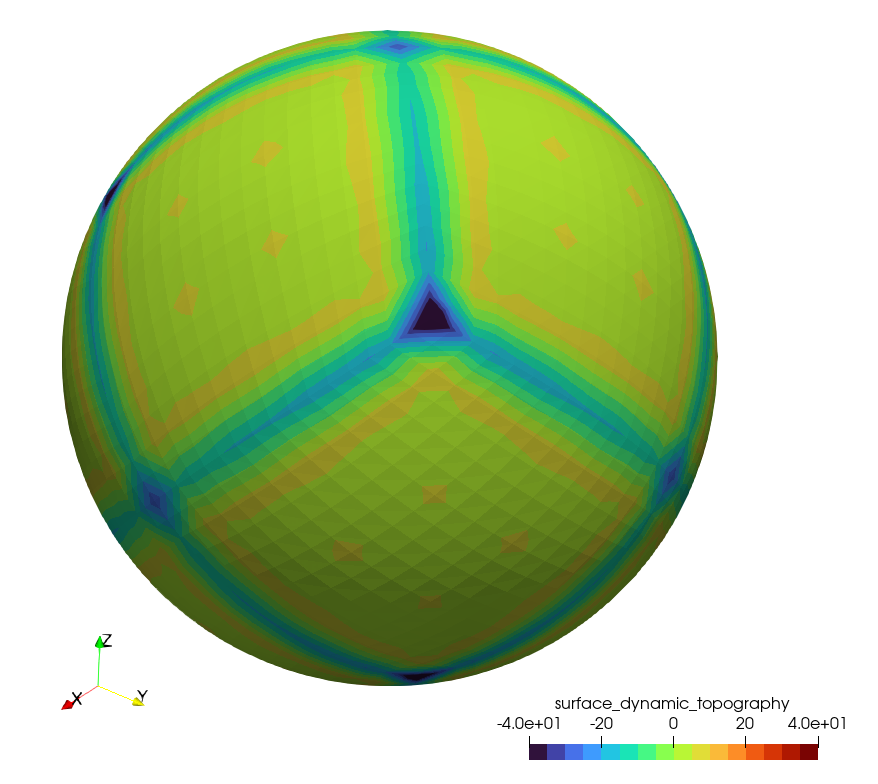
\includegraphics[width=5cm]{images/dyntopo/dyntopo.jpg}\\
{\captionfont Taken from \url{http://www.ga.gov.au/news-events/news/latest-news/dynamic-topography-of-australias-margins}}
\end{center}

\begin{small}
\begin{itemize}
\item[\nineteeneightyfive] 
\fullcite{hacr85} 
\item[\nineteeneightyseven] 
\fullcite{repa87} 
\item[\nineteenninetytwo] 
\fullcite{kiha92} 
\item[\nineteenninetythree] 
\fullcite{gurn93} \\
\fullcite{gurn93b}
\item[\nineteenninetyseven] 
\fullcite{pymi97} 
\item[\nineteenninetynine] 
\fullcite{bumo99} 
\item[\twothousand] 
\fullcite{paha00} \\
\fullcite{paha00b} 
\item[\twothousandone] 
\fullcite{pari01} 
\item[\twothousandthree] 
\fullcite{cogu03} 
\item[\twothousandseven] 
\fullcite{stei07} 
\item[\twothousandeight] 
\fullcite{mofm08} 
\item[\twothousandnine] 
\fullcite{cohu09} 
\item[\twothousandten] 
\fullcite{bofb10} \\
\fullcite{brau10} \\
\fullcite{stfh10} \\
\fullcite{shml10} 
\item[\twothousandeleven] 
\fullcite{rapy11} 
\item[\twothousandtwelve] 
\fullcite{shlm12} \\
\fullcite{zhzf12} 
\item[\twothousandthirteen] 
\fullcite{brrs13} \\
\fullcite{flgm13} 
\item[\twothousandfifteen] 
\fullcite{aupm15} \\
\fullcite{kiff15} \\
\fullcite{dali15} 
\item[\twothousandsixteen] 
\fullcite{howa16} \\
\fullcite{gvfb16} \\
\fullcite{yagu16} \\
\fullcite{stei16} \\
\fullcite{cogb16} 
\item[\twothousandseventeen] 
\fullcite{yamm17} \\
\fullcite{aumh17} \\
\fullcite{grrb17} \\
\fullcite{rubh17} \\
\fullcite{sekf17} 
\item[\twothousandeighteen] 
\fullcite{osss18} \\
\fullcite{vibc18} 
\item[\twothousandnineteen] 
\fullcite{deli19}\\
\fullcite{stco19}\\
\fullcite{davk19}\\
\fullcite{bore19}
\item[\twothousandtwenty] 
\fullcite{braf20}\\
\fullcite{kiso20}\\
\fullcite{miac20}
\item[\twothousandtwentyone] 
\fullcite{hoar21}
\item[\twothousandtwentytwo] 
\fullcite{holt22} \\
\fullcite{gurs22}
\item[\twothousandtwentythree] 
\fullcite{ropr23} \\
\fullcite{rich23} \\
\fullcite{tabs23}
\item[\twothousandtwentyfour]
\fullcite{wisa24} \\ 
\fullcite{vibb24} \\ 
\fullcite{cawc24} \\ 
\fullcite{omrp24} \\ 
\fullcite{stsb24} 
\item[\twothousandtwentyfive]
\fullcite{yawz25}
\end{itemize}
\end{small}

See also report/article written by Zhong (2018) \textcite{zhon18}

%------------------------------------------------------------------------------
%------------------------------------------------------------------------------
\section{cratons, cratonic roots}

\begin{small}
\begin{itemize}
\item[\nineteenninetyseven] 
\fullcite{bugm97} 
\item[\nineteenninetynine] 
\fullcite{drdv99} \\
\fullcite{lemo99} 
\item[\twothousand] 
\fullcite{kiri00} \\
\fullcite{lemm00} \\
\fullcite{scth00} 
\item[\twothousandone] 
\fullcite{brsh01} \\
\fullcite{drvc01} 
\item[\twothousandthree] 
\fullcite{lemm03} \\
\fullcite{wemv03} 
\item[\twothousandsix] 
\fullcite{coll06} 
\item[\twothousandeight] 
\fullcite{onlg08} 
\item[\twothousandnine] 
\fullcite{coco09} \\
\fullcite{kekj09} 
\item[\twothousandeleven] 
\fullcite{hube11}  \\
\fullcite{salo11} 
\item[\twothousandtwelve] 
\fullcite{gohg12} \\
\fullcite{gubc12} \\
\fullcite{mibe12} \\
\fullcite{yosh12} \\
\fullcite{pokb12} 
\item[\twothousandthirteen] 
\fullcite{frbm13} \\
\fullcite{gahs13} \\
\fullcite{ligw13} 
\item[\twothousandfourteen] 
\fullcite{gagb14} \\
\fullcite{wavp14} \\
\fullcite{baeg14} \\
\fullcite{comi14} \\
\fullcite{lige14} 
\item[\twothousandfifteen] 
\fullcite{wahz15} \\
\fullcite{wazh15} \\
\fullcite{tarn15} 
\item[\twothousandsixteen] 
\fullcite{wahz16} \\
\fullcite{kobc16} 
\item[\twothousandseventeen] 
\fullcite{liwg17} 
\item[\twothousandeighteen] 
\fullcite{rabw18} \\
\fullcite{bemc18} \\
\fullcite{gomb18} \\
\fullcite{webe18b} \\
\fullcite{wavp18} \\
\fullcite{lili18} \\
\fullcite{pagc19} 
\item[\twothousandtwenty] 
\fullcite{canc20} \\
\fullcite{cels20} \\
\fullcite{pegz20} \\
\fullcite{cofm20} \\
\fullcite{pagh20} 
\item[\twothousandtwentyone] 
\fullcite{becf21} \\ 
\fullcite{pelg21} \\ 
\fullcite{foon21} \\ 
\fullcite{sasa21} 
\item[\twothousandtwentytwo] 
\fullcite{canm22} \\
\fullcite{jarv22} \\ 
\fullcite{wacw22} 
\item[\twothousandtwentythree] 
\fullcite{wacp23} \\
\fullcite{gejb23} \\
\fullcite{pacb23}
\item[\twothousandtwentyfour] 
\fullcite{fuli24} \\
\fullcite{kucp24} \\
\fullcite{recf24} \\
\fullcite{comi24} \\
\fullcite{qicz24}
\end{itemize}
\end{small}

%------------------------------------------------------------------------------
%------------------------------------------------------------------------------
\section{Lithospheric stress, intra-plate stress, intra-plate deformation}
%------------------------------------------------------------------------------
%------------------------------------------------------------------------------

\begin{small}
\begin{itemize}
\item[\nineteenseventyfive] 
\fullcite{fouy75}\\
\fullcite{sosr75}
\item[\nineteenseventysix] 
\fullcite{riss76}
\item[\nineteenseventyseven] 
\fullcite{chtu77}
\item[\nineteenseventynine] 
\fullcite{riss79}
\item[\nineteeneightynine] 
\fullcite{boww89}
\item[\nineteenninetyone] 
\fullcite{worg91}
\item[\nineteenninetytwo] 
\fullcite{rich92}\\
\fullcite{wuvr92}\\
\fullcite{zoba92}\\
\fullcite{gowc92}\\
\fullcite{clko92}
\item[\nineteenninetynine] 
\fullcite{bili99}
\item[\twothousandone] 
\fullcite{stsm01}
\item[\twothousandtwo] 
\fullcite{jack02}
\item[\twothousandfour] 
\fullcite{ligu04} \\
\fullcite{buja04}
\item[\twothousandfive] 
\fullcite{timr05}
\item[\twothousandseven] 
\fullcite{hert07}
\item[\twothousandeight] 
\fullcite{bilr08}\\
\fullcite{ghhw08}\\
\fullcite{netv08}
\item[\twothousandnine] 
\fullcite{ghhf09}\\
\fullcite{nacl09}\\
\fullcite{kalb09}
\item[\twothousandten] 
\fullcite{bepo10}\\
\fullcite{yosh10}
\item[\twothousandtwelve] 
\fullcite{nalr12}\\
\fullcite{ghho12}\\
\fullcite{wagw12}
\item[\twothousandthirteen] 
\fullcite{ghhw13}
\item[\twothousandfourteen] 
\fullcite{vagw14}
\item[\twothousandseventeen] 
\fullcite{grrb17}
\item[\twothousandeighteen] 
\fullcite{osss18}\\
\fullcite{magu18}
\item[\twothousandnineteen] 
\fullcite{tamg19}
\item[\twothousandtwentyone]
\fullcite{poyd21} 
\end{itemize}
\end{small}


%--------------------------------------------------------------------
%------------------------------------------------------------------------------
\section{passive margins} 
%--------------------------------------------------------------------
%------------------------------------------------------------------------------

\begin{small}
\begin{itemize}
\item[\nineteeneightytwo] 
\fullcite{clwv82} 
\item[\nineteeneightysix] 
\fullcite{lies86} 
\item[\twothousandfive] 
\fullcite{gebi05} 
\item[\twothousandeight] 
\fullcite{clbz08} \\
\fullcite{kasb08} 
\item[\twothousandten] 
\fullcite{fasm10} \\
\fullcite{nigm10} 
\item[\twothousandeleven] 
\fullcite{rapy11} \\
\fullcite{nigm11} \\
\fullcite{brfo11} 
\item[\twothousandthirteen] 
\fullcite{mana13} \\
\fullcite{yahb13} 
\item[\twothousandfourteen] 
\fullcite{macg14} 
\item[\twothousandfifteen] 
\fullcite{gebw15} \\
\fullcite{nigo15} 
\item[\twothousandsixteen] 
\fullcite{dupm16} 
\item[\twothousandeighteen] 
\fullcite{sahf18} \\
\fullcite{mube18} \\
\fullcite{tebu18} 
\item[\twothousandnineteen] 
\fullcite{zhli19} 
\item[\twothousandtwentyone] 
\fullcite{auws21} 
\item[\twothousandtwentytwo] 
\fullcite{bagm22}
\end{itemize}
\end{small}

%------------------------------------------------------------------------------
%------------------------------------------------------------------------------
\section{Eclogites} 
%------------------------------------------------------------------------------
%------------------------------------------------------------------------------

\begin{small}
\begin{itemize}
\item[\twothousandone] 
\fullcite{dohe01} 
\item[\twothousandseven] 
\fullcite{hecb07} 
\item[\twothousandnine] 
\fullcite{agyj09} 
\item[\twothousandthirteen] 
\fullcite{arbi13} \\
\fullcite{krcu13} 
\item[\twothousandtwentytwo] 
\fullcite{wakw22}\\ 
\fullcite{yadb22} 
\end{itemize}
\end{small}


%--------------------------------------------------------------------
%------------------------------------------------------------------------------
\section{Folding, buckling} 
%--------------------------------------------------------------------
%------------------------------------------------------------------------------

\begin{small}
\begin{itemize}
\item[\nineteenseventy] 
\fullcite{ramb70} 
\item[\nineteenseventyone] 
\fullcite{ramb71} 
\item[\nineteenseventyeight] 
\fullcite{wilz78} 
\item[\nineteenninetyone] 
\fullcite{flet91}\\ 
\fullcite{wiwh91} 
\item[\nineteenninetythree] 
\fullcite{zhhj93} 
\item[\nineteenninetyfive] 
\fullcite{flet95} 
\item[\nineteenninetysix] 
\fullcite{zhho96} 
\item[\nineteenninetynine] 
\fullcite{nagg99}\\ 
\fullcite{bupo99} \\
\fullcite{scpo99} 
\item[\twothousandone] 
\fullcite{scpo01} \\
\fullcite{scpo01b} 
\item[\twothousandtwo] 
\fullcite{mumh02} 
\item[\twothousandthree] 
\fullcite{ribe03} \\
\fullcite{nagv03} 
\item[\twothousandsix] 
\fullcite{frsc06} 
\item[\twothousandseven] 
\fullcite{risr07} 
\item[\twothousandeight] 
\fullcite{schm08} \\
\fullcite{manc08} \\
\fullcite{scdk08} 
\item[\twothousandnine] 
\fullcite{simp09} 
\item[\twothousandten] 
\fullcite{resb10} 
\item[\twothousandeleven] 
\fullcite{freh11} 
\item[\twothousandtwelve] 
\fullcite{reds12} \\
\fullcite{grsc12} \\
\fullcite{scsc12} 
\item[\twothousandthirteen] 
\fullcite{regc13} 
\item[\twothousandfourteen] 
\fullcite{freh14} \\
\fullcite{frex14} 
\item[\twothousandsixteen] 
\fullcite{frsc16} 
\item[\twothousandtwentyone] 
\fullcite{nafo21} 
\item[\twothousandtwentythree] 
\fullcite{dosk23} 
\end{itemize}
\end{small}

%--------------------------------------------------------------------
%------------------------------------------------------------------------------
\section{geoid}
%--------------------------------------------------------------------
%------------------------------------------------------------------------------

\begin{small}
\begin{itemize}
\item[\nineteeneightyfour] 
\fullcite{davi84} \\
\fullcite{hage84} \\
\fullcite{riff84} \\
\fullcite{riha84} \\
\fullcite{wari84} 
\item[\nineteeneightyfive] 
\fullcite{hacr85}\\ 
\fullcite{chas85} 
\item[\nineteeneightysix] 
\fullcite{davi86} 
\item[\nineteeneightyseven] 
\fullcite{fope87} 
\item[\nineteeneightyeight] 
\fullcite{besz88} \\
\fullcite{fope88} 
\item[\nineteeneightynine] 
\fullcite{rivf89} \\
\fullcite{hari89}
\item[\nineteenninetyone] 
\fullcite{mocf91}
\item[\nineteenninetytwo] 
\fullcite{zhgu92} \\
\fullcite{kiha92} \\
\fullcite{ribe92} 
\item[\nineteenninetythree] 
\fullcite{zhch93} \\
\fullcite{rirl93} 
\item[\nineteenninetyfour] 
\fullcite{kiha94} 
\item[\nineteenninetyfive] 
\fullcite{king95} \\
\fullcite{pape95} \\
\fullcite{mopa95} \\
\fullcite{thmc95} 
\item[\nineteenninetysix]  
\fullcite{mogu96} \\
\fullcite{kafl96} \\
\fullcite{pape96} \\
\fullcite{dofm96} \\
\fullcite{pahf96} 
\item[\nineteenninetyseven] 
\fullcite{wean97a} \\
\fullcite{king97} \\
\fullcite{thri97} 
\item[\nineteenninetyeight] 
\fullcite{cava98} \\
\fullcite{chki98} \\
\fullcite{kike98} 
\item[\twothousand] 
\fullcite{dofl00} \\
\fullcite{kafl00} \\
\fullcite{paha00} 
\item[\twothousandone] 
\fullcite{zhon01} 
\item[\twothousandtwo] 
\fullcite{peso02} 
\item[\twothousandseven] 
\fullcite{kart07} 
\item[\twothousandeight] 
\fullcite{meco08} 
\item[\twothousandnine] 
\fullcite{king09} \\
\fullcite{tocm09} \\
\fullcite{yona09} 
\item[\twothousandten] 
\fullcite{ghbz10}\\
\fullcite{spgs10b}
\item[\twothousandeleven] 
\fullcite{capd11}
\item[\twothousandtwelve] 
\fullcite{hibi12}\\
\fullcite{cabp12}\\
\fullcite{katr12}
\item[\twothousandthirteen] 
\fullcite{shsc13}\\
\fullcite{chus13}
\item[\twothousandfourteen] 
\fullcite{cako14}\\
\fullcite{kaps14}
\item[\twothousandfifteen] 
\fullcite{lizh15}
\item[\twothousandsixteen] 
\fullcite{necg16}
\fullcite{lizh16}
\item[\twothousandseventeen] 
\fullcite{grab17}\\
\fullcite{siag17}
\item[\twothousandeighteen] 
\fullcite{king18}
\item[\twothousandtwentyone]
\fullcite{mazh21b} 
\item[\twothousandtwentytwo]
\fullcite{rojy22}\\
\fullcite{ghpa22}\\
\fullcite{licw22}
\item[\twothousandtwentythree]
\fullcite{stgl23} \\
\fullcite{saaf23} \\
\fullcite{pagh23}
\end{itemize}
\end{small}

%--------------------------------------------------------------------
%------------------------------------------------------------------------------
\section{geothermal Energy} 
%--------------------------------------------------------------------
%------------------------------------------------------------------------------

\begin{small}
\begin{itemize}
\item[\twothousandfifteen]
\fullcite{quxm15} 
\item[\twothousandnineteen]
\fullcite{revf19} 
\end{itemize}
\end{small}

%--------------------------------------------------------------------
%------------------------------------------------------------------------------
\section{grain size (evolution) \& influence on geodynamics}
\label{sec:topics:gsev}
%--------------------------------------------------------------------
%------------------------------------------------------------------------------

\begin{small}
\begin{itemize}
\item[\nineteeneightyfour] 
\fullcite{kara84} 
\item[\nineteenninetysix] 
\fullcite{solo96} 
\item[\nineteenninetyseven] 
\fullcite{kayf97} 
\item[\nineteeneightynine] 
\fullcite{brcp99} 
\item[\twothousandone] 
\fullcite{dets01} \\
\fullcite{solo01} 
\item[\twothousandtwo] 
\fullcite{soet02} 
\item[\twothousandthree] 
\fullcite{hapa03} \\
\fullcite{reyu03} 
\item[\twothousandeight] 
\fullcite{sore08} 
\item[\twothousandnine] 
\fullcite{behe09} 
\item[\twothousandeleven] 
\fullcite{rorb11} 
\item[\twothousandtwelve]
\fullcite{fobl12} 
\item[\twothousandthirteen] 
\fullcite{beri13} 
\item[\twothousandfourteen] 
\fullcite{fobe14} 
\item[\twothousandfifteen] 
\fullcite{thrk15} \\
\fullcite{besr15} \\
\fullcite{tukb15} \\
\fullcite{pevp15} \\
\fullcite{glfa15} 
\item[\twothousandseventeen] 
\fullcite{ceww17} \\
\fullcite{daef17} \\
\fullcite{mube17} \\
\fullcite{fori17} \\
\fullcite{scdu17} 
\item[\twothousandeighteen] 
\fullcite{bemu18} \\
\fullcite{bezb18} \\
\fullcite{mube18} \\
\fullcite{jakk18} \\
\fullcite{fole18} 
\item[\twothousandnineteen] 
\fullcite{mube19} 
\item[\twothousandtwenty] 
\fullcite{mube20} \\
\fullcite{scrt20}\\
\fullcite{sctr20} \\
\fullcite{thsc20} \\
\fullcite{fole20} \\
\fullcite{sctp20} 
\item[\twothousandtwentyone]
\fullcite{mazh21a}  \\ 
\fullcite{fube21} 
\item[\twothousandtwentytwo]
\fullcite{rutb22} 
\item[\twothousandtwentythree]
\fullcite{racs23} 
\item[\twothousandtwentyfour]
\fullcite{pagr24} 
\end{itemize}
\end{small}

%--------------------------------------------------------------------
%------------------------------------------------------------------------------
\section{LLSVP, ULVZ, CMB layer, thermo-chemical piles, D'' layer}
%------------------------------------------------------------------------------
%--------------------------------------------------------------------

\begin{center}
\includegraphics[width=5cm]{images/burk11}\cite{burk11}
\end{center}

\begin{small}
\begin{itemize}
\item[\nineteeneighty]       
\fullcite{yupe80} 
\item[\nineteeneightysix]    
\fullcite{dagu86} 
\item[\nineteeneightyeight]  
\fullcite{hayu88} 
\item[\nineteeneightynine]   
\fullcite{hayu89} 
\item[\nineteenninetyfour]   
\fullcite{ride94} 
\item[\nineteenninetysix]    
\fullcite{boeh96} 
\item[\nineteenninetyseven]  
\fullcite{kell97} 
\item[\nineteenninetyeight]  
\fullcite{tack98b} 
\item[\twothousand]
\fullcite{moke00} 
\item[\twothousandone]       
\fullcite{soga01} 
\item[\twothousandtwo]       
\fullcite{somo02} \\
\fullcite{tagh02} 
\item[\twothousandthree]
\fullcite{zhha03}
\item[\twothousandfour]      
\fullcite{mczh04} \\
\fullcite{nata04} 
\item[\twothousandfive]      
\fullcite{nata05} \\
\fullcite{wyso05} \\
\fullcite{mczh05a} \\
\fullcite{nata05b}
\item[\twothousandsix]       
\fullcite{nata06} 
\item[\twothousandseven]     
\fullcite{heta07}\\
\fullcite{moyu07} \\
\fullcite{pelt07} \\
\fullcite{hibl07} \\
\fullcite{yumc07} 
\item[\twothousandeight]     
\fullcite{gamc08} \\
\fullcite{nata08} \\
\fullcite{stho08} 
\item[\twothousandnine]
\fullcite{bumr09} 
\item[\twothousandten]
\fullcite{stto10} \\
\fullcite{mcgr10} \\
\fullcite{nata10} \\
\fullcite{vady10} \\
\fullcite{toyc10} 
\item[\twothousandeleven]    
\fullcite{bowg11} \\
\fullcite{talz11} \\
\fullcite{vayj11} \\
\fullcite{dekt11} \\
\fullcite{burk11} 
\item[\twothousandtwelve]    
\fullcite{stto12} \\
\fullcite{dagd12} \\
\fullcite{dect12} 
\item[\twothousandthirteen]  
\fullcite{limc13} \\
\fullcite{bogs13a} \\
\fullcite{bogs13b} 
\item[\twothousandfourteen]  
\fullcite{budt14} \\
\fullcite{lidt14} \\
\fullcite{tovd14} 
\item[\twothousandfifteen]   
\fullcite{musd15} \\
\fullcite{hafg15} \\
\fullcite{delt15} \\
\fullcite{wilm15} \\
\fullcite{lidt15} \\
\fullcite{sobd15} \\
\fullcite{dagl15} 
\item[\twothousandsixteen]   
\fullcite{dost16} \\
\fullcite{tosa16} 
\item[\twothousandseventeen] 
\fullcite{hish17} \\
\fullcite{lizh17} \\
\fullcite{limg17} \\
\fullcite{siag17} 
\item[\twothousandeighteen]  
\fullcite{daga18} \\
\fullcite{lizo18} \\
\fullcite{hect18} \\
\fullcite{dert18} 
\item[\twothousandnineteen]  
\fullcite{hebo19} \\
\fullcite{rejv19} \\
\fullcite{mcna19} 
\item[\twothousandtwenty]    
\fullcite{cilw20} \\
\fullcite{szes20} \\
\fullcite{scrt20} \\
\fullcite{daro20} \\
\fullcite{hect20b} 
\item[\twothousandtwentyone]
\fullcite{cafb21} \\
\fullcite{damg21} 
\item[\twothousandtwentytwo] 
\fullcite{limc22} \\
\fullcite{yuli22} \\
\fullcite{flbw22}\\
\fullcite{lalt22}\\
\fullcite{hulz22} 
\item[\twothousandtwentythree] 
\fullcite{hagl23} \\
\fullcite{gudl23} \\
\fullcite{padm23} \\
\fullcite{lizl23}
\item[\twothousandtwentyfour] 
\fullcite{bero24} \\
\fullcite{shml24} \\
\fullcite{liwg24} \\
\fullcite{deba24} \\
\fullcite{roy}
\item[\twothousandtwentyfive] 
\fullcite{padk25} \\
\fullcite{hedg25} \\
\fullcite{rosf25} \\
\fullcite{hugu25}
\end{itemize}
\end{small}

%--------------------------------------------------------------------
%------------------------------------------------------------------------------
\section{magma ocean}
%--------------------------------------------------------------------
%------------------------------------------------------------------------------

\begin{small}
\begin{itemize}
\item[\nineteenninetythree] 
\fullcite{sost93a} \\
\fullcite{sost93b} 
\item[\twothousandtwo] 
\fullcite{elvh02} 
\item[\twothousandsix] 
\fullcite{hosh06}
\item[\twothousandseven] 
\fullcite{solo07} 
\item[\twothousandten] 
\fullcite{devv10} 
\item[\twothousandtwelve] 
\fullcite{ullc12} 
\item[\twothousandthirteen] 
\fullcite{plth13} \\
\fullcite{moha13} 
\item[\twothousandfifteen] 
\fullcite{maha15} 
\item[\twothousandseventeen] 
\fullcite{mats17} \\ 
\fullcite{bori17} 
\item[\twothousandtwenty] 
\fullcite{bobm20} \\
\fullcite{agml20} 
\item[\twothousandtwentythree] 
\fullcite{sasa23} 
\item[\twothousandtwentyfive] 
\fullcite{bobs25} 
\end{itemize}
\end{small}

%------------------------------------------------------------------------------
%------------------------------------------------------------------------------
\section{magmatic arcs, arc volcanism}
%------------------------------------------------------------------------------
%------------------------------------------------------------------------------

\begin{small}
\begin{itemize}
\item[1982] \fullcite{crpi82}
\item[2015] \fullcite{cudd15}
\item[2017] \fullcite{sche17}\\ \fullcite{lewa17}
\item[2025] \fullcite{masg25}
\end{itemize}
\end{small}



%------------------------------------------------------------------------------
%------------------------------------------------------------------------------
\section{magma transport / melting / two-phase flow/ (intra-plate) 
volcanism / lava flow/ continental flood basalt, melt migration}
%------------------------------------------------------------------------------
%------------------------------------------------------------------------------

\begin{small}
\begin{itemize}
\item[\nineteeneightyfour] 
\fullcite{scst84} \\
\fullcite{mcke84} 
\item[\nineteeneightyfive] 
\fullcite{ribe85} \\
\fullcite{ribe85b} 
\item[\nineteeneightysix] 
\fullcite{scst86} \\
\fullcite{ribe86} 
\item[\nineteeneightyseven] 
\fullcite{hayu87} \\
\fullcite{spmc87} \\
\fullcite{rism87} \\
\fullcite{ribe87} 
\item[\nineteeneightyeight] 
\fullcite{scot88} \\
\fullcite{ribe88b} 
\item[\nineteeneightynine]
\fullcite{scst89} 
\item[\nineteenninety] 
\fullcite{hayu90} 
\item[\nineteenninetythree] 
\fullcite{spie93} \\
\fullcite{tast93} 
\item[\nineteenninetyfour] 
\fullcite{jhpp94} \\
\fullcite{sawy94} 
\item[\nineteenninetyfive] 
\fullcite{bisc95} \\
\fullcite{crks95} \\
\fullcite{ahwk95} 
\item[\nineteenninetysix] 
\fullcite{laki96} 
\item[\nineteenninetyeight] 
\fullcite{rabg98} 
\item[\nineteenninetynine] 
\fullcite{devv99} \\
\fullcite{momo99} 
\item[\twothousand] 
\fullcite{elha00} 
\item[\twothousandone] 
\fullcite{bers01} 
\item[\twothousandtwo] 
\fullcite{sobo02} 
\item[\twothousandthree] 
\fullcite{beri03} 
\item[\twothousandfive] 
\fullcite{onml05} \\
\fullcite{likc05} 
\item[\twothousandsix] 
\fullcite{onmm06} 
\item[\twothousandseven] 
\fullcite{srrb07} \\
\fullcite{mohb07} \\
\fullcite{elki07} \\
\fullcite{onlj07} \\
\fullcite{copb07} 
\item[\twothousandeight] 
\fullcite{hets08} \\
\fullcite{hest08} 
\item[\twothousandnine] 
\fullcite{bavi09} 
\item[\twothousandten] 
\fullcite{baiv10} \\
\fullcite{habl10} \\
\fullcite{cows10} \\
\fullcite{dekc10} 
\item[\twothousandeleven] 
\fullcite{baiv11} \\
\fullcite{zhgy11} \\
\fullcite{zhgh11} \\
\fullcite{bics11} \\
\fullcite{mobh11} 
\item[\twothousandtwelve] 
\fullcite{yatd12} \\
\fullcite{kasc12b} \\
\fullcite{ullc12} \\
\fullcite{plsp12} \\
\fullcite{kawe12} 
\item[\twothousandthirteen] 
\fullcite{kemk13} \\
\fullcite{mofm13} \\
\fullcite{plbs13} \\
\fullcite{mowe13} 
\item[\twothousandfourteen] 
\fullcite{kast14} 
\item[\twothousandfifteen] 
\fullcite{tukb15} \\
\fullcite{moba15} \\
\fullcite{rerl15} \\
\fullcite{riag15} \\
\fullcite{rey15} \\
\fullcite{yadm15} 
\item[\twothousandsixteen] 
\fullcite{keka16} \\
\fullcite{vade16} \\
\fullcite{mesj16} \\
\fullcite{dalg16} \\
\fullcite{libz16} \\
\fullcite{rogj16} \\
\fullcite{porb16} 
\item[\twothousandseventeen] 
\fullcite{dilc17} \\
\fullcite{arca17} \\
\fullcite{mova17} \\
\fullcite{mosw17} 
\item[\twothousandeighteen] 
\fullcite{mova18} \\
\fullcite{lorg18} \\
\fullcite{scmo18} \\ 
\fullcite{yaca18} \\ 
\fullcite{pegp18} \\ 
\fullcite{govo18} \\ 
\fullcite{shi_thesis}
\item[\twothousandnineteen] 
\fullcite{dagg19} \\
\fullcite{scmw19} \\
\fullcite{kesu19} \\
\fullcite{cerk19} \\
\fullcite{likk19} \\
\fullcite{jart19b} 
\item[\twothousandtwenty] 
\fullcite{siss20} \\
\fullcite{zhbp20} \\
\fullcite{rubk20} \\
\fullcite{rukb20} \\
\fullcite{cobd20} \\
\fullcite{spkh20} \\ 
\fullcite{spkh20b} \\ 
\fullcite{lerm20} 
\item[\twothousandtwentyone] 
\fullcite{dudm21} \\
\fullcite{damg21} 
\item[\twothousandtwentytwo] 
\fullcite{kajr22} \\
\fullcite{zhlz22} \\
\fullcite{bepp22} \\
\fullcite{vacd22} \\
\fullcite{kilk22} \\
\fullcite{kosl22}
\item[\twothousandtwentythree]
\fullcite{kimk23} \\ 
\fullcite{scmw23} \\ 
\fullcite{xumm23} \\
\fullcite{mahs23} \\
\fullcite{yole23}
\item[\twothousandtwentyfour] 
\fullcite{lumh24} \\
\fullcite{hesc24} \\
\fullcite{lech24} \\
\fullcite{mori24} \\
\fullcite{tibi24} 
\item[2025]
\fullcite{puld25}
\end{itemize}
\end{small}

%--------------------------------------------------------------------
%--------------------------------------------------------------------
\section{magma chambers}
%--------------------------------------------------------------------
%--------------------------------------------------------------------

\begin{small}
\begin{itemize}
\item[\nineteeneightytwo] 
\fullcite{spyk82} 
\item[\nineteeneightyseven] 
\fullcite{hayu87} 
\item[\twothousandfour] 
\fullcite{geys04} 
\item[\twothousandnine] 
\fullcite{vesc09} 
\item[\twothousandtwelve] 
\fullcite{gerb12} \\
\fullcite{gech12} 
\item[\twothousandfourteen] 
\fullcite{cuwi14} 
\item[\twothousandeighteen] 
\fullcite{gehn18} 
\end{itemize}
\end{small}

%--------------------------------------------------------------------
%------------------------------------------------------------------------------
\section{mantle convection/dynamics, whole Earth models, plate interaction}
%--------------------------------------------------------------------
%------------------------------------------------------------------------------

\begin{small}
\begin{itemize}
\item[\nineteensixtyseven] 
\fullcite{tuox67} 
\item[\nineteensixtynine] 
\fullcite{tuox69} 
\item[\nineteenseventyone] 
\fullcite{totu71b} \\
\fullcite{totu71} \\
\fullcite{buwh71} 
\item[\nineteenseventytwo] 
\fullcite{pelt72} \\ 
\fullcite{hstt72} \\ 
\fullcite{sctu72} 
\item[\nineteenseventythree] 
\fullcite{mcrw73} \\ 
\fullcite{rich73b} 
\item[\nineteenseventyfour] 
\fullcite{youn74} \\
\fullcite{tuht74} \\
\fullcite{trol94}\\
\fullcite{mcrw74} 
\item[\nineteenseventyfive] 
\fullcite{hemw75} \\
\fullcite{buss75} 
\item[\nineteenseventysix] 
\fullcite{mcri76} \\
\fullcite{patt76} \\
\fullcite{sath76} 
\item[\nineteenseventyseven] 
\fullcite{yusc77} 
\item[\nineteenseventyeight] 
\fullcite{mahz78} \\
\fullcite{hsui78} \\
\fullcite{haoc78} \\
\fullcite{pamc78} \\
\fullcite{jaco78} \\
\fullcite{rimc78} 
\item[\nineteenseventynine] 
\fullcite{ludt79} \\
\fullcite{buss79} \\
\fullcite{shpe79} \\
\fullcite{phiv79} 
\item[\nineteeneighty] 
\fullcite{olco80} \\
\fullcite{jamc80} \\
\fullcite{scsc80} \\
\fullcite{zess80} \\
\fullcite{daly80} 
\item[\nineteeneightyone] 
\fullcite{yups81} \\
\fullcite{buss81} \\
\fullcite{jasc81} \\
\fullcite{jape81} \\
\fullcite{haoc81} \\
\fullcite{rimc81} \\
\fullcite{cotu81} 
\item[\nineteeneightytwo] 
\fullcite{jape82} \\
\fullcite{jasc82} \\
\fullcite{homc82} \\
\fullcite{buri82} 
\item[\nineteeneightythree] 
\fullcite{hous83} \\
\fullcite{hous83b} \\
\fullcite{chri83} \\
\fullcite{chri83b} \\
\fullcite{mcke83} \\
\fullcite{boss83} \\
\fullcite{zesd83} 
\item[\nineteeneightyfour] 
\fullcite{olyb84} \\
\fullcite{jarv84} \\
\fullcite{haeb84} \\
\fullcite{haeb84b} \\
\fullcite{harp84} \\
\fullcite{davi84} \\
\fullcite{boas84} \\
\fullcite{chri84} \\
\fullcite{chri84b} \\
\fullcite{moca84}\\
\fullcite{flyu84} \\
\fullcite{jarv84} \\
\fullcite{flyu84b} 
\item[\nineteeneightyfive] 
\fullcite{jarv85} \\
\fullcite{baum85} \\
\fullcite{chri85} \\
\fullcite{csra85} \\
\fullcite{scan85} 
\item[\nineteeneightysix] 
\fullcite{davi86} \\
\fullcite{guda86} \\
\fullcite{quys86} \\
\fullcite{jape86} \\
\fullcite{crmc86} 
\item[\nineteeneightyseven] 
\fullcite{yuqh87} \\ 
\fullcite{olso87} \\ 
\fullcite{mija87} \\ 
\fullcite{chri87b} 
\item[\nineteeneightyeight] 
\fullcite{haeb88} \\
\fullcite{glat88} \\
\fullcite{gurn88} \\
\fullcite{viyu88} \\
\fullcite{whit88} \\
\fullcite{davi88} \\
\fullcite{csrr88} \\
\fullcite{elsc88} \\
\fullcite{grpa98} 
\item[\nineteeneightynine] 
\fullcite{weoy89} \\
\fullcite{chyu89} \\
\fullcite{besg89} \\
\fullcite{schm89} \\
\fullcite{sthe89} \\
\fullcite{rivi89} \\
\fullcite{chri89b} \\
\fullcite{jami89} \\
\fullcite{davi89} 
\item[\nineteenninety] 
\fullcite{trab90} \\
\fullcite{gurn90} \\
\fullcite{ketu90} \\
\fullcite{jape90} \\
\fullcite{sope90} 
\item[\nineteenninetyone] 
\fullcite{jarv91} \\
\fullcite{chha91} \\
\fullcite{mawe91} \\
\fullcite{gaot91} \\
\fullcite{vayv91} \\
\fullcite{hayk91} \\
\fullcite{leys91} \\
\fullcite{virf91} \\
\fullcite{mayu91} 
\item[\nineteenninetytwo] 
\fullcite{dari92} \\
\fullcite{besg92} \\
\fullcite{vayv92} \\
\fullcite{chri92} \\
\fullcite{haym92} \\
\fullcite{rien92} \\
\fullcite{hayk92} \\
\fullcite{mayw92} \\
\fullcite{mayu92} 
\item[\nineteenninetythree] 
\fullcite{bayr93} \\
\fullcite{zhch93} \\
\fullcite{jarv93} \\
\fullcite{tack93} \\
\fullcite{carm93} \\
\fullcite{vavy93} \\
\fullcite{tasg93} \\
\fullcite{zhgu93} \\
\fullcite{mamc93} \\
\fullcite{zebi93} \\
\fullcite{vayv93} \\
\fullcite{hayk93} \\
\fullcite{hayu93} \\
\fullcite{hoyb93} \\
\fullcite{hoby93} 
\item[\nineteenninetyfour] 
\fullcite{yurb94} \\
\fullcite{bayu94} \\
\fullcite{haeb94} \\
\fullcite{bucc94} \\
\fullcite{chho94} \\
\fullcite{tasg94} \\
\fullcite{past94} \\
\fullcite{itki94} \\
\fullcite{leka94} \\
\fullcite{sope94} \\
\fullcite{sope94b} \\
\fullcite{jarv94} \\
\fullcite{vaja94} \\
\fullcite{scha94} 
\item[\nineteenninetyfive] 
\fullcite{styu95} \\
\fullcite{bayr95} \\
\fullcite{bayr95b} \\
\fullcite{zhgu95} \\
\fullcite{vayv95} \\
\fullcite{buba95} \\
\fullcite{rasz95} \\
\fullcite{guja95} \\
\fullcite{berc95} \\
\fullcite{puhj95} \\
\fullcite{pujh95} \\
\fullcite{solo95} \\
\fullcite{vayu95} \\
\fullcite{matb95} \\
\fullcite{vayp95} \\
\fullcite{jagv95} \\
\fullcite{jarv95} \\
\fullcite{thmc95} 
\item[\nineteenninetysix] 
\fullcite{laym96} \\
\fullcite{zhyu96} \\
\fullcite{hond96} \\
\fullcite{rytr96a}\\
\fullcite{rytr96b}\\
\fullcite{tack96}\\
\fullcite{trbo96} \\
\fullcite{birg96} \\
\fullcite{burb96} \\
\fullcite{kafo96} \\
\fullcite{guez96} \\
\fullcite{vayu96} \\
\fullcite{rasz96} \\
\fullcite{rasz96b} \\
\fullcite{leka96} \\
\fullcite{iwas96} \\
\fullcite{buri96} \\
\fullcite{schh96} \\
\fullcite{mora96} \\
\fullcite{trha96} 
\item[\nineteenninetyseven] 
\fullcite{deja97} \\
\fullcite{hond97} \\
\fullcite{iwho97} \\
\fullcite{burb97} \\
\fullcite{mole97} \\
\fullcite{somo97} \\
\fullcite{rats97} \\
\fullcite{cicv97} \\
\fullcite{vayu97} \\
\fullcite{laym97} \\
\fullcite{mebr97} \\
\fullcite{csyu97} \\
\fullcite{wahe97} \\
\fullcite{dofc97} 
\item[\nineteenninetyeight] 
\fullcite{ande98} \\
\fullcite{iwho98} \\
\fullcite{devv98} \\
\fullcite{tack98} \\
\fullcite{tack98b} \\
\fullcite{trha98b} \\
\fullcite{trha98} \\
\fullcite{burl98} \\
\fullcite{mokm98} \\
\fullcite{lena98} \\
\fullcite{vayu98} \\
\fullcite{wema98} \\
\fullcite{vaba98} 
\item[\nineteenninetynine] 
\fullcite{resb99} \\
\fullcite{duyr99} \\
\fullcite{vazh99} \\
\fullcite{dava99} \\
\fullcite{tabg99} \\
\fullcite{como99} \\
\fullcite{cicv99} \\
\fullcite{trrj99} \\
\fullcite{loga99} \\
\fullcite{sola99} \\
\fullcite{momo99} 
\item[\twothousand] 
\fullcite{albe00} \\
\fullcite{hayu00} \\
\fullcite{devv00b} \\
\fullcite{tack00} \\
\fullcite{tack00b} \\
\fullcite{tack00c} \\
\fullcite{tack00d} \\
\fullcite{zhzm00} \\
\fullcite{legm00} \\
\fullcite{conr00} \\
\fullcite{somo00} \\
\fullcite{duyu00} \\
\fullcite{duyy00} 
\item[\twothousandone] 
\fullcite{vank01} \\
\fullcite{riyb01} \\
\fullcite{lemo01} \\
\fullcite{vays01} \\
\fullcite{moqu01} \\
\fullcite{zhon01} \\
\fullcite{burm01} \\
\fullcite{dabu01} 
\item[\twothousandtwo] 
\fullcite{tasu02} \\
\fullcite{modm02} \\
\fullcite{tack02} \\
\fullcite{vaya02} \\
\fullcite{vayu02} \\
\fullcite{taxi02} \\
\fullcite{scbh02} \\
\fullcite{strb02} \\
\fullcite{duyr02} \\
\fullcite{hiys02} \\
\fullcite{alva02} 
\item[\twothousandthree] 
\fullcite{hapa03} \\
\fullcite{lemo03} \\
\fullcite{mumc03} \\
\fullcite{fasa03} \\
\fullcite{heta03} \\
\fullcite{sibu03} \\
\fullcite{ogaw03} \\
\fullcite{ogaw03b} \\
\fullcite{kore03} 
\item[\twothousandfour] 
\fullcite{thkl04} \\
\fullcite{vavv04b} \\
\fullcite{xita04b} \\
\fullcite{xita04} \\
\fullcite{nata04b} \\
\fullcite{vayr04} \\
\fullcite{brws04} \\
\fullcite{stsh04} \\
\fullcite{scbh04} \\
\fullcite{wahb04} \\
\fullcite{leda04} \\
\fullcite{leda04b} 
\item[\twothousandfive]
\fullcite{resb05}\\
\fullcite{wahb05} \\
\fullcite{taxn05}\\
\fullcite{bupc05} \\
\fullcite{grlt05} \\
\fullcite{lemj05} \\
\fullcite{kogk05} \\
\fullcite{mczh05b}\\
\fullcite{vary05} \\
\fullcite{nata05} \\
\fullcite{nabu05} \\
\fullcite{chob05} \\
\fullcite{phbu05} \\
\fullcite{hosh05} \\
\fullcite{funk05} 
\item[\twothousandsix] 
\fullcite{soba06} \\
\fullcite{beck06} \\
\fullcite{nake06} \\
\fullcite{losh06} \\
\fullcite{sthh06} \\
\fullcite{yoka06} \\
\fullcite{wahb06} \\
\fullcite{gowh06} 
\item[\twothousandseven] 
\fullcite{ghja07} \\
\fullcite{nake07} \\
\fullcite{mayu07} \\
\fullcite{brva07a} \\
\fullcite{brva07b} \\
\fullcite{grlt07} \\
\fullcite{grlt07b}\\
\fullcite{huda07} \\
\fullcite{tanh07} \\
\fullcite{tagu07} \\
\fullcite{jalo07} \\
\fullcite{galo07} \\
\fullcite{galo07b} \\
\fullcite{nelo07} \\
\fullcite{soba07} 
\item[\twothousandeight] 
\fullcite{ghja08} \\
\fullcite{tack08} \\
\fullcite{tack08b} \\
\fullcite{chhl08} \\
\fullcite{brhv08} \\
\fullcite{deta08} \\
\fullcite{plva08} \\
\fullcite{hole08} \\
\fullcite{vata08} \\
\fullcite{trkr08} \\
\fullcite{shlj08} \\
\fullcite{stha08} \\
\fullcite{yosh08} \\
\fullcite{galg08} 
\item[\twothousandnine] 
\fullcite{wodd09} \\
\fullcite{fobe09} \\
\fullcite{gows09} \\
\fullcite{deta09} \\
\fullcite{onlj09} \\
\fullcite{wazh09} \\
\fullcite{vavv09} \\
\fullcite{brha09} \\
\fullcite{scbs09b} \\
\fullcite{oebm09} \\
\fullcite{fuog09} 
\item[\twothousandten] 
\fullcite{oflo10} \\
\fullcite{bumb10} \\
\fullcite{detn10} \\
\fullcite{yayh10} \\
\fullcite{nata10} \\
\fullcite{hole10} \\
\fullcite{zhzl10} \\
\fullcite{vayb10} \\
\fullcite{brmw10} 
\item[\twothousandeleven] 
\fullcite{yutc11} \\
\fullcite{lowm11} \\
\fullcite{rota11} \\
\fullcite{woda11} \\
\fullcite{lemj11} \\
\fullcite{befa11} \\
\fullcite{pewb11} \\
\fullcite{andl11}
\item[\twothousandtwelve] 
\fullcite{bisa12} \\
\fullcite{cort12b} \\
\fullcite{deyt12} \\
\fullcite{solo12}\\
\fullcite{wele12} 
\item[\twothousandthirteen] 
\fullcite{holj13}\\
\fullcite{dadb13}\\
\fullcite{toyd13}\\
\fullcite{bogs13a} \\
\fullcite{busa13} \\
\fullcite{mika13} \\
\fullcite{fabc13} \\
\fullcite{cosr13} \\
\fullcite{coml13} \\
\fullcite{cost13} \\
\fullcite{stha13} \\
\fullcite{plth13} \\
\fullcite{oflb13} \\
\fullcite{whch13} 
\item[\twothousandfourteen] 
\fullcite{arfw14} \\
\fullcite{helo14} \\
\fullcite{crta14} \\
\fullcite{flgw14} \\
\fullcite{roct14} \\
\fullcite{cort14} \\
\fullcite{becr14} \\
\fullcite{nata14} \\
\fullcite{stha14} \\
\fullcite{stlh14} \\
\fullcite{ogaw14} 
\item[\twothousandfifteen]   
\fullcite{zhru15} \\
\fullcite{wegg15} \\
\fullcite{nata15} \\
\fullcite{bect15} \\
\fullcite{pesw15} \\
\fullcite{plht15} \\
\fullcite{khfh15} 
\item[\twothousandsixteen]   
\fullcite{frbs16}  \\
\fullcite{plhm16} \\
\fullcite{boba16} \\
\fullcite{wele16} \\
\fullcite{welm16} \\
\fullcite{vade16} \\
\fullcite{chah16} \\
\fullcite{woso16b} 
\item[\twothousandseventeen] 
\fullcite{badw17} \\
\fullcite{ghts17} \\
\fullcite{civj17} 
\item[\twothousandeighteen] 
\fullcite{guld18} \\
\fullcite{arcf18} \\
\fullcite{plhw18} \\
\fullcite{wele18} 
\item[\twothousandnineteen] 
\fullcite{gult19} \\
\fullcite{mazh19} \\
\fullcite{cohf19} \\
\fullcite{lewh19} \\
\fullcite{ulcw19} \\
\fullcite{boba19} \\
\fullcite{fube19} \\
\fullcite{plju19} 
\item[\twothousandtwenty] 
\fullcite{lalt20} \\
\fullcite{gugb20} \\
\fullcite{yabt20} \\
\fullcite{yosy20} \\
\fullcite{arcf20} \\
\fullcite{babd20} \\
\fullcite{lorb20} \\
\fullcite{loru20} 
\item[\twothousandtwentyone] 
\fullcite{lalt21} \\
\fullcite{naka21} \\
\fullcite{khmo21} 
\item[\twothousandtwentytwo] 
\fullcite{lids22} \\ 
\fullcite{pade22} \\ 
\fullcite{fube22} 
\item[\twothousandtwentythree] 
\fullcite{befu23} \\ 
\fullcite{yosh23} 
\item[\twothousandtwentyfour] 
\fullcite{vavt24} \\ 
\fullcite{jalt24} \\ 
\fullcite{xihw24} \\ 
\fullcite{lobb24} 
\end{itemize}
\end{small}

%--------------------------------------------------------------------
%------------------------------------------------------------------------------
\section{mantle convection + continental growth}
%------------------------------------------------------------------------------
%--------------------------------------------------------------------

\begin{small}
\begin{itemize}
\item[1997]
\fullcite{wahe97b}
\item[1999]
\fullcite{wahe99}
\item[2007]
\fullcite{wahb07}
\item[2008]
\fullcite{wahe08} \\
\fullcite{wahb08}
\item[2009]
\fullcite{wahk09} \\
\fullcite{wahe09}
\item[2013]
\fullcite{wahe13} \\
\fullcite{wahe13b}
\item[2017]
\fullcite{wahe17}
\end{itemize}
\end{small}

%--------------------------------------------------------------------
%------------------------------------------------------------------------------
\section{mantle rheology, phase transitions, stratification, (temperature) profile}
%------------------------------------------------------------------------------
%--------------------------------------------------------------------

\begin{small}
\begin{itemize}
\item[1923] 
\fullcite{wiad23} 
\item[1952] 
\fullcite{birc52} 
\item[\nineteenseventyone] 
\fullcite{sctu71}\\ 
\fullcite{tusc71} 
\item[\nineteenseventysix] 
\fullcite{ocon76} 
\item[\nineteenseventyseven] 
\fullcite{stac77}
\item[\nineteeneightytwo] 
\fullcite{yusb82}\\
\fullcite{chri82}
\item[\nineteeneightyfive] 
\fullcite{chyu85}
\item[\nineteeneightysix] 
\fullcite{yuen86} 
\item[\nineteeneightynine] 
\fullcite{itka89} 
\item[\nineteenninetyone] 
\fullcite{fopd91} \\ 
\fullcite{mawe91}
\item[\nineteenninetytwo] 
\fullcite{zhyh92} \\
\fullcite{zhyh92}
\item[\nineteenninetythree] 
\fullcite{tasg93} \\
\fullcite{best93} \\
\fullcite{kief93} \\
\fullcite{styz93} \\
\fullcite{yucc93} \\
\fullcite{hoby93} \\
\fullcite{dayu93} 
\item[\nineteenninetyfour] 
\fullcite{cays94}\\
\fullcite{vayv94}\\
\fullcite{zhgu94b}\\
\fullcite{styu94}\\
\fullcite{sope94}\\
\fullcite{popy94}
\item[\nineteenninetyfive] 
\fullcite{kiit95}\\
\fullcite{zhyu95} \\
\fullcite{chri95}\\
\fullcite{scta95}\\
\fullcite{tack95}
\item[\nineteenninetysix] 
\fullcite{pelt96}\\
\fullcite{mitr96}\\
\fullcite{tack96b}
\item[\nineteenninetyseven] 
\fullcite{mifo97}\\
\fullcite{cica97}\\
\fullcite{pebs97}
\item[\nineteenninetyeight] 
\fullcite{cava98}\\
\fullcite{kenn98}
\item[\nineteenninetynine] 
\fullcite{sigh99} \\
\fullcite{kehv99} \\
\fullcite{vaka99} \\
\fullcite{beko99} 
\item[\twothousandone] 
\fullcite{roma01} \\
\fullcite{dest01} 
\item[\twothousandthree] 
\fullcite{beka03} \\
\fullcite{roma03} 
\item[\twothousandfive] 
\fullcite{hett05}\\
\fullcite{nata05b}\\
\fullcite{nabu05}\\
\fullcite{stli05}\\
\fullcite{stli05b}
\item[\twothousandsix] 
\fullcite{javd06}\\
\fullcite{stca06}
\item[\twothousandseven]
\fullcite{stei07} \\
\fullcite{pazw07} \\
\fullcite{mofm07} \\
\fullcite{tanh07} \\
\fullcite{stli07} \\
\fullcite{lioh07} \\
\fullcite{jade07} \\
\fullcite{pisb07} \\
\fullcite{kart07} 
\item[\twothousandnine]  
\fullcite{natd09} \\
\fullcite{conn09} 
\item[\twothousandten]   
\fullcite{mohy10} \\ 
\fullcite{kayy10} 
\item[\twothousandeleven] 
\fullcite{mayw11} \\
\fullcite{java11} \\
\fullcite{faff11} \\
\fullcite{catb11} \\
\fullcite{nata11} \\
\fullcite{vayj11} \\
\fullcite{stli11} 
\item[\twothousandtwelve] 
\fullcite{tack12}\\
\fullcite{sato12}\\
\fullcite{simj12} \\
\fullcite{natd12} \\
\fullcite{stli12} 
\item[\twothousandthirteen] 
\fullcite{fakc13}\\
\fullcite{taab13} \\
\fullcite{jasv13}
\item[\twothousandfifteen] 
\fullcite{basn15}\\
\fullcite{glfa15}\\
\fullcite{amsb15}\\
\fullcite{soyu15}\\
\fullcite{wahg15} 
\item[\twothousandsixteen] 
\fullcite{tiro16}\\
\fullcite{beci16}
\item[\twothousandseventeen] 
\fullcite{jasv17} \\
\fullcite{bahh17} \\
\fullcite{shyp17} \\
\fullcite{shpj17} \\
\fullcite{balh17} 
\item[\twothousandeighteen] 
\fullcite{vavs18} \\
\fullcite{mazh18}\\
\fullcite{naoi18}\\
\fullcite{roct18}
\item[\twothousandnineteen] 
\fullcite{jasv19} \\
\fullcite{wahg19} \\
\fullcite{sism19} 
\item[\twothousandtwenty] 
\fullcite{hohv20} \\
\fullcite{lufs20} \\
\fullcite{wali20} \\
\fullcite{ruml20} 
\item[\twothousandtwentyone] 
\fullcite{pocv21} \\
\fullcite{vepn21} \\
\fullcite{adkc21} \\
\fullcite{gath21} \\
\fullcite{ligl21b} \\
\fullcite{mazh21b} \\ 
\fullcite{gubt21} \\
\fullcite{josv21} 
\item[\twothousandtwentytwo] 
\fullcite{rikg22} \\ 
\fullcite{dagl22} \\ 
\fullcite{stli22} 
\item[\twothousandtwentythree] 
\fullcite{speg23} \\ 
\fullcite{mych23} 
\end{itemize}
\end{small}


%--------------------------------------------------------------------
%------------------------------------------------------------------------------
\section{mantle wedge, subduction zone (temperature)} 
%------------------------------------------------------------------------------
%--------------------------------------------------------------------

\begin{small}
\begin{itemize}
\item[\nineteensixtynine] 
\fullcite{mcke69} 
\item[\nineteenseventyone] 
\fullcite{tomj71} 
\item[\nineteenseventythree] 
\fullcite{toss73} 
\item[\nineteenseventyfive] 
\fullcite{bits75} 
\item[\nineteenseventyseven] 
\fullcite{tobi77} 
\item[\nineteenseventyeight] 
\fullcite{tosl78} 
\item[\nineteenseventynine] 
\fullcite{bobo79} 
\item[\nineteeneightyfive] 
\fullcite{hond85} 
\item[\nineteenninetytwo] 
\fullcite{dast92} 
\item[\nineteenninetythree] 
\fullcite{furu93} 
\item[\nineteenninetynine] 
\fullcite{pewa99} 
\item[\twothousandone] 
\fullcite{bigu01} \\
\fullcite{haki01} 
\item[\twothousandtwo]
\fullcite{vakp02} 
\item[\twothousandthree]
\fullcite{vank03} 
\item[\twothousandfour]
\fullcite{enwi04} \\
\fullcite{cuwh04} 
\item[\twothousandsix] 
\fullcite{abvk06} \\
\fullcite{gogc06} \\
\fullcite{gecy06} \\
\fullcite{syab06} \\
\fullcite{lafh06} 
\item[\twothousandseven] 
\fullcite{gogc07} \\
\fullcite{knvk07} \\
\fullcite{lohd07} 
\item[\twothousandeight]
\fullcite{knva08} \\
\fullcite{cage08} \\
\fullcite{vack08} \\
\fullcite{wawh08} 
\item[\twothousandnine] 
\fullcite{leki09} \\
\fullcite{heaa09} \\
\fullcite{wawa09} 
\item[\twothousandten]
\fullcite{roms10} \\
\fullcite{hogz10} 
\item[\twothousandeleven] 
\fullcite{zhgh11} \\
\fullcite{moho11} \\
\fullcite{wiko12}  
\item[\twothousandfourteen]
\fullcite{ledg14} \\
\fullcite{mabv14} 
\item[\twothousandfourteen]
\fullcite{wahh15} 
\item[\twothousandsixteen]
\fullcite{dalg16} \\ 
\fullcite{pegp16} 
\item[\twothousandseventeen]
\fullcite{rerm17} \\
\fullcite{mova17}
\item[\twothousandeighteen]
\fullcite{pltv18} \\ 
\fullcite{pegp18} 
\item[\twothousandtwentyone]
\fullcite{wada21} 
\item[\twothousandtwentytwo]
\fullcite{reps22} 
\item[\twothousandtwentythree]
\fullcite{izhy23} \\
\fullcite{vatc23} \\ 
\fullcite{yole23}
\item[\twothousandtwentyfour]
\fullcite{epcs24} \\
\fullcite{pebo24} 
\end{itemize}
\end{small}

\newpage
%--------------------------------------------------------------------
%------------------------------------------------------------------------------
\section{mixing, stirring, degassing, outgassing, Lyapunov exponent, volatiles } 
%------------------------------------------------------------------------------
%--------------------------------------------------------------------

\begin{small}
\begin{itemize}
\item[\nineteeneightytwo] 
\fullcite{ridn82} 
\item[\nineteeneightyfour] 
\fullcite{olyb84} \\ 
\fullcite{olyb84b} 
\item[\nineteeneightyfive] 
\fullcite{homc85} 
\item[\nineteeneightysix] 
\fullcite{altu86} \\ 
\fullcite{gurn86} \\ 
\fullcite{guda86b} \\
\fullcite{guda86c}
\item[\nineteeneightyeight] 
\fullcite{otlr88} 
\item[\nineteeneightynine] 
\fullcite{chri89} 
\item[\nineteenninety] 
\fullcite{ketu90} \\
\fullcite{davi90} 
\item[\nineteenninetyone] 
\fullcite{pier91} \\
\fullcite{kest91}
\item[\nineteenninetytwo] 
\fullcite{hayk92}
\item[\nineteenninetythree]
\fullcite{kell93} 
\item[\nineteenninetyfour]
\fullcite{scha94}
\item[\nineteenninetyfive] 
\fullcite{mebo95} \\
\fullcite{frbo95}
\item[\nineteenninetysix] 
\fullcite{pelt96}\\ 
\fullcite{teyl96}\\ 
\fullcite{mang96} 
\item[\nineteenninetyseven]
\fullcite{teyp97} \\
\fullcite{frbo97} 
\item[\nineteenninetyeight]
\fullcite{tepy98} \\
\fullcite{vaba98} 
\item[\nineteenninetynine] 
\fullcite{vazh99} \\
\fullcite{cori99} 
\item[\twothousandone] 
\fullcite{huke01} 
\item[\twothousandtwo] 
\fullcite{vahb02} \\
\fullcite{falt02}
\item[\twothousandthree] 
\fullcite{fasa03} \\
\fullcite{vabh03} 
\item[\twothousandfive] 
\fullcite{colt05} 
\item[\twothousandsix] 
\fullcite{gowh06}\\ 
\fullcite{cosc06} 
\item[\twothousandseven] 
\fullcite{gogc07} \\
\fullcite{nake07} \\
\fullcite{huda07b} \\
\fullcite{vabh07} 
\item[\twothousandten] 
\fullcite{mang10}
\item[\twothousandeleven] 
\fullcite{lemj11} \\
\fullcite{saad11} 
\item[\twothousandthirteen]
\fullcite{onlh13}
\item[\twothousandfifteen] 
\fullcite{pedp15}
\item[\twothousandeighteen] 
\fullcite{bipe18} \\
\fullcite{onzh18} 
\item[\twothousandtwentytwo] 
\fullcite{onau22} 
\item[\twothousandtwentyfour] 
\fullcite{vatv24} \\ 
\fullcite{lamt24} \\ 
\fullcite{thsf24} 
\end{itemize}
\end{small}


\newpage
%--------------------------------------------------------------------
%------------------------------------------------------------------------------
\section{mantle reservoirs, magma reservoirs}
%------------------------------------------------------------------------------
%--------------------------------------------------------------------

\begin{small}
\begin{itemize}
\item[\nineteeneightythree] 
\fullcite{mcon83}
\item[\nineteeneightyfive] 
\fullcite{homc85}
\item[\nineteeneightysix] 
\fullcite{guda86b}
\item[\nineteenninetynine] 
\fullcite{wahe99}
\item[\twothousandtwo] 
\fullcite{cori02}
\item[\twothousandfive] 
\fullcite{vavv05b}
\item[\twothousandeight]
\fullcite{wahb08}
\item[\twothousandnine] 
\fullcite{vavv09}
\item[\twothousandten] 
\fullcite{mcgr10}
\item[\twothousandeleven] 
\fullcite{wahe11}
\item[\twothousandfourteen] 
\fullcite{limg14} \\
\fullcite{lidt14}
\item[\twothousandfifteen] 
\fullcite{lidt15}
\item[\twothousandseventeen] 
\fullcite{fori17}
\item[\twothousandtwenty] 
\fullcite{pact20}
\item[\twothousandtwentytwo] 
\fullcite{lids22} \\
\fullcite{patc22}
\item[\twothousandtwentythree] 
\fullcite{gudl23}
\end{itemize}
\end{small}


\newpage
%--------------------------------------------------------------------
%--------------------------------------------------------------------
\section{micro-continents}
%--------------------------------------------------------------------
%--------------------------------------------------------------------

\begin{small}
\begin{itemize}
\item[2019] \fullcite{kobg19}
\item[2020] \fullcite{vaga20}
\item[2021] \fullcite{gupg21}
\item[2024] \fullcite{qilb24}
\item[2025] \fullcite{erbt25}
\end{itemize}
\end{small}


\newpage
%--------------------------------------------------------------------
%------------------------------------------------------------------------------
\section{Obduction, ophiolites}
%------------------------------------------------------------------------------
%--------------------------------------------------------------------

\begin{small}
\begin{itemize}
\item[\nineteenninety] 
\fullcite{hack90} 
\item[\nineteenninetyone] 
\fullcite{hack91} 
\item[\nineteenninetyseven] 
\fullcite{rabh97} 
\item[\twothousand] 
\fullcite{mokd00} 
\item[\twothousandfourteen] 
\fullcite{agzf14} 
\item[\twothousandsixteen] 
\fullcite{duay16} 
\item[\twothousandtwenty] 
\fullcite{rohb20} 
\item[\twothousandtwentyone] 
\fullcite{pody21} 
\item[\twothousandtwentytwo] 
\fullcite{zhli22} 
\end{itemize}
\end{small}

%--------------------------------------------------------------------
%--------------------------------------------------------------------
\section{oceanic Lithosphere}
%--------------------------------------------------------------------
%--------------------------------------------------------------------

\begin{small}
\begin{itemize}
\item[\nineteenseventysix] 
\fullcite{scfy76} 
\item[\nineteenseventyseven] 
\fullcite{debr77} 
\item[\nineteeneightythree] 
\fullcite{cobe83} 
\item[\nineteeneightyfour] 
\fullcite{yufl84} 
\item[\nineteeneightyeight] 
\fullcite{mofo88} 
\item[\nineteenninety] 
\fullcite{ogaw90} 
\item[\twothousand] 
\fullcite{tesc00} 
\item[\twothousandone] 
\fullcite{kasc01} 
\item[\nineteeneightyfour] 
\fullcite{flyu84} 
\item[\nineteenninetyeight] 
\fullcite{bupo98}
\item[\twothousandfive] 
\fullcite{huzh05}
\item[\twothousandseven] 
\fullcite{afrf07} \\
\fullcite{kore07} \\
\fullcite{macl07} 
\item[\twothousandeight] 
\fullcite{chgu08} \\
\fullcite{zlad08}
\item[\twothousandtwelve] 
\fullcite{trub12} 
\item[\twothousandsixteen]  
\fullcite{koko16} 
\item[\twothousandeighteen] 
\fullcite{rihc18} 
\end{itemize}
\end{small}

%--------------------------------------------------------------------
%--------------------------------------------------------------------
\section{ocean floor, seafloor}
%--------------------------------------------------------------------
%--------------------------------------------------------------------

\begin{small}
\begin{itemize}
\item[1977]
\fullcite{pasc77}
\item[1980] 
\fullcite{jape80}
\item[1981]
\fullcite{jape81}
\item[2003]
\fullcite{covb03}
\item[2008]
\fullcite{afzf08}
\item[2012]
\fullcite{cort12b}
\item[2014]
\item[2015]
\fullcite{olbi15}
\fullcite{lige15}
\end{itemize}
\end{small}


%--------------------------------------------------------------------
%--------------------------------------------------------------------
\section{onset of convection}
%--------------------------------------------------------------------
%--------------------------------------------------------------------

\begin{small}
\begin{itemize}
\item[\nineteensixtynine]
\fullcite{scto69} 
\item[\nineteeneightytwo] 
\fullcite{homc82} 
\item[\nineteenninety] 
\fullcite{sope90} 
\item[\twothousand] 
\fullcite{scth00} 
\item[\twothousandsix] 
\fullcite{soba06} 
\item[\twothousandtwo] 
\fullcite{kojo02} 
\item[\twothousandtwo] 
\fullcite{kojo03} 
\item[\twothousandseven] 
\fullcite{soba07} 
\item[\twothousandfifteen] 
\fullcite{kamo15} 
\end{itemize}
\end{small}

%--------------------------------------------------------------------
%------------------------------------------------------------------------------
\section{plate motion and mantle, plate tectonic reconstruction, mechanism}
%------------------------------------------------------------------------------
%--------------------------------------------------------------------

\begin{small}
\begin{itemize}
\item[\nineteensixtysix] 
\fullcite{wils66}
\item[\nineteensixtyseven] 
\fullcite{mcpa67}
\item[\nineteensixtyeight] 
\fullcite{isos68} 
\item[\nineteenseventythree] 
\fullcite{mcse73}
\item[\nineteenseventyfour] 
\fullcite{sosl74}
\item[\nineteenseventyfive] 
\fullcite{harp75} \\
\fullcite{turc75}
\item[\nineteenninety] 
\fullcite{dega90}
\item[\nineteenninetyone] 
\fullcite{virf91}
\item[\nineteenninetytwo] 
\fullcite{zieg92a} \\
\fullcite{gost92}
\item[\nineteenninetyfour] 
\fullcite{guto94}
\item[\nineteenninetyseven] 
\fullcite{wean97b}
\item[\nineteenninetyeight] 
\fullcite{zhgm98} \\ 
\fullcite{liri98}
\item[\nineteenninetynine] 
\fullcite{ribr99}
\item[\twothousandone] 
\fullcite{yohk01}
\item[\twothousandtwo] 
\fullcite{stoc02}
\item[\twothousandthree] 
\fullcite{evan03} \\
\fullcite{reta03}
\item[\twothousandseven] 
\fullcite{zhzl07}
\item[\twothousandnine] 
\fullcite{lizh09} \\
\fullcite{vasv09} \\
\fullcite{iabu09} \\
\fullcite{scbs09}
\item[\twothousandten] 
\fullcite{stto10} \\
\fullcite{dega10}
\item[\twothousandtwelve] 
\fullcite{huss12} \\
\fullcite{gutz12} \\
\fullcite{qumm12} \\
\fullcite{holr12} \\
\fullcite{dost12} \\
\fullcite{shbs12}
\item[\twothousandthirteen] 
\fullcite{mosq13} \\
\fullcite{cost13} 
\item[\twothousandfourteen] 
\fullcite{ruzh14} 
\item[\twothousandfifteen] 
\fullcite{yoha15}
\item[\twothousandsixteen] 
\fullcite{pric16}
\item[\twothousandseventeen] 
\fullcite{stid17}
\item[\twothousandnineteen] 
\fullcite{tewg19} \\
\fullcite{weco19} \\ 
\fullcite{flam19} 
\item[\twothousandtwenty]
\fullcite{sele20} \\
\item[\twothousandtwentyone]
\fullcite{cafm21} \\
\fullcite{atco21}
\item[\twothousandtwentyfour]
\fullcite{wefl24} 
\end{itemize}
\end{small}



%--------------------------------------------------------------------
%------------------------------------------------------------------------------
\section{plume dynamics \& shape}
%------------------------------------------------------------------------------
%--------------------------------------------------------------------

\begin{small}
\begin{itemize}
\item[\nineteenseventyone] 
\fullcite{morg71} 
\item[\nineteenseventythree] 
\fullcite{toze73} 
\item[\nineteenseventyfive] 
\fullcite{patt75} 
\item[\nineteenseventyseven] 
\fullcite{hovo77}
\item[\nineteeneighty] 
\fullcite{yupe80} 
\item[\nineteeneightyseven] 
\fullcite{zhyu87} \\
\fullcite{olsa87} \\
\fullcite{rism87} 
\item[\nineteeneightyeight] 
\fullcite{olsa88} \\
\fullcite{rigr88}
\item[\nineteeneightynine] 
\fullcite{jami89} \\
\fullcite{scoa89}
\item[\nineteenninety] 
\fullcite{davi90}
\item[\nineteenninetyone] 
\fullcite{kell91}\\
\fullcite{grca91b}
\item[\nineteenninety] 
\fullcite{grca90}
\item[\nineteenninetythree] 
\fullcite{keki93}\\
\fullcite{olsa93}\\
\fullcite{mayu93}
\item[\nineteenninetyfour] 
\fullcite{nasf94}\\
\fullcite{fari94}\\
\fullcite{leka94b}\\
\fullcite{hayu94}\\
\fullcite{mamy94}
\item[\nineteenninetyfive] 
\fullcite{fari95} \\
\fullcite{scag95}
\item[\nineteenninetysix] 
\fullcite{lesy96} 
\item[\nineteenninetyseven] 
\fullcite{vank97} \\
\fullcite{keki97}\\
\fullcite{laym97} \\
\fullcite{layu97}\\
\fullcite{layu97b}\\
\fullcite{mang97} \\
\fullcite{king97} 
\item[\nineteenninetyeight] 
\fullcite{thta98} \\ 
\fullcite{stoc98}
\item[\nineteenninetynine] 
\fullcite{lays99} \\
\fullcite{wuda99}
\item[\twothousand] 
\fullcite{csyu00}\\
\fullcite{bryu00}
\item[\twothousandone] 
\fullcite{lirc01}
\item[\twothousandtwo] 
\fullcite{falt02} \\
\fullcite{dagl02} \\
\fullcite{nitg02} \\
\fullcite{labr02} \\
\fullcite{tagh02}
\item[\twothousandthree] 
\fullcite{safa03}
\item[\twothousandfour] 
\fullcite{goch04}\\ 
\fullcite{scmo04}\\
\fullcite{lokg04}\\
\fullcite{keso04} 
\item[\twothousandfive] 
\fullcite{tagu05}\\ 
\fullcite{bung05}\\
\fullcite{zhon05}\\
\fullcite{liva05}\\
\fullcite{mayu05}
\item[\twothousandsix] 
\fullcite{isst06}\\
\fullcite{liva06a}\\
\fullcite{liva06b}\\
\fullcite{zhon06}\\ 
\fullcite{mita06}\\
\fullcite{nokm06} \\
\fullcite{qufo06} \\
\fullcite{keso06} \\
\fullcite{cada06}
\item[\twothousandseven] 
\fullcite{yumh07}\\
\fullcite{ogaw07}
\item[\twothousandeight] 
\fullcite{logg08} \\ 
\fullcite{lezh08b} 
\item[\twothousandnine] 
\fullcite{vavl09}\\
\fullcite{bogj09}\\
\fullcite{faho09}\\
\fullcite{scbs09b}\\
\fullcite{lezh09}
\item[\twothousandeleven] 
\fullcite{toyu11}\\
\fullcite{talz11}\\
\fullcite{burk11}\\
\fullcite{memm11}\\
\fullcite{dalt11}\\
\fullcite{tree11}
\item[\twothousandtwelve] 
\fullcite{viym12} 
\fullcite{legu12} 
\item[\twothousandthirteen] 
\fullcite{dagm13} \\
\fullcite{madd13} \\
\fullcite{ande13} \\
\fullcite{vadv13} \\
\fullcite{bova13} \\
\fullcite{dusm13} 
\item[\twothousandfourteen] 
\fullcite{glfo14} 
\item[\twothousandfifteen] 
\fullcite{daso15} \\
\fullcite{hafg15} \\
\fullcite{canl15} \\
\fullcite{sule15} \\
\fullcite{hels15}
\item[\twothousandsixteen] 
\fullcite{kili16}\\
\fullcite{jodc16}\\
\fullcite{shpy16}\\
\fullcite{dannbergphd}
\item[\twothousandseventeen] 
\fullcite{moyu17} \\
\fullcite{lizh17} 
\item[\twothousandeighteen] 
\fullcite{dacc18} \\
\fullcite{trev18} \\
\fullcite{zhli18} \\
\fullcite{moyu18} 
\item[\twothousandnineteen] 
\fullcite{argc19} \\
\fullcite{lizh19} 
\item[\twothousandtwenty] 
\fullcite{gugm20} \\
\fullcite{rits20} \\
\fullcite{hect20b} 
\item[\twothousandtwentyone] 
\fullcite{xiwk21} \\ 
\fullcite{levp21} 
\item[\twothousandtwentytwo] 
\fullcite{gugt22} 
\item[\twothousandtwentythree] 
\fullcite{li__23} \\
\fullcite{leli23} \\ 
\fullcite{nemi23} \\ 
\fullcite{lilw23} 
\item[\twothousandtwentyfour]
\fullcite{farn24} \\
\fullcite{roy}
\item[\twothousandtwentyfive]
\fullcite{hedg25}
\end{itemize}
\end{small}

%------------------------------------------------------------------------------
%------------------------------------------------------------------------------
\section{plume-lithosphere interaction, LIP, hotspots}
%------------------------------------------------------------------------------
%------------------------------------------------------------------------------

\begin{small}
\begin{itemize}
\item[1988]
\fullcite{olsa88}
\item[\nineteenninety] 
\fullcite{davi90} \\ 
\fullcite{hous90b} 
\item[\nineteenninetyone] 
\fullcite{grca91} 
\item[\nineteenninetytwo] 
\fullcite{hicd92} \\
\fullcite{cagr92} \\
\fullcite{sask92} 
\item[\nineteenninetyfour] 
\fullcite{rich94} \\
\fullcite{fari94} \\
\fullcite{ride94} \\
\fullcite{davi94} 
\item[\nineteenninetyfive] 
\fullcite{whmc95} \\
\fullcite{fari95} \\
\fullcite{rict95} 
\item[\nineteenninetysix] 
\fullcite{zhgm96} \\
\fullcite{ribe96} 
\item[\nineteenninetyeight] 
\fullcite{most98} \\
\fullcite{ride98} 
\item[\nineteenninetynine] 
\fullcite{most99} \\
\fullcite{shet99} \\
\fullcite{bisp99} 
\item[\twothousand] 
\fullcite{lors00} 
\item[\twothousandone] 
\fullcite{vapy01}
\item[\twothousandtwo] 
\fullcite{foul02} \\
\fullcite{labr02}
\item[\twothousandthree] 
\fullcite{vazh03} \\
\fullcite{gacs03} \\
\fullcite{codb03} 
\item[\twothousandfour] 
\fullcite{yoog04} 
\item[\twothousandfive] 
\fullcite{bugu05} \\
\fullcite{fasa05} \\
\fullcite{yoog05} \\
\fullcite{camp05} \\
\fullcite{likc05} 
\item[\twothousandsix] 
\fullcite{dabu06}\\ 
\fullcite{thtd06} 
\item[\twothousandseven] 
\fullcite{stco07} 
\item[\twothousandeight] 
\fullcite{uegs08} \\
\fullcite{slee08} 
\item[\twothousandnine] 
\fullcite{bucl09} \\
\fullcite{zhgy09} \\
\fullcite{baiv10} \\
\fullcite{tabs09} \\
\fullcite{maml09} \\
\fullcite{dada09} 
\item[\twothousandten] 
\fullcite{fabl10} \\
\fullcite{lezh10} 
\item[\twothousandeleven] 
\fullcite{sosk11} \\
\fullcite{vasd11} \\
\fullcite{kopp11} 
\item[\twothousandtwelve] 
\fullcite{huco12} \\
\fullcite{gubc12} \\
\fullcite{bemm12} 
\item[\twothousandthirteen] 
\fullcite{brps13} 
\item[\twothousandfourteen] 
\fullcite{buge14} \\
\fullcite{gery14b} \\
\fullcite{buto14} \\
\fullcite{buit14} \\
\fullcite{leli14} \\
\fullcite{limg14} \\
\fullcite{agat13} 
\item[\twothousandfifteen] 
\fullcite{bemm15} \\
\fullcite{gesb15} \\
\fullcite{kocb15} \\
\fullcite{meds15} \\
\fullcite{lile15} \\
\fullcite{medd15} \\
\fullcite{frro15} \\
\fullcite{wham15} \\
\fullcite{dags15} 
\item[\twothousandsixteen] 
\fullcite{fige16} \\
\fullcite{gadb16} \\
\fullcite{trev16} \\
\fullcite{leli16} \\
\fullcite{kobc16} 
\item[\twothousandseventeen] 
\fullcite{bahf17} \\
\fullcite{brsg17} \\
\fullcite{bekb17} \\
\fullcite{kocb17} \\
\fullcite{egim17} 
\item[\twothousandeighteen] 
\fullcite{daga18} \\
\fullcite{frkc18} \\
\fullcite{frbr18} \\
\fullcite{gomb18} 
\item[\twothousandnineteen] 
\fullcite{kobg19} \\
\fullcite{stbl19} \\
\fullcite{botb19} 
\item[\twothousandtwenty] 
\fullcite{basg20} \\
\fullcite{basg20b} \\
\fullcite{fiog20} \\
\fullcite{dazl20} \\
\fullcite{pikw20} 
\item[\twothousandtwentyone] 
\fullcite{kobj21} \\
\fullcite{clkk21} \\
\fullcite{roac21} \\
\fullcite{vasg21} \\
\fullcite{basg21} \\
\fullcite{wali21} 
\item[\twothousandtwentytwo] 
\fullcite{zals22} \\
\fullcite{hebe22} \\
\fullcite{heco22} \\
\fullcite{clkl22} \\ 
\fullcite{pazs22} \\
\fullcite{rokp22}
\item[\twothousandtwentythree]
\fullcite{palb23} \\ 
\fullcite{lafn23} \\ 
\fullcite{modg23} \\ 
\fullcite{hegs23} \\ 
\fullcite{bofl23} 
\item[\twothousandtwentyfour]
\fullcite{dale24} \\
\fullcite{masw24} \\
\fullcite{xicc24}
\item[\twothousandtwentyfive]
\fullcite{walc25} \\
\fullcite{lakk25} \\
\fullcite{jidh25}
\end{itemize}
\end{small}

%------------------------------------------------------------------------------
%------------------------------------------------------------------------------
\section{plume slab interaction}
%------------------------------------------------------------------------------
%------------------------------------------------------------------------------

\begin{small}
\begin{itemize}
\item[2014]
\fullcite{leli14}
\item[2015]
\fullcite{lile15} \\
\fullcite{medd15}
\item[2016] 
\fullcite{leli16b}
\fullcite{chff16}
\item[2017]
\fullcite{ryle17}
\item[2018]
\fullcite{daga18}
\item[2025]
\fullcite{rosf25}
\end{itemize}
\end{small}

%--------------------------------------------------------------------
%------------------------------------------------------------------------------
\section{polarity reversal}
%--------------------------------------------------------------------
%------------------------------------------------------------------------------

\begin{small}
\begin{itemize}
\item[2008] \fullcite{vifj08}
\item[2022] \fullcite{alrr22a}
\item[2025] \fullcite{masg25}
\end{itemize}
\end{small}

%------------------------------------------------------------------------------
%------------------------------------------------------------------------------
\section{porous media flow, Darcy, hydrothermal flow} 
%------------------------------------------------------------------------------
%------------------------------------------------------------------------------

\begin{small}
\begin{itemize}
\item[\nineteeneightysix] 
\fullcite{scst86} 
\item[\nineteeneightyeight] 
\fullcite{scot88} 
\item[\nineteenninetyone]
\fullcite{gebd91}
\item[\nineteenninetythree] 
\fullcite{spie93} 
\item[\nineteenninetyeight] 
\fullcite{rabg98} 
\item[\nineteenninetynine] 
\fullcite{zhfm99} \\
\fullcite{rasg99} 
\item[\twothousand] 
\fullcite{scth00b} 
\item[\twothousandthirteen] 
\fullcite{dyge13} 
\item[\twothousandfourteen] 
\fullcite{soda14} 
\item[\twothousandnineteen] 
\fullcite{eitp19} 
\item[\twothousandtwenty] 
\fullcite{eitf20} \\
\fullcite{yole20}
\item[\twothousandtwentytwo] 
\fullcite{yuhl22} 
\item[\twothousandtwentythree] 
\fullcite{hapl23} 
\item[\twothousandtwentyfour] 
\fullcite{sckp24} 
\end{itemize}
\end{small}

%------------------------------------------------------------------------------
%------------------------------------------------------------------------------
\section{precambrian tectonics}
%------------------------------------------------------------------------------
%------------------------------------------------------------------------------

\begin{small}
\begin{itemize}
\item[\nineteenninetyfour] 
\fullcite{guto94} 
\item[\twothousandthree] 
\fullcite{wemv03} 
\item[\twothousandten] 
\fullcite{sigb10} 
\item[\twothousandeleven] 
\fullcite{pege11} 
\item[\twothousandfourteen] 
\fullcite{gery14} \\
\fullcite{gagb14} \\
\fullcite{sigb14} 
\item[\twothousandtwenty] 
\fullcite{poyd20} 
\item[\twothousandtwentyfive] 
\fullcite{pezg25} 
\end{itemize}
\end{small}

%------------------------------------------------------------------------------
%------------------------------------------------------------------------------
\section{reservoir modelling}
%------------------------------------------------------------------------------
%------------------------------------------------------------------------------

\begin{small}
\begin{itemize}
\item[2013] \fullcite{orwa13}
\item[2025] \fullcite{shts25}
\end{itemize}
\end{small}

%------------------------------------------------------------------------------
%------------------------------------------------------------------------------
\section{restoration, dynamic Reverse Modelling, inversion tectonics}
%------------------------------------------------------------------------------
%------------------------------------------------------------------------------

\begin{small}
\begin{itemize}
\item[\twothousandone] 
\fullcite{istv01} 
\item[\twothousandfour] 
\fullcite{istt04} 
\item[\twothousandfive] 
\fullcite{koma05} 
\item[\twothousandtwelve] 
\fullcite{lofg12} 
\item[\twothousandeighteen] 
\fullcite{lojm18} 
\item[\twothousandtwenty] 
\fullcite{sctc20} \\
\fullcite{taas20} 
\item[\twothousandtwentyfour] 
\fullcite{sccc24} 
\end{itemize}
\end{small}


%--------------------------------------------------------------------
%------------------------------------------------------------------------------
\section{retrodiction}
%--------------------------------------------------------------------
%------------------------------------------------------------------------------
reconstructions of past states of Earth's mantle obtained using present information.

\textcite{cobs15} (2015)
\textcite{cogb18} (2018)
\textcite{ghbo21} 


%--------------------------------------------------------------------
%------------------------------------------------------------------------------
\section{rheology, material parameters, rock mechanics}
%--------------------------------------------------------------------
%------------------------------------------------------------------------------

\begin{small}
\begin{itemize}
\item[1951] 
\fullcite{druc51}\\
\fullcite{hafn51}
\item[1952] 
\fullcite{drpr52}
\item[\nineteensixtyeight] 
\fullcite{byer68} 
\item[\nineteensixtynine] 
\fullcite{hand69} 
\item[\nineteenseventytwo] 
\fullcite{carr72} 
\item[\nineteenseventyfour] 
\fullcite{kogo74} 
\item[\nineteenseventynine] 
\fullcite{goev79} \\
\fullcite{evgo79} 
\item[\nineteeneighty] 
\fullcite{brko80} 
\item[\nineteeneightyone] 
\fullcite{delo81} 
\item[\nineteeneightyfour] 
\fullcite{rafi84} \\
\fullcite{chpa84} \\
\fullcite{vede84} 
\item[\nineteeneightysix] 
\fullcite{kapf86} 
\item[\nineteeneightyseven] 
\fullcite{kikr87} \\
\fullcite{ramu87} \\
\fullcite{cats87} 
\item[\nineteenninety] 
\fullcite{wica90} 
\item[\nineteenninetytwo] 
\fullcite{bako92} \\
\fullcite{chbo92} \\
\fullcite{kali92} \\
\fullcite{kohl92} 
\item[\nineteenninetythree] 
\fullcite{kawu93} 
\item[\nineteenninetyfour] 
\fullcite{fran94} 
\item[\nineteenninetyfive] 
\fullcite{koem95} \\
\fullcite{gltu95} 
\item[\nineteenninetysix] 
\fullcite{wasd96} \\
\fullcite{hiko96} 
\item[\nineteenninetyseven] 
\fullcite{eshe97a} \\
\fullcite{eshe97b} 
\item[\nineteenninetyeight] 
\fullcite{copo98} \\
\fullcite{mazk98} 
\item[\nineteenninetynine] 
\fullcite{kayk99} 
\item[\twothousand] 
\fullcite{rydr00} \\
\fullcite{rana00} \\
\fullcite{meko00a} \\
\fullcite{meko00b} 
\item[\twothousandone] 
\fullcite{lova01} \\
\fullcite{kary01} \\
\fullcite{hitd01} 
\item[\twothousandtwo] 
\fullcite{hirt02} 
\item[\twothousandthree] 
\fullcite{hiko03} \\
\fullcite{kaju03} \\
\fullcite{mohi03} \\
\fullcite{rana03} \\
\fullcite{buro03} 
\item[\twothousandfour] 
\fullcite{gulj04} 
\item[\twothousandfive] 
\fullcite{didr05} \\
\fullcite{drur05} 
\item[\twothousandsix] 
\fullcite{rygw06} \\
\fullcite{buwa06} \\
\fullcite{momu06} \\
\fullcite{liwr06} 
\item[\twothousandseven] 
\fullcite{hirw07} \\
\fullcite{kohl07} \\
\fullcite{faja07} \\
\fullcite{prgg07} 
\item[\twothousandeight] 
\fullcite{lemm08} \\
\fullcite{budr08} \\
\fullcite{koka08} \\
\fullcite{gird08} 
\item[\twothousandnine] 
\fullcite{kayk09} \\
\fullcite{kako09} \\
\fullcite{sara09} \\
\fullcite{prgu09} 
\item[\twothousandeleven] 
\fullcite{lell11} \\
\fullcite{kemk11} \\
\fullcite{hazk11} 
\item[\twothousandtwelve] 
\fullcite{reyn12} \\
\fullcite{hazd12} 
\item[\twothousandthirteen] 
\fullcite{lepo13} \\
\fullcite{miam13} \\
\fullcite{mont13} 
\item[\twothousandfourteen] 
\fullcite{codb14} 
\item[\twothousandfifteen] 
\fullcite{chpe15} \\
\fullcite{ohkh15} 
\item[\twothousandseventeen] 
\fullcite{bocc17} 
\item[\twothousandnineteen] 
\fullcite{rejv19} \\
\fullcite{hakt19} \\
\fullcite{gocg19} 
\item[\twothousandtwenty] 
\fullcite{dedu20}
\item[\twothousandtwentyone] 
\fullcite{sara21} \\
\fullcite{raru21}
\item[\twothousandtwentytwo] 
\fullcite{prsm22}
\item[\twothousandtwentythree] 
\fullcite{durd23}
\end{itemize}
\end{small}










%--------------------------------------------------------------------
\section{Rifting, seafloor spreading, mid-ocean ridges, extension}
%--------------------------------------------------------------------

{\color{red} this should be split into oceanic, continental, 2D, 3D ...}
add oceanic transforms as separate topic?

\begin{small}
\begin{itemize}
\item[\nineteensixtyeight] 
 \textbullet \fullcite{lepi68}\\ 
 \textbullet \fullcite{oxtu68} 
\item[\nineteenseventytwo] 
 \textbullet \fullcite{lath72}
\item[\nineteenseventythree] 
 \textbullet \fullcite{rich73} \\ 
 \textbullet \fullcite{froi73} 
\item[\nineteenseventyseven] 
 \textbullet \fullcite{pasc77} 
\item[\nineteenseventyeight] 
\fullcite{stei78} 
\fullcite{mcke78} 
\item[\nineteeneighty] 
\fullcite{bran80} 
\fullcite{roke80} 
\item[\nineteeneightytwo] 
\fullcite{bekb82} 
\item[\nineteeneightythree] 
\fullcite{engl83} 
\item[\nineteeneightyfour] 
\fullcite{poay84} 
\item[\nineteeneightyfive] 
\fullcite{bosw85} 
\item[\nineteeneightysix] 
\fullcite{hoen86b} \\ 
\fullcite{zupf86} \\
\fullcite{zupa86} \\
\fullcite{mofr86} \\
\fullcite{mcke86} \\
\fullcite{buck86} 
\item[\nineteeneightyseven] 
\fullcite{spmc87} \\
\fullcite{brbe87} 
\item[\nineteeneightyeight] 
\fullcite{bums88} \\
\fullcite{ribe88b} 
\item[\nineteeneightynine] 
\fullcite{mewi89} \\
\fullcite{brbe89} \\
\fullcite{brbe89b} \\
\fullcite{brbe89c} \\
\fullcite{ismb89} \\
\fullcite{scst89} \\
\fullcite{soen89} 
\item[\nineteenninety] 
\fullcite{fara90} \\
\fullcite{lipa90} \\
\fullcite{mccl90} \\
\fullcite{chmo90} \\
\fullcite{chmo90b} 
\item[\nineteenninetyone] 
\fullcite{trbr91} \\
\fullcite{buck91} 
\item[\nineteenninetytwo] 
\fullcite{zieg92b} \\
\fullcite{egan92} \\
\fullcite{chld92} 
\item[\nineteenninetythree] 
\fullcite{rars93} \\
\fullcite{gowo93} 
\item[\nineteenninetyfour] 
\fullcite{trca94} \\
\fullcite{jhpp94} \\
\fullcite{popy94} 
\item[\nineteenninetyfive] 
\fullcite{gowo95} 
\item[\nineteenninetysix] 
\fullcite{dusa96} \\ 
\fullcite{beda96} \\
\fullcite{mada96} 
\item[\nineteenninetynine] 
\fullcite{brun99} \\ 
\fullcite{bulp99} \\
\fullcite{gowo99} \\
\fullcite{rasg99} 
\item[\twothousand] 
\fullcite{mime00} \\
\fullcite{scth00} 
\item[\twothousandone] 
\fullcite{hupc01} \\
\fullcite{hupc01b} \\
\fullcite{frbr01} \\
\fullcite{frnb01a} \\ 
\fullcite{frnb01b} 
\item[\twothousandtwo] 
\fullcite{hube02} \\
\fullcite{hani02} \\
\fullcite{dabm02} \\
\fullcite{vacl02} \\
\fullcite{belz02} \\
\fullcite{hupc02} \\
\fullcite{hube02b} \\
\fullcite{labu02} 
\item[\twothousandthree] 
\fullcite{hube03}\\
\fullcite{hani03}\\
\fullcite{covb03}\\
\fullcite{wibm03}
\item[\twothousandfour] 
\fullcite{hier04}
\fullcite{sees04}

\item[\twothousandfive] 
\fullcite{hubb05}
\fullcite{coub05} 
\fullcite{vanw05} 
\fullcite{vabl05} 

\item[\twothousandsix] 
\fullcite{tibs06} 
\fullcite{coma06} 
\fullcite{crwy06} 
\fullcite{lemm06} 
\fullcite{malm06} 
\fullcite{crms06} 

\item[\twothousandseven] 
\fullcite{huha07} 
\fullcite{macl07} 
\fullcite{vabl07} 
\fullcite{dyrm07} 
\fullcite{hube07} 
\fullcite{buto07} 
\fullcite{socb07} 
\fullcite{werr07} 
\fullcite{nabu07} 
\item[\twothousandeight] 
\fullcite{cort08} 
\fullcite{gumb08} 
\fullcite{buhb08} 
\fullcite{hube08} 
\fullcite{rerw08} 
\fullcite{codh08} 
\fullcite{dadh08} 
\item[\twothousandnine] 
\fullcite{agcz09} 
\fullcite{kekj09} 
\fullcite{sihb09} 
\fullcite{bibu09} 
\item[\twothousandten] 
\fullcite{aubh10} 
\fullcite{fosr10} 
\fullcite{gerya2010} 
\item[\twothousandeleven] 
\fullcite{ellw11} 
\fullcite{hube11} 
\item[\twothousandtwelve] 
\fullcite{brps12} 
\fullcite{bein12} 
\item[\twothousandthirteen] 
\fullcite{brau13} 
\fullcite{chbe13} 
\fullcite{knak13} 
\fullcite{kern13} 
\fullcite{mipf13} 
\fullcite{wabd13} 
\fullcite{ligw13} 
\fullcite{gery13c} 
\fullcite{gery13} 
\fullcite{ebvk13} 
\fullcite{beha13} 
\item[\twothousandfourteen] 
\fullcite{hebr14} 
\fullcite{lige14} 
\fullcite{brun14} 
\fullcite{kobf14} 
\fullcite{ebva14} 
\fullcite{puge14} 
\fullcite{hube14} 
\fullcite{gogu14} 
\fullcite{cosb14} 
\fullcite{pokb14} 
\fullcite{brhp14} 
\item[\twothousandfifteen] 
\fullcite{lige15} 
\fullcite{nabu15} 
\fullcite{clbq15} 
\fullcite{huyb15} 
\fullcite{wulc15} 
\fullcite{shmj15} 
\fullcite{svlh15} 
\fullcite{olbi15} 
\item[\twothousandsixteen] 
\fullcite{olbm16} 
\fullcite{jekm16} 
\fullcite{zwsn16} 
\fullcite{jala16} 
\fullcite{sisc16} 
\fullcite{sacf16} 
\item[\twothousandeighteen] 
\fullcite{chsm18} 
\fullcite{brwm18} 
\fullcite{brun18} 
\fullcite{tebu18} 
\fullcite{jebu18} 
\fullcite{sahf18} 
\fullcite{pesn18} 
\fullcite{mord18} 
\fullcite{webe18} 
\fullcite{webe18b} 
\fullcite{gebu18} 
\fullcite{marc18} 
\fullcite{bews18} 
\fullcite{yaca18} 
\item[\twothousandnineteen] 
\fullcite{zwsb19} 
\fullcite{anpa19} 
\fullcite{dual19} 
\fullcite{mocb19} 
\fullcite{chmd19} 
\fullcite{thhu19} 
\fullcite{jala19} 
\fullcite{hooi19} 
\fullcite{lapk19} 
\fullcite{jolm19} 
\fullcite{hepm19} 
\item[\twothousandtwenty] 
\fullcite{cump20} 
\fullcite{pena20} 
\fullcite{ster20} 
\fullcite{fahm20} 
\fullcite{siss20} 
\fullcite{zwsr20} 
\fullcite{glbs20} 
\fullcite{lial20} 
\end{itemize}
\end{small}

%----------------------

mid-oceanic ridges
\begin{small}
\begin{itemize}
\item[\twothousandsixteen] 
\fullcite{libz16}\\
\fullcite{gebu16}
\item[\twothousandseventeen] 
\item[\twothousandeighteen] 
\fullcite{shi_thesis}
\item[\twothousandtwentyone] 
\fullcite{deol21}\\ 
\fullcite{luhu21} 
\item[\twothousandtwentytwo] 
\fullcite{pukm22} \\
\fullcite{thhl22}
\item[\twothousandtwentythree] 
\fullcite{lige23}\\
\fullcite{ligr23}\\
\fullcite{zhzz23}
\item[\twothousandtwentyfour] 
\fullcite{zhzl24} \\
\fullcite{mori24}
\item[\twothousandtwentyfive]
\fullcite{ligr25} 
\end{itemize}
\end{small}

Oceanic transforms
\begin{small}
\begin{itemize}
\item[\twothousandtwentyone] 
\fullcite{grrm21} 
\item[\twothousandtwentyfour] 
\fullcite{tibi24} 
\end{itemize}
\end{small}


Rifted margins
\begin{small}
\begin{itemize}
\item[\twothousandseventeen] 
\item[\twothousandnineteen] 
\fullcite{lisp19} 
\item[\twothousandtwenty] 
\fullcite{chsm20} 
\fullcite{yosy20b} 
\item[\twothousandtwentyone] 
\fullcite{gona21} 
\item[\twothousandtwentytwo] 
\fullcite{pihg22a} \\
\fullcite{thhu22} 
\item[\twothousandtwentythree] 
\fullcite{pihg23} \\
\fullcite{sisd23} \\ 
\fullcite{gojd23} 
\item[\twothousandtwentyfour] 
\fullcite{pexc24}
\end{itemize}
\end{small}


continental extension/rifting
\begin{small}
\begin{itemize}
\item[\nineteenninetyone] 
\fullcite{bass91}
\item[\nineteenninetythree] 
\fullcite{bakp93}
\item[\nineteenninetyfive] 
\fullcite{bass95}\\
\fullcite{nefz95}
\item[\nineteenninetysix]
\fullcite{zenf96} 
\item[\twothousandeleven] 
\fullcite{alht11} 
\item[\twothousandtwelve] 
\fullcite{alht12} 
\item[\twothousandthirteen] 
\fullcite{alhf13} 
\item[\twothousandfifteen] 
\fullcite{pean15} 
\item[\twothousandseventeen] 
\fullcite{nabp17} \\
\fullcite{lemh17} \\
\fullcite{bekb17} \\
\fullcite{brcr17} 
\item[\twothousandnineteen] 
\fullcite{chjl19}
\item[\twothousandtwenty] 
\fullcite{jolm20}\\ 
\fullcite{duhm20} \\
\fullcite{niu20} \\
\fullcite{nagb20} 
\item[\twothousandtwentyone] 
\fullcite{jokd21} \\
\fullcite{manp21}\\
\fullcite{nebg21} \\
\fullcite{hebg21} \\
\fullcite{kotr21} 
\item[\twothousandtwentytwo] 
\fullcite{panb22} \\
\fullcite{rutb22} \\
\fullcite{olgr22} \\
\fullcite{mabc22} \\
\fullcite{ludn22} 
\item[\twothousandtwentythree] 
\fullcite{phnm23} \\
\fullcite{rapa23} \\
\fullcite{xumm23} \\
\fullcite{scbg23} \\
\fullcite{mord23}
\item[\twothousandtwentyfour]
\fullcite{orbg24} \\
\fullcite{pelj24} \\
\fullcite{glbm24} \\ 
\fullcite{gehb24} \\ 
\fullcite{scaz24} \\ 
\fullcite{xumk24} \\ 
\fullcite{libe24} \\ 
\fullcite{qilb24} 
\item[\twothousandtwentyfive]
\fullcite{zwbg25}
\end{itemize}
\end{small}


%--------------------------------------------------------------------
%--------------------------------------------------------------------
%--------------------------------------------------------------------
%--------------------------------------------------------------------
%--------------------------------------------------------------------
%--------------------------------------------------------------------
%--------------------------------------------------------------------
%--------------------------------------------------------------------
%--------------------------------------------------------------------
%--------------------------------------------------------------------
\section{Pull-apart basins}

\begin{small}
\begin{itemize}
\item[\nineteenninetyfive] 
\fullcite{katl95} 
\item[\nineteenninetyeight] 
\fullcite{rafm98} 
\item[\twothousandsix] 
\fullcite{peso06} 
\item[\twothousandeight] 
\fullcite{peso08} 
\item[\twothousandten] 
\fullcite{joha10}
\item[\twothousandsixteen] 
\fullcite{babr16}
\item[\twothousandtwentythree] 
\fullcite{lild23}
\end{itemize}
\end{small}


%--------------------------------------------------------------------
\section{Plateau formation}


\begin{small}
\begin{itemize}
\item[1995] \fullcite{leka95}
\item[1996] \fullcite{dusa96}
\item[2017] \fullcite{chcl17}
\item[2023] \fullcite{mcst23}
\end{itemize}
\end{small}



%--------------------------------------------------------------------
%--------------------------------------------------------------------
\section{Critical Wedges}
%--------------------------------------------------------------------
%--------------------------------------------------------------------

\begin{small}
\begin{itemize}
\item[\nineteenninetyfour] 
\fullcite{koon94}
\item[\twothousandsix] 
\fullcite{rosw06}
\item[\twothousandeight] 
\fullcite{rowf08}
\item[\twothousandthirteen] 
\fullcite{cass13}
\end{itemize}
\end{small}

%--------------------------------------------------------------------
%--------------------------------------------------------------------
\section{salt tectonics, shale tectonics, salt caverns}
%--------------------------------------------------------------------
%--------------------------------------------------------------------

\begin{small}
\begin{itemize}
\item[\nineteenseventyeight] 
\fullcite{woid78} 
\item[1986]
\fullcite{ursz86}
\item[\nineteenninetyone] 
\fullcite{tars91} 
\item[\nineteenninetytwo] 
\fullcite{zaju92}  \\ 
\fullcite{veja92} 
\item[\nineteenninetythree]
\fullcite{nabr93}  \\ 
\fullcite{vasv93}  \\ 
\fullcite{wejv93}  \\ 
\fullcite{wein93} 
\item[\nineteenninetysix] 
\fullcite{maar96} 
\item[\nineteenninetyeight] 
\fullcite{giju98} 
\item[\twothousandone] 
\fullcite{istv01} \\ 
\fullcite{koyi01} 
\item[\twothousandfour] 
\fullcite{istt04}  \\ 
\fullcite{geim04}  \\ 
\fullcite{mcmg04} 
\item[\twothousandfive] 
\fullcite{gebi05} 
\item[\twothousandsix] 
\fullcite{maqs06} 
\item[\twothousandseven] 
\fullcite{huja07}  \\ 
\fullcite{maqs07} 
\item[\twothousandeight] 
\fullcite{chks08} 
\item[\twothousandnine] 
\fullcite{grba09}  \\ 
\fullcite{chsk09} \\ 
\fullcite{hujs09} 
\item[\twothousandten] 
\fullcite{albe10}  \\ 
\fullcite{albi10}  \\ 
\fullcite{inbe10}  \\ 
\fullcite{inbe10b}  \\ 
\fullcite{albs10} 
\item[\twothousandeleven] 
\fullcite{brfo11} \\ 
\fullcite{buks11} 
\item[\twothousandtwelve] 
\fullcite{fejr12}  \\ 
\fullcite{liqi12}  \\ 
\fullcite{grbe12}  \\ 
\fullcite{albe12}  \\ 
\fullcite{grbi12}  \\ 
\fullcite{goib12}  \\ 
\fullcite{buks12} \\ 
\fullcite{buks12b} \\ 
\fullcite{rukb12} 
\item[\twothousandthirteen] 
\fullcite{gobi13}  \\ 
\fullcite{nipc13}  \\ 
\fullcite{wakk13} 
\item[\twothousandfourteen] 
\fullcite{bakp14}  \\ 
\fullcite{feka14a}  \\ 
\fullcite{feka14b}  \\ 
\fullcite{ghbu14}  \\ 
\fullcite{nifh14}  \\ 
\fullcite{peel14} 
\item[\twothousandfifteen] 
\fullcite{feka15}  \\ 
\fullcite{cofk15} 
\item[\twothousandsixteen] 
\fullcite{masg16}  \\ 
\fullcite{albe16} 
\item[\twothousandseventeen] 
\fullcite{grbe17}  \\ 
\fullcite{henf17} 
\item[\twothousandnineteen] 
\fullcite{hadv19}  \\ 
\fullcite{clcc19} 
\item[\twothousandtwentyone]
\fullcite{grrs21} \\
\fullcite{haao21} 
\item[\twothousandtwentytwo]
\fullcite{pihg22a}  \\ 
\fullcite{pihg22b}  \\ 
\fullcite{spbk22} 
\item[\twothousandtwentythree]
\fullcite{pihg23}
\item[\twothousandtwentyfour]
\fullcite{hoha24}
\end{itemize}
\end{small}

%-------------------------------------------------------------------
%--------------------------------------------------------------------
\section{sea level evolution, GIA, post-glacial rebound}
%--------------------------------------------------------------------
%--------------------------------------------------------------------

\begin{small}
\begin{itemize}
\item[\nineteenseventyeight] 
\fullcite{pefc78} 
\item[1990]
\fullcite{vlva90} \\
\fullcite{yulh90}
\item[1993]
\fullcite{gurn93b}
\item[\twothousandtwo] 
\fullcite{peso02} 
\item[\twothousandthree] 
\fullcite{zhpw03} 
\item[\twothousandfive] 
\fullcite{pazw05}\\ 
\fullcite{maha05}
\item[\twothousandseven] 
\fullcite{pazw07} 
\item[\twothousandnine] 
\fullcite{cohu09} 
\item[\twothousandeleven] 
\fullcite{spbk11} 
\item[2012]
\fullcite{liha12}
\item[\twothousandthirteen] 
\fullcite{conr13}  \\ 
\fullcite{ivjw13}  \\ 
\fullcite{awzh13} 
\item[\twothousandfourteen] 
\fullcite{larp14} 
\item[2017]
\fullcite{aumh17}
\item[\twothousandeighteen] 
\fullcite{makv18} 
\item[\twothousandnineteen] 
\fullcite{halk19} 
\item[\twothousandtwentyone]
\fullcite{arpb21} 
\item[\twothousandtwentytwo]
\fullcite{kaza22} 
\item[\twothousandtwentythree]
\fullcite{ropr23} \\
\fullcite{hoal23} \\
\fullcite{naka23} \\
\fullcite{vavb23} \\
\fullcite{wenc23}
\item[\twothousandtwentyfour]
\fullcite{haym24} \\
\fullcite{weco24} \\
\fullcite{goyp24}
\item[\twothousandtwentyfive]
\fullcite{yuzh25} \\
\fullcite{hacl25}
\end{itemize}
\end{small}


%------------------------------------------------------------------------------
%------------------------------------------------------------------------------
\section{shear heating}
%------------------------------------------------------------------------------
%------------------------------------------------------------------------------

\begin{small}
\begin{itemize}
\item[1995] \fullcite{bayr95}
\item[1997] \fullcite{vayu97}
\item[1998] \fullcite{reyu98}
\item[2000] \fullcite{scys00}
\item[2008] \fullcite{hash08}\\ \fullcite{hapo08}
\item[2013] \fullcite{duyp13}\\ \fullcite{mipf13}
\item[2014] \fullcite{soyu14}
\item[2015] \fullcite{thrk15}
\item[2019] \fullcite{durp19}
\item[2020] \fullcite{joso20}
\end{itemize}
\end{small}

%------------------------------------------------------------------------------
%------------------------------------------------------------------------------
\section{seismo-tectonics, subduction earthquakes, stick-slip behaviour}
%------------------------------------------------------------------------------
%------------------------------------------------------------------------------

\begin{small}
\begin{itemize}
\item[\nineteenninetyeight] 
\fullcite{huhc98}
\item[\twothousandthree] 
\fullcite{bocs03}
\item[\twothousandtwelve] 
\fullcite{wahh12}
\item[\twothousandthirteen] 
\fullcite{vagd13a}\\
\fullcite{vagd13b}\\
\fullcite{milp13}\\
\fullcite{myhi13}
\item[\twothousandfourteen] 
\fullcite{vamd14}
\item[\twothousandfifteen] 
\fullcite{hevg15}
\item[\twothousandeighteen] 
\fullcite{gofv18}\\
\fullcite{hefg18}\\
\fullcite{hegv18}\\
\fullcite{davg18}
\item[\twothousandnineteen] 
\fullcite{vawg19} \\
\fullcite{vanzelst} \\
\fullcite{vakf19} \\
\fullcite{davg19} 
\item[\twothousandtwenty] 
\fullcite{brvf20} \\
\fullcite{pegy20} \\
\fullcite{dadm20} \\
\fullcite{mabb20} \\
\fullcite{hego20} \\
\fullcite{soca20} 
\item[\twothousandtwentyone] 
\fullcite{jamp21} \\
\fullcite{begc21} 
\item[\twothousandtwentytwo] 
\fullcite{toyp22} \\
\fullcite{dage22} \\
\fullcite{prsm22} \\
\fullcite{dala22} \\
\fullcite{dahb22} \\
\fullcite{zugc22} 
\item[\twothousandtwentythree]
\fullcite{dhmo23} 
\item[\twothousandtwentyfour]
\fullcite{magp24} \\ 
\fullcite{fagl24} 
\end{itemize}
\end{small}

%--------------------------------------------------------------------
%--------------------------------------------------------------------
\section{stagnant lid} 
%--------------------------------------------------------------------

\begin{small}
\begin{itemize}
\item[\nineteenninetysix] 
\fullcite{somo96}
\item[\nineteenninetyseven] 
\fullcite{somo97}
\item[\nineteenninetyeight] 
\fullcite{resm98}
\item[\nineteenninetynine] 
\fullcite{resm99}  \\ 
\fullcite{resb99}
\item[\twothousand] 
\fullcite{somo00}
\item[\twothousandtwo] 
\fullcite{reso02}
\item[\twothousandfour] 
\fullcite{frmm04}
\item[\twothousandfive] 
\fullcite{resb05}
\item[\twothousandnine] 
\fullcite{king09}
\item[\twothousandten] 
\fullcite{srzh10}
\item[\twothousandeleven] 
\fullcite{orso11}
\item[\twothousandfourteen] 
\fullcite{yadl14}
\item[\twothousandsixteen] 
\fullcite{woso16b} \\ 
\fullcite{crta16}
\item[\twothousandseventeen] 
\fullcite{pact17}
\item[\twothousandtwentyfour] 
\fullcite{jalt24}
\end{itemize}
\end{small}


%--------------------------------------------------------------------
%--------------------------------------------------------------------
\section{subduction} 
%--------------------------------------------------------------------
This category should be subdivided into continental collision, subduction 2D \& 3D...

{\color{red} needs sorting: what are the major subtopics ? plate contact/trench? bending ? 
angle? } 

\begin{small}
\begin{itemize}
\item[\nineteenseventy] 
\fullcite{mito70} 
\item[\nineteenseventyseven] 
\fullcite{davi77} 
\item[\nineteenseventyeight] 
\fullcite{haoc78}  \\ 
\fullcite{yufs78} 
\item[\nineteeneighty] 
\fullcite{mera80} 
\item[\nineteeneightytwo] 
\fullcite{crpi82} 
\item[\nineteeneightythree] 
\fullcite{haor83} 
\item[\nineteeneightyfive] 
\fullcite{thar85} \\
\fullcite{mija85} 
\item[\nineteeneightysix] 
\fullcite{jarr86}  \\
\fullcite{gaas86} 
\item[\nineteeneightyseven] 
\fullcite{peac87b} \\
\fullcite{vawo87}
\item[\nineteeneightyeight] 
\fullcite{guha88} 
\item[\nineteeneightynine] 
\fullcite{boww89}  \\ 
\fullcite{mibj89}  \\ 
\fullcite{hesw89} 
\item[\nineteenninety] 
\fullcite{hstt90}  \\ 
\fullcite{kiha90} 
\item[\nineteenninetytwo] 
\fullcite{zhgu92}  \\ 
\fullcite{whbw92}  \\ 
\fullcite{gurn92}  \\ 
\fullcite{taoc92} 
\item[\nineteenninetythree] 
\fullcite{jope93}  \\ 
\fullcite{dvnm93}  \\ 
\fullcite{wibf93}  \\ 
\fullcite{shem93} 
\item[\nineteenninetyfour] 
\fullcite{zhgu94}  \\ 
\fullcite{wibe94}  \\ 
\fullcite{wdbo94a}  \\ 
\fullcite{wdbo94b}  \\ 
\fullcite{bequ94}  \\ 
\fullcite{gaha94} 
\item[\nineteenninetyfive] 
\fullcite{masa95} \\ 
\fullcite{laym95} 
\item[\nineteenninetysix] 
\fullcite{chri96}  \\ 
\fullcite{gisb96}  \\ 
\fullcite{wabe96}  \\ 
\fullcite{mipb96}  \\ 
\fullcite{zhgu96} 
\item[\nineteenninetyseven] 
\fullcite{hajc97}  \\ 
\fullcite{kisa97}  \\ 
\fullcite{olwh97}  \\ 
\fullcite{nesg97}  \\ 
\fullcite{hogu97}  \\ 
\fullcite{hajc97} 
\item[\nineteenninetyeight] 
\fullcite{itki98}  \\ 
\fullcite{buwg98}  \\ 
\fullcite{brmy98}  \\ 
\fullcite{jabf98}  \\ 
\fullcite{wabb98} 
\item[\nineteenninetynine] 
\fullcite{hagu99}  \\ 
\fullcite{befo99}  \\ 
\fullcite{bumo99}  \\ 
\fullcite{roda99}  \\ 
\fullcite{elbp99}  \\ 
\fullcite{scmr99}  \\ 
\fullcite{elbe99}  \\ 
\fullcite{beep99}  \\ 
\fullcite{nesb99} 
\item[\twothousand] 
\fullcite{tesc00}  \\ 
\fullcite{brky00}  \\ 
\fullcite{bemh00}  \\ 
\fullcite{chlb00} 
\item[\twothousandone] 
\fullcite{bujl01}  \\ 
\fullcite{bugw01}  \\ 
\fullcite{chys01}  \\ 
\fullcite{coha01}  \\ 
\fullcite{kary01} 
\item[\twothousandtwo] 
\fullcite{civv02}  \\ 
\fullcite{gesp02}  \\ 
\fullcite{ster02}  \\ 
\fullcite{jabn02} 
\item[\twothousandthree] 
\fullcite{refm03}  \\ 
\fullcite{gehd03}  \\ 
\fullcite{bigs03} 
\item[\twothousandfour] 
\fullcite{toba04}  \\ 
\fullcite{bocj04}  \\ 
\fullcite{bejn04}  \\ 
\fullcite{tobj04}  \\ 
\fullcite{sche04}  \\ 
\fullcite{sche04b}  \\ 
\fullcite{enwi04}  \\ 
\fullcite{geys04} 
\item[\twothousandfive] 
\fullcite{jalo05}  \\ 
\fullcite{lahb05}  \\ 
\fullcite{gowo05}  \\ 
\fullcite{enbs05}  \\ 
\fullcite{gowo05}  \\ 
\fullcite{mage05}  \\ 
\fullcite{stge05}  \\ 
\fullcite{sche05}  \\ 
\fullcite{lahb05} 
\item[\twothousandsix] 
\fullcite{degw06}  \\ 
\fullcite{rohu06}  \\ 
\fullcite{masr06}  \\ 
\fullcite{gest06}  \\ 
\fullcite{fump06}  \\ 
\fullcite{pibf06}  \\ 
\fullcite{stfs06}  \\ 
\fullcite{libi06}  \\ 
\fullcite{hapf06}  \\ 
\fullcite{sobk06}  \\ 
\fullcite{syab06}  \\ 
\fullcite{cuhy06} 
\item[\twothousandseven] 
\fullcite{tank07}  \\ 
\fullcite{artd07}  \\ 
\fullcite{yaab07}  \\ 
\fullcite{cubh07}  \\ 
\fullcite{civv07}  \\ 
\fullcite{masp07}  \\ 
\fullcite{camg07}  \\ 
\fullcite{scfs07}  \\ 
\fullcite{gogg07}  \\ 
\fullcite{gowg07}  \\ 
\fullcite{magu07}  \\ 
\fullcite{moct07}  \\ 
\fullcite{onlm07}  \\ 
\fullcite{lohd07}  \\ 
\fullcite{zldf07}  \\ 
\fullcite{bihi07} 
\item[\twothousandeight] 
\fullcite{yaba08}  \\ 
\fullcite{ozrs08}  \\ 
\fullcite{wabj08}  \\ 
\fullcite{wabj08b}  \\ 
\fullcite{boht08a}  \\ 
\fullcite{boht08b}  \\ 
\fullcite{migb08}  \\ 
\fullcite{baso08}  \\ 
\fullcite{fagc08}  \\ 
\fullcite{gecy08}  \\ 
\fullcite{fufh08}  \\ 
\fullcite{buya08}  \\ 
\fullcite{degw08}  \\ 
\fullcite{degw08b} \\ 
\fullcite{gepb08} \\ 
\fullcite{nigc08} \\ 
\fullcite{sebp08} \\ 
\fullcite{cuhb08}  \\ 
\fullcite{divf08}  \\ 
\fullcite{naht08}  \\ 
\fullcite{clsm08} 

\item[\twothousandnine] 
\fullcite{yahb09}  \\ 
\fullcite{bill09}  \\ 
\fullcite{bejb09}  \\ 
\fullcite{kecw09}  \\ 
\fullcite{gecm09}  \\ 
\fullcite{gefc09}  \\ 
\fullcite{famg09}  \\ 
\fullcite{lige09}  \\ 
\fullcite{moct09}  \\ 
\fullcite{lohb09}  \\ 
\fullcite{befa09}  \\ 
\fullcite{agyj09}  \\ 
\fullcite{yamb09}  \\ 
\fullcite{huby09} 
\item[\twothousandten] 
\fullcite{hagr10}  \\ 
\fullcite{lobh10}  \\ 
\fullcite{mamb10}  \\ 
\fullcite{camg10}  \\ 
\fullcite{casm10}  \\ 
\fullcite{ligb10}  \\ 
\fullcite{stfc10}  \\ 
\fullcite{moyb10}  \\ 
\fullcite{zhst10}  \\ 
\fullcite{qusp10}  \\ 
\fullcite{moht10}  \\ 
\fullcite{leki10}  \\ 
\fullcite{sigb10}  \\ 
\fullcite{stsf10}  \\ 
\fullcite{syva10}  \\ 
\fullcite{nati10}  \\ 
\fullcite{albb10} 
\item[\twothousandeleven] 
\fullcite{lixg11} \\  
\fullcite{list11}  \\ 
\fullcite{bubj11}  \\ 
\fullcite{bagw11b}  \\ 
\fullcite{cafz11}  \\ 
\fullcite{geme11}  \\ 
\fullcite{qube11}  \\ 
\fullcite{blgg11}  \\ 
\fullcite{gery11b} \\ 
\fullcite{leki11}  \\ 
\fullcite{scsf11}  \\ 
\fullcite{gopc11}  \\ 
\fullcite{gocm11}  \\ 
\fullcite{roko11}

\item[\twothousandtwelve] 
\fullcite{anwb12} \\ 
\fullcite{jahu12} \\ 
\fullcite{jabi12} \\ 
\fullcite{jabk12} \\ 
\fullcite{lixg12} \\ 
\fullcite{grpy12} \\ 
\fullcite{grpy12b} \\ 
\fullcite{ronb12}  \\ 
\fullcite{tebu12}  \\ 
\fullcite{thka12}  \\ 
\fullcite{bova12}  \\ 
\fullcite{civs12}  \\ 
\fullcite{cafa12}  \\ 
\fullcite{gebk12} \\ 
\fullcite{liri12} \\ 
\fullcite{beva12} \\ 
\fullcite{uegb12} \\ 
\fullcite{bija12} \\ 
\fullcite{sigb12} \\ 
\fullcite{vogc12} \\ 
\fullcite{buqm12} \\ 
\fullcite{yoth12} \\ 
\fullcite{gigh12} \\ 
\fullcite{vakn12} \\ 
\fullcite{rosm12} \\ 
\fullcite{talv12} \\ 
\fullcite{he__12} \\ 
\fullcite{liha12}

\item[\twothousandthirteen]  
\fullcite{nabg13} \\ 
\fullcite{hage13} \\ 
\fullcite{moho13} \\ 
\fullcite{ancv13} \\ 
\fullcite{namu13} \\ 
\fullcite{yosh13} \\ 
\fullcite{zhgt13} \\ 
\fullcite{lixg13} \\ 
\fullcite{jabr13} \\ 
\fullcite{izht13} \\ 
\fullcite{luws13} \\ 
\fullcite{dusc13} \\ 
\fullcite{tibb13} \\ 
\fullcite{bubj13} \\ 
\fullcite{scmo13} \\ 
\fullcite{fuob13} \\ 
\fullcite{magc13} \\ 
\fullcite{musi13} \\ 
\fullcite{mibg13} \\ 
\fullcite{grpy13} \\ 
\fullcite{cavg13} \\ 
\fullcite{vocg13} \\ 
\fullcite{qula13} \\ 
\fullcite{bugu13} \\ 
\fullcite{myhi13} \\ 
\fullcite{mesc13} \\ 
\fullcite{cibi13} \\ 
\fullcite{scra13} \\ 
\fullcite{rems13} \\ 
\fullcite{vagd13a} \\ 
\fullcite{vagd13b}

\item[\twothousandfourteen]  
\fullcite{hond14} \\ 
\fullcite{ronc14} \\ 
\fullcite{mobm14} \\ 
\fullcite{famc14} \\ 
\fullcite{frba14} \\ 
\fullcite{gagd14} \\ 
\fullcite{lidr14} \\ 
\fullcite{bocj04} \\ 
\fullcite{bagb14} \\ 
\fullcite{stjm14} \\ 
\fullcite{basc14} \\ 
\fullcite{vamd14} \\ 
\fullcite{kile14} \\ 
\fullcite{jahm14} \\ 
\fullcite{bufa14} \\ 
\fullcite{chsv14} \\ 
\fullcite{chsg14} \\ 
\fullcite{sigb14} \\ 
\fullcite{shjm14} \\ 
\fullcite{mova14} \\ 
\fullcite{olpr14} \\ 
\fullcite{mafv14}  \\ 
\fullcite{voge14}  \\ 
\fullcite{voge14b} \\ 
\fullcite{paml14b} \\ 
\fullcite{bufy14b} \\ 
\fullcite{robn14} \\ 
\fullcite{cehg14}
\item[\twothousandfifteen]   
\fullcite{bemm15}  \\ 
\fullcite{bomv15}  \\ 
\fullcite{bogf15}  \\ 
\fullcite{ceag15}  \\ 
\fullcite{kifr15}  \\ 
\fullcite{vami15}  \\ 
\fullcite{dali15}  \\ 
\fullcite{mami15}  \\ 
\fullcite{rula15}  \\ 
\fullcite{chsd15}  \\ 
\fullcite{dusc15}  \\ 
\fullcite{yotr15}  \\ 
\fullcite{cibi15}  \\ 
\fullcite{hobb15}  \\ 
\fullcite{hobb15b}  \\ 
\fullcite{carr15}  \\ 
\fullcite{mori15}  \\ 
\fullcite{zeha15}  \\ 
\fullcite{pest15} 
\item[\twothousandsixteen]   
\fullcite{tomy16}  \\ 
\fullcite{gukt16}  \\ 
\fullcite{robn16}  \\ 
\fullcite{mavm16}  \\ 
\fullcite{magc16} \\ 
\fullcite{marl16}  \\ 
\fullcite{mesj16}  \\ 
\fullcite{jada16}  \\ 
\fullcite{jada16b}  \\ 
\fullcite{liku16}  \\ 
\fullcite{chss16}  \\ 
\fullcite{agys16} 
\item[\twothousandseventeen] 
\fullcite{kicf17}  \\ 
\fullcite{sche17}  \\ 
\fullcite{pest17}  \\ 
\fullcite{vomc17}  \\ 
\fullcite{majf17}  \\ 
\fullcite{yabr17}  \\ 
\fullcite{shwl17}  \\ 
\fullcite{hobe17}  \\ 
\fullcite{rerm17}  \\ 
\fullcite{crlt17}  \\ 
\fullcite{fidd17}  \\ 
\fullcite{arca17} 

\item[\twothousandeighteen] 
\fullcite{yamz18}  \\ 
\fullcite{crli18}  \\ 
\fullcite{spcv18}  \\ 
\fullcite{chss18}  \\ 
\fullcite{yagz18}  \\ 
\fullcite{mazh18}  \\ 
\fullcite{pukp18}  \\ 
\fullcite{masg18}  \\ 
\fullcite{biar18} \\ 
\fullcite{dafc18}  \\ 
\fullcite{kihf18}  \\ 
\fullcite{ricv18}

\item[\twothousandnineteen] 
\fullcite{magn19}  \\ 
\fullcite{mavb19}  \\ 
\fullcite{scvm19}  \\ 
\fullcite{cakc19}  \\ 
\fullcite{samo19}  \\ 
\fullcite{sihf19}  \\ 
\fullcite{meag19}  \\ 
\fullcite{vaws19}  \\ 
\fullcite{bokg19}  \\ 
\fullcite{vawg19}  \\ 
\fullcite{cibi19}  \\ 
\fullcite{pust19}  \\ 
\fullcite{kani19} 

\item[\twothousandtwenty] 
\fullcite{algg20}  \\ 
\fullcite{braf20}  \\ 
\fullcite{vamg20}  \\ 
\fullcite{dawl20}  \\ 
\fullcite{meag20}  \\ 
\fullcite{bedh20}  \\ 
\fullcite{heyg20}  \\ 
\fullcite{kicd20}  \\ 
\fullcite{mugu20}  \\ 
\fullcite{gatt20}  \\ 
\fullcite{pust20}  \\ 
\fullcite{bill20}  \\ 
\fullcite{rozr20}  \\ 
\fullcite{relr20}  \\ 
\fullcite{tacm20}  \\ 
\fullcite{kiph20}  \\ 
\fullcite{sams20}  \\ 
\fullcite{grlc20}  \\ 
\fullcite{perz20}  \\ 
\fullcite{crmd20}  \\ 
\fullcite{pegz20}  \\ 
\fullcite{aslr20}  \\ 
\fullcite{abvw20}  \\ 
\fullcite{gumc20}  \\ 
\fullcite{grlc20}  \\ 
\fullcite{tska20}  \\ 
\fullcite{sche20}  \\ 
\fullcite{nemc20}  \\ 
\fullcite{scwh20}  \\ 
\fullcite{with20}  \\ 
\fullcite{iswa20}  \\ 
\fullcite{cear20} 
\item[\twothousandtwentyone] 
\fullcite{sugm21}  \\ 
\fullcite{suky21}  \\ 
\fullcite{befd21}  \\ 
\fullcite{chcg21}  \\ 
\fullcite{kifc21}  \\ 
\fullcite{zhle21}  \\ 
\fullcite{bafu21}  \\ 
\fullcite{kekg21}  \\ 
\fullcite{enma21}  \\ 
\fullcite{hoco21}  \\ 
\fullcite{resr21}  \\ 
\fullcite{ligl21b} \\ 
\fullcite{gebb21}  \\ 
\fullcite{brbf21}  \\ 
\fullcite{chri21}  \\ 
\fullcite{diha21}  \\ 
\fullcite{mazh21a} \\ 
\fullcite{keso21}  \\ 
\fullcite{dasm21} 

\item[\twothousandtwentytwo] 
\fullcite{scva22} \\
\fullcite{alrr22a} \\
\fullcite{alrr22b} \\
\fullcite{behb22} \\
\fullcite{erhf22} \\
\fullcite{yacz22} \\
\fullcite{liya22} \\
\fullcite{pusk22} \\
\fullcite{lala22} \\
\fullcite{cesg22} \\
\fullcite{chdg22a} \\
\fullcite{chdg22b} \\
\fullcite{vavw22} \\
\fullcite{holt22}

\item[\twothousandtwentythree] 
\fullcite{lass23} \\
\fullcite{keso23} \\
\fullcite{lilz23} \\ 
\fullcite{yazl23} \\ 
\fullcite{walh23} \\ 
\fullcite{li__23b} \\ 
\fullcite{kekg23}  \\ 
\fullcite{ankm23} 
\item[\twothousandtwentyfour]
\fullcite{gedn24} \\ 
\fullcite{grbe24} \\ 
\fullcite{hube24} \\ 
\fullcite{yacz24} \\ 
\fullcite{lihl24} \\ 
\fullcite{chdg24}

\end{itemize}
\end{small}

%--------------------------------------------------------------------
\section{subduction of mid-oceanic ridges}


\begin{small}
\begin{itemize}
\item[2009]
\fullcite{gefc09}
\item[2013]
\fullcite{quhm13}
\item[2019]
\fullcite{begb19}
\item[2023]
\fullcite{zhle23}\\
\fullcite{gusw23}
\item[2024]
\fullcite{culi24} 
\end{itemize}
\end{small}

%--------------------------------------------------------------------
\section{Thermal structure subduction zone and/or slab}

\begin{small}
\begin{itemize}
\item[1973] \fullcite{tusc73}
\item[2018] \fullcite{pltv18} 
\item[2004] \fullcite{nevc04}
\item[2022] \fullcite{mori22}
\item[2023] \fullcite{vatc23} 
\item[2024] \fullcite{tuho24} 
\end{itemize}
\end{small}

%--------------------------------------------------------------------
\section{Underplating}

\begin{small}
\begin{itemize}
\item[1999] \fullcite{elbp99}
\item[2007] \fullcite{cubh07}
\item[2011] \fullcite{hube11}
\item[2017] \fullcite{maav17}
\item[2019] \fullcite{chjl19}
\item[2020] \fullcite{ruh20}
\item[2021] \fullcite{chap21}
\item[2022] \fullcite{zals22}
\item[2024] \fullcite{suzl24}
\end{itemize}
\end{small}


%--------------------------------------------------------------------
\section{Slab foundering, lithospheric foundering}

\begin{small}
\begin{itemize}
\item[\twothousand]
\fullcite{elha00}
\item[\twothousandtwentythree]
\fullcite{lilz23} \\
\end{itemize}
\end{small}

%--------------------------------------------------------------------
\section{Intra-oceanic subduction}

\begin{small}
\begin{itemize}
\item[\twothousandeleven]
\fullcite{gery11b} 
\item[\twothousandthirteen]
\fullcite{simi13} 
\item[\twothousandfifteen]
\fullcite{vapm15} \\
\fullcite{matv15} 
\item[\twothousandnineteen]
\fullcite{begb19} 
\item[\twothousandtwentytwo]
\fullcite{licw22} 
\item[\twothousandtwentyfour]
\fullcite{dohl24} 
\end{itemize}
\end{small}

%--------------------------------------------------------------------
\section{subduction \& plate bending, unbending}

\begin{small}
\begin{itemize}
\item[\nineteenninetynine]
\fullcite{coha99} 
\item[\twothousandsix]
\fullcite{buff06} 
\item[\twothousandeight]
\fullcite{wuch08} 
\item[\twothousandnine]
\fullcite{fagb09} 
\item[\twothousandtwelve]
\fullcite{camo12} \\
\fullcite{fagm12} \\
\fullcite{bube12} 
\item[\twothousandfourteen]
\fullcite{fogm14} 
\item[\twothousandnineteen]
\fullcite{gert19} \\ 
\fullcite{keso19} 
\item[\twothousandtwentyone]
\fullcite{sabg21} 
\end{itemize}
\end{small}

%--------------------------------------------------------------------
\section{subduction - slab dip}
%--------------------------------------------------------------------

\begin{small}
\begin{itemize}
\item[1978] \fullcite{haoc78}
\item[1990] \fullcite{hstt90}
\item[2005] \fullcite{lahb05}
\item[2012] \fullcite{ronb12}
\item[2015] \fullcite{ceag15}
\item[2018] \fullcite{cegm18}
\item[2020] \fullcite{bicc20}
\item[2021] \fullcite{daml21} \\ \fullcite{waky21}
\item[2023] \fullcite{pors23}
\item[2024] \fullcite{wefl24}
\item[2025] \fullcite{bhjk25}
\end{itemize}
\end{small}


%--------------------------------------------------------------------
\section{subduction - slab detachment, break-off, tearing, sinking velocity}
%--------------------------------------------------------------------

\begin{small}
\begin{itemize}
\item[\nineteeneightyfive] 
\fullcite{futo85} 
\item[\nineteenninetytwo] 
\fullcite{wosp92} 
\item[\nineteenninetyfive] 
\fullcite{yowo95} \\
\fullcite{voda95} \\
\fullcite{davo95} 
\item[\nineteenninetyseven] 
\fullcite{wowo97} 
\item[\nineteenninetyeight] 
\fullcite{desw98} \\
\fullcite{caws98} 
\item[\twothousand] 
\fullcite{wosp00} 
\item[\twothousandtwo] 
\fullcite{bugw02} 
\item[\twothousandfour] 
\fullcite{geym04} 
\item[\twothousandfive] 
\fullcite{mozl05} 
\item[\twothousandsix] 
\fullcite{fabm06} 
\item[\twothousandeight] 
\fullcite{zlfd08} 
\item[\twothousandnine] 
\fullcite{anbi09} \\
\fullcite{bubi09} \\
\fullcite{vasv09} 
\item[\twothousandten] 
\fullcite{bubi10} \\
\fullcite{bagc10} \\
\fullcite{hagr10} 
\item[\twothousandeleven] 
\fullcite{dugm11} \\
\fullcite{vaal11} \\
\fullcite{schm11} 
\item[\twothousandtwelve] 
\fullcite{dugk12} \\
\fullcite{dusg12} 
\item[\twothousandthirteen] 
\fullcite{care13} \\
\fullcite{mafv13} \\
\fullcite{ghbu13} \\
\fullcite{duge13} \\
\fullcite{lixg13} 
\item[\twothousandfourteen] 
\fullcite{dugs14} \\
\fullcite{vosd14} \\
\fullcite{butm14} 
\item[\twothousandfifteen] 
\fullcite{vosc15} \\
\fullcite{fohk15} \\
\fullcite{besr15} 
\item[\twothousandseventeen] 
\fullcite{frbm17} \\
\fullcite{huwf17} \\
\fullcite{maav17} 
\item[\twothousandeighteen] 
\fullcite{garm18} \\
\fullcite{bezb18} 
\item[\twothousandnineteen] 
\fullcite{beml19} \\
\fullcite{yahz19} \\
\fullcite{leso19} \\
\fullcite{sihf19} \\
\fullcite{fegb19} 
\item[\twothousandtwenty] 
\fullcite{thsc20} \\
\fullcite{rixu20} 
\item[\twothousandtwentyone] 
\fullcite{erhf21} \\
\fullcite{lule21} 
\item[\twothousandtwentytwo] 
\fullcite{peli22} \\ 
\fullcite{cads22} 
\item[\twothousandtwentythree] 
\fullcite{bogj23} \\ 
\fullcite{xizo23} \\ 
\fullcite{liyq23} 
\item[\twothousandtwentyfour] 
\fullcite{makb24}
\end{itemize}
\end{small}

%--------------------------------------------------------------------
\section{subduction retreat, trench retreat}
%--------------------------------------------------------------------

\begin{small}
\begin{itemize}
\item[1996]
\fullcite{wabe96}
\item[1998]
\fullcite{wabb98}
\item[2003]
\fullcite{fumr03}
\item[2006]
\fullcite{fump06}
\fullcite{stfs06}
\item[2007]
\fullcite{gogg07}
\item[2008]
\fullcite{caon08}
\item[2011]
\fullcite{zhgy11}
\item[2012]
\fullcite{bemm12}\\
\fullcite{grpy12}
\item[2013]
\fullcite{jofh13}
\item[2017]
\fullcite{bube17}\\
\fullcite{hobe17}
\item[2019]
\fullcite{beml19}
\item[2020]
\fullcite{algg20}\\
\fullcite{dadm20}\\
\fullcite{algg20}
\item[2021]
\fullcite{mazh21a}
\item[2022]
\fullcite{muus22}
\item[2024]
\fullcite{pest24}\\
\fullcite{gedn24}
\end{itemize}
\end{small}

%--------------------------------------------------------------------
\section{subduction + water (fluids), mantle dynamics + water}
%--------------------------------------------------------------------

\begin{small}
\begin{itemize}
\item[\nineteeneightyseven]
\fullcite{peac87a} 
\item[\nineteenninety]
\fullcite{peac90a}\\ 
\fullcite{peac90b} 
\item[\nineteenninetyone]
\fullcite{peac91} 
\item[\nineteenninetyeight]
\fullcite{scpo98} 
\item[\twothousandtwo] 
\fullcite{vakp02} 
\item[\twothousandfour] 
\fullcite{didb04} 
\item[\twothousandfive] 
\fullcite{artd05} 
\item[\twothousandsix] 
\fullcite{abvk06} \\
\fullcite{ardt06} 
\item[\twothousandseven] 
\fullcite{cape07}
\item[\twothousandeight] 
\fullcite{vary08} \\
\fullcite{wawh08} \\
\fullcite{arld08} 
\item[\twothousandten] 
\fullcite{roms10} 
\item[\twothousandeleven] 
\fullcite{geme11} \\
\fullcite{vahs11} 
\item[\twothousandtwelve] 
\fullcite{fagm12}
\item[\twothousandfourteen] 
\fullcite{qubu14}\\
\fullcite{mabv14} \\
\fullcite{malg14} \\
\fullcite{duqo14} \\
\fullcite{wisv14} 
\item[\twothousandfifteen] 
\fullcite{bomv15} \\
\fullcite{nani15} 
\item[\twothousandsixteen] 
\fullcite{pegp16} 
\item[\twothousandseventeen] 
\fullcite{ceww17} \\
\fullcite{nasp17} \\
\fullcite{naka17} \\
\fullcite{naiw17} \\
\fullcite{wewv17} 
\item[\twothousandeighteen] 
\fullcite{fade18} \\
\fullcite{naiy18} \\
\fullcite{wakc18b} 
\item[\twothousandnineteen] 
\fullcite{ceww19} \\
\fullcite{nana19} \\
\fullcite{meag19} \\
\fullcite{ligc19} \\
\fullcite{naiw19} \\
\fullcite{prdp19}
\item[\twothousandtwentyone] 
\fullcite{lesc21}
\item[\twothousandtwentytwo] 
\fullcite{li22} \\
\fullcite{ceap22} 
\item[\twothousandtwentythree]
\fullcite{naka23} 
\item[\twothousandtwentyfour]
\fullcite{epcs24} 
\end{itemize}
\end{small}

%--------------------------------------------------------------------
\section{subduction/plate tectonics initiation/generation}
%--------------------------------------------------------------------

\todo[inline]{split between Induced (ISI) and Spontaneous (SSI)}

\begin{small}
\begin{itemize}
\item[\nineteenseventyeight] 
\fullcite{bird78} 
\item[\nineteeneightytwo] 
\fullcite{clwv82} 
\item[\nineteeneightythree] 
\fullcite{mato83} 
\item[\nineteeneightyfour] 
\fullcite{cade84}
\item[\nineteeneightyfive] 
\fullcite{futo85}
\item[\nineteeneightynine] 
\fullcite{clwv89}
\item[\nineteenninety] 
\fullcite{ogaw90}
\item[\nineteenninetyone] 
\fullcite{muph91}
\item[\nineteenninetytwo] 
\fullcite{stbl92}
\item[\nineteenninetysix] 
\fullcite{kest96}
\item[\nineteenninetyeight] 
\fullcite{togu98}
\item[\nineteenninetynine] 
\fullcite{fagd99}
\item[\twothousand] 
\fullcite{pybf00}
\item[\twothousandone] 
\fullcite{dohe01}\\
\fullcite{reyb01} \\
\fullcite{brry01} 
\item[\twothousandthree] 
\fullcite{hags03} \\
\fullcite{niop03} 
\item[\twothousandfour] 
\fullcite{ster04} \\
\fullcite{guhl04} \\
\fullcite{wahb04b} \\
\fullcite{solo04} 
\item[\twothousandfive] 
\fullcite{bihi05} \\
\fullcite{hyne05} 
\item[\twothousandseven] 
\fullcite{kore07} \\ 
\fullcite{onjl07} 
\item[\twothousandeight] 
\fullcite{uegs08} 
\item[\twothousandten] 
\fullcite{nigm10} \\
\fullcite{bucl10} 
\item[\twothousandeleven] 
\fullcite{bagw11} \\
\fullcite{nigm11} \\
\fullcite{legu11} \\
\fullcite{jols11} 
\item[\twothousandtwelve] 
\fullcite{stri12} \\
\fullcite{thka12} \\
\fullcite{lega12} \\
\fullcite{shch12} 
\item[\twothousandthirteen] 
\fullcite{dyge13} \\
\fullcite{mana13} \\
\fullcite{kore13} \\
\fullcite{mibg13} 
\item[\twothousandfourteen] 
\fullcite{recf14} \\
\fullcite{macg14} \\
\fullcite{crta14} \\
\fullcite{beri14} 
\item[\twothousandfifteen] 
\fullcite{woso15} \\
\fullcite{matv15} \\
\fullcite{pebu15} \\
\fullcite{vapm15} \\
\fullcite{legu15} \\
\fullcite{gesb15} 
\item[\twothousandsixteen] 
\fullcite{woso16a} \\
\fullcite{crta16}\\
\fullcite{maka16} \\
\fullcite{bags16} \\
\fullcite{heps16} 
\item[\twothousandseventeen] 
\fullcite{magm17} \\
\fullcite{baso17} 
\item[\twothousandeighteen] 
\fullcite{zhlg18} \\
\fullcite{basq18} \\
\fullcite{stge18} \\
\fullcite{ontr18} \\
\fullcite{dusr18} 
\item[\twothousandnineteen] 
\fullcite{begb19} \\
\fullcite{gubg19} \\
\fullcite{ulcw19} \\
\fullcite{zhli19} \\
\fullcite{hall19} \\
\fullcite{argi19} 
\item[\twothousandtwenty] 
\fullcite{arla20} \\
\fullcite{zhlg20} \\
\fullcite{mapg20} \\
\fullcite{tawm20} \\
\fullcite{tadl20} \\
\fullcite{casd20} \\
\fullcite{basg20b}\\
\fullcite{auwy20}
\item[\twothousandtwentyone] 
\fullcite{kndc21} \\
\fullcite{roac21} \\
\fullcite{vasg21} \\
\fullcite{basg21} \\
\fullcite{zhwa21} \\
\fullcite{zhzl21} \\
\fullcite{auwy21} \\
\fullcite{luzc21} \\
\fullcite{qill21} \\ 
\fullcite{laar21} 
\item[\twothousandtwentytwo] 
\fullcite{zhli22} \\
\fullcite{auyd22} \\
\fullcite{alrr22a} \\
\fullcite{shgv22} \\ 
\fullcite{yalt22} \\ 
\fullcite{yang22} \\ 
\fullcite{wadg22} \\ 
\fullcite{cads22} \\ 
\fullcite{kocg22}
\item[\twothousandtwentythree] 
\fullcite{wulq23}\\
\fullcite{zhli23}\\
\fullcite{zhll23}\\
\fullcite{zhlc23}\\
\fullcite{yams23}\\
\fullcite{lige23}\\
\fullcite{lihh23}\\
\fullcite{ligu23a}\\
\fullcite{ligu23b}
\item[\twothousandtwentyfour] 
\fullcite{yuga24} \\
\fullcite{dohl24} \\
\fullcite{ligu24}
\end{itemize}
\end{small}

%--------------------------------------------------------------------
\section{subduction - flat/low angle/horizontal subduction}
%--------------------------------------------------------------------

\begin{small}
\begin{itemize}
\item[\twothousand] 
\fullcite{vavv00} 
\item[\twothousandone] 
\fullcite{vavv01} 
\item[\twothousandtwo] 
\fullcite{vavv02} \\
\fullcite{vavv02b} 
\item[\twothousandfour] 
\fullcite{vavv04d} 
\item[\twothousandeight] 
\fullcite{pekh08} \\
\fullcite{esfm08} 
\item[\twothousandeleven] 
\fullcite{cube11} 
\item[\twothousandtwelve] 
\fullcite{mapm12} \\
\fullcite{ronb12} 
\item[\twothousandfifteen] 
\fullcite{gehm15} \\
\fullcite{tarn15} \\
\fullcite{ealw15} 
\item[\twothousandsixteen] 
\fullcite{chdf16} \\
\fullcite{huwc16} \\
\fullcite{hulh16} 
\item[\twothousandnineteen] 
\fullcite{sifg19} \\
\fullcite{sams19b} \\
\fullcite{yahz19} \\
\fullcite{malg19} 
\item[\twothousandtwenty] 
\fullcite{dawl20} \\
\fullcite{sche20} 
\item[\twothousandtwentyone] 
\fullcite{scst21}
\item[\twothousandtwentythree] 
\fullcite{giln23}\\ 
\fullcite{gusw23b}\\ 
\fullcite{lipy23}\\ 
\fullcite{zhle23}\\ 
\fullcite{pezg23} 
\item[\twothousandtwentyfour]
\fullcite{liwc24} \\ 
\fullcite{lizm24} 
\end{itemize}
\end{small}


%--------------------------------------------------------------------
\section{subduction - slab rollback} 
%--------------------------------------------------------------------

\begin{small}
\begin{itemize}
\item[\twothousandthree] 
\fullcite{fumr03}  
\item[\twothousandsix] 
\fullcite{stfs06} 
\item[\twothousandnine] 
\fullcite{huby09} 
\item[\twothousandnine] 
\fullcite{spha10} 
\item[\twothousandtwelve] 
\fullcite{mapm12} 
\item[\twothousandthirteen] 
\fullcite{namu13} \\
\fullcite{cibi13} 
\item[\twothousandfourteen]
\fullcite{stjm14} \\
\fullcite{vavs14} 
\item[\twothousandfifteen]
\fullcite{medd15} 
\item[2019]
\fullcite{sihf19}
\item[\twothousandtwenty]
\fullcite{dawl20} 
\end{itemize}
\end{small}





%--------------------------------------------------------------------
\section{subduction - plate interface} 
%--------------------------------------------------------------------

\begin{small}
\begin{itemize}
\item[2021]
\fullcite{iola21}
\item[2025]
\fullcite{pewr25} \\
\fullcite{bhjk25}
\end{itemize}
\end{small}

%--------------------------------------------------------------------
\section{single-sided subduction}
%--------------------------------------------------------------------

\begin{small}
\begin{itemize}
\item[2012]
\fullcite{crtm12}
\item[2014]
\fullcite{crta14}
\item[2015]
\fullcite{crta15}
\end{itemize}
\end{small}

%--------------------------------------------------------------------
\section{Teaching} 
%--------------------------------------------------------------------

\begin{small}
\begin{itemize}
\item[\twothousandeleven]
\fullcite{grap11}
\item[\twothousandfourteen]
\fullcite{kerh14}
\item[\twothousandnineteen] 
\fullcite{bemg19}
\item[\twothousandtwentyone] 
\fullcite{caab21}
\end{itemize}
\end{small}

%--------------------------------------------------------------------
\section{terrane accretion} 
%--------------------------------------------------------------------

\begin{small}
\begin{itemize}
\item[2012] \fullcite{tebu12}
\item[2014] \fullcite{tebu14}
\item[2015] \fullcite{bubj15}
\item[2016] \fullcite{kebb16}
\item[2018] \fullcite{yalg18}
\item[2020] \fullcite{kebb20}
\item[2021] \fullcite{gupg21}
\item[2022] \fullcite{gupg22}
\item[2025] \fullcite{erhw25}
\end{itemize}
\end{small}

%--------------------------------------------------------------------
\section{Tethys} 
%--------------------------------------------------------------------

\begin{small}
\begin{itemize}
\item[\nineteenninetynine] 
\fullcite{vasb99} 
\item[\twothousand] 
\fullcite{mokd00} 
\item[\twothousandeleven] 
\fullcite{befa11} 
\item[\twothousandthirteen]
\fullcite{wagw13} 
\item[\twothousandsixteen] 
\fullcite{necg16} 
\item[\twothousandeighteen] 
\fullcite{marc18} 
%\item[\twothousandtwentyone] 
\item[\twothousandtwentytwo] 
\fullcite{gupg22} \\
\fullcite{lala22} \\
\fullcite{hura22} 
\item[\twothousandtwentythree]
\fullcite{stgc23} 
\end{itemize}
\end{small}

%--------------------------------------------------------------------
\section{Tidal dissipation and heating} 
%--------------------------------------------------------------------

\begin{small}
\begin{itemize}
\item[2001]
\fullcite{tack01}
\item[2005]
\fullcite{mish05}
\item[2010]
\fullcite{hash10}
\fullcite{betc10}
\item[2011]
\fullcite{hash11}
\item[2012]
\fullcite{zhqa12}
\item[2014] 
\fullcite{awzh14}
\item[2018] 
\fullcite{qizp18}
\item[2022]
\fullcite{faab22}
\end{itemize}
\end{small}

%--------------------------------------------------------------------
\section{Transform faults} 
%--------------------------------------------------------------------

\begin{small}
\begin{itemize}
\item[\nineteenseventytwo] 
\fullcite{lath72} 
\item[\nineteenseventyeight] 
\fullcite{yufs78} 
\item[\twothousandseven] 
\fullcite{macl07} 
\item[\twothousandten] 
\fullcite{gerya2010} 
\item[\twothousandtwelve] 
\fullcite{shch12} 
\item[\twothousandthirteen] 
\fullcite{gery13c} 
\item[\twothousandeighteen] 
\fullcite{zhlg18} 
\item[\twothousandtwenty] 
\fullcite{arla20} \\
\fullcite{sctr20} 
\item[\twothousandtwentytwo] 
\fullcite{bagm22}
\end{itemize}
\end{small}

%--------------------------------------------------------------------
\section{Tsunami}

\begin{small}
\begin{itemize}
\item[2019] \fullcite{vanzelst}
\item[2020] \fullcite{mabb20} 
\item[2022] \fullcite{bess22}
\end{itemize}
\end{small}




%--------------------------------------------------------------------
\section{Wilson cycle, supercontinent cycles}
%--------------------------------------------------------------------

\begin{small}
\begin{itemize}
\item[\nineteenninetyfive] 
\fullcite{trry95}
\item[\nineteenninetynine] 
\fullcite{loja99}
\item[\twothousandtwo] 
\fullcite{kojo02b}
\item[\twothousandthree] 
\fullcite{evan03}
\item[\twothousandseven] 
\fullcite{zhzl07} \\
\fullcite{copb07} \\
\fullcite{phbu07}
\item[\twothousandnine] 
\fullcite{zhzm09}\\
\fullcite{onlj09}
\item[\twothousandten] 
\fullcite{helo10}
\item[\twothousandeleven] 
\fullcite{lemj11}\\
\fullcite{burk11}\\
\fullcite{helo11}
\item[\twothousandfourteen] 
\fullcite{buto14} \\
\fullcite{helo14} \\
\fullcite{roct14} 
\item[\twothousandfifteen] 
\fullcite{hels15} 
\item[\twothousandsixteen] 
\fullcite{trlo16} \\
\fullcite{heps16b} 
\item[\twothousandseventeen] 
\fullcite{woda17} \\
\fullcite{kaha17} \\
\fullcite{baso17} 
\item[\twothousandeighteen] 
\fullcite{heps18} \\
\fullcite{dusr18} 
\item[\twothousandnineteen] 
\fullcite{begb19} \\
\fullcite{wihb19} \\
\fullcite{huzl19} \\
\fullcite{panm19} \\
\fullcite{boba19} \\
\fullcite{hall19} 
\item[\twothousandtwenty] 
\fullcite{hemn20} 
\item[\twothousandtwentyone] 
\fullcite{fabh21} 
\item[\twothousandtwentytwo] 
\fullcite{fube22} 
\item[\twothousandtwentyfour] 
\fullcite{pldp24} 
\end{itemize}
\end{small}

%------------------------------------------------------------------------------
%------------------------------------------------------------------------------
\section{planetary accretion, exoplanets, planet formation, segregation}
%------------------------------------------------------------------------------
%------------------------------------------------------------------------------

\begin{small}
\begin{itemize}
\item[\twothousandeight] 
\fullcite{lejm08} 
\item[\twothousandnine] 
\fullcite{ligt09}\\
\fullcite{gogk09}
\item[\twothousandten] 
\fullcite{vayb10}
\item[\twothousandeleven] 
\fullcite{ligt11}\\
\fullcite{vacg11}
\item[\twothousandthirteen] 
\fullcite{vagc13}
\item[\twothousandfourteen] 
\fullcite{gobg14}\\
\fullcite{yadl14}
\item[\twothousandfifteen] 
\fullcite{evon15}
\item[\twothousandnineteen] 
\fullcite{neum19}\\
\fullcite{vayu19}
\item[\twothousandtwenty] 
\fullcite{onlw20}
\item[\twothousandtwentytwo] 
\fullcite{gurs22}
\end{itemize}
\end{small}

%------------------------------------------------------------------------------
%------------------------------------------------------------------------------
\section{accretionary wedges, nappes, thrust wedges, orogenic wedge, fold-thrust belt} 
%------------------------------------------------------------------------------
%------------------------------------------------------------------------------

\begin{small}
\begin{itemize}
\item[\nineteeneightythree] 
\fullcite{stoc83} \\
\fullcite{dasd83} 
\item[\nineteeneightyfour] 
\fullcite{dahl84} \\
\fullcite{dasd84} \\
\fullcite{cade84} 
\item[\nineteenninety] 
\fullcite{dahl90} 
\item[\nineteenninetyfour] 
\fullcite{koon94} 
\item[\nineteenninetyfour] 
\fullcite{chmm95} 
\item[\nineteenninetynine] 
\fullcite{vajh99} \\
\fullcite{beep99} 
\item[\twothousandthree] 
\fullcite{wiep03} \\
\fullcite{smbs03} \\
\fullcite{muso03} \\
\fullcite{vamf03} 
\item[\twothousandsix] 
\fullcite{simp06} \\
\fullcite{yabm06} 
\item[\twothousandnine] 
\fullcite{simp09} 
\item[\twothousandten] 
\fullcite{simp10} \\ 
\fullcite{simp10b} 
\item[\twothousandeleven] 
\fullcite{simp11} 
\item[\twothousandtwelve] 
\fullcite{rukb12} 
\item[\twothousandthirteen] 
\fullcite{rugb13} 
\item[\twothousandfifteen] 
\fullcite{bemm15} 
\item[\twothousandsixteen] 
\fullcite{mauw16}
\item[\twothousandseventeen] 
\fullcite{mauw17} \\
\fullcite{ruh_17} \\
\fullcite{rugb17} 
\item[\twothousandeighteen] 
\fullcite{ruvb18} \\ 
\fullcite{weib18} 
\item[\twothousandnineteen] 
\fullcite{elgb19} \\
\fullcite{grru19} \\
\fullcite{meho19} \\
\fullcite{meho19b} 
\item[\twothousandtwenty] 
\fullcite{spsk20}\\
\fullcite{dara20}\\
\fullcite{spbe20} \\
\fullcite{kids20} \\
\fullcite{hube20} \\
\fullcite{ruh20}  
\item[\twothousandtwentyone] 
\fullcite{cadm21} \\
\fullcite{anmg21} \\
\fullcite{suky21} \\
\fullcite{brbf21} 
\item[\twothousandtwentytwo]
\fullcite{yacz22} 
\item[\twothousandtwentythree]
\fullcite{naru23} 
\item[\twothousandtwentyfour]
\fullcite{adms24} 
\end{itemize}
\end{small}

%------------------------------------------------------------------------------
%------------------------------------------------------------------------------
\section{thrust-wrench fault} 
%------------------------------------------------------------------------------
%------------------------------------------------------------------------------

\begin{small}
\begin{itemize}
\item[\twothousandfifteen] 
\fullcite{rods15} 
\end{itemize}
\end{small}

%------------------------------------------------------------------------------
%------------------------------------------------------------------------------
\section{thrust faults} 
%------------------------------------------------------------------------------
%------------------------------------------------------------------------------

\begin{small}
\begin{itemize}
\item[\nineteenninety] 
\fullcite{moen90b}   %(putain)\\
\item[\nineteenninetytwo] 
\fullcite{moln92} 
\item[\twothousandfourteen] 
\fullcite{stsc14} 
\end{itemize}
\end{small}

%------------------------------------------------------------------------------
%------------------------------------------------------------------------------
\section{normal faults} 
%------------------------------------------------------------------------------
%------------------------------------------------------------------------------

\begin{small}
\begin{itemize}
\item[\nineteenninetythree]
\fullcite{grma93}
\item[\nineteenninetysix]
\fullcite{hach96b}
\item[\nineteenninetyseven]
\fullcite{eshe97b}
\item[\nineteenninetynine]
\fullcite{labp99}
\fullcite{eshe97b}
\item[\twothousand]
\fullcite{acgf00} \\
\fullcite{labp00}
\item[\twothousandtwo]
\fullcite{belz02}\\
\fullcite{labu02}
\item[\twothousandeight]
\fullcite{labu08}
\item[\twothousandfive]
\fullcite{heha05} 
\item[\twothousandeight]
\fullcite{maha08} 
\item[\twothousandnine]
\fullcite{makh09} 
\item[\twothousandfourteen]
\fullcite{olbe14}
\item[\twothousandfifteen]
\fullcite{hahe15}\\
\fullcite{zhlb15}
\item[\twothousandsixteen]
\fullcite{oles16}
\item[\twothousandtwentytwo]
\fullcite{panb22}
\end{itemize}
\end{small}

%------------------------------------------------------------------------------
%------------------------------------------------------------------------------
\section{Strike slip faults} 
%------------------------------------------------------------------------------
%------------------------------------------------------------------------------

\begin{small}
\begin{itemize}
\item[\nineteenseventyfour]
\fullcite{tusp74}
\item[\nineteeneightyeight]
\fullcite{peta88}
\item[\nineteenninetytwo]
\fullcite{moln92}
\item[\twothousandeleven]
\fullcite{chss11}
\item[\twothousandfourteen]
\fullcite{cubi14}
\item[\twothousandseventeen]
\fullcite{ithc17}
\item[\twothousandtwenty]
\fullcite{yamq20}
\item[\twothousandtwentytwo]
\fullcite{nebg22}
\item[\twothousandtwentyfour]
\fullcite{hebg24}
\end{itemize}
\end{small}

%------------------------------------------------------------------------------
%------------------------------------------------------------------------------
\section{Transpressional systems} 
%------------------------------------------------------------------------------
%------------------------------------------------------------------------------

\begin{small}
\begin{itemize}
\item[\nineteenninetythree] 
\fullcite{foti93}
\item[\nineteenninetyfour] 
\fullcite{tite94}
\item[\nineteenninetyseven] 
\fullcite{thsj97}
\item[\twothousandthree] 
\fullcite{konc03}\\
\fullcite{upke03}
\item[\twothousandeleven] 
\fullcite{legs11}
\item[\twothousandseventeen] 
\fullcite{naam17}\\
\fullcite{rugb17}
\item[\twothousandeighteen] 
\fullcite{naam18}
\end{itemize}
\end{small}



%------------------------------------------------------------------------------
%------------------------------------------------------------------------------
\section{high-pressure, ultra-high-pressure (HP/UHP) rocks, exhumation}
%------------------------------------------------------------------------------
%------------------------------------------------------------------------------

\begin{small}
\begin{itemize}
\item[1995] 
\fullcite{manc95} 
\item[\twothousandone] 
\fullcite{bujl01} 
\item[\twothousandseven] 
\fullcite{gogg07} 
\item[\twothousandeight] 
\fullcite{wabj08} \\ 
\fullcite{wabj08b} \\ 
\fullcite{wabj08c} \\
\fullcite{yaba08} \\
\fullcite{gepb08} 
\item[\twothousandnine] 
\fullcite{huby09} \\
\fullcite{lige09} \\
\fullcite{bejb09} 
\item[\twothousandten] 
\fullcite{ligb10} 
\item[\twothousandeleven] 
\fullcite{lixg11} \\
\fullcite{bubj11} \\
\fullcite{ellw11} 
\item[\twothousandtwelve] 
\fullcite{nata12} \\
\fullcite{sigb12} 
\item[\twothousandthirteen] 
\fullcite{hage13} \\
\fullcite{warr13} \\
\fullcite{bubj13} 
\item[\twothousandfourteen] 
\fullcite{bufy14b} \\
\fullcite{bovc14} \\
\fullcite{bufa14} \\
\fullcite{bubj14} 
\item[\twothousandfifteen] 
\fullcite{pebu15} \
\fullcite{bubj15} 
\item[\twothousandseventeen] 
\fullcite{bube17} 
\item[\twothousandnineteen] 
\fullcite{sihf19} 
\item[\twothousandtwentyone] 
\fullcite{mass21} \\
\fullcite{waky21} 
\end{itemize}
\end{small}








%------------------------------------------------------------------------------
%------------------------------------------------------------------------------
\section{Urey ratio}
%------------------------------------------------------------------------------
%------------------------------------------------------------------------------

\begin{small}
\begin{itemize}
\item[\twothousandeight] 
\fullcite{kore08} 
\item[\twothousandtwelve] 
\fullcite{nata12} 
\end{itemize}
\end{small}

%------------------------------------------------------------------------------
%------------------------------------------------------------------------------
\section{Intrusions, diapirism, Rayleigh-Taylor instability, plutons}
%------------------------------------------------------------------------------
%------------------------------------------------------------------------------

See EGU blog article: 
\url{https://blogs.egu.eu/divisions/gd/2021/02/17/rayleigh-taylor-instability-in-geodynamics/}

\begin{small}
\begin{itemize}
\item[\nineteensixtyfive] 
\fullcite{biod65} 
\item[\nineteensixtyeight] 
\fullcite{ramb68} 
\item[\nineteenseventytwo] 
\fullcite{bers72} 
\item[\nineteenseventyfive] 
\fullcite{dixo75} 
\item[\nineteenseventyeight] 
\fullcite{woid78} 
\item[\nineteeneighty] 
\fullcite{ramb80} \\
\fullcite{wone80} 
\item[\nineteeneightyone] 
\fullcite{brpo81} 
\item[\nineteeneightythree] 
\fullcite{ribe83} 
\item[\nineteeneightysix] 
\fullcite{wesc86} 
\item[\nineteeneightyseven] 
\fullcite{schm87} 
\item[\nineteeneightyeight] 
\fullcite{sccm88} \\
\fullcite{whit88b} 
\item[\nineteenninetytwo] 
\fullcite{vayv92} \\
\fullcite{zaju92} \\
\fullcite{wein92} \\
\fullcite{wesc92} \\
\fullcite{veja92} \\
\fullcite{pepp92} 
\item[\nineteenninetythree] 
\fullcite{nabr93} \\
\fullcite{vayv93} \\
\fullcite{vasv93} \\
\fullcite{potp93} \\
\fullcite{povp93} \\
\fullcite{pocp93} \\
\fullcite{wein93} 
\item[\nineteenninetyfour] 
\fullcite{wepo94} \\
\fullcite{dacl94} 
\item[\nineteenninetyfive] 
\fullcite{wepo95} \\
\fullcite{bisc95} \\
\fullcite{crks95} 
\item[\nineteenninetyseven] 
\fullcite{wein97} 
\item[\nineteenninetyeight] 
\fullcite{mohc98} 
\item[\nineteenninetynine] 
\fullcite{drdv99} \\
\fullcite{neho99} 
\item[\twothousandone] 
\fullcite{kapo01} \\
\fullcite{drvc01} 
\item[\twothousandthree] 
\fullcite{geur03} \\
\fullcite{vavd03} 
\item[\twothousandfour] 
\fullcite{gepm04} \\
\fullcite{geur04} \\
\fullcite{istt04} \\
\fullcite{bukp04} \\
\fullcite{wesm04} \\
\fullcite{pycr04} \\
\fullcite{mojo04} 
\item[\twothousandfive] 
\fullcite{duda05} 
\item[\twothousandseven] 
\fullcite{gebu07} 
\item[\twothousandeight] 
\fullcite{buge08} \\
\fullcite{zlfd08} 
\item[\twothousandeleven] 
\fullcite{ellw11} \\
\fullcite{pege11} \\
\fullcite{fusk11} 
\item[\twothousandtwelve] 
\fullcite{pokb12} \\ 
\fullcite{samu12b} 
\item[\twothousandthirteen] 
\fullcite{fusc13} 
\item[\twothousandfourteen] 
\fullcite{fuks14} \\
\fullcite{feka14b} 
\item[\twothousandfifteen] 
\fullcite{feka15} \\
\fullcite{fuks15} 
\item[\twothousandsixteen] 
\fullcite{cakp16} \\
\fullcite{porb16} 
\item[\twothousandeighteen] 
\fullcite{gesr18} 
\item[\twothousandtwenty] 
\fullcite{logb20} \\
\fullcite{sctc20} 
\item[\twothousandtwentytwo] 
\fullcite{lobg22} 
\item[\twothousandtwentyfour] 
\fullcite{lovg24} \\
\fullcite{logb24} 
\end{itemize}
\end{small}



%\chapter{Celestial bodies} %\section{Celestical bodies}


%....................................
\section{Mercury}

\begin{small}
\begin{itemize}
\item[\twothousandseven] 
\fullcite{reki07} 
\item[\twothousandeight] 
\fullcite{king08} 
\item[\twothousandtwelve] 
\fullcite{roba12} 
\item[\twothousandtwentyone] 
\fullcite{gult21} 
\item[\twothousandtwentytwo] 
\fullcite{xihz22} 
\end{itemize}
\end{small}

 
%....................................
\section{Venus}

\begin{small}
\begin{itemize}
\item[\nineteensixtynine]
\fullcite{scto69} 
\item[\nineteenninety] 
\fullcite{scbg90}\\ 
\fullcite{sozh90} 
\item[\nineteenninetyone] 
\fullcite{lekb91} \\
\fullcite{leyu91} 
\item[\nineteenninetytwo] 
\fullcite{kiha92} \\
\fullcite{sqjs92} \\
\fullcite{mcfj92} 
\item[\nineteenninetythree] 
\fullcite{kief93} \\
\fullcite{lekb93} \\
\fullcite{ogaw93} 
\item[\nineteenninetyfive] 
\fullcite{lekb95} \\
\fullcite{kaul95} \\
\fullcite{mopa95}  \\
\fullcite{scsa95} 
\item[\nineteenninetysix] 
\fullcite{somo96} \\ 
\fullcite{foob96} 
\item[\nineteenninetyseven] 
\fullcite{mang97} 
\item[\nineteenninetyeight] 
\fullcite{mazk98}  \\
\fullcite{resm98}  \\
\fullcite{moso98}  \\
\fullcite{phha98} 
\item[\nineteenninetynine] 
\fullcite{resm99} 
\item[\twothousand] 
\fullcite{ogaw00} 
\item[\twothousandthree] 
\fullcite{vesh03} 
\item[\twothousandfour] 
\fullcite{vesb04} 
\item[\twothousandfive] 
\fullcite{vavv05} 
\item[\twothousandseven] 
\fullcite{reso07} 
\item[\twothousandten] 
\fullcite{stfh10}  \\
\fullcite{stwt10} 
\item[\twothousandeleven] 
\fullcite{orso11} 
\item[\twothousandtwelve] 
\fullcite{arta12}  \\
\fullcite{orso12}  \\
\fullcite{beci12}  \\
\fullcite{nobs12} 
\item[\twothousandthirteen] 
\fullcite{huyz13} \\ 
\fullcite{jazp13} 
\item[\twothousandfourteen] 
\fullcite{gita14}  \\
\fullcite{lee_14}  \\
\fullcite{gery14b} 
\item[\twothousandfifteen] 
\fullcite{ghai15} 
\item[\twothousandseventeen] 
\fullcite{cram17}  \\
\fullcite{dast17} 
\item[\twothousandeighteen] 
\fullcite{king18}  \\
\fullcite{ross18} 
\item[\twothousandtwenty] 
\fullcite{weki20}  \\
\fullcite{gugm20}  \\
\fullcite{uprc20}  \\
\fullcite{kacc20} 
\item[\twothousandtwentyone] 
\fullcite{macg21}  \\
\fullcite{rodm21}  \\
\fullcite{onei21}  \\
\fullcite{bygs21} 
\item[\twothousandtwentytwo]
\fullcite{adss22}  \\
\fullcite{bamo22}  \\
\fullcite{mawi22}  \\
\fullcite{rowg22} 
\item[\twothousandtwentythree]
\fullcite{smoo23}  \\
\fullcite{lour23}  \\
\fullcite{titl23}  \\
\fullcite{mawp23}  \\
\fullcite{adsm23}  \\
\fullcite{guyg23}  \\
\fullcite{hanm23} 
\item[\twothousandtwentyfour]
\fullcite{caks24} \\
\fullcite{guba24}\\
\fullcite{scsm24}\\
\fullcite{vamp24} 
\item[\twothousandtwentyfive]
\fullcite{weki25} \\
\fullcite{cagm25} \\
\fullcite{gugs25} \\
\fullcite{sefw25} 
\end{itemize}
\end{small}

%....................................
\section{Moon}

\begin{small}
\begin{itemize}
\item[\nineteenseventy]
\fullcite{tuox70}
\item[\nineteenseventytwo]
\fullcite{tuht72}
\item[\nineteenseventythree]
\fullcite{care73}
\item[\nineteenseventyfour]
\fullcite{care74}
\item[\nineteenseventynine]
\fullcite{carg79}
\item[1998]
\fullcite{alpa98}
\item[\twothousandone] 
\fullcite{spkb01}
\item[\twothousandtwo] 
\fullcite{elvh02} 
\item[\twothousandthree] 
\fullcite{stjz03} 
\item[\twothousandfour] 
\fullcite{elhg04} 
\item[\twothousandten] 
\fullcite{devv10} 
\item[\twothousandtwelve] 
\fullcite{zhqa12} 
\item[\twothousandthirteen] 
\fullcite{dejv13} 
\item[\twothousandsixteen] 
\fullcite{qizw16} 
\item[\twothousandseventeen] 
\fullcite{jaal17} 
\item[\twothousandeighteen] 
\fullcite{qizp18} 
\item[\twothousandnineteen] 
\fullcite{zhdv19} 
\item[\twothousandtwentytwo]
\fullcite{javs22} \\ 
\fullcite{faab22} 
\item[\twothousandtwentythree]
\fullcite{zhzl23} \\
\fullcite{yuld23} \\
\fullcite{ukog23}
\item[\twothousandtwentyfour]
\fullcite{fizm24}
\end{itemize}
\end{small}





%....................................
\section{Mars, Tharsis rise}

Mars fact sheet: \url{https://nssdc.gsfc.nasa.gov/planetary/factsheet/marsfact.html}

\begin{small}
\begin{itemize}
\item[\nineteensixtynine]
\fullcite{scto69} 
\item[\nineteeneightytwo] 
\fullcite{baps82}  \\
\fullcite{witu82}  \\
\fullcite{sohe82} 
\item[\nineteenninety] 
\fullcite{scbg90}  \\
\fullcite{thsc90} 
\item[\nineteenninetyone] 
\fullcite{spoh91}  \\
\fullcite{jaer91} 
\item[\nineteenninetyfour] 
\fullcite{slee94}
\item[\nineteenninetysix] 
\fullcite{hach96}  \\
\fullcite{brzy96}  \\
\fullcite{kibn96}  \\
\fullcite{mema96} 
\item[\nineteenninetyseven]  
\fullcite{brys97} 
\item[\nineteenninetyeight] 
\fullcite{resm98}  \\
\fullcite{hard98}  \\
\fullcite{befe98}  \\
\fullcite{wuha98}  \\
\fullcite{brys98}  
\item[\nineteenninetynine] 
\fullcite{smst99} 
\item[\twothousand] 
\fullcite{hard00} 
\item[\twothousandone] 
\fullcite{nist01}  \\
\fullcite{zube01}  \\
\fullcite{scvy01} 
\item[\twothousandtwo] 
\fullcite{resb02}  \\
\fullcite{zhon02}  \\
\fullcite{haph02}  \\
\fullcite{mcby02}  \\
\fullcite{scvy02} 
\item[\twothousandthree] 
\fullcite{zhro03}  \\
\fullcite{lozh03}  \\
\fullcite{kief03} 
\item[\twothousandfour] 
\fullcite{lenm04}  \\
\fullcite{vavv04c}  \\
\fullcite{resb04}  \\
\fullcite{reki04}  \\
\fullcite{rozh04} 
\item[\twothousandfive]  
\fullcite{vavv05}  \\
\fullcite{elzp05}  \\
\fullcite{onml05}  \\
\fullcite{belw05} 
\item[\twothousandsix] 
\fullcite{reso06}  \\
\fullcite{losh06}  \\
\fullcite{rozh06}  \\
\fullcite{keso06}  \\
\fullcite{koys06}  \\
\fullcite{brsp06} 
\item[\twothousandseven]
\fullcite{rozh07}  \\
\fullcite{reso07b} \\
\fullcite{onlj07} \\
\fullcite{liki07} 
\item[\twothousandeight] 
\fullcite{loha08}  \\
\fullcite{winm08} 
\item[\twothousandnine]
\fullcite{keta09}  \\
\fullcite{zhon09}  \\
\fullcite{rolm09}  \\
\fullcite{keso09}  \\
\fullcite{smzt09}  \\
\fullcite{habg09} 
\item[\twothousandten] 
\fullcite{srzh10}  \\
\fullcite{reos10}  \\
\fullcite{reso10}  \\
\fullcite{stwt10}  \\
\fullcite{wabh10}  \\
\fullcite{grbr10} 
\item[\twothousandeleven] 
\fullcite{gokg11}  \\
\fullcite{reos11}  \\
\fullcite{jizl11}  \\
\fullcite{koaf11}  \\
\fullcite{nasc11} 
\item[\twothousandtwelve] 
\fullcite{srzh12}  \\
\fullcite{roar12}  \\
\fullcite{hick12}  \\
\fullcite{belr12} 
\item[\twothousandthirteen] 
\fullcite{pltb13}  \\
\fullcite{ruts13}  \\
\fullcite{ducc13}  \\
\fullcite{ruts13b} 
\item[\twothousandfourteen] 
\fullcite{seki14} \\
\fullcite{chki14} \\
\fullcite{letg14}
\item[\twothousandfifteen] 
\fullcite{kifs15} 
\item[\twothousandsixteen] 
\fullcite{zhon16}  \\
\fullcite{kili16}  \\
\fullcite{gegl16}  \\
\fullcite{bobm16} 
\item[\twothousandseventeen] 
\fullcite{rubr17}  \\
\fullcite{hema17}  \\
\fullcite{azka17} 
\item[\twothousandeighteen] 
\fullcite{cimt18}  \\
\fullcite{goej18}  \\
\fullcite{scmo18}  \\
\fullcite{khlr18}  \\
\fullcite{domk18}  \\
\fullcite{plpt18} 
\item[\twothousandnineteen] 
\fullcite{smls19}  \\
\fullcite{cahe19}  \\
\fullcite{bagz19}  \\
\fullcite{dilg19} 
\item[\twothousandtwenty] 
\fullcite{lobp20}  \\
\fullcite{gilb20}  \\
\fullcite{agtb20}  \\
\fullcite{geno20}  \\
\fullcite{basb20}  \\
\fullcite{tajh20}  \\
\fullcite{brfi20} 
\item[\twothousandtwentyone] 
\fullcite{khcv21}  \\
\fullcite{stkb21}  \\
\fullcite{knpb21}  \\
\fullcite{vand21}  \\
\fullcite{ribc21}  \\
\fullcite{topa21}  \\
\fullcite{sabp21} 
\item[\twothousandtwentytwo]
\fullcite{wibm22}  \\
\fullcite{watk22}  \\
\fullcite{plwk22}  \\
\fullcite{bran22} 
\item[\twothousandtwentythree]
\fullcite{bajg23} \\
\fullcite{khhd23} \\
\fullcite{sadr23}
\item[\twothousandtwentyfour]
\fullcite{muki24}\\
\fullcite{chrg24}\\
\fullcite{guba24}\\
\fullcite{drsg24}
\item[\twothousandtwentyfive]
\fullcite{brpk25}
\end{itemize}
\end{small}



%....................................
\section{Pluto}

\begin{small}
\begin{itemize}
\item[2016] \fullcite{mcnw16} 
\item[2021] \fullcite{ohdo21} 
\end{itemize}
\end{small}

%....................................
\section{Super-Earths, Giant planets \& exoplanets}

\begin{small}
\begin{itemize}
\item[\twothousandsix]
\fullcite{evgl06}
\item[\twothousandeleven]
\fullcite{stfl11}  \\
\fullcite{vata11} 
\item[\twothousandtwelve]
\fullcite{evsa12} 
\item[\twothousandthirteen]
\fullcite{stlh13} 
\item[\twothousandfifteen] 
\fullcite{welo15}  \\
\fullcite{miko15}  \\
\fullcite{evon15}  \\
\fullcite{kamo15} 
\item[\twothousandtwentyone]
\fullcite{mebl21} 
\item[\twothousandtwentythree] 
\fullcite{shpy23} 
\end{itemize}
\end{small}

%....................................
\section{Icy satellites, icy moons}

Icy moons are a class of natural satellites with surfaces composed mostly of ice. 
An icy moon may harbor an ocean underneath the surface, and possibly include a rocky 
core of silicate or metallic rocks.
\url{https://en.wikipedia.org/wiki/Icy_moon}

\begin{small}
\begin{itemize}
\item[1987]
\fullcite{thsc87}
\item[1988]
\fullcite{thsq88}
\item[\twothousandone] 
\fullcite{deso01} 
\item[\twothousandtwelve] 
\fullcite{kasc12b} 
\item[\twothousandseventeen] 
\fullcite{chts17} 
\item[\twothousandnineteen] 
\fullcite{wefb19} 
\item[\twothousandtwenty] 
\fullcite{hadc20} 
\item[\twothousandtwentyone]
\fullcite{goju21} \\ 
\fullcite{cawj21}
\item[\twothousandtwentythree]
\fullcite{lelm23} 
\end{itemize}
\end{small}

%..........................................................
\section{Europa}

The Galilean satellites were first seen by the Italian astronomer 
Galileo Galilei in 1610. Io is closest, followed by Europa, Ganymede, 
and Callisto. It has a smooth and bright surface, with a layer of 
water surrounding the mantle of the planet, thought to be 100 kilometers thick.

\begin{small}
\begin{itemize}
\item[1986]
\fullcite{thsc86}
\item[\twothousandtwo] 
\fullcite{husw02} 
\item[\twothousandfour] 
\fullcite{shha04} 
\item[\twothousandfive] 
\fullcite{shha05}\\ 
\fullcite{hash05}\\ 
\fullcite{mish05} 
\item[\twothousandeight] 
\fullcite{hash08} 
\item[\twothousandten] 
\fullcite{hash10} 
\item[\twothousandeleven] 
\fullcite{hash11} 
\item[\twothousandfourteen] 
\fullcite{kast14} \\
\fullcite{awzh14} 
\item[\twothousandnineteen] 
\fullcite{almc19} 
\item[\twothousandtwentyone] 
\fullcite{cawj21}
\item[\twothousandtwentytwo] 
\fullcite{wohw22b}
\end{itemize}
\end{small}



%....................................
\section{Ceres}

\url{https://en.wikipedia.org/wiki/Ceres_(dwarf_planet)}
The robotic NASA spacecraft Dawn approached Ceres for its orbital mission in 2015.
and found Ceres's surface to be a mixture of water ice, and hydrated minerals such as carbonates and clay. 

\begin{small}
\begin{itemize}
\item[\twothousandtwentytwo] 
\fullcite{kibm22} 
\end{itemize}
\end{small}

%....................................
\section{Enceladus}

Enceladus is the sixth-largest moon of Saturn (19th largest in the Solar System). 
It is about 500 kilometers in diameter, about a tenth of that of Saturn's largest moon, Titan. 
Enceladus is mostly covered by fresh, clean ice, making it one of the most reflective bodies 
of the Solar System. 
\url{https://en.wikipedia.org/wiki/Enceladus}

\begin{small}
\begin{itemize}
\item[\twothousandeight] 
\fullcite{roni08} 
\item[\twothousandnine]
\fullcite{stfm09} 
\item[\twothousandten]
\fullcite{onni10}\\ 
\fullcite{betc10} 
\item[\twothousandtwelve] 
\fullcite{hats12} 
\item[\twothousandthirteen] 
\fullcite{shhh13} 
\item[\twothousandfourteen]
\fullcite{robg14} 
\item[\twothousandtwentytwo] 
\fullcite{wohw22b}
\end{itemize}
\end{small}

%..........................................................
\section{Callisto}

The Galilean satellites were first seen by the Italian astronomer Galileo Galilei in 1610. 
Io is closest, followed by Europa, Ganymede, and Callisto (1.9 million km or
26.4 $R_J$ from Jupiter). Callisto has the lowest mean density of all Galilean satellites.

\begin{small}
\begin{itemize}
\item[1988]
\fullcite{mumc88} 
\item[\twothousandfour]
\fullcite{nabs04}
\item[\twothousandfive]
\fullcite{kukr05}
\item[\twothousandsix]
\fullcite{free06}
\end{itemize}
\end{small}

%..........................................................
\section{Ganymede}

The Galilean satellites were first seen by the Italian astronomer Galileo Galilei in 1610. 
Io is closest, followed by Europa, Ganymede, and Callisto.

\begin{small}
\begin{itemize}
\item[1988]
\fullcite{mumc88} \\ 
\fullcite{thsc88} 
\item[1990]
\fullcite{thsq90}
\item[\twothousandsix]
\fullcite{free06}
\item[\twothousandfourteen]
\fullcite{awzh14} 
\end{itemize}
\end{small}


%....................................
\section{Io}

The Galilean satellites were first seen by the Italian astronomer Galileo Galilei in 1610. 
Io is closest, followed by Europa, Ganymede, and Callisto.
With a diameter of 3642 kilometers, it is the fourth-largest moon in the Solar System, 
and is only marginally larger than Earth's moon.

\begin{small}
\begin{itemize}
\item[\twothousandone]
\fullcite{tasg01} \\ 
\fullcite{tack01} \\
\fullcite{mcsd01} 
\item[\twothousandthirteen] 
\fullcite{shpp13} 
\item[\twothousandtwenty] 
\fullcite{sthh20} \\ 
\fullcite{spkh20} \\
\fullcite{spkh20b} 
\item[\twothousandtwentytwo] 
\fullcite{ketc22} 
\end{itemize}
\end{small}

%....................................
\section{Planetesimals}

\begin{small}
\begin{itemize}
\item[\twothousandfourteen]
\fullcite{gobg14}
\item[\twothousandnineteen]
\fullcite{likk19} \\
\fullcite{neum19}
\item[\twothousandtwentyone]
\fullcite{goju21} 
\end{itemize}
\end{small}




\chapter{Geological areas on Earth} %==============================================================================
\section{South America, Andes, Andean orogeny}

\begin{scriptsize}
\begin{itemize}
\item[\nineteenninetyfour] 
\fullcite{wdbo94b} 
\item[\twothousand] 
\fullcite{gusb00} 
\item[\twothousandtwo] 
\fullcite{vavv02b} 
\item[\twothousandfour] 
\fullcite{huri04} 
\item[\twothousandfive] 
\fullcite{baso05} \\ 
\fullcite{soba05} 
\item[\twothousandsix] 
\fullcite{basv06} \\
\fullcite{meph06} \\
\fullcite{iabd06} \\
\fullcite{oncf06} \\
\fullcite{sobk06} 
\item[\twothousandseven] 
\fullcite{iabb07} 
\item[\twothousandeight] 
\fullcite{esfm08} \\
\fullcite{heib08} \\
\fullcite{iabu08} \\
\fullcite{gogm08} 
\item[\twothousandnine] 
\fullcite{kecw09} \\
\fullcite{gecm09} \\
\fullcite{luli09} \\
\fullcite{luli09b} 
\item[\twothousandtwelve] 
\fullcite{hucf12} \\
\fullcite{shlm12} \\
\fullcite{iadc12} 
\item[\twothousandthirteen]
\fullcite{waja13} 
\item[\twothousandfifteen] 
\fullcite{cudd15} \\
\fullcite{ealw15} \\
\fullcite{zeha15} 
\item[\twothousandsixteen] 
\fullcite{robn16} \\
\fullcite{marl16} \\
\fullcite{chdf16} \\
\fullcite{hulh16} 
\item[\twothousandseventeen] 
\fullcite{sche17} \\
\fullcite{wajr17} \\
\fullcite{faoh17} 
\item[\twothousandnineteen] 
\fullcite{yamg19} 
\item[\twothousandtwenty] 
\fullcite{scwh20} \\
\fullcite{with20} 
\item[\twothousandtwentyone] 
\fullcite{balm21} \\
\fullcite{stsc21} \\
\fullcite{hulg21} \\
\fullcite{wacd21} 
\item[\twothousandtwentyone] 
\fullcite{sgmd22} \\ 
\fullcite{lisb22} 
\end{itemize}
\end{scriptsize}


%==============================================================================
\section{Chile Triple junction}


\begin{scriptsize}
\begin{itemize}
\item[\twothousandeight] 
\fullcite{gogm08}
\item[\twothousandtwelve] 
\fullcite{mapm12}
\item[\twothousandtwentythree] 
\fullcite{gusw23}
\end{itemize}
\end{scriptsize}


%==============================================================================
\section{North America}

\begin{scriptsize}
\begin{itemize}
\item[\nineteenseventythree] 
\fullcite{sabu73} 
\item[\nineteenninety] 
\fullcite{huha90} 
\item[\nineteenninetyseven] 
\fullcite{bugm97} 
\item[\twothousandone] 
\fullcite{chzh01} 
\item[\twothousandsix] 
\fullcite{besb06} 
\item[\twothousandeight] 
\fullcite{splg08} 
\item[\twothousandnine] 
\fullcite{splg09} 
\item[\twothousandtwelve] 
\fullcite{beck12} 
\item[\twothousandthirteen]
\fullcite{ghbh13}  \\
\fullcite{simi13} 
\item[\twothousandfifteen]
\fullcite{riag15}  \\
\fullcite{belf15} 
\item[\twothousandnineteen]
\fullcite{wabe19} 
\item[\twothousandtwentyone]
\fullcite{sacp21}  \\
\fullcite{arpb21} 
\item[\twothousandtwentytwo]
\fullcite{liki22} 
\end{itemize}
\end{scriptsize}

%==============================================================================
\section{Siberia}

\begin{scriptsize}
\begin{itemize}
\item[2000] \fullcite{elha00}
\item[2018] \fullcite{yaca18}
\end{itemize}
\end{scriptsize}


%==============================================================================
\section{Apennines}

\begin{scriptsize}
\begin{itemize}
\item[\nineteenninetyeight] 
\fullcite{buwg98} 
\item[\twothousandseven] 
\fullcite{shpy07} 
\item[\twothousandnine] 
\fullcite{rohu09} 
\item[\twothousandfourteen] 
\fullcite{fabm14} 
\item[\twothousandfifteen] 
\fullcite{vami15} 
\item[\twothousandtwenty] 
\fullcite{dadm20} 
\end{itemize}
\end{scriptsize}

%==============================================================================
\section{the Netherlands}

\begin{scriptsize}
\begin{itemize}
\item[\twothousandtwo]  
\fullcite{crdv02} 
\item[\twothousandtwenty]  
\fullcite{besb20} 
\end{itemize}
\end{scriptsize}

%==============================================================================
\section{Gulf of Aden}

\begin{scriptsize}
\begin{itemize}
\item[\twothousandthree] 
\fullcite{hukm03} 
\item[\twothousandthirteen] 
\fullcite{beha13}  \\
\fullcite{brau13}  \\
\fullcite{wabd13} 
\item[\twothousandtwenty] 
\fullcite{duhm20} 
\end{itemize}
\end{scriptsize}

%==============================================================================
\section{Banda}

\begin{scriptsize}
\begin{itemize}
\item[\twothousandnine]
\fullcite{rohu09} 
\item[\twothousandten]
\fullcite{spha10} 
\item[\twothousandtwentyone]
\fullcite{scvg21} 
\item[\twothousandtwentytwo]
\fullcite{hura22} 
\end{itemize}
\end{scriptsize}

%==============================================================================
\section{Alps}

\begin{scriptsize}
\begin{itemize}
\item[\nineteenninetysix] 
\fullcite{beeh96} 
\item[\nineteenninetyseven] 
\fullcite{repe97} 
\item[\nineteenninetyeight] 
\fullcite{desw98} 
\item[\twothousand] 
\fullcite{pfeb00} 
\item[\twothousandone] 
\fullcite{bujl01} 
\item[\twothousandtwo] 
\fullcite{pfsb02} 
\item[\twothousandthree] 
\fullcite{pimo03} 
\item[\twothousandfive] 
\fullcite{buge05} 
\item[\twothousandseven] 
\fullcite{masp07} 
\item[\twothousandeight] 
\fullcite{vifj08} 
\item[\twothousandtwelve] 
\fullcite{rosm12} 
\item[\twothousandthirteen] 
\fullcite{luws13}  \\
\fullcite{baes13}  \\
\fullcite{bubj13} 
\item[\twothousandfourteen] 
\fullcite{bubj14} 
\item[\twothousandfifteen] 
\fullcite{scdu15}  \\
\fullcite{fohk15} 
\item[\twothousandeighteen] 
\fullcite{marc18} 
\item[\twothousandnineteen] 
\fullcite{rors19}  \\
\fullcite{stsh19} 
\item[\twothousandtwenty] 
\fullcite{kids20}  \\
\fullcite{rozr20}  \\
\fullcite{relr20}  \\
\fullcite{aslr20} 
\item[\twothousandtwentyone] 
\fullcite{gupg21} 
\item[\twothousandtwentytwo] 
\fullcite{vavw22} 
\end{itemize}
\end{scriptsize}

%==============================================================================
\section{Mediterranean region}

\begin{scriptsize}
\begin{itemize}
\item[\nineteenninetyseven] 
\fullcite{pimo97}  \\
\fullcite{nesg97} 
\item[\nineteenninetynine] 
\fullcite{nesb99} 
\item[\twothousand] 
\fullcite{wosp00} 
\item[\twothousandthree] 
\fullcite{pimo03} 
\item[\twothousandfour] 
\fullcite{spwo04}  \\
\fullcite{boek04} 
\item[\twothousandnine] 
\fullcite{wogs09} 
\item[\twothousandten] 
\fullcite{bofb10}  \\
\fullcite{fabe10} 
\item[\twothousandfourteen] 
\fullcite{chsv14}  \\
\fullcite{chsg14}  \\
\fullcite{vavs14}  \\
\fullcite{mafv14} 
\item[\twothousandsixteen] 
\fullcite{mesj16} 
\item[\twothousandeighteen] 
\fullcite{spcv18} 
\item[\twothousandnineteen] 
\fullcite{gumt19} 
\item[\twothousandtwenty] 
\fullcite{blgf20}  \\
\fullcite{fabe20}  \\
\fullcite{vaga20}  \\
\fullcite{nemc20} 
\item[\twothousandtwentyone] 
\fullcite{erhf21}  \\
\fullcite{lofy21} 
\item[\twothousandtwentytwo] 
\fullcite{cobf22}  \\
\fullcite{pefv22}  \\
\fullcite{bafg22} 
\end{itemize}
\end{scriptsize}

%==============================================================================
\section{New Zealand} 

\begin{scriptsize}
\begin{itemize}
\item[\nineteenninety] 
\fullcite{koon90} 
\item[\nineteenninetyfive] 
\fullcite{brbe95} 
\item[\nineteenninetysix] 
\fullcite{bekh96} 
\item[\nineteenninetyeight] 
\fullcite{wabb98} 
\item[\nineteenninetynine] 
\fullcite{babr99} 
\item[\twothousandtwo] 
\fullcite{gedh02}  \\
\fullcite{pybf02} 
\item[\twothousandthree] 
\fullcite{gehd03}  \\
\fullcite{konc03}  \\
\fullcite{upke03} 
\item[\twothousandsix] 
\fullcite{libi06} 
\item[\twothousandseven] 
\fullcite{upko07} 
\item[\twothousandnine] 
\fullcite{upkc09} 
\item[\twothousandten] 
\fullcite{pyeg10}  \\
\fullcite{spgs10a} 
\item[\twothousandtwelve] 
\fullcite{grel12} 
\item[\twothousandthirteen] 
\fullcite{sths13} 
\item[\twothousandsixteen] 
\fullcite{elwr16} 
\end{itemize}
\end{scriptsize}

%==============================================================================
\section{Zagros} 

\begin{scriptsize}
\begin{itemize}
\item[\nineteenninetyseven]
\fullcite{rabh97} 
\item[\twothousandfive]
\fullcite{mozl05} 
\item[\twothousandsix]
\fullcite{vech06} 
\item[\twothousandten]
\fullcite{hamo10} 
\item[\twothousandeleven]
\fullcite{yakm11} 
\item[\twothousandthirteen]
\fullcite{nipc13} 
\item[\twothousandfourteen]
\fullcite{frba14}  \\
\fullcite{ghbu14} 
\item[\twothousandsixteen]
\fullcite{coyc16} 
\item[\twothousandseventeen]
\fullcite{rugb17} 
\end{itemize}
\end{scriptsize}

%==============================================================================
\section{Farallon plate} 

\begin{scriptsize}
\begin{itemize}
\item[\twothousandeight]
\fullcite{lisg08} 
\item[\twothousandeleven]
\fullcite{list11} 
\item[\twothousandtwelve]
\fullcite{list12} 
\item[\twothousandsixteen]
\fullcite{licu16} 
\end{itemize}
\end{scriptsize}

%==============================================================================
\section{Reunion island/volcano}

\begin{scriptsize}
\begin{itemize}
\item[\twothousandseventeen]
\fullcite{brsg17} 
\item[\twothousandtwentytwo]
\fullcite{gefp22} 
\end{itemize}
\end{scriptsize}

%==============================================================================
\section{Alaskan region} 

\begin{scriptsize}
\begin{itemize}
\item[\twothousandten] 
\fullcite{kohp10}  \\
\fullcite{jabi10} 
\item[\twothousandtwelve] 
\fullcite{jabi12} 
\item[\twothousandthirteen] 
\fullcite{jabr13} 
\item[\twothousandfifteen] 
\fullcite{fifr15} 
\item[\twothousandseventeen] 
\fullcite{haja17} 
\item[\twothousandeighteen] 
\fullcite{mimo18} 
\end{itemize}
\end{scriptsize}

%==============================================================================
\section{Ethiopian and Afar rift, Malawi Rift, East African rift} 

\begin{scriptsize}
\begin{itemize}
\item[\twothousandfive] 
\fullcite{likc05} 
\item[\twothousandseven] 
\fullcite{mitk07} 
\item[\twothousandeight] 
\fullcite{cort08} 
\item[\twothousandnine] 
\fullcite{kekj09} 
\item[\twothousandten] 
\fullcite{beve10} 
\item[\twothousandthirteen] 
\fullcite{fabj13} 
\item[\twothousandfourteen] 
\fullcite{phcs14}\\ 
\fullcite{sacs14} 
\item[\twothousandfifteen] 
\fullcite{favk15} 
\item[\twothousandseventeen] 
\fullcite{brcr17} 
\item[\twothousandnineteen] 
\fullcite{cocf19} \\
\fullcite{lapk19} \\
\fullcite{njas19} 
\item[\twothousandtwenty] 
\fullcite{glbs20} \\
\fullcite{stkf20} \\
\fullcite{peke20} \\
\fullcite{mubi20} \\
\fullcite{chkd20} 
\item[\twothousandtwentyone] 
\fullcite{njsn21} \\
\fullcite{ribr21} \\
\fullcite{rasn21} 
\item[\twothousandtwentytwo] 
\fullcite{cond22} \\
\fullcite{kaam22} 
\end{itemize}
\end{scriptsize}

%==============================================================================
\section{East mediterranean - Aegean region, Anatolia, Turkey} 

\begin{scriptsize}
\begin{itemize}
\item[\nineteenseventyeight] 
\fullcite{mcke78b} 
\item[\nineteenninetynine] 
\fullcite{gabm99} 
\item[\twothousandthree] 
\fullcite{prch03} 
\item[\twothousandten] 
\fullcite{cazf10} 
\item[\twothousandeleven] 
\fullcite{enlm11} 
\item[\twothousandthirteen] 
\fullcite{jofh13}\\ 
\fullcite{fabj13} 
\item[\twothousandseventeen] 
\fullcite{ozgw17} 
\item[\twothousandtwenty] 
\fullcite{rohb20} \\
\fullcite{femb20} 
\item[\twothousandtwentyone] 
\fullcite{femc21} \\
\fullcite{segp21} 
\item[\twothousandtwentythree]
\fullcite{bogb23} 
\end{itemize}
\end{scriptsize}

%==============================================================================
\section{Japan, Izu-Bonin} 

\begin{scriptsize}
\begin{itemize}
\item[\nineteeneightyfive]
\fullcite{hond85} 
\item[\nineteenninetytwo]
\fullcite{stbl92} 
\item[\twothousandseven]
\fullcite{lohd07} 
\item[\twothousandnine]
\fullcite{obyf09} 
\item[\twothousandtwelve]
\fullcite{vakn12} 
\item[\twothousandthirteen]
\fullcite{musi13}\\ 
\fullcite{moho13} 
\item[\twothousandfourteen]
\fullcite{leli14} \\
\fullcite{kigk14} \\
\fullcite{mova14} \\
\fullcite{hond14} 
\item[\twothousandfifteen]
\fullcite{kilk15} \\
\fullcite{arib15} 
\item[\twothousandseventeen]
\fullcite{yagz17} 
\item[\twothousandeighteen]
\fullcite{fahb18} 
\item[\twothousandnineteen]
\fullcite{yamg19} 
\item[\twothousandtwenty]
\fullcite{mapg20} 
\item[\twothousandtwentyone]
\fullcite{mota21} \\
\fullcite{zhjq21} 
\item[\twothousandtwentythree]
\fullcite{izhy23} \\ 
\fullcite{yole23} \\ 
\fullcite{ligu23b} \\
\fullcite{dhmo23}
\end{itemize}
\end{scriptsize}

%==============================================================================
\section{Tonga-Kermadec subduction zone, Fiji }

\begin{scriptsize}
\begin{itemize}
\item[\twothousandthree] 
\fullcite{bigs03} \\
\fullcite{bigu03} 
\item[\twothousandsix] 
\fullcite{zhpy06} 
\item[\twothousandsixteen] 
\fullcite{chff16} 
\item[\twothousandseventeen] 
\fullcite{wewv17} 
\item[\twothousandtwentyone] 
\fullcite{ligl21} 
\end{itemize}
\end{scriptsize}

%==============================================================================
\section{Pamir-Hindu Kush region}

\begin{scriptsize}
\begin{itemize}
\item[\twothousandseven]
\fullcite{nerv07} 
\item[\twothousandsixteen]
\fullcite{schr16} 
\end{itemize}
\end{scriptsize}

%==============================================================================
\section{Western United States}

\begin{scriptsize}
\begin{itemize}
\item[\nineteeneightyseven]
\fullcite{vawo87}
\item[\nineteenninetytwo]
\fullcite{stbl92} 
\item[\nineteenninetyeight]
\fullcite{sali98} 
\item[\twothousand]
\fullcite{honk00}\\ 
\fullcite{lors00} 
\item[\twothousandfour]
\fullcite{mojo04} 
\item[\twothousandsix]
\fullcite{besb06} \\
\fullcite{legs06} \\
\fullcite{scdm06} 
\item[\twothousandnine]
\fullcite{bibu09} 
\item[\twothousandtwelve]
\fullcite{luli12} 
\item[\twothousandseventeen]
\fullcite{petc17} 
\item[\twothousandeighteen]
\fullcite{pehu18}
\item[\twothousandtwenty]
\fullcite{iswa20}  
\item[\twothousandtwentyone]
\fullcite{chap21} 
\item[\twothousandtwentytwo]
\fullcite{bahf22} \\
\fullcite{baha22} 
\end{itemize}
\end{scriptsize}

%==============================================================================
\section{Southeastern United States}

\begin{scriptsize}
\begin{itemize}
\item[\twothousandnineteen] 
\fullcite{heps19} 
\end{itemize}
\end{scriptsize}

%==============================================================================
\section{Australian plate}

\begin{scriptsize}
\begin{itemize}
\item[\twothousandthree]
\fullcite{himu03} \\
\fullcite{wemv03} \\
\fullcite{pymi03} \\
\fullcite{onml03} 
\item[\twothousandfive]
\fullcite{onmj05} 
\item[\twothousandten]
\fullcite{hazs10} \\
\fullcite{dimg10} 
\item[\twothousandeleven]
\fullcite{mahg11} \\
\fullcite{digm11} 
\item[\twothousandfourteen]
\fullcite{gosk14} 
\item[\twothousandfifteen]
\fullcite{scsp15} 
\item[\twothousandsixteen]
\fullcite{hepy16} 
\item[\twothousandnineteen]
\fullcite{mamr19} \\
\fullcite{smbc19} 
\item[\twothousandtwentytwo]
\fullcite{pafl22}\\ 
\fullcite{dodl22} 
\end{itemize}
\end{scriptsize}

%==============================================================================
\section{Barents sea}

\begin{scriptsize}
\begin{itemize}
\item[\twothousandseven]
\fullcite{buto07b} 
\item[\twothousandthirteen]
\fullcite{gahs13} 
\item[\twothousandfourteen]
\fullcite{gahs14} 
\item[\twothousandfifteen]
\fullcite{rotv15} 
\end{itemize}
\end{scriptsize}

%==============================================================================
\section{Carpathians}

\begin{scriptsize}
\begin{itemize}
\item[\twothousand]
\fullcite{wosp00} 
\item[\twothousandfour]
\fullcite{clbm04} 
\item[\twothousandfive]
\fullcite{isms05} 
\item[\twothousandsix]
\fullcite{nehe06} 
\item[\twothousandnineteen]
\fullcite{sepg19} 
\end{itemize}
\end{scriptsize}

%==============================================================================
\section{African continent}

\begin{scriptsize}
\begin{itemize}
\item[\nineteenninetyfour]
\fullcite{gikb94} 
\item[\nineteenninetynine]
\fullcite{pymi99} 
\item[\twothousandeleven]
\fullcite{vabt11} 
\item[\twothousandtwelve]
\fullcite{busm12} 
\item[\twothousandfourteen]
\fullcite{gagb14} 
\item[\twothousandseventeen]
\fullcite{wakc17} 
\item[\twothousandeighteen]
\fullcite{gusb18} 
\item[\twothousandtwenty]
\fullcite{cels20} 
\end{itemize}
\end{scriptsize}

%==============================================================================
\section{Hawaii}

\begin{scriptsize}
\begin{itemize}
\item[\nineteeneightyeight] 
\fullcite{ribe88} 
\item[\nineteenninetysix] 
\fullcite{rili96} 
\item[\nineteenninetyeight] 
\fullcite{most98} 
\item[\nineteenninetynine] 
\fullcite{rich99} 
\item[\twothousand] 
\fullcite{cscr00} 
\item[\twothousandthree] 
\fullcite{vazh03} 
\item[\twothousandfour] 
\fullcite{ribe04} 
\item[\twothousandeight] 
\fullcite{gomm08} 
\item[\twothousandnine] 
\fullcite{tabs09} 
\item[\twothousandeleven] 
\fullcite{asrs11} 
\item[\twothousandtwelve] 
\fullcite{cabp12} 
\item[\twothousandthirteen] 
\fullcite{zhwa13} \\ 
\fullcite{plab13} 
\item[\twothousandnineteen] 
\fullcite{botb19} 
\item[\twothousandtwenty] 
\fullcite{wesl20} \\ 
\fullcite{bezw20} 
\item[\twothousandtwentyone] 
\fullcite{bezh21a} 
\end{itemize}
\end{scriptsize}

%==============================================================================
\section{Hellenic zone/ Greece}

\begin{scriptsize}
\begin{itemize}
\item[\nineteeneightyeight] 
\fullcite{spwv88} 
\item[\twothousandthirteen]
\fullcite{guhf13} 
\item[\twothousandfourteen]
\fullcite{olpr14} 
\end{itemize}
\end{scriptsize}

%==============================================================================
\section{Gibraltar zone}

\begin{scriptsize}
\begin{itemize}
\item[\twothousandtwo] 
\fullcite{gumr02} \\
\fullcite{nebs02} 
\item[\twothousandeight] 
\fullcite{vanv08} 
\item[\twothousandten] 
\fullcite{fufa10} 
\item[\twothousandtwelve] 
\fullcite{gudw12} 
\item[\twothousandthirteen] 
\fullcite{miab13} \\
\fullcite{almb13} \\
\fullcite{durt13} 
\item[\twothousandfifteen] 
\fullcite{medd15} \\
\fullcite{furc15} 
\item[\twothousandsixteen] 
\fullcite{necf16} 
\item[\twothousandnineteen] 
\fullcite{casv19} \\
\fullcite{jitf19} 
\item[\twothousandtwentyone] 
\fullcite{func21} 
\end{itemize}
\end{scriptsize}

%==============================================================================
\section{Norway} 

\begin{scriptsize}
\begin{itemize}
\item[\twothousandthirteen] 
\fullcite{soma13} 
\item[\twothousandfifteen] 
\fullcite{bubj15} 
\item[\twothousandtwentytwo] 
\fullcite{pefb22} 
\end{itemize}
\end{scriptsize}

%==============================================================================
\section{Canyonlands}

\begin{scriptsize}
\begin{itemize}
\item[\nineteenninetyfour]
\fullcite{trca94} 
\item[\twothousandtwo]
\fullcite{scwa02} 
\item[\twothousandthree]
\fullcite{grsk03} 
\end{itemize}
\end{scriptsize}

%==============================================================================
\section{Dead Sea} 

\begin{scriptsize}
\begin{itemize}
\item[\twothousandfive]
\fullcite{sopg05} 
\item[\twothousandeleven]
\fullcite{dekk11} 
\end{itemize}
\end{scriptsize}

%==============================================================================
\section{Canada}

\begin{scriptsize}
\begin{itemize}
\item[\nineteeneighty]
\fullcite{roke80} 
\item[\nineteenninetythree]
\fullcite{brbw93} 
\item[\nineteenninetyeight]
\fullcite{elbj98} 
\item[\nineteenninetynine]
\fullcite{pelj99} \\
\fullcite{elbe99} 
\item[\twothousandten]
\fullcite{jabw10} \\
\fullcite{albe10} \\
\fullcite{albs10} 
\item[\twothousandthirteen]
\fullcite{awzh13} 
\item[\twothousandthirteen]
\fullcite{baeg14} 
\item[\twothousandtwenty]
\fullcite{hube20} 
\item[\twothousandtwentythree]
\fullcite{hepm23} 
\end{itemize}
\end{scriptsize}

%==============================================================================
\section{Basin and Range}

\begin{scriptsize}
\begin{itemize}
\item[\nineteeneightynine]
\fullcite{brbe89c} 
\item[\twothousandnine]
\fullcite{wefr09} 
\end{itemize}
\end{scriptsize}

%==============================================================================
\section{Yellowstone}

\begin{scriptsize}
\begin{itemize}
\item[\twothousandthirteen]
\fullcite{chus13} 
\item[\twothousandeighteen]
\fullcite{rekp18} 
\end{itemize}
\end{scriptsize}

%==============================================================================
\section{China, South China Sea}

\begin{scriptsize}
\begin{itemize}
\item[\twothousandten] 
\fullcite{zhst10} 
\item[\twothousandfifteen] 
\fullcite{wazh15} 
\item[\twothousandsixteen] 
\fullcite{guyr16} \\ 
\fullcite{wahz16} 
\item[\twothousandeighteen] 
\fullcite{lecd18} \\
\fullcite{lidl18} 
\item[\twothousandnineteen] 
\fullcite{lixs19} 
\item[\twothousandtwenty] 
\fullcite{dawl20} \\
\fullcite{lisy20} 
\item[\twothousandtwentyone] 
\fullcite{qill21} \\
\fullcite{yalz21} 
\item[\twothousandtwentytwo] 
\fullcite{lilg22} 
\item[\twothousandtwentythree] 
\fullcite{zhzw23} 
\end{itemize}
\end{scriptsize}

%==============================================================================
\section{Arabian plate}

\begin{scriptsize}
\begin{itemize}
\item[\twothousandthirteen] 
\fullcite{fabj13}
\item[\twothousandfifteen] 
\fullcite{rerl15}
\item[\twothousandtwentytwo] 
\fullcite{aryt22}
\end{itemize}
\end{scriptsize}

%==============================================================================
\section{Scotia plate}

\begin{scriptsize}
\begin{itemize}
\item[\twothousandthirteen]
\fullcite{necb13} 
\item[\twothousandtwenty]
\fullcite{vaga20} 
\item[\twothousandtwentyone]
\fullcite{vasv21} 
\item[\twothousandtwentythree]
\fullcite{scsb23}
\end{itemize}
\end{scriptsize}

%==============================================================================
\section{Cantabria \& North-Iberian margin}

\begin{scriptsize}
\begin{itemize}
\item[\twothousandtwo]
\fullcite{clbb02} 
\item[\twothousandfifteen]
\fullcite{peap15} 
\end{itemize}
\end{scriptsize}


%==============================================================================
\section{(North) East Asia}

\begin{scriptsize}
\begin{itemize}
\item[\twothousandeighteen]
\fullcite{yamz18}
\item[\twothousandtwentyone] 
\fullcite{lora21}
\end{itemize}
\end{scriptsize}

%==============================================================================
\section{(South) East Asia}

\begin{scriptsize}
\begin{itemize}
\item[\twothousand]
\fullcite{lecd00} 
\item[\twothousandfour]
\fullcite{rekv04} 
\item[\twothousandfifteen]
\fullcite{yotr15} \\
\fullcite{hasp15} \\
\fullcite{meds15} 
\item[\twothousandsixteen]
\fullcite{necg16}
\item[\twothousandtwentytwo] 
\fullcite{brcb22}
\end{itemize}
\end{scriptsize}

%==============================================================================
\section{Colorado plateau}

\begin{scriptsize}
\begin{itemize}
\item[\nineteenseventynine]
\fullcite{bird79} 
\item[\twothousandten]
\fullcite{vabv10} 
\item[\twothousandeleven]
\fullcite{lesm11} 
\item[\twothousandtwentythree] 
\fullcite{heka23}
\end{itemize}
\end{scriptsize}

%==============================================================================
\section{Antarctica}

\begin{scriptsize}
\begin{itemize}
\item[\nineteenninetyeight]
\fullcite{gumm98} 
\item[\twothousandseven]
\fullcite{huha07} 
\item[\twothousandten]
\fullcite{spgs10a} 
\item[\twothousandtwelve]
\fullcite{whbl12} \\ 
\fullcite{pode12} 
\item[\twothousandthirteen]
\fullcite{awzh13} \\
\fullcite{ivjw13} 
\item[\twothousandfifteen]
\fullcite{aupm15} 
\item[\twothousandeighteen]
\fullcite{mimr18} 
\item[\twothousandtwentyone]
\fullcite{brst21} 
\end{itemize}
\end{scriptsize}

%==============================================================================
\section{Greenland}

\begin{scriptsize}
\begin{itemize}
\item[\nineteenninetyseven]
\fullcite{grev97} 
\item[\twothousandeleven]
\fullcite{scwo11} 
\item[\twothousandtwelve]
\fullcite{sakm12} 
\item[\twothousandthirteen]
\fullcite{raab13} 
\item[\twothousandfourteen]
\fullcite{moad14} 
\item[\twothousandfifteen]
\fullcite{stsj15} \\
\fullcite{heps15} 
\item[\twothousandseventeen]
\fullcite{gors17} 
\item[\twothousandnineteen]
\fullcite{stbl19} \\
\fullcite{kudd19} \\
\fullcite{kuwd19} 
\end{itemize}
\end{scriptsize}

%==============================================================================
\section{Atlas, Morroco}

\begin{scriptsize}
\begin{itemize}
\item[\twothousandtwelve]
\fullcite{mica12} 
\item[\twothousandfourteen]
\fullcite{kava14} 
\item[\twothousandtwentythree]
\fullcite{lafn23} 
\end{itemize}
\end{scriptsize}

%==============================================================================
\section{Taiwan}

\begin{scriptsize}
\begin{itemize}
\item[\twothousandone]
\fullcite{chys01} 
\item[\twothousandsix]
\fullcite{fuwf06} 
\item[\twothousandeight]
\fullcite{kasb08} 
\item[\twothousandnine]
\fullcite{yamb09} \\
\fullcite{kalb09} 
\item[\twothousandsixteen]
\fullcite{gukt16} \\ 
\fullcite{liku16} 
\item[\twothousandnineteen]
\fullcite{wakz19} 
\end{itemize}
\end{scriptsize}

%==============================================================================
\section{Madagascar}

\begin{scriptsize}
\begin{itemize}
\item[\twothousandtwenty]
\fullcite{rasf20} 
\end{itemize}
\end{scriptsize}

%==============================================================================
\section{Mariana Trench}

\begin{scriptsize}
\begin{itemize}
\item[\nineteenninetytwo]
\fullcite{stbl92}
\item[\twothousandfifteen]
\fullcite{yotr15}\\
\fullcite{arib15}\\
\fullcite{zhlb15}
\item[\twothousandeighteen]
\fullcite{fahb18}
\item[\twothousandtwentythree]
\fullcite{quzj23}
\end{itemize}
\end{scriptsize}

%==============================================================================
\section{Pannonian Basin}

\begin{scriptsize}
\begin{itemize}
\item[\twothousandone]
\fullcite{hupc01b} 
\item[\twothousandtwo]
\fullcite{hupc02} 
\item[\twothousandtwentyone]
\fullcite{kock21} 
\end{itemize}
\end{scriptsize}

%==============================================================================
\section{Scandinavia}

\begin{scriptsize}
\begin{itemize}
\item[\nineteeneighty] 
\fullcite{ramb80} 
\item[\twothousandfive]
\fullcite{stka05} 
\item[\twothousandeight]
\fullcite{stdm08} 
\item[\twothousandthirteen]
\fullcite{vabs13} 
\item[\twothousandfourteen] 
\fullcite{bovc14} 
\item[\twothousandfifteen] 
\fullcite{rovn15} 
\item[\twothousand]
\fullcite{rovb20} 
\end{itemize}
\end{scriptsize}

%==============================================================================
\section{Iran}

\begin{scriptsize}
\begin{itemize}
\item[\twothousandthree] 
\fullcite{bocs03} 
\item[\twothousandsix] 
\fullcite{vech06} 
\item[\twothousandten] 
\fullcite{hamo10} 
\item[\twothousandeleven] 
\fullcite{yakm11} 
\item[\twothousandthirteen] 
\fullcite{nipc13} 
\item[\twothousandfourteen] 
\fullcite{frba14} 
\item[\twothousandsixteen] 
\fullcite{coyc16} 
\item[\twothousandtwenty] 
\fullcite{mofu20} 
\item[\twothousandtwentythree] 
\fullcite{gacy23} 
\end{itemize}
\end{scriptsize} 
 
%==============================================================================
\section{Iceland, Reykjanes Ridge}

\begin{scriptsize}
\begin{itemize}
\item[\nineteeneightynine]
\fullcite{whit89} 
\item[\nineteenninetysix]
\fullcite{jumc96} 
\item[\nineteenninetynine]
\fullcite{bisp99}\\ 
\fullcite{rivw99} 
\item[\twothousand]
\fullcite{acgf00} 
\item[\twothousandseventeen]
\fullcite{kocb17} \\
\fullcite{bahf17} 
\item[\twothousandnineteen]
\fullcite{stbl19} 
\item[\twothousandtwenty]
\fullcite{rits20} 
\item[\twothousandtwentytwo]
\fullcite{zhlz22} 
\end{itemize}
\end{scriptsize} 

%==============================================================================
\section{Pacific}

\begin{scriptsize}
\begin{itemize}
\item[\nineteensixtyseven] 
\fullcite{mcpa67} 
\item[\nineteeneighty] 
\fullcite{wabr80} 
\item[\nineteeneightytwo] 
\fullcite{riwa82} 
\item[\nineteenninety] 
\fullcite{jodc90} 
\item[\twothousandfive] 
\fullcite{vazs05} \\ 
\fullcite{mczh05a} 
\item[\twothousandten] 
\fullcite{zhst10} 
\item[\twothousandeleven] 
\fullcite{capd11} 
\item[\twothousandthirteen] 
\fullcite{necb13} \\ 
\fullcite{kecl13} \\
\fullcite{bacs13} 
\item[\twothousandfifteen] 
\fullcite{sefw15} \\ 
\fullcite{necb15} 
\item[\twothousandseventeen] 
\fullcite{stid17} \\ 
\fullcite{togr17} \\
\fullcite{egim17} 
\item[\twothousandeighteen] 
\fullcite{yamz18} 
\item[\twothousandnineteen] 
\fullcite{weco19} \\ 
\fullcite{sccs19} 
\item[\twothousandtwenty] 
\fullcite{mapg20} 
\item[\twothousandtwentyone] 
\fullcite{moma21} 
\item[\twothousandtwentytwo]  
\fullcite{pafl22} \\ 
\fullcite{licw22} 
\item[\twothousandtwentythree]
\fullcite{lihh23}  
\end{itemize}
\end{scriptsize}

%==============================================================================
\section{Variscan}

\begin{scriptsize}
\begin{itemize}
\item[\nineteenninetynine] 
\fullcite{vajh99} 
\item[\twothousandfour] 
\fullcite{fijj04} 
\item[\twothousandseven] 
\fullcite{masp07} 
\item[\twothousandthirteen] 
\fullcite{rems13} 
\item[\twothousandseventeen] 
\fullcite{regorda} 
\item[\twothousandeighteen] 
\fullcite{gesr18} 
\item[\twothousandtwenty] 
\fullcite{relr20} 
\item[\twothousandtwentyone] 
\fullcite{mass21} 
\end{itemize}
\end{scriptsize}

%==============================================================================
\section{Sunda}

\begin{scriptsize}
\begin{itemize}
\item[\twothousandeighteen]
\fullcite{racr18} 
\item[\twothousandtwentytwo]
\fullcite{zugc22} 
\end{itemize}
\end{scriptsize}

%==============================================================================
\section{Indian Ocean} 

\begin{scriptsize}
\begin{itemize}
\item[\nineteenseventythree]
\fullcite{mcse73}
\item[\twothousandtwelve]
\fullcite{dost12}
\item[\twothousandseventeen]
\fullcite{ghts17}
\item[\twothousandtwentytwo] 
\fullcite{ghpa22}
\end{itemize}
\end{scriptsize}

%==============================================================================
\section{Himalayan region, Tibetan plateau, India collision} 

\begin{scriptsize}
\begin{itemize}
\item[\nineteenseventyfive] 
\fullcite{mota75} 
\item[\nineteenseventyseven]  
\fullcite{mota77} 
\item[\nineteenseventyeight] 
\fullcite{bird78} 
\item[\nineteeneightytwo] 
\fullcite{tapl82} \\
\fullcite{vidm82} \\
\fullcite{engl82} 
\item[\nineteeneightyfour] 
\fullcite{vidm84} 
\item[\nineteeneightysix] 
\fullcite{vimd86} \\
\fullcite{moln86} \\
\fullcite{enho86} 
\item[\nineteeneightyseven] 
\fullcite{zhyu87b} 
\item[\nineteeneightyeight] 
\fullcite{peta88} \\
\fullcite{daco88} \\
\fullcite{coda88} 
\item[\nineteeneightynine] 
\fullcite{moln89} 
\item[\nineteenninety] 
\fullcite{jodc90} 
\item[\nineteenninetythree] 
\fullcite{moem93} \\
\fullcite{hoen93} \\
\fullcite{avta93} 
\item[\nineteenninetyfour] 
\fullcite{wibe94} 
\item[\nineteenninetyfive] 
\fullcite{chmm95} \\
\fullcite{leka95} 
\item[\nineteenninetyseven] 
\fullcite{robk97} \\
\fullcite{enmo97} \\
\fullcite{neho97} 
\item[\nineteenninetyeight] 
\fullcite{mcna98} \\
\fullcite{hodg98} 
\item[\nineteenninetynine] 
\fullcite{vasb99} \\
\fullcite{bupo99} 
\item[\twothousand] 
\fullcite{chbl00} \\
\fullcite{clro00} \\
\fullcite{holt00} \\
\fullcite{brzf00} 
\item[\twothousandone] 
\fullcite{bejn01} \\
\fullcite{laav01} \\
\fullcite{zemk01} \\
\fullcite{tazr01} 
\item[\twothousandtwo] 
\fullcite{kozc02} \\
\fullcite{jack02} 
\item[\twothousandthree] 
\fullcite{reta03} 
\item[\twothousandfour] 
\fullcite{bejn04} \\
\fullcite{jabm04} \\
\fullcite{zhsw04} \\
\fullcite{rekv04} \\
\fullcite{kagu04} \\
\fullcite{bejh04} 
\item[\twothousandfive] 
\fullcite{clbr05} \\
\fullcite{rost05a} \\
\fullcite{rost05b} 
\item[\twothousandsix] 
\fullcite{clrw06} \\
\fullcite{jabn06} \\
\fullcite{golc06} \\
\fullcite{jipl06} 
\item[\twothousandseven] 
\fullcite{mead07} \\
\fullcite{hecb07} \\
\fullcite{isls07} 
\item[\twothousandeight] 
\fullcite{busc08} \\
\fullcite{strh08} \\
\fullcite{coro08} 
\item[\twothousandten] 
\fullcite{hamo10} \\
\fullcite{joha10} \\
\fullcite{luli10} 
\item[\twothousandeleven] 
\fullcite{befa11} \\
\fullcite{zhxy11} \\
\fullcite{vasd11} \\
\fullcite{jabe11} \\
\fullcite{iahb11} \\
\fullcite{seep11} 
\item[\twothousandtwelve] 
\fullcite{zams12} \\
\fullcite{vald12} 
\item[\twothousandthirteen] 
\fullcite{care13} \\
\fullcite{chgz13} \\
\fullcite{chgz13b} \\
\fullcite{barl13} 
\item[\twothousandfourteen] 
\fullcite{whbb14} \\
\fullcite{mutg14} \\
\fullcite{stjm14} \\
\fullcite{lesh14} \\
\fullcite{recg14} 
\item[\twothousandfifteen] 
\fullcite{puka15} \\
\fullcite{jarh15} \\
\fullcite{yoha15} 
\item[\twothousandsixteen] 
\fullcite{kebb16} \\
\fullcite{staj16} \\
\fullcite{fezl16} 
\item[\twothousandseventeen] 
\fullcite{bube17} \\
\fullcite{chcl17} 
\item[\twothousandeighteen] 
\fullcite{pirf18} \\
\fullcite{pukp18} \\
\fullcite{flbb18} \\
\fullcite{jofb18} \\
\fullcite{zhzz18} 
\item[\twothousandnineteen] 
\fullcite{sccs19} \\
\fullcite{scvm19} \\
\fullcite{wazg19} \\
\fullcite{scdh19} \\
\fullcite{sigh19} \\
\fullcite{hulf19} \\
\fullcite{davg19} 
\item[\twothousandtwenty] 
\fullcite{livn20} \\
\fullcite{chlc20} \\
\fullcite{pust20} \\
\fullcite{yakl20} \\
\fullcite{ghbm20} \\
\fullcite{sigh20} \\
\fullcite{capi20} \\ 
\fullcite{kebb20} 
\item[\twothousandtwentyone] 
\fullcite{famu21} \\
\fullcite{pels21} \\
\fullcite{pirc21} \\
\fullcite{cull21} \\
\fullcite{mars21} 
\item[\twothousandtwentytwo] 
\fullcite{wawf22} \\ 
\fullcite{pazs22} \\ 
\fullcite{kebj22} 
\item[\twothousandtwentythree] 
\fullcite{lass23} \\ 
\fullcite{lilm23} \\ 
\fullcite{pirt23} \\ 
\fullcite{boss23} 
\end{itemize}
\end{scriptsize}

%==============================================================================
\section{Tarim Basin, Tian Shan } 

\begin{scriptsize}
\begin{itemize}
\item[\nineteenninetyseven] 
\fullcite{neho97}
\item[\twothousandtwentytwo] 
\fullcite{wazm22}
\end{itemize}
\end{scriptsize}

%==============================================================================
\section{Pyrenees} 

\begin{scriptsize}
\begin{itemize}
\item[\nineteenninetyone]   
\fullcite{chvd91} 
\item[\nineteenninetytwo]   
\fullcite{chou92} 
\item[\nineteenninetythree] 
\fullcite{qubh93} 
\item[\nineteenninetyeight]
\fullcite{giju98} 
\item[\twothousand]         
\fullcite{bemh00} 
\item[\twothousandfour] 
\fullcite{mcmg04}  \\
\fullcite{siss04} 
\item[\twothousandten] 
\fullcite{jaml10} 
\item[\twothousandtwelve] 
\fullcite{vime12} 
\item[\twothousandthirteen] 
\fullcite{fihv13b} 
\item[\twothousandfourteen] 
\fullcite{jahm14} 
\item[\twothousandnineteen] 
\fullcite{dual19}  \\
\fullcite{jolm19} 
\end{itemize}
\end{scriptsize}


%==============================================================================
\section{Dinarides, Pannonian region} 

\begin{scriptsize}
\begin{itemize}
\item[2001]
\fullcite{hupc01b}
\item[2002]
\fullcite{hupc02}
\item[2019]
\fullcite{hulf19}
\end{itemize}
\end{scriptsize}


%==============================================================================
\section{Caribbean} 

\begin{scriptsize}
\begin{itemize}
\item[\twothousandeight] 
\fullcite{caon08} 
\item[\twothousandten] 
\fullcite{vago10} 
\item[\twothousandthirteen] 
\fullcite{vags13} 
\item[\twothousandfourteen] 
\fullcite{bovt14}  \\
\fullcite{vagw14}  \\
\fullcite{necb14} 
\item[\twothousandfifteen] 
\fullcite{homi15}  \\
\fullcite{necb15} 
\item[\twothousandtwenty] 
\fullcite{phvb20}  \\
\fullcite{mugu20} 
\item[\twothousandtwentyone] 
\fullcite{gols21}  \\
\fullcite{brga21}  \\
\fullcite{chcb21}  \\
\fullcite{ceha21} 
\item[\twothousandtwentythree] 
\fullcite{rida23} 
\end{itemize}
\end{scriptsize}

%==============================================================================
\section{Korea, Korean Peninsula} 

\fullcite{less22}



\chapter{Numerical methods} 

%------------------------------------------------------------------------------
%------------------------------------------------------------------------------
\section{Pseudo-transient method}
%------------------------------------------------------------------------------
%------------------------------------------------------------------------------

\fullcite{durp19}
\fullcite{raud22}

%------------------------------------------------------------------------------
%------------------------------------------------------------------------------
\section{Machine learning, Artificial intelligence, Deep learning, ...}
%------------------------------------------------------------------------------
%------------------------------------------------------------------------------

\begin{scriptsize}
\begin{itemize}
\item[\twothousandtwentyone] 
\fullcite{agtk21} 
\item[\twothousandtwentythree] 
\fullcite{liob23}
\end{itemize}
\end{scriptsize}

%------------------------------------------------------------------------------
%------------------------------------------------------------------------------
\section{Axisymmetric flow}
%------------------------------------------------------------------------------
%------------------------------------------------------------------------------

\begin{scriptsize}
\begin{itemize}
\item[\nineteenninetytwo] 
\fullcite{kiha92}
\item[\nineteenninetyseven] 
\fullcite{king97}
\item[\twothousandthree] 
\fullcite{kief03}
\item[\twothousandfour] 
\fullcite{reki04}
\item[\twothousandseven] 
\fullcite{liki07}
\item[\twothousandten] 
\fullcite{lezh10} 
\item[\twothousandtwelve] 
\fullcite{legu12} 
\end{itemize}
\end{scriptsize}

%------------------------------------------------------------------------------
%------------------------------------------------------------------------------
\section{Discontinuous Galerkin (DG)}
%------------------------------------------------------------------------------
%------------------------------------------------------------------------------

\begin{scriptsize}
\begin{itemize}
\item[\nineteenseventythree] 
\fullcite{rehi73}
\item[\nineteenninetyseven] 
\fullcite{bare97}
\item[\nineteenninetyeight] 
\fullcite{cosh98}
\item[\nineteenninetynine] 
\fullcite{riwg99}
\item[\twothousand] 
\fullcite{coks00}\\
\fullcite{brmm00}\\
\fullcite{cacp00}
\item[\twothousandone] 
\fullcite{hala01}
\item[\twothousandtwo] 
\fullcite{cacp02}\\
\fullcite{coks02}\\
\fullcite{arbc02}\\
\fullcite{gurw02}
\item[\twothousandthree] 
\fullcite{cock03}\\
\fullcite{hala03}
\item[\twothousandfour] 
\fullcite{coks04}
\item[\twothousandfive] 
\fullcite{cacs05}\\
\fullcite{coks05}\\
\fullcite{cogo05a}\\
\fullcite{cogo05b}\\
\fullcite{cogo05c}
\item[\twothousandseven] 
\fullcite{coks07}\\
\fullcite{feku07}
\item[\twothousandeight] 
\fullcite{kans08}\\
\fullcite{mofh08}\\
\fullcite{dole08}\\
\fullcite{pepe08}
\item[\twothousandnine] 
\fullcite{coks09}\\
\fullcite{cogo09}\\
\fullcite{cogl09}\\
\fullcite{ngpc09}\\
\fullcite{shu09}\\
\fullcite{codg08}\\
\fullcite{cogw09}
\item[\twothousandten] 
\fullcite{ngpc10}\\
\fullcite{conp10}\\
\fullcite{mofp10}\\
\fullcite{kari10}\\
\fullcite{cogs10}
\item[\twothousandeleven] 
\fullcite{geor11}\\
\fullcite{ngpc11}
\item[\twothousandtwelve] 
\fullcite{kauf12}\\
\fullcite{ngpe12}\\
\fullcite[chapt. 31]{lomw12}
\item[\twothousandthirteen] 
\fullcite{vyrc13}\\
\fullcite{rhcv13}\\
\fullcite{klwh13}
\item[\twothousandfourteen] 
\fullcite{cosh14}
\item[\twothousandfifteen] 
\fullcite{lelk15}\\
\fullcite{kalc15}
\item[\twothousandsixteen] 
\fullcite{cock16}\\
\fullcite{makc16}
\item[\twothousandseventeen] 
\fullcite{fewk17}\\
\fullcite{iglo17}\\
\fullcite{hepb17}\\
\fullcite{chll17}\\
\fullcite{sclu17a}\\
\fullcite{sclu17b}\\
\fullcite{sclu17c}\\
\fullcite{zhan17}
\item[\twothousandeighteen]
\fullcite{puth18}\\
\fullcite{wogu18}\\
\fullcite{fakr18}\\
\fullcite{muwy18}
\end{itemize}
\end{scriptsize}

%------------------------------------------------------------------------------
%------------------------------------------------------------------------------
\section{(use of) Inverse methods, inversion, adjoint methods, assimilation}
%------------------------------------------------------------------------------
%------------------------------------------------------------------------------


\begin{scriptsize}
\begin{itemize}
\item[\nineteenninetysix] 
\fullcite{fomi96}  
\item[\nineteenninetyeight] 
\fullcite{cava98}  
\item[\nineteenninetynine] 
\fullcite{samb99} \\ 
\fullcite{samb99b} 
\item[\twothousand] 
\fullcite{deso00}
\item[\twothousandone] 
\fullcite{bomo01} \\
\fullcite{kapo01} \\
\fullcite{kasc01} 
\item[\twothousandtwo] 
\fullcite{shri02} \\
\fullcite{burb02} 
\item[\twothousandfour] 
\fullcite{mifo04} 
\item[\twothousandsix] 
\fullcite{sifg06} \\
\fullcite{iskt06} 
\item[\twothousandseven] 
\fullcite{isks07} 
\item[\twothousandnine] 
\fullcite{sifg09} 
\item[\twothousandtwelve] 
\fullcite{naco12} 
\item[\twothousandfourteen] 
\fullcite{licl14} \\
\fullcite{bakp14} \\
\fullcite{glfo14} 
\item[\twothousandfifteen] 
\fullcite{wahg15} \\
\fullcite{cobs15} \\
\fullcite{sobd15} \\
\fullcite{baka15} 
\item[\twothousandsixteen] 
\fullcite{bocf16} \\
\fullcite{yagu16} \\
\fullcite{baum16} \\
\fullcite{pric16} 
\item[\twothousandseventeen] 
\fullcite{zhli17} 
\item[\twothousandeighteen] 
\fullcite{bofc18} \\
\fullcite{shyp18} 
\item[\twothousandnineteen]
\fullcite{wahg19} 
\item[\twothousandtwenty] 
\fullcite{lufs20} \\
\fullcite{ruml20} \\
\fullcite{orza20} \\
\fullcite{moku20} 
\item[\twothousandtwentyone] 
\fullcite{mabh21} \\
\fullcite{reub21} 
\item[\twothousandtwentytwo] 
\fullcite{dodl22} 
\item[\twothousandtwentythree] 
\fullcite{hogs23} 
\end{itemize}
\end{scriptsize}



%------------------------------------------------------------------------------
%------------------------------------------------------------------------------
\section{Adjoint methods (in geodynamics)}
%------------------------------------------------------------------------------
%------------------------------------------------------------------------------

What Is an Adjoint Model? \cite{erri97}

\begin{scriptsize}
\begin{itemize}
\item[\twothousandthree] 
\fullcite{buht03} 
\item[\twothousandfour] 
\fullcite{isst04} 
\item[\twothousandeight] 
\fullcite{splg08}\\ 
\fullcite{ligu08} 
\item[\twothousandnine] 
\fullcite{wama09} \\
\fullcite{splg09} 
\item[\twothousandthirteen] 
\fullcite{tona13} 
\item[\twothousandfourteen] 
\fullcite{wosp14} \\
\fullcite{hobo14} \\
\fullcite{gran14} 
\item[\twothousandfifteen] 
\fullcite{rasg15} \\
\fullcite{vybu15} 
\item[\twothousandsixteen] 
\fullcite{ghbu16} 
\item[\twothousandseventeen] 
\fullcite{ligs17} 
\item[\twothousandeighteen] 
\fullcite{ghbu18} \\
\fullcite{prda18} \\
\fullcite{cogb18} \\
\fullcite{repk18} \\
\fullcite{fupc18} \\
\fullcite{ghmc18} 
\item[\twothousandnineteen]
\fullcite{mamr19} \\
\fullcite{brad19} 
\item[\twothousandtwenty] 
\fullcite{orza20} \\
\fullcite{rehp20} \\
\fullcite{cobo20} \\
\fullcite{resi20} \\
\fullcite{rehr20} 
\item[\twothousandtwentyone] 
\fullcite{reub21} \\
\fullcite{ghbo21} 
\end{itemize}
\end{scriptsize}

%------------------------------------------------------------------------------
\section{Meshless methods in general}
%------------------------------------------------------------------------------

\begin{scriptsize}
\begin{itemize}
\item[\nineteenninetysix]
\fullcite{beko96}
\item[\twothousand]
\fullcite{begl00}\\ 
\fullcite{lihl00}\\
\fullcite{juim00}
\item[\twothousandone]
\fullcite{idso01}
\item[\twothousandtwo]
\fullcite{lili02}
\item[\twothousandfour]
\fullcite{hufl04}
\end{itemize}
\end{scriptsize}

%------------------------------------------------------------------------------
\section{Meshless methods: SPH}
%------------------------------------------------------------------------------

\begin{scriptsize}
\begin{itemize}
\item[\nineteenseventyseven]
\fullcite{lucy77}
\item[\nineteeneightyfive]   
\fullcite{mona85}
\item[\nineteenninetytwo]    
\fullcite{mona92}
\item[\nineteenninetyseven]
\fullcite{mofz97}
\item[\nineteenninetynine]
\fullcite{zhfm99}\\
\fullcite{ogsa99}
\item[\twothousandthree]
\fullcite{lill03}\\
\fullcite{mamo03}
\item[\twothousandtwo]
\fullcite{lill02} 
\item[\twothousandfourteen] 
\fullcite{lekb14}\\
\fullcite{dazs14}
\item[\twothousandfive]
\fullcite{thje05a}\\
\fullcite{thje05b}\\
\fullcite{febh05}\\
\fullcite{thes05}\\
\fullcite{lixl05}
\item[\twothousandsix]
\fullcite{lili06}
\item[\twothousandeight]
\fullcite{bufs08} \\
\fullcite{lemx08}
\item[\twothousandseven]
\fullcite{busf07}
\item[\twothousandten]
\fullcite{dacl10}
\item[\twothousandeleven]
\fullcite{prcl11}\\
\fullcite{kukg11}\\
\fullcite{kadm11}\\
\fullcite{szpt11}\\
\fullcite{howt11}
\item[\twothousandtwelve]
\fullcite{szpm12}
\item[\twothousandthirteen]
\fullcite{koau13}
\item[\twothousandfifteen]
\fullcite{nifs15}`
\item[\twothousandsixteen]
\fullcite{viro16}
\item[\twothousandeighteen]
\fullcite{krrk18}\\
\fullcite{goej18}
\item[\twothousandtwentythree]
\fullcite{bajg23}
\end{itemize}
\end{scriptsize}

%------------------------------------------------------------------------------
\section{Meshless methods: RKPM}
%------------------------------------------------------------------------------

\begin{scriptsize}
\begin{itemize}
\item[\twothousand]
\fullcite{lihl00}\\
\fullcite{juim00}
\item[\twothousandtwo]  
\fullcite{lilr02}
\item[\twothousandfour] 
\fullcite{wali04}
\end{itemize}
\end{scriptsize}

%------------------------------------------------------------------------------
\section{Meshless methods: Discrete Element Method (DEM)}
%------------------------------------------------------------------------------

\begin{scriptsize}
\begin{itemize}
\item[\twothousandsix] 
\fullcite{yabm06}
\item[\twothousandthirteen]
\fullcite{viau13}\\
\fullcite{koau13}
\item[\twothousandnineteen] 
\fullcite{meho19}\\
\fullcite{meho19b}
\item[\twothousandtwentytwo] 
\fullcite{mink22}
\end{itemize}
\end{scriptsize}

%------------------------------------------------------------------------------
%------------------------------------------------------------------------------
\section{Element Free Galerkin Method}
%------------------------------------------------------------------------------
%------------------------------------------------------------------------------

\begin{scriptsize}
\begin{itemize}
\item[\nineteenninetyfour] 
\fullcite{begl94b} 
\item[\nineteenninetyfive] 
\fullcite{belg95a} \\ 
\fullcite{belg95b} 
\item[\nineteenninetysix] 
\fullcite{bekf96} \\
\fullcite{como96} 
\item[\nineteenninetyseven] 
\fullcite{bekk97} 
\item[\nineteenninetyeight] 
\fullcite{pobe98} \\
\fullcite{zhat98} 
\item[\twothousandthree]
\fullcite{hans03} 
\item[\twothousandfour]
\fullcite{katf04} \\
\fullcite{huvv04} 
\item[\twothousandten]
\fullcite{yiha10} \\
\fullcite{libe10} 
\end{itemize}
\end{scriptsize}

%------------------------------------------------------------------------------
%------------------------------------------------------------------------------
%------------------------------------------------------------------------------
\section{Lattice Boltzmann Method, Lattice Gas Automata}

\begin{scriptsize}
\begin{itemize}
\item[\nineteeneightyseven]
\fullcite{kamz87} 
\item[\twothousandeight]
\fullcite{hupc08} 
\item[\twothousandseventeen]
\fullcite{moyu17} 
\item[\twothousandeighteen]
\fullcite{moyu18} 
\item[\twothousandtwentythree]
\fullcite{momy23} 
\end{itemize}
\end{scriptsize}

%--------------------------------------------------------------------
%------------------------------------------------------------------------------
\section{Solving Stokes Saddle Point problem}
%------------------------------------------------------------------------------
%------------------------------------------------------------------------------

\begin{scriptsize}
\fullcite{laqu86}
\fullcite{rotf90}
\fullcite{frha93}
\fullcite{elgo94}
\fullcite{cheb96}
\fullcite{elma96}
\fullcite{brpv97}
\fullcite{lixu01}
\fullcite{dogs06}
\fullcite{lica06}
\fullcite{hoow17}
\end{scriptsize}

%-------------------------------------------------------------------
%--------------------------------------------------------------------
\section{Segregated methods to solve the Stokes system}
%-------------------------------------------------------------------

\begin{scriptsize}
\fullcite{raju91}
\fullcite{haeh93}
\fullcite{leru95}
\fullcite{duto98}
\fullcite{wade03}
\fullcite{wade04}
\fullcite{utne08}
\end{scriptsize}

%------------------------------------------------------------------------------
%------------------------------------------------------------------------------
\section{Preconditioner business}
%------------------------------------------------------------------------------
%------------------------------------------------------------------------------

\begin{scriptsize}
\fullcite{benz02}
\fullcite{bewa08}
\fullcite{urvs08}
\end{scriptsize}

%------------------------------------------------------------------------------
%------------------------------------------------------------------------------
\section{Benchmark, analytical solutions, code comparisons, methodology, num. methods, theory}
%------------------------------------------------------------------------------
%------------------------------------------------------------------------------
{\color{red} this category makes little sense ... should be split? removed? }

\begin{scriptsize}
\nineteenseventyfour: Hirt \etal \cite{hiac74}\\
\nineteenseventyfive: Wakiya \cite{waki75a,waki75b}\\
\nineteeneightyfour: Yuen \& Sabadini \cite{yusa84}, Smolarkiewicz \cite{smol84}\\
\nineteeneightynine: Blankenbach \etal \cite{blbc89}\\
\nineteenninety: Travis \etal \cite{trab90}\\
\nineteenninetythree: Lenardic \& Kaula \cite{leka93}\\
\nineteenninetyfour: Braun \& Sambridge \cite{brsa94}\\
\nineteenninetyfive: Braun \& Sambridge \cite{brsa95}, Moresi \& Solomatov \cite{moso95}, 
                     Fullsack \cite{full95}\\
\nineteenninetysix: \cite{zhon96}, \cite{mozg96}\\
\nineteenninetyseven: \cite{rist97}\\
\nineteenninetynine: \cite{lind99}, \cite{bird99}\\
\twothousandone: \cite{modm01}, \cite{vank01}\\
\twothousandtwo: \cite{mudm02}\\
\twothousandthree: \cite{taki03}\cite{modm03}\cite{geyu03}\cite{geyu03b}\cite{taxi03}\cite{scpo03}\\
\twothousandfour: \cite{kaps04}\cite{kasa04}\cite{kaks08}\cite{mumc04}\\
\twothousandfive: \cite{mure05}\\
\twothousandsix: \cite{kapo06}\cite{more06}\cite{onmm06}\cite{mudm06}\cite{tact06}\\
\twothousandseven: 
\cite{toma07},
\cite{chcc07},
\cite{kabe07},
\cite{kaks07},
\cite{moql07},
\cite{geyu07},
\cite{dadh07},
\cite{zldf07}\\
\twothousandeight: \cite{zhmt08}\cite{deka08}\cite{trub08}\cite{krdp08}\cite{mamo08}\cite{gepd98}
      \cite{vack08}\cite{heta08}\cite{brtf08}\cite{daks08}\cite{chzy08}\cite{tack08}\cite{hust08b}\\
\twothousandnine: \cite{king09}, \cite{geum09}, \cite{vemm09}, 
                  \cite{qurj09}\\
\twothousandten: \cite{kaus10}\cite{kamm10}\cite{elga10}\cite{kilv10}\\
\twothousandeleven: \cite{dumg11}\cite{uibb11}\cite{hegc11}\cite{muso11}\cite{dawk11}\cite{lemm11}\\
\twothousandtwelve: \cite{crsg12}\cite{chgv12}\cite{krwd12}\cite{may12}\cite{gerb12}\cite{asmo12}\\
\twothousandthirteen: \cite{chtl13}\cite{kemk13}\cite{gemd13}\cite{hutm13}\\
\twothousandfourteen: \cite{thmk14}\cite{mabl14}\cite{lopp14}\cite{stlh14}\\
\twothousandfifteen: \cite{lelk15}\cite{rumi15}\cite{chpe15}\cite{mabl15}\\
\twothousandsixteen: \cite{dumy16}\cite{blmp16}\\
\twothousandseventeen: \cite{robh17}\cite{wisv17}\cite{majc17}\\
\twothousandeighteen: Meriaux \etal \cite{memm18}, Crameri \cite{cram18}, Wieczorek \& Meshede \cite{wime18}\\
\twothousandnineteen: \cite{liki19}\cite{demh19}\cite{galb19}\cite{frtv19}\cite{yuwa19}\cite{ropu19}\\
\twothousandtwenty: \cite{homb20}\cite{trlb20}\cite{gadb20}\cite{jaca20a,jaca20b} 
\twothousandtwentyone: Clevenger \& Heister \cite{clhe21}
\end{scriptsize}


%--------------------------------------------------------------------
\section{Multigrid methods} 
%--------------------------------------------------------------------

\begin{scriptsize}
\begin{itemize}
\item[1982]
\fullcite{ghgs82}
\item[1984]
\fullcite{verf84}
\item[1996]
\fullcite{trha96}
\item[1999]
\fullcite{auga99}
\fullcite{scho99}
\item[2000]
\fullcite{brmc00}
\fullcite{albe00}
\fullcite{yaba00}
\item[2001]
\fullcite{weoo01}
\item[2002]
\fullcite{john02}
\item[2005]
\fullcite{kame05}
\item[2006]
\fullcite{yavn06}
\item[2010]
\fullcite{nota10}
\item[2012]
\fullcite{nano12}
\fullcite{nota12}
\item[2014]
\fullcite{zhzg14}
\fullcite{gmru14}
\item[2015]
\fullcite{mabl15}
\fullcite{gmrs15}
\item[2018]
\fullcite{teeb18}
\item[2020]
\fullcite{clhk20}
\fullcite{femw20}
\end{itemize}
\end{scriptsize}







%--------------------------------------------------------------------
\section{Stream Function} 
%--------------------------------------------------------------------


%--------------------------------------------------------------------
%------------------------------------------------------------------------------
\section{Numerical hardware, GPU}
\label{sec:topics:hardware}
%--------------------------------------------------------------------

\begin{scriptsize}
\begin{itemize}
\item[\twothousandsix]
\fullcite{oebm06} 
\item[\twothousandthirteen]
\fullcite{knyu13} \\
\fullcite{gami13} \\
\fullcite{klwh13} \\
\fullcite{sagy13} 
\item[\twothousandfourteen]
\fullcite{zhzg14} 
\item[\twothousandfifteen]
\fullcite{tact15} 
\end{itemize}
\end{scriptsize}

%--------------------------------------------------------------------
%------------------------------------------------------------------------------
\section{Visualization, rendering}
%------------------------------------------------------------------------------
%--------------------------------------------------------------------

\begin{scriptsize}
\begin{itemize}
\item[\twothousandfour] 
\fullcite{rugy04} 
\item[\twothousandfive] 
\fullcite{rugy05} 
\item[\twothousandeight] 
\fullcite{chzy08} \\
\fullcite{stmt08} \\
\fullcite{bikh08} \\
\fullcite{kadt08} \\
\fullcite{dakk08} \\
\fullcite{faha}   
\item[\twothousandtwelve] 
\fullcite{may12} \\
\fullcite{scpo12}
\item[\twothousandfifteen] 
\fullcite{wiab15}
\item[\twothousandseventeen] 
\fullcite{krke17} \\
\fullcite{majc17} 
\item[\twothousandeighteen] 
\fullcite{cram18} 
\item[\twothousandnineteen] 
\fullcite{sutr19} 
\item[\twothousandtwenty] 
\fullcite{crsh20} 
\end{itemize}
\end{scriptsize}






%\chapter{Codes in geodynamics } 
In what follows I make a quick inventory of the main codes of computational geodynamics, 
for crust, lithosphere and/or mantle modelling.
In order to find all CIG-codes citations go to: 
\url{https://geodynamics.org/cig/news/publications-refbase/}

\begin{itemize}

%------------------------------------------------------------------------------
\item {\codefont ABAQUS} \index{general}{ABAQUS code}
%------------------------------------------------------------------------------

\begin{scriptsize}
\begin{itemize}
\item[\nineteeneightyeight]  \textcite{reyu98}
\item[\twothousand]          \textcite{reyu00}
\item[\twothousandone]       \textcite{brry01}
\item[\twothousandtwo]       \textcite{gedh02}
\item[\twothousandthree]     \textcite{fumr03}
\item[\twothousandfive]      \textcite{heha05}
\item[\twothousandsix]       \textcite{hapf06}
\item[\twothousandseven]     \textcite{camg07}
\item[\twothousandeight]     \textcite{caon08},  \textcite{maha08}
\item[\twothousandnine]      \textcite{kuhe09},  \textcite{makh09}
\item[\twothousandten]       \textcite{camg10}
\item[\twothousandtwelve]    \textcite{nalr12},  \textcite{liha12}
\item[\twothousandthirteen]  \textcite{soyl13}
\item[\twothousandfourteen]  \textcite{fogm14}
\item[\twothousandfifteen]   \textcite{pevp15},  \textcite{hahe15},  \textcite{zeha15}
\item[\twothousandseventeen]   \textcite{naam17}
\item[\twothousandeighteen]    \textcite{naam18}
\item[\twothousandnineteen]    \textcite{halk19}
\item[\twothousandtwenty]      \textcite{soca20}
\item[\twothousandtwentyone]   \textcite{diha21}
\item[\twothousandtwentythree] \textcite{chho23}
\end{itemize}
\end{scriptsize}

%------------------------------------------------------------------------------
\item {\codefont ADINA} \index{general}{ADINA code}
%------------------------------------------------------------------------------

\begin{scriptsize}
\begin{itemize}
\item[2018] \textcite{zhzz18}
\end{itemize}
\end{scriptsize}


%------------------------------------------------------------------------------
\item {\codefont ACuTEMan} \index{general}{ACuTEMan code}
%------------------------------------------------------------------------------
A multigrid-based mantle convection simulation code

\begin{scriptsize}
\begin{itemize}
\item[\twothousandfive]    \textcite{kame05}, \textcite{kaks05}
\item[\twothousandeight]   \textcite{dakk08}
\item[\twothousandfifteen] \textcite{miko15}, \textcite{kamo15}
\item[\twothousandtwenty]  \textcite{miko20} 
\end{itemize}
\end{scriptsize}

%------------------------------------------------------------------------------
\item {\codefont Alborz-3DSCV} \index{general}{Alborz-3DSCV}
%------------------------------------------------------------------------------

\begin{scriptsize}
\begin{itemize}
\item[2015] \textcite{shpe15} 
\item[2023] \textcite{shpy23}
\end{itemize}
\end{scriptsize}


%------------------------------------------------------------------------------
\item {\codefont ANSYS} \index{general}{ANSYS code}
%------------------------------------------------------------------------------

\begin{scriptsize}
\begin{itemize}
\item Nem{\v{c}}ok \& Henk \cite{nehe06}
\item Guo \etal \cite{guyr16}
\end{itemize}
\end{scriptsize}

%------------------------------------------------------------------------------
\item {\codefont ADELI} \index{general}{ADELI code}
%------------------------------------------------------------------------------

Belonging to the same family as the FLAC 
(Fast Lagrangian Analysis of Continua; Cundall and Board, 1988 \cite{cubo88}) 
and Parovoz codes 
(Poliakov and Podladchikov, 1992 \cite{popo92}; Gerbault \etal, 2009 \cite{gecm09}), 
ADELI is based on an explicit temporal
finite difference approach associated with the dynamic relaxation method (Underwood, 1983). 
Numerical and mechanical aspects of this code in a 2-D or 3-D context can be 
found in Hassani \etal (1997) \cite{hajc97} and Ch\'ery \etal (2001) \cite{chzh01}.

\url{https://code.google.com/archive/p/adeli/}

\url{https://code.google.com/archive/p/adeli/wikis/Publications.wiki}

\begin{scriptsize}
\begin{itemize}
\item[\nineteenninetysix] \textcite{hach96b}
\item[\nineteenninetyseven] \textcite{hajc97}
\item[\nineteenninetyeight] \textcite{huhc98}
\item[\nineteenninetynine] \textcite{vajh99}
\item[\twothousand] \textcite{lecd00}
\item[\twothousandone] \textcite{chzh01}
\item[\twothousandthree] \textcite{prch03}
\item[\twothousandfour] \textcite{gocl04}, \textcite{bejh04}
\item[\twothousandsix] \textcite{vech06}, \textcite{golc06}
\item[\twothousandeight] \textcite{boht08a,boht08b}, \textcite{gomm08}, \textcite{netv08}
\item[\twothousandtwelve] \textcite{gech12}, \textcite{gigh12}
\item[\twothousandthirteen] \textcite{wahd13}
\item[\twothousandfourteen] \textcite{cehg14}, \textcite{mehn14}
\item[\twothousandfifteen] \textcite{ceag15}
\item[\twothousandeighteen] \textcite{cegm18}, \textcite{gehn18}
\item[\twothousandnineteen] \textcite{tamg19}
\item[\twothousandtwenty] \textcite{cear20}
\item[\twothousandtwentyone] \textcite{siht21}, \textcite{ceha21} 
\item[\twothousandtwentytwo] \textcite{gefp22}, \textcite{gefp22} 
\item[\twothousandtwentythree] \textcite{matv23}
\end{itemize}
\end{scriptsize}

%------------------------------------------------------------------------------
\item \aspect \index{general}{ASPECT code}
%------------------------------------------------------------------------------

This code is hosted by CIG at \url{https://geodynamics.org/cig/software/aspect/}. 
It is an open source community code based on the finite element library deal.II \cite{bahk07,arbc19,arbd20}. 
It is massively parallel, relies on the p4est library for adaptive mesh refinement,
uses the Trilinos solver library \cite{hewi12}, and can deal with 2D and 3D geometries. 

\begin{scriptsize}
\begin{itemize}
\item[\twothousandtwelve] \textcite{krhb12}
\item[\twothousandfifteen] \textcite{aupm15}, \textcite{tosn15}
\item[\twothousandsixteen] \textcite{dahe16}, \textcite{gadb16}, 
                           \textcite{zhon16}
\item[\twothousandseventeen] He \etal \cite{hepb17}, Dannberg \etal \cite{daef17}, 
                             Heister \etal \cite{hedg17}, Rose \etal \cite{robh17}, 
                             Rose \& Buffett \cite{robu17}, Austermann \etal \cite{aumh17},
                             Thieulot \cite{thie17}, Bredow \etal \cite{brsg17}, 
                             O'Neill \etal \cite{onmz17}, Takeyama \etal \cite{tasm17}
\item[\twothousandeighteen] \textcite{daga18}, O'neill \& Zhang \cite{onzh18}, 
                            Glerum \etal \cite{gltf18}
                            Gassmoeller \etal \cite{galh18}, 
                            Perry-Houts \& Karlstrom \cite{peka18}, Puckett \etal \cite{puth18},
                            Bredow \& Steinberger \cite{brst18b}, Zhang \& Li \cite{zhli18}
\item[\twothousandnineteen]  \textcite{baba19},  \textcite{stbl19}, 
                             \textcite{cocf19},  \textcite{liki19}, 
                             \textcite{galb19},  \textcite{dagg19},
                             \textcite{njas19},  \textcite{sepg19}, 
                             \textcite{ropu19},  \textcite{frtv19},  \textcite{frbt19},
                             \textcite{lixs19},  \textcite{hepm19},  \textcite{heps19}, 
                             \textcite{perr19}
\item[\twothousandtwenty]    \textcite{gadb20},  \textcite{fahm20}, 
                             \textcite{logb20},  \textcite{hect20},  \textcite{hect20b}, 
                             \textcite{glbs20},  \textcite{lerm20}
                             \textcite{nagb20},  \textcite{cilw20},
                             \textcite{hemn20},  \textcite{onlw20}, 
                             \textcite{aslr20},  \textcite{mubi20},
                             \textcite{nemc20},  \textcite{ledb20},
                             \textcite{miac20},  \textcite{with20}
\item[\twothousandtwentyone]   \textcite{balm21}, \textcite{brst21}, \textcite{rasn21},
                               \textcite{sacp21}, \textcite{grrm21},
                               \textcite{hebg21}, \textcite{njsn21}, 
                               \textcite{clhe21}, \textcite{fabh21},
                               \textcite{nebg21}, \textcite{cosb21},
                               \textcite{gona21}, \textcite{sabg21},
                               \textcite{hoco21}, \textcite{frbi21},
                               \textcite{manp21}, \textcite{segp21},
                               \textcite{ribr21}, \textcite{damg21}
\item[\twothousandtwentytwo]   \textcite{thba22}, \textcite{pafl22}, \textcite{behb22},
                               \textcite{onau22}, \textcite{zhlz22}, \textcite{nebg22},
                               \textcite{nebw22}, \textcite{ludn22}, \textcite{heco22},
                               \textcite{bahf22}, \textcite{liya22}, \textcite{wecn22},
                               \textcite{clkl22}, \textcite{baha22}, \textcite{holt22},
                               \textcite{liki22}, \textcite{panb22}, \textcite{xihz22},
                               \textcite{less22}, \textcite{hebe22}, \textcite{mabc22},
                               \textcite{dagl22}
\item[\twothousandtwentythree] \textcite{hepm23}, \textcite{hoal23}, \textcite{wenc23},
                               \textcite{gusw23}, \textcite{zhzw23}, \textcite{lild23},
                               \textcite{scbg23}, \textcite{lafn23}, \textcite{modg23},
                               \textcite{phnm23}, \textcite{heka23}, \textcite{bogb23},
                               \textcite{ligr23}, \textcite{lipy23}, \textcite{hegs23},
                               \textcite{bogb23}, \textcite{pors23}, \textcite{liyq23},
                               \textcite{sacr23}, \textcite{nemi23}, \textcite{rich23},
                               \textcite{liyq23}, \textcite{sadg23}, \textcite{njsa23},
                               \textcite{gusw23b}, \textcite{dacg23} 
\item[\twothousandtwentyfour]  \textcite{vavt24}
\end{itemize}
\end{scriptsize}

%------------------------------------------------------------------------------
\item {\codefont BASIL \& ELLE} 
%------------------------------------------------------------------------------

From \url{http://homepages.see.leeds.ac.uk/~eargah/basil/}:
Basil is a finite element program which calculates quantities which describe  stress  and strain in non-linear viscous materials, for strains up to the of order 100\%.   
The calculations  describe  very  viscous  Earth materials which undergo irreversible large-strain 
deformation at  high  temperature  and over long time periods, under the influence of body 
forces and surface tractions.  Sybil  is the post-processing program that permits basil 
solutions to be examined in detail using an interactive graphical user interface.

The program permits a spatially variable Newtonian  or  non-Newtonian  viscosity  in a 2-D 
geometry with boundary conditions on traction and/or velocity.  It is also  possible  
to include  a single fault or discontinuity in the problem in a dynamically self consistent way.  
The 2-D deformation  field represents  either plane-strain deformation, or it permits 
a specified distribution of normal stress in the third  direction.   The  latter is referred 
to as the thin viscous sheet formulation when the normal force is due to  gravity  acting on 
variations of the layer thickness.  Plane-stress calculations are a specific case of 
the thin viscous sheet formulation.

The programs basil and sybil have been developed  mainly  at Monash  University  since  1988,  
and before that at ANU and Harvard.  The present set of  programs  has  been  developed mainly  by  
Greg  Houseman, Terence  Barr  and  Lynn Evans.

ELLE is an open-source multi-process and multi-scale software for the simulation of geologic processes, especially (but not only) during deformation and metamorphism. It is coupled to/based on BASIL. See \url{http://elle.ws/} for a complete list of publications.

In \textcite{baho96} we find in the appendix: ``we use triangular elements with quadratic interpolation func-
tions for velocity and linear interpolation functions'', i.e. $P_2 \times P_1$ elements.

\begin{scriptsize}
\begin{itemize}
\item[\nineteenninetytwo]    \textcite{baho92}(?)
\item[\nineteenninetysix]    \textcite{baho96},  \textcite{hoen96}
\item[\nineteenninetyseven]  \textcite{hogu97},  \textcite{homo97},
                             \textcite{bobt97},  \textcite{neho97}
\item[\twothousand]          \textcite{honk00}
\item[\twothousandone]       \textcite{tesb01},  \textcite{jebe01}
\item[\twothousandeight]     \textcite{bokj08}
\item[\twothousandnineteen]  \textcite{llor19}
\end{itemize}
\end{scriptsize}

%------------------------------------------------------------------------------
\item {\codefont BEM} 
\index{general}{Fast Multipole-accelerated Boundary Element Method} 
\index{general}{Boundary Element Method} 
\index{general}{BEM} 
%------------------------------------------------------------------------------

\begin{scriptsize}
\textcite{crsr83}\\
Katzman \etal \cite{katl95}\\
Morra \etal \cite{moct07}\\
Morra \etal \cite{moct09}\\
Morra \etal \cite{moyb10}\\
\textcite{ribe10}\\
\textcite{qumm12}, Butterworth \etal \cite{buqm12}, Li \& Ribe \cite{liri12}\\
\textcite{quhm13}\\
Di Leo \etal \cite{diwl14}, Li \etal \cite{lidr14}\\
Xu \& Ribe \cite{xuri16}\\
Gerardi \etal \cite{gert19}
\end{scriptsize}

%------------------------------------------------------------------------------
\item {\codefont CHIC}  \index{general}{CHIC code}
%------------------------------------------------------------------------------

\begin{scriptsize}
\textcite{norv15}
\end{scriptsize}

%------------------------------------------------------------------------------
\item \citcoms and {\codefont CitComCU} \index{general}{CitComS code}
%------------------------------------------------------------------------------

Citcom (California Institute of Technology COnvection in the Mantle) was  
developed by Louis Moresi at the California Institute of Technology (Moresi, 1992). 
This code solved the equations of viscous fluid dynamics, and, as the name implies, 
was geared towards modelling convection in the Earth's mantle. Moresi and 
Solomatov (\nineteenninetyfive) provide a detailed description of the multigrid
finite element algorithm. After this and during his time at CSIRO, Dr. Moresi 
modified the code to include mobile integration points. The code became a 
particle-in-cell finite-element code named CItcom , which was able to track 
and evolve material properties on particles. This work at
CSIRO resulted in a new generation of the software, named Ellipsis.

\begin{center}
\includegraphics[width=10cm]{images/codes/quenette_cig_2009}\\
{\captionfont Taken from a presentation give by Quenette at CIG meeting in 2009.}
\end{center}

\begin{center}
\includegraphics[width=8cm]{images/codes/CitcomS}\\
{\captionfont Taken from a poster by Tan \etal at Geomath, Sept. 26th, 2008.}
\end{center}

These codes are hosted by CIG at\\
\url{https://geodynamics.org/cig/software/citcomcu/}  \\
\url{https://geodynamics.org/cig/software/citcoms/}

\begin{scriptsize}
\begin{itemize}
\item[\nineteenninetyfive] Moresi \& Solomatov \cite{moso95}, Moresi \& Parsons \cite{mopa95}
\item[\nineteenninetysix] Solomatov \& Moresi \cite{somo96}, Moresi \& Gurnis \cite{mogu96}, 
                    Zhong \& Gurnis \cite{zhgu96}
\item[\nineteenninetyseven] Moresi \& Lenardic \cite{mole97}, Burgess \etal \cite{bugm97}, 
                    Solomatov \& Moresi \cite{somo97}
\item[\nineteenninetyeight] Moresi \& Solomatov \cite{moso98}, Zhong \etal \cite{zhgm98}, 
                    Gurnis \etal \cite{gumm98}, Reese \etal \cite{resm98}
\item[\nineteenninetynine] Moresi \& Lenardic \cite{mole99}, Burgess \& Moresi \cite{bumo99}, 
                    van Keken \& Zhong \cite{vazh99}, Lenardic \& Moresi \cite{lemo99}, 
                    Reese \etal \cite{resm99}
\item[\twothousand] Zhong \etal \cite{zhzm00}, Gurnis \etal \cite{gumr00,gumm00},
                    Lenardic \etal \cite{lemm00}, Solomatov \& Moresi \cite{somo00}
\item[\twothousandone]       \textcite{bigu01},  \textcite{lemo01}, \textcite{zhon01}
\item[\twothousandtwo]       \textcite{tagh02},  \textcite{somo02}
\item[\twothousandthree]     \textcite{vazh03},  \textcite{cogu03},
                             \textcite{bigu03},  \textcite{lemm03},  \textcite{vesh03},
                             \textcite{lemo03},  \textcite{bigs03}, 
\item[\twothousandfour]      \textcite{keso04},  \textcite{solo04},
                             \textcite{frmm04},  \textcite{lenm04},
                             \textcite{colm04},  \textcite{mczh04}, 
                             \textcite{vesb04},  \textcite{rozh04}
\item[\twothousandfive]      \textcite{vazs05},  \textcite{bihi05},
                             \textcite{mczh05a}, \textcite{mczh05b},
                             \textcite{lemj05},  \textcite{zhon05}
\item[\twothousandsix]       \textcite{soba06},  \textcite{beck06},  \textcite{becs06},
                             \textcite{pibf06},  \textcite{tact06},  \textcite{zhpy06}
                             \textcite{besb06},  \textcite{coli06},
                             \textcite{frmm06},  \textcite{colm06},
                             \textcite{zhon06},  \textcite{keso06},
                             \textcite{rozh06},  \textcite{coll06}
\item[\twothousandseven]     \textcite{soba07},  \textcite{bihi07},
                             \textcite{zhzl07},  \textcite{magu07},
                             \textcite{bavi07},  \textcite{rimb07},
                             \textcite{mofm07},  \textcite{cobs07},
                             \textcite{qums07},  \textcite{huda07},
                             \textcite{rozh07}
\item[\twothousandeight]     \textcite{gamc08},  \textcite{vavg08},  \textcite{divf08},
                             \textcite{zhmt08},  \textcite{hole08},
                             \textcite{lejm08},  \textcite{lisg08},
                             \textcite{chzy08},  \textcite{beke08},
                             \textcite{beck08},  \textcite{slee08},
                             \textcite{lezh08},  \textcite{king08},
                             \textcite{ligu08},  \textcite{meco08},
                             \textcite{roni08},  \textcite{splg08},

\item[\twothousandnine]      \textcite{keso09},  \textcite{bumr09},  \textcite{splg09},
                             \textcite{lizh09},  \textcite{arhm09},  \textcite{nacl09},
                             \textcite{zhzm09},  \textcite{anbi09},  \textcite{rolm09},
                             \textcite{fobe09},  \textcite{bubi09},
                             \textcite{befa09},  \textcite{bavi09},
                             \textcite{lezh09},  \textcite{bogj09},
                             \textcite{zhon09},  \textcite{cohu09},
                             \textcite{coco09},  \textcite{maml09}
\item[\twothousandten]       \textcite{lezh10},  \textcite{bumb10},  \textcite{srzh10},
                             \textcite{vabv10},  \textcite{baiv10},  \textcite{albb10},
                             \textcite{bubi10},  \textcite{zhzl10},
                             \textcite{bill10},  \textcite{cobe10},
                             \textcite{jabi10},  \textcite{zhst10},
                             \textcite{bofb10},  \textcite{hole10},
                             \textcite{hazs10},  \textcite{fabl10},
                             \textcite{dimg10},  \textcite{fabe10},
                             \textcite{ghbz10},  \textcite{lamg10},
                             \textcite{mcgr10},  \textcite{shml10},
                             \textcite{spgs10a}, \textcite{spgs10b}
\item[\twothousandeleven]    \textcite{befa11},  \textcite{lemj11},  \textcite{beka11},
                             \textcite{vaal11},  \textcite{legu11},
                             \textcite{list11},  \textcite{baiv11},
                             \textcite{bowg11},  \textcite{tree11},
                             \textcite{obbh11},  \textcite{bics11}, 
                             \textcite{zhxy11},  \textcite{digm11}, 
                             \textcite{orso11},  \textcite{mahg11},
                             \textcite{talz11},  \textcite{rapy11},
                             \textcite{scbb11},  \textcite{vasd11},
                             \textcite{vacg11},  \textcite{zhzh11}
\item[\twothousandtwelve]    \textcite{arbi12},  \textcite{jabi12},
                             \textcite{bija12},  \textcite{bova12},
                             \textcite{hucf12},  \textcite{zhym12},
                             \textcite{hibi12},  \textcite{jabk12},
                             \textcite{mapm12},  \textcite{solo12}, 
                             \textcite{trub12},  \textcite{cobu12},
                             \textcite{hats12},  \textcite{holr12},
                             \textcite{huco12},  \textcite{list12},
                             \textcite{mibe12},  \textcite{vacl12},
                             \textcite{naco12},  \textcite{roar12},
                             \textcite{roba12},  \textcite{shlm12},
                             \textcite{srzh12},  \textcite{wele12},
                             \textcite{zhzf12},  \textcite{zams12},
                             \textcite{mavf12}
\item[\twothousandthirteen]  \textcite{bacs13},  \textcite{bogs13a}, \textcite{bogs13b},
                             \textcite{jabr13},  \textcite{qula13},  \textcite{fabj13},
                             \textcite{oldh13},  \textcite{arbi13},  \textcite{fabc13},
                             \textcite{cost13},  \textcite{bugu13},  \textcite{shhh13},
                             \textcite{flgm13},  \textcite{conr13},  \textcite{ondg13}
                             \textcite{ghbh13},  \textcite{huyz13},
                             \textcite{kecl13},  \textcite{vagc13},
                             \textcite{mafv13},  \textcite{almb13}
\item[\twothousandfourteen]  \textcite{ruzh14},  \textcite{flgw14},  \textcite{becs14},
                             \textcite{budt14},  \textcite{kava14},  \textcite{zhu14}
                             \textcite{arfw14},  \textcite{wavp14},  \textcite{mabv14},  
                             \textcite{seki14},  \textcite{agvg14},
\item[\twothousandfifteen]   \textcite{woso15},  \textcite{zhru15},  \textcite{wilm15},
                             \textcite{bacs15},  \textcite{bogf15},  \textcite{belf15},
                             \textcite{bomv15},  \textcite{sefw15},
                             \textcite{daso15},  \textcite{vami15},
                             \textcite{wazh15},  \textcite{wavp15},
                             \textcite{waav15},  \textcite{hafg15},
                             \textcite{legu15},  \textcite{tarn15}, 
                             \textcite{king15},  \textcite{wahz15},
                             \textcite{basn15},  \textcite{moba15},
                             \textcite{lizh15},  \textcite{welo15},
                             \textcite{hobb15},  \textcite{hobb15b}
\item[\twothousandsixteen]   \textcite{woso16a}  \textcite{woso16b}, \textcite{welm16},
                             \textcite{wele16},  \textcite{jada16},  \textcite{jada16b},
                             \textcite{frbs16},  \textcite{robn16},  \textcite{lizh16},
                             \textcite{boba16},  \textcite{mavm16},  \textcite{libz16},
                             \textcite{gulm16},  \textcite{kili16},
                             \textcite{mcnw16},  \textcite{wahz16},
                             \textcite{yagu16},  \textcite{hulh16}
\item[\twothousandseventeen] \textcite{aggv17},  \textcite{maav17},  \textcite{beck17}, 
                             \textcite{frbm17},  \textcite{haja17},  \textcite{faoh17},
                             \textcite{majf17},  \textcite{ghts17},  \textcite{balh17},
                             \textcite{taac17},  \textcite{yagz17},
                             \textcite{lizh17},  \textcite{hobe17},
                             \textcite{zhli17}
\item[\twothousandeighteen]  \textcite{hect18},  \textcite{king18},  \textcite{ricv18},
                             \textcite{kavb18},  \textcite{wavp18},  \textcite{kihf18},
                             \textcite{hulz18},  \textcite{lizo18},  \textcite{bezb18},
                             \textcite{cimt18},  \textcite{trev18},  \textcite{trtr18},
                             \textcite{wele18},  \textcite{yagz18},
                             \textcite{mazh18},  \textcite{biar18},
                             \textcite{fahb18}
\item[\twothousandnineteen]  \textcite{flam19},  \textcite{mavb19},  \textcite{wefb19},
                             \textcite{fube19},  \textcite{magn19},  \textcite{lizh19},
                             \textcite{malg19},  \textcite{mazh19},  \textcite{pagc19},
                             \textcite{boba19},  \textcite{lewh19},  \textcite{huzl19},
                             \textcite{scvm19},  \textcite{almc19},  \textcite{rejv19}
                             \textcite{wabe19},  \textcite{trub19}

\item[\twothousandtwenty]    \textcite{weki20},  \textcite{braf20},  \textcite{pagh20},
                             \textcite{vamg20},  \textcite{heyg20},  \textcite{loru20}, 
                             \textcite{bill20},  \textcite{sele20},
                             \textcite{dazl20},  \textcite{wali20}, 
\item[\twothousandtwentyone] \textcite{cafm21},  \textcite{ligl21},  \textcite{lule21},
                             \textcite{scvg21},  \textcite{ligl21b}, \textcite{maba21},
                             \textcite{wali21},  \textcite{cafb21},  \textcite{mazh21a}
                             \textcite{hulg21},  \textcite{moma21},  \textcite{sabp21},
                             \textcite{mazh21b}
\item[\twothousandtwentytwo] \textcite{limc22},  \textcite{scva22},  \textcite{yuli22},
                             \textcite{flbw22},  \textcite{kibm22},  \textcite{rojy22},
                             \textcite{ghpa22},  \textcite{maba22},  \textcite{peli22},
                             \textcite{fube22}
\item[\twothousandtwentythree] \textcite{li__23}, \textcite{lilz23}, \textcite{bofl23},
                               \textcite{hagl23}, \textcite{wacp23}, \textcite{lilw23},
                               \textcite{zhzl23}, \textcite{li__23}
\item[\twothousandtwentyfour]  \textcite{bero24}, \textcite{lobb24}
\end{itemize}
\end{scriptsize}

%------------------------------------------------------------------------------
\item \citcomsve \index{general}{CitComSVE code}
%------------------------------------------------------------------------------

It is a massively parallelized finite element software package for modeling elastic 
and viscoelastic deformation on regional and global scales due to 
surface loads or tidal loads. 
It employs a Lagrangian deformable grid and works for 3-D Cartesian, 
regional spherical, and global spherical geometries, and was first developed from \citcoms
It incorporates dynamic sea-level equation, degree-1 motion, true polar wander, 
and mantle compressibility. The package makes use of massively parallel computations 
that enables high resolution and efficient modeling. 
As these loading models share similar numerical algorithms and finite element 
structures to their counterparts of convection models, they are benefitted directly 
from new developments to convection models including non-linear rheology and parallel computing. 

\begin{scriptsize}
\begin{itemize}
\item[\twothousandthree]     \textcite{zhpw03}
\item[\twothousandfive]      \textcite{pazw05}
\item[\twothousandtwelve]    \textcite{zhqa12}
\item[\twothousandthirteen]  \textcite{awzh13}, \textcite{zhwa13}
\item[\twothousandfourteen]  \textcite{awzh14}
\item[\twothousandsixteen]   \textcite{qizw16}
\item[\twothousandtwenty]    \textcite{bezw20}
\item[\twothousandtwentyone] \textcite{bezh21a}, \textcite{bezh21b}
\item[\twothousandtwentytwo] \textcite{kaza22}, \textcite{bezw22}, \textcite{zhka22}
\end{itemize}
\end{scriptsize}

%------------------------------------------------------------------------------
\item {\codefont COMSOL} \index{general}{COMSOL}
%------------------------------------------------------------------------------

\begin{scriptsize}
\begin{itemize}
\item[\twothousandeight]       \textcite{vack08}
\item[\twothousandtwelve]      \textcite{ronb12}, \textcite{he__12}
\item[\twothousandfourteen]    \textcite{cuwi14}, \textcite{paml14b}
\item[\twothousandfifteen]     \textcite{rasg15}, \textcite{khfh15}
\item[\twothousandtwentyone]   \textcite{chap21}, \textcite{trbs21}, \textcite{khmo21}
                               \textcite{lesc21}, \textcite{dasm21}
\item[\twothousandtwentythree] \textcite{yole23}, \textcite{su__23}, \textcite{keso23}
\item[\twothousandtwentyfour]  \textcite{dale24}
\end{itemize}
\end{scriptsize}

%------------------------------------------------------------------------------
\item {\codefont ConMan} \index{general}{ConMan code}\index{general}{SCAM code}
%------------------------------------------------------------------------------
This code is hosted by CIG at \url{https://geodynamics.org/cig/software/conman/}

\begin{scriptsize}
\begin{itemize}
\item[\nineteenninety]       \textcite{kirh90}, \textcite{kiri00},  \textcite{gurn90}
                             \textcite{huha90}, \textcite{kiha90}
\item[\nineteenninetyone]    \textcite{kell91}, \textcite{lekb91}
\item[\nineteenninetytwo]    \textcite{sqjs92}, \textcite{zhgu92}
\item[\nineteenninetythree]  \textcite{keki93}, \textcite{kief93},  \textcite{leka93}
                             \textcite{lekb93}, \textcite{zhgh93},  \textcite{zhgu93}
\item[\nineteenninetyfour]   \textcite{itki94}, \textcite{fari94}
                             \textcite{gaha94}, \textcite{guto94}
                             \textcite{kiha94}, \textcite{leka94}
                             \textcite{leka94b} \textcite{zhgu94b}
\item[\nineteenninetyfive]   \textcite{kiit95}, \textcite{kian95},
                             \textcite{leka95}, \textcite{lekb95},
                             \textcite{puhj95}, \textcite{pujh95},
                             \textcite{zhgu95b}
\item[\nineteenninetysix]    \textcite{laki96}, \textcite{leka96},
                             \textcite{mozg96}
\item[\nineteenninetyseven]  \textcite{vaks97}, \textcite{keki97},
                             \textcite{kell97}, \textcite{mole97}
\item[\nineteenninetyeight]  \textcite{kian98}, \textcite{itki98},
                             \textcite{vack08}, \textcite{kian98},
                             \textcite{lena98}, \textcite{mokm98}
\item[\nineteenninetynine]   \textcite{befo99}, \textcite{lemo99},
                             \textcite{como99}, \textcite{cori99},
                             \textcite{hagu99}, \textcite{roda99}
                             \textcite{sigh99}
\item[\twothousand]          \textcite{lemo00},  \textcite{conr00}, \textcite{moke00},
                             \textcite{elha00},  \textcite{lemo00}
\item[\twothousandone]       \textcite{coha01},  \textcite{huke01}
\item[\twothousandtwo]       \textcite{elvh02}
\item[\twothousandthree]     \textcite{fasa03},  \textcite{taki03},
                             \textcite{safa03},  \textcite{taki03}
\item[\twothousandfour]      \textcite{elhg04},  \textcite{shha04}, \textcite{reki04},
                             \textcite{nabs04}
\item[\twothousandfive]      \textcite{kogk05},  \textcite{colt05},
                             \textcite{mish05},  \textcite{shha05}, \textcite{tagu05}
\item[\twothousandsix]       \textcite{nake06},  \textcite{cosc06}
\item[\twothousandseven]     \textcite{nake07},  \textcite{dadh07}, \textcite{copb07},
                             \textcite{elki07},  \textcite{lohd07}, \textcite{nake07},
                             \textcite{reki07}
\item[\twothousandeight]     \textcite{hash08},  \textcite{dadh08}
\item[\twothousandnine]      \textcite{faho09},  \textcite{heaa09}, \textcite{king09}, 
                             \textcite{leki09},  \textcite{wazh09}
\item[\twothousandten]       \textcite{kilv10},  \textcite{cows10}, 
                             \textcite{hash10},  \textcite{leki10}
\item[\twothousandeleven]    \textcite{hash11},  \textcite{leki11}
\item[\twothousandfourteen]  \textcite{kile14},  \textcite{leli14}
\item[\twothousandfifteen]   \textcite{kifr15},  \textcite{kilk15}, \textcite{lile15}
\item[\twothousandtwentytwo] \textcite{gadm22}
\end{itemize}
\end{scriptsize}

SCAM (Spherical Convection in an Axisymmetric Mantle) is a spherical, axisymmetric version 
of the finite element code ConMan (!). It is used in Kellogg \& King (1997) \cite{keki97}, 
King (1997) \cite{king97}, Kiefer \& Kellogg (1998) \cite{kike98}, Kiefer (2003)\cite{kief03}, 
Redmond \& King (2004) \cite{reki04}, Li \& Kiefer \cite{liki07}, Kiefer \& Li \cite{kili16}.
Also probably \cite{fari94} and \cite{fari95}.

%------------------------------------------------------------------------------
\item {\codefont ConvRS/ConvGS} 
%------------------------------------------------------------------------------

\begin{scriptsize}
\begin{itemize}
\item[\twothousandeight] \textcite{yosh08}
\item[\twothousandnine] \textcite{yona09}
\item[\twothousandtwelve] \textcite{yoth12}
\item[\twothousandthirteen] \textcite{yosh13}
\item[\twothousandtwenty] \textcite{yosy20}
\item[\twothousandtwentythree] \textcite{yosh23}
\end{itemize}
\end{scriptsize} 

%------------------------------------------------------------------------------
\item \douar \index{general}{\douar code}
%------------------------------------------------------------------------------

\begin{scriptsize}
\begin{itemize}
\item[\twothousandeight]     \textcite{brtf08}, \textcite{thfb08}
\item[\twothousandnine]      \textcite{yahb09}
\item[\twothousandten]       \textcite{brya10}, \textcite{lobh10}
\item[\twothousandfourteen]  \textcite{mutg14}, \textcite{whbb14}
\item[\twothousandeighteen]  \textcite{neew18}
\item[\twothousandnineteen]  \textcite{koen19}
\item[\twothousandtwenty]    \textcite{scwh20}
\item[\twothousandtwentytwo] \textcite{kone22}, \textcite{konf22}
\end{itemize}
\end{scriptsize} 

%------------------------------------------------------------------------------
\item Nameless code of Trompert and Hansen
%------------------------------------------------------------------------------

\begin{scriptsize}
\textcite{trha96}
\textcite{trha98}\textcite{trha98b}
\textcite{goch04}
\textcite{losh06}
\textcite{loha08}\textcite{stha08}
\textcite{stfh10}
\textcite{stlh13}
\textcite{stha13}
\textcite{stha14}
\end{scriptsize} 


%------------------------------------------------------------------------------
\item MANDYOC \index{general}{MANDYOC code}
%------------------------------------------------------------------------------

\begin{scriptsize}
\begin{itemize}
\item[\twothousandnine]      \textcite{saus09}
\item[\twothousandseventeen] \textcite{sace17}
\item[\twothousandtwentyone] \textcite{sasa21}
\item[\twothousandtwentytwo] \textcite{saap22}, \textcite{sisa22}
\end{itemize}
\end{scriptsize} 

%------------------------------------------------------------------------------
\item MC3D \index{general}{MC3D code}
%------------------------------------------------------------------------------

MC3D utilises a hybrid spectral finite difference scheme flow
solver and a finite volume scheme for the solution of the energy equation.
It was originally developed at Los Alamos in the late 1980's for Cray/Vector architecture. 
and later parallelized (MPI) to run on clusters (1999).
MC3D is second-order accurate in time and space.

\begin{scriptsize}
\begin{itemize}
\item[\nineteenninetyone]    \textcite{gaot91}
\item[\nineteenninetynine]   \textcite{loga99}
\item[\twothousandone]       \textcite{lokg01}
\item[\twothousandthree]     \textcite{lokg03}
\item[\twothousandfour]      \textcite{thkl04},  \textcite{lokg04}
\item[\twothousandfive]      \textcite{kogk05} 
\item[\twothousandseven]     \textcite{galo07},  \textcite{galo07b}, \textcite{nelo07},
                             \textcite{jalo07},  \textcite{lopk07}
\item[\twothousandeight]     \textcite{galg08},  \textcite{logg08}
\item[\twothousandten]       \textcite{helo10},  \textcite{oflo10}
\item[\twothousandeleven]    \textcite{stfl11},  \textcite{helo11},  \textcite{lokt11}
\item[\twothousandfourteen]  \textcite{trhs14}
\item[\twothousandfifteen]   \textcite{tosn15},  \textcite{hels15}
\item[\twothousandsixteen]   \textcite{trlo16}
\end{itemize}
\end{scriptsize} 

%------------------------------------------------------------------------------
\item {\codefont DYNEARTHSOL} \index{general}{DYNEARTHSOL code}
%------------------------------------------------------------------------------

By critically evaluating the strengths and weaknesses of the
FLAC algorithm, Choi \etal (2013) created a new code, DynEarthSol2D, 
and Tan \etal (2013) [AGU abstract] further extended it to three
dimensions, DynEarthSol3D. DynEarthSol3D (Dynamic Earth Solver
in three Dimensions) is a robust, flexible, open source finite
element code for modeling non-linear responses of continuous
media and thus suitable for long-term tectonic modeling.
\url{https://github.com/tan2/DynEarthSol}

\begin{scriptsize} 
\begin{itemize}
\item[\twothousandthirteen]  \textcite{chtl13}
\item[\twothousandfifteen]   \textcite{jalr15},  \textcite{tact15}
\item[\twothousandseventeen] \textcite{lolc17}
\end{itemize}
\end{scriptsize} 

%------------------------------------------------------------------------------
\item {\codefont GeoFEST} \index{general}{GeoFEST code}
%------------------------------------------------------------------------------
GeoFEST (Geophysical Finite Element Simulation Tool) is a two- and three-dimensional finite
element software package for the modeling of solid stress and strain in geophysical and 
other continuum domain applications.
The physics models supported include isotropic linear elasticity and both Newtonian and power-law
viscoelasticity, via implicit quasi-static time stepping. In addition to triangular, 
quadrilateral, tetrahedral and hexahedral continuum elements, GeoFEST supports split-node 
faulting, body forces, and surface tractions.


{\small
\noindent
\cite{paln08}
}

%------------------------------------------------------------------------------
\item {\codefont ELMER} \index{general}{ELMER code}
%------------------------------------------------------------------------------
Elmer is an open source multiphysical simulation software mainly developed by 
CSC - IT Center for Science (CSC). Elmer development was started 1995 
in collaboration with Finnish Universities, research institutes and industry. 
Elmer includes physical models of 
fluid dynamics, structural mechanics, electromagnetics, heat transfer and acoustics, 
for example. These are described by partial differential equations which Elmer solves 
by the Finite Element Method (FEM). \url{https://www.csc.fi/web/elmer}

\cite{maierova}
\cite{mals14}

%------------------------------------------------------------------------------
\item {\codefont LaCoDe} \index{general}{LaCoDe code} 
%------------------------------------------------------------------------------

\begin{scriptsize}
\begin{itemize}
\item[\twothousandnineteen] \textcite{demh19}
\item[\twothousandtwentytwo] \textcite{vacd22}
\end{itemize}
\end{scriptsize}

%------------------------------------------------------------------------------
\item {\codefont MDoodz}, Duretz code
%------------------------------------------------------------------------------

\url{https://github.com/tduretz/MDOODZ6.0}

\begin{scriptsize}
\begin{itemize}
\item[\twothousandtwelve]    \textcite{yatd12}
\item[\twothousandthirteen]  \textcite{yahb13}
\item[\twothousandfifteen]   \textcite{yadm15}
\item[\twothousandsixteen]   \textcite{dumy16},  \textcite{dupm16}
\item[\twothousandnineteen]  \textcite{chmd19},  \textcite{dual19},  \textcite{pedm19}
\item[\twothousandtwenty]    \textcite{poyd20},  \textcite{bedh20},  \textcite{casd20}, 
                             \textcite{chsm20},  \textcite{auwy20}
\item[\twothousandtwentyone] \textcite{pody21},  \textcite{cadm21},  \textcite{auwy21},
                             \textcite{poyd21}
\item[\twothousandtwentytwo] \textcite{auyd22},  \textcite{yadb22},  \textcite{cads22}
\end{itemize}
\end{scriptsize}

%------------------------------------------------------------------------------
\item {\codefont FEniCS} \index{general}{FEniCS code}
%------------------------------------------------------------------------------

The FEniCS Project is a modern collection of open source
software components directed at the automated solution of
differential equations by finite element methods.

\begin{scriptsize}
\begin{itemize}
\item[\twothousandthirteen]  \textcite{vyrc13}
\item[\twothousandfourteen]  \textcite{alrk14}
\item[\twothousandseventeen] \textcite{jidb17}
\item[\twothousandtwenty]    \textcite{resi20}
\item[\twothousandtwentyone] \textcite{josv21}
\end{itemize}
\end{scriptsize}

%------------------------------------------------------------------------------
\item {\codefont GAIA} \index{general}{GAIA}
%------------------------------------------------------------------------------

\begin{scriptsize}
\begin{itemize}
\item[\twothousandeight]     \textcite{hust08b} 
\item[\twothousandeleven]    \textcite{toyu11} 
\item[\twothousandtwelve]    \textcite{nobs12}
\item[\twothousandthirteen]  \textcite{hutm13},  \textcite{plth13},  \textcite{nobr13} 
\item[\twothousandeighteen]  \textcite{plpt18}
\item[\twothousandnineteen]  \textcite{neum19}
\item[\twothousandtwenty]    \textcite{agtb20},  \textcite{sctp20}
\end{itemize}
\end{scriptsize}

%------------------------------------------------------------------------------
\item {\codefont GALE} \index{general}{GALE}
%------------------------------------------------------------------------------

This code is hosted by CIG at \url{https://geodynamics.org/cig/software/gale/}
GALE was meant to become the Citcom of Long Term Tectonics at CIG. However, 
the LTT group summarised its status in 2009 as 
follows\footnote{\url{https://geodynamics.org/cig/files/2714/1158/9008/2009_CIG_Talk_-_LTTWG.pdf}}:

\hspace{1cm}
\begin{minipage}[t]{0.75\textwidth}
CIG LTT Failures\\
Use is very limited\\
Some technical issues\\
pressure oscilations\\
Slow UZAWA convergence\\
Some non-functional rheologies (users need to be warned!)\\
Easiest to fall back on our individual ``known'' codes\\
Difficulty in translating geology to/from GALE (difficult I/O interface)\\
Community engagement in development has not materialized \\
Opaque code\\
Limited time for PI's to invest in getting involved in development\\
Lack of understanding of the St. Germain infrastructure\\
Numerous tutorial workshops (focusing mainly on how to run the cookbook examples)\\
CIG rapid responses to (as yet limited) user requests for help
\end{minipage}

Rather logically only a handful of publications were produced with this code:

\begin{scriptsize}
\begin{itemize}
\item[\twothousandeight]     \textcite{fabs08},  \textcite{gotc08}
\item[\twothousandten]       \textcite{beve10},  \textcite{crmw10}
\item[\twothousandtwelve]    \textcite{lehm12},  \textcite{liqi12}
\item[\twothousandthirteen]  \textcite{arbi13}
\end{itemize}
\end{scriptsize}

%------------------------------------------------------------------------------
\item {\codefont (G)TECTON} \index{general}{GTECTON} \index{general}{TECTON}
%------------------------------------------------------------------------------

\begin{scriptsize}
\begin{itemize}
\item[\nineteeneighty]       \textcite{mera80}
\item[\nineteeneightyone]    \textcite{mera81}
\item[\nineteeneightysix]    \textcite{sayp86}
\item[\nineteenninetythree]  \textcite{gowo93}
\item[\nineteenninetyfive]   \textcite{gowo95}
\item[\nineteenninetysix]    \textcite{guez96},  \textcite{gisb96},  \textcite{zhgm96}
\item[\nineteenninetynine]   \textcite{gowo99},  \textcite{fugo99}
\item[\twothousandone]       \textcite{bugw01},  \textcite{gome01}
\item[\twothousandtwo]       \textcite{bugw02}
\item[\twothousandfive]      \textcite{gowo05},  \textcite{vanw05},  \textcite{vabl05}
\item[\twothousandsix]       \textcite{degw06},  \textcite{libi06},  \textcite{scdm06}
\item[\twothousandseven]     \textcite{vabl07}
\item[\twothousandeight]     \textcite{degw08},  \textcite{degw08b}
\item[\twothousandnine]      \textcite{ladg09},  \textcite{plmg09}
\item[\twothousandten]       \textcite{vago10},  \textcite{plmf10}
\item[\twothousandeleven]    \textcite{bagw11},  \textcite{bagw11b}
\item[\twothousandthirteen]  \textcite{plab13},  \textcite{wagw13}
\item[\twothousandfourteen]  \textcite{vagw14}
\item[\twothousandfifteen]   \textcite{mags15},  \textcite{nigo15}
\item[\twothousandsixteen]   \textcite{gemg16},  \textcite{masg16}
\item[\twothousandseventeen] \textcite{ozgw17}
\item[\twothousandeighteen]  \textcite{gofv18},  \textcite{nigw18},  \textcite{hefg18}
\item[\twothousandtwenty]    \textcite{hego20}
\end{itemize}
\end{scriptsize}

%------------------------------------------------------------------------------
\item \elefant \index{general}{\elefant code}
%------------------------------------------------------------------------------

\begin{scriptsize}
\begin{itemize}
\item[\twothousandfifteen]   \textcite{tosn15},  \textcite{matv15}
\item[\twothousandsixteen]   \textcite{busa16}
\item[\twothousandseventeen] \textcite{thie17},  \textcite{latb17}
\item[\twothousandeighteen]  \textcite{pltv18}
\item[\twothousandnineteen]  \textcite{frtv19}
\end{itemize}
\end{scriptsize}

%------------------------------------------------------------------------------
\item {\codefont ELLIPSIS} \index{general}{ELLIPSIS code}
%------------------------------------------------------------------------------
Section 3 of \cite{qums07} presents the evolutionary path which lead to this code.

\begin{scriptsize}
\begin{itemize}
\item[\twothousandone]       \textcite{modm01}
\item[\twothousandthree]     \textcite{modm03},  \textcite{wibm03}
                             \textcite{mumc03},  \textcite{wemv03}
                             \textcite{onmo03},  \textcite{onml03}
\item[\twothousandfour]      \textcite{wijns2004}
\item[\twothousandfive]      \textcite{wiwg05},  \textcite{onml05},  \textcite{onmj05}
\item[\twothousandsix]       \textcite{onmm06} 
\item[\twothousandseven]     \textcite{moql07},  \textcite{gewm07}
                             \textcite{dyrm07},  \textcite{onlm07}
\item[\twothousandeight]     \textcite{onlg08},  \textcite{clsm08}
\item[\twothousandnine]      \textcite{onlj09},  \textcite{retw09}
\item[\twothousandten]       \textcite{pyeg10}
\item[\twothousandeleven]    \textcite{legu11},  \textcite{retk11}
\item[\twothousandtwelve]    \textcite{lega12}
\item[\twothousandfourteen]  \textcite{recf14}, \textcite{capi14}(?)
\item[\twothousandtwentyone] \textcite{zhle21}
\item[\twothousandtwentythree] \textcite{zhll23}, \textcite{zhlc23}
\end{itemize}
\end{scriptsize}

%------------------------------------------------------------------------------
\item \fantom \index{general}{\fantom code}
%------------------------------------------------------------------------------

\begin{scriptsize}
\begin{itemize}
\item[\twothousandeleven]    \textcite{thie11},  \textcite{alht11}
\item[\twothousandtwelve]    \textcite{alht12}
\item[\twothousandthirteen]  \textcite{alhf13}
\item[\twothousandfourteen]  \textcite{erhv14},  \textcite{thsh14}
\item[\twothousandfifteen]   \textcite{erhv15}
\item[\twothousandeighteen]  \textcite{sahf18}
\item[\twothousandnineteen]  \textcite{erhv19},  \textcite{thhu19},  \textcite{wohu19}
\item[\twothousandtwentyone] \textcite{erhf21}
\item[\twothousandtwentytwo] \textcite{thhu22},  \textcite{wohb22},  \textcite{erhf22},
                             \textcite{thhl22},  \textcite{pihg22a}, \textcite{pihg22b}
\item[\twothousandtwentythree] \textcite{pihg23}
\item[\twothousandtwentyfour] \textcite{lumh24}
\end{itemize}
\end{scriptsize}

%------------------------------------------------------------------------------
\item FDCON \index{general}{FDCON}
%------------------------------------------------------------------------------

\begin{scriptsize}
\begin{itemize}
\item[2005] \textcite{enbs05}
\item[2012] \textcite{crsg12}
\item[2013] \textcite{fusc13}
\item[2015] \textcite{fuks15}
\end{itemize}
\end{scriptsize}

%------------------------------------------------------------------------------
\item \fluidity \index{general}{\fluidity code}
%------------------------------------------------------------------------------

\begin{scriptsize}
\begin{itemize}
\item[\twothousandeleven]    \textcite{dawk11}
\item[\twothousandtwelve]    \textcite{krwd12}
\item[\twothousandfourteen]  \textcite{gagd14},  \textcite{ledg14}
\item[\twothousandsixteen]   \textcite{dalg16},  \textcite{jodc16} 
\item[\twothousandseventeen] \textcite{hegd17}
\item[\twothousandtwenty]    \textcite{algg20},  \textcite{mapg20}, 
                             \textcite{gatt20}
\item[\twothousandtwentyone] \textcite{sugm21},  \textcite{kndc21},
                             \textcite{befd21},  \textcite{dudm21},
                             \textcite{gath21} 
\item[\twothousandtwentytwo] \textcite{cesg22},  \textcite{chdg22a}, \textcite{chdg22b}
\item[\twothousandtwentythree] \textcite{pidh23} 

\end{itemize}
\end{scriptsize}

%------------------------------------------------------------------------------
\item {\codefont I2(3)E(L)VIS, I3MG}  \index{general}{I2(3)(EL)VIS code}
%------------------------------------------------------------------------------

I3MG is described in the appendix of \textcite{fava23} (2023).

\begin{scriptsize}
\begin{itemize}
\item[\twothousandthree]     \textcite{geyu03}, \textcite{geyu03b}, 
                             \textcite{geur03}
\item[\twothousandfour]      \textcite{geym04}, \textcite{geys04}, 
                             \textcite{gepm04}, \textcite{geur04}
\item[\twothousandfive]      \textcite{buge05}, \textcite{mage05},
                             \textcite{stge05}
\item[\twothousandsix]       \textcite{bube06},  \textcite{gest06},
                             \textcite{gogc06},  \textcite{gecy06}
\item[\twothousandseven]     \textcite{geyu07},  \textcite{gogc07},
                             \textcite{gebu07},  \textcite{gogg07},
                             \textcite{gowg07}
\item[\twothousandeight]     \textcite{scbe08},  \textcite{gecy08},
                             \textcite{uegs08},  \textcite{fagc08},
                             \textcite{zhgy09},  \textcite{buge08},
                             \textcite{cage08},  \textcite{migb08},
                             \textcite{nigc08},  \textcite{gepb08}
\item[\twothousandnine]      \textcite{gefc09},  \textcite{bubg09},
                             \textcite{ligt09},  \textcite{famg09},
                             \textcite{lige09}
\item[\twothousandten]       \textcite{nigm10},  \textcite{bagc10},
                             \textcite{ligb10},  \textcite{sigb10}
\item[\twothousandeleven]    \textcite{dugm11},  \textcite{dumg11},
                             \textcite{lixg11},  \textcite{gery11},
                             \textcite{geme11},  \textcite{blgg11},
                             \textcite{nigm11},  \textcite{gokg11},
                             \textcite{ligt11},  \textcite{pege11},
                             \textcite{zhgh11},  \textcite{gery11b}
\item[\twothousandtwelve]    \textcite{crsg12},  \textcite{dugk12},
                             \textcite{lixg12},  \textcite{fagm12},
                             \textcite{gohg12},  \textcite{uegb12},
                             \textcite{scgb12},  \textcite{sigb12},
                             \textcite{vogc12}
\item[\twothousandthirteen]  \textcite{lixg13},  \textcite{nabg13},
                             \textcite{magc13},  \textcite{vagd13a},
                             \textcite{vagd13b}, \textcite{zhgt13},
                             \textcite{dyge13},  \textcite{gemd13},
                             \textcite{mana13},  \textcite{chgz13},
                             \textcite{chgz13b}, \textcite{duge13},
                             \textcite{cavg13},  \textcite{ligw13},
                             \textcite{vocg13},  \textcite{gery13c},
                             \textcite{gery13},  \textcite{milp13},
                             \textcite{rugb13},  \textcite{scdg13},
                             \textcite{agat13}
\item[\twothousandfourteen]  \textcite{dugs14},  \textcite{puge14},
                             \textcite{voge14b}, \textcite{bagb14},
                             \textcite{lige14},  \textcite{stjm14},
                             \textcite{malg14},  \textcite{buge14},
                             \textcite{gosk14},  \textcite{vamd14},
                             \textcite{macg14},  \textcite{basc14},
                             \textcite{gobg14},  \textcite{gery14},
                             \textcite{gery14b}, \textcite{gita14},
                             \textcite{sigb14},  \textcite{li__14}
\item[\twothousandfifteen]   \textcite{uewg15},  \textcite{rula15},
                             \textcite{gesb15},  \textcite{rula15},
                             \textcite{kocb15},  \textcite{hevg15}
\item[\twothousandsixteen]   \textcite{kobc16},  \textcite{magc16},  \textcite{staj16},
                             \textcite{fige16},  \textcite{mauw16},  \textcite{huwc16}, 
                             \textcite{duay16},  \textcite{mesj16}
\item[\twothousandseventeen] \textcite{mauw17},  \textcite{kocb17},  \textcite{lige17},
                             \textcite{vomc17},  \textcite{shwl17},  \textcite{chcl17},
                             \textcite{liwg17},  \textcite{huwf17} 
\item[\twothousandeighteen]  \textcite{gomb18},  \textcite{zhlg18},  \textcite{dafc18},
                             \textcite{masg18},  \textcite{gebu18},  \textcite{vowm18},
                             \textcite{hegv18},  \textcite{davg18},  \textcite{lidl18},
                             \textcite{lili18},  \textcite{yalg18}
\item[\twothousandnineteen]  \textcite{kobg19},  \textcite{ligc19},  \textcite{davg19},
                             \textcite{sihf19},  \textcite{meag19},  \textcite{lell19}, 
                             \textcite{gubg19},  \textcite{vawg19},  \textcite{hulf19},
                             \textcite{zhli19},  \textcite{vakf19},  \textcite{lich19}
\item[\twothousandtwenty]    \textcite{basg20},  \textcite{zhlg20},  \textcite{sctr20},
                             \textcite{dawl20},  \textcite{chcg20},  \textcite{ruh20},  
                             \textcite{meag20},  \textcite{chlc20},  \textcite{mugu20}, 
                             \textcite{tacm20},  \textcite{gugm20},  \textcite{brvf20}, 
                             \textcite{perz20},  \textcite{pegy20},  \textcite{pegz20},  
                             \textcite{basg20b}, \textcite{dadm20},  \textcite{ster20},
                             \textcite{lisy20},  \textcite{yosy20b}, \textcite{dadm20},
                             \textcite{iswa20}
\item[\twothousandtwentyone]   \textcite{pels21},  \textcite{chcg21},  \textcite{yacx21},
                               \textcite{qill21},  \textcite{basg21}, 
                               \textcite{bafu21},  \textcite{zhwa21},
                               \textcite{kekg21},  \textcite{begc21},
                               \textcite{cull21},  \textcite{stmj21},
                               \textcite{pegz21},  \textcite{anmg21},
                               \textcite{lofy21},  \textcite{gebb21},  \textcite{brbf21}
\item[\twothousandtwentytwo]   \textcite{zhli22},  \textcite{zals22},  \textcite{cobf22},
                               \textcite{muus22},  \textcite{kosl22},  \textcite{yacz22},
                               \textcite{bafg22},  \textcite{vavw22},  \textcite{shlz22},
                               \textcite{lilg22},  \textcite{dodl22},  \textcite{jimh22}
                               \textcite{pazs22},  \textcite{bagm22}
\item[\twothousandtwentythree] \textcite{wulq23}, \textcite{zhli23}, \textcite{palb23},
                               \textcite{ankm23}, \textcite{pezg23}, \textcite{izhy23},
                               \textcite{bogj23}, \textcite{lige23}, \textcite{stgc23},
                               \textcite{chzl23}, \textcite{walh23}, \textcite{yams23},
                               \textcite{xumm23}, \textcite{guyg23}, \textcite{sayb23},
                               \textcite{fava23}
\item[\twothousandtwentyfour]  \textcite{xicc24}
\end{itemize}
\end{scriptsize}

%------------------------------------------------------------------------------
\item I3MG (related to I3(EL)VIS)
\index{general}{I3MG code}
%------------------------------------------------------------------------------

\begin{scriptsize}
\begin{itemize}
\item[\twothousandfourteen] \textcite{facc14}
\item[\twothousandsixteen]  \textcite{chff16}
\item[\twothousandnineteen] \textcite{stff19}, \textcite{fefs19}
\end{itemize}
\end{scriptsize}

%------------------------------------------------------------------------------
\item LaMEM 
\index{general}{LaMEM code}
%------------------------------------------------------------------------------

\begin{scriptsize}
\begin{itemize}
\item[\twothousandeight]       \textcite{scbe08}
\item[\twothousandten]         \textcite{kamm10}
\item[\twothousandeleven]      \textcite{lemk11}
\item[\twothousandtwelve]      \textcite{may12}
\item[\twothousandfourteen]    \textcite{lesh14},  \textcite{cokm14},  \textcite{bakp14}, 
                               \textcite{feka14a}, \textcite{feka14b}
\item[\twothousandfifteen]     \textcite{puka15},  \textcite{feka15},  \textcite{cofk15}
\item[\twothousandsixteen]     \textcite{kapb16},  \textcite{coyc16}
\item[\twothousandeighteen]    \textcite{pukp18},  \textcite{rekp18},  \textcite{repk18}
\item[\twothousandnineteen]    \textcite{eitp19},  \textcite{hooi19}, 
                               \textcite{pust19},  \textcite{wakz19}
\item[\twothousandtwenty]      \textcite{eitf20},  \textcite{spsk20}, \textcite{pikw20},
                               \textcite{pust20},  \textcite{yakl20}, 
                               \textcite{spbe20},  \textcite{rehp20}
\item[\twothousandtwentyone]   \textcite{suky21}
\item[\twothousandtwentytwo]   \textcite{toyp22},  \textcite{alrr22a}, \textcite{mokj22},
                               \textcite{pusk22},  \textcite{spbk22},  \textcite{lisb22},
                               \textcite{hura22},  \textcite{rokp22}
\item[\twothousandtwentythree] \textcite{gacy23}, \textcite{rida23}, \textcite{yazl23}

\end{itemize}
\end{scriptsize}

%------------------------------------------------------------------------------
\item LAPEX2D,LAPEX3D  (LAgrangian Particle EXplicit, based on the prototype code PAROVOZ) 
\index{general}{LAPEX code}
%------------------------------------------------------------------------------

\begin{scriptsize}
\begin{itemize}
\item[\twothousandfive]      \textcite{sopg05},  \textcite{baso05},  \textcite{soba05}
\item[\twothousandsix]       \textcite{bube06},  \textcite{basv06},  \textcite{sobk06},
                             \textcite{peso06}
\item[\twothousandeight]     \textcite{peso08},  \textcite{baso08},  \textcite{scbe08}
\item[\twothousandeleven]    \textcite{sosk11}
\end{itemize}
\end{scriptsize}


%------------------------------------------------------------------------------
\item LARGE, PyGmod 
\index{general}{PyGmod}
%------------------------------------------------------------------------------

LARGE 0.2.0 (Lithosphere AsthenospheRe Geodynamic Evolution) is a geodynamic modelling
Python package that implements a flexible and user friendly tool for the 
geodynamic/modelling community. It simulates 2D large scale geodynamic processes by 
solving the conservation equations of mass, momentum, and energy by a finite difference
method with the moving tracers technique. LARGE uses advanced modern numerical libraries 
and algorithms but unlike common simulation code written in Fortran or C this code is 
written entirely in Python.

\begin{scriptsize}
\begin{itemize}
\item[\twothousandfifteen] \textcite{crvs15}
\item[\twothousandtwenty]  \textcite{crvi20}
\end{itemize}
\end{scriptsize}

%------------------------------------------------------------------------------
\item LITMOD2D/3D
%------------------------------------------------------------------------------

\begin{scriptsize}
\begin{itemize}
\item[\twothousandseven]    \textcite{afrf07}
\item[\twothousandeight]    \textcite{affr08}
\item[\twothousandnine]     \textcite{fuac09}
\item[\twothousandten]      \textcite{fufa10}
\item[\twothousandnineteen] \textcite{jitf19}
\end{itemize}
\end{scriptsize}

%------------------------------------------------------------------------------
\item Mandyoc
%------------------------------------------------------------------------------

\begin{scriptsize}
\begin{itemize}
\item[\twothousandseventeen]   \textcite{sace17}
\item[\twothousandtwentyone]   \textcite{sasa21}
\item[\twothousandtwentytwo]   \textcite{saap22}, \textcite{sisa22}
\item[\twothousandtwentythree] \textcite{sisd23}
\end{itemize}
\end{scriptsize}

%------------------------------------------------------------------------------
\item MARC
%------------------------------------------------------------------------------

\begin{scriptsize}
\begin{itemize}
\item[\nineteenninetyseven] \textcite{nesg97}
\item[\nineteenninetynine]  \textcite{nesb99}
\end{itemize}
\end{scriptsize}

%------------------------------------------------------------------------------
\item {\codefont MILAMIN, MILAMIN\_VEP} 
\index{general}{MILAMIN}
\index{general}{MILAMIN\_VEP}
\index{general}{MVEP2}
%------------------------------------------------------------------------------

MILAMIN is a finite element method implementation in native MATLAB that is capable 
of doing one million degrees of freedom per minute on a modern desktop computer. 
This includes pre-processing, solving, and post-processing. The MILAMIN strategies and 
package are applicable to a broad class of problems in Earth science. \url{http://milamin.org/}

\begin{scriptsize}
\begin{itemize}
\item[\twothousandeight]       \textcite{daks08},  \textcite{scdk08}
\item[\twothousandnine]        \textcite{gogk09},  \textcite{kalb09}
\item[\twothousandten]         \textcite{krda10},  \textcite{kaus10},  \textcite{dekc10}
\item[\twothousandeleven]      \textcite{yakm11}
\item[\twothousandtwelve]      \textcite{gebk12},  \textcite{rukb12},  \textcite{thka12}
\item[\twothousandthirteen]    \textcite{scpo13}
\item[\twothousandfourteen]    \textcite{jobk14}
\item[\twothousandfifteen]     \textcite{lukz15},  \textcite{gehm15},  \textcite{baka15}, 
                               \textcite{thkp15},  \textcite{musd15}
\item[\twothousandsixteen]     \textcite{jads16},  \textcite{maka16},  \textcite{cakp16}
\item[\twothousandeighteen]    \textcite{dusd18},  \textcite{jasc18},  \textcite{jadg18},
                               \textcite{comj18},  \textcite{jens18},  \textcite{rabw18},
                               \textcite{chsm18}
\item[\twothousandnineteen]    \textcite{sifg19},  \textcite{baba19},  \textcite{sogh19},  
                               \textcite{anpa19}
\item[\twothousandtwenty]      \textcite{hube20},  \textcite{peaa20}
\item[\twothousandtwentythree] \textcite{lilm23},  \textcite{rapa23} 
\end{itemize}
\end{scriptsize}

%------------------------------------------------------------------------------
\item PARAVOZ/FLAMAR/FLAC 
\index{general}{FLAC} 
\index{general}{PARAVOZ} 
\index{general}{FLAMAR}
%------------------------------------------------------------------------------

The FLAMAR code (Burov \etal, 2001) is based on the
F.L.A.C. (Fast Lagrangian Analysis of Continua) algorithm developed by Cundall and Board (1988) 
and Cundall (1989) \cite{cund89}. It is modified after the PARA(O)VOZ code from 
Poliakov \etal (1993) \cite{pocp93} by several
other studies such as Le Pourhiet (PhD thesis, 2004) and Yamato (PhD thesis, 2006).

\begin{scriptsize}
\begin{itemize}
\item[\nineteeneightynine]   \textcite{cund89},  \textcite{hoor89}
\item[\nineteenninetythree]  \textcite{pocp93},  \textcite{zhhj93}
\item[\nineteenninetyfour]   \textcite{wizh94}
\item[\nineteenninetysix]    \textcite{zhho96}
\item[\nineteenninetyeight]  \textcite{gepd98}
\item[\twothousand]          \textcite{labp00}
\item[\twothousandone]       \textcite{bujl01},  \textcite{bupo01}
\item[\twothousandtwo]       \textcite{bast02},  \textcite{clbb02},  \textcite{kozc02}
\item[\twothousandthree]     \textcite{hags03},  \textcite{gehd03},  \textcite{upke03}
\item[\twothousandfour]      \textcite{guhl04},  \textcite{gewi04},  
                             \textcite{toba04},  \textcite{tibb04},
                             \textcite{clbm04},  \textcite{tobj04}
\item[\twothousandfive]      \textcite{bugu05}
\item[\twothousandsix]       \textcite{buwa06},  \textcite{lemm06}, \textcite{legs06}
\item[\twothousandseven]     \textcite{nabu07},  \textcite{yaab07}, 
                             \textcite{buto07},  \textcite{chem07}
\item[\twothousandeight]     \textcite{yaba08},  \textcite{tibb08}, 
                             \textcite{buya08},  \textcite{gogm08}
\item[\twothousandnine]      \textcite{gecm09},  \textcite{yahb09},  \textcite{bucl09},  
                             \textcite{tigv09},  \textcite{yamb09},  \textcite{bibu09}
\item[\twothousandten]       \textcite{bucl10}
\item[\twothousandtwelve]    \textcite{anwb12},  \textcite{gech12}, \textcite{talv12},
                             \textcite{gubc12},  \textcite{gerb12}, 
\item[\twothousandthirteen]  \textcite{wabd13},  \textcite{frbm13}, \textcite{tibb13},
                             \textcite{chbl13}
\item[\twothousandfourteen]  \textcite{frba14},  \textcite{gagb14}, 
                             \textcite{bufa14},  \textcite{bufy14b}
\item[\twothousandfifteen]   \textcite{wulc15},  \textcite{gebw15}, \textcite{svlh15}
\item[\twothousandsixteen]   \textcite{marl16},  \textcite{jala16}
\item[\twothousandseventeen] \textcite{petc17}
\item[\twothousandeighteen]  \textcite{gesr18}
\item[\twothousandnineteen]  \textcite{jala19},  \textcite{chjl19}
\item[\twothousandtwentyone] \textcite{deol21} 
\end{itemize}
\end{scriptsize}

%------------------------------------------------------------------------------
\item PINK3D
%------------------------------------------------------------------------------

\begin{scriptsize}
\begin{itemize}
\item[2015] \textcite{vosc15}
\end{itemize}
\end{scriptsize}

%------------------------------------------------------------------------------
\item PLASTI
%------------------------------------------------------------------------------

\begin{scriptsize}
\begin{itemize}
\item[\twothousandsix]       \textcite{fuwb06}, \textcite{fuwf06}
\item[\twothousandthirteen]  \textcite{cass13}
\item[\twothousandtwenty]    \textcite{femb20}
\item[\twothousandtwentyone] \textcite{femc21}
\end{itemize}
\end{scriptsize}

%------------------------------------------------------------------------------
\item ProSpher 3D
\index{general}{ProSpher 3D}
%------------------------------------------------------------------------------

Spectral method for modeling mantle convection with LVV has been developed.
The method is stable under high viscosity contrast (5 orders of magnitudes).
Benchmarks confirm reliability of the method in application to mantle dynamics.

\begin{scriptsize}
\begin{itemize}
\item[\twothousandthirteen] \textcite{pekr13} 
\item[\twothousandtwenty]   \textcite{peke20}, \textcite{pekk20}
\end{itemize}
\end{scriptsize}

%------------------------------------------------------------------------------
\item pTatin2D/pTatin3D: A nice succinct description of the code is given in Appendix B of \cite{lemh17}. 
\index{general}{pTatin3D}
%------------------------------------------------------------------------------

\begin{scriptsize}
\begin{itemize}
\item[\twothousandthirteen]  \textcite{phil13}
\item[\twothousandfourteen]  \textcite{mabl14}
\item[\twothousandfifteen]   \textcite{mabl15}
\item[\twothousandseventeen] \textcite{lemh17},  \textcite{magm17}
\item[\twothousandeighteen]  \textcite{jolp18},  \textcite{lecd18}
\item[\twothousandnineteen]  \textcite{jolm19}
\item[\twothousandtwenty]    \textcite{duhm20},  \textcite{jolm20}
\item[\twothousandtwentyone] \textcite{jokd21},  \textcite{iola21}
\item[\twothousandtwentytwo] \textcite{lala22},  \textcite{iobr22}, \textcite{wohw22}
\end{itemize}
\end{scriptsize}

%------------------------------------------------------------------------------
\item {\codefont RBF} 
%------------------------------------------------------------------------------
\index{general}{Radial Basis Functions}

\textcite{arfw14}

See also poster by Yuen

%------------------------------------------------------------------------------
\item RHEA \index{general}{RHEA}
%------------------------------------------------------------------------------

\begin{scriptsize}
\begin{itemize}
\item[\twothousandeight]    \textcite{bugg08}
\item[\twothousandten]      \textcite{stgb10}
\item[\twothousandtwelve]   \textcite{algs12}
\item[\twothousandthirteen] \textcite{busa13}
\end{itemize}
\end{scriptsize}

%------------------------------------------------------------------------------
\item SAMOVAR
%------------------------------------------------------------------------------

{\scriptsize
\noindent
\textcite{elga10}
}


%------------------------------------------------------------------------------
\item {\codefont SANGRE} 
\index{general}{SANGRE code}
%------------------------------------------------------------------------------
SANGRE stands for Stress ANalysis of Geological REgions.

\begin{scriptsize}
Anderson \& Bridwell\cite{anbr80},
Fleitout \& Yuen \cite{flyu84,flyu84b}
\end{scriptsize}

%------------------------------------------------------------------------------
\item \sepran 
\index{general}{\sepran code}
%------------------------------------------------------------------------------

\sepran \cite{sepr05} is a Fortran-based
multi-purpose Finite Element package developed by SEPRA engineering company in
cooperation with the department of applied mathematics of Delft Technical University
starting in the early 1980s. The package has been used for 25 yr in the education and
research program at Utrecht University and many students have used the package in
their work dealing with numerical modelling in geodynamics. \sepran is available for
a range of platforms including Linux/Unix and Microsoft Windows. It contains a mesh
generator with a flexible scripting interface for general 2-D and 3-D mesh configurations.

The package provides tools for a range of applications in science and engineering, including 
second order elliptic, parabolic and hyperbolic equations, suitable for mechanical 
problems dealing with linear elasticity and for flow problems for both incompressible
and compressible viscous media.

\begin{scriptsize}
\begin{itemize}
\item[\nineteenninetythree]  \textcite{vavy93}
\item[\nineteenninetyfour]   \textcite{vlvv94},  \textcite{vayv94}
\item[\nineteenninetyfive]   \textcite{vayv95},  \textcite{vayu95}
\item[\nineteenninetysix]    \textcite{vayu96},  \textcite{vaky96}
\item[\nineteenninetyseven]  \textcite{vayu97},  \textcite{vank97}
\item[\nineteenninetyeight]  \textcite{devv98},  \textcite{vaba98}
\item[\nineteenninetynine]   \textcite{devv99}
\item[\twothousand]          \textcite{devv00b}, \textcite{vavv00}
\item[\twothousandone]       \textcite{drvc01},  \textcite{vavv01},  \textcite{scvy01}
\item[\twothousandtwo]       \textcite{mcvk02},  \textcite{civv02},
                             \textcite{vavv02},  \textcite{vavv02b}, \textcite{vakp02},
                             \textcite{vaya02},  \textcite{scvy02} 
\item[\twothousandthree]     \textcite{mcvk03},  \textcite{vavd03},  \textcite{vabh03}
\item[\twothousandfour]      \textcite{vavv04},  \textcite{vavv04b}, \textcite{vavv04c}, 
                             \textcite{vayr04},  \textcite{vavv04d}
\item[\twothousandfive]      \textcite{vavv05},  \textcite{sepr05}, 
                             \textcite{vary05},  \textcite{liva05}
\item[\twothousandsix]       \textcite{liva06a}, \textcite{liva06b}, \textcite{abvk06}
\item[\twothousandseven]     \textcite{vant07},  \textcite{civv07},  \textcite{brva07a},
                             \textcite{brva07b}, \textcite{knvk07}
\item[\twothousandeight]     \textcite{plva08},  \textcite{brhv08},  
                             \textcite{knva08},  \textcite{vava08}
\item[\twothousandnine]      \textcite{vavl09},  \textcite{vavv09}
\item[\twothousandten]       \textcite{vahy10},  \textcite{syva10},  \textcite{devv10}, 
                             \textcite{vady10},  \textcite{vayb10}
\item[\twothousandeleven]      \textcite{vahs11},  \textcite{java11},  \textcite{vayj11}
\item[\twothousandtwelve]      \textcite{beva12},  
                               \textcite{chgv12}, \textcite{vakn12}
\item[\twothousandthirteen]    \textcite{ancv13},  \textcite{cibi13},  \textcite{bova13}
\item[\twothousandfourteen]    \textcite{chsg14},  \textcite{mova14},  \textcite{chsv14}
\item[\twothousandfifteen]     \textcite{vasy15},  \textcite{cibi15},  \textcite{mori15}
\item[\twothousandseventeen]   \textcite{civj17},  \textcite{wewv17}
\item[\twothousandeighteen]    \textcite{spcv18},  \textcite{chss18}
\item[\twothousandnineteen]    \textcite{zhdv19},  \textcite{vayu19},  \textcite{casv19}, 
                               \textcite{vaws19},  \textcite{cibi19}
\item[\twothousandtwenty]      \textcite{moku20},  \textcite{jomv20}
\item[\twothousandtwentyone]   \textcite{pocv21},  \textcite{mota21}
\item[\twothousandtwentythree] \textcite{pocb23}
\end{itemize}
\end{scriptsize}

%------------------------------------------------------------------------------
\item {\codefont SHELLS} \index{general}{SHELLS code}
%------------------------------------------------------------------------------
It is a thin-shell program for modeling neotectonics of
regional or global lithosphere with faults

\begin{scriptsize}
\textcite{kobi95}, \textcite{nebs02}
\end{scriptsize}

%------------------------------------------------------------------------------
\item {\codefont SISTER} \index{general}{SISTER code}
%------------------------------------------------------------------------------

\begin{scriptsize}
\begin{itemize}
\item[\twothousandsixteen]   \textcite{olbm16} 
\item[\twothousandeighteen]  \textcite{weib18}
\item[\twothousandtwentyone] \textcite{haao21}
\end{itemize}
\end{scriptsize}

%------------------------------------------------------------------------------
\item {\codefont SLIM3D} \index{general}{SLIM3D code}
%------------------------------------------------------------------------------

\begin{scriptsize}
\begin{itemize}
\item[\twothousandeight]     \textcite{poso08}
\item[\twothousandten]       \textcite{qusp10}
\item[\twothousandtwelve]    \textcite{brps12}
\item[\twothousandthirteen]  \textcite{brps13},  \textcite{brau13}
\item[\twothousandfourteen]  \textcite{brun14},  \textcite{hebr14},  \textcite{kobf14},
                             \textcite{brhp14}
\item[\twothousandfifteen]   \textcite{clbq15}
\item[\twothousandseventeen] \textcite{brcr17},  \textcite{baso17} 
\item[\twothousandeighteen]  \textcite{basq18},  \textcite{osss18},  \textcite{osss18b}
\end{itemize}
\end{scriptsize}

%------------------------------------------------------------------------------
\item {\codefont SLOMO} \index{general}{SLOMO code}
%------------------------------------------------------------------------------

{\small
\noindent
\textcite{kaus05}
\textcite{kasb08}
}

%------------------------------------------------------------------------------
\item {\codefont SNAC} \index{general}{SNAC code}
%------------------------------------------------------------------------------
SNAC (StGermaiN Analysis of Continua) is an updated Lagrangian explicit finite 
difference code for modeling a finitely deforming elasto-visco-plastic solid in 3D.
The code is hosted at \url{https://geodynamics.org/cig/software/snac/} .

\begin{scriptsize}
\textcite{chlg08}
\textcite{chgu08}
\textcite{qula10}
\textcite{chss11}
\end{scriptsize}


%------------------------------------------------------------------------------
\item {\codefont SPECFEM3D} 
\index{general}{SPECFEM3D code}
%------------------------------------------------------------------------------
The Cartesian version simulates acoustic (fluid), elastic (solid), coupled acoustic/elastic, 
poroelastic or seismic wave propagation in any type of conforming mesh of hexahedra 
(structured or not.) It can, for instance, model seismic waves propagating in sedimentary 
basins or any other regional geological model following earthquakes. It can also be used 
for non-destructive testing or for ocean acoustics. 

It is an open source code hosted by the CIG at 
\url{https://geodynamics.org/cig/software/specfem3d/}

{\small
\noindent
\textcite{kott05}
}

%------------------------------------------------------------------------------
\item {\codefont MICROFEM}/\sopale
\index{general}{MICROFEM code}
\index{general}{\sopale code}
%------------------------------------------------------------------------------
For an explanation of nested version of the numerical model, see appendix A of \textcite{webe18}.

\begin{scriptsize}
\begin{itemize}
\item[\nineteenninetythree]  \textcite{wibf93}
\item[\nineteenninetyfour]   \textcite{wibe94},  \textcite{befh94},  \textcite{bequ94}
\item[\nineteenninetyfive]   \textcite{full95},  \textcite{elfb95}
\item[\nineteenninetysix]    \textcite{bekh96},  \textcite{beeh96},  \textcite{wabe96}
\item[\nineteenninetyeight]  \textcite{elbj98},  \textcite{jabf98},  \textcite{wabb98}
\item[\nineteenninetynine]   \textcite{will99a}, \textcite{will99b}, \textcite{elbp99},
                             \textcite{elbe99},  \textcite{beep99},  \textcite{pelj99}
\item[\twothousand]          \textcite{pybf00},  \textcite{bemh00},  \textcite{pfeb00}
\item[\twothousandone]       \textcite{bejn01},  \textcite{pysk01}
\item[\twothousandtwo]       \textcite{hube02},  \textcite{pybf02}
\item[\twothousandthree]     \textcite{hube03},  \textcite{vamf03},  \textcite{wipo03}, 
                             \textcite{pymi03},  \textcite{bupf03},  \textcite{wiep03}
\item[\twothousandfour]      \textcite{bejn04},  \textcite{pycr04},  \textcite{pybe04}, 
                             \textcite{elsp04},  \textcite{geim04},  \textcite{jabm04}
\item[\twothousandfive]      \textcite{gebi05},  \textcite{hubb05}
\item[\twothousandsix]       \textcite{pysk06},  \textcite{selz06},  \textcite{pabs06}, 
                             \textcite{jabn06},  \textcite{benj06},  \textcite{cubj06},
                             \textcite{crnp06}
\item[\twothousandseven]     \textcite{hube07},  \textcite{cubh07},  \textcite{mohb07}, 
                             \textcite{sebp07},  \textcite{buto07b}, \textcite{jabn07}, 
                             \textcite{shpy07}
\item[\twothousandeight]     \textcite{sebp08},  \textcite{wabj08},  \textcite{wabj08b}, 
                             \textcite{gopy08},  \textcite{buhb08},  \textcite{hube08}, 
                             \textcite{cuhb08}
\item[\twothousandnine]      \textcite{kecw09},  \textcite{bejb09},
                             \textcite{bupb09},  \textcite{grba09},  \textcite{sihb09}
\item[\twothousandten]       \textcite{albs10},  \textcite{albe10},
                             \textcite{grpy10},  \textcite{pygp10},
                             \textcite{albi10},  \textcite{jabw10},
                             \textcite{inbe10},  \textcite{inbe10b}
\item[\twothousandeleven]    \textcite{cube11},  \textcite{bubj11}, 
                             \textcite{hube11},  \textcite{jabe11}
\item[\twothousandtwelve]    \textcite{grpy12},  \textcite{grpy12b},
                             \textcite{kogp12},  \textcite{grbe12}, 
                             \textcite{jahu12},  \textcite{albe12},
                             \textcite{grbi12},  \textcite{goib12},
                             \textcite{bein12}
\item[\twothousandthirteen]  \textcite{bubj13},  \textcite{chbe13}
                             \textcite{fihv13a}, \textcite{fihv13b}
                             \textcite{gobi13},  \textcite{grpy13}
                             \textcite{knak13},  \textcite{nipc13}
                             \textcite{krcu13}
\item[\twothousandfourteen]  \textcite{gogu14},  \textcite{jahm14}, 
                             \textcite{hube14},  \textcite{bubj14}
\item[\twothousandfifteen]   \textcite{albe15},  \textcite{bubj15}, 
                             \textcite{heps15},  \textcite{cudd15}
\item[\twothousandsixteen]   \textcite{licu16},  \textcite{albe16}, 
                             \textcite{kebb16},  \textcite{heps16},
                             \textcite{hepy16},  \textcite{heps16b}
\item[\twothousandseventeen] \textcite{bube17},  \textcite{grbe17}
\item[\twothousandeighteen]  \textcite{webe18},  \textcite{webe18b}, \textcite{heps18}
\item[\twothousandtwenty]    \textcite{lial20},  \textcite{behu20},  \textcite{kebb20}
\item[\twothousandtwentyone] \textcite{gupg21},  \textcite{luhu21},  \textcite{wacd21}
\item[\twothousandtwentytwo] \textcite{gupg22},  \textcite{kebj22}
\end{itemize}
\end{scriptsize}

%------------------------------------------------------------------------------
\item {\codefont STAG3D}/{\codefont StagYY} \index{general}{STAG3D code} \index{general}{STAGYY code}
%------------------------------------------------------------------------------

\begin{scriptsize}
\begin{itemize}
\item[\nineteenninetyfour]   \textcite{tackley94}
\item[\nineteenninetyfive]   \textcite{scta95}
\item[\nineteenninetysix]    \textcite{tack96},  \textcite{tack96b}
\item[\nineteenninetyeight]  \textcite{most98},  \textcite{thta98}
\item[\twothousand]          \textcite{tack00},  \textcite{tack00b},
                             \textcite{tack00c}, \textcite{tack00d}
\item[\twothousandone]       \textcite{tack01}
\item[\twothousandtwo]       \textcite{falt02},  \textcite{tack02}, 
                             \textcite{taxi02}
\item[\twothousandthree]     \textcite{taxi03}
\item[\twothousandfour]      \textcite{xita04b}, \textcite{xita04}, 
                             \textcite{nata04},  \textcite{nata04b}
                             \textcite{nata04c}, \textcite{scmo04},  \textcite{yoog04}
\item[\twothousandfive]      \textcite{grlt05},  \textcite{fasa05}
                             \textcite{nata05},  \textcite{nata05b}
                             \textcite{nabu05},  \textcite{yoog05}
\item[\twothousandsix]       \textcite{mita06}
\item[\twothousandseven]     \textcite{grlt07},  \textcite{grlt07b},
                             \textcite{heta07},  \textcite{tanh07}
\item[\twothousandeight]     \textcite{deta08},  \textcite{hets08}
                             \textcite{heta08},  \textcite{sata08}
                             \textcite{nata08},  \textcite{tack08},  \textcite{vata08}
\item[\twothousandnine]      \textcite{deta09},  \textcite{natd09},  \textcite{keta09}
\item[\twothousandten]       \textcite{detn10},  \textcite{nata10}
                             \textcite{moht10},  \textcite{sate10},  \textcite{natd10}
\item[\twothousandeleven]    \textcite{rota11},  \textcite{gokg11},  \textcite{catb11}
                             \textcite{nata11},  \textcite{dekt11}
\item[\twothousandtwelve]    \textcite{roct12},  \textcite{crtm12},
                             \textcite{cosr13},  \textcite{deyt12},
                             \textcite{dect12},  \textcite{arta12},
                             \textcite{natd12},  \textcite{ullc12}
\item[\twothousandthirteen]  \textcite{ruts13},  \textcite{ruts13b}, \textcite{taab13},
                             \textcite{nata13},  \textcite{mowe13},  \textcite{moho13}
\item[\twothousandfourteen]  \textcite{yadl14},  \textcite{crta14},  \textcite{letg14},
                             \textcite{roct14},  \textcite{cort14},
                             \textcite{becr14},  \textcite{lidt14},
                             \textcite{robg14},  \textcite{nata14}
\item[\twothousandfifteen]   \textcite{bect15},  \textcite{delt15},
                             \textcite{lidt15},  \textcite{nani15},
                             \textcite{pest15}
\item[\twothousandsixteen]   \textcite{sisc16},  \textcite{crta16}, \textcite{atvt16},
                             \textcite{kamo16}
\item[\twothousandseventeen] \textcite{cogu17},  \textcite{pest17}, \textcite{rogj17}, 
                             \textcite{bahh17},  \textcite{pact17}, 
                             \textcite{crlt17},  \textcite{rubr17} 
\item[\twothousandeighteen]  \textcite{guld18},  \textcite{cosh18}, 
                             \textcite{bofc18},  \textcite{cold18}, 
                             \textcite{arcf18},  \textcite{cram18}, 
                             \textcite{crli18},  \textcite{lalt18}, 
                             \textcite{dert18},  \textcite{ross18},
                             \textcite{rope18},  \textcite{roct18},
                             \textcite{khlr18},  \textcite{fupc18}
\item[\twothousandnineteen]    \textcite{gult19},  \textcite{argc19},
                               \textcite{deli19},  \textcite{pact19},
                               \textcite{cohf19},  \textcite{crcm19},
                               \textcite{ulcw19},  \textcite{gicw19},
                               \textcite{jart19},  \textcite{jart19b}
\item[\twothousandtwenty]      \textcite{lalt20},  \textcite{gugb20},
                               \textcite{yabt20},  \textcite{arcf20}, 
                               \textcite{rits20},  \textcite{grlc20}, 
                               \textcite{scrt20},  \textcite{lorb20},
                               \textcite{bobm20},  \textcite{kacc20},
                               \textcite{uprc20}
\item[\twothousandtwentyone]   \textcite{roac21},  \textcite{lalt21}, \textcite{mebl21},
                               \textcite{gult21},  \textcite{gubt21}
\item[\twothousandtwentytwo]   \textcite{lids22},  \textcite{hulz22}, \textcite{adss22},
                               \textcite{bamo22},  \textcite{lalt22}, \textcite{gugt22}
\item[\twothousandtwentythree] \textcite{quzj23},  \textcite{titl23}, \textcite{lizl23},
                               \textcite{adsm23},  \textcite{gudl23}
\end{itemize}
\end{scriptsize}

%------------------------------------------------------------------------------
\item {\codefont StreamV} \index{general}{StreamV code}
%------------------------------------------------------------------------------

\textcite{samu12b}
\textcite{sasa23}

%------------------------------------------------------------------------------
\item {\codefont SubMar} \index{general}{SubMar code}
%------------------------------------------------------------------------------

\begin{scriptsize}
\begin{itemize}
\item[\twothousandsix]       \textcite{masr06}
\item[\twothousandseven]     \textcite{masp07}
\item[\twothousandten]       \textcite{roms10}
\item[\twothousandtwelve]    \textcite{rosm12}
\item[\twothousandthirteen]  \textcite{rems13}
\item[\twothousandseventeen] \textcite{rerm17}
\item[\twothousandeighteen]  \textcite{marc18}
\item[\twothousandnineteen]  \textcite{rors19}
\item[\twothousandtwenty]    \textcite{rozr20}, \textcite{relr20}
\item[\twothousandtwentyone] \textcite{resr21}
\item[\twothousandtwentytwo] \textcite{bors22}
\end{itemize}
\end{scriptsize}

%------------------------------------------------------------------------------
\item \sulec \index{general}{\sulec code}
%------------------------------------------------------------------------------

\url{https://www.susannebuiter.eu/sulec.html}

\sulec is a 2D/3D arbitrary Lagrangian Eulerian finite-element 
code developed by Susanne Buiter and Susan Ellis. 
It solves the equation for conservation of momentum for an incompressible fluid combined with 
the heat equation. Pressure is calculated as mean stress following an Uzawa iterative penalty 
formulation (Pelletier \etal (1989) \cite{pefc89}). 
Materials are tracked with tracers which are advected with a 2nd-order Runge-Kutta scheme. 
A true free surface is obtained by a slight vertical stretch of the Eulerian mesh to 
accommodate surface displacements and the effects of surface processes (Fullsack \nineteenninetyfive \cite{full95}). 
\sulec includes a stabilization term that suppresses numerical overshoot of isostatic restoring forces 
at interfaces with strong density contrasts (Kaus \etal (\twothousandten) \cite{kamm10}; 
Quinquis \etal (\twothousandeleven) \cite{qube11}). The mechanical and thermal equations are solved using 
the direct sparse solver PARDISO (Schenk and Gaertner (twothousandfour) \cite{scga04}).

Not completely up to date (see website)
\begin{scriptsize}
\begin{itemize}
\item[\twothousandeleven]    \textcite{qube11}, \textcite{ellw11}
\item[\twothousandtwelve]    \textcite{buit12}, \textcite{tebu12},
                             \textcite{crsg12}, \textcite{grel12}
\item[\twothousandthirteen]  \textcite{ghbu13}
\item[\twothousandfourteen]  \textcite{ghbu14}, \textcite{qubu14}
\item[\twothousandfifteen]   \textcite{nabu15}
\item[\twothousandsixteen]   \textcite{zwsn16}, \textcite{elwr16}
\item[\twothousandseventeen] \textcite{nabp17}
\item[\twothousandeighteen]  \textcite{tebu18}, \textcite{fade18},  \textcite{weef18}
\item[\twothousandnineteen]  \textcite{elgb19}, \textcite{biem19}
\item[\twothousandtwenty]    \textcite{pena20}
\item[\twothousandtwenty]    \textcite{pefb22} 
\end{itemize}
\end{scriptsize}



%------------------------------------------------------------------------------
\item {\codefont TDCON} \index{general}{TDCON code}
%------------------------------------------------------------------------------

\textcite{hous87} (find pdf)
\textcite{hous90}
\textcite{schh95} (check when I have access to pdf)
\textcite{schh96}
\textcite{scbh02}
\textcite{scbh04}
\textcite{cosc06}



%------------------------------------------------------------------------------
\item {\codefont TERRA} \index{general}{TERRA code}
%------------------------------------------------------------------------------
The computational grid is based on a projection of the regular icosahedron onto a 
sphere and successive dyadic refinements, see \textcite{bafr85}.  Concentric copies of such  
spherical layers of nodes build the domain in radial direction.
The first main improvement was being parallelised \textcite{buba95}.
Particles were added in \textcite{strb02}.

\begin{scriptsize}
\begin{itemize}
\item[\nineteeneightythree]    \textcite{baum83}
\item[\nineteeneightyeight]    \textcite{glat88}
\item[\nineteenninetythree]    \textcite{tasg93}
\item[\nineteenninetyfour]     \textcite{tasg94}
\item[\nineteenninetyfive]     \textcite{buba95}
\item[\nineteenninetysix]      \textcite{buri96}
\item[\nineteenninetyseven]    \textcite{burb97},  \textcite{yang97}
\item[\nineteenninetyeight]    \textcite{burl98}
\item[\nineteenninetynine]     \textcite{tabg99},  \textcite{ribr99}, \textcite{resb99}
\item[\twothousandone]         \textcite{buda01},  \textcite{burm01}, \textcite{dabu01}
\item[\twothousandtwo]         \textcite{burb02},  \textcite{strb02}
\item[\twothousandthree]       \textcite{buht03},  \textcite{stjz03}
\item[\twothousandfour]        \textcite{resb04}
\item[\twothousandfive]        \textcite{resb05},  \textcite{phbu05},  \textcite{funk05}
\item[\twothousandsix]         \textcite{dabu06},  \textcite{gowh06}
\item[\twothousandseven]       \textcite{phbu07}
\item[\twothousandeight]       \textcite{heib08},  \textcite{shlj08}
\item[\twothousandnine]        \textcite{phbs09},  \textcite{wodd09},
                               \textcite{gows09},  \textcite{iabu09},
                               \textcite{scbs09},  \textcite{scbs09b},
                               \textcite{scbr09},  \textcite{oebm09},
                               \textcite{dada09}
\item[\twothousandten]         \textcite{yayh10}
\item[\twothousandeleven]      \textcite{woda11},  \textcite{iahb11}
\item[\twothousandtwelve]      \textcite{dagd12},  \textcite{shbs12}
\item[\twothousandthirteen]    \textcite{dadb13},  \textcite{oflb13}
\item[\twothousandfourteen]    \textcite{butm14}
\item[\twothousandfifteen]     \textcite{amsb15},  \textcite{cobs15}
\item[\twothousandsixteen]     \textcite{vade16},  \textcite{necg16}, \textcite{pric16}
\item[\twothousandseventeen]   \textcite{woda17},  \textcite{badw17}, \textcite{rubh17} 
\item[\twothousandeighteen]    \textcite{ghbu18},  \textcite{cogb18}, \textcite{prda18}
\item[\twothousandnineteen]    \textcite{prdp19}
\item[\twothousandtwenty]      \textcite{cobo20}
\item[\twothousandtwentyone]   \textcite{ghbo21}
\item[\twothousandtwentytwo]   \textcite{licw22},  \textcite{brcb22}
\item[\twothousandtwentythree] \textcite{tabs23},  \textcite{padm23}
\end{itemize}
\end{scriptsize}

%------------------------------------------------------------------------------
\item {\codefont TERRA-NEO} \index{general}{TERRA-NEO}
%------------------------------------------------------------------------------

\begin{scriptsize}
\begin{itemize}
\item[\twothousandfifteen] \textcite{gmrs15}, \textcite{wegg15}
\item[\twothousandtwenty]  \textcite{babd20}
\end{itemize}
\end{scriptsize}

%------------------------------------------------------------------------------
\item {\codefont TerraFERMA} \index{general}{TerraFERMA code}
%------------------------------------------------------------------------------
TerraFERMA is the Transparent Finite Element Rapid Model Assembler, a software 
system for the rapid and reproducible construction and exploration of coupled multi-physics models.

TerraFERMA leverages three advanced open-source libraries for scientific computation that 
provide high level problem description (FEniCS), composable solvers for coupled multi-physics 
problems (PETSc) and a science neutral options handling system (SPuD) that allows the hierarchical 
management of all model options.

TerraFERMA inherits most of its functionality from the underlying libraries but adds a layer of 
control and guidance for building reusable and reproducible applications.

\url{http://terraferma.github.io/}

\begin{scriptsize}
\begin{itemize}
\item[\twothousandfourteen]  \textcite{wisv14}
\item[\twothousandsixteen]   \textcite{spmw16}
\item[\twothousandseventeen] \textcite{wisv17}, \textcite{ceww17}
\item[\twothousandnineteen]  \textcite{ceww19}, \textcite{perr19}
\item[\twothousandtwenty]    \textcite{siss20}, \textcite{abvw20}
\item[\twothousandtwentytwo] \textcite{ceap22}
\end{itemize}
\end{scriptsize}

%------------------------------------------------------------------------------
\item {\codefont YACC} \index{general}{YACC code}
%------------------------------------------------------------------------------
This stands for 'Yet Another Convection Code'.

\begin{scriptsize}
\begin{itemize}
\item[\twothousandten]       \textcite{toyc10}
\item[\twothousandeleven]    \textcite{yutc11}
\item[\twothousandtwelve]    \textcite{sato12}
\item[\twothousandthirteen]  \textcite{toyd13}
\item[\twothousandfifteen]   \textcite{tosn15}
\item[\twothousandsixteen]   \textcite{tomy16}
\end{itemize}
\end{scriptsize}

%------------------------------------------------------------------------------
\item {\codefont UNDERWORLD 1\&2} \index{general}{Underworld code}
%------------------------------------------------------------------------------
Section 3 of \cite{qums07} presents the evolutionary path which lead to this code.
Also check \cite{magm20} for Underworld2. 

\begin{center}
\includegraphics[width=5.5cm]{images/codes/underworld1}
\includegraphics[width=5.5cm]{images/codes/underworld2}
\includegraphics[width=5.5cm]{images/codes/underworld3}\\
{\captionfont Taken from a presentation by L. Moresi}
\end{center}


\begin{scriptsize}
\begin{itemize}
\item[\twothousandsix]       \textcite{stfs06},  \textcite{momu06}
\item[\twothousandseven]     \textcite{moql07},  \textcite{stfs07}, 
                             \textcite{qums07}
\item[\twothousandeight]     \textcite{lemm08},  \textcite{ozrs08}, 
                             \textcite{gotc08},  \textcite{stmt08},
                             \textcite{scsf11}
\item[\twothousandnine]      \textcite{stfm09} 
\item[\twothousandten]       \textcite{casm10},  \textcite{mamb10}, 
                             \textcite{stsf10},  \textcite{stfc10},
                             \textcite{fasm10},  \textcite{cazf10}
\item[\twothousandeleven]    \textcite{memm11},  \textcite{cafz11},  \textcite{leha11}
\item[\twothousandtwelve]    \textcite{cafa12},  \textcite{faca12}
\item[\twothousandthirteen]  \textcite{bemm12},  \textcite{scmo13}, 
                             \textcite{faca13},  \textcite{care13}, 
                             \textcite{coml13}
\item[\twothousandfourteen]  \textcite{famc14},  \textcite{shjm14}
\item[\twothousandfifteen]   \textcite{quxm15},  \textcite{bemm15}, 
                             \textcite{scsp15},  \textcite{shmj15}, 
                             \textcite{carr15}
\item[\twothousandsixteen]   \textcite{shmv16},  \textcite{onlw16}, 
                             \textcite{kicf16},  \textcite{sacf16}
\item[\twothousandseventeen] \textcite{bems17},  \textcite{kicf17}, 
                             \textcite{sche17},  \textcite{wakc17}
\item[\twothousandeighteen]  \textcite{memm18},  \textcite{yamz18}, 
                             \textcite{bemc18},  \textcite{mord18},
                             \textcite{wakc18},  \textcite{wakc18b}
\item[\twothousandnineteen]  \textcite{samo19},  \textcite{yamg19}, 
                             \textcite{canc19},  \textcite{cakc19},
                             \textcite{sams19b}, \textcite{bore19},
                             \textcite{smbc19},  \textcite{canc19b}
\item[\twothousandtwenty]      \textcite{magm20},  \textcite{sams20},  \textcite{capi20} 
                               \textcite{ghbm20},  \textcite{canc20},
                               \textcite{gumc20},  \textcite{sche20}
\item[\twothousandtwentyone]   \textcite{kotr21},  \textcite{qizx21},
                               \textcite{stsc21},  \textcite{zhzl21},
                               \textcite{xiwk21},  \textcite{kncw21}
\item[\twothousandtwentytwo]   \textcite{wakw22},  \textcite{alrr22b}, \textcite{pefv22},
                               \textcite{olgr22},  \textcite{bahf22},  \textcite{canm22},
                               \textcite{wacw22},  \textcite{baha22},  \textcite{zugc22},
                               \textcite{aryt22}
\item[\twothousandtwentythree] \textcite{lass23}, \textcite{giln23}, \textcite{yaat23},
                               \textcite{scsb23}, \textcite{mord23}, \textcite{ligu23a},
                               \textcite{ligu23b}
\item[\twothousandtwentyfour]  \textcite{deyz24}, \textcite{gucm24}

\end{itemize}
\end{scriptsize}

%------------------------------------------------------------------------------
\item {\codefont VEMAN}
%------------------------------------------------------------------------------

\begin{scriptsize}
\textcite{bepo10}
\end{scriptsize}

\end{itemize}


%\chapter{My publications} 
\begin{itemize}
\item[\twothousandthree]
{\bf [01]} \fullcite{dewl03}\\
{\bf [02]} \fullcite{esth03}

\item[\twothousandfive]
{\bf [03]} \fullcite{thje05a}\\
{\bf [04]} \fullcite{thje05b}\\
{\bf [05]} \fullcite{thes05}

\item[\twothousandeight]
{\bf [06]}\fullcite{thfb08}\\ %6
{\bf [07]}\fullcite{thfb08} %7

\item[\twothousandnine]
{\bf [08]} \fullcite{yahb09} %8

\item[\twothousandten]
{\bf [09]} \fullcite{lobh10} %9

\item[\twothousandeleven]
{\bf [10]} \fullcite{thie11}\\ %10
{\bf [11]} \fullcite{alht11} %11

\item[\twothousandtwelve]
{\bf [12]} \fullcite{alht12}\\ %12

\item[\twothousandthirteen]
{\bf [13]} \fullcite{alhf13} %13

\item[\twothousandfourteen]
{\bf [14]} \fullcite{hitg14}\\ %14
{\bf [15]} \fullcite{thsh14} %16

\item[\twothousandfifteen]
{\bf [16]} \fullcite{erhv15}\\ %15
{\bf [17]} \fullcite{matv15}\\ %17
{\bf [18]} \fullcite{vapm15}\\ %18
{\bf [19]} \fullcite{tosn15} %19

\item[\twothousandsixteen]
{\bf [20]} \fullcite{busa16} %20

\item[\twothousandseventeen]
{\bf [21]} \fullcite{latb17}\\ %21
{\bf [22]} \fullcite{thie17} %23

\item[\twothousandeighteen]
{\bf [23]} \fullcite{gltf18}\\ %22
{\bf [24]} \fullcite{thie18}\\ %24
{\bf [25]} \fullcite{pltv18} %25

\item[\twothousandnineteen]
{\bf [26]} \fullcite{frbt19}\\ %26
{\bf [27]} \fullcite{frtv19} %27

\item[\twothousandtwenty]
{\bf [28]} \fullcite{logb20}\\ %28
{\bf [29]} \fullcite{sctc20} %29

\item[\twothousandtwentyone]
{\bf [30]} \fullcite{pirc21} %30

\item[\twothousandtwentytwo]
{\bf [31]} \fullcite{thba22}\\ %31
{\bf [32]} \fullcite{vacp22}\\ %32
{\bf [33]} \fullcite{ross22} %33

\item[\twothousandtwentythree]
{\bf [34]} \fullcite{retv23} %34

\end{itemize}




%\chapter{A \fantom, an \elefant and a \ghost} While a post-doctoral researcher at Bergen University I developed the \fantom code. 
Here is what other people and I have published with it:

\begin{itemize}

%--------------------------------------------------------------------------------------------------
\item {\it FANTOM : two- and three-dimensional numerical modelling of creeping flows for the solution of geological problems}, 
C. Thieulot, Physics of the Earth and Planetary Interiors, 188, 2011.

\begin{center}
\includegraphics[width=8cm]{images/mycodes/thie11_img}
\end{center}


%--------------------------------------------------------------------------------------------------
\item {\it Three-dimensional numerical modeling of upper crustal extensional systems}, 
V. Allken, R.S. Huismans and C. Thieulot, JGR 116, 2011. \url{https://doi:10.1029/2011JB008319} 

\begin{center}
\includegraphics[height=3cm]{images/mycodes/alht11_img}
\end{center}


%--------------------------------------------------------------------------------------------------
\item {\it Factors controlling the mode of rift interaction in brittle-ductile coupled systems: A 3D numerical study}, 
V. Allken, R.S. Huismans and C. Thieulot, Geochem. Geophys. Geosyst. 13(5), 2012.
\url{https://doi:10.1029/2012GC004077}

\begin{center}
\includegraphics[height=3cm]{images/mycodes/alht12_img}
\end{center}


%--------------------------------------------------------------------------------------------------
\item {\it 3D numerical modelling of graben interaction and linkage: a case study of the Canyonlands grabens, Utah}, 
V. Allken, R.S. Huismans, Haakon Fossen and C. Thieulot, Basin Research, 25, 1-14, 2013.
\url{https://doi: 10.1111/bre.12010}

\begin{center}
\includegraphics[height=3cm]{images/mycodes/alhf13_img}
\end{center}


%--------------------------------------------------------------------------------------------------
\item {\it Three-dimensional numerical simulations of crustal systems undergoing orogeny and subjected to surface processes}, 
C. Thieulot, P. Steer and R.S. Huismans, Geochem. Geophys. Geosyst., 15, 2014. doi:10.1002/2014GC005490

%--------------------------------------------------------------------------------------------------
\item {\it Extensional inheritance and surface processes as controlling factors of mountain belt structure}, 
Z. Erd\"os, R.S. Huismans, P. van der Beek, and C. Thieulot, J. Geophys. Res. Solid Earth, 119, 2014. doi:10.1002/2014JB011408

\begin{center}
\includegraphics[height=3cm]{images/mycodes/erhv14_img}
\end{center}


%--------------------------------------------------------------------------------------------------
\item {\it First-order control of syntectonic sedimentation on crustal-scale structure of mountain belts}, 
Z. Erd\"os, R.S. Huismans, P. van der Beek, J. Geophys. Res. Solid Earth, 120, 5362-5377, 2015. doi:10.1002/2014JB011785



%--------------------------------------------------------------------------------------------------
\item {\it The Wilson Cycle and Effects of Tectonic Structural Inheritance
on Rifted Passive Margin Formation}, C.A. Salazar-Mora, R.S. Huismans, H. Fossen and M. Egydio-Silva, 
Tectonics, 37, 3085-3101, 2017. 01. doi:10.1029/2018TC004962 

\begin{center}
\includegraphics[height=5cm]{images/mycodes/sahf18_img}
\end{center}


%--------------------------------------------------------------------------------------------------
\item {\it Control of increased sedimentation on orogenic fold-and-thrust belt structure - 
insights into the evolution of the Western Alps}, 
Z. Erd\"os, R.S. Huismans and P. van der Beek, Solid Earth, 10, 391-404, 2019.
\url{https://doi.org/10.5194/se-10-391-2019}

\begin{center}
\includegraphics[height=3cm]{images/mycodes/erhv19_img}
\end{center}

%--------------------------------------------------------------------------------------------------
\item {\it Mountain building or backarc extension in ocean-continent subduction systems - a function of
backarc lithospheric strength and absolute plate velocities}, 
S.G. Wolf and R.S. Huismans, JGR, 2019. \url{https://doi.org/10.1029/2018JB017171} \cite{wohu19}

\begin{center}
\includegraphics[height=3cm]{images/mycodes/wohu19_img}
\end{center}

%--------------------------------------------------------------------------------------------------
\item {\it Long-Term Coupling and Feedback Between Tectonics and Surface Processes During Non-Volcanic
Rifted Margin Formation},  Th. Theunissen and R.S. Huismans, JGR Solid Earth, 124, 2019. \cite{thhu19}

\begin{center}
\includegraphics[height=6cm]{images/mycodes/thhu19_img}
\end{center}

\item MISSING 2020 , 2021 , 2022

%--------------------------------------------------------------------------------------------------
\item {\it Late-Syn- to Post-Rift Salt Tectonics on Wide Rifted
Margins -- Insights From Geodynamic Modeling}, 
L.M. Pichel, R.S. Huismans, R. Gawthorpe, J.I. Faleide and Th. Theunissen, Tectonics, 41, 2022. \cite{pihg22a}
\begin{center}
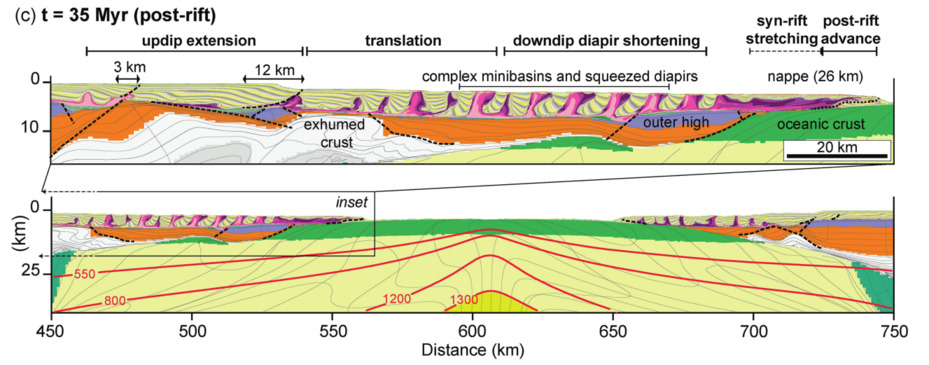
\includegraphics[height=5cm]{images/mycodes/pihg22a_img}
\end{center}

%--------------------------------------------------------------------------------------------------
\item {\it Coupling Crustal-Scale Rift Architecture With Passive Margin
Salt Tectonics: A Geodynamic Modeling Approach}, 
L.M. Pichel, R.S. Huismans, R. Gawthorpe, J.I. Faleide and Th. Theunissen, JGR, 127, 2022. \cite{pihg22b}
\begin{center}
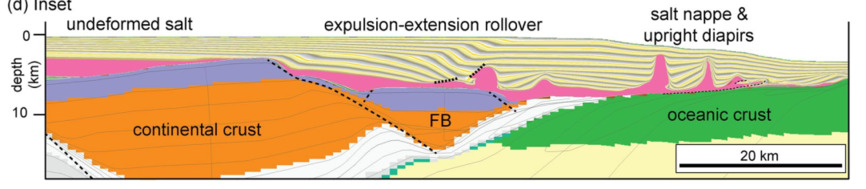
\includegraphics[height=3cm]{images/mycodes/pihg22b_img}
\end{center}

%--------------------------------------------------------------------------------------------------
\item {\it How post-­salt sediment flux and progradation rate
influence salt tectonics on rifted margins: Insights from
geodynamic modelling},
L.M. Pichel, R.S. Huismans, R. Gawthorpe and  J.I. Faleide, Basin Research, 2023. \cite{pihg23}
\begin{center}
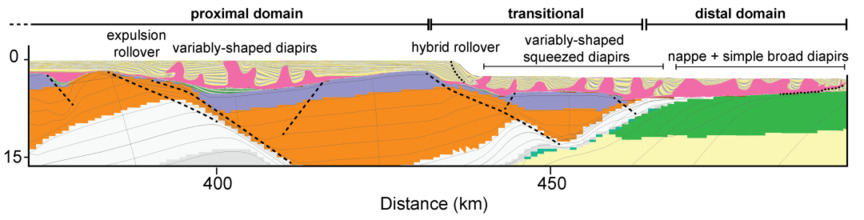
\includegraphics[height=3cm]{images/mycodes/pihg23_img}
\end{center}

\item {\it A Three-Field Formulation for Two-Phase Flow in
Geodynamic Modeling: Toward the Zero-Porosity Limit},
Gang Lu, Dave A. May and Ritske S. Huismans, 
Journal of Geophysical Research: Solid Earth, 2024. \cite{lumh24}


\end{itemize}


%--------------------------------------------------------------------------------------------------
%--------------------------------------------------------------------------------------------------
%--------------------------------------------------------------------------------------------------
%--------------------------------------------------------------------------------------------------

Upon my arrival at Utrecht University in 2012 I started working an a more flexible code, called \elefant, 
which has since very much diverged from \fantom.

\begin{itemize}
\item {\it The effect of obliquity on temperature in subduction zones: insights from 3-D numerical modeling}, 
A. Plunder, C. Thieulot and D.J.J. van Hinsbergen, Solid Earth 9, 759-776, 2018. \url{https://doi.org/10.5194/se-9-759-2018}

\begin{center}
\includegraphics[height=3.5cm]{images/mycodes/pltv18_img}
\end{center}


\item {\it Analytical solution for viscous incompressible Stokes flow in a spherical shell}, 
C. Thieulot, Solid Earth 8, 1181-1191, 2017. \url{https://doi.org/10.5194/se-8-1181-2017}

\begin{center}
\includegraphics[height=3cm]{images/mycodes/thie17_img}
\end{center}



\item  {\it Lithosphere erosion and continental breakup: interaction of extension, plume upwelling and melting}, 
A. Lavecchia, C. Thieulot, F. Beekman, S. Cloetingh and S. Clark, E.P.S.L. 467, p89-98, 2017.

\begin{center}
\includegraphics[height=3cm]{images/mycodes/latv17_img}
\end{center}


\item {\it Benchmarking numerical models of brittle thrust wedges}, 
Susanne J.H. Buiter, Guido Schreurs, Markus Albertz, Taras V. Gerya, Boris Kaus,
Walter Landry, Laetitia le Pourhiet, Yury Mishin, David L. Egholm, Michele Cooke,
Bertrand Maillot, Cedric Thieulot, Tony Crook, Dave May, Pauline Souloumiac, Christopher Beaumont
Journal of Structural Geology 92, p140-177, 2016. \url{https://doi:10.1016/j.jsg.2016.03.003}

\begin{center}
\includegraphics[height=1.8cm]{images/mycodes/busa16_img}
\end{center}


\item {\it A community benchmark for viscoplastic thermal convection in a 2-D square box}, 
N. Tosi, C. Stein, L. Noack, C. Huettig, P. Maierova, H. Samuel, D.R. Davies, C.R. Wilson, S.C. Kramer, C. Thieulot, A. Glerum, M. Fraters, W. Spakman, A. Rozel, P.J. Tackley, Geochem. Geophys. Geosyst. 16, doi:10.1002/2015GC005807, 2015.

\begin{center}
\includegraphics[height=3cm]{images/mycodes/tosn15_img}
\end{center}


\item {\it Dynamics of intraoceanic subduction initiation: 1. Oceanic detachment fault inversion and the formation of supra-subduction zone ophiolites}, M. Maffione, C. Thieulot, D.J.J. van Hinsbergen, A. Morris, O. Pluemper and W. Spakman, Geochem. Geophys. Geosyst. 16, p1753-1770, 2015.

\begin{center}
\includegraphics[height=1.8cm]{images/mycodes/matv15_img}
\end{center}

\item {\it The Geodynamic World Builder: a solution for complex initial conditions in numerical modelling},
M. Fraters, C. Thieulot, A. van den Berg and W. Spakman,
Solid Earth, \url{https://doi.org/10.5194/se-2019-24}, 2019.

\begin{center}
\includegraphics[height=2.8cm]{images/mycodes/frtv19_img}
\end{center}


\end{itemize}


\begin{itemize}
\item {\it GHOST: Geoscientific Hollow Sphere Tessellation}, 
C. Thieulot, Solid Earth, 9, 1169-1177, 2018. \url{https://doi.org/10.5194/se-9-1169-2018}

\begin{center}
\includegraphics[height=3cm]{images/mycodes/shell_HS06}
\includegraphics[height=3cm]{images/mycodes/shell_HS12}
\includegraphics[height=3cm]{images/mycodes/shell_HS20}
\end{center}


title={Long-term coupling and feedback between tectonics and surface processes 
during non-volcanic rifted margin formation},
author={Theunissen, Thomas and Huismans, Ritske S},
journal={Journal of Geophysical Research: Solid Earth},

\end{itemize}



\printbibliography

\end{document}
%%%%%%%%%%%%%%%%%%%%%%%%%%%%%%%%%%%%%%%%%%%%%%%%%%%%%%%%%%%
 %------------------------------------
\subsection{Installation} \begin{flushright} {\tiny {\color{gray} install.tex}} \end{flushright}

%--------------------------------
\subsubsection{Python}

If numpy, scipy or matplotlib are not installed on your machine, here is how you 
can install them:
\begin{verbatim}
sudo apt install python3-numpy
sudo apt install python3-scipy
\end{verbatim}
To install the umfpack solver (check?):
\begin{verbatim}
pip install --upgrade scikit-umfpack --user
\end{verbatim}
If you need to install pip:
\begin{verbatim}
sudo apt install python3-pip
\end{verbatim}

%--------------------------------
\subsubsection{Julia}

In order to have vim supporting the Julia language, do 
\begin{verbatim}
git clone git@github.com:JuliaEditorSupport/julia-vim.git
\end{verbatim}
and copy the content of the julia-vim folder in the .vim folder.
That's it.

%--------------------------------
\subsubsection{LaTeX}

To install siunitx package:
\begin{verbatim}
sudo apt -y install texlive-science
\end{verbatim}
To install additional fonts:
\begin{verbatim}
sudo apt-get install texlive-fonts-extra 
\end{verbatim}
To install biber package:
\begin{verbatim}
sudo apt install biber 
\end{verbatim}





 %--------------------------------------------------------
\subsection{What is a (real) fieldstone?} \begin{flushright} {\tiny {\color{gray} \tt whatisafieldstone.tex}} \end{flushright}

\begin{center}
\includegraphics[width=5cm]{images/fieldstone2}\\
{\captionfont Taken from \url{https://en.wikipedia.org/wiki/Fieldstone}}
\end{center}

Simply put, it is a stone collected from the surface of fields where it 
occurs naturally. It also stands for the bad acronym: {\sl fi}nite 
{\sl el}ement {\sl d}eformation of {\sl stone}s which echoes the primary 
application of these codes: geodynamic modelling.
 %------------------------------
\subsection{Why the Finite Element method?} \begin{flushright} {\tiny {\color{gray} why.tex}} \end{flushright}

The Finite Element Method (FEM) is by no means the only method 
to solve PDEs in geodynamics, nor it is necessarily always the best one.
Other methods are employed very successfully, such as the Finite Difference 
Method (FDM), the Finite Volume Method (FVM), and to a lesser extent
the Discrete Element Method (DEM) \cite{tasy05,egho07,egsc07,funi14,jitd23}, 
the Lattice-Boltzmann method \cite{hupc08}, the Rigid Element Method \cite{lacj15},  
or the Element Free Galerkin Method (EFGM) \cite{hans03}.
I have been using FEM since 2008 and I do not have real 
experience to speak of in FVM or FDM (except for chapter 11)
so I concentrate in this book 
on what I know best. 


 %------------------------------------------
\subsection{Oldies but goodies} 
The first papers I could find showcasing the FEM in geodynamics are listed hereafter
\cite{gart78}, 
\cite{anbr80}\cite{mera80}\cite{bran80}
\cite{engl82}
\cite{thar85}\cite{scan85}
\cite{enho86}\cite{mofr86}
\cite{zupa86}
\cite{boww89}
\cite{brau94}
\cite{brbe95}.
I hereunder show a few plots taken from early geodynamics papers.


\begin{center}
\begin{minipage}{0.45\textwidth}
\centering
\includegraphics[height=4.5cm]{images/history/stbe71}\\
{\captionfont 1971: Model a boudinage structure \cite{stbe71}}
\end{minipage}\hfill
\begin{minipage}{0.45\textwidth}
\centering
\includegraphics[height=4.5cm]{images/history/bela72}\\
{\captionfont 1972: Crustal Structure from Surface Load Tilts \cite{bela72}}
\end{minipage}
\end{center}

\begin{center}
\begin{minipage}{0.45\textwidth}
\centering
\includegraphics[height=5cm]{images/history/bird78b}\\
{\captionfont 1978: Finite element modelling of lithosphere deformation: the Zagros collision 
orogeny \cite{bird78b}}
\end{minipage}\hfill
\begin{minipage}{0.45\textwidth}
\centering
\includegraphics[height=5cm]{images/history/brpo81}\\
{\captionfont 1981: Thermal regimes, mantle diapirs and crustal stresses of continental rifts \cite{brpo81}}
\end{minipage}
\end{center}


\begin{center}
\begin{minipage}{0.48\textwidth}
\centering
\includegraphics[height=3.5cm]{images/history/baum85a}
\includegraphics[height=3.5cm]{images/history/baum85b}\\
{\captionfont 1985: Three-Dimensional Treatment of Convective Flow in the Earth's Mantle.
\cite{baum85}}
\end{minipage}\hfill
\begin{minipage}{0.45\textwidth}
\centering
\includegraphics[width=7cm]{images/history/zupf86}\\
{\captionfont 1986: Lithospheric necking: a dynamic model for rift morphology \cite{zupf86}}
\end{minipage}
\end{center}


\begin{center}
\begin{minipage}{0.48\textwidth}
\centering
\includegraphics[width=9cm]{images/history/boww89}\\
{\captionfont 1989: Plate boundary forces at subduction zones and trench-arc compression \cite{boww89}}
\end{minipage}\hfill
\begin{minipage}{0.45\textwidth}
\includegraphics[width=9cm]{images/history/brbe89}\\
{\captionfont 1989: Relation between flank uplifts and the breakup unconformity at rifted continental margins \cite{brbe89}}
\end{minipage}
\end{center}



\begin{center}
\begin{minipage}{0.35\textwidth}
\centering
\includegraphics[width=5cm]{images/history/mewi89}\\
{\captionfont 1989: Mechanics of graben formation in crustal rocks \cite{mewi89}}
\end{minipage}\hfill
\begin{minipage}{0.55\textwidth}
\centering
\includegraphics[width=8cm]{images/history/whbw92}\\
{\captionfont 1992: Stresses and plate boundary forces associated with subduction plate margins
\cite{whbw92}}
\end{minipage}
\end{center}


\begin{center}
\includegraphics[width=5cm]{images/history/dast92}\\
{\captionfont 1992: Temperature field in subduction zones \cite{dast92}}
\end{center}


\begin{center}
\begin{minipage}{0.45\textwidth}
\centering
\includegraphics[width=7.6cm]{images/history/brau93}\\
{\captionfont 1993: 3D numerical modeling of
compressional orogenies: Thrust geometry and
oblique convergence \cite{brau93}}
\end{minipage}\hfill
\begin{minipage}{0.45\textwidth}
\centering
\includegraphics[height=6cm]{images/history/bequ94}\\
{\captionfont 1994: Crustal-scale compressional orogens \cite{bequ94}}
\end{minipage}
\end{center}

\begin{center}
\includegraphics[height=6cm]{images/history/katl95}\\
{\captionfont 1995: modeling of pull-apart basins \cite{katl95}}
\end{center}


\begin{center}
\begin{minipage}{0.45\textwidth}
\centering
\includegraphics[height=5cm]{images/history/yowo95}\\
{\captionfont 1995: 3D numerical modeling of detachment of subducted 
lithosphere \cite{yowo95}}
\end{minipage}\hfill
\begin{minipage}{0.45\textwidth}
\centering
\includegraphics[height=6cm]{images/history/dusa96}\\
{\captionfont 1996: 3D dynamical model of continental rift propagation and 
margin plateau formation \cite{dusa96}}
\end{minipage}
\end{center}



\begin{center}
\includegraphics[height=6cm]{images/history/nesb99}\\
{\captionfont 1989: Model geometry, boundary conditions and 3-D finite element mesh used in 
the calculations. The circles denote a free-slip condition. The arrow denotes the velocity 
applied in some calculations to the southern boundary of the Tyrrhenian domain to simulate 
the motion of the African plate. The springs represent the buoyant restoring force applied 
at the surface. \cite{nesb99}}
\end{center}




 %---------------------------------------------------
\subsection{Notations} \input{notations} %---------------------------------------------------------
\subsection{Colour maps for visualisation} \begin{flushright} {\tiny {\color{gray} colorscale.tex}} \end{flushright}

In an attempt to homogenise the figures obtained with ParaView, I have decided to use 
a fixed colour scale for each field throughout this document. These colour scales were 
obtained from \url{https://peterkovesi.com/projects/colourmaps} and are 
Perceptually Uniform Colour Maps \cite{kove15}. 

\begin{center}
\begin{tabular}{lll}
\hline
Field & colour code & \\
\hline\hline
Velocity/displacement & CET-D01A & \includegraphics[width=3cm]{images/colourscales/CET-D1A}\\
\hline
Pressure& CET-L17 & \includegraphics[width=3cm]{images/colourscales/CET-L17}\\
\hline
Velocity divergence& CET-L01 & \includegraphics[width=3cm]{images/colourscales/CET-L1}\\
\hline
Density& CET-D03 & \includegraphics[width=3cm]{images/colourscales/CET-D3}\\
\hline
Strain rate& CET-R2 & \includegraphics[width=3cm]{images/colourscales/CET-R2}\\
\hline
Viscosity & CET-R3 & \includegraphics[width=3cm]{images/colourscales/CET-R3}\\
\hline
Temperature & CET-D09 & \includegraphics[width=3cm]{images/colourscales/CET-D9}\\
\hline
stress & CET-L18 &  \includegraphics[width=3cm]{images/colourscales/CET-L18}\\
\hline
Spin tensor & CET-R1 &  \includegraphics[width=3cm]{images/colourscales/CET-R1}\\
\hline
Composition field & CET-CBD1 & \includegraphics[width=3cm]{images/colourscales/CET-CBD1}\\
\hline
Gravity acceleration & vik &  \includegraphics[width=3cm,height=7mm]{images/colourscales/vik}\\
\hline
Gravity potential & roma &  \includegraphics[width=3cm,height=7mm]{images/colourscales/roma}\\
\hline
Vorticity & CET-L12 & \\
\hline
Stream function & CET-D02 & \\
\end{tabular}
\end{center}

vik and roma are available at \url{http://www.fabiocrameri.ch/colourmaps.php}.
See also Crameri \etal (2020) for a discussion about the misuse of 
colour is science communication.

%https://peterkovesi.com/projects/colourmaps/




 %------------------------------------
\subsection{How my bibliography works} \begin{flushright} {\tiny {\color{gray} mybib.tex}} \end{flushright}
%~~~~~~~~~~~~~~~~~~~~~~~~~~~~~~~~~~~~~~~~~~~~~~~~~~~~~~~~~~~~~~~~~~~~~~~~~~~~~~~~~~~~~~~~~~~~~~~~~~

There is a single (large) bibliography file for this document:
\begin{center}
{\tt biblio\_geosciences.bib}
\end{center}

If the paper is a single-author paper, say by Garfield\footnote{This is just an example}, 
published in 1978\footnote{May be not, after all, since Garfield the cat was born in 1978}, its code 
in my bibliography file is {\sl garf78} (i.e. the first four letters of the name, followed by 
the two digits of the publication year).

If the paper was written by two authors, say Garfield and Odie, in 1987, its code 
will be {\sl gaod87}, i.e. the first two letters of the first author followed by the two 
first letters of the second author followed by two digits.

If the paper was written by three or more authors, say Garfield, Odie, John and Irene in 
2003, its code will be {\sl gaoj03}, i.e. the first two letters of the first author followed 
by the first letter of the second author, the first letter of the third author and the year.

If multiple papers are published the same year by the same authors, I simply append a,b,c... to the 
above rules. 

\begin{remark} Dutch names such as 'van Hunen' or 'van den Berg' are classified under letter 'v', 
not 'h' or 'd' nor 'b'. 
\end{remark}

\vspace{1cm}

\begin{center}
\includegraphics[width=9cm]{statistics_biblio/stats.pdf}\\
{\captionfont Evolution of the number of references cited in FieldStone
per year. The purple line tracks the pdf files in my folder while 
the green line accounts for the entries in my .bib file.}
\end{center}

\begin{center}
\includegraphics[width=9cm]{statistics_biblio/journals.pdf}\\
{\captionfont Evolution of the number of references cited in FieldStone
per year per journal.}
\end{center}


\begin{center}
\includegraphics[width=8cm]{statistics_biblio/journal_jgr}
\includegraphics[width=8cm]{statistics_biblio/journal_gji}\\
\includegraphics[width=8cm]{statistics_biblio/journal_epsl}
\includegraphics[width=8cm]{statistics_biblio/journal_g3}\\
\includegraphics[width=8cm]{statistics_biblio/journal_geology}
\includegraphics[width=8cm]{statistics_biblio/journal_solid_earth}\\
\includegraphics[width=8cm]{statistics_biblio/journal_tectonics}
\includegraphics[width=8cm]{statistics_biblio/journal_tectonophysics}\\
\includegraphics[width=8cm]{statistics_biblio/journal_grl}
\includegraphics[width=8cm]{statistics_biblio/journal_pepi}
\end{center}

G3 starts in January 2000 only

SE starts in 2010




 %---------------------------------------------
\subsection{Youtube resources} \begin{flushright} {\tiny {\color{gray} \tt youtube.tex}} \end{flushright}
%~~~~~~~~~~~~~~~~~~~~~~~~~~~~~~~~~~~~~~~~~~~~~~~~~~~~~~~~~~~~~~~~~~~~~~~~~~~~~~~~~~~~~~~~~~~~~~~~~~

\begin{itemize}
\item \url{https://youtu.be/aLJMDn_2-d8} [10min]
\begin{center}
\includegraphics[width=5cm]{images/youtube/superold}\\
\end{center}

\item \url{https://youtu.be/j2_dJY_mIys} [10min] Smarter Every Day channel
\begin{center}
\includegraphics[width=5cm]{images/youtube/smarter}\\
\end{center}

\item \url{https://youtu.be/X4zd4Qpsbs8} [2min] Reversible Stokes flow (cylinder + dye)
\item \url{https://youtu.be/wzcVT0oZJkg} [12min] Boring Through The Earth's Crust
\item \url{https://youtu.be/GHjopp47vvQ} [18min] Understanding the Finite Element Method
\begin{center}
\includegraphics[width=5cm]{images/youtube/fem}\\
\end{center}

\item \url{https://www.esa.int/Applications/Observing_the_Earth/GOCE/Gravity_mission_still_unearthing_hidden_secrets} [3min] GOCE helps create new model of crust and upper mantle
\item \url{https://youtu.be/_5q8hzF9VVE} [12min] Continental drift (Wegener theory) 
\item \url{https://youtu.be/ZTRu620bIsE} [12min] Plate tectonics
\item \url{https://youtu.be/V_zsD8vXyik} [5min] Heat tranfer 
\item \url{https://youtu.be/q65O3qA0-n4} [4min] What is sea level? (geoid) 

\item \url{https://youtu.be/kijOMOGDfRo?si=qmM8lnyJ5XTFw83n} [35min] Rob Moucha - Coupling Geodynamic and Landscape Evolution Models
\item \url{https://youtu.be/eNhJY-R3Gwg?si=Fbs_4kK5yqAJMi2b} [6min] minutephysics - General Relativity Explained in 7 Levels of Difficulty 

\end{itemize}

%------------------------------------------------------------------------------------
\subsection{Dave Whipp videos}

They are available at \url{https://www.youtube.com/@helsinkiuniversitygeodynam6511/videos}
\begin{itemize}

\item set 2: Kinematics of plate tectonics
\begin{enumerate}
\item Divergent plate boundaries [12min] \href{https://youtu.be/x3OKt5Warr4?si=YJP5GuxXPTh6SLlo}{\includegraphics[width=.8cm]{images/pictograms/film.png}}
\item Convergent plate boundaries [9min] \href{https://youtu.be/8B4PC-75a1c?si=V5huZbOi1CAxGgxG}{\includegraphics[width=.8cm]{images/pictograms/film.png}}
\item Transforms and the Wilson cycle [7min] \href{https://youtu.be/cLsFLEcfPBY?si=t5St5urowPPwXLdq}{\includegraphics[width=.8cm]{images/pictograms/film.png}}
\item Plate motions on a flat Earth [10min] \href{https://youtu.be/lZMPACABF_E?si=9l1Z-OC9ZwMqn0tv}{\includegraphics[width=.8cm]{images/pictograms/film.png}}
\item Triple junctions [9min] \href{https://youtu.be/SG2X9t0J1fc?si=Qc8JMy3LzoDDzZpL}{\includegraphics[width=.8cm]{images/pictograms/film.png}}
\item Plate motions on a sphere [9min] \href{https://youtu.be/Fifg4O0fs2E?si=LB6NoWUioEEa9XZB}{\includegraphics[width=.8cm]{images/pictograms/film.png}}
\end{enumerate}

\item set 3: forces and stresses
\begin{enumerate}
\item Forces [9min] \href{https://youtu.be/ILFqNowqknw?si=zjLwx-es2OwZQkcU}{\includegraphics[width=.8cm]{images/pictograms/film.png}}
\item Surface stresses [14min] \href{https://youtu.be/_if5w_wk7-w?si=RnMAEX21xeoPsjoi}{\includegraphics[width=.8cm]{images/pictograms/film.png}}
\item Stresses in 2D [11min] \href{https://youtu.be/gBYu8IuJfTw?si=r6w2utvZs2sJpEKX}{\includegraphics[width=.8cm]{images/pictograms/film.png}}
\item Stresses in 3D [11min] \href{https://youtu.be/wou1yP8PxNM?si=cXhgqQGEX3qcXZrT}{\includegraphics[width=.8cm]{images/pictograms/film.png}}
%\item  [min] \href{}{\includegraphics[width=.8cm]{images/pictograms/film.png}}
%\item  [min] \href{}{\includegraphics[width=.8cm]{images/pictograms/film.png}}
%\item  [min] \href{}{\includegraphics[width=.8cm]{images/pictograms/film.png}}
%\item  [min] \href{}{\includegraphics[width=.8cm]{images/pictograms/film.png}}
\end{enumerate}

\item set 4: measuring stress and strain 
\begin{enumerate}
\item Global and regional stress measurements [9min] 
      \href{https://youtu.be/J6yu4fi4kCI?si=KlmhNOcqgycHa1cq}{\includegraphics[width=.8cm]{images/pictograms/film.png}}
\item How is stress measured? [11min] 
      \href{https://youtu.be/FtFGMryqQXI?si=2XIfjtfxgxQtsiIv}{\includegraphics[width=.8cm]{images/pictograms/film.png}}
\item What is strain? [9min] 
      \href{https://youtu.be/DQ345dy84BI?si=C1eJC_mthTaIP7z7}{\includegraphics[width=.8cm]{images/pictograms/film.png}}
\item Normal and shear strains [9min] 
      \href{https://youtu.be/CNXHtMdt-XY?si=i7JiiOyV237gVYLr}{\includegraphics[width=.8cm]{images/pictograms/film.png}}
\item Historical strain measurements [11min] 
      \href{https://youtu.be/TZXt2lk_fr4?si=cEntMD8C6-aB8-dq}{\includegraphics[width=.8cm]{images/pictograms/film.png}}
\item Modern strain measurements [10min] 
      \href{https://youtu.be/ki6X1xjnYCE?si=NJXSi2Wf38uSyMIX}{\includegraphics[width=.8cm]{images/pictograms/film.png}}
\end{enumerate}
\item set 5: basics of elasticity
\begin{enumerate}
\item [min] \href{}{\includegraphics[width=.8cm]{images/pictograms/film.png}}
\end{enumerate}
\item set 6: flexure of the lithosphere
\begin{enumerate}
\item [min] \href{}{\includegraphics[width=.8cm]{images/pictograms/film.png}}
\end{enumerate}
\item set 7: heat conduction and production
\begin{enumerate}
\item [min] \href{}{\includegraphics[width=.8cm]{images/pictograms/film.png}}
\end{enumerate}
\item set 8: thermal processes in the lithosphere
\begin{enumerate}
\item [min] \href{}{\includegraphics[width=.8cm]{images/pictograms/film.png}}
\end{enumerate}
\item set 9: basic of fluid mechanics
\begin{enumerate}
\item [min] \href{}{\includegraphics[width=.8cm]{images/pictograms/film.png}}
\end{enumerate}
\item set 10: plate-driving forces
\begin{enumerate}
\item [min] \href{}{\includegraphics[width=.8cm]{images/pictograms/film.png}}
\end{enumerate}
\item set 11: brittle deformation and faulting
\begin{enumerate}
\item [min] \href{}{\includegraphics[width=.8cm]{images/pictograms/film.png}}
\end{enumerate}
\item set 12: viscous deformation, strength of the lithosphere
\begin{enumerate}
\item [min] \href{}{\includegraphics[width=.8cm]{images/pictograms/film.png}}
\end{enumerate}
\item set 13: climatic, geomorphic and geodynamic processes
\begin{enumerate}
\item [min] \href{}{\includegraphics[width=.8cm]{images/pictograms/film.png}}
\end{enumerate}
\end{itemize}

%------------------------------------------------------------------------------------
\subsection{Clint Conrad videos}

\begin{itemize}
\item Plate Tectonics: Linking Surface Geology to Earth’s Deep Interior [35min] 
      \href{https://youtu.be/aPuLqiXci14}{\includegraphics[width=.8cm]{images/pictograms/film.png}} 
\item Models of mantle convection [1h30] 
      \href{https://youtu.be/olbSuf6EGPM}{\includegraphics[width=.8cm]{images/pictograms/film.png}}
\item Mantle flow for the present day [1h30] 
      \href{https://youtu.be/aTQ-1Vpncjw}{\includegraphics[width=.8cm]{images/pictograms/film.png}}
\item Mantle flow for Earth history [54min] 
      \href{https://youtu.be/OG5qDon-3_w}{\includegraphics[width=.8cm]{images/pictograms/film.png}}
\item 50 years of plate tectonics. But what is the driving force? [24min] 
      \href{https://youtu.be/4UAdEwbGKiM}{\includegraphics[width=.8cm]{images/pictograms/film.png}}
\end{itemize}

%------------------------------------------------------------------------------------
\subsection{Wolfgang Bangerth videos}

{\color{red} I need to compile a list}


%------------------------------------------------------------------------------------
\subsection{Fluid Mechanics 101 channel videos}

\begin{itemize}

\item SIMPLE Algorithm Course. [21min]
      \href{https://www.youtube.com/watch?v=z1wMpZeVzMI}{\includegraphics[width=.8cm]{images/pictograms/film.png}}

\item Conjugate Gradient for CFD (Part 1): Background and Steepest Descent [45min]
      \href{https://www.youtube.com/watch?v=jXShvxPcRl4}{\includegraphics[width=.8cm]{images/pictograms/film.png}}

\item Conjugate Gradient for CFD (Part 2): Optimum Distance and Directions [34min]
      \href{https://www.youtube.com/watch?v=MdPhVsgTc1Q}{\includegraphics[width=.8cm]{images/pictograms/film.png}}

\item Conservative, Advective \& Material Derivative forms of the N-S Equations [32min]
      \href{https://www.youtube.com/watch?v=ljdv4T2U464}{\includegraphics[width=.8cm]{images/pictograms/film.png}}

\item Gauss-Seidel Method in CFD [29min]
      \href{https://www.youtube.com/watch?v=ymIvps7pgRk}{\includegraphics[width=.8cm]{images/pictograms/film.png}}

\item The Courant (CFL) Number [28min]
      \href{https://www.youtube.com/watch?v=WBWY46ynRk0}{\includegraphics[width=.8cm]{images/pictograms/film.png}}

\item Lagrangian Particle Tracking [29min]
      \href{https://www.youtube.com/watch?v=jdq6puyvQ7E}{\includegraphics[width=.8cm]{images/pictograms/film.png}}

\item The Boussinesq Approximation for Bouyancy Driven (Natural Convection) Flow [18min]
      \href{https://www.youtube.com/watch?v=onKiVbKSoXw}{\includegraphics[width=.8cm]{images/pictograms/film.png}}

\item The Energy Equation for Solids and Fluids in CFD [31min]
      \href{https://www.youtube.com/watch?v=z8dZHze_EPo}{\includegraphics[width=.8cm]{images/pictograms/film.png}}

\item The Finite Volume Method in CFD [24min] 
      \href{https://www.youtube.com/watch?v=E9_kyXjtRHc}{\includegraphics[width=.8cm]{images/pictograms/film.png}}

\item Eulerian Multi-Phase Modelling [25min]
      \href{https://www.youtube.com/watch?v=6BJauDTpCmo}{\includegraphics[width=.8cm]{images/pictograms/film.png}}

\end{itemize}


 %---------------------------------------------------
\subsection{How to download a single stone} 
Say you wish to only download a single python program, for example stone 3. You then go to 
\url{https://github.com/cedrict/fieldstone} and click on {\tt python\_codes}, then on {\tt fieldstone\_03} and
then on {\tt stone.py}.

Then click on Raw:

\begin{center}
\includegraphics[width=12cm]{images/wget1} 
\end{center}

And then copy the address in the address bar:

\begin{center}
\includegraphics[width=12cm]{images/wget2} 
\end{center}

Finally, in the terminal of your Linux/Apple computer type

\begin{verbatim}
wget https://raw.githubusercontent.com/cedrict/fieldstone/master/python_codes/fieldstone_03/stone.py
\end{verbatim}

 %------------------------
 

%%%%%%%%%%%%%%%%%%%%%%%%%%%%%%%%%%%%%%%%%%%%%%%%%%%%%%%%%%%%%%%%%%%%%%%%%%%%%%%%%%%%%%%%%%%%%%%%%%%
%\newpage
%\section{List of stones and their features} %%%%%%%%%%%%%%%%%%%%%%%%%%%%%%%%%%%%%%%%%%%%%%%%%%%%%%%
%

\begin{tabular}{|llll|}
\hline
Element & ndim & geometry  &\stone \\
\hline\hline
${\bm Q}_1\times P_0$ penalty & 2D & &1,2,3,4,5,6,7,8,9,12,38,73,101,102, \\
${\bm Q}_1\times P_0$ penalty & 3D & &10, \\
${\bm Q}_1\times P_0$         & 2D & &14,15,16,23,24,25,26,27,28,29,32,33,35,42,48,50,78,103+\\
${\bm Q}_1\times P_0$         & 3D & &11,20 \\
${\bm Q}_1\times P_0$-stab    & 2D & &115,116 \\
${\bm Q}_1\times P_0$-stab    & 3D & & \\
${\bm Q}_1\times Q_1$-stab    & 2D & &22, \\
${\bm Q}_1\times Q_1$-stab    & 3D & & \\
${\bm Q}_1^+\times Q_1$       & 2D & & \\
\hline
${\bm Q}_2\times Q_1$   & 2D & Cartesian &18,25,39,40,41,42,48,52,53,54,59,61,64,67,70,87,88,104,110,112 \\
${\bm Q}_2\times Q_1$   & 2D & Annulus   &21,71 \\
${\bm Q}_2\times Q_1$   & 2D & Axisymmetric & 91,106 \\
${\bm Q}_2\times Q_1$   & 3D & Cartesian & 17,109 \\
\hline
$Q_2\times P_{-1}$      & 2D & &76,104,112 \\
$Q_2\times P_{-1}$      & 3D & & \\
$Q_3\times Q_2$         & 2D & &19,42,48 \\
$Q_3\times Q_2$         & 3D & & \\
$Q_4\times Q_3$         & 2D & &48 \\
$Q_2^{(8)}\times Q_1$   & 2D & &52,53 \\
$Q_1^+ \times P_0$      & 2D & &80 \\
$Q_1^+ \times P_0$      & 3D & &81 \\
\hline
$P_2 \times P_1$      & 2D & &95,96,112 \\
$P_2 \times P_1$      & 3D & & \\
$P_1^+ \times P_1$    & 2D & &47,51,95,112 \\
$P_1^+ \times P_1$    & 3D & & \\
$P_2^+ \times P_{-1}$ & 2D & &46,55,62,68,92,93,95,96,112 \\
\hline
\end{tabular}

%fun fact: lualatex+lstlisting does not accept files without extension!


\vspace{1cm}

{\small 

\noindent stone 01: simple analytical solution: "Donea \& Huerta" mms 
\lstinputlisting[language=bash,basicstyle=\tiny]{python_codes/fieldstone_01/keywords.ascii}

\noindent stone 02: Stokes sphere in 2D 
\lstinputlisting[language=bash,basicstyle=\tiny]{python_codes/fieldstone_02/keywords}

\noindent stone 03: Convection in a 2D box: "Blankenbach" benchmark \cite{blbc89}
\lstinputlisting[language=bash,basicstyle=\tiny]{python_codes/fieldstone_03/keywords}

\noindent stone 04: The lid driven cavity
\lstinputlisting[language=bash,basicstyle=\tiny]{python_codes/fieldstone_04/keywords}

\noindent stone 05: SolCx
\lstinputlisting[language=bash,basicstyle=\tiny]{python_codes/fieldstone_05/keywords}

\noindent stone 06: SolKz
\lstinputlisting[language=bash,basicstyle=\tiny]{python_codes/fieldstone_06/keywords}

\noindent stone 07: SolVi
\lstinputlisting[language=bash,basicstyle=\tiny]{python_codes/fieldstone_07/keywords}

\noindent stone 08: The indentor (punch problem) 
\lstinputlisting[language=bash,basicstyle=\tiny]{python_codes/fieldstone_08/keywords}

\noindent stone 09: the annulus benchmark 
\lstinputlisting[language=bash,basicstyle=\tiny]{python_codes/fieldstone_09/keywords}

\noindent stone 10: Stokes sphere (3D) - penalty
\lstinputlisting[language=bash,basicstyle=\tiny]{python_codes/fieldstone_10/keywords}

\noindent stone 11: Stokes sphere (3D) - mixed formulation
\lstinputlisting[language=bash,basicstyle=\tiny]{python_codes/fieldstone_11/keywords}

\noindent stone 12: consistent pressure recovery 
\lstinputlisting[language=bash,basicstyle=\tiny]{python_codes/fieldstone_12/keywords}

\noindent stone 13: the Particle in Cell technique (1) - the effect of averaging
\lstinputlisting[language=bash,basicstyle=\tiny]{python_codes/fieldstone_13/keywords}

\noindent stone 14: solving the full saddle point problem with $Q_1\times P_0$ elements 
\lstinputlisting[language=bash,basicstyle=\tiny]{python_codes/fieldstone_14/keywords}

\noindent stone 15: saddle point problem with Schur complement approach - D\&H benchmark 
\lstinputlisting[language=bash,basicstyle=\tiny]{python_codes/fieldstone_15/keywords}

\noindent stone 16: saddle point problem with Schur complement approach - Stokes sphere 
\lstinputlisting[language=bash,basicstyle=\tiny]{python_codes/fieldstone_16/keywords}

\noindent stone 17: Solving the full saddle point problem in 3D - Burstedde benchmark \cite{dobo04} 
\lstinputlisting[language=bash,basicstyle=\tiny]{python_codes/fieldstone_17/keywords}

\noindent stone 18: Solving the full saddle point problem with $Q_2\times Q_1$ elements 
\lstinputlisting[language=bash,basicstyle=\tiny]{python_codes/fieldstone_18/keywords}

\noindent stone 19: Solving the full saddle point problem with $Q_3\times Q_2$ elements 
\lstinputlisting[language=bash,basicstyle=\tiny]{python_codes/fieldstone_19/keywords}

\noindent stone 20: Convection in a 3D box, the Busse benchmark \cite{bucc94}
\lstinputlisting[language=bash,basicstyle=\tiny]{python_codes/fieldstone_20/keywords}

\noindent stone 22: The stabilised $Q_1 \times Q_1$ element 
\lstinputlisting[language=bash,basicstyle=\tiny]{python_codes/fieldstone_22/keywords}

\noindent stone 23: compressible flow (1) - analytical benchmark 
\lstinputlisting[language=bash,basicstyle=\tiny]{python_codes/fieldstone_23/keywords}

\noindent stone 24: compressible flow (1) - convection box 
\lstinputlisting[language=bash,basicstyle=\tiny]{python_codes/fieldstone_24/keywords}

\noindent stone 25: Rayleigh-Taylor instability (1) - instantaneous \cite{vaks97}
\lstinputlisting[language=bash,basicstyle=\tiny]{python_codes/fieldstone_25/keywords}

\noindent stone 26: Slab detachment benchmark (1) - instantaneous 
\lstinputlisting[language=bash,basicstyle=\tiny]{python_codes/fieldstone_26/keywords}

\noindent stone 27: Consistent Boundary Flux benchmark
\lstinputlisting[language=bash,basicstyle=\tiny]{python_codes/fieldstone_27/keywords}

\noindent stone 28: convection 2D box - Tosi \etal, 2015
\lstinputlisting[language=bash,basicstyle=\tiny]{python_codes/fieldstone_28/keywords}

\noindent stone 29: open boundary conditions
\lstinputlisting[language=bash,basicstyle=\tiny]{python_codes/fieldstone_29/keywords}

\noindent stone 30: the Particle in Cell technique (2) - CVI algorithms in 2D
\lstinputlisting[language=bash,basicstyle=\tiny]{python_codes/fieldstone_30/keywords}

\noindent stone 31: the Particle in Cell technique (3) - CVI algorithms in 3D
\lstinputlisting[language=bash,basicstyle=\tiny]{python_codes/fieldstone_31/keywords}

\noindent stone 32: 2D analytical solution from stream function
\lstinputlisting[language=bash,basicstyle=\tiny]{python_codes/fieldstone_32/keywords}

\noindent stone 33: Convection in an annulus 
\lstinputlisting[language=bash,basicstyle=\tiny]{python_codes/fieldstone_33/keywords}

\noindent stone 34: the 2D Cartesian geometry elastic aquarium
\lstinputlisting[language=bash,basicstyle=\tiny]{python_codes/fieldstone_34/keywords}

\noindent stone 35: 2D analytical solution in annulus from stream function 
\lstinputlisting[language=bash,basicstyle=\tiny]{python_codes/fieldstone_35/keywords}

\noindent stone 36: the annulus geometry elastic aquarium
\lstinputlisting[language=bash,basicstyle=\tiny]{python_codes/fieldstone_36/keywords}

\noindent stone 39: Choi \& Pedersen visco-plasticity benchmarks 
\lstinputlisting[language=bash,basicstyle=\tiny]{python_codes/fieldstone_39/keywords}

\noindent stone 40: Rayleigh-Taylor instability (instantaneous)
\lstinputlisting[language=bash,basicstyle=\tiny]{python_codes/fieldstone_40/keywords}

\noindent stone 43: Time-dependent advection problems with SUPG
\lstinputlisting[language=bash,basicstyle=\tiny]{python_codes/fieldstone_43/keywords}

\noindent stone 44: Flat slab setup 
\lstinputlisting[language=bash,basicstyle=\tiny]{python_codes/fieldstone_44/keywords}

%\noindent stone 45: the corner flow subduction benchmark \cite{vack08}  
%\lstinputlisting[language=bash,basicstyle=\tiny]{python_codes/fieldstone_45/keywords}

\noindent stone 46: MMS1 with Crouzeix-Raviart ($P_2^+\times P_{-1}$) elements  
\lstinputlisting[language=bash,basicstyle=\tiny]{python_codes/fieldstone_46/keywords}

\noindent stone 47: MMS1 with MINI ($P_1^+\times P_1$) elements
\lstinputlisting[language=bash,basicstyle=\tiny]{python_codes/fieldstone_47/keywords}

\noindent stone 48: $Q_1\times P_0$, $Q_2\times Q_1$, $Q_3\times Q_2$ and $Q_4\times Q_3$ elements
\lstinputlisting[language=bash,basicstyle=\tiny]{python_codes/fieldstone_48/keywords}

\noindent stone 49: Consistent Boundary Flux method on D\&H benchmark with 4 elements 
\lstinputlisting[language=bash,basicstyle=\tiny]{python_codes/fieldstone_49/keywords}

\noindent stone 50: Lithosphere extension (visco-plastic, thermo-mechanically coupled)
\lstinputlisting[language=bash,basicstyle=\tiny]{python_codes/fieldstone_50/keywords}

\noindent stone 51: Triangular domain benchmark with MINI element
\lstinputlisting[language=bash,basicstyle=\tiny]{python_codes/fieldstone_51/keywords}

\noindent stone 52: Serendipity element in 2D 
\lstinputlisting[language=bash,basicstyle=\tiny]{python_codes/fieldstone_52/keywords}

\noindent stone 53: the sinking block benchmark  
\lstinputlisting[language=bash,basicstyle=\tiny]{python_codes/fieldstone_53/keywords}

\noindent stone 54: free surface and ALE algorithms
\lstinputlisting[language=bash,basicstyle=\tiny]{python_codes/fieldstone_54/keywords}

\noindent stone 55: Subduction as a thin-sheet problem
\lstinputlisting[language=bash,basicstyle=\tiny]{python_codes/fieldstone_55/keywords}

\noindent stone 57: 1D steady state diffusion with DG-FEM
\lstinputlisting[language=bash,basicstyle=\tiny]{python_codes/fieldstone_57/keywords}

\noindent stone 58: Elastic disk under compression
\lstinputlisting[language=bash,basicstyle=\tiny]{python_codes/fieldstone_58/keywords}

\noindent stone 59: Ice flow down an inclined plane 
\lstinputlisting[language=bash,basicstyle=\tiny]{python_codes/fieldstone_59/keywords.key}

\noindent stone 60: 1D advection with DG-FEM 
\lstinputlisting[language=bash,basicstyle=\tiny]{python_codes/fieldstone_60/keywords}

\noindent stone 61: Channel flow with Herschel-Bulkley rheology 
\lstinputlisting[language=bash,basicstyle=\tiny]{python_codes/fieldstone_61/keywords}

\noindent stone 62: Subduction a la Quinquis Case 1
\lstinputlisting[language=bash,basicstyle=\tiny]{python_codes/fieldstone_62/keywords}

\noindent stone 63: Failure in cemented granular material
\lstinputlisting[language=bash,basicstyle=\tiny]{python_codes/fieldstone_63/keywords}

\noindent stone 64: Elasto-viscous benchmarks 
\lstinputlisting[language=bash,basicstyle=\tiny]{python_codes/fieldstone_64/keywords}

\noindent stone 65: steady-state advection-diffusion
\lstinputlisting[language=bash,basicstyle=\tiny]{python_codes/fieldstone_65/keywords}

\noindent stone 67: Newtonian subduction setups \& Particle-in-cell
\lstinputlisting[language=bash,basicstyle=\tiny]{python_codes/fieldstone_67/keywords}

\noindent stone 68: subduction \& corner flow
\lstinputlisting[language=bash,basicstyle=\tiny]{python_codes/fieldstone_68/keywords}

\noindent stone 69: Spherical shell 
\lstinputlisting[language=bash,basicstyle=\tiny]{python_codes/fieldstone_69/keywords}

\noindent stone 70:
\lstinputlisting[language=bash,basicstyle=\tiny]{python_codes/fieldstone_70/keywords}

\noindent stone 71:
\lstinputlisting[language=bash,basicstyle=\tiny]{python_codes/fieldstone_71/keywords}



}









 

\newpage
%%%%%%%%%%%%%%%%%%%%%%%%%%%%%%%%%%%%%%%%%%%%%%%%%%%%%%%%%%%%%%%%%%%%%%%%%%%%%%%%%%%%%%%%%%%%%%%%%%%
\section{Physics and a bit of mathematics} \label{chapt3} %%%%%%%%%%%%%%%%%%%%%%%%%%%%%%%%%%%%%%%%%

\chapter{Physics and a bit of mathematics} \label{chapt3} %%%%%%%%%%%%%%%%%%%%%%%%%%%%%%%%%%%%%%%%%

\begin{flushright} {\tiny {\color{gray} chapter3.tex}} \end{flushright}

\section{Some maths} \begin{flushright} {\tiny {\color{gray} maths.tex}} \end{flushright}
%~~~~~~~~~~~~~~~~~~~~~~~~~~~~~~~~~~~~~~~~~~~~~~~~~~~~~~~~~~~~~~~~~~~~~~~~~~~~~~~~~~~~~~~~~~~~~~~~~~

%----------------------------------------------------
\subsection{About vectors}

\begin{remark}
In this document I have chosen to (when possible) use the notation $\vec{a}$
to denote a vector and ${\bm a}$ to denote a tensor/matrix. More often than not 
the same notation ${\bm a}$ is used for both in the literature.
\end{remark}

In mathematics, physics and engineering, a Euclidean vector or simply a vector 
is a geometric object that has magnitude (or length) and direction. 
Many algebraic operations on real numbers such as addition, subtraction, multiplication, 
and negation have close analogues for vectors.

Let $\vec{v}$ be a vector in 3D space. 
Its Euclidean norm (or magnitude) is given in a coordinate-free way by 
\[
|\vec{v}|:=\sqrt{\vec{v}\cdot\vec{v}}
\]
This definition makes use of the dot product, see next section.
The Euclidean norm is also called the $L_2-$norm, or $2-$norm. It is also 
sometimes noted $||\cdot ||_2$. 

In Cartesian coordinates the vector $\vec{v}$ is given by
\[
\vec{v}=
\left(
\begin{array}{c}
v_x \\ v_y \\ v_z
\end{array}
\right)
=
v_x \vec{e}_x + 
v_y \vec{e}_y + 
v_z \vec{e}_z 
\qquad
\text{with}
\qquad
\vec{e}_x=
\left(
\begin{array}{c}
1 \\ 0 \\ 0
\end{array}
\right)
\quad
\vec{e}_y=
\left(
\begin{array}{c}
0 \\ 1 \\ 0
\end{array}
\right)
\quad
\vec{e}_z=
\left(
\begin{array}{c}
0 \\ 0 \\ 1
\end{array}
\right)
\]
Its norm then simply writes
\[
|\vec{v}| = \sqrt{v_x^2 + v_y^2 + v_z^2}
\]

A unit vector is any vector with a length of one. 
A vector of arbitrary length can be divided by its length to create a unit vector.
If $\vec{a}$ is a vector, the corresponding unit vector is often denoted
\[
\vec{e}_a = \frac{\vec{a}}{|\vec{a}|}
\]


%---------------------------------------------------------------
\subsection{dot products, cross products and dyadic products}

The {\bf dot product} (or sometimes called inner product, or even scalar product) of two vectors is denoted by 
$\vec{a}\cdot \vec{b}$ and is defined as:
\[
\vec{a}\cdot \vec{b} = |\vec{a}| \; |\vec{b}| \; \cos\theta
\]
where $\theta$  is the measure of the angle between $\vec{a}$ and ${b}$.

\todo[inline]{FIGURE}

In Cartesian coordinates the dot product can also be defined as the sum 
of the products of the components of each vector as
\[
\vec{a}\cdot\vec{b} = a_xb_x + a_yb_y + a_zb_z  
\]
The dot product can also be interpreted as an answer to the question ``how similar are vectors $\vec{a}$
and $\vec{b}$ in magnitude and direction?'' Indeed, if $\vec{a}=\vec{b}$ then $\theta=0$ and $\cos\theta=1$, while if 
$\vec{a}$ is perpendicular to $\vec{b}$, then $\theta=\pi/2$, $\cos\theta=0$ and $\vec{a}\cdot \vec{b}=0$. 

In Cartesian coordinates, we find that 
\[
\vec{v} \cdot \vec{e}_x 
= (v_x \vec{e}_x + v_y \vec{e}_y + v_z \vec{e}_z ) \cdot \vec{e}_x
= v_x \underbrace{\vec{e}_x \cdot \vec{e}_x}_{=1}
+ v_y \underbrace{\vec{e}_y \cdot \vec{e}_x}_{=0}
+ v_z \underbrace{\vec{e}_z \cdot \vec{e}_x}_{=0} 
=v_x
\]
In this case the interpretation of $\vec{v} \cdot \vec{e}_x$ could be ``how much of $\vec{v}$
is in the direction $\vec{e}_x$''.

The {\bf cross product} (also  called the vector product or outer product) of two vectors is also a vector.
It is denoted $\vec{a} \times \vec{b}$ and defined as 
\[
\vec{c} = \vec{a} \times \vec{b} = |\vec{a}| \; |\vec{b}|\; \sin\theta \; \vec{n}
\]
where $\theta$  is the measure of the angle between $\vec{a}$ and ${b}$ and
and $\vec{n}$ is a unit vector perpendicular to both $\vec{a}$ and $\vec{b}$ 
which completes a right-handed system.

\todo[inline]{FIGURE}

The norm of the cross product, say $|\vec{c}|=|\vec{a} \times \vec{b}|$, is actually the 
area of the parallelogram having $\vec{a}$ and $\vec{b}$ as sides.

Also note that $\vec{a} \times \vec{b} = - \vec{b} \times \vec{a}$ (think about the direction of the 
normal vector in each case). In Cartesian coordinates the cross product can be written as
\[
\vec{a} \times \vec{b} = (a_yb_z-a_zb_y) \vec{e}_x + (a_zb_x-a_xb_z) \vec{e}_y + (a_xb_y-a_yb_x) \vec{e}_z  
\]

Finally, let us look at the {\bf dyadic product} of two vectors $\vec{a}$ and $\vec{b}$ which denoted by
$\vec{a}\; \vec{b}^T$ (juxtaposed; no symbols, multiplication signs, crosses, dots, etc...). The 
result is a tensor:
\[
\vec{a}=
\left(
\begin{array}{c}
a_x \\ a_y \\ a_z
\end{array}
\right),
\qquad
\vec{b}=
\left(
\begin{array}{c}
b_x \\ b_y \\ b_z
\end{array}
\right),
\qquad\qquad
\vec{a}\vec{b}^T 
=
\left(
\begin{array}{c}
a_x \\ a_y \\ a_z
\end{array}
\right)
(b_x \; b_y \; b_z)
=
\left(
\begin{array}{ccc}
a_x b_x & a_xb_y & a_xb_z \\
a_y b_x & a_yb_y & a_yb_z \\
a_z b_x & a_zb_y & a_zb_z 
\end{array}
\right)
\]

In conclusion the dot product yields a scalar, the cross product yields a vector and the dyadic 
product yields a tensor. 






%---------------------------------------------------------------
\subsection{Rotation matrix}

After much confusion, \url{https://mathworld.wolfram.com/RotationMatrix.html}
is a source of clarity: one must be careful when speaking of 'rotation matrix'.
Indeed, there are two possible conventions: rotation of the axes, and rotation 
of the object relative to fixed axes.

We consider in $\R^2$ the matrix ${\bm R}$ that rotates a given vector $\vec{v}$
by a counterclockwise angle $\theta$ in a fixed coordinate system.
It writes
\[
{\bm R}=
\left(
\begin{array}{cc}
\cos\theta & -\sin \theta \\
\sin\theta & \cos\theta
\end{array}
\right)
\]
with $\vec{v}'={\bm R}\cdot \vec{v}$.

On the other hand, consider the matrix that rotates the coordinate system through 
a counterclockwise angle $\theta$. The coordinates of the fixed vector $\vec{v}$ in the rotated 
coordinate system are now given by a rotation matrix which is the transpose of 
the fixed-axis matrix and, as can be seen in the above diagram, is equivalent to rotating 
the vector by a counterclockwise angle of $\theta$ relative to a fixed set of axes, giving 
\[
{\bm R}=
\left(
\begin{array}{cc}
\cos\theta & \sin \theta \\
-\sin\theta & \cos\theta
\end{array}
\right)
\]
In the following example we start from $\vec{v}=(2,1)$. If we rotate the vector by 90\si{\degree}, 
the rotation matrix is given by 
\[
{\bm R}=
\left(
\begin{array}{cc}
0 & -1 \\ 1 & 0 
\end{array}
\right)
\]
so that $\vec{v}'=(-1,2)$. 
If we rotate the axis by 90\si{\degree}, the 
rotation matrix is given by 
\[
{\bm R}=
\left(
\begin{array}{cc}
0 & 1 \\ -1 & 0 
\end{array}
\right)
\]
and the coordinates of the resulting vector are $\vec{v}'=(1,-2)$.

\input{tikz/rotation_matrix}

\section{Units} \begin{flushright} {\tiny {\color{gray} nomenclature.tex}} \end{flushright}
%~~~~~~~~~~~~~~~~~~~~~~~~~~~~~~~~~~~~~~~~~~~~~~~~~~~~~~~~~~~~~~~~~~~~~~~~~~~~~~~~~~~~~~~~~~~~~~~~~~

\begin{center}
\begin{tabular}{lll}
\hline
Symbol & meaning & unit \\
\hline
\hline
$t$ & Time & \si{\second} \\
$x,y,z$ & Cartesian coordinates & \si{\metre} \\
$r,\theta$ & Polar coordinates & \si{\metre},-\\
$r,\theta, z$ & Cylindrical coordinates & \si{\metre},-,\si{\metre}\\
$r,\theta,\phi$ & Spherical coordinates & \si{\metre},-,- \\
${\vec \upnu}=(u,v,w)$ & velocity vector$^{(1)}$  & \si{\metre\per\second}\\
${\vec \upnu}=(\upnu_r,\upnu_\theta,\upnu_z)$ & velocity vector$^{(2)}$ & \si{\metre\per\second}\\
${\vec \upnu}=(\upnu_r,\upnu_\theta,\upnu_\phi)$ & velocity vector$^{(3)}$ & \si{\metre\per\second}\\
${\vec \upupsilon}=(\upupsilon_x,\upupsilon_y,\upupsilon_z)$ & displacement vector & $\si{\metre}$ \\
$\rho$ & mass density & \si{\kg\per\cubic\metre} \\
$\eta$ & dynamic viscosity & \si{\pascal\second} \\
$\lambda$ & penalty parameter & \si{\pascal\second} \\
$T$ & temperature & \si{\kelvin} \\
${\vec \nabla}$ & gradient operator & \si{\per\metre} \\
${\vec \nabla}\cdot$ & divergence operator & \si{\per\metre} \\
$p$ & pressure & \si{\pascal}\\
$\dot{\bm \varepsilon}({\vec \upnu})$ & strain rate tensor & \si{\per\second} \\
$\dot{\bm \varepsilon}^d({\vec \upnu})$ & deviatoric strain rate tensor & \si{\per\second} \\
$\alpha$ & thermal expansion coefficient & \si{\per\kelvin} \\
$k$ & thermal conductivity & \si{\watt\per\metre\per\kelvin} \\
$C_p$ & Heat capacity at constant pressure & \si{\joule\per\kg\per \kelvin} \\
$H$ & intrinsic specific heat production & \si{\watt\per\kg} \\
$\beta_T$ & isothermal compressibility & \si{\per\pascal}  \\
${\bm \tau}$ & deviatoric stress tensor & \si{\pascal} \\
${\bm \sigma}$ & full stress tensor & \si{\pascal} \\
$\uptheta_{\rm L}$ & Lode angle & - \\
$\lambda$ & bulk modulus & \si{\pascal} \\
$\mu$ & shear modulus & \si{\pascal} \\
$\nu$ & Poisson ratio & - \\
$E$ & Young's modulus & \si{\pascal} \\
\hline
\end{tabular}\\
{\tiny (1) Cartesian coordinates;} 
{\tiny (2) Cylindrical coordinates;} 
{\tiny (3) Spherical coordinates.}
\end{center}

\begin{center}
\includegraphics[width=5cm]{images/siunits}\\
{\captionfont Taken from 
Wikipedia\footnote{\url{https://en.wikipedia.org/wiki/International_System_of_Units}}.
The SI logo, produced by the BIPM (International Bureau of Weights and Measures), \\
showing the seven SI base units and the seven defining constants.}
\end{center}

A quick note about units and \LaTeX. This document relies on the {\tt siunitx} 
package\footnote{\url{https://ctan.org/pkg/siunitx}}. For instance, 
$\rho = 3300~\si{\kg\per\cubic\metre}$ is obtained with 
\begin{verbatim}
\rho = 3300~\si{\kg\per\cubic\metre}
\end{verbatim}
or
\begin{verbatim}
\rho = \SI{3300}{\kg\per\cubic\metre}
\end{verbatim}
Note that the {\tt si} command can be used outside of the math environment. 
 %----------------------------------------------------------
\section{Coordinate systems} \begin{flushright} {\tiny {\color{gray} coordinate\_systems.tex}} \end{flushright}
%~~~~~~~~~~~~~~~~~~~~~~~~~~~~~~~~~~~~~~~~~~~~~~~~~~~~~~~~~~~~~~~~~~~~~~~~~~~~~~~~~~~~~~~~~~~~~~~~~~

\begin{center}
\includegraphics[width=6cm]{images/polarbear}
\end{center}

%........................................
\subsection{Cartesian coordinates}
\index{general}{Gradient Operator in Cartesian Coordinates}
\index{general}{Divergence Operator in Cartesian Coordinates}
\index{general}{Laplace Operator in Cartesian Coordinates}
\index{general}{Path Increment in Cartesian Coordinates}

The unit vectors along the $x$, $y$ and $z$ axis are 
$\vec{e}_x$, $\vec{e}_y$ and $\vec{e}_z$ respectively.

\input{tikz/tikz_cartesian_coordinates}

\noindent Any vector can then be written
\[
{\vec V}  = V_x {\vec e}_x  + V_y {\vec e}_y + V_z \vec{e}_z
\]
'How much of $\vec{V}$ is there in the $x-$direction' is obtained
with $\vec{V}\cdot\vec{e}_x = V_x$.
The gradient of a function $f$ is 
\[
\vec{\nabla} f= \text{grad }f= 
\frac{\partial f}{\partial x}\; \vec{e}_x +
\frac{\partial f}{\partial y}\; \vec{e}_y +
\frac{\partial f}{\partial z}\; \vec{e}_z,
\]
the divergence of a vector $\vec{V}$ is
\[
\vec{\nabla}\cdot \vec{V} = 
\frac{\partial V_x}{\partial x}+
\frac{\partial V_y}{\partial y}+
\frac{\partial V_z}{\partial z}
\]
and the Laplace operator of a function $f$ is:
\[
\Delta f = 
\frac{\partial^2 f}{\partial x^2} + 
\frac{\partial^2 f}{\partial y^2} + 
\frac{\partial^2 f}{\partial z^2}  
\]
Finally the path increment is
\[
d\vec{r} = dx \; {\vec e}_x  + dy\; {\vec e}_y + dz \; \vec{e}_z
\]
and the volume element is 
\[
dV=dx\; dy \; dz.
\]

%........................................
\subsection{Polar coordinates}

We have $r>0$ and $\theta=[0,2\pi[$, defined in the $(x,y)-$plane.

\input{tikz/tikz_polar_coordinates}

\noindent The relation between the unit vector in Cartesian and Polar/Cylindrical coordinates
is given by:
\[
\left(
\begin{array}{c}
{\vec e}_{r} \\
{\vec e}_{\theta} \\
\end{array}
\right)
=
\left(
\begin{array}{cc}
\cos \theta & \sin \theta \\
-\sin \theta & \cos \theta
\end{array}
\right)
\cdot
\left(
\begin{array}{c}
{\vec e}_{x} \\
{\vec e}_{y} \\
\end{array}
\right)
\]
which should be read:
\begin{eqnarray}
{\vec e}_{r}      &=& \cos\theta \; {\vec e}_{x} + \sin\theta \;  {\vec e}_{y} \nn\\
{\vec e}_{\theta} &=& -\sin\theta \; {\vec e}_{x} + \cos\theta \;  {\vec e}_{y} 
\end{eqnarray}
Obviously for $\theta=0$ we find $\vec{e}_r=\vec{e}_x$ and $\vec{e}_\theta = \vec{e}_y$, 
while for $\theta=\pi/2$ then $\vec{e}_r=\vec{e}_y$ and $\vec{e}_\theta=-\vec{e}_x$.

Note that this $2\times 2$ matrix is a 
rotation matrix\footnote{\url{https://en.wikipedia.org/wiki/Rotation_matrix}}
corresponding to an angle $-\theta$. The inverse of this matrix always exists 
(we can always counter-rotate) and it then yields
\[
\left(
\begin{array}{c}
{\vec e}_{x} \\
{\vec e}_{y} \\
\end{array}
\right)
=
\left(
\begin{array}{cc}
\cos \theta & -\sin \theta \\
\sin \theta & \cos \theta
\end{array}
\right)
\cdot
\left(
\begin{array}{c}
{\vec e}_{r} \\
{\vec e}_{\theta} \\
\end{array}
\right)
\]
so that for any vector ${\vec V}$
\begin{eqnarray}
{\vec V} 
&=& V_x {\vec e}_x  + V_y {\vec e}_y \nonumber\\
&=& V_x [(\cos \theta) {\vec e}_r - (\sin \theta) {\vec e}_\theta]  + 
    V_y [(\sin \theta) {\vec e}_r + (\cos \theta){\vec e}_\theta] \nonumber\\
&=& [V_x (\cos \theta) + V_y (\sin \theta)] {\vec e}_r +
[- V_x(\sin \theta) + V_y (\cos \theta)]{\vec e}_\theta \nn\\
&=& V_r \vec{e}_r  + V_\theta \vec{e}_\theta \nn
\end{eqnarray}
with
\begin{eqnarray}
V_r &=& V_x \cos \theta + V_y \sin \theta \nn\\
V_\theta &=& - V_x \sin \theta + V_y \cos \theta \nn
\end{eqnarray}
Finally the path increment is
\[
d\vec{r} = dr \; {\vec e}_r  + r \sin\theta d\theta \; {\vec e}_\theta
\]
and the volume element is 
\[
dV= r dr \; d\theta.
\]
The gradient, divergence and Laplacian formulae are given in the following section about 
the cylindrical coordinates.

\index{general}{Path Increment in Polar Coordinates}

%...........................................................
\subsection{Cylindrical coordinates \label{ss:cylcoord}}

%Redo with tikz
\begin{center}
\includegraphics[width=4cm]{images/cylindrical}\\
{\captionfont Cylindrical coordinates}
%https://tutorial.math.lamar.edu/classes/calcii/CylindricalCoords.aspx 
\end{center}

\[
{\vec V} 
= V_r \; \vec{e}_r  + V_\theta \; \vec{e}_\theta + V_z \; \vec{e}_z
\]
We have 
\begin{eqnarray}
x &=& r \; \cos\theta \nn\\
y &=& r \; \sin \theta \nn\\\ 
r &=& \sqrt{x^2+y^2} \nn
\end{eqnarray}
Let $f(r,\theta)$ be a function of the spatial coordinates. Its gradient is then
\[
\vec \nabla f
= \frac{\partial f}{\partial r} \; \vec{e}_r 
+ \frac{1}{r} \frac{\partial f}{\partial \theta} \; \vec{e}_\theta
+ \frac{\partial f}{\partial r} \; \vec{e}_z
\]
The divergence of a vector field $\vec{V}$ is 
\[
\vec\nabla \cdot \vec{V} 
= \frac{1}{r} \frac{\partial }{\partial r} (r V_r) 
+ \frac{1}{r} \frac{\partial V_\theta}{\partial \theta} 
+ \frac{\partial V_z}{\partial z}
\]
and the Laplacian of $f$ is
\[
\Delta f = \frac{1}{r} \frac{\partial }{\partial r} \left( r \frac{\partial f}{\partial r} \right)
+ \frac{1}{r^2} \frac{\partial^2 f}{\partial \theta^2} 
+ \frac{\partial^2 f}{\partial z^2} 
\]
Finally the path increment is
\[
d\vec{r} = dr \; {\vec e}_r  + r \sin\theta d\theta \; {\vec e}_\theta + dz \; \vec{e}_z
\]
and the volume element is 
\[
dV= r dr \; d\theta \; dz
\]
\index{general}{Gradient Operator in Cylindrical Coordinates}
\index{general}{Divergence Operator in Cylindrical Coordinates}
\index{general}{Laplace Operator in Cylindrical Coordinates}
\index{general}{Path Increment in Cylindrical Coordinates}

\begin{remark} 
Cylindrical coordinates can also be denoted by $(\rho,\theta)$, $(r,\phi)$ or even $(\rho,\phi)$.
They are sometimes called "cylindrical polar coordinates" or "polar cylindrical coordinates".
\end{remark}


The divergence of the second order tensor field ${\bm S}$ in cylindrical polar coordinates is given 
by
%\footnote{\url{https://en.wikipedia.org/wiki/Tensors_in_curvilinear_coordinates#Divergence_of_a_second-order_tensor_field}}

\begin{align}
{\vec\nabla}\cdot {\bm S} & = \frac{\partial S_{rr}}{\partial r}~\vec{e}_r 
+ \frac{\partial S_{r\theta}}{\partial r}~\vec{e}_\theta
+ \frac{\partial S_{rz}}{\partial r}~\vec{e}_z  \nn\\
&  + \cfrac{1}{r}\left[\frac{\partial S_{r \theta}}{\partial \theta} + (S_{rr}-S_{\theta\theta})\right]~\vec{e}_r  +
\cfrac{1}{r}\left[\frac{\partial S_{\theta\theta}}{\partial \theta} + (S_{r\theta}+S_{\theta r})\right]~\vec{e}_\theta   +\cfrac{1}{r}\left[\frac{\partial S_{\theta z}}{\partial \theta} + S_{rz}\right]~\vec{e}_z \nn\\
 &  +
\frac{\partial S_{zr}}{\partial z}~\vec{e}_r +
\frac{\partial S_{z\theta}}{\partial z}~\vec{e}_\theta +
\frac{\partial S_{zz}}{\partial z}~\vec{e}_z \nn
\end{align}
In the case of polar coordinates then all quantities featuring $z$ (or $\partial_z$) are removed:
\begin{align}
{\vec\nabla}\cdot {\bm S} 
& = \frac{\partial S_{rr}}{\partial r}~\vec{e}_r 
+ \frac{\partial S_{r\theta}}{\partial r}~\vec{e}_\theta
+ \cfrac{1}{r}\left[\frac{\partial S_{r \theta}}{\partial \theta} + (S_{rr}-S_{\theta\theta})\right]~\vec{e}_r  +
\cfrac{1}{r}\left[\frac{\partial S_{\theta\theta}}{\partial \theta} + (S_{r\theta}+S_{\theta r})\right]~\vec{e}_\theta \nn\\
& = \left[\frac{\partial S_{rr}}{\partial r} +
\cfrac{1}{r} \frac{\partial S_{r \theta}}{\partial \theta}
+ \cfrac{1}{r} (S_{rr}-S_{\theta\theta})
\right] ~\vec{e}_r
+ \left[
\frac{\partial S_{r\theta}}{\partial r}
+\cfrac{1}{r} \frac{\partial S_{\theta\theta}}{\partial \theta}
+\cfrac{2}{r}  S_{r\theta}
\right]~\vec{e}_\theta
\label{eq:divtensor}
\end{align}
where we have assumed that the tensor ${\bm S}$ is symmetric (i.e. $S_{r\theta}=S_{\theta r}$).




%........................................
\subsection{Spherical coordinates \label{ss:sphercoord}}

On the following figure are represented the three Cartesian axis, 
a point and its spherical coordinates $r,\theta,\phi$:
\begin{center}
\includegraphics[width=5cm]{images/sphcoord}\\
{\captionfont Spherical coordinates as commonly used in physics:\\ polar angle $\theta$, and azimuthal angle $\phi$.} 
\end{center}
In this case $\theta\in[0:\pi]$ and $\phi\in]-\pi:\pi]$ and we have the following relationships:
\begin{eqnarray}
r &=& \sqrt{x^2+y^2+z^2} \\
\theta &=& \arccos (z/r) \\
\phi &=& \arctan (y/x) \\
x &=& r \sin \theta \cos \phi \\
y &=& r \sin\theta \sin\phi \\
z &=& r \cos\theta 
\end{eqnarray}
The inverse tangent used to compute $\phi$ must be suitably defined, 
taking into account the correct quadrant of $(x,y)$,
which is why the atan2 intrinsic function is used in \textsc{FORTRAN} for example.    
This is often written as follows:
\begin{eqnarray}
\theta &=& \arctan \left(\sqrt{x^2+y^2},z\right) \\
\phi &=& \arctan (y,x) 
\end{eqnarray}
where we formally take advantage of the two argument arctan
function to eliminate quadrant confusion.

The path increment is expressed as:

\begin{equation}
d\vec{r} = dr \; \vec{e}_r + r d\theta \; \vec{e}_\theta + r \sin\theta d\phi \; \vec{e}_\phi
\end{equation}
The gradient of a function $f(r,\theta,\phi)$ is 
\begin{equation}
\vec\nabla f= \frac{\partial f}{\partial r} \; \vec{e}_r
+ \frac{1}{r} \frac{\partial f}{\partial \theta} \; \vec{e}_\theta 
+ \frac{1}{r \; \sin\theta} \frac{\partial f}{\partial \phi} \;  \vec{e}_\phi
\end{equation}
The divergence of a vector $\vec{V}$ is
\begin{equation}
\vec\nabla\cdot \vec{V}=
\frac{1}{r^2} \frac{\partial}{\partial r} \left(r^2 V_r \right) 
+
\frac{1}{r \sin\theta} \frac{\partial}{\partial \theta} (V_\theta \sin\theta)
+
\frac{1}{r \sin\theta} \frac{\partial V_\phi}{\partial \phi}=0
\label{eq:divsc}
\end{equation}
The Laplacian of function $f$ is given by: \index{general}{Laplacian}
\begin{equation}
\Delta f= \vec\nabla^2 f
=
\frac{1}{r^2}\frac{\partial}{\partial r} \left( r^2 \frac{\partial f}{\partial r} \right)
+\frac{1}{r^2 \sin\theta} \frac{\partial}{\partial \theta} \left( \sin\theta \frac{\partial f}{\partial \theta} \right)
+\frac{1}{r^2 \sin^2\theta}  \frac{\partial^2 f}{\partial \phi^2}
\end{equation}

In geography one uses latitude and longitude, represented hereunder:
\begin{center}
\includegraphics[width=10cm]{images/map.jpg}
\end{center}
\begin{itemize}
\item Latitude  $\in[-90:90]$,   or $\in[-\pi/2:\pi/2]$ 
\item Longitude $\in]-180:180]$, or $\in]-\pi:\pi]$ 
\end{itemize}

Since the colatitude is the complementary angle of the latitude, 
i.e. the difference between 90 and the latitude, 
where southern latitudes are denoted with a minus sign,
$\theta$ as shown above is actually is the colatitude.
The colatitude is shown in red on the following figure: 
\index{general}{Colatitude}
\begin{center}
\includegraphics[width=3cm]{images/colatitude}
\end{center}

The volume of a sphere of radius $R$ is easily obtained by computing 
\begin{eqnarray}
V_{sphere} 
&=& \iiint_{sphere} dV \nn\\
&=& \int_0^R r^2 dr \int_0^\pi \sin\theta d\theta \int_0^{2\pi} d\phi  \nn\\
&=& \frac{1}{3}R^3  \cdot 2 \cdot 2\pi \nn\\
&=& \frac{4}{3}\pi R^3 
\end{eqnarray}
\index{general}{Volume of a Sphere}

The volume of a spherical shell of inner radius $R_i$ and outer radius $R_o$
is equally easily obtained by computing 

\begin{eqnarray}
V_{shell}
&=& \iiint_{shell} dV \nn\\
&=& \int_{R_i}^{R_o} r^2 dr \int_0^\pi \sin\theta d\theta \int_0^{2\pi} d\phi  \nn\\
&=& \frac{1}{3}(R_o^3-R_i^3)  \cdot 2 \cdot 2\pi \nn\\
&=& \frac{4}{3}\pi (R^3_o -R^3_i)
\end{eqnarray}
\index{general}{Volume of a Spherical shell}


\noindent The spherical unit vectors are related to the Cartesian unit vectors by:
\[
\left(
\begin{array}{c}
\vec{e}_{r} \\ \vec{e}_\theta \\ \vec{e}_\phi
\end{array}
\right)
=
\left(
\begin{array}{ccc}
\sin\theta \cos\phi & \sin\theta\sin\phi & \cos\theta  \\
\cos\theta \cos\phi & \cos\theta\sin\phi & -\sin\theta \\
-\sin\phi & \cos\phi & 0
\end{array}
\right)
\left(
\begin{array}{c}
\vec{e}_{x} \\ \vec{e}_y \\ \vec{e}_z
\end{array}
\right)
\]
and the Cartesian unit vectors are related to the spherical unit vectors by

\[
\left(
\begin{array}{c}
\vec{e}_{x} \\ \vec{e}_y \\ \vec{e}_z
\end{array}
\right)
=
\left(
\begin{array}{ccc}
\sin\theta \cos\phi & \cos\theta\cos\phi & -\sin\phi  \\
\sin\theta \sin\phi & \cos\theta\sin\phi & \cos\phi \\
\cos\theta & -\sin\theta & 0
\end{array}
\right)
\left(
\begin{array}{c}
\vec{e}_{r} \\ \vec{e}_\theta \\ \vec{e}_\phi
\end{array}
\right)
\]
Finally, the velocity vector $\vec{\upnu}$ then becomes
\begin{eqnarray}
\vec{\upnu} 
&=& u\; \vec{e}_x + v \; \vec{e}_y + w \; \vec{e}_z \nn\\
&=& u\; ( \sin\theta \cos\phi \; \vec{e}_r +  \cos\theta\cos\phi \;  \vec{e}_{\theta} -\sin\phi \; \vec{e}_{\phi} ) \nn\\
&+& v\; ( \sin\theta \sin\phi \; \vec{e}_r + \cos\theta\sin\phi \; \vec{e}_\theta  +  \cos\phi \;  \vec{e}_\phi  )  \nn\\
&+& w\; ( \cos\theta \; \vec{e}_r   -\sin\theta \; \vec{e}_\theta  ) \nn\\
&=& v_r\; \vec{e}_r + v_\theta\; \vec{e}_\theta + v_\phi\; \vec{e}_\phi 
\end{eqnarray}
with 
\begin{eqnarray}
v_r      &=&  u \sin \theta  \cos \phi  + v \sin\theta \sin \phi + w \cos\theta \nn\\
v_\theta &=&  u \cos\theta\cos\phi + v \cos\theta\sin\phi -w \sin\theta   \nn\\
v_\phi   &=& -u \sin\phi  + v \cos\phi  
\end{eqnarray}

%.................................................................................................
\subsection{Converting tensors between Cartesian and Cylindrical bases \label{ss:convcartcyl}}

\[
{\bm T}_{Cyl}=
\left(
\begin{array}{ccc}
T_{rr}       & T_{r\theta}      & T_{rz} \\
T_{\theta r} & T_{\theta\theta} & T_{\theta z} \\
T_{z r}      & T_{z \theta}     & T_{zz}
\end{array}
\right)
=
\left(
\begin{array}{ccc}
 \cos \theta&\sin \theta&0 \\
-\sin \theta&\cos \theta&0 \\
0 & 0 & 1 
\end{array}
\right)
\cdot
\left(
\begin{array}{ccc}
T_{xx} & T_{xy} & T_{xz} \\
T_{yx} & T_{yy} & T_{yz} \\
T_{zx} & T_{zy} & T_{zz} 
\end{array}
\right)
\cdot
\left(
\begin{array}{ccc}
\cos \theta & -\sin \theta&0 \\
\sin \theta &  \cos \theta&0 \\
0 & 0 & 1 
\end{array}
\right)
\]

\[
{\bm T}_{Cart}=
\left(
\begin{array}{ccc}
T_{xx} & T_{xy} & T_{xz} \\
T_{yx} & T_{yy} & T_{yz} \\
T_{zx} & T_{zy} & T_{zz} 
\end{array}
\right)
=
\left(
\begin{array}{ccc}
 \cos \theta&-\sin \theta&0 \\
\sin \theta&\cos \theta&0 \\
0 & 0 & 1 
\end{array}
\right)
\cdot
\left(
\begin{array}{ccc}
T_{rr}       & T_{r\theta}      & T_{rz} \\
T_{\theta r} & T_{\theta\theta} & T_{\theta z} \\
T_{z r}      & T_{z \theta}     & T_{zz}
\end{array}
\right)
\cdot
\left(
\begin{array}{ccc}
\cos \theta & \sin \theta&0 \\
-\sin \theta &  \cos \theta&0 \\
0 & 0 & 1 
\end{array}
\right)
\]



%.................................................................................................
\subsection{Converting tensors between Cartesian and Spherical bases \label{ss:convcartspher}}

Let ${\bm T}$ be a tensor
\[
{\bm T}=
\left(
\begin{array}{ccc}
T_{xx} & T_{xy} & T_{xz} \\
T_{yx} & T_{yy} & T_{yz} \\
T_{zx} & T_{zy} & T_{zz} 
\end{array}
\right)
\qquad\qquad
{\bm T}=
\left(
\begin{array}{ccc}
T_{rr}       & T_{r\theta}      & T_{r\phi} \\
T_{\theta r} & T_{\theta\theta} & T_{\theta\phi} \\
T_{\phi r}   & T_{\phi \theta}  & T_{\phi\phi}
\end{array}
\right)
\]
in the Cartesian basis (left) and the spherical basis (right).

The two sets of components are related by
\[
\left(
\begin{array}{ccc}
T_{xx} & T_{xy} & T_{xz} \\
T_{yx} & T_{yy} & T_{yz} \\
T_{zx} & T_{zy} & T_{zz} 
\end{array}
\right)
=
\left(
\begin{array}{ccc}
\sin\theta \; \cos\phi & \cos\theta \; \cos\phi & -\sin\phi \\
\sin\theta \; \sin\phi & \cos\theta \; \sin\phi &  \cos\phi \\
\cos\theta & -\sin\theta & 0 
\end{array}
\right)
\cdot
\left(
\begin{array}{ccc}
T_{rr}       & T_{r\theta}      & T_{r\phi} \\
T_{\theta r} & T_{\theta\theta} & T_{\theta\phi} \\
T_{\phi r}   & T_{\phi \theta}  & T_{\phi\phi}
\end{array}
\right)
\cdot
\left(
\begin{array}{ccc}
\sin\theta\;\cos\phi & \sin\theta\;\sin\phi & \cos\theta \\
\cos\theta\;\cos\phi & \cos\theta\;\sin\phi & -\sin\theta \\
-\sin\phi & \cos\phi & 0 
\end{array}
\right)
\]
or
\[
\left(
\begin{array}{ccc}
T_{rr}       & T_{r\theta}      & T_{r\phi} \\
T_{\theta r} & T_{\theta\theta} & T_{\theta\phi} \\
T_{\phi r}   & T_{\phi \theta}  & T_{\phi\phi}
\end{array}
\right)
=
\left(
\begin{array}{ccc}
\sin\theta \; \cos\phi & \sin\theta \; \sin\phi & \cos\theta \\
\cos\theta \; \cos\phi & \cos\theta \; \sin\phi & -\sin\theta \\
-\sin\phi & \cos\phi & 0 
\end{array}
\right)
\cdot
\left(
\begin{array}{ccc}
T_{xx} & T_{xy} & T_{xz} \\
T_{yx} & T_{yy} & T_{yz} \\
T_{zx} & T_{zy} & T_{zz} 
\end{array}
\right)
\cdot
\left(
\begin{array}{ccc}
\sin\theta\;\cos\phi & \cos\theta\;\cos\phi & -\sin\phi \\
\sin\theta\;\sin\phi & \cos\theta\;\sin\phi & \cos\phi \\
\cos\theta & -\sin\theta & 0
\end{array}
\right)
\]
If we now assume that the tensor ${\bm T}$ is symmetric (e.g. stress tensor, strain rate tensor),
then there are only 6 independent terms.

 \label{ss:coordsys} %-------------------
\section{A continuum mechanics primer} %--------------------------------------------------------
\begin{flushright} {\tiny {\color{gray} continuum\_mechanics.tex}} \end{flushright}
%~~~~~~~~~~~~~~~~~~~~~~~~~~~~~~~~~~~~~~~~~~~~~~~~~~~~~~~~~~~~~~~~~~~~~~~~~~~~~~~~~~~~~~~~~~~~~~~~~~

{\sl Contains contributions by W. Spakman - Continuum mechanics course syllabus} 
\index{contributors}{W. Spakman}

%......................................................................
\subsection{Forces}

In continuum mechanics we make a distinction between two broad classes of forces:
\begin{itemize}
\item Body forces defined as force per unit volume (\si{\newton\per\cubic\metre}): 
gravity, electro-magnetic forces
\item Tractions: Surface forces defined as force per unit surface area (\si{\newton\per\square\metre}):
Contact forces, elastic forces per unit area, internal flow friction, pressure, ...\\
A traction is the surface average of all atomic forces exerted by
atoms on the one side on atoms on the other side of the surface.
For real-Earth processes, internal tractions are ultimately caused by
the body forces, usually gravity.


Existing mantle flow(i.e. flow that is forced elsewhere) can exert
tractions (shear stresses) on the subducting slab or for instance at
the base of lithosphere plates.
In HPT-laboratory experiments external tractions (pressure, shear
traction) are applied to a rock sample, which cause internal
tractions to balance the exerted forces.

\begin{center}
\includegraphics[width=6cm]{images/contmech/spak1}
\end{center}
\end{itemize}

%......................................................................
\subsection{Stress tensor and tractions}\label{sec:stresstensor}
\index{general}{Stress Tensor} 
\index{general}{Normal Stress} 
\index{general}{Shear Stress} 
\index{general}{Stress Vector} 
\index{general}{Traction}

The Cauchy stress tensor\footnote{\url{https://en.wikipedia.org/wiki/Cauchy_stress_tensor}} 
consists of nine components $\sigma_{ij}$  that completely define the state of stress 
at a point inside a material. 
The tensor relates a unit-length direction vector $\vec{n}$ to the so-called 'stress vector' (most commonly called 'traction') $\vec{t}(\vec{n})$ across an imaginary surface perpendicular to $\vec{n}$:
\[
\vec{t}(\vec n)= {\bm \sigma}\cdot {\vec n}
\]

\begin{center}
\includegraphics[width=7cm]{images/contmech/Components_stress_tensor_cartesian}\\
{\scriptsize Modified from original 
file on Wikipedia\footnote{\url{https://commons.wikimedia.org/wiki/File:Components_stress_tensor_cartesian.svg}}}
\end{center}

\noindent 
With respect to an orthonormal basis $\{\vec{e}_x,\vec{e}_y,\vec{e}_z\}$, the Cauchy stress tensor
is given by:
\begin{equation}
{\bm \sigma}=
\left(
\begin{array}{ccc}
\sigma_{xx} & \sigma_{xy} & \sigma_{xz} \\
\sigma_{yx} & \sigma_{yy} & \sigma_{yz} \\
\sigma_{zx} & \sigma_{zy} & \sigma_{zz} 
\end{array}
\right)
\end{equation}
The three diagonal elements are called normal stresses while the off-diagonal terms 
are called shear stresses.

One can easily prove (see for instance Section 3.3.6 of \cite{grbl09}) that the balance 
of angular momentum leads reduces to the statement that the Cauchy stress tensor 
is symmetric, i.e. ${\bm \sigma}={\bm \sigma}^T$.
Therefore, the stress state of the medium at any point and instant can be specified by only six independent parameters, rather than nine:
\begin{equation}
{\bm \sigma}=
\left(
\begin{array}{ccc}
\sigma_{xx} & \sigma_{xy} & \sigma_{xz} \\
\sigma_{xy} & \sigma_{yy} & \sigma_{yz} \\
\sigma_{xz} & \sigma_{yz} & \sigma_{zz} 
\end{array}
\right)
\qquad\qquad
\text{or sometimes}
\qquad\qquad
{\bm \sigma}=
\left(
\begin{array}{ccc}
\sigma_{x}  & \tau_{xy}  & \tau_{xz} \\
\tau_{xy}   & \sigma_{y} & \tau_{yz} \\
\tau_{xz}   & \tau_{yz}  & \sigma_{z} 
\end{array}
\right)
\end{equation}
where the elements $\sigma _{x}$, $\sigma _{y}$, $\sigma _{z}$ are called the orthogonal 
normal stresses (relative to the chosen coordinate system), and $\tau _{xy}$, $\tau _{xz}$,
$\tau _{yz}$ the orthogonal shear stresses. The left form is preferred in this document.
As seen above, the SI units of both stress tensor and traction are \si{\newton\per\square\metre}.

\todo[inline]{specify the underlying assumptions in what follows}

In Cylindrical coordinates the stress tensor components are given by:
\begin{eqnarray}
\sigma_{rr} &=& -p + 2 \eta \frac{\partial \upnu_r}{\partial r}      \\
\sigma_{\theta\theta} &=& 
 -p + 2\eta \left( \frac{1}{r} \frac{\partial \upnu_\theta}{\partial\theta} +\frac{\upnu_r}{r} \right)    \\
\sigma_{zz} &=& -p + 2 \eta \frac{\partial \upnu_z}{\partial z}      \\
\sigma_{r\theta} &=& \eta \left( \frac{1}{r} \frac{\partial \upnu_r}{\partial \theta} 
+ \frac{\partial \upnu_\theta}{\partial r} - \frac{\upnu_\theta}{r} \right)  \\
\sigma_{rz} &=& \eta \left( \frac{\partial \upnu_r}{\partial z}  + \frac{\partial \upnu_z}{\partial r}\right) \\
\sigma_{\theta z} &=&  \eta \left(  \frac{1}{r} \frac{\partial \upnu_z}{\partial \theta}
+\frac{\partial \upnu_\theta}{\partial z}     \right) 
\end{eqnarray}
\index{general}{Stress Tensor (Cylindrical Coordinates)}

In Spherical coordinates the stress tensor components are given by:
\begin{eqnarray}
\sigma_{rr} &=& -p + 2 \eta \frac{\partial \upnu_r}{\partial r}      \\
\sigma_{\theta\theta} &=& 
 -p + 2\eta \left( \frac{1}{r} \frac{\partial \upnu_\theta}{\partial\theta} +\frac{\upnu_r}{r} \right)    \\
\sigma_{\phi\phi} &=& 
-p + 2\eta \left( \frac{1}{r \sin \theta} \frac{\partial \upnu_\phi}{\partial \phi} 
+\frac{\upnu_r}{r}  + \frac{\upnu_\theta \cot \theta}{r} \right) \\
\sigma_{r\theta} &=& \eta\left(  r \frac{\partial}{\partial r} \frac{\upnu_\theta}{r}  
+\frac{1}{r} \frac{\partial \upnu_r}{\partial\theta}   \right)\\
\sigma_{r\phi} &=& \eta \left( \frac{1}{r \sin\theta}\frac{\partial \upnu_r}{\partial \phi} 
+ r \frac{\partial}{\partial r} \frac{\upnu_\phi}{r}  \right)\\
\sigma_{\theta \phi} &=& \eta \left(
\frac{1}{r \sin\theta} \frac{\partial \upnu_\theta}{\partial\phi}
+\frac{\sin\theta}{r} \frac{\partial}{\partial \theta} \frac{\upnu_\phi}{\sin\theta}
\right) 
\end{eqnarray}
\index{general}{Stress Tensor (Spherical Coordinates)}



 %----------------------------------------------------------------------
\subsection{Strain rate and spin tensor} \label{ss:srst}
\index{general}{Velocity Gradient}
\index{general}{Strain Rate}
\index{general}{Spin Tensor}

The velocity gradient ${\bm L}$ is given in Cartesian coordinates by:
\begin{equation}
{\bm L}(\vec\upnu)=
\vec\nabla\vec\upnu = 
\left(
\begin{array}{ccc}
\frac{\partial u}{\partial x} & \frac{\partial v}{\partial x} & \frac{\partial w}{\partial x} \\\\
\frac{\partial u}{\partial y} & \frac{\partial v}{\partial y} & \frac{\partial w}{\partial y} \\\\
\frac{\partial u}{\partial z} & \frac{\partial v}{\partial z} & \frac{\partial w}{\partial z} 
\end{array}
\right)
\end{equation}
It can be decomposed into its symmetric and skew-symmetric parts according to:
\begin{equation}
\vec\nabla\vec\upnu = (\vec\nabla\vec\upnu)^s + (\vec\nabla\vec\upnu)^w 
= \dot{\bm \varepsilon}(\vec \upnu) +  \dot{\bm \omega}(\vec \upnu)
\end{equation}
The symmetric part is called the strain rate (or rate of deformation)\footnote{Note that often the dot is omitted and for example the \aspect manual uses the ${\bm \varepsilon}$ notation.}:
\begin{equation}
\dot{\bm \varepsilon}(\vec \upnu) = \frac{1}{2}\left( \vec\nabla\vec\upnu + (\vec\nabla\vec\upnu)^T \right)
\end{equation}
The skew-symmetric tensor is called spin tensor (or vorticity tensor):
\begin{equation}
\dot{\bm \omega}(\vec \upnu) = \frac{1}{2}\left( \vec\nabla\vec\upnu - (\vec\nabla\vec\upnu)^T \right)
\end{equation}

\begin{remark}
In the mathematical literature a different notation for the strain rate tensor is often used, i.e. 
${\bm D}(\vec \upnu)$ - or simply ${\bm D}$, such as for instance in Fullsack (1995) \cite{full95}.
\end{remark}

%.............................................
\section{Viscous Newtonian rheology}
\begin{flushright} {\tiny {\color{gray} physics.tex}} \end{flushright}

The relationship between velocity-related stresses and
velocity derivatives is such that the total stress tensor has the form \cite{berc09}
\begin{equation}
{\bm \sigma} = -p {\bm 1} + {\bm A}:\dot{\bm \varepsilon}(\vec\upnu)
\end{equation}
where $p$ is the thermodynamic pressure which is a function of the density $\rho$ and the temperature $T$ (an equation of state is then needed)
and ${\bm A}$ is the fourth-rank stiffness tensor.

Since both the stress and the strain tensors are symmetric and for isotropic 
fluids we have (see Malvern \cite{malvern})
\begin{equation}
{\bm A}:\dot{\bm \varepsilon}(\vec\upnu) 
= \lambda (\vec\nabla\cdot\vec\upnu) {\bm 1} + 2\eta \dot{\bm \varepsilon}(\vec\upnu)
\end{equation}
where $\lambda$ is the bulk viscosity and $\eta$ is the dynamic viscosity\footnote{also sometimes called shear viscosity}. 
The stress tensor is then 
\begin{equation}
{\bm \sigma} = (-p  + \lambda (\vec\nabla\cdot\vec\upnu)) {\bm 1} + 2\eta \dot{\bm \varepsilon}(\vec\upnu)
\end{equation}
By writing 
\[
\dot{\bm \varepsilon}(\vec\upnu) 
= \frac{1}{3}{\rm tr}(\dot{\bm \varepsilon}(\vec\upnu)) {\bm 1} + \dot{\bm \varepsilon}^d(\vec\upnu) =
 \frac{1}{3}(\vec\nabla\cdot\vec\upnu) {\bm 1} + \dot{\bm \varepsilon}^d (\vec\upnu)
\]
where $\dot{\bm \varepsilon}^d(\vec\upnu)$ is the deviatoric strain rate tensor and 
(in Cartesian coordinates)
\begin{equation}
\vec\nabla\cdot\vec\upnu = 
\text{div} (\vec\upnu ) =
{\rm tr}(\dot{\bm \varepsilon}(\vec\upnu)) =
\frac{\partial u}{\partial x}+ 
\frac{\partial v}{\partial y}+ 
\frac{\partial w}{\partial z} 
\end{equation} 
where ${\rm tr}$ is the trace operator, we arrive at
\begin{eqnarray}
{\bm \sigma} 
&=& (-p+\lambda(\vec\nabla\cdot\vec\upnu)) {\bm 1} + 2\eta \left[ \frac{1}{3}(\vec\nabla\cdot\vec\upnu) {\bm 1} + \dot{\bm \varepsilon}^d \right] \\
&=& \left[ -p+\left(\lambda+\frac{2}{3}\eta\right)(\vec\nabla\cdot\vec\upnu)\right] {\bm 1} + 2\eta  \dot{\bm \varepsilon}^d  
\end{eqnarray}
Introducing the second viscosity $\zeta=\lambda+\frac{2}{3}\eta$:
\begin{eqnarray}
{\bm \sigma} 
&=& \left[ -p+ \zeta (\vec\nabla\cdot\vec\upnu)\right] {\bm 1} + 2\eta  \dot{\bm \varepsilon}^d \\ 
&=&  -\overline{p} {\bm 1} + 2\eta  \dot{\bm \varepsilon}^d  
\end{eqnarray}
The effect of the volume viscosity $\zeta$ is that the mechanical pressure $\overline{p}$
is not equivalent to the thermodynamic pressure $p$ 
\begin{equation}
\overline{p}=p - \zeta (\vec\nabla\cdot\vec\upnu)
\end{equation}
In other words: the isotropic average of the total stress is {\sl not} the pressure term!
This difference is usually neglected (and it is safe to do so, see \cite[section 7.02.3.2.2]{berc09}) 
by explicitly assuming $\zeta=0$ (also called the Stokes assumption \cite[p256]{scto01}), 
so that one can then refer to pressure as a single well-defined value.
Note that in the case of an incompressible Newtonian Fluid, 
the strain rate tensor is deviatoric $({\text tr}(\dot{\bm \varepsilon}(\vec\upnu)) 
= \text{div}(\vec\upnu) =0)$ and the above considerations vanish.

Finally, for both compressible and incompressible flow, the stress tensor becomes simply
\begin{mdframed}[backgroundcolor=blue!5]
\begin{equation}
{\bm \sigma}=-p {\bm 1} + 2\eta \dot{\bm \varepsilon}^d(\vec\upnu) = -p {\bm 1} + {\bm \tau}
\end{equation}
\end{mdframed}
where ${\bm \tau} = 2\eta \dot{\bm \varepsilon}^d(\vec\upnu)$ is the deviatoric stress tensor.

\begin{remark}
On page 256 of Schubert, Turcotte and Olson \cite{scto01}, 
equation 6.5.3, the authors write $\tau_{ii}/3=k_B e_{ii}$ while stating that $\tau$ is deviatoric in equation 6.4.2. 
This is an obvious conflict of notations. 
\end{remark}

%------------------------------------------------------------------------
\section{The heat transport equation - energy conservation equation \label{ss:hte}}
\begin{flushright} {\tiny {\color{gray} physics.tex}} \end{flushright}

%The heat contained within a volume $dV$ is $\rho C_p T dV$ where 
%$C_p$ is the specific heat. The total heat ${\cal H}$ contained
%by $V$ is the sum ( or integral) of all the elements within $V$:
%\[
%{\cal H}=\int_V \rho C_p T dV
%\]
%Changes in ${\cal H}$ can only occur if heat flows across the surface $S$. 
%If $Q$ is the rate at which heat flows outward, then the rate of change of ${\cal H}$ 
%must equal $Q$, or
%\[
%-\frac{\partial {\cal H}}{\partial t} = Q
%\]
%The negative sign is required because the volume cools if $Q$ is positive. 
%The heat flux depends on the temperature gradient $\vec\nabla T$ , 
%and heat always flows down the temperature gradient. Hence the heat
%flux across the surface element $dS$, $dQ$, is
%\[
%dQ= - k \vec\nabla T \cdot \vec{n} \; dS
%\]
%where $k$ is the thermal conductivity. The dot product between $\vec\nabla T$ and $\vec{n}dS$ 
%takes the direction of the temperature gradient into account.
%We can then write:
%\[
%-\frac{\partial }{\partial t} \int_V \rho C_p T dV = - \int_S  k \vec\nabla T \cdot \vec{n} \; dS
%\]
%Using Gauss' theorem the right hand side becomes:
%\[
%\int_S  k \vec\nabla T \cdot \vec{n} \; dS
%= 
%\int_V \vec\nabla \cdot ( k \vec\nabla T ) dV
%\]
%so that:
%\[
%\int_V \left[ \frac{\partial }{\partial t} (\rho C_p T) - \vec\nabla \cdot( k \vec\nabla T ) \right] dV 
%\]
%Since $V$ can be any volume enclosed by an arbitrary surface, this 
%equation can only be true if the term in square brackets is zero everywhere, or:
%\[
%\rho C_p \frac{\partial T}{\partial t}  =  \vec\nabla \cdot( k \vec\nabla T ) 
%\]
%assuming density and specific heat to be constant in time.
%In a fluid which moves, the heat transport must include a term
%\[
%\int_S \rho C_p T \vec\upnu\cdot \vec{n} \; dS
%\]
%to take account of the heat carried by the fluid moving with velocity $\vec\upnu$. 
%This term is called the advection term in the equations, and we then have:
%\[
%\rho C_p \left( 
%\frac{\partial T}{\partial t} + (\vec\upnu \cdot \vec\nabla) T \right) =  \vec\nabla \cdot( k \vec\nabla T ) 
%\]
















%------------------------------------------------------------------------
\section{The momentum conservation equations} 
\begin{flushright} {\tiny {\color{gray} physics.tex}} \end{flushright}

As explained in Section~\ref{ss:nondim}, in Earth science applications the Navier-Stokes 
equations reduce to the Stokes equation:
\begin{equation}
{\vec \nabla}\cdot {\bm \sigma} + \rho {\vec g} = \vec{0}
\label{eq:forcebal}
\end{equation}
Since 
\begin{equation}
{\bm \sigma} = -p {\bm 1} + {\bm \tau}
\end{equation}
it also writes
\begin{equation}
-{\vec \nabla}p + {\vec \nabla}\cdot {\bm \tau} + \rho {\vec g} = \vec{0}
\end{equation}
Using the relationship ${\bm \tau} = 2 \eta \dot{\bm \varepsilon}^d(\vec\upnu)$ we arrive at 
\begin{mdframed}[backgroundcolor=blue!5]
\begin{equation}
-{\vec \nabla}p + {\vec \nabla}\cdot (2 \eta \dot{\bm \varepsilon}^d(\vec\upnu) ) + \rho {\vec g} = \vec{0}
\end{equation}
\end{mdframed}

The divergence of a tensor field in cylindrical coordinates ($r,\theta,z$)
has been obtained in Section~\ref{ss:cylcoord}.
The equations of motion \eqref{eq:forcebal} becomes\footnote{\url{https://en.wikipedia.org/wiki/Linear_elasticity}}

 \begin{align}
\frac{\partial \sigma_{rr}}{\partial r} + \cfrac{1}{r}\frac{\partial \sigma_{r\theta}}{\partial \theta} + \frac{\partial \sigma_{rz}}{\partial z} + \cfrac{1}{r}(\sigma_{rr}-\sigma_{\theta\theta}) + \rho g_r &= 0 \label{eq:momelr}\\
\frac{\partial \sigma_{r\theta}}{\partial r} + \cfrac{1}{r}\frac{\partial \sigma_{\theta\theta}}{\partial \theta} + \frac{\partial \sigma_{\theta z}}{\partial z} + \cfrac{2}{r}\sigma_{r\theta} + \rho g_\theta &=  0 \label{eq:momeltheta}\\
\frac{\partial \sigma_{rz}}{\partial r} + \cfrac{1}{r}\frac{\partial \sigma_{\theta z}}{\partial \theta} + \frac{\partial \sigma_{zz}}{\partial z} + \cfrac{1}{r}\sigma_{rz} + \rho g_z &= 0
\end{align}


%------------------------------------------------------------------------
\section{The mass conservation equations} 
\begin{flushright} {\tiny {\color{gray} physics.tex}} \end{flushright}
\index{general}{Solenoidal Field} 
\index{general}{Divergence-free}
\index{general}{Continuity Equation}
\index{general}{Mass Conservation Equation}

The mass conservation equation (often called continuity equation) is given by
\[
\frac{D\rho}{Dt} + \rho {\vec \nabla}\cdot{\vec \upnu} = 0
\]
or, since 
\[
\frac{D\rho}{Dt} = \frac{\partial \rho}{\partial t} + {\vec \upnu}\cdot {\vec \nabla}\rho
\]
then 
\[
\frac{D\rho}{Dt} + \rho {\vec \nabla}\cdot{\vec \upnu} = 
\frac{\partial \rho}{\partial t} + {\vec \upnu}\cdot {\vec \nabla}\rho
 + \rho {\vec \nabla}\cdot{\vec \upnu} = 0 
\]
and finally:
\begin{mdframed}[backgroundcolor=blue!5]
\begin{equation}
\frac{\partial \rho}{\partial t} + {\vec \nabla}\cdot(\rho {\vec \upnu}) = 0
\label{eq:massconvgen}
\end{equation}
\end{mdframed}
In the case of an incompressible flow, then $\partial \rho/\partial t=0$ and 
${\vec \nabla}\rho=0$, i.e. $D\rho/Dt=0$ and the remaining equation is simply:
\[
{\vec \nabla}\cdot{\vec \upnu} = 0
\]
A vector field that is divergence-free is also called 
solenoidal\footnote{\url{https://en.wikipedia.org/wiki/Solenoidal_vector_field}}.


In cylindrical coordinates $(r,\theta,\phi)$ 
the continuity equation for an incompressible fluid is :

\begin{mdframed}[backgroundcolor=blue!5]
\[
\frac{1}{r} \frac{\partial}{\partial r} (r \upnu_r) 
+
\frac{1}{r} \frac{\partial \upnu_\theta}{\partial \theta}
+
\frac{\partial \upnu_z}{\partial z}=0
\]
\end{mdframed}
\index{general}{Mass Conservation Equation (Cylindrical Coordinates)}


In spherical coordinates $(r,\theta,\phi)$ 
the continuity equation for an incompressible fluid is :

\begin{mdframed}[backgroundcolor=blue!5]
\begin{equation}
\frac{1}{r^2} \frac{\partial}{\partial r} (r^2 \upnu_r) 
+
\frac{1}{r \sin\theta} \frac{\partial}{\partial \theta} (\upnu_\theta \sin\theta)
+
\frac{1}{r \sin\theta} \frac{\partial \upnu_\phi}{\partial \phi}=0
\label{eq:divscc}
\end{equation}
\end{mdframed}
\index{general}{Mass Conservation Equation (Spherical Coordinates)}



%------------------------------------------------------------------------------
\section{The equations in \aspect manual}
\begin{flushright} {\tiny {\color{gray} physics.tex}} \end{flushright}

The following is lifted off the \aspect manual.
We focus on the system of equations in a $d=2$- or $d=3$-dimensional
domain $\Omega$ that describes the motion of a highly viscous fluid driven
by differences in the gravitational force due to a density that depends on
the temperature. In the following, we largely follow the exposition of this
material in Schubert, Turcotte and Olson \cite{scto01}.

Specifically, we consider the following set of equations for velocity $\vec\upnu$, pressure $p$ and temperature $T$:
\begin{align}
  \label{eq:stokes-1}
  -\vec\nabla \cdot \left[2\eta \left(\dot{\bm \varepsilon}(\vec \upnu)
                                  - \frac{1}{3}(\vec\nabla \cdot \vec \upnu)\mathbf 1\right)
                \right] + \vec\nabla p &=
  \rho \vec g
  &
  & \textrm{in $\Omega$},
  \\
  \label{eq:stokes-2}
  \vec\nabla \cdot (\rho \vec \upnu) &= 0
  &
  & \textrm{in $\Omega$},
  \\
  \label{eq:temperature}
  \rho C_p \left(\frac{\partial T}{\partial t} + \vec \upnu\cdot\vec\nabla T\right)
  - \vec\nabla\cdot k\vec\nabla T
  &=
  \rho H
  \notag
  \\
  &\quad
  +
  2\eta
  \left(\dot\varepsilon(\vec\upnu) - \frac{1}{3}(\vec\nabla \cdot \vec \upnu)\mathbf 1\right)
  :
  \left(\dot\varepsilon(\vec\upnu) - \frac{1}{3}(\vec\nabla \cdot \vec \upnu)\mathbf 1\right)
  \\
  &\quad
  +\alpha T \left( \vec \upnu \cdot \vec\nabla p \right)
  && \textrm{in $\Omega$},
  \notag
\end{align}
where $\dot{\bm \varepsilon}(\vec\upnu) = \frac{1}{2}(\vec\nabla \vec\upnu + \vec\nabla \vec\upnu^T)$ 
is the symmetric gradient of the velocity (often called the
\textit{strain rate} tensor).

In this set of equations, \eqref{eq:stokes-1} and \eqref{eq:stokes-2}
represent the compressible Stokes equations in which $\vec\upnu =\vec\upnu (\mathbf x,t)$ 
is the velocity field and $p=p(\mathbf x,t)$ the pressure
field. Both fields depend on space $\mathbf x$ and time $t$. Fluid flow is
driven by the gravity force that acts on the fluid and that is proportional to
both the density of the fluid and the strength of the gravitational pull.

Coupled to this Stokes system is equation \eqref{eq:temperature} for the
temperature field $T=T(\mathbf x,t)$ that contains heat conduction terms as
well as advection with the flow velocity $\mathbf v$. The right hand side
terms of this equation correspond to
\begin{itemize}
\item internal heat production for example due to radioactive decay;
\item friction (shear) heating;
\item adiabatic compression of material;
\end{itemize}

In order to arrive at the set of equations in the \aspect manual
we need to 
\begin{itemize}
\item neglect the $\partial p/\partial t$ \todo{wrong rephrase} 
\item neglect the $\partial \rho / \partial t$  in \eqref{eq:massconvgen}.
\end{itemize}
from equations above. A partial answer is given in the next section. 

----------------------------------------

Also, their definition of the shear heating term $\Phi$ is:
\[
\Phi = k_B ({\vec \nabla}\cdot{\vec \upnu})^2 + 2\eta \dot{\bm \varepsilon}^d:\dot{\bm \varepsilon}^d
\]
For many fluids the bulk viscosity $k_B$ is very small and is often taken to be zero, an assumption known
as the Stokes assumption: $k_B=\lambda+2\eta/3=0$. \index{general}{Bulk Viscosity}
Note that $\eta$ is the dynamic viscosity and $\lambda$ the second viscosity. 
\index{general}{Dynamic Viscosity}
\index{general}{Second Viscosity}
Also, 
\[
{\bm \tau}=2\eta \dot{\bm \varepsilon} + \lambda ({\bm \nabla}\cdot{\vec \upnu}) {\bm 1}
\]
but since $k_B=\lambda+2\eta/3=0$, then $\lambda=-2\eta/3$ so 
\[
{\bm \tau}=2\eta \dot{\bm \varepsilon} -\frac{2}{3}\eta ({\bm \nabla}\cdot{\vec \upnu}) {\bm 1} = 2\eta \dot{\bm \varepsilon}^d
\]

\newpage
%---------------------------------------------------------------------------------------------------
\section{Equations for thermal convection in an anelastic, compressible, self-gravitating spherical mantle }
\begin{flushright} {\tiny {\color{gray} physics.tex}} \end{flushright}
%------------------------------------------------------------------------------

What follows is borrowed from Section 2.1 of Gli{\v{s}}ovi{\'c} \etal (2012) \cite{glfm12}.
We start from the conservation mass, momentum and energy equations (the full Navier-Stokes equations):
\begin{eqnarray}
\frac{\partial \rho}{\partial t} + \vec\nabla \cdot (\rho \vec\upnu) = \vec{0} \\
\rho \frac{D\vec\upnu}{Dt} = \vec\nabla\cdot {\bm \sigma} + \rho \vec{g} \\
\rho C_p \frac{D T}{Dt} = \vec\nabla \cdot k \vec\nabla T + \alpha T \frac{Dp}{Dt} + \Phi + Q
\end{eqnarray}
In solving for the mantle flow field that satisfies the equation of momentum conservation, 
we incorporate all effects arising from
self-gravitation and we must therefore explicitly consider the 3-D variation of 
gravity throughout Earth's interior. The
gravitational acceleration is written as
\[
\vec{g} = \vec\nabla \phi
\]
where $\phi$ is Earth's gravitational potential which satisfies Poisson's equation
\[
\Delta \phi = - 4 \pi {\cal G} \rho
\]
The gravitational potential is expressed as
\[
\phi = \phi_0(r) + \phi_1(r,\theta,\phi)
\]
where the subscript $0$ denotes a hydrostatic reference state, 
in which the structure of the mantle (density, gravity, pressure, temperature) varies
with radius alone and the subscript $1$ denotes all 3D perturbations arising from the 
thermal convection process. This decomposition makes sense in the context of a perfect sphere.

The total perturbed density and pressure fields in the mantle may similarly be expressed as
\[
\rho = \rho_0(r) + \rho_1(r,\theta,\phi)
\]
\[
p = p_0(r) + p_1(r,\theta,\phi)
\]
The equation of state relates the density perturbations to the temperature and pressure perturbations 
as follows
\[
\rho_1 = \rho_0[1-\alpha(T-T_0(r))+K_T^{-1} (p-p_0(r))] 
\]
where $K_T$ is the bulk modulus and the term $T_0(r)$ represents the horizontally averaged temperature (i.e.
the geotherm) which varies with radius only. 
The effects of compressibility on the density are found to be at least two orders of magnitude
smaller than the effects of temperature variations. Therefore, the last term 
of this equation is often neglected.
Note that this expression is a first order expansion of any Equation of State. \index{general}{Equation of State}

Also, this equation can be misleading if one forgets that the parameters $\alpha$ and $K_T$
cannot be constant but must be related through Maxwell relations (for example,
their definitions 
\[
\alpha = \frac{1}{V} \left( \frac{\partial V}{\partial T} \right)_P 
= -\frac{1}{\rho} \left( \frac{\partial \rho}{\partial T} \right)_P
\]
and 
\[
K_T 
= - V \left( \frac{\partial P}{\partial V} \right)_T
= \rho \left( \frac{\partial P}{\partial \rho} \right)_T
\]
imply that 
\[
\frac{\partial (\alpha\rho)}{\partial P}
= 
-\frac{\partial (\rho/K_T)}{\partial T}
\]
Some models can be found in the geophysical literature in which assumptions made inconsistently
about thermodynamic parameters (either constant or depth-dependent) violate the Maxwell rules.

\index{general}{ALA}
\index{general}{Anelastic Liquid Approximation}
Important simplifications are made assuming the anelastic-liquid approximation 
(e.g. Jarvis \& McKenzie (1980) \cite{jamc80}, Solheim \& Peltier (1990) \cite{sope90}).
This approximation is justified because the velocities associated with mantle convection 
are very slow compared to the local sound speed and
hence acoustic waves cannot be generated by the slow changes in the mantle pressure field. 
We therefore neglect the time derivative of density, thereby eliminating sound waves:
\[
\frac{\partial \rho}{\partial t} \simeq 0
\] 
For the same reason, the pressure distribution may be considered (to first-order accuracy) 
as the pressure of a fluid in hydrostatic equilibrium which yields
\[
\frac{Dp}{Dt} = \frac{\partial p}{\partial t} + \vec\upnu\cdot\vec\nabla p 
\simeq
- u_r \rho_0(r) g_0(r)
\]
The equations are then rewritten in terms of dimensionless variables according to the relations:
\begin{eqnarray}
r'&=&\frac{r}{d} \\
\upnu' &=& \frac{\upnu}{U} \\
t' &=& \frac{U}{d/t} \\
T' &=& \frac{T}{\Delta T} \\
\rho' &=& \frac{\rho}{\rho_{0s}} \\
g' &=& \frac{g}{g_{0s}} \\
\phi' &=& \frac{\phi}{g_{0s}d} \\
\alpha' &=& \frac{\alpha}{\alpha_s} \\
p' &=& \frac{p}{\alpha_s \Delta T \rho_{0s} g_{0s} d} \\
\tau_{ij} &=& \frac{\tau_{ij}}{\alpha_s \Delta T \rho_{0s} g_{0s} d} \\
\eta' &=& \frac{\eta}{\eta_s} \\
k' &=& \frac{k}{k_s} \\
Q' &=& \frac{Q d^2}{k_s \Delta T} \\
U &=& \frac{\rho_{0s}g_{0s}\alpha_s \Delta T d^2}{\eta_s}
\end{eqnarray}

in which the primes represent the dimensionless variables, the subscript $s$ means 
that we consider the surface value of the variable to which it
is applied. The length scale $d$ and temperature scale $\Delta T$ are respectively 
the depth of the mantle and the difference of temperature between
the bottom and the top of the mantle. 

Often one deals with dimensionless variables and the primes
are dropped for notational convenience (this is the case in what follows).

It is a tedious but trivial exercise to show that the dimensionless equation of 
conservation of momentum is then written as follows:
\[
\rho \frac{\Ranb_s}{Pr_s} \frac{D\vec\upnu}{Dt} =
\frac{\rho}{\alpha_s \Delta T} \vec\nabla \phi - \vec\nabla p + \vec\nabla \cdot {\bm \tau}
\]
in which we introduce the surface Rayleigh $\Ranb_s$ and Prandtl $\Prnb_s$ numbers defined, 
respectively, by
\[
\Ranb_s=\frac{\rho_{0s}^2 C_p g_{0s} \alpha_s \Delta T d^3}{k_s \eta_s}
\qquad
\qquad
Pr_s= \frac{\eta_s C_p}{k_s}
\]
Because of the very high viscosity of mantle rocks, the left-hand term 
is smaller than the other terms by several orders of magnitude
and may therefore be neglected. This important simplification is called the 
infinite Prandtl number approximation. \index{general}{Prandtl number}

The equation of energy conservation may also be rewritten in terms of the surface Rayleigh number, as follows
\[
\frac{D T}{D t} = \frac{1}{\rho \Ranb_s} \left( \vec\nabla\cdot k\vec\nabla T + Q \right) 
+\frac{Di}{\rho} \left( -\alpha T \frac{Dp}{Dt} + \Phi  \right)
\]
where $Di$ is the dissipation number (see Peltier (1972) \cite{pelt72}) 
which measures the importance of compression work and frictional heating, and it is defined
as \index{general}{Dissipation Number}
\[
Di=\frac{\alpha_s g_{0s} d}{C_p}
\]
$Di$ also measures the ratio of the depth of mantle convection ($d$) to 
the adiabatic scale height ($C_p/\alpha g_0$ ) and for whole-mantle convection is
close to order 1 (see Jarvis \& McKenzie (1980) \cite{jamc80}).

After simplifications, the dimensionless system of governing equations is written as

\begin{eqnarray}
\vec\nabla\cdot(\rho_0 \vec\upnu) =0 \\
\frac{\rho}{\alpha_s \Delta T} \vec\nabla \phi - \vec\nabla p + \vec\nabla \cdot {\bm \tau} = \vec{0} \\
\frac{\partial T}{\partial t} + \vec\upnu\cdot\vec\nabla T =  
\frac{1}{\rho_0 \Ranb_s} \left( \vec\nabla\cdot k\vec\nabla T + Q \right) +
\frac{Di}{\rho_0} (-\alpha T \rho_0 g_0 u_r + \Phi) 
\end{eqnarray}
with 
\[
\Delta \phi = -4\pi {\cal G} \rho
\]
\[
\rho_1=\rho_0(1-\alpha(T-T_0(r)))
\]
\todo[inline]{VERIFY all this !}

%------------------------------------------------------------------------------
\section{Non-dimensionalisation of the Navier-Stokes equations}\label{ss:nondim}
\begin{flushright} {\tiny {\color{gray} physics.tex}} \end{flushright}

%______________________________________________
\subsection{Approach \# 1 - isothermal flow}
%We start from the following form of the momentum conservation equation: 
%\[
%\frac{\partial \vec\upnu}{\partial t} + (\vec\upnu \cdot \vec\nabla)\vec\upnu 
%=
%-\frac{1}{\rho}\vec\nabla p + \nu \Delta \vec \upnu + \vec g
%\]
%where $\nu$ is the kinematic viscosity. \index{general}{Kinematic Viscosity}

We define (see for instance Massimi \etal (2006) \cite{maqs06}) four reference 
quantities which are relevant for geodynamics\footnote{Note that in the paper 
the authors conflate $\rho$ and $\tilde{\rho}$ which prevents them from non-dimensionalising
all terms as we do here.}:
\begin{itemize}
\item a reference viscosity value $\underline{\eta}=10^{20}~\si{\pascal\second}$
\item a reference mass density $\underline{\rho}=1000~\si{\kg\per\cubic\metre}$
\item a reference time $\underline{t}=1\text{Myr}\simeq 3.15\cdot 10^{13}~\si{\second}$
\item a reference length $\underline{l}=1000~\si{\metre}$
\item a reference gravity $\underline{g}=9.81~\si{\metre\per\square\second}$
\end{itemize}
It follows that a reference pressure can be obtained:
\[
\underline{p}=\underline{\rho} \underline{g} \underline{l} = 9.81\cdot 10^6~\si{\pascal}
\]
Note that there is unfortunately no natural selection for the pressure scale. 
We could also have used $\underline{p}=\underline{\rho}\underline{\upnu}^2$ 
where dynamic effects are dominant i.e. high velocity flows,
or $\underline{p}=\underline{\eta}\underline{\upnu}/\underline{l}$ 
where viscous effects are dominant i.e. creeping flows (which 
is the case in geodynamics).
The definition of a reference velocity is more straightforward:
\[
\underline{\upnu} = \frac{\underline{l}}{\underline{t}} = 1~\si{\mm\per\year}
\]
We define dimensionless variables through:
\[
{\color{teal}x} = \frac{x}{\underline{l}}
\qquad
{\color{teal}y} = \frac{y}{\underline{l}}
\qquad
{\color{teal}z} = \frac{z}{\underline{l}}
\qquad
{\color{teal}\vec\upnu'} = \frac{\vec\upnu}{\underline{\upnu}}
\qquad
{\color{teal}t} = \frac{t}{\underline{t}}
\qquad
{\color{teal} \eta} = \frac{\eta}{\underline{\eta}}
\qquad
{\color{teal} g} =\frac{g}{\underline{g}}
\]
where the {\color{teal}teal} color indicates dimensionless values.

Consequently, time and space derivatives will be rescaled as follows:
\[
{\color{teal} \vec\nabla} = \underline{l}\; \vec\nabla
\qquad
{\color{teal} \partial_t} = \underline{t}\; \partial_t 
\]
Using this scaling relations the Navier-Stokes equation become:
\[
\frac{\rho \underline{l}}{\underline{t}^2} {\color{teal} \frac{\partial \vec\upnu}{\partial t}}
+
\frac{\rho \underline{l}}{\underline{t}^2} {\color{teal} (\vec\upnu \cdot\vec\nabla) \vec\upnu} 
=
- \underline{\rho} \underline{g} {\color{teal} \vec\nabla p}
+
\frac{\underline{\eta}}{\underline{l}\underline{t}} 
{\color{teal} \vec\nabla \cdot \eta (\vec\nabla \vec \upnu + \vec\nabla \vec \upnu ^T)}
+ \rho \vec{g}
\]
I make ${\color{teal}\rho}= \rho/\underline{\rho}$ appear in the left hand side:
\[
\frac{\underline{\rho} \underline{l}}{\underline{t}^2}
{\color{teal}\rho}
 {\color{teal} \frac{\partial \vec\upnu}{\partial t}}
+
\frac{\underline{\rho} \underline{l}}{\underline{t}^2} 
{\color{teal}\rho}
{\color{teal} (\vec\upnu \cdot\vec\nabla) \vec\upnu} 
=
- \underline{\rho} g {\color{teal} \vec\nabla p}
+
\frac{\underline{\eta}}{\underline{l}\underline{t}} 
{\color{teal} \vec\nabla \cdot \eta (\vec\nabla \vec \upnu + \vec\nabla \vec \upnu ^T)}
+ \rho \vec{g}
\]
which we can divide by $\underline{\rho} \underline{l}/\underline{t}^2$ to obtain:
\[
 {\color{teal}\rho} \left(
{\color{teal} \frac{\partial \vec\upnu}{\partial t}}
+
{\color{teal} (\vec\upnu \cdot\vec\nabla) \vec\upnu} 
\right)
=
- \frac{ \underline{g} \underline{t}^2 }{\underline{l}} {\color{teal} \vec\nabla p}
+
\frac{\underline{\eta} \underline{t}}{\underline{\rho} \underline{l}^2 } 
{\color{teal} \vec\nabla \cdot \eta (\vec\nabla \vec \upnu + \vec\nabla \vec \upnu ^T)}
+ \frac{\underline{t}^2}{ \underline{l}}  {\color{teal} \rho} \vec{g}
\]
One can recognise in this equation the Reynolds and Froude 
non-dimensional numbers (the ratio between the inertial and viscous forces, and the 
ratio between buoyancy and inertial forces respectively). 
\[
Re = \frac{\underline{\rho} \underline{l}^2}{\underline{\eta} \underline{t} }
\qquad
Fr= \frac{\underline{l}}{\underline{g}\underline{t}^2 }
\]
From this we conclude that inertial forces in the Earth's mantle
are small compared to viscous forces.
We can then write:
\[
\boxed{
{\color{teal}\rho} \left(
{\color{teal} \frac{\partial \vec\upnu}{\partial t}}
+
{\color{teal} (\vec\upnu \cdot\vec\nabla) \vec\upnu}  \right)
=
- \frac{1}{Fr} {\color{teal} \vec\nabla p}
+
\frac{1}{Re}
{\color{teal} \vec\nabla \cdot \eta (\vec\nabla \vec \upnu + \vec\nabla \vec \upnu ^T)}
+ \frac{1}{Fr} {\color{teal} \vec{g}}
}
\]
In our case, given the definitions taken above, we have:
\[
Re \simeq 3.174 \cdot 10^{-24}
\qquad
Fr \simeq 1.027 \cdot 10^{-25}
\]
so that the inertial terms can be dropped from the momentum equation (thereby yielding the 
dimensionless Stokes equations):
\[
{\color{teal} \vec\nabla \cdot \eta (\vec\nabla \vec \upnu + \vec\nabla \vec \upnu ^T)}
- \frac{Re}{Fr} {\color{teal} \vec\nabla p}
+ \frac{Re}{Fr}  {\color{teal} \vec{g} }
=0
\]
Note that in our case $Re/Fr\simeq 30.5$. 

%_________________________________________________________________________
\subsection{Approach \# 2 - Temperature dependent \label{ss:dimeqs2}}

\begin{flushright} {\tiny {\color{gray} dimensionless\_equations2.tex.tex}} \end{flushright}
%~~~~~~~~~~~~~~~~~~~~~~~~~~~~~~~~~~~~~~~~~~~~~~~~~~~~~~~~~~~~~~~~~~~~~~~~~~~~~~~~~~~~~~~~~~~~~~~~~~

Let us now consider a box heated from below and cooled from above. 
We define 4 fundamental reference quantities:
\begin{itemize}
\item a length $L_{ref}$ (\si{\metre}), ({\color{violet} $L$})
\item a temperature $T_{ref}$ (\si{\kelvin}), ({\color{violet} $\uptheta$})
\item a viscosity $\eta_{ref}$ (\si{\pascal\second}), ({\color{violet} $ML^{-1}T^{-1}$})
\item a thermal diffusion coefficient $\kappa_{ref}$ (\si{\square\metre\per\second}), ({\color{violet} $L^2T^{-1}$})
\end{itemize}
From these reference quantities one can form secondary ones, such as
\begin{itemize}
\item a time $t_{ref} = L_{ref}^2 / \kappa_{ref}$ (aka the diffusion time)
\item a velocity $\upnu_{ref} = L_{ref} / t_{ref} = \kappa_{ref}/L_{ref}$
\item an acceleration $g_{ref} = \upnu_{ref} / t_{ref} = \kappa_{ref}^2/L_{ref}^3$
\item a strain rate $\dot{\varepsilon}_{ref} = t_{ref}^{-1} = \kappa_{ref} / L_{ref}^2$
\item a pressure $p_{ref} = \eta_{ref} \dot{\varepsilon}_{ref} = \eta_{ref} t_{ref}^{-1}$
\item a reference density $\rho_{ref} = \eta_{ref} L_{ref} t_{ref}/L_{ref}^3 = \eta_{ref} L_{ref}^{-2} t_{ref}$
\item a reference mass $M_{ref} = \eta_{ref} L_{ref} t_{ref}$
\item a reference energy $E_{ref} = \eta_{ref} L_{ref} t_{ref} \frac{L_{ref}^2}{t_{ref}^2} 
= \eta_{ref} \frac{L_{ref}^3}{t_{ref}}$
\item a reference heat conductivity\footnote{Units: W/m/K} $k_{ref}= E_{ref}/t_{ref}/L_{ref}/T_{ref}
= \eta_{ref} L_{ref}^2/t_{ref}^2/T_{ref}$
\item a reference heat capacity\footnote{Units: J/kg/K} 
$C_{ref}=E_{ref}/M_{ref}/T_{ref} = L_{ref}^2 /t_{ref}^2/T_{ref} $
\item a reference heat production coefficient\footnote{Units: W/kg}
$H_{ref}= E_{ref}/t_{ref}/M_{ref} = \frac{L_{ref}^2}{t_{ref}^3}$
\item a reference heat flux\footnote{Units: \si{\watt\per\square\meter}, or \si{\kg\per\cubic\second}} 
$q_{ref}= \eta_{ref} L_{ref} t_{ref}^{-2}$
\end{itemize}
We define {\color{teal}dimensionless} quantities as follows:
\begin{equation}
{\color{teal}x} = \frac{x}{L_{ref}}
\quad
{\color{teal}\vec\upnu} = \frac{\vec\upnu}{\upnu_{ref}}
\quad
{\color{teal}t} = \frac{t}{t_{ref}}
\quad
{\color{teal} \eta} = \frac{\eta}{\eta_{ref}}
\quad
{\color{teal} g} =\frac{g}{g_{ref}}
\quad
{\color{teal} k} = \frac{k}{k_{ref}}
\quad
{\color{teal} C_p} = \frac{C_p}{C_{ref}}
\quad
{\color{teal} \rho} =\frac{\rho}{\rho_{\text{ref}}}
\end{equation}

\begin{equation}
{\color{teal} H} = \frac{H}{H_{ref}}
\quad
{\color{teal} \vec\nabla} = L_{ref}\; \vec\nabla
\quad
{\color{teal} \partial_t} = t_{ref}\; \partial_t 
\quad
{\color{teal} T} = \frac{T}{T_{ref}}
\quad
{\color{teal} \dot{\varepsilon}} = \dot{\varepsilon} \; t_{ref}
\label{eq:physics_adimrels}
\end{equation}
We start from the standard Navier-Stokes equation\footnote{\url{https://en.wikipedia.org/wiki/Navier-Stokes_equations}}
\[
\rho \frac{D \vec\upnu}{D t}
=
-\vec\nabla p + \vec\nabla \cdot (2 \eta \dot{\bm\varepsilon})
+ \rho \vec{g} 
\]
and assume that the density is temperature-dependent (Boussinesq approximation) so that
\[
\rho \frac{D \vec\upnu}{D t}
=
-\vec\nabla p + \vec\nabla \cdot (2 \eta \dot{\bm\varepsilon})
+ \rho_0(1-\alpha T) \vec{g} 
\]
and remove the hydrostatic pressure (although we keep using $p$ for simplicity, $p$ is now the dynamic pressure):
\[
\rho \frac{D \vec\upnu}{D t}
=
-\vec\nabla p + \vec\nabla \cdot (2 \eta \dot{\bm\varepsilon})
- \rho_0\alpha T \vec{g} 
\]
We divide this equation by $p_{ref}=\eta_{ref}\dot{\varepsilon}_{ref}$:
\[
\frac{1}{\eta_{ref}\dot{\varepsilon}_{ref}} \rho
\frac{D \vec\upnu}{D t} 
=
-\vec\nabla {\color{teal}p} + \vec\nabla \cdot 2 \frac{\eta}{\eta_{ref}} \frac{\dot{\bm\varepsilon}}{\dot{\varepsilon}_{ref}}
- \frac{\rho_0\alpha T \vec{g}}{\eta_{ref} \dot{\varepsilon}_{ref}} 
\]
Let us call $\vec{e}$ the positive vertical vector ($\vec{e}_z$ in Cartesian coordinates, $\vec{e}_r$ in spherical coordinates), then 
$\vec{g} = -g_0 \vec{e}$ and we can write  (using $\dot{\varepsilon}_{ref}=\kappa_{ref}/L^2_{ref}$)
\[
\frac{1 }{\eta_{ref}\dot{\varepsilon}_{ref}}
(\rho_{ref}{\color{teal}\rho})\frac{D(\upnu_{ref} {\color{teal}\vec\upnu})}{D t}
=
-\vec\nabla {\color{teal}p} + \vec\nabla \cdot 2 {\color{teal} \eta} {\color{teal} \dot{\bm\varepsilon}}
+ \frac{\rho_0\alpha T g_0 }{\eta_{ref} (\kappa_{ref}/ L_{ref}^2)} \vec{e}
\]
Finally, dividing by $L_{ref}^{-1}$ (i.e. multiplying by $L_{ref}$) yields
\[
\frac{\upnu_{ref} \rho_{ref} L_{ref}}{\eta_{ref}\dot{\varepsilon}_{ref}  }
{\color{teal}\rho} \frac{{\color{teal} D \vec\upnu}}{ t_{ref} {\color{teal} D t}}
=
-{\color{teal} \vec\nabla} {\color{teal}p} + {\color{teal} \vec\nabla} \cdot 2 {\color{teal} \eta} {\color{teal} \dot{\bm\varepsilon}}
+ \frac{\rho_0\alpha ({\color{teal}T}T_{ref}) g_0 L_{ref}^3}{\eta_{ref} \kappa_{ref}} \vec{e}
\]
and finally (using $\upnu_{ref}=L_{ref}/t_{ref}$) 
\[
\frac{\rho_{ref} \kappa_{ref}}{\eta_{ref}}
{\color{teal}\rho} \frac{{\color{teal} D \vec\upnu}}{\color{teal} D t}
=
-{\color{teal} \vec\nabla} {\color{teal}p} + {\color{teal} \vec\nabla} \cdot 2 {\color{teal} \eta} {\color{teal} \dot{\bm\varepsilon}}
+ \frac{\rho_0\alpha T_{ref} g_0 L_{ref}^3}{\eta_{ref} \kappa_{ref}} {\color{teal} T} \vec{e}
\]
In the context of a system with a temperature difference $\Delta T$ 
between the bottom and top boundaries separated by a distance $H$, one would then take $T_{ref} = \Delta T$ 
and $L_{ref}=H$ so that the equation becomes:
\[
\underbrace{\frac{\rho_{ref} \kappa_{ref}}{\eta_{ref}}}_{\Prnb^{-1}}
{\color{teal}\rho} \frac{{\color{teal} D \vec\upnu}}{\color{teal} D t}
=
-{\color{teal} \vec\nabla} {\color{teal}p} + {\color{teal} \vec\nabla} \cdot 2 {\color{teal} \eta} {\color{teal} \dot{\bm\varepsilon}}
+ \underbrace{\frac{\rho_0\alpha \Delta T g_0 H^3}{\eta_{ref} \kappa_{ref}} }_{\Ranb} {\color{teal} T}\vec{e}
\]
and we obviously recover the classical definition of the Rayleigh number.

\begin{mdframed}[backgroundcolor=blue!5]
\[
\frac{1}{\Prnb}
{\color{teal}\rho} \frac{{\color{teal} D \vec\upnu}}{\color{teal} D t}
=
-{\color{teal} \vec\nabla} {\color{teal}p} + {\color{teal} \vec\nabla} \cdot 2 {\color{teal} \eta} {\color{teal} \dot{\bm\varepsilon}}
+ \Ranb {\color{teal} T}\vec{e}
\]
\end{mdframed}


On the left side of the equation we recognize the (inverse of the) Prandlt number $\Prnb=\frac{\eta}{\rho \kappa}$. 
We can estimate the dimensionless number before the inertial term for Earth
geodynamics:
\[
\Prnb \simeq \frac{10^{20-23}}{3000 \cdot 10^{-6}} >> 10^{23}
\]
Its inverse is then extremely small and this is why we neglect the inertial terms
in mantle modelling.


Note that if the fluid is isoviscous, one can then set $\eta_{ref}=\eta=\eta_0$ and then ${\color{teal}\eta}=1$ 
%and then 
%\[
%-{\color{teal} \vec\nabla} {\color{teal}p} + {\color{teal} \vec\nabla} \cdot 2  {\color{teal} \dot{\bm\varepsilon}}
%+ \Ranb {\color{teal} T} \vec{e}= \vec{0}
%\]

Turning now to the continuity equation $\vec\nabla \cdot\vec\upnu = 0$,
it is trivial to show that  ${\color{teal} \vec\nabla } \cdot  {\color{teal}\vec\upnu} = 0$.
Finally, starting from the simple heat transport equation:
\[
\frac{\partial T}{\partial t} + \vec\upnu\cdot\vec\nabla T = \kappa \Delta T
\]
We divide each side by $T_{ref}$ so that 
\[
\frac{\partial {\color{teal}T}}{\partial t} + \vec\upnu\cdot\vec\nabla {\color{teal}T} = \kappa \Delta {\color{teal}T}
\]
We now divide each side by the reference velocity $\upnu_{ref}$ 
and we obtain
\[
\frac{L_{ref}}{\kappa_{ref}} \frac{\partial {\color{teal}T}}{\partial t} 
+ {\color{teal} \vec\upnu} \cdot\vec\nabla {\color{teal}T} 
=  \frac{L_{ref}}{\kappa_{ref}}  \kappa \Delta {\color{teal}T}
\]
We multiply each side by $L_{ref}$ and we finally get
\[
\frac{L_{ref}^2}{\kappa_{ref}} 
\frac{\partial {\color{teal}T}}{\partial t}
+ {\color{teal} \vec\upnu} \cdot  {\color{teal}\vec\nabla} {\color{teal}T} =  {\color{teal} \kappa} {\color{teal}\Delta} {\color{teal}T}
\]
and finally
\[
\frac{ {\color{teal} \partial T}}{ {\color{teal} \partial t}} 
+ {\color{teal} \vec\upnu} \cdot  {\color{teal}\vec\nabla} {\color{teal}T} =  {\color{teal} \kappa} {\color{teal}\Delta} {\color{teal}T}
\]
The set of dimensionless equations is then:

\begin{mdframed}[backgroundcolor=blue!5]
\begin{eqnarray}
-{\color{teal} \vec\nabla} {\color{teal}p} + {\color{teal} \vec\nabla} \cdot 2  {\color{teal}\eta \dot{\bm\varepsilon}}
+ \Ranb  {\color{teal} T} \vec{e} &=& \vec{0} \label{eq:adimmm1}\\
{\color{teal} \vec\nabla } \cdot  {\color{teal}\vec\upnu} &=& 0 \label{eq:adimmm2}\\
\frac{ {\color{teal} \partial T}}{ {\color{teal} \partial t}} 
+ {\color{teal} \vec\upnu} \cdot  {\color{teal}\vec\nabla} {\color{teal}T} 
&=&  {\color{teal} \kappa} {\color{teal}\Delta} {\color{teal}T} \label{eq:adimmm3}
\end{eqnarray}
\end{mdframed}

\index{general}{Extended Boussinesq Approximation}
\index{general}{EBA}
Looking now at the Extended Boussinesq Approximation (EBA), we have to conside two additional terms in the 
energy equation:
\begin{itemize}
\item the shear heating $\Phi$ (See Eq.\eqref{eq:physicsshearheating}) 
$\Phi = 2 \eta  \dot{\bm \varepsilon}^d : \dot{\bm \varepsilon}^d$ 
\item the adiabatic heating $\alpha T \vec\upnu\cdot\vec\nabla p$
\end{itemize}
We start this time from 
\[
\rho C_p \left(\frac{\partial T}{\partial t} + \vec \upnu\cdot\vec\nabla T\right)
- \vec\nabla\cdot k\vec\nabla T 
= \rho H + 2\eta\dot{\bm \varepsilon}^d : \dot{\bm \varepsilon}^d 
+\alpha T  \vec\upnu \cdot \vec\nabla p 
\]

\[
\rho C_p \left(\frac{\partial T}{\partial t} + \vec \upnu\cdot\vec\nabla T\right)
- \vec\nabla\cdot k\vec\nabla T 
= \rho H + 2\eta\dot{\bm \varepsilon}^d : \dot{\bm \varepsilon}^d 
+\alpha T  \vec\upnu \cdot \vec\nabla p 
\]

\[
\rho C_p \frac{T_{ref}}{t_{ref}} \left(\frac{\partial {\color{teal}T}}{\partial {\color{teal}t}} 
+ {\color{teal} \vec \upnu}\cdot {\color{teal}\vec\nabla} {\color{teal}T}\right)
- \frac{T_{ref}}{L_{ref}^2} {\color{teal}\vec\nabla}\cdot k
{\color{teal}\vec\nabla} {\color{teal}T} 
= \rho_{ref} {\color{teal}\rho} H + \frac{\eta_{ref}}{t_{ref}^2} 2 {\color{teal}\eta} 
{\color{teal}\dot{\bm \varepsilon}^d} : 
{\color{teal}\dot{\bm \varepsilon}^d} 
+ \frac{p_{ref}}{t_{ref}} {\color{teal} \alpha T}  
{\color{teal}\vec\upnu} \cdot {\color{teal} \vec\nabla}
{\color{teal} p} 
\]
we then use $p_{ref} = \eta_{ref} t_{ref}^{-1}$ and
$\rho_{ref} = \eta_{ref} L_{ref}^{-2} t_{ref}$
\[
\rho_{ref} C_{ref} \frac{T_{ref}}{t_{ref}} {\color{teal} \rho} {\color{teal}C_p} 
\left(\frac{ {\color{teal} \partial T}}{ {\color{teal} \partial t}} 
+ {\color{teal} \vec \upnu}\cdot {\color{teal}\vec\nabla} {\color{teal}T}\right)
- \frac{T_{ref} k_{ref}}{L_{ref}^2} 
{\color{teal}\vec\nabla}\cdot {\color{teal} k}
{\color{teal}\vec\nabla} {\color{teal}T} 
= \frac{\eta_{ref}}{L_{ref}^2} t_{ref}  \frac{L_{ref}^2}{t_{ref}^3} 
{\color{teal}\rho} {\color{teal} H} 
+ \frac{\eta_{ref}}{t_{ref}^2} 2 {\color{teal}\eta} 
{\color{teal}\dot{\bm \varepsilon}^d} : 
{\color{teal}\dot{\bm \varepsilon}^d} 
+ \frac{\eta_{ref}}{t_{ref}^2} {\color{teal} \alpha T}  
{\color{teal}\vec\upnu} \cdot {\color{teal} \vec\nabla}
{\color{teal} p} 
\]
or, multiplying all by $t^2_{ref}/\eta_{ref}$:
\[
\frac{t_{ref}^2}{\eta_{ref}}
\rho_{ref} C_{ref} \frac{T_{ref}}{t_{ref}} {\color{teal} \rho} {\color{teal}C_p} 
\left(\frac{ {\color{teal} \partial T}}{ {\color{teal} \partial t}} 
+ {\color{teal} \vec \upnu}\cdot {\color{teal}\vec\nabla} {\color{teal}T}\right)
- \frac{t_{ref}^2}{\eta_{ref}} \frac{T_{ref} k_{ref}}{L_{ref}^2} 
{\color{teal}\vec\nabla}\cdot {\color{teal} k}
{\color{teal}\vec\nabla} {\color{teal}T} 
=  
{\color{teal}\rho} {\color{teal} H} 
+  2 {\color{teal}\eta} 
{\color{teal}\dot{\bm \varepsilon}^d} : 
{\color{teal}\dot{\bm \varepsilon}^d} 
+  {\color{teal} \alpha T}  
{\color{teal}\vec\upnu} \cdot {\color{teal} \vec\nabla}
{\color{teal} p} 
\]
We then make use of $C_{ref}=L_{ref}^2 /t_{ref}^2/T_{ref}$
and $k_{ref}= \eta_{ref} L_{ref}^2/t_{ref}^2/T_{ref}$
to arrive at
\[
{\color{teal} \rho} {\color{teal}C_p} 
\left(\frac{ {\color{teal} \partial T}}{ {\color{teal} \partial t}} 
+ {\color{teal} \vec \upnu}\cdot {\color{teal}\vec\nabla} {\color{teal}T}\right)
- 
{\color{teal}\vec\nabla}\cdot {\color{teal} k}
{\color{teal}\vec\nabla} {\color{teal}T} 
=  
{\color{teal}\rho} {\color{teal} H} 
+  2 {\color{teal}\eta} 
{\color{teal}\dot{\bm \varepsilon}^d} : 
{\color{teal}\dot{\bm \varepsilon}^d} 
+  {\color{teal} \alpha T}  
{\color{teal}\vec\upnu} \cdot {\color{teal} \vec\nabla}
{\color{teal} p} 
\]






%_________________________________________________________________________
\section{The Navier-Stokes equations in cylindrical coordinates}
\begin{flushright} {\tiny {\color{gray} physics.tex}} \end{flushright}

In cylindrical coordinates, $(r,\theta,z)$, the continuity equation for an incompressible fluid is 
\begin{mdframed}[backgroundcolor=blue!5]
\begin{equation}
\frac{1}{r} \frac{\partial}{\partial r} (r \upnu_r) + 
\frac{1}{r} \frac{\partial}{\partial \theta} (\upnu_\theta) + 
\frac{\partial \upnu_z}{\partial z} =0
\end{equation}
\end{mdframed}
The Navier-Stokes equations of motion for an incompressible fluid with uniform viscosity are:
\begin{eqnarray}
\rho \left(  \frac{D\upnu_r}{Dt} -\frac{\upnu_\theta^2}{r} \right) 
&=& -\frac{\partial p}{\partial r} + f_r + \eta
\left( \Delta \upnu_r - \frac{\upnu_r}{r^2} - \frac{2}{r^2} \frac{\partial \upnu_\theta}{\partial \theta}
\right)
\nn\\
\rho \left(  \frac{D\upnu_\theta}{Dt} +\frac{\upnu_\theta \upnu_r}{r} \right) 
&=&
-\frac{1}{r} \frac{\partial p}{\partial \theta} + f_\theta + \eta
\left(
\Delta \upnu_\theta - \frac{\upnu_\theta}{r^2} + \frac{2}{r^2} \frac{\partial \upnu_r}{\partial\theta}
\right)
\nn\\
\rho \frac{D\upnu_z}{Dt} 
&=& 
-\frac{\partial p}{\partial z} + f_z + \eta \Delta \upnu_z
\end{eqnarray}
where the Lagrangian or material derivative is
\[
\frac{D}{Dt} = \frac{\partial}{\partial t} 
+ \upnu_r \frac{\partial}{\partial r}  
+ \frac{\upnu_\theta}{r} \frac{\partial}{\partial \theta}
+ \upnu_z \frac{\partial}{\partial z}  
\]
and the Laplacian operator is \index{general}{Laplace Operator} \index{general}{Laplacian} 
\begin{equation}
\Delta 
= \frac{\partial^2 }{\partial r^2}  +\frac{1}{r} \frac{\partial }{\partial r}
+ \frac{1}{r^2}  \frac{\partial^2}{\partial \theta^2}
+ \frac{\partial^2 }{\partial z^2}
\end{equation}


%------------------------------------------------------------------------------
\section{The Stokes equations in spherical coordinates}
\begin{flushright} {\tiny {\color{gray} physics.tex}} \end{flushright}

In spherical coordinates, $(r,\theta,\phi)$, the continuity equation for an incompressible fluid is 
\begin{mdframed}[backgroundcolor=blue!5]
\begin{equation}
\frac{1}{r^2} \frac{\partial}{\partial r} (r^2 \upnu_r) + 
\frac{1}{r \sin \theta} \frac{\partial}{\partial \theta} (\upnu_\theta \sin \theta)+
\frac{1}{r \sin \theta} \frac{\partial \upnu_\phi}{\partial \phi} = 0
\end{equation}
\end{mdframed}
Concerning the momentum equation, we start from 
\begin{eqnarray}
{\vec \nabla}\cdot {\bm \sigma} + {\vec f} &=& \vec{0} 
\end{eqnarray}
The buoyancy force $\vec{f}$ is nearly always given by 
$\vec{f}=\rho \vec{g} = - \rho g \; \vec{e}_r$ (with $g>0$), i.e. $f_\phi=f_\theta=0$, and then
\[
- {\vec \nabla}p + {\vec \nabla}\cdot {\bm \tau} - \rho g \vec{e}_r = \vec{0}
\]
or,
\begin{eqnarray}
- ({\vec \nabla}p)_r      + ({\vec \nabla}\cdot {\bm \tau})_r     &=& \rho {g} \nonumber\\
- ({\vec \nabla}p)_\theta + ({\vec \nabla}\cdot {\bm \tau})_\theta&=&0  \nonumber\\
- ({\vec \nabla}p)_\phi   + ({\vec \nabla}\cdot {\bm \tau})_\phi  &=&0  \nonumber
\end{eqnarray}
The pressure gradient is simply given by:
\begin{eqnarray}
({\vec \nabla}p)_r &=& \frac{\partial p}{\partial r}  \nonumber\\
({\vec \nabla}p)_\theta &=& \frac{1}{r}\frac{\partial p}{\partial \theta}  \nonumber\\
({\vec \nabla}p)_\phi &=& \frac{1}{r\sin\theta}\frac{\partial p}{\partial \phi}  \nonumber
\end{eqnarray}
We now turn to the remaining three components of the divergence of deviatoric stress in 
spherical coordinates $r,\theta,\phi$, which are given by\footnote{Would be nice to 
have a ref here} %Eq.(\ref{eq_divtensor}):

\begin{eqnarray}
({\vec \nabla}\cdot {\bm \tau})_r 
&=& 
\frac{\partial \tau_{rr}}{\partial r} 
+ \frac{1}{r} \frac{\partial \tau_{\theta r}}{\partial \theta} 
+ \frac{1}{r \sin\theta} \frac{\partial \tau_{\phi r}}{\partial \phi} 
+ \frac{2 \tau_{rr} - \tau_{\theta\theta} -\tau_{\phi\phi}}{r} 
+ \frac{\tau_{\theta r} \cot\theta}{r} 
\nonumber\\
({\vec \nabla}\cdot {\bm \tau})_\theta
&=& 
\frac{\partial \tau_{r\theta}}{\partial r} 
+ \frac{1}{r} \frac{\partial \tau_{\theta \theta}}{\partial \theta} 
+ \frac{1}{r \sin\theta} \frac{\partial \tau_{\phi \theta}}{\partial \phi} 
+ \frac{3 \tau_{\theta r} + (\tau_{\theta\theta}- \tau_{\phi\phi}) \cot\theta}{r} 
 \nonumber\\
({\vec \nabla}\cdot {\bm \tau})_\phi
&=& 
\frac{\partial \tau_{r\phi}}{\partial r} 
+ \frac{1}{r} \frac{\partial \tau_{\theta \phi}}{\partial \theta} 
+ \frac{1}{r \sin\theta} \frac{\partial \tau_{\phi\phi}}{\partial \phi} 
+\frac{3 \tau_{r \phi }+2 \tau_{\phi \theta} \cot\theta}{r} 
\end{eqnarray}
And finally the momentum equation writes: 
\begin{eqnarray}
-\frac{\partial p}{\partial r} 
+\frac{\partial \tau_{rr}}{\partial r} 
+ \frac{1}{r} \frac{\partial \tau_{\theta r}}{\partial \theta} 
+ \frac{1}{r \sin\theta} \frac{\partial \tau_{\phi r}}{\partial \phi} 
+ \frac{2 \tau_{rr} - \tau_{\theta\theta} -\tau_{\phi\phi}}{r} 
+ \frac{\tau_{\theta r} \cot\theta}{r} 
 &=&  \rho g
\nonumber\\
\nonumber\\
- \frac{1}{r}\frac{\partial p}{\partial \theta}  
+\frac{\partial \tau_{r\theta}}{\partial r} 
+ \frac{1}{r} \frac{\partial \tau_{\theta \theta}}{\partial \theta} 
+ \frac{1}{r \sin\theta} \frac{\partial \tau_{\phi \theta}}{\partial \phi} 
+ \frac{3 \tau_{\theta r} + (\tau_{\theta\theta}- \tau_{\phi\phi}) \cot\theta}{r} 
  &=& 0 
\nonumber\\
\nonumber\\
- \frac{1}{r\sin\theta}\frac{\partial p}{\partial \phi} 
+\frac{\partial \tau_{r\phi}}{\partial r} 
+ \frac{1}{r} \frac{\partial \tau_{\theta \phi}}{\partial \theta} 
+ \frac{1}{r \sin\theta} \frac{\partial \tau_{\phi\phi}}{\partial \phi} 
+\frac{3 \tau_{r \phi }+2 \tau_{\phi \theta} \cot\theta}{r} 
&=&0
\label{eq_st1}
\end{eqnarray}
The deviatoric stress tensor components are
\begin{eqnarray}
\tau_{rr} 
&=& 2 \eta 
\left[ \dot{\varepsilon}_{rr} - 
\frac{1}{3} (\dot{\varepsilon}_{rr} + \dot{\varepsilon}_{\theta\theta} + \dot{\varepsilon}_{\phi\phi} ) \right] \nonumber\\
\tau_{\theta\theta} &=& 2 \eta 
\left[ \dot{\varepsilon}_{\theta\theta} - 
\frac{1}{3} (\dot{\varepsilon}_{rr} + \dot{\varepsilon}_{\theta\theta} + \dot{\varepsilon}_{\phi\phi} ) \right] \nonumber\\
\tau_{\phi\phi} &=& 2 \eta 
\left[ \dot{\varepsilon}_{\phi\phi} - 
\frac{1}{3} (\dot{\varepsilon}_{rr} + \dot{\varepsilon}_{\theta\theta} + \dot{\varepsilon}_{\phi\phi} ) \right] \nonumber\\
\tau_{r\theta} &=&  2 \eta  \dot{\varepsilon}_{r\theta}\\
\tau_{r\phi} &=& 2 \eta  \dot{\varepsilon}_{r\phi} \\
\tau_{\theta\phi} &=&  2 \eta  \dot{\varepsilon}_{\theta\phi}
\end{eqnarray}
with
\begin{eqnarray}
\dot\varepsilon_{rr} 
&=& \frac{\partial \upnu_r}{\partial r} \nonumber\\
\dot\varepsilon_{\theta\theta} 
&=& \frac{\upnu_r}{r} + \frac{1}{r} \frac{\partial \upnu_\theta}{\partial \theta}  \nonumber\\
\dot\varepsilon_{\phi\phi} 
&=& \frac{1}{r \sin\theta} \frac{\partial \upnu_\phi}{\partial \phi} +
\frac{\upnu_r}{r} +\frac{\upnu_\theta \cot \theta}{r} \nonumber\\
\dot\varepsilon_{\theta r} = \dot\varepsilon_{r\theta}   
&=& \frac{1}{2} \left( r \frac{\partial}{\partial r} (\frac{\upnu_\theta}{r} ) 
+\frac{1}{r} \frac{\partial \upnu_r}{\partial \theta} \right) \nonumber\\
\dot\varepsilon_{\phi r} = \dot\varepsilon_{r\phi}      
&=&  \frac{1}{2} \left(  \frac{1}{r \sin\theta} \frac{\partial \upnu_r}{\partial \phi} 
+ r \frac{\partial }{\partial r} (\frac{\upnu_\phi}{r}) \right)  \nonumber\\
\dot\varepsilon_{\phi \theta} = \dot\varepsilon_{\theta\phi} 
&=& \frac{1}{2} \left( \frac{\sin \theta}{r} \frac{\partial }{\partial \theta} (\frac{\upnu_\phi}{\sin\theta}) + \frac{1}{r \sin\theta} \frac{\partial \upnu_\theta}{\partial \phi}    \right) \nonumber
\end{eqnarray}
We go further by assuming the fluid to be incompressible
(i.e. $\dot{\varepsilon}_{rr} + \dot{\varepsilon}_{\theta\theta} + \dot{\varepsilon}_{\phi\phi} =0$) and then:
\begin{eqnarray}
\tau_{rr} = 2 \eta \dot{\varepsilon}_{rr}  
&=&
2 \eta  \frac{\partial \upnu_r}{\partial r} \nonumber\\
\tau_{\theta\theta} = 2 \eta \dot{\varepsilon}_{\theta\theta} 
&=& 2\eta \left( \frac{\upnu_r}{r} + \frac{1}{r} \frac{\partial \upnu_\theta}{\partial \theta} \right)
\nonumber\\
\tau_{\phi\phi} = 2 \eta \dot{\varepsilon}_{\phi\phi}  
&=& 2\eta \left( 
 \frac{1}{r \sin\theta} \frac{\partial \upnu_\phi}{\partial \phi} +
\frac{\upnu_r}{r} +\frac{\upnu_\theta \cot \theta}{r}  \right)
\nonumber\\
\tau_{r\theta} =  2 \eta  \dot{\varepsilon}_{r\theta}
&=&
\eta \left( r \frac{\partial}{\partial r} (\frac{\upnu_\theta}{r} ) 
+\frac{1}{r} \frac{\partial \upnu_r}{\partial \theta} \right)
\nonumber\\
\tau_{r\phi} = 2 \eta  \dot{\varepsilon}_{r\phi}
&=&
\eta \left(  \frac{1}{r \sin\theta} \frac{\partial \upnu_r}{\partial \phi} 
+ r \frac{\partial }{\partial r} (\frac{\upnu_\phi}{r}) \right)
\nonumber\\
\tau_{\theta\phi} =  2 \eta  \dot{\varepsilon}_{\theta\phi} 
&=&
\eta \left( \frac{\sin \theta}{r} \frac{\partial }{\partial \theta} (\frac{\upnu_\phi}{\sin\theta}) + \frac{1}{r \sin\theta} \frac{\partial \upnu_\theta}{\partial \phi}    \right)
\nonumber
\end{eqnarray}
Inserting these expressions in Eq.~\eqref{eq_st1} is a cumbersome affair...
Under the assumption that the fluid is also isoviscous, 
we get\footnote{I have not thoroughly checked these equations yet} 
\begin{eqnarray}
\rho g
&=&
-\frac{\partial p}{\partial r} + \eta \left( \Delta \upnu_r - \frac{2\upnu_r}{r^2} 
-\frac{2}{r^2} \frac{\partial \upnu_\theta}{\partial \theta} - \frac{2 \upnu_\theta \cot \theta}{r^2}
-\frac{2}{r^2 \sin\theta} \frac{\partial \upnu_\phi}{\partial \phi}
\right) 
\nonumber\\
0
&=& 
-\frac{1}{r}\frac{\partial p}{\partial \theta} 
+\eta \left(
\Delta \upnu_\theta + \frac{2}{r^2} \frac{\partial \upnu_r}{\partial \theta}
-\frac{\upnu_\theta}{r^2 \sin^2\theta } -\frac{2 \cot \theta}{r^2 \sin\theta}
\frac{\partial \upnu_\phi}{\partial \phi}  
\right) 
\nonumber\\
0
&=& 
- \frac{1}{r \sin\theta} \frac{\partial p}{\partial \phi}  + \eta
\left(
\Delta \upnu_\phi + \frac{2}{r^2 \sin\theta} \frac{\partial \upnu_r}{\partial \phi}
-\frac{\upnu_\phi}{r^2 \sin^2 \theta} + \frac{2 \cot \theta}{r^2 \sin\theta}
\frac{\partial \upnu_\theta}{\partial \phi}
\right) \nn\\
\end{eqnarray}
and the Laplacian operator is \index{general}{Laplace Operator} \index{general}{Laplacian} 
\[
\Delta = \frac{1}{r^2} \frac{\partial }{\partial r}\left( r^2 \frac{\partial }{\partial r}\right)
+\frac{1}{r^2 \sin\theta} \frac{\partial }{\partial \theta}
\left(
\sin\theta \frac{\partial }{\partial\theta}
\right)
+ \frac{1}{r^2 \sin^2\theta} \frac{\partial^2 }{\partial\phi^2}
\]

\todo[inline]{
Before being used these equations should be checked against multiple sources.  
}

%------------------------------------------------------------------------------
\section{The equations for axisymmetric geometries \label{ss:axicyleqs}}
\begin{flushright} {\tiny {\color{gray} axisymmetric\_eqs.tex}} \end{flushright}
%~~~~~~~~~~~~~~~~~~~~~~~~~~~~~~~~~~~~~~~~~~~~~~~~~~~~~~~~~~~~~~~~~~~~~~~~~~~~~~~~~~~~~~~~~~~~~~~~~~

In what follows we are concerned with incompressible flow.
In some cases the assumption can be made that the object we wish to sudy has an 
axisymmetric geometry, for example a plume:

\begin{center}
a)\includegraphics[width=5cm]{images/axisymmetry/keki97}
b)\includegraphics[width=5cm]{images/axisymmetry/lesy96a}
c)\includegraphics[width=5cm]{images/axisymmetry/lesy96b}\\
{\captionfont a)Taken from \textcite{keki97} (1997); 
b,c) Taken from \textcite{lesy96} (1996).}
\end{center}

Looking at the figure above we see that there are in fact two cases: axisymmetry in 
cylindrical coordinates (b) and axisymmetry in spherical coordinates (c).

As mentioned in \textcite{keki97} (1997): "By imposing axisymmetry,
we restrict the problem to two degrees of freedom, reducing the computational
effort significantly over 3D calculations."
However, \cite{reki04} (2004) also mention:
"An important caveat of axisymmetric calculations is that there are no variations 
in the $\phi$ direction (i.e., there are no $\phi$ derivatives in
the governing equations). Thus, as we get further from
the pole, the results become increasingly less physical.
Downwelling drips off the pole are actually downwelling
doughnuts that follow the entire small circle. In a fully
3D calculation, this doughnut feature would in reality be a drip."


See Section~\ref{ss:cyl_axi} for the FE formulation of these equations.

%---------------------------------------
\subsubsection{In cylindrical coordinates}

The velocity vector is $\vec{\upnu}=(\upnu_r,\upnu_\theta,\upnu_z)$. 
Due to the symmetry we have $\upnu_\theta=0$, $\partial_\theta \rightarrow 0$ 
and the Stokes equations 
then become \footnote{\url{https://en.wikipedia.org/wiki/Navier-Stokes_equations}}

\begin{eqnarray}
-\frac{\partial p}{\partial r} + \eta
\left(
\frac1r \frac{\partial}{\partial r} ( r  \frac{\partial \upnu_r}{\partial r}   ) 
+  \frac{\partial^2 \upnu_r}{\partial z^2} - \frac{\upnu_r}{r^2}
\right) +\rho g_r&=& 0 
\\
-\frac{\partial p}{\partial z} + \eta
\left(
\frac1r \frac{\partial}{\partial r} ( r  \frac{\partial \upnu_z}{\partial r}   ) 
+  \frac{\partial^2 \upnu_z}{\partial z^2} 
\right) +\rho g_z&=& 0 \\
\frac1r \frac{\partial}{\partial r} (r \upnu_r) + \frac{\partial \upnu_z}{\partial z} &=& 0
\end{eqnarray}


The strain rate tensor in cylindrical coordinates is given by 

\begin{eqnarray}
\dot\varepsilon_{rr} 
&=& \frac{\partial \upnu_r}{\partial r} 
\\
\dot\varepsilon_{\theta\theta} 
&=& \frac{\upnu_r}{r} + \frac{1}{r} \frac{\partial \upnu_\theta}{\partial \theta}  
\\
\dot\varepsilon_{\theta r} = \dot\varepsilon_{r\theta} 
&=& \frac{1}{2} \left(   \frac{\partial \upnu_\theta}{\partial r} - \frac{\upnu_\theta}{r} 
+\frac{1}{r} \frac{\partial \upnu_r}{\partial \theta}  \right)
\\
\dot\varepsilon_{zz} 
&=& \frac{\partial \upnu_z}{\partial z} 
\\
\dot{\varepsilon}_{rz} = \dot{\varepsilon}_{zr} 
&=& \frac{1}{2}\left( \frac{\partial \upnu_r}{\partial z} + \frac{\partial \upnu_z}{\partial r}  \right) 
\\
\dot{\varepsilon}_{\theta z} = \dot{\varepsilon}_{z \theta} &=& \frac{1}{2}\left( 
\frac{1}{r} \frac{\partial \upnu_z}{\partial \theta} + \frac{\partial \upnu_\theta}{\partial z}  \right) 
\end{eqnarray}

In the axisymmetric case, we have $\upnu_\theta=0$ and $\partial_\theta \rightarrow 0$ so that 
\begin{eqnarray}
\dot\varepsilon_{rr} &=& \frac{\partial \upnu_r}{\partial r}  \\
\dot\varepsilon_{\theta\theta} &=& \frac{\upnu_r}{r} \\
\dot\varepsilon_{r\theta} = \dot\varepsilon_{\theta r} &=& 0\\
\dot\varepsilon_{zz} &=& \frac{\partial \upnu_z}{\partial z} \\
\dot{\varepsilon}_{rz} = \dot{\varepsilon}_{zr} 
&=& \frac{1}{2}\left( \frac{\partial \upnu_r}{\partial z} + \frac{\partial \upnu_z}{\partial r}  \right) \\
\dot{\varepsilon}_{\theta z} = \dot{\varepsilon}_{z \theta} &=& 0
\end{eqnarray}
or, 
\[
\dot{\bm\varepsilon}
=
\left(
\begin{array}{ccc}
\dot\varepsilon_{rr} & 0 & \dot{\varepsilon}_{rz} \\
0 & \dot{\varepsilon}_{\theta\theta}  & 0 \\
\dot{\varepsilon}_{zr} & 0 & \dot\varepsilon_{zz}
\end{array}
\right)
\]

\Literature: Daly \& Raefsky (1985) \cite{dara85}, Kiefer \& Hager (1992) \cite{kiha92}.

This is implemented in \stone~36,63,90,91,92,96,106.

%---------------------------------------
\subsubsection{In spherical coordinates}

Assuming the flow velocity does not depend on $\phi$ ($\partial_\phi =0$) and therefore also that $\upnu_\phi=0$
\[
0=-\frac{\partial p}{\partial r} + f_r + \eta \left(\Delta v_r - \frac{2v_r}{r^2} -\frac{2}{r^2} \frac{\partial v_\theta}{\partial \theta} - \frac{2 v_\theta \cot \theta }{r^2} \right)
\]
\[
0 = -\frac{1}{r} \frac{\partial p}{\partial \theta} + \eta \left(\Delta v_\theta + \frac{2}{r^2} \frac{\partial v_r}{\partial \theta}  - \frac{v_\theta}{r^2 \sin^2 \theta} \right)
\]
with
\[
\Delta = \frac{1}{r^2} \frac{\partial }{\partial r}\left( r^2 \frac{\partial }{\partial r}\right)
+\frac{1}{r^2 \sin\theta} \frac{\partial }{\partial \theta}
\left(
\sin\theta \frac{\partial }{\partial\theta}
\right)
\]


\[
\Delta = \frac{1}{r^2} \frac{\partial }{\partial r}\left( r^2 \frac{\partial }{\partial r}\right)
+\frac{1}{r^2 \sin\theta} \frac{\partial }{\partial \theta}
\left(
\sin\theta \frac{\partial }{\partial\theta}
\right)
+ \frac{1}{r^2 \sin^2\theta} \frac{\partial^2 }{\partial\phi^2}
\]

THESE EQUATIONS SHOULD BE CHECKED and RE-CHECKED !!



From \cite{zebi93}:
\begin{equation}
\frac{1}{r^2} \frac{\partial}{\partial r} (r^2 \upnu_r) + 
\frac{1}{r \sin \theta} \frac{\partial}{\partial \theta} (\upnu_\theta \sin \theta)+
\frac{1}{r \sin \theta} \frac{\partial \upnu_\phi}{\partial \phi} = 0
\end{equation}
Pb with 1/r2 ??

\begin{eqnarray}
0 &=& -\frac{\partial p}{\partial r} + (1-\zeta) Ra \; r \; T + 
\frac{1}{r^2}\frac{\partial}{\partial r} \left( 2 \eta r^2 \frac{\partial \upnu_r}{\partial r} \right)
+ \frac{1}{r^2 \sin\theta} \frac{\partial}{\partial\theta} 
\left( \eta \sin\theta \frac{\partial \upnu_r}{\partial\theta} \right)
+\frac{\partial}{\partial \theta} \left(\eta \frac{\partial}{\partial r} \frac{\upnu_\theta}{r} \right)
\end{eqnarray}
where $\zeta=R_i/R_o$


The dimensional form of the energy equation in a spherical axisymmetric geometry is given by
(assuming the conductivity $k$ to be constant):
\[
\rho C_p \left( \frac{\partial T}{\partial t}  + 
\upnu_r \frac{\partial T}{\partial r} + \frac{\upnu_\theta}{r} \frac{\partial T}{\partial \theta}
\right)
=
k \frac{1}{r^2} \frac{\partial}{\partial r} \left( r^2 \frac{\partial T}{\partial r} \right)
+
k \frac{1}{r^2 \sin\theta} 
\frac{\partial}{\partial \theta} \left( \sin\theta \frac{\partial T}{\partial \theta}  \right) 
...
\]

THESE EQUATIONS SHOULD BE CHECKED and RE-CHECKED !!






\newpage
%---------------------------------
\section{The Boussinesq approximation}
\index{general}{Boussinesq Approximation}
\begin{flushright} {\tiny {\color{gray} physics.tex}} \end{flushright}

As nicely explained in Spiegel \& Veronis \cite{spve60}: "In the study of problems of thermal convection it is a frequent practice to simplify the basic equations by introducing certain approximations which are attributed to
Boussinesq (1903). The Boussinesq approximations can best be summarized by two
statements: 
\begin{enumerate}
\item The fluctuations in density which appear with the advent of motion
result principally from thermal (as opposed to pressure) effects. 
\item In the equations
for the rate of change of momentum and mass, density variations may be neglected except
when they are coupled to the gravitational acceleration in the buoyancy force."
\end{enumerate}
Note that their paper examines the Boussinesq approximation for compressible fluids.  

[from \aspect{} manual]
The Boussinesq approximation assumes that the density can be
considered constant in all occurrences in the equations with the exception of
the buoyancy term on the right hand side of \eqref{eq:stokes-1}. The primary
result of this assumption is that the continuity equation \eqref{eq:stokes-2}
will now read ${\vec \nabla}\cdot{\vec \upnu} = 0$.
This implies that the strain rate tensor is deviatoric.
Under the Boussinesq approximation, the equations are much simplified:

\begin{align}
  \label{eq:stokes-1a}
  -\vec\nabla \cdot \left[2\eta \dot{\bm \varepsilon}(\vec\upnu)
                \right] + \vec\nabla p &=
  \rho \vec{g}
  &
  & \textrm{in $\Omega$},
  \\
  \label{eq:stokes-2a}
  \vec\nabla \cdot (\rho \vec\upnu) &= 0
  &
  & \textrm{in $\Omega$},
  \\
  \label{eq:temperaturee}
  \rho_0 C_p \left(\frac{\partial T}{\partial t} + \vec\upnu \cdot\vec\nabla T\right)
  - \vec\nabla\cdot k\vec\nabla T
  &=
  \rho H
  &
  & \textrm{in $\Omega$}
\end{align}
Note that all terms on the rhs of the temperature equations have disappeared, with the exception 
of the source term.


%---------------------------------
\section{The Extended Boussinesq approximation}
\index{general}{Extended Boussinesq Approximation}
\index{general}{EBA}
\begin{flushright} {\tiny {\color{gray} physics.tex}} \end{flushright}

Yuen \etal (2007) \cite{yumc07} state that the background of the extended Boussinesq 
equations can be found described in 
Christensen and Yuen (1985) \cite{chyu85} and more completely in Matyska and Yuen (2007) \cite{mayu07}.

\Literature \cite{hayk91,hayk93}

\newpage
%%%%%%%%%%%%%%%%%%%%%%%%%%%%%%%%%%%%%%%%%%%%%%%%%%%%%%%%%%%%%%%%%%%%%%%%%%%%%%%%%%%%%%%%%%55
\section{Stokes equation for elastic medium}

\begin{flushright} {\tiny {\color{gray} elastic\_equations.tex}} \end{flushright}
%~~~~~~~~~~~~~~~~~~~~~~~~~~~~~~~~~~~~~~~~~~~~~~~~~~~~~~~~~~~~~~~~~~~~~~~~~~~~~~~~~~~~~~~~~~~~~~~~~~

{\large \color{orange} This will be moved to Section \ref{chapt:elasticity}}

What follows is mostly borrowed from Becker \& Kaus lecture notes \cite{beka}.

The strong form of the PDE that governs force balance in a medium is given by
\[
\vec{\nabla}\cdot{\bm \sigma}  + \vec{f} = \vec{0}
\]
where ${\bm \sigma}$ is the stress tensor and $\vec{f}$ is a body force.

The stress tensor is related to the strain tensor through the generalised 
Hooke's law\footnote{\url{https://en.wikipedia.org/wiki/Hooke's_law}}:
\begin{equation}
\sigma_{ij}=\sum_{kl}C_{ijkl}\varepsilon_{kl} 
\qquad
\text{or}
\qquad
{\bm \sigma} = {\bm C} : {\bm \varepsilon}
\label{eq:oone}
\end{equation}
where ${\bm C}$ is the fourth-order elastic tensor.

Due to the inherent symmetries of ${\bm \sigma}$, ${\bm \varepsilon}$, and ${\bm C}$, 
only 21 elastic coefficients of the latter are independent. 
For isotropic linear media (which have the same physical properties in any direction), ${\bm C}$ 
can be reduced to only two independent numbers (for example the bulk modulus $K$ and the shear modulus $G$ 
that quantify the material's resistance to changes in volume and to shearing deformations, respectively).
Thus
\[
C_{ijkl} = \lambda \delta_{ij}\delta_{kl} + \mu (\delta_{ik}\delta_{jl}+\delta_{il}\delta_{jk})
\]
so that Eq.~\eqref{eq:oone} becomes:
\[
\sigma_{ij}=\lambda \varepsilon_{kk} \delta_{ij} + 2\mu \varepsilon_{ij}
\]
or
\begin{mdframed}[backgroundcolor=blue!5]
\begin{equation}
{\bm \sigma}=\lambda (\vec{\nabla}\cdot\vec{u}) {\bm 1} +2\mu {\bm \varepsilon}(\vec{u}) \label{eq:twoELAST}
\end{equation}
\end{mdframed}
where $\lambda$ is the Lam\'e parameter and $\mu$ is the shear 
modulus\footnote{It is also sometimes written $G$}.
The term $\vec{\nabla}\cdot\vec{u}$ is the isotropic dilation.

\index{general}{Lam\'e Parameter} 
\index{general}{Shear Modulus}

This can be re-written in the 6-dimensional stress/strain space as
\[
\underbrace{
\left(
\begin{array}{c}
\sigma_{xx} \\
\sigma_{yy} \\
\sigma_{zz} \\
\sigma_{xy} \\
\sigma_{xz} \\
\sigma_{yz} 
\end{array}
\right)}
_{\vec{\sigma}}
=
\underbrace{
\left(
\begin{array}{cccccc}
\lambda+2\mu & \lambda & \lambda & 0 & 0 & 0 \\ 
\lambda & \lambda+2\mu & \lambda & 0 & 0 & 0 \\ 
\lambda & \lambda & \lambda+2\mu & 0 & 0 & 0 \\
0 & 0 & 0 & \mu & 0 & 0 \\ 
0 & 0 & 0 & 0 & \mu & 0 \\ 
0 & 0 & 0 & 0 & 0 & \mu  
\end{array}
\right)}
_{{\bm C}}
\cdot
\underbrace{
\left(
\begin{array}{c}
\varepsilon_{xx} \\
\varepsilon_{yy} \\
\varepsilon_{zz} \\
\varepsilon_{xy} \\
\varepsilon_{xz} \\
\varepsilon_{yz} 
\end{array}
\right)}
_{\vec{\varepsilon}}
\]
or, in terms of the compliance matrix ${\bm C}^{-1}$,
\index{general}{Compliance Matrix}
\[
\vec{\varepsilon} 
= {\bm C}^{-1} \cdot \vec{\sigma}
\]
with
\[
{\bm C}^{-1}
=
\frac{1}{\mu(3\lambda+2\mu)}
\left(
\begin{array}{cccccc}
\lambda+\mu & -\lambda/2 & -\lambda/2 & 0 & 0 & 0 \\
-\lambda/2 & \lambda+\mu & -\lambda/2 & 0 & 0 & 0 \\
-\lambda/2 & -\lambda/2 & \lambda+\mu & 0 & 0 & 0 \\
0 & 0 & 0 & 3\lambda+2\mu & 0 & 0 \\ 
0 & 0 & 0 & 0 & 3\lambda+2\mu & 0 \\ 
0 & 0 & 0 & 0 & 0 & 3\lambda+2\mu  
\end{array}
\right)
\]
If we define the Young's modulus as $E=\mu(3\lambda+2\mu)/(\lambda+\mu)$ 
and the Poisson's ratio as $\nu=\lambda(\lambda+\mu)/2$, then
\[
{\bm C}^{-1}
=
\frac{1}{E}
\left(
\begin{array}{cccccc}
1 & -\nu & -\nu & 0 & 0 & 0 \\
-\nu & 1 & -\nu & 0 & 0 & 0 \\
-\nu & -\nu & 1 & 0 & 0 & 0 \\
0 & 0 & 0 & 2(1+\nu) & 0 & 0 \\ 
0 & 0 & 0 & 0 & 2(1+\nu) & 0 \\ 
0 & 0 & 0 & 0 & 0 & 2(1+\nu) 
\end{array}
\right)
\]
Note that the determinant  of ${\bm C}^{-1}$ is $8(1+\nu)^5(1-2\nu)E^{-6}$,
so that when $\nu\rightarrow 1/2$ (incompressible material), the compliance
matrix is singular and the stress cannot be given as a function of strain \cite{lubliner}.


The strain tensor is related to the displacement as follows: \index{general}{Strain Tensor}
\[
{\bm \varepsilon}(\vec{u}) 
= \frac{1}{2}(\vec{\nabla}\vec{u} + (\vec{\nabla}\vec{u})^T)
\]
The incompressibility (or bulk modulus) $K$ is defined as $p=-K \vec{\nabla}\cdot\vec{u}$ 
where $p$ is the pressure with \index{general}{Bulk Modulus}
\begin{eqnarray}
p&=&-\frac{1}{3} \text{tr}({\bm \sigma}) \nonumber\\
 &=& -\frac{1}{3} [ \lambda (\vec{\nabla}\cdot\vec{u}) \text{tr}[{\bm 1}] + 2 \mu {\rm tr}[{\bm \varepsilon}(\vec{u})]] \nonumber\\
 &=& -\frac{1}{3} [ \lambda (\vec{\nabla}\cdot\vec{u})  3  + 2 \mu  (\vec{\nabla}\cdot\vec{u}) ] \nonumber\\
 &=& -\left[ \lambda + \frac{2}{3} \mu \right] (\vec{\nabla}\cdot\vec{u})  
\end{eqnarray}
so that 
\begin{mdframed}[backgroundcolor=blue!5]
\[
p=-K \vec{\nabla}\cdot\vec{u} 
\qquad
\text{with}
\qquad
K=\lambda+\frac{2}{3}\mu
\]
\end{mdframed}

\begin{remark}
Eq. (\ref{eq:oone}) and (\ref{eq:twoELAST}) are analogous to the ones that one has to solve
in the context of viscous flow using the penalty method. In this case $\lambda$ is the penalty coefficient, 
$\vec{u}$ is the velocity, and $\mu$ is then the dynamic viscosity.
\end{remark}

The Lam\'e parameter and the shear modulus are also linked to $\nu$ the poisson ratio, 
and $E$, Young's modulus: \index{general}{Poisson Ratio} \index{general}{Young's Modulus}
\[
\lambda=\mu\frac{2\nu}{1-2\nu}
=\frac{\nu E}{(1+\nu)(1-2\nu)}
\quad\quad
{\rm with}
\quad\quad
E=2\mu(1+\nu)
\]
The shear modulus, expressed often in GPa, describes the material's response to shear stress.
The poisson ratio describes the response in the direction orthogonal to uniaxial stress.
The Young modulus, expressed in GPa, describes the material's strain response to uniaxial stress in the 
direction of this stress.


\Literature: solvers for 3D Stokes and elasticity problems with
heterogeneous coefficients \cite{samb20}





















%%%%%%%%%%%%%%%%%%%%%%%%%%%%%%%%%%%%%%%%%%%%%%%%%%%%%%%%%%%%%%%%%%55
\newpage
\section{The strain rate tensor in all coordinate systems}
\begin{flushright} {\tiny {\color{gray} strainrate\_tensor.tex}} \end{flushright}


The strain rate tensor $\dot{\bm\varepsilon}(\vec\upnu)$ is given by
\begin{equation}
\dot{\bm \varepsilon}({\vec \upnu}) = \frac{1}{2}( {\vec \nabla}{\vec \upnu}+ ({\vec \nabla}{\vec \upnu})^T) 
\end{equation}

%.....................................
\subsection{Cartesian coordinates}
\begin{eqnarray}
\dot\varepsilon_{xx} &=& \frac{\partial u}{\partial x} \\
\dot\varepsilon_{yy} &=& \frac{\partial v}{\partial y} \\
\dot\varepsilon_{zz} &=& \frac{\partial w}{\partial z} \\
\dot\varepsilon_{yx} =
\dot\varepsilon_{xy} &=& \frac{1}{2} \left( \frac{\partial u}{\partial y} + \frac{\partial v}{\partial x}  \right)\\
\dot\varepsilon_{zx} =
\dot\varepsilon_{xz} &=& \frac{1}{2} \left( \frac{\partial u}{\partial z} + \frac{\partial w}{\partial x}  \right)\\
\dot\varepsilon_{zy} =
\dot\varepsilon_{yz} &=& \frac{1}{2} \left( \frac{\partial v}{\partial z} + \frac{\partial w}{\partial y}  \right)
\end{eqnarray}

In the \aspect manual there is an interesting discussion about the strain rate tensor in the case of 
2D models: "The notion we adopt here is to think of two-dimensional models in the following way: 
We assume that the domain we want to solve on is a two-dimensional
cross section (parameterized by x and y coordinates) that extends infinitely far in both negative and positive
z direction. Further, we assume that the velocity is zero in z direction and that all variables have no
variation in z direction. As a consequence, we ought to really think of these two-dimensional models as
three-dimensional ones in which the z component of the velocity is zero and so are all z derivatives."

This of course makes sense but it means that when the deviatoric strain rate tensor needs to be 
computed, then it is given by
\[
\dot{\bm \varepsilon}^d = \dot{\bm \varepsilon}^d - \frac{1}{\bm 3} (\vec\nabla\cdot\vec\upnu) {\bm 1}
=
\left(
\begin{array}{ccc}
\dot{\varepsilon}_{xx} & \dot{\varepsilon}_{xy} &  0 \\
\dot{\varepsilon}_{xy} & \dot{\varepsilon}_{yy} &  0 \\
0 &0 & 0
\end{array}
\right)
- \frac{1}{\bm 3} (\dot{\varepsilon}_{xx}+\dot{\varepsilon}_{yy}) {\bm 1}
=
\frac{1}{3}
\left(
\begin{array}{ccc}
2 \dot{\varepsilon}_{xx} - \dot{\varepsilon}_{yy} & 3\dot{\varepsilon}_{xy} &  0 \\
3\dot{\varepsilon}_{xy} & -\dot{\varepsilon}_{xx}+2 \dot{\varepsilon}_{yy} &  0 \\
0 &0 & -\dot{\varepsilon}_{xx}-\dot{\varepsilon}_{yy}
\end{array}
\right)
\]
As a consequence the shear heating term $\Phi$ is given by 
\begin{eqnarray}
\Phi = 2 \eta \dot{\bm \varepsilon}^d :\dot{\bm \varepsilon}^d 
&=& 2 \eta \frac19
\left[
(2\dot{\varepsilon}_{xx}-\dot{\varepsilon}_{yy})^2 +
(-\dot{\varepsilon}_{xx}+2\dot{\varepsilon}_{yy})^2 +
2\cdot 9\dot{\varepsilon}_{xy}^2
+( -\dot{\varepsilon}_{xx}-\dot{\varepsilon}_{yy})^2 \right] \nn\\
&=& 2\eta \frac19
\left[
4\dot{\varepsilon}_{xx}^2 - 4 \dot{\varepsilon}_{xx}\dot{\varepsilon}_{yy}
+\dot{\varepsilon}_{yy}^2
+ \dot{\varepsilon}_{xx}^2 - 4 \dot{\varepsilon}_{xx}\dot{\varepsilon}_{yy}
+ 4\dot{\varepsilon}_{yy}^2
+ 18 \dot{\varepsilon}_{xy}^2
+ \dot{\varepsilon}_{xx}^2 +2\dot{\varepsilon}_{xx}\dot{\varepsilon}_{yy}
+ \dot{\varepsilon}_{yy}^2 \right] \nn\\
&=& 2\eta \frac19
\left[ 6 \dot{\varepsilon}_{xx}^2 
+ 6 \dot{\varepsilon}_{yy}^2 
-6 \dot{\varepsilon}_{xx}\dot{\varepsilon}_{yy}
+ 18 \dot{\varepsilon}_{xy}^2 \right] \nn\\
&=& 2\eta \left[ \frac{2}{3} \dot{\varepsilon}_{xx}^2 
+ \frac23 \dot{\varepsilon}_{yy}^2 
-\frac23 \dot{\varepsilon}_{xx}\dot{\varepsilon}_{yy}
+ 2 \dot{\varepsilon}_{xy}^2 \right]
\end{eqnarray}


%.............................................
\subsection{Polar coordinates \label{ss:srpc}}

\begin{eqnarray}
\dot\varepsilon_{rr} 
&=& \frac{\partial \upnu_r}{\partial r} \\
\dot\varepsilon_{\theta\theta} 
&=& \frac{\upnu_r}{r} + \frac{1}{r} \frac{\partial \upnu_\theta}{\partial \theta}  \\
\dot\varepsilon_{\theta r} = \dot\varepsilon_{r\theta} 
&=& \frac{1}{2} \left(   \frac{\partial \upnu_\theta}{\partial r} - \frac{\upnu_\theta}{r} 
+\frac{1}{r} \frac{\partial \upnu_r}{\partial \theta}  \right) 
\end{eqnarray}



%........................................................
\subsection{Cylindrical coordinates \label{ss:srcc}}

\begin{eqnarray}
\dot\varepsilon_{rr} 
&=& \frac{\partial \upnu_r}{\partial r} 
\\
\dot\varepsilon_{\theta\theta} 
&=& \frac{\upnu_r}{r} + \frac{1}{r} \frac{\partial \upnu_\theta}{\partial \theta}  
\\
\dot\varepsilon_{\theta r} = \dot\varepsilon_{r\theta} 
&=& \frac{1}{2} \left(   \frac{\partial \upnu_\theta}{\partial r} - \frac{\upnu_\theta}{r} 
+\frac{1}{r} \frac{\partial \upnu_r}{\partial \theta}  \right)
\\
\dot\varepsilon_{zz} 
&=& \frac{\partial \upnu_z}{\partial z} 
\\
\dot{\varepsilon}_{rz} = \dot{\varepsilon}_{zr} 
&=& \frac{1}{2}\left( \frac{\partial \upnu_r}{\partial z} + \frac{\partial \upnu_z}{\partial r}  \right) 
\\
\dot{\varepsilon}_{\theta z} = \dot{\varepsilon}_{z \theta} &=& \frac{1}{2}\left( 
\frac{1}{r} \frac{\partial \upnu_z}{\partial \theta} + \frac{\partial \upnu_\theta}{\partial z}  \right) 
\end{eqnarray}


The velocity divergence is given by
\begin{eqnarray}
\vec{\nabla}\cdot\vec\upnu 
&=& \dot{\varepsilon}_{rr} + \dot{\varepsilon}_{\theta\theta} + \dot{\varepsilon}_{zz} 
 = \cfrac{\partial \upnu_r}{\partial r} + \cfrac{1}{r}\left(\cfrac{\partial \upnu_\theta}{\partial \theta} 
+ \upnu_r \right)  + \cfrac{\partial \upnu_z}{\partial z}
\end{eqnarray} 


%......................................................
\subsection{Spherical coordinates \label{ss:srsc}}

\begin{eqnarray}
\dot\varepsilon_{rr} 
&=& \frac{\partial \upnu_r}{\partial r} \\
\dot\varepsilon_{\theta\theta} 
&=& \frac{\upnu_r}{r} + \frac{1}{r} \frac{\partial \upnu_\theta}{\partial \theta}  \\
\dot\varepsilon_{\phi\phi} 
&=& \frac{1}{r \sin\theta} \frac{\partial \upnu_\phi}{\partial \phi} +
\frac{\upnu_r}{r} +\frac{\upnu_\theta \cot \theta}{r} \\
\dot\varepsilon_{\theta r} = \dot\varepsilon_{r\theta}   
&=& \frac{1}{2} \left( r \frac{\partial}{\partial r} (\frac{\upnu_\theta}{r} ) 
+\frac{1}{r} \frac{\partial \upnu_r}{\partial \theta} \right) \\
\dot\varepsilon_{\phi r} = \dot\varepsilon_{r\phi}      
&=&  \frac{1}{2} \left(  \frac{1}{r \sin\theta} \frac{\partial \upnu_r}{\partial \phi} 
+ r \frac{\partial }{\partial r} (\frac{\upnu_\phi}{r}) \right)  \\
\dot\varepsilon_{\phi \theta} = \dot\varepsilon_{\theta\phi} 
&=& \frac{1}{2} \left( \frac{\sin \theta}{r} \frac{\partial }{\partial \theta} (\frac{\upnu_\phi}{\sin\theta}) + \frac{1}{r \sin\theta} \frac{\partial \upnu_\theta}{\partial \phi}    \right) 
\end{eqnarray}



%...............................................................................
\subsection{Relationship between Cartesian and polar coordinates expressions}

We can go from Cartesian to polar coordinates  via the $2\times 2$ transformation matrix:
\begin{equation}
{\cal P}=
\left(
\begin{array}{ccc}
\cos\theta & \sin\theta \\
-\sin\theta & \cos\theta
\end{array}
\right)
\end{equation}
The rows correspond to the components of $\vec{e}_r$ and $\vec{e}_\theta$ in the Cartesian basis.
A vector $\vec{\upnu}$ transforms from one orthonormal basis to another by multiplying it by 
the matrix ${\cal P}$. As we have seen before, this yields
\begin{eqnarray}
\upnu_r &=& u \cos\theta + v \sin\theta \\
\upnu_\theta &=& -u \sin\theta + v \cos\theta
\end{eqnarray}
A second-order tensor ${\bm a}$ is Cartesian coordinates transforms into ${\bm a}^\star$
in polar coordinates by 
\[
{\bm a}^\star = {\cal P} \cdot {\bm a} \cdot {\cal P}^T
\]
and obviously 
\[
{\bm a} = {\cal P}^T \cdot {\bm a}^\star \cdot {\cal P}
\]
We obtain for the strain rate tensor (or the stress tensor):
\begin{eqnarray}
\dot{\varepsilon}_{rr} 
&=& \dot{\varepsilon}_{xx} \cos^2\theta + \dot{\varepsilon}_{yy} \sin^2\theta 
+ 2 \dot{\varepsilon}_{xy} \sin\theta\cos\theta \nn\\
\dot{\varepsilon}_{\theta\theta}
&=& \dot{\varepsilon}_{xx} \sin^2\theta + \dot{\varepsilon}_{yy} \cos^2\theta 
- 2 \dot{\varepsilon}_{xy} \sin\theta\cos\theta \nn\\
\dot{\varepsilon}_{r\theta} 
&=& \dot{\varepsilon}_{xy} (\cos^2\theta-\sin^2\theta) + 
(\dot{\varepsilon}_{yy} - \dot{\varepsilon}_{xx})\sin\theta \cos\theta \nn
\end{eqnarray}
Using the trigonometric identities $\sin 2\theta = 2 \sin\theta\cos\theta$
and $\cos^2\theta-\sin^2\theta = \cos 2\theta$
, then 
we obtain 
\begin{eqnarray}
\dot{\varepsilon}_{rr} 
&=& \dot{\varepsilon}_{xx} \cos^2\theta + \dot{\varepsilon}_{yy} \sin^2\theta 
+  \dot{\varepsilon}_{xy} \sin 2\theta \nn\\
\dot{\varepsilon}_{\theta\theta}
&=& \dot{\varepsilon}_{xx} \sin^2\theta + \dot{\varepsilon}_{yy} \cos^2\theta 
-  \dot{\varepsilon}_{xy} \sin 2\theta \nn\\
\dot{\varepsilon}_{r\theta} 
&=& \dot{\varepsilon}_{xy} \cos 2\theta + 
\frac12(\dot{\varepsilon}_{yy} - \dot{\varepsilon}_{xx}) \sin 2\theta  \nn
\end{eqnarray}



and likewise:
\begin{eqnarray}
\dot{\varepsilon}_{xx} 
&=& \dot{\varepsilon}_{rr} \cos^2\theta + \dot{\varepsilon}_{\theta\theta} \sin^2\theta - 2 \dot{\varepsilon}_{r\theta} \sin\theta\cos\theta \\
\dot{\varepsilon}_{yy}
&=& \dot{\varepsilon}_{rr} \sin^2\theta + \dot{\varepsilon}_{\theta\theta} \cos^2\theta + 2 \dot{\varepsilon}_{r\theta} \sin\theta\cos\theta \\
\dot{\varepsilon}_{xy} 
&=& \dot{\varepsilon}_{r\theta} (\cos^2\theta-\sin^2\theta) + 
(\dot{\varepsilon}_{rr} - \dot{\varepsilon}_{\theta\theta})\sin\theta \cos\theta \label{ss:srboth}
\end{eqnarray}



















\newpage
%-------------------------------
\section{Boundary conditions}
\begin{flushright} {\tiny {\color{gray} physics.tex}} \end{flushright}

%wiki
In mathematics, the Dirichlet (or first-type) 
boundary condition is a type of boundary condition, named after Peter Gustav Lejeune Dirichlet.
When imposed on an ODE or PDE, it specifies the values that a solution needs 
to take along the boundary of the domain.
Note that a Dirichlet boundary condition may also be referred to as a fixed boundary condition. 

The Neumann (or second-type) boundary condition is a type of boundary condition, 
named after Carl Neumann. When imposed on an ordinary or a partial differential equation, 
the condition specifies the values in which the derivative of a solution is 
applied within the boundary of the domain.

It is possible to describe the problem using other boundary conditions: 
a Dirichlet boundary condition specifies the values of the solution itself 
(as opposed to its derivative) on the boundary, whereas the Cauchy boundary condition, 
mixed boundary condition and Robin boundary condition are all different types of combinations 
of the Neumann and Dirichlet boundary conditions.

\index{general}{Dirichlet Boundary Condition}
\index{general}{Neumann Boundary Condition}

%....................................
\subsection{The Stokes equations}

You may find the following terms in the computational geodynamics literature:

\begin{itemize}
\item { free surface}: this means that no force is acting on the surface, i.e. ${\bm \sigma}\cdot {\vec n}={\vec 0}$. It is usually used on the top boundary of the domain and allows for topography evolution.
\item { free slip}: ${\vec \upnu}\cdot \vec n = 0$ and $({\bm \sigma}\cdot{\vec n})\times {\vec n}={\vec 0}$. This condition ensures a frictionless flow parallel to the boundary where it is prescribed.
\item { no slip}: this means that the velocity (or displacement) is exactly zero on the boundary, i.e. ${\vec \upnu}={\vec 0}$.
\item { prescribed velocity}: ${\vec \upnu}={\vec \upnu}_{bc}$
\item stress b.c.: 
\item open .b.c.: see \stone 29. 
\end{itemize}

%....................................
\subsection{The heat transport equation}

There are two types of boundary conditions for this equation: temperature boundary conditions (Dirichlet boundary conditions) and heat flux boundary conditions (Neumann boundary conditions). 

\newpage
%------------------------------------------
\section{Meaningful physical quantities}
\begin{flushright} {\tiny {\color{gray} physics.tex}} \end{flushright}

\begin{itemize}
\item {\color{violet} Velocity} $\vec \upnu (\text{m/s})$: This is a vector quantity and both magnitude and direction are needed to define it. It is the rate of change of position with respect to a frame of reference.
\item {\color{violet} Root mean square velocity} $\upnu_{rms} (\text{m/s})$: 
\begin{equation}
\upnu_{rms} = \left ( \frac{\int_\Omega |{\vec \upnu}|^2 \;  dV}{\int_\Omega dV }  \right )^{1/2}
=\left ( \frac{1}{V_\Omega} \int_\Omega |{\vec \upnu}|^2 \;  dV \right )^{1/2} \label{eqVrms}
\end{equation}
\begin{remark}
$V_\Omega$ is usually computed numerically at the same time that $\upnu_{vrms}$ is computed.
\end{remark}
In Cartesian coordinates, for a cuboid domain of size $Lx\times L_y \times Lz$, 
the $\upnu_{rms}$ is simply given by:
\begin{equation}
\upnu_{rms}  = \left ( \frac{1}{L_xL_yL_z} \int_0^{L_x}\int_0^{L_y}\int_0^{L_z} 
(u^2 + v^2 + w^2) dxdydz  \right )^{1/2}
\end{equation}
In the case of an annulus domain, although calculations are carried out 
in Cartesian coordinates, it makes sense
to look at the radial velocity component $\upnu_r$ and the tangential velocity 
component $\upnu_\theta$, and their respective
root mean square averages:
\begin{equation}
\upnu_r|_{rms}  =\left ( \frac{1}{V_\Omega} \int_\Omega v_r^2 \;  d \Omega \right )^{1/2} \label{eqVrVrms}
\end{equation}
\begin{equation}
\upnu_\theta|_{rms}  = \left ( \frac{1}{V_\Omega} \int_\Omega v_\theta^2 \;  d \Omega \right )^{1/2} \label{eqThetaVrms}
\end{equation}


\item {\color{violet} Pressure} $p$ (\si{\pascal}):
\item {\color{violet} Stress tensor} ${\bm \sigma}$ (\si{\pascal}): \index{general}{Stress Tensor}
\item {\color{violet} Strain tensor} ${\bm \varepsilon}$ (dimensionless): \index{general}{Strain Tensor}
\item {\color{violet} Strain rate tensor} $ \dot{\bm \varepsilon}$ (\si{\per\second}): 
\index{general}{Strain Rate Tensor}

%--------------------------------------------------------------------------------------------------
\item {\color{violet} Argand Number}: 
Non-dimensional number (Ar) representing the ratio of the stress arising 
from crustal thickness
contrasts (vertical stress) to the stress required to deform
the material at ambient strain rates (horizontal stress)
It is commonly used in mountain building
dynamics as a measure of the tendency of an orogen to
collapse under its own gravitational potential energy.
See England \& McKenzie \cite{enmc82}, Houseman \& England \cite{hoen86a}.

%--------------------------------------------------------------------------------------------------
\item {\color{violet} (Thermal) Rayleigh number} $\Ranb$ (or $\Ranb_T$) (X): \index{general}{Rayleigh Number}
It is a dimensionless number that expresses the	ratio of the driving forces to the opposing forces.
The buoyancy force comes from the volumetric thermal expansion while the viscous forces and 
the heat diffusivity oppose convection (the latter one smoothes out thermal gradients). 

The Rayleigh number for convection driven by a constant temperature hot base and a cold surface
in a domain of thickness $D$ is:
\[
\Ranb 
= \frac{\rho_0 g \alpha D^3 }{\eta \kappa}  \cdot  \Delta T
= \frac{\rho_0^2 C_p g \alpha D^3 \Delta T}{\eta k}
\]
The Rayleigh number for convection driven by a hot base (constant basal heat flow $q_b$)
and a colder surface is:
\[
\Ranb = \frac{\rho_0 g \alpha D^3}{\eta \kappa } \cdot  \frac{q_b D}{k}
\]  
The Rayleigh number for convection driven by internal heating $H$ (production per cubic meter) is:
\[
\Ranb = \frac{\rho_0 g \alpha D^3}{\eta \kappa} \cdot  \frac{H D^2}{k }
\]
The Rayleigh number for convection driven by both basal heat flow and internal heating is:	
\[
\Ranb = \frac{\rho_0 g \alpha D^3}{\eta \kappa} \cdot  \frac{q_b D + H D^2}{k }
\]
For convection to occur, the Rayleigh number must be larger than the so-called critical 
Rayleigh number, which ranges from 600 to 3000 (it depends on the boundary conditions and the 
geometry).
\index{general}{Critical Rayleigh Number}

%--------------------------------------------------------------------------------------------------
\item {\color{violet}Compositional Rayleigh Number} $\Ranb_C$: \index{general}{Compositional Rayleigh Number} 
\[
\Ranb_C= \frac{\Delta \rho_C  g  D^3}{\kappa \eta_0}
\]
where $\Delta \rho_C$ is the difference in density between the distinct material compositions
(when compared at identical temperatures). See for instance Trim \etal (2020) \cite{trlb20}.

%--------------------------------------------------------------------------------------------------
\item {\color{violet} Prandtl number} $\Prnb$ (X): \index{general}{Prandtl Number} 
It is named after the German physicist 
Ludwig Prandtl\footnote{\url{https://en.wikipedia.org/wiki/Ludwig_Prandtl}} 
and is defined as the ratio of momentum diffusivity to thermal diffusivity. 
It is given as: 
\[
\Prnb = \frac{\text{momentum diffusivity}}{\text{thermal diffusivity}} = \frac{\eta/\rho}{k/(\rho C_p)}= \frac{\eta C_p}{k}
\]
For Earth materials, we have $Pr \sim (10^{21} 1000)/3 >> 1$, 
which means that momentum diffusivity dominates.

%..........................................
\item {\color{violet} Nusselt number} $\Nunb$ (X): \index{general}{Nusselt Number}  
the Nusselt number ($\Nunb$) 
is the ratio of convective to conductive heat transfer across (normal to) the boundary. 
The conductive component is measured under the same conditions as the heat convection 
but with a (hypothetically) stagnant (or motionless) fluid.

In practice the Nusselt number $\Nunb$ of a layer (typically the mantle of a planet) is defined as follows:
\begin{equation}
\Nunb = \frac{q}{q_c}
\end{equation} 
where $q$ is the heat transferred by convection while $q_c=k \Delta T /D$ 
is the amount of heat that would be conducted through a layer of
thickness $D$ with a temperature difference $\Delta T$ across it with 
$k$ being the thermal conductivity.

For 2D Cartesian systems of size ($L_x$,$L_y$) the $\Nunb$ is computed \cite{blbc89}
\[
\Nunb = 
\frac{\frac{1}{L_x}\int_{0}^{L_x} k \frac{\partial T}{\partial y}(x,y=L_y) dx }
{-\frac{1}{L_x}\int_0^{L_x} k T(x,y=0) /L_y dx}
=-L_y \frac{\int_{0}^{L_x} \frac{\partial T}{\partial y}(x,y=L_y) dx }{\int_0^{L_x} T(x,y=0) dx}
\]
i.e. it is the mean surface temperature gradient
over the mean bottom temperature.

\todo[inline]{finish. not happy with definition. Look at literature}

Note that in the case when no convection takes place then the measured heat flux at the top is 
the one obtained from a purely conductive profile which yields $\Nunb$=1.

Note that a relationship  $\Ranb \propto \Nunb^\alpha $ exists between the Rayleigh 
number $\Ranb$ and the Nusselt number $\Nunb$ in convective systems, see \cite{wodd09} and references therein. 

Turning now to cylindrical geometries with inner radius $R_1$ and outer radius $R_2$, 
we define $f=R_1/R_2$. A small value of $f$ corresponds to a high
degree of curvature. We assume now that $R_2-R_1=1$, so that $R_2=1/(1-f)$ and $R_1=f/(1-f)$. 
Following \cite{jarv93}, the Nusselt number at the inner and outer boundaries are:
\begin{equation}
\boxed{
\Nunb_{inner} 
=\frac{f \ln f}{1-f} \frac{1}{2\pi} \int_0^{2\pi} \left( \frac{\partial T}{\partial r}\right)_{r=R_1}d\theta
}
\label{eqNuAnnIn}
\end{equation}
\begin{equation}
\boxed{
\Nunb_{outer} 
= \frac{\ln f}{1-f} \frac{1}{2\pi} \int_0^{2\pi} \left( \frac{\partial T}{\partial r} \right)_{r=R_2} d\theta
}
\label{eqNuAnnOut}
\end{equation}

Note that a conductive geotherm in such an annulus between temperatures $T_1$ and $T_2$ is given by 
\[
T_c(r)=\frac{\ln (r/R_2)}{\ln(R_1/R_2)} = \frac{\ln(r(1-f))}{\ln f}
\]
so that 
\[
\frac{\partial T_c}{\partial r} = \frac{1}{r}\frac{1}{\ln f} 
\]
We then find:
\begin{eqnarray}
\Nunb_{inner} 
&=& \frac{f \ln f}{1-f} \frac{1}{2\pi} \int_0^{2\pi} \left( \frac{\partial T_c}{\partial r} \right)_{r=R_1} d\theta
= \frac{f \ln f}{1-f} \frac{1}{R_1}\frac{1}{\ln f} 
= 1 \\
\Nunb_{outer} 
&=& \frac{\ln f}{1-f} \frac{1}{2\pi} \int_0^{2\pi} \left( \frac{\partial T_c}{\partial r} \right)_{r=R_2} d\theta 
= \frac{\ln f}{1-f} \frac{1}{R_2}\frac{1}{\ln f} = 1 
\end{eqnarray}
As expected, the recovered Nusselt number at both boundaries is exactly 1 when the temperature field is
given by a steady state conductive geotherm.

\todo[inline]{derive formula for Earth size R1 and R2}

\Literature \cite{hohr87}
 
%..........................................
\item {\color{violet} Temperature} (\si{\kelvin}):

%--------------------------------------------------------------------------------------------------
\item {\color{violet} (Dynamic) Viscosity} (\si{\pascal\second}): 
For air it is roughly $10^{-5}\si{\pascal\second}$, 
about $10^{-3}~\si{\pascal\second}$ for water, 
about $10^{10}~\si{\pascal\second}$ for ice and 
about $10^{17}~\si{\pascal\second}$ for salt. 

%--------------------------------------------------------------------------------------------------
\item {\color{violet} Entropy} $S$ (\si{\joule\per\kelvin})

%--------------------------------------------------------------------------------------------------
\item {\color{violet} (mass) Density} $\rho$ (\si{\kg\per\cubic\metre}):

%--------------------------------------------------------------------------------------------------
\item {\color{violet} Heat capacity} $C_p$ (\si{\joule\per\kelvin}): 
It is the measure of the heat/energy required to increase the 
temperature of a unit quantity of a substance by unit degree. Note that the {\it specific} 
heat capacity $c_P$ of a substance is the heat capacity of a sample of the substance 
divided by the mass of the sample, with units \si{\joule\per\kelvin\per\kg}.

``Different substances respond to heat in different ways. If a metal chair sits in the bright sun 
on a hot day, it may become quite hot to the touch. An equal mass of water under the same sun exposure will 
not become nearly as hot. This means that water has a high heat capacity (the amount of heat required to 
raise the temperature of an object by $1~\si{\celsius}$). Water is very resistant to changes in temperature, 
while metals generally are not.''
\footnote{\url{https://chem.libretexts.org/Bookshelves/Introductory_Chemistry/Introductory_Chemistry_(CK-12)/17\%3A_Thermochemistry/17.04\%3A_Heat_Capacity_and_Specific_Heat}}


%--------------------------------------------------------------------------------------------------
\item {\color{violet} Heat conductivity}, or thermal conductivity $k$ (\si{\watt\per\metre\per\kelvin}). 
It is the property of a material that indicates its ability to conduct heat. It appears primarily 
in Fourier's Law for heat conduction.
Note that it is a function of temperature, especially in mantle convection settings,
see Bonneville \& Capolsini (1999) \cite{boca99} and refs therein, 
Miyauchi \& Kameyama (2013) \cite{mika13}, Hofmeister \& Yuen (2007) \cite{hoyu07}. 
Note also that it can be a tensorial quantity in anisotropic context.
The heat conductivity of many rocks was determined in \cite{ando13}.

%--------------------------------------------------------------------------------------------------
\item {\color{violet} Heat diffusivity}: $\kappa=k/(\rho C_p)$ ($\si{\square\meter\per\second}$). 
Substances with high thermal diffusivity rapidly adjust their temperature to that of their surroundings, because they 
conduct heat quickly in comparison to their volumetric heat capacity or 'thermal bulk'.

%--------------------------------------------------------------------------------------------------
\item {\color{violet} thermal expansion} $\alpha$ (\si{\per\kelvin}): 
it is the tendency of a matter to change in volume in response to a change in temperature. 
Note that it is a function of temperature, especially in mantle convection settings \cite{mika13}.
\[
\alpha = \frac{1}{V} \left(\frac{\partial V}{\partial T}\right)_P
\]


%--------------------------------------------------------------------------------------------------
\item {\color{violet} Urey Ratio}: mantle heat production divided by heat loss. It is a key constraint 
for thermal history models. Recent Urey ratio estimates are in the range of 0.21-0.49. \cite{lecm11}

%--------------------------------------------------------------------------------------------------
\item {\color{violet} Shear modulus}: modulus of rigidity, usually expressed in \si{\giga\pascal}. 
It describes the material response to shear stress.

%--------------------------------------------------------------------------------------------------
\item {\color{violet} Poisson ratio}: response in the direction orthogonal to uniaxial stress.

%--------------------------------------------------------------------------------------------------
\item {\color{violet} Young's modulus}: describes the material strain response to uniaxial stress
in the direction of this stress, usually expressed in \si{\giga\pascal}.

%--------------------------------------------------------------------------------------------------
\item {\color{violet} Average viscosity}: following Christensen (1983) \cite{chri83b}, 
one can compute the averaged viscosity in a domain as follows:
\begin{equation}
\langle \eta \rangle = \frac{\int_V \eta \dot{\varepsilon}_e^2 dV}{\int_V  \dot{\varepsilon}_e^2 dV }
\label{eq:avrgeta}
\end{equation}


\end{itemize}


\todo[inline]{check aspect manual The 2D cylindrical shell benchmarks by Davies \etal 5.4.12}


\newpage
%------------------------------------------------------
\section{Principal stress and principal invariants} \label{sec:princ_stress}
\begin{flushright} {\tiny {\color{gray} physics.tex}} \end{flushright}

\index{general}{Maximum Shear Stress} 
\index{general}{Principal Stress}

As seen before (see Section~\ref{sec:stresstensor}) 
the stress tensor is a symmetric $3\times3$ real matrix, and linear algebra tells us that it 
therefore has three mutually orthogonal unit-length eigenvectors $\vec{n}_{1}$, $\vec{n}_{2}$, 
$\vec{n}_{3}$ and three real eigenvalues $\lambda _{1},\lambda _{2},\lambda _{3}$ 
such that ${\bm \sigma}\!\cdot\! \vec{n}_i=\lambda_{i} \vec{n}_{i}$.

%from wiki stress 
As a consequence, in a coordinate system with axes $\vec{n}_{1},\vec{n}_{2},\vec{n}_{3}$, 
the stress tensor is a diagonal matrix, and has only the three normal components $\lambda _{1},\lambda _{2},\lambda _{3}$
i.e. the principal stresses. If the three eigenvalues are equal, the stress is an isotropic compression or tension, always perpendicular to any surface, there is no shear stress, and the tensor is a diagonal matrix in any coordinate frame.

\subsection{In two dimensions}

We are looking for the stress tensor eigenvector vector $\vec{n}=(n_x,n_y)$ associated to the
eigenvalue $\lambda$ such that 
\[
\left(
\begin{array}{cc}
\sigma_{xx} & \sigma_{xy} \\
\sigma_{xy} & \sigma_{yy} 
\end{array}
\right)
\cdot
\left(
\begin{array}{c}
n_x \\ n_y
\end{array}
\right)
=
\lambda
\left(
\begin{array}{c}
n_x \\ n_y
\end{array}
\right)
\]
or,
\[
\left(
\begin{array}{cc}
\sigma_{xx} & \sigma_{xy} \\
\sigma_{xy} & \sigma_{yy} 
\end{array}
\right)
\cdot
\left(
\begin{array}{c}
n_x \\ n_y
\end{array}
\right)
-
\left(
\begin{array}{cc}
\lambda & 0 \\ 
0 & \lambda 
\end{array}
\right)
\cdot
\left(
\begin{array}{c}
n_x \\ n_y
\end{array}
\right)
= \vec{0}
\]
i.e.,
\[
\left(
\begin{array}{cc}
\sigma_{xx}-\lambda  & \sigma_{xy} \\
\sigma_{xy} & \sigma_{yy} -\lambda 
\end{array}
\right)
\cdot
\left(
\begin{array}{c}
n_x \\ n_y
\end{array}
\right)
= \vec{0}
\]
which yields
\[
(\sigma_{xx}-\lambda)(\sigma_{yy}-\lambda)-\sigma_{xy}^2 =0
\]
or, 
\[
\lambda^2 - (\sigma_{xx}+\sigma_{yy}) \lambda   + (\sigma_{xx}\sigma_{yy}-\sigma_{xy}^2) =0
\]
The discriminant $\Delta$ is 
\begin{eqnarray}
\Delta 
&=& (\sigma_{xx}+\sigma_{yy})^2-4(\sigma_{xx}\sigma_{yy}-\sigma_{xy}^2)  \nn\\
&=& (\sigma_{xx}-\sigma_{yy})^2 +4\sigma_{xy}^2  \nn
\end{eqnarray}
The roots are given by:
\begin{eqnarray}
\lambda_\pm 
&=& \frac{ (\sigma_{xx}+\sigma_{yy}) \pm \sqrt{ (\sigma_{xx}-\sigma_{yy})^2 +4\sigma_{xy}^2 } }{2} \nn\\
&=& \frac{ \sigma_{xx}+\sigma_{yy}}{2} \pm \sqrt{ \left(\frac{\sigma_{xx}-\sigma_{yy}}{2}\right)^2 +\sigma_{xy}^2 } \nn
\end{eqnarray}
The two principal stresses are then:
\begin{mdframed}[backgroundcolor=blue!5]
\begin{eqnarray}
\sigma_1 &=& \frac{ \sigma_{xx}+\sigma_{yy}}{2} 
+ \sqrt{ \left(\frac{\sigma_{xx}-\sigma_{yy}}{2}\right)^2 +\sigma_{xy}^2 } \nn\\
\sigma_2 &=& \frac{ \sigma_{xx}+\sigma_{yy}}{2} 
- \sqrt{ \left(\frac{\sigma_{xx}-\sigma_{yy}}{2}\right)^2 +\sigma_{xy}^2 } \label{eq:princ_stress_2D} 
\end{eqnarray}
\end{mdframed}
with the convention $\sigma_1>\sigma_2$.
The maximum shear stress is defined as one-half the difference between the two principal 
stresses 
\begin{mdframed}[backgroundcolor=blue!5]
\begin{equation}
\tau_{\text max}=
\frac{\sigma_1-\sigma_2}{2}
=\sqrt{ \left(\frac{\sigma_{xx}-\sigma_{yy}}{2}\right)^2 +\sigma_{xy}^2 }
\label{eq:max_shear_stress_2D} 
\end{equation}
\end{mdframed}
The eigenvector $\vec{n}_1$ corresponding to $\sigma_1$ is obtained by solving 
\[
{\bm \sigma}\!\cdot\! \vec{n}_1 = \sigma_1 \vec{n}_1
\]
and same for the other eigenvalue/vector:
\[
{\bm \sigma} \!\cdot\! \vec{n}_2 = \sigma_2 \vec{n}_2
\]
Each is a system of two equations with two unknowns. These are not difficult to solve, 
but can prove cumbersome. Note that linear algebra tells us that $\vec{n}_1\cdot\vec{n}_2=0$, 
i.e. the eigenvectors form a basis of $\mathbb{R}^2$.

This is the reason why often people go another route. One can ask the question: what is the 
value of the angle $\theta_p$ which, if used to perform a rotation of the axis system, yields 
a stress tensor that is diagonal, with the principal stresses on the diagonal?
 
\begin{center}
\includegraphics[width=8cm]{images/princ_stress/PrincipalStress}\\
{\scriptsize Taken from \url{https://www.efunda.com/formulae/solid_mechanics/mat_mechanics/plane_stress_principal.cfm}}
\end{center}
The rotation matrix is 
\[
{\bm R}=
\left(
\begin{array}{cc}
\cos\theta_p & -\sin\theta_p \\
\sin\theta_p & \cos\theta_p
\end{array}
\right)
\]
and the image of ${\bm \sigma}$ by means of the axis rotation is 
${\bm \sigma}'= {\bm R}\cdot {\bm \sigma}\cdot {\bm R}^{-1}$, i.e.
\begin{eqnarray}
{\bm \sigma}' 
&=&
\left(
\begin{array}{cc}
\cos\theta_p & -\sin\theta_p \\
\sin\theta_p & \cos\theta_p
\end{array}
\right)
\cdot
\left(
\begin{array}{cc}
\sigma_{xx} & \sigma_{xy} \\
\sigma_{xy} & \sigma_{yy} 
\end{array}
\right)
\cdot
\left(
\begin{array}{cc}
\cos\theta_p & \sin\theta_p \\
-\sin\theta_p & \cos\theta_p
\end{array}
\right) \nn\\
&=&\left(
\begin{array}{cc}
\cos\theta_p & -\sin\theta_p \\
\sin\theta_p & \cos\theta_p
\end{array}
\right)
\cdot
\left(
\begin{array}{cc}
\sigma_{xx} \cos\theta_p - \sigma_{xy} \sin\theta_p  &
\sigma_{xx} \sin\theta_p + \sigma_{xy} \cos\theta_p  \\
\sigma_{xy} \cos\theta_p - \sigma_{yy} \sin\theta_p & 
\sigma_{xy} \sin\theta_p + \sigma_{yy} \cos\theta_p 
\end{array}
\right) \nn\\
&=&
\left(
\begin{array}{cc}
\dots & 
\cos\theta_p(\sigma_{xx} \sin\theta_p + \sigma_{xy} \cos\theta_p )-
\sin\theta_p(\sigma_{xy} \sin\theta_p + \sigma_{yy} \cos\theta_p ) \\
\dots & \dots 
\end{array}
\right) \nn 
\end{eqnarray}
In the matrix above I have only computed the off diagonal term since 
we are actually looking for $\theta_p$ such that $\sigma_{xy}'=0$, or
\begin{eqnarray}
\cos\theta_p(\sigma_{xx} \sin\theta_p + \sigma_{xy} \cos\theta_p )-
\sin\theta_p(\sigma_{xy} \sin\theta_p + \sigma_{yy} \cos\theta_p ) &=& 0 \nn\\
\sin\theta_p \cos\theta_p (\sigma_{xx}-\sigma_{yy}) + ( \cos^2\theta_p -\sin^2\theta_p )\sigma_{xy} &=& 0 \nn 
\end{eqnarray}
and then 
\[
\frac{ \sin\theta_p \cos\theta_p}{ \cos^2\theta_p -\sin^2\theta_p }
= \frac{\sigma_{xy}}{ \sigma_{xx}-\sigma_{yy} }
\]
The left hand term is actually a trigonometric 
identity\footnote{\url{https://en.wikipedia.org/wiki/List_of_trigonometric_identities}}:
\[
\frac{ \sin\theta_p \cos\theta_p}{ \cos^2\theta_p -\sin^2\theta_p } 
= \frac{\frac12 \sin 2\theta_p}{\cos 2\theta_p}
= \frac{1}{2} \tan 2\theta_p
\]
and finally:
\[
\tan 2\theta_p = \frac{ 2\sigma_{xy}}{ \sigma_{xx}-\sigma_{yy} }
\qquad
\text{or}
\qquad
\boxed{
\theta_p = \frac{1}{2} \tan^{-1} \frac{ 2\sigma_{xy}}{ \sigma_{xx}-\sigma_{yy} }
}
\]
Once $\theta_p$ has been found the other direction is given by $\theta_p +\pi/2$.

\vspace{.5cm}

\noindent \underline{Example}: Let us assume a diagonal stress tensor of the form 
\[
{\bm \sigma} = 
\left(
\begin{array}{cc}
a & 0 \\
0 & b
\end{array}
\right)
\]
then $\tan 2\theta_p = 0$, and then $\theta_p=0$. The principal directions are the horizontal and 
vertical directions, i.e. the Cartesian axis system, which is consistent.


\todo[inline]{add a remark that 2D does not exist and that plane strain incompressible actually is
what is going on above}


%...................................... 
\subsection{In three dimensions}

We are looking for the stress tensor eigenvector vector $\vec{n}=(n_x,n_y,n_z)$ associated to the
eigenvalue $\lambda$ such that 
\[
\left(\begin{array}{ccc}
\sigma_{xx} & \sigma_{xy} & \sigma_{xz} \\
\sigma_{xy} & \sigma_{yy} & \sigma_{yz} \\
\sigma_{xz} & \sigma_{yz} & \sigma_{zz}
\end{array}\right)
\cdot
\left(\begin{array}{c}
n_x \\ n_y \\ n_z
\end{array}\right)
=
\lambda
\left(\begin{array}{c}
n_x \\ n_y \\ n_z
\end{array}\right)
\]
or,
\[
\left(\begin{array}{ccc}
\sigma_{xx} & \sigma_{xy} & \sigma_{xz} \\
\sigma_{xy} & \sigma_{yy} & \sigma_{yz} \\
\sigma_{xz} & \sigma_{yz} & \sigma_{zz}
\end{array}\right)
\cdot
\left(\begin{array}{c}
n_x \\ n_y \\ n_z
\end{array}\right)
-
\left(\begin{array}{ccc}
\lambda & 0 & 0\\ 
0 & \lambda  & 0 \\
0 & 0 & \lambda 
\end{array}\right)
\cdot
\left(\begin{array}{c}
n_x \\ n_y \\ n_z
\end{array}\right)
= \vec{0}
\]

\[
\left(\begin{array}{ccc}
\sigma_{xx}-\lambda & \sigma_{xy} & \sigma_{xz} \\
\sigma_{xy} & \sigma_{yy}-\lambda & \sigma_{yz} \\
\sigma_{xz} & \sigma_{yz} & \sigma_{zz} -\lambda
\end{array}\right)
\cdot
\left(\begin{array}{c}
n_x \\ n_y \\ n_z
\end{array}\right)
= \vec{0}
\]
Non-trivial solutions of this equation require 
\[
\left|  
\begin{array}{ccc}
\sigma_{xx}-\lambda & \sigma_{xy} & \sigma_{xz} \\
\sigma_{xy} & \sigma_{yy}-\lambda & \sigma_{yz} \\
\sigma_{xz} & \sigma_{yz} & \sigma_{zz} -\lambda
\end{array}
\right|
=0
\]
Expanding the determinant results in the following cubic equation:
\begin{eqnarray}
0 
&=&
(\sigma_{xx}-\lambda) [ ( \sigma_{yy}-\lambda )( \sigma_{zz} -\lambda)- \sigma_{yz}^2]
- \sigma_{xy} [ \sigma_{xy} ( \sigma_{zz} -\lambda) - \sigma_{yz} \sigma_{xz} ] 
+ \sigma_{xz} [ \sigma_{xy}  \sigma_{yz} - (\sigma_{yy}-\lambda )  \sigma_{xz} ]  \nn\\
&=& (\sigma_{xx}-\lambda) [ \sigma_{yy}\sigma_{zz} -\lambda (\sigma_{yy}+ \sigma_{zz})+ \lambda ^2- \sigma_{yz}^2]
- \sigma_{xy} [ \sigma_{xy} ( \sigma_{zz} -\lambda) - \sigma_{yz} \sigma_{xz} ] 
+ \sigma_{xz} [ \sigma_{xy}  \sigma_{yz} - (\sigma_{yy}-\lambda )  \sigma_{xz} ] \nn\\
&=& -\lambda^3
+ (\sigma_{xx} + \sigma_{yy} + \sigma_{zz} )\lambda^2
+ (-\sigma_{yy}\sigma_{zz} -\sigma_{xx}\sigma_{yy} -\sigma_{xx}\sigma_{zz} 
  +\sigma_{yz}^2 +\sigma_{xy}^2 + \sigma_{xz}^2 )\lambda
+ det({\bm \sigma}) \nn
\end{eqnarray}
or, after multiplying the last line by -1,
\begin{equation}
\lambda^3 - {\cal K}_1({\bm \sigma}) \lambda^2 + {\cal K}_2({\bm \sigma}) \lambda -{\cal K}_3({\bm \sigma})=0
\label{eq:prinv:KKK}
\end{equation}
with\footnote{Note that in the equation \eqref{eq:prinv:KKK} there is often a plus sign in front of ${\cal K}_2$ 
but not always. Be careful when reading literature!}:
\begin{eqnarray}
{\cal K}_1({\bm \sigma}) &=& \sigma_{xx}+\sigma_{yy}+\sigma_{zz}\nn\\
{\cal K}_2({\bm \sigma}) &=& \sigma_{xx}\sigma_{yy}+\sigma_{yy}\sigma_{zz}+\sigma_{xx}\sigma_{zz}
-\sigma_{xy}^2 -\sigma_{xz}^2 -\sigma_{yz}^2 \nn\\
{\cal K}_3({\bm \sigma}) 
&=& \det ({\bm \sigma}) \nn\\
&=& \sigma_{xx}\sigma_{yy}\sigma_{zz}-\sigma_{xx}\sigma_{yz}^2
-\sigma_{xy}^2\sigma_{zz}+\sigma_{xy}\sigma_{yz}\sigma_{xz}
+\sigma_{xz}\sigma_{xy}\sigma_{yz}-\sigma_{xz}^2\sigma_{yy} \nn\\
&=& \sigma_{xx}\sigma_{yy}\sigma_{zz}
+2\sigma_{xy}\sigma_{yz}\sigma_{xz}
-( \sigma_{xx}\sigma_{yz}^2 +  \sigma_{zz} \sigma_{xy}^2 + \sigma_{yy}\sigma_{xz}^2 )
\end{eqnarray}
\index{general}{Principal Invariants}

\noindent ${\cal K}_1$, ${\cal K}_2$ and ${\cal K}_3$ are called {\bf principal}
invariants\footnote{\url{https://en.wikipedia.org/wiki/Invariants_of_tensors}} 
(see also Appendix A.1 of Zienkiewicz \& Taylor \cite{zita2} or  Eq.~(6.4) of Freudenthal \& Geiringer \cite{frge58}). 
These invariants can be written in a coordinate-free manner\footnote{Proofs are in 
Appendix~\ref{app:invariants}}:
\begin{mdframed}[backgroundcolor=blue!5]
\begin{eqnarray}
{\cal K}_1({\bm \sigma}) &=& {\rm tr}({\bm \sigma})  \nn\\
{\cal K}_2({\bm \sigma}) &=& \frac{1}{2}(  {\rm tr}({\bm \sigma}) ^2 - {\rm tr}({\bm \sigma}^2)  ) \nn\\
{\cal K}_3({\bm \sigma}) &=& \det ({\bm \sigma}) \nn
\end{eqnarray}
\end{mdframed}
and if the stress tensor is diagonal, we have
\begin{eqnarray}
{\cal K}_1({\bm \sigma}) &=& \sigma_{1}+\sigma_{2}+\sigma_{3}\nn\\
{\cal K}_2({\bm \sigma}) &=& \sigma_{1}\sigma_{2}+\sigma_{2}\sigma_{3}+\sigma_{1}\sigma_{3} \nn\\
{\cal K}_3({\bm \sigma}) &=& \sigma_1\sigma_2\sigma_3 \nn
\end{eqnarray}
The principal invariants ${\cal K}_{\{1,2,3\}}$ are related to the {\bf moment} 
invariants ${\cal I}_{\{1,2,3\}}$ 
(see Section~\ref{sec:invariants}) as follows (Appendix A.2 of Zienkiewicz \& Taylor \cite{zita2}):
\begin{eqnarray}
{\cal I}_1({\bm \sigma})&=& {\cal K}_1({\bm \sigma}) \\ 
{\cal I}_2({\bm \sigma})&=& \frac{1}{2}{\cal K}_1({\bm \sigma})^2 -{\cal K}_2({\bm \sigma}) \label{eq:IK2}\\
{\cal I}_3({\bm \sigma})&=& \frac{1}{3}{\cal K}_1({\bm \sigma})^3 -{\cal K}_1({\bm \sigma}) 
{\cal K}_2({\bm \sigma}) + {\cal K}_3({\bm \sigma}) \label{eq:IK3}
\end{eqnarray}
\todo[inline]{write proofs in appendix}
Very often we will find ourselves interested in the principal components 
of the deviatoric stress tensor $\bm \tau$ so that we now have the following determinant to compute:
\[
\left|  
\begin{array}{ccc}
\tau_{xx}-\lambda & \tau_{xy} & \tau_{xz} \\
\tau_{xy} & \tau_{yy}-\lambda & \tau_{yz} \\
\tau_{xz} & \tau_{yz} & \tau_{zz} -\lambda
\end{array}
\right|
=0
\]
and therefore obtain the following cubic equation
\begin{equation}
\lambda^3 - {\cal K}_1({\bm \tau}) \lambda^2 + {\cal K}_2({\bm \tau}) \lambda -{\cal K}_3({\bm \tau})=0
\end{equation}
By definition of a deviatoric tensor we have ${\cal K}_1({\bm \tau})=0$ and 
then Eqs.~\eqref{eq:IK2} and \eqref{eq:IK3} become
\begin{eqnarray}
{\cal I}_2({\bm \tau}) &=&  - {\cal K}_2({\bm \tau}) \\
{\cal I}_3({\bm \tau}) &=&  {\cal K}_3({\bm \tau}) 
\end{eqnarray}
so that the cubic equation becomes
\begin{equation} 
\lambda^3 -  {\cal I}_2({\bm \tau}) \lambda -  {\cal I}_3({\bm \tau}) =0 \label{opopop}
\end{equation}
Noting the trigonometric identity\footnote{see section 7.4 of Owen \& Hinton \cite{owhi}}
\begin{equation}
\sin 3\theta = 3 \sin \theta - 4 \sin^3 \theta
\qquad
{\rm or,}
\qquad
\sin^3 \theta - \frac{3}{4}\sin \theta + \frac{1}{4} \sin 3\theta = 0\label{pc_eq2}
\end{equation}
and substituting $\lambda=r\sin \theta$ into (\ref{opopop}) we have\footnote{Note that $r$ and $\theta$ have nothing 
to do with polar, cylindrical or spherical coordinates.}
\begin{equation}
\sin^3 \theta -\frac{ {\cal I}_2({\bm \tau})   }{r^2} \sin \theta -\frac{ {\cal I}_3({\bm \tau})  }{r^3}=0\label{pc_eq3}
\end{equation}
Comparing (\ref{pc_eq2}) and (\ref{pc_eq3}) gives
\begin{eqnarray}
r&=&\frac{2}{\sqrt{3}}\sqrt{ {\cal I}_2({\bm \tau})  }\label{pc_eq4bis} \\
\sin 3 \theta &=& -\frac{4 {\cal I}_3({\bm \tau})  }{r^3}=-\frac{3\sqrt{3}}{2}\frac{ {\cal I}_3({\bm \tau}) }{ {\cal I}_2({\bm \tau}) ^{3/2}} \label{pc_eq4}
\end{eqnarray}

The so-called Lode angle  \cite{zico74} is then given by \index{general}{Lode Angle}
\begin{mdframed}[backgroundcolor=blue!5]
\begin{equation}
\theta_{\rm L}=\frac{1}{3} \sin^{-1} 
\left( -\frac{3\sqrt{3}}{2} \frac{{\cal I}_3({\bm \tau})}{{\cal I}_2({\bm \tau})^{3/2}} \right)
\label{eq:lodang}
\end{equation}
\end{mdframed}
with $-\pi/6 <\theta_{\rm L} <\pi/6 $. The very same equation is 
also found in Willett (1992) \cite{will92} for instance.

The first root of (\ref{pc_eq4}) with $\theta_{\rm L}$ determined for $3\theta_{\rm L}$ in the 
range $\pm \pi/2$ is a convenient alternative to the third invariant, ${\cal I}_3({\bm \tau})$. 
By noting the cyclic nature of $\sin (3\theta_{\rm L}+2n \pi)$ we have immediatly the three 
(and only three) possible values of $\sin \theta_{\rm L} $ which define the three principal stresses. 
The deviatoric principal stresses are given by $\lambda=r \sin \theta_{\rm L}$ on substitution 
of the three values of $\sin \theta_{\rm L}$ in turn. 

We then obtain 
\begin{equation}
\left\{
\begin{array}{c}
\tau_1 \\ \\
\tau_2 \\ \\
\tau_3
\end{array}
\right\}
= \frac{2  }{\sqrt{3}}\sqrt{ {\cal I}_2({\bm \tau})  }
\left\{
\begin{array}{c}
\sin (\theta_{\rm L} + 2\pi/3)  \\ \\
\sin \theta_{\rm L}   \\ \\
\sin (\theta_{\rm L} + 4\pi/3  )
\end{array}
\right\}
\end{equation}
with $\tau_1>\tau_2>\tau_3$ and $-\pi/6 \leq \theta_{\rm L} \leq \pi/6$. It is indeed easy to verify that 
for $-\pi/6 \leq \theta_{\rm L} \leq \pi/6$ we have  
$\sin (\theta_{\rm L} + 2\pi/3) > \sin \theta_{\rm L} > \sin (\theta_{\rm L} + 4\pi/3)$.

Finally, we wish to compute the principal stresses of the full stress tensor ${\bm \sigma}$.
In the right coordinate system both stress and deviatoric stress tensors are diagonal and 
${\bm \sigma}=-p {\bm 1} + {\bm \tau}$ writes:
\[
\left(
\begin{array}{ccc}
\sigma_1 &0 &0 \\
0& \sigma_2 &0 \\
0&0 & \sigma_3  
\end{array}
\right)
=
\left(
\begin{array}{ccc}
-p&0&0\\
0&-p&0\\
0&0&-p
\end{array}
\right)
+
\left(
\begin{array}{ccc}
\tau_1 & 0&0 \\
0& \tau_2 & 0\\
0&0 & \tau_3  
\end{array}
\right)
\]
so that (since $p=-\frac{1}{3}tr({\bm \sigma})=-\frac{1}{3}{\cal I}_1({\bm \sigma})$) 
\begin{eqnarray}
\sigma_1 &=& \tau_1 - p = \tau_1 + \frac{1}{3}{\cal I}_1({\bm \sigma})\\ 
\sigma_2 &=& \tau_2 - p = \tau_2 + \frac{1}{3}{\cal I}_1({\bm \sigma})\\ 
\sigma_3 &=& \tau_3 - p = \tau_3 + \frac{1}{3}{\cal I}_1({\bm \sigma}) 
\end{eqnarray}
and finally the total principal stresses are
\begin{equation}
\left\{
\begin{array}{c}
\sigma_1 \\ \\
\sigma_2 \\ \\
\sigma_3
\end{array}
\right\}
= \frac{2  }{\sqrt{3}}\sqrt{ {\cal I}_2({\bm \tau})  }
\left\{
\begin{array}{c}
\sin (\theta_{\rm L} + 2\pi/3)  \\ \\
\sin \theta_{\rm L}   \\ \\
\sin (\theta_{\rm L} + 4\pi/3  )
\end{array}
\right\}
+
\frac{{\cal I}_1({\bm \sigma})}{3}
\left\{
\begin{array}{c}
1 \\ \\
1 \\ \\
1
\end{array}
\right\}
\end{equation}
with $\sigma_1>\sigma_2>\sigma_3$ and $-\pi/6 \leq \theta_{\rm L} \leq \pi/6$. 
We have
\begin{eqnarray}
\sin (\theta_{\rm L} + 2\pi/3)  
&=& \sin \theta_{\rm L} \cos 2\pi/3 + \cos \theta_{\rm L} \sin 2\pi/3 \nn\\
&=& -\frac{1}{2}\sin \theta_{\rm L}  + \cos \theta_{\rm L} \frac{\sqrt{3}}{2} \\
\sin (\theta_{\rm L} + 4\pi/3)  
&=& \sin \theta_{\rm L} \cos 4\pi/3 + \cos \theta_{\rm L} \sin 4\pi/3  \nn\\
&=& -\frac{1}{2} \sin \theta_{\rm L} - \cos \theta_{\rm L} \frac{\sqrt{3}}{2} 
\end{eqnarray}
so that 
\begin{eqnarray}
\left\{
\begin{array}{c}
\sigma_1 \\ \\
\sigma_2 \\ \\
\sigma_3
\end{array}
\right\}
&=& \frac{2  }{\sqrt{3}}\sqrt{ {\cal I}_2({\bm \tau}) }
\left\{
\begin{array}{c}
-\frac{1}{2}\sin \theta_{\rm L}  + \cos \theta_{\rm L} \frac{\sqrt{3}}{2} \\ \\
\sin \theta_{\rm L}   \\ \\
-\frac{1}{2} \sin \theta_{\rm L} - \cos \theta_{\rm L} \frac{\sqrt{3}}{2} 
\end{array}
\right\}
+
\frac{{\cal I}_1({\bm \sigma})}{3}
\left\{
\begin{array}{c}
1 \\ \\
1 \\ \\
1
\end{array}
\right\} \\
&=& \sqrt{ {\cal I}_2({\bm \tau}) }
\left\{
\begin{array}{c}
-\frac{1}{\sqrt{3}}\sin \theta_{\rm L}  + \cos \theta_{\rm L} \\ \\
\frac{2}{\sqrt{3}} \sin \theta_{\rm L} \\ \\
-\frac{1}{\sqrt{3}}\sin \theta_{\rm L}  - \cos \theta_{\rm L} 
\end{array}
\right\}
+
\frac{{\cal I}_1({\bm \sigma})}{3}
\left\{
\begin{array}{c}
1 \\ \\
1 \\ \\
1
\end{array}
\right\}
\label{eq:sig123}
\end{eqnarray}





\begin{remark} The Lode angle is one of the Lode 
coordinates\footnote{\url{https://en.wikipedia.org/wiki/Lode_coordinates}},
or Haigh-Westergaard coordinates. 
\index{general}{Haigh-Westergaard Coordinates}
\index{general}{Lode Coordinates}
\end{remark}

\begin{remark} The Lode angle $\theta_{\rm L}$ is essentially similar to the 
Lode parameter \index{general}{Lode Parameter} defined by $-\sqrt{3}\tan\theta$ \cite{owhi}.
\end{remark}

\begin{remark}
There are 3 different Lode angles, as 
explained online\footnote{\url{https://en.wikipedia.org/wiki/Lode_coordinates}}:
\[
\sin 3\theta_s = -\sin 3 \bar{\theta}_s = \cos 3\theta_c = \frac{3\sqrt{3}}{2}\frac{{\cal I}_3({\bm \tau})}{({\cal I}_2({\bm \tau}))^{3/2}}
\]
and they are related by $\theta_s = \frac{\pi}{6}-\theta_c$ and $\theta_s = -\bar{\theta}_s$. 
The one used in this document is in fact the $\bar{\theta}_s$ above.
\label{rq:signs}
\end{remark}

%\newpage
To recap:
\begin{mdframed}[backgroundcolor=blue!5]
\begin{eqnarray}
\sigma_1 &=& \frac{{\cal I}_1({\bm \sigma})}{3} + \sqrt{{\cal I}_2({\bm \tau})} \left(-\frac{1}{\sqrt{3}}\sin \theta_{\rm L}  +\cos\theta_{\rm L} \right) \label{eq:sigma1} \\ 
\sigma_2 &=& \frac{{\cal I}_1({\bm \sigma})}{3} + \sqrt{{\cal I}_2({\bm \tau})} \left(\frac{2}{\sqrt{3}}\sin 
\theta_{\rm L}   \right)    \label{eq:sigma2} \\
\sigma_3 &=& \frac{{\cal I}_1({\bm \sigma})}{3} + \sqrt{{\cal I}_2({\bm \tau})} \left(-\frac{1}{\sqrt{3}}\sin \theta_{\rm L}  - \cos \theta_{\rm L} \right)    \label{eq:sigma3}
\end{eqnarray}
\end{mdframed}


We will later need $\sigma_1-\sigma_3$ and $\sigma_1+\sigma_3$ so we compute these
quantities hereafter:

\begin{eqnarray}
\sigma_1 -\sigma_3
&=&  \sqrt{{\cal I}_2({\bm \tau})} \left( 
-\frac{1}{\sqrt{3}}\sin \theta_{\rm L}  + \cos \theta_{\rm L} 
+\frac{1}{\sqrt{3}}\sin \theta_{\rm L}  + \cos \theta_{\rm L} \right) \nn\\
&=& 2 \cos \theta_{\rm L} \sqrt{{\cal I}_2({\bm \tau})} \\ 
\sigma_1 + \sigma_3 
&=&   
\frac{{\cal I}_1({\bm \sigma})}{3} + \sqrt{{\cal I}_2({\bm \tau})} \left(-\frac{1}{\sqrt{3}}\sin 
\theta_{\rm L}  + \cos \theta_{\rm L} \right)   
+\frac{{\cal I}_1({\bm \sigma})}{3} + \sqrt{{\cal I}_2({\bm \tau})} \left(-\frac{1}{\sqrt{3}}\sin 
\theta_{\rm L}  - \cos \theta_{\rm L} \right)   
 \nn\\
&=& 
\frac{2}{3} {\cal I}_1({\bm \sigma}) -\sqrt{ {\cal I}_2({\bm \tau})} \frac{2}{\sqrt{3}}\sin \theta_{\rm L} 
\end{eqnarray}
or, 
\begin{mdframed}[backgroundcolor=blue!5]
\begin{eqnarray}
\frac{\sigma_1 -\sigma_3}{2} &=&  \cos \theta_{\rm L} \sqrt{{\cal I}_2({\bm \tau})}  \label{eq:sig13a} \\
\frac{\sigma_1 + \sigma_3}{2} &=& \frac{1}{3} {\cal I}_1({\bm \sigma}) -\sqrt{{\cal I}_2({\bm \tau})} \frac{1}{\sqrt{3}}\sin \theta_{\rm L} \label{eq:sig13b}
\end{eqnarray}
\end{mdframed}



\begin{remark}
The expression for the Lode angle is different in \cite[p101]{book_zitf} than in \cite{zico74} or \cite[p62]{zita2}. They all look suspiciously wrong too.
\end{remark}


%.........................................................................
\subsection{About the 2nd principal invariant of the deviatoric stress}

\begin{eqnarray}
{\cal K}_2({\bm \tau}) 
&=& \frac{1}{2}[{\rm Tr}({\bm \tau}) ^2 - {\rm Tr}({\bm \tau}^2)] \nonumber\\
&=& \frac{1}{2}[ (\tau_{xx}+\tau_{yy})^2 - (\tau_{xx}^2+2\tau_{xy}^2+\tau_{yy}^2)] \nonumber\\
&=& \frac{1}{2}[ \tau_{xx}^2+2\tau_{xx}\tau_{yy} +\tau_{yy}^2 - \tau_{xx}^2-2\tau_{xy}^2-\tau_{yy}^2] \nonumber\\
&=& \frac{1}{2}[ 2\tau_{xx}\tau_{yy} -2\tau_{xy}^2] \nonumber\\
&=& \tau_{xx}\tau_{yy} -\tau_{xy}^2 \nonumber\\
&=& \left(\sigma_{xx}-\frac{\sigma_{xx}+\sigma_{yy}}{2}\right)
\left(\sigma_{yy}-\frac{\sigma_{xx}+\sigma_{yy}}{2}\right)
-\tau_{xy}^2 \nonumber\\
&=& \left(\sigma_{xx}-\frac{\sigma_{xx}+\sigma_{yy}}{2}\right)
\left(\sigma_{yy}-\frac{\sigma_{xx}+\sigma_{yy}}{2}\right)
-\tau_{xy}^2 \nonumber\\
&=& \left(\frac{\sigma_{xx}-\sigma_{yy}}{2}\right)
\left(\frac{-\sigma_{xx}+\sigma_{yy}}{2}\right)
-\tau_{xy}^2 \nonumber\\
&=& -\left(\frac{\sigma_{xx}-\sigma_{yy}}{2}\right)^2
-\tau_{xy}^2 \nonumber
\end{eqnarray}
Looking at Eq.~\eqref{eq:max_shear_stress_2D}, we can then write
\begin{mdframed}[backgroundcolor=blue!5]
\[
\tau_{max}= \sqrt{-{\cal K}_2(\bm\tau)}
=\sqrt{ \left(\frac{\sigma_{xx}-\sigma_{yy}}{2}\right)^2 +\sigma_{xy}^2 }
\]
\end{mdframed}


%------------------------------------------------------
\section{Tensor (moment) invariants}\label{sec:invariants}
\begin{flushright} {\tiny {\color{gray} physics.tex}} \end{flushright}

\index{general}{Tensor Invariant}
\index{general}{Moment Invariant}

There are many different notations used in the literature for invariants 
and these can prove to be 
confusing\footnote{No kidding, true story.}. Note that we only consider symmetric tensors in what follows.
Given a tensor $\bm{T}$,  one can compute its (moment) invariants as follows 
(see \cite[p.339]{reddybook2}, or Appendix A.2 of \cite{zita2})

\begin{eqnarray}
{\cal I}_1({\bm T}) 
&=& {\rm tr}[\bm{T}] \\
&=& T_{xx} + T_{yy} + T_{zz} \\ 
{\cal I}_2({\bm T}) 
&=& \frac{1}{2} {\rm tr}[{\bm T}\cdot{\bm T}] \\
&=& \frac{1}{2} \sum_{ij} T_{ij} T_{ji} \\
&=& \frac{1}{2} (T_{xx}^2 + T_{yy}^2 + T_{zz}^2) + T_{xy}^2 + T_{xz}^2 + T_{yz}^2 \\
{\cal I}_3({\bm T}) 
&=& \frac{1}{3} {\rm tr}[{\bm T}\cdot{\bm T}\cdot {\bm T}]   \\
&=& \frac{1}{3}\sum_i\sum_j \sum_k T_{ij} T_{jk} T_{ki}  
%&=& \frac{1}{3} (T_{xx} ( T_{xx}T_{xx} + T_{xy}T_{xy} + T_{xz}T_{xz} )) \qquad (i=j=x,k=x,y,z)\nn\\ 
%&&+ \frac{1}{3} (T_{yy} ( T_{yx}T_{yx} + T_{yy}T_{yy} + T_{yz}T_{yz} )) \qquad (i=j=y,k=x,y,z)\nn\\ 
%&&+ \frac{1}{3} (T_{zz} ( T_{zx}T_{zx} + T_{zy}T_{zy} + T_{zz}T_{zz} )) \qquad (i=j=z,k=x,y,z)\nn\\ 
%&&+\frac{2}{3} (T_{xy} ( T_{xx}T_{yx} + T_{xy}T_{yy} + T_{xz}T_{yz} )) \qquad (i=x,j=y,k=x,y,z)\nn\\ 
%&&+ \frac{2}{3} (T_{xz} ( T_{xx}T_{zx} + T_{xy}T_{zy} + T_{xz}T_{zz} )) \qquad (i=x,j=z,k=x,y,z)\nn\\ 
%&&+ \frac{2}{3} (T_{yz} ( T_{yx}T_{zx} + T_{yy}T_{zy} + T_{yz}T_{zz} )) \qquad (i=y,j=z,k=x,y,z)\nn\\ 
\end{eqnarray}


\[
\begin{array}{ccccc}
i & j & k & T_{ij}T_{jk}T_{ki} & symm \\
\hline
x&x&x&  T_{xx}T_{xx}T_{xx}  & T_{xx}^3  \\
y&x&x&  T_{yx}T_{xx}T_{xy}  & T_{xx}T_{xy}^2 \\
z&x&x&  T_{zx}T_{xx}T_{xz}  & T_{xx}T_{xz}^2 \\
x&y&x&  T_{xy}T_{yx}T_{xx}  & T_{xx}T_{xy}^2 \\
y&y&x&  T_{yy}T_{yx}T_{xy}  & T_{yy}T_{xy}^2 \\
z&y&x&  T_{zy}T_{yx}T_{xz}  & T_{xy}T_{xz}T_{yz} \\
x&z&x&  T_{xz}T_{zx}T_{xx}  & T_{xx}T_{xz}^2 \\
y&z&x&  T_{yz}T_{zx}T_{xy}  & T_{xy}T_{xz}T_{yz} \\
z&z&x&  T_{zz}T_{zx}T_{xz}  & T_{zz}T_{xz}^2 \\
\hline
x&x&y&  T_{xx}T_{xy}T_{yx}  & T_{xx}T_{xy}^2 \\
y&x&y&  T_{yx}T_{xy}T_{yy}  & T_{yy}T_{xy}^2 \\
z&x&y&  T_{zx}T_{xy}T_{yz}  & T_{xy}T_{xz}T_{yz} \\
x&y&y&  T_{xy}T_{yy}T_{yx}  & T_{yy}T_{xy}^2 \\
y&y&y&  T_{yy}T_{yy}T_{yy}  & T_{yy}^3  \\
z&y&y&  T_{zy}T_{yy}T_{yz}  & T_{yy}T_{yz}^2 \\
x&z&y&  T_{xz}T_{zy}T_{yx}  & T_{xy}T_{xz}T_{yz} \\
y&z&y&  T_{yz}T_{zy}T_{yy}  & T_{yy}T_{yz}^2 \\
z&z&y&  T_{zz}T_{zy}T_{yz}  & T_{zz}T_{yz}^2 \\
\hline
x&x&z&  T_{xx}T_{xz}T_{zx}  & T_{xx}T_{xz}^2 \\
y&x&z&  T_{yx}T_{xz}T_{zy}  & T_{xy}T_{xz}T_{yz}\\
z&x&z&  T_{zx}T_{xz}T_{zz}  & T_{zz}T_{xz}^2\\
x&y&z&  T_{xy}T_{yz}T_{zx}  & T_{xy}T_{yz}T_{yz}\\
y&y&z&  T_{yy}T_{yz}T_{zy}  & T_{yy}T_{yz}^2\\
z&y&z&  T_{zy}T_{yz}T_{zz}  & T_{zz}T_{yz}^2\\
x&z&z&  T_{xz}T_{zz}T_{zx}  & T_{zz}T_{xz}^2\\
y&z&z&  T_{yz}T_{zz}T_{zy}  & T_{zz}T_{yz}^2\\
z&z&z&  T_{zz}T_{zz}T_{zz}  & T_{zz}^3  \\
\hline
\end{array}
\]
In the end 
\[
\sum_{i=x,y,z} \sum_{j=x,y,z} \sum_{k=x,y,z}
T_{ij}T_{jk}T_{ki}
= T_{xx}( T_{xx}^2 + 3T_{xy}^2 + 3T_{xz}^2)
+ T_{yy}(3T_{xy}^2 +  T_{yy}^2 + 3T_{yz}^2   )
+ T_{zz}(3T_{xz}^2 + 3T_{yz}^2 + T_{zz}^2  )
+6T_{xy}T_{yz}T_{yz}
\]
and then the third moment invariant of the symmetric tensor ${\bm T}$
is given by:
\begin{eqnarray}
{\cal I}_3({\bm T}) 
&=& \frac{1}{3} T_{xx} (  T_{xx}^2 + 3 T_{xy}^2 + 3 T_{xz}^2  )     \nonumber\\
&+& \frac{1}{3} T_{yy} (3 T_{xy}^2 +   T_{yy}^2 + 3 T_{yz}^2  )     \nonumber\\
&+& \frac{1}{3} T_{zz} (3 T_{xz}^2 + 3 T_{yz}^2 +   T_{zz}^2)       \nonumber\\
&+& 2 T_{xy} T_{xz} T_{yz} \\
&=& \frac{1}{3} (T_{xx}^3+T_{yy}^3+T_{zz}^3) 
+T_{xx} ( T_{xy}^2 +  T_{xz}^2  ) 
+T_{yy} ( T_{xy}^2 +  T_{yz}^2  ) 
+T_{zz} ( T_{xz}^2 +  T_{yz}^2  ) + 2 T_{xy} T_{xz} T_{yz} 
\end{eqnarray}




%----------------------------------------------------------------
\section{Stress \& strain rate invariants}\label{sec:stress_invariants}

\begin{flushright} {\tiny {\color{gray} stress\_sr\_invariants.tex}} \end{flushright}
%~~~~~~~~~~~~~~~~~~~~~~~~~~~~~~~~~~~~~~~~~~~~~~~~~~~~~~~~~~~~~~~~~~~~~~~~~~~~~~~~~~~~~~~~~~~~~~~~~~

The implementation of the plasticity criterions relies essentially 
on the (moment) invariants $\III_{1,2,3}$ of the (deviatoric) stress ${\bm \tau}$ 
and the (deviatoric) strainrate tensors $\dot{\bm \varepsilon}$:

\begin{eqnarray}
{\III}_1({\bm \sigma}) &=& \sigma_{xx}+\sigma_{yy}+\sigma_{zz}\\
{\III}_2({\bm \tau})   
&=&\frac{1}{2}(\tau_{xx}^2 + \tau_{yy}^2 + \tau_{zz}^2 ) + \tau_{xy}^2 + \tau_{xz}^2 + \tau_{yz}^2  \\
{\III}_3({\bm \tau}) 
&=& \frac{1}{3} \tau_{xx} (  \tau_{xx}^2 + 3 \tau_{xy}^2 + 3 \tau_{xz}^2  )     \nonumber\\
&+& \frac{1}{3} \tau_{yy} (3 \tau_{xy}^2 +   \tau_{yy}^2 + 3 \tau_{yz}^2  )     \nonumber\\
&+& \frac{1}{3} \tau_{zz} (3 \tau_{xz}^2 + 3 \tau_{yz}^2 +   \tau_{zz}^2)       \nonumber\\
&+& 2 \tau_{xy} \tau_{xz} \tau_{yz}  
\end{eqnarray}
and also the second invariant of the deviatoric strain rate is:
\begin{eqnarray}
{\III}_2(\dot{\bm{\varepsilon}}^d)
&=& \frac{1}{2} \left[ (\dot{\varepsilon}_{xx}^d)^2 + (\dot{\varepsilon}_{yy}^d)^2 + (\dot{\varepsilon}_{zz}^d)^2   \right] 
+ (\dot{\varepsilon}_{xy}^d)^2  
+ (\dot{\varepsilon}_{xz}^d)^2  
+ (\dot{\varepsilon}_{yz}^d)^2  \nonumber\\
&=& \frac{1}{6} \left[ (\dot{\varepsilon}_{xx}-\dot{\varepsilon}_{yy})^2 
+ (\dot{\varepsilon}_{yy}-\dot{\varepsilon}_{zz})^2 
+ (\dot{\varepsilon}_{xx}-\dot{\varepsilon}_{zz})^2 \right] 
+ \dot{\varepsilon}_{xy}^2 + \dot{\varepsilon}_{xz}^2 + \dot{\varepsilon}_{yz}^2 \label{eq:I2epsd} 
\end{eqnarray}
Proofs of these relationships are given in Appendix~\ref{app:invariants}.

We have 
\begin{eqnarray}
\tau_{xx}^2 + \tau_{yy}^2 + \tau_{zz}^2
&=& 
\left(\sigma_{xx}-\frac13 I_1\right)^2 + 
\left(\sigma_{yy}-\frac13 I_1\right)^2 + 
\left(\sigma_{zz}-\frac13 I_1\right)^2  \nonumber\\
&=&
\sigma_{xx}^2 + \sigma_{yy}^2 + \sigma_{zz}^2 
-\frac23 I_1 (\sigma_{xx} + \sigma_{yy} + \sigma_{zz}) 
+3\frac19 I_1^2 \nonumber\\
&=&
\sigma_{xx}^2 + \sigma_{yy}^2 + \sigma_{zz}^2 
-\frac23 I_1^2 +\frac13 I_1^2 \nonumber\\
&=&
\sigma_{xx}^2 + \sigma_{yy}^2 + \sigma_{zz}^2 
-\frac13 I_1^2  \nonumber\\
&=&
\sigma_{xx}^2 + \sigma_{yy}^2 + \sigma_{zz}^2 
-\frac13 (\sigma_{xx} + \sigma_{yy} + \sigma_{zz})^2 \nonumber\\
&=&
\sigma_{xx}^2 + \sigma_{yy}^2 + \sigma_{zz}^2 
-\frac13 (\sigma_{xx}^2 + \sigma_{yy}^2 + \sigma_{zz}^2
+2\sigma_{xx}\sigma_{yy}+2\sigma_{xx}\sigma_{zz}+2\sigma_{yy}\sigma_{zz} ) 
\nonumber\\
&=& \frac13 (
3\sigma_{xx}^2 + 3\sigma_{yy}^2 + 3\sigma_{zz}^2 
-\sigma_{xx}^2 - \sigma_{yy}^2 - \sigma_{zz}^2
-2\sigma_{xx}\sigma_{yy}-2\sigma_{xx}\sigma_{zz}-2\sigma_{yy}\sigma_{zz} ) 
\nonumber\\
&=& \frac13 (
2\sigma_{xx}^2 + 2\sigma_{yy}^2 + 2\sigma_{zz}^2 
-2 \sigma_{xx}\sigma_{yy}-2 \sigma_{xx}\sigma_{zz}-2 \sigma_{yy}\sigma_{zz} )\\
&=& \frac13 ((\sigma_{xx}-\sigma_{yy})^2 + (\sigma_{xx}-\sigma_{zz})^2
+ (\sigma_{yy}-\sigma_{zz})^2)
\end{eqnarray}
so that 
\[
{\III}_2({\bm \tau})   
=\frac{1}{6}\left[(\sigma_{xx}-\sigma_{yy})^2 + (\sigma_{yy}-\sigma_{zz})^2 + (\sigma_{xx}-\sigma_{zz})^2 \right]  
+ \sigma_{xy}^2 + \sigma_{xz}^2 + \sigma_{yz}^2 
\]

\begin{remark}
${\III}_2({\bm \tau})$ is often called $J_2$ or $J_2'$ so that one sometimes speaks of $J_2$-plasticity.
\end{remark}

These (second) invariants are almost always used under a square root so we define:
\begin{mdframed}[backgroundcolor=blue!5]
\begin{equation}
\tau_{e}=\sqrt{{\III}_2({\bm \tau})}
\quad\quad
\quad\quad
\dot{\varepsilon}_{e}=\sqrt{{\III}_2(\dot{\bm \varepsilon}^d)}
\label{eq:tauepse}
\end{equation}
\end{mdframed}
Note that these quantities have the same dimensions as their tensor counterparts, i.e. $\si{\pascal}$ 
for stresses and $\si{\per\second}$ for strain rates.

If the stress tensor is such that it is diagonal, i.e.
\[
{\bm \sigma}= \left( \begin{array}{ccc}
\sigma_1 & 0 & 0 \\
0 & \sigma_2 & 0 \\
0 & 0 & \sigma_3
\end{array}\right)
\qquad
{\rm and}
\qquad
{\bm \tau}= \left( \begin{array}{ccc}
\tau_1 & 0 & 0 \\
0 & \tau_2 & 0 \\
0 & 0 & \tau_3
\end{array}\right)
\]
then the invariants are 
\begin{eqnarray}
{\III}_1({\bm \sigma}) &=& \sigma_1 + \sigma_2+ \sigma_3 \nonumber\\
{\III}_2({\bm \tau}) &=& \frac{1}{6}\left[(\sigma_{1}-\sigma_{2})^2 + (\sigma_{2}-\sigma_{3})^2 
+ (\sigma_{1}-\sigma_{3})^2 \right] \label{eq:I2s123}\\ 
{\III}_3({\bm \tau}) 
&=& \tau_1\tau_2\tau_3 \nn\\
&=& \frac{1}{3} {\rm tr}[{\bm \tau}\cdot{\bm \tau}\cdot {\bm \tau}]  \nn\\
&=& \frac{1}{3} {\rm tr}
\left[
\left(
\begin{array}{ccc}
\tau_1 & 0 & 0 \\
0 & \tau_2 & 0 \\
0 & 0 & \tau_3 
\end{array}
\right)
\cdot
\left(
\begin{array}{ccc}
\tau_1 & 0 & 0 \\
0 & \tau_2 & 0 \\
0 & 0 & \tau_3 
\end{array}
\right)
\cdot
\left(
\begin{array}{ccc}
\tau_1 & 0 & 0 \\
0 & \tau_2 & 0 \\
0 & 0 & \tau_3 
\end{array}
\right)
\right] \nn\\
&=&  \frac{1}{3} {\rm tr}
\left(
\begin{array}{ccc}
\tau_1^3 & 0 & 0 \\
0 & \tau_2^3 & 0 \\
0 & 0 & \tau_3^3 
\end{array}
\right) \nn\\
&=& \frac{1}{3}(\tau_1^3+\tau_2^3+\tau_3^3) \nn\\
&=&  \frac{1}{3} [ 
(\sigma_1-{\III}_1({\bm \sigma})/3)^3+  
(\sigma_2-{\III}_1({\bm \sigma})/3)^3+
(\sigma_3-{\III}_1({\bm \sigma})/3)^3 ]   \nonumber\\ 
&=&  \frac{1}{3\cdot 27} [ 
(3\sigma_1-{\III}_1({\bm \sigma}))^3+  
(3\sigma_2-{\III}_1({\bm \sigma}))^3+
(3\sigma_3-{\III}_1({\bm \sigma}))^3 ]   \nonumber\\ 
&=& \frac{1}{81}
\left[
(2\sigma_1-\sigma_2-\sigma_3)^3+
(2\sigma_2-\sigma_1-\sigma_3)^3+
(2\sigma_3-\sigma_1-\sigma_2)^3
\right] 
\label{eq:3rdinvb} \label{eq:I3tau}
\end{eqnarray}
The formulation of the third invariant of ${\bm \tau}$  in Eq.~\ref{eq:I3tau} 
is used in Wojciechowski \cite{wojc18}.













%-----------------------------------------------------------
\index{general}{Plain Strain}
\section{Two-dimensional plane strain calculations \label{ss:plane_strain}} 
\begin{flushright} {\tiny {\color{gray} plane\_strain.tex}} \end{flushright}
%~~~~~~~~~~~~~~~~~~~~~~~~~~~~~~~~~~~~~~~~~~~~~~~~~~~~~~~~~~~~~~~~~~~~~~~~~~~~~~~~~~~~~~~~~~~~~~~~~~

We start from the 3D strain rate tensor 
\[
\dot{\bm \varepsilon}(\vec\upnu) = 
\left(
\begin{array}{ccc}
\dot{\varepsilon}_{xx} & \dot{\varepsilon}_{xy} & \dot{\varepsilon}_{xz} \\
\dot{\varepsilon}_{yx} & \dot{\varepsilon}_{yy} & \dot{\varepsilon}_{yz} \\
\dot{\varepsilon}_{zx} & \dot{\varepsilon}_{zy} & \dot{\varepsilon}_{zz} 
\end{array}
\right)
\]

The plane strain assumption is such that the problem at hand is assumed to be 
infinite in a given direction. In the case of computational geodynamics, most 2D 
modelling is a vertical section of the crust-lithosphere-mantle
and the underlying implicit assumption is then that the orogen/rift/subduction/etc ... 
is infinite in the direction perpendicular to the screen/paper.  

Let us assume that the deformation takes place in the $x,y$-plane,
so that $w=0$ (velocity in the $z$ direction is zero) and $\partial_z \rightarrow 0$ 
(no change in the $z$ direction).
We then have $\dot{\varepsilon}_{zz}=0$ as well as $\dot{\varepsilon}_{xz}=0$ 
and $\dot{\varepsilon}_{yz}=0$, so that the strain rate tensor is 
\[
\dot{\bm \varepsilon}(\vec\upnu)=
\left( \begin{array}{ccc}
\dot{\varepsilon}_{xx} & \dot{\varepsilon}_{xy} & 0 \\
\dot{\varepsilon}_{yx} & \dot{\varepsilon}_{yy} & 0 \\
0 & 0 & 0
\end{array}\right)
\]

%------------------------------------
\subsubsection{Incompressible flow}

If the flow is incompressible then the deviatoric stress tensor is given by
\[
\bm\tau 
= 2 \eta \dot{\bm \varepsilon}^d(\vec\upnu)
= 2 \eta \left(\dot{\bm \varepsilon}(\vec\upnu) 
-\frac13 \underbrace{{\rm tr}[\dot{\bm \varepsilon}]}_{=0} 
{\bm 1}\right)
= 2 \eta \dot{\bm \varepsilon}(\vec\upnu) 
=
\left(\begin{array}{ccc}
\tau_{xx} & \tau_{xy} & 0 \\
\tau_{yx} & \tau_{yy} & 0 \\
0 & 0 & 0
\end{array}\right)
\]
One then discards the unnecessary line and column in the tensor, leaving a $2\times 2$ matrix.
Finding the principal stress components is then trivial since we have done it in 2D already.

It is important to keep in mind that the invariants we need to implement 
the rheologies are ${\III}_1({\bm \sigma})$,  ${\III}_2({\bm \tau})$ and ${\III}_3({\bm \tau})$.
By formulating our yield surfaces with pressure $p=-{\III}_1({\bm \sigma})/3$ we can then 
avoid confusion, and since the other two invariants are functions of ${\bm \tau}$ the pressure 
term does not pose any problem: simply set $\tau_{xz}$, $\tau_{yz}$ and $\tau_{zz}$ to zero in the 
equations of Section~\ref{sec:stress_invariants} and we obtain:
\begin{eqnarray}
{\III}_2({\bm \tau}) &=&\frac{1}{2}(\tau_{xx}^2 + \tau_{yy}^2 ) + \tau_{xy}^2 \\ 
{\III}_3({\bm \tau}) 
&=& \frac{1}{3} \tau_{xx} (  \tau_{xx}^2 + 3 \tau_{xy}^2 ) 
+ \frac{1}{3} \tau_{yy} (3 \tau_{xy}^2 +   \tau_{yy}^2 )   \nn\\
&=& \frac{1}{3}(  \tau_{xx}^3 + 3 \tau_{xx}\tau_{xy}^2  
+ 3 \tau_{yy} \tau_{xy}^2 +   \tau_{yy}^3 )   \nn\\
&=& \frac{1}{3}(  \tau_{xx}^3 + 3 (\tau_{xx}+\tau_{yy}) \tau_{xy}^2  +  \tau_{yy}^3 )   \nn\\
&=& \frac{1}{3}(  \tau_{xx}^3 +  \tau_{yy}^3 )  \qquad \text{since } \tau_{ii}=0 
\end{eqnarray}



The principal stresses of the deviatoric stress tensor $\bm\tau$ are given by
\begin{eqnarray}
\tau_1 &=& \frac{ \tau_{xx}+\tau_{yy}}{2} 
+ \sqrt{ \left(\frac{\tau_{xx}-\tau_{yy}}{2}\right)^2 +\tau_{xy}^2 } \nn\\
\tau_2 &=& \frac{ \tau_{xx}+\tau_{yy}}{2} 
- \sqrt{ \left(\frac{\tau_{xx}-\tau_{yy}}{2}\right)^2 +\tau_{xy}^2 } 
\end{eqnarray}
The full stress tensor is then
\[
\bm\sigma = -p \bm 1 + \bm\tau
= \left(\begin{array}{ccc}
-p+\tau_{xx} & \tau_{xy} & 0 \\
\tau_{yx} & -p+\tau_{yy} & 0 \\
0 & 0 & -p
\end{array}\right)
\]
so it remains a $3\times 3$ tensor!

However, looking at the conservation of momentum, 
\[
\vec\nabla \cdot \bm\sigma + \rho \vec g = \vec 0
\]
Given the conditions for plane-strain then $\vec g$ is likely to be in 
the $xy$-plane so that the $z$ component of the equation becomes:
\[
-\partial_z p = 0
\]
and since we have $\partial_z \rightarrow 0$ anyways this equation 
is automatically fulfilled. Then, we might as well proceed 
by considering that the stress tensor is in fact 2D as the third row/column
has no incidence. In that case the pressure is given by $p=-{\III}_1(\bm\sigma)/2$.
In the plasticity yield criterion or plastic potential we will 
need the full stress ${\bm \sigma}$ only via its first invariant (i.e. the pressure). 
The other two invariants are those of the deviatoric stress. 

Let us start from the deviatoric stress tensor:
\[
\bm\tau
=
\bm\sigma - \frac12 {\III}_1(\bm\sigma)
=
\left(\begin{array}{cc}
\sigma_{xx} & \sigma_{xy} \\ 
\sigma_{xy} & \sigma_{yy} 
\end{array}\right)
-\frac{\sigma_{xx}+\sigma_{yy}}{2} 
\left(\begin{array}{cc}
1 & 0 \\ 0 & 1
\end{array}\right)
=
\left(
\begin{array}{cc}
(\sigma_{xx}-\sigma_{yy})/2 & \sigma_{xy} \\
\sigma_{xy} & -(\sigma_{xx}-\sigma_{yy})/2
\end{array}
\right)
\]
The second invariant of the deviatoric stress tensor is then 
\[
{\III}_2(\bm\tau) = \frac12 \bm\tau:\bm\tau
= \frac12 \left( 2 (\sigma_{xx}-\sigma_{yy})^2/4 + 2 \sigma_{xy}^2 \right)
%= \left(\frac{\sigma_{xx}-\sigma_{yy}}{2} \right)^2 + \sigma_{xy}^2
\]
or
\begin{mdframed}[backgroundcolor=blue!5]
\[
{\III}_2(\bm\tau) 
= \left(\frac{\sigma_{xx}-\sigma_{yy}}{2} \right)^2 + \sigma_{xy}^2
\]
\end{mdframed}


and the effective deviatoric stress
\[
\tau_e = 
\sqrt{\left(\frac{\sigma_{xx}-\sigma_{yy}}{2} \right)^2 + \sigma_{xy}^2}
\]


Remark: Using the form of ${\III}_2(\bm\tau)$ above one arrives at  
\begin{eqnarray}
\frac{\partial {\III}_2(\bm\tau)}{\partial \sigma_{xx}} 
&=&  2 \frac{1}{2}  \frac{\sigma_{xx}-\sigma_{yy}}{2} = \tau_{xx}\nn \\
\frac{\partial {\III}_2(\bm\tau)}{\partial \sigma_{yy}} 
&=& -2 \frac{1}{2}  \frac{\sigma_{xx}-\sigma_{yy}}{2} = \tau_{yy} \nn\\
\frac{\partial {\III}_2(\bm\tau)}{\partial \sigma_{xy}} 
&=& 2 \sigma_{xy} =  2 \tau_{xy}\nn
\end{eqnarray}
which is ...wrong! One should first write the second invariant 
for the generic case of the deviatoric stress tensor (without 
assuming it is symmetric):
\[
{\III}_2(\bm\tau) = \frac12 \bm\tau:\bm\tau
= \frac12 \left( 2 (\sigma_{xx}-\sigma_{yy})^2/4 + \sigma_{xy}^2 + \sigma_{yx}^2 \right)
= \left(\frac{\sigma_{xx}-\sigma_{yy}}{2} \right)^2 + \frac12\sigma_{xy}^2 + \frac12\sigma_{yx}^2
\]
Then
\begin{eqnarray}
\frac{\partial {\III}_2(\bm\tau)}{\partial \sigma_{xx}} 
&=&  2 \frac{1}{2}  \frac{\sigma_{xx}-\sigma_{yy}}{2} = \tau_{xx} \nn\\
\frac{\partial {\III}_2(\bm\tau)}{\partial \sigma_{yy}} 
&=& -2 \frac{1}{2}  \frac{\sigma_{xx}-\sigma_{yy}}{2} =  \tau_{yy} \nn\\
\frac{\partial {\III}_2(\bm\tau)}{\partial \sigma_{xy}} 
&=&  \sigma_{xy} =  \tau_{xy} \nn\\
\frac{\partial {\III}_2(\bm\tau)}{\partial \sigma_{yx}} 
&=&  \sigma_{yx} =  \tau_{yx} \nn
\end{eqnarray}
which can be simply written as
\begin{mdframed}[backgroundcolor=blue!5]
\[
\frac{\partial {\III}_2(\bm\tau)}{\partial \bm\sigma} 
=\bm\tau
\]
\end{mdframed}



















%------------------------------------
\subsubsection{Compressible flow}
If the flow is not incompressible, then the deviatoric strain rate tensor is
\[
\dot{\bm \varepsilon}^d(\vec\upnu) 
= \dot{\bm \varepsilon}(\vec\upnu) -\frac{1}{3} {\rm tr}[\dot{\bm \varepsilon}]   {\bm 1} 
= \dot{\bm \varepsilon}(\vec\upnu) -\frac{1}{3} (\dot{\varepsilon}_{xx} +\dot{\varepsilon}_{yy}   )  {\bm 1} 
=
\left(
\begin{array}{ccc}
\frac{2}{3}\dot{\varepsilon}_{xx} -\frac{1}{3}\dot{\varepsilon}_{yy} & \dot{\varepsilon}_{xy} & 0 \\
\dot{\varepsilon}_{yx} & -\frac{1}{3}\dot{\varepsilon}_{xx} +\frac{2}{3} \dot{\varepsilon}_{yy} & 0 \\
0 & 0 & -\frac{1}{3} \dot{\varepsilon}_{xx} -\frac{1}{3}\dot{\varepsilon}_{yy}
\end{array}
\right)
\]
The deviatoric stress tensor now has the form
\[
\bm\tau=
\left(\begin{array}{ccc}
\tau_{xx} & \tau_{xy} & 0 \\
\tau_{yx} & \tau_{yy} & 0 \\
0 & 0 & \tau_{zz}
\end{array}\right)
\]

We are interested in the principal components
of the deviatoric stress tensor $\bm \tau$ so that we now have the following determinant to compute:
\[
\left|  
\begin{array}{ccc}
\tau_{xx}-\lambda & \tau_{xy} & 0 \\
\tau_{xy} & \tau_{yy}-\lambda & 0 \\
0 &0 & \tau_{zz} -\lambda
\end{array}
\right|
=0
\]
which yields the following characteristic equation:
\[
(\tau_{zz} -\lambda)(\lambda-\tau_1)(\lambda-\tau_2) =0
\]
where $\tau_{1,2}$ have previously been obtained in the 2D case:
\begin{eqnarray}
\tau_1 
&=& \frac{ \tau_{xx}+\tau_{yy}}{2} 
+ \sqrt{ \left(\frac{\tau_{xx}-\tau_{yy}}{2}\right)^2 +\tau_{xy}^2 } 
\nn\\
\tau_2 &=& \frac{ \tau_{xx}+\tau_{yy}}{2} 
- \sqrt{ \left(\frac{\tau_{xx}-\tau_{yy}}{2}\right)^2 +\tau_{xy}^2 } 
\end{eqnarray}
We have 
\begin{eqnarray}
\tau_{xx}+\tau_{yy} &=& 2\eta \frac13 (\dot{\varepsilon}_{xx} + \dot{\varepsilon}_{yy}) \nn\\
\tau_{xx}-\tau_{yy} &=& 2\eta (\dot{\varepsilon}_{xx} - \dot{\varepsilon}_{yy})
\end{eqnarray}
Then 
\begin{eqnarray}
\tau_1 
&=& \frac{ \tau_{xx}+\tau_{yy}}{2} 
+ \sqrt{ \left(\frac{\tau_{xx}-\tau_{yy}}{2}\right)^2 +\tau_{xy}^2 } 
\nn\\
&=& \eta \frac13 (\dot{\varepsilon}_{xx} + \dot{\varepsilon}_{yy})
+ \eta \sqrt{ (\dot{\varepsilon}_{xx} - \dot{\varepsilon}_{yy})^2 +4  \dot{\varepsilon}_{xy}^2  } 
\nn\\
\tau_2 
&=& \frac{ \tau_{xx}+\tau_{yy}}{2} 
- \sqrt{ \left(\frac{\tau_{xx}-\tau_{yy}}{2}\right)^2 +\tau_{xy}^2 } \nn\\
&=& \eta \frac13 (\dot{\varepsilon}_{xx} + \dot{\varepsilon}_{yy})
- \eta \sqrt{ (\dot{\varepsilon}_{xx} - \dot{\varepsilon}_{yy})^2 +4  \dot{\varepsilon}_{xy}^2  } 
\end{eqnarray}
It does not look like it is going to simplify down the road ... Also, 
the third eigenvalue/principal stress remains and it is not clear whether it is 
larger or smaller than the other two.
The 3D framework is then probably the most appropriate.











Let us now turn to the second invariant of the deviatoric strain rate 
(see Eq.~\eqref{eq:I2epsd}):
\begin{eqnarray}
{\III}_2(\dot{\bm{\varepsilon}}^d)
&=& \frac{1}{2} \dot{\bm{\varepsilon}}^d:\dot{\bm{\varepsilon}}^d \\
&=& \frac{1}{2} \left[ (\dot{\varepsilon}_{xx}^d)^2 + (\dot{\varepsilon}_{yy}^d)^2 + (\dot{\varepsilon}_{zz}^d)^2   \right] 
+ (\dot{\varepsilon}_{xy}^d)^2  
+ (\dot{\varepsilon}_{xz}^d)^2  
+ (\dot{\varepsilon}_{yz}^d)^2  
\end{eqnarray}
But there is also an expression for ${\III}_2(\dot{\bm{\varepsilon}}^d)$ directly as a function of the $\dot{\bm\varepsilon}_{ij}$ components 
(see Eq.~\eqref{eq:I2epsd}):
\begin{eqnarray}
{\III}_2(\dot{\bm{\varepsilon}}^d)
&=& \frac{1}{6} \left[ (\dot{\varepsilon}_{xx}-\dot{\varepsilon}_{yy})^2 
+ (\dot{\varepsilon}_{yy}-\dot{\varepsilon}_{zz})^2 
+ (\dot{\varepsilon}_{xx}-\dot{\varepsilon}_{zz})^2 \right] 
+ \dot{\varepsilon}_{xy}^2 + \dot{\varepsilon}_{xz}^2 + \dot{\varepsilon}_{yz}^2 \\
&=& 
\frac{1}{6} \left[ (\dot{\varepsilon}_{xx}-\dot{\varepsilon}_{yy})^2 
+ (\dot{\varepsilon}_{yy})^2 
+ (\dot{\varepsilon}_{xx})^2 \right] 
+ \dot{\varepsilon}_{xy}^2 \\
&=& \frac{1}{6} \left[ \dot{\varepsilon}_{xx}^2 
-2\dot{\varepsilon}_{xx}\dot{\varepsilon}_{yy}
+\dot{\varepsilon}_{yy}^2 
+ \dot{\varepsilon}_{yy}^2 
+ \dot{\varepsilon}_{xx}^2 \right] 
+ \dot{\varepsilon}_{xy}^2 \\
&=& \frac{1}{6} \left[ 
2\dot{\varepsilon}_{xx}^2 
-2\dot{\varepsilon}_{xx}\dot{\varepsilon}_{yy}
+2\dot{\varepsilon}_{yy}^2 
\right] 
+ \dot{\varepsilon}_{xy}^2 \\
&=& 
\frac{1}{3} \left[ 
\dot{\varepsilon}_{xx}^2 
-\dot{\varepsilon}_{xx}\dot{\varepsilon}_{yy}
+\dot{\varepsilon}_{yy}^2 
\right] 
+ \dot{\varepsilon}_{xy}^2 
\end{eqnarray}

{\color{darkgray}
If we now do things the old/wrong(?) way, one would start directly from the 2D strain rate tensor 
\[
\dot{\bm \varepsilon} = 
\left(
\begin{array}{cc}
\dot{\varepsilon}_{xx} & \dot{\varepsilon}_{xy}  \\
\dot{\varepsilon}_{yx} & \dot{\varepsilon}_{yy}  
\end{array}
\right)
\]
The deviatoric strain rate tensor is then logically defined as 
\[
\dot{\bm \varepsilon}^d 
= \dot{\bm \varepsilon} -\frac{1}{2} Tr[\dot{\bm \varepsilon}]   {\bm 1} 
= \dot{\bm \varepsilon} -\frac{1}{2} (\dot{\varepsilon}_{xx} +\dot{\varepsilon}_{yy}   )  {\bm 1} 
\]
or,
\[
\dot{\bm \varepsilon}^d = 
\left(
\begin{array}{cc}
\frac{1}{2}\dot{\varepsilon}_{xx} -\frac{1}{2}\dot{\varepsilon}_{yy} & \dot{\varepsilon}_{xy}  \\
\dot{\varepsilon}_{yx} & -\frac{1}{2}\dot{\varepsilon}_{xx} +\frac{1}{2} \dot{\varepsilon}_{yy}  \\
\end{array}
\right)
\]
Let us now turn to the second invariant of the deviatoric strain rate 
(see Section 3.21 in fieldstone)
\begin{eqnarray}
{\III}_2(\dot{\bm{\varepsilon}}^d)
&=& \frac{1}{2} \dot{\bm{\varepsilon}}^d:\dot{\bm{\varepsilon}}^d \nn\\
&=& \frac{1}{2}[ (\frac{1}{2}\dot{\varepsilon}_{xx} -\frac{1}{2}\dot{\varepsilon}_{yy})^2 + (-\frac{1}{2}\dot{\varepsilon}_{xx} +\frac{1}{2} \dot{\varepsilon}_{yy})^2  ] + \dot{\varepsilon}_{xy}^2 \nn\\
&=& \frac12 [ \frac14 (2\dot{\varepsilon}_{xx}^2  -4 \dot{\varepsilon}_{xx}\dot{\varepsilon}_{yy} +2\dot{\varepsilon}_{yy}^2 )  ] + \dot{\varepsilon}_{xy}^2 \nn\\
&=& \frac14 [ \dot{\varepsilon}_{xx}^2  -2 \dot{\varepsilon}_{xx}\dot{\varepsilon}_{yy} +\dot{\varepsilon}_{yy}^2   ] + \dot{\varepsilon}_{xy}^2 
\end{eqnarray}
which is not the same as the previous expression! 
}













%%%%%%%%%%%%%%%%%%%%%%%%%%%%%%%%%%%%%%%%%%%%%%%%%%%%%%%%%%%%%%%%%%%%%%%%%%%%%%%%%%%%%%%%%%%%%%%%%%%%
\section{Alternative principal stresses notations}\label{sec:altinv}
\begin{flushright} {\tiny {\color{gray} physics.tex}} \end{flushright}

The principal stresses of the stress tensor ${\bm \sigma}$ are $\sigma_1$, $\sigma_2$
and $\sigma_3$ with $\sigma_1 \geq \sigma_2 \geq \sigma_3$.
Following Wojciechowski \cite{wojc18}, we start by stating that the intermediate principal 
stress can always be represented as a linear combination of two other stresses:
\begin{equation}
\sigma_2 = (1-b)\sigma_1 + b \sigma_3
\qquad
{\rm where}
\qquad
b = \frac{\sigma_1-\sigma_2}{\sigma_1-\sigma_3}\in [0,1]
\end{equation}
The quantity $b$ is called the principal stress ratio. \index{general}{Principal Stress Ratio}
Let us now introduce the maximum shear plane stresses $\sigma_m$ and $\tau_m$ such that
\footnote{Although most of this section is inspired by Wojciechowski \cite{wojc18}, 
I have decided not to use his notations which are very confusing since he denotes $\sigma_m$ by $p$} 
\begin{equation}
\boxed{\sigma_m=\frac{\sigma_1+\sigma_3}{2}}
\qquad
\boxed{\tau_m=\frac{\sigma_1-\sigma_3}{2}}
\end{equation}
so that we have 
\begin{eqnarray}
\sigma_1 &=& \sigma_m+\tau_m \\
\sigma_2 &=& \sigma_m-a\tau_m \\ 
\sigma_3 &=& \sigma_m-\tau_m
\end{eqnarray}
The quantity $a\in[-1,1]$ is an equivalent measure of the principal stress ratio and 
is defined as 
\begin{equation}
a=2b-1 =2 \frac{\sigma_1-\sigma_2}{\sigma_1-\sigma_3}-1=\frac{\sigma_1-2\sigma_2+\sigma_3}{\sigma_1-\sigma_3}
\end{equation}
We can introduce $a$, $\sigma_m$ and $\tau_m$ in the invariants above:
\begin{eqnarray}
{\cal I}_1({\bm \sigma}) 
&=& \sigma_1 + \sigma_2 + \sigma_3 \nn\\
&=& (\sigma_m+\tau_m) + (\sigma_m-a\tau_m) + (\sigma_m-\tau_m) \nn\\
&=& 3\sigma_m -a\tau_m \\
{\cal I}_2({\bm \tau}) 
&=&\frac{1}{6}\left[(\sigma_{1}-\sigma_{2})^2 +(\sigma_{2}-\sigma_{3})^2 +(\sigma_{1}-\sigma_{3})^2\right]\nn\\ 
&=&\frac{1}{6}\left[(\sigma_m+\tau_m-\sigma_m+a\tau_m)^2 +(\sigma_m-a\tau_m-\sigma_m+\tau_m)^2 
+(\sigma_m+\tau_m-\sigma_m+\tau_m)^2\right]\nn\\ 
&=&\frac{1}{6}\left[(\tau_m+a\tau_m)^2 +(-a\tau_m+\tau_m)^2 +(\tau_m+\tau_m)^2\right]\nn\\ 
&=&\frac{\tau_m^2}{6}\left[(1+a)^2 +(-a+1)^2 + 4 \right]\nn\\ 
&=&\frac{\tau_m^2}{6}\left[ 1+2a+a^2 +1 - 2a+a^2 + 4 \right]\nn\\ 
&=&\frac{\tau_m^2}{3}\left( a^2 +3 \right)
\end{eqnarray}
Using the definition of the third invariant of Eq.~(\ref{eq:3rdinvb}):
\begin{eqnarray}
{\cal I}_3({\bm \tau}) 
&=& \frac{1}{81} \left[
(2\sigma_1-\sigma_2-\sigma_3)^3+
(2\sigma_2-\sigma_1-\sigma_3)^3+
(2\sigma_3-\sigma_1-\sigma_2)^3
\right] \nn\\
&=& \frac{1}{81} \left[
(2\sigma_m+2\tau_m-\sigma_m+a\tau_m-\sigma_m+\tau_m)^3+
(2\sigma_m-2a\tau_m-\sigma_m-\tau_m-\sigma_m+\tau_m)^3+
(2\sigma_m-2\tau_m-\sigma_m-\tau_m-\sigma_m+a\tau_m)^3
\right] \nn\\
&=& \frac{1}{81} \left[ (2\tau_m+a\tau_m+\tau_m)^3+ (-2a\tau_m-\tau_m+\tau_m)^3+ (-2\tau_m-\tau_m+a\tau_m)^3 \right] \nn\\
&=& \frac{\tau_m^3}{81} \left[ (3+a)^3+ (-2a)^3+ (-3+a)^3 \right] \nn\\
&=& \frac{\tau_m^3}{81} \left[ 27 +9a + 3a^2 + a^3  -8a^3 -27 +9a -3a^2 + a^3 \right] \nn\\
&=& \frac{\tau_m^3}{81} \left( 18a  -6 a^3  \right) \nn\\
&=& \frac{2a \tau_m^3}{27} \left( 3 - a^2  \right) 
\end{eqnarray}
which is different than Eq. (14) of  Wojciechowski \cite{wojc18}!!

To recap:
\begin{eqnarray}
\boxed{{\cal I}_1({\bm \sigma}) =  3\sigma_m -a\tau_m } 
\qquad
\boxed{{\cal I}_2({\bm \tau}) =\frac{\tau_m^2}{3}\left( a^2 +3 \right)}
\qquad
\boxed{{\cal I}_3({\bm \tau}) = \frac{2a \tau_m^3}{27} \left( 3 - a^2  \right) }
\end{eqnarray}

\begin{remark}
Wojciechowski \cite{wojc18} defines the Lode angle \index{general}{Lode Angle} 
as being the opposite of my definition in Eq.~\ref{eq:lodang}.
\end{remark}

Finally, we can show using Eqs.~(\ref{eq:sigma1},\ref{eq:sigma2},\ref{eq:sigma3}) that
\begin{eqnarray}
a 
&=&\frac{\sigma_1-2\sigma_2+\sigma_3}{\sigma_1-\sigma_3} \nn\\
&=& 
\frac{
\sqrt{{\cal I}_2({\bm \tau})} \left(-\frac{1}{\sqrt{3}}\sin \theta +\cos\theta \right) 
-2
\sqrt{{\cal I}_2({\bm \tau})} \left(\frac{2}{\sqrt{3}}\sin \theta   \right)   
+
\sqrt{{\cal I}_2({\bm \tau})} \left(-\frac{1}{\sqrt{3}}\sin \theta- \cos \theta \right)  
}{
\sqrt{{\cal I}_2({\bm \tau})} \left(-\frac{1}{\sqrt{3}}\sin \theta +\cos\theta \right)
- 
\sqrt{{\cal I}_2({\bm \tau})} \left(-\frac{1}{\sqrt{3}}\sin \theta- \cos \theta \right)  
}
\nn \\
&=& 
\frac{
\left(-\frac{1}{\sqrt{3}}\sin \theta +\cos\theta \right) 
-2
\left(\frac{2}{\sqrt{3}}\sin \theta   \right)   
+
\left(-\frac{1}{\sqrt{3}}\sin \theta- \cos \theta \right)  
}{
\left(-\frac{1}{\sqrt{3}}\sin \theta +\cos\theta \right)
- 
\left(-\frac{1}{\sqrt{3}}\sin \theta- \cos \theta \right)  
}
\nn \\
&=& 
\frac{
-\frac{6}{\sqrt{3}}\sin \theta  
}
{
2\cos\theta
}
\nn\\
&=& -\frac{3}{\sqrt{3}} \frac{\sin\theta}{\cos\theta} \nn\\
&=& -\sqrt{3} \tan\theta
\end{eqnarray}
Here again we arrive at the opposite of Eq. (16) of Wojciechowski \cite{wojc18}. 

\newpage
%====================================================================================
%====================================================================================

\section{Recap of notations and definitions of stress invariants \label{ss:recapInv}}
\begin{flushright} {\tiny {\color{gray} recap\_invariants.tex}} \end{flushright}
%~~~~~~~~~~~~~~~~~~~~~~~~~~~~~~~~~~~~~~~~~~~~~~~~~~~~~~~~~~~~~~~~~~~~~~~~~~~~~~~~~~~~~~~~~~~~~~~~~~

When it comes to stress invariants, I urge the reader to be extremely careful when considering 
their source(s). As we have seen these come in two many flavours (e.g. principal and moment invariants)
and they are often written for the full stress or deviatoric tensor. On top of it all, 
typos are common like in any source and the occasional minus sign or factor 2 or 3 can be missing.
This is the reason why I have spent substantial time re-deriving those in the past pages 
with a consistent set of notations:
\begin{center}
\begin{tabular}{ll}
\hline
${\bm \sigma}$ & (full) stress tensor \\
$\sigma_1$, $\sigma_2$, $\sigma_3$ & principal stresses \\ 
${\bm \tau}$   & deviatoric stress tensor \\
$\tau_1$, $\tau_2$, $\tau_3$ & principal deviatoric stresses \\ 
${\cal I}_1({\bm T})$ & first moment invariant of tensor ${\bm T}$ \\
${\cal I}_2({\bm T})$ & second moment invariant of tensor ${\bm T}$ \\
${\cal I}_3({\bm T})$ & third moment invariant of tensor ${\bm T}$ \\
${\tau}_{e}=\sqrt{{\cal I}_2({\bm \tau})}$ & effective deviatoric stress \\
$\dot{{\varepsilon}}_{e}=\sqrt{{\cal I}_2(\dot{\bm \varepsilon}^d)}$ & effective deviatoric strain rate \\
\hline
\end{tabular}
\end{center}
Proofs of all the following relationships are given in Appendix~\ref{app:invariants}.

\begin{itemize}
\item First invariant %-----------------------------------

\begin{eqnarray}
{\cal I}_1(\bm\sigma) &=& \sigma_{xx}+\sigma_{yy}+\sigma_{zz} \nn\\
{\cal I}_1(\bm\tau) &=& 0 \nn\\ 
\frac{\partial {\cal I}_1(\bm\sigma)}{\partial \bm\sigma} &=& {\bm 1}  \nn
\end{eqnarray}


\item Second invariant %-----------------------------------


\begin{eqnarray}
{\cal I}_2(\bm\tau) 
&=& \frac12 {\bm \tau}:{\bm \tau} \nn\\
&=& \frac12 {\rm tr} [{\bm \tau}\cdot {\bm \tau}] \nn\\
&=& \frac12 \sum_{ij} \tau_{ij}\tau_{ji}  \nn\\
&=& \frac12 ( \tau_{xx}^2 + \tau_{yy}^2 +\tau_{zz}^2 + 2\tau_{xy}^2+ 2\tau_{xz}^2+ 2\tau_{yz}^2) \nn\\
&=& \frac{1}{6}\left[(\sigma_{xx}-\sigma_{yy})^2 + (\sigma_{yy}-\sigma_{zz})^2 
+ (\sigma_{xx}-\sigma_{zz})^2 \right]  + \sigma_{xy}^2 + \sigma_{xz}^2 + \sigma_{yz}^2 \nn\\
&=&  -\frac16 {\cal I}_1(\bm\sigma)^2 + {\cal I}_2(\bm\sigma) \nn\\
\frac{\partial {\cal I}_2(\bm\tau)}{\partial \bm\sigma} &=& \bm\tau   \nn
\end{eqnarray}

\item Third invariant %-----------------------------------

\begin{eqnarray}
{\cal I}_3(\bm\tau) 
&=& \frac13 \sum_{ijk} \tau_{ij}\tau_{jk}\tau_{ki} \nn\\
&=& {\rm det}(\bm\tau) \nn\\
&=& \frac13 {\rm tr} [{\bm \tau}\cdot {\bm \tau} \cdot {\bm \tau}] \nn\\
&=& \frac{2}{27}  {\cal I}_1(\bm\sigma)^3 - \frac23{\cal I}_1(\bm\sigma) {\cal I}_2(\bm\sigma)
+{\cal I}_3(\bm\sigma) \nn\\
\frac{\partial {\cal I}_3(\bm\tau)}{\partial \bm\sigma} &=&
\end{eqnarray}

\begin{equation}
\theta_{\rm L}=\frac{1}{3} \sin^{-1} 
\left( -\frac{3\sqrt{3}}{2} \frac{{\cal I}_3({\bm \tau})}{{\cal I}_2({\bm \tau})^{3/2}} \right)
\end{equation}


\end{itemize}


\begin{eqnarray}
\frac{\partial {\cal I}_1(\bm\sigma)}{\partial \bm\sigma} &=& {\bm 1} \\
\frac{\partial {\cal I}_2(\bm\sigma)}{\partial \bm\sigma} &=& {\bm \sigma} \\
\frac{\partial {\cal I}_3(\bm\sigma)}{\partial \bm\sigma} &=& \bm\sigma \cdot \bm\sigma
\end{eqnarray}


















































 %----------------------------------------------------------------------------------
\newpage
\section{Rheology in geodynamics} \begin{flushright} {\tiny {\color{gray} rheology.tex}} \end{flushright}

The reader is referred to Barnes \cite{barn99}
for a discussion and review of non-linear viscous rheologies and 
to Coussot \cite{cous14} for a review of experimental data for yield stress fluid
flows. See also Tanner \& Tanner \cite{tata03} for a summary of Heinrich Hencky's 
scientific work on rheology. 



The Cauchy stress tensor is given by 
${\bm \sigma}=-p {\bm 1} + {\bm \tau}$ so that 
${\cal I}_1({\bm \sigma})=-p {\cal I}_1({\bm 1}) + {\cal I}_1({\bm \tau})$.
Since ${\bm \tau}$ is deviatoric, its first invariant is zero. We then have
${\cal I}_1({\bm \sigma})=-p\;  n_D$ where $n_D$ is the number of dimensions.






{\large Books}:

\begin{itemize}
\item Plasticity and Geomechanics, Davis and Selvadurai. \cite{dase02}
\item Elasticity and Geomechanics, Davis and Selvadurai. \cite{dase96}
\item Rheology of the Earth, Ranalli. \cite{ranalli}
\item Deformation of Earth materials, Karato. \cite{kara08}
\item Fundamentals of the Theory of Plasticity, Kachanov. \cite{kacha04} 
\item Computational methods for plasticity, de Souza Neto et al. \cite{depo}
\item Computer simulation of dynamic phenomena, M. wilkins \cite{wilk}
\item Continuum theory of plasticity, Khan and Huang \cite{khhu}
\item Theory of plasticity, Chakrabarty \cite{chakrabarty}
\item Zienkiewicz Taylor \cite{zita2}
\item Rheology Principles, Macosko \cite{macosko}
\item Computational Inelasticity, Simo and Hughes \cite{simohughes} 
\item Lectures on Visco-Plastic Fluid Mechanics, G. Ovarlez \& S. Hormozi \cite{ovho19}
\item Complex fluids, P. Saramito \cite{saramito}
\end{itemize}





%.....................................................................
\subsubsection{Linear viscous aka Newtonian} \index{general}{Newtonian fluid}

Simply put, a Newtonian fluid is a fluid in which the viscous stresses at 
every point are linearly proportional 
to the local strain rate.
Mathematically speaking, this means that the fourth-order tensor ${\bm C}$ relating the viscous stress 
tensor to the strain rate tensor does not depend on the stress state and velocity of the flow.
\begin{equation}
{\bm \tau}={\bm C} : \dot{\bm \varepsilon}
\end{equation}
One very often makes the assumption that the fluid is isotropic, i.e. its mechanical properties are the 
same along any direction. As a consequence the fourth order viscosity tensor 
${\bm C}$ is symmetric and will have only two independent real parameters: 
a bulk viscosity coefficient, that defines the resistance of the medium to gradual uniform compression; 
and a dynamic viscosity coefficient $\eta$ that expresses its resistance to gradual 
shearing\footnote{We here neglect the so-called rotational viscosity coefficient which results 
from a coupling between the fluid flow and the rotation of the individual particles}.

Rather logically we denote by non-Newtonian fluids which are not Newtonian, i.e. their viscosity (tensor)
depends on stress. Such fluids are part of our daily life, e.g. honey, toothpaste, paint, blood, or shampoo.
They are also sometimes denoted as Generalized Newtonian Fluid \index{general}{Generalized Newtonian Fluid}. 

\begin{center}
\includegraphics[width=8cm]{images/rheology/nnf}\\
{\captionfont no idea where this comes from ...}
\end{center}

%.....................................................................
\subsubsection{Power-law model \label{ss:powerlaw}} \index{general}{Power Law Rheology}

One of the simplest non-Newtonian viscosity model is the power law model, 
for which the viscosity depends on the (effective) deviatoric strain rate as follows:
\begin{equation}
\eta(\dot{\varepsilon}_e) = K \dot{\varepsilon}_{e}^{n-1}
\qquad \text{or } \qquad
\sigma = 2 K \dot{\varepsilon}_e ^n 
\end{equation}
where $n$ and $K$ are parameters. $n$ is called the power law index. $\dot{\varepsilon}_e$ 
is defined in  \eqref{eq:tauepse} and in the table here above. 
Note that a Newtonian viscosity is recovered when $n=1$. Also $n$ and $K$ may depend on temperature
(see Reddy  \cite[p339]{reddybook2}).

A so-called 'generalised' power law rheology is proposed in Iaffaldano \& bunge (2009) \cite{iabu09}:
\begin{equation}
\eta = K (\dot{\varepsilon}_{e}+\dot{\varepsilon}_0)^{n-1}
\end{equation}
so that in the rigid areas where $\dot{\varepsilon}_e \rightarrow 0$ the rheology 
uses instead a minimum strain rate value $\dot{\varepsilon}_0$.

\Literature: England \& Molnar (1997) \cite{enmo97}

%------------------------------
\subsubsection{Carreau model}
\index{general}{Carreau model} 

Note that this model is sometimes called Bird-Carreau in the literature. \index{general}{Bird-Carreau model}
As explained in Reddy \cite{reddybook2}, the power-law model poses no restriction on 
how small or large the viscosity may become, which may prove problematic once 
implemented as it can lead to runaway effects (strain rate becomes large $\rightarrow$
viscosity becomes smaller $\rightarrow$ strain rate becomes larger, etc ...).
This problem is alleviated in the so-called Carreau
\footnote{\url{https://en.wikipedia.org/wiki/Carreau_fluid}} model \cite{carr72} 
(see for example Zinani \& Frey (2007) \cite{zifr07}). 
The viscosity is then given by
\begin{equation}
\eta(\dot{\varepsilon}_{e}) = \eta_\infty + (\eta_0-\eta_\infty) \left(1 + (\lambda \dot{\varepsilon}_{e})^2 \right)^{(n-1)/2}
\end{equation}
where $\eta_0$, $\eta_\infty$, $\lambda$ and $n\in[0,1]$ are material parameters. 
$\lambda$ is called the relaxation time: it is the inverse of the shear rate at which 
the fluid changes from Newtonian to power-law behavior.

At low strain rate a Carreau fluid behaves as a Newtonian fluid with viscosity $\eta_0$.
At intermediate strain rates $\dot{\varepsilon}_{e} \lambda \sim 1$ a Carreau fluid behaves 
as a Power-law fluid. At high strain rate, a Carreau fluid behaves as a Newtonian fluid 
again with viscosity $\eta_\infty$.
 
\begin{center}
\includegraphics[width=7cm]{images/rheology/carreau/carreau.pdf}
\includegraphics[width=6cm]{images/rheology/carreau/carreau1}\\
{\captionfont Left: Carreau model effective viscosity as a function of 
the product $\lambda \dot{\varepsilon}_{e}$. Right: taken from 
video at \url{https://youtu.be/qErs5zZV4BQ}.}
\end{center}

Note that the (Bird)-Carreau-Yasuda model \cite{yaac81,osru14} is very similar to the standard (Bird)-Carreau:
\begin{equation}
\eta = \eta_\infty + (\eta_0-\eta_\infty) \left(1 + (\lambda \dot{\varepsilon}_{e})^a \right)^{(n-1)/a}
\end{equation}
It is for instance used in van de Vosse \etal (2003) \cite{vadv03} to model blood.
\index{general}{Bird-Carreau-Yasuda model}

Flows in a Lid-Driven Cavity with this rheology are presented in \cite{zifr07,shal09}.

\Literature: Bercovici (1993) \cite{berc93}, Bercovici (1995) \cite{berc95},
Marcotte (2000) \cite{marc00}, Huerta \& Liu (1988) \cite{huli88}.

%------------------------------
\subsubsection{Bingham model} \label{sec:bingham}
\index{general}{Bingham model}

Bingham \cite{bingham} fluids can sustain an applied stress without any motion occuring. Only when the applied stress exceeds
a yield stress $\tau_0$ then the fluid flows. This translates as follows \cite{reddybook2}:

\begin{eqnarray}
{\bm \tau} &=& \left(  \frac{\tau_0}{\dot{\varepsilon}} + 2 \eta_0  \right)\dot{\bm \varepsilon}^d \qquad 
\text{ if } {\tau}_{e}>\tau_0 \\
{\bm \tau} &=& {\bm 0} \qquad\qquad\qquad\qquad  \text{if } \tau_{e} \leq \tau_0 
\end{eqnarray}
When flow occurs, the effective viscosity is then given by:
\begin{equation}
\eta(\dot{\varepsilon}_e) = \frac{\tau_0}{\dot{\varepsilon}_e} + 2 \eta_0 
\end{equation}
and when the strain rate is large we recover a Newtonian behaviour.
Typical Bingham fluids are mud, slurry, toothpaste.  

When using a velocity-based FEM code, the implementation of this rheological behaviour 
is complicated by the no-flow condition under a given stress. However, our codes
require a relationship between stress and strain rate in the form of an effective viscosity
which cannot be zero. 
This difficulty can be circumvented by implementing Bingham fluids as follows \cite{reddybook2}:

\begin{eqnarray}
{\bm \tau} &=& \left(  \frac{\tau_0(1-\eta/\eta_r)}{\dot{\varepsilon}_e} 
+ 2 \eta_0  \right)\dot{\bm \varepsilon} \qquad \text{ if } \tau_{e}>\tau_0 \\
{\bm \tau} &=& 2 \eta_r \dot{\bm \varepsilon}  \qquad\qquad\qquad\qquad\qquad\qquad  
\text{if } \tau_{e} \leq \tau_0 
\end{eqnarray}
where $\eta_r$ is a pre-yield viscosity and $\eta/\eta_r<<1$ (typically 1\% or less). This is a form of 
regularisation, and we will see a similar one in the next section.

Note the interesting paper by Barnes and Walter (1985) \cite{bawa85} who argue that 
"the yield stress concept is an idealization, and that, given accurate
measurements, no yield stress exists. The simple Cross model is shown to be a
useful empiricism for many non-Newtonian fluids, including those which have
hitherto been thought to possess a yield stress." The Cross model is presented 
in Section~\ref{ss:cross}.
 

\Literature: 
Papanastasiou (1987) \cite{papa87}, Blackery \& Mitsoulis (1997) \cite{blmi97},
Mitsoulis \& Zisis (2001) \cite{mizi01}, Mahmood \etal (2017) \cite{maky17},
Syrakos \etal (2014) \cite{syga14}, Bingham \cite{bingham}, Balmforth \& Rust (2009) \cite{baru09}, 
Grinevich \& Olshanskii (2009) \cite{grol09}, Sverdrup \etal (2018) \cite{svna18}
FE method for incompressible non-Newtonian flow (Bercovier \& Engelman (1980) \cite{been80});
Flow around a rigid sphere (Liu \etal (2002) \cite{limd02}),
Conduit flow of an incompressible, yield-stress fluid, \textcite{tawi97} (1997).

%------------------------------
\subsubsection{Herschel-Bulkley visco-plastic model}
\index{general}{Herschel-Bulkley model}

The Herschel-Bulkley model is effectively a combination of the power-law model and 
a simple plastic model:
\begin{eqnarray}
{\bm \tau} &=& 2 \left(  K \dot{\varepsilon}_e^{n-1} 
+ \frac{\tau_0}{\dot{\varepsilon}}\right)\dot{\bm \varepsilon} \qquad \text{ if } {\tau}_{e}>\tau_0 \\
\dot{\bm \varepsilon} &=& {\bm 0} \qquad\qquad \text{if }{\tau}_{e} \leq \tau_0 
\end{eqnarray}
in which $\tau_0$ is the yield stress, $K$ the consistency, and $n$ is the flow index \index{general}{Flow Index} \cite{demj04}.
The flow index measures the degree to which the fluid is shear-thinning ($n<1$) or shear-thickening ($n>1$).
If $n=1$ and $\tau_0=0$ the model reduces to the Newtonian model. 

The term between parenthesis above is the nonlinear effective viscosity. 
Concretely, the implementation goes as 
follows\footnote{\url{https://en.wikipedia.org/wiki/Herschel-Bulkley_fluid}}:
\begin{equation}
\eta(\dot{\bm \varepsilon}) = 
\left\{
\begin{array}{cc}
\eta_0 & \dot{\varepsilon}_e\leq \dot{\varepsilon}_0 \\ 
K \dot{\varepsilon}_e^{n-1} + \frac{\tau_0}{\dot{\varepsilon}_e} & \dot{\varepsilon}_e \geq \dot{\varepsilon}_0
\end{array}
\right.
\end{equation}
The limiting viscosity $\eta_0$ is chosen such that 
$\eta_0 =  K \dot{\varepsilon}_0^{n-1} + \frac{\tau_0}{\dot{\varepsilon}_0}$

A large limiting viscosity means that the fluid will only flow in response to a large applied force. 
This feature captures the Bingham-type behaviour of the fluid. 
Note that when strain rates are large, the power-law behavior dominates. 

As we have seen for Bingham fluids, the equations above are not easily amenable to implementation so that 
one usually resorts to regularisation, which is a modification of the 
equations by introducing a new material parameter which controls the exponential 
growth of stress. This way the equation is valid for both yielded 
and unyielded areas (Blackery \& Mitsoulis (1997) \cite{blmi97},
Papanastasiou (1987) \cite{papa87}, Zinani \& Frey (2007) \cite{zifr07}, 
Sverdrup \etal (2018) \cite{svna18}):
\begin{equation}
\eta(\dot{\varepsilon}_e) 
= K \dot{\varepsilon}_e^{n-1} + \frac{\tau_0}{\dot{\varepsilon}_e} [1 - \exp(-m \dot{\varepsilon}_e)] 
\end{equation}
When the strain rate becomes (very) small a Taylor expansion of the regularisation 
term yields $1- \exp(-m \dot{\varepsilon}) \sim m \dot{\varepsilon} $ so that 
$\eta_{eff} \rightarrow m \tau_0$.
However, it seems more physically meaningful to replace $m$ by a reference strain 
rate value $\dot{\varepsilon}_0$ so that 
\begin{mdframed}[backgroundcolor=blue!5]
\begin{equation}
\eta_{eff}(\dot{\bm \varepsilon}) 
= K \dot{\varepsilon}_e^{n-1} + \frac{\tau_0}{\dot{\varepsilon}_e} 
\left[1 - \exp\left(-\frac{\dot{\varepsilon}_e}{\dot{\varepsilon}_0} \right) \right]
\end{equation}
\end{mdframed}
In this case, when strain rate becomes (very) small a Taylor expansion of the regularisation
term yields
\begin{equation}
\frac{\tau_0}{\dot{\varepsilon}_e} \left[1 - 
\exp\left(-\frac{\dot{\varepsilon}_e}{\dot{\varepsilon}_0} \right) \right]
\simeq 
\frac{\tau_0}{\dot{\varepsilon}_e} \frac{\dot{\varepsilon}_e}{\dot{\varepsilon}_0}
=\frac{\tau_0}{\dot{\varepsilon}_0} 
\end{equation}
This has the dimensions of a viscosity and this is effectively the definition 
of a maximum viscosity $\eta_{max}$.

\noindent\Literature: 
\begin{itemize}
\item Viscous flow with large free surface motion (Huerta \& Liu (1988) \cite{huli88});
\item Numerical simulation of thermal plumes (Massmeyer \etal \cite{madd13}); 
\item Flows Through a Sudden Axisymmetric Expansion (Machado \etal \cite{mazf}, 
      Jay \etal (2001) \cite{jamp01}); 
\item Dam break problem (Ancey \& Cochard (2009) \cite{anco09}, 
      Cochard \& Ancey (2009) \cite{coan09}, Balmforth \etal \cite{bafp09};
\item Weakly compressible Poiseuille flow (Taliadorou (2009) \cite{tagm09});
\item Flow past cylinders in tubes (Mitsoulis \& Galazoulas (2009) \cite{miga09});
\item Determination of yield surfaces (Burgos \& Alexandrou (1999) \cite{buae99});
\item Carbopol hydrogel rheology for experimental
      tectonics and geodynamics (Di Giuseppe \etal (2015) \cite{dicf15}).
\item Flow past a sphere(disc) (Deglo de Besses \etal (2004) \cite{demj04}, 
      Gavrilov \etal (2017) \cite{gafp17}). \mscthesis\index{general}{MSc Thesis} 
\item Progress in numerical simulation of yield stress fluid flows, \textcite{sawa17} (2017) 
\end{itemize}


%...........................................................
\subsubsection{The Casson model}

It is described in Barnes (1999) \cite{barn99}:
\begin{equation}
\sqrt{\sigma} = \sqrt{\sigma_y} + \sqrt{\eta_p \dot{\varepsilon}_e} 
\end{equation}
or, when squaring it:
\begin{equation}
\sigma = \sigma_y + \eta_p \dot{\varepsilon}_e + 2\sqrt{\sigma_p \eta_p \dot{\varepsilon}_e} 
\end{equation}
This model has been found to accurately describe the behaviour of synthetic based muds \cite{adlo17}. 
See also Section~2.5.1 of \textcite{macosko}. 

%-------------------------------------------------
\subsubsection{The Ellis model\label{ss:ellis}}

An Ellis equation would be of the form \cite{robc01} 
\begin{equation}
\frac{\eta-\eta_\infty}{\eta_0-\eta_\infty} =
\frac{1}{1+(\sigma/\sigma_c)^m}
\end{equation}
where $\sigma$ is the shear stress, $\sigma_c$ is a critical shear stress
and $m$ is a large number. 
See also Section~2.4.3 of \textcite{macosko}. 

%-------------------------------------------------
\subsubsection{One model to rule them all? \label{ss:cross}}

Let us consider the base equation
\begin{equation}
\boxed{
\frac{\eta-\eta_\infty}{\eta_0-\eta_\infty} = 
\left[ 1+(K \dot{\varepsilon}_e)^a  \right]^{-(1-n)/a}
}
\end{equation}
This equation is purposefully generic and specific parameter combination choices 
allow to recover any of the above models (and more) \cite{osru14}.
See also an early paper by Cross (1965) \cite{cros65} for a somewhat similar equation.
See also Section~2.4.2 of \textcite{macosko}. 

%\begin{itemize}
%\item Newtonian:  $K=0$ is sufficient
%\item power-law: $\eta << \eta_0$, $\eta >> \eta_\infty$, $a=1$:
%\end{itemize}
Similar conclusions are reached in the following video:
\begin{center}
\includegraphics[width=7cm]{images/rheology/hbyoutube}\\
{\captionfont \url{https://youtu.be/dVCb11dZR7Y}}
\end{center}


\begin{center}
\includegraphics[width=7cm]{images/rheology/huli88}\\
{\captionfont Taken from \textcite{huli88} (1988)}
\end{center}


%-------------------------------------------------
\subsubsection{Dislocation and Diffusion creep}
\index{general}{Dislocation creep}
\index{general}{Diffusion creep}

\todo[inline]{insert here background and links to relevant textbooks}

The standard dislocation creep effective viscosity is given by:
\begin{mdframed}[backgroundcolor=blue!5]
\[
\eta^{ds}(p,T,\dot{\bm \varepsilon})
=\eta^{ds}(p,T,\dot{\varepsilon}_e)
= \frac{1}{2} f A^{-1/n} \dot{\varepsilon}_{e}^{(1-n)/n} \exp \left( \frac{Q+pV}{nRT}  \right)
\] 
\end{mdframed}
where $A$ is the pre-exponential scaling factor, $f$ is a scaling factor
representing viscous weakening or strengthening, $Q$ is the activation energy, 
$V$ is the activation volume, $T$ is the absolute temperature, $n$ is the power-law 
exponent, $R$ is the universal gas constant. 

The coefficients $A,n,Q,V$ are material parameters and are obtained in the laboratory 
by means of high pressure/temperature experiments (see for instance Karato \& Wu (1993) \cite{kawu93}). 
Unfortunately these experiments cannot be run at Earth-like strain rate 
values ($\sim 10^{-15}\si{\per\second}$)
so that extrapolations must be carried out over several orders of magnitude to 
arrive at values we can use in our numerical models. 
The 1/2 factor arises from the relationship between deviatoric stress and strain rate which 
involves a factor 2.

The factor $f$ is in fact a tuning parameter used to explore end members (e.g. 'weak crust' 
vs 'strong crust'), see discussion in the supplementary material in 
Huismans \& Beaumont (2011) \cite{hube11}. 
This approach has been extensively used by the \sopale users community, see 
for instance Warren \etal (2008) \cite{wabj08,wabj08b,wabj08c} 
or Gray \& Pysklywec (2012) \cite{grpy12}.

\todo[inline]{insert here equation for diffusion creep}

Furthermore, we know that several other factors will strongly affect the rheology:
\begin{itemize}
\item water content, or as often mentioned: 'dry' vs 'wet'. Following \cite{kawu93}, 
dry means water-free and wet means water-saturated conditions.
\begin{center}
\includegraphics[width=8cm]{images/rheology/kawu93}\\
{\captionfont Taken from Karato and Wu \cite{kawu93}.}
\end{center}
\Literature: Quinquis \& Buiter (2014) \cite{qubu14} and refs therein for the effects of water
migration on models of subduction dynamics.

\item composition: while one typically assigns olivine properties to the mantle in models, 
the mineral olivine\footnote{\url{https://en.wikipedia.org/wiki/Olivine}} 
is actually a magnesium iron silicate with the formula (Mg$^{2+}$, Fe$^{2+}$)$_2$SiO$_4$.
and the ratio of magnesium to iron varies between the two endmembers of the solid solution series: 
forsterite (Mg-endmember: Mg$_2$SiO$_4$) and fayalite (Fe-endmember: Fe$_2$SiO$_4$).

\item grain size: this only affects diffusion creep mechanisms \cite{kawu93}. 
Grain size varies over several orders of magnitude and also evolves over time and 
its evolution is affected by the ambient deformation and the deformation history.
Dannberg \etal \cite{daef17} then used a diffusion creep effective viscosity 
given by:
\[
\eta^{df} = \frac{1}{2} A_{df}^{-1} d^m \exp \left( \frac{Q_{df}+pV_{df}}{RT}  \right)
\] 
where $d$ is the (variable) grain size and $m$ the grain size exponent. Grain growth/evolution 
is usually approximated using semi-empirical expressions \cite[section~2.2]{daef17}.
Smaller grains facilitating faster creep.

Relevant literature on this topic is in Section~\ref{sec:topics:gsev}.

\item anisotropy, LPO: see relevant literature in Section \ref{sec:topics:anisotropy}.

\item phase changes 
\end{itemize}

\begin{remark}
It is not uncommon to find in the literature effective viscosity formulations written as a function 
of $B$ with $B=A^{-1/n}$ \cite{wabj08,wabj08b,wabj08c}. Also, this $B$ coefficient often contains the conversion 
factor of the next remark.
\end{remark}

\begin{remark} Material parameters obtained in the lab are often measured on a uniaxial machine. 
An additional coefficient is added to the effective viscosity formula (see \cite{grpy12,grpy13}, 
or Table 1a of Warren \etal (2008) \cite{wabj08}):
$3^{-(1+n)/2n}2^{(1-n)/n}$. See page 77 of Ranalli \cite{ranalli} for an explanation.
\end{remark}

\begin{center}
\includegraphics[width=7cm]{images/rheology/defmap}
\includegraphics[width=9cm]{images/rheology/elme18}\\
{\captionfont 
Fig-$\mathds{B}$: Left: Taken from Kameyama \etal (1999) \cite{kayk99}.
Deformation mechanism map calculated for grain size $a=0.1\si{mm}$. The lightly shaded area indicates 
that deformation mainly occurs by diffusion creep. The densely shaded area indicates that 
deformation mainly occurs by power-law creep. 
The white region indicates that deformation mainly occurs by the Peierls mechanism. The 
solid curves are lines of constant strain rate. The numbers attached to each contour indicate the 
logarithm of the strain rate in the unit of $\si{\per\second}$.
Right: Taken from Elbeshausen \& Melosh (1998) \cite{elme18}. 
Strain rate as a function of stress and temperature. The parameter space dominated by each of 
the terms is denoted by different hues, depending on strain rate. Note that the original equations 
implicitly include a pressure dependence in the enthalpy term, which is not strong and 
therefore neglected here. The diffusion regime is highly temperature dependent and 
important for small strain rates only. Dislocation creep occurs for intermediate 
stresses and higher temperatures, while the Peierls mechanism dominates at higher stresses 
($\ge 500\si{\mega\pascal})$ and shows a strong stress dependence for low temperatures. 
The dashed contours are strain rate in units of $\si{\per\second}$. 
}
\end{center}


\paragraph{A closer look at the diffusion creep of Karato \& Wu (1993)} In the article, 
the following equation is used: 
\[
\dot{\bm \varepsilon} = 
A \left(\frac{{\bm \tau}}{\mu}\right) \left(\frac{b}{d}\right)^m \exp \left( -\frac{Q+pV}{RT}\right)
\]
where $\mu$ is the shear modulus ($\sim$80\si{\giga\pascal}), 
$b$ is the length of the Burgers vector ($\sim$0.5\si{\nano\metre}) and 
$d$ is the grain size.
One can express the above equation in terms of second invariants (see Section~\ref{sec:invariants}):
\[
\underline{\dot{\varepsilon}}_{e} 
= A \left(\frac{\underline{\tau}_{e}}{\mu}\right) \left(\frac{b}{d}\right)^m \exp\left( -\frac{Q+pV}{RT} \right)
\]
and assuming a Newtonian linearisation/relation between deviatoric stress 
and strain rate  $\underline{\tau}_{e} = 2 \eta^{df} \underline{\dot\epsilon}_{e}$, one arrive at
\[
\eta^{df} = \frac{1}{2} \left(\frac{A}{\mu}\right)^{-1}  
\left(\frac{b}{d}\right)^{-m} \exp\left( \frac{Q+pV}{RT} \right)
\]
or, 
\[
\eta^{df} = \frac{1}{2} \left[ \frac{A}{\mu}   
\left(\frac{b}{d}\right)^{m} \right]^{-1} \exp\left( \frac{Q+pV}{RT} \right)
\]
The effective diffusion creep viscosity is independent of strain-rate so that one 
could substitute the total pressure for lithostatic pressure in the equation, assume 
a geotherm and easily compute the predicted viscosity as a function of grain size $d$.

Let us assume that the 1D profile starts from the base of the lithosphere 
(say 120\si{\km} depth) and ends at the 660 boundary. 
Assume the temperature to increase linearly from 1300\degree C to $T_{bottom}$ (to 
be specified). At the bottom 
of the lithosphere, the lithostatic pressure is of the order of 
$\rho \cdot g \cdot L \simeq 3000\cdot 10 \cdot 120e3 \simeq 4$\si{\giga\pascal}. 
At the bottom of the domain, the pressure has increased 
by $3300\cdot 10 \cdot 630e3 \simeq21$\si{\giga\pascal}. 

The viscosity profile is plotted hereunder for three different grain sizes, bottom temperature and 
activation volumes (4,5,6 cm$^3$/mol). 

\begin{center}
\includegraphics[width=5.cm]{images/rheology/kawudiff/viscosity1.pdf}
\includegraphics[width=5.cm]{images/rheology/kawudiff/viscosity2.pdf}
\includegraphics[width=5.cm]{images/rheology/kawudiff/viscosity3.pdf}\\
{\captionfont Effective diffusion creep viscosity for various 
grain size, activation volume and basal temperature values.}\\
{\color{gray} \tiny {images/rheology/kawudiff/}}
\end{center}

Although this exercise only provides us with first-order results, we can conclude that 
one can essentially change the diffusion creep effective viscosity by up to 2 orders of 
magnitude simply by choosing key parameters within acceptable ranges. 

\Literature: \textcite{didu18}\citetitle{didu18}

\newpage
%------------------------------
\subsubsection{The von Mises failure criterion}\label{sec:vMcriterion}
\index{general}{von Mises}

\index{general}{von Mises}
\begin{flushright} {\tiny {\color{gray} vMcriterion.tex}} \end{flushright}
%~~~~~~~~~~~~~~~~~~~~~~~~~~~~~~~~~~~~~~~~~~~~~~~~~~~~~~~~~~~~~~~~~~~~~~~~~~~~~~~~~~~~~~~~~~~~~~~~~~

The von Mises yield criterion suggests that the yielding of materials begins when the second 
deviatoric stress invariant ${\III}_2({\bm \tau})$ reaches a critical value. 
For this reason, it is sometimes called the $J_2$-plasticity or $J_2$ flow 
theory\footnote{$J_2$ is the common notation for ${\III}_2({\bm \tau})$}. 
It is part of a plasticity theory that applies best to ductile materials, such as metals. 

In material science and engineering the von Mises yield criterion can be also formulated in terms of 
the von Mises stress or equivalent tensile stress, $\sigma_v$, a scalar stress value that can be computed 
from the stress tensor. In this case, a material is said to start yielding when its von Mises stress 
reaches a critical value known as the yield strength, $\sigma_Y$. The von Mises stress is used to predict 
yielding of materials under any loading condition from results of simple uniaxial tensile tests. The 
von Mises stress satisfies the property that two stress states with equal distortion energy have equal 
von Mises stress. 

Because the von Mises yield criterion is independent of the first stress 
invariant, ${\III}_1({\bm \sigma})$, it is applicable 
for the analysis of plastic deformation for ductile materials such as metals, as the 
onset of yield for these materials does not depend on the hydrostatic component of the stress tensor. 

Although formulated by Maxwell in 1865, it is generally attributed to von Mises \cite{vonm13}. 
Huber (1904), in a paper in Polish, anticipated to some extent this criterion. 
Heinrich Hencky formulated the same criterion as von Mises independently in 1924 \cite{henc24,tata03}.
This criterion is also referred to as the Maxwell-Huber-Hencky-von Mises theory. 

The von Mises yield criterion (also known as Prandtl-Reuss yield criterion) 
is expressed in the principal stresses as
\[
\sqrt{{\III}_2({\bm \tau})} = c \quad \text{or}, \quad 
\frac{1}{6}[(\sigma_1 - \sigma_2)^2 + (\sigma_2 - \sigma_3)^2 + (\sigma_3 - \sigma_1)^2] =  c^2 
\]
where $c$ is the yield stress in uniaxial tension.
The von Mises yield criterion writes:

\begin{mdframed}[backgroundcolor=blue!5]
\begin{equation}
F^{\text{\tiny VM}}= \sqrt{{\III}_2({\bm \tau})  } - c  \label{vmcrit}
\end{equation}
\end{mdframed}
which is the Drucker-Prager criterion with $\phi=0$ (see Section~\ref{sec:dpcriterion}).

The following figure shows the von Mises yield surface in the three-dimensional space of principal stresses. 
\begin{center}
\includegraphics[width=0.6\textwidth]{images/rheology/vonmises/vonmises.pdf}
\includegraphics[width=0.4\textwidth]{images/rheology/tresca/owenhinton4}\\
{\captionfont Left: Taken from \url{https://en.wikipedia.org/wiki/Yield_surface}.
Right: Taken from \textcite{owhi}.}
\end{center}
It is a circular cylinder of infinite length with its axis inclined at equal angles 
to the three principal stresses. 

\Literature: 
\fullcite{papa87}, \fullcite{ting03}

%\begin{center}
%\includegraphics[width=0.6\textwidth]{RHEOLOGY/viscoplasticity/vMcriterion.pdf}
%\end{center}
\paragraph{The yield surface} Let us try to draw the yield function in 
the space $\sigma_1,\sigma_2,\sigma_3$. It is given by
\begin{eqnarray}
&&\sqrt{ {\III}_2({\bm \tau}) } = c \\
&\Rightarrow&  {\III}_2({\bm \tau})  = c^2 \\
&\Rightarrow& \frac{1}{6}\left[(\sigma_{1}-\sigma_{2})^2 + (\sigma_{2}-\sigma_{3})^2 
+ (\sigma_{1}-\sigma_{3})^2 \right] =c^2 \\
&\Rightarrow & (\sigma_{1}-\sigma_{2})^2 + (\sigma_{2}-\sigma_{3})^2 + (\sigma_{1}-\sigma_{3})^2 = 6c^2 
\end{eqnarray}
or, temporarily setting $x=\sigma_1$, $y=\sigma_2$ and $z=\sigma_3$: 
\begin{eqnarray}
(x-y)^2 + (y-z)^2 + (x-z)^2 &=& 6c^2 \\
(x-y)^2 + y^2 - 2yz + z^2 + x^2 -2xz +z^2 &=& 6c^2\\
2z^2 - 2(x+y)z + (x-y)^2+x^2+y^2-6c^2 &=& 0
\end{eqnarray}
This is a second order polynomial in $z$. Its discriminant $\Delta$ is
\begin{eqnarray}
\Delta 
&=& 4(x+y)^2 - 4 \cdot 2 \cdot [(x-y)^2+x^2+y^2-6c^2] \nn\\
&=& 4x^2 + 8xy + 4y^2 - 8 [x^2-2xy+y^2 +x^2+y^2-6c^2] \nn\\
&=& 4x^2 + 8xy + 4y^2 - 8 [2x^2-2xy+2y^2 -6c^2] \nn\\
&=& 4x^2 + 8xy + 4y^2 - 16x^2+ 16xy -16y^2 +48 c^2 \nn\\
&=& -12x^2 + 24xy -12 y^2  +48 c^2 \nn\\
&=& -12(x^2 -2xy + y^2)  + 48 c^2 \nn\\
&=& -12(x-y)^2  + 48 c^2 \nn
\end{eqnarray}
Since I am looking for $z(x,y)\in \mathbb{R}$ then $\Delta >0$ and this 
imposes a restriction on admissible $x,y$ pairs:
\[
 -12(x-y)^2  + 48 c^2 \nn > 0
\]
\[
(x-y)^2  < 4 c^2 
\]
\[
x-y<2c   
\qquad
\text{or,}
\qquad
y-x<2c   
\]
\[
y> x-2c   
\qquad
\text{or,}
\qquad
y<x+2c
\]
So the discriminant is positive in the band given by $y>x-2c$ and $y<x+2c$ in the $x,y$-plane, 
which is a band centered around the line $y=x$.
When $\Delta>0$ we have then 
\[
z= \frac{2(x+y) \pm \sqrt{\Delta}}{4}
\]
which means that for each pair $x,y$ there are 2 $z$ values. 
The middle of this surface is given by the line $z=(x+y)/2$. 
The plane normal to this line is given by $z=-2(x+y)$.

This approach is reasonably simple for the von Mises criterion but 
quickly becomes intractable for other criteria.

\vspace{.5cm}

We now look into the derivatives of the von Mises plastic potential $Q^{\text{\tiny vM}}(\bm\sigma)$.
We have
\begin{equation}
Q^{\text{\tiny vM}}(\bm\sigma) =\sqrt{{\III}_2({\bm \tau})  } - c  
\end{equation}
Then
\begin{eqnarray}
\frac{\partial Q^{\text{\tiny vM}} }{\partial {\III}_1(\bm\sigma)} &=& 0 \\
\frac{\partial Q^{\text{\tiny vM}} }{\partial \sqrt{{\III}_2(\bm\tau)}}&=& 1 \\
\frac{\partial Q^{\text{\tiny vM}} }{\partial \theta_{\rm L}(\bm\tau)} &=& 0 
\end{eqnarray}
so 
\begin{eqnarray}
C_1^{\text{\tiny vM}} &=& 0  \\ 
C_2^{\text{\tiny vM}} 
&=& \frac{1}{2  \sqrt{{\III}_2(\bm\tau)}   } (1-0) 
= \frac{1}{2  \sqrt{{\III}_2(\bm\tau)}   } \\ 
C_3^{\text{\tiny vM}} &=& 0  
\end{eqnarray}




%------------------------------
\subsubsection{The Tresca failure criterion}\label{sec:trcriterion}
\index{general}{Tresca}

\index{general}{Tresca}
\begin{flushright} {\tiny {\color{gray} trcriterion.tex}} \end{flushright}

The Tresca or maximum shear stress yield criterion is taken to be the work of Henri Tresca. It is also referred as the Tresca-Guest (TG) criterion. The functional form of this yield criterion is
\[
f(\sigma_1,\sigma_2,\sigma_3) = 0
\]
In terms of the principal stresses the Tresca criterion is expressed as
\[
{\max(|\sigma_1 - \sigma_2| , |\sigma_2 - \sigma_3| , |\sigma_3 - \sigma_1| ) = c }
\]
The following figure shows the Tresca-Guest yield surface in the three-dimensional space of principal stresses. 
\begin{center}
\includegraphics[width=0.6\textwidth]{images/rheology/tresca/Tresca.pdf}
\includegraphics[width=0.4\textwidth]{images/rheology/tresca/owenhinton4}\\
{\captionfont Left: Taken from \url{https://en.wikipedia.org/wiki/Yield_surface}.
Right: Taken from \textcite{owhi}.}
\end{center}
It is a prism of six sides and having infinite length. This means that the 
material remains viscous when all three principal stresses are roughly equivalent 
(a hydrostatic pressure), no matter how much it is compressed or stretched. 
However, when one of principal stresses becomes smaller (or larger) than the others 
the material is subject to shearing. In such situations, if the shear 
stress reaches the yield limit then the material enters the plastic domain. 

\begin{remark}
The yield function presents sharp corners, making its numerical implementation 
more difficult (directional derivatives are needed)
\end{remark}

We have already established in Eq.~\eqref{eq:sig13a}:
\begin{eqnarray}
\sigma_1 - \sigma_3  &=& 2 \sqrt{{\cal I}_2({\bm \tau})} \cos \theta \nn
\end{eqnarray}
with $\sigma_1>\sigma_2>\sigma_3$,
so that the failure criterion is given by
\begin{mdframed}[backgroundcolor=blue!5]
\[
F^{\text{\tiny TR}}=2\sqrt{ {\cal I}_2({\bm \tau})  } \cos \theta - c 
\]
\end{mdframed}

\Literature: \fullcite{ting03}

\vspace{.5cm}

We now look into the derivatives of the plastic potential $Q^{\text{\tiny Tr}}(\bm\sigma)$.
We have
\[
Q^{\text{\tiny Tr}}=2\sqrt{ {\cal I}_2({\bm \tau})  } \cos \theta_{\rm L}(\bm\tau) - c
\]

\begin{eqnarray}
\frac{\partial Q^{\text{\tiny Tr}}    }{\partial {\cal I}_1(\bm\sigma)} 
&=& 0 \\
\frac{\partial Q^{\text{\tiny Tr}}    }{\partial \sqrt {{\cal I}_2(\bm\tau)}}
&=& 2 \cos\theta_{\rm L} - 2 \sqrt{ {\cal I}_2({\bm \tau})  } \sin\theta_{\rm L}  
\frac{\partial\theta_{\rm L}}{\partial \sqrt{{\cal I}_2(\bm\tau)}} \nonumber\\
&=& 2 \cos\theta_{\rm L} - 2 \sqrt{ {\cal I}_2({\bm \tau})  } \sin\theta_{\rm L}  
\frac{\partial\theta_{\rm L}}{\partial {{\cal I}_2(\bm\tau)}} 
\frac{\partial {{\cal I}_2(\bm\tau)}}{\partial \sqrt{{\cal I}_2(\bm\tau)}}
\nn\\
&=& 2 \cos\theta_{\rm L} - 2 \sqrt{ {\cal I}_2({\bm \tau})  } \sin\theta_{\rm L}  
\left( -\frac12 \tan 3\theta_{\rm L} \frac{1}{ {\cal I}_2(\bm\tau)}  \right)
2 \sqrt{{\cal I}_2(\bm\tau)}
\nn\\
&=& 2 \cos\theta_{\rm L} +  2 \sin\theta_{\rm L}  
\tan 3\theta_{\rm L} 
\nn\\
&=& 2 \cos\theta_{\rm L} ( 1 + \tan\theta_{\rm L}  \tan 3\theta_{\rm L}) \\
\frac{\partial Q^{\text{\tiny Tr}} }{\partial \theta_{\rm L}(\bm\tau)} 
&=& 
-2\sqrt{ {\cal I}_2({\bm \tau})  } \sin \theta_{\rm L} 
\end{eqnarray}

so
\begin{eqnarray}
C_1^{\text{\tiny Tr}} &=& 0 \\ 
C_2^{\text{\tiny Tr}} 
&=& \frac{1}{2 \sqrt{ {\cal I}_2(\bm\tau)}   }   
\left( \frac{\partial Q}{\partial \sqrt{{\cal I}_2(\bm\tau)}} 
- \frac{\tan 3\theta_{\rm L}}{\sqrt {{\cal I}_2(\bm\tau)}}
\frac{\partial Q}{\partial \theta_{\rm L}(\bm\tau)}  
\right) \nn\\
&=&
\frac{1}{2 \sqrt{ {\cal I}_2(\bm\tau)}   }   
\left( 2 \cos\theta_{\rm L} ( 1 + \tan\theta_{\rm L}  \tan 3\theta_{\rm L})
+ \frac{\tan 3\theta_{\rm L}}{\sqrt {{\cal I}_2(\bm\tau)}}
2\sqrt{ {\cal I}_2({\bm \tau})  } \sin \theta_{\rm L} 
\right) \nn\\
&=&
\frac{1}{2 \sqrt{ {\cal I}_2(\bm\tau)}   }   
\left( 2 \cos\theta_{\rm L} ( 1 + \tan\theta_{\rm L}  \tan 3\theta_{\rm L})
+ 2 \tan 3\theta_{\rm L} \sin \theta_{\rm L} \right) \nn\\
&=&
\frac{1}{2 \sqrt{ {\cal I}_2(\bm\tau)}   }   
\left( 2 \cos\theta_{\rm L} ( 1 + \tan\theta_{\rm L}  \tan 3\theta_{\rm L})
+ 2 \cos\theta_{\rm L} \tan 3\theta_{\rm L}  \tan \theta_{\rm L} 
\right) \nn\\
&=&
\frac{1}{2 \sqrt{ {\cal I}_2(\bm\tau)}   }   
\left( 2 \cos\theta_{\rm L} ( 1 + 2 \tan\theta_{\rm L}  \tan 3\theta_{\rm L}) \right) \\
C_3^{\text{\tiny Tr}} 
&=&  - \frac{\sqrt{3}}{2\cos 3\theta_{\rm L}}
\frac{1}{{\cal I}_2(\bm\tau)^{3/2}} 
\frac{\partial Q}{\partial \theta_{\rm L}(\bm\tau)} \nn\\
&=&  -
\frac{\sqrt{3}}{2\cos 3\theta_{\rm L}}
\frac{1}{{\cal I}_2(\bm\tau)^{3/2}} 
(-2\sqrt{ {\cal I}_2({\bm \tau})  } \sin \theta_{\rm L} ) \nn\\
&=& \frac{\sqrt{3}}{{\cal I}_2({\bm \tau}) }
\frac{\sin\theta_{\rm L} }{\cos 3\theta_{\rm L}}
\end{eqnarray}































%DO NOT READ FURTHER - 9dec2019
%%%%%%%%%%%%%%%%%%%%%%%%%%%%%%%%%%
%Using the values of the principal stresses in a two dimensional space, the criterion becomes 
%\[
%|\sigma_1 - \sigma_2| =\sqrt{J_2'}  = \sigma_0 
%\]
%which is equivalent to the von Mises criterion.


\newpage


%------------------------------
\subsubsection{The Mohr-Coulomb failure criterion}\label{sec:mccriterion}
\index{general}{Mohr-Coulomb}
\index{general}{Mohr-Coulomb}
\begin{flushright} {\tiny {\color{gray} mccriterion.tex}} \end{flushright}
%~~~~~~~~~~~~~~~~~~~~~~~~~~~~~~~~~~~~~~~~~~~~~~~~~~~~~~~~~~~~~~~~~~~~~~~~~~~~~~~~~~~~~~~~~~~~~~~~~~

Mohr-Coulomb theory is a model describing the response of a material such as rubble piles or concrete to shear stress as well as normal stress. 
Most of the classical engineering materials somehow follow this rule in at least a portion of their shear failure envelope. In geology it is used to define shear strength of soils at different effective stresses \cite{hand69}.

In structural engineering it is used to determine failure load as well as the angle of fracture of a displacement fracture in concrete and similar materials. Coulomb's friction hypothesis is used to determine the combination of shear and normal stress that will cause a fracture of the material. Mohr's circle is used to determine the principal stresses that will produce this combination of shear and normal stress, and the angle of the plane in which this will occur. According to the principle of normality, the stress introduced at failure will be perpendicular to the line describing the fracture condition.

%It can be shown that a material failing according to Coulomb's friction hypothesis will show the displacement introduced at failure forming an angle to the line of fracture equal to the angle of friction. This makes the strength of the material determinable by comparing the external mechanical work introduced by the displacement and the external load with the internal mechanical work introduced by the strain and stress at the line of failure. By conservation of energy the sum of these must be zero and this will make it possible to calculate the failure load of the construction.

\begin{center}
\includegraphics[width=6cm]{images/rheology/owenhinton5}\\
{\captionfont Taken from \textcite{owhi}.}
\end{center}

The Mohr-Coulomb failure criterion represents the linear envelope that is obtained 
from a plot of the shear strength of a material 
versus the applied normal stress. This relation is expressed as (Owen \& Hinton book \cite[p219]{owhi})
%\[
%\tau = c- \sigma~\tan(\phi) 
%\]

%Compression is assumed to be positive in the following discussion. If compression is assumed to be negative then $\sigma$ should be replaced with $-\sigma$.

%If $\phi=0$, the Mohr-Coulomb criterion reduces to the Tresca criterion. On the other hand, if $\phi = 90^\circ$ the Mohr-Coulomb model is equivalent to the Rankine model. Higher values of $\phi$ are not allowed.

\begin{equation}
\tau_m = -\sigma_m \sin \phi + c \cos \phi  \label{eq:mccrit}
\end{equation}
where $\tau_m$ is the magnitude of the shear stress, 
$\sigma_m$ is the normal stress, $c$ is the intercept of the failure envelope with the $\tau$ axis, 
and $\phi$ is the slope of the failure envelope.
The minus sign in the above equation is for the case where compression is assumed to be 
negative\footnote{\url{https://en.wikipedia.org/wiki/Mohr-Coulomb_theory}}.
The quantity $c$ is often called the cohesion and the angle $\phi$ is called the angle of internal friction.
 
We have  
\[
\tau_m=\frac{\sigma_1-\sigma_3}{2}
\qquad
\qquad
\sigma_m = \frac{\sigma_1+\sigma_3}{2}
\]
with $\sigma_1$ is the maximum principal stress and $\sigma_3$ is the minimum principal stress, or
%\[
%\sigma_1-\sigma_3 = - ( \sigma_1+\sigma_3) \sin \phi + 2c \cos \phi
%\]
%\[
%\sigma_1-\sigma_3 = 2 c \cos \phi - (\sigma_1+\sigma_3) \sin\phi
%\]
\begin{equation}
\cfrac{\sigma_1-\sigma_3}{2} = -\cfrac{\sigma_1+\sigma_3}{2}~\sin\phi +c\; \cos\phi 
\end{equation}
Using Eqs.~\eqref{eq:sig13a} and \eqref{eq:sig13b} 
for $(\sigma_1 - \sigma_3 )/2$ and $(\sigma_1 + \sigma_3 )/2$ we get\footnote{This is 
Eq.~(7.16) of \textcite{owhi}}:
\begin{eqnarray}
&& \frac{\sigma_1 - \sigma_3}{2} = -\frac{\sigma_1 + \sigma_3}{2} \sin \phi  + c \cos \phi \nn\\
&\Rightarrow&
\sqrt{  {\III}_2({\bm \tau}) } \cos \theta = -\left(\frac{1}{3}{\III}_1({\bm \sigma}) - \sqrt{  {\III}_2({\bm \tau})} \frac{1}{\sqrt{3}} \sin \theta \right) \sin \phi 
+ c \cos \phi \nn\\
&\Rightarrow&
\frac{1}{3} {\III}_1({\bm \sigma}) \sin \phi  
+ \sqrt{  {\III}_2({\bm \tau}) } \left( \cos \theta - \frac{1}{\sqrt{3}} \sin \theta  \sin \phi \right) - c \cos \phi = 0 \nn
\end{eqnarray}

\begin{mdframed}[backgroundcolor=blue!5]
\begin{equation}
F^{\text{\tiny MC}}=\frac{1}{3} {\III}_1({\bm \sigma}) \sin \phi  + 
\sqrt{  {\III}_2({\bm \tau})  } \left( \cos \theta - \frac{1}{\sqrt{3}} \sin \theta  \sin \phi \right) - c \cos \phi
\label{eq:mcF} 
\end{equation}
\end{mdframed}
This formula (without the cohesion) is used in \textcite{will92}.
Since $p=-\frac{1}{3} {\III}_1({\bm \sigma})$, we also have:
%\begin{equation}
%F^{\text{\tiny MC}}= -p \sin \phi  + 
%\sqrt{ {\III}_2({\bm \tau})  } \left( \cos \theta - \frac{1}{\sqrt{3}} \sin \theta  \sin \phi \right) - c \cos \phi 
%\end{equation}
%or, 
\begin{mdframed}[backgroundcolor=blue!5]
\begin{equation}
F^{\text{\tiny MC}}=
\sqrt{  {\III}_2({\bm \tau})  } \left( \cos \theta - \frac{1}{\sqrt{3}} \sin \theta  \sin \phi \right) - (p \sin\phi + c \cos \phi)
\end{equation}
\end{mdframed}

\begin{remark}
The expression for $F$ in the Mohr-Coulomb case in Zienkiewicz \& Cormeau (1974) \cite{zico74} 
contains errors which are later corrected in \textcite[p102]{book_zitf}. 
\end{remark}

\Literature: this criterion is also used in computer graphics animation \cite{zhbr05}

\todo{when $\phi=0$ we should recover Tresca but factor 2 is wrong ?}



\vspace{.5cm}

We now look into the derivatives of the Drucker-Prager plastic potential $Q^{\text{\tiny MC}}(\bm\sigma)$.
We have
\[
Q^{\text{\tiny MC}}=
\frac{1}{3} {\III}_1({\bm \sigma}) \sin \phi  + 
\sqrt{  {\III}_2({\bm \tau})  } \left(\cos\theta_{\rm L}(\bm\tau)-\frac{1}{\sqrt{3}} 
\sin\theta_{\rm L} (\bm\tau) \sin\phi \right) -c \cos \phi
\]
Then
\begin{eqnarray}
\frac{\partial Q^{\text{\tiny MC}}  }{\partial {\III}_1(\bm\sigma)} &=& \frac13 \sin\phi \\
\frac{\partial Q^{\text{\tiny MC}}  }{\partial \sqrt {{\III}_2(\bm\tau)}}
&=&  
\cos \theta_{\rm L} - \frac{1}{\sqrt{3}} \sin \theta_{\rm L}  \sin \phi  
+  \sqrt{  {\III}_2({\bm \tau})  } 
\left(-\sin \theta_{\rm L} - \frac{1}{\sqrt{3}} \cos \theta_{\rm L}  \sin \phi \right) 
\frac{\partial \theta_{\rm L}}{\partial \sqrt {{\III}_2(\bm\tau)}   } \nn \\
&=&  
\cos \theta_{\rm L} - \frac{1}{\sqrt{3}} \sin \theta_{\rm L}  \sin \phi  
+  \sqrt{  {\III}_2({\bm \tau})  } 
\left(-\sin \theta_{\rm L} - \frac{1}{\sqrt{3}} \cos \theta_{\rm L}  \sin \phi \right) 
\frac{\partial \theta_{\rm L}}{\partial  {{\III}_2(\bm\tau)}   }  
\frac{\partial   {{\III}_2(\bm\tau)}     }{\partial \sqrt {{\III}_2(\bm\tau)}   }  \nn\\
&=&  
\cos \theta_{\rm L} - \frac{1}{\sqrt{3}} \sin \theta_{\rm L}  \sin \phi  
+  \sqrt{  {\III}_2({\bm \tau})  } 
\left(-\sin \theta_{\rm L} - \frac{1}{\sqrt{3}} \cos \theta_{\rm L}  \sin \phi \right) 
\left(
-\frac12 \tan 3\theta_{\rm L} \frac{1}{ {\III}_2(\bm\tau)} 
\right)
2 \sqrt {{\III}_2(\bm\tau)} \nn \\
&=&  
\cos \theta_{\rm L} - \frac{1}{\sqrt{3}} \sin \theta_{\rm L}  \sin \phi  
+  
\left(\sin \theta_{\rm L} + \frac{1}{\sqrt{3}}\cos\theta_{\rm L}\sin\phi\right) \tan 3\theta_{\rm L} \nn\\
&=&  
\cos \theta_{\rm L}
\left[
1 - \frac{1}{\sqrt{3}} \tan \theta_{\rm L}  \sin \phi  
+  
\left(\tan \theta_{\rm L} + \frac{1}{\sqrt{3}}   \sin \phi \right)  \tan 3\theta_{\rm L} 
\right] \nn\\
&=&
\cos \theta_{\rm L}
\left[
(1 +  \tan \theta_{\rm L}   \tan 3\theta_{\rm L})
+\frac{1}{\sqrt{3}} \sin\phi
( \tan 3\theta_{\rm L} - \tan\theta_{\rm L})
\right]
\\ 
\frac{\partial Q^{\text{\tiny MC}} }{\partial \theta_{\rm L}(\bm\tau)} 
&=&  
\sqrt{{\III}_2(\bm \tau)} (-\sin\theta_{\rm L}-\frac{1}{\sqrt{3}} \cos\theta_{\rm L} \sin\phi )\nn\\
&=&  
-\frac{1}{\sqrt{3}} \sqrt{{\III}_2(\bm \tau)} (\sqrt{3} \sin\theta_{\rm L}+\cos\theta_{\rm L} \sin\phi )
\end{eqnarray}
so
\begin{eqnarray}
C_1^{\text{\tiny MC}} &=& \frac13 \sin\phi  \\ 
C_2^{\text{\tiny MC}} 
&=& 
\frac{1}{2 \sqrt{ {\III}_2(\bm\tau)}   }   
\left( \frac{\partial Q}{\partial \sqrt{{\III}_2(\bm\tau)}} 
- \frac{\tan 3\theta_{\rm L}}{\sqrt {{\III}_2(\bm\tau)}}
\frac{\partial Q}{\partial \theta_{\rm L}(\bm\tau)}  
\right) \nn\\
&=& 
\frac{1}{2 \sqrt{ {\III}_2(\bm\tau)}   }   
\left( \cos \theta_{\rm L} \left[
(1 +  \tan \theta_{\rm L}   \tan 3\theta_{\rm L})
+\frac{1}{\sqrt{3}} \sin\phi ( \tan 3\theta_{\rm L} - \tan\theta_{\rm L}) \right]
+ \frac{\tan 3\theta_{\rm L}}{\sqrt {{\III}_2(\bm\tau)}}
\frac{1}{\sqrt{3}} \sqrt{{\III}_2(\bm \tau)} (\sqrt{3} \sin\theta_{\rm L}+\cos\theta_{\rm L} \sin\phi )
\right) \nn\\
&=& 
\frac{1}{2 \sqrt{ {\III}_2(\bm\tau)}   }   
\left( \cos \theta_{\rm L}
\left[ (1 +  \tan \theta_{\rm L}   \tan 3\theta_{\rm L})
+\frac{1}{\sqrt{3}} \sin\phi
( \tan 3\theta_{\rm L} - \tan\theta_{\rm L}) \right]
+ \tan 3\theta_{\rm L}  ( \sin\theta_{\rm L}+\frac{1}{\sqrt{3}}\cos\theta_{\rm L} \sin\phi )
\right) \nn\\
&=& 
\frac{1}{2 \sqrt{ {\III}_2(\bm\tau)}   }   
\left( \cos \theta_{\rm L} \left[
(1 +  \tan \theta_{\rm L}   \tan 3\theta_{\rm L})
+\frac{1}{\sqrt{3}} \sin\phi
( \tan 3\theta_{\rm L} - \tan\theta_{\rm L})
+ \tan 3\theta_{\rm L}   ( \tan\theta_{\rm L}+\frac{1}{\sqrt{3}} \sin\phi )
\right] \right) \nn\\
&=& 
\frac{1}{2 \sqrt{ {\III}_2(\bm\tau)}   }   
\cos \theta_{\rm L} \left[
(1 +  2\tan \theta_{\rm L}   \tan 3\theta_{\rm L})
+\frac{1}{\sqrt{3}} \sin\phi ( 2\tan 3\theta_{\rm L} - \tan\theta_{\rm L})
\right] \nn\\
C_3^{\text{\tiny MC}} 
&=&  - \frac{\sqrt{3}}{2\cos 3\theta_{\rm L}}
\frac{1}{{\III}_2(\bm\tau)^{3/2}} 
\frac{\partial Q}{\partial \theta_{\rm L}(\bm\tau)} \nn\\ 
&=&  - \frac{\sqrt{3}}{2\cos 3\theta_{\rm L}}
\frac{1}{{\III}_2(\bm\tau)^{3/2}} 
\left[-\frac{1}{\sqrt{3}} \sqrt{{\III}_2(\bm \tau)} (\sqrt{3} \sin\theta_{\rm L}+\cos\theta_{\rm L} 
\sin\phi ) \right]  \nn\\
&=&  \frac{\sqrt{3}\sin\theta_{\rm L} +  \sin \phi \cos \theta_{\rm L}}
{2 {\III}_2({\bm \tau}) \cos 3\theta_{\rm L}}
\end{eqnarray}










%\newpage
%\paragraph{two-dimensional space}

%The principal stress values are given by
%\[
%\sigma_{1,3} = \frac{\sigma_{xx}+\sigma_{yy}}{2} \pm \sqrt{ \frac{1}{4}(\sigma_{xx}-\sigma_{yy})^2 + \sigma_{xy}^2  }
%= \frac{J_1}{2} \pm \sqrt{ J_2'}
%\]
%so
%\[
%\frac{\sigma_1-\sigma_3}{2} = \frac{\sqrt{J_2}- - \sqrt{J_2}}{2} = \sqrt{J_2}
%\]
%\[
%\frac{\sigma_1+\sigma_3}{2} =  \frac{J_1}{2} 
%\]
%and then
%\[
%\sqrt{J_2} = - \frac{J_1}{2} \sin\phi + c\cos\phi 
%\]
%The Mohr-Coulomb criterion simply writes:
%
%\begin{mdframed}[backgroundcolor=blue!5]
%\begin{equation}
%F^{MC,2D}=  \frac{J_1}{2} \sin \phi + \sqrt{J_2} - c  \cos \phi  \label{mc2Dcriterion}
%\end{equation}
%\end{mdframed}

%%%%%%%%%%%%%%%%%%%%%%%%%%%%%%%%%%%%
%\paragraph{three-dimensional space}
%The Haigh-Westergaard invariants are related to the principal stresses by
%\begin{eqnarray}
%\sigma_1 &=& \cfrac{1}{\sqrt{3}}~\xi + \sqrt{\cfrac{2}{3}}~\rho~\cos\theta  \nonumber\\
%\sigma_3 &=& \cfrac{1}{\sqrt{3}}~\xi + \sqrt{\cfrac{2}{3}}~\rho~\cos\left(\theta+\cfrac{2\pi}{3}\right) \nonumber
%\end{eqnarray}
%Plugging into the expression for the Mohr-Coulomb yield function gives us
%\[
% -\sqrt{2}~\xi~\sin\phi + \rho[\cos\theta - \cos(\theta+2\pi/3)] - \rho\sin\phi[\cos\theta+\cos(\theta+2\pi/3)] = \sqrt{6}~c~\cos\phi 
%\]
%Using trigonometric identities for the sum and difference of cosines and rearrangement gives us the expression of the Mohr-Coulomb yield function in terms of $\xi$, $\rho$ and $\theta$:
%\[
%\left[\sqrt{3}~\sin\left(\theta+\cfrac{\pi}{3}\right) - \sin\phi\cos\left(\theta+\cfrac{\pi}{3}\right)\right]\rho - \sqrt{2}\sin(\phi)\xi = \sqrt{6} c \cos\phi 
%\]
%Alternatively, in terms of the invariants $p$,$q$,$r$ we can write
%\[
%\left[\cfrac{1}{\sqrt{3}~\cos\phi}~\sin\left(\theta+\cfrac{\pi}{3}\right) - \cfrac{1}{3}\tan\phi~\cos\left(\theta+\cfrac{\pi}{3}\right)\right]q - p~\tan\phi = c 
%\]

\newpage


%------------------------------
\subsubsection{The Drucker-Prager failure criterion \label{sec:dpcriterion}}
\index{general}{Drucker-Prager}
\index{general}{Drucker-Prager}
\begin{flushright} {\tiny {\color{gray} dpcriterion.tex}} \end{flushright}
%~~~~~~~~~~~~~~~~~~~~~~~~~~~~~~~~~~~~~~~~~~~~~~~~~~~~~~~~~~~~~~~~~~~~~~~~~~~~~~~~~~~~~~~~~~~~~~~~~~

The von Mises yield criterion is not suitable for modelling the yielding of frictional material 
as it does not include the effect of mean stress as observed in experiments. To overcome this 
limitation, Drucker and Prager (1952) \cite{drpr52} proposed a revised function for frictional materials.

The Drucker-Prager yield criterion has the function form
\begin{equation}
\FFF^{\text{\tiny DP}}({\bm \sigma})=\FFF \left( {\cal I}_1({\bm \sigma}), {\cal I}_2({\bm \tau}) \right) = 0 
\end{equation}
This criterion is most often used for concrete where both normal and shear stresses 
can determine failure. The Drucker-Prager yield criterion may be expressed as
\begin{mdframed}[backgroundcolor=blue!5]
\begin{equation}
\FFF^{\text{\tiny DP}}= \sqrt{{\cal I}_2({\bm \tau})} + \alpha {\cal I}_1({\bm \sigma}) + k =0  
\label{dpcriterion} 
\end{equation}
\end{mdframed}

{\color{orange} it should probably be -k .. this needs to be propagated below!}

The problem is then to choose $\alpha$ and $k$ in a meaningful way, typically in relation with the 
Mohr-Coulomb criterion.

\begin{center}
\includegraphics[width=9cm]{images/rheology/owenhinton5}\\
{\captionfont Taken from \textcite{owhi}. The Drucker-Prager yield envelope 
circumscribes the Mohr-Coulomb one.}
\end{center}

Using the parameters $\sigma_m$, $\tau_m$, $a=-\sqrt{3}\tan\uptheta$, ${\cal I}_1({\bm \sigma})$ 
and ${\cal I}_2({\bm \tau})$ of Section~\ref{sec:altinv} we have
\begin{eqnarray}
\FFF^{\text{\tiny DP}}
&=&  \sqrt{{\cal I}_2({\bm \tau})} + \alpha {\cal I}_1({\bm \sigma}) + k \nn\\
&=& \sqrt{\frac{\tau_m^2}{3}(a^2+3)} + \alpha (3\sigma_m-a\tau_m) + k \nn\\ 
&=& \tau_m \sqrt{(a^2/3+1)} + \alpha (3\sigma_m+\tau_m\sqrt{3}\tan\uptheta ) + k    \qquad ({\rm since }\; \tau_m>0)\nn\\ 
&=& \tau_m \sqrt{\tan^2\uptheta+1} + \alpha (3\sigma_m+\tau_m\sqrt{3}\tan\uptheta ) + k  \nn\\
&=& \tau_m \sqrt{ \frac{1}{\cos^2\uptheta} } + \alpha (3\sigma_m+\tau_m\sqrt{3}\tan\uptheta ) + k  \nn\\
&=& \tau_m \frac{1}{\cos\uptheta} +\alpha (3\sigma_m+\tau_m\sqrt{3}\tan\uptheta ) + k  \qquad ({\rm since }\; \cos\uptheta >0)\nn
\end{eqnarray}
$\FFF^{\text{\tiny DP}}=0$ then leads to write
\begin{eqnarray}
\tau_m  + (3 \alpha \sigma_m+k)\cos\uptheta  + \tau_m \alpha \sqrt{3}\sin\uptheta  &=&0 \nn\\
\Rightarrow \qquad \tau_m(1 + \alpha \sqrt{3}\sin\uptheta)  + (3 \alpha \sigma_m+k)\cos\uptheta &=&0 \nn
\end{eqnarray}
and finally
\[
\tau_m = -\frac{(3 \alpha \sigma_m+k)\cos\uptheta}{1 + \alpha \sqrt{3}\sin\uptheta}
= -\frac{3 \alpha \cos\uptheta}{1 + \alpha \sqrt{3}\sin\uptheta} \sigma_m 
-\frac{k\cos\uptheta}{1 + \alpha \sqrt{3}\sin\uptheta}
\]
\begin{remark}
This is the same equation as Eq.~19 of Wojciechowski \cite{wojc18} but with $\uptheta \rightarrow -\uptheta$. 
\end{remark}

\vspace{.5cm}

The Mohr-Coulomb yield criterion is  (see Eq.~\eqref{eq:mccrit})
\[
\tau_m = -\sigma_m \sin\phi + c \cos\phi
\]
so that equating both expressions of $\tau_m$ for the Drucker-Prager 
and Mohr-Coulomb criteria leads to:
\begin{eqnarray}
-\frac{3 \alpha \cos\uptheta}{1 + \alpha \sqrt{3}\sin\uptheta} &=& -\sin\phi \label{eq:qq1}\\
-\frac{k\cos\uptheta}{1 + \alpha \sqrt{3}\sin\uptheta} &=& c \cos\phi \label{eq:qq2}
\end{eqnarray}
Eq.~\eqref{eq:qq1} yields
\[
3 \alpha \cos\uptheta = \sin\phi (1 + \alpha \sqrt{3}\sin\uptheta) 
\]
\[
\Rightarrow \qquad 3 \alpha \cos\uptheta - \alpha \sqrt{3}\sin\uptheta \sin\phi = \sin\phi 
\]
and finally 
\begin{equation}
\boxed{
\alpha(\phi) =  \frac{\sin\phi}{ 3 \cos\uptheta - \sqrt{3}\sin\uptheta \sin\phi}
}
\label{eq:dpalpha}
\end{equation}
Inserting this into Eq.~\eqref{eq:qq2}:
\begin{eqnarray}
- k \cos\uptheta 
&=& c \cos \phi \left(1 +\alpha \sqrt{3} \sin\uptheta \right)  \nn\\
&=& c \cos \phi \left(1 + \frac{\sin\phi}{ 3 \cos\uptheta - \sqrt{3}\sin\uptheta \sin\phi}  \sqrt{3} \sin\uptheta\right) \nn\\
&=& c \cos \phi \left(1 + 
\frac{ \sqrt{3}\sin\phi \sin\uptheta }{ 3 \cos\uptheta - \sqrt{3}\sin\uptheta \sin\phi} \right) \nn\\
&=& c \cos \phi \left(
\frac{ 3 \cos\uptheta - \sqrt{3}\sin\uptheta \sin\phi}{ 3 \cos\uptheta - \sqrt{3}\sin\uptheta \sin\phi} 
+ 
\frac{ \sqrt{3}\sin\phi \sin\uptheta }{ 3 \cos\uptheta - \sqrt{3}\sin\uptheta \sin\phi} \right) \nn\\
&=& c \cos \phi \left(
\frac{ 3 \cos\uptheta}{ 3 \cos\uptheta - \sqrt{3}\sin\uptheta \sin\phi} \right) \nn
\end{eqnarray}
so that 
\begin{equation}
\boxed{
k(c,\phi) =- \frac{ 3\; c \cos \phi }{ 3 \cos\uptheta - \sqrt{3}\sin\uptheta \sin\phi} 
}
\label{eq:dpk}
\end{equation}
%Unsurprisingly we recover the Eqs. 20 and 21 of Wojciechowski \cite{wojc18} by replacing $\theta$ by $-\theta$.

The Drucker-Prager yield criterion which for a given $\theta$ is equal to the Mohr-Coulomb yield is then:
\begin{eqnarray}
\FFF^{\text{\tiny DP}}
&=& \sqrt{{\cal I}_2({\bm \tau})} + \alpha(\phi) {\cal I}_1({\bm \sigma}) + k(c,\phi)  \nn\\
&=& \sqrt{{\cal I}_2({\bm \tau})} 
+ \frac{\sin\phi}{ 3 \cos\uptheta - \sqrt{3}\sin\uptheta \sin\phi}  {\cal I}_1({\bm \sigma})  
- \frac{ 3\; c \cos \phi }{ 3 \cos\uptheta - \sqrt{3}\sin\uptheta \sin\phi} \nn\\
&=& \sqrt{{\cal I}_2({\bm \tau})} 
- \left[ -\frac{3 \sin\phi}{ 3 \cos\uptheta - \sqrt{3}\sin\uptheta \sin\phi}  \frac{{\cal I}_1({\bm \sigma})}{3}
+ \frac{ 3\; c \cos \phi }{ 3 \cos\uptheta - \sqrt{3}\sin\uptheta \sin\phi} \right] \label{eq:Fdp}\\
&=& \sqrt{{\cal I}_2({\bm \tau})} 
- \left[ \frac{3\; p \sin\phi}{ 3 \cos\uptheta - \sqrt{3}\sin\uptheta \sin\phi} 
+ \frac{ 3\; c \cos \phi }{ 3 \cos\uptheta - \sqrt{3}\sin\uptheta \sin\phi} \right] \nn\\
&=& \sqrt{{\cal I}_2({\bm \tau})}  
- \frac{3\; p \sin\phi  + 3\; c \cos \phi }{ 3 \cos\uptheta - \sqrt{3}\sin\uptheta \sin\phi} \nn\\ 
&=& \sqrt{{\cal I}_2({\bm \tau})}  
- \frac{p \sin\phi  + c \cos \phi }{  \cos\uptheta - \frac{1}{\sqrt{3}}\sin\uptheta \sin\phi} 
\end{eqnarray}
which, when multiplied by $\cos\uptheta - \frac{1}{\sqrt{3}}\sin\uptheta \sin\phi$, gives
the Mohr-Coulomb criterion of Eq.~\eqref{eq:mcF}. 

%------------------------------------
\subsection{The three standard types}

For $\uptheta=\pi/6$, the DP yield surface {\bf circumscribes} the MC yield 
surface and Eq.~\eqref{eq:Fdp} writes:
\begin{eqnarray}
\FFF^{\text{\tiny DP}}
&=& \sqrt{{\cal I}_2({\bm \tau})} 
- \left[ -\frac{3 \sin\phi}{ 3 \sqrt{3}/2 - \sqrt{3}/2 \; \sin\phi}  \frac{{\cal I}_1({\bm \sigma})}{3}
+ \frac{ 3\; c \cos \phi }{ 3 \sqrt{3}/2 - \sqrt{3}/2 \; \sin\phi} \right] \nn\\
&=& \sqrt{{\cal I}_2({\bm \tau})} 
- \left[ -\frac{6 \sin\phi}{\sqrt{3} (3 - \sin\phi) }  \frac{{\cal I}_1({\bm \sigma})}{3}
+ \frac{ 6\; c \cos \phi }{ \sqrt{3}(3 - \sin\phi)} \right] \nn\\
&=& \sqrt{{\cal I}_2({\bm \tau})} 
- \frac{ 6 p \sin \phi + 6\; c \cos \phi }{ \sqrt{3}(3 - \sin\phi)} \label{eq:dpc}
\end{eqnarray}
i.e.

\begin{center}
\includegraphics[width=8cm]{images/rheology/owenhinton6}\\
{\captionfont Taken from \textcite{owhi}.}
\end{center}

\begin{mdframed}[backgroundcolor=blue!5]
\begin{equation}
\FFF^{\text{\tiny DP}}
= \sqrt{{\cal I}_2({\bm \tau})} 
+ \frac{ 6 \sin \phi }{ \sqrt{3}(3 - \sin\phi)} \frac{{\cal I}_1({\bm\sigma})}{3}
- \frac{ 6\; c \cos \phi }{ \sqrt{3}(3 - \sin\phi)} 
\end{equation}
\end{mdframed}

which is the formula used in Glerum \etal (2018) \cite{gltf18}.
This is also Eq.~(14a) in Zienkiewicz \& Cormeau (1974) \cite{zico74}, 
Eq.~(7.18) in \textcite{owhi}, and Eq.~(13.10a) in Zienkiewicz (1975) \cite{zien75} 
provided it is divided altogether by $\sqrt 3$. 


For $\uptheta=-\pi/6$, the DP yield surface {\bf middle circumscribes} the MC yield surface 
and Eq.~\eqref{eq:Fdp} writes:
\begin{eqnarray}
\FFF^{\text{\tiny DP}}
&=& \sqrt{{\cal I}_2({\bm \tau})} 
- \left[ -\frac{3 \sin\phi}{ 3 \sqrt{3}/2 + \sqrt{3}/2 \sin\phi}  \frac{{\cal I}_1({\bm \sigma})}{3}
+ \frac{ 3\; c \cos \phi }{ 3 \sqrt{3}/2 + \sqrt{3}/2 \sin\phi} \right] \nn\\
&=& \sqrt{{\cal I}_2({\bm \tau})} 
- \left[ -\frac{6 \sin\phi}{\sqrt{3} (3 + \sin\phi) }  \frac{{\cal I}_1({\bm \sigma})}{3}
+ \frac{ 6\; c \cos \phi }{ \sqrt{3}(3 + \sin\phi}) \right] \nn\\
&=& \sqrt{{\cal I}_2({\bm \tau})} 
- \frac{6 p \sin\phi + 6 c \cos \phi}{\sqrt{3} (3 + \sin\phi) } 
\end{eqnarray}
This is Eq.~(7.19) of \textcite{owhi}.

Another DP formulation which {\bf inscribes} the MC yield surface is found on the 
wikipedia page of the Drucker-Prager yield criterion
\footnote{\url{https://en.wikipedia.org/wiki/Drucker-Prager_yield_criterion}. 
(but I have no idea how it is arrived at)}\todo{Look into it!}:

\begin{center}
\includegraphics[width=9cm]{images/rheology/dp_wiki1}\\
\includegraphics[width=9cm]{images/rheology/dp_wiki2}\\
\end{center}

With our notations:

\begin{eqnarray}
\FFF^{\text{\tiny DP}}
&=& \sqrt{{\cal I}_2({\bm \tau})} 
- \left[ -\frac{3 \sin\phi}{\sqrt{9+3\sin^2\phi} }  \frac{{\cal I}_1({\bm \sigma})}{3}
+ \frac{ 3\; c \cos \phi }{ \sqrt{9+3\sin^2\phi} } \right] \label{eq:dp3}
\end{eqnarray}

The yield surfaces of these three Drucker-Prager formulations are plotted against the Mohr-Coulomb
yield surface in Section~\ref{ss:envelope}. 


%%%%%%%%%%%%%%%%%%%%%%%%%%%%%%%%%%
%\paragraph{three-dimensional space}

%Let us first assume that the Drucker-Prager yield surface circumscribes the Mohr-Coulomb yield surface such that the two surfaces coincide at $\theta=\tfrac{\pi}{3}$. 
%The expression for the Mohr-Coulomb yield criterion is

%\[
%F^{MC,3D} = -\frac{1}{3}J_1 \sin \phi  + \sqrt{J_2} ( \cos \theta - \frac{1}{\sqrt{3}} \sin \theta  \sin \phi ) - c \cos \phi 
%\]
%Taking $\theta=\pi/6$ yields:
%\begin{eqnarray}
%F^{MC,3D} 
%&=& -\frac{1}{3}J_1 \sin \phi  + \sqrt{J_2} ( \frac{\sqrt{3}}{2} - \frac{1}{\sqrt{3}} \frac{1}{2}  \sin \phi ) - c \cos \phi  \nn\\
%&=& -\frac{1}{3}J_1 \sin \phi  + \frac{1}{2\sqrt{3}}\sqrt{J_2} ( 3 -  \sin \phi ) - c \cos \phi  \nn\\
%&=& -\frac{1}{3}J_1 \sin \phi  + \frac{1}{6}\sqrt{J_2} \sqrt{3}( 3 -  \sin \phi ) - c \cos \phi  \nn\\
%&=& \frac{\sqrt{3}(3-\sin\phi)}{6} \left( -  \frac{2 \sin \phi}{\sqrt{3}(3-\sin\phi)}   J_1  + \sqrt{J_2}  - \frac{6c \cos \phi}{\sqrt{3}(3-\sin\phi)} \right) \nn
%\end{eqnarray}
%The constant in front of the brackets (which always strictly positive) does not matter since we look at the sign of $F$.
%Comparing with 
%\[
%F^{DP}=\sqrt{J_2} - (\alpha J_1 + k) \label{dpcriterion} 
%\]
%we naturally set 
%\[
%\alpha =\frac{2 \sin \phi}{\sqrt{3}(3-\sin\phi)}
%\quad\quad\quad  
%k =  \frac{6c \cos \phi}{\sqrt{3}(3-\sin\phi)} 
%\]
%and since $p=\frac{1}{3}{\cal I}_1({\bm \sigma})$:
%\begin{mdframed}[backgroundcolor=blue!5]
%\begin{equation}
%F^{DP,3D} = \tau_e  - \left[ \frac{6 \sin \phi}{\sqrt{3}(3-\sin\phi)}   p  + 
%\frac{6c \cos \phi}{\sqrt{3}(3-\sin\phi)}  \right]
%\label{eqdp3D}
%\end{equation}
%\end{mdframed}
%\begin{center}
%\includegraphics[width=0.6\textwidth]{RHEOLOGY/viscoplasticity/dpcriterion.pdf}
%\end{center}


\vspace{1.3cm}
%..............
\begin{remark}
\textcite{leor89} (1989) use the Drucker-Prager plasticity model also and match it to the Mohr-Coulomb model in the 
triaxial test and formulate it as follows 
(Their definition of the second invariant of stress contains a 3/2 term):
\begin{eqnarray}
\FFF 
&=& \tau_e \sqrt{3} + \frac{6 \sin\phi}{3-\sin\phi} \left( -p  - \frac{c}{\tan \phi} \right) \nn\\
&=& \tau_e \sqrt{3} - \left( \frac{6 \sin\phi}{3-\sin\phi}  p  + c \frac{6 \cos\phi}{3-\sin\phi} \right) \nn\\
&=& \sqrt{3} \left[ \tau_e  - \left( \frac{6 \sin\phi}{\sqrt{3}(3-\sin\phi)}  p  + c \frac{6 \cos\phi}{\sqrt{3}(3-\sin\phi)} \right)  \right]
\end{eqnarray}
Except for the $\sqrt{3}$ this is identical to Eq.~\eqref{eq:dpc}.
\end{remark}

%..............
\begin{remark}
Bui \etal (2008) \cite{bufs08} use yet again another formulation:
\begin{eqnarray}
\FFF 
&=& \sqrt{{\cal I}_2({\bm \tau})} + \frac{\tan \phi}{\sqrt{9 + 12 \tan^2 \phi}} {\cal I}_1({\bm \sigma})
- \frac{3 c}{\sqrt{9 + 12 \tan^2 \phi}} \nn\\
&=& \sqrt{{\cal I}_2({\bm \tau})} + \frac{\sin \phi}{\sqrt{9\cos^2 \phi + 12 \sin^2 \phi}} {\cal I}_1({\bm \sigma}) - \frac{3 c \; \cos\phi}{\sqrt{9\cos^2\phi + 12 \sin^2 \phi}} \nn\\
&=& \sqrt{{\cal I}_2({\bm \tau})} + \frac{\sin \phi}{\sqrt{9 + 3 \sin^2 \phi}} {\cal I}_1({\bm \sigma}) - \frac{3 c \; \cos\phi}{\sqrt{9 + 3\sin^2 \phi}} \nn
\end{eqnarray}
which is identical to \eqref{eq:dp3}.
\end{remark}

%..............
\begin{remark}
Cacace \& Jacquey (2017) \cite{caja17} replace $\sqrt{{\cal I}_2({\bm \tau})}$ by 
$\sqrt{{\cal I}_2({\bm \tau})+\epsilon_0^2}$ where $\epsilon_0$ is a small non-hardening parameters 
here introduced to relax the singularity at the cone's tip of the Drucker-Prager yield envelope.
\end{remark}

\Literature:
\fullcite{cuwi14}

%-----------------------------------------------------------------------------
\subsection{What happens when $\phi=0$?}

From \eqref{eq:dpalpha} we obtain $\alpha=0$, and 
from Eq.~\eqref{eq:dpk} we obtain 
\[
k= -\frac{3c }{3 \cos\uptheta_{\rm L}}
\]
Then 
\begin{equation}
\FFF^{\text{\tiny DP}}= \sqrt{{\cal I}_2({\bm \tau})} -\frac{c }{\cos\uptheta_{\rm L}}  =0  
\end{equation}

The MC-circumscribing DP formulation ($\uptheta_L=\pi/6$) then becomes
\begin{equation}
\FFF^{\text{\tiny DP}} 
= \sqrt{{\cal I}_2({\bm \tau})} - \frac{ 6\; c }{3 \sqrt{3}} 
= \sqrt{{\cal I}_2({\bm \tau})} - \frac{ 2 c }{\sqrt{3}} 
\end{equation}
We obviously obtain an identical expression 
for the middle-circumscribing formulation ($\uptheta_L=-\pi/6$).

The MC-inscribing case is then 
\[
\FFF^{\text{\tiny DP}}
= \sqrt{{\cal I}_2({\bm \tau})} - \frac{ 3\; c \cos \phi }{ \sqrt{9} }
= \sqrt{{\cal I}_2({\bm \tau})}  - c 
\]

{\color{orange} reconcile with von Mises! }

%.............................................................................
\subsection{Dissecting the original paper by Drucker and Prager (1952)}

The authors state that a yield function which is a proper generalisation of the M-C hypothesis is:
\[
\FFF = \alpha {\cal I}_1(\bm\sigma) + \sqrt{{\cal I}_2(\bm\tau)} - k
\]
where $\alpha$ and $k$ are positive constants at each point of the material.

According to the concept of plastic potential, the stress-train relation
corresponding to this yield function is 
\[
\dot\varepsilon_{ij}^{p} = \lambda \frac{\partial \FFF}{\partial \sigma_{ij}}
\]
where $\dot\varepsilon_{ij}^{p}$ is the plastic strain rate and $\lambda$
is a positive factor of proportionality which may assume different values in space. Using the above expression for $\FFF$:
\begin{equation}
\dot\varepsilon_{ij}^{p} = \lambda \left( \alpha \delta_{ij} + \frac{\tau_{ij}}{2\sqrt{{\cal I}_2(\bm\tau)}} \right)
\label{eq:dp52:ab}
\end{equation}
A very important feature of this equation is that the plastic rate of cubical
dilation is 
\begin{equation}
{\rm tr}[\dot{\bm \varepsilon}^{p}]
=\dot\varepsilon_{ii}^{p} = 3 \alpha \lambda \ne 0
\label{eq:dp52:bc}
\end{equation}
This equation shows that plastic deformation must be accompanied by an increase
in volume if $\alpha\ne 0$. This property is known as dilatancy.

%-----------------------------------------------------------------------
\paragraph{Plane strain} 
We need to establish three expressions.  
First, from Eq.~\eqref{eq:dp52:ab} we can write 
\[
\dot\varepsilon_{zz}^{p} = \lambda \left( \alpha  + \frac{\tau_{zz}}{2\sqrt{{\cal I}_2(\bm\tau)}} \right)
\]
but since $\dot\varepsilon_{zz}=0$ in plane strain then we find
\begin{equation}
\tau_{zz} = - 2 \alpha \sqrt{{\cal I}_2(\bm\tau)}
\end{equation}
which is Eq.~(6) of the paper. 

Second, we start from the definition of the first invariant and use the equation above:
\begin{eqnarray}
{\cal I}_1(\bm \sigma)&=& \sigma_{xx}+\sigma_{yy}+\sigma_{zz} \nn\\
{\cal I}_1(\bm \sigma)&=& \sigma_{xx}+\sigma_{yy}+\tau_{zz}+\frac13 {\cal I}_1(\bm \sigma) \nn\\
{\cal I}_1(\bm \sigma)&=& \sigma_{xx}+\sigma_{yy}- 2 \alpha \sqrt{{\cal I}_2(\bm\tau)} 
+\frac13 {\cal I}_1(\bm \sigma)\nn\\
\frac23 {\cal I}_1(\bm \sigma)&=& \sigma_{xx}+\sigma_{yy}- 2 \alpha \sqrt{{\cal I}_2(\bm\tau)} \nn\\
{\cal I}_1(\bm \sigma)&=& \frac32(\sigma_{xx}+\sigma_{yy})- 3 \alpha \sqrt{{\cal I}_2(\bm\tau)} 
\label{eq:I1dpps}
\end{eqnarray}
which is Eq.~(7) of the paper.

Finally, we start from (and we use the fact that $\sigma_{xx}-\sigma_{yy}=\tau_{xx}-\tau_{yy}$)
\begin{eqnarray}
\left(\frac{\sigma_{xx}-\sigma_{yy}}{2} \right)^2 + \tau_{xy}^2
&=& \frac14 \left(\sigma_{xx}-\sigma_{yy} \right)^2 + \tau_{xy}^2 \nn\\
&=& \frac14 \left(\sigma_{xx}-\sigma_{yy} \right)^2 
+ \underbrace{\tau_{xy}^2 
+ \frac12 (\tau_{xx}^2+\tau_{yy}^2+\tau_{zz}^2)}_{{\cal I}_2(\bm\tau)}
- \frac12 (\tau_{xx}^2+\tau_{yy}^2+\tau_{zz}^2) \nn\\
&=& \frac14 \left(\tau_{xx}-\tau_{yy} \right)^2 
+ {\cal I}_2(\bm\tau)
- \frac12 \tau_{xx}^2 -\frac12 \tau_{yy}^2 -\frac12 \tau_{zz}^2 \nn\\
&=& {\cal I}_2(\bm\tau) +\frac14\tau_{xx}^2 -\frac12\tau_{xx}\tau_{yy} +\frac14\tau_{yy}^2
- \frac12 \tau_{xx}^2 -\frac12\tau_{yy}^2 -\frac12 4\alpha^2 {\cal I}_2(\bm\tau) \nn\\
&=& {\cal I}_2(\bm\tau) -\frac14\tau_{xx}^2 -\frac12\tau_{xx}\tau_{yy} -\frac14\tau_{yy}^2
-2\alpha^2 {\cal I}_2(\bm\tau) \nn\\
&=& {\cal I}_2(\bm\tau) -\frac14(\tau_{xx}^2 +2\tau_{xx}\tau_{yy} +\tau_{yy}^2)
-2\alpha^2 {\cal I}_2(\bm\tau) \nn\\
&=& {\cal I}_2(\bm\tau) -\frac14(\underbrace{\tau_{xx}+\tau_{yy}}_{-\tau_{zz}})^2
-2\alpha^2 {\cal I}_2(\bm\tau) \nn\\
&=& {\cal I}_2(\bm\tau) -\frac14 \tau_{zz}^2 -2\alpha^2 {\cal I}_2(\bm\tau) \nn\\
&=& {\cal I}_2(\bm\tau) -\frac14 4\alpha^2 {\cal I}_2(\bm\tau) -2\alpha^2 {\cal I}_2(\bm\tau) \nn\\
&=& {\cal I}_2(\bm\tau) -3\alpha^2 {\cal I}_2(\bm\tau) \nn\\
&=& {\cal I}_2(\bm\tau)(1 -3\alpha^2)
\end{eqnarray}
so that 
\begin{equation}
{\cal I}_2(\bm\tau) = \frac{1}{1 -3\alpha^2} \left[\left(\frac{\sigma_{xx}-\sigma_{yy}}{2} \right)^2 + \tau_{xy}^2 \right]
\label{eq:dp52:cd}
\end{equation}
which is Eq.~(8) of the paper.

In the paper the authors propose the yield function 
\[
\FFF = \alpha {\cal I}_1(\bm\sigma) + \sqrt{{\cal I}_2(\bm\tau)} - k
\]
We first replace the first (plane strain) invariant (see Eq.~\eqref{eq:I1dpps}):
\begin{eqnarray}
\FFF 
&=& \alpha \left[ \frac32(\sigma_{xx}+\sigma_{yy})- 3 \alpha \sqrt{{\cal I}_2(\bm\tau)} \right]
+ \sqrt{{\cal I}_2(\bm\tau)} - k \nn\\
&=&\alpha \frac32(\sigma_{xx}+\sigma_{yy})- 3 \alpha^2 \sqrt{{\cal I}_2(\bm\tau)}
+ \sqrt{{\cal I}_2(\bm\tau)} - k  \nn\\
&=&\alpha \frac32(\sigma_{xx}+\sigma_{yy}) +(1- 3 \alpha^2) \sqrt{{\cal I}_2(\bm\tau)} - k \nn
\end{eqnarray}
and we now introduce the second invariant of Eq.~\eqref{eq:dp52:cd}:
\begin{eqnarray}
\FFF &=& 
\alpha \frac32(\sigma_{xx}+\sigma_{yy}) +(1- 3 \alpha^2)
\frac{1}{(1 -3\alpha^2)^{1/2}} \left[\left(\frac{\sigma_{xx}-\sigma_{yy}}{2} \right)^2 
+ \tau_{xy}^2 \right]^{1/2} -  k  \nn\\
&=& \alpha \frac32(\sigma_{xx}+\sigma_{yy}) +(1- 3 \alpha^2)^{1/2}
\left[\left(\frac{\sigma_{xx}-\sigma_{yy}}{2} \right)^2 + \tau_{xy}^2 \right]^{1/2} 
- k  \nn\\
&=&\frac{3\alpha}{(1- 3 \alpha^2)^{1/2}}
\frac12(\sigma_{xx}+\sigma_{yy}) +
\left[\left(\frac{\sigma_{xx}-\sigma_{yy}}{2} \right)^2 + \tau_{xy}^2 \right]^{1/2} 
- \frac{k}{(1- 3 \alpha^2)^{1/2}} 
\nn\\
&=&\underbrace{\frac{3\alpha}{(1- 3 \alpha^2)^{1/2}}}_{\sin\phi}
\frac12(\sigma_{xx}+\sigma_{yy}) +
\left[\left(\frac{\sigma_{xx}-\sigma_{yy}}{2} \right)^2 + \tau_{xy}^2 \right]^{1/2} 
- \underbrace{\frac{k}{(1- 12 \alpha^2)^{1/2}}}_{c}
\underbrace{\frac{(1- 12 \alpha^2)^{1/2}}{(1- 3 \alpha^2)^{1/2}}}_{\cos\phi}
\end{eqnarray}


Note that if we define a triangle with sides $(1- 12 \alpha^2)^{1/2}$ and $3\alpha$
with hypotenuse $(1- 3 \alpha^2)^{1/2}$ then the angle $\phi$ makes sense and
we recover $\cos^2\phi+\sin^2\phi=1$.

In the end:
\[
\FFF = 
\left[\left(\frac{\sigma_{xx}-\sigma_{yy}}{2} \right)^2 + \tau_{xy}^2 \right]^{1/2}
-\left(-\frac12(\sigma_{xx}+\sigma_{yy}) \sin \phi + c \cos \phi \right)
\]
which is the Mohr-Coulomb yield criterion of Eq.~(1) in the paper.


Note that when $\alpha=0$ (yield criterion independent of the mean stress - 
incompressible flow see Eq.~\eqref{eq:dp52:bc}) then $c=k$, $\cos\phi=1$ and $\sin\phi=0$ and we find 
the Tresca yield criterion
\[
F^{TR}=  \left[\left(\frac{\sigma_{xx}-\sigma_{yy}}{2} \right)^2 + \tau_{xy}^2 \right]^{1/2} - k
\]
Also, setting $\alpha=0$ in Eq.~\eqref{eq:dp52:cd} yields a criterion that writes
\[
F^{vM}=\sqrt{{\cal I}_2(\bm\tau)} - k
\]
which is the von Mises criterion! 

\vspace{.5cm}

We now look into the derivatives of the Drucker-Prager plastic potential $\QQQ^{\text{\tiny DP}}(\bm\sigma)$.
We have
\[
\QQQ^{\text{\tiny DP}} (\bm\sigma)= \sqrt{{\cal I}_2({\bm \tau})} + \alpha {\cal I}_1({\bm \sigma}) + k 
\]
Then
\begin{eqnarray}
\frac{\partial \QQQ^{\text{\tiny DP}} }{\partial {\cal I}_1(\bm\sigma)} &=& \alpha \\
\frac{\partial \QQQ^{\text{\tiny DP}} }{\partial \sqrt{{\cal I}_2(\bm\tau)}}&=& 1  \\
\frac{\partial \QQQ^{\text{\tiny DP}} }{\partial \uptheta_{\rm L}(\bm\tau)} &=& 0 
\end{eqnarray}
The parameters $\alpha$ and $k$ can be expressed as a function of the angle of friction 
and cohesion so as to match the Mohr-Coulomb criterion in some sense (see above).
Then
\begin{eqnarray}
C_1^{\text{\tiny DP}} &=& \alpha  \\ 
C_2^{\text{\tiny DP}} &=& \frac{1}{2  \sqrt{{\cal I}_2(\bm\tau)}   }  \\ 
C_3^{\text{\tiny DP}} &=& 0  
\end{eqnarray}

{\color{orange}ToDo: check \textcite{albo12} (2012) and compare with my notes above.}


------------------------








%------------------------------
\subsubsection{The Griffith-Murrell failure criterion}
\index{general}{Griffith-Murrell}

The Griffith-Murrell yield criterion \cite{brau94,brbe95,babr97} is not often used. 
Extending the work of Griffith (1921) to three dimensional stress distributions, 
Murrell (1963) suggested the following criterion for rock failure expressed 
in terms of the principal stresses:
\[
(\sigma_1-\sigma_2)^2 + (\sigma_2-\sigma_3)^2 + (\sigma_3-\sigma_1)^2
+
24T_0 (\sigma_1+\sigma_2+\sigma_3)=0
\]
where $T_0$ is a material property called the tensile strength. In principal stress space, 
this criterion is represented by a paraboloid of revolution around the pressure (or hydrostatic) axis.

Using the definition of ${\cal I}_2({\bm \tau})$ and ${\cal I}_1({\bm \sigma})$, it also writes:
\[
{\cal I}_2({\bm \tau}) - 12 T_0 p =0
\]
which is the formulation used in Hansen \etal (2000) \cite{hanl00}, although the authors
use the lithostatic pressure instead of the full pressure. They also use a tensile 
strength parameter $T_0^e$ and a compressive strength parameter $T_0^c$, both around a few tens 
of MPas.

%------------------------------
\subsubsection{The Cam-clay failure criterion}
\index{general}{Cam-clay Failure Criterion}

\index{general}{Cam-clay Failure Criterion}
\begin{flushright} {\tiny {\color{gray} camclay.tex}} \end{flushright}
%~~~~~~~~~~~~~~~~~~~~~~~~~~~~~~~~~~~~~~~~~~~~~~~~~~~~~~~~~~~~~~~~~~~~~~~~~~~~~~~~~~~~~~~~~~~~~~~~~~

The Original Cam-Clay model is based on the assumption that the soil 
is isotropic, elasto-plastic, deforms as a continuum, and it is not affected by creep.

\Literature: \cite{pehu03}

\todo[inline]{ask Chris Spiers. Pijnenburg \etal, JGR 2019}



%.........................................................
\subsubsection{The failure envelope, or yield surface}
\label{ss:envelope} 

\Literature: Sch{\"o}pfer \etal (2013) \cite{sccm13}.

A yield surface is a five-dimensional surface in the six-dimensional space of stresses. 
The state of stress of inside the yield surface is elastic. 
When the stress state lies on the surface the material is said to have reached its yield point 
and the material is said to have become plastic. Further deformation of the material causes 
the stress state to remain on the yield surface, even though the surface itself may change shape and 
size as the plastic deformation evolves, this is because stress states that lie outside the yield surface are non-permissible.

The yield surface is usually expressed in terms of (and visualized in) a three-dimensional principal stress space $(\sigma_1,\sigma_2,\sigma_3)$, a two- or three-dimensional space spanned by stress invariants 
or a version of the three-dimensional Haigh-Westergaard space. 

\begin{center}
\includegraphics[width=14cm]{images/rheology/surfaces}\\
{\captionfont Yield surfaces in stress space \cite{zico74}. Note that 
the axes are $-\sigma_1$,$-\sigma_2$,$-\sigma_3$}
\end{center} 

Having obtained the equations for the yield functions in the previous sections, we can easily test
them as follows: in the ($\sigma_1$, $\sigma_2$, $\sigma_3$) space we can look for stress states 
that fulfil the yield equations. I set $c=20$MPa and $\phi=20$\degree and restrain 
the search to the space [-100MPa:100MPa]$^3$.
The python code and the gnuplot script used to generate the plots hereafter 
are in {\tt images/rheology/surfaces}. The implemented algorithm is somewhat  
naive and quite inefficient: discretise the space in $N^3$ points and for each point 
check whether any of the von Mises, Tresca, Mohr-Coulomb and (the three variants of) Drucker-Prager 
criteria is satisfied and when the point is in the space $\sigma_1+\sigma_2+\sigma_3=10$MPa 
(perpendicular to the $x=y=z$ line) write it to the corresponding file.

The recovered surfaces are similar to those of the figure above but their plot in a 3D space is difficult.
I have therefore isolated two sub-plots. 
The first one is for $\sigma_1=\sigma_2$:

\begin{center}
\includegraphics[width=12cm]{images/rheology/surfaces/surfaces_xy.pdf}
\end{center}
We see that the von Mises and Tresca envelopes are parallel to the line $\sigma_1=\sigma_2=\sigma_3$ (which 
is expected since they do not depend on pressure).

The second plot is in the plane $\sigma_1+\sigma_2+\sigma_3=0$ which is perpendicular to the middle line 
$\sigma_1=\sigma_2=\sigma_3=0$. To facilitate plotting the envelopes are plotted as a function of $\sigma_1$ only (so that even though they are circles in the chosen plane they appear here as ellipses):

\begin{center}
\includegraphics[width=12cm]{images/rheology/surfaces/surfaces_plane2.pdf}
\includegraphics[width=12cm]{images/rheology/surfaces/surfaces_plane.pdf}
\end{center}

We see that we indeed recover that the three Drucker-Prager formulations 
inscribe (purple), middle-circumscribe (blue) and circumscribe (green) the 
Mohr-Coulomb one. 



\newpage
%------------------------------
\subsubsection{Peierls creep}
\index{general}{Peierls creep}
\index{general}{Peierls creep}
\begin{flushright} {\tiny {\color{gray} peierls.tex}} \end{flushright}
%~~~~~~~~~~~~~~~~~~~~~~~~~~~~~~~~~~~~~~~~~~~~~~~~~~~~~~~~~~~~~~~~~~~~~~~~~~~~~~~~~~~~~~~~~~~~~~~~~~

Looking at the literature, there seem to be many formulations for the Peierls creep deformation
mechanism, but it it appears that a standard formulation for the Peierls creep writes:
\[
\dot{\varepsilon} = A \sigma^n \exp \left[ -\frac{Q+pV}{RT} \left(1-(\frac{\sigma}{\sigma_P})^k\right)^q  \right]
\]
and it seems common to take $k=1$, and $n=2$ \cite{gery10,kaka08}
\[
\dot{\varepsilon} = A \sigma^2 \exp \left[ -\frac{Q+pV}{RT} \left(1-\frac{\sigma}{\sigma_P}\right)^q  \right]
\]
Elbeshausen \& Melosh (2018) \cite{elme18} use 
\[
\dot{\varepsilon} = A  \exp \left[ -\frac{Q}{RT} \left(1-\frac{\sigma}{\sigma_P}\right)^q  \right]
\]
In Chenin \etal (2019) \cite{chmd19} the authors state that their Peierls creep implementation
relies on parameters from Evans and Goetze (1979) \cite{evgo79} using the approach of 
Kameyama \etal (1999) \cite{kayk99}:
\[
\eta^{pe}=\frac{2}{3} \frac{(1-s)/s}{(1+s)/2s} A \; (\varepsilon_e^{ds})^{\frac{1}{n}-1} 
\]
with $A$ for this formulation:
\[
A = \left[ A_p \exp \left( -\frac{Q(1-\gamma)^2}{RT} \right)  \right]^{-1/s} \gamma \sigma_p
\]
where $s$ is an effective stress exponent that depends on the temperature:
\[
s = 2 \gamma \frac{Q}{RT} (1-\gamma)
\]
where $\gamma$ is a fitting parameter. 


\Literature 
\textcite{basv06},
\textcite{buro11},
\textcite{faff11},
\textcite{gagd14},
\textcite{gery10},
\textcite{goev79},
\textcite{kaka08},
\textcite{kako09},
\textcite{kary01},
\textcite{mesk10},
\textcite{zhwa13},
\textcite{chsm18},
\textcite{shwl17},
Review article from 1966: Guyot \& Dorn \cite{gudo67}





%-------------------------------------------------
\subsubsection{Stress limiting rheology}

Taken from van Hunen \etal (2002) \cite{vavv02}:
\[
\eta_y = \tau_y \dot{\varepsilon}_y^{-1/n_y} \dot{\varepsilon}_e^{(1/n_y) -1 } 
\]
where the yield stress $\tau_y$, the yield strain rate $\dot{\varepsilon}_y$ and the yield exponent $n_y$ are
prescribed parameters. In this article, $n_y=10$, $\dot{\varepsilon}_y=10^{-15}\si{\per\second}$
When $n_y=1$ the viscosity is constant and given by $\eta_{eff} = \tau_y / \dot{\epsilon}_y$.

This rheology has also been coined pseudo-plastic in Zhong \etal (1998) \cite{zhgm98}. 
Their equation is simply  
\[
\eta_{eff} = A^{1/n} \dot{\varepsilon}_e^{-1+1/n}
\]
where $A$ is the preexponent which depends on temperature, pressure, and composition.
\begin{center}
\includegraphics[width=5.5cm]{images/rheology/zhgm98}
\includegraphics[width=5.8cm]{images/rheology/pseudoplastic/stress}
\includegraphics[width=5.8cm]{images/rheology/pseudoplastic/eta_eff}\\
{\captionfont Left figure is taken from \cite{zhgm98}. Authors report $A=7.9\cdot 10^{-8} \si{\pascal^3\second}$ 
for the $n=3$ case, which makes no sense. See gnuplot script for actual values of $A$.}
\end{center}




%-------------------------------------------------
\subsubsection{Arrhenius law}
\index{general}{Arrhenius law}

A purely temperature-dependent dimensional Arrhenius law that emulates the temperature
dependence of viscosity in silicate rock is often employed for mantle rocks 
\cite{albe00,zhzm09,vata11,bogs13b,namu13,stha13,boba19,gult19}:
\begin{equation}
\eta(T)=\eta_0 \exp \left( \frac{Q}{R}(\frac{1}{T}-\frac{1}{T_0}) \right)
\qquad 
{\rm or}
\qquad 
\eta(T)=\eta_0 \exp \left( \frac{Q}{RT} \right)
\end{equation}
where $\eta_0$ is a reference viscosity and $T_0$ its corresponding reference 
temperature.

It can also account for pressure effects as in \cite{lorg18} where the
diffusion creep viscosity (under the assumption of homogeneous grain size)
is temperature- and pressure-dependent:
\[
\eta(T)=\eta_0 \exp \left( \frac{1}{R}(\frac{Q-pV}{T}-\frac{Q}{T_0}) \right)
\]
(I find the minus sign rather suspicious)



%-------------------------------------------------
\subsubsection{Simple parametrisation of the mantle}

Many CITCOMs-based publications \cite{bumb10,budt14} 
have used the following (dimensionless) viscosity for the mantle:
\[
\eta(T,z) = \eta_r(r) \exp(A(0.5-T))
\]
where $\eta_r$ is a depth-dependent viscosity profile (usually defined as 
discontinuous linear profiles for various shells)

The non-dimensional activation coefficient is chosen to be $A=9.2103$ in 
\cite{budt14} which leads to a temperature-induced viscosity contrast of $10^4$ (for 
$T\in[0,1]$).

This is also called the Frank-Kamenetskii flow rule, as used in \cite{stha13,lemh17}:
\[
\eta' = \eta_0 \exp(-\theta T)
\]
where the the parameters $\eta_0$, $\theta$ account for the local chemical composition of the rock.
Note that the Frank-Kamenetskii approximation takes many forms in the literature \cite{nobr13}.
\index{general}{Frank-Kamenetskii}

Another temperature-dependent common expression is as follows \cite{flyu84}:
\[
\eta(T)=\eta_\infty \exp \left( \frac{Q}{R}(\frac{1}{T}-\frac{1}{T_\infty} ) \right)
\]
Also, following \cite{flyu84}: For studying transient convection in a non-
Newtonian rheological fluid, it is expedient from a
computational point of view to employ a law
which behaves linearly for low stresses initially
and becomes gradually non-Newtonian only after
a certain threshold stress level has been surpassed \cite{chri84,chyu84}:
\[
\eta(T,p,\tau_2) =\eta(T,p) \frac{1}{A_2 + A_3 \tau_2^2}
\]
where $A_2$ is a parameter describing the linear creep
at low stress levels and $A_3$ governs the transition
stress between Newtonian and non-Newtonian rheologies.

Coltice and Sheppard (2018) \cite{cosh18} use a depth- and temperature-dependent 
viscosity formulation:
\[
\eta(z,T)=\eta_0(z) \exp \frac{Q}{RT}
\]
Note that this expression is supplemented with a pseudo-plastic formulation \cite{roct12}.

\Literature: \cite{king16}

%-------------------------------------------------
\subsubsection{Glen's law for ice}\label{ss:glen}


Ice and rocks share similarities in terms of (viscous) rheology.
Glen's law is the most commonly used flow law for ice in glaciers and ice sheets \cite{glen55}
and it is actually a power-law type rheology:
\[
\dot{\bm \varepsilon} = A {\bm \tau}^n 
\]
with $n\sim 3$ and $A\sim 2.4\cdot 10^{-24} \text{Pa}^{-3}\cdot \text{s}^{-1}$ at $0\degree$C.
The effective viscosity is then given by
\[
\eta = \frac{1}{2 A \tau_e^{n-1}} 
\]
\begin{center}
\includegraphics[height=5cm]{images/rheology/glen}
\includegraphics[height=5cm]{images/rheology/goko01}\\
{\captionfont Left: Taken from Glen \cite{glen55}; Right: taken from \cite{goko01}.}
\end{center}
Most of these studies suggest values of the power-law exponent $n\sim 2-4$, and there seems to be 
a general indication that the exponent is lower at lower stresses.

The $A$ coefficient above has been found to depend on temperature and is reasonably described 
with an Arrhenius law:
\[
A(T)=A_0 \exp\left( -\frac{Q}{RT} \right)
\]
A standard formulation is the Paterson-Budd law with a fixed Glen exponent $n=3$ and 
a split Arrhenius term \cite{pabu82}:
\[
A=3.615 \cdot 10^{-13} \text{Pa}^{-3}\cdot \text{s}^{-1}, 
\qquad Q=60 \; \text{kJ}/\text{mol}, \qquad if\quad T<263\text{K} 
\]
\[
A=1.733\cdot 10^{3} \text{Pa}^{-3}\cdot \text{s}^{-1}, 
\qquad  Q=139 \; \text{kJ}/\text{mol}, \qquad if\quad T>263\text{K}
\]
Be careful that in these two equations the temperature $T$ is the pressure-adjusted 
temperature \cite{pabu82}.
Note that $A$ is also affected by the water content and the presence of impurities. 

Finally, Glen's law is the standard rheology used for ice-sheet modelling 
but it does not account for the complex evolution of fabric and resulting anisotropy.
Indeed the grain size evolution (growth \& reduction)
plays a large role in the rheology \textcite{begh21} (2021).
See \stone~59. 


\Literature 
\textcite{grev97} (1997),
\textcite{grbl09} (2009),
\textcite{issg15} (2015),
\textcite{krab16} (2016),
\textcite{jidb17} (2017),
\textcite{heah18} (2018),
Very mathematics heavy papers: \cite{jora11,chgp13}.















%...........................................
\subsubsection{Strain rate partitioning across deformation mechanisms}\label{ss:srpart}
\index{general}{Strain rate partitioning}

When multiple viscous deformation mechanisms are present, one needs more dashpots, and 
more complicated element diagrams than the ones above occur (also when adding plastic deformation).
Two important rules are to be remembered:
1) for parallel components, stresses are additive, strain rates are equal in each; 
2) for components in series, stresses are equal in each and strain rates are additive. 

Let us then look at various assemblies of dashpots and plastic elements:

\begin{itemize}
\item \underline{two viscous dampers in series:} 

\begin{center}
\input{tikz/tikz_dashpotdashpot_series}
\end{center}

each is subjected to the same stress $\tau$ but deforms 
with its own strain rate $\dot{\varepsilon}_1$ and $\dot{\varepsilon}_2$ and we have 
\begin{equation}
\dot{\varepsilon}_T 
= \dot{\varepsilon}_1 + \dot{\varepsilon}_2
= \frac{\tau}{2\eta_1} + \frac{\tau}{2\eta_2}
\end{equation}
The effective viscosity of this combination is denoted $\eta_{eff}$ and is such that 
$\eta_{eff}=\tau/2\dot{\varepsilon}_T$, which means that 
\[
\frac{\tau}{2\eta_{eff}} = \frac{\tau}{2\eta_1} + \frac{\tau}{2\eta_2}
\]
or, 
\[
\eta_{eff}= \left( \frac{1}{\eta_1} + \frac{1}{\eta_2} \right)^{-1}
\]
i.e. it follows that the effective viscosity of two or more viscous dampers in series is the harmonic 
average of the individual viscosities of the dampers.

In general, for n dampers in series:
\[
\eta_{eff}= \left( \sum_{i=1}^n \frac{1}{\eta_i} \right)^{-1}
\]




\item \underline{two viscous dampers in parallel:}

\begin{center}
\input{tikz/tikz_dashpotdashpot_parallel}
\end{center}
 
each is deformed with the same strain rate $\dot{\varepsilon}_T$
and their stresses add up:
\[
\tau = \tau_1 + \tau_2 = 2 \eta_1 \dot{\varepsilon}_T  + 2 \eta_2 \dot{\varepsilon}_T
\]
and since we define the effective viscosity as $\tau = 2 \eta_{eff} \dot{\varepsilon}_T$ then it follows:
\[
2 \eta_{eff} \dot{\varepsilon}_T = 2 \eta_1 \dot{\varepsilon}_T  + 2 \eta_2 \dot{\varepsilon}_T
\]
or, 
\[
\eta_{eff} = \eta_1 + \eta_2 
\]
i.e., the effective viscosity of two or more viscous dampers is the sum of their viscosities ({\sl 
but not their arithmetic mean!}).


\item \underline{one viscous damper and a plastic element in parallel}:
\begin{center}
\input{tikz/tikz_vp}
\end{center}

The effective 'plastic' viscosity of the plastic element is $\eta_p =  \frac{Y}{2 \dot{\varepsilon}_T}$ so 
the effective viscosity of this setup is then  
\[
\eta_{eff} = \frac{Y}{2 \dot{\varepsilon}_T}+\eta_m
\]
which is the viscosity of a Bingham fluid (see Section~\ref{sec:bingham}).


\item \underline{two viscous dampers and a plastic element} arranged as follows:
\begin{center}
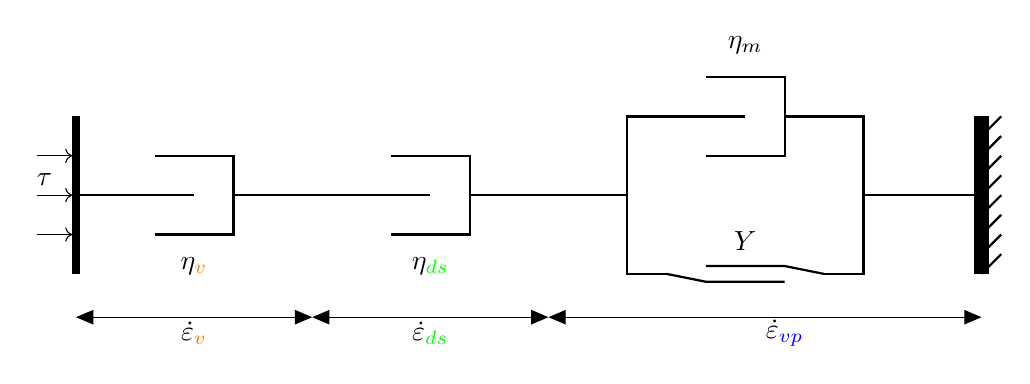
\begin{tikzpicture}
%\draw[fill=gray!23,gray!23](0,0) rectangle (7,5);
%\draw[step=0.5cm,gray,very thin] (0,0) grid (12,5); %background grid

\node[] at (0.1,2.7) {$\tau$};
\draw[line width=1mm] (0.5,1.5) -- (0.5,3.5) ;   
\draw [->] (0,2.5) -- (0.45,2.5);
\draw [->] (0,2) -- (0.45,2);
\draw [->] (0,3) -- (0.45,3);

\draw[thick] (0.5,2.5) -- (2,2.5) ;   
\draw[thick] (2.5,2.5) -- (5,2.5) ;   
\draw[thick] (5.5,2.5) -- (7.5,2.5) ;   
\draw[thick] (10.5,2.5) -- (12,2.5) ;   

% v damper
\draw[thick] (1.5,3) -- (2.5,3) -- (2.5,2) -- (1.5,2);  
% ds damper
\draw[thick] (4.5,3) -- (5.5,3) -- (5.5,2) -- (4.5,2);  
% m damper
\draw[thick] (8.5,4) -- (9.5,4) -- (9.5,3) -- (8.5,3);  

\node[] at (2,1.6) {$\eta_{\color{orange}v}$};
\node[] at (5,1.6) {$\eta_{\color{green}ds}$};
\node[] at (9,4.4) {$\eta_m$};

\draw[thick] (9,3.5) -- (7.5,3.5) -- (7.5,1.5) -- (8,1.5);  
\draw[thick] (9.5,3.5) -- (10.5,3.5) -- (10.5,1.5) -- (10,1.5);  

\draw[thick] (8,1.5) -- (8.5,1.4) -- (9.5,1.4) ;   
\draw[thick] (8.5,1.6) -- (9.5,1.6) -- (10,1.5) ;   

\node[] at (9,1.92) {$Y$};

%wall
\draw[line width=2mm] (12,1.5) -- (12,3.5) ;   
\draw[thick] (12,1.5) -- (12.25,1.75) ;   
\draw[thick] (12,1.75) -- (12.25,2) ;   
\draw[thick] (12,2) -- (12.25,2.25) ;   
\draw[thick] (12,2.25) -- (12.25,2.5) ;   
\draw[thick] (12,2.5) -- (12.25,2.75) ;   
\draw[thick] (12,2.75) -- (12.25,3) ;   
\draw[thick] (12,3) -- (12.25,3.25) ;   
\draw[thick] (12,3.25) -- (12.25,3.5) ;   

\draw[>=triangle 45, <->] (0.5,0.95) -- (3.5,0.95);
\draw[>=triangle 45, <->] (3.5,.95) -- (6.5,0.95);
\draw[>=triangle 45, <->] (6.5,0.95) -- (12,0.95);
\node[] at (2,0.75)   {$\dot\varepsilon_{\color{orange}v}$};
\node[] at (5,0.75)   {$\dot\varepsilon_{\color{green}ds}$};
\node[] at (9.5,0.75) {$\dot\varepsilon_{\color{blue}vp}$};

\end{tikzpicture}

\end{center}
This rheology would be called visco-viscoplastic.
The algorithm goes then as follows:
\begin{enumerate}
\item Assume we know $\eta_v$ and $\dot\varepsilon_T$ (from previous iteration), as well as the plasticity parameters $Y$ and $\eta_m$.
\item if $2 \eta_v \dot\varepsilon_T < Y$ the stress is below the yield stress value and plasticity is not active. Use $\eta_v$ in the material model and $\dot\varepsilon_v=\dot\varepsilon_T$.

\item if $2 \eta_v \dot\varepsilon_T > Y$ the stress is above the yield value, which is not allowed. In this case the plastic element is 'switched on'. In that case the viscous damper is in series with the (visco)plastic element. The former deforms with a strain rate $\dot\epsilon_v$ while the latter with $\dot\epsilon_{vp}$ (both under the same stress $\tau$) and we have  $\dot\varepsilon_T = \dot\varepsilon_v  + \dot\varepsilon_{vp}$. 

\begin{eqnarray}
\dot\varepsilon_T 
&=& \dot\varepsilon_v + \dot\varepsilon_{vp}  \nonumber\\
&=& \dot\varepsilon_v + \frac{\tau}{2 \eta_{vp}} \nonumber\\
&=& \dot\varepsilon_v + \frac{\tau}{2 \left( \frac{Y}{2\dot\varepsilon_{vp}} + \eta_m  \right)} \nonumber\\
&=& \dot\varepsilon_v + \frac{\tau}{2 \left( \frac{Y}{2(\dot\varepsilon_T-\dot\varepsilon_v)}+\eta_m\right)} \nonumber\\
\dot\varepsilon_T - \dot\varepsilon_v 
&=& \frac{\tau}{2 \left( \frac{Y}{2(\dot\varepsilon_T-\dot\varepsilon_v)}+\eta_m\right)} \nonumber\\
2 (\dot\varepsilon_T - \dot\varepsilon_v)
\left( \frac{Y}{2(\dot\varepsilon_T-\dot\varepsilon_v)}+\eta_m\right) &=& \tau \nonumber\\
Y +  2(\dot\varepsilon_T - \dot\varepsilon_v) \eta_m &=& \tau \nonumber\\
Y +  2(\dot\varepsilon_T - \frac{\tau}{2 \eta_v}) \eta_m &=& \tau \nonumber\\
Y +  (2\eta_v \dot\varepsilon_T - \tau) \frac{\eta_m}{\eta_v} &=& \tau \nonumber\\
Y +  2\eta_m \dot\varepsilon_T  &=& \tau (1 + \frac{\eta_m}{\eta_v} ) \nonumber
\end{eqnarray}
and finally 
\begin{equation}
\tau  = \frac{Y + 2 \eta_m \dot\varepsilon_T} {1+ \frac{\eta_m}{\eta_v} }
\end{equation}
Note that this solution exists even when $\eta_m=0$, and then rather logically $\tau=Y$.

\item Once we have $\tau$, we can easily compute $\dot\epsilon_v = \frac{\tau}{2\eta_v}$

\item We then compute $\dot\varepsilon_{vp} = \dot\varepsilon_T- \dot\varepsilon_v$ which 
we use to compute $\eta_{vp}$:

\begin{eqnarray}
\eta_{vp} 
&=& \frac{Y}{2\dot\varepsilon_{vp}}+\eta_m \nn\\
&=& \frac{Y}{2(\dot\varepsilon_{T}-\dot\varepsilon_{v})}+\eta_m \nn\\
&=& \frac{Y}{2(\dot\varepsilon_{T}-\frac{\tau}{2\eta_v})}+\eta_m \nn\\
&=& \frac{Y}{2(\dot\varepsilon_{T}- \frac{Y + 2 \eta_m \dot\varepsilon_T} {1+ \frac{\eta_m}{\eta_v} }   
\frac{1}{2\eta_v})}+\eta_m \nn\\
&=& \frac{Y}{2\dot\varepsilon_{T}- \frac{Y + 2 \eta_m \dot\varepsilon_T} {\eta_v + \eta_m}     }+\eta_m \\
&=& \frac{Y(\eta_v+\eta_m)}{2(\eta_v+\eta_m) \dot\varepsilon_{T}- (Y + 2 \eta_m \dot\varepsilon_T) }+\eta_m \\
&=& \frac{Y(\eta_v+\eta_m)}{2 \eta_v \dot\varepsilon_{T}- Y  }+\eta_m \\
&=& \frac{Y(\eta_v+\eta_m)/2\eta_v}{ \dot\varepsilon_{T}- Y/2\eta_v  }+\eta_m 
\end{eqnarray}


\item Having obtained $\eta_{vp}$ we can compute the final effective viscosity
\[
\eta_{eff} = \left( \frac{1}{\eta_v}  + \frac{1}{\eta_{vp}}  \right)^{-1}
\]
\end{enumerate}

On the following plots are shown $\tau$, 
$\dot\varepsilon_{vp}$, $\dot\varepsilon_v$, $\eta_vp$, and $\eta_{eff}$ 
as a function of  $\dot\varepsilon_T$: 

\begin{center}
\includegraphics[width=5.5cm]{images/rheology/vvp/tau.pdf}
\includegraphics[width=5.5cm]{images/rheology/vvp/strainrates.pdf}
\includegraphics[width=5.5cm]{images/rheology/vvp/viscosities.pdf}\\
{\captionfont Obtained for $\eta_m=10^{21}$, $Y=20$MPa and $\eta_v=10^{25}$. Python code 
in images/rheology/vvp/}
\end{center}

In the following plots the resulting stress $\tau$ and effective viscosities $\eta_{eff}$
are compared between the above approach ('new') and the simpler (and naive) 
approach where $\dot\varepsilon_T$ 
is used in $\eta_{vp}$ instead of $\dot\varepsilon$ ('old'). In this particular case 
we see that it makes a difference at low strain rates close to the brittle-ductile transition.

\begin{center}
\includegraphics[width=8cm]{images/rheology/vvp/tau_comp.pdf}
\includegraphics[width=8cm]{images/rheology/vvp/viscosities_comp.pdf}\\
{\captionfont Obtained for $\eta_m=10^{21}$, $Y=20$MPa and $\eta_v=10^{25}$. Python code 
in images/rheology/vvp/}
\end{center}

\begin{remark}
The introduction of the damper $\eta_m$ in parallel with the plastic element has an unavoidable
effect: the stress $\tau$ becomes larger than $Y$ at high strain rate values! Since the $vp$ 
block is akin to a bingham fluid, this is no surprise.
\end{remark}

\begin{remark}
The viscous dashpot $\eta_v$ also acts as a maximum viscosity cutoff: if $\eta_{vp}$ becomes (very) large, i.e. $\eta_{vp} \gg \eta_v$, then $\eta_{eff} \rightarrow \eta_v$.
Conversely, if $\eta_p=Y/2\dot\varepsilon_{vp}$ becomes (very) small, i.e. $\eta_p \ll \eta_m$ then $\eta_m$ acts as a minimum viscosity limiter, i.e. $\eta_{vp} \rightarrow \eta_m$. 
Since $\eta_m \ll \eta_v$ then $\eta_{eff} \rightarrow \eta_m$.
\end{remark}

\underline{A simple regularisation} This idea originates in Massmeyer \etal (2013) \cite{madd13}. We postulate
\[
\tilde{\eta}_{eff} = \left(  1 - \exp (- \frac{\dot\varepsilon_T}{\dot\varepsilon_{T}^c}) \right)
\left( \frac{Y}{2 \dot\varepsilon_T} + \eta_m \right)
\]
where $\dot\varepsilon_{T}^c$ is the critical strain  rate at which the transition viscous to 
viscous-viscoplastic occues given by $\dot\varepsilon_{T}^c=Y/2\eta_v$.
When $\dot\varepsilon_{T} \ll \dot\varepsilon_{T}^c$ then the exponential term tends to zero and 
\[
\tilde{\eta}_{eff} \rightarrow  \frac{Y}{2 \dot\varepsilon_T} + \eta_m 
\]
and if $\dot\varepsilon_{T} \rightarrow \infty$ then $\tilde{\eta}_{eff}\rightarrow \eta_m$.
Conversely if $\dot\varepsilon_T \rightarrow 0$ then we can carry out a Taylor expansion of the exponential 
term ($\exp x \sim 1 + x$ when $x$ is small).
\[
\tilde{\eta}_{eff} \sim \left(  \frac{\dot\varepsilon_T}{\dot\varepsilon_{T}^c} \right)
\left( \frac{Y}{2 \dot\varepsilon_T} + \eta_m \right)
\rightarrow 
\frac{\dot\varepsilon_T}{\dot\varepsilon_{T}^c}  \frac{Y}{2 \dot\varepsilon_T}  = \eta_v
\]
At low strain rates the viscosity does not 'explode' but actually converges to the background viscosity $\eta_v$.
The stress $\tau$ corresponding to this viscosity is simply $\tilde{\tau} = 2 \tilde{\eta}_{eff}$. 
Both $\tilde{\tau}$ and $ \tilde{\eta}_{eff}$ are plotted hereunder:


\begin{center}
\includegraphics[width=7.5cm]{images/rheology/vvp/tau_reg.pdf}
\includegraphics[width=7.5cm]{images/rheology/vvp/viscosities_reg.pdf}\\
{\captionfont Obtained for $\eta_m=10^{21}$, $Y=20$MPa and $\eta_v=10^{25}$. Python code 
in images/rheology/vvp/}
\end{center}


\includegraphics[width=7.5cm]{images/rheology/vvp/ratio_visc.pdf}



%which, if  yields the following effective viscosity:
%\[
%\eta_{eff} = \left( \frac{1}{\eta_M}  + \frac{1}{\frac{Y}{2 \dot{\varepsilon}_e} + \eta_m}  \right)^{-1}
%\]
%When the strain rate becomes very small,  $\dot{\varepsilon}_e \rightarrow 0$, $\eta_{eff}\rightarrow \eta_{M}$.
%When the strain rate becomes very large,  $\dot{\varepsilon}_e \rightarrow \infty$, $\eta_{eff}\rightarrow \eta_{m}$.
%We can then rewrite the above equation as a function of $\eta_{min}$ and $\eta_{max}$:
%\[
%\eta_{eff} = \left( \frac{1}{\eta_{max}}  + \frac{1}{\frac{c}{2 \dot{\varepsilon}_e} + \eta_{min}}  \right)^{-1}
%\]
%
%The effective viscosity is plotted here for various values of the minimum viscosity (for $c$=200MPa and $\eta_{max}=10^{25}Pa.s$:
%\includegraphics[width=8cm]{images/viscoplasticity/nu_eff}



\item \underline{two nonlinear viscous dampers in series:} 

\begin{center}
\input{tikz/tikz_dashpotdashpot_series_nl}
\end{center}

There are two dashpots in series, one accounts for dislocation creep, the other for diffusion creep.
The algorithm goes then as follows:
\begin{enumerate}
\item Assume we know $\dot\varepsilon_T$ (from previous iteration). 
\item The dashpots are in series so 
\[
\dot\varepsilon_T = \dot\varepsilon_{ds} + \dot\varepsilon_{df} 
\]
with
\begin{eqnarray}
\dot\varepsilon_{ds}  &=& A_{ds} \tau^n \exp \left(-\frac{Q_{ds}+pV_{ds}}{RT}\right) \label{sr_ds1} \\
\dot\varepsilon_{df}  &=& A_{df} \tau   \exp \left(-\frac{Q_{df}+pV_{df}}{RT}\right) \label{sr_df1} 
\end{eqnarray}
such that we are in fact looking for the stress value $\tau$ so that 
\[
\dot\varepsilon_T = 
A_{ds} \tau^n \exp \left(-\frac{Q_{ds}+p V_{ds}}{RT}\right) 
+
A_{df} \tau   \exp \left(-\frac{Q_{df}+p V_{df}}{RT}\right) 
\]
or, we must find the zero of the function ${\cal F}(\tau)$: 
\[
{\cal F}(\tau) =  \dot\varepsilon_T 
- A_{ds} \tau^n \exp \left(-\frac{Q_{ds}+p V_{ds}}{RT}\right) 
- A_{df} \tau   \exp \left(-\frac{Q_{df}+p V_{df}}{RT}\right) 
\]
This equation can be solved with a Newton-Raphson algorithm
and the iterations will be of the form:
\[
\tau_{n+1} = \tau_n - \frac{{\cal F}(\tau_n)}{{\cal F}'(\tau_n)}
\]
where the derivative of the function ${\cal F}$ with respect to $\tau$ reads:
\[
{\cal F}'(\tau)=\frac{\partial {\cal F}}{\partial \tau}=
- A_{ds} n \tau^{n-1} \exp\left(-\frac{Q_{ds}+pV_{ds}}{RT}\right)
- A_{df} \exp\left(-\frac{Q_{df}+pV_{df}}{RT}\right) 
\]
Once the value of $\tau$ is found, 
the strain rate values of Eqs. (\ref{sr_ds1}) and (\ref{sr_df1})
can be computed and so can the respective effective viscosities:
\begin{eqnarray}
\eta_{ds} 
&=& \frac{1}{2} A_{ds}^{1/n} \dot\varepsilon_{ds}^{\frac{1}{n}-1} \exp \left(\frac{Q_{ds}+pV_{ds}}{nRT}\right) \\
\eta_{df} 
&=& \frac{1}{2} A_{df}^{1/n}  \exp \left(\frac{Q_{df}+pV_{df}}{RT}\right) 
\end{eqnarray}
Their average effective viscosity $\tilde{\eta}_{eff}$ is given by 
\[
\tilde{\eta}_{eff} = \left( \frac{1}{\eta_{ds}} + \frac{1}{\eta_{df}} \right)^{-1}
\]
\end{enumerate}


Rather importantly, as we will see hereafter, the following variant is implemented 
in some codes (e.g. \douar, \fantom, \sopale, and probably many others) 
so as to bypass these costly Newton iterations:
\begin{enumerate}
\item compute $\eta_{ds}$ and $\eta_{df}$ with the {\it same} strainrate $\dot\varepsilon_T$, 
pressure and temperature values
\item average them by means of an harmonic average
\end{enumerate}
In this case, we have
\[
\dot{\varepsilon}_{\color{red} T}= 
A_{df} \tau_{df} \exp\left(-\frac{Q_{df}+pV_{df}}{RT}\right)
\quad\quad\quad
\dot{\varepsilon}_{\color{red} T}= 
A_{ds} \tau_{ds}^n \exp\left(-\frac{Q_{ds}+pV_{ds}}{RT}\right)
\]
or, 
\begin{eqnarray}
\eta_{ds} 
&=& \frac{1}{2} A_{ds}^{1/n} \dot\varepsilon_{\color{red}T}^{\frac{1}{n}-1} \exp \left(\frac{Q_{ds}+pV_{ds}}{nRT}\right) \\
\eta_{df} 
&=& \frac{1}{2} A_{df}^{1/n}  \exp \left(\frac{Q_{df}+pV_{df}}{RT}\right) 
\end{eqnarray}
We see that this simplification has consequences on the dislocation creep viscosity only.


\paragraph{A concrete example}
Let us consider a vertical section of upper mantle, from 660\si{\km} depth to 30\si{\km} depth.
The lithosphere is assumed to be 90\si{\km} thick. The temperature at the moho (the top
of the domain) is set to 550C, 1330C at the LMB and 1380C at the bottom.
A constant strainrate $\dot{\epsilon}_T=10^{-15}\si{\per\second}$ is assumed. 
We assume that the pressure is lithostatic (for simplicity 
the density is taken to be constant at 3300kg/m$^3$).
The temperature and pressure fields are shown hereunder:
\begin{center}
\includegraphics[width=6cm]{images/rheology/effvisc/temperature.pdf}
\includegraphics[width=6cm]{images/rheology/effvisc/pressure.pdf}
\end{center}

Material properties are taken from Karato \& Wu (1993) \cite{kawu93}.
The (fortran) code is available in {\tt images/rheology/effvisc/}.

In what follows, the values obtained with Newton iterations are coined 'NR'
and those obtained without are coined 'CHEAP'.
The diffusion and dislocation creep viscosities can be
computed for both algorithms and are shown hereunder
(As mentioned earlier the diffusion creep viscosity is independent of strain rate so
is the same for both):
\begin{center}
\includegraphics[width=6cm]{images/rheology/effvisc/both_mu_ds.pdf}
\includegraphics[width=6cm]{images/rheology/effvisc/both_mu_df.pdf}
\end{center}
We can also plot the resulting effective viscosity 
$\eta_{eff}$ for both approaches and we see that the differences 
are larger than 20\%. This is shown here under on the left, 
alongside with the partitioning of the strain rate as a function of depth:
\begin{center}
\includegraphics[width=8cm]{images/rheology/effvisc/both_mueff.pdf}
\includegraphics[width=8cm]{images/rheology/effvisc/both_sr.pdf}
\end{center}


























\item \underline{multiple viscous dampers and a plastic element} arranged as follows:



\begin{center}
\input{tikz/tikz_vvp2}
\end{center}



The algorithm goes then as follows:
\begin{enumerate}
\item Assume we know $\dot\varepsilon_T$ (from previous iteration), 
as well as the plasticity parameters $Y$ (a constant in the case of von Mises, or a pressure-dependent 
quantity otherwise) and $\eta_m$.
\item We start by assuming that the plasticity 'block' is not active ($\dot{\varepsilon}_{vp}=0$): we have then three dampers in series. 
We need their associated strain rates 
$\dot{\varepsilon}_{df}$ and $\dot{\varepsilon}_{ds}$ which are such that 
\[
\dot\varepsilon_T = 
\dot\varepsilon_v + \dot\varepsilon_{ds} + \dot\varepsilon_{df} 
\]
with
\begin{eqnarray}
\dot\varepsilon_v &=& \frac{\tau}{2 \eta_v} \label{sr_v} \\
\dot\varepsilon_{ds}  &=& A_{ds} \tau^n \exp \left(-\frac{Q_{ds}+pV_{ds}}{RT}\right) \label{sr_ds} \\
\dot\varepsilon_{df}  &=& A_{df} \tau   \exp \left(-\frac{Q_{df}+pV_{df}}{RT}\right) \label{sr_df} 
\end{eqnarray}
such that we are in fact looking for the stress value $\tau$ so that 
\[
\dot\varepsilon_T = 
A_{ds} \tau^n \exp \left(-\frac{Q_{ds}+p V_{ds}}{RT}\right) 
+
A_{df} \tau   \exp \left(-\frac{Q_{df}+p V_{df}}{RT}\right) 
+
\frac{\tau}{2 \eta_v}
\]
or, we must find the zero of the function ${\cal F}$: 
\[
{\cal F}(\tau) = 
\dot\varepsilon_T 
- A_{ds} \tau^n \exp \left(-\frac{Q_{ds}+p V_{ds}}{RT}\right) 
- A_{df} \tau   \exp \left(-\frac{Q_{df}+p V_{df}}{RT}\right) 
- \frac{\tau}{2 \eta_v} 
\]
This equation can be solved with a Newton-Raphson algorithm
and the iterations will be of the form:
\[
\tau_{n+1} = \tau_n - \frac{{\cal F}(\tau_n)}{{\cal F}'(\tau_n)}
\]
where the derivative of the function ${\cal F}$ with respect to $\tau$ reads:
\[
{\cal F}'(\tau)=\frac{\partial {\cal F}}{\partial \tau}=
- A_{df} \exp\left(-\frac{Q_{df}+pV_{df}}{RT}\right) 
- A_{ds} n \tau^{n-1} \exp\left(-\frac{Q_{ds}+pV_{ds}}{RT}\right)
- \frac{1}{2\eta_v}
\]
Once the value of $\tau$ is found, 
the strain rate values of Eqs. (\ref{sr_ds}), (\ref{sr_df}) and (\ref{sr_v}) 
can be computed and so can the respective effective viscosities:
\begin{eqnarray}
\eta_{ds} 
&=& \frac{1}{2} A_{ds}^{1/n} \dot\varepsilon_{ds}^{\frac{1}{n}-1} \exp \left(\frac{Q_{ds}+pV_{ds}}{nRT}\right) \\
\eta_{df} 
&=& \frac{1}{2} A_{df}^{1/n}  \exp \left(\frac{Q_{df}+pV_{df}}{RT}\right) 
\end{eqnarray}
Their average effective viscosity $\tilde{\eta}_{eff}$ is given by 
\[
\tilde{\eta}_{eff} = \left( \frac{1}{\eta_{ds}} + \frac{1}{\eta_{df}} + \frac{1}{\eta_v} \right)^{-1}
\]


\item if $\tau =2 \tilde{\eta}_{eff} \dot\varepsilon_T < Y$ the stress is below the yield stress value 
and the plasticity element is indeed not active. Use $\tilde{\eta}_{eff}$ in the material model.

\item if $\tau=2 \tilde{\eta}_{eff} \dot\varepsilon_T > Y$ the stress is above the yield value, which is not 
allowed. In this case the plastic element must be present and active and the viscous dampers are then 
in series with the (visco)plastic element. The formers deform 
with a strain rate $\dot{\varepsilon}_v$, $\dot\epsilon_{ds}$ and $\dot{\epsilon}_{df}$ 
while the latter with $\dot\epsilon_{vp}$ (all under the same tress $\tau$) 
and we have  $\dot\varepsilon_T = \dot{\varepsilon}_v + \dot\varepsilon_{ds} + \dot\varepsilon_{df} + \dot\varepsilon_{vp}$ so:

\begin{eqnarray}
\dot\varepsilon_T - \dot{\varepsilon}_v(\tau) - \dot\varepsilon_{ds}(\tau) - \dot\varepsilon_{df}(\tau)  
&=& \dot\varepsilon_{vp}  \nonumber\\
&=& \frac{\tau}{2 \left( \frac{Y}{2\dot\varepsilon_{vp}} + \eta_m  \right)} 
\nonumber\\
%&=&  \frac{\tau}{2 \left( \frac{Y}{2 (\dot\varepsilon_T -\dot{\varepsilon}_v(\tau) -\dot\varepsilon_{ds}(\tau) 
%+ \dot\varepsilon_{df}(\tau)   )} + \eta_m  \right)} 
%\nonumber\\
\dot\varepsilon_T -  \dot{\varepsilon}_v(\tau) -\dot\varepsilon_{ds}(\tau) - \dot\varepsilon_{df}(\tau) 
&=&
\frac{\tau}{2 \left( \frac{Y}{2 (\dot\varepsilon_T -\dot{\varepsilon}_v(\tau) -\dot\varepsilon_{ds}(\tau) 
+ \dot\varepsilon_{df}(\tau)   )} + \eta_m  \right)} \nonumber
\\
2 [\dot\varepsilon_T -\dot{\varepsilon}_v(\tau) -\dot\varepsilon_{ds}(\tau) - \dot\varepsilon_{df}(\tau) ]
 \left( \frac{Y}{2 (\dot\varepsilon_T -\dot{\varepsilon}_v(\tau) -\dot\varepsilon_{ds}(\tau) + \dot\varepsilon_{df}(\tau)   )} + \eta_m  \right) &=& \tau 
\nonumber\\
Y + 2 (\dot\varepsilon_T - \dot{\varepsilon}_v(\tau) -\dot\varepsilon_{ds}(\tau) - \dot\varepsilon_{df}(\tau) ) \eta_m  &=& \tau \nonumber 
\end{eqnarray}
As before, we must find the zero of the function ${\cal F}$: 
\begin{eqnarray}
{\cal F}(\tau) 
&=& Y + 2 [\dot\varepsilon_T -\dot{\varepsilon}_v(\tau)- \dot\varepsilon_{ds}(\tau) -\dot\varepsilon_{df}(\tau) ]\eta_m -\tau \nonumber\\
&=& Y + 2 \left[ 
\dot\varepsilon_T - \frac{\tau}{2\eta_v}-A_{ds} \tau^n \exp \left(-\frac{Q_{ds}+pV_{ds}}{RT}\right) 
- A_{df} \tau   \exp \left(-\frac{Q_{df}+pV_{df}}{RT}\right)  
\right]\eta_m -\tau \nn
\end{eqnarray}
Because dislocation creep involves the $n$-th power of the stress we will here also need 
to find the zero by means of a Newton-Raphson algorithm. 

We have:
\begin{eqnarray}
\frac{\partial {\cal F}}{\partial \tau} &=&
\left[
- \frac{1}{\eta_v} 
-2 \frac{\partial  \dot\varepsilon_{ds}(\tau) }{\partial \tau} 
-2 \frac{\partial  \dot\varepsilon_{df}(\tau) }{\partial \tau} 
\right] \eta_m - 1
\end{eqnarray}

\begin{eqnarray}
{\cal F}(\tau) / 2\eta_m 
&=& 
\frac{Y}{2\eta_m}  + \dot\varepsilon_T 
- \frac{\tau}{2\eta_v}
- A_{ds}(p,T) \tau^n 
- A_{df}(p,T) \tau  
- \frac{\tau}{2\eta_m} \\
&=& 
- A_{ds}(p,T) \tau^n - \left(A_{df}(p,T) +  \frac{1}{2\eta_v} -\frac{1}{2\eta_m} \right) \tau
+ 
\left( \frac{Y}{2\eta_m}  + \dot\varepsilon_T \right) =0
\end{eqnarray}



\end{enumerate}

Note that when $\eta_m=0$ we logically recover $\tau=Y$ as the stress cannot exceed the yield strength $Y$.

Although this approach is probably the most consistent in terms of physics, the presence 
of the Newton-Raphson iterations makes it very expensive since this procedure is to be repeated 
for every quadrature point or every particle.

Let us consider a concrete example: we set $Y=20\si{\mega\pascal}$, $\eta_v=10^{25}\si{pascal}$, 
$\eta_m=10^{20}\si{pascal}$. The domain is one-dimensional of depth $660\si{km}$. The density is
assumed to be constant at $3300\si{\kg\per\cubic\metre}$. Dislocation and diffusion creep parameters
are taken from Karato \& Wu (1993) \cite{kawu93}. The temperature is linear is $20\si{\celsius}$ 
at the surface, $550\si{\celsius}$ at $30\si{km}$ depth, $1330\si{celsius}$ at $90\si{\km}$ depth 
and $1380\si{\celsius}$ at the bottom. Pressure is assumed to be lithostatic. 
The python program and the gnuplot script are in {\sl images/rheology/example}.

In the code I consider two cases: 'old' and 'new'. The latter is described above. 
'old' goes as follows: loop over total strain rate values. 
Compute dislocation and diffusion creep viscosities with it. Compute harmonic 
average of these with linear viscosity. Compute deviatoric stress value. 
use it in dislocation and diffusion formulae to arrive at respective strainrates. 

\newpage
\begin{center}
\includegraphics[width=5.5cm]{images/rheology/example/map_sr_df_old-1}
\includegraphics[width=5.5cm]{images/rheology/example/map_sr_df_new-1}
\includegraphics[width=5.5cm]{images/rheology/example/map_sr_df_diff-1}\\
\includegraphics[width=5.5cm]{images/rheology/example/map_sr_ds_old-1}
\includegraphics[width=5.5cm]{images/rheology/example/map_sr_ds_new-1}
\includegraphics[width=5.5cm]{images/rheology/example/map_sr_ds_diff-1}\\
\includegraphics[width=5.5cm]{images/rheology/example/map_sr_v_old-1}
\includegraphics[width=5.5cm]{images/rheology/example/map_sr_v_new-1}
\includegraphics[width=5.5cm]{images/rheology/example/map_sr_v_diff-1}\\
\includegraphics[width=5.5cm]{images/rheology/example/map_etaeff_old-1}
\includegraphics[width=5.5cm]{images/rheology/example/map_etaeff_new-1}
\includegraphics[width=5.5cm]{images/rheology/example/map_etaeff_diff-1}\\
\includegraphics[width=5.5cm]{images/rheology/example/map_tau_old-1}
\includegraphics[width=5.5cm]{images/rheology/example/map_tau_new-1}
\includegraphics[width=5.5cm]{images/rheology/example/map_tau_diff-1}\\
\includegraphics[width=5.5cm]{images/rheology/example/profile_sr-1}
\includegraphics[width=5.5cm]{images/rheology/example/profile_tau-1}
\includegraphics[width=5.5cm]{images/rheology/example/profile_etaeff-1}\\
\includegraphics[width=5.5cm]{images/rheology/example/map_isplast_old-1}
\includegraphics[width=5.5cm]{images/rheology/example/map_isplast_new-1}\\
{\captionfont Viscous branch: (ds+df+v) 'old' stands 
for the old approach when $\dot{\varepsilon}_T$
was used for all mechanisms. 'new' stands for the new approach and the right strain rate 
decomposition.}
\end{center}



\newpage
\begin{center}
\includegraphics[width=5.5cm]{images/rheology/example/map_etaeff_old_pl-1}
\includegraphics[width=5.5cm]{images/rheology/example/map_etaeff_new_pl-1}
\includegraphics[width=5.5cm]{images/rheology/example/map_etaeff_diff_pl-1}\\
\includegraphics[width=5.5cm]{images/rheology/example/map_tau_old_pl-1}
\includegraphics[width=5.5cm]{images/rheology/example/map_tau_new_pl-1}
\includegraphics[width=5.5cm]{images/rheology/example/map_tau_diff_pl-1}\\
\includegraphics[width=5.5cm]{images/rheology/example/profile_sr_pl-1}
\includegraphics[width=5.5cm]{images/rheology/example/profile_tau_pl-1}
\includegraphics[width=5.5cm]{images/rheology/example/profile_etaeff_pl-1}\\
{\captionfont Visco-viscoplastic rheology: (ds+df+v+vp)} 
\end{center}




\end{itemize}




\begin{remark}
Chenin \etal (2019) \cite{chmd19}, 
base their rheological model on the additive decomposition of the following
deviatoric strain rate tensor ${\bm \varepsilon}^d$:
\[
{\bm \varepsilon}^d =
{\bm \varepsilon}^{el}+
{\bm \varepsilon}^{pl}+
{\bm \varepsilon}^{ds}+
{\bm \varepsilon}^{df}+
{\bm \varepsilon}^{pe}
\]
where the five strain rate terms correspond respectively to the elastic, plastic, 
and viscous creep (dislocation, diffusion, peierls) contributions. 
This implies that all these elements are in series and the associated 
viscosities are then averaged with an harmonic mean. 
Rather interestingly, it is then stated that "this strain rate equation is nonlinear
and solved locally on cell centroids and vertices in order to define the current effective viscosity 
and stress \cite{poso08}."
\end{remark}

\Literature: \cite{hoor89,lopr90,homo90,scps01,lova01,anpa19,elga10}


































%...........................................
\subsubsection{Anisotropic viscosity}

Following the paper by Lev and Hager (2008) \cite{leha08}, 
the anisotropic viscosity enters the equation of momentum through a 'correction'
term added to the isotropic part of the constitutive equation relating
stress and strain rate \cite{mumh02}:
\[
\sigma_{ij} = -p \delta_{ij} + 2 \eta_N \dot{\varepsilon}_{ij}  - 2(\eta_N-\eta_S)\Lambda_{ijkl}\dot{\varepsilon}_{kl} 
\]
where $\eta_N$ is the normal viscosity and $\eta_S$ is the shear viscosity. 
The fourth order tensor $\Lambda$ reflects the orientation of the directors in space, 
denoted by $\vec{n}$:
\[
\Lambda_{ijkl}=\frac{1}{2} (n_i n_k \delta_{lj} + n_j n_k \delta_{il} 
+ n_i n_l \delta_{kj} n_j n_l \delta_{ik} )
- 2 n_i n_j n_k n_l 
\]
Following \cite{modm03,mumh02}, the 'directors' are advected through the model and are 
analogous to particles. The directors are
vector-particles pointing normal to the easy-glide plane or layer,
thus defining the directions associated with $\eta_N$ and $\eta_S$. 
In each time step of the calculation, the directors are advected and rotated by the
flow, and in return determine the viscosity structure for the next time
step \cite{mumc04}.

\begin{center}
\includegraphics[width=10cm]{images/rheology/leha08}\\
{\captionfont Taken from Lev \& Hager (2008) \cite{leha08}.}
\end{center}

\mscthesis\index{general}{MSc Thesis}: redo the Rayleigh-Taylor instabilities with 
anisotropic lithospheric viscosity.
experiments of Lev \& Hager (2008) \cite{leha08}. Look at the three methods 
listed in the other article by 
Lev \& Hager \cite{leha08b}. 
Check Appendix B.2.2 or \cite{perr19} for additional results.

\Literature: 
Richter \& Daly (1978) \cite{rida78},
Saito \& Abe (1984) \cite{saab84},
Vauchez \etal (1998) \cite{vatb98},
M{\"u}lhaus \etal (2002) \cite{mumh02},
M{\"u}lhaus \etal (2003) \cite{mumc03},
M{\"u}lhaus \etal (2004) \cite{mumc04},
Michibayashi \& D. Mainprice (2004) \cite{mima04},
Moresi \& M{\"u}lhaus (2006) \cite{momu06},
M{\"u}lhaus \etal (2010) \cite{mumg10},
M{\"u}lhaus \etal (2011) \cite{muso11},
Sharples \etal (2016) \cite{shmv16},
Perry-Houts \& Karlstrom \cite{peka18},
Kiraly \etal (2020) \cite{kich20}

%...........................................
\subsubsection{Rheology of the lithosphere}

\begin{center}
\includegraphics[height=5cm]{images/rheology/budr08}\\
{\captionfont Schematic view of the three most common first order rheological models of the continental 
lithosphere under a strain rate of 10$^{-14}$s$^{-1}$ . 
In all three models the upper crust has its frictional strength increased with pressure and depth. 
(a) The jelly sandwich model has a weak mid-lower crust and a strong mantle composed of dry olivine. 
(b) The cr\`eme br\^ul\'ee model assumes that the mantle is weak, due to the presence of water and high 
temperature deformation, and the dry and brittle crust determines the strength of the lithosphere. 
(c) The banana split model assumes that the lithosphere as a whole has its strength greatly reduced
due to various strain weakening and feedback processes \cite{budr08}}
\end{center}

\begin{center}
\includegraphics[width=8cm]{images/rheology/bird99}\\
{\captionfont Taken from \cite{bird99}.
Typical vertical distribution of maximum shear stress in continental lithosphere 
undergoing compressional (right) or extensional (left) strain at $10^{-15}$s. 
Friction controls level of shear stress in upper part of crust and sometimes in mantle lithosphere;
then, below brittle/ductile transition, shear stress is controlled by thermally-activated dislocation creep.}
\end{center}

Molnar \cite{moln92} discusses the validity of the Brace-Goetze strength profiles. 
In particular, he has this to say about the power law parameters:
{\it
The uncertainty alone in $Q$ alone renders calculated strengths 
uncertain by 10 times at temperatures of about 700C.
Correspondingly, that uncertainty in Q is approximately equivalent 
to an uncertainty of about 100C in temperature.
}


\begin{center}
\begin{tabular}{l|l}
\hline

Wet Quartzite & upper crust  \cite{jahu12,wabj08} \\
              & upper continental crust \cite{kecw09,cube11} \\
              & lower crust  \cite{jahu12,wabj08} \\
              & ocean sediment \cite{kecw09} \\
Dry Olivine   & lithosphere  \cite{hube07}\\
              & sublithospheric mantle \cite{hube07}\\
Dry Maryland Diabase & lower crust \cite{wabj08,wabj08b} \\
                     & lower continental crust \cite{kecw09,cube11} \\
                     & oceanic crust \cite{wabj08,kecw09,wabj08b,cube11} \\
Wet Olivine   & continental mantle lithosphere \cite{wabj08,wabj08b} \\
              & oceanic mantle lithosphere \cite{wabj08,wabj08b} \\
              & sublithospheric mantle \cite{wabj08,kecw09,wabj08b} \\
              & mantle lithosphere \cite{kecw09} \\
\hline
\end{tabular}
\end{center}



\Literature \cite{buwa06,budr08,rana97a,rana97b}





\todo[inline]{I need to talk about Byerlee's law. \cite{byer78}}

 %--------------------------------------------


\newpage
%------------------------------
\section{The Perzyna model}\label{sec:perzyna}
\index{general}{Perzyna Model}
\begin{flushright} {\tiny {\color{gray} perzyna.tex}} \end{flushright}
%~~~~~~~~~~~~~~~~~~~~~~~~~~~~~~~~~~~~~~~~~~~~~~~~~~~~~~~~~~~~~~~~~~~~~~~~~~~~~~~~~~~~~~~~~~~~~~~~~~


The Perzyna formulation is mentioned in \url{
https://en.wikipedia.org/wiki/Viscoplasticity}.
It is a rate-dependent plasticity formulation that was proposed in 1966 by Piotr Perzyna \cite{perz66}.
See also \url{https://neml.readthedocs.io/en/dev/vp_flow/perzyna.html}.



In what follows I make use of the approach and notations of Zienkiewicz (1974) \cite{zico74} (and all 
the 1974-75 papers that follow) and the book by Owen \& Hinton \cite{owhi}.

The total strain (rate) is divided into two parts\footnote{Zienkiewicz \cite{zico74} 
adds a third term ${\bm \varepsilon}^0$ which stands for initial/autogenous strain such as due 
to temperature changes but I neglect it in what follows.}:
\[
\dot{\bm \varepsilon} = \dot{\bm \varepsilon}^e + \dot{\bm \varepsilon}^{vp}  
\]
where ${\bm \varepsilon}^e$ stands for the elastic strain tensor and 
${\bm \varepsilon}^{vp}$ stands for the visco-plastic strain tensor.

%Since the tensors are symmetric only 6 of the 9 components are independent and 
%the above relationship is often re-written
%\[
%\vec{\varepsilon} = \vec{\varepsilon}^e + \vec{\varepsilon}^{vp}  
%\]
%with
%\[
%\vec{\varepsilon}=
%\left(
%\begin{array}{c}
%\varepsilon_{xx} \\
%\varepsilon_{yy} \\
%\varepsilon_{zz} \\
%\varepsilon_{xy} \\
%\varepsilon_{xz} \\
%\varepsilon_{yz} 
%\end{array}
%\right)
%\]
%For a linear elastic material 
%\[
%{\vec \varepsilon}^e = {\bm D}^{-1} \cdot {\vec \sigma}
%\]
%where ${\bm D}^{-1}$ is a symmetric elasticity matrix (compliance matrix).




The yield condition is given as 
\[
{\FFF}({\bm \sigma},\kappa) 
= \Psi(\bm\sigma,\dot{\bm \varepsilon}) -Y(\kappa) = 0
\]
with ${\FFF}<0$ denoting the purely elastic region, $\kappa$ is a 
history-dependent hardening/softening parameter and $Y(\kappa)$ is a static yield stress.
$\Psi$ is a function of the stress and/or strain rate invariants.

We borrow from classical viscoplasticity theory (Perzyna (1966) \cite{perz66}, Perzyna (1988) \cite{perz88}) 
the idea of a plastic potential defined as $\QQQ({\bm \sigma})$ and write
\begin{equation}
{\dot{\bm \varepsilon}}^{vp} 
= \gamma \Big\langle
\phi\left( {\FFF} \right) 
\Big\rangle
\frac{\partial \QQQ}{\partial \bm\sigma}
\end{equation}
where $\gamma$ is a positive, possibly time-dependent fluidity parameter. 
Note that sometimes the pseudo-viscosity $\bar{\eta}=\gamma^{-1}$ is defined \cite{zigo74}
so that the equation above writes:
\begin{equation}
{\dot{\bm \varepsilon}}^{vp} 
= \frac{1}{\bar{\eta}} \Big\langle
\phi\left( {\FFF} \right) 
\Big\rangle
\frac{\partial \QQQ}{\partial \bm\sigma}
\end{equation}
${\FFF}$ represents the plastic yield condition.
$\phi(x)$ is a positive scalar-valued monotonic increasing function in the range 
$x>0$ such that $\phi^{-1}(x)$ exists and possess similar properties in the same range. 
The notation $\langle \rangle$ denotes the Macaulay 
brackets\footnote{\url{https://en.wikipedia.org/wiki/Macaulay_brackets}} and stands 
for\footnote{there is a difference between 
\cite{zico74}(1974) and \cite{zico74b}(1974) wrt $>$ and $\ge$, and also 
a difference with wikipedia!} 
\begin{eqnarray}
\langle \phi(x) \rangle = \phi(x) & {\rm if} & x>0 \nonumber\\
\langle \phi(x) \rangle = 0 & {\rm if} & x\le 0 \nonumber
\end{eqnarray}
If ${\QQQ}={\FFF}$ then we speak of an {\it associative} law and if ${\QQQ} \neq {\FFF}$ 
we have a {\it non-associative} situation. 
The tensor $\frac{\partial \QQQ}{\partial \bm\sigma}$ represents the direction
of plastic flow and when ${\FFF}={\QQQ}$ it is a vector directed normal to the yield surface
at the stress point under consideration. This is potentially problematic in the 
case of the Tresca and Mohr-Coulomb yield surfaces since the normal is not well defined
along the apices of the surfaces (see Section~7.6 of \cite{owhi}).
In the non-associative case, the direction of plastic flow in the 
principal  stress space during plastic flow is not the same
as the direction of the vector normal to the yield surface.

In what follows we concentrate our attention on isotropic materials for which 
both ${\FFF}$ and ${\QQQ}$ can be defined in terms of stress invariants.

According to Zienkiewicz et al (1975) \cite{zihl75}:
\begin{displayquote}
{\color{darkgray}
One of the main stumbling blocks of the 
classical plasticity theory lay in the universal
assumption, based on Drucker's postulates (Drucker and Prager, 1952), that the plastic 
behaviour is `associated'. With the use of Mohr-Coulomb type yield envelopes to define the
limit between states of elasticity and of continuing irreversible deformation,
the associated behaviour manifestly contradicted observation and gave excessive dilation.
It became necessary therefore to extend plasticity ideas to a `non-associated'
form in which the plastic potential and yield surfaces are defined separately.}
\end{displayquote}
At the same time, it is worth remembering that these early studies mostly dealt
with plasticity in metals, and later soils, but not kilometer-scale crustal layers.

Also, the Perzyna model is not the only one, see for instance
the Duvaut-Lions viscoplastic model or the Consistency model \cite{wasd97,hesd02}.

We therefore need to look into the derivative of the plastic potential ${\QQQ}$
with respect to the stress tensor. Since the potential 
is expressed as a function of the stress invariants ${\III}_1(\bm\sigma)$,
${\III}_2(\bm\tau)$ and $\theta_L(\bm\tau)$, we then have\footnote{
The derivative of the Lod\'e angle was obtained in Section~\ref{ss:lode}}:

\begin{eqnarray}
\frac{\partial \QQQ}{\partial \bm\sigma}
&=&
\frac{\partial }{\partial \bm\sigma} \QQQ\left({\III}_1(\bm\sigma),{\III}_2(\bm\tau),\theta_{\rm L}(\bm\tau)\right)\nn\\
&=&
\frac{\partial \QQQ}{\partial {\III}_1(\bm\sigma)} 
\frac{\partial {\III}_1(\bm\sigma)}{\partial \bm\sigma} 
+
\frac{\partial \QQQ}{\partial \sqrt{{\III}_2(\bm\tau)}} 
\frac{\partial \sqrt{ {\III}_2(\bm\tau)}   }{\partial {\III}_2(\bm\tau)} 
\frac{\partial {\III}_2(\bm\tau)}{\partial \bm\sigma} 
+
\frac{\partial \QQQ}{\partial \theta_{\rm L}(\bm\tau)} 
\frac{\partial \theta_{\rm L}(\bm\tau)}{\partial \bm\sigma} \nn\\
&=&
\frac{\partial \QQQ}{\partial {\III}_1(\bm\sigma)} 
\frac{\partial {\III}_1(\bm\sigma)}{\partial \bm\sigma} 
+
\frac{\partial \QQQ}{\partial \sqrt{{\III}_2(\bm\tau)}} 
\frac{1}{2 \sqrt{ {\III}_2(\bm\tau)}   }
\frac{\partial {\III}_2(\bm\tau)}{\partial \bm\sigma} 
\nn\\
&&
-
\frac{\partial \QQQ}{\partial \theta_{\rm L}(\bm\tau)} 
\frac{\sqrt{3}}{2\cos 3\theta_{\rm L}}
\left[
-\frac32  \frac{ {\III}_3(\bm\tau)   }{ {\III}_2(\bm\tau)^{5/2}}
\; \frac{\partial {\III}_2(\bm\tau)}{\partial \bm\sigma} 
+  \frac{1}{{\III}_2(\bm\tau)^{3/2}} 
\; \frac{\partial {\III}_3(\bm\tau)}{\partial \bm\sigma} 
\right] \nn\\
&=&
\frac{\partial \QQQ}{\partial {\III}_1(\bm\sigma)} 
\; \frac{\partial {\III}_1(\bm\sigma)}{\partial \bm\sigma} 
+  
\left(\frac{\partial \QQQ}{\partial \sqrt{{\III}_2(\bm\tau)}} 
\frac{1}{2 \sqrt{ {\III}_2(\bm\tau)}   }   
+
\frac{\partial \QQQ}{\partial \theta_{\rm L}(\bm\tau)} 
\frac{\sqrt{3}}{2\cos 3\theta_{\rm L}}
\frac32  \frac{ {\III}_3(\bm\tau)   }{ {\III}_2(\bm\tau)^{5/2}}
\right)
\; \frac{\partial {\III}_2(\bm\tau)}{\partial \bm\sigma} \nn\\
&&
-
\frac{\partial \QQQ}{\partial \theta_{\rm L}(\bm\tau)} 
\frac{\sqrt{3}}{2\cos 3\theta_{\rm L}}
\frac{1}{{\III}_2(\bm\tau)^{3/2}} 
\; \frac{\partial {\III}_3(\bm\tau)}{\partial \bm\sigma} \nn\\
&=& 
C_1  \frac{\partial {\III}_1(\bm\sigma)}{\partial \bm\sigma} 
+
C_2  \frac{\partial {\III}_2(\bm\tau)}{\partial \bm\sigma} 
+
C_3  \frac{\partial {\III}_3(\bm\tau)}{\partial \bm\sigma} 
\end{eqnarray}
i.e.
\begin{mdframed}[backgroundcolor=blue!5]
\begin{eqnarray}
\frac{\partial \QQQ}{\partial \bm\sigma}
&=& 
C_1 {\bm a}_1 +
C_2 {\bm a}_2 +
C_3 {\bm a}_3 
=
C_1  \frac{\partial {\III}_1(\bm\sigma)}{\partial \bm\sigma} 
+
C_2  \frac{\partial {\III}_2(\bm\tau)}{\partial \bm\sigma} 
+
C_3  \frac{\partial {\III}_3(\bm\tau)}{\partial \bm\sigma} 
\end{eqnarray}
\end{mdframed}
where the $C_{1,2,3}$ coefficients depend on the plastic potential $\QQQ$
and the stress invariants as follows:
\begin{eqnarray}
C_1 &=&  \frac{\partial \QQQ}{\partial {\III}_1(\bm\sigma)} \\
C_2 
&=& \frac{\partial \QQQ}{\partial \sqrt{{\III}_2(\bm\tau)}} 
\frac{1}{2 \sqrt{ {\III}_2(\bm\tau)}   }   
+
\frac{\partial \QQQ}{\partial \theta_{\rm L}(\bm\tau)} 
\frac{\sqrt{3}}{2\cos 3\theta_{\rm L}}
\frac32  \frac{ {\III}_3(\bm\tau)   }{ {\III}_2(\bm\tau)^{5/2}} \nn\\
&=& 
\frac{\partial \QQQ}{\partial \sqrt{{\III}_2(\bm\tau)}} 
\frac{1}{2 \sqrt{ {\III}_2(\bm\tau)}   }   
-
\frac12
\frac{\tan 3\theta_{\rm L}}{ {\III}_2(\bm\tau)}
\frac{\partial \QQQ}{\partial \theta_{\rm L}(\bm\tau)}  \nn\\
&=& 
\frac{1}{2 \sqrt{ {\III}_2(\bm\tau)}   }   
\left(
\frac{\partial \QQQ}{\partial \sqrt{{\III}_2(\bm\tau)}} 
-
\frac{\tan 3\theta_{\rm L}}{\sqrt {{\III}_2(\bm\tau)}}
\frac{\partial \QQQ}{\partial \theta_{\rm L}(\bm\tau)}  
\right) \nn
\\
C_3 &=&  
-
\frac{\sqrt{3}}{2\cos 3\theta_{\rm L}}
\frac{1}{{\III}_2(\bm\tau)^{3/2}} 
\frac{\partial \QQQ}{\partial \theta_{\rm L}(\bm\tau)} 
\end{eqnarray}
These are identical to those of Eq.~(7.71) in Owen \& Hinton\footnote{This is 
not exactly true: the factor  $\frac{1}{2 \sqrt{ {\III}_2(\bm\tau)} }$
is absent in their Eq.~(7.71) but it is to be found in their Eq.~(7.70).}:
\begin{center}
\fbox{\includegraphics[width=12cm]{images/perzyna/owenhinton2}}
\end{center}

\noindent Note that we already have established (see Section~\ref{ss:recapInv}) that  
\begin{eqnarray}
{\bm a}_1 =\frac{\partial {\III}_1(\bm\sigma)}{\partial \bm\sigma} &=& {\bm 1} \nn\\
{\bm a}_2 =\frac{\partial {\III}_2(\bm\tau)}{\partial \bm\sigma} &=& {\bm \tau} \nn\\
{\bm a}_3 =\frac{\partial {\III}_3(\bm\tau)}{\partial \bm\sigma} 
&=& \bm\tau\cdot\bm\tau -\frac23  {\III}_2(\bm\tau){\bm 1} \nn
\end{eqnarray}
with (we will need these soon)
\begin{eqnarray}
\textrm{Tr}[{\bm a}_1]=
{\rm tr}\left[ \frac{\partial {\III}_1(\bm\sigma)}{\partial \bm\sigma} \right] &=& 3 \\  
\textrm{Tr}[{\bm a}_2]=
{\rm tr}\left[ \frac{\partial {\III}_2(\bm\tau)}{\partial \bm\sigma}   \right] &=& 0 \\
\textrm{Tr}[{\bm a}_3]=
{\rm tr}\left[ \frac{\partial {\III}_3(\bm\tau)}{\partial \bm\sigma}   \right] &=& 
{\rm tr}[\bm\tau\cdot\bm\tau] - 2  {\III}_2(\bm\tau) = 2  {\III}_2(\bm\tau) -2  {\III}_2(\bm\tau) = 0 
\end{eqnarray}

The generic form of the plastic potential derivative then reads 
\begin{mdframed}[backgroundcolor=blue!5]
\begin{eqnarray}
\frac{\partial \QQQ}{\partial \bm\sigma}
&=&
C_1 {\bm 1} 
+
C_2 {\bm \tau} 
+
C_3  \left( \bm\tau\cdot\bm\tau - \frac23  {\III}_2(\bm\tau)  {\bm 1} \right)
\end{eqnarray}
\end{mdframed}

The momentum conservation equation that we solve is 
\[
-\vec\nabla p + \vec\nabla \cdot \left[
2 \eta \dot{\bm\varepsilon}^d(\vec\upnu) 
\right]+ \rho \vec g = \vec 0
\]
so we need the {\it deviatoric} strain rate tensor. 
We here assume for simplicity that there is only a visco-plastic element in the system
(or that the other mechanisms are deviatoric), 
i.e. $\dot{\bm\varepsilon}=\dot{\bm\varepsilon}^{vp}$.
Then 
\begin{eqnarray}
\dot{\bm\varepsilon}^d 
&=& \dot{\bm\varepsilon}^{vp} - \frac13 {\rm tr}[ \dot{\bm\varepsilon}^{vp}] {\bm 1} \nn\\
&=& \gamma \langle \phi(\FFF) \rangle 
\left\{
\left(C_1 {\bm a}_1 + C_2 {\bm a}_2 + C_3 {\bm a}_3 \right)
-\frac13 {\rm tr} \left(C_1 {\bm a}_1 + C_2 {\bm a}_2 + C_3 {\bm a}_3 \right) {\bm 1}
\right\} \nn\\
&=& \gamma \langle \phi(\FFF) \rangle 
\left\{
\left(C_1 {\bm a}_1 + C_2 {\bm a}_2 + C_3 {\bm a}_3 \right)
-\frac13 
C_1 3  {\bm 1}
\right\} \nn\\
&=& \gamma \langle \phi(\FFF) \rangle 
\left\{
\left(C_1 \bm 1 + C_2 \bm\tau + C_3 (\bm\tau\cdot\bm\tau-\frac23 {\III}_2(\bm\tau)\bm 1)\right)
-C_1 \bm 1
\right\} \nn\\
&=& \gamma \langle \phi(\FFF) \rangle 
\left(C_2 \bm\tau + C_3 (\bm\tau\cdot\bm\tau-\frac23 {\III}_2(\bm\tau)\bm 1)\right)
\end{eqnarray}
The $C_{1,2,3}$ coefficients have been computed in 
Sections~\ref{sec:vMcriterion}, \ref{sec:trcriterion}, \ref{sec:dpcriterion} and 
\ref{sec:mccriterion}, and are summarized below: 

\begin{center}
\begin{footnotesize}
\begin{tabular}{lccc}
\hline
& $C_1$ & $C_2(\times \frac{1}{2 \sqrt{{\III}_2({\bm \tau})}})$ & $C_3$ \\
              \hline\hline
Tresca         &0 & $2 \cos\theta_{\rm L} ( 1 + {\color{teal}2} \tan\theta_{\rm L}  \tan 3\theta_{\rm L})$ &
$\frac{\sqrt{3}}{{\III}_2({\bm \tau}) } \frac{\sin\theta_{\rm L} }{\cos 3\theta_{\rm L}}$
\\ \\
von Mises      &0& {\color{teal}1}& 0 \\ \\ 
Mohr-Coulomb   & $\frac13 \sin\phi$ & 
$
\cos \theta_{\rm L} \left[
(1 +  {\color{teal}2}\tan \theta_{\rm L}   \tan 3\theta_{\rm L})
+\frac{1}{\sqrt{3}} \sin\phi
( {\color{teal}2}\tan 3\theta_{\rm L} - \tan\theta_{\rm L}) \right]$
&
$\frac{\sqrt{3}\sin\theta_{\rm L} +  \sin \phi \cos \theta_{\rm L}}
{2 {\III}_2({\bm \tau}) \cos 3\theta_{\rm L}}$ 
\\ \\
Drucker-Prager & $\alpha$ & 1 & 0 \\  
\hline
\end{tabular}
\end{footnotesize}
\end{center}
The differences with the table below  taken from Owen \& Hinton \cite{owhi} are highlighted in blue.
The difference in the von Mises simply comes from the definition of the 
yield value.

\begin{center}
\fbox{\includegraphics[width=12cm]{images/perzyna/owenhinton1}}\\
{\captionfont Taken from \cite{owhi}.
This table supposedly presents all three $C_{1,2,3}$ coefficients 
for all four plastic potentials/yield functions (associative plasticity).
This is however not the case: the $C_2$ column is not $C_2$ but 
$\partial \FFF/\partial\sqrt I_2$!
}
\end{center}


Also, the continuity equation for incompressible flow contains the divergence 
of the velocity field, and in this case 
\begin{eqnarray}
\vec\nabla\cdot\vec\upnu 
&=& {\rm tr}[\dot{\bm\varepsilon}^{vp}]  \nn\\
&=& {\rm tr}\left[ 
\gamma \Big\langle
\phi\left( {\FFF} \right) 
\Big\rangle
\frac{\partial \QQQ}{\partial \bm\sigma}
\right] \nn\\
&=& 
\gamma \Big\langle
\phi\left( {\FFF} \right) 
\Big\rangle
{\rm tr}\left[
C_1  \frac{\partial {\III}_1(\bm\sigma)}{\partial \bm\sigma} 
+
C_2  \frac{\partial {\III}_2(\bm\tau)}{\partial \bm\sigma} 
+
C_3  \frac{\partial {\III}_3(\bm\tau)}{\partial \bm\sigma} 
\right] \nn\\
&=&
\gamma \Big\langle
\phi\left( {\FFF} \right) 
\Big\rangle
{\rm tr}\left[
C_1 {\bm 1} 
+
C_2 {\bm \tau} 
+
C_3  \left( \bm\tau\cdot\bm\tau - \frac23  {\III}_2(\bm\tau)  {\bm 1} \right)
\right] \nn\\
&=&  \gamma \langle \phi(\FFF) \rangle  3 C_1
\end{eqnarray}

%If $C_3=0$, as in the vM or DP case, then we have a relationship between
%deviatoric strain rate and stress that involves a scalar. 
%If not, then a 4th order tensor is needed. This is bad news. 
%Then, vM and Tresca do not modify the continuity equation as $C_1=0$.

I find it difficult to wrap my head around this as the continuity equation 
is usually derived by other means. 
If $C_1$ is not zero, then dilation occurs, the material is not incompressible
so density should also change...  
On the other hand this is a 'problem' only when the bracket is nonzero, i.e. when
plasticity is activated. If the Macaulay bracket is zero, then we recover 
the zero divergence constraint.





\newpage
\section{Moment of inertia} \input{momentofinertia} %-------------------------------------------
\section{The need for numerical modelling}\input{needmodel} %-----------------------------------
\newpage
\section{Important mathematical concepts and equations} \begin{flushright} {\tiny {\color{gray} mathematics.tex}} \end{flushright}
%~~~~~~~~~~~~~~~~~~~~~~~~~~~~~~~~~~~~~~~~~~~~~~~~~~~~~~~~~~~~~~~~~~~~~~~~~~~~~~~~~~~~~~~~~~~~~~~~~~

%------------------------------------
\subsection{Taylor expansion}

\[
f(a+h) = f(a) + h f'(a) + \frac{h^2}{2!} f''(a) + \dots + \frac{h^{n-1}}{(n-1)!}f^{(n-1)}(a)
+ \frac{h^n}{n!}f^{(n)}(a)+ \dots
\]


%------------------------------------
\subsection{Divergence theorem}

This is also coined the Green-Ostrogradski theorem. For a volume $V$ bound by a surface $\Gamma$: 

\begin{mdframed}[backgroundcolor=blue!5]
\begin{equation}
\iint_\Gamma \vec{V}\cdot d\vec{S} = \iiint_V \vec{\nabla}\cdot\vec{V} \; dV
\end{equation}
\end{mdframed}
 \label{ss:maths} %--
 

\newpage
%%%%%%%%%%%%%%%%%%%%%%%%%%%%%%%%%%%%%%%%%%%%%%%%%%%%%%%%%%%%%%%%%%%%%%%%%%%%%%%%%%%%%%%%%%%%%%%%%%%
\section{The building blocks of the Finite Element Method} %%%%%%%%%%%%%%%%%%%%%%%%%%%%%%%%%%%%%%%%
\chapter{The building blocks of the Finite Element Method} %%%%%%%%%%%%%%%%%%%%%%%%%%%%%%%%%%%%%%%%

\begin{flushright} {\tiny {\color{gray} chapter4.tex}} \end{flushright}

\section{Numerical integration} \label{sec:quadrature}\chapter{Numerical integration} \label{sec:quadrature}

\begin{flushright} {\tiny {\color{gray} quadrature.tex}} \end{flushright}
%~~~~~~~~~~~~~~~~~~~~~~~~~~~~~~~~~~~~~~~~~~~~~~~~~~~~~~~~~~~~~~~~~~~~~~~~~~~~~~~~~~~~~~~~~~~~~~~~~~

As we will see later, using the Finite Element method to solve problems involves 
computing integrals which are more often than not too complex to be computed 
analytically/exactly. We will then need to compute them numerically.

[wiki] In essence, 
the basic problem in numerical integration is to compute an approximate solution to a definite integral
\begin{equation}
I=\int_a^b f(x) dx
\label{Idef}
\end{equation}
to a given degree of accuracy.
This problem has been widely studied and we know that 
if $f(x)$ is a smooth function, and the domain of integration is bounded, 
there are many methods for approximating the integral to the desired precision.

There are several reasons for carrying out numerical integration.
\begin{itemize}
\item The integrand $f(x)$ may be known only at certain points, such as obtained by sampling. 
Some embedded systems and other computer applications may need numerical integration for this reason.
\item A formula for the integrand may be known, but it may be difficult or impossible to 
find an antiderivative that is an elementary function. An example of such an integrand 
is $f(x)=\exp(-x^2)$, the antiderivative of which (the error function, times a constant) 
cannot be written in elementary form.
\item It may be possible to find an antiderivative symbolically, but it may be 
easier to compute a numerical approximation than to compute the antiderivative. That may be the 
case if the antiderivative is given as an infinite series or product, or if its evaluation 
requires a special function that is not available.
\end{itemize}

Let us remember that the integral of Eq.~\eqref{Idef} is in fact equal to the (signed) area 
between the $x$-axis and the curve $f(x)$ over the interval $[a,b]$:

\input{tikz/tikz_quadrature_idef}

Note that in the example above $f(x)>0$ so the area of the gray domain is counted positive.
For example, if the function $f(x)$ is a polynomial the integral can easily be computed 
analytically. In the case of a $0^{th}$ order polynomial, we have $f(x)=C$ where $C$ is a 
constant. We then have 
\begin{equation}
I=\int_a^b f(x) dx = \int_a^b C \; dx  = C \int_a^b dx = C(b-a)
\end{equation}

\input{tikz/tikz_quadrature_idef2}

We see that the area of the gray domain in simply the product of its length $b-a$ by its height $c$
and we indeed recover $I=C(b-a)$.

%%%%%%%%%%%%%%%%%%%%%%%%%%%%%
\section{In 1 dimension}

%-------------------------------------------------------------------------
\subsection{Midpoint and Trepezoidal rules  \label{sec:quad1D}}

The simplest method of this type is to let the interpolating function be 
a constant function (a polynomial of degree zero) that passes through the point $((a+b)/2, f((a+b)/2))$.
This is called the midpoint rule \index{general}{Midpoint Rule} or rectangle rule. 
\index{general}{Rectangle Rule}
We then have 
\[
I=\int_a^b f(x)dx \simeq (b-a) f\left(\frac{a+b}{2}\right)
\]
which is the area of this gray domain:

\input{tikz/tikz_quadrature_rectangle}

We can do a little bit better at virtually no cost:
we choose the interpolating function to be a straight line 
(an affine function, i.e. a polynomial of degree 1)
passing through the points $(a, f(a))$ and $(b, f(b))$.
This is called the trapezoidal rule. \index{general}{Trapezoidal Rule} 
Then 
\[
I=\int_a^b f(x)dx \simeq (b-a) \frac{f(a)+f(b)}{2}
\]

\input{tikz/tikz_quadrature_trapeze}

We see that if the function $f$ is monotonous on the interval $[a,b]$ then 
the trapezoidal approach is likely to return a value close to the real value. 
However if the function $f$ oscillates a lot in the interval, approximating it 
with a single rectangle or trapeze is not a sound assumption.
We can then make use of the additive property of the integral: let $c$ 
be the coordinate of the middle of the $[a,b]$ interval, i.e. $c=(a+b)/2$. 
Then we have 
\[
I=\int_a^b f(x)dx = \int_a^c f(x)dx + \int_c^b f(x)dx
\]
We can then apply the midpoint rule or the trapezoidal rule over both segments 
$[a,c]$ and $[c,b]$:

\input{tikz/tikz_quadrature_both}

In this case we would have 
\begin{eqnarray}
I_{midpoint} &=& (c-a)f(\frac{a+c}{2}) + (b-c)f(\frac{c+b}{2})  \nn\\
I_{trapeze}  &=& (c-a)\frac{f(a)+f(c)}{2} + (b-c) \frac{f(c)+f(b)}{2} \nn
\end{eqnarray}

Of course we can repeat the process and for either one of these rules, 
we can make a more accurate approximation by 
breaking up the interval $[a,b]$ into some number $n$ of subintervals, computing 
an approximation for each subinterval, then adding up all the results. 
For example, 
the composite trapezoidal rule can be stated as
\begin{equation}
\int_a^b f(x)dx \simeq \frac{b-a}{n} \left( \frac{f(a)}{2}  
+\sum_{k=1}^{n-1} f\left(a+k\frac{b-a}{n}\right)
   +\frac{f(b)}{2} \right)
\end{equation}
where the subintervals have the form $[kh,(k+1)h]$, with $h=(b-a)/n$ and $k=0,1,2,\dots,n-1$.

\todo[inline]{add formula for mid-point and details}


\begin{center}
a)\includegraphics[width=7cm]{images/quadrature/int1}
b)\includegraphics[width=7cm]{images/quadrature/int2}\\
The interval $[-2,2]$ is broken into 16 sub-intervals. The blue lines correspond to the 
approximation of the red curve by means of a) the midpoint rule,  b) the trapezoidal rule.
\end{center}

There are several algorithms for numerical integration (also commonly 
called ``{\color{olive}numerical quadrature}'', or
simply ``{\color{olive}quadrature}'') \index{general}{Quadrature}.
Interpolation with polynomials evaluated at equally spaced points in $[a,b]$
yields the Newton-Cotes formulas, of which the rectangle rule and the trapezoidal rule are examples. 
\index{general}{Newton-Cotes}

%--------------------------------------------------------------------
\subsection{in 1D - Gauss-Legendre quadrature  \label{sec:quad1Dglq}}

If we allow the intervals between interpolation points to vary, we find another group of quadrature formulas, such as 
the Gauss(ian) quadrature formulas. \index{general}{Gauss-Legendre Quadrature}
A Gaussian quadrature rule is typically more accurate than a Newton-Cotes rule, 
which requires the same number of function evaluations, if the integrand is smooth 
(i.e., if it is sufficiently differentiable).


An $n-$point Gaussian quadrature rule, named after Carl Friedrich Gauss, is a quadrature rule constructed
to yield an exact result for polynomials of degree $2n-1$ or less by a suitable choice of the points $x_i$
and weights $w_i$ for $i=1,\dots,n$.

The domain of integration for such a rule is conventionally taken as $[-1,1]$, so the rule is stated as
\begin{mdframed}[backgroundcolor=blue!5]
\[
\int_{-1}^{+1} f(x) dx = \sum_{i_q=1}^n w_{i_q} f(x_{i_q})
\]
\end{mdframed}
In this formula the $x_{i_q}$ coordinate is 
the $i$-th root of the {\color{olive} Legendre polynomial}\footnote{\url{https://en.wikipedia.org/wiki/Legendre_polynomials}} $P_n(x)$. 
\index{general}{Legendre Polynomial}

It is important to note that a Gaussian quadrature will only produce good results if the function $f(x)$
is well approximated by a polynomial function within the range $[-1,1]$.
As a consequence, the method is not, for example, suitable for functions with singularities.

%\begin{center}
%\includegraphics[width=5.cm]{images/quadrature/gq2}\\
%Gauss-Legendre points and their weights.
%\end{center}

\begin{center}
\begin{tabular}{lllrr}
\hline
n & $x_{iq}$ & $w_{iq}$ & $x_{iq}$ (approx) & $w_{iq}$ (approx) \\
\hline\hline
1 & 0 & 2 & 0 & 2 \\
\hline
2 & $\pm \sqrt{1/3}$ & 1  & $\pm$0.577 350 269 189 626 & 1 \\
\hline
3 & 0 & 8/9 & 0                                          & 0.888 888 888 888 888 \\
  & $\pm\sqrt{3/5}$  & 5/9  & $\pm$0.774 596 669 241 483 & 0.555 555 555 555 555 \\
\hline
4 & $\pm\sqrt{\frac{3}{7} - \frac{2}{7}\sqrt{6/5}}$  & $\frac{18+\sqrt{30}}{36}$ & $\pm$0.339 981 043 584 856 & 0.652 145 154 862 546 \\
  & $\pm\sqrt{\frac{3}{7} + \frac{2}{7}\sqrt{6/5}}$  & $\frac{18-\sqrt{30}}{36}$ & $\pm$0.861 136 311 594 953 & 0.347 854 845 137 454 \\
\hline
5 & 0 & 128/225                                    & 0                                                          & 0.568 888 888 888 889 \\
  & $\pm\frac{1}{3}\sqrt{5-2\sqrt{\frac{10}{7}}}$  & $\frac{322+13\sqrt{70}}{900}$ & $\pm$0.538 469 310 105 683 & 0.478 628 670 499 366 \\
  & $\pm\frac{1}{3}\sqrt{5+2\sqrt{\frac{10}{7}}}$  & $\frac{322-13\sqrt{70}}{900}$ & $\pm$0.906 179 845 938 664 & 0.236 926 885 056 189 \\
\hline
6 & ?& ?& $\pm$0.238 619 186 083 197 & 0.467 913 934 572 691\\
  &  &  & $\pm$0.661 209 386 466 265 & 0.360 761 573 048 139\\
  &  &  & $\pm$0.932 469 514 203 152 & 0.171 324 492 379 170\\
\hline
7 & & & $\pm$0.949 107 912 342 759 & 0.129 484 966 168 870\\
  & & & $\pm$0.741 531 185 599 394 & 0.279 705 391 489 277\\
  & & & $\pm$0.405 845 151 377 397 & 0.381 830 050 505 119\\
  & & & 0.000 000 000 000 000 & 0.417 959 183 673 469\\
\hline
8 & & & $\pm$0.960 289 856 497 536 & 0.101 228 536 290 376\\
  & & & $\pm$0.796 666 477 413 627 & 0.222 381 034 453 374\\
  & & & $\pm$0.525 532 409 916 329 & 0.313 706 645 877 887\\
  & & & $\pm$0.183 434 642 495 650 & 0.362 683 783 378 362\\
\hline
9 & & & $\pm$0.968 160 239 507 626 & 0.081 274 388 361 574\\
  & & & $\pm$0.836 031 107 326 636 & 0.180 648 160 694 857\\
  & & & $\pm$0.613 371 432 700 590 & 0.260 610 696 402 935\\
  & & & $\pm$0.324 253 423 403 809 & 0.312 347 077 040 003\\
  & & & 0.000 000 000 000 000 & 0.330 239 355 001 260\\
\hline
10 &&& $\pm$0.973 906 528 517 172 & 0.066 671 344 308 688\\
   &&& $\pm$0.865 063 366 688 985 & 0.149 451 349 150 581\\
   &&& $\pm$0.679 409 568 299 024 & 0.219 086 362 515 982\\
   &&& $\pm$0.433 395 394 129 247 & 0.269 266 719 309 996\\
   &&& $\pm$0.148 874 338 981 631 & 0.295 524 224 714 753\\
\hline
\end{tabular}\\
{\captionfont Abscissae and weights for Gauss quadratures up to $n=10$. See \cite[p89]{li06}. Also check \url{https://pomax.github.io/bezierinfo/legendre-gauss.html}.}
\end{center}

As shown in the above table, it can be shown that the weight values must fulfil the following condition:
\begin{equation}
\sum_{i_q} w_{i_q}=2 \label{gq23}
\end{equation}
This simply comes from the requirement that when $f(x)=1$ then $\int_{-1}^{+1}f(x)dx=2=\sum w_{iq}$.
It is also worth noting that all quadrature point coordinates are symmetrical around the origin.

Since most quadrature formula are only valid on a specific interval, we now must address the problem 
of their use outside of such intervals. The solution turns out to be quite simple: one 
must carry out a change of variables from the interval $[a,b]$ to $[-1,1]$.
We then consider the reduced coordinate $r\in[-1,1]$ such that 
\begin{equation}
r=\frac{2}{b-a}(x-a)-1 
\end{equation}
This relationship can be reversed such that when $r$ is known, its equivalent coordinate 
$x\in[a,b]$ can be computed:
\begin{equation}
x=\frac{b-a}{2}(1+r)+a
\end{equation}
From this it follows that
\begin{equation}
dx=\frac{b-a}{2}dr
\end{equation}
and then 
\begin{mdframed}[backgroundcolor=blue!5]
\begin{equation}
\int_a^b f(x) dx  = \frac{b-a}{2} \int_{-1}^{+1} f(r) dr \simeq 
\frac{b-a}{2} \sum_{i_q=1}^{n_q} w_{i_q} f(r_{i_q})
\end{equation}
\end{mdframed}

%--------------------
\subsection{A probably naive way of finding the quadrature points coordinates and weights}

We start from the assumption that the quadrature must be exact for polynomials $f(r)$, that it is 
written
\[
I= \int_{-1}^{+1} f(r) dr = \sum_{i_q=1}^{n_q} w_{iq} f(r_{i_q}) 
\]
and that $n_q>0$, $w_{i_q}\neq 0$ and $r_{i_q}\in [-1,1]$.

Let us start with zero-th order polynomials, i.e. $f(r)=C$. Then $I=2C$ and we must then 
have 
\[
2C = \sum_{i_q=1}^{n_q} w_{iq} f(r_{i_q})  =  \sum_{i_q=1}^{n_q} w_{iq} C   
\]
which imposes 
\begin{equation}
\boxed{
\sum_{i_q=1}^{n_q} w_{iq} = 2 \qquad \forall n_q>0
}
\label{eq:glqone}
\end{equation}
As long as the sum of the weights is equal to 2, any $n_q$-point based quadrature can 
integrate exactly a zero-th order polynomial. 

Let us move on with first-order polynomials. Since we have covered the constant term hereabove, we
set $f(r)=ar$ where $a\neq 0$. We have $I=0$ so
\begin{equation}
0 = \sum_{i_q=1}^{n_q} w_{iq} f(r_{i_q})  = a \sum_{i_q=1}^{n_q} w_{iq} r_{i_q}
\qquad
\Rightarrow
\qquad
\boxed{
\sum_{i_q=1}^{n_q} w_{iq} r_{i_q} = 0\qquad \forall n_q>0
}
 \label{eq:glqtwo}
\end{equation}
In order to integrate exactly first-order polynomials an $n_q$-point based quadrature must 
fulfil Eqs.\eqref{eq:glqone} and \eqref{eq:glqtwo}.
\begin{itemize}
\item
If $n_q=1$, then we automatically have $w_1=2$ and $w_1 r_1 =0 $, i.e. $r_1=0$.
\item
If $n_q=2$, then $w_1+w_2=2$ and $w_1r_1+w_2r_2 = 0$. There are many solutions $w_1,w_2,r_1,r_2$ which 
can fulfil these two equations, so this is not enough to determine a unique set of coordinates and weights.
\end{itemize}

Let us now turn to second-order polynomials: as before, I choose $f(r)=a r^2$. We have 
$I=2a/3$ and 
\begin{equation}
\frac{2a}{3} = \sum_{i_q=1}^{n_q} w_{iq} f(r_{i_q})  = a \sum_{i_q=1}^{n_q} w_{iq} r_{i_q}^2 
\qquad
\boxed{
\sum_{i_q=1}^{n_q} w_{iq} r^2_{i_q} = \frac{2}{3}\qquad \forall n_q>0
}
\label{eq:glqthree}
\end{equation}
\begin{itemize}
\item
If $n_q=1$, we know that $w_1=2$ and $r_1=0$. 
This means that 1-point quadrature cannot exactly integrate polynomials higher than 1.
\item
If $n_q=2$, then $w_1+w_2=2$, $w_1r_1+w_2r_2 =0$ and now $w_1r_1^2+w_2r_2^2 =2/3$. We have three equations but still four unknowns. 
At this stage, we can do a simple additional assumption: common sense would have us realise that there is no 
reason why the (in this case) 2 quadrature point coordinates should be both negative or both positive. In light 
thereof we require that quadrature point coordinates are symmetric with respect with the origin $r=0$, i.e. $r_1=-r_2$ in this case.
This yields to write:  $w_1r_1+w_2r_2 = w_1r_1+w_2(-r_1)=r_1(w_1-w_2)=0$. If $r_1=0$ then $r_2=0$ too and we do not 
have a 2-point quadrature. It must then follows that $w_1=w_2$. And finally 
$w_1r_1^2+w_2r_2^2 = w_1 r_1^2 + w_1 (-r_1)^2=2/3$, i.e. $r_1=-1/\sqrt{3}$ and $r_2=1/\sqrt{3}$ since $r_1<r_2$.
\end{itemize}

If we now turn to third-order polynomials, i.e. $f(r)=ar^3$, then $I=0$ again. We then must have
\begin{equation}
\boxed{
\sum_{i_q=1}^{n_q} w_{iq} r^3_{i_q} =  0  \qquad \forall n_q>0
}
\end{equation}
We see that the coordinates and weights obtained for a 2-point quadrature verify this equation, i.e. 
a 2-point quadrature can also exactly integrate a 3rd-order polynomial.
However, it is equally easy to verify that the 2-point quadrature cannot exactly integrate a 4th-order polynomial
since 
\[
I= \int_{-1}^{+1} r^4 dr = \frac{2}{5} \neq  \sum_{i_q=1}^{2} w_{iq} r_{i_q}^4
\]
A three-point quadrature will then be needed for those. Because of the symmetry, we know that the middle
point will be at $r=0$.

\begin{remark} 
This approach unfortunately does not shed any light on why the method is called Gauss-Legendre quadrature
nor why the quadrature points are the zeros of the Legendre polynomials...
\end{remark}


%--------------------
\subsection{Examples}\label{ss:quad:examples}

\subsubsection{Example 1}

Since we know how to carry out any required change of variables, we choose for simplicity 
$a=-1$, $b=+1$.
Let us take for example $f(r)=\pi$. Then we can compute the integral of this function 
over the interval $[a,b]$ exactly:
\[
I=\int_{-1}^{+1} f(r) dr = \pi \int_{-1}^{+1}dr  = 2 \pi
\]
We can now use a Gauss-Legendre formula to compute this same integral:
\[
I_{gq}=\int_{-1}^{+1} f(r) dr
= \sum_{i_q=1}^{n_q} w_{i_q} f(r_{i_q}) 
= \sum_{i_q=1}^{n_q} w_{i_q} \pi
= \pi \underbrace{\sum_{i_q=1}^{n_q} w_{i_q} }_{=2}
= 2 \pi
\]
where we have used the property of the weight values of Eq.(\ref{gq23}).
Since the actual number of points was never specified, this result is valid for all 
quadrature rules.


\subsubsection{Example 2}

Let us now take $f(r)=m r+ p$ and repeat the same exercise:
\[
I=\int_{-1}^{+1} f(r) dr = \int_{-1}^{+1} (mr+p) dr  =  [\frac{1}{2} m r^2 + p r ]_{-1}^{+1} =2p
\]
\[
I_{gq}=\int_{-1}^{+1} f(r) dr
\!= \sum_{i_q=1}^{n_q} w_{i_q} f(r_{i_q}) 
\!= \sum_{i_q=1}^{n_q} w_{i_q} (m r_{i_q} + p)  
\!= m \underbrace{\sum_{i_q=1}^{n_q} w_{i_q} r_{i_q}}_{=0}  + p \underbrace{\sum_{i_q=1}^{n_q} w_{i_q}}_{=2}  = 2p
\]
since the quadrature points are symmetric w.r.t. to zero on the $r$-axis.
Once again the quadrature is able to compute the exact value of this integral: this makes sense since 
an $n$-point rule exactly integrates a $2n-1$ order polynomial such that a 1 point quadrature exactly 
integrates a first order polynomial like the one above.



\subsubsection{Example 3}

Let us now take $f(r)=r^2$. We have 
\[
I=\int_{-1}^{+1} f(r) dr = \int_{-1}^{+1} r^2 dr  =  \left[\frac{1}{3}r^3 \right]_{-1}^{+1} =  \frac{2}{3} 
\]
and 
\[
I_{gq}=\int_{-1}^{+1} f(r) dr 
\!= \sum_{i_q=1}^{n_q} w_{i_q} f(r_{i_q}) 
\!= \sum_{i_q=1}^{n_q} w_{i_q} r_{i_q}^2 
\]

\begin{itemize}
\item $n_q=1$: $r_{iq}^{(1)}=0$, $w_{i_q}=2$. $I_{gq}=0$
\item $n_q=2$: $r_{q}^{(1)}=-1/\sqrt{3}$, $r_{q}^{(2)}=1/\sqrt{3}$, $w_{q}^{(1)}=w_{q}^{(2)}=1$. $I_{gq}=\frac{2}{3}$
\item It also works $\forall n_q>2$ !
\end{itemize}


\newpage
%%%%%%%%%%%%%%%%%%%%%%%%%%%%%
\section{In 2 \& 3 dimensions}

%-----------------------------------
\subsection{On the reference square}

Let us now turn to a two-dimensional integral of the form
\[
I=\int_{-1}^{+1} \int_{-1}^{+1} f(r,s) dr ds
\]
where $f(r,s)$ is again assumed to be continuous over the domain. 
The equivalent Gaussian quadrature writes:
\[
I_{gq}
\simeq \sum_{i_q=1}^{n_q}\sum_{j_q}^{n_q} f(r_{i_q},s_{j_q}) w_{i_q} w_{j_q}
\]
Finally we have 
\begin{mdframed}[backgroundcolor=blue!5]
\begin{equation}
I=\int_{a}^{+b}\int_{c}^{+d} f(r,s) dr ds
\simeq \frac{b-a}{2} \frac{d-c}{2} 
\sum_{i_q=1}^{n_q}\sum_{j_q}^{n_q} f(r_{i_q},s_{j_q}) w_{i_q} w_{j_q}
\end{equation}
\end{mdframed}



%--------------------------------------
\subsection{On a generic quadrilateral}

Let $K$ be a quadrilateral element with straight boundary lines and with vertices 
arranged as follows:

IMAGE

We wish to evaluate
\[
I =\iint_K f(x,y) dx dy
\]
In order to do so we will first transform the element $K$ to the 
reference square element and then apply the quadrature of the previous section.
This transformation can be carried out by means of the $Q_1$ basis functions, 
see Section~\ref{ss:q12d}. We construct a linear mapping between the 
quadrilateral element $K$ and the reference square element:
\begin{eqnarray}
x(r,s) &=& \sum_{i=1}^4 \bN_i(r,s) x_i \\
y(r,s) &=& \sum_{i=1}^4 \bN_i(r,s) y_i 
\end{eqnarray}
Then we have
\[
I=\iint_K f(x,y) dx dy = \int_{-1}^{+1}\int_{-1}^{+1} f(x(r,s),y(r,s)) |{\bm J}(r,s)| dr ds
\]
where ${\bm J}(r,s)$ is the Jacobian of the transformation defined by
\[
{\bm J}(r,s) = 
\left(
\begin{array}{cc}
\frac{\partial x}{\partial r} & \frac{\partial y}{\partial r} \\ \\
\frac{\partial x}{\partial s} & \frac{\partial y}{\partial s} 
\end{array}
\right)
\]
Finally applying the Gaussian quadrature yields:
\begin{mdframed}[backgroundcolor=blue!5]
\[
I=\iint_K f(x,y) dx dy \simeq 
\sum_{i_q=1}^{n_q}\sum_{j_q}^{n_q} f(x(r_{i_q},s_{j_q}),y(r_{i_q},s_{j_q}))
\; |{\bm J}(r_{i_q},s_{j_q})|  \; w_{i_q} w_{j_q}
\]
\end{mdframed}





%-----------------------------
\subsection{Exercises}

%-------------
\begin{center}
\begin{minipage}[t]{0.77\textwidth}
\par\noindent\rule{\textwidth}{0.4pt}

\begin{center}
\includegraphics[width=0.8cm]{images/garftr} \\
{\color{orange}Exercise Quad-1}
\end{center}

Write a program which uses the midpoint rule to compute (subdivide the interval in $n$ subintervals)
\[
I=\int_{0}^{\pi/2} f(x) \; dx    \quad \qquad f(x)=x \qquad \text{and} \qquad f(x)=\cos(x)
\]
For this you will need to declare and use a function which either returns $x$ or $\cos(x)$.
Compute and plot the (absolute) error between the measured $I_n$ and the analytical value $I$ as a function of the subinterval size $h$.

Bonus: same as before with $I=\int_{1}^{3}\int_{2}^{4} (x^2y^3 + xy +1)  dx dy$.
\par\noindent\rule{\textwidth}{0.4pt}
\end{minipage}
\end{center}
%-------------


%-------------
\begin{center}
\begin{minipage}[t]{0.77\textwidth}
\par\noindent\rule{\textwidth}{0.4pt}

\begin{center}
\includegraphics[width=0.8cm]{images/garftr} \\
{\color{orange}Exercise Quad-2}
\end{center}

Same exercise as above but with the trapezoidal rule. 
Which method is the most accurate?

\par\noindent\rule{\textwidth}{0.4pt}
\end{minipage}
\end{center}
%-------------

%-------------
\begin{center}
\begin{minipage}[t]{0.77\textwidth}
\par\noindent\rule{\textwidth}{0.4pt}

\begin{center}
\includegraphics[width=0.8cm]{images/garftr} \\
{\color{orange}Exercise Quad-3}
\end{center}

The following Fortran program is an example of how Gauss quadrature 
can be implemented:

\begin{center}
\includegraphics[width=9cm]{images/quadrature/gq3} 
\end{center}

Modify/translate this previous program to use 5 quadrature points instead of two.

Integrate the functions
\[
f_1(x)=\sin(x\pi+\pi/2)
\quad\quad\quad
f_2(x)=\sqrt{x+1}
\quad\quad\quad
f_3(x)=x^4-x^3
\]
with the 2-point and the 5-point quadrature rules.

Compare the results with the analytical values.

\par\noindent\rule{\textwidth}{0.4pt}
\end{minipage}
\end{center}
%-------------

%-------------
\begin{center}
\begin{minipage}[t]{0.77\textwidth}
\par\noindent\rule{\textwidth}{0.4pt}

\begin{center}
\includegraphics[width=0.8cm]{images/garftr} \\
{\color{orange}Exercise Quad-4}
\end{center}

Compute analytically the integral of the function $f(x,y)=x^2+4y$
over the domain $\Omega = [11,14 ] \times [7,10]$.

Write a code which integrates this function
by means of a $2\times 2$, $3\times 3$ or $4\times 4$ Gauss-Legendre quadrature algorithm.

\par\noindent\rule{\textwidth}{0.4pt}
\end{minipage}
\end{center}
%-------------







\newpage
%----------------------------------------
\subsection{Quadrature on triangles}
\input{quadrature_triangles}



%----------------------------------------
\subsection{A mathematical recreation: computing the volume of a tetrahedron}

Let us find the volume of tetrahedron bounded by the planes passing through the points 
A(1,0,0), B(0,1,0), C(0,0,1) and the coordinate planes Oxy, Oxz and Oyz.

\input{tikz/tikz_tetrahedron}

The equation of the plane is $x+y+z=1$, or $z=1-x-y$.Hence, the limits of integration over 
the variable $z$ range in the interval from
$z=0$ to $z=1-x-y$. Now we can calculate the volume of the tetrahedron:
\begin{eqnarray}
V 
&=& \iiint dx \; dy \; dz \nn\\
&=& \int_0^1 dx \int_0^{1-x} dy \int_{0}^{1-x-y} dz \nn\\
&=& \int_0^1 dx \int_0^{1-x} dy (1-x-y) \nn\\
&=& \int_0^1 dx \left[y-xy-\frac12 y^2 \right]_0^{1-x} \nn\\
&=& \int_0^1 dx \left((1-x)-x(1-x)-\frac12 (1-x)^2 \right) \nn\\
&=& \int_0^1 dx \left(\frac12 -x + \frac12 x^2   \right) \nn\\
&=& \left[ \frac12 x  -\frac12 x^2 + \frac16 x^3   \right]_0^1 \nn\\
&=& \frac16
\end{eqnarray}
We will use this result in the following section.

%----------------------------------------
\subsection{Quadrature on tetrahedra}
\input{quadrature_tetrahedra}



%------------------------------------------
\subsection{The Gauss-Lobatto approach \label{sec:loba}}

All what we have seen above falls under the Gauss-Legendre quadrature method. There is however another 
somewhat common quadrature method: the Gauss-Lobatto  quadrature. \index{general}{Gauss-Lobatto}.
It is similar to Gaussian quadrature with the following  important differences:
1) There are integration points in the interval but they also always include the end points of the integration interval;
2) It is accurate for polynomials up to degree $2n-3$, where $n$ is the number of integration points.

In 1D, it reads:
\[
\int_{-1}^{+1} f(x) dx = \frac{2}{n(n-1)} [f(-1)+f(1)] + \sum_{i=2}^{n-1} w_i f(x_i) 
\]
The locations and weights of the integration points are as follows:

\begin{center}
\begin{tabular}{lllll}
\hline
n & $x_{iq}$ & $w_{iq}$ & $x_{iq}$ (approx) & $w_{iq}$ (approx) \\
\hline\hline
3 & 0 & 4/3 & & \\
  & $\pm 1$ & 1/3 & &  \\
\hline
4 & $\pm\sqrt{\frac{1}{5}}$ & 5/6 & & \\
  & $\pm 1$ & 1/6 & & \\
\hline
5 & 0 & 32/45 & & \\
  & $\pm\sqrt{\frac{3}{7}}$ & 49/90 & & \\
  & $\pm 1$ & 1/10 & & \\
\hline
6 & $\pm\sqrt{\frac{1}{3} -\frac{2\sqrt{7}}{21}}$ & $\frac{14+\sqrt{7}}{30}$ & & \\
  & $\pm\sqrt{\frac{1}{3} +\frac{2\sqrt{7}}{21}}$ & $\frac{14-\sqrt{7}}{30}$ & & \\
  & $\pm 1$ & 1/15 \\
\hline
\end{tabular}
\end{center}

 
%-------------------------------------------------------------------------
\subsection{Computing the 'real' coordinates of the quadrature points and other considerations}

The quadrature point coordinates are always given in (what I call) reduced coordinates, i.e. between 
-1 and 1.
However, one sometimes need their equivalent in the $x,y$ Cartesian space. 
This is trivial once one remembers that within an element, a field $f$ is reprensented 
as follow:
\[
f(r,s) = \sum_{i=1}^{m} \bN_{i}(r,s) f_i
\]
where $m$ is the number of nodes, $r$ and $s$ are the reduced coordinates 
and $\bN_i$ are the basis functions. 
The value of $f$ at a quadrature point $(r_q,s_q)$ is then simply
\[
f(r_q,s_q) = \sum_{i=1}^{m} \bN_{i}(r_q,s_q) f_i
\]
If we now take $f=x$, then
\[
x_q =x(r_q,s_q) = \sum_{i=1}^{m} \bN_{i}(r_q,s_q) x_i
\]
and
\[
y_q =y(r_q,s_q) = \sum_{i=1}^{m} \bN_{i}(r_q,s_q) y_i
\]
where $x_i$ and $y_i$ are the Cartesian coordinates of the nodes.
This is then easily extended to three dimensions:
\[
x_q =x(r_q,s_q,t_q) = \sum_{i=1}^{m} \bN_{i}(r_q,s_q,t_q) x_i
\]
\[
y_q =x(r_q,s_q,t_q) = \sum_{i=1}^{m} \bN_{i}(r_q,s_q,t_q) y_i
\]
\[
z_q =z(r_q,s_q,t_q) = \sum_{i=1}^{m} \bN_{i}(r_q,s_q,t_q) z_i
\]
or, 
\[
\vec{r}_q =\vec{r}(r_q,s_q,t_q) = \sum_{i=1}^{m} \bN_{i}(r_q,s_q,t_q) \vec{r}_i
\]
This also applies to other fields such as velocity, temperature, or even strain rate components 
(as long as the strain rate values have previously been computed on the nodes): 
\[
\vec{\upnu}_q =\vec{\upnu}(r_q,s_q) = \sum_{i=1}^{m} \bN_{i}(r_q,s_q) \vec{\upnu}_i
\]
\[
T_q =T(r_q,s_q) = \sum_{i=1}^{m} \bN_{i}(r_q,s_q) T_i
\]
\[
\dot{\varepsilon}_{xy,q} 
= \dot{\varepsilon}_{xy} (r_q,s_q) = \sum_{i=1}^{m} \bN_{i}(r_q,s_q)  \dot{\varepsilon}_{xy,i}
\]













 %----------------------
\newpage
\section{A bit of FE terminology} \input{terminology} %-----------------------------------------
\newpage
\section{Elements and basis functions in 1D}\label{sec:elts1D} \begin{flushright} {\tiny {\color{gray} elements1D.tex}} \end{flushright}


%------------------------------------------
\subsubsection{Linear basis functions ($Q_1$) \label{sec:bf1}}
\index{general}{$Q_1$}

Let $f(r)$ be a $C^1$ function on the interval $[-1:1]$ with $f(-1)=f_1$  and $f(1)=f_2$.
\begin{center}
\includegraphics[width=8cm]{images/linshapefct.png}
\end{center}
Let us assume that the function $f(r)$ is to be approximated on $[-1,1]$ by the first order polynomial 
\begin{equation}
f^h(r)=a+br \label{eqquad1}
\end{equation}
Then it must fulfil
\begin{eqnarray}
f^h(r=-1)&=&a-b =f_1 \nonumber\\
f^h(r=+1)&=&a+b =f_2 \nonumber
\end{eqnarray}
This leads to  
\begin{eqnarray}
a&=&\frac{1}{2}(f_1+f_2)  \nn\\
b&=&\frac{1}{2}(-f_1+f_2)  
\end{eqnarray}
and then replacing $a,b$ in Eq.~\eqref{eqquad1} by the above values one gets
\[
f^h(r) = \left[  \frac{1}{2}(1-r)\right] f_1 + \left[ \frac{1}{2}(1+r) \right] f_2
\]
or
\[
f^h(r)=\sum_{i=1}^2 N_i(r) f_1
\]
with
\begin{mdframed}[backgroundcolor=blue!5]
\begin{eqnarray}
N_1(r) &=& \frac{1}{2} (1-r) \nonumber\\
N_2(r) &=& \frac{1}{2} (1+r)
\end{eqnarray}
\end{mdframed}

\begin{center}
\includegraphics[width=8cm]{images/basis1D/linear.pdf}\\
{\captionfont Plot of the two linear functions $N_1(r)$ and $N_2(r)$.}
\end{center}

\newpage
%------------------------------------------
\subsubsection{Quadratic basis functions ($Q_2$) \label{sec:bf2}}
\index{general}{$Q_2$}

Let $f(r)$ be a $C^1$ function on the interval $[-1:1]$ with $f(-1)=f_1$, $f(0)=f_2$ and $f(1)=f_3$.
\begin{center}
\includegraphics[width=8cm]{images/quadshapefct.png}
\end{center}
Let us assume that the function $f(r)$ is to be approximated on $[-1,1]$ by the second order polynomial 
$f^h(r)$:
\begin{equation}
f(r)=a+br+cr^2 \label{eqquad}
\end{equation}
Then it must fulfil
\begin{eqnarray}
f^h(r=-1)&=&a-b+c = f_1 \nonumber\\
f^h(r=0) &=&a\quad\quad\quad\;     = f_2 \nonumber\\
f^h(r=+1)&=&a+b+c = f_3 \nonumber
\end{eqnarray}
This leads to
\begin{eqnarray}
a&=&f_2   \nn\\
b&=&\frac{1}{2}(-f_1+f_3)  \nn\\
c&=&\frac{1}{2}(f_1+f_3-2f_2) 
\end{eqnarray}
and then replacing $a,b,c$ in Eq.~\eqref{eqquad} by the above values on gets
\[
f^h(r)=\left[\frac{1}{2}r(r-1)\right] f_1 + (1-r^2) f_2 + \left[\frac{1}{2}r(r+1)\right] f_3
\]
or,
\[
\boxed{
f^h(r) = \sum_{i=1}^3 N_i(r) f_i
}
\]
with
\begin{mdframed}[backgroundcolor=blue!5]
\begin{eqnarray}
N_1(r) &=& \frac{1}{2}r(r-1) \nonumber\\
N_2(r) &=& (1-r^2) \nonumber\\ 
N_3(r) &=& \frac{1}{2}r(r+1) 
\end{eqnarray}
\end{mdframed}

\begin{center}
\includegraphics[width=8cm]{images/basis1D/quadratic.pdf}\\
{\captionfont Plot of the three quadratic functions $N_1(r)$, $N_2(r)$ and $N_3(r)$.}
\end{center}
Note that $Q_2$ basis functions can take negative values. 

We will later need the first-order derivatives of these functions:
\begin{mdframed}[backgroundcolor=blue!5]
\begin{eqnarray}
\frac{\partial N_1}{\partial r} &=& r-\frac{1}{2} \nonumber\\
\frac{\partial N_2}{\partial r} &=& -2r \nonumber\\ 
\frac{\partial N_3}{\partial r} &=& r+\frac{1}{2}
\end{eqnarray}
\end{mdframed}


%------------------------------------------
\subsubsection{Cubic basis functions ($Q_3$) \label{sec:bf3}}
\index{general}{$Q_3$}

We proceed as previously by assuming that the third-order 
polynomial representation of function $f(r)$ is given by
\[
f^h(r)=a+br+cr^2+dr^3
\]
with the nodes at position -1,-1/3, +1/3 and +1.
It then must fulfil all four conditions:
\begin{eqnarray}
f(-1)   &=& a-b+c-d = f_1 \nonumber\\
f(-1/3) &=& a-\frac{b}{3}+\frac{c}{9}-\frac{d}{27} = f_2 \nonumber\\
f(+1/3) &=& a-\frac{b}{3}+\frac{c}{9}-\frac{d}{27} = f_3 \nonumber\\
f(+1)   &=& a+b+c+d = f_4 \nonumber
\end{eqnarray}
Adding the first and fourth equation and the second and third, one arrives at
\[
f_1+f_4 = 2a+2c \quad\quad\quad f_2+f_3=2a+\frac{2c}{9}
\]
and finally:
\[
a=\frac{1}{16} \left( -f_1 + 9f_2 + 9f_3 - f_4  \right)
\]
\[
c=\frac{9}{16}\left(f_1-f_2-f_3+f_4\right)
\]
Combining the original 4 equations in a different way yields
\[
2b+2d=f_4-f_1 
\quad\quad\quad
\frac{2b}{3} + \frac{2d}{27} = f_3-f_2
\]
so that
\[
b=\frac{1}{16} \left( f_1 - 27f_2 + 27f_3 -f_4   \right)
\]
\[
d=\frac{9}{16} \left( -f_1 + 3f_2 - 3f_3 + f_4 \right)
\]
Finally,
\begin{eqnarray}
f^h(r) 
&=& a+b+cr^2+dr^3 \nonumber\\
&=& \frac{1}{16} (-1+  r +9r^2 - 9r^3 )f_1 \nonumber\\ 
&+& \frac{1}{16} ( 9-27r -9r^2 +27r^3 )f_2 \nonumber\\ 
&+& \frac{1}{16} ( 9+27r -9r^2 -27r^3 )f_3 \nonumber\\ 
&+& \frac{1}{16} (-1-  r +9r^2 + 9r^3 )f_4 \nonumber\\ 
&=& \sum_{i=1}^4 N_i(r) f_i \nonumber
\end{eqnarray}
where (see also for example \cite[p49]{li06})
\begin{mdframed}[backgroundcolor=blue!5]
\begin{eqnarray}
N_1&=& \frac{1}{16} (-1+  r+9r^2- 9r^3 ) \nonumber\\ 
N_2&=& \frac{1}{16} ( 9-27r-9r^2+27r^3 ) \nonumber\\ 
N_3&=& \frac{1}{16} ( 9+27r-9r^2-27r^3 ) \nonumber\\ 
N_4&=& \frac{1}{16} (-1-  r+9r^2+ 9r^3 ) \nonumber
\end{eqnarray}
\end{mdframed}

\begin{center}
\includegraphics[width=8cm]{images/basis1D/cubic.pdf}\\
{\captionfont Plot of the four cubic functions $N_1(r)$, $N_2(r)$, $N_3(r)$ and $N_4(r)$.}
\end{center}

Let us now verify that these functions can represent any polynomial function up to third order:

\begin{itemize}
\item
Let us assume $f(r)=C$, then
\[
f^h(r) = \sum N_i(r) f_i = \sum_i N_i C = C \sum_i N_i  = C
\]
so that a constant function is exactly reproduced, as expected.
This is a very important property of the $N_i$ functions: They must fulfil $\sum\limits_i N_i =1$.

\item
Let us assume $f(r)= r$, then $f_1=-1$, $f_2=-1/3$, $f_3=1/3$ and $f_4=+1$. We then have
\begin{eqnarray}
f^h(r) 
&=& \sum N_i(r) f_i  \nonumber\\
&=& - N_1(r) -\frac{1}{3}N_2(r) + \frac{1}{3}N_3(r)  + N_4(r) \nonumber\\
&=& [-(-1+  r+9r^2- 9r^3 ) \nn\\
&&- \frac{1}{3} ( 9-27r-9r^2-27r^3 ) \nn\\
&&+ \frac{1}{3} ( 9+27r-9r^2+27r^3 ) \nn\\
&&+ (-1-  r+9r^2+ 9r^3 )]/16 \nonumber\\
&=& [-r +9r + 9r -r]/16  + ... 0 ... \nonumber\\
&=& r   
\end{eqnarray}

\item The cases $f(r)=r^2$ and $f(r)=r^3$ are left as exercise.

\end{itemize}

The basis functions first-order derivatives are given by
\begin{mdframed}[backgroundcolor=blue!5]
\begin{eqnarray}
\frac{\partial N_1}{\partial r}&=& \frac{1}{16}  (  1 +18r - 27r^2 ) \nonumber\\ 
\frac{\partial N_2}{\partial r}&=& \frac{1}{16}  (-27 -18r + 81r^2 ) \nonumber\\ 
\frac{\partial N_3}{\partial r}&=& \frac{1}{16}  (+27 -18r - 81r^2 ) \nonumber\\ 
\frac{\partial N_4}{\partial r}&=& \frac{1}{16}  ( -1 +18r + 27r^2 ) \nonumber
\end{eqnarray}
\end{mdframed}

We can also verify that the derivatives are also properly approximated:

\begin{itemize}
\item
Let us assume $f(r)=C$, then
\begin{eqnarray}
\frac{\partial f^h}{\partial r} 
&=& \sum_i \frac{\partial N_i}{\partial r} f_i  \nonumber\\
&=&  C \sum_i \frac{\partial N_i}{\partial r}  \nonumber\\
&=& \frac{C}{16} [  (  1 +18r - 27r^2 ) 
+ (-27 -18r + 81r^2 )  
+  (+27 -18r - 81r^2 ) 
+ ( -1 +18r + 27r^2 ) ]  \nonumber\\
&=& 0 \nonumber
\end{eqnarray}

\item
Let us assume $f(r)= r$, then $f_1=-1$, $f_2=-1/3$, $f_3=1/3$ and $f_4=+1$. We then have
\begin{eqnarray}
\frac{\partial f^h}{\partial r} 
&=& \sum_i \frac{\partial N_i}{\partial r} f_i  \nonumber\\
&=& \frac{1}{16} [  -(  1 +18r - 27r^2 ) 
 -\frac{1}{3} (-27 -18r + 81r^2 )  
 +\frac{1}{3} (27 -18r - 81r^2 )
 + ( -1 +18r + 27r^2 ) ]  \nonumber\\
&=& \frac{1}{16} [-2 + 18 + 54r^2 - 54r^2] \nonumber\\
&=& 1 \nonumber
\end{eqnarray}

\item
Let us assume $f(r)= r^2$, then $f_1=1$, $f_2=1/9$, $f_3=1/9$ and $f_4=1$. We then have
\begin{eqnarray}
\frac{\partial f^h}{\partial r} 
&=& \sum_i \frac{\partial N_i}{\partial r} f_i  \nonumber\\
&=& \frac{1}{16} \left[  
(  1 +18r - 27r^2 ) 
+\frac19 (-27 -18r + 81r^2 )  
+\frac19  (27 -18r - 81r^2 )
+ ( -1 +18r + 27r^2 ) \right]  \nonumber\\
&=& \frac{1}{16}(32r) \nn\\
&=& 2r
\end{eqnarray}
as expected.




\end{itemize}

%---------------------------------------------------------------
\subsubsection{Quartic basis functions ($Q_4$) \label{sec:bf4}}
\index{general}{$Q_4$}

The 1D basis polynomial is given by
\[
f_h(r)=a+br+cr^2+dr^3+er^4
\]
with the nodes at position -1,-1/2, 0, +1/2 and +1.
The function $f^h(r)$ must then fulfil 
\begin{eqnarray}
f_h(-1)   &=& a-b+c-d+e = f_1 \nonumber\\
f_h(-1/2) &=& a-\frac{b}{2}+\frac{c}{4}-\frac{d}{8}+\frac{e}{16} = f_2 \nonumber\\
f_h(0)    &=& a = f_3 \nonumber\\
f_h(+1/2) &=& a-\frac{b}{2}+\frac{c}{4}-\frac{d}{8}+\frac{e}{16} = f_4 \nonumber\\
f_h(+1)   &=& a+b+c+d+e = f_5 \nonumber
\end{eqnarray}
or, 
\begin{equation}
\left(
\begin{array}{ccccc}
 1  &  -1  &  1 &  -1 &  1 \\ 
 1  &  -1/2  &  1/4 &  -1/8 &  1/16 \\ 
 1  &   0    &  0   &   0   & 0 \\
 1  &  1/2  &  1/4 &  1/8 &  1/16 \\ 
 1  &  1  &  1 &  1 &  1 
\end{array}
\right)
\left(
\begin{array}{c}
a \\ b \\ c \\ d \\ e
\end{array}
\right)
=
\left(
\begin{array}{c}
f_1 \\ f_2 \\ f_3 \\ f_4 \\ f_5
\end{array}
\right)
\end{equation}
The third line gives $a=f_3$ so that
\begin{equation}
\underbrace{
\left(
\begin{array}{ccccc}
-1  &  1   &  -1 &  1 \\ 
-1/2 &  1/4 & -1/8 &  1/16 \\ 
 1/2 &  1/4 &  1/8 &  1/16 \\ 
 1  &  1   &  1 &  1 
\end{array}
\right)}_{A}
\left(
\begin{array}{c}
b \\ c  \\ d \\ e
\end{array}
\right)
=
\left(
\begin{array}{c}
f_1 -f_3 \\ f_2 -f_3\\ f_4-f_3 \\ f_5 -f_3
\end{array}
\right)
\end{equation}
The inverse of the matrix $A$ is:
\[
A^{-1}=
\frac{1}{6}
\left(
\begin{array}{ccccc}
1 & -8 & 8 & -1 \\
-1 & 16 & 16 & -1 \\
-4 & 8 & -8 & 4 \\
4 & -16 & -16 & 4
\end{array}
\right)
\]
so that 
\[
\left(
\begin{array}{c}
b \\ c \\ d \\ e
\end{array}
\right)
=
\frac{1}{6}
\left(
\begin{array}{ccccc}
1 & -8 & 8 & -1 \\
-1 & 16 & 16 & -1 \\
-4 & 8 & -8 & 4 \\
4 & -16 & -16 & 4
\end{array}
\right)
\cdot
\left(
\begin{array}{c}
f_1 -f_3 \\ f_2 -f_3\\ f_4-f_3 \\ f_5 -f_3
\end{array}
\right)
\]
and then 
\begin{eqnarray}
b &=& \frac{1}{6} \left( f_1 -8f_2 +8 f_4 -f_5     \right) \\
c &=& \frac{1}{6} \left( -f_1 +16f_2 -30f_3    + 16f_4- f_5   \right) \\
d &=& \frac{1}{6} \left( -4f_1 +8f_2     -8f_4+ 4 f_5   \right) \\
e &=& \frac{1}{6} \left( 4f_1 -16f_2 +24f_3 -16f_4+ 4 f_5   \right) 
\end{eqnarray}
Finally
\begin{eqnarray}
f_h(r) 
&=& a+br+cr^2+dr^3+er^4 \nn\\
&=& f_3 + 
\frac{1}{6} \left( f_1 -8f_2 +8 f_4 -f_5     \right)  r  +
\frac{1}{6} \left( -f_1 +16f_2 -30f_3    + 16f_4- f_5   \right) r^2 + \nn\\ &&
\frac{1}{6} \left( -4f_1 +8f_2     -8f_4+ 4 f_5   \right) r^3 +
\frac{1}{6} \left( 4f_1 -16f_2 +24f_3 -16f_4+ 4 f_5   \right) r^4 \nn\\
&=& \frac{1}{6} \left(  r- r^2 -4r^3 +4r^4\right) f_1 \nn\\
&+& \frac{1}{6} \left(  -8r+16 r^2 +8r^3 -16 r^4\right) f_2 \nn\\
&+& \left( 1 -5r^2+4r^4  \right) f_3 \nn\\
&+& \frac{1}{6} \left(  8r+16 r^2 -8r^3 -16 r^4\right) f_4 \nn\\
&+& \frac{1}{6} \left(  -r- r^2 +4r^3 +4r^4\right) f_5 \nn
\end{eqnarray}
with 
\begin{mdframed}[backgroundcolor=blue!5]
\begin{eqnarray}
N_1(r)&=& \frac{1}{6} \left(  r- r^2 -4r^3 +4r^4\right) \nn\\
N_2(r)&=& \frac{1}{6} \left(  -8r+16 r^2 +8r^3 -16 r^4\right)  \nn\\
N_3(r)&=& \left( 1 -5r^2+4r^4  \right) \nn \\
N_4(r)&=& \frac{1}{6} \left(  8r+16 r^2 -8r^3 -16 r^4\right)  \nn\\
N_5(r)&=& \frac{1}{6} \left(  -r- r^2 +4r^3 +4r^4\right) 
\end{eqnarray}
\end{mdframed}

\begin{center}
\includegraphics[width=8cm]{images/basis1D/quartic.pdf}\\
{\captionfont Plot of the 5 quartic basis functions.}
\end{center}

The basis functions derivative are given by
\begin{mdframed}[backgroundcolor=blue!5]
\begin{eqnarray}
\frac{\partial N_1}{\partial r}&=& \frac{1}{6}(1-2r-12r^2+16r^3) \nn\\
\frac{\partial N_2}{\partial r}&=& \frac{1}{6}(-8+32r+24r^2-64r^3) \nn\\
\frac{\partial N_3}{\partial r}&=& -10r+16r^3 \nn\\
\frac{\partial N_4}{\partial r}&=& \frac{1}{6} (8+32r-24r^2-64r^3) \nn\\
\frac{\partial N_5}{\partial r}&=& \frac{1}{6} (-1-2r+12r^2+16r^3) 
\end{eqnarray}
\end{mdframed}


%---------------------------------------------------------------
\subsubsection{Quartic basis functions ($Q_6$) \label{sec:bf6}}
\index{general}{$Q_6$}

The 1D basis polynomial is given by
\[
f_h(r)=a+br+cr^2+dr^3+er^4+fr^5+gr^6
\]
with the nodes at position -1,-2/3, -1/3, 0, +1/3, +2/3 and +1.
The function $f^h(r)$ must then fulfil 
%\begin{eqnarray}
%f_h(-1)   &=&  a -        b +         c -            d +e -f +g =f_1 \nn\\
%f_h(-2/3) &=&  a -\frac23 b + \frac49 c -\frac{8}{27}d +e -f +g =f_2\nn\\
%f_h(-1/3) &=&  a -\frac13 b + \frac19 c -\frac{1}{27}d +e -f +g =f_3\nn\\
%f_h(0)    &=&  a                                                = f_4 \nn\\
%f_h(+1/3) &=&  a +\frac13 b + \frac19 c +\frac{1}{27}d +e +f +g =f_5\nn\\
%f_h(+2/3) &=&  a +\frac23 b + \frac49 c +\frac{8}{27}d +e +f =g =f_6\nn\\
%f_h(+1)   &=&  a +        b +         c +            d +e +f +g =f_7 \nn
%\end{eqnarray}


\[
\left(
\begin{array}{ccccccc}
1& -1       & 1       & -1           & 1 & -1 & 1  \\
1& -\frac23 & \frac49 & -\frac{8}{27}& \frac{16}{81} & -\frac{32}{243} & \frac{64}{729}  \\
1& -\frac13 & \frac19 & -\frac{1}{27}& \frac{1}{81}  & -\frac{1}{243}  & \frac{1}{729}  \\
1& 0        & 0       & 0            &0 & 0 & 0 \\
1& \frac13  & \frac19 & \frac{1}{27} & \frac{1}{81}  & \frac{1}{243}  & \frac{1}{729}  \\
1& \frac23  & \frac49 & \frac{8}{27} & \frac{16}{81} & \frac{32}{243} & \frac{64}{729}  \\
1& 1        & 1       & 1            & 1 & 1 & 1  
\end{array}
\right)
\cdot
\left(
\begin{array}{c}
a \\ b \\ c \\ d \\ e \\ f \\ g
\end{array}
\right)
=
\left(
\begin{array}{c}
f_1 \\ f_2 \\ f_3 \\ f_4 \\ f_5 \\ f_6 \\ f_7
\end{array}
\right)
\]


The middle line yields $a=f_4$, so that we have:

\[
\left(
\begin{array}{cccccc}
 -1       & 1       & -1           & 1 & -1 & 1  \\
 -\frac23 & \frac49 & -\frac{8}{27}& \frac{16}{81} & -\frac{32}{243} & \frac{64}{729}  \\
 -\frac13 & \frac19 & -\frac{1}{27}& \frac{1}{81}  & -\frac{1}{243}  & \frac{1}{729}  \\
 \frac13  & \frac19 & \frac{1}{27} & \frac{1}{81}  & \frac{1}{243}  & \frac{1}{729}  \\
 \frac23  & \frac49 & \frac{8}{27} & \frac{16}{81} & \frac{32}{243} & \frac{64}{729}  \\
 1        & 1       & 1            & 1 & 1 & 1  
\end{array}
\right)
\cdot
\left(
\begin{array}{c}
b \\ c \\ d \\ e \\ f \\ g
\end{array}
\right)
=
\left(
\begin{array}{c}
f_1 -f_4 \\ f_2 -f_4\\ f_3 -f_4 \\ f_5 -f_4\\ f_6 -f_4\\ f_7-f_4
\end{array}
\right)
\]
Multiplying all lines by 729, we obtain:

\[
\frac{1}{729}
\left(
\begin{array}{cccccc}
 -729 & 729 & -729 & 729 & -729 & 729  \\
 -486 & 324 & -216 & 144 & -96  & 64  \\
 -243 & 81  & -27  & 9   & -3   & 1  \\
 243  & 81  & 27   & 9   & 3    & 1  \\
 486  & 324 & 216  & 144 & 96   & 64  \\
729   & 729 & 729  & 729 & 729  & 729  
\end{array}
\right)
\cdot
\left(
\begin{array}{c}
b \\ c \\ d \\ e \\ f \\ g
\end{array}
\right)
=
\left(
\begin{array}{c}
f_1 -f_4 \\ f_2 -f_4\\ f_3 -f_4 \\ f_5 -f_4\\ f_6 -f_4\\ f_7-f_4
\end{array}
\right)
\]

The inverse\footnote{\url{https://physandmathsolutions.com/Matrices/matrix_inverse/matrix_inverse_6x6.php}} of this matrix is:

\begin{verbatim}
-0.00006859 	0.00061728 	-0.00308642 	0.00308642 	-0.00061728 	0.00006859
0.00006859 	-0.00092593 	0.00925926 	0.00925926 	-0.00092593 	0.00006859
0.00077160 	-0.00617284 	0.01003086 	-0.01003086 	0.00617284 	-0.00077160
-0.00077160 	0.00925926 	-0.03009259 	-0.03009259 	0.00925926 	-0.00077160
-0.00138889 	0.00555556 	-0.00694444 	0.00694444 	-0.00555556 	0.00138889
0.00138889 	-0.00833333 	0.02083333 	0.02083333 	-0.00833333 	0.00138889
\end{verbatim}

Obviously, this is not a very practical approach anymore. One could 
solve the system by hand, making sure to keep fractions but it will be 
cumbersome. Let us turn to another approach.

The nodes inside the reference element are as follows:

\begin{verbatim}
(1) (2)  (3) (4) (5)  (6) (7)
-|---|----|---+---|----|---|-
-1 -2/3 -1/3  0  1/3  2/3  1
\end{verbatim}

Basis function $\bN_1(r)$ is a 6th order polynomial expression 
that should be 1 at node 1, and 0 at others,
i.e. at $r=-2/3,-1/3,0,1/3,2/3,1$. It must then be of the form:
\[
\bN_1(r) = \alpha(r+\frac23)(r+\frac13)(r)(r-\frac13)(r-\frac23)(r-1)
\]
When evaluated at $r=-1$, we get
\[
\bN_1(r=-1) 
= \alpha(-\frac13)(-\frac23)(-1)(-\frac43)(-\frac53)(-2)
= \alpha\frac{80}{81}
\]
Since this quantity must be 1, we have
\[
1 = \alpha \frac{80}{81}
\quad
\rightarrow
\quad
\alpha=\frac{81}{80}
\]
so that 
\begin{eqnarray}
\bN_1(r)
&=& \frac{81}{80}(r+\frac23)(r+\frac13)(r)(r-\frac13)(r-\frac23)(r-1) \nn\\
&=& \frac{81}{80} \frac{1}{81} (3r+2)(3r+1)(r)(3r-1)(3r-2)(r-1) \nn\\
&=& \frac{1}{80} (9r^2-4)(9r^2-1)(r^2-r) \nn\\
&=& \frac{1}{80} (81r^4 -45r^2 +4)(r^2-r) 
\end{eqnarray}

Moving to $\bN_2(r)$, we have
\[
\bN_2(r)= \alpha(r+1)(r+\frac13)(r)(r-\frac13)(r-\frac23)(r-1)
\]
which must be equal to 1 for $r=-2/3$:
\begin{eqnarray}
\bN_2(r=-2/3)
&=& \alpha(-\frac23+1)(-\frac23+\frac13)(-\frac23)(-\frac23-\frac13)(-\frac23-\frac23)(-\frac23-1)\nn\\
&=& \alpha (\frac13)(-\frac13)(-\frac23)(-1)(-\frac43)(-\frac53)\nn\\
&=& -\alpha \frac{40}{243}
\end{eqnarray}
so that 
\[
\bN_2(r)= -\frac{243}{40}(r+1)(r+\frac13)(r)(r-\frac13)(r-\frac23)(r-1)
\]

Moving to $\bN_3(r)$, we have
\[
\bN_3(r)= \alpha(r+1)(r+\frac23)(r)(r-\frac13)(r-\frac23)(r-1)
\]
which must be equal to 1 for $r=-1/3$:
\begin{eqnarray}
\bN_3(r=-1/3)
&=& \alpha(-\frac13+1)(-\frac13+\frac23)(-\frac13)(-\frac13-\frac13)(-\frac13-\frac23)(-\frac13-1) \nn\\
&=& \alpha(\frac23)(\frac13)(-\frac13)(-\frac23)(-1)(-\frac43) \nn\\
&=& \alpha \frac{16}{243}
\end{eqnarray}
so that 
\[
\bN_3(r)= \frac{243}{16}(r+1)(r+\frac23)(r)(r-\frac13)(r-\frac23)(r-1)
\]
Likewise, we arrive at the rest of the basis functions. In the end:

\begin{eqnarray}
\bN_1(r) &=& \frac{81}{80}(r+\frac23)(r+\frac13)(r)(r-\frac13)(r-\frac23)(r-1) \nn\\
\bN_2(r) &=& -\frac{243}{40}(r+1)(r+\frac13)(r)(r-\frac13)(r-\frac23)(r-1) \nn\\
\bN_3(r) &=& \frac{243}{16}(r+1)(r+\frac23)(r)(r-\frac13)(r-\frac23)(r-1) \nn\\
\bN_4(r) &=& -\frac{81}{4}(r+1)(r+\frac23)(r+\frac13)(r-\frac13)(r-\frac23)(r-1) \nn\\
\bN_5(r) &=& \frac{243}{16}(r+1)(r+\frac23)(r+\frac13)(r)(r-\frac23)(r-1) \nn\\
\bN_6(r) &=& -\frac{243}{40}(r+1)(r+\frac23)(r+\frac13)(r)(r-\frac13)(r-1) \nn\\
\bN_7(r) &=& \frac{81}{80}(r+1)(r+\frac23)(r+\frac13)(r)(r-\frac13)(r-\frac23)
\end{eqnarray}
or 

\begin{mdframed}[backgroundcolor=blue!5]
\begin{eqnarray}
\bN_1(r) &=& \frac{1}{80}(81r^6-81r^5-45r^4+45r^3+4r^2-4r) \nn\\
\bN_2(r) &=& -\frac{9}{40}(27r^6 -18r^5 -30r^4 +20r^3 +3r^2 -2r) \nn\\ 
\bN_3(r) &=& \frac{9}{16} (27r^6 -9r^5 -39r^4 +13r^3 +12r^2 -4r) \nn\\ 
\bN_4(r) &=& -\frac{1}{4} (81r^6 - 126r^4+49r^2 +4) \nn\\ 
\bN_5(r) &=& \frac{9}{16} (27r^6 +9r^5 -39r^4 -13r^3 +12r^2 +4r) \nn\\ 
\bN_6(r) &=& -\frac{9}{40}(27r^6 +18r^5 -30r^4 -20r^3 +3r^2 +2r) \nn\\ 
\bN_7(r) &=&  \frac{1}{80}(81r^6+81r^5-45r^4-45r^3+4r^2+4r) 
\end{eqnarray}
\end{mdframed}

\begin{center}
\includegraphics[width=11cm]{images/basis1D/Q6.pdf}\\
{\captionfont Plot of the 7 six-order basis functions.}
\end{center}

Using WolframAlpha\footnote{\url{https://www.wolframalpha.com/}}, we arrive at 

\begin{eqnarray}
\frac{d \bN_1}{dr} &=& \frac{1}{80} (486r^5 - 405r^4 - 180r^3 + 135 r^2 +8r-4) \nn\\
\frac{d \bN_2}{dr} &=& -\frac{9}{20} (81r^5 - 45r^4 -60r^3 + 30r^2 +3r -1) \nn\\ 
\frac{d \bN_3}{dr} &=& \frac{9}{16} (162r^5-45r^4 -156r^3 +39r^2 +24r -4) \nn\\ 
\frac{d \bN_4}{dr} &=& \frac{1}{2} (-243r^5+252r^3-49r) \nn\\
\frac{d \bN_5}{dr} &=& \frac{9}{16} (162r^5 +45r^4 -156r^3 -39r^2 +24r +4) \nn\\ 
\frac{d \bN_6}{dr} &=& -\frac{9}{20} (81r^5 +45r^4 -60r^3 - 30r^2 +3r +1) \nn\\ 
\frac{d \bN_7}{dr} &=& \frac{1}{80} (486r^5 + 405r^4 - 180r^3 -135r^2 +8r+4) 
\end{eqnarray}









 %-------------
\newpage
\section{Elements and basis functions in 2D}\label{sec:shpfct2d} \begin{flushright} {\tiny {\color{gray} elements2D.tex}} \end{flushright}
%~~~~~~~~~~~~~~~~~~~~~~~~~~~~~~~~~~~~~~~~~~~~~~~~~~~~~~~~~~~~~~~~~~~~~~~~~~~~~~~~~~~~~~~~~~~~~~~~~~

Let us for a moment consider a single quadrilateral element in the $xy$-plane, 
as shown on the following figure:
\begin{center}
\includegraphics[width=5.8cm]{images/shape}
\end{center}
Let us assume that we know the values of a given field $u$ at the four vertices.
For a given point $M$ inside the element in the plane, what is the value of the 
field $u$ at this point?
It makes sense to postulate that $u_M$ will be given  by 
\[
u_M= \phi(u_1,u_2,u_3,u_4,x_M,y_M) 
\]
where $\phi$ is a function to be determined. Although $\phi$ is not unique, we can 
decide to express the value $u_M$ as a weighed sum of the values at the vertices $u_i$.
One option could be to assign all four vertices the same weight, say $1/4$ so that 
$u_M=(u_1+u_2+u_3+u_4)/4$, i.e. $u_M$ is simply given by the arithmetic mean 
of the vertices values. 
If the function $u(x,y)$ is such that it is a constant function, say $u(x,y)=C$, 
then $u_M=(u_1+u_2+u_3+u_4)/4=(C+C+C+C)/4=C$ and the result is exact.
However, for any other function $u$ the value $u_M$ will not be as accurate.
Also, this approach suffers from a major drawback as it does
not use the location of point $M$ inside the element. For instance, when 
$(x_M,y_M) \rightarrow (x_2,y_2)$ we expect $u_M \rightarrow u_2$ but $u_M$ would 
remain equal to $(u_1+u_2+u_3+u_4)/4$.

In light of this, we could now assume that the weights would depend on the position 
of $M$ in a continuous fashion:
\begin{equation}
u(x_M,y_M) = \sum_{i=1}^4 \bN_i(x_M,y_M)\;  u_i
= \bN_1(x_M,y_M) u_1 + \bN_2(x_M,y_M) u_2 + \bN_3(x_M,y_M) u_3 + \bN_4(x_M,y_M) u_4 
\end{equation}
where the $bN_i$ are continuous (and also "well behaved") functions which have the property:
\[
\bN_i(x_j,y_j)=\delta_{ij}
\]
or, in other words for example: 
\begin{eqnarray}
\bN_3(x_1,y_1) &=& 0 \nn\\
\bN_3(x_2,y_2) &=& 0 \nn\\
\bN_3(x_3,y_3) &=& 1 \nn\\
\bN_3(x_4,y_4) &=& 0 
\end{eqnarray}
The functions $\bN_i$ are commonly called basis functions. \index{general}{basis functions}

Omitting the $M$ subscripts (yet stil assuming the point being inside the element), the velocity 
components $u$ and $v$ for a point inside the element
 are given by:
\begin{eqnarray}
u^h(x,y) &=& \sum_{i=1}^4 \bN_i(x,y)\;  u_i \\
v^h(x,y) &=& \sum_{i=1}^4 \bN_i(x,y)\;  v_i \label{bf01}
\end{eqnarray}
where we have added the superscript $h$ to denote that it is an approximation of the functions 
of this element of diameter $h$ (by diameter we mean here a representative scalar value of the dimension
of the element). 

One can now easily compute velocity gradients (and therefore the 
strain rate tensor) since we have assumed the basis functions to be "well behaved" 
(in this case first-order differentiable):
\begin{eqnarray}
\dot{\varepsilon}^h_{xx}(x,y) 
&=& \frac{\partial u^h}{\partial x} = \sum_{i=1}^4 \frac{\partial \bN_i}{\partial x}\;  u_i \\
\dot{\varepsilon}^h_{yy}(x,y) 
&=& \frac{\partial v^h}{\partial y} = \sum_{i=1}^4 \frac{\partial \bN_i}{\partial y}\;  v_i \\
\dot{\varepsilon}^h_{xy}(x,y) 
&=& \frac{1}{2}\left(\frac{\partial u^h}{\partial y} + \frac{\partial v^h}{\partial x} \right) 
= \frac{1}{2}\sum_{i=1}^4 \frac{\partial \bN_i}{\partial y}\;  u_i
+ \frac{1}{2}\sum_{i=1}^4 \frac{\partial \bN_i}{\partial x}\;  v_i
\end{eqnarray}
How we actually obtain the exact form of the basis functions $\bN_i$ is explained in the coming sections.

%%%%%%%%%%%%%%%%%%%%%%%%%%%%%%%%%%%%%%%%%%%%%%%%%%%%%%%%%%%%%%%%%%%%%%%%%%%%%%%
\subsection{Bilinear basis functions in 2D ($Q_1$)} \label{ss:q12d}
\index{general}{$Q_1$}

\begin{flushright} {\tiny {\color{gray} basis\_Q1\_2D.tex}} \end{flushright}
%~~~~~~~~~~~~~~~~~~~~~~~~~~~~~~~~~~~~~~~~~~~~~~~~~~~~~~~~~~~~~~~~~~~~~~~~~~~~~~~~~~~~~~~~~~~~~~~~~~

In this section, we consider for simplicity an element which is a square defined 
by $-1<r<1$, $-1<s<1$ in the Cartesian coordinates system $(r,s)$\footnote{There is a 
reason to choose $r$ and $s$ as coordinates and not $x$ and $y$ as we will see later.}:

\input{tikz/tikz_q12d}

Note the counter-clockwise numbering\footnote{Note that in many of the python codes which 
are part of this project the numbering starts at 0.}.
This element is commonly called the reference element. How we go from the $(x,y)$ coordinate system 
to the $(r,s)$ once and vice versa will be dealt with later on.
The basis functions in the above reference element in the reduced 
coordinates system $(r,s)$ are given by:
\begin{mdframed}[backgroundcolor=blue!5]
\begin{eqnarray}
\bN_1(r,s)&=&0.25(1-r)(1-s) \nonumber\\
\bN_2(r,s)&=&0.25(1+r)(1-s) \nonumber\\
\bN_3(r,s)&=&0.25(1+r)(1+s) \nonumber\\
\bN_4(r,s)&=&0.25(1-r)(1+s) 
\end{eqnarray}
\end{mdframed}
These basis functions are the product of the linear basis functions of Section~\ref{sec:bf1}
in the $r$ direction and the $s$ direction.
\begin{center}
\includegraphics[width=4cm]{images/basis_Q1_2D/N1}
\includegraphics[width=4cm]{images/basis_Q1_2D/N2}
\includegraphics[width=4cm]{images/basis_Q1_2D/N3}
\includegraphics[width=4cm]{images/basis_Q1_2D/N4}\\
{\captionfont Surface representation of the basis functions on the reference element.
{\color{gray} in images/basis\_Q1\_2D/ }}
\end{center}
The partial derivatives of these functions with respect to $r$ ans $s$ automatically follow:
\begin{mdframed}[backgroundcolor=blue!5]
\begin{align}
\frac{\partial \bN_1}{\partial r}(r,s)&= - 0.25(1-s) &
\frac{\partial \bN_1}{\partial s}(r,s)&= - 0.25(1-r) \nonumber\\
\frac{\partial \bN_2}{\partial r}(r,s)&= + 0.25(1-s) &
\frac{\partial \bN_2}{\partial s}(r,s)&= - 0.25(1+r) \nonumber\\
\frac{\partial \bN_3}{\partial r}(r,s)&= + 0.25(1+s) &
\frac{\partial \bN_3}{\partial s}(r,s)&= + 0.25(1+r) \nonumber\\
\frac{\partial \bN_4}{\partial r}(r,s)&= - 0.25(1+s) &
\frac{\partial \bN_4}{\partial s}(r,s)&= + 0.25(1-r) \nonumber
\end{align}
\end{mdframed}
Let us go back to Eq.~\eqref{bf01} and let us assume that the 
function $v(r,s)=C$ so that $v_i=C$ for $i=1,2,3,4$. 
It then follows that 
\[
v^h(r,s) = \sum_{i=1}^4 \bN_i(r,s)\;  v_i 
=C \sum_{i=1}^4 \bN_i(r,s)
=C [
\bN_1(r,s)
+\bN_2(r,s)
+\bN_3(r,s)
+\bN_4(r,s)]=C
\]
This is a very important property: if the $v$ function used to 
assign values at the vertices is constant, then 
the value of $v^h$ {\it anywhere} in the element is exactly $C$.
If we now turn to the derivatives of $v$ with respect to $r$ and $s$:
\[
\frac{\partial {v}^h}{\partial r}(r,s) 
= \sum_{i=1}^4 \frac{\partial \bN_i}{\partial r}(r,s)\;  v_i 
= C \sum_{i=1}^4 \frac{\partial \bN_i}{\partial r}(r,s) 
= C \left[ - 0.25(1-s)  + 0.25(1-s)  + 0.25(1+s)  - 0.25(1+s) \right] = 0 
\]

\[
\frac{\partial v^h}{\partial s}(r,s) 
= \sum_{i=1}^4 \frac{\partial \bN_i}{\partial s}(r,s)\;  v_i 
= C \sum_{i=1}^4 \frac{\partial \bN_i}{\partial s}(r,s) 
= C \left[ - 0.25(1-r) - 0.25(1+r) + 0.25(1+r) + 0.25(1-r) \right] = 0 
\]
We reassuringly find that the derivative of a constant field anywhere in the element is exactly zero.

If we now choose $v(r,s)=ar+bs$ with $a$ and $b$ two constant scalars, we find:
\begin{eqnarray}
v^h(r,s) 
&=& \sum_{i=1}^4 \bN_i(r,s)\;  v_i  \nn\\
&=& \sum_{i=1}^4 \bN_i(r,s) (ar_i+bs_i) \nn\\
&=& a \sum_{i=1}^4 \bN_i(r,s) r_i + b \sum_{i=1}^4 \bN_i(r,s) s_i \nn\\
&=& a \left[ 
 \frac14(1-r)(1-s)(-1)
+\frac14(1+r)(1-s)(+1)
+\frac14(1+r)(1+s)(+1)
+\frac14(1-r)(1+s)(-1) \right]  \nonumber\\
&+& b  
\left[ 
 \frac14(1-r)(1-s)(-1)
+\frac14(1+r)(1-s)(-1)
+\frac14(1+r)(1+s)(+1)
+\frac14(1-r)(1+s)(+1) \right]  \nonumber\\
&=& \frac{a}{4} \left[ 
-(1-r)(1-s)
+(1+r)(1-s)
+(1+r)(1+s)
-(1-r)(1+s) \right]  \nonumber\\
&+& \frac{b}{4}
\left[ 
-(1-r)(1-s)
-(1+r)(1-s)
+(1+r)(1+s)
+(1-r)(1+s) 
\right]  \nonumber\\
&=& ar+bs
\end{eqnarray}
This set of bilinear basis functions is therefore capable of exactly representing a bilinear field.
The derivatives are:
\begin{eqnarray}
\frac{\partial v^h}{\partial r}(r,s) 
&=& \sum_{i=1}^4 \frac{\partial \bN_i}{\partial r}(r,s)\;  v_i  \nn\\
&=& a \sum_{i=1}^4 \frac{\partial \bN_i}{\partial r}(r,s) r_i 
+ b \sum_{i=1}^4 \frac{\partial \bN_i}{\partial r}(r,s) s_i \nn\\
&=& a \left[
- \frac14(1-s)(-1) 
+ \frac14(1-s)(+1) 
+ \frac14(1+s)(+1) 
- \frac14(1+s)(-1) 
\right] \nonumber\\
&+&b \left[
- \frac14(1-s)(-1) 
+ \frac14(1-s)(-1) 
+ \frac14(1+s)(+1) 
- \frac14(1+s)(+1) 
\right] \nonumber\\
&=& \frac{a}{4} \left[
 (1-s)
+ (1-s)
+ (1+s)
+ (1+s)
\right] \nonumber\\
&+&\frac{b}{4} \left[
 (1-s)
- (1-s)
+ (1+s)
- (1+s)
\right] \nonumber\\
&=& a 
\end{eqnarray}
Here again, we find that the derivative of the bilinear field inside the element is exact: 
$\frac{\partial v^h}{\partial r} = \frac{\partial v}{\partial r}$.

However, following the same methodology as above, one can easily prove 
that this is no more true for polynomials of degree strictly higher than 1. 
This fact has serious consequences: if the solution to the problem at hand is 
for instance a parabola, the $Q_1$ basis functions cannot represent the solution properly, 
but only by approximating the parabola in each element by a line. As we will see 
later, $Q_2$ basis functions can remedy this problem by containing quadratic terms.

\begin{remark}
The $Q_1$ basis functions are first-order polynomials. We have seen that they can be used to compute
gradients. However they cannot be used to compute 2nd-order derivatives since their 2nd-order
derivative is identically zero.
\end{remark}

An identical approach to arrive at the basis functions is presented in 
\textcite{eriz68} (1968).



%%%%%%%%%%%%%%%%%%%%%%%%%%%%%%%%%%%%%%%%%%%%%%%%%%%%%%%%%%%%%%%%%%%%%%%%%%%%%%%
\subsection{Biquadratic basis functions in 2D ($Q_2$)}\label{ss:q22d}
\index{general}{$Q_2$}

\begin{flushright} {\tiny {\color{gray} \tt basis\_Q2\_2D.tex}} \end{flushright}
%~~~~~~~~~~~~~~~~~~~~~~~~~~~~~~~~~~~~~~~~~~~~~~~~~~~~~~~~~~~~~~~~~~~~~~~~~~~~~~~~~~~~~~~~~~~~~~~~~~

This element is part of the so-called Lagrange family \cite{raki00}. 
Inside an element the local numbering of the nodes is as follows\footnote{I have adopted here 
a numbering scheme starting at zero! Also, it is a numbering among many other possible choices!}:

\input{tikz/tikz_q22d}

Note that this numbering is also employed in Li \cite[p56]{li06}.
The polynomial representation of the function $\phi$ over this element is then taken to be biquadratic:
\[
\phi^h(r,s) = a + br + cs + drs + er^2 + fs^2 + gr^2s + hrs^2 + i r^2s^2 = \sum_{i=0}^8 \bN_i(r,s) \phi_i
\]
and one can show that the basis functions are:
\begin{mdframed}[backgroundcolor=blue!5]
\begin{eqnarray}
\bN_0(r,s)&=& \frac{1}{2}r(r-1)  \frac{1}{2}s(s-1)\nonumber\\
\bN_1(r,s)&=& \frac{1}{2}r(r+1)  \frac{1}{2}s(s-1)\nonumber\\
\bN_2(r,s)&=& \frac{1}{2}r(r+1)  \frac{1}{2}s(s+1)\nonumber\\
\bN_3(r,s)&=& \frac{1}{2}r(r-1)  \frac{1}{2}s(s+1)\nonumber\\
\bN_4(r,s)&=&     (1-r^2)  \frac{1}{2}s(s-1)\nonumber\\
\bN_5(r,s)&=& \frac{1}{2}r(r+1)      (1-s^2)\nonumber\\
\bN_6(r,s)&=&     (1-r^2)  \frac{1}{2}s(s+1)\nonumber\\
\bN_7(r,s)&=& \frac{1}{2}r(r-1)      (1-s^2)\nonumber\\
\bN_8(r,s)&=&     (1-r^2)      (1-s^2)\nonumber
\end{eqnarray}
\end{mdframed}
Note that we have $\bN_i(r_j,s_j)=\delta_{ij}$ and then obviously $\bN_i(r_i,s_i)=1$. 

\begin{center}
\includegraphics[width=4cm]{images/basis_Q2_2D/N1}
\includegraphics[width=4cm]{images/basis_Q2_2D/N2}
\includegraphics[width=4cm]{images/basis_Q2_2D/N3}\\
\includegraphics[width=4cm]{images/basis_Q2_2D/N4}
\includegraphics[width=4cm]{images/basis_Q2_2D/N5}
\includegraphics[width=4cm]{images/basis_Q2_2D/N6}\\
\includegraphics[width=4cm]{images/basis_Q2_2D/N7}
\includegraphics[width=4cm]{images/basis_Q2_2D/N8}
\includegraphics[width=4cm]{images/basis_Q2_2D/N9}\\
{\captionfont Surface representation of the basis functions on the reference element.
{\color{gray} in images/basis\_Q2\_2D/ }}
\end{center}
Their derivatives are given by:
\begin{mdframed}[backgroundcolor=blue!5]
\begin{align}
\frac{\partial \bN_0}{\partial r}&= \frac{1}{2}(2r-1)  \frac{1}{2}s(s-1) & 
\frac{\partial \bN_0}{\partial s}&= \frac{1}{2}r(r-1)  \frac{1}{2}(2s-1)\nonumber\\
\frac{\partial \bN_1}{\partial r}&= \frac{1}{2}(2r+1)  \frac{1}{2}s(s-1) &
\frac{\partial \bN_1}{\partial s}&= \frac{1}{2}r(r+1)  \frac{1}{2}(2s-1)\nonumber\\
\frac{\partial \bN_2}{\partial r}&= \frac{1}{2}(2r+1)  \frac{1}{2}s(s+1) &
\frac{\partial \bN_2}{\partial s}&= \frac{1}{2}r(r+1)  \frac{1}{2}(2s+1)\nonumber\\
\frac{\partial \bN_3}{\partial r}&= \frac{1}{2}(2r-1)  \frac{1}{2}s(s+1) &
\frac{\partial \bN_3}{\partial s}&= \frac{1}{2}r(r-1)  \frac{1}{2}(2s+1)\nonumber\\
\frac{\partial \bN_4}{\partial r}&=       (-2r)  \frac{1}{2}s(s-1) &
\frac{\partial \bN_4}{\partial s}&=     (1-r^2)  \frac{1}{2}(2s-1)\nonumber\\
\frac{\partial \bN_5}{\partial r}&= \frac{1}{2}(2r+1)     (1-s^2)&
\frac{\partial \bN_5}{\partial s}&= \frac{1}{2}r(r+1)        (-2s)\nonumber\\
\frac{\partial \bN_6}{\partial r}&=       (-2r)  \frac{1}{2}s(s+1)&
\frac{\partial \bN_6}{\partial s}&=     (1-r^2)  \frac{1}{2}(2s+1)\nonumber\\
\frac{\partial \bN_7}{\partial r}&= \frac{1}{2}(2r-1)     (1-s^2)&
\frac{\partial \bN_7}{\partial s}&= \frac{1}{2}r(r-1)        (-2s)\nonumber\\
\frac{\partial \bN_8}{\partial r}&=       (-2r)     (1-s^2)&
\frac{\partial \bN_8}{\partial s}&=     (1-r^2)        (-2s)\nonumber
\end{align}
\end{mdframed}
These basis functions are used for example in \stone 18.


%%%%%%%%%%%%%%%%%%%%%%%%%%%%%%%%%%%%%%%%%%%%%%%%%%%%%%%%%%%%%%%%%%%%%%%%%%%%%%%
\subsection{Bicubic basis functions in 2D ($Q_3$) \label{ss:q32d}}
\index{general}{$Q_3$}

\begin{flushright} {\tiny {\color{gray} \tt basis\_Q3\_2D.tex}} \end{flushright}
%~~~~~~~~~~~~~~~~~~~~~~~~~~~~~~~~~~~~~~~~~~~~~~~~~~~~~~~~~~~~~~~~~~~~~~~~~~~~~~~~~~~~~~~~~~~~~~~~~~

Inside an element a possible local numbering of the nodes is as follows:

\input{tikz/tikz_q32d}

As shown in Section~\ref{sec:bf3} the 1D cubic basis functions are given by:
\begin{align}
\bN_1(r)&=(-1   +r +9r^2 - 9r^3)/16 & \bN_1(s)&=(-1   +s +9s^2 - 9s^3)/16 \nonumber\\
\bN_2(r)&=(+9 -27r -9r^2 +27r^3)/16 & \bN_2(s)&=(+9 -27s -9s^2 +27s^3)/16 \nonumber\\
\bN_3(r)&=(+9 +27r -9r^2 -27r^3)/16 & \bN_3(s)&=(+9 +27s -9s^2 -27s^3)/16 \nonumber\\
\bN_4(r)&=(-1   -r +9r^2 + 9r^3)/16 & \bN_4(s)&=(-1   -s +9s^2 + 9s^3)/16 \nonumber
\end{align}
and the resulting 2D basis functions are simply the tensor product of the above 1D ones:

\begin{mdframed}[backgroundcolor=blue!5]
\begin{eqnarray}
\bN_{01}(r,s)&=&\bN_1(r)\bN_1(s) = (-1   +r +9r^2 - 9r^3)/16 \cdot (-1  +s +9s^2 - 9s^3)/16 \nonumber\\
\bN_{02}(r,s)&=&\bN_2(r)\bN_1(s) = (+9 -27r -9r^2 +27r^3)/16 \cdot (-1  +s +9s^2 - 9s^3)/16 \nonumber\\
\bN_{03}(r,s)&=&\bN_3(r)\bN_1(s) = (+9 +27r -9r^2 -27r^3)/16 \cdot (-1  +s +9s^2 - 9s^3)/16 \nonumber\\
\bN_{04}(r,s)&=&\bN_4(r)\bN_1(s) = (-1   -r +9r^2 + 9r^3)/16 \cdot (-1  +s +9s^2 - 9s^3)/16 \nonumber\\
\bN_{05}(r,s)&=&\bN_1(r)\bN_2(s) = (-1   +r +9r^2 - 9r^3)/16 \cdot (9 -27s -9s^2 +27s^3)/16 \nonumber\\
\bN_{06}(r,s)&=&\bN_2(r)\bN_2(s) = (+9 -27r -9r^2 +27r^3)/16 \cdot (9 -27s -9s^2 +27s^3)/16 \nonumber\\
\bN_{07}(r,s)&=&\bN_3(r)\bN_2(s) = (+9 +27r -9r^2 -27r^3)/16 \cdot (9 -27s -9s^2 +27s^3)/16 \nonumber\\
\bN_{08}(r,s)&=&\bN_4(r)\bN_2(s) = (-1   -r +9r^2 + 9r^3)/16 \cdot (9 -27s -9s^2 +27s^3)/16 \nonumber\\
\bN_{09}(r,s)&=&\bN_1(r)\bN_3(s) = (-1   +r +9r^2 - 9r^3)/16 \cdot (9 +27s -9s^2 -27s^3)/16 \nn\\
\bN_{10}(r,s)&=&\bN_2(r)\bN_3(s) = (+9 -27r -9r^2 +27r^3)/16 \cdot (9 +27s -9s^2 -27s^3)/16 \nn\\
\bN_{11}(r,s)&=&\bN_3(r)\bN_3(s) = (+9 +27r -9r^2 -27r^3)/16 \cdot (9 +27s -9s^2 -27s^3)/16 \nn\\
\bN_{12}(r,s)&=&\bN_4(r)\bN_3(s) = (-1   -r +9r^2 + 9r^3)/16 \cdot (9 +27s -9s^2 -27s^3)/16 \nn\\
\bN_{13}(r,s)&=&\bN_1(r)\bN_4(s) = (-1   +r +9r^2 - 9r^3)/16 \cdot (-1   -s +9s^2 + 9s^3)/16\nn\\
\bN_{14}(r,s)&=&\bN_2(r)\bN_4(s) = (+9 -27r -9r^2 +27r^3)/16 \cdot (-1   -s +9s^2 + 9s^3)/16\nn\\
\bN_{15}(r,s)&=&\bN_3(r)\bN_4(s) = (+9 +27r -9r^2 -27r^3)/16 \cdot (-1   -s +9s^2 + 9s^3)/16\nn\\
\bN_{16}(r,s)&=&\bN_4(r)\bN_4(s) = (-1   -r +9r^2 + 9r^3)/16 \cdot (-1   -s +9s^2 + 9s^3)/16
\end{eqnarray}
\end{mdframed}

\begin{center}
\includegraphics[width=4cm]{images/basis_Q3_2D/N1}
\includegraphics[width=4cm]{images/basis_Q3_2D/N2}
\includegraphics[width=4cm]{images/basis_Q3_2D/N3}
\includegraphics[width=4cm]{images/basis_Q3_2D/N4}\\
\includegraphics[width=4cm]{images/basis_Q3_2D/N5}
\includegraphics[width=4cm]{images/basis_Q3_2D/N6}
\includegraphics[width=4cm]{images/basis_Q3_2D/N7}
\includegraphics[width=4cm]{images/basis_Q3_2D/N8}\\
\includegraphics[width=4cm]{images/basis_Q3_2D/N9}
\includegraphics[width=4cm]{images/basis_Q3_2D/N10}
\includegraphics[width=4cm]{images/basis_Q3_2D/N11}
\includegraphics[width=4cm]{images/basis_Q3_2D/N12}\\
\includegraphics[width=4cm]{images/basis_Q3_2D/N13}
\includegraphics[width=4cm]{images/basis_Q3_2D/N14}
\includegraphics[width=4cm]{images/basis_Q3_2D/N15}
\includegraphics[width=4cm]{images/basis_Q3_2D/N16}\\
{\captionfont Surface representation of the basis functions on the reference element.
{\color{gray} in images/basis\_Q3\_2D/ }}
\end{center}
The derivatives are trivial to obtain from the derivatives of the 1D basis functions, 
e.g.
\[
\frac{\partial \bN_{13}}{\partial r} = 
\frac{\partial \bN_{1}}{\partial r} \bN_3(s) 
\]
These basis functions are used in \stone 19.


%%%%%%%%%%%%%%%%%%%%%%%%%%%%%%%%%%%%%%%%%%%%%%%%%%%%%%%%%%%%%%%%%%%%%%%%%%%%%%%
\subsection{Bicubic basis functions in 2D ($Q_3^{(12)}$) \label{ss:q3122d}}
\index{general}{$Q_3^{(12)}$}


This element is (as far as I know) not widely used. I have found it in 
\textcite{eriz68} (1968) - check the appendix of the paper too. 
In essence the internal nodes of the $Q_3$ are absent, 
which leaves 12 nodes (instead of 16).

\begin{center}
\includegraphics[width=4cm]{images/elements/Q3_12}
\end{center}






%%%%%%%%%%%%%%%%%%%%%%%%%%%%%%%%%%%%%%%%%%%%%%%%%%%%%%%%%%%%%%%%%%%%%%%%%%%%%%%
\subsection{Eight node serendipity basis functions in 2D ($Q_2^{(8)}$)}
\label{sec:serendipity2D}
\index{general}{$Q_2^{(8)}$} 
\index{general}{Serendipity element}

\begin{flushright} {\tiny {\color{gray} basis\_Q28\_2D.tex}} \end{flushright}
%~~~~~~~~~~~~~~~~~~~~~~~~~~~~~~~~~~~~~~~~~~~~~~~~~~~~~~~~~~~~~~~~~~~~~~~~~~~~~~~~~~~~~~~~~~~~~~~~~~

The serendipity elements are those rectangular elements which have no
interior nodes (See for example Reddy \cite[p65]{reddybook2}).
Inside an element a possible local numbering of the nodes is as follows:

\input{tikz/tikz_serendipity2D}

The main difference with the $Q_2$ element resides in the fact that there is 
no node in the middle of the element.
The polynomial representation of the function $\phi$ over the element is then
\[
\phi_h(r,s) = a + br + cs + drs + er^2 + fs^2 + gr^2s + hrs^2
\]
Note that absence of the $r^2s^2$ term which was previously associated 
to the center node. We find that 
\begin{mdframed}[backgroundcolor=blue!5]
\begin{eqnarray}
\bN_0(r,s)&=& \frac{1}{4}(1-r)(1-s)(-r-s-1) \\
\bN_1(r,s)&=& \frac{1}{4}(1+r)(1-s)(r-s-1) \\
\bN_2(r,s)&=& \frac{1}{4}(1+r)(1+s)(r+s-1) \\
\bN_3(r,s)&=& \frac{1}{4}(1-r)(1+s)(-r+s-1) \\
\bN_4(r,s)&=& \frac{1}{2}(1-r^2)(1-s)  \\
\bN_5(r,s)&=& \frac{1}{2}(1+r)  (1-s^2)\\
\bN_6(r,s)&=& \frac{1}{2}(1-r^2)(1+s)  \\
\bN_7(r,s)&=& \frac{1}{2}(1-r)  (1-s^2)
\end{eqnarray}
\end{mdframed}

The basis functions at the mid side nodes are products of a 
second order polynomial parallel to side and 
a linear function perpendicular to the side
while basis functions for corner nodes are modifications of the bilinear
quadrilateral element.

\begin{center}
\includegraphics[width=4cm]{images/basis_Q28_2D/N1}
\includegraphics[width=4cm]{images/basis_Q28_2D/N2}
\includegraphics[width=4cm]{images/basis_Q28_2D/N3}
\includegraphics[width=4cm]{images/basis_Q28_2D/N4}\\
\includegraphics[width=4cm]{images/basis_Q28_2D/N5}
\includegraphics[width=4cm]{images/basis_Q28_2D/N6}
\includegraphics[width=4cm]{images/basis_Q28_2D/N7}
\includegraphics[width=4cm]{images/basis_Q28_2D/N8}\\
{\captionfont Surface representation of the basis functions on the reference element.
{\color{gray} in images/basis\_Q28\_2D/ }}
\end{center}



The first-order derivatives are given by:

\begin{mdframed}[backgroundcolor=blue!5]
\begin{eqnarray}
\frac{\partial \bN_0}{\partial r}(r,s)&=& -\frac{1}{4}(s-1)(2r+s)  \\
\frac{\partial \bN_1}{\partial r}(r,s)&=& -\frac{1}{4}(s-1)(2r-s)  \\
\frac{\partial \bN_2}{\partial r}(r,s)&=& \frac{1}{4}(s+1)(2r+s)  \\
\frac{\partial \bN_3}{\partial r}(r,s)&=& \frac{1}{4}(s+1)(2r-s)  \\
\frac{\partial \bN_4}{\partial r}(r,s)&=& r(s-1)  \\
\frac{\partial \bN_5}{\partial r}(r,s)&=& \frac{1}{2} (1-s^2)  \\
\frac{\partial \bN_6}{\partial r}(r,s)&=& -r(s+1)  \\
\frac{\partial \bN_7}{\partial r}(r,s)&=& -\frac{1}{2} (1-s^2)  
\end{eqnarray}
\end{mdframed}

\begin{mdframed}[backgroundcolor=blue!5]
\begin{eqnarray}
\frac{\partial \bN_0}{\partial s}(r,s)&=& -\frac{1}{4}(r-1)(r+2s) \\
\frac{\partial \bN_1}{\partial s}(r,s)&=& -\frac{1}{4}(r+1)(r-2s) \\
\frac{\partial \bN_2}{\partial s}(r,s)&=&  \frac{1}{4}(r+1)(r+2s) \\
\frac{\partial \bN_3}{\partial s}(r,s)&=&  \frac{1}{4}(r-1)(r-2s) \\
\frac{\partial \bN_4}{\partial s}(r,s)&=& - \frac{1}{2}(1-r^2)\\
\frac{\partial \bN_5}{\partial s}(r,s)&=&  -(r+1)s \\
\frac{\partial \bN_6}{\partial s}(r,s)&=& \frac{1}{2} (1-r^2)\\
\frac{\partial \bN_7}{\partial s}(r,s)&=&  (r-1)s
\end{eqnarray}
\end{mdframed}
These basis functions are used in \stone 52.
An identical approach to arrive at the basis functions is presented in 
\textcite{eriz68} (1968).


%%%%%%%%%%%%%%%%%%%%%%%%%%%%%%%%%%%%%%%%%%%%%%%%%%%%%%%%%%%%%%%%%%%%%%%%%%%%%%%
\subsection{Eight node serendipity basis functions in 2D ($QH8-C1$)}
\label{sec:serendipity2Db}
\index{general}{$QH8-C1$} \index{general}{Serendipity element}

\begin{flushright} {\tiny {\color{gray} \tt basis\_QH8\_2D.tex}} \end{flushright}
%~~~~~~~~~~~~~~~~~~~~~~~~~~~~~~~~~~~~~~~~~~~~~~~~~~~~~~~~~~~~~~~~~~~~~~~~~~~~~~~~~~~~~~~~~~~~~~~~~~

This element is proposed in \textcite{zhxi20} (2020). Two remarks
must be made: 1) Eq.~(29) of their publication which is the definition
of the basis functions contains an error\footnote{
Answer from the author: ``N5 to N8 is missing an A in the denominator and 
the calculation program does not have this problem''}. 
2) The authors use a rather 
uncommon and annoying rotated numbering:
\begin{verbatim}
      y
      |
2=====5=====1             3=====6=====2
|           |             |           |   (r_0,s_0)=(-1,-1)   (r_4,s_4)=( 0,-1)
|           |             |           |   (r_1,s_1)=(+1,-1)   (r_5,s_5)=(+1, 0)
6           8--x          7     +     5   (r_2,s_2)=(+1,+1)   (r_6,s_6)=( 0,+1)
|           |             |           |   (r_3,s_3)=(-1,+1)   (r_7,s_7)=(-1, 0)
|           |             |           |    
3=====7=====4             0=====4=====1
Zhang & Xiang             our numbering
\end{verbatim}

For each element they define (their numbering):
\begin{eqnarray}
A   &=& \frac{1}{2} [ (x_1-x_3)(y_2-y_4)-(x_2-x_4)(y_1-y_3) ] \nn\\
m_x &=& (x_1-x_4)(y_2-y_3)-(x_2-x_3)(y_1-y_4) \nn\\
m_y &=& (x_3-x_4)(y_1-y_2)-(x_1-x_2)(y_3-y_4) \nn
\end{eqnarray}
Note that $A$ is the area of the element, and that in the case when 
the element is a rectangle then $m_x=m_y=0$.
\begin{eqnarray}
\bN_1(r,s)&=& n_1(r,s) +(m_x^2 - m_xm_y + m_y^2)\frac{E(r,s)}{D} \nn\\
\bN_2(r,s)&=& n_2(r,s) +(m_x^2 + m_xm_y + m_y^2)\frac{E(r,s)}{D} \nn\\
\bN_3(r,s)&=& n_3(r,s) +(m_x^2 - m_xm_y + m_y^2)\frac{E(r,s)}{D} \nn\\
\bN_4(r,s)&=& n_4(r,s) +(m_x^2 + m_xm_y + m_y^2)\frac{E(r,s)}{D} \nn\\
\bN_5(r,s)&=& n_5(r,s) -m_x(2Am_x+m_y^2)\frac{E(r,s)}{AD} \nn\\
\bN_6(r,s)&=& n_6(r,s) -m_y(2Am_y+m_x^2)\frac{E(r,s)}{AD} \nn\\
\bN_7(r,s)&=& n_7(r,s) +m_x(-2Am_x+m_y^2)\frac{E(r,s)}{AD} \nn\\
\bN_8(r,s)&=& n_8(r,s) +m_y(-2Am_y+m_x^2)\frac{E(r,s)}{AD} \nn
\end{eqnarray}
with 
\[
E(r,s)=(1-r^2)(1-s^2)
\qquad
D=4(4A^2+m_x^2+m_y^2)
\]
and where the $n_i$ functions are the basis functions of the 'regular' 
8-node element (see Section~\ref{sec:serendipity2D}).

This is implemented in \stone 52.

\todo[inline]{not finished. SHOW CONSISTENCY !! like in paper
email sent to author about mistake.  }

Let us verify consistency:
\begin{eqnarray}
\sum_{i=1}^8 \bN_i(r,s) 
&=& \underbrace{\sum_{i=1}^8 n_i(r,s)}_{=0} + \frac{E(r,s)}{D} 
\left[
(m_x^2 - m_xm_y + m_y^2)
+(m_x^2 + m_xm_y + m_y^2)
+(m_x^2 - m_xm_y + m_y^2)
+(m_x^2 + m_xm_y + m_y^2) \right. \nn\\
&& \left.
-m_x(2Am_x+m_y^2)\frac{1}{A}
-m_y(2Am_y+m_x^2)\frac{1}{A}
+m_x(-2Am_x+m_y^2)\frac{1}{A}
+m_y(-2Am_y+m_x^2)\frac{1}{A}
\right] \nn\\
&=& \frac{E(r,s)}{D}
\left[(4m_x^2 + 4m_y^2) + \frac{1}{A} (-4Am_x^2 - 4A m_y^2) \right]  \\
&=& 0
\end{eqnarray}




%%%%%%%%%%%%%%%%%%%%%%%%%%%%%%%%%%%%%%%%%%%%%%%%%%%%%%%%%%%%%%%%%%%%%%%%%%%%%%%
\subsection{Biquartic basis functions in 2D ($Q_4$) \label{ss:q42d}}
\index{general}{$Q_4$}
\input{basis_Q4}


%%%%%%%%%%%%%%%%%%%%%%%%%%%%%%%%%%%%%%%%%%%%%%%%%%%%%%%%%%%%%%%%%%%%%%%%%%%%%%%
\subsection{Linear basis functions for triangles in 2D ($P_1$)}\label{ss:p1}
\index{general}{$P_1$}

\begin{flushright} {\tiny {\color{gray} basis\_P1\_2D.tex}} \end{flushright}
%~~~~~~~~~~~~~~~~~~~~~~~~~~~~~~~~~~~~~~~~~~~~~~~~~~~~~~~~~~~~~~~~~~~~~~~~~~~~~~~~~~~~~~~~~~~~~~~~~~

Here we do not start from a reference element but consider instead a generic triangle:

\input{tikz/tikz_P1}

This is the simplest 2D element, which is also called linear triangular element.
Velocities (or displacements) $(u^h,v^h)$ in the element are interpolated from nodal velocities
$(u_i,v_i)$ using basis functions $\bN_i$ as follows,
\begin{small}
\[
\vec\upnu^h=
\left(
\begin{array}{c}
u^h(x,y) \\v^h(x,y)
\end{array}
\right)
=
\left(
\begin{array}{c}
\sum\limits_{i=1}^3 \bN_i(x,y) u_i \\
\sum\limits_{i=1}^3 \bN_i(x,y) v_i
\end{array}
\right)
=
\left(
\begin{array}{cccccc}
\bN_1(x,y) & 0 & \bN_2(x,y) & 0 & \bN_3(x,y) & 0\\
0 & \bN_1(x,y) & 0 & \bN_2(x,y) & 0 & \bN_3(x,y)\\
\end{array}
\right)
\cdot
\left(
\begin{array}{c}
u_1 \\ v_1 \\ u_2 \\ v_2 \\ u_3 \\ v_3
\end{array}
\right)
\]
\end{small}
or simply 

For this element, we have three nodes at the vertices of the triangle, which are 
numbered around the element in the counterclockwise direction. 
Each node has two degrees of freedom (i.e. it can move in the $x$ and $y$ directions). 
The velocities $u^h$ and $v^h$ are assumed to be linear functions within the element, that is, 
\begin{eqnarray}
u^h(x,y)&=&b_1 +b_2x+b_3y \nn\\
v^h(x,y)&=&b_4 +b_5x+b_6y
\end{eqnarray}
where $b_i$ are constants to be determined and which depend on the triangle shape.
Note that the strain rate components are then given by
\begin{eqnarray}
\dot\varepsilon_{xx}(\vec\upnu)&=&b_2  \nn\\
\dot\varepsilon_{yy}(\vec\upnu)&=&b_6  \nn\\
\dot\varepsilon_{xy}(\vec\upnu)&=&(b_3+b_5)/2 \nn
\end{eqnarray}
and are constant throughout the element.

The velocities should satisfy the following six equations (when it is evaluated at a node we should 
recover the nodal velocity):
\begin{eqnarray}
u_1 &=& u^h(x_1,y_1)= b_1 + b_2x_1+b_3y_1 \nn\\
u_2 &=& u^h(x_2,y_2)= b_1 + b_2x_2+b_3y_2 \nn\\
u_3 &=& u^h(x_3,y_3)= b_1 + b_2x_3+b_3y_3 \nn\\
v_1 &=& v^h(x_1,y_1)= b_4 + b_5x_1+b_6y_1 \nn\\
v_2 &=& v^h(x_2,y_2)= b_4 + b_5x_2+b_6y_2 \nn\\
v_3 &=& v^h(x_3,y_3)= b_4 + b_5x_3+b_6y_3 \nn
\end{eqnarray}
Let us focus on the three equations with the $u$ component of the velocity.
These can be re-written:
\[
\left(
\begin{array}{c}
u_1 \\ u_2 \\ u_3  
\end{array}
\right)
=
\left(
\begin{array}{ccc}
1 & x_1 & y_1 \\
1 & x_2 & y_2 \\
1 & x_3 & y_3 \\
\end{array}
\right)
\cdot
\left(
\begin{array}{c}
b_1 \\ b_2 \\ b_3  
\end{array}
\right)
\]
In order to obtain $b_1,b_2,b_3$ we need to solve this system, or simply to compute the
inverse of the $3\times 3$ ${\bm M}$ matrix, as explained in Appendix~\ref{sec:inv3x3}.
We define $D={\rm det}({\bm M})$ and we get
\[
\left(
\begin{array}{c}
b_1 \\ b_2 \\ b_3  
\end{array}
\right)
=
\frac{1}{D}
\tilde{\bm M}
\cdot
\left(
\begin{array}{c}
u_1 \\ u_2 \\ u_3  
\end{array}
\right)
%\qquad
%{\rm and}
%\qquad
%\left(
%\begin{array}{c}
%b_4 \\ b_5 \\ b_6  
%\end{array}
%\right)
%=
%\frac{1}{D}
%\tilde{\bm M}
%\cdot
%\left(
%\begin{array}{c}
%v_1 \\ v_2 \\ v_3  
%\end{array}
%\right)
\]
The matrix $\tilde{\bm M}$ is given by:
\[
\tilde{\bm M}
%=
%\left(
%\begin{array}{ccc}
%  x_2y_3-x_3y_2  & -(y_3-y_2) &   x_3-x_2 \\
%-(x_1y_3-x_3y_1) &   y_3-y_1  & -(x_3-x_1) \\
%  x_1y_2-x_2y_1  & -(y_2-y_1) &   x_2-x_1
%\end{array}
%\right)
=
\left(
\begin{array}{ccc}
x_2y_3-x_3y_2 & x_3y_1-x_1y_3 & x_1y_2-x_2y_1 \\
y_2-y_3 & y_3-y_1  & y_1-y_2 \\
x_3-x_2 & x_1-x_3 & x_2-x_1 
\end{array}
\right)
\]
so that 
\begin{eqnarray}
b_1 &=& \frac1D [ (x_2y_3-x_3y_2)u_1 + (x_3y_1-x_1y_3)u_2 + (x_1y_2-x_2y_1)u_3 ] \nn\\
b_2 &=& \frac1D [ (y_2-y_3)u_1 + (y_3-y_1)u_2 + (y_1-y_2)u_3 ] \nn\\
b_3 &=& \frac1D [ (x_3-x_2)u_1 + (x_1-x_3)u_2 + (x_2-x_1)u_3 ]
\end{eqnarray}
We then have
\begin{eqnarray}
u^h(x,y) 
&=& b_1 + b_2 x + b_3 y \nn\\
&=&\frac1D [(x_2y_3-x_3y_2)u_1 + (x_3y_1-x_1y_3)u_2 + (x_1y_2-x_2y_1)u_3 ] \nn\\
&+&\frac1D [(y_2-y_3)u_1 + (y_3-y_1)u_2 + (y_1-y_2)u_3]x \nn\\
&+&\frac1D [(x_3-x_2)u_1 + (x_1-x_3)u_2 + (x_2-x_1)u_3]y \nn\\
&=&\frac1D [(x_2y_3-x_3y_2) + (y_2-y_3)x + (x_3-x_2)y]u_1\nn\\ 
&+&\frac1D [(x_3y_1-x_1y_3) + (y_3-y_1) x + (x_1-x_3) y]u_2 \nn\\
&+&\frac1D [(x_1y_2-x_2y_1) + (y_1-y_2) x + (x_2-x_1) y]u_3\nn\\
&=& \bN_1(x,y) u_1 + \bN_2(x,y) u_2 + \bN_3(x,y) u_3
\end{eqnarray}
with the linear basis functions are given by:
\begin{eqnarray}
\bN_1(x,y) &=& \frac{1}{D}[(x_2y_3-x_3y_2) + (y_2-y_3)x + (x_3-x_2)y] \nn\\
\bN_2(x,y) &=& \frac{1}{D}[(x_3y_1-x_1y_3) + (y_3-y_1)x + (x_1-x_3)y] \nn\\
\bN_3(x,y) &=& \frac{1}{D}[(x_1y_2-x_2y_1) + (y_1-y_2)x + (x_2-x_1)y] \nn
\end{eqnarray}
We can then easily verify that for example
\begin{eqnarray}
\bN_2(x_1,y_1)&=& \frac{1}{D}[(x_3y_1-x_1y_3) + (y_3-y_1)x_1 + (x_1-x_3)y_1] = 0 \\
\bN_2(x_2,y_2)&=& \frac{1}{D}[(x_3y_1-x_1y_3) + (y_3-y_1)x_2 + (x_1-x_3)y_2] = 1 \\
\bN_2(x_3,y_3)&=& \frac{1}{D}[(x_3y_1-x_1y_3) + (y_3-y_1)x_3 + (x_1-x_3)y_3] = 0 
\end{eqnarray}
Note that the area $A$ of the triangle is given by:
\[
A=\frac{1}{2}D = \frac{1}{2}
\left|
\begin{array}{ccc}
1 & x_1 & y_1 \\
1 & x_2 & y_2 \\
1 & x_3 & y_3 
\end{array}
\right|
\]

\noindent If we now consider the reference element in the reduced coordinates space $(r,s)$:

\input{tikz/tikz_P1ref}

The basis polynomial is then
\[
f(r,s) = a + br + cs 
\]
and the basis functions:
\begin{mdframed}[backgroundcolor=blue!5]
\begin{eqnarray}
\bN_0(r,s) &=& 1-r-s \\
\bN_1(r,s) &=& r \\
\bN_2(r,s) &=& s 
\end{eqnarray}
\end{mdframed}
Once again we can verify that $\bN_i(x_j,y_j)=\delta_{ij}$ and $\sum\limits_i \bN_i(r,s)=1$.





%%%%%%%%%%%%%%%%%%%%%%%%%%%%%%%%%%%%%%%%%%%%%%%%%%%%%%%%%%%%%%%%%%%%%%%%%%%%%%%
\subsection{Linear basis functions for quadrilaterals in 2D ($P_1$)}\label{ss:lbfq2D}
\index{general}{$P_1$}

\input{basis_pm1_2D}

%%%%%%%%%%%%%%%%%%%%%%%%%%%%%%%%%%%%%%%%%%%%%%%%%%%%%%%%%%%%%%%%%%%%%%%%%%%%%%%
\subsection{Enriched linear basis functions in triangles ($P_1^+$)}
\index{general}{$P_1^+$}

\input{basis_p1p_2D}

%%%%%%%%%%%%%%%%%%%%%%%%%%%%%%%%%%%%%%%%%%%%%%%%%%%%%%%%%%%%%%%%%%%%%%%%%%%%%%%
\subsection{Quadratic basis functions for triangles in 2D ($P_2$)\label{basis:p2}}
\index{general}{$P_2$}
\begin{flushright} {\tiny {\color{gray} basis\_p2\_2D.tex}} \end{flushright}
%~~~~~~~~~~~~~~~~~~~~~~~~~~~~~~~~~~~~~~~~~~~~~~~~~~~~~~~~~~~~~~~~~~~~~~~~~~~~~~~~~~~~~~~~~~~~~~~~~~

\input{tikz/tikz_P2}

The basis polynomial is then
\[
f(r,s) = c_1 + c_2 r + c_3 s + c_4  r^2 + c_5 rs  + c_6 s^2
\]
We have 
\begin{eqnarray}
f_0 = f(r_0,s_0) &=& c_1 \nonumber\\
f_1 = f(r_1,s_1) &=& c_1 + c_2 + c_4\nonumber\\
f_2 = f(r_2,s_2) &=& c_1 + c_3 + c_6\nonumber\\
f_3 = f(r_3,s_3) &=& c_1 + c_2/2 + c_4/4\nonumber\\
f_4 = f(r_4,s_4) &=& c_1 + c_2/2 + c_3/2  + c_4/4 + c_5/4 + c_6/4\nonumber\\
f_5 = f(r_5,s_5) &=& c_1 + c_3/2 + c_6/4\nonumber
\end{eqnarray}
This can be cast as $\vec{f}={\bm A}\cdot \vec{c}$ where ${\bm A}$ is a $6\times6$ matrix:
\[
{\bm A}=
\left(
\begin{array}{cccccc}
1&0   &  0  & 0   & 0   & 0\\
1&1   &  0  & 1   & 0   & 0\\
1&0   &  1  & 0   & 0   & 1\\
1&1/2 &  0  & 1/4 & 0   & 0\\
1&1/2 &  1/2& 1/4 & 1/4 & 1/4\\
1&0   &  1/2& 0   & 0   & 1/4
\end{array}
\right)
\]
As it turns out it is rather trivial to compute the inverse of this matrix:
\[
{\bm A}^{-1}=
\left(
\begin{array}{cccccc}
1  & 0 & 0  & 0  & 0 & 0  \\
-3 & -1& 0  & 4  & 0 & 0 \\
-3 & 0 & -1 & 0  & 0 & 4 \\
2  & 2 & 0  & -4 & 0 & 0  \\
4  & 0 & 0  & -4 & 4 & -4 \\
2  & 0 & 2  & 0  & 0 & -4
\end{array}
\right)
\]
Using $\vec{c}={\bm A}^{-1}\cdot \vec{f}$ one then obtains:
\begin{eqnarray}
c_1 &=& f_0 \nn\\
c_2 &=& -3f_0-f_1+4f_3\nn\\
c_3 &=& -3f_0-f_2+4f_5  \nn\\
c_4 &=& 2f_0+2f_1-4f_3 \nn\\
c_5 &=& 4f_0-4f_3+4f_4-4f_5 \nn\\
c_6 &=& (2f_0+2f_2-4f_5 \nn
\end{eqnarray}
and then
\begin{eqnarray}
f(r,s) 
&=& f_0 + (-3f_0-f_1+4f_3) r + (-3f_0-f_2+4f_5)s \nonumber\\
&& +(2f_0+2f_1-4f_3)r^2 + (4f_0-4f_3+4f_4-4f_5) rs + (2f_0+2f_2-4f_5)s^2 \nonumber\\
&=& \sum_{i=0}^5 \bN_i(r,s) f_i
\end{eqnarray}
with
\begin{mdframed}[backgroundcolor=blue!5]
\begin{eqnarray}
\bN_0(r,s) &=& 1-3r-3s+2r^2+4rs+2s^2 \nonumber\\
\bN_1(r,s) &=& -r+2r^2 \nonumber\\
\bN_2(r,s) &=& -s+2s^2 \nonumber\\
\bN_3(r,s) &=& 4r-4r^2-4rs \nonumber\\
\bN_4(r,s) &=& 4rs \nonumber\\
\bN_5(r,s) &=& 4s-4rs-4s^2 \nonumber
\end{eqnarray}
\end{mdframed}

The derivatives are as follows:
\begin{eqnarray}
\frac{\partial \bN_0}{\partial r}(r,s) &=&  -3+4r+4s \nn\\ 
\frac{\partial \bN_1}{\partial r}(r,s) &=&  -1+4r\nn\\ 
\frac{\partial \bN_2}{\partial r}(r,s) &=&  0\nn\\ 
\frac{\partial \bN_3}{\partial r}(r,s) &=&  4-8r-4s\nn\\ 
\frac{\partial \bN_4}{\partial r}(r,s) &=&  4s\nn\\ 
\frac{\partial \bN_5}{\partial r}(r,s) &=&  -4s\nn
\end{eqnarray}

\begin{eqnarray}
\frac{\partial \bN_0}{\partial s}(r,s) &=&  -3+4r+4s\nn\\ 
\frac{\partial \bN_1}{\partial s}(r,s) &=&  0\nn\\ 
\frac{\partial \bN_2}{\partial s}(r,s) &=&  -1+4s\nn\\ 
\frac{\partial \bN_3}{\partial s}(r,s) &=&  -4r\nn\\ 
\frac{\partial \bN_4}{\partial s}(r,s) &=&  4r\nn\\ 
\frac{\partial \bN_5}{\partial s}(r,s) &=&  4-4r-8s\nn
\end{eqnarray}


%%%%%%%%%%%%%%%%%%%%%%%%%%%%%%%%%%%%%%%%%%%%%%%%%%%%%%%%%%%%%%%%%%%%%%%%%%%%%%%
\subsection{Enriched quadratic basis functions in triangles ($P_2^+$)}
\index{general}{$P_2^+$}
\begin{flushright} {\tiny {\color{gray} basis\_p2p\_2D.tex}} \end{flushright}
%~~~~~~~~~~~~~~~~~~~~~~~~~~~~~~~~~~~~~~~~~~~~~~~~~~~~~~~~~~~~~~~~~~~~~~~~~~~~~~~~~~~~~~~~~~~~~~~~~~

This is used by the Crouzeix-Raviart element, see Section~\ref{sec:crouzeix-raviart}. 
\index{general}{Crouzeix-Raviart}


\input{tikz/tikz_P2p}

The basis functions are given by:
\todo[inline]{find reference}

\begin{mdframed}[backgroundcolor=blue!5]
\begin{eqnarray}
\bN_0(r,s) &=&  (1-r-s)(1-2r-2s+ 3rs) \\
\bN_1(r,s) &=& r (2 r -1 + 3s-3rs-3s^2 ) \\
\bN_2(r,s) &=& s (2s -1 + 3r-3r^2-3rs )\\
\bN_3(r,s) &=& 4(1-r-s)r(1 -3s ) \\
\bN_4(r,s) &=& 4rs [-2+3r+3s]\\
\bN_5(r,s) &=& 4(1-r-s)s(1-3r)\\
\bN_6(r,s) &=& 27 (1-r-s)rs 
\end{eqnarray}
\end{mdframed}
It is then easy to verify that for all basis functions we have 
$\bN_i(r_j,s_j)=\delta_{ij}$ where $j$ denotes one of the seven nodes. 
The derivatives are as follows:
\begin{eqnarray}
\frac{\partial \bN_0}{\partial r}(r,s) &=& r(4-6s)-3s^2+7s-3\\
\frac{\partial \bN_1}{\partial r}(r,s) &=& r(4-6s)-3s^2+3s-1\\
\frac{\partial \bN_2}{\partial r}(r,s) &=& -3s(2r+s-1)  \\
\frac{\partial \bN_3}{\partial r}(r,s) &=& 4(3s-1)(2r+s-1) \\
\frac{\partial \bN_4}{\partial r}(r,s) &=& 4s(6r+3s-2) \\
\frac{\partial \bN_5}{\partial r}(r,s) &=& 4s(6r+3s-4)\\
\frac{\partial \bN_6}{\partial r}(r,s) &=& -27s(2r+s-1)
\end{eqnarray}

\begin{eqnarray}
\frac{\partial \bN_0}{\partial s}(r,s) &=& -3r^2+r(7-6s)+4s-3\\
\frac{\partial \bN_1}{\partial s}(r,s) &=& -3r(r+2s-1)\\
\frac{\partial \bN_2}{\partial s}(r,s) &=& -3r^2+r(3-6s)+4s-1 \\
\frac{\partial \bN_3}{\partial s}(r,s) &=& 4r(3r+6s-4)  \\
\frac{\partial \bN_4}{\partial s}(r,s) &=& 4r(3r+6s-2) \\
\frac{\partial \bN_5}{\partial s}(r,s) &=& 4(3r-1)(r+2s-1)\\
\frac{\partial \bN_6}{\partial s}(r,s) &=& -27r(r+2s-1)
\end{eqnarray}

Note that the basis functions can also be expressed as a function of the barycentric coordinates, 
as in the MILAMIN code \cite{daks08} or in Cuvelier \etal (1986) \cite{cuss86}\footnote{Note
that the numbering of the nodes in the book is different with respect to the one above. }

\begin{eqnarray}
N_0(\lambda_1,\lambda_2,\lambda_3) &=& \eta_1(2\eta_1-1)+ 3\eta_1\eta_2\eta_3\\
N_1(\lambda_1,\lambda_2,\lambda_3) &=& \eta_2(2\eta_2-1)+ 3\eta_1\eta_2\eta_3\\
N_2(\lambda_1,\lambda_2,\lambda_3) &=& \eta_3(2\eta_3-1)+ 3\eta_1\eta_2\eta_3\\
N_3(\lambda_1,\lambda_2,\lambda_3) &=& 4\eta_2\eta_3 - 12\eta_1\eta_2\eta_3\\
N_4(\lambda_1,\lambda_2,\lambda_3) &=& 4\eta_1\eta_3 - 12\eta_1\eta_2\eta_3\\
N_5(\lambda_1,\lambda_2,\lambda_3) &=& 4\eta_1\eta_2 - 12\eta_1\eta_2\eta_3\\
N_6(\lambda_1,\lambda_2,\lambda_3) &=& 27\eta_1\eta_2\eta_3 
\end{eqnarray}

\todo[inline]{
VERIFY that when $\eta_1=1-r-s$, $\eta_2=r$ and $\eta_3=s$ we find the above $r,s$ basis functions
}


%1-4*eta1+3*eta1*eta3-3*eta2*eta3 ...
%-1+4*eta2+3*eta1*eta3-3*eta2*eta3 ...
%3*eta1*eta3-3*eta2*eta3 ...
%4*eta3+12*eta2*eta3-12*eta1*eta3 ...
%-4*eta3+12*eta2*eta3-12*eta1*eta3 ...
%4*eta1-4*eta2+12*eta2*eta3-12*eta1*eta3 ...
%-27*eta2*eta3+27*eta1*eta3

%1-4*eta1+3*eta1*eta2-3*eta2*eta3 ...
%+3*eta1*eta2-3*eta2*eta3 ...
%-1+4*eta3+3*eta1*eta2-3*eta2*eta3 ...
%4*eta2-12*eta1*eta2+12*eta2*eta3 ...
%4*eta1-4*eta3-12*eta1*eta2+12*eta2*eta3 ...
%-4*eta2-12*eta1*eta2+12*eta2*eta3 ...
%27*eta1*eta2-27*eta2*eta3];  




%%%%%%%%%%%%%%%%%%%%%%%%%%%%%%%%%%%%%%%%%%%%%%%%%%%%%%%%%%%%%%%%%%%%%%%%%%%%%%%
\subsection{Cubic basis functions for triangles ($P_3$) \label{basis:p3}}
\index{general}{$P_3$}
\begin{flushright} {\tiny {\color{gray} basis\_p3\_2D.tex}} \end{flushright}
%~~~~~~~~~~~~~~~~~~~~~~~~~~~~~~~~~~~~~~~~~~~~~~~~~~~~~~~~~~~~~~~~~~~~~~~~~~~~~~~~~~~~~~~~~~~~~~~~~~

\todo[inline]{TIKZ!}
\begin{verbatim}
9
|\          (r_0,s_0)=(0,0)    (r_5,s_5)=(1/3,1/3)
|  \        (r_1,s_1)=(1/3,0)  (r_6,s_6)=(2/3,1/3)
7   8       (r_2,s_2)=(2/3,0)  (r_7,s_7)=(0,2/3)
|    \      (r_3,s_3)=(1,0)    (r_8,s_8)=(1/3,2/3)
4  5   6    (r_4,s_4)=(0,1/3)  (r_9,s_9)=(0,1)
|       \ 
0==1==2==3
\end{verbatim}
The basis polynomial is then
\[
f(r,s) = c_0 + c_1 r+ c_2 s + c_3r^2 + c_4 rs + c_5 s^2
+c_6 r^3 + c_7 r^2s + c_8 rs^2 + c_9 s^3
\]
with the support nodes being given by 

\begin{eqnarray}
(r_0,s_0) &=& (0,0) \\
(r_1,s_1) &=& (1/3,0) \\
(r_2,s_2) &=& (2/3,0) \\
(r_3,s_3) &=& (1,0) \\
(r_4,s_4) &=& (0,1/3) \\
(r_5,s_5) &=& (1/3,1/3) \\
(r_6,s_6) &=& (2/3,1/3) \\
(r_7,s_7) &=& (0,2/3) \\
(r_8,s_8) &=& (1/3,2/3) \\
(r_9,s_9) &=& (0,1) 
\end{eqnarray}


\begin{eqnarray}
f_0 = f(r_0,s_0) &=& c_0 \nn\\
f_1 = f(r_1,s_1) &=& c_0 + c_1 + \frac19 c_3 + \frac{1}{27} c_6 \nn\\
f_2 = f(r_2,s_2) &=& c_0 + \frac23 c_1 + \frac{4}{9} c_3 + \frac{8}{27} c_6\nn\\
f_3 = f(r_3,s_3) &=& c_0 + c_1 + c_3 + c_6 \nn\\
f_4 = f(r_4,s_4) &=& c_0 + \frac13 c_2   + \frac19 c_5 + \frac{1}{27} c_9 \nn\\
f_5 = f(r_5,s_5) &=& c_0 + \frac13 c_1 + \frac13 c_2 + \frac19 c_3 
+ \frac19 c_4  + \frac19 c_5 + \frac{1}{27}c_6 r^3 + \frac{1}{27}c_7 + \frac{1}{27}c_8 + \frac{1}{27} c_9 \nn\\
f_6 = f(r_6,s_6) &=& c_0 + \frac23 c_1 + \frac13 c_2  
+ \frac49 c_3+ \frac29 c_4 + \frac19 c_5 + \frac{8}{27}c_6 +\frac{4}{27} c_7 +\frac{2}{27} c_8 +\frac19 c_9 \nn\\
f_7 = f(r_7,s_7) &=& c_0 + \frac23 c_2  + \frac49c_5 + \frac{8}{27}c_9 \nn\\
f_8 = f(r_8,s_8) &=& c_0 + \frac13c_1 + \frac23 c_2 + \frac19 c_3
+ \frac29 c_4  + \frac49 c_5 
+ \frac{1}{27}c_6  + \frac{2}{27}c_7  + \frac{4}{27}c_8 + \frac{8}{27}c_9 s^3 \nn\\
f_9 = f(r_9,s_9) &=& c_0 + c_2 + c_5 + c_9 \nn 
\end{eqnarray}
or,
\[
\left(
\begin{array}{cccccccccc}
1 & 0& 0&0&0&0&0&0&0&0 \\
1 & \frac13 & 0 & \frac19 &0 &0 & \frac{1}{27} & 0 & 0 & 0 \\
1 & \frac23 & 0 & \frac49 & 0 & 0 & \frac{8}{27} &0 &0 &0   \\
1 & 1 & 0 & 1 &0 & 0 &1 &0 &0 &0    \\
1 & 0 & \frac13 & 0 & 0 & \frac19 & 0& 0& 0 & \frac{1}{27}\\
1 & \frac13 & \frac13 & \frac19 & \frac19 & \frac19 & \frac{1}{27} & \frac{1}{27} & \frac{1}{27} & \frac{1}{27}    \\
1 & \frac23 & \frac13 & \frac49 & \frac29 & \frac19 
& \frac{8}{27}  & \frac{4}{27}  & \frac{2}{27}  & \frac{1}{27}    \\
1 & 0 & \frac23 & 0 & 0 & \frac49 & 0& 0& 0& \frac{8}{27}  \\
1 & \frac13 & \frac23 & \frac19 & \frac29 & \frac49 & \frac{1}{27} & \frac{2}{27} & \frac{4}{27} & \frac{8}{27}    \\
1 & 0 & 1 & 0 & 0 &1 & 0 & 0 & 0 & 1   
\end{array}
\right)
\cdot
\left(
\begin{array}{c}
c_0 \\ c_1 \\ c_2 \\ c_3 \\ c_4 \\ c_5 \\ c_6 \\ c_7 \\ c_8 \\ c_9
\end{array}
\right)
=
\left(
\begin{array}{c}
f_0 \\ f_1 \\ f_2 \\ f_3 \\ f_4 \\ f_5 \\ f_6 \\ f_7 \\ f_8 \\ f_9
\end{array}
\right)
\]
or, 
\[
\frac{1}{27}
\left(
\begin{array}{cccccccccc}
27 & 0& 0&0&0&0&0&0&0&0 \\
27 & 9 & 0 & 3 &0 &0 & 1 & 0 & 0 & 0 \\
27 & 18 & 0 & 12 & 0 & 0 & 8 &0 &0 &0   \\
27 & 27 & 0 & 27 &0 & 0 &27 &0 &0 &0    \\
27 & 0 & 9 & 0 & 0 & 3 & 0& 0& 0 & 1\\
27 & 9 & 9 & 3 & 3 & 3 & 1 & 1 & 1 & 1    \\
27 & 18 & 9 & 12 & 6 & 3 & 8  & 4  & 2  & 1    \\
27 & 0 & 18 & 0 & 0 & 12 & 0& 0& 0& 8  \\
27 & 9 & 18 & 3 & 6 & 12 & 1 & 2 & 4 & 8\\
27 & 0 & 27 & 0 & 0 &27 & 0 & 0 & 0 & 27  
\end{array}
\right)
\cdot
\left(
\begin{array}{c}
c_0 \\ c_1 \\ c_2 \\ c_3 \\ c_4 \\ c_5 \\ c_6 \\ c_7 \\ c_8 \\ c_9
\end{array}
\right)
=
\left(
\begin{array}{c}
f_0 \\ f_1 \\ f_2 \\ f_3 \\ f_4 \\ f_5 \\ f_6 \\ f_7 \\ f_8 \\ f_9
\end{array}
\right)
\]
The inverse of the matrix is 
\[
\frac12
\left(
\begin{array}{cccccccccc}
2 &0 &0 &0 &0 &0 &0 &0 &0 &0\\
-11 & 18 & -9 & 2 &0 &0 &0 &0 &0 & 0 \\
-11 & 0 & 0 & 0 & 18 & 0 & 0 & -9 & 0 & 2 \\
18 & -45 & 36 &-9 &  0& 0& 0& 0& 0& 0 \\
36 &-45 & 9 & 0 &  -45 & 54 &-9 & 9 &  -9 & 0\\
18 &0& 0& 0 & -45& 0 &0 & 36& 0 &-9 \\
-9 & 27 &-27 & 9 &  0 & 0 & 0 & 0  &  0 & 0\\
-27 & 54& -27& 0& 27 &-54 & 27 &0 &0 &0 \\
-27 & 27 &0 &0 &54& -54 &0 &-27  &  27 &0 \\
-9 &0 &0 &0 &27 &0& 0 &-27 &0&  9
\end{array}
\right)
\]
so that the solution of the system ${\bm A}\cdot \vec{c}=\vec{f}$ is
$\vec{c} = {\bm A}^{-1}\cdot \vec{f}$, or:
\begin{eqnarray}
c_0 &=& 1   \nn\\
c_1 &=& \frac12 (-11 f_0 + 18 f_1 -9 f_2 + 2f_3 ) \nn\\
c_2 &=& \frac12 (-11f_0 + 18f_4 -9 f_7 + 2f_9) \nn\\
c_3 &=& \text{etc ...}
\end{eqnarray}
which we insert in 
\[
f(r,s) = c_0 + c_1 r+ c_2 s + c_3r^2 + c_4 rs + c_5 s^2
+c_6 r^3 + c_7 r^2s + c_8 rs^2 + c_9 s^3
\]
and we then obtain
\begin{eqnarray}
f(r,s) 
&=&\frac12\left(2-11r-11s+18r^2+36rs+18s^2-9r^3-27r^2s-27rs^2-9s^3 \right) f_0 \nn\\
&+&\frac12\left(18r-45r^2-45rs +27r^3 +54r^2s+27rs^2\right) f_1\nn\\
&+&\frac12\left( -9r+36r^2+9rs -27r^3 -27r^2s \right) f_2\nn\\
&+&\frac12\left( 2r-9r^2+9r^3 \right) f_3\nn\\
&+&\frac12\left( 18s -45rs-45s^2+27r^2s+54rs^2+27s^3\right) f_4\nn\\
&+&\frac12\left( 54rs-54r^2s-54rs^2  \right) f_5\nn\\
&+&\frac12\left( -9rs+27r^2s  \right) f_6\nn\\
&+&\frac12\left( -9s+9rs+36s^2-27rs^2-27s^3  \right) f_7\nn\\
&+&\frac12\left( -9rs+27rs^2  \right) f_8\nn\\
&+&\frac12\left( 2s-9s^2+9s^3  \right) f_9 \nn \\
&=& \sum_{i=0}^9 \bN_i(r,s) f_i \nn
\end{eqnarray}


\begin{eqnarray}
\bN_0(r,s) &=& \frac12\left(2-11r-11s+18r^2+36rs+18s^2-9r^3-27r^2s-27rs^2-9s^3 \right)   \nn\\
\bN_1(r,s)&=& \frac12\left(18r-45r^2-45rs +27r^3 +54r^2s+27rs^2\right)   \nn\\
\bN_2(r,s)&=& \frac12\left( -9r+36r^2+9rs -27r^3 -27r^2s \right)   \nn\\
\bN_3(r,s)&=& \frac12\left( 2r-9r^2+9r^3 \right)   \nn\\
\bN_4(r,s)&=& \frac12\left( 18s -45rs-45s^2+27r^2s+54rs^2+27s^3\right) \nn\\
\bN_5(r,s)&=& \frac12\left( 54rs-54r^2s-54rs^2  \right)   \nn\\
\bN_6(r,s)&=& \frac12\left( -9rs+27r^2s  \right)   \nn\\
\bN_7(r,s)&=& \frac12\left( -9s+9rs+36s^2-27rs^2-27s^3\right)\nn\\
\bN_8(r,s)&=& \frac12\left( -9rs+27rs^2  \right)   \nn\\
\bN_9(r,s)&=& \frac12\left( 2s-9s^2+9s^3  \right)   
\end{eqnarray}
and then
\begin{eqnarray}
\frac{\partial\bN_0}{\partial r} (r,s) &=& \frac12(-11+36r+36s-27r^2-54rs-27s^2)   \nn\\
\frac{\partial\bN_1}{\partial r} (r,s) &=& \frac12(18-90r-45s+81r^2+108rs+27s^2)   \nn\\
\frac{\partial\bN_2}{\partial r} (r,s) &=& \frac12(-9+72r+9s-81r^2-54rs)   \nn\\
\frac{\partial\bN_3}{\partial r} (r,s) &=& \frac12(2-18r+27r^2)   \nn\\
\frac{\partial\bN_4}{\partial r} (r,s) &=& \frac12(-45s+54rs+54s^2)   \nn\\
\frac{\partial\bN_5}{\partial r} (r,s) &=& \frac12(54s-108rs-54s^2) \nn\\
\frac{\partial\bN_6}{\partial r} (r,s) &=& \frac12(-9s+54rs) \nn\\
\frac{\partial\bN_7}{\partial r} (r,s) &=& \frac12(9s-27s^2) \nn\\
\frac{\partial\bN_8}{\partial r} (r,s) &=& \frac12(-9s+27s^2)\nn\\
\frac{\partial\bN_9}{\partial r} (r,s) &=&  0  \nn
\end{eqnarray}

\begin{eqnarray}
\frac{\partial\bN_0}{\partial s} (r,s) &=& \frac12(-11+36r+36s-27r^2-54rs-27s^2)   \nn\\
\frac{\partial\bN_1}{\partial s} (r,s) &=& \frac12(-45r+54r^2+54rs)   \nn\\
\frac{\partial\bN_2}{\partial s} (r,s) &=& \frac12(9r-27r^2)   \nn\\
\frac{\partial\bN_3}{\partial s} (r,s) &=& 0   \nn\\
\frac{\partial\bN_4}{\partial s} (r,s) &=& \frac12(18-45r-90s+27r^2+108rs+81s^2)   \nn\\
\frac{\partial\bN_5}{\partial s} (r,s) &=& \frac12(54r-54r^2-108rs)   \nn\\
\frac{\partial\bN_6}{\partial s} (r,s) &=& \frac12(-9r+27r^2)   \nn\\
\frac{\partial\bN_7}{\partial s} (r,s) &=& \frac12(-9+9r+72s-54rs-81s^2)   \nn\\
\frac{\partial\bN_8}{\partial s} (r,s) &=& \frac12(-9r+54rs)   \nn\\
\frac{\partial\bN_9}{\partial s} (r,s) &=& \frac12(2-18s+27s^2)   \nn
\end{eqnarray}

It is implemented in \stone~120.
See also python code in {\tt images/basis\_P3} which I wrote to test these basis functions.




















%%%%%%%%%%%%%%%%%%%%%%%%%%%%%%%%%%%%%%%%%%%%%%%%%%%%%%%%%%%%%%%%%%%%%%%%%%%%%%%
\subsection{Quartic basis functions for triangles ($P_4$)}
\index{general}{$P_4$}
\begin{flushright} {\tiny {\color{gray} basis\_p4\_2D.tex}} \end{flushright}
%~~~~~~~~~~~~~~~~~~~~~~~~~~~~~~~~~~~~~~~~~~~~~~~~~~~~~~~~~~~~~~~~~~~~~~~~~~~~~~~~~~~~~~~~~~~~~~~~~~

It is implemented in \stone~120.
See also python code in {\tt images/basis\_P4} which I wrote to test these basis functions.

\input{tikz/tikz_p4}

The support nodes coordinates are as follows:

\begin{center}
\begin{tabular}{cccccccccccccccc}
\hline
$i\rightarrow$& 0& 1 &2 &3 &4 &5 &6 &7 &8 &9 &10 &11 &12 &13 &14  \\
\hline\hline
$r_i$&0&$\frac14$ & $\frac12$ & $\frac34$ & 1 &0 &$\frac14$&$\frac12$&
$\frac34$&0&$\frac14$&$\frac12$&0&$\frac14$&0    \\
$s_i$&0&0&0&0&0&$\frac14$&$\frac14$&$\frac14$&$\frac14$
&$\frac12$&$\frac12$&$\frac12$
&$\frac34$&$\frac34$&1\\
\hline
\end{tabular}
\end{center}

Inside the element a field $f$ is represented by a 4-th order polynomial:
\begin{eqnarray}
f^h(r,s)
&=&c_0 + c_1 r+c_2 s \nn\\
&&+ c_3 r^2 + c_4 rs + c_5 s^2 \nn\\
&&+c_6r^3 + c_7 r^2s + c_8 rs^2 + c_9 s^3 \nn\\
&&
+ c_{10} r^4 
+ c_{11} r^3s 
+ c_{12} r^2s^2
+ c_{13} rs^3
+c_{14} s^4
\end{eqnarray}

At each node the function takes a value $f_i$, $i\in[0,14]$ so that we have:
\[
\left(
\begin{array}{lllllllllllllll}
1\quad{} &0 & 0\quad{}& 0  &0&0\quad{} &0 &0&0&0\quad{} &0& 0&0&0&0\\
1 & \frac14&0&\frac{1}{16}&0&0&\frac{1}{64}&0&0&0&\frac{1}{256}&0&0&0&0 \\
1 & \frac12&0&\frac14&0&0&\frac18&0&0&0&\frac{1}{16}&0&0&0&0 \\
1 & \frac34&0&\frac{9}{16}&0&0&\frac{27}{64}&0&0&0&\frac{81}{256}&0&0&0&0 \\ 
1 &1&0&1&0&0&1&0&0&0&1&0&0&0&0 \\ \\
1 &0&\frac14&0&0&\frac{1}{16}&0&0&0&\frac{1}{64}&0&0&0&0&\frac{1}{256} \\
1 &\frac14&\frac14&\frac{1}{16}&\frac{1}{16}&\frac{1}{16}&\frac{1}{64}&\frac{1}{64}&\frac{1}{64}&\frac{1}{64}&\frac{1}{256}&\frac{1}{256}&\frac{1}{256}&\frac{1}{256}&\frac{1}{256} \\
1 &\frac12&\frac14&\frac14&\frac18&\frac{1}{16}&\frac18&\frac{1}{16}&\frac{1}{32}&\frac{1}{64}&\frac{1}{16}&\frac{1}{32}&\frac{1}{64}&\frac{1}{128}&\frac{1}{256} \\
1 &\frac34&\frac14&\frac{9}{16}&\frac{3}{16}&\frac{1}{16}&\frac{27}{64}&\frac{9}{64}&\frac{3}{64}&\frac{1}{64}&\frac{81}{256}&\frac{27}{256}&\frac{9}{256}&\frac{3}{256}&\frac{1}{256} \\
\\
1 &0&\frac12&0&0&\frac14&0&0&0&\frac18&0&0&0&0&\frac{1}{16} \\
1 &\frac14&\frac12&\frac{1}{16}&\frac{1}{8}&\frac{1}{4}&\frac{1}{64}&\frac{1}{32}&\frac{1}{16}&\frac{1}{8}&\frac{1}{256}&\frac{1}{128}&\frac{1}{64}&\frac{1}{32}&\frac{1}{16} \\
1 &\frac12&\frac12&\frac14&\frac14&\frac14&\frac{1}{8}&\frac{1}{8}&\frac{1}{8}&\frac{1}{8}&\frac{1}{16}&\frac{1}{16}&\frac{1}{16}&\frac{1}{16}&\frac{1}{16} \\ \\
1 &0&\frac34&0&0&\frac{9}{16}&0&0&0&\frac{27}{64}&0&0&0&0&\frac{81}{256} \\
1 &\frac14&\frac34&\frac{1}{16}&\frac{3}{16}&\frac{9}{16}&\frac{1}{64}&\frac{3}{64}&\frac{9}{64}&\frac{27}{64}&\frac{1}{256}&\frac{3}{256}&\frac{9}{256}&\frac{27}{256}&\frac{81}{256} \\ \\
1 &0&1&0&0&1&0&0&0&1&0&0&0&0&1 
\end{array}
\right)
\cdot
\left(
\begin{array}{c}
c_0 \\ \\
c_1 \\
c_2 \\ \\
c_3 \\
c_4 \\
c_5 \\  \\
c_6 \\
c_7 \\
c_8 \\
c_9 \\ \\
c_{10} \\ 
c_{11} \\
c_{12} \\
c_{13} \\
c_{14} 
\end{array}
\right)
=
\left(
\begin{array}{c}
f_0 \\ \\
f_1 \\
f_2 \\ \\
f_3 \\
f_4 \\
f_5 \\ \\
f_6 \\
f_7 \\
f_8 \\
f_9 \\ \\
f_{10} \\
f_{11} \\
f_{12} \\
f_{13} \\
f_{14} 
\end{array}
\right)
\]
or, 

\[
\frac{1}{256}
\left(
\begin{array}{lllllllllllllll}
256\qquad{} &0 & 0\qquad{}& 0  &0&0\qquad{} &0 &0&0&0\quad{} &0& 0&0&0&0\\
256 &64 &0&16 &0&0&4  &0&0&0&1&0&0&0&0 \\
256 &128&0&64 &0&0&32 &0&0&0&16&0&0&0&0 \\
256 &192&0&144&0&0&108&0&0&0&81&0&0&0&0 \\
256 &256&0&256&0&0&256&0&0&0&256&0&0&0&0 \\ 
\\
256 &0  &64&0&0&16& 0&0&0&4 &0&0&0&0&1\\
256 &64 &64&16&16&16& 4&4&4&4 &1&1&1&1&1\\
256 &128&64&64&32&16& 32&16&8&4 &16&8&4&2&1\\
256 &192&64&144&48&16& 108&36&12&4 &81&27&9&3&1\\
\\
256 & 0  &128&0 &0 &64& 0 & 0 & 0 & 32&0&0&0&0&16\\
256 & 64 &128&16&32&64& 4& 8 &16 &32  &1&2&4&8&16\\
256 & 128&128&64&64&64& 32&32&32&32 & 16&16&16&16&16\\
\\
256 & 0 & 192 & 0 & 0 & 144 & 0 & 0 & 0 & 108 & 0 & 0 & 0 & 0 & 81 \\ 
256 & 64 & 192 & 16 & 48 & 144 & 4 & 12 & 36 & 108 & 1 & 3 & 9 & 27 & 81
\\ \\
256 & 0 & 256 & 0 & 0 & 256 & 0 & 0 & 0 & 256 & 0&0 & 0 & 0 & 256
\end{array}
\right)
\cdot
\left(
\begin{array}{c}
c_0 \\ \\
c_1 \\
c_2 \\ \\
c_3 \\
c_4 \\
c_5 \\  \\
c_6 \\
c_7 \\
c_8 \\
c_9 \\ \\
c_{10} \\ 
c_{11} \\
c_{12} \\
c_{13} \\
c_{14} 
\end{array}
\right)
=
\left(
\begin{array}{c}
f_0 \\ \\
f_1 \\
f_2 \\ \\
f_3 \\
f_4 \\
f_5 \\ \\
f_6 \\
f_7 \\
f_8 \\
f_9 \\ \\
f_{10} \\
f_{11} \\
f_{12} \\
f_{13} \\
f_{14} 
\end{array}
\right)
\]


The inverse of the matrix is:
\begin{scriptsize}
\[
\frac13 
\left(
\begin{array}{lllllllllllllll}
3 & 0& 0 &  0 &  0 &  0 &  0 & 0 & 0 &0 &  0 &  0 & 0 &  0  &  0 \\ \\
-25&   48&  -36&   16&   -3&   0&    0&    0&    0&   0& 0&  0& 0& 0& 0\\
-25& 0& 0& 0& 0&   48&    0&    0&    0&  -36& 0& 0& 16& 0&   -3\\ \\
70& -208&  228& -112&   22&    0&0&0&0&0&0&0&0& 0& 0\\
140& -208&   84&  -16& 0& -208& 288&  -96& 16& 84& -96& 12& -16&16&   0\\
70&   0&   0&   0&   0& -208&   0&   0&   0&  228&   0&0& -112& 0&  22\\ \\
-80&  288& -384&  224&  -48&    0&    0&    0&  0&  0& 0& 0& 0& 0&  0\\
-240&  576& -432& 96& 0& 288& -672& 480& -96& -48& 96&  -48& 0& 0& 0\\
-240&  288& -48& 0& 0&  576& -672& 96& 0& -432& 480& -48& 96&  -96& 0\\ 
-80& 0&  0&  0 &   0&  288&    0&    0&    0& -384& 0&  0& 224& 0& -48\\ \\
32& -128&  192& -128&   32&   0&  0&   0&   0& 0&   0&  0& 0&  0& 0\\
128& -384 & 384 &-128&   0& -128&  384& -384&  128& 0& 0&  0& 0& 0&  0\\
192& -384&  192&  0&   0& -384&  768& -384&  0&  192& -384&  192& 0& 0& 0\\
128& -128  &0&  0&    0& -384&  384&   0&   0&  384& -384&   0&
  -128&  128&   0\\
32& 0&  0&   0& 0& -128&  0& 0& 0&  192& 0&  0& -128& 0&   32
\end{array}
\right)
\]
\end{scriptsize}
so that we obtain
\begin{scriptsize}
\begin{eqnarray}
f(r,s) 
&=&\frac13 ( 3-25r-25s+70r^2+140rs+70s^2 -80r^3-240r^2s-240rs^2-80s^3+32r^4 + 128 r^3s + 192 r^2s^2 + 128 rs^3 + 32 s^4 )f_0 \nn\\
&+&\frac13 ( 48r -208r^2-208rs +288r^3+576r^2s+288rs^2-128r^4-384r^3s-384r^2s^2-128rs^3)f_1 \nn\\
&+&\frac13 ( -36r +228r^2+84rs -384r^3-432r^2s-48rs^2+192r^4+384r^3s+192r^2s^2)f_2 \nn\\
&+&\frac13 ( 16r -112r^2-16rs +224r^3+96r^2s-128r^4-128r^3s)f_3 \nn\\
&+&\frac13 ( -3r +22r^2 -48r^3+32r^4)f_4 \nn\\
&+&\frac13 ( 48s -208rs-208s^2 +288r^2s+576rs^2+288s^3-128r^3s-384r^2s^2-384rs^3-128s^4)f_5 \nn\\
&+&\frac13 ( 288rs -672r^2s-672rs^2+384r^3s+768r^2s^2+384rs^3 )f_6 \nn\\
&+&\frac13 ( -96rs +480r^2s+96rs^2-384r^3s-384r^2s^2)f_7 \nn\\
&+&\frac13 ( 16rs -96r^2s+128r^3s   )f_8 \nn\\
&+&\frac13 ( -36s+84rs+228s^2 -48r^2s-432rs^2-384s^3 +192r^2s^2+384rs^3+192s^4)f_9 \nn\\
&+&\frac13 ( -96rs+96r^2s+480rs^2-384r^2s^2-384rs^3 )f_{10} \nn\\
&+&\frac13 ( 12rs-48r^2s-48rs^2+192r^2s^2 )f_{11} \nn\\
&+&\frac13 ( 16s-16rs-112s^2+96rs^2+224s^3-128rs^3-128s^4 )f_{12} \nn\\
&+&\frac13 ( 16rs-96rs^2+128rs^3 )f_{13} \nn\\
&+&\frac13 (-3s+22s^2-48s^3+32s^4  )f_{14} \nn\\
&=& \sum_{i=0}^{14} \bN_i(r,s) f_i
\end{eqnarray}
\end{scriptsize}




and then
\begin{eqnarray}
\frac{\partial\bN_0}{\partial r} (r,s) &=& 
\frac13 ( -25+140r+140s -240r^2-480rs-240s^2+128r^3+384 r^2s + 384 rs^2 + 128 s^3 ) \nn\\
\frac{\partial\bN_1}{\partial r} (r,s) &=& \frac13 ( 48 -416r-208s +864r^2+1152rs+288s^2-512r^3-1152r^2s-768rs^2-128s^3)\nn\\
\frac{\partial\bN_2}{\partial r} (r,s) &=& \frac13(-36+456r+84s-1152r^2-864rs-48s^2+768r^3+1152r^2s+384rs^2)\nn\\
\frac{\partial\bN_3}{\partial r} (r,s) &=& \frac13(16-224r-16s+672r^2+192rs-512r^3-384r^2s)\nn\\
\frac{\partial\bN_4}{\partial r} (r,s) &=& \frac13(-3+44r-144r^2+128r^3)\nn\\
\frac{\partial\bN_5}{\partial r} (r,s) &=& \frac13(-208s+576rs+576s^2-384r^2s-768rs^2-384s^3)\nn\\
\frac{\partial\bN_6}{\partial r} (r,s) &=& \frac13(288s-1344rs-672s^2+1152r^2s+1536rs^2+384s^3)\nn\\
\frac{\partial\bN_7}{\partial r} (r,s) &=& \frac13(-96s+960rs+96s^2-1152r^2s-768rs^2)\nn\\
\frac{\partial\bN_8}{\partial r} (r,s) &=& \frac13(16s-192rs+384r^2s)\nn\\
\frac{\partial\bN_9}{\partial r} (r,s) &=& \frac13(84s-96rs-432s^2+384rs^2+384s^3)\nn\\
\frac{\partial\bN_{10}}{\partial r} (r,s) &=& \frac13(-96s+192rs+480s^2-768rs^2-384s^3)\nn\\
\frac{\partial\bN_{11}}{\partial r} (r,s) &=& \frac13(12s-96rs-48s^2+384rs^2)\nn\\
\frac{\partial\bN_{12}}{\partial r} (r,s) &=& \frac13(-16s+96s^2-128s^3)\nn\\
\frac{\partial\bN_{13}}{\partial r} (r,s) &=& \frac13(16s-96s^2+128s^3)\nn\\
\frac{\partial\bN_{14}}{\partial r} (r,s) &=& 0\nn
\end{eqnarray}

\begin{eqnarray}
\frac{\partial\bN_0}{\partial s} (r,s) &=& \frac13 ( -25+140r+140s 
-240r^2-480rs-240s^2+128 r^3 + 384 r^2s + 384 rs^2 + 128 s^3 ) \nn\\
\frac{\partial\bN_1}{\partial s} (r,s) &=& \frac13 ( -208r +576r^2+576rs-384r^3-768r^2s-384rs^2)\nn\\
\frac{\partial\bN_2}{\partial s} (r,s) &=& \frac13(84r-432r^2-96rs+384r^3+384r^2s)\nn\\
\frac{\partial\bN_3}{\partial s} (r,s) &=& \frac13(-16r+96r^2-128r^3)\nn\\
\frac{\partial\bN_4}{\partial s} (r,s) &=& 0\nn\\
\frac{\partial\bN_5}{\partial s} (r,s) &=& \frac13(48-208r-416s+288r^2+1152rs+864s^2-128r^3-768r^2s-1152rs^2-512s^3)\nn\\
\frac{\partial\bN_6}{\partial s} (r,s) &=& \frac13(288r-672r^2-1344rs+384r^3+1536r^2s+1152rs^2)\nn\\
\frac{\partial\bN_7}{\partial s} (r,s) &=& \frac13(-96r+480r^2+192rs-384r^3-768r^2s)\nn\\
\frac{\partial\bN_8}{\partial s} (r,s) &=& \frac13(16r-96r^2+128r^3)\nn\\
\frac{\partial\bN_9}{\partial s} (r,s) &=& \frac13(-36+84r+456s-48r^2-864rs-1152s^2+384r^2s+1152rs^2+768s^3)\nn\\
\frac{\partial\bN_{10}}{\partial s} (r,s) &=& \frac13(-96r+96r^2+960rs-768r^2s-1152rs^2)\nn\\
\frac{\partial\bN_{11}}{\partial s} (r,s) &=& \frac13(12r-48r^2-96rs+384r^2s)\nn\\
\frac{\partial\bN_{12}}{\partial s} (r,s) &=& \frac13(16-16r-224s+192rs+672s^2-384rs^2-512s^3)\nn\\
\frac{\partial\bN_{13}}{\partial s} (r,s) &=& \frac13(16r-192rs+384rs^2)\nn\\
\frac{\partial\bN_{14}}{\partial s} (r,s) &=& \frac13(-3+44s-144s^2+128s^3)\nn
\end{eqnarray}









%%%%%%%%%%%%%%%%%%%%%%%%%%%%%%%%%%%%%%%%%%%%%%%%%%%%%%%%%%%%%%%%%%%%%%%%%%%%%%%
\subsection{Enriched linear basis functions in quadrilaterals ($Q_1^+$) -WIP} \label{ss:quadmini}
\index{general}{$Q_1^+$}
\begin{flushright} {\tiny {\color{gray} \tt basis\_q1p\_2D.tex}} \end{flushright}
%~~~~~~~~~~~~~~~~~~~~~~~~~~~~~~~~~~~~~~~~~~~~~~~~~~~~~~~~~~~~~~~~~~~~~~~~~~~~~~~~~~~~~~~~~~~~~~~~~~

\begin{verbatim}
4===========3
|           |   (r_1,s_1)=(-1,-1)
|           |   (r_2,s_2)=(1,-1)
|     5     |   (r_3,s_3)=(1,1)
|           |   (r_4,s_4)=(-1,1)
|           |   (r_5,s_5)=(0,0)
1===========2
\end{verbatim}

\begin{itemize}
\item 
In \textcite{bai97} (1997): "It is well known that the equal-order bilinear velocity-bilinear 
continuous pressure element - the $Q_1\times Q_1$, element - exhibits a certain spurious pressure mode.
In the paper we propose a new stabilized $Q_1\times Q_1$ combination for the velocity and
pressure with three internal degrees of freedom added to the velocity space, that is, one degree of
freedom for each component of the velocity and one degree of freedom shared by both components of
the velocity."

Two versions are proposed, if I understand it correctly.
The first one is given in Eq.~(7) (three extra dofs: $u_5$, $v_5$, $w$):
\begin{eqnarray}
u^h(r,s) &=& \sum_{i=1}^4 N_i (r,s) u_i + \left[ u_5 - \frac{w}{4}(1-s) \right] (1-r^2)(1-s^2) \nonumber\\
v^h(r,s) &=& \sum_{i=1}^4 N_i (r,s) v_i + \left[ v_5 - \frac{w}{4}(1-r) \right] (1-r^2)(1-s^2) 
\end{eqnarray}
The second one in Eq.~(23) (four extra dofs: $u_5$, $v_5$, $u_6$, $v_6$):
\begin{eqnarray}
u^h(r,s) &=& \sum_{i=1}^4 N_i (r,s) u_i + \left[ u_5 +u_6(r+s) \right] (1-r^2)(1-s^2) \nonumber\\
v^h(r,s) &=& \sum_{i=1}^4 N_i (r,s) v_i + \left[ v_5 +v_6(r+s) \right] (1-r^2)(1-s^2) 
\end{eqnarray}

\item In \textcite{fros07} (2007): 
"Stabilized finite element method for Stokes equations with piecewise continuous 
bilinear approximations for both velocity and pressure variables. The velocity
field is enriched with piecewise polynomial bubble functions with null average at element
edges."

It looks like they are proposing (see their Eq.~(2.6)):
\begin{eqnarray}
u^h(r,s) &=& \sum_{i=1}^4 N_i (r,s) u_i + (\alpha + \gamma s)\frac{1}{2}(r^2+s^2-\frac43) \nn\\ 
v^h(r,s) &=& \sum_{i=1}^4 N_i (r,s) v_i + (\beta + \gamma r) \frac{1}{2}(r^2+s^2-\frac43)  
\end{eqnarray}

\item In \textcite{kwpa14} (2014): 
"We introduce a new stable MINI-element pair for incompressible Stokes equations on
quadrilateral meshes, which uses the smallest number of bubbles for the velocity. The pressure is 
discretized with the $P_1$-midpoint-edge-continuous elements and each component of the velocity field is
done with the standard $Q_1$-conforming elements enriched by one bubble a quadrilateral."

\item  In \textcite{lami17} (2017): "We consider a quadrilateral MINI
finite element for approximating the solution
of Stokes equations using a quadrilateral mesh. We use the standard bilinear finite
element space enriched with element-wise defined bubble functions for the velocity
and the standard bilinear finite element space for the pressure space. With a simple
modification of the standard bubble function we show that a single bubble function is
sufficient to ensure the inf-sup condition.
This is a refinement of Bai (1997) \cite{bai97} where the author enriches the velocity space with
more than a single vector bubble function per element. In this article we show that 
with a small modification of the standard bubble function we can get the stability just 
by using a single vector bubble function per element."

\input{lamichhane2D}

\end{itemize}

-------------------------------

Let us consider a square mesh with $nelx^2$ elements for simplicity. 
The number of V dofs for a $Q_1$ space would be $(nelx+1)^2=nelx^2 + 2nelx + 1$.
The number of V dofs for a $Q_1^+$ space would be $(nelx+1)^2+nelx^2=2nelx^2 + 2nelx + 1$.
The number of V dofs for a $Q_2$ space would be $(2*nelx+1)^2=4nelx^2 + 4nelx +1$.
Asymptotically, for large values of $nelx$, we find that a $Q_1^+$ space requires twice as many dofs as $Q_1$
while $Q_2$ requires 4 times as many.

\begin{center}
\includegraphics[width=8cm]{images/basis_q1p/NfemV_2D.pdf}
\end{center}




\Literature: 
\begin{itemize}
\item Mons \& Roge (1992) \cite{moro92}, 
\item Li \etal (2009) \cite{lihc09}, 
\item Knobloch \& Tobiska (2000) \cite{knto00}, 
\item Franca \etal (1993) \cite{frha93}, 
\item Idelsohn \etal (1995) \cite{idsn95}.
\end{itemize}



%%%%%%%%%%%%%%%%%%%%%%%%%%%%%%%%%%%%%%%%%%%%%%%%%%%%%%%%%%%%%%%%%%%%%%%%%%%%%%%
\subsection{The rotated $Q_1$ (Rannacher-Turek element)} \label{ss:rq1}
\index{general}{$\tilde{Q}_1$}
\begin{flushright} {\tiny {\color{gray} \tt basis\_q1rc\_2D.tex}} \end{flushright}
%~~~~~~~~~~~~~~~~~~~~~~~~~~~~~~~~~~~~~~~~~~~~~~~~~~~~~~~~~~~~~~~~~~~~~~~~~~~~~~~~~~~~~~~~~~~~~~~~~~

The nodes are not on the corners of the element but in the middle of the
element edges:

\input{tikz/tikz_RTQ1P0}

\begin{verbatim}
+======3======+
|             |
|      s      |
|      |      |
4      +--r   2
|             |
|             |
|             |
+======1======+
\end{verbatim}

There are two types of basis functions: the Middle Point (MP) variant
such that $\bN_i(\vec{r}_j)=\delta_{ij}$ and the Mid Value (MV) variant
such that $\frac{1}{|\Gamma_i|} \int_{\Gamma_i} \bN_j d\Gamma = \delta_{ij}$.

%.............................................
\paragraph{The Middle Point (MP) variant}. 
We have $\tilde{Q}_1=span \{ 1,r,s,r^2-s^2 \}$
so a function $f \in \tilde{Q}_1$  is such that 
\begin{equation}
f(r,s)= a + b r + c s + d(r^2-s^2 )
\label{nonpsf}
\end{equation}
This function must be so that 
\begin{eqnarray}
f_1 &=& f(r=0 ,s=-1) = a -c -d \\
f_2 &=& f(r=+1,s=0)  = a +b +d \\
f_3 &=& f(r=0 ,s=+1) = a +c -d \\
f_4 &=& f(r=-1,s=0)  = a -b +d 
\end{eqnarray}
and then 
\[
\left(
\begin{array}{c}
f_1 \\ f_2 \\ f_3 \\ f_4
\end{array}
\right)
=
\left(
\begin{array}{cccc}
1 &0 &-1 &-1 \\
1 &1 &0 &1 \\
1 &0 &1 &-1 \\
1 &-1 &0 &1
\end{array}
\right)
\cdot
\left(
\begin{array}{c}
a \\ b \\ c \\ d
\end{array}
\right)
\]
This system can easily be solved, and $a,b,c,d$ are then replaced in Eq.~\eqref{nonpsf},
which yields 
\begin{eqnarray}
f(r,s) &=& \bN_1(r,s)f_1 +\bN_2(r,s)f_2 + \bN_3(r,s)f_3 +\bN_4(r,s)f_4
\end{eqnarray}
inside the element with
\begin{mdframed}[backgroundcolor=blue!5]
\begin{eqnarray}
\bN_1(r,s) &=& \frac{1}{4} (1-2s-(r^2-s^2)) \nonumber\\
\bN_2(r,s) &=& \frac{1}{4} (1+2r+(r^2-s^2)) \nonumber\\
\bN_3(r,s) &=& \frac{1}{4} (1+2s-(r^2-s^2)) \nonumber\\
\bN_4(r,s) &=& \frac{1}{4} (1-2r+(r^2-s^2)) \nonumber
\end{eqnarray}
\end{mdframed}
We of course recover the partition of unity property, i.e. $\sum \bN_i(r,s)=1$ for any coordinate $r,s$ inside 
the reference element.

\begin{remark}
These basis functions have been independently proposed by \textcite{dogm81} (1981). The authors
prove herein that this element is checkerboard-free (although they do no show any example
of simulation carried out with this element).
\end{remark}

\begin{eqnarray}
\frac{\partial \bN_1}{\partial r} &=& \frac{1}{2}(-r)\\
\frac{\partial \bN_2}{\partial r} &=& \frac{1}{2}(1+r)\\
\frac{\partial \bN_3}{\partial r} &=& \frac{1}{2}(-r)\\
\frac{\partial \bN_4}{\partial r} &=& \frac{1}{2}(-1+r)
\end{eqnarray}

\begin{eqnarray}
\frac{\partial \bN_1}{\partial s} &=& \frac{1}{2}(-1+s)\\
\frac{\partial \bN_2}{\partial s} &=& \frac{1}{2}(-s)\\
\frac{\partial \bN_3}{\partial s} &=& \frac{1}{2}(1+s)\\
\frac{\partial \bN_4}{\partial s} &=& \frac{1}{2}(-s)
\end{eqnarray}

\begin{center}
\includegraphics[width=6cm]{images/rannacherturek/N1}
\includegraphics[width=6cm]{images/rannacherturek/N2}\\
\includegraphics[width=6cm]{images/rannacherturek/N3}
\includegraphics[width=6cm]{images/rannacherturek/N4}\\
{\captionfont Graphical representation of the $\tilde{Q}_1$ basis functions}
\end{center}

%......................................
\paragraph{The Mid Value (MV) variant}. 

These basis functions are implemented in deal.II
\footnote{\url{https://www.dealii.org/8.5.0/doxygen/deal.II/polynomials_rannacher_turek_8cc_source.html}}
for $x\in[0,1]$ and $y\in[0,1]$:

\begin{eqnarray}
\bN_1(x,y) &=&  0.75 + 1.5x - 2.5y -1.5(x^2-y^2) \quad bottom\\
\bN_2(x,y) &=& -0.25 - 0.5x + 1.5y +1.5(x^2-y^2) \quad right\\
\bN_3(x,y) &=& -0.25 + 1.5x - 0.5y -1.5(x^2-y^2) \quad top\\
\bN_4(x,y) &=&  0.75 - 2.5x + 1.5y +1.5(x^2-y^2) \quad left
\end{eqnarray}
We then proceed to rewrite these for $r\in[-1,1]$ and $t\in[-1:1]$:
\begin{mdframed}[backgroundcolor=blue!5]
\begin{eqnarray}
\bN_1(r,s) &=& \frac{1}{4} -\frac{1}{2}s - \frac{3}{8}(r^2-s^2) \quad bottom \\
\bN_2(r,s) &=& \frac{1}{4} +\frac{1}{2}r + \frac{3}{8}(r^2-s^2) \quad right \\
\bN_3(r,s) &=& \frac{1}{4} +\frac{1}{2}s - \frac{3}{8}(r^2-s^2) \quad top \\
\bN_4(r,s) &=& \frac{1}{4} -\frac{1}{2}r + \frac{3}{8}(r^2-s^2) \quad left
\end{eqnarray}
\end{mdframed}
It is easy to verify that these functions verify the property
\[
\frac{1}{|\Gamma_i|} \int_{\Gamma_i} N_j d\Gamma = \delta_{ij}
\]
These basis functions are used in Shipeng \& Zhongci (2006) \cite{shzh06} 
and mentioned in John \cite[p.722]{john16}.
\begin{eqnarray}
\frac{\partial N_1}{\partial r} &=& -\frac{3}{4}r \nonumber\\
\frac{\partial N_2}{\partial r} &=& \frac{1}{2}+\frac{3}{4}r \nonumber\\
\frac{\partial N_3}{\partial r} &=& -\frac{3}{4}r \nonumber\\
\frac{\partial N_4}{\partial r} &=& -\frac{1}{2}+\frac{3}{4}r \nonumber
\end{eqnarray}

\begin{eqnarray}
\frac{\partial N_1}{\partial t} &=& -\frac{1}{2}+\frac{3}{4}t \nonumber\\
\frac{\partial N_2}{\partial t} &=& -\frac{3}{4}t \nonumber\\
\frac{\partial N_3}{\partial t} &=& \frac{1}{2}+\frac{3}{4}t \nonumber\\
\frac{\partial N_4}{\partial t} &=& -\frac{3}{4}t \nonumber
\end{eqnarray}



%%%%%%%%%%%%%%%%%%%%%%%%%%%%%%%%%%%%%%%%%%%%%%%%%%%%%%%%%%%%%%%%%%%%%%%%%%%%%%%
\subsection{The 2D enriched $Q_1^+\times P_0$ of Fortin} \label{ss:Q1pP02D}

\begin{flushright} {\tiny {\color{gray} \tt basis\_q1fortin\_2D.tex}} \end{flushright}
%~~~~~~~~~~~~~~~~~~~~~~~~~~~~~~~~~~~~~~~~~~~~~~~~~~~~~~~~~~~~~~~~~~~~~~~~~~~~~~~~~~~~~~~~~~~~~~~~~~

We here consider the enriched $Q_1\times P_0$ element introduced first by 
Fortin (1981) \cite{fort81}.
The layout of the degrees of freedom is as follows:

\input{tikz/tikz_q1pp02D}

\noindent The approximation of the velocity components $u$ and $v$ inside the element is
\[
u^h(r,s) = a^u \; \bN_1(r,s) + b^u \;  \bN_2(r,s) + c^u \; \bN_3(r,s) +d^u \; \bN_4(r,s) 
+ d\; b_5^u(r,s) + e\; b_{6}^u(r,s)
\]
\[
v^h(r,s) = a^v \; \bN_1(r,s) + b^v \;  \bN_2(r,s) + c^v \; \bN_3(r,s) +d^v \; \bN_4(r,s) 
+ d^v b_5^v(r,s) + e^v b_{6}^v(r,s)
\]
where $\bN_{1,2,3,4}$ are the standard $Q_1$ basis functions in 2D and with 
\[
b_5^u(r,s) = \frac{1}{2}(1-r)(1-s^2)
\qquad
b_6^u(r,s) = \frac{1}{2}(1+r)(1-s^2)
\]
and
\[
b_5^v(r,s) = \frac{1}{2}(1-r^2)(1-s)
\qquad
b_6^v(r,s) = \frac{1}{2}(1-r^2)(1+s)
\]
In the end one arrives at

\begin{mdframed}[backgroundcolor=blue!5]
\begin{eqnarray}
{\bN}_1^u(r,s) &=&  \bN_1(r,s) - \frac{1}{2} b_5^u(r,s)\nn\\
{\bN}_2^u(r,s) &=&  \bN_2(r,s) - \frac{1}{2} b_6^u(r,s)\nn\\
{\bN}_3^u(r,s) &=&  \bN_3(r,s) - \frac{1}{2} b_6^u(r,s)\nn\\
{\bN}_4^u(r,s) &=&  \bN_4(r,s) - \frac{1}{2} b_5^u(r,s)\nn\\
{\bN}_5^u(r,s) &=&  b_5^u(r,s) \nn\\
{\bN}_6^u(r,s) &=&  b_6^u(r,s) \nn\\
\nn\\
{\bN}_1^v(r,s) &=&  \bN_1(r,s) - \frac{1}{2} b_5^v(r,s)\nn\\
{\bN}_2^v(r,s) &=&  \bN_2(r,s) - \frac{1}{2} b_5^v(r,s)\nn\\
{\bN}_3^v(r,s) &=&  \bN_3(r,s) - \frac{1}{2} b_6^v(r,s)\nn\\
{\bN}_4^v(r,s) &=&  \bN_4(r,s) - \frac{1}{2} b_6^v(r,s)\nn\\
{\bN}_5^v(r,s) &=&  b_5^v(r,s) \nn\\
{\bN}_6^v(r,s) &=&  b_6^v(r,s) 
\end{eqnarray}
\end{mdframed}

We can check for the zero-th order consistency: Let $u(r,s)=C$, then 
\begin{eqnarray}
u^h(r,s) 
= \sum_{i=1}^6 \bN_i^u(r,s) u_i 
= C \sum_{i=1}^6 \bN_i^u(r,s) 
= C \sum_{i=1}^4 \bN_i(r,s)  
= C
\end{eqnarray}








%%%%%%%%%%%%%%%%%%%%%%%%%%%%%%%%%%%%%%%%%%%%%%%%%%%%%%%%%%%%%%%%%%%%%%%%%%%%%%%
\subsection{The $P_1^{NC}$ space} \label{ss:p1nc}
\index{general}{$P_1^{NC}$}
\input{p1nc}



 %-----------
\newpage
\section{Elements and basis functions in 3D} \begin{flushright} {\tiny {\color{gray} elements3D.tex}} \end{flushright}

%%%%%%%%%%%%%%%%%%%%%%%%%%%%%%%%%%%%%%%%%%%%%%%%%%%%%%%%%%%%%%%%%%%%%%%%%%%%%%%
\subsection{Linear basis functions in tetrahedra ($P_1$)}
\index{general}{$P_1$}

\input{basis_p1_3D}

%%%%%%%%%%%%%%%%%%%%%%%%%%%%%%%%%%%%%%%%%%%%%%%%%%%%%%%%%%%%%%%%%%%%%%%%%%%%%%%
\subsection{Enriched linear in tetrahedra($P_1^+$)}
\index{general}{$P_1^+$}

\input{basis_p1p_3D}

%%%%%%%%%%%%%%%%%%%%%%%%%%%%%%%%%%%%%%%%%%%%%%%%%%%%%%%%%%%%%%%%%%%%%%%%%%%%%%%
\subsection{Triquadratic basis functions in 3D ($Q_2$)}
\index{general}{$Q_2$}

\begin{flushright} {\tiny {\color{gray} basis\_q2\_3D.tex}} \end{flushright}
%~~~~~~~~~~~~~~~~~~~~~~~~~~~~~~~~~~~~~~~~~~~~~~~~~~~~~~~~~~~~~~~~~~~~~~~~~~~~~~~~~~~~~~~~~~~~~~~~~~

\begin{center}
\input{tikz/tikz_q2}
\end{center}
Note that the figure above depicts an element in $x,y,z$ space, not the reference
element in $r,s,t$ space which is centered around the origin.

\begin{eqnarray}
\bN_{1} &=& 0.5r(r-1)  \cdot 0.5s(s-1) \cdot 0.5t(t-1) \nn\\
\bN_{2} &=& (1-r^2)    \cdot 0.5s(s-1) \cdot 0.5t(t-1) \nn\\
\bN_{3} &=& 0.5r(r+1)  \cdot 0.5s(s-1) \cdot 0.5t(t-1) \nn\\
\bN_{4} &=&  0.5r(r-1) \cdot (1-s^2)   \cdot 0.5t(t-1) \nn\\
\bN_{5} &=&  (1-r^2)   \cdot (1-s^2)   \cdot 0.5t(t-1) \nn\\
\bN_{6} &=& 0.5r(r+1)  \cdot (1-s^2)   \cdot 0.5t(t-1) \nn\\
\bN_{7} &=&  0.5r(r-1) \cdot 0.5s(s+1) \cdot 0.5t(t-1) \nn\\
\bN_{8} &=&  (1-r^2)   \cdot 0.5s(s+1) \cdot 0.5t(t-1) \nn\\
\bN_{9} &=& 0.5r(r+1)  \cdot 0.5s(s+1) \cdot 0.5t(t-1) \nn\\
\bN_{10}&=&  0.5r(r-1) \cdot 0.5s(s-1) \cdot (1-t^2) \nn\\
\bN_{11}&=&  (1-r^2)   \cdot 0.5s(s-1) \cdot (1-t^2) \nn\\
\bN_{12}&=& 0.5r(r+1)  \cdot 0.5s(s-1) \cdot (1-t^2) \nn\\
\bN_{13}&=&  0.5r(r-1) \cdot (1-s^2)   \cdot (1-t^2) \nn\\
\bN_{14}&=&  (1-r^2)   \cdot (1-s^2)   \cdot (1-t^2) \nn\\
\bN_{15}&=& 0.5r(r+1)  \cdot (1-s^2)   \cdot (1-t^2) \nn\\
\bN_{16}&=&  0.5r(r-1) \cdot 0.5s(s+1) \cdot (1-t^2) \nn\\
\bN_{17}&=&  (1-r^2)   \cdot 0.5s(s+1) \cdot (1-t^2) \nn\\
\bN_{18}&=& 0.5r(r+1)  \cdot 0.5s(s+1) \cdot (1-t^2) \nn\\
\bN_{19}&=&  0.5r(r-1) \cdot 0.5s(s-1) \cdot 0.5t(t+1) \nn\\
\bN_{20}&=&  (1-r^2)   \cdot 0.5s(s-1) \cdot 0.5t(t+1) \nn\\
\bN_{21}&=& 0.5r(r+1)  \cdot 0.5s(s-1) \cdot 0.5t(t+1) \nn\\
\bN_{22}&=&  0.5r(r-1) \cdot (1-s^2)   \cdot 0.5t(t+1) \nn\\
\bN_{23}&=&  (1-r^2)   \cdot (1-s^2)   \cdot 0.5t(t+1) \nn\\
\bN_{24}&=& 0.5r(r+1)  \cdot (1-s^2)   \cdot 0.5t(t+1) \nn\\
\bN_{25}&=&  0.5r(r-1) \cdot 0.5s(s+1) \cdot 0.5t(t+1) \nn\\
\bN_{26}&=&  (1-r^2)   \cdot 0.5s(s+1) \cdot 0.5t(t+1) \nn\\
\bN_{27}&=& 0.5r(r+1)  \cdot 0.5s(s+1) \cdot 0.5t(t+1) \nn
\end{eqnarray}








%%%%%%%%%%%%%%%%%%%%%%%%%%%%%%%%%%%%%%%%%%%%%%%%%%%%%%%%%%%%%%%%%%%%%%%%%%%%%%%
\subsection{Enriched quadratic basis functions in tetrahedra ($P_2^+$)}
\index{general}{$P_2^+$}

\input{basis_p2p_3D}


%%%%%%%%%%%%%%%%%%%%%%%%%%%%%%%%%%%%%%%%%%%%%%%%%%%%%%%%%%%%%%%%%%%%%%%%%%%%%%%
%.....................................................................
\subsection{Linear basis functions for hexahedra ($P_1$)} \label{ss:lbfh3D}
\index{general}{$P_1$}

This is the ${\bm Q}_2\times P_{-1}$ element. 
I choose the reduced coordinates of the pressure nodes to be :

\begin{tabular}{cccc}
\hline
point & r & s & t \\
\hline
1& 1/2 &-1/2 &-1/2\\
2& -1/2 &1/2 &-1/2\\
3& -1/2 &-1/2& 1/2\\
4& 1/2 &1/2& 1/2 \\
\hline
\end{tabular}

Inside the element the pressure is given as a linear function of the reduced coordinates $r,s,t$:
\[
p(r,s,t)=a+br+cs+dt
\]
This expression must exactly interpolate the pressure at all four pressure nodes:
\begin{eqnarray}
p_1 
&=& p(r_1,s_1,t_1) 
= a+br_1+cs_1+dt_1 
= a+b/2-c/2-d/2\nonumber\\
p_2
&=& p(r_2,s_2,t_2)
= a+br_2+cs_2+dt_2
= a-b/2+c/2-d/2\nonumber\\
p_3
&=& p(r_3,s_3,t_3) 
= a+br_3+cs_3+dt_3 
= a-b/2-c/2+d/2\nonumber\\
p_4
&=& p(r_4,s_4,t_4) 
= a+br_4+cs_4+dt_4
= a+b/2+c/2+d/2\nonumber
\end{eqnarray}
or,
\begin{equation}
\left(
\begin{array}{cccc}
1 & 1/2 & -1/2 & -1/2 \\
1 & -1/2 & +1/2 & -1/2 \\
1 & -1/2 & -1/2 & +1/2 \\
1 & 1/2 & +1/2 & +1/2 
\end{array}
\right)
\left(
\begin{array}{c}
a\\b\\c\\d
\end{array}
\right)=
\left(
\begin{array}{c}
p_1\\p_2\\p_3\\p_4
\end{array}
\right)
\nonumber
\end{equation}

The matrix is invertible and we get:
\[
\left(
\begin{array}{c}
a\\b\\c\\d
\end{array}
\right)=
\left(
\begin{array}{cccc}
1/4 & 1/4 & 1/4 & 1/4 \\
1/2 & -1/2 & -1/2 & 1/2 \\
-1/2 & 1/2 & -1/2 & 1/2 \\
-1/2 & -1/2 & 1/2 & 1/2
\end{array}
\right)
\left(
\begin{array}{c}
p_1\\p_2\\p_3\\p_4
\end{array}
\right)
\]

so 
\begin{eqnarray}
p(r,s,t)
&=& a+br+cs+dt \nonumber\\
&=& \frac{1}{4}(p_1+p_2+p_3+p_4)
+\frac{1}{2}(p_1-p_2-p_3+p_4)r
+\frac{1}{2}(-p_1+p_2-p_3+p_4)s
+\frac{1}{2}(-p_1-p_2+p_3+p_4)t\nonumber\\
&=&
\frac{1}{4}(1+2r-2s-2t)p_1+
\frac{1}{4}(1-2r+2s-2t)p_2+
\frac{1}{4}(1-2r-2s+2t)p_3+
\frac{1}{4}(1+2r+2s+2t)p_4 \nonumber\\
&=& \sum_{i=1}^4 N_i(r,s,t) p_i
\end{eqnarray}
with
\begin{eqnarray}
N_1(r,s,t) &=& \frac{1}{4}(1+2r-2s-2t)\nonumber\\
N_2(r,s,t) &=& \frac{1}{4}(1-2r+2s-2t)\nonumber\\
N_3(r,s,t) &=& \frac{1}{4}(1-2r-2s+2t)\nonumber\\
N_4(r,s,t) &=& \frac{1}{4}(1+2r+2s+2t)\nonumber
\end{eqnarray}

\vspace{.6cm}

I could also have chosen 

\begin{tabular}{cccc}
\hline
point & r & s & t \\
\hline
1& 0 & 0 &0 \\
2& 1 & 0 &0 \\
3& 0 & 1 &0 \\
4& 0 & 0 &1 \\
\hline
\end{tabular}

This expression must exactly interpolate the pressure at all four pressure nodes:
\begin{eqnarray}
p_1  &=& p(r_1,s_1,t_1) = a+br_1+cs_1+dt_1 = a\nonumber\\
p_2  &=& p(r_2,s_2,t_2) = a+br_2+cs_2+dt_2 = a+b\nonumber\\
p_3  &=& p(r_3,s_3,t_3) = a+br_3+cs_3+dt_3 = a+c\nonumber\\
p_4  &=& p(r_4,s_4,t_4) = a+br_4+cs_4+dt_4 = a+d\nonumber
\end{eqnarray}
i.e.
\[
a=p_1
\qquad
b=p_2-p1
\qquad
c=p_3-p1
\qquad
d=p_4-p1
\]
or, 
\[
p^h(r,s)=a+br+cs+dt=p_1 + (p_2-p_1)r + (p_3-p_1)r + (p_4-p_1)t  = p_1(1-r-s-t) + r p_2 + s p_3 + t p_4
\]
so 
\begin{mdframed}[backgroundcolor=blue!5]
\begin{eqnarray}
N_1(r,s,t) &=& 1-r-s-t \\ 
N_2(r,s,t) &=& r \\
N_3(r,s,t) &=& s \\
N_4(r,s,t) &=& t
\end{eqnarray}
\end{mdframed}






%%%%%%%%%%%%%%%%%%%%%%%%%%%%%%%%%%%%%%%%%%%%%%%%%%%%%%%%%%%%%%%%%%%%%
\subsection{20-node serendipity basis functions in 3D ($Q_2^{(20)}$)}
\index{general}{$Q_2^{(20)}$} \index{general}{Serendipity element}

The serendipity elements are those rectangular elements which have no
interior nodes \cite[p91]{reddybook2}.

\begin{verbatim}
   t
   |
   .--s
  /
 r
                                    05=====20=====08 
                                    |             |  
                                    |             |  
                  17 - - - - - -19  13            16
                  .              .  |             |  
                  .              .  |             |  
06=====18=====07  .              .  01=====12=====04 @ r=-1
|             |   .              . 
|             |   .              .  
14            15  09 - - - - - -11 @ r=0
|             |   
|             |  
02=====10=====03 @ r=+1
\end{verbatim}

\todo[inline]{find/build basis functions!}


%..........................................................................---------------------------
%\subsection{Enriched linear basis functions in quadrilaterals ($Q_1^+$) -WIP} \label{ss:quadmini3D}
%\index{general}{$Q_1^+$}

%\input{lamichhane3D}


%-----------------------------------------------------------------
\subsection{The rotated $Q_1$} \label{ss:rq1_3D}
\index{general}{$\tilde{Q}_1$}

The nodes are not on the corners of the element but in the middle of the
element faces:

\begin{center}
\includegraphics[width=4cm]{images/rannacherturek/elt3D}\\
{\captionfont Node numbering and connectivity pattern of the reference element. Taken from \cite{gekm08}}
\end{center}

We have $\tilde{Q}_1=span \{1,r,s,t,r^2-s^2,s^2-t^2\}$.

%.............................................
\paragraph{The Middle Point (MP) variant}. 

The basis functions are given by (see Georgiev \etal (2008) \cite{gekm08}):
\begin{eqnarray}
N_1(r,s,t) &=& \frac{1}{6}(1-3r+2r^2-s^2-t^2 ) \\
N_2(r,s,t) &=& \frac{1}{6}(1+3r+2r^2-s^2-t^2 ) \\
N_3(r,s,t) &=& \frac{1}{6}(1-r^2-3s+2s^2-t^2 ) \\
N_4(r,s,t) &=& \frac{1}{6}(1-r^2+3s+2s^2-t^2 ) \\
N_5(r,s,t) &=& \frac{1}{6}(1-r^2-s^2-3t+2t^2 ) \\
N_6(r,s,t) &=& \frac{1}{6}(1-r^2-s^2+3t+2t^2 ) 
\end{eqnarray}

\begin{eqnarray}
\frac{\partial N_1}{\partial r} &=& \frac{1}{6} (-3+4r )\\
\frac{\partial N_2}{\partial r} &=& \frac{1}{6} (3+4r )\\
\frac{\partial N_3}{\partial r} &=& \frac{1}{6} (-2r) \\
\frac{\partial N_4}{\partial r} &=& \frac{1}{6} (-2r) \\
\frac{\partial N_5}{\partial r} &=& \frac{1}{6} (-2r) \\
\frac{\partial N_6}{\partial r} &=& \frac{1}{6} (-2r) 
\end{eqnarray}

\begin{eqnarray}
\frac{\partial N_1}{\partial s} &=& \frac{1}{6} (-2s)\\ 
\frac{\partial N_2}{\partial s} &=& \frac{1}{6} (-2s) \\
\frac{\partial N_3}{\partial s} &=& \frac{1}{6} (-3+4s )\\
\frac{\partial N_4}{\partial s} &=& \frac{1}{6} (3+4s )\\
\frac{\partial N_5}{\partial s} &=& \frac{1}{6} (-2s) \\
\frac{\partial N_6}{\partial s} &=& \frac{1}{6} (-2s) 
\end{eqnarray}

\begin{eqnarray}
\frac{\partial N_1}{\partial t} &=& \frac{1}{6}(-2t) \\ 
\frac{\partial N_2}{\partial t} &=& \frac{1}{6}(-2t) \\ 
\frac{\partial N_3}{\partial t} &=& \frac{1}{6}(-2t) \\ 
\frac{\partial N_4}{\partial t} &=& \frac{1}{6}(-2t) \\ 
\frac{\partial N_5}{\partial t} &=& \frac{1}{6}(-3+4t) \\ 
\frac{\partial N_6}{\partial t} &=& \frac{1}{6}(3+4t)  
\end{eqnarray}


%......................................
\paragraph{The Mid Value (MV) variant}. 

\begin{eqnarray}
N_1(r,s,t) &=& \frac{1}{12}(2-6r+6r^2-3s^2-3t^2) \\
N_2(r,s,t) &=& \frac{1}{12}(2+6r+6r^2-3s^2-3t^2) \\
N_3(r,s,t) &=& \frac{1}{12}(2-3r^2-6s+6s^2-3t^2) \\
N_4(r,s,t) &=& \frac{1}{12}(2-3r^2+6s+6s^2-3t^2) \\
N_5(r,s,t) &=& \frac{1}{12}(2-3r^2-3s^2-6t+6t^2) \\
N_6(r,s,t) &=& \frac{1}{12}(2-3r^2-3s^2+6t+6t^2)
\end{eqnarray}

\begin{eqnarray}
\frac{\partial N_1}{\partial r} &=& \frac{1}{12}(-6+12r) = \frac{1}{2}(-1+2r)\\
\frac{\partial N_2}{\partial r} &=& \frac{1}{12}(6+12r) = \frac{1}{2}(1+2r)\\
\frac{\partial N_3}{\partial r} &=& \frac{1}{12}(-6r) = -\frac{1}{2}r \\
\frac{\partial N_4}{\partial r} &=& \frac{1}{12}(-6r) = -\frac{1}{2}r \\
\frac{\partial N_5}{\partial r} &=& \frac{1}{12}(-6r) = -\frac{1}{2}r \\
\frac{\partial N_6}{\partial r} &=& \frac{1}{12}(-6r) = -\frac{1}{2}r 
\end{eqnarray}

\begin{eqnarray}
\frac{\partial N_1}{\partial s} &=& \frac{1}{12} (-6s) = -\frac{1}{2}s \\
\frac{\partial N_2}{\partial s} &=& \frac{1}{12} (-6s) = -\frac{1}{2}s \\
\frac{\partial N_3}{\partial s} &=& \frac{1}{12} (-6+12s) = \frac{1}{2} (-1+2s) \\ 
\frac{\partial N_4}{\partial s} &=& \frac{1}{12} (6+12s) = \frac{1}{2} (1+2s) \\ 
\frac{\partial N_5}{\partial s} &=& \frac{1}{12} (-6s) = -\frac{1}{2}s \\
\frac{\partial N_6}{\partial s} &=& \frac{1}{12} (-6s) = -\frac{1}{2}s 
\end{eqnarray}

\begin{eqnarray}
\frac{\partial N_1}{\partial t} &=& \frac{1}{12} (-6t) = -\frac{1}{2}t \\
\frac{\partial N_2}{\partial t} &=& \frac{1}{12} (-6t) = -\frac{1}{2}t \\
\frac{\partial N_3}{\partial t} &=& \frac{1}{12} (-6t) = -\frac{1}{2}t \\
\frac{\partial N_4}{\partial t} &=& \frac{1}{12} (-6t) = -\frac{1}{2}t \\
\frac{\partial N_5}{\partial t} &=& \frac{1}{12} (-6+12t) = \frac{1}{2} (-1+2t) \\ 
\frac{\partial N_6}{\partial t} &=& \frac{1}{12} (6+12t) = \frac{1}{2} (1+2t) 
\end{eqnarray}






%-----------------------------------------------------------------------------
\subsection{The 3D enriched $Q_1^+\times P_0$ of Fortin} \label{ss:Q1pP03D}

This element is mentioned on p249 of Cuvelier, Segal \& van Steenhoven \cite{cuss86}:
"The enriched trilinear velocity-constant pressure element is probably the simplest admissible 3D element."
Fortin \cite{fort81} designed a simple LBB-stable $Q_1$ element to which mid-face nodes are added, 
i.e. a 'bubble' $Q_2$ function is added on each face.
However, only $\vec\upnu\cdot \vec{n}$ is present on these mid-face nodes: 

\input{tikz/tikz_q1pp0}

Fortin states: "this element satisfies the B.B. condition and is probably the 
simplest 3-D element to do So. This
unfortunately does not mean that it is more accurate (at least on regular meshes)." and 
"the element satisfies the B.B. condition. It can therefore be used in a non-regular mesh 
without fear. The number of
degrees of freedom is approximately double with respect to the $Q_1\times P_0$ element and this is
reflected by an increased number of vortices and a reduction of their size. However, there
seems to be a qualitative deficiency of these vortices since they do not easily assemble into
complex flows. Only numerical experiments can give the final answer."
This element is mentioned/used in \cite{rota87b,begt92,vadv03}.

Considering a single element, we have 
\begin{itemize}
\item $Q_1$: $2\times 2\times 2\times 3=24$ velocity dofs
\item $Q_1^+$: $2\times 2\times 2\times 3+6 = 30$ velocity dofs: 
\[
\vec{V}^T=(\underbrace{u_1,v_1,w_1,\dots,u_8,v_8,w_8}_{Q_1\; dofs},
\underbrace{u_9,v_9,w_9,u_{10},v_{10},w_{10}}_{bubble \; dofs})
\]
The big difference with all other elements so far is the fact that the 
dofs $u_9,v_9,w_9$ are not colocated (same
for the other three). $u_9$ lives in the middle of the $r=-1$ face, $v_9$ lives in 
the middle of the $s=-1$ face and 
$w_9$ lives in the middle of the $t=-1$ face.

\item $Q_2$: $3\times 3\times 3\times 3=81$ velocity dofs 
\end{itemize}

Considering a 3D mesh composed of $nel=nelx\times nely\times nelz$ elements:
\begin{itemize}
\item $Q_1$: the total number of Velocity dofs is $NfemV=(nelx+1)\times(nely+1)\times(nelz+1)\times 3$
\item $Q_1^+$:  the total number of nodes is 
\[NfemV=(nelx+1)\times(nely+1)\times(nelz+1)\times 3 
+ (nelx+1)\times nely\times nelz
+ nelx\times (nely+1)\times nelz
+ nelx\times nely \times (nelz+1)
\]
\item $Q_2$: the total number of Velocity dofs is 
$NfemV=(2nelx+1)\times (2nely+1)\times (2nelz+1)\times 3$
\end{itemize}

When $nelx=nely=nelz=n>>1$ then the numbers above converge to 
$3n^3$, $6n^3$ and $24n^3$ respectively. This means that for large meshes 
the enriched $Q_1$ uses twice as many dofs as the standard $Q_1$ while the 
$Q_2$ element uses 8 times more. 



\paragraph{$x$-component of velocity} The polynomial representation of the velocity in the element is given by 
\[
u^h(r,s,t) = a + br +c s + d t +e rs + f rt + g st + h rst
+ k b_9(r,s,t) + l b_{10}(r,s,t)
\]
where the two bubble functions are:
\[
b_9^u(r,s,t)=\frac{1}{2}(1-r)(1-s^2)(1-t^2)
\qquad
b_{10}^u(r,s,t)=\frac{1}{2}(1+r)(1-s^2)(1-t^2)
\]
The coordinates of the $u_9$ dof is (-1,0,0) and the coordinate of the $u_{10}$ dof is $(1,0,0)$.
We see that the bubble functions are 1 at their nodes and zero at all other nodes.
We can actually use a different basis for ${1,r,s,t,rs,rt,st,rst}$ and we 
instead choose the standard $Q_1$ functions so that $u^h$ becomes:
\[
u^h(r,s,t) = aN_1 + b N_2 + cN_3 +dN_4 + eN_5 + fN_6 + gN_7 + hN_8 
+ k b_9(r,s,t) + l b_{10}(r,s,t)
\]
We then must find the set of coefficients $\{a \dots l\}$ and we will do so by 
requiring that $u^h(r_i,s_i,t_i)=u_i$ for $i=1,10$. 

The coordinates of all 10 nodes and the values of basis functions at these locations are:

\begin{center}
\begin{tabular}{c|ccc|cccccccc|cc}
\hline
node $\#$  & $r$ & $s$ & $t$ & $N_1$ & $N_2$ & $N_3$ & $N_4$ & $N_5$ & $N_6$ & $N_7$ & $N_8$ & $b_9^u$ & $b_{10}^u$\\
\hline\hline
1 & -1 & -1 & -1 & 1 & 0 & 0 & 0 & 0 & 0 & 0 & 0 & 0 & 0\\
2 & +1 & -1 & -1 & 0 & 1 & 0 & 0 & 0 & 0 & 0 & 0 & 0 & 0\\
3 & +1 & +1 & -1 & 0 & 0 & 1 & 0 & 0 & 0 & 0 & 0 & 0 & 0\\
4 & -1 & +1 & -1 & 0 & 0 & 0 & 1 & 0 & 0 & 0 & 0 & 0 & 0\\
5 & -1 & -1 & +1 & 0 & 0 & 0 & 0 & 1 & 0 & 0 & 0 & 0 & 0\\
6 & +1 & -1 & +1 & 0 & 0 & 0 & 0 & 0 & 1 & 0 & 0 & 0 & 0\\
7 & +1 & +1 & +1 & 0 & 0 & 0 & 0 & 0 & 0 & 1 & 0 & 0 & 0\\
8 & -1 & +1 & +1 & 0 & 0 & 0 & 0 & 0 & 0 & 0 & 1 & 0 & 0\\
9 & -1 & 0 & 0 & 1/4 & 0   & 0 & 1/4 & 1/4& 0   & 0 & 1/4 & 1 & 0\\
10& +1 & 0 & 0 & 0   & 1/4 & 1/4 & 0  &0 & 1/4 & 1/4 & 0 & 0 & 1\\
\hline
\end{tabular}
\end{center}

We then have the following ten equations:
\begin{eqnarray}
u_1=u^h(r_1,s_1,t_1) &=& a \nn \\
u_2=u^h(r_1,s_1,t_1) &=& b \nn \\
u_3=u^h(r_1,s_1,t_1) &=& c \nn \\
u_4=u^h(r_1,s_1,t_1) &=& d \nn \\
u_5=u^h(r_1,s_1,t_1) &=& e \nn \\
u_6=u^h(r_1,s_1,t_1) &=& f \nn \\
u_7=u^h(r_1,s_1,t_1) &=& g \nn \\
u_8=u^h(r_1,s_1,t_1) &=& h \nn \\
u_9=u^h(r_9,s_9,t_9) &=& \frac{1}{4}(a+d+e+h)+k \nn \\
u_{10}=u^h(r_{10},s_{10},t_{10}) &=& \frac{1}{4}(b+c+f+g)+l \nn
\end{eqnarray}
or, 
\[
\left(
\begin{array}{cccccccccc}
 1 & 0 & 0 & 0 & 0 & 0 & 0 & 0 & 0 & 0\\
 0 & 1 & 0 & 0 & 0 & 0 & 0 & 0 & 0 & 0\\
 0 & 0 & 1 & 0 & 0 & 0 & 0 & 0 & 0 & 0\\
 0 & 0 & 0 & 1 & 0 & 0 & 0 & 0 & 0 & 0\\
 0 & 0 & 0 & 0 & 1 & 0 & 0 & 0 & 0 & 0\\
 0 & 0 & 0 & 0 & 0 & 1 & 0 & 0 & 0 & 0\\
 0 & 0 & 0 & 0 & 0 & 0 & 1 & 0 & 0 & 0\\
 0 & 0 & 0 & 0 & 0 & 0 & 0 & 1 & 0 & 0\\
 1/4 & 0   & 0 & 1/4 & 1/4& 0   & 0 & 1/4 & 1 & 0\\
 0   & 1/4 & 1/4 & 0  &0 & 1/4 & 1/4 & 0 & 0 & 1
\end{array}
\right)
\cdot
\left(
\begin{array}{c}
a \\ b\\ c\\ d\\ e\\ f\\ g\\ h\\ k\\ l
\end{array}
\right)
=
\left(
\begin{array}{c}
u_1 \\ u_2 \\ u_3 \\ u_4 \\ u_5 \\ u_6 \\ u_7 \\ u_8 \\ u_9 \\ u_{10}
\end{array}
\right)
\]

This yields
\begin{eqnarray}
a &=& u_1 \nn\\
b &=& u_2 \nn\\
c &=& u_3 \nn\\
d &=& u_4 \nn\\
e &=& u_5 \nn\\
f &=& u_6 \nn\\
g &=& u_7 \nn\\
h &=& u_8 \nn\\
k &=& u_9-\frac{1}{4}(u_1 + u_4 + u_5 + u_8) \nn\\
l &=& u_{10}-\frac{1}{4}(u_2 + u_3 + u_6 + u_7) \nn 
\end{eqnarray}

and then 
\begin{eqnarray}
u^h(r,s,t)  
&=& aN_1 + b N_2 + cN_3 +dN_4 + eN_5 + fN_6 + gN_7 + hN_8 
+ k b_9^u(r,s,t) + l b_{10}^u(r,s,t) \nn\\
&=& u_1N_1 + u_2 N_2 + u_3N_3 +u_4N_4 + u_5N_5 + u_6N_6 + u_7N_7 + u_8N_8 \nn\\
&& +
\left[u_9-\frac{1}{4}(u_1 + u_4 + u_5 + u_8)\right] b_9^u(r,s,t) +
\left[u_{10}-\frac{1}{4}(u_2 + u_3 + u_6 + u_7)\right] b_{10}^u(r,s,t) \nn\\
&=& 
\left(u_1-\frac{1}{4}b_9\right)N_1 +
\left(u_2-\frac{1}{4}b_{10}\right)N_2 +
\left(u_3-\frac{1}{4}b_{10}\right)N_3 +
\left(u_4-\frac{1}{4}b_9\right)N_4 + \nn\\
&&
\left(u_5-\frac{1}{4}b_9\right)N_5 +
\left(u_6-\frac{1}{4}b_{10}\right)N_6 +
\left(u_7-\frac{1}{4}b_{10}\right)N_7 +
\left(u_8-\frac{1}{4}b_9\right)N_8 + \nn\\
&& b_9^u(r,s,t) u_9+  b_{10}^u(r,s,t) u_{10} \nn
\end{eqnarray}

Finally, we can write the basis functions for the $u$ field:

\begin{mdframed}[backgroundcolor=blue!5]
\begin{eqnarray}
{N}_1^u(r,s,t) &=&  N_1(r,s,t) - \frac{1}{4} b_9^u(r,s,t)\nn\\
{N}_2^u(r,s,t) &=&  N_2(r,s,t) - \frac{1}{4} b_{10}^u(r,s,t)\nn\\
{N}_3^u(r,s,t) &=&  N_3(r,s,t) - \frac{1}{4} b_{10}^u(r,s,t)\nn\\
{N}_4^u(r,s,t) &=&  N_4(r,s,t) - \frac{1}{4} b_9^u(r,s,t)\nn\\
{N}_5^u(r,s,t) &=&  N_5(r,s,t) - \frac{1}{4} b_9^u(r,s,t)\nn\\
{N}_6^u(r,s,t) &=&  N_6(r,s,t) - \frac{1}{4} b_{10}^u(r,s,t)\nn\\
{N}_7^u(r,s,t) &=&  N_7(r,s,t) - \frac{1}{4} b_{10}^u(r,s,t)\nn\\
{N}_8^u(r,s,t) &=&  N_8(r,s,t) - \frac{1}{4} b_9^u(r,s,t)\nn\\
{N}_9^u(r,s,t) &=&  b_9^u(r,s,t)\nn\\
{N}_{10}^u(r,s,t) &=&  b_{10}^u(r,s,t) \nn
\end{eqnarray}
\end{mdframed}
And it is easy to verify that  
\[
\sum_{i=1}^{10} {N}_i^u(r,s,t) = 1  \qquad \forall r,s,t
\]
During the implementation phase we will need the derivatives of the basis functions, 
which are trivial for the standard $Q_1$ basis functions $N_i$. Remain then 


\begin{eqnarray}
\partial_r b_9^u(r,s,t) 
&=& \frac{\partial }{\partial r}  \left( \frac{1}{2}(1-r)(1-s^2)(1-t^2) \right) 
=  -\frac{1}{2}(1-s^2)(1-t^2)  \nn\\
\partial_s b_9^u(r,s,t) 
&=& \frac{\partial }{\partial s}  \left( \frac{1}{2}(1-r)(1-s^2)(1-t^2) \right) 
=  -(1-r)s(1-t^2)  \nn\\
\partial_t b_9^u(r,s,t) 
&=& \frac{\partial }{\partial t}  \left( \frac{1}{2}(1-r)(1-s^2)(1-t^2) \right) 
=  -(1-r)(1-s^2)t  \nn\\ \nn\\
\partial_r b_{10}^u(r,s,t) 
&=& \frac{\partial }{\partial r}  \left( \frac{1}{2}(1+r)(1-s^2)(1-t^2) \right) 
=  \frac{1}{2}(1-s^2)(1-t^2)  \nn\\
\partial_s b_{10}^u(r,s,t) 
&=& \frac{\partial }{\partial s}  \left( \frac{1}{2}(1+r)(1-s^2)(1-t^2) \right) 
=  -(1+r)s(1-t^2)  \nn\\
\partial_t b_{10}^u(r,s,t) 
&=& \frac{\partial }{\partial t}  \left( \frac{1}{2}(1+r)(1-s^2)(1-t^2) \right) 
=  -(1+r)(1-s^2)t  \nn
\end{eqnarray}

%.........................................
\paragraph{$y$-component of velocity} 
The bubbles are given by 
\[
b_9^v(r,s,t)=\frac{1}{2}(1-r^2)(1-s)(1-t^2)
\qquad
b_{10}^v(r,s,t)=\frac{1}{2}(1-r^2)(1+s)(1-t^2)
\]
The coordinates of all 10 nodes and the values of basis functions at these locations are:
\begin{center}
\begin{tabular}{c|ccc|cccccccc|cc}
\hline
node $\#$  & $r$ & $s$ & $t$ & $N_1$ & $N_2$ & $N_3$ & $N_4$ & $N_5$ & $N_6$ & $N_7$ & $N_8$ & $b_9^v$ & $b_{10}^v$\\
\hline\hline
1 & -1 & -1 & -1 & 1 & 0 & 0 & 0 & 0 & 0 & 0 & 0 & 0 & 0\\
2 & +1 & -1 & -1 & 0 & 1 & 0 & 0 & 0 & 0 & 0 & 0 & 0 & 0\\
3 & +1 & +1 & -1 & 0 & 0 & 1 & 0 & 0 & 0 & 0 & 0 & 0 & 0\\
4 & -1 & +1 & -1 & 0 & 0 & 0 & 1 & 0 & 0 & 0 & 0 & 0 & 0\\
5 & -1 & -1 & +1 & 0 & 0 & 0 & 0 & 1 & 0 & 0 & 0 & 0 & 0\\
6 & +1 & -1 & +1 & 0 & 0 & 0 & 0 & 0 & 1 & 0 & 0 & 0 & 0\\
7 & +1 & +1 & +1 & 0 & 0 & 0 & 0 & 0 & 0 & 1 & 0 & 0 & 0\\
8 & -1 & +1 & +1 & 0 & 0 & 0 & 0 & 0 & 0 & 0 & 1 & 0 & 0\\
9 &  0 & -1 &  0 & 1/4 & 1/4 & 0 & 0 & 1/4 & 1/4 & 0 & 0 & 1& 0\\
10&  0 & +1 &  0 & 0 & 0 & 1/4 & 1/4 & 0 & 0 & 1/4 & 1/4 & 0& 1\\
\hline
\end{tabular}
\end{center}

Then

\begin{mdframed}[backgroundcolor=blue!5]
\begin{eqnarray}
{N}_1^v(r,s,t) &=&  N_1(r,s,t) - \frac{1}{4} b_9^v(r,s,t)\nn\\
{N}_2^v(r,s,t) &=&  N_2(r,s,t) - \frac{1}{4} b_9^v(r,s,t)\nn\\
{N}_3^v(r,s,t) &=&  N_3(r,s,t) - \frac{1}{4} b_{10}^v(r,s,t)\nn\\
{N}_4^v(r,s,t) &=&  N_4(r,s,t) - \frac{1}{4} b_{10}^v(r,s,t)\nn\\
{N}_5^v(r,s,t) &=&  N_5(r,s,t) - \frac{1}{4} b_9^v(r,s,t)\nn\\
{N}_6^v(r,s,t) &=&  N_6(r,s,t) - \frac{1}{4} b_9^v(r,s,t)\nn\\
{N}_7^v(r,s,t) &=&  N_7(r,s,t) - \frac{1}{4} b_{10}^v(r,s,t)\nn\\
{N}_8^v(r,s,t) &=&  N_8(r,s,t) - \frac{1}{4} b_{10}^v(r,s,t)\nn\\
{N}_9^v(r,s,t) &=&  b_9^v(r,s,t)\nn\\
{N}_{10}^v(r,s,t) &=&  b_{10}^v(r,s,t)
\end{eqnarray}
\end{mdframed}

%.........................................
\paragraph{$z$-component of velocity} 



The bubbles are given by 
\[
b_9^w(r,s,t)=\frac{1}{2}(1-r^2)(1-s^2)(1-t)
\qquad
b_{10}^w(r,s,t)=\frac{1}{2}(1-r^2)(1-s^2)(1+t)
\]
The coordinates of all 10 nodes and the values of basis functions at these locations are:
\begin{center}
\begin{tabular}{c|ccc|cccccccc|cc}
\hline
node $\#$  & $r$ & $s$ & $t$ & $N_1$ & $N_2$ & $N_3$ & $N_4$ & $N_5$ & $N_6$ & $N_7$ & $N_8$ & $b_9^w$ & $b_{10}^w$\\
\hline\hline
1 & -1 & -1 & -1 & 1 & 0 & 0 & 0 & 0 & 0 & 0 & 0 & 0 & 0\\
2 & +1 & -1 & -1 & 0 & 1 & 0 & 0 & 0 & 0 & 0 & 0 & 0 & 0\\
3 & +1 & +1 & -1 & 0 & 0 & 1 & 0 & 0 & 0 & 0 & 0 & 0 & 0\\
4 & -1 & +1 & -1 & 0 & 0 & 0 & 1 & 0 & 0 & 0 & 0 & 0 & 0\\
5 & -1 & -1 & +1 & 0 & 0 & 0 & 0 & 1 & 0 & 0 & 0 & 0 & 0\\
6 & +1 & -1 & +1 & 0 & 0 & 0 & 0 & 0 & 1 & 0 & 0 & 0 & 0\\
7 & +1 & +1 & +1 & 0 & 0 & 0 & 0 & 0 & 0 & 1 & 0 & 0 & 0\\
8 & -1 & +1 & +1 & 0 & 0 & 0 & 0 & 0 & 0 & 0 & 1 & 0 & 0\\
9 &  0 &  0 & -1 & 1/4 & 1/4 & 1/4 & 1/4 & 0 & 0 & 0 & 0&  1& 0\\
10&  0 &  0 & +1 & 0 & 0 &0 & 0 & 1/4 & 1/4  & 1/4 & 1/4 & 0& 1\\
\hline
\end{tabular}
\end{center}


\begin{mdframed}[backgroundcolor=blue!5]
\begin{eqnarray}
{N}_1^w(r,s,t) &=&  N_1(r,s,t) - \frac{1}{4} b_9^w(r,s,t)\nn\\
{N}_2^w(r,s,t) &=&  N_2(r,s,t) - \frac{1}{4} b_9^w(r,s,t)\nn\\
{N}_3^w(r,s,t) &=&  N_3(r,s,t) - \frac{1}{4} b_9^w(r,s,t)\nn\\
{N}_4^w(r,s,t) &=&  N_4(r,s,t) - \frac{1}{4} b_9^w(r,s,t)\nn\\
{N}_5^w(r,s,t) &=&  N_5(r,s,t) - \frac{1}{4} b_{10}^w(r,s,t)\nn\\
{N}_6^w(r,s,t) &=&  N_6(r,s,t) - \frac{1}{4} b_{10}^w(r,s,t)\nn\\
{N}_7^w(r,s,t) &=&  N_7(r,s,t) - \frac{1}{4} b_{10}^w(r,s,t)\nn\\
{N}_8^w(r,s,t) &=&  N_8(r,s,t) - \frac{1}{4} b_{10}^w(r,s,t)\nn\\
{N}_9^w(r,s,t) &=&  b_9^w(r,s,t)\nn\\
{N}_{10}^w(r,s,t) &=&  b_{10}^w(r,s,t) \nn
\end{eqnarray}
\end{mdframed}


%.............................................. 
\paragraph{A word about the ${\bm B}$ matrix} We have  
\begin{eqnarray}
u^h(r,s,t) = \sum_{i=1}^{10} N_i^u(r,s,t) u_i \\
v^h(r,s,t) = \sum_{i=1}^{10} N_i^v(r,s,t) v_i \\
w^h(r,s,t) = \sum_{i=1}^{10} N_i^w(r,s,t) w_i 
\end{eqnarray}

Normally we do not make a distinction between the basis functions 
associated to $u,v,w$ but because of the bubbles on the faces we now have to. 

We have previously established that the strain rate 
vector $\vec{\dot \varepsilon}$ is: 
\begin{equation}
\vec{\dot\varepsilon}=
\left(
\begin{array}{c}
\frac{\partial u}{\partial x} \\ \\
\frac{\partial v}{\partial y} \\ \\
\frac{\partial w}{\partial z} \\ \\
\frac{\partial u}{\partial y}\! +\! \frac{\partial v}{\partial x} \\ \\
\frac{\partial u}{\partial z}\! +\! \frac{\partial w}{\partial x} \\ \\
\frac{\partial v}{\partial z}\! +\! \frac{\partial w}{\partial y} 
\end{array}
\right)
=
\left(
\begin{array}{c}
\sum\limits_i \frac{\partial N_i^u}{\partial x} u_i \\ \\
\sum\limits_i \frac{\partial N_i^v}{\partial y} v_i \\ \\
\sum\limits_i \frac{\partial N_i^w}{\partial z} w_i \\ \\
\sum\limits_i (\frac{\partial N_i^u}{\partial y} u_i\! +\! \frac{\partial N_i^v}{\partial x} v_i) \\ \\
\sum\limits_i (\frac{\partial N_i^u}{\partial z} u_i\! +\! \frac{\partial N_i^w}{\partial x} w_i) \\ \\
\sum\limits_i (\frac{\partial N_i^v}{\partial z} v_i\! +\! \frac{\partial N_i^w}{\partial y} w_i) 
\end{array}
\right)
=
\underbrace{
\left(
\begin{array}{ccccccccccc}
\frac{\partial N_1^u}{\partial x} & 0 & 0 &  \cdots  & \frac{\partial N_{10}^u}{\partial x} & 0 & 0 \\ \\
0 & \frac{\partial N_1^v}{\partial y} & 0 & \cdots & 0 & \frac{\partial N_{10}^v}{\partial y} & 0 \\ \\
0 & 0 & \frac{\partial N_1^w}{\partial z} & \cdots & 0 & 0 & \frac{\partial N_{10}^w}{\partial z}
\\ \\
\frac{\partial N_1^u}{\partial y} &  \frac{\partial N_1^v}{\partial x} &  
0 & \cdots  &\frac{\partial N_{10}^u}{\partial x} 
& \frac{\partial N_{10}^v}{\partial x} & 0 \\ \\
\frac{\partial N_1^u}{\partial z} & 0 & \frac{\partial N_1^w}{\partial x} & \cdots &
\frac{\partial N_{10}^u}{\partial z} & 0 & \frac{\partial N_{m_v}^w}{\partial x} \\  \\
0 &  \frac{\partial N_1^v}{\partial z}  & \frac{\partial N_1^w}{\partial y} & \cdots &
0 &  \frac{\partial N_{10}^v}{\partial z}  & \frac{\partial N_{10}^w}{\partial y} 
\end{array}
\right) 
}_{\bm B}
\!
\cdot
\!
\underbrace{
\left(
\begin{array}{c}
u_1 \\ v_1 \\ w_1 \\ u_2 \\ v_2 \\ w_2 \\ u_3 \\ v_3 \\ \dots \\ u_{10} \\ v_{10} \\ w_{10}
\end{array}
\right)
}_{\vec V} \nn
\end{equation}

\newpage
%-----------------------------------------------------------------------------
\subsection{The $Q_1^{++} \times Q_1$ of Karabelas et al (2020)} \label{ss:Q1Q1bb_3D}

\begin{flushright} {\tiny {\color{gray} \tt q1q13D\_2bubbles.tex}} \end{flushright}
%------------------------------------------------------------------------------

This element is implemented in \stone 82.
The two bubble functions are given in Karabelas \etal (2020) \cite{kahp20}:
\begin{eqnarray}
b_9(r,s,t) &=& \left(\frac{27}{32}\right)^3 (1-r^2)(1-s^2)(1-t^2) \cdot (1-r)(1-s)(1-t) 
= \beta_9(r)\cdot\beta_9(s) \cdot \beta_9(t) \nonumber\\
b_{10}(r,s,t) &=& \left(\frac{27}{32}\right)^3 (1-r^2)(1-s^2)(1-t^2) \cdot (1+r)(1+s)(1+t) 
= \beta_{10}(r)\cdot\beta_{10}(s) \cdot \beta_{10}(t)  \nonumber
\end{eqnarray}
where I have chosen nodes 1 ($\vec{r}_1=(-1,-1,-1)$) and 7 ($\vec{r}_7=(+1,+1,+1)$) 
as diagonally opposed nodes (a requirement from the paper), 
and with
\[
\beta_9(x)=\frac{27}{32} (1-x^2) (1-x)
\qquad
\beta_{10}(x)=\frac{27}{32} (1-x^2) (1+x)
\]

I have added the $(27/32)^3$ coefficients so that these functions are exactly 1 a their 
corresponding nodes.
The term $(1-r^2)(1-s^2)(1-t^2)$ makes sure that the two bubbles are conforming and exactly zero 
on the 6 faces of the element.
In what follows $\tilde{\bN}_{1..8}$ are the standard $Q_1$ basis functions.

\begin{center}
\includegraphics[width=8cm]{images/MINI3D/bubbles.pdf}\\
{\captionfont Representation of bubbles $\beta_9(x)$ and $\beta_{10}(x)$}
\end{center}

\begin{remark}
Bubble function 9 is not zero at node 10 and vice versa!
\end{remark}

The authors state: "This also allows for a straightforward inclusion in combination 
with existing finite element codes since all required
implementations are purely on the element level". This is especially true 
if static condensation is used (the authors explain static condensation 
for the bubbles in the appendix of the paper).

The ten nodes are the standard 8 corners of the $Q_1$ element as well  
as $\vec{r}_9=(-1/3,-1/3,-1/3)$ for $b_9$ and 
$\vec{r}_{10}=(1/3,1/3,1/3)$ for $b_{10}$.
We have the following approximation of function $f$ inside the element:
\[
f^h(r,s,t) = \sum_{i=1}^{8} a_i \tilde{\bN}_i(r,s,t) + a_9 b_9(r,s,t) + a_{10} b_{10}(r,s,t)
\]
We notice that bubble functions are exactly zero at the corners of the reference element and
we can compute the values of the ten polynomials ($\tilde{N}_{1-8}(r,s,t),b_9(r,s,t),b_{10}(r,s,t)$) 
at the ten nodes:
\[
\begin{array}{c|cccccccccc}
 & \tilde{\bN}_1 & \tilde{\bN}_2 & \tilde{\bN}_3 & \tilde{\bN}_4 & \tilde{\bN}_5 
 & \tilde{\bN}_6 & \tilde{\bN}_7 & \tilde{\bN}_8 & b_9 & b_{10}\\
 \hline\hline
\vec{r}_1=(-1,-1,-1)    &1 &0 &0 &0 &0 &0 &0 &0 &0 &0 \\
\vec{r}_2=(+1,-1,-1)    &0 &1 &0 &0 &0 &0 &0 &0 &0 &0 \\
\vec{r}_3=(+1,+1,-1)    &0 &0 &1 &0 &0 &0 &0 &0 &0 &0 \\
\vec{r}_4=(-1,+1,-1)    &0 &0 &0 &1 &0 &0 &0 &0 &0 &0 \\
\vec{r}_5=(-1,-1,+1)    &0 &0 &0 &0 &1 &0 &0 &0 &0 &0 \\
\vec{r}_6=(+1,-1,+1)    &0 &0 &0 &0 &0 &1 &0 &0 &0 &0 \\
\vec{r}_7=(+1,+1,+1)    &0 &0 &0 &0 &0 &0 &1 &0 &0 &0 \\
\vec{r}_8=(-1,+1,+1)    &0 &0 &0 &0 &0 &0 &0 &1 &0 &0 \\
\vec{r}_9=(-\frac13,-\frac13,-\frac13)    &8/27 & 4/27 & 2/27  & 4/27 & 4/27 & 2/27& 1/27& 2/27 &1 & 1/8\\
\vec{r}_{10}=(+\frac13,+\frac13,+\frac13) &1/27 & 2/17 & 4/27 & 2/27 & 2/27& 4/27& 8/27& 4/27& 1/8  &1 \\
\end{array}
\]




We then require that the polynomial representation of $f^h$ of $f$ inside the element
is such that $f^h(\vec{r}_i)=f_i$, i.e.:
\begin{eqnarray}
f_1 = f^h(r_1,s_1,t_1) &=& a_1  \nonumber\\
f_2 = f^h(r_2,s_1,t_1) &=& a_2  \nonumber\\
f_3 = f^h(r_3,s_1,t_1) &=& a_3  \nonumber\\
f_4 = f^h(r_4,s_1,t_1) &=& a_4  \nonumber\\
f_5 = f^h(r_5,s_1,t_1) &=& a_5  \nonumber\\
f_6 = f^h(r_6,s_1,t_1) &=& a_6  \nonumber\\
f_7 = f^h(r_7,s_1,t_1) &=& a_7  \nonumber\\
f_8 = f^h(r_8,s_1,t_1) &=& a_8  \nonumber\\
f_9 = f^h(r_9,s_9,t_9) &=&  \frac{1}{27} (8a_1 + 4a_2 + 2a_3 +4a_4 + 4a_5 + 2a_6 + a_7 +2a_8)  + a_9 + a_{10}/8 
\nonumber\\
f_{10} = f^h(r_{10},s_{10},t_{10}) &=& \frac{1}{27} (a_1 + 2a_2 + 4a_3 +2a_4 + 2a_5 + 4a_6 + 8a_7 +4a_8)  + a_9/8 + a_{10} \nonumber
\end{eqnarray}
or,
\[
\left(
\begin{array}{cccccccccc}
1 &0 &0 &0 &0 &0 &0 &0 &0 &0 \\
0 &1 &0 &0 &0 &0 &0 &0 &0 &0 \\
0 &0 &1 &0 &0 &0 &0 &0 &0 &0 \\
0 &0 &0 &1 &0 &0 &0 &0 &0 &0 \\
0 &0 &0 &0 &1 &0 &0 &0 &0 &0 \\
0 &0 &0 &0 &0 &1 &0 &0 &0 &0 \\
0 &0 &0 &0 &0 &0 &1 &0 &0 &0 \\
0 &0 &0 &0 &0 &0 &0 &1 &0 &0 \\
8/27 & 4/27 & 2/27  & 4/27 & 4/27 & 2/27& 1/27& 2/27 &1 & 1/8\\
1/27 & 2/17 & 4/27 & 2/27 & 2/27& 4/27& 8/27& 4/27& 1/8  &1 
\end{array}
\right)
\cdot
\left(
\begin{array}{c}
a_1 \\ a_2 \\ a_3 \\ a_4 \\ a_5 \\ a_6 \\ a_7 \\ a_8 \\ a_9 \\ a_{10}
\end{array}
\right)
=
\left(
\begin{array}{c}
f_1 \\ f_2 \\ f_3 \\ f_4 \\ f_5 \\ f_6 \\ f_7 \\ f_8 \\ f_9 \\ f_{10}
\end{array}
\right)
\]
which yields $a_i=f_i$ for $i=1,...8$ and 
\begin{eqnarray}
a_9 + a_{10}/8 &=& f_9\underbrace{-\frac{1}{27} (8f_1 + 4f_2 + 2f_3 +4f_4 + 4f_5 + 2f_6 + f_7 +2f_8)}_{\tilde{f}_9}   
\nonumber\\
a_9/8 + a_{10} &=& f_{10}
\underbrace{-\frac{1}{27} (f_1 + 2f_2 + 4f_3 +2f_4 + 2f_5 + 4f_6 + 8f_7 +4f_8)}_{\tilde{f}_{10}} 
\nonumber
\end{eqnarray}

\begin{eqnarray}
8a_9 + a_{10} &=& 8f_9 + 8\tilde{f}_9  \nonumber\\
a_9 + 8a_{10} &=& 8f_{10} +8\tilde{f}_{10}
\nonumber
\end{eqnarray}
and then 
\begin{eqnarray}
a_{9}
&=&\frac{1}{63}(64 {f}_{9}-8{f}_{10}) + \frac{1}{63}(64 \tilde{f}_{9}-8\tilde{f}_{10}) \nonumber\\
&=& \frac{8}{63}(8{f}_{9}-{f}_{10})+\frac{8}{63}(8\tilde{f}_{9}-\tilde{f}_{10}) \nonumber\\
&=& \frac{8}{63}(8{f}_{9}-{f}_{10}) -\frac{1}{27}\frac{8}{63}
\left[ 8 (8f_1 + 4f_2 + 2f_3 +4f_4 + 4f_5 + 2f_6 + f_7 +2f_8) \right. \nonumber\\
&& \left. - (f_1 + 2f_2 + 4f_3 +2f_4 + 2f_5 + 4f_6 + 8f_7 +4f_8) \right] \nonumber\\
&=& \frac{8}{63}(8{f}_{9}-{f}_{10}) -\frac{1}{27}\frac{8}{63} 
( 63 f_1 +30 f_2 +12 f_3  +30f_4 +30f_5 +12f_6 +12f_8)\nonumber\\ \nonumber \\
a_{10} 
&=& \frac{1}{63}(64 {f}_{10}-8{f}_9) + \frac{1}{63}(64 \tilde{f}_{10}-8\tilde{f}_9) \nonumber\\
&=& \frac{8}{63}(8 {f}_{10}-{f}_9) + \frac{8}{63}(8 \tilde{f}_{10}-\tilde{f}_9) \nonumber\\
&=& \frac{8}{63}(8 {f}_{10}-{f}_9) -\frac{1}{27}\frac{8}{63} \left[
8(f_1 + 2f_2 + 4f_3 +2f_4 + 2f_5 + 4f_6 + 8f_7 +4f_8) \right. \nonumber\\
&& \left. -(8f_1 + 4f_2 + 2f_3 +4f_4 + 4f_5 + 2f_6 + f_7 +2f_8)
\right] \nonumber\\
&=&\frac{8}{63}(8 {f}_{10}-{f}_9) -\frac{1}{27}\frac{8}{63} 
(12f_2 + 30f_3 + 12f_4 +12f_5 + 30f_6 + 63f_7 +30f_8      ) \nonumber
\end{eqnarray}

We can then write

\begin{eqnarray}
f^h(r,s,t) 
&=& f_1 \bN_1(r,s,t) + f_2 \bN_2(r,s,t) + f_3 \bN_3(r,s,t) + f_4 \bN_4(r,s,t) \nonumber\\
&+& f_5 \bN_5(r,s,t) + f_6 \bN_6(r,s,t) + f_7 \bN_7(r,s,t) + f_8 \bN_8(r,s,t) \nonumber\\
&+& \left[\frac{8}{63}(8{f}_{9}-{f}_{10})-\frac{1}{27}\frac{8}{63}  ( 63 f_1 +30 f_2 +12 f_3  +30f_4 +30f_5 +12f_6 +12f_8) \right] b_9(r,s,t) \nonumber\\
&&\left[ \frac{8}{63}(8 {f}_{10}-{f}_9)  -\frac{1}{27}\frac{8}{63} (12f_2 + 30f_3 + 12f_4 +12f_5 + 30f_6 + 63f_7 +30f_8) \right] b_{10}(r,s,t) \nonumber\\
%&=& \left(N_1(r,s,t) - \frac{8}{27}b_9(r,s,t) \right) f_1 \nonumber\\
%&+& \left(N_2(r,s,t) - \frac{30}{27}\frac{8}{63} b_9(r,s,t) - \frac{12}{27}\frac{8}{63} b_{10}(r,s,t)  \right) f_2 \nonumber\\
%&+&\left( N_3(r,s,t)  -\frac{12}{27}\frac{8}{63} b_9r,s,t) -\frac{30}{27}\frac{8}{63} b_{10}(r,s,t)  \right)f_3 \nonumber\\
%&+& \left( N_4(r,s,t) -\frac{30}{27}\frac{8}{63} b_{9}r,s,t) -\frac{12}{27}\frac{8}{63} b_{10}r,s,t)\right)f_4 \nonumber\\ 
%&+&\left( N_5(r,s,t)- \frac{30}{27}\frac{8}{63} b_{9}r,s,t) -\frac{12}{27}\frac{8}{63} b_{10}r,s,t) \right) f_5 \nonumber\\
%&+&\left( N_6(r,s,t) -\frac{12}{27}\frac{8}{63} b_9r,s,t) -\frac{30}{27}\frac{8}{63} b_{10}r,s,t) \right) f_6 \nonumber\\
%&+&\left( N_7(r,s,t) - \frac{8}{27}b_{10}(r,s,t) \right) f_7 \nonumber\\
%&+&\left(N_8(r,s,t) -\frac{12}{27}\frac{8}{63} b_9(r,s,t) -\frac{30}{27}\frac{8}{63} b_{10}(r,s,t) \right) f_8 \nonumber\\
%&+& \left(  \frac{64}{63}b_9(r,s,t) -\frac{8}{63} b_{10}(r,s,t) \right) f_9 
%+ \left( -\frac{8}{63} b_{9}(r,s,t)  + \frac{64}{63}b_{10}(r,s,t) \right) f_{10} \nonumber\\
&=& \left(\bN_1(r,s,t) - \frac{2^3}{3^3}b_9(r,s,t) \right) f_1 \nonumber\\
&+& \left(\bN_2(r,s,t) - \frac{2^3}{3^3}\frac{10}{21} b_9(r,s,t) - \frac{2^3}{3^3}\frac{4}{21} b_{10}(r,s,t)  \right) f_2 \nonumber\\
&+&\left( \bN_3(r,s,t)  -\frac{2^3}{3^3}\frac{4}{21} b_9r,s,t) -\frac{2^3}{3^3}\frac{10}{21} b_{10}(r,s,t)  \right)f_3 \nonumber\\
&+& \left( \bN_4(r,s,t) -\frac{2^3}{3^3}\frac{10}{21} b_{9}r,s,t) -\frac{2^3}{3^3}\frac{4}{21} b_{10}(r,s,t)\right)f_4 \nonumber\\ 
&+&\left( \bN_5(r,s,t)- \frac{2^3}{3^3}\frac{10}{21} b_{9}r,s,t) -\frac{2^3}{3^3}\frac{4}{21} b_{10}(r,s,t) \right) f_5 \nonumber\\
&+&\left( \bN_6(r,s,t) -\frac{2^3}{3^3}\frac{4}{21} b_9(r,s,t) -\frac{2^3}{3^3}\frac{10}{21} b_{10}(r,s,t) \right) f_6 \nonumber\\
&+&\left( \bN_7(r,s,t) - \frac{2^3}{3^3}b_{10}(r,s,t) \right) f_7 \nonumber\\
&+&\left( \bN_8(r,s,t) -\frac{2^3}{3^3}\frac{4}{21} b_9(r,s,t) -\frac{2^3}{3^3}\frac{10}{21} b_{10}(r,s,t) \right) f_8 \nonumber\\
&+& \left(  \frac{64}{63}b_9(r,s,t) -\frac{8}{63} b_{10}(r,s,t) \right) f_9 
+ \left( -\frac{8}{63} b_{9}(r,s,t)  + \frac{64}{63}b_{10}(r,s,t) \right) f_{10} 
\end{eqnarray}

and finally arrive at the basis functions:
\begin{mdframed}[backgroundcolor=blue!5]
\begin{eqnarray}
\bN_1(r,s,t)    &=&  \tilde{\bN}_1(r,s,t) - \frac{2^3}{3^3}b_9(r,s,t)      \nonumber\\
\bN_2(r,s,t)    &=&  \tilde{\bN}_2(r,s,t) - \frac{2^3}{3^3}\frac{10}{21} b_9(r,s,t) - \frac{2^3}{3^3}\frac{4}{21} b_{10}(r,s,t)      \nonumber\\
\bN_3(r,s,t)    &=&  \tilde{\bN}_3(r,s,t)  -\frac{2^3}{3^3}\frac{4}{21} b_9(r,s,t) -\frac{2^3}{3^3}\frac{10}{21} b_{10}(r,s,t)      \nonumber\\
\bN_4(r,s,t)    &=&  \tilde{\bN}_4(r,s,t) -\frac{2^3}{3^3}\frac{10}{21} b_{9}(r,s,t) -\frac{2^3}{3^3}\frac{4}{21} b_{10}r,s,t)      \nonumber\\
\bN_5(r,s,t)    &=&  \tilde{\bN}_5(r,s,t)- \frac{2^3}{3^3}\frac{10}{21} b_{9}(r,s,t) -\frac{2^3}{3^3}\frac{4}{21} b_{10}(r,s,t)      \nonumber\\
\bN_6(r,s,t)    &=&  \tilde{\bN}_6(r,s,t) -\frac{2^3}{3^3}\frac{4}{21} b_9(r,s,t) -\frac{2^3}{3^3}\frac{10}{21} b_{10}(r,s,t)      \nonumber\\
\bN_7(r,s,t)    &=&  \tilde{\bN}_7(r,s,t) - \frac{2^3}{3^3}b_{10}(r,s,t)      \nonumber\\
\bN_8(r,s,t)    &=&  \tilde{\bN}_8(r,s,t) -\frac{2^3}{3^3}\frac{4}{21} b_9(r,s,t) -\frac{2^3}{3^3}\frac{10}{21} b_{10}(r,s,t)      \nonumber\\
\bN_9(r,s,t)    &=&  \frac{64}{63}b_9(r,s,t) -\frac{8}{63} b_{10}(r,s,t)      \nonumber\\
\bN_{10}(r,s,t) &=&  -\frac{8}{63} b_{9}(r,s,t)  + \frac{64}{63}b_{10}(r,s,t)       \nonumber
\end{eqnarray}
\end{mdframed}

These are somewhat complex forms for the basis functions so we wish to verify the simple property $\sum \bN_i(r,s,t) =1$ 
for all $(r,s,t)$ inside the element:
\begin{eqnarray}
\sum_{i=1}^{10} \bN_i(r,s,t)  
&=& \sum_{i=1}^{8} \tilde{\bN}_i(r,s,t) \nonumber\\
&+& \left[\frac{2^3}{3^3} \left(-1 -\frac{10}{21} -\frac{4}{21} -\frac{10}{21} -\frac{10}{21} -\frac{4}{21} -\frac{4}{21}\right) + \frac{64}{63} -\frac{8}{63} \right] b_9(r,s,t) \nonumber\\
&+& \left[\frac{2^3}{3^3} \left(-\frac{4}{21} -\frac{10}{21} -\frac{4}{21} -\frac{4}{21} -\frac{10}{21} -1 -\frac{10}{21} \right) -\frac{8}{63} + \frac{64}{63} \right] b_{10}(r,s,t) \nonumber\\
&=& 1 + \left[\frac{2^3}{3^3} (-1 -42/21) +\frac{56}{63}  \right] b_9(r,s,t) 
+ \left[\frac{2^3}{3^3} (-42/21 -1)  + \frac{56}{63} \right] b_{10}(r,s,t) \nonumber\\
&=& 1 + \left[\frac{2^3}{3^3} (-3) + \frac{8}{9} \right] b_9(r,s,t) 
+ \left[\frac{2^3}{3^3} (-3)  + \frac{8}{9} \right] b_{10}(r,s,t) \nonumber\\
&=& 1
\end{eqnarray}
Let us move to first order consistency with $f(r)=r$:
\begin{eqnarray}
f^h(r,s,t)
=\sum_{i=1}^{10} \bN_i(r,s,t) f_i
=\sum_{i=1}^{10} \bN_i(r,s,t) r_i 
\end{eqnarray}
It has been established for the $\tilde{\bN}_i$ functions so we are left with
\begin{eqnarray}
f^h(r,s,t)
&=& \underbrace{\sum_{i=1}^8 \tilde{\bN}_i r_i }_{=r} \nn\\
&& -\frac{2^3}{3^3}b_9(r,s,t) (-1)  \nn\\
&& -\frac{2^3}{3^3}\frac{10}{21} b_9(r,s,t) (+1) - \frac{2^3}{3^3}\frac{4}{21} b_{10}(r,s,t) (+1)  \nn\\
&& -\frac{2^3}{3^3}\frac{4}{21} b_9(r,s,t)  (+1)-\frac{2^3}{3^3}\frac{10}{21} b_{10}(r,s,t) (+1)     \nn\\
&&-\frac{2^3}{3^3}\frac{10}{21} b_{9}(r,s,t) (-1) -\frac{2^3}{3^3}\frac{4}{21} b_{10}r,s,t) (-1)     \nn\\
&&- \frac{2^3}{3^3}\frac{10}{21} b_{9}(r,s,t) (-1) -\frac{2^3}{3^3}\frac{4}{21} b_{10}(r,s,t)  (-1)    \nn\\
&& -\frac{2^3}{3^3}\frac{4}{21} b_9(r,s,t) (+1) -\frac{2^3}{3^3}\frac{10}{21} b_{10}(r,s,t) (+1)  \nn\\
&& - \frac{2^3}{3^3}b_{10}(r,s,t) (+1)     \nonumber\\
&&-\frac{2^3}{3^3}\frac{4}{21} b_9(r,s,t) (-1) -\frac{2^3}{3^3}\frac{10}{21} b_{10}(r,s,t) (-1)      \nonumber\\
&& +  \frac{64}{63}b_9(r,s,t)(-1/3) -\frac{8}{63} b_{10}(r,s,t) (-1/3)     \nn\\
&&  -\frac{8}{63} b_{9}(r,s,t)(+1/3)  + \frac{64}{63}b_{10}(r,s,t)   (+1/3) \nn\\
&=& r + 
b_9(r,s,t) \left( 
\frac{8}{27} -\frac{8}{27}\frac{10}{21} -\frac{8}{27}\frac{4}{21} 
+\frac{8}{27}\frac{10}{21}
+\frac{8}{27}\frac{10}{21} 
-\frac{8}{27}\frac{4}{21}  
+\frac{8}{27}\frac{4}{21}
-\frac{64}{189}-\frac{8}{189}
\right) \nn\\ 
&+& b_{10}(r,s,t) \left(
-\frac{8}{27} \frac{4}{21} 
-\frac{8}{27}\frac{10}{21} 
+ \frac{8}{27}\frac{4}{21} 
+ \frac{8}{27}\frac{4}{21} 
-\frac{8}{27}\frac{10}{21} 
-\frac{8}{27}
+\frac{8}{27}\frac{10}{21}
+\frac{8}{189}
+\frac{64}{189}
\right) \nn\\
&=& r +  
b_9(r,s,t) \frac{8}{27} 
\underbrace{\left( 1 - \frac{10}{21} - \frac{4}{21} + \frac{10}{21} + \frac{10}{21} 
-\frac{9}{7} \right)}_{=0}
+b_{10}(r,s,t) \frac{8}{27} 
\underbrace{\left( 
- \frac{4}{21} -\frac{10}{21} + \frac{4}{21} + \frac{4}{21} - \frac{10}{21} -1 +  \frac{10}{21} + \frac{9}{7}
\right)}_{=0} \nn\\
&=& r 
\end{eqnarray}
which proves first-order consistency.





The derivatives of the $\tilde{\bN}_i$ basis functions are already established so we only focus on the spatial derivatives of the bubble functions:
\begin{eqnarray}
\frac{\partial b_9}{\partial r} 
%&=& \left(\frac{27}{32}\right)^3 (1-s^2)(1-t^2) (1-s)(1-t) 
%\frac{\partial }{\partial r} (1-r-r^2+r^3  ) \nonumber\\
&=& \left(\frac{27}{32}\right)^3 (1-s^2)(1-t^2) (1-s)(1-t) (-1-2r+3r^2  )\nonumber\\
\frac{\partial b_9}{\partial s}
&=& \left(\frac{27}{32}\right)^3 (1-r^2)(1-t^2) (1-r)(1-t) (-1-2s+3s^2  )\nonumber\\
\frac{\partial b_9}{\partial t}
&=& \left(\frac{27}{32}\right)^3 (1-r^2)(1-s^2) (1-r)(1-s) (-1-2t+3t^2  )\nonumber\\
\frac{\partial b_{10}}{\partial r} 
%&=& \left(\frac{27}{32}\right)^3 (1-s^2)(1-t^2) (1+s)(1+t) 
%\frac{\partial }{\partial r} (1+r-r^2-r^3  )\nonumber\\
&=& \left(\frac{27}{32}\right)^3 (1-s^2)(1-t^2) (1+s)(1+t) (1-2r-3r^2  )\nonumber\\
\frac{\partial b_{10}}{\partial s}
&=& \left(\frac{27}{32}\right)^3 (1-r^2)(1-t^2) (1+r)(1+t) (1-2s-3s^2  )\nonumber\\
\frac{\partial b_{10}}{\partial t} 
&=& \left(\frac{27}{32}\right)^3 (1-r^2)(1-s^2) (1+r)(1+s) (1-2t-3t^2  ) \nonumber
\end{eqnarray}



\Literature: \textcite{fofo85} (1985), \textcite{sofo87} (1987)

Bishnu talksabout Nitsche bc ? press error near boundary in fofo85


















\newpage
%-----------------------------------------------------------------------------
\subsection{The DSSY element} \label{ss:dssy_3D}
\input{dssy3D}


 %-------------------------------
\newpage
\section{Low order elements recap} \input{elements_recap} %-------------------------------------
\newpage
\section{On the meaning of basis functions} \input{basis_functions_meaning} %-------------------


\newpage 
%%%%%%%%%%%%%%%%%%%%%%%%%%%%%%%%%%%%%%%%%%%%%%%%%%%%%%%%%%%%%%%%%%%%%%%%%%%%%%%%%%%%%%%%%%%%%%%%%%%
\section{Solving the heat transport equation with linear Finite Elements \label{chapt5}} %%%%%%%%%%
\chapter{Solving the heat transport equation with linear Finite Elements \label{chapt5}} %%%%%%%%%%

\begin{flushright} {\tiny {\color{gray} chapter5.tex}} \end{flushright}

\section{The diffusion equation in 1D} \label{sec:diff1D} \begin{flushright} {\tiny {\color{gray} diff1D.tex}} \end{flushright}

Let us consider the following one-dimensional grid: 
\begin{center}
\includegraphics[width=10cm]{images/oneD/domain}
\end{center}
Its spans the domain $\Omega$ of length $L_x$. 
It is discretised by means of 
$nnx$ nodes and $nelx=nnx-1$ elements.
Zooming in on the element $e$ which is bounded by two nodes $k$ and $k+1$,
its size (also sometimes called diameter) is $h_x=x_{k+1}-x_k$, 
and the temperature field we wish to compute is located on those 
nodes so that they are logically called $T_k$ and $T_{k+1}$:

\begin{center}
\includegraphics[width=8cm]{images/oneD/el1D}
\end{center}

\begin{remark}
In what follows I will indicate 
mathematical functions\footnote{\url{https://en.wikipedia.org/wiki/Function_(mathematics)}} 
by this {\color{violet} color}.
\end{remark}

\begin{remark}
In what follows $\int_{\Omega_e}$ should be understood as $\int_{x_k}^{x_{k+1}}$.
\end{remark}


%........................................................
\subsubsection{From the strong form to the weak form}

We focus here on the 1D diffusion equation (no advection, no heat sources, see Section~\ref{ss:hte}):
\begin{equation}
\rho C_p \frac{\partial {\color{violet}T}}{\partial t} 
= \frac{\partial }{\partial x} \left( k \frac{\partial {\color{violet}T}}{\partial x}  \right)
\end{equation}
where $\rho$ is the density, $C_p$ the heat capacity and $k$ the heat conductivity. All three coefficients
are assumed to be constant in space and time.

This is the {\color{olive}strong form} of the PDE to solve. \index{general}{Strong Form}
I can multiply this equation by a function\footnote{This function should be well-behaved with 
special properties, but we here assume it is a polynomial function.} ${\color{violet}f}(x)$ 
and integrate it over $\Omega$:
\begin{equation}
\int_{\Omega} {\color{violet}f}(x) \;  \rho C_p\frac{\partial {\color{violet}T}}{\partial t} dx
=
\int_{\Omega} {\color{violet}f}(x) \;  \frac{\partial }{\partial x} \left( k \frac{\partial {\color{violet}T}}{\partial x}  \right) dx
\end{equation}
Looking at the right hand side, it is of the form $\int u v'$ so that I 
integrate it by parts\footnote{$\int_\Omega uv' = \int_{\partial\Omega} uv - \int_\Omega u'v$}:
\begin{equation}
\int_{\Omega} {\color{violet}f}(x) \;  \frac{\partial }{\partial x} 
\left( k \frac{\partial {\color{violet}T}}{\partial x}  \right) dx
=
\left[
 {\color{violet}f}(x) \;  k \frac{\partial {\color{violet}T}}{\partial x}
\right]_{\partial \Omega}
-
\int_{\Omega} \frac{\partial {\color{violet}f}}{\partial x} \;   k \frac{\partial {\color{violet}T}}{\partial x}  dx
\end{equation}
Assuming there is no heat flux on the boundary\footnote{This is of course not always the case
and we will revisit this at a later stage in the course.} (i.e. $q_x= - k \partial {\color{violet}T}/\partial x = 0$ ), then
\begin{equation}
\int_{\Omega} {\color{violet}f}(x) \frac{\partial }{\partial x} \left( k \frac{\partial {\color{violet}T}}{\partial x}  
\right) dx
=
- \int_{\Omega} \frac{\partial {\color{violet}f}}{\partial x}  k \frac{\partial {\color{violet}T}}{\partial x}  dx
\end{equation}
We then obtain the {\color{olive}weak form} of the diffusion equation in 1D:
\begin{equation}
\boxed{
\int_{\Omega} {\color{violet}f}(x) \rho C_p \frac{\partial {\color{violet}T}}{\partial t} dx
+
\int_{\Omega} \frac{\partial {\color{violet}f}}{\partial x}  k \frac{\partial {\color{violet}T}}{\partial x}  dx = 0
}
\end{equation}
We then use the additive property of the integral 
$\int_\Omega \dots = \sum\limits_{elts} \int_{\Omega_e} \dots$
so that the equation above becomes 
\begin{equation}
\sum_{elts} \left(     
\underbrace{ \int_{\Omega_e} {\color{violet}f}(x) \rho C_p   \frac{\partial {\color{violet}T}}{\partial t} dx }_{{\Lambda}_f^e}
+
\underbrace{\int_{\Omega_e} \frac{\partial {\color{violet}f}}{\partial x}  k \frac{\partial {\color{violet}T}}{\partial x}  dx}_{{\Upsilon}_f^e}      \right) = 0  
\end{equation}


%........................................................
\subsubsection{From the weak form to a linear system}

In order to compute these integrals (analytically or by means of a numerical quadrature), 
we will need to evaluate ${\color{violet}T}$ inside the element. However, inside the element, 
the temperature is not known: all we hope to have at some point is the temperature at the nodes (
this is what the code will compute). 

For $x\in [x_k,x_{k+1}]$ we need to come up with a way to formulate the temperature in this element and 
we coin this ${\color{violet}T}^h$.  
It makes sense to think that ${\color{violet}T}^h(x)$ will then be a function of the temperature at the nodes, 
i.e. ${\color{violet}T}^h(x) = \alpha T_k + \beta T_{k+1}$ where $\alpha$ and $\beta$ are coefficients. 
One over-simplified approach would be to assign ${\color{violet}T}^h(x)=(T_k + T_{k+1})/2$ 
(i.e. ${\color{violet}T^h}$ is a zero-th order polynomial) but this would make the
temperature discontinuous from element to element so we discard this option. 
A rather logical and simple solution to this problem is a linear temperature field between $T_k$
and $T_{k+1}$: 

\begin{eqnarray}
{\color{violet}T}^h(x) 
%&=& N_{k}(x) T_k + N_{k+1}(x) T_{k+1}  \nn\\
&=& \underbrace{\frac{x_{k+1}-x}{h_x}}_{{\color{violet}\bN}_k^\uptheta(x)} T_k 
+ 
\underbrace{\frac{x-x_k}{h_x}}_{{\color{violet}\bN}_{k+1}^\uptheta(x)} T_{k+1} \nn
\end{eqnarray}
where ${\color{violet}\bN}_k^\uptheta(x)$ is the (temperature) basis function associated to node $k$ and 
${\color{violet}\bN}_{k+1}^\uptheta(x)$ is the basis function associated to node $k+1$.

Rather reassuringly, we have:
\begin{itemize}
\item $x=x_k$ yields ${\color{violet}T}^h(x_k)=T_k$
\item $x=x_{k+1}$ yields ${\color{violet}T}^h(x_{k+1})=T_{k+1}$
\item $x=x_{1/2}=(x_k+x_{k+1})/2$ yields ${\color{violet}T}^h(x_{1/2})=(T_k+T_{k+1})/2$
\end{itemize}
In what follows we abbreviate $\partial {\color{violet}T}^h/\partial t$ by $\dot{\color{violet}T}^h(x)$.
Let us compute ${\Lambda}_f^e$ and ${\Upsilon}_f^e$ separately.
\begin{eqnarray}
{\Lambda}_f^e 
&=&\int_{x_k}^{x_{k+1}} {\color{violet}f}(x) \rho C_p \dot {\color{violet}T}^h(x) dx \nn\\
&=& \int_{x_k}^{x_{k+1}} {\color{violet}f}(x) \rho C_p \;\;  [ {\color{violet}\bN}_{k}^\uptheta(x) \dot{T}_k 
+ {\color{violet}\bN}_{k+1}^\uptheta(x) \dot{T}_{k+1} ] \;\; dx  \nn\\
&=& \int_{x_k}^{x_{k+1}} {\color{violet}f}(x) \rho C_p {\color{violet}\bN}_{k}^\uptheta(x) \dot{T}_k  dx  
+ \int_{x_k}^{x_{k+1}} {\color{violet}f}(x) 
\rho C_p {\color{violet}\bN}_{k+1}^\uptheta(x) \dot{T}_{k+1}   dx \nn\\
&=&  \left( \int_{x_k}^{x_{k+1}} {\color{violet}f}(x) \rho C_p  
{\color{violet}\bN}_{k}^\uptheta(x) dx \right) \dot{T}_k  
+ \left( \int_{x_k}^{x_{k+1}} {\color{violet}f}(x) \rho C_p 
{\color{violet}\bN}_{k+1}^\uptheta(x) dx \right)  \dot{T}_{k+1}  \nn
\end{eqnarray}
Taking ${\color{violet}f}(x)={\color{violet}\bN}_k^\uptheta(x)$ and omitting '$(x)$' in the rhs:
\[
{\Lambda}_{\bN_k^\uptheta}^e=
%\int_{x_k}^{x_{k+1}} {\color{blue}f}(x) \rho C_p \dot{\color{blue}T}(x) dx
\left( \int_{x_k}^{x_{k+1}} \rho C_p  {\color{violet}\bN}_k^\uptheta 
{\color{violet}\bN}_{k}^\uptheta dx \right) \dot{T}_k  
+ \left( \int_{x_k}^{x_{k+1}} \rho C_p {\color{violet}\bN}_k^\uptheta 
{\color{violet}\bN}_{k+1}^\uptheta dx \right)  \dot{T}_{k+1} 
\]
Taking ${\color{violet}f}(x)={\color{violet}\bN}_{k+1}^\uptheta(x)$ 
and omitting '$(x)$' in the rhs:
\[
{\Lambda}_{\bN_{k+1}^\uptheta}^e
%\int_{x_k}^{x_{k+1}} {\color{blue}f}(x) \dot{\color{blue}T}(x) dx
= \left( \int_{x_k}^{x_{k+1}} \rho C_p {\color{violet}\bN}_{k+1}^\uptheta 
{\color{violet}N}_{k}^\uptheta dx \right) \dot{T}_k  
+ \left( \int_{x_k}^{x_{k+1}} \rho C_p {\color{violet}\bN}_{k+1}^\uptheta 
{\color{violet}N}_{k+1}^\uptheta dx \right)  \dot{T}_{k+1} 
\]
We can rearrange these last two equations as follows:
\[
\left(
\begin{array}{c}
{\Lambda}_{\bN_k^\uptheta}^e  \\ \\ 
{\Lambda}_{\bN_{k+1}^\uptheta}^e
\end{array}
\right)
=
\left(
\begin{array}{cc}
\int_{x_k}^{x_{k+1}} {\color{violet}\bN}_k^\uptheta        \rho C_p {\color{violet}\bN}_{k}^\uptheta dx  
&  \int_{x_k}^{x_{k+1}} {\color{violet}\bN}_k^\uptheta     \rho C_p {\color{violet}\bN}_{k+1}^\uptheta dx\\ \\
\int_{x_k}^{x_{k+1}} {\color{violet}\bN}_{k+1}^\uptheta    \rho C_p {\color{violet}\bN}_{k}^\uptheta dx  
&  \int_{x_k}^{x_{k+1}} {\color{violet}\bN}_{k+1}^\uptheta \rho C_p {\color{violet}\bN}_{k+1}^\uptheta dx 
\end{array}
\right)
\cdot
\left(
\begin{array}{c}
\dot{T}_k \\ \\
\dot{T}_{k+1}
\end{array}
\right)
\]
and we can take the integrals outside of the matrix:
\[
\left(
\begin{array}{c}
{\Lambda}_{\bN_k^\uptheta}^e \\ \\ {\Lambda}_{\bN_{k+1}^\uptheta}^e
\end{array}
\right)
=
\left[
\int_{x_k}^{x_{k+1}}
\rho C_p
\left(
\begin{array}{cc}
{\color{violet}N}_k^\uptheta     {\color{violet}\bN}_{k}^\uptheta 
&  {\color{violet}\bN}_k^\uptheta     {\color{violet}N}_{k+1}^\uptheta  \\ \\
{\color{violet}N}_{k+1}^\uptheta {\color{violet}\bN}_{k}^\uptheta 
&  {\color{violet}\bN}_{k+1}^\uptheta {\color{violet}N}_{k+1}^\uptheta 
\end{array}
\right)
dx
\right]
\cdot
\left(
\begin{array}{c}
\dot{T}_k \\ \\ 
\dot{T}_{k+1}
\end{array}
\right)
\]
Finally, we can define the vectors 
\[
{\vec {\color{violet}\bN}}^T = 
\left(
\begin{array}{c}
{\color{violet}\bN}_k^\uptheta(x)  \\ \\  {\color{violet}\bN}_{k+1}^\uptheta (x)
\end{array}
\right)
\]
and 
\[
{\vec T}^e = 
\left(
\begin{array}{c}
T_k \\ \\ T_{k+1}
\end{array}
\right)
\quad
\quad
\quad
\quad
\quad
\dot{\vec T}^e = 
\left(
\begin{array}{c}
\dot{T}_k \\ \\ \dot{T}_{k+1}
\end{array}
\right)
\]
so that 
\[
\left(
\begin{array}{c}
{\Lambda}_{\bN_k^\uptheta}^e \\  \\ 
{\Lambda}_{\bN_{k+1}^\uptheta}^e
\end{array}
\right)
=
\left( \int_{x_k}^{x_{k+1}}   
{\vec {\color{violet}\bN}}^T \rho C_p  {\vec {\color{violet}\bN}} dx  \right) \cdot \dot{\vec T}^e
\]
Let us now go back to the diffusion term:
\begin{eqnarray}
{\Upsilon}_f^e &=&
\int_{x_k}^{x^{k+1}} \frac{\partial {\color{violet}f}}{\partial x} k 
\frac{\partial {\color{violet}T}^h}{\partial x} dx \nn\\
&=&
\int_{x_k}^{x^{k+1}} \frac{\partial {\color{violet}f}}{\partial x} k \frac{\partial  
({\color{violet}\bN}_{k}^\uptheta(x) T_k 
+ {\color{violet}\bN}_{k+1}^\uptheta(x) T_{k+1} ) }{\partial x} dx  \nn\\
%&=&
%\int_{x_k}^{x^{k+1}} \left( \frac{\partial {\color{blue}f}}{\partial x}  \frac{\partial  {\color{blue}N}_{k} } {\partial x}  T_k 
%+ \frac{\partial {\color{blue}f}}{\partial x}  \frac{\partial  {\color{blue}N}_{k+1} } {\partial x}  T_{k+1} \right)  dx \nn\\
&=&
\left( \int_{x_k}^{x^{k+1}} \frac{\partial {\color{violet}f}}{\partial x}  
k \frac{\partial  {\color{violet}\bN}_{k}^\uptheta } {\partial x}  dx \right)  T_k 
+ \left( \int_{x_k}^{x^{k+1}} \frac{\partial {\color{violet}f}}{\partial x}  
k \frac{\partial  {\color{violet}\bN}_{k+1}^\uptheta } {\partial x} dx \right) T_{k+1}  \nn
\end{eqnarray}
Taking ${\color{violet}f}(x)={\color{violet}\bN}_k^\uptheta(x)$ 
\[
{\Upsilon}_{\bN_k^\uptheta}^e=
%\int_{x_k}^{x^{k+1}} \frac{\partial {\color{blue}f}}{\partial x} \frac{\partial {\color{blue}T}}{\partial x} dx
\left( \int_{x_k}^{x^{k+1}} k\frac{\partial {\color{violet}\bN}_k^\uptheta}{\partial x}  
\frac{\partial  {\color{violet}\bN}_{k}^\uptheta } {\partial x}  dx \right)  T_k 
+ \left( \int_{x_k}^{x^{k+1}} k\frac{\partial {\color{violet}\bN}_k^\uptheta}{\partial x}  
\frac{\partial  {\color{violet}\bN}_{k+1}^\uptheta } {\partial x} dx \right) T_{k+1}  \nn
\]
Taking ${\color{violet}f}(x)={\color{violet}\bN}_{k+1}^\theta(x)$ 
\[
{\Upsilon}_{\bN_{k+1}^\uptheta}^e=
%\int_{x_k}^{x^{k+1}} \frac{\partial {\color{blue}f}}{\partial x} \frac{\partial {\color{blue}T}}{\partial x} dx
%=
\left( \int_{x_k}^{x^{k+1}} k\frac{\partial {\color{violet}\bN}_{k+1}^\uptheta}{\partial x}  
\frac{\partial  {\color{violet}\bN}_{k}^\uptheta } {\partial x}  dx \right)  T_k 
+ 
\left( \int_{x_k}^{x^{k+1}} k\frac{\partial {\color{violet}\bN}_{k+1}^\uptheta}{\partial x}  
\frac{\partial  {\color{violet}\bN}_{k+1}^\uptheta } {\partial x} dx \right) T_{k+1}  \nn
\]


\[
\left(
\begin{array}{cc}
{\Upsilon}_{\bN_k^\uptheta}^e \\ \\ 
{\Upsilon}_{\bN_{k+1}^\uptheta}^e
\end{array}
\right)
=
\left(
\begin{array}{cc}
\int_{x_k}^{x^{k+1}} \frac{\partial {\color{violet}\bN}_k^\uptheta}{\partial x} 
k \frac{\partial  {\color{violet}\bN}_{k}^\uptheta } {\partial x}  dx & 
\int_{x_k}^{x^{k+1}} \frac{\partial {\color{violet}\bN}_k^\uptheta}{\partial x} 
k \frac{\partial  {\color{violet}\bN}_{k+1}^\uptheta } {\partial x} dx 
\\ \\
\int_{x_k}^{x^{k+1}} \frac{\partial {\color{violet}\bN}_{k+1}^\uptheta}{\partial x} 
k \frac{\partial  {\color{violet}\bN}_{k}^\uptheta } {\partial x}  dx & 
\int_{x_k}^{x^{k+1}} \frac{\partial {\color{violet}\bN}_{k+1}^\uptheta}{\partial x} 
k \frac{\partial  {\color{violet}\bN}_{k+1}^\uptheta } {\partial x} dx 
\end{array}
\right)
\cdot
\left(
\begin{array}{c}
T_k \\ \\ T_{k+1}
\end{array}
\right)
\]

or,
\[
\left(
\begin{array}{cc}
{\Upsilon}_{\bN_k^\uptheta}^e \\ \\ 
{\Upsilon}_{\bN_{k+1}^\uptheta}^e
\end{array}
\right)
=
\left[
\int_{x_k}^{x^{k+1}}
k
\left(
\begin{array}{cc}
\frac{\partial {\color{violet}\bN}_k^\uptheta}{\partial x}  \frac{\partial  
{\color{violet}\bN}_{k}^\uptheta } {\partial x}   & 
\frac{\partial {\color{violet}\bN}_k^\uptheta}{\partial x}  \frac{\partial  
{\color{violet}\bN}_{k+1}^\uptheta } {\partial x}  
\\ \\
\frac{\partial {\color{violet}\bN}_{k+1}^\uptheta}{\partial x}  \frac{\partial  
{\color{violet}\bN}_{k}^\uptheta } {\partial x}   & 
\frac{\partial {\color{violet}\bN}_{k+1}^\uptheta}{\partial x}  \frac{\partial  
{\color{violet}\bN}_{k+1}^\uptheta } {\partial x}  
\end{array}
\right)
dx
\right]
\cdot
\left(
\begin{array}{c}
T_k \\ \\ T_{k+1}
\end{array}
\right)
\]
Finally, we can define the vector 
\[
{\vec {\color{violet}B}}^T=
\left(
\begin{array}{cc}
\frac{\partial {\color{violet}\bN}_k^\uptheta}{\partial x}   \\ \\
\frac{\partial {\color{violet}\bN}_{k+1}^\uptheta}{\partial x}
\end{array}
\right)
\]
so that 
\[
\left(
\begin{array}{cc}
{\Upsilon}_{\bN_k^\uptheta}^e \\ \\ 
{\Upsilon}_{\bN_{k+1}^\uptheta}^e
\end{array}
\right)
=
\left( \int_{x_k}^{x_{k+1}}   {\vec {\color{violet}B}}^T 
k {\vec {\color{violet}B}} dx  \right) \cdot {\vec T}^e
\]

The weak form discretised over 1 element becomes
\[
\underbrace{\left( \int_{x_k}^{x_{k+1}}   {\vec {\color{violet}\bN}}^T 
\rho C_p {\vec {\color{violet}\bN}} dx  \right) }_{\bm M^e} \cdot \dot{\vec T}^e
+
\underbrace{\left( \int_{x_k}^{x_{k+1}}   {\vec {\color{violet}B}}^T k 
{\vec {\color{violet}B}} dx  \right)}_{{\bm K}_d^e} \cdot {\vec T}^e
=0
\]
or,
\[
\boxed{
{\bm M}^e \cdot \dot{\vec T}^e + {\bm K}_d^e \cdot {\vec T}^e = 0
}
\]
or,
\[
\boxed{
{\bm M}^e \cdot \frac{\partial {\vec T}^e}{\partial t} + {\bm K}_d^e \cdot {\vec T}^e = 0
}
\]
${\bm M}^e$ is commonly called the {\color{olive}mass matrix}, or capacitance matrix \cite[p103]{reddybook2}.
Note that the matrices are not coloured: the $x$ dependence has disappeared when 
the integration was carried out.
\index{general}{Mass Matrix}\index{general}{Capacitance Matrix}



In what follows I will omit the $e$ superscript on the $\vec{T}$ term to simplify notations. 

We use a first order in time discretisation for the time derivative:
\[
\dot{\vec T}= \frac{\partial {\vec T}}{\partial t} = \frac{{\vec T}^{new}-{\vec T}^{old}}{\delta t}
\]
and in the context of an implicit scheme we get
\[
{\bm M}^e \cdot \frac{{\vec T}^{new}-{\vec T}^{old}}{\delta t} + {\bm K}_d^e \cdot {\vec T}^{new} = 0
\]
or, 
\[
\boxed{
( {\bm M}^e +  {\bm K}_d^e  \delta t ) \cdot {\vec T}^{new} =  {\bm M}^e \cdot  {\vec T}^{old}
}
\]
with 
\[
{\bm M}^e=  \int_{x_k}^{x_{k+1}}   {\vec {\color{violet}\bN}}^T \rho C_p {\vec {\color{violet}\bN}} dx  
\quad\quad\quad
{\bm K}_d^e =
 \int_{x_k}^{x_{k+1}}   {\vec {\color{violet}B}}^T k {\vec {\color{violet}B}} dx 
\]

%........................................................
\subsubsection{Computing the elemental matrices}

Let us compute ${\bm M}^e$ for an element:
\[
{\bm M}^e
= \int_{x_k}^{x_{k+1}}   {\vec {\color{violet}\bN}}^T \rho C_p {\vec {\color{violet}\bN}} dx  
=
\left(
\begin{array}{cc}
\int_{x_k}^{x_{k+1}} \rho C_p {\color{violet}\bN}_k^\uptheta {\color{violet}\bN}_{k}^\uptheta dx   
&  \int_{x_k}^{x_{k+1}} \rho C_p {\color{violet}\bN}_k^\uptheta {\color{violet}\bN}_{k+1}^\uptheta dx \\ \\
\int_{x_k}^{x_{k+1}} \rho C_p {\color{violet}\bN}_{k+1}^\uptheta {\color{violet}\bN}_{k}^\uptheta dx  
&  \int_{x_k}^{x_{k+1}} \rho C_p {\color{violet}\bN}_{k+1}^\uptheta {\color{violet}\bN}_{k+1}^\uptheta dx 
\end{array}
\right)
=
\left(
\begin{array}{cc}
M_{11} & M_{12} \\
M_{21} & M_{22} 
\end{array}
\right)
\]
with 
\[
{\vec {\color{violet}\bN}}^T = 
\left(
\begin{array}{c}
{\color{violet}\bN}_k^\uptheta(x)  \\ \\  
{\color{violet}\bN}_{k+1}^\uptheta(x)
\end{array}
\right)
=
\left(
\begin{array}{c}
\frac{x_{k+1}-x}{h_x}   \\ \\
\frac{x-x_k}{h_x} 
\end{array}
\right)
\]
We only need to compute 3 integrals since $M_{12}=M_{21}$.
Let us start with $M_{11}$:
\[
M_{11}=\int_{x_k}^{x_{k+1}} \rho C_p {\color{violet}\bN}_k^\uptheta(x) 
{\color{violet}\bN}_{k}^\uptheta(x) dx
=   
\int_{x_k}^{x_{k+1}} \rho C_p 
\frac{x_{k+1}-x}{h_x}  
\frac{x_{k+1}-x}{h_x}  
dx
\]
It is then customary to carry out the change of variable $x \rightarrow r$ where 
$r \in [-1:1]$ as shown hereunder:
\begin{center}
\includegraphics[width=10cm]{images/oneD/el1D_mapping}
\end{center}
The relationships between $x$ and $r$ are:
\[
r=\frac{2}{h_x}(x-x_k)-1
\quad\quad\quad
x=\frac{h_x}{2}(1+r)+x_k
\]
In what follows we assume for simplicity that $\rho$ and $C_p$ are constant within each element so that:
\[
M_{11}=
\rho C_p
\int_{\tiny x_k}^{x_{k+1}} 
\frac{x_{k+1}-x}{h_x}  
\frac{x_{k+1}-x}{h_x}  
dx
%=  \rho C_p \int_{-1}^{+1} \frac{1}{2}(1-r) \frac{1}{2}(1-r)  \frac{h_x}{2} dr  = \frac{h_x}{3} \rho C_p \nn
=  \frac{\rho C_p h_x}{8} \int_{-1}^{+1} (1-r) (1-r)  dr  = \rho C_p \frac{h_x}{3} 
\]
Similarly we arrive at 
\begin{eqnarray}
M_{12}
&=&\rho C_p 
\int_{x_k}^{x_{k+1}} 
\frac{x_{k+1}-x}{h_x}  
\frac{x-x_k}{h_x}  
dx
=
\frac{\rho C_p  h_x}{8} 
\int_{-1}^{+1} (1-r) (1+r)dr
= \rho C_p\frac{h_x}{6}  \nn\\
M_{22}
&=&
\rho C_p 
\int_{x_k}^{x_{k+1}} 
\frac{x-x_k}{h_x}  
\frac{x-x_k}{h_x}  
dx
=
\frac{\rho C_p  h_x}{8} 
\int_{-1}^{+1} (1+r) (1+r)dr
= \rho C_p \frac{h_x}{3} \nn 
\end{eqnarray}
Finally 
\[
\boxed{
{\bm M}^e= \rho C_p \frac{h_x}{3}   
\left(
\begin{array}{cc}
1  & 1/2 \\
1/2 & 1
\end{array}
\right)
}
\]
In the new coordinate system, the {\color{olive}basis functions} 
\[
{\color{violet}\bN}_k^\uptheta(x) = \frac{x_{k+1}-x}{h_x} 
\quad
\quad
\quad
{\color{violet}\bN}_{k+1}^\uptheta(x) = \frac{x-x_k}{h_x} 
\]
become 
\[
{\color{violet}\bN}_k^\uptheta(r) = \frac{1}{2} (1-r)
\quad
\quad
\quad
{\color{violet}\bN}_{k+1}^\uptheta(r) = \frac{1}{2} (1+r)
\]
Also, 
\[
\frac{\partial {\color{violet}\bN}_k^\uptheta}{\partial x} = - \frac{1}{h_x} 
\quad
\quad
\quad
\frac{\partial {\color{violet}\bN}_{k+1}^\uptheta}{\partial x} = \frac{1}{h_x} 
\]
so that 
\[
{\vec {\color{violet}B}}^T=
\left(
\begin{array}{cc}
 \frac{\partial {\color{violet}\bN}_k^\uptheta}{\partial x}   \\ \\
 \frac{\partial {\color{violet}\bN}_{k+1}^\uptheta}{\partial x}
\end{array}
\right)
=
\left(
\begin{array}{cc}
-\frac{1}{h_x} \\ \\
\frac{1}{h_x} 
\end{array}
\right)
\]
We here also assume that the heat conductivity $k$ is constant within the element:
\[
{\bm K}_d^e =
\int_{x_k}^{x_{k+1}}   {\vec {\color{violet}B}}^T k {\vec {\color{violet}B}} dx 
= k \int_{x_k}^{x_{k+1}}   {\vec {\color{violet}B}}^T {\vec {\color{violet}B}} dx 
\]
simply becomes
\[
{\bm K}_d^e = k
 \int_{x_k}^{x_{k+1}} 
\frac{1}{h_x^2}
\left(
\begin{array}{cc}
1 & -1 \\ -1 & 1
\end{array}
\right)
dx
\]
and then
\[
\boxed{
{\bm K}_d^e =
\frac{k}{h_x}
\left(
\begin{array}{cc}
1 & -1 \\ -1 & 1
\end{array}
\right)
}
\]

%.........................................................................
\subsubsection{In practice}

Let us consider this very simple grid consisting of 4 elements/5 nodes\footnote{I have here adopted the illogical 
numbering of python -- the language used by my students-- 
so that python programmers can benchmark their code against this simple example}:
\begin{center}
\includegraphics[width=10cm]{images/oneD/grid5}
\end{center}
For each element we have 
\[
\underbrace{( {\bm M}^e +  {\bm K}_d^e \; \delta t )}_{\bm A^{e}} \cdot {\vec T}^{new} =  
\underbrace{{\bm M}^e \cdot  {\vec T}^{old} }_{\vec b^{e}}
\]
with 
\[
\vec{T}^{new}=
\left(
\begin{array}{c}
T_k^{new} \\ T_{k+1}^{new}
\end{array}
\right)
\]
We can write this equation very explicitely for each element:
\begin{itemize}
\item \underline{element {\color{red}\tt 0}}
\[
{\bm A}^{\color{red} \tt 0}  \cdot 
\left(
\begin{array}{c}
T_0^{new} \\ T_1^{new}
\end{array}
\right)
 =  {\vec b}^{\color{red} \tt 0}
\qquad
\rightarrow
\qquad
\left\{ 
\begin{array}{l}
A_{00}^{{\color{red}\tt 0}} T_0^{new} + A_{01}^{{\color{red}\tt 0}} T_1^{new} = b^{{\color{red} \tt 0}}_0 \\
A_{10}^{{\color{red}\tt 0}} T_0^{new} + A_{11}^{{\color{red}\tt 0}} T_1^{new} = b^{{\color{red} \tt 0}}_1
\end{array}
\right.
\]
Element {\color{red}\tt 0} is made of nodes 0 and 1, so it will contributes to lines and columns 0,1 of the FE matrix:
\[
\left( \begin{array}{ccccc}
A_{00}^{{\color{red}\tt 0}} &  A_{01}^{{\color{red}\tt 0}} &0&0&0 \\ 
A_{10}^{{\color{red}\tt 0}} &  A_{11}^{{\color{red} \tt 0}}  &0  &0&0 \\
0 & 0 & 0 & 0 & 0 \\ 
0 & 0 & 0 & 0 & 0 \\ 
0 & 0 & 0 & 0 & 0 
\end{array} \right) \cdot
\left(\begin{array}{c}
T_0^{new} \\ T_1^{new} \\ T_2^{new} \\ T_3^{new} \\ T_4^{new}
\end{array} \right)
=
\left(\begin{array}{c}
b_{0}^{{\color{red}\tt 0}} \\  b_{1}^{{\color{red}\tt 0}} \\  0 \\  0 \\ 0
\end{array}\right)
\]





\item \underline{element {\color{red}\tt 1}} 
\[
{\bm A}^{\color{red} \tt 1}  \cdot 
\left(
\begin{array}{c}
T_1^{new} \\ T_2^{new}
\end{array}
\right)
 =  {\vec b}^{\color{red} \tt 1}
\qquad
\rightarrow
\qquad
\left\{ 
\begin{array}{l}
A_{00}^{{\color{red}\tt 1}} T_1^{new} + A_{01}^{{\color{red}\tt 1}} T_2^{new} = b^{{\color{red} \tt 1}}_0 \\
A_{10}^{{\color{red}\tt 1}} T_1^{new} + A_{11}^{{\color{red}\tt 1}} T_2^{new} = b^{{\color{red} \tt 1}}_1
\end{array}
\right.
\]
Element {\color{red}\tt 1} is made of nodes 1 and 2, so it will contributes to lines and columns 1,2 of the FE matrix:
\[
\left( \begin{array}{ccccc}
0 & 0 & 0 & 0 & 0 \\ 
0 & A_{00}^{{\color{red}\tt 1}} &  A_{01}^{{\color{red}\tt 1}} &0&0 \\ 
0 & A_{10}^{{\color{red}\tt 1}} &  A_{11}^{{\color{red}\tt 1}}    &0&0 \\
0 & 0 & 0 & 0 & 0 \\ 
0 & 0 & 0 & 0 & 0 
\end{array} \right) \cdot
\left(\begin{array}{c}
T_0^{new} \\ T_1^{new} \\ T_2^{new} \\ T_3^{new} \\ T_4^{new}
\end{array} \right)
=
\left(\begin{array}{c}
0 \\ b_{0}^{{\color{red}\tt 1}} \\  b_{1}^{{\color{red}\tt 1}} \\  0 \\  0 
\end{array}\right)
\]



\item \underline{element {\color{red}\tt 2}}
\[
{\bm A}^{\color{red} \tt 2}  \cdot 
\left(
\begin{array}{c}
T_2^{new} \\ T_3^{new}
\end{array}
\right)
 =  {\vec b}^{\color{red} \tt 2}
\qquad
\rightarrow
\qquad
\left\{ 
\begin{array}{l}
A_{00}^{{\color{red}\tt 2}} T_2^{new} + A_{01}^{{\color{red} \tt 2}} T_3^{new} = b^{{\color{red} \tt 2}}_0 \\
A_{10}^{{\color{red}\tt 2}} T_2^{new} + A_{11}^{{\color{red} \tt 2}} T_3^{new} = b^{{\color{red} \tt 2}}_1
\end{array}
\right.
\]
Element {\color{red}\tt 2} is made of nodes 2 and 3, so it will contributes to lines and columns 2,3 of the FE matrix:

\[
\left( \begin{array}{ccccc}
0 & 0 & 0 & 0 & 0 \\ 
0 & 0 & 0 & 0 & 0 \\ 
0 & 0 & A_{00}^{{\color{red}\tt 2}} &  A_{01}^{{\color{red}\tt 2}} &0 \\ 
0 & 0 & A_{10}^{{\color{red}\tt 2}} &  A_{11}^{{\color{red}\tt 2}} &0 \\
0 & 0 & 0 & 0 & 0 
\end{array} \right) \cdot
\left(\begin{array}{c}
T_0^{new} \\ T_1^{new} \\ T_2^{new} \\ T_3^{new} \\ T_4^{new}
\end{array} \right)
=
\left(\begin{array}{c}
0 \\ 0 \\ b_{0}^{{\color{red}\tt 2}} \\  b_{1}^{{\color{red}\tt 2}} \\  0  
\end{array}\right)
\]







\item \underline{element {\color{red}\tt 3}} 
\[
{\bm A}^{\color{red} \tt 3}  \cdot 
\left(
\begin{array}{c}
T_3^{new} \\ T_4^{new}
\end{array}
\right)
 =  {\vec b}^{\color{red} \tt 3}
\qquad
\rightarrow
\qquad
\left\{ 
\begin{array}{l}
A_{00}^{{\color{red}\tt 3}} T_3^{new} + A_{01}^{{\color{red}\tt 3}} T_4^{new} = b^{{\color{red}\tt 3}}_0 \\
A_{10}^{{\color{red}\tt 3}} T_3^{new} + A_{11}^{{\color{red}\tt 3}} T_4^{new} = b^{{\color{red}\tt 3}}_1
\end{array}
\right.
\]
Element {\color{red}\tt 3} is made of nodes 3 and 4, so it will contributes to lines and columns 3,4 of the FE matrix:

\[
\left( \begin{array}{ccccc}
0 & 0 & 0 & 0 & 0 \\ 
0 & 0 & 0 & 0 & 0 \\ 
0 & 0 & 0 & 0 & 0 \\ 
0 & 0 & 0 & A_{00}^{{\color{red}\tt 3}} &  A_{01}^{{\color{red}\tt 3}}  \\ 
0 & 0 & 0 & A_{10}^{{\color{red}\tt 3}} &  A_{11}^{{\color{red}\tt 3}}  \\
\end{array} \right) \cdot
\left(\begin{array}{c}
T_0^{new} \\ T_1^{new} \\ T_2^{new} \\ T_3^{new} \\ T_4^{new}
\end{array} \right)
=
\left(\begin{array}{c}
0 \\ 0 \\ 0 \\ b_{0}^{{\color{red}\tt 3}} \\  b_{1}^{{\color{red}\tt 3}} 
\end{array}\right)
\]




\end{itemize}






All equations can be cast into a single linear system: this is the {\color{olive} assembly} phase.
The process can also be visualised as shown hereunder. Because nodes 2,3,4 belong to two elements 
elemental contributions will be summed in the matrix and the rhs:
\begin{center}
\includegraphics[width=8.5cm]{images/oneD/assembly}
\end{center}
The assembled matrix and rhs are then (I have dropped the $new$ superscripts):
\[
\left(
\begin{array}{ccccc}
A_{00}^{{\color{red}\tt 0}} &  A_{01}^{{\color{red}\tt 0}} &0&0&0 \\ \\ 
A_{10}^{{\color{red}\tt 0}} &  A_{11}^{{\color{red} \tt 0}} \!+\! A_{00}^{{\color{red}\tt 1}}  & A_{01}^{{\color{red}\tt 1}}   &0&0 \\ \\
0& A_{10}^{{\color{red}\tt 1}} & A_{11}^{{\color{red} \tt 1}} \! +\! A_{00}^{{\color{red}\tt 2}}  & A_{01}^{{\color{red}\tt 2}}   & 0\\ \\
0&0& A_{10}^{{\color{red}\tt 2}}   & A_{11}^{{\color{red}\tt 2}} \! +\! A_{00}^{{\color{red}\tt 3}}   & A_{01}^{{\color{red}\tt 3}}  \\ \\
0&0&0& A_{10}^{{\color{red}\tt 3}}   & A_{11}^{{\color{red}\tt 3}} 
\end{array}
\right)
\left(
\begin{array}{c}
T_0 \\\\ T_1 \\\\ T_2 \\\\ T_3 \\\\ T_4
\end{array}
\right)
=
\left(
\begin{array}{c}
b_{0}^{{\color{red}\tt 0}} \\ \\
b_{1}^{{\color{red}\tt 0}} + b_{0}^{{\color{red}\tt 1}}\\ \\
b_{1}^{{\color{red}\tt 1}} + b_{0}^{{\color{red}\tt 2}}\\ \\
b_{1}^{{\color{red}\tt 2}} + b_{0}^{{\color{red}\tt 3}}\\ \\
b_{1}^{{\color{red}\tt 3}} 
\end{array}
\right)
\]
Ultimately the assembled matrix system also takes the form
\[
\left(
\begin{array}{ccccc}
{\cal A}_{00} & {\cal A}_{01} & 0& 0& 0\\ \\
{\cal A}_{10} & {\cal A}_{11} & {\cal A}_{12}& 0 & 0\\\\
0 & {\cal A}_{21} & {\cal A}_{22}&  {\cal A}_{23}  & 0\\\\
0&0&   {\cal A}_{32} & {\cal A}_{33}&  {\cal A}_{34} \\\\
0&0&0   & {\cal A}_{43}&  {\cal A}_{44} \\\\
\end{array}
\right)
\left(
\begin{array}{c}
T_0 \\\\ T_1 \\\\ T_2 \\\\ T_3 \\\\ T_4
\end{array}
\right)
=
\left(
\begin{array}{c}
b_0\\\\
b_1\\\\
b_2\\\\
b_3\\\\
b_4
\end{array}
\right)
\]
and we see that it is sparse. Its sparsity structure is easy to derive: each row corresponds to a dof, 
and since nodes 1 and 2 'see' each other (they belong to the same element) there will be non-zero entries
in the first and second column. 
Likewise, node 2 'sees' node 1 (in other words, there is an edge linking nodes 1 and 2), itself, 
and node 3, so that there are non-zero entries in the second row at columns 1, 2, and 3.

Before we solve the system, we need to take care of boundary conditions.
Let us assume that we wish to fix the temperature at node 2, or in other words 
we wish to set 
\[
T_2 = T^{o}
\]
This equation can be cast as
\[
\left(
\begin{array}{ccccc}
 0 & 1 & 0 & 0 & 0
\end{array}
\right)
\left(
\begin{array}{c}
T_1 \\ T_2 \\ T_3 \\ T_4 \\ T_5
\end{array}
\right)
=
\left(
\begin{array}{c}
0 \\
T^{o} \\
0 \\
0 \\
0
\end{array}
\right)
\]

This replaces the second line in the previous matrix equation:
\[
\left(
\begin{array}{ccccc}
{\cal A}_{11} & {\cal A}_{12} & 0& 0& 0\\ \\
0 & 1 & 0 & 0 & 0 \\ \\
0 & {\cal A}_{32} & {\cal A}_{33}&  {\cal A}_{34} & 0 \\\\
0&0&   {\cal A}_{43} & {\cal A}_{44}&  {\cal A}_{45} \\\\
0&0&0   & {\cal A}_{54}&  {\cal A}_{55} \\\\
\end{array}
\right)
\left(
\begin{array}{c}
T_1 \\\\ T_2 \\\\ T_3 \\\\ T_4 \\\\ T_5
\end{array}
\right)
=
\left(
\begin{array}{c}
b_{1} \\ \\
T^{o} \\ \\
b_{3}\\\\
b_{4}\\\\
b_{5}
\end{array}
\right)
\]
That's it, we have a linear system of equations which can be solved!


The following figure presents a hand-drawn template of how 
a typical 1D FE code is structured:
\begin{center}
\includegraphics[width=16cm]{images/fem_exercises/FEMcode_structure}\\
{\captionfont Additional comments: A and b should be zeroed at every time step.
Convergence should be tested before Told received T.}
\end{center}

\todo[inline]{redo this for 2D}


%-/-/-/-/-/-/-/-/-/-/-/-/-/-/-/-/-/-/
\begin{center}
\begin{minipage}[t]{0.77\textwidth}
\par\noindent\rule{\textwidth}{0.4pt}

\begin{center}
\includegraphics[width=0.8cm]{images/garftr} \\
{\color{orange}Exercise FEM-01}
\end{center}

Write a code which solves the 1D diffusion equation in time. 
The initial temperature field is as follows:
\begin{center}
\includegraphics[width=6cm]{images/fem_exercises/tempinit}
\end{center}
\[
T(x,t=0)=200 \quad x<L_x/2
\quad\quad\quad
T(x,t=0)=100 \quad x\geq L_x/2
\]

The domain is $L_x=100$km and the properties of the material are 
$\rho=3000kg/m^3$, $k=3W/m/K$, $C_p=1000J/K$.
Boundary conditions are:
\[
T(t,x=0)=200^\circ C
\quad\quad
T(t,x=L_x)=100^\circ C
\]
There are {\tt nelx} elements and {\tt nnx} nodes.
All elements are {\tt hx} long.
The code will carry out {\tt nstep} timesteps of length {\tt dt}
with 
$\delta t = 0.5 \frac{h^2_x}{\kappa}$.

Bonus: add a small random perturbation up to $\pm$20\% of $h_x$ to each node position 
inside the domain and make sure that the recovered steady state solution is unchanged.

\par\noindent\rule{\textwidth}{0.4pt}
\end{minipage}
\end{center}

 %----------------------
\section{The advection-diffusion equation in 1D} \label{sec:advec-diff1D}\index{general}{Advection-Diffusion Equation}
\begin{flushright} {\tiny {\color{gray} adv\_diff1D.tex}} \end{flushright}

We start with the 1D advection-diffusion equation
\begin{equation}
\rho C_p \left( \frac{\partial T}{\partial t} 
+ u \frac{\partial T}{\partial x}
\right)
= \frac{\partial }{\partial x} \left( k \frac{\partial T}{\partial x}  \right)
+H
\end{equation}
This is the {\color{olive}strong form} of the ODE to solve.
As in the previous section, I multiply this equation by a function $f(x)$ and integrate it over 
the domain $\Omega$:
\[
\int_{\Omega} f(x)  \rho C_p\frac{\partial T}{\partial t} dx
+
\int_{\Omega} f(x)  \rho C_p u \frac{\partial T}{\partial x} dx
\!=\!
\int_{\Omega} f(x) \frac{\partial }{\partial x}\! \left(\! k\! \frac{\partial T}{\partial x}\!  \right)\! dx
+
\int_{\Omega} f(x) H dx 
\]
As in the previous section I integrate the r.h.s. by parts:
\[
\int_{\Omega} f(x) \frac{\partial }{\partial x} \left( k \frac{\partial T}{\partial x}  \right) dx
=
\left[
f(x) k \frac{\partial T}{\partial x}
\right]_{\partial \Omega}
-
\int_{\Omega} \frac{\partial f}{\partial x}  k \frac{\partial T}{\partial x}  dx
\]
Disregarding the boundary term for now, 
we then obtain the {\color{olive}weak form} of the diffusion equation in 1D:
\[
\boxed{
\int_{\Omega} f(x) \rho C_p \frac{\partial T}{\partial t} dx
+
\int_{\Omega} f(x)  \rho C_p u \frac{\partial T}{\partial x} dx
+
\int_{\Omega} \frac{\partial f}{\partial x}  k \frac{\partial T}{\partial x}  dx = 
\int_{\Omega} f(x) H dx 
}
\]

We then use the additive property of the integral $\int_\Omega \dots = \sum_{elts} \int_{\Omega_e} \dots$
\[
\sum_{elts} \left(     
\underbrace{ \int_{\Omega_e} f(x) \rho C_p   \frac{\partial T}{\partial t} dx }_{{\Lambda}_f^e}
+
\underbrace{  \int_{\Omega_e} f(x)  \rho C_p u \frac{\partial T}{\partial x} dx  }_{{\Sigma}_f^e}
+
\underbrace{\int_{\Omega_e} \frac{\partial f}{\partial x}  k \frac{\partial T}{\partial x}  dx}_{{\Upsilon}_f^e}    
- 
\underbrace{\int_{\Omega_e} f(x) H dx }_{{\Omega}_f^e}
  \right) = 0  
\]
\todo[inline]{replace omega by other letter for source term}
In the element, we have seen that the temperature can be written:

\[
T^h(x) 
= {\color{violet}N}^\theta_{k}(x) T_k + {\color{violet}N}^\theta_{k+1}(x) T_{k+1}  
\]
In the previous presentation we have computed  ${\Lambda}_f^e$ and ${\Upsilon}_f^e$.
Let us now turn to ${\Sigma}_f^e$ and ${\Omega}_f^e$.

\begin{eqnarray}
{\Sigma}_f^e 
&=&\int_{x_k}^{x_{k+1}} f(x) \rho C_p u\frac{\partial T^h}{\partial x} dx \nn\\
&=&\int_{x_k}^{x_{k+1}} f(x) \rho C_p u\frac{\partial 
[ {\color{violet}N}_{k}^\theta(x) {T}_k + {\color{violet}N}_{k+1}^\theta(x) {T}_{k+1} ] }{\partial x} dx \nn\\
&=&\int_{x_k}^{x_{k+1}} f(x) \rho C_p u\frac{\partial  {\color{violet}N}_{k}^\theta }{\partial x} T_k dx 
+  \int_{x_k}^{x_{k+1}} f(x) \rho C_p u\frac{\partial  {\color{violet}N}_{k+1}^\theta }{\partial x} T_{k+1} dx \nn\\
&=& \left(  \int_{x_k}^{x_{k+1}} f(x) \rho C_p u\frac{\partial  {\color{violet}N}_{k}^\theta }{\partial x} dx \right) T_k 
+ \left( \int_{x_k}^{x_{k+1}} f(x) \rho C_p u\frac{\partial  {\color{violet}N}_{k+1}^\theta }{\partial x} dx \right)T_{k+1}  \nn
%&=&  \int_{x_k}^{x_{k+1}} {\color{blue}f}(x) \rho C_p \;\;  [ {\color{blue}N}_{k}(x) \dot{T}_k + {\color{blue}N}_{k+1}(x) \dot{T}_{k+1} ] \;\; dx  \nn\\
%&=&  \int_{x_k}^{x_{k+1}} {\color{blue}f}(x) \rho C_p {\color{blue}N}_{k}(x) \dot{T}_k  dx  + \int_{x_k}^{x_{k+1}} {\color{blue}f}(x) \rho C_p {\color{blue}N}_{k+1}(x) \dot{T}_{k+1}   dx \nn\\
%&=&  \left( \int_{x_k}^{x_{k+1}} {\color{blue}f}(x) \rho C_p  {\color{blue}N}_{k}(x) dx \right) \dot{T}_k  
%+ \left( \int_{x_k}^{x_{k+1}} {\color{blue}f}(x) \rho C_p {\color{blue}N}_{k+1}(x) dx \right)  \dot{T}_{k+1}  \nn
\end{eqnarray}

Taking ${\color{violet}f}(x)={\color{violet}N}_k^\theta(x)$ and omitting '$(x)$' in the rhs:
\[
{\Sigma}_{N_k^\theta}^e=
\left( \int_{x_k}^{x_{k+1}} \rho C_p u {\color{violet}N}_k^\theta \frac{\partial  {\color{violet}N}_{k}^\theta }{\partial x} dx \right) T_k 
+ 
\left( \int_{x_k}^{x_{k+1}} \rho C_p u {\color{violet}N}_k^\theta \frac{\partial  {\color{violet}N}_{k+1}^\theta }{\partial x} dx \right)T_{k+1}  \nn
\]
Taking ${\color{violet}f}(x)={\color{violet}N}_{k+1}^\theta(x)$ and omitting '$(x)$' in the rhs:
\[
{\Sigma}_{N_{k+1}^\theta}^e=
\left( \int_{x_k}^{x_{k+1}} \rho C_p u {\color{violet}N}_{k+1}^\theta \frac{\partial  {\color{violet}N}_{k}^\theta }{\partial x} dx \right) T_k + 
\left( \int_{x_k}^{x_{k+1}} \rho C_p u {\color{violet}N}_{k+1}^\theta \frac{\partial  {\color{violet}N}_{k+1}^\theta }{\partial x} dx \right)T_{k+1}  \nn
\]



\[
\left(
\begin{array}{c}
{\Sigma}_{N_k^\theta}  \\ \\ {\Sigma}_{N_{k+1}^\theta}
\end{array}
\right)
\!=\!
\left(
\begin{array}{cc}
\int_{x_k}^{x_{k+1}} \rho C_p u {\color{violet}N}_k^\theta \frac{\partial      {\color{violet}N}_{k}^\theta }{\partial x} dx  & 
\int_{x_k}^{x_{k+1}} \rho C_p u {\color{violet}N}_k^\theta \frac{\partial      {\color{violet}N}_{k+1}^\theta }{\partial x} dx \\ \\
\int_{x_k}^{x_{k+1}} \rho C_p u {\color{violet}N}_{k+1}^\theta \frac{\partial  {\color{violet}N}_{k}^\theta }{\partial x} dx  & 
\int_{x_k}^{x_{k+1}} \rho C_p u {\color{violet}N}_{k+1}^\theta \frac{\partial  {\color{violet}N}_{k+1}^\theta }{\partial x} dx 
\end{array}
\right)
\!\cdot\!
\left(
\begin{array}{c}
{T}_k \\ \\
{T}_{k+1}
\end{array}
\right)
\]
or,
\[
\left(
\begin{array}{c}
{\Sigma}_{N_k^\theta} \\ \\ {\Sigma}_{N_{k+1}^\theta}
\end{array}
\right)
\!=\!
\left[
\int_{x_k}^{x_{k+1}}
\rho C_p u
\left(
\begin{array}{cc}
{\color{violet}N}_k^\theta \frac{\partial     {\color{violet}N}_{k}^\theta }{\partial x}   & 
{\color{violet}N}_k^\theta \frac{\partial     {\color{violet}N}_{k+1}^\theta }{\partial x}  \\ \\
{\color{violet}N}_{k+1}^\theta \frac{\partial {\color{violet}N}_{k}^\theta }{\partial x}   & 
{\color{violet}N}_{k+1}^\theta \frac{\partial {\color{violet}N}_{k+1}^\theta }{\partial x} 
\end{array}
\right)
dx
\right]
\cdot
\left(
\begin{array}{c}
{T}_k \\ \\ 
{T}_{k+1}
\end{array}
\right)
\]

Finally, we have already defined the vectors 
\[
{\vec N}^T = 
\left(
\begin{array}{c}
{\color{violet}N}_k^\theta(x)  \\ \\  {\color{violet}N}_{k+1}^\theta (x)
\end{array}
\right)
\quad\quad
{\vec B}^T=
\left(
\begin{array}{cc}
 \frac{\partial {\color{violet}N}_k^\theta}{\partial x}   \\ \\
 \frac{\partial {\color{violet}N}_{k+1}^\theta}{\partial x}
\end{array}
\right)
\quad
\quad
{\vec T}^e = 
\left(
\begin{array}{c}
T_k \\ \\ T_{k+1}
\end{array}
\right)
\]
so that 
\[
\left(
\begin{array}{c}
{\Sigma}_{N_k^\theta} \\  \\ {\Sigma}_{N_{k+1}^\theta}
\end{array}
\right)
=
\left( \int_{x_k}^{x_{k+1}}   {\vec {\color{violet}N}}^T \rho C_p u {\vec {\color{violet}B}} dx  \right) \cdot {\vec T}^e
= {\bm K}_a \cdot \vec T^e
\]
One can easily show that 
\[
{\bm K}_a^e=
\rho C_p u
\left(
\begin{array}{cc}
-1/2 & 1/2 \\ \\
-1/2 & 1/2 
\end{array}
\right)
\]
Note that the matrix ${\bm K}_a^e$ is {\sl not} symmetric. 

Let us now look at the source term:
\begin{eqnarray}
{\Omega}_f^e &=&
\int_{x_k}^{x^{k+1}} f(x) H(x) dx \nn
\end{eqnarray}
Taking ${\color{violet}f}(x)={\color{violet}N}_k^\theta(x)$: 
\[
{\Omega}_{N_k^\theta}=
\int_{x_k}^{x^{k+1}} {\color{violet}N}_k^\theta(x) H(x) dx \nn
\]
Taking ${\color{violet}f}(x)={\color{violet}N}_{k+1}^\theta(x)$: 
\[
{\Omega}_{N_{k+1}^\theta}=
\int_{x_k}^{x^{k+1}} {\color{violet}N}_{k+1}^\theta(x) H(x) dx \nn
\]
We can rearrange both equations as follows:
\[
\left(
\begin{array}{cc}
 {\Omega}_{N_k^\theta} \\ \\ {\Omega}_{N_{k+1}^\theta}
\end{array}
\right)
=
\left(
\begin{array}{cc}
\int_{x_k}^{x^{k+1}} {\color{violet}N}_k^\theta(x) H(x) dx \nn \\ \\ 
\int_{x_k}^{x^{k+1}} {\color{violet}N}_{k+1}^\theta(x) H(x) dx \nn
\end{array}
\right)
\]
or,
\[
\left(
\begin{array}{cc}
 {\Omega}_{N_k^\theta} \\ \\ {\Omega}_{N_{k+1}^\theta}
\end{array}
\right)
=
\int_{x_k}^{x^{k+1}}
\left(
\begin{array}{cc}
{\color{violet}N}_k^\theta(x)  H(x)  \nn \\ \\ 
{\color{violet}N}_{k+1}^\theta(x) H(x)  \nn
\end{array}
\right)
dx
=
\left(
\int_{x_k}^{x^{k+1}}
{\vec {\color{violet}N}}^T H(x) dx
\right)
\]


The weak form discretised over 1 element becomes
\begin{eqnarray}
&&\underbrace{\left( \int_{x_k}^{x_{k+1}}   {\vec {\color{violet}N}}^T \rho C_p {\vec {\color{violet}N}} dx  \right) }_{\bm M^e} \cdot \dot{\vec T}^e
+
\underbrace{\left( \int_{x_k}^{x_{k+1}}   {\vec {\color{violet}N}}^T \rho C_p u {\vec {\color{violet}B}} dx  \right)}_{{\bm K}_a^e} \cdot {\vec T}^e 
 +
\underbrace{\left( \int_{x_k}^{x_{k+1}}   {\vec {\color{violet}B}}^T k {\vec {\color{violet}B}} dx  \right)}_{{\bm K}_d^e} \cdot {\vec T}^e 
=
\underbrace{\left( \int_{x_k}^{x_{k+1}}   {\vec {\color{violet}N}}^T H(x) dx \right)}_{{\vec F}^e} \nn 
\end{eqnarray}
or,
\[
\boxed{
{\bm M}^e \cdot \dot{\vec T}^e + ({\bm K}_d^e + {\bm K}_a^e)\cdot {\vec T}^e = {\vec F}^e
}
\]
or,
\[
\boxed{
{\bm M}^e \cdot \frac{\partial {\vec T}^e}{\partial t} + ({\bm K}_a^e + {\bm K}_d^e) \cdot {\vec T}^e = {\vec F}^e
}
\]

As in the diffusion case of the previous section these matrices and vectors will need to be 
assembled into ${\bm M}$, ${\bm K}_a$, ${\bm K}_d$, $\vec{T}$ and $\vec{F}$:
\[
{\bm M} \cdot \frac{\partial {\vec T}}{\partial t} + ({\bm K}_a + {\bm K}_d) \cdot {\vec T} = {\vec F}
\]

We can revisit the time discretisation again, assuming for simplicity that the coefficients of the PDE are not time-dependent.
Choosing a fully explicit approach would have us write
\begin{equation}
{\bm M} \cdot \frac{{\vec T}^{n+1}-{\vec T}^n}{\delta t} + ({\bm K}_a + {\bm K}_d) \cdot {\vec T}^{n} = {\vec F}
\quad
\Rightarrow
\quad
{\bm M} \cdot {\vec T}^{n+1} = [{\bm M} - ({\bm K}_a + {\bm K}_d) \delta t] \cdot {\vec T}^{n} = {\vec F}
\end{equation}
while choosing a fully implicit approach would have us write
\begin{equation}
{\bm M} \cdot \frac{{\vec T}^{n+1}-{\vec T}^n}{\delta t} + ({\bm K}_a + {\bm K}_d) \cdot {\vec T}^{n+1} = {\vec F}
\quad
\Rightarrow
\quad
[{\bm M} +  ({\bm K}_a + {\bm K}_d) \delta t] \cdot {\vec T}^{n+1}
={\bm M}\cdot {\vec T}^n+ {\vec F} \delta t
\end{equation}
We can also consider a more generic approach and write:
\begin{equation}
{\bm M} \cdot \frac{{\vec T}^{n+1}-{\vec T}^n}{\delta t} + ({\bm K}_a + {\bm K}_d) \cdot (\alpha {\vec T}^{n+1}+(1-\alpha)\vec{T}^{n}) = {\vec F}
\end{equation}
\begin{equation}
[{\bm M} +  \alpha({\bm K}_a + {\bm K}_d) \delta t] \cdot {\vec T}^{n+1}
=
[{\bm M} - (1-\alpha)({\bm K}_a + {\bm K}_d) \delta t] \cdot {\vec T}^{n} + {\vec F}\delta t
\end{equation}
When $\alpha=0$ we recover the explicit scheme, when $\alpha=1$ we recover 
the implicit one, and when $\alpha=1/2$ we get a so-called 
mid-point algorithm (Crank-Nicolson).

\todo[inline]{Write about SUPG}

%-/-/-/-/-/-/-/-/-/-/-/-/-/-/-/-/-/-/-/
\begin{center}
\begin{minipage}[t]{0.77\textwidth}
\par\noindent\rule{\textwidth}{0.4pt}

\begin{center}
\includegraphics[width=0.8cm]{images/garftr} \\
{\color{orange}Exercise FEM-2}
\end{center}

Let us consider the domain $[0,1]$. The temperature field at $t=0$ is 
given by $T=1$ for $x<0.25$ and $T=0$ otherwise. The prescribed 
velocity is $u=1$ and we set $nnx=51$.
Boundary conditions are $T=1$ at $x=0$ and $T=0$ at $x=1$.
Only advection is present, no heat source nor diffusion.

\begin{center}
\input{tikz/tikz_fdm1Df}
\end{center}

Set $\rho=C_p=1$.
Run the model for 250 time steps with $\delta t=0.002$.
Implement a fully implicit, explicit and Crank-Nicolson 
time discretisation. 

When using Crank-Nicolson, you should then be able to recover the green line of the 
following figure:
\begin{center}
\includegraphics[width=8cm]{images/fem_exercises/fantom3.png} \\
{\captionfont Taken from Thieulot (2011) \cite{thie11}. Note that $\tau=\gamma h/u$.}
\end{center}

Finally, implement the SUPG method and recover the red and turquoise lines.

\par\noindent\rule{\textwidth}{0.4pt}
\end{minipage}
\end{center}
%-/-/-/-/-/-/-/-/-/-/-/-/-/-/-/-/-/-/











 %---
\section{The advection-diffusion equation in 2D} \label{ss:hte_fem}We start from the 'bare-bones' heat transport equation (source terms are omitted): 
\begin{equation}
\rho C_p \left( \frac{\partial T}{\partial t} + {\vec \upnu}\cdot {\vec\nabla T} \right)
= {\vec \nabla} \cdot \left( k \vec\nabla T \right)
\end{equation}
In what follows we assume that the velocity vield $\vec \upnu$ is known so that temperature is the 
only unknown.
Let $\bN^\uptheta$ be the temperature basis functions so that the temperature inside an element is 
given by\footnote{the $\uptheta$ superscript has been chosen to denote temperature so as to avoid confusion
with the transpose operator}:
\begin{equation}
T^h({\vec r}) = \sum_{i=1}^{m_T} \bN^\uptheta_i ({\vec r}) T_i = \vec \bN^\uptheta \cdot \vec T
\end{equation}
where $\vec T$ is a vector of length $m_T$
The weak form is then 
\begin{equation}
\int_\Omega \bN^\uptheta_i \left[ 
\rho C_p \left( \frac{\partial T}{\partial t} + {\vec \upnu}\cdot {\vec\nabla T} \right) \right] d\Omega
= \int_\Omega  \bN^\uptheta_i {\vec \nabla} \cdot k \vec\nabla T  d\Omega
\end{equation}

\begin{equation}
\underbrace{\int_\Omega \bN^\uptheta_i  \rho C_p \frac{\partial T}{\partial t} d\Omega}_{I}
+ \underbrace{\int_\Omega \bN^\uptheta_i  \rho C_p  {\vec \upnu}\cdot {\vec\nabla T}   d\Omega}_{II}
= \underbrace{\int_\Omega  \bN^\uptheta_i {\vec \nabla} \cdot k \vec\nabla T d\Omega}_{III}
\quad\quad
i=1,m_T
\end{equation}

Looking at the first term:
\begin{eqnarray}
\int_\Omega \bN^\uptheta_i  \rho C_p \frac{\partial T}{\partial t} d\Omega
&=&  \int_\Omega \bN^\uptheta_i  \rho C_p \vec \bN^\uptheta \cdot \dot{\vec T}  d\Omega \\
\end{eqnarray}
so that when we assemble all contributions for $i=1,m_T$ we get:
\begin{equation}
I 
= \int_\Omega \vec \bN^\uptheta  \rho C_p \vec \bN^\uptheta \cdot \dot{\vec T}  d\Omega
= \left( \int_\Omega \rho C_p  \vec \bN^\uptheta  \vec \bN^\uptheta  d\Omega \right) \cdot \dot{\vec T}
= {\bm M}^T \cdot \dot{\vec T}
 \end{equation}
where ${\bm M}^T$ is the mass matrix of the system of size $(m_T \times m_T)$ with 
\begin{equation}
M_{ij}^T = \int_\Omega \rho C_p \bN_i^\uptheta \bN_j^\uptheta d\Omega
\end{equation}
Turning now to the second term:
\begin{eqnarray}
\int_\Omega \bN^\uptheta_i  \rho C_p  {\vec \upnu}\cdot {\vec\nabla T}   d\Omega
&=& \int_\Omega \bN^\uptheta_i  \rho C_p (u \frac{\partial T}{\partial x} +  v \frac{\partial T}{\partial y} ) d\Omega \\
&=& \int_\Omega \bN^\uptheta_i  \rho C_p (u \frac{\partial \vec \bN^\uptheta}{\partial x} +  v \frac{\partial \vec \bN^\uptheta}{\partial y} ) \cdot \vec T d\Omega \\
\end{eqnarray}
so that when we assemble all contributions for $i=1,m_T$ we get:
\[
II = \left(\int_\Omega \rho C_p \vec \bN^\uptheta (u \frac{\partial \vec \bN^\uptheta}{\partial x} +  
v \frac{\partial \vec \bN^\uptheta}{\partial y} ) d\Omega \right)  \cdot \vec T = {\bm K}_a \cdot \vec T
\]
where ${\bm K}_a$ is the advection term matrix of size $(m_T \times m_T)$ with
\[
(K_a)_{ij} = \int_\Omega \rho C_p \bN_i^\uptheta 
\left(u \frac{\partial \bN_j^\uptheta}{\partial x} +  v \frac{\partial \bN_j^\uptheta}{\partial y} \right) d\Omega 
\]
Now looking at the third term, we carry out an integration by part and neglect the surface term for now, so that 
\begin{eqnarray}
\int_\Omega  \bN^\uptheta_i {\vec \nabla} \cdot k \vec\nabla T d\Omega
&=& - \int_\Omega  k \vec \nabla \bN^\uptheta_i \cdot \vec\nabla T d\Omega \\
&=& - \int_\Omega  k \vec \nabla \bN^\uptheta_i \cdot \vec\nabla (\vec \bN^\uptheta \cdot \vec T) d\Omega \\
\end{eqnarray}
with 
\[
\vec \nabla \vec N^\uptheta = 
\left(
\begin{array}{cccc}
\partial_x \bN_1^\uptheta & 
\partial_x \bN_2^\uptheta & \dots &
\partial_x \bN_{m_T}^\uptheta \\ \\
\partial_y \bN_1^\uptheta & 
\partial_y \bN_2^\uptheta & \dots &
\partial_y \bN_{m_T}^\uptheta 
\end{array}
\right)
\]
so that finally:
\[
III = - \left( \int_\Omega k (\vec \nabla \vec \bN^\uptheta)^T \cdot 
\vec \nabla \vec \bN^\uptheta d\Omega \right) \cdot \vec T
= - {\bm K}_d \cdot \vec T
\]
where ${\bm K}_d$ is the diffusion term matrix:
\[
{\bm K}_d = \int_\Omega  k (\vec \nabla \vec \bN^\uptheta)^T \cdot \vec \nabla \vec \bN^\uptheta d\Omega 
\]
 Ultimately terms $I,II,III$ together yield:
\[
\boxed{
{\bm M}^\uptheta \cdot \dot{\vec T} + ({\bm K}_a + {\bm K}_d) \cdot \vec T = \vec 0
}
\]

%What now remains to be done is to address the time derivative on the temperature vector. 
%The most simple approach would be to use an explicit Euler one, i.e.:
%\[
%\frac{\partial \vec T}{\partial t} = \frac{\vec T^{(k)} - \vec T^{(k-1)}}{\delta t}
%\]
%where $\vec T^{(k)}$ is the temperature field at time step $k$ and $\delta t$ is the time interval 
%between two consecutive time steps.
%In this case the discretised heat transport equation is:
%\[
%\boxed{
%\left( {\bm M}^\uptheta  + ({\bm K}_a + {\bm K}_d) \delta t \right) \cdot \vec T^{(k)} =  {\bm M}^\uptheta \cdot \vec T^{(k-1)}
%}
%\]
\todo[inline]{add source term!!}

{\color{red} add something about computing Kd,Ka with quadrature!}


%....................................................
\subsubsection{On steady states}

It is said that a system is in a steady state if the (state) variables which define the behavior of the system 
are unchanging in time. In continuous time, this means that the partial derivative with respect to time is zero and remains so:
\[
\frac{\partial}{\partial t} =0 \qquad \forall t
\]
This is irrelevant for the Stokes equations which do not contain an explicit time dependence but the heat 
transport equation can reach a steady state. 
Note that if one is only interested in the steady state solution (and not how the system gets there in time)
then the heat transport equation should be solved with $\partial T/\partial t$ set to zero. 




%....................................................
%..........................................................
\subsubsection{Dealing with the time discretisation} \label{sec:timediscr}
\begin{flushright} {\tiny {\color{gray} time\_discretisation.tex}} \end{flushright}
%~~~~~~~~~~~~~~~~~~~~~~~~~~~~~~~~~~~~~~~~~~~~~~~~~~~~~~~~~~~~~~~~~~~~~~~~~~~~~~~~~~~~~~~~~~~~~~~~~~



\index{general}{Forward Euler}
\index{general}{Backward Euler}
\index{general}{Crank-Nicolson}

Essentially we have to solve a PDE of the type:
\[
\frac{\partial T}{\partial t} = {\cal F}(\vec \upnu,T,\vec\nabla T,\Delta T)
\]
with ${\cal F}=\frac{1}{\rho C_p}(-\vec\upnu\cdot\vec\nabla T + \vec\nabla\cdot k\vec\nabla T)$.
The (explicit) forward Euler method is:
\[
\frac{T^{n+1}-T^n}{\delta t} = {\cal F}^n(T,\vec\nabla T,\Delta T)
\]
The (implicit) backward Euler method is:
\[
\frac{T^{n+1}-T^n}{\delta t} = {\cal F}^{n+1}(T,\vec\nabla T,\Delta T)
\]
and the (implicit) Crank-Nicolson algorithm is:
\[
\frac{T^{n+1}-T^n}{\delta t} = 
\frac{1}{2}
\left[
{\cal F}^{n}(T,\vec\nabla T,\Delta T)
+
{\cal F}^{n+1}(T,\vec\nabla T,\Delta T)
\right]
\]
where the superscript $n$ indicates the time step.
The Crank-Nicolson is obviously based on the trapezoidal rule, with second-order convergence in time.


In what follows, I omit the superscript on the mass matrix to simplify notations: ${\bm M}^\uptheta={\bm M}$.
In terms of Finite Elements, these become:
\begin{itemize}
\item Explicit Forward euler:
\[
\frac{1}{\delta t} ({\bm M}^{n+1} \cdot \vec T^{n+1}  -{\bm M}^n \cdot \vec T^{n} )
=
-({\bm K}_a^n+{\bm K}^n_d) \cdot \vec T^{n}
\]
or, 
\[
\boxed{
{\bm M}^{n+1} \cdot \vec T^{n+1}
= \left(  {\bm M}^n  - ({\bm K}_a^n+{\bm K}_d^n) \delta t \right)\cdot \vec T^{n} 
}
\]

\item Implicit Backward euler:
\[
\frac{1}{\delta t} ({\bm M}^{n+1} \cdot \vec T^{n+1}  -{\bm M}^n \cdot \vec T^{n} )
= -({\bm K}_a^{n+1}+{\bm K}_d^{n+1}) \cdot \vec T^{n+1}
\]
or, 
\begin{equation}
\boxed{
\left( {\bm M}^{n+1} +({\bm K}_a^{n+1}+{\bm K}_d^{n+1})\delta t \right) \cdot \vec T^{n+1}
=
{\bm M}^n \cdot \vec T^{n} 
}
\label{eq:hte_ibe}
\end{equation}

\item Crank-Nicolson

\[
\frac{1}{\delta t} \left({\bm M}^{n+1} \cdot \vec T^{n+1}  -{\bm M}^n \cdot \vec T^{n} \right)
= 
\frac{1}{2}
\left[
-({\bm K}_a^{n+1}+{\bm K}_d^{n+1}) \cdot \vec T^{n+1}
-({\bm K}_a^{n}+{\bm K}_d^{n}) \cdot \vec T^{n}
\right]
\]
or,
\[
\boxed{
\left( {\bm M}^{n+1} +({\bm K}_a^{n+1}+{\bm K}_d^{n+1})\frac{\delta t}{2} \right) \cdot \vec T^{n+1}
= \left(  {\bm M}^n  - ({\bm K}_a^n+{\bm K}_d^n) \frac{\delta t}{2} \right)\cdot \vec T^{n} 
}
\]

Note that in benchmarks where the domain/grid does not deform, the coefficients do not change in space
and the velocity field is constant in time, or in practice out of convenience, the ${\bm K}$  and ${\bm M}$ 
matrices do not change and the r.h.s. can be constructed with the same matrices as the FE matrix.

\end{itemize}




\index{general}{BDF-2}
\paragraph{The Backward differentiation formula} (see for instance Hairer \& Wanner \cite{hawa91} 
or Wikipedia\footnote{\url{https://en.wikipedia.org/wiki/Backward_differentiation_formula}}. 
See also step-31 of deal.II\footnote{\url{https://www.dealii.org/current/doxygen/deal.II/step_31.html}}.
The second-order BDF (or BDF-2) as shown in Kronbichler \etal (2012) \cite{krhb12} 
is as follows: it is a finite-difference 
quadratic interpolation approximation of the $\partial T/\partial t$ term which involves
$t^n$, $t^{n-1}$ and $t^{n-2}$:
\begin{equation}
\frac{\partial T}{\partial t}(t^n) \simeq
\frac{1}{\delta t_n} \left( \frac{2\delta t_n + \delta t_{n-1}}{\delta t_n+\delta t_{n-1} } T^n  
- \frac{\delta t_n +\delta t_{n-1}}{\delta t_{n-1}} T^{n-1}
+ \frac{\delta t_n^2}{\delta t_{n-1}(\delta t_n+\delta t_{n-1})} T^{n-2}
\right)
\end{equation}
where $\delta t_n=t^n-t^{n-1}$. We also then have the approximation
\[
T^n  
\simeq T^{n-1} + \delta t_n \frac{\partial T}{\partial t}
\simeq T^{n-1} + \delta t_n \frac{T^{n-1}-T^{n-2}}{\delta t_{n-1}} 
= \left(1 + \frac{\delta t_n}{\delta t_{n-1}} \right) T^{n-1} + \frac{\delta t_n}{\delta t_{n-1}} T^{n-2}
\]

Starting again from 
${\bm M}^\uptheta \cdot \dot{\vec T} + ({\bm K}_a + {\bm K}_d) \cdot \vec T = \vec 0$,
we write 
\[
{\bm M}^\uptheta \cdot 
\frac{1}{\delta t_n} \left( \frac{2\delta t_n + \delta t_{n-1}}{\delta t_n+\delta t_{n-1} } \vec T^n  
- \frac{\delta t_n +\delta t_{n-1}}{\delta t_{n-1}} \vec T^{n-1}
+ \frac{\delta t_n^2}{\delta t_{n-1}(\delta t_n+\delta t_{n-1})} \vec T^{n-2} \right)
+ ({\bm K}_a + {\bm K}_d) \cdot \vec T^n = \vec 0
\]
and finally:
\begin{equation}
\left[ \frac{2\delta t_n + \delta t_{n-1}}{\delta t_n+\delta t_{n-1} }
{\bm M}^\uptheta + \delta t_n({\bm K}_a + {\bm K}_d) \right]
 \cdot \vec T^n =
 \frac{\delta t_n +\delta t_{n-1}}{\delta t_{n-1}} {\bm M}^\uptheta \cdot \vec T^{n-1}
- \frac{\delta t_n^2}{\delta_{n-1}(\delta t_n+\delta t_{n-1})} {\bm M}^\uptheta \cdot \vec T^{n-2}
\label{eq:bdf2}
\end{equation}
For practical reasons one may wish to bring the advection term to the rhs (i.e. fully implicit)
so that the matrix is symmetric. 
In this case the equation becomes 
\[
\left[
\frac{2\delta t_n + \delta t_{n-1}}{\delta t_n+\delta t_{n-1} }
{\bm M}^\uptheta
+ \delta t_n {\bm K}_d
\right]
 \cdot \vec T^n =
 \frac{\delta t_n +\delta t_{n-1}}{\delta t_{n-1}} {\bm M}^\uptheta \cdot \vec T^{n-1}
- \frac{\delta t_n^2}{\delta_{n-1}(\delta t_n+\delta t_{n-1})} {\bm M}^\uptheta \cdot \vec T^{n-2}
- \delta t_n {\bm K}_a^\star \cdot \vec T^{n,\star} 
\]
with 
\[
(\cdot)^\star = \left(1 + \frac{\delta t_n}{\delta t_{n-1}} \right) (\cdot)^{n-1} 
+ \frac{\delta t_n}{\delta t_{n-1}} (\cdot )^{n-2}
\]
which denotes the extrapolation of a quantity to time $n$.
Be aware that the ${\bm K}_a^\star$ matrix contains the velocity $\vec\upnu^\star$.

Note that if all timesteps are equal, i.e. $\delta t_n=\delta t_{n-1}=\delta t$, Eq.~\eqref{eq:bdf2} becomes:
\[
\left[
\frac{3}{2}
{\bm M}^\uptheta
+ \delta t({\bm K}_a + {\bm K}_d)
\right]
 \cdot \vec T^n =
{\bm M}^\uptheta \cdot \left(2 \vec T^{n-1} - \frac{1}{2} \vec T^{n-2} \right)
\]
or, 
\[
\left[
{\bm M}^\uptheta
+ \frac{2}{3}\delta t({\bm K}_a + {\bm K}_d)
\right]
 \cdot \vec T^n =
{\bm M}^\uptheta \cdot \left( \frac{4}{3} \vec T^{n-1} - \frac{1}{3} \vec T^{n-2} \right)
\]

When the timestep $\delta t$ is kept constant (which may be a bad idea with regards to the CFL condition),
the backward differenciation formula family of implicit methods
for the integration of ODEs are simplified. 
The BDF-1 is simply the backward Euler method as seen above:
\[
T^{n+1}-T^n=\delta t\;  {\cal F}^{n+1}
\]
The BDF-2 is given by 
\[
T^{n+2} - \frac{4}{3}T^{n+1} +\frac{1}{3} T^n = \frac{2}{3} \delta t\;  {\cal F}^{n+2}
\]
In \textcite{saramito} we find
\[
\frac{d\phi}{dt}(t) = \frac{3\phi(t)-4\phi(t-\delta t)+\phi(t-2\delta t)}{2\delta t} + {\cal O}(\delta t^2)
\]

The BDF-3 is given by 
\[
T^{n+3} - \frac{18}{11}T^{n+2} +\frac{9}{11} T^{n+1} -\frac{2}{11}T^n = \frac{6}{11} \delta t \; {\cal F}^{n+3}
\]
The BDF-4 is given by 
\[
T^{n+4}-\frac{48}{25}T^{n+1}+\frac{36}{25}T^{n+1}-\frac{16}{25}T^{n+1}+\frac{3}{25}T^n 
= \frac{12}{25}\delta t\;  {\cal F}^{n+4}
\]
Each BDF-$s$ method achieves order $s$.







%....................................................
\subsubsection{Anisotropic heat conduction}\label{sec:anisotropic}

\index{general}{Isotropic}\index{general}{Orthotropic}

It is most often assumed that the heat conductivity is isotropic so that one speaks of heat conductivity as a 
scalar $k$.  However many materials are orthotropic and in that case the heat conductivity is a 
tensor ${\bm k}$ which (in 2D) writes (see Reddy \cite[p121]{reddybook2}):
\[
{\bm k}
=
\left(
\begin{array}{cc}
k_{xx} & k_{xy} \\
k_{yx} & k_{yy}
\end{array}
\right)
=
\left(
\begin{array}{cc}
\cos\theta & \sin\theta \\
-\sin\theta & \cos\theta
\end{array}
\right)
\cdot
\left(
\begin{array}{cc}
k_1 & 0 \\ 0 & k_2
\end{array}
\right)
\cdot
\left(
\begin{array}{cc}
\cos\theta & -\sin\theta \\
\sin\theta & \cos\theta
\end{array}
\right)
\]
where $k_1$ and $k_2$ are the conductivities in the principal axes system and $\theta$ is 
the local orientation.
In that case the diffusion term in the heat transport equation becomes $\vec{\nabla}\cdot({\bm k}\cdot \vec{\nabla}T)$.





%....................................................
\subsubsection{About the assembly}

Let us consider for simplicity the following grid composed of 9 nodes and 4 $Q_1$ elements. 
Each node carries a single degree of freedom. 

\begin{center}
\includegraphics[width=12cm]{images/assembly/assembly.png} 
\end{center}

There are four elements:
\begin{itemize}
\item element 1 is composed of nodes $(1,2,5,4)={\vec T}^{el1}$
\item element 2 is composed of nodes $(2,3,6,5)={\vec T}^{el2}$
\item element 3 is composed of nodes $(4,5,8,7)={\vec T}^{el3}$
\item element 4 is composed of nodes $(5,6,9,8)={\vec T}^{el4}$
\end{itemize}
For each element one has computed an elemental matrix ${\bm A}^{el}$ and a right hand side ${\vec b}^{el}$. 
\[
{\bm A}^{el1} \cdot {\bm T}^{el1} = {\bm b}^{el1}
\]
\[
{\bm A}^{el2} \cdot {\bm T}^{el2} = {\bm b}^{el2}
\]
\[
{\bm A}^{el3} \cdot {\bm T}^{el3} = {\bm b}^{el3}
\]
\[
{\bm A}^{el4} \cdot {\bm T}^{el4} = {\bm b}^{el4}
\]
As seen in the 1D case, these four linear systems must be assembled in a single large matrix of size 
$9\times 9$ as shown in the figure above.

 %------------
\section{Another approach to solving the advection diffusion}\label{ss:hte_diff} \input{hte_diff}
\section{The advection-diffusion eq in axisymmetric cylindrical coordinates}\label{ss:hte_axisym} \begin{flushright} {\tiny {\color{gray} hte\_axisymm.tex}} \end{flushright}
%~~~~~~~~~~~~~~~~~~~~~~~~~~~~~~~~~~~~~~~~~~~~~~~~~~~~~~~~~~~~~~~~~~~~~~~~~~~~~~~~~~~~~~~~~~~~~~~~~~

We start from
\[
\rho C_p \left(\frac{\partial T}{\partial t} 
+\vec\upnu\cdot\vec\nabla T \right)
= k \Delta T
\]
The temperature gradient in cylindrical coordinates is 
\[
\vec\nabla T = 
\left(
\begin{array}{c}
\partial_r T \\
\frac{1}{r}\partial_\theta T \\
\partial_z T 
\end{array}
\right)
\]
Since $\upnu_\theta=0$ and also $\partial_\theta T=0$ then 
\[
\vec\upnu\cdot\vec\nabla T = \upnu_r \frac{\partial T}{\partial r}
+ \upnu_z \frac{\partial T}{\partial z}
\]
and we have the Laplace operator (terms in $\partial_\theta$ have 
been left out):
\[
\Delta T = \frac{1}{r} \frac{\partial }{\partial r}
\left(r \frac{\partial T}{\partial r} \right)
+\frac{\partial^2 T }{\partial z^2}
\]
However for the FE formulation we will formulate the equation as
\[
\rho C_p \left(\frac{\partial T}{\partial t} 
+\vec\upnu\cdot\vec\nabla T \right)
= \vec\nabla \cdot (k \vec\nabla T)
\]
After multiplying this equation by a test function and integrating over the domain, the diffusion term is integrated by parts (surface terms are per usual discarded), and we finally obtain
\[
{\bm M} \cdot \frac{\partial \vec{\cal T}}{\partial t}
+
({\bm K}_a + {\bm K}_d ) \cdot \vec{\cal T} = \vec{0}
\]
with
\begin{eqnarray}
{\bm K}_a &=& \int \rho C_p \vec    {N}^T (\vec\upnu\cdot {\bm B}) \; dV \\
{\bm K}_d &=& \int k {\bm B}^T \cdot {\bm B} \; dV 
\end{eqnarray}
where the matrix ${\bm B}$ is identical in this case to the 2D Cartesian one.

It looks like switching from 2D Cartesian to 3D cylindrical axisymmetric does not introduce any change in the formulation.
A bit too good to be true ?


\Literature:
check section 2.9 of  
\fullcite{reddybook2}.



\newpage 
%%%%%%%%%%%%%%%%%%%%%%%%%%%%%%%%%%%%%%%%%%%%%%%%%%%%%%%%%%%%%%%%%%%%%%%%%%%%%%%%%%%%%%%%%%%%%%%%%%%
\section{Solving the flow equations with the FEM} \label{solvingFEM} %%%%%%%%%%%%%%%%%%%%%%%%%%%%%%
\chapter{Solving the flow equations with the FEM} \label{solvingFEM} %%%%%%%%%%%%%%%%%%%%%%%%%%%%%%

\begin{flushright} {\tiny {\color{gray} chapter6.tex}} \end{flushright}

\input{incompressible} %---------------------------------------------------------------------------
\section{Strong and weak forms} \begin{flushright} {\tiny {\color{gray} \tt strongweak.tex}} \end{flushright}
%------------------------------------------------------------------------------

\index{general}{strong form} 

As we have seen in Section~\ref{sec:diff1D}
the strong form consists of the governing equation and the boundary conditions, i.e. 
the mass, momentum and energy conservation equations supplemented with Dirichlet and/or Neumann
boundary conditions on (parts of) the boundary. Ultimately we have two main unknowns that 
we wish to solve for: velocity (a vector) and pressure (a scalar).

\index{general}{weak form}
To develop the finite element formulation, the partial differential equations 
must be restated in an integral form called the weak form. In essence the PDEs are 
first multiplied by an arbitrary function and integrated over the domain.

 %--------------------------------------------
\section{Which velocity-pressure pair for Stokes?}\label{ss:pair}

The success of a mixed finite element formulation crucially depends on a proper choice of the local interpolations of the velocity and the pressure. 

%........................................................................................
\subsubsection{The compatibility condition (or LBB condition, or inf-sup condition)} \label{ss:LBBcond}
\index{general}{LBB} \index{general}{Optimal Rate}

\begin{flushright} {\tiny {\color{gray} lbb.tex}} \end{flushright}
%~~~~~~~~~~~~~~~~~~~~~~~~~~~~~~~~~~~~~~~~~~~~~~~~~~~~~~~~~~~~~~~~~~~~~~~~~~~~~~~~~~~~~~~~~~~~~~~~~~

What follows is a rough attempt at making sense of it.

\hspace{.4cm}

The Lady{\v z}henskaya-Babu{\v s}ka-Brezzi (LBB\footnote{
\url{https://en.wikipedia.org/wiki/Ladyzhenskaya-Babuska-Brezzi_condition}}) condition is a sufficient 
condition for a saddle point problem to have a unique solution.
For saddle point problems coming from the Stokes equations, 
many discretizations (i.e. choices for the velocity and pressure polynomial spaces)
are unstable, giving rise to artifacts such as spurious oscillations. 
The LBB condition gives criteria for when a discretization of a saddle point problem is stable. 
It also assures convergence at the optimal rate. 

Bochev \& Gunzburger \cite{bogu09} state: 
\begin{displayquote}
{\color{darkgray}
The terminology 'LBB' originates from the facts that this condition was first explicitly discussed
in the finite element setting for saddle point problems by Brezzi\footnote{
\url{https://en.wikipedia.org/wiki/Franco_Brezzi}} \cite{brez74} and that it is a special case of
the general weak-coercivity condition first discussed for finite element methods by Ivo Babu{\v s}ka\footnote{
\url{https://en.wikipedia.org/wiki/Ivo_Babuska}}
\cite{babu71} and that, in the continuous setting of the Stokes equation, this condition was first proved to
hold by Olga Ladyzhenskaya\footnote{\url{https://en.wikipedia.org/wiki/Olga_Ladyzhenskaya}}; see \cite{lady69}.
}
\end{displayquote}

Unfortunately, to quote Donea \& Huerta \cite{dohu03}: 
\begin{displayquote}
{\color{darkgray}
In the finite element context, it is by no means easy to prove whether or not a given
velocity-pressure pair satisfies the LBB compatibility condition.
}
\end{displayquote}

Elman \etal state: 
\begin{displayquote}
{\color{darkgray}
[...] Choosing spaces for which the discrete inf-sup condition holds
and is a delicate matter, and seemingly natural choices of velocity and pressure approximation
do not work. [...] In general, care must be taken to make the velocity space 
rich enough compared to the pressure space.
}
\end{displayquote}

By rich enough the authors essentially mean that 
the order of the polynomials used to represent velocity must be higher than the one used 
for pressure.

The LBB condition, or inf-sup condition can be proven in different ways, 
and standard techniques have been designed
as listed in \textcite{bobf08} (2008).


Elman \etal \cite{elsw} state (p.129) that 
\begin{displayquote}
{\color{darkgray}
The inf-sup condition is a sufficient condition 
for the pressure to be unique up to constant in the case of an enclosed flow.
}
\end{displayquote}
This can also be proven for other boundary conditions.
This approach, based on the macro-element technique \cite{sten90} is explored in Appendix \ref{app:Gel}.

It can be shown that, provided the kernel (null space) of matrix $\G$ is zero,
the Stokes matrix is non-singular, that is $\vec{\cal V}$ and $\vec{\cal P}$ 
are uniquely defined, and the Schur complement matrix $\SSS$ is positive definite. 
Simply put, taking $\vec{\cal V}=\vec{0}$ in the discretised Stokes system 
without body forces yields $\G \cdot \vec{\cal P}=\vec{0}$ and implies
that any pressure solution is only unique up to the null space of the matrix $\G$.

We know that the Schur complement matrix $\SSS$ is positive definite if and only if all of its eigenvalues are positive.
One could then (numerically) compute the eigenvalues of $\SSS$ and check that these are indeed strictly positive
to show that $\SSS$ is positive definite but that would prove very costly. 

Another way is to see that $\SSS$ is positive definite only if $\text{ker}(\G)=\{0\}$.
Again to quote Donea \& Huerta \cite{dohu03}: ``If this is the case, the partitioned Stokes matrix  
is non-singular and delivers uniquely defined velocity and pressure fields. If this is not the case, a
stable and convergent velocity field might be obtained, but the pressure field is likely
to present spurious and oscillatory results.'' 
Note that in the case of the ${\bm Q}_1 \times P_0$ element it has been shown that the multiple families of 
checkboard pressure modes actually lie in the kernel of $\G$. \cite{sagl81a,sagl81b}

\hspace{.4cm}

We can look at this in a different manner, as explained in \textcite{elsw}:
the unique solvability of the matrix system
\begin{equation}
\left(
\begin{array}{cc}
\K & \G \\
\G^T & 0 
\end{array}
\right)
\cdot 
\left(
\begin{array}{c}
\vec{\cal V} \\ \vec{\cal P}
\end{array}
\right)
=
\left(
\begin{array}{c}
\vec{f} \\ \vec{h}
\end{array}
\right)
\label{eq:lbbsyst}
\end{equation}
is determined by looking at the homogeneous system
\begin{equation}
\left(
\begin{array}{cc}
\K & \G \\
\G^T & 0 
\end{array}
\right)
\cdot 
\left(
\begin{array}{c}
\vec{\cal V} \\ \vec{\cal P}
\end{array}
\right)
=
\left(
\begin{array}{c}
\vec{0} \\ \vec{0}
\end{array}
\right)
\end{equation}
or,
\begin{eqnarray}
\K \cdot \vec{\cal V} + \G \cdot \vec{\cal P} &=& \vec{0} \nn\\
\G^T \cdot \vec{\cal V} &=& \vec{0}
\end{eqnarray}
To start, premultiply the first equation by $\vec{\cal V}^T$ and the second by 
$\vec{\cal P}^T$. The second yields
$\vec{\cal P}^T \cdot \G^T \cdot \vec{\cal V} = ( \vec{\cal V}^T \cdot \G\cdot \vec{\cal P}  )^T = \vec{0}$
which is present in the first equation so that it simplifies to $\vec{\cal V}^T\cdot \K \cdot \vec{\cal V} = \vec{0}$.
Since $\K$ is positive definite, it follows that $\vec{\cal V}=\vec{0}$, implying unique solvability
with respect to the velocity. 

On the other hand, unique solvability with respect to the pressure is problematic. Substituting $\vec{\cal V}=\vec{0}$
in the system above gives $\G \cdot \vec{\cal P} = \vec{0}$, and implies that any pressure solution is only unique 
up to the nullspace of the matrix $\G$. 
The bottom line is that if Eq.~\eqref{eq:lbbsyst} is to properly represent a continuous Stokes
problem, then the mixed approximation spaces need to be chosen carefully.
Specifically, we have to ensure that $\text{null}(\G)=\{1\}$ in the case of enclosed flow,
and that $\text{null}(\G)=\{0\}$, otherwise.

\textcite{grsa} state: 
\begin{displayquote}
{\color{darkgray}
LBB stable elements assure the existence of a unique solution to Stokes flow and 
assure convergence at optimal rate. [...] LBB-unstable elements may not converge, 
and if they do, they may not do so at the optimal rate.
}
\end{displayquote}


%........................................................................................
\subsubsection{Families}
\index{general}{Taylor-Hood}

The family of {\color{olive} Taylor-Hood} finite element spaces on triangular/tetrahedral 
grids is given by ${\bm P}_k \times P_{k-1}$ with $k\geq 2$, 
and on quadrilateral/hexahedral grids by ${\bm Q}_k \times Q_{k-1}$ with $k\geq 2$.
This means that the pressure is then approximated by continuous functions. 

These finite elements are very popular, in particular the pairs for $k=2$, i.e.
${\bm Q}_2\times Q_1$ and ${\bm P}_2\times P_1$.
The reason why $k\geq 2$ comes from the fact that the 
${\bm Q}_1 \times Q_0$ (often referred to as ${\bm Q}_1 \times P_0$) and ${\bm P}_1\times P_0$
are not stable elements (they are not inf-sup stable), as
shown in John \cite[p64]{john16} and \cite[p67]{john16}. 

\begin{remark}
Note that a similar element to ${\bm Q}_2 \times Q_1$ has been proposed
and used succesfully used in \textcite{taho73} (1973) and \textcite{hota74} (1974): 
it is denoted by ${\bm Q}_2^{(8)} \times Q_1$ 
since the center node ('$x^2y^2$') and its associated degrees of freedom have been removed. It 
has also been proved to be LBB stable. These are also called {\color{olive} Serendipity} elements. 
\end{remark}

%........................................................................................
\subsubsection{The bi/tri-linear velocity - constant pressure element ($Q_1\times P_0$)}
\label{ss:pairq1p0}
\begin{flushright} {\tiny {\color{gray} pair\_q1p0.tex}} \end{flushright}
%~~~~~~~~~~~~~~~~~~~~~~~~~~~~~~~~~~~~~~~~~~~~~~~~~~~~~~~~~~~~~~~~~~~~~~~~~~~~~~~~~~~~~~~~~~~~~~~~~~


\begin{minipage}{0.48\textwidth}
\begin{center}
\input{tikz/tikz_q1p0}
\end{center}
\end{minipage}
\begin{minipage}{0.48\textwidth}
\begin{center}
\input{tikz/tikz_q1p0_3D}
\end{center}
\end{minipage}

However simple it may look, the \index{general}{${Q}_1 \times P_0$} element is 
one of the hardest elements to analyze and many questions are still open about its properties. 
The element does not satisfy the inf-sup condition \cite[p211]{hugh}. 
In Gresho \& Sani \cite{grsa} it is labeled as follows: ``slightly unstable but highly usable''. 

The ${\bm Q}_1 \times P_0$ mixed approximation is the lowest order conforming approximation 
method defined on a rectangular grid. It also happens to be the most famous example 
of an unstable mixed approximation method \cite[p235]{elsw}.
\textcite{boni84} (1984) and \textcite{boni85} (1985) show that it is not stable.

This element is discussed in Fortin (1981) \cite{fort81}, Fortin \& Fortin (1985) \cite{fofo85} 
and in Pitk\"aranta \& Saarinen (1985) \cite{pisa85} in the context of multigrid use.

This element is plagued by so-called pressure checkerboard modes which
have been thoroughly analysed, see for example \textcite{grsi94} (1994), 
\textcite{chpc95} (1995), \textcite{sagl81a,sagl81b} (1981).
These can be filtered out, see for example \textcite{chpc95} (1995) or \textcite{legs79} (1997), 
and explained in Section~\ref{psmoothing}.

\Literature: \textcite{fobo90} (1990), \cite{grle85} (1985),
\textcite{leru86} (1986), \textcite{odja84} (1984).



%----------------------------------------------------------------------
\subsubsection{The bi/tri-quadratic velocity - bi/tri-linear pressure element ($Q_2 \times Q_1$)}
\label{ss:pairq2q1}
\begin{flushright} {\tiny {\color{gray} \tt pair\_q2q1.tex}} \end{flushright}
%~~~~~~~~~~~~~~~~~~~~~~~~~~~~~~~~~~~~~~~~~~~~~~~~~~~~~~~~~~~~~~~~~~~~~~~~~~~~~~~~~~~~~~~~~~~~~~~~~~

\noindent
\begin{minipage}{0.48\textwidth}
\begin{center}
\input{tikz/tikz_q2q1}
\end{center}
\end{minipage}
\hfill
\begin{minipage}{0.48\textwidth}
\begin{center}
\input{tikz/tikz_q2q1_3D}
\end{center}
\end{minipage}

It belongs to the Taylor-Hood family of elements and satisfies the inf-sup (LBB) condition \cite[p215]{hugh}.
Gresho \& Sani \cite[p554]{grsa} write that in their opinion $div(\vec v)=0$ is not strong enough.
This element, implemented in penalised form, is discussed in Bercovier \& Engelman (1979) \cite{been79} 
and the follow-up paper \cite{been80}. 

It is the default of the \aspect code (see Appendix~\ref{app:codes}).
It is implemented in \stone~18,21,48,91,120,...
 




%----------------------------------------------------------------------
\subsubsection{The bi/tri-quadratic velocity - discontinuous linear pressure element ($Q_2 \times P_{-1}$)}
\label{ss:pairq2pm1}
\begin{flushright} {\tiny {\color{gray} \tt pair\_q2pm1.tex}} \end{flushright}
%~~~~~~~~~~~~~~~~~~~~~~~~~~~~~~~~~~~~~~~~~~~~~~~~~~~~~~~~~~~~~~~~~~~~~~~~~~~~~~~~~~~~~~~~~~~~~~~~~~

{\color{red} all what followed has been temporarily copy pasted in stone 76 text}










%----------------------------------------------------------------------
\subsubsection{The biquadratic velocity - discontinuous bilinear pressure element ($Q_2 \times Q_{-1}$)}
\label{ss:pair_q2qm1}
\begin{flushright} {\tiny {\color{gray} \tt pair\_q2qm1.tex}} \end{flushright}
%~~~~~~~~~~~~~~~~~~~~~~~~~~~~~~~~~~~~~~~~~~~~~~~~~~~~~~~~~~~~~~~~~~~~~~~~~~~~~~~~~~~~~~~~~~~~~~~~~~


The ${\bm Q}_2\times Q_{-1}$ element is shown in Table~3.13-2 of Gresho \& Sani's book \cite{grsa}, 
and discussed in Section~3.13.6b of the book too. It is {\it not} LBB stable
and has one chequerboard pressure mode.

It is used (alongside many other element pairs) in \textcite{chgs02} (2002) in the context of 
a flow benchmark in a 2D box. The authors conclude that
\begin{displayquote}
{\color{darkgray}
[...] the Q2-Q-1 element fared
slightly better than the Q2-P-1 . Most surprising, though, were the good results obtained with
the 'old' Taylor–Hood element, Q2-Q1 .}
\end{displayquote}

It is also used in \textcite{grsu02} (2002) on a similar benchmark setup (8:1 thermal 
cavity problem) along with ${\bm Q}_1\times P_0$, ${\bm Q}_2\times P_{-1}$ and 
${\bm Q}_2\times Q_1$. The authors state that Q2Q-1 has div- stability problems
but 
\begin{displayquote}
{\color{darkgray}
produces excellent results and is still useful in general.
[...]
If the pesky-mode instability could be effiently dealt with, then the Q2xQ-1 element
should be employed over the Q2xP-1 -especially in 3D (we believe).}
\end{displayquote}

Authors mention that it was also used in \textcite{dejo83} (1983) and that it ``performed
extremely well.''

In \textcite{zhmu16} a special version of the ${\bm Q}_k \times Q_{-(k-1)}$ element is presented.


%----------------------------------------------------------------------
\subsubsection{The stabilised bi/tri-linear velocity - constant pressure element ($Q_1\times P_0$-stab)}
\label{ss:pairq1p0stab}
\begin{flushright} {\tiny {\color{gray} \tt pair\_q1p0stab.tex}} \end{flushright}
%~~~~~~~~~~~~~~~~~~~~~~~~~~~~~~~~~~~~~~~~~~~~~~~~~~~~~~~~~~~~~~~~~~~~~~~~~~~~~~~~~~~~~~~~~~~~~~~~~~
Much has been written about the $Q_1\times P_0$ element and the fact that it is not LBB-stable and that the pressure field contains a chequerboard mode that needs to be filtered out. 
It was the principal element used in computational geodynamics in codes such as Sopale, Citcom, Fantom, ... before being 
superseded by LBB-stable elements such as $Q_2\times Q_1$ or $Q_2\times P_{-1}$ \cite{thba22}.

Many techniques have been proposed to stabilise this element but I here focus on those which keep the number of degrees of freedom unchanged, i.e. a matrix $\C$ is added to the Stokes matrix:
\[
\left(
\begin{array}{cc}
\K & \G \\
\G^T & -\C 
\end{array}
\right)
\cdot
\left(
\begin{array}{c}
\vec{\cal V} \\
\vec{\cal P}
\end{array}
\right)
=
\left(
\begin{array}{c}
\vec{f} \\
\vec{h}
\end{array}
\right)
\]
More specifically I will focus on the pressure jump methods.

Note that in 3D the physical dimension of the $\C$ matrix is that of $h^{dim}/\eta$ (i.e. $M^{-1}L^4T$) where $h$ is the element size and $\eta$ a viscosity. The Schur complement $\SSS=\G^T\cdot \K^{-1} \cdot G$ has obviously the same dimensions with $[\G]=L^2$ and $[\K]=MT^{-1}$.

As explained in Silvester \& Kechkar \cite{sike90}: ``
The system [without the $\C$ matrix] is not strictly positive definite because of the zero coefficients on the
diagonal. This fact makes pivoting necessary when solving [the system] by direct methods and limits the applicability of almost all iterative solution techniques. What is also well-known is that for certain combinations of the approximation velocity and pressure spaces, the uniqueness of the discrete solution may not be guaranteed. This is due to the occurrence of spurious pressure modes in the pressure approximation space.''

The stability of mixed finite element methods boils down to properties of the null space of the matrix $\G$. 
An approximation is unstable if $\G \cdot \vec{\cal P} = \vec{0}$ where $\vec{\cal P}$ corresponds to some spurious pressure mode different from the constant value pressure. Note that if $\G\cdot \vec{\cal P} = \vec{0}$, then $(\vec{0},\vec{\cal P})^T$ is a null vector of  
the homogeneous system. 

The basic idea behind stabilization is to relax the incompressibility constraint in a special way so that this vector is no longer a null vector of the resulting coefficient matrix, and the discrete solutions satisfy rigorous error bounds. In other words the idea consists in regularising the system by replacing the zero block by an appropriate positive semi-definite matrix $-\C$ \cite{sike90}.
%Stabilization is applicable to any mixed approximation method. 

We will here look at so-called local and global jump methods (and their various flavours), the macro-element method, as well as the penalty method (which is not really a stabilisation method, as we will see).

\begin{itemize}
\item global jump stabilisation: 
\textcite{hufr87} (1987), \textcite{nosi98} (1998), \textcite{dowa89} (1989),
\textcite{chco01} (2001), \textcite{cao03} (2003),
\textcite{eguc03} (2003), \textcite{lica06} (2006)
\item local jump stabilisation: 
\textcite{sike90} (1990), \textcite{kesi92} (1992), \textcite{vibo92} (1992), \textcite{cao03} (2003), 
\textcite{qizh07} (2007), \textcite{chri02} (2002), \textcite{chco01} (2001),
\textcite{lisi13} (2013), \textcite{lica06} (2006)
\item stabilisation through macro-elements:
\textcite{fobo90} (1990), \textcite{leru86} (1986), \textcite{leta81} (1981)
%\item supg like stabilisation: \cite{teos00}, \cite{tezd92,hufb86}
%\item enrichment through velocity and/or pressure bubble function \cite{frol03}(only triangles)
%\item additional (normal) velocity degrees of freedom on faces \cite{fofo85}, 
%mentioned in \cite{sofo87}, \cite{fort81}.
%adding 1 dof mid-side on each face with buble function \cite{rota87}
%\item method ? : \cite{babg04},  \cite{bodg06} , \cite{bogl07}
\end{itemize}

In effect, these jump stabilisation techniques provide an a-priori filter for the weakly unstable pressure modes associated with the $Q_1\times P_0$ element. 

%Explain qh, ph notation

Consistency: in \textcite{babg04}:``we should define what we mean by a \textbf{consistent method}; perhaps
a more apt terminology would be variationally consistent. In standard usage, consistency of numerical schemes for partial differential equations requires that the pointwise
truncation error vanish as the grid size goes to zero; i.e., if one substitutes a smooth
solution of the partial differential equation into the numerical scheme, then the residual is at least o(h), where h denotes the grid size. Finite element schemes are not,
in general, consistent in this sense. However, for standard finite element methods,
sufficiently smooth exact solutions of the partial differential equations exactly satisfy
the variational equation that defines the discrete finite element equations. This is
what we mean by a consistent finite element scheme. This allows us to differentiate
between the methods we consider in this paper and methods which are not consistent
in this latter sense. For example, penalty methods for the Stokes problem are not consistent finite element methods since substitution of an exact solution into the discrete
equations leaves a residual that is proportional to the penalty parameter. Thus, we
consider only methods that do not suffer from this type of variational inconsistency.''

As explained in Elman book: ``to ensure consistency we require $\vec{1} \in null(\C)$ (this precludes the use of inconsistent 'penalty methods') and we require $\vec{p}^T\cdot \C \cdot \vec{p} >0$ for all 
spurious pressure  modes $\vec{p} \neq \vec{1}$ in $null(\G)$.''

\todo[inline]{define jump operator !! looking at sike90, I realise that I don't understand how the(ir) jump operator works in practice. Eq on page 78?}

The driving question behind all this, besides my wanting to understand these stabilisation schemes better, is the fact that 1) none of the existing publishing literature seems to address the problem of large and/or sharp viscosity contrasts/variations; 2) almost all papers deal with regular meshes and rectangular elements.

\vspace{.5cm}

%%%%%%%%%%%%%%%%%%%%%%%%%%%%%%%%%%%%%%%%%%
\paragraph{Penalty}

The conventional way of computing a regularisation matrix $\C$
is to use a penalty formulation.
In the framework presented in \textcite{sike90} (1990), the standard penalty method corresponds to the specific choice of
\begin{equation}
C(q^h,p^h)=\epsilon \int_\Omega q^h p^h \; dV = \epsilon {\M}_p
\end{equation}
with $\epsilon > 0$ and ${\M}_p$ is the pressure mass matrix. 
For a regular grid of squares with size $h$, it follows that 
\[
C_{ij}=0 \quad {\rm if} \; i\neq j
\quad\quad \text{and} \quad\quad
C_{ii}=\epsilon \int_{\Omega_i} dV = h^2 \epsilon
\]
so that the stabilisation matrix is diagonal:

\begin{center}
\input{tikz/tikz_q1p0stab_penalty}\\
{\captionfont Two-dimensional grid composed of $6\times 4$ elements
on the left and the resulting sparsity pattern of the $\C$ matrix 
on the right.}
\end{center}

In Zienkiewicz \& Taylor (Section 4.8.2) the matrix is also written as $\C = \epsilon h^2 {\bm 1} $ where ${\bm 1}$ is the unit matrix. 

It is stressed here that the penalty technique does not stabilise an  
unstable mixed method \cite{sike90}. A small penalty parameter 
means that the original problem is solved quite accurately.

See \textcite{cuss86} (1986) for some more details about the penalty method. The approach above is similar to the one presented in Section~\ref{XYZ}. The only difference is that instead of replacing the pressure in the momentum equation by $p = \lambda \vec\nabla\cdot\vec\upnu$ we keep both velocity and pressure
as unknowns and we take $\epsilon=\lambda^{-1}$. Since 
normally $\lambda >> \eta$ then $\epsilon=\lambda^{-1}$ must be small. 
As explained in Silvester \& Kechkar \cite{sike90}, 
``despite its theoretical attraction, the penalty
technique breaks down in practice because of its sensitivity to the particular choice of penalty parameter''.

The Stokes system for a single element then writes
\[
\left(
\begin{array}{cc}
\K & \G \\
\G^T & -\C 
\end{array}
\right)
\cdot
\left(
\begin{array}{c}
\vec{\cal V} \\
\vec{\cal P}
\end{array}
\right)
=
\left(
\begin{array}{cc}
\K & \G \\
\G^T & -\epsilon \M_p 
\end{array}
\right)
\cdot
\left(
\begin{array}{c}
\vec{\cal V} \\
\vec{\cal P}
\end{array}
\right)
=
\left(
\begin{array}{c}
\vec{f} \\
\vec{h}
\end{array}
\right)
\]
The second line yields
\[
\G^T \cdot \vec{\cal V} - \epsilon \M_p \cdot \vec{\cal P} = \vec{h}
\]
or, 
\[
\vec{\cal P} =\frac{1}{\epsilon} \M_p^{-1} \cdot( \G^T \cdot \vec{\cal V} -\vec{h})
\]
which can be re-introduced in the first line:
\[
\K \cdot \vec{\cal V} + \G \cdot \frac{1}{\epsilon} \M_p^{-1} \cdot( \G^T \cdot \vec{\cal V} -\vec{h}) = \vec{f}
\]
or, 
\[
\left( \K + \frac{1}{\epsilon} \G\cdot \M_p^{-1} \cdot \G^T
\right) \cdot \vec{\cal V} = \vec{f} +  \frac{1}{\epsilon}\G \cdot \M_p^{-1} \cdot \vec{h}
\]
This elimination could be carried out element by element so that one only
solves for the velocity degrees of freedom. 


- reduced integration? sike90 does not say anything about it.

- condition number explodes since $\frac{1}{\epsilon} >> \eta$

\textcite{dobo04} (2004) state: ``Penalty methods are another category of non-residual based regularizations.
They, however, differ from stabilized methods in the sense that application of a penalty does not circumvent the inf–sup condition and only serves to uncouple pressure from velocity. In
this sense, penalty methods should be viewed as solution, rather then stabilization procedures for the mixed equations.''

\vspace{.5cm}

%%%%%%%%%%%%%%%%%%%%%%%%%%%%%%%%%%%%%%%%%%
\paragraph{Global jump}

This method is explained in Silvester \& Kechkar (1990) and the authors state that it was introduced by Hughes \& Franca \cite{hufr87} in which a general theoretical framework for analysing global stabilisation techniques is presented. Using this framework, optimum rates of convergence for the $Q_1\times P_0$ method stabilised with global jumps are established.

The global jump stabilisation formulation introduces a pressure diffusion operator that perturbs the incompressibility constraint. The global jump formulation insures mass conservation in a global sense since the null space of the stabilising matrix constrains the constant-pressure vector.
However, the global jump stabilisation smears the div-free constraint over a small region, i.e., the divergence is not zero at the element level \cite{chri00}.

Consider the stabilisation term
\begin{equation}
C(q^h,p^h) 
=\beta h \sum_{s=1}^{N_s} 
\int_{\partial \Omega_s} \llbracket q^h \rrbracket  \llbracket p^h \rrbracket ds 
\end{equation}
in which $h$ is the mesh parameter (defined locally), $\llbracket . \rrbracket$ is the jump operator, and $\beta>0$ is a stabilising parameter. The summation is over {\it all} interior inter-element edges.

%from \cite{sike90}
To illustrate, consider element $9$ in the mesh consisting of equally  sized squares represented here:
\begin{center}
\input{tikz/tikz_globaljump}
\end{center}
Element 9 has four direct neighbours: 3, 8, 10, and 15.
The stabilisation term for this element involves the sum over its four neighbours:
\begin{eqnarray}
\beta h \sum_{s=1}^{4} \int_{\partial \Omega_s}[[ q^h ]]  [[p^h ]] ds
&=& \beta h^2 [ (p_9-p_3)+(p_9-p_8)+(p_9-p_{10})+(p_9-p_{15})   ]  \nn\\
&=& \beta h^2 ( 4 p_9-p_3 -p_8-p_{10} -p_{15})  \nn
\end{eqnarray}
The integral along each edge is simply the pressure difference across the edge 
multiplied by the edge surface/length which happens to be constant in this case.
This means that the in the matrix $\C$, there will be entries on the $9^{th}$
line at columns 3, 8, 10, and 15. 

Be careful, let us now turn to element 6: it has 2 neighbours (5 and 12), so that
the stabilisation term for this element involves the sum over its two neighbours:
\begin{eqnarray}
 \beta h^2 [ (p_6-p_5)+(p_6-p_{12})  ]  
&=& \beta h^2 ( 2 p_6-p_5 -p_{12} )  \nn
\end{eqnarray}

And looking now at element 23: it has three neighbours (17, 22, and 24), so that 
the stabilisation term for this element involves the sum over its three neighbours:
\begin{eqnarray}
\beta h^2 [ (p_{23}-p_{17})+(p_{23}-p_{22}) +(p_{23}-p_{24})  ] 
&=& \beta h^2 ( 3 p_{23}-p_{17} -p_{22} - p_{24} )  \nn
\end{eqnarray}

The resulting assembled $\C$ matrix is shown here:
\begin{center}
\input{tikz/tikz_q1p0stab_global}
\end{center}
As stated in \cite{sike90}, ``for a natural numbering strategy the stabilisation matrix C is pentadiagonal''.

The global jump stabilisation is effective in practice, although a careful choice of the parameter $\beta$ is required in order to prevent a loss of accuracy in the solution. According to \textcite{sike90} the only other deficiency is the fact that the global nature of the jump terms makes the method awkward to implement into existing codes \footnote{I don't understand this remark}.

Let us now consider the following chequerboard pressure mode:
\begin{center}
\input{tikz/tikz_chequerboard}
\end{center}
We find 
\[
\beta h^2 ( 4 p_9-p_3 -p_8-p_{10} -p_{15})  
=
\beta h^2 ( 4 \cdot (+1)-(-1) -(-1)-(-1) -(-1))  
= 8 \beta h^2 \ne 0
\]

\begin{remark}
In \textcite{cao03} (2003) the parameter $\beta$ is set to 1.
\end{remark}

\begin{remark}
Note that this approach is somewhat linked to the idea of a pressure smoother via a discrete  Laplace\footnote{\url{http://en.wikipedia.org/wiki/Discrete_Laplace_operator}}:
The Discrete Laplace operator is often used in image processing e.g. in edge detection and motion estimation applications. The discrete Laplacian is defined as the sum of the second derivatives Laplace
and calculated as sum of differences over the nearest neighbours of the central pixel. Here is an example of a 2D filter and it is of course similar in nature to the Global
stabilisation stensil matrix:
\[
D^{(1)}=
\left[
\begin{array}{ccc}
0 &-1 &0\\
-1 &+4 &-1\\
0 &-1 &0
\end{array}
\right]
\]
Note that other filters can also be found although we will not use them here in this context:
\[
D^{(2)}=
\left[
\begin{array}{ccc}
-0.5 &-1 &-0.5\\
-1 &+6 &-1\\
-0.5 &-1 &-0.5
\end{array}
\right]
\quad\quad\quad
D^{(3)}=
\left[
\begin{array}{ccc}
-1 &-1 &-1\\
-1 &+8 &-1\\
-1 &-1 &-1
\end{array}
\right]
\quad\quad\quad
D^{(4)}=
\left[
\begin{array}{ccc}
1 & -2 & 1 \\
-2 & 4 & -2 \\
1 & -2 & 1 \\
\end{array}
\right]
\]
\end{remark}    

Eguchi (2003) adds a linear form to the global stab $\C$ to suppress the pressure nullspace.

\vspace{.5cm}

%%%%%%%%%%%%%%%%%%%%%%%%%%%%%%%%%%%%%%%%%%%%%%%%%%%%%%%%%
\paragraph{Local jump}

According to \textcite{sike90}, the deficiencies of the global jump method can be overcome by a straightforward modification. Assume that the elements in can now be assembled into $N_m$ disjoint macro-elements
of $2\times 2$ elements, as shown in gray on the following figure:

\begin{center}
\input{tikz/tikz_localjump}
\end{center}

Consider now the bilinear form given by
\[
C(q^h,p^h) = \beta h \sum_{m=1}^{N_m} \sum_{i=1}^4 \int_{\partial \Omega_m} \llbracket q^h \rrbracket  \llbracket p^h \rrbracket ds
\]
where the first summation is over all $2\times 2$ macroelements,
and the second summation runs over all inter element edges strictly within each macroelelement.

The form of the stabilisation matrix $\C$ is similar to that above except that there is now a local basis.

For instance, considering again element 9, it now belongs to the second macro-element and therefore only 'sees' neighbours 3 and 10.
The resulting $\C$ matrix is shown on the figure here after and
its structure is obviously different than in the global stabilisation case, albeit also pentadiagonal.

\begin{center}
\input{tikz/tikz_q1p0stab_local}
\end{center}

\begin{remark}
Obviously, one could re-number the elements so that matrix $\C$
is block diagonal: macroelement 1 would contain elements 1,2,3,4, macroelement 2 would contain elements 5,6,7,8, etc ... 
\end{remark}

According to \textcite{sike90} or \textcite{chke20}, the advantages of this local method over the global jump
formulation are:
\begin{enumerate}
\item implementation is more straightforward because for assembly purposes each $2\times 2$ block of elements can be treated as a single macroelement \footnote{same here, not sure what they mean by this}
\item mass is conserved locally (over a macroelement), using the global jump formulation mass is only conserved globally
\item robustness is improved in the sense that the discrete velocity solution is less sensitive to the magnitude of $\beta$, the influence of the stabilisation matrix being localised (will need to be tested numerically!). 
\end{enumerate}

\begin{remark}
The globally stabilised formulation corresponds to the
extreme case of a local stabilisation based on a single macro-element \cite{grsa}.
\end{remark}

One of the features of the local stabilisation is that if the discrete incompressibility constraints are added together then the jump terms sum to zero in each macro element.
Indeed, let us consider the following macro element:

\begin{center}
\input{tikz/tikz_macro}
\end{center}

The corresponding matrix (making abstraction of the $\beta$ term) writes:
\[
h^2
\left(
\begin{array}{cccc}
2 & -1 & -1 &0 \\
-1 & 2 & 0 & -1 \\
-1 & 0 & 2 & -1 \\
0 & -1 & -1 & 2
\end{array}
\right)
\left(
\begin{array}{c}
p_1 \\ p_2 \\ p_3 \\ p_4
\end{array}
\right)
\]
and the row/column sum of its entries is always null. Also, 
$\C$ is obviously positive semi-definite \cite{sike90}.

Gresho \& Sani \cite{grsa} state:``
This is crucially important to the success of the method since it implies that the local incompressibility of the $Q_1\times P_0$ method is retained after stabilisation (albeit over macro-elements).
It also suggests that a good strategy when constructing the partition
is to form macro-elements containing as few elements as possible.
Once a suitable macro-element partitioning has been formed, the local stabilisation matrices can be calculated by running through the component elements, summing jump contributions corresponding to the internal edges.''

If one now considers the following irregular macro-element,
\begin{center}
\input{tikz/tikz_macro2}
\end{center}
the corresponding matrix is given by\footnote{I suspect it should involve the normal vectors to the edges ...?}
\[
\tilde{h}
\left(
\begin{array}{cccc}
h_{12}+h_{13} & -h_{12} & -h_{13} & 0\\
-h_{12} & h_{12}+h_{24} & 0 & -h_{24} \\
-h_{13} & 0 & h_{13}+h_{34} & -h_{34} \\
0 & -h_{24} & -h_{34} & h_{24} + h_{34}
\end{array}
\right)
\left(
\begin{array}{c}
p_1 \\ p_2 \\ p_3 \\ p_4
\end{array}
\right)
\]
where $h_{ij}$ is the length/surface of the edge betweens elements $i$ and $j$. The reference length $\tilde{h}$ may be computed by simply defining it to be the average diameter of the constituent elements.


\begin{remark}
In three dimensions, the $2\times 2 \times 2$ block is the obvious starting point for stabilising $Q_1\times P_0$ \cite{grsa}.
\end{remark}


Perhaps the most serious potential drawback of the local framework is that stability is only guaranteed if the stabilisation parameter $\beta$ is bigger than some critical value $\beta_0$, which needs to be estimated.

It can be estimated that $\beta=1/4$ in 2D and $\beta=1/6$ in 3D (see Gresho \& Sani \cite[p636]{grsa} for a detailed derivation, see also \textcite{vibo92} (1992)).

Silvester \& Kechkar state: ``
The advantages of the stabilisation procedures over the penalty method
are especially relevant to the discretisation of 3D incompressible flow problems, since iterative solution methods have to be used.
Similar stabilisation techniques to those described here are applicable to the three-dimensional version of the $Q_1 \times P_0$ mixed method
''.

The conclusion in \cite{sike90} is as follows:
The local jump formulation proves to be an efficient method for a priori filtering of spurious pressure modes. It cleanly stabilises the $Q_1\times P_0$ mixed method without compromising
its simplicity and resulting efficiency; in particular, it is very robust with respect to the magnitude of the stabilisation parameter.

It is reported in Gresho \& Sani \cite{grsa} that when using an iterative solver, iteration counts
are only independent of the grid in the stabilised cases: using the raw $Q_1\times P_0$ method the iteration counts significantly increase with decreasing $h$. Note that the deterioration of the condition number of the matrix with decreasing $h$ is worse in 3D than in 2D (but
bear in mind that one almost always use higher resolutions in 2D than in 3D, so it does not help). 3D is also discussed in \cite{chsu97}.

A way to look at the global vs. local stabilisation schemes is presented
on the following figure from Christon (2002) \cite{chri02}:

\begin{center}
\includegraphics[width=10cm]{images/q1p0stab/chri02}\\
{\captionfont Element configuration for pressure stabilization: (a) global jump; (b) local jump.}
\end{center}

\begin{remark}
The locally stabilised Q1P0 and P1P0 elements have been analysed in Kechkar \& Silvester \cite{kesi92}. Penalty, global and local approaches are mentioned in Vincent \& Boyer (1992) but only the local jump
stabilisation is used. 
\end{remark}

Silvester (1994) investigates the value for $\beta$ for Q1P0 and 
arrives at $0.0615 \leq \beta \le 0.25$.
Chang \& Sugiyama (1997) report that ``a value between 0.01 and 0.1 appears to work well for most applications conducted so far''.
In \cite{elsw} the authors state that $\beta=\frac14$ is an idea value which ``ensures stability independently of the rectangle aspect ratio''.

Norburn \& Silvester (1998) state: ``Although the ‘optimal parameter’ (the value of $\beta$ which minimises the discretisation error on a given mesh) is impossible to determine a priori, good parameter choices (usually over-estimating the optimal parameter) can be
found by minimising the condition number of the pressure Schur complement matrix. [...]
The motivation for choosing the parameter value $\beta$ which minimises the condition number (ratio of largest to smallest eigenvalue) of the pressure Schur complement is that this quantity roughly determines the rate of convergence of Uzawa type iteration methods.'' They conclude that $\beta \simeq 0.1$ is appropriate for P1P0.

Rather interestingly we see that choosing the 'best' $\beta$ is primarily based in the literature on the Schur complement condition number, and less on the accuracy of the solutions (although it is sometimes assessed, see Fig.~4 of \textcite{nosi98} (1998)). 

Finally it is worth mentioning a recent paper by \textcite{chke20} (2020) who present modified 
local jump stabilisation schemes which effectively 
only take 2 or 1 one pressure jump into account instead
of 4 per macro-element. 

\vspace{.5cm}
%..............................................
In  three dimensions the matrix $\SSS$ is obtained by assembling the submatrices 
for the macroelements which, in general, are made up of 8 (i.e., $2\times 2 \times 2$) 
adjacent elements, as shown in the following sketch \cite{chsu97}:

\begin{center}
\includegraphics[width=4cm]{images/q1p0stab/macro3D}\\
{\captionfont Numbering of hexahedrons in a macroelement.\\ 
Element No. 3 is behind No. 1 and below No. 7.} 
\end{center}

For a macroelement of 8 elements as ordered in the above sketch, the submatrix is defined below:

\[
\SSS=
\left(
\begin{array}{cccccccc}
h_{12}+h_{13}+h_{h15} & -h_{12} & -h_{13} &  0  &  -h_{15} & 0  & 0 & 0 \\
-h_{21} & h_{21}+h_{24} + h_{26} & 0 & -h_{24} & 0 & -h_{26} & 0 & 0 \\
-h_{31} & ... \\
0 & ... \\
-h_{51} & ...\\
0 & ...\\
0 & ...\\
0 & ...
\end{array}
\right)
\]
in which $h_{ij}$ is the length scale for elements `i' and `j' in the macroelement. 
The matrix $\SSS$ is symmetric, since $h_{ij}=h_{ji}$. 

Two approaches are possible  for computing the length scale $h_{ij}$:
\begin{itemize}
\item the square root of the interior inter-element surface area between elements `i' and `j' 
\item the quotient of the interior inter-element surface area divided by the cube 
root of the average element volume of the macroelement.
\end{itemize}


\vspace{.5cm}

%%%%%%%%%%%%%%%%%%%%%%%%%%%%%%%%%%%%%%%%%%
\paragraph{Macro-element}

One source for this stabilisation approach is Section~5.3.2 of the book by Elman, Silvester and Wathen \cite{elsw}.
The $\C$ matrix for the 2D macroelement is shown to be:
\[
\C = \beta
\left(
\begin{array}{cccc}
1 &-1& 1 &-1 \\
-1& 1& -1& 1 \\
1 &-1& 1 &-1 \\
-1& 1& -1& 1 
\end{array}
\right)
\]
and the authors suggest $\beta = \frac14 h_xh_y$.  

\input{tikz/tikz_q1p0stab_macro}

Also see \cite{fobo90} (1990) .

\vspace{.5cm}
%\newpage
%%%%%%%%%%%%%%%%%%%%%%%%%%%%%%%%%%%%%%%%%%%%%%%%%%%%%%%
\paragraph{Numerical scaling of $\C$}

Since the matrix $\mathbb{K}$ contains the viscosity, it is to be expected that the magnitude of the entries in matrix $\mathbb{C}$ must somehow follows the values in the $\mathbb{G}^T \cdot \mathbb{K}^{-1} \cdot \mathbb{G}$  term. Indeed the Schur complement is $\G^T\cdot\K^{-1}\cdot\G+\C$ so if the entries in $\C$ are wrongly scaled it will either have no effect at all or will alter the solution too much.
This is indeed what is advocated in Christon (2002) \cite{chri02}:

\begin{center}
\includegraphics[width=10cm]{images/q1p0stab/chri02a}\\
{\captionfont In the paper $S$ stands for $\C$, and $C$ stands for $\G$. Also, because Christon is solving the N-S equations,\\ and because of his algorithmic choice to do so, there is a velocity mass matrix where our $\K$ block resides. As such\\ his implementation showcases the lumped mass matrix in the equation above rather than the lumped $\K$ matrix.\\} 
\end{center}

In the paper Christon states that the PPE term $C^TM_L^{-1}C$
is symmetric. This is obviously true since it is a scalar for the $Q_1\times P_0$ element. Am I missing something here?

Using our notations, the off-diagonal entries of the stabilisation matrix $\C$ for the global approach  becomes:
\begin{equation}
\C_{ef} = -\beta (\G^T\cdot \K_L^{-1} \cdot \G)_{e} 
\frac{1}{\Gamma_{ef}} \int_{\Gamma_{ef}} \llbracket \psi_e \rrbracket \; \llbracket \psi_f \rrbracket d\Gamma
\qquad
\text{for} \; e\ne f
\label{eq:Cchriston}
\end{equation}
where $e$ and $f$ identify adjacent elements that share a common face, $\Gamma_{ef}$ represents the shared inter-element boundary (a length in 2D, a surface in 3D),  $\beta$ is a non-dimensional scaling parameter, and $\K_L$ is the row-wise lumped $\K$ matrix\footnote{
The quantity $\mathbb{G}^T \cdot \mathbb{K}^{-1} \cdot \mathbb{G}$ for $Q_1\times P_0$ elements is a scalar,
which is rather convenient as it gives in a simple way the scaling for the stabilisation term. However the inverse of $\K$ is costly so there is a cheaper alternative which consists in lumping it so that it becomes diagonal and its inverse is then trivial.}.
For the $Q_1\times P_0$ element, the pressure approximation is piecewise constant with $\psi_i=1$ inside the element and zero outside.

The inclusion of the $\G^T\cdot \K_L^{-1} \cdot \G$
term  in the stabilisation yields proper dimensionality of the stabilization matrix (the integrand is dimensionless so that the dimensions of $\C$ are those of the elemental Schur complement block), accounts for scaling due to irregular elements, and still preserves the symmetry \cite{chri02}.


Finally, the diagonal element of $C$ for element $e$ is computed as 
\[
\C_{ee} =  \beta (\G^T\cdot \K_L^{-1} \cdot \G)_{e} 
\sum_{f\ne e} \frac{1}{\Gamma_{ef}} \int_{\Gamma_{ef}} \llbracket \psi_e \rrbracket \; \llbracket \psi_f \rrbracket d\Gamma
\]
We find that the sum of the terms on the row corresponding to $e$ is indeed zero, consistency is ensured even for non-rectangular elements.

There is however a major problem with this approach: even when the viscosity is constant in the domain, Eq.~\eqref{eq:Cchriston} does not yield a symmetric matrix if elements are not identical in shape. 
Since $\C_{ef} \propto (\G^T\cdot \K_L^{-1} \cdot \G)_{e}$
then $\C_{ef} \neq \C_{fe}$!
I then suspect that Christon's notation $|C^TM_L^{-1}C|_{IJ}$
indicates that some care must be taken so as to ensure $S_{IJ}=S_{JI}$ but it is not further specified.
We will then have to figure this out. 

\vspace{.5cm}


Let us consider the case of square elements of size $h_x=h_y=h$. Then the $\K_e$ and $\G_e$ matrices are given by:
\[
\K_e=
\left(
\begin{array}{cccccccc}
1    & 0.25 & -0.5 & -0.25 & -0.5  & -0.25 & 0     & 0.25 \\
0.25 & 1    & 0.25 & 0     & -0.25 & -0.5  & -0.25 & -0.5 \\
-0.5 & 0.25 & 1    & -0.25 &     0 & -0.25 & - 0.5 & 0.25 \\
-0.25 & 0 & -0.25 & 1 & 0.25 & -0.5 & 0.25 & -0.5 \\
-0.5 & -0.25 & 0 & 0.25 & 1 & 0.25 & -0.5 & -0.25 \\
-0.25 & -0.5 & -0.25 & -0.5 & 0.25 & 1 & 0.25 & 0 \\
0 & -0.25 & -0.5 & 0.25 & -0.5 & 0.25 & 1 & -0.25 \\
0.25 & -0.5 & 0.25 & -0.5 & -0.25 & 0 & -0.25 & 1 
\end{array}
\right)
\qquad 
\G_e=h
\left(
\begin{array}{c}
+1/2\\
+1/2\\
-1/2\\
+1/2\\
-1/2\\
-1/2\\
+1/2\\
-1/2
\end{array}
\right)
\]
so that the Schur complement is 
\[
\SSS_e = \G^T_e \cdot \tilde{\K}_e^{-1} \cdot \G_e
= \frac{2}{3}h^2
\]
In that case we almost recover the expression of for example the macro-element. 


\vspace{.5cm}

%%%%%%%%%%%%%%%%%%%%%%%%%%%%%%%%%%%%%%%%%%%%%%%%%%%%%%%%%%
\paragraph{Dealing with viscosity contrasts/large variations}


This topic is almost never discussed as many papers consider
the standard Stokes equations with $\eta=1$ (and also regular meshes made of identical elements). This is not 
problematic in engineering where often the fluid in question 
has a constant viscosity (or the equations have been rendered dimensionless). However, in geodynamical applications
we know that the viscosity field can showcase very sharp gradients (sinking/rising objects, shear bands, free surface, ...). In what follows we assume that each element $e$ has an effective viscosity $\eta_e$. 

The scaling of the $\C$ matrix in the previous section is not formulated when viscosity contrasts from one element to the other are present. For example scaling the row entries of the $\C$ matrix by the element viscosity still yields a structurally symmetric matrix, but not a numerically symmetric one which is problematic since we have seen that $\C$ must be semi-positive definite. Some form of viscosity averaging must then take place between adjacent elements so that the contribution from element $e$ to $ f$ is exactly the same as $f$ to $e$

In order for the stabilisation to remain consistent it must satisfy $\C\cdot \vec{1}= 0$, i.e. it should have zero effect on a constant pressure field, which then forces the sum of the entries for each row (or column) to be null. This requirement makes the above viscosity averaging idea very difficult in practice in the global case (satisfying both symmetry and consistency).

%One could then decide to use a reference viscosity valid for the whole domain which would provide adequate (numerical) scaling but not account for viscosity contrasts.

%In the previous section we have $\C \propto (\G^T\cdot \K_L^{-1} \cdot \G)_{e} $ which is problematic since it is not symmetric.
%Once again, Christon uses a double subscript on this term but does not explain what it means.  

Let us start by defining the elemental Schur complement
\[
\tilde{\SSS}_e = |(\G^T\cdot \K_L^{-1} \cdot \G)_e|
\]
and then 
\[
\tilde{\SSS}_{ef} = \phi( \tilde{\SSS}_e , \tilde{\SSS}_f)   
\]
where $\phi$ is a function to be specified later such that $\phi(x,y)=\phi(y,x)$.
The local and global jump stabilisation can then be 
formulated as follows:
\begin{equation}
\C_{ef} = -\beta \tilde{\SSS}_{ef}  
\frac{1}{\Gamma_{ef}} \int_{\Gamma_{ef}} \llbracket \psi_e \rrbracket \; \llbracket \psi_f \rrbracket d\Gamma
\qquad
\text{for} \; e\ne f
\label{eq:Cchriston2}
\end{equation}
supplemented by
\[
\C_{ee} =  \beta 
\sum_{f\ne e} \tilde{\SSS}_{ef}\frac{1}{\Gamma_{ef}} \int_{\Gamma_{ef}} \llbracket \psi_e \rrbracket \; \llbracket \psi_f \rrbracket d\Gamma
\]
In this case the matrix $\C$ is symmetric and consistent!



\newpage
%%%%%%%%%%%%%%%%%%%%%%%%%%%%%%%%%%%%%%%%%%%%%%%%%%%%%%
\paragraph{Recap}: For each element compute its (scalar) Schur complement
\[
\tilde{\SSS}_e = |(\G_e^T\cdot \tilde{\K}_e^{-1} \cdot \G)|
\]
We here assume that elements can have different viscosities and/or shape so that $\SSS_e$ varies 
from element to element. 

\begin{itemize}
\item{Global jump} Assuming elements $e$ and $f$ share and edge, build the $\C$ matrix as follows:
\begin{equation}
\C_{ef} = -\beta \tilde{\SSS}_{ef}  
\frac{1}{\Gamma_{ef}} \int_{\Gamma_{ef}} \llbracket \psi_e \rrbracket \; \llbracket \psi_f \rrbracket d\Gamma
\qquad
\text{for} \; e\ne f
\end{equation}
supplemented by
\[
\C_{ee} =  \beta 
\sum_{f\ne e} \tilde{\SSS}_{ef}\frac{1}{\Gamma_{ef}} \int_{\Gamma_{ef}} \llbracket \psi_e \rrbracket \; \llbracket \psi_f \rrbracket d\Gamma
\]

\item{Local jump}  Let ${\cal M}_e$ be the macroelement that element $e$ is in. Assuming elements $e$ and $f$ share and edge, build the $\C$ matrix as follows:
\begin{equation}
\C_{ef} = -\beta \tilde{\SSS}_{ef}  
\frac{1}{\Gamma_{ef}} \int_{\Gamma_{ef}} \llbracket \psi_e \rrbracket \; \llbracket \psi_f \rrbracket d\Gamma
\qquad
\text{for} \; e\ne f \quad \text{and} \quad f\in {\cal M}_e
\end{equation}
supplemented by
\[
\C_{ee} =  \beta 
\sum_{f\ne e, f\in {\cal M}_e} \tilde{\SSS}_{ef}\frac{1}{\Gamma_{ef}} \int_{\Gamma_{ef}} \llbracket \psi_e \rrbracket \; \llbracket \psi_f \rrbracket d\Gamma
\]



\item{Macroelement stab} 
Let ${\cal M}_e$ be the macroelement that element $e$ is in. 
\begin{center}
\input{tikz/tikz_macro2}
\end{center}

This is less straighforward than the local jump since 
(for example) elements 1 and 4 do not have an edge in common so that the jump operator cannot be used. 
One could think of assigning all four elements a single effective viscosity but elements shapes/sizes can differ and the matrix is then not necessarily consistent. 
One should probably go back to the derivations in 
\textcite{elsw} and see whether a more generic form of the macroelement stabilisation matrix $\C$ could be derived?

\end{itemize}




%--------------------------------------------------------------------------------------------------
\subsubsection{The stabilised bi/tri-linear velocity - bi/tri-linear pressure element ($Q_1\times Q_1$-stab)}
\label{ss:pairq1q1stab}

\label{ss:pairq1q1stab}
\begin{flushright} {\tiny {\color{gray} \tt pair\_q1q1stab.tex}} \end{flushright}
%~~~~~~~~~~~~~~~~~~~~~~~~~~~~~~~~~~~~~~~~~~~~~~~~~~~~~~~~~~~~~~~~~~~~~~~~~~~~~~~~~~~~~~~~~~~~~~~~~~

\begin{minipage}[t]{0.5\textwidth}
\input{tikz/tikz_q1q1}
\end{minipage}
\begin{minipage}[t]{0.5\textwidth}
\input{tikz/tikz_q1q1_3D}
\end{minipage}

The ${\bm Q}_1\times Q_1$ element is not LBB-stable but it can be stabilised. Despite
some applications in geodynamics (it is used in \textcite{bugs09} (2009) 
and \textcite{busa13} (2013)), it is not appropriate for buoyancy-driven flows, 
as shown in \textcite{thba22}.

See \textcite{nosi01} (2001) for a fourier analysis of the normal 
and stablised (a la \textcite{hufb86} (1986)) ${\bm Q}_1\times Q_1$ element.
Stabilisation is worked out out in \textcite{dobo04} (2004), \textcite{bodg06} (2006), 
and \textcite{bodo06} (2006).

\begin{itemize}
\item 
${\bm Q}_1\times P_0$-stab. Pro: stabilisation can be switched off; Con: stabilisation for deformed elements? 
problem near boundaries: incomplete stencil? choice of parameter $\beta$.
\item 
${\bm Q}_1\times Q_1$-stab. Pro: easier to implement than ${\bm Q}_1\times P_0$-stab, stabilisation local to element, 
easier when elements are not rectangular, no free parameter; Con: stabilisation cannot be switched off.
\end{itemize}

\Literature: \textcite{shry78,temr92,tezd92,grcc95,idsn95,knto00,fros07,lihc09}. 
See \textcite{brlu09} for a review of local projection stabilisation for incompressible flow problems. 

This unstable pair is also used in ice sheet modelling \textcite{heah18} , \textcite{zhjg11}, 
\textcite{zwgg07}. A ${\bm P}_1\times P_1$ version of it is used in \textcite{kahp20} (2020).






%-----------------------------------------------------------------
\subsubsection{The Rannacher-Turek element - rotated ${ Q}_1\times P_0$} \label{ss:RTq1p0}

\index{general}{$\tilde{Q}_1\times P_0$}
\index{general}{Korn's inequality}
\index{general}{Rannacher-Turek element}
\index{general}{Nonconforming element}
\begin{flushright} {\tiny {\color{gray} \tt pair\_rannacher\_turek.tex}} \end{flushright}
%~~~~~~~~~~~~~~~~~~~~~~~~~~~~~~~~~~~~~~~~~~~~~~~~~~~~~~~~~~~~~~~~~~~~~~~~~~~~~~~~~~~~~~~~~~~~~~~~~~

This element is the natural quadrilateral analogue
of the well-known triangular $P_1^{nc} $Stokes element of 
Crouzeix-Raviart \cite{crra73}.
This element is sometimes called ${\bm Q}_1^{rot} \times Q_0$ 
or the Rannacher-Turek element 
\cite[Section 3.6.5]{john16} (see also Appendix~B.4, example B.53 of \textcite{john16}).
This rectangular nonconforming \cite{crfa89} element is termed 
the rotated ${\bm Q}_1$ element because of the fact that $r^2-s^2$ can 
be generated from $rs$ (occurring in the bilinear $Q_1$ 
element) by a rotation of 45$\degree$ \cite[p93]{chen}.
The velocity approximation is achieved by rotated dim-linear functions that have 
continuous degrees of freedom on
the faces of the mesh cells as we have seen in Section~\ref{ss:rq1}.
This element was introduced in Rannacher \& Turek (1992) \cite{ratu92} 
has been proven to satisfy the inf-sup condition. It has been 
studied comprehensively in Schieweck 
(1997)\footnote{Habilitation thesis in German}, \cite{shzh06} and 
in Turek \cite{ture94,ture96}.
Superconvergence properties have also been reported \cite{misx06,misx07}.
It has been used in 2D \cite{maky17} and 3D \cite{klll96,gekm08} and forms 
the basis of the FeatFlow 
software\footnote{\url{http://www.featflow.de/en/index.html}}. 
It is used in the PhD thesis of Gastaldo \cite{gast07} and Ouazzi \cite{ouaz05}.
It has been successfully coupled to multigrid solvers \cite{chos98,tuos02}.
This element has been compared to the stabilised ${\bm Q}_1\times P_0$ 
element \cite{lisi13}. It is mentioned in \cite{hans11}

It essentially comes in two flavours, the Middle Point (MP) and the Mid Value (MV) one.

\begin{remark} 
John \cite{john16} explains that: "For the point-value-oriented 
non-conforming finite element spaces (MP), 
the value of the Dirichlet boundary
condition in the barycenter of the faces at the boundary is taken. Using the mean-
value-oriented spaces (MV), one computes the integrals of the boundary condition on
these faces and normalizes with the area of the faces to set the boundary values.
In the case of homogeneous Dirichlet boundary conditions, the boundary values
computed in both ways are zero."
\end{remark}

\begin{remark} 
John also makes a very important point: "There are also unmapped 
(non-parametric) versions of 
these finite element spaces, which define the polynomials directly on 
the mesh cell $K$. It is shown in \textcite{ratu92} (1992) that these 
versions are inf-sup stable on more general meshes than
the mapped (parametric) version of the ${\bm Q}_1^{rot}\times Q_0$ 
finite element, e.g., on strongly
nonuniform meshes. Considering all four types of ${\bm Q}_1^{rot}\times Q_0$ 
finite elements, the
optimal order of convergence on perturbed meshes is achieved only by the mean-
value-oriented version of the unmapped ${\bm Q}_1^{rot}\times Q_0$   finite element.
\end{remark}

Mahmood \etal \cite{maky17} mention a very important fact: 
\begin{displayquote}
{\color{darkgray}
The chosen nonconforming element requires
additional stabilization for handling the deformation tensor 
formulation due to missing Korn's inequality 
(see \textcite{horg95} (1995), \textcite{knob00} (2000), \textcite{bren04} (2004) 
for details about Korn's equality). To this end we employ the standard 
edge oriented stabilization 
(\textcite{tuos02} (2002), \textcite{tuou07} (2007)) in our simulations.}
\end{displayquote}
This is a rather unfortunate fact that although LBB stable this 
element needs an additional 
term in the weak form (see Turek \etal (2002) \cite{tuos02}) 
so as to suppress parasitic velocity modes when the div-grad formulation 
of the Stokes equation is used (as opposed to the Laplace formulation -- see \cite[Section 6.5.2]{dohu03}).

This element is used in \textcite{hala01} (2001) in the context 
of near incompressible elasticity. 
It is mentioned that it does not fulfill the discrete Korn's inequality. 
It is then stabilised 
in a discontinuous Galerkin framework.

We find on page 47 of \textcite{john16}:
\begin{displayquote}
{\color{darkgray}
It should be noted that estimates of Korn's type do not hold for all spaces, e.g. they do not hold
for certain non-conforming finite element spaces.}
\end{displayquote}


\Literature \textcite{shee20} (2020)

\url{https://defelement.com/elements/rannacher-turek.html}






%------------------------------------------------------------------
\subsubsection{The ${ P}_1\times P_0$ pair} \label{ss:p1p0}
\index{general}{$P_1\times P_0$}
%---
example 3.70 in \textcite{john16} (book),


Elman Silvester Wathen say (5.3.3) that 
``it can be readily stabilized using the pressure jump
stabilization together with an appropriate macroelement subdivision.''
See \textcite{nosi98} (1998) for globally and locally stabilised versions. 

\textcite{qizh07b} (2007) states: ``the element is unstable for any mesh since
the dimension of the discrete velocity space is always less than that of the pressure space (with
Dirichlet boundary condition).'' The authors explain a filter algorithm to make the
element usable. 

\textcite{arno93} (1993) states: ''Unfortunately, this simplest possible Stokes element is notoriously unstable. On any tri-
angulation with at least three vertices on the boundary the dimension of the pressure
space exceeds that of the velocity space [...] and the finite
dimensional problem is singular. 
Moreover, while the discrete velocity field $u_h$ is uniquely
determined (as it is for any conforming method for the Stokes problem), for this choice of
elements $u_h$ belongs to the space of divergence-free fields piecewise linear fields, and on
many meshes, for example on a uniform diagonal mesh of the square [...],
this space is known to reduce to zero. So even after accounting for the indeterminancy of
the pressure we have no convergence.''

Example 3.2 of \textcite{bobf08} (2008) explains neatly the locking phenomenon and how 
to circumvent it via a so-called cross-grid macroelement. See also 
\textcite{hokl03} (2003).

In his lecture notes\footnote{\url{https://www.math.tamu.edu/~guermond/}}, 
Guermond states ``A simple alternative to the 
$Q_1\times P_0$ element consists of using the $P_1\times P_0$ element.
Let ${\cal T}_h$  be a mesh of $D$ composed of affine simplices, and approximate the 
velocity with continuous piecewise linear polynomials and the pressure with
(discontinuous) piecewise constants. Since the velocity is piecewise linear, its
divergence is constant on each simplex. As a result, testing the divergence
of the velocity with piecewise constants enforces the divergence to be zero
everywhere. That is to say, the $P_1\times P_0$ finite element yields a velocity 
approximation that is exactly divergence-free [...]. Unfortunately,
this pair does not satisfy the inf-sup condition.''

I have not found a paper yet which showcases its accuracy on a manufactured solution
and compares it to other element pairs.




%------------------------------------------------------------------
\subsubsection{The ${ P}_2\times P_0$ pair} \label{ss:p2p0}
\begin{flushright} {\tiny {\color{gray} \tt  pair\_p2p0.tex}} \end{flushright}
%~~~~~~~~~~~~~~~~~~~~~~~~~~~~~~~~~~~~~~~~~~~~~~~~~~~~~~~~~~~~~~~~~~~~~~~~~~~~~~~~~~~~~~~~~~~~~~~~~~

 \cite{bobf08}, \cite{cakp18} stable (Kanschat book)

compared with P1NC-P0 and BR element in \textcite{cakp15} (2015).


%------------------------------------------------------------------
\subsubsection{The ${ Q}_2\times Q_0$ pair} \label{ss:pairq2q0}
\index{general}{${\bm Q}_2 \times Q_0$}

Quadratic velocities, constant pressure. The element satisfies the inf-sup condition, 
but the constant pressure assumption may require fine discretisation.
source?


%------------------------------------------------------------------
\subsubsection{The ${ P}_1\times P_1$-stabilised pair} \label{ss:P1P1stab}

Like its quadrilateral counterpart ${\bm Q}_1\times Q_1$, the 
$P_1\times P_1$ pair is not stable and needs to be stabilised \cite{nosi98,tasu00}.
TerraNeo code uses stabilised with PSPG \cite{babd20}.

\textcite{nosi98}

%--------------------------------------------------------------------------------------------------
\subsubsection{The ${ P}_1^+\times P_1$ (MINI) pair in 2D \& 3D \label{pair:mini}}
\begin{flushright} {\tiny {\color{gray} \tt pair\_mini.tex}} \end{flushright}
%~~~~~~~~~~~~~~~~~~~~~~~~~~~~~~~~~~~~~~~~~~~~~~~~~~~~~~~~~~~~~~~~~~~~~~~~~~~~~~~~~~~~~~~~~~~~~~~~~~

\noindent
\begin{minipage}{0.48\textwidth}
The \index{general}{MINI element} MINI element was first introduced in 
\textcite{arbf84} (1984). It is also denoted by ${\bm P}_1^+\times P_1$.
It is also discussed in Section~3.6.1 of \textcite{john16} (2016) and in Section~6.1 
of \textcite{bobf08} (2008). It is thoroughly studied in \textcite{cibo19} (2019).

As explained in Braess \cite{braess}, since the support of the cubic bubble is restricted to the element, 
the associated variable (dofs living on the bubble) can be eliminated from the resulting 
system of linear equations by static condensation \cite{koko19}. \index{general}{Static Condensation}
Also, the MINI element is cheaper than the Taylor-Hood element but it is commonly accepted
that it yields a poorer approximation of the pressure.
\end{minipage}\hfill
\begin{minipage}{0.48\textwidth}
\input{tikz/tikz_mini}
\end{minipage}

\begin{remark}
Note that \textcite{frol03} (2003) propose an equal-order-linear-continuous 
velocity-pressure variables which is enriched 
with velocity {\it and} pressure bubble functions to model the Stokes problem. 
They show by static condensation that
these bubble functions give rise to a stabilized method involving least-squares forms of 
the momentum and of the
continuity equations. In some cases their approach recovers 
the MINI element. Also check \textcite{gamt08} (2008).
\end{remark}

The 3D MINI element is not very common but it is used for instance in \textcite{pico98} (1998),
\textcite{tokv09} (2009), \textcite{koko19} (2019) or \textcite{kuak24} (2024). 
It is also said to be LBB stable in Reddy \cite[p180]{reddybook2}.
It is used in \cite{furstoss} phd thesis in the context of microstructures deformation modeling, 
which itself cites \textcite{camb13} (2013).

\begin{center}
\includegraphics[width=8cm]{images/mini/mini3D}\\
{\captionfont Velocity and pressure nodes for the 3D MINI element, taken from \cite{pico98}}
\end{center}

Note that this element is used in Braess \& Wriggers (2000) \cite{brwr00} 
in the context of Arbitrary Lagrangian Eulerian 
finite element analysis of free surface flows, and also 
in \textcite{zldf07} (2007) for subduction with X-FEM technique. 
\index{general}{X-FEM}. It is also mentioned in \textcite{nath93} (1993).
The 2D element is implemented in \stone~120.

\begin{center}
\url{https://defelement.com/elements/mini.html}
\end{center}

\url{https://www.math.uci.edu/~chenlong/ifemdoc/fem/StokesP1bP1femrate.html}

MATLAB source: \url{https://nl.mathworks.com/matlabcentral/fileexchange/70996-kstok}


%--------------------------------------------------------------------------------------------------
\subsubsection{The ${ P}_2\times P_1$ pair \label{ss:p2p1}}
\index{general}{${\bm P}_2\times P_1$}
\begin{flushright} {\tiny {\color{gray} \tt pair\_p2p1.tex}} \end{flushright}
%~~~~~~~~~~~~~~~~~~~~~~~~~~~~~~~~~~~~~~~~~~~~~~~~~~~~~~~~~~~~~~~~~~~~~~~~~~~~~~~~~~~~~~~~~~~~~~~~~~

\noindent
\begin{minipage}{0.54\textwidth}
From Segal \cite{segal}: 
\begin{displayquote}
{\color{darkgray}
Taylor-Hood elements \cite{taho73} 
are characterized by the fact that the pressure is continuous in the region $\Omega$. 
A typical example is the quadratic triangle (${\bm P}_2\times P_1$ element).
In this element the velocity is approximated by a quadratic polynomial and the pressure by a
linear polynomial. One can easily verify that both approximations are continuous over 
the element boundaries.}
\end{displayquote}

It can be shown, Segal (1979), that this element is admissible if at least 3 elements 
are used. The quadrilateral counterpart of this triangle is the ${\bm Q}_2\times Q_1$ element.
Reddy and Gartling \cite[p179]{reddybook2} also report this element to be LBB stable.
It is also mentioned in \textcite{nath93}.

\Literature: \textcite{scan85} (1985), \textcite{lejx14} (2014), \textcite{cump20} (2020)
\end{minipage}
\hfill
\begin{minipage}{0.42\textwidth}
\begin{center}
\input{tikz/tikz_p2p1}
\end{center}
\end{minipage}

Note that the element is not stable if the triangulation contains less than three triangles
(Lemma 3.125 of \cite{john16} on page 100).



%----------------------------------------------------------------------
\subsubsection{The ${ P}_2^+\times P_{-1}$ pair  (Crouzeix-Raviart) }
\label{sec:crouzeix-raviart}
\begin{flushright} {\tiny {\color{gray} \tt pair\_crouzeixraviart.tex}} \end{flushright}
%~~~~~~~~~~~~~~~~~~~~~~~~~~~~~~~~~~~~~~~~~~~~~~~~~~~~~~~~~~~~~~~~~~~~~~~~~~~~~~~~~~~~~~~~~~~~~~~~~~

Since the ${\bm P}_2\times P_{-1}$ pair is not LBB stable \cite[p179]{reddybook2}, 
(see also table 3.13-1 of \textcite{grsa})
it is enhanced by a cubic bubble and is therefore called ${\bm P}_2^+\times P_{-1}$. 

This element was first introduced in \textcite{crra73} (1973).
It is a seven-node triangle (in 2D) with quadratic velocity shape 
functions enhanced by a cubic bubble function and discontinuous linear interpolation for 
the pressure field \cite{cuss86}. 
This element is LBB stable and no additional stabilization techniques are required \cite{elsw}.
The '+' in its name stands for the bubble while the '-' stands for the discontinuous
character of the pressure field: it is $P_1$ over the element, but discontinuous
across element edges.

\begin{remark}
Cuvelier \etal, 1986 \cite{cuss86} recommend a 6-point or 7-point quadrature rule for this element.
\end{remark}

\begin{remark}
Segal \cite{segal} explains 
for output purposes (printing, plotting etc.) the discontinuous pressures are averaged 
in vertices for all the adjoining elements. See also Fig. 7.3 of \cite{cuss86}.
\end{remark}

\begin{remark}
The simplest Crouzeix-Raviart element is the non-conforming linear triangle 
with constant pressure \cite{cuss86}, see Section~\ref{ss:p1ncp0}.
\end{remark}

It is worth noting that this element has more degrees of freedom  than the 
Taylor-Hood element for the same order of accuracy. However, since the 
bubble can be eliminated, one can design a modified version of this element.
\todo[inline]{Check Cuvelier book chapter 8 for modified element}

\begin{remark}
I have once asked the (main) author of MILAMIN why he chose this element, for 
example over the ${\bm P}_2\times P_1$. His answer is as follows:
{\color{darkgray} ``Elements with continuous pressure  are incapable of converging in the Linf 
norm for mechanical problems exhibiting pressure jumps such as the inclusion-host setup. 
During my MSc and PhD I was focusing on sharp heterogeneities, so this is why I decided 
to choose ${\bm P}_2^+\times P_{-1}$. 
You will see that it is also easy to invert the pressure mass matrix for such elements, 
which is really useful (both for the augmentation and preconditioning).''}
\end{remark}

This element is used by \textcite{popo92} (1992) to study the deformation of 
the surface above a rising diapir. Note that they actually use a 
{\color{darkgray} ``13 point integration formula (Hughes 1987) for calculation of the stiffness matrix was 
used in order to conserve detailed information from the marker field in the coarse FEM mesh''}. 
It is the element used in the MILAMIN code, see \textcite{daks08} (2008).
It is also featured in \textcite{thba24} (2024).
It is also used in \textcite{anmp15} (2015) in the context of a new free-surface stabilization scheme. 
It is the element used in LaCoDe, see \textcite{demh19} (2019).
It is mentioned in Section~6.2 in \textcite{bobf08} (2008).
It is compared to the ${\bm P}_2\times P_1$ element for the Navier-Stokes equations in 
\textcite{krba05} (2005).

\begin{center}
\includegraphics[width=6cm]{images/pair_cr/cr}\\
{\captionfont Taken from \textcite{begt92} (1992).}
\end{center}

The 3D version of this element is presented in \textcite{begt92} (1992). 
In their Table III we find the following node coordinates and basis functions:
\[
\begin{array}{lll}
\text{\# node} & \text{coordinates} & \text{basis function} \\
1  & (0,0,0) & \bN_1(r,s,t)=(1-r-s-t) -\frac12 (\bN_5+\bN_7+\bN_8)-\frac13(\bN_{11}+\bN_{12}+\bN_{13})-\bN_{15}/4 \\ 
2  & (1,0,0) & \bN_2(r,s,t)=r-\frac12(\bN_5+\bN_6+\bN_9)    -\frac13(\bN_{11}+\bN_{12}+\bN_{14}) -\bN_{15}/4 \\
3  & (0,1,0) & \bN_3(r,s,t)=s-\frac12(\bN_6+\bN_7+\bN_{10}) -\frac13(\bN_{11}+\bN_{13}+\bN_{14}) -\bN_{15}/4 \\
4  & (0,0,1) & \bN_4(r,s,t)=t-\frac12(\bN_8+\bN_9+\bN_{10}) -\frac13(\bN_{12}+\bN_{13}+\bN_{14}) -\bN_{15}/4 \\
5  & (\frac12,0,0)             &  \bN_5(r,s,t)=4(1-r-s-t)r-\frac49(\bN_{11}+\bN_{12})-\bN_{15}/4  \\
6  & (\frac12,\frac12,0)       &  \bN_6(r,s,t)=4rs-\frac49(\bN_{11}+\bN_{14})-\bN_{15}/4  \\
7  & (0,\frac12,0)             &  \bN_7(r,s,t)=4(1-r-s-t)s-\frac49(\bN_{11}+\bN_{13})-\bN_{15}/4  \\
8  & (0,0,\frac12)             &  \bN_8(r,s,t)=4(1-r-s-t)t-\frac49(\bN_{12}+\bN_{13})-\bN_{15}/4  \\
9  & (\frac12,0,\frac12)       &  \bN_9(r,s,t)=4rt-\frac49(\bN_{12}+\bN_{14})-\bN_{15}/4  \\
10 & (0,\frac12,\frac12)       &  \bN_{10}(r,s,t)= 4st-\frac49(\bN_{13}+\bN_{14})-\bN_{15}/4 \\
11 & (\frac13,\frac13,0)       &  \bN_{11}(r,s,t)= 27(1-r-s-t)rs-\frac{108}{256}\bN_{15} \\
12 & (\frac13,0,\frac13)       &  \bN_{12}(r,s,t)= 27(1-r-s-t)rt-\frac{108}{256}\bN_{15} \\
13 & (0,\frac13,\frac13)       &  \bN_{13}(r,s,t)= 27(1-r-s-t)st-\frac{108}{256}\bN_{15} \\
14 & (\frac13,\frac13,\frac13) &  \bN_{14}(r,s,t)= 27rst-\frac{108}{256}\bN_{15} \\
15 & (\frac14,\frac14,\frac14) &  \bN_{15}(r,s,t)= 256(1-r-s-t)rst \\
\end{array}
\]

We have
\begin{eqnarray}
\bN_1+\bN_2+\bN_3+\bN_4 
&=& (1-r-s-t) -\frac12 (\bN_5+\bN_7+\bN_8)-\frac13(\bN_{11}+\bN_{12}+\bN_{13})-\bN_{15}/4 \nn\\
&+& r-\frac12(\bN_5+\bN_6+\bN_9)    -\frac13(\bN_{11}+\bN_{12}+\bN_{14}) -\bN_{15}/4 \\
&+& s-\frac12(\bN_6+\bN_7+\bN_{10}) -\frac13(\bN_{11}+\bN_{13}+\bN_{14}) -\bN_{15}/4 \\
&+& t-\frac12(\bN_8+\bN_9+\bN_{10}) -\frac13(\bN_{12}+\bN_{13}+\bN_{14}) -\bN_{15}/4 \\
&=& 1 -\frac12(1+1)\bN_5 -\frac12(1+1)\bN_6 -\frac12(1+1)\bN_7 -\frac12(1+1)\bN_8 -\frac12(1+1)\bN_9 -\frac12(1+1)\bN_{10}    \nn\\
&&  -\frac13(1+1+1)\bN_{11} -\frac13(1+1+1)\bN_{12} -\frac13(1+1+1)\bN_{13} -\frac13(1+1+1)\bN_{14} 
-\frac{1}{4}(1+1+1+1)\bN_{15} \nn\\
&=& 1 -\bN_5 -\bN_6 -\bN_7 -\bN_8 -\bN_{9} -\bN_{10}
      -\bN_{11} -\bN_{12} -\bN_{13} -\bN_{14} -\bN_{15} 
\end{eqnarray}
So in the end
\[
\sum_{i=1}^{15} \bN_i = (\bN_1+\bN_2+\bN_3+\bN_4)  + \sum_{i=5}^{15} \bN_i = 0
\]

\begin{center}
\url{https://defelement.com/elements/conforming-crouzeix-raviart.html}
\end{center}





%----------------------------------------------------------------------
\subsubsection{The ${ P}_2^+\times P_{1}$ pair \label{ss:p2pp1}}
\begin{flushright} {\tiny {\color{gray} \tt  pair\_p2pp1.tex}} \end{flushright}
%~~~~~~~~~~~~~~~~~~~~~~~~~~~~~~~~~~~~~~~~~~~~~~~~~~~~~~~~~~~~~~~~~~~~~~~~~~~~~~~~~~~~~~~~~~~~~~~~~~

This element pair is not to be mistaken for the Crouzeix-Raviart. Both share the same $P_2^+$ space
for the velocity but this element has a continuous linear pressure.  
It is mentioned in Table~3.13-1 of \textcite{grsa}: ``LBB stable. Second order. cubic bubble. good element''.
It is also mentioned in \textcite{sofo87} (1987).

Implemented in \stone~120.


%------------------------------------------------------------------
\subsubsection{The ${ P}_2\times (P_1+P_0)$ pair} \label{ss:p2p1p0}
\begin{flushright} {\tiny {\color{gray} \tt pair\_p2p1p0.tex}} \end{flushright}
%~~~~~~~~~~~~~~~~~~~~~~~~~~~~~~~~~~~~~~~~~~~~~~~~~~~~~~~~~~~~~~~~~~~~~~~~~~~~~~~~~~~~~~~~~~~~~~~~~~

This element pair is discussed in 5.3.3 of Elman, Silvester and Wathen: 
\begin{displayquote}
{\color{darkgray}
[Another] possibility is to construct a hybrid pressure approximation by 
combining the continuous linear pressure approximation with the 
discontinuous constant pressure approximation. The resulting mixed method 
is referred to as the $P_2-P_{-1*}$ 
approximation and enjoys the best of both worlds; it has locally 
incompressibility, and yet it does not have its accuracy compromised by
the lower order pressure [of $P_2\times P_0$]. 
Perhaps surprisingly, this element is also uniformly stable.
}
\end{displayquote}

\begin{center}
\includegraphics[width=7cm]{images/pair_p2p1p0/elsw}\\
{\captionfont Taken from \textcite{elsw}.}
\end{center}

In Gresho \& Sani table 3.13-1: 
``LBB stable yes. Better than P2P1, element mass balance.
more work than P2P1. 2 hydrostatic modes. Second order.'' 

\begin{center}
\includegraphics[width=4cm]{images/pair_p2p1p0/grsa2}
\includegraphics[width=12cm]{images/pair_p2p1p0/grsa1}\\
{\captionfont Taken from \textcite{grsa}. Unfortunately they do not 
provide a source for 
its origin, for the LBB-stability proof, or any source at all, actually.}
\end{center}

Looking at the figure above, it is clear that the $P_1$ space is to be understood 
as a continuous pressure space, with an additional constant bubble. 

For the continuous $P_1$ space, we have the following reference element
\begin{center}
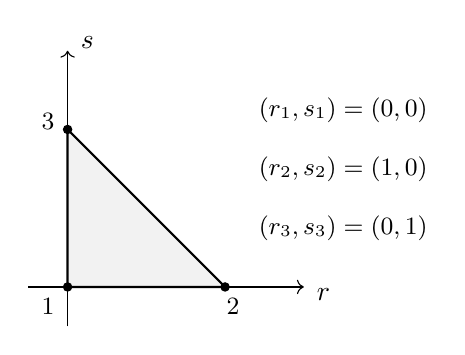
\begin{tikzpicture}
\draw[fill=gray!10,gray!10] (0.5,0.5)--(2.5,0.5)--(0.5,2.5)--cycle;
\draw[thick] (0.5,0.5)--(2.5,0.5)--(0.5,2.5)--cycle;
\draw [->] (0,0.5) -- (3.5,0.5);
\draw [->] (0.5,0) -- (0.5,3.5);
\node[] at (3.75,0.4) {$r$};
\node[] at (0.75,3.6) {$s$};
\draw[black,fill=black] (0.5,0.5)   circle (1.5pt);
\draw[black,fill=black] (2.5,0.5)   circle (1.5pt);
\draw[black,fill=black] (0.5,2.5)   circle (1.5pt);
\node[] at (0.25,0.25) {\small $1$};
\node[] at (2.6,0.25) {\small $2$};
\node[] at (0.25,2.6) {\small $3$};
\node[] at (4,2.75) {\small $(r_1,s_1)=(0,0)$};
\node[] at (4,2) {\small $(r_2,s_2)=(1,0)$};
\node[] at (4,1.25) {\small $(r_3,s_3)=(0,1)$};
\end{tikzpicture}
\end{center}
and the basis functions are simply
\begin{eqnarray}
\bN_1(r,s) &=& 1-r-s \\
\bN_2(r,s) &=& r \\
\bN_3(r,s) &=& s 
\end{eqnarray}
with the interpolation requirement $\bN_i(r_j,s_j)=\delta_{ij}$ fulfilled, 
as well as $\sum_i \bN_i=1$. 

Now, following the figure by Gresho and Sani, I build the reference element for the $P_1+P_0$ space:
\begin{center}
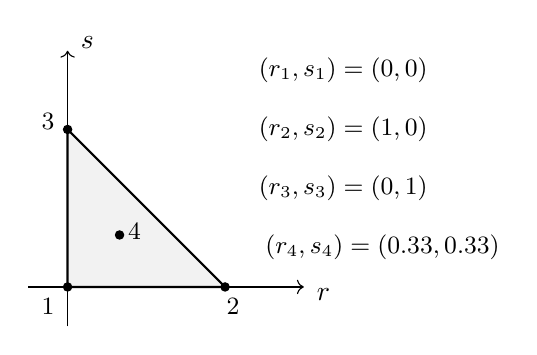
\begin{tikzpicture}
\draw[fill=gray!10,gray!10] (0.5,0.5)--(2.5,0.5)--(0.5,2.5)--cycle;
\draw[thick] (0.5,0.5)--(2.5,0.5)--(0.5,2.5)--cycle;
\draw [->] (0,0.5) -- (3.5,0.5);
\draw [->] (0.5,0) -- (0.5,3.5);
\node[] at (3.75,0.4) {$r$};
\node[] at (0.75,3.6) {$s$};
\draw[black,fill=black] (0.5,0.5)   circle (1.5pt);
\draw[black,fill=black] (2.5,0.5)   circle (1.5pt);
\draw[black,fill=black] (0.5,2.5)   circle (1.5pt);
\draw[black,fill=black] (1.16,1.16) circle (1.5pt);
\node[] at (0.25,0.25) {\small $1$};
\node[] at (2.6,0.25) {\small $2$};
\node[] at (0.25,2.6) {\small $3$};
\node[] at (1.35,1.2) {\small $4$};
\node[] at (4,3.25) {\small $(r_1,s_1)=(0,0)$};
\node[] at (4,2.5)    {\small $(r_2,s_2)=(1,0)$};
\node[] at (4,1.75) {\small $(r_3,s_3)=(0,1)$};
\node[] at (4.5,1) {\small $(r_4,s_4)=(0.33,0.33)$};
\end{tikzpicture}
\end{center}

$P_1+P_0$ means that the pressure inside the element is given by
\[
p^h(r,s) = a \bN_1(r,s)+ b\bN_2(r,s) + c\bN_3(r,s) + d\bN_4(r,s) 
\]
Note that it is then impossible to find $a,b,c,d$ such that the interpolation 
requirement $\bN_i(r_j,s_j)=\delta_{ij}$ is fulfilled.
In other words, the element is not interpolatory, i.e., there is no $\delta_{ij}$ property.% W.B. email

With regards to the 'element mass balance', W.B. states : 
\begin{displayquote}
{\color{darkgray}
the mass conservation requires that the function that is constant 1 
on one cell and zero on all other cells is part of the function space. 
That is indeed true -- it's the $\bN_4$ function. Indeed, that's the purpose of 
the enrichment with the $P_0$ part. It is not necessary that {\it all} shape functions are discontinuous.
}
\end{displayquote}




\textcite{bocg12} (2012) state: 
\begin{displayquote}
{\color{darkgray}
[...] the pressure space $Q_h$ is defined as the sum of two finite 
element spaces, namely $P_k+P_0$ ($k \ge d- 1$) [...] for the enhanced 
Hood–Taylor [...]. However, it can be easily observed that the sum is not direct, 
since globally constant functions can be represented exactly by means of piecewise 
$P_0$ or continuous $P_k$ ($k \ge 1$) elements.
Concerning the implementation of the method, we avoid the computation of the basis
functions of such a finite element by testing the discrete problem (2.3) 
with the basis 
functions of the two subspaces separately. By the above discussion it 
turns out that the resulting
matrix is rank-deficient, with kernel of dimension 1.
}
\end{displayquote}

The element pair is also discussed in \textcite{chen14} (2014).



%------------------------------------------------------------------
\subsubsection{The ${ Q}_2\times (Q_1+Q_0)$ pair} \label{ss:q2q1q0}
\begin{flushright} {\tiny {\color{gray} \tt  pair\_q2q1q0.tex}} \end{flushright}
%~~~~~~~~~~~~~~~~~~~~~~~~~~~~~~~~~~~~~~~~~~~~~~~~~~~~~~~~~~~~~~~~~~~~~~~~~~~~~~~~~~~~~~~~~~~~~~~~~~

It is a rather peculiar element pair (triplet?). The velocity space is the standard $Q_2$ space
but the pressure space is the sum of two spaces, i.e. $Q_1$ {\it and} $Q_0$.
Please see Section~\ref{ss:p2p1p0} on the ${\bm P}_2\times (P_1+P_0)$ element.

\begin{center}
\includegraphics[width=9cm]{images/pair_q2q1q0}\\
{\captionfont Taken from \textcite{grsa}'s book.}
\end{center}

It is implemented in \stone~120.


%------------------------------------------------------------------
\subsubsection{The ${ P}_3\times P_2$ pair} \label{ss:p3p2}
\index{general}{$P_3\times P_2 element$}
\begin{flushright} {\tiny {\color{gray} \tt pair\_p3p2.tex}} \end{flushright}
%~~~~~~~~~~~~~~~~~~~~~~~~~~~~~~~~~~~~~~~~~~~~~~~~~~~~~~~~~~~~~~~~~~~~~~~~~~~~~~~~~~~~~~~~~~~~~~~~~~

${\bm P}_3\times P_2$ mentioned in \textcite{sten90}.
The $P_3$ basis functions are presented in Section~\ref{basis:p3} and the $P_2$ basis
functions in Section~\ref{basis:p2}.
See \stone~120.


%------------------------------------------------------------------
\subsubsection{The Raviart-Thomas family} \label{ss:raviart_thomas}
\begin{flushright} {\tiny {\color{gray} \tt pair\_raviart\_thomas.tex}} \end{flushright}
%~~~~~~~~~~~~~~~~~~~~~~~~~~~~~~~~~~~~~~~~~~~~~~~~~~~~~~~~~~~~~~~~~~~~~~~~~~~~~~~~~~~~~~~~~~~~~~~~~~

- Raviart Thomas 0 RT0 \cite{rath77} ? mentioned/defined/drawn in 4.2.2 of 
Kanschat book. Also exist for quads see 4.2.37 
\textcite{hald03}: ``$P_1^\perp \times P_0$ symbol denotes an element with 
normal velocity nodes in the middle of each edge of the
triangulation [...]. This element, also called low order Raviart–Thomas element 
(Raviart and Thomas, 1977), is based on flux conservation on elements edges and 
the resulting scheme is very close to a finite volume scheme.''

Mentioned in \textcite{john16}, appendix B.3, example B.45: ``the normal component of v 
on each face is a constant. The normal component of functions from RT0 is
continuous across faces of the mesh cells.''

Check \textcite{brfo}

Mentioned in \textcite{chen93a} (1993).

\url{https://defelement.com/elements/raviart-thomas.html}


\url{
https://en.wikipedia.org/wiki/Raviart-Thomas_basis_functions
}

\url{
https://people.tamu.edu/~guermond//M661_FALL_2015/chap7.pdf
}

\url{
https://scicomp.stackexchange.com/questions/20245/raviart-thomas-elements-on-reference-square
}





%------------------------------------------------------------------
\subsubsection{The Bernaudi-Raugel pair} \label{ss:bernaudi_raugel}
\begin{flushright} {\tiny {\color{gray} pair\_bernaudi\_raugel.tex}} \end{flushright}
%~~~~~~~~~~~~~~~~~~~~~~~~~~~~~~~~~~~~~~~~~~~~~~~~~~~~~~~~~~~~~~~~~~~~~~~~~~~~~~~~~~~~~~~~~~~~~~~~~~

In \textcite{cakp15} (2015) we find: ``The BR-FEM after Bernardi and Raugel \cite{bera85} 
is a modification of the $P_2\times P_0$ FEM. It is sometimes also called reduced $P_2\times P_0$ FEM''.
They also state that this element also exists in 3D.

\begin{center}
\includegraphics[width=5cm]{images/pair_bernardi_raugel/cakp15}
\end{center}

It is also mentioned in \textcite{bobf13} although it seems it is there called the SMALL element (p474).

In Lederer: "Consider the case d = 2. [...] we only need to control 
the normal velocity at the edge, i.e. adding the
edge bubble for both components of the velocity seems to be sub optimal (with respect to
computational costs and the expected approximation properties). The idea now is to only
add the normal edge bubble."

According to \textcite{jolm17} (2017) (example 6.3), `` the velocity space in the Bernardi-Raugel
element consists of $P_1$ functions which are enriched with edge bubble functions''.
The authors also speak of 'reconstructing the test functions' and state: 
``the results of the method with reconstruction are generally more accurate.
In summary, the use of an appropriately reconstructed test function in the Bernardi–
Raugel pair of spaces led to a clear improvement of the accuracy of the computed
results compared with the standard method.''




%------------------------------------------------------------------
\subsubsection{The Scott-Vogelius pair} \label{ss:scott_vogelius}
\index{general}{Scott-Vogelius pair}
\begin{flushright} {\tiny {\color{gray} \tt pair\_scott\_vogelius.tex}} \end{flushright}
%~~~~~~~~~~~~~~~~~~~~~~~~~~~~~~~~~~~~~~~~~~~~~~~~~~~~~~~~~~~~~~~~~~~~~~~~~~~~~~~~~~~~~~~~~~~~~~~~~~

It originates in \fullcite{scvo85} (1985). 

 
In Remark 9 (p.29) of \textcite{aubb17} (2017) we find: 
\begin{displayquote}
{\color{darkgray}
We also remark that the discontinuous
pressure version of the Hood–Taylor element typically
results in an unstable method. However, stability can be
recovered by imposing certain restrictions on the mesh for
$k \ge 3$ (see \cite{voge83}; \cite{scvo85}), or
by taking advantage of suitable stabilization procedures for
$k\ge 1$ (see Mansfield, 1982; Boffi, 1995).
}
\end{displayquote}

In \textcite{fams21} (2021) we find:
\begin{displayquote}
{\color{darkgray}
The Scott-Vogelius element is given by choosing continuous piecewise 
polynomials of degree $k$ for the velocity and discontinuous piecewise 
polynomials of degree $k-1$ for the pressure. While this clearly
implies that $\nabla\cdot V_h \in Q_h$, inf-sup stability of the 
Scott–Vogelius element is more delicate, and is a topic of ongoing research. 
In two dimensions, Scott \& Vogelius proved \cite{scvo85} that the element is inf-sup
stable for $k\ge 4$ if the mesh does not have nearly singular vertices. 
In three dimensions, it was proven more recently in \cite{zhan11b} 
that the element is stable for $k\ge 6$ on uniform meshes. The stability on general
tetrahedral meshes continues to be an open question.

On barycentrically refined meshes, however, the pair is known to 
be stable for polynomial order
$k = d$, see [48, Section 4.6] for the 2D case and 
\cite{zhan05} for the 3D case. If one is willing to 
consider the more complicated Powell–Sabin split, the order 
can be reduced further to $k=d-1$ \cite{zhan08,zhan11a}. The two
refinement patterns are shown for the two dimensional case 
in Figure 1 [see below]. In this work we will consider
the case of $k \ge d$ on barycentrically refined meshes, but 
the arguments apply mutatis mutandis to the Powell–Sabin split.
}
\end{displayquote}

\begin{center}
\includegraphics[width=9cm]{images/pair_scott_vogelius/scottvogelius_split}\\
{\captionfont 
Barycentrically refined triangle (also known as Alfeld split) on the left,
and Powell–Sabin split on the right.\\ Taken from \textcite{fams21} (2021).}
\end{center}

\index{general}{Powell-Sabin}

\textcite{cael11} (2011) state:
\begin{displayquote}
{\color{darkgray}
The SV element pair is not yet very well known,
and so we now give a brief description of it. In essence, the SV pair is the same as
the Taylor-Hood pair except that the pressure space is discontinuous and either
(i) for $k \ge d$, the mesh is a barycenter refinement of a regular mesh, or
(ii) for $k = 2, d = 3$, the mesh is formed from a barycenter refined mesh by
connecting the barycenter nodes (i.e., a Powell–Sabin tetrahedralization).
In short, polynomials of degree $k$ and $k-1$ are used to approximate the velocity
and pressure spaces, respectively, and the mesh ${\cal T}_h$ that is used must be derived from
a regular triangulation (tetrahedralization) of $\Omega$, where each element is refined as
stated above. With these mesh constructions, it was proved by Zhang in [42, 44] that
the SV elements are LBB stable, and, consequently, also have optimal approximation
properties. It is well known that the TH pair is LBB stable and admits optimal
approximation properties for these cases as well [9]. We will restrict our definition of
SV elements to these cases where they are LBB stable.
}
\end{displayquote}

On page 112 of \textcite{john16} we read:
\begin{displayquote}
{\color{darkgray}
The Scott–Vogelius finite element considers still $P_k/P^{disc}_{k-1}$, $k \ge d$, 
but on special meshes, which allow to show the satisfaction of the 
discrete inf-sup condition.
[...]
This pair of finite element spaces $P_k/P^{disc}_{k-1}$
are weakly divergence-free, which is a desirable property.
[...]
The fulfillment of the discrete inf-sup condition 
was proved already in \textcite{scvo85} (1985) in the two-dimensional 
case for $k\ge 4$ if there is no so-called singular vertex in the mesh.
An internal vertex is said to be singular if edges which meet at the vertex fall onto
two straight lines.

The basic idea to overcome this problem consists in using meshes 
without singular vertices. To this end, so-called barycentric-refined 
grids are constructed. Starting from any admissible triangular mesh, 
new edges are introduced by connecting all
vertices of a mesh cell with the barycenter of this mesh cell. 
This step creates smaller triangles.
On barycentric-refined meshes, the $P_k/P^{disc}_{k-1}$, $k=2,3$ 
pair of finite element spaces was shown to satisfy the discrete inf-sup
condition in Qin's phd thesis (1994). [...]

The use of the $P_2/P^{disc}_{1}$ pair of finite element spaces 
on barycentric-refined meshes can be found occasionally in the literature,
in particular to demonstrate the advantages of using pairs of finite element 
spaces which provide weakly divergence-free velocity solutions, 
e.g. see \textcite{john15} and refs therein.

}
\end{displayquote}


\begin{center}
\includegraphics[width=6cm]{images/pair_scott_vogelius/john16}\\
{\captionfont Barycentric-refined simplicial grid on the unit square}
\end{center}

I hereafter present my own internal numbering for the mesh above (used in \stone~120 for example).
The quadrilateral has been cut once along a diagonal, and then an Alfeld split is used, thereby 
dividing the square in 6 triangles:

\input{tikz/tikz_sv.tex}

See also \textcite{jolm17} (2017) in which the $P_2\times P_1$, Scott-Vogelius ($P_2\times P_{-1}$), 
Bernardi-Raugel, and $P_2^+\times P_{-1}$ elements 
are compared for a thermo-mechanically driven convection problem in a triangle (see \stone~51, 
although I use the $P_1^+\times P_1$ element in this stone).


\begin{center}
\includegraphics[width=10cm]{images/pair_scott_vogelius/john_scott_vogelius}\\
\captionfont{Taken from John \cite[p70]{john16}.} 
\end{center}


In \textcite{befh21} (2021) this element is used in its 
$(P_3)^2-P_2^{\text{disc}}$ form.

Note that some have proposed to use an incenter-based refinement instead of
a barycenter refinement since it lead to less pronounced aspect ratios\footnote{
The Scott-Vogelius Method for Stokes Problem on Anisotropic Meshes, K Kean, M Neilan, M Schneier,
\url{https://doi.org/10.48550/arXiv.2109.14780}}.
In geometry, the incenter of a triangle is a triangle center, a point defined for 
any triangle in a way that is independent of the triangle's placement or scale. 
The incenter may be equivalently defined as the point where the internal angle bisectors 
of the triangle cross or as the point equidistant from the triangle's sides.

Given the coordinates of the three vertices of a triangle ABC,
the coordinates of the incenter O are
\[
x_O=\frac{ax_A+bx_B+cx_C}{a+b+c}
\qquad
y_O=\frac{ay_A+by_B+cy_C}{a+b+c}
\] 
where $a$, $b$ and $c$ are the side lengths opposite vertex A, B and C.

 
Note that \textcite{zhan24} (2024) proposes a solution to the unstable issue: 
\begin{displayquote}
{\color{darkgray}
We show that the discrete velocity solution converges at
the optimal order when solving the steady state Stokes
equations by the ${\bm P}_k\times P_{-(k-1)}$ mixed finite element method for
$k \ge 4$ on 2D triangular grids or $k \ge 6$ on tetrahedral grids,
even in the case the inf-sup condition fails. By a simple
$L_2$-projection of the discrete $P_{k-1}$ pressure to the space of
continuous $P_{k-1}$ polynomials, we show this post-processed
pressure solution also converges at the optimal order. Both
2D and 3D numerical tests are presented, verifying the
theory.
}
\end{displayquote}

Rather interestingly, we find in \textcite{tesk12} (2012) a penalty-approach:
\begin{displayquote}
{\color{darkgray}
Other solutions to deal with the LBB condition include the Uzawa iteration method and penalty
methods. A combination of these two approaches results in the iterated penalty method presented in
Scott and Vogelius (1985). Let $r\in\R$ and $\rho\in\R^+$ be prescribed parameters. 
We wish to find $u^n\in V_h$ such that 
\[
a(u^n,v) + r(\nabla\cdot u^n,\nabla\cdot v) = (f,v) - (\nabla \cdot v, \nabla\cdot w^n)
\qquad \forall \; v\in V_h,
\]
where $w^{n+1}=w^n+\rho u^n$.
The pressure may be recovered from the auxiliary field $w$ via $p=\nabla\cdot w -C$, 
where $C$ is an arbitrary constant (since the pressure field is only determined up 
to an arbitrary constant). When computing the error in $p$, we subtract the average 
of $\nabla\cdot w$ to account for $C$. The algorithm initially assumes
$w^0=0$, and then solves [the equation above] and updates $w$. 
The process is repeated until $\| u^{n+1}-u^n\|<\epsilon$, 
where $\epsilon$ is a prescribed tolerance. This method involves only one function space, but
it requires a higher-order continuous element $(q\ge 4)$ and it solves the divergence-free criterion
exactly. The iteration count and accuracy are dependent upon the penalty parameters $\rho$ and $r$. 
The implementation of this formulation is presented in [the following figure]:
\begin{center}
\includegraphics[width=6cm]{images/pair_scott_vogelius/tesk12}
\end{center}

}
\end{displayquote}



\begin{center}
\url{https://defelement.com/elements/scott-vogelius.html}
\end{center}




%------------------------------------------------------------------
\subsubsection{The BDM (Brezzi-Douglas-Marini) pair} \label{ss:bdm}
\index{general}{BDM element}
\index{general}{BDM element}
\begin{flushright} {\tiny {\color{gray} \tt  pair\_bdm.tex}} \end{flushright}
%~~~~~~~~~~~~~~~~~~~~~~~~~~~~~~~~~~~~~~~~~~~~~~~~~~~~~~~~~~~~~~~~~~~~~~~~~~~~~~~~~~~~~~~~~~~~~~~~~~

This element is mentioned in Kanschat book \cite{kanschat}, section 4.2.14. 
It also exists for quads see section 4.2.39 in the same book.
It is mentioned in \textcite{chen93a} (1993), also check the book by \textcite{brfo}.
It is well described in \textcite{kanschat17}.
There is an entire chapter (14) of \textcite{ergu21_72} dedicated to H(div) and 
section 14.5.1 to BDM elements. 
Check section 4.1.1 of \cite{aubb17} for triangles and quads.

\begin{center}
\url{https://defelement.com/elements/brezzi-douglas-marini.html}
\end{center}

\begin{itemize}
%++++++++++++++++++++++++++++++++++++++++++++++
\item In \textcite{lomw12} we read:

The Brezzi-Douglas-Marini element was introduced by Brezzi, Douglas and Marini in two dimensions 
(for triangles) in \textcite{brdm85} (1985). The element can be viewed as an alternative to the
Raviart-Thomas element using a complete polynomial space. It was later extended to three 
dimensions (tetrahedra, prisms and cubes) in \textcite{nede86} (1986) 
and \textcite{brdd87} (1987). The definition given
here is based on that of \textcite{nede86} (1986).

The Brezzi-Douglas-Marini element was introduced for mixed formulations of second-order elliptic 
equations. However, it is also useful for weakly symmetric discretizations of the elastic stress
tensor; see Farhloul and Fortin (1997); Arnold et al. (2007).

\begin{center}
\includegraphics[width=8cm]{images/pair_bdm/bdm_lomw12}\\
{\captionfont Taken from \cite{lomw12}. }
\end{center}

The dimension of $BDM_q$ is $(q+1)(q+2)$ for a triangle and $\frac12(q+1)(q+2)(q+3)$
for a tetrahedron.

Check book for definition.

A slight modification of the Brezzi-Douglas-Marini element constrains the element space ${\cal V}$ by
only allowing normal components on the boundary of polynomial degree $q-1$ (rather than the full
polynomial degree $q$). Such an element was suggested on rectangles by \textcite{brdf87} (1987), and the
triangular analogue was given in \textcite{brfo}. In similar spirit, elements with differing
degrees on the boundary suitable for varying the polynomial degree between triangles were derived
in \textcite{brdm85b} (1985).

%++++++++++++++++++++++++++++++++++++++++++++++
\item On the defelement website\footnote{\url{https://defelement.org/elements/brezzi-douglas-marini.html}}
we find a lot of information. Note that the mapping is set to 'contravariant Piola'. 
\todo[inline]{I still need to understand and write about this!}
It belongs to the categories 'Vector-valued elements', and 'H(div) conforming elements'

\begin{center}
\input{images/pair_bdm/ref-triangle.tex}\\
{\captionfont Taken from DefElement \url{https://defelement.org/img/ref-triangle.html}. I have altered 
the font size. Orange: nodes; Blue: edges.}
\end{center}


I reproduce below the figures and basis functions pertaining to the Degree 1 triangle, 
but the site also shows Degree 2 triangle, Degree 1 \& 2 tetrahedron, and so-called 
Lagrange variants.

\begin{center}
\includegraphics[width=3cm]{images/pair_bdm/element-Brezzi-Douglas-Marini-variant-equispaced-triangle-1-dofs}
\includegraphics[width=3cm]{images/pair_bdm/element-Brezzi-Douglas-Marini-variant-equispaced-triangle-1-0}
\includegraphics[width=3cm]{images/pair_bdm/element-Brezzi-Douglas-Marini-variant-equispaced-triangle-1-1}
\includegraphics[width=3cm]{images/pair_bdm/element-Brezzi-Douglas-Marini-variant-equispaced-triangle-1-2}\\
\includegraphics[width=3cm]{images/pair_bdm/element-Brezzi-Douglas-Marini-variant-equispaced-triangle-1-3}
\includegraphics[width=3cm]{images/pair_bdm/element-Brezzi-Douglas-Marini-variant-equispaced-triangle-1-4}
\includegraphics[width=3cm]{images/pair_bdm/element-Brezzi-Douglas-Marini-variant-equispaced-triangle-1-5}\\
{\captionfont Pink: degrees of freedom.}
\end{center}


${\cal V}$ is spanned by 
\[
\left(\begin{array}{c}
1 \\ 0
\end{array}\right),
\left(\begin{array}{c}
0 \\ 1
\end{array}\right),
\left(\begin{array}{c}
x \\ 0
\end{array}\right),
\left(\begin{array}{c}
0 \\ x
\end{array}\right),
\left(\begin{array}{c}
y \\ 0
\end{array}\right),
\left(\begin{array}{c}
0 \\ y
\end{array}\right)
\]
with 
\begin{itemize}
\item DOF \#0 is associated with edge 0 of the reference element with $\vec{\bN}_0$ basis function.
\item DOF \#1 is associated with edge 0 of the reference element with $\vec{\bN}_1$ basis function.
\item DOF \#2 is associated with edge 1 of the reference element with $\vec{\bN}_2$ basis function.
\item DOF \#3 is associated with edge 1 of the reference element with $\vec{\bN}_3$ basis function.
\item DOF \#4 is associated with edge 2 of the reference element with $\vec{\bN}_4$ basis function.
\item DOF \#5 is associated with edge 2 of the reference element with $\vec{\bN}_5$ basis function.
\end{itemize}
and
\begin{eqnarray}
\vec{\bN}_0 &=&  \left(\begin{array}{c} -4x \\ 2y        \end{array}\right) \nn\\  
\vec{\bN}_1 &=&  \left(\begin{array}{c} 2x \\ -4y        \end{array}\right) \nn\\  
\vec{\bN}_2 &=&  \left(\begin{array}{c} 4x+6y-4 \\ -2y   \end{array}\right) \nn\\  
\vec{\bN}_3 &=&  \left(\begin{array}{c} -2x-6y+2 \\ 4y   \end{array}\right) \nn\\  
\vec{\bN}_4 &=&  \left(\begin{array}{c} 2x \\ -6x-4y+4   \end{array}\right) \nn\\  
\vec{\bN}_5 &=&  \left(\begin{array}{c} -4x \\ 6x +2y -2 \end{array}\right) \nn
\end{eqnarray}

 

\item In \cite{brdf87} we read:
\begin{displayquote}
The object of this paper is to present families of rectangular mixed finite
éléments that are derived from the elements of \cite{brdm85} 
in two space variables and of \cite{brdd87} in three space variables.
\end{displayquote}














\end{itemize}



%------------------------------------------------------------------
\subsubsection{The DSSY pair} \label{ss:pair_dssy2D}
\index{general}{Nonconforming element}
\index{general}{DSSY element}
\index{general}{Nonconforming element}
\index{general}{DSSY element}
\begin{flushright} {\tiny {\color{gray} \tt pair\_dssy2D.tex}} \end{flushright}
%~~~~~~~~~~~~~~~~~~~~~~~~~~~~~~~~~~~~~~~~~~~~~~~~~~~~~~~~~~~~~~~~~~~~~~~~~~~~~~~~~~~~~~~~~~~~~~~~~~

This element is often referred to as the 'DSSY' element because of the 
four authors of the original paper: Douglas, Santos, sheen and Ye (1999) \cite{doss99}.

The non-conforming finite element space $Q_l$ is defined based on the 
reference square element on $[-1,1]^2$ :
\[
Q_l = \text{Span} \left\{ 1, r, s, \theta_l(r)-\theta_l(s)  \right\}
\qquad l=1,\; \text{or} \; 2
\]
with
\begin{eqnarray}
\theta_1(r)  &=& r^2-\frac53r^4  \nn\\
\theta_1'(r) &=& 2r-\frac{20}{3}r^3  \nn\\
\theta_2(r)  &=& r^2-\frac{25}{6} r^4 + \frac72 r^6 \\ 
\theta_2'(r) &=& 2r-\frac{50}{3} r^3 + 21 r^5
\end{eqnarray}
The dimension of $Q_l$ is four and the $\theta_l$ functions look like:
\begin{center}
\includegraphics[width=7cm]{images/dssy/theta1}
\includegraphics[width=7cm]{images/dssy/theta2}
\end{center}
We have:
\begin{itemize}
\item $\theta_1(r=-1)=\theta_1(r=+1)=-\frac23$, $\theta_1(r=0)=0$ 
\item $\theta_2(r=-1)=\theta_2(r=+1)=\frac13$, $\theta_2(r=0)=0$ 
\end{itemize}
The nodes are situated at the mid-edges of the quadrilateral:

\input{tikz/tikz_dssy2D}

The basis function corresponding to the node (1, 0) is given by
\begin{mdframed}[backgroundcolor=blue!5]
\begin{eqnarray}
\bN_1(r,s)^{(l)} &=& \frac{1}{4} - \frac{1}{2} r + \frac{\theta_l(r)-\theta_l(s)}{4 \theta_l(1)}  \nn\\
\bN_2(r,s)^{(l)} &=& \frac{1}{4} + \frac{1}{2} r + \frac{\theta_l(r)-\theta_l(s)}{4 \theta_l(1)}  \nn\\
\bN_3(r,s)^{(l)} &=& \frac{1}{4} - \frac{1}{2} s - \frac{\theta_l(r)-\theta_l(s)}{4 \theta_l(1)}  \nn\\
\bN_4(r,s)^{(l)} &=& \frac{1}{4} + \frac{1}{2} s - \frac{\theta_l(r)-\theta_l(s)}{4 \theta_l(1)}  
\end{eqnarray}
\end{mdframed}
We can easily verify that $\sum\limits_i \bN_i(r,s,t)=1$ and that $\bN_i(\vec{r}_j)=\delta_{ij}$:
\begin{eqnarray}
\bN_1^{(l)}(r_1,s_1) 
&=& \frac{1}{4} -\frac{1}{2} (-1) + \frac{\theta_l(-1)-\theta_l(0)}{4 \theta_l(1)}  
= \frac{1}{4} +\frac{1}{2}  + \frac{\theta_l(-1)}{4 \theta_l(1)}  
= \frac{1}{4} +\frac{1}{2}  + \frac{1}{4}   = 1 \nn\\
\bN_1^{(l)}(r_2,s_2)
&=& \frac{1}{4} -\frac{1}{2} (+1) + \frac{\theta_l(+1)-\theta_l(0)}{4 \theta_l(1)}  
= \frac{1}{4} -\frac{1}{2} + \frac{\theta_l(+1)}{4 \theta_l(1)}  
= \frac{1}{4} -\frac{1}{2} + \frac{1}{4}   = 0 \nn\\
\bN_1^{(l)}(r_3,s_3)
&=& \frac{1}{4} -\frac{1}{2} (0) + \frac{\theta_l(0)-\theta_l(-1)}{4 \theta_l(1)}  
= \frac14 -\frac14  = 0 \nn\\
\bN_1^{(l)}(r_4,s_4)
&=& \frac{1}{4} -\frac{1}{2} (0) + \frac{\theta_l(0)-\theta_l(+1)}{4 \theta_l(1)}  
= \frac14 -\frac14  = 0 \nn\\
\bN_2^{(l)}(r_1,s_1) 
&=& \frac{1}{4} + \frac{1}{2} (-1) + \frac{\theta_l(-1)-\theta_l(0)}{4 \theta_l(1)}  
= \frac14 -\frac12 + \frac14 = 0 \nn\\
\bN_2^{(l)}(r_2,s_2)
&=& \frac{1}{4} + \frac{1}{2} (+1) + \frac{\theta_l(+1)-\theta_l(0)}{4 \theta_l(1)}  
= \frac14 + \frac12 + \frac14 =1 \nn\\
\bN_2^{(l)}(r_3,s_3)
&=& \frac{1}{4} + \frac{1}{2} (0) + \frac{\theta_l(0)-\theta_l(-1)}{4 \theta_l(1)}  
= \frac14 - \frac14 = 0 \nn\\
\bN_2^{(l)}(r_4,s_4)
&=& \frac{1}{4} + \frac{1}{2} (0) + \frac{\theta_l(0)-\theta_l(+1)}{4 \theta_l(1)}  
= \frac14 - \frac14 = 0 \nn\\
\bN_3^{(l)}(r_1,s_1)
&=& \frac{1}{4} - \frac{1}{2} (0) - \frac{\theta_l(-1)-\theta_l(0)}{4 \theta_l(1)} 
= \frac14 -\frac14 = 0\nn\\
\bN_3^{(l)}(r_2,s_2)
&=& \frac{1}{4} - \frac{1}{2} (0) - \frac{\theta_l(+1)-\theta_l(0)}{4 \theta_l(1)} 
= \frac14 -\frac14 = 0\nn\\
\bN_3^{(l)}(r_3,s_3)
&=& \frac{1}{4} - \frac{1}{2} (-1) - \frac{\theta_l(0)-\theta_l(-1)}{4 \theta_l(1)} 
= \frac14 +\frac12 + \frac14 = 1\nn\\
\bN_3^{(l)}(r_4,s_4)
&=& \frac{1}{4} - \frac{1}{2} (+1) - \frac{\theta_l(0)-\theta_l(+1)}{4 \theta_l(1)} 
= \frac14 -\frac12 + \frac14 = 0\nn\\
\bN_4^{(l)}(r_1,s_1)
&=& \frac{1}{4} + \frac{1}{2} (0) - \frac{\theta_l(-1)-\theta_l(0)}{4 \theta_l(1)}  
= \frac14 -\frac14 =0\nn\\
\bN_4^{(l)}(r_2,s_2)
&=& \frac{1}{4} + \frac{1}{2} (0) - \frac{\theta_l(+1)-\theta_l(0)}{4 \theta_l(1)}  
= \frac14 -\frac14 =0\nn\\
\bN_4^{(l)}(r_3,s_3)
&=& \frac{1}{4} + \frac{1}{2} (-1) - \frac{\theta_l(0)-\theta_l(-1)}{4 \theta_l(1)}  
= \frac14 -\frac12 +\frac14 = 0 \nn\\
\bN_4^{(l)}(r_4,s_4)
&=& \frac{1}{4} + \frac{1}{2} (1) - \frac{\theta_l(0)-\theta_l(1)}{4 \theta_l(1)}  
= \frac14 +\frac12 +\frac14 = 1 \nn
\end{eqnarray}

The basis functions can also be explicitly written for $\theta_1$ as in Cai \etal \cite{cady99}:
\begin{eqnarray}
\bN_1(r,s)^{(l)} 
&=& \frac{1}{4} - \frac{1}{2} r - \frac38 \left[\left( r^2-\frac53r^4 \right) - \left(s^2-\frac53s^4 \right) \right] \nn\\
\bN_2(r,s)^{(l)} 
&=& \frac{1}{4} + \frac{1}{2} r - \frac38 \left[\left( r^2-\frac53r^4 \right) - \left(s^2-\frac53s^4 \right) \right] \nn\\
\bN_3(r,s)^{(l)} 
&=& \frac{1}{4} - \frac{1}{2} s + \frac38 \left[\left( r^2-\frac53r^4 \right) - \left(s^2-\frac53s^4 \right) \right] \nn\\
\bN_4(r,s)^{(l)} 
&=& \frac{1}{4} + \frac{1}{2} s + \frac38 \left[\left( r^2-\frac53r^4 \right) - \left(s^2-\frac53s^4 \right) \right] 
\end{eqnarray}

The derivatives of the basis functions are as follows:
\begin{eqnarray}
\partial_r \bN_1(r,s)^{(l)} &=&  - \frac{1}{2}  + \frac{\theta_l'(r)}{4 \theta_l(1)}  \nn\\
\partial_r \bN_2(r,s)^{(l)} &=&  + \frac{1}{2}  + \frac{\theta_l'(r)}{4 \theta_l(1)}  \nn\\
\partial_r \bN_3(r,s)^{(l)} &=&  - \frac{\theta_l'(r)}{4 \theta_l(1)}  \nn\\
\partial_r \bN_4(r,s)^{(l)} &=&  - \frac{\theta_l'(r)}{4 \theta_l(1)}  
\end{eqnarray}

\begin{eqnarray}
\partial_s \bN_1(r,s)^{(l)} &=&   -\frac{\theta_l'(s)}{4 \theta_l(1)}  \nn\\
\partial_s \bN_2(r,s)^{(l)} &=&   -\frac{\theta_l'(s)}{4 \theta_l(1)}  \nn\\
\partial_s \bN_3(r,s)^{(l)} &=&   - \frac{1}{2} + \frac{\theta_l'(s)}{4 \theta_l(1)}  \nn\\
\partial_s \bN_4(r,s)^{(l)} &=&   + \frac{1}{2} + \frac{\theta_l'(s)}{4 \theta_l(1)}  
\end{eqnarray}



Note that a correction was issued in \textcite{cads00} (2000) if a 
true quadrilateral (i.e., one having two opposite, nonparallel edges) is included in
the partition. The authors state that in the case of rectangles the original method is fine.

\Literature: 
Park \& Sheen (2003) \cite{pash03},
Jeon \etal (2013) \cite{jens13},
Park, Sheen \& Shin (2013) \cite{pass13},
Bangerth \etal (2017) \cite{baks17},
Sheen (2020) \cite{shee20}


%------------------------------------------------------------------
\subsubsection{The Han pair} \label{ss:han}
\index{general}{Han element}
\index{general}{Nonconforming element}
\index{general}{Han element}
\index{general}{Nonconforming element}
\begin{flushright} {\tiny {\color{gray} \tt  pair\_han.tex}} \end{flushright}
%~~~~~~~~~~~~~~~~~~~~~~~~~~~~~~~~~~~~~~~~~~~~~~~~~~~~~~~~~~~~~~~~~~~~~~~~~~~~~~~~~~~~~~~~~~~~~~~~~~

It is based on \textcite{han84} (also mentioned in Sheen (2020) \cite{shee20}).
The nodes are at the same location as for the RT element above, but 
there is an additional bubble function in the middle:

\input{tikz/tikz_han}

Inside the reference element we assume that a field $f$
can be represented by 
\begin{eqnarray}
f^h(r,s) 
%&=& a+ br +cs +d \phi(r) +e \phi(s) \nn\\
&=& a+ br +cs +d \underbrace{\frac{5r^4-3r^2}{2}}_{\phi(r)}
+e \underbrace{\frac{5s^4-3s^2}{2}}_{\phi(s)} \nn
\end{eqnarray}
We then must have 
\begin{align}
f_1 &= f^h(r=1,s=0) &= a+ b +d \nn\\
f_2 &= f^h(r=0,s=1) &= a+ c +e \nn\\
f_3 &= f^h(r=-1,s=0) &= a- b +d \nn\\
f_4 &= f^h(r=0,s=-1) &= a -c +e \nn\\
f_5 &= f^h(r=0,s=0) &= a  \nn
\end{align}
and we easily get 
\[
a = f_5 
\qquad
f_1-f_3 = 2b
\qquad 
f_2-f_4 = 2c
\]
followed by
\[
d=f_1-a-b = f_1 - f_5 - \frac{1}{2}(f_1-f_3) = \frac{f_1-2f_5+f_3}{2}
\]
and 
\[
e = f_2-a-c = f_2 - f_5 -  \frac{1}{2}(f_2-f_4) = \frac{f_2 -2f_5+f_4 }{2}
\]
Finally:
\[
f(r,s) = 
f_5 +
\frac{1}{2}(f_1-f_3) r+
\frac{1}{2}(f_2-f_4) s+
\frac{f_1-2f_5+f_3}{2} \phi(r)+
\frac{f_2 -2f_5+f_4 }{2} \phi(s)
\]
i.e.
\[
f(r,s) = 
\left(\frac{r + \phi(r)}{2} \right)f_1 +
\left(\frac{s+\phi(s)}{2} \right)f_2 +
\left(-\frac{r-\phi(r)}{2} \right)f_3 +
\left(-\frac{s - \phi(s)}{2} \right)f_4 +
\left(1-\phi(r)-\phi(s) \right)f_5 
\]
which has us define 
\begin{eqnarray}
\bN_1(r,s) &=& \frac{r + \phi(r)}{2} \nn\\
\bN_2(r,s) &=& \frac{s+\phi(s)}{2} \nn\\
\bN_3(r,s) &=& -\frac{r-\phi(r)}{2} \nn\\
\bN_4(r,s) &=& -\frac{s - \phi(s)}{2}\nn\\
\bN_5(r,s) &=& 1-\phi(r)-\phi(s)\nn
\end{eqnarray}
We have of course the following properties $\sum\limits_{i=1}^5 \bN_i(r,s) = 1$ and 
$\bN_i(r_j,s_j) = \delta_{ij},\;  i,j \in 1,5$. 
The partial derivatives of the basis functions are as follows
\begin{eqnarray}
\partial_r \bN_1(r,s) &=& \frac{1 + \phi'(r)}{2} \nn\\
\partial_r \bN_2(r,s) &=& 0 \nn\\
\partial_r \bN_3(r,s) &=& -\frac{1-\phi'(r)}{2} \nn\\
\partial_r \bN_4(r,s) &=& 0 \nn\\
\partial_r \bN_5(r,s) &=& -\phi'(r) \nn\\
\partial_s \bN_1(r,s) &=& 0 \nn\\
\partial_s \bN_2(r,s) &=& \frac{1 + \phi'(s)}{2} \nn\\
\partial_s \bN_3(r,s) &=&  0 \nn\\
\partial_s \bN_4(r,s) &=& -\frac{1-\phi'(s)}{2} \nn\\
\partial_s \bN_5(r,s) &=& -\phi'(s) \nn
\end{eqnarray}
This element is implemented in the {\tt stone\_han.py} file in \stone~77 and also in \stone~120. 








%------------------------------------------------------------------
\subsubsection{The Divergence-free nonconforming $P_1^{NC}\times P_0$ pair} \label{ss:p1ncp0}
\begin{flushright} {\tiny {\color{gray} \tt pair\_p1ncp0.tex}} \end{flushright}
%~~~~~~~~~~~~~~~~~~~~~~~~~~~~~~~~~~~~~~~~~~~~~~~~~~~~~~~~~~~~~~~~~~~~~~~~~~~~~~~~~~~~~~~~~~~~~~~~~~

It belongs to the Crouzeix-Raviart family. 
The midside nodes are used as degrees of freedom for the velocities.
It is mentioned in Section~6.3 of \textcite{bobf08} (2008): 
\begin{displayquote}
{\color{darkgray}
[...]
It is exactly divergence free. Another important feature of this
element is that it can be seen as a "mass conservation" scheme. The present element
has been generalized to second order in \textcite{foso83} (1983).
It must also be said that coerciveness may be a problem for the $P_1^{NC} \times P_0$ 
element, as it does not satisfy the discrete version of Korn's inequality. 
This issue has been deeply investigated and clearly illustrated in \textcite{arno93} (1993).}
\end{displayquote}

\input{tikz/tikz_p1ncp0}

At page 170 of \cite{braess} it is stated that {\color{darkgray} ``an analogous quadrilateral element was 
developed and studied by \textcite{ratu92} (1992)''} (see Section~\ref{ss:RTq1p0}).

In \textcite{bobf13} we find: 
\begin{displayquote}
{\color{darkgray}
We consider the classical (almost\footnote{What does that mean?!}) 
stable nonconforming triangular 
element introduced in \textcite{crra73}, in which mid-side nodes are used as degrees of 
freedom for the velocities. This generates
a piecewise linear nonconforming approximation; pressures are taken constant on
each element. It is also possible to build a three-dimensional
version of this element, using mid-face nodes as degrees of freedom.
\\
..
\\
It must also be recalled that coercivity is a problem for the $P_1^{NC}\times P_0$ 
element. The trouble is that the bilinear form (8.2.1) is not coercive on the 
nonconforming space $V_h$ and we do not have the discrete version of Korn's inequality.}
\end{displayquote}


It is also mentioned in \textcite{john16}, appendix B.3, example B.43, in 2D and 3D, 
in \textcite{brfo} (example 8.1), and studied extensively in \textcite{john98} (1998). 

\begin{center}
\includegraphics[width=8cm]{images/pair_p1ncp0/john98}\\
{\captionfont Taken from \textcite{john98}.}
\end{center}

In \textcite{jolm17} (2017) the authors show results obtained with this element (fig 6) 
but also explain that these are obtained with so-called reconstructed test functions.
 


%------------------------------------------------------------------
\subsubsection{The Chen nonconforming ${ Q}_1\times Q_0$ pair (?)} \label{ss:chenq0}
\begin{flushright} {\tiny {\color{gray} \tt pair\_chen.tex}} \end{flushright}
%~~~~~~~~~~~~~~~~~~~~~~~~~~~~~~~~~~~~~~~~~~~~~~~~~~~~~~~~~~~~~~~~~~~~~~~~~~~~~~~~~~~~~~~~~~~~~~~~~~

What follows is tentative!

This space is proposed in \textcite{chen93b} (1993), albeit not in the 
context of the Stokes equations.

It is based on the mid-point variant of the RT basis functions, 
\begin{eqnarray}
\bN_1(r,s) &=& \frac{1}{4} (1-2s-(r^2-s^2)) \nonumber\\
\bN_2(r,s) &=& \frac{1}{4} (1+2r+(r^2-s^2)) \nonumber\\
\bN_3(r,s) &=& \frac{1}{4} (1+2s-(r^2-s^2)) \nonumber\\
\bN_4(r,s) &=& \frac{1}{4} (1-2r+(r^2-s^2)) \nonumber
\end{eqnarray}
to which a $P_2$ bubble is added
\[
\phi(r,s) = 1-\frac34(r^2+s^2)
\]
Note thath this function is zero at locations $\pm 1/\sqrt{3}$ 
on all four edges and exactly 1 in the middle. 

A field $f$ is represented inside the element by 
\[
f^h(r,s)=a \bN_1(r,s)
+b \bN_2(r,s)
+c \bN_3(r,s)
+d \bN_4(r,s)
+e \phi(r,s)
\]
We immediately see that this space is not interpolatory, i.e. the basis function $\phi(r,s)$ cannot be 1 in the middle and 0 at the other four nodes. 

\textcite{chen} also extends this to 3D in the paper. 

This space is used for velocity and a $Q_0$ space is used for 
pressure in \stone~120 (only because the basis functions above are
based on the Rannacher-Turek ones).


%----------------------------
\subsubsection{Other FE element pairs}

\begin{itemize}

\item ${\bm Q}_2\times Q_2$: This element is never used, probably because 
a) it is unstable, b) it is very costly. 
There is one reference to it in \cite{hufb86}.

\item ${\bm Q}_1\times P_{-1}$ Bilinear velocities,  piecewise linear discontinuous polynomial pressure.

\item See Fortin \cite{fort81} for various stable low order elements other than the enriched 
${\bm Q}_1^+ \times P_0$

\item ${\bm Q}_1\times Q_1$ + nonconforming null edge average \cite{fros07}

\item check \textcite{dhhu86} (1986) many flavours of triangles and quads.

\item Bercovier-Pironneau element pair, or $P_1isoP_2$.See \textcite{bocg12} (2012).

\end{itemize}

%.........................................................................
\subsubsection{A note about incompressibility and standard mixed methods}

What follows is nicely explained and demonstrated in John \etal \cite{jolm17}. In their 
example 1.1 they look at the velocity error of benchmark VJ2 (see Section~\ref{mms9}) 
which analytical solution is a zero velocity field. They show that for the MINI, 
Taylor-Hood and Crouzeix-Raviart triangular elements the velocity error grows 
with the magnitude of the rhs. They also make this statement:
``there are important applications, e.g., natural
convection problems, where the pressure is larger than the velocity by orders
of magnitude. In such situations, one cannot expect to compute accurate
velocity fields with classical mixed methods, at least for low order methods.''


 %-----------------

\newpage
\section{The penalty approach for viscous flow}\label{sec:penalty}\input{penalty} %-------------
\section{The mixed FEM for viscous flow} \label{sec:mixed} \index{general}{Mixed Formulation}
\begin{flushright} {\tiny {\color{gray} mixed.tex}} \end{flushright}

\subsection{In three dimensions}

The FEM formulation of the Stokes equation is quite complex so 
we simplify things as much as possible for now by 
assuming the flow to be \underline{incompressible}, 
\underline{isoviscous} and \underline{isothermal}. 

The methodology to derive the discretised equations of the mixed system is 
quite similar to the one we have used in the case of the penalty formulation.
The big difference comes from the fact that we are now solving for both 
velocity and pressure at the same time, and that we therefore must solve 
the mass and momentum conservation equations together.
As before, velocity inside an element is given by 
\begin{equation}
{\vec \upnu}^h({\vec r})=\sum_{i=1}^{m_v} \bN_i^\upnu({\vec r})\;  {\vec \upnu}_i
\label{mixed01}
\end{equation}
where $N_i^{\upnu}$ are the polynomial basis functions for the velocity,
and the summation runs over the $m_v$ velocity nodes composing the element.
A similar expression is used for pressure:
\begin{equation}
p^h({\vec r})=\sum_{i=1}^{m_p} \bN_i^p({\vec r}) \; p_i
\label{mixed02}
\end{equation}
Note that the velocity is a vector while pressure (and temperature)
is a scalar. There are then $ndof_v=ndim$ velocity degrees of freedom per node
and $ndof_p=1$ pressure degrees of freedom.
It is also very important to remember that the numbers of 
velocity nodes and pressure nodes for a given element 
are more often than not different and that velocity and pressure
nodes need not be colocated. Indeed, unless 
so-called 'stabilised elements' are used, we have $m_v>m_p$, which 
means that the polynomial order of the velocity field is higher than 
the polynomial order of the pressure field (usually by value 1).

Other notations will be sometimes used for Eqs.~\eqref{mixed01} and \eqref{mixed02}:
\begin{equation}
u^h({\vec r}) = \vec{\bN}^\upnu \cdot \vec{u}
\quad\quad\quad\quad
v^h({\vec r}) = \vec{\bN}^\upnu \cdot \vec{v}
\quad\quad\quad\quad
w^h({\vec r}) = \vec{\bN}^\upnu \cdot \vec{w}
\quad\quad\quad\quad
p^h({\vec r}) = \vec{\bN}^p \cdot \vec{p}
\end{equation} 
where ${\vec \upnu}=(u,v,w)$ and $\vec{\bN}^\upnu$ is the vector containing 
all basis functions evaluated at location ${\vec r}$:
\begin{eqnarray}
\vec{\bN}^v &=& \left( \bN_1^\upnu({\vec r}),  \bN_2^\upnu({\vec r}),  
\bN_3^\upnu({\vec r}), \dots  \bN_{m_v}^\upnu({\vec r}) \right) \\
\vec{\bN}^p &=& \left( \bN_1^p({\vec r}),  \bN_2^p({\vec r}),  
\bN_3^p({\vec r}), \dots  \bN_{m_p}^p({\vec r}) \right)
\end{eqnarray}
and with 
\begin{eqnarray}
\vec{u} &=& \left( u_1,  u_2,  u_3, \dots  u_{m_v} \right) \\
\vec{v} &=& \left( v_1,  v_2,  v_3, \dots  v_{m_v} \right) \\
\vec{w} &=& \left( w_1,  w_2,  w_3, \dots  w_{m_v} \right) \\
\vec{p} &=& \left( p_1,  p_2,  p_3, \dots  p_{m_p} \right) 
\end{eqnarray}
We will now establish the weak form of the momentum conservation equation. 
We start again from 
\begin{eqnarray}
{\vec \nabla}\cdot {\bm \sigma} + {\vec b} &=& {\vec 0} \\
{\vec \nabla}\cdot {\vec \upnu} &=& 0
\end{eqnarray}
For the $\bN_i^\upnu$'s and $\bN_i^p$ 'regular enough', we can write:
\begin{eqnarray}
\int_{\Omega_e} \bN_i^\upnu {\vec \nabla}\cdot {\bm \sigma}\;  dV
+ \int_{\Omega_e} \bN_i^\upnu  {\vec b} \; dV
&=& \vec 0 \\
\int_{\Omega_e} \bN_i^p {\vec \nabla}\cdot {\vec v} \; dV &=& 0
\end{eqnarray}
We can integrate by parts and drop the surface term\footnote{We will come back to this at a later stage}:
\begin{eqnarray}
\int_{\Omega_e} {\vec \nabla } \bN_i^\upnu \cdot {\bm \sigma} dV
&=& \int_{\Omega_e} \bN_i^\upnu  {\vec b} \; dV \\
\int_{\Omega_e} \bN_i^p {\vec \nabla}\cdot {\vec v} \; dV &=& 0
\end{eqnarray}
or, 
\begin{equation}
\int_{\Omega_e} 
\left(
\begin{array}{cccccc}
\frac{\partial \bN_i^\upnu}{\partial x} & 0 & 0& 
\frac{\partial \bN_i^\upnu}{\partial y} & 
\frac{\partial \bN_i^\upnu}{\partial z} & 0\\  \\
0 & \frac{\partial \bN_i^\upnu}{\partial y} & 0  & 
\frac{\partial \bN_i^\upnu}{\partial x}  & 0 &
\frac{\partial \bN_i^\upnu}{\partial z}  \\ \\
0 & 0 & \frac{\partial \bN_i^\upnu}{\partial z} &  0 & 
\frac{\partial \bN_i^\upnu}{\partial x} &  
\frac{\partial \bN_i^\upnu}{\partial y} 
\end{array}
\right)
\cdot
\left(
\begin{array}{c}
\sigma_{xx}\\
\sigma_{yy}\\
\sigma_{zz}\\
\sigma_{xy}\\
\sigma_{xz}\\
\sigma_{yz}\\
\end{array}
\right)
d\Omega = \int_{\Omega_e} \bN_i^\upnu {\vec b} \; dV
\end{equation}
The above equation can ultimately be written:
\begin{equation}
\int_{\Omega_e} {\bm B}^T \cdot 
\left(
\begin{array}{c}
\sigma_{xx}\\
\sigma_{yy}\\
\sigma_{zz}\\
\sigma_{xy}\\
\sigma_{xz}\\
\sigma_{yz}
\end{array}
\right)
dV
=
\int_{\Omega_e} {\vec \bN}_b\; dV
\end{equation}
We have previously established that the strain rate 
vector $\vec{\dot \varepsilon}$ is:
\begin{equation}
\vec{\dot\varepsilon}=
\left(
\begin{array}{c}
\frac{\partial u}{\partial x} \\ \\
\frac{\partial v}{\partial y} \\ \\
\frac{\partial w}{\partial z} \\ \\
\frac{\partial u}{\partial y}\! +\! \frac{\partial v}{\partial x} \\ \\
\frac{\partial u}{\partial z}\! +\! \frac{\partial w}{\partial x} \\ \\
\frac{\partial v}{\partial z}\! +\! \frac{\partial w}{\partial y} 
\end{array}
\right)
=
\left(
\begin{array}{c}
\sum\limits_i \frac{\partial \bN_i^\upnu}{\partial x} u_i \\ \\
\sum\limits_i \frac{\partial \bN_i^\upnu}{\partial y} v_i \\ \\
\sum\limits_i \frac{\partial \bN_i^\upnu}{\partial z} w_i \\ \\
\sum\limits_i (\frac{\partial \bN_i^\upnu}{\partial y} u_i\! +\! 
\frac{\partial \bN_i^\upnu}{\partial x} v_i) \\ \\
\sum\limits_i (\frac{\partial \bN_i^\upnu}{\partial z} u_i\! +\! 
\frac{\partial \bN_i^\upnu}{\partial x} w_i) \\ \\
\sum\limits_i (\frac{\partial \bN_i^\upnu}{\partial z} v_i\! +\! 
\frac{\partial \bN_i^\upnu}{\partial y} w_i) 
\end{array}
\right)
=
\underbrace{
\left(
\begin{array}{ccccccccccc}
\frac{\partial \bN_1^\upnu}{\partial x} & 0 & 0 &  \cdots  & 
\frac{\partial \bN_{m_v}^\upnu}{\partial x} & 0 & 0 \\ \\
0 & \frac{\partial \bN_1^\upnu}{\partial y} & 0 & \cdots & 0 & 
\frac{\partial \bN_{m_v}^\upnu}{\partial y} & 0 \\ \\
0 & 0 & \frac{\partial \bN_1^\upnu}{\partial z} & \cdots & 0 & 0 & 
\frac{\partial \bN_{m_v}^\upnu}{\partial z} 
\\ \\
\frac{\partial \bN_1^\upnu}{\partial y} &  \frac{\partial \bN_1^\upnu}{\partial x} &  
0 & \cdots  &\frac{\partial N_{m_v}^\upnu}{\partial x} 
& \frac{\partial \bN_{m_v}^\upnu}{\partial x} & 0 \\ \\
\frac{\partial \bN_1^\upnu}{\partial z} & 0 & \frac{\partial \bN_1^\upnu}{\partial x} & \cdots &
\frac{\partial \bN_{m_v}^\upnu}{\partial z} & 0 & \frac{\partial \bN_{m_v}^\upnu}{\partial x} \\  \\
0 &  \frac{\partial \bN_1^\upnu}{\partial z}  & \frac{\partial \bN_1^\upnu}{\partial y} & \cdots &
0 &  \frac{\partial \bN_{m_v}^\upnu}{\partial z}  & \frac{\partial \bN_{m_v}^\upnu}{\partial y} 
\end{array}
\right) 
}_{\bm B}
\!
\cdot
\!
\underbrace{
\left(
\begin{array}{c}
u_1 \\ v_1 \\ w_1 \\ u_2 \\ v_2 \\ w_2 \\ u_3 \\ v_3 \\ \dots \\ u_{m_v} \\ v_{m_v} \\ w_{m_v}
\end{array}
\right)
}_{\vec{\cal V}}
\end{equation}
or, $\vec{\dot \varepsilon}={\bm B}\cdot \vec{\cal V}$ where ${\bm B}$ is the gradient 
matrix and $\vec{\cal V}$ is the vector of all velocity degrees of freedom for the 
element. The matrix ${\bm B}$ is then of size $6 \times (m_v\cdot ndof_v) $ and the vector
$\vec{\cal V}$ is $m_v \cdot ndof_v$ long.
we have 
\begin{eqnarray}
\sigma_{xx}&=&-p + 2\eta \dot\varepsilon_{xx}^d \\
\sigma_{yy}&=&-p + 2\eta \dot\varepsilon_{yy}^d \\
\sigma_{zz}&=&-p + 2\eta \dot\varepsilon_{zz}^d \\
\sigma_{xy}&=& \hspace{8.5mm}  2\eta \dot\varepsilon_{xy}^d \\
\sigma_{xz}&=& \hspace{8.5mm}  2\eta \dot\varepsilon_{xz}^d \\
\sigma_{yz}&=& \hspace{8.5mm}  2\eta \dot\varepsilon_{yz}^d 
\end{eqnarray}
Since we here only consider incompressible flow, we have $\dot{\bm \varepsilon}^d=\dot{\bm \varepsilon}$
so
\begin{equation}
\vec{\sigma} 
=-\left( 
\begin{array}{c}
1 \\ 1 \\ 1 \\ 0 \\ 0 \\ 0
\end{array}
\right) p+ {\bm C} \cdot \vec{\dot\varepsilon}
=
- \left(
\begin{array}{c}
1 \\ 1 \\ 1 \\ 0 \\ 0 \\ 0
\end{array}
\right)
\vec{N^p} \cdot {\vec P}  + 
{\bm C} \cdot  {\bm B}\cdot {\vec V}
\end{equation}
with
\begin{equation}
{\bm C}=
\eta
\left(
\begin{array}{cccccc}
2 & 0 & 0 & 0 & 0 & 0\\
0 & 2 & 0 & 0 & 0 & 0\\
0 & 0 & 2 & 0 & 0 & 0\\ 
0 & 0 & 0 & 1 & 0 & 0\\ 
0 & 0 & 0 & 0 & 1 & 0\\ 
0 & 0 & 0 & 0 & 0 & 1
\end{array}
\right)
\quad\quad\quad
\vec{\dot \varepsilon} = 
\left(
\begin{array}{c}
\dot \varepsilon_{xx} \\
\dot \varepsilon_{yy} \\
\dot \varepsilon_{zz} \\
2\dot \varepsilon_{xy}\\ 
2\dot \varepsilon_{xz} \\
2\dot \varepsilon_{yz} 
\end{array}
\right)  \label{eq:mixedC}
\end{equation}
Let us define matrix ${\bm \bN}^p$ of size $6\times m_p$:
\begin{equation}
{\bm \bN}^p=
\left(
\begin{array}{c}
1 \\ 1 \\ 1 \\ 0 \\ 0 \\ 0
\end{array}
\right)
\vec{\bN^p} 
=
\left(
\begin{array}{c}
\vec{\bN^p} \\
\vec{\bN^p} \\
\vec{\bN^p} \\
0 \\
0 \\
0
\end{array}
\right)
\end{equation}
so that
\begin{equation}
\vec{\sigma} 
= - {\bm \bN}^p
 \cdot {\vec P}  + 
{\bm C} \cdot  {\bm B}\cdot {\vec V}
\end{equation}
finally
\begin{equation}
\int_{\Omega_e} {\bm B}^T \cdot 
[
- {\bm \bN}^p  \cdot {\vec P}  + {\bm C} \cdot  {\bm B}\cdot {\vec V}
]
\; d\Omega
=
\int_{\Omega_e} {\bm \bN}_b \; d\Omega 
\end{equation}
or,
\begin{equation}
\underbrace{\left(-\int_{\Omega_e} {\bm B}^T \cdot 
{\bm \bN}^p  
\; d\Omega \right)}_{\G} \cdot {\vec P} 
+
\underbrace{
\left(
\int_{\Omega_e} {\bm B}^T \cdot 
{\bm C} \cdot  {\bm B}
\; d\Omega
\right)}_{\K}
\cdot {\vec V}
=
\underbrace{\int_{\Omega_e} {\vec \bN}_b \; d\Omega }_{\vec f}
\end{equation}
where the matrix $\K$ is of size $(m_v \cdot ndof_v \times m_v \cdot ndof_v)$, 
and matrix ${\G}$ is of size $(m_v \cdot ndof_v \times m_p \cdot ndof_p)$.
Turning now to the mass conservation equation:
\begin{eqnarray}
\vec 0&=&\int_{\Omega_e} \vec{\bN}^p {\vec \nabla}\cdot {\vec v} \; d\Omega \nonumber\\
&=& \int_{\Omega_e} \vec{\bN}^p \sum_{i=1}^{m_v} 
\left( \frac{\partial \bN_i^\upnu}{\partial x} u_i + \frac{\partial \bN_i^\upnu}{\partial y} v_i 
+ \frac{\partial \bN_i^\upnu}{\partial z} w_i 
\right)  
d\Omega \nonumber\\
&=& 
\int_{\Omega_e} 
\left(
\begin{array}{c}
\bN_1^p \left(
\sum\limits_{i=1}^{m_v} \frac{\partial \bN_i^\upnu}{\partial x} u_i +
\sum\limits_{i=1}^{m_v} \frac{\partial \bN_i^\upnu}{\partial y} v_i +
\sum\limits_{i=1}^{m_v} \frac{\partial \bN_i^\upnu}{\partial z} w_i  \right) \\
\bN_2^p \left(
\sum\limits_{i=1}^{m_v} \frac{\partial \bN_i^\upnu}{\partial x} u_i +
\sum\limits_{i=1}^{m_v} \frac{\partial \bN_i^\upnu}{\partial y} v_i +
\sum\limits_{i=1}^{m_v} \frac{\partial \bN_i^\upnu}{\partial z} w_i  \right) \\
\bN_3^p \left(
\sum\limits_{i=1}^{m_v} \frac{\partial \bN_i^\upnu}{\partial x} u_i +
\sum\limits_{i=1}^{m_v} \frac{\partial \bN_i^\upnu}{\partial y} v_i +
\sum\limits_{i=1}^{m_v} \frac{\partial \bN_i^\upnu}{\partial z} w_i  \right) \\
\dots \\
\bN_{m_p}^p \left(
\sum\limits_{i=1}^{m_v} \frac{\partial \bN_i^\upnu}{\partial x} u_i +
\sum\limits_{i=1}^{m_v} \frac{\partial \bN_i^\upnu}{\partial y} v_i +
\sum\limits_{i=1}^{m_v} \frac{\partial \bN_i^\upnu}{\partial z} w_i  \right) 
\end{array}
\right) dV \nonumber \\  %%%%%%%%%%%%%%%%%%%%%%%%%%
&=& 
\int_{\Omega_e} 
\left(
\begin{array}{cccccc}
{\bN}_1^p & {\bN}_1^p & {\bN}_1^p & 0 & 0 & 0 \\\\
{\bN}_2^p & {\bN}_2^p & {\bN}_2^p & 0 & 0 & 0 \\\\
{\bN}_3^p & {\bN}_3^p & {\bN}_3^p & 0 & 0 & 0 \\\\
\vdots & \vdots & \vdots & \vdots & \vdots & \vdots \\\\
{\bN}_{m_p}^p & {\bN}_{m_p}^p & {\bN}_{m_p}^p & 0 &0 & 0 
\end{array}
\right)
\cdot
\left(
\begin{array}{c}
\sum\limits_i \frac{\partial \bN_i^\upnu}{\partial x} u_i \\ \\
\sum\limits_i \frac{\partial \bN_i^\upnu}{\partial y} v_i \\ \\
\sum\limits_i \frac{\partial \bN_i^\upnu}{\partial z} w_i \\ \\
\sum\limits_i (\frac{\partial \bN_i^\upnu}{\partial y} u_i\! +\! 
\frac{\partial \bN_i^\upnu}{\partial x} v_i) \\ \\
\sum\limits_i (\frac{\partial \bN_i^\upnu}{\partial z} u_i\! +\! 
\frac{\partial \bN_i^\upnu}{\partial x} w_i) \\ \\
\sum\limits_i (\frac{\partial \bN_i^\upnu}{\partial z} v_i\! +\! 
\frac{\partial \bN_i^\upnu}{\partial y} w_i) 
\end{array}
\right)
\; dV \nonumber\\ %%%%%%%%%%%%%%%%%%%%%%%%%%
&=& 
\int_{\Omega_e} 
\underbrace{
\left(
\begin{array}{cccccc}
{\bN}_1^p & {\bN}_1^p & {\bN}_1^p & 0 & 0 & 0 \\
{\bN}_2^p & {\bN}_2^p & {\bN}_2^p & 0 & 0 & 0 \\
{\bN}_3^p & {\bN}_3^p & {\bN}_3^p & 0 & 0 & 0 \\
\vdots & \vdots & \vdots & \vdots & \vdots & \vdots \\
{\bN}_{m_p}^p & {\bN}_{m_p}^p & {\bN}_{m_p}^p & 0 &0 & 0 
\end{array}
\right)
}_{({\bm \bN}^p)^T}
\cdot
\vec{\dot \varepsilon} \; dV  \nonumber \\
&=& 
\left(\int ({\bm \bN}^p)^T \cdot {\bm B} \; dV \right) \cdot \vec{V} \nonumber\\
&=& -\G_e^T \cdot {\vec V}
\end{eqnarray}

Note that it is common to actually start from $- \vec\nabla\cdot\vec v=0$ (see Eq.(3) in \cite{mabl14})
so as to arrive at $\G_e^T \cdot {\vec V}=\vec 0$


Ultimately we obtain the following system for each element:
\[
\left(
\begin{array}{cc}
\K_e & \G_e \\
-\G_e^T & 0
\end{array}
\right)
\cdot
\left(
\begin{array}{c}
\vec{V} \\ \vec{P} 
\end{array}
\right)
=
\left(
\begin{array}{c}
\vec{f}_e \\ 0 
\end{array}
\right)
\]
Such a matrix is then generated for each element and then must me assembled into the 
global F.E. matrix. 
Note that in this case the elemental Stokes matrix is antisymmetric. 
One can also define the following symmetric modified Stokes matrix:
\begin{equation}
\left(
\begin{array}{cc}
\K_e & \G_e \\
\G_e^T & 0
\end{array}
\right)
\cdot
\left(
\begin{array}{c}
\vec{V} \\ \vec{P} 
\end{array}
\right)
=
\left(
\begin{array}{c}
\vec{f}_e \\ 0 
\end{array}
\right)
\label{eq:KGGT}
\end{equation}
This matrix is symmetric, but indefinite. It is non-singular 
if $ker(\mathbb{G}^T)={ 0}$, which is the case if 
the compatibility condition holds.





{\color{red} CHECK:}
Matrix $\mathbb{K}$ is the viscosity matrix. Its size is $(ndof_v * N_v)\times (ndof_v * N_v)$ where $ndof_v$ is the number of velocity degrees of freedom per node (typically 1,2 or 3) and $N_v$ is the number of velocity nodes.
The size of matrix $\mathbb{G}$ is $(ndof_v * N_v)\times (ndof_p * N_p)$ where $ndof_p(=1)$  is the number of velocity degrees of freedom per node and $N_p$ is the number of pressure nodes. Conversely, the size of matrix $\mathbb{G}^T$ is $(ndof_p * N_p)\times (ndof_v * N_v)$.
The size of the global FE matrix is $N = ndof_v * N_v + ndof_p * N_p$
Note that matrix $\mathbb{K}$ is analogous to a discrete Laplacian operator, matrix $\mathbb{G}$ to a discrete gradient operator, and matrix $\mathbb{G}^T$ to a discrete divergence operator.





%--------------------------------------------------------------------------------
\subsubsection{On the physical dimensions of the Stokes matrix blocks}
We start from the Stokes equations:

\begin{eqnarray}
- {\vec \nabla p} + {\vec \nabla} \cdot (2 \eta \dot{\bm \varepsilon} ) + \rho \vec{g} &=& \vec{0}  \\
\vec \nabla \cdot \vec \upnu &=& 0 
\end{eqnarray}
We have
$[p]=ML^{-1}T^{-2}$, $[\vec\nabla]=L^{-1}$, so the dimensions of the terms in the first equation 
are: $ML^{-2}T^{-2}$. The blocks $\K$ and $\G$
stem from the weak form which is obtained by multiplying the strong form equations by the (dimensionless)
basis functions and integrating over the 3D domain, so that it follows that 
\[
[ \K \cdot \vec {\cal V}] = [\G \cdot \vec {\cal P}] = [\vec f] = (ML^{-2}T^{-2}) \cdot  L^3 = MLT^{-2} 
\]
We can then easily deduce:
\[
[\K]=MT^{-1}
\quad
\quad
[\G]=L^2
\]
%and finally this also imposes that $[\G^T V]= L^3T^{-1} $, and also that $[\C P]=L^3T^{-1} $,
%i.e. $[\C]=M^{-1}L^4T$ (analogous to $h^3/\mu$, which is also the dimension of the Schur
%complement $\SSS$). One can easily verify that $[\G^T \K \G]=[\C]$.

Turning to the mass conservation equation, we have $[\vec \nabla \cdot \vec \upnu]=L^{-1}LT^{-1}=T^{-1}$, 
which yields the discretised weak form $\G \cdot \vec{\cal V}=0$ so that $[\G \cdot \vec{\cal V}]=L^3 T^{-1}$ and
we of course recover $[\G]=L^2$.

If we wanted both equations to have the same dimensions, we would need to multiply the second one by a 
characteristic quantity which dimension is $M L^{-2} T^{-1}$, i.e. for example $\eta/L$ (since $[\eta]=ML^{-1}T^{-1}$).
This is indeed what we end up doing in practice, see Section~\ref{pscaling}.
   

%--------------------------------------------------------------------------------
\subsubsection{On elemental level mass balance}
Note that in what is above no assumption has been made about whether 
the pressure basis functions are continuous or discontinuous from one 
element to another. 

Indeed, as mentioned in Gresho \& Sani \cite{grsa}, since the 
weak formulation of the momentum equation involves
integration by parts of ${\vec \nabla }p$, the resulting weak form contains 
no derivatives of pressure. This introduces the possibility of approximating it
by functions (piecewise polynomials, of course) that are not $C^0$-continuous, 
and indeed this has been done and is quite popular/useful (e.g. $P_0$ or $P_{-1}$). 

It is then worth noting that {\sl only} discontinuous pressure 
elements assure an element-level mass balance \cite{grsa}:
if for instance $\bN_i^p$ is piecewise-constant on element $e$ (of value 1), the 
elemental weak form of the mass conservation equation is 
\[
\int_{\Omega_e} N_i^p {\vec \nabla} \cdot {\vec \upnu} = 
\int_{\Omega_e} {\vec \nabla} \cdot {\vec \upnu} = 
\int_{\Gamma_e} {\vec n} \cdot {\vec \upnu} = 0
\]
One potentially unwelcome consequence of using 
discontinuous pressure elements is that they 
do not possess uniquely defined pressure 
on the element boundaries; they are dual valued there, 
and often multi-valued at certain velocity nodes. 

%--------------------------------------------------------------------------------
\subsubsection{On the ${\bm C}$ matrix}

The relationship between deviatoric stress and deviatoric strain rate tensor is 
\begin{eqnarray}
\bm \tau 
&=& 2 \eta \dot{\bm \varepsilon}^d \\
&=& 2 \eta \left( \dot{\bm \varepsilon} -\frac{1}{3}(\vec\nabla\cdot\vec \upnu) {\bm 1} \right) \\
&=& 2 \eta
\left[ 
\left(
\begin{array}{ccc}
\dot\varepsilon_{xx} & \dot\varepsilon_{xy} & \dot\varepsilon_{xz} \\ 
\dot\varepsilon_{yx} & \dot\varepsilon_{yy} & \dot\varepsilon_{yz} \\ 
\dot\varepsilon_{zx} & \dot\varepsilon_{zy} & \dot\varepsilon_{zz} 
\end{array}
\right)
-
\frac{1}{3}
(\dot\varepsilon_{xx} + \dot\varepsilon_{yy} +  \dot\varepsilon_{zz})
\left(
\begin{array}{ccc}
1 &0 &0 \\
0 &1 &0\\ 
0 &0 &1 
\end{array}
\right)
\right] \\
&=& \frac{2}{3} \eta
\left(
\begin{array}{ccc}
2\dot\varepsilon_{xx} -\dot\varepsilon_{yy} -\dot\varepsilon_{zz} & 
3\dot\varepsilon_{xy} &
3\dot\varepsilon_{xz} \\ 
3\dot\varepsilon_{yx} & 
-\dot\varepsilon_{yy} +2\dot\varepsilon_{yy} -\dot\varepsilon_{yy} & 
3\dot\varepsilon_{yz} \\ 
3\dot\varepsilon_{zx} & 
3\dot\varepsilon_{zy} & 
-\dot\varepsilon_{xx} -\dot\varepsilon_{yy} + 2\dot\varepsilon_{zz}  
\end{array}
\right)
\end{eqnarray}
so that 
\begin{equation}
\vec \tau  
= \frac{2}{3} \eta
\left(
\begin{array}{c}
2\dot\varepsilon_{xx} -\dot\varepsilon_{yy} -\dot\varepsilon_{zz} \\ 
-\dot\varepsilon_{yy} +2\dot\varepsilon_{yy} -\dot\varepsilon_{yy} \\ 
-\dot\varepsilon_{xx} -\dot\varepsilon_{yy} +2\dot\varepsilon_{zz} \\
3\dot\varepsilon_{xy} \\
3\dot\varepsilon_{xz} \\
3\dot\varepsilon_{yz} 
\end{array}
\right)
=
\underbrace{
\frac{\eta}{3}
\left(
\begin{array}{cccccc}
4 & -2& -2& 0& 0& 0\\
-2 & 4& -2& 0& 0& 0\\
-2 & -2& 4& 0& 0& 0\\
0 &0 &0 & 3& 0& 0\\
0 &0 &0 & 0& 3& 0\\
0 &0 &0 & 0& 0& 3 
\end{array}
\right)
}_{{\bm C}^d}
\cdot
\left(
\begin{array}{c}
\dot\varepsilon_{xx} \\
\dot\varepsilon_{yy} \\
\dot\varepsilon_{zz} \\
2\dot\varepsilon_{xy} \\
2\dot\varepsilon_{xz} \\
2\dot\varepsilon_{yz} 
\end{array}
\right)
=
{\bm C}^d \cdot \vec{\dot \varepsilon}
\label{eq:chap6:mixed:Cd}
\end{equation}
which is identical to the one in the Appendix A of Schmalholz (2008) \cite{schm08}.
In two dimensions, we have
\[
\vec\tau=\frac{1}{3}\eta 
\underbrace{
\left(
\begin{array}{ccc}
4 & -2 & 0 \\
-2 & 4 & 0 \\
0 &0 &  3 
\end{array}
\right)
}_{{\bm C}^d}
\cdot
\]
see for instance Andres-Martinez \etal (2015) \cite{anmp15}.

In the case where we assume incompressible flow from the beginning, 
i.e. $\dot{\bm \varepsilon}=\dot{\bm \varepsilon}^d$, 
then 
\begin{equation}
\vec \tau  
=
\underbrace{
\eta
\left(
\begin{array}{cccccc}
2 & 0& 0& 0& 0& 0\\
0 & 2& 0& 0& 0& 0\\
0 & 0& 2& 0& 0& 0\\
0 &0 &0 & 1& 0& 0\\
0 &0 &0 & 0& 1& 0\\
0 &0 &0 & 0& 0& 1 
\end{array}
\right)
}_{\bm C}
\cdot
\left(
\begin{array}{c}
\dot\varepsilon_{xx} \\
\dot\varepsilon_{yy} \\
\dot\varepsilon_{zz} \\
2\dot\varepsilon_{xy} \\
2\dot\varepsilon_{xz} \\
2\dot\varepsilon_{yz} 
\end{array}
\right)
=
{\bm C} \cdot \vec{\dot \varepsilon}
\end{equation}

%--------------------------------------------------------------------------------
\subsubsection{A slightly different formulation}

The momentum conservation equation can be written as follows:
\[
\vec\nabla\cdot( 2 \eta \dot{\bm \varepsilon}(\vec\upnu)) - \vec\nabla p + \vec b = \vec 0
\]
When the viscosity $\eta$ is constant and the flow is incompressible this equation becomes
\[
\eta \Delta \vec \upnu - \vec\nabla p + \vec b = \vec 0
\]
In this case the matrix ${\bm B}$ takes a different form (See Donea \& Huerta \cite[Eq. 6.24]{dohu03})
and one should be aware that this can have consequences for the Neumann boundary conditions. 

In Burstedde \etal (2009) \cite{bugs09} the authors state that when the Laplacian formulation is used 
it has the computational advantage that the velocity
components are coupled only through the incompressibility condition. 
While the two formulations are equivalent only for constant viscosity, they state 
that they employ the Laplacian approach formulation as a preconditioner for the viscous term. 

Concretely, we apply the same method as above, i.e. we reorganise the terms of the 
velocity gradient tensor in a vector:
\begin{eqnarray}
\vec\nabla \vec\upnu 
&\rightarrow &
\left(
\begin{array}{c}
\partial_x u \\
\partial_y u \\
\partial_z u \\
\partial_x v \\
\partial_y v \\
\partial_z v \\
\partial_x w \\
\partial_y w \\
\partial_z w 
\end{array}
\right)
=
\left(
\begin{array}{c}
\sum_i \partial_x \bN_i u_i \\
\sum_i \partial_y \bN_i u_i \\
\sum_i \partial_z \bN_i u_i \\
\sum_i \partial_x \bN_i v_i \\
\sum_i \partial_y \bN_i v_i \\
\sum_i \partial_z \bN_i v_i \\
\sum_i \partial_x \bN_i w_i \\
\sum_i \partial_y \bN_i w_i \\
\sum_i \partial_z \bN_i w_i 
\end{array}
\right) \nonumber\\
&=&
\underbrace{
\left(
\begin{array}{cccccccccc}
\partial_x \bN_1^\upnu & 0 & 0 & \partial_x \bN_2^\upnu & 0 & 0 & \cdots & \partial_x \bN^\upnu_{m_\upnu} & 0 & 0 \\
\partial_y \bN_1^\upnu & 0 & 0 & \partial_y \bN_2^\upnu & 0 & 0 & \cdots & \partial_y \bN^\upnu_{m_\upnu} & 0 & 0 \\
\partial_z \bN_1^\upnu & 0 & 0 & \partial_z \bN_2^\upnu & 0 & 0 & \cdots & \partial_z \bN^\upnu_{m_\upnu} & 0 & 0 \\
0 & \partial_x \bN_1^\upnu & 0 & 0& \partial_x \bN_2^\upnu & 0 & \cdots & 0 & \partial_x \bN^\upnu_{m_\upnu}  & 0 \\
0 & \partial_y \bN_1^\upnu & 0 & 0& \partial_y \bN_2^\upnu & 0 & \cdots & 0 & \partial_y \bN^\upnu_{m_\upnu}  & 0 \\
0 & \partial_z \bN_1^\upnu & 0 & 0& \partial_z \bN_2^\upnu & 0 & \cdots & 0 & \partial_z \bN^\upnu_{m_\upnu}  & 0 \\
0 & 0 & \partial_x \bN_1^\upnu  & 0& 0& \partial_x \bN_2^\upnu & \cdots & 0 & 0 & \partial_x \bN^\upnu_{m_\upnu}  \\
0 & 0 & \partial_y \bN_1^\upnu  & 0& 0& \partial_y \bN_2^\upnu & \cdots & 0 & 0 & \partial_y \bN^\upnu_{m_\upnu}  \\
0 & 0 & \partial_z \bN_1^\upnu  & 0& 0& \partial_z \bN_2^\upnu & \cdots & 0 & 0 & \partial_z \bN^\upnu_{m_\upnu}  \\
\end{array}
\right) 
}_{\bm B}
\!
\cdot
\!
\underbrace{
\left(
\begin{array}{c}
u_1 \\ v_1 \\ w_1 \\ u_2 \\ v_2 \\ w_2 \\ u_3 \\ v_3 \\ \dots \\ u_{m_v} \\ v_{m_v} \\ w_{m_v}
\end{array}
\right)
}_{\vec V} \nonumber
\end{eqnarray}
and in two dimensions:
\[
\vec\nabla \vec\upnu \rightarrow 
\left(
\begin{array}{c}
\partial_x u \\
\partial_y u \\
\partial_x v \\
\partial_y v 
\end{array}
\right)
=
\left(
\begin{array}{c}
\sum_i \partial_x \bN_i u_i \\
\sum_i \partial_y \bN_i u_i \\
\sum_i \partial_x \bN_i v_i \\
\sum_i \partial_y \bN_i v_i 
\end{array}
\right)
=
\underbrace{
\left(
\begin{array}{cccccccccc}
\partial_x \bN_1^\upnu & 0  & \partial_x \bN_2^\upnu & 0  & \cdots & \partial_x \bN_i^\upnu{m_\upnu} & 0 \\
\partial_y \bN_1^\upnu & 0  & \partial_y \bN_2^\upnu & 0  & \cdots & \partial_y \bN_i^\upnu{m_\upnu} & 0 \\
0 & \partial_x \bN_1^\upnu  & 0& \partial_x \bN_2^\upnu  & \cdots & 0 & \partial_x \bN_i^\upnu{m_\upnu}  \\
0 & \partial_y \bN_1^\upnu  & 0& \partial_y \bN_2^\upnu  & \cdots & 0 & \partial_y \bN_i^\upnu{m_\upnu}  
\end{array}
\right) 
}_{\bm B}
\cdot
\underbrace{
\left(
\begin{array}{c}
u_1 \\ v_1 \\ u_2 \\ v_2 \\ u_3 \\ v_3 \\ \dots \\ u_{m_v} \\ v_{m_v} 
\end{array}
\right)
}_{\vec V}
\]

If such a formulation is used, it makes more sense to actually group the unknowns as follows:
\[
\vec{\cal V}=(u_1, \dots, u_{m_\upnu},v_1,\dots,v_{m_\upnu}, w_1, \dots, w_{m_\upnu})
\]

We start from 
\[
\eta \Delta \vec\upnu -\vec\nabla p + \rho \vec{g} = \vec{0}
\]
In 2D Cartesian coordinates this becomes:
\begin{eqnarray}
\eta \Delta u - \partial_x p + \rho g_x &=& 0\\
\eta \Delta v - \partial_y p + \rho g_y &=& 0
\end{eqnarray}
or, 
\begin{eqnarray}
\eta \left(\frac{\partial^2 u}{\partial x^2} + \frac{\partial^2 u}{\partial y^2} \right) - \partial_x p + \rho g_x &=& 0\\
\eta \left(\frac{\partial^2 v}{\partial x^2} + \frac{\partial^2 v}{\partial y^2} \right) - \partial_y p + \rho g_y &=& 0
\end{eqnarray}
Assuming that we prescribe the normal velocity on all sides (i.e. no Neumann boundary conditions), we can establish the weak form of these equations:
\begin{eqnarray}
\underbrace{
\left(
\int_\Omega \eta (
\frac{\partial \vec{\bN}^\upnu}{\partial x}
\frac{\partial \vec{\bN}^\upnu}{\partial x} 
+
\frac{\partial \vec{\bN}^\upnu}{\partial y}
\frac{\partial \vec{\bN}^\upnu}{\partial y}) \;
dV \right) }_{\N}
\cdot \vec{\cal V}_x
+
\underbrace{
\left(
-\int_\Omega \frac{\partial \vec{\bN}^\upnu}{\partial x} \vec{\bN}^p \; dV
\right)}_{G_{x}}
\cdot \vec{\cal P} 
&=& \underbrace{ \int_\Omega \vec{\bN}^\upnu \rho g_x \; dV }_{\vec{f}_x}\\
\underbrace{
\left(
\int_\Omega \eta (
\frac{\partial \vec{\bN}^\upnu}{\partial x}
\frac{\partial \vec{\bN}^\upnu}{\partial x} 
+
\frac{\partial \vec{\bN}^\upnu}{\partial y}
\frac{\partial \vec{\bN}^\upnu}{\partial y}) \;
dV \right) }_{\N}
\cdot \vec{\cal V}_y
+
\underbrace{
\left(
-\int_\Omega \frac{\partial \vec{\bN}^\upnu}{\partial y} \vec{\bN}^p \; dV
\right)}_{G_{y}}
\cdot \vec{\cal P} 
&=& \underbrace{ \int_\Omega \vec{\bN}^\upnu \rho g_y \; dV }_{\vec{f}_y}
\end{eqnarray}
Turning now to the continuity equation
\[
-\vec\nabla\cdot\vec\upnu = 0
\]
or,
\[
-\frac{\partial u}{\partial x} 
-\frac{\partial v}{\partial y} =0
\]
Its weak form then is
\[
\underbrace{
\left(-\int_\Omega \vec{\bN}^p \frac{\partial \vec{\bN}^\upnu}{\partial x} dV
\right) \cdot \vec{\cal V}_x }_{G_x^T}
+
\underbrace{\left(- \int_\Omega \vec{\bN}^p \frac{\partial \vec{\bN}^\upnu}{\partial y}   dV \right)}_{G_y^T} \cdot \vec{\cal V}_y 
=0
\]
In the end:
\[
\left(
\begin{array}{ccc}
{\N} & 0 & {\G}_x  \\
0 & {\N} & {\G}_y  \\
\G_x & \G_y & 0 
\end{array}
\right)
\cdot
\left(
\begin{array}{c}
\vec{\cal V}_x \\
\vec{\cal V}_y \\
\vec{\cal P} 
\end{array}
\right)
=
\left(
\begin{array}{c}
\vec{f}_x \\
\vec{f}_y \\
0
\end{array}
\right)
\]

This approach is implemented in \stone~48. 






%-----------------------------------------------------------------------------------
\subsubsection{On the 'forgotten' surface terms}

FINISH write

%-----------------------------------------------------------------------------------
\subsubsection{Revisiting the penalty method}
\index{general}{Penalty Formulation}
\index{general}{Pressure Mass Matrix}

We have just seen that the discretised Stokes equation yield the 
following saddle point system:

%From \cite{segal}. In the discrete penalty function method,
%the (Navier-)stokes equations are discretized before applying
%the penalty function method. So we start with the formulation

\[
\left( \begin{array}{cc}
\K & \G  \\ 
\G^T & 0 
\end{array} \right) \cdot
\left( \begin{array}{c}  \vec{\cal V} \\ \vec{\cal P}  \end{array} \right) = 
\left( \begin{array}{c}  \vec{f} \\ \vec{0}  \end{array} \right) 
\]
One can perturb the continuity equation 
by a term $\C_\epsilon = \epsilon \mathbb{M}_p$
where $\mathbb{M}_p$ is the pressure mass matrix.
This yields
\[
\left( \begin{array}{cc}
\K & \G  \\ \G^T & -\mathbb{C}_\epsilon
\end{array} \right) \cdot
\left( \begin{array}{c}  \vec{\cal V} \\ \vec{\cal P}  \end{array} \right) = 
\left( \begin{array}{c}  \vec{f} \\ \vec{0}  \end{array} \right) 
\]
or,
\[
\vec{\cal P}= \frac{1}{\epsilon} \mathbb{M}_p^{-1} \cdot  \G^T \cdot \vec{\cal V}
\]
Substituting pressure in the first equation yields:
\begin{equation}
(\K + \frac{1}{\epsilon} \G \cdot \mathbb{M}_p^{-1} \cdot \G^T ) \cdot \vec{\cal V} = \vec{f} 
\label{eqdpf}
\end{equation}

If we want to solve these equations, it is necessary that the matrix $\mathbb{M}_p^{-1}$
can be computed easily.
This is for example the case if $\mathbb{M}_p$
is a lumped mass matrix (often done for Taylor-Hood elements). 
When discontinuous pressure elements are used,
$\mathbb{M}_p$ is in a block diagonal matrix, i.e. a diagonal matrix consisting of small matrices as diagonal elements. One can easily verify that these small matrices have the size of the number of pressure unknowns per element. Note that this is all carried out at the elemental level.

%Another practical aspect is that the building of the matrix $\mathbb{G} \mathbb{M}^{-1} \mathbb{G}^T$
%must be easy. Moreover, it would be very nice if this matrix could be built
%per element by element matrices. In that case the structures of ${\bm K}$
%and $\mathbb{G} \mathbb{M}^{-1} \mathbb{G}^T$ are identical and the solution of (\ref{eqdpf})
%is as simple as
%the solution of $\mathbb{K} {\bm u}={\bm f} $.




%--------------------------------------------------------------------------
\subsubsection{A much more compact derivation of the Stokes matrix blocks \label{sss:KGGT}}

What follows is inspired by chapter 6 of \textcite{dohu03}.
One can easily show that the weak form of the Stokes system can be written 
\begin{eqnarray}
\int_\Omega \vec\nabla \vec{\upomega} : {\bm \sigma} \; d\Omega
&=& \int_\Omega \vec\upomega \cdot \vec{b} \; d\Omega + \int_\Gamma \vec\upomega \cdot \vec{t} \; d\Gamma \\
\int_\Omega q \vec\nabla \cdot \vec{\upnu} \; d\Omega &=& 0
\end{eqnarray}
where $\vec\upomega$ and $q$ are the velocity and pressure test functions respectively, 
and with 
\[
\vec\nabla \vec{\upomega} :\ {\bm \sigma} 
= \sum_{i,j}^{ndim} \frac{\partial \upomega _i}{\partial x_j} \sigma_{ij}
\]
Assuming the Cauchy stress ${\bm \sigma}$ is given by the linear Stokes' law
${\bm \sigma} = -p {\bm 1} + {\bm \tau}$ with 
${\bm \tau} = 2\eta \dot{\bm \epsilon}(\vec\upnu) = {\cal C}: \vec\nabla\vec\upnu$
where ${\cal C}$ is a fourth-order tensor with 
${\cal C}_{ijkl} = \eta (\delta_{ik} \delta_{jl}+ \delta_{il}\delta_{jk})$. 
Then 
\begin{eqnarray}
\int_\Omega \vec\nabla \vec{\upomega} : {\bm \sigma} \; d\Omega
&=& \int_\Omega \vec\nabla \vec{\upomega} : ( -p {\bm 1} + {\bm \tau}) \; d\Omega \nonumber\\
&=& - \int_\Omega p \; \vec\nabla  \vec{\upomega} : {\bm 1}  \; d\Omega 
+ \int_\Omega \vec\nabla \vec{\upomega} : {\bm \tau} \; d\Omega \nonumber\\
&=& - \int_\Omega p \; \vec\nabla\cdot  \vec{\upomega}   \; d\Omega 
+ \int_\Omega \vec\nabla \vec{\upomega} : {\cal C} : \vec\nabla \vec\upnu\; d\Omega 
\end{eqnarray}
The weak form of the Stokes system now takes the form
\begin{eqnarray}
- \int_\Omega p \; \vec\nabla\cdot  \vec{\upomega}   \; d\Omega 
+ \int_\Omega \vec\nabla \vec{\upomega} : {\cal C} : \vec\nabla \vec\upnu\; d\Omega 
&=& \int_\Omega \vec\upomega \cdot \vec{b} \; d\Omega + \int_\Gamma \vec\upomega \cdot \vec{t} \; d\Gamma \\
\int_\Omega q \vec\nabla \cdot \vec{\upnu} \; d\Omega &=& 0
\end{eqnarray}
Actually, the bilinear form with the two double dot products is not particularly convenient so 
it is always rewritten in terms of the strain rate vector
\[
\vec{\dot \varepsilon}(\vec\upnu) = 
\left(
\begin{array}{c}
\dot \varepsilon_{xx}(\vec\upnu) \\
\dot \varepsilon_{yy}(\vec\upnu) \\
\dot \varepsilon_{zz}(\vec\upnu) \\
2\dot \varepsilon_{xy}(\vec\upnu)\\ 
2\dot \varepsilon_{xz}(\vec\upnu)\\
2\dot \varepsilon_{yz}(\vec\upnu) 
\end{array}
\right)
\]
as one can easily show that 
\[
\vec\nabla \vec{\upomega} : {\cal C} : \vec\nabla \vec\upnu = 
\vec{\dot \varepsilon}(\vec\upomega)^T \cdot {\bm C}_\eta \cdot \vec{\dot \varepsilon}(\vec\upnu)
\]
with 
\[
{\bm C}_\eta=
\eta
\left(
\begin{array}{cccccc}
2 & 0 & 0 & 0 & 0 & 0\\
0 & 2 & 0 & 0 & 0 & 0\\
0 & 0 & 2 & 0 & 0 & 0\\ 
0 & 0 & 0 & 1 & 0 & 0\\ 
0 & 0 & 0 & 0 & 1 & 0\\ 
0 & 0 & 0 & 0 & 0 & 1
\end{array}
\right)
\]
and since 
$\vec{\dot \varepsilon}(\vec\upnu) = {\bm B} \cdot \vec{\cal V}$
and
$\vec{\dot \varepsilon}(\vec\upomega) = {\bm B} \cdot \vec{\cal W}$
then
\begin{eqnarray}
\int_\Omega \vec\nabla\vec{\upomega} : {\cal C} : \vec\nabla \vec\upnu  \; d\Omega
&=& \int_\Omega
\vec{\dot \varepsilon}(\vec\upomega)^T \cdot {\bm C}_\eta \cdot \vec{\dot \varepsilon}(\vec\upnu) \; d\Omega \nonumber\\
&=& \int_\Omega
\vec{\cal W}^T \cdot {\bm B}^T \cdot {\bm C}_\eta \cdot {\bm B} \cdot \vec{\cal V} \; d\Omega \nonumber\\ 
&=& \vec{\cal W}^T \cdot \int_\Omega  {\bm B}^T \cdot {\bm C}_\eta \cdot {\bm B}  \; d\Omega \cdot \vec{\cal V} \nonumber\\
&=& \vec{\cal W}^T \cdot \mathbb{K} \cdot \vec{\cal V} 
\end{eqnarray}

Let us now turn to the mass conservation equation:
\[
\int_\Omega q \vec\nabla \cdot \vec{\upnu} \; d\Omega 
=\int_\Omega \vec{\cal Q}^T \vec{\cal N}^p \vec\nabla \cdot \vec{\upnu} \; d\Omega  
=\vec{\cal Q}^T \cdot \int_\Omega \vec{\cal N}^p \vec\nabla \cdot \vec{\upnu} \; d\Omega  
\]
We have $\vec\nabla \cdot \vec{\upnu} = Tr[\dot{\bm \varepsilon}(\vec\upnu)]$ but also 
\begin{eqnarray}
\vec\nabla \cdot \vec{\upnu} 
&=& 
\left(
\begin{array}{cccccc}
1 & 1 & 1 & 0 & 0 & 0
\end{array}
\right)
\cdot
\left(
\begin{array}{c}
\dot \varepsilon_{xx}(\vec\upnu) \\
\dot \varepsilon_{yy}(\vec\upnu) \\
\dot \varepsilon_{zz}(\vec\upnu) \\
2\dot \varepsilon_{xy}(\vec\upnu)\\ 
2\dot \varepsilon_{xz}(\vec\upnu)\\
2\dot \varepsilon_{yz}(\vec\upnu) 
\end{array}
\right) \nonumber\\
&=&
\left(
\begin{array}{cccccc}
1 & 1 & 1 & 0 & 0 & 0
\end{array}
\right)
\cdot
\vec{\dot \varepsilon}(\vec\upnu)  \nonumber\\
&=&
\left(
\begin{array}{cccccc}
1 & 1 & 1 & 0 & 0 & 0
\end{array}
\right)
\cdot
{\bm B} \cdot \vec{\cal V}
\end{eqnarray}
so that 
\begin{eqnarray}
\vec{\cal N}^p  \vec\nabla \cdot \vec{\upnu}
&=& \vec{\cal N}^p  
\left(
\begin{array}{cccccc}
1 & 1 & 1 & 0 & 0 & 0
\end{array}
\right)
\cdot
{\bm B} \cdot \vec{\cal V} \nonumber\\
&=&
\left(
\begin{array}{cccccc}
\vec{\cal N}^p & \vec{\cal N}^p & \vec{\cal N}^p & 0 & 0 & 0
\end{array}
\right)
\cdot
{\bm B} \cdot \vec{\cal V} \nonumber\\
&=&
{\bm \bN}^T \cdot {\bm B} \cdot \vec{\cal V}
\end{eqnarray}
Finally 
\begin{eqnarray}
\int_\Omega q \vec\nabla \cdot \vec{\upnu} \; d\Omega 
&=& \vec{\cal Q}^T \cdot \int_\Omega {\bm \bN}^T \cdot {\bm B} \; d\Omega \cdot \vec{\cal V} \nonumber\\
&=& - \vec{\cal Q}^T \cdot \mathbb{G}^T \cdot \vec{\cal V} 
\end{eqnarray}
where 
\[
\mathbb{G} = -\int_\Omega {\bm B}^T \cdot {\bm \bN}\; d\Omega 
\]

Obviously the term 
$- \int_\Omega p \; \vec\nabla  \vec{\upomega} : {\bm 1}  \; d\Omega 
=- \int_\Omega p \; \vec\nabla \cdot \vec{\upomega}   \; d\Omega $
will take the form
$\vec{\cal P}^T \cdot {\bm G}^T \cdot \vec{\cal W} = 
\vec{\cal W}^T \cdot {\bm G} \cdot \vec{\cal P} $
so that 

\[
- \int_\Omega p \; \vec\nabla\cdot  \vec{\upomega}   \; d\Omega 
+ \int_\Omega \vec\nabla \vec{\upomega} : {\cal C} : \vec\nabla \vec\upnu\; d\Omega 
=
\vec{\cal W}^T \cdot {\bm G} \cdot \vec{\cal P} 
+
\vec{\cal W}^T \cdot \mathbb{K} \cdot \vec{\cal V} 
=
\vec{\cal W}^T \cdot \left( {\bm G} \cdot \vec{\cal P} + \mathbb{K} \cdot \vec{\cal V} \right)
\]
The rhs are handled as shown previously. 
Since these relationships must work for any test function then
it means that what multiplies $\vec{\cal W}$ and $\vec{\cal Q}$ must be null
and we recover Eq.~\eqref{eq:KGGT}.

Note that this approach is quite versatile since it does not require to specify the 
coordinate system. The vector $\vec{\dot \varepsilon}$ will contain the components of the 
strain rate tensor and in the end the matrix ${\bm B}$ will reflect the exact 
form of the strain rate tensor terms (see axisymmetric formulation).


\subsubsection{Pressure scaling \label{pscaling}} 
\index{general}{pressure scaling}
\begin{flushright} {\tiny {\color{gray} pressure\_scaling.tex}} \end{flushright}
%~~~~~~~~~~~~~~~~~~~~~~~~~~~~~~~~~~~~~~~~~~~~~~~~~~~~~~~~~~~~~~~~~~~~~~~~~~~~~~~~~~~~~~~~~~~~~~~~~~

As nicely explained in the 
step 32 of deal.ii\footnote{\url{https://www.dealii.org/9.0.0/doxygen/deal.II/step\_32.html}},
we often need to scale the $\G$ block since it is many orders of magnitude smaller than $\K$ (especially in geodynamics where viscosities are $\sim 10^{22}$), 
which introduces large inaccuracies in the solving process to the point that the solution is nonsensical. 
This scaling coefficient is $\eta/L$ where $\eta$ and $L$ are representative viscosities and lengths. 
We start from 
\[
\left(
\begin{array}{cc}
\K & \G \\ \G^T & -\C 
\end{array}
\right)
\cdot
\left(
\begin{array}{c}
\vec{\cal V} \\ \vec{\cal P}
\end{array}
\right)
=
\left(
\begin{array}{c}
\vec{f} \\ \vec{h}
\end{array}
\right)
\]
and introduce the scaling coefficient as follows (which in fact does not alter the solution at all):
\[
\left(
\begin{array}{cc}
\K & \frac{\eta}{L}\G \\ \frac{\eta}{L}\G^T & - \frac{\eta^2}{L^2} \C 
\end{array}
\right)
\cdot
\left(
\begin{array}{c}
\vec{\cal V} \\\frac{L}{\eta} \vec{\cal P}
\end{array}
\right)
=
\left(
\begin{array}{c}
 \vec{f} \\ \frac{\eta}{L} \vec{h}
\end{array}
\right)
\]
We then end up with the modified Stokes system:
\[
\left(
\begin{array}{cc}
\K & \underline{\G} \\ \underline{\G}^T & \underline{\C} 
\end{array}
\right)
\cdot
\left(
\begin{array}{c}
\vec{\cal V} \\ \underline{\vec{\cal P}}
\end{array}
\right)
=
\left(
\begin{array}{c}
\vec{f} \\ \underline{\vec{h}}
\end{array}
\right)
\]
where 
\[
\underline{\G}=\frac{\eta}{L}\G
\quad\quad
\quad\quad
\underline{\vec{\cal P}}=\frac{L}{\eta} \vec{\cal P}
\quad\quad
\quad\quad
\underline{\C}=\frac{\eta^2}{L^2} \C
\quad\quad
\quad\quad
\underline{\vec{h}}=\frac{\eta}{L}\vec{h}
\]
After the solve phase, we recover the real pressure with $\vec{\cal P}=\frac{\eta}{L}\underline{\vec{\cal P}}$.





 %-----------------------------







%--------------------------------------------------------------------------------
\subsection{Going from 3D to 2D}

The world is three-dimensional. However, for many different reasons one may wish to solve problems
which are two-dimensional. 

Following ASPECT manual, we  will think of two-dimensional models in the following way: 
\begin{itemize}
\item We assume that the domain we want to solve on is a two-dimensional cross section (in the $x-y$ plane) 
that extends infinitely far in both negative and positive $z$ direction.  
\item We assume that the velocity is zero in the $z$ direction and that all variables 
have no variation in the $z$ direction. 
\end{itemize}

As a consequence, two-dimensional models are three-dimensional ones in which the $z$ 
component of the velocity is zero and so are all $z$ derivatives.
This allows to reduce the momentum conservation equations from 3 equations to 2 equations. 
However, contrarily to what is often seen, the 3D definition of the deviatoric strain rate 
remains, i.e. in other words:
\begin{equation}
\dot{\bm \varepsilon}^d = \dot{\bm \varepsilon} -\frac{1}{3}(\vec\nabla\cdot\vec v) {\bm 1} 
\end{equation}
and not $1/2$.
In light of all this, the full strain rate tensor and the 
deviatoric strain rate tensor in 2D are given by:

\begin{eqnarray}
{\bm \varepsilon}&=&
\left(
\begin{array}{ccc}
\dot\varepsilon_{xx} & \dot\varepsilon_{xy} & \dot\varepsilon_{xz} \\ 
\dot\varepsilon_{yx} & \dot\varepsilon_{yy} & \dot\varepsilon_{yz} \\ 
\dot\varepsilon_{zx} & \dot\varepsilon_{zy} & \dot\varepsilon_{zz} 
\end{array}
\right)
=
\left(
\begin{array}{ccc}
\frac{\partial u}{\partial x} & \frac{1}{2}\left(\frac{\partial u}{\partial y} + \frac{\partial v}{\partial x}\right)  & 0 \\
\frac{1}{2}\left(\frac{\partial u}{\partial y} + \frac{\partial v}{\partial x}\right)  &  \frac{\partial v}{\partial y} & 0 \\
0 & 0 & 0
\end{array}
\right) \\
\dot{\bm \varepsilon}^d &=&
\frac{1}{3}
\left(
\begin{array}{ccc}
2 \frac{\partial u}{\partial x} - \frac{\partial v}{\partial y} &  
 \frac{1}{2}\left(\frac{\partial u}{\partial y} + \frac{\partial v}{\partial x}\right) &
0 \\ 
 \frac{1}{2}\left(\frac{\partial u}{\partial y} + \frac{\partial v}{\partial x}\right) &
- \frac{\partial u}{\partial x} +2 \frac{\partial v}{\partial y} &  
0 \\ 
0 & 0 & -\frac{\partial u}{\partial x} - \frac{\partial v}{\partial y}
\end{array}
\right)
\end{eqnarray}
Although the bottom right term may be surprising, it is of no consequence when this expression of the deviatoric strain rate is used in the Stokes equation:
\[
{\vec \nabla} \cdot 2\eta \dot{\bm \varepsilon}^d
=
\]
{\color{red} FINISH!}

In two dimensions the velocity is then $\vec\upnu=(u,v)$ and the FEM building blocks and matrices are simply:
\begin{equation}
\vec{\dot\varepsilon}
=
\left(
\begin{array}{c}
\dot \varepsilon_{xx} \\\\
\dot \varepsilon_{yy} \\\\
2\dot \varepsilon_{xy} 
\end{array}
\right)
=
\left(
\begin{array}{c}
\frac{\partial u}{\partial x} \\ \\
\frac{\partial v}{\partial y} \\ \\
\frac{\partial u}{\partial y} + \frac{\partial v}{\partial x} \\
\end{array}
\right)
=
\underbrace{
\left(
\begin{array}{ccccccccccc}
\frac{\partial N_1^\upnu}{\partial x} & 0 & 
\frac{\partial N_2^\upnu}{\partial x} & 0 & 
\frac{\partial N_3^\upnu}{\partial x} & 0 & \dots & 
\frac{\partial N_{m_v}^\upnu}{\partial x} & 0
\\  \\
0 & \frac{\partial N_1^\upnu}{\partial y} & 
0 & \frac{\partial N_2^\upnu}{\partial y} &
0 & \frac{\partial N_3^\upnu}{\partial y} & \dots & 
0 & \frac{\partial N_{m_v}^\upnu}{\partial x} 
\\ \\
\frac{\partial N_1^\upnu}{\partial y} &  \frac{\partial N_1^\upnu}{\partial x} &  
\frac{\partial N_2^\upnu}{\partial y} &  \frac{\partial N_2^\upnu}{\partial x} & 
\frac{\partial N_3^\upnu}{\partial y} &  \frac{\partial N_3^\upnu}{\partial x} &   \dots &  
\frac{\partial N_{m_v}^\upnu}{\partial y} &  \frac{\partial N_{m_v}^\upnu}{\partial x}  
\end{array}
\right) 
}_{\bm B}
\cdot
\underbrace{
\left(
\begin{array}{c}
u_1 \\ v_1 \\ u_2 \\ v_2 \\ u_3 \\ v_3 \\ \dots \\ u_{m_v} \\ v_{m_v}
\end{array}
\right)
}_{\vec V}
\end{equation}

we have 
\begin{eqnarray}
\sigma_{xx}&=&-p + 2\eta \dot\varepsilon_{xx} \\
\sigma_{yy}&=&-p + 2\eta \dot\varepsilon_{yy} \\
\sigma_{xy}&=& \hspace{5.5mm} + 2\eta \dot\varepsilon_{xy} 
\end{eqnarray}
so
\begin{equation}
\vec{\sigma} 
=-\left( 
\begin{array}{c}
1 \\ 1 \\ 0 
\end{array}
\right) p+ {\bm C} \cdot \vec{\dot\varepsilon}
=
- \left(
\begin{array}{c}
1 \\ 1 \\ 0 
\end{array}
\right)
\vec{N^p} \cdot {\vec P}  + 
{\bm C} \cdot  {\bm B}\cdot {\vec V}
\end{equation}
with
\begin{equation}
{\bm C}=
\eta
\left(
\begin{array}{ccc}
2 & 0 & 0 \\
0 & 2 & 0 \\
0 & 0 & 1  
\end{array}
\right)
\quad\quad\quad
\text{or}
\quad\quad\quad
{\bm C}=
\frac{\eta}{3}
\left(
\begin{array}{ccc}
4 & -2 & 0 \\
-2 & 4 & 0 \\
0 & 0 & 3  
\end{array}
\right)
\end{equation}
{\color{red} check the right C}

Finally the matrix ${\bm N}^p$ is of size $3\times m_p$:
\begin{equation}
{\bm N}^p=
\left(
\begin{array}{c}
1 \\ 1 \\ 0
\end{array}
\right)
\vec{N^p} 
=
\left(
\begin{array}{c}
\vec{N^p} \\
\vec{N^p} \\
0
\end{array}
\right)
\end{equation}



\newpage
%--------------------------------------------------------------------------------
\subsection{The cylindrical axisymmetric case} \label{ss:cyl_axi}
\begin{flushright} {\tiny {\color{gray} mixed\_axisymmetric.tex}} \end{flushright}
%~~~~~~~~~~~~~~~~~~~~~~~~~~~~~~~~~~~~~~~~~~~~~~~~~~~~~~~~~~~~~~~~~~~~~~~~~~~~~~~~~



In cylindrical coordinates the velocity gradient is given by 
\begin{equation}
\vec\nabla \vec{\upnu}  =
\left(
\begin{array}{ccc}
{\partial \, \upnu_r \over \partial \, r} &
{1 \over r} {\partial \, \upnu_r \over \partial \, \theta} - {\upnu_{\theta} \over r} &
{\partial \, \upnu_r \over \partial z} \\
\\
{\partial \, \upnu_{\theta} \over \partial \, r} &
{1 \over r} {\partial \, \upnu_{\theta} \over \partial \, \theta} + 
{\upnu_r \over r} &
{\partial \, \upnu_{\theta} \over \partial z} \\
\\
{\partial \, \upnu_{z} \over \partial \, r} &
{1 \over r} {\partial \, \upnu_{z} \over \partial \, \theta} &
{\partial \, \upnu_{z} \over \partial z}
\end{array}
\right)
\end{equation}
In the case of axisymmetry, and in this case symmetry about the $z$ axis, there is invariance with respect to the rotation around the axis so stresses and other quantities are independent of the $\theta$ coordinate, or simply put $\partial_\theta \rightarrow 0$.
The velocity gradient simplifies to:
\begin{equation}
\vec\nabla \vec{\upnu}  =
\left(
\begin{array}{ccc}
{\partial \, \upnu_r \over \partial \, r} &
- {\upnu_{\theta} \over r} &
{\partial \, \upnu_r \over \partial z} \\
\\
{\partial \, \upnu_{\theta} \over \partial \, r} &
{\upnu_r \over r} &
{\partial \, \upnu_{\theta} \over \partial z} \\
\\
{\partial \, \upnu_{z} \over \partial \, r} &
0 &
{\partial \, \upnu_{z} \over \partial z}
\end{array}
\right)
\end{equation}
Also, it follows logically that $\upnu_\theta=0$ so that ultimately:
\begin{equation}
\vec\nabla \vec{\upnu}  =
\left(
\begin{array}{ccc}
\frac{\partial \upnu_r}{\partial r} & 0 & {\partial \upnu_r \over \partial z} \\\\
0 & {\upnu_r \over r} & 0 \\ \\
{\partial \upnu_{z} \over \partial  r} & 0 & {\partial  \upnu_{z} \over \partial z}
\end{array}
\right)
\end{equation}
and the strain rate tensor is then given by 
\begin{equation}
\dot{\bm \varepsilon}(\vec{\upnu})
=\frac12\left(\vec\nabla \vec{\upnu}+\vec\nabla \vec{\upnu}^T\right)
=
\left(
\begin{array}{ccc}
{\partial \, \upnu_r \over \partial \, r} &
0 &
\frac12({\partial \upnu_{z} \over \partial r} + {\partial \upnu_r \over \partial z}) \\ \\
0 & {\upnu_r \over r} & 0 \\ \\
\frac12({\partial \upnu_{z} \over \partial r} + {\partial \upnu_r \over \partial z} ) & 0 & {\partial \upnu_{z} \over \partial z} 
\end{array}
\right)
\end{equation}
The velocity divergence $\vec\nabla \cdot \vec{\upnu}$ is simply the trace of $\dot{\bm \varepsilon}(\vec{\upnu})$ so 
\[
\vec\nabla \cdot \vec{\upnu}
= {\partial \upnu_r \over \partial r} +{\upnu_r \over r}
+{\partial \upnu_{z} \over \partial z}
\]
The components of the $\vec{\dot{\varepsilon}}(\vec{v})$ vector are
\[
\vec{\dot{\varepsilon}}(\vec \upnu)
=
\left(
\begin{array}{c}
\dot\varepsilon_{rr} \\
\dot\varepsilon_{\theta\theta} \\
\dot\varepsilon_{zz} \\
2\dot\varepsilon_{r\theta} \\
2\dot\varepsilon_{rz} \\
2\dot\varepsilon_{\theta z} 
\end{array}
\right)
=
\left(
\begin{array}{c}
\frac{\partial \upnu_r}{\partial r} \\ 
\frac{\upnu_r}{r} \\ 
\frac{\partial \upnu_z}{\partial z} \\ 
0 \\ 
\frac{\partial \upnu_z}{\partial r}+\frac{\partial \upnu_r}{\partial z} \\ 
0
\end{array}
\right)
\]
We see that there are two zeroes and consequently
we only keep the four non zero components:
\[
\vec{\dot{\varepsilon}}(\vec \upnu)
=
\left(
\begin{array}{c}
\frac{\partial \upnu_r}{\partial r} \\ 
\frac{\upnu_r}{r} \\ 
\frac{\partial \upnu_z}{\partial z} \\ 
\frac{\partial \upnu_z}{\partial r}+\frac{\partial \upnu_r}{\partial z} 
\end{array}
\right)
\]
Only displacements in the $r$ and $z$ directions remain (note that $\dot\varepsilon_{\theta\theta}$ 
is in fact equal to $\upnu_r/r$). In what follows I rename $u=\upnu_r$ and $w=\upnu_z$ to simplify notations. 
Then, inside an element we have 
\begin{eqnarray}
u^h(r,z) &=& \sum_{i=1}^{m_\upnu} \bN_i^\upnu(r,z) u_i \\
w^h(r,z) &=& \sum_{i=1}^{m_\upnu} \bN_i^\upnu(r,z) w_i
\end{eqnarray}
where $\bN_i^\upnu$ are the velocity basis functions attached 
to the $m_\upnu$ nodes of the element.
We compute the elements of the $\vec{\dot{\varepsilon}}(\vec\upnu)$ vector as follows:
\begin{eqnarray}
\dot\varepsilon_{rr} &=&
\frac{\partial u^h}{\partial r} 
= \sum_{i=1}^m \frac{\partial \bN_i}{\partial r}(r,z) \; u_i \\
\dot\varepsilon_{\theta\theta} &=& \frac{u_r^h}{r} = 
\frac{1}{r}\sum_{i=1}^m \bN_i(r,z) \;  u_i \\
\dot\varepsilon_{zz} &=& 
\frac{\partial w^h}{\partial z}
= \sum_{i=1}^m \frac{\partial \bN_i}{\partial z}(r,z) \; w_i \\
2\dot\varepsilon_{rz} &=& \frac{\partial u^h}{\partial z}
+ \frac{\partial w^h}{\partial r}
= \sum_{i=1}^m \frac{\partial \bN_i}{\partial z}(r,z) u_i 
+ \sum_{i=1}^m \frac{\partial \bN_i}{\partial r}(r,z) w_i 
\end{eqnarray}
and then 
\begin{equation}
\vec{\dot\varepsilon}^h=
\left(
\begin{array}{c}
\frac{\partial u^h}{\partial r} \\ \\
\frac{u^h}{r} \\ \\
\frac{\partial w^h}{\partial z} \\ \\
\frac{\partial u^h}{\partial z} + \frac{\partial w^h}{\partial r} 
\end{array}
\right)
=
\underbrace{
\left(
\begin{array}{ccccccccc}
\frac{\partial \bN_1}{\partial r} &  0 &  
\frac{\partial \bN_2}{\partial r} &  0 & 
\cdots & \cdots &
\frac{\partial \bN_{m_\upnu}}{\partial r} &  0 
\\  \\
\frac{\bN_1}{r}  & 0 &  
\frac{\bN_2}{r}  & 0 & 
\cdots & \cdots &
\frac{\bN_{m_\upnu}}{r}  & 0  
\\  \\
0 & \frac{\partial \bN_1}{\partial z}  &
0 & \frac{\partial \bN_2}{\partial z}  &  
\cdots & \cdots &
0 & \frac{\partial \bN_{m_\upnu}}{\partial z}   
\\ \\
\frac{\partial \bN_1}{\partial z} & \frac{\partial \bN_1}{\partial r}  &
\frac{\partial \bN_2}{\partial z} & \frac{\partial \bN_2}{\partial r}  & \cdots & \cdots &
\frac{\partial \bN_{m_\upnu}}{\partial z} & \frac{\partial \bN_{m_\upnu}}{\partial r}  
\end{array}
\right)
}_{\bm B (4\times 2 m_\upnu) }
\cdot
\underbrace{
\left(
\begin{array}{c}
u_1 \\  w_1 \\ u_2 \\  w_2  \\ \vdots \\ u_{m_\upnu} \\ w_{m_\upnu} 
\end{array}
\right)
}_{\vec{\cal V} ( 2m_\upnu \times1)}
\end{equation}
or $\vec{\dot{\varepsilon}}^h= {\bm B} \cdot \vec{\cal V}$, where $\vec{\cal V}$ is the vector 
of velocity dofs for an element.

Following the presentation of Section~\ref{sss:KGGT}, 
we know that we will obtain 


\begin{equation}
\underbrace{\left(-\int_{\Omega_e} {\bm B}^T \cdot 
{\bm \bN}^p  
\; dV \right)}_{\G_e} \cdot {\vec P} 
+
\underbrace{
\left(
\int_{\Omega_e} {\bm B}^T \cdot 
{\bm C} \cdot  {\bm B}
\; dV
\right)}_{\K_e}
\cdot {\vec V}
=
\underbrace{\int_{\Omega_e} {\vec \bN}_b \; dV }_{{\vec f}_e}
\end{equation}
with 
\[
{\bm C}_\eta= \eta
\left(
\begin{array}{cccc}
2 & 0 & 0 & 0  \\
0& 2 & 0& 0  \\
0 & 0 & 2 & 0  \\
0 & 0 & 0 & 1
\end{array}
\right)
\]

\note{
We have in cylindrical coordinates $dV= r dr d\theta dz$. The integral 
over the $\theta$ coordinate yields a factor $2\pi$ so for instance 
\begin{equation}
\mathbb{K}_e 
= 2 \pi \iint_{\Omega_e} {\bm B}^T \cdot {\bm C} \cdot {\bm B}\; {\color{red} r} drdz
\end{equation}
Note the $r$ term in the integrand.
The integration can now be performed as simply as was the case in the plane strain problem.
}

Note that it is common to actually start from $- \vec\nabla\cdot\vec v=0$ 
(see Eq.~(3) in \cite{mabl14})
so as to arrive at $\G_e^T \cdot {\vec V}=\vec 0$.
Ultimately we obtain the following system for each element:
\[
\left(
\begin{array}{cc}
\K_e & \G_e \\
\G_e^T & 0
\end{array}
\right)
\cdot
\left(
\begin{array}{c}
\vec{\cal V} \\ \vec{\cal P} 
\end{array}
\right)
=
\left(
\begin{array}{c}
\vec{f}_e \\ 0 
\end{array}
\right)
\]
Such a matrix is then generated for each element and then must me assembled into the
global F.E. matrix.

Unfortunately there is not much teaching/practical material to be found 
in the literature with regards to axisymmetric flow. For example 
\textcite{dohu03} do not even mention this problem. 
In \textcite{hugh} we find:

\begin{center}
\includegraphics[width=10cm]{images/axisymmetry/hughes1}
\includegraphics[width=10cm]{images/axisymmetry/hughes2}\\
{\captionfont Taken from pages 101 of \fullcite{hugh}.}
\end{center}


Also check page 469 of Gresho \& Sani's book, and 
see their remark on axisymmetric case for the N-S equations on page 545.

\Literature:
\begin{itemize}
\item \fullcite{ruas03}
\item \fullcite{leli12} 
\end{itemize}






 %----------------------
\section{Solving the elastic equations} 
{\large \color{orange} This will be moved to Section \ref{chapt:elasticity}}


NOW BEING REWORKED IN OVERLEAF

In what follows $\vec\upnu$ now stands for the displacement vector, i.e. 
with units of length, not velocity. 
As before, the displacement inside an element is given by 
\begin{equation}
{\vec \upnu}^h({\vec r})=\sum_{i=1}^{m_v} N_i({\vec r})\;  {\vec \upnu}_i
\label{mixed01_el}
\end{equation}
where $N_i$ are the polynomial basis functions for the displacement.
Pressure does not appear in the equations so this is not a case of 
mixed FE as for the viscous Stokes flow. 

Other notations are sometimes used for Eqs.(\ref{mixed01_el}):
\begin{equation}
u^h({\vec r}) = \vec{N} \cdot \vec{u}
\quad\quad\quad\quad
v^h({\vec r}) = \vec{N} \cdot \vec{v}
\quad\quad\quad\quad
w^h({\vec r}) = \vec{N} \cdot \vec{w}
\end{equation} 
where ${\vec \upnu}=(u,v,w)$ and $\vec{N}$ 
is the vector containing all basis functions evaluated at location ${\vec r}$:
\begin{eqnarray}
\vec{N}^v &=& \left( N_1({\vec r}),  N_2({\vec r}),  N_3({\vec r}), \dots  N_{m_v}({\vec r}) \right) \\
\vec{N}^p &=& \left( N_1^p({\vec r}),  N_2^p({\vec r}),  N_3^p({\vec r}), \dots  N_{m_p}^p({\vec r}) \right)
\end{eqnarray}
and with 
\begin{eqnarray}
\vec{u} &=& \left( u_1,  u_2,  u_3, \dots  u_{m_v} \right) \\
\vec{v} &=& \left( v_1,  v_2,  v_3, \dots  v_{m_v} \right) \\
\vec{w} &=& \left( w_1,  w_2,  w_3, \dots  w_{m_v} \right) \\
\end{eqnarray}

%............................................
\paragraph{In three dimensions} We start from
\[
{\bm \sigma} = \lambda (\vec\nabla\cdot \vec\upnu) {\bm 1}+ 2\mu {\bm \varepsilon}
\]
where $\mu$ is the shear modulus and $\lambda$ the Lam{\'e} parameter.

\begin{eqnarray}
\sigma_{xx} &=& (\lambda+2\mu)  \varepsilon_{xx} + \lambda \varepsilon_{yy} + \lambda \varepsilon_{zz} \nn\\
\sigma_{yy} &=& \lambda \varepsilon_{xx} + (\lambda+2\mu)  {\varepsilon}_{yy} + \lambda \varepsilon_{zz}\nn\\
\sigma_{zz} &=& \lambda \varepsilon_{xx} + \lambda \varepsilon_{yy} + (\lambda+2\mu)  {\varepsilon}_{zz} \nn\\
\sigma_{xy} &=& 2\mu  {\varepsilon}_{xy} \nn\\
\sigma_{xz} &=& 2\mu  {\varepsilon}_{xz} \nn\\
\sigma_{yz} &=& 2\mu  {\varepsilon}_{yz} 
\end{eqnarray}
or, 
\[
\vec\sigma =
\left(
\begin{array}{c}
\sigma_{xx}\\ 
\sigma_{yy} \\
\sigma_{zz} \\
\sigma_{xy} \\
\sigma_{xz} \\
\sigma_{yz} 
\end{array}
\right)
=
\left(
\begin{array}{cccccc}
\lambda+2\mu & \lambda & \lambda & 0 & 0 & 0 \\
\lambda & \lambda+2\mu & \lambda & 0 & 0 & 0 \\
\lambda & \lambda & \lambda+2\mu & 0 & 0 & 0 \\
0 & 0 & 0 & \mu & 0 & 0\\
0 & 0 & 0 & 0 & \mu & 0\\
0 & 0 & 0 & 0 & 0 & \mu
\end{array}
\right)
\cdot
\left(
\begin{array}{c}
\varepsilon_{xx} \\
\varepsilon_{yy} \\
\varepsilon_{zz} \\
2\varepsilon_{xy} \\
2\varepsilon_{xz} \\
2\varepsilon_{yz} 
\end{array}
\right)
=\vec\varepsilon
\]
The rest of the procedure is pretty straightforward since it follows the same 
ideas as for the mixed viscous case, except that we here build the $\K$ matrix 
only as follows:
\[
\K=\int_{\Omega_e} {\bm B}^T \cdot {\bm D} \cdot {\bm B} \; dV 
\]




%............................................
\paragraph{In two dimensions} The above relationships simplify to 
\begin{eqnarray}
\sigma_{xx} &=& (\lambda+2\mu)  \varepsilon_{xx} + \lambda \varepsilon_{yy} \\
\sigma_{yy} &=& \lambda \varepsilon_{xx} + (\lambda+2\mu)  \dot{\varepsilon}_{yy} \\
\sigma_{xy} &=& 2\mu  \dot{\varepsilon}_{xy} 
\end{eqnarray}
so 

\[
\vec\sigma =
\left(
\begin{array}{c}
\sigma_{xx}\\ 
\sigma_{yy} \\
\sigma_{xy} 
\end{array}
\right)
=
\left(
\begin{array}{ccc}
\lambda+2\mu & \lambda & 0 \\ 
\lambda & \lambda+2\mu & 0 \\
0 & 0 & \mu 
\end{array}
\right)
\cdot
\left(
\begin{array}{c}
\varepsilon_{xx} \\
\varepsilon_{yy} \\
2\varepsilon_{xy} 
\end{array}
\right)
=\vec\varepsilon
\]







%%%%%%%%%%%%%%%%%%%%%%%%%%%%%%%%%%%%%%%%%%%%%%%%%%%%%%%%%%%%%%%%%%%%%%
\subsubsection{The axisymmetric case} \label{ss:fem_elast_axis}


We start from 
\begin{equation}
{\bm \sigma} = \lambda \vec\nabla\cdot\vec{u}\;  {\bm 1}
+2 \mu {\bm \varepsilon}(\vec{u})
\label{eq:elast_as}
\end{equation}
In cylindrical coordinates the velocity gradient is given by 
\[
\vec\nabla \vec{u}  =
\left(
\begin{array}{ccc}
{\partial \, u_r \over \partial \, r} &
{1 \over r} {\partial \, u_r \over \partial \, \theta} - {u_{\theta} \over r} &
{\partial \, u_r \over \partial z} \\
\\
{\partial \, u_{\theta} \over \partial \, r} &
{1 \over r} {\partial \, u_{\theta} \over \partial \, \theta} + {u_r \over r} &
{\partial \, u_{\theta} \over \partial z} \\
\\
{\partial \, u_{z} \over \partial \, r} &
{1 \over r} {\partial \, u_{z} \over \partial \, \theta} &
{\partial \, u_{z} \over \partial z}
\end{array}
\right)
\]
In the case of axisymmetry, and in this case symmetry about the $z$ axis, there is invariance with respect to the rotation around the axis so stresses and other quantities are independent of the $\theta$ coordinate, or simply put $\partial_\theta \rightarrow 0$.
The velocity gradient simplifies to:
\[
\vec\nabla \vec{u}  =
\left(
\begin{array}{ccc}
{\partial \, u_r \over \partial \, r} &
- {u_{\theta} \over r} &
{\partial \, u_r \over \partial z} \\
\\
{\partial \, u_{\theta} \over \partial \, r} &
{u_r \over r} &
{\partial \, u_{\theta} \over \partial z} \\
\\
{\partial \, u_{z} \over \partial \, r} &
0 &
{\partial \, u_{z} \over \partial z}
\end{array}
\right)
\]
Also, it follows logically that $u_\theta=0$ so that ultimately:
\[
\vec\nabla \vec{u}  =
\left(
\begin{array}{ccc}
\frac{\partial u_r}{\partial r} & 0 & {\partial  u_r \over \partial z} \\\\
0 & {u_r \over r} & 0 \\ \\
{\partial u_{z} \over \partial  r} & 0 & {\partial  u_{z} \over \partial z}
\end{array}
\right)
\]
and the strain tensor is then given by 
\begin{equation}
\label{eq:strain_ass} 
{\bm \varepsilon}(\vec{u})
=\frac12\left(\vec\nabla \vec{u}+\vec\nabla \vec{u}^T\right)
=
\left(
\begin{array}{ccc}
{\partial \, u_r \over \partial \, r} &
0 &
\frac12({\partial u_{z} \over \partial r} + {\partial u_r \over \partial z}) \\ \\
0 & {u_r \over r} & 0 \\ \\
\frac12({\partial u_{z} \over \partial r} + {\partial u_r \over \partial z} ) & 0 & {\partial u_{z} \over \partial z} 
\end{array}
\right)
\end{equation}
The term $\vec\nabla \cdot \vec{u}$ is simply the trace of ${\bm \varepsilon}(\vec{u})$ so 
\[
\vec\nabla \cdot \vec{u}
= {\partial u_r \over \partial r} +{u_r \over r}
+{\partial u_{z} \over \partial z}
\]
Finally the full stress tensor is then 
\begin{eqnarray}
{\bm \sigma}
&=&
\left(
\begin{array}{ccc}
\lambda({\partial  u_r \over \partial  r}
+{u_r \over r} +{\partial  u_{z} \over \partial z}) +
2\mu {\partial  u_r \over \partial  r} &
0 & \mu({\partial u_{z} \over \partial  r} + {\partial u_r \over \partial z} ) \\
\\
0 & \lambda({\partial u_r \over \partial r}
+{u_r \over r} +{\partial u_{z} \over \partial z}) + 2\mu{u_r \over r} & 0 \\
\\
\mu({\partial u_{z} \over \partial r} + {\partial u_r \over \partial z} )&0 & \lambda({\partial u_r \over \partial r}
+{u_r \over r} +{\partial u_{z} \over \partial z}) +
2\mu{\partial  u_{z} \over \partial z}
\end{array}
\right) \nonumber\\ \nonumber\\
&=&
\left(
\begin{array}{ccc}
(\lambda+ 2\mu) {\partial u_r \over \partial r}
+\lambda ({u_r \over r} +{\partial  u_{z} \over \partial z})  &
0 &
\mu({\partial u_{z} \over \partial  r} + {\partial u_r \over \partial z} ) \\
\\
0 &
(\lambda+2\mu) \frac{u_r}{r}
+ \lambda({\partial  u_r \over \partial r}
+{\partial u_{z} \over \partial z}) &
0 \\
\\
\mu({\partial u_{z} \over \partial r} + {\partial u_r \over \partial z} ) &
0 &
(\lambda+2\mu) \frac{\partial u_z}{\partial z}
+\lambda({\partial u_r \over \partial r}
+{u_r \over r} ) 
\end{array}
\right) \nonumber
\end{eqnarray}

As we did in the 2D case, we rewrite the six independent stress terms in to a vector $\vec\sigma$ and we use Eq.~\eqref{eq:elast_as} to arrive at:
\[
\vec{\sigma}=
\left(
\begin{array}{c}
\sigma_{rr} \\
\sigma_{\theta\theta} \\
\sigma_{zz} \\
\sigma_{r\theta} \\
\sigma_{rz} \\
\sigma_{\theta z} 
\end{array}
\right)
=
\left(
\begin{array}{cccccc}
\lambda+2\mu & \lambda & \lambda & 0 & 0 & 0 \\
\lambda & \lambda+2\mu & \lambda & 0 & 0 & 0 \\
\lambda & \lambda & \lambda+2\mu & 0 & 0 & 0 \\
0 & 0 & 0 & \mu & 0 & 0\\
0 & 0 & 0 & 0 & \mu & 0\\
0 & 0 & 0 & 0 & 0 & \mu
\end{array}
\right)
\cdot
\left(
\begin{array}{c}
\varepsilon_{rr} \\
\varepsilon_{\theta\theta} \\
\varepsilon_{zz} \\
2\varepsilon_{r\theta} \\
2\varepsilon_{rz} \\
2\varepsilon_{\theta z} 
\end{array}
\right)
=\vec\varepsilon(\vec u)
\]
or $\vec\sigma = {\bm D} \cdot \vec\varepsilon(\vec u)$. Notice the similarity of matrix ${\bm D}$ with the one of Section~(XXX) in the 3D penalty formulation case.
The components of the $\vec\varepsilon$ vector are
\[
\vec\varepsilon(\vec u)
=
\left(
\begin{array}{c}
\varepsilon_{rr} \\
\varepsilon_{\theta\theta} \\
\varepsilon_{zz} \\
2\varepsilon_{r\theta} \\
2\varepsilon_{rz} \\
2\varepsilon_{\theta z} 
\end{array}
\right)
=
\left(
\begin{array}{c}
\frac{\partial u_r}{\partial r} \\ 
\frac{u_r}{r} \\ 
\frac{\partial u_z}{\partial z} \\ 
0 \\ 
\frac{\partial u_z}{\partial r}+\frac{\partial u_r}{\partial z} \\ 
0
\end{array}
\right)
\]
We see that there are two zeroes and consequently we'll find that
$\sigma_{r\theta}$ and $\sigma_{\theta z}$ are also
identically zero, so we discard these and end up with only four stress components :
\[
\vec{\sigma}=
\left(
\begin{array}{c}
\sigma_{rr} \\
\sigma_{\theta\theta} \\
\sigma_{zz} \\
\sigma_{rz} \\
\end{array}
\right)
=
\left(
\begin{array}{cccc}
\lambda+2\mu & \lambda & \lambda & 0  \\
\lambda & \lambda+2\mu & \lambda & 0  \\
\lambda & \lambda & \lambda+2\mu & 0  \\
0 & 0 & 0 & \mu 
\end{array}
\right)
\cdot
\left(
\begin{array}{c}
\varepsilon_{rr} \\
\varepsilon_{\theta\theta} \\
\varepsilon_{zz} \\
2\varepsilon_{rz} 
\end{array}
\right)
%=\vec\varepsilon(\vec u)
\]
Note that in the literature the above relationship is often written 
\[
\left(
\begin{array}{c}
\sigma_{rr} \\
\sigma_{\theta\theta} \\
\sigma_{zz} \\
\sigma_{rz} \\
\end{array}
\right)
=
\frac{E}{(1+\nu)(1-2\nu)}
\left(
\begin{array}{cccc}
1-\nu & \lambda & \nu & 0  \\
\nu & 1-\nu & \nu & 0  \\
\nu & \nu & 1-\nu & 0  \\
0 & 0 & 0 & (1-2\nu)/2
\end{array}
\right)
\cdot
\left(
\begin{array}{c}
\varepsilon_{rr} \\
\varepsilon_{\theta\theta} \\
\varepsilon_{zz} \\
2\varepsilon_{rz} 
\end{array}
\right)
\]
which is equivalent since $E=2\mu(1+\nu)$ and $\lambda=\frac{\nu E}{(1+\nu)(1-2\nu)}$ (see for instance Section~5.2.4 in \cite{zita1}).   

Only displacements in the $r$ and $z$ directions remain (note that $\varepsilon_{\theta\theta}$ is in fact equal to $u_r/r$). In what follows I rename $u=u_r$ and $u_z=w$ to simplify notations. 
Then, inside an element we have 
\begin{eqnarray}
u^h(r,z) &=& \sum_{i=1}^m N_i(r,z) u_i \nonumber\\
w^h(r,z) &=& \sum_{i=1}^m N_i(r,z) w_i
\end{eqnarray}
where $N_i$ are the basis functions attached 
to the $m$ nodes of the element.
We compute the elements of the ${\bm \varepsilon}$ tensor of Eq.~\eqref{eq:strain_ass} as follows:
\begin{eqnarray}
\varepsilon_{rr} &=&
\frac{\partial u^h}{\partial r} 
= \sum_{i=1}^m \frac{\partial N_i}{\partial r}(r,z) \; u_i \\
\varepsilon_{\theta\theta} &=& \frac{u_r^h}{r} = 
\frac{1}{r}\sum_{i=1}^m N_i(r,z) \;  u_i \\
\varepsilon_{zz} &=& 
\frac{\partial w^h}{\partial z}
= \sum_{i=1}^m \frac{\partial N_i}{\partial z}(r,z) \; w_i \\
\varepsilon_{rz} &=& \frac12\frac{\partial u^h}{\partial z}
+\frac12 \frac{\partial w^h}{\partial r}
= \sum_{i=1}^m \frac{\partial N_i}{\partial z}(r,z) u_i 
+ \sum_{i=1}^m \frac{\partial N_i}{\partial r}(r,z) w_i 
\end{eqnarray}

\noindent Let us take $m=3$, i.e. linear triangles, for simplicity. Then 
the strain vector $\vec{\varepsilon}^h$ is given by
\[
\vec\varepsilon^h=
\left(
\begin{array}{c}
\frac{\partial u^h}{\partial r} \\ \\
\frac{u^h}{r} \\ \\
\frac{\partial w^h}{\partial z} \\ \\
\frac{\partial u^h}{\partial z} + \frac{\partial w^h}{\partial r} 
\end{array}
\right)
=
\underbrace{
\left(
\begin{array}{ccccccccc}
\frac{\partial N_1}{\partial r} &  0 &  
\frac{\partial N_2}{\partial r} &  0 &
\frac{\partial N_3}{\partial r} &  0 \\  \\
\frac{N_1}{r}  & 0 &  
\frac{N_2}{r}  & 0 &
\frac{N_3}{r}  & 0 \\  \\
 0 & \frac{\partial N_1}{\partial z}  &
 0 & \frac{\partial N_2}{\partial z}  &
 0 & \frac{\partial N_3}{\partial z}  \\ \\
\frac{\partial N_1}{\partial z} & \frac{\partial N_1}{\partial r}  &
\frac{\partial N_2}{\partial z} & \frac{\partial N_2}{\partial r}  &
\frac{\partial N_3}{\partial z} & \frac{\partial N_3}{\partial r}   
\end{array}
\right)
}_{\bm B (4\times 6) }
\cdot
\underbrace{
\left(
\begin{array}{c}
u1 \\  w1 \\ u2 \\  w2 \\ u3 \\ w3 
\end{array}
\right)
}_{\vec U (6\times1)}
\]
or $\vec\varepsilon^h= {\bm B} \cdot \vec{U}$
and finally 
\[
\underbrace{
\left(
\begin{array}{c}
\sigma_{rr} \\
\sigma_{\theta\theta} \\
\sigma_{zz} \\
\sigma_{rz} 
\end{array}
\right)
}_{\vec{\sigma}}
=
\underbrace{
\left(
\begin{array}{cccc}
\lambda+2\mu & \lambda & \lambda & 0  \\
\lambda & \lambda+2\mu & \lambda & 0  \\
\lambda & \lambda & \lambda+2\mu & 0  \\
0 & 0 & 0 & \mu 
\end{array}
\right)
}_{\bm D}
\!
\cdot
\!
\underbrace{
\left(
\begin{array}{ccccccccc}
\frac{\partial N_1}{\partial r} &  0 &  
\frac{\partial N_2}{\partial r} &  0 &
\frac{\partial N_3}{\partial r} &  0 \\  \\
\frac{N_1}{r}  & 0 &  
\frac{N_2}{r}  & 0 &
\frac{N_3}{r}  & 0 \\  \\
 0 & \frac{\partial N_1}{\partial z}  &
 0 & \frac{\partial N_2}{\partial z}  &
 0 & \frac{\partial N_3}{\partial z}  \\ \\
\frac{\partial N_1}{\partial z} & \frac{\partial N_1}{\partial r}  &
\frac{\partial N_2}{\partial z} & \frac{\partial N_2}{\partial r}  &
\frac{\partial N_3}{\partial z} & \frac{\partial N_3}{\partial r}   
\end{array}
\right)
}_{\bm B (4\times 6) }
\!
\cdot
\!
\underbrace{
\left(
\begin{array}{c}
u1 \\  w1 \\ u2 \\  w2 \\ u3 \\ w3 
\end{array}
\right)
}_{\vec U (6\times1)}
\]
or, 
\[
\boxed{
\vec\sigma = {\bm D} \cdot {\bm B} \cdot \vec{U}
}
\]
Note that in 2D, the matrix ${\bm D}$ is $3\times3$ and 
${\bm B}$ is $3\times 6$.

\todo[inline]{I do not know yet how to arrive at what follows}

\noindent The $6\times 6$ stiffness matrix is then 
\[
\K = \iiint {\bm B}^T \cdot {\bm D} \cdot {\bm B}\; dV
\]
with $dV= r dr d\theta dz$ in cylindrical coordinates. The integral 
over the $\theta$ coordinate yields a factor $2\pi$ so 
\[
\K = 2 \pi \iint {\bm B}^T \cdot {\bm D} \cdot {\bm B}\; {\color{red} r} drdz
\]
The integration can now be performed as simply as was the case in the plane stress problem.

\todo[inline]{write the derivation for the rhs}


Note that in practice the matrix ${\bm D}$ is computed as follows (see for example Stone~63):
\[
{\bm D}
=
\left(
\begin{array}{cccc}
\lambda+2\mu & \lambda & \lambda & 0  \\
\lambda & \lambda+2\mu & \lambda & 0  \\
\lambda & \lambda & \lambda+2\mu & 0  \\
0 & 0 & 0 & \mu 
\end{array}
\right)
=
\lambda
\left(
\begin{array}{cccc}
1 & 1 & 1 & 0  \\
1 & 1 & 1 & 0  \\
1 & 1 & 1 & 0  \\
0 & 0 & 0 & 0 
\end{array}
\right)
+
\mu
\left(
\begin{array}{cccc}
2 & 0 & 0 & 0 \\
0 & 2 & 0 & 0 \\
0 & 0 & 2 & 0 \\
0 & 0 & 0 & 1  
\end{array}
\right)
\]


The divergence of the stress tensor is given by
\begin{eqnarray}
\vec\nabla \cdot {\bm \sigma}
& = &
\left[ {1 \over r} {\partial \over \partial \, r} \left( r \, \sigma_{\!rr} \right) + 
{1 \over r} {\partial \, \sigma_{\!r\theta} \over \partial \, \theta} +
{\partial \, \sigma_{\!rz} \over \partial z} - {\sigma_{\theta \theta} \over r} \right] \vec{ e}_r \\
& + &
\left[ {1 \over r} {\partial \over \partial \, r} \left( r \, \sigma_{\!r\theta} \right) + 
{1 \over r} {\partial \, \sigma_{\!\theta\theta} \over \partial \, \theta} +
{\partial \, \sigma_{\!\theta z} \over \partial z} + {\sigma_{r \theta} \over r} \right] \vec{e}_\theta \\
& + &
\left[ {1 \over r} {\partial \over \partial \, r} \left( r \, \sigma_{\!rz} \right) + 
{1 \over r} {\partial \, \sigma_{\!\theta z} \over \partial \, \theta} +
{\partial \, \sigma_{\!zz} \over \partial z} \right] \vec{e}_z
\end{eqnarray}
Since $\sigma_{r\theta}=\sigma_{\theta r}=0$ 
and $\sigma_{z\theta}=\sigma_{\theta z}=0$
and since $\partial_\theta \rightarrow 0$
then 
\begin{eqnarray}
\vec\nabla \cdot {\bm \sigma}
& = &
\left[ {1 \over r} {\partial \over \partial \, r} \left( r \, \sigma_{\!rr} \right) + 
{\partial \, \sigma_{\!rz} \over \partial z} - {\sigma_{\theta \theta} \over r} \right] \vec{ e}_r \\
& + &
\left[ {1 \over r} {\partial \over \partial \, r} \left( r \, \sigma_{\!rz} \right) 
 +
{\partial \, \sigma_{\!zz} \over \partial z} \right] \vec{e}_z
\end{eqnarray}

Then 
\begin{eqnarray}
\vec\nabla \cdot {\bm \sigma}|_r
&=&  {1 \over r} {\partial \over \partial \, r} \left( r \, \sigma_{\!rr} \right) + 
{\partial \, \sigma_{\!rz} \over \partial z} - {\sigma_{\theta \theta} \over r} \\
&=& 
\frac{\partial \sigma_{rr}}{\partial r} + \frac1r (\sigma_{rr}-\sigma_{\theta \theta} ) + \frac{\partial \sigma_{rz}}{\partial z} \\
&=& 
\frac{\partial \sigma_{rr}}{\partial r} + \frac{2\mu}{r} 
({\partial \, u_r \over \partial \, r} - \frac{u_r}{r} ) 
+ \frac{\partial \sigma_{rz}}{\partial z} \\
\vec\nabla \cdot {\bm \sigma}|_z
&=& \frac{\partial \sigma_{rz}}{\partial r} + \frac{\sigma_{rz}}{r}
 + {\partial \, \sigma_{\!zz} \over \partial z} 
\end{eqnarray}





 %-----------------------------------
\section{A quick tour of similar literature} \input{similar} %----------------------------------
\section{The case against the $Q_1\times P_0$ element} \input{case_against_q1p0} %--------------
\section{Isoviscous Stokes for incompressible flow}\label{ss:isovisc} \begin{flushright} {\tiny {\color{gray} isoviscous\_stokes.tex}} \end{flushright}
%~~~~~~~~~~~~~~~~~~~~~~~~~~~~~~~~~~~~~~~~~~~~~~~~~~~~~~~~~~~~~~~~~~~~~~~~~~~~~~~~~~~~~~~~~~~~~~~~~~

We start from the momentum equation:
\begin{equation}
-{\vec \nabla}p + {\vec \nabla}\cdot (2 \eta \dot{\bm \varepsilon}^d(\vec\upnu) ) + \rho {\vec g} = \vec{0}
\end{equation}
When the viscosity is constant in space, it can be taken out of the divergence operator:
\begin{equation}
-{\vec \nabla}p + 2 \eta {\vec \nabla}\cdot \dot{\bm \varepsilon}^d(\vec\upnu)  + \rho {\vec g} = \vec{0}
\end{equation}

Let us for simplicity look at a 2D Cartesian formulation of this equation and for incompressible flow:
\begin{eqnarray}
2 {\vec \nabla}\cdot \dot{\bm \varepsilon}^d (\vec\upnu)
&=& \vec\nabla \cdot \left( \vec\nabla \vec\upnu + \vec\nabla \vec\upnu ^T \right) \nonumber\\ 
&=& 
(\partial_x \; \partial_y) \cdot
\left(
\begin{array}{cc}
\partial_x u & \partial_x v \\
\partial_y u & \partial_y v 
\end{array}
\right) + 
(\partial_x \; \partial_y) \cdot
\left(
\begin{array}{cc}
\partial_x u & \partial_y u \\
\partial_x v & \partial_y v 
\end{array}
\right) \nonumber\\
&=&( \partial_x^2 u + \partial_y^2 u , \partial_x^2 v + \partial_y^2 v )
+(\partial_x \partial_x u + \partial_y \partial_x v , 
 \partial_x \partial_y u + \partial_y \partial_y v)  \nonumber\\
&=&( \partial_x^2 u + \partial_y^2 u , \partial_x^2 v + \partial_y^2 v )
+(\partial_x \underbrace{(\partial_x u + \partial_y v)}_{=0} , 
  \partial_y \underbrace{(\partial_x u + \partial_y v)}_{=0}  \nonumber\\
&=&( \partial_x^2 u + \partial_y^2 u , \partial_x^2 v + \partial_y^2 v )
\end{eqnarray}
and then finally the Stokes equation is:
\begin{equation}
-\vec\nabla p  + \eta \Delta \vec \upnu + \rho \vec g = \vec{0}
\end{equation}

The mass conservation equation remains unchanged and so does the pressure gradient term. 
We shall then focus on the weak form of the previously obtained term.
We multiply it by a velocity test function $\bN_i^\upnu$ and integrate over an element\footnote{
As per usual we discard the surface term when integrating by parts}: 
\begin{eqnarray}
&&\int_{\Omega_e} \bN_i^\upnu \Delta \vec\upnu^h dV \nonumber\\
&=&\int_{\Omega_e}  \left(\begin{array}{c}
\bN_i^\upnu \Delta u^h \\
\bN_i^\upnu \Delta v^h 
\end{array}\right) dV \nonumber\\
&=&\int_{\Omega_e}  \left(\begin{array}{c}
\bN_i^\upnu \vec\nabla \cdot \vec\nabla u^h \\
\bN_i^\upnu \vec\nabla \cdot \vec\nabla v^h 
\end{array}\right) dV \nonumber\\
&=&
\int_{\Omega_e}   \left(\begin{array}{c}
\vec\nabla \bN_i^\upnu \cdot \vec\nabla u^h \\
\vec\nabla \bN_i^\upnu \cdot \vec\nabla v^h 
\end{array}\right) dV \nonumber\\
&=&
\int_{\Omega_e}
\left(\begin{array}{c}
\partial_x \bN_i^\upnu \partial_x u^h + \partial_y \bN_i^\upnu \partial_y u^h \\ 
\partial_x \bN_i^\upnu \partial_x v^h + \partial_y \bN_i^\upnu \partial_y v^h 
\end{array}\right) dV \nonumber\\
&=&\int_{\Omega_e}
\left(
\begin{array}{cccc}
\partial_x \bN_i^\upnu & \partial_y \bN_i^\upnu & 0 & 0 \\ 
0 & 0 & \partial_x \bN_i^\upnu & \partial_y \bN_i^\upnu  \\ 
\end{array}
\right)
\!\cdot\!
\left(
\begin{array}{c}
\partial_x u^h \\
\partial_y u^h \\
\partial_x v^h \\
\partial_y v^h 
\end{array}
\right) dV \nonumber\\
&=&\int_{\Omega_e}
\left(
\begin{array}{cccc}
\partial_x \bN_i^\upnu & \partial_y \bN_i^\upnu & 0 & 0 \\ 
0 & 0 & \partial_x \bN_i^\upnu & \partial_y \bN_i^\upnu  \\ 
\end{array}
\right)
\!\cdot\!
\left(
\begin{array}{cccccccccc}
\partial_x \bN_1^\upnu & 0  & \partial_x \bN_2^\upnu & 0  & \cdots & \partial_x \bN^\upnu_{m_\upnu} & 0 \\
\partial_y \bN_1^\upnu & 0  & \partial_y \bN_2^\upnu & 0  & \cdots & \partial_y \bN^\upnu_{m_\upnu} & 0 \\
0 & \partial_x \bN_1^\upnu  & 0& \partial_x \bN_2^\upnu  & \cdots & 0 & \partial_x \bN^\upnu_{m_\upnu}  \\
0 & \partial_y \bN_1^\upnu  & 0& \partial_y \bN_2^\upnu  & \cdots & 0 & \partial_y \bN^\upnu_{m_\upnu}  
\end{array}
\right) 
\!\cdot\!
\left(
\begin{array}{c}
u_1 \\ v_1 \\ u_2 \\ v_2 \\ \dots \\ u_{m_v} \\ v_{m_v} 
\end{array}
\right) dV \nonumber
\end{eqnarray}
Writing this equation for $i=1,...m_\upnu$, we obtain:
\[
\int
\left(
\begin{array}{cccc}
\partial_x \bN_1^\upnu & \partial_y \bN_1^\upnu & 0 & 0 \\ 
0 & 0 & \partial_x \bN_1^\upnu & \partial_y \bN_1^\upnu  \\ 
\partial_x \bN_2^\upnu & \partial_y \bN_2^\upnu & 0 & 0 \\ 
0 & 0 & \partial_x \bN_2^\upnu & \partial_y \bN_2^\upnu  \\ 
\vdots & \vdots & \vdots & \vdots \\
\vdots & \vdots & \vdots & \vdots \\
\partial_x \bN_{m_\upnu}^\upnu & \partial_y \bN_{m_\upnu}^\upnu & 0 & 0 \\ 
0 & 0 & \partial_x \bN_{m_\upnu}^\upnu & \partial_y \bN_{m_\upnu}^\upnu  \\ 
\end{array}
\right)
\cdot
\left(
\begin{array}{cccccccccc}
\partial_x \bN_1^\upnu & 0  & \partial_x \bN_2^\upnu & 0  & \cdots & \partial_x \bN^\upnu_{m_\upnu} & 0 \\
\partial_y \bN_1^\upnu & 0  & \partial_y \bN_2^\upnu & 0  & \cdots & \partial_y \bN^\upnu_{m_\upnu} & 0 \\
0 & \partial_x \bN_1^\upnu  & 0& \partial_x \bN_2^\upnu  & \cdots & 0 & \partial_x \bN^\upnu_{m_\upnu}  \\
0 & \partial_y \bN_1^\upnu  & 0& \partial_y \bN_2^\upnu  & \cdots & 0 & \partial_y \bN^\upnu_{m_\upnu}  
\end{array}
\right) 
\cdot
\underbrace{
\left(
\begin{array}{c}
u_1 \\ v_1 \\ u_2 \\ v_2 \\ \dots \\ u_{m_v} \\ v_{m_v} 
\end{array}
\right) }_{\vec V}
dV
\]
or, 
\[
{\bm K}_\eta= \eta \int_{\Omega_e} {\bm B}^T  \cdot {\bm B} \; dV 
\]
where ${\bm B}$ is a $(ndim*ndim) \times (m_v*ndofV)$ matrix (see also Eq. 6.24 of \textcite{dohu03}). 

In three dimensions, the matrix ${\bm B}$ is given by
\[
\left(
\begin{array}{cccccccccc}
\partial_x \bN_1^\upnu & 0  & \partial_x \bN_2^\upnu & 0  & \cdots & \partial_x \bN^\upnu_{m_\upnu} & 0 \\
\partial_y \bN_1^\upnu & 0  & \partial_y \bN_2^\upnu & 0  & \cdots & \partial_y \bN^\upnu_{m_\upnu} & 0 \\
\partial_z \bN_1^\upnu & 0  & \partial_z \bN_2^\upnu & 0  & \cdots & \partial_z \bN^\upnu_{m_\upnu} & 0 \\
0 & \partial_x \bN_1^\upnu  & 0& \partial_x \bN_2^\upnu  & \cdots & 0 & \partial_x \bN^\upnu_{m_\upnu}  \\
0 & \partial_y \bN_1^\upnu  & 0& \partial_y \bN_2^\upnu  & \cdots & 0 & \partial_y \bN^\upnu_{m_\upnu}  \\
0 & \partial_z \bN_1^\upnu  & 0& \partial_z \bN_2^\upnu  & \cdots & 0 & \partial_z \bN^\upnu_{m_\upnu}  
\end{array}
\right) 
\]




\section{$Q_1\times P_0$ macro-elements} \label{ss:meshtopos} 
%......................................
\subsubsection{The Stenberg macro-element} 

This macro-element is introduced in \textcite{sten84} (1984). 

\input{tikz/tikz_stenberg}

Gresho \& Sani \cite{grsa} state: "For fans of $Q_1\times Q_0$ who want 
guaranteed optimal convergence of both $u$ and $p$ (with however larger error 
constants caused by the distorted shapes?), one way to assure this is
to discretise via the macro elements above, each composed of five $Q_1\times Q_0$
quadrilaterals. Such checkerboard-killer meshes have been employed in practice
by (at least) Bath\'e \cite{chba93}. Both the macro-element and the proof are
due to Stenberg \cite{sten84}."

Chapelle \& Bathe \cite{chba93}: "the numerical inf-sup test is passed for this mesh and in fact,
this behavior was proven analytically (see Brezzi \& Fortin \cite{brfo}, see 
also Le Tallec \& Ruas \cite{leru86}).

\begin{center}
\includegraphics[width=5cm]{images/meshtopos/qizh07}\\
{\captionfont Taken from Qin \& Zhang (2007) \cite{qizh07}.}
\end{center}

Implemented in \stone~78.

\Literature: Fig 3.12 of Elman \etal book \cite{elsw}. Mentioned in \textcite{qizh07b} (2007).

%......................................
\subsubsection{The Le Tallec macro-element} 

This macro-element is introduced in \textcite{leta81} (1981).

\input{tikz/tikz_letallec}

This macro-element has been proven stable in \cite{leta81,leru86}, i.e. it satisfies 
the stability condition (see Section~\ref{ss:pair}).
It is also mentioned in Qin \& Zhang (2007) \cite{qizh07}.

Implemented in \stone 78.

%..............................................
\subsubsection{The Qin \& Zhang macro-elements}

In their paper \textcite{qizh07} (2007) the authors mention the Stenberg and Le Tallec
macro-elements and also introduce three new ones:

\begin{minipage}{0.31\textwidth}
\input{tikz/tikz_qizh07a}
\end{minipage}\hfill 
\begin{minipage}{0.31\textwidth}
\input{tikz/tikz_qizh07b}
\end{minipage}\hfill 
\begin{minipage}{0.31\textwidth}
\input{tikz/tikz_qizh07c}
\end{minipage}

They also indicate that although stable, these macro-elements are inferior 
to the above two (Stenberg \& Le Tallec). 

%..............................................
\subsubsection{New macro-elements ?}

\begin{center}
\includegraphics[width=4cm]{images/meshtopos/m21}
\includegraphics[width=4cm]{images/meshtopos/m22}
\end{center}

I came up with these, no idea whether these are stable/usable or better than the others.



 %---------------


\newpage
%%%%%%%%%%%%%%%%%%%%%%%%%%%%%%%%%%%%%%%%%%%%%%%%%%%%%%%%%%%%%%%%%%%%%%%%%%%%%%%%%%%%%%%%%%%%%%%%%%%
\section{The Discontinuous Galerkin Finite Element Method (DG-FEM) \label{dgfem}} %%%%%%%%%%%%%%%%%
\chapter{The Discontinuous Galerkin Finite Element Method (DG-FEM) \label{dgfem}} %%%%%%%%%%%%%%%%%

\begin{flushright} {\tiny {\color{gray} chapter7.tex}} \end{flushright}

\input{dgintro}

\section{First-order advection ODE in 1D} \input{dgfem1D}
\section{Steady state diffusion in 1D \label{ss:dgss1D}} \input{dgfem1D_ssdiff}
\section{Time-dependent diffusion PDE in 1D} \input{dgfem1D_diff}

\newpage
\section{Time-dependent advection PDE in 1D \label{ss:dgfem1D_adv}} \input{dgfem1D_adv} %-------

\newpage
\section{Steady-state diffusion in 2D} \input{dgfem2D}
\subsection{The special case of linear rectangular elements} \input{dgfem2D_q1}
\subsection{The special case of linear triangular elements} \input{dgfem2D_p1}

\section{Time-dependent diffusion PDE in 2D}

\newpage
\section{Stokes equations} \input{dgfem_stokes}



\newpage
%%%%%%%%%%%%%%%%%%%%%%%%%%%%%%%%%%%%%%%%%%%%%%%%%%%%%%%%%%%%%%%%%%%%%%%%%%%%%%%%%%%%%%%%%%%%%%%%%%%
\section{Additional techniques, features, measurements} %%%%%%%%%%%%%%%%%%%%%%%%%%%%%%%%%%%%%%%%%%%
\chapter{Additional techniques, features, measurements} %%%%%%%%%%%%%%%%%%%%%%%%%%%%%%%%%%%%%%%%%%%

\begin{flushright} {\tiny {\color{gray} chapter8.tex}} \end{flushright}

Solving the Stokes equations and the energy equations is one thing. Doing it in 
a geodynamical context requires a lot of additional techniques. 
\newpage %-----------------------------------------------------------------------------------------
\section{Dealing with a free surface (and mesh deformation)}\label{sec:freesurface} \input{freesurface} 
\newpage %-----------------------------------------------------------------------------------------
\section{Convergence criterion for nonlinear iterations\label{sec:nlconvcrit}}\input{nlconvcrit} 
\newpage %-----------------------------------------------------------------------------------------
\section{Strain weakening} \label{sec:strainweakening} \begin{flushright} {\tiny {\color{gray} \tt strainweakening.tex}} \end{flushright}

Several mechanisms may contribute to strain or strain
rate dependent weakening but their relative and absolute
importance is poorly constrained. Furthermore, 
weakening mechanisms are often crudely parameterised in 
geodynamical codes with simple mathematical functions 
and a limited number of parameters. 

For example, \textcite{alht11} (2011) authors use a von Mises plasticity formulation so that the 
rheology is parameterised by the cohesion $c$, or $c=\sigma_y$ in their notations. The
yield strength $\sigma_y$ starts is constant until the strain
$\varepsilon$ reaches the threshold value $\varepsilon_1$. It then decreases linearly
from $\sigma_y$ to $\sigma_{y}^{sw}$ between $\varepsilon_1$ and $\varepsilon_2$. 
For strain values $\varepsilon>\varepsilon_2$ , the yield strength remains constant 
at $\sigma_y^{sw}$ .

\begin{center}
\includegraphics[width=6cm]{images/strainweakening/alht11}\\
{\captionfont Taken from \textcite{alht11} (2011).}
\end{center}

The same authors in a subsequent study use a Drucker-Prager rheology parameterised by 
cohesion $c$ and friction angle $\phi$. They use the same approach as before but now 
both parameters are subjected to strain weakening: 

\begin{center}
\includegraphics[width=6cm]{images/strainweakening/alht12}\\
{\captionfont Taken from \textcite{alht12} (2012), see also \textcite{thie11} (2011).}
\end{center}

They further define the factor $R=C^0/C^{sw}=\phi^0/\phi^{sw}\geq 1$ which is a proxy
for the ratio $\sigma_y/\sigma_y^{sw}$ where $\sigma_y=p \sin\phi + c \; \cos \phi$, 
and carry out 3D crustal extensional models for $R$ between 2 and 5. 


\begin{itemize}
\item In \textcite{lemh17} (2017) the authors also define 
\[
\tau_y = p \sin (\phi(\varepsilon^p))  + c_0 \cos(\phi(\varepsilon^p))
\]
but the cohesion is regarded to be constant. 
The angle of friction $\phi$ is assumed to decrease as a function of the accumulated plastic
strain $\varepsilon^p$ to
\[
\phi(\varepsilon^p) 
=
\max \left(
\phi_\infty , \phi_0 - \frac{\varepsilon^p (\phi_0-\phi_\infty)}{\varepsilon^p_\infty}
\right)
\]
This equation defines an empirical softening relation which reduces the
friction angle linearly with accumulated plastic strain.
$\phi_0$ defines the initial friction angle, $\varepsilon^p_\infty$
represents the measure of plastic strain after which complete softening is achieved and internal
friction angle reaches $\phi_\infty$ . Plastic strain represents an integrated,
tensorial invariant measure of the deformation which has occurred
due to plastic yielding. Thus, the quantity $\varepsilon^p$ can be regarded as
a simplified measure of material damage. 


\item In Dyksterhuis \etal \textcite{dyrm07} (2007) a variant of the above formulation is used:
\[
f(\varepsilon)=
\left\{
\begin{array}{cc} 
1-(1-a)(\varepsilon/\varepsilon_0)^n & \varepsilon \leq \varepsilon_0 \\
a &  \varepsilon \geq \varepsilon_0 
\end{array}
\right.
\]
where $\varepsilon$ is the accumulated plastic strain, $\varepsilon_0$ is the
saturation strain beyond which no further weakening
takes place, $n$ is an exponent that controls the shape
of the function and $a$ is a maximum value of strain
weakening beyond which no further weakening
occurs. This equation leads to the following plot:

\begin{center}
\includegraphics[width=6cm]{images/strainweakening/dyrm07}\\
{\captionfont Strain-softening behaviour showing strength weakening from 100 to 20\% 
after an accumulated strain of 0.5, after which no further weakening occurs. 
Dashed lines show the effect of the exponential parameter
(En) on the curve. Taken from \textcite{dyrm07} (2007).}
\end{center}

Although it is not specified in \textcite{dyrm07} what $f$ is, other users of the code 
specify that the yield strength is given by 
\[
\sigma_y = (B_0 + B_1 p ) f(\varepsilon)
\]
where $p$ is the pressure, $B_0$ is the cohesion, or yield stress at
zero pressure, and $B_p$ is the pressure dependence of the yield
stress, equivalent to the friction coefficient in Byerlee's law. 

In \textcite{yamz18} (2018) the authors take a different approach:
\[
C=C_0+C_1 \exp \left( -\frac{\varepsilon_{plast}}{\varepsilon_{ref}} \right)
\]
\[
\mu=\mu_0+\mu_1 \exp \left( -\frac{\varepsilon_{plast}}{\varepsilon_{ref}} \right)
\]
where $C_0$ and $C_0+C_1$ represent the minimum and maximum cohesions, respectively;
$\mu_0$ and $\mu_0+\mu_1$ represent the minimum and maximum frictional coefficients, respectively. 
$\varepsilon_{plast}$ and $\varepsilon_{ref}$ represent accumulated plastic strain and 
reference strain, respectively.

\index{general}{Plastic Hardening}
\item In \textcite{leor89} (1989) the authors describe another formulation for plastic hardening. The angle of friction 
changes with the accumulated plastic strain:
\[
\sin \phi = \sin \phi_i  + \frac{2(\sin \phi_f - \sin\phi_i)\sqrt{\varepsilon^p_c  \varepsilon^p }}{\varepsilon^p + \varepsilon^p_c}
\] 
where $\phi$ transitions from an initial value $\phi_i$ to a maximum $\phi_f$ attained when the effective
plastic strain reaches a critical value $\varepsilon_c^p$. When $\varepsilon^p \rightarrow \varepsilon^p_c$
then $\phi \rightarrow \phi_f$.

\end{itemize}


\Literature: \textcite{ster99} (1999), \textcite{nigo15} (2015).
 %----------------
\newpage %-----------------------------------------------------------------------------------------
\section{The SUPG formulation for the energy equation} \label{ss:supg} \begin{flushright} {\tiny {\color{gray} \tt supg.tex}} \end{flushright}
%------------------------------------------------------------------------------

As abundantly documented in the literature advection needs to be stabilised
as it otherwise showcases non-negligible under- and overshoots.
A standard approach is the Streamline Upwind Petrov Galerkin (SUPG) 
method\footnote{Note that \textcite{mayu91} (1991) speak of ``streamwise-upwinding Petrov-Galerkin'' method}.

A nice overview of upwind techniques and how SUPG came to be is to be found in Chapter 
2 of \textcite{dohu03} or in \textcite{brhu82}.
\textcite{humm86} (1986) present a review of the SUPG method 
and discuss a additional discontinuity-capturing term. 
So do \textcite{tepa86} (1986).
Note that the idea of upwind goes back to the seventies, see for example 
\textcite{hehz77} (1977).

It is compared to other methods in the context of mantle convection in 
Malevsky \& Yuen (1991) \cite{mayu91} (rotating code, convection in a box). 
Note that SUPG is not restricted to advection(-diffusion) equations: it can also
be applied to the Navier-Stokes equations\footnote{\url{https://en.wikipedia.org/wiki/Streamline_upwind_Petrov-Galerkin_pressure-stabilizing_Petrov-Galerkin_formulation_for_incompressible_Navier-Stokes_equations}}

As explained in the step-9 tutorial of deal.II (\url{https://www.dealii.org/current/doxygen/deal.II/step_9.html}), the term `Petrov-Galerkin' can be explained as follows: 
\begin{displayquote}
{\color{darkgray}
A ``Galerkin method'' is one where one obtains the weak formulation by multiplying the equation by a test function $v$ (and then integrating over $\Omega$) where the functions $v$ are from the same space as the solution $u$ (though possibly with different boundary values). But this is not strictly necessary: One could also imagine choosing the test functions from a different set of functions, as long as that different set has ``as many dimensions'' as the original set of functions so that we end up with as many independent equations as there are degrees of freedom (where all of this needs to be appropriately defined in the infinite-dimensional case). Methods that make use of this possibility (i.e., choose the set of test functions differently than the set of solutions) are called ``Petrov-Galerkin'' methods. }
\end{displayquote}

%------------------------------
\subsection{The SUPG method}

We start from the 'bare-bones' heat transport equation (source terms are omitted): 
\begin{equation}
\rho C_p \left( \frac{\partial T}{\partial t} + {\vec \upnu}\cdot {\vec\nabla T} \right)
= {\vec \nabla} \cdot (k \vec\nabla T )
\end{equation}
which we once again write 
\begin{equation}
\rho C_p \left(\dot{T} + {\vec \upnu}\cdot {\vec\nabla T} \right)
= {\vec \nabla} \cdot (k \vec\nabla T )
\end{equation}

In what follows we assume that the velocity vield $\vec \upnu$ is known so that temperature is the
only unknown.
Let $\bN^\uptheta_i$ be the temperature basis function at node $i$ so that the temperature inside an element is
given by\footnote{the $\uptheta$ superscript has been chosen to denote temperature so as to avoid confusion
with the transpose operator}:
\begin{equation}
T^h({\vec r}) = \sum_{i=1}^{m_T} \bN^\uptheta_i ({\vec r})\;  T_i = \vec \bN^\uptheta \cdot \vec T
\end{equation}
where $\vec T$ and $\vec \bN^\uptheta$ are vectors of length $m_T$. Also, in 2d:
\[
\vec \nabla \vec \bN^\uptheta = 
\left(
\begin{array}{cccc}
\partial_x \bN_1^\uptheta & 
\partial_x \bN_2^\uptheta & \dots &
\partial_x \bN_{m_T}^\uptheta \\ \\
\partial_y \bN_1^\uptheta & 
\partial_y \bN_2^\uptheta & \dots &
\partial_y \bN_{m_T}^\uptheta 
\end{array}
\right)
\]
The weak form is then
\begin{equation}
\int_{\Omega_e} \bN^\uptheta_i \left[ 
\rho C_p \left( \dot{T} + {\vec \upnu}\cdot {\vec\nabla T} \right) \right] d\Omega
= \int_{\Omega_e}  \bN^\uptheta_i {\vec \nabla} \cdot (k \vec\nabla T ) d\Omega
\end{equation}
or, rather we look for the discrete temperature $T^h$ such that
\[
\underbrace{\int_{\Omega_e} \bN^\uptheta_i  \rho C_p \dot{T}^h d\Omega}_{I}
+ \underbrace{\int_{\Omega_e} \bN^\uptheta_i  \rho C_p  {\vec \upnu}\cdot {\vec\nabla T^h}   d\Omega}_{II}
= \underbrace{\int_{\Omega_e}  \bN^\uptheta_i {\vec \nabla} \cdot (k \vec\nabla T^h )d\Omega}_{III}
\quad\quad
i=1,m_T
\]
We have already worked out in Section~\ref{ss:hte_fem} the terms $I$, $II$ and $III$.
The streamline upwind Petrov-Galerkin (SUPG) 
method adds the following stabilisation term to the left hand side of this equation (see Section 2.4 
in \textcite{dohu03}):
\begin{equation}
\int_{\Omega_e} (\vec\upnu\cdot\vec\nabla \bN_i^\theta ) \tau {\cal R}(\vec\upnu) \; d\Omega
\label{eq:supg:res1}
\end{equation}
where ${\cal R}$ is the residual defined as
\begin{equation}
{\cal R}(T^h) = 
\rho C_p (\dot{T}^h +  {\vec \upnu}\cdot {\vec\nabla T^h}) - {\vec \nabla} \cdot k \vec\nabla T^h 
\label{eq:supg:res2}
\end{equation}
and $\tau$ is a stabilization parameter (see Section~\ref{ss:tausupg}).

Since $I$, $II$ and $III$ have been worked out already, 
we here after only focus on the additional SUPG terms. 
  
Given Eq.~\eqref{eq:supg:res1} and \eqref{eq:supg:res2} we then have three terms to deal with:
\begin{eqnarray}
IV &=&\int_{\Omega_e} \tau(\vec\upnu\cdot\nabla \bN_i^\theta) (\rho C_p\dot{T}^h)  d\Omega \\
V  &=&\int_{\Omega_e} \tau(\vec\upnu\cdot\nabla \bN_i^\theta)(\rho C_p{\vec \upnu}\cdot{\vec\nabla T^h}) d\Omega \\
VI &=&\int_{\Omega_e} \tau(\vec\upnu\cdot\nabla \bN_i^\theta)(-{\vec \nabla} \cdot k \vec\nabla T^h ) d\Omega 
\end{eqnarray}
and we must solve $I + II + IV + V + VI = III$. 
We can compute the quantities $I+IV$, $II+V$ and $III-VI$:
\begin{eqnarray}
I+IV 
&=&
\int_{\Omega_e} \bN^\uptheta_i  \rho C_p \dot{T}^h d\Omega 
+
\int_{\Omega_e}(\vec\upnu\cdot\vec\nabla \bN_i^\theta)  \tau ( \rho C_p\dot{T}^h)  d\Omega \nn\\
&=& 
\int_{\Omega_e} ( \bN^\uptheta_i + \tau \vec\upnu\cdot\vec\nabla \bN_i^\theta )  ( \rho C_p\dot{T}^h)  d\Omega 
\\
II+V 
&=&
\int_{\Omega_e} \bN^\uptheta_i  \rho C_p  {\vec \upnu}\cdot {\vec\nabla T^h}   d\Omega
+
\int_{\Omega_e}(\vec\upnu\cdot\vec\nabla \bN_i^\theta) \tau (\rho C_p {\vec \upnu}\cdot{\vec\nabla T^h}) d\Omega \nn\\
&=& 
\int_{\Omega_e} (\bN^\uptheta_i  + \tau \vec\upnu\cdot\vec\nabla \bN_i^\theta) (\rho C_p {\vec \upnu}\cdot{\vec\nabla T^h}) d\Omega \\
III- VI &=& \int_{\Omega_e}  \bN^\uptheta_i {\vec \nabla} \cdot (k \vec\nabla T^h )d\Omega
- \int_{\Omega_e} \tau(\vec\upnu\cdot\nabla \bN_i^\theta)(-{\vec \nabla} \cdot k \vec\nabla T^h ) d\Omega \nn\\
&=& \int_{\Omega_e}  (\bN^\uptheta_i    + \tau \vec\upnu\cdot\vec\nabla \bN_i^\theta) {\vec \nabla}    \cdot (k \vec\nabla T^h )d\Omega
\end{eqnarray}



\begin{remark}
If the equation is a pure advection equation, then the heat conductivity $k=0$ so $III=VI=0$. 
\end{remark}


We see that both $I+IV$ and $II+V$ contain the term $\bN^\uptheta_i  + \tau \vec\upnu\cdot\vec\nabla \bN_i^\theta$
which we can interpret as a 'modified' basis function:
\[
\boxed{
\underline{\bN}^\uptheta_i = \bN^\uptheta_i  + \tau \vec\upnu\cdot\vec\nabla \bN_i^\theta
}
\]
This yields the following modified elemental matrices
\begin{eqnarray}
{\M}^\uptheta \quad &\rightarrow& \quad \underline{\M}^\uptheta
= \int_{\Omega_e} \rho C_p \vec{\underline{\bN}}^\uptheta \vec{\bN}^\uptheta \; d\Omega
\\
{\K}_a \quad &\rightarrow & \quad \underline{\K}_a 
= \int_{\Omega_e} \rho C_p \vec{\underline{\bN}}^\uptheta ({\vec \upnu}\cdot \vec\nabla \vec{\bN}^\uptheta) \; d\Omega
\\
{\K}_d \quad &\rightarrow&  \quad \underline{\K}_d 
=\int_{\Omega_e} k \vec\nabla \vec{\underline{\bN}}^\uptheta \cdot \vec\nabla \vec{\bN}^\uptheta d\Omega
\end{eqnarray}


These notations may look attractive but the modified diffusion matrix contains the gradient 
of the modified basis functions and working this out in practice proves to be cumbersome and 
not practical for higher order basis functions. Also the surface term arising from the integration by parts 
containing these modified basis functions might lose its physical significance. 
As such, we will therefore keep $\K_d$ (coming from the integration by parts of $III$, and 
its associated surface flux term not shown above) and $VI$ separated. 

Under the assumption that $k$ is constant within the element $\Omega_e$, we have 
\[
VI = \int_{\Omega_e} \tau(\vec\upnu\cdot\nabla \bN_i^\theta)(- k \Delta T^h ) d\Omega 
\]
with 
\[
\Delta T^h 
= \Delta \left( \sum_{i=1}^{m_T} \bN^\uptheta_i ({\vec r}) T_i \right)
= \sum_{i=1}^{m_T} \Delta \bN^\uptheta_i ({\vec r}) T_i 
= \Delta \vec \bN^\uptheta \cdot \vec T
\]
If the basis functions are first-order ones, then $VI=0$ since $\Delta \vec \bN^\uptheta = \vec 0$.  



\begin{remark} 
The modified mass matrix is not symmetric anymore. 
This is not necessarily problematic since the 
advection matrix is also not symmetric so that the solver of choice for the equation already can 
deal with such matrices.
\end{remark} 


The SUPG-stabilised pure advection equation is extensively tested in \stone~43.


%---------------------------------------------------------------------------
\subsection{About the choice of the parameter $\tau$}\label{ss:tausupg}

\begin{enumerate}
\item The approach used in step-63 and subsequently in \aspect{} is the 
one in John \& Knobloch \cite{jokn06,knob08} which is also to be found in early 
80's papers \cite{brhu82,hubr82}:
\[
\tau_1 = \frac{h}{2 |\vec\upnu| p} \left( \coth (\Penb) - \frac{1}{\Penb} \right)
\qquad
\Penb = \frac{|\vec\upnu| h}{2 \kappa p}
\]
where $\tau$ is computed on each cell, $h$ being its diameter in the direction of $\vec\upnu$, 
and $p$ is the order of the approximation (i.e. the maximum degree of polynomials).

\begin{center}
\includegraphics[width=8cm]{images/supg/step63}\\
{\captionfont Taken from step-63 webpage 
at \url{https://www.dealii.org/current/doxygen/deal.II/step_63.html}}
\end{center}

The expression above is also found at p. 617 in \textcite{lomw12}.
Note that Hughes \& Brooks \cite{hubr82} replace the costly 'coth' term by an asymptotic curve:

\begin{center}
\includegraphics[width=8cm]{images/supg/hubr82}\\
{\captionfont Taken from \cite{hubr82}. Here $\alpha$ is the Peclet number and the vertical axis
is the term $ \coth (\Penb) -1/\Penb$.}
\end{center}


\item
Codina (2000) (see Eq.39 of \cite{codi00}, see also Eq.2.64 of \textcite{dohu03}) defines $\tau$ as follows:
\[
\tau_2= \left( \frac{2 |\vec\upnu|}{h} + \frac{4 \kappa}{h^2} + \sigma   \right)^{-1}
\]
where $\sigma$ is a reaction term (which we neglect in what follows). This equation 
can be re-written:
\[
\tau_2= \frac{h}{2 |\vec\upnu|} \left( 1 + \frac{1}{\Penb} \right)^{-1}
\]



\item In \textcite{dohu03} we find the expression proposed by Shakib and co-workers (see Eq. 3.59 of \cite{shhj91}):
\[
\tau_3=\left( \left(\frac{2|\vec\upnu|}{h} \right)^2 
+9 \left(\frac{4\kappa}{h^2} \right)^2 + \sigma^2  \right)^{-1/2}
= \frac{h}{2|\vec\upnu|} \left(  1 + \frac{9}{\Penb^2} 
+ \left(\frac{h}{2|\vec\upnu|} \sigma  \right)^2 \right)^{-1/2}
\]

\item
Braun \cite{brau03} uses 
\[
\tau_4 = \frac{h}{|\vec\upnu| \sqrt{15}} = \frac{h}{2|\vec\upnu|} \frac{2}{\sqrt{15}} 
\]
This formula is independent of $\Penb$ and is also in \textcite{bogs04} (2004).
It is also used in Hughes \& Brooks (1982) \cite{hubr82} for pure advection problems in 1D
and this value is attributed to Raymond \& Garder (1976)  \cite{raga76}.

\item Following \textcite{teos00} (see also Appendix A of Thieulot (2011) \cite{thie11}):
\[
\tau_5 = \left( \frac{2 |\vec{\upnu}|}{h} + \frac{1}{\theta \delta t} + \frac{\kappa}{h^2} \right)^{-1}  
\]
Crank-Nicolson: $\theta=1/2$, CFL condition yields $\delta t = C \frac{h}{|\vec\upnu|}$ so 
\[
\tau_5 = \left( \frac{2 |\vec{\upnu}|}{h} + \frac{2}{\delta t}+  \frac{\kappa}{h^2}  \right)^{-1}  
= \left( \frac{2 |\vec{\upnu}|}{h} + \frac{2 v}{C h} +  \frac{\kappa}{h^2}  \right)^{-1}  
= \frac{h}{2 |\vec{\upnu}|}  \left( 1 + \frac{1}{C} + \frac{1}{4 \Penb} \right)^{-1} \nn 
\]
Note that the velocity in the CFL criterion is the maximum velocity in the domain, while 
in all other expressions above for $\tau_i$ it is the velocity in the cell/element. 
By doing so, the relationship  for $\tau_5$ is actually only valid for the cell with the 
highest velocity. 
Also, this has been used in the context of SUPG methods for the Navier-Stokes equations, 
not advection-diffusion equations! This approach is then not considered further.

\item \textcite{frhm04} (2004) use the following formula which originates from 
\textcite{frfh92} (1992): if $0\le \Penb < 1$ then
$\tau = \frac{h}{2 |\vec\upnu|} \Penb$ and if $\Penb \ge 1$ then $\tau = \frac{h}{2 |\vec\upnu|}$.
Note however that their definition of the Peclet number includes a scalar parameter $m$ which is 
the minimum between 1/3 and and 2$C_k$ where the calculation of this parameter is discussed in 
Remarks 4 and 5 of \cite{frfh92}. The authors conclude that for linear quadrilaterals the value
1/3 should be used while for biquadratic elements 1/12 should be preferred.
The same approach is found in \textcite{brbf92} (1992). 

\item Knobloch \cite{knob08} discusses other choices of $\tau$.


\end{enumerate}

Quoting Donea \& Huerta: "It is obvious that $\tau$ must vanish when the mesh is refined (no stabilisation
is necessary for a fine enough mesh)" and "Numerical experiments seem to indicate that for 
finite elements of order $p$ the value of the stabilisation parameter should be approximately 
$\tau/p$."

Let us define the dimensionless coefficient 
$\gamma_j=\frac{\tau_j}{h/2|\vec\upnu|}$ and 
plot this quantity against the Peclet number:

\begin{center}
\includegraphics[width=10cm]{images/supg/gamma} 
\end{center}

In the case when the equation to be stabilised is a pure advection equation, 
then $\Penb\rightarrow \infty$ so 
\[
\gamma_1 \rightarrow 1/p  \quad
\gamma_2 \rightarrow 1 \quad
\gamma_3 \rightarrow 1 \quad
\gamma_4 \simeq 0.52 \quad
\gamma_5 \rightarrow (1+C^{-1})^{-1} 
\]
Note that in most versions above (except $\tau_1$) 
$\tau$ does not depend on the order $p$ of the basis functions.
Is it an omission?

Finally it is worth mentioning that \textcite{dohu03} argue that $\tau$ should 
ideally take different values at the corners and at the mid-side nodes for quadratic elements (p.~61).

%------------------------------
\subsection{Some remarks about Appendix A of Thieulot (2011) \cite{thie11}}
\label{ss:appAthie11}

In the \douar paper \cite{brtf08} or the \fantom paper \cite{thie11},
The advection matrix is simply modified and computed as follows:
\[
({\K}_a^e)_{SUPG}
=
\int_{x_k}^{x_{k+1}}   ({\vec \bN}^\star)^T \rho C_p \vec\upnu \cdot {\bm B} dx  
\quad\quad
{\text with}
\quad\quad
{\vec \bN}^\star= {\vec \bN} + \tau \vec \upnu \cdot {\bm B}
\]
Note that we can also write 
\[
({\K}_a^e)_{SUPG}
=
\int_{x_k}^{x_{k+1}}   {\vec \bN}^T \rho C_p \vec\upnu \cdot {\bm B} dx  
+
\int_{x_k}^{x_{k+1}}  \tau (\vec \upnu \cdot {\bm B})^T   \rho C_p (\vec\upnu \cdot {\bm B}) dx  
\]
and we see that the SUPG method introduces and additional term that is akin to 
a diffusion term in the direction of the flow.
This can be seen by looking at the advection matrix a regular grid of 1D 
elements of size $h$:
\[
({\K}_a^e)_{SUPG}=
{\K}_a^e
+
\rho C_p
\frac{\tau u^2}{h}
\left(
\begin{array}{cc}
1 & -1 \\ \\
-1 & 1
\end{array}
\right)
\]
The additional matrix has the same structure as the 1D diffusion matrix matrix in \ref{sec:diff1D}.

The parameter $\tau$ is chosen as follows \cite{teos00}:
\begin{equation}
\tau= \left(\frac{1}{\tau_1} + \frac{1}{\tau_2} + \frac{1}{\tau_3} \right)^{-1}
\qquad
\tau_1=\frac{h}{2 |\vec\upnu|},
\quad
\tau_2 = \theta \; \delta t,
\quad
\tau_3 = \frac{h^2 \rho C_p}{k}
\label{tausupg}
\end{equation}
where $h$ is a measure of the element size and $\theta$ is related to the time
discretisation scheme ($\theta$ = 1/2 corresponds to a mid-point implicit scheme),
and we can define $\gamma=\tau |\vec\upnu|/h$ (see Appendix A of \cite{thie11}). 

A typical test case for testing an advection scheme is the step advection benchmark 
(see for instance Donea \& Huerta (2003) \cite{dohu03}). At $t=0$, 
a field $T(x)$ is prescribed in a 1D domain of unit length. For $x\le 1/4$ we have $T(x)=1$ and 
$T(x)=0$ everywhere else as shown on the following figure:
\begin{center}
\includegraphics[width=8cm]{images/supg/fantom3}\\
{\captionfont Taken and modified from Thieulot (2011) \cite{thie11}}
\end{center}
The prescribed velocity is $\upnu=1$, 50 elements are used ($h=0.02$) and 250 time steps are 
carried out with $\delta t=0.1h/\upnu=0.002$ (CFL number of 0.1).
Then it follows that $\tau_3=\infty$ (no diffusion, i.e. $k=0$) and 
\[
\tau
= \left(\frac{2}{0.02} + \frac{2}{0.002} \right)^{-1}
= \left(\frac{1}{0.01} + \frac{1}{0.001} \right)^{-1}
= \left(\frac{1}{0.01} (1 + \frac{1}{10})  \right)^{-1}
= 0.01 \left(\frac{11}{10}  \right)^{-1}
\simeq 0.009091
\]
which yields $\gamma = 0.00909/0.02=0.4545...$
Using this value leads to a desired removal of the oscillations through a small
amount of numerical diffusion. Braun \cite{brau03} argues for a constant
$\gamma=1/\sqrt{15}=0.258$ (citing Hughes \& Brooks (1982) \cite{hubr82}), 
which effect is also shown in the figure above. This 
value is arguably too large and introduces an undesirable diffusion. Note that this same value is 
to be found in \textcite{bogs04} (2004). The authors then state that 
"for 1D pure advection problems, this choice maximizes the phase accuracy in the semidiscrete
equation" and cite Raymond \& Gardner (1976) \cite{raga76} as source. 

Another classic example of advection testing is a 2d problem where (for example) a cylinder, a Gaussian 
and a cone are prescribed and advected with a velocity field (see for instance \cite{dohu03}). 

\begin{center}
\includegraphics[width=0.45\textwidth]{images/supg/supg1}
\includegraphics[width=0.45\textwidth]{images/supg/supg2}\\
{\captionfont After a $2\pi$ rotation and in the absence of stabilisation we see that the temperature field
showcases clearly visible ripples.}
\end{center}

\begin{remark}
Note that \aspect{} originally did not rely on the SUPG formulation to stabilise the 
advection(-diffusion) equations\cite{krhb12}. It instead relied on the Entropy Viscosity
formulation \cite{gupp10,gupp11}.
It is only during the 6th Hackathon in May 2019 that the SUPG was introduced on the code.
Note that the \aspect{} implementation is based on the deal.II step 
63\footnote{\url{https://www.dealii.org/developer/doxygen/deal.II/step_63.html}}.
\end{remark}


%-----------------------------------------------------
\subsection{A note about linear elements - artificial diffusion}

We have seen in Section~\ref{ss:femvsfdm} that the discretised advection-diffusion equation 
in 1D can be written in a manner akin to the Finite Difference method:
\[
\frac{u}{2h}
\left[
\left(1-\frac{1}{\Penb}\right) T_{i+1} + \frac{2}{\Penb} T_i - \left(1+\frac{1}{\Penb}\right)T_{i-1} 
\right] = f
\]
and we show in \stone~65 that the solution is far from accurate for $\Penb>1$ (i.e. systems where advection 
dominates over diffusion). Let us ask ourselves the 
following question: could we come up with a modified version of the equation above which 
guarantees an exact solution on a uniform mesh of linear elements?

Essentially, we are looking for $A$, $B$ and $C$ such that 
{\color{red} not sure I understand this sentence} 
\[
A T_{i+1} + BT_i + C T_{i-1} = f
\]
One can show (see Donea \& Huerta \cite{dohu03}) that a successful 
candidate formulation is\footnote{where we have used $\coth(x)=(\exp(x)-\exp(-x))/(\exp(x)+\exp(-x))$}:
\[
\frac{u}{2h}
\left[
\left(1-\coth(\Penb) \right) T_{i+1} + 2 \coth(\Penb) T_i - \left(1+\coth(\Penb)\right) T_{i-1} 
\right] = f
\]
\todo[inline]{I need to better understand this!}
which can be arranged into the following form:
\begin{equation}
u
\frac{T_{i+1}-T_{i-1}}{2h_x}
-
(\kappa+ \tilde{\kappa})
\frac{T_{i-1}-2T_i+T_{i+1}}{h_x^2}
= \frac{f}{\rho_0 C_p}
\end{equation}
where 
$\tilde{\kappa}$ is known as artificial (numerical) diffusion (dissipation) given by
\[
\tilde{\kappa}=\beta \frac{u h}{2} = \beta \kappa \Penb
\qquad
\text{with}
\qquad
\beta = \coth (\Penb) - \frac{1}{\Penb}
\]
where $\Penb$ is the (dimensionless) Peclet number defined as: \index{general}{Peclet Number}
\[
\boxed{
\Penb= \frac{u h }{2 \kappa}
}
\]
If $\Penb>1$ we say the problem is advection-dominated, 
else if $\Penb<1$ we say the problem is diffusion-dominated.

The $\beta(\Penb)$ factor is shown in the following figure:
\begin{center}
\includegraphics[width=10cm]{images/supg/beta}\\
{\captionfont Note that the value of $\beta$ is positive only for $\Penb>1$.}
\end{center}


One can also define $\tilde{k}=\rho_0 C_p \tilde{\kappa}$ so that 
the discretised 1D advection-diffusion becomes:
\begin{equation}
\rho_0 C_p u \frac{T_{i+1}-T_{i-1}}{2h_x}
- (k+ \tilde{k}) \frac{T_{i-1}-2T_i+T_{i+1}}{h_x^2}
= f 
\end{equation}
or, in its continuous formulation:
\begin{eqnarray}
\rho_0 C_p u \frac{dT}{dx} - (k+ \tilde{k}) \frac{d^2T}{dx^2} &=& f \nn\\
\rho_0 C_p u \frac{dT}{dx}
- \tilde{k} \frac{d^2T}{dx^2} 
- k \frac{d^2T}{dx^2} &=& f \nn\\
\rho_0 C_p u \frac{dT}{dx}
- \rho_0 C_p \beta \frac{u h}{2} \frac{d^2T}{dx^2} 
- k \frac{d^2T}{dx^2} &=& f
\end{eqnarray}





%-----------------------------------------------------
\subsection{A note about linear elements - bubble functions \& Petrov-Galerkin formulation}

Let us assume that $u>0$, i.e. advection goes from left to right. 
Node $i-1$ is said to be on the upstream side of node $i$, and node $i+1$
is on the downstream side of node . In Petrov FEM, instead of selecting the weight functions to be the
same as the standard basis functions, we distort them as shown below.

\index{general}{Bubble Function}
The distortion is based on so-called bubble functions since they have zero
values on the nodes and they are nonzero on elements' interiors.
For instance one can take
\begin{eqnarray}
{\bN}^\star_1(r)&=&\frac{1}{2}(1-r)-\frac{3}{4}\beta(1-r^2) \\
{\bN}^\star_2(r)&=&\frac{1}{2}(1+r)+\frac{3}{4}\beta(1-r^2) 
\end{eqnarray}
as test/weight functions
where $\beta$ is a parameter that controls the amount of upwinding. 

The elemental advection matrix is then given by:
\begin{center}
\includegraphics[width=6cm]{images/supg/bubble1}
\includegraphics[width=6cm]{images/supg/bubble2}\\
{\captionfont Left: standard $Q_1$ test functions; Right: modified ($Q_1$+bubble) functions
for $\beta=0.25$}
\end{center}

\[
r = 2(x-x_k)/(x_{k+1}-x_{k}) -1 =2(x-x_k)/h  -1
\]
then 
\[
dr = \frac{2}{h} dx
\]
or
\[
dx=\frac{h}{2} dr
\]


\begin{eqnarray}
{\K}_a^e 
&=& \int_{x_k}^{x_{k+1}}   ({\vec \bN}^\star)^T \rho C_p \vec\upnu \cdot {\bm B} \; dx  \nn\\
&=& \frac{h}{2} \int_{-1}^{+1}   ({\vec \bN}^\star)^T \rho C_p \vec\upnu \cdot {\bm B} \; dr  \nn\\
&=& \frac{h}{2} \int_{-1}^{+1} 
\left(\begin{array}{c}
{\bN}_1^\star \\ {\bN}_2^\star 
\end{array}\right)
\rho C_p u \left( \frac{d\bN_1}{dr} \; \frac{d\bN_2}{dr} \right)  dr \nn\\
&=& 
\frac{h}{2} \rho C_p u \int_{-1}^{+1} 
\left(\begin{array}{c}
{\bN}_1 \\ {\bN}_2
\end{array}\right)
\left( \frac{d\bN_1}{dr} \; \frac{d\bN_2}{dr} \right)  dr
+
\frac{h}{2} \rho C_p u \int_{-1}^{+1} 
\left(\begin{array}{c}
-\frac{3}{4}\beta(1-r^2) \\ +\frac{3}{4}\beta(1-r^2) 
\end{array}\right)
\left( \frac{d\bN_1}{dr} \; \frac{d\bN_2}{dr} \right)  dr 
\nn\\
&=& 
\frac{h}{2} \rho C_p u \int_{-1}^{+1} 
\left(\begin{array}{c}
\frac12 (1-r) \\ \frac12(1+r)
\end{array}\right)
\left( -\frac12 \; \frac12 \right)  dr
+
\frac{h}{2} \rho C_p u \int_{-1}^{+1} 
\left(\begin{array}{c}
-\frac{3}{4}\beta(1-r^2) \\ +\frac{3}{4}\beta(1-r^2) 
\end{array}\right)
\left( -\frac12 \; \frac12 \right)  dr  
\nn\\
&=& \rho C_p u \frac{h}{8}\int_{-1}^{+1} 
\left(\begin{array}{cc}
-(1-r) & (1-r)  \\
-(1+r) & (1+r)
\end{array}\right)  dr
+
\frac{3h}{16}\beta
\rho C_p u \int_{-1}^{+1} 
\left(\begin{array}{cc}
(1-r^2) & -(1-r^2) \\
-(1-r^2) & (1-r^2) 
\end{array}\right)  dr
\nn\\
&=& \rho C_p u \frac{h}{8}
\left(\begin{array}{cc}
-2 & 2 \\
-2 & 2
\end{array}\right)  
+
\frac{3h}{16}\beta
\rho C_p u 
\left(\begin{array}{cc}
4/3 & -4/3 \\
-4/3 & 4/3 
\end{array}\right)   \nn\\
&=& \rho C_p u \frac{h}{4}
\left(\begin{array}{cc}
-1 & 1 \\
-1 & 1
\end{array}\right) 
+
\frac{h}{4}\beta
\rho C_p u 
\left(\begin{array}{cc}
1 & -1 \\
-1 & 1 
\end{array}\right)  
\end{eqnarray}
We see that this additional matrix is akin to ${\K}_d^e$ (albeit with a 
different diffusion coefficient).

 %-----------
\newpage %-----------------------------------------------------------------------------------------
\section{Assigning values to quadrature points \label{ss:averagings}} \input{averagings} %------
\newpage %-----------------------------------------------------------------------------------------
\section{Matrix (Sparse) storage} \begin{flushright} {\tiny {\color{gray} storage.tex}} \end{flushright}
%~~~~~~~~~~~~~~~~~~~~~~~~~~~~~~~~~~~~~~~~~~~~~~~~~~~~~~~~~~~~~~~~~~~~~~~~~~~~~~~~~~~~~~~~~~~~~~~~~~

The FE matrix (or the blocks which compose it) 
is the result of the assembly process of all elemental matrices. 
Its size can become quite large when the resolution is being increased (from thousands
of lines/columns to tens of millions).

One important property of the matrix is its sparsity. Typically mush less than 1\% of the 
matrix terms is not zero and this means that the matrix storage can and {\it should} be optimised. 
Clever storage formats were designed early on since the amount of RAM memory in computers
was the limiting factor 3 or 4 decades ago \cite{saad}.

There are several standard formats, e.g.:
\begin{itemize}
\item compressed sparse row format (CSR) \index{general}{CSR} \index{general}{Compressed Sparse Row}
\item compressed sparse column format (CSC) \index{general}{CSC} \index{general}{Compressed Sparse Column}
\item the Coordinate Format (COO)
\item Skyline Storage Format
\end{itemize}

I focus on  the CSR format in what follows since it is the most common format 
and it is the one used in \elefant. 

%..............................................................................
\subsection{2D domain - $Q_1$ - One degree of freedom per node}

Let us consider again the  $3\times2$ element grid which counts 12 nodes.

\begin{center}
\begin{flushright} {\tiny {\color{gray} (tikz\_3x2.tex)}} \end{flushright}
%~~~~~~~~~~~~~~~~~~~~~~~~~~~~~~~~~~~~~~~~~~~~~~~~~~~~~~~~~~~~~~~~~~~~~~~~~~~~~~~~~~~~~~~~~~~~~~~~~~

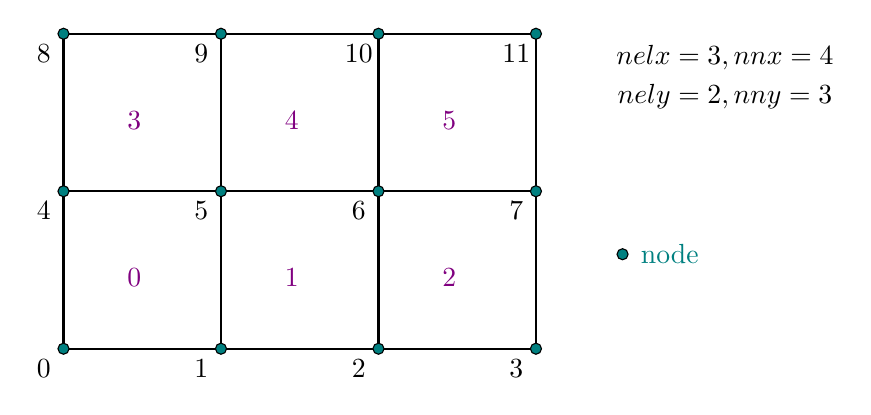
\begin{tikzpicture}
%\draw[step=0.5cm,gray,very thin] (0,0) grid (9,5); %background grid

\draw[thick] (1,1) -- (7,1) -- (7,5) -- (1,5) -- cycle;  
\draw[thick] (1,3) -- (7,3) ;
\draw[thick] (3,1) -- (3,5) ;
\draw[thick] (5,1) -- (5,5) ;

\draw[black,fill=teal] (1,1)     circle (2pt); 
\draw[black,fill=teal] (3,1)     circle (2pt); 
\draw[black,fill=teal] (5,1)     circle (2pt); 
\draw[black,fill=teal] (7,1)     circle (2pt); 

\draw[black,fill=teal] (1,3)     circle (2pt); 
\draw[black,fill=teal] (3,3)     circle (2pt); 
\draw[black,fill=teal] (5,3)     circle (2pt); 
\draw[black,fill=teal] (7,3)     circle (2pt); 

\draw[black,fill=teal] (1,5)     circle (2pt); 
\draw[black,fill=teal] (3,5)     circle (2pt); 
\draw[black,fill=teal] (5,5)     circle (2pt); 
\draw[black,fill=teal] (7,5)     circle (2pt); 

\node[] at (0.75,0.75) {0};
\node[] at (2.75,0.75) {1};
\node[] at (4.75,0.75) {2};
\node[] at (6.75,0.75) {3};

\node[] at (0.75,2.75) {4};
\node[] at (2.75,2.75) {5};
\node[] at (4.75,2.75) {6};
\node[] at (6.75,2.75) {7};

\node[] at (0.75,4.75) {8};
\node[] at (2.75,4.75) {9};
\node[] at (4.75,4.75) {10};
\node[] at (6.75,4.75) {11};

\node[violet] at (1.9,1.9) {0};
\node[violet] at (3.9,1.9) {1};
\node[violet] at (5.9,1.9) {2};
\node[violet] at (1.9,3.9) {3};
\node[violet] at (3.9,3.9) {4};
\node[violet] at (5.9,3.9) {5};

\draw[black,fill=teal] (8.1,2.2) circle (2pt); 
\node[] at (8.7,2.2) {{\color{teal}node}};

\node[] at (9.4,4.7) {$nelx=3, nnx=4$};
\node[] at (9.4,4.2) {$nely=2, nny=3$};

\end{tikzpicture}

\end{center}

\noindent In the case there is only a single degree of freedom per node, the 
assembled FEM matrix ${\bm M}$ will look like this:
\[
{\bm M}=
\left(
\begin{array}{cccccccccccc}
\Box & \Box &      &      & \Box & \Box &      &      &      &      &      &      \\
\Box & \Box & \Box &      & \Box & \Box & \Box &      &      &      &      &      \\
     & \Box & \Box & \Box &      & \Box & \Box & \Box &      &      &      &      \\
     &      & \Box & \Box &      &      & \Box & \Box &      &      &      &      \\
\Box & \Box &      &      & \Box & \Box &      &      & \Box & \Box &      &      \\
\Box & \Box & \Box &      & \Box & \Box & \Box &      & \Box & \Box & \Box &      \\
     & \Box & \Box & \Box &      & \Box & \Box & \Box &      & \Box & \Box & \Box \\
     &      & \Box & \Box &      &      & \Box & \Box &      &      & \Box & \Box \\
     &      &      &      & \Box & \Box &      &      & \Box & \Box &      &      \\
     &      &      &      & \Box & \Box & \Box &      & \Box & \Box & \Box &      \\
     &      &      &      &      & \Box & \Box & \Box &      & \Box & \Box & \Box \\
     &      &      &      &      &      & \Box & \Box &      &      & \Box & \Box 
\end{array}
\right)
\]
where the $\Box$ stand for non-zero terms.
This matrix structure stems from the fact that
\begin{itemize}
\item node 0 sees nodes 0,1,4,5 (1st line/column of the matrix)
\item node 1 sees nodes 0,1,2,4,5,6 (2nd line/column of the matrix)
\item node 2 sees nodes 1,2,3,5,6,7 (3rd line/column of the matrix)
\item node 3 sees nodes 2,3,6,7
\item node 4 sees nodes 0,1,4,5,8,9
\item node 5 sees nodes 0,1,2,4,5,6,8,9,10 
\item node 6 sees nodes 1,2,3,5,6,7,9,10,11
\item node 7 sees nodes 2,3,6,7,10,11
\item node 8 sees nodes 4,5,8,9
\item node 9 sees nodes 4,5,6,8,9,10
\item node 10 sees nodes 5,6,7,9,10,11 
\item node 11 sees nodes 6,7,10,11 (last line/column of the matrix)
\end{itemize}
In light thereof, we have
\begin{itemize}
\item 4 corner nodes which have 4 neighbours (counting themselves) 
\item 2(nnx-2) nodes which have 6 neighbours
\item 2(nny-2) nodes which have 6 neighbours
\item (nnx-2)$\times$(nny-2) nodes which have 9 neighbours
\end{itemize}
In total, the number of non-zero terms in the matrix above is then:
\[
NZ=4\times4+4\times6+2\times6+2\times9=70
\]
and in general, we would then have:
\[
NZ=4\times4+[2(nnx-2)+2(nny-2)]\times6 + (nnx-2)(nny-2)\times9
\]
Let us temporarily assume $nnx=nny=n$. The matrix size (total
number of unknowns) is then $N=n^2$ and  
\[
NZ=16+24(n-2)+9(n-2)^2
\]
A full matrix array would contain $N^2=n^4$ terms. 
The ratio of $NZ$ (the actual number of reals to store)
to the full matrix size (the number of reals a full matrix contains) is then 
\[
R = \frac{16+24(n-2)+9(n-2)^2}{n^4}
\]
It is then obvious that when $n$ is large enough $R \sim 1/n^2$.

CSR stores the nonzeros of the matrix row by row, in a
single indexed array A of double precision  numbers.
Another array COLIND contains the column index of each
corresponding entry in the A array. A third integer array RWPTR
contains pointers to the beginning of each row, which an additional pointer to
the first index following the nonzeros of the matrix A.
A and COLIND have length NZ and RWPTR has length N+1.

In the case of the here-above matrix, the arrays COLIND and RWPTR will look like:
\begin{eqnarray}
COLIND&=&(0,1,4,5, \; 0,1,2,4,5,6, \; 1,2,3,5,6,7, ..., 6,7,10,11) \nn\\
RWPTR &=&(0,4,10,16, ... )   \nn
\end{eqnarray}


%..............................................................................
\subsection{2D domain - $Q_1$ - Symmetric matrix CSR storage} \label{ss:symmcsrss}

If the matrix is symmetric, i.e. ${\bm M}={\bm M}^T$, then we may wish to 
only store half of it, always in the interest of saving memory. 
Only the following remaining $\Box$ entries are relevant now:
\[
{\bm M}=
\left(
\begin{array}{cccccccccccc}
\Box & \Box &      &      & \Box & \Box &      &      &      &      &      &      \\
     & \Box & \Box &      & \Box & \Box & \Box &      &      &      &      &      \\
     &      & \Box & \Box &      & \Box & \Box & \Box &      &      &      &      \\
     &      &      & \Box &      &      & \Box & \Box &      &      &      &      \\
     &      &      &      & \Box & \Box &      &      & \Box & \Box &      &      \\
     &      &      &      &      & \Box & \Box &      & \Box & \Box & \Box &      \\
     &      &      &      &      &      & \Box & \Box &      & \Box & \Box & \Box \\
     &      &      &      &      &      &      & \Box &      &      & \Box & \Box \\
     &      &      &      &      &      &      &      & \Box & \Box &      &      \\
     &      &      &      &      &      &      &      &      & \Box & \Box &      \\
     &      &      &      &      &      &      &      &      &      & \Box & \Box \\
     &      &      &      &      &      &      &      &      &      &      & \Box 
\end{array}
\right)
\]
We see that the number of nonzeros is now 
\[
NZ_{symm}= \frac{NZ-n}{2}+n
\]
and in this case $NZ_{symm}=(70-12)/2+12=41$.
Then 
\begin{eqnarray}
COLIND&=&(0,1,4,5, \; 1,2,4,5,6, \; 3,5,6,7, ..., ,11) \nn\\
RWPTR &=&(0,4,9,14, ... )   \nn
\end{eqnarray}

In case the numbering is Fortran-like, then 
\begin{eqnarray}
ja=COLIND&=&(
1, 2, 5, 6, \quad  2, 3, 5, 6, 7, \quad 3, 4, 6, 7, 8, \quad      
4, 7, 8, \quad  5, 6, 9, 10, \quad 6, 7, 9, 10, 11, \nn\\
&& 7, 8, 10, 11, 12, \quad 8, 11, 12, \quad 9, 10, \quad 10, 11, \quad  11, 12, \quad 12) \nn\\
ia=RWPTR &=&(1, 5, 10, 15, 18, 22, 27, 32, 35, 37, 39, 41, 42)  \nn
\end{eqnarray}

%..............................................................................
\subsection{2D domain - $Q_1$ - Two degrees of freedom per node}

When there are now two degrees of freedom per node, such as in the case 
of the Stokes equation in two-dimensions, the size of the $\K$ matrix 
is given $NfemV=nnx*nny*ndofV$ where $NfemV$ is the total number of 
velocity degrees of freedom.

\begin{center}
\input{tikz/tikz_3x2_two}
\end{center}

In the case of the small grid above, we have then $NfemV=24$ and
elemental matrices are now $8\times8$ in size.

We still have
\begin{itemize}
\item $4$ corner nodes which have 4 neighbours
\item $2(nnx-2)$ nodes which have 6 neighbours
\item $2(nny-2)$ nodes which have 6 neighbours
\item $(nnx-2)\cdot(nny-2)$ nodes which have 9 neighbours,
\end{itemize}
but now each degree of freedom from a node sees the other two
degrees of freedom of another node too.
In that case, the number of nonzeros has been multiplied by four
and the assembled FEM matrix looks like:
\begin{equation}
\left(
\begin{array}{cccccccccccccccccccccccc}
\Box&\Box & \Box&\Box &  &  &  &  & \Box&\Box & \Box&\Box &  &  &  &  &  &  &  &  &  &  &  &  \\
\Box&\Box & \Box&\Box &  &  &  &  & \Box&\Box & \Box&\Box &  &  &  &  &  &  &  &  &  &  &  &  \\
\Box&\Box & \Box&\Box & \Box&\Box &  &  & \Box&\Box & \Box&\Box & \Box&\Box &  &  &  &  &  &  &  &  &  &  \\
\Box&\Box & \Box&\Box & \Box&\Box &  &  & \Box&\Box & \Box&\Box & \Box&\Box &  &  &  &  &  &  &  &  &  &  \\
 &  & \Box&\Box & \Box&\Box & \Box&\Box &  &  & \Box&\Box & \Box&\Box & \Box&\Box &  &  &  &  &  &  &  &  \\
 &  & \Box&\Box & \Box&\Box & \Box&\Box &  &  & \Box&\Box & \Box&\Box & \Box&\Box &  &  &  &  &  &  &  &  \\
 &  &  &  & \Box&\Box & \Box&\Box &  &  &  &  & \Box&\Box & \Box&\Box &  &  &  &  &  &  &  &  \\
 &  &  &  & \Box&\Box & \Box&\Box &  &  &  &  & \Box&\Box & \Box&\Box &  &  &  &  &  &  &  &  \\
\Box&\Box & \Box&\Box &  &  &  &  & \Box&\Box & \Box&\Box &  &  &  &  & \Box&\Box & \Box&\Box &  &  &  &  \\
\Box&\Box & \Box&\Box &  &  &  &  & \Box&\Box & \Box&\Box &  &  &  &  & \Box&\Box & \Box&\Box &  &  &  &  \\
\Box&\Box & \Box&\Box & \Box&\Box &  &  & \Box&\Box & \Box&\Box & \Box&\Box &  &  & \Box&\Box & \Box&\Box & \Box&\Box &  &  \\
\Box&\Box & \Box&\Box & \Box&\Box &  &  & \Box&\Box & \Box&\Box & \Box&\Box &  &  & \Box&\Box & \Box&\Box & \Box&\Box &  &  \\
 &  & \Box&\Box & \Box&\Box & \Box&\Box &  &  & \Box&\Box & \Box&\Box & \Box&\Box &  &  & \Box&\Box & \Box&\Box & \Box&\Box \\
 &  & \Box&\Box & \Box&\Box & \Box&\Box &  &  & \Box&\Box & \Box&\Box & \Box&\Box &  &  & \Box&\Box & \Box&\Box & \Box&\Box \\
 &  &  &  & \Box&\Box & \Box&\Box &  &  &  &  & \Box&\Box & \Box&\Box &  &  &  &  & \Box&\Box & \Box&\Box \\
 &  &  &  & \Box&\Box & \Box&\Box &  &  &  &  & \Box&\Box & \Box&\Box &  &  &  &  & \Box&\Box & \Box&\Box \\
 &  &  &  &  &  &  &  & \Box&\Box & \Box&\Box &  &  &  &  & \Box&\Box & \Box&\Box &  &  &  &  \\
 &  &  &  &  &  &  &  & \Box&\Box & \Box&\Box &  &  &  &  & \Box&\Box & \Box&\Box &  &  &  &  \\
 &  &  &  &  &  &  &  & \Box&\Box & \Box&\Box & \Box&\Box &  &  & \Box&\Box & \Box&\Box & \Box&\Box &  &  \\
 &  &  &  &  &  &  &  & \Box&\Box & \Box&\Box & \Box&\Box &  &  & \Box&\Box & \Box&\Box & \Box&\Box &  &  \\
 &  &  &  &  &  &  &  &  &  & \Box&\Box & \Box&\Box & \Box&\Box &  &  & \Box&\Box & \Box&\Box & \Box&\Box \\
 &  &  &  &  &  &  &  &  &  & \Box&\Box & \Box&\Box & \Box&\Box &  &  & \Box&\Box & \Box&\Box & \Box&\Box \\
 &  &  &  &  &  &  &  &  &  &  &  & \Box&\Box & \Box&\Box &  &  &  &  & \Box&\Box & \Box&\Box \\
 &  &  &  &  &  &  &  &  &  &  &  & \Box&\Box & \Box&\Box &  &  &  &  & \Box&\Box & \Box&\Box 
\end{array}
\right)\nonumber
\end{equation}
Note that the degrees of freedom are organised as follows: 
\[
(u_0,v_0,u_1,v_1,u_2,v_2, ... u_{11},v_{11})
\]
In general, we would then have:
\[
NZ=4 \left[4\times4+[2(nnx-2)+2(nny-2)]\times6 + (nnx-2)(nny-2)\times9 \right]
\]
and in the case of the small grid,
the number of non-zero terms in the matrix is then:
\[
NZ=4\left[4\times4+4\times6+2\times6+2\times9\right]=280
\]
In the case of the here-above matrix, the arrays COLIND and RWPTR will look like:
\begin{eqnarray}
COLIND&=&(0,1,2,3,8,9,10,11, \; 0,1,2,3,8,9,10,11,\; ...) \nn\\
RWPTR &=&(0,8,16,28, ... ) \nn
\end{eqnarray}

Assuming we are using $Q_1\times P_0$ elements, the structure of the matrix $\G_{el}^T$ is as follows
(the 6 pressure dofs are connected to 24 velocity dofs):

\begin{scriptsize}
\begin{equation}
\left(
\begin{array}{ccccccccccccccccccccccccc}
&0 & 1 & 2 & 3 & 4 & 5 & 6 & 7 & 8 & 9 & 10 & 11 & 12 & 13 & 14 & 15 & 16 & 17 & 18 & 19 & 20 & 21 & 22 & 23     \\
\Box&\Box & \Box&\Box &  &  &  &  & \Box&\Box & \Box&\Box &  &  &  &  &  &  &  &  &  &  &  &  \\
    &     & \Box&\Box & \Box&\Box &  &  &  &  & \Box&\Box & \Box&\Box &  &  &  &  &  &  &  &  &  &  \\
 & &     &     & \Box&\Box & \Box&\Box &  &  &  &  & \Box&\Box & \Box&\Box &  &  &  &  &  &  &  &    \\
 & & & &  & &     &     & \Box&\Box & \Box&\Box &  &  &  &  & \Box&\Box & \Box&\Box &  &  &  &      \\
 & & & & & &  & &     &     & \Box&\Box & \Box&\Box &  &  &  &  & \Box&\Box & \Box&\Box &  &       \\
 & &  & & & & & &  & &     &     & \Box&\Box & \Box&\Box &  &  &  &  & \Box&\Box & \Box&\Box        
\end{array}
\right)
\end{equation} 
\end{scriptsize}

\begin{center}
\input{tikz/csrStokes_3x2_ELEFANT}
\input{tikz/csrStokes_4x3_ELEFANT}
\input{tikz/csrStokes_5x4_ELEFANT}\\
{\captionfont From left to right: Nonzero structures of the assembled Stokes matrix for a 
$3\times 2$, $4\times 3$ and $5\times 4$ mesh of $Q_1\times P_0$ elements.}
\end{center}


Assuming we are now using $Q_1\times Q_1$ elements (without bubble), 
the structure of the matrix $\G_{el}^T$ is different: we now have 12 pressure dofs 
which are coupled to 24 velocity dofs:
\begin{scriptsize}
\begin{equation}
\left(
\begin{array}{ccccccccccccccccccccccccc}
 & 1 & 2 & 3 & 4 & 5 & 6 & 7 & 8 & 9 & 10 & 11 & 12 & 13 & 14 & 15 & 16 & 17 & 18 & 19 & 20 & 21 & 22 & 23 & 24    \\
0 &\Box&\Box & \Box&\Box &  &  &  &  & \Box&\Box & \Box&\Box &  &  &  &  &  &  &  &  &  &  &  &  \\
1 & \Box&\Box & \Box&\Box & \Box  & \Box  &  &  & \Box&\Box & \Box&\Box & \Box  & \Box  &  &  &  &  &  &  &  &  &  & \\
2 &  & & \Box&\Box & \Box  & \Box  & \Box  & \Box  & & & \Box&\Box & \Box  & \Box  & \Box  &\Box  &  &  &  &  &  &  &  & \\ 
3 &  & & &  & \Box  & \Box  & \Box  & \Box  & & & & & \Box  & \Box  & \Box  &\Box  &  &  &  &  &  &  &  & \\ 
\\
... \\
\\
9 & & & & & & & & &\Box &\Box &\Box &\Box & \Box  & \Box &  &  & & &\Box &\Box & \Box &\Box & &  \\
10 & & & & & & & & & & &\Box &\Box & \Box  & \Box & \Box & \Box & & &\Box &\Box & \Box &\Box &\Box & \Box \\
11 & & & & & & & & & & & & & \Box  & \Box & \Box & \Box & & & & & \Box &\Box &\Box & \Box \\
\end{array}
\right)
\end{equation} 
\end{scriptsize}

%..............................................................................
\subsection{2D domain - $Q_2$ - Two degrees of freedom per node}


When there are now two degrees of freedom per node, such as in the case 
of the Stokes equation in two-dimensions, the size of the $\K$ matrix 
is given $NfemV=nnx*nny*ndofV$ where $NfemV$ is the total number of 
velocity degrees of freedom. What is different here is that for $Q_2$
elements we have $nnx=2*nelx+1$ and $nny=2*nely+1$.

\begin{center}
\begin{flushright} {\tiny {\color{gray} (tikz\_3x2\_two\_Q2.tex)}} \end{flushright}
%~~~~~~~~~~~~~~~~~~~~~~~~~~~~~~~~~~~~~~~~~~~~~~~~~~~~~~~~~~~~~~~~~~~~~~~~~~~~~~~~~~~~~~~~~~~~~~~~~~

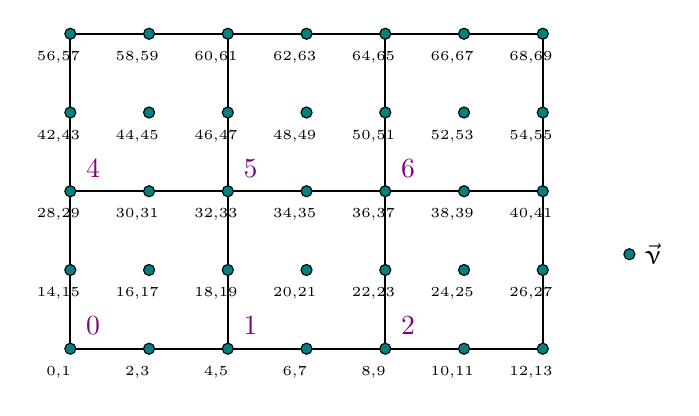
\begin{tikzpicture}
%\draw[step=0.5cm,gray,very thin] (0,0) grid (8,6); %background grid

\draw[thick] (1,1) -- (7,1) -- (7,5) -- (1,5) -- cycle;  
\draw[thick] (1,3) -- (7,3) ;
\draw[thick] (3,1) -- (3,5) ;
\draw[thick] (5,1) -- (5,5) ;

\draw[black,fill=teal] (1,1)     circle (2pt); 
\draw[black,fill=teal] (2,1)     circle (2pt); 
\draw[black,fill=teal] (3,1)     circle (2pt); 
\draw[black,fill=teal] (4,1)     circle (2pt); 
\draw[black,fill=teal] (5,1)     circle (2pt); 
\draw[black,fill=teal] (6,1)     circle (2pt); 
\draw[black,fill=teal] (7,1)     circle (2pt); 

\draw[black,fill=teal] (1,2)     circle (2pt); 
\draw[black,fill=teal] (2,2)     circle (2pt); 
\draw[black,fill=teal] (3,2)     circle (2pt); 
\draw[black,fill=teal] (4,2)     circle (2pt); 
\draw[black,fill=teal] (5,2)     circle (2pt); 
\draw[black,fill=teal] (6,2)     circle (2pt); 
\draw[black,fill=teal] (7,2)     circle (2pt); 

\draw[black,fill=teal] (1,3)     circle (2pt); 
\draw[black,fill=teal] (2,3)     circle (2pt); 
\draw[black,fill=teal] (3,3)     circle (2pt); 
\draw[black,fill=teal] (4,3)     circle (2pt); 
\draw[black,fill=teal] (5,3)     circle (2pt); 
\draw[black,fill=teal] (6,3)     circle (2pt); 
\draw[black,fill=teal] (7,3)     circle (2pt); 

\draw[black,fill=teal] (1,4)     circle (2pt); 
\draw[black,fill=teal] (2,4)     circle (2pt); 
\draw[black,fill=teal] (3,4)     circle (2pt); 
\draw[black,fill=teal] (4,4)     circle (2pt); 
\draw[black,fill=teal] (5,4)     circle (2pt); 
\draw[black,fill=teal] (6,4)     circle (2pt); 
\draw[black,fill=teal] (7,4)     circle (2pt); 

\draw[black,fill=teal] (1,5)     circle (2pt); 
\draw[black,fill=teal] (2,5)     circle (2pt); 
\draw[black,fill=teal] (3,5)     circle (2pt); 
\draw[black,fill=teal] (4,5)     circle (2pt); 
\draw[black,fill=teal] (5,5)     circle (2pt); 
\draw[black,fill=teal] (6,5)     circle (2pt); 
\draw[black,fill=teal] (7,5)     circle (2pt); 

\node[] at (0.85,0.7) {\tiny 0,1};
\node[] at (1.85,0.7) {\tiny 2,3};
\node[] at (2.85,0.7) {\tiny 4,5};
\node[] at (3.85,0.7) {\tiny 6,7};
\node[] at (4.85,0.7) {\tiny 8,9};
\node[] at (5.85,0.7) {\tiny 10,11};
\node[] at (6.85,0.7) {\tiny 12,13};

\node[] at (0.85,1.7) {\tiny 14,15};
\node[] at (1.85,1.7) {\tiny 16,17};
\node[] at (2.85,1.7) {\tiny 18,19};
\node[] at (3.85,1.7) {\tiny 20,21};
\node[] at (4.85,1.7) {\tiny 22,23};
\node[] at (5.85,1.7) {\tiny 24,25};
\node[] at (6.85,1.7) {\tiny 26,27};

\node[] at (0.85,2.7) {\tiny 28,29}; 
\node[] at (1.85,2.7) {\tiny 30,31}; 
\node[] at (2.85,2.7) {\tiny 32,33}; 
\node[] at (3.85,2.7) {\tiny 34,35}; 
\node[] at (4.85,2.7) {\tiny 36,37}; 
\node[] at (5.85,2.7) {\tiny 38,39}; 
\node[] at (6.85,2.7) {\tiny 40,41}; 

\node[] at (0.85,3.7) {\tiny 42,43}; 
\node[] at (1.85,3.7) {\tiny 44,45}; 
\node[] at (2.85,3.7) {\tiny 46,47}; 
\node[] at (3.85,3.7) {\tiny 48,49}; 
\node[] at (4.85,3.7) {\tiny 50,51}; 
\node[] at (5.85,3.7) {\tiny 52,53}; 
\node[] at (6.85,3.7) {\tiny 54,55}; 

\node[] at (0.85,4.7) {\tiny 56,57}; 
\node[] at (1.85,4.7) {\tiny 58,59}; 
\node[] at (2.85,4.7) {\tiny 60,61}; 
\node[] at (3.85,4.7) {\tiny 62,63}; 
\node[] at (4.85,4.7) {\tiny 64,65}; 
\node[] at (5.85,4.7) {\tiny 66,67}; 
\node[] at (6.85,4.7) {\tiny 68,69}; 

\node[violet] at (1.29,1.29) {0};
\node[violet] at (3.29,1.29) {1};
\node[violet] at (5.29,1.29) {2};
\node[violet] at (1.29,3.29) {4};
\node[violet] at (3.29,3.29) {5};
\node[violet] at (5.29,3.29) {6};

\draw[black,fill=teal] (8.1,2.2) circle (2pt); 
\node[] at (8.4,2.2) {$\vec\upnu$};

\end{tikzpicture}


\end{center}

In the case of the small grid above, we have then 
$nelx=3$, $nely=2$, so that $nnx=7$ and $nny=5$, and then
$NfemV=7*5*2=70$ and elemental matrices are now $18\times18$ in size.


\begin{center}
\begin{flushright} {\tiny {\color{gray} (tikz\_3x2\_Q2.tex)}} \end{flushright}
%~~~~~~~~~~~~~~~~~~~~~~~~~~~~~~~~~~~~~~~~~~~~~~~~~~~~~~~~~~~~~~~~~~~~~~~~~~~~~~~~~~~~~~~~~~~~~~~~~~

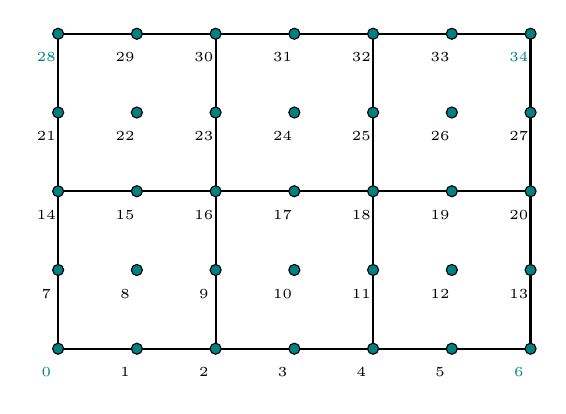
\begin{tikzpicture}
%\draw[step=0.5cm,gray,very thin] (0,0) grid (8,6); %background grid

\draw[thick] (1,1) -- (7,1) -- (7,5) -- (1,5) -- cycle;  
\draw[thick] (1,3) -- (7,3) ;
\draw[thick] (3,1) -- (3,5) ;
\draw[thick] (5,1) -- (5,5) ;

\draw[black,fill=teal] (1,1)     circle (2pt); 
\draw[black,fill=teal] (2,1)     circle (2pt); 
\draw[black,fill=teal] (3,1)     circle (2pt); 
\draw[black,fill=teal] (4,1)     circle (2pt); 
\draw[black,fill=teal] (5,1)     circle (2pt); 
\draw[black,fill=teal] (6,1)     circle (2pt); 
\draw[black,fill=teal] (7,1)     circle (2pt); 

\draw[black,fill=teal] (1,2)     circle (2pt); 
\draw[black,fill=teal] (2,2)     circle (2pt); 
\draw[black,fill=teal] (3,2)     circle (2pt); 
\draw[black,fill=teal] (4,2)     circle (2pt); 
\draw[black,fill=teal] (5,2)     circle (2pt); 
\draw[black,fill=teal] (6,2)     circle (2pt); 
\draw[black,fill=teal] (7,2)     circle (2pt); 

\draw[black,fill=teal] (1,3)     circle (2pt); 
\draw[black,fill=teal] (2,3)     circle (2pt); 
\draw[black,fill=teal] (3,3)     circle (2pt); 
\draw[black,fill=teal] (4,3)     circle (2pt); 
\draw[black,fill=teal] (5,3)     circle (2pt); 
\draw[black,fill=teal] (6,3)     circle (2pt); 
\draw[black,fill=teal] (7,3)     circle (2pt); 

\draw[black,fill=teal] (1,4)     circle (2pt); 
\draw[black,fill=teal] (2,4)     circle (2pt); 
\draw[black,fill=teal] (3,4)     circle (2pt); 
\draw[black,fill=teal] (4,4)     circle (2pt); 
\draw[black,fill=teal] (5,4)     circle (2pt); 
\draw[black,fill=teal] (6,4)     circle (2pt); 
\draw[black,fill=teal] (7,4)     circle (2pt); 

\draw[black,fill=teal] (1,5)     circle (2pt); 
\draw[black,fill=teal] (2,5)     circle (2pt); 
\draw[black,fill=teal] (3,5)     circle (2pt); 
\draw[black,fill=teal] (4,5)     circle (2pt); 
\draw[black,fill=teal] (5,5)     circle (2pt); 
\draw[black,fill=teal] (6,5)     circle (2pt); 
\draw[black,fill=teal] (7,5)     circle (2pt); 

\node[] at (0.85,0.7) {\tiny \color{teal} 0};
\node[] at (1.85,0.7) {\tiny 1};
\node[] at (2.85,0.7) {\tiny 2};
\node[] at (3.85,0.7) {\tiny 3};
\node[] at (4.85,0.7) {\tiny 4};
\node[] at (5.85,0.7) {\tiny 5};
\node[] at (6.85,0.7) {\tiny \color{teal} 6};

\node[] at (0.85,1.7) {\tiny 7};
\node[] at (1.85,1.7) {\tiny 8};
\node[] at (2.85,1.7) {\tiny 9};
\node[] at (3.85,1.7) {\tiny 10};
\node[] at (4.85,1.7) {\tiny 11};
\node[] at (5.85,1.7) {\tiny 12};
\node[] at (6.85,1.7) {\tiny 13};

\node[] at (0.85,2.7) {\tiny 14}; 
\node[] at (1.85,2.7) {\tiny 15}; 
\node[] at (2.85,2.7) {\tiny 16}; 
\node[] at (3.85,2.7) {\tiny 17}; 
\node[] at (4.85,2.7) {\tiny 18}; 
\node[] at (5.85,2.7) {\tiny 19}; 
\node[] at (6.85,2.7) {\tiny 20}; 

\node[] at (0.85,3.7) {\tiny 21}; 
\node[] at (1.85,3.7) {\tiny 22}; 
\node[] at (2.85,3.7) {\tiny 23}; 
\node[] at (3.85,3.7) {\tiny 24}; 
\node[] at (4.85,3.7) {\tiny 25}; 
\node[] at (5.85,3.7) {\tiny 26}; 
\node[] at (6.85,3.7) {\tiny 27}; 

\node[] at (0.85,4.7) {\tiny \color{teal} 28}; 
\node[] at (1.85,4.7) {\tiny 29}; 
\node[] at (2.85,4.7) {\tiny 30}; 
\node[] at (3.85,4.7) {\tiny 31}; 
\node[] at (4.85,4.7) {\tiny 32}; 
\node[] at (5.85,4.7) {\tiny 33}; 
\node[] at (6.85,4.7) {\tiny \color{teal} 34}; 

\end{tikzpicture}


\end{center}


Concretely here:
\begin{itemize}
\item nodes {\color{teal} 0,6,28,34} see 9 nodes (corners)
\item nodes 1,3,5,7,8,10,12,13,21,22,24,26,27,29,31,33 see 9 nodes
\item nodes 2,4,9,11,14,15,17,19,20,23,25,30,32, see 15 nodes
\item nodes 16,18 see 25 nodes
\end{itemize}

If there was only one dof per node, we would find 
the number of non zeros as follow:
\[
NZ=4*9 + 16*9 + 13*15 + 2*25 = 36+144 + 195 + 50 = 425
\]
But since there are two velocity dofs per node, we find that 
the total number of nonzeros is 4 times higher, i.e.
\[
NZ=1700
\] 
And if we choose for a symmetric CSR storage:
\[
NZ_{symm} = \frac{NZ-n}{2}+n = \frac{1700-70}{2} + 70 = 885 
\]

Let us now turn to the real case of 2 dofs per node and establish 
who sees who:

\begin{tabular}{lp{14.5cm}l}
dof &  sees other dofs & total\\
\hline
0 & 0,1,2,3,4,5,14,15,16,17,18,19,28,29,30,31,32,33 & 18 \\
1 & 0,1,2,3,4,5,14,15,16,17,18,19,28,29,30,31,32,33 & 18 \\
2 & 0,1,2,3,4,5,14,15,16,17,18,19,28,29,30,31,32,33 & 18 \\
3 & 0,1,2,3,4,5,14,15,16,17,18,19,28,29,30,31,32,33 & 18 \\
4 & 0,1,2,3,4,5,6,7,8,9,14,15,16,17,18,19,20,21,22,23,28,29,30,31,32,33,34,35,36,37 & 30 \\
5 & 0,1,2,3,4,5,6,7,8,9,14,15,16,17,18,19,20,21,22,23,28,29,30,31,32,33,34,35,36,37 & 30 \\
6 & 4,5,6,7,8,9,18,19,20,21,22,23,32,33,34,35,36,37 & 18 \\
7 & 4,5,6,7,8,9,18,19,20,21,22,23,32,33,34,35,36,37 & 18 \\
8 & 4,5,6,7,8,9,10,11,12,13,18,19,20,21,22,23,24,25,26,27,32,33,34,35,36,37,38,39,40,41 & 30 \\
9 & 4,5,6,7,8,9,10,11,12,13,18,19,20,21,22,23,24,25,26,27,32,33,34,35,36,37,38,39,40,41 & 30 \\
10 & 8,9,10,11,12,13,22,23,24,25,26,27,36,37,38,39,40,41 & 18\\
11 & 8,9,10,11,12,13,22,23,24,25,26,27,36,37,38,39,40,41 & 18\\
12 & 8,9,10,11,12,13,22,23,24,25,26,27,36,37,38,39,40,41 & 18\\
13 & 8,9,10,11,12,13,22,23,24,25,26,27,36,37,38,39,40,41 & 18\\
14 & 0,1,2,3,4,5,14,15,16,17,18,19,28,29,30,31,32,33 & 18 \\
15 & 0,1,2,3,4,5,14,15,16,17,18,19,28,29,30,31,32,33 & 18 \\
16 & 0,1,2,3,4,5,14,15,16,17,18,19,28,29,30,31,32,33 & 18 \\
17 & 0,1,2,3,4,5,14,15,16,17,18,19,28,29,30,31,32,33 & 18 \\
 ... & ... & ... \\
68 & 36,37,38,39,50,51,52,53,54,55,64,65,66,67,68,69 & 18 \\
69 & 36,37,38,39,50,51,52,53,54,55,64,65,66,67,68,69 & 18 \\
\hline
\end{tabular}

The second column of this array is the content of the ja array.


In order establish a pattern we will need a bigger mesh:

\begin{center}
\begin{flushright} {\footnotesize {\color{gray} (tikz\_4x3\_Q2.tex)}} \end{flushright}
%~~~~~~~~~~~~~~~~~~~~~~~~~~~~~~~~~~~~~~~~~~~~~~~~~~~~~~~~~~~~~~~~~~~~~~~~~~~~~~~~~~~~~~~~~~~~~~~~~~

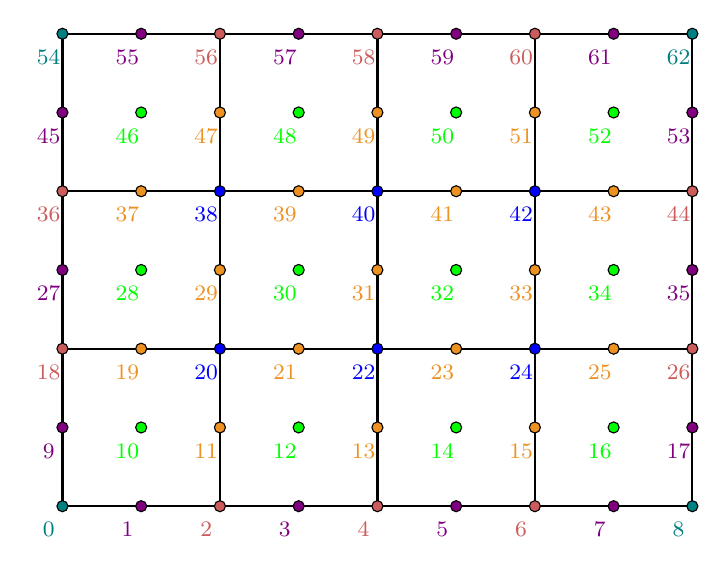
\begin{tikzpicture}
%\draw[step=0.5cm,gray,very thin] (0,0) grid (10,8); %background grid

\draw[thick] (1,1) -- (9,1) -- (9,7) -- (1,7) -- cycle;  
\draw[thick] (1,3) -- (9,3) ;
\draw[thick] (1,5) -- (9,5) ;
\draw[thick] (3,1) -- (3,7) ;
\draw[thick] (5,1) -- (5,7) ;
\draw[thick] (7,1) -- (7,7) ;

\draw[black,fill=teal] (1,1)     circle (2pt);  %0
\draw[black,fill=violet] (2,1)     circle (2pt); 
\draw[black,fill=chestnut] (3,1)     circle (2pt); 
\draw[black,fill=violet] (4,1)     circle (2pt); 
\draw[black,fill=chestnut] (5,1)     circle (2pt); 
\draw[black,fill=violet] (6,1)     circle (2pt); 
\draw[black,fill=chestnut] (7,1)     circle (2pt); 
\draw[black,fill=violet] (8,1)     circle (2pt); 
\draw[black,fill=teal] (9,1)     circle (2pt); %8

\draw[black,fill=violet] (1,2)     circle (2pt); %9
\draw[black,fill=green] (2,2)     circle (2pt); 
\draw[black,fill=carrotorange] (3,2)     circle (2pt); 
\draw[black,fill=green] (4,2)     circle (2pt); 
\draw[black,fill=carrotorange] (5,2)     circle (2pt); 
\draw[black,fill=green] (6,2)     circle (2pt); 
\draw[black,fill=carrotorange] (7,2)     circle (2pt); 
\draw[black,fill=green] (8,2)     circle (2pt); 
\draw[black,fill=violet] (9,2)     circle (2pt); %17

\draw[black,fill=chestnut] (1,3)     circle (2pt); %18
\draw[black,fill=carrotorange] (2,3)     circle (2pt); 
\draw[black,fill=blue] (3,3)     circle (2pt); 
\draw[black,fill=carrotorange] (4,3)     circle (2pt); 
\draw[black,fill=blue] (5,3)     circle (2pt); 
\draw[black,fill=carrotorange] (6,3)     circle (2pt); 
\draw[black,fill=blue] (7,3)     circle (2pt); 
\draw[black,fill=carrotorange] (8,3)     circle (2pt); 
\draw[black,fill=chestnut] (9,3)     circle (2pt); %26

\draw[black,fill=violet] (1,4)     circle (2pt); %27
\draw[black,fill=green] (2,4)     circle (2pt); 
\draw[black,fill=carrotorange] (3,4)     circle (2pt); 
\draw[black,fill=green] (4,4)     circle (2pt); 
\draw[black,fill=carrotorange] (5,4)     circle (2pt); 
\draw[black,fill=green] (6,4)     circle (2pt); 
\draw[black,fill=carrotorange] (7,4)     circle (2pt); 
\draw[black,fill=green] (8,4)     circle (2pt); 
\draw[black,fill=violet] (9,4)     circle (2pt); %35

\draw[black,fill=chestnut] (1,5)     circle (2pt); %36
\draw[black,fill=carrotorange] (2,5)     circle (2pt); 
\draw[black,fill=blue] (3,5)     circle (2pt); 
\draw[black,fill=carrotorange] (4,5)     circle (2pt); 
\draw[black,fill=blue] (5,5)     circle (2pt); 
\draw[black,fill=carrotorange] (6,5)     circle (2pt); 
\draw[black,fill=blue] (7,5)     circle (2pt); 
\draw[black,fill=carrotorange] (8,5)     circle (2pt); 
\draw[black,fill=chestnut] (9,5)     circle (2pt); %44

\draw[black,fill=violet] (1,6)     circle (2pt); %45 
\draw[black,fill=green] (2,6)     circle (2pt); 
\draw[black,fill=carrotorange] (3,6)     circle (2pt); 
\draw[black,fill=green] (4,6)     circle (2pt); 
\draw[black,fill=carrotorange] (5,6)     circle (2pt); 
\draw[black,fill=green] (6,6)     circle (2pt); 
\draw[black,fill=carrotorange] (7,6)     circle (2pt); 
\draw[black,fill=green] (8,6)     circle (2pt); 
\draw[black,fill=violet] (9,6)     circle (2pt); %53

\draw[black,fill=teal] (1,7)     circle (2pt); %54
\draw[black,fill=violet] (2,7)     circle (2pt); 
\draw[black,fill=chestnut] (3,7)     circle (2pt); 
\draw[black,fill=violet] (4,7)     circle (2pt); 
\draw[black,fill=chestnut] (5,7)     circle (2pt); 
\draw[black,fill=violet] (6,7)     circle (2pt); 
\draw[black,fill=chestnut] (7,7)     circle (2pt); 
\draw[black,fill=violet] (8,7)     circle (2pt); 
\draw[black,fill=teal] (9,7)     circle (2pt); %62

\node[] at (0.825,0.7) {\footnotesize \color{teal} 0};
\node[] at (1.825,0.7) {\footnotesize \color{violet} 1};
\node[] at (2.825,0.7) {\footnotesize \color{chestnut} 2};
\node[] at (3.825,0.7) {\footnotesize \color{violet} 3};
\node[] at (4.825,0.7) {\footnotesize \color{chestnut} 4};
\node[] at (5.825,0.7) {\footnotesize \color{violet} 5};
\node[] at (6.825,0.7) {\footnotesize \color{chestnut} 6};
\node[] at (7.825,0.7) {\footnotesize \color{violet} 7};
\node[] at (8.825,0.7) {\footnotesize \color{teal} 8};

\node[] at (0.825,1.7) {\footnotesize \color{violet} 9};
\node[] at (1.825,1.7) {\footnotesize \color{green} 10};
\node[] at (2.825,1.7) {\footnotesize \color{carrotorange}11};
\node[] at (3.825,1.7) {\footnotesize \color{green} 12};
\node[] at (4.825,1.7) {\footnotesize \color{carrotorange}13};
\node[] at (5.825,1.7) {\footnotesize \color{green} 14};
\node[] at (6.825,1.7) {\footnotesize \color{carrotorange}15};
\node[] at (7.825,1.7) {\footnotesize \color{green} 16};
\node[] at (8.825,1.7) {\footnotesize \color{violet} 17};

\node[] at (0.825,2.7) {\footnotesize \color{chestnut} 18}; 
\node[] at (1.825,2.7) {\footnotesize \color{carrotorange} 19}; 
\node[] at (2.825,2.7) {\footnotesize \color{blue} 20}; 
\node[] at (3.825,2.7) {\footnotesize \color{carrotorange} 21}; 
\node[] at (4.825,2.7) {\footnotesize \color{blue} 22}; 
\node[] at (5.825,2.7) {\footnotesize \color{carrotorange} 23}; 
\node[] at (6.825,2.7) {\footnotesize \color{blue} 24}; 
\node[] at (7.825,2.7) {\footnotesize \color{carrotorange} 25}; 
\node[] at (8.825,2.7) {\footnotesize \color{chestnut} 26}; 

\node[] at (0.825,3.7) {\footnotesize \color{violet} 27}; 
\node[] at (1.825,3.7) {\footnotesize \color{green} 28}; 
\node[] at (2.825,3.7) {\footnotesize \color{carrotorange} 29}; 
\node[] at (3.825,3.7) {\footnotesize \color{green} 30}; 
\node[] at (4.825,3.7) {\footnotesize \color{carrotorange} 31}; 
\node[] at (5.825,3.7) {\footnotesize \color{green} 32}; 
\node[] at (6.825,3.7) {\footnotesize \color{carrotorange} 33}; 
\node[] at (7.825,3.7) {\footnotesize \color{green} 34}; 
\node[] at (8.825,3.7) {\footnotesize \color{violet} 35};

\node[] at (0.825,4.7) {\footnotesize \color{chestnut} 36}; 
\node[] at (1.825,4.7) {\footnotesize \color{carrotorange}37}; 
\node[] at (2.825,4.7) {\footnotesize \color{blue} 38}; 
\node[] at (3.825,4.7) {\footnotesize \color{carrotorange}39}; 
\node[] at (4.825,4.7) {\footnotesize \color{blue} 40}; 
\node[] at (5.825,4.7) {\footnotesize \color{carrotorange}41}; 
\node[] at (6.825,4.7) {\footnotesize \color{blue} 42};
\node[] at (7.825,4.7) {\footnotesize \color{carrotorange}43};
\node[] at (8.825,4.7) {\footnotesize \color{chestnut} 44};

\node[] at (0.825,5.7) {\footnotesize \color{violet} 45}; 
\node[] at (1.825,5.7) {\footnotesize \color{green} 46}; 
\node[] at (2.825,5.7) {\footnotesize \color{carrotorange}47}; 
\node[] at (3.825,5.7) {\footnotesize \color{green} 48}; 
\node[] at (4.825,5.7) {\footnotesize \color{carrotorange}49}; 
\node[] at (5.825,5.7) {\footnotesize \color{green} 50}; 
\node[] at (6.825,5.7) {\footnotesize \color{carrotorange}51};
\node[] at (7.825,5.7) {\footnotesize \color{green} 52};
\node[] at (8.825,5.7) {\footnotesize \color{violet} 53};

\node[] at (0.825,6.7) {\footnotesize \color{teal}54}; 
\node[] at (1.825,6.7) {\footnotesize \color{violet} 55}; 
\node[] at (2.825,6.7) {\footnotesize \color{chestnut} 56}; 
\node[] at (3.825,6.7) {\footnotesize \color{violet} 57}; 
\node[] at (4.825,6.7) {\footnotesize \color{chestnut} 58}; 
\node[] at (5.825,6.7) {\footnotesize \color{violet} 59}; 
\node[] at (6.825,6.7) {\footnotesize \color{chestnut} 60};
\node[] at (7.825,6.7) {\footnotesize \color{violet} 61};
\node[] at (8.825,6.7) {\footnotesize \color{teal} 62};

\end{tikzpicture}

\end{center}



We have
\begin{itemize}
\item {\color{teal} 4} corner nodes which have 9 neighbours
\item {\color{green} $nel$} mid-element nodes which have 9 neighbours
\item {\color{violet} $2*nelx+2*nely$} mid-edge nodes on sides which have 9 neighbours
\item {\color{carrotorange} $(nelx-1)*nely+nelx*(nely-1)$} internal mid-edges nodes which have 15 neighbours
\item {\color{chestnut} $2*(nelx-1)+2*(nely-1)$} side nodes that have 15 neighbours 
\item {\color{blue} $(nelx-1)*(nely-1)$} nodes which have 25 neighbours
\end{itemize}
In the end, the number of non-zeros ($Q_1$) is given by
\begin{eqnarray}
NZ 
&=& {\color{teal} 4 }*9 \nn\\
&+& {\color{green} nel }*9 \nn\\
&+& {\color{violet} (2*nelx+2*nely) }*9 \nn\\
&+& {\color{carrotorange} [(nelx-1)*nely+nelx*(nely-1)] }*15 \nn\\
&+& {\color{chestnut} [2*(nelx-1)+2*(nely-1)] }*15 \nn\\
&+& {\color{blue} (nelx-1)*(nely-1) }*25 \nn
\end{eqnarray}
Verification: $nelx=3$, $nely=2$:
\begin{eqnarray}
NZ
&=& 4*9 + 6*9 + (2*3+2*2)*9 + [(3-1)*2+3*(2-1)]*15
+ [2*(3-1)+2*(2-1)]*15 + (3-1)*(2-1)*25 \nn\\
&=& 36 + 54 + 10*9 + 7*15 + 6*15 + 2*25 \nn\\
&=& 36 + 54 + 90 + 105 + 90 + 50  \nn\\
&=& 425 \nn
\end{eqnarray}
as expected.








%..............................................................................
\subsection{3D domain - $Q_1$ - CSR storage - One degree of freedom}

Let us consider a $3\times4\times2$ grid which counts 
$nnx\cdot nny \cdot nnz = 5 \cdot 4\cdot 3=60$ nodes.
The assembled FEM matrix $\K$ size is then 
$N=nnx\times nny\times nnz \times ndof=180$.

\begin{center}
\input{tikz/tikz_4x3x2.tex}
\end{center}



The total number of nonzeros in the case $ndof=1$ would be decomposed as follows:
\begin{itemize}
\item 8 corners 'see' 8 neighbours
\item 4 edges with $(nnx-2)$ nodes in the x direction see 12 nodes
\item 4 edges with $(nny-2)$ nodes in the y direction see 12 nodes
\item 4 edges with $(nnz-2)$ nodes in the z direction see 12 nodes
\item $2(nnx-2)(nny-2)$ nodes see 18 nodes
\item $2(nnx-2)(nnz-2)$ nodes see 18 nodes
\item $2(nny-2)(nnz-2)$ nodes see 18 nodes
\item $(nnx-2)(nny-2)(nnz-2)$ interior nodes see 27 nodes
\end{itemize}

%..............................................................................
\subsection{3D domain - $Q_2$ - CSR storage - one degree of freedom}


\begin{center}
\input{tikz/tikz_4x3x2_q2.tex}
\end{center}





%..............................................................................
\subsection{Matrix Storage in fieldstone}

The majority of the early codes have the FE matrix being a full array
\begin{lstlisting}
a_mat = np.zeros((Nfem,Nfem),dtype=np.float64) 
\end{lstlisting}
and it is converted to CSR format on the fly in the solve phase:
\begin{lstlisting}
sol = sps.linalg.spsolve(sps.csr_matrix(a_mat),rhs)
\end{lstlisting}

Note that linked list storages can be used (lil\_matrix). Substantial memory savings 
but much longer compute times since it takes longer to write in such arrays.
A conversion to CSR format is still necessary before calling the solver.




%..............................................................................
\subsection{About Sparse Matrix-Vector multiplication} \label{ss:spmv}
\index{general}{SpMV} \index{general}{Sparse Matrix-Vector Multiplication}

When/if the matrix ${\bm M}$ is stored in a two-dimensional array, 
its (left or right) multiplication by a vector is trivial. 
Either one resorts to writing a double for loop (not recommended), 
either one uses {\tt numpy.dot}\footnote{\url{https://numpy.org/doc/stable/reference/generated/numpy.dot.html}}
in python, or {\tt matmul} in Fortran.

However, when the matrix is stored as a single continuous array, say CSR, how does this work?
This question is {\it very important} since iterative solvers such as the Conjugate Gradient solver
(see Section~\ref{ss:itsolvers}) rely extensively on multiplying the matrix by many different vectors. 

The Sparse Matrix-Vector multiplication operation is often abbreviated SpMV.
To quote Knepley \cite{knepley}: "The Sparse Matrix-Vector Product (SpMV) is today 
a workhorse of scientific computing. It is a central kernel is iterative linear and 
nonlinear solvers for PDE, and now for many graph algorithms."
As explained in Williams \etal (2007) \cite{wiov07} (and in many 
other sources on the topic), the algorithm for 
a basic SpMV implementation is rather simple in its naive form. 

\begin{center}
\includegraphics[width=17cm]{images/spmv/widc08}\\
{\captionfont Taken from Williams \etal (2008) \cite{widc08}. 
Sparse Matrix Vector Multiplication (SpMV). 
(a) visualization of the algebra: $\vec{y} \leftarrow {\bm A}\cdot \vec{x}$.\\
(b) Standard compressed sparse row (CSR) representation of the matrix.  \\
(c) The standard implementation of SpMV for a matrix stored in CSR. 
The outer loop is trivially parallelized without any data dependencies.}
\end{center}

Let us assume that we wish to compute $\vec{y}={\bm A}\cdot \vec{x}$ where ${\bm A}$ 
is in CSR format. The pseudo code then goes as follows:
\begin{verbatim}
for i in range(0,m):
    y0=0
    for k in range(ROWPTR[i],ROWPTR[i+1]):
        y0 += VAL[k] * x[COLIND[k]]
    y[i]=y0
\end{verbatim} 
Although technically correct, this algorithm is problematic because the vector x array
is accessed indirectly and this causes a non-optimal use of the processor, which 
in the end makes the calculation take longer than it should.


The following piece of code comes from \elefant. Note that here (ROWPTR=ia, COLIND=ja, VAL=mat)
\begin{lstlisting}[language=Fortran]
subroutine spmv (nr,nc,nz,x,y,mat,ja,ia)
implicit none
integer, intent(in)  :: nr,nc,nz
real(8), intent(in)  :: x(nc), mat(nz)
real(8), intent(out) :: y(nr)
integer, intent(in)  :: ja(nz),ia(nr+1)
real(8) t
integer i, k

do i = 1,nr
   t = 0.0d0
   do k=ia(i), ia(i+1)-1
      t = t + mat(k)*x(ja(k))
   end do
   y(i) = t 
end do

end subroutine
\end{lstlisting}


How to make this calculation as efficiently as possible on CPUs and GPUs, on one thread 
or multiple threads has given rise to a lot of literature.

\Literature Krotkiewski \& Dabrowski \cite{krda10}, Section 9.4 of Kepley \cite{knepley}, 
Williams \etal (2008) \cite{widc08}

%..............................................................................
\subsection{SpMV and SpMV-T with the CSR format - a concrete example}

(What follows was orignally written for \elefant so that code excerpts and loop indexing 
are those of Fortran.)

Let us consider a simple matrix $\mathbb{G}$ which is not square (size is $3\times5$):
\[
\G^T=
\left(
\begin{array}{ccccc}
{\color{teal} 1} & {\color{teal}0}& {\color{teal}4}& {\color{teal}1}& {\color{teal}2}\\
{\color{violet}0}& {\color{violet}1}& {\color{violet}1}& {\color{violet}1}& {\color{violet}0}\\
{\color{orange}3}& {\color{orange}0} & {\color{orange}0}& {\color{orange}7}& {\color{orange}1}
\end{array}
\right)
\]

The number of rows is $nr=3$, the number of columns is $nc=5$ and the number of nonzeros is 
$nz=10$.

Let us consider two vectors $\vec{\cal V}^T=(1,1,1,1,1)$ and $\vec{\cal P}^T=(1,1,1)$.
Obviously, we have:
\[
{\G}^T \cdot \vec{\cal V} = 
\left(
\begin{array}{c}
8\\3\\11
\end{array}
\right)
\qquad
\text{and}
\qquad
{\G} \cdot \vec{\cal P} = 
\left(
\begin{array}{c}
4 \\ 1\\ 5\\ 9\\ 3
\end{array}
\right)
\]

The CSR storage of ${\G}^T$ requires three arrays:
$ia$ (integer, size $nr+1$), $ja$ (integer, size $nz$) and $mat$ (real, size $nz$). 
In the case of the small matrix above:
\begin{eqnarray}
ia &=&(1,5,8,11)  \nn\\
ja &=&(1,3,4,5,2,3,4,1,4,5) \nn\\
mat&=&({\color{teal} 1,4,1,2},{\color{violet}1,1,1},{\color{orange}3,7,1}) \nn
\end{eqnarray}
The sparse matrix vector multiplication kernel SpMV for $\vec{y} = {\bm A}\cdot \vec{x}$ 
has been explained above, and it is trivial to carry out this algorithm by hand 
and verify that the vector $y$ is given by $y^T=(8,3,11)$.

Let us now turn to an interesting problem. Is it possible with the same arrays $ia,ja,mat$ to compute the 
multiplication of the transpose of the matrix with a vector? 
The answer is of course positive and the code is given hereunder:

\begin{lstlisting}[language=Fortran]
y=0.d0
do i = 1,nr
   do k=ia(i), ia(i+1)-1
      y(ja(k))=y(ja(k))+mat(k)*x(i)
   end do
end do
\end{lstlisting}

Let us take $i=1$. The variable $k$ then goes from 1 to 4. 
The inner loop does:
\begin{verbatim}
y(1)=y(1)+mat(1)*x(1)
y(3)=y(3)+mat(2)*x(1)
y(4)=y(4)+mat(3)*x(1)
y(5)=y(5)+mat(4)*x(1)
\end{verbatim}

Let us take $i=2$. The variable $k$ then goes from 5 to 7. 
The inner loop does:
\begin{verbatim}
y(2)=y(2)+mat(5)*x(2)
y(3)=y(3)+mat(6)*x(2)
y(4)=y(4)+mat(7)*x(2)
\end{verbatim}

Let us take $i=3$. The variable $k$ then goes from 8 to 10. 
The inner loop does:
\begin{verbatim}
y(1)=y(1)+mat(8)*x(3)
y(4)=y(4)+mat(9)*x(3)
y(5)=y(5)+mat(10)*x(3)
\end{verbatim}

So in total, we have:
\begin{verbatim}
y(1)=mat(1)*x(1)+mat(8)*x(3)
y(2)=mat(5)*x(2)
y(3)=mat(2)*x(1)+mat(6)*x(2)
y(4)=mat(3)*x(1)+mat(7)*x(2)+mat(9)*x(3)
y(5)=mat(4)*x(1)+mat(10)*x(3)
\end{verbatim}
which is indeed the result of the transposed of the matrix multiplied by a vector $\vec{x}$.

\vspace{0.6cm}

Let us consider a simple matrix $\K$ which is square (size is $5\times5$):
\[
\K=
\left(
\begin{array}{ccccc}
1&0&4&1&2\\
0&1&0&1&0\\
4&0&0&7&1\\
1&1&7&4&0\\
2&0&1&0&5
\end{array}
\right)
\]

In this case , NZ=16.
\begin{eqnarray}
ia &=&(1,5,7,10,14,17) \nn\\
ja &=&(1,3,4,5,\;\; 2,4, \;\; 1,4,5, \;\; 1,2,3,4, \;\; 1,3,5) \nn\\
mat&=&(1,4,1,2,1,1,4,7,1,1,1,7,4,2,1,5) \nn
\end{eqnarray}
The sparse matrix vector multiplication kernel SpMV for $\vec{y} = {\bm A}\cdot \vec{x}$ 
is given  as follows in its simplest form.
Since the matrix is symmetric, there is no use to store the whole matrix. Its upper half (for instance) will do. 
In this case, NZ=
and then 
\begin{eqnarray}
ia &=&(1,5,7,9,10,11) \nn\\
ja &=&(1,3,4,5,\;\; 2,4, \;\; 4,5, \;\; 4, \;\; 5) \nn\\
mat&=&(1,4,1,2,\;\; 1,1, \;\; 7,1, \;\; 4,\;\; 5) \nn
\end{eqnarray}

All is good and well until one wishes to multiply the real matrix by a vector. 
The SpMV routines described above will not work since it will return the upper half of the matrix 
multiplied by the vector.

One can then write a decicated algorithm:
\begin{verbatim}
do i = 1,nr

   ! multiply the upper half by the vector

   do k=ia(i), ia(i+1)-1
      y(i) = y(i) + mat(k)*x(ja(k))
   end do

   ! multiply the transpose of matrix by vector
   ! but omit diagonal 

   do k=ia(i), ia(i+1)-1
      if (i/=ja(k)) then
         y(ja(k))=y(ja(k))+mat(k)*x(i)
      end if
   end do

end do
\end{verbatim}


Example:

\begin{verbatim}
y(1)
=y(1) + mat(1)*x(ja(1)) + mat(2)*x(ja(2)) + mat(3)*x(ja(3)) + mat(4)*x(ja(4)) 
=y(1) + mat(1)*x(1) + mat(2)*x(3) + mat(3)*x(4) + mat(4)*x(5) 
\end{verbatim}
etc ...

Finish?

 




 %---------------------------------------------
\newpage %-----------------------------------------------------------------------------------------
\section{Mesh generation} \label{sec:meshes} \begin{flushright} {\tiny {\color{gray} meshes.tex}} \end{flushright}
%~~~~~~~~~~~~~~~~~~~~~~~~~~~~~~~~~~~~~~~~~~~~~~~~~~~~~~~~~~~~~~~~~~~~~~~~~~~~~~~~~~~~~~~~~~~~~~~~~~

Before basis functions can be defined and PDEs can be discretised and solved 
we must first tesselate the domain with polygons, e.g. triangles and 
quadrilaterals in 2D, tetrahedra, prisms and hexahedra in 3D. \index{general}{Convex Polygon} 

When the domain is itself simple (e.g. a rectangle, a sphere, ...) the mesh (or grid) can 
be (more or less) easily produced and the connectivity array filled with straightforward 
algorithms \cite{thie18}.
However, real life applications can involve extremely complex geometries (e.g. a bridge, 
a human spine, a car chassis and body, etc ...) and dedicated algorithms/softwares 
must be used (see \cite{thsw,frge,xiyz09,koko15}). 

We usually distinguish between two broad classes of grids: structured grids (with a regular 
connectivity) and unstructured grids (with an irregular connectivity).
\index{general}{Structured Grid} \index{general}{Unstructured Grid}

\begin{center}
\includegraphics[width=5cm]{images/meshes/structured_grid}
\includegraphics[width=5cm]{images/meshes/unstructured_grid}
\end{center}

\begin{remark}
\index{general}{Meshless}
Various families of so-called meshless methods exist and are commonly employed in Computational 
Fluid Dynamics \cite{liugu,liliu,grliu,liuliu}. They are however very rarely used in 
Computational geodynamics, with a noticeable exception \cite{hans03}.
\end{remark}

%............................................
\subsection{Quadrilateral-based meshes}

Let us now focus on the case of a rectangular computational domain of size 
{\tt Lx} $\times$ {\tt Ly} with a regular mesh composed of {\tt nelx}$\times${\tt nely}={\tt nel}
   quadrilaterals.  
There are then {\tt nnx}$\times${\tt nny}={\tt nnp} grid points.
The elements are of size {\tt hx}$\times${\tt hy} with {\tt hx}={\tt Lx}/{\tt nelx}.

We have no reason to come up with an irregular/illogical node numbering so 
we can number nodes row by row or column by column as shown on the example 
hereunder of a 3$\times$2 grid:

\begin{verbatim}
8=======9======10======11       2=======5=======8======11
|       |       |       |       |       |       |       |
|  (3)  |  (4)  |  (5)  |       |  (1)  |  (3)  |  (5)  |
|       |       |       |       |       |       |       |
4=======5=======6=======7       1=======4=======7======10
|       |       |       |       |       |       |       |
|  (0)  |  (1)  |  (2)  |       |  (0)  |  (2)  |  (4)  |
|       |       |       |       |       |       |       |
0=======1=======2=======3       0=======3=======6=======9

     "row by row"                  "column by column"
\end{verbatim}

The numbering of the elements themselves could be done in a somewhat chaotic 
way but we follow the numbering of the nodes for simplicity.
The row by row option is the adopted one in fieldstone and the coordinates of the 
points are computed as follows:

\begin{lstlisting}
x = np.empty(nnp, dtype=np.float64)
y = np.empty(nnp, dtype=np.float64)
counter = 0
for j in range(0,nny):
    for i in range(0,nnx):
        x[counter]=i*hx
        y[counter]=j*hy
        counter += 1
\end{lstlisting}
The inner loop has {\tt i} ranging from {\tt 0} to {\tt nnx-1} first for {\tt j}=0, 1, ...
up to {\tt nny-1} which indeed corresponds to the row by row numbering.

\index{general}{Connectivity Array} 
We now turn to the connectivity. As mentioned before, this is a structured mesh so that the so-called
connectivity array, named {\tt icon} in our case, can be filled easily. For each element we need
to store the node identities of its vertices. Since there are {\tt nel} elements and {\tt m=4} corners, 
this is a {\tt m}$\times${\tt nel} array. The algorithm goes as follows:

\begin{lstlisting}
icon =np.zeros((m,nel),dtype=np.int16)
counter = 0
for j in range(0,nely):
    for i in range(0,nelx):
        icon[0,counter] = i + j * nnx 
        icon[1,counter] = i + 1 + j * nnx 
        icon[2,counter] = i + 1 + (j + 1) * nnx 
        icon[3,counter] = i + (j + 1) * nnx 
        counter += 1
\end{lstlisting}

In the case of the 3$\times$2 mesh, the {\tt icon} is filled as follows:
\begin{center}
\begin{tabular}{ccccccc}
element id$\rightarrow$ &0 &1&2&3&4&5 \\
node id$\downarrow$ \\
0& 0& 1& 2& 4& 5  &6\\
1& 1& 2& 3& 5& 6  &7\\
2& 5& 6& 7& 9& 10 &11\\
3& 4& 5& 6& 8& 9  &10\\
\end{tabular}
\end{center}
It is to be understood as follows: element $\#4$ is composed of nodes 5, 6, 10 and 9.
Note that nodes are always stored in a counter clockwise manner, starting at the bottom left.
This is very important since the corresponding basis functions and their derivatives 
will be labelled accordingly.

In three dimensions things are very similar. The mesh now counts 
{\tt nelx}$\times${\tt nely}$\times${\tt nelz}={\tt nel} elements which represent 
a cuboid of size {\tt Lx}$\times${\tt Ly}$\times${\tt Lz}.
The position of the nodes is obtained as follows:
\begin{lstlisting}
x = np.empty(nnp,dtype=np.float64)
y = np.empty(nnp,dtype=np.float64)
z = np.empty(nnp,dtype=np.float64)
counter=0
for i in range(0,nnx):
    for j in range(0,nny):
        for k in range(0,nnz):
            x[counter]=i*hx
            y[counter]=j*hy
            z[counter]=k*hz
            counter += 1
\end{lstlisting}
The connectivity array is now of size {\tt m}$\times${\tt nel} with {\tt m=8}:
\begin{lstlisting}
icon =np.zeros((m,nel),dtype=np.int16)
counter = 0
for i in range(0,nelx):
    for j in range(0,nely):
        for k in range(0,nelz):
            icon[0,counter]=nny*nnz*(i  )+nnz*(j  )+k
            icon[1,counter]=nny*nnz*(i+1)+nnz*(j  )+k
            icon[2,counter]=nny*nnz*(i+1)+nnz*(j+1)+k
            icon[3,counter]=nny*nnz*(i  )+nnz*(j+1)+k
            icon[4,counter]=nny*nnz*(i  )+nnz*(j  )+k+1
            icon[5,counter]=nny*nnz*(i+1)+nnz*(j  )+k+1
            icon[6,counter]=nny*nnz*(i+1)+nnz*(j+1)+k+1
            icon[7,counter]=nny*nnz*(i  )+nnz*(j+1)+k+1
            counter += 1
\end{lstlisting}

\todo[inline]{produce drawing of node numbering}

Although it is not very common in geosciences, quadrilateral meshes are sometimes 
employed in a boundary-fitted way, as shown hereunder:

\begin{center}
\includegraphics[width=7cm]{images/meshes/gukt16}\\
{\captionfont Taken from \textcite{gukt16} (2016).}
\end{center}

\Literature: \textcite{jole97} (1997)

%...................................................
\subsection{Delaunay triangulation and Voronoi cells, and triangle-based meshes} \label{ss:delaunay}

The topic of Delaunay\footnote{The triangulation is named after 
Boris Delaunay for his work on this topic from 1934.}
triangulation is vast, but a simple definition can be written 
as follows:
``a Delaunay triangulation for a set P 
of points in a plane is a triangulation DT(P) such that no point in P is  
inside the circumcircle of any triangle in DT(P).'' [wikipedia]
Other properties of such triangulations are that they 
maximize the minimum angle of all the angles of the 
triangles in the triangulation.
Note that for four or more points on the same circle (e.g., the 
vertices of a rectangle) the Delaunay triangulation is  
not unique and that points on a line also cannot yield a valid triangulation
(for the simple reason that they do not form a triangle).

\begin{center}
\includegraphics[width=4cm]{images/meshes/delaunay}
\includegraphics[width=4cm]{images/meshes/delaunay3}\\
{\captionfont a) A Delaunay triangulation in the plane with circumcircles shown.
b) The Delaunay triangulation of a random set of 100 points in a plane.}
\end{center}

The Delaunay triangulation of a discrete point set P in general corresponds 
to the dual graph of the Voronoi diagram for P. 
A Voronoi diagram is composed of non-overlapping Voronoi cells which make a partition 
of the plane. 
For each point there is a corresponding region consisting of all points closer to that 
point than to any other: this region is the Voronoi cell of that point.

\begin{center}
a)\includegraphics[width=4cm]{images/meshes/delaunay2}
b)\includegraphics[width=4cm]{images/meshes/voronoi}\\
{\captionfont a) The Delaunay triangulation with all the circumcircles and their centers (in red).
b) Connecting the centers of the circumcircles produces the Voronoi diagram (in red). }
\end{center}

The Delaunay triangulation is used in the \douar code which is based on a particle levelset 
function to track materials. These particles are connected by means of a Delaunay 
triangulation (usually in a plane at startup, and then in a local Euclidean geometry once 
the surface is deformed) \cite{brtf08}.

Note that sometimes the Delaunay or Voronoi structures are at the core of 
numerical methods to solve the Stokes equations \cite{brsa95,hust08b}

\Literature: \textcite{gebo}\\
\textcite{vemm09}


Once a Delaunay triangulation has been obtained it can be used as a FEM mesh.  
Triangle-based meshes are obviously better suited for simulations of complex geometries:
\begin{center}
\includegraphics[height=4cm]{images/meshes/tr1}
\includegraphics[height=4cm]{images/meshes/dolfin}\\
\includegraphics[height=3.8cm]{images/meshes/rost05a}
\includegraphics[height=3.8cm]{images/meshes/gebk12}\\
{\captionfont Bottom row. Left: \textcite{rost05a} (2005),
Right: \textcite{gebk12} (2012).}
\end{center}

A very practical 2D triangle mesher is the 
code {\sl Triangle}\footnote{\url{https://www.cs.cmu.edu/~quake/triangle.html}}
written by J.R. Shewchuk \cite{shew96,shew02,shew14}.
Triangle is specialized for creating two-dimensional finite element meshes, but can 
also perform simpler related tasks such as forming Delaunay triangulations under various assumptions.
Another very common mesher tool is Gmsh \cite{gere09}.

\begin{center}
\includegraphics[width=15cm]{images/meshes/bugw01}\\
{\captionfont Taken from Buiter \etal \cite{bugw01}. Finite element grid. 
The subducting plate initially extends to 1226 km in the horizontal direction and 
is not completely shown here. Discretization in the subducting plate is slightly coarser 
towards the right edge.}
\end{center}

\begin{center}
\includegraphics[width=13cm]{images/meshes/bafl16}\\
{\captionfont Taken from \textcite{bafl16} (2016). 
Numerical model setup of the 2D axisymmetric half-space with all applied 
boundary conditions to study the effects of ice-cap unloading
on shallow volcanic systems.}
\end{center}

\begin{center}
\includegraphics[width=13cm]{images/meshes/fegh14}\\
{\captionfont Taken from \textcite{fegh14} (2014). Modelling of slow
landslides. Finite element mesh in the initial and excavated configuration.}
\end{center}

Although it is rarely used in practice it is possible to produce meshes which contain 
both quadrilateral and triangular elements:
\begin{center}
\includegraphics[width=13cm]{images/meshes/fige95}\\
{\captionfont Taken from \textcite{fige95}. 
Mesh used to analayse the stress distribution around a pressurized crack in a layered 
elastic medium.}
\end{center}


\paragraph{Mesh quality} 
In \textcite{cibo19} (2019) the authors check the mesh quality of their triangulation
by computing the following mesaures per element 
(they also refer to \textcite{fiel00}):
\[
q_1 = \frac{(b+c-a)(c+a-b)(a+b-c)}{abc}
\]
\[
q_2 = \frac{4\sqrt{3} A_T}{a^2+b^2+c^2}
\]
where $a$, $b$, $c$ are the triangle side lengths and $A_T$ is the triangle area. 
An equilateral triangle has $q_1 = q_2 = 1$ while a
degenerate, zero area triangle has $q_1 = q_2 = 0$. 
As a rule-of-thumb, in a good quality mesh all triangles should have $q_1$ , $q_2$
above about 0.4-0.5.

\vspace{1cm}

\Literature: \fullcite{musd15}\fullcite{vemm09}

\begin{remark} 
The Natural Neighbour Interpolation method of Sambridge \etal \cite{sabm95,sabm96} 
is based on the Delaunay triangulation.
\end{remark}

\begin{remark} 
Moresi \& Mather \cite{moma19} have released Stripy, a A Python module for (constrained) triangulation
in Cartesian coordinates and on a sphere, which is based on Stripack \cite{renk96,renk97}.
\end{remark}

\todo[inline]{write about gmesh}

\begin{center}
\includegraphics[width=6cm]{images/meshes/gusa98a}
\includegraphics[width=6cm]{images/meshes/gusa98b}\\
{\captionfont Taken from Gudmundsson \& Sambridge (1998) \cite{gusa98}.
Boundaries of Voronoi cells around 4100 of the original 16,200 2x2 degree cells
selected to sample the details of the regionalization.}
\end{center}


%...........................
\subsection{Tetrahedra}

\begin{center}
\includegraphics[width=5cm]{images/meshes/glacier}
\includegraphics[width=10cm]{images/meshes/gowo05}\\
{\captionfont 
Left: Example of 3D mesh \textcite{yash15} (2015);
Right: Normalized velocities of a STEP subduction model \textcite{gowo05} (2005).
}
\end{center}

\begin{center}
\includegraphics[width=7cm]{images/meshes/guyr16}
\includegraphics[width=8cm]{images/meshes/tokv09}\\
{\captionfont 
Left: 3D finite element grid in Damintun area, including prescribed faults, \textcite{guyr16} (2016);
Right: Structural reactivation in plate tectonics controlled by olivine 
crystal anisotropy, \textcite{tokv09} (2009) - based on $\P_1^+\times P_1$ elements.
}
\end{center}

\begin{center}
\includegraphics[width=6cm]{images/meshes/paml14b}
\includegraphics[width=6.3cm]{images/meshes/codh08}\\
{\captionfont 
Left: Mesh used for the three-dimensional model. A high resolution mesh is used in
the wedge and subslab domains, while the mesh resolution decays to lower values
toward the edge of the model. All elements are quadratic, allowing for twice the
resolution visualized here, \textcite{paml14b} (2014);
Right: Mid-Ocean Ridge Hydrothermal System: 3D mesh consisting of $2.5~\si{\meter}$ tetrahedron elements. 
Resolution is refined toward the axial center, with the finest resolution between the dashed
lines, and colors indicate computational domains assigned to separate processors, 
\textcite{codh08} (2008).}
\end{center}

\begin{center}
\includegraphics[width=3cm]{images/meshes/imal18}\\
{\captionfont Grains of sand before a compression experiment with FEM \textcite{imal18} (2018).}
\end{center}

Check TetGen mesher \fullcite{si15}. 

\begin{center}
\includegraphics[width=7cm]{images/meshes/cube_division}\\
{\captionfont Decomposition of a hexahedron into five tetrahedra. Taken from \cite{begt92}.}
\end{center}

%............................................
\subsection{Hexahedra}

A hexahedron is a convex polytope isomorphic to the cube $[0,1]^3$.
Edges are line segments, facets are strictly {\bf planar} convex polygons.

\begin{center}
\includegraphics[width=5cm]{images/meshes/hexa.jpg}
\includegraphics[width=6cm]{images/meshes/hexa2}
\end{center}

\Literature Efficient Volume computation for Three- Dimensional hexahedral Cells \cite{duko88,gran97}

%.......................................
\subsection{Adaptive Mesh Refinement}
\index{general}{AMR} \index{general}{Adaptive Mesh Refinement}

Let us do a simple calculation and assume we wish to model mantle convection on Earth. 
The inner radius is $R_1=3485~\si{\km}$ and the bottom of the lithosphere is at $R_2=6250~\si{\km}$. 
The volume of fluid is then 
\[
V = \frac{4}{3}\pi (R_2^3-R_1^3) \simeq 8.5\times 10^{11}~\si{\km}^3
\]
Let us further assume that we are satisfied with an average resolution of $10~\si{\km}$. 
Each element/cell is then $10^3~\si{\km}^3$ and the total number of elements/cell is then 
\[
N \simeq 8.5 \times 10^8 \sim {\cal O}(10^9)
\]
This is a very large number. The resulting linear systems from the discretisation of the 
equations on such a mesh will be very even larger for the Stokes equations and solving 
these systems will require {\it very} large numbers of CPUs and long compute times. 

Aside from these considerations it is quite obvious that a high resolution mesh is not needed 
in parts of the mantle where large scale upwellings and downwellings occur, but 
probably even higher resolution will be needed in the vicinity of thin plumes and boundary layers. 
This means that a uniform mesh is a sub-optimal way of discretising space for such problems. 

The same reasoning also holds in the lithosphere where for instance narrow plate boundaries need to 
be adequately resolved while the inside of rigid plates can be modelled with coarser meshes. 

Finally, although one could employ meshing software to arrive at well balanced meshes in space, the 
dynamic character of the geodynamics modelling renders this approach cumbersome. A subduction zone, 
a mid-ocean rift or an ascending plume will evolve in time and the mesh will have to evolve in time too. 

In light of all this, it was only a matter of time before Adaptive Mesh Refinement was adopted 
in computatinal geodynamics. However, since the use and update of such meshes is somewhat 
complex in terms of numerical algorithms, its introduction came somewhat late (00's and later).
The \douar code (see Section~\ref{app:codes}) developed originally by J. Braun and Ph. Fullsack 
is a prime example of an early multi-purpose code relying on a self-written Octree library \cite{brtf08}.
More recently the \aspect{} code was developed on top of the Octree library p4est \cite{buwg11}.
Note the 2007 and 2008 papers by Davies et al \cite{dadh07,dadh08} which explore adaptive mesh 
refinement with the ConMan code (see Appendix~\ref{app:codes}).

For further reading I suggest you read the review by May, Schellart \& Moresi on this topic \cite{masm13}.

\begin{center}
\includegraphics[height=6cm]{images/meshes/bugg08.jpg}
\includegraphics[height=6cm]{images/meshes/bugg10.jpg}\\
{\captionfont Taken from \cite{bugg08} and \cite{bugg10}}
\end{center}

\begin{center}
\includegraphics[height=3.8cm]{images/meshes/gltf18.jpg}\\
{\captionfont Taken from \cite{gltf18}}
\end{center}

\Literature: 
\begin{itemize}
\item \fullcite{bugg08}
\item \fullcite{bugs09}
\item \fullcite{bugg10}
\item \fullcite{lezh11}
\item \fullcite{mish11}
\item \fullcite{svna18}
\item \fullcite{feba23}
\end{itemize}

\newpage
\paragraph{A short illustrative exercise}.

\input{amr_exercise}


%.......................................
\subsection{Conformal Mesh Refinement \label{ss:cmr}}
\index{general}{Conformal Mesh Refinement}

The quadtree/octree mesh refinement presented above is one option
when it comes to mesh refinement (or $h$-refinement). However their 
massive drawback is the presence of hanging notes which require 
special attention. 
Another approach to mesh refinement is conformal mesh refinement
as best exemplified on the following figures: 

\begin{center}
\includegraphics[height=4.5cm]{images/meshes/amrnew}\\
{\captionfont Taken from Deb \etal (1996) \cite{depl96}.
A typical instance of the outcome of the refinement procedure. 
Notice that the `spill-over' is reduced to one row on each side of the `localized' elements.}
\end{center}

\begin{center}
\includegraphics[height=4.5cm]{images/meshes/vaks15}
\includegraphics[height=4.5cm]{images/meshes/depl96}
\includegraphics[height=4.5cm]{images/meshes/habo04}\\
\includegraphics[height=4.5cm]{images/meshes/kott05}
\includegraphics[height=4.5cm]{images/meshes/specfem}\\
\includegraphics[height=4.5cm]{images/meshes/conf3D}\\
{\captionfont 
Top row, From left to right: 
van Driel \etal (2015) \cite{vaks15}; 
Deb \etal (1996) \cite{depl96}; 
Harris \etal (2004) \cite{habo04}; 
Komatitsch \etal (2005) \cite{kott05}; 
Middle row: Specfem manual;
Bottom row: I don't know anymore.}
\end{center}

\begin{center}
\includegraphics[height=5cm]{images/meshes/gari09_a}
\includegraphics[height=5cm]{images/meshes/gari09_b}\\
{\captionfont Taken from \textcite{gari09} (2009).}
\end{center}

\begin{center}
\includegraphics[height=4cm]{images/meshes/newmeshref1}
\includegraphics[height=4cm]{images/meshes/newmeshref2}
\end{center}


\begin{center}
\includegraphics[height=4cm]{images/meshes/refine_mesh_sheet_directional1}
\includegraphics[height=4cm]{images/meshes/refine_mesh_sheet_directional2}
\includegraphics[height=4cm]{images/meshes/refine_mesh_sheet_directional4}\\
\url{https://cubit.sandia.gov/public/14.0/help_manual/WebHelp/mesh_generation/mesh_modification/mesh_refinement.htm}
\end{center}

\Literature:
\begin{itemize}
\item D{\"u}ster \& Rank \cite{dura01},
\item Harris \etal (2004) \cite{habo04},
\item Anderson \etal (2009) \cite{anbo09},
\item Anderson \cite{ande09}, 
\item Garimella (2009) \cite{gari09},
\item Nicolas \& Fouquet (2013) \cite{nifo13,nifo13b}.
\item Parrish \cite{parr07}, 
\item Schneiders \cite{schn00,schn96,schn96b,schn99},
\item Schneiders \etal \cite{scde95},
\item Staten \& Canann \cite{stca97},
\item book by Ramm \etal \cite{rarr03}.
\end{itemize}

%.......................................
\subsection{Stretching the mesh}

In some cases the topology of the mesh can be regular but one can for instance stretch 
the mesh such that (for instance) the vertical resolution is higher at the top than at the bottom, 
or higher in the middle than on the sides.

The idea behind the transformation is a piecewise-linear function which maps [0,L] to [0,L] where 
$L$ is the length of the domain in the $x$-direction. For instance, this transformation can take the following form:

\begin{center}
\includegraphics[width=8cm]{images/meshes/stretching/stretch_towards_center}\\
{\captionfont Parameters $\beta_1$ and $\beta_2$ control the shape of the lines.\\ 
The kinks in the line occur at $\beta_1 L$ and $(1-\beta_1)L$ (see code here under).}
\end{center}

The (minimal) code to transform the mesh is as follows:
\begin{lstlisting}
def stretch_towards_center(x,L,beta1,beta2):
    if x<beta1*L: 
       val = beta2/beta1*x
    elif x<(1.-beta1)*L: 
       val = (1-2*beta2)/(1-2*beta1)*(x-beta1*L)+beta2*L
    else:
       val=beta2/beta1*(x-(1-beta1)*L)+(1-beta2)*L
    return val

[...]

beta1=0.25
beta2=0.375

for i in range(0,NV):
    x[i]=stretch_towards_center(x[i],Lx,beta1,beta2)
\end{lstlisting}

The following meshes count 64x16 elements. The top one is a regular mesh, with square elements, 
while the second one has been stretched by means of the transformation above:

\begin{center}
\includegraphics[width=8cm]{images/meshes/stretching/stretch_x}
\end{center}

Concerning the stretching towards the top of the model domain, the transformation line is as follows:

\begin{center}
\includegraphics[width=8cm]{images/meshes/stretching/stretch_towards_top}\\
{\captionfont Parameters $\beta_1$ and $\beta_2$ control the shape of the lines. The kinks in the 
line occur at $\beta_1 L$ and $(1-\beta_1)L$.\\ The slope of the left line is $\beta_2/\beta_1 x$.}
\end{center}

The (minimal) code to transform the mesh is as follows:
\begin{lstlisting}
def stretch_towards_top(x,L,beta1,beta2):
    if x<beta1*L: 
       val=beta2/beta1*x
    else:
       val=(1-beta2)/(1-beta1)*(x-beta1*L)+beta2*L
    return val

[...]

beta1=0.25
beta2=0.5
for i in range(0,NV):
    y[i]=stretch_towards_top(y[i],Ly,beta1,beta2)
\end{lstlisting}


The following meshes count 64x16 elements. The top one is a regular mesh, with square elements, 
while the second one has been stretched by means of the transformation above.
\begin{center}
\includegraphics[width=8cm]{images/meshes/stretching/stretch_y}
\end{center}

Finally both transformations can be applied to the same mesh:
\begin{center}
\includegraphics[width=8cm]{images/meshes/stretching/stretch_xy}
\end{center}

This approach is used in \stone 67.

%.......................................
\subsection{Meshes in an annulus}


\begin{center}
\includegraphics[width=6.8cm]{images/meshes/brhv08}
\includegraphics[width=6.8cm]{images/meshes/brva07a}\\
{\captionfont The quadratic finite element mesh as used in 
Brandenburg \etal \cite{brhv08,brva07a}}
\end{center}


%.......................................
\subsection{Meshes in/on a hollow sphere}

The following is for the most part published in Thieulot (2018) \textcite{thie18} (2018).

To a first approximation the Earth is a sphere: the Earth's polar diameter is 
about 43 kilometers shorter than its equatorial diameter, a negligible difference of 
about 0.3\%. As a consequence, modelling physical processes 
which take place in the planet require the discretisation of a sphere. 
Furthermore, because core dynamics occur on vastly difference time scales than mantle dynamics, mantle 
modelling usually leaves the core out, thereby requiring simulations to be run on a hollow sphere mesh
(with the noticeable exception of \textcite{geyu07}).

Although so-called latitude-longitude grids would seem appealing, 
they suffer from the convergence of meridians at the poles
(resulting in over sampling at poles) and the juxtaposition of triangles 
near the poles and quadrilaterals elsewhere. 
As a consequence more regular, but more complex, grids have been designed 
over the years which tesselate the surface of the 
sphere into triangles or quadrilaterals (sometimes overlapping).
There is the 'cubed sphere' \cite{roip96,heta03,chob05,sthh06,chcc07,brmw10,yiym19},
the Yin-Yang grid \cite{kasa04,yoka04,yoka06,kaks08,tack08,crta14,crta16},
the Yin-Yang-zhong grid \cite{haka16}, the Yin-yang grid of 
Shahnas \& Peltier \cite{shpe15}, the spiral grid \cite{hust08}, 
an icosahedron-based grid \cite{bafr85,malp02},
or a grid composed of 12 blocks further subdivided into quadrilaterals \cite{zhzm00} 
as used in the CitcomS code.
Note that \cite{oldp12} have also presented a method for generating a numerical 
grid on a spherical surface which 
allows the grid to be based on several different regular polyhedrons (including octahedron, 
cube, icosahedron, and rhombic dodecahedron). 
Ideally, one wishes to generate a mesh that is regular,
i.e. angles between edges/faces as close to $90^\circ$ as possible, 
of approximately similar volumes.


\begin{center}
\includegraphics[width=12cm]{images/meshes/kaks08}\\
{\captionfont Example of Yin-Yang grid. Taken from \textcite{kaks08} (2008).}
\end{center}

How such meshes are built is often not discussed in the literature. It is 
a tedious exercise of three-dimensional geometry and it can be time-consuming, especially 
the connectivity array generation. In Thieulot (2018) \cite{thie18} I present an open source 
mesh generator for three hollow sphere meshes: the 'cubed sphere' mesh, the CitcomS mesh and the 
icosahedral mesh:

\begin{itemize}
\item 
The cubed sphere ('HS06'), composed of 6 blocks which 
are themselves subdivided into $N_b \times N_b$ quadrilateral shaped cells  \cite{sado72,roip96,heta03,busa13}.
Four types of cubed spheres meshes have been proposed: the conformal, elliptic, gnomonic and spring types \cite{puli07}:


\begin{center}
\includegraphics[width=6.5cm]{images/meshes/puli07}
\includegraphics[width=8.5cm]{images/meshes/cubed_nair}\\
{\captionfont 
Left: The cubed-sphere grids at $2^\circ$ resolution displaying cells on the sphere,
 the image focuses on the distribution of grid cells near one corner of the grid;
 (a) conformal mapping \cite{rapm96,mcgr96}, (b) the gnomonic grid modified by elliptic solver,
 (c) equiangular gnomonic mapping and (d) the gnomonic grid modified by spring dynamics. \cite{puli07}.
Right: Taken from presentation by R. Nair, see Nair2008.pdf
}
\end{center}

However only gnomonic meshes are considered in Thieulot (2018): these 
are obtained by inscribing a cube within a sphere and expanding to the surface
of the sphere.
The cubed sphere has been used in large-scale mantle convection simulation in conjunction with 
Adaptive Mesh Refinement \cite{algs12,busa13}.  

\begin{center}
\includegraphics[width=4cm]{images/ghost/hs06}
\end{center}



\item 
The CitcomS mesh ('HS12') composed of 12 blocks also subdivided 
into $N_b \times N_b$ quadrilateral shaped cells
\cite{zhzm00,sthh06,zhmt08,arfw14}.
Note that \aspect{} \cite{krhb12,hedg17}, a relatively new code aimed at 
superseeding CitcomS can generate and use 
this type of mesh \cite{thie17} but is not limited to it.

\begin{center}
\includegraphics[width=4cm]{images/ghost/citcom12}
\end{center}


\item The icosahedral mesh ('HS20') composed of 20 triangular blocks \cite{bafr85,baum85} subdivided into triangles, which is 
used in the TERRA code \cite{burb96,burb97,burl98,dadb13}.
\end{itemize}


\begin{center}
\includegraphics[width=8cm]{images/meshes/spherical_choices1}
\includegraphics[width=8cm]{images/meshes/spherical_choices2}\\
{\captionfont source?}
\end{center}



Given the regularity and symmetry of these meshes determining the location of the 
mesh nodes in space is a relatively straightforward task. Building the mesh connectivity in an 
efficient manner is where the difficulty lies.

The approach to building all three meshes is identical:
\begin{enumerate}
\item A reference square or triangle is populated with cells,
parametrised by a level $l$: the square is subdivided into $l\times l$ quadrilaterals while 
the triangle is subdivided into $l^2$ triangles.
\begin{center}
\includegraphics[width=8cm]{images/ghost/f01_basics}\\
{\captionfont Reference square and triangles meshes at level 5.}
\end{center}

\item This reference square or triangle is then replicated {\sl nblock} times (6, 12 or 20) and mapped
onto a portion of a unit sphere. The blocks are such that their union covers a full sphere
but they cannot overlap except at the edges:
\begin{center}
\includegraphics[width=.8\linewidth]{images/ghost/f02}\\
{\captionfont From left to right: HS06, HS12 and HS20 shells coloured by block number.}
\end{center}

\item All block meshes are then merged together to generate a shell mesh. This task is rather 
complex as duplicate nodes must be removed and all connectivity arrays of the blocks must then 
be mended accordingly. 

\item Shell meshes are replicated {\sl nlayer+1} times outwards with increasing radii. 
The {\sl nlayer} shells are then merged together to form a hollow sphere mesh:
\begin{center}
\includegraphics[width=10cm]{images/ghost/f03_3HS}\\
{\captionfont a) HS06 mesh composed of 6 blocks containing each $6^3$ cells; 
b) HS12 mesh composed of 12 blocks containing each 
$6^3$ cells; e) HS20 mesh composed of 20 blocks containing each $6^3$ cells.}
\end{center}

\end{enumerate}



More information on these steps is available in the manual of the code.
In the following table the number of nodes and cells for a variety of resolutions 
for all three mesh types is reported. Looking at the CitcomS literature of the past 20 years, we find that 
the mesh data presented in this table cover the various resolutions used, e.g.
$12\times48^3$ \cite{mczh04,arfw14}, $12\times64^3$ \cite{budt14}
$12\times96^3$ \cite{bumb10}, $12\times128^3$ \cite{beck06,wele16,welm16}.
Note that in the case of the HS06 and HS12 meshes the mesh nodes are mapped out to the 6 or 12 blocks 
following either an equidistant or equiangle approach (see \cite{puli07}
for details on both approaches). 

\begin{center}
\begin{tabular}{lrrrl}
\hline
type & level & $N$ & $N_{el}$ & structure\\
\hline
\hline
HS06 & 
2   &  78        &  48         &$6\times 2^3$    \\
HS06 & 
4   &  490       &  384        &$6\times 4^3$    \\
HS06 & 
8   &  3,474      &  3,072       &$6\times 8^3$    \\
HS06 & 
16  &  26,146     &  24,576      &$6\times 16^3$    \\
HS06 & 
32  &  202,818    &  196,608     &$6\times 32^3$    \\
HS06 & 
64  &  1,597,570   &  1,572,864    &$6\times 64^3$    \\
HS06 & 
128 &  12,681,474  &  12,582,912   &$6\times 128^3$    \\
HS06 & 
256 &  101,057,026 &  100,663,296  &$6\times 256^3$    \\
\hline
HS12 & 2    &          150  &          96  &  $12\times 2^3$ \\
HS12 & 4    &          970  &         768  &  $12\times 4^3$ \\
HS12 & 8    &        6,930  &       6,144  &  $12\times 8^3$ \\
HS12 & 16   &       52,258  &      49,152  &  $12\times 16^3$ \\
HS12 & 32   &      405,570  &     393,216  &  $12\times 32^3$ \\
HS12 & 48   &    1,354,850  &   1,327,104  &  $12\times 48^3$ \\
HS12 & 64   &    3,195,010  &   3,145,728  &  $12\times 64^3$ \\
HS12 & 128  &   25,362,690  &  25,165,824  &  $12\times 128^3$ \\
HS12 & 256  &  202,113,538  & 201,326,592  &  $12\times 256^3$ \\
\hline
HS20 & 
2     &         126  &         160   & $20 \times 2^3$ \\
HS20 & 
4     &         810  &       1,280   & $20 \times 4^3$ \\
HS20 & 
8     &       5,778  &      10,240   & $20 \times 8^3$ \\
HS20 & 
16    &      43,554  &      81,920   & $20 \times 16^3$ \\
HS20 & 
32    &     337,986  &     655,360   & $20 \times 32^3$ \\
HS20 & 
64    &   2,662,530  &   5,242,880   & $20 \times 64^3$ \\
HS20 & 
128   &  21,135,618  &  41,943,040   & $20 \times 128^3$ \\
HS20 & 
256   & 168,428,034  & 335,544,320   & $20 \times 256^3$ \\
\hline
\end{tabular}\\
{\captionfont Number of nodes $N$ and elements/cells $N_{el}$ for the three types of meshes and for various 
levels.\\ HS06: cubed sphere; HS12: CitcomS mesh; HS20: icosahedral mesh.}
\end{center}

There are also many possibilities offered by the use of tetrahedral cells/elements:


\begin{center}
\includegraphics[height=4.5cm]{images/meshes/oebm09}
\includegraphics[height=4.5cm]{images/meshes/geotess}\\
{\captionfont Left: Grid of a global neo-tectonic SHELLS model coupled to a global mantle
circulation model; colours represent temperatures (red=hot, blue=cold)
at a depth of $200\si{km}$ below the surface. Taken from Oeser \etal (2009) \cite{oebm09}.
Right: Taken from the GeoTess software \footnote{\url{https://www.sandia.gov/geotess/}} manual.}
\end{center}


\begin{center}
\includegraphics[width=7cm]{images/meshes/htm}\\
{\captionfont Example of a Hierarchical Triangular Mesh}
\end{center}


\begin{center}
\includegraphics[width=7cm]{images/meshes/bafr85}
\includegraphics[width=7cm]{images/meshes/simj12}\\
{\captionfont \textcite{bafr85} (1985), \textcite{simj12} (2012)}
\end{center}


\Literature: 
\begin{itemize}
\item \textcite{phdo19} (2019) present an algorithm which builds 
polyhedral-based grids.
\item \textcite{upsm11} (2011) on icosahedral-hexagonal grids on 
a sphere for CFD applications.
\item \textcite{saku97} (1997) on distributing many points on a sphere.
\item \textcite{swpu06} (2006) on Fibonacci grids which possess virtually 
uniform and isotropic resolution, with an equal area for each grid point.
\item \textcite{hasa04} (2004) on discretizing manifolds via Minimum Energy Points.
Element Software
\end{itemize}


 %-----------------------------------
%\newpage %----------------------------------------------------------------------------------------
%\section{Visco-Plasticity} \input{viscoplasticity} %-------------------------------------------
\newpage %-----------------------------------------------------------------------------------------
\section{Pressure smoothing/filtering for $Q_1\times P_0$ elements \label{psmoothing}} \begin{flushright} {\tiny {\color{gray} \tt pressure\_smoothing.tex}} \end{flushright}
%~~~~~~~~~~~~~~~~~~~~~~~~~~~~~~~~~~~~~~~~~~~~~~~~~~~~~~~~~~~~~~~~~~~~~~~~~~~~~~~~~~~~~~~~~~~~~~~~~~

It has been widely documented that the use of the $Q_1 \times P_0$ element is 
not without problems. Aside from the 
consequences it has on the FE matrix properties, we will here focus on another unavoidable side effect: 
the spurious pressure checkerboard modes. 
\index{general}{Pressure Smoothing} 
\index{general}{Checkerboard mode}

These modes have been thoroughly analysed decades ago, see for instance
\textcite{hulb79} (1979), 
\textcite{sagl81a,sagl81b} (1981),
\textcite{grsi94} (1994).
They can be filtered out (\textcite{chpc95} (1995)) 
or simply smoothed (\textcite{legs79} (1979)), as we will see later.
Nodes on edges and corners may need special treatment as documented in \textcite{sagl81a} (1981) 
or \textcite{legs79} (1979).
The list of 8 schemes is not exhaustive with regards to the above mentioned publications. 
There has been considerable amount of work on the topic and this section is 
unfortunately not representing the literature appropriately.

On the following figure (a,b), pressure fields for the lid driven cavity experiment 
are presented for both an even and un-even number of elements. We see that 
the amplitude of the modes can sometimes be so large that the `real' pressure signal is 
not visible under the checkerboard and that something as simple as the number of elements in the 
domain can trigger those or not at all.

\begin{center}
a)\includegraphics[width=4cm]{images/checkerboard/p_el}
\includegraphics[width=4cm]{images/checkerboard/p_el_33x33}
b)\includegraphics[width=5cm]{images/checkerboard/press_doneahuerta}
c)\includegraphics[width=7cm]{images/checkerboard/douarpunch}\\
{\captionfont a) element pressure for a 32x32 grid and for a 33x33 grid;\\ 
b) image from \cite[p307]{dohu03} for a manufactured solution;
c) elemental pressure and smoothed pressure for the punch experiment \cite{thfb08}}
\end{center}

%----------------------------------------------------------------------
\subsection{Scheme 1}

The easiest post-processing step that can be used (especially when a regular grid is used) 
is explained in \textcite{thfb08} (2008): ``The element-to-node interpolation is performed by
averaging the elemental values from elements common to each node; 
the node-to-element interpolation is performed
by averaging the nodal values element-by-element. This
method is not only very efficient but produces a smoothing
of the pressure that is adapted to the local density of the
octree. Note that these two steps can be repeated until a
satisfying level of smoothness (and diffusion) of the pressure field is attained.''

\begin{center}
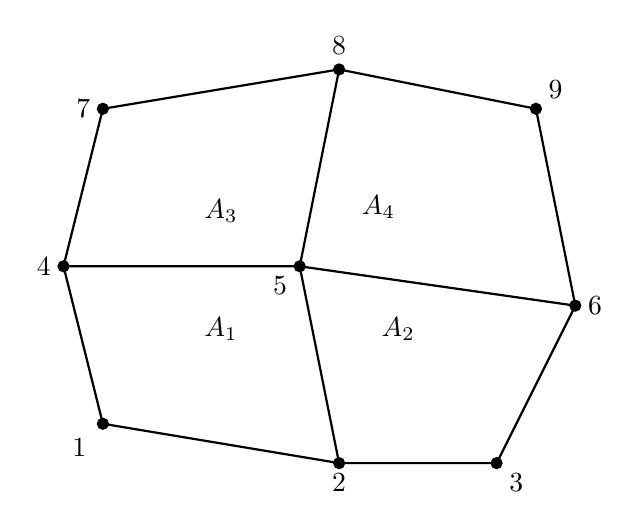
\begin{tikzpicture}
%\draw[fill=gray!5,gray!5](0,0) rectangle (9,7);
%\draw[step=0.5cm,gray,very thin] (0,0) grid (9,7); %background grid
\draw[thick](1.5,1.5) -- (4.5,1) -- (6.5,1) -- (7.5,3) -- (7,5.5) -- (4.5,6) --(1.5,5.5) -- (1,3.5) -- cycle;  
\draw[thick](4.5,1)--(4,3.5)--(4.5,6);
\draw[thick](1,3.5)--(4,3.5)--(7.5,3);
\draw[black,fill=black] (1.5,1.5) circle (2pt); \node[] at (1.2,1.2){1}; %1
\draw[black,fill=black] (4.5,1)   circle (2pt); \node[] at (4.5,0.75){2}; %2
\draw[black,fill=black] (6.5,1)   circle (2pt); \node[] at (6.75,0.75){3}; %3
\draw[black,fill=black] (1,3.5)   circle (2pt); \node[] at (0.75,3.5){4}; %4
\draw[black,fill=black] (4,3.5)   circle (2pt); \node[] at (3.75,3.25){5}; %5
\draw[black,fill=black] (7.5,3)   circle (2pt); \node[] at (7.75,3){6}; %6
\draw[black,fill=black] (1.5,5.5) circle (2pt); \node[] at (1.25,5.5){7}; %7
\draw[black,fill=black] (4.5,6)   circle (2pt); \node[] at (4.5,6.3){8}; %8
\draw[black,fill=black] (7,5.5)   circle (2pt); \node[] at (7.25,5.75){9}; %9
%\draw[thin,dashed](1,3.5)--(4.5,1)--(7.5,3)--(4.5,6)--cycle;
\node[] at (3,2.7){$A_1$}; %8
\node[] at (5.25,2.7){$A_2$}; %8
\node[] at (5,4.25){$A_4$}; %8
\node[] at (3,4.2){$A_3$}; %8
\end{tikzpicture}
\end{center}
\[
q_5^{(1)} = \frac{1}{4}\sum_{e=1}^4 p_e
\] 

In the codes which rely on the $Q_1 \times P_0$ element, the (elemental) pressure
is simply defined as 
\begin{lstlisting}
p=np.zeros(nel,dtype=np.float64)  
\end{lstlisting}
while the nodal pressure is then defined as\footnote{In virtually all stones $p$
stands for the 'raw' pressure and $q$ stands for its projection onto the velocity mesh.} 
\begin{lstlisting}
q=np.zeros(nnp,dtype=np.float64)  
\end{lstlisting}
The element-to-node algorithm is then simply (in 2D):

\begin{lstlisting}
count=np.zeros(nnp,dtype=np.int32)  
for iel in range(0,nel):
    q[icon[0,iel]]+=p[iel]
    q[icon[1,iel]]+=p[iel]
    q[icon[2,iel]]+=p[iel]
    q[icon[3,iel]]+=p[iel]
    count[icon[0,iel]]+=1
    count[icon[1,iel]]+=1
    count[icon[2,iel]]+=1
    count[icon[3,iel]]+=1
q=q/count
\end{lstlisting}

%----------------------------------------------------------------------
\subsection{Schemes 2,3}

{\sl Schemes 2,3} are very similar and are presented in \textcite{sagl81a,sagl81b} (1981).
Scheme 2 uses the areas of the surrounding elements as weights for the arithmetic averaging
while scheme 3 uses the area of the triangles:

\begin{multicols}{2}

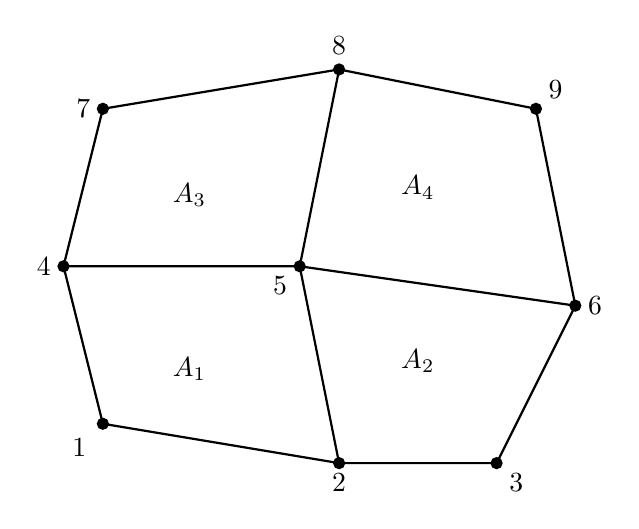
\begin{tikzpicture}
%\draw[fill=gray!5,gray!5](0,0) rectangle (9,7);
%\draw[step=0.5cm,gray,very thin] (0,0) grid (9,7); %background grid
\draw[thick](1.5,1.5) -- (4.5,1) -- (6.5,1) -- (7.5,3) -- (7,5.5) -- (4.5,6) --(1.5,5.5) -- (1,3.5) -- cycle;  
\draw[thick](4.5,1)--(4,3.5)--(4.5,6);
\draw[thick](1,3.5)--(4,3.5)--(7.5,3);
\draw[black,fill=black] (1.5,1.5) circle (2pt); \node[] at (1.2,1.2){1}; %1
\draw[black,fill=black] (4.5,1)   circle (2pt); \node[] at (4.5,0.75){2}; %2
\draw[black,fill=black] (6.5,1)   circle (2pt); \node[] at (6.75,0.75){3}; %3
\draw[black,fill=black] (1,3.5)   circle (2pt); \node[] at (0.75,3.5){4}; %4
\draw[black,fill=black] (4,3.5)   circle (2pt); \node[] at (3.75,3.25){5}; %5
\draw[black,fill=black] (7.5,3)   circle (2pt); \node[] at (7.75,3){6}; %6
\draw[black,fill=black] (1.5,5.5) circle (2pt); \node[] at (1.25,5.5){7}; %7
\draw[black,fill=black] (4.5,6)   circle (2pt); \node[] at (4.5,6.3){8}; %8
\draw[black,fill=black] (7,5.5)   circle (2pt); \node[] at (7.25,5.75){9}; %9
\node[] at (2.6,2.2){$A_1$}; %8
\node[] at (5.5,2.3){$A_2$}; %8
\node[] at (2.6,4.4){$A_3$}; %8
\node[] at (5.5,4.5){$A_4$}; %8
\end{tikzpicture}

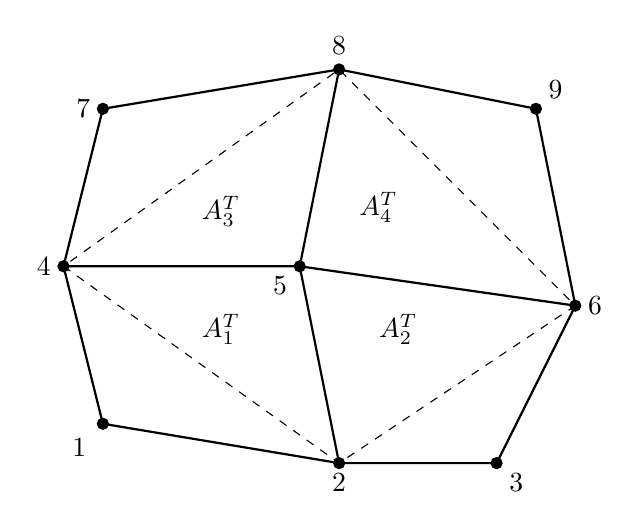
\begin{tikzpicture}
%\draw[fill=gray!5,gray!5](0,0) rectangle (9,7);
%\draw[step=0.5cm,gray,very thin] (0,0) grid (9,7); %background grid
\draw[thick](1.5,1.5) -- (4.5,1) -- (6.5,1) -- (7.5,3) -- (7,5.5) -- (4.5,6) --(1.5,5.5) -- (1,3.5) -- cycle;  
\draw[thick](4.5,1)--(4,3.5)--(4.5,6);
\draw[thick](1,3.5)--(4,3.5)--(7.5,3);
\draw[black,fill=black] (1.5,1.5) circle (2pt); \node[] at (1.2,1.2){1}; %1
\draw[black,fill=black] (4.5,1)   circle (2pt); \node[] at (4.5,0.75){2}; %2
\draw[black,fill=black] (6.5,1)   circle (2pt); \node[] at (6.75,0.75){3}; %3
\draw[black,fill=black] (1,3.5)   circle (2pt); \node[] at (0.75,3.5){4}; %4
\draw[black,fill=black] (4,3.5)   circle (2pt); \node[] at (3.75,3.25){5}; %5
\draw[black,fill=black] (7.5,3)   circle (2pt); \node[] at (7.75,3){6}; %6
\draw[black,fill=black] (1.5,5.5) circle (2pt); \node[] at (1.25,5.5){7}; %7
\draw[black,fill=black] (4.5,6)   circle (2pt); \node[] at (4.5,6.3){8}; %8
\draw[black,fill=black] (7,5.5)   circle (2pt); \node[] at (7.25,5.75){9}; %9
\draw[thin,dashed](1,3.5)--(4.5,1)--(7.5,3)--(4.5,6)--cycle;
\node[] at (3,2.7){$A_1^T$}; %8
\node[] at (5.25,2.7){$A_2^T$}; %8
\node[] at (5,4.25){$A_4^T$}; %8
\node[] at (3,4.2){$A_3^T$}; %8
\end{tikzpicture}

\end{multicols}

\[
q_5^{(2)} = \frac{\sum\limits_{e=1}^4 A_e p_e}{\sum\limits_{e=1}^4 A_e}
\qquad
\qquad
q_5^{(3)} = \frac{\sum\limits_{e=1}^4 A_e^T p_e}{\sum\limits_{e=1}^4 A_e^T}
\] 


\begin{remark} Although Schemes 1,2,3 are similar, scheme 1 is the simplest and fastest
to implement since the areas of neighbouring elements/triangles are not needed.
\end{remark}

\begin{remark} 
Schemes 1,2,3 are identical if all elements are rectangles of identical dimensions.
\end{remark}


%----------------------------------------------------------------------
\subsection{Scheme 4} 

This scheme has been designed by me. 
It resembles the last three ones, but the weighing is in this case different.

Let us consider a 1D problem:
\begin{center}
\includegraphics[width=0.5\linewidth]{images/pressure_smoothing/newalgo.png}
\end{center}

Elemental pressures $p_1$ and $p_2$ corresponding to elements 1 and 2 respectively are known at
locations $x_1$ and $x_2$. The two elements have a different size, characterised in this case
by the distances $d_1$ and $d_2$ to their common edge.

The equation of the line passing through points $(x_1,p_1)$ and $(x_2,p_2)$ is 
\[
p(x)=\frac{p_2-p_1}{x_2-x_1}(x-x_1)+p_1
\]
The $x$ coordinate of the common edge is given by $x=x_1+d_1/2$, 
and since $x_2-x_1=(d_1+d_2)/2$, the 
pressure at this location writes:
\[
p(x_M)= \frac{p_2-p_1}{d_1+d_2}d_1+p_1 = \frac{\frac{p_1}{d_1} + \frac{p_2}{d_2}}{\frac{1}{d_1} + \frac{1}{d_2}}
\]
Extrapolating this formula to 2D, $d_1$ and $d_2$ are in fact the element volumes, so that
\[
q_5^{(4)} = 
\frac{\sum\limits_{j=1}^4 \frac{p_j^e}{A_j^e}}{\sum\limits_{j=1}^4 \frac{1}{A_j^e}}
=
\frac{
\frac{p_1^e}{A_1^e}+
\frac{p_2^e}{A_2^e}+
\frac{p_3^e}{A_3^e}+
\frac{p_4^e}{A_4^e}
}{
\frac{1}{A_1^e}+
\frac{1}{A_2^e}+
\frac{1}{A_3^e}+
\frac{1}{A_4^e}
}\]

There remains a problem, due to the presence of the boundary nodes for which 
the sums present in the above equation do not run up to 4. A boundary
node only has three neighbours and a corner node only two. Additional measures
are required for these nodes. 

\begin{center}
\includegraphics[width=0.5\linewidth]{images/pressure_smoothing/newalgo_corner.png}
\end{center}

The pressure value $p_N$ is obtained as follows:
\[
q_N = \frac{ 
 \frac{p_2^e}   {A_2^e}
+\frac{p_3^e}   {A_3^e}
+\frac{p_{2'}^e}{A_{2'}^e}
+\frac{p_{3'}^e}{A_{3'}^e}
}{
 \frac{1}{A_2^e}
+\frac{1}{A_3^e}
+\frac{1}{A_{2'}^e}
+\frac{1}{A_{3'}^e}
}
\]
The areas and pressures of the mirrored elements 2' and 3' are extrapolated from the areas of elements 2 and 6, and 3 and 7 respectively. 
Likewise the pressure $p_M$ at the corner node is obtained through the pressures of its surrounding elements.


%------------------------------------------------------------------------------
\subsection{Scheme 5 - Least squares} 

This scheme is presented (among other places) in Lee \etal (1979)
\cite{legs79}. 
Let us start from the patch of 4 $Q_1$ elements counting 9 nodes: 

\begin{center}
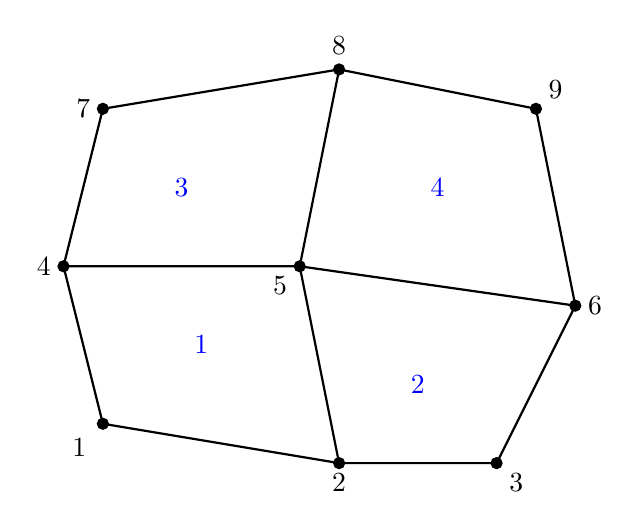
\begin{tikzpicture}
%\draw[fill=gray!5,gray!5](0,0) rectangle (9,7);
%\draw[step=0.5cm,gray,very thin] (0,0) grid (9,7); %background grid
\draw[thick](1.5,1.5) -- (4.5,1) -- (6.5,1) -- (7.5,3) -- (7,5.5) -- (4.5,6) --(1.5,5.5) -- (1,3.5) -- cycle;  
\draw[thick](4.5,1)--(4,3.5)--(4.5,6);
\draw[thick](1,3.5)--(4,3.5)--(7.5,3);

\node[] at (2.75,2.5) {\color{blue}1};
\node[] at (5.5,2) {\color{blue}2};
\node[] at (2.5,4.5) {\color{blue}3};
\node[] at (5.75,4.5) {\color{blue}4};

\draw[black,fill=black] (1.5,1.5) circle (2pt); \node[] at (1.2,1.2){1}; %1
\draw[black,fill=black] (4.5,1)   circle (2pt); \node[] at (4.5,0.75){2}; %2
\draw[black,fill=black] (6.5,1)   circle (2pt); \node[] at (6.75,0.75){3}; %3
\draw[black,fill=black] (1,3.5)   circle (2pt); \node[] at (0.75,3.5){4}; %4
\draw[black,fill=black] (4,3.5)   circle (2pt); \node[] at (3.75,3.25){5}; %5
\draw[black,fill=black] (7.5,3)   circle (2pt); \node[] at (7.75,3){6}; %6
\draw[black,fill=black] (1.5,5.5) circle (2pt); \node[] at (1.25,5.5){7}; %7
\draw[black,fill=black] (4.5,6)   circle (2pt); \node[] at (4.5,6.3){8}; %8
\draw[black,fill=black] (7,5.5)   circle (2pt); \node[] at (7.25,5.75){9}; %9

\end{tikzpicture}
\end{center}



We are looking for a field $q$ living on the nodes.
We build the quantity
\[
J=\iint_\Omega (q-p)^2 dV
\]
where $p$ is the elemental field. To make things clearer we split the integral into 
the sum of elemental integrals:
\[
J=
\iint_{\Omega_1} (q(x,y)-p_1)^2 dV+
\iint_{\Omega_2} (q(x,y)-p_2)^2 dV+
\iint_{\Omega_3} (q(x,y)-p_3)^2 dV+
\iint_{\Omega_4} (q(x,y)-p_4)^2 dV
\]
Inside each element the field $q(x,y)$ is given by a bilinear interpolation so that:
\begin{eqnarray}
J
&=& \iint_{\Omega_1} (\bN_1(x,y) q_1 + \bN_2(x,y)q_2 + \bN_5(x,y)q_5 + \bN_4(x,y)q_4 -p_1)^2 dV \nn\\
&+& \iint_{\Omega_2} (\bN_2(x,y) q_2 + \bN_3(x,y)q_3 + \bN_6(x,y)q_6 + \bN_5(x,y)q_5 -p_2)^2 dV \nn\\
&+& \iint_{\Omega_3} (\bN_4(x,y) q_4 + \bN_5(x,y)q_5 + \bN_8(x,y)q_8 + \bN_7(x,y)q_7 -p_3)^2 dV \nn\\
&+& \iint_{\Omega_4} (\bN_5(x,y) q_5 + \bN_6(x,y)q_6 + \bN_9(x,y)q_9 + \bN_8(x,y)q_8 -p_4)^2 dV 
\end{eqnarray}
where the $N_i$ functions are the basis functions (unusually expressed in $x,y$ coordinates).
The least square procedure looks for the set of $q_i$ such that 
\[
\frac{\partial J}{\partial q_i} =0 \qquad \forall i=1,...9
\]
and this yields 9 equations/constraints for 9 unknowns.
\begin{eqnarray}
\frac{\partial J}{\partial q_1} 
&=& \iint_{\Omega_1} 2 (\bN_1(x,y) q_1 + \bN_2(x,y)q_2 + \bN_5(x,y)q_5 + \bN_4(x,y)q_4 -p_1) \bN_1(x,y) dV \nn\\
\frac{\partial J}{\partial q_2}
&=& \iint_{\Omega_1} 2(\bN_1(x,y) q_1 + \bN_2(x,y)q_2 + \bN_5(x,y)q_5 + \bN_4(x,y)q_4 -p_1) \bN_2(x,y) dV \nn\\
&+& \iint_{\Omega_2} 2(\bN_2(x,y) q_2 + \bN_3(x,y)q_3 + \bN_6(x,y)q_6 + \bN_5(x,y)q_5 -p_2) \bN_2(x,y) dV \nn\\
\frac{\partial J}{\partial q_3}
&=& \iint_{\Omega_2} 2(\bN_2(x,y) q_2 + \bN_3(x,y)q_3 + \bN_6(x,y)q_6 + \bN_5(x,y)q_5 -p_2) \bN_3(x,y) dV \nn\\
\frac{\partial J}{\partial q_4}
&=& \iint_{\Omega_1} 2(\bN_1(x,y) q_1 + \bN_2(x,y)q_2 + \bN_5(x,y)q_5 + \bN_4(x,y)q_4 -p_1) \bN_4(x,y) dV \nn\\
&+& \iint_{\Omega_3} 2(\bN_4(x,y) q_4 + \bN_5(x,y)q_5 + \bN_8(x,y)q_8 + \bN_7(x,y)q_7 -p_3) \bN_4(x,y) dV \nn\\
\frac{\partial J}{\partial q_5}
&=& \iint_{\Omega_1} 2(\bN_1(x,y) q_1 + \bN_2(x,y)q_2 + \bN_5(x,y)q_5 + \bN_4(x,y)q_4 -p_1) \bN_5(x,y) dV \nn\\
&+& \iint_{\Omega_2} 2(\bN_2(x,y) q_2 + \bN_3(x,y)q_3 + \bN_6(x,y)q_6 + \bN_5(x,y)q_5 -p_2) \bN_5(x,y) dV \nn\\
&+& \iint_{\Omega_3} 2(\bN_4(x,y) q_4 + \bN_5(x,y)q_5 + \bN_8(x,y)q_8 + \bN_7(x,y)q_7 -p_3) \bN_5(x,y) dV \nn\\
&+& \iint_{\Omega_4} 2(\bN_5(x,y) q_5 + \bN_6(x,y)q_6 + \bN_9(x,y)q_9 + \bN_8(x,y)q_8 -p_4) \bN_5(x,y) dV \nn\\
\frac{\partial J}{\partial q_6}
&=& \iint_{\Omega_2} 2(\bN_2(x,y) q_2 + \bN_3(x,y)q_3 + \bN_6(x,y)q_6 + \bN_5(x,y)q_5 -p_2) \bN_6(x,y) dV \nn\\
&+& \iint_{\Omega_4} 2(\bN_5(x,y) q_5 + \bN_6(x,y)q_6 + \bN_9(x,y)q_9 + \bN_8(x,y)q_8 -p_4) \bN_6(x,y) dV \nn\\
\frac{\partial J}{\partial q_7}
&=& \iint_{\Omega_3} 2(\bN_4(x,y) q_4 + \bN_5(x,y)q_5 + \bN_8(x,y)q_8 + \bN_7(x,y)q_7 -p_3) \bN_7(x,y) dV \nn\\
\frac{\partial J}{\partial q_8}
&=& \iint_{\Omega_3} 2(\bN_4(x,y) q_4 + \bN_5(x,y)q_5 + \bN_8(x,y)q_8 + \bN_7(x,y)q_7 -p_3) \bN_8(x,y)dV \nn\\
&+& \iint_{\Omega_4} 2(\bN_5(x,y) q_5 + \bN_6(x,y)q_6 + \bN_9(x,y)q_9 + \bN_8(x,y)q_8 -p_4) \bN_8(x,y)dV \nn\\ 
\frac{\partial J}{\partial q_9}
&=& \iint_{\Omega_4} 2(\bN_5(x,y) q_5 + \bN_6(x,y)q_6 + \bN_9(x,y)q_9 + \bN_8(x,y)q_8 -p_4) \bN_9(x,y)dV 
\end{eqnarray}
The factor 2 are removed and the terms $\int p_i N_j $ are known so they end up in the right hand side.
\begin{eqnarray}
 \iint_{\Omega_1} (\bN_1 \bN_1 q_1 + \bN_1 \bN_2 q_2 + \bN_1 \bN_5 q_5 + \bN_1 \bN_4 q_4) dV 
&=& \iint_{\Omega_1} p_1 N_1 dV \nn\\
 \iint_{\Omega_1} (\bN_2 \bN_1 q_1 + \bN_2 \bN_2 q_2 + \bN_2 \bN_5 q_5 + \bN_2 \bN_4 q_4) dV \nn\\
+\iint_{\Omega_2} (\bN_2 \bN_2 q_2 + \bN_3 \bN_2 q_3 + \bN_6 \bN_2 q_6 + \bN_5 \bN_2 q_5) dV 
&=& \iint_{\Omega_1} p_1N_2 dV + \iint_{\Omega_2}  p_2 \bN_2 dV \nn\\
\nn\\
\dots &=& \dots \nn\\
\nn\\
 \iint_{\Omega_4} (\bN_9\bN_5 q_5 + \bN_9\bN_6q_6 + \bN_9\bN_9q_9 + \bN_9\bN_8q_8) dV &=&  \iint_{\Omega_4} p_4 \bN_9 dV 
\end{eqnarray}

The mass matrices corresponding to the four elements are 
\[
{\bm M}_1 = \int_{\Omega_1} \left( \begin{array}{cccc}
 \bN_1 \bN_1 & \bN_1 \bN_2 & \bN_1 \bN_5 & \bN_1 \bN_4 \\
 \bN_2 \bN_1 & \bN_2 \bN_2 & \bN_2 \bN_5 & \bN_2 \bN_4 \\
 \bN_5 \bN_1 & \bN_5 \bN_2 & \bN_5 \bN_5 & \bN_5 \bN_4 \\
 \bN_4 \bN_1 & \bN_4 \bN_2 & \bN_4 \bN_5 & \bN_4 \bN_4 
\end{array}\right) dV
\qquad
{\bm M}_2 = \int_{\Omega_2} \left( \begin{array}{cccc}
 \bN_2 \bN_2 & \bN_2 \bN_3 & \bN_2 \bN_6 & \bN_2 \bN_5 \\
 \bN_3 \bN_2 & \bN_3 \bN_3 & \bN_3 \bN_6 & \bN_3 \bN_5 \\
 \bN_6 \bN_2 & \bN_6 \bN_3 & \bN_6 \bN_6 & \bN_6 \bN_5 \\
 \bN_5 \bN_2 & \bN_5 \bN_3 & \bN_5 \bN_6 & \bN_5 \bN_5 
\end{array}\right) dV
\]
\[
{\bm M}_3 = \int_{\Omega_3} \left( \begin{array}{cccc}
 \bN_4 \bN_4 & \bN_4 \bN_5 & \bN_4 \bN_8 & \bN_4 \bN_7 \\
 \bN_5 \bN_4 & \bN_5 \bN_5 & \bN_5 \bN_8 & \bN_5 \bN_7 \\
 \bN_8 \bN_4 & \bN_8 \bN_5 & \bN_8 \bN_8 & \bN_8 \bN_7 \\
 \bN_7 \bN_4 & \bN_7 \bN_5 & \bN_7 \bN_8 & \bN_7 \bN_7 
\end{array}\right) dV
\qquad
{\bm M}_4 = \int_{\Omega_4} \left( \begin{array}{cccc}
 \bN_5 \bN_5 & \bN_5 \bN_6 & \bN_5 \bN_9 & \bN_5 \bN_8 \\
 \bN_6 \bN_5 & \bN_6 \bN_6 & \bN_6 \bN_9 & \bN_6 \bN_8 \\
 \bN_9 \bN_5 & \bN_9 \bN_6 & \bN_9 \bN_9 & \bN_9 \bN_8 \\
 \bN_8 \bN_5 & \bN_8 \bN_6 & \bN_8 \bN_9 & \bN_8 \bN_8 
\end{array}\right) dV
\]
so that the 9 equations above are actually the result of the assembly process of these four 
elemental systems:
\[
\left( \iint_{\Omega_e} \vec{\bN}^T\vec{\bN} dV \right) \cdot \vec{q}_e = \iint_{\Omega_i} \vec{\bN}^T p_e dV 
\qquad\qquad e=1,2,3,4
\]

Also check section 4.5.4 of \textcite{glte87} (1987), in which the authors 
present a two-step algorithm: 1) pressure is averaged over each element.
2) the nodal values of the pressure are recovered through a least-squares approach.


%------------------------------------------------------------------------------
\subsection{Scheme 6 - Consistent pressure recovery (penalty formulation) \label{ss:cpr}}

This is the method presented in \textcite{zina82} (1982). In the second part 
of this publication the authors wish to establish a simple and effective 
numerical method to calculate variables eliminated by the penalisation process. 
The method involves an additional finite element solution for the nodal 
pressures using the same finite element basis and numerical quadrature 
as used for the velocity.

Let us start with\footnote{I here voluntarily use $q$ instead of $p$}:
\[
q = -\lambda \vec\nabla\cdot \vec\upnu
\]
We are going to treat this equation like any other PDE in the context 
of the FE method, i.e. we are going to establish its weak form. 
We assume that the pressure is given inside an element by
\[
q(x,y) = \sum_{i=1}^{m_\upnu} \bN_i(x,y) q_i = \vec{\bN} \cdot \vec{q}
\]
and the velocity:
\[
\vec\upnu = (u,v) 
\qquad 
\qquad 
u(x,y)  = \sum_{i=1}^{m_\upnu} \bN_i(x,y) u_i
\qquad 
\qquad 
v(x,y)  = \sum_{i=1}^{m_\upnu} \bN_i(x,y) v_i
\]
where the $\bN_i$ are the $Q_1$ basis functions and $q_i$ are the sought after nodal values. 
We multiply the equation above by a $Q_1$ basis function $\bN_i$ and integrate over the whole domain:
\[
\iint_\Omega \bN_i(x,y) q(x,y) \; dxdy 
= -\lambda \iint_\Omega \bN_i \vec\nabla\cdot \vec\upnu  \; dx dy
\]
As before we now focus on the above expression inside a single element $e$:
\[
\iint_{\Omega_e} \bN_i(x,y) q(x,y) \; dxdy = -\lambda \iint_{\Omega_e} \bN_i \vec\nabla\cdot \vec\upnu \; dx dy
\]
After $\bN_i \rightarrow \vec{\bN}=(\bN_1,\bN_2,\bN_3,\bN_4)^T$, the left hand side term becomes:
\[
\iint _{\Omega_e} \vec{\bN}^T q(x,y) \; dxdy 
=
\iint _{\Omega_e} \vec{\bN}^T \vec{\bN} \cdot \vec{q} \; dxdy 
=
\left(\underbrace{\iint _{\Omega_e} \vec{\bN}^T \vec{\bN} dxdy}_{{\bm M}_e} \right) \cdot \vec{q}  
\]
where ${\bm M}_e$ is the elemental mass matrix.
We now turn to the right hand side. We have
\[
\vec\nabla\cdot \vec\upnu
= \frac{\partial u}{\partial x}+\frac{\partial v}{\partial y}
= \sum_i \frac{\partial \bN_i}{\partial x} u_i + \sum_i \frac{\partial \bN_i}{\partial y} v_i 
\]
We here too define $\vec{V}_e=(u_1,v_1,u_2,v_2,u_3,v_3,u_4,v_4)^T$ so that 

\begin{eqnarray}
&& \iint_{\Omega_e} \vec{\bN} {\vec \nabla}\cdot {\vec \upnu} \; dV \nn\\
&=& \iint_{\Omega_e} \vec{\bN}^T \sum_{i=1}^{m_\upnu} 
\left( \frac{\partial \bN_i}{\partial x} u_i + \frac{\partial \bN_i}{\partial y} v_i 
\right)  
dV \label{eq:psmoth6}\\
&=& 
\iint_{\Omega_e} 
\left(
\begin{array}{c}
\bN_1 \left(
\sum\limits_{i=1}^{4} \frac{\partial \bN_i}{\partial x} u_i +
\sum\limits_{i=1}^{4} \frac{\partial \bN_i}{\partial y} v_i \right) \\
\bN_2 \left(
\sum\limits_{i=1}^{4} \frac{\partial \bN_i}{\partial x} u_i +
\sum\limits_{i=1}^{4} \frac{\partial \bN_i}{\partial y} v_i \right) \\
\bN_3 \left(
\sum\limits_{i=1}^{4} \frac{\partial \bN_i}{\partial x} u_i +
\sum\limits_{i=1}^{4} \frac{\partial \bN_i}{\partial y} v_i \right) \\
\bN_4 \left(
\sum\limits_{i=1}^{4} \frac{\partial \bN_i}{\partial x} u_i +
\sum\limits_{i=1}^{4} \frac{\partial \bN_i}{\partial y} v_i \right) 
\end{array}
\right) dV \nonumber \\  %%%%%%%%%%%%%%%%%%%%%%%%%%
&=& 
\int_{\Omega_e} 
\left(
\begin{array}{ccc}
{\bN}_1& {\bN}_1 &  0 \\\\
{\bN}_2& {\bN}_2 &  0 \\\\
{\bN}_3& {\bN}_3 &  0 \\\\
{\bN}_4& {\bN}_4 &  0 
\end{array}
\right)
\cdot
\left(
\begin{array}{c}
\sum\limits_i \frac{\partial \bN_i}{\partial x} u_i \\ \\
\sum\limits_i \frac{\partial \bN_i}{\partial y} v_i \\ \\
\sum\limits_i (\frac{\partial \bN_i}{\partial y} u_i\! +\! \frac{\partial \bN_i}{\partial x} v_i) 
\end{array}
\right)
\; dV \nonumber\\ %%%%%%%%%%%%%%%%%%%%%%%%%%
&=& 
\int_{\Omega_e} 
\underbrace{
\left(
\begin{array}{cccccc}
{\bN}_1 & {\bN}_1 &  0 \\
{\bN}_2 & {\bN}_2 &  0 \\
{\bN}_3 & {\bN}_3 &  0 \\
{\bN}_4 & {\bN}_4 &  0 
\end{array}
\right)
}_{{\bm N}}
\cdot
\underbrace{
\left(\begin{array}{cccccccc}
\partial_x \bN_1 & 0 &  
\partial_x \bN_2 & 0 &  
\partial_x \bN_3 & 0 &  
\partial_x \bN_4 & 0 \\ \\
0 & \partial_y \bN_1 &   
0 & \partial_y \bN_2 &   
0 & \partial_y \bN_3 &   
0 & \partial_y \bN_4 \\ \\
\partial_y \bN_1 & \partial_x \bN_1 &  
\partial_y \bN_2 & \partial_x \bN_2 &  
\partial_y \bN_3 & \partial_x \bN_3 &  
\partial_y \bN_4 & \partial_x \bN_4 
\end{array}\right)}_{{\bm B}}
\cdot \vec{V}_e
\; dV  \nonumber \\
&=& 
\left(\int_{\Omega_e} {\bm N} \cdot {\bm B} \; dV \right) \cdot \vec{V}_e \nonumber\\
&=& -\G_e^T \cdot {\vec V}_e
\end{eqnarray}
This makes sense since $\G^T$ is the discrete divergence operator. However, it is not very efficient to 
build $\G_e$ only to multiply it with a vector of already known quantities. 
In practice we implement Eq.~\eqref{eq:psmoth6} which implmentation resembles the buoyancy term of the 
Stokes equation.

After assembly we arrive at
\[
{\bm M} \cdot \vec{q} = \lambda \G^T \cdot {\vec V} 
\qquad
\text{with}
\qquad
\G_e = -\int_{\Omega_e} {\bm N} \cdot {\bm B} \; dV
\]
where ${\bm M}$ is the global mass matrix, $\vec{q}$ the vector of all 
nodal pressures, $\G$ the discrete gradient matrix and $\vec{V}$
the (velocity) solution vector. 
The system can be easily solved since the mass matrix is a friendly matrix.
The vector ${\vec q}$ contains the nodal pressure values directly, with 
no need for a smoothing scheme! 

\begin{remark}
Very importantly, the mass matrix ${\bm M}$ is to be evaluated at the full integration points, 
while the constraint part (the right hand side of the equation) is to be evaluated at 
the reduced integration point, i.e. in the middle of the element.  
\end{remark}

\begin{remark}
As noted in \cite{zina82}, it is interesting to note that when linear elements are used 
and the lumped matrices are used for the ${\bm M}$ the resulting algebraic equation is identical 
to the smoothing scheme 1 only if a uniform square finite element 
mesh is used. In this respect this method is expected to yield different results when elements 
are not square or even rectangular.
\end{remark}

\begin{remark}
The third column of the matrix ${\bm N}$
and the last line of the ${\bm B}$ matrix could be removed altogether.
If your code is based on the mixed formulation, then you already 
have built matrix $\G$ so you can easily re-use this piece of code 
to compute $\G$ again, this time with a reduced integration quadrature.
If you are using the penalty formulation then you need to program 
all from scratch and then simply do away with these unnecessary terms, or 
you can direcly build the rhs as $\int_{\Omega_e} \vec{\bN}^T p_e$ (assuming
you have previously computed the pressure in the middle of each element 
by means of $p=-\lambda\vec\nabla\cdot\vec\upnu$).
\end{remark}

\begin{remark}
This  scheme is identical to the least square scheme!
\end{remark}


%--------------------------------------------------------------
\subsection{Scheme 7}

Same as scheme 6, but with lumped mass matrix.  


%--------------------------------------------------------------
\subsection{Scheme 8 - bilinear interpolation} 

Let us assume that the centers of the 
four elements make a $Q_1$ quadrilateral element, as shown on this figure:

\input{tikz/tikz_pscheme8}

The values at the corners are $p_1$,
$p_2$, $p_3$ and $p_4$. Assuming that the pressure inside this element 
can be represented by a bilinear field, we have 
\[
p(x,y)= a+ bx +cy +dxy
\]
where the coefficients will be determined by ensuring that 
$p(x_i,y_i)=p_i$ for $i=1,2,3,4$, or:
\begin{eqnarray}
a+bx_1+cy_1+dx_1y_1 &=& p_1 \\
a+bx_2+cy_2+dx_2y_2 &=& p_2 \\
a+bx_3+cy_3+dx_3y_3 &=& p_3 \\
a+bx_4+cy_4+dx_4y_4 &=& p_4 
\end{eqnarray}
i.e.
\[
\left(
\begin{array}{cccc}
1 & x_1 & y_1 & x_1y_1 \\
1 & x_2 & y_2 & x_2y_2 \\
1 & x_3 & y_3 & x_3y_3 \\
1 & x_4 & y_4 & x_4y_4
\end{array}
\right)\cdot
\left(
\begin{array}{c}
a \\b\\c\\d
\end{array}
\right)
=
\left(
\begin{array}{c}
p_1\\p_2\\p_3\\p_4
\end{array}
\right)
\]

There remains an issue with nodes which are on the boundaries of the 
domain. These are of course not 'surrounded' by four pressure values 
so the above algorithm does not apply directly. However, looking 
at the above figure, and assuming that node 1 is a lower left corner 
of a 2D domain, we can use the bilinear interpolation based on elements 
1,2,3,4 to extrapolate a nodal pressure value at node 1. 
The same would apply for nodes 2 and 4 for example. 

\begin{remark}
This scheme is not applicable to quadtree-based meshed.
\end{remark}





\newpage %-----------------------------------------------------------------------------------------
\section{Pressure scaling \label{pscaling}} \index{general}{pressure scaling}
\begin{flushright} {\tiny {\color{gray} pressure\_scaling.tex}} \end{flushright}
%~~~~~~~~~~~~~~~~~~~~~~~~~~~~~~~~~~~~~~~~~~~~~~~~~~~~~~~~~~~~~~~~~~~~~~~~~~~~~~~~~~~~~~~~~~~~~~~~~~

As nicely explained in the 
step 32 of deal.ii\footnote{\url{https://www.dealii.org/9.0.0/doxygen/deal.II/step\_32.html}},
we often need to scale the $\G$ block since it is many orders of magnitude smaller than $\K$ (especially in geodynamics where viscosities are $\sim 10^{22}$), 
which introduces large inaccuracies in the solving process to the point that the solution is nonsensical. 
This scaling coefficient is $\eta/L$ where $\eta$ and $L$ are representative viscosities and lengths. 
We start from 
\[
\left(
\begin{array}{cc}
\K & \G \\ \G^T & -\C 
\end{array}
\right)
\cdot
\left(
\begin{array}{c}
\vec{\cal V} \\ \vec{\cal P}
\end{array}
\right)
=
\left(
\begin{array}{c}
\vec{f} \\ \vec{h}
\end{array}
\right)
\]
and introduce the scaling coefficient as follows (which in fact does not alter the solution at all):
\[
\left(
\begin{array}{cc}
\K & \frac{\eta}{L}\G \\ \frac{\eta}{L}\G^T & - \frac{\eta^2}{L^2} \C 
\end{array}
\right)
\cdot
\left(
\begin{array}{c}
\vec{\cal V} \\\frac{L}{\eta} \vec{\cal P}
\end{array}
\right)
=
\left(
\begin{array}{c}
 \vec{f} \\ \frac{\eta}{L} \vec{h}
\end{array}
\right)
\]
We then end up with the modified Stokes system:
\[
\left(
\begin{array}{cc}
\K & \underline{\G} \\ \underline{\G}^T & \underline{\C} 
\end{array}
\right)
\cdot
\left(
\begin{array}{c}
\vec{\cal V} \\ \underline{\vec{\cal P}}
\end{array}
\right)
=
\left(
\begin{array}{c}
\vec{f} \\ \underline{\vec{h}}
\end{array}
\right)
\]
where 
\[
\underline{\G}=\frac{\eta}{L}\G
\quad\quad
\quad\quad
\underline{\vec{\cal P}}=\frac{L}{\eta} \vec{\cal P}
\quad\quad
\quad\quad
\underline{\C}=\frac{\eta^2}{L^2} \C
\quad\quad
\quad\quad
\underline{\vec{h}}=\frac{\eta}{L}\vec{h}
\]
After the solve phase, we recover the real pressure with $\vec{\cal P}=\frac{\eta}{L}\underline{\vec{\cal P}}$.





 %--------------------------
\newpage %-----------------------------------------------------------------------------------------
\section{Pressure normalisation, nullspace\label{ss_pnorm}} \begin{flushright} {\tiny {\color{gray} pressure\_normlisation.tex}} \end{flushright}
%~~~~~~~~~~~~~~~~~~~~~~~~~~~~~~~~~~~~~~~~~~~~~~~~~~~~~~~~~~~~~~~~~~~~~~~~~~~~~~~~~~~~~~~~~~~~~~~~~~


%..................................................
\subsubsection{Basic idea and naive implementation}

When Dirichlet boundary conditions are imposed everywhere on the boundary, 
pressure is only present by its gradient in 
the equations. It is thus determined up to an arbitrary constant (one speaks then 
of a nullspace of size 1).  \index{general}{Nullspace}
In such a case, one commonly impose the average of the pressure over the whole domain or on 
a subset of the boundary 
to have a zero average, i.e.
\begin{equation}
\int_\Omega p\; dV = 0
\end{equation}

Let us assume for example/simplicity that we are using \QonePzero elements. The pressure is constant 
inside each element so the integral above becomes:
\begin{equation}
\int_\Omega p\; dV = 
\sum_e  \int_{\Omega_e} p\; dV = 
\sum_e  p_e \int_{\Omega_e}\; dV = 
\sum_e  p_e V_e = 0
\end{equation}
where the sum runs over all elements $e$ of volume $V_e$.
This can be rewritten 
\[
\vec{L} \cdot \vec{\cal P}=0
\] 
and it is a constraint on the pressure solution which couples {\it all} pressure dofs. 
We can associate to it a Lagrange multiplier $\lambda$ so that we must solve the modified Stokes system:
\[
\left(
\begin{array}{ccc}
\K & \G & 0\\ 
\G^T & 0 & \vec{L}^T \\
0 & \vec{L} & 0
\end{array}
\right)
\cdot
\left(
\begin{array}{c}
\vec{\cal V} \\ \vec{\cal P} \\ \lambda
\end{array}
\right)
=
\left(
\begin{array}{c}
\vec{f} \\ \vec{h} \\ 0
\end{array}
\right)
\]
When higher order spaces are used for pressure (continuous or discontinuous)
one must then carry out the above integration numerically by means of (usually)
a Gauss-Legendre quadrature.

Although valid, this approach has one main disadvantage: it makes the Stokes matrix larger (although
marginally so -- only one row and column are added), but more importantly it prevents the use of some
of the solving strategies of Section \ref{sec:solvers}.


%..................................................
\subsubsection{Implementation -- the real deal}

Here is what Bochev and Gunzburger \cite[Section 7.6.4]{bogu09} have to say about this:
"[...] practical implementations cheat by substituting enforcement of the true zero mean constraint by using
procedures collectively known as setting the pressure datum. These procedures essentially 
amount to removing one degree of freedom from the pressure space.
Setting the pressure datum can be accomplished in many different ways, ranging
from specifying a pressure value at a grid node to more complicated approaches in
which a boundary traction is specified at a single node in lieu of the velocity condition; 
see [16, 24, 191] and the references cited therein for more details. Not surprisingly, 
in practice, the simplest approach of fixing the pressure value at a node also
happens to be the most widely used in practice."




The idea is actually quite simple and requires two steps:
\begin{enumerate}
\item remove the null space by prescribing the pressure at one location and solve the system;
\item post-process the pressure so as to arrive at a pressure field which fulfils the required normalisation (surface, volume, ...)
\end{enumerate}

The reason why it works is as follows: a constant pressure value lies in the null space, so that one can 
add or delete any value to the pressure field without consequence. As such I can choose said constant such that 
the pressure at a given node/element is zero. All other computed pressures are then relative to that one. 
The post-processing step will redistribute a constant value to all pressures (it will shift them up or down)
so that the normalising condition is respected. 


\Literature

In \url{https://scicomp.stackexchange.com/questions/27645/pressure-boundary-condition-in-lid-driven-cavity-using-finite-element-method}
we find:
{\it 
Zero mean pressure space is used for convenience when one is interested in FEA theory (basically, we cannot 
enforce $p(x_0)=p_0$ for $p \in L^2$ since it does not make sense); from the computational point of view, 
it is easier to fix one of the pressure DOFs (although you can subtract mean value at the post–processing step 
if you want to). When you are working w/ polynomial spaces—and this is exactly what you do in FEM 
-it is perfectly fine to enforce $p(x_0)=p_0$. Handle this constraint like you usually handle Dirichlet 
BCs (e.g., via modifying your matrix). It is also fine to ignore this constraint in some 
cases (e.g., Krylov solvers can do fine with this).
}


\url{
https://scicomp.stackexchange.com/questions/25134/mixed-finite-element-method-for-the-stokes-system-some-implementation-details}





 %----
\newpage %-----------------------------------------------------------------------------------------
\section{Solving the Stokes system \label{sec:solvers}} \begin{flushright} {\tiny {\color{gray} solvers.tex}} \end{flushright}
%~~~~~~~~~~~~~~~~~~~~~~~~~~~~~~~~~~~~~~~~~~~~~~~~~~~~~~~~~~~~~~~~~~~~~~~~~~~~~~~~~~~~~~~~~~~~~~~~~~

Let us start again from the (full) Stokes system:
\begin{equation}
\underbrace{
\left(
\begin{array}{cc}
\K & \G \\ \G^T & -\C 
\end{array}
\right)
}_{\cal A}
\cdot
\left(
\begin{array}{c}
\vec{\cal V} \\ \vec{\cal P}
\end{array}
\right)
=
\left(
\begin{array}{c}
\vec{f} \\ \vec{h}
\end{array}
\right)
\label{StokesSyst}
\end{equation}
We need to solve this system in order to obtain the solution, i.e. the $\vec{\cal V}$ 
and $\vec{\cal P}$ vectors. But how? 
Unfortunately, this question is not simple to answer and the appropriate method depends on many 
parameters, but mainly on how big the matrix blocks are and what the condition number of the matrix $\K$ is. 

First let us start with an obvious question: couldn't we just compute the inverse of the matrix ${\cal A}$?
Under the assumption that the inverse of $\K$ and $\SSS$ exists, we can and we find\footnote{The matrix 
$\C$ is here omitted but it bears no consequences on the conclusion.}
\[
{\cal A}^{-1} = 
\left(
\begin{array}{cc}
\K & \G \\ \G^T & 0
\end{array}
\right)^{-1}
=
\left(
\begin{array}{cc}
\K^{-1} + \K^{-1} \cdot \G \cdot\SSS^{-1} \cdot\G^T \cdot\K^{-1} & -\K^{-1} \cdot\G \cdot\SSS^{-1} \\ 
-\SSS^{-1} \cdot\G^T \cdot\K^{-1}  &  \SSS^{-1}
\end{array}
\right)
\]
However, such an expression is of limited interest in the numerical solution of saddle
point problems since it showcases 5 times the inverse of $\K$ and more importantly
the inverse of the Schur complement matrix $\S$ which is likely to be a full matrix so 
that we never want to compute it explicitely.


As concisely explained in Clevenger \& Heister (2021) \cite{clhe21}, 
there are three common approaches used in the literature for solving the above equation on large scales:
\begin{itemize}
\item a pressure corrected, Schur complement CG scheme, using multigrid as an 
approximation to the velocity block;
\item a block-preconditioned Krylov
method, also using multigrid on the velocity block.
For this method, there are two main types:
\begin{itemize}
\item GMRES\cite{mabl15,rumi15} (or any Krylov method not requiring symmetry) with
block-triangular preconditioner (This is what \aspect does):
\[
{\bm P} = \left(
\begin{array}{cc}
\K & \G \\
0 & - \SSS
\end{array}
\right)
\]

\item MINRES\cite{gmhj16} with block-diagonal preconditioner
\[
{\bm P} = \left(
\begin{array}{cc}
\K & 0 \\
0 & - \SSS
\end{array}
\right)
\]

\end{itemize}


\item an all-at-once multigrid performed on the entire Stokes
system, using Uzawa-type smoothers.
\end{itemize}


\Literature: Preconditioners for Incompressible Navier-Stokes Solvers \cite{seuv10}

Saddle point preconditioners have been extensively discussed and studied \cite{bewa08}, \cite{dewu04}

Diagonal preconditioners in \cite{shrb01}, \cite{babc94}.

Pragmatic solvers for 3D Stokes problems with heterogeneous coefficients \cite{samb20}

%...................................................
\subsection{When using the penalty formulation}

In this case we are only solving for 
velocity since pressure has been eliminated and is later recovered in a post-processing step:
\[
(\K_\eta+\K_\lambda) \cdot \vec {\cal V} = \vec f
\]
 We also know that 
the penalty factor $\lambda$ is many orders of magnitude higher than the viscosity and 
in combination with the use of the $Q_1 \times P_0$ element the resulting matrix 
condition number is very high so that the use of iterative solvers is precluded. 
Indeed codes such as \sopale \cite{full95}, \douar \cite{brtf08}, \fantom \cite{thie11} 
or \sulec \cite{qube11} relying on the penalty formulation all use direct solvers.
The most popular are BLKFCT\footnote{\url{http://dm.unife.it/blkfclt/}}, 
MUMPS\footnote{\url{http://mumps.enseeiht.fr/}}\cite{amdu89,amdl00,amdk01,amgl06,ambl19}, 
PasTiX \cite{herr02},
WSMP\footnote{\url{http://www.research.ibm.com/projects/wsmp}} \cite{GUPTA94ieee,GUPTA09sc-long},
UMFPACK and CHOLMOD\footnote{\url{http://faculty.cse.tamu.edu/davis/suitesparse.html}}
, SuperLU\footnote{\url{https://portal.nersc.gov/project/sparse/superlu/}}, 
PARDISO\footnote{\url{https://www.pardiso-project.org/}}
\cite{pardiso-6.0a,pardiso-6.0b,pardiso-6.0c}, or those inside 
PETSc\footnote{\url{https://www.mcs.anl.gov/petsc/}}.

Braun \etal (2008) \cite{brtf08} list the following features of direct solvers:
\begin{itemize}
\item Robust
\item Black-box operation
\item Difficult to parallelize
\item Memory consumption
\item Limited scalability
\end{itemize}

The main advantage of direct solvers is used in this case: They can solve ill-conditioned 
matrices. However, memory requirements for the storage of number of nonzeros in the 
Cholesky matrix grow very fast as the number of equations/grid size increases, especially in 3D,
to the point that even modern computers with tens of Gb of RAM cannot deal with a $\sim 100^3$ element mesh.
This explains why direct solvers are often used for 2D problems and rarely in 3D with noticeable 
exceptions \cite{thfb08,yahb09,brya10,lobh10,alht11,alht12,alhf13,whbb14,neew18}. 

%....................................................................
\subsection{Uzawa algorithms and the Schur complement approach }

\index{general}{Uzawa algorithm}

Let us write the above system as two equations:
\begin{eqnarray}
\K \cdot \vec{\cal V} + \G \cdot \vec{\cal P} &=& \vec{f} \\
\G^T \cdot  \vec{\cal V} - \C \cdot \vec{\cal P} &=& \vec{h} 
\end{eqnarray}
The first line can be re-written 
$\vec{\cal V}=\K^{-1}\cdot (\vec{f} - \G \cdot \vec{\cal P})$ and can be inserted in the second:
\begin{equation}
\G^T\cdot \vec{\cal V} =\G^T \cdot  [ \K^{-1} \cdot  (\vec{f} - \G \cdot  \vec{\cal P}) ] - \C\cdot \vec{\cal P} = \vec{h} 
\end{equation}
or, 
\begin{mdframed}[backgroundcolor=blue!5]
\begin{equation}
(\G^T \cdot \K^{-1} \cdot \G + \C) \cdot \vec{\cal P} = \G^T \cdot \K^{-1}\cdot \vec{f} - \vec{h} 
\end{equation}
\end{mdframed}
The matrix $\SSS= \G^T \cdot \K^{-1} \cdot \G + \C$ is called the Schur complement. 
\index{general}{Schur Complement} 
It is Symmetric (since $\K$ is symmetric) and  Positive-Definite\footnote{$M$ 
positive definite $\iff$ $x^TMx>0$ $\forall \; x\in \mathbb{R}^n \setminus {\bm 0}$ }
(SPD) \index{general}{SPD} if $Ker({\G})=0$. 
Having solved this equation (i.e. we have obtained $\vec{\cal P}$), the velocity can be recovered by solving 
$\K\cdot \vec{\cal V} =\vec{f}- \G \cdot \vec{\cal P}$. 

\begin{remark}
The Schur complement matrix naturally occurs when the Stokes matrix is decomposed using 
a LDU block-factorisation. Indeed, we have 
\[
\left(
\begin{array}{cc}
\K & \G \\ 
\G^T & 0
\end{array}
\right)
=
\left(
\begin{array}{cc}
{\bm I} & 0 \\ 
\G^T \cdot \K^{-1} & {\bm I}
\end{array}
\right)
\cdot
\left(
\begin{array}{cc}
\K & 0 \\ 
0 & -\SSS
\end{array}
\right)
\cdot
\left(
\begin{array}{cc}
{\bm I} & \K^{-1} \cdot \G \\ 
0 & {\bm I}
\end{array}
\right)
\]
\end{remark}

For now, let us assume that we have built the $\SSS$ matrix\footnote{We will 
revisit this topic later on, but be aware that we never build $\SSS$ in practice.} 
and the right hand 
side $\underline{\vec{f}}=\G^T \cdot \K^{-1} \cdot \vec{f} - \vec{h}$.
We must solve $\SSS\cdot \vec{\cal P} = \underline{\vec{f}}$.
It is easy to see that $\SSS$ is actually a full matrix (i.e. not sparse) and 
aside from the costs of building it explicitly using a direct solver would require 
a lot of memory so that we must then turn to iterative methods. 

\index{general}{Richardson Iterations}
One can resort to so-called Richardson iterations, defined as follows 
(e.g., see Varga \cite{varga}, p141):
in solving the matrix equation ${\bm A}\cdot {\vec X}={\vec b}$,
the Richardson iterative method is defined by: 
\begin{equation}
{\vec X}_{k+1} = {\vec X}_k + \alpha_k (-{\bm A} \cdot {\vec X}_k + {\vec b})
\quad\quad
m\geq 0 
\end{equation}
where the $\alpha_k$'s are real scalars. 
It is easy to see that when the method converges then ${\vec X}_{k+1} \simeq {\vec X}_k$  and then 
for $\alpha_k\neq 0$ then ${\bm A}\cdot {\vec X}={\vec b}$ is satisfied. 
In our case, it writes:
\begin{eqnarray}
\vec {\cal P}_{k+1} 
&=& \vec {\cal P}_{k} + \alpha_k ( - \SSS \cdot \vec{\cal P}_{k}  +  \underline{\vec{f}}) \nonumber\\
&=& \vec {\cal P}_{k} + \alpha_k \left[ - (\G^T \cdot \K^{-1} \cdot \G + \C)  \cdot \vec{\cal P}_{k} 
+  (\G^T \cdot \K^{-1} \cdot \vec{f} - \vec{h}   ) \right] \nonumber\\
&=& \vec {\cal P}_{k} + \alpha_k \left[ \G^T \cdot \K^{-1} \cdot ( - \G \cdot \vec{\cal P}_{k} + \vec{f}) 
-\C \cdot \vec{\cal P}_{k} - \vec{h} 
\right] \nonumber\\
&=& \vec {\cal P}_{k} + \alpha_k \left[ \G^T \cdot \K^{-1} \cdot ( \K\cdot \vec{\cal V}_k)
-\C \cdot \vec{\cal P}_{k}  - \vec{h} \right] \nonumber\\
&=& \vec {\cal P}_{k} + \alpha_k \left( \G^T \cdot \vec{\cal V}_k -\C \cdot \vec{\cal P}_{k} - \vec{h} \right) 
\end{eqnarray}
The above iterations are then carried out and for each new pressure field the associated velocity field 
is computed. The method of using Richardson iterations applied to the Schur complement 
is commonly called the Uzawa algorithm (see Braess \cite[p221]{braess}
\footnote{I have slightly 
altered the indices of the velocities wrt the book}).

\begin{mdframed}[backgroundcolor=blue!5]
\underline{\bf Uzawa algorithm (1)}: assume $\vec{\cal P}_0$ known
\begin{eqnarray}
\text{solve} \qquad \mathbb{K} \cdot \vec{\cal V}_k &=& \vec f - \mathbb{G}\cdot \vec {\cal P}_{k} \\
\vec{\cal P}_{k+1} &=& 
\vec{\cal P}_{k}  + \alpha_k (\mathbb{G}^T\cdot \vec{\cal V}_k  -\C \cdot \vec{\cal P}_{k} -\vec h)
\quad
\quad
\quad
\quad
k=0,1,2, ... \label{uzaa2}
\end{eqnarray}
\end{mdframed}


This method is rather simple to implement, although
what makes an appropriate set of $\alpha_k$ values is not straightforward, which is why 
the conjugate gradient is often preferred, as detailed in the next section. 

It is known that such iterations will converge for $0< \alpha < \rho(\SSS)= \lambda_{max}(\SSS)$ 
where $\rho(\SSS)$ is the spectral radius of the matrix $\SSS$
which is essentially the largest, in absolute value, eigenvalue of $\SSS$ (neither of which 
can be computed easily).  
It can also be proven that the rate of convergence depends on the condition number of the matrix.

Richardson iterations are part of the family of stationary iterative 
methods\footnote{\url{https://mathworld.wolfram.com/StationaryIterativeMethod.html}}, 
since it can be rewritten 
\begin{equation}
{\vec X}_{k+1} = ({\bm I} - \alpha_k {\bm A} ) \cdot {\vec X}_k + \alpha_k {\vec b}
\end{equation}
which is the definition of a stationary method. 
The four main stationary methods are the Jacobi method, 
Gauss-Seidel method, successive overrelaxation method (SOR), 
and symmetric successive overrelaxation method (SSOR)
\index{general}{Jacobi Iterative Method}
\index{general}{Gauss-Seidel Iterative Method}
\index{general}{SOR Iterative Method}
\index{general}{SSOR Iterative Method}


Since the $\alpha$ parameter is the key to a successful Uzawa algorithm, 
this issue has of course been looked into. What follows is 
presented in p221 of Braess \cite{braess}.
For the analysis of the Uzawa algorithm, we define the residue
\[
\vec {\cal R}_k = \vec h - \mathbb{G}^T \cdot \vec{\cal V}_k  +\C \cdot \vec{\cal P}_{k}
\]
In addition, suppose the solution of the saddle point problem is denoted
by $(\vec{\cal V}^\star,\vec{\cal P}^\star)$ so that we have
\[
\vec{f} = \K \cdot \vec{\cal V}^\star + \G \cdot \vec{\cal P}^\star
\qquad
{\rm and}
\qquad
\vec{h} = \G^T \cdot \vec{\cal V}^\star - \C \cdot \vec{\cal P}^\star 
\]

Now substituting the iteration formula for ${\cal V}_k$, and inserting $\vec{f}$ and $\vec{h}$ from above,
we get
\begin{eqnarray}
\vec{\cal R}_k 
&=& \vec{h} -\G^T  \cdot \vec{\cal V}_k  +\C \cdot \vec{\cal P}_{k} \nn\\
&=& \vec{h} -\mathbb{G}^T\cdot \mathbb{K}^{-1} (\vec f - \mathbb{G}\cdot \vec{\cal P}_{k})  +\C \cdot \vec{\cal P}_{k}\\
&=& (\G^T\cdot\vec{\cal V}^\star - \C \cdot \vec{\cal P}^\star) -\mathbb{G}^T\cdot \mathbb{K}^{-1} (\K\cdot\vec{\cal V}^\star 
+ \G\cdot\vec{\cal P}^\star - {\G}\cdot \vec{\cal P}_{k})+\C \cdot \vec{\cal P}_{k} \\
&=& ({\G}^T \cdot \mathbb{K}^{-1} \cdot \mathbb{G} + \C)\cdot (\vec {\cal P}_{k} - \vec{\cal P}^\star) 
\end{eqnarray}
From Eq.~\eqref{uzaa2} it follows that:
\begin{eqnarray}
\vec{\cal P}_{k+1} - \vec{\cal P}_{k}  
&=& \alpha\; (\mathbb{G}^T\cdot \vec{\cal V}_k -\C \cdot \vec{\cal P}_{k} -\vec h) \\
&=& -\alpha\; \vec{\cal R}_k \\ 
&=& -\alpha\; ( \mathbb{G}^T \cdot \mathbb{K}^{-1} \cdot \mathbb{G} + \C )
\cdot (\vec {\cal P}_{k} -\vec{\cal P}^\star)\\ 
&=& \alpha\; (\mathbb{G}^T \cdot \mathbb{K}^{-1} \cdot \mathbb{G} + \C) \cdot 
(\vec{\cal P}^\star - \vec {\cal P}_{k} ) 
\end{eqnarray}
Thus the Uzawa algorithm is equivalent to applying the gradient method 
to the reduced equation using a fixed step size. 
In particular, the iteration converges for
$
\alpha < 2 || \G^T \cdot \K^{-1} \cdot \G + \C||^{-1}
$
and one can show that the good step size $\alpha_k$ is given by 
\begin{equation}
\alpha_k = \frac{\vec{\cal R}_k \cdot \vec{\cal R}_k}
{(\G \cdot \vec{\cal R}_k)\cdot (\K^{-1}\cdot \G \cdot \vec{\cal R}_k)}
\label{uzaa3}
\end{equation}
\todo[inline]{include matrix $\C$!}


However, if we were to use this rule formally, we would 
need an additional multiplication by $\K^{-1}$ in every step 
of the iteration. This can be avoided by storing an 
auxiliary vector. 
Note that this algorithm is presented in Zienkiewicz \etal (1985) \cite{zivt85} 
in the context of viscoplastic flow.

%Note that in \cite{glow} it is stated: the convergence of this algorithm is proved for 
%$\alpha \in (0,2\mu/d)$ (where $d$ is the number of dimensions).
%\todo[inline]{check this, and report page number}

As mentioned above, there is a way to rework the original Uzawa algorithm 
to include Eq. (\ref{uzaa3}). It is yields a modified 
Uzawa algorithm (see p222 of Braess \cite{braess}
\footnote{I have slightly 
altered the indices of the velocities wrt the book}):


\begin{mdframed}[backgroundcolor=blue!5]
\underline{\bf Uzawa algorithm (2)}: assume $\vec{\cal P}_0$ known. 
Solve $\mathbb{K}\cdot \vec{\cal V}_0 = \vec f - \mathbb{G}\cdot  \vec{\cal P}_0$. 
For $k=0,1,2,...$, compute 
\begin{eqnarray}
\vec{\cal R}_k=\vec q_k &=& \vec h-\mathbb{G}^T \cdot \vec{\cal V}_k + \C \cdot \vec{\cal P}_{k}\\
\vec{p}_k &=& {\G}\cdot q_k \\
\vec H_k &=& {\K}^{-1}\cdot \vec{p}_k \\
\alpha_k &=& \frac{\vec q_k \cdot \vec q_k}{\vec{p}_k \cdot \vec H_k} \\
\vec {\cal P}_k &=& \vec {\cal P}_{k-1} - \alpha_k  \vec q_k \\
\vec {\cal V}_{k} &=& \vec {\cal V}_{k-1} + \alpha_k  \vec H_k
\end{eqnarray}
\end{mdframed}


\Literature: Cahouet \& Chabard (1988) \cite{cach88}, Cao (2003) \cite{cao03}.





%...................................................
\subsection{Conjugate gradient and the Schur complement approach }
\label{ss:schurpcg}

\index{general}{CG} \index{general}{Conjugate Gradient}
Since the Schur matrix $\SSS$ is Symmetric Positive Definite, 
the Conjugate Gradient (CG) method\footnote{\url{https://en.wikipedia.org/wiki/Conjugate_gradient_method}} \cite{hest52} 
is very appropriate to solve this system. 

Indeed, looking at the definition of Wikipedia: "{\it In mathematics, the conjugate gradient method is an algorithm 
for the numerical solution of particular systems of linear equations, namely those whose matrix is symmetric and positive-definite. 
The conjugate gradient method is often implemented as an iterative algorithm, applicable to sparse systems that are too large 
to be handled by a direct implementation or other direct methods such as the Cholesky decomposition. 
Large sparse systems often arise when numerically solving partial differential equations or optimization problems.}"

A simple Google search tells us that the Conjugate Gradient algorithm is as follows:

\begin{minipage}{0.40\textwidth}
\centering
{\captionfont Algorithm as obtained from Wikipedia.}\\
\frame{\includegraphics[width=7cm]{images/solvers/cgwiki}}
\end{minipage}\hfill
\begin{minipage}{0.50\textwidth}
The same algorithm with our notations:\\
$\vec{r}_0 = \underline{\vec{f}} - \SSS \cdot \vec{\cal P}_0$\\
$\vec{p}_0 = \vec{r}_0$\\
$k=0$ \\
repeat\\
\hspace{8mm} $\alpha_k = (\vec{r}_k^T\cdot \vec{r}_k )/(\vec{p}_k^T \cdot \SSS\cdot  \vec{p}_k )$\\
\hspace{8mm} $\vec{\cal P}_{k+1} = \vec{\cal P}_k+\alpha_k \vec{p}_k$\\
\hspace{8mm} $\vec{r}_{k+1} = \vec{r}_k - \alpha_k \; \SSS \cdot \vec{p}_k $ \\
\hspace{8mm} $\beta_k=(\vec{r}_{k+1}^T \cdot \vec{r}_{k+1})/(\vec{r}_k^T \cdot \vec{r}_k)$ \\
\hspace{8mm} $\vec{p}_{k+1} =\vec{r}_{k+1}+ \beta_k \vec{p}_k$ \\
$k=k+1$ \\
end repeat\\
return $\vec{\cal P}_{k+1}$ as the result
\end{minipage}

\vspace{.5cm}

This algorithm is of course explained in detail in many textbooks such as Saad \cite{saad},
in Zhong, Yuen, Moresi \& Knepley (2012) \cite{zhym12}, and in Section~\ref{ss:itsolvers}.

Let us look at this algorithm more closely. The parts which may prove to be somewhat tricky 
are those involving the matrix the Schur complement matrix since we wish never to build 
it explicitely. We start the iterations with a guess pressure $\vec{\cal P}_0$ (and an initial guess velocity 
which could be obtained by 
solving $\K\cdot \vec{\cal V}_0 =\vec{f}- \G\cdot \vec{\cal P}_0$).
\begin{eqnarray}
\vec{r}_0 
&=& \underline{\vec{f}}-\SSS \cdot \vec{\cal P}_0 \\
&=& \G^T\cdot \K^{-1}\cdot \vec{f} - \vec{h} - (\G^T\cdot \K^{-1}\cdot \G + \C)\cdot \vec{\cal P}_0 \\ 
&=& \G^T\cdot \K^{-1}\cdot (\vec{f} - \G\cdot \vec{\cal P}_0) - \vec{h} \\
&=& \G^T\cdot \K^{-1}\cdot \K\cdot \vec{\cal V}_0 -\C \cdot \vec{\cal P}_0 - \vec{h} \\ 
&=& \G^T\cdot \vec{\cal V}_0  -\C \cdot \vec{\cal P}_0   - \vec{h} 
\end{eqnarray}
We see that we were able to compute $\SSS \cdot \vec{\cal P}_0$ without ever forming the 
Schur complement matrix explicitely. We now turn to the $\alpha_k$ coefficient:
\[
\alpha_k 
= \frac{\vec{r}_k^T\cdot \vec{r}_k }{\vec{p}_k \cdot \SSS\cdot  \vec{p}_k } 
= \frac{\vec{r}_k^T \cdot \vec{r}_k }{\vec{p}_k\cdot (\G^T \cdot \K^{-1} \cdot \G +\C )\cdot \vec{p}_k } 
= \frac{\vec{r}_k^T \cdot \vec{r}_k }{(\G\cdot \vec{p}_k)^T \cdot  \K^{-1} \cdot (\G \cdot \vec{p}_k) + \vec{p}_k\cdot \C\cdot \vec{p}_k } 
\]
We then define $\tilde{\vec{p}}_k = \G \cdot \vec{p}_k$, so that $\alpha_k$ can be computed as follows:
\begin{enumerate}
\item compute $\tilde{\vec{p}}_k = \G \cdot  \vec{p}_k$
\item solve $\K\cdot  \vec{d}_k = \tilde{\vec{p}}_k$
\item compute 
\[
\alpha_k=\frac{\vec{r}_k^T \cdot \vec{r}_k}{\tilde{\vec{p}}_k^T \cdot \vec{d}_k 
+ \vec{p}_k\cdot^T \C\cdot \vec{p}_k }
\]
\end{enumerate}
Then we need to look at the term $\SSS\cdot \vec{p}_k$:
\[
\SSS\cdot \vec{p}_k = (\G^T\cdot \K^{-1}\cdot \G\cdot +\C )\vec{p}_k 
= \G^T\cdot \K^{-1}\cdot \tilde{\vec{p}}_k  + \C\cdot \vec{p}_k= \G^T\cdot  \vec{d}_k + \C \cdot \vec{p}_k
\]
We can then rewrite the CG algorithm as follows: 
\begin{itemize}
\item choose $\vec{\cal P}_0$
\item compute $\vec{\cal V}_0$ solution of $\K\cdot \vec{\cal V}_0 =\vec{f}- \G\cdot \vec{\cal P}_0$ 
\item $\vec{r}_0 = \G^T\cdot \vec{\cal V}_0 - \C \cdot \vec{\cal P}_0 - \vec{h}$ 
\item if $\vec{r}_0$ is sufficiently small, then return $(\vec{\cal V}_0,\vec{\cal P}_0)$ as the result
\item $\vec{p}_0=\vec{r}_0$
\item $k=0$
\item repeat
\begin{itemize}
\item compute $\tilde{\vec{p}}_k = \G\cdot \vec{p}_k$
\item solve $\K\cdot  \vec{d}_k = \tilde{\vec{p}}_k$
\item compute $\alpha_k=(\vec{r}_k^T \cdot  \vec{r}_k)/
              (\tilde{\vec{p}}_k^T\cdot \vec{d}_k + \vec{p}_k^T\cdot \C\cdot\vec{p}_k)$
\item $\vec{\cal P}_{k+1} = \vec{\cal P}_k+\alpha_k \vec{p}_k$
\item $\vec{r}_{k+1} = \vec{r}_k - \alpha_k (\G^T \cdot \vec{d}_k + \C \cdot \vec{p}_k) $
\item if $\vec{r}_{k+1}$ is sufficiently small, then exit loop
\item $\beta_k=(\vec{r}_{k+1}^T \cdot \vec{r}_{k+1})/(\vec{r}_k^T \cdot \vec{r}_k)$
\item $\vec{p}_{k+1} =\vec{r}_{k+1}+ \beta_k \vec{p}_k$
\item $k=k+1$
\end{itemize}
\item return $\vec{\cal P}_{k+1}$ as result
\end{itemize}
We see that we have managed to solve the Schur complement equation with the Conjugate Gradient method
without ever building the matrix $\SSS$. Having obtained the pressure solution $\vec{\cal P}_{k+1}$, 
we can easily recover 
the corresponding velocity with $\K\cdot \vec{\cal V}_{k+1} =\vec{f}- \G\cdot \vec{\cal P}_{k+1}$. 
However, this is rather unfortunate because it requires yet another solve with the $\K$ matrix. 
As it turns out, we can slightly alter the above algorithm to have it update the velocity 
as well so that this last solve is unnecessary.

We have 
\begin{eqnarray}
\vec{\cal V}_{k+1} 
&=& \K^{-1}\cdot (f - \G\cdot \vec{\cal P}_{p+1} )\\
&=& \K^{-1}\cdot (f - \G\cdot (\vec{\cal P}_k+\alpha_k \vec{p}_k) ) \\
&=& \K^{-1}\cdot (f - \G\cdot \vec{\cal P}_k) - \alpha_k \K^{-1}\cdot \G \cdot \vec{p}_k \\
&=& \vec{\cal V}_k - \alpha_k \K^{-1}\cdot \tilde{\vec{p}}_k  \\
&=& \vec{\cal V}_k - \alpha_k \vec{d}_k 
\end{eqnarray}
and we can insert this minor extra calculation inside the algorithm and get the velocity solution 
nearly for free. The final CG algorithm is then 

\begin{mdframed}[backgroundcolor=blue!5]
\underline{\bf solver\_cg}: assume $\vec{\cal P}_0$ known
\begin{itemize}
\item compute $\vec{\cal V}_0=\K^{-1}\cdot (\vec{f}-\G \cdot \vec{\cal P}_0)$
\item $\vec{r}_0 = \G^T\cdot \vec{\cal V}_0 -\C \cdot \vec{\cal P}_0 - \vec{h}$ 
\item if $\vec{r}_0$ is sufficiently small, then return $(\vec{\cal V}_0,\vec{\cal P}_0)$ as the result
\item $\vec{p}_0=\vec{r}_0$
\item $k=0$
\item repeat
\begin{itemize}
\item compute $\tilde{\vec{p}}_k = \G \cdot \vec{p}_k$
\item solve $\K\cdot \vec{d}_k = \tilde{p}_k$
\item compute $\alpha_k=(\vec{r}_k^T \cdot  \vec{r}_k)/(\tilde{\vec{p}}_k^T \cdot \vec{d}_k 
      + \vec{p}_k^T \cdot \C\cdot \vec{p}_k)$
\item $\vec{\cal P}_{k+1} = \vec{\cal P}_k+\alpha_k \vec{p}_k$
\item $ \vec{\cal V}_{k+1} = \vec{\cal V}_k - \alpha_k \vec{d}_k$
\item $\vec{r}_{k+1} = \vec{r}_k - \alpha_k (\G^T \cdot \vec{d}_k + \C \cdot \vec{p}_k) $
\item if $\vec{r}_{k+1}$ is sufficiently small ($||\vec{r}_{k+1}||_2/||\vec{r}_0||_2 <tol$), then exit loop
\item $\beta_k=(r_{k+1}^T r_{k+1})/(r_k^T r_k)$
\item $\vec{p}_{k+1} =\vec{r}_{k+1}+ \beta_k \vec{p}_k$
\item $k=k+1$
\end{itemize}
\item return $\vec{\cal P}_{k+1}$ as result
\end{itemize}
\end{mdframed}

\begin{remark}
The matrix $\C$ is rarely present unless for example when stabilised elements are used 
such as the stabilised $Q_1\times P_0$ or the stabilised $Q_1\times Q_1$ elements.
\end{remark}

This iterative algorithm will converge to the solution with a rate which depends on 
the condition number of the $\SSS$ matrix, which is not easy to compute since 
$\SSS$ is never built. However, it has been established that large viscosity contrasts in the domain 
will have a negative impact on the convergence. 

\begin{remark} 
This algorithm requires one solve with matrix $\K$ per iteration 
but says nothing about the method employed to do so (direct or iterative solver)
nor the corresponding preconditioner.
\end{remark} 

\index{general}{Preconditioned Conjugate Gradient}  
One thing we know improves the convergence of any iterative solver is the use of a 
preconditioner matrix and therefore now focus on the Preconditioned Conjugate Gradient (PCG) method.
Once again we turn to Wikipedia\footnote{\url{https://en.wikipedia.org/wiki/Conjugate_gradient_method}}:

\begin{minipage}{0.40\textwidth}
\centering
{\captionfont Algorithm as obtained from Wikipedia.}\\
\frame{\includegraphics[width=7cm]{images/solvers/pcgwiki}}
\end{minipage}\hfill
\begin{minipage}{0.50\textwidth}
The same algorithm with our notations:\\
$\vec{r}_0 = \underline{\vec{f}} - \SSS \cdot \vec{\cal P}_0$\\
$\vec{z}_0= {\bm M}^{-1} \cdot \vec{r}_0$ \\
$\vec{p}_0 = \vec{z}_0$\\
$k=0$ \\
repeat\\
\hspace{8mm} $\alpha_k = (\vec{r}_k^T\cdot \vec{z}_k )/(\vec{p}_k^T \cdot \SSS\cdot  \vec{p}_k )$\\
\hspace{8mm} $\vec{\cal P}_{k+1} = \vec{\cal P}_k+\alpha_k \vec{p}_k$\\
\hspace{8mm} $\vec{r}_{k+1} = \vec{r}_k - \alpha_k \; \SSS \cdot \vec{p}_k $ \\
\hspace{8mm} $\vec{z}_{k+1} = {\bm M}^{-1} \cdot \vec{r}_{k+1}$ \\
\hspace{8mm} $\beta_k=(\vec{z}_{k+1}^T \cdot \vec{r}_{k+1})/(\vec{z}_k^T \cdot \vec{r}_k)$ \\
\hspace{8mm} $\vec{p}_{k+1} =\vec{z}_{k+1}+ \beta_k \vec{p}_k$ \\
$k=k+1$ \\
end repeat\\
return $\vec{\cal P}_{k+1}$ as the result
\end{minipage}

\vspace{.5cm}

Unsurprisingly we find the same algorithm in Saad \cite{saad}:

\frame{\includegraphics[width=7cm]{images/solvers/saad}}

Note that in the algorithm above the preconditioner matrix ${\bm M}$ 
has to be symmetric positive-definite and fixed, i.e., cannot change from iteration to iteration. 
We see that this algorithm introduces an additional vector $\vec{z}$ and a solve with the 
matrix ${\bm M}$ at each iteration, which means that ${\bm M}$ must 
be such that solving ${\bm M}\cdot \vec{x}= \vec{f}$ 
where $\vec{f}$ is a given rhs vector must be cheap. Ultimately, the PCG algorithm applied to 
the Schur complement equation takes the form:

\begin{mdframed}[backgroundcolor=blue!5]
\underline{\bf solver\_pcg}: assume $\vec{\cal P}_0$ known
\begin{itemize}
\item compute ${\cal V}_0=\K^{-1}(f-\G{\cal P}_0)$
\item $\vec{r}_0 = \G^T {\cal V}_0 - \C \cdot \vec{\cal P}_0 - \vec{h}$
\item if $\vec{r}_0$ is sufficiently small, then return $(\vec{\cal V}_0,\vec{\cal P}_0)$ as the result
\item $\vec{z}_0= M^{-1} \cdot \vec{r}_0$ 
\item $\vec{p}_0=\vec{z}_0$
\item $k=0$
\item repeat
\begin{itemize}
\item compute $\tilde{\vec{p}}_k = \G \cdot \vec{p}_k$
\item solve $\K\cdot  \vec{d}_k = \tilde{\vec{p}}_k$
\item compute $\alpha_k=(\vec{r}_k^T \cdot \vec{z}_k)/(\tilde{\vec{p}}_k^T \cdot \vec{d}_k
      + \vec{p}_k^T\cdot\C \cdot \vec{p}_k$)
\item $\vec{\cal P}_{k+1} = {\cal P}_k+\alpha_k \vec{p}_k$
\item $\vec{\cal V}_{k+1} = {\cal V}_k - \alpha_k \vec{d}_k$
\item $\vec{r}_{k+1} = \vec{r}_k - \alpha_k (\G^T \cdot \vec{d}_k + \C \cdot \vec{p}_k) $
\item if $\vec{r}_{k+1}$ is sufficiently small (i.e. $||\vec{r}_{k+1}||_2/||\vec{r}_0||_2 <tol$), 
      then exit loop
\item $\vec{z}_{k+1}=M^{-1} \cdot \vec{r}_{k+1}$
\item $\beta_k=(\vec{z}_{k+1}^T \cdot  \vec{r}_{k+1})/(\vec{z}_k^T \cdot  \vec{r}_k)$
\item $\vec{p}_{k+1} =\vec{z}_{k+1}+ \beta_k \vec{p}_k$
\item $k=k+1$
\end{itemize}
\item return $\vec{\cal P}_{k+1}$ as result
\end{itemize}
\end{mdframed}

Following Zhong \etal \cite{zhym12} one can define the following matrix as preconditioner:
\[
{\bm M} = diag \left[ \G^T (diag [\K]  )^{-1} \G \right]
\]
which is the preconditioner used for the Citcom codes (see appendix \ref{app:codes}). It 
can be constructed while the FEM matrix is being built/assembled
and it is trivial to invert. The entries in
$diag[\K]$ are the average viscosity in the elements associated
with a given degree of freedom.

Another very cheap way of building ${\bm M}$ for $Q_1\times P_0$ lements 
is to realise that the matrix $\SSS$ has dimensions element surface/volume 
divided by viscosity. We can then postulate 
\[
M_{e,e} = \frac{|\Omega|_e}{\eta_e} 
\]
where $e$ is an element and $\eta_e$ is the (average viscosity) inside the element.
For higher order elements, we need to use the pressure mass matrix.

These two preconditioners and two other variants are implemented in \stone 16 for 
$Q_1\times P_0$ elements.

%......................................................
\subsection{Generalized Conjugate Residual approach (Geenen \etal (2009))}

This approach is presented in Geenen \etal (2009) \cite{geum09}. 
The saddle point problem arising from the constrained Stokes equation is 
solved with a Krylov method, GCR \cite{vavu94}, right preconditioned (postconditioned) 
with a block triangular preconditioner (BTR) \cite{brpa88}.

The preconditioner ${\bm P}$ is given by
\[
{\bm P} = \left(
\begin{array}{cc}
\K & \G \\
0 & - \tilde{\SSS}
\end{array}
\right)
\]

The GCR algorithm \cite{eies83} in this case is taken from Vuik \etal (2000) \cite{vusb00}
and makes use of the block triangular preconditioner as follows:
\begin{itemize}
\item[] $\vec{r}_0 = \vec{b} - {\bm A}\cdot \vec{x}^0$
\item[] for $k$=0,1,2,...
\begin{itemize}
\item $\vec{s}^{k+1}={\bm P}^{-1} \cdot \vec{r}^k$
\item $\vec{v}^{k+1} = {\bm A}\cdot \vec{s}^{k+1}$
\item for i=0,1,...$k$
\begin{itemize}
\item $\vec{v}^{k+1}=\vec{v}^{k+1} - (\vec{v}^{k+1},\vec{v}^{i}) \vec{v}^i$
\item $\vec{s}^{k+1}=\vec{s}^{k+1} - (\vec{v}^{k+1},\vec{v}^{i}) \vec{s}^i$
\end{itemize}
\item end for
\item $\vec{v}^{k+1}=\vec{v}^{k+1} / \| \vec{v}^{k+1} \|_2$
\item $\vec{s}^{k+1}=\vec{s}^{k+1} / \| \vec{v}^{k+1} \|_2$  
\item $\vec{x}^{k+1} = \vec{x}^k + (\vec{v}^{k+1},\vec{r}^k) \vec{s}^{k+1} $
\item $\vec{r}^{k+1} = \vec{r}^k - (\vec{v}^{k+1}, \vec{r}^k) \vec{v}^{k+1}$
\end{itemize}
\item[] end for
\end{itemize}

As explained in Geenen \etal, instead of constructing ${\bm P}^{-1}$
explicitely and applying it to $\vec{r}$, we instead solve the system 
${\bm P}\cdot \vec{s} = \vec{r}$. We first decompose $\vec{r}$ and $\vec{s}$
as follows:
\[
\vec{r}^k = \left( \begin{array}{c} \vec{r}_\upnu^k \\ \vec{r}_p^k   \end{array} \right)
\qquad
\vec{s}^{k+1} = \left( \begin{array}{c} \vec{s}_\upnu^{k+1} \\ \vec{s}_p^{k+1}   \end{array} \right)
\]
so that we have to solve 
\[
\left(
\begin{array}{cc}
\K & \G \\
0 & - \tilde{\SSS}
\end{array}
\right)
\cdot
\left( \begin{array}{c} \vec{s}_\upnu^{k+1} \\ \vec{s}_p^{k+1}   \end{array} \right)
=
\left( \begin{array}{c} \vec{r}_\upnu^k \\ \vec{r}_p^k   \end{array} \right)
\]
This is actually rather trivial because of the upper triangular nature of the preconditioner ${\bm P}$.
It immediately follows:
\begin{eqnarray}
\tilde{\SSS}\cdot  \vec{s}_p^{k+1} &=& -\vec{r}_p^k   \\
\K \cdot \vec{s}_\upnu^{k+1} &=& \vec{r}_\upnu^k - \G \cdot \vec{s}_p^{k+1}
\end{eqnarray}
As before we now must specify how we solve the above two equations (and we must therefore
make a choice about the approximate Schur complement $\tilde{\SSS}$).

In the paper they take ${\bm  M}_p$, the pressure mass matrix scaled with the inverse of viscosity 
as an approximation to the Schur complement $\tilde{\SSS}$, which is spectrally equivalent.
Note that sometimes this mass matrix can be lumped which makes solving with it trivial and fast.

The inner solve with $\K$ is carried out with a CG solvers preconditioned with AMG. They 
state that ``Using AMG as a preconditioner to CG for the subsystem solution
guarantees $h$-independent convergence of the solver during the preconditioner construction phase.''

%......................................................
\subsection{Using MINRES a la Burstedde \etal (2008)}

This approach is presented in Burstedde \etal (2008) \cite{bugg08}.
They state that neglecting the off-diagonal blocks motivates use of the symmetric
positive definite preconditioner:
\[
{\bm P} = \left(
\begin{array}{cc}
\tilde{\K} & 0 \\
0 & \tilde{\SSS}
\end{array}
\right)
\]
where $\tilde{\K}$ is a variable-viscosity discrete vector Laplacian
approximation of $\K$ (see explanations in \cite{bugs09}), 
which is motivated by the fact that
for constant viscosity and Dirichlet boundary conditions,
$\K$ and $\tilde\K$ are equivalent. 
$\tilde{\SSS}$ is an approximation of
the Schur complement given by a lumped mass matrix
weighted by the inverse viscosity $\eta^{-1}$. The resulting
diagonal matrix $\tilde{\SSS}$ is spectrally equivalent to $\SSS$ \cite{elsw}.
They also use AMG as preconditioner for the inner solves. 

Note that Burstedde \etal  (2008) \cite{bugg08} relies on stabilised 
$Q_1\times Q_1$ elements from Dohrmann \& Bochev \cite{dobo04} 
so that their Stokes matrix does feature the associated $-\C$ block.
Subsequent papers do so too, see Burstedde \etal (2009) \cite{bugs09}, 
Burstedde \etal (2013) \cite{busa13}.
The same solver structure based on MINRES is used in these articles too.

%---------------------------------------------
\subsection{The Augmented Lagrangian approach}
\index{general}{Augmented Lagrangian}

see LaCoDe paper \cite{demh19}.

We start from the saddle point Stokes system:
\begin{equation}
\left(
\begin{array}{cc}
\K & \G \\ \G^T & 0 
\end{array}
\right)
\cdot
\left(
\begin{array}{c}
\vec{\cal V} \\ \vec{\cal P}
\end{array}
\right)
=
\left(
\begin{array}{c}
\vec{f} \\ \vec{h}
\end{array}
\right)
\label{StokesSyst2}
\end{equation}
The AL method consists of subtracting $\lambda^{-1} \mathbb{M}_p \cdot \vec{\cal P}$ from the left and 
right-side of the mass conservation equation (where $\mathbb{M}_p$ is the pressure mass matrix) 
and introducing the following iterative scheme:
\begin{equation}
\left(
\begin{array}{cc}
\K & \G \\ \G^T & -\lambda^{-1} \mathbb{M}_p
\end{array}
\right)
\cdot
\left(
\begin{array}{c}
\vec{\cal V}^{k+1} \\ \vec{\cal P}^{k+1}
\end{array}
\right)
=
\left(
\begin{array}{c}
\vec{f} \\ \vec{h} - \lambda^{-1} \mathbb{M}_p \cdot \vec{\cal P}^k
\end{array}
\right)
\label{ALStokes}
\end{equation}
where $k$ is the iteration counter and $\lambda$ is an artificial compressibility term which has 
the dimensions of dynamic viscosity. 
The choice of $\lambda$ can be difficult as too low or too high a value yields either erroneous results and/or terribly ill-conditioned matrices. LaCoDe paper (!!) use such a method and report that $\lambda=\max_\Omega({\eta})$
works well. 
Note that at convergence we have $||\vec{\cal P}^{k+1}-\vec{\cal P}^k||<\epsilon$ and then Eq.(\ref{ALStokes}) converges to Eq.(\ref{StokesSyst2}) and the velocity and pressure fields are solution of the unmodified system Eq.(\ref{StokesSyst2}).

The introduction of this term serves one purpose: allowing us to solve the system in a segregated manner (i.e. computing successive iterates of the velocity and pressure fields until convergence is reached).
The second line of Eq.~(\ref{ALStokes}) is 
\[
\G^T \cdot \vec{\cal V}^{k+1} - \lambda^{-1} \mathbb{M}_p \cdot \vec{\cal P}^{k+1} = \vec{h} - \lambda^{-1} \mathbb{M}_p \cdot \vec{\cal P}^k
\]
and can therefore be rewritten
\[
\vec{\cal P}^{k+1} = \vec{\cal P}^k + \lambda \mathbb{M}_p^{-1} \cdot (\G^T \cdot \vec{\cal V}^{k+1} - \vec h)
\]
We can then substitute this expression of $\vec{\cal P}^{k+1}$ in the first equation. This yields:
\begin{eqnarray}
\K \cdot \vec{\cal V}^{k+1}  
&=& \vec f - \G \cdot {\cal P}^{k+1}) \\
\K \cdot \vec{\cal V}^{k+1}  
&=& \vec f - \G \cdot ( \vec{\cal P}^k + \lambda \mathbb{M}_p^{-1} \cdot  (\G^T \cdot \vec{\cal V}^{k+1} - \vec h)  ) \\
\K \cdot \vec{\cal V}^{k+1} + \lambda \G \cdot \mathbb{M}_p^{-1} \cdot \G^T \cdot \vec{\cal V}^{k+1} 
&=& \vec f - \G \cdot ( \vec{\cal P}^k - \lambda \mathbb{M}_p^{-1}\vec h)  ) \\
\underbrace{  \left(  \K  + \lambda \G \cdot \mathbb{M}_p^{-1} \cdot \G^T \right)   }_{\tilde{\K}  } \cdot \vec{\cal V}^{k+1} 
&=& \underbrace{ \vec f - \G \cdot ( \vec{\cal P}^k - \lambda \mathbb{M}_p^{-1}\vec h)  )}_{\vec{f}^{k+1}} \\
\end{eqnarray}
The iterative algorithm goes as follows:
\begin{mdframed}[backgroundcolor=blue!5]
\begin{enumerate}
\item if it is the first timestep, set $\vec{\cal P}^0=0$ , otherwise set it to the pressure of the previous timestep.
\item calculate $\tilde{\K}$
\item calculate $\vec{f}^{k+1}$
\item solve $\tilde{\K} \cdot \vec{\cal V}^{k+1} = \vec{f}^{k+1}$
\item update pressure with 
$\vec{\cal P}^{k+1} = \vec{\cal P}^k + \lambda \mathbb{M}_p^{-1} \cdot (\G^T \cdot \vec{\cal V}^{k+1} - \vec h)$
\end{enumerate}
\end{mdframed}

\begin{remark} 
If discontinuous pressures are used, the pressure mass matrix can be inverted element by element which is 
cheaper than inverting $\mathbb{M}_p$ as a whole.
\end{remark}

\begin{remark} 
This method has obvious ties with the penalty method. 
\end{remark}

\begin{remark} 
If $\lambda >> \max_\Omega{\eta}$ then the matrix $\tilde{\K}$ is ill-conditioned and an iterative solver must be used.
\end{remark}

\newpage
%------------------------------------------------------------------------------
\subsection{The SIMPLE method}


{\tiny {\color{gray} I have no idea where I got what follows ...}} 

The SIMPLE method (Semi-Implicit Method for Pressure-Linked Equations)
has been introduced by Patankar \& Spalding (1972) \cite{pasp72} as an iterative method to solve
the finite volume discretized incompressible Navier-Stokes equations. 
%The algorithm
%is based on the following steps:
%\begin{itemize}
%\item First the pressure is assumed to be known from the previous iteration.
%\item Then the velocity is solved from the momentum equations. The newly obtained
%velocities do not satisfy the continuity equation since the pressure is only a
%guess.
%\item In the next substeps the velocities and pressures are corrected in order to
%satisfy the discrete continuity equation.
%\end{itemize}
In a nutshell, the algorithm follows from a block LU decomposition
\begin{equation}
\left(
\begin{array}{cc}
\K & \G \\ \G^T & -\C 
\end{array}
\right)
\cdot
\left(
\begin{array}{c}
\vec{\cal V} \\ \vec{\cal P}
\end{array}
\right)
=
\left(
\begin{array}{cc}
\K & 0 \\ 
\G^T & -\SSS
\end{array}
\right)
\cdot
\left(
\begin{array}{cc}
{\bm I} & \K^{-1} \cdot \G \\
0 & {\bm I} 
\end{array}
\right)
\cdot
\left(
\begin{array}{c}
\vec{\cal V} \\ \vec{\cal P}
\end{array}
\right)
=
\left(
\begin{array}{c}
\vec{f} \\ \vec{h}
\end{array}
\right)
\end{equation}
The approximation $\K^{-1}$ as ${\bm D}_\K^{-1} = (diag(\K))^{-1}$ leads to the 
SIMPLE algorithm. In this case the approximation of the Schur complement matrix is given by
$\tilde{\SSS} = \G^T\cdot  {\bm D}_\K^{-1} \cdot \G$  and the decomposition looks like
\[
\left(
\begin{array}{cc}
\K & \G \\ \G^T & -\C 
\end{array}
\right)
\simeq
\left(
\begin{array}{cc}
\K & 0 \\ 
\G^T & -\tilde{\SSS}
\end{array}
\right)
\cdot
\left(
\begin{array}{cc}
{\bm I} & {\bm D}_\K^{-1} \cdot \G \\
0 & {\bm I} 
\end{array}
\right)
\]

Before we can write out the SIMPLE algorithm, we must first take a small detour via so-called
distributive iterative methods \cite{vusb00,tack10}. \index{general}{Distributive Iterative Method}
Let us consider the linear system 
\[
{\bm A}\cdot \vec{x}=\vec{b}
\] 
A stationary iterative method is defined as follows:
\[
\vec{x}^{k+1}= {\bm B}\cdot \vec{x}^{k}+ \vec{c}
\]
where $\vec{c}=({\bm I}-{\bm B})\cdot {\bm A}^{-1}\cdot \vec{b}$. 
Left-multiplying all terms by $({\bm I}-{\bm B})^{-1}$ first and then left-multiplying again 
by ${\bm A}$  we arrive at:
\[
{\bm A}\cdot ({\bm I}-{\bm B})^{-1}\cdot \vec{x}^{k+1}
={\bm A}\cdot ({\bm I}-{\bm B})^{-1}\cdot {\bm B}\cdot 
\vec{x}^{k} + {\bm A}\cdot ({\bm I}-{\bm B})^{-1} \cdot \vec{c}
\]
We define ${\bm M}={\bm A}\cdot ({\bm I}-{\bm B})^{-1} $ so that now
\[
{\bm M}\cdot\vec{x}^{k+1}={\bm M}\cdot {\bm B}\cdot \vec{x}^{k}+\vec{b} 
\]
We define ${\bm N}={\bm M}\cdot {\bm B}$
and finally 
\[
{\bm M}\cdot\vec{x}^{k+1}={\bm N}\cdot \vec{x}^{k}+\vec{b} 
\]
Note that ${\bm M}-{\bm N}={\bm M}-{\bm M}\cdot {\bm B}
= {\bm M}\cdot  ({\bm I}-{\bm B}) 
= {\bm A}\cdot ({\bm I}-{\bm B})^{-1}\cdot ({\bm I}-{\bm B}) 
= {\bm A}$. 
Let us now write the original system 
${\bm A}\cdot \vec{x}=\vec{b}$ as $({\bm A}\cdot {\bm B})\cdot ({\bm B}^{-1}\cdot \vec{x})=\vec{b}$
or, $ \underline{\bm A}\cdot  \underline{\vec{x}}=\vec{b} $
with 
$\vec{x}={\bm B}\cdot \underline{\vec{x}}$
and 
$\underline{\bm A}={\bm A}\cdot {\bm B}$.
Splitting $\underline{\bm A}={\bm M}-{\bm N}$ again yields 
\[
{\bm M}\cdot \underline{\vec{x}}^{k+1}={\bm N}\cdot \underline{\vec{x}}^{k}+\vec{b} 
\]
Using $\vec{x}={\bm B}\cdot \underline{\vec{x}}$, we get 
\[
{\bm M}\cdot {\bm B}^{-1}\cdot \vec{x}^{k+1} = {\bm N}\cdot {\bm B}^{-1}\cdot  \vec{x}^{k}+\vec{b} 
\]
We then have 
\begin{eqnarray}
\vec{x}^{k+1}
&=&  {\bm B}\cdot {\bm M}^{-1} \cdot[ {\bm N} \cdot  {\bm B}^{-1}  \cdot \vec{x}^{k}+ \vec{b}  ] \\
&=&  {\bm B}\cdot {\bm M}^{-1} \cdot[ ({\bm M} - \underline{\bm A}) \cdot  {\bm B}^{-1}\cdot \vec{x}^{k}+\vec{b}  ]\\
&=&  {\bm B}\cdot {\bm M}^{-1} \cdot[ ({\bm M} - {\bm A}\cdot {\bm B}) \cdot  {\bm B}^{-1}\cdot  \vec{x}^{k}+ \vec{b}  ]\\
&=&  {\bm B}\cdot {\bm M}^{-1} \cdot[ {\bm M}\cdot {\bm B}^{-1} \cdot \vec{x}^{k} - {\bm A}\cdot {\bm B}\cdot  {\bm B}^{-1} \cdot \vec{x}^{k}+\vec{b}  ]\\
&=&  {\bm B}\cdot {\bm M}^{-1} \cdot[ {\bm M}\cdot {\bm B}^{-1} \cdot \vec{x}^{k} - {\bm A}\cdot \vec{x}^{k}+ \vec{b}  ]\\
&=&  \vec{x}^k + {\bm B}\cdot {\bm M}^{-1}\cdot [ \vec{b}    - {\bm A} \cdot \vec{x}^{k}  ]
\end{eqnarray}
Finally, we have the following recursion:
\begin{equation}
\boxed{\vec{x}^{k+1} = \vec{x}^k +{\bm B} \cdot {\bm M} ^{-1}\cdot (\vec{b} -{\bm A}\cdot \vec{x}^{k}  ) }
\label{eq:simplerec}
\end{equation}
Coming back to the SIMPLE algorithm, we start from 
\[
{\bm A}=
\left(
\begin{array}{cc}
\K & \G \\
\G^T & 0
\end{array}
\right)
\]
The matrix ${\bm B}$ is then chosen to be 
\[
{\bm B}=
\left(
\begin{array}{cc}
{\bm I} & -\K^{-1} \G \\
0 & {\bm I}
\end{array}
\right)
\]
We then have 
\[
{\bm A}\cdot  {\bm B} = 
\left(
\begin{array}{cc}
\K & \G \\
\G^T & 0
\end{array}
\right)
\cdot 
\left(
\begin{array}{cc}
{\bm I} & -\K^{-1} \G \\
0 & {\bm I}
\end{array}
\right)
=
\left(
\begin{array}{cc}
\K & 0 \\
\G^T & -\SSS
\end{array}
\right)
\]
where $\SSS=\G^T\K^{-1}\G$.
Let us recall that we define ${\bm D}_\K =diag(\K)$ and $\hat{\SSS}=\G^T \cdot {\bm D}_\K^{-1} \cdot \G$. 
We further define 
\[
{\bm M}=
\left(
\begin{array}{cc}
\K & 0 \\
\G^T & -\hat{\SSS}
\end{array}
\right)
\]
and ${\bm N}$ follows from the splitting ${\bm A}\cdot {\bm B}= {\bm M} - {\bm N}$. 
(Note that we do not need to form nor use ${\bm N}$).

The standard SIMPLE algorithm also replaces $\K^{-1}$  by  ${\bm D}_\K^{-1}$ in ${\bm B}$ so that 
${\bm B}$ is approximated by:
\[
{\bm B}=
\left(
\begin{array}{cc}
{\bm I} & -{\bm D}_\K^{-1} \G \\
0 & {\bm I}
\end{array}
\right)
\]
in the iterations.
We can define 
\[
\vec{r}^k=
\vec{b}-{\bm A}\cdot \vec{x}^k = 
\left(
\begin{array}{c}
\vec{f} \\ \vec{h}
\end{array}
\right)
-
\left(
\begin{array}{cc}
\K & \G \\
\G^T & 0
\end{array}
\right)
\cdot
\left(
\begin{array}{c}
\vec{\cal V}^k \\ \vec{\cal P}^k
\end{array}
\right)
=
\left(
\begin{array}{c}
\vec{r}_{\cal V}^k \\ \vec{r}_{\cal P}^k
\end{array}
\right)
\]

The iteration loop of Eq.~\eqref{eq:simplerec} then takes the form 
\[
\left(
\begin{array}{c}
\vec{\cal V}^{k+1} \\ 
\vec{\cal P}^{k+1}
\end{array}
\right)
=
\left(
\begin{array}{c}
V^k \\ P^k
\end{array}
\right)
+ 
{\bm B}  {\bm M} ^{-1}
\left(
\begin{array}{c}
r_V^k \\ r_P^k
\end{array}
\right)
=
\left(
\begin{array}{c}
V^k \\ P^k
\end{array}
\right)
+ 
\left(
\begin{array}{c}
\delta V^k \\ \delta P^k
\end{array}
\right)
\quad\quad
\textrm{with}\quad\quad
\left(
\begin{array}{c}
\delta V^k \\ \delta P^k
\end{array}
\right)
=
{\bm B}  {\bm M} ^{-1}
\left(
\begin{array}{c}
\vec{r}_{\cal V}^k \\ 
\vec{r}_{\cal P}^k
\end{array}
\right)
\]
This last equation can be rewritten\footnote{Remember 
that $({\bm A}\cdot {\bm B})^{-1}={\bm B}^{-1}\cdot {\bm A}^{-1}$}:
\[
{\bm M} \cdot 
\left[ {\bm B}^{-1} \cdot 
\left(
\begin{array}{c}
\delta \vec{\cal V}^k \\ 
\delta \vec{\cal P}^k
\end{array}
\right)
\right]
=
\left(
\begin{array}{c}
\vec{r}_{\cal V}^k \\ 
\vec{r}_{\cal P}^k
\end{array}
\right)
\]
We then have to solve 
\begin{equation}
{\bm M} 
\cdot
\left(
\begin{array}{c}
\delta^\star \vec{\cal V}^k \\ 
\delta^\star \vec{\cal P}^k
\end{array}
\right)
=
\left(
\begin{array}{cc}
\K & 0 \\
\G^T & -\hat{\SSS}
\end{array}
\right)
\cdot
\left(
\begin{array}{c}
\delta^\star \vec{\cal V}^k \\ 
\delta^\star \vec{\cal P}^k
\end{array}
\right)
=
\left(
\begin{array}{c}
\vec{r}_{\cal V}^k \\ 
\vec{r}_{\cal P}^k
\end{array}
\right)
\label{simple1aa}
\end{equation}
and then compute
\begin{equation}
\left(
\begin{array}{c}
\delta \vec{\cal V}^k \\ 
\delta \vec{\cal P}^k
\end{array}
\right)
=
{\bm B}  
\left(
\begin{array}{c}
\delta^\star \vec{\cal V}^k \\ 
\delta^\star \vec{\cal P}^k
\end{array}
\right)
\label{simple2aa}
\end{equation}
Fortunately Eq.~\eqref{simple1aa} translates into:
\begin{eqnarray}
\K \cdot \delta^\star \vec{\cal V}^k &=&  \vec{r}_{\cal V}^k   \\
\hat{\SSS} \cdot  \delta^\star \vec{\cal P}^k &=&  - \vec{r}_P^k + \G^T \cdot \delta^\star \vec{V}^k 
\end{eqnarray}
and Eq.~\eqref{simple2aa} translates into:
\[
\left(
\begin{array}{c}
\delta \vec{\cal V}^k \\ 
\delta \vec{\cal P}^k
\end{array}
\right)
=
\left(
\begin{array}{cc}
{\bm I} & -{\bm D}_\K^{-1}\cdot \G \\
0 & {\bm I}
\end{array}
\right)
\cdot
\left(
\begin{array}{c}
\delta^\star \vec{\cal V}^k \\ 
\delta^* \vec{\cal P}^k
\end{array}
\right)
\]
or, 
\begin{eqnarray}
\delta \vec{\cal V}_k &=& \delta^\star \vec{\cal V}^k 
-{\bm D}_\K^{-1}\cdot \G \cdot\delta^\star \vec{\cal P}_k \\
\delta \vec{\cal P}_k &=& \delta^\star \vec{\cal P}^k
\end{eqnarray}


The final algorithm will then look as follows:

\begin{mdframed}[backgroundcolor=blue!5]
\begin{enumerate}
\item compute the residuals 
\begin{eqnarray}
\vec{r}_{\cal V} &=& \vec{f} - \K \cdot \vec{\cal V}^{(k)} - \G \cdot \vec{\cal P}^{(k)} \nn\\
\vec{r}_{\cal P} &=& \vec{h} - \G^T \cdot \vec{\cal V}^{(k)}
\end{eqnarray}
\item Solve $\K  \cdot \delta^\star \vec{\cal V}^k =  \vec{r}_{\cal V}^k  $
\item Solve $\hat{\SSS} \cdot \delta^\star \vec{\cal P}^k =  \vec{r}_{\cal P}^k - \G^T \cdot  \delta^\star V^k $
\item Compute $\delta \vec{\cal V}^k = \delta^\star \vec{\cal V}^k -{\bm D}_\K^{-1} \cdot \G \cdot \delta^\star \vec{\cal P}_k $
\item Update $\delta \vec{\cal P}^k = \delta^\star \vec{\cal P}^k$
\item Update 
\begin{eqnarray}
\vec{\cal V}^{(k+1)} &=& \vec{\cal V}^{(k)} + \omega_{\cal V} \delta \vec{\cal V}^{(k)} \nn\\
\vec{\cal P}^{(k+1)} &=& \vec{\cal P}^{(k)} + \omega_{\cal P} \delta \vec{\cal P}^{(k)} 
\end{eqnarray}
\end{enumerate}
\end{mdframed}
where the parameters $\omega_{\cal V}$ and $\omega_{\cal P}$ are between 0 and 1. 

\Literature: 
\begin{itemize}
\item \fullcite{eche13}, 
\item \fullcite{brsa97b}, 
\item \fullcite{urvs09} for SIMPLE(R) algorithm, 
\item \fullcite{tack10}
\item \fullcite{john16}, page 666. 
\end{itemize}















\newpage
%...................................................
\subsection{The GMRES approach - NOT FINISHED}

The Generalized Minimal Residual method \cite{sasc86} 
is an extension of MINRES (which is only applicable to symmetric systems) 
to unsymmetric systems. 
Like MINRES, it generates a sequence of orthogonal vectors and 
combines these through a least-squares solve and update. However, 
in the absence of symmetry this can no longer be done with short recurrences. As a consequence, 
all previously computed vectors in the orthogonal sequence have to be retained and 
for this reason ''restarted'' versions of the method are used.

It must be said that the (preconditioned) GMRES method is actually 
much more difficult to implement 
than the (preconditioned) Conjugate Gradient method.
However, since it can deal with unsymmetric matrices, it means that it can be applied 
directly to the Stokes system matrix (as opposed to the CG method which 
is used on the Schur complement equation).

 
%In what follows we wish to solve the linear system ${\bm A}\cdot \vec x = \vec b$ and use the preconditioner 
%matrix ${\bm M}$.

\Literature: \cite[p208]{eijkhout} \cite{saad,saad93} \cite{babc94} \cite{ayac03}

\todo[inline]{finish GMRES algo description. not sure what to do, hard to explain, not easy to code.}

%Let $\vec x^{(0)}$ be an initial guess of the solution.

%for j=1,2,...

%    solve $\vec r$ from ${\bm M}\cdot \vec r = \vec b - {\bm A}\cdot \vec x^{(0)}$

%    $\vec v^{(1)}=\vec{r}/||\vec r||_2$

%    $\vec s = ||\vec r||_2 \; \vec e_1$

%    for i=1,2,...m
 
%        solve $\vec w$ from $\bm M \cdot \vec w = \bm A \cdot \vec v^{(i)}$

%        for k=1,...i

%            $h_{k,i}=(\vec w,\vec v^{(k)})$

%            $\vec w=\vec w-h_{k,i} \vec v^{(k)}$

%        end 

%        $h_{i+1,i}=||\vec w||_2$

%        $\vec v^{(i+1)} = \vec w/h_{i+1,i}$

%end 


\begin{center}
\includegraphics[width=8cm]{images/solvers/GMRESR}\\
{\captionfont Taken from ur Rehman, vuik \& Segal.}
\end{center}

the FGMRES approach \cite{deit13}

\Literature \cite{pasa75,mamo08,fumt11,knke04,kool00,kopo93} 

 %-----------------------
\newpage %-----------------------------------------------------------------------------------------
\section{The consistent boundary flux (CBF) \label{ss:cbf}} \begin{flushright} {\tiny {\color{gray} cbf.tex}} \end{flushright}

The Consistent Boundary Flux technique was devised to 
alleviate the problem of the accuracy of primary variables 
derivatives (mainly velocity and temperature) on boundaries.
These derivatives are important since they are needed to compute
the heat flux (and therefore the Nusselt number) or 
dynamic topography and geoid. 

The idea was first introduced in Mizukami (1986) \cite{mizu86} and later used 
in geodynamics in Zhong \etal (1993) \cite{zhgh93}. It was finally implemented 
in the \citcoms code \cite{zhmt08,mole97} and more recently
in the \aspect code (dynamic topography postprocessor).
Note that the CBF should be seen as a post-processor step 
as it does not alter the primary variables values.

The CBF method is implemented and used in \stone~27.
It is also discussed but not explicitely named in Reddy's book \cite[p309]{reddybook2}.
Also see Larock \& Herrmann (1976) \cite{lahe76}, Gresho \etal (1987) \cite{grls87}, Marshall \etal \cite{mahz78}.


%---------------------------------------------------------------
\subsection{The CBF applied to the Stokes equation}
We start from the strong form:
\begin{equation}
{\vec \nabla}\cdot {\bm \sigma} + {\vec b} = {\vec 0} 
\end{equation}
and then write the weak form on an element $e$:
\begin{equation}
\int_{\Omega_e} N_i^\upnu {\vec \nabla}\cdot {\bm \sigma}\; dV
+ \int_{\Omega_e} N_i^\upnu  {\vec b} \; dV
= \vec 0 
\end{equation}
We then use the two equations: 
\index{general}{Chain Rule} 
\index{general}{Divergence Theorem}
\[
\vec \nabla \cdot ( N  \bm \sigma ) = N \vec{\nabla} \cdot \bm \sigma + \vec{\nabla} N \cdot  \bm \sigma  
\qquad \text{(chain rule)}
\]
\[
\int_\Omega (\vec \nabla \cdot {\bm \sigma} )\; dV = \int_\Gamma {\bm \sigma} \cdot \vec{n} \; dS
\qquad \text{(divergence theorem)}
\]
and integrate by parts in order to obtain:
\begin{eqnarray}
\int_\Gamma N_i^\upnu {\bm \sigma}\cdot\vec{n} \; dS - 
\int_{\Omega_e} {\vec \nabla } N_i^\upnu \cdot {\bm \sigma} \; dV 
+ \int_{\Omega_e} N_i^\upnu  {\vec b} \; dV =\vec{0}
\end{eqnarray}
and since the traction vector ${\vec t}$ is given by $\vec{t}={\bm \sigma}\cdot\vec{n}$ we have:
\begin{eqnarray}
\int_{\Gamma_e}  N_i^\upnu {\vec t} \; dS 
&=& \int_{\Omega_e} {\vec \nabla } N_i^\upnu \cdot {\bm \sigma}\; dV 
- \int_{\Omega_e} N_i^\upnu  {\vec b} \; dV   \label{eq:cbf1}
\end{eqnarray}
The core idea of the method lies in considering the traction vector as an unknown 
living on the nodes on the boundary, and assuming we have already solved the Stokes 
equation and therefore have obtained the velocity and pressure.

Finally, since the traction vector can be expressed as a function of the velocity 
basis functions on the edge i.e.
\[
\vec{t} = \sum_{i=1}^m N_i^\upnu \vec{t}_i
\]
the left hand term yields an edge (1D) mass matrix $\M'$ (see Section~\ref{app:mm}).

\begin{remark}
In \stone~27 an alternative to equation \ref{eq:cbf1} is used. Although
somewhat inefficient, the elemental matrices $\K$ and $\G$ and the corresponding 
body force rhs are built and the rhs of the traction equation is computed as follows:
\[
\M' \cdot \vec{\cal T} = -\K \cdot \vec{\cal V} - \G \cdot\vec{\cal P} + \vec{f}
\]
where $\vec{\cal T}$ is the vector of assembled tractions which we want to compute 
and $\vec{\cal V}$ and $\vec{\cal T}$ are the solutions of the Stokes problem. 
\end{remark}

\begin{remark} 
The assembled mass matrix is tri-diagonal and can be easily solved with 
a Conjugate Gradient method. 
\end{remark}

\begin{remark} 
With a trapezoidal integration rule 
(i.e. Gauss-Lobatto - see Section~\ref{sec:loba}) the matrix can even be diagonalised and the resulting 
matrix is simply diagonal, which results in a very cheap solve as mentioned in Zhong \etal (1993) \cite{zhgh93}.
\end{remark}







\subsubsection{Some implementation details for the Stokes equation}

What follows is relevant for \stone~27 which relies on $Q_1$ shape 
functions for the velocity. 
Let us start with a small example, a 3x2 element FE grid:
\begin{center}
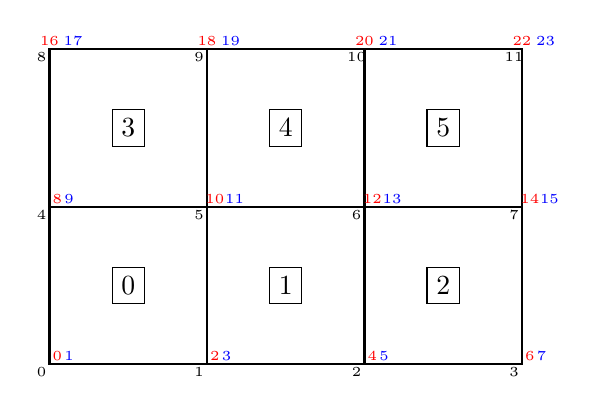
\begin{tikzpicture}
%\draw[step=0.5cm,gray,very thin] (0,0) grid (8,6); %background grid
\draw[thick] (1,1) -- (3,1) -- (3,3) -- (1,3) -- cycle;  
\draw[thick] (3,1) -- (5,1) -- (5,3) -- (3,3) -- cycle; 
\draw[thick] (5,1) -- (7,1) -- (7,3) -- (5,3) -- cycle; 
\draw[thick] (1,3) -- (3,3) -- (3,5) -- (1,5) -- cycle;  
\draw[thick] (3,3) -- (5,3) -- (5,5) -- (3,5) -- cycle; 
\draw[thick] (5,3) -- (7,3) -- (7,5) -- (5,5) -- cycle; 
\node[draw] at (2,2) {0};
\node[draw] at (4,2) {1};
\node[draw] at (6,2) {2};
\node[draw] at (2,4) {3};
\node[draw] at (4,4) {4};
\node[draw] at (6,4) {5};
%pressure dofs
\node at (0.9,0.9) {\tiny 0};
\node at (2.9,0.9) {\tiny 1};
\node at (4.9,0.9) {\tiny 2};
\node at (6.9,0.9) {\tiny 3};
\node at (0.9,2.9) {\tiny 4};
\node at (2.9,2.9) {\tiny 5};
\node at (4.9,2.9) {\tiny 6};
\node at (6.9,2.9) {\tiny 7};
\node at (0.9,4.9) {\tiny 8};
\node at (2.9,4.9) {\tiny 9};
\node at (4.9,4.9) {\tiny 10};
\node at (6.9,4.9) {\tiny 11};
%velocity dofs
\node[red] at (1.1,1.1) {\tiny 0};  \node[blue] at (1.25,1.1) {\tiny 1};
\node[red] at (3.1,1.1) {\tiny 2};  \node[blue] at (3.25,1.1) {\tiny 3};
\node[red] at (5.1,1.1) {\tiny 4};  \node[blue] at (5.25,1.1) {\tiny 5};
\node[red] at (7.1,1.1) {\tiny 6};  \node[blue] at (7.25,1.1) {\tiny 7};
\node[red] at (1.1,3.1) {\tiny 8};  \node[blue] at (1.25,3.1) {\tiny 9};
\node[red] at (3.1,3.1) {\tiny 10}; \node[blue] at (3.35,3.1) {\tiny 11};
\node[red] at (5.1,3.1) {\tiny 12}; \node[blue] at (5.35,3.1) {\tiny 13};
\node[red] at (7.1,3.1) {\tiny 14}; \node[blue] at (7.35,3.1) {\tiny 15};
\node[red] at (1.,5.1) {\tiny 16}; \node[blue] at (1.3,5.1) {\tiny 17};
\node[red] at (3.,5.1) {\tiny 18}; \node[blue] at (3.3,5.1) {\tiny 19};
\node[red] at (5.,5.1) {\tiny 20}; \node[blue] at (5.3,5.1) {\tiny 21};
\node[red] at (7.,5.1) {\tiny 22}; \node[blue] at (7.3,5.1) {\tiny 23};
\end{tikzpicture}\\
{\tiny Red color corresponds to the dofs in the x direction, blue color indicates a dof in the y direction.}
\end{center}

We have nnp=12, nel=6, NfemV=24. Let us assume that free slip boundary conditions are applied. 
The boundary conditions {\tt fix\_bc} array is then:
\begin{center}
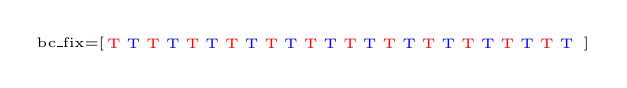
\begin{tikzpicture}
%\draw[step=0.5cm,gray,very thin] (0,0) grid (9,0.7); %background grid
\node  at (0.45,.1) {\tiny bc\_fix=[};

\node[red]  at (1.00,.1) {\tiny T};
\node[blue] at (1.25,.1) {\tiny T};
\node[red]  at (1.50,.1) {\tiny T};
\node[blue] at (1.75,.1) {\tiny T};
\node[red]  at (2.00,.1) {\tiny T};
\node[blue] at (2.25,.1) {\tiny T};
\node[red]  at (2.50,.1) {\tiny T};
\node[blue] at (2.75,.1) {\tiny T};
\node[red]  at (3.00,.1) {\tiny T};
\node[blue] at (3.25,.1) {\tiny T};
\node[red]  at (3.50,.1) {\tiny T};
\node[blue] at (3.75,.1) {\tiny T};
\node[red]  at (4.00,.1) {\tiny T};
\node[blue] at (4.25,.1) {\tiny T};
\node[red]  at (4.50,.1) {\tiny T};
\node[blue] at (4.75,.1) {\tiny T};
\node[red]  at (5.00,.1) {\tiny T};
\node[blue] at (5.25,.1) {\tiny T};
\node[red]  at (5.50,.1) {\tiny T};
\node[blue] at (5.75,.1) {\tiny T};
\node[red]  at (6.00,.1) {\tiny T};
\node[blue] at (6.25,.1) {\tiny T};
\node[red]  at (6.50,.1) {\tiny T};
\node[blue] at (6.75,.1) {\tiny T};

\node  at (7,.1) {\tiny ]};

\end{tikzpicture}\\
\end{center}
Note that since corners belong to two edges, we effectively prescribed 
no-slip boundary conditions on those. 
\todo[inline]{why does array contain only T??}


We wish to compute the tractions on the boundaries, and more precisely for the dofs for which 
a Dirichlet velocity boundary condition has been prescribed.
The number of (traction) unknowns NfemTr is then the number of {\tt T} in the {\tt bc\_fix} array.
In our specific case, we wave NfemTr= .
\todo{finish}
This means that we need for each targeted dof to be able to find its identity/number
between 0 and NfemTr-1. We therefore create the array {\tt bc\_nb} which is 
filled as follows: 
 
\begin{center}
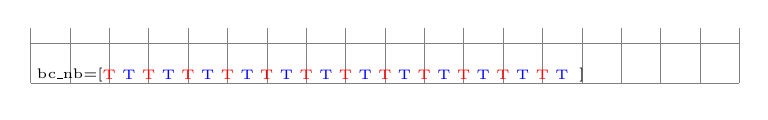
\begin{tikzpicture}
\draw[step=0.5cm,gray,very thin] (0,0) grid (9,0.7); %background grid

\node  at (0.5,.1) {\tiny bc\_nb=[};

\node[red]  at (1.00,.1) {\tiny T};
\node[blue] at (1.25,.1) {\tiny T};
\node[red]  at (1.50,.1) {\tiny T};
\node[blue] at (1.75,.1) {\tiny T};
\node[red]  at (2.00,.1) {\tiny T};
\node[blue] at (2.25,.1) {\tiny T};
\node[red]  at (2.50,.1) {\tiny T};
\node[blue] at (2.75,.1) {\tiny T};
\node[red]  at (3.00,.1) {\tiny T};
\node[blue] at (3.25,.1) {\tiny T};
\node[red]  at (3.50,.1) {\tiny T};
\node[blue] at (3.75,.1) {\tiny T};
\node[red]  at (4.00,.1) {\tiny T};
\node[blue] at (4.25,.1) {\tiny T};
\node[red]  at (4.50,.1) {\tiny T};
\node[blue] at (4.75,.1) {\tiny T};
\node[red]  at (5.00,.1) {\tiny T};
\node[blue] at (5.25,.1) {\tiny T};
\node[red]  at (5.50,.1) {\tiny T};
\node[blue] at (5.75,.1) {\tiny T};
\node[red]  at (6.00,.1) {\tiny T};
\node[blue] at (6.25,.1) {\tiny T};
\node[red]  at (6.50,.1) {\tiny T};
\node[blue] at (6.75,.1) {\tiny T};
\node  at (7,.1) {\tiny ]};
\end{tikzpicture}\\
\end{center}

This translates as follows in the code:
\begin{lstlisting}
NfemTr=np.sum(bc_fix)
bc_nb=np.zeros(NfemV,dtype=np.int32)
counter=0
for i in range(0,NfemV):
    if (bc_fix[i]):
       bc_nb[i]=counter
       counter+=1
\end{lstlisting}


The algorithm is then as follows

\begin{itemize}
\item[A] Prepare two arrays to store the matrix $M_{cbf}$ and its right hand side $rhs_{cbf}$  

\item[B] 
Loop over all elements 

\item[C] 
For each element touching a boundary, compute the residual vector 
$R_{el}=-f_{el} + \K_{el}{\cal V}_{el} + \G_{el} {\cal P}_{el}$

\item[D]
Loop over the four edges of the element using the connectivity array

\item[E]
For each edge loop over the number of degrees of freedom (2 in 2D)

\item[F] 
For each edge assess whether the dofs on both ends are target dofs. 

\item[G]
If so, compute the mass matrix $M_{edge}$ for this edge 

\item[H] extract the 2 values off the element residual vector and assemble these
in $rhs_{cbf}$

\item[I] Assemble $M_{edge}$ into NfemTrxNfemTr matrix using bc\_nb
\end{itemize}


\begin{lstlisting}
M_cbf = np.zeros((NfemTr,NfemTr),np.float64)         # A
rhs_cbf = np.zeros(NfemTr,np.float64)

for iel in range(0,nel):                             # B

    ... compute elemental residual ...               # C

    #boundary 0-1                                    # D
    for i in range(0,ndofV):                         # E
        idof0=2*icon[0,iel]+i
        idof1=2*icon[1,iel]+i
        if (bc_fix[idof0] and bc_fix[idof1]):        # F
           idofTr0=bc_nb[idof0]   
           idofTr1=bc_nb[idof1]
           rhs_cbf[idofTr0]+=res_el[0+i]             # H
           rhs_cbf[idofTr1]+=res_el[2+i]              
           M_cbf[idofTr0,idofTr0]+=M_edge[0,0]       # 
           M_cbf[idofTr0,idofTr1]+=M_edge[0,1]       # I
           M_cbf[idofTr1,idofTr0]+=M_edge[1,0]       # 
           M_cbf[idofTr1,idofTr1]+=M_edge[1,1]       #

    #boundary 1-2                                    #[D]

    ...

    #boundary 2-3                                    #[D]

    ...

    #boundary 3-0                                    #[D]

    ...


\end{lstlisting}










%---------------------------------------------------------------
\subsection{The CBF applied to the heat transport equation}

We start from the strong form of the heat transfer equation (without the source terms for simplicity):
\[
\rho C_p
\left(\frac{\partial T}{\partial t} + \vec{\upnu}\cdot \vec{\nabla}T\right)
=
\vec{\nabla} \cdot k\vec{\nabla} T
\]
The weak form then writes:
\[
\int_\Omega \bN^\uptheta
\rho C_p
\frac{\partial T}{\partial t} dV 
+
\int_\Omega \bN^\uptheta
\rho C_p
\vec{\upnu}\cdot \vec{\nabla}T  dV
=
\int_\Omega \bN^\uptheta
\vec{\nabla} \cdot k\vec{\nabla} T dV
\]
Using once again integration by parts and divergence theorem:
\[
\int_\Omega \bN^\uptheta
\rho C_p
\frac{\partial T}{\partial t} dV 
+
\int_\Omega \bN^\uptheta
\rho C_p
\vec{\upnu}\cdot \vec{\nabla}T  dV
=
\int_\Gamma \bN^\uptheta k \vec{\nabla} T \cdot \vec{n} d\Gamma
-
\int_\Omega  \vec{\nabla} \bN^\uptheta \cdot k \vec{\nabla} T dV
\]
On the boundary we are interested in the heat flux $\vec{q}=-k \vec{\nabla} T$
\[
\int_\Omega \bN^\uptheta
\rho C_p
\frac{\partial T}{\partial t} dV 
+
\int_\Omega \bN^\uptheta
\rho C_p
\vec{\upnu}\cdot \vec{\nabla} T  dV
=
-\int_\Gamma \bN^\uptheta {\bm q} \cdot {\bm n} d\Gamma
- \int_\Omega  \vec{\nabla} \bN^\uptheta \cdot k \vec{\nabla} T dV
\]
or,
\[
\int_\Gamma \bN^\uptheta {\bm q} \cdot {\bm n} d\Gamma
=
-\int_\Omega \bN^\uptheta
\rho C_p
\frac{\partial T}{\partial t} dV 
-
\int_\Omega \bN^\uptheta
\rho C_p  {\bm v}\cdot \vec{\nabla} T  dV
- \int_\Omega  \vec{\nabla} \bN^\uptheta \cdot k \vec{\nabla} T dV
\]
Considering the normal heat flux $q_n = \vec{q} \cdot \vec{n}$ as an unknown 
living on the nodes on the boundary, 
\[
q_n = \sum_{i=1}^2 q_{n|i} N_i
\]
so that the left hand term becomes a mass matrix for the basis functions living on 
the boundary.
We have already covered the right hand side terms when building the FE system 
to solve the heat transport equation, so that in the end 
\[
\M' \cdot \vec{\cal Q}_n =
- \M \cdot \frac{\partial \bm T}{\partial t} -K_a \cdot {\bm T} - K_d \cdot {\bm T} 
\]
where $\vec{\cal Q}_n$ is the assembled vector of normal heat flux components.
Note that in all terms the assembly only takes place over the elements along the boundary.


Note that the resulting matrix is symmetric.


 %-----------------------
\newpage %-----------------------------------------------------------------------------------------
\section{The value of the timestep}\label{ss:cfl} \input{cfl} %---------------------------------
\newpage %-----------------------------------------------------------------------------------------
\section{Mappings \& Jacobians \label{ss:mappings}} \begin{flushright} {\tiny {\color{gray} mappings.tex}} \end{flushright}
%~~~~~~~~~~~~~~~~~~~~~~~~~~~~~~~~~~~~~~~~~~~~~~~~~~~~~~~~~~~~~~~~~~~~~~~~~~~~~~~~~~~~~~~~~~~~~~~~~~

\index{general}{Isoparametric}
\index{general}{Subparametric} 
\index{general}{Superparametric}

The name {\sl isoparametric} derives from the fact that the same ('iso') 
functions are used as basis functions and for the mapping to the reference element.

More generally, if $n_e$ denotes the number of nodes of an element and $n_g$ denotes the 
number of nodes describing the geometry of the element, 
then the element is termed {\sl subparametric} when $n_g<n_e$ and 
{\sl superparametric} when $n_g>n_e$.

%...........................................
\subsubsection{Linear mapping on a triangle}

\begin{verbatim}
2
|\     s
| \    |_r
|  \
3===1
\end{verbatim}

Let us assume that the coordinates of the vertices are 
$(x_1,y_1)$,  
$(x_2,y_2)$, and 
$(x_3,y_3)$.
The coordinates inside the reference element are $(r,s)$ with 
$0\le r \le 1$ and $0 \le s \le 1$. We then simply have the 
following relationship, i.e. any point of the reference element 
can be mapped to the physical triangle as follows:
\begin{eqnarray}
x&=& r x_1 + s x_2 + (1-r-s) x_3 \\
y&=& r y_1 + s y_2 + (1-r-s) y_3 
\end{eqnarray} 
Note that the functions $r$, $s$ and $1-r-s$ are in fact the 
$P_1$ basis functions (see Section~\ref{ss:p1}).
There is also an inverse map, which is easily computed:
\begin{eqnarray}
r&=& \frac{(y_2-y_3)(x-x_3)-(x_2-x_3)(y-y_3)}{(x_1-x_3)(y_2-y_3)-(y_1-y_3)(x_2-x_3)} \\
s&=& \frac{-(y_1-y_3)(x-x_3)+(x_1-x_3)(y-y_3)}{(x_1-x_3)(y_2-y_3)-(y_1-y_3)(x_2-x_3)} 
\end{eqnarray} 
\begin{remark}
The denominator will not vanish, because it is a multiple of the area of the 
triangle. If the three points
are distinct then the area cannot be zero.
\end{remark}

%................................................
\subsubsection{Bilinear mapping on a quadrilateral}

The \index{general}{reference element} reference element 
is in the $(r,s)$ space. It is a square of size $2\times2$ 
centered around the origin, i.e. $(r,s)\in[-1,1]\times[-1,1]$. 
We wish to map it to the quadrilateral in the $(x,y)$ space 
(and vice versa):

\begin{center}
\includegraphics[width=8cm]{images/mappings/bilinear/mapping_bilinear.png}
\end{center}

The coordinates of the vertices are 
$(x_1,y_1)$, $(x_2,y_2)$, $(x_3,y_3)$ and $(x_4,y_4)$.
We then simply have the 
following relationship, i.e. any point of the reference element 
can be mapped to the physical quadrilateral as follows:
\begin{eqnarray}
x&=& \bN_1(r,s) x_1 + \bN_2(r,s) x_2 + \bN_3(r,s) x_3 + \bN_4(r,s) x_4 \\
y&=& \bN_1(r,s) y_1 + \bN_2(r,s) y_2 + \bN_3(r,s) y_3 + \bN_4(r,s) y_4 
\end{eqnarray} 
where the $Q_1$ basis functions $\bN_i(r,s)$ are defined in Section~\ref{sec:elts1D}.

In the following example the program randomly generates 10000 points 
inside the reference 
element and computes their mapping into the $(x,y)$ space. 

\begin{lstlisting}
x1=-1 ; y1=-2
x2=3  ; y2=-1
x3=2  ; y3=2
x4=-3 ; y4=1

npts=10000
r=np.zeros(npts,dtype=np.float64)   
s=np.zeros(npts,dtype=np.float64)   
x=np.zeros(npts,dtype=np.float64)   
y=np.zeros(npts,dtype=np.float64)   

for i in range(0,npts):
    # compute random r,s coordinates
    r[i]=random.uniform(-1.,+1)
    s[i]=random.uniform(-1.,+1)
    # compute basis function values at r,s
    N1=0.25*(1-r[i])*(1-s[i])
    N2=0.25*(1+r[i])*(1-s[i])
    N3=0.25*(1+r[i])*(1+s[i])
    N4=0.25*(1-r[i])*(1+s[i])
    # compute x,y coordinates
    x[i]=N1*x1+N2*x2+N3*x3+N4*x4
    y[i]=N1*y1+N2*y2+N3*y3+N4*y4

np.savetxt('rs.ascii',np.array([r,s]).T)
np.savetxt('xy.ascii',np.array([x,y]).T)
\end{lstlisting}

\begin{center}
\includegraphics[width=7cm]{images/mappings/bilinear/rs.pdf}
\includegraphics[width=7cm]{images/mappings/bilinear/xy.pdf}
\end{center}

There is also an inverse map, which is not so easily computed (see Section~\ref{sec:amiin}).
However, if the quadrilateral in the $(x,y)$ space is a rectangle of size $(h_x,h_y)$, 
the inverse mapping is trivial:
\begin{eqnarray}
r&=&\frac{x-x_1}{x_2-x_1} \\
s&=&\frac{y-y_1}{y_4-y_1} 
\end{eqnarray}
Also in the case of rectangular elements of size $(h_x,h_y)$
the basis functions can easily be written as functions of $(x,y)$:
\begin{eqnarray}
\bN_1(x,y) &=& \left( \frac{x_3 -x }{h_x}  \right) \left( \frac{y_3 -y }{h_y}  \right) \nn\\
\bN_2(x,y) &=& \left( \frac{x - x_1}{h_x}  \right) \left( \frac{y_3 -y }{h_y}  \right) \nn\\
\bN_3(x,y) &=& \left( \frac{x - x_1}{h_x}  \right) \left( \frac{y - y_1}{h_y}  \right) \nn\\
\bN_4(x,y) &=& \left( \frac{x_3 -x }{h_x}  \right) \left( \frac{y - y_1}{h_y}  \right) \nn 
\end{eqnarray}
On the one hand, any variable defined on the element can be approximated using the basis functions:
\begin{equation}
f^h(r,s)=\sum_i \bN_i(r,s) f_i.
\end{equation}
If we treat the coordinate variables $x$ and $y$ themselves as functions, 
then the basis functions can be used to construct the mapping:
\begin{equation}
x(r,s)=\sum_i \bN_i(r,s) x_i 
\qquad
y(r,s)=\sum_i \bN_i(r,s) y_i,  \label{eqxy}
\end{equation}
leading to write
\begin{eqnarray}
\frac{\partial x}{\partial r} &=& \sum_i \frac{\partial \bN_i}{\partial r} x_i \\
\frac{\partial x}{\partial s} &=& \sum_i \frac{\partial \bN_i}{\partial s} x_i \\
\frac{\partial y}{\partial r} &=& \sum_i \frac{\partial \bN_i}{\partial r} y_i \\
\frac{\partial y}{\partial s} &=& \sum_i \frac{\partial \bN_i}{\partial s} y_i 
\end{eqnarray}
On the other hand we also have 
\begin{eqnarray}
\frac{\partial f}{\partial r} &=&
\frac{\partial f}{\partial x}\frac{\partial x}{\partial r}
+\frac{\partial f}{\partial y}\frac{\partial y}{\partial r} \\
\frac{\partial f}{\partial s} &=&
\frac{\partial f}{\partial x}\frac{\partial x}{\partial s}
+\frac{\partial f}{\partial y}\frac{\partial y}{\partial s}
\end{eqnarray}
or in matrix form:
\begin{equation}
\left(
\begin{array}{c}
\frac{\partial f}{\partial r} \\ \\
\frac{\partial f}{\partial s}
\end{array}
\right)
=
\underbrace{
\left(
\begin{array}{cc}
\frac{\partial x}{\partial r} & \frac{\partial y}{\partial r} \nonumber\\ \\
\frac{\partial x}{\partial s} & \frac{\partial y}{\partial s} \nonumber
\end{array}
\right)
}_{\bm J}
\cdot
\left(
\begin{array}{c}
\frac{\partial f}{\partial x} \\ \\
\frac{\partial f}{\partial y}
\end{array}
\right)
\end{equation}
where ${\bm J}$ is called the Jacobian of the transformation
By inverting the Jacobian matrix, the desired derivatives with respect to $x$
and $y$ can be obtained:

We have:
\[
\left(
\begin{array}{c}
\frac{\partial f}{\partial x} \\ \\
\frac{\partial f}{\partial y}
\end{array}
\right)
=
{\bm J}^{-1} \cdot 
\left(
\begin{array}{c}
\frac{\partial f}{\partial r} \\ \\
\frac{\partial f}{\partial s}
\end{array}
\right)
\]
The inverse of the Jacobian matrix can be simply obtained in 
2D (Cramer's rule for $2\times2$ matrices\footnote{\url{https://en.wikipedia.org/wiki/Cramers_rule}}):
\[
{\bm J}^{-1} = \frac{1}{|{\bm J}|} 
\left(
\begin{array}{cc}
\frac{\partial y}{\partial s} & -\frac{\partial y}{\partial r} \nonumber\\ \\
-\frac{\partial x}{\partial s} & \frac{\partial x}{\partial r} \nonumber
\end{array}
\right)
\]
The presence of the determinant in the denominator implies that it cannot 
be zero anywhere, or in other words: the mapping is not valid if $|{\bm J}|$
is zero anywhere over the element.

\begin{remark}
\textcite{hua90} (1990) has published analytical inverse transformation 
for quadrilateral isoparametric elements, i.e. how to compute ${\bm J}^{-1}$ 
as a function of space coordinates and not just at the quadrature points. 
\end{remark}

Let us look at this by means of a simple example and let us consider the following 
element:
\begin{center}
\includegraphics[width=4cm]{images/mappings/fournode/ex1}
\end{center}
Then a $Q_1$ mapping yields:
\begin{eqnarray}
x(r,s) &=& \sum_i \bN_i(r,s) x_i = \bN_2 + 2\bN_3 = \frac{1}{4} (3+3r+ s+rt) \nn\\
y(r,s) &=& \sum_i \bN_i(r,s) y_i = 2\bN_3 + \bN_4 = \frac{1}{4} (3+r+ 3s+rt) 
\end{eqnarray}
The Jacobian matrix is then
\begin{equation}
{\bm J} = 
\left(
\begin{array}{cc}
\frac{\partial x}{\partial r} & \frac{\partial y}{\partial r} \nonumber\\ \\
\frac{\partial x}{\partial s} & \frac{\partial y}{\partial s} \nonumber
\end{array}
\right)
=
\frac{1}{4}
\left(
\begin{array}{cc}
3+s & 1+s \\
1+r & 3+r
\end{array}
\right)
\end{equation}
and its determinant is 
\begin{equation}
|{\bm J}|=\frac{1}{4} [(3+s)(3+r)-(1+s)(1+r)]=\frac{1}{2}+\frac{1}{8}r+\frac{1}{8}s
\end{equation}
It is clear that $|{\bm J}|>0$ for $-1\leq r \leq +1$ and $-1\leq s \leq +1$. 

Let us now consider another example, the following element:
\begin{center}
\includegraphics[width=3.5cm]{images/mappings/fournode/ex2}
\end{center}
It follows that
\begin{eqnarray}
x(r,s) &=& \sum_i \bN_i(r,s) x_i = \frac{1}{4}(1+r)(7+5s) \\ 
y(r,s) &=& \sum_i \bN_i(r,s) y_i = \frac{1}{4}(17+5r+7s-5rs)
\end{eqnarray}
and the determinant:
\[
|{\bm J}|=\frac{3}{2}-\frac{15r}{4}+\frac{15s}{4}
\]
is zero for $r-s=2/5$. This mapping is invalid!

\begin{remark}
Problems also arise when the Jacobian matrix is nearly singular due to round-off errors.
To avoid problems linked to badly shaped elements, it is recommended that the inside
angles of an element are larger than $15\degree$ and less than $165\degree$.
\end{remark}

From Eq.~\eqref{eqxy}, we can also write:
\begin{eqnarray}
dx &=& \frac{\partial x}{\partial r} dr + \frac{\partial x}{\partial s} ds \\
dy &=& \frac{\partial y}{\partial r} dr + \frac{\partial y}{\partial s} ds 
\end{eqnarray}
or, 
\begin{equation}
\left(
\begin{array}{c}
dx \\ dy
\end{array}
\right)
={\bm J}\cdot
\left(
\begin{array}{c}
dr \\ ds
\end{array}
\right)
\end{equation}
This means that integrating over the 'real' element in $(x,y)$ space
can be simply done by integrating of the reference element in the 
$(r,s)$ space. This is the cornerstone of most of the implementation of the 
Finite Element Method, the second integral being carried out by means 
of the Gauss-Legendre quadrature.

\begin{equation}
\iint_{\Omega_e} ... \; dx dy = \int_{-1}^{+1} \int_{-1}^{+1} ...|{\bm J}| \; dr ds
\end{equation}


%.................................................................
\subsubsection{Biquadratic mapping of a straight-edge face $Q_2$ element }

\begin{center}
\includegraphics[width=8cm]{images/mappings/biquadratic/mapping1}
\end{center}

The reference element now contains 9 nodes: 1,3,7,9 are the corners, nodes
2,4,6,8 are the mid-face points and node 5 is in the middle\footnote{Note that 
this numbering is quite arbitrary}.
The mapping from the $(r,s)$ space to the $(x,y)$ space is then as follows:

\begin{eqnarray}
\left(
\begin{array}{c}
x(r,s) \\ y(r,s)
\end{array}
\right)
&=&
\bN_1(r,s)
\left(
\begin{array}{c}
x_1 \\ y_1
\end{array}
\right)
+
\bN_2(r,s)
\left(
\begin{array}{c}
x_2 \\ y_2
\end{array}
\right)
+
\bN_3(r,s)
\left(
\begin{array}{c}
x_3 \\ y_3
\end{array}
\right)
+
\bN_4(r,s)
\left(
\begin{array}{c}
x_4 \\ y_4
\end{array}
\right) \nonumber\\
&+&
\bN_5(r,s)
\left(
\begin{array}{c}
x_5 \\ y_5
\end{array}
\right)
+
\bN_6(r,s)
\left(
\begin{array}{c}
x_6 \\ y_6
\end{array}
\right)
+
\bN_7(r,s)
\left(
\begin{array}{c}
x_7 \\ y_7
\end{array}
\right)
+
\bN_8(r,s)
\left(
\begin{array}{c}
x_4 \\ y_8
\end{array}
\right) \nonumber\\
&+&
\bN_9(r,s)
\left(
\begin{array}{c}
x_9 \\ y_9
\end{array}
\right) 
\nonumber
\end{eqnarray}
where the $Q_2$ basis functions have been obtained in Section~\ref{ss:q22d}:
\begin{eqnarray}
\bN_1(r,t)&=& 0.5r(r-1)  0.5t(t-1) \nonumber\\
\bN_2(r,t)&=&      (1-r^2)  0.5t(t-1) \nonumber\\
\bN_3(r,t)&=& 0.5r(r+1)  0.5t(t-1) \nonumber\\
\bN_4(r,t)&=& 0.5r(r-1)       (1-t^2) \nonumber\\
\bN_5(r,t)&=&      (1-r^2)       (1-t^2) \nonumber\\
\bN_6(r,t)&=& 0.5r(r+1)       (1-t^2) \nonumber\\
\bN_7(r,t)&=& 0.5r(r-1)  0.5t(t+1) \nonumber\\
\bN_8(r,t)&=&      (1-r^2)  0.5t(t+1) \nonumber\\
\bN_9(r,t)&=& 0.5r(r+1)  0.5t(t+1) \nonumber
\end{eqnarray}


\begin{lstlisting}
x1=-1                 ; y1=-2
x3=3                  ; y3=-1
x9=2                  ; y9=2
x7=-3                 ; y7=1
x2=0.5*(x1+x3)        ; y2=0.5*(y1+y3)
x4=0.5*(x1+x7)        ; y4=0.5*(y1+y7)
x6=0.5*(x3+x9)        ; y6=0.5*(y3+y9)
x8=0.5*(x7+x9)        ; y8=0.5*(y7+y9)
x5=0.25*(x1+x3+x7+x9) ; y5=0.25*(y1+y3+y7+y9)

npts=10000
r=np.zeros(npts,dtype=np.float64)   
s=np.zeros(npts,dtype=np.float64)   
xQ1=np.zeros(npts,dtype=np.float64)   
yQ1=np.zeros(npts,dtype=np.float64)   
xQ2=np.zeros(npts,dtype=np.float64)   
yQ2=np.zeros(npts,dtype=np.float64)   

for i in range(0,npts):
    # compute random r,s coordinates
    r[i]=random.uniform(-1.,+1)
    s[i]=random.uniform(-1.,+1)
    # compute Q2 basis function values at r,s
    N1= 0.5*r[i]*(r[i]-1.) * 0.5*s[i]*(s[i]-1.)
    N2=       (1.-r[i]**2) * 0.5*s[i]*(s[i]-1.)
    N3= 0.5*r[i]*(r[i]+1.) * 0.5*s[i]*(s[i]-1.)
    N4= 0.5*r[i]*(r[i]-1.) *       (1.-s[i]**2)
    N5=       (1.-r[i]**2) *       (1.-s[i]**2)
    N6= 0.5*r[i]*(r[i]+1.) *       (1.-s[i]**2)
    N7= 0.5*r[i]*(r[i]-1.) * 0.5*s[i]*(s[i]+1.)
    N8=       (1.-r[i]**2) * 0.5*s[i]*(s[i]+1.)
    N9= 0.5*r[i]*(r[i]+1.) * 0.5*s[i]*(s[i]+1.)
    # compute x,y coordinates
    xQ2[i]=N1*x1+N2*x2+N3*x3+N4*x4+N5*x5+N6*x6+N7*x7+N8*x8+N9*x9
    yQ2[i]=N1*y1+N2*y2+N3*y3+N4*y4+N5*y5+N6*y6+N7*y7+N8*y8+N9*y9
    # compute Q1 basis function values at r,s
    N1=0.25*(1-r[i])*(1-s[i])
    N2=0.25*(1+r[i])*(1-s[i])
    N3=0.25*(1+r[i])*(1+s[i])
    N4=0.25*(1-r[i])*(1+s[i])
    # compute x,y coordinates
    xQ1[i]=N1*x1+N2*x3+N3*x9+N4*x7
    yQ1[i]=N1*y1+N2*y3+N3*y9+N4*y7

np.savetxt('rs.ascii',np.array([r,s]).T)
np.savetxt('xyQ1.ascii',np.array([xQ1,yQ1]).T)
np.savetxt('xyQ2.ascii',np.array([xQ2,yQ2]).T)
\end{lstlisting}

The code is available in {\tt /images/mappings/biquadratic}
Note that the coordinates of point 5 are defined being those of the barycenter
of the quadrilateral. More on this choice later.

\begin{center}
a)\includegraphics[width=5.6cm]{images/mappings/biquadratic/rs.pdf}
b)\includegraphics[width=5.6cm]{images/mappings/biquadratic/xyQ1.pdf}
c)\includegraphics[width=5.6cm]{images/mappings/biquadratic/xyQ2.pdf}\\
{\captionfont a) 10,000 random points in the reference element; 
b,c) image of these points by means of a bilinear and biquadratic mapping 
respectively.\\ When the sides of the element
are straight we see that a $Q_1$ mapping is sufficient.}
\end{center}

%.................................................................
\subsubsection{Biquadratic mapping of a not-so straight-line face $Q_2$ element }

We now carry out the same exercise as before but nodes 2 and 8 are no more 
in the middle of nodes 1-3 and 7-9 respectively.
The code is available in {\tt /images/mappings/biquadratic2}.

\begin{center}
a)\includegraphics[width=4.5cm]{images/mappings/biquadratic2/rs.pdf}
b)\includegraphics[width=4.5cm]{images/mappings/biquadratic2/xyQ1.pdf}
c)\includegraphics[width=4.5cm]{images/mappings/biquadratic2/xyQ2.pdf}\\
{\captionfont a) 10,000 random points in the reference element; 
b,c) image of these points by means of a bilinear and biquadratic mapping 
respectively.} 
\end{center}

In this case we see that 
the $Q_2$ mapping manages to better capture the 'real' shape of the element.
Since nodes 2 and 8 have moved, we could now ask ourselves 
where we should place node 5? In this example we set it as follows
but it is somewhat arbitrary.
\begin{lstlisting}
x5=(x1+x2+x3+x4+x6+x7+x8+x9)/8. 
y5=(y1+y2+y3+y4+y6+y7+y8+y9)/8.
\end{lstlisting}
We will come back to this later.

%.......................................................................
\subsubsection{Bilinear, biquadratic and bicubic mapping in an annulus }

In the light of what precedes, we can now ask ourselves how this translates to 
a real geodynamic case. Let us then consider the case of an annular domain, 
a cross section of a hollow sphere. 
When using quadrilateral elements, the mesh will look similar to this:

\begin{center}
\includegraphics[width=6cm]{images/mappings/curved/annulus_mesh}
\end{center}

We here focus on $Q_1$, $Q_2$ and $Q_3$ mappings. We single out an element, 
and arbitrarily define it as follows in polar coordinates:
\begin{lstlisting}
theta1=23./180.*np.pi
theta2=52./180.*np.pi
R1=1.
R2=1.5
\end{lstlisting}
The $Q_1$ mapping requires four points, the $Q_2$ nine points and the $Q_3$
sixteen points. 
The code used in the following is available at {\tt ./images/mappings/curved/}.
These are placed equidistantly in the $r,\theta$ coordinate
system, as shown hereunder:

\begin{center}
\includegraphics[width=5.7cm]{images/mappings/curved/nodesQ1.pdf}
\includegraphics[width=5.7cm]{images/mappings/curved/nodesQ2.pdf}
\includegraphics[width=5.7cm]{images/mappings/curved/nodesQ3.pdf}\\
{\captionfont Left to right: position of the nodes for the $Q_1$, $Q_2$ and $Q_3$ mappings.
$Q_4$ is not shown.}
\end{center}

As before, we randomly shoot 10,000 points inside the reference element 
and map these out in the $x,y$ space. Resulting swarms of points are shown 
in the following figures:

\begin{center}
\includegraphics[width=5.7cm]{images/mappings/curved/xy1_keep.pdf}
\includegraphics[width=5.7cm]{images/mappings/curved/xy2_keep.pdf}
\includegraphics[width=5.7cm]{images/mappings/curved/xy3_keep.pdf}\\
{\captionfont Left to right: position of the mapped points for the $Q_1$, $Q_2$ and $Q_3$ mappings.
$Q_4$ is not shown.}
\end{center}

The image of a square with a $Q_1$ mapping is obviously a quadrilateral
so that it looks like quite a few points land outside of the domain $R_1\leq r\leq R_2$.
Note that points are well within $23\degree \leq \theta \leq 52\degree$, which can 
simply be explained by the fact that the faces of the element joining $R_1$
to $R_2$ are straight lines.

However, it looks like the biquadratic and bicubic mappings are doing a much better 
job at mapping the region of space $R_1\leq r\leq R_2$. In order to characterise 
this better, we now place 10,000 points on the bottom face of 
the reference element (i.e. $s=-1$)
and once again compute their coordinates in the the $x,y$ space:

\begin{center}
\includegraphics[width=8cm]{images/mappings/curved/xy1.pdf}
\includegraphics[width=8cm]{images/mappings/curved/xy2.pdf}\\
\includegraphics[width=8cm]{images/mappings/curved/xy3.pdf}
\includegraphics[width=8cm]{images/mappings/curved/xy4.pdf}\\
{\captionfont Position of the mapped points for the $Q_1$, $Q_2$, $Q_3$ and $Q_4$ mappings.}
\end{center}

For each point $i$ we now compute the distance $r_i$ 
to the origin, which, if the 
mapping was perfect, would be exactly equal to $R_1=1$. 
On the following plots are shown the error $r_i-1$ for all 
points, from $r=-1$ to $r=+1$.

\begin{center}
\includegraphics[width=8cm]{images/mappings/curved/innerline_error_Q1mapping.pdf}
\includegraphics[width=8cm]{images/mappings/curved/innerline_error_Q2mapping.pdf}\\
\includegraphics[width=8cm]{images/mappings/curved/innerline_error_Q3mapping.pdf}
\includegraphics[width=8cm]{images/mappings/curved/innerline_error_Q4mapping.pdf}\\
{\captionfont Radius error of the mapped points for the $Q_1$, $Q_2$, $Q_3$ and $Q_4$ mappings.}
\end{center}

We see that the amplitude of the error decreases with the order of the mapping used, 
which is why for instance \aspect uses a $Q_4$ mapping by default\footnote{I find it also quite striking 
that the $Q_4$ mapping outperforms the $Q_3$ one by two orders of magnitude...}.
Actually, in this particular case, the equation which describes the circle is not a 
polynomial so that no high-order mapping will ever be able to {\it exactly} 
represent the curved boundary of the element!

Another interesting point to keep in mind is that the location of the quadrature points
in the $x,y$ space is also determined by the mapping used, which can have consequences
on the accuracy of the integration and it will be reflected (for instance) on the 
error convergence rate.

As already mentioned previously, 
the coordinates of the nodes of the element in the $x,y$ are 
uniquely determined when they are on the convex hull of the element (
for instance nodes 0-7 for $Q_2$) but we need to choose the position 
of the last nodes which are inside the element. Unfortunately, this choice is 
not neutral. 

Finally, we can explore the importance of the mapping in combination with 
numerical quadrature. For each mapping we compute the area of the element
by means of a 3x3, 4x4 or 5x5 quadrature.

\begin{verbatim}
**********Q1*********
nqperdim= 3 0.3030060126539606 rel. error -0.04215361698430029
nqperdim= 4 0.3030060126539606 rel. error -0.04215361698430012 ~ 4%
nqperdim= 5 0.3030060126539606 rel. error -0.04215361698430012
**********Q2*********
nqperdim= 3 0.3162980025394154 rel. error -0.00013569026611326453
nqperdim= 4 0.3162980025394155 rel. error -0.00013569026611308905 ~ 0.01%
nqperdim= 5 0.3162980025394154 rel. error -0.00013569026611326453
**********Q3*********
nqperdim= 3 0.3163472223929359 rel. error 1.9900899402587318e-05
nqperdim= 4 0.316347222392936  rel. error 1.9900899402938278e-05 ~ 0.002%
nqperdim= 5 0.316347222392936  rel. error 1.9900899402938278e-05
**********Q4*********
nqperdim= 3 0.3163409410866220 rel. error 4.477021014282521e-08
nqperdim= 4 0.3163409541901677 rel. error 8.619243716974044e-08 ~ 0.000008%
nqperdim= 5 0.316340954190168  rel. error 8.619243804713484e-08
\end{verbatim}

Here again the $Q_4$ mapping makes quite the difference. 

\newpage

%..................................................................
\subsubsection{Biquadratic mapping - the middle node conundrum}

Python code at {\tt images/mappings/biquadratic3}.

As mentioned before, unless the element is a straight-edge quadrilateral, 
determining the (best) position of the middle node is not trivial. Or is it?


\begin{verbatim}

4--7--3
|     |
8  9  6   (reference element)
|     |
1--5--2

\end{verbatim}

We will here consider 5 different elements:

\begin{center}
\includegraphics[width=3.5cm]{images/mappings/biquadratic3/elt0/element0}
\includegraphics[width=3.5cm]{images/mappings/biquadratic3/elt1/element1}
\includegraphics[width=3.5cm]{images/mappings/biquadratic3/elt2/element2}
\includegraphics[width=3.5cm]{images/mappings/biquadratic3/elt3/element3}
\includegraphics[width=3.5cm]{images/mappings/biquadratic3/elt4/element4}\\
{\captionfont From left to right: element 0,1,2,3,4.}
\end{center}

We can think of multiple ways to come up with the 'center' of the element, 
i.e. the location of point I.

\begin{itemize}
\item {\python center=0}: 
\[
x_9=(x_1+x_2+x_3+x_4)/4 
\qquad
y_9=(y_1+y_2+y_3+y_4)/4
\]

\item {\python center=1}: 
\[
x_9=(x_1+x_2+x_3+x_4+x_5+x_6+x_7+x_8)/8 
\qquad
y_9=(y_1+y_2+y_3+y_4+y_5+y_6+y_7+y_8)/8
\]
\item {\python center=2}:
\[
x_9=(x_1+x_2+x_3+x_4+3x_5+3x_6+3x_7+3x_8)/16. 
\qquad
y_9=(y_1+y_2+y_3+y_4+3y_5+3y_6+3y_7+3y_8)/16.
\]
\item {\python center=3}: (only element=4)
\[
x_9=\frac12(R_1+R_2)\cos(3\pi/8) 
\qquad
y_9=\frac12(R_1+R_2)\sin(3\pi/8)
\]
\item {\python center=4}: I is the center of mass. 
The element is defined by $R_1<r<R_2$ and $\theta_1<\theta<\theta_2$.

We need to compute\footnote{\url{https://en.wikipedia.org/wiki/Center_of_mass}}
\begin{eqnarray}
\vec{R} 
&=&\frac{1}{M} \int \vec{r} \rho(\vec r) dV \nn\\
&=&\frac{1}{M} \rho_0 \int \vec{r} dV\nn\\
&=&\frac{1}{M} \frac{M}{V} \int \vec{r} dV\nn\\
&=&\frac{1}{V} \int \vec{r} dV\nn\\
&=&\frac{1}{V} \int \left(\begin{array}{c} x \\ y \end{array}\right)  dV\nn\\
&=&\frac{1}{V} \int \left(\begin{array}{c} r \cos \theta \\ r \sin\theta \end{array}\right)dV\nn\\
&=&\frac{1}{V} \int_{R_1}^{R_2} \int_{\theta_1}^{\theta_2} \left(\begin{array}{c} r \cos \theta 
\\ r \sin\theta \end{array}\right)  r dr d\theta\nn\\
&=&\frac{1}{\frac12 (R_2^2-R_1^2) (\theta_2-\theta_1)} \frac13(R_2^3-R_1^3) 
\left(
\begin{array}{c}
\sin\theta_2-\sin\theta_1 \\
-\cos\theta_2+\cos\theta_1 
\end{array}
\right) \nn\\
&\simeq& 
\left(
\begin{array}{c}
0.5801028000103104\\
1.4004920473554983
\end{array}
\right) 
\end{eqnarray}
which corresponds to $r=1.5158816686291174$ and $\theta=67.5^o=3\pi/8$.

\item {\python center=5}: variable position
\end{itemize}


isoparametric mapping. 


At each point $(r,s)$ we compute the error $|\sum_i N_i(r,s) x_i^2 - (\sum_i N_i(r,s) x_i)^2|$.

position of edges (setting r=+- 1, s=+-1) independent of position of middle node since shape functions are zero there

area indep of position middle node ?



%....................
\paragraph{Element 0}

In this case all only {\python center=0,1,2,4} are applicable but they all 
lead to the same point I with $x_I=0,y_I=0$. This means that the position of 
quadrature points is also independent of the {\python center} parameter.
 
\begin{center}
\includegraphics[width=5.7cm]{images/mappings/biquadratic3/elt0/jcob}
\includegraphics[width=5.7cm]{images/mappings/biquadratic3/elt0/error_posx2}
\includegraphics[width=5.7cm]{images/mappings/biquadratic3/elt0/error_posy2}\\
{\captionfont 10,000 points at random.} 
\end{center}

%....................
\paragraph{Element 1}

In this case all only {\python center=0,1,2,4} are applicable but they all 
lead to the same point I with $x_I=0,y_I=0$. This means that the position of 
quadrature points is also independent of the {\python center} parameter.
 
\begin{center}
\includegraphics[width=5.7cm]{images/mappings/biquadratic3/elt1/jcob}
\includegraphics[width=5.7cm]{images/mappings/biquadratic3/elt1/error_posx2}
\includegraphics[width=5.7cm]{images/mappings/biquadratic3/elt1/error_posy2}\\
{\captionfont 10,000 points at random.} 
\end{center}


%....................
\paragraph{Element 2} .

\begin{center}
\includegraphics[width=5.7cm]{images/mappings/biquadratic3/elt2/jcob_0}
\includegraphics[width=5.7cm]{images/mappings/biquadratic3/elt2/jcob_1}
\includegraphics[width=5.7cm]{images/mappings/biquadratic3/elt2/jcob_2}\\
\includegraphics[width=5.7cm]{images/mappings/biquadratic3/elt2/error_posx2_0}
\includegraphics[width=5.7cm]{images/mappings/biquadratic3/elt2/error_posx2_1}
\includegraphics[width=5.7cm]{images/mappings/biquadratic3/elt2/error_posx2_2}\\
\includegraphics[width=5.7cm]{images/mappings/biquadratic3/elt2/error_posy2_0}
\includegraphics[width=5.7cm]{images/mappings/biquadratic3/elt2/error_posy2_1}
\includegraphics[width=5.7cm]{images/mappings/biquadratic3/elt2/error_posy2_2}\\
{\captionfont 50,000 points at random. From left to right: center=0,1,2.} 
\end{center}




%....................
\paragraph{Element 3} .

\begin{center}
\includegraphics[width=5.7cm]{images/mappings/biquadratic3/elt3/jcob_0}
\includegraphics[width=5.7cm]{images/mappings/biquadratic3/elt3/jcob_1}
\includegraphics[width=5.7cm]{images/mappings/biquadratic3/elt3/jcob_2}\\
{\captionfont 50,000 points at random. From left to right: center=0,1,2.} 
\end{center}




%....................
\paragraph{Element 4}


\begin{center}
\includegraphics[width=5.7cm]{images/mappings/biquadratic3/elt4/jcob_0}
\includegraphics[width=5.7cm]{images/mappings/biquadratic3/elt4/jcob_1}
\includegraphics[width=5.7cm]{images/mappings/biquadratic3/elt4/jcob_2}\\
\includegraphics[width=5.7cm]{images/mappings/biquadratic3/elt4/jcob_3}
\includegraphics[width=5.7cm]{images/mappings/biquadratic3/elt4/jcob_4}\\
{\captionfont 50,000 points at random. From left to right: center=0,1,2,3,4.} 
\end{center}




\begin{center}
\includegraphics[width=8.5cm]{images/mappings/biquadratic3/elt4/nodes}
\includegraphics[width=8.5cm]{images/mappings/biquadratic3/elt4/quads}\\
{\captionfont Left: position of the nodes. Right position of quadrature points with 
nqperdim=3.}
\end{center}

\begin{verbatim}

\end{verbatim}

Area does not depend on position of middle node?!




\vspace{1cm}

\Literature 
\begin{itemize}
\item \fullcite{yuhy94}
\end{itemize}








 
 %--------------------------
\newpage %-----------------------------------------------------------------------------------------
\section{Exporting data to vtk/vtu format} 
This format seems to be the universally accepted format for 2D and 3D visualisation in 
Computational Geodynamics (and even CFD ?). Such files can be opened with open source 
softwares such as 
Paraview \footnote{https://www.paraview.org/}, 
MayaVi \footnote{https://docs.enthought.com/mayavi/mayavi/}
or Visit \footnote{https://wci.llnl.gov/simulation/computer-codes/visit/}.

Unfortunately it is my experience that no simple tutorial exists about how to build 
such files. There is an official document which describes the vtk 
format\footnote{https://www.vtk.org/wp-content/uploads/2015/04/file-formats.pdf}
but it delivers the information in a convoluted way. I therefore describe hereafter 
how fieldstone builds the vtk files. 

I hereunder show vtk file corresponding to a 3x2 grid made of linear elements.
In this particular example there are:
\begin{itemize}
\item 12 nodes and 6 elements
\item 1 elemental field (the pressure {\tt p}
\item 2 nodal fields: 1 scalar (the smoothed pressure {\tt q}), 1 vector (the velocity field {\tt u,v,0})
\end{itemize}
Note that vtk files are inherently 3D so that even in the case of a 2D simulation the $z$-coordinate 
of the points and for instance their $z$-velocity component must be provided.
The file, usually called {\filenamefont solution.vtk} starts with a header:

\lstinputlisting[language=python,firstline=1,lastline=3]{images/vtk/solution.vtu}

We then proceed to write the node coordinates as follows:

\lstinputlisting[language=python,firstline=4,lastline=19]{images/vtk/solution.vtu}

These are followed by the elemental field(s):

\lstinputlisting[language=python,firstline=20,lastline=29]{images/vtk/solution.vtu}

Nodal quantities are written next:

\lstinputlisting[language=python,firstline=30,lastline=59]{images/vtk/solution.vtu}

To these informations we must append 3 more datasets. The first one is the connectivity, 
the second one is the offsets and the third one is the type. The first one is trivial
since the required connectivity array is the same as the one needed for the Finite Elements. 
The second must be understood as follows:
when reading the connectivity information in a linear manner the offset values 
indicate the beginning of each element (omitting the zero value). The third is simply the type of element 
as given in the vtk format document (9 corresponds to a generic quadrilateral with an 
internal numbering consistent with ours). 

\lstinputlisting[language=python,firstline=60,lastline=85]{images/vtk/solution.vtu}

The file is then closed with

\lstinputlisting[language=python,firstline=86,lastline=88]{images/vtk/solution.vtu}

The {\sl solution.vtu}\footnote{\url{https://raw.githubusercontent.com/cedrict/fieldstone/master/images/vtk/solution.vtu}}  
can then be opened with ParaView, MayaVi or Visit and the reader 
is advised to find tutorials online on how to install and use these softwares. Also check Appendix~\ref{app:paraview}.

\begin{center}
\includegraphics[width=4cm]{images/vtk/grid}
\includegraphics[width=4cm]{images/vtk/vel}
\includegraphics[width=4cm]{images/vtk/press}
\end{center}

In the same folder {\tt images/vtk} there is the python script 
{\pythonfile makevtu.py}\footnote{\url{https://raw.githubusercontent.com/cedrict/fieldstone/master/images/vtk/makevtu.py}} which produces 3 different vtu files. The first one {\sl solution1.vtu} is a similar to the one above: an \lstinline{nelx*nely} quadrilateral-based mesh in a unit square. 
The second one ({\sl solution2.vtu}) looks identical when opened in Paraview but it is rather different: each element is exported as its own sub-mesh, so that if the mesh counts nel elements the number of vertices is \lstinline{4*nel}, and not \lstinline{(nelx+1)(nely+1)}. As such this file is larger. The icon array is needed to write down the positions of the four vertices of each element but not to write down the connectivity since the first 4 points are making the 1st element, the next four points are making the second element, etc ...

\begin{lstlisting}
vtufile.write("<Points> \n")
vtufile.write("<DataArray type='Float32' NumberOfComponents='3' Format='ascii'> \n")
for iel in range(0,nel):
    if not flag[iel]:
       for k in range(0,m):
           vtufile.write("%10e %10e %10e \n" %(x[icon[k,iel]],y[icon[k,iel]],0.))
vtufile.write("</DataArray>\n")
vtufile.write("</Points> \n")
vtufile.write("<Cells>\n")
vtufile.write("<DataArray type='Int32' Name='connectivity' Format='ascii'> \n")
for iel in range (0,nel_left):
    vtufile.write("%d %d %d %d \n" %(iel*4,iel*4+1,iel*4+2,iel*4+3))
vtufile.write("</DataArray>\n")
...
vtufile.write("</Cells>\n")
\end{lstlisting}

This format is rather practical in the case of linear or higher order discontinuous fields. For example, in the case of the $Q_2\times P_{-1}$ element pair, the pressure is linear inside each element and discontinuous across element edges. One can then assign pressure values at the four vertices of each element.

Finally a third mesh {\sl solution3.vtu} is produced. It is based on the 2nd one, but since elements are now somewhat de-coupled, then one can export only a subset of the mesh. For instance one could not show elements which are two distorted, or below a certain line, or outside a certain volume, etc ... In {\pythonfile makevtu.py} all elements which center is inside a circle are flagged and will not be exported into the vtu file:
\begin{lstlisting}
for iel in range(0,nel):
    flag[iel]= (xc[iel]-0.333*Lx)**2+(yc[iel]-0.666*Ly)**2<0.234**2
nel_flagged=np.sum(flag)
nel_left=nel-nel_flagged
\end{lstlisting}

\begin{center}
\includegraphics[width=11cm]{images/vtk/mesh3}
\end{center}





 %---------------------------
\newpage %-----------------------------------------------------------------------------------------
\section{Runge-Kutta methods}\label{ss:rkm} These methods were developed around 1900 by the German mathematicians Carl Runge and Martin Kutta.
The RK methods are methods for the numerical integration of 
ODEs\footnote{\url{https://en.wikipedia.org/wiki/Runge-Kutta_methods}}. These methods are well 
documented in any numerical analysis textbook and the reader is referred to \cite{gery10,tack10}.
Any Runge-Kutta method is uniquely identified by its Butcher tableau (REF?) which contains 
all necessary coefficients to build the algorithm.\todo{missing refs for Butcher tableau}

You will find here\footnote{\url{https://en.wikipedia.org/wiki/List_of_Runge-Kutta_methods}}
a complete list of RK methods.

The simplest Runge-Kutta method is the (forward) Euler method. Its tableau is:

\begin{mdframed}[backgroundcolor=blue!5]
\begin{tabular}{c|c}
0 & \\
\hline
 & 1
\end{tabular}
\end{mdframed}

\index{general}{Midpoint Method} \index{general}{RK2}
The standard second-order RK method method (also called midpoint method) is:

\begin{mdframed}[backgroundcolor=blue!5]
\begin{tabular}{c|cccccc}
0 & \\
1/2 & 1/2 \\
\hline
 & 0 & 1 
\end{tabular}
\end{mdframed}

\index{general}{Heun's emthod}
Another second-order RK method, called Heun's 
method\footnote{\url{https://en.wikipedia.org/wiki/Heun's_method}} is follows:

\begin{mdframed}[backgroundcolor=blue!5]
\begin{tabular}{c|cccccc}
0 & \\
1 & 1 \\
\hline
 & 1/2 & 1/2 
\end{tabular}
\end{mdframed}

A third-order RK method is as follows:\index{general}{RK3}

\begin{mdframed}[backgroundcolor=blue!5]
\begin{tabular}{c|ccccc}
0 & \\
1/2 & 1/2 \\
1 & -1 & 2 \\ 
\hline
 & 1/6 & 4/6  & 1/6
\end{tabular}
\end{mdframed}


\index{general}{RK4}
The RK4 method falls in this framework. Its tableau is:

\begin{mdframed}[backgroundcolor=blue!5]
\begin{tabular}{c|cccccc}
0 & \\
1/2 & 1/2 \\
1/2 & 0 & 1/2 \\
1 & 0 & 0 & 1 \\
\hline
 & 1/6 & 1/3 & 1/3 & 1/6 
\end{tabular}
\end{mdframed}

A slight variation of the standard RK4 method is also due to Kutta in 1901 and is called the 3/8-rule. 
Almost all of the error coefficients are smaller than in the standard method but it requires 
slightly more FLOPs per time step. Its Butcher tableau is

\begin{mdframed}[backgroundcolor=blue!5]
\begin{tabular}{c|cccccc}
0 & \\
1/3 & 1/3 \\
2/3 & -1/3 & 1 \\
1 & 1 & -1 & 1 \\
\hline
 & 1/8 & 3/8 & 3/8 & 1/8 
\end{tabular}
\end{mdframed}


\index{general}{RK45} \index{general}{Runge-Kutta-Fehlberg method}
The following method is called the Runge-Kutta-Fehlberg method and is 
commonly abbreviated 
RKF45\footnote{\url{https://en.wikipedia.org/wiki/Runge-Kutta-Fehlberg_method}}. 
Its Butcher tableau is as follows: 

\begin{mdframed}[backgroundcolor=blue!5]
\begin{tabular}{c|cccccc}
0 & \\
1/4 	&1/4\\ 
3/8 	&3/32 		&9/32 \\
12/13 	&1932/2197 	&-7200/2197 &	7296/2197\\
1 	&439/216 	&-8 	&3680/513 &	-845/4104\\
1/2 	&-8/27 		&2 	&-3544/2565& 	1859/4104 &	-11/40 	\\
\hline
&16/135 	&0 		&6656/12825 	&28561/56430 	&-9/50& 	2/55\\
&25/216 	&0 	&1408/2565 	&2197/4104 	&-1/5 	&0 
\end{tabular}
\end{mdframed}


The first row of coefficients at the bottom of the table gives the fifth-order 
accurate method, and the second row gives the fourth-order accurate method. 

The particularity of this method is that from the same Butcher Tableau one 
can produce a 4th-order approximation $\tilde{A}$ and a 5th-order approximation $A$:
\begin{eqnarray}
\tilde{A}_{n+1}&=&A_n + \frac{25}{216}A_1 + \frac{1408}{2565}A_3+\frac{2197}{4101}A_4 -\frac15 A_5 \nn\\
A_{n+1}&=&A_n + \frac{16}{135}A_1 + \frac{6656}{12825}A_3+\frac{28561}{56430}A_4 \nn
-\frac{9}{50} A_5 + \frac{2}{55} A_6
\end{eqnarray}
One can define 
\[
R=\frac{1}{h} | \tilde{A}_{n+1} - A_{n+1} | \nn\\
\qquad\qquad
\delta = \left( \frac{tol}{R \sqrt 2} \right)^{1/4}
\]
where $h$ is the current step.
If $R \le tol$ keep $A$ as the current step solution and move to the next step with step size $\delta  \cdot h$.
If $R > tol$ recalculate the current step with step size $\delta  \cdot h$. 



In the literature we can also find even higher order methods 
based on the same principle:

\begin{center}
\includegraphics[width=8cm]{images/rungekutta/fe7}\\
\includegraphics[width=10cm]{images/rungekutta/prdo81a}\\
\includegraphics[width=14cm]{images/rungekutta/prdo81b}\\
{\captionfont Top: 7th order Fehlberg method; 
Middle and bottom: 6/5th and 8/7th order Dormand-Prince methods from \cite{prdo81}.}
\end{center}

\Literature:
\textcite{dopr80} (1980),
\textcite{fehl85} (1985),
\textcite{dopr86} (1986),
\textcite{caka90} (1990),
\textcite{hanw93} (1993),
\textcite{butcher03}.


%....................................................................................
\subsubsection{Using RK methods to advect particles/markers \label{sec:rkparticles}}

In the context of geodynamical modelling, one is usually faced with the following problem:
now that I have a velocity field on my FE (or FD) mesh, how can I use it to advect the Lagrangian 
markers?

Runge-Kutta methods are used to this effect but only their spatial component is used:
the velocity solution is not recomputed at the intermediate fractional timesteps, i.e. 
only the coefficients of the right hand side of the tableaus is used.

\begin{itemize}
\item The RK1 method is simple.

\begin{tabular}{c|c}
0 & \\
\hline
 & 1
\end{tabular}

\noindent Carry out a loop over markers and 
\begin{enumerate}
\item interpolate velocity $\vec\upnu_{m}$ onto each marker $m$
\item compute new position as follows: $\vec r_m(t+\delta t)=\vec r_m(t) + \vec\upnu_m \delta t$
\end{enumerate}

\item The RK2 method is also simple but requires a bit more work.

\begin{tabular}{c|cccccc}
0 & \\
1 & 1 \\
\hline
 & 1/2 & 1/2 
\end{tabular}

\noindent Carry out a loop over markers and 
\begin{enumerate}
\item interpolate velocity $\vec\upnu_{m}$ onto each marker $m$ at position $\vec r_m$
\item compute new intermediate position as follows: $\vec r_m^{(1)}(t+\delta t)=\vec r_m(t) + \vec\upnu_m \delta t/2$
\item compute velocity $\vec\upnu_{m}^{(1)}$ at position $\vec r_m^{(1)}$
\item compute new position: $\vec r_m(t+\delta t)=\vec r_m(t) + \vec\upnu_m^{(1)} \delta t$ 
\end{enumerate}
Note that the intermediate positions could be in a different element of the mesh so extra 
care must be taken when computing intermediate velocities. 

\item 
The RK3 method introduces two intermediate steps. 

\begin{tabular}{c|ccccc}
0 & \\
1/2 & {\color{chestnut} $\frac{1}{2}$ } \\
1 & {\color{violet}-1} & {\color{violet}2} \\ 
\hline
 & {\color{carrotorange} $\frac16$} & {\color{carrotorange} $\frac46$}  & {\color{carrotorange} $\frac16$}
\end{tabular}

Carry out a loop over markers and 
\begin{enumerate}
\item interpolate velocity $\vec\upnu_{m}$ onto each marker $m$ at position $\vec r_m$
\item compute new intermediate position as follows: 
$\vec r_m^{(1)}(t+\delta t)=\vec r_m(t) + {\color{chestnut} \frac{1}{2}} \vec\upnu_m \delta t$
\item compute velocity $\vec\upnu_{m}^{(1)}$ at position $\vec r_m^{(1)}$
\item compute new intermediate position as follows: 
$\vec r_m^{(2)}(t+\delta t)=\vec r_m(t) + ( {\color{violet}-1} \vec\upnu_m 
+ {\color{violet}2} \vec\upnu_m^{(1)} ) \delta t$
\item compute velocity $\vec\upnu_{m}^{(2)}$ at position $\vec r_m^{(2)}$
\item compute new position: 
$\vec r_m(t+\delta t)=\vec r_m(t) + ( 
{\color{carrotorange} \frac16} \vec\upnu_m + 
{\color{carrotorange} \frac46} \vec\upnu_m^{(1)} + 
{\color{carrotorange} \frac16} \vec\upnu_m^{(2)}    )\delta t$ 
\end{enumerate}

\end{itemize}

The following example is borrowed from \cite{maie12}, itself borrowed from Fullsack \cite[Section 5.4]{full95}.
It is a whirl flow \cite{otti89}, a flow with rotational symmetry in which concentric layers of material
rotate around  a centre with an angular velocity:
\[
\omega(r)= \omega_0 \frac{r}{r_0} \exp\left(-\frac{r}{r_0}  \right)
\]  
The box is $[-0.5,0.5]\times[-0.5,0.5]$, $r_0=0.25$, $\omega_0=0.3$ and $\delta t=1$. 
$60\times 60$ particles are regularly positioned inside the $[-0.3,0.3]\times[-0.3,0.3]$ square.
Maierova \cite{maie12} has carried out this experiment for the above Runge-Kutta methods.

\begin{center}
\includegraphics[height=4cm]{images/rk/maie12a}\\
{\captionfont Model domain with particles colored at three
different time-steps: (A) t = 0 (initial position of particles), (B) t = 50, and (C) t = 200.
The advection is computed using the fourth-order Runge-Kutta scheme. Taken from \cite{maie12}}
\end{center}

\begin{center}
\includegraphics[height=4cm]{images/rk/maie12b}
\includegraphics[height=4cm]{images/rk/maie12c}\\
{\captionfont The same plot as above, but for different advection schemes at t = 100.
Advection was computed using (A) the fourth-order Runge-Kutta scheme, (B) the mid-
point method, (C) Heun's method and (D) the explicit Euler method. Taken from \cite{maie12}}
\end{center}


 %--------------------------------
\newpage %-----------------------------------------------------------------------------------------
\section{Am I in or not? - finding reduced coordinates}\label{sec:amiin}
It is quite common that at some point one must answer the question:
"Given a mesh and its connectivity on the one hand, and the coordinates of a 
point on the other, how do I accurately and quickly determine in which element 
the point resides?"

One typical occurence of such a problem is linked to the use of the Particle-In-Cell 
technique: particles are advected and move through the mesh, and need to be localised 
at every time step. This question could arise in the context of a benchmark where 
certain quantities need to be measured at specific locations inside the domain. 

%-------------------------------------------
%-------------------------------------------
\subsubsection{Two-dimensional space}

We shall first focus on quadrilaterals. There are many kinds of quadrilaterals as shown 
hereunder: 

\begin{center}
\includegraphics[width=12cm]{images/quadrilaterals} \\
{\captionfont Taken from Wikipedia 
\url{https://en.wikipedia.org/wiki/Quadrilateral#/media/File:Quadrilaterals.svg}}
\end{center}

%..................................................
\paragraph{The trivial case of rectangular elements} 

Testing whether the point $M$ is inside the element is trivial. 
For $x_0 \leq x_M \leq x_2$ and $y_0 \leq y_M \leq y_2$, its reduced coordinates
are given by
\begin{eqnarray}
r_M &=& \frac{2}{x_2-x_0}(x_M-x_0) -1 = \frac{2}{h_x}(x_M-x_0)-1  \nn\\
s_M &=& \frac{2}{y_2-y_0}(y_M-y_0) -1 = \frac{2}{h_y}(y_M-y_0)-1  
\end{eqnarray}

\begin{center}
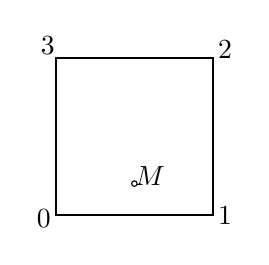
\begin{tikzpicture}
%\draw[step=0.5cm,gray,very thin] (0,0) grid (4,4); %background grid
\draw[thick] (1,1) -- (3,1) -- (3,3) -- (1,3) -- cycle;  
\node[] at (0.85,0.95) {0};
\node[] at (3.15,1) {1};
\node[] at (3.15,3.1) {2};
\node[] at (0.9,3.15) {3};
\node[] at (2.2,1.5) {$M$};
\draw (2.,1.4) circle (1pt);
\end{tikzpicture}\\
\end{center}


%..................................................
\paragraph{An intermediate case} We make the following assumption that the lateral sides of the  
element are vertical while the bottom and top are not necessarily horizontal:

\begin{center}
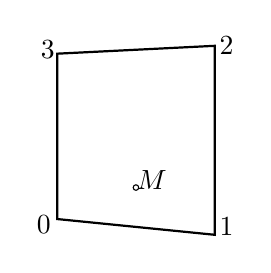
\begin{tikzpicture}
%\draw[step=0.5cm,gray,very thin] (0,0) grid (4,4); %background grid
\draw[thick] (1,1) -- (3,0.8) -- (3,3.2) -- (1,3.1) -- cycle;  
\node[] at (0.83,0.93) {0};
\node[] at (3.15,0.9) {1};
\node[] at (3.15,3.2) {2};
\node[] at (0.88,3.15) {3};
\node[] at (2.2,1.5) {$M$};
\draw (2.,1.4) circle (1pt);
\end{tikzpicture}\\
\end{center}

\noindent Because the sides are verical then if $x_0 \leq x_M \leq x_2$ then 
\[
r_M = \frac{2}{x_2-x_0}(x_M-x_0) -1 
\]
Then, if $M$ is inside the element then its $y$ coordinate is given by
\[
y_M = \sum_i \bN_i(r_M,s_M) y_i
\]
where $\bN_i$ are the four $Q_1$ basis functions associated to the vertices.
Assuming we know $r_M$ then we can solve for $s_M$:
\begin{eqnarray}
y_M &=&  
\frac{1}{4}(1-r_M)(1-s_M) y_0+
\frac{1}{4}(1+r_M)(1-s_M) y_1+
\frac{1}{4}(1+r_M)(1+s_M) y_2+
\frac{1}{4}(1-r_M)(1+s_M) y_3 \nn\\
&=& 
\frac{1}{4} \left[
(1-r)y_0+(1+r)y_1+(1+r)y_2+(1-r)y_3 +s_M [ -(1-r)y_0 - (1+r)y_1+(1+r)y_2+(1-r)y_3  ] 
\right] \nn 
\end{eqnarray}
or, 
\[
s_M = \frac{ 4y_M - [(1-r_M)y_0+(1+r_M)y_1+(1+r_M)y_2+(1-r_M)y_3]  }{ -(1-r_M)y_0 -(1+r_M)y_1+(1+r_M)y_2+(1-r_M)y_3 } 
\]
If the obtained value is in $[-1,1]$ then the point $M$ is in the element.
Verification: when $y_1=y_0$ and $y_2=y_3$ then 
\begin{eqnarray}
s_M 
&=& \frac{4 y_M - [(1-r_M)y_0+(1+r_M)y_0+(1+r_M)y_3+(1-r_M)y_3]  }{ -(1-r_M)y_0 - (1+r_M)y_0+(1+r_M)y_3+(1-r_M)y_3 } \nn\\
&=& \frac{4 y_M - [ 2 y_0 + 2 y_3]  }{ -2 y_0 + 2 y_3    }  \nn\\
&=& \frac{1}{y_3-y_0} [2 y_M - (  y_0 +  y_3) ] \nn\\ 
&=& \frac{1}{y_3-y_0} [2 y_M -  2 y_0 +y_0 -  y_3)  ] \nn\\ 
&=& \frac{2}{y_3-y_0} (y_M - y_0) - 1 
\end{eqnarray}
which is the expression that corresponds to a rectangular element as seen previously.

%..................................................
\paragraph{A generic quadrilateral}

We wish to arrive at a single algorithm which is applicable to all quadrilaterals and we now focus  
on an irregular quadrilateral (no face is parallel to the axis of the coordinate system). 

\begin{center}
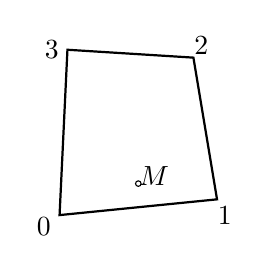
\begin{tikzpicture}
%\draw[step=0.5cm,gray,very thin] (0,0) grid (4,4); %background grid
\draw[thick] (1,1) -- (3,1.2) -- (2.7,3) -- (1.1,3.1) -- cycle;  
\node[] at (0.8,0.85) {0};
\node[] at (3.1,1) {1};
\node[] at (2.8,3.15) {2};
\node[] at (0.9,3.1) {3};
\node[] at (2.2,1.5) {$M$};
\draw (2.,1.4) circle (1pt);
\end{tikzpicture}\\
\end{center}

\noindent Several rather simple options exist:
\begin{itemize}
\item we could subdivide the quadrilateral into two triangles and check whether point $M$ is inside any of them (as it turns out, this problem is rather straightforward for triangles. Simply google it.)
\item We could check that point $M$ is always on the left side of segments $0\rightarrow 1$, $1\rightarrow 2$, $2\rightarrow 3$, $3\rightarrow 0$.
\item ...  
\end{itemize}

Any of these approaches will work although some might be faster than others. 
In three-dimensions all will however become 
cumbersome to implement and might not even work at all. 
Fortunately, there is an elegant way to answer the question, as 
detailed in the following subsection, which works both in 2D and 3D.

%-------------------------------------------
\subsubsection{Three-dimensional space}

If point $M$ is inside the quadrilateral, there exist a set of reduced 
coordinates $r,s,t\in[-1:1]^3$ such that 

\[
\sum_{i=1}^4 \bN_i(r_M,s_M,t_M) x_i = x_M
\quad\quad\quad
\sum_{i=1}^4 \bN_i(r_M,s_M,t_M) y_i = y_M
\quad\quad\quad
\sum_{i=1}^4 \bN_i(r_M,s_M,t_M) z_i = z_M
\]
This can be cast as a system of three equations and three unknowns. 
Unfortunately, each basis function $\bN_i$ 
contains a term $rst$ (as well as $rs$, $rt$, and $st$) 
so that it is not a linear system.
We must then use an iterative technique: the algorithm starts with 
a guess for values $r_M,s_M,t_M$ and 
improves on their value iteration after iteration. 
In what follows the subscript $M$ is dropped from $r,s,t$.

The classical way of solving nonlinear systems of equations is Newton's method. 
\index{general}{Newton's method}
We can rewrite the equations above as ${\bm F}(r,s,t)=0$:
\begin{eqnarray}
\sum_{i=1}^8 \bN_i(r,s,t) x_i - x_M&=&0 \nonumber\\
\sum_{i=1}^8 \bN_i(r,s,t) y_i - y_M&=&0 \nonumber\\
\sum_{i=1}^8 \bN_i(r,s,t) z_i - z_M&=&0
\end{eqnarray}
or,
\begin{eqnarray}
F_r(r,s,t)&=&0 \nonumber\\
F_s(r,s,t)&=&0 \nonumber\\
F_t(r,s,t)&=&0 \nonumber
\end{eqnarray}
so that we now have to find the zeroes of continuously differentiable 
functions ${\bm F}:\mathbb{R} \rightarrow \mathbb{R}$.
The recursion is simply:
\[
\left(
\begin{array}{c}
r_{k+1} \\s_{k+1} \\ t_{k+1}
\end{array}
\right)
=
\left(
\begin{array}{c}
r_{k} \\s_{k} \\ t_{k}
\end{array}
\right)
- J_F(r_k,s_k,t_k) ^{-1} 
\left(
\begin{array}{c}
F_r(r_k,s_k,t_k) \\
F_s(r_k,s_k,t_k)\\
F_t(r_k,s_k,t_k)
\end{array}
\right)
\]
where $J$ the Jacobian matrix:
\begin{eqnarray}
J_F(r_k,s_k,t_k)
&=&
\left(
\begin{array}{ccc}
\frac{\partial F_r}{\partial r}(r_k,s_k,t_k) & \frac{\partial F_r}{\partial s}(r_k,s_k,t_k) & \frac{\partial F_r}{\partial t}(r_k,s_k,t_k) \\\\
\frac{\partial F_s}{\partial r}(r_k,s_k,t_k) & \frac{\partial F_s}{\partial s}(r_k,s_k,t_k) & \frac{\partial F_s}{\partial t}(r_k,s_k,t_k) \\\\
\frac{\partial F_t}{\partial r}(r_k,s_k,t_k) & \frac{\partial F_t}{\partial s}(r_k,s_k,t_k) & \frac{\partial F_t}{\partial t}(r_k,s_k,t_k) 
\end{array}
\right) \nonumber\\
&=&
\left(
\begin{array}{ccc}
\sum\limits_{i=1}^8 \frac{\partial \bN_i}{\partial r}(r_k,s_k,t_k) x_i &
\sum\limits_{i=1}^8 \frac{\partial \bN_i}{\partial s}(r_k,s_k,t_k) x_i &
\sum\limits_{i=1}^8 \frac{\partial \bN_i}{\partial t}(r_k,s_k,t_k) x_i \\
\sum\limits_{i=1}^8 \frac{\partial \bN_i}{\partial r}(r_k,s_k,t_k) y_i &
\sum\limits_{i=1}^8 \frac{\partial \bN_i}{\partial s}(r_k,s_k,t_k) y_i &
\sum\limits_{i=1}^8 \frac{\partial \bN_i}{\partial t}(r_k,s_k,t_k) y_i \\
\sum\limits_{i=1}^8 \frac{\partial \bN_i}{\partial r}(r_k,s_k,t_k) z_i &
\sum\limits_{i=1}^8 \frac{\partial \bN_i}{\partial s}(r_k,s_k,t_k) z_i &
\sum\limits_{i=1}^8 \frac{\partial \bN_i}{\partial t}(r_k,s_k,t_k) z_i 
\end{array}
\right) \nonumber 
\end{eqnarray}
In practice, we solve the following system:
\[
J_F(r_k,s_k,t_k) 
\left[  
\left(
\begin{array}{c}
r_{k+1} \\s_{k+1} \\ t_{k+1}
\end{array}
\right)
-
\left(
\begin{array}{c}
r_{k} \\s_{k} \\ t_{k}
\end{array}
\right)
\right]=-
\left(
\begin{array}{c}
F_r(r_k,s_k,t_k) \\
F_s(r_k,s_k,t_k)\\
F_t(r_k,s_k,t_k)
\end{array}
\right)
\]
Finally, the algorithm goes as follows:
\begin{itemize}
\item set guess values for $r,s,t$ (typically 0)
\item loop over k=0,...
\item Compute rhs= $-{\bm F}(r_k,s_k,t_k)$ 
\item Compute matrix $J_F(r_k,s_k,t_k)$
\item solve system for $(dr_k,ds_k,dt_k)$
\item update $r_{k+1}=r_k+dr_k$, $s_{k+1}=s_k+ds_k$, $t_{k+1}=t_k+dt_k$ 
\item stop iterations when $(dr_k,ds_k,dt_k)$ is small
\item if $r_k,s_k,t_k\in[-1,1]^3$ then $M$ is inside.
\end{itemize}
This method converges quickly but involves iterations, and multiple 
solves of $3\times 3$ systems which, when carried out for each marker 
and at each time step can prove to be expensive. 
A simple modification can be added to the above algorithm: 
iterations should be carried out {\it only}
when the point $M$ is inside of a cuboid of 
size $[\min\limits_i{x_i}:\max\limits_i{x_i}]\times[\min\limits_i{y_i}:\max\limits_i{y_i} ]
\times[\min\limits_i{z_i}:\max\limits_i{z_i}]$ where the sums run over the vertices of the element. 
In 2D this translates as follows: only carry out Newton iterations when $M$ is inside the red rectangle!
\begin{center}
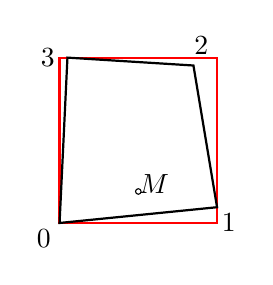
\begin{tikzpicture}
%\draw[step=0.5cm,gray,very thin] (0,0) grid (4,4); %background grid
\draw[thick,red] (1,1) -- (3,1) -- (3,3.1) -- (1,3.1) -- cycle;  
\draw[thick] (1,1) -- (3,1.2) -- (2.7,3) -- (1.1,3.1) -- cycle;  
\node[] at (0.8,0.8) {0};
\node[] at (3.15,1) {1};
\node[] at (2.8,3.25) {2};
\node[] at (0.85,3.1) {3};
\node[] at (2.2,1.5) {$M$};
\draw (2.,1.4) circle (1pt);
\end{tikzpicture}\\
\end{center}

Note that the algorithm above extends to high degree elements 
such as $Q_2$ and higher, even with curved sides.
As shown in the 2D case if the element is a cuboid or 
if all its lateral faces are vertical then one can 
compute the reduced coordinates without using an iterative method.


%-----------------------------------------------------
\subsubsection{Three-dimensional space - special case}

We assume that the mesh is such that the cross section of all $Q_1$ elements 
is a rectangle in the $xy$-plane. 

Let $(x,y,z)$ be a point inside the element. 
The global coordinates $x,y,z$ are obtained from the 
reduced coordinates $r,s,t$ via the basis the basis functions:
\begin{eqnarray}
x=\sum_{i=1}^8 \bN_i (r,s,t) x_i \qquad 
y=\sum_{i=1}^8 \bN_i (r,s,t) y_i  \qquad 
z=\sum_{i=1}^8 \bN_i (r,s,t) z_i \label{xyz}
\end{eqnarray}
Let 
\begin{eqnarray}
{\vec v}_1 &=& (+1,+1,+1,+1,+1,+1,+1,+1) \nn\\
{\vec v}_2 &=& (-1,+1,+1,-1,-1,+1,+1,-1) \nn\\
{\vec v}_3 &=& (-1,-1,+1,+1,-1,-1,+1,+1) \nn\\
{\vec v}_4 &=& (-1,-1,-1,-1,+1,+1,+1,+1) \nn\\
{\vec v}_5 &=& (+1,-1,+1,-1,+1,-1,+1,-1) \nn\\
{\vec v}_6 &=& (+1,-1,-1,+1,-1,+1,+1,-1) \nn\\
{\vec v}_7 &=& (+1,+1,-1,-1,-1,-1,+1,+1) \nn
\end{eqnarray}
and 
\begin{eqnarray}
{\vec x} &=& (x_1,x_2,x_3,x_4,x_5,x_6,x_7,x_8) \nn\\
{\vec y} &=& (y_1,y_2,y_3,y_4,y_5,y_6,y_7,y_8) \nn\\
{\vec z} &=& (z_1,z_2,z_3,z_4,z_5,z_6,z_7,z_8) \nn
\end{eqnarray}
then Eqs.~\eqref{xyz} can also be written
\begin{eqnarray}
x&=&\frac{1}{8} \left( {\vec v}_1 + r  {\vec v}_2 + s  {\vec v}_3 + t  {\vec v}_4 
                 + rs  {\vec v}_5 + rt {\vec v}_6 + st {\vec v}_7 \right) \cdot {\vec x} \nn\\ 
y&=&\frac{1}{8} \left( {\vec v}_1 + r  {\vec v}_2 + s  {\vec v}_3 + t  {\vec v}_4 
                 + rs  {\vec v}_5 + rt {\vec v}_6 + st {\vec v}_7 \right) \cdot {\vec y} \nn\\
z&=&\frac{1}{8} \left( {\vec v}_1 + r  {\vec v}_2 + s  {\vec v}_3 + t  {\vec v}_4 
                 + rs  {\vec v}_5 + rt {\vec v}_6 + st {\vec v}_7 \right) \cdot {\vec z} \label{zzz}
\end{eqnarray}
If the element has a rectangular cross-section $s_x \times s_y$ then 
\begin{eqnarray}
{\vec x} &=& (x_0,x_0+s_x,x_0+s_x,x_0,x_0,x_0+s_x,x_0+s_x,x_0) \nn\\
{\vec y} &=& (y_0,y_0,y_0+s_y,y_0+s_y,y_0,y_0,y_0+s_y,y_0+s_y) \nn
\end{eqnarray}
which yields
\begin{eqnarray}
r&=& 2\frac{x-x_0}{s_x}-1  \nn\\
s&=& 2\frac{y-y_0}{s_y}-1  \nn
\end{eqnarray}
Since the local coordinates $r$ and $s$ can be easily computed, one can use Eq.~\eqref{zzz} to obtain $t$:
\[
t=\frac{8z - ({\vec v}_1 + r {\vec v}_2 + s {\vec v}_3 + rs  {\vec v}_5 ) \cdot {\vec z}} 
{ ({\vec v}_4  + r  {\vec v}_6 + s  {\vec v}_7)  \cdot {\vec z} }
\]







 %---------
\newpage %-----------------------------------------------------------------------------------------
\section{Error measurements and convergence rates} \index{general}{$L_1$ norm}
\index{general}{$L_2$ norm}
\index{general}{$H^1$ norm}
\begin{flushright} {\tiny {\color{gray} errors.tex}} \end{flushright}

What follows is written in the case of a two-dimensional model. Generalisation to
3D is trivial. What follows is mostly borrowed from \cite{thmk14}.

When measuring the order of accuracy of the primitive variables $\vec{v}$ and $p$,
it is standard to report errors in both the $L_1$ and the $L_2$ norm.
For a scalar quantity $\Psi$, the $L_1$ and $L_2$ norms are computed as
\begin{equation}
\norm{\Psi}_1 = \int_V |\Psi| dV
\quad\quad
\quad\quad
\norm{\Psi}_2 = \sqrt{ \int_V \Psi^2 dV }
\end{equation}
For a vector quantity $\vec{k}=(k_x,k_y)$ in a two-dimensional space,
the $L_1$ and $L_2$ norms are defined as:
\begin{equation}
\norm{\vec{k}}_1 = \int_V (|k_x|+|k_y|) dV
\quad\quad
\quad\quad
\norm{\vec{k}}_2 = \sqrt{ \int_V (k_x^2+k_y^2) dV }
\end{equation}
To compute the respective norms
the integrals in the above norms can be approximated by splitting them
into their element-wise contributions. The element volume integral can then
be easily computed by numerical integration using Gauss-Legendre quadrature.

The respective $L_1$ and $L_2$ norms for the pressure error can be evaluated via
\begin{equation}
e_p^h|_1 = \sum_{i=1}^{n_e} \sum_{q=1}^{n_q} |e_p^h(\vec{r}_q)| w_q |J_q|
\quad\quad
\quad\quad
e_p^h|_2=\sqrt{ \sum_{i=1}^{n_e} \sum_{q=1}^{n_q} |e_p^h(\vec{r}_q)|^2 w_q |J_q| }
\end{equation}
where $e_p^h(\vec{r}_q)=p^h(\vec{r}_q) - p(\vec{r}_q)$ 
is the pressure error evaluated at the $q$-th quadrature associated with
the $i$th element. $n_e$ and $n_q$ refer to the number of elements and
the number of quadrature points per element.
$w_q$ and $J_q$ are the quadrature weight and the Jacobian associated with
point $q$.

The velocity error $e_{\vec v}^h$ is evaluated using the following two norms
\begin{equation}
e_{\vec{v}}^h|_1 = \sum_{i=1}^{n_e} \sum_{q=1}^{n_q} [ |e_u^h(\vec{r}_q)| + |e_v^h(\vec{r}_q)| ]    w_q |J_q|
\quad\quad
\quad\quad
e_{\vec v}^h|_2=\sqrt{ \sum_{i=1}^{n_e} \sum_{q=1}^{n_q} \left[ |e_u^h({\bm r}_q)|^2 +  e_v^h({\bm r}_q)|^2 \right] w_q |J_q| }
\end{equation}
where $e_u^h(\vec{r}_q)=u^h(\vec{r}_q) - u(\vec{r}_q)$ and $e_v^h(\vec{r}_q)=v^h(\vec{r}_q)-v(\vec{r}_q)$.


\index{general}{$H^1(\Omega)$ space} 
\index{general}{$H^1$ norm} 
\index{general}{$H^1$ semi-norm}
Another norm is very rarely used in the geodynamics literature but is preferred in the 
Finite Element literature: the $H^1$ norm. The mathematical basis for this
norm and the nature of the $H^1(\Omega)$ Hilbert space is to be found in many FE books \cite{dohu03,john16,hugh}.
This norm is expressed as follows for a function $f$ such that $f,|\nabla f|\in L^2(\Omega)$
\footnote{\url{https://en.wikipedia.org/wiki/Sobolev_space}}
\begin{equation}
\norm{f}_{H^1} = \left( \int_\Omega ( |f|^2 + |\nabla f|^2  ) d\Omega   \right)^{1/2}
\end{equation}
We then have 
\begin{equation}
e_{\vec v}^h|_{H^1} = \norm{\vec{v}^h-\vec{v}}_{H^1} = \sqrt{
\sum\limits_{i=1}^d 
\int_\Omega  
\left[
({v}_i^h-{v}_i)^2
+
\vec\nabla(v_i^h-v_i)\cdot\vec\nabla(v_i^h-v_i) 
\right] d\Omega   
}
\end{equation}
where $d$ is the number of dimensions.
Note that sometimes the following semi-norm is used \cite{dobo04,bodg06}:
\begin{equation}
e_{\vec v}^h|_{H^1} = \norm{\vec{v}^h-\vec{v}}_{H^1} = \sqrt{
\sum\limits_{i=1}^d 
\int_\Omega  
\left[
\vec\nabla(v_i^h-v_i)\cdot\vec\nabla(v_i^h-v_i) 
\right] d\Omega   
}
\end{equation}

When computing the different error norms for $e_p$ and $e_{\vec v}$ for a set of numerical experiments with
varying resolution $h$ we expect the error norms to follow the following relationships:
\begin{equation}
e_{\vec v}^h|_1 = C h^{rvL_1} 
\quad\quad\quad\quad
e_{\vec v}^h|_2 = C h^{rvL_2} 
\quad\quad\quad\quad 
e_{\vec v}^h|_{H^1} = C h^{rvH^1}
\end{equation}
\begin{equation}
e_p^h|_1 = C h^{rpL_1} 
\quad\quad\quad 
e_p^h|_2 = C h^{rpL_2}
\end{equation}
where $C$ is a resolution-independent constant
and $rpXX$ and $rvXX$ are the convergence rates for
pressure and velocity in various norms, respectively. 
Using linear regression on the logarithm of the respective error norm and the resolution $h$,
one can compute the convergence rates of the numerical solutions.

As mentioned in \cite{dobo04}, when finite element solutions converge at
the same rates as the interpolants we say that the method is optimal, i.e.:
\index{general}{optimal rate}

\begin{equation}
e_{\vec v}^h|_{L_2} = {\cal O}(h^3)
\quad\quad\quad\quad
e_{\vec v}^h|_{H^1} = {\cal O}(h^2)
\quad\quad\quad\quad
e_{p}^h|_{L_2} = {\cal O}(h^2)
\end{equation}

%\begin{itemize}
%\item For $Q_1P_0$, the theoretical lower bound for $r_v'$ is 2 and for $r_p'$ it is 1
%\item For $Q_2P_{-1}$, the theoretical lower bound for $r_v'$ is 3 and for $r_p'$ it is 2
%\end{itemize}
We note that when using discontinuous pressure space
(e.g., $P_0$, $P_{-1}$), these bounds remain valid even
when the viscosity is discontinuous provided that the element boundaries conform to the discontinuity.

%------------------------------------------------------------------------------ 
\subsubsection{About extrapolation}\label{ss:extrapolation}
\index{general}{Extrapolation}

Section contributed by W. Bangerth and part of \textcite{thba22} (2022) 
but it was ultimately not used. 

In a number of numerical benchmarks we
want to estimate the error $X_h-X^\ast$ between a quantity $X_h$ computed
from the numerical solution $\vec{\upnu}_h,p_h$ and the corresponding value
$X$ computed from the exact solution $\vec{\upnu},p$. Examples of such quantities
$X$ are the root mean square velocity $\upnu_{rms}$, but it could also be a mass flux
across a boundary, an average horizontal velocity at the top boundary, or
any other scalar quantity.

If the exact solution is known, then one can of course compute $X$ from it.
On the other hand, we would of course like to assess convergence also in
cases where the exact solution is not known. In that case, one can compute
an \textit{estimate} $X^\ast$ for $X$ by way of \textit{extrapolation}.
To this end, we make the assumption that asymptotically, $X_h$ converges to
$X$ at a fixed (but unknown) rate $r$, so that
\begin{equation}
  \label{eq:extrapolation-1}
  e_h=|X_h-X| \approx C h^r.
\end{equation}
Here, $X$, $C$ and $r$ are all unknown constants to be determined, although
we are not really interested in $C$.
We can evaluate $X_h$ from the numerical solution
on successively refined meshes with mesh sizes $h$, $h/2$, and $h/4$. Then,
in addition to \eqref{eq:extrapolation-1} we also have
\begin{eqnarray}
  \label{eq:extrapolation-2}
  e_{h/2}=|X_{h/2}-X| \approx C \left(\frac h2\right)^r,
  \\
  \label{eq:extrapolation-3}
  e_{h/4} =|X_{h/4}-X| \approx C \left(\frac h4\right)^r.
\end{eqnarray}
Taking ratios of equations \eqref{eq:extrapolation-1}--\eqref{eq:extrapolation-3},
and replacing the unknown $X$ by an \textit{estimate} $X^\ast$, we then
arrive at the following equation:
\begin{equation*}
\frac{|X_h-X^\star|}{|X_{h/2}-X^\star|}
=
\frac{|X_{h/2}-X^\star|}{|X_{h/4}-X^\star|}=2^r.
\end{equation*}
If one assumes that $X_h$ converges to $X$ uniformly either from above or
below (rather than oscillate around $X$), then this equation allows us
to solve for $X^\ast$ and $r$:

\[
(X_h-X^\star)(X_{h/4}-X^\star)=(X_{h/2}-X^\star)(X_{h/2}-X^\star)
\]

\[
X_h X_{h/4} -X^\star  X_{h/4} - X_h X^\star  + (X^\star)^2
=X_{h/2}^2 -2 X^\star X_{h/2} + (X^\star)^2 
\]

\[
X_h X_{h/4} -X^\star  X_{h/4} - X_h X^\star 
=X_{h/2}^2 -2 X^\star X_{h/2} 
\]

\[
X_h X_{h/4} -X_{h/2}^2 =-2 X^\star X_{h/2} +X^\star  X_{h/4} + X_h X^\star 
\]

\[
X_h X_{h/4} -X_{h/2}^2  = X^\star ( -2  X_{h/2}  +   X_{h/4} + X_h )
\]

and finally:
\begin{equation*}
X^\star = \frac{X_h X_{h/4}-X_{h/2}^2}{X_h - 2 X_{h/2} + X_{h/4}}, \qquad\qquad
r = \log_2 \frac{X_{h/2}-X^\star}{X_{h/4}-X^\star}.
\end{equation*}
In the determination of $r$, we could also have used $X_h$ and $X_{h/2}$,
but using $X_{h/2}$ and $X_{h/4}$ is generally more reliable because
the higher order terms we have omitted in \eqref{eq:extrapolation-1} are less
visible on finer meshes.

In some cases, however, halving the mesh size multiple times 
is not really tractable (memory problem, or cpu time).
Let us now start again from 
\begin{equation}
  e_h=|X_h-X| \approx C h^r.
\end{equation}
and assume that we run two other models at a resolution $\alpha h$
and $\beta h$, such that $1>\alpha>\beta>0$. 
In the example above we of course had $\alpha=1/2$ and $\beta=1/4$.
Then we have 
\begin{eqnarray}
e_{\alpha h}=|X_{\alpha h}-X| \approx C \left(\alpha h\right)^r,  \\
e_{\beta  h}=|X_{\beta h} -X| \approx C \left(\beta  h\right)^r.
\end{eqnarray}
which leads to 
\begin{equation*}
\frac{|X_h-X^\star|}{|X_{\alpha h}-X^\star|}
= \frac{C h^r}{C (\alpha h)^r} = (1/\alpha)^{r}
\qquad
\text{and}
\qquad
\frac{|X_{\alpha h}-X^\star|}{|X_{\beta h}-X^\star|}
= \frac{C (\alpha h)^r}{C(\beta h)^r} = (\alpha/\beta)^r
\end{equation*}
In order for both to be equal we must have
\[
(1/\alpha)^{r} = (\alpha/\beta)^r
\qquad
\Rightarrow
\qquad
1/\alpha = \alpha/\beta
\qquad
\Rightarrow
\qquad
\beta=\alpha^2
\]
So of course if $\alpha=1/2$ then $\beta=1/4$, but now we can also take 
$\alpha=3/4$ and then $\beta=9/16$. Etc ...

In the end, this approach might not be that useful since the mesh sizes would
then be $h,3h/4,9h/16,27h/64,...$ which may be hard to achieve in practice.

 %-----------------------------
\newpage %-----------------------------------------------------------------------------------------
\section{The initial temperature field} 
\Literature: 
\begin{itemize}
\item
Thermal gradients in the continental crust \cite{chap86}
\item
Simple analytical approximation to the temperature structure in
subduction zones \cite{enwi04}
\item 
Thermal structure of subduction zone back arcs \cite{cuhy06}
\item 
Thermal Structure of Oceanic Lithosphere \cite{rihc18}
\item thermal structure of a subducting plate with finite length \cite{hstt90}
\end{itemize}


%.............................................................
\subsubsection{Single layer with imposed temperature b.c.}

Let us take a single layer of material characterised by
a heat capacity $C_p$, a heat conductivity $k$
and a heat production term $H$.

\begin{center}
\includegraphics[width=5cm]{images/initial_temperature/tempcond.png}
\end{center}

The Heat transport equation writes
\begin{equation}
\rho C_p \left( \frac{\partial T}{\partial t} + {\vec v} \cdot {\vec \nabla} { T} \right) = 
{\vec \nabla} \cdot (k {\vec \nabla} T) + \rho H
\end{equation}
At steady state and in the absence of a velocity field, assuming
that the material properties to be independent of time and space, and 
assuming that
there is no heat production ($H=0$), this equation
simplifies to
\begin{equation}
\Delta T =0 
\end{equation}
Assuming the layer to be parallel to the $x$-axis, the temperature is
$T(x,y)=T(y)=\alpha T+ \beta$. 
In order to specify the constants $\alpha$ and $\beta$, we need two constraints.

At the bottom of the layer $y=y_b$ a temperature $T_b$ is prescribed while a temperature
$T_t$ is prescribed at the top with $y=y_t$. This ultimately yields a temperature field in
the layer given by
\begin{mdframed}[backgroundcolor=blue!5]
\[
T(y) = \frac{T_t-T_b}{y_t-y_b}(y-y_b) + T_b
\]
\end{mdframed}

If now the heat production coefficient is not zero, the differential equation
reads
\begin{equation}
 k \Delta T + H = 0 
\end{equation}
The temperature field is then expected to be of the form
\begin{equation}
T(y)= - \frac{H}{2k} y^2 + \alpha y + \beta 
\end{equation}
Supplied again with the same boundary conditions, this leads to
\[
\beta=T_b + \frac{H}{2k} y_b^2 - \alpha y_b
\]
ie,
\[
T(y) = -\frac{H}{2k} (y^2-y_b^2) + \alpha (y-y_b) + T_b
\]
and finally
\[
\alpha =  \frac{T_t-T_b}{y_t-y_b}  + \frac{H}{2k}(y_b+y_t)
\]
or,
\[
T(y) = -\frac{H}{2k} (y^2-y_b^2) + \left( \frac{T_t-T_b}{y_t-y_b}  + \frac{H}{2k}(y_b+y_t)   \right) (y-y_b) + T_b
\]

Taking $H=0$ in this equation obviously yields the temperature field obtained previously.
Taking $k=2.25$, $T_t=0C$, $T_b=550C$, $y_t=660km$, $y_b=630km$ yields the following
temperature profiles and heat fluxes when the heat production $H$ varies:
\begin{center}
\includegraphics[width=5cm]{images/initial_temperature/temperature1.pdf}
\includegraphics[width=5cm]{images/initial_temperature/heatflux1.pdf}
\end{center}
Looking at the values at the top, which are somewhat estimated to be
about $55-65mW/m^2$ \cite[table 8.6]{jama}, one sees that value $H=0.8e-6$ yields a very acceptable
heat flux.
Looking at the bottom, the heat flux is then about $0.03W/m^2$
which is somewhat problematic since the heat flux at the Moho
is reported to be somewhere between 10 and 20 $mW/m^2$ in \cite[table 7.1]{jama}.


%-----------------------------------------------------
\subsubsection{Single layer with imposed heat flux b.c.}

Let us now assume that heat fluxes are imposed at the top and bottom of the layer:
\begin{center} 
\includegraphics[width=5cm]{images/initial_temperature/tempcond2.png}
\end{center}

We start again from the ODE
\[
k \Delta T + H = 0 
\]
but only integrate it once:
\[
k \frac{dT}{dy}  + H y + \alpha  = 0 
\]
At the bottom $q=k(dT/dy)|_{y=y_b} = q_b$ and at the top
$q=k(dT/dy)|_{y=y_t} = q_t$ so that 

\todo[inline]{to finish}


 
%-----------------------------------------------------
\subsubsection{Single layer with imposed heat flux and temperature b.c. }

\begin{center}
\includegraphics[width=5cm]{images/initial_temperature/tempcond3.png}
\end{center}

\todo[inline]{to finish}


%---------------------------------------------------------------
\subsubsection{Half cooling space}

TODO. 

\Literature \cite{fagm12} 

%---------------------------------------------------------------
\subsubsection{Plate model}

\cite{mcke67}

%.................................
\subsubsection{McKenzie slab}

When doing thermo-mechanical modelling, the initial temperature
field in the domain is of prime importance. This is 
especially true for the temperature in the slab for subduction 
modelling as its rheological behaviour is strongly temperature-dependent. 
One could easily design a simple geometrical initial field but it is 
unlikely to be close to the field of a slowly subducting slab at an angle 
in a hot mantle. 

McKenzie \cite{mcke69} derived such approximate initial field from the 
steady-state energy equation in two dimensions:
\begin{equation}
\rho C_p \vec v \cdot \vec\nabla T = k \vec\nabla^2 T
\end{equation}
We denote by $T_l$ the temperature at the base of the lithosphere
and $l$ its thickness (i.e. the thickness of the slab).

Assuming $\vec v=(v_x,0)$ yields
\[
\rho C_p v_x \frac{\partial T}{\partial x} = k \frac{\partial^2 T}{\partial x^2}
\]
and substitution of $T'=T/T_l$, $x'=x/l$ and $z'=z/l\in[0,1]$ in this equation leads to
\[
\rho C_p v_x \frac{T_l}{l}\frac{\partial T'}{\partial x'} = k \frac{T_l}{l^2}
\left( \frac{\partial^2 T'}{\partial x'^2}
+ \frac{\partial^2 T'}{\partial z'^2} \right)
\]
or 
\[
\frac{\rho C_p v_x l }{k}\frac{\partial T'}{\partial x'} = 
\frac{\partial^2 T'}{\partial x'^2}
+ \frac{\partial^2 T'}{\partial z'^2} 
\]
and finally (see Eq. 2.3 of \cite{mcke69}): 
\[
\frac{\partial^2 T'}{\partial x'^2}
- 2 R \frac{\partial T'}{\partial x'} 
+ \frac{\partial^2 T'}{\partial z'^2} =0
\]
where $R$ is the thermal Reynolds number
\[
R=\frac{\rho C_p v_x l}{2 k}
\] 
The general solution to this PDE with $T'=1$ on the top, left and right boundary is 
\[
T'(x',z')= 1 + \sum_n C_n \exp \left[ \left( R-(R^2+n^2\pi^2)^{1/2} \right) x' \right] \sin (n \pi z')
\]
We now must make an assumption about the temperature on the left boundary ($x'=0$), 
which is the temperature of the lithosphere. 
For simplicity McKenzie assumes that $T'(x'=0,z')=1-z'$ so that $C_n=2(-1)^n/n\pi$ and finally
\begin{mdframed}[backgroundcolor=blue!5]
\begin{equation}
T'(x',z')= 1 + 2\sum_n \frac{(-1)^n}{n \pi} \exp \left[ \left( R-(R^2+n^2\pi^2)^{1/2} \right) x' \right] \sin (n \pi z')
\end{equation}
\end{mdframed}

Let us build a simple temperature model for a $250\text{km}\times 50\text{km}$ slab, 
with $\rho=3000$, $C_p=1250$, $k=3$. The python code is available in {\tt images/mckenzie/mckenzie1.py}.

\begin{center}
\includegraphics[width=0.32\textwidth]{images/mckenzie/temperature_vel0p5.pdf}
\includegraphics[width=0.32\textwidth]{images/mckenzie/temperature_vel1.pdf}
\includegraphics[width=0.32\textwidth]{images/mckenzie/temperature_vel2.pdf}\\
{\captionfont Left to right: Dimensionless temperature $T'$ in a $250\text{km}\times 50\text{km}$ slab 
for $v_x={0.5,1,2}\text{cm/year}$}
\end{center}

We logically recover the fact that the slower the slab penetrates the mantle the more 
temperature diffusion dominates over temperature advection. For $v=0.5\text{cm/year}$ we see that 
that the slab assumes a constant temperature $T'=1$ at all depthes $0\leq z' \leq 1$ for 
$x'\geq 125\text{km}$. 

Note that this field is a steady-state field, valid for a constant density, heat conductivity and 
heat capacity, zero heat production, that it implies that the velocity is constant and that the 
lithosphere temperature is linear. 

One can also embed the slab in a more realistic context, a subduction zone, involving a 
subducting lithosphere, an over-riding plate and a mantle. The domain is $1000\text{km}\times 250\text{km}$.
The mantle temperature is set to $1300~\si{\celsius}$. The slab dip can be varied and so can the 
velocity. The python code is available in {\tt images/mckenzie/mckenzie2.py}.

\begin{center}
\includegraphics[width=0.32\textwidth]{images/mckenzie/temperature2_vel0p5_phi30.pdf}
\includegraphics[width=0.32\textwidth]{images/mckenzie/temperature2_vel1_phi30.pdf}
\includegraphics[width=0.32\textwidth]{images/mckenzie/temperature2_vel2_phi30.pdf}\\
{\captionfont Left to right: temperature $T$ for $v_x={0.5,1,2}\text{cm/year}$ and $\phi=30\degree$.}
\end{center}

\begin{center}
\includegraphics[width=0.32\textwidth]{images/mckenzie/temperature2_vel1_phi15.pdf}
\includegraphics[width=0.32\textwidth]{images/mckenzie/temperature2_vel1_phi30.pdf}
\includegraphics[width=0.32\textwidth]{images/mckenzie/temperature2_vel1_phi45.pdf}\\
{\captionfont Left to right: temperature $T$ for $v_x=1\text{cm/year}$ and $\phi={15,30,45}\degree$.}
\end{center}




%\newpage

%From \cite{mcke70}, Eq. 26:
%\[
%T(r_0) = \theta_1 \exp \left(  \frac{\alpha g}{C_p} (r_1-r_0) \right)
%\]
%where $\theta_1$ is the potential temperature of any piece of the mantle 
%at the earth's surface.
%If $x$ is measured from a depth equal to the thickness of the lithosphere down the
%dip of the slab and $z$ is measured along the normal to the slab from its lower 
%surface, then the dimensionless potential temperature in the slab is 
%\begin{eqnarray}
%\theta'(x',z')
%&=& 1+2\frac{\theta_1-273}{\theta_1} \sum_{n=1}^\infty \frac{(-1)^n}{n \pi}
%\exp \left[ \left( R-(R^2+n^2\pi^2)^{1/2} \right) x' \right] \sin n\pi z' \\
%&=& \frac{1}{\theta_1} \left\{ \theta_1+ 2 (\theta_1-273) \sum_{n=1}^\infty \frac{(-1)^n}{n \pi}
%\exp \left[ \left( R-(R^2+n^2\pi^2)^{1/2} \right) x' \right] \sin n\pi z' \right\}
%\end{eqnarray}
%where $\theta' = \theta/\theta_1$, $x'=x/l$, $z'=z/l$ and 
%with $l$ the thickness of the slab and $v$ its velocity measured down its dip.
%We denote by $\phi$ the dip of the slab so that the depth below the surface $r_1-r_0$ is given by
%$l (x' \sin \phi-z' \cos\phi)$ so that 
%\[
%T(r_0) = \theta_1 \exp \left(  \frac{\alpha g}{C_p} l (x' \sin \phi-z' \cos\phi) \right)
%\]
%The dimensionless scale height $h'$ is defined by $h'=C_p/\alpha g l$ so that
%\[
%T(r_0) = \theta_1 \exp \left[  (x' \sin \phi-z' \cos\phi)/h' \right]
%\]

%Finally,
%\[
%T(x',z')=\exp \left[  (x' \sin \phi-z' \cos\phi)/h' \right] 
%\left\{ \theta_1+ 2 (\theta_1-273) \sum_{n=1}^\infty \frac{(-1)^n}{n \pi}
%\exp \left[ \left( R-(R^2+n^2\pi^2)^{1/2} \right) x' \right] \sin n\pi z' \right\}
%\]

%\todo[inline]{BSc: create mckenzie slab temperature setup}

%......................................................................
\subsubsection{Initial temperature for global mantle convection models}

This is a difficult topic, and Gottschaldt \etal \cite{gows09} list a few issues or 
facts to take into account:
\begin{itemize}
\item Frequent  impacts  may  have  determined  the  heat structure of the outer layers (Arrhenius and Lepland 2000), leading to an early thermally stable stratification. 
\item A global magma ocean (Solomatov 2000)  or  several  large  scale  melting events  (Kleine \etal. 2004)  
are also conceivable. 
\item Fractional crystallisation and subsequent overturn has the potential to result in 
compositionally or thermally stable layering, too (Elkins-Tanton \etal 2003; Zaranek and Parmentier 2004)
\end{itemize}


 %---------------------------
\newpage %-----------------------------------------------------------------------------------------
\section{Kinematic boundary conditions}\label{kin_bc} \index{general}{Essential Boundary Conditions}
\index{general}{Natural Boundary Conditions}
\begin{flushright} {\tiny {\color{gray} kinematic\_bc.tex}} \end{flushright}


\begin{center}
\includegraphics[width=8cm]{images/boundary_conditions/bc1}
\end{center}


\begin{center}
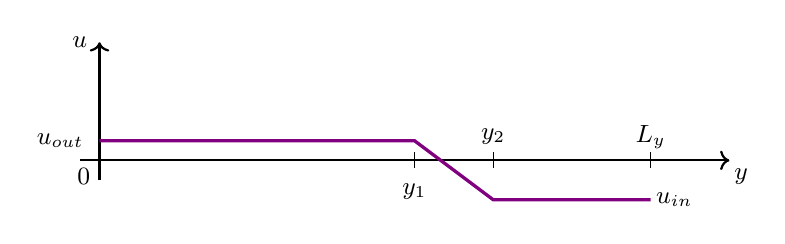
\begin{tikzpicture}
%\draw[fill=gray!23,gray!23](0,0) rectangle (10,3);
%\draw[step=0.5cm,gray,very thin] (0,0) grid (10,3); %background grid
\draw[thick,->] (0.75,1) -- (9,1)  ; 
\draw[thick,->] (1,0.75) -- (1,2.5)  ; 
\draw[-] (5,0.9) -- (5,1.1)  ; 
\draw[-] (6,0.9) -- (6,1.1)  ; 
\draw[-] (8,0.9) -- (8,1.1)  ; 
\draw[very thick, violet] (1,1.25)--(5,1.25) -- (6,0.5) -- (8,0.5) ; 
\node[] at (0.8,0.8) {\small $0$};
\node[] at (9.15,0.8) {\small $y$};
\node[] at (5,0.6) {\small $y_1$};
\node[] at (6,1.3) {\small $y_2$};
\node[] at (8,1.3) {\small $L_y$};
\node[] at (8.3,0.5) {\small $u_{in}$};
\node[] at (0.5,1.25) {\small $u_{out}$};
\node[] at (0.75,2.5) {\small $u$};
\end{tikzpicture}
\end{center}



The velocity on the side is given by
\begin{eqnarray}
u(y) &=& u_{out} \quad\quad y<y_1 \nn\\
u(y) &=& \frac{u_{in}-u_{out}}{y_2-y_1}(y-y_1) + u_{out} \quad\quad y_1<y<y_2 \nn\\
u(y) &=& u_{in} \quad\quad y>y_2 \nn
\end{eqnarray}
Note that $u_{in}$ and $u_{out}$ can be positive or negative, but 
of opposite signs.
The requirement for volume conservation is:
\[
\Phi=\int_{0}^{L_y} u(y) dy = 0
\]
Having chosen $u_{in}$ (the velocity of the plate), one can then compute $v_{out}$
as a function of $y_1$ and $y_2$.

\begin{eqnarray}
\Phi
&=&
\underbrace{\int_{0}^{y_1} u(y) dy}_{\Phi_1}  +
\underbrace{\int_{y_1}^{y_2} u(y) dy }_{\Phi_2}  +
\underbrace{\int_{y_2}^{L_y} u(y) dy }_{\Phi_3}\nn
\end{eqnarray}
with
\begin{eqnarray}
\Phi_1 &=& u_{out} y_1 \nn\\
\Phi_2 
&=& \int_{y_1}^{y_2} u(y) dy \nn\\
&=& \int_{y_1}^{y_2} \left[ \frac{u_{in}-u_{out}}{y_2-y_1}(y-y_1) + u_{out}   \right] dy \nn\\
&=& \int_{y_1}^{y_2} \frac{u_{in}-u_{out}}{y_2-y_1}(y-y_1)  dy  +   \int_{y_1}^{y_2}  u_{out} dy \nn\\
&=& \frac{u_{in}-u_{out}}{y_2-y_1} \int_{y_1}^{y_2} (y-y_1)  dy  +   (y_2-y_1) u_{out}  \nn\\
&=& \frac{u_{in}-u_{out}}{y_2-y_1} \left[ \frac12 y^2 - y_1y   \right]_{y_1}^{y_2} +   (y_2-y_1) u_{out}  \nn\\
&=& \frac{u_{in}-u_{out}}{y_2-y_1} ( \frac12 y_2^2 - y_1y_2 - \frac12y_1^2 + y_1^2 ) +   (y_2-y_1) u_{out}  \nn\\
&=& \frac{u_{in}-u_{out}}{y_2-y_1} \frac12 ( y_2^2 - 2y_1y_2 + y_1^2 ) +   (y_2-y_1) u_{out}  \nn\\
&=& \frac{u_{in}-u_{out}}{y_2-y_1} \frac12 ( y_2-y_1 )^2 +   (y_2-y_1) u_{out}  \nn\\
&=& (u_{in}-u_{out}) \frac12 ( y_2-y_1 ) +   (y_2-y_1) u_{out}  \nn\\
&=& \frac{1}{2}(u_{in}+u_{out})(y_2-y_1)  \nn\\
\Phi_3 &=& (L_y-y_2) u_{in} \nn
\end{eqnarray}
so that in the end
\begin{eqnarray}
\Phi &=& \Phi_1+\Phi_2+\Phi_3 \nn\\
&=& u_{out} [y_1 + \frac{1}{2}(y_2-y_1) ] + u_{in} [ \frac{1}{2}(y_2-y_1)  + (L_y-y_2) ] \nn\\
&=& u_{out}\frac{1}{2} (y_1 + y_2 ) + u_{in} [ L_y - \frac{1}{2}(y_1+y_2) ] \nn
\end{eqnarray}
and finally, solving for $u_{out}$
\begin{mdframed}[backgroundcolor=blue!5]
\[
u_{out} = -u_{in} \frac{ L_y - \frac{1}{2}(y_1+y_2)}{ \frac{1}{2} (y_1 + y_2 ) }
\]
\end{mdframed}


In some cases one may wish to prescribe a zero velocity 
below the 660 discontinuity (given by $y=y_1$) on the following 
figure:

\begin{center}
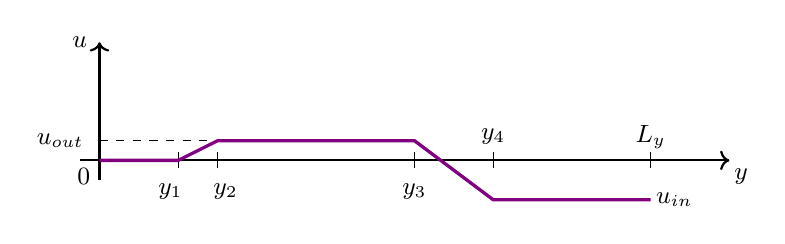
\begin{tikzpicture}
%\draw[fill=gray!23,gray!23](0,0) rectangle (10,3);
%\draw[step=0.5cm,gray,very thin] (0,0) grid (10,3); %background grid
\draw[thick,->] (0.75,1) -- (9,1)  ; 
\draw[thick,->] (1,0.75) -- (1,2.5)  ; 
\draw[-] (2,0.9) -- (2,1.1)  ; 
\draw[-] (2.5,0.9) -- (2.5,1.1)  ; 
\draw[-] (5,0.9) -- (5,1.1)  ; 
\draw[-] (6,0.9) -- (6,1.1)  ; 
\draw[-] (8,0.9) -- (8,1.1)  ; 
\draw[thin, dashed] (1,1.25) -- (2.5,1.25)  ; 
\draw[very thick, violet] (1,1)--(2,1)--(2.5,1.25)--(5,1.25) -- (6,0.5) -- (8,0.5) ; 
\node[] at (0.8,0.8) {\small $0$};
\node[] at (9.15,0.8) {\small $y$};
\node[] at (1.9,0.6) {\small $y_1$};
\node[] at (2.6,0.6) {\small $y_2$};
\node[] at (5,0.6) {\small $y_3$};
\node[] at (6,1.3) {\small $y_4$};
\node[] at (8,1.3) {\small $L_y$};
\node[] at (8.3,0.5) {\small $u_{in}$};
\node[] at (0.5,1.25) {\small $u_{out}$};
\node[] at (0.75,2.5) {\small $u$};
\end{tikzpicture}
\end{center}

 %--------------------
\newpage %-----------------------------------------------------------------------------------------
\section{Computing gradients - the recovery process} \begin{flushright} {\tiny {\color{gray} \tt recovery.tex}} \end{flushright}
%~~~~~~~~~~~~~~~~~~~~~~~~~~~~~~~~~~~~~~~~~~~~~~~~~~~~~~~~~~~~~~~~~~~~~~~~~~~~~~~~~~~~~~~~~~~~~~~~~~

write about recovering accurate strain rate components and heat flux components on the nodes.

Let $\vec g(\vec r)$  be the desired nodal 
field which we want to be the continuous (for example $Q_1$) 
representation of the field $\vec \nabla f^h$.
Since the derivative of the basis function does not uniquely exist on the nodes we need to design
an algorithm to do so. This problem is well known and has been investigated 
\todo{refs!}.
The main standard techniques are listed hereafter.

\Literature: check \fullcite{zibz98}

%..............................
\subsubsection{Global recovery}

The global recovery approach is rather simple: we wish to find $\vec g^h$
such that it satisfies
\[
\int_\Omega \phi \vec g^h \; d\Omega  = \int_\Omega \phi \vec\nabla f^h \; d\Omega 
\quad\quad \forall \phi
\] 
We will then successively replace $\phi$ by all the basis functions $N_i$ 
and since we have $g^h=\sum_j N_i g_i$ we then obtain
\[
\sum_j \int N_i N_j d\Omega g_i = \int N_i  \vec\nabla f^h \; d\Omega 
\]
or, 
\[
\mathbb{M} \cdot \vec{\cal G} = \vec f
\]



%..................................................
\subsubsection{Local recovery - centroid average over patch}





%..................................................
\subsubsection{Local recovery - nodal average over patch}

Let $j$ be the node at which we want to compute $\vec g$.
Then 
\[
\vec g_j = \vec g(\vec r_j) = 
\frac{\sum\limits_{ e \text{ adj. to }j} |\Omega_e| (\vec\nabla f)_e(\vec r_j) }{\sum |\Omega_e|}
\]
where $|\Omega_e|$ is the volume of the element and $(\vec\nabla f^h)_e(\vec r_j)$
is the gradient of $f$ as obtained with the basis functions inside element $e$ and 
computed at location $\vec r_j$.

%........................................................
\subsubsection{Local recovery - least squares over patch}



%........................................................
\subsubsection{Link to pressure smoothing}

When the penalty method is used to solve the Stokes equation, the pressure
is then given by $p=-\lambda \vec\nabla \cdot \vec v$. As explained in 
section \ref{sec:penalty}, the velocity is first obtained and the pressure 
is recovered by using this equation as a postprocessing step. Since the divergence 
cannot be computed easily at the nodes, the pressure is traditionally computed 
in the middle of the elements, yielding an elemental pressure field (remember, 
we are talking about $Q_1P_0$ elements here -- bi/tri-linear velocity, discontinuous
constant pressure)


 %-------------------------
\newpage %-----------------------------------------------------------------------------------------
\section{Tracking materials and/or interfaces} \begin{flushright} {\tiny {\color{gray} \tt tracking.tex}} \end{flushright}

Unless using a fully Lagrangian formulation, one needs an additional numerical method to represent/track
the various materials present in an undeformable (Eulerian) mesh.
The figure below (by B. Hillebrand) illustrates the three main methods used in geodynamics.

\begin{center}
\includegraphics[width=15cm]{images/tracking/tracking}
\end{center}

Note that what follows is applicable to FEM, FDM, etc ...

A typical test for advection algorithm is the Zalesak disk \cite{zale79}. It is a two dimensional test 
problem of solid body rotation with a constant angular velocity $\omega$ (in rad/sec):

\begin{center}
\includegraphics[width=6cm]{images/tracking/zale79a}
\includegraphics[width=6cm]{images/tracking/zale79b}\\
{\captionfont Taken from \textcite{zale79} (1979). Left: Schematic representation of two dimensional 
solid body rotation problem. The field inside the cut out has value 3 and it is 1
outside. The rotational speed is such that one full revolution is effected in 
628 cycles. The width of the gap separating the two halves of the cylinder,
as well as the maximum extent of the "bridge" connecting the two halves, is 5 cells.
Right: Perspective view of initial conditions for the two dimensional! solid body rotation
problem. Note that only a $50\times50$ portion of the mesh centered on the cylinder is displayed.}
\end{center}

This benchmark is widely used in the literature, see for instance \cite{stco91,supu00,vasv05,dilp06,basd08,zhbl14}.
Note that the Zalesak disc is often supplemented with a cone and a Gaussian features:

\begin{center}
\includegraphics[width=7cm]{images/tracking/leve96}\\
{\captionfont Taken from \textcite{leve96} (1996). Initial data for solid rotation tests}
\end{center}

%..............................................
\section{The Particle-in-cell technique}\label{ss:pic}
\index{general}{Particle-in-Cell}  
\index{general}{Marker-and-Cell} 
\index{general}{PIC} 
\index{general}{MAC}

\begin{flushright} {\tiny \tt {\color{gray} pic.tex}} \end{flushright}
%~~~~~~~~~~~~~~~~~~~~~~~~~~~~~~~~~~~~~~~~~~~~~~~~~~~~~~~~~~~~~~~~~~~~~~~~~~~~~~~~~~~~~~~~~~~~~~~~~~

\begin{remark}
The terms 'particle' and 'marker' are commonly (and unfortunately) interchangeably used in the literature 
in the context of the particle-in-cell technique. However, one should be aware that the marker-and-cell (MAC) 
technique is something different: it was invented in the early 60's at the Los Alamos Laboratories by 
\textcite{hawe65} (1965). For more information on the MAC technique see the excellent review paper 
by McKee \textcite{mctf08} (2008). 
Also, \textcite{taki03} (2003) talk about the tracer-ratio method in the context of PIC... 
\end{remark}

The Particle-in-cell method is by far the most widely used in computational geodynamics. 
In its most basic form it is a rather simple method to implement and this probably owes to its success
and early adoption (e.g. \textcite{popo92} (1992))  in non-parallel codes such as \sopale \cite{full95}, 
I2VIS \cite{geyu03} or \citcoms \cite{mczh04}.
It has been implemented in \aspect{} \cite{galh18} and the inherent load balancing issues arising from the 
parallel implementation as well as from the use of Adaptive Mesh Refinement are discussed. 
It has also been implemented in the MILAMIN code \cite{daks08} to study LLSVPs \cite{musd15}.

\begin{center}
\includegraphics[width=8cm]{images/tracking/crsg12}\\
{\captionfont One of the main problems of the PIC method is the fact that the interface 
between the fluid is not tracked explicitely, and if one uses a random distribution of 
particles the black dotted line reprensents the 'real' interface between the fluids 
while the red line is liekly to be the interface one would obtain based on the 
distribution of particles. Taken from Crameri \etal (2012) \cite{crsg12}.}
\end{center}

\textcite{samu18} (2018) does a great job at explaining the core problem with PIC: 
\begin{displayquote}
{\color{darkgray}
The method requires the method requires particle-mesh 
and mesh-particle mappings to be specified. These critical operations constitute a
major source of inaccuracy in the PIC solution \cite{mona85,dumg11,thmk14}. 
Indeed, while the Lagrangian advection alone is not prone
to significant numerical diffusion, particle-mesh mappings can introduce 
important amounts of dissipation. This is particularly true
when the spatial distribution of particles is not homogeneous, leading 
to areas in the vicinity of gridpoints that are not sufficiently
well sampled by particles, and other regions where the domain is
oversampled by particles. This recurrent sampling problem develops 
in regions characterized by strong deformation, and concerns
both compressible and incompressible flow \cite{waav15,pukp16}. 
The non-homogeneous sampling has two main origins. 
\begin{itemize}
\item The first one corresponds to inaccuracies in advecting the
Lagrangian particles \cite{meje04}. This aspect has drawn
the attention of a few recent studies \cite{waav15,pukp16}, 
which have proposed the use of conservative schemes to
map velocity components from the Eulerian grid to the Lagrangian
particles during their advection. Such schemes have shown to significantly 
improve the accuracy of the interpolation, and result in
a considerably more homogeneous spatial sampling. \\
\item The second origin, which has received less attention, is related to the deforming
nature of the flow \cite{modm03}, and is completely independent 
of the accuracy of the numerical methods for interpolating
the velocities at particles' locations. In fact, for a given velocity
field, particles should travel along their characteristics, and even in
the case of incompressible flows, the distance between characteristics 
can vary in general, and can strongly diverge or converge in
regions characterized by strong deformation. This naturally leads to
the development of a non-homogeneous spatial distribution of the
Lagrangian particles, even if the particles locations are perfectly
known.
\end{itemize}
}
\end{displayquote}

A basic implementation of the PIC goes as follows:
\begin{enumerate}
\item distribute particles in the domain at startup,
\item assign a material identity (and/or any other quantity) to each particle,
\item project particle quantities on the  nodes and/orelements of the mesh,
\item solve the Stokes equations for a new velocity field,
\item interpolate the velocity onto the particles,
\item move the particles with their respective velocities, 
\item go back to step 3.
\end{enumerate}  

As it turns out each step above needs to be carefully executed and is more difficult 
than it first looks. 

%___________________________________________________
\subsection{Distributing particles in the domain} 
Let us assume we wish to distribute $N_p$ particles
in the domain. How large must $N_p$ be? To simplify, one end member could be 'as many particles as possible that fit in memory' 
while the other end member could be 'one per element/cell on average'. While the former does not necessarily guarantee a 
desired accuracy while being CPU and memory intensive, the latter will certainly lead to zones in the domain void 
of particles which will be problematic since the projection onto the mesh might yield zero values or very inaccurate values.
How many particles (per element/cell) will be enough?
Also, should the particles be randomly distributed in the domain or on some kind of regular grid? 
See \stone 13.

Taken from Tackley and King (2003) \cite{taki03}: "Tracers are initialized on a regular grid 
with each tracer perturbed from its grid position by a random amount of up to
$\pm$ half a grid spacing, in order to eliminate artifacts due to tracer alignment."


%_______________________________________
\subsection{Averaging and projection} 
This is a very critical step. Unfortunately, there is no community-wide
agreed-upon method. The problem at hand boils down to: at a given location $(\vec r)$ in space I need a
the value of a field which is carried by the particles. 
The first step is to find the particle(s) close to this point. If done naively, this is a very costly affair, 
and begs the question what 'close' means. Finding all particles within a radius $R$ of point $\vec r$ can 
be done very efficiently (e.g. with linked lists, Verlet lists, ...) but the choice 
of $R$ proves to be critical:
if too small, there may not be any particle inside the circle, and if too large there may be many particles 
inside the circle and the averaging over so many particles in space will prove to be over diffusive. 
In practice, the FD or FE mesh is used to provide an indication of $R$. 
In FDM, the four cells (or quarter cells) around
a node represent the volume of space containing the particles whose properties are to be averaged \cite{dumg11} 
as illustrated in the following figure:

\begin{center}
\includegraphics[width=12cm]{images/dumg11}\\
{\captionfont Taken from \cite{dumg11}. The "4-cell" and "1-cell" schemes for projecting 
properties defined on the markers (denoted by stars) onto a node (denoted by the solid circle). 
(A) The 4-cell scheme. The support of the interpolating function $N_i$ associated
with node $i$ is indicated by the shaded region. Only markers within the support of node $i$ 
contribute to the projection operation used to define the nodal value at $i$. The shape of 
the bilinear interpolation function for node $i$ is indicated in the lower frame. 
(B) The 1-cell scheme. The thick lines in the lower frame indicate the grid used to discretize the
Stokes equations, while the thin lines indicate the grid onto which marker properties are projected. 
The 1-cell scheme utilizes a compact support of size $\Delta x \times  \Delta y$. The support 
for nodes $r$, $s$, $t$ are indicated by the shaded regions. Only markers within the nodal 
support contribute to the projection operation for that node.}
\end{center}

Given that the FEM requires to compute integrals over each element, one could assume that 
only the particles inside the element will contribute 
to the average values assigned to the quadrature points (which I coin 'elemental approach'). 

However, one could also decide to first average the properties onto the nodes
before using these nodal values to assign values to the quadrature points (which I coin 'nodal approach'). 
In this case the FDM approach seen above could apply. 

Finally, in both FDM and FEM bi/trilinear basis functions are used for the interpolation as 
they can be interpreted as weighing functions. Higher order basis functions could also be used 
but the standard $Q_2$ basis functions (Section~\ref{sec:shpfct2d})
are 2-nd order polynomials which can take negative values (as opposed to the $Q_1$ 
basis functions which are strictly positive)
and this can pose problems: in some cases, although all values to be averaged are positive, 
their weighed average can be negative.
See Section~\ref{ss:bern} for concrete examples.

\underline{nodal approach}

\underline{elemental approach (1) - piece-wise constant interpolation} 

What follows is written with simplicity in mind, although more mathematical formulations 
can be found in the literature \cite{galh18}.

Assuming that we have established a list of particles tracking a field $f(\vec r)$ inside the 
element 
%and that each particle has an 
%associated weight $w_i$ (function of the location where the average is to be computed or not), 
we must now compute their average value $<f>$. 
The simplest approach which comes to mind is the arithmetic mean ($am$):
\[
\langle f\rangle_{am} = \frac{\sum\limits_{i=1}^n f_i}{n}
\]  
where $n$ is the number of particles inside the element.
In the case where $f$ is the (mass) density $\rho$, it is indeed what should be used. 
However, turning now to viscosity $\eta$, we know that its value can vary by many orders of magnitude 
over very short distances.
It is then likely that the average runs over values spanning values between 
$10^{18}\text{Pa s}$ and $10^{25} \text{Pa s}$.
As explained in \cite{scbe08} the arithmetic averaging tends to 'favour' large values: 
if the sum runs over 
10 particles, 9 carrying the value $10^{25}$ and 1 carrying the value $10^{19}$, 
the average value is then
\[
\langle\eta\rangle = \frac{9\cdot 10^{25}+1\cdot 10^{19}}{10} \simeq 0.9\cdot 10^{25}
\]
which is much much closer to $10^{25}$ than to $10^{19}$.
Other averagings are then commonly used, namely the geometric mean ($gm$)  and the 
harmonic mean ($hm$), defined as follows:
\[
\langle f\rangle_{gm} = \left( \prod_i f_i \right)^{1/n} 
\qquad
\text{or, }
\qquad
\log_{10} \langle f \rangle_{gm} = \frac{\sum\limits_{i=1}^{n} \log_{10} f_i }{n}  
\]
and 
\[
\langle f\rangle_{hm} = \left( \frac{\sum\limits_{i=1}^n \frac{1}{f_i} }{n}  \right)^{-1}
\qquad
\text{or, }
\qquad
\frac{1}{\langle f\rangle_{hm} } = \frac{\sum\limits_{i=1}^n  \frac{1}{f_i} }{n}  
\]
The geometric mean can be seen as a form of arithmetic mean of $\log_{10}$ values, 
while the harmonic mean can be seen as 
a form of arithmetic mean of the inverse values.

Looking back at the above example, the geometric mean of the viscosities is given by 
\[
\log \langle \eta\rangle_{gm} = \frac{9\cdot 25+1\cdot 19}{10} = 24.4 
\qquad \text{or,} \qquad 
\langle \eta\rangle_{gm} \simeq 2.5 \cdot 10^{24}
\]
and the harmonic mean:
\[
\langle\eta\rangle_{hm} \simeq \left( \frac{1}{10 \cdot  10^{19}} \right)^{-1} = 10^{20}
\]
We see that the harmonic mean tends to favour the small values. Also we recover the known property:
\begin{equation}
\langle f \rangle_{am}\quad  \geq \quad
\langle f \rangle_{gm}\quad  \geq \quad
\langle f \rangle_{hm} 
\end{equation}

%When all $f_i$ are equal to $f_0$ their computed average should also be equal to $f_0$. As a consequence the 
%weights $N_i$ should fulfil the condition $\sum\limits_{i=1}^n N_i=1$.
%If all weights are equal, then $N_i=1/n$ and the averagings become:

%\begin{equation}
%\langle f\rangle_{am} = \frac{1}{n} \sum\limits_{i=1}^n f_i
%\qquad
%\langle f\rangle_{gm} = \prod_i f_i^{1/n} 
%\qquad
%\langle f\rangle_{hm} = \left( \frac{1}{n}\sum_i^n \frac{1}{\phi_i} \right)^{-1}
%\end{equation}

Once a single average value has been computed for the whole element, then 
all quadrature points are assigned this value. 


\underline{elemental approach (2) - Least Squares Interpolation } 
One can revisit this topic on the grounds that 
with high(er) order elements optimal convergence is unlikely to be reached 
if viscosity (and density) are assumed to be constant inside each element (see  
Gassm\"oller \etal (2019) \cite{galb19}). 
One could therefore use the least-square method to arrive at 
a functional representation of the field inside the element which is as 
close as possible (in the least-squares sense, then) to the particle-based field. 

Thielmann \etal (2014) \cite{thmk14} use the $Q_2P_{-1}$ element and introduce an 
element-wise interpolation
scheme based on a least squares fitting of the particle properties and choose the functional to 
be a linear function to match the pressure space. 
They define the error $\epsilon$ such that 
\[
\epsilon^2 = \sum_{i=1}^n ( \tilde{f}(x_i,y_i)-f_i)^2
\]
with $\tilde{f}(x,y)=a+bx+cy$ and proceed to  
look for the minimum of $\epsilon^2$, i.e. $\vec\nabla(\epsilon^2)=0$ in the $\{a,b,c\}$ space:
\begin{eqnarray}
0=\frac{\partial \epsilon^2}{\partial a} 
&=& 2\sum\limits_i ( \tilde{f}(x_i,y_i)-f_i) \nn\\
&=& 2\sum\limits_i ( a + bx_i +cy_i -f_i) \nn\\
&=& 2 \left[ a \sum\limits_i 1 + b \sum\limits_i x_i + c \sum y_i - \sum\limits_i f_i \right] \nn\\
0=\frac{\partial \epsilon^2}{\partial b} &=& 2\sum\limits_i ( \tilde{f}(x_i,y_i)-f_i) x_i \nn\\
&=& 2\sum\limits_i ( a + bx_i +cy_i -f_i) x_i \nn\\
&=& 2 \left[ a \sum\limits_i x_i  + b \sum\limits_i x_i^2 + c \sum x_i y_i - \sum\limits_i x_i f_i \right]\nn\\
0=\frac{\partial \epsilon^2}{\partial c} &=& 2\sum\limits_i ( \tilde{f}(x_i,y_i)-f_i) y_i \nn\\ 
&=& 2\sum\limits_i ( a + bx_i +cy_i -f_i) y_i \nn\\
&=& 2 \left[ a \sum\limits_i y_i + b \sum\limits_i x_i y_i + c \sum y_i^2 - \sum\limits_i y_if_i \right] \nn
\end{eqnarray}
so 
\[
\left( 
\begin{array}{ccc}
\sum\limits_i 1 & \sum\limits_i x_i & \sum\limits_i y_i \\
\sum\limits_i x_i & \sum\limits_i x_i^2 & \sum\limits_i x_iy_i \\
\sum\limits_i y_i & \sum\limits_i x_i y_i & \sum\limits_i y_i^2 
\end{array}
\right)
\cdot
\left(
\begin{array}{c}
a\\ \\
b\\ \\
c
\end{array}
\right)
=
\left(
\begin{array}{c}
\sum\limits_i f_i \\
\sum\limits_i x_i f_i \\
\sum\limits_i y_i f_i 
\end{array}
\right)
\]
This method can trivially be extended to three dimensions. It must also be noted that 
it is not cheap: for each element the matrix and rhs above must be formed and the system 
solved for $a,b,c$. 


We could also then decide to use a bi-linear function $\tilde{f}$, i.e.
\[
\tilde{f}(x,y)=a+bx+cy+dxy
\]
which lies in the $Q_1$ space of Taylor-Hood quadrilateral elements. In this case the error is 
\[
\epsilon^2 
= \sum_{i=1}^n ( \tilde{f}(x_i,y_i)-f_i)^2
= \sum_{i=1}^n (a+bx_i+cy_i + dx_iy_i -f_i)^2
\]
and one has to solve a $4\times 4$ system this time:
\[
\left( 
\begin{array}{cccc}
\sum\limits_i 1 & \sum\limits_i x_i & \sum\limits_i y_i & \sum\limits_i x_iy_i\\
\sum\limits_i x_i & \sum\limits_i x_i^2 & \sum\limits_i x_iy_i & \sum\limits_i x_i^2 y_i\\
\sum\limits_i y_i & \sum\limits_i x_i y_i & \sum\limits_i y_i^2 & \sum\limits_i x_iy_i^2\\ 
\sum\limits_i x_iy_i & \sum\limits_i x_i y_i & \sum\limits_i y_i^2 & \sum\limits_i x_i^2y_i^2  
\end{array}
\right)
\cdot
\left(
\begin{array}{c}
a\\
b\\
c\\
d
\end{array}
\right)
=
\left(
\begin{array}{c}
\sum\limits_i f_i \\
\sum\limits_i x_i f_i \\
\sum\limits_i y_i f_i \\
\sum\limits_i x_i y_i f_i 
\end{array}
\right)
\]
which we write ${\bm A}\cdot \vec{c}={\bm b}$. Note that 
the matrix ${\bm A}$ is symmetric.
We see that this is a potentially numerically problematic equation. 
Distances/coordinates in geodynamic calculations are of the order of 100-1000\si{\km} and 
viscosities are between $10^{19}$ and $10^{26}$\si{\pascal\second}. 
The matrix would contain very large terms, which may compromise the accuracy of the system solve.

Once this linear system (or the previous one) has been solved we have obtained the coefficients $a,b,c(,d)$ 
which allow us to compute $\tilde{f}$ anywhere inside the element, and especially 
at the quadrature points. Once these coefficients have been obtained one can compute $\tilde{f}$
anywhere in the element, and in particular at the quadrature points.  

\begin{remark}
Using a different (bi)linear function $\tilde{f}$ for each element 
means that it is likely to be discontinuous 
from one element to another in regions of high gradients. 
\end{remark}

There is however one drawback with this approach (linear or bi-linear alike):
in the areas of steep gradients the computed coefficients can be such that 
the function $\tilde{f}$ evaluated on a quadrature point 
is negative  which 1) would be wrong but not numerically 
dramatic for density, 2) would be wrong and physically and numerically 
problematic for viscosity (a viscosity cannot be negative, and this would 
automatically destroy the SPD nature of the viscous block of the Stokes matrix).

\begin{center}
\includegraphics[width=7cm]{images/tracking/rho_ls}\\
{\captionfont Least square fit of the density field for the 
sinking sphere experiment of Section~\ref{ss:stokes_sphere_fs2D}.\\
Resolution is $33\times33$, 100 markers per element.
}
\end{center}


This problem is discussed in Thielmann \etal (2014) in Section 3.2.1 and they 
call this "Over- and Under-shooting". A simple (iterative) 
fix is then designed which insures that the computed value is within user-defined 
acceptable bounds. This is also mentioned in \cite{galb19} but the authors 
explain that this problem was not encountered in the context of the publication.

\begin{remark}
One could consider the above least-square approach with $\tilde{f}=a$, i.e. $\tilde{f}$ is
a zero-th order polynomial. In this case
\[
\epsilon^2 = \sum_{i=1}^n ( \tilde{f}(x_i,y_i)-f_i)^2 = \sum_{i=1}^n (a-f_i)^2 
\]
The gradient becomes
\[
\vec\nabla(\epsilon^2)= \frac{d \epsilon^2}{da} = \sum_{i=1}^n 2 (a-f_i) = 0
\]
or $a=\frac1n \sum_i f_i$. We here recover the arithmetic averaging!
\end{remark}





\begin{remark}
Two variants of the PIC methods have been proposed: the Deformable PIC (DPIC) 
by Samuel (2018) \cite{samu18}, and the multiscale PIC in \cite{asmo12}.
\end{remark}

\begin{remark}
TO BE WRITTEN.
A word about the tracer ratio method. \cite{taki03}. 
Trim \etal (2020) show a modified method 
with a tracer repositioning algorithm designed to promote even tracer
coverage \cite{trlb20}. 
\end{remark}

Also look at \textcite{yamm21} and \textcite{bolc17}.


See \stone 67 for a concrete example of Particle-In-Cell use and a detailed 
explanation of its implementation. See also \stone 41 for an implementation of the 
least square method. 



%.....................................................................
\subsection{Interpolation of the velocity onto particles}.

Once the particle $i$ has been localised inside a given element (Section~\ref{sec:amiin}) 
and its reduced coordinates $(r,s,t)$ determined, the velocity at this location can 
be computed through the basis functions:
\[
\vec\upnu_i=\sum_{k=1}^m N_i(r,s,t) \vec\upnu_k
\]
This approach is not without problem: while the nodal velocities $\vec\upnu_k$ are such 
that\footnote{for incompressible flows, of course} 
$\vec\nabla\cdot\vec\upnu=0$ (in the weak sense), the computed velocity $\vec\upnu_i$ 
is not necessarily divergence-free! In order to remedy this, a 
Conservative Velocity Interpolation (CVI) has been proposed in \cite{waav15}.
Because the complete derivations for the CVI algorithm is quite large I 
have decided to make a new section about it (Section~\ref{sec:cvi}) rather than include it 
here.

%.....................................................................
\subsection{Moving the particles}

This is discussed in the context of the Runge-Kutta Methods, see Section~\ref{sec:rkparticles}.













%..............................................
\section{The Particle-in-cell technique - CVI style}\label{sec:cvi}
\begin{flushright} {\tiny {\color{gray} cvi.tex}} \end{flushright}
%~~~~~~~~~~~~~~~~~~~~~~~~~~~~~~~~~~~~~~~~~~~~~~~~~~~~~~~~~~~~~~~~~~~~~~~~~~~~~~~~~~~~~~~~~~~~~~~~~~


To my knowledge the conservative velocity interpolation (CVI) was introduced to 
the computational geodynamics community in \textcite{waav15} (2015). 
As mentioned in the paper  ``An improved velocity interpolation scheme that conserves the divergence 
of the flow field has been developed by \textcite{jepm01} (2001) and the simplified scheme for incompressible 
flow (i.e., divergence free) has been demonstrated that it largely eliminates the spurious 
distribution of particles for 2D incompressible flow problem (see \textcite{meje04} (2004)).''

Additional more recent publications on the topic of accurate marker 
advection: \textcite{simw21} (2021), \textcite{siwv22} (2022).

%-------------------------------------------------------------
\subsection{A few remarks about Wang \etal (2015)}

The article by \textcite{waav15} (2015) comes with supplementary material with more details 
on the derivation of the corrective velocities but that material is a Word
document printed to pdf with an annoying layout of equations, different font sizes,
lack of alignment, etc ... Also, Fig.~1 of the paper is reproduced here:
\begin{center}
\includegraphics[width=4cm]{images/cvi/wang15}
\end{center}
Why the authors chose to label nodes a,b,...h and not 1,2,...8 shall forever remain 
a mystery, but it is not as problematic as the labelling of the axes:
indeed, if $X_1$ is the $x$-axis then $X_3$ should be the $y$-axis 
and $X_2$ the $z$-axis. That is quite illogical. Or is it a mistake in 
the drawing only? In any case this sheds some confusion on the equations 
presented in the paper so I have decided to carry out all the CVI derivations 
in this chapter.

Their paper does not seem to consider cases where the element is not a 
cuboid (so what about CitcomS, or ALE formulations?), nor does it address higher order elements. 
Finally many details of the setups in the paper are just not there and I had to 
email the author(s) multiple time regarding:

\begin{itemize}
\item the setup of the couette flow in section 3.1 is 
incomplete: for instance, size of the box ? velocity value ? exact 
formula for the vel field (couette flow, I know, but how thick are the 
layers before rotation)? etc ...\\
Wang answered me: ``The box is a unit box (nondimentional 1*1). I attached the function for 
the analytical solution for the exact formula for the velocity field that you asked. I didn't 
find the models file yet, so I can't tell you what it is the value of the velocity. 
But I think it can be: 1m*1m box with 1m/s on the surface (V0).
In Citcom, the timestep is chosen to let any material in one cell not to move more than half
of the cell length (CFL=0.5). Then we have this parameter "finetunedt" ($<1$) to multiply it. I remember
I usually use 0.9 or 0.7.  So the CFL=0.45 or 0.35. 
Concerning the Couette flow we used a viscosity of 1e3, 
which make very sharp velocity contrast across the diagonal line.''
\begin{small}
\begin{verbatim}
for (i=1;i<=E->lmesh.nno;i++)
{     
x =  E->X[1][i]; 
z =  E->X[2][i];
eta1=E->control.testvelval[1];
eta2=E->control.testvelval[2];
alpha=E->control.testvelval[3]*PI/180;  /*coordinate rotation angle */
V0=E->control.testvelval[4];
h=sqrt(2.0)*sin(alpha+PI/4); /*WHL: h (with analytical solution) is a function of the rotation angle */
V1=(x*sin(alpha)+z*cos(alpha))*2*V0*eta2/(eta1+eta2)/h;
V2=(x*sin(alpha)+z*cos(alpha))*2*V0*eta1/(eta1+eta2)/h+(eta2-eta1)*V0/(eta1+eta2);
if (x*sin(alpha)+z*cos(alpha)<0.5*h)          
{
E->V[1][i]=V1*cos(alpha);
E->V[2][i]=-V1*sin(alpha);
}
else
{
E->V[1][i]=V2*cos(alpha);
E->V[2][i]=-V2*sin(alpha);
}
if (E->mesh.nsd == 3)
E->V[3][i]=0.;
}
\end{verbatim}
\end{small}

\item which advection scheme was used and 
I am worried that at no point in the publication the timestep size is 
either mentioned nor its importance discussed.\\
Wang answered: ``About the timestep, my experience is that using smaller timestep 
would't solve this kind of problem. Otherwise we probably
would not need to use this new velocity interpolation.  I could not remember that I tested 
the effects of timestep for this model. So it would be nice to know the result if you test it.  
The advection scheme is the 2nd Runge Kutta. ''

\item Agrusta wrote: "here the input values for the couette flow: 
testvelval=100000,1,45,0.01    \# eta1,eta2,angle,velocity. mesh = 33x33. 
initial tracers 100X100, random distribution"

\end{itemize}

Looking at their Fig.~2a,b we see black arrow tips in the blue region where 
velocity should be zero. Velocity is indeed zero and the authors confirmed that 
the arrow tips are an artefact of their visualisation software (!).

\Literature: 
McNally (2011) \cite{mcna11} proposed
a divergence-free interpolation of vector fields from point values in the context 
of magnetohydrodynamics. \textcite{pukp16} (2016) has applied the CVI to staggered grid FDM.

 
%-------------------------------------------------------------
\subsection{In 2D with $Q_1$ basis functions - Naive approach}

Let us start directly in reduced coordinates $(r,s)\in [-1:1]^2$ (i.e. the reference element).
The velocity components inside of the element are given by:
\begin{eqnarray}
u^h(r,s)&=&\sum_i \bN_i(r,s) u_i \nn\\
v^h(r,s)&=&\sum_i \bN_i(r,s) v_i \nn
\end{eqnarray}
where $\bN_i$ are the four $Q_1$ basis functions defined as follows:
\begin{eqnarray}
\bN_1(r,s)&=& \frac{1}{4}(1-r)(1-s)  \nonumber\\ 
\bN_2(r,s)&=& \frac{1}{4}(1+r)(1-s)  \nonumber\\ 
\bN_3(r,s)&=& \frac{1}{4}(1+r)(1+s)  \nonumber\\ 
\bN_4(r,s)&=& \frac{1}{4}(1-r)(1+s)  \nonumber
\end{eqnarray}
The incompressibility constraint in the $(r,s)-$coordinate system reads
\[
(\vec\nabla\cdot\vec\upnu)^h=
\frac{\partial u^h}{\partial r}+
\frac{\partial v^h}{\partial s}
=
\sum_i \left(  
\frac{\partial \bN_i}{\partial r} u_i+
\frac{\partial \bN_i}{\partial s} v_i
\right)
=0.
\]
However, it is trivial to verify that the incompressibility 
condition is not and \textit{can not} be verified for all values of  
$r,s \in [-1,1]^2$.
It would then make sense to think of a corrective term to the interpolation
which would add just enough degrees of freedoms so as to insure an exact\footnote{more
on this later} incompressibility in the element. 
Let us then write:
\begin{eqnarray}
u^h(r,s)&=&\sum_i \bN_i(r,s) u_i + (a s + b)(1-r)(1+r) \nn\\
v^h(r,s)&=&\sum_i \bN_i(r,s) v_i + (c r + d)(1-s)(1+s) \nn
\end{eqnarray}
Note that in this way the correction is zero on the $x=-1$ and $x=+1$ sides 
of the element for $u$, and likewise for $v$ on the top and bottom sides (in 
other words the velocity remains continuous from one element to another).
In this case,
\begin{eqnarray}
\frac{\partial u^h}{\partial r}&=&\sum_i \frac{\partial \bN_i}{\partial r} u_i + (a s + b) (-2r) \nn\\
\frac{\partial v^h}{\partial s}&=&\sum_i \frac{\partial \bN_i}{\partial s} v_i + (c r + d)(-2s) \nn
\end{eqnarray}
We have introduced 4 coefficients  $(a,b,c,d)$ which remain to be determined. 
We start with:
\begin{eqnarray}
\sum_i \frac{\partial N_i}{\partial r} u_i 
&=& -\frac{1}{4} (1-s) u_1 + \frac{1}{4} (1-s) u_2 +\frac{1}{4} (1+s) u_3 -\frac{1}{4} (1+s) u_4 \nn\\
&=& (1-s) \frac{u_2-u_1}{4} + (1+s) \frac{u_3-u_4}{4} \nn\\
&=& (1-s) u_{21} + (1+s) u_{34} \nn\\
\sum_i \frac{\partial N_i}{\partial s} v_i 
&=& -\frac{1}{4} (1-r) v_1 - \frac{1}{4} (1+r) v_2 +\frac{1}{4} (1+r) v_3 +\frac{1}{4} (1-r) v_4 \nn\\
&=& (1-r) \frac{v_4-v_1}{4} + (1+r)\frac{v_3-v_2}{4} \nn\\
&=& (1-r) v_{41} + (1+r) v_{32} \nn
\end{eqnarray}
where $u_{ij}=(u_i-u_j)/4$ and $v_{ij}=(v_i-v_j)/4$, so that in the end
\begin{eqnarray}
\frac{\partial u^h}{\partial r} &=& (1-s) u_{21} + (1+s) u_{34} + (a s + b)(-2r) \\
\frac{\partial v^h}{\partial s} &=& (1-r) v_{41} + (1+r) v_{32} + (c r + d)(-2s)
\end{eqnarray}
The incompressibility condition is now:
\[
(\vec\nabla\cdot\vec\upnu)^h =
(1-s) u_{21} + (1+s) u_{34} 
+ (a s + b) (-2r) +
(1-r) v_{41} + (1+r) v_{32}
+ (c r + d)(-2s)
=0
\]
This can be rewritten as
\[
(\vec\nabla\cdot\vec\upnu)^h =
C_0  + C_1 r + C_2 s + C_3 rs = 0
\]
where the four $C_i$ coefficients are functions of the velocities and the other coefficients.
In order for this expression to be exactly zero {\it everywhere}, each $C$ coefficient has
to be independently zero.

\begin{eqnarray}
C_0   &(.)  &  u_{21} + u_{34} + v_{41} + v_{32} =0\nn\\ 
C_1   &(r)  &  -v_{41} + v_{32} -2b =0\nn\\ 
C_2   &(s)  &  -u_{21} + u_{34} -2d =0 \nn\\ 
C_3   &(rs) &  -2a -2c =0\nn 
\end{eqnarray}

The first line is simply the incompressibility condition
expressed in the center of the element (i.e. $r=s=0$),
so we set it aside for now (I will come back to it later!)
and focus on the remaining three.

At this stage it is important to note that in the absence of corrective terms (i.e. $a=b=c=d=0$)
then only $C_3=0$ and the divergence inside the element is a linear field.

We obtain
\[
c=-a
\qquad
b=\frac{1}{2}(-v_{41} + v_{32})
\qquad
d=\frac{1}{2} (-u_{21} + u_{34})
\]
Since $a$ and $c$ are not otherwise constrained, we can set them to zero, and we then have:
\[
b=\frac{1}{2}(v_{14} + v_{32})
\quad\quad
d=\frac{1}{2} (u_{12} + u_{34})
\]
and finally
\begin{eqnarray}
u^h(r,s)
&=&\sum_i \bN_i(r,s) u_i + b(1-r)(1+r) 
=\sum_i \bN_i(r,s) u_i + \frac{1}{2}(v_{14} + v_{32})(1-r)(1+r) \nn\\
v^h(r,s)
&=&\sum_i \bN_i(r,s) v_i + d(1-s)(1+s) 
=\sum_i \bN_i(r,s) v_i + \frac{1}{2} (u_{12} + u_{34})(1-s)(1+s) \nn
\end{eqnarray}

By using these corrected interpolations for both components 
of the velocity then one ensures that a point-wise divergence free
velocity field anywhere in the element.
However, these derivations were carried out in the reference element. 
In fact they would work also for rectangular elements with minimal 
changes, but not for generic quadrilaterals.

To be clear, let us now compute the velocity divergence of the corrected 
velocity field above:
\begin{eqnarray}
(\vec\nabla\cdot\vec\upnu)^h 
&=&
\frac{\partial u^h}{\partial r}+
\frac{\partial v^h}{\partial s}
\nn\\
&=& (1-s) u_{21} + (1+s) u_{34} +  \frac{1}{2}(v_{14} + v_{32})(-2r)
+ (1-r) v_{41} + (1+r) v_{32}  + \frac{1}{2} (u_{12} + u_{34})(-2s) \nn\\
&=& u_{21} + u_{34} + v_{41} + v_{32}
-s u_{21} + s u_{34} -r v_{14} -r v_{32} 
-r v_{41} + r v_{32} -s u_{12} -s u_{34} \nn\\
&=& u_{21} + u_{34} + v_{41} + v_{32} 
\end{eqnarray}
A point must then be made crystal clear: the divergence is
{\it not} zero. The quantity above is constant inside the element 
(it does not depend on $r$ nor $s$). 
{\bf All what the CVI algorithm does is to remove the spatial dependence
of the velocity divergence inside the element}.

%-------------------------------------------------------------------
\subsection{In 2D with $Q_1$ basis functions - better approach}

We now consider a generic quadrilateral in the $x,y$-coordinate space and its equivalent in the 
reference space $r,s$. One can easily show that the gradient of a field $f$ verifies 
\[
\left(
\begin{array}{c}
\frac{\partial f}{\partial x} \\ \\
\frac{\partial f}{\partial y} 
\end{array}
\right)
=
\tilde{\bm J} \cdot
\left(
\begin{array}{c}
\frac{\partial f}{\partial r} \\ \\
\frac{\partial f}{\partial s} 
\end{array}
\right)
\]
where $\tilde{\bm J}$ in the inverse of the Jacobian matrix.
We then postulate again
\begin{eqnarray}
u^h(r,s)&=&\sum_i \bN_i(r,s) u_i + (a s + b)(1-r)(1+r) \nn\\
v^h(r,s)&=&\sum_i \bN_i(r,s) v_i + (c r + d)(1-s)(1+s) \nn
\end{eqnarray}
In this case,
\begin{eqnarray}
\frac{\partial u^h}{\partial r}&=&\sum_i \frac{\partial \bN_i}{\partial r} u_i + (a s + b) (-2r)   \nn\\
\frac{\partial u^h}{\partial s}&=&\sum_i \frac{\partial \bN_i}{\partial s} u_i + a (1-r^2) \nn\\
\frac{\partial v^h}{\partial r}&=&\sum_i \frac{\partial \bN_i}{\partial s} v_i + c (1-s^2) \nn\\
\frac{\partial v^h}{\partial s}&=&\sum_i \frac{\partial \bN_i}{\partial s} v_i + (c r + d)(-2s) \nn
\end{eqnarray}
We have introduced 4 coefficients  $(a,b,c,d)$ which remain to be determined.
In order to compute the velocity divergence inside the element we will need 
\begin{eqnarray}
\frac{\partial u}{\partial x} 
&=& \tilde{J}_{xx} \frac{\partial u}{\partial r} +  \tilde{J}_{xy} \frac{\partial u}{\partial s}  \nn\\
&=& \tilde{J}_{xx} \left( \sum_i \frac{\partial \bN_i}{\partial r} u_i + (a s + b) (-2r)  \right) 
 +  \tilde{J}_{xy} \left( \sum_i \frac{\partial \bN_i}{\partial s} u_i + a (1-r^2) \right)  \nn\\
&=& \tilde{J}_{xx} \left(  -(1-s) u_{12} + (1+s) u_{34} + (a s + b) (-2r)  \right) \nn\\ 
&+&  \tilde{J}_{xy} \left(  -(1-r) u_{14} - (1+r) u_{23} + a (1-r^2) \right)
\nn\\
\frac{\partial v}{\partial y} 
&=& \tilde{J}_{yx} \left(  -(1-s) v_{12} + (1+s) v_{34} + c (1-s^2)   \right)  \nn\\
&+&  \tilde{J}_{yy} \left(  -(1-r) v_{14} - (1+r) v_{23} + (cr+d) (-2s) \right) \nn
\end{eqnarray}
where $u_{ij}=(u_i-u_j)/4$ and $v_{ij}=(v_i-v_j)/4$.
The velocity divergence can be written as follows
\[
\frac{\partial u}{\partial x} 
+\frac{\partial v}{\partial y} = C_0 +C_1 r + C_2 s + C_3 rs + C_4 r^2 + C_5 s^2 =0
\]
with
\begin{eqnarray}
C_0 &=& J_{xx} (-u_{12} + u_{34} ) + J_{xy} (- u_{14} - u_{23} )  + J_{yx}  (-v_{12} + v_{34}) + J_{yy} (-v_{14} - v_{23} )  \nn\\ 
C_1 &=& J_{xy} (u_{14} - u_{23}) + J_{yy} (v_{14} - v_{23}) - 2 b J_{xx}   \nn\\ 
C_2 &=& J_{xx} (u_{12} + u_{34}) + J_{yx} ( v_{12} + v_{34} )  - 2 d J_{yy}    \nn\\ 
C_3 &=& -2 a J_{xx}  -2 c J_{yy} \nn\\ 
C_4 &=& -a J_{xy}  \nn\\
C_5 &=& -c J_{yx}  \nn\\
\end{eqnarray}
where the six $C_i$ coefficients are functions of the velocities and the other coefficients.
In order for this expression to be exactly null {\it everywhere}\footnote{We know by now 
that this is not possible}, each $C$ coefficient has
to be independently null.

This immediately yields $a=c=0$ (since the components of the $\tilde{\bm J}$ tensor
are not necessarily zero - and if $J_{xy}$ and $J_{yx}$ are zero then the equation 
for $C_3$ remains and we would still take $a=c=0$ for simplicity) 
and the equation for $C_3$ is immediately satisfied.
We then have:
\begin{eqnarray}
b&=&\frac{1}{2J_{xx}} ( J_{xy} (u_{14} - u_{23}) + J_{yy} (v_{14} - v_{23})  )  \nn\\
d&=&\frac{1}{2J_{yy}} ( J_{xx} (u_{12} + u_{34}) + J_{yx} ( v_{12} + v_{34} ) ) \nn
\end{eqnarray}
These expressions contain the same ingredients as before but also 
introduce more coupling between the velocity components. 
If the element is rectangular then $J_{xy}=J_{yx}=0$ and 
\begin{eqnarray}
b&=&\frac{J_{yy}}{2J_{xx}} ( v_{14} - v_{23} ) \nn\\
d&=&\frac{J_{xx}}{2J_{yy}} ( u_{12} + u_{34} ) \nn
\end{eqnarray}
If the element is square then $J_{xx}=J_{yy}=0$ so 
\begin{eqnarray}
b&=&\frac{1}{2} ( v_{14} - v_{23} ) \nn\\
d&=&\frac{1}{2} ( u_{12} + u_{34} ) \nn
\end{eqnarray}
and finally the velocity correction is 
\begin{eqnarray}
\delta u&=&\frac{1}{2} ( v_{14} - v_{23} ) (1-r)(1+r)\nn\\
\delta v&=&\frac{1}{2} ( u_{12} + u_{34} ) (1-s)(1+s)\label{eq:cvi_corr1}
\end{eqnarray}

%-------------------------------------------------------------------
\subsection{Comparison with Wang \etal (2015) for 2D}

Rather annoyingly Wang \etal (2015) use a reference element that is $[0,1]\times[0,1]$
as opposed to the standard $[-1,1]\times[-1,1]$:
\begin{center}
\fbox{\includegraphics[width=12cm]{images/cvi/wang15_b}}\\
{\captionfont Taken from the supplementary material of Wang \etal (2015).}
\end{center}
Since basis functions must be 1 on their node, then the numbering must be as follows:
\begin{verbatim}
c--d            4--3
|  |     <=>    |  |
a--b            1--2
\end{verbatim}
Setting $\Delta x_1=\Delta x_2=1$, replacing $a$ by $1$, $b$ by 2, 
$c$ by 4 and $d$ by 3, $x_1$ by $r'$ and $x_2$ by $s'$, $U_1$ by $u$
and $U_2$ by $v$, we arrive at 
(in order to render the notations a bit lighter I have set $U=U_1$ and $V=U_2$)
\begin{eqnarray}
\Delta U &=& \frac12 r'(1-r')(v_1-v_2-v_4+v_3) = \frac12 r'(1-r')(4v_{14}-4v_{23}) \nn\\
\Delta V &=& \frac12 s'(1-s')(u_1-u_2-u_4+u_3) = \frac12 s'(1-s')(4u_{12}+4u_{34}) \nn
\end{eqnarray}
Since $r=2r'-1$ and $s=2s'-1$ then we find that 
\begin{eqnarray}
\Delta U &=& \frac12 (1-r^2)(v_{14}-v_{23}) \nn\\
\Delta V &=& \frac12 (1-s^2)(u_{12}+u_{34})
\end{eqnarray}
which is Eq.~\eqref{eq:cvi_corr1}. In the case of the reference element then 
my velocity corrections are identical to theirs.

Let us look at the equations of the figure above. 
Since the authors state that they ``transform the rectangular cells into unit squares'' 
we do away with $\Delta x_1 = \Delta x_2 = 1$. Eqs. 3 and 1 together yield:
\begin{eqnarray}
U&=&(1-x_1)(1-x_2) U^a+x_1(1-x_2)U^b + (1-x_1)x_2 U^c + x_1x_2 U^d
+ \frac12 x_1(1-x_1)(V^a-V^b-V^c+V^d) \nn\\
V&=&(1-x_1)(1-x_2) V^a+x_1(1-x_2)V^b + (1-x_1)x_2 V^c + x_1x_2 V^d
+ \frac12 x_2(1-x_2)(U^a-U^b-U^c+U^d) \nn
\end{eqnarray}
Then 
\begin{eqnarray}
\frac{\partial U}{\partial x_1} 
&=& -(1-x_2) U^a+(1-x_2)U^b -x_2 U^c + x_2 U^d + \frac12 (1-2x_1)(V^a-V^b-V^c+V^d) \nn\\
\frac{\partial V}{\partial x_2}
&=& -(1-x_1) V^a - x_1V^b + (1-x_1) V^c + x_1 V^d + \frac12 (1-2x_2)(U^a-U^b-U^c+U^d) \nn
\end{eqnarray}
So 
\begin{eqnarray}
\frac{\partial U}{\partial x_1} \! + \! \frac{\partial V}{\partial x_2} 
&=&
-(1-x_2) U^a+(1-x_2)U^b -x_2 U^c + x_2 U^d + \frac12 (1-2x_1)(V^a-V^b-V^c+V^d) \nonumber\\
&&-(1-x_1) V^a - x_1V^b + (1-x_1) V^c + x_1 V^d + \frac12 (1-2x_2)(U^a-U^b-U^c+U^d) \nonumber\\
&=& -U^a + U^b + x_2(U^a-U^b-U^c+U^d) + \frac12 (V^a-V^b-V^c+V^d)
-x_1 (V^a-V^b-V^c+V^d) \nonumber\\
&& -V^a+V^c + x_1(V^a-V^b-V^c+V^d) + \frac12 (U^a-U^b-U^c+U^d)
-x_2 (U^a-U^b-U^c+U^d) \nonumber\\
&=& -U^a + U^b  + \frac12 (V^a-V^b-V^c+V^d)
 -V^a+V^c  + \frac12 (U^a-U^b-U^c+U^d) \nonumber\\
 &\neq & 0
\end{eqnarray}
Unfortunately, the authors seem to be under the impression that 
this quantity is zero since they talk of ``2D divergence-free interpolation'' 
and ``the divergence of the vector field need to be
zero''. Their own equations prove that this is not the case.


%-----------------------------------------------------------------
\subsection{In 3D with $Q_1$ basis functions - Naive approach}

In this case we are addressing the case of the divergence being as close 
to zero as possible in the reference element. We'll treat the  
case of a generic hexahedron in the next section. 

Let us start directly in reduced coordinates $(r,s,t)\in [-1:1]^3$:
\begin{eqnarray}
u^h(r,s,t)&=&\sum_i \bN_i(r,s,t) u_i\nn\\
v^h(r,s,t)&=&\sum_i \bN_i(r,s,t) v_i\nn\\
w^h(r,s,t)&=&\sum_i \bN_i(r,s,t) w_i\nn
\end{eqnarray}
with
\begin{eqnarray}
\bN_1&=&\frac{1}{8} (1-r)(1-s)(1-t) \nonumber\\ 
\bN_2&=&\frac{1}{8} (1+r)(1-s)(1-t) \nonumber\\ 
\bN_3&=&\frac{1}{8} (1+r)(1+s)(1-t) \nonumber\\ 
\bN_4&=&\frac{1}{8} (1-r)(1+s)(1-t) \nonumber\\ 
\bN_5&=&\frac{1}{8} (1-r)(1-s)(1+t) \nonumber\\ 
\bN_6&=&\frac{1}{8} (1+r)(1-s)(1+t) \nonumber\\ 
\bN_7&=&\frac{1}{8} (1+r)(1+s)(1+t) \nonumber\\ 
\bN_8&=&\frac{1}{8} (1-r)(1+s)(1+t) \nn
\end{eqnarray}
The incompressibility constraint imposes:
\[
\frac{\partial u^h}{\partial r}+
\frac{\partial v^h}{\partial s}+
\frac{\partial w^h}{\partial t}=0
=
\sum_i \left(  
\frac{\partial \bN_i}{\partial r} u_i+
\frac{\partial \bN_i}{\partial s} v_i+
\frac{\partial \bN_i}{\partial t} w_i
\right)
=0
\]
However, once again it is trivial to verify that the incompressibility
condition is not and can not be verified for all values of
$r,s,t \in [-1,1]^3$.

It would then make sense to think of a corrective term to the interpolation
which would add just enough degrees of freedoms so as to insure an exact
incompressibility in the element.
Let us then write:
\begin{eqnarray}
u^h(r,s,t)&=&\sum_i \bN_i(r,s,t) u_i + (a s + b t +c)(1-r)(1+r) \nn\\
v^h(r,s,t)&=&\sum_i \bN_i(r,s,t) v_i + (d r + e t +f)(1-s)(1+s) \nn\\
w^h(r,s,t)&=&\sum_i \bN_i(r,s,t) w_i + (g r + h s +i)(1-t)(1+t) \nn
\end{eqnarray}
We thereby make sure that the corrections are zero on the edges 
so that velocity remains continuous from one element to another.
In this case,
\begin{eqnarray}
\frac{\partial u^h}{\partial r}&=&\sum_i \frac{\partial \bN_i}{\partial r} u_i + (a s + b t +c)(-2r)\nn\\
\frac{\partial v^h}{\partial s}&=&\sum_i \frac{\partial \bN_i}{\partial s} v_i + (d r + e t +f)(-2s)\nn\\
\frac{\partial w^h}{\partial t}&=&\sum_i \frac{\partial \bN_i}{\partial t} w_i + (g r + h s +i)(-2t)\nn
\end{eqnarray}
We have introduced 9 coefficients  $(a,b,c,d,e,f,g,h,i)$ which remain to be determined.
The incompressibility condition is now:
\[
\sum_i \left(  
\frac{\partial \bN_i}{\partial r} u_i+
\frac{\partial \bN_i}{\partial s} v_i+
\frac{\partial \bN_i}{\partial t} w_i
\right)
+ (a s + b t +c) (-2r) + (d r + e t +f)(-2s) + (g r + h s +i)(-2t) 
=0
\]
This can be rewritten as
\[
C_0  + C_1 r + C_2 s + C_3 t + C_4 rs + C_5 st + C_6 rt = 0
\]
where the seven $C_i$ coefficients are functions of the velocities and the other coefficients.
In order for this expression to be exactly zero {\it everywhere}\footnote{By now we know 
this is not possible -- see 2D}, each $C$ coefficient has
to be independently zero.

We start with:
\begin{eqnarray}
8\sum_i \frac{\partial \bN_i}{\partial r} u_i 
&=& (1-s)(1-t)(u_2-u_1)
+ (1+s)(1-t)(u_3-u_4)
+ (1-s)(1+t)(u_6-u_5)
+ (1+s)(1+t)(u_7-u_8) \nn\\
8\sum_i \frac{\partial \bN_i}{\partial s} v_i 
&=& (1-r)(1-t)(v_4-v_1)
+ (1+r)(1-t)(v_3-v_2)
+ (1-r)(1+t)(v_8-v_5)
+ (1+r)(1+t)(v_7-v_6) \nn\\
8\sum_i \frac{\partial \bN_i}{\partial t} w_i 
&=& (1-r)(1-s)(w_5-w_1)
+ (1+r)(1-s)(w_6-w_2)
+ (1+r)(1+s)(w_7-w_3)
+ (1-r)(1+s)(w_8-w_4) \nn
\end{eqnarray}

Let us denote $u_{ij}=(u_i-v_j)/8$ (same for $v$, $w$), so that:
\begin{eqnarray}
\sum_i \frac{\partial \bN_i}{\partial r} u_i 
&=& (1-s)(1-t)u_{21}
+ (1+s)(1-t)u_{34}
+ (1-s)(1+t)u_{65}
+ (1+s)(1+t)u_{78} \nn\\
\sum_i \frac{\partial \bN_i}{\partial s} v_i 
&=& (1-r)(1-t)v_{41}
+ (1+r)(1-t)v_{32}
+ (1-r)(1+t)v_{85}
+ (1+r)(1+t)v_{76} \nn\\
\sum_i \frac{\partial \bN_i}{\partial t} w_i 
&=& 
  (1-r)(1-s)w_{51}
+ (1+r)(1-s)w_{62}
+ (1+r)(1+s)w_{73}
+ (1-r)(1+s)w_{84} \nn
\end{eqnarray}
We finally arrive at:
\begin{eqnarray}
C_0   &(.)  &  u_{21} + u_{34} + u_{65} + u_{78} + v_{41} + v_{32} + v_{85} + v_{76} + w_{51} + w_{62} + w_{73} + w_{84} =0  \nn\\
C_1   &(r)  &  -v_{41} +v_{32} -v_{85} + v_{76} - w_{51} + w_{62} + w_{73} -w_{84} -2c =0\nn\\ 
C_2   &(s)  &  -u_{21} +u_{34} -u_{65} + u_{78} - w_{51} - w_{62} + w_{73} +w_{84} -2f =0 \nn\\ 
C_3   &(t)  &  -u_{21} -u_{34} +u_{65} + u_{78} - v_{41} - v_{32} + v_{85} +v_{76} -2i =0 \nn\\ 
C_4   &(rs) &  w_{51} -w_{62} +w_{73} - w_{84}  -2a -2d =0  \nn\\
C_5   &(st) &  u_{21} -u_{34} -u_{65} + u_{78}  -2e -2h =0  \nn\\
C_6   &(rt) &  v_{41} -v_{32} -v_{85} + v_{76}  -2b -2g =0  \nn
\end{eqnarray}

I leave $C_0$ alone but I still unfortunately end up with 6 equations and 9 unknowns $a,b,c,d,e,f,g,h$.
Coming up with additional constraints is not trivial, so I will instead further assume 
$\alpha_r=b=a$, $\alpha_s=e=d$ and $\alpha_t=h=g$, and rename 
$\beta_r=c$, $\beta_s=f$ and $\beta_t=i$ so that
I have now six unknowns $\alpha_r,\alpha_s,\alpha_t,\beta_r,\beta_s,\beta_t$ for six equations
\begin{eqnarray}
C_1   &(r)  &  -v_{41} +v_{32} -v_{85} + v_{76} - w_{51} + w_{62} + w_{73} -w_{84} -2\beta_r \nn\\ 
C_2   &(s)  &  -u_{21} +u_{34} -u_{65} + u_{78} - w_{51} - w_{62} + w_{73} +w_{84} -2\beta_s \nn\\ 
C_3   &(t)  &  -u_{21} -u_{34} +u_{65} + u_{78} - v_{41} - v_{32} + v_{85} +v_{76} -2\beta_t \nn\\ 
C_4   &(rs) &  w_{51} -w_{62} +w_{73} - w_{84}  -2\alpha_r -2\alpha_s   \nn\\
C_5   &(st) &  u_{21} -u_{34} -u_{65} + u_{78}  -2\alpha_s -2\alpha_t   \nn\\
C_6   &(rt) &  v_{41} -v_{32} -v_{85} + v_{76}  -2\alpha_r -2\alpha_t   \nn
\end{eqnarray}


This naturally yields:
\begin{eqnarray}
\beta_r
&=& \frac{1}{2} ( -v_{41} +v_{32} -v_{85} + v_{76} - w_{51} + w_{62} + w_{73} -w_{84}  ) \nn\\
&=& \frac{1}{16} (v_1-v_2+v_3-v_4+v_5-v_6+v_7-v_8  +w_1-w_2 - w_3 + w_4 - w_5 + w_6 +w_7  - w_8    )  \nn\\
\beta_s&=& \frac{1}{2} ( -u_{21} +u_{34} -u_{65} + u_{78} - w_{51} - w_{62} + w_{73} +w_{84}  ) \nn\\
&=& \frac{1}{16} (u_1-u_2+u_3-u_4+u_5-u_6+u_7-u_8  +w_1 + w_2 - w_3 - w_4 - w_5 - w_6 +w_7 + w_8   )  \nn\\
\beta_t&=& \frac{1}{2} ( -u_{21} -u_{34} +u_{65} + u_{78} - v_{41} - v_{32} + v_{85} +v_{76}   ) \nn\\
&=& \frac{1}{16} ( u_1-u_2-u_3+u_4 -u_5 + u_6 + u_7 - u_8 +v_1 +v_2 - v_3 - v_4 - v_5 - v_6 + v_7 + v_8  )  \nn
\end{eqnarray}
and we need to solve
\begin{eqnarray}
\tilde{w} -2\alpha_r -2\alpha_s&=&0\nn\\
\tilde{u} -2\alpha_s -2\alpha_t&=&0\nn\\
\tilde{v} -2\alpha_r -2\alpha_t&=&0\nn
\end{eqnarray}
where
\begin{eqnarray}
\tilde{u} 
&=& u_{21} -u_{34} -u_{65} + u_{78} 
=\frac{1}{8}(-u_1 + u_2-u_3+u_4 + u_5-u_6 + u_7-u_8  )
\nn\\
\tilde{v} 
&=& v_{41} -v_{32} -v_{85} + v_{76}
= \frac{1}{8} (-v_1 + v_2 - v_3 + v_4 + v_5 - v_6 + v_7 - v_8    )
  \nn\\ 
\tilde{w} 
&=&  w_{51} -w_{62} +w_{73} - w_{84} 
=\frac{1}{8} (-w_1+w_2-w_3+w_4 + w_5 - w_6 + w_7 -w_8  )
\nn
\end{eqnarray}
which yields:
\[
\alpha_r=\frac{1}{4} ( -\tilde{u} + \tilde{v} + \tilde{w} ) 
\quad\quad
\alpha_s=\frac{1}{4} ( \tilde{u} - \tilde{v} + \tilde{w} ) 
\quad\quad
\alpha_t=\frac{1}{4} ( \tilde{u} + \tilde{v} - \tilde{w} ) 
\]

So finally:

\begin{eqnarray}
u^h(r,s,t)&=&\sum_i \bN_i(r,s,t) u_i + [\alpha_r (s+t) +\beta_r](1-r)(1+r) \nn\\
v^h(r,s,t)&=&\sum_i \bN_i(r,s,t) v_i + [\alpha_s (r+t) +\beta_s](1-s)(1+s) \nn\\
w^h(r,s,t)&=&\sum_i \bN_i(r,s,t) w_i + [\alpha_t (r+s) +\beta_t](1-t)(1+t) \nn
\end{eqnarray}


%-------------------------------------------------------------------
\subsection{In 3D with $Q_1$ basis functions - better approach}

We start again from 
\[
\left(
\begin{array}{c}
\frac{\partial f}{\partial x} \\ \\
\frac{\partial f}{\partial y} \\ \\
\frac{\partial f}{\partial z} 
\end{array}
\right)
=
\tilde{\bm J} \cdot
\left(
\begin{array}{c}
\frac{\partial f}{\partial r} \\ \\
\frac{\partial f}{\partial s} \\ \\ 
\frac{\partial f}{\partial t} 
\end{array}
\right)
\]
where $\tilde{\bm J}$ is the inverse of the Jacobian matrix ${\bm J}$. We then postulate 
\begin{eqnarray}
u^h(r,s,t)&=&\sum_i \bN_i(r,s,t) u_i + (a s + b t +c)(1-r)(1+r) \nn\\
v^h(r,s,t)&=&\sum_i \bN_i(r,s,t) v_i + (d r + e t +f)(1-s)(1+s) \nn\\
w^h(r,s,t)&=&\sum_i \bN_i(r,s,t) w_i + (g r + h s +i)(1-t)(1+t) \nn
\end{eqnarray}
so that:
\begin{eqnarray}
\frac{\partial u}{\partial x} 
&=& \tilde{J}_{xx} \frac{\partial u^h}{\partial r} 
+\tilde{J}_{xy} \frac{\partial u}{\partial s}
+\tilde{J}_{xz} \frac{\partial u}{\partial t} \nn\\
&=&  \tilde{J}_{xx} \left[\sum_i \frac{\partial \bN_i}{\partial r} u_i + (a s + b t +c)(-2r)  \right]\! %\nn\\
+\tilde{J}_{xy} \left[\sum_i \frac{\partial \bN_i}{\partial s} u_i + a (1-r^2)  \right]\! %\nn\\
+\tilde{J}_{xz} \left[\sum_i \frac{\partial \bN_i}{\partial t} u_i + b (1-r^2)  \right]
\nn\\
\frac{\partial v}{\partial y} 
&=& \tilde{J}_{yx} \frac{\partial v^h}{\partial r} 
+\tilde{J}_{yy} \frac{\partial v}{\partial s}
+\tilde{J}_{yz} \frac{\partial v}{\partial t} \nn\\
&=&  \tilde{J}_{yx} \left[\sum_i \frac{\partial \bN_i}{\partial r} v_i + d (1-s^2)  \right]\!
+\tilde{J}_{yy} \left[\sum_i \frac{\partial \bN_i}{\partial s} v_i + (d r + e t +f)(-2s) \right]\!
+\tilde{J}_{yz} \left[\sum_i \frac{\partial \bN_i}{\partial t} v_i + e (1-s^2)  \right] 
\nn\\
\frac{\partial w}{\partial z} 
&=& \tilde{J}_{zx} \frac{\partial w^h}{\partial r} 
+\tilde{J}_{zy} \frac{\partial w}{\partial s}
+\tilde{J}_{zz} \frac{\partial w}{\partial t} \nn\\
&=&  \tilde{J}_{zx} \left[\sum_i \frac{\partial \bN_i}{\partial r} w_i + g (1-t^2)  \right]\! 
+\tilde{J}_{zy} \left[\sum_i \frac{\partial \bN_i}{\partial s} w_i + h (1-t^2) \right] \! 
+\tilde{J}_{zz} \left[\sum_i \frac{\partial \bN_i}{\partial t} w_i + (g r + h s +i)(-2t)  \right] \nn
\end{eqnarray}

where for any function $f$:
\begin{eqnarray}
\sum_i
\frac{\partial \bN_i}{\partial r} f_i 
%&=&
% (1-s)(1-t)(f_{2}-f_1)
%+(1-s)(1+t)(f_{6}-f_5)
%+(1+s)(1-t)(f_{3}-f_4)
%+(1+s)(1+t)(f_{7}-f_8) \nn\\
&=&
 (1-s)(1-t)f_{21}
+(1-s)(1+t)f_{65}
+(1+s)(1-t)f_{34}
+(1+s)(1+t)f_{78} 
\nn\\
&=& ( f_{21}+f_{65}+f_{34}+f_{78}) \nn\\
&+& (-f_{21}-f_{65}+f_{34}+f_{78})s \nn\\
&+& (-f_{21}+f_{65}-f_{34}+f_{78})t \nn\\
&+& ( f_{21}-f_{65}-f_{34}+f_{78})st 
\nn\\
&=& f_{r1} + f_{r2}s + f_{r3}t + f_{r4} st \nn\\ 
\sum_i
\frac{\partial \bN_i}{\partial s} f_i 
%&=&
% (1-r)(1-t)(f_4-f_1)
%+(1+r)(1-t)(f_3-f_2)
%+(1-r)(1+t)(f_8-f_5)
%+(1+r)(1+t)(f_7-f_6) \nn\\
&=&
 (1-r)(1-t)f_{41}
+(1+r)(1-t)f_{32}
+(1-r)(1+t)f_{85}
+(1+r)(1+t)f_{76} \nn\\
&=&
   ( f_{41}+f_{32}+f_{85}+f_{76})  \nn\\
&+&(-f_{41}+f_{32}-f_{85}+f_{76})r \nn\\
&+&(-f_{41}-f_{32}+f_{85}+f_{76})t \nn\\
&+&( f_{41}-f_{32}-f_{85}+f_{76})rt
\nn\\
&=& f_{s1} + f_{s2}r + f_{s3}t + f_{s4} rt \nn\\ 
\sum_i
\frac{\partial \bN_i}{\partial t} f_i 
&=&
 (1-r)(1-s)f_{51}
+(1+r)(1-s)f_{62}
+(1+r)(1+s)f_{73}
+(1-r)(1+s)f_{84} \nn\\
&=&( f_{51}+f_{62}+f_{73}+f_{84}) \nn\\ 
&+&(-f_{51}+f_{62}+f_{73}-f_{84})r\nn\\
&+&(-f_{51}-f_{62}+f_{73}+f_{84})s\nn\\
&+&( f_{51}-f_{62}+f_{73}-f_{84})rs
\nn\\
&=& f_{t1} + f_{t2}r + f_{t3}s + f_{t4} rs \nn
\end{eqnarray}
The velocity divergence is then 
\begin{eqnarray}
&& \frac{\partial u}{\partial x} 
+\frac{\partial v}{\partial y} 
+\frac{\partial w}{\partial z} \nn\\ 
&=&  
\tilde{J}_{xx} \left[\sum_i \frac{\partial \bN_i}{\partial r} u_i + (a s + b t +c)(-2r)  \right]
+\tilde{J}_{xy} \left[\sum_i \frac{\partial \bN_i}{\partial s} u_i + a (1-r^2)  \right]
+\tilde{J}_{xz} \left[\sum_i \frac{\partial \bN_i}{\partial t} u_i + b (1-r^2)  \right] \nn\\
&+& 
\tilde{J}_{yx} \left[\sum_i \frac{\partial \bN_i}{\partial r} v_i + d (1-s^2)  \right]
+\tilde{J}_{yy} \left[\sum_i \frac{\partial \bN_i}{\partial s} v_i + (d r + e t +f)(-2s) \right]
+\tilde{J}_{yz} \left[\sum_i \frac{\partial \bN_i}{\partial t} v_i + e (1-s^2)  \right]  \nn\\
&+&
\tilde{J}_{zx} \left[\sum_i \frac{\partial \bN_i}{\partial r} w_i + g (1-t^2)  \right]
+\tilde{J}_{zy} \left[\sum_i \frac{\partial \bN_i}{\partial s} w_i + h (1-t^2) \right]  
+\tilde{J}_{zz} \left[\sum_i \frac{\partial \bN_i}{\partial t} w_i + (g r + h s +i)(-2t)  \right] \nn\\
&=&\tilde{J}_{xx} \left[ u_{r1} + u_{r2}s + u_{r3}t + u_{r4} st + (a s + b t +c)(-2r)  \right] \nn\\
&+&\tilde{J}_{xy} \left[ u_{s1} + u_{s2}r + u_{s3}t + u_{s4} rt  + a (1-r^2)  \right] \nn\\
&+&\tilde{J}_{xz} \left[ u_{t1} + u_{t2}r + u_{t3}s + u_{t4} rs  + b (1-r^2)  \right] \nn\\
&+&\tilde{J}_{yx} \left[ v_{r1} + v_{r2}s + v_{r3}t + v_{r4} st    + d (1-s^2)  \right] \nn\\
&+&\tilde{J}_{yy} \left[ v_{s1} + v_{s2}r + v_{s3}t + v_{s4} rt   + (d r + e t +f)(-2s) \right] \nn\\
&+&\tilde{J}_{yz} \left[ v_{t1} + v_{t2}r + v_{t3}s + v_{t4} rs   + e (1-s^2)  \right]  \nn\\
&+&\tilde{J}_{zx} \left[ w_{r1} + w_{r2}s + w_{r3}t + w_{r4} st   + g (1-t^2)  \right] \nn\\
&+&\tilde{J}_{zy} \left[ w_{s1} + w_{s2}r + w_{s3}t + w_{s4} rt   + h (1-t^2) \right] \nn\\ 
&+&\tilde{J}_{zz} \left[ w_{t1} + w_{t2}r + w_{t3}s + w_{t4} rs   + (g r + h s +i)(-2t)  \right] \nn\\
&=& C_0 +C_1 r + C_2 s + C_3 t + C_4 rs + C_5 st + C_6 rt + C_7r^2 + C_8 s^2 + C_9 t ^2 =0 
\end{eqnarray}
with:
\begin{eqnarray}
C_0 &=&
\tilde{J}_{xx} u_{r1} + \tilde{J}_{xy} u_{s1} + \tilde{J}_{xz} u_{t1} + 
\tilde{J}_{yx} v_{r1} + \tilde{J}_{yy} v_{s1} + \tilde{J}_{yz} v_{t1} + 
\tilde{J}_{zx} w_{r1} + \tilde{J}_{zy} w_{s1} + \tilde{J}_{zz} w_{t1} \nn\\
&+&\tilde{J}_{xy} a+\tilde{J}_{xz} b + \tilde{J}_{yx} d + \tilde{J}_{yz} e + \tilde{J}_{zx} g + \tilde{J}_{zy} h \nn\\
C_1 &=& 
\tilde{J}_{xy} u_{s2} + \tilde{J}_{xz} u_{t2} + 
\tilde{J}_{yy} v_{s2} + \tilde{J}_{yz} v_{t2} + 
\tilde{J}_{zy} w_{s2} + \tilde{J}_{zz} w_{t2} -\tilde{J}_{xx} 2c \nn \\ % r
C_2 &=&
\tilde{J}_{xx} u_{r2} + \tilde{J}_{xz} u_{t3} +
\tilde{J}_{yx} v_{r2} + \tilde{J}_{yz} v_{t3} +
\tilde{J}_{zx} w_{r2} + \tilde{J}_{zz} w_{t3} -\tilde{J}_{yy} 2f \nn\\ % s 
C_3 &=&
\tilde{J}_{xx} u_{r3} + \tilde{J}_{xy} u_{s3} +
\tilde{J}_{yx} v_{r3} + \tilde{J}_{yy} v_{s3} +
\tilde{J}_{zx} w_{r3} + \tilde{J}_{zy} w_{s3} -\tilde{J}_{zz} 2i \nn\\ % t 
C_4 &=& \tilde{J}_{xz} u_{t4} + \tilde{J}_{yz} v_{t4} + \tilde{J}_{zz} w_{t4} -\tilde{J}_{xx} 2a - \tilde{J}_{yy} 2d  \nn\\ % rs
C_5 &=& \tilde{J}_{xx} u_{r4} + \tilde{J}_{yx} v_{r4} + \tilde{J}_{zx} w_{r4} -\tilde{J}_{yy} 2e - \tilde{J}_{zz} 2h  \nn\\ % st
C_6 &=& \tilde{J}_{xy} u_{s4} + \tilde{J}_{yy} v_{s4} + \tilde{J}_{zy} w_{s4} -\tilde{J}_{xx} 2b - \tilde{J}_{zz} 2g  \nn\\ % rt
C_7 &=& - \tilde{J}_{xy} a - \tilde{J}_{xz} b  \nn\\ % r^2 
C_8 &=& - \tilde{J}_{yx} d - \tilde{J}_{yz} e  \nn\\ % s^2 
C_9 &=& - \tilde{J}_{zx} g - \tilde{J}_{zy} h  \nn   % t^2
\end{eqnarray}
Of course what we want is a point-wise zero velocity divergence so we would 
need $C_0=C_1=...C_9=0$.
However we have 10 $C$ coefficients/equations  and only 9 variables $a,b,c,d,e,f,g,h,i$.
We leave the $C_0$ equation alone and hope for the best (see 2D case). In other words we hope that 
if/when we have found $a,b,c,d,e,f,g,h,i$ so that $C_1=...C_9=0$ then $C_0$ is 'small' 
(whatever that means). As mentioned earlier, the CVI only removes the 
spatial dependence of the velocity divergence inside an element, it does not zero it.

It is then trivial to obtain $c,f,i$ from the equations of $C_1,C_2,C_3$:
\begin{eqnarray}
C_1=0 &\Rightarrow&
\tilde{J}_{xy} u_{s2} + \tilde{J}_{xz} u_{t2} + 
\tilde{J}_{yy} v_{s2} + \tilde{J}_{yz} v_{t2} + 
\tilde{J}_{zy} w_{s2} + \tilde{J}_{zz} w_{t2} -\tilde{J}_{xx} 2c =0 \nn\\
&& c= \frac{1}{2 \tilde{J}_{xx}} (
\tilde{J}_{xy} u_{s2} + \tilde{J}_{xz} u_{t2} + 
\tilde{J}_{yy} v_{s2} + \tilde{J}_{yz} v_{t2} + 
\tilde{J}_{zy} w_{s2} + \tilde{J}_{zz} w_{t2} ) \nn\\
C_2=0 &\Rightarrow&
\tilde{J}_{xx} u_{r2} + \tilde{J}_{xz} u_{t3} +
\tilde{J}_{yx} v_{r2} + \tilde{J}_{yz} v_{t3} +
\tilde{J}_{zx} w_{r2} + \tilde{J}_{zz} w_{t3} -\tilde{J}_{yy} 2f =0 \nn\\
&& f= \frac{1}{2 \tilde{J}_{yy}} (  
\tilde{J}_{xx} u_{r2} + \tilde{J}_{xz} u_{t3} +
\tilde{J}_{yx} v_{r2} + \tilde{J}_{yz} v_{t3} +
\tilde{J}_{zx} w_{r2} + \tilde{J}_{zz} w_{t3} ) \nn\\
C_3=0 &\Rightarrow&
\tilde{J}_{xx} u_{r3} + \tilde{J}_{xy} u_{s3} +
\tilde{J}_{yx} v_{r3} + \tilde{J}_{yy} v_{s3} +
\tilde{J}_{zx} w_{r3} + \tilde{J}_{zy} w_{s3} -\tilde{J}_{zz} 2i =0 \nn\\
&& i= \frac{1}{2 \tilde{J}_{zz}} (  
\tilde{J}_{xx} u_{r3} + \tilde{J}_{xy} u_{s3} +
\tilde{J}_{yx} v_{r3} + \tilde{J}_{yy} v_{s3} +
\tilde{J}_{zx} w_{r3} + \tilde{J}_{zy} w_{s3} ) \nn
\end{eqnarray}

Concerning $a,b,d,e,g,h$ we are left with 6 equations for 6 unknowns, which can be cast as follows:
\[
\left(
\begin{array}{cccccc}
\tilde{J}_{xx} & & \tilde{J}_{yy} & & & \\
 & & & \tilde{J}_{yy} & &  \tilde{J}_{zz}\\ 
 & \tilde{J}_{xx} & & & \tilde{J}_{zz} & \\ 
 \tilde{J}_{xy} &  \tilde{J}_{xz} & & & & \\ 
 & & \tilde{J}_{yx} & \tilde{J}_{yz} & \\ 
 & & & & \tilde{J}_{zx} & \tilde{J}_{zy} \\ 
\end{array}
\right)
\left(
\begin{array}{c}
a \\b\\ d\\ e\\ g\\ h
\end{array}
\right)
=
\frac{1}{2}
\left(
\begin{array}{c}
 \tilde{J}_{xz} u_{t4} + \tilde{J}_{yz} v_{t4} + \tilde{J}_{zz} w_{t4} \\
 \tilde{J}_{xx} u_{r4} + \tilde{J}_{yx} v_{r4} + \tilde{J}_{zx} w_{r4} \\
 \tilde{J}_{xy} u_{s4} + \tilde{J}_{yy} v_{s4} + \tilde{J}_{zy} w_{s4} \\
 0 \\ 0 \\  0
\end{array}
\right)
\]
At this stage we can only hope that the system is not ill-posed and that 
a solution exists.
Obviously solving a $6\times 6$ linear system for every marker/particle/etc ... 
will turn out to be costly. Let's see if we cannot do better.

From the last three equations for $C_7,C_8,C_9$ we have 
\[
b=-\frac{\tilde{J}_{xy}}{\tilde{J}_{xz}} a \quad\quad
d=-\frac{\tilde{J}_{yz}}{\tilde{J}_{yx}} e \quad\quad
h=-\frac{\tilde{J}_{zx}}{\tilde{J}_{zy}} g
\]
At this stage we have determined $c,f,i$ entirely and have expressed 
$b,d,h$ as functions of $a,e,g$. There only remain three unknowns $a,e,g$
and the equations involving $C_4$, $C_5$, $C_6$ become:
\begin{eqnarray}
0=C_4 
&=& \underbrace{\tilde{J}_{xz}u_{t4}+\tilde{J}_{yz}v_{t4}+\tilde{J}_{zz}w_{t4}}_{2T} 
-\tilde{J}_{xx} 2a - \tilde{J}_{yy} 2d  
= 2T  -\tilde{J}_{xx} 2a + \tilde{J}_{yy} 2\frac{\tilde{J}_{yz}}{\tilde{J}_{yx}} e  \nn\\ % rs
0=C_5 
&=& \underbrace{\tilde{J}_{xx}u_{r4}+\tilde{J}_{yx}v_{r4}+\tilde{J}_{zx}w_{r4}}_{2R} 
-\tilde{J}_{yy} 2e - \tilde{J}_{zz} 2h  
= 2R -\tilde{J}_{yy} 2e + \tilde{J}_{zz} 2\frac{\tilde{J}_{zx}}{\tilde{J}_{zy}} g  \nn\\ % st
0=C_6 
&=& \underbrace{\tilde{J}_{xy}u_{s4}+\tilde{J}_{yy}v_{s4}+\tilde{J}_{zy}w_{s4}}_{2S} 
-\tilde{J}_{xx} 2b - \tilde{J}_{zz} 2g  
= 2S +\tilde{J}_{xx} 2\frac{\tilde{J}_{xy}}{\tilde{J}_{xz}} a - \tilde{J}_{zz} 2g   % rt
\end{eqnarray}
This is much more manageable:
\[
\left(
\begin{array}{ccc}
\tilde{J}_{xx} & - \tilde{J}_{yy} \tilde{J}_{yz}/\tilde{J}_{yx} & 0 \\
0 & \tilde{J}_{yy} & - \tilde{J}_{zz} \tilde{J}_{zx}/\tilde{J}_{zy} \\
- \tilde{J}_{xx} \tilde{J}_{xy} / \tilde{J}_{xz} & 0 & \tilde{J}_{zz}
\end{array}
\right)
\cdot
\left(
\begin{array}{c}
a \\ e \\ g
\end{array}
\right)
=
\left(
\begin{array}{c}
T \\ R \\ S
\end{array}
\right)
\]
or,
\[
\left(
\begin{array}{ccc}
A_{11} & A_{12} & 0 \\
0 & A_{22} & A_{23} \\
A_{31} & 0 & A_{33}
\end{array}
\right)
\cdot
\left(
\begin{array}{c}
a \\ e \\ g
\end{array}
\right)
=
\left(
\begin{array}{c}
T \\ R \\ S
\end{array}
\right)
\]
The solution is not super-elegant, so I stop here 
and we might solve the 3x3 system on the fly.

Could there be a case where some off-diagonal $\tilde{J}$ terms
are zero and some are not?


Summary
\begin{mdframed}[backgroundcolor=blue!5]
\begin{eqnarray}
u^h(r,s,t)&=&\sum_i \bN_i(r,s,t) u_i + (a s + b t +c)(1-r)(1+r) \nn\\
v^h(r,s,t)&=&\sum_i \bN_i(r,s,t) v_i + (d r + e t +f)(1-s)(1+s) \nn\\
w^h(r,s,t)&=&\sum_i \bN_i(r,s,t) w_i + (g r + h s +i)(1-t)(1+t) \nn\\
a&=& ... \\
b&=&-\frac{\tilde{J}_{xy}}{\tilde{J}_{xz}} a \nn\\ 
c&=& \frac{1}{2 \tilde{J}_{xx}} (
\tilde{J}_{xy} u_{s2} + \tilde{J}_{xz} u_{t2} + 
\tilde{J}_{yy} v_{s2} + \tilde{J}_{yz} v_{t2} + 
\tilde{J}_{zy} w_{s2} + \tilde{J}_{zz} w_{t2} ) \nn\\
d&=&-\frac{\tilde{J}_{yz}}{\tilde{J}_{yx}} e \nn\\
e&=& ... \\
f&=& \frac{1}{2 \tilde{J}_{yy}} (  
\tilde{J}_{xx} u_{r2} + \tilde{J}_{xz} u_{t3} +
\tilde{J}_{yx} v_{r2} + \tilde{J}_{yz} v_{t3} +
\tilde{J}_{zx} w_{r2} + \tilde{J}_{zz} w_{t3} ) \nn\\
g&=& ... \\
h&=&-\frac{\tilde{J}_{zx}}{\tilde{J}_{zy}} g \nn\\
i&=& \frac{1}{2 \tilde{J}_{zz}} (  
\tilde{J}_{xx} u_{r3} + \tilde{J}_{xy} u_{s3} +
\tilde{J}_{yx} v_{r3} + \tilde{J}_{yy} v_{s3} +
\tilde{J}_{zx} w_{r3} + \tilde{J}_{zy} w_{s3} ) \nn
\end{eqnarray}
\end{mdframed}

%-------------------------------------------------
\paragraph{Case of a regular grid made of cuboids}

In the case of a regular grid with nodes aligned with the $x,y,z$ axis, the $6\times 6$ 
system above is indefinite as $\tilde{J}_{xy}=\tilde{J}_{yx}=\tilde{J}_{xz}=...=0$.
Let us then rewrite the $C$ equations again in this specific case:

\begin{eqnarray}
C_0 &=& \tilde{J}_{xx} u_{r1} + \tilde{J}_{yy} v_{s1} +\tilde{J}_{zz} w_{t1} \nn\\
C_1 &=& \tilde{J}_{yy} v_{s2} + \tilde{J}_{zz} w_{t2} -\tilde{J}_{xx} 2c \nn \\ % r
C_2 &=& \tilde{J}_{xx} u_{r2} + \tilde{J}_{zz} w_{t3} -\tilde{J}_{yy} 2f \nn\\ % s 
C_3 &=& \tilde{J}_{xx} u_{r3} + \tilde{J}_{yy} v_{s3} -\tilde{J}_{zz} 2i \nn\\ % t 
C_4 &=& \tilde{J}_{zz} w_{t4} - \tilde{J}_{xx} 2a - \tilde{J}_{yy} 2d  \nn\\ % rs
C_5 &=& \tilde{J}_{xx} u_{r4} - \tilde{J}_{yy} 2e - \tilde{J}_{zz} 2h  \nn\\ % st
C_6 &=& \tilde{J}_{yy} v_{s4} - \tilde{J}_{xx} 2b - \tilde{J}_{zz} 2g  \nn\\ % rt
C_7 &=& 0  \nn\\ 
C_8 &=& 0  \nn\\ 
C_9 &=& 0  \nn\
\end{eqnarray}
We see that the condition $C_7=C_8=C_9=0$ are automatically satisfied.
The $c,f,i$ coefficients are obtained as in the general case above. We are left with the 
equations for $C_4,C_5,C_6$ (we leave the $C_0$ equation alone - note that 
it does not contain any coefficient $a,b,c...$ anymore anyways).

Also, elements are cuboids of size $h_x\times h_y \times h_z$, 
so that their Jacobian matrix is 
\[
{\bm J} =
\left(
\begin{array}{ccc}
h_x/2 & 0 & 0 \\
0 & h_y/2 & 0 \\
0 & 0 & h_z/2
\end{array}
\right) 
\]
and its inverse:
\[
\tilde{\bm J} = 
\left(
\begin{array}{ccc}
2/h_x & 0 & 0 \\
0 & 2/h_y & 0 \\
0 & 0 & 2/h_z
\end{array}
\right) 
\]
Then the $C_4$,$C_5$,$C_6$ equations become 
\begin{eqnarray}
0=C_4 &=& \frac{2}{h_z} w_{t4} - \frac{2}{h_x} 2a - \frac{2}{h_y}  2d  \nn\\ 
0=C_5 &=& \frac{2}{h_x} u_{r4} - \frac{2}{h_y} 2e - \frac{2}{h_z}  2h  \nn\\ 
0=C_6 &=& \frac{2}{h_y} v_{s4} - \frac{2}{h_x} 2b - \frac{2}{h_z}  2g  
\end{eqnarray}

This is problematic since we are left with 6 unknowns and 3 equations
So we should probably go back to the original definition of 
\begin{eqnarray}
u^h(r,s,t)&=&\sum_i \bN_i(r,s,t) u_i + (a s + b t +c)(1-r)(1+r) \nn\\
v^h(r,s,t)&=&\sum_i \bN_i(r,s,t) v_i + (d r + e t +f)(1-s)(1+s) \nn\\
w^h(r,s,t)&=&\sum_i \bN_i(r,s,t) w_i + (g r + h s +i)(1-t)(1+t) \nn
\end{eqnarray}
and simply choose 3 of the 6 coefficients $a,b,d,e,g,h$ to be zero ? 
May be better, as proposed earlier: take $\alpha_r=a=b$, 
$\alpha_s=d=e$ and $\alpha_t=g=h$? Then, keeping only $\alpha_r,\alpha_s,\alpha_t$:
\begin{eqnarray}
u^h(r,s,t)&=&\sum_i \bN_i(r,s,t) u_i + (\alpha_r (s + t) +c)(1-r)(1+r) \nn\\
v^h(r,s,t)&=&\sum_i \bN_i(r,s,t) v_i + (\alpha_s (r + t) +f)(1-s)(1+s) \nn\\
w^h(r,s,t)&=&\sum_i \bN_i(r,s,t) w_i + (\alpha_t (r + s) +i)(1-t)(1+t) \nn
\end{eqnarray}
The $C_4$,$C_5$,$C_6$ equations become 
\begin{eqnarray}
0=C_4 &=& \frac{2}{h_z} w_{t4} - \frac{2}{h_x} 2\alpha_r - \frac{2}{h_y}  2\alpha_s  \nn\\ % rs
0=C_5 &=& \frac{2}{h_x} u_{r4} - \frac{2}{h_y} 2\alpha_s - \frac{2}{h_z}  2\alpha_t  \nn\\ % st
0=C_6 &=& \frac{2}{h_y} v_{s4} - \frac{2}{h_x} 2\alpha_r - \frac{2}{h_z}  2\alpha_t  \nn % rt
\end{eqnarray}
and we have 3 equations and 3 unknowns:
\[
\left(
\begin{array}{ccc}
2h_z/h_x & 2h_z/h_y & 0 \\
0        & 2h_x/h_y & 2h_x/h_z \\
2h_y/h_x & 0        & 2h_y/h_z
\end{array}
\right)
\cdot
\left(
\begin{array}{c}
\alpha_r \\ \alpha_s \\ \alpha_t
\end{array}
\right)
=
\left(
\begin{array}{c}
w_{t4} \\
u_{r4} \\
v_{s4} 
\end{array}
\right)
\]

multiply last line by $h_z/h_y$:
\[
\left(
\begin{array}{ccc}
2h_z/h_x & 2h_z/h_y & 0 \\
0        & 2h_x/h_y & 2h_x/h_z \\
h_z/h_y \cdot 2h_y/h_x & 0        & h_z/h_y \cdot 2h_y/h_z
\end{array}
\right)
\cdot
\left(
\begin{array}{c}
\alpha_r \\ \alpha_s \\ \alpha_t
\end{array}
\right)
=
\left(
\begin{array}{c}
w_{t4} \\
u_{r4} \\
h_z/h_y \cdot v_{s4} 
\end{array}
\right)
\]
\[
\left(
\begin{array}{ccc}
2h_z/h_x & 2h_z/h_y & 0 \\
0        & 2h_x/h_y & 2h_x/h_z \\
2h_z/h_x & 0        & 2 
\end{array}
\right)
\cdot
\left(
\begin{array}{c}
\alpha_r \\ \alpha_s \\ \alpha_t
\end{array}
\right)
=
\left(
\begin{array}{c}
w_{t4} \\
u_{r4} \\
h_z/h_y \cdot v_{s4} 
\end{array}
\right)
\]
subtract line 3 from line 1 and put in in line 3:
\[
\left(
\begin{array}{ccc}
2h_z/h_x & 2h_z/h_y & 0 \\
0        & 2h_x/h_y & 2h_x/h_z \\
0        & -2h_z/h_y & 2
\end{array}
\right)
\cdot
\left(
\begin{array}{c}
\alpha_r \\ \alpha_s \\ \alpha_t
\end{array}
\right)
=
\left(
\begin{array}{c}
w_{t4} \\
u_{r4} \\
h_z/h_y \cdot v_{s4} - w_{t4}
\end{array}
\right)
\]
now multiply 3rd line by $h_x/h_z$
\[
\left(
\begin{array}{ccc}
2h_z/h_x & 2h_z/h_y & 0 \\
0        & 2h_x/h_y & 2h_x/h_z \\
0        &h_x/h_z \cdot -2h_z/h_y & h_x/h_z 2
\end{array}
\right)
\cdot
\left(
\begin{array}{c}
\alpha_r \\ \alpha_s \\ \alpha_t
\end{array}
\right)
=
\left(
\begin{array}{c}
w_{t4} \\
u_{r4} \\
h_x/h_z (h_z/h_y \cdot v_{s4} - w_{t4})
\end{array}
\right)
\]
\[
\left(
\begin{array}{ccc}
2h_z/h_x & 2h_z/h_y & 0 \\
0        & 2h_x/h_y & 2h_x/h_z \\
0        & -2h_x/h_y & 2h_x/h_z 
\end{array}
\right)
\cdot
\left(
\begin{array}{c}
\alpha_r \\ \alpha_s \\ \alpha_t
\end{array}
\right)
=
\left(
\begin{array}{c}
w_{t4} \\
u_{r4} \\
h_x/h_y \cdot v_{s4} - h_x/h_z w_{t4}
\end{array}
\right)
\]
Add line 2 to line 3:
\[
\left(
\begin{array}{ccc}
2h_z/h_x & 2h_z/h_y & 0 \\
0        & 2h_x/h_y & 2h_x/h_z \\
0        & 0 & 4h_x/h_z 
\end{array}
\right)
\cdot
\left(
\begin{array}{c}
\alpha_r \\ \alpha_s \\ \alpha_t
\end{array}
\right)
=
\left(
\begin{array}{c}
w_{t4} \\
u_{r4} \\
u_{r4} + h_x/h_y \cdot v_{s4} - h_x/h_z w_{t4}
\end{array}
\right)
\]
From the third line we obtain:
\[
\alpha_t = \frac14 \frac{h_z}{h_x} \left(u_{r4} + \frac{h_x}{h_y} v_{s4} - \frac{h_x}{h_z} w_{t4} \right)
= \frac14 \left(  \frac{h_z}{h_x} u_{r4} +\frac{h_z}{h_y} v_{s4}-  w_{t4}  \right)
\]
Then
\[
2 \frac{h_x}{h_y} \alpha_s + 2\frac{h_x}{h_z} \alpha_t = u_{r4}
\]
\begin{eqnarray}
\alpha_s  
&=& \frac{h_y}{h_x} \left( \frac12 u_{r4} -  \frac{h_x}{h_z} \alpha_t \right) \nn \\
&=& \frac12 \frac{h_y}{h_x} u_{r4} - \frac{h_y}{h_z} \alpha_t \nn\\ 
&=& \frac12 \frac{h_y}{h_x} u_{r4} - \frac{h_y}{h_z} \frac14 \left(  \frac{h_z}{h_x} u_{r4} +\frac{h_z}{h_y} v_{s4}-  w_{t4}  \right)\nn \\
&=& \frac12 \frac{h_y}{h_x} u_{r4} -  \frac14 \left(  \frac{h_y}{h_x} u_{r4} + v_{s4}-  \frac{h_y}{h_z} w_{t4}  \right) \nn\\
&=& \frac14 \frac{h_y}{h_x} u_{r4} - \frac14 v_{s4} + \frac14 \frac{h_y}{h_z} w_{t4}  \nn\\
&=& \frac14 \left( \frac{h_y}{h_x} u_{r4} - v_{s4} +  \frac{h_y}{h_z} w_{t4}  \right) \nn
\end{eqnarray}
and finally:
\[
2 \frac{h_z}{h_x} \alpha_r + 2 \frac{h_z}{h_y} \alpha_s = w_{t4}
\]
\begin{eqnarray}
\alpha_r 
&=& \frac{h_x}{h_z} \left(\frac12 w_{t4} -  \frac{h_z}{h_y} \alpha_s\right) \nn\\
&=& \frac12 \frac{h_x}{h_z} w_{t4} - \frac{h_x}{h_y} \alpha_s \nn \\
&=& \frac12 \frac{h_x}{h_z} w_{t4} - \frac{h_x}{h_y} \left(
\frac14 \frac{h_y}{h_x} u_{r4} - \frac14 v_{s4} + \frac14 \frac{h_y}{h_z} w_{t4}  \right)\nn \\
&=& \frac12 \frac{h_x}{h_z} w_{t4} -  \left(
\frac14  u_{r4} - \frac14 \frac{h_x}{h_y}v_{s4} + \frac14 \frac{h_x}{h_z} w_{t4}  \right)\nn \\
&=& -\frac14 u_{r4} + \frac14 \frac{h_x}{h_y}v_{s4} + \frac14\frac{h_x}{h_z} w_{t4} \nn\\
&=& \frac14 \left( - u_{r4} +  \frac{h_x}{h_y}v_{s4} + \frac{h_x}{h_z} w_{t4}    \right) \nn
\end{eqnarray}


\begin{eqnarray}
\beta_r 
&=& \frac{1}{2 \tilde{J}_{xx}} ( \tilde{J}_{yy} v_{s2} + \tilde{J}_{zz} w_{t2} ) \nn\\
&=& \frac{h_x}{4} \left( \frac{2}{h_y} v_{s2} + \frac{2}{h_z} w_{t2} \right) \nn\\
&=& \frac{1}{2} \left( \frac{h_x}{h_y} v_{s2} + \frac{h_x}{h_z} w_{t2} \right) \nn\\
\beta_s 
&=& \frac{1}{2 \tilde{J}_{yy}} ( \tilde{J}_{xx} u_{r2} + \tilde{J}_{zz} w_{t3} ) \nn\\
&=& \frac{h_y}{4} \left(\frac{2}{h_x} u_{r2} + \frac{2}{h_z}  w_{t3} \right) \nn\\
&=& \frac{1}{2} \left(\frac{h_y}{h_x} u_{r2} + \frac{h_y}{h_z}  w_{t3} \right) \nn\\
\beta_t 
&=& \frac{1}{2 \tilde{J}_{zz}} ( \tilde{J}_{xx} u_{r3} + \tilde{J}_{yy} v_{s3} ) \nn\\
&=& \frac{h_z}{4} \left( \frac{2}{h_x} u_{r3} + \frac{2}{h_y}  v_{s3} \right) \nn\\
&=& \frac{1}{2} \left( \frac{h_z}{h_x} u_{r3} + \frac{h_z}{h_y}  v_{s3} \right) \nn
\end{eqnarray}


To recap,
\begin{mdframed}[backgroundcolor=blue!5]
\begin{eqnarray}
u^h(r,s,t)&=&\sum_i \bN_i(r,s,t) u_i + (\alpha_r (s + t) +\beta_r)(1-r)(1+r) \nn\\
v^h(r,s,t)&=&\sum_i \bN_i(r,s,t) v_i + (\alpha_s (r + t) +\beta_s)(1-s)(1+s) \nn\\
w^h(r,s,t)&=&\sum_i \bN_i(r,s,t) w_i + (\alpha_t (r + s) +\beta_t)(1-t)(1+t) \nn\\
\alpha_r &=& \frac14 \left( - u_{r4} +  \frac{h_x}{h_y}v_{s4} + \frac{h_x}{h_z} w_{t4}    \right) \nn\\
\alpha_s &=& \frac14 \left( \frac{h_y}{h_x} u_{r4} - v_{s4} +  \frac{h_y}{h_z} w_{t4}  \right) \nn\\
\alpha_t &=& \frac14 \left(  \frac{h_z}{h_x} u_{r4} +\frac{h_z}{h_y} v_{s4}-  w_{t4}  \right) \nn\\
\beta_r &=& \frac{1}{2} \left( \frac{h_x}{h_y} v_{s2} + \frac{h_x}{h_z} w_{t2} \right) \nn\\
\beta_s &=& \frac{1}{2} \left(\frac{h_y}{h_x} u_{r2} + \frac{h_y}{h_z}  w_{t3} \right) \nn\\
\beta_t &=& \frac{1}{2} \left( \frac{h_z}{h_x} u_{r3} + \frac{h_z}{h_y}  v_{s3} \right) \nn
\end{eqnarray}
\end{mdframed}




%-------------------------------------------------------------------
\subsection{Comparison with Wang \etal (2015) for 3D}

The following is taken from the supplementary material of Wang \etal (2015):
\begin{center}
\fbox{\includegraphics[width=11cm]{images/cvi/wang15_c}}\\
\fbox{\includegraphics[width=11cm]{images/cvi/wang15_d}}\\
\fbox{\includegraphics[width=11cm]{images/cvi/wang15_e}}\\
{\captionfont Taken from the supplementary material of Wang \etal (2015).}
\end{center}
In my opinion, it is quite unbelievable that such a document was accepted for publication
(even as supplementary material). 
There is not much justification for why their equation 7 only contains $x_2$ and not also 
$x_3$, same for the other two equations. 
Rather surprising is also the fact that although equations 3,6,7,8,9 do not contain 
any $\Delta x_{\{1,2,3\}}$term  then equations 11,12,13 do feature them. 
Nevertheless, we must make sense of this mess. 

Since the authors state that they ``transform the rectangular cells into unit squares'' 
I do away with $\Delta x_1 = \Delta x_2 = \Delta x_3 =1$ altogether. 
Also, $U_1,U_2,U_3$ have become $U,V,W$.

The polynomial representation of $U,V,W$ on the element including the correction factors is
\begin{eqnarray}
U 
&=&(1-x_1)(1-x_2)(1-x_3) U^a 
+(1-x_1)(1-x_2)x_3 U^e \nonumber\\
&+&x_1(1-x_2)(1-x_3) U^b 
+x_1(1-x_2)x_3 U^f \nonumber\\
&+&(1-x_1)x_2(1-x_3) U^c 
+(1-x_1)x_2 x_3 U^g \nonumber\\
&+&x_1 x_2(1-x_3) U^d 
+ x_1 x_2 x_3 U^h \nonumber\\
&+& x_1(1-x_1)(C_{10}+x_2 C_{12})\\
V 
&=&(1-x_1)(1-x_2)(1-x_3) V^a 
+(1-x_1)(1-x_2)x_3 V^e \nonumber\\
&+&x_1(1-x_2)(1-x_3) V^b
+x_1(1-x_2)x_3 V^f \nonumber\\
&+&(1-x_1)x_2(1-x_3) V^c 
+(1-x_1)x_2 x_3 V^g \nonumber\\
&+&x_1 x_2(1-x_3) V^d 
+x_1 x_2 x_3 V^h \nonumber\\
&+& x_2(1-x_2)(C_{20}+x_3 C_{23})\\
W 
&=&(1-x_1)(1-x_2)(1-x_3) W^a 
+(1-x_1)(1-x_2)x_3 W^e \nonumber\\
&+&x_1(1-x_2)(1-x_3) W^b
+x_1(1-x_2)x_3 W^f \nonumber\\
&+&(1-x_1)x_2(1-x_3) W^c 
+(1-x_1)x_2 x_3 W^g \nonumber\\
&+&x_1 x_2(1-x_3) W^d 
+ x_1 x_2 x_3 W^h \nonumber\\
&+& x_3(1-x_3)(C_{30}+x_1 C_{31})
\end{eqnarray}


Then 
\begin{eqnarray}
\frac{\partial U}{\partial x_1}  
&=&-(1-x_2)(1-x_3) U^a 
-(1-x_2)x_3 U^e 
+(1-x_2)(1-x_3) U^b
+(1-x_2)x_3 U^f \nonumber\\
&+&-x_2(1-x_3) U^c 
-x_2 x_3 U^g 
+ x_2(1-x_3) U^d 
+  x_2 x_3 U^h \nonumber\\
&+& (1-2x_1)(C_{10}+x_2 C_{12})
\\
\frac{\partial V}{\partial x_2}
&=&-(1-x_1)(1-x_3) V^a 
-(1-x_1)x_3 V^e 
-x_1(1-x_3) V^b
-x_1x_3 V^f \nonumber\\
&+&(1-x_1)(1-x_3) V^c
+(1-x_1) x_3 V^g 
+x_1 (1-x_3) V^d 
+x_1  x_3 V^h \nonumber\\
&+& (1-2x_2)(C_{20}+x_3 C_{23})
\\
\frac{\partial W}{\partial x_3} 
&=&-(1-x_1)(1-x_2) W^a 
+(1-x_1)(1-x_2) W^e 
-x_1(1-x_2) W^b
+x_1(1-x_2) W^f \nonumber\\
&-&(1-x_1)x_2 W^c 
+(1-x_1)x_2  W^g 
-x_1 x_2 W^d 
+ x_1 x_2  W^h \nonumber\\
&+& (1-2x_3)(C_{30}+x_1 C_{31})
\end{eqnarray}
So the velocity divergence can be written 
\begin{eqnarray}
\frac{\partial U}{\partial x_1}
+
\frac{\partial V}{\partial x_2} 
+
\frac{\partial W}{\partial x_3} 
= A + Bx_1 + Cx_2 + Dx_3 + E x_1x_2 + Fx_2x_3 + G x_3x_1
\end{eqnarray}
with
\begin{eqnarray}
A &=& -U^a + U^b  + C_{10} -V^a + V^c + C_{20} -W^a + W^e + C_{30}
\\
B &=& -2 C_{10} + V^a -V^b -V^c +V^d  + W^a -W^e -W^b +W^f +C_{31}
\\
C &=& U^a -U^b -U^c +U^d + C_{12} -2 C_{20} +W^a -W^e -W^c +W^g
\\
D &=& U^a -U^e -U^b +U^f + V^a -V^e -V^c +V^g + C_{23} -2C_{30}
\\
E &=& -2C_{12}  -W^a +W^e +W^b -W^f + W^c -W^g -W^d +W^h
\\
F &=& -U^a +U^e +U^b -U^f +U^c -U^g -U^d +U^h   -2C_{23}
\\
G &=&   -V^a +V^e +V^b -V^f +V^c -V^g -V^d + V^h -2C_{31}
\end{eqnarray}
A term by term comparison of these equations shows that these are identical to the 
7 equations in the supplementary material between Eq.~13 and Eq.~14 (why are these not 
numbered in the supplementary material?).

Ideally we wish to have all 7 coefficients $A$ to $G$ equal to zero. 
This leaves us with 7 equations involving 6 unknowns.
In other words the system is over constrained and cannot be solved. 
However the authors seem to interprete this in the exact opposite way by offering 
yet one more constraint (Eq.~14) which a) is irrelevant b) is not justified (it is 
indeed related to Eq.~10 but only by taking all $C_{ij}$ coefficients equal to zero and expressed 
for $x_1=x_2=x_3=1/2$). Funny enough, that constraint of Eq.~14 is not used further... 

From $E=0,F=0,G=0$ we get:
\begin{eqnarray}
C_{12} &=& \frac12 ( -W^a +W^e +W^b -W^f + W^c -W^g -W^d +W^h )\\
C_{23} &=& \frac12 (-U^a +U^e +U^b -U^f +U^c -U^g -U^d +U^h  ) \\
C_{31} &=& \frac12 ( -V^a +V^e +V^b -V^f +V^c -V^g -V^d + V^h )
\end{eqnarray}
and from $B=0,C=0,D=0$ we get 
\begin{eqnarray}
C_{10} &=& \frac12 ( V^a -V^b -V^c +V^d  + W^a -W^e -W^b +W^f +C_{31} ) \\
C_{20} &=& \frac12 ( U^a -U^b -U^c +U^d + C_{12} +W^a -W^e -W^c +W^g ) \\
C_{30} &=& \frac12 (U^a -U^e -U^b +U^f + V^a -V^e -V^c +V^g + C_{23} )
\end{eqnarray}
These 6 expressions are identical to the ones in the paper. 
However, let us now turn to $A$:
\begin{eqnarray}
A 
&=& -U^a + U^b  + C_{10} -V^a + V^c + C_{20} -W^a + W^e + C_{30} \\
&=& -U^a + U^b +\frac12 ( V^a -V^b -V^c +V^d  + W^a -W^e -W^b +W^f +C_{31} ) \\
&&-V^a + V^c + \frac12 ( U^a -U^b -U^c +U^d + C_{12} +W^a -W^e -W^c +W^g ) \\
&&-W^a + W^e + \frac12 (U^a -U^e -U^b +U^f + V^a -V^e -V^c +V^g + C_{23} ) \\
&=& -U^a + U^b +\frac12 ( V^a -V^b -V^c +V^d  + W^a -W^e -W^b +W^f ) \\
&&+\frac12 \frac12 ( -V^a +V^e +V^b -V^f +V^c -V^g -V^d + V^h ) \\
&&-V^a + V^c + \frac12 ( U^a -U^b -U^c +U^d  +W^a -W^e -W^c +W^g ) \\
&&+\frac12 \frac12 ( -W^a +W^e +W^b -W^f + W^c -W^g -W^d +W^h ) \\
&&-W^a + W^e + \frac12 (U^a -U^e -U^b +U^f + V^a -V^e -V^c +V^g +  ) \\ 
&& +\frac12 \frac12 (-U^a +U^e +U^b -U^f +U^c -U^g -U^d +U^h  ) \\
&\neq& 0
\end{eqnarray}
(easy to prove: for example $W^h$ appears only once)

Once again, we find that the divergence is not identically zero in the element, thereby refuting the 
statement ``Adding these corrections does not improve the order of accuracy of 
the interpolation (it remains a second-order accurate scheme), but they ensure 
a divergence-free velocity field over the cell'' on page 3 of the article. 
Their entire paper is based on a false premise.

%------------------------------------------------------------------------
\subsection{In 2D with $P_1$ basis functions - what about triangles?}


The reference linear element is: 
\begin{verbatim}
s
|
3
|\
|  \
|    \
1-----2 ->r
\end{verbatim}

The basis functions are 
\begin{eqnarray}
\bN_1(r,s) &=& 1-r-s \nn\\
\bN_2(r,s) &=& r \nn\\
\bN_3(r,s) &=& s 
\end{eqnarray}
and the velocity vector is $\vec\upnu=(u,v)$. 
Its representation inside the element is 
\begin{eqnarray}
u^h(r,s)&=&\sum_i \bN_i(r,s) u_i \nn\\
v^h(r,s)&=&\sum_i \bN_i(r,s) v_i \nn
\end{eqnarray}
and the velocity divergence in the element is given by
\[
(\vec\nabla\cdot\vec\upnu)^h = 
\frac{\partial u^h}{\partial r}
+
\frac{\partial v^h}{\partial s}
=(-u_1+u_2)+(-v_1+v_3)
\]
which is evidently not zero everywhere in the element.
There is however a fundamental difference with regards to quadrilaterals
for which the same quantity still contains $r$ and $s$ terms which 
opens the door to a correction in order to cancel them.
In this case, not so much: this term is exactly the one
we could not get rid off for quads!

The following consists of a few misguided attempts at designing a 
CVI scheme for triangles despite the above observation.

%_______________________________
\paragraph{approach 1}
As we have seen before the CVI approach consists in adding polynomial 
terms to the expressions of $u^h$ and $v^h$.
In what follows I assume that the additional terms are of the form 
(I here use only two basis functions per line, similarly to the quadrilateral counterpart):
\begin{eqnarray}
u^h(r,s)&=&\sum_i N_i(r,s) u_i + f(r,s) r(1-r-s) \\
v^h(r,s)&=&\sum_i N_i(r,s) v_i + g(r,s) s(1-r-s) 
\end{eqnarray}
Note that we thereby ensure that $u$ is continuous across edges, and so is $v$.

The velocity divergence requirement is then
\begin{eqnarray}
0=\vec\nabla\cdot\vec\upnu_h 
&=& 
  -u_1+u_2 + \partial_r f r(1-r-s) + f(r,s)(1-2r-s) \\
&&-v_1+v_3 + \partial_s g s(1-r-s) + g(r,s)(1-2s-r)
\end{eqnarray}

\begin{itemize}
\item
We start simple and postulate $f(r,s)=a$, $g(r,s)=b$, so then 
\begin{eqnarray}
0=\vec\nabla\cdot\vec\upnu_h 
&=&   -u_1+u_2 +  a(1-2r-s) -v_1+v_3 +  b(1-2s-r) \\
&=&  (-u_1+u_2-v_1+v_3 +a +b ) + (-2a-b)r + (-a-2b)s
\end{eqnarray}
It is impossible to find $a$ and $b$ such that this expression is zero everywhere inside the element.

\item
We then turn to linear functions and postulate then $f(r,s)=a+br+cs$, $g(r,s)=d+er+fs$, so  
\begin{eqnarray}
0=\vec\nabla\cdot\vec\upnu_h 
&=& -u_1+u_2 + \partial_r f r(1-r-s) + f(r,s)(1-2r-s) \nn\\
&&  -v_1+v_3 + \partial_s g s(1-r-s) + g(r,s)(1-2s-r) \nn\\
&=& -u_1+u_2 + b r(1-r-s) + (a+br+cs) (1-2r-s) \nn\\
&&  -v_1+v_3 + f s(1-r-s) + (d+er+fs)(1-2s-r) \nn\\
&=& -u_1+u_2  -v_1+v_3 + a + d \nn\\
&& +(b-2a+b-d+e)r \nn\\
&& +(f-a+c-2d+f)s \nn\\
&& +(-b-2b-e)r^2 \nn\\
&& +(-f-c-2f)s^2 \nn\\
&& +(-b-f-b-2c-2e-f)rs \nn\\
&=& -u_1+u_2  -v_1+v_3 + a + d \nn\\
&& +(2b-2a-d+e)r \nn\\
&& +(2f-a+c-2d)s \nn\\
&& +(-3b-e)r^2 \nn\\
&& +(-3f-c)s^2 \nn\\
&& +(-2b-2f-2c-2e)rs  \nn
\end{eqnarray}
Immediately $e=-3b$ and $c=-3f$. Inserting these in the last line yields
$-2b-2f-2c-2e=-2b-2f+6f+6b=4b+4f=0$, i.e. $b=-f$.
Inserting these in the remaining lines:
\begin{eqnarray}
a+d &=& u_1-u_2  +v_1-v_3 \nn\\
2b-2a-d+(-3b) &=& 0 \nn\\
2(-b)-a+(3b)-2d &=& 0 \nn
\end{eqnarray}
or,
\begin{eqnarray}
a+d &=& u_1-u_2  +v_1-v_3 \nn\\
-2a-b-d &=& 0 \nn\\
-a + b-2d &=& 0 \nn
\end{eqnarray}
or, 
\[
\left(
\begin{array}{ccc}
1 &0 & 1 \\
-2 & -1 & -1 \\
-1 & 1 & -2 
\end{array}
\right)
\cdot
\left(
\begin{array}{c}
a \\ b  \\d 
\end{array}
\right)
=
\left(
\begin{array}{c}
u_1-u_2+v_1-v_3 \\
0 \\ 0 
\end{array}
\right)
\]
Determinant= 3 -2 -1 = 0. Matrix is singular ... !! 

\item We now try bilinear functions and 
postulate $f(r,s)=a+br+cs+hrs$, $g(r,s)=d+er+fs+krs$, so then 

\begin{eqnarray}
0=\vec\nabla\cdot\vec\upnu_h 
&=& -u_1+u_2 + \partial_r f r(1-r-s) + f(r,s)(1-2r-s) \nn\\
&&  -v_1+v_3 + \partial_s g s(1-r-s) + g(r,s)(1-2s-r) \nn\\
&=& -u_1+u_2 + (b+hs) r(1-r-s) + (a+br+cs+hrs) (1-2r-s) \nn\\
&&  -v_1+v_3 + (f+kr) s(1-r-s) + (d+er+fs+krs)(1-2s-r) \nn\\
&=& -u_1+u_2  -v_1+v_3 + a + d \nn\\
&& +(b-2a+b-d+e)r \nn\\
&& +(f-a+c-2d+f)s \nn\\
&& +(-b-2b-e)r^2 \nn\\
&& +(-f-c-2f)s^2 \nn\\
&& +(-b-f-b-2c-2e-f+2h+2k)rs \nn\\
&& +(-h-k-2k-h)rs^2 \nn\\
&& +(-h-k-2h-k)r^2s \nn\\
&=& -u_1+u_2  -v_1+v_3 + a + d \nn\\
&& +(b-2a+b-d+e)r \nn\\
&& +(f-a+c-2d+f)s \nn\\
&& +(-3b-e)r^2 \nn\\
&& +(-3f-c)s^2 \nn\\
&& +(-2b-2f-2c-2e+2h+2k)rs \nn\\
&& +(-2h-3k)rs^2 \nn\\
&& +(-3h-2k)r^2s 
\end{eqnarray}
Immediately we see that the last 2 lines yield $k=h=0$ which are the coefficients 
in front of the new terms (with regards to linear $f$ and $g$). This is a dead end too. 

I {\it could} keep adding high order terms but I suspect it is a doomed effort 
and even if it would work, the cost would be prohibitive.

\end{itemize}


%_______________________________
\paragraph{approach 2} This time I include all three basis functions $r$ , $s$ and $1-r-s$, 
not just two. Then

\begin{eqnarray}
u^h(r,s)&=&\sum_i N_i(r,s) u_i + f(r,s) rs(1-r-s) \\
v^h(r,s)&=&\sum_i N_i(r,s) v_i + g(r,s) rs(1-r-s) 
\end{eqnarray}

\begin{eqnarray}
0=\vec\nabla\cdot\vec\upnu^h
&=& 
  -u_1+u_2 + \partial_r f \; rs(1-r-s) + f(r,s)s(1-2r-s) \\
&&-v_1+v_3 + \partial_s g \; rs(1-r-s) + g(r,s)r(1-2s-r)
\end{eqnarray}


We postulate $f(r,s)=a$, $g(r,s)=b$, so then 
\begin{eqnarray}
0=\vec\nabla\cdot\vec\upnu^h 
&=&   -u_1+u_2 +  as(1-2r-s) -v_1+v_3 +  br(1-2s-r) \\
&=&  (-u_1+u_2 -v_1+v_3) + ...
\end{eqnarray}
This is also a dead end and this will not change with high order 
terms in $f$ and $g$. Because of the presence of all three 
basis functions in the additional terms we see that no 
coefficient will enter the parenthesis above and therefore it is doomed. 


%_______________________________
\paragraph{approach 3} 

We start from
\[
\left(
\begin{array}{c}
\frac{\partial u}{\partial x} \\ \\
\frac{\partial u}{\partial y} 
\end{array}
\right)
=
\tilde{\bm J} \cdot
\left(
\begin{array}{c}
\frac{\partial u}{\partial r} \\ \\
\frac{\partial u}{\partial s} 
\end{array}
\right)
\]
where $\tilde{\bm J}$ in the inverse of the Jacobian matrix.
We then postulate again
\begin{eqnarray}
u(r,s)&=&\sum_i \bN_i(r,s) u_i + (a_x + b_xr + c_xs + d_xrs + e_xr^2 + f_xs^2) \nn\\ 
v(r,s)&=&\sum_i \bN_i(r,s) v_i + (a_y + b_yr + c_ys + d_yrs + e_yr^2 + f_ys^2) \nn
\end{eqnarray}
In this case,
\begin{eqnarray}
\frac{\partial u}{\partial r}&=&\sum_i \frac{\partial \bN_i}{\partial r} u_i + (b_x + d_xs + 2e_xr ) \\
\frac{\partial u}{\partial s}&=&\sum_i \frac{\partial \bN_i}{\partial s} u_i + (c_x + d_xr + 2f_xs ) \\
\frac{\partial v}{\partial r}&=&\sum_i \frac{\partial \bN_i}{\partial s} v_i + (b_y + d_ys + 2e_yr ) \\
\frac{\partial v}{\partial s}&=&\sum_i \frac{\partial \bN_i}{\partial s} v_i + (c_y + d_yr + 2f_ys ) 
\end{eqnarray}


We have
\begin{eqnarray}
\frac{\partial u}{\partial x} 
&=& \tilde{J}_{xx} \frac{\partial u}{\partial r} +  \tilde{J}_{xy} \frac{\partial u}{\partial s}  \nn\\
&=& \tilde{J}_{xx} \left( \sum_i \frac{\partial \bN_i}{\partial r} u_i + (b_x + d_xs + 2e_xr )  \right) 
 +  \tilde{J}_{xy} \left( \sum_i \frac{\partial \bN_i}{\partial s} u_i + (c_x + d_xr + 2f_xs )  \right)  \nn\\
&=& \tilde{J}_{xx} \left( - u_{12} + b_x + d_xs + 2e_xr \right) \nn\\ 
&+& \tilde{J}_{xy} \left( - u_{13} + c_x + d_xr + 2f_xs \right) \nn\\ 
\nn\\
\frac{\partial v}{\partial y} 
&=& \tilde{J}_{yx} \frac{\partial v}{\partial r} +  \tilde{J}_{yy} \frac{\partial v}{\partial s} \nn\\
&=& \tilde{J}_{yx} \left(  \sum_i \frac{\partial \bN_i}{\partial r} v_i + (b_y + d_ys + 2e_yr ) \right)  
+  \tilde{J}_{yy} \left( \sum_i \frac{\partial \bN_i}{\partial s} v_i + (c_y + d_yr + 2f_ys ) \right) \nn\\
&=& \tilde{J}_{yx} \left( -u_{12} + b_y + d_ys + 2e_yr  \right)  \nn\\
&+& \tilde{J}_{yy} \left( -v_{13} + c_y + d_yr + 2f_ys  \right) \nn
\end{eqnarray}
where $u_{ij}=(u_i-u_j)$ and $v_{ij}=(v_i-v_j)$.

Then 
\begin{eqnarray}
\frac{\partial u^h}{\partial x}
+
\frac{\partial v^h}{\partial y}
&=& \tilde{J}_{xx} \left( - u_{12} + b_x + d_xs + 2e_xr \right) 
+ \tilde{J}_{xy} \left( - u_{13} + c_x + d_xr + 2f_xs \right) \nn\\
&+& \tilde{J}_{yx} \left( -u_{12} + b_y + d_ys + 2e_yr  \right) 
+ \tilde{J}_{yy} \left( -v_{13} + c_y + d_yr + 2f_ys  \right) \nn
\end{eqnarray}

We see that yet again velocity components never multiply $r$ nor $s$ so that 
no space dependent correction can be designed. 



%-------------------------------------------------------------
\subsection{In 2D with $Q_2$ basis functions - Naive approach}

\begin{verbatim}
 03===06===02  
 ||   ||   ||  
 ||   ||   ||  
 07===08===05  
 ||   ||   ||  
 ||   ||   ||  
 00===04===01  
\end{verbatim}

The basis functions are given by:
\begin{eqnarray}
N_{0}(r,s) &=& \frac{1}{2}r(r-1)\frac12 s(s-1)\nonumber\\
N_{1}(r,s) &=& \frac{1}{2}r(r+1)\frac12 s(s-1)\nonumber\\
N_{2}(r,s) &=& \frac{1}{2}r(r+1)\frac12 s(s+1)\nonumber\\
N_{3}(r,s) &=& \frac{1}{2}r(r-1)\frac12 s(s+1)\nonumber\\
N_{4}(r,s) &=& \frac{1}{2}(1-r^2)  s(s-1)\nonumber\\
N_{5}(r,s) &=& \frac{1}{2}r(r+1)(1-s^2) \nonumber\\
N_{6}(r,s) &=& \frac{1}{2}(1-r^2)  s(s+1)\nonumber\\
N_{7}(r,s) &=& \frac{1}{2}r(r-1)(1-s^2) \nonumber\\
N_{8}(r,s) &=& (1-r^2)  (1-s^2) \nonumber
\end{eqnarray}
and their partial derivatives with respect to the reduced coordinates by
\begin{eqnarray}
\frac{\partial \bN_0}{\partial r}&=& \frac{1}{2}(2r-1)  \frac{1}{2}s(s-1) \nonumber\\
\frac{\partial \bN_1}{\partial r}&=& \frac{1}{2}(2r+1)  \frac{1}{2}s(s-1) \nonumber\\
\frac{\partial \bN_2}{\partial r}&=& \frac{1}{2}(2r+1)  \frac{1}{2}s(s+1) \nonumber\\
\frac{\partial \bN_3}{\partial r}&=& \frac{1}{2}(2r-1)  \frac{1}{2}s(s+1) \nonumber\\
\frac{\partial \bN_4}{\partial r}&=&       (-2r)  \frac{1}{2}s(s-1) \nonumber\\
\frac{\partial \bN_5}{\partial r}&=& \frac{1}{2}(2r+1)     (1-s^2)\nonumber\\
\frac{\partial \bN_6}{\partial r}&=&       (-2r)  \frac{1}{2}s(s+1)\nonumber\\
\frac{\partial \bN_7}{\partial r}&=& \frac{1}{2}(2r-1)     (1-s^2)\nonumber\\
\frac{\partial \bN_8}{\partial r}&=&       (-2r)     (1-s^2)\nonumber\\ \nonumber\\
\frac{\partial \bN_0}{\partial s}&=& \frac{1}{2}r(r-1)  \frac{1}{2}(2s-1)\nonumber\\
\frac{\partial \bN_1}{\partial s}&=& \frac{1}{2}r(r+1)  \frac{1}{2}(2s-1)\nonumber\\
\frac{\partial \bN_2}{\partial s}&=& \frac{1}{2}r(r+1)  \frac{1}{2}(2s+1)\nonumber\\
\frac{\partial \bN_3}{\partial s}&=& \frac{1}{2}r(r-1)  \frac{1}{2}(2s+1)\nonumber\\
\frac{\partial \bN_4}{\partial s}&=&     (1-r^2)  \frac{1}{2}(2s-1)\nonumber\\
\frac{\partial \bN_5}{\partial s}&=& \frac{1}{2}r(r+1)        (-2s)\nonumber\\
\frac{\partial \bN_6}{\partial s}&=&     (1-r^2)  \frac{1}{2}(2s+1)\nonumber\\
\frac{\partial \bN_7}{\partial s}&=& \frac{1}{2}r(r-1)        (-2s)\nonumber\\
\frac{\partial \bN_8}{\partial s}&=&     (1-r^2)        (-2s) \nonumber
\end{eqnarray}

We then have
\begin{eqnarray}
\frac{\partial u^h}{\partial r} 
&=& \sum_i \frac{\partial \bN_i}{\partial r} u_i \nonumber\\
&=& 
\left[ \frac{1}{2}(2r-1)  \frac{1}{2}s(s-1) \right]u_0
+\left[ \frac{1}{2}(2r+1)  \frac{1}{2}s(s-1) \right]u_1
+\left[ \frac{1}{2}(2r+1)  \frac{1}{2}s(s+1) \right]u_2
+\left[ \frac{1}{2}(2r-1)  \frac{1}{2}s(s+1) \right]u_3 \nonumber\\
&&+\left[       (-2r)  \frac{1}{2}s(s-1) \right]u_4
+\left[ \frac{1}{2}(2r+1)     (1-s^2)\right]u_5
+\left[       (-2r)  \frac{1}{2}s(s+1)\right]u_6
+\left[ \frac{1}{2}(2r-1)     (1-s^2)\right]u_7 \nonumber\\
&&+\left[       (-2r)     (1-s^2)\right]u_8 \nonumber\\
\frac{\partial v^h}{\partial s} 
&=& \sum_i \frac{\partial \bN_i}{\partial s} v_i \nonumber\\
&=& 
\left[ \frac{1}{2}r(r-1)  \frac{1}{2}(2s-1) \right] v_0
+\left[ \frac{1}{2}r(r+1)  \frac{1}{2}(2s-1) \right] v_1
+\left[ \frac{1}{2}r(r+1)  \frac{1}{2}(2s+1) \right] v_2
+\left[ \frac{1}{2}r(r-1)  \frac{1}{2}(2s+1) \right] v_3 \nonumber\\
&&+\left[     (1-r^2)  \frac{1}{2}(2s-1) \right] v_4
+\left[ \frac{1}{2}r(r+1)        (-2s) \right] v_5
+\left[     (1-r^2)  \frac{1}{2}(2s+1) \right] v_6
+\left[ \frac{1}{2}r(r-1)        (-2s) \right] v_7 \nonumber\\
&&+\left     (1-r^2)        (-2s) \right] v_8 \nonumber
\end{eqnarray}
or, multiplying each side by 4:
\begin{eqnarray}
4\frac{\partial u^h}{\partial r} 
&=& 
\left[ (2r-1)  s(s-1) \right]u_0
+\left[ (2r+1) s(s-1) \right]u_1
+\left[ (2r+1)  s(s+1) \right]u_2
+\left[ (2r-1) s(s+1) \right]u_3 \nonumber\\
&&+\left[       -4rs(s-1) \right]u_4
+\left[ 2(2r+1)     (1-s^2)\right]u_5
+\left[       -4rs(s+1)\right]u_6
+\left[ 2(2r-1)     (1-s^2)\right]u_7 \nonumber\\
&&+\left[       -8r     (1-s^2)\right]u_8 \nonumber\\
&=& 
\left[ (2r-1)  (s^2-s) \right]u_0
+\left[ (2r+1) (s^2-s) \right]u_1
+\left[ (2r+1)  (s^2+s) \right]u_2
+\left[ (2r-1) (s^2+s) \right]u_3 \nonumber\\
&&+\left[       -4rs(s-1) \right]u_4
+\left[ 2(2r+1)     (1-s^2)\right]u_5
+\left[       -4rs(s+1)\right]u_6
+\left[ 2(2r-1)     (1-s^2)\right]u_7 \nonumber\\
&&+\left[       -8r     (1-s^2)\right]u_8 \nonumber\\
4\frac{\partial v^h}{\partial s} 
&=& 
\left[ r(r-1)  (2s-1) \right] v_0
+\left[ r(r+1)  (2s-1) \right] v_1
+\left[ r(r+1)  (2s+1) \right] v_2
+\left[ r(r-1)  (2s+1) \right] v_3 \nonumber\\
&&+\left[  2   (1-r^2) (2s-1) \right] v_4
+\left[ -4rs(r+1)      \right] v_5
+\left[   2  (1-r^2)  (2s+1) \right] v_6
+\left[ -4rs(r-1)     \right] v_7 \nonumber\\
&&+\left[  -8s   (1-r^2)  \right] v_8 \nonumber\\
&=& 
\left[ (r^2-r)  (2s-1) \right] v_0
+\left[ (r^2+r)  (2s-1) \right] v_1
+\left[ (r^2+r)  (2s+1) \right] v_2
+\left[ (r^2-r)  (2s+1) \right] v_3 \nonumber\\
&&+\left[  2   (1-r^2) (2s-1) \right] v_4
+\left[ -4rs(r+1)      \right] v_5
+\left[   2  (1-r^2)  (2s+1) \right] v_6
+\left[ -4rs(r-1)     \right] v_7 \nonumber\\
&&+\left[  -8s   (1-r^2)  \right] v_8 \nonumber
\end{eqnarray}
We then have
\begin{eqnarray}
4(\vec\nabla\cdot\vec\upnu)^h 
&=& 4\frac{\partial u^h}{\partial r} + 4\frac{\partial v^h}{\partial s} \nonumber\\
&=& \left( 2u_5 -2u_7 -2v_4 +2v_6                                      \right) 1    \nonumber\\
&+& \left( 4u_5 +4u_7 -8u_8 +v_0 -v_1 +v_2 -v_3                        \right) r    \nonumber\\
&+& \left( u_0 -u_1 +u_2 -u_3 +4v_4 +4v_6 -8v_8                        \right) s    \nonumber\\
&+& \left( -2u_0 -2u_1 +2u_2 +2u_3 +4u_4 -4u_6 -2v_0 +2v_1 +2v_2 -2v_3 -4v_5 +4v_7   \right) rs   \nonumber\\
&+& \left( -v_0 -v_1 +v_2 +v_3 +2v_4 -2v_6                             \right) r^2  \nonumber\\
&+& \left( -u_0 + u_1 +u_2 -u_3 -2u_5 +2u_7                         \right) s^2  \nonumber\\
&+& \left( 2v_0 +2v_1 +2v_2 +2v_3 -4v_4 -4v_5 -4v_6 -4v_7 +8v_8        \right) r^2s \nonumber\\
&+& \left( 2u_0 +2u_1 +2u_2 +2u_3 -4u_4 -4u_5 -4u_6 -4u_7 +8u_8     \right) rs^2 \nonumber
\end{eqnarray}
i.e.
\begin{eqnarray}
(\vec\nabla\cdot\vec\upnu)^h 
&=& C_0 + C_1 r + C_2 s + C_3 rs + C_4 r^2 + C_5 s^2 + C_6 r^2s + C_7 rs^2 \label{eq:cviQ2raw}
\end{eqnarray}
with
\begin{eqnarray}
C_0 &=& \frac{1}{4}(2u_5 -2u_7 -2v_4 +2v_6)  \nonumber\\ 
C_1 &=& \frac{1}{4}( 4u_5 +4u_7 -8u_8 +v_0 -v_1 +v_2 -v_3  ) \nonumber\\ 
C_2 &=& \frac{1}{4}( u_0 -u_1 +u_2 -u_3 +4v_4 +4v_6 -8v_8  ) \nonumber\\
C_3 &=& \frac{1}{4}(  -2u_0 -2u_1 +2u_2 +2u_3 +4u_4 -4u_6 -2v_0 +2v_1 +2v_2 -2v_3 -4v_5 +4v_7  )   \nonumber \\ 
C_4 &=& \frac{1}{4}(-v_0 -v_1 +v_2 +v_3 +2v_4 -2v_6 )           \nonumber \\ 
C_5 &=& \frac{1}{4}(-u_0 + u_1 +u_2 -u_3 -2u_5 +2u_7   )           \nonumber \\ 
C_6 &=& \frac{1}{4}(  2v_0 +2v_1 +2v_2 +2v_3 -4v_4 -4v_5 -4v_6 -4v_7 +8v_8)     \nonumber   \\ 
C_7 &=& \frac{1}{4}(  2u_0 +2u_1 +2u_2 +2u_3 -4u_4 -4u_5 -4u_6 -4u_7 +8u_8  )     \nonumber 
\end{eqnarray}

Looking at $C_0$, we see that it is effectively $(u_5-u_7)/2+(v_6-v_4)/2$ which 
is the divergence expressed in the middle of the element using only the mid-edges 
velocity components (as in a staggered FD grid).

Looking now at $C_4$ we can write it
\[
C_4 = \frac{1}{4}(-(v_0 -2v_4 +v_1) + (v_3 -2v_6 +v_2) )   
\]
Since the reference element is of size $2\times 2$, then the 
distance between nodes 0 and 4, and 4 and 1 respectively is $h=1$.
We then recognise
\[
\frac{v_0 -2v_4 +v_1}{h^2} \sim v_4''
\]
and likewise
\[
\frac{v_3 -2v_6 +v_2}{h^2} \sim v_6''
\]
Can we recognize more FD stencils?









The divergence inside an element is a polynomial, and as before 
we then need to design a CVI so that we can get rid of the terms 
containing the $C_{1-7}$ coefficients (while keeping $C_0$ as low
as possible, although we don't have much control over this).

Because we need that the correction term are zero on the edges ($r=\pm 1$  and $s=\pm 1$), 
we postulate
\begin{eqnarray}
\delta u(r,s) &=& (1-r^2) f(r,s) \nonumber\\
\delta v(r,s) &=& (1-s^2) g(r,s) \nonumber
\end{eqnarray}
with 
\begin{eqnarray}
f(r,s) 
&=& \sum_{i=0}^m\sum_{j=0}^n a_{ij} r^is^j 
=a_{00}+ a_{10}r + a_{01}s + a_{11}rs + a_{20}r^2 + a_{02}s^2 + a_{12}rs^2 + a_{21}r^2s + a_{22}r^2s^2 
+ \dots \nonumber\\
g(r,s) 
&=& \sum_{k=0}^p\sum_{l=0}^q b_{kl} r^ks^l 
=b_{00}+ b_{10}r + b_{01}s + b_{11}rs + b_{20}r^2 + b_{02}s^2 + b_{12}rs^2 + b_{21}r^2s + b_{22}r^2s^2 
+ \dots \nonumber
\end{eqnarray}
Then the partial derivatives of the velocity corrections are 
given by: 
\begin{eqnarray}
\frac{\partial}{\partial r} \delta u(r,s)
&=&-2r f(r,s) + (1-r^2) \frac{\partial f}{\partial r}  \nonumber\\
&=& -2r (a_{00}+ a_{10}r + a_{01}s + a_{11}rs + a_{20}r^2 + a_{02}s^2 + a_{12}rs^2 + a_{21} r^2s + a_{22}r^2s^2 + \dots) \nonumber\\
&+& (1-r^2) (a_{10} + a_{11}s + 2a_{20}r + a_{12}s^2 + 2a_{21} rs + 2a_{22}rs^2 + \dots) \nonumber\\
\frac{\partial }{\partial s} \delta v(r,s)
&=&-2s g(r,s) + (1-s^2) \frac{\partial g}{\partial s} \nonumber\\ 
&=&-2s(b_{00}+ b_{10}r + b_{01}s + b_{11}rs + b_{20}r^2 + b_{02}s^2 + b_{12}rs^2 + b_{21} r^2s + b_{22}r^2s^2 + \dots) \nonumber\\
&+& (1-s^2)(b_{01} + b_{11}r + 2b_{02}s + 2b_{12}rs + b_{21} r^2 + 2b_{22}r^2s + \dots)\nonumber
\end{eqnarray}
We immediately see that $a_{12}$, $a_{22}$, $a_{20}$, $a_{21}$,
$b_{02}$, $b_{12}$, $b_{21}$ and $b_{22}$ must be zero, as well as all 
higher order terms because these $r^\alpha s^\beta$ are not present in \eqref{eq:cviQ2raw}. Then 
\begin{eqnarray}
f(r,s) &=& a_{00} + a_{10} r + a_{01} s + a_{11} rs + a_{02} s^2  \nonumber\\
g(r,s) &=& b_{00} + b_{10} r + b_{01} s + b_{11} rs + b_{20} r^2 \nonumber\\
\delta u(r,s) &=& (1-r^2) (a_{00} + a_{10} r + a_{01} s + a_{11} rs + a_{02} s^2) \nonumber\\
\delta v(r,s) &=& (1-s^2) (b_{00} + b_{10} r + b_{01} s + b_{11} rs + b_{20} r^2) \nonumber\\
\frac{\partial}{\partial r} \delta u(r,s)
&=& -2r (a_{00}+ a_{10}r + a_{01}s + a_{11}rs + a_{02}s^2 ) + (1-r^2) (a_{10} + a_{11}s ) \nonumber\\
\frac{\partial}{\partial s} \delta v(r,s)
&=&-2s(b_{00}+ b_{10}r + b_{01}s + b_{11}rs + b_{20}r^2  ) + (1-s^2)(b_{01} + b_{11}r  )\nonumber
\end{eqnarray}
And we have 10 $a_{ij}$ and $b_{kl}$ coefficients to determine.
Let us write the corrected velocity divergence:
\begin{eqnarray}
(\vec\nabla\cdot\vec\upnu)^h_{CVI} 
&=&
(\vec\nabla\cdot\vec\upnu)^h 
+
\frac{\partial}{\partial r} \delta u(r,s)
+
\frac{\partial}{\partial s} \delta v(r,s) \nonumber\\
&=& C_0 + C_1 r + C_2 s + C_3 rs + C_4 r^2 + C_5 s^2 + C_6 r^2s + C_7 rs^2 \nonumber\\
&& -2r (a_{00}+ a_{10}r + a_{01}s + a_{11}rs + a_{02}s^2 ) + (1-r^2) (a_{10} + a_{11}s ) \nonumber\\
&&-2s(b_{00}+ b_{10}r + b_{01}s + b_{11}rs + b_{20}r^2  ) + (1-s^2)(b_{01} + b_{11}r  )\nonumber
\end{eqnarray}
If we want to cancel all first and second-order polynomial terms we need to have
\begin{eqnarray}
C_0 + a_{10} + b_{01} &=& 0 \nn\\
C_1 -2a_{00}  +b_{11} &=& 0 \nn\\ 
C_2 + a_{11} -2b_{00} &=& 0 \nn\\ 
C_3 -2a_{01} -2b_{10} &=& 0 \nn\\ 
C_4 -3a_{10}          &=& 0 \label{cvi:aaa1}\\ 
C_5 -3b_{01}          &=& 0 \label{cvi:aaa2}\\ 
C_6 -3a_{11} -2b_{20} &=& 0 \nn\\ 
C_7 -2a_{02} -3b_{11} &=& 0 \nn 
\end{eqnarray}
In total there are 10 coefficients and 8 only equations. Interestingly, 
we see that this time around we also do not really stand a chance to 
actually have $C_0 +a_{10}+b_{01}=0$ 
because $a_{10}$ and $b_{01}$ are actually given by \eqref{cvi:aaa1} and \eqref{cvi:aaa2}:
\begin{eqnarray}
a_{10} &=& C_4/3 \nn\\
b_{01} &=& C_5/3 \nn
\end{eqnarray}
I am then left with
\begin{eqnarray}
C_1 -2a_{00}  +b_{11} &=& 0 \label{cvi:aaa5} \\ 
C_2 + a_{11} -2b_{00} &=& 0 \label{cvi:aaa6} \\ 
C_3 -2a_{01} -2b_{10} &=& 0 \label{cvi:aaa7} \\ 
C_6 -3a_{11} -2b_{20} &=& 0 \label{cvi:aaa3} \\ 
C_7 -2a_{02} -3b_{11} &=& 0 \label{cvi:aaa4} 
\end{eqnarray}
I now have 8 unknowns and 5 equations.
Since the system is overconstrained, we could further  
zero $b_{20}$ and $a_{02}$ (thereby removing quadratic terms altogether from $f$ and $g$). 
Then  \eqref{cvi:aaa3} and \eqref{cvi:aaa4} give
\begin{eqnarray}
a_{11} &=& C_6/3 \nn\\
b_{11} &=& C_7/3 \nn
\end{eqnarray}
and then  \eqref{cvi:aaa5} and \eqref{cvi:aaa6} yield 
\begin{eqnarray}
a_{00} &=& \frac12 (C_1+b_{11}) = \frac12 (C_1 + C_7/3) \nonumber\\
b_{00} &=& \frac12 (C_2+a_{11}) = \frac12 (C_2 + C_6/3) \nonumber
\end{eqnarray}
Finally, we are left with \eqref{cvi:aaa7} and we assume for simplicity $a_{01}=b_{10}$ so 
\[
a_{01}=b_{10}=C_3/4
\]
It must be noted that this is only {\it one} possible approach. 

In the end, chosing the $a_{ij}$'s and $b_{kl}$'s coefficients as obtained above will yield
\begin{eqnarray}
(\vec\nabla\cdot\vec\upnu)^h_{CVI} 
&=& C_0 + a_{10} + b_{01} \nonumber\\ 
&=& C_0 + \frac{C_4}{3} + \frac{C_5}{3} \nonumber\\
&=& 
\frac{1}{4}(2u_5 -2u_7 -2v_4 +2v_6)  
+\frac13\frac{1}{4}(-v_0 -v_1 +v_2 +v_3 +2v_4 -2v_6 ) 
+\frac13\frac{1}{4}(-u_0 + u_1 +u_2 -u_3 -2u_5 +2u_7) \nonumber \\
&=&  
\frac{1}{12}\left(6u_5 -6u_7 -6v_4 +6v_6  
-v_0 -v_1 +v_2 +v_3 +2v_4 -2v_6  
-u_0 + u_1 +u_2 -u_3 -2u_5 +2u_7 \right) \nonumber \\
&=& \frac{1}{12}(-(u_0+u_3    +u_1+u_2 -u_3 + 4u_5 -4u_7  -v_0-v_1+v_2+v_3  -4v_4 +4v_6    ) \nn 
\end{eqnarray}
Finish? What can we say there? what do we recognise?

Finally:

\begin{eqnarray}
\delta u(r,s) 
&=& (1-r^2) (a_{00} + a_{10} r + a_{01} s + a_{11} rs + a_{02} s^2) \nonumber\\
&=& (1-r^2) \left(\frac12 (C_1 + \frac{C_7}{3})  + \frac{C_4}{3} r + \frac{C_3}{4}  s 
+ \frac{C_6}{3} rs \right) \nonumber\\
&=& \frac{1}{12} (1-r^2) ( 6C_1 + 2C_7 + 4C_4 r+ 3C_3s + 4C_6 rs   ) \nonumber\\
\delta v(r,s) 
&=& (1-s^2) (b_{00} + b_{10} r + b_{01} s + b_{11} rs ) \nonumber\\
&=& (1-s^2) \left(\frac12 (C_2 + \frac{C_6}{3}) + \frac{C_3}{4} r + \frac{C_5}{3}s + \frac{C_7}{3} rs \right) \nonumber\\
&=& \frac{1}{12} (1-s^2) \left(6 C_2 + 2 C_6 + 3 C_3 r + 4 C_5s + 4 C_7 rs \right) \nonumber
\end{eqnarray}

Let us verify one more time:
\begin{eqnarray}
12\frac{\partial}{\partial r} \delta u(r,s) 
&=& (-2r) ( 6C_1 + 2C_7 + 4C_4 r+ 3C_3s + 4C_6 rs   )
+  (1-r^2) ( 4C_4 + 4C_6 s   )\nn \\
12\frac{\partial}{\partial s} \delta v(r,s) 
&=&  (-2s) \left(6 C_2 + 2 C_6 + 3 C_3 r + 4 C_5s + 4 C_7 rs \right)
+ 
 (1-s^2) \left(4 C_5 + 4 C_7 r \right) \nn
\end{eqnarray}
so that
\begin{eqnarray}
\frac{\partial}{\partial r} \delta u(r,s) 
+\frac{\partial}{\partial s} \delta v(r,s) 
&=&\frac{1}{12}\left( -12C_1 r -4 C_7r -8C_4r^2 -6C_3rs -8C_6 r^2s 
+4C_4 + 4C_6s-4C_4r^2 - 4C_6 r^2s \right) \nn\\
&&\frac{1}{12}\left( -12C_2s -4C_6s -6C_3rs -8C_5 s^2 -8C_7rs^2
+4C_5 + 4C_7r-4C_5s^2 -4C_7 rs^2 \right)\nn\\
&=&\frac{1}{12}\left( 4C_4 + 4C_5  -12C_1r -12C_2s  -12C_3 rs -12C_4 r^2 -12C_5 s^2
-12C_6 r^2s -12 C_7rs^2  \right) \nn\\
&=& \frac13 C_4 + \frac13 C_5  -C_1r -C_2s  -C_3 rs -C_4 r^2 -C_5 s^2
-C_6 r^2s - C_7rs^2 \nn
\end{eqnarray}
it adds up!

\newpage
Recap:

\begin{mdframed}[backgroundcolor=blue!5]
\begin{eqnarray}
\delta u(r,s) 
&=& \frac{1}{12} (1-r^2) ( 6C_1 + 2C_7 + 4C_4 r+ 3C_3s + 4C_6 rs   ) \nonumber\\
\delta v(r,s) 
&=& \frac{1}{12} (1-s^2) \left(6 C_2 + 2 C_6 + 3 C_3 r + 4 C_5s + 4 C_7 rs \right) \nonumber\\
C_0 &=& \frac{1}{4}(2u_5 -2u_7 -2v_4 +2v_6)  \nonumber\\ 
C_1 &=& \frac{1}{4}( 4u_5 +4u_7 -8u_8 +v_0 -v_1 +v_2 -v_3  ) \nonumber\\ 
C_2 &=& \frac{1}{4}( u_0 -u_1 +u_2 -u_3 +4v_4 +4v_6 -8v_8  ) \nonumber\\
C_3 &=& \frac{1}{4}(  -2u_0 -2u_1 +2u_2 +2u_3 +4u_4 -4u_6 -2v_0 +2v_1 +2v_2 -2v_3 -4v_5 +4v_7  )   \nonumber \\ 
C_4 &=& \frac{1}{4}(-v_0 -v_1 +v_2 +v_3 +2v_4 -2v_6 )           \nonumber \\ 
C_5 &=& \frac{1}{4}(-u_0 + u_1 +u_2 -u_3 -2u_5 +2u_7   )           \nonumber \\ 
C_6 &=& \frac{1}{4}(  2v_0 +2v_1 +2v_2 +2v_3 -4v_4 -4v_5 -4v_6 -4v_7 +8v_8)     \nonumber   \\ 
C_7 &=& \frac{1}{4}(  2u_0 +2u_1 +2u_2 +2u_3 -4u_4 -4u_5 -4u_6 -4u_7 +8u_8  )     \nonumber 
\end{eqnarray}
\end{mdframed}

or 


\begin{mdframed}[backgroundcolor=blue!5]
\begin{eqnarray}
\delta u(r,s) &=& (1-r^2) (a_{00} + a_{10} r + a_{01} s + a_{11} rs ) \nonumber\\
\delta v(r,s) &=& (1-s^2) (b_{00} + b_{10} r + b_{01} s + b_{11} rs ) \nonumber\\
a_{00} &=& \frac12 (C_1 + C_7/3) \nonumber\\
a_{01} &=& C_3/4 \nonumber\\
a_{10} &=& C_4/3 \nonumber\\
a_{11} &=& C_6/3 \nonumber\\
b_{00} &=& \frac12 (C_2 + C_6/3) \nonumber\\
b_{01} &=& C_5/3 \nonumber\\
b_{10} &=& C_3/4 \nonumber\\
b_{11} &=& C_7/3\nonumber 
\end{eqnarray}
\end{mdframed}











%..............................................
\section{The level set function technique}
\index{general}{Level-set Method} 
\index{general}{Level-set Function} 
\index{general}{LSM} 
\index{general}{LSF} 
\index{general}{ENO}

\begin{flushright} {\tiny \tt {\color{gray} lsf.tex}} \end{flushright}
%~~~~~~~~~~~~~~~~~~~~~~~~~~~~~~~~~~~~~~~~~~~~~~~~~~~~~~~~~~~~~~~~~~~~~~~~~~~~~~~~~~~~~~~~~~~~~~~~~~

This method was developed in the 80's by Stanley Osher and James Sethian \cite{lofo06}.

The Level-set Method (LSM), as it is commonly used in Computational Fluid Dynamics -- and especially 
in Computational Geodynamics -- represents a close curve $\Gamma$ (say, in our case, the 
interface between two fluids or layers) by means of a function $\phi$ (called the level-set function, or LSF).
$\Gamma$ is then the zero level-set of $\phi$:
\begin{equation}
\Gamma = \left\{ (x,y) \; |\; \phi(x,y)=0 \right\}
\end{equation}
The convention is that $\phi>0$ inside the region delimited by $\Gamma$ and $\phi<0$ outside.
The function value indicates on which side of the
interface a point is located (negative or positive) and this is
used to identify materials. 

Furthermore, if the curve $\Gamma$ moves with a velocity $\vec \upnu$, 
then it satisfies the following equation:
\begin{equation}
\frac{\partial \phi}{\partial t} + \vec\upnu \cdot \vec\nabla \phi = 0 
\end{equation}

The level set function is generally chosen to
be a signed distance function, i.e. $|\vec\nabla \phi| = 1$ everywhere 
and its value is also the distance to the interface.
The function value indicates on which side of the interface a
point is located (negative or positive) and this is used to identify materials.

As explained in \textcite{hitg14} (2014), the level-set function $\phi$ is advected 
with the velocity $\vec\upnu$ which is obtained by solving the Stokes equations.
This velocity does not guarantee that after an advection step the signed 
distance quality of the LSF is preserved. 
The LSF then needs to be corrected, which is also called reinitialisation. 
Finally, solving the advection equation must be done in an accurate manner both in time and space,
so that so-called ENO (essentially non-oscillatory) schemes are often employed for the 
space derivative \cite{ossh91,saev10}.


The level set method has not often been used in the geodynamics 
community with some notable exceptions.
Bourgouin and co-workers use this method combined with Finite Differences to model 
lava flows \cite{bomh06,bomh07,habm07,grbh07}.
\textcite{brtf08} (2008) use a so-called particle based level set methodology in their 
FEM code in conjunction with Adaptive Mesh Refinement.
Zlotnik \etal coupled the X-FEM method with level set functions to model 
slab break-off and Rayleigh-Taylor Diapirism \cite{zlfd08}.
This same particle level sets are studied by Samuel and Evonuk and applied to geophysical flows \cite{saev10}. 
In Suckale \etal (2010) \cite{sunh10,suhe10} the authors investigate simulating 
buoyancy-driven flow in the presence of large viscosity contrasts.
Hale \etal (2010) \cite{hagr10} use the LSM in 3D and sudy the dynamics of slab tear faults.
An overview of the method and applications can
be found in \cite{osfe01}.

Several improvements upon the original LSM have been proposed, 
such as for instance the conservative level set of \textcite{zhbl14} (2014).
The most notable difference between CLS method originally proposed by 
Olsson \etal \cite{olkr05,olkz07}
and standard LS method lies in the choice of LS function. Instead of the signed distance function, the
CLS methods employ the Heaviside function $H(\phi)$ 
\[
H(\phi)=
\left\{
\begin{array}{ll}
1 & \phi>0 \\
1/2 & \phi=0 \\
0 & \phi<0
\end{array}
\right.
\]
where $\phi$ is the signed distance function as in the LSM. 
In practice, a hyperbolic tangent function is used:
\[
H(\phi) = \frac{1}{2} (1+\tan (\phi/2\epsilon))
\]
where $\epsilon$ defines the spreading width of $H$. In the case where there are only 
two fluids (i.e. a single level set is sufficient), the material properties such as density and viscosity
are computed as follows:
\[
\rho=\rho_1+(\rho_2-\rho_1)H(\phi)
\]
\[
\eta=\eta_1+(\eta_2-\eta_1)H(\phi)
\]

\Literature:
\begin{itemize}
\item Review of level-set methods: \fullcite{gifo18}
\item Interactive 3-D computation of fault surfaces using level sets: \fullcite{kadt08}
\item \fullcite{vasv05}
\item \fullcite{vasv08}
\item \fullcite{migi07}
\item \fullcite{vasv05b} 
\end{itemize}







%..............................................
\section{The field/composition technique \label{sec:compfield}}
\index{general}{Compositional Field}

This is the approach taken by the \aspect{} developers \cite{krhb12,hedg17}. 
Each material $i$ is represented by a compositional field $c_i$, 
which takes values between 0 and 1.
Each compositional field is then advected with the (prescribed or computed) Stokes velocity \cite{chri92}:
\begin{equation}
\frac{\partial c_i}{\partial t} + {\bm v}\cdot {\bm \nabla }c_i = 0
\end{equation}
The value at a point (Finite element node or quadrature point) is 1 if it is in the 
domain covered by the material $i$, and 0 otherwise.
In one dimension, each compositional field is a Heavyside function. 
This approach is somewhat similar to the LSM but the field is essentially 
discontinuous across the interface, which makes it very difficult to advect.  
On the plus side, compositional fields need not be reinitialised, as opposed to LSF's.

Accurate numerical advection is a notoriously difficult problem. Unless very specialised 
techniques are used it often yields undershoot ($c_i<0$) and overshoot ($c_i>0$), which 
ultimately yields mass conservation issues. Also, unless special care is taken, 
compositional fields tend to become more and more diffuse over time: the SUPG method (Section~\ref{sec:supg})
and the entropy viscosity method \cite{krhb12,ropu19} add small amounts of diffusion to dampen the under- and 
overshoots. This means that at a given point two or more compositions may have values, 
which require some form of averaging. If under- and overshoots are present, these averagings
can become very problematic and even yield meaningless quantities (e.g. negative viscosities).

One rather old and popular filtering approach is the so-called Lenardic and Kaula (1993) \cite{leka93}
filter:

\begin{center}
\includegraphics[width=6cm]{images/compositions/leka93_filter1}\\
\includegraphics[width=6cm]{images/compositions/leka93_filter2}\\
{\captionfont Taken from Lenardic and Kaula \cite{leka93}}
\end{center}

\begin{center}
\includegraphics[width=16cm]{images/compositions/leka93_filter3}\\
{\captionfont From FENICS book}
\end{center}


\begin{center}
\includegraphics[width=8cm]{images/compositions/plth13}\\
{\captionfont 
Filtering approach proposed by Lenardic and Kaula (1993). 
The composition field $C$ is assumed to vary between 0 and 1. Grid points with $C$-values 
lower than 0 and greater than 1 are set to 0 and 1, respectively (red). 
$C_{min}$ and $C_{max}$ are the minimum and maximum spurious values observed. 
Grid points whose $C$-value is lower than $|C_{min}|$ or greater than ($2-C_{max}$) 
are also set to 0 and 1, respectively (blue). 
The $C$-value of all grid points that do not exhibit spurious oscillations (green) is then corrected
according to the difference between the original average composition and that computed after the reset-
ting of the spurious values.
Taken from Plesa \etal (2013) \cite{plth13}.}
\end{center}











\Literature: \cite{vyrc13}

Entropy viscosity method \cite{gupa11}

\todo[inline]{write about DG approach}






%=======================================
\section{The Volume-of-Fluid method} 
\index{general}{Volume-of-Fluid Method}
\index{general}{VOF}

%from Napoleon \etal
The Volume-Of-Fluid (VOF) method is a fixed-grid approach based on the one-fluid model 
and considers that the various immiscible fluids (or `phases') can be described as a 
single fluid whose local physical properties, namely density and viscosity, vary in space 
and time depending on the volume fraction $C_i$ of each phase $i$ 
\cite{hini81,youn82}. 

The volume fraction of each fluid intrinsically obeys $\sum \limits_{{i=1}}^n C_i = 1$ where $n$ is the number of phases. 
Typically, $C_i=1$ in grid cells filled only with fluid $i$, and $0<C_i<1$ in grid cells cross--cut by an interface. 
There are two main classes of VOF methods: methods that try to reconstruct exactly the interface between fluids (e.g. \cite{puth18}), which requires significant computational time, and methods that do not, such as in JADIM and OpenFOAM. 
With no interface reconstruction, the thickness of the interfacial region is defined by $0<C_i<1$, and typically occupies two to three grid cells. 

\Literature:\\
\textcite{hini81}\citetitle{hini81}\\
\textcite{dusm13}\citetitle{dusm13}\\
\textcite{ropu19}\citetitle{ropu19}\\
\textcite{logb20}\citetitle{logb20}\\
\textcite{lobg22}\citetitle{lobg22}\\

See review of the method in Robey's phd thesis \cite{robe19}.

%==============================================================================
\section{The method of characteristics}

\todo[inline]{ask Arie to write something}

\cite{devv00a}

%==============================================================================
\section{The Marker Chain method}
\index{general}{Marker Chain method} 

In two dimensions, the idea is quite simple: each interface is discretised by means of a number
of Lagrangian points (which may or may not vary in time). The points are numbered and 
connected (think of the connectivity array of a 1D FEM code). In the case of small deformations, 
and in the absence of in/out-flow boundaries, the method is reasonably trivial to implement, and 
each couple of point defines a segment (and therefore its normal vector too) which can then be used
to answer the question: "at this location, am I above or below this interface" or "am I this domain our
outside this domain" (in the case that the interface does not reach any of the boundaries).

This method becomes somewhat impractical when large deformation occurs or, for example, 
when a domain splits into two (e.g. slab break off). One interface must then become two, 
and it requires an algorithm capable of detecting the breakup of the surface and capable 
of rebuilding/patching the new ones so that they can still be used further. 
Note that in case of large deformation some markers may get further and further apart 
from each other which makes for a poor representation of the surface. New markers should then 
be added but the question of when and where must then be addressed.

Also, switching to three dimensions can prove to be very difficult or simply very 
costly: the generation of the inital marker position is trivial but their connectivity 
can be complicated to establish at startup: for instance, a Stokes sphere will require
a mesh made of triangles which maps exactly the surface of the sphere (see \cite{thie18,moma19} 
for methods on how to efficiently produce such meshes). In the case of more complex 3D geometries
this may prove nearly impossible to do. So will the problem of splitting a surface into two 
(or merging two domains). \todo{I still have pics from the old days using \douar- include} 

This method is usually coupled to Eulerian meshes (typically with FDM, but not only). 
It was used in \cite{woid78} in the context of salt domes analysis and later in \cite{chri82,chyu84}.
It is also used in \cite{vaks97} but little details are given about the algorithms used
to track and update the chain in the presence of such large deformation.
It is also used (athough coupled to level set functions) in the \douar code\cite{brtf08} 
(see Section~\ref{app:codes}). Having worked myself on this code and having had to produce 
complex initial triangulated surfaces for simulations (see for example \cite{lobh10}) it is 
easy to understand why later users of this code did implement the marker-in-cell technique.
More recently, it is used to track the free surface position in a FDM code \cite{dumy16,chmd19}.

Finally, Christensen \cite{chri92} makes the following interesting comment:  
"One might assume that different methods 
of representing the discontinuity, for example, by a tracer chain \cite{chyu84} or a cloud of 
tracers, would solve these problems. However, the difficulties 
arise not only from the way in which material boundaries are 
represented. Physically, the rate of shear strain parallel to a 
rheological boundary is discontinuous. Within the finite ele-
ment scheme such jump can only be realized at an element 
boundary. In an Eulerian scheme, where the discontinuity will 
crosscut the elements, the jump in strain rate must be approx- 
imated by a continuous variation, and effectively, the rheolog-
ical properties on both sides of the discontinuity will be 
averaged in some way within the element."

It is also used in Tan \& Gurnis (tagu07) \cite{tagu07}: "
The composition field is computed using the marker
chain method \cite{dagu86,vaks97}. The marker chain is advected using a fourth-order
predictor-corrector scheme. If the distance between two
adjacent markers is greater than a predefined threshold, a
new marker is inserted in between them. The marker chain
defines the material interface. Because of material entrain-
ment, the length of the marker chain grows exponentially
with time. The computational efficiency of the marker chain
method severely deteriorates if there is substantial material
entrainment, in which case we halt the computation. For
some halted models, the marker chain is trimmed to remove
excess entrainment, and the computation restarted in order
to proceed further. The trimming of the marker chain
introduces error in the composition field, but the magnitude
of the error is estimated to be small and does not influence
the stability of the chemical layer."

\Literature: 
\textcite{zhha03},
\textcite{liva05},
\textcite{liva06a},
\textcite{liva06b},
\textcite{kaus05},
\textcite{mulyukova}.

%==============================================================================
\section{Hybrid methods}

In \textcite{brtf08} (2008) a level set method is presented which is based on a 3-D set
of triangulated points, which makes it a hybrid between tracers and level set functions:
in the \douar code the interface is then explicitely tracked by means of the tracers while the LSF is computed 
on the FE nodes. Although very promising in theory, this method proved to be difficult to use in practice
since it requires a) a triangulation of the interfaces at $t=0$ which is not trivial if the geometries
are complex (think about a slab in 3D); b) the addition or removal of tracers because of the interface deformation
and the patching of the triangulation; c) the calculation of the distance to the interfaces for each 
FE node based on the triangle normal vectors. 
This probably explains why the Particle-In-Cell method was later implemented in this code (pers. comm.).
Note that another very similar approach is used in \cite{saev10}.

%==============================================================================
\section{Boundary fitted mesh}

This method is rather simple to implement and works well for small deformations. It is 
for instance used by Frehner \cite{freh14} (see online supplementary material) in which it is 
stated: "The numerical grid is set up in such a way that the interface
between different material phases (two layers in this case) coincides with element boundaries. Hence, each
element belongs to a unique material phase and no interpolation is necessary."
With such a method, each element is initally attributed a material phase/number and its material
properties do not change. 


\vspace{2cm} 

\Literature: three-dimensional front tracking method using a triangular mesh \cite{sclo03}.

%==============================================================================
\section{Runge-Kutta methods \label{ss:rkm}}
These methods were developed around 1900 by the German mathematicians Carl Runge and Martin Kutta.
The RK methods are methods for the numerical integration of 
ODEs\footnote{\url{https://en.wikipedia.org/wiki/Runge-Kutta_methods}}. These methods are well 
documented in any numerical analysis textbook and the reader is referred to \cite{gery10,tack10}.
Any Runge-Kutta method is uniquely identified by its Butcher tableau (REF?) which contains 
all necessary coefficients to build the algorithm.\todo{missing refs for Butcher tableau}

You will find here\footnote{\url{https://en.wikipedia.org/wiki/List_of_Runge-Kutta_methods}}
a complete list of RK methods.

The simplest Runge-Kutta method is the (forward) Euler method. Its tableau is:

\begin{mdframed}[backgroundcolor=blue!5]
\begin{tabular}{c|c}
0 & \\
\hline
 & 1
\end{tabular}
\end{mdframed}

\index{general}{Midpoint Method} \index{general}{RK2}
The standard second-order RK method method (also called midpoint method) is:

\begin{mdframed}[backgroundcolor=blue!5]
\begin{tabular}{c|cccccc}
0 & \\
1/2 & 1/2 \\
\hline
 & 0 & 1 
\end{tabular}
\end{mdframed}

\index{general}{Heun's emthod}
Another second-order RK method, called Heun's 
method\footnote{\url{https://en.wikipedia.org/wiki/Heun's_method}} is follows:

\begin{mdframed}[backgroundcolor=blue!5]
\begin{tabular}{c|cccccc}
0 & \\
1 & 1 \\
\hline
 & 1/2 & 1/2 
\end{tabular}
\end{mdframed}

A third-order RK method is as follows:\index{general}{RK3}

\begin{mdframed}[backgroundcolor=blue!5]
\begin{tabular}{c|ccccc}
0 & \\
1/2 & 1/2 \\
1 & -1 & 2 \\ 
\hline
 & 1/6 & 4/6  & 1/6
\end{tabular}
\end{mdframed}


\index{general}{RK4}
The RK4 method falls in this framework. Its tableau is:

\begin{mdframed}[backgroundcolor=blue!5]
\begin{tabular}{c|cccccc}
0 & \\
1/2 & 1/2 \\
1/2 & 0 & 1/2 \\
1 & 0 & 0 & 1 \\
\hline
 & 1/6 & 1/3 & 1/3 & 1/6 
\end{tabular}
\end{mdframed}

A slight variation of the standard RK4 method is also due to Kutta in 1901 and is called the 3/8-rule. 
Almost all of the error coefficients are smaller than in the standard method but it requires 
slightly more FLOPs per time step. Its Butcher tableau is

\begin{mdframed}[backgroundcolor=blue!5]
\begin{tabular}{c|cccccc}
0 & \\
1/3 & 1/3 \\
2/3 & -1/3 & 1 \\
1 & 1 & -1 & 1 \\
\hline
 & 1/8 & 3/8 & 3/8 & 1/8 
\end{tabular}
\end{mdframed}


\index{general}{RK45} \index{general}{Runge-Kutta-Fehlberg method}
The following method is called the Runge-Kutta-Fehlberg method and is 
commonly abbreviated 
RKF45\footnote{\url{https://en.wikipedia.org/wiki/Runge-Kutta-Fehlberg_method}}. 
Its Butcher tableau is as follows: 

\begin{mdframed}[backgroundcolor=blue!5]
\begin{tabular}{c|cccccc}
0 & \\
1/4 	&1/4\\ 
3/8 	&3/32 		&9/32 \\
12/13 	&1932/2197 	&-7200/2197 &	7296/2197\\
1 	&439/216 	&-8 	&3680/513 &	-845/4104\\
1/2 	&-8/27 		&2 	&-3544/2565& 	1859/4104 &	-11/40 	\\
\hline
&16/135 	&0 		&6656/12825 	&28561/56430 	&-9/50& 	2/55\\
&25/216 	&0 	&1408/2565 	&2197/4104 	&-1/5 	&0 
\end{tabular}
\end{mdframed}


The first row of coefficients at the bottom of the table gives the fifth-order 
accurate method, and the second row gives the fourth-order accurate method. 

The particularity of this method is that from the same Butcher Tableau one 
can produce a 4th-order approximation $\tilde{A}$ and a 5th-order approximation $A$:
\begin{eqnarray}
\tilde{A}_{n+1}&=&A_n + \frac{25}{216}A_1 + \frac{1408}{2565}A_3+\frac{2197}{4101}A_4 -\frac15 A_5 \nn\\
A_{n+1}&=&A_n + \frac{16}{135}A_1 + \frac{6656}{12825}A_3+\frac{28561}{56430}A_4 \nn
-\frac{9}{50} A_5 + \frac{2}{55} A_6
\end{eqnarray}
One can define 
\[
R=\frac{1}{h} | \tilde{A}_{n+1} - A_{n+1} | \nn\\
\qquad\qquad
\delta = \left( \frac{tol}{R \sqrt 2} \right)^{1/4}
\]
where $h$ is the current step.
If $R \le tol$ keep $A$ as the current step solution and move to the next step with step size $\delta  \cdot h$.
If $R > tol$ recalculate the current step with step size $\delta  \cdot h$. 



In the literature we can also find even higher order methods 
based on the same principle:

\begin{center}
\includegraphics[width=8cm]{images/rungekutta/fe7}\\
\includegraphics[width=10cm]{images/rungekutta/prdo81a}\\
\includegraphics[width=14cm]{images/rungekutta/prdo81b}\\
{\captionfont Top: 7th order Fehlberg method; 
Middle and bottom: 6/5th and 8/7th order Dormand-Prince methods from \cite{prdo81}.}
\end{center}

\Literature:
\textcite{dopr80} (1980),
\textcite{fehl85} (1985),
\textcite{dopr86} (1986),
\textcite{caka90} (1990),
\textcite{hanw93} (1993),
\textcite{butcher03}.


%....................................................................................
\subsubsection{Using RK methods to advect particles/markers \label{sec:rkparticles}}

In the context of geodynamical modelling, one is usually faced with the following problem:
now that I have a velocity field on my FE (or FD) mesh, how can I use it to advect the Lagrangian 
markers?

Runge-Kutta methods are used to this effect but only their spatial component is used:
the velocity solution is not recomputed at the intermediate fractional timesteps, i.e. 
only the coefficients of the right hand side of the tableaus is used.

\begin{itemize}
\item The RK1 method is simple.

\begin{tabular}{c|c}
0 & \\
\hline
 & 1
\end{tabular}

\noindent Carry out a loop over markers and 
\begin{enumerate}
\item interpolate velocity $\vec\upnu_{m}$ onto each marker $m$
\item compute new position as follows: $\vec r_m(t+\delta t)=\vec r_m(t) + \vec\upnu_m \delta t$
\end{enumerate}

\item The RK2 method is also simple but requires a bit more work.

\begin{tabular}{c|cccccc}
0 & \\
1 & 1 \\
\hline
 & 1/2 & 1/2 
\end{tabular}

\noindent Carry out a loop over markers and 
\begin{enumerate}
\item interpolate velocity $\vec\upnu_{m}$ onto each marker $m$ at position $\vec r_m$
\item compute new intermediate position as follows: $\vec r_m^{(1)}(t+\delta t)=\vec r_m(t) + \vec\upnu_m \delta t/2$
\item compute velocity $\vec\upnu_{m}^{(1)}$ at position $\vec r_m^{(1)}$
\item compute new position: $\vec r_m(t+\delta t)=\vec r_m(t) + \vec\upnu_m^{(1)} \delta t$ 
\end{enumerate}
Note that the intermediate positions could be in a different element of the mesh so extra 
care must be taken when computing intermediate velocities. 

\item 
The RK3 method introduces two intermediate steps. 

\begin{tabular}{c|ccccc}
0 & \\
1/2 & {\color{chestnut} $\frac{1}{2}$ } \\
1 & {\color{violet}-1} & {\color{violet}2} \\ 
\hline
 & {\color{carrotorange} $\frac16$} & {\color{carrotorange} $\frac46$}  & {\color{carrotorange} $\frac16$}
\end{tabular}

Carry out a loop over markers and 
\begin{enumerate}
\item interpolate velocity $\vec\upnu_{m}$ onto each marker $m$ at position $\vec r_m$
\item compute new intermediate position as follows: 
$\vec r_m^{(1)}(t+\delta t)=\vec r_m(t) + {\color{chestnut} \frac{1}{2}} \vec\upnu_m \delta t$
\item compute velocity $\vec\upnu_{m}^{(1)}$ at position $\vec r_m^{(1)}$
\item compute new intermediate position as follows: 
$\vec r_m^{(2)}(t+\delta t)=\vec r_m(t) + ( {\color{violet}-1} \vec\upnu_m 
+ {\color{violet}2} \vec\upnu_m^{(1)} ) \delta t$
\item compute velocity $\vec\upnu_{m}^{(2)}$ at position $\vec r_m^{(2)}$
\item compute new position: 
$\vec r_m(t+\delta t)=\vec r_m(t) + ( 
{\color{carrotorange} \frac16} \vec\upnu_m + 
{\color{carrotorange} \frac46} \vec\upnu_m^{(1)} + 
{\color{carrotorange} \frac16} \vec\upnu_m^{(2)}    )\delta t$ 
\end{enumerate}

\end{itemize}

The following example is borrowed from \cite{maie12}, itself borrowed from Fullsack \cite[Section 5.4]{full95}.
It is a whirl flow \cite{otti89}, a flow with rotational symmetry in which concentric layers of material
rotate around  a centre with an angular velocity:
\[
\omega(r)= \omega_0 \frac{r}{r_0} \exp\left(-\frac{r}{r_0}  \right)
\]  
The box is $[-0.5,0.5]\times[-0.5,0.5]$, $r_0=0.25$, $\omega_0=0.3$ and $\delta t=1$. 
$60\times 60$ particles are regularly positioned inside the $[-0.3,0.3]\times[-0.3,0.3]$ square.
Maierova \cite{maie12} has carried out this experiment for the above Runge-Kutta methods.

\begin{center}
\includegraphics[height=4cm]{images/rk/maie12a}\\
{\captionfont Model domain with particles colored at three
different time-steps: (A) t = 0 (initial position of particles), (B) t = 50, and (C) t = 200.
The advection is computed using the fourth-order Runge-Kutta scheme. Taken from \cite{maie12}}
\end{center}

\begin{center}
\includegraphics[height=4cm]{images/rk/maie12b}
\includegraphics[height=4cm]{images/rk/maie12c}\\
{\captionfont The same plot as above, but for different advection schemes at t = 100.
Advection was computed using (A) the fourth-order Runge-Kutta scheme, (B) the mid-
point method, (C) Heun's method and (D) the explicit Euler method. Taken from \cite{maie12}}
\end{center}


 

%==============================================================================
\section{Am I in or not? - finding reduced coordinates}\label{sec:amiin}

It is quite common that at some point one must answer the question:
"Given a mesh and its connectivity on the one hand, and the coordinates of a 
point on the other, how do I accurately and quickly determine in which element 
the point resides?"

One typical occurence of such a problem is linked to the use of the Particle-In-Cell 
technique: particles are advected and move through the mesh, and need to be localised 
at every time step. This question could arise in the context of a benchmark where 
certain quantities need to be measured at specific locations inside the domain. 

%-------------------------------------------
%-------------------------------------------
\subsubsection{Two-dimensional space}

We shall first focus on quadrilaterals. There are many kinds of quadrilaterals as shown 
hereunder: 

\begin{center}
\includegraphics[width=12cm]{images/quadrilaterals} \\
{\captionfont Taken from Wikipedia 
\url{https://en.wikipedia.org/wiki/Quadrilateral#/media/File:Quadrilaterals.svg}}
\end{center}

%..................................................
\paragraph{The trivial case of rectangular elements} 

Testing whether the point $M$ is inside the element is trivial. 
For $x_0 \leq x_M \leq x_2$ and $y_0 \leq y_M \leq y_2$, its reduced coordinates
are given by
\begin{eqnarray}
r_M &=& \frac{2}{x_2-x_0}(x_M-x_0) -1 = \frac{2}{h_x}(x_M-x_0)-1  \nn\\
s_M &=& \frac{2}{y_2-y_0}(y_M-y_0) -1 = \frac{2}{h_y}(y_M-y_0)-1  
\end{eqnarray}

\begin{center}
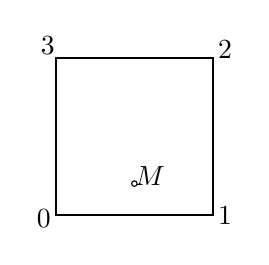
\begin{tikzpicture}
%\draw[step=0.5cm,gray,very thin] (0,0) grid (4,4); %background grid
\draw[thick] (1,1) -- (3,1) -- (3,3) -- (1,3) -- cycle;  
\node[] at (0.85,0.95) {0};
\node[] at (3.15,1) {1};
\node[] at (3.15,3.1) {2};
\node[] at (0.9,3.15) {3};
\node[] at (2.2,1.5) {$M$};
\draw (2.,1.4) circle (1pt);
\end{tikzpicture}\\
\end{center}


%..................................................
\paragraph{An intermediate case} We make the following assumption that the lateral sides of the  
element are vertical while the bottom and top are not necessarily horizontal:

\begin{center}
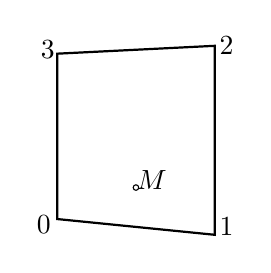
\begin{tikzpicture}
%\draw[step=0.5cm,gray,very thin] (0,0) grid (4,4); %background grid
\draw[thick] (1,1) -- (3,0.8) -- (3,3.2) -- (1,3.1) -- cycle;  
\node[] at (0.83,0.93) {0};
\node[] at (3.15,0.9) {1};
\node[] at (3.15,3.2) {2};
\node[] at (0.88,3.15) {3};
\node[] at (2.2,1.5) {$M$};
\draw (2.,1.4) circle (1pt);
\end{tikzpicture}\\
\end{center}

\noindent Because the sides are verical then if $x_0 \leq x_M \leq x_2$ then 
\[
r_M = \frac{2}{x_2-x_0}(x_M-x_0) -1 
\]
Then, if $M$ is inside the element then its $y$ coordinate is given by
\[
y_M = \sum_i \bN_i(r_M,s_M) y_i
\]
where $\bN_i$ are the four $Q_1$ basis functions associated to the vertices.
Assuming we know $r_M$ then we can solve for $s_M$:
\begin{eqnarray}
y_M &=&  
\frac{1}{4}(1-r_M)(1-s_M) y_0+
\frac{1}{4}(1+r_M)(1-s_M) y_1+
\frac{1}{4}(1+r_M)(1+s_M) y_2+
\frac{1}{4}(1-r_M)(1+s_M) y_3 \nn\\
&=& 
\frac{1}{4} \left[
(1-r)y_0+(1+r)y_1+(1+r)y_2+(1-r)y_3 +s_M [ -(1-r)y_0 - (1+r)y_1+(1+r)y_2+(1-r)y_3  ] 
\right] \nn 
\end{eqnarray}
or, 
\[
s_M = \frac{ 4y_M - [(1-r_M)y_0+(1+r_M)y_1+(1+r_M)y_2+(1-r_M)y_3]  }{ -(1-r_M)y_0 -(1+r_M)y_1+(1+r_M)y_2+(1-r_M)y_3 } 
\]
If the obtained value is in $[-1,1]$ then the point $M$ is in the element.
Verification: when $y_1=y_0$ and $y_2=y_3$ then 
\begin{eqnarray}
s_M 
&=& \frac{4 y_M - [(1-r_M)y_0+(1+r_M)y_0+(1+r_M)y_3+(1-r_M)y_3]  }{ -(1-r_M)y_0 - (1+r_M)y_0+(1+r_M)y_3+(1-r_M)y_3 } \nn\\
&=& \frac{4 y_M - [ 2 y_0 + 2 y_3]  }{ -2 y_0 + 2 y_3    }  \nn\\
&=& \frac{1}{y_3-y_0} [2 y_M - (  y_0 +  y_3) ] \nn\\ 
&=& \frac{1}{y_3-y_0} [2 y_M -  2 y_0 +y_0 -  y_3)  ] \nn\\ 
&=& \frac{2}{y_3-y_0} (y_M - y_0) - 1 
\end{eqnarray}
which is the expression that corresponds to a rectangular element as seen previously.

%..................................................
\paragraph{A generic quadrilateral}

We wish to arrive at a single algorithm which is applicable to all quadrilaterals and we now focus  
on an irregular quadrilateral (no face is parallel to the axis of the coordinate system). 

\begin{center}
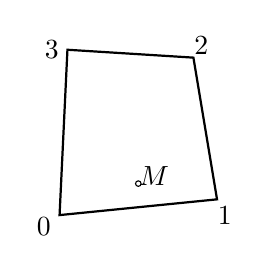
\begin{tikzpicture}
%\draw[step=0.5cm,gray,very thin] (0,0) grid (4,4); %background grid
\draw[thick] (1,1) -- (3,1.2) -- (2.7,3) -- (1.1,3.1) -- cycle;  
\node[] at (0.8,0.85) {0};
\node[] at (3.1,1) {1};
\node[] at (2.8,3.15) {2};
\node[] at (0.9,3.1) {3};
\node[] at (2.2,1.5) {$M$};
\draw (2.,1.4) circle (1pt);
\end{tikzpicture}\\
\end{center}

\noindent Several rather simple options exist:
\begin{itemize}
\item we could subdivide the quadrilateral into two triangles and check whether point $M$ is inside any of them (as it turns out, this problem is rather straightforward for triangles. Simply google it.)
\item We could check that point $M$ is always on the left side of segments $0\rightarrow 1$, $1\rightarrow 2$, $2\rightarrow 3$, $3\rightarrow 0$.
\item ...  
\end{itemize}

Any of these approaches will work although some might be faster than others. 
In three-dimensions all will however become 
cumbersome to implement and might not even work at all. 
Fortunately, there is an elegant way to answer the question, as 
detailed in the following subsection, which works both in 2D and 3D.

%-------------------------------------------
\subsubsection{Three-dimensional space}

If point $M$ is inside the quadrilateral, there exist a set of reduced 
coordinates $r,s,t\in[-1:1]^3$ such that 

\[
\sum_{i=1}^4 \bN_i(r_M,s_M,t_M) x_i = x_M
\quad\quad\quad
\sum_{i=1}^4 \bN_i(r_M,s_M,t_M) y_i = y_M
\quad\quad\quad
\sum_{i=1}^4 \bN_i(r_M,s_M,t_M) z_i = z_M
\]
This can be cast as a system of three equations and three unknowns. 
Unfortunately, each basis function $\bN_i$ 
contains a term $rst$ (as well as $rs$, $rt$, and $st$) 
so that it is not a linear system.
We must then use an iterative technique: the algorithm starts with 
a guess for values $r_M,s_M,t_M$ and 
improves on their value iteration after iteration. 
In what follows the subscript $M$ is dropped from $r,s,t$.

The classical way of solving nonlinear systems of equations is Newton's method. 
\index{general}{Newton's method}
We can rewrite the equations above as ${\bm F}(r,s,t)=0$:
\begin{eqnarray}
\sum_{i=1}^8 \bN_i(r,s,t) x_i - x_M&=&0 \nonumber\\
\sum_{i=1}^8 \bN_i(r,s,t) y_i - y_M&=&0 \nonumber\\
\sum_{i=1}^8 \bN_i(r,s,t) z_i - z_M&=&0
\end{eqnarray}
or,
\begin{eqnarray}
F_r(r,s,t)&=&0 \nonumber\\
F_s(r,s,t)&=&0 \nonumber\\
F_t(r,s,t)&=&0 \nonumber
\end{eqnarray}
so that we now have to find the zeroes of continuously differentiable 
functions ${\bm F}:\mathbb{R} \rightarrow \mathbb{R}$.
The recursion is simply:
\[
\left(
\begin{array}{c}
r_{k+1} \\s_{k+1} \\ t_{k+1}
\end{array}
\right)
=
\left(
\begin{array}{c}
r_{k} \\s_{k} \\ t_{k}
\end{array}
\right)
- J_F(r_k,s_k,t_k) ^{-1} 
\left(
\begin{array}{c}
F_r(r_k,s_k,t_k) \\
F_s(r_k,s_k,t_k)\\
F_t(r_k,s_k,t_k)
\end{array}
\right)
\]
where $J$ the Jacobian matrix:
\begin{eqnarray}
J_F(r_k,s_k,t_k)
&=&
\left(
\begin{array}{ccc}
\frac{\partial F_r}{\partial r}(r_k,s_k,t_k) & \frac{\partial F_r}{\partial s}(r_k,s_k,t_k) & \frac{\partial F_r}{\partial t}(r_k,s_k,t_k) \\\\
\frac{\partial F_s}{\partial r}(r_k,s_k,t_k) & \frac{\partial F_s}{\partial s}(r_k,s_k,t_k) & \frac{\partial F_s}{\partial t}(r_k,s_k,t_k) \\\\
\frac{\partial F_t}{\partial r}(r_k,s_k,t_k) & \frac{\partial F_t}{\partial s}(r_k,s_k,t_k) & \frac{\partial F_t}{\partial t}(r_k,s_k,t_k) 
\end{array}
\right) \nonumber\\
&=&
\left(
\begin{array}{ccc}
\sum\limits_{i=1}^8 \frac{\partial \bN_i}{\partial r}(r_k,s_k,t_k) x_i &
\sum\limits_{i=1}^8 \frac{\partial \bN_i}{\partial s}(r_k,s_k,t_k) x_i &
\sum\limits_{i=1}^8 \frac{\partial \bN_i}{\partial t}(r_k,s_k,t_k) x_i \\
\sum\limits_{i=1}^8 \frac{\partial \bN_i}{\partial r}(r_k,s_k,t_k) y_i &
\sum\limits_{i=1}^8 \frac{\partial \bN_i}{\partial s}(r_k,s_k,t_k) y_i &
\sum\limits_{i=1}^8 \frac{\partial \bN_i}{\partial t}(r_k,s_k,t_k) y_i \\
\sum\limits_{i=1}^8 \frac{\partial \bN_i}{\partial r}(r_k,s_k,t_k) z_i &
\sum\limits_{i=1}^8 \frac{\partial \bN_i}{\partial s}(r_k,s_k,t_k) z_i &
\sum\limits_{i=1}^8 \frac{\partial \bN_i}{\partial t}(r_k,s_k,t_k) z_i 
\end{array}
\right) \nonumber 
\end{eqnarray}
In practice, we solve the following system:
\[
J_F(r_k,s_k,t_k) 
\left[  
\left(
\begin{array}{c}
r_{k+1} \\s_{k+1} \\ t_{k+1}
\end{array}
\right)
-
\left(
\begin{array}{c}
r_{k} \\s_{k} \\ t_{k}
\end{array}
\right)
\right]=-
\left(
\begin{array}{c}
F_r(r_k,s_k,t_k) \\
F_s(r_k,s_k,t_k)\\
F_t(r_k,s_k,t_k)
\end{array}
\right)
\]
Finally, the algorithm goes as follows:
\begin{itemize}
\item set guess values for $r,s,t$ (typically 0)
\item loop over k=0,...
\item Compute rhs= $-{\bm F}(r_k,s_k,t_k)$ 
\item Compute matrix $J_F(r_k,s_k,t_k)$
\item solve system for $(dr_k,ds_k,dt_k)$
\item update $r_{k+1}=r_k+dr_k$, $s_{k+1}=s_k+ds_k$, $t_{k+1}=t_k+dt_k$ 
\item stop iterations when $(dr_k,ds_k,dt_k)$ is small
\item if $r_k,s_k,t_k\in[-1,1]^3$ then $M$ is inside.
\end{itemize}
This method converges quickly but involves iterations, and multiple 
solves of $3\times 3$ systems which, when carried out for each marker 
and at each time step can prove to be expensive. 
A simple modification can be added to the above algorithm: 
iterations should be carried out {\it only}
when the point $M$ is inside of a cuboid of 
size $[\min\limits_i{x_i}:\max\limits_i{x_i}]\times[\min\limits_i{y_i}:\max\limits_i{y_i} ]
\times[\min\limits_i{z_i}:\max\limits_i{z_i}]$ where the sums run over the vertices of the element. 
In 2D this translates as follows: only carry out Newton iterations when $M$ is inside the red rectangle!
\begin{center}
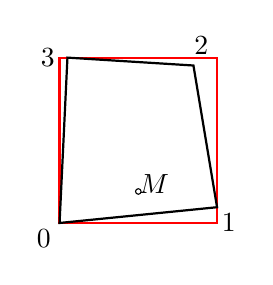
\begin{tikzpicture}
%\draw[step=0.5cm,gray,very thin] (0,0) grid (4,4); %background grid
\draw[thick,red] (1,1) -- (3,1) -- (3,3.1) -- (1,3.1) -- cycle;  
\draw[thick] (1,1) -- (3,1.2) -- (2.7,3) -- (1.1,3.1) -- cycle;  
\node[] at (0.8,0.8) {0};
\node[] at (3.15,1) {1};
\node[] at (2.8,3.25) {2};
\node[] at (0.85,3.1) {3};
\node[] at (2.2,1.5) {$M$};
\draw (2.,1.4) circle (1pt);
\end{tikzpicture}\\
\end{center}

Note that the algorithm above extends to high degree elements 
such as $Q_2$ and higher, even with curved sides.
As shown in the 2D case if the element is a cuboid or 
if all its lateral faces are vertical then one can 
compute the reduced coordinates without using an iterative method.


%-----------------------------------------------------
\subsubsection{Three-dimensional space - special case}

We assume that the mesh is such that the cross section of all $Q_1$ elements 
is a rectangle in the $xy$-plane. 

Let $(x,y,z)$ be a point inside the element. 
The global coordinates $x,y,z$ are obtained from the 
reduced coordinates $r,s,t$ via the basis the basis functions:
\begin{eqnarray}
x=\sum_{i=1}^8 \bN_i (r,s,t) x_i \qquad 
y=\sum_{i=1}^8 \bN_i (r,s,t) y_i  \qquad 
z=\sum_{i=1}^8 \bN_i (r,s,t) z_i \label{xyz}
\end{eqnarray}
Let 
\begin{eqnarray}
{\vec v}_1 &=& (+1,+1,+1,+1,+1,+1,+1,+1) \nn\\
{\vec v}_2 &=& (-1,+1,+1,-1,-1,+1,+1,-1) \nn\\
{\vec v}_3 &=& (-1,-1,+1,+1,-1,-1,+1,+1) \nn\\
{\vec v}_4 &=& (-1,-1,-1,-1,+1,+1,+1,+1) \nn\\
{\vec v}_5 &=& (+1,-1,+1,-1,+1,-1,+1,-1) \nn\\
{\vec v}_6 &=& (+1,-1,-1,+1,-1,+1,+1,-1) \nn\\
{\vec v}_7 &=& (+1,+1,-1,-1,-1,-1,+1,+1) \nn
\end{eqnarray}
and 
\begin{eqnarray}
{\vec x} &=& (x_1,x_2,x_3,x_4,x_5,x_6,x_7,x_8) \nn\\
{\vec y} &=& (y_1,y_2,y_3,y_4,y_5,y_6,y_7,y_8) \nn\\
{\vec z} &=& (z_1,z_2,z_3,z_4,z_5,z_6,z_7,z_8) \nn
\end{eqnarray}
then Eqs.~\eqref{xyz} can also be written
\begin{eqnarray}
x&=&\frac{1}{8} \left( {\vec v}_1 + r  {\vec v}_2 + s  {\vec v}_3 + t  {\vec v}_4 
                 + rs  {\vec v}_5 + rt {\vec v}_6 + st {\vec v}_7 \right) \cdot {\vec x} \nn\\ 
y&=&\frac{1}{8} \left( {\vec v}_1 + r  {\vec v}_2 + s  {\vec v}_3 + t  {\vec v}_4 
                 + rs  {\vec v}_5 + rt {\vec v}_6 + st {\vec v}_7 \right) \cdot {\vec y} \nn\\
z&=&\frac{1}{8} \left( {\vec v}_1 + r  {\vec v}_2 + s  {\vec v}_3 + t  {\vec v}_4 
                 + rs  {\vec v}_5 + rt {\vec v}_6 + st {\vec v}_7 \right) \cdot {\vec z} \label{zzz}
\end{eqnarray}
If the element has a rectangular cross-section $s_x \times s_y$ then 
\begin{eqnarray}
{\vec x} &=& (x_0,x_0+s_x,x_0+s_x,x_0,x_0,x_0+s_x,x_0+s_x,x_0) \nn\\
{\vec y} &=& (y_0,y_0,y_0+s_y,y_0+s_y,y_0,y_0,y_0+s_y,y_0+s_y) \nn
\end{eqnarray}
which yields
\begin{eqnarray}
r&=& 2\frac{x-x_0}{s_x}-1  \nn\\
s&=& 2\frac{y-y_0}{s_y}-1  \nn
\end{eqnarray}
Since the local coordinates $r$ and $s$ can be easily computed, one can use Eq.~\eqref{zzz} to obtain $t$:
\[
t=\frac{8z - ({\vec v}_1 + r {\vec v}_2 + s {\vec v}_3 + rs  {\vec v}_5 ) \cdot {\vec z}} 
{ ({\vec v}_4  + r  {\vec v}_6 + s  {\vec v}_7)  \cdot {\vec z} }
\]







 
 %-------------------------------
\newpage %-----------------------------------------------------------------------------------------
\section{Static condensation} \input{static_condensation} %-------------------------------------
\newpage %-----------------------------------------------------------------------------------------
\section{Measuring incompressibility \label{ss_incomp}} 
The velocity divergence error integrated over the whole element is given by
\begin{equation}
e_{div}= \int_\Omega (\vec\nabla\cdot \vec v^h - \underbrace{\vec\nabla\cdot \vec v}_{=0}  ) \; d\Omega
= \int_\Omega (\vec\nabla\cdot \vec v^h) \; d\Omega
\end{equation}
where $\Gamma_e$ is the boundary of element $e$ and $\vec{n}$ is the unit 
outward normal of $\Gamma_e$.

Furthermore, one can show that \cite{dobo04}:
\[
e_{div} = \int_{\Gamma_e} \vec{v}^h\cdot\vec{n} \;  d\Gamma
\]
The reason is as follows and is called the divergence 
theorem\footnote{\url{https://en.wikipedia.org/wiki/Divergence_theorem}}:
suppose a volume $V$ subset of $\mathbb{R}^d$ which is compact
and has a piecewise smooth boundary $S$, and if $\vec F$ is
a continuously differentiable vector field then
\[
\int_V ( \vec\nabla\cdot\vec F)\; dV = \int_S (\vec F \cdot \vec n)\; dS
\]
The left side is a volume integral while the right side is a surface integral.
Note that sometimes the notation $d\vec S = \vec n \; dS $ is used so that 
$\vec F \cdot \vec n \; dS = \vec F \cdot d\vec S$.

The average velocity divergence over an element can be defined as 
\[
<\vec \nabla \cdot \vec v>_e 
= \frac{1}{V_e} \int_{\Omega_e}  (\vec\nabla\cdot\vec v) \; d\Omega
= \frac{1}{V_e} \int_{\Gamma_e} \vec{v}\cdot\vec{n} \; d\Gamma
\]
Note that for elements using discontinuous pressures we shall 
recover a zero divergence element per element (local mass conservation)
while for continuous pressure elements the mass conservation 
is guaranteed only globally (i.e. over the whole domain), see section 3.13.2 of \cite{grsa}.

Note that one could instead compute $<|\vec\nabla\cdot \vec v|>_e$. Either volume or 
surface integral can be computed by means of an appropriate Gauss-Legendre quadrature algorithm.



 %------------------------
\newpage %-----------------------------------------------------------------------------------------
\section{Periodic boundary conditions\label{ss_periodic}}\input{periodic} %---------------------
\newpage %-----------------------------------------------------------------------------------------
\section{Removing rotational nullspace\label{ss_nullspace}} \input{nullspace} %-----------------
\newpage %-----------------------------------------------------------------------------------------
\section{Picard and Newton \label{ss_nonlinear}} \index{general}{Nonlinear PDE} 
\index{general}{Picard Iterations} 
\index{general}{Relaxation}

\todo[inline]{explain why our eqs are nonlinear}

\Literature Quasi Newton methods \cite{ensb81}

%--------------------------------
\subsubsection{Picard iterations} \label{ss:picard}

Let us consider the following system of nonlinear algebraic equations:
\[
\mathbb{A}(\vec X) \cdot \vec X = \vec b(\vec X)
\]
Both matrix and right hand side depend on the solution vector $\vec X$.

For many mildly nonlinear problems, a simple successive substitution 
iteration scheme (also called Picard method) will converge to the solution
and it is given by the simple relationship:
\[
\mathbb{A}(\vec X^n) \cdot \vec X^{n+1} = \vec b(\vec X^n)
\]
where $n$ is the iteration number. 
It is easy to implement:
\begin{enumerate}
\item guess $\vec X^0$ or use the solution from previous time step
\item compute $\mathbb{A}$ and $\vec b$ with current solution vector $\vec X^{old}$
\item solve system, obtain $T^{new}$
\item check for convergence (are $\vec X^{old}$ and $\vec X^{new}$ close enough?)
\item $\vec X^{old} \leftarrow \vec X^{new}$
\item go back to 2.
\end{enumerate}

There are various ways to test whether iterations have converged. The simplest
one is to look at $\norm{\vec X^{old}-\vec X^{new} }$ (in the $L_1$, $L_2$ or maximum norm)
and assess whether this term is smaller than a given tolerance $\epsilon$. 
However this approach poses a problem: in geodynamics, if two consecutively obtained 
temperatures do not change by more than a thousandth of a Kelvin (say $\epsilon=10^{-3}$K )
we could consider that iterations have converged but looking now at velocities which 
are of the order of a cm/year (i.e. $\sim 3\cdot 10^{-11}$m/s) we would need a tolerance 
probably less than $10^{-13}$m/s. We see that using absolute values for a convergence 
criterion is a potentially dangerous affair, which is why one uses a relative 
formulation (thereby making $\epsilon$ a dimensionless parameter):
\[
\frac{\norm{\vec X^{old}-\vec X^{new}}}{\norm{\vec X^{new}}} < \epsilon
\]
Another convergence criterion is proposed by Reddy (section 3.7.2) \cite{reddybook2}:
\[
\left(
\frac{ (\vec X^{old}-\vec X^{new})\cdot(\vec X^{old}-\vec X^{new} ) }{ X^{new}\cdot X^{new}  } 
\right)^{1/2} < \epsilon
\]
Yet another convergence criterion is used in \cite{thie11}: the means $<\vec X^{old}>$, $<\vec X^{new}>$
as well as the variances $\sigma^{old}$ and $\sigma^{new}$ are computed, followed by the 
correlation factor $R$:
\[
R= \frac{ <  (\vec X^{old}-<\vec X^{old}>)\cdot( \vec X^{new}-<\vec X^{new}> )>  }{\sqrt{\sigma^{old}\sigma^{new}}}
\]
Since the correlation is normalised, it takes values between 0
(very dissimilar velocity fields) and 1 (very similar fields). The
following convergence criterion is then used: $1-R < \epsilon$.

\todo[inline]{write about nonlinear residual}


Note that in some instances and improvement in convergence rate can be obtained by use of a 
relaxation formula where one first solves
\[
\mathbb{A}(\vec X^n) \cdot \vec X^{\star} = \vec b(\vec X^n)
\]
and then updates $\vec X^n$ as follows:
\[
\vec X^n = \gamma \vec X^n + (1-\gamma) \vec X^\star 
\quad\quad\quad
0 < \gamma \leq 1
\]
When $\gamma=1$ we recover the standard Picard iterations formula above.

%------------------------------------------
\subsection{Defect correction formulation}
\index{general}{Defect Correction Formulation}

Work in progress. 

We start from the system to solve:
\[
{\bm A}(\vec X) \cdot \vec X = \vec b(\vec X)
\]
with the associated residual vector $\vec F$ 
\[
\vec F(\vec X) = {\bm A}(\vec X) \cdot \vec X - \vec b(\vec X)
\]
The Newton-Raphson algorithm consists of two steps:
\begin{enumerate}
\item solve $\bm J_k \cdot \delta \vec X_k = -\vec F(\vec X_k)$, or in the 
case of the incompressible Stokes equation FEM system:
\[
\left(
\begin{array}{cc}
\bm J^{{\cal V}{\cal V}}_k & \bm J^{{\cal V}{\cal P}}_k \\
\bm J^{{\cal P}{\cal V}}_k & 0
\end{array}
\right)
\cdot
\left(
\begin{array}{c}
\delta \vec {\cal V}_k \\ \delta \vec {\cal P}_k
\end{array}
\right)
=
\left(
\begin{array}{c}
- \vec F_k^{\cal V} \\ -\vec F_k^{\cal P}
\end{array}
\right)
\]

\item update $\vec X_{k+1} = \vec X_k + \alpha_k \delta \vec X_k$
\end{enumerate}
The defect correction Picard approach consists of neglecting the derivative terms present 
in the $J$ terms (Eqs. 16,17,18 of \cite{frbt19}) so that 
\[
\bm J^{{\cal V}{\cal V}}_k \simeq \K_k 
\quad\quad
\bm J^{{\cal V}{\cal P}}_k \simeq \G 
\quad\quad
\bm J^{{\cal P}{\cal V}}_k \simeq \G^T
\]
and step 1 of the above iterations become:
\[
\left(
\begin{array}{cc}
\K_k & \G \\ \G^T & 0
\end{array}
\right)
\cdot
\left(
\begin{array}{c}
\delta \vec {\cal V}_k \\ \delta \vec {\cal P}_k
\end{array}
\right)
=
\left(
\begin{array}{c}
- \vec F_k^{\cal V} \\ -\vec F_k^{\cal P}
\end{array}
\right)
\]


\mscthesis: implement a simple Newton solver and apply it to a few nonlinear 
benchmarks. \index{general}{MSc Thesis} 

\vspace{1cm}

\todo[inline]{explain picard, defect picard, Newton, line search, ....}


\begin{itemize}
\item \fullcite{erka81}
\item \fullcite{ensb81}
\item \fullcite{knke04}
\item \fullcite{yiha10}
\item \fullcite{sara16}
\item \fullcite{frbt19}
\item \fullcite{russ20}
\end{itemize}

 %----------------------------
\newpage %-----------------------------------------------------------------------------------------
\section{Parallel or not?} \label{sec:parallel} \input{parallel} %------------------------------
\newpage %-----------------------------------------------------------------------------------------
\section{Stream function} \label{sec:streamfunction} \index{general}{Stream Function}
\begin{flushright} {\tiny {\color{gray} streamfunction.tex}} \end{flushright}

\Literature 
\textcite{scja81} (1981),
\textcite{chyu84} (1984),
\textcite{chri84} (1984),
\textcite{hayu94} (1994),
\textcite{olwh97} (1997),
\textcite{giju98} (1998),
\textcite{vanv08} (2008),
\textcite{vanj11} (2011).

\vspace{0.5cm}

The Stream function (commonly denoted by $\Phi$ or $\Psi$) approach is a useful approach in 
fluid dynamics as it 
can provide relatively quick solutions to 2D incompressible flow problems.
Using a stream function
formulation is numerically convenient because velocity information is contained in a single scalar equation
and pressure vanishes from the solution process.
The stream function is a function of coordinates and time of an inviscid liquid.
It allows to determine the components of velocity by differentiating the stream function 
with respect to the space coordinates. 
A family of curves $\Psi = constant$ represent {\color{olive} streamlines}, i.e. 
the stream function remains constant along a streamline. 
Although also valid in 3D, this approach is mostly used in 2D because of its 
relative simplicity.

%............................................
\subsubsection{In Cartesian coordinates - 2D}

In two dimensions the velocity is obtained as follows:
\begin{equation}
{\vec \upnu} = (u,v) = \left( \frac{\partial \Psi}{\partial y},-\frac{\partial \Psi}{\partial x} \right) 
\end{equation}
Provided the function $\Psi$ is a smooth enough function, 
this automatically insures that the flow is incompressible:
\begin{equation}
{\vec \nabla}\cdot {\vec \upnu} = 
\frac{\partial u}{\partial x} + \frac{\partial v}{\partial y}
=
\frac{\partial^2 \Psi}{\partial xy} - \frac{\partial^2 \Psi}{\partial xy} =0 
\end{equation}
Assuming constant viscosity, the Stokes equation writes:
\begin{equation}
-{\vec \nabla}p + \eta \Delta {\vec \upnu} + \rho {\vec g} = \vec{0}
\end{equation}
Let us introduce the vector $\vec{W}=(W_x,W_y)$ for convenience such that in each dimension:
\begin{eqnarray}
W_x&=&-\frac{\partial p}{\partial x} 
+ \eta\left( \frac{\partial^2 u}{\partial x^2} + \frac{\partial^2 u}{\partial x^y} \right) \\
W_y&=&-\frac{\partial p}{\partial y} 
+ \eta \left(\frac{\partial^2 v}{\partial x^2} + \frac{\partial^2 v}{\partial x^y} \right) 
\end{eqnarray}
Taking the curl of the vector ${\vec{W}}$ and only considering the component 
perpendicular to the $xy$-plane:
\begin{equation}
\frac{\partial W_y}{\partial x} - \frac{\partial W_x}{\partial y}  = 
-\frac{\partial \rho g_y}{\partial x} + \frac{\partial \rho g_x}{\partial y}   
\end{equation}
The advantage of this approach is that the pressure terms cancel out 
(the curl of a gradient is always zero\footnote{\url{https://mathinsight.org/curl_gradient_zero}}), 
so that:
\begin{equation}
\frac{\partial}{\partial x}\eta\left( \frac{\partial^2 v}{\partial x^2} + \frac{\partial^2 v}{\partial x^y}  \right) 
- \frac{\partial }{\partial y} \eta \left( \frac{\partial^2 u}{\partial x^2} + \frac{\partial^2 u}{\partial x^y} \right) = 
-\frac{\partial \rho g_y}{\partial x} + \frac{\partial \rho g_x}{\partial y}   
\end{equation}
and then replacing $u,v$ by the their stream function derivatives yields (for a constant viscosity):
\begin{equation}
\eta \left(\frac{\partial^4 \Psi}{\partial x^4} + 
\frac{\partial^4 \Psi}{\partial y^4} + 
2\frac{\partial^4 \Psi}{\partial x^2y^2} \right)
=
-\frac{\partial \rho g_y}{\partial x} + \frac{\partial \rho g_x}{\partial y}   
\end{equation}
or, 
\begin{equation}
\eta {\vec \nabla}^4 \Psi 
=
\left(\frac{\partial^2 }{\partial x^2} + \frac{\partial^2 }{\partial y^2} \right) 
\left(\frac{\partial^2 }{\partial x^2} + \frac{\partial^2 }{\partial y^2} \right) \Psi
=
-\frac{\partial \rho g_y}{\partial x} + \frac{\partial \rho g_x}{\partial y}   
\label{eq:sf1}
\end{equation}
Note that $\vec\nabla^2 \vec\nabla^2 = \vec\nabla^4 $ is known as the {\color{olive}Biharmonic operator}.
\index{general}{Biharmonic Operator} 
These equations are also to be found in the geodynamics literature, 
see \textcite[eq. 1.43]{tack10} or \textcite[p 70-71]{gery10}.

In the presence of temperature variations and multiple compositions, 
\textcite{trlb20} (2020)  use the  following nondimensional equation:
\[
\left(
\frac{\partial^2 }{\partial x^2} - 
\frac{\partial^2 }{\partial y^2}  
\right)
\left[ \eta
\left(
\frac{\partial^2 \Psi}{\partial x^2} - 
\frac{\partial^2 \Psi}{\partial y^2}  
\right)
\right]
+4
\frac{\partial^2 }{\partial xy} 
\left[
\eta 
\frac{\partial^2 \Psi}{\partial xy} 
\right]
=
Ra_T \frac{\partial T}{\partial x}-
Ra_C \frac{\partial C}{\partial x}
\]
\todo[inline]{check/rederive this formula!}

%........................................
%\subsubsection{In Cylindrical coordinates}

%TODO

%VERIFY THOSE! minus signs ?
%\[
%\upnu_r=\frac{1}{r}\frac{\partial \Phi}{\partial \theta} 
%\]
%\[
%\upnu_\theta=-\frac{\partial \Phi}{\partial r} 
%\]


%............................................
\subsubsection{In Cartesian coordinates - 3D}

See for example \textcite{hous90} (1990) and refs therein.


 %-------------------
\newpage %-----------------------------------------------------------------------------------------
\section{Corner flow} \label{sec:cornerflow} \input{cornerflow} %-------------------------------
\newpage %-----------------------------------------------------------------------------------------
\section{Surface processes \label{sec:surfaceprocesses}} \begin{flushright} {\tiny {\color{gray} surfaceprocesses.tex}} \end{flushright}

%.......................................................................
\subsubsection{In 1D - simple nonlinear diffusion a la Burov \& Cloetingh (1997)}

This approach comes from \textcite{bucl97} (1997).
The tectonic-scale transport equations describe long term changes
in topography $h(x,y,t)$ as a result of simultaneous short- and long-range
mass transport processes \cite{befh92,kobe94}.

The short-range surface processes are represented by cumulative effects of hillslope 
processes (soil creep, rainsplash, slides) that remove material from uplifted areas 
down to the valleys. 
It is then assumed that the horizontal material flux $\vec{q}_s$ is related to 
local slope $\vec\nabla h$ by $\vec{q}_s=-K_s \vec{\nabla}h$ 
where $K_s$ is the effective diffusivity. Assumption of conservation of mass 
volume leads to the linear diffusion equation for erosion:
\[
\frac{\partial h}{\partial t} = K_s \Delta h
\]
This equation can be solved with constant-elevation (fixed $h$ value)
boundary conditions simulating local base levels of erosion. 

Note that is practice the coefficient $K_s$ might depend on slope and curvature, 
i.e.
\[
\frac{\partial h}{\partial t} = K_s(x,y,h,\vec\nabla h)\Delta h
\]
Following \cite{goss76}, Burov \& Cloetingh use an empirical non linear 
expression $K_s=k_s(x) (\vec\nabla h)^n$. 




%...........................................................
\subsubsection{In 1D - not so simple, a la Andr\`es-Martinez \etal (2019)}

This approach comes from \textcite{anpa19} (2019). 
The change in surface elevation rate due to surface processes is equal
to the divergence of the sediment flux 
(assuming there is no density difference between the bedrock and
sediment and ignoring the effects of compaction):
\[
\frac{\partial h}{\partial t} = -\frac{\partial q_s}{\partial x}
\]
where $h$ is the topography, $t$ is the time, $q_s$ represents the sediment flux, 
and $x$ is the horizontal coordinate. 

The next step consists in a formulation for the sediment flux. Still following \cite{anpa19}, 
in the subaerial environment, it is possible to define the sediment transport 
flux $q_s$ in terms of the water flux $q_w$ as
\[
q_s=-(K+c q_w^n) \frac{\partial h}{\partial x}
\]
where $K$ is the slope diffusivity, $c$ is the transport coefficient, 
and $n \geq 1$ is the power law that defines the type
of relationship between the sediment transport and the water flux 
(Simpson \& Schlunegger, 2003; Smith \& Bretherton, 1972).
\todo[inline]{get these papers}
This model accounts for hillslope diffusion processes where the topography will tend to
a dispersive diffusion (Culling, 1960) and fluvial transport processes that result in concentrative diffusion
due to water run off (Graf, 1984). For a simple parameterization we choose a linear relationship between
sediment transport and water flux $(n=1)$.

The water flux can be related to the water discharge/effective rainfall $\alpha$ as
\[
\frac{\partial}{\partial x} (\vec{n} q_w) = -\alpha
\]
where $\vec n$ is a unit vector directed down the surface gradient (Smith \& Bretherton, 1972). 
By assuming a constant $\alpha$ and integrating equation (12) over the surface in the downstream direction, we obtain

\[
q_w = \alpha x_d
\]
where $x_d$ is the downstream distance from the drainage divide. By substituting equations (11) and
(13) into (10) we obtain the 1-D sediment mass conservation equation for combined hillslope and
discharge-dependent fluvial transport
\[
\frac{\partial h}{\partial t} = \frac{\partial}{\partial x} \left( (K+k \alpha x_d) 
\frac{\partial h}{\partial x}   \right)
\]
where the downstream distance $x_d$ is calculated at each time step as the distance from the topographic highs
to the valley floors. Because $q_w$ is dependent on the length of the drainage, the model mimics 1-D landscapes
similar to river profiles in which fluvial processes are dominant.

%...........................................................
\subsubsection{Examples in the literature}

\begin{center}
\includegraphics[width=7cm]{images/surfaceprocesses/fuwf06a}
\includegraphics[width=7cm]{images/surfaceprocesses/fuwf06b}\\
{\captionfont Application to Taiwan. Taken from Fuller \etal (2006) \cite{fuwf06}}
\end{center}


 %-------------
\newpage %-----------------------------------------------------------------------------------------
\section{Geometric multigrid} \input{gmg} %-----------------------------------------------------
\newpage %-----------------------------------------------------------------------------------------
\section{Algebraic multigrid} \input{amg} %-----------------------------------------------------
\newpage %-----------------------------------------------------------------------------------------
\section{Computing depth \label{ss:depth}} \input{computing_depth} %----------------------------
\newpage %-----------------------------------------------------------------------------------------
\section{Imposing boundary conditions \label{ss:howtobc}} 
\begin{flushright} {\tiny {\color{gray} howtobc.tex}} \end{flushright}

Let us consider a quadrilateral element with one degree of freedom per node and let us assume that we are solving the temperature equation. The local matrix and right-hand side vector are given by 
\[
A_{el}(4\times 4) \quad\quad {\text and} \quad\quad B_{el}(4)
\]
Let us assume that we want to impose $\tilde{T}=10$ on the third node (local coordinates numbering). For instance, having built $A_{el}$ and $B_{el}$, the system looks like :
\[
\left(
\begin{array}{cccc}
3 & 1 & 6  & 9 \\
5 & 2 & 2  & 8 \\
7 & 4 & 11 & 2 \\
9 & 6 & 4  & 3
\end{array}
\right)
\left(
\begin{array}{c}
T_1 \\ T_2 \\ T_3 \\ T_4
\end{array}
\right)
=
\left(
\begin{array}{c}
4 \\ 3 \\ 1 \\ 2
\end{array}
\right)
\]

\begin{itemize}

\item \underline{Technique 1:} Penalty approach. Replace the hereabove system by
\[
\left(
\begin{array}{cccc}
3 & 1 & 6  & 9 \\
5 & 2 & 2  & 8 \\
7 & 4 & 11 +  10^{12} & 2 \\
9 & 6 & 4  & 3
\end{array}
\right)
\left(
\begin{array}{c}
T_1 \\ T_2 \\ T_3 \\ T_4
\end{array}
\right)
=
\left(
\begin{array}{c}
4 \\ 3 \\ \tilde{T}\times (11 + 10^{12}) \\ 2
\end{array}
\right)
\]




\item \underline{Technique 2:} One can choose not to solve for $T_3$ anymore, i.e. not to consider it as a degree of freedom, remove the corresponding 
equation and therefore write the linear system as follows:

\begin{eqnarray}
3 T_1 + T_2 + 6 T_3 + 9 T_4 &=& 4 \nn\\
5 T_1 + 2T_2 + 2 T_3 + 8 T_4 &=& 3 \nn\\
7 T_1 + 4T_2 + 11 T_3 + 2 T_4 &=& 1 \nn\\
9 T_1 + 6T_2 + 4 T_3 + 3 T_4 &=& 2\nn
\end{eqnarray}
or, 
\[
3 T_1 + T_2 + \quad  + 9 T_4 = 4 - 6T_3
\]
\[
5 T_1 + 2T_2 + \quad + 8 T_4 = 3 - 2T_3
\]
\[
7 T_1 + 4T_2 + 11T_3 + 2 T_4 = 1 
\]
\[
9 T_1 + 6T_2 + \quad + 3 T_4 = 2 - 4T_3
\]
and in the end:
\[
3 T_1 + T_2 + 9 T_4 = 4 - 6T_3
\]
\[
5 T_1 + 2T_2 + 8 T_4 = 3 - 2T_3
\]
\[
9 T_1 + 6T_2 +  3 T_4 = 2 - 4T_3
\]


\item \underline{Technique 3:} Since we want to impose $T_3=10$, then we can write 
\[
3 T_1 + T_2 + \quad  + 9 T_4 = 4 - 6T_3
\]
\[
5 T_1 + 2T_2 + \quad + 8 T_4 = 3 - 2T_3
\]
\[
0 + 0 + T_3 + 0 = 10
\]
\[
9 T_1 + 6T_2 + \quad + 3 T_4 = 2 - 4T_3
\]
and in matrix form :
\[
\left(
\begin{array}{cccc}
3 & 1 & 0  & 9 \\
5 & 2 & 0  & 8 \\
0 & 0 & 1 & 0 \\
9 & 6 & 0  & 3
\end{array}
\right)
\left(
\begin{array}{c}
T_1 \\ T_2 \\ T_3 \\ T_4
\end{array}
\right)
=
\left(
\begin{array}{c}
4 - A_{13} T_3\\ 3 - A_{23}T_3 \\ 10 \\ 2-A_{43} T_3
\end{array}
\right)
\]

\end{itemize}

The first technique is not a good idea in practice as it introduces very large 
values and will likely derail the solver. The second option is somewhat difficult
to implement as it means that elemental matrix and rhs sizes will change from 
element to element and it therefore requires more book-keeping.
The third technique is the one adopted throughout this document. 

As shown in \textcite{wuxl08} (2008), it is better to replace the 1 on the diagonal 
by the former diagonal term as it reduces the condition number of the matrix. 
The rhs must then be modified accordingly.

\Literature Behr (2004) \cite{behr04}

\todo{ASK DAVE for permission} This is an excerpt of an email sent to me by Dave May in May 2014: 
{\it 
Never ever ever impose bc's using a penalty approach.
For problems with a fixed mesh topology and time dependent Dirichlet domain (e.g. the segment 
of the boundary with Dirichlet bc's 
maybe change size/shape over time - for example with a true stick/slip type interface), it's nice to define the matrix 
with the dimension associated with the mesh+basis and leave all bc's in the operator. 
Leaving the bc's in the operator can be implemented in a manner which still retains the operators symmetry (assuming 
it was symmetric to begin with). This leaves the choice of what to stick on the diagonal. Simply using "1" could 
screw up the spectrum of the matrix and kill the iterative solver performance. A better choice would be to insert 
a diagonal entry closely related to the operator; e.g. something that looks like the diagonal entry 
of $\int 2 \eta \epsilon(u) : \epsilon(v) dV$ (for the discrete stress tensor term). 

Removing Dirichlet bc's entirely for the discrete operator sounds attractive. The code will like the FE theory 
and you will only be solving for variables which are "unknowns" (compared with the above). 
However, introducing a time dependent Dirichlet domain means the matrix must be re-sized, as should its non-zero structure 
be re-allocated. Also, implemented multi-grid is annoying when the Dirichlet entries are removed. In fact, most of  
the code associated with stripping out Diriclet bc's is annoying and ugly. However, removing the bcs ensures symmetry, 
it ensures the discrete operator will have a nice spectrum (c.f. the above option). Also, stripping out bcs usually 
increases overall storage as you have one representation of the discrete vectors given to the solver which will be  
of size (N-n) and in your mesh you will have a repsentation of length N. ``N'' being the total number of dofs in your 
system, ``n'' being the number of Dirichlet constrained dofs in your system. }
 
 %---------------------
\newpage %-----------------------------------------------------------------------------------------
\section{The Geoid} \label{ss:geoid} 
%---------------------------------
\subsubsection{What is the geoid?}
\index{general}{Geoid}


There is an infinity of equipotential surfaces of the gravitational potential $U$.
However, there is a particular surface on the Earth that is "easy" to locate: 
the mean sea level. This is a somewhat arbitrary choice  
but it makes sense because the oceans are made of water (!): 
the surface of a fluid in equilibrium must follow an equipotential.

\begin{center}
\includegraphics[width=6cm]{images/geoid/geoid1}
\end{center}

The geoid is usually defined in two ways:
\begin{itemize}
\item it is the particular equipotential surface that coincides with the mean sea level
 (easy to define in the oceans -assuming no currents, waves,... - but harder on land since 
it is not the topographic surface).
\item A gravitational equipotential surface. This means that everywhere at sea level experiences the same value of gravity potential, so there is no tendency for water to flow downhill since all points in the vicinity have the same value of gravity potential, pointed toward the center of the earth.
\end{itemize}

\begin{center}
\includegraphics[width=13cm]{images/geoid/ww15mgh}\\
{\captionfont Data Max value: 85.4 meters, east of New Guinea. Data Min value:-107.0 meters, south of India. 
This image shows 15'x15' geoid undulations covering the planet Earth 
from the NIMA/GSFC WGS-84 EGM96 15' Geoid Height File. The undulations refer to 
the differences from the WGS-84(G873) reference ellipsoid. 
Map and description from National Geodetic Survey
\footnote{\url{https://www.usna.edu/Users/oceano/pguth/md_help/geology_course/geoid.htm}}
}
\end{center}

From Wikipedia: The geoid surface is irregular, unlike the reference ellipsoid 
(which is a mathematical idealized representation of the physical Earth), but 
is considerably smoother than Earth's physical surface. Although the physical Earth has 
excursions of +8,848 m (Mount Everest) and -11,034 m (Marianas Trench), 
the geoid's deviation from an ellipsoid ranges from +85 m (Iceland) to -106 m (southern India), 
less than 200 \si{metre} total.


\begin{center}
\includegraphics[width=8cm]{images/geoid/Geoid}\\
{\captionfont 1. Ocean
2. Reference ellipsoid
3. Local plumb line
4. Continent
5. Geoid\\
Taken from \url{https://en.wikipedia.org/wiki/Geoid}}
\end{center}


%----------------------------------------
\subsubsection{the (reference) ellipsoid}

First evidence that the Earth is round Erathostene (275-195 B.C.)

First hypothesis that the Earth is flattened at the poles: Newton

First measurement of the Earth's flattening at the poles: Clairaut (1736) and Bouguer (1743)

The shape of the Earth can be mathematically represented as an ellipsoid defined by:
\begin{itemize}
\item Semi-major axis = equatorial radius = $a$
\item Semi-minor axis = polar radius = $c$
\item Flattening (the relationship between equatorial and polar radius): $f = (a-c)/a$
\item Eccentricity: $e^2 =2f-f^2$
\end{itemize}

Many different reference ellipsoids have been defined and are in use.
We define the {\it reference ellipsoid} = the ellipsoid that best fits the geoid.
It is totally arbitrary, but practical. 
The most common reference ellipsoid is the WGS-84 one\footnote{\url{https://confluence.qps.nl/qinsy/latest/en/world-geodetic-system-1984-wgs84-182618391.html}}:

\begin{center}
\includegraphics[width=6cm]{images/geoid/ellipsoid_wgs84}\\
Taken from \url{https://en.wikipedia.org/wiki/Reference_ellipsoid}
\end{center}


Geoid undulations = differences, in meters, between
the geoid reference ellipsoid
(= geoid ``height'').

To clarify:
\begin{itemize}
\item Geoid = the equipotential surface of the Earth's gravity field that
best fits (in a least squares sense) the mean sea level.
The gravitational potential is constant on the geoid (by definition) but 
the gravitational acceleration is not! 

\item Reference Ellipsoid = the ellipsoid that best fits the geoid 
\item Geoid = the (actual) figure of the Earth 
\item Ellipsoid = the (theoretical) shape of the Earth
\end{itemize}



%---------------------------------
\subsubsection{How to compute it?}

From \textcite{lizh16} (2016): ``
The geoid is computed by $\phi/g$, where $\phi$ is the surface gravitational potential anomaly 
and can be solved from the Poisson equation,
$ \nabla^2 \phi = -4\pi {\cal G} \delta\rho$ 
where ${\cal G}$ is the gravitational constant, and $\delta\rho$ 
includes both density variations in the mantle [...]
and those associated with dynamic topographies at the surface and CMB. 
Dynamic topographies are determined from solving [the Stokes] equations 
under free-slip boundary conditions at the surface and CMB.''


%---------------------------------
\subsubsection{Interesting modelling}

\begin{center}
\includegraphics[width=15cm]{images/geoid/mogu96}
{\scriptsize Idealized 2D slab calculations for each viscosity model: geoid and geoid filtered 
to pass only the longest wavelengths ($\sim$ 4000 km).
(a) Cold slab extends to 500 km depth in the upper mantle, 
(b) Slab extends to 750 km so that it is partly supported by the high viscosity lower mantle at 670 km. 
(c) Slab tilted at 45\degree to the vertical extending to the top of the lower mantle. 
Taken from \cite{mogu96}}
\end{center}
 %--------------------------------------------
\newpage %-----------------------------------------------------------------------------------------
\section{The Lyapunov time/exponent, mixing stirring}\label{ss:lyapunov}\index{general}{Lyapunov Time}
\begin{flushright} {\tiny {\color{gray} lyapunov.tex}} \end{flushright}

%from wiki

Simply put, the Lyapunov time is the characteristic timescale on which a dynamical system is chaotic.
 It is defined as the inverse of a system's largest Lyapunov exponent.

The Lyapunov time mirrors the limits of the predictability of the system. By convention, it is defined 
as the time for the distance between nearby trajectories of the system to increase by a factor of $e$. 
However, measures in terms of 2-foldings and 10-foldings are sometimes found, since they correspond to 
the loss of one bit of information or one digit of precision respectively.

The Lyapunov exponent or Lyapunov characteristic exponent of a dynamical system is a quantity 
that characterizes the rate of separation of infinitesimally close trajectories. 
Quantitatively, two trajectories in phase space with initial separation $\delta \mathbf{Z}_0$ 
diverge (provided that the divergence can be treated within the linearized approximation) at a rate given by
\[
|\delta \mathbf{Z} (t)|\approx e^{\lambda t}|\delta \mathbf {Z} _{0}| 
\]
where $\lambda$ is the Lyapunov exponent. 

Measuring the Lyapunov exponent or time (or related quantities) is relevant in the context of mantle stirring. 
On the one hand it is argued that the mantle is convecting and very efficient at mixing resulting in a 
somewhat homogenous composition. On the other hand, there is are modeling studies that suggest that
whole-mantle convection can preserve heterogeneity in the presence of well-mixed mantle. 

%from vazh99
Mixing takes place by the repeated stretching
and folding of interfaces. A measure of the
mixing efficiency is the time evolution of the area of
the mixing surface. Maximum efficiency of mixing
is reached with turbulent mixing behavior where
One can formally show whether mixing is laminar or turbulent by evaluating the Luyaponov exponents $\sigma$ .
These are of the form:
\[
\sigma = \lim_{t\rightarrow \infty} \lim_{X\rightarrow 0} \left[  \frac{1}{t} \ln \left( \frac{X(t)}{X(t=0)} \right)   \right]
\]
where $X(t)$ is the length of this segment at time t.
Non-zero Luyaponov exponents indicate that
stretching is exponential and the larger the exponent,
the more efficient mixing is.
However, the limits in the above equation are difficult to evaluate and the interpretation 
of the 'finite-time' Luyaponov exponent, where both limits are truncated, is difficult to formalize.


Two approaches are taken in the literature when it comes to studying mixing/stirring and/or measuring Lyapunov quantities::

\begin{itemize}
\item using marker advection: in \textcite{vazh99} (1999) the authors use a steady state velocity
pattern obtained for a model of present-day mantle convection. The velocity model is
based on the solution of the Stokes equations in a 3D spherical model with variable rheology.
To study mixing, they release particles in the velocity model and follow 
these by numerical integration. 

\begin{center}
\includegraphics[width=6cm]{images/mixing/vazh99}\\
{\captionfont a) The three particles in this plot were
selected for their relatively regular pattern. 
b) Three other particles that traverse a large portion of the model. These particles feel 
the strong toroidal motion and their paths form corkscrew-like patterns. 
They indicate that certain parts of the model can exhibit strong mixing. 
Taken from \textcite{vazh99} (1999).}
\end{center}

Rather than calculating the exponents explicitly, the authors 
use an approximation to the finite-time,
finite-length Luyaponov exponent by evaluating the distance between two points that are closely spaced
at time $t=0$. For this they compute the advection of a
large number of 10 km long line segments that were
originally at 1500 km depth. The length of these segments is approximated by the distance between the
endpoints and the results are summarized in the following figure:

\begin{center}
\includegraphics[width=7cm]{images/mixing/vazh99b}\\
{\captionfont Length
of the line segment after 4 billion years. Approximately 14,000 line segments were released with 
regular spacing at 1500 km depth. The length of the segment is indicated by the colored symbols 
that are plotted at the initial position. The results indicate that there is a strong
diversity in mixing behavior. In some regions (north Pacific, parts under the Indian/Australian plate) 
stretching is very limited, indicating laminar and consequently inefficient mixing. Regions that 
are under strong toroidal surface motion (western Pacific, Nazca and South
America) show very efficient stretching of up to the maximum length of the diameter of the Earth. 
Taken from \textcite{vazh99} (1999).}
\end{center}


\item twin experiments: \fullcite{becr14} (2014)
\end{itemize}

Talk about configurational entropy \fullcite{gobo02},\fullcite{nake07} (2007), van der Wiel et al.
\fullcite{cakm06} 

Talk about retrodiction (reconstructions of past states of Earth's mantle obtained using present information)
\textcite{cobs15} (2015),
\textcite{cogb18} (2018).

\Literature: 
\textcite{scha94} (1994),
\textcite{schh96} (1996),
\textcite{vazh99} (1999),
\textcite{falt02} (2002),

\textcite{fasa03} (2003),
\textcite{saad11} (2011),

\textcite{sato12} (2012) measure the convective stirring efficiency using two Lagrangian methods: 
the first determines the mixing time associated with
different wavelengths of heterogeneity following the approach of
Ferrachat and Ricard (2001). The second determines the value of
the maximum Finite Time Lyapunov Exponents (FTLE) as de-
scribed in Farnetani and Samuel (2003), and measures the rate at
which heterogeneities are stretched by mantle motions.

Investigating the initial condition
of mantle models using data assimilation. PhD thesis. \textcite{pric16} (2016).

Reconstruction of mantle convection and surface tectonics with (ensemble) Kalman filter:
\fullcite{bocf16} (2016),
\fullcite{bofc18} (2018).

Stirring: \fullcite{gowh06} 

 %------
\newpage %-----------------------------------------------------------------------------------------
\section{Phase transitions}\label{ss:phasetransitions}\input{phasetransitions} %----------------
\newpage %-----------------------------------------------------------------------------------------
\section{Open boundary conditions}\label{ss:openbc}\begin{flushright} {\tiny {\color{gray} openbc.tex}} \end{flushright}
%~~~~~~~~~~~~~~~~~~~~~~~~~~~~~~~~~~~~~~~~~~~~~~~~~~~~~~~~~~~~~~~~~~~~~~~~~~~~~~~~~~~~~~~~~~~~~~~~~~

So-called open boundary conditions have a special meaning in computational geodynamics. 
They usually refer to the boundary conditions on the sides of Cartesian models, 
usually looking at subduction or rifting processes. 

In the literature boundary conditions on the vertical sidewalls are usually 
\begin{itemize}
\item no-slip (no flow at the boundary), 
\item free slip (impermeable); 
\item open to some particular form of through-flow.
\end{itemize}

Free slip is the most commonly used boundary condition while prescribed in- and outflow 
or periodic boundary conditions are also common. (REF?)

Taken from \textcite{chgv12} (2012):
``Open boundaries for which the horizontal in- and outflow are defined by a fully 
internally developed flow, have hardly been used [...]. 
Such open boundaries basically prescribe a hydrostatic pressure condition on 
the boundary preventing the model to collapse while horizontal in and outflow is free, 
in the sense that it is driven by the internal dynamics and the usual condition of 
incompressible flow. 
Among the range of boundary conditions used, open boundaries may fit best to 
real-mantle flow conditions surrounding subduction zones.''

Two examples of the use of such boundary conditions were found in 
the literature: \textcite{qusp10} (2010) and \textcite{chgv12} (212).

We start again from the variational form of the momentum equation, and focus on the term containing 
the full stress tensor ${\bm \sigma}$. 
Let us look at the stress tensor gradient, multiplied by the basis function $\bN$, integrated over the domain:
\begin{eqnarray}
\int_V \bN {\vec \nabla}\cdot {\bm \sigma} \; dV 
&=&\int_V \left[ {\vec \nabla}\cdot(\bN {\bm \sigma}) -{\vec \nabla} \bN \cdot {\bm \sigma}\right] \; dV \nonumber\\
&=& \int_V  {\vec \nabla}\cdot(\bN {\bm \sigma})\;  dV -\int_V  {\vec \nabla}\bN \cdot {\bm \sigma} \; dV
\end{eqnarray}
The right term yields the $\K$ and $\G$ matrices after discretisation, as seen in Section~\ref{XXX}.
Turning to the left term, we then make use of the Green-Gauss divergence 
theorem\footnote{\url{https://en.wikipedia.org/wiki/Divergence_theorem}} which states that for 
a continuously differentiable vector field $\vec{F}$:
\[
\int_V ({\vec \nabla} \cdot {\vec F})\; dV = \int _S {\vec F}\cdot {\vec n} \; dS
\]
so that (applying it now to tensors):
\[
\int_V  {\vec \nabla}\cdot(\bN {\bm \sigma})\;  dV =\int_S  \bN {\bm \sigma} \cdot {\vec n} \;  dS
\]
This right hand side term is responsible for the surface 
boundary conditions and cannot be neglected if one 
wishes to implement stress boundary conditions, 
such as the so-called open boundary conditions. 

Note that in \textcite{lige17} (2017) the authors describe an iterative algorithm that 
allows them to control the actual force applied at the boundary by 
scaling the kinematical boundary conditions

%.................................................................
\subsection{Two-dimensional case - $Q_1 \times P_0$ elements}

On the following figure two elements are represented, one on the 
left boundary, one on the right boundary:
\begin{center}
\includegraphics[width=5cm]{images/openbc/drawing.png}
\end{center}

The prescribed traction on the leftt boundary is
\[
{\vec t}={\bm \sigma}\cdot {\vec n}=
\left(
\begin{array}{cc}
-p_{bc} & 0 \\
0 & -p_{bc}
\end{array}
\right)
\cdot
\left(
\begin{array}{c}
-1 \\ 0
\end{array}
\right)
=
\left(
\begin{array}{c}
p_{bc} \\ 0
\end{array}
\right)
\]
The integral on the side of the element is then 
\[
\int_\Gamma \bN_i {\vec t} \; dS
\]
for $i=1,2,3,4$, which yields the following elemental rhs vector:
\[
\vec{F}_{el}=
\int_{\Gamma_{14}} 
\left(
\begin{array}{c}
\bN_1(x,y) t_x(x,y)\\
\bN_1(x,y) t_y(x,y)\\
\bN_2(x,y) t_x(x,y)\\
\bN_2(x,y) t_y(x,y)\\
\bN_3(x,y) t_x(x,y)\\
\bN_3(x,y) t_y(x,y)\\
\bN_4(x,y) t_x(x,y)\\
\bN_4(x,y) t_y(x,y)
\end{array}
\right)
\; dS
\]
It is worth noting that the integral takes place on the edge $\Gamma_{14}$ 
so that $\bN_2$ and $\bN_3$ are identically zero on this edge
and also $t_y=0$ 
so 
\[
\vec{F}_{el}=
\left(
\begin{array}{c}
\int_{\Gamma_{14}}  \bN_1(x,y) t_x(x,y) dS\\
0 \\
0 \\ 0 \\ 0 \\ 0 \\
\int_{\Gamma_{14}} \bN_4(x,y) t_x(x,y) dS\\
0
\end{array}
\right)
\]
If the traction (applied pressure) is constant over the element, 
then  
\[
\vec{F}_{el}=
t_x
\left(
\begin{array}{c}
\int_{\Gamma_{14}}  \bN_1(x,y)  dS\\
0 \\
0 \\ 0 \\ 0 \\ 0 \\
\int_{\Gamma_{14}} \bN_4(x,y)  dS\\
0
\end{array}
\right)
=
t_x
\left(
\begin{array}{c}
\int_{y_1}^{y_4} \bN_1(x,y) dy\\
0 \\
0 \\ 0 \\ 0 \\ 0 \\
\int_{y_1}^{y_4} \bN_4(x,y) dy\\
0
\end{array}
\right)
=
\frac{t_x h_y}{2}
\left(
\begin{array}{c}
1 \\
0 \\
0 \\ 0 \\ 0 \\ 0 \\
1 \\
0
\end{array}
\right)
\]
where $h_y$ is the height of the element along the segment. 



On the right boundary, we have $\bN_2=0$ and $\bN_3=0$, and since $t_y=0$ then 
the corresponding additional elemental right hand side vector writes:
\[
\vec{F}_{el} =
-\frac{t_x h_y}{2}
\left(
\begin{array}{c}
0\\
0\\
1 \\
0\\
1 \\
0\\
0\\
0
\end{array}
\right)
\] 

In the case where the traction is not constant over the edge, a numerical quadrature rule 
must be employed to integrate $\int_\Gamma \bN_i t_x dS$.



%....................................................................
\subsection{Three-dimensional case - $Q_1 \times P_0$ elements}

The right hand side is $ndof \times ndim = 8\times 3 = 24$ long. 

\begin{center}
\includegraphics[width=5.5cm]{images/openbc/drawing3D.png}
\end{center}

\begin{itemize}
\item The face $r=-1$ is made of nodes 1,4,5,8, so $\vec{n}=(-1,0,0)$.
Since $t_y=0$ and $t_z=0$ and $\bN_2=\bN_3=\bN_6=\bN_7$ on this face:
{\tiny
\[
\vec{F}_{el}=
\int_{\Gamma_{1458}} 
\left(
\begin{array}{c}
\bN_1(x,y,z) t_x(x,y,z)\\
\bN_1(x,y,z) t_y(x,y,z)\\
\bN_1(x,y,z) t_z(x,y,z)\\
\bN_2(x,y,z) t_x(x,y,z)\\
\bN_2(x,y,z) t_y(x,y,z)\\
\bN_2(x,y,z) t_z(x,y,z)\\
\bN_3(x,y,z) t_x(x,y,z)\\
\bN_3(x,y,z) t_y(x,y,z)\\
\bN_3(x,y,z) t_z(x,y,z)\\
\bN_4(x,y,z) t_x(x,y,z)\\
\bN_4(x,y,z) t_y(x,y,z)\\
\bN_4(x,y,z) t_z(x,y,z)\\
\bN_5(x,y,z) t_x(x,y,z)\\
\bN_5(x,y,z) t_y(x,y,z)\\
\bN_5(x,y,z) t_z(x,y,z)\\
\bN_6(x,y,z) t_x(x,y,z)\\
\bN_6(x,y,z) t_y(x,y,z)\\
\bN_6(x,y,z) t_z(x,y,z)\\
\bN_7(x,y,z) t_x(x,y,z)\\
\bN_7(x,y,z) t_y(x,y,z)\\
\bN_7(x,y,z) t_z(x,y,z)\\
\bN_8(x,y,z) t_x(x,y,z)\\
\bN_8(x,y,z) t_y(x,y,z)\\
\bN_8(x,y,z) t_z(x,y,z)
\end{array}
\right)
\; dS
=
\int_{\Gamma_{1458}} 
\left(
\begin{array}{c}
\bN_1(x,y,z) t_x\\
0 \\
0 \\
0\\
0\\
0\\
0\\
0\\
0\\
\bN_4(x,y,z) t_x\\
0\\
0\\
\bN_5(x,y,z) t_x\\
0\\
0\\
0\\
0\\
0\\
0\\
0\\
0\\
\bN_8(x,y,z) t_x\\
0 \\
0
\end{array}
\right)
\; dS
=
t_x
\left(
\begin{array}{c}
\int_{\Gamma_{1458}} \bN_1(x,y,z) dS\\ 
0\\
0\\
0\\
0\\
0\\
0\\
0\\
0\\
\int_{\Gamma_{1458}} \bN_4(x,y,z) dS\\ 
0\\
0\\
\int_{\Gamma_{1458}} \bN_5(x,y,z) dS\\
0\\
0\\
0\\
0\\
0\\
0\\
0\\
0\\
\int_{\Gamma_{1458}}  \bN_8(x,y,z) dS\\
0\\
0
\end{array}
\right)
=
\frac{h_yh_y t_x}{4}
\left(
\begin{array}{c}
1 \\
0\\
0\\
0\\
0\\
0\\
0\\
0\\
0\\
1\\
0\\
0\\
1\\
0\\
0\\
0\\
0\\
0\\
0\\
0\\
0\\
1\\
0\\
0
\end{array}
\right)
\]
}


\item
The face $r=+1$ is made of nodes 2,3,6,7, so $\vec{n}=(1,0,0)$.
so the non-zero terms are in positions $(4,7,16,19)$.

\item
The face $s=-1$ is made of nodes 1,2,5,6, so $\vec{n}=(0,-1,0)$.
so the non-zero terms are in positions $(2,5,14,17)$.

\item
The face $s=+1$ is made of nodes 3,4,7,8, so $\vec{n}=(0,+1,0)$.
so the non-zero terms are in positions $(8,11,20,23)$.

\end{itemize}


%.................................................................
\subsection{Two-dimensional case - $Q_2 \times Q_1$ elements}

We here too assume that we wish to prescribe a traction on the sides of a 2D domain
which are aligned with the vertical axis.

\subsubsection{constant traction}

It is not fundamentally different, except that the element counts 9 nodes, 
so the vector is $9\times 2=18$ long. 
The internal numbering of the nodes is as follows:
\begin{verbatim}
 velocity    pressure
 3---6---2   3-------2
 |       |   |       |
 7   8   5   |       |
 |       |   |       |
 0---4---1   0-------1
\end{verbatim}

On the left boundary nodes 0,3,7 are involved while on the right 
boundary nodes 1,2,5 are.
Assuming once again $t_x$ constant over the edge and $t_y=0$, we
have on the left side:

\[
\vec{F}_{el}=
\int_{\Gamma_{073}} 
\left(
\begin{array}{c}
\bN_0(x,y) t_x(x,y)\\
\bN_0(x,y) t_y(x,y)\\
\bN_1(x,y) t_x(x,y)\\
\bN_1(x,y) t_y(x,y)\\
\bN_2(x,y) t_x(x,y)\\
\bN_2(x,y) t_y(x,y)\\
\bN_3(x,y) t_x(x,y)\\
\bN_3(x,y) t_y(x,y)\\
\bN_4(x,y) t_x(x,y)\\
\bN_4(x,y) t_y(x,y)\\
\bN_5(x,y) t_x(x,y)\\
\bN_5(x,y) t_y(x,y)\\
\bN_6(x,y) t_x(x,y)\\
\bN_6(x,y) t_y(x,y)\\
\bN_7(x,y) t_x(x,y)\\
\bN_7(x,y) t_y(x,y)\\
\bN_8(x,y) t_x(x,y)\\
\bN_8(x,y) t_y(x,y)
\end{array}
\right)
dS
=
t_x 
\left(
\begin{array}{c}
\int_{\Gamma_{073}} \bN_0(x,y) dS\\
0 \\ 0 \\ 0 \\ 0 \\ 0 \\
\int_{\Gamma_{073}} \bN_3(x,y) dS \\
0 \\ 0 \\ 0 \\ 0 \\ 0 \\ 0 \\ 0 \\
\int_{\Gamma_{073}}  \bN_7(x,y) dS \\
0 \\ 0 \\ 0
\end{array}
\right)
=
t_x  \frac{h_y}{2}
\left(
\begin{array}{c}
\int_{-1}^{+1} \bN_0(r=-1,s) ds\\
0 \\ 0 \\ 0 \\ 0 \\ 0 \\
\int_{-1}^{+1} \bN_3(r=-1,s) ds \\
0 \\ 0 \\ 0 \\ 0 \\ 0 \\ 0 \\ 0 \\
\int_{-1}^{+1}  \bN_7(r=-1,s) ds \\
0 \\ 0 \\ 0
\end{array}
\right)
\]
We then compute
\begin{eqnarray}
\int_{-1}^{+1} \bN_0(r=-1,s) ds 
&=& \int_{-1}^{+1} \frac{1}{2}s(s-1) ds = \frac{1}{3} \\
\int_{-1}^{+1} \bN_3(r=-1,s) ds 
&=& \int_{-1}^{+1} \frac{1}{2}s(s+1) ds = \frac{1}{3} \\
\int_{-1}^{+1} \bN_7(r=-1,s) ds 
&=& \int_{-1}^{+1} (1-s^2) ds = \frac{4}{3} 
\end{eqnarray}
Note that the sum of the three terms is 2, as expected: on the edge
we have $\bN_0+\bN_3+\bN_7 =1$ so that the integral of the sum over the 
interval [-1,1] yields 2. Finally 
\[
\vec{F}_{el}
=
\frac{t_x  h_y}{6}
\left(
\begin{array}{c}
1 \\
0 \\
0 \\
0 \\
0 \\
0 \\
1 \\
0 \\
0 \\
0 \\
0 \\
0 \\
0 \\
0 \\
4 \\
0 \\
0 \\
0
\end{array}
\right)
\]
This is implemented in \stone 61, 64, 146, 148.





On the right boundary, we need to compute (careful with sign when implementing!)
\[
\vec{F}_{el}=
\int_{\Gamma_{152}} 
\left(
\begin{array}{c}
\bN_0(x,y) t_x(x,y)\\
\bN_0(x,y) t_y(x,y)\\
\bN_1(x,y) t_x(x,y)\\
\bN_1(x,y) t_y(x,y)\\
\bN_2(x,y) t_x(x,y)\\
\bN_2(x,y) t_y(x,y)\\
\bN_3(x,y) t_x(x,y)\\
\bN_3(x,y) t_y(x,y)\\
\bN_4(x,y) t_x(x,y)\\
\bN_4(x,y) t_y(x,y)\\
\bN_5(x,y) t_x(x,y)\\
\bN_5(x,y) t_y(x,y)\\
\bN_6(x,y) t_x(x,y)\\
\bN_6(x,y) t_y(x,y)\\
\bN_7(x,y) t_x(x,y)\\
\bN_7(x,y) t_y(x,y)\\
\bN_8(x,y) t_x(x,y)\\
\bN_8(x,y) t_y(x,y)
\end{array}
\right)
dS
=
t_x 
\left(
\begin{array}{c}
0 \\ 0 \\
\int_{\Gamma_{125}} \bN_1(x,y) dS \\ 0 \\ 
\int_{\Gamma_{125}} \bN_2(x,y) dS \\ 0 \\
0 \\ 0 \\
0 \\ 0 \\ 
\int_{\Gamma_{125}} \bN_5(x,y) dS \\
0 \\ 0 \\ 
0 \\ 0 \\ 
0 \\ 0
\end{array}
\right)
=
t_x  \frac{h_y}{2}
\left(
\begin{array}{c}
0 \\ 0 \\
\int_{-1}^{+1} \bN_1(-1,s) ds \\ 0 \\ 
\int_{-1}^{+1} \bN_2(-1,s) ds \\ 0 \\
0 \\ 0 \\
0 \\ 0 \\
\int_{-1}^{+1} \bN_5(-1,s) ds \\
0 \\ 0 \\
0 \\ 0 \\
0 \\ 0 
\end{array}
\right)
=
\frac{t_x h_y}{6}
\left(
\begin{array}{c}
0 \\ 0 \\
1 \\ 0 \\
1 \\ 0 \\
0 \\ 0 \\
0 \\ 0 \\
4 \\ 0 \\
0 \\ 0 \\
0 \\ 0 \\
0 \\ 0
\end{array}
\right)
\]

%---------------------------------------------------------------
\subsubsection{linear traction}

Let us now turn to the case where the traction we wish to apply 
on the boundary is not piecewise constant but linear.
We set $t_x(y)=ay+b$, so that on the right side (nodes, 1,2,5), we have to compute

\begin{eqnarray}
\int_{\Gamma_{125}} \bN_1(x,y) t_x(y) dS 
&=&\int_{\Gamma_{125}} \bN_1(x,y) (ay+b) dy \nn\\
&=&\frac{h_y}{2} \int_{-1}^1 \bN_1(r=1,s) [ay(s)+b] ds \nn
\end{eqnarray}
We have 
\[
s(y)=\frac{2}{h_y}(y-y_1)-1 
\qquad
\text{or}
\qquad
y(s)= \frac{h_y}{2}(s+1) +y_1
\]
and
\[
\bN_1(r,s) 
= \frac{1}{2}r(r+1)\frac{1}{2}s(s-1)
\qquad
\Rightarrow
\qquad
\bN_1(r=1,s) 
= \frac{1}{2}1(1+1)\frac{1}{2}s(s-1) 
= \frac{1}{2}s(s-1) 
\]
Then
\begin{eqnarray}
\int_{\Gamma_{125}} \bN_1(x,y) t_x(y) dS 
&=&\frac{h_y}{2} \int_{-1}^1 \bN_1(r=1,s) \left[ a \left(\frac{h_y}{2}(s+1) +y_1\right) +b \right] ds \nn\\
&=&\frac{h_y}{2} \int_{-1}^1 \frac12 s(s-1) \left[ a \left(\frac{h_y}{2}(s+1) +y_1\right) +b \right] ds \nn\\
&=&\frac{h_y}{4} \int_{-1}^1 s(s-1) \left[ \frac{a h_y}{2}(s+1) + (ay_1+b) \right] ds \nn\\
&=& \frac{h_y}{4} \left[
\frac{a h_y}{2} \int_{-1}^1 s(s-1) (s+1)  ds 
+(ay_1+b) \int_{-1}^1 s(s-1)   ds 
\right] \nn\\
&=& \frac{h_y}{4} 
\frac{a h_y}{2} \underbrace{\int_{-1}^1 s(s^2-1)  ds}_{=0} 
+\frac{h_y}{4} (ay_1+b) \underbrace{\int_{-1}^1 s(s-1)   ds}_{=2/3} \nn\\
&=& \frac{h_y}{6} (ay_1+b)
\end{eqnarray}

Let us now turn to $\bN_2$:
\[
\bN_2(r,s) = \frac12 r(r+1) \frac12 s(s+1)
\qquad
\Rightarrow
\qquad
\bN_2(r=1,s) = \frac12 s(s+1)
\]
Then
\begin{eqnarray}
\int_{\Gamma_{125}} \bN_2(x,y) t_x(y) dS 
&=&\frac{h_y}{2} \int_{-1}^1 \bN_2(r=1,s) \left[ a \left(\frac{h_y}{2}(s+1) +y_1\right) +b \right] ds \nn\\
&=&\frac{h_y}{2} \int_{-1}^1 \frac12 s(s+1) \left[ a \left(\frac{h_y}{2}(s+1) +y_1\right) +b \right] ds \nn\\
&=&\frac{h_y}{4} \int_{-1}^1 s(s+1) \left[ \frac{a h_y}{2}(s+1) + (ay_1+b) \right] ds \nn\\
&=& \frac{h_y}{4} \left[
\frac{a h_y}{2} \int_{-1}^1 s(s+1) (s+1)  ds 
+(ay_1+b) \int_{-1}^1 s(s+1)   ds 
\right] \nn\\
&=& \frac{h_y}{4} 
\frac{a h_y}{2} \underbrace{\int_{-1}^1 s(s+1)^2  ds}_{=4/3} 
+\frac{h_y}{4} (ay_1+b) \underbrace{\int_{-1}^1 s(s+1)  ds}_{=2/3} \nn \\
&=& \frac{h_y}{6} \left( a h_y + ay_1+b   \right)
\end{eqnarray}



And finally let us turn to $\bN_5$:
\[
\bN_5(r,s) = \frac12 r(r+1) (1-s^2)
\qquad
\Rightarrow
\qquad
\bN_5(r=1,s) =  (1-s^2)
\]
then
\begin{eqnarray}
\int_{\Gamma_{125}} \bN_5(x,y) t_x(y) dS 
&=&\frac{h_y}{2} \int_{-1}^1 \bN_2(r=1,s) \left[ a \left(\frac{h_y}{2}(s+1) +y_1\right) +b \right] ds \nn\\
&=&\frac{h_y}{2} \int_{-1}^1  (1-s^2) \left[ a \left(\frac{h_y}{2}(s+1) +y_1\right) +b \right] ds \nn\\
&=&\frac{h_y}{2} \int_{-1}^1 (1-s^2) \left[ \frac{a h_y}{2}(s+1) + (ay_1+b) \right] ds \nn\\
&=& \frac{h_y}{2} \left[
\frac{a h_y}{2} \int_{-1}^1 (1-s^2) (s+1)  ds 
+(ay_1+b) \int_{-1}^1 (1-s^2)   ds 
\right] \nn\\
&=& \frac{h_y}{2} \frac{a h_y}{2} \underbrace{\int_{-1}^1 (1-s^2)(1+s)  ds}_{=4/3} 
+\frac{h_y}{2} (ay_1+b) \underbrace{\int_{-1}^1 (1-s^2)  ds}_{=4/3} \nn \\
&=& \frac{h_y}{6} \left( 2 a h_y + 4ay_1+4 b   \right)
\end{eqnarray}
Note that by setting $a=0$ and $b=t_x$ we recover the expressions above for a 
piecewise constant value.

If we know $p_1$ and $p_2$ (say, for example that the lithostatic pressure has been computed on these nodes
and we wish to prescribe it on the side) then 
\[
t_y=ay+b = \underbrace{\frac{p_2-p_1}{y_2-y_1}}_{=a} y + \underbrace{p_1-\frac{p_2-p_1}{y_2-y_1} y_1}_{=b}
\]

On the left side (nodes 0,7,3), we have to compute
\begin{eqnarray}
\int_{073} \bN_0(x,y) (ay+b) dS
&=& \frac{h_y}{2} \int_{-1}^{+1} \bN_0(r=-1,s) [ay(s)+b] ds \\
\int_{073} \bN_3(x,y) (ay+b) dS 
&=& \frac{h_y}{2} \int_{-1}^{+1} \bN_3(r=-1,s) [ay(s)+b] ds  \\
\int_{073} \bN_7(x,y) (ay+b) dS 
&=& \frac{h_y}{2} \int_{-1}^{+1} \bN_7(r=-1,s) [ay(s)+b] ds  
\end{eqnarray}
with 
\begin{align}
\bN_0 (r,s) &= \frac12 r(r-1) \frac12 s(s-1)  \rightarrow  \bN_0 (-1,s) &=  \frac12 s(s-1) \nonumber\\  
\bN_3 (r,s) &= \frac12 r(r-1) \frac12 (1-s^2) \rightarrow  \bN_3 (-1,s) &=  (1-s^2) \nonumber\\
\bN_7 (r,s) &= \frac12 r(r-1) \frac12 s(s+1)  \rightarrow  \bN_7 (-1,s) &=  \frac12 s(s+1) \nonumber
\end{align}


If we know $p_0$ and $p_3$ then 
\[
t_x=ay+b = \underbrace{\frac{p_3-p_0}{y_3-y_0}}{=a} y + \underbrace{p_0-\frac{p_3-p_0}{y_3-y_0} y_0}_{=b}
\]










%\begin{center}
%\includegraphics[width=4cm]{FEM/openbc/openbc1.png}
%\includegraphics[width=4cm]{FEM/openbc/openbc2.png}\\
%{\small Example of a Stokes sphere sinking when 
%both $y=0$ and $y=L_y$ walls are subjected to
%open boundary conditions.}
%\end{center}


%.................................................................
\subsection{Two-dimensional case - Linear triangle elements}

Let us assume we want to apply a stress on the face 13 of the following element:
\begin{verbatim}
   1-------------3
    \           /
     \         /
      \       /
       \     /
        \   /
         \ /
          2
\end{verbatim}

The integral on the side of the element is $\int_\Gamma \bN_i {\vec t} \; dS$
for $i=1,2,3$, which yields the following elemental rhs vector:
\[
\vec{F}_{el}=
\int_{\Gamma_{13}} 
\left(
\begin{array}{c}
\bN_1(x,y) t_x(x,y)\\
\bN_1(x,y) t_y(x,y)\\
\bN_2(x,y) t_x(x,y)\\
\bN_2(x,y) t_y(x,y)\\
\bN_3(x,y) t_x(x,y)\\
\bN_3(x,y) t_y(x,y)
\end{array}
\right)
\; dS
=
\int_{\Gamma_{13}} 
\left(
\begin{array}{c}
0\\
\bN_1(x,y) t_y(x,y)\\
0\\
0\\
0\\
\bN_3(x,y) t_y(x,y)
\end{array}
\right)
\; dS
\]
since $t_x=0$ and there function $\bN_2$ will be zero on the edge.

We also arbitrarily set $y_1=y_3=0$. We have seen in Section~\ref{shpfct2d} that 
the basis functions (expressed as a function of the real coordinates $x,y$) 
for a linear triangle are given by:
\begin{eqnarray}
\bN_1(x,y) &=& \frac{1}{D}[(x_2y_3-x_3y_2) + (y_2-y_3)x + (x_3-x_2)y] \nn\\
\bN_2(x,y) &=& \frac{1}{D}[(x_3y_1-x_1y_3) + (y_3-y_1)x + (x_1-x_3)y] \nn\\
\bN_3(x,y) &=& \frac{1}{D}[(x_1y_2-x_2y_1) + (y_1-y_2)x + (x_2-x_1)y] \nn
\end{eqnarray}
with 
\[
D = 
\left|
\begin{array}{ccc}
1 & x_1 & y_1 \\
1 & x_2 & y_2 \\
1 & x_3 & y_3 
\end{array}
\right|
=
\left|
\begin{array}{ccc}
1 & x_1 & 0 \\
1 & x_2 & y_2 \\
1 & x_3 & 0 
\end{array}
\right|
=
-x_3y_2+x_1y_2
= y_2(x_1-x_3)
\]


\begin{eqnarray}
\int_{x_1}^{x_3} \bN_1(x,y=0) dx 
&=& \frac{1}{D} \int_{x_1}^{x_3} [(x_2y_3-x_3y_2) + (y_2-y_3)x ] \nn\\
&=& \frac{1}{D} \int_{x_1}^{x_3} [-x_3y_2 + y_2 x ] \qquad \text{since} y_1=y_3=0 \nn\\
&=& \frac{y_2}{D} \int_{x_1}^{x_3} (-x_3 +  x ) dx \nn\\
&=& \frac{y_2}{y_2(x_1-x_3)  } [ -x_3 x + \frac{1}{2}x^2]_{x_1}^{x_3} \nn\\ 
&=& \frac{1}{x_1-x_3 } [ -x_3 (x_3-x_1) + \frac{1}{2}(x_3^2-x_1^2)] \nn\\
&=& \frac{1}{x_1-x_3 } [ x_3 (x_1-x_3) + \frac{1}{2}(x_3-x_1)(x_3+x_1)] \nn\\
&=&  x_3 - \frac{1}{2}(x_3+x_1) \nn\\
&=&  \frac{1}{2} (x_3-x_1) \\
\int_{x_1}^{x_3} \bN_3(x,y=0) dx
&=& \frac{1}{D} \int_{x_1}^{x_3}    [(x_1y_2-x_2y_1) + (y_1-y_2)x ] dx \nn\\
&=& \frac{1}{D} \int_{x_1}^{x_3}    [x_1y_2 - y_2x ] dx \nn\\
&=& \frac{y_2}{D} \int_{x_1}^{x_3}    [x_1 - x ] dx \nn\\
&=& \frac{y_2}{y_2(x_1-x_3) } [x_1 x - \frac{1}{2} x^2]_{x_1}^{x_3}  \nn\\
&=& \frac{1}{x_1-x_3} [x_1 (x_3-x_1) - \frac{1}{2} (x_3^2-x_1^2)] \nn\\
&=& -x_1  + \frac{1}{2} (x_3+ x_1) \nn\\
&=& \frac{1}{2}( x_3 -x_1 )
\end{eqnarray}
Finally
\[
\vec{F}_{el}=
\frac{h t_y}{2}
\left(
\begin{array}{c}
0\\
1 \\
0\\
0\\
0\\
1 
\end{array}
\right)
\]





 %-----------------------------
\newpage %-----------------------------------------------------------------------------------------
\section{Free-slip boundary conditions on annulus}\label{ss:fsbc_annulus}\begin{flushright} {\tiny {\color{gray} fsbc\_annulus.tex}} \end{flushright}
%~~~~~~~~~~~~~~~~~~~~~~~~~~~~~~~~~~~~~~~~~~~~~~~~~~~~~~~~~~~~~~~~~~~~~~~~~~~~~~~~~~~~~~~~~~~~~~~~~~

In the context of geodynamical modelling we often wish to prescribed free-slip 
boundary conditions on a given boundary of the domain. If the domain is a rectangle
which sides align with the Cartesian axis, then fixing $\upnu_x=0$ or $\upnu_y=0$
is simple and does indeed insure free-slip boundary conditions. 

However the situation is much more complicated in the case of a curved boundary, 
such as for instance the inner and outer boundaries of an annulus or spherical shell.

If the curved boundary is a circular, the procedure is as follows:
\begin{enumerate}
\item identify the node on the boundary which is to be fixed. 
\item compute its coordinate angle $\theta$ (and $\phi$ in 3D) 
\item do a rotation so as to bring it back onto the x-axis (2D) or z-axis (3D)
\item apply free slip boundary condition (now easy since parallel or perpendicular to axis)
\item rotate back
\end{enumerate}

This technique is implemented in \stone~\ref{f33}, \stone~\ref{f96} and \stone~\ref{f151}.

\paragraph{A few remarks about rotation matrices} 
In a given plane, the counter-clockwise rotation matrix by and angle $\theta$ is defined by 
\[
{\cal R}=
\left(
\begin{array}{cc}
\cos\theta & \sin\theta \\
-\sin\theta & \cos\theta
\end{array}
\right)
\]
The image of vector $\vec{V}$ by a rotation of angle $\theta$ is given by
\[
\vec{V}'={\cal R}\cdot \vec{V}
\]

Coordinate transformations of second-rank tensors involve the very same   
matrix as vector transforms. A transformation of the stress tensor ${\bm \sigma}$ ,
from the reference $xy$-coordinate system to ${\bm \sigma}'$ in a new $x'y'-$system is done as follows:
\[
{\bm \sigma}'={\cal R}\cdot {\bm \sigma}\cdot{\cal R}^T
\]



[from Wikipedia] A basic rotation (also called elemental rotation) is a rotation about one of the axes of a Coordinate system. 
The following three basic rotation matrices rotate vectors by an angle $\alpha$ 
about the x-, y-, or z-axis, in three dimensions, using the right-hand rule which codifies their 
alternating signs. 

\[
{\cal R}_x(\alpha)=
\left(
\begin{array}{ccc}
1 & 0 & 0 \\
0 & \cos\alpha & -\sin\alpha \\
0 & \sin\alpha & \cos\alpha
\end{array}
\right)
\]

\[
{\cal R}_y(\alpha)=
\left(
\begin{array}{ccc}
\cos\alpha & 0 & \sin\alpha \\
0 & 1 & 0 \\
-\sin\alpha & 0 &\cos\alpha
\end{array}
\right)
\]

\[
{\cal R}_z(\alpha)=
\left(
\begin{array}{ccc}
\cos\alpha & -\sin\alpha & 0\\
\sin\alpha & \cos\alpha & 0 \\
0 & 0 & 1 
\end{array}
\right)
\]

In my \elefant code
I first rotate around the $z$ axis by and angle $-\phi$ and then 
around axis $y$ by an angle $-\theta$ in the case of a spherical shell.

\[
{\cal R}_y(-\theta)=
\left(
\begin{array}{ccc}
\cos(-\theta) & 0 & \sin(-\theta) \\
0 & 1 & 0 \\
-\sin(-\theta) & 0 &\cos(-\theta)
\end{array}
\right)
=
\left(
\begin{array}{ccc}
\cos\theta & 0 & -\sin\theta \\
0 & 1 & 0 \\
\sin\theta & 0 &\cos\theta
\end{array}
\right)
\]

\[
{\cal R}_z(-\phi)
=
\left(
\begin{array}{ccc}
\cos(-\phi)& -\sin(-\phi) & 0\\
\sin(-\phi)& \cos(-\phi) & 0 \\
0 & 0 & 1 
\end{array}
\right)
=
\left(
\begin{array}{ccc}
\cos\phi& \sin\phi & 0\\
-\sin\phi& \cos\phi & 0 \\
0 & 0 & 1 
\end{array}
\right)
\]

These are the {\tt Rott} and {\tt Rotp} matrices in the routines.


\Literature
\begin{itemize}
\item 
Note that in some cases applying free slip boundary conditions on a curved boundary with a triangular mesh 
can be problematic as explained in \textcite{ditu13} (2013).
\item \fullcite{ensg82}
\item \fullcite{behr04} in which it is stated:\\
{\it 1. If the slip boundary coincides with a Cartesian coordinate plane, the implementation is trivial,
with the equations corresponding to the normal component of velocity simply being dropped
from the equation system.
2. If the slip boundary does not coincide with a Cartesian coordinate plane, the equations
corresponding to the velocity components at the boundary are locally aligned with the normal-
tangent-bi-tangent coordinate system, and the normal component of velocity is set to zero.
This procedure is described by \textcite{ensg82} (1982), who also advocate the use of consistent
normals for proper mass conservation.}
\end{itemize}
 %-
\newpage %-----------------------------------------------------------------------------------------
\section{Implementation of an elasto-viscous rheology} \label{ss:evrheo} \input{evrheo.tex} %--
\newpage %-----------------------------------------------------------------------------------------
\section{The PREM model} \label{ss:prem} \input{prem} %----------------------------------------- 
\newpage %-----------------------------------------------------------------------------------------
\section{Interpolation inside an element} \label{ss:bern} \begin{flushright} {\tiny {\color{gray} bernstein.tex}} \end{flushright}


The $n+1$ Bernstein basis polynomials of degree $n$ on the interval $[0,1]$
are defined as \footnote{\url{https://en.wikipedia.org/wiki/Bernstein_polynomial}}
\index{general}{Bernstein Polynomials}
\[
b_{m,n}(x) = \left( \begin{array}{c} n \\ m \end{array}\right) x^m(1-x)^{n-m}
\qquad m=0,1,...n
\]
The first few Bernstein polynomials are 
\begin{eqnarray}
b_{0,0}(x) &=& 1 \\
b_{0,1}(x) &=& 1-x \nn\\
b_{1,1}(x) &=& x \\
b_{0,2}(x) &=& (1-x)^2 \nn\\
b_{1,2}(x) &=& 2x(1-x) \nn\\
b_{2,2}(x) &=& x^2 
\end{eqnarray}

\includegraphics[width=5cm]{images/bernstein/b0.pdf}
\includegraphics[width=5cm]{images/bernstein/b1.pdf}
\includegraphics[width=5cm]{images/bernstein/b2.pdf}

We see that the zero-th and first order polynomials are the same as the linear basis functions defined in 
Section~\ref{sec:elts1D}. However the second order polynomials (and higher) differ from the second-order
basis functions. 

Also, the Bernstein polynomials have a lot of properties, but one that is of importance to us
is the following: $b_{m,n}(x) \geq 0 \quad  \forall x\in [0,1]$, i.e. the polynomials 
are positive. This is however not true for basis functions for $n\geq 2$.
Another important property shared with basis functions is that their sum over the interval is 
exactly 1, i.e. $\sum_m b_{m,n}(x)=1$.

In order to facilitate the comparison between the 2nd-order basis functions and Bernstein 
polynomials, I will express the latter as a function of the reduced coordinate
$r\in[-1,1]=2(x-1/2)$ (or $x=(r+1)/2$). We have then:

\begin{eqnarray}
b_{0,2}(r) &=& \frac{1}{4}(1-r)^2 \nn\\
b_{1,2}(r) &=& \frac{1}{2}(1-r^2) \nn\\
b_{2,2}(r) &=& \frac{1}{4}(1+r)^2
\end{eqnarray}

Both 2nd-order Bernstein polynomials and basis functions are plotted here under:
\begin{center}
\includegraphics[width=7cm]{images/bernstein/b2_.pdf}
\includegraphics[width=7cm]{images/bernstein/N2_.pdf}\\
{\captionfont Left: Second-order Bernstein polynomials; right: 2nd-order basis functions.}
\end{center}

Having reached this point, the burning question is why should we care?

\paragraph{Example 1}
In order to answer this question, let us carry out the following 
experiment: each node $i$ in the element carries a field value $f_i$ and for simplicity, 
we choose $f_0=f(r=-1)=1$, $f_1=f(r=0)=0$, $f_2=f(r=+1)=0$.
Then, we can compute the value of the field inside of the element 
as we usually do in the FE methodology:
\[
f^h(r) = \sum_{i=0}^2 \bN_i(r) f_i = f_0 \bN_0(r) = \bN_0(r) = \frac{1}{2}r(r-1)
\]
This means that although the field $f$ is always positive (or null) inside the element
its representation with the basis functions is negative over half (!) of the element
(see purple curve on the right panel above).
If we now turn to the Bernstein polynomials:
\[
f^h(r) = \sum_{i=0}^2 b_{i,2} f_i = b_{0,2} = \frac{1}{4}(1-r)^2
\]
which is {\it always} positive over the interval $[-1,+1]$, 
and looking at the purple curve on the left panel above, 
we see that the value decreases monotonously when we go away from node 1, and reaches 
zero at the other end of the element. 

Also:
\[
\text{Shape function: } \int_{-1}^{+1} f^h(r)dr = \int_{-1}^{+1} \frac{1}{2}r(r-1) dr = \frac{1}{3}  
\]
\[
\text{Bernstein polynomial: } \int_{-1}^{+1} f^h(r)dr =  \int_{-1}^{+1} \frac{1}{4}(1-r)^2 dr=  \frac{2}{3}  
\]
Analytical value for the integral can be obtained by splitting the integral as $\int_{-1}^0 + \int_0^{+1}$.
The left part can be represented by a line of equation $-r$ and the right part simply by 0, so that the 
integral is equal to 1/2. We then see that the Shape function-based interpolation underestimates
the integral while the Bernstein polynomial-based interpolation overestimates it.


\paragraph{Example 2}

We now choose $f_0=f(r=-1)=1$, $f_1=f(r=0)=1$, $f_2=f(r=1)=0$. Then 
\[
f^h(r) 
= \sum_{i=0}^2 f_i \bN_i(r) 
= f_0 \bN_0(r) + f_1 \bN_1(r) 
= \bN_0(r) + \bN_1(r) 
= \frac{1}{2}r(r-1) + 1-r^2 = -\frac{1}{2}r^2 -\frac{1}{2}r +1  
\]
Looking now at the Bernstein polynomials:
\[
f^h(r) 
= \sum_{i=0}^2 b_{i,2} f_i 
= b_{0,2} + b_{1,2} = \frac{1}{4}(1-r)^2 + \frac{1}{2}(1-r^2)
= -\frac{1}{4}r^2-\frac{1}{2}r+\frac{3}{4}
\]
If we now plot both approximations:
\begin{center}
\includegraphics[width=7cm]{images/bernstein/N2__.pdf}
\end{center}
We see that in this case the $Q_2$ basis function-based approximation yields values 
above 1 over half of the element while the Bernstein polynomial-based 
approximation remains between 0 and 1 as expected.

\paragraph{Approximation of polynomials}
Let us now explore another aspect of such an interpolation based on the Bernstein polynomials
and assume that $f(r)=C$. Then 
\[
f^h(r) = \sum_{i=0}^2 f_i b_{i,2}(r) = C \sum_{i=0}^2 b_{i,2}(r) = C \cdot 1 = C
\]
Such interpolation can exactly represent a constant field. 
Let us assume that $f(r)=ar+b$. Then 
\begin{eqnarray}
f^h(r) 
&=& \sum_{i=0}^2 f(r_i) b_{i,2}(r)  \nn\\
&=& \sum_{i=0}^2 (ar_i+b) b_{i,2}(r) \nn\\
&=& a\sum_{i=0}^2 r_i b_{i,2}(r) + b \sum_{i=1}^3 b_{i,2}(r) \nn\\
&=& a (-b_{0,2}(r)+b_{2,2}(r)) + b \cdot 1 \nn\\
&=& ar+b 
\end{eqnarray}
Such interpolation can exactly represent a linear field. 

Let us assume that $f(r)=ar^2+br+c$. Then 
\begin{eqnarray}
f^h(r) 
&=& \sum_{i=0}^2 f(r_i) b_{i,2}(r) \nn \\
&=& \sum_{i=0}^2 (ar^2+br+c) b_{i,2}(r) \nn\\
&=& \sum_{i=0}^2 r_i^2 b_{i,2}(r) + b \sum_{i=0}^2 r_i b_{i,2}(r) + c \sum_{i=0}^2 b_{i,2}(r) \nn\\
&=& a\sum_{i=0}^2 r_i^2 b_{i,2}(r) + br + c \nn\\
&=& a (b_{0,2}(r) + b_{2,2}(r)) + br + c \nn\\
&=& a\frac{1}{2}(1+r^2)  + br + c 
\end{eqnarray}
which is not equal to $f(r)$.

On the other hand it is trivial to show that 
\begin{eqnarray}
f^h(r) 
&=&  \sum_{i=0}^2 f(r_i) \bN_i(r) \nn \\
&=&  \sum_{i=0}^2   (ar_i^2+br_i+c)  \bN_i(r) \nn \\
&=&  a \sum_{i=0}^2  r_i^2 \bN_i(r) + b \sum_{i=0}^2 r_i  \bN_i(r) +  c \sum_{i=0}^2  \bN_i(r) \nn \\
&=&  a \sum_{i=0}^2  r_i^2 \bN_i(r) + b \sum_{i=0}^2 r_i  \bN_i(r) +  c \nn\\
&=&  a (N_0(r)+N_2(r)) + b (-\bN_0(r) +\bN_2(r)) +  c \nn\\
&=&  a r^2  + b r+ c 
\end{eqnarray}

To hammer the point once more: let $f(r)=r^2+r+1$.
Then 
\begin{eqnarray}
f^h_{Q_1} 
&=& f(-1) \frac{1}{2}(1-r) + f(+1) \frac{1}{2}(1+r) \nn\\
&=&  \frac{1}{2}(1-r) + 3 \frac{1}{2}(1+r) \nn\\
&=& 2-r \\
f^h_{Q_2} &=& r^2+r+1 \\
f^h_{B_2} &=& \frac{1}{2} (1+r^2)+r+1 
\end{eqnarray}
We see on the following figure that although Bernstein polynomials cannot 
represent $f(r)$ exactly they still do a better job than first order basis functions
($Q_1$ projection).
\begin{center}
\includegraphics[width=7cm]{images/bernstein/hammer.pdf}
\end{center}

As a conclusion there is a trade-off: 2nd-order Bernstein polynomials {\it always} yield positive 
values when the field is positive (as opposed to 2nd-order basis functions) but they cannot 
represent exactly a 2nd-order polynomial field (while basis functions can).

The positivity can be really critical in geodynamical simulations: a negative density makes no sense, 
and a negative viscosity even less!

%...............................................................................
\paragraph{Example 3}

The 2nd-order Bernstein polynomials are used in \stone~64. The actual context of this stone is not 
important. Fields such as density and viscosity are known on the 
9 nodes of the $Q_2$ element and need to be projected onto the 9 quadrature points. 
For instance, these nodal fields are given by:
\begin{center}
\includegraphics[width=7cm]{images/bernstein/rhonodal.png}
\includegraphics[width=7cm]{images/bernstein/etaeffnodal.png}
\end{center}
The resulting fields on the quadrature points are shown:
\begin{center}
\includegraphics[width=7cm]{images/bernstein/qrho.png}
\includegraphics[width=7cm]{images/bernstein/qetaeff.png}
\end{center}
The bottom row is obtained with the basis functions while the top row is obtained with the Bernstein 
polynomials as interpolants. The thin blue line actually indicated points with negative viscosity and 
on the left the colour bar shows densities below the value of 1890 (lowest density in the domain).

%...............................................................................
\paragraph{Example 4}

In this example I have created a small python code (in {\tt /images/bernstein})
which creates a single $Q_2$ element in 2D, i.e. it consists of 9 nodes.
9 different scenarios are created by assigning some of the nodes either a 
density value of 1 or 0. 
The internal numbering is as follows:
\begin{verbatim}
3--6--2
|     |
7  8  5
|     |
0--4--1
\end{verbatim}

I then proceed to generate 100,000 random points inside the element
and I use either the $Q_2$ basis functions to interpolate the density onto them
or the 2nd order Bernstein polynomials.
The basis functions used are as follows:
\begin{lstlisting}
def NNN(r,s):
    val = np.zeros(9,dtype=np.float64)
    val[0]= 0.5*r*(r-1.) * 0.5*s*(s-1.)
    val[1]= 0.5*r*(r+1.) * 0.5*s*(s-1.)
    val[2]= 0.5*r*(r+1.) * 0.5*s*(s+1.)
    val[3]= 0.5*r*(r-1.) * 0.5*s*(s+1.)
    val[4]=    (1.-r**2) * 0.5*s*(s-1.)
    val[5]= 0.5*r*(r+1.) *    (1.-s**2)
    val[6]=    (1.-r**2) * 0.5*s*(s+1.)
    val[7]= 0.5*r*(r-1.) *    (1.-s**2)
    val[8]=    (1.-r**2) *    (1.-s**2)
    return val 

def BBB(r,s):
    val = np.zeros(9,dtype=np.float64)
    val[0]= 0.25*(1-r)**2  * 0.25*(1-s)**2  
    val[1]= 0.25*(1+r)**2  * 0.25*(1-s)**2  
    val[2]= 0.25*(1+r)**2  * 0.25*(1+s)**2  
    val[3]= 0.25*(1-r)**2  * 0.25*(1+s)**2  
    val[4]= 0.5*(1-r**2)   * 0.25*(1-s)**2  
    val[5]= 0.25*(1+r)**2  * 0.5*(1-s**2) 
    val[6]= 0.5*(1-r**2)   * 0.25*(1+s)**2  
    val[7]= 0.25*(1-r)**2  * 0.5*(1-s**2) 
    val[8]= 0.5*(1-r**2)   * 0.5*(1-s**2) 
    return val 
\end{lstlisting}


 
In the following table I report the min/max values of the density on the 
swarm of points for both methods and all 9 cases:

\begin{center}
\begin{tabular}{lllll}
\hline
case & min($\rho^h_{Q_2}$) & max($\rho^h_{Q_2}$)  & min($\rho^h_{B_2}$) & max($\rho^h_{B_2}$)  \\ 
\hline
\hline
1 &-0.124978 &0.994484 &0.000000 &0.996320  \\
2 &-0.124999 &0.998679 &0.000000 &0.499537  \\
3 &-0.140625 &1.124868 &0.000000 &0.999317  \\
4 &-0.125000 &0.999997 &0.000000 &0.999998  \\
5 &-0.187699 &1.124808 &0.000000 &0.999978  \\
6 & 0.000000 &1.265620 &0.000000 &0.999980  \\
7 &-0.225000 &1.124911 &0.000000 &0.999996  \\
8 &-0.124418 &1.224999 &0.000000 &1.000000  \\
9 & 1.000000 &1.000000 &1.000000 &1.000000  \\
\hline
\end{tabular}
\end{center}

We find that using $Q_2$ basis functions yields values 
either above 1 or less than 0, which makes little sense, 
while the $B_2$ functions produce values exactly between 0 and 1. 
Only case 2 with $B_2$ produces values up to 0.5, which is understandable 
since the function $B_{2,7}$ (i.e. at node 7) reaches a maximum value of 1/2.

Also, the last case 9 corresponds to assigning all nodes $\rho=1$,
so that we expect the min/max values to be exactly 1 (sanity check).

I show below from left to right: the nodal values, the $Q_2$-based field,
where it is negative, and the $B_2$-based field for all nine cases:

\begin{itemize}
\item Case 1:
\begin{center}
\includegraphics[width=4cm]{images/bernstein/nodes0000.png}
\includegraphics[width=4cm]{images/bernstein/rhoQ2_0.png}
\includegraphics[width=4cm]{images/bernstein/rhoQ2neg_0.png}
\includegraphics[width=4cm]{images/bernstein/rhoB2_0.png}\\
\end{center}
\item Case 2:
\begin{center}
\includegraphics[width=4cm]{images/bernstein/nodes0001.png}
\includegraphics[width=4cm]{images/bernstein/rhoQ2_1.png}
\includegraphics[width=4cm]{images/bernstein/rhoQ2neg_1.png}
\includegraphics[width=4cm]{images/bernstein/rhoB2_1.png}\\
\end{center}
\item Case 3:
\begin{center}
\includegraphics[width=4cm]{images/bernstein/nodes0002.png}
\includegraphics[width=4cm]{images/bernstein/rhoQ2_2.png}
\includegraphics[width=4cm]{images/bernstein/rhoQ2neg_2.png}
\includegraphics[width=4cm]{images/bernstein/rhoB2_2.png}\\
\end{center}
\item Case 4:
\begin{center}
\includegraphics[width=4cm]{images/bernstein/nodes0003.png}
\includegraphics[width=4cm]{images/bernstein/rhoQ2_3.png}
\includegraphics[width=4cm]{images/bernstein/rhoQ2neg_3.png}
\includegraphics[width=4cm]{images/bernstein/rhoB2_3.png}\\
\end{center}
\item Case 5:
\begin{center}
\includegraphics[width=4cm]{images/bernstein/nodes0004.png}
\includegraphics[width=4cm]{images/bernstein/rhoQ2_4.png}
\includegraphics[width=4cm]{images/bernstein/rhoQ2neg_4.png}
\includegraphics[width=4cm]{images/bernstein/rhoB2_4.png}\\
\end{center}
\item Case 6:
\begin{center}
\includegraphics[width=4cm]{images/bernstein/nodes0005.png}
\includegraphics[width=4cm]{images/bernstein/rhoQ2_5.png}
\includegraphics[width=4cm]{images/bernstein/rhoQ2neg_5.png}
\includegraphics[width=4cm]{images/bernstein/rhoB2_5.png}\\
\end{center}
\item Case 7:
\begin{center}
\includegraphics[width=4cm]{images/bernstein/nodes0006.png}
\includegraphics[width=4cm]{images/bernstein/rhoQ2_6.png}
\includegraphics[width=4cm]{images/bernstein/rhoQ2neg_6.png}
\includegraphics[width=4cm]{images/bernstein/rhoB2_6.png}\\
\end{center}
\item Case 8:
\begin{center}
\includegraphics[width=4cm]{images/bernstein/nodes0007.png}
\includegraphics[width=4cm]{images/bernstein/rhoQ2_7.png}
\includegraphics[width=4cm]{images/bernstein/rhoQ2neg_7.png}
\includegraphics[width=4cm]{images/bernstein/rhoB2_7.png}\\
\end{center}
\item Case 9:
\begin{center}
\includegraphics[width=4cm]{images/bernstein/nodes0008.png}
\includegraphics[width=4cm]{images/bernstein/rhoQ2_8.png}
\includegraphics[width=4cm]{images/bernstein/rhoB2_8.png}\\
\end{center}
\end{itemize}


 

 %------------------- 
\newpage %-----------------------------------------------------------------------------------------
\section{Stability analysis for Rayleigh-B\'enard convection} \label{ss:sarb} 
The system is a layer of fluid between $y=0$ and $y=h$, with boundary conditions $T(x,y=0)=T_b$ 
and $T(x,y=h)=0$, characterized by $\rho_0$, $C_p$, $k$, $\eta_0$ which are assumed to be constant
(in space and time). 


The Stokes equation is $\vec \nabla \cdot \bm \sigma + \rho \vec g = \vec 0$. 
The components of the this equation on the $x$- and $y-$axis are:
\begin{eqnarray}
(\vec \nabla \cdot \bm \sigma)_x &=& - \rho \vec g \cdot \vec e_x = 0 \nn\\ 
(\vec \nabla \cdot \bm \sigma)_y &=& - \rho \vec g \cdot \vec e_y = \rho g_0 \nn
\end{eqnarray}
since $\vec g$ and $\vec e_y$ are in opposite directions ($\vec g = - g_0 \vec e_y$, with $g_0>0$).

Following Eq.~\eqref{eq:md40}, the stream function formulation of the incompressible 
isoviscous Stokes equation is
\[
\eta_0 \nabla^4 \Psi
= \frac{\partial \rho g_y}{\partial x} - \frac{\partial \rho g_x}{\partial y}   
= \frac{\partial \rho g_y}{\partial x} 
= -g_0 \frac{\partial \rho}{\partial x} 
\]
since $g_x=0$ and $g_y=\vec{g}\cdot\vec{e}_y=-g_0$.
Assuming a linearised density field with regards to temperature $\rho(T)=\rho_0 (1-\alpha T)$
we have 
\[
\frac{\partial \rho}{\partial x} 
=
-\rho_0 \alpha \frac{\partial T}{\partial x} 
\]
and then 
\begin{equation}
\vec\nabla^4 \Psi= \frac{\rho_0 g_0 \alpha}{\eta_0} \frac{\partial T}{\partial x} 
\end{equation}
For small perturbations of the conductive state\footnote{The conductive state temperature
is defined as the solution of the steady state diffusion equation $\Delta T_c = 0$ 
subjected to the desired boundary conditions at the top and at the bottom.} $T_c(y)=(1-y/h)T_b$ 
we define the temperature perturbation $\tilde{T}(x,y)$ such that 
\[
T(x,y,t)=T_c(y)+\tilde{T}(x,y,t)
\]
Note that the temperature perturbation $\tilde{T}$ must satisfy the homogeneous boundary 
conditions $\tilde{T}(x,y=0)=0$ and $\tilde{T}(x,y=h)=0$.
We then have\footnote{This is the same equation as in Turcotte \& Schubert, eq 6.310.}: 
\begin{equation}
\boxed{
\vec\nabla^4 \Psi= \frac{\rho_0 g_0 \alpha}{\eta_0} \frac{\partial \tilde{T}}{\partial x} 
}
\label{eq:biharm3}
\end{equation}
In the absence of heat production, the temperature equation (in the Boussinesq approx.) is 
\begin{eqnarray}
 \rho_0 C_p \left( \frac{\partial T}{\partial t} + {\vec \upnu}\cdot {\vec \nabla} T \right) 
= k \Delta T 
\quad
\Rightarrow
\quad
\rho_0 C_p \left( \frac{\partial (T_c+\tilde{T})}{\partial t} + {\vec \upnu}\cdot {\vec \nabla} 
(T_c+\tilde{T}) \right) 
= k \Delta (T_c+\tilde{T})
\end{eqnarray}
First we start by acknowledging that $T_c$ does not depend on time, 
so that $\partial T_c/\partial t = 0$.
Then, $\Delta T_c=0$ since $T_c$ is a linear function of $y$.
Finally, we assume the nonlinear 
term ${\vec \upnu}\cdot {\vec \nabla} \tilde{T} $ to be second order (temperature perturbations and 
coupled velocity changes are assumed to be small).
In the end, defining the heat diffusion coefficient $\kappa$ as $\kappa =k/\rho_0 C_p$, the energy equation can be simplified further as follows:
\[
%\rho_0 C_p \left( \frac{\partial \tilde{T}}{\partial t} + {\vec \upnu}\cdot {\vec \nabla} T_c \right) 
%= k \Delta \tilde{T}
%\qquad
%\Rightarrow
%\qquad
\frac{\partial \tilde{T}}{\partial t} + {\vec \upnu}\cdot {\vec \nabla} T_c 
= \kappa \Delta \tilde{T}
\]
Using the relationship between velocity and stream function
$\vec\upnu=(u,v)=(\partial_y \Psi, -\partial_x \Psi)$ and 
since $\vec\nabla T_c = - (T_b/h) \vec{e}_y$ then
\[
{\vec \upnu}\cdot {\vec \nabla} T_c =
\left(
\begin{array}{c}
\partial_y \Psi \\ 
-\partial_x \Psi
\end{array}
\right)
\cdot
\left(
\begin{array}{c}
0 \\ 
- T_b/h
\end{array}
\right)
=
\frac{T_b}{h}   \frac{\partial \Psi}{\partial x} 
\]
and finally\footnote{This is the same equation as in Turcotte \& Schubert, eq 6.309.}:
\begin{equation}
\boxed{
\frac{\partial \tilde{T}}{\partial t} - \kappa \Delta \tilde{T} 
= -  \frac{T_b}{h}   \frac{\partial \Psi}{\partial x}
}
\label{eq:biharm1}
\end{equation}
%We also have [{\color{red} prove}]
%\[
%{\bm \nabla}^4 \Psi = -Ra \frac{\partial T_1}{\partial %x}
%\]


Looking at these equations, we immediately think about a separation of variables approach to solve these equations. Both equations showcase the Laplace operator $\Delta$, and the eigenfunctions of the biharmonic operator and the Laplace operator are the same. 
We then pose that $\Psi$ and $\tilde{T}$ can be written\footnote{T \& S actually very much postulate the final form of these quantities without (enough?) justification. I would like to revisit this in the future and better support this assertion.
}:
\[
\tilde{T}(x,y,t) = \tilde{T}_0 \exp(pt) 
\left[a_k \cos(k_x x) + b_k \sin(k_x x) \right]
\left[c_k \cos(k_y y) + d_k \sin(k_y y) \right]
\]
\[
\Psi(x,y,t)=
\Psi_0 \exp(pt) 
\left[\alpha_k \cos(k_x x) + \beta_k \sin(k_x x) \right]
\left[\delta_k \cos(k_y y) + \gamma_k \sin(k_y y) \right] 
\]
where $\tilde{T}_0$ and $\Psi_0$, $a_k,b_k,c_k,d_k$ and $\alpha_k,\beta_b,\delta_k,\gamma_k$ are constants.
We then of course have 
\begin{eqnarray}
\vec\nabla^2 \tilde{T} 
&=& \frac{\partial^2 \tilde{T}}{\partial x^2 } + \frac{\partial^2 \tilde{T}}{\partial y^2 }  \nn\\
&=& \tilde{T}_0 \exp (pt) 
\left\{
\left[-k_x^2 a_k \cos(k_x x) -k_x^2 b_k \sin(k_x x) \right]
\left[c_k \cos(k_y y) + d_k \sin(k_y y) \right]
\right\} \nn\\
&+& \tilde{T}_0 \exp (pt) 
\left\{
\left[a_k \cos(k_x x) + b_k \sin(k_x x) \right]
\left[-k_y^2 c_k \cos(k_y y) -k_y^2 d_k \sin(k_y y) \right]
\right\} \nn\\
&=& -(k_x^2 + k_y^2) \tilde{T} \label{eigenTtilde}
\end{eqnarray}
and a similar expression for $\Psi$.

The boundary conditions on $\tilde{T}$ are $\tilde{T}(y=0)=\tilde{T}(y=h)=0$.
From the first one it follows immediately that $c_k=0$. 
From the second, we arrive at $k_y h = n \pi$, which yields $\sin ( n \pi y/h)$
where $n$ is an integer.
We then arrive at the following expression for the temperature $\tilde{T}$:
\[
\tilde{T}(x,y,t) = 
\tilde{T}_0 \exp(pt) 
\left[a_k \cos(k_x x) + b_k \sin(k_x x) \right]
\sin \left(n\pi \frac{y}{h} \right)
\]
where $n$ is an integer number.

At this stage we make an important assumption:
at $t=0$ we then only consider a single horizontal periodic perturbance 
with wavelength $\lambda$ as depicted below. In such a case we expect that 
it would in fact lead to the formation of the following convection cells:

\begin{center}
\includegraphics[width=8cm]{images/chapter_md/RBcells}\\
{\captionfont Note that the number of cells left and right of those shown is infinite.
Source unknown. The coordinate $x=0$ is set to the left vertical dashed line 
for convenience.}
\end{center}

The boundary conditions are free slip at the top and at the bottom, i.e.
$v(y=0)=v(y=h)=0$.
Also, by symmetry of the perturbance we see that $u=0$ at each 'side' (i.e.
on the vertical dashed lines of the figure above), 
i.e. for $x=0$ and $x=\lambda$.

Let us now turn to the vertical $y$ component of the velocity:
\begin{eqnarray}
v 
&=& -\frac{\partial \Psi}{\partial x}  \nn\\
&=& -\frac{\partial }{\partial x} 
\left\{
\Psi_0 \exp(pt) 
\left[\alpha_k \cos(k_x x) + \beta_k \sin(k_x x) \right]
\left[\delta_k \cos(k_y y) + \gamma_k \sin(k_y y) \right] 
\right\}
\nn\\
&=& - \Psi_0 \exp(pt) 
\left[- \alpha_k k_x \sin(k_x x) + \beta_k k_x \cos(k_x x) \right]
\left[\delta_k \cos(k_y y) + \gamma_k \sin(k_y y) \right] 
\end{eqnarray}
The boundary condition at the bottom is $v(y=0)=0$, so that $\delta_k=0$ here again.
The boundary condition at the top is $v(y=h)=0$, so that $k_y h = n \pi=0$ as before.
Then 
\[
\Psi(x,y,t) = 
\Psi_0 \exp(pt) 
\left[\alpha_k \cos(k_x x) + \beta_k \sin(k_x x) \right]
\sin \left( n \pi \frac{y}{h} \right)
\]
Turning now to the horizontal component of the velocity:
\begin{eqnarray}
u 
&=& \frac{\partial \Psi}{\partial y}  \nn\\
&=& \frac{\partial }{\partial y}  
\left\{
\Psi_0 \exp(pt) 
\left[\alpha_k \cos(k_x x) + \beta_k \sin(k_x x) \right]
\sin \left( n \pi \frac{y}{h} \right)
\right\}
\nn\\
&=&
\Psi_0 \exp(pt) 
\left[\alpha_k \cos(k_x x) + \beta_k \sin(k_x x) \right]
\frac{n \pi}{h}\sin \left( n \pi \frac{y}{h} \right)
\end{eqnarray}

Using now the 'side' boundary conditions:
$u(x=0)=0$ yields $\alpha_k=0$ and $u(x=\lambda)=0$ yields $k_y \lambda = 2\pi$
so that in the end:
\begin{equation}
\boxed{
\Psi(x,y,t) = 
\Psi_0 \exp(pt) 
\sin \left(\frac{2\pi}{\lambda} x \right) 
\sin \left(\frac{n \pi }{h}y \right)
}
\label{eq:psi2}
\end{equation}





Looking at the biharmonic equation \eqref{eq:biharm1}, its rhs is $\sim \frac{\partial \Psi}{\partial x}$.
Then, the $x$ dependency of this term will be $\cos(2 \pi x / \lambda)$.
The lhs term of \eqref{eq:biharm1} is proportional to $\tilde{T}$ (see Eq.~\eqref{eigenTtilde}), i.e. proportional to $ a_k \cos (k_x x) + b_k \sin (k_x x)$.
For these equations to be compatible, we must set $b_k=0$ and we then obtain\footnote{
Taking $n=1$ and remembering that Turcotte \& Schubert have the domain between 
$y-h/2$ and $y=h/2$, these expressions are identical to Eqs. 6.311 and 6.312 
of the book. Also one could have assigned $\partial T/\partial x$ on the sides
for symmetry reasons and have obtained the same expression.
}

\begin{equation}
\boxed{
\tilde{T}(x,y,t) = 
\tilde{T}_0 \exp(pt) 
\cos \left( \frac{2\pi}{\lambda} x \right) 
\sin \left(n\pi \frac{y}{h} \right)
}
\label{eq:Ttilde2}
\end{equation}
where $a_k$ has been 'absorbed' in $\tilde{T}_0$.








Then the two framed PDEs above, Eq.~\eqref{eq:biharm3} and Eq.~\eqref{eq:biharm1},
when coupled with Eq.~\eqref{eq:psi2} and  Eq.~\eqref{eq:Ttilde2}, become:
\begin{eqnarray}
%&& \nabla^4 \Psi= -\frac{\rho_0 g_0 \alpha}{\eta_0} \frac{\partial T}{\partial x} \nn \\
%&\Rightarrow& \nabla^4 \Psi= -\frac{\rho_0 g_0 \alpha}{\eta_0} 
%\frac{\partial (T_c(y)+\tilde{T}(x,y))}{\partial x} \nn \\
&& \nabla^4 \Psi= \frac{\rho_0 g_0 \alpha}{\eta_0} \frac{\partial \tilde{T}}{\partial x} \nn \\
&\Rightarrow& \nabla^2  \left[\left( -\frac{4\pi^2}{\lambda^2} - \frac{n^2\pi^2}{h^2} \right) \Psi \right] 
= \frac{\rho_0 g_0 \alpha}{\eta_0} \frac{\partial \tilde{T}}{\partial x} \nn\\
&\Rightarrow& \left( -\frac{4\pi^2}{\lambda^2} - \frac{n^2\pi^2}{h^2} \right)^2 \Psi 
= \frac{\rho_0 g_0 \alpha}{\eta_0} \frac{\partial \tilde{T}}{\partial x} 
\nn\\
&\Rightarrow& \left( \frac{4\pi^2}{\lambda^2} + \frac{n^2\pi^2}{h^2} \right)^2
\Psi_0 \exp(pt) 
\sin \left(\frac{2\pi}{\lambda} x \right) 
\sin \left(n\pi \frac{y}{h} \right)
=
\frac{\rho_0 g_0 \alpha}{\eta_0} \cdot - \frac{2 \pi }{\lambda}
\tilde{T}_0 \exp(pt) 
\sin \left( \frac{2\pi}{\lambda} x \right) 
\sin \left(n\pi \frac{y}{h} \right) 
\nn\\
&\Rightarrow& 
\left( \frac{4\pi^2}{\lambda^2} + \frac{n^2\pi^2}{h^2} \right)^2
\Psi_0 
=
-\frac{\rho_0 g_0 \alpha}{\eta_0}  \frac{2 \pi }{\lambda}
\tilde{T}_0 
\\
\nn\\
&& \frac{\partial \tilde{T}}{\partial t} - \kappa \Delta \tilde{T} 
= -  \frac{T_b}{h}   \frac{\partial \Psi}{\partial x} \nn\\
&\Rightarrow & p \tilde{T} - \kappa \left(-\frac{4\pi^2}{\lambda^2} - \frac{n^2\pi^2}{h^2}\right) \tilde{T}   
= -  \frac{T_b}{h}   \cdot  \frac{2 \pi}{\lambda} \Psi_0 \exp(pt)  
\cos \left(\frac{2\pi}{\lambda} x \right) 
\sin \left(n\pi \frac{y}{h} \right) \nn\\
&\Rightarrow & 
\left[ p  + \kappa \left(\frac{4\pi^2}{\lambda^2} + \frac{n^2\pi^2}{h^2}\right) \right]
\tilde{T}_0 \exp(pt) 
\cos \left( \frac{2\pi}{\lambda} x \right) 
\sin \left(n\pi \frac{y}{h} \right)
= -  \frac{T_b}{h}   \frac{2 \pi}{\lambda} \Psi_0 \exp(pt)  
\cos \left(\frac{2\pi}{\lambda} x \right) 
\sin \left(n\pi \frac{y}{h} \right) \nn\\
&\Rightarrow & 
\left[ p  + \kappa \left(\frac{4\pi^2}{\lambda^2} + \frac{n^2\pi^2}{h^2}\right) \right]
\tilde{T}_0 
= -  \frac{T_b}{h}   \frac{2 \pi}{\lambda} \Psi_0 
\end{eqnarray}
We are then left with two equations:
\begin{eqnarray}
\left[ p  + \kappa \left(\frac{4\pi^2}{\lambda^2} + \frac{n^2\pi^2}{h^2}\right) \right]\tilde{T}_0 
&=& -  \frac{T_b}{h}   \frac{2 \pi}{\lambda} \Psi_0 \nn\\
\left( \frac{4\pi^2}{\lambda^2} + \frac{n^2\pi^2}{h^2} \right)^2 \Psi_0 
&=& -\frac{\rho_0 g_0 \alpha}{\eta_0}  \frac{2 \pi }{\lambda} \tilde{T}_0  \nn
\end{eqnarray}
which we can cast as
\[
\left(
\begin{array}{cc}
p  + \kappa \left(\frac{4\pi^2}{\lambda^2} + \frac{n^2\pi^2}{h^2}\right) 
& 
\frac{T_b}{h}   \frac{2 \pi}{\lambda} 
\\
-\frac{\rho_0 g_0 \alpha}{\eta_0}  \frac{2 \pi }{\lambda}
&
-\left( \frac{4\pi^2}{\lambda^2} + \frac{n^2\pi^2}{h^2} \right)^2
\end{array}
\right)
\left(
\begin{array}{c}
\tilde{T}_0 \\ \\ \Psi_0
\end{array}
\right)
=
\left(
\begin{array}{c}
0 \\ \\ 0
\end{array}
\right)
\]
The determinant of the matrix should be zero to have non-trivial solutions\footnote{
Let us consider the following matrix
\[
\left(\begin{array}{cc}
a & b \\ c & d
\end{array}\right)
\cdot
\left(\begin{array}{cc}
x \\ y
\end{array}\right)
=
\left(\begin{array}{cc}
0 \\ 0
\end{array}\right)
\qquad
\Rightarrow
\qquad
\left(\begin{array}{cc}
ac & bc \\ 0 & ad-bc
\end{array}\right)
\cdot
\left(\begin{array}{cc}
x \\ y
\end{array}\right)
=
\left(\begin{array}{cc}
0 \\ 0
\end{array}\right)
\]
where we have multiplied the first row by $c$ and the second row by $a$ and subtract row 1 from row 2. The lower right term $ad-bc$ is the determinant and we find that it must be equal to zero
since $y$ is not zero.
}
for the amplitude factors (i.e. $\tilde{T}_0=0$ and $\Psi_0=0$ which is not helpful).
This leads to the condition: 
\begin{eqnarray}
Det &=& 
\left[ p  + \kappa \left(\frac{4\pi^2}{\lambda^2} + \frac{n^2\pi^2}{h^2}\right)  \right]
\cdot 
-\left( \frac{4\pi^2}{\lambda^2} + \frac{n^2\pi^2}{h^2} \right)^2
+
\frac{\rho_0 g_0 \alpha}{\eta_0}  \frac{2 \pi }{\lambda} 
\cdot
\frac{T_b}{h}   \frac{2 \pi}{\lambda}  \nn\\
&=& -\left[ p  + \kappa \left(\frac{4\pi^2}{\lambda^2} + \frac{n^2\pi^2}{h^2}\right)  \right]
\left( \frac{4\pi^2}{\lambda^2} + \frac{n^2\pi^2}{h^2} \right)^2
+
\frac{\rho_0 g_0 \alpha T_b}{ h\eta_0}  \frac{4 \pi^2 }{\lambda^2}      \nn\\
&=&
- p  \left( \frac{4\pi^2}{\lambda^2} + \frac{n^2\pi^2}{h^2} \right)^2
- \kappa \left(\frac{4\pi^2}{\lambda^2} + \frac{n^2\pi^2}{h^2}\right)^3  
+ \frac{\rho_0 g_0 \alpha T_b}{ h\eta_0}  \frac{4 \pi^2 }{\lambda^2}     \nn
\end{eqnarray}
The determinant is zero for  
\begin{eqnarray}
p  \left( \frac{4\pi^2}{\lambda^2} + \frac{n^2\pi^2}{h^2} \right)^2
&=&
- \kappa \left(\frac{4\pi^2}{\lambda^2} + \frac{n^2\pi^2}{h^2}\right)^3  
+ \frac{\rho_0 g_0 \alpha T_b}{ h\eta_0}  \frac{4 \pi^2 }{\lambda^2}     \nn\\
p 
&=& \frac{
-\kappa \left(\frac{4\pi^2}{\lambda^2} + \frac{n^2\pi^2}{h^2}\right)^3  
+ \frac{\rho_0 g_0 \alpha T_b}{ h\eta_0}  \frac{4 \pi^2 }{\lambda^2}  }
{\left( \frac{4\pi^2}{\lambda^2} + \frac{n^2\pi^2}{h^2} \right)^2} \nn\\
&=& \kappa \frac{
-\left(\frac{4\pi^2}{\lambda^2} + \frac{n^2\pi^2}{h^2}\right)^3  
+ \frac{\rho_0 g_0 \alpha T_b}{ h \kappa \eta_0}  \frac{4 \pi^2 }{\lambda^2}  }
{\left( \frac{4\pi^2}{\lambda^2} + \frac{n^2\pi^2}{h^2} \right)^2} \nn\\
&=& \frac{ \kappa }{h^6}\frac{ -h^6
\left(  \frac{4\pi^2}{\lambda^2} + \frac{n^2\pi^2}{h^2}\right)^3  
+ \frac{\rho_0 g_0 \alpha T_b h^3}{  \kappa \eta_0}  \frac{4 \pi^2 h^2}{\lambda^2}  }
{  \left( \frac{4\pi^2}{\lambda^2} + \frac{n^2\pi^2}{h^2} \right)^2} \nn\\
&=& \frac{ \kappa }{h^2} \frac{- h^6 \left( \frac{4\pi^2}{\lambda^2} + \frac{n^2\pi^2}{h^2}\right)^3  
+ \Ranb \frac{4 \pi^2 h^2}{\lambda^2}  }
{ h^4  \left( \frac{4\pi^2}{\lambda^2} + \frac{n^2\pi^2}{h^2} \right)^2} \nn\\
&=& \frac{ \kappa }{h^2} \frac{ 
-\left( \frac{4\pi^2 h^2}{\lambda^2} + n^2\pi^2 \right)^3  
+ \Ranb \frac{4 \pi^2 h^2}{\lambda^2}  }
{   \left( \frac{4\pi^2 h^2}{\lambda^2} + n^2\pi^2 \right)^2} 
\end{eqnarray}

where we have used the Rayleigh number of the system defined as 
\[
\Ranb= \frac{\rho_0 g_0 \alpha T_b h^3}{\eta_0 \kappa}
\]


The coefficient $p$ inside $\exp(pt)$ present in both temperature and stream function expressions determines the stability of the system: if it is negative, 
the system is stable and both $\Psi$ and $\tilde{T}$ will decay to zero (return to conductive state). 
If $p=0$, then the system is meta-stable, and if $p>0$ then the system is unstable and 
the perturbations will grow. 

In case of the stable regime an initial temperature perturbation will die out (e.g. because conduction wins from advection). In the case of the unstable regime convection will occur with an exponential growth factor. The intermediate, marginally stable, regime is the transition between convection and no convection for which our linearization applies.

The threshold is then $p=0$ and the corresponding critical Rayleigh number $\Ranb_c$ 
is\footnote{this is eq 6.319 of T\&S for n=1}:
\[
\Ranb_c= \frac{ \left( \frac{4\pi^2 h^2}{\lambda^2} + n^2\pi^2 \right)^3   }
{\frac{4 \pi^2 h^2}{\lambda^2}}
\]
Let us denote $\underline{h}=2 \pi h/\lambda$ the dimensionless thickness of the layer.
The critical Rayleigh number is then a function of $\underline{h}$:
\[
\Ranb_c(\underline{h}) = \frac{(\underline{h}^2 + n^2 \pi^2)^3}{\underline{h}^2}
\]
It is plotted on the following figure for $n=1$:

\begin{center}
\includegraphics[width=11cm]{images/chapter_md/Ra}\\
{\captionfont 
Critical Rayleigh number $\Ranb_c$ for the onset of
convection in a layer heated from below with stress-free
boundaries as a function of dimensionless wavenumber $2 \pi h/\lambda$ and for $n=1$.
For a system with $\Ranb=2000$ then convection cannot occur for $2 \pi h/\lambda< 0.8$ and 
$2 \pi h/\lambda > 5.4$. The dashed lines indicate the minimum critical Rayleigh number and its
corresponding $\underline{h}$ value.
Unstable means that perturbations will grow and yield convection, 
while stable means that perturbations will diffuse away.
Gnuplot script in {\tt images/chapter\_md}.}
\end{center}




The minimum critical Rayleigh number is given by 
\[
\left. \frac{\partial \Ranb_c}{\partial (2\pi h /\lambda)}\right|_{n=1}=0
\]
We find\footnote{eq 6.320 of T\&S} that the value of the wavelength corresponding 
to the smallest value of the critical Rayleigh number is $\lambda = 2\sqrt{2} h$, or 
$\underline{h} = \pi/\sqrt{2} \simeq 2.22$ and substitution of this value for the wavelength gives the critical Rayleigh number 
\[
\Ranb_c = \frac{27}{4}\pi^4 \simeq 657.5
\]
This solves the linearised onset of convection problem in the sense that an
unstable layering (cold above hot) only starts convecting after a critical
Rayleigh number has been overcome, e.g., by an increased $\Delta T$

These numbers hold for a model with boundaries that are
isothermal, impermeable, and free slip. Adopting other boundary conditions leads to
different critical numbers. For instance, in the extreme of having fixed (no slip) boundaries one
obtains $\Ranb \simeq 1707.8$ and $\lambda \simeq 2.016 h$ demonstrating that it is more difficult to initiate convection compared to free slip boundaries.

When conducting a similar analysis in a spherical shell, minimum critical Rayleigh
numbers prove to be much larger. Free slip (rigid) conditions at the surface and bottom
'CMB' boundary lead to $\Ranb_{c,min}\sim 14,000 (35,000)$ with a critical wave length of
spherical harmonic degree $L=3 (4)$. As the main difference between a flat layer and a
spherical shell is the geometry, apparently, convection in a spherical shell experiences
strong geometrical constraints (less “space” to flow near the bottom than near the top of
the layer and more cooling at the surface compared to less heat input at the bottom).

For realistic values of the physical parameters defining the Rayleigh number and a
realistic layer thickness, the only quantity that changes the Rayleigh number is the
temperature difference $\Delta T$ between top and bottom. {\bf The critical minimum Rayleigh number thus determines the critical $\Delta T$ below which no convection occurs and above which convection is enhanced}. The analysis above is only valid in the linear regime, i.e. near the critical Rayleigh number. 

Estimates for the Rayleigh number of the Earth's mantle vary between $5\cdot 10^5$ (upper
mantle) to $6\cdot 10^7$ for the whole mantle which is by many factors larger than the minimum
critical Rayleigh numbers that follow from experiments as described above. The mantle
is in a state of vigorous convection (on the geological time scale). Thermal expansion and
thermal diffusivity are decreasing with depth while viscosity is likely increasing with
depth. The net effect may be that the Rayleigh number for the lower mantle is less than $\sim 10^7$.

The linear stability analysis for the onset of convection can also 
be carried out for a fluid layer heated uniformly from within and cooled from above. 
The lower boundary is assumed to be insulating, i.e. no heat flows across the boundary. 
In this case the appropriate Rayleigh
number for a fluid layer heated from within is

\[
\Ranb_H = \frac{\alpha \rho_0^2 g H h^5 }{k  \eta \kappa}
\]
where $H$ is the rate of internal heat generation per unit
mass. For no-slip velocity boundary conditions, the
minimum critical Rayleigh number is 2772, and the
associated value of $2 \pi h/\lambda$ is 2.63; for free-slip conditions, 
the minimum $\Ranb_c$ = 867.8, and the associated value of
$2 \pi h/\lambda$ is 1.79.

\vspace{1cm}

Additional resources:
\begin{itemize}
\item \fullcite{tusc3}, Section 6.19
\item \fullcite{berc09}, Section 2.4.4
\item \fullcite{scto01}, chapter 7
\item Pelletier book, chapter 7.2
\end{itemize}











 %---- 
\newpage %-----------------------------------------------------------------------------------------
\section{From 1D tomography to density/temperature} \begin{flushright} {\tiny {\color{gray} \tt dlvsdlnro.tex}} \end{flushright}
%~~~~~~~~~~~~~~~~~~~~~~~~~~~~~~~~~~~~~~~~~~~~~~~~~~~~~~~~~~~~~~~~~~~~~~~~~~~

The mantle is heterogeneous but it is also inaccessible. This means that 
one must rely on indirect methods 
to probe its structure. Seismic tomography is a technique for imaging 
the subsurface of the Earth with seismic waves produced by earthquakes or explosions. 
P-, S-, and surface waves can be used for tomographic models of different resolutions.

Seismic velocity is a meaningful parameter for the interior dynamics of the
Earth because there exists a direct relation between seismic velocity and density. 
Such a relation was analysed experimentally by (for instance) Barton (1986) who 
used laboratory measurements of P-wave seismic velocity and density of rocks \cite{bart86}. 

Fourty years later or so, a crucial question remains: what is the exact form of the 
relation between density and seismic velocity for the entire Earth's mantle?

I will here not go into the details of the underlying theories and 
their approximations but will show a few useful results. 

From tomography to density, the workflow is usually as follows:
\[
d \ln V_p \rightarrow d \ln V_s \rightarrow d \ln \rho \rightarrow d\rho
\]
Note that if the method is based on shear wave tomography the conversion $d \ln V_p \rightarrow d \ln V_s$
is not necessary. 
Also the last step $d \ln \rho \rightarrow d\rho$ requires a background density field, 
often taken to be either the PREM model or AK135 (see Section~\ref{ss:prem}). 

On the following plots are shown radial averages of the 
ratio $d \ln V_s/d\ln V_p$ and/or $d\ln \rho/d \ln V_s$:

\begin{center}
\includegraphics[width=7cm]{images/thermal_expansion/pape95}\\
{\captionfont Taken from \textcite{pape95} (1995).}
\end{center}

\begin{center}
\includegraphics[height=5cm]{images/dlnvsdlnrho/moek16b}
\includegraphics[height=5cm]{images/dlnvsdlnrho/moek16a}\\
{\captionfont Taken from Moulik \& Ekstrom (2016) \cite{moek16}}
\end{center}

\begin{center}
\includegraphics[height=6cm]{images/dlnvsdlnrho/xi.pdf}\\
{\captionfont Profiles of scaling factor $\xi=d \ln \rho/d\ln V_s$. Data from 
Steinberger \& Calderwood (2006) \cite{stca06} and Moulik \& Ekstrom (2016) \cite{moek16}.
Data available in images/dlnrhodlnvs/} 
\end{center}

Then
\[
\delta \ln(\rho(r,\theta,\phi)) = \xi(r) \cdot \delta \ln (V_s(r,\theta,\phi) )
\]
with  
\[
\delta \ln (\rho(r,\theta,\phi)) = \frac{ \delta \rho(r,\theta,\phi)}{\rho_{ref}(r)}
\]
where $\rho_{ref}$ is a radial profile, PREM for instance in the case of S40RTS 
so finally 
\[
\delta \rho(r,\theta,\phi) 
= \rho_{ref}(r) \cdot  \delta \ln(\rho(r,\theta,\phi)) 
= \rho_{ref}(r)\cdot \xi(r) \cdot \delta \ln(V_s(r,\theta,\phi)) 
\]






\Literature: \cite{roma01}
 %-------------------------
\newpage %-----------------------------------------------------------------------------------------
\section{Conservative Velocity Interpolation (CVI)} \label{sec:cvi}\begin{flushright} {\tiny {\color{gray} cvi.tex}} \end{flushright}
%~~~~~~~~~~~~~~~~~~~~~~~~~~~~~~~~~~~~~~~~~~~~~~~~~~~~~~~~~~~~~~~~~~~~~~~~~~~~~~~~~~~~~~~~~~~~~~~~~~


To my knowledge the conservative velocity interpolation (CVI) was introduced to 
the computational geodynamics community in \textcite{waav15} (2015). 
As mentioned in the paper  ``An improved velocity interpolation scheme that conserves the divergence 
of the flow field has been developed by \textcite{jepm01} (2001) and the simplified scheme for incompressible 
flow (i.e., divergence free) has been demonstrated that it largely eliminates the spurious 
distribution of particles for 2D incompressible flow problem (see \textcite{meje04} (2004)).''

Additional more recent publications on the topic of accurate marker 
advection: \textcite{simw21} (2021), \textcite{siwv22} (2022).

%-------------------------------------------------------------
\subsection{A few remarks about Wang \etal (2015)}

The article by \textcite{waav15} (2015) comes with supplementary material with more details 
on the derivation of the corrective velocities but that material is a Word
document printed to pdf with an annoying layout of equations, different font sizes,
lack of alignment, etc ... Also, Fig.~1 of the paper is reproduced here:
\begin{center}
\includegraphics[width=4cm]{images/cvi/wang15}
\end{center}
Why the authors chose to label nodes a,b,...h and not 1,2,...8 shall forever remain 
a mystery, but it is not as problematic as the labelling of the axes:
indeed, if $X_1$ is the $x$-axis then $X_3$ should be the $y$-axis 
and $X_2$ the $z$-axis. That is quite illogical. Or is it a mistake in 
the drawing only? In any case this sheds some confusion on the equations 
presented in the paper so I have decided to carry out all the CVI derivations 
in this chapter.

Their paper does not seem to consider cases where the element is not a 
cuboid (so what about CitcomS, or ALE formulations?), nor does it address higher order elements. 
Finally many details of the setups in the paper are just not there and I had to 
email the author(s) multiple time regarding:

\begin{itemize}
\item the setup of the couette flow in section 3.1 is 
incomplete: for instance, size of the box ? velocity value ? exact 
formula for the vel field (couette flow, I know, but how thick are the 
layers before rotation)? etc ...\\
Wang answered me: ``The box is a unit box (nondimentional 1*1). I attached the function for 
the analytical solution for the exact formula for the velocity field that you asked. I didn't 
find the models file yet, so I can't tell you what it is the value of the velocity. 
But I think it can be: 1m*1m box with 1m/s on the surface (V0).
In Citcom, the timestep is chosen to let any material in one cell not to move more than half
of the cell length (CFL=0.5). Then we have this parameter "finetunedt" ($<1$) to multiply it. I remember
I usually use 0.9 or 0.7.  So the CFL=0.45 or 0.35. 
Concerning the Couette flow we used a viscosity of 1e3, 
which make very sharp velocity contrast across the diagonal line.''
\begin{small}
\begin{verbatim}
for (i=1;i<=E->lmesh.nno;i++)
{     
x =  E->X[1][i]; 
z =  E->X[2][i];
eta1=E->control.testvelval[1];
eta2=E->control.testvelval[2];
alpha=E->control.testvelval[3]*PI/180;  /*coordinate rotation angle */
V0=E->control.testvelval[4];
h=sqrt(2.0)*sin(alpha+PI/4); /*WHL: h (with analytical solution) is a function of the rotation angle */
V1=(x*sin(alpha)+z*cos(alpha))*2*V0*eta2/(eta1+eta2)/h;
V2=(x*sin(alpha)+z*cos(alpha))*2*V0*eta1/(eta1+eta2)/h+(eta2-eta1)*V0/(eta1+eta2);
if (x*sin(alpha)+z*cos(alpha)<0.5*h)          
{
E->V[1][i]=V1*cos(alpha);
E->V[2][i]=-V1*sin(alpha);
}
else
{
E->V[1][i]=V2*cos(alpha);
E->V[2][i]=-V2*sin(alpha);
}
if (E->mesh.nsd == 3)
E->V[3][i]=0.;
}
\end{verbatim}
\end{small}

\item which advection scheme was used and 
I am worried that at no point in the publication the timestep size is 
either mentioned nor its importance discussed.\\
Wang answered: ``About the timestep, my experience is that using smaller timestep 
would't solve this kind of problem. Otherwise we probably
would not need to use this new velocity interpolation.  I could not remember that I tested 
the effects of timestep for this model. So it would be nice to know the result if you test it.  
The advection scheme is the 2nd Runge Kutta. ''

\item Agrusta wrote: "here the input values for the couette flow: 
testvelval=100000,1,45,0.01    \# eta1,eta2,angle,velocity. mesh = 33x33. 
initial tracers 100X100, random distribution"

\end{itemize}

Looking at their Fig.~2a,b we see black arrow tips in the blue region where 
velocity should be zero. Velocity is indeed zero and the authors confirmed that 
the arrow tips are an artefact of their visualisation software (!).

\Literature: 
McNally (2011) \cite{mcna11} proposed
a divergence-free interpolation of vector fields from point values in the context 
of magnetohydrodynamics. \textcite{pukp16} (2016) has applied the CVI to staggered grid FDM.

 
%-------------------------------------------------------------
\subsection{In 2D with $Q_1$ basis functions - Naive approach}

Let us start directly in reduced coordinates $(r,s)\in [-1:1]^2$ (i.e. the reference element).
The velocity components inside of the element are given by:
\begin{eqnarray}
u^h(r,s)&=&\sum_i \bN_i(r,s) u_i \nn\\
v^h(r,s)&=&\sum_i \bN_i(r,s) v_i \nn
\end{eqnarray}
where $\bN_i$ are the four $Q_1$ basis functions defined as follows:
\begin{eqnarray}
\bN_1(r,s)&=& \frac{1}{4}(1-r)(1-s)  \nonumber\\ 
\bN_2(r,s)&=& \frac{1}{4}(1+r)(1-s)  \nonumber\\ 
\bN_3(r,s)&=& \frac{1}{4}(1+r)(1+s)  \nonumber\\ 
\bN_4(r,s)&=& \frac{1}{4}(1-r)(1+s)  \nonumber
\end{eqnarray}
The incompressibility constraint in the $(r,s)-$coordinate system reads
\[
(\vec\nabla\cdot\vec\upnu)^h=
\frac{\partial u^h}{\partial r}+
\frac{\partial v^h}{\partial s}
=
\sum_i \left(  
\frac{\partial \bN_i}{\partial r} u_i+
\frac{\partial \bN_i}{\partial s} v_i
\right)
=0.
\]
However, it is trivial to verify that the incompressibility 
condition is not and \textit{can not} be verified for all values of  
$r,s \in [-1,1]^2$.
It would then make sense to think of a corrective term to the interpolation
which would add just enough degrees of freedoms so as to insure an exact\footnote{more
on this later} incompressibility in the element. 
Let us then write:
\begin{eqnarray}
u^h(r,s)&=&\sum_i \bN_i(r,s) u_i + (a s + b)(1-r)(1+r) \nn\\
v^h(r,s)&=&\sum_i \bN_i(r,s) v_i + (c r + d)(1-s)(1+s) \nn
\end{eqnarray}
Note that in this way the correction is zero on the $x=-1$ and $x=+1$ sides 
of the element for $u$, and likewise for $v$ on the top and bottom sides (in 
other words the velocity remains continuous from one element to another).
In this case,
\begin{eqnarray}
\frac{\partial u^h}{\partial r}&=&\sum_i \frac{\partial \bN_i}{\partial r} u_i + (a s + b) (-2r) \nn\\
\frac{\partial v^h}{\partial s}&=&\sum_i \frac{\partial \bN_i}{\partial s} v_i + (c r + d)(-2s) \nn
\end{eqnarray}
We have introduced 4 coefficients  $(a,b,c,d)$ which remain to be determined. 
We start with:
\begin{eqnarray}
\sum_i \frac{\partial N_i}{\partial r} u_i 
&=& -\frac{1}{4} (1-s) u_1 + \frac{1}{4} (1-s) u_2 +\frac{1}{4} (1+s) u_3 -\frac{1}{4} (1+s) u_4 \nn\\
&=& (1-s) \frac{u_2-u_1}{4} + (1+s) \frac{u_3-u_4}{4} \nn\\
&=& (1-s) u_{21} + (1+s) u_{34} \nn\\
\sum_i \frac{\partial N_i}{\partial s} v_i 
&=& -\frac{1}{4} (1-r) v_1 - \frac{1}{4} (1+r) v_2 +\frac{1}{4} (1+r) v_3 +\frac{1}{4} (1-r) v_4 \nn\\
&=& (1-r) \frac{v_4-v_1}{4} + (1+r)\frac{v_3-v_2}{4} \nn\\
&=& (1-r) v_{41} + (1+r) v_{32} \nn
\end{eqnarray}
where $u_{ij}=(u_i-u_j)/4$ and $v_{ij}=(v_i-v_j)/4$, so that in the end
\begin{eqnarray}
\frac{\partial u^h}{\partial r} &=& (1-s) u_{21} + (1+s) u_{34} + (a s + b)(-2r) \\
\frac{\partial v^h}{\partial s} &=& (1-r) v_{41} + (1+r) v_{32} + (c r + d)(-2s)
\end{eqnarray}
The incompressibility condition is now:
\[
(\vec\nabla\cdot\vec\upnu)^h =
(1-s) u_{21} + (1+s) u_{34} 
+ (a s + b) (-2r) +
(1-r) v_{41} + (1+r) v_{32}
+ (c r + d)(-2s)
=0
\]
This can be rewritten as
\[
(\vec\nabla\cdot\vec\upnu)^h =
C_0  + C_1 r + C_2 s + C_3 rs = 0
\]
where the four $C_i$ coefficients are functions of the velocities and the other coefficients.
In order for this expression to be exactly zero {\it everywhere}, each $C$ coefficient has
to be independently zero.

\begin{eqnarray}
C_0   &(.)  &  u_{21} + u_{34} + v_{41} + v_{32} =0\nn\\ 
C_1   &(r)  &  -v_{41} + v_{32} -2b =0\nn\\ 
C_2   &(s)  &  -u_{21} + u_{34} -2d =0 \nn\\ 
C_3   &(rs) &  -2a -2c =0\nn 
\end{eqnarray}

The first line is simply the incompressibility condition
expressed in the center of the element (i.e. $r=s=0$),
so we set it aside for now (I will come back to it later!)
and focus on the remaining three.

At this stage it is important to note that in the absence of corrective terms (i.e. $a=b=c=d=0$)
then only $C_3=0$ and the divergence inside the element is a linear field.

We obtain
\[
c=-a
\qquad
b=\frac{1}{2}(-v_{41} + v_{32})
\qquad
d=\frac{1}{2} (-u_{21} + u_{34})
\]
Since $a$ and $c$ are not otherwise constrained, we can set them to zero, and we then have:
\[
b=\frac{1}{2}(v_{14} + v_{32})
\quad\quad
d=\frac{1}{2} (u_{12} + u_{34})
\]
and finally
\begin{eqnarray}
u^h(r,s)
&=&\sum_i \bN_i(r,s) u_i + b(1-r)(1+r) 
=\sum_i \bN_i(r,s) u_i + \frac{1}{2}(v_{14} + v_{32})(1-r)(1+r) \nn\\
v^h(r,s)
&=&\sum_i \bN_i(r,s) v_i + d(1-s)(1+s) 
=\sum_i \bN_i(r,s) v_i + \frac{1}{2} (u_{12} + u_{34})(1-s)(1+s) \nn
\end{eqnarray}

By using these corrected interpolations for both components 
of the velocity then one ensures that a point-wise divergence free
velocity field anywhere in the element.
However, these derivations were carried out in the reference element. 
In fact they would work also for rectangular elements with minimal 
changes, but not for generic quadrilaterals.

To be clear, let us now compute the velocity divergence of the corrected 
velocity field above:
\begin{eqnarray}
(\vec\nabla\cdot\vec\upnu)^h 
&=&
\frac{\partial u^h}{\partial r}+
\frac{\partial v^h}{\partial s}
\nn\\
&=& (1-s) u_{21} + (1+s) u_{34} +  \frac{1}{2}(v_{14} + v_{32})(-2r)
+ (1-r) v_{41} + (1+r) v_{32}  + \frac{1}{2} (u_{12} + u_{34})(-2s) \nn\\
&=& u_{21} + u_{34} + v_{41} + v_{32}
-s u_{21} + s u_{34} -r v_{14} -r v_{32} 
-r v_{41} + r v_{32} -s u_{12} -s u_{34} \nn\\
&=& u_{21} + u_{34} + v_{41} + v_{32} 
\end{eqnarray}
A point must then be made crystal clear: the divergence is
{\it not} zero. The quantity above is constant inside the element 
(it does not depend on $r$ nor $s$). 
{\bf All what the CVI algorithm does is to remove the spatial dependence
of the velocity divergence inside the element}.

%-------------------------------------------------------------------
\subsection{In 2D with $Q_1$ basis functions - better approach}

We now consider a generic quadrilateral in the $x,y$-coordinate space and its equivalent in the 
reference space $r,s$. One can easily show that the gradient of a field $f$ verifies 
\[
\left(
\begin{array}{c}
\frac{\partial f}{\partial x} \\ \\
\frac{\partial f}{\partial y} 
\end{array}
\right)
=
\tilde{\bm J} \cdot
\left(
\begin{array}{c}
\frac{\partial f}{\partial r} \\ \\
\frac{\partial f}{\partial s} 
\end{array}
\right)
\]
where $\tilde{\bm J}$ in the inverse of the Jacobian matrix.
We then postulate again
\begin{eqnarray}
u^h(r,s)&=&\sum_i \bN_i(r,s) u_i + (a s + b)(1-r)(1+r) \nn\\
v^h(r,s)&=&\sum_i \bN_i(r,s) v_i + (c r + d)(1-s)(1+s) \nn
\end{eqnarray}
In this case,
\begin{eqnarray}
\frac{\partial u^h}{\partial r}&=&\sum_i \frac{\partial \bN_i}{\partial r} u_i + (a s + b) (-2r)   \nn\\
\frac{\partial u^h}{\partial s}&=&\sum_i \frac{\partial \bN_i}{\partial s} u_i + a (1-r^2) \nn\\
\frac{\partial v^h}{\partial r}&=&\sum_i \frac{\partial \bN_i}{\partial s} v_i + c (1-s^2) \nn\\
\frac{\partial v^h}{\partial s}&=&\sum_i \frac{\partial \bN_i}{\partial s} v_i + (c r + d)(-2s) \nn
\end{eqnarray}
We have introduced 4 coefficients  $(a,b,c,d)$ which remain to be determined.
In order to compute the velocity divergence inside the element we will need 
\begin{eqnarray}
\frac{\partial u}{\partial x} 
&=& \tilde{J}_{xx} \frac{\partial u}{\partial r} +  \tilde{J}_{xy} \frac{\partial u}{\partial s}  \nn\\
&=& \tilde{J}_{xx} \left( \sum_i \frac{\partial \bN_i}{\partial r} u_i + (a s + b) (-2r)  \right) 
 +  \tilde{J}_{xy} \left( \sum_i \frac{\partial \bN_i}{\partial s} u_i + a (1-r^2) \right)  \nn\\
&=& \tilde{J}_{xx} \left(  -(1-s) u_{12} + (1+s) u_{34} + (a s + b) (-2r)  \right) \nn\\ 
&+&  \tilde{J}_{xy} \left(  -(1-r) u_{14} - (1+r) u_{23} + a (1-r^2) \right)
\nn\\
\frac{\partial v}{\partial y} 
&=& \tilde{J}_{yx} \left(  -(1-s) v_{12} + (1+s) v_{34} + c (1-s^2)   \right)  \nn\\
&+&  \tilde{J}_{yy} \left(  -(1-r) v_{14} - (1+r) v_{23} + (cr+d) (-2s) \right) \nn
\end{eqnarray}
where $u_{ij}=(u_i-u_j)/4$ and $v_{ij}=(v_i-v_j)/4$.
The velocity divergence can be written as follows
\[
\frac{\partial u}{\partial x} 
+\frac{\partial v}{\partial y} = C_0 +C_1 r + C_2 s + C_3 rs + C_4 r^2 + C_5 s^2 =0
\]
with
\begin{eqnarray}
C_0 &=& J_{xx} (-u_{12} + u_{34} ) + J_{xy} (- u_{14} - u_{23} )  + J_{yx}  (-v_{12} + v_{34}) + J_{yy} (-v_{14} - v_{23} )  \nn\\ 
C_1 &=& J_{xy} (u_{14} - u_{23}) + J_{yy} (v_{14} - v_{23}) - 2 b J_{xx}   \nn\\ 
C_2 &=& J_{xx} (u_{12} + u_{34}) + J_{yx} ( v_{12} + v_{34} )  - 2 d J_{yy}    \nn\\ 
C_3 &=& -2 a J_{xx}  -2 c J_{yy} \nn\\ 
C_4 &=& -a J_{xy}  \nn\\
C_5 &=& -c J_{yx}  \nn\\
\end{eqnarray}
where the six $C_i$ coefficients are functions of the velocities and the other coefficients.
In order for this expression to be exactly null {\it everywhere}\footnote{We know by now 
that this is not possible}, each $C$ coefficient has
to be independently null.

This immediately yields $a=c=0$ (since the components of the $\tilde{\bm J}$ tensor
are not necessarily zero - and if $J_{xy}$ and $J_{yx}$ are zero then the equation 
for $C_3$ remains and we would still take $a=c=0$ for simplicity) 
and the equation for $C_3$ is immediately satisfied.
We then have:
\begin{eqnarray}
b&=&\frac{1}{2J_{xx}} ( J_{xy} (u_{14} - u_{23}) + J_{yy} (v_{14} - v_{23})  )  \nn\\
d&=&\frac{1}{2J_{yy}} ( J_{xx} (u_{12} + u_{34}) + J_{yx} ( v_{12} + v_{34} ) ) \nn
\end{eqnarray}
These expressions contain the same ingredients as before but also 
introduce more coupling between the velocity components. 
If the element is rectangular then $J_{xy}=J_{yx}=0$ and 
\begin{eqnarray}
b&=&\frac{J_{yy}}{2J_{xx}} ( v_{14} - v_{23} ) \nn\\
d&=&\frac{J_{xx}}{2J_{yy}} ( u_{12} + u_{34} ) \nn
\end{eqnarray}
If the element is square then $J_{xx}=J_{yy}=0$ so 
\begin{eqnarray}
b&=&\frac{1}{2} ( v_{14} - v_{23} ) \nn\\
d&=&\frac{1}{2} ( u_{12} + u_{34} ) \nn
\end{eqnarray}
and finally the velocity correction is 
\begin{eqnarray}
\delta u&=&\frac{1}{2} ( v_{14} - v_{23} ) (1-r)(1+r)\nn\\
\delta v&=&\frac{1}{2} ( u_{12} + u_{34} ) (1-s)(1+s)\label{eq:cvi_corr1}
\end{eqnarray}

%-------------------------------------------------------------------
\subsection{Comparison with Wang \etal (2015) for 2D}

Rather annoyingly Wang \etal (2015) use a reference element that is $[0,1]\times[0,1]$
as opposed to the standard $[-1,1]\times[-1,1]$:
\begin{center}
\fbox{\includegraphics[width=12cm]{images/cvi/wang15_b}}\\
{\captionfont Taken from the supplementary material of Wang \etal (2015).}
\end{center}
Since basis functions must be 1 on their node, then the numbering must be as follows:
\begin{verbatim}
c--d            4--3
|  |     <=>    |  |
a--b            1--2
\end{verbatim}
Setting $\Delta x_1=\Delta x_2=1$, replacing $a$ by $1$, $b$ by 2, 
$c$ by 4 and $d$ by 3, $x_1$ by $r'$ and $x_2$ by $s'$, $U_1$ by $u$
and $U_2$ by $v$, we arrive at 
(in order to render the notations a bit lighter I have set $U=U_1$ and $V=U_2$)
\begin{eqnarray}
\Delta U &=& \frac12 r'(1-r')(v_1-v_2-v_4+v_3) = \frac12 r'(1-r')(4v_{14}-4v_{23}) \nn\\
\Delta V &=& \frac12 s'(1-s')(u_1-u_2-u_4+u_3) = \frac12 s'(1-s')(4u_{12}+4u_{34}) \nn
\end{eqnarray}
Since $r=2r'-1$ and $s=2s'-1$ then we find that 
\begin{eqnarray}
\Delta U &=& \frac12 (1-r^2)(v_{14}-v_{23}) \nn\\
\Delta V &=& \frac12 (1-s^2)(u_{12}+u_{34})
\end{eqnarray}
which is Eq.~\eqref{eq:cvi_corr1}. In the case of the reference element then 
my velocity corrections are identical to theirs.

Let us look at the equations of the figure above. 
Since the authors state that they ``transform the rectangular cells into unit squares'' 
we do away with $\Delta x_1 = \Delta x_2 = 1$. Eqs. 3 and 1 together yield:
\begin{eqnarray}
U&=&(1-x_1)(1-x_2) U^a+x_1(1-x_2)U^b + (1-x_1)x_2 U^c + x_1x_2 U^d
+ \frac12 x_1(1-x_1)(V^a-V^b-V^c+V^d) \nn\\
V&=&(1-x_1)(1-x_2) V^a+x_1(1-x_2)V^b + (1-x_1)x_2 V^c + x_1x_2 V^d
+ \frac12 x_2(1-x_2)(U^a-U^b-U^c+U^d) \nn
\end{eqnarray}
Then 
\begin{eqnarray}
\frac{\partial U}{\partial x_1} 
&=& -(1-x_2) U^a+(1-x_2)U^b -x_2 U^c + x_2 U^d + \frac12 (1-2x_1)(V^a-V^b-V^c+V^d) \nn\\
\frac{\partial V}{\partial x_2}
&=& -(1-x_1) V^a - x_1V^b + (1-x_1) V^c + x_1 V^d + \frac12 (1-2x_2)(U^a-U^b-U^c+U^d) \nn
\end{eqnarray}
So 
\begin{eqnarray}
\frac{\partial U}{\partial x_1} \! + \! \frac{\partial V}{\partial x_2} 
&=&
-(1-x_2) U^a+(1-x_2)U^b -x_2 U^c + x_2 U^d + \frac12 (1-2x_1)(V^a-V^b-V^c+V^d) \nonumber\\
&&-(1-x_1) V^a - x_1V^b + (1-x_1) V^c + x_1 V^d + \frac12 (1-2x_2)(U^a-U^b-U^c+U^d) \nonumber\\
&=& -U^a + U^b + x_2(U^a-U^b-U^c+U^d) + \frac12 (V^a-V^b-V^c+V^d)
-x_1 (V^a-V^b-V^c+V^d) \nonumber\\
&& -V^a+V^c + x_1(V^a-V^b-V^c+V^d) + \frac12 (U^a-U^b-U^c+U^d)
-x_2 (U^a-U^b-U^c+U^d) \nonumber\\
&=& -U^a + U^b  + \frac12 (V^a-V^b-V^c+V^d)
 -V^a+V^c  + \frac12 (U^a-U^b-U^c+U^d) \nonumber\\
 &\neq & 0
\end{eqnarray}
Unfortunately, the authors seem to be under the impression that 
this quantity is zero since they talk of ``2D divergence-free interpolation'' 
and ``the divergence of the vector field need to be
zero''. Their own equations prove that this is not the case.


%-----------------------------------------------------------------
\subsection{In 3D with $Q_1$ basis functions - Naive approach}

In this case we are addressing the case of the divergence being as close 
to zero as possible in the reference element. We'll treat the  
case of a generic hexahedron in the next section. 

Let us start directly in reduced coordinates $(r,s,t)\in [-1:1]^3$:
\begin{eqnarray}
u^h(r,s,t)&=&\sum_i \bN_i(r,s,t) u_i\nn\\
v^h(r,s,t)&=&\sum_i \bN_i(r,s,t) v_i\nn\\
w^h(r,s,t)&=&\sum_i \bN_i(r,s,t) w_i\nn
\end{eqnarray}
with
\begin{eqnarray}
\bN_1&=&\frac{1}{8} (1-r)(1-s)(1-t) \nonumber\\ 
\bN_2&=&\frac{1}{8} (1+r)(1-s)(1-t) \nonumber\\ 
\bN_3&=&\frac{1}{8} (1+r)(1+s)(1-t) \nonumber\\ 
\bN_4&=&\frac{1}{8} (1-r)(1+s)(1-t) \nonumber\\ 
\bN_5&=&\frac{1}{8} (1-r)(1-s)(1+t) \nonumber\\ 
\bN_6&=&\frac{1}{8} (1+r)(1-s)(1+t) \nonumber\\ 
\bN_7&=&\frac{1}{8} (1+r)(1+s)(1+t) \nonumber\\ 
\bN_8&=&\frac{1}{8} (1-r)(1+s)(1+t) \nn
\end{eqnarray}
The incompressibility constraint imposes:
\[
\frac{\partial u^h}{\partial r}+
\frac{\partial v^h}{\partial s}+
\frac{\partial w^h}{\partial t}=0
=
\sum_i \left(  
\frac{\partial \bN_i}{\partial r} u_i+
\frac{\partial \bN_i}{\partial s} v_i+
\frac{\partial \bN_i}{\partial t} w_i
\right)
=0
\]
However, once again it is trivial to verify that the incompressibility
condition is not and can not be verified for all values of
$r,s,t \in [-1,1]^3$.

It would then make sense to think of a corrective term to the interpolation
which would add just enough degrees of freedoms so as to insure an exact
incompressibility in the element.
Let us then write:
\begin{eqnarray}
u^h(r,s,t)&=&\sum_i \bN_i(r,s,t) u_i + (a s + b t +c)(1-r)(1+r) \nn\\
v^h(r,s,t)&=&\sum_i \bN_i(r,s,t) v_i + (d r + e t +f)(1-s)(1+s) \nn\\
w^h(r,s,t)&=&\sum_i \bN_i(r,s,t) w_i + (g r + h s +i)(1-t)(1+t) \nn
\end{eqnarray}
We thereby make sure that the corrections are zero on the edges 
so that velocity remains continuous from one element to another.
In this case,
\begin{eqnarray}
\frac{\partial u^h}{\partial r}&=&\sum_i \frac{\partial \bN_i}{\partial r} u_i + (a s + b t +c)(-2r)\nn\\
\frac{\partial v^h}{\partial s}&=&\sum_i \frac{\partial \bN_i}{\partial s} v_i + (d r + e t +f)(-2s)\nn\\
\frac{\partial w^h}{\partial t}&=&\sum_i \frac{\partial \bN_i}{\partial t} w_i + (g r + h s +i)(-2t)\nn
\end{eqnarray}
We have introduced 9 coefficients  $(a,b,c,d,e,f,g,h,i)$ which remain to be determined.
The incompressibility condition is now:
\[
\sum_i \left(  
\frac{\partial \bN_i}{\partial r} u_i+
\frac{\partial \bN_i}{\partial s} v_i+
\frac{\partial \bN_i}{\partial t} w_i
\right)
+ (a s + b t +c) (-2r) + (d r + e t +f)(-2s) + (g r + h s +i)(-2t) 
=0
\]
This can be rewritten as
\[
C_0  + C_1 r + C_2 s + C_3 t + C_4 rs + C_5 st + C_6 rt = 0
\]
where the seven $C_i$ coefficients are functions of the velocities and the other coefficients.
In order for this expression to be exactly zero {\it everywhere}\footnote{By now we know 
this is not possible -- see 2D}, each $C$ coefficient has
to be independently zero.

We start with:
\begin{eqnarray}
8\sum_i \frac{\partial \bN_i}{\partial r} u_i 
&=& (1-s)(1-t)(u_2-u_1)
+ (1+s)(1-t)(u_3-u_4)
+ (1-s)(1+t)(u_6-u_5)
+ (1+s)(1+t)(u_7-u_8) \nn\\
8\sum_i \frac{\partial \bN_i}{\partial s} v_i 
&=& (1-r)(1-t)(v_4-v_1)
+ (1+r)(1-t)(v_3-v_2)
+ (1-r)(1+t)(v_8-v_5)
+ (1+r)(1+t)(v_7-v_6) \nn\\
8\sum_i \frac{\partial \bN_i}{\partial t} w_i 
&=& (1-r)(1-s)(w_5-w_1)
+ (1+r)(1-s)(w_6-w_2)
+ (1+r)(1+s)(w_7-w_3)
+ (1-r)(1+s)(w_8-w_4) \nn
\end{eqnarray}

Let us denote $u_{ij}=(u_i-v_j)/8$ (same for $v$, $w$), so that:
\begin{eqnarray}
\sum_i \frac{\partial \bN_i}{\partial r} u_i 
&=& (1-s)(1-t)u_{21}
+ (1+s)(1-t)u_{34}
+ (1-s)(1+t)u_{65}
+ (1+s)(1+t)u_{78} \nn\\
\sum_i \frac{\partial \bN_i}{\partial s} v_i 
&=& (1-r)(1-t)v_{41}
+ (1+r)(1-t)v_{32}
+ (1-r)(1+t)v_{85}
+ (1+r)(1+t)v_{76} \nn\\
\sum_i \frac{\partial \bN_i}{\partial t} w_i 
&=& 
  (1-r)(1-s)w_{51}
+ (1+r)(1-s)w_{62}
+ (1+r)(1+s)w_{73}
+ (1-r)(1+s)w_{84} \nn
\end{eqnarray}
We finally arrive at:
\begin{eqnarray}
C_0   &(.)  &  u_{21} + u_{34} + u_{65} + u_{78} + v_{41} + v_{32} + v_{85} + v_{76} + w_{51} + w_{62} + w_{73} + w_{84} =0  \nn\\
C_1   &(r)  &  -v_{41} +v_{32} -v_{85} + v_{76} - w_{51} + w_{62} + w_{73} -w_{84} -2c =0\nn\\ 
C_2   &(s)  &  -u_{21} +u_{34} -u_{65} + u_{78} - w_{51} - w_{62} + w_{73} +w_{84} -2f =0 \nn\\ 
C_3   &(t)  &  -u_{21} -u_{34} +u_{65} + u_{78} - v_{41} - v_{32} + v_{85} +v_{76} -2i =0 \nn\\ 
C_4   &(rs) &  w_{51} -w_{62} +w_{73} - w_{84}  -2a -2d =0  \nn\\
C_5   &(st) &  u_{21} -u_{34} -u_{65} + u_{78}  -2e -2h =0  \nn\\
C_6   &(rt) &  v_{41} -v_{32} -v_{85} + v_{76}  -2b -2g =0  \nn
\end{eqnarray}

I leave $C_0$ alone but I still unfortunately end up with 6 equations and 9 unknowns $a,b,c,d,e,f,g,h$.
Coming up with additional constraints is not trivial, so I will instead further assume 
$\alpha_r=b=a$, $\alpha_s=e=d$ and $\alpha_t=h=g$, and rename 
$\beta_r=c$, $\beta_s=f$ and $\beta_t=i$ so that
I have now six unknowns $\alpha_r,\alpha_s,\alpha_t,\beta_r,\beta_s,\beta_t$ for six equations
\begin{eqnarray}
C_1   &(r)  &  -v_{41} +v_{32} -v_{85} + v_{76} - w_{51} + w_{62} + w_{73} -w_{84} -2\beta_r \nn\\ 
C_2   &(s)  &  -u_{21} +u_{34} -u_{65} + u_{78} - w_{51} - w_{62} + w_{73} +w_{84} -2\beta_s \nn\\ 
C_3   &(t)  &  -u_{21} -u_{34} +u_{65} + u_{78} - v_{41} - v_{32} + v_{85} +v_{76} -2\beta_t \nn\\ 
C_4   &(rs) &  w_{51} -w_{62} +w_{73} - w_{84}  -2\alpha_r -2\alpha_s   \nn\\
C_5   &(st) &  u_{21} -u_{34} -u_{65} + u_{78}  -2\alpha_s -2\alpha_t   \nn\\
C_6   &(rt) &  v_{41} -v_{32} -v_{85} + v_{76}  -2\alpha_r -2\alpha_t   \nn
\end{eqnarray}


This naturally yields:
\begin{eqnarray}
\beta_r
&=& \frac{1}{2} ( -v_{41} +v_{32} -v_{85} + v_{76} - w_{51} + w_{62} + w_{73} -w_{84}  ) \nn\\
&=& \frac{1}{16} (v_1-v_2+v_3-v_4+v_5-v_6+v_7-v_8  +w_1-w_2 - w_3 + w_4 - w_5 + w_6 +w_7  - w_8    )  \nn\\
\beta_s&=& \frac{1}{2} ( -u_{21} +u_{34} -u_{65} + u_{78} - w_{51} - w_{62} + w_{73} +w_{84}  ) \nn\\
&=& \frac{1}{16} (u_1-u_2+u_3-u_4+u_5-u_6+u_7-u_8  +w_1 + w_2 - w_3 - w_4 - w_5 - w_6 +w_7 + w_8   )  \nn\\
\beta_t&=& \frac{1}{2} ( -u_{21} -u_{34} +u_{65} + u_{78} - v_{41} - v_{32} + v_{85} +v_{76}   ) \nn\\
&=& \frac{1}{16} ( u_1-u_2-u_3+u_4 -u_5 + u_6 + u_7 - u_8 +v_1 +v_2 - v_3 - v_4 - v_5 - v_6 + v_7 + v_8  )  \nn
\end{eqnarray}
and we need to solve
\begin{eqnarray}
\tilde{w} -2\alpha_r -2\alpha_s&=&0\nn\\
\tilde{u} -2\alpha_s -2\alpha_t&=&0\nn\\
\tilde{v} -2\alpha_r -2\alpha_t&=&0\nn
\end{eqnarray}
where
\begin{eqnarray}
\tilde{u} 
&=& u_{21} -u_{34} -u_{65} + u_{78} 
=\frac{1}{8}(-u_1 + u_2-u_3+u_4 + u_5-u_6 + u_7-u_8  )
\nn\\
\tilde{v} 
&=& v_{41} -v_{32} -v_{85} + v_{76}
= \frac{1}{8} (-v_1 + v_2 - v_3 + v_4 + v_5 - v_6 + v_7 - v_8    )
  \nn\\ 
\tilde{w} 
&=&  w_{51} -w_{62} +w_{73} - w_{84} 
=\frac{1}{8} (-w_1+w_2-w_3+w_4 + w_5 - w_6 + w_7 -w_8  )
\nn
\end{eqnarray}
which yields:
\[
\alpha_r=\frac{1}{4} ( -\tilde{u} + \tilde{v} + \tilde{w} ) 
\quad\quad
\alpha_s=\frac{1}{4} ( \tilde{u} - \tilde{v} + \tilde{w} ) 
\quad\quad
\alpha_t=\frac{1}{4} ( \tilde{u} + \tilde{v} - \tilde{w} ) 
\]

So finally:

\begin{eqnarray}
u^h(r,s,t)&=&\sum_i \bN_i(r,s,t) u_i + [\alpha_r (s+t) +\beta_r](1-r)(1+r) \nn\\
v^h(r,s,t)&=&\sum_i \bN_i(r,s,t) v_i + [\alpha_s (r+t) +\beta_s](1-s)(1+s) \nn\\
w^h(r,s,t)&=&\sum_i \bN_i(r,s,t) w_i + [\alpha_t (r+s) +\beta_t](1-t)(1+t) \nn
\end{eqnarray}


%-------------------------------------------------------------------
\subsection{In 3D with $Q_1$ basis functions - better approach}

We start again from 
\[
\left(
\begin{array}{c}
\frac{\partial f}{\partial x} \\ \\
\frac{\partial f}{\partial y} \\ \\
\frac{\partial f}{\partial z} 
\end{array}
\right)
=
\tilde{\bm J} \cdot
\left(
\begin{array}{c}
\frac{\partial f}{\partial r} \\ \\
\frac{\partial f}{\partial s} \\ \\ 
\frac{\partial f}{\partial t} 
\end{array}
\right)
\]
where $\tilde{\bm J}$ is the inverse of the Jacobian matrix ${\bm J}$. We then postulate 
\begin{eqnarray}
u^h(r,s,t)&=&\sum_i \bN_i(r,s,t) u_i + (a s + b t +c)(1-r)(1+r) \nn\\
v^h(r,s,t)&=&\sum_i \bN_i(r,s,t) v_i + (d r + e t +f)(1-s)(1+s) \nn\\
w^h(r,s,t)&=&\sum_i \bN_i(r,s,t) w_i + (g r + h s +i)(1-t)(1+t) \nn
\end{eqnarray}
so that:
\begin{eqnarray}
\frac{\partial u}{\partial x} 
&=& \tilde{J}_{xx} \frac{\partial u^h}{\partial r} 
+\tilde{J}_{xy} \frac{\partial u}{\partial s}
+\tilde{J}_{xz} \frac{\partial u}{\partial t} \nn\\
&=&  \tilde{J}_{xx} \left[\sum_i \frac{\partial \bN_i}{\partial r} u_i + (a s + b t +c)(-2r)  \right]\! %\nn\\
+\tilde{J}_{xy} \left[\sum_i \frac{\partial \bN_i}{\partial s} u_i + a (1-r^2)  \right]\! %\nn\\
+\tilde{J}_{xz} \left[\sum_i \frac{\partial \bN_i}{\partial t} u_i + b (1-r^2)  \right]
\nn\\
\frac{\partial v}{\partial y} 
&=& \tilde{J}_{yx} \frac{\partial v^h}{\partial r} 
+\tilde{J}_{yy} \frac{\partial v}{\partial s}
+\tilde{J}_{yz} \frac{\partial v}{\partial t} \nn\\
&=&  \tilde{J}_{yx} \left[\sum_i \frac{\partial \bN_i}{\partial r} v_i + d (1-s^2)  \right]\!
+\tilde{J}_{yy} \left[\sum_i \frac{\partial \bN_i}{\partial s} v_i + (d r + e t +f)(-2s) \right]\!
+\tilde{J}_{yz} \left[\sum_i \frac{\partial \bN_i}{\partial t} v_i + e (1-s^2)  \right] 
\nn\\
\frac{\partial w}{\partial z} 
&=& \tilde{J}_{zx} \frac{\partial w^h}{\partial r} 
+\tilde{J}_{zy} \frac{\partial w}{\partial s}
+\tilde{J}_{zz} \frac{\partial w}{\partial t} \nn\\
&=&  \tilde{J}_{zx} \left[\sum_i \frac{\partial \bN_i}{\partial r} w_i + g (1-t^2)  \right]\! 
+\tilde{J}_{zy} \left[\sum_i \frac{\partial \bN_i}{\partial s} w_i + h (1-t^2) \right] \! 
+\tilde{J}_{zz} \left[\sum_i \frac{\partial \bN_i}{\partial t} w_i + (g r + h s +i)(-2t)  \right] \nn
\end{eqnarray}

where for any function $f$:
\begin{eqnarray}
\sum_i
\frac{\partial \bN_i}{\partial r} f_i 
%&=&
% (1-s)(1-t)(f_{2}-f_1)
%+(1-s)(1+t)(f_{6}-f_5)
%+(1+s)(1-t)(f_{3}-f_4)
%+(1+s)(1+t)(f_{7}-f_8) \nn\\
&=&
 (1-s)(1-t)f_{21}
+(1-s)(1+t)f_{65}
+(1+s)(1-t)f_{34}
+(1+s)(1+t)f_{78} 
\nn\\
&=& ( f_{21}+f_{65}+f_{34}+f_{78}) \nn\\
&+& (-f_{21}-f_{65}+f_{34}+f_{78})s \nn\\
&+& (-f_{21}+f_{65}-f_{34}+f_{78})t \nn\\
&+& ( f_{21}-f_{65}-f_{34}+f_{78})st 
\nn\\
&=& f_{r1} + f_{r2}s + f_{r3}t + f_{r4} st \nn\\ 
\sum_i
\frac{\partial \bN_i}{\partial s} f_i 
%&=&
% (1-r)(1-t)(f_4-f_1)
%+(1+r)(1-t)(f_3-f_2)
%+(1-r)(1+t)(f_8-f_5)
%+(1+r)(1+t)(f_7-f_6) \nn\\
&=&
 (1-r)(1-t)f_{41}
+(1+r)(1-t)f_{32}
+(1-r)(1+t)f_{85}
+(1+r)(1+t)f_{76} \nn\\
&=&
   ( f_{41}+f_{32}+f_{85}+f_{76})  \nn\\
&+&(-f_{41}+f_{32}-f_{85}+f_{76})r \nn\\
&+&(-f_{41}-f_{32}+f_{85}+f_{76})t \nn\\
&+&( f_{41}-f_{32}-f_{85}+f_{76})rt
\nn\\
&=& f_{s1} + f_{s2}r + f_{s3}t + f_{s4} rt \nn\\ 
\sum_i
\frac{\partial \bN_i}{\partial t} f_i 
&=&
 (1-r)(1-s)f_{51}
+(1+r)(1-s)f_{62}
+(1+r)(1+s)f_{73}
+(1-r)(1+s)f_{84} \nn\\
&=&( f_{51}+f_{62}+f_{73}+f_{84}) \nn\\ 
&+&(-f_{51}+f_{62}+f_{73}-f_{84})r\nn\\
&+&(-f_{51}-f_{62}+f_{73}+f_{84})s\nn\\
&+&( f_{51}-f_{62}+f_{73}-f_{84})rs
\nn\\
&=& f_{t1} + f_{t2}r + f_{t3}s + f_{t4} rs \nn
\end{eqnarray}
The velocity divergence is then 
\begin{eqnarray}
&& \frac{\partial u}{\partial x} 
+\frac{\partial v}{\partial y} 
+\frac{\partial w}{\partial z} \nn\\ 
&=&  
\tilde{J}_{xx} \left[\sum_i \frac{\partial \bN_i}{\partial r} u_i + (a s + b t +c)(-2r)  \right]
+\tilde{J}_{xy} \left[\sum_i \frac{\partial \bN_i}{\partial s} u_i + a (1-r^2)  \right]
+\tilde{J}_{xz} \left[\sum_i \frac{\partial \bN_i}{\partial t} u_i + b (1-r^2)  \right] \nn\\
&+& 
\tilde{J}_{yx} \left[\sum_i \frac{\partial \bN_i}{\partial r} v_i + d (1-s^2)  \right]
+\tilde{J}_{yy} \left[\sum_i \frac{\partial \bN_i}{\partial s} v_i + (d r + e t +f)(-2s) \right]
+\tilde{J}_{yz} \left[\sum_i \frac{\partial \bN_i}{\partial t} v_i + e (1-s^2)  \right]  \nn\\
&+&
\tilde{J}_{zx} \left[\sum_i \frac{\partial \bN_i}{\partial r} w_i + g (1-t^2)  \right]
+\tilde{J}_{zy} \left[\sum_i \frac{\partial \bN_i}{\partial s} w_i + h (1-t^2) \right]  
+\tilde{J}_{zz} \left[\sum_i \frac{\partial \bN_i}{\partial t} w_i + (g r + h s +i)(-2t)  \right] \nn\\
&=&\tilde{J}_{xx} \left[ u_{r1} + u_{r2}s + u_{r3}t + u_{r4} st + (a s + b t +c)(-2r)  \right] \nn\\
&+&\tilde{J}_{xy} \left[ u_{s1} + u_{s2}r + u_{s3}t + u_{s4} rt  + a (1-r^2)  \right] \nn\\
&+&\tilde{J}_{xz} \left[ u_{t1} + u_{t2}r + u_{t3}s + u_{t4} rs  + b (1-r^2)  \right] \nn\\
&+&\tilde{J}_{yx} \left[ v_{r1} + v_{r2}s + v_{r3}t + v_{r4} st    + d (1-s^2)  \right] \nn\\
&+&\tilde{J}_{yy} \left[ v_{s1} + v_{s2}r + v_{s3}t + v_{s4} rt   + (d r + e t +f)(-2s) \right] \nn\\
&+&\tilde{J}_{yz} \left[ v_{t1} + v_{t2}r + v_{t3}s + v_{t4} rs   + e (1-s^2)  \right]  \nn\\
&+&\tilde{J}_{zx} \left[ w_{r1} + w_{r2}s + w_{r3}t + w_{r4} st   + g (1-t^2)  \right] \nn\\
&+&\tilde{J}_{zy} \left[ w_{s1} + w_{s2}r + w_{s3}t + w_{s4} rt   + h (1-t^2) \right] \nn\\ 
&+&\tilde{J}_{zz} \left[ w_{t1} + w_{t2}r + w_{t3}s + w_{t4} rs   + (g r + h s +i)(-2t)  \right] \nn\\
&=& C_0 +C_1 r + C_2 s + C_3 t + C_4 rs + C_5 st + C_6 rt + C_7r^2 + C_8 s^2 + C_9 t ^2 =0 
\end{eqnarray}
with:
\begin{eqnarray}
C_0 &=&
\tilde{J}_{xx} u_{r1} + \tilde{J}_{xy} u_{s1} + \tilde{J}_{xz} u_{t1} + 
\tilde{J}_{yx} v_{r1} + \tilde{J}_{yy} v_{s1} + \tilde{J}_{yz} v_{t1} + 
\tilde{J}_{zx} w_{r1} + \tilde{J}_{zy} w_{s1} + \tilde{J}_{zz} w_{t1} \nn\\
&+&\tilde{J}_{xy} a+\tilde{J}_{xz} b + \tilde{J}_{yx} d + \tilde{J}_{yz} e + \tilde{J}_{zx} g + \tilde{J}_{zy} h \nn\\
C_1 &=& 
\tilde{J}_{xy} u_{s2} + \tilde{J}_{xz} u_{t2} + 
\tilde{J}_{yy} v_{s2} + \tilde{J}_{yz} v_{t2} + 
\tilde{J}_{zy} w_{s2} + \tilde{J}_{zz} w_{t2} -\tilde{J}_{xx} 2c \nn \\ % r
C_2 &=&
\tilde{J}_{xx} u_{r2} + \tilde{J}_{xz} u_{t3} +
\tilde{J}_{yx} v_{r2} + \tilde{J}_{yz} v_{t3} +
\tilde{J}_{zx} w_{r2} + \tilde{J}_{zz} w_{t3} -\tilde{J}_{yy} 2f \nn\\ % s 
C_3 &=&
\tilde{J}_{xx} u_{r3} + \tilde{J}_{xy} u_{s3} +
\tilde{J}_{yx} v_{r3} + \tilde{J}_{yy} v_{s3} +
\tilde{J}_{zx} w_{r3} + \tilde{J}_{zy} w_{s3} -\tilde{J}_{zz} 2i \nn\\ % t 
C_4 &=& \tilde{J}_{xz} u_{t4} + \tilde{J}_{yz} v_{t4} + \tilde{J}_{zz} w_{t4} -\tilde{J}_{xx} 2a - \tilde{J}_{yy} 2d  \nn\\ % rs
C_5 &=& \tilde{J}_{xx} u_{r4} + \tilde{J}_{yx} v_{r4} + \tilde{J}_{zx} w_{r4} -\tilde{J}_{yy} 2e - \tilde{J}_{zz} 2h  \nn\\ % st
C_6 &=& \tilde{J}_{xy} u_{s4} + \tilde{J}_{yy} v_{s4} + \tilde{J}_{zy} w_{s4} -\tilde{J}_{xx} 2b - \tilde{J}_{zz} 2g  \nn\\ % rt
C_7 &=& - \tilde{J}_{xy} a - \tilde{J}_{xz} b  \nn\\ % r^2 
C_8 &=& - \tilde{J}_{yx} d - \tilde{J}_{yz} e  \nn\\ % s^2 
C_9 &=& - \tilde{J}_{zx} g - \tilde{J}_{zy} h  \nn   % t^2
\end{eqnarray}
Of course what we want is a point-wise zero velocity divergence so we would 
need $C_0=C_1=...C_9=0$.
However we have 10 $C$ coefficients/equations  and only 9 variables $a,b,c,d,e,f,g,h,i$.
We leave the $C_0$ equation alone and hope for the best (see 2D case). In other words we hope that 
if/when we have found $a,b,c,d,e,f,g,h,i$ so that $C_1=...C_9=0$ then $C_0$ is 'small' 
(whatever that means). As mentioned earlier, the CVI only removes the 
spatial dependence of the velocity divergence inside an element, it does not zero it.

It is then trivial to obtain $c,f,i$ from the equations of $C_1,C_2,C_3$:
\begin{eqnarray}
C_1=0 &\Rightarrow&
\tilde{J}_{xy} u_{s2} + \tilde{J}_{xz} u_{t2} + 
\tilde{J}_{yy} v_{s2} + \tilde{J}_{yz} v_{t2} + 
\tilde{J}_{zy} w_{s2} + \tilde{J}_{zz} w_{t2} -\tilde{J}_{xx} 2c =0 \nn\\
&& c= \frac{1}{2 \tilde{J}_{xx}} (
\tilde{J}_{xy} u_{s2} + \tilde{J}_{xz} u_{t2} + 
\tilde{J}_{yy} v_{s2} + \tilde{J}_{yz} v_{t2} + 
\tilde{J}_{zy} w_{s2} + \tilde{J}_{zz} w_{t2} ) \nn\\
C_2=0 &\Rightarrow&
\tilde{J}_{xx} u_{r2} + \tilde{J}_{xz} u_{t3} +
\tilde{J}_{yx} v_{r2} + \tilde{J}_{yz} v_{t3} +
\tilde{J}_{zx} w_{r2} + \tilde{J}_{zz} w_{t3} -\tilde{J}_{yy} 2f =0 \nn\\
&& f= \frac{1}{2 \tilde{J}_{yy}} (  
\tilde{J}_{xx} u_{r2} + \tilde{J}_{xz} u_{t3} +
\tilde{J}_{yx} v_{r2} + \tilde{J}_{yz} v_{t3} +
\tilde{J}_{zx} w_{r2} + \tilde{J}_{zz} w_{t3} ) \nn\\
C_3=0 &\Rightarrow&
\tilde{J}_{xx} u_{r3} + \tilde{J}_{xy} u_{s3} +
\tilde{J}_{yx} v_{r3} + \tilde{J}_{yy} v_{s3} +
\tilde{J}_{zx} w_{r3} + \tilde{J}_{zy} w_{s3} -\tilde{J}_{zz} 2i =0 \nn\\
&& i= \frac{1}{2 \tilde{J}_{zz}} (  
\tilde{J}_{xx} u_{r3} + \tilde{J}_{xy} u_{s3} +
\tilde{J}_{yx} v_{r3} + \tilde{J}_{yy} v_{s3} +
\tilde{J}_{zx} w_{r3} + \tilde{J}_{zy} w_{s3} ) \nn
\end{eqnarray}

Concerning $a,b,d,e,g,h$ we are left with 6 equations for 6 unknowns, which can be cast as follows:
\[
\left(
\begin{array}{cccccc}
\tilde{J}_{xx} & & \tilde{J}_{yy} & & & \\
 & & & \tilde{J}_{yy} & &  \tilde{J}_{zz}\\ 
 & \tilde{J}_{xx} & & & \tilde{J}_{zz} & \\ 
 \tilde{J}_{xy} &  \tilde{J}_{xz} & & & & \\ 
 & & \tilde{J}_{yx} & \tilde{J}_{yz} & \\ 
 & & & & \tilde{J}_{zx} & \tilde{J}_{zy} \\ 
\end{array}
\right)
\left(
\begin{array}{c}
a \\b\\ d\\ e\\ g\\ h
\end{array}
\right)
=
\frac{1}{2}
\left(
\begin{array}{c}
 \tilde{J}_{xz} u_{t4} + \tilde{J}_{yz} v_{t4} + \tilde{J}_{zz} w_{t4} \\
 \tilde{J}_{xx} u_{r4} + \tilde{J}_{yx} v_{r4} + \tilde{J}_{zx} w_{r4} \\
 \tilde{J}_{xy} u_{s4} + \tilde{J}_{yy} v_{s4} + \tilde{J}_{zy} w_{s4} \\
 0 \\ 0 \\  0
\end{array}
\right)
\]
At this stage we can only hope that the system is not ill-posed and that 
a solution exists.
Obviously solving a $6\times 6$ linear system for every marker/particle/etc ... 
will turn out to be costly. Let's see if we cannot do better.

From the last three equations for $C_7,C_8,C_9$ we have 
\[
b=-\frac{\tilde{J}_{xy}}{\tilde{J}_{xz}} a \quad\quad
d=-\frac{\tilde{J}_{yz}}{\tilde{J}_{yx}} e \quad\quad
h=-\frac{\tilde{J}_{zx}}{\tilde{J}_{zy}} g
\]
At this stage we have determined $c,f,i$ entirely and have expressed 
$b,d,h$ as functions of $a,e,g$. There only remain three unknowns $a,e,g$
and the equations involving $C_4$, $C_5$, $C_6$ become:
\begin{eqnarray}
0=C_4 
&=& \underbrace{\tilde{J}_{xz}u_{t4}+\tilde{J}_{yz}v_{t4}+\tilde{J}_{zz}w_{t4}}_{2T} 
-\tilde{J}_{xx} 2a - \tilde{J}_{yy} 2d  
= 2T  -\tilde{J}_{xx} 2a + \tilde{J}_{yy} 2\frac{\tilde{J}_{yz}}{\tilde{J}_{yx}} e  \nn\\ % rs
0=C_5 
&=& \underbrace{\tilde{J}_{xx}u_{r4}+\tilde{J}_{yx}v_{r4}+\tilde{J}_{zx}w_{r4}}_{2R} 
-\tilde{J}_{yy} 2e - \tilde{J}_{zz} 2h  
= 2R -\tilde{J}_{yy} 2e + \tilde{J}_{zz} 2\frac{\tilde{J}_{zx}}{\tilde{J}_{zy}} g  \nn\\ % st
0=C_6 
&=& \underbrace{\tilde{J}_{xy}u_{s4}+\tilde{J}_{yy}v_{s4}+\tilde{J}_{zy}w_{s4}}_{2S} 
-\tilde{J}_{xx} 2b - \tilde{J}_{zz} 2g  
= 2S +\tilde{J}_{xx} 2\frac{\tilde{J}_{xy}}{\tilde{J}_{xz}} a - \tilde{J}_{zz} 2g   % rt
\end{eqnarray}
This is much more manageable:
\[
\left(
\begin{array}{ccc}
\tilde{J}_{xx} & - \tilde{J}_{yy} \tilde{J}_{yz}/\tilde{J}_{yx} & 0 \\
0 & \tilde{J}_{yy} & - \tilde{J}_{zz} \tilde{J}_{zx}/\tilde{J}_{zy} \\
- \tilde{J}_{xx} \tilde{J}_{xy} / \tilde{J}_{xz} & 0 & \tilde{J}_{zz}
\end{array}
\right)
\cdot
\left(
\begin{array}{c}
a \\ e \\ g
\end{array}
\right)
=
\left(
\begin{array}{c}
T \\ R \\ S
\end{array}
\right)
\]
or,
\[
\left(
\begin{array}{ccc}
A_{11} & A_{12} & 0 \\
0 & A_{22} & A_{23} \\
A_{31} & 0 & A_{33}
\end{array}
\right)
\cdot
\left(
\begin{array}{c}
a \\ e \\ g
\end{array}
\right)
=
\left(
\begin{array}{c}
T \\ R \\ S
\end{array}
\right)
\]
The solution is not super-elegant, so I stop here 
and we might solve the 3x3 system on the fly.

Could there be a case where some off-diagonal $\tilde{J}$ terms
are zero and some are not?


Summary
\begin{mdframed}[backgroundcolor=blue!5]
\begin{eqnarray}
u^h(r,s,t)&=&\sum_i \bN_i(r,s,t) u_i + (a s + b t +c)(1-r)(1+r) \nn\\
v^h(r,s,t)&=&\sum_i \bN_i(r,s,t) v_i + (d r + e t +f)(1-s)(1+s) \nn\\
w^h(r,s,t)&=&\sum_i \bN_i(r,s,t) w_i + (g r + h s +i)(1-t)(1+t) \nn\\
a&=& ... \\
b&=&-\frac{\tilde{J}_{xy}}{\tilde{J}_{xz}} a \nn\\ 
c&=& \frac{1}{2 \tilde{J}_{xx}} (
\tilde{J}_{xy} u_{s2} + \tilde{J}_{xz} u_{t2} + 
\tilde{J}_{yy} v_{s2} + \tilde{J}_{yz} v_{t2} + 
\tilde{J}_{zy} w_{s2} + \tilde{J}_{zz} w_{t2} ) \nn\\
d&=&-\frac{\tilde{J}_{yz}}{\tilde{J}_{yx}} e \nn\\
e&=& ... \\
f&=& \frac{1}{2 \tilde{J}_{yy}} (  
\tilde{J}_{xx} u_{r2} + \tilde{J}_{xz} u_{t3} +
\tilde{J}_{yx} v_{r2} + \tilde{J}_{yz} v_{t3} +
\tilde{J}_{zx} w_{r2} + \tilde{J}_{zz} w_{t3} ) \nn\\
g&=& ... \\
h&=&-\frac{\tilde{J}_{zx}}{\tilde{J}_{zy}} g \nn\\
i&=& \frac{1}{2 \tilde{J}_{zz}} (  
\tilde{J}_{xx} u_{r3} + \tilde{J}_{xy} u_{s3} +
\tilde{J}_{yx} v_{r3} + \tilde{J}_{yy} v_{s3} +
\tilde{J}_{zx} w_{r3} + \tilde{J}_{zy} w_{s3} ) \nn
\end{eqnarray}
\end{mdframed}

%-------------------------------------------------
\paragraph{Case of a regular grid made of cuboids}

In the case of a regular grid with nodes aligned with the $x,y,z$ axis, the $6\times 6$ 
system above is indefinite as $\tilde{J}_{xy}=\tilde{J}_{yx}=\tilde{J}_{xz}=...=0$.
Let us then rewrite the $C$ equations again in this specific case:

\begin{eqnarray}
C_0 &=& \tilde{J}_{xx} u_{r1} + \tilde{J}_{yy} v_{s1} +\tilde{J}_{zz} w_{t1} \nn\\
C_1 &=& \tilde{J}_{yy} v_{s2} + \tilde{J}_{zz} w_{t2} -\tilde{J}_{xx} 2c \nn \\ % r
C_2 &=& \tilde{J}_{xx} u_{r2} + \tilde{J}_{zz} w_{t3} -\tilde{J}_{yy} 2f \nn\\ % s 
C_3 &=& \tilde{J}_{xx} u_{r3} + \tilde{J}_{yy} v_{s3} -\tilde{J}_{zz} 2i \nn\\ % t 
C_4 &=& \tilde{J}_{zz} w_{t4} - \tilde{J}_{xx} 2a - \tilde{J}_{yy} 2d  \nn\\ % rs
C_5 &=& \tilde{J}_{xx} u_{r4} - \tilde{J}_{yy} 2e - \tilde{J}_{zz} 2h  \nn\\ % st
C_6 &=& \tilde{J}_{yy} v_{s4} - \tilde{J}_{xx} 2b - \tilde{J}_{zz} 2g  \nn\\ % rt
C_7 &=& 0  \nn\\ 
C_8 &=& 0  \nn\\ 
C_9 &=& 0  \nn\
\end{eqnarray}
We see that the condition $C_7=C_8=C_9=0$ are automatically satisfied.
The $c,f,i$ coefficients are obtained as in the general case above. We are left with the 
equations for $C_4,C_5,C_6$ (we leave the $C_0$ equation alone - note that 
it does not contain any coefficient $a,b,c...$ anymore anyways).

Also, elements are cuboids of size $h_x\times h_y \times h_z$, 
so that their Jacobian matrix is 
\[
{\bm J} =
\left(
\begin{array}{ccc}
h_x/2 & 0 & 0 \\
0 & h_y/2 & 0 \\
0 & 0 & h_z/2
\end{array}
\right) 
\]
and its inverse:
\[
\tilde{\bm J} = 
\left(
\begin{array}{ccc}
2/h_x & 0 & 0 \\
0 & 2/h_y & 0 \\
0 & 0 & 2/h_z
\end{array}
\right) 
\]
Then the $C_4$,$C_5$,$C_6$ equations become 
\begin{eqnarray}
0=C_4 &=& \frac{2}{h_z} w_{t4} - \frac{2}{h_x} 2a - \frac{2}{h_y}  2d  \nn\\ 
0=C_5 &=& \frac{2}{h_x} u_{r4} - \frac{2}{h_y} 2e - \frac{2}{h_z}  2h  \nn\\ 
0=C_6 &=& \frac{2}{h_y} v_{s4} - \frac{2}{h_x} 2b - \frac{2}{h_z}  2g  
\end{eqnarray}

This is problematic since we are left with 6 unknowns and 3 equations
So we should probably go back to the original definition of 
\begin{eqnarray}
u^h(r,s,t)&=&\sum_i \bN_i(r,s,t) u_i + (a s + b t +c)(1-r)(1+r) \nn\\
v^h(r,s,t)&=&\sum_i \bN_i(r,s,t) v_i + (d r + e t +f)(1-s)(1+s) \nn\\
w^h(r,s,t)&=&\sum_i \bN_i(r,s,t) w_i + (g r + h s +i)(1-t)(1+t) \nn
\end{eqnarray}
and simply choose 3 of the 6 coefficients $a,b,d,e,g,h$ to be zero ? 
May be better, as proposed earlier: take $\alpha_r=a=b$, 
$\alpha_s=d=e$ and $\alpha_t=g=h$? Then, keeping only $\alpha_r,\alpha_s,\alpha_t$:
\begin{eqnarray}
u^h(r,s,t)&=&\sum_i \bN_i(r,s,t) u_i + (\alpha_r (s + t) +c)(1-r)(1+r) \nn\\
v^h(r,s,t)&=&\sum_i \bN_i(r,s,t) v_i + (\alpha_s (r + t) +f)(1-s)(1+s) \nn\\
w^h(r,s,t)&=&\sum_i \bN_i(r,s,t) w_i + (\alpha_t (r + s) +i)(1-t)(1+t) \nn
\end{eqnarray}
The $C_4$,$C_5$,$C_6$ equations become 
\begin{eqnarray}
0=C_4 &=& \frac{2}{h_z} w_{t4} - \frac{2}{h_x} 2\alpha_r - \frac{2}{h_y}  2\alpha_s  \nn\\ % rs
0=C_5 &=& \frac{2}{h_x} u_{r4} - \frac{2}{h_y} 2\alpha_s - \frac{2}{h_z}  2\alpha_t  \nn\\ % st
0=C_6 &=& \frac{2}{h_y} v_{s4} - \frac{2}{h_x} 2\alpha_r - \frac{2}{h_z}  2\alpha_t  \nn % rt
\end{eqnarray}
and we have 3 equations and 3 unknowns:
\[
\left(
\begin{array}{ccc}
2h_z/h_x & 2h_z/h_y & 0 \\
0        & 2h_x/h_y & 2h_x/h_z \\
2h_y/h_x & 0        & 2h_y/h_z
\end{array}
\right)
\cdot
\left(
\begin{array}{c}
\alpha_r \\ \alpha_s \\ \alpha_t
\end{array}
\right)
=
\left(
\begin{array}{c}
w_{t4} \\
u_{r4} \\
v_{s4} 
\end{array}
\right)
\]

multiply last line by $h_z/h_y$:
\[
\left(
\begin{array}{ccc}
2h_z/h_x & 2h_z/h_y & 0 \\
0        & 2h_x/h_y & 2h_x/h_z \\
h_z/h_y \cdot 2h_y/h_x & 0        & h_z/h_y \cdot 2h_y/h_z
\end{array}
\right)
\cdot
\left(
\begin{array}{c}
\alpha_r \\ \alpha_s \\ \alpha_t
\end{array}
\right)
=
\left(
\begin{array}{c}
w_{t4} \\
u_{r4} \\
h_z/h_y \cdot v_{s4} 
\end{array}
\right)
\]
\[
\left(
\begin{array}{ccc}
2h_z/h_x & 2h_z/h_y & 0 \\
0        & 2h_x/h_y & 2h_x/h_z \\
2h_z/h_x & 0        & 2 
\end{array}
\right)
\cdot
\left(
\begin{array}{c}
\alpha_r \\ \alpha_s \\ \alpha_t
\end{array}
\right)
=
\left(
\begin{array}{c}
w_{t4} \\
u_{r4} \\
h_z/h_y \cdot v_{s4} 
\end{array}
\right)
\]
subtract line 3 from line 1 and put in in line 3:
\[
\left(
\begin{array}{ccc}
2h_z/h_x & 2h_z/h_y & 0 \\
0        & 2h_x/h_y & 2h_x/h_z \\
0        & -2h_z/h_y & 2
\end{array}
\right)
\cdot
\left(
\begin{array}{c}
\alpha_r \\ \alpha_s \\ \alpha_t
\end{array}
\right)
=
\left(
\begin{array}{c}
w_{t4} \\
u_{r4} \\
h_z/h_y \cdot v_{s4} - w_{t4}
\end{array}
\right)
\]
now multiply 3rd line by $h_x/h_z$
\[
\left(
\begin{array}{ccc}
2h_z/h_x & 2h_z/h_y & 0 \\
0        & 2h_x/h_y & 2h_x/h_z \\
0        &h_x/h_z \cdot -2h_z/h_y & h_x/h_z 2
\end{array}
\right)
\cdot
\left(
\begin{array}{c}
\alpha_r \\ \alpha_s \\ \alpha_t
\end{array}
\right)
=
\left(
\begin{array}{c}
w_{t4} \\
u_{r4} \\
h_x/h_z (h_z/h_y \cdot v_{s4} - w_{t4})
\end{array}
\right)
\]
\[
\left(
\begin{array}{ccc}
2h_z/h_x & 2h_z/h_y & 0 \\
0        & 2h_x/h_y & 2h_x/h_z \\
0        & -2h_x/h_y & 2h_x/h_z 
\end{array}
\right)
\cdot
\left(
\begin{array}{c}
\alpha_r \\ \alpha_s \\ \alpha_t
\end{array}
\right)
=
\left(
\begin{array}{c}
w_{t4} \\
u_{r4} \\
h_x/h_y \cdot v_{s4} - h_x/h_z w_{t4}
\end{array}
\right)
\]
Add line 2 to line 3:
\[
\left(
\begin{array}{ccc}
2h_z/h_x & 2h_z/h_y & 0 \\
0        & 2h_x/h_y & 2h_x/h_z \\
0        & 0 & 4h_x/h_z 
\end{array}
\right)
\cdot
\left(
\begin{array}{c}
\alpha_r \\ \alpha_s \\ \alpha_t
\end{array}
\right)
=
\left(
\begin{array}{c}
w_{t4} \\
u_{r4} \\
u_{r4} + h_x/h_y \cdot v_{s4} - h_x/h_z w_{t4}
\end{array}
\right)
\]
From the third line we obtain:
\[
\alpha_t = \frac14 \frac{h_z}{h_x} \left(u_{r4} + \frac{h_x}{h_y} v_{s4} - \frac{h_x}{h_z} w_{t4} \right)
= \frac14 \left(  \frac{h_z}{h_x} u_{r4} +\frac{h_z}{h_y} v_{s4}-  w_{t4}  \right)
\]
Then
\[
2 \frac{h_x}{h_y} \alpha_s + 2\frac{h_x}{h_z} \alpha_t = u_{r4}
\]
\begin{eqnarray}
\alpha_s  
&=& \frac{h_y}{h_x} \left( \frac12 u_{r4} -  \frac{h_x}{h_z} \alpha_t \right) \nn \\
&=& \frac12 \frac{h_y}{h_x} u_{r4} - \frac{h_y}{h_z} \alpha_t \nn\\ 
&=& \frac12 \frac{h_y}{h_x} u_{r4} - \frac{h_y}{h_z} \frac14 \left(  \frac{h_z}{h_x} u_{r4} +\frac{h_z}{h_y} v_{s4}-  w_{t4}  \right)\nn \\
&=& \frac12 \frac{h_y}{h_x} u_{r4} -  \frac14 \left(  \frac{h_y}{h_x} u_{r4} + v_{s4}-  \frac{h_y}{h_z} w_{t4}  \right) \nn\\
&=& \frac14 \frac{h_y}{h_x} u_{r4} - \frac14 v_{s4} + \frac14 \frac{h_y}{h_z} w_{t4}  \nn\\
&=& \frac14 \left( \frac{h_y}{h_x} u_{r4} - v_{s4} +  \frac{h_y}{h_z} w_{t4}  \right) \nn
\end{eqnarray}
and finally:
\[
2 \frac{h_z}{h_x} \alpha_r + 2 \frac{h_z}{h_y} \alpha_s = w_{t4}
\]
\begin{eqnarray}
\alpha_r 
&=& \frac{h_x}{h_z} \left(\frac12 w_{t4} -  \frac{h_z}{h_y} \alpha_s\right) \nn\\
&=& \frac12 \frac{h_x}{h_z} w_{t4} - \frac{h_x}{h_y} \alpha_s \nn \\
&=& \frac12 \frac{h_x}{h_z} w_{t4} - \frac{h_x}{h_y} \left(
\frac14 \frac{h_y}{h_x} u_{r4} - \frac14 v_{s4} + \frac14 \frac{h_y}{h_z} w_{t4}  \right)\nn \\
&=& \frac12 \frac{h_x}{h_z} w_{t4} -  \left(
\frac14  u_{r4} - \frac14 \frac{h_x}{h_y}v_{s4} + \frac14 \frac{h_x}{h_z} w_{t4}  \right)\nn \\
&=& -\frac14 u_{r4} + \frac14 \frac{h_x}{h_y}v_{s4} + \frac14\frac{h_x}{h_z} w_{t4} \nn\\
&=& \frac14 \left( - u_{r4} +  \frac{h_x}{h_y}v_{s4} + \frac{h_x}{h_z} w_{t4}    \right) \nn
\end{eqnarray}


\begin{eqnarray}
\beta_r 
&=& \frac{1}{2 \tilde{J}_{xx}} ( \tilde{J}_{yy} v_{s2} + \tilde{J}_{zz} w_{t2} ) \nn\\
&=& \frac{h_x}{4} \left( \frac{2}{h_y} v_{s2} + \frac{2}{h_z} w_{t2} \right) \nn\\
&=& \frac{1}{2} \left( \frac{h_x}{h_y} v_{s2} + \frac{h_x}{h_z} w_{t2} \right) \nn\\
\beta_s 
&=& \frac{1}{2 \tilde{J}_{yy}} ( \tilde{J}_{xx} u_{r2} + \tilde{J}_{zz} w_{t3} ) \nn\\
&=& \frac{h_y}{4} \left(\frac{2}{h_x} u_{r2} + \frac{2}{h_z}  w_{t3} \right) \nn\\
&=& \frac{1}{2} \left(\frac{h_y}{h_x} u_{r2} + \frac{h_y}{h_z}  w_{t3} \right) \nn\\
\beta_t 
&=& \frac{1}{2 \tilde{J}_{zz}} ( \tilde{J}_{xx} u_{r3} + \tilde{J}_{yy} v_{s3} ) \nn\\
&=& \frac{h_z}{4} \left( \frac{2}{h_x} u_{r3} + \frac{2}{h_y}  v_{s3} \right) \nn\\
&=& \frac{1}{2} \left( \frac{h_z}{h_x} u_{r3} + \frac{h_z}{h_y}  v_{s3} \right) \nn
\end{eqnarray}


To recap,
\begin{mdframed}[backgroundcolor=blue!5]
\begin{eqnarray}
u^h(r,s,t)&=&\sum_i \bN_i(r,s,t) u_i + (\alpha_r (s + t) +\beta_r)(1-r)(1+r) \nn\\
v^h(r,s,t)&=&\sum_i \bN_i(r,s,t) v_i + (\alpha_s (r + t) +\beta_s)(1-s)(1+s) \nn\\
w^h(r,s,t)&=&\sum_i \bN_i(r,s,t) w_i + (\alpha_t (r + s) +\beta_t)(1-t)(1+t) \nn\\
\alpha_r &=& \frac14 \left( - u_{r4} +  \frac{h_x}{h_y}v_{s4} + \frac{h_x}{h_z} w_{t4}    \right) \nn\\
\alpha_s &=& \frac14 \left( \frac{h_y}{h_x} u_{r4} - v_{s4} +  \frac{h_y}{h_z} w_{t4}  \right) \nn\\
\alpha_t &=& \frac14 \left(  \frac{h_z}{h_x} u_{r4} +\frac{h_z}{h_y} v_{s4}-  w_{t4}  \right) \nn\\
\beta_r &=& \frac{1}{2} \left( \frac{h_x}{h_y} v_{s2} + \frac{h_x}{h_z} w_{t2} \right) \nn\\
\beta_s &=& \frac{1}{2} \left(\frac{h_y}{h_x} u_{r2} + \frac{h_y}{h_z}  w_{t3} \right) \nn\\
\beta_t &=& \frac{1}{2} \left( \frac{h_z}{h_x} u_{r3} + \frac{h_z}{h_y}  v_{s3} \right) \nn
\end{eqnarray}
\end{mdframed}




%-------------------------------------------------------------------
\subsection{Comparison with Wang \etal (2015) for 3D}

The following is taken from the supplementary material of Wang \etal (2015):
\begin{center}
\fbox{\includegraphics[width=11cm]{images/cvi/wang15_c}}\\
\fbox{\includegraphics[width=11cm]{images/cvi/wang15_d}}\\
\fbox{\includegraphics[width=11cm]{images/cvi/wang15_e}}\\
{\captionfont Taken from the supplementary material of Wang \etal (2015).}
\end{center}
In my opinion, it is quite unbelievable that such a document was accepted for publication
(even as supplementary material). 
There is not much justification for why their equation 7 only contains $x_2$ and not also 
$x_3$, same for the other two equations. 
Rather surprising is also the fact that although equations 3,6,7,8,9 do not contain 
any $\Delta x_{\{1,2,3\}}$term  then equations 11,12,13 do feature them. 
Nevertheless, we must make sense of this mess. 

Since the authors state that they ``transform the rectangular cells into unit squares'' 
I do away with $\Delta x_1 = \Delta x_2 = \Delta x_3 =1$ altogether. 
Also, $U_1,U_2,U_3$ have become $U,V,W$.

The polynomial representation of $U,V,W$ on the element including the correction factors is
\begin{eqnarray}
U 
&=&(1-x_1)(1-x_2)(1-x_3) U^a 
+(1-x_1)(1-x_2)x_3 U^e \nonumber\\
&+&x_1(1-x_2)(1-x_3) U^b 
+x_1(1-x_2)x_3 U^f \nonumber\\
&+&(1-x_1)x_2(1-x_3) U^c 
+(1-x_1)x_2 x_3 U^g \nonumber\\
&+&x_1 x_2(1-x_3) U^d 
+ x_1 x_2 x_3 U^h \nonumber\\
&+& x_1(1-x_1)(C_{10}+x_2 C_{12})\\
V 
&=&(1-x_1)(1-x_2)(1-x_3) V^a 
+(1-x_1)(1-x_2)x_3 V^e \nonumber\\
&+&x_1(1-x_2)(1-x_3) V^b
+x_1(1-x_2)x_3 V^f \nonumber\\
&+&(1-x_1)x_2(1-x_3) V^c 
+(1-x_1)x_2 x_3 V^g \nonumber\\
&+&x_1 x_2(1-x_3) V^d 
+x_1 x_2 x_3 V^h \nonumber\\
&+& x_2(1-x_2)(C_{20}+x_3 C_{23})\\
W 
&=&(1-x_1)(1-x_2)(1-x_3) W^a 
+(1-x_1)(1-x_2)x_3 W^e \nonumber\\
&+&x_1(1-x_2)(1-x_3) W^b
+x_1(1-x_2)x_3 W^f \nonumber\\
&+&(1-x_1)x_2(1-x_3) W^c 
+(1-x_1)x_2 x_3 W^g \nonumber\\
&+&x_1 x_2(1-x_3) W^d 
+ x_1 x_2 x_3 W^h \nonumber\\
&+& x_3(1-x_3)(C_{30}+x_1 C_{31})
\end{eqnarray}


Then 
\begin{eqnarray}
\frac{\partial U}{\partial x_1}  
&=&-(1-x_2)(1-x_3) U^a 
-(1-x_2)x_3 U^e 
+(1-x_2)(1-x_3) U^b
+(1-x_2)x_3 U^f \nonumber\\
&+&-x_2(1-x_3) U^c 
-x_2 x_3 U^g 
+ x_2(1-x_3) U^d 
+  x_2 x_3 U^h \nonumber\\
&+& (1-2x_1)(C_{10}+x_2 C_{12})
\\
\frac{\partial V}{\partial x_2}
&=&-(1-x_1)(1-x_3) V^a 
-(1-x_1)x_3 V^e 
-x_1(1-x_3) V^b
-x_1x_3 V^f \nonumber\\
&+&(1-x_1)(1-x_3) V^c
+(1-x_1) x_3 V^g 
+x_1 (1-x_3) V^d 
+x_1  x_3 V^h \nonumber\\
&+& (1-2x_2)(C_{20}+x_3 C_{23})
\\
\frac{\partial W}{\partial x_3} 
&=&-(1-x_1)(1-x_2) W^a 
+(1-x_1)(1-x_2) W^e 
-x_1(1-x_2) W^b
+x_1(1-x_2) W^f \nonumber\\
&-&(1-x_1)x_2 W^c 
+(1-x_1)x_2  W^g 
-x_1 x_2 W^d 
+ x_1 x_2  W^h \nonumber\\
&+& (1-2x_3)(C_{30}+x_1 C_{31})
\end{eqnarray}
So the velocity divergence can be written 
\begin{eqnarray}
\frac{\partial U}{\partial x_1}
+
\frac{\partial V}{\partial x_2} 
+
\frac{\partial W}{\partial x_3} 
= A + Bx_1 + Cx_2 + Dx_3 + E x_1x_2 + Fx_2x_3 + G x_3x_1
\end{eqnarray}
with
\begin{eqnarray}
A &=& -U^a + U^b  + C_{10} -V^a + V^c + C_{20} -W^a + W^e + C_{30}
\\
B &=& -2 C_{10} + V^a -V^b -V^c +V^d  + W^a -W^e -W^b +W^f +C_{31}
\\
C &=& U^a -U^b -U^c +U^d + C_{12} -2 C_{20} +W^a -W^e -W^c +W^g
\\
D &=& U^a -U^e -U^b +U^f + V^a -V^e -V^c +V^g + C_{23} -2C_{30}
\\
E &=& -2C_{12}  -W^a +W^e +W^b -W^f + W^c -W^g -W^d +W^h
\\
F &=& -U^a +U^e +U^b -U^f +U^c -U^g -U^d +U^h   -2C_{23}
\\
G &=&   -V^a +V^e +V^b -V^f +V^c -V^g -V^d + V^h -2C_{31}
\end{eqnarray}
A term by term comparison of these equations shows that these are identical to the 
7 equations in the supplementary material between Eq.~13 and Eq.~14 (why are these not 
numbered in the supplementary material?).

Ideally we wish to have all 7 coefficients $A$ to $G$ equal to zero. 
This leaves us with 7 equations involving 6 unknowns.
In other words the system is over constrained and cannot be solved. 
However the authors seem to interprete this in the exact opposite way by offering 
yet one more constraint (Eq.~14) which a) is irrelevant b) is not justified (it is 
indeed related to Eq.~10 but only by taking all $C_{ij}$ coefficients equal to zero and expressed 
for $x_1=x_2=x_3=1/2$). Funny enough, that constraint of Eq.~14 is not used further... 

From $E=0,F=0,G=0$ we get:
\begin{eqnarray}
C_{12} &=& \frac12 ( -W^a +W^e +W^b -W^f + W^c -W^g -W^d +W^h )\\
C_{23} &=& \frac12 (-U^a +U^e +U^b -U^f +U^c -U^g -U^d +U^h  ) \\
C_{31} &=& \frac12 ( -V^a +V^e +V^b -V^f +V^c -V^g -V^d + V^h )
\end{eqnarray}
and from $B=0,C=0,D=0$ we get 
\begin{eqnarray}
C_{10} &=& \frac12 ( V^a -V^b -V^c +V^d  + W^a -W^e -W^b +W^f +C_{31} ) \\
C_{20} &=& \frac12 ( U^a -U^b -U^c +U^d + C_{12} +W^a -W^e -W^c +W^g ) \\
C_{30} &=& \frac12 (U^a -U^e -U^b +U^f + V^a -V^e -V^c +V^g + C_{23} )
\end{eqnarray}
These 6 expressions are identical to the ones in the paper. 
However, let us now turn to $A$:
\begin{eqnarray}
A 
&=& -U^a + U^b  + C_{10} -V^a + V^c + C_{20} -W^a + W^e + C_{30} \\
&=& -U^a + U^b +\frac12 ( V^a -V^b -V^c +V^d  + W^a -W^e -W^b +W^f +C_{31} ) \\
&&-V^a + V^c + \frac12 ( U^a -U^b -U^c +U^d + C_{12} +W^a -W^e -W^c +W^g ) \\
&&-W^a + W^e + \frac12 (U^a -U^e -U^b +U^f + V^a -V^e -V^c +V^g + C_{23} ) \\
&=& -U^a + U^b +\frac12 ( V^a -V^b -V^c +V^d  + W^a -W^e -W^b +W^f ) \\
&&+\frac12 \frac12 ( -V^a +V^e +V^b -V^f +V^c -V^g -V^d + V^h ) \\
&&-V^a + V^c + \frac12 ( U^a -U^b -U^c +U^d  +W^a -W^e -W^c +W^g ) \\
&&+\frac12 \frac12 ( -W^a +W^e +W^b -W^f + W^c -W^g -W^d +W^h ) \\
&&-W^a + W^e + \frac12 (U^a -U^e -U^b +U^f + V^a -V^e -V^c +V^g +  ) \\ 
&& +\frac12 \frac12 (-U^a +U^e +U^b -U^f +U^c -U^g -U^d +U^h  ) \\
&\neq& 0
\end{eqnarray}
(easy to prove: for example $W^h$ appears only once)

Once again, we find that the divergence is not identically zero in the element, thereby refuting the 
statement ``Adding these corrections does not improve the order of accuracy of 
the interpolation (it remains a second-order accurate scheme), but they ensure 
a divergence-free velocity field over the cell'' on page 3 of the article. 
Their entire paper is based on a false premise.

%------------------------------------------------------------------------
\subsection{In 2D with $P_1$ basis functions - what about triangles?}


The reference linear element is: 
\begin{verbatim}
s
|
3
|\
|  \
|    \
1-----2 ->r
\end{verbatim}

The basis functions are 
\begin{eqnarray}
\bN_1(r,s) &=& 1-r-s \nn\\
\bN_2(r,s) &=& r \nn\\
\bN_3(r,s) &=& s 
\end{eqnarray}
and the velocity vector is $\vec\upnu=(u,v)$. 
Its representation inside the element is 
\begin{eqnarray}
u^h(r,s)&=&\sum_i \bN_i(r,s) u_i \nn\\
v^h(r,s)&=&\sum_i \bN_i(r,s) v_i \nn
\end{eqnarray}
and the velocity divergence in the element is given by
\[
(\vec\nabla\cdot\vec\upnu)^h = 
\frac{\partial u^h}{\partial r}
+
\frac{\partial v^h}{\partial s}
=(-u_1+u_2)+(-v_1+v_3)
\]
which is evidently not zero everywhere in the element.
There is however a fundamental difference with regards to quadrilaterals
for which the same quantity still contains $r$ and $s$ terms which 
opens the door to a correction in order to cancel them.
In this case, not so much: this term is exactly the one
we could not get rid off for quads!

The following consists of a few misguided attempts at designing a 
CVI scheme for triangles despite the above observation.

%_______________________________
\paragraph{approach 1}
As we have seen before the CVI approach consists in adding polynomial 
terms to the expressions of $u^h$ and $v^h$.
In what follows I assume that the additional terms are of the form 
(I here use only two basis functions per line, similarly to the quadrilateral counterpart):
\begin{eqnarray}
u^h(r,s)&=&\sum_i N_i(r,s) u_i + f(r,s) r(1-r-s) \\
v^h(r,s)&=&\sum_i N_i(r,s) v_i + g(r,s) s(1-r-s) 
\end{eqnarray}
Note that we thereby ensure that $u$ is continuous across edges, and so is $v$.

The velocity divergence requirement is then
\begin{eqnarray}
0=\vec\nabla\cdot\vec\upnu_h 
&=& 
  -u_1+u_2 + \partial_r f r(1-r-s) + f(r,s)(1-2r-s) \\
&&-v_1+v_3 + \partial_s g s(1-r-s) + g(r,s)(1-2s-r)
\end{eqnarray}

\begin{itemize}
\item
We start simple and postulate $f(r,s)=a$, $g(r,s)=b$, so then 
\begin{eqnarray}
0=\vec\nabla\cdot\vec\upnu_h 
&=&   -u_1+u_2 +  a(1-2r-s) -v_1+v_3 +  b(1-2s-r) \\
&=&  (-u_1+u_2-v_1+v_3 +a +b ) + (-2a-b)r + (-a-2b)s
\end{eqnarray}
It is impossible to find $a$ and $b$ such that this expression is zero everywhere inside the element.

\item
We then turn to linear functions and postulate then $f(r,s)=a+br+cs$, $g(r,s)=d+er+fs$, so  
\begin{eqnarray}
0=\vec\nabla\cdot\vec\upnu_h 
&=& -u_1+u_2 + \partial_r f r(1-r-s) + f(r,s)(1-2r-s) \nn\\
&&  -v_1+v_3 + \partial_s g s(1-r-s) + g(r,s)(1-2s-r) \nn\\
&=& -u_1+u_2 + b r(1-r-s) + (a+br+cs) (1-2r-s) \nn\\
&&  -v_1+v_3 + f s(1-r-s) + (d+er+fs)(1-2s-r) \nn\\
&=& -u_1+u_2  -v_1+v_3 + a + d \nn\\
&& +(b-2a+b-d+e)r \nn\\
&& +(f-a+c-2d+f)s \nn\\
&& +(-b-2b-e)r^2 \nn\\
&& +(-f-c-2f)s^2 \nn\\
&& +(-b-f-b-2c-2e-f)rs \nn\\
&=& -u_1+u_2  -v_1+v_3 + a + d \nn\\
&& +(2b-2a-d+e)r \nn\\
&& +(2f-a+c-2d)s \nn\\
&& +(-3b-e)r^2 \nn\\
&& +(-3f-c)s^2 \nn\\
&& +(-2b-2f-2c-2e)rs  \nn
\end{eqnarray}
Immediately $e=-3b$ and $c=-3f$. Inserting these in the last line yields
$-2b-2f-2c-2e=-2b-2f+6f+6b=4b+4f=0$, i.e. $b=-f$.
Inserting these in the remaining lines:
\begin{eqnarray}
a+d &=& u_1-u_2  +v_1-v_3 \nn\\
2b-2a-d+(-3b) &=& 0 \nn\\
2(-b)-a+(3b)-2d &=& 0 \nn
\end{eqnarray}
or,
\begin{eqnarray}
a+d &=& u_1-u_2  +v_1-v_3 \nn\\
-2a-b-d &=& 0 \nn\\
-a + b-2d &=& 0 \nn
\end{eqnarray}
or, 
\[
\left(
\begin{array}{ccc}
1 &0 & 1 \\
-2 & -1 & -1 \\
-1 & 1 & -2 
\end{array}
\right)
\cdot
\left(
\begin{array}{c}
a \\ b  \\d 
\end{array}
\right)
=
\left(
\begin{array}{c}
u_1-u_2+v_1-v_3 \\
0 \\ 0 
\end{array}
\right)
\]
Determinant= 3 -2 -1 = 0. Matrix is singular ... !! 

\item We now try bilinear functions and 
postulate $f(r,s)=a+br+cs+hrs$, $g(r,s)=d+er+fs+krs$, so then 

\begin{eqnarray}
0=\vec\nabla\cdot\vec\upnu_h 
&=& -u_1+u_2 + \partial_r f r(1-r-s) + f(r,s)(1-2r-s) \nn\\
&&  -v_1+v_3 + \partial_s g s(1-r-s) + g(r,s)(1-2s-r) \nn\\
&=& -u_1+u_2 + (b+hs) r(1-r-s) + (a+br+cs+hrs) (1-2r-s) \nn\\
&&  -v_1+v_3 + (f+kr) s(1-r-s) + (d+er+fs+krs)(1-2s-r) \nn\\
&=& -u_1+u_2  -v_1+v_3 + a + d \nn\\
&& +(b-2a+b-d+e)r \nn\\
&& +(f-a+c-2d+f)s \nn\\
&& +(-b-2b-e)r^2 \nn\\
&& +(-f-c-2f)s^2 \nn\\
&& +(-b-f-b-2c-2e-f+2h+2k)rs \nn\\
&& +(-h-k-2k-h)rs^2 \nn\\
&& +(-h-k-2h-k)r^2s \nn\\
&=& -u_1+u_2  -v_1+v_3 + a + d \nn\\
&& +(b-2a+b-d+e)r \nn\\
&& +(f-a+c-2d+f)s \nn\\
&& +(-3b-e)r^2 \nn\\
&& +(-3f-c)s^2 \nn\\
&& +(-2b-2f-2c-2e+2h+2k)rs \nn\\
&& +(-2h-3k)rs^2 \nn\\
&& +(-3h-2k)r^2s 
\end{eqnarray}
Immediately we see that the last 2 lines yield $k=h=0$ which are the coefficients 
in front of the new terms (with regards to linear $f$ and $g$). This is a dead end too. 

I {\it could} keep adding high order terms but I suspect it is a doomed effort 
and even if it would work, the cost would be prohibitive.

\end{itemize}


%_______________________________
\paragraph{approach 2} This time I include all three basis functions $r$ , $s$ and $1-r-s$, 
not just two. Then

\begin{eqnarray}
u^h(r,s)&=&\sum_i N_i(r,s) u_i + f(r,s) rs(1-r-s) \\
v^h(r,s)&=&\sum_i N_i(r,s) v_i + g(r,s) rs(1-r-s) 
\end{eqnarray}

\begin{eqnarray}
0=\vec\nabla\cdot\vec\upnu^h
&=& 
  -u_1+u_2 + \partial_r f \; rs(1-r-s) + f(r,s)s(1-2r-s) \\
&&-v_1+v_3 + \partial_s g \; rs(1-r-s) + g(r,s)r(1-2s-r)
\end{eqnarray}


We postulate $f(r,s)=a$, $g(r,s)=b$, so then 
\begin{eqnarray}
0=\vec\nabla\cdot\vec\upnu^h 
&=&   -u_1+u_2 +  as(1-2r-s) -v_1+v_3 +  br(1-2s-r) \\
&=&  (-u_1+u_2 -v_1+v_3) + ...
\end{eqnarray}
This is also a dead end and this will not change with high order 
terms in $f$ and $g$. Because of the presence of all three 
basis functions in the additional terms we see that no 
coefficient will enter the parenthesis above and therefore it is doomed. 


%_______________________________
\paragraph{approach 3} 

We start from
\[
\left(
\begin{array}{c}
\frac{\partial u}{\partial x} \\ \\
\frac{\partial u}{\partial y} 
\end{array}
\right)
=
\tilde{\bm J} \cdot
\left(
\begin{array}{c}
\frac{\partial u}{\partial r} \\ \\
\frac{\partial u}{\partial s} 
\end{array}
\right)
\]
where $\tilde{\bm J}$ in the inverse of the Jacobian matrix.
We then postulate again
\begin{eqnarray}
u(r,s)&=&\sum_i \bN_i(r,s) u_i + (a_x + b_xr + c_xs + d_xrs + e_xr^2 + f_xs^2) \nn\\ 
v(r,s)&=&\sum_i \bN_i(r,s) v_i + (a_y + b_yr + c_ys + d_yrs + e_yr^2 + f_ys^2) \nn
\end{eqnarray}
In this case,
\begin{eqnarray}
\frac{\partial u}{\partial r}&=&\sum_i \frac{\partial \bN_i}{\partial r} u_i + (b_x + d_xs + 2e_xr ) \\
\frac{\partial u}{\partial s}&=&\sum_i \frac{\partial \bN_i}{\partial s} u_i + (c_x + d_xr + 2f_xs ) \\
\frac{\partial v}{\partial r}&=&\sum_i \frac{\partial \bN_i}{\partial s} v_i + (b_y + d_ys + 2e_yr ) \\
\frac{\partial v}{\partial s}&=&\sum_i \frac{\partial \bN_i}{\partial s} v_i + (c_y + d_yr + 2f_ys ) 
\end{eqnarray}


We have
\begin{eqnarray}
\frac{\partial u}{\partial x} 
&=& \tilde{J}_{xx} \frac{\partial u}{\partial r} +  \tilde{J}_{xy} \frac{\partial u}{\partial s}  \nn\\
&=& \tilde{J}_{xx} \left( \sum_i \frac{\partial \bN_i}{\partial r} u_i + (b_x + d_xs + 2e_xr )  \right) 
 +  \tilde{J}_{xy} \left( \sum_i \frac{\partial \bN_i}{\partial s} u_i + (c_x + d_xr + 2f_xs )  \right)  \nn\\
&=& \tilde{J}_{xx} \left( - u_{12} + b_x + d_xs + 2e_xr \right) \nn\\ 
&+& \tilde{J}_{xy} \left( - u_{13} + c_x + d_xr + 2f_xs \right) \nn\\ 
\nn\\
\frac{\partial v}{\partial y} 
&=& \tilde{J}_{yx} \frac{\partial v}{\partial r} +  \tilde{J}_{yy} \frac{\partial v}{\partial s} \nn\\
&=& \tilde{J}_{yx} \left(  \sum_i \frac{\partial \bN_i}{\partial r} v_i + (b_y + d_ys + 2e_yr ) \right)  
+  \tilde{J}_{yy} \left( \sum_i \frac{\partial \bN_i}{\partial s} v_i + (c_y + d_yr + 2f_ys ) \right) \nn\\
&=& \tilde{J}_{yx} \left( -u_{12} + b_y + d_ys + 2e_yr  \right)  \nn\\
&+& \tilde{J}_{yy} \left( -v_{13} + c_y + d_yr + 2f_ys  \right) \nn
\end{eqnarray}
where $u_{ij}=(u_i-u_j)$ and $v_{ij}=(v_i-v_j)$.

Then 
\begin{eqnarray}
\frac{\partial u^h}{\partial x}
+
\frac{\partial v^h}{\partial y}
&=& \tilde{J}_{xx} \left( - u_{12} + b_x + d_xs + 2e_xr \right) 
+ \tilde{J}_{xy} \left( - u_{13} + c_x + d_xr + 2f_xs \right) \nn\\
&+& \tilde{J}_{yx} \left( -u_{12} + b_y + d_ys + 2e_yr  \right) 
+ \tilde{J}_{yy} \left( -v_{13} + c_y + d_yr + 2f_ys  \right) \nn
\end{eqnarray}

We see that yet again velocity components never multiply $r$ nor $s$ so that 
no space dependent correction can be designed. 



%-------------------------------------------------------------
\subsection{In 2D with $Q_2$ basis functions - Naive approach}

\begin{verbatim}
 03===06===02  
 ||   ||   ||  
 ||   ||   ||  
 07===08===05  
 ||   ||   ||  
 ||   ||   ||  
 00===04===01  
\end{verbatim}

The basis functions are given by:
\begin{eqnarray}
N_{0}(r,s) &=& \frac{1}{2}r(r-1)\frac12 s(s-1)\nonumber\\
N_{1}(r,s) &=& \frac{1}{2}r(r+1)\frac12 s(s-1)\nonumber\\
N_{2}(r,s) &=& \frac{1}{2}r(r+1)\frac12 s(s+1)\nonumber\\
N_{3}(r,s) &=& \frac{1}{2}r(r-1)\frac12 s(s+1)\nonumber\\
N_{4}(r,s) &=& \frac{1}{2}(1-r^2)  s(s-1)\nonumber\\
N_{5}(r,s) &=& \frac{1}{2}r(r+1)(1-s^2) \nonumber\\
N_{6}(r,s) &=& \frac{1}{2}(1-r^2)  s(s+1)\nonumber\\
N_{7}(r,s) &=& \frac{1}{2}r(r-1)(1-s^2) \nonumber\\
N_{8}(r,s) &=& (1-r^2)  (1-s^2) \nonumber
\end{eqnarray}
and their partial derivatives with respect to the reduced coordinates by
\begin{eqnarray}
\frac{\partial \bN_0}{\partial r}&=& \frac{1}{2}(2r-1)  \frac{1}{2}s(s-1) \nonumber\\
\frac{\partial \bN_1}{\partial r}&=& \frac{1}{2}(2r+1)  \frac{1}{2}s(s-1) \nonumber\\
\frac{\partial \bN_2}{\partial r}&=& \frac{1}{2}(2r+1)  \frac{1}{2}s(s+1) \nonumber\\
\frac{\partial \bN_3}{\partial r}&=& \frac{1}{2}(2r-1)  \frac{1}{2}s(s+1) \nonumber\\
\frac{\partial \bN_4}{\partial r}&=&       (-2r)  \frac{1}{2}s(s-1) \nonumber\\
\frac{\partial \bN_5}{\partial r}&=& \frac{1}{2}(2r+1)     (1-s^2)\nonumber\\
\frac{\partial \bN_6}{\partial r}&=&       (-2r)  \frac{1}{2}s(s+1)\nonumber\\
\frac{\partial \bN_7}{\partial r}&=& \frac{1}{2}(2r-1)     (1-s^2)\nonumber\\
\frac{\partial \bN_8}{\partial r}&=&       (-2r)     (1-s^2)\nonumber\\ \nonumber\\
\frac{\partial \bN_0}{\partial s}&=& \frac{1}{2}r(r-1)  \frac{1}{2}(2s-1)\nonumber\\
\frac{\partial \bN_1}{\partial s}&=& \frac{1}{2}r(r+1)  \frac{1}{2}(2s-1)\nonumber\\
\frac{\partial \bN_2}{\partial s}&=& \frac{1}{2}r(r+1)  \frac{1}{2}(2s+1)\nonumber\\
\frac{\partial \bN_3}{\partial s}&=& \frac{1}{2}r(r-1)  \frac{1}{2}(2s+1)\nonumber\\
\frac{\partial \bN_4}{\partial s}&=&     (1-r^2)  \frac{1}{2}(2s-1)\nonumber\\
\frac{\partial \bN_5}{\partial s}&=& \frac{1}{2}r(r+1)        (-2s)\nonumber\\
\frac{\partial \bN_6}{\partial s}&=&     (1-r^2)  \frac{1}{2}(2s+1)\nonumber\\
\frac{\partial \bN_7}{\partial s}&=& \frac{1}{2}r(r-1)        (-2s)\nonumber\\
\frac{\partial \bN_8}{\partial s}&=&     (1-r^2)        (-2s) \nonumber
\end{eqnarray}

We then have
\begin{eqnarray}
\frac{\partial u^h}{\partial r} 
&=& \sum_i \frac{\partial \bN_i}{\partial r} u_i \nonumber\\
&=& 
\left[ \frac{1}{2}(2r-1)  \frac{1}{2}s(s-1) \right]u_0
+\left[ \frac{1}{2}(2r+1)  \frac{1}{2}s(s-1) \right]u_1
+\left[ \frac{1}{2}(2r+1)  \frac{1}{2}s(s+1) \right]u_2
+\left[ \frac{1}{2}(2r-1)  \frac{1}{2}s(s+1) \right]u_3 \nonumber\\
&&+\left[       (-2r)  \frac{1}{2}s(s-1) \right]u_4
+\left[ \frac{1}{2}(2r+1)     (1-s^2)\right]u_5
+\left[       (-2r)  \frac{1}{2}s(s+1)\right]u_6
+\left[ \frac{1}{2}(2r-1)     (1-s^2)\right]u_7 \nonumber\\
&&+\left[       (-2r)     (1-s^2)\right]u_8 \nonumber\\
\frac{\partial v^h}{\partial s} 
&=& \sum_i \frac{\partial \bN_i}{\partial s} v_i \nonumber\\
&=& 
\left[ \frac{1}{2}r(r-1)  \frac{1}{2}(2s-1) \right] v_0
+\left[ \frac{1}{2}r(r+1)  \frac{1}{2}(2s-1) \right] v_1
+\left[ \frac{1}{2}r(r+1)  \frac{1}{2}(2s+1) \right] v_2
+\left[ \frac{1}{2}r(r-1)  \frac{1}{2}(2s+1) \right] v_3 \nonumber\\
&&+\left[     (1-r^2)  \frac{1}{2}(2s-1) \right] v_4
+\left[ \frac{1}{2}r(r+1)        (-2s) \right] v_5
+\left[     (1-r^2)  \frac{1}{2}(2s+1) \right] v_6
+\left[ \frac{1}{2}r(r-1)        (-2s) \right] v_7 \nonumber\\
&&+\left     (1-r^2)        (-2s) \right] v_8 \nonumber
\end{eqnarray}
or, multiplying each side by 4:
\begin{eqnarray}
4\frac{\partial u^h}{\partial r} 
&=& 
\left[ (2r-1)  s(s-1) \right]u_0
+\left[ (2r+1) s(s-1) \right]u_1
+\left[ (2r+1)  s(s+1) \right]u_2
+\left[ (2r-1) s(s+1) \right]u_3 \nonumber\\
&&+\left[       -4rs(s-1) \right]u_4
+\left[ 2(2r+1)     (1-s^2)\right]u_5
+\left[       -4rs(s+1)\right]u_6
+\left[ 2(2r-1)     (1-s^2)\right]u_7 \nonumber\\
&&+\left[       -8r     (1-s^2)\right]u_8 \nonumber\\
&=& 
\left[ (2r-1)  (s^2-s) \right]u_0
+\left[ (2r+1) (s^2-s) \right]u_1
+\left[ (2r+1)  (s^2+s) \right]u_2
+\left[ (2r-1) (s^2+s) \right]u_3 \nonumber\\
&&+\left[       -4rs(s-1) \right]u_4
+\left[ 2(2r+1)     (1-s^2)\right]u_5
+\left[       -4rs(s+1)\right]u_6
+\left[ 2(2r-1)     (1-s^2)\right]u_7 \nonumber\\
&&+\left[       -8r     (1-s^2)\right]u_8 \nonumber\\
4\frac{\partial v^h}{\partial s} 
&=& 
\left[ r(r-1)  (2s-1) \right] v_0
+\left[ r(r+1)  (2s-1) \right] v_1
+\left[ r(r+1)  (2s+1) \right] v_2
+\left[ r(r-1)  (2s+1) \right] v_3 \nonumber\\
&&+\left[  2   (1-r^2) (2s-1) \right] v_4
+\left[ -4rs(r+1)      \right] v_5
+\left[   2  (1-r^2)  (2s+1) \right] v_6
+\left[ -4rs(r-1)     \right] v_7 \nonumber\\
&&+\left[  -8s   (1-r^2)  \right] v_8 \nonumber\\
&=& 
\left[ (r^2-r)  (2s-1) \right] v_0
+\left[ (r^2+r)  (2s-1) \right] v_1
+\left[ (r^2+r)  (2s+1) \right] v_2
+\left[ (r^2-r)  (2s+1) \right] v_3 \nonumber\\
&&+\left[  2   (1-r^2) (2s-1) \right] v_4
+\left[ -4rs(r+1)      \right] v_5
+\left[   2  (1-r^2)  (2s+1) \right] v_6
+\left[ -4rs(r-1)     \right] v_7 \nonumber\\
&&+\left[  -8s   (1-r^2)  \right] v_8 \nonumber
\end{eqnarray}
We then have
\begin{eqnarray}
4(\vec\nabla\cdot\vec\upnu)^h 
&=& 4\frac{\partial u^h}{\partial r} + 4\frac{\partial v^h}{\partial s} \nonumber\\
&=& \left( 2u_5 -2u_7 -2v_4 +2v_6                                      \right) 1    \nonumber\\
&+& \left( 4u_5 +4u_7 -8u_8 +v_0 -v_1 +v_2 -v_3                        \right) r    \nonumber\\
&+& \left( u_0 -u_1 +u_2 -u_3 +4v_4 +4v_6 -8v_8                        \right) s    \nonumber\\
&+& \left( -2u_0 -2u_1 +2u_2 +2u_3 +4u_4 -4u_6 -2v_0 +2v_1 +2v_2 -2v_3 -4v_5 +4v_7   \right) rs   \nonumber\\
&+& \left( -v_0 -v_1 +v_2 +v_3 +2v_4 -2v_6                             \right) r^2  \nonumber\\
&+& \left( -u_0 + u_1 +u_2 -u_3 -2u_5 +2u_7                         \right) s^2  \nonumber\\
&+& \left( 2v_0 +2v_1 +2v_2 +2v_3 -4v_4 -4v_5 -4v_6 -4v_7 +8v_8        \right) r^2s \nonumber\\
&+& \left( 2u_0 +2u_1 +2u_2 +2u_3 -4u_4 -4u_5 -4u_6 -4u_7 +8u_8     \right) rs^2 \nonumber
\end{eqnarray}
i.e.
\begin{eqnarray}
(\vec\nabla\cdot\vec\upnu)^h 
&=& C_0 + C_1 r + C_2 s + C_3 rs + C_4 r^2 + C_5 s^2 + C_6 r^2s + C_7 rs^2 \label{eq:cviQ2raw}
\end{eqnarray}
with
\begin{eqnarray}
C_0 &=& \frac{1}{4}(2u_5 -2u_7 -2v_4 +2v_6)  \nonumber\\ 
C_1 &=& \frac{1}{4}( 4u_5 +4u_7 -8u_8 +v_0 -v_1 +v_2 -v_3  ) \nonumber\\ 
C_2 &=& \frac{1}{4}( u_0 -u_1 +u_2 -u_3 +4v_4 +4v_6 -8v_8  ) \nonumber\\
C_3 &=& \frac{1}{4}(  -2u_0 -2u_1 +2u_2 +2u_3 +4u_4 -4u_6 -2v_0 +2v_1 +2v_2 -2v_3 -4v_5 +4v_7  )   \nonumber \\ 
C_4 &=& \frac{1}{4}(-v_0 -v_1 +v_2 +v_3 +2v_4 -2v_6 )           \nonumber \\ 
C_5 &=& \frac{1}{4}(-u_0 + u_1 +u_2 -u_3 -2u_5 +2u_7   )           \nonumber \\ 
C_6 &=& \frac{1}{4}(  2v_0 +2v_1 +2v_2 +2v_3 -4v_4 -4v_5 -4v_6 -4v_7 +8v_8)     \nonumber   \\ 
C_7 &=& \frac{1}{4}(  2u_0 +2u_1 +2u_2 +2u_3 -4u_4 -4u_5 -4u_6 -4u_7 +8u_8  )     \nonumber 
\end{eqnarray}

Looking at $C_0$, we see that it is effectively $(u_5-u_7)/2+(v_6-v_4)/2$ which 
is the divergence expressed in the middle of the element using only the mid-edges 
velocity components (as in a staggered FD grid).

Looking now at $C_4$ we can write it
\[
C_4 = \frac{1}{4}(-(v_0 -2v_4 +v_1) + (v_3 -2v_6 +v_2) )   
\]
Since the reference element is of size $2\times 2$, then the 
distance between nodes 0 and 4, and 4 and 1 respectively is $h=1$.
We then recognise
\[
\frac{v_0 -2v_4 +v_1}{h^2} \sim v_4''
\]
and likewise
\[
\frac{v_3 -2v_6 +v_2}{h^2} \sim v_6''
\]
Can we recognize more FD stencils?









The divergence inside an element is a polynomial, and as before 
we then need to design a CVI so that we can get rid of the terms 
containing the $C_{1-7}$ coefficients (while keeping $C_0$ as low
as possible, although we don't have much control over this).

Because we need that the correction term are zero on the edges ($r=\pm 1$  and $s=\pm 1$), 
we postulate
\begin{eqnarray}
\delta u(r,s) &=& (1-r^2) f(r,s) \nonumber\\
\delta v(r,s) &=& (1-s^2) g(r,s) \nonumber
\end{eqnarray}
with 
\begin{eqnarray}
f(r,s) 
&=& \sum_{i=0}^m\sum_{j=0}^n a_{ij} r^is^j 
=a_{00}+ a_{10}r + a_{01}s + a_{11}rs + a_{20}r^2 + a_{02}s^2 + a_{12}rs^2 + a_{21}r^2s + a_{22}r^2s^2 
+ \dots \nonumber\\
g(r,s) 
&=& \sum_{k=0}^p\sum_{l=0}^q b_{kl} r^ks^l 
=b_{00}+ b_{10}r + b_{01}s + b_{11}rs + b_{20}r^2 + b_{02}s^2 + b_{12}rs^2 + b_{21}r^2s + b_{22}r^2s^2 
+ \dots \nonumber
\end{eqnarray}
Then the partial derivatives of the velocity corrections are 
given by: 
\begin{eqnarray}
\frac{\partial}{\partial r} \delta u(r,s)
&=&-2r f(r,s) + (1-r^2) \frac{\partial f}{\partial r}  \nonumber\\
&=& -2r (a_{00}+ a_{10}r + a_{01}s + a_{11}rs + a_{20}r^2 + a_{02}s^2 + a_{12}rs^2 + a_{21} r^2s + a_{22}r^2s^2 + \dots) \nonumber\\
&+& (1-r^2) (a_{10} + a_{11}s + 2a_{20}r + a_{12}s^2 + 2a_{21} rs + 2a_{22}rs^2 + \dots) \nonumber\\
\frac{\partial }{\partial s} \delta v(r,s)
&=&-2s g(r,s) + (1-s^2) \frac{\partial g}{\partial s} \nonumber\\ 
&=&-2s(b_{00}+ b_{10}r + b_{01}s + b_{11}rs + b_{20}r^2 + b_{02}s^2 + b_{12}rs^2 + b_{21} r^2s + b_{22}r^2s^2 + \dots) \nonumber\\
&+& (1-s^2)(b_{01} + b_{11}r + 2b_{02}s + 2b_{12}rs + b_{21} r^2 + 2b_{22}r^2s + \dots)\nonumber
\end{eqnarray}
We immediately see that $a_{12}$, $a_{22}$, $a_{20}$, $a_{21}$,
$b_{02}$, $b_{12}$, $b_{21}$ and $b_{22}$ must be zero, as well as all 
higher order terms because these $r^\alpha s^\beta$ are not present in \eqref{eq:cviQ2raw}. Then 
\begin{eqnarray}
f(r,s) &=& a_{00} + a_{10} r + a_{01} s + a_{11} rs + a_{02} s^2  \nonumber\\
g(r,s) &=& b_{00} + b_{10} r + b_{01} s + b_{11} rs + b_{20} r^2 \nonumber\\
\delta u(r,s) &=& (1-r^2) (a_{00} + a_{10} r + a_{01} s + a_{11} rs + a_{02} s^2) \nonumber\\
\delta v(r,s) &=& (1-s^2) (b_{00} + b_{10} r + b_{01} s + b_{11} rs + b_{20} r^2) \nonumber\\
\frac{\partial}{\partial r} \delta u(r,s)
&=& -2r (a_{00}+ a_{10}r + a_{01}s + a_{11}rs + a_{02}s^2 ) + (1-r^2) (a_{10} + a_{11}s ) \nonumber\\
\frac{\partial}{\partial s} \delta v(r,s)
&=&-2s(b_{00}+ b_{10}r + b_{01}s + b_{11}rs + b_{20}r^2  ) + (1-s^2)(b_{01} + b_{11}r  )\nonumber
\end{eqnarray}
And we have 10 $a_{ij}$ and $b_{kl}$ coefficients to determine.
Let us write the corrected velocity divergence:
\begin{eqnarray}
(\vec\nabla\cdot\vec\upnu)^h_{CVI} 
&=&
(\vec\nabla\cdot\vec\upnu)^h 
+
\frac{\partial}{\partial r} \delta u(r,s)
+
\frac{\partial}{\partial s} \delta v(r,s) \nonumber\\
&=& C_0 + C_1 r + C_2 s + C_3 rs + C_4 r^2 + C_5 s^2 + C_6 r^2s + C_7 rs^2 \nonumber\\
&& -2r (a_{00}+ a_{10}r + a_{01}s + a_{11}rs + a_{02}s^2 ) + (1-r^2) (a_{10} + a_{11}s ) \nonumber\\
&&-2s(b_{00}+ b_{10}r + b_{01}s + b_{11}rs + b_{20}r^2  ) + (1-s^2)(b_{01} + b_{11}r  )\nonumber
\end{eqnarray}
If we want to cancel all first and second-order polynomial terms we need to have
\begin{eqnarray}
C_0 + a_{10} + b_{01} &=& 0 \nn\\
C_1 -2a_{00}  +b_{11} &=& 0 \nn\\ 
C_2 + a_{11} -2b_{00} &=& 0 \nn\\ 
C_3 -2a_{01} -2b_{10} &=& 0 \nn\\ 
C_4 -3a_{10}          &=& 0 \label{cvi:aaa1}\\ 
C_5 -3b_{01}          &=& 0 \label{cvi:aaa2}\\ 
C_6 -3a_{11} -2b_{20} &=& 0 \nn\\ 
C_7 -2a_{02} -3b_{11} &=& 0 \nn 
\end{eqnarray}
In total there are 10 coefficients and 8 only equations. Interestingly, 
we see that this time around we also do not really stand a chance to 
actually have $C_0 +a_{10}+b_{01}=0$ 
because $a_{10}$ and $b_{01}$ are actually given by \eqref{cvi:aaa1} and \eqref{cvi:aaa2}:
\begin{eqnarray}
a_{10} &=& C_4/3 \nn\\
b_{01} &=& C_5/3 \nn
\end{eqnarray}
I am then left with
\begin{eqnarray}
C_1 -2a_{00}  +b_{11} &=& 0 \label{cvi:aaa5} \\ 
C_2 + a_{11} -2b_{00} &=& 0 \label{cvi:aaa6} \\ 
C_3 -2a_{01} -2b_{10} &=& 0 \label{cvi:aaa7} \\ 
C_6 -3a_{11} -2b_{20} &=& 0 \label{cvi:aaa3} \\ 
C_7 -2a_{02} -3b_{11} &=& 0 \label{cvi:aaa4} 
\end{eqnarray}
I now have 8 unknowns and 5 equations.
Since the system is overconstrained, we could further  
zero $b_{20}$ and $a_{02}$ (thereby removing quadratic terms altogether from $f$ and $g$). 
Then  \eqref{cvi:aaa3} and \eqref{cvi:aaa4} give
\begin{eqnarray}
a_{11} &=& C_6/3 \nn\\
b_{11} &=& C_7/3 \nn
\end{eqnarray}
and then  \eqref{cvi:aaa5} and \eqref{cvi:aaa6} yield 
\begin{eqnarray}
a_{00} &=& \frac12 (C_1+b_{11}) = \frac12 (C_1 + C_7/3) \nonumber\\
b_{00} &=& \frac12 (C_2+a_{11}) = \frac12 (C_2 + C_6/3) \nonumber
\end{eqnarray}
Finally, we are left with \eqref{cvi:aaa7} and we assume for simplicity $a_{01}=b_{10}$ so 
\[
a_{01}=b_{10}=C_3/4
\]
It must be noted that this is only {\it one} possible approach. 

In the end, chosing the $a_{ij}$'s and $b_{kl}$'s coefficients as obtained above will yield
\begin{eqnarray}
(\vec\nabla\cdot\vec\upnu)^h_{CVI} 
&=& C_0 + a_{10} + b_{01} \nonumber\\ 
&=& C_0 + \frac{C_4}{3} + \frac{C_5}{3} \nonumber\\
&=& 
\frac{1}{4}(2u_5 -2u_7 -2v_4 +2v_6)  
+\frac13\frac{1}{4}(-v_0 -v_1 +v_2 +v_3 +2v_4 -2v_6 ) 
+\frac13\frac{1}{4}(-u_0 + u_1 +u_2 -u_3 -2u_5 +2u_7) \nonumber \\
&=&  
\frac{1}{12}\left(6u_5 -6u_7 -6v_4 +6v_6  
-v_0 -v_1 +v_2 +v_3 +2v_4 -2v_6  
-u_0 + u_1 +u_2 -u_3 -2u_5 +2u_7 \right) \nonumber \\
&=& \frac{1}{12}(-(u_0+u_3    +u_1+u_2 -u_3 + 4u_5 -4u_7  -v_0-v_1+v_2+v_3  -4v_4 +4v_6    ) \nn 
\end{eqnarray}
Finish? What can we say there? what do we recognise?

Finally:

\begin{eqnarray}
\delta u(r,s) 
&=& (1-r^2) (a_{00} + a_{10} r + a_{01} s + a_{11} rs + a_{02} s^2) \nonumber\\
&=& (1-r^2) \left(\frac12 (C_1 + \frac{C_7}{3})  + \frac{C_4}{3} r + \frac{C_3}{4}  s 
+ \frac{C_6}{3} rs \right) \nonumber\\
&=& \frac{1}{12} (1-r^2) ( 6C_1 + 2C_7 + 4C_4 r+ 3C_3s + 4C_6 rs   ) \nonumber\\
\delta v(r,s) 
&=& (1-s^2) (b_{00} + b_{10} r + b_{01} s + b_{11} rs ) \nonumber\\
&=& (1-s^2) \left(\frac12 (C_2 + \frac{C_6}{3}) + \frac{C_3}{4} r + \frac{C_5}{3}s + \frac{C_7}{3} rs \right) \nonumber\\
&=& \frac{1}{12} (1-s^2) \left(6 C_2 + 2 C_6 + 3 C_3 r + 4 C_5s + 4 C_7 rs \right) \nonumber
\end{eqnarray}

Let us verify one more time:
\begin{eqnarray}
12\frac{\partial}{\partial r} \delta u(r,s) 
&=& (-2r) ( 6C_1 + 2C_7 + 4C_4 r+ 3C_3s + 4C_6 rs   )
+  (1-r^2) ( 4C_4 + 4C_6 s   )\nn \\
12\frac{\partial}{\partial s} \delta v(r,s) 
&=&  (-2s) \left(6 C_2 + 2 C_6 + 3 C_3 r + 4 C_5s + 4 C_7 rs \right)
+ 
 (1-s^2) \left(4 C_5 + 4 C_7 r \right) \nn
\end{eqnarray}
so that
\begin{eqnarray}
\frac{\partial}{\partial r} \delta u(r,s) 
+\frac{\partial}{\partial s} \delta v(r,s) 
&=&\frac{1}{12}\left( -12C_1 r -4 C_7r -8C_4r^2 -6C_3rs -8C_6 r^2s 
+4C_4 + 4C_6s-4C_4r^2 - 4C_6 r^2s \right) \nn\\
&&\frac{1}{12}\left( -12C_2s -4C_6s -6C_3rs -8C_5 s^2 -8C_7rs^2
+4C_5 + 4C_7r-4C_5s^2 -4C_7 rs^2 \right)\nn\\
&=&\frac{1}{12}\left( 4C_4 + 4C_5  -12C_1r -12C_2s  -12C_3 rs -12C_4 r^2 -12C_5 s^2
-12C_6 r^2s -12 C_7rs^2  \right) \nn\\
&=& \frac13 C_4 + \frac13 C_5  -C_1r -C_2s  -C_3 rs -C_4 r^2 -C_5 s^2
-C_6 r^2s - C_7rs^2 \nn
\end{eqnarray}
it adds up!

\newpage
Recap:

\begin{mdframed}[backgroundcolor=blue!5]
\begin{eqnarray}
\delta u(r,s) 
&=& \frac{1}{12} (1-r^2) ( 6C_1 + 2C_7 + 4C_4 r+ 3C_3s + 4C_6 rs   ) \nonumber\\
\delta v(r,s) 
&=& \frac{1}{12} (1-s^2) \left(6 C_2 + 2 C_6 + 3 C_3 r + 4 C_5s + 4 C_7 rs \right) \nonumber\\
C_0 &=& \frac{1}{4}(2u_5 -2u_7 -2v_4 +2v_6)  \nonumber\\ 
C_1 &=& \frac{1}{4}( 4u_5 +4u_7 -8u_8 +v_0 -v_1 +v_2 -v_3  ) \nonumber\\ 
C_2 &=& \frac{1}{4}( u_0 -u_1 +u_2 -u_3 +4v_4 +4v_6 -8v_8  ) \nonumber\\
C_3 &=& \frac{1}{4}(  -2u_0 -2u_1 +2u_2 +2u_3 +4u_4 -4u_6 -2v_0 +2v_1 +2v_2 -2v_3 -4v_5 +4v_7  )   \nonumber \\ 
C_4 &=& \frac{1}{4}(-v_0 -v_1 +v_2 +v_3 +2v_4 -2v_6 )           \nonumber \\ 
C_5 &=& \frac{1}{4}(-u_0 + u_1 +u_2 -u_3 -2u_5 +2u_7   )           \nonumber \\ 
C_6 &=& \frac{1}{4}(  2v_0 +2v_1 +2v_2 +2v_3 -4v_4 -4v_5 -4v_6 -4v_7 +8v_8)     \nonumber   \\ 
C_7 &=& \frac{1}{4}(  2u_0 +2u_1 +2u_2 +2u_3 -4u_4 -4u_5 -4u_6 -4u_7 +8u_8  )     \nonumber 
\end{eqnarray}
\end{mdframed}

or 


\begin{mdframed}[backgroundcolor=blue!5]
\begin{eqnarray}
\delta u(r,s) &=& (1-r^2) (a_{00} + a_{10} r + a_{01} s + a_{11} rs ) \nonumber\\
\delta v(r,s) &=& (1-s^2) (b_{00} + b_{10} r + b_{01} s + b_{11} rs ) \nonumber\\
a_{00} &=& \frac12 (C_1 + C_7/3) \nonumber\\
a_{01} &=& C_3/4 \nonumber\\
a_{10} &=& C_4/3 \nonumber\\
a_{11} &=& C_6/3 \nonumber\\
b_{00} &=& \frac12 (C_2 + C_6/3) \nonumber\\
b_{01} &=& C_5/3 \nonumber\\
b_{10} &=& C_3/4 \nonumber\\
b_{11} &=& C_7/3\nonumber 
\end{eqnarray}
\end{mdframed}









 %----------------
\newpage %-----------------------------------------------------------------------------------------
\section{Computing field derivatives -WIP} \label{ss:nodderiv} 
One often needs the strain rate tensor in geodynamics for two main reasons:
1) it is a quantity which 'helps' with interpreting results
2) it is needed in the non-linear rheology, typically power-law.

Let us assume the scalar nodal field $f$ (e.g., temperature, 
components of velocity, ...) has been obtained by solving a FE problem.
Anywhere within an element 
the given finite element solution 
\[
f^h(x,y)=\sum_k N_k(x,y) f_k
\]
 
We wish to compute the field $\vec g^h = \vec \nabla f^h$ on the nodes 
with the highest accuracy. 

For any point inside an element, this problem is trivial and we have 
\begin{equation}
\vec g^h(x,y) = \sum_{k=1}^m \vec\nabla N_k (x,y) f_k \label{eq:derr1}
\end{equation}
This method works adequately everywhere inside the element, but 
since the basis functions derivatives
are not uniquely defined on the nodes 
this problem requires careful attention
to arrive at the best result.

\begin{center}
\includegraphics[width=7cm]{images/patch/patch3}
\end{center}

\Literature: 
\begin{itemize}
\item \fullcite{laga95}
\item \fullcite{zizh92a},\fullcite{zizh92b}
\item \fullcite{hohr87}
\item \fullcite{grls87}
\end{itemize}

%____________________________________________________
\subsubsection{Centroid-to-node method ("method 1")}
In this case the gradient is first computed in the 4-element patch 
to which node $p$ belongs to as shown in Fig. (\ref{fig:patches}).
The gradient $\vec g$ is computed at the centroid of each element of the 
patch and averaged out to yield $\vec g_p$.

\[
\bm g_p^h = \frac{1}{4} \sum_{e} \left( \sum_{k=1}^m  (\vec\nabla N_k f_k)_{\bm r=\bm r_c} \right)_e
\]
where $\bm r_c$ stands for the location of the centroid. 

This technique is similar to the one of pressure smoothing showcased 
in Braun \etal (2008) \cite{brtf08}
and is mentioned on p. 865 of Gresho \& Sani \cite{grsa} (section 4.2.6 ?).

Although very simple to implement, this approach is not without problem since 
the algorithm cannot be applied to the nodes on the boundary and an ad-hoc 
rule muct be adopted for these. 



%____________________________________________________
\subsubsection{Corner-to-node method ("method 2")}

For each element of the patch the value of $\vec g$ is computed at node $p$ and the obtained
values are then averaged out. At the time of writing, this is the technique implemented in  
ASPECT.
\[
\bm g_p^h = \frac{1}{4} \sum_{e} \left( \sum_{k=1}^m  (\vec\nabla N_k f_k)_{\bm r=\bm r_p} \right)_e
\]


%________________________________________________________
\subsubsection{Consistent approach using basis functions ("method 3")}

What follows is formulated in 2D Cartesian coordinates for simplicity. 
Let us start from the function $g$ which is the gradient of the function $f$
in the $x$-direction:
\[
g(x,y) = \frac{\partial f}{\partial x}(x,y)
\]
If we left-multiply this equation by a basis function $N_i(x,y)$ 
and integrate over an element, we arrive at 
\begin{equation}
\int_{\Omega_e} N_i(x,y)\; g(x,y)\; dV =
\int_{\Omega_e} N_i(x,y)\; \frac{\partial f}{\partial x}(x,y)\; dV
\label{eq:derr2}
\end{equation}
The function $g$ is represented inside an element by
\[
g^h(x,y) = \sum_j N_j(x,y) g_j = \vec{N} \cdot \vec{g}
\]
where $\vec{g}=(g_1,g_2,\dots g_{m_v})$ is the vector of nodal values for the element
and $\vec{N}$ is the vector of basis functions.
Likewise we have:
\[
\left. \frac{\partial f}{\partial x}(x,y) \right|^h = \frac{\partial \vec{N}}{\partial x}\cdot \vec{f}
\]
where $\vec{f}=(f_1,f_2,\dots f_{m_v})$ is the vector of $f$ nodal values for the element.
When we write \eqref{eq:derr2} for $i=1,2,...m_V$ we arrive at
\[
{\bm M}\cdot \vec{g} = {\bm G}_x\cdot \vec{f}
\]
where ${\bm M}$ is the elemental mass matrix:
\[
{\bm M}=\int_{\Omega_e} \vec{N}^T \vec{N} dV
\]
and ${\bm G}_x$ is the gradient matrix 
\[
{\bm G}_x=\int_{\Omega_e} \vec{N}^T \frac{\partial \vec{N}}{\partial x} dV
\]
Both matrices are of size $m_v \times m_v$.
After the assembly process we are now ready to solve the global system and obtain
the derived nodal value at all nodes. 
This method is particularly interesting because it can use the existing algorithms 
already present in any FE which has solved the PDE to obtain $f$.  

The nodal strain rate components are obtained as follows:
\begin{eqnarray}
\dot{\varepsilon}_{xx} &=& {\bm M}^{-1} \cdot {\bm G}_x \cdot \vec{U} \\
\dot{\varepsilon}_{yy} &=& {\bm M}^{-1} \cdot {\bm G}_y \cdot \vec{V} \\
\dot{\varepsilon}_{xy} &=& \frac{1}{2} {\bm M}^{-1} \cdot \left( {\bm G}_x \cdot \vec{V} + {\bm G}_y \cdot \vec{U} \right)
\end{eqnarray}
where $\vec{U}$ is the vector of all nodal $u$ and $\vec{V}$ is the vector of all nodal $v$.


idea: try lumping M?

make link with consistent pressure recov for q1p0








 %------
\newpage %-----------------------------------------------------------------------------------------
\section{Iterative solvers \label{ss:itsolvers}} 
In what follows, we want to solve the system of linear equations
\begin{equation}
{\bm A}\cdot \vec{x} = \vec{b} 
\end{equation}
for the vector $\vec{x}$.
We denote the unique solution of this system by $\vec{x}^\star$.

Note that in some cases the the known $n\times n$ matrix ${\bm A}$ is 
symmetric (i.e., ${\bm A}^T = {\bm A}$), 
positive-definite (i.e. $\vec{x}^T\cdot {\bm A} \cdot \vec{x} > 0$ 
for all non-zero vectors $\vec{x}$ in $\mathbb{R}^n$), 
and real, and $\vec{b}$ is known as well (typically the $\K$ matrix). 


\Literature: Direct and Iterative Solvers \cite{lane18}


%........................................
\subsubsection{Stationary iterative methods}


Basic examples of stationary iterative methods use a splitting of the matrix ${\bm A}$ such as
\[
{\bm A}={\bm D}+{\bm L}+{\bm U}
\]
where ${\bm D}$ is only the diagonal part of ${\bm A}$, 
${\bm L}$ is the strict lower triangular part of ${\bm A}$ and
${\bm U}$ is the strict upper triangular part of ${\bm A}$.

For instance:
\[
{\bm A}=
\left(
\begin{array}{ccc}
1 & 5 & 8 \\
6 & 4 & 2 \\
-1 & 7 & 5
\end{array}
\right)
\qquad
\Rightarrow
\qquad
{\bm D}=
\left(
\begin{array}{ccc}
1 & 0 & 0 \\
0 & 4 & 0 \\
0 & 0 & 5
\end{array}
\right)
\quad
{\bm L}=
\left(
\begin{array}{ccc}
0 & 0 & 0 \\
6 & 0 & 0 \\
-1 & 7 & 0
\end{array}
\right)
\quad
{\bm U}=
\left(
\begin{array}{ccc}
0 & 5 & 8 \\
0 & 0 & 2 \\
0 & 0 & 0
\end{array}
\right)
\]



\begin{itemize}
\item Jacobi method\footnote{\url{https://en.wikipedia.org/wiki/Jacobi_method}}: 
The solution is then obtained iteratively via

\begin{equation}
{\bm D} \cdot \vec{x}^{{\color{violet}k+1}} = -({\bm L} + {\bm U}) \cdot \vec{x}^{\color{violet}k} 
+ \vec{b}
\qquad k=0,1,\dots
\end{equation}
where 
$\vec{x}^{\color{violet}k}$ is the $k$-th approximation or iteration of $\vec{x}$ and
$\vec{x}^{\color{violet}0}$ is the initial guess (often taken to be zero).
A sufficient (but not necessary) condition for the method to converge is that the matrix ${\bm A}$ 
is strictly or irreducibly diagonally dominant.

\item Gauss-Seidel method\footnote{\url{https://en.wikipedia.org/wiki/Gauss-Seidel_method}}: 
It is defined by the iteration
\begin{equation}
{\bm L_\star} \cdot \vec{x}^{{\color{violet}k+1}} = - {\bm U} \cdot \vec{x}^{\color{violet}k} 
+ \vec{b}
\qquad k=0,1,\dots
\end{equation}
where ${\bm L}_\star = {\bm L}+{\bm U}$.

There is actually a way to make the computation of $\vec{x}^{(k+1)}$ which uses the elements of 
$\vec{x}^{(k+1)}$ that have already been computed, and only the elements of $\vec{x}^{(k)}$ that 
have not been computed in the $k+1$ iteration. 
This means that, unlike the Jacobi method, only one storage vector is required as elements 
can be overwritten as they are computed, which can be advantageous for very large problems. 

Note that Gauss-Seidel is the same as SOR (successive over-relaxation) with $\omega = 1$.

\item Successive over-relaxation method (SOR):
\begin{equation}
({\bm D} + \omega {\bm L}) \cdot \vec{x}^{{\color{violet}k+1}} 
= - (\omega{\bm U} + (\omega-1) {\bm D}) \cdot \vec{x}^{\color{violet}k} 
+ \omega \vec{b}
\qquad k=0,1,\dots
\end{equation}


\item Symmetric successive over-relaxation 
(SSOR)\footnote{\url{https://en.wikipedia.org/wiki/Symmetric_successive_over-relaxation}}:
The version of SOR for symmetric matrices ${\bm A}$, in which ${\bm U}={\bm L}^T$ is 
given by the recursion
\begin{equation}
\vec{x}^{{\color{violet}k+1}} 
=  \vec{x}^{\color{violet}k} 
-\gamma^k {\bm P}^{-1} ( {\bm A}\cdot \vec{x}^{(k)} -\vec{b})
\qquad k=0,1,\dots
\end{equation}
with 
\[
{\bm P} = \left(\frac{\bm D}{\omega}+{\bm L}\right) \frac{\omega}{2-\omega} {\bm D}^{-1}\cdot
\left(\frac{\bm D}{\omega}+ {\bm L} \right)
\]
with $0<\omega<2$.

%\item Richardson method: 
%\item Damped Jacobi method: 


\end{itemize}

\index{general}{Jacobi solver}
\index{general}{Gauss-Seidel solver}
\index{general}{SOR iterative method}
\index{general}{SSOR iterative method}

\index{general}{GMRES solver}

All these methods can be cast in a more general framework\footnote{
\url{https://en.wikipedia.org/wiki/Iterative_method}}: 
The basic iterative methods work by splitting the matrix A into M-N 
and here the matrix M should be easily invertible. The iterative methods are now defined as 
\begin{equation}
{\bm M} \cdot \vec{x}^{k+1} = {\bm N}\cdot \vec{x}^k + \vec{b}
\end{equation}
with 
\begin{itemize}
\item Richardson method: ${\bm M}=\frac{1}{\omega} {\bm I}$
\item Jacobi method: ${\bm M}={\bm D}$
\item Damped Jacobi method: ${\bm M}=\frac{1}{\omega}{\bm D}$
\item Gauss-Seidel method: ${\bm M}={\bm D} + {\bm L}$
\item Successive over-relaxation method: ${\bm M} = \frac{\bm D}{\omega}+{\bm L}$
\item Symmetric successive over-relaxation:  ${\bm M} = \left(\frac{\bm D}{\omega}+{\bm L}\right) \frac{\omega}{2-\omega} {\bm D}^{-1}\cdot \left(\frac{\bm D}{\omega}+ {\bm L} \right)$
\end{itemize}
and ${\bm N}={\bm M}-{\bm A}$.

%........................................
\subsubsection{Krylov subspace methods}

\index{general}{CG solver}
\begin{itemize}
\item {\color{purple} Conjugate Gradient}
\footnote{\url{https://en.wikipedia.org/wiki/Conjugate_gradient_method}} 

It was first proposed by Hestenes and Stiefel in 1952 \cite{hest52}.
The method solves an SPD system ${\bm A}\cdot \vec{x} = \vec{b}$ of size $n$.
In theory (i.e. exact arithmetic) it does so in $n$ iterations.
Each iteration requires a few inner products in $\mathbb{R}^n$ and one matrix-vector multiplication.
With roundoff error, CG can work poorly (or not at all), but for some 
${\bm A}$ (and $\vec{b}$), can get good approximate solution in $<<n$ iterations.

As an iterative method, the conjugate gradient method monotonically (in the energy norm) 
improves approximations $\vec{x}_k$ to the exact solution and
may reach the required tolerance after a relatively small (compared to the problem size) number 
of iterations. The improvement is typically linear and its speed is determined by the 
condition number $\kappa({\bm A})$ of the system matrix ${\bm A}$: 
the larger $\kappa({\bm A})$ is, the slower the improvement.

If $\kappa({\bm A})$ is large, preconditioning is commonly used to replace the 
original system ${\bm A} \cdot \vec{x}-\vec{b}=\vec{0}$ 
with ${\bm M}^{-1}\cdot ({\bm A} \cdot \vec{x}-\vec{b})=\vec{0}$ 
such that $\kappa({\bm M}^{-1}\cdot {\bm A})$ 
is smaller than $\kappa({\bm A})$. 

The resulting method is called the Preconditioned Conjugate Gradient method (PCG).
An extreme case of preconditioner is ${\bm M}={\bm A}^{-1}$ but it is a silly case
since applying the preconditioner is as difficult as solving the system in the 
first place.
In the end the goal is to find a matrix ${\bm M}$ that is cheap to multiply, 
and is an approximate inverse of ${\bm A}$ 
(or at least has a more clustered spectrum than ${\bm A}$).

\begin{center}
\frame{\includegraphics[height=5.6cm]{images/solvers/cgwiki}}
\frame{\includegraphics[height=5.6cm]{images/solvers/pcgwiki}}
\frame{\includegraphics[height=5.6cm]{images/solvers/shew94}}\\
{\captionfont Top: algorithms as obtained from Wikipedia (Left: CG; Right: PCG);
Bottom: algorithm from Shewchuk (1994) \cite{shew94}.}
\end{center}

Also available on Wikipedia is a (naive) MATLAB implementation of the CG algorithm:
\begin{center}
\frame{\includegraphics[height=6cm]{images/solvers/cgwiki2}}
\end{center}
We see that its implementation is actually rather simple and straightforward!

\Literature: Shewchuk, An Introduction to the Conjugate 
Gradient Method Without the Agonizing Pain \cite{shew94}.
CG using mpi \cite{siho04}.
Een kwart eeuw iteratieve methoden \cite{vuik09}.

The CG and PCG algorithms are used in Section~\ref{ss:schurpcg}.
It is implemented in \stone~15,16,82.

\index{general}{BiCG solver}
\item Biconjugate Gradient method
\footnote{\url{https://en.wikipedia.org/wiki/Biconjugate_gradient_method}}
\item Biconjugate Gradient stabilised method
\footnote{\url{https://en.wikipedia.org/wiki/Biconjugate_gradient_stabilized_method}}
\item MINRES: For iterative solution of symmetric systems Ax = b, the conjugate gradient method
(CG) is commonly used when A is positive definite, while the minimum residual method (MINRES)
is typically reserved for indefinite systems.
\item Generalized minimal residual method (GMRES)
\footnote{\url{https://en.wikipedia.org/wiki/Generalized_minimal_residual_method}}
\end{itemize}





 %----------------------------
\newpage %-----------------------------------------------------------------------------------------
\section{Weak seeds in extension modelling \label{ss:weakseeds}} \begin{flushright} {\tiny {\color{gray} \tt weakseeds.tex}} \end{flushright}

{\sl This section was mostly written by I. van Zelst with some input by S. Buiter}. 
\index{contributors}{I. van Zelst}

Numerical models that investigate dynamics of the lithosphere and upper mantle always
start from an initial geometry with a set of prescribed mechanical and thermal conditions. 
This initial setup is usually a more-or-less standard representation of the
lithosphere and asthenosphere, as defined from compilations of geological and geophysical 
observations and laboratory measurements. Deformation is driven by internal buoyancy
forces and/or velocity or stress boundary conditions. However, unless an 
intrinsically unstable setup is defined or boundary conditions are discontinuous, 
deformation may take long model time to localize (up to millions of years). 
This is because these models need to build up numerical disturbance to create starting 
points for the deformation. In such models, deformation may in the first stages be
accommodated by pure shear extension or shortening \cite{pybf00,moql07}. 

To avoid this long starting phase and, in addition, exert some control 
over the initial location of deformation (preferably away from the boundaries), modelers 
use different approaches to initiate and localize deformation.

One manner to localize deformation is by discontinuous boundary conditions, such 
as the so-called S-point velocity discontinuity at the bottom of the system 
(or the tip of a basal sheet) which is used in both numerical 
\cite{brbe95,elfb95,will99a,bemh00,bube06,thfb08,brya10}
and analogue studies \cite{bube06,mime00}.
These models are usually on the scale of the (upper-) crust. 
S-point models are less flexible than upper-mantle scale models as they do not include
feedback relations between deformation and the basal velocity field.
Models of extension of continental lithosphere often use 'seeds' to initiate
extension. Such seeds are usually small regions that are weaker than the surrounding crust
and lithosphere. The use of seeds can be justified by considering the fact that in
nature continental lithosphere is hardly ever (if at all) homogeneous in composition 
and stratification. In addition, extension often occurs in regions of former
convergence, such as the opening of the North Atlantic Ocean that largely followed the old 
sutures of the Iapetus and Rheic Oceans \cite{wils66}. Analogues for numerical seeds 
can therefore be found in inherited faults, inherited crustal thickness changes, and/or 
plumes impacting the lithosphere. However, this immediately points out a problem with 
single-seed models as orogenic inheritance and mantle upwellings may be expected to 
occur over larger areas than a seed of some hundreds of meters to a few kilometers 
in width and height.

A literature survey shows that seeds in previous numerical studies differ in shape, size, 
orientation, mechanical and thermal properties, and depth in the models. 
Three types of weak seeds can be identified that have been 
used in previous models of (continental) extension:

%.................................................
\paragraph{Seeding through thermal effects}
A weak region can be achieved by a temperature anomaly in the crust or lithosphere \cite{bupo99},
which is created by directly imposing a temperature difference, by assigning high radiogenic 
heat production, or modeling a thermal upwelling in the mantle below.
The elevated temperature reduces viscosity values for models with a temperature-dependent 
viscosity.
An advantage of using an imposed temperature anomaly is that it will dissipate with time, 
thus reducing the impact on later model stages \cite{hani03}.
Examples of thermal anomalies used to initiate extension are
an elevated temperature at the base of the crust \cite{hani03},
an elevated temperature at the base of the lithosphere 
(100$\rm^\circ$ in \cite{bupo01}, 
up to 200$\rm^\circ$ in \cite{brau13}),
a temperature anomaly imposed from the base of the lithosphere to the middle
crust \cite{chld92},
and a 10\si{\milli\watt\per\square\metre} perturbation in basal heat flow \cite{frbr01}.
In \cite{bupo01} the rifting is initiated by means of 
a thermal perturbation placed at the bottom of the mantle lithosphere with a maximum temperature $T_{2}$ 
exponentially which decays from the center to $T_{1}$ on the left and $T_{3}$ on the right. 

%.................................................
\paragraph{Seeding by mechanical inhomogeneity} 
A seed may be composed of a material with a lower rheological strength than the 
surroundings.
A weak seed may, for example, have a lower imposed viscosity 
\cite{lemm08,kaus10,mishin11}, 
a lower value for angle of internal friction 
\cite{pybf02,kapo06,thie11,grpy13,chbe13}, 
a lower value for cohesion \cite{alht11}, or a lower value for density \cite{tibb08}. 

The seed may also be assigned different material properties, as, for example,
a Von Mises seed in a frictional plastic material \cite{hube07}.
A frequently used approach is to assume that a region has already accumulated
strain, leading to strain-weakening 
\cite{labp00,hubb05,peso08,alht11,alht12,knak13,alhf13}. 
Previous studies have used a variety of shapes and sizes for weak seeds. 
Examples are square seeds, fault-shaped weak inclusions, and rectangular seeds with different 
aspect ratios: \cite{hubb05} use a $6\times 3$ km seed, while the weak seed 
of \cite{hube07} has a size of $12\times 10$ km. 

Instead on confining the seed to a geometrically simple region, randomly distributed seeds 
have also been used \cite{thie11}, \cite{thsh14}, albeit for compression. 

\paragraph{Seeding through geometrical discontinuity} 
A seed is created by an abrupt variation in the thickness of the crust and/or lithosphere.
A locally thinned crust could be thought to be caused by a previous rifting phase,
whereas a thicker crust could represent preceding mountain building.
Such crustal thickness variations effect not only mechanical strength, but may also
impose a thermal anomaly.
Burg \& Schmalholz \cite{busc08} implemented a Gaussian shaped mohorovi\v{c}i\'c discontinuity of 250m 
height as a representation of the weak zone resulting in a slightly thinner crust.
A step change in crustal thickness alters the symmetry of the domain. 
Chenin \etal \cite{chsm20} implement a sinusoidal perturbation of the Moho.

%\paragraph{Seeding through numerical noise}
%include initiation on numerical noise (models of Moresi, Tirel) 

Only few studies have investigated how different methods of implementing a weak zone 
can affect the results of a model. 
\cite{dyrm07} found that a single seed produces a symmetric narrow rift, an initial shear
zone tends to produce an asymmetric rift, and multiple seeds promote a wide rift. 
Note however that this behavior will be affected by rheological stratification, as not
all systems can evolve in a wide rift mode \cite{hubb05,buhb08}.
\cite{dyrm07} found that a seed needs to be 10 times weaker than 
the surrounding material in order to localize strain. 
To initiate shear bands with a Coulomb dip angle (45 $\pm\phi$/2, where $\phi$ is the
angle of internal friction), seeds need to be well resolved (5-10 elements, \cite{kaus10}). 

This variety in the shape, size, orientation, mechanical and thermal properties, 
and depth of the seed(s) begs the question if these different approaches to
initiate extension could have an effect on model evolution? 
As such variations might not be
removed by subsequent deformation stages, the initiation effects could propagate into
later model evolution. 
In addition, weak seeds introduce a weakness into the extensional system that may 
potentially be long-lasting. 
For instance, seeds with a weakness defined by material or strain-weakened properties 
stay in the model and may control deformation also in later model stages. 
The heat associated with thermal seeds will diffuse away, but additional 
heat has been introduced into the initial system and the setup will therefore differ from 
models with mechanically weak seeds. 

 %------------
\newpage %-----------------------------------------------------------------------------------------
\section{Earth radial viscosity profile \label{ss:viscprof}} \begin{flushright} {\tiny {\color{gray} \tt viscosity\_profile.tex}} \end{flushright}
%~~~~~~~~~~~~~~~~~~~~~~~~~~~~~~~~~~~~~~~~~~~~~~~~~~~~~~~~~~~~~~~~~~~~~~~~~~~~~~~~~~~~~~~~~~~~~~~~~~


\begin{center}
\includegraphics[width=6cm]{images/viscosity_profile/hamy95}\\
{\captionfont \nineteenninetyfive: Taken from Hanyk \etal (1995) \cite{hamy95}. 
$\eta(z)=(1+214.3z\exp-16.7(0.7-z)^2)\times 10^{21}\si{pascal\second}$ }
\end{center}

\begin{center}
\includegraphics[width=6cm]{images/viscosity_profile/csyu97}\\
{\captionfont \nineteenninetyseven: Taken from Cserepes \& Yuen (1997) \cite{csyu97}} 
\end{center}

\begin{center}
\includegraphics[width=8cm]{images/viscosity_profile/pape98}\\
{\captionfont \nineteenninetyeight: Taken from \textcite{pape98} (1998).} 
\end{center}

\begin{center}
\includegraphics[width=5cm]{images/viscosity_profile/yohk01}\\
{\captionfont \twothousandone:Radial viscosity profile of the reference model. 3-layered model is adopted: 
the lithosphere (0 km to 150 km), the upper mantle (150 km to 670km) 
and the lower mantle (670 km to 2900 km). Taken from \cite{yohk01}}
\end{center}


\begin{center}
\includegraphics[height=6cm]{images/viscosity_profile/profiles_steinberger}
\includegraphics[height=6cm]{images/viscosity_profile/stca06-fig4}\\
{\captionfont \twothousandsix:
Non-optimized, normalized viscosity profiles, as sent by B. Steinberger,
corresponding to fig.~4 in Steinberger \& Calderwood (2006) \cite{stca06}.}
\end{center}

\begin{center}
\includegraphics[height=6cm]{images/viscosity_profile/mofm08}\\
{\captionfont Taken from \textcite{mofm08} (2008).}
\end{center}


\begin{center}
\includegraphics[width=11cm]{images/viscosity_profile/capd11}\\
{\captionfont \twothousandeleven: Taken from Cadio \etal \cite{capd11}.
Mantle viscosity structure employed in calculating synthetic geoid anomalies. 
Red: VR (Ricard \etal, 1993); Blue: VMF (Mitrovica and Forte, 2004); Cyan: VMF-LVZ (Mitrovica
and Forte, 2004); Green: VSC (Steinberger and Calderwood, 2006); Orange: VYN (Yoshida and Nakakuki, 2009).}
\end{center}

\begin{center}
\includegraphics[width=11cm]{images/viscosity_profile/civs12-fig1}\\
{\captionfont \twothousandtwelve: Taken from Ciskova \etal \cite{civs12}.}
\end{center}

\begin{center}
\includegraphics[width=6cm]{images/viscosity_profile/kaps14}\\
{\captionfont \twothousandfourteen Taken from Kaban \etal  \cite{kaps14}.
(Black) reference radial viscosity from (Steinberger and Calderwood 2006); 
(Blue) alternative viscosity model of Kaban and Trubitsyn (2012); 
(Light Grey) limits of viscosity variations in the model with LVV (Petrunin \etal 2013).
}
\end{center}

\begin{center}
\includegraphics[width=14cm]{images/viscosity_profile/profiles}\\
{\captionfont Steinberger (2016) \cite{stei16}; 
Ciskova \etal (2012) \cite{civs12}.}
\end{center}

\begin{center}
\includegraphics[width=5cm]{images/viscosity_profile/kani19}\\
{\captionfont \twothousandnineteen: Taken from Kaneko \etal \cite{kani19} (2019).}
\end{center}

\begin{center}
\includegraphics[width=6cm]{images/viscosity_profile/nemi23}\\
{\captionfont \twothousandtwentythree: Taken from \textcite{nemi23} (2023).}
\end{center}

\begin{center}
\includegraphics[width=10cm]{images/viscosity_profile/pldp24}\\
{\captionfont \twothousandtwentyfour: Taken from \textcite{pldp24} (2024).}
\end{center}



\Literature:
\begin{itemize} 
\item Viscosity profile of the lower mantle \cite{elss85}
\item Matyska \etal (2011) \cite{mayw11}
\item Flament (2019) \cite{flam19}
\item Mitrovica \& Forte \cite{mifo04}
\item King \& Masters \cite{kima92}
\item Rudolph \etal \cite{rull15}
\item steinberger \& holme \cite{stho08}
\item steinberger \cite{stei16}
\item Cadek \& Yuen \cite{cayu93}
\item supp of \cite{badw17}
\end{itemize} 
 %--------
\newpage %-----------------------------------------------------------------------------------------
\section{Earth radial temperature profile \label{ss:adiab}} \begin{flushright} {\tiny {\color{gray} adiabatic.tex}} \end{flushright}
%~~~~~~~~~~~~~~~~~~~~~~~~~~~~~~~~~~~~~~~~~~~~~~~~~~~~~~~~~~~~~~~~~~~~~~~~~~~~~~~~~~~~~~~~~~~~~~~~~~

The method of manufactured solutions is a relatively simple way of carrying out

We start by the first sentence of Bunge (2005) \cite{bung05}:
"The average temperature increase through Earth's
crust and mantle is called the geotherm. Its basic form is
assumed to consist of adiabatic regions where temperatures 
rise only slightly with depth, and of narrow thermal
boundary layers where temperatures increase rapidly
over a depth of a few hundred kilometers (Jeanloz and
Morris, 1986) \cite{jemo86}."

Before we look further at the equations behind this temperature profile, 
we must look at the basic assumption we make about
the type of convection taking place in the mantle:
layered convection vs. whole mantle convection, as
depicted here: 

\begin{center}
\includegraphics[width=12cm]{images/adiabatic/modes}\\
{\captionfont Taken from \url{https://geologyengineering.com/2020/05/mantle-convection/}}
\end{center}

\noindent Indeed, the type of convection is then expected to have an strong influence 
on the radial temperature profile: 

\begin{center}
\includegraphics[width=10cm]{images/adiabatic/drawing.png}
\end{center}

This is also to be found in Poirier's book \cite{poirier}:
\begin{center}
\includegraphics[width=11cm]{images/adiabatic/poirier}\\
{\captionfont Schematic diagrams of (a) whole-mantle and (b) layered convection
models, with corresponding temperature and viscosity profiles (after 
Peltier \& Jarvis (1982) \cite{peja82}.)}
\end{center}


The two-layered convection hypothesis relies essentially 
on the viscosity jump at the 660 discontinuity and seems 
to be generally accepted.
It also forms the basis of {\v{C}}adek \& van den Berg (1998) \cite{cava98}
in which the authors carry out an inversion to obtain 
radial profiles of temperature and viscosity in the Earth's mantle
inferred from the geoid and lateral seismic structure:
\begin{center}
\includegraphics[width=6cm]{images/adiabatic/cava98a.png}
\includegraphics[width=5.5cm]{images/adiabatic/cava98b.png}\\
{\captionfont Taken from \cite{cava98}. 
Left: Parameterization of the geotherm used in the paper;
Right: Four model geotherms reducing the misfit by 70\%. The
differences between the models illustrate uncertainties of the
solution.}
\end{center}

More recently, Katsura \etal (2010) \cite{kayy10} have constructed the following mantle temperature 
and temperature gradient profiles:

\begin{center}
\includegraphics[width=6cm]{images/adiabatic/kayy10a}
\includegraphics[width=6cm]{images/adiabatic/kayy10b}\\
{\captionfont Taken from Katsura \etal (2010) \cite{kayy10}.
Left: The adiabatic temperature distributions in the mantle. The three solid lines
denote the temperature distributions proposed in this study using three different
pressure scales. Those proposed by the previous studies are shown for comparison
(BS81: Brown and Shankland, 1981; IK89: Ito and Katsura, 1989; dS00: da Silva \etal,
2000; SD08: Stacey and Davis, 2008). The mantle solidus proposed by Hirschmann
(2000) is also shown.
Right:
Adiabatic temperature gradient in the mantle. The adiabatic temperature gradient 
abruptly increases in association with the olivine-wadsleyite,
wadsleyite-ringwoodite, ringwoodite-perovskite + periclase transitions, as is the
case for the thermal expansion. The adiabatic temperature gradients given in the
previous studies are also shown for comparison (BS81: Brown and Shankland, 1981;
SD08: Stacey and Davis, 2008 \cite{stacey_davis}).
}
\end{center}


\begin{center}
\includegraphics[width=10cm]{images/adiabatic/nemi23}\\
{\captionfont Taken from \textcite{nemi23}.}
\end{center}


Prof. Steinberger was gracious to communicate to me the data of Steinberger \& Calderwood (2006) \cite{stca06}:
\begin{center}
\includegraphics[width=8.5cm]{images/adiabatic/steinberger/Tprofile.pdf}
\includegraphics[width=8.5cm]{images/adiabatic/steinberger/Tprofile_upper.pdf}\\
{\captionfont Temperature profiles from Steinberger \& Calderwood \cite{stca06}.}
\end{center}

One can gather data from various papers and books and this yields the following 
figure\footnote{It must be said that finding actual data -not figures- is remarkably difficult.}:

\begin{center}
\includegraphics[width=8.5cm]{images/adiabatic/Tprofile.pdf}
\includegraphics[width=8.5cm]{images/adiabatic/Tprofile_upper.pdf}\\
{\captionfont 
Note that the T values of Stacey (1977) \cite{stac77} inexplicably go to 540-550K at the surface. 
The value 545 has therefore been subtracted from the values in the paper. These then 
align remarquably well with those of Katsura \etal
}
\end{center}




We see that there is a remarkable agreement between many studies for the temperature down to 400km 
depth. Most show a step in the profile between 400 and 670km depth but the temperature at 670km
depth seems to be between 1650$\si{\celsius}$ and 1750$\si{\celsius}$.
Further down, the discrepancy between studies increases (effectively boiling down to 
the value of the adiabatic gradient). 100km above the CMB all studies seem to indicate a 
temperature of 2300-2400$\si{\celsius}$. Temperature values at the CMB differ a lot and 
as noted in Bull \etal (2009) \cite{bumr09}: 
"Estimates of CMB temperature vary greatly. [...] 
We impose a surface temperature of 273 K and
investigate three CMB temperatures: 3000 K (consistent with
previous studies of this nature, e.g., Kellogg \etal., 1999 \cite{kehv99}), 3950 K
(consistent with recent results on the double-crossing of Post-
Perovskite, e.g., Hernlund \etal., 2005 \cite{hett05}; van der Hilst \etal, 
2007 \cite{vadw07}; Alf\`e \etal., 2002), and 4800 K (Knittle and Jeanloz, 1991). The 3950 K
temperature is the 'reference' temperature which we use for the
majority of cases."
The CMB temperature is set to $2900-3200\si{\celsius}$ in Fowler \cite{fowler}.


Also, oceanic plates being thinner than continental plates (alongside with different 
radiogenic decay and thermal properties) one can draw two representative mantle 
geotherms \cite{tusc}:

\begin{center}
\includegraphics[width=4cm]{images/adiabatic/tusc.png}\\
{\captionfont Taken from Turcotte \& Schubert \cite{tusc}}
\end{center}




\newpage



[from ASPECT manual]



---------------------------------------------
\paragraph{Isentropic gradient}

The material properties also define the slope of the adiabat (the change in temperature with
pressure at constant entropy) at all pressures and temperatures. Using the cyclic relation,
we can define this slope in terms of partial differentials of the entropy with respect to pressure
and temperature:
\begin{eqnarray}
\left( \frac{\partial T}{\partial p} \right)_{S} 
&=& - \left( \frac{\partial T}{\partial S} \right)_{p} \left( \frac{\partial S}{\partial p} \right)_{T} \\
&=& - \left( \frac{T}{C_p} \right) \left( - \frac{\alpha}{\rho} \right) \\
&=& \frac{\alpha T}{\rho C_p} \label{eq:mm_isentropic_gradient}
\end{eqnarray}
This expression does not pose a constraint on the material properties, but in order to be 
self-consistent, the adiabat must be computed following this relation.

For complex material models, obtaining analytical functions which obey all these relations
may be a non-trivial exercise. Furthermore, it is often not immediately clear when a
given formulation is thermodynamically inconsistent. Indeed, both the
thermodynamic and the geodynamic literature contain many equations of
state and material parameterizations which do not obey these 
relations! This may not invalidate the results obtained with these 
models, but it is a point worth keeping in mind as the geodynamics
community moves to more complicated and more realistic parameterizations.

\emph{A final note of warning: Some compressible formulations in \aspect{}
  (Section~\ref{sec:mass-conservation-approximation}) use the isothermal compressibility,
  while others use the isentropic compressibility. Fully self-consistent material models must
  either specify what approximation of the compressible equations they are consistent with
  (see Section~\ref{sec:approximate-equations}), or have a switch so that they use the correct
  compressibility for each of the different approximations. The conversion between isothermal
  and isentropic compressibilities is given in~\eqref{eq:mm_isentropic_compressibility}.}

--------------------------------------------------

\paragraph{Initial conditions and the adiabatic pressure/temperature}

The thermo-mechanically coupled (Navier-)Stokes 
equations require us to
pose initial conditions for the temperature
Note that the equations
themselves do not require that initial conditions are specified for
the velocity and pressure variables (since there are no time
derivatives on these variables in the model).

Nevertheless, a nonlinear solver will have difficulty converging to
the correct solution if we start with a completely unphysical pressure
for models in which coefficients such as density $\rho$ and viscosity
$\eta$ depend on the pressure and temperature. To this end, \aspect{}
uses pressure and temperature fields $p_{\textrm{ad}}(z),
T_{\textrm{ad}}(z)$ computed in the adiabatic conditions model
(see Section~\ref{parameters:Adiabatic_20conditions_20model}).
By default, these fields satisfy adiabatic conditions:
\begin{align}
\rho C_p \frac{\textrm{d}}{\textrm{d}z} T_{\textrm{ad}}(z)
&=
\frac{\partial\rho}{\partial T} T_{\textrm{ad}}(z) g_z,
\\
\frac{\textrm{d}}{\textrm{d}z} p_{\textrm{ad}}(z)
&=
\rho g_z,
\end{align}
where strictly speaking $g_z$ is the magnitude of the vertical
component of the gravity vector field, but in practice we take the
magnitude of the entire gravity vector.

These equations can be integrated numerically starting at $z=0$, using
the depth dependent gravity field and values of the coefficients
$\rho=\rho(p,T,z), C_p=C_p(p,T,z)$. As starting conditions at $z=0$ we
choose a pressure $p_{\textrm{ad}}(0)$ equal to the average surface
pressure (often chosen to be zero, see Section~\ref{sec:pressure}),
and an adiabatic surface temperature $T_{\textrm{ad}}(0)$ that is
also selected in the input parameter file.
%\index[prmindex]{Adiabatic surface temperature}
%\index[prmindexfull]{Adiabatic surface temperature}

\note{The adiabatic surface temperature is often chosen significantly
  higher than the actual surface temperature. For example, on earth,
  the actual surface temperature is on the order of 290 K, whereas a
  reasonable adiabatic surface temperature is maybe 1600 K. The reason
  is that the bulk of the mantle is more or less in thermal equilibrium
  with a thermal profile that corresponds to the latter temperature,
  whereas the very low actual surface temperature and the very high
  bottom temperature at the core-mantle boundary simply induce a
  thermal boundary layer. Since the temperature and pressure profile
  we compute using the equations above are simply meant to be good
  starting points for nonlinear solvers, it is important to choose
  this profile in such a way that it covers most of the mantle well;
  choosing an adiabatic surface temperature of 290 K would yield a
  temperature and pressure profile that is wrong almost throughout the
  entire mantle.}

For instance, let us consider $\alpha=3\cdot 10^{-5}$, 
$g_z=10$, $C_p=1250$, $\rho=\rho_0(1-\alpha (T-T_0)$ so that 
$\frac{\partial\rho}{\partial T} = -\alpha \rho_0$ 
with $\rho_0=3300$.

Then we must solve the following equation
\[
\rho_0(1-\alpha(T-T_0)) C_p \frac{\textrm{d}T}{\textrm{d}z} 
=
- \alpha T^2  g_z
\]

----------------------------------

In Verhoogen (1951) \cite{verh51}:
As is well known, the adiabatic gradient may be written as
\[
\frac{dT}{dP} = \alpha T /\rho C_p
\]
If hydrostatic equilibrium is assumed, the pressure varies with depth $h$ as 
$dP = \rho g dh$, so that
\[
\frac{d \ln T}{dh} = \frac{\alpha g}{C_p}
\]
from which the temperature $T$ at any depth $h$ may be computed as a function of the temperature
at any assigned depth if the ratio $\alpha/C_p$ 
is known at all depths ($g$, the acceleration of gravity, will
be taken as constant in the mantle).

----------------------------------


----------------------------------

From DyMaLi: In the interior of a convecting medium temperatures follow an adiabatic profile. 
At the top and bottom of a convecting layer thermal boundary layers with large thermal gradients form. 
The interior is thermally well mixed and therefore essentially isothermal, with a slight increase 
of temperatures with depth due to the effect of pressure.
For example in the Earth's mantle the geothermal gradient $\partial T /\partial z$ 
is about 20C/km near the 
surface and about 0.3C/km in the interior of the mantle. This small gradient in the 
interior is the adiabatic gradient. If a small
volume of material is moved to shallower depth is experiences a slight increase in volume 
due to the decreasing pressure and associated with this a slight decrease in temperature. 
This change in temperature is the adiabatic temperature change.

The adiabatic gradient can be determined from the thermodynamics relation between entropy per unit mass S,
temperature T, and pressure P:
\[
dS = \left( \frac{dS}{dT}\right)_P dT +  \left( \frac{dS}{dP}\right)_T dP
=
\frac{C_p }{T} dT - \frac{\alpha}{\rho} dP
\]
In case of a reversible adiabatic process the entropy change is zero, and so the adiabatic gradient is:
\[
\left( \frac{dT}{dP}\right)_S = \frac{\alpha T}{\rho C_p} 
\]
The gradient can also be expressed in terms of depth, remembering that $d p = \rho gdz$ 
in a hydrostatic fluid:
\[
\left( \frac{dT}{dz}\right)_S = \frac{\alpha g T}{C_p} 
\]
Thus to determine the adiabatic gradient one needs values of $\alpha$ 
and $C_p$ with depth. These are obtained from laboratory experiments.

One also needs an estimate of density as a function of depth, which is generally determined
from seismology. 
Integration of the adiabatic gradient in terms of pressure then gives
temperature as a function of pressure. 
Temperature as a function of depth is obtained by integrating the density
distribution to obtain g as a function of depth.

not finished
----------------------------------

Vol07\_02

This adiabaticity hypothesis should, however, not
be taken too literally (Jeanloz and Morris, 1987 \cite{jemo87}). In
most numerical simulations, the resulting averaged
geotherm can be far (a few hundred kelvins) from
adiabatic (Bunge \etal, 2001 \cite{burm01}). First, radioactive 
heating, dissipation, and diffusion are never totally
negligible, second, even if each fluid parcel follows
its own adiabatic geotherm, the average geotherm
may not correspond to any particular adiabat.



----------------------------------
From Steinberger oct 26th, 2020:

Yes, I think the temperature below the lithosphere is still fairly well-constrained, based on magmas produced on mid-oceanic ridges (away from plumes) if one takes these as representative. Regarding Dannberg and Sobolev (not Solomatov!) I don't know why it is lower. In their supplementary figures, the extrapolation to the surface is actually $\sim 1250\si{\kelvin}$, not $1250\si{\celsius}$, which is even less. Perhaps best to directly ask Juliane about this.

How the temperature increases with depth is more uncertain; the temperature gradient is often taken as adiabatic; that's what I also assumed in the 2006 paper, then it is defined by a ordinary differential equation (eq. 12 in that paper). I think the main uncertainty is the thermal expansivity. In my model, it strongly decreases with depth, I guess that is why my models have a lower temperature in the lower mantle than other models. I think that strong decrease in expansivity is still the consensus, but I didn't closely follow the literature recently. But the temperature gradient between the thermal boundary layers may actually be subadiabatic, hence even lower, due to cold slabs sinking to and accumulating above the CMB, and hot plume material feeding into the asthenosphere, below the lithosphere. So, yes, I would say the difference in the deep mantle (if not more) reflects the current state in the community.

And I think the uncertainites of CMB temperature are even larger. And I would of course be happy if you host my data on a public github repo. Just for the viscosity profile, there should be some explanation given that it shouldn't necessarily be taken "at face value" but that (like in the 2006 paper) it is possible to multiply different parts of the profile with different "scaling viscosities".

----------------------------------

\Literature: 
{\it On the thermal gradient in the Earth's deep interior}, Tirone (2016) \cite{tiro16} \\
{\it Is the mantle geotherm subadiabatic}, Jeanloz \& Morris (1987) \cite{jemo87} \\
{\it Mantle convection, the asthenosphere, and Earth's thermal history} King (2015) \cite{king15}\\

check section 7.7 in Fowler !

boundary layer jape82

evolution shpe79
 %-----------------
\newpage %-----------------------------------------------------------------------------------------
\section{Earth radial thermal expansion profile} \begin{flushright} {\tiny {\color{gray} thermal\_expansion\_profile.tex}} \end{flushright}


\begin{center}
\includegraphics[width=7cm]{images/thermal_expansion/pape95}\\
{\captionfont 
Taken from \textcite{pape95} (1995).}
\end{center}

\begin{center}
\includegraphics[width=10cm]{images/thermal_expansion/buja04}\\
{\captionfont 
Taken from \textcite{buja04} (2004). To dimensionalize, multiply 
the thermal expansivity (thick solid line) 
by $\alpha_0=2\cdot 10^{-5}~\si{\per\kelvin}$.
}
\end{center}


\begin{center}
\includegraphics[width=10cm]{images/thermal_expansion/stca06.jpg}\\
{\captionfont Taken from \textcite{stca06}.}
\end{center}

see Matyska \etal (2011) \cite{mayw11}

Mantle convection with internal heating and pressure-dependent thermal expansivity, Leitch \etal (1991) \cite{leys91}

Eq(8) of Hassan \etal \cite{hafg15}

\begin{center}
\includegraphics[width=10cm]{images/thermal_expansion/nemi23}\\
{\captionfont Taken from \textcite{nemi23}.}
\end{center}
 %------------
\newpage %-----------------------------------------------------------------------------------------
\section{Earth radial density profile} \begin{flushright} {\tiny {\color{gray} density\_profile.tex}} \end{flushright}
%~~~~~~~~~~~~~~~~~~~~~~~~~~~~~~~~~~~~~~~~~~~~~~~~~~~~~~~~~~~~~~~~~~~~~~~~~~~~~~~~~~~~~~~~~~~~~~~~~~

\begin{center}
\includegraphics[width=12cm]{images/density_profile/density_profile}
\end{center}

\Literature: Kennett (1998) \cite{kenn98}

\textcolor[RGB]{220,220,220}{\rule{\linewidth}{0.2pt}}

\begin{center}
\includegraphics[width=8cm]{images/density_profile/chmo95}\\
{\captionfont Taken from \textcite{chmo95} (1995).
A model for average crustal petrology versus depth consistent with average velocity depth
profile (solid circles) and velocity depth curves for common rock types (open symbols). 
Variations of density and SiO 2 content with depth are from rock percentages
shown on the left.} 
\end{center}


\textcolor[RGB]{220,220,220}{\rule{\linewidth}{0.2pt}}

Let us look at the density and pressure profiles in a 1D isothermal 'planet'. 
We start from 
\[
-\vec\nabla p + \rho \vec{g} = \vec{0}
\]
In 1D, and assuming $\vec{g}=-g \vec{e}_z$:
\[
-\frac{dp}{dz}-\rho g=0
\]
or
\[
\frac{dp}{dz}= -\rho g
\]
Assuming $\rho$ and $g$ constant in the domain $z\in [0,L]$, we can solve this ODE and we obtain:
\[
p(z) = \rho g (L-z)
\]
Let us now turn to the case of an isothermal but compressible fluid. 
Its density is now given by 
\[
\rho(p) = \rho_0(1-\beta p)
\]
where $\beta$ is the compressibility (assumed to be constant in the domain). We must then solve
\begin{eqnarray}
\frac{dp}{dz}= -\rho_0(1-\beta p) g
&\Rightarrow&
\frac{dp}{1-\beta p} = -\rho_0 g dz \nonumber\\
&\Rightarrow&
\int \frac{dp}{1-\beta p} = -\int \rho_0 g dz \nonumber\\
&\Rightarrow&
-\frac{1}{\beta} \ln (1-\beta p) = -\rho_0 g z + C \nonumber\\
&\Rightarrow&
\ln (1-\beta p) = \beta \rho_0 g z + D \nonumber\\
&\Rightarrow&
1 -\beta p = \exp \left( \beta \rho_0 g z + D  \right) \nonumber\\
&\Rightarrow&
p(z) = \frac{1}{\beta} \left[ 1- \exp \left( \beta \rho_0 g z + D  \right) \right] \nonumber\\
\end{eqnarray}
At $z=L$ we require $p=0$ so we obtain
\[
p(z) = \frac{1}{\beta} \left[ 1- \exp \left( \beta \rho_0 g (z-L)  \right) \right]
\]
Note that when the compressibility tends to zero, by virtue of 
\[
\exp x \sim 1 + x + \frac{x^2}{2} + ...
\]
for $x\rightarrow 0$ we then recover the linear pressure profile above.

Let us now take $\rho_0=\SI{4000}{\kg\per\cubic\meter}$, 
$g=\SI{10}{\meter\per\square\second}$ and $\beta=4\cdot 10^{-12}~\si{\per\pascal}$ \cite{gadb20} 
and $L=3000~\si{\km}$.

\begin{center}
\includegraphics[width=12cm]{images/density_profile/pressure}
\end{center}

TODO: produce same plot with density

\begin{center}
\includegraphics[width=6cm]{images/density_profile/nemi23}\\
{\captionfont Taken from \textcite{nemi23}.}
\end{center}
 %--------------------------------
\newpage %-----------------------------------------------------------------------------------------
\section{Computing the volume of a hexahedron} \begin{flushright} {\tiny {\color{gray} \tt volume\_hexahedron.tex}} \end{flushright}

What follows is based on the report "Efficient Computation of Volume of
Hexahedral Cells" by J. Grandy (1997) \cite{gran97}.
We assume the following internal numbering of the hexahedron,
which is different than the one in the paper: 

\begin{center}
\includegraphics[width=3.4cm]{images/hexahedron/gran97}\\
{\captionfont Modified from \cite{gran97}}
\end{center}

If the hexahedron is such that some or all the opposite faces are planes parallel to 
each other than the volume can be arrived at very 
simply\footnote{\url{https://en.wikipedia.org/wiki/Cuboid}}.
The real catch here is that the four nodes which make up a face are not 
necessarily co-planar!  

The volume can then be computed as follows
\begin{eqnarray}
V &=& [(\vec{r}_6-\vec{r}_1)+(\vec{r}_7-\vec{r}_0),(\vec{r}_6-\vec{r}_3),(\vec{r}_2-\vec{r}_0)] \nn\\
  &+& [(\vec{r}_7-\vec{r}_0),(\vec{r}_6-\vec{r}_3)+(\vec{r}_5-\vec{r}_0),(\vec{r}_6-\vec{r}_4)] \nn\\
  &+& [(\vec{r}_6-\vec{r}_1),(\vec{r}_5-\vec{r}_0),(\vec{r}_6-\vec{r}_4)+(\vec{r}_2-\vec{r}_0)] \nn\\
  &/& 12
\end{eqnarray}
where $[\cdot]$ is the triple product:
\[
[\vec{A},\vec{B},\vec{C}] = 
\left|
\begin{array}{ccc}
A_x & B_x & C_x \\
A_y & B_y & C_y \\
A_z & B_z & C_z 
\end{array}
\right|
\]
It is implemented and used in \stone~98. The code is shown hereunder:
\begin{lstlisting}
def hexahedron_volume (x,y,z):
    val=(triple_product(x[6]-x[1]+x[7]-x[0],y[6]-y[1]+y[7]-y[0],z[6]-z[1]+z[7]-z[0],\
                        x[6]-x[3],          y[6]-y[3],          z[6]-z[3],          \
                        x[2]-x[0],          y[2]-y[0],          z[2]-z[0]          )\
        +triple_product(x[7]-x[0],          y[7]-y[0],          z[7]-z[0],          \
                        x[6]-x[3]+x[5]-x[0],y[6]-y[3]+y[5]-y[0],z[6]-z[3]+z[5]-z[0],\
                        x[6]-x[4],          y[6]-y[4],          z[6]-z[4]          )\
        +triple_product(x[6]-x[1],          y[6]-y[1],          z[6]-z[1],          \
                        x[5]-x[0],          y[5]-y[0],          z[5]-z[0],          \
                        x[6]-x[4]+x[2]-x[0],y[6]-y[4]+y[2]-y[0],z[6]-z[4]+z[2]-z[0]))/12.
    return val
\end{lstlisting}
with 
\begin{lstlisting}
def triple_product (Ax,Ay,Az,Bx,By,Bz,Cx,Cy,Cz):
    val = Ax * ( By * Cz - Bz * Cy )\
        - Ay * ( Bx * Cz - Bz * Cx )\
        + Az * ( Bx * Cy - By * Cx )
    return val
\end{lstlisting}

\Literature: \fullcite{duko88}

 %----------------------
\newpage %-----------------------------------------------------------------------------------------
\section{Bandwidth reduction, matrix reordering} 

%--------------------------------------------
\subsubsection*{The need for reordering}


The profile (or envelope) of a symmetric matrix determines how
close its non-zero elements are to the diagonal:
\[
{\rm profile} = \sum_{i=1}^n (i-\min(ne(i)))
\]
The bandwidth is the largest deviation:
\[
{\rm bandwidth} = \max( i - \min (ne(i)))
\]
The cost for a band cholesky factorisation with
bandwidth $p$ is $n(p^2 + 3p)$ flops assuming $n>>p$.  (source?)

In conclusion: reducing bandwidth means a factor solve if Cholesky factorisation is used.


%--------------------------------------------
\subsubsection*{A simple example}


Let us consider a structurally symmetric matrix ${\bm M}$. 
We wish to reduce its bandwidth by permuting rows and columns 
such as to move all the nonzero elements of ${\bm M}$ 
in a band as close as possible to the diagonal.
We then talk about {\sl Bandwidth Reduction}. 
\index{general}{Bandwidth Reduction}

We know that the solution a linear system remains unchanged if lines or columns 
of the matrix (and corresponding rhs) are permuted.

For example\footnote{Taken from 
\url{http://ciprian-zavoianu.blogspot.com/2009/01/project-bandwidth-reduction.html}}
, let us consider the $5\times 5$ matrix ${\bm M}$:
\[
{\bm M}=
\left(
\begin{array}{cccccccc}
1 & . & . & . & 1 & . & . & . \\
. & 1 & 1 & . & . & 1 & . & 1 \\
. & 1 & 1 & . & 1 & . & . & . \\
. & . & . & 1 & . & . & 1 & . \\
1 & . & 1 & . & 1 & . & . & . \\
. & 1 & . & . & . & 1 & . & 1 \\
. & . & . & 1 & . & . & 1 & . \\
. & 1 & . & . & . & 1 & . & 1 
\end{array}
\right)
\]
Simply through row and column permutations it can be rewritten
\[
{\bm M}'=
\left(
\begin{array}{cccccccc}
1 & 1 & . & . & . & . & . & . \\
1 & 1 & . & . & . & . & . & . \\
. & . & 1 & 1 & 1 & . & . & . \\
. & . & 1 & 1 & 1 & . & . & . \\
. & . & 1 & 1 & 1 & 1 & . & . \\
. & . & . & . & 1 & 1 & 1 & . \\
. & . & . & . & . & 1 & 1 & 1 \\
. & . & . & . & . & . & 1 & 1 
\end{array}
\right)
\]



%---------------------------------------------------
\subsubsection*{The different existing algorithms \label{ss:reordering}}

\begin{itemize}
\item The simplest bandwidth reduction method is the Cuthill-McKee algorithm (1969) \cite{cumc69}

\item Reverse Cuthill-McKee algorithm (1976) \cite{gibbs76} - see \stone~78,82

\item The Gibbs-Poole-Stockmeyer and Gibbs-King algorithm is
an alternative, often superior, profile reduction method (1976) \cite{gips76}


\item Sloan algorithm \cite{sloan86,sloan89}

\end{itemize}



%---------------------------------------------------
\subsubsection*{Implementation in python}

The documentation for the reverse Cuthill-McKee algorithm is available online\footnote{
\url{https://docs.scipy.org/doc/scipy/reference/generated/scipy.sparse.csgraph.reverse_cuthill_mckee.html}},
but it is quite useless as to how the result of the function call should be used. 
I therefore provide here a small python program in /images/reordering which builds
matrix ${\bm M}$ and returns ${\bm M}'$. 

This header is necessary:
\begin{lstlisting}
from scipy.sparse import csr_matrix
from scipy.sparse.csgraph import reverse_cuthill_mckee
\end{lstlisting}
After the matrix is filled, the reverse Cuthill-McKee algorithm is used to compute the 
permutation order of the rows and columns:
\begin{lstlisting}
perm = reverse_cuthill_mckee(sparse_matrix,symmetric_mode=True)
\end{lstlisting}
The result is an array of size $n$ which indicates the new order of rows and columns:
\begin{lstlisting}
[6 3 7 5 1 2 4 0]
\end{lstlisting}
All that we have to do then is to use this array to rebuild the matrix:
\begin{lstlisting}
sparse_matrix=sparse_matrix[np.ix_(perm,perm)]
\end{lstlisting}
In case a right hand side vector exists, it must be reordered too in order to match the matrix:
\begin{lstlisting}
rhs=rhs[np.ix_(perm)]
\end{lstlisting}
Assuming a solution of the reordered matrix and rhs has been obtained, it must be reordered back.
We therefore create the inverse permutation array:
\begin{lstlisting}
perm_inv=np.empty(n,dtype=np.int32)
for i in range(0,n):
    perm_inv[perm[i]]=i
\end{lstlisting}
and use it as follows:
\begin{lstlisting}
sol=sol[np.ix_(perm_inv)]
\end{lstlisting}


\begin{center}
a) \includegraphics[width=4cm]{images/reordering/matrix_bef}
b) \includegraphics[width=4cm]{images/reordering/matrix_aft}\\
{\captionfont a) before reordering; b) after reordering.}
\end{center}

 %---------------------------
\newpage %-----------------------------------------------------------------------------------------
\section{Scaling between dimensioned and dimensionless quantities} \input{scalingKs}

\newpage %-----------------------------------------------------------------------------------------
\section{Spectral methods} \input{spectral_methods}



%\section{Steady state thermal problems \label{ss_ss}} \input{steadystate} %-


\newpage
%%%%%%%%%%%%%%%%%%%%%%%%%%%%%%%%%%%%%%%%%%%%%%%%%%%%%%%%%%%%%%%%%%%%%%%%%%%%%%%%%%%%%%%%%%%%%%%%%%%
\section{Geodynamics GEO3-1313 syllabus (Utrecht University)} %%%%%%%%%%%%%%%%%%%%%%%%%%%%%%%%%%%%%
\chapter{Geodynamics GEO3-1313 syllabus (Utrecht University)} %%%%%%%%%%%%%%%%%%%%%%%%%%%%%%%%%%%%%

\begin{flushright} {\tiny {\color{gray} chapter9.tex}} \end{flushright}


\index{contributors}{A. van den Berg}
What follows was written by Arie van den Berg and was/is used as the syllabus for the 
3rd year geodynamics course at Utrecht University. It is reproduced with Arie's permission
and has been slightly modified by me.

\section{Introduction} %------------------------------------------------------------------------
\input{gravity_introduction} %---------------------------------------------------------------------
\section{Global internal structure and temperature of the Earth} %------------------------------
\input{gravity_globalstructure.tex} %--------------------------------------------------------------
\subsection{The moment of inertia of a spherically symmetric density distribution} %------------
\label{sect_scalarmomint} 
The moment of inertia $I$ of a point mass of mass $m$,
with respect to a given rotation axis is defined as $I = m d^2$
where $d$ is the distance from the point mass to the axis.
This quantity relates the angular velocity $\omega$, 
about the rotation axis,
to the angular momentum $J$, of the point mass, in $J = I \omega$.
This is an analogous relation as the one between the linear momentum $p$
and the linear velocity $v$, $p = m v$. 
For an extended mass distribution in a volume $V$,
a moment of inertia tensor, $I_{ij}$,
relating the angular momentum vector ${\bf J}$ to the rotation vector ${\bf \Omega}$
can be defined as $J_i = I_{ij} \Omega_j$, where the summation convention for repeated
indices is implied.
This tensor is described by a $3 \times 3$ matrix defined by volume integration
over point masses in the volume.
Here we only consider spherically symmetric mass distributions where
the moment tensor is isotopric, $I_{ij} = I \delta_{ij}$,
with scalar coefficient $I$.
\footnote{
$\delta_{ij}$ is the Kronecker delta, i.e. $\delta_{ij}=1$ for
$i=j$ and zero otherwise. }
In simple terms, the moment of inertia is the same for any rotation axis
through the centre of the spherically symmetric body.

The moment of inertia $I$ can be determined from Earth's global gravity
field and the precession rate of the rotation axis determined 
from astronomical data, see Bullen, {\it The Earth's density}, 1975.
The principal moments of inertia can also be calculated with the hydrostatic
equilibrium figure of the Earth \cite{lihz17}.


The scalar moment of inertia is defined as
a volume integral over point masses,
\begin{mdframed}[backgroundcolor=blue!5]
\begin{equation}
I = \int_V \rho(\vec{r}) d(\vec r)^2 dV. \label{eq:momI}
\end{equation}
\end{mdframed}
where $d(\vec r)$ is the distance from point $\vec{r}$ to the rotation axis.

For a {\it spherically symmetric} body of finite volume, 
it is often expressed in terms of the total mass $M$, the outer radius $R$ 
and a prefactor $f$ as,
\begin{equation}
\boxed{    I = f M R^2}
\label{def_momint_prefact}
\end{equation}

\begin{center}
\includegraphics[width=6cm]{images/gravity/moments}\\
{\captionfont Taken from Wikipedia\footnote{\url{https://en.wikipedia.org/wiki/Moment_of_inertia_factor}}}
\end{center}

We have seen that the planetary mass and surface density were used to
constrain models for the interior density distribution.
These models are further constrained by the planets moment of inertia $I$
that can be determined from (satellite) geodetic and astronomical
observations.
For Earth the following values for the total mass and moment of inertia
prefactor have been found,
\begin{eqnarray}
M &=& 5.97 \cdot 10 ^{24}\si{\kilo\gram} \nonumber\\
I &=& 0.3307 M R^2  \si{\kilo\gram\square\metre} \nonumber
\end{eqnarray}
where $R = 6371\si{\kilo\metre}$ is the mean radius.
The observed moment of inertia prefactor $f=0.3307$ is smaller than the 
value $0.4$ for a homogeneous sphere 
(see problem \ref{momint_homogeneous_sphere}), 
%(see \ref{sect_scalarmomint}), 
another indication of mass concentration towards the earth's centre.

\vspace{0.5cm}
\fbox{
\begin{minipage}{0.9\textwidth}
\begin{problem}
 {\small \it
  Derive the following expression for the moment of inertia of a 
  spherically symmetric Earth model with outer radius $R$,
  \begin{equation}
   I = \frac{8 \pi}{3} 
       \int_0^R \rho (r) r^4 dr
  \label{mominert_uniform_sphere}
  \end{equation}
  {\it Hint:} use the symmetry and compute 
  $I = \frac{1}{3} (I_x + I_y + I_z )$,
  where $I_x$ is the moment of inertia with respect to a rotation axis coinciding
  with the $x$-axis.
 }
\end{problem}
\end{minipage}
}

\vspace{0.5cm}
\fbox{
\begin{minipage}{0.9\textwidth}
\begin{problem}
\label{momint_homogeneous_sphere}
{\small \it
  Derive from Eq.~(\ref{mominert_uniform_sphere}) the value of the 
  prefactor $f$ of the moment of inertia for a uniform sphere.
  {\it answer:} $f=2/5$.

In general the moment of inertia prefactor $f$ is an indicator of the
degree of mass concentration towards the centre of a spherically 
symmetric mass distribution. 
Endmembers of mass concentration are 
a) a concentrated central point mass and 
b) all mass concentrated on a spherical surface of zero thickness.

   Verify that the moment of inertia of the point mass endmember 
   equals zero
   and that for the prefactor for a spherical shell of vanishing thickness 
   we have $f=\frac{2}{3}$. 
}
\end{problem}
\end{minipage}
}

\todo[inline]{Add bit of theory for delta function is sph coords}

\vspace{0.5cm}

Wiechert's two-layer model with a distinct core is constrained 
by the moment of inertia prefactor $f$, the mantle radius $R$ and 
density $\rho_m$
and the total mass $M$ or, equivalently, 
the mean density $\left < \rho \right >$.
Expressions for the core radius $R_c$ and density $\rho_c$   
can be formulated for this model as specified in the following exercise 
(Bullen, 1975).

\todo[inline]{for 2025: add figure for pb 2,3. Add plot of rho(r) for pb 3. }


\vspace{0.5cm}
\fbox{
\begin{minipage}{0.9\textwidth}
\begin{problem}
\label{problem-wiechert-2layermodel}
 {\small \it
  Derive a 2-parameter model for the earth's 1-D radial density 
  distribution $\rho(r)$ consisting of two uniform layers
  (core and mantle) of radius $R_c$ and $R$ respectively and
  with contrasting uniform densities $\rho_c$ and $\rho_m$ for 
  core and mantle respectively.
  Assume $\rho_m$ to be known, leaving $\rho_c$ and $R_c$ as
  unknown parameters that can be determined from the known 
  moment of inertia prefactor $f$ and the average density 
   $\left <\rho \right >$. 

Compute the total mass M

Compute the average density and arrive at:

\begin{equation} 
\left < \rho \right > = \frac{3}{R^3} \int_0^R \rho(r) r^2 dr
\end{equation} 

Use $I=fMR^2$ and the total mass to arrive at:
  \begin{equation} 
    f R^5 \left < \rho \right > = 2 \int_0^R \rho(r) r^4 dr
  \end{equation} 



  Derive the following expressions for $R_c$ and $\rho_c$,
  \begin{equation} 
     \frac{R_c}{R}
       =
     \left (
       \frac{\frac{5}{2}f \frac{\left < \rho \right >}{\rho_m} -1}
            { \frac{\left <\rho \right >}{\rho_m} -1}
    \right )^{1/2}
    ~,~~
     \rho_c = 
        \rho_m 
        \left \{ 1 + 
                 \left ( \frac{R}{R_c} \right )^3 
                 \left ( \frac{\left < \rho \right >}{\rho_m} -1 \right ) 
       \right \}
%%   \rho_c = \rho_m + \left ( \frac{R_c}{R} \right )^{-3}
%%            \left ( \frac{<\rho >}{\rho_m} -1 \right )
  \end{equation} 



 }



\end{problem}
\end{minipage}
}

\vspace{0.5cm}

In Bullen's two-layer model the core radius is assumed to be known
from seismology.
For this model the mantle and core densities can be expressed in the
known parameters in the following problem.


\vspace{0.5cm}
\fbox{
\begin{minipage}{0.9\textwidth}
\begin{problem}
\label{problem-jeffreys-2layermodel}
 {\small \it
  Assume the core radius $R_c$ to be a known parameter in the 
  following.
  Derive a 2-parameter model for the earth's 1-D radial density 
  distribution $\rho(r)$ consisting of two uniform layers
  (core and mantle), with a core and mantle radius $R_c$ and $R$ and
  different uniform densities $\rho_m$ and $\rho_c$ for 
  mantle and core.
  Express the parameters $\rho_m$ and $\rho_c$ in terms of the
  mass and moment of inertia.

  {\it Hint:} compute $M$ first, then $I$, as a function of all other parameters.
  Establish a relationship of the form $(M,I)^T={ A}\cdot (\rho_c,\rho_m)^T$ where
  $A$ is a $2\times2$ matrix.

  {\it Solution:} in matrix-vector format,
  \begin{equation}
  \label{matvec-density-expr-dim}
    \left (
        \begin{array}{c}
               \rho_c \\
               \rho_m \\
        \end{array}
   \right )
   =
   \frac{4\pi}{3\Delta}
    \left (
        \begin{array}{cc}
               \frac{2}{5}(R^5-R_c^5) & -(R^3-R_c^3) \\
              -\frac{2}{5}R_c^5       & R_c^3        \\
        \end{array}
   \right )
    \left (
        \begin{array}{c}
                   M \\
                   I \\
        \end{array}
   \right )
  \end{equation}
  where the determinant 
     $\Delta = \frac{32\pi^2}{45} 
               \left (
                 R_c^3 (R^5 -R_c^5) - R_c^5 (R^3-R_c^3)
              \right ) $.
 }
\end{problem}
\end{minipage}
}

\vspace{0.5cm}

\todo[inline]{Carry out live demo of python code. Code is in images/geodynamics}



\vspace{0.5cm}
\fbox{
\begin{minipage}{0.9\textwidth}
\begin{problem}
SKIP THIS PROBLEM.
{\small \it
The numerical value of the interim expressions in 
(\ref{matvec-density-expr-dim}) exceeds the magnitude of 
single precision real type variables in computer programs,
that are limitid to approximately $1.7 \cdot 10^{38}$.
A work around for this problem may be to use double precision 
real variables that have a higher maximum magnitude
of about $10^{308}$.

An alternative solution is to switch to using non-dimensional 
parameters, denoted by primes, in the following way:
define 
$R_c^{'} =R_c/R$,
$M_0= 4/3 \cdot \pi R^3 \rho_0 $ and %$M^{'}=1$.
$M= M_0 \cdot M/M_0 = M_0 \cdot M^{'}$,
$\rho_c=\rho_0 \rho_c^{'}$,
$\rho_m=\rho_0 \rho_m^{'}$ and express the moment of inertia 
in the reference density $\rho_0$ and outer radius as,
$I = f M R^2= f 4/3\cdot \pi R^5 \rho_0 $.
With these definitions rewrite (\ref{matvec-density-expr-dim}) 
into the non-dimensional form,
  \begin{equation}
  \label{matvec-density-expr-nondim}
    \left (
        \begin{array}{c}
               \rho_c^{'} \\
               \rho_m^{'} \\
        \end{array}
   \right )
   =
   \frac{16\pi^2}{9\Delta^{'}}
    \left (
        \begin{array}{cc}
               \frac{2}{5}(1-R_c^{'5}) & -(1-R_c^{'3}) \\
              -\frac{2}{5}R_c^{'5}     & R_c^{'3}      \\
        \end{array}
   \right )
    \left (
        \begin{array}{c}
                   M^{'} \\
                   f \\
        \end{array}
   \right )
  \end{equation}
  where the determinant 
     $\Delta^{'} = \frac{32\pi^2}{45} 
               \left (
                 R_c^{'3} (1 -R_c^{'5}) - R_c^{'5} (1-R_c^{'3})
              \right ) $.
 }
\end{problem}
\end{minipage}
}

\vspace{0.5cm}

%%\begin{problem}
%%  Show that the moment of inertia can be split in separate contributions
%%  from the mantle and the core, $I = I_m + I_c$.
%%
%%  Derive expressions for $I_m$ and $I_c$ for the above model with uniform 
%%  mantle and core in terms of the masses of equivalent spheres with
%%  radius $R$ and $R_c$ and densities $\rho_m, \rho_c$ and 
%%  the density contrast
%%  $\Delta \rho = \rho_c - \rho_m$.
%%
%%  Show from these expressions that the moment of inertia prefactor $f$
%%  of the two-layer model is smaller or greater than 0.4 in cases where
%%  $\Delta \rho$ is positive or negative respectively.
%%  \newline
%%  {\it Hint:}
%%  Derive an expression for the prefactor $f$ in terms of $\Delta \rho$.
%%\end{problem}

 %------------------------------------

\newpage
\subsection{Density, gravity and pressure in the Earth} %---------------------------------------
\label{section_Density-gravity-pressure} In the Earth's mantle major solid state phase transitions occur in the 
silicate material which constitutes the planetary mantle
outside the metallic iron/nickle core.
These phase transitions are induced by the increase in the static
pressure from a 1 bar ($10^5\si{\pascal}$) atmospheric value at the Earth's surface to 
$136 \cdot 10^9\si{\pascal}$ at the core mantle boundary at a depth of
approximately 2900\si{\kilo\metre}.
Phase transitions in the Earth's interior are associated with changes 
in the elastic wave velocities that can be deduced from seismological 
observations.
In high pressure experiments, phase transitions in candidate mantle
silicates can be studied and correlated with the seismological data
to constrain the mineralogy and pressure/temperature distribution 
in the mantle.
Knowledge of the internal material constitution of the Earth,
such as the mineral phase,
is a requirement for understanding the main geodynamical processes that determine
Earth's evolution.

Density and pressure inside the Earth are linked with self-gravitation.
This means that the hydrostatic or lithostatic pressure is a direct 
result of the gravity field generated by the Earth's own mass 
distribution.
The lithostatic pressure can be expressed as the weight of a column
of unit cross-sectional area extending from zero depth, at the Earth's 
surface, to the depth $z$ of the evaluation point,
\begin{equation}
 P(z) = \int_0^z \rho(z') g(z') dz'
\label{def_pressure_integ}
\end{equation}
where $\rho$ is the mass density and $g$ is the magnitude of
the gravitational acceleration.

The gravity field defining $g$ is generated by the Earth's own density 
distribution.
Weak periodic gravity `perturbations' are generated by celestial
bodies, expressed in the external tides, both ocean tides and solid
earth tides.
The main tides are generated by the Earth's moon and by the Sun.

In the following section expressions for the gravity field in terms
of the density distribution are given, based on Newton's law of
gravitation.

In the description of the density distribution we will first neglect 
the role of self-compression and consider a number of one-dimensional 
(1-D), spherically symmetric, parameterized density distributions.
Self-compression and compressibility are then treated in section 
\ref{Pressure_density}.
Self-compression and finite compressibility result in a 
continuous increase of density with pressure in agreement 
with several geophysical observations.  

\vspace{0.5cm}
\fbox{
\begin{minipage}{0.9\textwidth}
\begin{problem}
\label{problem-pressure}
 {\small \it
  Derive the expression (\ref{def_pressure_integ}) 
  (where the depth $z$ is not to be confused with a 
   cartesian coordinate)
  for the lithostatic 
  pressure in a spherically
  symmetric planet from the elastostatic equation for a static medium,
  \begin{equation} 
     \partial_j \sigma_{ij} + \rho g_i = 0
\qquad
\Leftrightarrow
\qquad
\vec\nabla\cdot{\bm \sigma} + \rho \vec{g} = \vec{0}
  \label{elastostatic-eqn}
  \end{equation} 
  {\it Hint:}
  Assume hydrostatic conditions where the stress tensor 
  can be written as
  $\sigma_{ij}=-P\delta_{ij}$,
  with $\delta_{ij}$ the Kronecker delta,
  and derive from equation (\ref{elastostatic-eqn})
  for the pressure gradient, $\vec\nabla P = \rho {\vec g}$. 
 }
\end{problem}
\end{minipage}
}

\vspace{0.5cm}

%---------------------------------------------------------
\subsubsection{Gravity field of a mass distribution}
Newton formulated the attraction force acting on a point 
mass $m_0$,  located in a point with position vector ${\vec r}=(x,y,z)$,
with $x,y,z$ the cartesian coordinates,
from a second point mass $m_1$ located at
${\vec r}_1=(x_1,y_1,z_1)$, illustrated in the following figure as,
\begin{equation}
{\vec F} ({\vec r}) 
=\frac{{\cal G} m_0 m_1}{\left | {\vec r}_1 - {\vec r} \right | ^2} ~ 
          {\vec e}_{\vec{r} \vec{r}_1}
\label{pointmass_gravity}
\end{equation}

\begin{center}
\includegraphics[width=7cm]{images/gravity/gravity_diagram}\\
{\captionfont Vector diagram of the gravitational forces acting on the two 
point masses $m_0$, $m_1$ in vector locations ${\vec r}$ and
${\vec r}_1$ respectively.
From the expression for the gravity field (\ref{pointmass_gravity}) 
it follows that the forces on both masses
are of equal magnitude and in opposite direction.}
\end{center}

Where ${\vec e}_{\vec{r}\vec{r}_1}$ is the unit vector in 
${\vec r}$ pointing towards ${\vec r}_1$
and ${\vec F}({\vec r}_1) = - {\vec F}({\vec r})$.
${\vec r}, {\vec r}_1$ 
are the position vectors of the two point masses
and 
$\left | {\vec r}_1 - {\vec r} \right | =
\sqrt{(x_1-x)^2 + (y_1-y)^2 + (z_1-z)^2}$
is the distance between the points ${\vec r}$ and ${\vec r}_1$.
${\cal G}$ is the gravitational constant 
${\cal G} \simeq 6.67 \times 10^{-11} \si{\newton\square\metre\per\square\kilo\gram}$,
$m_0, m_1$ the mass of the respective pointmasses.


This gravitation effect is usually specified as a gravitation force per 
unit mass or acceleration vector ${\vec g}$,
\begin{mdframed}[backgroundcolor=blue!5]
\begin{equation}
{\vec g}({\vec r}) =
\frac{{\cal G} m_1}{\left | {\vec r}_1 - {\vec r} \right | ^2} ~ {\vec e}_{\vec{r}\vec{r}_1} 
\label{grav_accel}
\end{equation}
\end{mdframed}
It can be verified by inspection that the acceleration vector field 
can be written as the 
gradient of a scalar potential field $U({\vec r})$ (i.e. the potential
energy per unit mass) with
\begin{mdframed}[backgroundcolor=blue!5]
\[
{\vec g} = - \vec\nabla U = 
(- \frac{\partial U}{\partial x}, 
 - \frac{\partial U}{\partial y}, 
 - \frac{\partial U}{\partial z}),\]
\end{mdframed}
in Cartesian coordinates (see problem \ref{problem-verify-gradient}),
and
\begin{mdframed}[backgroundcolor=blue!5]
\begin{equation}
U({\vec r}) = - \frac{{\cal G} m_1}{\left | {\vec r}_1 - {\vec r} \right |} 
\label{grav_potential}
\end{equation}
\end{mdframed}

The gravity acceleration and corresponding potential field are additive 
such that the total force or potential of a 
collection of $N$ point masses is obtained by summation over individual
point contributions,
\begin{equation}
{\vec g} ({\vec r}) = 
\sum_j^N \frac{{\cal G} m_j}{\left | {\vec r}_j - {\vec r} \right | ^2} ~ {\vec e}_{\vec{r}\vec{r}_j}
, 
\qquad
U({\vec r}) = 
- \sum_j^N \frac{{\cal G} m_j}{\left | {\vec r}_j - {\vec r} \right |}
\label{eq:gUexo}
\end{equation}
With this definition and sign convention the potential field of
a point source in the origin is represented by a
potential well ($U({\vec r}) < 0$).
This is known as Coulomb's law and the equivalent form for a continuous
mass distribution of density $\rho$ (mass per unit volume) contained in
a volume $V$ is,
\begin{equation}
{\vec g}({\vec r}) = 
\int_V \frac{{\cal G} \rho({\vec r}^{'})}
{\left | {\vec r}^{'} - {\vec r} \right | ^2} ~ 
{\vec e}_{\vec{r}\vec{r}^{'}} ~ dV({\vec r}^{'})
,
\qquad 
U({\vec r}) = 
- \int_V \frac{{\cal G} \rho({\vec r}^{'})}
                     {\left | {\vec r}^{'} - {\vec r} \right |} ~ 
dV({\vec r}^{'})
\label{Coulomb-integrals}
\end{equation}

\vspace{.4cm}

Besides the integral expression for the gravity field defined in
(\ref{Coulomb-integrals}) there is also the differential form
using the second order partial differential equations of Laplace and
Poisson.
It can be shown by verification (see hereafter) that $U$ in (\ref{Coulomb-integrals})
satisfies Poisson's equation, 
\begin{mdframed}[backgroundcolor=blue!5]
\begin{equation}
\vec\nabla^2 U = 4\pi {\cal G}\rho  \label{poisson_eqn}
\end{equation}
\end{mdframed}
which reduces to Laplace's equation $\vec\nabla^2 U = 0$
outside the mass distribution in $V$ (where $\rho =0$). 

To show that $U$ in (\ref{Coulomb-integrals}) satisfies Poisson's
equation integrate the normal component of the acceleration field
over an arbitrary closed surface $S$ enclosing $V$
and change the order of integration for the volume and surface
integral.
\begin{equation}
\int_S \vec\nabla U({\vec r}) \cdot {\vec n} \ dA({\vec r})
   = - \int_V {\cal G} \rho({\vec r}^{'}) 
    \left \{
     \int_S 
       \vec\nabla 
       \left ( \frac{1}{\left | {\vec r}^{'}-{\vec r} \right |} \right )
      \cdot {\vec n} \ dA({\vec r}) 
    \right \} dV({\vec r}^{'})
\label{surface_integral}
\end{equation}
The surface integral on the right is independent of the choice of the
surface $S$ as long as it contains ${\vec r}^{'}$.
We therefore replace this surface by a sphere of radius $R$ centered
at $r^{'}$ and find for the surface integral the value $- 4 \pi$.
\newline
Next we apply the Gauss divergence theorem to the left hand surface 
integral to obtain,
\begin{equation}
\int_V \vec\nabla^2 U \ dV = \int_V 4 \pi {\cal G} \rho \ dV  
\label{int_form_poisson}
\end{equation}
Note that the surface has been contracted on the volume $V$
to obtain (\ref{int_form_poisson}).
Since the surface and enclosed volume are arbitrary we obtain the Poisson
equation,
\begin{equation}
\vec\nabla^2 U  = 4 \pi {\cal G} \rho 
\end{equation}


\vspace{.4cm}

In Newton's time the numerical value of ${\cal G}$ had not been
determined yet. 
As a result it was not possible to determine the mass of the 
Earth $M_{\oplus}$ by measuring the gravitation force of the Earth 
on a known `test mass'.
This way only the value of $G M_{\oplus}$ could be determined.
Only with the experiment named after Cavendish (1798)
\footnote{\url{http://en.wikipedia.org/wiki/Cavendish_experiment}}
it became possible
to measure ${\cal G}$ directly, in a torsion balance experiment,
by determining the gravitational attraction of two closely spaced test 
masses shown here:  

\begin{center}
\includegraphics[width=8cm]{images/gravity/Cavendish_Experiment}
\end{center}

Since Cavendish many experiments have been conducted in order to 
determine the value of this constant:

\begin{center}
\includegraphics[width=9cm]{images/gravity/big_G}\\
{\captionfont This chart compares the results from a dozen experiments measuring ${\cal G}$. 
The vertical stripe represents the most recent recommended value for G (black line) 
with its error bar (gray). Far to the right are the two outlying BIPM measurements, in blue.
Taken from \url{https://www.nist.gov/image/glabel2016plotfromstephanpng}}
\end{center}

The recommended value is ${\cal G}=6.67430(15)\cdot 10^{-11} \si{\cubic\meter\per\kg\per\square\second}$, 
see for instance \url{https://physics.nist.gov/cgi-bin/cuu/Value?bg}.

%---------------------------------------------------------
\subsubsection{Multipole expansion}

The idea behind the multipole expansion is simple: the denominator in Eq.~\eqref{grav_potential}
can be rewritten in such a way that it can be expanded as a Taylor series. 
We have 
\[
\frac{1}{|\vec{r}-\vec{r}'|} 
= \frac{1}{\sqrt{ (\vec{r}-\vec{r}') \cdot (\vec{r}-\vec{r}')   }}
= \frac{1}{\sqrt{ \vec{r}\cdot\vec{r} - 2 \vec{r}\cdot \vec{r}' + \vec{r}'\cdot \vec{r}'   }}
= \frac{1}{r^2} \frac{1}{\sqrt{ 1 - 2 \frac{\vec{r}\cdot \vec{r}'}{r^2} + \left(\frac{r'}{r} \right)^2   }}
\]

The potential can be expanded in a series of Legendre polynomials. 
\[
(1-2XZ+Z^2)^{-1/2} = \sum_{n=0}^\infty Z^n P_n(X)
\]
valid for $|X|\le 1$ and $|Z|\le q$. The coefficients $P_n$ are the Legendre polynomials of degree $n$.


FINISH!

%---------------------------------------------------------
\subsubsection{Gravitational potential energy}


For two pairwise interacting point particles, the gravitational potential energy ${\cal U}$
is given by 
\[
{\cal U} = \frac{-{\cal G} Mm}{R}
\]
where $M$ and $m$ are the masses of the two particles, $R$ is the distance between them.
Close to the Earth's surface, the gravitational field is approximately constant, and the gravitational potential energy of an object reduces to
\[
{\cal U} = m g h 
\]
where $m$ is the object's mass, $g = {\cal G} M_E/ R_E^2$ 
is the gravity of Earth, and $h$ is the height of the object's center of mass above a chosen reference level.







%---------------------------------------------------------
\subsubsection{Let us talk units}
 
The SI units for (gravity) acceleration are $\si{\metre\per\square\second}$.
However in the context of gravity, we will rarely encounter these.

The Gal is the commonly used unit in gravimetry:
\[
0.01 \si{\metre\per\square\second} = 1 {\rm Gal}
\]
and often measurements are given in mGal or $\mu$Gal.

As such, the acceleration due to Earth's gravity 
at its surface is 976 to 983 Gal, the variation being due 
mainly to differences in latitude and elevation. 


%---------------------------------------------------------
\subsubsection{Gravity Force Inside a Spherical Shell}


%from wiki https://en.wikipedia.org/wiki/Shell_theorem

In classical mechanics, the {\it shell theorem} gives 
gravitational simplifications that can be applied to objects inside or outside a 
{\it spherically symmetrical} body. 

Isaac Newton proved the shell theorem and stated that:
\begin{enumerate}
\item A spherically symmetric body affects external objects gravitationally as though all of its mass were concentrated at a point at its centre.
\item If the body is a spherically symmetric shell (i.e., a hollow ball), no net gravitational force is exerted by the shell on any object inside, regardless of the object's location within the shell.
\end{enumerate}

\begin{center}
\includegraphics[width=8cm]{images/gravity/drawing}
\end{center}

These two propositions are not easy to prove. The second one is very important: it states
that if I stand mid-mantle at a radius of, say, 5000\si{\kilo\metre}, the 1371\si{\kilo\metre}-thick 
shell of rock above me does not contribute to the force of gravity that I am feeling. 
Only the rocks below my feet contribute to this force.
At this location we can write
\[
\frac{{\cal G}m M(r)}{r^2} = m a
\]
where $M(r)$ is the mass inside a sphere of radius $r$. The mass $m$ of my body cancels out, and we
obtain 
\[
\frac{{\cal G} M(r)}{r^2} = a
\]
The acceleration in this context is often called $g$ and it clearly depends on $r$ so that 
if density is constant, $M(r)=\frac{4\pi}{3}r^3\rho_0$ and then 
\[
g(r) = {\cal G} \frac{4\pi}{3}r\rho_0
\]
It also follows that the gravity acceleration in the center of the planet ($r=0$) must be zero and 
the gravity acceleration increases linearly with the distance to the center. 
If now the density is not constant (but radially symmetric, i.e. $\rho=\rho(r)$) then 
\[
g(r) =  {\cal G} \frac{4\pi}{r^2} \int_0^r \rho(r') r'^2 dr'
\]
Remember that this is true because of the spherical symmetry!

%---------------------------------------------------------
\subsubsection{Nonuniqueness}

Given a body with mass $M$ at a distance $r$ from me, the gravitational acceleration 
that I feel is 
\[
a = \frac{{\cal G} M}{r^2}
\]
If the mass is now twice as far (distance $2r$) then 
\[
a' = \frac{{\cal G} M}{(2r)^2} =  \frac{1}{4} \frac{{\cal G} M}{r^2} = \frac{1}{4}a
\]
Because of the inverse square of the distance the acceleration is four times as small. 

However, if I now 'make' the mass of the body four times as large and twice as far, 
\[
a'' = \frac{{\cal G} (4M)}{(2r)^2} = \frac{{\cal G} M}{r^2} =a
\]
There lies a very important fact: There is an inescapabale trade-off between distance 
and mass. 

If gravity is measured at a single point in space nothing certain can be said about 
what lies below: the object generating the gravity anomaly could be 'close' and 
not so massive, or 'far' and really massive, 
both situations potentially leading to the same measurement.

\begin{center}
\includegraphics[width=6cm]{images/gravity/nonunique}\\
{\captionfont Taken from \textcite{vapb15} (2015).}
\end{center}


%---------------------------------------------------------
\subsubsection{The Netherlands}

As explained in \textcite{crdv02} (2002),  
in The Netherlands gravity values
increase from south to north with about 1 milligal per kilometer. Smallest values occur
in Limburg (981,100 milligal), while the largest values occur in Groningen (981,350
milligal). Local variations are limited to 1 milligal over some kilometers.


\begin{center}
\includegraphics[height=5cm]{images/gravity/gravityNL}
\includegraphics[height=5cm]{images/gravity/gravityNL2}\\
{\captionfont Left: Taken from \url{https://www.nlog.nl/en/gravity-and-magnetic-field}. 
The size of the Bouguer anomaly at a particular location is a measure of the mass deficit or mass 
excess in the underlying rocks. A mass deficit  exists where  the stratigraphic succession is composed of relatively light rocks; 
this yields a negative Bouguer anomaly. A mass excess exists where the stratigraphic succession is 
composed of relatively heavy rocks, this yields a positive anomaly.
Right: Taken from \url{https://upload.wikimedia.org/wikipedia/commons/c/ce/Valversnelling_in_Nederland.svg}.

}
\end{center}

\begin{center}
\includegraphics[width=8cm]{images/gravity/bodemdaling}\\
{\captionfont Taken from \url{https://bodemdalingskaart.nl/portal/index}. Is the continuous sinking of certain parts of the Netherlands 
visible in the satellite gravity rate measurements ?}
\end{center}

%---------------------------------------------------------
\subsubsection{Anomalies}

WRITE ...

%---------------------------------------------------------
\subsubsection{Additivity}

WRITE ...

%---------------------------------------------------------
\subsubsection{Inversion}

WRITE ...




%----------------------------------------------------------------
%\subsubsection{Problem section: spherically symmetric density 
%distributions and corresponding gravity fields}


%---------------------------------------------------------
\subsubsection{A few problems more to solve}

\vspace{0.5cm}
\fbox{
\begin{minipage}{0.9\textwidth}
\begin{problem}
 {\small \it
  Verify that the familiar surface value of the Earth's gravity
  acceleration $g_0=9.8 ~\mathrm{m/s^2}$ corresponds to the value of a point mass
  at the Earth's centre with the same mass as the Earth (see Table).
 }
\end{problem}
\end{minipage}
}

\begin{center}
  \begin{tabular}{|l|c|c|c|} \hline
               & Radius & Mass & Density \\ 
               & km   & kg & $\mathrm{kg/m^3}$\\ \hline
%%%      &             \\
     Earth   & $6371$ & $5.97 \cdot 10^{24}$ & $5.515 \times 10^3$ \\
     Moon    & $1738$ & $7.34 \cdot 10^{22}$ & $3.34  \times 10^3$ \\ 
     Mars    & $3394$ & $6.42 \cdot 10^{23}$ & $3.93  \times 10^3$ \\
     Jupiter &$71492$ & $1.9  \cdot 10^{27}$ & $1.326 \times 10^3$ \\
     Sun     &$6.96\cdot 10^5$ 
                      & $1.99 \cdot 10^{30}$ &        -            \\
%%%      &             \\ 
  \hline
  \end{tabular} \\
{ \captionfont Radius-mass parameters of Earth moon and planets.}
\end{center}


\begin{center}
\includegraphics[width=7cm]{images/gravity/marsgravity}
\includegraphics[width=7cm]{images/gravity/moongravity}\\
{\captionfont Left: Mars gravity, taken from Hirt \etal (2011) \cite{hick12}; 
Right: Moon gravity, taken from \url{https://en.wikipedia.org/wiki/Gravitation_of_the_Moon}}
\end{center}


%REDUNDANT WITH PREVIOUS EX
%\fbox{
%\begin{minipage}{0.9\textwidth}
%\begin{problem}
% {\small \it
%  Compute the Earth's mass $M_{\oplus}$ from the given values of the
%  gravity acceleration at the surface $g_0$, the gravitational constant $G$
%  and the planet radius.
% }
%\end{problem}
%\end{minipage}
%}



\vspace{0.5cm}

\fbox{
\begin{minipage}{0.9\textwidth}
\begin{problem}
 {\small \it
The PREM profile suggests that the magnitude of the gravity aceleration
  is approximately constant throughout the Earth's mantle.
Assume an approximate uniform value of $g$ in the Earth's mantle, equal to the surface value $g_0 \sim 9.8m/s^2$ 
and use an approximate average mantle density $\rho_m\sim 4.5 \times 10^3kg/m^3$ 
to obtain from Eq. (\ref{def_pressure_integ}) an approximation of the static pressure at the core mantle boundary at a depth of 2891km.
 }
\end{problem}
\end{minipage}
}

\vspace{0.5cm}

\vspace{0.5cm}
\fbox{
\begin{minipage}{0.9\textwidth}
\begin{problem}
\label{problem-verify-gradient}
 {\small \it
  Verify the consistency of the expression for the gravity acceleration
  and potential of a point mass in
  (\ref{grav_accel}) and (\ref{grav_potential}),
  i.e. prove from these expressions 
  by explicit calculation of the gradient vector from the
  scalar potential field that ${\vec g}= - \vec\nabla U$.

Hint: specify the potential in \eqref{grav_potential} 
in Cartesian coordinates (i.e. write explicitely $|\vec{r}_1-\vec{r}|$)
and differentiate the result with respect to the coordinates $x,y,z$.
What is the derivative of $(f(x))^\alpha$ with respect to $x$?   
After a few steps you should then arrive at \eqref{grav_accel}. 
 }
\end{problem}
\end{minipage}
}

\vspace{0.5cm}

%%\begin{problem}
%%  The magnitude of the vertical (radial) component of the gravity
%%  acceleration is often expressed as the scalar quantity
%%   $g = \left | g_r \right |
%%      = \left | ( {\bf g} \cdot {\bf e}_r ) \right |$.
%%  \newline
%%  Verify the relation between the magnitude of the vertical 
%%  acceleration and the gravity potential,
%%   \begin{equation}
%%      g = \frac{\partial U}{\partial r}
%%   \end{equation}
%%\end{problem}

%%\begin{problem}
%%  Show by explicit calculation that 
%%  $\nabla \cdot ( 1/r^2 {\bf e}_{\bf r} ) = 0$
%%  and 
%%  $\nabla^2 1/r = 0$ 
%%  outside the origin ${\bf r}=0$. 
%%  In other words, the gravitation force field has zero divergence 
%%  outside it's source, the mass distribution contained in a volume $V$.
%%  Outside $V$ we have $\left | {\bf r}^{'} - {\bf r} \right | > 0$ 
%%  such that we can
%%  differentiate inside the Coulomb integral and obtain 
%%  $\nabla^2 U({\bf r}) = 0$, $( {\bf r} \ni V)$, showing that 
%%  $U$ satisfies the Laplace equation outside $V$.   
%%\end{problem}

\vspace{0.5cm}
\fbox{
\begin{minipage}{0.9\textwidth}
\begin{problem}
 {\small \it
  Apply the Poisson equation (\ref{poisson_eqn}) to obtain the
  gravity field of a 
  point-mass distribution with mass $M$, 
  described by a Dirac delta function, 
  $\rho({\vec r}) = M \delta ({\vec r}-{\vec r}_0)$.
  Where the following property holds for the delta function,
  \begin{equation}
   \int_V \delta( {\vec r}-{\vec r}_0) dV =
     \left \{
       \begin{array}{ll}
         1, ~ {\vec r}_0 \in V \\ 
         0, ~ {\vec r}_0 \ni V \\ 
       \end{array}
     \right .
  ~or,~ more ~general
   \int_V f({\vec r}) \delta( {\vec r}-{\vec r}_0) dV =
     \left \{
       \begin{array}{ll}
         f({\vec r}_0), ~ {\vec r}_0 \in V \\ 
         0, ~ {\vec r}_0 \ni V \\ 
       \end{array}
     \right .
  \end{equation}

  Hint: integrate (\ref{poisson_eqn}) over a spherical volume,
  centered at ${\vec r}_0$ and apply the Gauss divergence theoreme:
  for a vector field ${\vec A}=(A_1,A_2,A_3)$ with divergence 
  $\vec\nabla \cdot {\vec A} = 
   \frac{\partial A_1}{\partial x} +
   \frac{\partial A_2}{\partial y} +
   \frac{\partial A_3}{\partial z}
  $
  \begin{equation}
    \int_{V} \vec\nabla \cdot {\vec A} dV
      =
    \int_{\partial V} {\vec A} \cdot {\vec n} dS
  \end{equation}
  where $\partial V$ is the closed boundary surface of $V$.
 }
\end{problem}
\end{minipage}
}


\vspace{0.5cm}

\fbox{
\begin{minipage}{0.9\textwidth}
\begin{problem}
 {\small \it
  Check the dimensional units in (\ref{poisson_eqn})
  and verify that the gravitational potential has the dimension of 
  energy per unit mass.
  This is in agreement with the identification of the gravity potential
  with the potential (gravitational) energy of a unit mass in the
  gravity field.
\footnote{
  The local potential field value $U({\bf r}_1)$ equals the negative of
  the (gravitational) potential energy $W({\bf r}_1)$ 
  of a unit point mass positioned at ${\bf r}_1$. 
  It can be shown that the change in potential energy $\Delta W$ 
  that results from
  moving a unit mass from ${\bf r}_1$ to ${\bf r}_2$ follows directly
  from the potential field values $U({\bf r}_1)$, $U({\bf r}_2)$ and is
  independent of the path taken between ${\bf r}_1$ and ${\bf r}_2$.
  This property defines a so called conservative field $U$.

  To derive this result we compute the potential energy difference 
  as the path (line) integral of the work done by the gravity force 
  field on a unit mass and apply the gradient property 
  ${\vec g}= - \vec\nabla U$.
The work done by moving a unit point mass from a location
${\bf r}_1$ to
${\bf r}_2$ is defined by the line integral,
\begin{eqnarray}
   \Delta W 
   &=& 
     \int_{{\bf r}_1}^{{\bf r}_2}
               {\bf F} \cdot d{\bf r}
    = 
     \int_{{\bf r}_1}^{{\bf r}_2}
               {\bf g} \cdot d{\bf r}
    = 
     \int_{{\bf r}_1}^{{\bf r}_2}
             - \vec\nabla U \cdot d{\bf r}
    = 
     \int_{U({\bf r}_1)}^{U({\bf r}_2)} - dU
%%%           \nonumber \\
    = 
      -\left ( U({\bf r}_2) - U({\bf r}_1) \right ) = - \Delta U
\label{work-integral}
\end{eqnarray}
Here the following gradient property has been used, 
relating the gradient vector to the differential of the scalar 
potential field,
\begin{equation}
   dU
    =
   \frac{\partial U}{\partial x} dx + 
   \frac{\partial U}{\partial y} dy + 
   \frac{\partial U}{\partial z} dz
    =
   \vec\nabla U \cdot d{\vec r} 
\end{equation}
The gravitational potential field can thus be defined in terms of the
work done by the gravity field to move a unit mass from infinity 
to the evaluation point.
\begin{equation}
   W({\bf r}_1) 
    =
    \int_{{\bf r}_\infty}^{{\bf r}_1}
     {\bf g} \cdot d{\bf r}
    =
    \int_{{\bf r}_\infty}^{{\bf r}_1}
     -\vec\nabla U \cdot d{\bf r}
    =
    \int_{U({\bf r}_\infty)}^{U({\bf r}_1)}
     -dU
    =
     - U({\bf r}_1) + U({\bf r}_\infty) = - U({\bf r}_1)
\end{equation}
Where $U({\bf r}_\infty) = 0$ has been used.
}
 }
\end{problem}
\end{minipage}
}

\vspace{0.5cm}

The above can be applied in the 
determination of the escape velocity from the
surface of a planet. 
This is the minimum launch velocity to escape from the planet's gravity
field. 
For a spherically symmetric planet the external gravity potential is
given by (\ref{grav_field_unif_sphere}).
Moving an object from the surface, the gravity potential changes 
by $\Delta U = U(r) - U(R) = {\cal G} M(-\frac{1}{r} + \frac{1}{R})$.
Applying an energy conservation argument we require the change
in total (potential plus kinetic) energy per unit mass to be:
$\Delta E= \Delta U + \Delta K = 0$. 
With $\Delta K = - v_{ex}^2 /2$ we get $v_{esc} = \sqrt{2{\cal G}M/R}$.

\vspace{0.5cm}
\fbox{
\begin{minipage}{0.9\textwidth}
\begin{problem}
{\small \it
Compute the surface escape velocities for different celestial bodies
using the parameters given in the Table above. 
}
\end{problem}
\end{minipage}
}

\vspace{0.5cm}




\vspace{0.5cm}
\fbox{
\begin{minipage}{0.9\textwidth}
\begin{problem}
 {\small \it
  The potential energy of a self-gravitating planet in its own
  gravity field is defined 
  in terms of the volume density $\rho U$ as,
  \begin{equation}
     E = - \int_V \rho U dV
  \end{equation}
  Derive the following expression for the potential energy
  of a spherically symmetric, uniform density model,
  using the expression for the internal gravity potential defined in
  (\ref{grav_field_unif_sphere_int})
  \begin{equation}
    E = \frac{8\pi}{5} {\cal G} \rho_0 M R^2
  \end{equation}
  Compute the potential energy value $E$, 
  assuming a density 
   $\rho_0=5.5\cdot 10^3 \mathrm{kg/m^3}$ and planetary radius 
   $R = 6371 \mathrm{km}$.
  \newline
  {\it answer: $4.4 \cdot 10^{32} \mathrm{J}$}
 }
\end{problem}
\end{minipage}
}

\vspace{0.5cm}


The gravitational energy considered above plays an important role
in major compositional differentiation processes that occurred 
in the early Earth and are still occuring today.
\begin{itemize}
\item
  A so called `core catastrophe' occured when
  the iron/nickel core of the Earth differentiated from the silicate mantle
  in the first few million years after the formation of the Earth
  in the early solar system.
  This event has probably freed enough potential energy to melt the mantle 
  completely, resulting in a global magma ocean \footnote{https://en.wikipedia.org/wiki/Iron\_catastrophe}.
\item
  Crystallization of the solid inner core from the liquid outer core,
  as a result of core cooling,
  is accompanied by compositional differentiation. 
  The liquid outer core contains a lighter fraction, possibly sulfur,
  which stays behind in the liquid during freezing of the inner
  core.
  The enriched residual liquid near the inner core boundary is less
  dense than the average liquid of the outer core and this results
  in a gravitationally unstable layering that induces
  `chemically driven' convective flow in the outer core.
  The potential energy released in this chemical convection is 
  probably an important energy source in powering the geodynamo
  that generates the Earth's present day magnetic field.
\end{itemize}
 %----------------------

\subsection{The gravitational potential for spherical problems}

Starting from the Poisson equation, 
\[
\Delta U = 4 \pi {\cal G} \rho
\]
and using Gauss' theorem (noting that $\Delta U=\vec\nabla\cdot \vec\nabla U$):
\[
\int_V \Delta U dV = \int_V \vec\nabla\cdot \vec\nabla U dV = 
\int_\Gamma \vec\nabla U \cdot \vec{n} \; dS
= \int_V 4 \pi {\cal G} \rho \; dV
= 4 \pi {\cal G} \int_V \rho \; dV
\]
where $\vec{n}$ is the outward pointing normal vector.

A uniform sphere of mass $M$ and radius $a$ (and therefore density $\rho=M/(4\pi a^3/3)$) 
has the potential
\begin{equation}
U(r) =
\left\{
\begin{array}{cc}
-2\pi {\cal G} \rho (a^2-r^2/3) & r \le a \\
-{\cal G} M/r & r\ge a
\end{array}
\right.
\label{grav_meh1}
\end{equation}


Outside the sphere the potential is Keplerian, while inside it has the form of a parabola; 
both the potential and its derivative are continuous at the surface of the sphere.

A sphere with density profile 
\[
\rho(r) = \rho_0 (r/r_0)^{-2}
\]
has the potential 
\begin{equation}
U(r) = 4\pi {\cal G} \rho_0 r_0^2 \ln (r/r_0)
\label{grav_meh2}
\end{equation}


\vspace{0.5cm}
\fbox{
\begin{minipage}{0.9\textwidth}
\begin{problem}
 {\small \it
Verify \eqref{grav_meh1} and \eqref{grav_meh2}. 
Sketch the density field and the resulting gravity field and potential.
 }
\end{problem}
\end{minipage}
}





\vspace{0.5cm}
\fbox{
\begin{minipage}{0.9\textwidth}
\begin{problem}
{\small \it  
Assume a spherically symmetric non-rotating Earth in hydrostatic
equilibrium. In spherical coordinates the divergence of a vector field 
$\vec{a}(r)$, which only depends on the radius $r$ is
\[
\vec\nabla \cdot \vec{a} = \frac{1}{r^2} \frac{d}{dr} (r^2 a_r)
\]
a) Prove that the acceleration of gravity at radius $r$ only depends on the mass contained in the sphere of radius $R$i. Hint: start from $\vec\nabla\cdot\vec{g}$.\\
b) Assume that the mass of the Earth’s core is $M_c$. Assume a linear density profile for
the crust and mantle and determine the acceleration of gravity as a function of the radius
in the mantle.
}
\end{problem}
\end{minipage}
}





\vspace{0.5cm}

As it turns out, pairs of functions related by Poisson's equation provide 
convenient building-blocks for galaxy models. 
Three such functions often used in the literature are listed here; all describe models characterized
by a total mass M and a length scale a:

\begin{itemize}
\item Plummer (1905) \cite{dejo87} 
\[
\rho(r)= \frac{3M}{4\pi a^3 }\left(1+\frac{r^2}{a^2} \right)^{-5/2}
\qquad
U(r)=-\frac{{\cal G}M}{\sqrt{r^2+a^2}}
\]
\item Hernquist (1990)
\[
\rho(r)=\frac{M}{2\pi} \frac{a}{r(r+a)^3} 
\qquad
U(r)=-\frac{{\cal G}M}{r+a}
\]
\item Jaffe (1983)
\[
\rho(r)=\frac{M}{4\pi} \frac{a}{r^2(r+a)^2} 
\qquad
U(r)=\frac{{\cal G}M}{a} \ln \frac{a}{r+a}
\]
\end{itemize}

(VERIFY?)

  

\subsection{The gravity and pressure field for parameterized density models with self-gravitation}
\label{sect_param_densmod} \input{gravity_pres-param-density.tex} %--------------------------------
\subsection{The pressure effect on density} %---------------------------------------------------
\label{Pressure_density} \input{gravity_pressure_density.tex} %------------------------------------
\subsection{Adiabatic density distribution} %---------------------------------------------------
\label{Adiabatic density distribution} \input{gravity_W-A-densitymodel.tex} %----------------------
\subsection{Earth's chemical composition} %-----------------------------------------------------
\label{section-chemical-composition} \input{gravity_chem-composition.tex} %------------------------
\subsection{Phase transitions as anchor points of the geotherm} %-------------------------------
\label{section-anchor points} \input{gravity_anchorpoints-geotherm.tex} %--------------------------

\newpage
\section{Programming exercises - February 2022 \label{exgravptmass}} \begin{flushright} {\tiny {\color{gray} gravity\_exercises.tex}} \end{flushright}
%~~~~~~~~~~~~~~~~~~~~~~~~~~~~~~~~~~~~~~~~~~~~~~~~~~~~~~~~~~~~~~~~~~~~~~~~~~~~~~~~~~~~~~~~~~~~~~~~~~

%The JuPyTer notebook is to be found at:

%\url{https://github.com/ashimrijal/uu_gravity_exercises_2020}


\subsubsection*{Background}

We have seen that the calculation of the gravity vector and/or the gravity potential 
for a mass distribution in 3D space is of the form 
\[
\xi(\vec{r})= {\cal G}  \int_V f(\vec{r},\vec{r}') \rho(\vec{r}') d\vec{r}'
\]
where $\xi$ is either $g_x$, $g_y$, $g_z$ or $U$ and $f$ is a function of the coordinates $\vec{r}$
and $\vec{r}'$.

Let us now assume that the body under consideration can be subdivided into $N_e$ smaller blocks/elements.
By virtue of the linearity of the integral, we have
\[
\xi(\vec{r})={\cal G} \sum_{e=1}^{N_e} \int_{V_e} f(\vec{r},\vec{r}') \rho(\vec{r}') d\vec{r}'
\]
We can further assume that inside each element the density is constant so that 
\[
\xi(\vec{r})={\cal G} \sum_{e=1}^{N_e} \rho_e \int_{V_e} f(\vec{r},\vec{r}') d\vec{r}'
\]
We will now make a strong assumption which is only valid when elements are (very) small:
we will assume that we can replace $f(\vec{r},\vec{r}')$ by $f(\vec{r},\vec{r}_e)$
where $\vec{r}_e$ is the location of the 'center' of the element. We then get:
\[
\xi(\vec{r})= {\cal G}\sum_{e=1}^{N_e} \rho_e  f(\vec{r},\vec{r}_e) \int_{V_e}d\vec{r}'
\]
And finally the integral term is simply the volume of the element $V_e$:
\[
\xi(\vec{r})= {\cal G} \sum_{e=1}^{N_e} \rho_e  f(\vec{r},\vec{r}_e) V_e
\]
In the end, assuming that the body of interest can be split into many small 
elements of constant density, the gravity fields at a location $\vec{r}=(x,y,z)$
can be computed as follows:
\begin{eqnarray}
g_x(x,y,z) &=& {\cal G} \sum_{e=1}^{N_e} \rho_e V_e  \frac{x-x_e}{|\vec{r}-\vec{r}_e|^3} \label{eq:gravdiscr1}\\
g_y(x,y,z) &=& {\cal G} \sum_{e=1}^{N_e} \rho_e V_e  \frac{y-y_e}{|\vec{r}-\vec{r}_e|^3} \label{eq:gravdiscr2}\\
g_z(x,y,z) &=& {\cal G} \sum_{e=1}^{N_e} \rho_e V_e  \frac{z-z_e}{|\vec{r}-\vec{r}_e|^3} \label{eq:gravdiscr3}\\
U(x,y,z)   &=& -{\cal G} \sum_{e=1}^{N_e} \rho_e V_e  \frac{1}{|\vec{r}-\vec{r}_e|}      \label{eq:gravdiscr4}
\end{eqnarray}
where 
\[
|\vec{r}-\vec{r}_e|=\sqrt{ (x-x_e)^2+(y-y_e)^2+(z-z_e)^2   }
\]

The following exercises are designed to test this approach which lends itself to 
numerical implementation. 
The basic idea is rather simple: generate a cloud of points in a regular manner such that 
we can assign them a corresponding volume and a density (and therefore a mass)
when they are in the geometry of interest, 
and then use the formula above to compute the gravity vector and potential, and finally 
compare these values with the analytical solutions we derived for simple spherical bodies. 


{\color{red} All quantities in the code(s) must be expressed in S.I. units, i.e. \si{\metre}, \si{\second}, \si{\kilo\gram}. }

\fbox{NO JUPYTER NOTEBOOK}

%........................................
\subsubsection*{Exercise 1: Full sphere}

\begin{itemize}
\item[(1A)] We consider a domain of size $2R\times 2R \times 2R$ centered on the origin. It is 
partitioned in $N\times N \times N$ cells as shown in the following figure.

\begin{center}
\input{tikz/tikz_gravity1}
{\captionfont 2D representation of the exercise. $N=10$}
%\includegraphics[width=3cm]{images/gravity/rubik}
\end{center}

Compute the total number of points {\tt NP} as a function of {\tt N},
the associated volume {\tt dV} of a point (i.e. the volume of the cell the point is in) 
as a function of $R$ and $N$ and  
the size of a cell {\tt h} as a function of $R$ and $N$. Here is 
how your code should look like:
\begin{lstlisting}
N=10
NP=
h=
dV=
\end{lstlisting}

\item[(1B-1)] To get started, start in 1D. Assume that we consider a 1D cube, i.e. the
segment $[-R,R]$ that is divided into $N$ cells. What is $h$?
First, using the {\tt linspace} function compute the $x$-coordinates of the $N$
cell centers. 
Second, compute the same array {\tt x} using a single for loop. 
This second approach will be the building block of the next question.

\item[(1B-2)] 
In the middle of each cell we place a point. Compute and store the coordinates 
of the $N^3$ points (use $R=6371~\si{\kilo\metre}$). Please use 
arrays {\tt x}, {\tt y} and {\tt z} to store the coordinates.
how your code should look like:
\begin{lstlisting}
x = np.empty(NP,dtype=np.float64) # x coordinates of all points
y = np.empty(NP,dtype=np.float64) # y coordinates of all points
z = np.empty(NP,dtype=np.float64) # z coordinates of all points
for i in range(?):
    for j in range(?):
        for k in range(?):
            x[?]=?
            y[?]=?
            z[?]=?
\end{lstlisting}

Important: these arrays are $N^3$ long because they contain the coordinates 
of {\it all} points (cell centers).\\
Help: draw on paper a $3\times3\times3$ elements grid. Place the axis system 
on the plot and explicitely write the arrays for all 27 points. Example:
\begin{verbatim}
x[0]=..... y[0]=..... z[0]=.....
x[1]=..... y[1]=..... z[1]=.....
x[2]=..... y[2]=..... z[2]=.....
...
x[26]=.... y[26]=.... z[26]=.....
\end{verbatim}
Once you have done so, run your code for $N=3$, print the arrays and 
compare their content with what you 
have on paper (tip: for this test temporarily set $R=3$).


\item[(1C)] Assign a density $\rho_0=3000~\si{\kilo\gram\per\cubic\metre}$ to points (cells) 
inside a sphere of radius $R$ and zero otherwise, store these values in the {\tt rho} array.

\begin{center}
\includegraphics[width=5.2cm]{images/geodynamics/rho10}
\includegraphics[width=5.2cm]{images/geodynamics/rho50}
\includegraphics[width=5.2cm]{images/geodynamics/rho150}\\
{\captionfont Example of density field ($\rho=1$) for a $10^3$, $50^3$ and $150^3$ mesh.}
\end{center}


\item[(1D)] Fix $N=10$. Compute the total mass of the sphere
\[
M_s = \int_V \rho \; dV = \sum_{e} \rho_e V_e
\] 
and its volume\footnote{Note that the sums run over the cells which center lies inside the sphere.}
\[
V_s = \int_V \; dV = \sum_{e}  V_e.
\] 

\item[(1E)] Fix $N=10$. Compute the moment of inertia of the sphere 
with respect to rotation axis $z$ using Eq.~\eqref{eq:momI}. 

%In order to compute this quantity we will make use of
%the formula for a spherically symmetric body: 
%\[
%I = \int_V \rho d^2 dV \simeq \sum_i \rho_i d_i^2 dV_i
%\]
%where $d_i$ is the distance of point $i$ to the axis.

\item[(1F)] Repeat the last measurements (1D \& 1E) with different values of $N\in(20,30,40,50,...?)$ .
For both the mass and moment of inertia report on the relative error as a function of $h$.

\item[(1G)] Compute the coordinates of 6 points situated at $z=10^m$ meters 
{\it above the north pole} with $m=0,1,2,3,4,5$ and 
store these coordinates in arrays {\tt xm}, {\tt ym} {\tt zm}. 
\begin{lstlisting}
xm = np.empty(6,dtype=np.float64) # x coordinates of all points
ym = np.empty(6,dtype=np.float64) # y coordinates of all points
zm = np.empty(6,dtype=np.float64) # z coordinates of all points
\end{lstlisting}

\item[(1H)] Fix $N=10$ for now. Compute the gravity potential $U$ and acceleration vector 
components $g_x,g_y,g_z$ at each of these 5 points using Eq.~\eqref{eq:gUexo} (actually its 
discretised version, i.e. Eqs.~\eqref{eq:gravdiscr1}, \eqref{eq:gravdiscr2}, 
\eqref{eq:gravdiscr3} and \eqref{eq:gravdiscr4}.
 
\item[(1I)] Plot the computed quantities as a function of $z$ and plot on 
the same graphic the analytical values. 

\item[(1J)] Fix $m=4$. Progressively increase $N$ and record the absolute error on the gravity vector norm 
as a function of $h$. Plot this in log-log scale. Discuss.

\item[(1K)] Use the {\tt prem\_density} function to assign the PREM \cite{dzan81} density to the points. 
Compute the mass of the planet with this 
new density distribution and compare it with the mass of the Earth. Compute the gravity at the surface.
hint: use a large(r) $N$ for good results. How long are you willing to wait? 

\item[(1L)] Bonus: time how long it takes to compute $U,gx,gy,gz$ at a single location for $N=20$. Report these times. 
Can you think of a way (and implement it) to arrive at the same results in less time?  

\end{itemize}

%..........................................
\subsubsection*{Exercise 2: Hollow sphere}

This is based on the previous exercise. 
\begin{itemize}
\item For points with radius $r$ such that $R/2 \le r \le R$ assign a density $\rho_0=3000\si{\kilo\gram\per\cubic\metre}$ 
and zero otherwise.
\item Compute the gravity potential and vector components on the $x$-axis between $r=0$ and $r=3R$ 
with steps of $R/100$.
\item Plot the results and the analytical solution on the same plot as a function of $r$.
\item Repeat the exercise with different values of $N$. Discuss.
\end{itemize}




%....................................................
\subsubsection*{Exercise 3: Full sphere - revisited}

...NOT for 2022...

We are now going to re-do the first exercise but this time we do not want any point outside of the sphere. 
We shall therefore use the spherical coordinates (see Section~\ref{ss:sphercoord}).
We will use three for loops, one over $r\in[0,R]$ values, 
one over $\theta\in[0,\pi]$ values and one over $\phi\in]-\pi,\pi]$ values. The number 
of points in each direction in this space is still $N$ so that the total number of points is
still $N^3$.

\begin{itemize}
\item Compute and store the coordinates of the points in the $r,\theta,\phi$ space. Store 
these in arrays {\tt r}, {\tt theta}, {\tt phi}.
\item Use these coordinates to compute and store the Cartesian coordinates of these points. 
\item Plot this cloud of points in 3D. Discuss.
\item Repeat the calculations of the first exercise.
\item The cost of the calculation is the same as in exercise 1, but what about accuracy?
\end{itemize}


%....................................................
\subsubsection*{Report}

The report should contain results from exercises 1 and 2. I expect one pdf file per pair of students
(maximum 10 pages) and the corresponding python file(s), all delivered in a single zip file.
Your report does not have to follow questions 1A to 1K in sequential order. 
Please send all files in a single email per {\bf April 3rd, 2022, 23:59}. 

You should have the following guidelines in mind when writing your report:
\begin{itemize}
\item Layout: is the document visually pleasing? Is it well structured? are the student names 
and numbers present ?
\item Is there a complete bibliography (if/when applicable)?
\item Introduction: is the context clear? Are the methods presented?
\item Figures: Are they properly numbered? captioned? all figures must be referenced in the text. 
Are they of good quality? are they readable? are all axis labelled?
\item Text: Overall quality of the language. Are there still typos ? Do all sentences make sense?
\item If results are wrong, was an attempt made to document/explain the (probable) source
of the problem?
\item Discussion: are the results properly discussed, analyzed? are potential problems, 
errors, limitations discussed?
\item Conclusion: Are the report's findings summarized and when applicable generalized?
\end{itemize}
For concrete examples of what not to do, check Appendix~\ref{app:grading}.


%what is the resolution one would need to represent the ellipsity of the Earth ?
% compute then moments of inertia
% look at McCullagh formula

%............................................
%\subsubsection{Full sphere - revisited again}
%\url{https://stackoverflow.com/questions/9600801/evenly-distributing-n-points-on-a-sphere/44164075#44164075}
%\begin{lstlisting}
%from numpy import pi, cos, sin, arccos, arange
%import mpl_toolkits.mplot3d
%import matplotlib.pyplot as pp
%num_pts = 1000
%indices = arange(0, num_pts, dtype=float) + 0.5
%phi = arccos(1 - 2*indices/num_pts)
%theta = pi * (1 + 5**0.5) * indices
%x, y, z = cos(theta) * sin(phi), sin(theta) * sin(phi), cos(phi);
%pp.figure().add_subplot(111, projection='3d').scatter(x, y, z);
%pp.show()
%\end{lstlisting}
%\subsubsection{Crust 1.0? s40rts ? }
%measure at random lat lon instead of north pole


\newpage
\section{Exam - February 2020} \input{1313_exam2020}
\newpage
\section{Exam - March 2021} \input{1313_exam2021}

\newpage
\section{WORK in PROGRESS. DUH.} %--------------------------------------------------------------

















We start from the Poisson equation for the gravity potential:
\begin{equation}
\Delta U = 4\pi \rho {\cal G}
\end{equation}
As a consequence, inside a domain where $\rho=0$, the equation becomes $\Delta U=0$.

Let us assume that the spherical coordinates are appropriate for the problem at hand, and that 
the potential can be decomposed as follows:
\[
U(r,\theta,\phi) = U_r(r) U\bot(\theta,\phi)
\]
The full Laplacian operator in spherical coordinates is given 
by\footnote{\url{https://en.wikipedia.org/wiki/Laplace_operator}}:
\[
\Delta U 
= 
\underbrace{\frac{1}{r^2} \frac{\partial }{\partial r}\left(r^2 \frac{\partial U}{\partial r}\right)}_{\Delta_r}
+
\underbrace{
\frac{1}{r^2 \sin\theta} \frac{\partial }{\partial \theta} \left(\sin\theta \frac{\partial U}{\partial \theta} \right) 
+
\frac{1}{r^2 \sin^2\theta} \frac{\partial^2 U }{\partial \phi^2}
}_{\Delta_\bot}
\]
we then have:
\[
(\Delta_r + \Delta_\bot)(U_r U_\bot)=0
\]
i.e., 
\[
U_\bot \Delta_r U_r + U_r \Delta_\bot U_\bot=0
\]
Assuming $U_\bot=\sum_l\sum_m U_{lm}Y_{lm}$, knowing that spherical 
harmonics functions verify
\[
r^2 \Delta_\bot Y_l^m(\theta,\phi) = -l(l+1) Y_l^m (\theta,\phi)
\]
and assuming for now that the problem at hand is 1st degree (l=1), then 
\[
\Delta_\bot Y_l^m(\theta,\phi) = -\frac{2}{r^2} Y_l^m (\theta,\phi)
\]
and then
\[
\Delta_r U_r - U_r \frac{2}{r^2}=0
\]
make a link with my 2018 paper. 
\newpage

In spherical coordinates, the Laplacian is given by
\[
\Delta = 
\frac{1}{r^2} \frac{\partial }{\partial r} \left( r^2 \frac{\partial }{\partial r} \right)
+
\frac{1}{r^2 \sin^2 \theta} \frac{\partial}{\partial \theta} \left( \sin\theta \frac{\partial }{\partial \theta} \right)
+
\frac{1}{r^2 \sin^2 \theta} \frac{\partial^2}{\partial \phi^2}
\]
We wish to solve Laplace's equation $\Delta T(r,\theta,\phi)=0$ using the method 
of separation of variables:
\[
T(r,\theta,\phi) = R(r) \Theta(\theta) \Phi(\phi)
\]
We can insert this decomposition into the Laplace equation and multiply it by $r^2/R\Theta\Phi$ to obtain
\[
\frac{1}{R} \frac{d}{dr} \left( r^2 \frac{dR}{dr} \right) 
+ 
\frac{1}{\Theta} \frac{1}{\sin \theta} \frac{d}{d\theta} \left( \sin \theta \frac{d\Theta}{d\theta} \right)
+
\frac{1}{\Phi} \frac{1}{\sin^2 \theta} \frac{d^2\Phi}{d\phi^2}
=
0
\]
For reasons that will become clear later, the separation constant  is taken to be $-m^2$:
\begin{equation}
\frac{1}{\Phi} \frac{d^2\Phi}{d\phi^2} = -m^2
\label{eq:spha2}
\end{equation}
and 
\begin{equation}
-\frac{\sin\theta}{\Theta} \frac{d}{d\theta} \left( \sin \theta \frac{d\Theta}{d\theta} \right)
- \frac{\sin^2\theta}{R} \frac{d}{dr} \left( r^2 \frac{dR}{dr} \right) = -m^2
\label{eq:spha2}
\end{equation}
The first equation yields
\[
\Phi(\phi) = 
\left\{
\begin{array}{c}
e^{im\phi} \\ e^{-im\phi}
\end{array}
\right.
\qquad\qquad 
\text{for} \; m=0,1,2,3,...
\]
Note that $m$ must be an integer since $\phi$ is a periodic variable and $\Phi(\phi + 2\pi) = \Phi(\phi)$. 
In the case of $m=0$, the general solution is $\Phi(\phi) = a\phi + b$, but we must choose $a=0$ to
be consistent with $\Phi(\phi + 2\pi) = \Phi(\phi)$. Hence in the case of $m = 0$, only one solution is
allowed.

Equation \ref{eq:spha2} can now be recast in the following form:
\begin{equation}
 \frac{1}{R} \frac{d}{dr} \left( r^2 \frac{dR}{dr} \right) 
= 
-\frac{1}{\Theta}\frac{1}{\sin\theta} \frac{d}{d\theta} \left( \sin \theta \frac{d\Theta}{d\theta} \right) 
+\frac{m^2}{\sin^2\theta} = l(l+1) \label{eq:spha3}
\end{equation}
where the separation variable at this step is denoted by $l(l + 1)$ for reasons that will shortly
become clear.
The resulting radial equation is 
\[
\frac{1}{R} \frac{d}{dr} \left( r^2 \frac{dR}{dr} \right)  = l(l+1)
\]
or, 
\[
r^2 \frac{d^2R}{dr^2} + 2 r \frac{dR}{dr} - l(l+1)R =0
\]
The solution is of the form $R=r^s$. To determine the exponent $s$, 
we insert this solution back into the above ODE. The end result is
\[
s(s+1)=l(l+1) \qquad \Rightarrow \qquad s=l \; \text{or} \; s=-l-1
\]
or, 
\[
R(r) = 
\left\{
\begin{array}{c}
r^l \\ r^{-(l+1)}
\end{array}
\right.
\]
Eq. (\ref{eq:spha3}) also yields:
\[
\frac{1}{\sin\theta} \frac{d}{d\theta} \left( \sin\theta \frac{d\Theta}{d\theta} \right) 
+
\left[ l(l+1) - \frac{m^2}{\sin^2\theta} \right] \Theta = 0
\]
One can then carry out the following change of variables $x=\cos\theta$ and $y=\Theta(\theta)$ so that 
the above equation reduces to:
\[
(1-x^2) \frac{d^2 y}{d x^2} - 2x \frac{dy}{dx} + 
\left[ l(l+1)-\frac{m^2}{\sin^2\theta} \right] y =0
\]
This equation is the differential equation for associated Legendre 
polynomials\footnote{\url{https://en.wikipedia.org/wiki/Associated_Legendre_polynomials}}.
\index{general}{Associated Legendre polynomials}
We then have
\[
y=P_l^m(x) \qquad \text{for} \; l=0,1,2,3,... \quad \text{and} \; m=-l,-l+1,...0,...l=1,l
\]
and 
\[
P_l^m(x)= \frac{(-1)^m}{2^l \; l!} (1-x^2)^{m/2}
\frac{d^{l+m}}{dx^{l+m}} (x^2-1)^l
\]
with $m \geq 0$ and $l\geq 0$.

In our case the differential equation for the associated Legendre polynomials, given above, depends
on $m^2$ and is therefore not sensitive to the sign of $m$.
Consequently, $P_l^m(x)$ and $P_l^{-m}(x)$ must be equivalent solutions and 
hence proportional to each other, and one can show that
\begin{equation}
P_l^{-m}(\cos\theta) = (-1)^m\frac{(l-m)!}{(l+m)} P_l^m(\cos\theta)
\label{eq:spha4}
\end{equation}
Combining all the results obtained above, we have found that the general solution to
Laplace’s equation is of the form
\begin{mdframed}[backgroundcolor=blue!5]
\[
T(r,\theta,\phi) = 
\left\{
\begin{array}{c}
r^l \\ r^{-(l+1)}
\end{array}
\right\}
P_l^m(\cos\theta) 
\left\{
\begin{array}{c}
e^{im\phi} \\ e^{-im\phi}
\end{array}
\right\}
\]
\end{mdframed}
where $l=0,1,2,3,...$ and $m=-l,-l+1,...,l-1,l$.

When solving the Laplace’s equation in spherical coordinates, it is traditional
to introduce the spherical harmonics, $Y_l^m(\theta,\phi)$:
\begin{equation}
Y_l^m(\theta,\phi) = (-1)^m \sqrt{\frac{2l+1}{4\pi} \frac{(l-m)!}{(l+m)!}} P_l^m(\cos\theta) e^{im\phi}
\qquad 
\textrm{for} \; l=0,1,2,3,... \; \textrm{and} \; m=-l,-l+1,...,l-1,l
\label{eq:spha5}
\end{equation}
The phase factor (-1) , introduced originally by Condon and Shortley, is convenient for
applications in quantum mechanics. Note that eq. (\ref{eq:spha4}) implies that
\[
Y_l^{-m} (\theta, \phi) = (-1)^m Y_l^m (\theta,\phi)^* 
\]
where the star means complex conjugation.

The normalization factor in eq. (\ref{eq:spha5}) has been
chosen such that the spherical harmonics are normalized to one. In particular, these func-
tions are orthonormal and complete. The orthonormality relation is given by:
\[
\int Y_l^m(\theta,\phi) Y_{l'}^{m'}(\theta,\phi) d\Omega = \delta_{ll'} \delta_{mm'}
\]
where $d\Omega = \sin\theta d\theta d\phi$ is the differential solid angle in spherical coordinates.



\begin{remark}
In \cite{zhmt08} the authors use a normalized associated Legendre
polynomial that is related to the associated Legendre polynomial $P_l^m$ as:
\[
p_{lm}(\theta,\phi) = \sqrt{\frac{2l+1}{2\pi(1+\delta_{m0})} \frac{(l-m)!}{(l+m)!}} P_l^m(\cos\theta)
\]
Note the absence of the $(-1)^m$ term and the presence of the kronecker delta in the denominator.
\end{remark}


\Literature \cite{crms06}
 %----------------------------------------------------------------------------------

\section{Gravity benchmarks} \begin{flushright} {\tiny {\color{gray} gravity\_benchmarks.tex}} \end{flushright}
%~~~~~~~~~~~~~~~~~~~~~~~~~~~~~~~~~~~~~~~~~~~~~~~~~~~~~~~~~~~~~~~~~~~~~~~~~~~~~~~~~~~~~~~~~~~~~~~~~~

There are many analytical solutions for buried bodies of simple shape.
Hereafter are the most common ones:

%...................................
\subsection{Buried sphere (3D)}

To calculate the pull of gravity, we can use the fact that a sphere has the same
gravitational pull as a point mass located at its centre. The distance between 
the measurement point and the center of the sphere is $\sqrt{x^2+d^2}$, so
\[
g_z = \frac{{\cal G} M_{sphere} d }{(x^2 + d^2)^{3/2}}
\]

Let us take the following example: 
radius a=50m, $\Delta \rho=2000$, variable depth d=100m

\begin{center}
\includegraphics[width=6cm]{images/gravity/buriedsphere}
\end{center}

$g_z$ has its maximum value directly above the sphere at $x=0$m and is 
given by 
\[
g_{z}^{max}
= \frac{{\cal G} M_{sphere} d }{(d^2)^{3/2}}
= \frac{{\cal G} M_{sphere}  }{d^2}
\]
We can then find the half width of the curve by finding $x_{1/2}$ such that 
\[
\frac{{\cal G} M_{sphere} d }{(x_{1/2}^2 + d^2)^{3/2}} =
\frac{g_{z}^{max}}{2} = \frac{ {\cal G} M_{sphere} }{2 d^2}
\]
or, 
FINISH , derive $x_{1/2}$


%...............................................
\subsection{Buried horizontal cylinder (3D)} 

anticline can be approximated by a horizontal cylinder
\[
g_z=\frac{2 {\cal G} \pi a^2 d \Delta \rho}{x^2+d^2}
\]
the maximum value of g z is located directly above the axis of the cylinder

g zmax for a cylinder is larger than g zmax for a sphere of the same radius.

Cannot distinguish a buried sphere from a cylinder with just a single profile. Need to
collect gravity on a grid and make a map.

%............................
\subsection{Buried column (2D)}

\[
g_z=2 {\cal G} \Delta \rho b \ln \frac{r_2}{r_1}
\]

\begin{center}
\includegraphics[width=3cm]{images/gravity/column}
\end{center}

%...................................
\subsection{Buried columns (2D)}

\[
g_z=2 {\cal G} \sum_i  \Delta \rho_i  b_i  \ln \frac{r_{2,i}}{r_{1,i}}
\]

\begin{center}
\includegraphics[width=3cm]{images/gravity/columns}
{\tiny {\color{gray} in ./images/gravity/columns/}}
\end{center}





%....................................
\subsection{Uniform layer of rock}

A layer of rock has an infinite extent, thickness $\Delta z$ 
and a density $\rho$. The gravitational
attraction of this slab at the point P at height $z$ obove the layer is 
\[
g_z=2 \pi {\cal G} \rho \Delta z
\]
Note that g z does not depend on the distance from the layer to the measurement point.



\newpage
%............................................................
\subsection{A constant density shell (Root \etal, 2021)}

Results \& raw data in {\tt ./images/benchmark\_gravity/bench1}

The shell is defined between $R_1$ and $R_2$. It contains a single material of 
density $3300\si{\kilogram\per\cubic\meter}$. The layer is centered around depth $100\si{\kilo\metre}$.
Gravity is measured $250\si{\kilo\metre}$ above the surface, i.e. $r=6621\si{\kilo\metre}$.
The thickness of the shell is 2, 5 or 10km.  

The analytical gravity vector norm is given by 
\[
g = \frac{4\pi}{3}\rho \frac{R_2^3-R_1^3}{r^2} {\cal G} 
\]
where we take ${\cal G}=6.67384\cdot10^{-11}$ (default in \aspect{}) or $\tilde{\cal G}=6.67428\cdot 10^{-11}$ sometimes.

\begin{center}
\begin{tabular}{lllll}
\hline
shell thickness      & volume                 & mass                & gravity using ${\cal G}$          & gravity using $\tilde{\cal G}$    \\
($\si{\kilo\metre}$) &  ($\si{\cubic\metre}$) & ($\si{\kilo\gram}$) & ($\si{\metre\per\square\second}$) & ($\si{\metre\per\square\second}$) \\
\hline\hline
2 & 9.8835614e17 & 3.2615753e21 & 496.542034795 &  496.574771345 \\
5 & 2.4708905e17 & 8.1539385e21 & 1241.35514223 & 1241.43698361 \\
10& 4.9417817e18 & 1.630788e22  & 2482.71067903 & 2482.87436182 \\
\hline
\end{tabular}
\end{center}    

In the \aspect{} input file there are three main parameters which may influence the results:
\begin{itemize}
\item the radial resolution, controlled in the input file by: {\tt set Number of slices = 1,2,3,4}
\item the tangential/lateral resolution, controlled by: {\tt set Initial lateral refinement  = 3,4,5,6}
\item the number of (additional) quadrature points, controlled by: {\tt set Quadrature degree increase =0,1,...6}
\end{itemize}
We set here the default values at 1, 6 and 3 respectively.

\begin{center}
\begin{tabular}{llllll}
\hline
         & lat. res. 3 & lat. res. 4 & lat. res. 5 & lat. res. 6 & lat. res. 7 \\ 
\hline
\hline
nslice=1 (1 cells radial) \# cells & 384   & 1,536 & 6,144  & 24,576 & 98,304  \\
           & $6\times64$  & $6\times256$ & $6\times1,024$ & $6\times4,096$ & $6\times16,384$ \\
           & $6\times8^2$  & $6\times16^2$ & $6\times32^2$ & $6\times64^2$ & $6\times128^2$ \\
nslice=2 (2 cells radial) \# cells & 768   & 3,072 & 12,288 & 49,152 & 196,608 \\
nslice=3 (3 cells radial) \# cells & 1,152 & 4,608 & 18,432 & 73,728 & 294,912 \\
nslice=4 (4 cells radial) \# cells & 1,536 & 6,144 & 24,576 & 98,304 & 393,216 \\
\hline
average area   (m2)   &  1.328292e+12 & 3.320732e11 & 8.30183e10 & 2.075457e10 & 5.188644e9 \\ 
approx size    (km)          &  1152km   & 576  & 288km & 144km  & 72km \\ 
approx size    (degree)      &  10.5 & 5.2 & 2.6 & 1.3 & 0.65 \\
\hline 
\end{tabular}
\end{center}

Earth has a surface of ${\cal S}=4\pi R^2\simeq 5.1006447\cdot 10^{14} \si{\square\meter}$. 
An average degree resolution means that this surface would be tesselated in blocks of 
approximately $2\pi R/ 360 \simeq 111\si{\kilo\metre}$ size. There would then be about 41,398 of such blocks. 
If a resolution of 2 degrees is required, then the blocks would be about 220km in size and 
there would be about 10,349 blocks. 

Results obtained with \aspect{} with $\tilde{G}$ are in the following table:

\noindent
\begin{tiny}
\begin{tabular}{|l|c|c|c|}
\hline
Thickness (km)  & 2   & 5  & 10 \\
Shell formula (mGal)  &  496.574771345 & 1241.43698361 & 2482.87436182 \\ 
\hline
$m=4$, $\sim{}5^\circ$   &  
496.554320/496.602897/496.574854 &
1241.385829/1241.507337/1241.437190 &
2482.771870/2483.015344/2482.874775 \\
$m=5$, $\sim{}2.6^\circ$ & 
496.574748/496.574819/496.574771 &
1241.436926/1241.437102/1241.436983 &
2482.874246/2482.874599/2482.874361 \\
$m=6$,$\sim{}1.3^\circ$  & 
496.574771/496.574771/496.574771 &
1241.436984/1241.436984/1241.436984 &
2482.874362/2482.874362/2482.874362 \\
\hline
\end{tabular}
\end{tiny}



%...................................................
\paragraph{Results for a 10km thick shell with \aspect{}}

\begin{center}
\includegraphics[width=5.7cm]{./images/benchmark_gravity/bench1/grav_nqplus}
\includegraphics[width=5.7cm]{./images/benchmark_gravity/bench1/grav_latres}
\includegraphics[width=5.7cm]{./images/benchmark_gravity/bench1/grav_nslice}\\
\includegraphics[width=5.7cm]{./images/benchmark_gravity/bench1/grav_nqplus_error}
\includegraphics[width=5.7cm]{./images/benchmark_gravity/bench1/grav_latres_error}
\includegraphics[width=5.7cm]{./images/benchmark_gravity/bench1/grav_nslice_error}\\
\includegraphics[width=5.7cm]{./images/benchmark_gravity/bench1/grav_nqplus_relerror}
\includegraphics[width=5.7cm]{./images/benchmark_gravity/bench1/grav_latres_relerror}
\includegraphics[width=5.7cm]{./images/benchmark_gravity/bench1/grav_nslice_relerror}\\
{\tiny {\color{gray} in ./images/benchmark\_gravity/bench1/}}
\end{center}

I then define the concept of 'cost'. In terms of computational cost, there is a tradeoff between resolution and 
number of quadrature points. The cost is then defined as 
\[
C = nel \times nq^3
\]
where $nel$ is the number of elements in the mesh and $nq$ is the number of quadrature points per element
and per dimension.


\begin{center}
\includegraphics[width=5.7cm]{./images/benchmark_gravity/bench1/grav_cost}
\includegraphics[width=5.7cm]{./images/benchmark_gravity/bench1/grav_cost_error}\\
{\tiny {\color{gray} in ./images/benchmark\_gravity/bench1/}}
\end{center}

Preliminary conclusion: nq+ at least 3, nslice not so important here, lat res at least 6


TODO RUN 2 and 5 km shells !


\newpage
%................................................
\subsection{The WINTERC mono-layer benchmark (Root \etal, 2021)}

A single data file is used,  {\tt rho\_56km\_SH\_W32.txt}, 
stored in {\tt images/benchmark\_gravity/bench2}. 
It contains density values for a single layer comprised between 56 and 80km depths, 
i.e. there is no radial variation of the density. 
Because of how \aspect{} works, the density values need to be transformed into 
initial temperatures. Using the simple material model we have
\[
\rho = \rho_0 (1-\alpha(T-T_0))
\]
so 
\[
T= \frac{1}{\alpha} \left(1 - \frac{\rho}{\rho_0} \right)
\]
and we here take $\alpha = 3\cdot 10^{-5}$, $T_0=0$ and $\rho_0=3300$, so that 
the temperatures range between -1198.9 and  141.5. These values make no sense, 
but all we want is that the densities $\rho(T)$ generated by the material model 
are those of the original dataset. 

Furthermore, the {\tt rho\_56km\_SH\_W32.txt} file contains 720x360 lines, i.e. 
the resolution is a half degree for longitude and latitude. These range from 0.25
to 359.75 and from -89.75 to 89.75 respectively. These must be transformed into 
spherical coordinates $\phi\in[0,2\pi]$ and $\theta \in[0,\pi]$.

Also the original data file contains longitude, latitude and density values for 
a thick layer. The ascii data file which \aspect can read requires radial values 
in increasing order as well, 
so for each combination $\phi-\theta$ I generate two values, one at 
radius 6371-81km and one at 6371-55km so that the depth layer 56-80km fits in it.
The data format of the ascii file is specified in 
{\tt data/initial-temperature/ascii-data/test/shell\_3d.txt} in \aspect{}.

Stone 98 reads in {\tt rho\_56km\_SH\_W32.txt} 
and generates the {\tt bench2.txt} file which is to be read by \aspect{}.
Note that the first line of this file is mandatory and reads: 
{\tt \# POINTS: 2 720 360}

\begin{center}
\includegraphics[width=5cm]{./images/benchmark_gravity/bench2/dens1}
\includegraphics[width=5cm]{./images/benchmark_gravity/bench2/dens2}
\includegraphics[width=5cm]{./images/benchmark_gravity/bench2/dens3}\\
{\tiny {\color{gray} in ./images/benchmark\_gravity/bench2/}}
\end{center}

\begin{center}
\includegraphics[width=7cm]{./images/benchmark_gravity/bench2/g}
\includegraphics[width=7cm]{./images/benchmark_gravity/bench2/U}\\
{\captionfont Results obtained with \aspect{}. Top to bottom, level 4, 5, 6.
Measurements grid is 181x91 points.\\
{\tiny {\color{gray} in ./images/benchmark\_gravity/bench2/}}
}
\end{center}

\begin{center}
\includegraphics[width=8.5cm]{python_codes/fieldstone_98/images/U}
\includegraphics[width=8.5cm]{python_codes/fieldstone_98/images/gr}\\
{\captionfont From Stone 98. Resolution of measurement grid is 181x91. It took 
about 19,100 seconds to run, averaging 1.16s per measurement point.  
Potential isocontours at -400.5e3, -401e3, -401.5e3, -402e3. 
Radial acceleration contours at 0.0603, 0.0606 and 0.0609.\\
{\tiny {\color{gray} in ./python\_codes/images/}}
}
\end{center}

\begin{tabular}{lcccc}
\hline
level & avrg density & total mass & number of cells & time \\
\hline
\hline
4     & 3323  & 3.981e+22 & 1,536  & 503s  \\
5     & 3323  & 3.981e+22 & 6,144  & 2030s \\
6     & 3323  & 3.981e+22 & 24.576 & 8190s \\
\hline
\end{tabular}

\newpage
%....................................
\subsection{Moho benchmark (Root \etal, 2021)}

We consider an 80km thick shell with a density interface inside, using CRUST1.0 Moho 
for the boundary (upper dens = 2900kg/m3, lower dens = 3300 kg/m3).
Stone 97 reads the CRUST1.0 file and transforms it into {\tt bench3.ascii} in the 
right ASPECT format.  


\begin{center}
\includegraphics[width=7.5cm]{./images/benchmark_gravity/bench3/g}
\includegraphics[width=7.5cm]{./images/benchmark_gravity/bench3/U}\\
{\captionfont bench3.ascii file has 301 points in the radial direction, i.e. a 
300m resolution. 181x91 gravity measurement points. Lateral refinement level is 6, 25 slices.\\
{\tiny {\color{gray} in ./images/benchmark\_gravity/bench3/}}
}
\end{center}


\newpage
%....................................
\subsection{Gravity potential and gravity field of a two-layer 
spherically symmetric planet}


Let us assume that the planet consists of two layers: 
the core (of density $\rho_c$) and the mantle (of density $\rho_m$).
Its outer radius is $R_2$ and the cmb is at $R_1$.
We wish to compute the gravitational potential of this system
and we start from the spherically symmetric Poisson equation:
\begin{equation}
\frac{1}{r^2} \frac{\partial}{\partial r}\left( r^2 \frac{\partial U}{\partial r} \right)
=
4 \pi {\cal G} \rho
\label{poissonpde}
\end{equation}

We have three domains on the $r$-axis ($a$ stands for air): 
\begin{itemize}
\item $r\in [0,R_1]$, density $\rho_c$
\item $r\in [R_1,R_2]$, density $\rho_m$
\item $r\in [R_2,+\infty)$, density $\rho_a=0$
\end{itemize}

We denote $\hat{\rho}=4 \pi {\cal G} \rho$. In the end we have to solve 
Eq.~\ref{poissonpde} in all three domains:
\begin{eqnarray}
\frac{1}{r^2} \frac{\partial}{\partial r}\left( r^2 \frac{\partial U}{\partial r} \right)
&= \hat{\rho}_c & r\in[0,R_1]\\
\frac{1}{r^2} \frac{\partial}{\partial r}\left( r^2 \frac{\partial U}{\partial r} \right)
&= \hat{\rho}_m & r\in[R_1,R_2]\\
\frac{1}{r^2} \frac{\partial}{\partial r}\left( r^2 \frac{\partial U}{\partial r} \right)
&= 0 & r\in[R_2,+\infty)]
\end{eqnarray}

The generic solution of Eq.~(\ref{poissonpde}) is obtained as follows:
\begin{eqnarray}
&& \frac{1}{r^2} \frac{\partial}{\partial r}\left( r^2 \frac{\partial U}{\partial r} \right)
= \hat{\rho}  \\
&\Rightarrow & \frac{\partial}{\partial r}\left( r^2 \frac{\partial U}{\partial r} \right) = \hat{\rho} r^2  \\
&\Rightarrow &  r^2 \frac{\partial U}{\partial r} = \frac{1}{3}\hat{\rho}r^3 + A \\
&\Rightarrow &  \frac{\partial U}{\partial r}= \frac{1}{3}\hat{\rho}r +\frac{A}{r^2} =g(r)\\
&\Rightarrow &  U(r)= \frac{1}{6}\hat{\rho}r^2  -\frac{A}{r} + B 
\end{eqnarray}

So now we have the following set of equations:
\begin{eqnarray}
g(r)= \frac{1}{3}\hat{\rho}_c r +\frac{A}{r^2} \qquad\qquad
U(r)= \frac{1}{6}\hat{\rho}_c r^2  -\frac{A}{r} + B & \quad r\in[0,R_1]\\ 
g(r)= \frac{1}{3}\hat{\rho}_m r +\frac{C}{r^2} \qquad\qquad
U(r)= \frac{1}{6}\hat{\rho}_m r^2  -\frac{C}{r} + D & \quad  r\in[R_1,R_2]\\ 
g(r)= \frac{1}{3}\hat{\rho}_a r +\frac{E}{r^2} \qquad\qquad
U(r)= \frac{1}{6}\hat{\rho}_a r^2  -\frac{E}{r} + F & \quad r\in[R_2,+\infty) 
\end{eqnarray}

We know that $\rho_a=0$ and we additionally impose
\[
\lim_{r\rightarrow 0} g(r) = 0 
\qquad
\qquad
\lim_{r\rightarrow +\infty} U(r) = 0 
\]
which automatically leads to $A=F=0$.

In the end we have:
\begin{eqnarray}
g(r)= \frac{1}{3}\hat{\rho}_c r  \qquad\qquad
U(r)= \frac{1}{6}\hat{\rho}_c r^2   + B & \quad r\in[0,R_1]\\ 
g(r)= \frac{1}{3}\hat{\rho}_m r +\frac{C}{r^2} \qquad\qquad
U(r)= \frac{1}{6}\hat{\rho}_m r^2  -\frac{C}{r} + D & \quad  r\in[R_1,R_2]\\ 
g(r)= \frac{E}{r^2} \qquad\qquad
U(r)= -\frac{E}{r}  & \quad r\in[R_2,+\infty) 
\end{eqnarray}

We have now four unknowns $B,C,D,E$. Since the two fields $g$ and $U$
must be continuous at $r=R_1$ and $r=R_2$, then we have four constraints and 
that will allow us to determine the four unknowns.

Let us start with the continuity at $r=R_1$:
\begin{eqnarray}
g(r=R_1) &=& \frac{1}{3}\hat{\rho}_c R_1 =  
\frac{1}{3}\hat{\rho}_m R_1 +\frac{C}{R_1^2} \\
U(r=R_1)&=& \frac{1}{6}\hat{\rho}_c R_1^2   + B =
\frac{1}{6}\hat{\rho}_m R_1^2  -\frac{C}{R_1} + D 
\end{eqnarray}
The first equation yields
\[
C=\frac{R_1^3}{3} (\hat{\rho}_c-\hat{\rho}_m)
\]
which we plug in the second equation:
\[
\frac{1}{6}\hat{\rho}_c R_1^2   + B =
\frac{1}{6}\hat{\rho}_m R_1^2  -\frac{R_1^2}{3} (\hat{\rho}_c-\hat{\rho}_m)   + D 
\]
\[
\frac{1}{6}(\hat{\rho}_c-\hat{\rho}_m) R_1^2   + B =
 -\frac{R_1^2}{3} (\hat{\rho}_c-\hat{\rho}_m)   + D 
\]
\[
(\frac{1}{6}+\frac13)(\hat{\rho}_c-\hat{\rho}_m) R_1^2   + B = D 
\]
\[
\frac12(\hat{\rho}_c-\hat{\rho}_m) R_1^2   + B = D 
\]
We cannot go any further so we turn to $r=R_2$:
\begin{eqnarray}
g(r=R_2)&=& \frac{1}{3}\hat{\rho}_m R_2 +\frac{C}{R_2^2}= \frac{E}{R_2^2} \\
U(r=R_2)&=& \frac{1}{6}\hat{\rho}_m R_2^2  -\frac{C}{R_2} + D = -\frac{E}{R_2}   
\end{eqnarray}
in which we insert the known value of $C$:
\begin{eqnarray}
\frac{1}{3}\hat{\rho}_m R_2 +\frac{1}{R_2^2} \frac{R_1^3}{3} (\hat{\rho}_c-\hat{\rho}_m)   = \frac{E}{R_2^2} \\
\frac{1}{6}\hat{\rho}_m R_2^2  -\frac{1}{R_2}\frac{R_1^3}{3} (\hat{\rho}_c-\hat{\rho}_m) + D = -\frac{E}{R_2}   
\end{eqnarray}
Multiplying the first equation by $R_2^2$ and the second one by $R_2$:
\begin{eqnarray}
\frac{1}{3}\hat{\rho}_m R_2^3 +  \frac{R_1^3}{3} (\hat{\rho}_c-\hat{\rho}_m) = E \\
\frac{1}{6}\hat{\rho}_m R_2^3  -\frac{R_1^3}{3} (\hat{\rho}_c-\hat{\rho}_m) + D R_2=-E
\end{eqnarray}
The first equation then gives us $E$:
\[
E=\frac13 \hat{\rho}_m (R_2^3-R_1^3) +  \frac13 R_1^3 \hat{\rho}_c
\]
So in the end, we have
\begin{eqnarray}
C &=&\frac{R_1^3}{3} (\hat{\rho}_c-\hat{\rho}_m) \\
E &=& \frac13 \hat{\rho}_m (R_2^3-R_1^3) +  \frac13 R_1^3 \hat{\rho}_c \\
D 
&=& \frac{1}{R_2}\left( -E -\frac{1}{6}\hat{\rho}_m R_2^3  +\frac{R_1^3}{3} (\hat{\rho}_c-\hat{\rho}_m) \right)\\
&=& \frac{1}{R_2}\left( -\frac13 \hat{\rho}_m (R_2^3-R_1^3) -  \frac13 R_1^3 \hat{\rho}_c -\frac{1}{6}\hat{\rho}_m R_2^3  +\frac{R_1^3}{3} (\hat{\rho}_c-\hat{\rho}_m) \right)\\
&=& \frac{1}{6 R_2}  \left[
( -2R_2^3 + 2R_1^3 - R_2^3 -2 R_1^3 )\hat{\rho}_m +
( -2R_1^3 + 2R_1^3 )\hat{\rho}_c 
\right] \\
&=& \frac{1}{6 R_2}  \left( -3R_2^3 \hat{\rho}_m \right) \\
&=& -\frac{R_2^2}{2}  \hat{\rho}_m  \\
B &=& D-\frac12(\hat{\rho}_c-\hat{\rho}_m) R_1^2  \\
&=&  -\frac{R_2^2}{2}  \hat{\rho}_m   -\frac12(\hat{\rho}_c-\hat{\rho}_m) R_1^2  \\
&=& \frac12 ( R_1^2 -R_2^2 ) \hat{\rho}_m - \frac12  R_1^2  \hat{\rho}_c
\end{eqnarray}

We set $R_1=3400$km, $R_2=6400km$, $\rho_c=6000$kg/m3 and $\rho_m=4000$kg/m3
and obtain the following fields:  

\begin{center}
\includegraphics[width=12cm]{images/gravity_benchmark2/g.pdf}\\
\includegraphics[width=12cm]{images/gravity_benchmark2/U.pdf}
\end{center}

We find that the fields fulfill all conditions and are continuous, as expected.

Also, setting $\rho_c=0$ (i.e. the planet is a hollow sphere), 
we recover the following fields:
\begin{center}
\includegraphics[width=8cm]{images/gravity_benchmark2/g0.pdf}
\includegraphics[width=8cm]{images/gravity_benchmark2/U0.pdf}
\end{center}

These are similar to the results presented in Appendix A of \textcite{thie18}.






\newpage
\section{Gravity forward calculations in practice} 
\[
\vec g (\vec r) = -\vec\nabla U (\vec r)
\]
with 
\[
U(\vec r) = {\cal G} \int\int\int \frac{\rho(\vec r')}{|\vec r-\vec r'|}dV
\]
with (in a Cartesian coordinates system):
\[
|\vec r-\vec r'|=\sqrt{(x-x')^2 + (y-y')^2 + (z-z')^2}
\qquad dV = dx'dy'dz'
\]
We then have 
\begin{eqnarray}
g_x (x,y,z) 
&=& - {\cal G} \int\int\int \frac{\partial }{\partial x} \frac{\rho(\vec r')}{|\vec r-\vec r'|}dx'dy'dz' \nn\\
&=&  {\cal G} \int\int\int \frac{\rho(\vec r') (x-x')}{|\vec r-\vec r'|^3}dx'dy'dz' \nn\\
g_y (x,y,z) 
&=& - {\cal G} \int\int\int \frac{\partial }{\partial y} \frac{\rho(\vec r')}{|\vec r-\vec r'|}dx'dy'dz' \nn\\
&=&  {\cal G} \int\int\int \frac{\rho(\vec r') (y-y')}{|\vec r-\vec r'|^3}dx'dy'dz' \nn\\
g_z (x,y,z) 
&=& - {\cal G} \int\int\int \frac{\partial }{\partial z} \frac{\rho(\vec r')}{|\vec r-\vec r'|}dx'dy'dz' \nn\\
&=&  {\cal G} \int\int\int \frac{\rho(\vec r') (z-z')}{|\vec r-\vec r'|^3}dx'dy'dz' \nn
\end{eqnarray}

\index{general}{Marussi Tensor}
In order to compute the gravity tensor ${\bm T}=\vec\nabla \vec g$, also called gravitational gravity tensor \cite{ruys11}
or Marussi tensor,  
we need to compute $\frac{\partial^2 U}{\partial \alpha \partial \beta}$ with $\alpha,\beta=x,y,z$
and we obtain (See Arroyo \etal (2015) \cite{arct15}):
\begin{eqnarray}
T_{xx}(x,y,z)&=& -{\cal G} \int\int\int \frac{3(x-x')^2-({\vec r}-{\vec r}')^2}{|{\vec r}-{\vec r}'|^5} \rho({\vec r}') dx'dy'dz' \\
T_{yy}(x,y,z)&=& -{\cal G} \int\int\int \frac{3(y-y')^2-({\vec r}-{\vec r}')^2}{|{\vec r}-{\vec r}'|^5} \rho({\vec r}') dx'dy'dz' \\
T_{zz}(x,y,z)&=& -{\cal G} \int\int\int \frac{3(z-z')^2-({\vec r}-{\vec r}')^2}{|{\vec r}-{\vec r}'|^5} \rho({\vec r}') dx'dy'dz' \\
T_{xy}(x,y,z)&=& -{\cal G} \int\int\int \frac{3(x-x')(y-y')}{|{\vec r}-{\vec r}'|^5}  \rho({\vec r}') dx'dy'dz' \\
T_{xz}(x,y,z)&=& -{\cal G} \int\int\int \frac{3(x-x')(z-z')}{|{\vec r}-{\vec r}'|^5}  \rho({\vec r}') dx'dy'dz' \\
T_{yz}(x,y,z)&=& -{\cal G} \int\int\int \frac{3(y-y')(z-z')}{|{\vec r}-{\vec r}'|^5}  \rho({\vec r}') dx'dy'dz' 
\end{eqnarray}
Note that the trace satisfies the Laplace equation $T_{xx}+T_{yy}+T_{zz}=\Delta U = 0$.

\todo[inline]{redo all calculations to be sure}

Unless the geometry is conveniently chosen with lots of symmetry and the density is also very simple the above 
integrals cannot be computed analyticaly and one must resort to numerical integration based on a tesselation of the 
space, such as prisms or tesseroids. 

%........................
\subsubsection{Prisms}

\index{general}{Prism}

The gravitational potential $U$ of a right rectangular parallelopiped (prism) of homogeneous mass-density $\rho_0$ is
described by Newton's integral \cite{hese07}
\[
U(x,y,z) 
= {\cal G} \rho_0 \int_{z_1}^{z_2}\int_{y_1}^{y_2}\int_{x_1}^{x_2} \frac{1}{|\vec r-\vec r'|}dx'dy'dz'
= {\cal G} \rho_0 \int_{z_1}^{z_2}\int_{y_1}^{y_2}\int_{x_1}^{x_2} \frac{1}{\sqrt{(x-x')^2+(y-y')^2+(z-z')^2} }dx'dy'dz'
\]

\begin{center}
\includegraphics[width=5cm]{images/gravity/hese07}\\
{\captionfont Taken from \cite{hese07}.}
\end{center}

The denominator is the distance between the computation point $P(x,y,z)$ 
and the running integration point $Q(x',y',z')$. 
The coordinate axes have been assumed to be parallel to the edges of the prism, which
extends between the coordinate surfaces related to the
bounds $x_1$, $x_2$, $y_1$, $y_2$, $z_1$, $z_2$.
It is well known that the integral can be solved analytically (Mader (1951) \cite{made51}, 
see also Nagy \etal \cite{napb00,napb02}), 
resulting in the formula for the potential $U(x,y,z)$:

\[
U(x,y,z)= {\cal G} \rho_0
\sum_{i=1}^2\sum_{j=1}^2\sum_{k=1}^2 (-1)^{i+j+k}
\left(A+B+C-\frac{1}{2}D\right)
\]
with 
\begin{eqnarray}
A&=& (x-x_i)(y-y_j) \ln \left|  \frac{z-z_k + r_{ijk}}{\sqrt{(x-x_i)^2+(y-y_j)^2}}   \right| \nn\\
B&=& (y-y_j)(z-z_j) \ln \left|  \frac{x-x_i + r_{ijk}}{\sqrt{(y-y_j)^2+(z-z_k)^2}}   \right| \nn\\
C&=& (x-x_i)(z-z_k) \ln \left|  \frac{y-y_j + r_{ijk}}{\sqrt{(z-z_k)^2+(x-x_i)^2}}   \right| \nn\\
D&=& (x-x_i)^2 \arctan \frac{(y-y_j) (z-z_k)}{(x-x_i) r_{ijk}} \nn\\
 &+& (y-y_j)^2 \arctan \frac{(z-z_k) (x-x_i)}{(y-y_j) r_{ijk}} \nn\\
 &+& (z-z_k)^2 \arctan \frac{(x-x_i) (y-y_j)}{(z-z_k) r_{ijk}} \nn 
\end{eqnarray}
and 
\[
r_{ijk}=\sqrt{ (x-x_i)^2+(y-y_j)^2+(z-z_k)^2}
\]
\begin{remark}
The direct application of this equation will fail when the computation point $P$ is situated on an edge or on
a corner of the prism; the respective limit values have been derived by Nagy \etal \cite{napb00,napb02}
\end{remark}


The gravity vector and tensor can then be computed \cite{plou76,arct15,cooo15}:
\begin{eqnarray}
g_x(x,y,z) &=&{\cal G} \rho_0 \sum_{i=1}^2\sum_{j=1}^2\sum_{k=1}^2 (-1)^{i+j+k} \times \nn\\
&&\left[(y-y_j) \ln((z-z_k)+r_{ijk}) + (z-z_k)\ln((y-y_j)+r_{ijk}) - (x-x_i) \arctan  \frac{(y-y_j( (z-z_k)}{(x-x_i) r_{ijk}} \right] \nn\\ 
g_y(x,y,z) &=&{\cal G} \rho_0 \sum_{i=1}^2\sum_{j=1}^2\sum_{k=1}^2 (-1)^{i+j+k} \times \nn\\
&&\left[(z-z_k) \ln((x-x_i)+r_{ijk}) + (x-x_i)\ln((z-z_k)+r_{ijk}) - (y-y_j) \arctan  \frac{(x-x_i) (z-z_k)}{(y-y_j) r_{ijk}} \right] \nn\\ 
g_z(x,y,z) &=&{\cal G} \rho_0 \sum_{i=1}^2\sum_{j=1}^2\sum_{k=1}^2 (-1)^{i+j+k} \times \nn\\
&&\left[(y-y_j) \ln((x-x_i)+r_{ijk}) + (x-x_i)\ln((y-y_j)+r_{ijk}) - (z-z_k) \arctan  \frac{(x-x_i) (y-y_j)}{(z-z_k) r_{ijk}} \right] \nn\\ 
T_{xx}(x,y,z) &=& {\cal G} \rho_0 \sum_{i=1}^2\sum_{j=1}^2\sum_{k=1}^2 (-1)^{i+j+k} \arctan \frac{(y-y_j) (z-z_k)}{(x-x_i) r_{ijk}}\nn\\
T_{yy}(x,y,z) &=& {\cal G} \rho_0 \sum_{i=1}^2\sum_{j=1}^2\sum_{k=1}^2 (-1)^{i+j+k} \arctan \frac{(x-x_i) (z-z_k)}{(y-y_j) r_{ijk}}\nn\\
T_{zz}(x,y,z) &=& {\cal G} \rho_0 \sum_{i=1}^2\sum_{j=1}^2\sum_{k=1}^2 (-1)^{i+j+k} \arctan \frac{(x-x_i) (y-y_j)}{(z-z_k) r_{ijk}}\nn\\
T_{xy}(x,y,z) &=& {\cal G} \rho_0 \sum_{i=1}^2\sum_{j=1}^2\sum_{k=1}^2 (-1)^{i+j+k} \ln ((z-z_k) + r_{ijk})\nn\\
T_{xz}(x,y,z) &=& {\cal G} \rho_0 \sum_{i=1}^2\sum_{j=1}^2\sum_{k=1}^2 (-1)^{i+j+k} \ln ((y-y_j) + r_{ijk})\nn\\
T_{yz}(x,y,z) &=& {\cal G} \rho_0 \sum_{i=1}^2\sum_{j=1}^2\sum_{k=1}^2 (-1)^{i+j+k} \ln ((x-x_i) + r_{ijk})\nn
\end{eqnarray}

Note that Heck \& Seitz \cite{hese07} report that the logarithmic terms can be transformed in order to provide a better numerical stability and then

\begin{eqnarray}
g_x(x,y,z) 
&=&{\cal G} \rho_0 \sum_{i=1}^2\sum_{j=1}^2\sum_{k=1}^2 (-1)^{i+j+k}  
\left[(y-y_j) \ln \left|\frac{(z-z_k)+r_{ijk}}{\sqrt{(x-x_i}^2+(y-y_j)^2}\right|   \right. \nn\\
&& \left.  + (z-z_k) \ln \left| \frac{ (y-y_j)+r_{ijk}}{ \sqrt{(x-x_i}^2+(z-z_k)^2 } \right|
  - (x-x_i) \arctan  \frac{(y-y_j) (z-z_k)}{(x-x_i) r_{ijk}} \right] 
\end{eqnarray}

The gravitational potential of the homogeneous rectangular prism, 
neglecting terms of order four and higher in $x$, $y$, $z$, 
is then given by MacMillan's (1930)\footnote{MacMillan WD (1930) Theoretical Mechanics, vol 2: the The-
ory of the potential. McGraw-Hill, New York (reprinted by Dover Publications, New York 1958)} formula:
\[
U(x,y,z) = {\cal G} \rho_0 \Delta_x \Delta_y \Delta_y
\left[
\frac{1}{l_0}
+ \frac{3(x_0-x)^2-l_0^2}{24l_0^5}\Delta_x^2
+ \frac{3(y-y_0)^2-l_0^2}{24l_0^5}\Delta_y^2
+ \frac{3(z-z_0)^2-l_0^2}{24l_0^5}\Delta_z^2
+ {\cal O}(\Delta^4)
\right]
\]

\begin{center}
\includegraphics[width=5cm]{images/gravity/hese07b}\\
{\captionfont Taken from \cite{hese07}.}
\end{center}

It is obvious that the zero-order approximation is 
identical with the potential of a point-mass at $P_0$ 
when the total mass of the prism $m=\rho_0 \Delta_x \Delta_y \Delta_z$ 
is concentrated at its geometrical centre $P_0$:
\[
U(x,y,z) = {\cal G} \rho_0 \Delta_x \Delta_y \Delta_y \frac{1}{l_0}
\]

It is also common \cite{duti16} to look at:
\begin{itemize}
\index{general}{Differential Curvature Magnitude}
\item the differential curvature magnitude ($DCM$) 
which is also known as the horizontal directive tendency, computed by a
combination of components of tensor $T_{xx}$ , $T_{xy}$ and $T_{yy}$ . 
It emphasizes greatly the effects of shallower sources (Saad, 2006);
\[
DCM=\sqrt{ (T_{xx}-T_{yy})^2+ 2 T_{xy}^2 }
\]
\index{general}{Horizontal Gradient Magnitude}
\item the horizontal gradient magnitude ($HGM$) of $g_z$ can be computed
from the horizontal derivative components of $g_z$ and can be used
as edge detector or to map the body outline as it verifies the prism
boundaries
\[
HGM=\sqrt{T_{zx}^2+T_{zy}^2} 
=\sqrt{ \left(-\frac{\partial g_z}{\partial x}\right)^2 
+ \left(-\frac{\partial g_z}{\partial y}\right)^2  }
\]

\index{general}{Total Gradient Magnitude}
\item the total gradient magnitude ($TGM$) is
computed from the three derivatives of vertical component of gravity:
\[
TGM=\sqrt{T_{zx}^2+T_{zy}^2+T_{zz}^2}
=\sqrt{ \left(-\frac{\partial g_z}{\partial x}\right)^2 
+ \left(-\frac{\partial g_z}{\partial y}\right)^2  
+ \left(-\frac{\partial g_z}{\partial z}\right)^2  }
\]

\end{itemize}

\newpage
\paragraph{Example 1}
The result of calculating
the components of a prism measuring 200m$^3$ at a height of 0.01 km, 
with an observation mesh of 1km$\times$1km, and discretized every 20m is shown hereunder:
\begin{center}
\includegraphics[width=14cm]{images/gravity/arct15b}\\
{\captionfont Taken from Arroyo \etal (2015) \cite{arct15}. 
Gravity gradient response for a prism buried a depth of 100m,\\ 
Each side having a length of 200 m and constant density contrast 
of 100 kg/m$^3$.}
\end{center}


\newpage
\paragraph{Example 2}. Buried prims of size 8x4x1 km along x, y and z directions respectively. 
Density is 2700. Mapped gravity field and its gradient on a plane of constant 1000m height.

\begin{center}
\includegraphics[width=13cm]{images/gravity/duti16a}\\
{\captionfont (a) A model containing a prism and (b-d): corresponding gravity vector components and 
(e-j) GGT components with sampling interval of 0.2 km in x and y directions. Taken from \cite{duti16}}
\end{center}

\begin{center}
\includegraphics[width=13cm]{images/gravity/duti16b}\\
{\captionfont A map view of complex behavior of gravity gradients for prism model. Taken from \cite{duti16}}
\end{center}

\begin{center}
\includegraphics[width=13cm]{images/gravity/duti16c}\\
{\captionfont Computed vertical gravity component G z and three invariants map of HGM, DCM and TGM 
for given prism model. HGM = Horizontal Gradient Magnitude,
DCM = Differential Curvature Magnitude and TGM = Total Gradient Magnitude. Taken from \cite{duti16}}
\end{center}







\Literature:
\begin{itemize}
\item Analytic Expressions for the Gravity Gradient Tensor 
      of 3D Prisms with Depth-Dependent Density \cite{jilz18}
\item New computationally efficient quadrature formulas for triangular prism elements \cite{kuym13}
\item 3D Gravity Modeling of Complex Salt Features in the Southern Gulf of Mexico \cite{naoo16}.
\item Spherical prism gravity effects by Gauss-Legendre quadrature integration \cite{asvk07}
\item Perturbing effects of sub-lithospheric mass anomalies in GOCE gravity gradient and other 
      gravity data modelling: Application to the Atlantic-Mediterranean transition zone \cite{furc15}
\end{itemize}




%.........................
\subsubsection{Tesseroids}

A tesseroid, or spherical prism, is segment of a sphere. 

\index{general}{Tesseroid}

\begin{center}
\includegraphics[width=7cm]{images/gravity/uibb11}\\
{\captionfont Taken from \cite{uibb11}}
\end{center}

Tesseroids is a collection of command-line programs for modeling the gravitational potential, 
acceleration, and gradient tensor. Tesseroids supports models and computation grids 
in Cartesian and spherical coordinates.
\url{https://tesseroids.readthedocs.io/en/stable/}

\Literature:
\begin{itemize}
\item Forward modeling and inversion of gravitational fields in spherical coordinates, L. Uieda, Phd Thesis 
\cite{uied16}
\item Tesseroids: Forward-modeling gravitational fields in spherical coordinates \cite{uibb15}
\item Optimal forward calculation method of the Marussi tensor due to a geologic structure at GOCE height 
\cite{uibb11}
\item Optimized formulas for the gravitational field of a tesseroid \cite{grsh13}
\end{itemize}



%.........................
\subsubsection{Tetrahedra}

\textcite{wesc97} (1997) derived analytical expressions for the gravity potential, field and tensor generated 
by any polyhedron. These can be applied to tetrahedra (See \stone~113). 

\textcite{mequ86} (1986) derived analytical expressions for the gravity field generated 
by so-called 111-tetrahedra. Note the corrections in \textcite{camq86} (1986).

\textcite{chac15} (2015) used a mascon approach (point mass approach?) 
on tetrahedra making up an asteroid:

\begin{center}
\includegraphics[width=5cm]{images/gravity/chac15}\\
{\captionfont Taken from \textcite{chac15}. Polyhedron model 3D of asteroid (216) Kleopatra. The shape
was built with 4092 faces.}
\end{center}

\vspace{.7cm}

\Literature:\\ 
\fullcite{tawl59}\\ 
\fullcite{taew60}





\section{Instruments to measure gravity} 


%.....................................
\subsubsection{Gravity meters}


include here pic of Vening Meinesz

\begin{center}
\includegraphics[width=10cm]{images/gravity/Gouden_kalf}\\
{\captionfont 
Taken from 
website\footnote{\url{http://deepearthscience.blogspot.com/2016/06/the-gravimeter-of-professor-vening.html}}.
The pendulum apparatus of Vening Meinesz, also known as "Het Gouden Kalf" (the Golden Calf). Positioned on the left side is the protective casing with the recording instrument on top. On the right side is the pendulum apparatus with the three pendulums at the back. }
\end{center}

See video by Bart Root: \url{https://youtu.be/SVTJA3KAnck?si=-OZ1lPnHQwHy0kEl}

\paragraph{Absolute gravity measurements}

After a time $t$ an object has fallen by a distance $x$ in a gravity field $g$
with $x=gt^2/2$ so that $g=2x/t^2$.

\begin{center}
\includegraphics[width=6cm]{images/gravity/fg5}\\
{\captionfont by Micro-g LaCoste. 
The FG5\footnote{\url{http://microglacoste.com/product/fg5-x-absolute-gravimeter/}}
 operates by using a free-fall method. An object is dropped inside a vacuum 
chamber and its position is monitored very accurately using a laser interferometer. 
Dropping chamber of 33cm. Accuracy of approx. $2\mu$Gal.}
\end{center}



%.....................................
\subsubsection{Planes}

\begin{center}
\includegraphics[width=12cm]{images/gravity/halo}
\end{center}





%.....................................
\subsubsection{Satellites}

\paragraph{GRACE}

Note that GRACE consists of two satellites
which are in a low orbit and the distance between them
is accurately measured. Changes in this
separation are caused by increases and decreases
in gravity.

\begin{center}
\includegraphics[width=8cm]{images/gravity/GRACE_artist_concept}\\
{\captionfont \url{https://upload.wikimedia.org/wikipedia/commons/e/e6/GRACE_artist_concept.jpg}}
\end{center}


Examples of applications using GRACE data:
\begin{itemize}
\item Inference of mantle viscosity from GRACE and relative sea level data \cite{pazw07}
\item Exploring the uncertainty in GRACE estimates of the mass
redistributions at the Earth surface: implications for the global water
and sea level budgets \cite{blml18}
\end{itemize}




\paragraph{GOCE}

Gravity Field and Steady-State Ocean Circulation Explorer (GOCE) was the first of ESA's 
Living Planet Programme satellites intended to map in unprecedented detail the Earth's gravity field
with a spatial resolution up to 80 km.
The spacecraft's primary instrumentation was a highly sensitive gravity gradiometer consisting of 
three pairs of accelerometers which measured gravitational gradients along three orthogonal axes.



\begin{center}
\includegraphics[width=7cm]{images/gravity/goce}
\end{center}

Examples of applications using GOCE data:
\begin{itemize}
\item GOCE gravitational gradients along the orbit \cite{boff11}
\item Moho Estimation Using GOCE Data: A Numerical Simulation \cite{resa12}
\item Global Moho from the combination of the CRUST2.0 model and GOCE data \cite{ress13}
\item Advancements in satellite gravity gradient data for crustal studies \cite{ebbf13}
\item Sensitivity of GOCE Gravity Gradients to Crustal Thickness and Density Variations: Case Study
for the Northeast Atlantic Region \cite{ebbf14}
\item Mapping the mass distribution of Earth's mantle
using satellite-derived gravity gradients \cite{papg14}
\item GOCE gravity gradient data for lithospheric modeling \cite{boem15}
\item Exploration of tectonic structures with GOCE in Africa and across-continents \cite{brai15}
\item GEMMA: An Earth crustal model based on GOCE satellite data \cite{resa15}
\item GOCE data, models, and applications: A review \cite{vapb15}
\item Geological units and Moho depth determination in the Western Balkans exploiting GOCE data \cite{samp15}
\item The combined inversion of seismological and GOCE gravity data: New
insights into the current state of the Pacific lithosphere and upper mantle \cite{togr17}
\end{itemize}


\section{Gravity anomalies} \input{gravity_anomalies}
\section{Gravity reductions} \input{gravity_reductions}
\section{How not to think about gravity (or Earth Sciences)} 
\includegraphics[width=5.5cm]{images/gravity_stupid/stupid1}
\includegraphics[width=5.5cm]{images/gravity_stupid/stupid2}
\includegraphics[width=5.5cm]{images/gravity_stupid/stupid4}

\includegraphics[width=5.5cm]{images/gravity_stupid/stupid7}
\includegraphics[width=5.5cm]{images/gravity_stupid/stupid5}
\includegraphics[width=5.5cm]{images/gravity_stupid/stupid6}

\includegraphics[width=5.5cm]{images/gravity_stupid/stupid3}
\includegraphics[width=5.5cm]{images/gravity_stupid/stupid8}

\includegraphics[height=10cm]{images/gravity_stupid/stupid9}
\includegraphics[height=10cm]{images/gravity_stupid/stupid10}

\includegraphics[height=10cm]{images/gravity_stupid/stupid11}
\includegraphics[height=8cm]{images/gravity_stupid/stupid12}

\includegraphics[width=7cm]{images/gravity_stupid/stupid13}
\includegraphics[width=7cm]{images/gravity_stupid/stupid14}

\includegraphics[width=7cm]{images/gravity_stupid/stupid15}
\includegraphics[width=7cm]{images/gravity_stupid/stupid16}

\includegraphics[width=7cm]{images/gravity_stupid/stupid17}

 %%%%%%%%%%%%%%%%%%%%%%%%%%%%%%%%%%%%%%%%%%%%%%%%%%%%%%%%%%%%%%%%%%%%%%%%%%%%%%%%%%

\newpage
%%%%%%%%%%%%%%%%%%%%%%%%%%%%%%%%%%%%%%%%%%%%%%%%%%%%%%%%%%%%%%%%%%%%%%%%%%%%%%%%%%%%%%%%%%%%%%%%%%%
\section{Mantle Dynamics GEO4-1416 syllabus (Utrecht University)} %%%%%%%%%%%%%%%%%%%%%%%%%%%%%%%%%
\chapter{Mantle Dynamics GEO4-1416 syllabus (Utrecht University)} %%%%%%%%%%%%%%%%%%%%%%%%%%%%%%%%%

Note: 
This handout was written by W. Spakman and 
is for a large part based on a syllabus by Dr. A.P. van den Berg and Prof. N.J. Vlaar
and on material from the book “Mantle convection in the Earth and Planets” by Schubert, Turcotte,
and Olson, Cambridge University Press, 2002.

%---------------------------------------------------------------
\section{Review of some essentials of continuum mechanics}


Newtonian mechanics deals with particles and rigid (undeformable) bodies on which
forces are acting. The application of Newtonian mechanics to realistic media (gases,
fluids, solids) is undoable simply because of the many particles (atoms, molecules)
involved. Continuum mechanics tackles this problem by assuming that physical fields
(e.g. density, temperature, velocity) can be viewed as (piece-wise) continuous functions
defined on the time and space coordinates involved in the description of macroscopic
matter. The idea is essentially that a tiny cube with sides of, 
say, $10^{-8}~\si{\meter}$ already contains
a sufficient number of atoms (millions) which allows for establishing physically
meaningful descriptions of quantities as temperature and density of the cube. In
continuum mechanics we are mostly interested in material behavior on much larger scales
than $10^{-8}~\si{\meter}$ for which is assumed that physical quantities 
are smooth functions of time and spatial coordinates.

The forces involved in the deformation of a continuum are postulated to be 
{\bf body forces}
$\vec{b}$ [\si{\newton\per\cubic\meter}], 
such that $\vec{b}dV$ is the force acting on the infinitesimal 
volume $dV$, and surface 
{\bf tractions} $\vec{t}^{\vec n}$ [\si{\newton\per\square\meter}]
(e.g. internal friction, applied surface tractions), 
such that $\vec{t}^{\vec n} dS$ is the
force acting on the infinitesimal surface $dS$. 
It is usual to write $\vec{b} = \rho \vec{g}$, 
with $\rho$ [\si{\kg\per\cubic\meter}] the
mass density and with $\vec{g}$ [\si{\meter\per\square\second}]
the acceleration due to the body force, which in
mantle dynamics is gravity. 

$\vec{b}$ and $\vec{t}^{\vec n}$
are force densities which after integration over a
volume or a surface, respectively, lead to net forces acting on 
the volume or surface.
The traction (or stress vector) is defined as
\[
\vec{t}^{\vec n} = \lim_{\Delta S \rightarrow 0} 
\frac{\sum\limits_i f_i^{\vec n}}{\Delta S},
\]
which expresses the force
per unit area working on a tiny surface $\Delta S$ 
with unit normal $\vec{n}$ (defining the orientation of
the surface). 
The forces $f_i^{\vec n}$  can be viewed as the atomic 
forces [\si{\newton}] that are applied at the
$\vec{n}$-side of $\Delta S$ to atoms at the other side of the surface. 
To maintain equilibrium, by the
third law of Newton, the traction applied to the $-\vec{n}-side$ of the surface 
is $\vec{t}^{-{\vec n}} = -\vec{t}^{\vec n}$.
Tractions depend on the orientation of the surface. In principle, one can draw an
infinite number of oriented surfaces through one point, each associated with a different
traction.

%%% page 3


Tractions are usually separated into the thermodynamic pressure force $p \vec{n}$ and the traction $\vec{\tau}$
related to mechanical deformation: $\vec{t}^{\vec n} = -p \vec{n} + \vec{\tau} \quad (p>0)$. The thermodynamic pressure
(a traction always acting perpendicular to any surface) is obtained from the equation of
state $f(\rho,p,T)$ relating thermodynamic quantities density, pressure, and temperature of a
continuum. The sign convention in continuum mechanics is that compression is negative
and tension is positive (in geology this is usually the other way around).

%.....................
\subsection{Stress} 

Stress is a second order tensor quantity, which is defined by the following steps:
\begin{enumerate}
\item 
Assume a Cartesian coordinate frame in a point of interest for which the coordinate
axis are spanned by three unit orthogonal vectors $\vec{e}_i \quad (i = 1,2,3)$,
\item Imagine a tiny cube centered about the origin and with its faces parallel to the
coordinate planes,
\item Consider the 3 tractions $\vec{t}^{\vec{e}_i}$ that are acting on the three positive 
faces of the cube (i.e. the faces which have the normal vectors $\vec{e}_i$),
\item Lastly, define the components $\sigma_{ij}$ of the stress tensor ${\bm \sigma}$ as
\begin{equation}
\sigma_{ij} = \vec{t}^{\vec{e}_i} \cdot \vec{e}_j
\label{eq:md01}
\end{equation}
\end{enumerate}
When the stress tensor is visualized as a matrix, the three rows are 
the tractions on the
positive faces of the cube. The diagonal elements of the stress tensor 
${\bm \sigma}$ are called
normal stresses and the off-diagonal elements are the shear stresses.

Stress is a physical quantity, independent of coordinate frame, but the actual values of
components $\sigma_{ij}$ of the stress tensor can only be computed in 
a coordinate system. These
numbers are dependent on the frame adopted like the components of a flow vector (a first
order tensor) are frame dependent. Second order tensors follow (by definition) the
coordinate transformation rules of $3 \times 3$ matrices. From an analysis of force and force-
moment balance it can be demonstrated that the stress tensor is symmetric: $\sigma_{ij}=\sigma_{ji}$. 

An eigenvalue-eigenvector analysis leads to the three principal stresses $\sigma_k$ (eigenvalues) and
the corresponding three corresponding principal directions $\vec{q}_k$ (eigenvectors of unit
length). The latter span three mutually orthogonal (Cartesian) axes. In the principal-axes
frame the stress tensor is diagonal with the three principal stresses as diagonal elements.
In the principal-axes frame the tensor components are the maximal normal stresses
(tractions perpendicular to the faces of a tiny cube oriented along the principal coordinate
planes) compared to the normal stresses in any other coordinate system.

%%%%page 4

An important relation (the Cauchy relation) exists between the local state of stress (i.e.
the stress tensor ${\bm \sigma}$) 
and the traction $\vec{t}^{\vec n}$  acting on 
an (arbitrarily) oriented tiny surface $\Delta S$
with unit normal $\vec{n}$:
\begin{equation}
{\bm \sigma} \cdot \vec{n} = \vec{t}^{\vec n}
\label{eq:md02}
\end{equation}
or in components $\sigma_{ij} n_j = t_i^{\vec n}$ (summation convention implied).
This relation states how traction can be computed from the local stress and conversely,
that from known tractions on independently oriented surfaces the stress tensor can be
constructed by solving Eq.~\eqref{eq:md02}.
Note that it is required that $\vec{n}$ is a unit normal, i.e. $\vec{n}\cdot\vec{n}=1$.

\vspace{0.5cm}
\fbox{
\begin{minipage}{0.9\textwidth}
\begin{exercise}
{\small \it 
Determine the tractions acting on the negative faces of a tiny cube (of which
the faces are aligned with the local coordinate axes) when the stress is given.
}
\end{exercise}
\end{minipage}
}
\vspace{0.5cm}

%............................................................
\subsection{Force balance equation of a continuum at rest} 

Assume a continuum (gas, liquid, solid)
at rest. In this situation the net force acting on the entire 
continuum is $\vec{0}$ (Newton). The
sum of body forces and applied surface tractions cancel in some way. 
This also holds for
any sub-volume $V$. An internal stress field may still exist 
as a result of the applied forces
and surface tractions. The relation between the body force, tractions, 
and the internal
stress field is derived as follows: 
Consider an arbitrary sub-volume $V$ with boundary $S$.
Internal tractions act on the boundary $S$ 
(e.g. to be determined with equation \eqref{eq:md02} from the
internal stress field at $S$). 
The following equation postulates that the total sum of body
forces
\begin{equation}
\int_V \rho \vec{g} dV + \int_S \vec{t}^{\; \vec n} dS = \vec{0}
\label{eq:md03}
\end{equation}
acting on $V$ and of tractions on $S$ leads to a zero net
force acting on V.

Substituting \eqref{eq:md02} in the surface integral and next 
applying the Divergence 
theorem\footnote{\url{https://en.wikipedia.org/wiki/Divergence_theorem}}
one arrives at
\[
\int_V \rho \vec{g} dV + \int_V \vec\nabla \cdot {\bm\sigma} dV = \vec{0}
\]
Because $V$ is an
arbitrary volume the integrant must equal 0, which leads to the 
{\bf equilibrium equation}:
\begin{equation}
\vec\nabla \cdot {\bm\sigma} +  \rho \vec{g} = \vec{0} 
\qquad
\text{or,}
\qquad
\frac{\partial \sigma_ij}{\partial x_j} + \rho g_i = 0
\label{eq:md04}
\end{equation}

This equation holds for any point in the interior of the continuum. 
Any traction applied at the boundary of the continuum relates to 
the (local) stress through equation \eqref{eq:md02}. Equation
\eqref{eq:md04} states that body forces are in equilibrium 
with the divergence of the stress tensor.
Note: Gravity implies spatial variation in stress.

A similar analysis for the equilibrium of torques leads to the symmetry of the stress
tensor. In this case the equilibrium equation is
\[
\int_V \rho \vec{r} \times \vec{g}  dV 
+ 
\int_S \vec{r} \times \vec{t}^{\vec n} dS = \vec{0},
\]
where $\vec{r}$ is the position vector 
$\vec{r}=(x_1,x_2,x_3)^T$. The cross products can be written in
index notation using the permutation symbol $\epsilon_{ijk}$
which equals zero if at least two indices
have the same value (e.g. $\epsilon_{121}=0$), 
equals +1 if $ijk$ is an even permutation of $123$, 
and
equals -1 if $ijk$ is an odd permutation of $123$. 
This leads to the following notation of the
cross product of two vectors 
$\vec{a}\times \vec{b}= \epsilon_{ijk} \vec{e}_i a_j b_k$
and per component 
$(\vec{a}\times \vec{b})=\epsilon_{ijk} a_j b_k$.

%exercise 2:
\vspace{0.5cm}
\fbox{
\begin{minipage}{0.9\textwidth}
\begin{exercise}
{\small \it
\noindent 
a) Derive equation \eqref{eq:md04}\\
b) Using a similar approach, prove the symmetry of the stress tensor from the balance of
torques (assuming that no internally applied tractions exist)\\
c) Derive \eqref{eq:md04} by considering the force balance of a tiny cube
}
\end{exercise}
\end{minipage}
}
\vspace{0.5cm}

%......................................
\subsection{The material derivative}

For a mathematical intro see Appendix \ref{app:ders}.
Consider a continuum with a three-dimensional flow 
field $\vec{v}(x_1,x_2,x_3,t)$ dependent on
the 3 spatial coordinates $x_j$ and time $t$. 
For any differentiable scalar function $T$ defined on
these 4 parameters we can write the total differential
\footnote{See any basic textbook on Calculus.}
\begin{equation}
dT = \frac{\partial T}{\partial t} dt + 
\sum_i \frac{\partial T}{\partial x_j} dx_j
\label{eq:md05}
\end{equation}
This equation can be interpreted as follows: 
Consider a certain point $(\vec{r}, t)$ in which the
scalar function $T(\vec{r}, t)$ has continuous partial 
derivatives. The infinitesimal change $dT$,
which results from going 
from $(\vec{r}, t)$ to 
$(\vec{r} + d\vec{r}, t + dt)$ in de domain of $T$ 
is given by Eq.~\eqref{eq:md05}. 
Importantly, $d\vec{r}$ and $dt$ can be arbitrarily 
chosen (including 0 values). The total
differential is at the basis of the definition of 
the so-called directional derivative.
Differentiable functions of more than 1 variable 
can be differentiated in arbitrary
directions (in their domain) to find their rate of change 
in this direction with respect to a
specified parameter. Particularly, we can consider the 
rate of change of $T$ with the time
parameter $t$ and (spatially) in the direction of 
the velocity field $\vec{v}(\vec{r}, t)$. This time-
derivative is easily obtained from \eqref{eq:md05}
by coupling $dt$ and the spatial increment $d\vec{r}$ such
that $d\vec{r} = \vec{v}dt$. 
Substitution in \eqref{eq:md05} leads to the time 
derivative of $T$ in the direction of the
velocity vector:
\begin{equation}
\frac{DT}{Dt} = 
\frac{\partial T}{\partial t} 
+\vec{v} \cdot \vec\nabla T
=
\frac{\partial T}{\partial t} 
+\sum_j v_j \cdot \frac{\partial T}{\partial x_j} 
\qquad
\text{with}
\qquad
\vec{v} =\frac{d \vec{r}}{dt}
\label{eq:md06}
\end{equation}
which is called the material derivative of $T$ 
giving the rate of change of $T$ with time in
the direction of the flow $\vec{v}(\vec{r},t)$ 
at a certain point $(\vec{r}, t)$. 
The lhs of \eqref{eq:md06} treats $T$ as a
function of $t$ only in the point $(\vec{r}(t), t)$ 
whereas the rhs of \eqref{eq:md06} shows how this can be
computed from the partial derivatives of $T(\vec{r}, t)$
and the local velocity $\vec{v}(\vec{r}, t)$. The partial
derivative $\partial T/\partial t$
gives the temporal rate of change at fixed position 
$\vec{r}$, while the second term
gives the spatial contribution at fixed time, i.e
$\vec{v} \cdot \vec\nabla T$
expresses the advective contribution
(carried with the flow) to $DT/Dt$.

Without reference to a particular scalar function the material 
derivative (operator) is:
\begin{equation}
\frac{D}{Dt} = \frac{\partial }{\partial t}
+\vec{v} \cdot \vec\nabla 
\label{eq:md07}
\end{equation}
The material derivative holds for any scalar function, 
particularly, for the components $v_i$
of the velocity field leading to the particle acceleration:
\begin{equation}
\frac{D \vec{v}}{Dt} 
= \frac{\partial \vec{v}}{\partial t} + \vec\nabla \vec{v} \cdot \vec{v}
\label{eq:md08}
\end{equation}
Note that if the velocity field is time-stationary, i.e. 
$\partial_t=0$, there is still acceleration. In
this case the velocity vector field does not change with time. 
But, there can still be a
spatial variation which gives rise to a stationary acceleration 
field and material velocity
still changes in space, although the velocity is a constant vector in each point.

\vspace{0.5cm}
\fbox{
\begin{minipage}{0.9\textwidth}
\begin{exercise}
{\small \it 
Assume 2-D space. Let the temperature field $T$ be given by
\begin{equation}
T(\vec{r},t)= T_0 \frac{1}{r} \exp(-t) \qquad t>0, r>0
\end{equation}
The temperature field belongs to a flow field given
by $\vec{\upnu}(\vec{r},t)=\frac{1}{r^2}\exp(-t) \vec{r}$.\\
a) Determine the divergence of the velocity field.
b) Compute the acceleration.
c) Compute the material derivate of $T$ at any position and time.
}
\end{exercise}
\end{minipage}
}
\vspace{0.5cm}

%....................................................................
\subsection{The material derivative of a material volume integral}
Let $V$ be a material volume, i.e. a
volume that encompasses for all $t$ the same flow particles. 
This volume is following the
flow, possibly being deformed, while there is no material exchange 
with the region outside $V$. Let $T$ be again a scalar function 
of the space and time coordinates. The
material derivative of the (material) volume integral 
of $T$ is (See Appendix \ref{app:matdervi}):
\begin{equation}
\frac{D}{Dt}
\left[
\int_{V(t)} T(\vec{r},t) dV
\right]
=
\int_{V(t)} \frac{DT}{Dt} + T \vec\nabla\cdot \vec\upnu dV
=
\int_{V(t)} \frac{DT}{Dt} + T \frac{\partial v_k}{\partial x_k} dV
\label{eq:md09}
\end{equation}


\vspace{0.5cm}
\fbox{
\begin{minipage}{0.9\textwidth}
\begin{exercise}
{\small \it
\noindent 
Derive from \eqref{eq:md09} the alternative formula
\[
\frac{D}{Dt}
\left[
\int_{V(t)} T(\vec{r},t) dV
\right]
=
\int_{V(t)} \frac{\partial T}{\partial t} + \frac{\partial T v_k}{\partial x_k} dV
\]
}
\end{exercise}
\end{minipage}
}
\vspace{0.5cm}

%....................................
\subsection{Diffusion processes} 

Diffusion processes are in many cases described by (empirical) 
laws of the form $\vec{a} = -{\bm D} \cdot \vec\nabla H$
where $\vec{a}$ is a vector and ${\bm D}$ 
is the (anisotropic) diffusion (coefficient) tensor,
and $H$ a scalar field. 
Examples are Fourier’s (isotropic) heat flow vector 
$\vec{q} = -k \vec\nabla T$
where $k$ is thermal conductivity and $T$ temperature, 
or the isotropic diffusion of matter
(atoms) given by the mass density flow vector $\vec{J} = -D \vec\nabla c$
where $D$ is the diffusion
coefficient and $c$ the concentration of the substance.

%%page8

%----------------------------------------------------------
\section{The basic equations of continuum mechanics}

%....................................
\subsection{The continuity equation} 

The continuity equation is also called Conservation of mass or 
Reynold’s transport theorem.
Consider an arbitrary material volume $V$ within a continuum. 
By definition of a material
volume, the mass it contains is conserved, $M$=constant, or
$DM/Dt=0$.
The mass is given by
\[
M=\int_{V(t)} \rho(\vec{r},t) dV
\]
Applying \eqref{eq:md09} to $DM/Dt=0$ we find 
(for arbitrary V) the continuity
equation as a local expression of mass conservation:
\begin{equation}
\frac{D\rho}{Dt} + \rho \frac{\partial \upnu_k}{\partial x_k} =0
\label{eq:md10}
\end{equation}
or, when substituting the material derivative:
\begin{equation}
\frac{\partial \rho}{\partial t} + \frac{\partial (\rho \upnu_k)}{\partial x_k} =0
\qquad
\qquad
\bigg\rvert
\qquad
\qquad
\frac{\partial \rho}{\partial t} + \vec\nabla\cdot (\rho \vec\upnu) =0
\end{equation}
In incompressible fluids the density cannot change: $D\rho/Dt=0$.
Consequently, mass
conservation requires that the divergence of the velocity is 0, i.e.
\begin{equation}
\frac{\partial \upnu_k}{\partial x_k} = 0
\qquad
\qquad
\bigg\rvert
\qquad
\qquad
\vec\nabla \cdot \vec\upnu = 0
\end{equation}
Note that an equation like \eqref{eq:md10}
can also be derived for any other quantity that is
conserved by a material volume.


\vspace{0.5cm}
\fbox{
\begin{minipage}{0.9\textwidth}
\begin{exercise}
{\small \it 
Prove that in a flowing medium with density $\rho$ 
the following relation holds
\begin{equation}
\frac{D}{Dt} \left[
\int_{V(t)} \rho T dV
\right]
=\int_{V(t)} \rho \frac{DT}{Dt} dV
\label{eq:md11}
\end{equation}
for any differentiable scalar function $T$ and material volume $V$. 
This formula will be
frequently used.
}
\end{exercise}
\end{minipage}
}
\vspace{0.5cm}

\fbox{
\begin{minipage}{0.9\textwidth}
\begin{exercise}
{\small \it 
\noindent
a) Prove that in an incompressible fluid the cubic-meter content of a material volume
does not change (hence, only the shape of boundary of the material volume is allowed to
change).\\
b) Prove that in an incompressible fluid the boundary $S$ of a material 
volume obeys the
following integral $\int_S \upnu_k n_k dS=0$. (Interpret this integral)
}
\end{exercise}
\end{minipage}
}
\vspace{0.5cm}



\fbox{
\begin{minipage}{0.9\textwidth}
\begin{exercise}
{\small \it 
\noindent
Let $V$ be an imaginary volume fixed in space. 
Derive the alternative mass
conservation law: 
\[
\int_V \frac{\partial \rho}{\partial t} dV
=
-\int_S \vec{J} \cdot \vec{n} dS
\]
where $\vec{J} = \rho\vec{\upnu}$ is the mass-density flow.
(Interpret this equation).
}
\end{exercise}
\end{minipage}
}
\vspace{0.5cm}

%%%%% exercise 8

\vspace{0.5cm}
\fbox{
\begin{minipage}{0.9\textwidth}
\begin{exercise}
{\small \it 
We wish to describe the transport of a polluting substance $X$ carried by a
fluid flow. We assume the substance is chemically non-reactive (passive) 
and dissolved in
the fluid. The spatial distribution of $X$ is given by the concentration function
$c(\vec{r},t)$ [\si{\kg\per\cubic\meter}]. 
Pollutant is also being produced/destroyed according to the function
$H(\vec{r},t)$ [\si{\kg\per\second\per\cubic\meter}].

a) Assume for the moment that mass diffusion of $X$ can be ignored. 
Derive a conservation
law in the form of a differential equation for the concentration 
function $c(\vec{r},t)$. 
[Hint:
start with computing the total mass of $X$ (integral form) contained 
in a material volume $V$. Next consider the (material) time derivative 
of this integral. Is equal to what?]\\
b) Now assume that mass diffusion of the pollutant is important. 
This implies material diffusion (not controlled by the fluid flow) 
across the boundary $S$ of the control volume $V$.
Assume that the mass flow density vector $\vec{J}$ 
[\si{\kg\per\second\per\square\meter}] is given by $\vec{J}=-D \vec\nabla c$ 
where $D$ is the diffusion coefficient. Extend the answer obtained at 
a) for this situation.
}
\end{exercise}
\end{minipage}
}
\vspace{0.5cm}

\subsection{The general equation of motion (momentum equation)}

The second law of Newton postulates that the sum of applied forces equals the rate of
change of the linear momentum of a particle with mass $m$:
\[
\sum_i \vec{F}_i = \frac{d\vec{p}}{dt},
\qquad
\vec{p}=m \vec{\upnu}.
\]
To arrive at a similar postulate for continuum mechanics, the total linear momentum of
an arbitrary material volume is defined as: $\int_{V(t)}\rho \vec{\upnu} dV$.

Newton’s second law leads to the following postulate of continuum mechanics:
\[
\frac{D}{Dt} \int_{V(t)} \rho \vec\upnu dV
=
\int_{V} \rho \vec{g} dV + \int_S \vec{t}^{\; \vec{n}} dS
\]
Using \eqref{eq:md11} to evaluate the left side of this equation 
for each velocity component and
applying the derivation following equation 
\eqref{eq:md03}
to the 
right side we find (as $V$ is arbitrarily chosen):
\begin{equation}
\rho\frac{D \upnu_i}{Dt} = \frac{\partial \sigma_{ij}}{\partial j} + \rho {g}_i
\qquad
\qquad
\bigg\rvert
\qquad
\qquad
\rho \frac{D\vec\upnu}{Dt} = \vec\nabla\cdot {\bm \sigma} + \rho \vec{g}
\label{eq:md12}
\end{equation}
which is the {\bf general equation of motion}.
Recall that
\[
\frac{D\vec\upnu}{Dt} = \frac{\partial \vec\upnu}{\partial t}
+
\vec\nabla \vec\upnu \cdot \vec\upnu
\]
is the material derivative of velocity which renders \eqref{eq:md12} to
be a non-linear equation in the unknown velocity field.

%..................................................................
\subsection{Velocity gradient, strain rate, and rotation rate}
The velocity gradient tensor is $\vec\nabla\vec\upnu = \partial \upnu_i/\partial x_j$
and can be separated in a symmetric part, the strain rate tensor 
\[
\dot\varepsilon_{ij}=\frac12 \left(
\frac{\partial \upnu_i}{\partial x_j}
+ \frac{\partial \upnu_j}{\partial x_i}
\right)
\qquad
\qquad
\bigg\rvert
\qquad
\qquad
\dot{\bm \varepsilon}(\vec\upnu) = \frac12 \left(  
\vec\nabla\vec\upnu + (\vec\nabla\vec\upnu)^T \right)
\]
and in an anti-symmetric part called the rotation
rate tensor or spin-rate tensor
\[
\dot{\bm\omega} (\vec\upnu)=  \frac12 \left(  
\vec\nabla\vec\upnu - (\vec\nabla\vec\upnu)^T \right) 
\]
Note that $\dot\omega_{11}=\dot\omega_{22}=\dot\omega_{33}=0$.
The strain rate tensor is associated with the rate of
deformation (rates of relative length and volume changes and shear) 
while the spin rate
tensor describes an increment of uniform rotation in a continuum 
(i.e. without internal deformation). 
Note that  $\vec\nabla\cdot\vec\upnu= \partial \upnu_k/\partial x_k = 
\dot\varepsilon_{kk}$ gives the rate of relative volume change
during deformation.


%%%ex9
\vspace{0.5cm}
\fbox{
\begin{minipage}{0.9\textwidth}
\begin{exercise}
{\small \it 
Make a detailed derivation of equation \eqref{eq:md12}.
}
\end{exercise}
\end{minipage}
}
\vspace{0.5cm}


%%%ex 10
\vspace{0.5cm}
\fbox{
\begin{minipage}{0.9\textwidth}
\begin{exercise}
{\small \it 
Assume a velocity field $\vec\upnu = \vec\omega \times \vec{r}$ 
with $\vec\omega = [0,0, \Omega f(x_1,x_2))]^T$  and 
$\vec{r} = (x_1,x_2, 0)^T$  where $f$ is an unknown function and $\Omega$ 
is a constant angular speed (radians/sec). 
Compute the velocity gradient field, the strain rate field and the rotation
rate field. Determine a function $f$ that leads to incompressible flow and a 
function $f$ that leads to flow without shear strain rate.
}
\end{exercise}
\end{minipage}
}
\vspace{0.5cm}



%%%ex 11:
\vspace{0.5cm}
\fbox{
\begin{minipage}{0.9\textwidth}
\begin{exercise}
{\small \it 
Demonstrate that 
\[
\dot{\bm\omega} = 
\left(
\begin{array}{ccc}
0 & -\frac12 \Omega_3 & \frac12 \Omega_2 \\
\frac12 \Omega_3 & 0 & -\frac12 \Omega_1 \\
-\frac12 \Omega_2 & \frac12 \Omega_1 & 0
\end{array}
\right)
\]
where 
\[
\vec\Omega=\vec\nabla \times \vec\upnu
\]
is the so-called vorticity.
}
\end{exercise}
\end{minipage}
}
\vspace{0.5cm}


%%%%%%%%%%%%%%%%%%%%%%%%%%%%%%%%%%%%
%page 11

\subsection{Pressure and stress}
Similar to traction, the total stress ${\bm \sigma}(\vec{r}, t)$ 
is usually separated in the {\bf thermodynamic
pressure} $p$ and the rheological (mechanical) stress ${\bm\tau}(\vec{r}, t)$:
\begin{equation}
\sigma_{ij}=-p \delta_{ij} + \tau_{ij}
\qquad
\qquad
\bigg\rvert
\qquad
\qquad
{\bm\sigma} = -p {\bm 1} + {\bm \tau}
\label{eq:md13}
\end{equation}
\todo[inline]{tau is not dev stress here !!}
In absence of deforming stresses ${\bm\sigma}=-p {\bm 1}$ 
and in the equilibrium state (0 inertial force),
Eq.~\eqref{eq:md12} reduces to the hydrostatic equation
\begin{equation}
0 = -\frac{\partial p}{\partial x_i} + \rho g_i
\qquad
\qquad
\bigg\rvert
\qquad
\qquad
\vec\nabla p = \rho \vec{g} 
\label{eq:md14}
\end{equation}
relating the pressure to the gravitational acceleration.

%%%%%%%%%%%ex12

\vspace{0.5cm}
\fbox{
\begin{minipage}{0.9\textwidth}
\begin{exercise}
{\small \it 
Let $C$ be a line contour in a continuum, which starts at point $A$ and ends at
point $B$. The continuum is in hydrostatic equilibrium.\\
a) Show that the pressure difference between $B$ and $A$ equals 
$p(B) - p(A) = \int_C \rho \vec{g} \cdot d\vec{r}$
where $d\vec{r}$ is a line element of $C$. \\
b) Assume that the continuum is a spherically symmetric body: Show that the pressure
difference between $B$ and $A$ is: $p(r_B ) - p(r_A) = -\int_{r_A}^{r_B} \rho g(r) dr$ 
where quantities only depend on the radius.\\
c) Show that the density field $\rho$ should satisfy $\vec\nabla // \vec\nabla \Phi$ 
where $\Phi$ is the gravitational
energy potential implicitly defined by $\vec{g}=-\vec\nabla \Phi$. 
[Hint: take the curl of the hydrostatic equation]\\
d) Show that surfaces of constant pressure, density and gravitational potential coincide.
}
\end{exercise}
\end{minipage}
}
\vspace{0.5cm}


%%%%%%%%%%%%%%%%%%%%%%

The average pressure is defined as $\overline{p} = -\frac13 \sigma_{kk}$. 
Using \eqref{eq:md13} we find 
\begin{equation}
p - \overline{p} = \frac13 \tau_{kk} 
\label{eq:md15}
\end{equation}
which demonstrates that local thermodynamic pressure $p$ can be
perturbed by the isotropic part of mechanical stress. 
In fluids this situation can occur in
locations of local convergence or divergence of flow (see below).

The deviatoric stress is defined as
\begin{equation}
\sigma_{ij}'=\sigma_{ij}-\frac13 \sigma_{kk} \delta_{ij}
\label{eq:md16}
\end{equation}
The deviatoric stress describes the state of stress relative to the ambient (average)
pressure. Substituting \eqref{eq:md13} we have
\begin{equation}
\sigma_{ij}' = -(p-\overline{p})\delta_{ij} + \tau_{ij}
\label{eq:md17}
\end{equation}
Notice that ${\bm \sigma}' = {\bm \tau}$ 
when $p = \overline{p}$ , i.e. when the mechanical stress does not change the
pressure.

%%%ex13
\vspace{0.5cm}
\fbox{
\begin{minipage}{0.9\textwidth}
\begin{exercise}
{\small \it 
Consider a two-dimensional state of stress.\\
a) Prove in 2 different ways that the principal values of the deviatoric stress are equal in
magnitude but opposite in sign.\\
b) Demonstrate that only shear traction exists on planes bisecting the principal axis of
deviatoric stress
}
\end{exercise}
\end{minipage}
}
\vspace{0.5cm}



%%%ex14
\vspace{0.5cm}
\fbox{
\begin{minipage}{0.9\textwidth}
\begin{exercise}
{\small \it 
Demonstrate that the principal deviatoric stresses $\sigma_i'$ relate to the principal
stresses $\sigma_i$ as: $\sigma_i'=\sigma_i +p$
}
\end{exercise}
\end{minipage}
}
\vspace{0.5cm}


%......................................
\subsection{Constitutive equations}

The mass conservation equation \eqref{eq:md10} and the momentum equation \eqref{eq:md12} constitute 4
equations in 10 unknowns $\rho,\vec{v},{\bm \sigma}$. 
Later we will add the energy equation but this also
adds the temperature $T$ as additional unknown. We require knowledge of at least 6
additional independent equations. These are provided for a particular material by
specifying the relation between internal kinematics and stress and are called constitutive
equations. For real fluids (i.e. fluids that cannot maintain shear stresses) the constitutive
relation involves the viscosity as a material parameter. For solids that can deform brittle,
elastic, or exhibit fluid behavior, the constitutive equation(s) will in general involve
several material parameters. When stress in a solid material exceeds the elastic strength (a
stress limit) the material can either break (deform brittle) or enter a regime of so-called
ductile behavior where atoms leave their lattice position and occupy new positions
elsewhere. Ductile behavior is accommodated by atomic diffusion processes and by
dislocation processes (dislocations are geometric disturbances in a crystalline lattice at
which fewer atomic bonds exists and which are thus mechanical weakness zones where
applied stress will do its work first). Grain boundary processes are also important agents
of deformation but are basically determined by diffusion and dislocation processes.
Finding relations between stress and strain rate as a function of material properties,
temperature, and pressure is the subject of {\bf rheology}.

The thermodynamic pressure $p$ is taken to be independent of mechanical deformation.
The thermodynamic pressure gives the state of stress in a static medium which may have
a uniform velocity (either linear, angular of both), i.e. ${\bm\varepsilon}={\bm 0}$. 
Therefore, constitutive equations take the general form
\begin{equation}
{\bm \sigma}({\bm\varepsilon}) = -p {\bm 1} + {\bm \tau}({\bm\varepsilon})
\label{eq:md18}
\end{equation}
with ${\bm \tau}({\bm 0})={\bm 0}$, showing that stress and strain rate can be interdependent.

%...............................
\subsection{Linear rheology}

The most general form of linear rheology leading to a linear viscous
fluid (also called a Newtonian fluid) is $\tau_{ij}=C_{ijkl} \dot{\varepsilon}_{kl}$, 
where $C_{ijkl}$ is the anisotropic viscosity tensor. 
This relation breaks down to the following law for a purely isotropic
linearly viscous fluid:
\begin{equation}
\tau_{ij} = \lambda \dot{\varepsilon}_{kk} \delta_{ij} + 2 \eta  \dot{\varepsilon}_{ij}
\qquad
\qquad
\bigg\rvert
\qquad
\qquad
{\bm \tau} = \lambda \dot{\varepsilon}_{kk} {\bm 1} + 2 \eta  \dot{\bm\varepsilon}
\label{eq:md19}
\end{equation}
where $\eta$ is the dynamic viscosity [\si{\pascal\second}] and $\lambda$ is a viscosity
parameter without a specific name.

The mechanical, or rheological, stress $\tau_{ij}$ quantifies the internal friction of the flow. By
computing the trace of the rheological stress we find, using \eqref{eq:md15},
\begin{equation}
p - \overline{p} = \left(\lambda + \frac23 \eta \right) \dot{\varepsilon}_{kk} 
= \xi \vec\nabla\cdot\vec\upnu
\label{eq:md20}
\end{equation}
where $\xi=\lambda + \frac23 \eta$ is the {\bf bulk-viscosity}.

Relation \eqref{eq:md20} demonstrates clearly that for a Newtonian fluid the difference between
thermodynamic pressure and average pressure is flow induced, i.e. by either local
convergence or divergence of flow (i.e. $\vec\nabla\cdot \vec\upnu \neq 0$).

For incompressible fluids $\vec\nabla\cdot \vec\upnu = 0$. 
Then, according to \eqref{eq:md20}: $p = \overline{p}$. Furthermore, \eqref{eq:md17}
leads to $\sigma_{ij}'=\tau_{ij}=\tau_{ij}'$. In the case that the bulk viscosity 
is assumed 0 ({\bf Stokes condition}), we have $p = \overline{p}$ 
independent of (in)compressibility. Evidently: $p - \overline{p} \longleftrightarrow =0$
or $\vec\nabla \cdot \vec\upnu= 0$.

In terms of bulk viscosity and dynamic viscosity \eqref{eq:md19} reads
\begin{equation}
\tau_{ij} = (\xi-\frac23 \eta) \dot\varepsilon_{kk} \delta_{ij} + 2\eta \dot\varepsilon_{ij}.
\qquad
\qquad
\bigg\rvert
\qquad
\qquad
{\bm \tau} = (\xi-\frac23 \eta) \dot\varepsilon_{kk} {\bm 1} + 2\eta \dot{\bm \varepsilon}.
\end{equation}
By using the equation of deviatoric strain rate,
\begin{equation}
\dot\varepsilon_{ij}' = \dot\varepsilon_{ij} -\frac13  \dot\varepsilon_{kk} \delta_{ij}
\qquad
\qquad
\bigg\rvert
\qquad
\qquad
\dot{\bm \varepsilon} = \dot{\bm \varepsilon} - \frac13 \dot\varepsilon_{kk} {\bm 1}
\end{equation}
we obtain as alternative expression for \eqref{eq:md19}
\begin{equation}
\tau_{ij} = \xi  \dot\varepsilon_{kk} \delta_{ij} + 2 \eta \dot\varepsilon_{ij}'
\qquad
\qquad
\bigg\rvert
\qquad
\qquad
{\bm \tau} = \xi \dot\varepsilon_{kk} {\bm 1} + 2 \eta \dot{\bm \varepsilon}'
\label{eq:md21}
\end{equation}
which explicitly shows the role of bulk viscosity and dynamic viscosity. In particular, for
an incompressible fluid we have
\begin{equation}
\tau_{ij}=\tau_{ij}'=2\eta \dot\varepsilon_{ij}' = 2 \eta \dot\varepsilon_{ij}
\qquad
\qquad
\bigg\rvert
\qquad
\qquad
{\bm \tau} = {\bm \tau}' = 2 \eta \dot{\bm \varepsilon}
\label{eq:md22}
\end{equation}


%%%ex15
\vspace{0.5cm}
\fbox{
\begin{minipage}{0.9\textwidth}
\begin{exercise}
{\small \it 
Prove that for a Newtonian fluid $\sigma_{ij}' = 2 \eta \dot\varepsilon_{ij}'$ 
where the prime denotes the deviators of stress and strain rate. (Interpret this general equation)
}
\end{exercise}
\end{minipage}
}
\vspace{0.5cm}







\subsection{Non-linear rheology} 
Microphysical processes in solids like atomic diffusion and
dislocation motion lead to permanent deformation (macroscopic flow). Pure diffusion,
either along grain boundaries or through the bulk of a grain, is a prime example of a
Newtonian deformation mechanism. Dislocation glide (low-temperature creep or
exponential creep) and diffusion assisted dislocation climb (power law creep) are
examples of deformation mechanisms with a nonlinear relation between stress and strain
rate. Microphysical considerations (theory) combined with lab experiments (practice)
lead to the following (simplified) constitutive equation relating strain rate to rheological
stress:
\begin{equation}
\dot\varepsilon_{ij} = A^{-1} \tau^{n-1} \tau_{ij}
\label{eq:md23}
\end{equation}
where $n\ge 1$ is the stress exponent, $A$ is a material parameter
and $\tau=(\frac12 \tau_{ij}\tau_{ij})^{1/2}$ is the effective stress, i.e. the 
second invariant of rheological stress
(i.e. a scalar stress quantity which value is independent of coordinate frame). In analogy
with linear viscosity in an incompressible fluid we define the viscosity function
\begin{equation}
\eta=\frac{\tau_{ij}}{2 \dot\varepsilon_{ij}}.
\label{eq:md24}
\end{equation}
Combined with \eqref{eq:md23}, 
the viscosity function of power law rheology reads:
\begin{equation}
\eta(\tau) = \frac12 A \tau^{1-n}.
\label{eq:md25}
\end{equation}
Notice that the viscosity decreases as stress increases. The stress
(internal friction) is due to body forces and/or applied tractions (cf. Eq.~\eqref{eq:md12}). In regions of
high internal stress, the viscosity decreases in a power law rheology which causes
increasing strain rates (according to $\tau_{ij}=2\eta \dot\varepsilon_{ij}$) 
leading to a localization of deformation.


%%%ex16
\vspace{0.5cm}
\fbox{
\begin{minipage}{0.9\textwidth}
\begin{exercise}
{\small \it 
Derive the following relations:\\
a) $\tau = (A\dot\varepsilon)^{1/n}$\\
b) $\tau_{ij}=A^{1/n} \dot\varepsilon^{-1+1/n}\dot\varepsilon_{ij}$\\
c) $\eta(\dot\varepsilon)=\frac12 A^{1/n} \dot\varepsilon^{-1+1/n}$\\
where $\dot\varepsilon$ is the effective strain rate. 
}
\end{exercise}
\end{minipage}
}
\vspace{0.5cm}


In the upper mantle $n \simeq 3 - 5$ while in the lower mantle $n \simeq 1 - 3$ 
(but in both cases not known for sure!). 
In theory, if $\dot\varepsilon \rightarrow 0$ then $\eta \rightarrow\infty$ 
which leads to stagnating flow. In
practice, however, other (competing) deformation mechanism will provide higher strain
rates keeping the viscosity finite. The total strain rate is the sum of strain rate
contributions from the different mechanisms active under the same rheological stress:
\[
\dot\varepsilon_{ij} 
= \sum_k \dot\varepsilon_{ij}^{(k)} 
= \frac12 \sum_k (\eta^{(k)})^{-1} \tau_{ij}
= \frac12 \tau_ij \sum_k (\eta^{(k)})^{-1}
= \frac{\tau_{ij}}{2 \eta_{eff}} 
\]
where the effective viscosity is
\begin{equation}
\eta_{eff} = \sum_k \frac{1}{\eta^{(k)}}
\label{eq:md29}
\end{equation}

A constitutive equation, more detailed than \eqref{eq:md23}, encompassing both power law creep and
pure diffusion creep is:
\begin{equation}
\dot\varepsilon_{ij} = A \left( \frac{b}{d}\right)^m 
\exp \left( - \frac{Q + pV}{RT} \right) 
\left( \frac{\tau}{\mu}  \right)^{n-1}  \tau_{ij}
\label{eq:md30}
\end{equation}
with
\begin{itemize}
\item $b$: length of Burgers (dislocation) vector ($\sim 5 \cdot 10^{-10}\si{\meter}$)
\item $d$: grain size (0.001-0.1 m)
\item $Q$: activation energy (related to atomic bonding)
\item $V$: activation volume (associated with atomic diffusion)
\item $R$: Universal gas constant 8.31444 J/(mol K)
\item $p,T$: pressure and temperature
\item $\mu$: elastic shear modulus (only used to scale stress) (80 GPa)
\end{itemize}

The combination of $n=1$ and $m=2$ or 3, gives a Newtonian fluid resulting from pure
atomic diffusion. $n>1$ and $m=0$ relates to various dislocation (power law) creep
mechanisms.

Furthermore, feedback relations can exist between grain growth (due to dynamic
crystallization) and stress, e.g.
\begin{equation}
d = K b \left( \frac{\tau}{\mu} \right)^{-q} \qquad K\sim 19
\end{equation}

The above account of deformation laws (constitutive equations) is by no means
exhaustive and only presented to give examples of nonlinear relations between stress and
strain rate involving a viscosity function and, in practice, leading to the notion of
effective viscosity derived from a superposition of competing deformation mechanisms.



%%%ex17
\vspace{0.5cm}
\fbox{
\begin{minipage}{0.9\textwidth}
\begin{exercise}
{\small \it 
Discuss the effects of temperature and pressure (as a function of depth) for
the constitutive equation (30).
}
\end{exercise}
\end{minipage}
}
\vspace{0.5cm}


%......................................................
\subsection{The Navier-Stokes equation}

Recalling the general equation of motion \eqref{eq:md12}
\[
\rho \frac{D\upnu_i}{Dt} = \rho g_i + \frac{\partial \sigma_{ij}}{\partial x_j} 
\qquad
\qquad
\bigg\rvert
\qquad
\qquad
\rho \frac{D \vec{\upnu}}{Dt} = \rho \vec{g} + \vec\nabla\cdot {\bm \sigma}
\]
and the separation of
the total stress in the thermodynamic pressure and mechanical stress \eqref{eq:md13}
\begin{equation}
\sigma_{ij} = -p \delta_{ij} + \tau_{ij},
\qquad
\qquad
\bigg\rvert
\qquad
\qquad
{\bm \sigma} = - p {\bm 1} + {\bm \tau} 
\end{equation}
we find after substitution:
\begin{equation}
\rho \frac{D\upnu_i}{Dt}=\rho g_i -\frac{\partial p}{\partial x_i}+\frac{\partial \tau_{ij}}{\partial x_j}
\qquad
\qquad
\bigg\rvert
\qquad
\qquad
\rho \frac{D \vec\upnu}{Dt}= \rho \vec{g} - \vec\nabla p + \vec\nabla\cdot {\bm \tau}
\label{eq:md31}
\end{equation}
Adopting the constitutive equation for linear rheology
\begin{equation}
\tau_{ij} = \left(\xi - \frac23 \eta \right) \dot\varepsilon_{kk} \delta_{ij} + 2\eta \dot\varepsilon_{ij}
\qquad
\qquad
\bigg\rvert
\qquad
\qquad
{\bm \tau}= \left(\xi - \frac23 \eta \right) \dot\varepsilon_{kk} {\bm 1} + 2\eta \dot{\bm \varepsilon}
\end{equation}
and assuming that viscosities do not
depend on the spatial coordinates we find that 
\begin{equation}
\rho \frac{D\upnu_i}{Dt}=\rho g_i -\frac{\partial p}{\partial x_i}+ \eta \vec\nabla^2 \upnu_i
+ (\xi+\frac13 \eta) \frac{\partial}{\partial x_i} \vec\nabla\cdot\vec\upnu
\qquad
\qquad
\bigg\rvert
\qquad
\qquad
\rho \frac{D \vec\upnu}{Dt} = \rho \vec{g} -\vec\nabla p + \eta  \vec\nabla^2 \vec\upnu
+ (\xi+\frac13 \eta) \vec\nabla( \vec\nabla\cdot\vec\upnu)  
\label{eq:md33}
\end{equation}
This is the {\bf Navier-Stokes equation} for a fluid with constant viscosities.
\todo[inline]{check this equation!}


%%%ex18
\vspace{0.5cm}
\fbox{
\begin{minipage}{0.9\textwidth}
\begin{exercise}
{\small \it 
Derive \eqref{eq:md33}
}
\end{exercise}
\end{minipage}
}
\vspace{0.5cm}


%%%ex19
\vspace{0.5cm}
\fbox{
\begin{minipage}{0.9\textwidth}
\begin{exercise}
{\small \it 
Consider a flat layered lithosphere-asthenosphere system with thickness L and h
respectively. Assume the lithosphere is rigid and moving with a horizontal velocity v 0 .
Further, assume a constant viscosity of the asthenosphere and an incompressible fluid.
Take the z-coordinate positive down with z=-L corresponding to the top of the
lithosphere, z=0 with the base of the lithosphere and z=h with the base of the
asthenosphere.\\
a) Derive the velocity profile with depth z by solving the Navier-Stokes equation using a
zero material derivative of velocity (an assumption which is valid for mantle convection).
The velocity at the base of the asthenosphere should be taken 0 (as a boundary
condition).\\
b) The horizontal pressure gradient is still an unconstrained parameter in the solution of
a). Assume that the net amount of mass going through a vertical cross section is zero ( a
mass balance constraint). Use this constraint to determine the horizontal pressure
gradient and determine the velocity profile.\\
c) Determine for the model under b) the shear stress at the base of the lithosphere.
Determine its value using 4.10 19 Pas for the viscosity, $100~\si{\kilo\meter}$ thickness for the
lithosphere and for the asthenosphere and a lithosphere velocity of $5~\si{\cm\per\year}$.
}
\end{exercise}
\end{minipage}
}
\vspace{0.5cm}

%.............................................................................
\subsection{Density perturbations as a driving force for mantle convection}

The general equation of motion obtained previously
\begin{equation}
\rho \frac{D\upnu_i}{Dt} = -\frac{\partial p}{\partial x_i} + 
\frac{\partial \tau_{ij}}{\partial x_j} + \rho g_i
\qquad
\qquad
\bigg\rvert
\qquad
\qquad
\rho \frac{D\vec\upnu}{Dt} = -\vec\nabla p + \vec\nabla \cdot {\bm \tau} + \rho \vec{g}
\end{equation}
can be rewritten in terms
of an equation relative to the hydrostatic reference state of the Earth's mantle. We define
the hydrostatic reference state as the undeformed state in which no density perturbations
exist. The hydrostatic, or static, pressure is $p_0(r)$ and the density field in the hydrostatic
state is $\rho_0(r)$. For the acceleration of gravity in the hydrostatic state we take $g_i^0(r)$. 
The hydrostatic quantities obey the equilibrium equation: 
\begin{equation}
0 = \frac{\partial p_0}{\partial x_i} + \rho_0 g_i^0.
\qquad
\qquad
\bigg\rvert
\qquad
\qquad
\vec{0} = \vec\nabla p_0 + \rho_0 \vec{g}^0
\end{equation}
We separate quantities in the dynamic state in a hydrostatic contribution and a
perturbation:
\begin{eqnarray}
p(\vec{r}) &=& p_0(\vec{r}) + {\color{violet} p}(\vec{r}) \nn\\
\rho(\vec{r}) &=& \rho_0(\vec{r}) + {\color{violet}\rho}(\vec{r}) \nn\\
\vec{g}(\vec{r}) &=& \vec{g}_0(\vec{r}) + {\color{violet}\vec{g}}(\vec{r}) \nn
\end{eqnarray}
where ${\color{violet} p}(\vec{r})$ is the so-called dynamic pressure.
Note that the mechanical stress ${\bm \tau}$ is by
itself a perturbation with respect to the hydrostatic state. After substitution in the equation
of motion the hydrostatic terms cancel and we find:
\begin{equation}
(\rho_0 + {\color{violet}\rho})  \frac{D\upnu_i}{Dt}
= -\frac{\partial {\color{violet} p}}{\partial x_i} + \frac{\partial \tau_{ij}}{\partial x_j}
+ {\color{violet} \rho} g_i^0 +  {\color{violet} \rho} {\color{violet} g_i}
+ \rho_0  {\color{violet} g_i}
\label{eq:md34a}
\end{equation}
The term $ {\color{violet}\rho} D\upnu_i/Dt$ and the the last two terms can often be 
neglected as a small second order
perturbation leading to the perturbation equation
\begin{equation}
\rho_0   \frac{D\upnu_i}{Dt}
= -\frac{\partial {\color{violet} p}}{\partial x_i} + \frac{\partial \tau_{ij}}{\partial x_j}
+ {\color{violet} \rho} g_i^0 
\qquad
\qquad
\bigg\rvert
\qquad
\qquad
\rho_0   \frac{D\vec\upnu}{Dt}
=
-\vec\nabla {\color{violet} p} + \vec\nabla \cdot {\bm \tau} + {\color{violet}\rho} \vec{g}
\label{eq:md34b}
\end{equation}
This equation shows explicitly that density perturbations and not the total density field
are the driving forces for mantle convection.

Gravity inside the Earth relates to the density field according to the differential (Poisson) equation:
\begin{equation}
\vec\nabla \cdot \vec{g} = - \vec\nabla^2 U = -4\pi {\cal G} \rho
\end{equation}
where ${\cal G}$ is the universal constant of gravity. With $\vec{g}=-\vec\nabla U$, 
we obtain the {\bf Poisson equation}:
\begin{equation}
\vec\nabla^2 U = 4\pi {\cal G} \rho
\label{eq:md35}
\end{equation}
or, for the dynamic quantities deviating from the hydrostatic state
\begin{equation}
\vec\nabla^2 {\color{violet} U} = -4\pi {\cal G} {\color{violet} \rho}
\label{eq:md36}
\end{equation}


%%%ex20
\vspace{0.5cm}
\fbox{
\begin{minipage}{0.9\textwidth}
\begin{exercise}
{\small \it 
Assume a spherically symmetric non-rotating Earth in hydrostatic
equilibrium. In spherical coordinates the divergence of a vector field 
$\vec{a}(r)$, which only depends on the radius $r$ is
%[
%\vec\nabla \cdot \vec{a} = \frac{1}{r^2} \frac{d}{dr} (r^1 a_r)
%\]
a) Prove that the acceleration of gravity at radius $r$ only depends on the mass contained
in the sphere of radius $R$.\\
b) Assume that the mass of the Earth’s core is $M_c$. Assume a linear density profile for
the crust and mantle and determine the acceleration of gravity as a function of the radius
in the mantle.
}
\end{exercise}
\end{minipage}
}
\vspace{0.5cm}

%...................................................................................................
\subsection{Two-dimensional formulation for incompressible fluids: the stream function approach}

Although 2-D formulations of flow problems may seem restrictive at first glance, it is
useful for many applications in which variation in the omitted dimension are small. For
instance, slab subduction of a laterally long subduction zone can be modeled in 2-D
perpendicular to the strike of a subduction zone. Apart from applications, a full 3-D
approach is not always necessary in order to get insight into fundamental problems like
the onset of convection, or studies of the influence on the flow pattern of certain model
parameters (e.g. viscosity function, internal heat production), or of specific model
attributes (e.g. phase transitions, boundary layers). Of course, before the age of high-
speed computers, flow calculations where done mostly analytically which is easier in 2-D
than in 3-D.

In 2-D we have the 4 unknowns: $\upnu_x, \upnu_y,\rho$ and $p$. 
By assuming incompressibility we can
satisfy this equation trivially by defining the stream function $\psi(x,y)$ as follows:
\begin{eqnarray}
\upnu_x &=& \frac{\partial \psi}{\partial y} \nn\\
\upnu_y &=&-\frac{\partial \psi}{\partial x} \label{eq:md37}
\end{eqnarray}
Please check that we have indeed $\vec\nabla\cdot\vec\upnu=0$.
This definition does not impose any restriction on the velocity
field or the stream function (apart from being a differentiable function).

Furthermore, assume (for now) that the viscosity is constant and that
$\rho D\upnu_i/DT \sim 0$ for mantle
convection (this will be demonstrated later). Then, the Navier-Stokes equation \eqref{eq:md33}
reduces to:
\begin{eqnarray}
0 &=& -\frac{\partial p}{\partial x} + \eta \left( 
\frac{\partial^3 \psi}{\partial y^3}  + \frac{\partial^3 \psi}{\partial x^2 \partial y}  
\right) + \rho g_x \nn\\
0 &=& -\frac{\partial p}{\partial y} + \eta \left( 
\frac{\partial^3 \psi}{\partial x^3}  + \frac{\partial^3 \psi}{\partial y^2 \partial x}  
\right) + \rho g_y 
\label{eq:md38}
\end{eqnarray}


\vspace{0.5cm}
\fbox{
\begin{minipage}{0.9\textwidth}
\begin{exercise}
{\small \it 
Derive equation \eqref{eq:md38}.
}
\end{exercise}
\end{minipage}
}
\vspace{0.5cm}

The pressure terms in \eqref{eq:md38} can be removed by first differentiating 
the first line w.r.t. $y$ and the second line w.r.t. $x$, 
and next by subtracting the resulting equations, leading to:
\begin{equation}
0 = \eta 
\left(
\frac{\partial^4 \psi}{\partial x^4}
+
2\frac{\partial^4 \psi}{\partial x^2\partial y^2}
+
\frac{\partial^4 \psi}{\partial y^4}
\right)
+\frac{\partial (\rho g_x)}{\partial y}
-\frac{\partial (\rho g_y)}{\partial x}
\label{eq:md39}
\end{equation}
or
\begin{equation}
\vec\nabla^4 \psi = \frac{1}{\eta} \left( -\frac{\partial (\rho g_x)}{\partial y}
+\frac{\partial (\rho g_y)}{\partial x} \right)
\label{eq:md40}
\end{equation}
where
\[
\vec\nabla^4 = 
\left( 
\frac{\partial^2 }{\partial x^2} + \frac{\partial^2 }{\partial y^2} 
\right) 
\left( 
\frac{\partial^2 }{\partial x^2} + \frac{\partial^2 }{\partial y^2} 
\right) 
\]
Equation \eqref{eq:md40} is the inhomogeneous bi-harmonic equation.



%ex22
\vspace{0.5cm}
\fbox{
\begin{minipage}{0.9\textwidth}
\begin{exercise}
{\small \it 
Show that \eqref{eq:md40} reduces to the homogeneous bi-harmonic equation
$\vec\nabla^4 \psi=0$ if density is independent of the spatial coordinates.
NB: we assumed $\vec\nabla\cdot\vec\upnu=0$ which
requires, because of the continuity equation, that density is constant in time.
}
\end{exercise}
\end{minipage}
}
\vspace{0.5cm}

%ex23
\vspace{0.5cm}
\fbox{
\begin{minipage}{0.9\textwidth}
\begin{exercise}
{\small \it 
Consider incompressible flow in three dimensions and (implicitly) define the
vector potential $\vec\psi$ as $\vec\upnu = -\vec\nabla \times \vec\psi$.\\
a) Demonstrate that $\vec\nabla\cdot\vec\upnu=0$.\\
b) Assume a Newtonian fluid with constant viscosity and assume that $\rho D\upnu_i/Dt \sim 0$.\\
Demonstrate that 
\[
\vec\nabla \times
\vec\nabla \times
\vec\nabla \times
\vec\nabla \times \vec\psi = -\frac{1}{\eta} \vec\nabla \times (\rho \vec{g})
\]
(Use the identity $\vec\nabla^2 \upnu = \vec\nabla(\vec\nabla \cdot \vec\upnu) - 
\vec\nabla \times \vec\nabla \times \vec\upnu$ and take the curl of the N-S equation)
}
\end{exercise}
\end{minipage}
}
\vspace{0.5cm}

%..............................................................................
\subsection{Application of the stream function approach: Post-glacial rebound}

We consider the restoration of the Earth’s surface to equilibrium shape in the aftermath of
global de-glaciation. Relatively sudden removal of the huge ice-caps, covering parts of
the northern and southern hemisphere, left a depression in the Earth surface which, as a
result of horizontal pressure gradients, is being restored to isostatic equilibrium. The
uplift resulting from the last glaciation period started some 8000 years ago and is as yet
not complete. To model the isostatic rebound we adopt an approximate analytical
approach originally due to \textcite{hask35} (1935) - see also \textcite{mitr96} (1996). 
This analysis will lead to a first estimate of the viscosity of the mantle.

Assume an infinite 2-D half-space filled with an incompressible Newtonian fluid of
constant viscosity and with density independent of spatial coordinates. The $y$-axis is taken
positive downward. The equations to solve are \eqref{eq:md40} for the stream function and next \eqref{eq:md38}
for the pressure. As density is constant the right-hand-side of (40) is zero. Furthermore,
we assume that the horizontal component of gravity is 0 which allows for a
straightforward solution of \eqref{eq:md38} when the stream function is known.
Because \eqref{eq:md40} is a linear differential equation we assume a spectral approach in which
surface deformation is prescribed as a harmonic function with a specific wavelength $\lambda$ :
\begin{equation}
w_k(x,t) = w_0(t) \cos (kx) 
\label{eq:md41}
\end{equation}
with the wave number $k = 2\pi /\lambda$.




In this model the surface deflection results from sudden ice-unloading at $t=0$ and
$w_0(t)\rightarrow 0$ if $t\rightarrow\infty$. 
Because of the linearity of \eqref{eq:md40} the 'loading' function $w_k(x,t)$ will
lead to a stream function of the form $\psi(x,y)=A(y) \cos kx + B(y) \sin kx$ (i.e. harmonic
with separation of variables). A more detailed analysis than is given below will show
that $A(y) =0$. For simplicity, we take
\begin{equation}
\psi(x,y)=Y(y) \sin kx
\label{eq:md42}
\end{equation}
Substitution in \eqref{eq:md40} leads to
\begin{equation}
\frac{d^4Y}{dy^4} - 2k^2 \frac{d^2Y}{dy^2} + k^4 Y = 0
\label{eq:md43}
\end{equation}
This is an ordinary differential equation with constant coefficients. Substituting 
$Y(y)=Y_0 \exp (m y)$ gives 
\[
m^4 - 2k^2 m^2 + k^4 = (m^2-k^2)^=0
\]
hence $m=\pm k$ with multiplicity 2.
The multiplicity requires two additional solutions $y \exp (\pm ky)$. The general solution is then
\begin{equation}
Y(y) = A \exp (-ky) + By \exp(-ky) + C \exp (ky) + Dy\exp (ky)
\label{eq:md44}
\end{equation}
To arrive at a specified solution for the problem we have to consider boundary
conditions. The first condition is that when $y\rightarrow\infty$ then $\psi\rightarrow 0$. 
This guarantees a finite
solution at infinity and satisfies the idea that at large depth the velocity field should
approach zero. Substitution in \eqref{eq:md44} leads to $C=D=0$ and to the stream function
solution
\begin{equation}
\psi(x,y) = (A+By )\exp (-ky) \sin kx 
\label{eq:md45}
\end{equation}

The second boundary condition concerns the motion of the surface. We expect that the
deflection $w_k(x,t)$ primarily leads to a vertical motion for small wave number $k$
(large wavelength $\lambda$) and assume that horizontal motion is negligibly small. From modern
GPS research on surface motions in Scandinavia we know that horizontal surface motions
are between 10-20\% of the vertical motion. The condition $\upnu_x(x,y)=0$ for $z=w_k(x,t)$
is only a crude approximation. Still, for Haskell’s problem it helps finding an
analytical solution. Using \eqref{eq:md37} we find for the velocity components:
\begin{eqnarray}
\upnu_x &=& (B-k(A+By)) \exp (-ky) \sin kx \\
\upnu_y &=& -k(A+By) \exp (-ky) \cos kx
\label{eq:md46} 
\end{eqnarray}

%ex24
\vspace{0.5cm}
\fbox{
\begin{minipage}{0.9\textwidth}
\begin{exercise}
{\small \it 
Derive equations \eqref{eq:md43} and \eqref{eq:md46}.
}
\end{exercise}
\end{minipage}
}
\vspace{0.5cm}

The condition $\upnu_x(x,w_k(x,t))=0$ leads to $B\simeq kA$ where we used that
$k w_k = 2\pi w_k/\lambda <<1$ because $w_k$ is on the order of $1~\si{\km}$ 
while $\lambda$ is on the order of $3000~\si{\km}$.
This leads to the following results:
\begin{eqnarray}
\psi(x,y) &=& A(1=ky)\exp (-ky) \sin kx \\
\upnu_x &=& -A k^2 y \exp (-ky) \sin kx \\
\upnu_z &=& -Ak(1+ky) \exp(-ky) \cos kx \label{eq:md47}
\end{eqnarray}
The last boundary condition concerns the zero pressure at the deformed surface 
$y=w_k(x,t)$.
To solve for the pressure the solution \eqref{eq:md47} is first substituted in \eqref{eq:md38} 
which gives
\begin{eqnarray}
0 &=& -\frac{\partial p}{\partial x} + 2\eta A k^3 \exp (-ky) \sin kx + \rho g_x \\
0 &=& -\frac{\partial p}{\partial y} + 2\eta A k^3 \exp (-ky) \cos kx + \rho g_y 
\label{eq:md48}
\end{eqnarray}

%ex25
\vspace{0.5cm}
\fbox{
\begin{minipage}{0.9\textwidth}
\begin{exercise}
{\small \it 
Derive equations \eqref{eq:md48}.
}
\end{exercise}
\end{minipage}
}
\vspace{0.5cm}

With $g_x\simeq 0$, integration of \eqref{eq:md48} leads to
\begin{equation}
p(x,y) = -2\eta A k^2 \exp (-ky) \cos kx + \rho g_y y + p_0
\label{eq:md49}
\end{equation} 

%ex26
\vspace{0.5cm}
\fbox{
\begin{minipage}{0.9\textwidth}
\begin{exercise}
{\small \it 
Derive Eq.~\eqref{eq:md49} and determine that $p_0=0$.
}
\end{exercise}
\end{minipage}
}
\vspace{0.5cm}

Using that $k w_k <<1$, the condition $p(x,w_k(x,t))=0$ gives for the surface deflection
\begin{equation}
w_k(x,t) = \frac{2A\eta k^2}{\rho g_y} \cos kx
\label{eq:md50}
\end{equation} 


This solution explicitly relates the amplitude of the surface deflection to the wave length
$\lambda = 2\pi/k$ and the principal model parameters density and viscosity. However, there is
still an undetermined coefficient $A$ which must describe the time behavior of the surface
deformation (recall that $w_k(x,t)\rightarrow 0$ if $t\rightarrow \infty$).
Time has played no role in the
derivation because we have basically solved a time-stationary process. Time stationary
problems are characterized by a static velocity field (time-constant velocity vectors at
each position). But, the velocity field still describes material flow and time is a parameter
if we wish to follow a particle in the flow. Particularly, the surface particles move with
the vertical velocity $\upnu_y(x,w_k(x,t))$ and thus
\begin{equation}
\frac{\partial w_k}{\partial t} = \upnu_y(x,w_k(x,t)) = -Ak(1+kw_k) \exp (-kw_k) \cos kx
\simeq -Ak \cos kx
\end{equation}
Using \eqref{eq:md50} we can eliminate $A$ and arrive at the differential equation
\begin{equation}
\frac{\partial w_k}{\partial t} = - \frac{\rho g_y}{2 \eta k} w_k
\label{eq:md51}
\end{equation}
which has the solution
\begin{equation}
w_k(x,t) = w_k(x,0) \exp( -t/t_r)
\label{eq:md52}
\end{equation}
where the relaxation time is $t_r= 4\pi \eta/\rho g_y \lambda$.

From geological observations of (e.g. beach uplift, river incisions), data curves of
$w(x,t)$ have been obtained which leads to relaxation times of about $4400~\si{\year}$ for wave
lengths of about $3000~\si{\km}$. Using values of $3300~\si{\kg\per\cubic\meter}$ 
for density and $10~\si{\meter\per\square\second}$ for the
acceleration of gravity, we find for the viscosity $\eta \simeq 10^{21}~\si{\pascal\second}$, 
a number that still stands
today as an average value for the 600 to 1000 km of the mantle.

Modern modeling concentrates on the complex global problem of Global Isostatic
Adjustment (GIA) which also involves the global variation of sea-level which is coupled
to ice-sheet formation and melting. Both are functions of time and surface coordinates
(topography!). Positive feedback exist between water extraction from the oceans
(unloading; attraction of mantle flow) and ice-sheet creation elsewhere (loading; pushing
the mantle away). Inverse processes occur during and after ice cap melting. Much data is
available on relative sea-level changes, but much less about actual ice sheet (un-)loading
histories. Results obtained from different GIA modeling strategies still show
disagreement on the detail of viscosity change with depth which also results from the
relatively poor sensitivity of surface motions for the detail of viscosity layering. The
interested student can find its way in the literature through papers of J. Mitrovica, D.
Peltier, and K. Lambeck.


%----------------------------------------------------------
\subsection{The energy equation}

\todo[inline]{This chapter needs to be revisited, much confusion about S and s, U and e,
cp and Cp, etc ...}

Mantle convection is driven by density perturbations relative to a hydrostatic state. In
part, the density perturbations $\Delta\rho$ are due to thermal perturbations $\Delta T$ where the
connection is given by an equation of state involving the thermal expansion coefficient a .
The full description of mantle convection requires also an equation describing the
temperature field of flow. This equation is called the energy equation and involves
contributions from adiabatic (de)compression, heat dissipation due to friction in the flow
(viscous dissipation), heat conduction and advection, and heat production (including
phase changes).

The derivation of the energy equation starts with the first law of thermodynamics which
equates the change $\Delta E$ in total energy of a system to the work $\Delta W$ done by thermo-
mechanical processes and the heat input $\Delta Q$ to the system resulting from heat flow and
heat production (we disregard here the energy contribution from chemical and electro-
magnetic processes):
\begin{equation}
\Delta E = \delta W + \Delta Q
\label{eq:md53}
\end{equation}
For processes developing continuously in time we can write \eqref{eq:md53} in terms of the power
\begin{equation}
\frac{D E}{Dt} = \frac{D W}{Dt} + \frac{D Q}{Dt}
\label{eq:md54}
\end{equation}
To apply the first law of thermodynamics to the mechanical deformation of a continuum,
consider a material volume $V$ with boundary $S$. The power developed by mechanical
forces $\rho g_i$ and the boundary tractions $t_i^n$ is
\begin{equation}
\frac{DW}{Dt} = \int_V \rho g_i \upnu_i dV + \int_S t_i^n \upnu_i dS
\label{eq:md55}
\end{equation}
By substituting the Cauchy relation \eqref{eq:md02}, $t_i^n = \sigma_{ij}n_j$, 
with $n_j$ the outward pointing normal
on $S$, and next applying the divergence theorem, the surface integral is transformed to a
volume integral. After rearranging terms we get
\begin{equation}
\frac{DW}{Dt} = \int_V 
\left[ \upnu_i ( \rho g_i + \frac{\partial\sigma_{ij}}{\partial x_j}  ) 
+ \sigma_{ij} \frac{\partial \upnu_i }{\partial x_j}
\right] dV
\label{eq:md56}
\end{equation}
The general equation of motion \eqref{eq:md12} is used in \eqref{eq:md56} 
to arrive at the second equality.
Next, we can apply \eqref{eq:md11} to the first term in the last equality which leads to
\begin{eqnarray}
\frac{DW}{Dt} &=& 
\int_V \upnu_i \left( \rho g_i +  \frac{\partial\sigma_{ij}}{\partial x_j}  \right) 
+ \sigma_{ij} \frac{\partial \upnu_i }{\partial x_j} \nn\\
&=& \int_V \left(\rho \upnu_i \frac{D\upnu_i}{Dt} 
+ \sigma_{ij}  \frac{\partial \upnu_i }{\partial x_j} \right) dV \\
&=& \int_V \left(\frac12 \rho \frac{D (\upnu_i\upnu_i)}{Dt} 
+ \sigma_{ij}  \frac{\partial \upnu_i }{\partial x_j} \right) dV \\
&=& \frac{D}{Dt} \int_V \frac12 \rho \upnu_i\upnu_i dV + 
\int_V  + \sigma_{ij}  \frac{\partial \upnu_i }{\partial x_j}  dV 
\label{eq:md57}
\end{eqnarray}
The first term in \eqref{eq:md57} 
describes the power input from kinetic energy of the flow and the
second, the power input resulting from viscous dissipation.

The term $DQ/Dt$ in \eqref{eq:md54} concerns the heat flow $\vec{q}(\vec{r},t)$
across the boundary $S$ and the heat production $H(\vec{r},t)$
within the volume $V$. The heat flow $\vec{q}$ has dimensions 
$\si{\joule\per\second\per\square\meter}$
and caused by thermal gradients in the medium as described by the Fourier law
$\vec{q}=-k \vec\nabla T$ where $k$ is the thermal conductivity. 
The heat production $H$ (or consumption as in an endothermic phase change) has units 
\si{\joule\per\second\per\kg}.
The total rate of heat input is
obtained by integration of the heat production over the volume and by integration of the
normal component of heat flow over the surface $S$
\begin{eqnarray}
\frac{DQ}{Dt} 
&=& \int_V \rho H dV - \int_S \vec{q} \cdot \vec{n} dS \\
&=& \int_V \rho H dV + \int_S k \vec\nabla T  \cdot \vec{n} dS \\
&=& \int_V \left(  \rho H + \vec\nabla \cdot (  k \vec\nabla T )  \right) dV 
\label{eq:md58}
\end{eqnarray}
Outward directed heat flow causes a negative contribution to $DQ/Dt$ 
as heat is flowing out of
the volume. Because the normal $\vec{n}$ is defined as outward pointing on $S$ a minus sign is
therefore required in front of the heat flow integral in the first equality. In the second
equality, the Fourier law for heat conduction is substituted. Application of the divergence
theorem leads to the last equality.

The total energy $E$ in \eqref{eq:md54} is now separated in to two contributions: the kinetic energy and
the internal energy $e$ (\si{\joule\per\kg}):
\begin{equation}
E = \int_V (\frac{1}{2} \upnu_i \upnu_i + \rho e)dV
\label{eq:md59}
\end{equation}
Taking the time derivative leads to
\begin{eqnarray}
\frac{DE}{Dt} &=& \frac{D}{Dt} \left( \int_V \frac12 \rho \upnu_i \upnu_i dV   \right)
+ \frac{D}{Dt} \left( \int_V \rho e dV  \right) \nn\\
&=& \frac{D}{Dt} \left( \int_V \frac12 \rho \upnu_i \upnu_i dV   \right)
+ \left( \int_V \rho \frac{De}{Dt} dV  \right) 
\label{eq:md60}
\end{eqnarray}
where we applied equation \eqref{eq:md11} to rewrite the last integral.

We are now ready to create the energy balance of Eq.~\eqref{eq:md54}):
Combining equations \eqref{eq:md60}, \eqref{eq:md57}, and
\eqref{eq:md58} results in an integral equation over the material volume $V$ in which the kinetic
energy terms cancel. As $V$ is chosen arbitrary we find the {\bf energy (or heat) equation}
\begin{equation}
\rho \frac{De}{Dt} = \sigma_{ij} \frac{\partial \upnu_i}{\partial x_j} + 
\frac{\partial }{\partial x_j} (k \frac{\partial T}{\partial x_j}) + \rho H
\label{eq:md61}
\end{equation}
which states that the rate of change of internal energy equals the sum of viscous heat
dissipation, thermal conduction, and heat production 
(in \si{\joule\per\second\cubic\meter} {\color{red}check!} ).

Taking the usual separation of the stress tensor in the thermodynamic stress and the
mechanical stress, i.e $\sigma_{ij} = -p \delta_{ij} + \tau_{ij}$, we get
\begin{equation}
\rho \frac{De}{Dt} + p \frac{\partial \upnu_j}{\partial x_j} 
= \tau_{ij} \frac{\partial \upnu_i}{\partial x_j} + 
\frac{\partial }{\partial x_j} (k \frac{\partial T}{\partial x_j}) + \rho H
\label{eq:md62}
\end{equation}

From thermodynamic considerations\footnote{See for 
instance \url{https://en.wikipedia.org/wiki/Maxwell_relations}} (not treated here) we have the relation
$de=TdS-p dv$ between internal energy $e$, the entropy $S$, 
and the specific volume $v=1/\rho$. 
This relation is used to transform Eq.~\eqref{eq:md62} in to the entropy form of the energy
equation:
\begin{equation}
\rho T \frac{DS}{Dt} = 
\tau_{ij} \frac{\partial \upnu_i}{\partial x_j} + 
\frac{\partial }{\partial x_j} (k \frac{\partial T}{\partial x_j}) + \rho H
\label{eq:md63}
\end{equation}
(It is left as an exercise to derive the lhs of this equation)

An adiabatic state is a state of reversible processes with no heat exchange with
surroundings and is defined by $S$=constant in which case the lhs of \eqref{eq:md63} is 0. 
This state is
not compatible with viscous heat dissipation, heat conduction, or internal heat production,
as each of these processes would lead to a non-zero contribution at the rhs of \eqref{eq:md63}. 
A fluid particle flowing in an adiabatic mantle assumes at any time the temperature and pressure
of the ambient mantle. Therefore there is no conductive heat exchange in the adiabatic
state.


-------------------------------------

{\bf what follows is not from Wim's handouts}

Let us start from the heat transport equation as shown in Eq.(6.9.1)
of Schubert, Turcotte and Olson \cite{scto01}:
\begin{equation}
\rho T \frac{Ds}{Dt} = {\vec \nabla} \cdot k {\vec \nabla} T + \Phi + \rho H  
\end{equation}
where $s$ is the specific entropy and $H$ is the rate of internal heat production
per unit mass. The terms on the right side of the equation are respectively
thermal conduction, volumetric heat production rates
due to viscous dissipation and internal heat generation.
We have 
\[
\frac{Ds}{Dt} = 
\left( \frac{\partial s}{\partial T} \right)_p \frac{DT}{Dt}
+
\left( \frac{\partial s}{\partial p} \right)_T \frac{Dp}{Dt}
\]
The thermal expansion coefficient is
$\alpha = -\frac{1}{\rho} \left(\frac{\partial \rho}{\partial T} \right)_p$
and the specific heat is 
$C_p = T \left( \frac{\partial s}{\partial T} \right)_p$
and we also have the thermodynamical relationship
$
\left( \frac{\partial s}{\partial p}  \right)_T
=
-\left( \frac{\partial (1/\rho)}{\partial T}  \right)_p
$. 
Altogether we can further transform the $Ds/Dt$ term as follows:
\begin{eqnarray}
\frac{Ds}{Dt} 
&=& 
\frac{C_p}{T}\frac{DT}{Dt}-\left( \frac{\partial (1/\rho)}{\partial T}  \right)_p \frac{Dp}{Dt} \nn\\
&=& 
\frac{C_p}{T}\frac{DT}{Dt}+\frac{1}{\rho^2} \left( \frac{\partial \rho}{\partial T}\right)_p\frac{Dp}{Dt}\nn\\
&=& 
\frac{C_p}{T}\frac{DT}{Dt} - \frac{\alpha}{\rho} \frac{Dp}{Dt}\nn
\end{eqnarray}
so that we can now write
\begin{equation}
\rho C_p \frac{DT}{Dt} - \alpha T \frac{Dp}{Dt} = {\vec \nabla} \cdot k {\vec \nabla} T + \Phi + \rho H  
\end{equation}
with $D/Dt$ being the total derivatives, i.e. 
\begin{equation}
\frac{DT}{Dt} = \frac{\partial T}{\partial t} + {\vec \upnu}\cdot {\vec \nabla}T
\qquad
\text{and}
\qquad
\frac{Dp}{Dt} = \frac{\partial p}{\partial t} + {\vec \upnu}\cdot {\vec \nabla}p
\end{equation}
Solving for temperature, this equation is often rewritten as follows:
\begin{mdframed}[backgroundcolor=blue!5]
\begin{equation}
\rho C_p \frac{DT}{Dt} - {\vec \nabla} \cdot k {\vec \nabla} T =  \alpha T \frac{Dp}{Dt} + \Phi + \rho H  
\end{equation}
\end{mdframed}
where $\Phi$ is the shear heating (see Reddy \cite[p287]{reddybook2}). 
In many publications, $\Phi$ is given by 
$\Phi=\tau_{ij}\partial_j \upnu_i={\bm \tau}:{\vec \nabla}{\vec \upnu}$.

In what follows I use the index notation as it makes for easier derivations:
\begin{eqnarray}
\Phi 
&=& \tau_{ij}\partial_j \upnu_i \nonumber\\
&=& 2 \eta \dot{\varepsilon}_{ij}^d\partial_j \upnu_i \nonumber\\
&=& 2 \eta \frac{1}{2}\left( \dot{\varepsilon}_{ij}^d\partial_j \upnu_i + \dot{\varepsilon}_{ji}^d\partial_i u_j \right) \nonumber\\
&=& 2 \eta \frac{1}{2}\left( \dot{\varepsilon}_{ij}^d\partial_j \upnu_i + \dot{\varepsilon}_{ij}^d\partial_i u_j \right) \nonumber\\
&=& 2 \eta  \dot{\varepsilon}_{ij}^d  \frac{1}{2}\left(\partial_j \upnu_i + \partial_i u_j \right) \nonumber\\
&=& 2 \eta  \dot{\varepsilon}_{ij}^d   \dot{\varepsilon}_{ij} \nonumber\\
&=& 2 \eta  \dot{\bm \varepsilon}^d :  \dot{\bm \varepsilon} \nonumber\\
&=& 2 \eta  \dot{\bm \varepsilon}^d : \left( \dot{\bm \varepsilon}^d +\frac{1}{3} ({\vec \nabla}\cdot{\vec \upnu}) {\bm 1} \right)\nonumber\\
&=& 2 \eta  \dot{\bm \varepsilon}^d : \dot{\bm \varepsilon}^d 
+ 2 \eta  \dot{\bm \varepsilon}^d : {\bm 1} ({\vec \nabla}\cdot{\vec \upnu}) \nonumber\\ 
&=& 2 \eta  \dot{\bm \varepsilon}^d : \dot{\bm \varepsilon}^d \label{eq:physicsshearheating} 
\end{eqnarray}
Finally (in Cartesian coordinates)
\begin{equation}
\Phi = {\bm \tau}:{\vec \nabla}{\vec \upnu} = 2 \eta  \dot{\bm \varepsilon}^d : \dot{\bm \varepsilon}^d
= 2 \eta \left( (\dot{\varepsilon}_{xx}^d)^2 + (\dot{\varepsilon}_{yy}^d)^2 + 2(\dot{\varepsilon}_{xy}^d)^2 \right) 
\end{equation}
See Schubert \& Yuen (1978) \cite{scyu78} for an analysis of shear heating instability in the upper mantle.

Let us quickly look at the $Dp/Dt=\partial_t p + \vec\upnu\cdot\vec\nabla p$ term. 
Often the term $\partial p/\partial t$
is neglected and the pressure is assumed to be mostly hydrostatic in this term so 
that $\vec\nabla p = - \rho \vec{g}$ which yields a much simpler formulation. 

See discussions about shear heating (``viscous dissipation'') -- meaning and application-- in 
\textcite{froi73} (1973),
\textcite{stei78} (1978),
\textcite{biyu79} (1979),
\textcite{slsg79} (1979),
\textcite{wint87} (1987),
\textcite{madu98} (1998).

-------------------------------------


Another useful thermodynamic relation is 
\begin{eqnarray}
dS 
&=& \left(\frac{\partial S}{\partial T} \right)_V dT  + \left(\frac{\partial S}{\partial V} \right)_T dV \\ 
&=& c_p/T dT -\alpha/\rho dp 
\end{eqnarray}
with $c_p$ the specific heat \todo{very weird - units pb - dont trust this} at
constant pressure and $\alpha$ the thermal expansion coefficient. 
Applying this relation to \eqref{eq:md63}
leads to the temperature form of the heat equation
\begin{equation}
\rho c_p \frac{DT}{Dt} - \alpha T \frac{Dp}{Dt} = 
\tau_{ij} \frac{\partial \upnu_i}{\partial x_j} + 
\frac{\partial }{\partial x_j} (k \frac{\partial T}{\partial x_j}) + \rho H
\label{eq:md64}
\end{equation}
The lhs of this equation is zero for an adiabatic state. In this case we find that
\begin{equation}
\frac{dT_a}{dp} = \frac{\alpha T_a}{\rho c_p}
\label{eq:md65}
\end{equation}
which gives how temperature changes due to pure adiabatic (de)compression.

A mantle in the adiabatic state satisfies the equilibrium equation $\vec\nabla p = \rho \vec{g}$.
Assuming spherical symmetry we have $dp/dr=-\rho g$. Substitution in \eqref{eq:md65} gives
\begin{equation}
\frac{dT_a}{dr} = -\frac{\alpha T_a g}{c_p},
\label{eq:md66}
\end{equation}
i.e. the {\bf adiabatic temperature gradient}.

Along similar lines, for a mantle in motion we can approximate the second term on the
lhs of \eqref{eq:md64} (the adiabatic (de)compression term) as
\begin{equation}
\alpha T \frac{dp}{dr} \simeq \alpha T \frac{\rho \vec{g}\cdot d\vec{r}}{dt} 
= -\alpha \rho T \vec{g} \cdot \vec{\upnu}
\simeq -\alpha \rho T g_r \upnu_r 
\label{eq:md67}
\end{equation}
where $g_r$ and $\upnu_r$ are the radial
components of gravity and velocity, respectively.

%exercise 27
\vspace{0.5cm}
\fbox{
\begin{minipage}{0.9\textwidth}
\begin{exercise}
{\small \it 
Derive equation \eqref{eq:md63} from \eqref{eq:md62}.
}
\end{exercise}
\end{minipage}
}

\vspace{0.5cm}

%exercise 28
\fbox{
\begin{minipage}{0.9\textwidth}
\begin{exercise}
{\small \it 
Determine the temperature as a function of depth for a particle that is being
transported through the center of a vertical mantle upwelling. Assume adiabatic
conditions and a constant vertical flow velocity.
}
\end{exercise}
\end{minipage}
}

\vspace{0.5cm}

%exercise 29
\fbox{
\begin{minipage}{0.9\textwidth}
\begin{exercise}
{\small \it 
Show that for a Newtonian fluid the dissipation term
$\Phi=\tau_{ij}\partial \upnu_i/\partial x_j$
can be written as $\Phi=\tau_{ij}\dot\varepsilon_{ij}=
2 \eta \dot\varepsilon_{ij}'\dot\varepsilon_{ij}' + \xi (\dot\varepsilon_{kk})^2$.
What can one conclude for the two viscosities?
}
\end{exercise}
\end{minipage}
}

\vspace{0.5cm}

%exercise 30
\fbox{
\begin{minipage}{0.9\textwidth}
\begin{exercise}
{\small \it 
Demonstrate that for 2D laminar flow (as in exercise 19) the dissipation
function can be written as
$\Phi=\eta (\partial \upnu_x/\partial z)^2$.
Use this to evaluate the dissipative heat production in the flow of exercise 19a assuming
zero horizontal pressure gradient (Couette flow).
Calculate a numerical value of this heat production using values of $h=200km$, 
$\eta =10^{21}~\si{\pascal\second}$, $\upnu_0= 1~\si{\cm\per\year}$. 
Compare this to estimates of radiogenic heat production in the
upper mantle of $8.4\cdot 10^{-9} J/(s m^3 )$.
}
\end{exercise}
\end{minipage}
}

\vspace{0.5cm}

%exercise 31
\fbox{
\begin{minipage}{0.9\textwidth}
\begin{exercise}
{\small \it 
The Navier-Stokes equation for perturbations relative to a hydrostatic
reference state is in Cartesian coordinates
\[
\rho_0 \frac{D\upnu_i}{Dt} = - \frac{\partial {\color{violet} p}}{\partial x_i} +
\frac{\partial \tau_{ij}}{\partial x_j} + {\color{violet} \rho} g_i^0
\]
(see equation \ref{eq:md34b}).
The density perturbation is driving the flow of a medium contained in the material
volume $V$. Assume that gravity is only working vertical
$\vec{g}=(0,0,g)^T$ and that the
velocity field is $\vec\upnu=(u,v,w)^T$. Assume incompressible flow and that the inertial term
can be neglected.\\
a) Derive the following energy conservation law relating the dissipation of gravitational
energy into the energy released due to frictional flow:
\[
\int_V {\color{violet} \rho} g w \; dV = \int_V \tau_{ij} \frac{\partial \upnu_i}{\partial x_j} \; dV
\]
Hint: Take the inner product of the equation of motion with the velocity field and
integrate the result over $V$. Assume an impermeable boundary $S$ of $V$ (i.e. $\vec\upnu\cdot\vec{n}=0$) 
and that the boundary is shear stress free (free slip) or has no-slip ($\vec\upnu=\vec{0}$).\\
b) Show by substitution of the Newtonian rheology that the rhs of this equation is positive
and show that the lhs of the equation equals the created power due to the change in
gravitational potential energy as a result of ${\color{violet} \rho}$ w.r.t. $\rho_0$.
}
\end{exercise}
\end{minipage}
}

\vspace{0.5cm}

%exercise 32
\fbox{
\begin{minipage}{0.9\textwidth}
\begin{exercise}
{\small \it 
a) Derive the heat equation for a static medium ($\vec\upnu=\vec{0}$) from the conservation law of
thermal energy. (Hint: Create the heat balance for a fixed control volume based on
internal energy, heat production and heat flow through the boundary of the volume).\\
b) Next, assume there is a flow field $\vec\upnu$ and extend the result under a) with a term
involving the flow density of thermal energy $\vec{J} = \rho c_p T \vec\upnu$ 
(assume $\rho c_p$ to be constant and $\vec\nabla\cdot \vec\upnu=0$).\\
The result is the heat equation for an incompressible medium in which adiabatic
compression and viscous dissipation are neglected.
}
\end{exercise}
\end{minipage}
}

%----------------------------------------------------------
\subsection{The equation of state}

An equation of state relates basic thermodynamic parameters such as density,
temperature, pressure, or entropy. For an isochemical fluid, we can choose two
independent thermodynamic parameters on which all other depend. Here we choose
temperature and pressure as independent parameters, e.g. $\rho(T,p)$. 
Mantle convection is
usually studied relative to some motionless hydrostatic reference state either with a
conductive or with an adiabatic geotherm. The perturbations with respect to this state are
related to the convective state of the mantle. 
Therefore, we write $\rho(T,p) = \rho_0(T_0,p_0) 
+ {\color{violet}\rho}({\color{violet}T},{\color{violet} p} )$
with 
$T = T_0 + {\color{violet}T}$ and 
$p = p_0 + {\color{violet}p}$ 
where the 0-subscript denotes reference
state quantities and the {\color{violet}colored} variables 
the perturbations with respect to the reference state\footnote{One would typically 
write ${\color{violet}\rho}=\delta \rho$, but I find that using color enables me
to do away with the cumbersome and sometimes confusing $\delta$ character in the equations.}. 
The reference state quantities do not depend on time but can depend on the spatial
coordinates. The usual assumption is that ${\color{violet}\rho}({\color{violet}T},{\color{violet} p})$ 
depends linearly on the perturbations in temperature and pressure. 
In this case one can use the thermodynamic relation
\[
d\rho = 
\left( \frac{\partial \rho}{\partial T} \right)_P dT + 
\left( \frac{\partial \rho}{\partial p} \right)_T dp 
= -\alpha \rho dT + K_T^{-1} \rho dp
\]
where $\alpha$ is the thermal expansion coefficient and 
$K_T$ the isothermal incompressibility, or isothermal bulk
modulus. Assuming linearity, this relation is up-scaled to the macroscopic mantle to
obtain the equation of state
\begin{equation}
\rho(\vec{r},t) = \rho_0(\vec{r}) (1-\alpha {\color{violet}T} + K_T^{-1} {\color{violet}p} )
\label{eq:md68}
\end{equation}
hence
\[
{\color{violet} \rho} = -\alpha \rho_0 \alpha {\color{violet}T} +  K_T^{-1} \rho_0 {\color{violet}p} 
\]
A simple extension to a 2-phase medium consisting of materials with reference
densities $\rho_0$ and $\rho_1$ is obtained by assuming that the dependence of density of $T$ and $p$ 
is the same for both phases. Then, only an addition factor is needed to account for the
density of a mixed composition
\begin{equation}
\rho(\vec{r},t) = \rho_0(\vec{r})\left(1+\Gamma(\frac{\rho_1-\rho_0}{\rho_0}) \right) 
(1-\alpha {\color{violet}T} + K_T^{-1} {\color{violet}p} )
\label{eq:md69}
\end{equation}
Taking $\rho_1>\rho_0$, the phase distribution $\Gamma$ can assume values between 0 and 1.

%exercise 33
\fbox{
\begin{minipage}{0.9\textwidth}
\begin{exercise}
{\small \it 
Assume an isothermal $({\color{violet}T} = 0)$ 
and incompressible fluid ($K_T^{-1}=0$) and
derive from the conservation law of mass, the conservation law
$D\Gamma/Dt=0$ for the phase distribution function.
}
\end{exercise}
\end{minipage}
}

\vspace{0.5cm}

The reference quantities satisfy equations of a motionless reference state. The definition
of the reference state depends on the problem studied. Usually the reference temperature
is chosen constant or to follow a mantle adiabat or a conductive geotherm. For a simple
reference state with constant thermodynamic parameters the following equations suffice:
\begin{eqnarray}
\vec\nabla p_0 &=& -\rho_0 \vec\nabla U_0 \\
\vec\nabla^2 U_0 &=& 4\pi {\cal G} \rho_0 \\
\vec\nabla \cdot ( k \vec\nabla T_0) &=& 0 \qquad \frac{DT_0}{Dt}=0
\label{eq:md70}
\end{eqnarray}
More complex reference states involving depth variable thermodynamic parameters
require internally consistent relations between thermodynamic parameters such as
$\alpha$, $K_T$, $c_p$ $k$ and temperature, density, and pressure.

\vspace{0.5cm}


%exercise 34
\fbox{
\begin{minipage}{0.9\textwidth}
\begin{exercise}
{\small \it 
Show that an adiabatic geotherm approximately satisfies the heat equation
for the reference state.
}
\end{exercise}
\end{minipage}
}


%----------------------------------------------------------
\subsection{The complete set of perturbation equations}

The following equations \eqref{eq:md71a},\eqref{eq:md71b},\eqref{eq:md71c},\eqref{eq:md71d},\eqref{eq:md71e} 
give the relevant equations in terms of the perturbations w.r.t. the
adiabatic reference state as defined with equations \eqref{eq:md70}. By use of \eqref{eq:md70} 
some terms cancel in the general equations; no approximations have been made. This leads to:

The equation of state is
\begin{equation}
\rho(\vec{r},t) = \rho(\vec{r}) \left(1-\alpha {\color{violet} T} + K_T^{-1} {\color{violet}p} \right) 
\label{eq:md71a}
\end{equation}
The heat equation in terms of ${\color{violet}T}$
\begin{equation}
\rho c_p \frac{D {\color{violet} T}}{Dt} = \frac{\partial }{\partial x_j} 
\left( k \frac{\partial {\color{violet}T}}{\partial x_j}  \right)
+ \rho H + \tau_{ij}\frac{\partial \upnu_i}{\partial x_j} + \alpha T \frac{Dp}{Dt}
\label{eq:md71b}
\end{equation}
The equation of motion is in terms of ${\color{violet}p},{\color{violet}\rho},{\color{violet}T}$:
\begin{equation}
\rho \frac{D \upnu_i}{Dt} = -\frac{\partial {\color{violet}p}}{\partial x_i}
+\frac{\partial \tau_{ij}}{\partial x_j}
-\rho_0 (\alpha {\color{violet} T} + K_T^{-1} {\color{violet}p}) g_i
\label{eq:md71c}
\end{equation}
The Poisson equation in terms of ${\color{violet}U}$ and ${\color{violet}\rho}$:
\begin{equation}
\vec\nabla^2 {\color{violet} U} = 4 \pi {\cal G} {\color{violet} \rho}
\label{eq:md71d}
\end{equation}
and, finally, the continuity equation in terms of ${\color{violet}\rho}$ reads
\begin{equation}
\frac{\partial {\color{violet}\rho} }{\partial t} + 
\frac{\partial (\rho_0 + {\color{violet}\rho}) \upnu_j }{\partial x_j} =0
\label{eq:md71e}
\end{equation}



%----------------------------------------------------------
\subsection{Scaling of equations}


An important subject is the scaling of equations by means of scaling the relevant
parameters with appropriate estimates (expected values) for the convection problem at
hand. Here, we discuss scaling of parameters for the study of whole mantle convection,
however, other studies such as boundary layer modeling or subduction modeling may
require different scaling parameters. The idea behind scaling of equations is to find out
the relative importance (contribution) of separate terms. Usual scaling parameters for
mantle convection are:
\[
x_i = x_i' h
\qquad
t = t' \frac{h^2}{\kappa}
\qquad
\upnu_i = \upnu_i' \frac{\kappa}{h} 
\qquad
{\color{violet} T} = {\color{violet} T}' \Delta T_m
\qquad
{\color{violet} p} = {\color{violet} p}' \frac{\eta \kappa}{h^2}
\qquad
\rho = \rho' \rho_m 
\]
where $h$ is the mantle thickness, $\kappa=k/(\rho c_p)$
is the thermal diffusivity, $\Delta T_m$ is the
temperature difference between the Core-Mantle boundary and the surface,
$\eta$ is the dynamic viscosity and $\rho_m$ is a scaling density.

Note that on Earth, we have
$\alpha \sim 3\cdot 10^{-5}~\si{\per\kelvin}$,
$K_T \sim 3\cdot 10^{12}~\si{\pascal}$,
$\Delta T_m \sim 10^3~\si{\kelvin}$,
$c_p \sim 10^3~\si{\joule\per\kg\per\kelvin}$,
$k\sim 4~\si{\watt\per\meter\per\kelvin}$,
$\kappa \sim 1.2\times 10^{-6}~\si{\square\meter\per\second}$.

The primed quantities are dimensionless and are of the order 1 if the scaling is correct for
the problem at hand.
Application of scaling to the equation of state \eqref{eq:md71a} leads to
\begin{equation}
\rho' = \rho_0' \left(  1 - \alpha \Delta T_m {\color{violet} T}' + 
\frac{K_T^{-1}\eta \kappa }{h^2} {\color{violet} p}' \right)
\label{eq:md72}
\end{equation}
The coefficients of the primed-quantities determine the relative importance of the terms
(with respect to 1). We have 
$\alpha \Delta T_m \sim 3\cdot 10^{-2}$ and $K_T^{-1}\eta \kappa/h^2 \sim 2.5\cdot 10^{-10}$,
which leads us to conclude that
thermal perturbations of density are much more important than pressure perturbations
(assuming the equation of state and scaling are correct for the convection problem). We
note that the scaling factor of pressure is about 100 Pa, i.e. perturbations of hydrostatic
pressure are expected to be small compared to the rheological stress (1-100 MPa).

The coefficient $K_T^{-1}\eta \kappa/h^2$ can be written as 
$\eta c_p/k \cdot k^2 K_T^{-1}/c_p^2/\rho_m h^2 = \Prnb \cdot \Mnb^2$
where where $\Prnb$ is the
Prandtl number and $\Mnb$ the Mach number. $\Mnb$ gives the ratio between flow speed and
sound speed which is about $10^{-16}$ for mantle convection. The Prandtl number is about $10^{24}$
and will appear in the coefficient of the inertial term of the dimensionless equation of
motion.

Scaling of the continuity equation \eqref{eq:md71e} leads to some basic insight into the problem of
(in-)compressibility. The dimensionless version is
\begin{equation}
\frac{\partial {\color{violet}\rho}'}{\partial t'} + 
\frac{\partial (\rho_0' + {\color{violet}\rho})\upnu_j'  }{\partial x_j'} = 0
\qquad
; \qquad
\rho_0' = \frac{\rho_0(\vec{r})}{\rho_m}
\label{eq:md73a}
\end{equation}

\vspace{0.5cm}

%exercise 35
\fbox{
\begin{minipage}{0.9\textwidth}
\begin{exercise}
{\small \it 
Derive Eq.~\eqref{eq:md73a}.
}
\end{exercise}
\end{minipage}
}

\vspace{0.5cm}

Substitution of the equation of state \eqref{eq:md71a} 
and taking the limit $Pr \cdot M^2 \rightarrow \infty$ leads to
\begin{equation}
-\rho_0' \alpha \Delta T_m \frac{\partial {\color{violet} T}'  }{\partial t'} + 
\frac{\partial }{\partial x_j'} 
\left[
(\rho_0' - \rho_0' \alpha \Delta T_m {\color{violet} T}') \upnu_j'
\right] = 0
\label{eq:md73b}
\end{equation}
which gives the conservation law based on thermal perturbations of density only. In the
limit that the perturbation terms are very small we arrive at
\begin{equation}
\frac{\partial }{\partial x_j'} ( \rho_0' \upnu_j' ) =0
\label{eq:md73c}
\end{equation}
which is the equation of anelastic conservation of mass. Compared to \eqref{eq:md71e} we
effectively replaced the density by the reference density. The time derivative of density
has disappeared. This derivative is primarily related to the propagation of seismic waves.
This process occurs at totally different time scales than mantle convection. The anelastic
conservation of mass \eqref{eq:md73c} is being used in convection modeling of compressible fluids.


%----------------------------------------------------------
\subsection{The Boussinesq approximation}

This approximation leads to a set of simplified equations that are easier to solve for some
analytical problems and in numerical modeling of convective flow. The following
approximations are being made:
\begin{itemize}
\item Neglect the effect of density variations with respect to a reference state except in terms
related to the driving force of convection
\item assume that the divergence of the velocity field is 0.
\item Only concern temperature changes resulting from diffusion and advection (i.e. neglect
terms related to adiabatic compression, and heat dissipation)
\end{itemize}

This simplifies equations (71) to
\begin{eqnarray}
\rho(\vec{r},t) &=& \rho_0 (1-\alpha {\color{violet}T}) \\
\rho_0 c_p \frac{D {\color{violet}T} }{Dt} &=& \frac{\partial}{\partial x_j}
\left( k \frac{\partial {\color{violet}T}}{\partial x_j}  \right) + \rho_0 H \\
\rho_0 \frac{D\upnu_i}{Dt} &=& -\frac{\partial {\color{violet} p}}{\partial x_i}
+\frac{\partial \tau_{ij}}{\partial x_j} - \rho_0 \alpha {\color{violet}T} g_i \\
\vec\nabla^2 {\color{violet}U} &=& -4 \pi {\cal G} \rho_0 \alpha {\color{violet}T} \\
\frac{\partial \upnu_j}{\partial x_j} &=& 0
\end{eqnarray}

%----------------------------------------------------------
\subsection{The Rayleigh-Benard convection}

This is the classical example of a laterally unlimited fluid layer of thickness $h$ in a gravity
field. We derive here the pertinent equations in the Boussinesq\footnote{
\url{https://en.wikipedia.org/wiki/Joseph_Valentin_Boussinesq}} approximation and the
boundary conditions. In the next section these equations are being used to study the
problem of onset of convection.

Gravity is directed along the positive $z$-axis. The top and bottom of the layer are kept at a
constant temperature:
\begin{equation}
T(x,z=0,t)=T_0 
\qquad
\text{and}
\qquad
T(x,z=h,t)=T_0 + \Delta T \qquad (\Delta T>0)
\end{equation}
The mechanical boundary conditions on the top and bottom are impermeability and shear
stress free (also called free slip):
\begin{eqnarray}
\upnu_z(x,z=0,t) &=& 0 \\
\upnu_z(x,z=h,t) &=& 0 \\
\tau_{xz}(x,z=0,t) &=& 0 \\
\tau_{xz}(x,z=h,t) &=& 0 \\
\tau_{yz}(x,z=0,t) &=& 0 \\
\tau_{yz}(x,z=h,t) &=& 0 
\end{eqnarray}

%exercise 36
\vspace{0.5cm}
\fbox{
\begin{minipage}{0.9\textwidth}
\begin{exercise}
{\small \it 
Show for a Newtonian fluid that at $z=0$ the traction $\vec{t}^n$ is given by
$t_x^n=t_y^n=0$ and $t_z^n = -p+2\eta \partial \upnu_z/\partial z$.
What can you tell about the horizontal components of velocity?
}
\end{exercise}
\end{minipage}
}
\vspace{0.5cm}

The condition of zero vertical velocity is only approximately valid at the Earth’s surface.
Vertical motions can now be measured by geodetic techniques and are generally one
order of magnitude less than horizontal motions. Also from the geological past we know
that horizontal motions have had much larger amplitude than vertical motions. If the
Earth would have a pure fluid behavior (has it?) then mantle flow can induce dynamic
surface topography. The vertical velocity $\upnu_z$ equals the local time derivative
$\partial d/\partial t$ of the vertical surface deflection $d(t)$. 
In numerical solutions (with impermeable boundaries
along which pressure variation can accumulate) the deflection is often computed a
posteriori by equating $\rho g d \sim -p + 2\eta \partial \upnu_z/\partial z$.

In the following we assume an isoviscous Newtonian fluid with constant thermal
conductivity, constant heat capacity and no heat production and we adopt the Boussinesq
approximation. Then we have the following equations for Rayleigh-Benard convection:

\begin{eqnarray}
{\color{violet} \rho} &=& -\rho_0 \alpha {\color{violet}T} \\
\frac{D {\color{violet}T}}{Dt} &=& \kappa \vec\nabla^2 {\color{violet}T} \\
\rho_0 \frac{D\upnu_i}{Dt} &=& -\frac{\partial {\color{violet} p}}{\partial x_i}
+ \eta \vec\nabla^2 \upnu_i - \rho_0 \alpha {\color{violet}T} g_i \\
\vec\nabla^2 {\color{violet}U} &=& -4 \pi {\cal G} \rho_0 \alpha {\color{violet}T} \\
\frac{\partial \upnu_j}{\partial x_j} &=& 0
\end{eqnarray}
The reference temperature is assumed to be constant or following an adiabat or is a time
stationary conductive geotherm. Reference pressure is computed from the hydrostatic
equation $\vec\nabla p = \rho_0 \vec{g}$.

We assume a 2-D situation in which the velocity vector is denoted by
$\vec\upnu=(u,0,w)^T$. The mechanical boundary condition becomes
$\tau_{xz}(x,z=0)=\tau_{xz}(x,z=h)=0$ and 
$\eta \partial u/\partial z (x,z=0) = \eta \partial u/\partial z (x,z=h) = 0$.
The scaling of the equation of motion gives
\begin{equation}
\frac{1}{Pr} \frac{D\upnu_i'}{Dt'} = -\frac{\partial {\color{violet} p'}}{\partial \partial x_i'}
+(\nabla')^2 \upnu_i' - \Ranb {\color{violet}T'} \delta_{zi}
\label{eq:md78}
\end{equation}
where the Prandtl number is $Pr=\eta c_p/k= \eta/\rho_0 \kappa$ and the 
Rayleigh number is $\Ranb=\rho_0 \alpha g \Delta T h^3 / \eta \kappa$.
For the Earth's mantle $Pr \sim 10^{24}$ and $\Ranb\sim 10^7$ 
which leads to the conclusion that the inertial
term can be neglected. We arrive at the non-dimensional equation (dropping the primes
for convenience):
\begin{equation}
0 = -\vec\nabla {\color{violet} p} + \vec\nabla^2 \vec\upnu - \Ranb {\color{violet}T} \vec{e}_z
\label{eq:md79}
\end{equation}
in which $\Ranb$ is the only free parameter. Recall that ${\color{violet}p}$ 
is the pressure anomaly w.r.t. $p_0$. 
The Rayleigh number determines the magnitude of the force driving convection.



Because we considerer a 2-D situation of an incompressible fluid we can adopt the stream
function approach with $u=\partial \Psi/\partial z$ and $w=-\partial \Psi/\partial x$ which 
leads to
\begin{equation}
\vec\nabla^4 \Psi = -\Ranb \frac{\partial {\color{violet}T}}{\partial x}
\label{eq:md80}
\end{equation}
(to be compared with \eqref{eq:md40}) with boundary conditions $\Psi(x,z=0)=\Psi(x,1)=0$
and $\partial^2 \Psi/\partial z^2 (x,y=0)=\partial^2 \Psi/\partial z^2 (x,y=1)=0$.

The energy equation becomes after scaling
\begin{equation}
\frac{D{\color{violet}T}}{Dt} = \vec\nabla^2 {\color{violet}T}
\label{eq:md81}
\end{equation}
Equation \eqref{eq:md80} and \eqref{eq:md81} are coupled non-linear equations
which usually need to be solved numerically.



Recall that the temperature ${\color{violet}T}$ 
is the deviation from either a constant temperature of from
adiabatic temperature ${\color{violet}T} = T-T_a$. 
Advective transport of adiabatic temperature does not
lead to temperature changes with the surroundings and therefore  ${\color{violet}T}$ is the temperature
associated with convective flow. In convective flow that assumes a (non-adiabatic)
conductive geotherm in the background we can separate ${\color{violet}T}$ 
as  ${\color{violet}T}={\color{violet}T_0}+{\color{violet}T_1}$ 
where  ${\color{violet}T}_0$ , is the
geotherm of the conductive reference state and 
 ${\color{violet}T}_1$ is the perturbation of the temperature
field.

%exercise 38
\vspace{0.5cm}
\fbox{
\begin{minipage}{0.9\textwidth}
\begin{exercise}
{\small \it 
Derive the stationary conductive reference temperature profile 
${\color{violet}T_0'}(z')=z'$
using the temperature boundary conditions given earlier 
(with $T_{surface}=0$).
}
\end{exercise}
\end{minipage}
}
\vspace{0.5cm}


%----------------------------------------------------------
\subsection{Linear stability analysis (the onset of convection problem)}

We are now ready to solve a linear stability problem which will provide fundamental
insight in the role of the Rayleigh number in convection. The coupled equations \eqref{eq:md80} and
\eqref{eq:md81} are solved analytically assuming that part of the non-linear term 
$\vec\upnu\cdot \vec\nabla{\color{violet}T} $ can be
neglected at the onset of convection from a reference state.
We start with the separation of the temperature into a linear stationary conductive
reference profile and a perturbation: 
${\color{violet}T}={\color{violet}T_0}+{\color{violet}T_1}$. Substituting in \eqref{eq:md81} gives:
\begin{equation}
\frac{\partial {\color{violet} T_1}}{\partial t}  - \vec\nabla^2  {\color{violet} T_1}
= \frac{\partial \Psi}{\partial x} 
\label{eq:md82}
\end{equation}
where the nonlinear term $\vec\upnu\cdot \vec\nabla{\color{violet}T_1} $ is neglected. Equation 
\eqref{eq:md80} becomes
\begin{equation}
\vec\nabla^4 \Psi = -\Ranb \frac{\partial {\color{violet}T_1}}{\partial x} 
\label{eq:md83}
\end{equation}
Equations \eqref{eq:md82} and \eqref{eq:md83} are linear and can be solved by the method of separation of
variables using a spectral approach. The solution has the following general structure for
(non-dimensional) horizontal wave number $k_x$ and vertical wave number $k_z$:
\begin{eqnarray}
\Psi(x,z,t) &=& A_\Psi \exp (pt) \exp (\pm ik_x x) \exp (\pm ik_z z) = A_\Psi E_\Psi \\
{\color{violet}T_1} (x,z,t) &=& A_T \exp (pt) \exp (\pm ik_x x) \exp (\pm ik_z z) = A_T E_T 
\end{eqnarray}
where $p$ is the temporal growth factor and the following ``short hand'' is used:
$\exp (\pm iky) = a_k \exp (iky) + b_k \exp (-iky)$ implying integration constants to be determined by boundary
conditions.

%exercise 39
\vspace{0.5cm}
\fbox{
\begin{minipage}{0.9\textwidth}
\begin{exercise}
{\small \it 
Verify that $\vec\nabla^2 \Psi =- (k_x^2+k_z^2) \Psi$ and 
$\vec\nabla^2 {\color{violet}T_1} = -(k_x^2+k_z^2) {\color{violet}T_1}$.
}
\end{exercise}
\end{minipage}
}
\vspace{0.5cm}

Applying the boundary conditions for the temperature perturbation 
(i.e. $ {\color{violet}T_1}(x,z=0)= {\color{violet}T_1}(x,z=1)=0$
and taking a real function for the $x$-dependence gives:
\begin{equation}
E_T = \exp (pt) \cos (k_x x) \sin (n\pi z) \qquad n=1,2,3...
\label{eq:md85}
\end{equation}
demonstrating that vertical dimensionless wavelengths
$\lambda_z = 2\pi/k_z = 2/n$ should fit should fit within the fixed depth range.

Application of the boundary condition \eqref{eq:md80} for the stream function leads to:
\begin{equation}
E_\Psi = \exp (pt) \sin (k_x x) \sin (n\pi z) \qquad n=1,2,3...
\label{eq:md86}
\end{equation}
The terms at the right hand side of equations \eqref{eq:md82} and \eqref{eq:md83} become
$\partial \Psi/\partial x = k_x A_\Psi E_T$ and 
$\partial {\color{violet}T_1}/\partial x = -k_x A_T E_\Psi$
Making the remaining substitutions in \eqref{eq:md82} and \eqref{eq:md83} leads to the
following matrix equation for the amplitude coefficients:
\begin{equation}
\left(
\begin{array}{cc}
p + (k_x^2+ n^2 \pi^2) & -k_x \\
-\Ranb \; k_x & (k_x^2 + n^2 \pi^2)^2
\end{array}
\right)
\cdot
\left(
\begin{array}{cc}
A_T \\ A_\Psi
\end{array}
\right)
=
\left(
\begin{array}{cc}
 0 \\ 0
\end{array}
\right)
\label{eq:md87}
\end{equation}

This equation has only non-trivial solutions if the determinant of the matrix is zero from
which follows that the temporal growth factor satisfies:
\begin{equation}
p = \frac{\Ranb\;  k_x^2 - (k_x^2+n^2 \pi^2)^3}{(k_x^2+n^2\pi^2)^2}
\label{eq:md88}
\end{equation}

The following situation can occur:
\begin{eqnarray}
p<0 & \text{stable} \nn\\
p=0 & \text{marginally stable} \nn\\
p>0 & \text{unstable}  \nn
\end{eqnarray}
In case of the stable regime an initial temperature perturbation will die out (e.g. because
conduction wins from advection). In the case of the unstable regime convection will
occur with an exponential growth factor. The intermediate, marginally stable, regime is
the transition between convection and no convection for which our linearization applies.
For $p=0$ we can define from \eqref{eq:md88} the critical Rayleigh number
\begin{equation}
\Ranb_c = \frac{(k_x^2+n^2\pi^2)^3}{k_x^2}
\end{equation}
which assumes a minimum value for $n=1$. This minimum
critical Rayleigh number is $\Ranb_{c,min}$ and is attained for a non-dimensional horizontal
wavelength $\lambda \simeq 2.8$. These numbers hold for a model with boundaries that are
isothermal, impermeable, and free slip. Adopting other boundary conditions leads to
different critical numbers. For instance, in the extreme of having fixed boundaries one
obtains $\Ranb \simeq 1300$ and $\lambda \simeq 2.5$ demonstrating that it is more difficult to initiate
convection compared to slip-free boundaries.

When conducting a similar analysis in a spherical shell, minimum critical Rayleigh
numbers prove to be much larger. Free slip (rigid) conditions at the surface and bottom
'CMB' boundary lead to $\Ranb_{c,min}\sim 14,000 (35,000)$ with a critical wave length of
spherical harmonic degree $L=3 (4)$. As the main difference between a flat layer and a
spherical shell is the geometry, apparently, convection in a spherical shell experiences
strong geometrical constraints (less “space” to flow near the bottom than near the top of
the layer and more cooling at the surface compared to less heat input at the bottom).

For realistic values of the physical parameters defining the Rayleigh number and a
realistic layer thickness, the only quantity that changes the Rayleigh number is the
temperature difference $\Delta T$ between top and bottom. The critical minimum Rayleigh
number thus determines the critical $\Delta T$ below which no convection occurs and above
which convection is enhanced. The analysis above is only valid in the linear regime, i.e.
near the critical Rayleigh number. The temporal exponential growth in the amplitude (not
the pattern) of convection disappears if the non-linear term $\vec\upnu\cdot\vec\nabla {\color{violet}T_1}$ 
(the advection of temperature) is incorporated in the analysis.

Estimates for the Rayleigh number of the Earth's mantle vary between $5\cdot 10^5$ (upper
mantle) to $6\cdot 10^7$ for the whole mantle which is by many factors larger than the minimum
critical Rayleigh numbers that follow from experiments as described above. The mantle
is in a state of vigorous convection (on the geological time scale). Thermal expansion and
thermal diffusivity are decreasing with depth while viscosity is likely increasing with
depth. The net effect may be that the Rayleigh number for the lower mantle is less than $\sim 10^7$.



\newpage %-----------------------------------------------------------------------------------------
\todo[inline]{I need to reconcile above with what follows!!}
\subsubsection{Stability analysis for Rayleigh-B\'enard convection} \label{ss:sarb} 
The system is a layer of fluid between $y=0$ and $y=h$, with boundary conditions $T(x,y=0)=T_b$ 
and $T(x,y=h)=0$, characterized by $\rho_0$, $C_p$, $k$, $\eta_0$ which are assumed to be constant
(in space and time). 


The Stokes equation is $\vec \nabla \cdot \bm \sigma + \rho \vec g = \vec 0$. 
The components of the this equation on the $x$- and $y-$axis are:
\begin{eqnarray}
(\vec \nabla \cdot \bm \sigma)_x &=& - \rho \vec g \cdot \vec e_x = 0 \nn\\ 
(\vec \nabla \cdot \bm \sigma)_y &=& - \rho \vec g \cdot \vec e_y = \rho g_0 \nn
\end{eqnarray}
since $\vec g$ and $\vec e_y$ are in opposite directions ($\vec g = - g_0 \vec e_y$, with $g_0>0$).

Following Eq.~\eqref{eq:md40}, the stream function formulation of the incompressible 
isoviscous Stokes equation is
\[
\eta_0 \nabla^4 \Psi
= \frac{\partial \rho g_y}{\partial x} - \frac{\partial \rho g_x}{\partial y}   
= \frac{\partial \rho g_y}{\partial x} 
= -g_0 \frac{\partial \rho}{\partial x} 
\]
since $g_x=0$ and $g_y=\vec{g}\cdot\vec{e}_y=-g_0$.
Assuming a linearised density field with regards to temperature $\rho(T)=\rho_0 (1-\alpha T)$
we have 
\[
\frac{\partial \rho}{\partial x} 
=
-\rho_0 \alpha \frac{\partial T}{\partial x} 
\]
and then 
\begin{equation}
\vec\nabla^4 \Psi= \frac{\rho_0 g_0 \alpha}{\eta_0} \frac{\partial T}{\partial x} 
\end{equation}
For small perturbations of the conductive state\footnote{The conductive state temperature
is defined as the solution of the steady state diffusion equation $\Delta T_c = 0$ 
subjected to the desired boundary conditions at the top and at the bottom.} $T_c(y)=(1-y/h)T_b$ 
we define the temperature perturbation $\tilde{T}(x,y)$ such that 
\[
T(x,y,t)=T_c(y)+\tilde{T}(x,y,t)
\]
Note that the temperature perturbation $\tilde{T}$ must satisfy the homogeneous boundary 
conditions $\tilde{T}(x,y=0)=0$ and $\tilde{T}(x,y=h)=0$.
We then have\footnote{This is the same equation as in Turcotte \& Schubert, eq 6.310.}: 
\begin{equation}
\boxed{
\vec\nabla^4 \Psi= \frac{\rho_0 g_0 \alpha}{\eta_0} \frac{\partial \tilde{T}}{\partial x} 
}
\label{eq:biharm3}
\end{equation}
In the absence of heat production, the temperature equation (in the Boussinesq approx.) is 
\begin{eqnarray}
 \rho_0 C_p \left( \frac{\partial T}{\partial t} + {\vec \upnu}\cdot {\vec \nabla} T \right) 
= k \Delta T 
\quad
\Rightarrow
\quad
\rho_0 C_p \left( \frac{\partial (T_c+\tilde{T})}{\partial t} + {\vec \upnu}\cdot {\vec \nabla} 
(T_c+\tilde{T}) \right) 
= k \Delta (T_c+\tilde{T})
\end{eqnarray}
First we start by acknowledging that $T_c$ does not depend on time, 
so that $\partial T_c/\partial t = 0$.
Then, $\Delta T_c=0$ since $T_c$ is a linear function of $y$.
Finally, we assume the nonlinear 
term ${\vec \upnu}\cdot {\vec \nabla} \tilde{T} $ to be second order (temperature perturbations and 
coupled velocity changes are assumed to be small).
In the end, defining the heat diffusion coefficient $\kappa$ as $\kappa =k/\rho_0 C_p$, the energy equation can be simplified further as follows:
\[
%\rho_0 C_p \left( \frac{\partial \tilde{T}}{\partial t} + {\vec \upnu}\cdot {\vec \nabla} T_c \right) 
%= k \Delta \tilde{T}
%\qquad
%\Rightarrow
%\qquad
\frac{\partial \tilde{T}}{\partial t} + {\vec \upnu}\cdot {\vec \nabla} T_c 
= \kappa \Delta \tilde{T}
\]
Using the relationship between velocity and stream function
$\vec\upnu=(u,v)=(\partial_y \Psi, -\partial_x \Psi)$ and 
since $\vec\nabla T_c = - (T_b/h) \vec{e}_y$ then
\[
{\vec \upnu}\cdot {\vec \nabla} T_c =
\left(
\begin{array}{c}
\partial_y \Psi \\ 
-\partial_x \Psi
\end{array}
\right)
\cdot
\left(
\begin{array}{c}
0 \\ 
- T_b/h
\end{array}
\right)
=
\frac{T_b}{h}   \frac{\partial \Psi}{\partial x} 
\]
and finally\footnote{This is the same equation as in Turcotte \& Schubert, eq 6.309.}:
\begin{equation}
\boxed{
\frac{\partial \tilde{T}}{\partial t} - \kappa \Delta \tilde{T} 
= -  \frac{T_b}{h}   \frac{\partial \Psi}{\partial x}
}
\label{eq:biharm1}
\end{equation}
%We also have [{\color{red} prove}]
%\[
%{\bm \nabla}^4 \Psi = -Ra \frac{\partial T_1}{\partial %x}
%\]


Looking at these equations, we immediately think about a separation of variables approach to solve these equations. Both equations showcase the Laplace operator $\Delta$, and the eigenfunctions of the biharmonic operator and the Laplace operator are the same. 
We then pose that $\Psi$ and $\tilde{T}$ can be written\footnote{T \& S actually very much postulate the final form of these quantities without (enough?) justification. I would like to revisit this in the future and better support this assertion.
}:
\[
\tilde{T}(x,y,t) = \tilde{T}_0 \exp(pt) 
\left[a_k \cos(k_x x) + b_k \sin(k_x x) \right]
\left[c_k \cos(k_y y) + d_k \sin(k_y y) \right]
\]
\[
\Psi(x,y,t)=
\Psi_0 \exp(pt) 
\left[\alpha_k \cos(k_x x) + \beta_k \sin(k_x x) \right]
\left[\delta_k \cos(k_y y) + \gamma_k \sin(k_y y) \right] 
\]
where $\tilde{T}_0$ and $\Psi_0$, $a_k,b_k,c_k,d_k$ and $\alpha_k,\beta_b,\delta_k,\gamma_k$ are constants.
We then of course have 
\begin{eqnarray}
\vec\nabla^2 \tilde{T} 
&=& \frac{\partial^2 \tilde{T}}{\partial x^2 } + \frac{\partial^2 \tilde{T}}{\partial y^2 }  \nn\\
&=& \tilde{T}_0 \exp (pt) 
\left\{
\left[-k_x^2 a_k \cos(k_x x) -k_x^2 b_k \sin(k_x x) \right]
\left[c_k \cos(k_y y) + d_k \sin(k_y y) \right]
\right\} \nn\\
&+& \tilde{T}_0 \exp (pt) 
\left\{
\left[a_k \cos(k_x x) + b_k \sin(k_x x) \right]
\left[-k_y^2 c_k \cos(k_y y) -k_y^2 d_k \sin(k_y y) \right]
\right\} \nn\\
&=& -(k_x^2 + k_y^2) \tilde{T} \label{eigenTtilde}
\end{eqnarray}
and a similar expression for $\Psi$.

The boundary conditions on $\tilde{T}$ are $\tilde{T}(y=0)=\tilde{T}(y=h)=0$.
From the first one it follows immediately that $c_k=0$. 
From the second, we arrive at $k_y h = n \pi$, which yields $\sin ( n \pi y/h)$
where $n$ is an integer.
We then arrive at the following expression for the temperature $\tilde{T}$:
\[
\tilde{T}(x,y,t) = 
\tilde{T}_0 \exp(pt) 
\left[a_k \cos(k_x x) + b_k \sin(k_x x) \right]
\sin \left(n\pi \frac{y}{h} \right)
\]
where $n$ is an integer number.

At this stage we make an important assumption:
at $t=0$ we then only consider a single horizontal periodic perturbance 
with wavelength $\lambda$ as depicted below. In such a case we expect that 
it would in fact lead to the formation of the following convection cells:

\begin{center}
\includegraphics[width=8cm]{images/chapter_md/RBcells}\\
{\captionfont Note that the number of cells left and right of those shown is infinite.
Source unknown. The coordinate $x=0$ is set to the left vertical dashed line 
for convenience.}
\end{center}

The boundary conditions are free slip at the top and at the bottom, i.e.
$v(y=0)=v(y=h)=0$.
Also, by symmetry of the perturbance we see that $u=0$ at each 'side' (i.e.
on the vertical dashed lines of the figure above), 
i.e. for $x=0$ and $x=\lambda$.

Let us now turn to the vertical $y$ component of the velocity:
\begin{eqnarray}
v 
&=& -\frac{\partial \Psi}{\partial x}  \nn\\
&=& -\frac{\partial }{\partial x} 
\left\{
\Psi_0 \exp(pt) 
\left[\alpha_k \cos(k_x x) + \beta_k \sin(k_x x) \right]
\left[\delta_k \cos(k_y y) + \gamma_k \sin(k_y y) \right] 
\right\}
\nn\\
&=& - \Psi_0 \exp(pt) 
\left[- \alpha_k k_x \sin(k_x x) + \beta_k k_x \cos(k_x x) \right]
\left[\delta_k \cos(k_y y) + \gamma_k \sin(k_y y) \right] 
\end{eqnarray}
The boundary condition at the bottom is $v(y=0)=0$, so that $\delta_k=0$ here again.
The boundary condition at the top is $v(y=h)=0$, so that $k_y h = n \pi=0$ as before.
Then 
\[
\Psi(x,y,t) = 
\Psi_0 \exp(pt) 
\left[\alpha_k \cos(k_x x) + \beta_k \sin(k_x x) \right]
\sin \left( n \pi \frac{y}{h} \right)
\]
Turning now to the horizontal component of the velocity:
\begin{eqnarray}
u 
&=& \frac{\partial \Psi}{\partial y}  \nn\\
&=& \frac{\partial }{\partial y}  
\left\{
\Psi_0 \exp(pt) 
\left[\alpha_k \cos(k_x x) + \beta_k \sin(k_x x) \right]
\sin \left( n \pi \frac{y}{h} \right)
\right\}
\nn\\
&=&
\Psi_0 \exp(pt) 
\left[\alpha_k \cos(k_x x) + \beta_k \sin(k_x x) \right]
\frac{n \pi}{h}\sin \left( n \pi \frac{y}{h} \right)
\end{eqnarray}

Using now the 'side' boundary conditions:
$u(x=0)=0$ yields $\alpha_k=0$ and $u(x=\lambda)=0$ yields $k_y \lambda = 2\pi$
so that in the end:
\begin{equation}
\boxed{
\Psi(x,y,t) = 
\Psi_0 \exp(pt) 
\sin \left(\frac{2\pi}{\lambda} x \right) 
\sin \left(\frac{n \pi }{h}y \right)
}
\label{eq:psi2}
\end{equation}





Looking at the biharmonic equation \eqref{eq:biharm1}, its rhs is $\sim \frac{\partial \Psi}{\partial x}$.
Then, the $x$ dependency of this term will be $\cos(2 \pi x / \lambda)$.
The lhs term of \eqref{eq:biharm1} is proportional to $\tilde{T}$ (see Eq.~\eqref{eigenTtilde}), i.e. proportional to $ a_k \cos (k_x x) + b_k \sin (k_x x)$.
For these equations to be compatible, we must set $b_k=0$ and we then obtain\footnote{
Taking $n=1$ and remembering that Turcotte \& Schubert have the domain between 
$y-h/2$ and $y=h/2$, these expressions are identical to Eqs. 6.311 and 6.312 
of the book. Also one could have assigned $\partial T/\partial x$ on the sides
for symmetry reasons and have obtained the same expression.
}

\begin{equation}
\boxed{
\tilde{T}(x,y,t) = 
\tilde{T}_0 \exp(pt) 
\cos \left( \frac{2\pi}{\lambda} x \right) 
\sin \left(n\pi \frac{y}{h} \right)
}
\label{eq:Ttilde2}
\end{equation}
where $a_k$ has been 'absorbed' in $\tilde{T}_0$.








Then the two framed PDEs above, Eq.~\eqref{eq:biharm3} and Eq.~\eqref{eq:biharm1},
when coupled with Eq.~\eqref{eq:psi2} and  Eq.~\eqref{eq:Ttilde2}, become:
\begin{eqnarray}
%&& \nabla^4 \Psi= -\frac{\rho_0 g_0 \alpha}{\eta_0} \frac{\partial T}{\partial x} \nn \\
%&\Rightarrow& \nabla^4 \Psi= -\frac{\rho_0 g_0 \alpha}{\eta_0} 
%\frac{\partial (T_c(y)+\tilde{T}(x,y))}{\partial x} \nn \\
&& \nabla^4 \Psi= \frac{\rho_0 g_0 \alpha}{\eta_0} \frac{\partial \tilde{T}}{\partial x} \nn \\
&\Rightarrow& \nabla^2  \left[\left( -\frac{4\pi^2}{\lambda^2} - \frac{n^2\pi^2}{h^2} \right) \Psi \right] 
= \frac{\rho_0 g_0 \alpha}{\eta_0} \frac{\partial \tilde{T}}{\partial x} \nn\\
&\Rightarrow& \left( -\frac{4\pi^2}{\lambda^2} - \frac{n^2\pi^2}{h^2} \right)^2 \Psi 
= \frac{\rho_0 g_0 \alpha}{\eta_0} \frac{\partial \tilde{T}}{\partial x} 
\nn\\
&\Rightarrow& \left( \frac{4\pi^2}{\lambda^2} + \frac{n^2\pi^2}{h^2} \right)^2
\Psi_0 \exp(pt) 
\sin \left(\frac{2\pi}{\lambda} x \right) 
\sin \left(n\pi \frac{y}{h} \right)
=
\frac{\rho_0 g_0 \alpha}{\eta_0} \cdot - \frac{2 \pi }{\lambda}
\tilde{T}_0 \exp(pt) 
\sin \left( \frac{2\pi}{\lambda} x \right) 
\sin \left(n\pi \frac{y}{h} \right) 
\nn\\
&\Rightarrow& 
\left( \frac{4\pi^2}{\lambda^2} + \frac{n^2\pi^2}{h^2} \right)^2
\Psi_0 
=
-\frac{\rho_0 g_0 \alpha}{\eta_0}  \frac{2 \pi }{\lambda}
\tilde{T}_0 
\\
\nn\\
&& \frac{\partial \tilde{T}}{\partial t} - \kappa \Delta \tilde{T} 
= -  \frac{T_b}{h}   \frac{\partial \Psi}{\partial x} \nn\\
&\Rightarrow & p \tilde{T} - \kappa \left(-\frac{4\pi^2}{\lambda^2} - \frac{n^2\pi^2}{h^2}\right) \tilde{T}   
= -  \frac{T_b}{h}   \cdot  \frac{2 \pi}{\lambda} \Psi_0 \exp(pt)  
\cos \left(\frac{2\pi}{\lambda} x \right) 
\sin \left(n\pi \frac{y}{h} \right) \nn\\
&\Rightarrow & 
\left[ p  + \kappa \left(\frac{4\pi^2}{\lambda^2} + \frac{n^2\pi^2}{h^2}\right) \right]
\tilde{T}_0 \exp(pt) 
\cos \left( \frac{2\pi}{\lambda} x \right) 
\sin \left(n\pi \frac{y}{h} \right)
= -  \frac{T_b}{h}   \frac{2 \pi}{\lambda} \Psi_0 \exp(pt)  
\cos \left(\frac{2\pi}{\lambda} x \right) 
\sin \left(n\pi \frac{y}{h} \right) \nn\\
&\Rightarrow & 
\left[ p  + \kappa \left(\frac{4\pi^2}{\lambda^2} + \frac{n^2\pi^2}{h^2}\right) \right]
\tilde{T}_0 
= -  \frac{T_b}{h}   \frac{2 \pi}{\lambda} \Psi_0 
\end{eqnarray}
We are then left with two equations:
\begin{eqnarray}
\left[ p  + \kappa \left(\frac{4\pi^2}{\lambda^2} + \frac{n^2\pi^2}{h^2}\right) \right]\tilde{T}_0 
&=& -  \frac{T_b}{h}   \frac{2 \pi}{\lambda} \Psi_0 \nn\\
\left( \frac{4\pi^2}{\lambda^2} + \frac{n^2\pi^2}{h^2} \right)^2 \Psi_0 
&=& -\frac{\rho_0 g_0 \alpha}{\eta_0}  \frac{2 \pi }{\lambda} \tilde{T}_0  \nn
\end{eqnarray}
which we can cast as
\[
\left(
\begin{array}{cc}
p  + \kappa \left(\frac{4\pi^2}{\lambda^2} + \frac{n^2\pi^2}{h^2}\right) 
& 
\frac{T_b}{h}   \frac{2 \pi}{\lambda} 
\\
-\frac{\rho_0 g_0 \alpha}{\eta_0}  \frac{2 \pi }{\lambda}
&
-\left( \frac{4\pi^2}{\lambda^2} + \frac{n^2\pi^2}{h^2} \right)^2
\end{array}
\right)
\left(
\begin{array}{c}
\tilde{T}_0 \\ \\ \Psi_0
\end{array}
\right)
=
\left(
\begin{array}{c}
0 \\ \\ 0
\end{array}
\right)
\]
The determinant of the matrix should be zero to have non-trivial solutions\footnote{
Let us consider the following matrix
\[
\left(\begin{array}{cc}
a & b \\ c & d
\end{array}\right)
\cdot
\left(\begin{array}{cc}
x \\ y
\end{array}\right)
=
\left(\begin{array}{cc}
0 \\ 0
\end{array}\right)
\qquad
\Rightarrow
\qquad
\left(\begin{array}{cc}
ac & bc \\ 0 & ad-bc
\end{array}\right)
\cdot
\left(\begin{array}{cc}
x \\ y
\end{array}\right)
=
\left(\begin{array}{cc}
0 \\ 0
\end{array}\right)
\]
where we have multiplied the first row by $c$ and the second row by $a$ and subtract row 1 from row 2. The lower right term $ad-bc$ is the determinant and we find that it must be equal to zero
since $y$ is not zero.
}
for the amplitude factors (i.e. $\tilde{T}_0=0$ and $\Psi_0=0$ which is not helpful).
This leads to the condition: 
\begin{eqnarray}
Det &=& 
\left[ p  + \kappa \left(\frac{4\pi^2}{\lambda^2} + \frac{n^2\pi^2}{h^2}\right)  \right]
\cdot 
-\left( \frac{4\pi^2}{\lambda^2} + \frac{n^2\pi^2}{h^2} \right)^2
+
\frac{\rho_0 g_0 \alpha}{\eta_0}  \frac{2 \pi }{\lambda} 
\cdot
\frac{T_b}{h}   \frac{2 \pi}{\lambda}  \nn\\
&=& -\left[ p  + \kappa \left(\frac{4\pi^2}{\lambda^2} + \frac{n^2\pi^2}{h^2}\right)  \right]
\left( \frac{4\pi^2}{\lambda^2} + \frac{n^2\pi^2}{h^2} \right)^2
+
\frac{\rho_0 g_0 \alpha T_b}{ h\eta_0}  \frac{4 \pi^2 }{\lambda^2}      \nn\\
&=&
- p  \left( \frac{4\pi^2}{\lambda^2} + \frac{n^2\pi^2}{h^2} \right)^2
- \kappa \left(\frac{4\pi^2}{\lambda^2} + \frac{n^2\pi^2}{h^2}\right)^3  
+ \frac{\rho_0 g_0 \alpha T_b}{ h\eta_0}  \frac{4 \pi^2 }{\lambda^2}     \nn
\end{eqnarray}
The determinant is zero for  
\begin{eqnarray}
p  \left( \frac{4\pi^2}{\lambda^2} + \frac{n^2\pi^2}{h^2} \right)^2
&=&
- \kappa \left(\frac{4\pi^2}{\lambda^2} + \frac{n^2\pi^2}{h^2}\right)^3  
+ \frac{\rho_0 g_0 \alpha T_b}{ h\eta_0}  \frac{4 \pi^2 }{\lambda^2}     \nn\\
p 
&=& \frac{
-\kappa \left(\frac{4\pi^2}{\lambda^2} + \frac{n^2\pi^2}{h^2}\right)^3  
+ \frac{\rho_0 g_0 \alpha T_b}{ h\eta_0}  \frac{4 \pi^2 }{\lambda^2}  }
{\left( \frac{4\pi^2}{\lambda^2} + \frac{n^2\pi^2}{h^2} \right)^2} \nn\\
&=& \kappa \frac{
-\left(\frac{4\pi^2}{\lambda^2} + \frac{n^2\pi^2}{h^2}\right)^3  
+ \frac{\rho_0 g_0 \alpha T_b}{ h \kappa \eta_0}  \frac{4 \pi^2 }{\lambda^2}  }
{\left( \frac{4\pi^2}{\lambda^2} + \frac{n^2\pi^2}{h^2} \right)^2} \nn\\
&=& \frac{ \kappa }{h^6}\frac{ -h^6
\left(  \frac{4\pi^2}{\lambda^2} + \frac{n^2\pi^2}{h^2}\right)^3  
+ \frac{\rho_0 g_0 \alpha T_b h^3}{  \kappa \eta_0}  \frac{4 \pi^2 h^2}{\lambda^2}  }
{  \left( \frac{4\pi^2}{\lambda^2} + \frac{n^2\pi^2}{h^2} \right)^2} \nn\\
&=& \frac{ \kappa }{h^2} \frac{- h^6 \left( \frac{4\pi^2}{\lambda^2} + \frac{n^2\pi^2}{h^2}\right)^3  
+ \Ranb \frac{4 \pi^2 h^2}{\lambda^2}  }
{ h^4  \left( \frac{4\pi^2}{\lambda^2} + \frac{n^2\pi^2}{h^2} \right)^2} \nn\\
&=& \frac{ \kappa }{h^2} \frac{ 
-\left( \frac{4\pi^2 h^2}{\lambda^2} + n^2\pi^2 \right)^3  
+ \Ranb \frac{4 \pi^2 h^2}{\lambda^2}  }
{   \left( \frac{4\pi^2 h^2}{\lambda^2} + n^2\pi^2 \right)^2} 
\end{eqnarray}

where we have used the Rayleigh number of the system defined as 
\[
\Ranb= \frac{\rho_0 g_0 \alpha T_b h^3}{\eta_0 \kappa}
\]


The coefficient $p$ inside $\exp(pt)$ present in both temperature and stream function expressions determines the stability of the system: if it is negative, 
the system is stable and both $\Psi$ and $\tilde{T}$ will decay to zero (return to conductive state). 
If $p=0$, then the system is meta-stable, and if $p>0$ then the system is unstable and 
the perturbations will grow. 

In case of the stable regime an initial temperature perturbation will die out (e.g. because conduction wins from advection). In the case of the unstable regime convection will occur with an exponential growth factor. The intermediate, marginally stable, regime is the transition between convection and no convection for which our linearization applies.

The threshold is then $p=0$ and the corresponding critical Rayleigh number $\Ranb_c$ 
is\footnote{this is eq 6.319 of T\&S for n=1}:
\[
\Ranb_c= \frac{ \left( \frac{4\pi^2 h^2}{\lambda^2} + n^2\pi^2 \right)^3   }
{\frac{4 \pi^2 h^2}{\lambda^2}}
\]
Let us denote $\underline{h}=2 \pi h/\lambda$ the dimensionless thickness of the layer.
The critical Rayleigh number is then a function of $\underline{h}$:
\[
\Ranb_c(\underline{h}) = \frac{(\underline{h}^2 + n^2 \pi^2)^3}{\underline{h}^2}
\]
It is plotted on the following figure for $n=1$:

\begin{center}
\includegraphics[width=11cm]{images/chapter_md/Ra}\\
{\captionfont 
Critical Rayleigh number $\Ranb_c$ for the onset of
convection in a layer heated from below with stress-free
boundaries as a function of dimensionless wavenumber $2 \pi h/\lambda$ and for $n=1$.
For a system with $\Ranb=2000$ then convection cannot occur for $2 \pi h/\lambda< 0.8$ and 
$2 \pi h/\lambda > 5.4$. The dashed lines indicate the minimum critical Rayleigh number and its
corresponding $\underline{h}$ value.
Unstable means that perturbations will grow and yield convection, 
while stable means that perturbations will diffuse away.
Gnuplot script in {\tt images/chapter\_md}.}
\end{center}




The minimum critical Rayleigh number is given by 
\[
\left. \frac{\partial \Ranb_c}{\partial (2\pi h /\lambda)}\right|_{n=1}=0
\]
We find\footnote{eq 6.320 of T\&S} that the value of the wavelength corresponding 
to the smallest value of the critical Rayleigh number is $\lambda = 2\sqrt{2} h$, or 
$\underline{h} = \pi/\sqrt{2} \simeq 2.22$ and substitution of this value for the wavelength gives the critical Rayleigh number 
\[
\Ranb_c = \frac{27}{4}\pi^4 \simeq 657.5
\]
This solves the linearised onset of convection problem in the sense that an
unstable layering (cold above hot) only starts convecting after a critical
Rayleigh number has been overcome, e.g., by an increased $\Delta T$

These numbers hold for a model with boundaries that are
isothermal, impermeable, and free slip. Adopting other boundary conditions leads to
different critical numbers. For instance, in the extreme of having fixed (no slip) boundaries one
obtains $\Ranb \simeq 1707.8$ and $\lambda \simeq 2.016 h$ demonstrating that it is more difficult to initiate convection compared to free slip boundaries.

When conducting a similar analysis in a spherical shell, minimum critical Rayleigh
numbers prove to be much larger. Free slip (rigid) conditions at the surface and bottom
'CMB' boundary lead to $\Ranb_{c,min}\sim 14,000 (35,000)$ with a critical wave length of
spherical harmonic degree $L=3 (4)$. As the main difference between a flat layer and a
spherical shell is the geometry, apparently, convection in a spherical shell experiences
strong geometrical constraints (less “space” to flow near the bottom than near the top of
the layer and more cooling at the surface compared to less heat input at the bottom).

For realistic values of the physical parameters defining the Rayleigh number and a
realistic layer thickness, the only quantity that changes the Rayleigh number is the
temperature difference $\Delta T$ between top and bottom. {\bf The critical minimum Rayleigh number thus determines the critical $\Delta T$ below which no convection occurs and above which convection is enhanced}. The analysis above is only valid in the linear regime, i.e. near the critical Rayleigh number. 

Estimates for the Rayleigh number of the Earth's mantle vary between $5\cdot 10^5$ (upper
mantle) to $6\cdot 10^7$ for the whole mantle which is by many factors larger than the minimum
critical Rayleigh numbers that follow from experiments as described above. The mantle
is in a state of vigorous convection (on the geological time scale). Thermal expansion and
thermal diffusivity are decreasing with depth while viscosity is likely increasing with
depth. The net effect may be that the Rayleigh number for the lower mantle is less than $\sim 10^7$.

The linear stability analysis for the onset of convection can also 
be carried out for a fluid layer heated uniformly from within and cooled from above. 
The lower boundary is assumed to be insulating, i.e. no heat flows across the boundary. 
In this case the appropriate Rayleigh
number for a fluid layer heated from within is

\[
\Ranb_H = \frac{\alpha \rho_0^2 g H h^5 }{k  \eta \kappa}
\]
where $H$ is the rate of internal heat generation per unit
mass. For no-slip velocity boundary conditions, the
minimum critical Rayleigh number is 2772, and the
associated value of $2 \pi h/\lambda$ is 2.63; for free-slip conditions, 
the minimum $\Ranb_c$ = 867.8, and the associated value of
$2 \pi h/\lambda$ is 1.79.

\vspace{1cm}

Additional resources:
\begin{itemize}
\item \fullcite{tusc3}, Section 6.19
\item \fullcite{berc09}, Section 2.4.4
\item \fullcite{scto01}, chapter 7
\item Pelletier book, chapter 7.2
\end{itemize}














\vspace{2cm}

TODO: Incorporate Rayleigh-Taylor instability derivations in chpater 7.2 of PElletier book!





\newpage

\section{Computer practicals} 
\subsection{Introduction}

In parameterized convection models for planetary thermal evolution the heat transport characteristics 
of the convecting mantle are formulated in a pseudo steady state approximation. 
This is done by parameterization of the surface heatflux as a function of convective vigor, 
through the non-dimensional Nusselt number $\Nunb$. 
In the convective regime $\Nunb$ is usually expressed in terms of the 
Rayleigh number $\Ranb$ as $\Nunb \sim C\, \Ranb^\beta$, where $C$ is a 
constant depending on the domain geometry
(please read section 1 of \textcite{wodd09} (2009)
for more information, check also \textcite{plju19} (2019) and references therein, 
also \textcite{kore03} (2003) and \textcite{olso87} (1987)).

In this lab exercise you will investigate the characteristics of steady-state Rayleigh-B{\'e}nard convection 
and determine the relation between the Nusselt and Rayleigh number experimentally, 
by means of numerical modelling. In particular you will measure the heatflow through the top surface of 
a 2D model of a convecting layer, as a function of the Rayleigh number, expressed in the temperature 
contrast across the convecting layer. 
This is done by a series of modelling experiments where the coupled equations for thermal convection are solved 
numerically using finite element methods.

The following sections contain descriptions of the numerical model and the experiments to be done. 

%........................................................
\subsection{Reminder of the governing model equations}

In this computerlab you will perform experiments with numerical solutions of the 
coupled equations describing thermal convection in an 
incompressible viscous fluid with infinite Prandtl number\footnote{In heat transfer problems, 
the Prandtl number controls the relative thickness of 
the momentum and thermal boundary layers. When Pr is small, it means that the heat diffuses 
quickly compared to the velocity (momentum).}.

In what follows, the assumption is made that geological materials can be treated as fluids (with 
special properties) within the realm of continuum fluid mechanics and under the Stokes hypothesis.
A Boussinesq approximation is applied, neglecting density variations in the equations except 
in the buoyancy term of the momentum conservation equation. We consider two-dimensional problems.

\begin{eqnarray}
{\vec \nabla}\cdot {\bm \sigma} + \rho(T) {\vec g} &=& {\vec 0} \label{eq_moce}\\
{\vec \nabla}\cdot {\vec \upnu} &=& 0 \label{eq_mace}\\
{\bm \sigma} &=& -p {\bm 1} + {\bm \tau} \label{steq}\\
{\bm \tau} &=& 2 \eta \dot{\bm \varepsilon}(\vec\upnu) \label{stwomu}\\
\dot{\bm \varepsilon}(\vec\upnu)  &=& \frac{1}{2} \left( {\vec \nabla}{\vec \upnu} 
+ ({\vec \nabla}{\vec \upnu})^T  \right) \label{epsdot} \\
\rho_0 C_p \left( \frac{\partial T}{\partial t}  + {\vec \upnu}\cdot {\vec \nabla} T\right) 
&=& {\vec \nabla}\cdot (k {\vec \nabla}T)  \label{eqhte} \\
\rho(T) &=& \rho_0 (1 - \alpha (T-T_0)) 
\end{eqnarray}

Equation (\ref{eq_moce}) is the momentum conservation equation and 
Eq. (\ref{eq_mace}) is the mass conservation equation for incompressible fluids.
One can resolve the stress tensor ${\bm \sigma}$ into its spherical part $-p{\bm 1}$ and 
its stress deviation ${\bm \tau}$ (see Eq. (\ref{steq})), where the deviatoric stress tensor is 
proportional to the strain rate tensor $\dot{\bm \varepsilon}$ (see Eq.(\ref{stwomu})) through the 
dynamic viscosity $\eta$. 
Finally Eq. (\ref{epsdot}) relates the strain rate tensor to the velocity field.

Equations (\ref{eq_moce}), (\ref{eq_mace}), (\ref{steq}), (\ref{stwomu}) and (\ref{epsdot}) all 
together lead to the following form of the Stokes equations:
\begin{eqnarray}
{\vec \nabla}\cdot [\eta ({\vec\nabla} {\vec \upnu} + {\vec \nabla} {\vec \upnu}^T ) ] 
- {\vec \nabla}p + \rho {\vec g} &=& {\vec 0} \label{mce2} \\
{\vec \nabla}\cdot {\vec \upnu} &=& 0 \label{eq_mace2}
\end{eqnarray}
Equation (\ref{mce2}) is an elliptic equation characterized by the 
fact that changes in buoyancy and constitutive relationships {\it anywhere} 
in the domain have an immediate influence on the entire domain.

\begin{center}
\begin{tabular}{ll}
\hline
symbol & meaning and dimension \\
\hline
\hline
${\vec g}$ & gravity acceleration vector (\si{\metre\per\square\second}) \\
$L_x$, $L_y$ & domain size (\si{\metre}) \\
$p$ & pressure  (\si{\pascal}) \\
${\bm \tau}$ & deviatoric stress vector  (\si{\pascal}) \\
${\vec \upnu}=(u,v,w)$ & velocity (\si{\metre\per\second}) \\
$\dot{\bm \varepsilon}(\vec\upnu)$ & strain-rate tensor (\si{\per\second}) \\
$\eta$ & viscosity (\si{\pascal\second})\\
$\rho,\rho_0$ & mass density (\si{\kg\per\cubic\metre}) \\
${\bm \sigma}$ & stress tensor  (\si{\pascal})  \\
$k$ & heat conductivity (\si{\watt\per\meter\per\kelvin}) \\
$C_p$ & heat capacity (\si{\joule\per\kelvin})\\
$\alpha$ & thermal expansion (\si{\per\kelvin}) \\
\hline
\end{tabular}
\end{center}


%........................................................
\subsection{Numerical solution of the equations}

Introduced in the late 1950s, the finite element method (FEM) \cite{hugh,zita1,zita2,zita3} 
has emerged as one of the most powerful numerical methods so far devised. 

A thorough mathematical treatment of the finite element formulation of the 
equations gouverning the physics of the system is beyond the scope of this 
computer practical, and has been exposed in Section~\ref{solvingFEM} 
and in various textbooks such as \cite{dohu03} or \cite{gunz89}.

We wish to study the system at steady state, which means that it no more changes in time. 
In practice, only the heat transport equation contains a time (derivative) term so we actually wish 
to solve these three (coupled) equations:

\begin{eqnarray}
{\vec \nabla}\cdot [\eta ({\vec\nabla} {\color{red}{\vec \upnu}} 
+ {\vec \nabla} {\color{red}{\vec \upnu}}^T ) ] 
- {\vec \nabla}p + \rho({\color{blue}T}) {\vec g} &=& {\vec 0}   \\
{\vec \nabla}\cdot {\color{red} {\vec \upnu}} &=& 0 \\
\rho_0 C_p {\color{red} {\vec \upnu}}\cdot {\vec \nabla} {\color{blue}T} &=& k \Delta {\color{blue}T} 
\end{eqnarray} 

The main problem is clearly visible in the third one: with respect to the velocity and 
temperature unknowns this is a nonlinear equation! 
We therefore have to design a strategy (an algorithm) which will allow us to solve these 
equations. 

One simple approach is as follows: the equations are not solved in a coupled manner. 
but rather the obtention of a new set of variables $({\bm v},p,T)$ is the product of a two-stage process:
\begin{enumerate}
\item assume temperature known, solve for velocity (and pressure) field (the first two equations)
\item assume velocity known, solve for temperature (the last equation).
\end{enumerate}

These two steps need to be repeated as long as the system has not converged to a steady solution. 
The code therefore implements iterations and these iterations stop when either the maximum number 
of iterations nstep is reached or convergence has been reached (i.e. temperature and velocity 
do not change substantially between two consecutive iterations). The structure of the code 
is then as follows:

\input{tikz/tikz_md1416}




%%%%%%%%%%%%%%%%%%%%%%%%%%%%%%%%%%%%%%%%%%%%%%%%%%
\subsection{Two-dimensional convection in a unit box}

This benchmark deals with the 2-D thermal convection of a fluid 
of infinite Prandtl number in a rectangular closed cell.
In what follows, we will focus on the case 1a, 1b, and 1c experiments as shown 
in \textcite{blbc89} (1989):
steady convection with constant viscosity in a square box.

The temperature is fixed to zero on top and to $\Delta T$ at the bottom, 
with reflecting symmetry at the sidewalls (i.e. $\partial_x T=0$) 
and there are no internal heat sources. 
Free-slip conditions are implemented on all boundaries. 

The Rayleigh number is given by
\begin{equation}
\Ranb = \frac{\alpha g_y \rho_0 \Delta T h^3 }{\kappa \eta}
=\frac{\alpha g_y \Delta T h^3 \rho^2 C_p}{k \eta}
\end{equation}

In what follows, I use the following parameter values:  
$L_x=L_y=1$, $\rho_0=C_P=k=\eta=1$, $T_0=0$, $\alpha=10^{-4}$, $g=10^{4}\Ranb$.
%and I run the model with $Ra=10^4,10^{5}$ and $10^6$.

The initial temperature field is given by 
\begin{equation}
T(x,y)=(1-y) - 0.01\cos(\pi x/L_x) \sin(\pi y/L_y)
\end{equation}
The perturbation in the initial temperature fields leads to 
a perturbation of the density field and sets the fluid in motion. 
Depending on the initial Rayleigh number, the system ultimately reaches a 
steady state after some time. 
%The steady-state 
%temperature fields of case 1a,b,c are shown in Fig. \ref{fig_blankenbach1}.

The root mean square of the velocity field in the whole domain is defined as 
follows:
\begin{equation}
\upnu_{rms}
= \left( \frac{1}{V_\Omega} \int_\Omega |{\vec \upnu}|^2 \; dV \right)^{1/2} 
= \left( \frac{1}{L_xL_y} \int_\Omega (u^2+v^2) \; dV \right)^{1/2} 
\label{eq_vrms}
\end{equation}

%was measured for a $100\times100$ grid resolution for all three cases
%and divided by the corresponding steady state values presented in \cite{blbc89}. 
%Results are shown in Fig. \ref{fig_blankenbach2} and one 
%sees that there is a very good agreement as all three curves ultimately 
%converge to the expected value 1.

The Nusselt number (i.e. the mean surface temperature gradient over mean bottom temperature)
is computed as follows \cite{blbc89}:
\begin{equation}
\Nunb = -L_y \frac{\int_0^{L_x} \frac{\partial T}{\partial y}(y=L_y) dx  }{\int_0^{L_x} T(y=0) dx}
\end{equation}
Note that in our case the denominator is equal to $L_x$ since the temperature at the 
bottom is prescribed to be 1.

%The case 1a results are shown in Fig. \ref{fig_blankenbach3} for three grid resolutions.  
%We see that the Nusselt number converges towards the expected value and that with 
%increasing resolution the error decreases. 
%The relative error on the Nusselt number has been measured for 
%various grid resolutions with $Ra=10^4$ and %is shown in Fig. (\ref{fig_blankenbach4}).
%was found to decrease quadratically with the element size.

Finally, the steady state root mean square velocity $\upnu_{rms}$ and Nusselt number measurements
are indicated in the following table alongside those of \textcite{blbc89} (1989)
and \textcite{tack94} (1994).
(Note that this benchmark was also carried out and its results published in 
many other publications \cite{trha98,albe00,gery10,dawk11,lezh11} but since 
they did not provide  a complete set 
of measurement values, they are not included in the table.)

\begin{center} 
\begin{tabular}{llcc}
\hline
          &           & Blankenbach \etal \cite{blbc89} & Tackley \cite{tack94}    \\
\hline
\hline
$\Ranb=10^4$ & $\upnu_{rms}$ &  $42.864947  \pm 0.000020$ & 42.775 \\
             & $\Nunb$       &  $4.884409   \pm 0.000010$ & 4.878  \\
$\Ranb=10^5$ & $\upnu_{rms}$ &  $193.21454  \pm 0.00010 $ & 193.11 \\
             & $\Nunb$       &  $10.534095  \pm 0.000010$ & 10.531 \\
$\Ranb=10^6$ & $\upnu_{rms}$ &  $833.98977  \pm 0.00020 $ & 833.55 \\
             & $\Nunb$       &  $21.972465  \pm 0.000020$ & 21.998 \\
\hline
\end{tabular}\\ 
{\captionfont Steady state Nusselt number $\Nunb$ and $\upnu_{rms}$ measurements 
as reported in the literature.} 
\end{center} 


%\begin{figure}
%\centering
%\includegraphics[width=8cm]{blankenbach/convergence.pdf}
%\caption{Steady state Nusselt number as a function of the element size. \label{fig_blankenbach4}}
%\end{figure}

%%%%%%%%%%%%%%%%%%%%%%%%%%%%%%%%%%%%%%%
\subsection{Obtaining the python code \label{ss:1416wget}}

The code is to be downloaded as follows in a terminal:
{\small
\begin{verbatim}
wget https://raw.githubusercontent.com/cedrict/fieldstone/master/python_codes/md/stone_new.py
\end{verbatim}
}
If you do not know what a terminal is or if you are using Windows, simply copy 
{\small
\begin{verbatim}
https://raw.githubusercontent.com/cedrict/fieldstone/master/python_codes/md/stone_new.py
\end{verbatim}
}
in the address bar of your web browser, select all, paste it in a file on your computer which 
you save as {\tt stone.py} in a dedicated folder.

You can run the code in a terminal, in Anaconda, Spyder, etc ... 

%%%%%%%%%%%%%%%%%%%%%%%%%%%%%%%%%%%%%%%
\subsection{Experiments}

To conduct the exercise you can change the following parameters (and run the code until convergence):
\begin{itemize}
\item {\tt Lx}: horizontal extent of the domain (do not change {\tt Ly})
\item {\tt Ra\_nb}: the Rayleigh number $\Ranb$
\item {\tt tol\_ss}: the steady state detection tolerance
\item {\tt nelx,nely}: the number of elements in $x$ and $y$ directions 
\item {\tt nstep}: the maximum number of iterations to reach steady state
\item {\tt top\_bc\_noslip}: flag to switch no slip boundary conditions at top boundary (default is free slip)
\item {\tt bot\_bc\_noslip}: flag to switch no slip boundary conditions at 
      bottom boundary (default is free slip)
\end{itemize}

Results are written out to {\sl .ascii} files and to {\sl .vtu} files. You can produce 
plots with python (matplotlib), gnuplot or even excel, as long as these are not pixelated in your report, 
that they are labeled, captioned, and their axes too.  
You will find in Appendix~\ref{app:plot}.


Have a thorough look at the code, read {\bf all} instructions, and carry out the following tasks:

\begin{enumerate}

\item Determine analytically the expected value of the Nusselt number when there is no convection.

\item Determine the Nusselt number at steady state for a range of Rayleigh numbers, 
starting from a subcritical value. 
Produce a plot of $\Nunb$ against $\Ranb$ using double logarithmic axes. 
Determine the critical Rayleigh number. 

\item The code produces data files containing `snapshots' of the resulting numerical solution 
of the temperature and velocity fields in a suitable format ({\tt .vtu}) for visualization with 
graphics program {\sl paraview}. 
Produce colorplots with paraview of the temperature field, for three contrasting Rayleigh number cases, 
and discuss them.

\item Determine the logarithmic slope or powerlaw index $\beta$ defined in the introduction.

\item Produce such a $\Nunb-\Ranb$-plot for various grid resolutions. 
How can you explain the differences in 
the results ? Produce a plot of $\Nunb$ as a function of the grid spacing. 

\item Look at how the $\upnu_{rms}$ values at steady state depend on $\Ranb$. 

\item For three contrasting $\Ranb$ values, plot the temperature profiles 
(data to be found in {\sl T\_profile.ascii}) on a single plot and discuss the obtained figure.

\item Set the number of elements in the horizontal directions to 16. Choose $\Ranb=10^5$ 
and progressively increase the number 
of points in the vertical direction. Report on the variation of the $\Nunb$ number at steady 
state as a function of the vertical resolution.

\item Estimate the value of the critical Rayleigh number from your Nusselt number plot and 
investigate the difference with the value found in Rayleigh's linear stability analysis 
for a layer of depth $h$ and infinite horizontal extent, $\Ranb_C = (27/4)  \pi^4$ 
(see Section~\ref{ss:sarb}).

\item Change the initial temperature profile to something more random, repeat some of these experiments. 
What can you conclude ?

\item Change the top and bottom boundary conditions from free-slip to no-slip. How 
does this influence $\Ranb_c$ ?

\item When convection occurs and a steady state is reached the depth-averaged temperature
curves showcases two boundary layers. Measure their thickness as a function of $\Ranb$.

\item How high can you set the Rayleigh number and still obtain meaningful results?

\item Bonus: Explore the effect of the aspect ratio of the domain on $\Ranb_c$ and the slope $\beta$.

\item Bonus: change the viscosity function so that the viscosity is 1 in the lower half of the domain 
and $10^m$ in the upper half with $m>1$. Explore \& discuss ...

%\item Bonus: Can you arrive at a 

\end{enumerate}


\vspace{2cm}

Relevant sources:
\begin{itemize}
\item Chapter \ref{chapt3} and the first part of this chapter present the physical equations in more detail. 
\item Stone 88 shows examples of mantle-scale convection.
\item \url{https://youtu.be/YIN9Dcq31x0}
\item \url{https://youtu.be/5SPCU1sFGGc}
\item \url{https://youtu.be/ln7QBN0IRTs}
\item \url{https://youtu.be/d4AS1FmdarU}
\end{itemize} 


%%%%%%%%%%%%%%%%%%%%%%%%%%%%%%%%%%%%%%%%%%%%%%%%%%%%%%%%%%%%%%%%%%%%%%%%%%%%%%%%
%%%%%%%%%%%%%%%%%%%%%%%%%%%%%%%%%%%%%%%%%%%%%%%%%%%%%%%%%%%%%%%%%%%%%%%%%%%%%%%%
\newpage

In what follows the tolerance is set to $10^{-7}$ and a relaxation factor of 3/4. 
Results are obtained with {\tt script\_onset}.
We find that the critical Rayleigh number is between 775 and 780.
Also, results are not very sensitive to resolution.
When $\Ranb$ is close to its critical value the scheme requires a lot of iterations
as it very slowly converges.

\subsection*{Onset of convection}

\begin{center}
\includegraphics[width=8cm]{python_codes/md/results_new/onset}
\includegraphics[width=8cm]{python_codes/md/results_new/onset_zoom}
\end{center}

Because the onset of convection (controlled by the critical Rayleigh 
number seems to be between 770 and 780 we can run a simple test 
of about 10 iterations only (no steady state is reached) and look at 
the evolution of the $\upnu_{rms}$. If it decreases then convection is dying out
and we are in a purely conductive regime. 
It it increases then convection is going to occur.
\begin{center}
\includegraphics[width=8cm]{python_codes/md/results_onset2/vrms}
\end{center}

\newpage
\subsection*{Temperature profiles}

\begin{center}
\includegraphics[width=8cm]{python_codes/md/results_new/profile_16x16}
\includegraphics[width=8cm]{python_codes/md/results_new/profile_32x32}\\
\includegraphics[width=8cm]{python_codes/md/results_new/profile_32x32}
\includegraphics[width=8cm]{python_codes/md/results_new/profile_48x48}
\end{center}

\newpage
\subsection*{Nusselt number}

Results shown for Nusselt number between 700 and 800.

\begin{center}
\includegraphics[width=8cm]{python_codes/md/results_new/Nu_16x16}
\includegraphics[width=8cm]{python_codes/md/results_new/vrms_16x16}\\
\includegraphics[width=8cm]{python_codes/md/results_new/Nu_32x32}
\includegraphics[width=8cm]{python_codes/md/results_new/vrms_32x32}\\
\includegraphics[width=8cm]{python_codes/md/results_new/Nu_32x32}
\includegraphics[width=8cm]{python_codes/md/results_new/vrms_32x32}\\
\includegraphics[width=8cm]{python_codes/md/results_new/Nu_48x48}
\includegraphics[width=8cm]{python_codes/md/results_new/vrms_48x48}
\end{center}


\newpage
\subsection*{convergence}
\begin{center}
\includegraphics[width=8cm]{python_codes/md/results_new/conv_16x16_T.pdf}
\includegraphics[width=8cm]{python_codes/md/results_new/conv_16x16_Nu.pdf}\\
\includegraphics[width=8cm]{python_codes/md/results_new/conv_24x24_T.pdf}
\includegraphics[width=8cm]{python_codes/md/results_new/conv_24x24_Nu.pdf}\\
\includegraphics[width=8cm]{python_codes/md/results_new/conv_32x32_T.pdf}
\includegraphics[width=8cm]{python_codes/md/results_new/conv_32x32_Nu.pdf}\\
\includegraphics[width=8cm]{python_codes/md/results_new/conv_48x48_T.pdf}
\includegraphics[width=8cm]{python_codes/md/results_new/conv_48x48_Nu.pdf}
{\captionfont } 
\end{center}

\newpage
\subsection*{Steady state resolution tests}

The following results are obtained with {\tt script\_steadystate}.
Values are those from \textcite{blbc89}.

\begin{center}
\includegraphics[width=8cm]{python_codes/md/results_ss/Nu_Ra1e4.pdf}
\includegraphics[width=8cm]{python_codes/md/results_ss/vrms_Ra1e4.pdf}\\
\includegraphics[width=8cm]{python_codes/md/results_ss/Nu_Ra1e5.pdf}
\includegraphics[width=8cm]{python_codes/md/results_ss/vrms_Ra1e5.pdf}\\
\includegraphics[width=8cm]{python_codes/md/results_ss/Nu_Ra1e6.pdf}
\includegraphics[width=8cm]{python_codes/md/results_ss/vrms_Ra1e6.pdf}
\end{center}







 %%%%%%%%%%%%%%%%%%%%%%%%%%%%%%%%%%%%%%%%%%%%%%%%%%%%%%%%%%%%%%%%%%%%%%%%%%%%%%%%%

\newpage
%%%%%%%%%%%%%%%%%%%%%%%%%%%%%%%%%%%%%%%%%%%%%%%%%%%%%%%%%%%%%%%%%%%%%%%%%%%%%%%%%%%%%%%%%%%%%%%%%%%
\section{The Finite Difference Method} %%%%%%%%%%%%%%%%%%%%%%%%%%%%%%%%%%%%%%%%%%%%%%%%%%%%%%%%%%%%
\chapter{The Finite Difference Method} %%%%%%%%%%%%%%%%%%%%%%%%%%%%%%%%%%%%%%%%%%%%%%%%%%%%%%%%%%%%

\section{Back to basics: what is a derivative?} \begin{flushright} {\tiny {\color{gray} derivative.tex}} \end{flushright}
%~~~~~~~~~~~~~~~~~~~~~~~~~~~~~~~~~~~~~~~~~~~~~~~~~~~~~~~~~~~~~~~~~~~~~~~~~~~~~~~~~~~~~~~~~~~~~~~~~~

Before we start with the basics of the Finite Difference method, we should quickly recall the definition 
of the derivative of a function. 

\begin{displayquote}
The derivative of a function $y=f(x)$ of a variable $x$ is a measure of the rate at which 
the value $y$ of the function changes with respect to the change of the variable $x$. It is 
called ``the derivative of $f$ with respect to $x$''. If $x$ and $y$ are real numbers, and 
if the graph of $f$ is plotted against $x$, the derivative is the \underline{slope} of this 
graph at each point. 
\end{displayquote}

\noindent There are classically two standard notations:
\begin{equation}
\frac{df}{dx}(x) \qquad \text{and} \qquad f'(x)
\end{equation}
The mathematical definition is\footnote{if the limit exists}:
\begin{equation}
\boxed{
f'(x)
=\lim_{h\rightarrow 0} \frac{f(x+h)-f(x)}{(x+h)-x} 
=\lim_{h\rightarrow 0} \frac{f(x+h)-f(x)}{h} 
}
\end{equation}
i.e., how much does the function change between $x$ and $x+h$, divided by the length $h$.
On the following left plot the function is in green while the line joining the points
$x,f(x)$ and $x+h,f(x+h)$ is shown in purple. On the right figure we see that 
when $h$ becomes smaller and smaller this line does indeed get closer and closer 
to the real tangent line in brown.

\begin{center}
\includegraphics[width=7.4cm]{images/derivative/der2}
\includegraphics[width=7.4cm]{images/derivative/der1}\\
{\captionfont 
Left: The secant to curve $y=f(x)$ determined by points $(x,f(x))$ and $(x+h, f(x+h))$;
Right: The tangent line as limit of secants ($h''<h'<h$).
Taken from Wikipedia\footnote{\url{https://en.wikipedia.org/wiki/Derivative}}.
}
\end{center}

\noindent Also, one can rewrite the formula above as
\begin{equation}
f(x+h) \simeq f(x) +  f'(x) h
\end{equation}
which is in fact the beginning of the Taylor expansion of the function at position $x+h$:
\begin{equation}
f(x+h) \simeq f(x) +  f'(x) h + \frac{1}{2!} f''(x) h^2 + \dots 
\end{equation}
We will see in what follows that the Taylor expansion and the concept of derivation is 
central to the Finite Difference method. 


\section{Welcome to the discrete world} \input{discrete}
\section{FDM basics in 1D} \label{ss:fdm_basics1D} In what follows we suppose that we have a function $f(x)$, 
which is continuous and differentiable over the range of interest. 
Let us also assume that we know the value $f(x_0)$ and all the derivatives at $x = x_0$. 

%.......................................
\subsubsection{First order derivatives}

The forward Taylor-series expansion for $f(x_0 + h)$, away 
from the point $x_0$ by a small amount $h$ is given by
\begin{equation}
f(x_0+h)=f(x_0)+ 
h \frac{\partial f}{\partial x}(x_0)  + 
\frac{h^2}{2!} \frac{\partial^2 f}{\partial x^2}(x_0)  +
\dots  +
\frac{h^n}{n!} \frac{\partial^n f}{\partial x^n}(x_0)  
+ {\cal O}(h^{n+1})
\end{equation}
We can substract $f(x_0)$ to each side of the equation and divide by $h$:
\begin{equation}
\frac{1}{h} \left(f(x_0+h)-f(x_0)\right) = 
 \frac{\partial f}{\partial x}(x_0)  + 
\frac{h}{2!} \frac{\partial^2 f}{\partial x^2}(x_0)  + \dots 
\end{equation}
and we can then express the first derivative of $f$ as follows:
\begin{equation}
\frac{\partial f}{\partial x}(x_0) = \frac{f(x_0+h)-f(x_0)}{h} - 
\frac{h}{2!} \frac{\partial^2 f}{\partial x^2}(x_0)  \dots
\end{equation}
or, replacing the term in $h$ by ${\cal O}(h)$:
\begin{equation}
\boxed{
\frac{\partial f}{\partial x}(x_0) = \frac{f(x_0+h)-f(x_0)}{h} + {\cal O}(h)
}
\end{equation}
${\cal O}(h)$ indicates that the full solution would require additional terms of order $h$, $h^2$, 
and so on. ${\cal O}$ is called the {\color{olive}truncation error}: if the distance $h$ 
is made smaller and smaller, the (numerical approximation) error decreases $\propto$ $h$ in this case.

\index{general}{Truncation Error}

Let us assume that the 1D domain on which a given ODE/PDE is to be solved has been discretised
and let us zoom in on three consecutive points ($x_0=x_i$ here):

\begin{center}
\input{tikz/tikz_fdm1Da}
\end{center}

\noindent In the context of a discrete calculation on a set of discrete points $x_i$
we can compute the first order derivative of $f$ at point $x_i$ as an approximation:

\begin{equation}
\boxed{
\frac{\partial f}{\partial x}(x_i) = \frac{f_{i+1}-f_i}{h} + {\cal O}(h) 
}
\qquad
\qquad
\text{(forward difference)} 
\end{equation}
where functions $f_i = f (x_i)$ are evaluated at discretely spaced $x_i$ with $x_{i+1} = x_i + h$ 
(i.e. $h=x_{i+1}-x_i$), where the node spacing, or resolution, $h$ is assumed constant.
We also introduce the notation $f_i'=f'(x_i)=\frac{\partial f}{\partial x} (x_i)$. 


The {\bf forward FD derivative} as expressed above is called {\bf first order accurate},
and this means that very small $h$ is required for an accurate solution.
\index{general}{Forward FD Derivative}
\index{general}{Truncation Error}

%/-/-/-/-/-/-/-/-/-/-/-/-/-/-/-/-/-/-/-/
\begin{center}
\begin{minipage}[t]{0.77\textwidth}
\par\noindent\rule{\textwidth}{0.4pt}
{\color{blue}Example FDM-1:} Before we go any further with the theory, let us look at a very simple example. 
Let us consider the Stokes equations in the absence of fluid motion (i.e. $\vec\upnu=\vec 0$).
Then the strain rate tensor components are identically zero and the equation simply is 
\begin{equation}
-\vec\nabla p + \rho \vec{g} = \vec 0.
\end{equation}
where we assume that 1) density is constant in space for simplicity and 2)
the domain is infinite in the $x$-direction.
The gravity vector is $\vec{g}=-g \vec{e}_y$ so that the above equation 
becomes:
\begin{equation}
-\frac{dp}{dy} - \rho g = 0
\end{equation}
This is a first-order ODE. It needs to be supplemented by a single boundary condition, 
which in this case constrains the pressure to be zero at the surface, i.e. $p(y=L_y)=0$.

\begin{center}
\input{tikz/tikz_fdm1De}
\end{center}

We can write the discretised ODE at node 2 (since we know $p_3=0$):
\begin{equation}
\frac{dp}{dy}(x_2) \simeq \frac{p_3-p_2}{h} = -\rho g
\end{equation}
or, $p_2=\rho g h$. Having obtained $p_2$, we write the ODE at node 1:
\begin{equation}
\frac{dp}{dy}(x_1) \simeq \frac{p_2-p_1}{h} = -\rho g
\end{equation}
or, $p_1= \rho g h + p_2 = \rho g 2h$. And finally we obtain as expected
\begin{equation}
p_0 = \rho g \; 3h = \rho g L_y.
\end{equation}

\par\noindent\rule{\textwidth}{0.4pt}
\end{minipage}
\end{center}

\newpage
This brings us to our first exercise:

\begin{center}
\begin{minipage}[t]{0.77\textwidth}
\par\noindent\rule{\textwidth}{0.4pt}

\begin{center}
\includegraphics[width=0.8cm]{images/garftr} \\
{\color{orange}Exercise FDM-1}
\end{center}

We will now put the previous example into practice and write a 
python code which uses forward differences to compute the 1D pressure
field inside the crust.

\begin{verbatim}
import numpy as np
import matplotlib as mpl 
import matplotlib.pyplot as plt 
Ly=30e3
nny=10
g=9.81
rho=3000
#Compute , the distance between nodes
h=
#declare/fill the y array 
y=

#Set the pressure at the top to zero and work backwards to compute the pressure at the remaining nodes.

#Print the expected value at the bottom next to the computed value at y=0

plt.figure(figsize=(6,5)) #Size of figure in inches (or 'freedom units'), x,y
plt.title('Pressure Profile')
plt.plot(p,y,color='black')
plt.xlabel('Pressure (N/m2)')
plt.ylabel('Vertical Profile (m)')
plt.grid()
plt.savefig('PressureProfile.pdf')
\end{verbatim}

\par\noindent\rule{\textwidth}{0.4pt}
\end{minipage}
\end{center}
%/-/-/-/-/-/-/-/-/-/-/-/-/-/-/-/-/-/-/-/


\newpage

\noindent We can also expand the Taylor series backward (i.e. looking 'left' of $x_0$)
\begin{equation}
f(x_0-h)=f(x_0)-
h \frac{\partial f}{\partial x}(x_0)  + 
\frac{h^2}{2!} \frac{\partial^2 f}{\partial x^2}(x_0)  -
\dots 
\end{equation}
The {\bf backward FD derivative} then writes:
\begin{equation}
\boxed{
\frac{\partial f}{\partial x}(x_i) = \frac{f_{i}-f_{i-1}}{h} + {\cal O}(h) 
}
\qquad
\qquad
\text{(backward difference)} 
\end{equation}

\index{general}{Backward FD Derivative}



Alternatively, we can substract the backward formula from the forward one 
and divide by two. Concretely, we start from 
\begin{equation}
f(x_0+h)=f(x_0)+ 
h \frac{\partial f}{\partial x}(x_0)  + 
\frac{h^2}{2!} \frac{\partial^2 f}{\partial x^2}(x_0)  + \dots  
\end{equation}
and substract the following from it
\begin{equation}
f(x_0-h)=f(x_0)-
h \frac{\partial f}{\partial x}(x_0)  + 
\frac{h^2}{2!} \frac{\partial^2 f}{\partial x^2}(x_0)  + \dots 
\end{equation}
to obtain:
\begin{equation}
f(x_0+h)-f(x_0-h) = 2h \frac{\partial f}{\partial x}(x_0)  +{\cal O}(h^3) 
\end{equation}
or, 
\[
\frac{\partial f}{\partial x}(x_0)  = \frac{ f(x_0+h)-f(x_0-h)}{2h} +{\cal O}(h^2) 
\]
We see that the resulting {\bf central difference} approximation is 
{\bf second order accurate}. In the discrete world one then write
\begin{equation}
\boxed{
\frac{\partial f}{\partial x}(x_i) 
= \frac{f_{i+1}-f_{i-1}}{2h} + {\cal O}(h^2)
}
\qquad
\qquad
\text{(central difference)} 
\end{equation}
Simply put, the denominator is $2h$ because it is the distance between point $x_{i-1}$ and $x_{i+1}$.


\begin{center}
\includegraphics[width=8cm]{images/fdm/fd1}\\
{\captionfont 
3 types of the finite difference method. Central gives the best approximation of the derivative.
Taken from Wikipedia\footnote{\url{https://en.wikipedia.org/wiki/Finite_difference}}
}
\end{center}

Can we do better than ${\cal O}(h^2)$? The answer is yes, and I list hereunder the 
formula:
\begin{equation}
f_i' = \frac{2 f_{i+1} + 3 f_i - 6 f_{i-1} + f_{i-2}}{6 h} + {\cal O}(h^3)
\qquad
\text{backward difference}
\end{equation}

\begin{equation}
f_i' = \frac{-  f_{i+2} +6 f_{i+1} - 3 f_{i} -2 f_{i-1}}{6 h} + {\cal O}(h^3)
\qquad
\text{forward difference}
\end{equation}

\begin{equation}
f_i' = \frac{-  f_{i+2} +8 f_{i+1} - 8 f_{i-1} + f_{i-2}}{12 h} + {\cal O}(h^4)
\qquad
\text{central difference}
\end{equation}
Looking at these formula it is obvious that the cost of forming the derivative 
is larger than before (more multiplications, additions, ...) which translates
to longer calculations and, in the case of implicit methods, much denser matrices. 


\begin{center}
\begin{minipage}[t]{0.77\textwidth}
\par\noindent\rule{\textwidth}{0.4pt}

\begin{center}
\includegraphics[width=0.8cm]{images/garftr} \\
{\color{orange}Exercise FDM-1 (bonus)}
\end{center}

Prove the formula above.

\par\noindent\rule{\textwidth}{0.4pt}
\end{minipage}
\end{center}
%/-/-/-/-/-/-/-/-/-/-/-/-/-/-/-/-/-/-/-/





%.......................................
\subsubsection{Second-order derivatives}

Many PDEs contain second order derivatives (typically diffusion equations)
so we now turn to these and 
define $f_i''=f''(x_i) = \frac{\partial^2 f}{\partial x^2} (x_i)$. 

%______________________________
\paragraph{Second order derivative - forward} 
Let us define a function $g(x)$ such that $g=f'$. Then we have seen that the forward 
difference formula leads to write: 
\begin{equation}
g_i' = \frac{g_{i+1}-g_{i}}{h}
\end{equation}
On the one hand, we have $g_i'=g'(x_i)=f''(x_i)=f_i''$ and on the other hand
\begin{equation}
\frac{g_{i+1}-g_{i}}{h} = \frac{f_{i+1}'-f_{i}'}{h}
\end{equation}
We can then use the forward derivative formula for $f_{i+1}'$ and $f_{i}'$ and 
obtain the following second order derivatives of $f$:
\begin{equation}
f_{i}'' 
= \frac{f_{i+1}'-f_i'}{h} 
%+ {\cal O}(h^2)
= \frac{\frac{f_{i+2}-f_{i+1}}{h}-
\frac{f_{i+1}-f_i}{h}
}{h} 
%+ {\cal O}(h^2)
= \frac{f_{i+2}-2f_{i+1}+f_i}{h^2} 
%+ {\cal O}(h^2)
\end{equation}
which is the {\bf first order accurate}, {\bf forward difference} approximation for
second order derivatives at $x_{i}$.
In order to compute $f''(x_i)$ we need the value of $f$ at $x_i$ but also at two 
other locations right of this location.

%______________________________
\paragraph{Second order derivative - backward}
Likewise, we obtain the following formula when using the backward derivative twice:

\begin{equation}
f_{i}'' 
= \frac{f_{i}'-f_{i-1}'}{h} 
%+ {\cal O}(h^2)
= \frac{\frac{f_{i}-f_{i-1}}{h}- \frac{f_{i-1}-f_{i-2}}{h}  }{h} 
%+ {\cal O}(h^2)
= \frac{f_{i}-2f_{i-1}+f_{i-2}}{h^2} 
%+ {\cal O}(h^2)
\end{equation}
This time we  we need the value of $f$ at $x_i$ but also at two 
other locations left of this location.

%______________________________
\paragraph{Second order central} 
By adding the taylor expansions (with $+h$ and $-h$) 
a {\bf second order accurate}  approximation of the second derivative is obtained.
We start from 

\begin{eqnarray}
f(x_0+h)&=&f(x_0)+ 
h \frac{\partial f}{\partial x}(x_0)  + 
\frac{h^2}{2!} \frac{\partial^2 f}{\partial x^2}(x_0)  +
\frac{h^3}{3!} \frac{\partial^3 f}{\partial x^3}(x_0)  +
\dots  +
\frac{h^n}{n!} \frac{\partial^n f}{\partial x^n}(x_0)  
+ {\cal O}(h^{n+1}) 
\nn\\
f(x_0-h)&=&f(x_0) 
-h \frac{\partial f}{\partial x}(x_0)  + 
\frac{h^2}{2!} \frac{\partial^2 f}{\partial x^2}(x_0)  -
\frac{h^3}{3!} \frac{\partial^3 f}{\partial x^3}(x_0)  +
\dots  +
\frac{(-h)^n}{n!} \frac{\partial^n f}{\partial x^n}(x_0)  
+ {\cal O}(h^{n+1}) \nn
\end{eqnarray}
and we see that adding the first equation to the second yields
\begin{equation}
f(x_0+h) + f(x_0-h) =2 f(x_0)+ 
\underbrace{h \frac{\partial f}{\partial x}(x_0)   
-h \frac{\partial f}{\partial x}(x_0)}_{=0}  + 
2\frac{h^2}{2!} \frac{\partial^2 f}{\partial x^2}(x_0)  
+
\underbrace{
\frac{h^3}{3!} \frac{\partial^3 f}{\partial x^3}(x_0)  
-\frac{h^3}{3!} \frac{\partial^3 f}{\partial x^3}(x_0)  
}_{=0}
+ {\cal O}(h^{4})
\end{equation}
or, 
\begin{equation}
\frac{\partial^2 f}{\partial x^2}(x_0)  =
\frac{f(x_0+h) -2f(x_0) + f(x_0-h) }{h^2}
+ {\cal O}(h^2)
\end{equation}
which translates into
\begin{equation}
\boxed{
f_{i}''=\frac{f_{i+1}-2f_i+f_{i-1}}{h^2} + {\cal O}(h^2)
}
\qquad
\qquad
\text{(second order central difference)}
\label{eq:fpp1}
\end{equation}
Note that this formula requires one value left and one value right of the point 
under consideration. 

Another way to arrive at the same expression is to write the expansion at $x_0 \pm h/2$, 
i.e. at the (convenient, yet nonexistent) half points $i\pm 1/2$:

\begin{center}
\input{tikz/tikz_fdm1Db}
\end{center}


%\begin{verbatim}
%     
%                              x_{i-1/2)           x_{i+1/2}
%               --------|----------+----------|---------+----------|-------------> x
%                     x_{i-1}                x_i                x_{i+1}
%
%\end{verbatim}

\begin{equation}
f_{i+1/2}'=\frac{f_{i+1}-f_i}{h}
\quad\quad
\quad\quad
f_{i-1/2}'=\frac{f_{i}-f_{i-1}}{h}
\end{equation}
\begin{equation}
f_i''=\frac{f_{i+1/2}'-f_{i-1/2}'}{h} = 
\frac{f_{i+1}-2f_i+f_{i-1}}{h^2} 
\end{equation}

Note that derivatives of the form (see heat transport equation in Section~\ref{ss:hte}) 
\begin{equation}
\frac{\partial }{\partial x} \left(  k  \frac{\partial f}{\partial x} \right)
\end{equation}
where $k$ is a function of space, should be formed as follows
\begin{equation}
\left. \frac{\partial }{\partial x} \left(  k  \frac{\partial f}{\partial x} \right) \right|_i
=
\frac{ k_{i+1/2} \frac{f_{i+1}-f_i}{h} - k_{i-1/2}\frac{f_i-f_{i-1}}{h}    }{h} + {\cal O}(h^2)
\label{eq:fdm_discterms}
\end{equation}
where $k_{i\pm 1/2}$ is evaluated between the points to maintain the second order accuracy.

\begin{remark}
If the heat conductivity $k$ shows strong jumps from one grid point to another that are not aligned with
the grid-nodes, most second-order methods will show first order accuracy at best.
\end{remark}


\noindent Can we do better than ${\cal O}(h^2)$? The answer is yes again:
\begin{equation}
f_i'' = \frac{-f_{i+2} + 16 f_{i+1} -30 f_i + 16 f_{i-1} - f_{i-2} }{12 h^2} + {\cal O}(h^4)
\label{eq:fpp2}
\end{equation}



\vspace{1cm}

\todo[inline]{write about one-sided FD, useful on boundaries}



 
\section{Solving the 1D diffusion equation} \label{ss:fdm_diff1D} Consider the one-dimensional, transient (i.e. time-dependent) 
heat conduction equation without heat generating sources
\begin{equation}
\rho C_p \frac{\partial T}{\partial t} 
= \frac{\partial }{\partial x} \left(  k  \frac{\partial T}{\partial x} \right)
\end{equation}
where $\rho$ is density, $C_p$ heat capacity, $k$ thermal conductivity, $T$ temperature, 
$x$ distance, and $t$ time. 

If the thermal conductivity, density and heat capacity are constant over the model domain, 
the equation can be simplified to a diffusion equation:
\begin{equation}
\frac{\partial T}{\partial t} =  \kappa \frac{\partial^2 T}{\partial x^2} 
\end{equation}
where $\kappa=k/\rho C_p$ is the heat diffusivity. \index{general}{Heat Diffusivity}

We wish to solve this PDE in time and space (provided the appropriate 
boundary conditions have been given). The domain is $[0,L_x]$
and it is discretised by means of $nnx$ points as depicted hereunder:

\begin{center}
\input{tikz/tikz_fdm1Dc}
\end{center}

The derivative of temperature with regards to time can be approximated
with a forward finite difference approximation {\it in time} as
\begin{equation}
\frac{\partial T}{\partial t} 
\simeq \frac{T_{i}^{n+1}-T_i^n}{t^{n+1}-t^n} 
= \frac{T_{i}^{n+1}-T_i^n}{\delta t} 
\end{equation}
where $\delta t$ is the time step, i.e. the time between two consecutive 
measurements (the equivalent of $h$ in space). 
In all that follows the subscript will always refer to space indices 
while the superscript will always refer to time indices.
To be clear: $n$ represents the current time step whereas $n+1$
represents the next time step. 

Both $n$ and $i$ are integers; $n$ varies from 0 to $nstep-1$ (total number of time steps)
and $i$ varies from 0 to $nnx-1$ (where $nnx$ is the total number of grid points in $x$-direction).

The spatial derivative is replaced by a central FD approximation
\begin{eqnarray}
\frac{\partial^2 T}{\partial x^2} 
\simeq \frac{T_{i+1}^n - 2T_i^n + T_{i-1}^n}{h^2}
\end{eqnarray}
We obtain
\begin{eqnarray}
\frac{T_{i}^{n+1}-T_i^n}{\delta t} 
= \kappa \frac{T_{i+1}^n - 2T_i^n + T_{i-1}^n}{h^2}
\end{eqnarray}
and finally
\begin{eqnarray}
\boxed{
T_i^{n+1}=T_i^n + \delta t \; \kappa \frac{T_{i+1}^n - 2T_i^n + T_{i-1}^n}{h^2}
}
\end{eqnarray}

Because the temperature at the current time step $n$ is known,
we can compute the new temperature without solving any additional equations.
Such a scheme is an {\bf explicit} finite difference method and
was made possible by the choice to evaluate the temporal derivative with forward differences.

\begin{center}
\input{tikz/tikz_fdmExpl}
\end{center}

\noindent In order to solve the original PDE equation we need to
\begin{itemize}
\item prescribe an initial temperature field
\item prescribe two boundary conditions 
\end{itemize}
Such requirements hold also in the discrete world. 

We know that this numerical scheme will converge to the exact solution for
small $h$ and $\delta t$ because it has been shown to be {\color{olive}consistent} - 
that its discretization process
can be reversed, through a Taylor series expansion, to recover the governing partial differential equation -
and because it is {\color{olive}stable} for certain values of
$h$ and $\delta t$: any spontaneous perturbations in the solution (such as round-off error) 
will either be bounded or will decay.

%-/-/-/-/-/-/-/-/-/-/-/-/-/-/-/-/-/-/-/
\begin{center}
\begin{minipage}[t]{0.77\textwidth}
\par\noindent\rule{\textwidth}{0.4pt}
{\color{blue} Example FDM-2}: let us prescribe an initial temperature field $T_i^0$ for $i=0,nnx-1$.
For example:

\begin{center}
\input{tikz/tikz_fdm1Dd}
\end{center}

Then, we will be able to compute the new temperature of (for example) 
node 3 at time $t=1\cdot \delta t$ 
(i.e. $T_3^1$) with 
\begin{equation}
T_3^{1}=T_3^0 + \delta t \; \kappa \frac{T_{4}^0 - 2T_3^0 + T_{2}^0}{h^2}
\end{equation}
Note that $T_0$ and $T_5$ cannot be computed by means of the above equation, 
which is not a problem because both these values are actually the prescribed 
boundary conditions. 

\par\noindent\rule{\textwidth}{0.4pt}
\end{minipage}
\end{center}
%-/-/-/-/-/-/-/-/-/-/-/-/-/-/-/-/-/-/-/

\noindent The main drawback of the explicit approach is that stable solutions are
obtained {\it only} when
\begin{equation}
0 < \frac{2\kappa \delta t}{h^2} \leq1
\qquad
\text{or,}
\qquad
\delta t \leq \frac{h^2}{2 \kappa}
\end{equation}
If this condition is not satisfied, the solution becomes {\color{olive} unstable}, starts to
wildly oscillate and ultimately 'blows up'. We will observe this during the practicals. 

The stability condition means that the maximum time step needs to be smaller than the time it
takes for an anomaly to diffuse across the grid (nodal) spacing $h$.
The explicit solution is an example of a {\color{olive} conditionally stable method}
that only leads to well behaved solutions if a criterion like the one above is satisfied.

%-/-/-/-/-/-/-/-/-/-/-/-/-/-/-/-/-/-/-/-/-/
\begin{center}
\begin{minipage}[t]{0.77\textwidth}
\par\noindent\rule{\textwidth}{0.4pt}

\begin{center}
\includegraphics[width=0.8cm]{images/garftr} \\
{\color{orange}Exercise FDM-2}
\end{center}

We are going to solve the 1D diffusion equation with the explicit method
for the following physical setup: The domain is $L_x=1$km long, 
it is maintained at a temperature $T=100\degree$C at $x=0$ and at a temperature
$T=200\degree$C at $x=L_x$. The initial temperature is $T(x,t=0)=123$
and $\kappa=10^{-6}$. 
Time stepping will be carried out until steady state is reached.

$\rightarrow$ 
\href{http://cedricthieulot.net/images/compgeo/Exercise_2_FDM.ipynb}
{\tt Exercise\_2\_FDM.ipynb}

\par\noindent\rule{\textwidth}{0.4pt}
\end{minipage}
\end{center}
%-/-/-/-/-/-/-/-/-/-/-/-/-/-/-/-/-/-/-/-/-/

\noindent An alternative approach is an {\bf implicit} finite difference scheme, where the spatial derivatives
of the Laplacian are evaluated (at least partially) at the new time step.
We then use the backward difference for the time derivative:
\begin{equation}
\frac{\partial T}{\partial t} = \frac{T_{i}^{n}-T_i^{n-1}}{\delta t} 
\end{equation}
so that
\begin{equation}
\frac{T_{i}^{n}-T_i^{n-1}}{\delta t} = \kappa \frac{T_{i+1}^n - 2T_i^n + T_{i-1}^n}{h^2}
\end{equation}
Note that this is often rewritten as follows in order to keep the unknwowns at time $n+1$:
\begin{equation}
\frac{T_{i}^{n+1}-T_i^{n}}{\delta t} = \kappa \frac{T_{i+1}^{n+1} - 2T_i^{n+1} + T_{i-1}^{n+1}}{h^2}
\end{equation}

It is a fully implicit scheme where the time derivative is taken backward.
Let us define the dimensionless parameter $s$ as follows:
\begin{equation}
s=\frac{\kappa \; \delta t}{h^2}
\end{equation}
The previous equation can be rearranged as follows:
\begin{equation}
\boxed{
-s \; T_{i+1}^{n+1} + (1+2s)\; T_{i}^{n+1} - s\; T_{i-1}^{n+1} = T_i^{n}
}
\end{equation}

\begin{center}
\input{tikz/tikz_fdmImpl}
\end{center}



Note that in this case we no longer have an explicit relationship for 
$T^{n+1}_{i-1}$, $T^{n+1}_i$ and $T^{n+1}_{i+1}$.
Instead, we have to solve a {\color{olive}linear system of equations}, which is discussed further below.

The main advantage of implicit methods is that there are no restrictions on the time step,
the fully implicit scheme is {\bf unconditionally stable}.
This does not mean that it is accurate! Stability and accuracy are two different things! 
Taking large time steps may result in an inaccurate solution for features with
small spatial scales!

For any application, it is therefore always a good idea to check the 
results by decreasing the time step
until the solution does not change anymore (this is called a {\color{olive}convergence check}), and 
to ensure the
method can deal with small and large scale features robustly at the same time.


%-/-/-/-/-/-/-/-/-/-/-/-/-/-/-/-/-/-/-
\begin{center}
\begin{minipage}[t]{0.77\textwidth}
\par\noindent\rule{\textwidth}{0.4pt}
{\color{blue} Example FDM-3}: 
Once again let us look at things with a very concrete approach. Let us discretise the 
domain of length $L_x$ with 6 cells, i.e. $i=0,\dots 6$ ($nnx=7$).
We also prescribe the following boundary conditions (remember it is a 2nd order derivative in space, 
so we need two of them): $T(x=0)=T_0=0$ and $T(x=L_x)=T_6=100$ (we assume that they 
do not change with time for simplicity). Finally we assume that we 
know $T_i^0$ for all $i$ and we wish to compute $T_i^1$.

We then have:
\begin{eqnarray}
T_0^1 &=& 0 \nn\\
-s T_{2}^{1} + (1+2s) T_{1}^{1} - s T_{0}^{1} &=& T_1^{0} \nn\\
-s T_{3}^{1} + (1+2s) T_{2}^{1} - s T_{1}^{1} &=& T_2^{0} \nn\\
-s T_{4}^{1} + (1+2s) T_{3}^{1} - s T_{2}^{1} &=& T_3^{0} \nn\\
-s T_{5}^{1} + (1+2s) T_{4}^{1} - s T_{3}^{1} &=& T_4^{0} \nn\\
-s T_{6}^{1} + (1+2s) T_{5}^{1} - s T_{4}^{1} &=& T_5^{0} \nn\\
T_6^1 &=& 100
\end{eqnarray}
or, 
\begin{equation}
\underbrace{
\left(
\begin{array}{ccccccc}
1 & 0 & 0 & 0 & 0 & 0 & 0  \\
-s & 1+2s & -s & 0 & 0 & 0 & 0 \\
0 & -s & 1+2s & -s & 0 & 0 & 0 \\
0 & 0 & -s & 1+2s & -s & 0 & 0 \\
0 & 0 & 0 & -s & 1+2s & -s & 0 \\
0 & 0 & 0 & 0 & -s & 1+2s & -s \\
0 & 0 & 0 & 0 & 0 & 0 & 1
\end{array}
\right)
}_{\bm A}
\cdot
\underbrace{
\left(
\begin{array}{ccccccc}
T_0^1 \\ T_1^1 \\ T_2^1 \\ T_3^1 \\ T_4^1 \\ T_5^1 \\ T_6^1  
\end{array}
\right)
}_{\vec{T}}
=
\underbrace{
\left(
\begin{array}{ccccccc}
0 \\ T_1^0\\ T_2^0\\ T_3^0\\ T_4^0\\ T_5^0 \\ 100
\end{array}
\right)
}_{\vec{b}} \nn
\end{equation}

As opposed to the explicit approach we must solve a linear system which size is given 
by the total number of nodes/points $nnx$ in order to compute a new temperature field.

\par\noindent\rule{\textwidth}{0.4pt}
\end{minipage}
\end{center}
%-/-/-/-/-/-/-/-/-/-/-/-/-/-/-/-/-/-/-

\noindent In summary, an implicit method requires us to solve ${\bm A}\cdot\vec{T} = \vec{b}$ with
\begin{itemize}
\item ${\bm A}$ is a $nnx \times nnx$  {\color{olive}sparse} matrix (i.e. mostly empty),
\item ${\vec b}$ is a known vector of size $nnx$ (often called the 'right-hand side', or {\color{olive} rhs})
\item ${\vec T}$ the vector of unknowns.
\end{itemize}

%..................................
\paragraph{A word about solvers}
There are two main approaches to solving such a linear system: one can use a {\color{olive} direct}
approach or an {\color{olive} iterative} approach. 
In a nutshell, a direct solver will 'manipulate' the matrix lines and columns 
so as to arrive at the solution (like you would do on paper yourself for a small system). 
A simple example of such an approach is the 
technique of elimination of variables of the following example.

\begin{center}
\begin{minipage}[t]{0.77\textwidth}
\par\noindent\rule{\textwidth}{0.4pt}
{\color{blue} Example FDM-4}:
Consider the following system:
\begin{equation}
\left(
\begin{array}{ccc}
1 & 3 & -2 \\
3 & 5 & 6 \\
2 & 4 & 3
\end{array}
\right)
\cdot
\left(
\begin{array}{c}
x \\ y \\ z
\end{array}
\right)
=
\left(
\begin{array}{c}
5 \\ 7 \\ 8
\end{array}
\right)
\end{equation}
which is of course equivalent to
\begin{eqnarray}
x+3y-2z &=& 5 \nn\\
3x+5y+6z &=& 7 \nn\\
2x+4y+3z &=& 8 
\end{eqnarray}
Solving the first equation for $x$ gives $x = 5 + 2z - 3y$, 
and plugging this into the second and third equation yields
(or take the second line of the matrix and remove 3 times the 
first line from it, etc ...)
\begin{equation}
\left(
\begin{array}{ccc}
1 & 3 & -2 \\
0 & -4 & 12 \\
0 & -2 & 7
\end{array}
\right)
\cdot
\left(
\begin{array}{c}
x \\ y \\ z
\end{array}
\right)
=
\left(
\begin{array}{c}
5 \\ -8 \\ -2 
\end{array}
\right)
\end{equation}
Solving the second line for $y$ yields $y = 2 + 3z$, 
and plugging this into the second equation yields $z = 2$. We now have: 
\begin{equation}
\left(
\begin{array}{ccc}
1 & 3 & -2 \\
0 & -4 & 12 \\
0 & 0 & 2
\end{array}
\right)
\cdot
\left(
\begin{array}{c}
x \\ y \\ z
\end{array}
\right)
=
\left(
\begin{array}{c}
5 \\ -8 \\ 4
\end{array}
\right)
\end{equation}
Substituting $z = 2$ into the second equation gives $y = 8$, 
and substituting $z = 2$ and $y = 8$ into the first equation yields $x = -15$. 
Therefore, the solution set is the single point $(x, y, z) = (-15, 8, 2)$.

{\tiny Taken from \url{https://en.wikipedia.org/wiki/System_of_linear_equations}} 
\par\noindent\rule{\textwidth}{0.4pt}
\end{minipage}
\end{center}

This example is of course very naive and direct solvers often come in 
the form of very large numerical libraries which have been highly optimised to take advantage of the 
sparsity of the matrix in order to arrive at the solution in the lowest 
number of operations possible. 
In reality techniques such as LU decomposition or Cholesky decomposition are used. 
\index{general}{LU decomposition}
\index{general}{Cholesky decomposition}

Iterative solvers on the other hand compute the solution of the system 
by first postulating an initial guess for the solution and then by 
improving this guess iteratively until the {\color{olive} termination criterion}
is met (see Section~\ref{ss:itsolvers}). There are two classes of iteratives methods in this context: 
{\color{olive} stationary iterative methods} (e.g. Jacobi, Gauss-Seidel, SSOR) and 
{\color{olive} Krylov subspace methods} (e.g. CG, GMRES, BiCG).
At this stage things get real complicated and the details of iterative solvers 
are vastly out of the scope of this 
course\footnote{\url{https://en.wikipedia.org/wiki/Iterative_method}} (see 
for instance the book by Saad \cite{saad}).     
\index{general}{BiCG solver}
\index{general}{Jacobi solver}
\index{general}{Gauss-Seidel solver}
\index{general}{GMRES solver}
\index{general}{CG solver}
\index{general}{SSOR solver}


%-/-/-/-/-/-/-/-/-/-/-/-/-/-/-/-/-/-/-/-/-/
\begin{center}
\begin{minipage}[t]{0.77\textwidth}
\par\noindent\rule{\textwidth}{0.4pt}
{\color{blue} Example FDM-5}: the stationary Jacobi method. 
The matrix ${\bm A}$ is decomposed as follows:
\begin{equation}
{\bm A} = {\bm D} + {\bm L} + {\bm U} 
\end{equation}
where ${\bm D}$ is the diagonal of the matrix ${\bm A}$, ${\bm L}$ is the 
strict lower triangular part of ${\bm A}$ and 
${\bm U}$ is the strict upper triangular part of ${\bm A}$.
The iterative method is defined by:
\begin{equation}
{\bm D} \cdot \vec{T}^{{\color{violet}k+1}} = -({\bm L} + {\bm U}) \cdot \vec{T}^{\color{violet}k} 
+ \vec{b}
\qquad k=0,1,\dots
\end{equation}
where $\vec{T}^{\color{violet}0}$ is the initial guess (often taken to be zero).
Note that the superscript denotes the iteration number and has nothing to 
do with the time step in this context.
This method is trivial to implement since the linear system on the 
left side of the equal sign involves a diagonal matrix.
This can also be written 
\begin{equation}
T_i^{{\color{violet} k+1}} = \frac{1}{A_{ii}} \left(b_i - 
\sum_{j\neq i} A_{ij} T_j^{{\color{violet}k}} \right)
\qquad
i=1,2,...nnx
\end{equation}
Looking at the previous example, we have 
\begin{equation}
{\bm D}=
\left(
\begin{array}{ccc}
1 & 0 & 0 \\
0 & 5 & 0 \\
0 & 0 & 3
\end{array}
\right)
\qquad
\text{and}
\qquad
{\bm L}+{\bm U}= 
\left(
\begin{array}{ccc}
0 & 3 & -2 \\
3 & 0 & 6 \\
2 & 4 & 0
\end{array}
\right)
\end{equation}
We then start with the guess $\vec{T}^{\color{violet}0}=\vec{0}$, so that for ${\color{violet}k}=0$:
\begin{equation}
\vec{T}^{\color{violet}1} = {\bm D}^{-1}\cdot \vec{b} = 
\left(
\begin{array}{ccc}
1 & 0 & 0 \\
0 & 1/5 & 0 \\
0 & 0 & 1/3
\end{array}
\right)
\cdot 
\left(
\begin{array}{c}
5 \\ 7 \\ 8
\end{array}
\right)
=
\left(
\begin{array}{c}
5 \\ 7/5 \\ 8/3
\end{array}
\right)
\end{equation}
and then we obtain $\vec{T}^{\color{violet}2}$ by solving 
\begin{eqnarray}
\vec{T}^{\color{violet}2} 
&=& {\bm D}^{-1} \cdot \left[-({\bm L} + {\bm U}) 
\cdot \vec{T}^{\color{violet}1} + \vec{b} \right] \nn\\
&=&
\left(
\begin{array}{ccc}
1 & 0 & 0 \\
0 & 1/5 & 0 \\
0 & 0 & 1/3
\end{array}
\right)
\cdot 
\left[
-
\left(
\begin{array}{ccc}
0 & 3 & -2 \\
3 & 0 & 6 \\
2 & 4 & 0
\end{array}
\right)
\cdot
\left(
\begin{array}{c}
5 \\ 7/5 \\ 8/3
\end{array}
\right)
+
\left(
\begin{array}{c}
5 \\ 7 \\ 8
\end{array}
\right)
\right] \nn\\
&=&
\dots  
\end{eqnarray}
We keep iterating until two consecutively obtained 
temperature vectors are nearly identical, or, 
\begin{equation}
\| \vec{T}^{\color{violet}k+1}-\vec{T}^{\color{violet}k} \| < \epsilon
\end{equation}
where $\epsilon$ is a carefully chosen small enough number. 

A sufficient (but not necessary) condition for the method to converge is that 
the matrix ${\bm A}$ is strictly or irreducibly diagonally dominant
\footnote{\url{https://en.wikipedia.org/wiki/Diagonally_dominant_matrix}}. 
Strict row diagonal dominance means that for each row, the absolute value of 
the diagonal term is greater than the sum of absolute values of other 
terms $|a_{ii}|>\sum_{j\neq i} |a_{ij}| $.
Also, this algorithm will fail if one or more diagonal terms of ${\bm A}$ is nul.

\par\noindent\rule{\textwidth}{0.4pt}
\end{minipage}
\end{center}
%-/-/-/-/-/-/-/-/-/-/-/-/-/-/-/-/-/-/-/-/-/


%-/-/-/-/-/-/-/-/-/-/-/-/-/-/-/-/-/-/-/
\begin{center}
\begin{minipage}[t]{0.77\textwidth}
\par\noindent\rule{\textwidth}{0.4pt}

\begin{center}
\includegraphics[width=0.8cm]{images/garftr} \\
{\color{orange}Exercise FDM-3}
\end{center}

Implement example FDM-5 from scratch in a new notebook.
Write a separate function for the Jacobi solver.
What do you observe ? why does it explode? 
Multiply all diagonal values by 10 and re-run it. 
What do you observe now? 

Bonus: implement the Gauss-Seidel method.
Which of the two methods converges the fastest?\\
$\rightarrow$\url{https://en.wikipedia.org/wiki/Iterative_method}. 
\par\noindent\rule{\textwidth}{0.4pt}
\end{minipage}
\end{center}
%-/-/-/-/-/-/-/-/-/-/-/-/-/-/-/-/-/-/-/


\noindent
Finally, looking at
\begin{equation}
-s\;  T_{i+1}^{n+1} + (1+2s)\;  T_{i}^{n+1} - s\;  T_{i-1}^{n+1} = T_i^{n}
\end{equation}
and dividing by $-s$ and letting $\delta t \rightarrow \infty$, we obtain:
\begin{equation}
T_{i+1}^{n+1} -2 T_{i}^{n+1} + T_{i-1}^{n+1} = 0
\end{equation}
which is a central difference approximation of the steady state solution
\begin{equation}
\frac{\partial^2 T }{\partial x^2}=0
\end{equation}
Therefore, the fully implicit scheme will always yield the right equilibrium solution 
but may not capture small scale, transient features.


%-/-/-/-/-/-/-/-/-/-/-/-/-/-/-/-/-/-/-/
\begin{center}
\begin{minipage}[t]{0.77\textwidth}
\par\noindent\rule{\textwidth}{0.4pt}

\begin{center}
\includegraphics[width=0.8cm]{images/garftr} \\
{\color{orange}Exercise FDM-4}
\end{center}

This is exactly the same exercise as Exercise 2 but we 
are going to solve the 1D diffusion equation with the implicit method
this time. First use a solver from scipy to solve the system, then 
implement your own Jacobi solver. Note that the Jacobi solver must be 
implemented as a function which is to be called inside the time loop.

In your notebook use an if statement which allows to choose between 
explicit and implicit, and another if statement which allows to choose 
between scipy solver and iterative solver. 

Bonus: implement the SSOR method in another function and compare Jacobi, Gauss-Seidel and SSOR.\\
$\rightarrow$\url{https://en.wikipedia.org/wiki/Iterative_method}

\par\noindent\rule{\textwidth}{0.4pt}
\end{minipage}
\end{center}
%-/-/-/-/-/-/-/-/-/-/-/-/-/-/-/-/-/-/-/


\paragraph{Crank-Nicolson scheme} \index{general}{Crank-Nicolson}
It turns out that this fully implicit method is second order accurate in space but 
only first order accurate in time,
i.e. the error goes as ${\cal O}(h^2,\delta t)$.   

It is possible to write down a scheme which is second order accurate both in time and in space
(i.e. ${\cal O}(h^2, \delta t^2))$, e.g. the {\color{olive}Crank-Nicolson}
\footnote{
The method was developed by John Crank and Phyllis Nicolson 
in the mid 20th century. \url{https://en.wikipedia.org/wiki/Crank-Nicolson_method}
}
scheme which is unconditionally stable. 

The Crank-Nicolson method is the time analog of central spatial differences and is given by
\begin{equation}
\frac{T_{i}^{n+1}-T_i^n}{\delta t} 
= \kappa  \frac{1}{2} \left[
\underbrace{\frac{T_{i+1}^{n} - 2T_i^{n} + T_{i-1}^{n}}{h^2}}_{\text{at time } n}
+
\underbrace{\frac{T_{i+1}^{n+1} - 2T_i^{n+1} + T_{i-1}^{n+1}}{h^2}}_{\text{at time } n+1}
\right]
\end{equation}
We define $s=\kappa \delta t/ 2h^2$ so that the equation above can be rearranged as follows :
\begin{equation}
\boxed{
-s\; T_{i+1}^{n+1} + (1+2s)\;  T_{i}^{n+1} 
-s\;  T_{i-1}^{n+1} = 
s\; T_{i+1}^{n} + (1-2s)\; T_{i}^{n} + s\; T_{i-1}^{n} 
}
\end{equation}

Any partially implicit method is more complicated to compute as we need to infer the future solution 
at time $n+1$ by solution (inversion) of a system of linear equations based on the known solution at time $n$. 

\begin{center}
\input{tikz/tikz_fdmCN}
\end{center}

%-/-/-/-/-/-/-/-/-/-/-/-/-/-/-/-/-/-/
\begin{center}
\begin{minipage}[t]{0.77\textwidth}
\par\noindent\rule{\textwidth}{0.4pt}

\begin{center}
\includegraphics[width=0.8cm]{images/garftr} \\
{\color{orange}Exercise FDM-5}
\end{center}

Modify the code of Exercise FDM-4 to implement the Crank-Nicolson method.

\par\noindent\rule{\textwidth}{0.4pt}
\end{minipage}
\end{center}
%-/-/-/-/-/-/-/-/-/-/-/-/-/-/-/-/-/-/






\section{Solving the 1D advection equation} \label{ss:fdm_adv1D} \begin{flushright} {\tiny {\color{gray} fdm\_adv1D.tex}} \end{flushright}

%TODO to improve notes:
%use http://farside.ph.utexas.edu/teaching/329/lectures/node91.html
%


The 1d hyperbolic advection equation is:
\begin{equation}
\rho C_p \left( \frac{\partial T}{\partial t}  
+ u \frac{\partial T}{\partial x} \right)=0 
\end{equation}
or simply
\begin{equation}
\frac{\partial T}{\partial t} + u \frac{\partial T}{\partial x}=0 
\end{equation}
We have seen how to deal with the time derivative (explicit, implicit) 
and with the first order space derivative (forward, backward or central).
Let us consider the FTCS scheme (Forward in Time, Central in Space) expressed 
at node ${\color{teal}i}$:
\[
\frac{T_{\color{teal}i}^{n+1}-T^n_{\color{teal}i}}{\delta t} 
+ u_i \frac{T^n_{\color{teal}i+1} - T^n_{{\color{teal}i-1}}}{2h} =0 
\]
or,
\[
T_{\color{teal}i}^{n+1} = T_{\color{teal}i}^n - \frac{u_{\color{teal}i} \delta t}{2 h} 
(T_{\color{teal} i+1}^n-T_{\color{teal} i-1}^n)
\]
Note that although the velocity $u$ is prescribed, it can vary in space, hence
the subscript $i$. We here assume that it is time-independent for simplicity.

There is however a major problem: 
the FTCS method is in this case {\bf unconditionally} {\bf un}stable (see Section 6.2.1 
of \textcite{hoch}, section 4.3.1 of \textcite{pell08}), i.e., it blows up for any $\delta t$.
The instability is related to the fact that this scheme produces negative diffusion, 
which is numerically unstable.

The Crank-Nicolson implicit scheme for solving the diffusion equation 
can be adapted to solve the advection equation:

\[
\frac{T_{\color{teal}i}^{n+1}-T^n_{\color{teal}i}}{\delta t} 
=- u_i 
\frac12 \left(
\frac{T^n_{\color{teal}i+1} - T^n_{{\color{teal}i-1}}}{2h} 
+
\frac{T^{n+1}_{\color{teal}i+1} - T^{n+1}_{{\color{teal}i-1}}}{2h} 
\right)
\]
or,
\[
T_{\color{teal}i}^{n+1} + \frac{u_i \delta t}{4h} (T_{{\color{teal}i+1}}^{n+1}-T_{{\color{teal}i-1}}^{n+1}) 
= T_{\color{teal}i}^n - \frac{u \delta t}{4h} (T_{{\color{teal}i+1}}^{n}-T_{{\color{teal}i-1}}^{n}) 
\]
which then makes the method implicit.








We could also consider the FTFS method:
\[
\frac{T_{\color{teal}i}^{n+1}-T^n_{\color{teal}i}}{\delta t} 
+ u_i \frac{T^n_{\color{teal}i+1} - T^n_{{\color{teal}i}}}{h} =0 
\]
but it is also {\bf unconditionally} {\bf un}stable (see Section 6.2.1 of \cite{hoch}).

We will now look at to methods which alleviate this problem:

%\index{general}{Lax-Friedrichs method}

\begin{itemize}
%-----------------------------------
\item The {\color{olive} Lax-Friedrichs method}\footnote{Named after Peter Lax 
and Kurt O. Friedrichs. \url{https://en.wikipedia.org/wiki/Lax-Friedrichs_method}} consists of replacing the $T_{\color{teal}i}^n$ 
in the time derivative term with $(T_{{\color{teal}i+1}}^n + T_{{\color{teal}i-1}}^n)/2$
(see for instance Section 4.3.1 of \cite{pell08} in the context of surface processes). 
The resulting equation is
\[
\frac{T_{\color{teal}i}^{n+1}-  (T_{{\color{teal}i+1}}^n + T_{{\color{teal}i-1}}^n)/2 }{\delta t} 
= - u_i \frac{T^n_{{\color{teal}i+1}}-T^n_{{\color{teal}i-1}}}{2 h}
\]
or, 
\[
T_{\color{teal}i}^{n+1} = \frac{1}{2} (T_{{\color{teal}i+1}}^n + T_{{\color{teal}i-1}}^n)  
- \frac{u_i \delta t}{h}  \frac{1}{2} (T^n_{{\color{teal}i+1}}-T^n_{{\color{teal}i-1}})
\]
von Neumann stability analysis indicates that this method is stable
when $C=u \delta t/h \leq 1$ where $C$ is the Courant number.

%-----------------------------------
\item In the {\color{olive}Streamline upwind} method the spatial finite difference scheme 
depends on the sign of the velocity (assumed to be constant in space in what follows):

%\[
%\frac{T_{\color{teal}i}^{n+1}-  (T_{{\color{teal}i+1}}^n + T_{{\color{teal}i-1}}^n)/2   }{\delta t} =
%\left\{
%\begin{array}{l}
% - u_i \frac{T^n_{{\color{teal}i}}-T^n_{{\color{teal}i-1}}}{h_x}  \quad\quad  {\rm if} \quad u_i<0\\ \\
% - u_i \frac{T^n_{{\color{teal}i+1}}-T^n_{{\color{teal}i}}}{h_x}  \quad\quad  {\rm if} \quad u_i>0
%\end{array}
%\right.
%\]

\[
\frac{T_{\color{teal}i}^{n+1}-  T_{{\color{teal}i}}^n   }{\delta t} =
\left\{
\begin{array}{l}
 - u \frac{T^n_{{\color{teal}i}}-T^n_{{\color{teal}i-1}}}{h}  \quad\quad  {\rm if} \quad u>0\\ \\
 - u \frac{T^n_{{\color{teal}i+1}}-T^n_{{\color{teal}i}}}{h}  \quad\quad  {\rm if} \quad u<0
\end{array}
\right.
\]
Using 
\begin{eqnarray}
u^+ &=& \frac12 (u + |u|) \nn\\
u^- &=& \frac12 (u - |u|)
\end{eqnarray}
i.e. if $u>0$ then $u^+=u$ and $u^-=0$, if $u<0$ then $u^+=0$ and $u^-=u$,
so the upwind scheme can be written
\begin{eqnarray}
0
&=&
\frac{T_{\color{teal}i}^{n+1}-  T_{{\color{teal}i}}^n   }{\delta t} 
+ \frac{ \delta t}{h}
\left[
u^+ (  T^n_{{\color{teal}i}}-T^n_{{\color{teal}i-1}} )
+u^- ( T^n_{{\color{teal}i+1}}-T^n_{{\color{teal}i}}  )
\right] \nn\\
&=&
\frac{T_{\color{teal}i}^{n+1}-  T_{{\color{teal}i}}^n   }{\delta t} 
+ \frac{ \delta t}{h}
\left[
 \frac12 (u + |u|) (  T^n_{{\color{teal}i}}-T^n_{{\color{teal}i-1}} )
+\frac12 (u - |u|) ( T^n_{{\color{teal}i+1}}-T^n_{{\color{teal}i}}  )
\right] \nn\\
&=& 
\frac{T_{\color{teal}i}^{n+1}-  T_{{\color{teal}i}}^n   }{\delta t} 
+ \frac{u }{2 h } ( T_{\color{teal}i+1}^n - T_{\color{teal}i-1}^n) 
+ \frac{|u| h}{2}  \frac{ -T_{\color{teal} i+1}^n +  2T_{\color{teal}i}^n  -T_{\color{teal}i-1}^n}{  h^2}
\end{eqnarray}
or,
\[
T_{\color{teal}i}^{n+1} 
= T_{\color{teal}i}^n - \frac{u \delta t}{2 h } ( T_{\color{teal}i+1}^n - T_{\color{teal}i-1}^n) 
+ \frac{|u| h \delta t}{2}
\frac{ T_{\color{teal} i+1}^n -  2T_{\color{teal}i}^n  +T_{\color{teal}i-1}^n}{  h^2}
\]
One can see that the 2nd term on RHS is the advection term obtained with the FTCS approach 
and the 3rd term has a form of diffusion.

Apparently, the 'diffusion term' included in the upwind scheme stabilizes the upwind scheme 
-- it is achieved by damping the otherwise growing short waves.
The included `diffusion term' also introduces excessively damping to the short waves, as seen earlier. One possible
remedy is to attempt to remove this excessive diffusion through one or several corrective steps. This is exactly
what is done in Smolarkiewicz (1983, 1984) scheme, which is rather popular in the field of meteorology.

This method is stable when $C=u \delta t/h \leq 1$. 
We will encounter Streamline Upwind again in the context of the Finite element method.

%-----------------------------------
\item {\color{olive} Lax-Wendroff method}\footnote{Named after Peter Lax 
and Burton Wendroff \url{https://en.wikipedia.org/wiki/Lax-Wendroff_method}} \cite{hoch}
is second-order accurate in both space and time. 
This method is an example of explicit time integration where the function that defines 
the governing equation is evaluated at the current time. 
\index{general}{Lax-Wendroff method}
\[
T^{n+1}_{\color{teal}i} = T_{\color{teal}i}^n 
- \frac{u \delta t}{2 h} (T_{\color{teal}i+1}^n-T_{\color{teal}i-1}^n)
+ \frac{u^2 dt^2}{2 h^2} (T_{\color{teal} i+1}^n-2 T_{\color{teal}i}^n+T_{\color{teal} i-1}^n)
\]
In \cite{boudreau} we find:
``
The Lax-Wendroff scheme has found considerable use in various applications; yet it
is still somewhat diffusive and does not preserve sharp gradients as they are advected
(see Rood, 1987, for an example). Another problem is what to do at the base of the
grid (i=n). In an advective problem there is no boundary condition here; so if we
apply the Lax-Wendroff at this point, it will contain the nonexistent concen-tration
Bi+1 that cannot be eliminated with a boundary condition. One can apply [forward in time and
backward in space equation] at this point and hope it does not perturb the scheme.''


%-----------------------------------
\item {\color{olive} modified Crank-Nicolson} as shown in \textcite{beka}:

\begin{eqnarray}
&&\left[\frac16 -\frac14 \frac{u \delta t}{h}  \right] T^{n+1}_{\color{teal}i-1} + 
\left[1-\frac13  \right] T^{n+1}_{i} + 
\left[\frac16 +\frac14 \frac{u \delta t}{h}  \right] T^{n+1}_{\color{teal} i+1}  \nn\\
&=& 
\left[\frac16 -\frac14 \frac{u \delta t}{h}  \right] T^{n}_{\color{teal} i-1} + 
\left[1-\frac13  \right] T^{n1}_{i} + 
\left[\frac16 +\frac14 \frac{u \delta t}{h}  \right] T^{n}_{\color{teal} i+1} 
\end{eqnarray}


\end{itemize}
These are not the only possibilities, see for instance 
the {\color{olive} leapfrog method} or the
MacCormack method\footnote{\url{https://en.wikipedia.org/wiki/MacCormack_method}} (well suited for nonlinear equations).  
\index{general}{Leapfrog method}
In p.346 of \cite{boudreau} we find:
``
The Leapfrog formulas are second order in both time and space, and they have no
numerical dispersion. Nevertheless, they are not perfect because they generate
spurious oscillations when they encounter sharp gradients, termed computational
modes. These can grow and come to dominate the solution. Furthermore, the
Leapfrog scheme inapplicable at the first time step; so a different start-up scheme
needs to be used to generate the first set of data. This will introduce some small
amount (we hope) of the bias in the result. In addition, as with the Lax-Wendroff,
leapfrogging has a problem at the final point of the grid. Accepting that no classic
scheme is perfect, Press et al. (1992) still prefer the Leapfrog scheme, at least when
sharp gradients (shocks) are not involved.
''




%-/-/-/-/-/-/-/-/-/-/-/-/-/-/-/-/-/-/-/
\begin{center}
\begin{minipage}[t]{0.77\textwidth}
\par\noindent\rule{\textwidth}{0.4pt}

\begin{center}
\includegraphics[width=0.8cm]{images/garftr} \\
{\color{orange}Exercise FDM-7}
\end{center}

Let us consider the domain $[0,1]$. The temperature field at $t=0$ is 
given by $T=1$ for $x<0.25$ and $T=0$ otherwise. The prescribed 
velocity is $u=1$ and we set $nnx=51$.
Boundary conditions are $T=1$ at $x=0$ and $T=0$ at $x=1$.

\begin{center}
\input{tikz/tikz_fdm1Df}
\end{center}

Program the above FTCS method. Run the model for 250 time steps with $\delta t=0.002$. 
Program the Lax-Friedrichs method by modifying the previous code.\\
Bonus: Program the upwind method and/or the Crank-Nicolson method. 

\par\noindent\rule{\textwidth}{0.4pt}
\end{minipage}
\end{center}
%-/-/-/-/-/-/-/-/-/-/-/-/-/-/-/-/-/-/




\newpage
\section{FDM basics in 2D} \label{ss:fdm_basics2D} 
In a 2D Cartesian domain overlain by a $nnx \times nny$ grid, 
the spacing between nodes in the $x$ and $y$ direction is $h_x$ 
and $h_y$ respectively. 

\begin{center}
\input{tikz/tikz_fdm5x4mesh0}
\end{center}

We have seen in Section~\ref{ss:fdm_basics1D} how to discretise second-order derivatives in 1D. 
In 2D, we then logically have for a function $f(x,y)$

\begin{equation}
\frac{\partial^2 f}{\partial x^2}(x_0,y_0) = \frac{f(x_0+h_x,y_0) -2f(x_0,y_0) + f(x_0-h_x,y_0) }{h_x^2} 
+ {\cal O}(h_x^2)
\end{equation}
\begin{equation}
\frac{\partial^2 f}{\partial y^2}(x_0,y_0) = \frac{f(x_0,y_0+h_y) -2f(x_0,y_0) + f(x_0,y_0-h_y) }{h_y^2} 
+ {\cal O}(h_y^2)
\end{equation}
What about mixed derivatives? Since these are combinations of first-order derivatives, 
we can straightforwardly discretise them:
\begin{eqnarray}
&& \frac{\partial^2 f }{\partial x \partial y}(x_0,y_0) \nn\\
&=& \frac{\partial }{\partial x} \left(\frac{\partial f}{\partial y}\right) (x_0,y_0) \nn\\
&=& \frac{\partial }{\partial x} \left(\frac{ f(x_0,y_0+h_y)-f(x_0,y_0-h_y)}{2h_y} \right) \nn\\
&=& \frac{1}{2h_y} \frac{\partial f}{\partial x} (x_0,y_0+h_y)
   -\frac{1}{2h_y} \frac{\partial f}{\partial x} (x_0,y_0-h_y) \nn\\
&=& \frac{1}{2h_y}  \frac{ f(x_0+h_x,y_0+h_y)-f(x_0-h_x,y_0+h_y)}{2h_x} 
-   \frac{1}{2h_y}  \frac{ f(x_0+h_x,y_0-h_y)-f(x_0-h_x,y_0-h_y)}{2h_x}  \nn\\
&=& \frac{f(x_0+h_x,y_0+h_y)-f(x_0-h_x,y_0+h_y)-f(x_0+h_x,y_0-h_y)+f(x_0-h_x,y_0-h_y)}{2 h_x h_y}
+ {\cal O}(h_x^2,h_y^2) \nn
\end{eqnarray}

%...............................
\subsubsection{From 1D to 2D}

INSERT TEXT

\begin{center}
\input{tikz/tikz_needicon}
\end{center}


Also, here is a rather handy code snippet which should allow you to make nice plots of the coming exercises.

\begin{verbatim}
filename = 'solution_{:04d}.pdf'.format(istep) 
fig = plt.figure ()
#ax = fig.gca(projection='3d')
ax = fig.add_subplot(projection='3d')
ax.plot_surface(x.reshape ((nny,nnx)),y.reshape((nny,nnx)),T.reshape((nny,nnx)),color = 'darkseagreen')
ax.set_xlabel ( 'X [ m ] ')
ax.set_ylabel ( 'Y [ m ] ')
ax.set_zlabel ( ' Temperature  [ C ] ')
plt.title('Timestep  %.2d' %(istep),loc='right')
plt.grid ()
plt.savefig(filename)
#plt.show ()
plt.close()
\end{verbatim}

 
\newpage
\section{Solving the 2D diffusion equation} \label{ss:fdm_diff2D} We now revisit the transient heat equation, this time with sources/sinks for 2D problems.
In the absence of advective heat transport, the heat equation is 
\begin{equation}
\rho C_p \frac{\partial T}{\partial t} =
\vec\nabla \cdot k \vec\nabla T + Q 
\end{equation}
where $Q$ is the radiogenic heat production.
It simply writes as follows when Cartesian coordinates are used:
\begin{equation}
\rho C_p \frac{\partial T}{\partial t} = 
\frac{\partial }{\partial x} \left(  k  \frac{\partial T}{\partial x} \right)+
\frac{\partial }{\partial y} \left(  k  \frac{\partial T}{\partial y} \right)+ Q
\end{equation}
If the heat conductivity is constant in space (and so are the other coefficients), 
it writes:
\begin{equation}
\frac{\partial T}{\partial t} =
\kappa \left(  \frac{\partial^2 T}{\partial x^2} + \frac{\partial^2 T}{\partial y^2} \right)+
\tilde{Q}
\end{equation}
with $\tilde{Q}=Q/\rho C_p$.
In order to solve this equation over the Cartesian domain of size $L_x \times L_y$
we need to generate a mesh as shown hereunder:

%-/-/-/-/-/-/-/-/-/-/-/-/-/-/-/
\begin{minipage}[t]{\textwidth}
\begin{center}
\input{tikz/tikz_fdm5x4mesh1}
\end{center}
\end{minipage}
%-/-/-/-/-/-/-/-/-/-/-/-/-/-/-/

The spacing between the nodes in the $x$-direction is $h_x$ and $h_y$ is the spacing
between the nodes in the $y$ direction. There are now $nnp=nnx\times nny$ nodes in total.
The above grid is characterised by $i=0,1,2,3,4$ and $j=0,1,2,3$ and counts in total 
20 nodes.

In one dimension, the subscript indicated the node $i$. In two dimensions we therefore 
need two indices ${\color{brown}i}$ and ${\color{brown}j}$ 
to identify a node, so that the temperature at node ${\color{brown}i},{\color{brown}j}$ 
at time $n$ is denoted $T_{{\color{brown}i,j}}^n$.

%The vector $\vec{T}$ contains all the temperature unknowns, so it is a vector that is $np$-long. 
%But how should this vector be organised ? In other words, 
One question remains: should we number nodes 
row by row ? column by column ? randomly ? 
These three approaches are shown hereunder: 

\vspace{.5cm}

%-/-/-/-/-/-/-/-/-/-/-/-/-/-/-/
\begin{minipage}[t]{\textwidth}
\input{tikz/tikz_fdm5x4meshes}\\
\end{minipage}
%-/-/-/-/-/-/-/-/-/-/-/-/-/-/-/

\vspace{.5cm}

This is a critical point because the discretised PDE is formulated as a 
function of $T_{{\color{brown} i,j}}$ 
with ${\color{brown}i}=0,\dots nnx-1$ and ${\color{brown}j}=0,\dots nny-1$ 
but the vector $\vec{T}$ containing all these values (encountered in 
implicit methods)
is indexed by a single index ${\color{teal}k}=0,\dots nnp-1$. The numbering strategy determines how easy
it is to go from $({\color{brown}i},{\color{brown}j})$ to ${\color{teal}k}$ and vice versa. 
Very concretely again, where should $T_{\color{brown}3,4}$ be placed in the global 
vector of unknowns $\vec{T}$?

At the same time we cannot do away with ${\color{brown}i,j}$ indices because these are 
needed to locate the direct neighbours of any node and allow to 
form discrete derivatives. 

We then need a (preferably simple/straightforward) 'function' 
which associates to every $({\color{brown} i,j})$ a global index $k$. 
For the first grid with row-wise numbering, we have 
$0\leq {\color{brown}i} \leq 4$ , $0 \leq {\color{brown}j} \leq 3$ 
and $0 \leq {\color{teal}k} \leq 19$. It follows that 
\begin{equation}
{\color{teal} k}({\color{brown}i,j})={\color{brown}j} \cdot nnx+{\color{brown}i}
\end{equation}
This is easy to verify: ${\color{brown}i}=3$ and ${\color{brown}j}=2$ 
indeed corresponds to node \# 13, 
${\color{brown}i}=4$ and ${\color{brown}j}=1$ corresponds to node \# 9, etc ...

%-/-/-/-/-/-/-/-/-/-/-/-/-/-/-/
\begin{minipage}[t]{\textwidth}
\begin{center}
\input{tikz/tikz_fdm5x4mesh2}
\end{center}
\end{minipage}
%-/-/-/-/-/-/-/-/-/-/-/-/-/-/-/


%-/-/-/-/-/-/-/-/-/-/-/-/-/-/-/-/-/-/
\begin{center}
\begin{minipage}[t]{0.77\textwidth}
\par\noindent\rule{\textwidth}{0.4pt}

\begin{center}
\includegraphics[width=0.8cm]{images/garftr} \\
{\color{orange}Exercise FDM-8}
\end{center}

In a new code declare and assign values to 
$nnx$ and $nny$. Compute $nnp$.
Set $L_x=7$ and $L_y=6$. Compute $h_x$ and $h_y$.

Declare two arrays $xcoords$ and $ycoords$ which will 
contain the $x$ and $y$ coordinates of all $nnp$ nodes.

By means of two nested for loops
compute these coordinates \& fill both arrays. 

Visualise the nodes with matplotlib.

Tip: Make sure your code works for various 
combinations of $nnx$ and $nny$.

\par\noindent\rule{\textwidth}{0.4pt}
\end{minipage}
\end{center}






%.............................
\subsection{Explicit scheme} The simplest approach is an {\color{olive} FTCS} 
(forward time, centered space) explicit method like in 1D:
\begin{equation}
\frac{T_{{\color{brown}i,j}}^{n+1}-T_{{\color{brown}i,j}}^n}{\delta t}
= \kappa
\left(
\frac{ T_{{\color{brown}i-1,j}}^{n}-2T_{{\color{brown}i,j}}^{n}+T_{{\color{brown}i+1,j}}^{n}  }{h_x^2} + 
\frac{ T_{{\color{brown}i,j-1}}^{n}-2T_{{\color{brown}i,j}}^{n}+T_{{\color{brown}i,j+1}}^{n}  }{h_y^2}
\right)
+\tilde{Q}_{{\color{brown}i,j}}^n
\end{equation}
where we have assumed that the source term $\tilde{Q}$ 
can depend of space coordinates and therefore 
appears as $\tilde{Q}_{{\color{brown}i,j}}$ in the equation.
We define $s_x$ and $s_y$ as follows:
\begin{equation}
s_x = \frac{\kappa \delta t}{h_x^2}
\quad\quad
s_y = \frac{\kappa \delta t}{h_y^2}
\end{equation}
so that
\begin{equation}
T_{{\color{brown}i,j}}^{n+1} = T_{{\color{brown}i,j}}^n 
+ s_x ( T_{{\color{brown}i-1,j}}^{n}
-2T_{{\color{brown}i,j}}^{n}
+T_{{\color{brown}i+1,j}}^{n} ) 
+s_y ( T_{{\color{brown}i,j-1}}^{n}
-2T_{{\color{brown}i,j}}^{n}
+T_{{\color{brown}i,j+1}}^{n} ) + 
\tilde{Q}_{{\color{brown}i,j}}^n \delta t
\end{equation}
or, 
\begin{equation}
T_{{\color{teal}k}({\color{brown}i,j})}^{n+1} = 
T_{{\color{teal}k}({\color{brown}i,j})}^n 
+ s_x ( T_{{\color{teal}k}({\color{brown}i-1,j})}^{n}
-2T_{{\color{teal}k}({\color{brown}i,j})}^{n}
+T_{{\color{teal}k}({\color{brown}i+1,j})}^{n} ) 
+s_y ( T_{{\color{teal}k}({\color{brown}i,j-1})}^{n}
-2T_{{\color{teal}k}({\color{brown}i,j})}^{n}
+T_{{\color{teal}k}({\color{brown}i,j+1})}^{n} ) + 
\tilde{Q}_{{\color{teal}k}({\color{brown}i,j})}^n \delta t
\end{equation}



The scheme is stable for  
\begin{equation}
\delta t \leq \frac{\min(h_x^2,h_y^2)}{2 \kappa}
\end{equation}
Boundary conditions can be set the usual way: for example a constant (Dirichlet) temperature 
at node $({\color{brown}i},{\color{brown}j})$ is given by
\begin{equation}
T_{{\color{brown}i},{\color{brown}j}}=T_{bc} 
\end{equation}
where $T_{bc}$ is the prescribed temperature. 

%-/-/-/-/-/-/-/-/-/-/-/-/-/-/-/-/-/-/-/
\begin{center}
\begin{minipage}[t]{0.77\textwidth}
\par\noindent\rule{\textwidth}{0.4pt}
\begin{center}
\includegraphics[width=0.8cm]{images/garftr} \\
{\color{orange}Exercise FDM-9}
\end{center}

A simple (time-dependent) analytical solution for the temperature equation exists for 
the case that the initial temperature field is
\begin{equation}
T(x,y,t=0) = T_0+ T_{max} \exp \left[ -\frac{x^2+y^2}{\sigma^2}   \right]
\end{equation}
where $T_{max}$ is the maximum amplitude of the temperature perturbation 
at $(x,y) = (0, 0)$ and $\sigma$ its half-width. 

\begin{center}
\includegraphics[width=5cm]{images/fdm/gaussian}\\
{\captionfont initial temperature field}
\end{center}

The solution of the time-dependent PDE is
\begin{equation}
T(x,y,t)=T_0 + \frac{T_{max}}{1+4t\kappa/\sigma^2 } \exp \left[ -\frac{x^2+y^2}{\sigma^2 + 4t\kappa}   \right]
\end{equation}

Set $L_x$=100km and $L_y=80$km, $\kappa=10^{-6}$, $\tilde{Q}=0$, $T_{max}=100\degree$, $T_0=200\degree$, 
and $\sigma=10^4$m. 

Use the previous exercise to generate a $nnx\times nny$ grid 
in the $[-L_x/2,L_x/2]\times[-L_y/2,L_y/2]$ domain.

Write a function which takes $x$, $y$, $t$, $T_0$, $T_{max}$, $\kappa$ and $\sigma$ as argument 
and returns the analytical temperature value.

Write a an explicit FDM code which solves the 2D diffusion equation. At each time step 
prescribe on the boundary the analytical solution.  

Plot the error field
(i.e. the obtained solution minus the analytical one)
in the domain at a few times.

\par\noindent\rule{\textwidth}{0.4pt}
\end{minipage}
\end{center}
%-/-/-/-/-/-/-/-/-/-/-/-/-/-/-/-/-/-/-/



%------------------------------------------------------------------------------
\subsection{Implicit scheme} 
If we now employ a fully implicit, unconditionally stable discretization 
scheme, the discretised 
PDE becomes:
\begin{equation}
\frac{T_{{\color{brown}i},{\color{brown}j}}^{n+1}-T_{{\color{brown}i,j}}^n}{\delta t}
= \kappa
\left(
\frac{ T_{{\color{brown}i-1,j}}^{n+1}-2T_{{\color{brown}i,j}}^{n+1}+T_{{\color{brown}i+1,j}}^{n+1} }{h_x^2} + 
\frac{ T_{{\color{brown}i,j-1}}^{n+1}-2T_{{\color{brown}i,j}}^{n+1}+T_{{\color{brown}i,j+1}}^{n+1} }{h_y^2}
\right)
+\frac{Q_{{\color{brown}i,j}}^n}{\rho C_p}
\end{equation}
Rearranging terms with $n+1$ on the left and terms with $n$ on the right 
hand side gives
\begin{equation}
-s_x\; T_{{\color{brown}i+1,j}}^{n+1}
-s_y\; T_{{\color{brown}i,j+1}}^{n+1} 
+(1+2s_x+2s_y)\; T_{{\color{brown}i,j}}^{n+1} 
-s_x\;  T_{{\color{brown}i-1,j}}^{n+1} 
-s_y\;  T_{{\color{brown}i,j-1}}^{n+1} 
=
T_{{\color{brown}i,j}}^n
+\tilde{Q}_{{\color{brown}i,j}}^n \delta t
\end{equation}
or
\begin{equation}
-s_x\;           T_{{\color{teal}k}({\color{brown}i+1,j})}^{n+1}
-s_y\;           T_{{\color{teal}k}({\color{brown}i,j+1})}^{n+1} 
+(1+2s_x+2s_y)\; T_{{\color{teal}k}({\color{brown}i,j}  )}^{n+1} 
-s_x\;           T_{{\color{teal}k}({\color{brown}i-1,j})}^{n+1} 
-s_y\;           T_{{\color{teal}k}({\color{brown}i,j-1})}^{n+1} 
=
T_{{\color{teal}k}({\color{brown}i,j})}^n
+\tilde{Q}_{{\color{teal}k}({\color{brown}i,j})}^n \delta t
\end{equation}
which here again yields a linear system of equations written 
${\bm A}\cdot {\vec T} = {\vec b}$
where ${\bm A}$ is a $(nnp \times nnp)$ matrix.

%-/-/-/-/-/-/-/-/-/-/-/-/-/-/-/
\begin{minipage}[t]{\textwidth}
\begin{center}
\input{tikz/tikz_fdm5x4mesh2}
\end{center}
\end{minipage}
%-/-/-/-/-/-/-/-/-/-/-/-/-/-/-/

For simplicity boundary conditions are $T(x,y)=T_{bc}$ on all sides, so all nodes 
on the boundary have a prescribed $T_{bc}$ temperature\footnote{We assume
here again that these boundary conditions do not change with time.}:
\begin{eqnarray}
T_{\color{brown}0,0} = T_{\color{teal} 0}  &=& T_{bc} \nn\\
T_{\color{brown}1,0} = T_{\color{teal} 1}  &=& T_{bc} \nn\\
T_{\color{brown}2,0} = T_{\color{teal} 2}  &=& T_{bc} \nn\\
T_{\color{brown}3,0} = T_{\color{teal} 3}  &=& T_{bc} \nn\\
T_{\color{brown}4,0} = T_{\color{teal} 4}  &=& T_{bc} \nn\\
T_{\color{brown}0,1} = T_{\color{teal} 5}  &=& T_{bc} \nn\\
T_{\color{brown}4,1} = T_{\color{teal} 9}  &=& T_{bc} \nn\\
T_{\color{brown}0,2} = T_{\color{teal} 10} &=& T_{bc} \nn\\
T_{\color{brown}4,2} = T_{\color{teal} 14} &=& T_{bc} \nn\\
T_{\color{brown}0,3} = T_{\color{teal} 15} &=& T_{bc} \nn\\
T_{\color{brown}1,3} = T_{\color{teal} 16} &=& T_{bc} \nn\\
T_{\color{brown}2,3} = T_{\color{teal} 17} &=& T_{bc} \nn\\
T_{\color{brown}3,3} = T_{\color{teal} 18} &=& T_{bc} \nn\\
T_{\color{brown}4,3} = T_{\color{teal} 19} &=& T_{bc} \nn
\end{eqnarray}
In what follows we assume for simplicity and conciseness of notation that 
$h_x=h_y=h$ so that $s_x=s_y=s$.
The discretised PDE equation will now be applied to the interior nodes:
%\begin{eqnarray}
%-s T_{{\color{brown} i+1,j}}^{n+1}
%-s T_{{\color{brown}i,j+1}}^{n+1} 
%+(1+4s)T_{{\color{brown}i,j}}^{n+1} 
%-s T_{{\color{brown}i-1,j}}^{n+1} 
%-s T_{{\color{brown}i,j-1}}^{n+1} 
%= T_{{\color{brown}i,j}}^n 
%+\tilde{Q}_{{\color{brown}i,j}}^n
%\end{eqnarray}

\begin{itemize}
\item For node ${\color{teal}k}=6$ (${\color{brown}i}=1,{\color{brown}j}=1$):
\begin{eqnarray}
-s T_{{\color{brown}2,1}}^{n+1}
-s T_{{\color{brown}1,2}}^{n+1} 
+(1+4s)T_{{\color{brown}1,1}}^{n+1} 
-s T_{{\color{brown}0,1}}^{n+1} 
-s T_{{\color{brown}1,0}}^{n+1} 
&=& T_{{\color{brown}1,1}}^n +\tilde{Q}_{{\color{brown}1,1}}^n \delta t\nn\\
\Rightarrow \qquad
-s T_{{\color{teal} 7}}^{n+1}-s T_{{\color{teal} 11}}^{n+1} +(1+4s)T_{{\color{teal} 6}}^{n+1} 
-s T_{{\color{teal} 5}}^{n+1} -s T_{{\color{teal} 1}}^{n+1} 
&=& T_{{\color{teal} 6}}^n +\tilde{Q}_{{\color{teal} 6}}^n\delta t
\end{eqnarray}

\item For node ${\color{teal}k}=7$ (${\color{brown}i}=2,{\color{brown}j}=1$):
\begin{eqnarray}
-s T_{{\color{brown} 3,1}}^{n+1}
-s T_{{\color{brown}2,2}}^{n+1} 
+(1+4s)T_{{\color{brown}2,1}}^{n+1} 
-s T_{{\color{brown}1,1}}^{n+1} 
-s T_{{\color{brown}2,0}}^{n+1} 
&=& T_{{\color{brown}2,1}}^n 
+\tilde{Q}_{{\color{brown}2,1}}^n \delta t\nn\\
\Rightarrow \qquad
-s T_{{\color{teal} 8}}^{n+1}
-s T_{{\color{teal} 12}}^{n+1} 
+(1+4s)T_{{\color{teal}7}}^{n+1} 
-s T_{{\color{teal}6}}^{n+1} 
-s T_{{\color{teal}2}}^{n+1} 
&=& T_{{\color{teal}7}}^n 
+\tilde{Q}_{{\color{teal}7}}^n \delta t
\end{eqnarray}

\item For node ${\color{teal}k}=8$ (${\color{brown}i}=3,{\color{brown}j}=1$):
\begin{eqnarray}
-s T_{{\color{brown} 4,1}}^{n+1}
-s T_{{\color{brown}3,2}}^{n+1} 
+(1+4s)T_{{\color{brown}3,1}}^{n+1} 
-s T_{{\color{brown}2,1}}^{n+1} 
-s T_{{\color{brown}3,0}}^{n+1} 
&=& T_{{\color{brown}3,1}}^n 
+\tilde{Q}_{{\color{brown}3,1}}^n \delta t\nn\\
\Rightarrow \qquad
-s T_{{\color{teal} 9}}^{n+1}
-s T_{{\color{teal} 13}}^{n+1} 
+(1+4s)T_{{\color{teal}8}}^{n+1} 
-s T_{{\color{teal}7}}^{n+1} 
-s T_{{\color{teal}3}}^{n+1} 
&=& T_{{\color{teal}8}}^n 
+\tilde{Q}_{{\color{teal}8}}^n \delta t
\end{eqnarray}

\item For node ${\color{teal}k}=11$ (${\color{brown}i}=1,{\color{brown}j}=2$):
\begin{eqnarray}
-s T_{{\color{brown} 2,2}}^{n+1}
-s T_{{\color{brown}1,3}}^{n+1} 
+(1+4s)T_{{\color{brown}1,2}}^{n+1} 
-s T_{{\color{brown}0,2}}^{n+1} 
-s T_{{\color{brown}2,1}}^{n+1} 
&=& T_{{\color{brown}1,2}}^n 
+\tilde{Q}_{{\color{brown}1,2}}^n \delta t\nn\\
\Rightarrow \qquad
-s T_{{\color{teal} 12}}^{n+1}
-s T_{{\color{teal} 16}}^{n+1} 
+(1+4s)T_{{\color{teal}11}}^{n+1} 
-s T_{{\color{teal}10}}^{n+1} 
-s T_{{\color{teal}6}}^{n+1} 
&=& T_{{\color{teal}11}}^n 
+\tilde{Q}_{{\color{teal}11}}^n\delta t
\end{eqnarray}

\item For node ${\color{teal}k}=12$ (${\color{brown}i}=2,{\color{brown}j}=2$):
\begin{eqnarray}
-s T_{{\color{brown} 3,2}}^{n+1}
-s T_{{\color{brown}2,3}}^{n+1} 
+(1+4s)T_{{\color{brown}2,2}}^{n+1} 
-s T_{{\color{brown}1,2}}^{n+1} 
-s T_{{\color{brown}2,1}}^{n+1} 
&=& T_{{\color{brown}2,2}}^n 
+\tilde{Q}_{{\color{brown}2,2}}^n \delta t \nn\\
\Rightarrow \qquad
-s T_{{\color{teal} 13}}^{n+1}
-s T_{{\color{teal} 17}}^{n+1} 
+(1+4s)T_{{\color{teal}12}}^{n+1} 
-s T_{{\color{teal}11}}^{n+1} 
-s T_{{\color{teal}7}}^{n+1} 
&=& T_{{\color{teal}12}}^n 
+\tilde{Q}_{{\color{teal}12}}^n\delta t
\end{eqnarray}


\item For node ${\color{teal}k}=13$ (${\color{brown}i}=3,{\color{brown}j}=2$):
\begin{eqnarray}
-s T_{{\color{brown} 4,2}}^{n+1}
-s T_{{\color{brown}3,3}}^{n+1} 
+(1+4s)T_{{\color{brown}3,2}}^{n+1} 
-s T_{{\color{brown}2,2}}^{n+1} 
-s T_{{\color{brown}3,1}}^{n+1} 
&=& T_{{\color{brown}3,2}}^n 
+\tilde{Q}_{{\color{brown}3,2}}^n \delta t\nn\\
\Rightarrow \qquad
-s T_{{\color{teal} 14}}^{n+1}
-s T_{{\color{teal} 18}}^{n+1} 
+(1+4s)T_{{\color{teal}13}}^{n+1} 
-s T_{{\color{teal}12}}^{n+1} 
-s T_{{\color{teal}8}}^{n+1} 
&=& T_{{\color{teal}13}}^n 
+\tilde{Q}_{{\color{teal}13}}^n \delta t
\end{eqnarray}


\end{itemize}

Putting it all together yields the following linear system:

\begin{landscape}
\[
\underbrace{
\left(
\begin{array}{cccccccccccccccccccc}
1 & . & . & . & . & . & . & . & . & . & . & . & . & . & . & . & . & . & . & . \\ %#0
. & 1 & . & . & . & . & . & . & . & . & . & . & . & . & . & . & . & . & . & . \\ %#1
. & . & 1 & . & . & . & . & . & . & . & . & . & . & . & . & . & . & . & . & . \\ %#2
. & . & . & 1 & . & . & . & . & . & . & . & . & . & . & . & . & . & . & . & . \\ %#3
. & . & . & . & 1 & . & . & . & . & . & . & . & . & . & . & . & . & . & . & . \\ %#4
. & . & . & . & . & 1 & . & . & . & . & . & . & . & . & . & . & . & . & . & . \\ %#5
. & -s& . & . & . & -s& {1+4s} & -s& . & . & . & -s & . & . & . & . & . & . & . & . \\ %#6
. & . & -s& . & . & . & -s& {1+4s} & -s& . & . & . & -s & . & . & . & . & . & . & .\\ %#7
. & . & . & -s& . & . & . & -s & {1+4s} & -s & . & . & . & -s & . & . & . & . & . & . \\ %#8
. & . & . & . & . & . & . & . & . & 1 & . & . & . & . & . & . & . & . & . & . \\ %#9
. & . & . & . & . & . & . & . & . & . & 1 & . & . & . & . & . & . & . & . & . \\ %#10
. & . & . & . & . & . &-s & . & . & . & -s& {1+4s} & -s& . & . & .  & -s& . & . & .\\ %#11
. & . & . & . & . & . & . &-s & . & . & . & -s& {1+4s} & -s& . & . & .  & -s& . & .\\ %#12
. & . & . & . & . & . & . & . &-s & . & . & . & -s& {1+4s} & -s& . & . & .  & -s & .\\ %#13
. & . & . & . & . & . & . & . & . & . & . & . & . & . & 1 & . & . & . & . & . \\ %#14
. & . & . & . & . & . & . & . & . & . & . & . & . & . & . & 1 & . & . & . & . \\ %#15
. & . & . & . & . & . & . & . & . & . & . & . & . & . & . & . & 1 & . & . & . \\ %#16
. & . & . & . & . & . & . & . & . & . & . & . & . & . & . & . & . & 1 & . & . \\ %#17
. & . & . & . & . & . & . & . & . & . & . & . & . & . & . & . & . & . & 1 & . \\ %#18
. & . & . & . & . & . & . & . & . & . & . & . & . & . & . & . & . & . & . & 1    %#19
\end{array}
\right)
}_{\bm A}
\cdot
\underbrace{
\left(
\begin{array}{c}
T_{{\color{teal}0}}^{n+1} \\ 
T_{{\color{teal}1}}^{n+1} \\ 
T_{{\color{teal}2}}^{n+1} \\ 
T_{{\color{teal}3}}^{n+1} \\ 
T_{{\color{teal}4}}^{n+1} \\ 
T_{{\color{teal}5}}^{n+1} \\ 
T_{{\color{teal}6}}^{n+1} \\ 
T_{{\color{teal}7}}^{n+1} \\ 
T_{{\color{teal}8}}^{n+1} \\ 
T_{{\color{teal}9}}^{n+1} \\ 
T_{{\color{teal}10}}^{n+1} \\ 
T_{{\color{teal}11}}^{n+1} \\ 
T_{{\color{teal}12}}^{n+1} \\ 
T_{{\color{teal}13}}^{n+1} \\ 
T_{{\color{teal}14}}^{n+1} \\ 
T_{{\color{teal}15}}^{n+1} \\ 
T_{{\color{teal}16}}^{n+1} \\ 
T_{{\color{teal}17}}^{n+1} \\ 
T_{{\color{teal}18}}^{n+1} \\ 
T_{{\color{teal}19}}^{n+1} 
\end{array}
\right)
}_{\vec T}
=
\underbrace{
\left(
\begin{array}{c}
T_{bc} \\
T_{bc} \\
T_{bc} \\
T_{bc} \\
T_{bc} \\
T_{bc} \\
T_{{\color{teal}6}}^n + \tilde{Q}_{\color{teal}6} \delta t\\ 
T_{{\color{teal}7}}^n + \tilde{Q}_{\color{teal}7} \delta t\\ 
T_{{\color{teal}8}}^n + \tilde{Q}_{\color{teal}8} \delta t\\ 
T_{bc} \\
T_{bc} \\
T_{{\color{teal}11}}^n + \tilde{Q}_{\color{teal}11} \delta t\\ 
T_{{\color{teal}12}}^n + \tilde{Q}_{\color{teal}12} \delta t\\ 
T_{{\color{teal}13}}^n + \tilde{Q}_{\color{teal}13} \delta t\\ 
T_{bc} \\
T_{bc} \\
T_{bc} \\
T_{bc} \\
T_{bc} \\
T_{bc} 
\end{array}
\right)
}_{\vec b}
\]
Note that we now have five 'diagonals' filled with non-zero entries as opposed to three
diagonals in the 1D case.

Note again that this is a simplified matrix since we assumed that $s_x=s_y$ (see expressions
at the beginning of this section).
\end{landscape}

Let us now focus on a special case: we wish to solve the steady state diffusion equation. 
The approach is then very similar, but we must discard the time derivative term so that 
the discretised PDE becomes:
\begin{equation}
0
= \kappa
\left(
\frac{ T_{{\color{brown}i-1,j}}-2T_{{\color{brown}i,j}}+T_{{\color{brown}i+1,j}} }{h_x^2} + 
\frac{ T_{{\color{brown}i,j-1}}-2T_{{\color{brown}i,j}}+T_{{\color{brown}i,j+1}} }{h_y^2}
\right)
+\frac{Q_{{\color{brown}i,j}}}{\rho C_p}
\end{equation}
Note that we have removed the superscript $n$ and $n+1$ since there is no time discretisation.

Rearranging terms, and assuming again that $h_x=h_y$ for simplicity\footnote{We no longer use the $s_x$
and $s_y$ parameters since those contain the term $\delta t$ which is here meaningless}:
\begin{equation}
- T_{{\color{brown}i+1,j}}
- T_{{\color{brown}i,j+1}}
+4 \; T_{{\color{brown}i,j}}
-  T_{{\color{brown}i-1,j}}
-  T_{{\color{brown}i,j-1}}
=
\frac{ \tilde{Q}_{{\color{brown}i,j}} h^2} {\kappa }
\end{equation}

We would then follow the regular procedure of writing this relationship at nodes that are not on the boundary.
In the end we would obtain a matrix with an identical structure as before, but with slightly different terms
(esp. on the diagonal). 

A final remark: all this is valid for a a constant heat conductivity (which allowed us to take it out of 
the gradient terms in the original PDE and form the heat diffusivity term $\kappa$ - also constant in space).
If not the expression presented in Eq.~\eqref{eq:fdm_discterms} must be used. 




















%-/-/-/-/-/-/-/-/-/-/-/-/-/-/-/-/-/-/-/-/-/-/
\begin{center}
\begin{minipage}[t]{0.77\textwidth}
\par\noindent\rule{\textwidth}{0.4pt}
\begin{center}
\includegraphics[width=0.8cm]{images/garftr} \\
{\color{orange}Exercise FDM-10}
\end{center}

Same exercise as exercise FDM-9, but now with implicit method.

\par\noindent\rule{\textwidth}{0.4pt}
\end{minipage}
\end{center}
%-/-/-/-/-/-/-/-/-/-/-/-/-/-/-/-/-/-/-/-/-/-/


Looking at this matrix, it is clear that this approach is sub-optimal: for such a small grid counting
20 nodes, the boundary conditions enforce the temperature on 14 of them, so that these
temperatures should/could be removed from the list of unknowns, leaving a vector 
of unknowns $\vec{T}$ of size 6 (the number of nodes which are not on the boundary).
As a consequence, we would have to solve a $6\times 6$ linear system, as opposed to a $20\times 20$ one!

In this case, we focus again on nodes 6,7,8,11,12,13.
we start from 
\begin{equation}
-s T_{{\color{teal} 7}}^{n+1}
-s T_{{\color{teal} 11}}^{n+1} 
+(1+4s)T_{{\color{teal} 6}}^{n+1} 
-s T_{{\color{teal} 5}}^{n+1} 
-s T_{{\color{teal} 1}}^{n+1} 
= T_{{\color{teal} 6}}^n 
+\tilde{Q}_{{\color{teal} 6}}^n \delta t
\end{equation}
but we know that the boundary conditions impose that $T_{\color{teal}1}=0$ 
and $T_{\color{teal}5}=0$ so that the equation above simplifies to:
\begin{equation}
-s T_{{\color{teal} 7}}^{n+1}
-s T_{{\color{teal} 11}}^{n+1} 
+(1+4s)T_{{\color{teal} 6}}^{n+1} 
= T_{{\color{teal} 6}}^n 
+\tilde{Q}_{{\color{teal} 6}}^n\delta t
\end{equation}

These 6 equations can finally be combined in the expected smaller linear system:
\begin{equation}
\underbrace{
\left(
\begin{array}{cccccc}
1+4s & -s & . & -s & . & . \\
-s & 1+4s & -s & . & -s & . \\
. & -s & 1+4s & . & . & -s \\ 
-s & . & -s & 1+4s & -s & . \\
. & -s & . & -s & 1+4s & -s \\
. & . & -s & . & -s & 1+4s 
\end{array}
\right)
}_{\bm A}
\cdot
\underbrace{
\left(
\begin{array}{c}
T_{{\color{teal}6}}^{n+1} \\ 
T_{{\color{teal}7}}^{n+1} \\ 
T_{{\color{teal}8}}^{n+1} \\ 
T_{{\color{teal}11}}^{n+1} \\ 
T_{{\color{teal}12}}^{n+1} \\ 
T_{{\color{teal}13}}^{n+1} 
\end{array}
\right)
}_{\vec T}
=
\underbrace{
\left(
\begin{array}{c}
T_{{\color{teal}6}}^n + \tilde{Q}_{\color{teal}6}\delta t \\ 
T_{{\color{teal}7}}^n + \tilde{Q}_{\color{teal}7} \delta t\\ 
T_{{\color{teal}8}}^n + \tilde{Q}_{\color{teal}8} \delta t\\ 
T_{{\color{teal}11}}^n + \tilde{Q}_{\color{teal}11} \delta t\\ 
T_{{\color{teal}12}}^n + \tilde{Q}_{\color{teal}12} \delta t\\ 
T_{{\color{teal}13}}^n + \tilde{Q}_{\color{teal}13} \delta t
\end{array}
\right)
}_{\vec b}
\end{equation}
Note that is the boundary values had not been zero they would have found their way to the right hand side 
vector.

The Crank-Nicolson version of the implicit scheme is then as follows:
\begin{eqnarray}
\frac{T_{{\color{brown}i},{\color{brown}j}}^{n+1}-T_{\color{brown}i,j}^n}{\delta t}
&=& \frac12 \kappa
\left(
\frac{ T_{{\color{brown}i-1,j}}^{n+1}-2T_{{\color{brown}i,j}}^{n+1}+T_{{\color{brown}i+1,j}}^{n+1} }{h_x^2} + 
\frac{ T_{{\color{brown}i,j-1}}^{n+1}-2T_{{\color{brown}i,j}}^{n+1}+T_{{\color{brown}i,j+1}}^{n+1} }{h_y^2}
\right) \nn\\
&+& \frac12 \kappa
\left(
\frac{ T_{{\color{brown}i-1,j}}^{n}-2T_{{\color{brown}i,j}}^{n}+T_{{\color{brown}i+1,j}}^{n} }{h_x^2} + 
\frac{ T_{{\color{brown}i,j-1}}^{n}-2T_{{\color{brown}i,j}}^{n}+T_{{\color{brown}i,j+1}}^{n} }{h_y^2}
\right) 
\end{eqnarray}
The implementation of this method will require from you to bring 
all the terms in $T^{n+1}$ to the left of the equal sign 
while all the terms in $T^n$ are assumed to be known and therefore find their way into
the right hand side. 

Likewise, the Lax-Friedrichs method is as follows:
\begin{equation}
\frac{T_{{\color{brown}i},{\color{brown}j}}^{n+1}-
\frac{1}{4} \left(  
T_{{\color{brown}i-1,j}}^{n}  +
T_{{\color{brown}i+1,j}}^{n}  +
T_{{\color{brown}i,j-1}}^{n}  +
T_{{\color{brown}i,j+1}}^{n}  
\right)
}{\delta t}
= \kappa
\left(
\frac{ T_{{\color{brown}i-1,j}}^{n+1}-2T_{{\color{brown}i,j}}^{n+1}+T_{{\color{brown}i+1,j}}^{n+1} }{h_x^2} + 
\frac{ T_{{\color{brown}i,j-1}}^{n+1}-2T_{{\color{brown}i,j}}^{n+1}+T_{{\color{brown}i,j+1}}^{n+1} }{h_y^2}
\right)
+\frac{Q_{{\color{brown}i,j}}^n}{\rho C_p}
\end{equation}
Rearranging terms with $n+1$ on the left and terms with $n$ on the right hand side gives

\index{general}{Lax-Friedrichs Method}
\index{general}{Crank-Nicolson Method}


%STENCILS in 2D?

%-/-/-/-/-/-/-/-/-/-/-/-/-/-/-/-/-/-/
%\begin{center}
%\begin{minipage}[t]{0.77\textwidth}
%\par\noindent\rule{\textwidth}{0.4pt}
%\begin{center}
%\includegraphics[width=0.8cm]{images/garftr} \\
%{\color{orange}Exercise 7}
%\end{center}

%\par\noindent\rule{\textwidth}{0.4pt}
%\end{minipage}
%\end{center}
%-/-/-/-/-/-/-/-/-/-/-/-/-/-/-/-/-/-/



%.........................................................
\subsection{The 9-point stencil for the Laplace operator} \label{ss:ninepointstencil}

What follows is mostly borrowed from Wikipedia\footnote{\url{https://en.wikipedia.org/wiki/Nine-point_stencil}}.

If we discretize the 2D Laplacian by using central-difference methods, we obtain the commonly used five-point stencil, represented by the following convolution kernel: 
\[
D=
\left[
\begin{array}{ccc}
0 & 1 & 0 \\
1 & -4 & 1 \\
0 & 1 & 0 
\end{array}
\right]
\]
or,
\[
D T_{i,j} = \frac{1}{h^2} (T_{i-1,j} + T_{i+1,j,} +  T_{i,j-1} + T_{i,j+1,} -4T_{i,j} )
\]
Even though it is simple to obtain and computationally lighter, the central difference kernel possess an undesired intrinsic anisotropic property, since it doesn't take into account the diagonal neighbours.

The two most commonly used isotropic nine-point stencils are displayed below, in their convolution kernel forms. They can be obtained by the following formula
\[
D = (1-\gamma) 
\left[
\begin{array}{ccc}
0 &1 &0 \\
1 &-4 &1 \\
0 &1 &0
\end{array}
\right]
+\gamma
\left[
\begin{array}{ccc}
1/2 &0 & 1/2 \\
0 & -2 & 0 \\
1/2 &0 & 1/2 
\end{array}
\right]
\]
The first one is known by Oono-Puri,and it is obtained when $\gamma=1/2$:
\[
D=
\left[
\begin{array}{ccc}
1/4 & 2/4 & 1/4 \\
2/4 &-12/4 & 2/4 \\
1/4 & 2/4 & 1/4 
\end{array}
\right]
=
\frac14
\left[
\begin{array}{ccc}
1 & 2 & 1 \\
2 &-12 & 2 \\
1 & 2 & 1 
\end{array}
\right]
\]
The second one is known by Patra-Karttunen or Mehrstellen, and it is obtained when $\gamma=1/3$:
\[
D=
\left[
\begin{array}{ccc}
1/6 & 4/6 & 1/6 \\
4/6 & -20/6 & 4/6 \\
1/6 & 4/6 & 1/6 
\end{array}
\right]
=
\frac16
\left[
\begin{array}{ccc}
1 & 4 & 1 \\
4 & -20 & 4 \\
1 & 4 & 1 
\end{array}
\right]
\]
or,
\[
\vec\nabla^2 T_{i,j} = \frac{1}{6h^2} (T_{i+1,j+1} + T_{i-1,j+1} + T_{i+1,j-1,} + T_{i-1,j-1}
+4 (T_{i+1,j}+T_{i-1,j})
+4 (T_{i,j+1}+T_{i,j-1})
-20 T_{i,j} )
\]
Both are isotropic forms of discrete Laplacian, and in the limit of small $h$, they all become equivalent. This form is the one we find in \textcite[p64]{leveque}.

%..............................................................
\subsection{The alternating-direction-implicit (ADI) technique}

This is borroed from Anderson's book, section 6.7.

We start again from the Crank-Nicolson version of the implicit scheme:
\begin{eqnarray}
\frac{T_{{\color{brown}i},{\color{brown}j}}^{n+1}-T_{\color{brown}i,j}^n}{\delta t}
&=& \frac12 \kappa
\left(
\frac{ T_{{\color{brown}i-1,j}}^{n+1}-2T_{{\color{brown}i,j}}^{n+1}+T_{{\color{brown}i+1,j}}^{n+1} }{h_x^2} + 
\frac{ T_{{\color{brown}i,j-1}}^{n+1}-2T_{{\color{brown}i,j}}^{n+1}+T_{{\color{brown}i,j+1}}^{n+1} }{h_y^2}
\right) \nn\\
&+& \frac12 \kappa
\left(
\frac{ T_{{\color{brown}i-1,j}}^{n}-2T_{{\color{brown}i,j}}^{n}+T_{{\color{brown}i+1,j}}^{n} }{h_x^2} + 
\frac{ T_{{\color{brown}i,j-1}}^{n}-2T_{{\color{brown}i,j}}^{n}+T_{{\color{brown}i,j+1}}^{n} }{h_y^2}
\right)
\end{eqnarray}
Although it is usable `as is', there was an incentive a few decennia to keep the matrix 
tridiagonal (as opposed to pentadiagonal in this case) so that the Thomas algorithm\footnote{
\url{https://en.wikipedia.org/wiki/Tridiagonal_matrix_algorithm}.
See also appendix A of Anderson's book.} could be used.

The ADI method arrives at the solution in a two-step process, where intermediate values
of $T$ are found at an intermediate time $t+\delta t/2$, as follows. For each step a tridiagonal 
matrix is generated.

In the first step replace the spatial derivative with central differences where only the $x$ derivative is treated 
implicitely:

\begin{eqnarray}
\frac{T_{{\color{brown}i},{\color{brown}j}}^{n+1/2}-T_{\color{brown}i,j}^n}{\delta t/2}
&=& \kappa \frac{ T_{{\color{brown}i-1,j}}^{n+1/2}-2T_{{\color{brown}i,j}}^{n+1/2}+T_{{\color{brown}i+1,j}}^{n+1/2} }{h_x^2} 
+\kappa \frac{ T_{{\color{brown}i,j-1}}^{n}-2T_{{\color{brown}i,j}}^{n}+T_{{\color{brown}i,j+1}}^{n} }{h_y^2}
\end{eqnarray}

The second step of the ADI scheme takes the solution to $t+\delta t$, using the known values 
at time $t+\delta t/2$:

\begin{eqnarray}
\frac{T_{{\color{brown}i},{\color{brown}j}}^{n+1}-T_{\color{brown}i,j}^{n+1/2}}{\delta t/2}
&=& \kappa \frac{ T_{{\color{brown}i-1,j}}^{n+1/2}-2T_{{\color{brown}i,j}}^{n+1/2}+T_{{\color{brown}i+1,j}}^{n+1/2} }{h_x^2} 
+\kappa 
\frac{ T_{{\color{brown}i,j-1}}^{n+1}-2T_{{\color{brown}i,j}}^{n+1}+T_{{\color{brown}i,j+1}}^{n+1} }{h_y^2}
\end{eqnarray}

The ADI method is second order in time and space.





 

\section{Solving the 2D advection-diffusion equation} \label{ss:fdm_advdiff2D} 
So far, we have mainly focused on the diffusion equation in a non-moving flow 
(relevant for the case of a dike intrusion cooling off 
or for a lithosphere which remains undeformed). 

We now want to consider problems where material moves during the time period under 
consideration and takes temperature anomalies with it (e.g. a plume rising 
through a convecting mantle). 
If the numerical grid remains fixed in the background, the hot temperatures should 
be moved to different grid points at each time step. 

We start again from the heat transport equation of Section~\ref{ss:hte}:
\begin{equation}
\rho C_p \left( \frac{\partial T}{\partial t} + \vec\upnu \cdot \vec\nabla T  \right)=
\vec\nabla \cdot k \vec\nabla T + Q 
\end{equation}
We have previously dealt with the one-dimensional Cartesian coordinates equation:
\begin{equation}
\rho C_p \left( \frac{\partial T}{\partial t}  
+ u \frac{\partial T}{\partial x} \right)= 
\frac{\partial }{\partial x} \left(  k  \frac{\partial T}{\partial x} \right)+ Q
\end{equation}
and we now turn to the two-dimensional equation:
\begin{equation}
\rho C_p \left( \frac{\partial T}{\partial t}   
+ u \frac{\partial T}{\partial x}  
+ v \frac{\partial T}{\partial y} \right) 
=
\frac{\partial }{\partial x} \left(  k  \frac{\partial T}{\partial x} \right)
+
\frac{\partial }{\partial y} \left(  k  \frac{\partial T}{\partial y} \right)
+Q
\end{equation}
As before, asumming that $k$ is constant in space we can rewrite the equation as 
a function of the heat diffusivity $\kappa$:
\begin{equation}
\frac{\partial T}{\partial t}   
+ u \frac{\partial T}{\partial x}  
+ v \frac{\partial T}{\partial y} 
=
\kappa \left( 
\frac{\partial^2 T}{\partial x^2} 
+ \frac{\partial^2 T}{\partial y^2} \right) +Q
\end{equation}
Since we have already seen how to deal with `pure' diffusion equations in the 
previous section, let us now turn to the `pure' advection equations:

\begin{equation}
\frac{\partial T}{\partial t}  + u \frac{\partial T}{\partial x} + v \frac{\partial T}{\partial y}= 0
\end{equation}
where we assume the velocity field $\vec\upnu=(u,v)$ known. 

Even though the equations appear simple, it is quite tricky to solve them accurately, 
more so than for the diffusion problem. 
This is particularly the case if there are large gradients in the quantity that is to be advected. 

We have seen how to deal with the time derivative (explicit, implicit) 
and with the first order space derivative (forward, backward or central).
Let us consider again the FTCS scheme (Forward in Time, Central in Space).
\begin{equation}
\frac{T_{\color{teal}i,j}^{n+1}-T^n_{\color{teal}i,j}}{\delta t} 
+ u_{i,j} \frac{T^n_{\color{teal}i+1,j} - T^n_{{\color{teal}i-1,j}}}{2h_x} 
+ v_{i,j} \frac{T^n_{\color{teal}i,j+1} - T^n_{{\color{teal}i,j-1}}}{2h_y} =0 
\end{equation}
The fully implicit version is then as follows:
\begin{equation}
\frac{T_{\color{teal}i,j}^{n+1}-T^n_{\color{teal}i,j}}{\delta t} 
+ u_{i,j} \frac{T^{n+1}_{\color{teal}i+1,j} - T^{n+1}_{{\color{teal}i-1,j}}}{2h_x} 
+ v_{i,j} \frac{T^{n+1}_{\color{teal}i,j+1} - T^{n+1}_{{\color{teal}i,j-1}}}{2h_y} =0 
\end{equation}
or, 
\[
T_{\color{teal}i,j}^{n+1}   
+\frac{u_{i,j} \delta t}{2 h_x}
(  T^{n+1}_{\color{teal}i+1,j} - T^{n+1}_{{\color{teal}i-1,j}}  )
+\frac{v_{i,j} \delta t}{2 h_y}
(  T^{n+1}_{\color{teal}i,j+1} - T^{n+1}_{{\color{teal}i,j-1}} )
=
T^n_{\color{teal}i,j}
\]
The terms on the left will form five diagonals in the matrix while the term on the right 
is the right hand side.

The Crank-Nicolson approach is then easily derived by taking:
\begin{equation}
\frac{T_{\color{teal}i,j}^{n+1}-T^n_{\color{teal}i,j}}{\delta t} 
+\frac{u_{i,j}}{2} \frac{T^{n}_{\color{teal}i+1,j} - T^{n}_{{\color{teal}i-1,j}}}{2h_x} 
+\frac{v_{i,j}}{2} \frac{T^{n}_{\color{teal}i,j+1} - T^{n}_{{\color{teal}i,j-1}}}{2h_y} 
+\frac{u_{i,j}}{2} \frac{T^{n+1}_{\color{teal}i+1,j} - T^{n+1}_{{\color{teal}i-1,j}}}{2h_x} 
+\frac{v_{i,j}}{2} \frac{T^{n+1}_{\color{teal}i,j+1} - T^{n+1}_{{\color{teal}i,j-1}}}{2h_y} 
=0 
\end{equation}

Let us now put advection and diffusion together:
Let us consider again the FTCS scheme (Forward in Time, Central in Space).
\begin{equation}
\frac{T_{\color{teal}i,j}^{n+1}-T^n_{\color{teal}i,j}}{\delta t} 
+ u_{i,j} \frac{T^n_{\color{teal}i+1,j} - T^n_{{\color{teal}i-1,j}}}{2h_x} 
+ v_{i,j} \frac{T^n_{\color{teal}i,j+1} - T^n_{{\color{teal}i,j-1}}}{2h_y} =
\kappa 
\left(
\frac{ T_{{\color{teal}i-1,j}}^{n}-2T_{{\color{teal}i,j}}^{n}+T_{{\color{teal}i+1,j}}^{n}  }{h_x^2} + 
\frac{ T_{{\color{teal}i,j-1}}^{n}-2T_{{\color{teal}i,j}}^{n}+T_{{\color{teal}i,j+1}}^{n}  }{h_y^2}
\right)
\end{equation}
We multiply by $\delta t$:
\begin{eqnarray}
&&T_{{\color{teal}i,j}}^{n+1}-T^n_{\color{teal}i,j}
+ \underbrace{\frac{u_{i,j} \delta t}{2h_x}}_{c^u_{i,j}} (T^n_{\color{teal}i+1,j} - T^n_{{\color{teal}i-1,j}}) 
+ \underbrace{\frac{v_{i,j} \delta t}{2h_y}}_{c^v_{i,j}} (T^n_{\color{teal}i,j+1} - T^n_{{\color{teal}i,j-1}}) \nn\\
&=&
\underbrace{\frac{\kappa   \delta t}{h_x^2}}_{s_x}
\left(
 T_{{\color{teal}i-1,j}}^{n}-2T_{{\color{teal}i,j}}^{n}+T_{{\color{teal}i+1,j}}^{n}
\right) +
\underbrace{\frac{\kappa   \delta t}{h_y^2}}_{s_y}
\left(
T_{{\color{teal}i,j-1}}^{n}-2T_{{\color{teal}i,j}}^{n}+T_{{\color{teal}i,j+1}}^{n} 
\right)
\end{eqnarray}
and in the end:
\begin{eqnarray}
&&T_{{\color{teal}i,j}}^{n+1}-T^n_{\color{teal}i,j}
+ c^u_{{\color{teal} i,j}} (T^n_{\color{teal}i+1,j} - T^n_{{\color{teal}i-1,j}}) 
+ c^v_{{\color{teal} i,j}} (T^n_{\color{teal}i,j+1} - T^n_{{\color{teal}i,j-1}}) \nn\\
&=&
s_x
\left(
 T_{{\color{teal}i-1,j}}^{n}-2T_{{\color{teal}i,j}}^{n}+T_{{\color{teal}i+1,j}}^{n}
\right) +
s_y
\left(
T_{{\color{teal}i,j-1}}^{n}-2T_{{\color{teal}i,j}}^{n}+T_{{\color{teal}i,j+1}}^{n} 
\right)
\end{eqnarray}
or,
\begin{eqnarray}
T_{{\color{teal}i,j}}^{n+1}
&=&T^n_{\color{teal}i,j}
- c^u_{{\color{teal} i,j}} (T^n_{\color{teal}i+1,j} - T^n_{{\color{teal}i-1,j}}) 
- c^v_{{\color{teal} i,j}} (T^n_{\color{teal}i,j+1} - T^n_{{\color{teal}i,j-1}}) \nn\\
&+&
s_x
\left(
 T_{{\color{teal}i-1,j}}^{n}-2T_{{\color{teal}i,j}}^{n}+T_{{\color{teal}i+1,j}}^{n}
\right) +
s_y
\left(
T_{{\color{teal}i,j-1}}^{n}-2T_{{\color{teal}i,j}}^{n}+T_{{\color{teal}i,j+1}}^{n} 
\right)
\end{eqnarray}
and in the end the explicit form of the 2d advection-diffusion equation is:
\begin{mdframed}[backgroundcolor=blue!5]
\[
T_{{\color{teal}i,j}}^{n+1}
=(1-2s_x-2s_y)T^n_{\color{teal}i,j}
+(-c^u_{{\color{teal} i,j}}+s_x)T^n_{\color{teal}i+1,j}
+(c^u_{{\color{teal} i,j}}+s_x)T^n_{{\color{teal}i-1,j}}
+(-c^v_{{\color{teal} i,j}}+s_y)T^n_{\color{teal}i,j+1}
+(c^v_{{\color{teal} i,j}}+s_y)T^n_{{\color{teal}i,j-1}}
\]
\end{mdframed}
Likewise the implicit form of the 2d advection-diffusion equation is:
\[
\frac{T_{\color{teal}i,j}^{n+1}-T^n_{\color{teal}i,j}}{\delta t} 
+ u_{i,j} \frac{T^{n+1}_{\color{teal}i+1,j} - T^{n+1}_{{\color{teal}i-1,j}}}{2h_x} 
+ v_{i,j} \frac{T^{n+1}_{\color{teal}i,j+1} - T^{n+1}_{{\color{teal}i,j-1}}}{2h_y} =
\kappa 
\left(
\frac{ T_{{\color{teal}i-1,j}}^{n+1}-2T_{{\color{teal}i,j}}^{n+1}+T_{{\color{teal}i+1,j}}^{n+1}  }{h_x^2} + 
\frac{ T_{{\color{teal}i,j-1}}^{n+1}-2T_{{\color{teal}i,j}}^{n+1}+T_{{\color{teal}i,j+1}}^{n+1}  }{h_y^2}
\right)
\]
which ultimately leads to write
\begin{mdframed}[backgroundcolor=blue!5]
\[
(1+2s_x+2s_y)T_{{\color{teal}i,j}}^{n+1}
+(c^u_{{\color{teal} i,j}}-s_x)T_{{\color{teal}i+1,j}}^{n+1}
+(-c^u_{{\color{teal} i,j}}-s_x)T_{{\color{teal}i-1,j}}^{n+1}
+(c^v_{{\color{teal} i,j}}-s_y)T_{{\color{teal}i,j+1}}^{n+1}
+(-c^v_{{\color{teal} i,j}}-s_y)T_{{\color{teal}i,j-1}}^{n+1}
=T^n_{\color{teal}i,j}
\]
\end{mdframed}
or
\[
(1+2s_x+2s_y)T_{k}^{n+1}
+(c^u_{k}-s_x)T_{kright}^{n+1}
+(-c^u_{k}-s_x)T_{kleft}^{n+1}
+(c^v_{k}-s_y)T_{ktop}^{n+1}
+(-c^v_{k}-s_y)T_{kbot}^{n+1}
=T^n_{k}
\]
Note that if one solves the steady state equation then this becomes
\[
(2s_x+2s_y)T_{k}
+(c^u_{k}-s_x)T_{kright}
+(-c^u_{k}-s_x)T_{kleft}
+(c^v_{k}-s_y)T_{ktop}
+(-c^v_{k}-s_y)T_{kbot}
=0
\]
If Dirichlet boundary conditions are prescribed on all sides then the 
equation above can be used on the interior nodes and once the matrix and the 
rhs are built the linear system can be solved. 

If however a boundary (or a portion of the boundary) is not set to a given value (Dirichlet boundary condition) but instead is free of any constraint, then one must be careful with 
the centered scheme. Instead backward or forward schemes might be needed. 

Let us assume that no boundary condition is applied at the bottom of the domain (characterised by $j=0$). The centered approach for the $\partial^2 T/ \partial x^2$ is fine (but not in the corners!) but one must use a forward scheme for the $y$ derivative:
\[
\frac{\partial^2 T}{\partial y^2}  \simeq \frac{T_{i,j}-2T_{i,j+1}+T_{i,j+2}}{h_y^2}
\]
and of course also for the advection term:
\[
\frac{\partial T}{\partial y}  \simeq  \frac{T_{i,j+1}-T_{i,j}}{h_y}
\]

In this case the discretised advection-diffusion equation will be (in the implicit case)
\[
\frac{T_{\color{teal}i,j}^{n+1}-T^n_{\color{teal}i,j}}{\delta t} 
+ u_{i,j} \frac{T^{n+1}_{\color{teal}i+1,j} - T^{n+1}_{{\color{teal}i-1,j}}}{2h_x} 
+ v_{i,j} \frac{T_{i,j+1}^{n+1}-T_{i,j}^{n+1}}{h_y}
=
\kappa 
\left(
\frac{ T_{{\color{teal}i-1,j}}^{n+1}-2T_{{\color{teal}i,j}}^{n+1}+T_{{\color{teal}i+1,j}}^{n+1}  }{h_x^2} + 
\frac{T_{{\color{teal}i,j}}^{n+1}-2T_{{\color{teal}i,j+1}}^{n+1}+T_{{\color{teal}i,j+2}}^{n+1}}{h_y^2}
\right)
\]
We multiply by $\delta t$: 
\begin{eqnarray}
&&T_{{\color{teal}i,j}}^{n+1}-T^n_{\color{teal}i,j}
+ \underbrace{\frac{u_{i,j} \delta t}{2h_x}}_{c^u_{i,j}} 
(T^{n+1}_{\color{teal}i+1,j} - T^{n+1}_{{\color{teal}i-1,j}}) 
+ 2\underbrace{\frac{v_{i,j} \delta t}{2h_y}}_{c^v_{i,j}} 
(T^{n+1}_{\color{teal}i,j+1} - T^{n+1}_{{\color{teal}i,j}}) \nn\\
&=&
\underbrace{\frac{\kappa   \delta t}{h_x^2}}_{s_x}
\left(
 T_{{\color{teal}i-1,j}}^{n+1}-2T_{{\color{teal}i,j}}^{n+1}+T_{{\color{teal}i+1,j}}^{n+1}
\right) +
\underbrace{\frac{\kappa   \delta t}{h_y^2}}_{s_y}
\left(
T_{{\color{teal}i,j}}^{n+1}-2T_{{\color{teal}i,j+1}}^{n+1}+T_{{\color{teal}i,j+2}}^{n+1} 
\right)
\end{eqnarray}
and ultimately obtain
\[
(1-2c^v_{i,j}+2s_x-s_y)T_{{\color{teal}i,j}}^{n+1}
+(c^u_{{\color{teal} i,j}}-s_x)T_{{\color{teal}i+1,j}}^{n+1}
+(-c^u_{{\color{teal} i,j}}-s_x)T_{{\color{teal}i-1,j}}^{n+1}
+(2c^v_{{\color{teal} i,j}}+2s_y)T_{{\color{teal}i,j+1}}^{n+1}
+(-s_y)T_{{\color{teal}i,j+2}}^{n+1}
=T^n_{\color{teal}i,j}
\]
The same reasoning holds for any boundary, one then must be careful about whether
backward or forward approximations are needed for dervatives with respect to $x$ or $y$.























%-/-/-/-/-/-/-/-/-/-/-/-/-/-/-/-/-/-/-/-/-/-/-/-/
\begin{center}
\begin{minipage}[t]{0.77\textwidth}
\par\noindent\rule{\textwidth}{0.4pt}
\begin{center}
\includegraphics[width=0.8cm]{images/garftr} \\
{\color{orange} Exercise FDM-11}
\end{center}

We wish to compute the advection of a product-cosine hill
in a prescribed velocity field. The initial temperature is:
\[
T_0(x,y)=
\left\{
\begin{array}{cc}
\frac{1}{4}
\left(1+\cos \pi\frac{x-x_c}{\sigma}\right)
\left(1+\cos \pi\frac{y-y_c}{\sigma}\right)
& \text{if } (x-x_c)^2+(y-y_c)^2\leq \sigma^2 \\
0 & \text{otherwise}
\end{array} 
\right.
\]
The boundary conditions are $T(x,y)=0$ on all four sides of the unit square domain. 
In what follows we set $x_c=y_c=2/3$ and $\sigma=0.2$.  
The velocity field is analytically prescribed: $\vec\upnu=(-(y-L_y/2),+(x-L_x/2))$.
Resolution is set to $31\times31$ nodes.

The timestep is set to $\delta t=2\pi/200$ and we wish to carry out 200
timesteps so that the cone does a $2\pi$ rotation.

See Stone 43 for results/figures of this experiment obtained 
with Finite Elements.

Implement this with the FTCS method. What do you observe? What happens when you decrease 
the value of $\delta t$? 

Bonus: Lax method, Crank-Nicolson method.

\par\noindent\rule{\textwidth}{0.4pt}
\end{minipage}
\end{center}

\vspace{1cm}

%-/-/-/-/-/-/-/-/-/-/-/-/-/-/-/-/-/-/
\begin{center}
\begin{minipage}[t]{0.77\textwidth}
\par\noindent\rule{\textwidth}{0.4pt}

\begin{center}
\includegraphics[width=0.8cm]{images/garftr} \\
{\color{orange}Exercise FDM-12}
\end{center}

NOT FOR 2020! 

Redo exercise FDM-6 in a unit square domain. 
The temperature field at $t=0$ is 
given by $T(x,y)=1$ for $x<0.25$ and $T(x,y)=0$ otherwise. The prescribed 
velocity is $\vec\upnu=(1,0)$ and we set $nnx=nny=51$.
Boundary conditions are $T=1$ at $x=0$ and $T=0$ at $x=1$.

Program the above FTCS method. Run the model for 250 time steps with $\delta t=0.002$. 
Compare the 2D solution with the previously obtained 1D solution of exercise FDM-6.

Make sure the code works in the $y$-direction too by rotating the initial temperature 
by $90\degree$ anti-clockwise, set $\vec{\upnu}=(0,1)$ and change boundary conditions accordingly. 

Bonus: Lax method, Crank-Nicolson method.

\par\noindent\rule{\textwidth}{0.4pt}
\end{minipage}
\end{center}

Note to self:
- CFL missing still
- stensils next to boundaries missing too
- add many more visual aids












\newpage
\section{FEM vs FDM?}\label{ss:femvsfdm}   
Let us start with the 1D steady advection-diffusion equation:
\begin{equation}
\rho C_p u \frac{dT}{dx} - k \frac{d^2T}{dx^2} = f \qquad \text{in} \quad [0,L_x]
\label{eq:fdm1Dad}
\end{equation}
with the boundary conditions $T(x=0)=0$ and $T(x=L_x)=0$.

We have seen before (see Section~\ref{XXX}) 
that the elemental matrix ${\bm K}_a$ for the advection and 
the elemental matrix  ${\bm K}_d$ for the diffusion terms are
\[
{\bm K}_a^e = \frac{\rho C_p u}{2} 
\left(
\begin{array}{cc}
-1 & 1 \\
-1 & 1 
\end{array}
\right)
\qquad
{\bm K}_d^e=\frac{k}{h_x}
\left(
\begin{array}{cc}
1 & -1 \\ 
-1 & 1
\end{array}
\right)
\]
where $h_x$ is the distance between nodes in the $x$-direction 
and $e$ denotes the element number. 

Assuming that we have 5 elements (i.e. 6 nodes), the assembled $6\times 6$ 
advection and diffusion matrices 
(before boundary conditions are applied) are:
\[
{\bm K}_a
= \frac{\rho C_p u}{2}
\left(
\begin{array}{cccccc}
-1 & 1 & 0 & 0 & 0  &0\\
-1 & 0 & 1 & 0 & 0  &0\\
 0 &-1 & 0 & 1 & 0  &0\\
 0 & 0 &-1 & 0 & 1  &0\\
 0 & 0 & 0 &-1 & 0  &1\\
 0 & 0 & 0 & 0 &-1  &1\\
\end{array}
\right)
\qquad
{\bm K}_d
= \frac{k}{h_x}
\left(
\begin{array}{cccccc}
 1 &-1 & 0 & 0 & 0 &  0\\
-1 & 2 &-1 & 0 & 0 &  0\\
 0 &-1 & 2 &-1 & 0 &  0\\
 0 & 0 &-1 & 2 &-1 &  0\\
 0 & 0 & 0 &-1 & 2 & -1\\
 0 & 0 & 0 & 0 &-1 &  1\\
\end{array}
\right)
\]
The rhs is zero, so that we would have to solve $({\bm K}_a+{\bm K}_d)\cdot \vec{T}=0$ 
, or:
\[
\left[ 
\frac{\rho C_p u}{2}
\left(
\begin{array}{cccccc}
-1 & 1 & 0 & 0 & 0  &0\\
-1 & 0 & 1 & 0 & 0  &0\\
 0 &-1 & 0 & 1 & 0  &0\\
 0 & 0 &-1 & 0 & 1  &0\\
 0 & 0 & 0 &-1 & 0  &1\\
 0 & 0 & 0 & 0 &-1  &1\\
\end{array}
\right)
+
\frac{k}{h_x}
\left(
\begin{array}{cccccc}
 1 &-1 & 0 & 0 & 0 &  0\\
-1 & 2 &-1 & 0 & 0 &  0\\
 0 &-1 & 2 &-1 & 0 &  0\\
 0 & 0 &-1 & 2 &-1 &  0\\
 0 & 0 & 0 &-1 & 2 & -1\\
 0 & 0 & 0 & 0 &-1 &  1\\
\end{array}
\right)
\right]
\cdot
\left(
\begin{array}{c}
T_1 \\ T_2 \\ T_3 \\ T_4 \\ T_5 \\ T_6
\end{array}
\right)
= \vec{0}
\]
Note that boundary conditions are not applied yet. 
Therefore the algebraic equation for an interior node $i$ is 
\[
\rho C_p u
\frac{T_{i+1}-T_{i-1}}{2}
+
\frac{k}{h_x}
(-T_{i-1}+2T_i-T_{i+1}) = 0
\]
or, 
\begin{equation}
\boxed{
\rho C_p u
\frac{T_{i+1}-T_{i-1}}{2h_x}
-
\frac{k}{h_x^2}
(T_{i-1}-2T_i+T_{i+1}) = 0
} \label{eq:fdm1Ddiscr}
\end{equation}

However, we have seen in Section~\ref{fdm_basics1D} that the 
second order accurate central differencing based approximate first and second
derivatives written for an interior node $i$ 
of a finite difference mesh with a constant node spacing of $h$ is 
\[
\left. \frac{dT}{dx}\right|_i
\simeq \frac{T_{i+1}-T_{i-1}}{2 h_x}
\qquad
\frac{d^2T}{dx^2} 
\simeq \frac{T_{i+1}-2T_i+T_{i-1}}{h_x^2}
\]
Using these approximations, the discretised formualtion of Eq.~(\ref{eq:fdm1Dad}) is
exactly the same as Eq.~(\ref{eq:fdm1Ddiscr}).
This simple example proves that the FEM and the FDM share similarities!


It is also useful to introduce the elemental Peclet number
\[
Pe = \frac{uh}{2 \kappa} = \frac{u h \rho C_p}{2 k}
\]
\index{general}{Peclet Number}
and Eq.~(\ref{eq:fdm1Dad}) becomes:
\[
\frac{u}{2h_x}
\left[
\left(1-\frac{1}{Pe}\right) T_{i+1} + \frac{2}{Pe} T_i - \left(1+\frac{1}{Pe}\right)T_{i-1} 
\right] = f
\]
CHECK!!!
















\newpage
%%%%%%%%%%%%%%%%%%%%%%%%%%%%%%%%%%%%%%%%%%%%%%%%%%%%%%%%%%%%%%%%%%%%%%%%%%%%%%%%%%%%%%%%%%%%%%%%%%%
\section{Manufactured solutions \& numerical benchmarks} %%%%%%%%%%%%%%%%%%%%%%%%%%%%%%%%%%%%%%%%%%
\chapter{Manufactured solutions \& numerical benchmarks} %%%%%%%%%%%%%%%%%%%%%%%%%%%%%%%%%%%%%%%%%%

\section{The method of manufactured solutions \label{mms}} \index{general}{MMS} 
\index{general}{Method of Manufactured Solutions}
\begin{flushright} {\tiny {\color{gray} mms.tex}} \end{flushright}
%~~~~~~~~~~~~~~~~~~~~~~~~~~~~~~~~~~~~~~~~~~~~~~~~~~~~~~~~~~~~~~~~~~~~~~~~~~~~~~~~~~~~~~~~~~~~~~~~~~

The method of manufactured solutions is a relatively simple way of carrying out
code verification. In essence, one postulates a solution for the PDE at hand (as
well as the proper boundary conditions), inserts it in the PDE and computes the 
corresponding source term. 
The same source term and boundary conditions will then be used in a numerical 
simulation so that the computed solution can be compared with the (postulated)
true analytical solution. 

Examples of this approach are to be found in 
\textcite{dohu03}, \textcite{busa13}, \textcite{bodg06}, \textcite{polp14},
\textcite{polp14b}, \textcite{lopp14}, \textcite{blmp16}, \textcite{thba22}.

%-----------------------------------------------------------------------------
\subsection{The repository}

I have created in folder {\tt mms} a template python script for incompressible
isoviscous isothermal Stokes flow. All one has to do is to provide the velocity and 
pressure, the strain rate tensor components and its spatial derivatives.

\lstinputlisting[language=python]{mms/template.py}


\begin{eqnarray}
u(x,y) &=&  \nn\\
v(x,y) &=&  \nn\\
p(x,y) &=&  \nn
\end{eqnarray}

\begin{eqnarray}
\partial_x u (x,y)&=& \nn\\
\partial_y u (x,y)&=& \nn\\
\partial_x v (x,y)&=& \nn\\
\partial_y v (x,y)&=& \nn
\end{eqnarray}

\begin{eqnarray}
\dot\varepsilon_{xx}(x,y) &=&  \nn\\
\dot\varepsilon_{yy}(x,y) &=&  \nn\\
\dot\varepsilon_{xy}(x,y) &=&  \nn
\end{eqnarray}

\begin{eqnarray}
\frac{\partial p}{\partial x} (x,y)&=& \nn\\
\frac{\partial p}{\partial y} (x,y)&=& \nn
\end{eqnarray}

\begin{eqnarray}
\partial_x \dot\varepsilon_{xx} (x,y)&=& \nn\\
\partial_x \dot\varepsilon_{xy} (x,y)&=& \nn\\
\partial_y \dot\varepsilon_{xy} (x,y)&=& \nn\\
\partial_y \dot\varepsilon_{yy} (x,y)&=& \nn
\end{eqnarray}

\[
\upnu_{rms}=\sqrt{ \frac{1}{L_xL_y} \iint (u^2+v^2) dxdy   } = 
\]


%-----------------------------------------------------------------------------
\subsection{Manufactured solution in \textcite{dohu03} (book) \label{mms1}}
\begin{flushright} {\tiny {\color{gray} mms\_dohu03.tex}} \end{flushright}
%~~~~~~~~~~~~~~~~~~~~~~~~~~~~~~~~~~~~~~~~~~~~~~~~~~~~~~~~~~~~~~~~~~~~~~~~~~~~~~~~~~~~~~~~~~~~~~~~~~

Taken from \cite{dohu03}. We consider a two-dimensional problem 
in the square domain $\Omega=[0,1]\times[0,1]$, which possesses a closed-form analytical 
solution. The problem consists of determining the incompressible flow velocity field ${\vec \upnu} = (u,v)$ 
and the pressure $p$ such that 
\begin{eqnarray}
\vec\nabla \cdot (2 \eta \dot{\bm \varepsilon}({\vec \upnu})) -{\vec \nabla} p + {\vec b} &=& \vec 0 \quad\quad {\rm in} \; \Omega\\
\vec{\nabla} \cdot \vec{v} &=& 0 \quad\quad {\rm in} \; \Omega\\
\vec{v}&=&\vec{0} \quad\quad {\rm on} \; \Gamma_D
\end{eqnarray}
where the fluid viscosity is taken as $\eta=1$.
The components of the body force $\vec{b}$ are prescribed as 
\begin{eqnarray}
b_x &=& (12 - 24y) x^4 + (-24 + 48y) x^3 + (-48y + 72y^2 - 48 y^3 + 12) x^2 \nonumber\\
    && + (-2 + 24y -72y^2+48y^3)x + 1-4y + 12y^2-8y^3 \nonumber\\ 
b_y &=& (8 - 48y + 48 y^2) x^3 + (-12 + 72y - 72y^2) x^2  \nonumber\\
    && + (4 - 24y + 48y^2 - 48y^3 + 24y^4) x - 12y^2 + 24y^3 - 12y^4  \nonumber
\end{eqnarray}
With this prescribed body force, the exact solution is 
\begin{eqnarray}
u(x,y) 
&=& x^2(1- x)^2 (2y - 6y^2 + 4y^3)  \nn\\
&=& x^2(1-x)^2 2y (1-3y+2y^2) \nonumber\\
&=& x^2(1-x)^2 2y (y-1)(2y-1) \nonumber\\
v(x,y) 
&=& -y^2 (1 - y)^2 (2x - 6x^2 + 4x^3) \nn\\
&=& -y^2 (1 - y)^2 2x (1-3x+2x^2) \nonumber\\
&=& -y^2 (1 - y)^2 2x (x-1)(2x-1) \nonumber\\
p(x,y) &=& x(1 -x)- 1/6 \nonumber 
\end{eqnarray}
Note that the pressure obeys $\int_{\Omega} p \; dV = 0$.
One can turn to the spatial derivatives of the fields:
\begin{eqnarray}
\dot{\varepsilon}_{xx}=\frac{\partial u}{\partial x} &=&  (2x -6x^2 +4 x^3 ) (2y - 6y^2 + 4y^3)  \\
\dot{\varepsilon}_{yy}=\frac{\partial v}{\partial y} &=&  - (2x -6x^2 +4 x^3 ) (2y - 6y^2 + 4y^3)  \\
\dot{\varepsilon}_{xy}=\frac{1}{2}\left(\frac{\partial u}{\partial y}+\frac{\partial v}{\partial x}\right) 
&=&=\frac{1}{2}\left( x^2(1- x)^2 ( 2-12y+12y^2  ) -y^2 (1-y)^2 (2-12x+12x^2) \right)
\end{eqnarray}
with of course  ${\vec \nabla} \cdot {\vec \upnu} = 0$ and 
\begin{eqnarray}
\frac{\partial p}{\partial x} &=& 1-2x  \\
\frac{\partial p}{\partial y} &=& 0
\end{eqnarray}

The velocity and pressure fields look like:

\begin{center}
\includegraphics[height=4cm]{images/mms/Ex1_Q2Q1_velo.png}
\includegraphics[height=4cm]{images/mms/Ex1_Q2Q1_streamlines.png}
\includegraphics[height=4cm]{images/mms/Ex1_Q2Q1_pres.png}\\
{\small http://ww2.lacan.upc.edu/huerta/exercises/Incompressible/Incompressible\_Ex1.htm}
\end{center}

Then the velocity magnitude is given by 
\begin{eqnarray}
|\vec\upnu|(x,y) 
&=& \sqrt{u^2+v^2} \\
&=& \sqrt{   
[x^2(1-x)^2 2y (1-3y+2y^2)]^2
+ [-y^2 (1 - y)^2 2x (1-3x+2x^2)]^2
} \\
&=& 
\sqrt{   
x^4(1-x)^4 4y^2 (1-3y+2y^2)^2
+ y^4 (1-y)^4 4x^2 (1-3x+2x^2)^2
} \\
&=& 
\sqrt{ 4x^2 y^2} 
\sqrt{   
x^2(1-x)^4 (1-3y+2y^2)^2
+ y^2 (1-y)^4 (1-3x+2x^2)^2
} \\
&=& 
2xy
\sqrt{   
x^2(1-x)^4 (1-3y+2y^2)^2
+ y^2 (1-y)^4 (1-3x+2x^2)^2
} \label{eq:dhvelnorm} 
\end{eqnarray}
This expression is unfortunately not very useful for later postprocessing...

\vspace{.5cm}


As shown in \cite{dohu03}, If the LBB condition is not satisfied, spurious oscillations spoil the pressure approximation. 
Figures below show results obtained with a mesh of 20x20 $Q_1\times P_0$ (left) and $P_1\times P_1$ (right) elements:
\begin{center}
\includegraphics[height=5cm]{images/mms/Ex1_Q1P0_pres.png}
\includegraphics[height=5cm]{images/mms/Ex1_P1P1_pres.png}]]
{\small http://ww2.lacan.upc.edu/huerta/exercises/Incompressible/Incompressible\_Ex1.htm}
\end{center}

Taking into account that the proposed problem has got analytical solution, it is easy to analyze convergence of the different pairs of elements:
\begin{center}
\includegraphics[height=7cm]{images/mms/Ex1_conv_qua.png}\\
{\small http://ww2.lacan.upc.edu/huerta/exercises/Incompressible/Incompressible\_Ex1.htm}
\end{center}

One can also compute the stress components:
\begin{eqnarray}
\sigma_{xx} &=&  2x^2(2x - 2)(4y^3 - 6y^2 + 2y) + 4x(-x + 1)^2(4y^3 - 6y^2 + 2y) - x(-x + 1) + 1/6 \nn\\
\sigma_{xy} &=&  x^2(-x + 1)^2(12y^2 - 12y + 2) - y^2(-y + 1)^2(12x^2 - 12x + 2) \nn\\
\sigma_{yy} &=&  -x(-x + 1) - 2y^2(2y - 2)(4x^3 - 6x^2 + 2x) - 4y(-y + 1)^2(4x^3 - 6x^2 + 2x) + 1/6\nn
\end{eqnarray}

All the necessary functions to do this benchmark are in {\tt mms/dh.py}:
\lstinputlisting[language=python]{mms/dh.py}

This benchmark is implemented in \aspect{} \cite{aspectmanual} and in \stone 1 and many more.

We have
\[
\int_0^1 \int_0^1 u^2 dxdy=
\int_0^1 \int_0^1 ( x^2(1- x)^2 (2y - 6y^2 + 4y^3)  )^2 dx dy = \frac{1}{33075}
\]
\[
\int_0^1 \int_0^1 v^2 dxdy=
\int_0^1 \int_0^1 ( -y^2 (1 - y)^2 (2x - 6x^2 + 4x^3) )^2 dx dy = \frac{1}{33075}
\]
so the root mean square velocity is  
\[
v_{rms} = \sqrt{ \frac{1}{L_x L_y}  \int_0^1 \int_0^1 (u^2+v^2) dx dy } \simeq 0.00777615791
\]

We can also look at depth averages. The vertical depth average of the horizontal component
of the velocity is given by
\begin{eqnarray}
\langle u \rangle (y) 
&=& \frac{1}{L_x} \int_0^{L_x} u(x,y)\; dx \nn\\
&=& \int_0^{L_x} x^2(1-x)^2 2y (1-3y+2y^2) \; dx \nn\\
&=& \left( \int_0^{1} x^2(1-x)^2 \; dx \right) \;   2y (1-3y+2y^2)  \nn\\
&=& \frac{1}{30}2y (1-3y+2y^2) 
\end{eqnarray}
Likewise, the vertical depth average of the vertical component of the velocity is given by
\begin{eqnarray}
\langle v \rangle (y) 
&=& \frac{1}{L_x} \int_0^{L_x} v(x,y)\; dx \nn\\
&=& - \int_0^{1} y^2 (1 - y)^2 2x (1-3x+2x^2)  \; dx \nn\\
&=& - y^2 (1 - y)^2  \left( \int_0^{1}  2x (1-3x+2x^2)  \; dx \right) \nn\\
&=& 0 
\end{eqnarray}

Unfortunately we have seen in Eq.\eqref{eq:dhvelnorm} that the velocity magnitude is 
a rather complex function and we won't be able to compute a depth average analytically.






%--------------------------------------------------------------------------------
\subsection{Manufactured solution in \textcite{dobo04} (2004) \label{ss:mms2}}
\input{mms_dobo}

%-----------------------------------------------------------------------------
\subsection{Analytical benchmark III \label{mms3} - "DB3D"}

This benchmark begins by postulating a polynomial solution 
to the 3D Stokes equation \cite{dobo04}:
\begin{equation}
\vec{\upnu}
=
\left(
\begin{array}{c}
x+x^2+xy+x^3y \\
y + xy + y^2 + x^2 y^2\\
-2z - 3xz - 3yz - 5x^2 yz
\end{array}
\right)
\label{eqbur}
\end{equation}
and
\begin{equation}
p = xyz + x^3 y^3z - 5/32
\end{equation}
While it is then trivial to verify that this velocity field is divergence-free (see here under),  
the corresponding body force of the Stokes equation can be computed by  
inserting this solution into the momentum equation with a given viscosity $\eta(x,y,z)$
(constant or position/velocity/strain rate dependent). 
The domain is a unit cube and velocity boundary conditions 
simply use Eq. (\ref{eqbur}). 
Note that the pressure fulfils 
\[
\int_\Omega p(x,y,z) dV = 0.  
\]
Following \cite{busa13}, the viscosity
is given by the smoothly varying function
\begin{equation}
\eta(x,y,z) = exp(1 - \beta(x(1 - x) + y(1 - y) + z(1 - z)))
\end{equation}
Choosing $\beta=0$ yields a constant velocity $\eta=e^1$ (and greatly simplifies the right-hand side).
One can easily show that the ratio of viscosities $\eta^\star$
in the system follows $\eta^\star=\exp(-3\beta/4)$ so that choosing $\beta=10$ yields
$\eta^\star\simeq 1808$ and $\beta=20$ yields $\eta^\star\simeq 3.269\times10^6$.

The exact form of the rhs is carried out in Stone \ref{f17}.

Let us now compute the root mean square velocity:
\begin{eqnarray}
\int_\Omega u^2 dx dy dz &=& \int_{0}^{+1}\int_{0}^{+1}\int_{0}^{+1} (x+x^2+xy+x^3y )^2 dx dy dz = 2867/1260 \\
\int_\Omega v^2 dx dy dz &=& \int_{0}^{+1}\int_{0}^{+1}\int_{0}^{+1} (y + xy + y^2 + x^2 y^2 )^2 dx dy dz = 3947/1800   \\
\int_\Omega w^2 dx dy dz &=& \int_{0}^{+1}\int_{0}^{+1}\int_{0}^{+1} (-2z - 3xz - 3yz - 5x^2 yz )^2 dx dy dz = 463/36   
\end{eqnarray}
then
\[
\upnu_{rms}=\sqrt{ 2867/1260 + 3947/1800 + 463/36  } \simeq 4.1628459
\]



%-----------------------------------------------------------------------------
\subsection{Analytical benchmark IV \label{mms4} - "Bercovier \& Engelman"}

From \cite{been79}. The two-dimensional domain is a unit square. The body forces are:
\begin{eqnarray}
f_x &=& 128[ x^2(x-1)^2 12 (2y-1) + 2 (y-1)(2y-1)y(12x^2-12x+2)  ] \nn\\
f_y &=& 128[ y^2(y-1)^2 12 (2x-1) + 2 (x-1)(2x-1)y(12y^2-12y+2)  ] \nn\\
\end{eqnarray}
The solution is
\begin{eqnarray}
u &=& -256x^2(x-1)^2y(y-1)(2y-1) \nn\\
v &=&  256y^2(y-1)^2x(x-1)(2x-1) \nn\\
p &=& 0 
%p &=& (x-1/2)(y-1/2) 
\end{eqnarray}

\begin{eqnarray}
du/dx &=& 512 (1 - 2x) (-1+x) x(-1+y) y(-1+2y) \\ 
du/dy &=& -256 (-1 + x)^2 x^2 (1 - 6 y + 6 y^2) \\ 
dv/dx &=&  256y^2(y-1)^2x(x-1)(2x-1) \\ 
dv/dy &=& -512 (-1 + x) x (1 - 2 x) (-1 + y) y (-1 + 2 y) \\
\end{eqnarray}

and we can easily verify that $\vec\nabla\cdot\vec\upnu=du/dx+dv/dy=0$.

CHECK RHS !

Another choice with a non-zero pressure:
\begin{eqnarray}
f_x &=& 128[ x^2(x-1)^2 12 (2y-1) + 2 (y-1)(2y-1)y(12x^2-12x+2)  ] + y - 1/2 \nn\\
f_y &=& 128[ y^2(y-1)^2 12 (2x-1) + 2 (x-1)(2x-1)y(12y^2-12y+2)  ] + x - 1/2 \nn\\
\end{eqnarray}
The solution is
\begin{eqnarray}
u &=& -256x^2(x-1)^2y(y-1)(2y-1) \nn\\
v &=&  256y^2(y-1)^2x(x-1)(2x-1) \nn\\
p &=& (x-1/2)(y-1/2) 
\end{eqnarray}

%-----------------------------------------------------------------------------
\subsection{Analytical benchmark VI \label{mms6} - "Ilinca \& Pelletier"}
\index{general}{Poiseuille flow} \index{general}{Shear Heating}

This is taken from \cite{ilpe07}.

Let us consider the Poiseuille flow of a Newtonian fluid. The channel has 
isothermal flat walls located at $y=\pm h$. The velocity distribution is parabolic:
\[
u = u_0 \left(1-\frac{y^2}{h^2} \right) 
\quad\quad\quad
v=0
\]
where $u_0$ is the maximum velocity. The (steady state) temperature field is the solution of
the advection-diffusion equation:
\[
\rho C_p \vec v \cdot \vec\nabla T
= k \Delta T + \Phi
\]
where $\Phi$ is the dissipation function given by
\[
\Phi
=\eta \left[  
2\left(\frac{\partial u}{\partial x} \right)^2 + 
2\left(\frac{\partial v}{\partial y} \right)^2 +
\left( \frac{\partial v}{\partial x} + \frac{\partial u}{\partial y} \right)^2
\right]
=
\eta \left( \frac{\partial u}{\partial y} \right)^2 = 4 \eta \frac{u_0^2 y^2}{h^4}
\]
We logically assume that $T=T(y)$ so that $\partial T/\partial x=0$ and $\vec v \cdot \vec\nabla T=0$.
We then have to solve:
\[
k \frac{\partial^2 T}{\partial y^2} + 4 \eta \frac{u_0^2 y^2}{h^4} = 0
\]
We can integrate twice and use the boundary conditions $T(y=\pm h)=T_0$ to arrive at:
\[
T(y) = T_0 + \frac{1}{3} \frac{\eta u_0^2}{k} \left[ 1-\left(\frac{y}{h}\right)^4  \right]
\]
with a maximum temperature
\[
T_M = T(y=0) = T_0 + \frac{1}{3} \frac{\eta u_0^2}{k} 
\]

%-----------------------------------------------------------------------------
\subsection{Analytical benchmark VII \label{mms7} - "grooves"}
\input{mms_grooves}

%-----------------------------------------------------------------------------
\subsection{Analytical benchmark VIII \label{mms8} - "Kovasznay"}

This flow was published by L.I.G. Kovasznay in 1948 \cite{kova48}. 
This paper presents an exact two-dimensional solution of the Navier-Stokes equations 
with a periodicity in the vertical direction, 
gives an analytical solution to the steady-state Navier-Stokes equations that is similar
which is a flow-field behind a periodic array of cylinders.

\begin{eqnarray}
u(x,y)&=&1-\exp(\lambda x) \cos (2\pi y)\\
v(x,y)&=&\frac{\lambda}{2\pi} \exp(\lambda x) \sin (2 \pi y)\\
p(x,y) &=& \frac{1}{2}(1-\exp (2\lambda x)) \\
\lambda&=&\frac{Re}{2}-\sqrt{\frac{Re^2}{4}+4\pi^2} 
\end{eqnarray}

Following step-55 of deal.II \footnote{\url{https://www.dealii.org/current/doxygen/deal.II/step_55.html}}
we have to 'cheat' here since we are not solving the non-linear Navier-Stokes equations, but the linear Stokes system without convective term. Therefore, to recreate the exact same solution
we move the convective term into the right-hand side.

The analytical solution is prescribed left and right, while free/no (??) slip is prescribed at top and bottom.

Velocity and pressure solution as implemented in step-55:
\begin{lstlisting}
const double pi2 = pi*pi;

u = -exp(x*(-sqrt(25.0 + 4*pi2) + 5.0))*cos(2*y*pi) + 1

v = (1.0L/2.0L)*(-sqrt(25.0 + 4*pi2) + 5.0)*
    exp(x*(-sqrt(25.0 + 4*pi2) + 5.0))*sin(2*y*pi)/pi

p = -1.0L/2.0L*exp(x*(-2*sqrt(25.0 + 4*pi2) + 10.0)) - 2.0*(-6538034.74494422 
  + 0.0134758939981709*exp(4*sqrt(25.0 + 4*pi2)))/(-80.0*exp(3*sqrt(25.0 + 4*pi2)) 
  + 16.0*sqrt(25.0 + 4*pi2)*exp(3*sqrt(25.0 + 4*pi2))) 
  - 1634508.68623606*exp(-3.0*sqrt(25.0 + 4*pi2))/(-10.0 + 2.0*sqrt(25.0 + 4*pi2)) 
  + (-0.00673794699908547*exp(sqrt(25.0 + 4*pi2)) 
  + 3269017.37247211*exp(-3*sqrt(25.0 + 4*pi2)))/(-8*sqrt(25.0 + 4*pi2) + 40.0) 
  + 0.00336897349954273*exp(1.0*sqrt(25.0 + 4*pi2))/(-10.0 + 2.0*sqrt(25.0 + 4*pi2))
\end{lstlisting}
while the rhs of the PDE is given by


\begin{lstlisting}
const double pi2 = pi * pi;

values[0] = -1.0L / 2.0L * (-2 * sqrt(25.0 + 4 * pi2) + 10.0) *
            exp(x*(-2*sqrt(25.0 + 4 * pi2) + 10.0)) -
            0.4 *pi2*exp(x * (-sqrt(25.0 + 4 * pi2) + 5.0)) * cos(2 * y * pi) +
            0.1 *pow(-sqrt(25.0 + 4 * pi2) + 5.0, 2) *
            exp(x*(-sqrt(25.0 + 4 * pi2) + 5.0)) * cos(2 * y * pi)

values[1] = 0.2 * pi*(-sqrt(25.0 + 4 * pi2) + 5.0) *
            exp(x*(-sqrt(25.0 + 4 * pi2) + 5.0)) * sin(2 * y * pi) -
            0.05 *pow(-sqrt(25.0 + 4 * pi2) + 5.0, 3) *
            exp(x*(-sqrt(25.0 + 4 * pi2) + 5.0)) * sin(2 * y * pi) / pi

values[2] = 0;
\end{lstlisting}

\begin{center}
\includegraphics[width=5cm]{images/mms/kovasznay/step-55_solution}
\includegraphics[width=5cm]{images/mms/kovasznay/KF2DCVP8}
\includegraphics[width=5cm]{images/mms/kovasznay/KF2DCVP8SL}\\
{\captionfont 
Left: solution from Step-55. Right:
Solution obtained with 
NekTar++\footnote{\url{http://doc.nektar.info/userguide/4.3.4/user-guidese45.html}}}
\end{center}


This benchmark is carried out in many CFD papers: \cite{coks04b,bodi11,ngpe12}, see also Section 7.4.3
of Hesthaven \& Warburton \cite{hewa08}.

\todo[inline]{Find analytical expression for pressure. Compute expression for rhs. Make stone}

\bscthesis \index{general}{BSc Thesis}

%-----------------------------------------------------------------------------
\subsection{Analytical benchmark IX \label{mms9} - "VJ2"}

It is presented in \cite{jolm17} and meant to be a peculiar case where the velocity solution 
is exactly zero. The viscosity is 1, the domain is a unit square, no-slip boundary conditions 
are prescribed everywhere. The buoyancy force is given by $\vec{b}=(0,Ra(1-y+3y^2))$ where 
$Ra>0$ is a parameter. The flow is incompressible and the analytical pressure solution 
is given by $p=Ra(y^3-y^2/2+y-7/12)$.

%-----------------------------------------------------------------------------
\subsection{Manufactured solution in \textcite{jolm17}  \label{ss:mms_jolm17}}
\begin{flushright} {\tiny {\color{gray} mms\_jolm17.tex}} \end{flushright}
%~~~~~~~~~~~~~~~~~~~~~~~~~~~~~~~~~~~~~~~~~~~~~~~~~~~~~~~~~~~~~~~~~~~~~~~~~~~~~~~~~~~~~~~~~~~~~~~~~~

This benchmark comes from John \etal \cite{jolm17}.
The domain is once again the unit square. The velocity field has the form of a large vortex.
Note that velocity field is actually the same velocity field as in the Donea \& Huerta benchmark above 
(albeit multiplied by a factor 100).

\begin{eqnarray}
u(x,y) &=& 200x^2(1-x)^2y(1-y)(1-2y) \\
v(x,y) &=& -200x(1-x)(1-2x)y^2(1-y)^2 \\
p(x,y) &=& 10\left[(x-1/2)^3y^2+(1-x)^3(y-1/2)^3 \right]
\end{eqnarray}

\begin{center}
\includegraphics[width=4.5cm]{images/benchmark_jolm17/u.pdf}
\includegraphics[width=4.5cm]{images/benchmark_jolm17/v.pdf}
\includegraphics[width=4.5cm]{images/benchmark_jolm17/p.pdf}\\
\includegraphics[width=8cm]{images/benchmark_jolm17/jolm17}\\
{\captionfont Taken from \textcite{jolm17} (2017).}
\end{center}

\begin{eqnarray}
\dot{\varepsilon}_{xx}=\frac{\partial u}{\partial x} &=& -400(1-x)x(2x-1)(y-1)y(2y-1)  \\
\frac{\partial u}{\partial y} &=& 200(1-x)^2x^2 (6y^2-6y+1)  \\
\frac{\partial v}{\partial x} &=& -200(6x^2-6x+1)(1-y)^2y^2  \\
\dot{\varepsilon}_{yy}=\frac{\partial v}{\partial y} &=& 400(x-1)x(2x-1)(1-y)y(2y-1) 
\end{eqnarray}
so that 
\begin{eqnarray}
\dot{\varepsilon}_{xy}
&=&\frac{1}{2} \left[ 200(1-x)^2x^2 (6y^2-6y+1)   -200(6x^2-6x+1)(1-y)^2y^2  \right] \nn\\
&=&100(1-x)^2x^2 (6y^2-6y+1)   -100(6x^2-6x+1)(1-y)^2y^2 
\end{eqnarray}
Also
\begin{eqnarray}
\frac{\partial \dot{\varepsilon}_{xx}}{\partial x} &=& 400(6x^2-6x+1)y(2y^2-3y+1) \nn\\
\frac{\partial \dot{\varepsilon}_{xy}}{\partial x} 
&=& 200 (-2 x^2 (1 - x) (6 y^2 - 6 y + 1) + 2 x (1 - x)^2 (6 y^2 - 6 y + 1) - 6 (2 x - 1) (1 - y)^2 y^2)\nn\\
&=&  100 (-2 x^2 (1 - x) (6 y^2 - 6 y + 1) + 2 x (1 - x)^2 (6 y^2 - 6 y + 1) - 6 (2 x - 1) (1 - y)^2 y^2) \nn\\
\frac{\partial \dot{\varepsilon}_{xy}}{\partial y} &=& 400 (6 x^2 - 6 x + 1) (1 - y) y^2 + 200 (1 - x)^2 x^2 (12 y - 6) - 400 (6 x^2 - 6 x + 1) (1 - y)^2 y   \nn \\
\frac{\partial \dot{\varepsilon}_{yy}}{\partial y} &=& -400x(2x^2-3x+1)(6y^2-6y+1) 
\end{eqnarray}


\begin{eqnarray}
\frac{\partial p}{\partial x} &=& 30(x-1/2)^2y^2-30(1-x)^2(y-1/2)^3 \\
\frac{\partial p}{\partial y} &=& 20(x-1/2)^3y + 30(1-x)^3(y-1/2)^2  
\end{eqnarray}

From $\vec\nabla\cdot{\bm \sigma}+\vec{b}=\vec{0}$ we can obtain the rhs as follows:
\begin{eqnarray}
\vec{b} 
&=& - \vec\nabla\cdot{\bm \sigma} \nn\\ 
&=& \vec\nabla p -  \vec\nabla\cdot{\bm s} \nn\\ 
&=& \vec\nabla p -  \vec\nabla\cdot(2 \eta \dot{\bm \varepsilon})  
\end{eqnarray}
Assuming $\eta=1$ we arrive at:
\begin{eqnarray}
b_x &=&  \frac{\partial p}{\partial x} 
-2\frac{\partial \dot{\varepsilon}_{xx}}{\partial x}  
-2\frac{\partial \dot{\varepsilon}_{xy}}{\partial y}  \\
b_y &=&  \frac{\partial p}{\partial y}  
-2\frac{\partial \dot{\varepsilon}_{xy}}{\partial x} 
-2\frac{\partial \dot{\varepsilon}_{yy}}{\partial y}  
\end{eqnarray}

All the necessary functions to do this benchmark are in {\tt mms/jolm17.py}:
\lstinputlisting[language=python]{mms/jolm17.py}

\begin{center}
\includegraphics[width=4.5cm]{images/mms/jolm17/u}
\includegraphics[width=4.5cm]{images/mms/jolm17/v}
\includegraphics[width=4.5cm]{images/mms/jolm17/vel}\\
\includegraphics[width=4.5cm]{images/mms/jolm17/p}
\includegraphics[width=4.5cm]{images/mms/jolm17/exx}
\includegraphics[width=4.5cm]{images/mms/jolm17/exy}
\end{center}

---------------------------------------------------------

At some point I had also written this about he very same benchmark.
The velocity is given by
\begin{eqnarray}
\upnu_x &=&200 x^2(1-x)^2 y (1-y)(1-2y) = 100 a(x) a'(y) \nn\\
\upnu_y &=& - 200 x(1-x)(1-2x)y^2(1-y)^2 = -100 a'(x) a(y) \nn
\end{eqnarray}
with 
\begin{eqnarray}
a(x)  &=& x^2(1-x)^2 \nn\\
a'(x) &=& 2x(1-x)^2-2x^2(1-x) = 2x(1-x)(1-2x) \nn\\
a''(x) &=& 2(1-6x+6x^2) \nn\\
a'''(x) &=& 24x-12 \nn
\end{eqnarray}
We can now compute the components of the strain rate tensor:
\begin{eqnarray}
\dot{\varepsilon}_{xx}=
\frac{\partial \upnu_x}{\partial x}
&=&\frac{\partial  (100 a(x)a'(y))}{\partial x} =
100 a'(x)a'(y) \nonumber\\
\dot{\varepsilon}_{yy}=
\frac{\partial \upnu_y}{\partial y}
&=& \frac{\partial (-100 a'(x) a(y))}{\partial y}
= -100 a'(x)a'(y) \nonumber\\
\dot{\varepsilon}_{xy}=
\dot{\varepsilon}_{yx}=
\frac12 \left( \frac{\partial \upnu_x}{\partial y}
+\frac{\partial \upnu_y}{\partial x} \right) &=& 
\frac12 \left(100 a(x)a''(y) -100 a''(x) a(y) \right) 
= 50 \left( a(x)a''(y) - a''(x) a(y) \right)
\nonumber
\end{eqnarray}
The momentum conservation equation is given by
\begin{eqnarray}
- \partial_x p + \partial_x (2\eta \dot{\varepsilon}_{xx})
+ \partial_y (2\eta \dot{\varepsilon}_{xy}) + b_x &=&0 \nn\\
- \partial_y p + \partial_x (2\eta \dot{\varepsilon}_{xy})
+ \partial_y (2\eta \dot{\varepsilon}_{yy}) + b_y &=&0 \nn
\end{eqnarray}
Then 
\begin{eqnarray}
b_x 
&=& \partial_x p - \partial_x (2\eta \dot{\varepsilon}_{xx}) 
- \partial_y (2\eta \dot{\varepsilon}_{xy}) \nn\\
&=& \partial_x p - \partial_x [2 \eta 100 a'(x)a'(y) ]
- \partial_y [2 \eta 50 \left( a(x)a''(y) - a''(x) a(y) \right) ] \nn\\
&=& \partial_x p -  200 \eta a''(x)a'(y) - 
100\eta [ a(x)a'''(y) - a''(x)a'(y)] \nn\\
&=& \partial_x p - 100 \eta a''(x)a'(y) - 100\eta  a(x)a'''(y) \nn\\ 
&=& \partial_x p - 100 \eta [a''(x)a'(y) + a(x)a'''(y) ]
\nonumber\\ \nonumber\\
b_y 
&=&  \partial_y p - \partial_x (2\eta \dot{\varepsilon}_{xy}) 
- \partial_y (2\eta \dot{\varepsilon}_{yy}) \nn\\
&=&  \partial_y p - \partial_x 
[2\eta  50 \left( a(x)a''(y) - a''(x) a(y) \right) ]
+ \partial_y 2 \eta 100 a'(x)a'(y) \nn\\
&=&  \partial_y p - 100\eta (a'(x)a''(y) -a'''(x) a(y)  ) + 200 \eta a'(x)a''(y)\nn \\ 
&=&  \partial_y p + 100 \eta a'(x)a''(y) + 100 \eta a'''(x) a(y) \nonumber\\
&=& \partial_y p + 100 \eta [ a'(x)a''(y) +  a'''(x) a(y) ] \nonumber
\end{eqnarray}
with 
\begin{eqnarray}
p(x,y)&=&10
\left[
\left(x-\frac12\right)^3y^2
+(1-x)^3\left(y-\frac12\right)^3  
\right]
\nonumber\\
\frac{\partial p}{\partial x} &=& 10 \left[3 \left(x-\frac12\right)^2 y^2
-3 (1-x)^2 \left(y-\frac12\right)^3  \right] \nonumber\\
\frac{\partial p}{\partial y}  &=& 10 \left[  
\left(x-\frac12\right)^3 2y
+(1-x)^33 \left(y-\frac12\right)^2
\right] \nonumber
\end{eqnarray}

See \stone~104.














%-----------------------------------------------------------------------------
\subsection{Manufactured solution in \textcite{lami17} (2017) \label{ss:mms11}}
\input{mms_lami}

%-----------------------------------------------------------------------------
\subsection{Manufactured solution in \textcite{muye17}} \label{ss:mms_muye17a}
\input{mms_muye17a}

%-----------------------------------------------------------------------------
\subsection{Manufactured solution in \textcite{bocg12} (2012)} \label{ss:mms_bocg12}
This manufactured solution originates in \textcite{bocg12} (2012).
The velocity field turns out to be identical to the \textcite{dohu03} manufactured solution.
It is based on the stream function 
\[
\Psi (x,y)=x^2(x-1)^2y^2(y-1)^2 =f(x)g(y)
\]
defined on the unit square. We have 
\begin{eqnarray}
f'(x)
&=&2x(x-1)^2+2x^2(x-1) \nn\\
&=&2(x-1)[x(x-1)+x^2]  \nn\\
&=&2(x-1)(2x^2 -x)  \nn\\
&=&2x(x-1)(2x -1)  \nn\\
f''(x)
&=& 2 [ (x-1)(2x -1) + x(2x-1)+2x(x-1)] \nn\\
&=& 2 (2x^2 -x-2x+1 + 2x^2-x+2x^2-2x) \nn\\
&=& 2 (6x^2 -6x +1) \nn\\
g'(y)
&=& 2y (y-1)^2 + 2y^2(y-1)  \nn\\
&=& 2(y-1)[y(y-1)+y^2] \nn\\
&=& 2(y-1)(2y^2-y) \nn\\
&=& 2y(y-1)(2y-1) \nn\\
g''(y) 
&=& 2[ (y-1)(2y-1) +y(2y-1)+2y(y-1) ] \nn\\
&=& 2[ 2y^2 - 3y +1 +2y^2-y +2y^2-2y] \nn\\
&=& 2(6y^2 -6y+1)
\end{eqnarray}

The manufactured 'smooth pressure' solution is then
\begin{eqnarray}
u(x,y) &=& \partial_y \psi = f(x)g'(y) = x^2(x-1)^2 2y(y-1)(2y-1) \nn\\
v(x,y) &=& -\partial_x \psi = -f'(x)g(y) = -2x(x-1)(2x -1)y^2(y-1)^2 \nn\\
p(x,y) &=& \frac12 x^2 -\frac16 \nn
\end{eqnarray}

\begin{eqnarray}
\partial_x u (x,y)&=& f'(x)g'(y)\nn\\
\partial_y u (x,y)&=& f(x)g''(y)\nn\\
\partial_x v (x,y)&=& -f''(x)g(y)\nn\\
\partial_y v (x,y)&=& -f'(x)g'(y)\nn
\end{eqnarray}

\begin{eqnarray}
\dot\varepsilon_{xx}(x,y) &=& f'(x)g'(y) \nn\\
\dot\varepsilon_{yy}(x,y) &=&  -f'(x)g'(y) \nn\\
\dot\varepsilon_{xy}(x,y) &=& \frac12(f(x)g''(y)-f''(x)g(y)) \nn
\end{eqnarray}

\begin{eqnarray}
\frac{\partial p}{\partial x} (x,y)&=& x\nn\\
\frac{\partial p}{\partial y} (x,y)&=& 0\nn
\end{eqnarray}

\begin{eqnarray}
\partial_x \dot\varepsilon_{xx} (x,y)&=&  f''(x)g'(y) \nn\\
\partial_x \dot\varepsilon_{xy} (x,y)&=& \frac12\left(f'(x)g''(y)-f'''(x)g(y)\right)\nn\\
\partial_y \dot\varepsilon_{xy} (x,y)&=& \frac12\left(f(x)g'''(y)-f''(x)g'(y) \right)\nn\\
\partial_y \dot\varepsilon_{yy} (x,y)&=& -f'(x)g''(y) \nn
\end{eqnarray}

\begin{eqnarray}
\upnu_{rms}
&=& \sqrt{ \frac{1}{L_xL_y} \iint (u^2+v^2) dxdy   } \nn\\
&=& \sqrt{ \frac{1}{L_xL_y} \iint (f^2g'^2+f'^2g^2) dxdy   } \nn\\
&=& \sqrt{ \left( 
\underbrace{\int_0^1 f^2 dx}_{1/630} 
\underbrace{\int_0^1 g'^2 dy}_{2/105}
+ 
\underbrace{\int_0^1 f'^2 dx }_{2/105}
\underbrace{\int_0^1g^2dy}_{1/630} \right) dxdy} \nn\\
1/33075 * 2
&=& \frac{1}{105}\sqrt{\frac23} \nn\\
&\simeq&  0.007776157913597390787927885951... 
\end{eqnarray}

The authors also define a non-smooth pressure case:
\[
p(x,y)=
\left\{
\begin{array}{lll}
y(1-y)\exp(x-1/2)^2+1/2 & \text{for}& x\ge 1/2 \\
y(1-y)\exp(x-1/2)^2-1/2 & \text{for}& x< 1/2 \\
\end{array}
\right.
\]
with 
\begin{eqnarray}
\frac{\partial p}{\partial x} (x,y)&=& 2(x-1/2)y(1-y)\exp(x-1/2)^2 \nn\\
\frac{\partial p}{\partial y} (x,y)&=& (1-2y) \exp(x-1/2)^2 \nn
\end{eqnarray}
However it is not clear to me how to implement this since only the gradient of the pressure appears 
in the equations. 





\newpage
%-----------------------------------------------------------------------------
\subsection{Manufactured solution in \textcite{john16} (book)} \label{ss:mms_johnbook}

This manufactured solution originates in appendix D.1 of \textcite{john16} (book).

\begin{center}
\includegraphics[width=8cm]{images/mms/mms5}\\
{\captionfont Taken from \cite{john16}.}
\end{center}

The stream function is given by
\[
\Phi(x,y) = 1000x^2(1-x)^4 y^3 (1-y)^2 = 1000 f(x)g(y)
\]
with 
\begin{eqnarray}
f(x)&=& x^2(1-x)^4 \nn\\
f'(x) 
&=& 2x (1-x)^4 - 4x^2 (1-x)^3 \nn\\
&=& [2x(1-x) -4x^2] (1-x)^3 \nn\\
&=& (2x-6x^2) (1-x)^3 \nn\\
&=& 2x(1-3x) (1-x)^3 \nn\\
f''(x) 
&=& 2(1-3x)(1-x)^3 -6x (1-x)^3 -6x(1-3x)(1-x)^2 \nn\\
&=& 2[ (1-3x)(1-x) -3x(1-x) -3x(1-3x)  ] (1-x)^2 \nn\\
&=& 2[ 1-4x+3x^2 -3x+3x^2 -3x+9x^2 ] (1-x)^2 \nn\\
&=& 2(1-10x+15x^2)(1-x)^2 \nn\\
f'''(x)
&=& 2[(-10+30x)(1-x)^2 -2 (1-10x+15x^2)(1-x)] \nn\\
&=& 2[-10+40x-30x^2  -2+20x-30x^2 ](1-x) \nn\\
&=& 2(-12+60x-60x^2 )(1-x) \nn\\
&=& 24 (-1+5x-5x^2 )(1-x) \nn\\
&=& 24(-1+5x-5x^2+x-5x^2+5x^3) \nn\\
&=& 24(-1+6x-10x^2+5x^3 ) \nn\\
\nn\\
g(y) &=& y^3(1-y)^2 \nn\\
g'(y) 
&=& 3y^2(1-y)^2 -2y^3 (1-y) \nn\\
&=& [3y^2(1-y) -2y^3] (1-y) \nn\\
&=& y^2 (3-3y-2y) (1-y) \nn\\
&=& y^2 (3-5y) (1-y) \nn\\
g''(y) 
&=& 2y (3-5y) (1-y) -5y^2  (1-y) -y^2 (3-5y)  \nn\\
&=& 2y(3-8y+5y^2) -5y^2 + 5y^3 - 3y^2 + 5y^3 \nn\\
&=& 6y -16y^2 + 10y^3 -8y^2 +10y^3 \nn\\
&=& 2y(3 -12y+10y^2) \nn\\
g'''(y) 
&=& 6 - 48y +60y^2 \nn
\end{eqnarray}

\begin{eqnarray}
u(x,y) 
&=& \partial_y \Phi 
= 1000 f(x) g'(y) = 1000 x^2(1-x)^4  y^2 (3-5y) (1-y) \\
v(x,y) &=& -\partial_x \Phi 
= -1000 f'(x) g(y)  = -1000 2x(1-3x) (1-x)^3  y^3(1-y)^2   \\
p(x,y) &=& \pi^2 [xy^3 \cos(2\pi x^2 y) - x^2y \sin(2\pi xy) ]+1/8
\end{eqnarray}

\begin{center}
\includegraphics[width=5cm]{images/mms/mms_johnbook_vel}
\includegraphics[width=5cm]{images/mms/mms_johnbook_press}
\end{center}


\begin{eqnarray}
\partial_x u (x,y)&=& 1000f'(x)g'(x)\nn\\
\partial_y u (x,y)&=& 1000f(x)g''(y) \nn\\
\partial_x v (x,y)&=& -1000f''(x)g(y) \nn\\
\partial_y v (x,y)&=& -1000f'(x)g'(y)\nn\\
\dot\varepsilon_{xx}(x,y) &=& 1000f'g' \nn\\
\dot\varepsilon_{yy}(x,y) &=& -1000f'g' \nn\\
\dot\varepsilon_{xy}(x,y) &=&  500( fg'' - f''g )\nn\\
\partial_x \dot\varepsilon_{xx} (x,y)&=& 1000f''g'\nn\\
\partial_x \dot\varepsilon_{xy} (x,y)&=& 500( f'g'' - f'''g )\nn\\
\partial_y \dot\varepsilon_{xy} (x,y)&=& 500( fg''' - f''g' )\nn\\
\partial_y \dot\varepsilon_{yy} (x,y)&=&  -1000f'g''\nn
\end{eqnarray}

Of course we have $\dot\varepsilon_{xx}+\dot\varepsilon_{yy}=0$.

\begin{eqnarray}
\frac{\partial p}{\partial x} (x,y)
&=& \pi^2 [ y^3 \cos(2\pi x^2 y) -4\pi x^2y^4  \sin(2\pi x^2 y) -2xy \sin(2\pi x y) -2 \pi x^2 y^2 \cos(2\pi x y)  ]\nn\\
\frac{\partial p}{\partial y} (x,y)
&=& \pi^2 [3xy^2 \cos(2\pi x^2 y) -2\pi x^3y^3\sin(2\pi x^2 y)
-x^2 \sin(2\pi x y) -2\pi x^3 y \cos(2\pi x y) ]
\nn
\end{eqnarray}


\begin{eqnarray}
\upnu_{rms}
&=&\sqrt{ \frac{1}{L_xL_y} \iint (u^2+v^2) dxdy   }  \nn\\
&=&\sqrt{  \int_0^1\int_0^1 u^2 \; dxdy  +  \int_0^1\int_0^1 v^2 \; dxdy } \nn\\
&=&1000\sqrt{  \int_0^1\int_0^1 (fg')^2\; dxdy  +  \int_0^1\int_0^1 (-f'g)^2 \; dxdy } \nn\\
&=&1000\sqrt{  
\underbrace{\int_0^1 f^2 dx }_{\frac{1}{6435}}
\underbrace{\int_0^1 g'^2 dy  }_{\frac{2}{315}}
+  
\underbrace{\int_0^1 f'^2 dx}_{\frac{2}{693}} 
\underbrace{\int_0^1 g^2 dy}_{\frac{1}{2310}} 
} \nn\\
&=& 1000 \sqrt{ \frac{1}{5\cdot 9 \cdot 13 \cdot 11} \frac{2}{5\cdot 9\cdot 7} + \frac{1}{9\cdot 11 \cdot 7} \frac{1}{5 \cdot 11 \cdot 3 \cdot 7}} \nn\\
&\simeq& 1.4953325891041323968540981
\end{eqnarray}




\newpage
%-----------------------------------------------------------------------------
\subsection{Manufactured solution in \textcite{jokn16b}} \label{ss:mms_jokn16}
This benchmark is identical to the one presented in Section~\ref{ss:mms_johnbook}
but it is not isoviscous. 
There are three different viscosity fields:
\begin{eqnarray}
\eta_1(x,y) &=& \eta_{min}+(\eta_{max}-\eta_{min})
x^2 (1-x)y^2(1-y)\frac{721}{16} \\
\eta_2(x,y) &=& \eta_{min}+(\eta_{max}-\eta_{min})
\exp [  -10^{13} (x-0.5)^{10} + (y-0.5)^{10}  ] \\
\eta_3(x,y) &=& \eta_{min}+(\eta_{max}-\eta_{min})
\left[1-\exp [  -10^{13} (x-0.5)^{10} + (y-0.5)^{10}  ]\right] 
\end{eqnarray}

\begin{center}
\includegraphics[width=8cm]{images/mms/mms_jokn16b}\\
{\captionfont Taken from \textcite{jokn16b} (2016).}
\end{center}

We have 
\begin{eqnarray}
b_x &=&
\frac{\partial p}{\partial x} 
-2\eta\frac{\partial \dot{\varepsilon}_{xx}}{\partial x}  
-2\eta\frac{\partial \dot{\varepsilon}_{xy}}{\partial y}  
-2 \frac{\partial \eta}{\partial x} \dot{\varepsilon}_{xx}
-2 \frac{\partial \eta}{\partial y} \dot{\varepsilon}_{xy}
\\
b_y &=&
\frac{\partial p}{\partial y} 
-2\eta\frac{\partial \dot{\varepsilon}_{xy}}{\partial x}  
-2\eta\frac{\partial \dot{\varepsilon}_{yy}}{\partial y}  
-2 \frac{\partial \eta}{\partial x} \dot{\varepsilon}_{xy}
-2 \frac{\partial \eta}{\partial y} \dot{\varepsilon}_{yy}
\end{eqnarray}

The three first terms on each line have already been obtained so we 
must focus on the last two:
\begin{eqnarray}
\frac{1}{(\eta_{max}-\eta_{min})}\frac{\partial \eta_1}{\partial x} 
&=& \frac{721}{16} [2x(1-x)-x^2] y^2(1-y)\\
\frac{1}{(\eta_{max}-\eta_{min})}\frac{\partial \eta_1}{\partial y} 
&=& \frac{721}{16} x^2 (1-x)[2y(1-y)-y^2]\\
\frac{1}{(\eta_{max}-\eta_{min})}\frac{\partial \eta_2}{\partial x} 
&=& -10^{14} (x-0.5)^{9} \exp [  -10^{13} (x-0.5)^{10} + (y-0.5)^{10}  ] \\
\frac{1}{(\eta_{max}-\eta_{min})}\frac{\partial \eta_2}{\partial y} 
&=& -10^{14} (y-0.5)^{9} \exp [  -10^{13} (x-0.5)^{10} + (y-0.5)^{10}  ] \\
\frac{1}{(\eta_{max}-\eta_{min})}\frac{\partial \eta_3}{\partial x} 
&=& 10^{14} (x-0.5)^{9} \exp [  -10^{13} (x-0.5)^{10} + (y-0.5)^{10}  ] \\
\frac{1}{(\eta_{max}-\eta_{min})}\frac{\partial \eta_3}{\partial y} 
&=& 10^{14} (y-0.5)^{9} \exp [  -10^{13} (x-0.5)^{10} + (y-0.5)^{10}  ] 
\end{eqnarray}
with 
\begin{eqnarray}
u(x,y) &=&  1000 x^2(1-x)^4  y^2 (3-5y) (1-y) \\
v(x,y) &=& -1000 2x(1-3x) (1-x)^3  y^3(1-y)^2 \\
p(x,y) &=& \pi^2 [xy^3 \cos(2\pi x^2 y) - x^2y \sin(2\pi xy) ]+1/8
\end{eqnarray}

Note that between John's book and the papers \cite{jokn16b} and \cite{jokn18}
there seems to be a small difference: $xy^2$ vs. $xy^3$.
Also the papers have -1/8 while it should be +1/8 (thank you Wolfram Alpha).


%-----------------------------------------------------------------------------
\subsection{Manufactured solution in \textcite{john98} (1998) on a disc} \label{ss:mms_john98}
\input{mms_john98}

%-----------------------------------------------------------------------------
\subsection{Annulus with kinematical b.c. - pure rotation} \label{ss:ankbc}
\begin{flushright} {\tiny {\color{gray} mms\_annulus.tex}} \end{flushright}
%~~~~~~~~~~~~~~~~~~~~~~~~~~~~~~~~~~~~~~~~~~~~~~~~~~~~~~~~~~~~~~~~~~~~~~~~~~~~~~~~~~~~~~~~~~~~~~~~~~

The domain is a hollow cylinder or inner radius $R_{i}$ and outside radius $R_{o}=1$.
Boundary conditions are prescribed both on the inside and the outside with 
${\vec \upnu}=(u,v)=(-y,x)$, or in 
polar coordinates ${\vec \upnu}=r {\vec e}_\theta$.

The gravity is radial and is set to
\[
g_x=-x/r  \quad\quad g_z=-y/r
\]
where $r=\sqrt{x^2+z^2}$, which in polar coordinates is ${\vec g}=-{\vec e}_r$.
The viscosity is also set to 1, and the density is given by
\[
\rho(r)=r^n
\]
where $n$ is a positive or nul integer. The pressure is set to zero at the outer boundary.

The gradient operator in polar coordinates writes:
\[
{\vec \nabla} = \frac{\partial }{\partial r} {\vec e}_r 
+ \frac{1}{r} \frac{\partial }{\partial \theta} {\vec e}_\theta 
\]
and the Laplacian operator:
\[
\Delta = \frac{\partial^2}{\partial r^2} + \frac{1}{r} \frac{\partial }{\partial r} + \frac{1}{r^2} \frac{\partial^2 }{\partial \theta^2}
\]
Note that in our case we need to take the Laplacian of a vector, and unfortunately the Laplacian of a vector is not the Laplacian 
of the vector's coordinates in polar coordinates (unlike cartesian coordinates). 
The Laplacian of a vector is given by\footnote{\url{https://en.wikipedia.org/wiki/Vector\_Laplacian}} 
\[
\nabla^2 \vec{A} = \nabla(\nabla\cdot\vec{A}) - \nabla\times(\nabla \times\vec{A})
=
\left(
\begin{array}{l}
\frac{\partial^2 A_r}{\partial r^2} + \frac{1}{r} \frac{\partial A_r}{\partial r} - \frac{1}{r^2} A_r  + \frac{1}{r^2} \frac{\partial^2 A_r}{\partial \theta^2}  - \frac{2}{r^2} \frac{\partial A_\theta}{\partial \theta} \\ \\
\frac{\partial^2 A_\theta}{\partial r^2} + \frac{1}{r} \frac{\partial A_\theta}{\partial r} - \frac{1}{r^2} A_\theta  + \frac{1}{r^2} \frac{\partial^2 A_\theta}{\partial \theta^2}  + \frac{2}{r^2} \frac{\partial A_r}{\partial \theta} 
\end{array}
\right)
=
\left(
\begin{array}{l}
\Delta A_r \\ \\ \Delta A_\theta
\end{array}
\right)
\]
The Stokes equation writes:
\[
-\vec\nabla p + \eta \Delta {\vec \upnu} + \rho {\vec g} = {\vec 0}
\]
The velocity solution is expected to be ${\vec \upnu}= r {\vec e}_\theta $.
The Stokes equation in polar coordinates then writes:
\[
-\frac{\partial p}{\partial r} + \Delta v_r + \rho(r) (- 1)  = 0 
\]
\[
-\frac{1}{r}\frac{\partial p}{\partial \theta} + \Delta v_\theta = 0
\]
Since $\Delta v_\theta = 0$, then $\frac{\partial p}{\partial \theta}=0$ and then the pressure is independent of $\theta$, 
which is what we expect since the density distribution is radial. 
We then focus on the first equation, and since $v_r=0$, we then obtain:
\[
\frac{\partial p}{\partial r}  = - \rho(r)
\]

\begin{itemize}
\item If $\rho(r)=1$, then 
\[
\frac{\partial p}{\partial r}  = - 1
\]
yields $p(r)=-r+C$ where C is a constant determined by means of b.c. ($p(r=1)=0$) so finally
\[
\boxed{
p(r)=1-r
}
\]

\item If $\rho(r)=r$, then 
\[
\frac{\partial p}{\partial r}  = - r
\]
so that $p(r)=-\frac{1}{2}r^2 + C$ and likewise
\[
\boxed{
p(r)=\frac{1}{2} (1- r^2)
}
\]
\end{itemize}
  
In general, by taking $\rho(r)=r^n$ with $n=0,1,...$ one arrives to a pressure field given by 
\[
\boxed{
p(r)=\frac{1}{n+1} (1- r^{n+1})
}
\]

\begin{center}
\includegraphics[width=6cm]{images/benchmark_annulus_mms/vel}
\includegraphics[width=6cm]{images/benchmark_annulus_mms/press}
\end{center}

This benchmark is of course very simple and the fact that the solution is independent of $\theta$
renders it not so useful. It has succesfully been implemented in \elefant.


%-----------------------------------------------------------------------------
\subsection{Viscous beam under extension}

The domain is a Cartesian box of size $L_x \times L_y$. 
Velocity $-u_0$ is applied on the left boundary and 
velocity $+u_0$ is applied on the right boundary. 
Bottom and top boundaries are left free. 
If no vertical velocity is prescribed anywhere there is an obvious nullspace 
in the solution which is problematic (numerically of course, but also 
because the solution is then not unique). One might want to set $v=0$ at $y=L_y/2$
on each side for example. 
The solution to this problem (incompressible Stokes equations) is given by
\begin{eqnarray}
u(x,y)&=&2u_0(x/L_x-1/2)\\
v(x,y)&=&-2 u_0 L_y/L_x (y/L_y-1/2)
\end{eqnarray}
in the absence of gravity. The strain rate tensor is then:
\[
\dot{\bm \varepsilon} =
\left(
\begin{array}{cc}
\dot{\varepsilon}_{xx} & \dot{\varepsilon}_{xy} \\
\dot{\varepsilon}_{xx} & \dot{\varepsilon}_{yy} 
\end{array}
\right)
=
\left(
\begin{array}{cc}
2 u_0 /Lx & 0 \\
0 & -2 u_0 /L_x 
\end{array}
\right)
\]
and we see that the flow is indeed incompressible as the trace 
of the strain rate tensor is zero. 

The momentum equation is 
\[
-\vec\nabla p + \vec\nabla \cdot (2 \eta \dot{\bm\varepsilon}) = \rho \vec g
\]
where the viscosity $\eta$ is constant in space. 
If gravity is set to zero, we obtain:
\begin{eqnarray}
-\frac{\partial p}{\partial x} &=& 0 \\
-\frac{\partial p}{\partial y} &=& 0 
\end{eqnarray}
since the strain rate is constant in space and the divergence operator applied to it returns 
the zero tensor. We there fore can conclude that pressure should be constant. 

Since the top and bottom boundaries are free, we have ${\bm \sigma}\cdot \vec{n} = \vec{0}$ on these.
The stress tensor is given by ${\bm \sigma} = - {\bm 1} + 2 \eta \dot{\bm \varepsilon}$ and the normal on the 
top is $\vec{n}=(0,+1)$ so that on the top boundary we have
\[
- p + 2 \eta \dot{\epsilon}_{yy} = 0
\]
or, 
\[
p= 2 \eta \dot{\epsilon}_{yy} 
\]
Note that using the bottom boundary with $\vec{n}=(0,-1)$ yields the same result.


\newpage
%-----------------------------------------------------------------------------
\subsection{Channel flow with Herschel-Bulkley rheology \label{ss:HBflow}}

We start from the following formulation for the Herschel-Bulkley rheology:
\begin{mdframed}[backgroundcolor=blue!5]
\[
\eta_{HB}
=
\left\{
\begin{array}{lc}
\eta_0 & \dot{\varepsilon}_e\leq \dot{\varepsilon}_0 \\
K  \dot{\varepsilon}_e^{n-1} + \frac{\tau_0}{\dot{\varepsilon}_e}  
& \dot{\varepsilon}_e\geq \dot{\varepsilon}_0 
\end{array}
\right.
\]
\end{mdframed}
and the limiting viscosity $\eta_0$ is such that 
\[
\eta_0 = K  \dot{\varepsilon}_0^{n-1} + \frac{\tau_0}{\dot{\varepsilon}_0}  
\]

We consider a two-dimensional channel in the $x,y$ plane. The walls 
are at $y=0$ and $y=H$ with no-slip boundary conditions. 
In the absence of gravity, the Stokes equation simplify to 
\begin{equation}
-\frac{\partial p}{\partial x}  +\frac{\partial }{\partial y} (2\eta_{HB} \dot{\varepsilon}_{xy}) =0
\qquad
\text{and}
\qquad
\dot{\varepsilon}_{xy} = \frac{1}{2} \frac{\partial u}{\partial y} 
\label{eq:hb1}
\end{equation}
where we assume the velocity $\vec\upnu=(u(y),0)$.
It then follows that 
\[
\dot{\varepsilon}_{e} 
= \sqrt{{\cal I}_2(\dot{\bm \varepsilon})} 
=\sqrt{ \frac{1}{2} \dot{\bm \varepsilon} : \dot{\bm \varepsilon} }
=\sqrt{ 
\frac{1}{2}[(\dot{\varepsilon}_{xx})^2 + (\dot{\varepsilon}_{yy})^2 + (\dot{\varepsilon}_{zz})^2]  
+ (\dot{\varepsilon}_{xy})^2  
+ (\dot{\varepsilon}_{xz})^2  
+ (\dot{\varepsilon}_{yz})^2 
}
=\sqrt{\dot{\varepsilon}_{xy}^2 }
= \left|\frac{1}{2} \frac{\partial u}{\partial y}  \right|
\]
In the case of a Newtonian fluid, the analytical solution is 
known and the velocity profile is a parabola with zero velocity on the
walls and maximum velocity in the middle. 
Although the rheology of the fluid is non-linear we assume that a 
similar velocity profile is expected (although not described by a parabola).
We then expect three zones (and we assume that the fluid flows from left to right):
\begin{itemize}

%..............................
\item In the middle, where it is expected that $\frac{\partial u}{\partial y}=0$ (at least in one point)
because of symmetry. We also therefore expect $\dot{\varepsilon}_e\leq \dot{\varepsilon}_0$ in this region
so that $\eta_{HB}=\eta_0$. How thick this region is will be determined later. 

Eq.~\eqref{eq:hb1} must then be solved 
\begin{eqnarray}
\frac{\partial p}{\partial x}  
&=&\frac{\partial }{\partial y} \left(2\eta_{HB}  \frac{1}{2}\frac{\partial u}{\partial y} \right) 
= \eta_0 \frac{\partial^2 u}{\partial y^2}  
\end{eqnarray}

Let us call $\Pi=\frac{\partial p}{\partial x} <0$, then we must solve:
\[
\frac{\partial^2 u}{\partial y^2} = \frac{\Pi}{\eta_0} 
\]
The solution is then of the form
\[
\boxed{
u(y)|_{mid} = \frac{1}{2}\frac{\Pi}{\eta_0} y^2 + 2a y + b
}
\]
and 
\[
\boxed{
\dot{\varepsilon}_{xy}|_{mid}= \frac{1}{2} \frac{\Pi}{\eta_0}y  + a
}
\]
We will determine $a$ and $b$ later. 

%..............................
\item Near the bottom wall, with $\frac{\partial u}{\partial y}>0$ so that  
$\dot{\varepsilon}_{e} = +\frac{1}{2}\left( \frac{\partial u}{\partial y}  \right)$  
and $\dot{\varepsilon}_e\geq \dot{\varepsilon}_0 $. 
We solve Eq.~\eqref{eq:hb1} again, this time with the non-linear formulation of the viscosity: 
\begin{eqnarray}
\frac{\partial p}{\partial x}  
&=&\frac{\partial }{\partial y} \left( 2 \eta_{HB}  \frac{1}{2}\frac{\partial u}{\partial y} \right)  \nn\\
&=&2 \frac{\partial }{\partial y} \left[  
\left( K  \dot{\varepsilon}_e^{n-1} + \frac{\tau_0}{\dot{\varepsilon}_e}  
\right) \frac{1}{2}\frac{\partial u}{\partial y} \right] \nn\\
&=&2\frac{\partial }{\partial y} \left[  
\left( K \left|\frac{1}{2}\frac{\partial u}{\partial y}\right|^{n-1} 
+ \tau_0 \left|\frac{1}{2}\frac{\partial u}{\partial y}\right|^{-1} 
\right) \frac{1}{2}\frac{\partial u}{\partial y} \right]  \nn\\
&=& 2 \frac{\partial }{\partial y} \left[  
K \left(\frac{1}{2}\frac{\partial u}{\partial y}\right)^{n} + \tau_0 \right] 
\end{eqnarray}
We then must solve:
\[
\frac{\partial }{\partial y} \left[  
K \left(\frac{1}{2}\frac{\partial u}{\partial y}\right)^{n} + \tau_0 \right] 
= \frac{\Pi}{2}
\]
\[
K \left(\frac{1}{2}\frac{\partial u}{\partial y}\right)^{n} + \tau_0  = \frac{\Pi}{2} y +c
\]
\[
\left(\frac{1}{2}\frac{\partial u}{\partial y}\right)^{n}   = \frac{1}{K} ( \frac{\Pi}{2} y +c -\tau_0 )
\]
or, 
\[
\boxed{
\dot{\varepsilon}_{xy}|_{bot}=
\frac{1}{2}\frac{\partial u}{\partial y}  = \left( \frac{1}{K} ( \Pi_2 y +c -\tau_0 ) \right)^{1/n}
}
\]
so 
\[
\boxed{
u(y)|_{bot} = 2 \frac{n}{n+1} \frac{K}{\Pi_2} \left( \frac{1}{K} ( \Pi_2 y +c -\tau_0 ) \right)^{1+1/n} + d
}
\]
where $\Pi_2=\Pi/2$

%..............................
\item Near the top wall, with $\frac{\partial u}{\partial y}<0$ so that 
$\dot{\varepsilon}_{e} = -\frac{1}{2}\left( \frac{\partial u}{\partial y}  \right)$ 
and $\dot{\varepsilon}_e\geq \dot{\varepsilon}_0$. We solve yet again Eq.~\eqref{eq:hb1}:
\begin{eqnarray}
\frac{\partial p}{\partial x}  
&=&\frac{\partial }{\partial y} \left( 2 \eta_{HB}  \frac{1}{2}\frac{\partial u}{\partial y} \right)  \nn\\
&=&2 \frac{\partial }{\partial y} \left[  
\left( K  \dot{\varepsilon}_e^{n-1} + \frac{\tau_0}{\dot{\varepsilon}_e}  
\right) \frac{1}{2}\frac{\partial u}{\partial y} \right] \nn\\
&=&2\frac{\partial }{\partial y} \left[  
\left( K \left|\frac{1}{2}\frac{\partial u}{\partial y}\right|^{n-1} 
+ \tau_0 \left|\frac{1}{2}\frac{\partial u}{\partial y}\right|^{-1} 
\right) \frac{1}{2}\frac{\partial u}{\partial y} \right]  \nn\\
&=&-2\frac{\partial }{\partial y} \left[  
\left( K \left( - \frac{1}{2}\frac{\partial u}{\partial y}\right)^{n-1} 
+ \tau_0 \left( -\frac{1}{2}\frac{\partial u}{\partial y}\right)^{-1} 
\right) \left(-\frac{1}{2}\frac{\partial u}{\partial y}\right) \right]  \nn\\
&=& -2\frac{\partial }{\partial y} \left[   
K \left(-\frac{1}{2}\frac{\partial u}{\partial y}\right)^{n} + \tau_0 \right] 
\end{eqnarray}
We then must solve:
\[
-\frac{\partial }{\partial y} \left[ 
K \left(-\frac{1}{2}\frac{\partial u}{\partial y}\right)^{n} + \tau_0 \right] 
= \frac{\Pi}{2}
\]
\[
K \left(-\frac{1}{2}\frac{\partial u}{\partial y}\right)^{n} + \tau_0 = - \frac{\Pi}{2} y + e
\]
\[
 \left(-\frac{1}{2}\frac{\partial u}{\partial y}\right)^{n}  = \frac{1}{K} (-\frac{\Pi}{2} y + e - \tau_0)
\]
which yields
\[
\boxed{
\dot{\varepsilon}_{xy}|_{top}
=  - \left( \frac{1}{K} (- \Pi_2 y +e - \tau_0 ) \right)^{1/n}
}
\]
\[
\boxed{
u(y)|_{top} = 2 \frac{n}{n+1} \frac{K}{\Pi_2} \left( \frac{1}{K} ( -\Pi_2 y +e -\tau_0 ) \right)^{1+1/n} + f
}
\]


\end{itemize}

\newpage

We have 6 integration constants $a,b,c,d,e,f$ and 6 additional constraints from 
continuity or boundary conditions:
\begin{eqnarray}
(1)&&u(0) = 0 \text{ boundary condition}\\
(2)&&u(H) = 0 \text{ boundary condition}\\
(3)&&u(y_1) \text{ must be continuous}\\
(4)&&u(y_2) \text{ must be continuous}\\
(5)&&\dot{\varepsilon}_{xy}(y_1) \text{ must be continuous}\\
(6)&&\dot{\varepsilon}_{xy}(y_2) \text{ must be continuous}
\end{eqnarray}

%......................................................
\paragraph{Using symmetry to compute $a$}
Because of symmetry, we expect $y_1=H/2-\delta$ and $y_2=H/2+\delta$ with $\delta \neq 0$ 
(i.e. $y_1\neq y_2$) and we expect $u(y_1)=u(y_2)$ so that 
\[
u(y_1)|_{mid}=
\frac{1}{2}\frac{\Pi}{\eta_0} y_1^2 + 2a y_1 + b
=
\frac{1}{2}\frac{\Pi}{\eta_0} y_2^2 + 2a y_2 + b=
u(y_2)|_{mid}
\]
or, 
\[
\frac{1}{2}\frac{\Pi}{\eta_0} (y_1^2-y_2^2) + 2a (y_1-y_2) =0
\]
\[
\frac{1}{2}\frac{\Pi}{\eta_0} (y_1-y_2)(y_1+y_2) + 2a (y_1-y_2) =0
\]
\[
\frac{1}{2}\frac{\Pi}{\eta_0} (y_1+y_2) + 2a =0
\]
\[
\frac{1}{2}\frac{\Pi}{\eta_0} H + 2a =0
\]
and finally we obtain $a$:
\[
\boxed{
a = -\frac{1}{4} \frac{\Pi}{\eta_0} H
}
\]
Note that we could have obtained the same thing by enforcing that the strain rate 
at $y_1$ and $y_2$ are the opposite of one another. It then follows: 
\[
\boxed{
u(y)|_{mid} 
= \frac{1}{2}\frac{\Pi}{\eta_0} y^2  -2\frac{1}{4} \frac{\Pi}{\eta_0} H y + b
= \frac{1}{2}\frac{\Pi}{\eta_0} (y^2  -  y H) + b
= \frac{\Pi_2}{\eta_0} (y^2  -  y H) + b
}
\]
and 
\[
\boxed{
\dot{\varepsilon}_{xy}|_{mid}
= \frac{1}{2} \frac{\Pi}{\eta_0}y  -\frac{1}{4} \frac{\Pi}{\eta_0} H
= \frac{1}{2} \frac{\Pi}{\eta_0} (y  -\frac{H}{2} )
=  \frac{\Pi_2}{\eta_0} (y  -\frac{H}{2} )
}
\]
Because of the parabola-like flow profile, we expect the strain rate 
to be zero in the middle $y=H/2$, and positive for $z_1<y<H/2$ and 
negative for $H/2<y<z_2$, which is indeed what we recover ($\Pi<0$).

%......................................................
\paragraph{Using bottom boundary condition to obtain $d$}
\[
u(y=0)|_{bot} = 2 \frac{n}{n+1} \frac{K}{\Pi_2} \left( \frac{1}{K} ( c -\tau_0 ) \right)^{1+1/n} + d = 0
\]
so 
\[
d = -2 \frac{n}{n+1} \frac{K}{\Pi_2} \left( \frac{1}{K} ( c -\tau_0 ) \right)^{1+1/n} 
\]
and then
\[
\boxed{
u(y)|_{bot} = 
2 \frac{n}{n+1} \frac{K}{\Pi_2} \left[ \left( \frac{1}{K} ( \Pi y +c -\tau_0 ) \right)^{1+1/n} 
- \left( \frac{1}{K} ( c -\tau_0 ) \right)^{1+1/n} \right]
}
\]


%......................................................
\paragraph{Using top boundary condition to obtain $f$}
\[
u(y=H)|_{top} = 2 \frac{n}{n+1} \frac{K}{\Pi_2} \left( \frac{1}{K} ( -\Pi_2 H +e -\tau_0 ) \right)^{1+1/n} + f =0
\]
so 
\[
f= -2 \frac{n}{n+1} \frac{K}{\Pi_2} \left( \frac{1}{K} ( -\Pi_2 H +e -\tau_0 ) \right)^{1+1/n} 
\]
and then
\[
\boxed{
u(y)|_{top} = 2 \frac{n}{n+1} \frac{K}{\Pi_2}
\left[
\left( \frac{1}{K} ( -\Pi_2 y +e -\tau_0 ) \right)^{1+1/n} - 
\left( \frac{1}{K} ( -\Pi_2 H +e -\tau_0 ) \right)^{1+1/n} \right]
}
\]


%......................................................
\paragraph{computing $\delta$}

The coordinates of the transitions $y_1$ and $y_2$ are the location where the strain rate
$\dot{\varepsilon}_e$ reaches $\dot{\varepsilon}_0$. In other words:
\[
\dot{\varepsilon}_{e}|_{mid}(y=y_1) = 
\dot{\varepsilon}_{xy}|_{mid}(y=y_1)  
= \frac{1}{2} \frac{\Pi}{\eta_0} \left(y_1  -\frac{H}{2} \right)
= \frac{1}{2} \frac{\Pi}{\eta_0} \left(\frac{H}{2}-\delta  -\frac{H}{2} \right)
= -\frac{1}{2} \frac{\Pi}{\eta_0} \delta
= \dot{\varepsilon}_0
\]
or, 
\[
\delta = -\frac{2 \dot{\varepsilon}_0 \eta_0}{\Pi}
\]
Since $\Pi<0$ it adds up and $\delta>0$. We can also write
\[
\boxed{
\delta = \frac{2 \dot{\varepsilon}_0 \eta_0}{|\Pi|}
}
\]
and we will use throughout what follows:
\[
\dot{\varepsilon}_0 = - \frac{1}{2}\frac{\Pi}{\eta_0} \delta
\]


%......................................................
\paragraph{Using strain rate continuity at $y_1$ to compute $c$}
\[
\left( \frac{1}{K} ( \Pi_2 y_1 +c -\tau_0 ) \right)^{1/n}
= \frac{1}{2} \frac{\Pi}{\eta_0} \left(y_1  -\frac{H}{2} \right)
=- \frac{1}{2} \frac{\Pi}{\eta_0} \delta
\]
\[
 \Pi_2 y_1 +c -\tau_0 
= K\left( - \frac{1}{2} \frac{\Pi}{\eta_0} \delta\right)^{n}
\]
\[
c = K\left( - \frac{1}{2} \frac{\Pi}{\eta_0} \delta\right)^{n} + \tau_0 -\Pi_2 y_1
\]

\[
\boxed{
c = K \dot{\varepsilon}_0^{n} + \tau_0 -\Pi_2 y_1
}
\]




\begin{eqnarray}
u(y)|_{bot} 
&=& 
2 \frac{n}{n+1} \frac{K}{\Pi_2} \left[ \left( \frac{1}{K} ( \Pi_2 y +c -\tau_0 ) \right)^{1/n+ 1 } 
- \left( \frac{1}{K} ( c -\tau_0 ) \right)^{1/n+ 1 } \right]
\nn\\
&=& 2 \frac{n}{n+1} \frac{K}{\Pi_2} 
\left[ \left( \frac{1}{K} ( \Pi_2 (y-y_1) +K \dot{\varepsilon}_0^{n}   ) \right)^{1/n+ 1 } 
- \left( \frac{1}{K} (  K  
\dot{\varepsilon}_0^{n}  -\Pi_2 y_1    ) \right)^{1/n+ 1 } \right]
\nn\\
&=& 
2 \frac{n}{n+1} \frac{K}{\Pi_2} \left[ \left( \frac{\Pi_2}{K} (y-y_1) 
+ \dot{\varepsilon}_0^{n}    \right)^{1/n+ 1 } 
- \left(  \dot{\varepsilon}_0^{n}  - \frac{\Pi_2}{K}y_1     \right)^{1/n+ 1 } \right]
\nn\\
\dot{\varepsilon}_{xy}|_{bot}
&=& \left( \frac{1}{K} ( \Pi_2 y +c -\tau_0 ) \right)^{1/n} \nn\\
&=& \left( \frac{\Pi_2}{K} (y-y_1) + \dot{\varepsilon}_0^{n}   \right)^{1/n} \nn
\end{eqnarray}



%......................................................
\paragraph{Using strain rate continuity at $y_2$ to compute $e$}
\[
-\left( \frac{1}{K} ( -\Pi_2 y_2 +e -\tau_0 ) \right)^{1/n}
= \frac{1}{2} \frac{\Pi}{\eta_0} \left(y_2  -\frac{H}{2} \right)
= \frac{1}{2} \frac{\Pi}{\eta_0} \delta  
\]
\[
-\Pi_2 y_2 +e -\tau_0 
= K\left(-\frac{1}{2} \frac{\Pi}{\eta_0} \delta  \right)^{n} 
\]
\[
e = K\left(-\frac{1}{2} \frac{\Pi}{\eta_0} \delta  \right)^{n} + \tau_0 + \Pi_2 y_2 
\]
\[
\boxed{
e = K \dot{\varepsilon}_0^n + \tau_0 + \Pi_2 y_2 
}
\]

\begin{eqnarray}
u(y)|_{top} &=& 2 \frac{n}{n+1} \frac{K}{\Pi_2}
\left[
\left( \frac{1}{K} ( -\Pi_2 y +e -\tau_0 ) \right)^{1/n+ 1 } - 
\left( \frac{1}{K} ( -\Pi_2 H +e -\tau_0 ) \right)^{1/n+ 1 } \right] \nn\\
&=& 2 \frac{n}{n+1} \frac{K}{\Pi_2}
\left[
\left( -\frac{\Pi_2}{K}(y-y_2)+ \dot{\varepsilon}_0^{n}  \right)^{1/n+ 1 } - 
\left( -\frac{\Pi_2}{K}(H-y_2)+ \dot{\varepsilon}_0^{n}  \right)^{1/n+ 1 } 
\right]
\nn\\
\dot{\varepsilon}_{xy}|_{top}
&=&  - \left( \frac{1}{K} (- \Pi_2 y +e - \tau_0 ) \right)^{1/n} \nn\\
&=&  - \left( - \frac{\Pi_2}{K} (y-y_2) +  \dot{\varepsilon}_0^{n} \right)^{1/n} \nn
\end{eqnarray}

%......................................................
\paragraph{Using velocity continuity to compute $b$} 
We use $u(y_1)|_{bot}=u(y_1)|_{mid}$: 

\[
2 \frac{n}{n+1} \frac{K}{\Pi_2} \left[ \left( \frac{\Pi_2}{K} (y_1-y_1) 
+ \dot{\varepsilon}_0^{n}    \right)^{1/n+ 1 } 
- \left( \dot{\varepsilon}_0^{n}  - \frac{\Pi_2}{K}y_1     \right)^{1/n+ 1 } \right]
=
\frac{\Pi_2}{\eta_0} (y_1^2  -  y_1 H) + b
\]

\[
2 \frac{n}{n+1} \frac{K}{\Pi_2} \left[ 
\dot{\varepsilon}_0^{n+ 1} 
- \left( \dot{\varepsilon}_0^{n}  - \frac{\Pi_2}{K}y_1  \right)^{1/n+ 1 } \right]
=
\frac{\Pi_2}{\eta_0} y_1 (y_1  - H) + b
\]
so 
\[
b= 
2 \frac{n}{n+1} \frac{K}{\Pi_2} \left[ 
\dot{\varepsilon}_0^{n+ 1} 
- \left( \dot{\varepsilon}_0^{n}  - \frac{\Pi_2}{K}y_1  \right)^{1/n+ 1 } \right]
- \frac{\Pi_2}{\eta_0} y_1 (y_1  - H) 
\]

%..............................................................
\paragraph{Using velocity continuity to compute $b$ (again?)} 
This time we use $u(y_2)|_{top}=u(y_2)|_{mid}$: 

\[
2 \frac{n}{n+1} \frac{K}{\Pi_2}
\left[
\left( -\frac{\Pi_2}{K}(y_2-y_2)+ \dot{\varepsilon}_0^{n}  \right)^{1/n+ 1 } - 
\left( -\frac{\Pi_2}{K}(H-y_2)+ \dot{\varepsilon}_0^{n}  \right)^{1/n+ 1 } 
\right]
= \frac{\Pi_2}{\eta_0} (y_2^2  -  y_2 H) + b
\]

\[
2 \frac{n}{n+1} \frac{K}{\Pi_2}
\left[
\dot{\varepsilon}_0^{n+1}  - 
\left( -\frac{\Pi_2}{K}(H-y_2)+   \dot{\varepsilon}_0^{n}  \right)^{1/n+ 1 } 
\right]
=
\frac{\Pi_2}{\eta_0} (y_2^2  -  y_2 H) + b
\]
and since $H-y_2 = H- H/2 - \delta = H/2 -\delta = y_1$ and
\[
y_2^2-y_2H = y_2(y_2 - H) = (H/2+\delta)(-y_1) 
= (-H/2-\delta)y_1
= (-H+H/2-\delta)y_1
= (-H+y_1)y_1
\] 
so that we indeed recover the same $b$ value as above. 

\newpage
To summarize:

\begin{mdframed}[backgroundcolor=blue!5]
\begin{eqnarray}
u(y)|_{bot} 
&=& 
2 \frac{n}{n+1} \frac{K}{\Pi_2} \left[ \left( \frac{\Pi_2}{K} (y-y_1) +  \dot{\varepsilon}_0^{n}    \right)^{1/n+ 1 } 
- \left(   \dot{\varepsilon}_0^{n}  - \frac{\Pi_2}{K}y_1     \right)^{1/n+ 1 } \right]
\nn\\
u(y)|_{mid} 
&=& \frac{\Pi_2}{\eta_0} (y^2  -  y) + 
2 \frac{n}{n+1} \frac{K}{\Pi_2} \left[ 
+ \dot{\varepsilon}_0^{n+ 1} 
- \left( \dot{\varepsilon}_0^{n}  - \frac{\Pi_2}{K}y_1  \right)^{1/n+ 1 } \right]
- \frac{\Pi_2}{\eta_0} y_1 (y_1  - H) 
\nn\\
u(y)|_{top} 
&=& 2 \frac{n}{n+1} \frac{K}{\Pi_2}
\left[
\left(-\frac{\Pi_2}{K}(y+y_2)+ \dot{\varepsilon}_0^{n}\right)^{\frac{1}{n}+ 1 } - 
\left(-\frac{\Pi_2}{K}(H+y_2)+ \dot{\varepsilon}_0^{n}\right)^{\frac{1}{n}+ 1 } 
\right]
\nn\\
\dot{\varepsilon}_{xy}|_{bot}
&=& \left( \frac{\Pi_2}{K} (y-y_1) + \dot{\varepsilon}_0^{n}   \right)^{1/n} \nn\\
\dot{\varepsilon}_{xy}|_{mid}
&=& \frac{\Pi_2}{\eta_0} (y  -\frac{H}{2} ) \nn\\
\dot{\varepsilon}_{xy}|_{top}
&=&  - \left( - \frac{\Pi_2}{K} (y-y_2) +  \dot{\varepsilon}_0^{n} \right)^{1/n} \nn
\end{eqnarray}
\end{mdframed}

Rather interestingly we find that $\tau_0$ does not directly enter the equations above.
This can be explained as follows: since we have the relationship 
\[
\eta_0 = K \dot{\varepsilon}_0^{n-1}  + \frac{\tau_0}{\dot{\varepsilon}_0}  
\]
the parameters $\eta_0$, $\dot{\varepsilon}_0$, $\tau_0$ and $K$ cannot be all chosen freely.
The viscosity $\eta_0$ is reached when the strain rate becomes smaller than $\dot{\varepsilon}_0$, 
so these two parameters have a physical meaning. We set $\eta_0=10^{25}$ and 
$\dot{\varepsilon}_0=10^{-17}$. When/if $K$ is zero, then $\tau_0$ can be interpreted as a 
yield value for a rigid plastic material so we arbitrarily set it to $\tau_0 = 10^7$. 
Having fixed these parameters we can compute 
\[
K= \frac{\eta_0 \dot{\varepsilon}_0 - \tau_0}{ \dot{\varepsilon}_0^n}
\] 

The data used to produce all the following plots is generated by the python program and a gnuplot script 
to be found in {\tt images/mms/channel\_hb/}.

%............................................................
\paragraph{Let's start simple: $n=1$}

In this case the viscosity is given by 
\[
\eta_{HB}
=
\left\{
\begin{array}{lc}
\eta_0 & \dot{\varepsilon}_e\leq \dot{\varepsilon}_0 \\
K+ \frac{\tau_0}{\dot{\varepsilon}_e}   & \dot{\varepsilon}_e\geq \dot{\varepsilon}_0 
\end{array}
\right.
\]
%and the limiting viscosity $\eta_0$ is such that 
%\[
%\eta_0 = K  + \frac{\tau_0}{\dot{\varepsilon}_0}  
%\]
Since $\dot{\varepsilon}_e = \left|\frac{1}{2}\frac{\partial u}{\partial y} \right|$
then 
\[
\eta_{HB}
=
\left\{
\begin{array}{lc}
\eta_0 & \dot{\varepsilon}_e\leq \dot{\varepsilon}_0 \\
K+ \frac{2\tau_0}{  \left| \frac{\partial u}{\partial y} \right|  }   & \dot{\varepsilon}_e\geq \dot{\varepsilon}_0 
\end{array}
\right.
\]

\begin{center}
\includegraphics[width=7cm]{images/mms/channel_hb/velocity}
\includegraphics[width=7cm]{images/mms/channel_hb/exy}\\
{\captionfont Obtained for $n=1$ and $\tau_0=9e7$. The black lines are the resulting velocity and strain rate profiles obtained by joining the bottom, middle and top functions.}
\end{center}

In the following I explore the effect of the $\tau_0$ value ($K$ is calculated correspondingly as we have seen before).

\begin{center}
\includegraphics[width=7.5cm]{images/mms/channel_hb/velocity_taus}
\includegraphics[width=7.5cm]{images/mms/channel_hb/exy_taus}\\
\includegraphics[width=7.5cm]{images/mms/channel_hb/ee_taus}
\includegraphics[width=7.5cm]{images/mms/channel_hb/eta_taus}
\end{center}






\newpage
%-----------------------------------------------------------------------------
\subsection{Flow in a square using Stream Functions \label{ss:square_streamfct} }

I wish to arrive at an analytical formulation for a 2D incompressible flow in the square domain $[-1:1]\times[-1:1]$
The fluid has constant viscosity $\eta=1$ and is subject to free slip boundary conditions on all sides.
For reasons that will become clear in what follows I postulate the following stream function:
\begin{equation}
\Psi(x,y)=\sin( m \pi x)\sin( n\pi y)
\end{equation}
We have the velocity being defined as:
\begin{mdframed}[backgroundcolor=blue!5]
\begin{equation}
{\vec \upnu} = (u,v) = \left( \frac{\partial \Psi}{\partial y},-\frac{\partial \Psi}{\partial x} \right) 
= (n \pi \sin (m\pi x)\cos(n\pi y),-m\pi \cos(m\pi x)\sin (n\pi y))
\end{equation}
\end{mdframed}

\begin{center}
\includegraphics[width=5cm]{images/mms/square_streamfunction/vel_2x1}\\
{\captionfont Velocity field for $(m,n)=(2,1)$}
\end{center}

The strain rate components are then:
\begin{eqnarray}
\dot\varepsilon_{xx} &=&  \frac{\partial u}{\partial x} = mn \pi^ 2  \cos (m\pi x)\cos(n\pi y)   \\
\dot\varepsilon_{yy} &=&  \frac{\partial v}{\partial y} = -mn \pi^ 2  \cos (m\pi x)\cos(n\pi y)  \\
2\dot\varepsilon_{xy} &=&  \frac{\partial u}{\partial y} +  \frac{\partial v}{\partial x}    \\
&=&  \frac{\partial^2 \Psi}{\partial y^2} -  \frac{\partial^2 \Psi}{\partial x^2}    \\
&=& -n^2\pi^2 \Psi + m^2 \pi^2 \Psi \\
&=& (m^2-n^2) \pi^2   \sin( m \pi x)\sin( n\pi y)
\end{eqnarray}
Note that if $m=n$ the last term is identically zero, which is not desirable 
(flow is too 'simple')
so in what follows we will prefer $m\neq n$.

It is also easy to verify that $u=0$ on the sides and $v=0$ at the top and bottom and that the 
term $\dot\varepsilon_{xy}$ is nul on all four sides, thereby garanteeing free slip. 

Our choice of stream function yields:
\[
{\nabla}^4 \Psi= 
\frac{\partial^4 \Psi}{\partial x^4}+
\frac{\partial^4 \Psi}{\partial y^4}+
2\frac{\partial^2 \Psi}{\partial x^2 y^2}
=\pi^4 ( m^4 \Psi + n^4 \Psi + 2m^2n^2 \Psi) = (m^4 + n^4 + 2m^2n^2)\pi^4 \Psi
\]

Let us recall Eq.~(\ref{eq:sf1}):
\begin{equation}
{\vec \nabla}^4 \Psi 
=
-\frac{\partial \rho g_y}{\partial x} + \frac{\partial \rho g_x}{\partial y}   
\end{equation}
We assume $g_x=0$ and $g_y=-1$ so that we simply have 
\begin{equation}
\frac{\partial \rho}{\partial x}
=
(m^4 + n^4 + 2m^2n^2)\pi^4 \Psi 
=
(m^4 + n^4 + 2m^2n^2)\pi^4 \sin( m \pi x)\sin( n\pi y)
\end{equation}
so that (assuming the integration constant to be zero):
\[
\rho(x,y) = -\frac{m^4 + n^4 + 2m^2n^2}{m} \pi^3  \cos(m \pi x)\sin(n \pi y)
\]
The $x$-component of the momentum equation is (since $g_x=0$): 
\[
-\frac{\partial p}{\partial x} + 
\frac{\partial^2 u}{\partial x^2}+
\frac{\partial^2 u}{\partial y^2} =
-\frac{\partial p}{\partial x} 
-m^2 n \pi^3 \sin (m\pi x)\cos(n\pi y)
- n^3 \pi^3 \sin (m\pi x)\cos(n\pi y)
=0
\]
so 
\[
\frac{\partial p}{\partial x} =-(m^2n+n^3)\pi^3 \sin (m\pi x)\cos(n \pi y)
\]
and the pressure field is then (once again neglecting the integration constant):
\begin{mdframed}[backgroundcolor=blue!5]
\[
p(x,y)= \frac{m^2n+n^3}{m} \pi^2 \cos (\pi x)\cos(\pi y)
\]
\end{mdframed}
Note that we then have the interesting property that the pressure average 
over the domain is zero, i.e. $\int p dV =0$.





%-------------------------------------------------------------------------------
\subsection{One-dimensional advection-diffusion equation \label{ss:advdiff} }

Let us start with the 1D steady advection-diffusion equation:
\begin{equation}
\rho C_p u \frac{dT}{dx} - k \frac{d^2T}{dx^2} = f \qquad \text{in} \quad [0,L_x]
\end{equation}
with the boundary conditions $T(x=0)=0$ and $T(x=L_x)=0$.

The solution to this problem is:
\[
T(x) = \frac{f}{u}\left( x - \frac{1-\exp \frac{ux}{\kappa}}{1-\exp \frac{u}{\kappa} } \right)
\]
or 
\[
T(x) = \frac{f}{u}\left( x - \frac{1-\exp \frac{2 Pe x}{h}}{1-\exp \frac{2 Pe}{h} } \right)
\]
where
\[
Pe = \frac{uh}{2 \kappa} = \frac{u h \rho C_p}{2 k}
\]


%..............................................................................
\subsection{Annulus with kinematical b.c. - shear flow}\label{ss:sfan}

Let us consider an annulus domain of inner radius $R_1$ and outer radius $R_2$.
Boundary conditions are $\vec\upnu(r=R_1)=\upnu_1 \vec{e}_\theta$ and 
$\vec\upnu(r=R_2)=\upnu_2 \vec{e}_\theta$. Density is assumed to be zero in the domain. 

As seen in Section~\ref{ss:ankbc}, the Laplacian of a vector $\vec{A}$ is given 
by\footnote{\url{https://en.wikipedia.org/wiki/Vector\_Laplacian}} 
\[
\nabla^2 \vec{A} = \nabla(\nabla\cdot\vec{A}) - \nabla\times(\nabla \times\vec{A})
=
\left(
\begin{array}{l}
\frac{\partial^2 A_r}{\partial r^2} + \frac{1}{r} \frac{\partial A_r}{\partial r} - \frac{1}{r^2} A_r  + \frac{1}{r^2} \frac{\partial^2 A_r}{\partial \theta^2}  - \frac{2}{r^2} \frac{\partial A_\theta}{\partial \theta} \\ \\
\frac{\partial^2 A_\theta}{\partial r^2} + \frac{1}{r} \frac{\partial A_\theta}{\partial r} - \frac{1}{r^2} A_\theta  + \frac{1}{r^2} \frac{\partial^2 A_\theta}{\partial \theta^2}  + \frac{2}{r^2} \frac{\partial A_r}{\partial \theta} 
\end{array}
\right)
\]
%=
%\left(
%\begin{array}{l}
%\Delta A_r \\ \\ \Delta A_\theta
%\end{array}
%\right)
Given the symmetry of the problem and the boundary conditions we know that the 
solution is as follows: 
\[
{\vec \upnu}(r,\theta) = \upnu_\theta(r) {\vec e}_\theta
\]

Using this velocity field, we can now obtain the pressure field 
by solving the Stokes equation
\[
-\vec\nabla p + \eta {\vec\nabla}^2 {\vec \upnu} = {\vec 0}
\]
since density is zero. Because of symmetry we also expect the pressure to
be a function of $r$ only, i.e. $p(r)$.
The Stokes equation in polar coordinates then writes:
\begin{eqnarray}
-\frac{\partial p}{\partial r} &=& 0 \\
-\frac{1}{r}\underbrace{\frac{\partial p}{\partial \theta}}_{=0} + 
\frac{\partial^2 \upnu_\theta}{\partial r^2} + \frac{1}{r} \frac{\partial \upnu_\theta}{\partial r} 
- \frac{1}{r^2} \upnu_\theta  &=&0 
\end{eqnarray}
so that the pressure is a constant which we arbitrarily set to zero. 
We assume $\upnu_\theta(r) = r^\alpha$, and the second equation above becomes: 
\[
\alpha(\alpha-1) r^{\alpha-2}  + \alpha r^{\alpha-2}  - r^{\alpha-2}  = 0 
\]
reducing to $\alpha^2-1=0$, i.e. $\alpha=\pm 1$, since the above equation must be valid
for any value of $r$.
The generic solution then can be written as
\[
\upnu_\theta (r) = A r + \frac{B}{r}
\]
Using the b.c. : 
\[
\upnu_\theta (R_1) = A R_1 + \frac{B}{R_1} = \upnu_1
\]
\[
\upnu_\theta (R_2) = A R_2 + \frac{B}{R_2} = \upnu_2
\]
or, 
\[
A + \frac{B}{R_1^2} = \frac{\upnu_1}{R_1}
\]
\[
A + \frac{B}{R_2^2} = \frac{\upnu_2}{R_2}
\]
so
\[
B=\frac{ \frac{\upnu_1}{R_1}-\frac{\upnu_2}{R_2}  }{\frac{1}{R_1^2} - \frac{1}{R_2^2}} = 
R_1R_2 \frac{ \upnu_1R_2-\upnu_2R_1    }{R_2^2-R_1^2}
\]
and 
\[
A=\frac{\upnu_2R_2-\upnu_1R_1}{R_2^2-R_1^2}
\]
%\includegraphics[width=10cm]{PROJECTS/annulus/velprof}


\begin{mdframed}[backgroundcolor=blue!5]
\[
\upnu_\theta (r) = \frac{\upnu_2R_2-\upnu_1R_1}{R_2^2-R_1^2}  r 
+ \frac{R_1R_2}{r} \frac{ \upnu_1R_2-\upnu_2R_1    }{R_2^2-R_1^2}
\]
\end{mdframed}


We can verify that the flow is indeed incompressible:
\[
\vec\nabla\cdot\vec\upnu = \frac{1}{r}\frac{\partial (r\upnu_r)}{\partial r} 
+ \frac{1}{r}\frac{\partial \upnu_\theta}{\partial \theta} = 0
\]
since $\upnu_r=0$ and $\upnu_\theta$ does not depend on $\theta$.

Note that we could have used a non-zero density: as long as it does not 
depend on $\theta$ and the gravity points towards the center,
it allows for a decoupling of the equations, thereby 
only contributing to a lithostatic pressure field.

\newpage
%..............................................................................
\subsection{Generic framework for 3D solution in Cartesian coordinates}\label{ss:mms3Dgen}
\begin{flushright} {\tiny {\color{gray} mms\_generic3D.tex}} \end{flushright}
%~~~~~~~~~~~~~~~~~~~~~~~~~~~~~~~~~~~~~~~~~~~~~~~~~~~~~~~~~~~~~~~~~~~~~~~~~~~~~~~~~~~~~~~~~~~~~~~~~~

We postulate
\begin{eqnarray}
u(x,y,z) &=& f(x) g'(y) h'(z) \\
v(x,y,z) &=& f'(x) g(y) h'(z) \\
w(x,y,z) &=& -2f'(x) g'(y) h(z) 
\end{eqnarray}
so that the flow is indeed incompressible: 
\[
\frac{\partial u}{\partial x}+
\frac{\partial v}{\partial y}+
\frac{\partial w}{\partial z}
=
f'(x) g'(y) h'(z) + f'(x) g'(y) h'(z) -2f'(x) g'(y) h'(z)
=0
\]
The velocity gradient ${\bm L}(\vec\upnu)$ is then given by
\[
{\bm L}(\vec\upnu) =
\left(
\begin{array}{ccc}
f'g'h' &  f'' g h' & -2f'' g' h \\ \\
fg''h' & f'g'h'    & -2f' g'' h \\ \\
fg'h'' & f'gh''    & -2f'g'h'
\end{array}
\right)
\]
and the strain rate tensor by:
\[
\dot{\bm \varepsilon}(\vec\upnu)
=\frac{1}{2}({\bm L}(\vec\upnu)+{\bm L}(\vec\upnu)^T)
=
\frac{1}{2}
\left(
\begin{array}{ccc}
2f'g'h' & (f'' g+fg'') h'  & fg'h''-2f'' g' h \\ \\
(f''g+fg'')h' & 2f'g'h'    & f'gh''-2f' g'' h \\ \\
fg'h'' -2f'' g' h & f'gh'' -2f' g'' h    & -4f'g'h'
\end{array}
\right)
\]

We assume for simplicity that $\eta=1$ so 
\begin{eqnarray}
\vec\nabla\cdot 2\eta \dot{\bm \varepsilon}(\vec\upnu)
&=&
\vec\nabla\cdot \left(
\begin{array}{ccc}
2f'g'h'           & (f'' g+fg'') h'    & fg'h''-2f'' g' h \\ \\
(f''g+fg'')h'     & 2f'g'h'            & f'gh''-2f' g'' h \\ \\
fg'h'' -2f'' g' h & f'gh'' -2f' g'' h  & -4f'g'h'
\end{array}
\right) \nn\\
&=&
\left(
\begin{array}{c}
2f''g'h' +    (f''g'+fg''')h'   +   fg'h''' -2f'' g' h'   \\ \\
(f''' g+f'g'') h'  +     2f'g''h'   +     f'gh''' -2f' g'' h' \\ \\
f'g'h''-2f''' g' h   +  f'g'h''-2f' g''' h     -4f'g'h''
\end{array}
\right) \nn\\
&=&
\left(
\begin{array}{c}
f''g' h'  + fg''' h'  +  fg'h'''   \\ \\
f''' g h' + f'g'' h'  +  f'gh'''  \\ \\
-2f''' g' h     -2f' g''' h -2f'g'h''
\end{array}
\right) 
\end{eqnarray}
The Stokes equation then writes 
\[
\left(
\begin{array}{c}
-\partial_x p \\ \\
-\partial_y p \\ \\
-\partial_z p 
\end{array}
\right) 
+
\left(
\begin{array}{c}
f''g' h'  + fg''' h'  +  fg'h'''   \\ \\
f''' g h' + f'g'' h'  +  f'gh'''  \\ \\
-2f''' g' h     -2f' g''' h -2f'g'h''
\end{array}
\right) 
+
\left(
\begin{array}{c}
b_x \\ \\ b_y \\ \\ b_z
\end{array}
\right) 
=\vec{0}
\]
or, 
\[
\left(
\begin{array}{c}
b_x \\ \\ b_y \\ \\ b_z
\end{array}
\right) 
=
\left(
\begin{array}{c}
\partial_x p \\ \\
\partial_y p \\ \\
\partial_z p 
\end{array}
\right) 
-
\left(
\begin{array}{c}
f''g' h'  + fg''' h'  +  fg'h'''   \\ \\
f''' g h' + f'g'' h'  +  f'gh'''  \\ \\
-2f''' g' h     -2f' g''' h -2f'g'h''
\end{array}
\right) 
\]

%..............................
\paragraph{First application}


Let us assume 
\[
f(x)=x(1-x) \qquad
g(y)=y(1-y) \qquad
h(z)=z(1-z) 
\]
then 
\[
f'(x)=1-2x \qquad
g'(y)=1-2y \qquad
h'(z)=1-2z 
\]
\[
f''(x)=-2 \qquad
g''(y)=-2 \qquad
h''(z)=-2 
\]
\[
f'''(x)=0 \qquad
g'''(y)=0 \qquad
h'''(z)=0 
\]
Which ensures that there is no flow through the boundaries of the unit cube.
Then 
\[
\left(
\begin{array}{c}
b_x \\ \\ b_y \\ \\ b_z
\end{array}
\right) 
=
\left(
\begin{array}{c}
\partial_x p \\ \\
\partial_y p \\ \\
\partial_z p 
\end{array}
\right) 
-
\left(
\begin{array}{c}
f''g' h'     \\ \\
f'g'' h'    \\ \\
-2f'g'h''
\end{array}
\right) 
\]
with 
\begin{eqnarray}
u(x,y,z) &=& x(1-x)(1-2y)(1-2z)\\
v(x,y,z) &=& (1-2x) y(1-y) (1-2z) \\
w(x,y,z) &=& -2(1-2x)(1-2y)z(1-z)
\end{eqnarray}

Finally we postulate 
\[
p(x,y,z) = -f'g'h'=(2x-1)(2y-1)(2z-1)
\]
with $\int_\Omega p(x,y,z) dx dy dz =0$, so
\[ 
\left(
\begin{array}{c}
\partial_x p \\ \\
\partial_y p \\ \\
\partial_z p 
\end{array}
\right) 
=
\left(
\begin{array}{c}
-f''g'h' \\\\
-f'g''h' \\\\
-f'g'h'' 
\end{array}
\right) 
=
\left(
\begin{array}{c}
2(2y-1)(2z-1) \\\\
2(2x-1)(2z-1) \\\\
2(2x-1)(2y-1) 
\end{array}
\right) 
\]
Then we find that 
\[
\vec{b}
=
\left(
\begin{array}{c}
-f''g'h' \\\\
-f'g''h' \\\\
-f'g'h''
\end{array}
\right)
-
\left(
\begin{array}{c}
f''g' h'     \\ \\
f'g'' h'    \\ \\
-2f'g'h''
\end{array}
\right) 
=
\left(
\begin{array}{c}
-2f''g' h'     \\ \\
-2f'g'' h'    \\ \\
f'g'h''
\end{array}
\right) 
=
\left(
\begin{array}{c}
4(2y-1)(2z-1)\\ \\
4(2x-1)(2z-1) \\ \\
-2(2x-1)(2y-1) 
\end{array}
\right)
\]


The root mean square velocity is given by 
\begin{eqnarray}
\int_\Omega u^2 dV &=& 1/270 \\
\int_\Omega v^2 dV &=& 1/270 \\
\int_\Omega w^2 dV &=& 2/135
\end{eqnarray}
and then 
\[
\upnu_{vrms} =\sqrt{\frac{6}{270}} \simeq 0.1490712
\]

This benchmark is implemented in \stone~{10} ($Q_1\times P_0$), 
\stone~{75} (MINI-1 bubble) 
and \stone~{82} (MINI-2 bubbles).  
The code is available in {\tt /mms/mms3D.py}.

\begin{center}
\includegraphics[width=8cm]{images/mms/generic3D/conv.pdf}
\includegraphics[width=8cm]{images/mms/generic3D/p_stats.pdf}\\
{\captionfont Error convergence and pressure statistics}
\end{center}

\newpage
%..................................
\paragraph{Second application}

Once again, no flow through the boundaries of the unit cube:
\[
f(x)=x^2(1-x)^2 \qquad
g(y)=y^2(1-y)^2 \qquad
h(z)=z^2(1-z)^2 
\]
then 
\[
f'(x)=2x(2x^2-3x+1) \qquad
g'(y)=2y(2y^2-3y+1) \qquad
h'(z)=2z(2z^2-3z+1) 
\]
\[
f''(x)=2(6x^2-6x+1) \qquad
g''(y)=2(6y^2-6y+1) \qquad
h''(z)=2(6z^2-6z+1)
\]
\[
f'''(x)=24x-12 \qquad
g'''(y)=24y-12 \qquad
h'''(z)=24z-12
\]
The velocity field is then given by
\begin{eqnarray}
u(x,y,z) 
&=& f(x) g'(y) h'(z) 
= 4 x^2(1-x)^2  y(2y^2-3y+1) z(2z^2-3z+1)  \nn\\
v(x,y,z) 
&=& f'(x) g(y) h'(z) 
= 4 x(2x^2-3x+1) y^2(1-y)^2 z(2z^2-3z+1) \nn\\
w(x,y,z) 
&=& -2f'(x) g'(y) h(z) 
= -8 x(2x^2-3x+1) y(2y^2-3y+1) z^2(1-z)^2 
\end{eqnarray}
We choose
\[
p(x,y,z)=-f'g'h' = - \; 2x(2x^2-3x+1) \;  2y(2y^2-3y+1) \;  2z(2z^2-3z+1) 
\]
The rhs vector is then
\begin{eqnarray}
\left(
\begin{array}{c}
b_x \\ \\ b_y \\ \\ b_z
\end{array}
\right) 
&=&
\left(
\begin{array}{c}
\partial_x p \\ \\
\partial_y p \\ \\
\partial_z p 
\end{array}
\right) 
-
\left(
\begin{array}{c}
f''g' h'  + fg''' h'  +  fg'h'''   \\ \\
f''' g h' + f'g'' h'  +  f'gh'''  \\ \\
-2f''' g' h     -2f' g''' h -2f'g'h''
\end{array}
\right) 
\nn\\
&=& 
-
\left(
\begin{array}{c}
f''g'h' \\ \\
f'g''h' \\ \\
f'g'h''
\end{array}
\right) 
-
\left(
\begin{array}{c}
f''g' h'  + fg''' h'  +  fg'h'''   \\ \\
f''' g h' + f'g'' h'  +  f'gh'''  \\ \\
-2f''' g' h     -2f' g''' h -2f'g'h''
\end{array}
\right)  \nn\\
&=& 
-
\left(
\begin{array}{c}
2f''g' h'  + fg''' h'  +  fg'h'''   \\ \\
f''' g h' + 2f'g'' h'  +  f'gh'''  \\ \\
-2f''' g' h     -2f' g''' h - f'g'h''
\end{array}
\right) 
\end{eqnarray}

Let us look at the root mean square velocity:
\begin{eqnarray}
\upnu_{rms}^2 
&=& \iiint   (u^2+v^2+w^2) dxdydz \nn\\
&=& \iiint   u^2 dxdydz
+ \iiint   v^2 dxdydz
+ \iiint   w^2 dxdydz \nn\\
&=& \iiint  (f(x)g'(y)h'(z))^2 dxdydz
+ \iiint   (f'(x)g(y)h'(z))^2 dxdydz
+ \iiint   (-2f'(x)g'(y)h(z))^2 dxdydz \nn\\
&=& 
\left( \int_0^1 f(x)^2 dx \right)
\left( \int_0^1 g'(y)^2 dy \right)
\left( \int_0^1 h'(z)^2 dz \right) \nn\\
&+&
\left( \int_0^1 f'(x)^2 dx \right)
\left( \int_0^1 g(y)^2 dy \right)
\left( \int_0^1 h'(z)^2 dz \right) \nn\\
&+&4
\left( \int_0^1 f'(x)^2 dx \right)
\left( \int_0^1 g'(y)^2 dy \right)
\left( \int_0^1 h(z)^2 dz \right) \nn\\
\end{eqnarray}

Since 
\[
\int_0^1 f(x)^2 dx  =  \int_0^1 g(y)^2 dy
= \int_0^1 h(z)^2 dz
\]
and
\[
\int_0^1 g'(y)^2 dy = \int_0^1 f'(x)^2 dx  =  \int_0^1 h'(z)^2 dz
\]
we only have 2 integrals to compute and using WolframAlpha we find:
\begin{eqnarray}
\left( \int_0^1 f(x)^2 dx \right) &=& \frac{1}{630}\nn\\
\left( \int_0^1 f'(x)^2 dx \right) &=& \frac{2}{105} \nn
\end{eqnarray}
so that 
\begin{eqnarray}
\upnu_{rms}^2 
&=&
\frac{1}{630} \frac{2}{105}\frac{2}{105}
+\frac{2}{105} \frac{1}{630} \frac{2}{105}
+ 4 \frac{1}{630} \frac{2}{105} \frac{1}{630} \nn\\
&=& 6 \frac{1}{630} \frac{2}{105}\frac{2}{105} \nn\\
&=&  \frac{1}{105} \frac{2}{105}\frac{2}{105} 
\end{eqnarray}
In the end:
\[
\upnu_{rms} \simeq 0.00185885728
\]

This benchmark is carried out in Stone~10.













\newpage
%..........................................................
\subsection{2D Analytical benchmark XII}\label{ss:sofo87_2D}

This is presented in Soulaimani \etal (1987) \cite{sofo87}. 
The velocity field is given by
\[
\vec\upnu(x,y) = (x^3,-3x^2y) 
\]
and the pressure is 
\[
p(x,y)=x^3+y^3-1/2
\]
so that, assuming that the viscosity is 1, the body force is:
\[
\vec{b} = (-6x+3x^2,6y+3y^2)
\] 
Note that I have added the $-1/2$ term to the pressure so that $\int\int p dxdy=0$.
The root mean square velocity over a unit square is 
\[
\upnu_{rms} 
= \sqrt{ \int_0^1\int_0^1 (u^2+v^2) dx dy }
= \sqrt{ \int_0^1\int_0^1 (x^6 + 9 x^4 y^2) dx dy }
= \sqrt{ \frac{1}{7} + 9 \frac{1}{5} \frac{1}{3}  } 
= \sqrt{ \frac{26}{35} }
\simeq 0.861892 
\]
The strain rate tensor terms are
\begin{eqnarray}
\dot{\varepsilon}_{xx} &=& 3x^2  \nonumber\\
\dot{\varepsilon}_{yy} &=& -3x^2 \nonumber\\ 
\dot{\varepsilon}_{xy} &=& -3xy  \nn
\end{eqnarray}

Another one mentioned in the paper:
\[
\vec\upnu(x,y) =(x^2,-2xy)
\qquad
p(x,y)=0
\qquad
\vec{b}=(-2,0) 
\]


%..........................................................
\subsection{2D analytical benchmark from Burman \& Hansbo (2006)}\label{ss:mms_buha06}

This is presented in \textcite{buha06} (2006) and \textcite{buha07} (2007) and apparently originates 
in \textcite{nosi98} (1998). 

The velocity and pressure fields are given in the unit square by
\begin{eqnarray}
u(x,y) &=& 20xy^3 \nn\\
v(x,y) &=& 5x^4-5y^4 \nn\\
p(x,y) &=& 60x^2y -20y^3 -5
\end{eqnarray}
with
\begin{eqnarray}
\frac{\partial u }{\partial x} &=& 20y^3 \nn\\
\frac{\partial u }{\partial y} &=& 60xy^2 \nn\\
\frac{\partial v }{\partial x} &=& 20x^3 \nn\\
\frac{\partial v }{\partial y} &=& -20y^3 
\end{eqnarray}

\begin{center}
\includegraphics[width=8cm]{images/mms/buha06}\\
{\captionfont Taken from \textcite{buha06}. Left is velocity, right is pressure.}
\end{center}

The flow is incompressible:
\[
div (\vec\upnu) = 
\frac{\partial u }{\partial x}
+
\frac{\partial v }{\partial y}
= 0
\]
Then the strain rate tensor is given by 
\[
\dot{\bm\varepsilon} (\vec\upnu)
=
\left(
\begin{array}{cc}
20y^3 & 30xy^2+10x^3 \\
30xy^2+10x^3 & -20y^3
\end{array}
\right)
\]
%and the pressure gradient is
%\begin{eqnarray}
%\frac{\partial p}{\partial x} &=& 120xy  \nn\\
%\frac{\partial p}{\partial y} &=& 60x^2-60y^2
%\end{eqnarray}
Assuming the viscosity $\eta=1$, then the full stress tensor is 
given by
\begin{eqnarray}
{\bm\sigma} 
&=& -p {\bm 1} + 2 \eta \dot{\bm\varepsilon} (\vec\upnu) \nn\\
&=&
\left(
\begin{array}{cc}
-60x^2y +20y^3 +5 + 40y^3 & 60xy^2+20x^3 \\
60xy^2+20x^3 & -60x^2y +20y^3 +5 -40y^3
\end{array}
\right) \nn\\
&=&
\left(
\begin{array}{cc}
-60x^2y +60y^3 +5  & 60xy^2+20x^3 \\
60xy^2+20x^3 & -60x^2y -20y^3 +5 
\end{array}
\right)
\end{eqnarray}
finally 
\[
\vec{b} 
= -\vec\nabla\cdot \bm\sigma
= 
\left(
\begin{array}{c}
-120xy + 120xy \\
60y^2 + 60x^2 -60x^2 -60y^2
\end{array}
\right)
=
\left(
\begin{array}{c}
0 \\
0
\end{array}
\right)
\]
This is particularly convenient...


It is implemented in \stone 14, 18 and 115.



%..........................................................
\subsection{2D analytical benchmark from Cioncolini \& Boffi (2019)}
\label{ss:mms_cibo19}

This is Test \#1 presented in \textcite{cibo19} (2019). 
The domain is a unit square and the solution is given by
\begin{eqnarray}
u(x,y)&=& x^2(1-x)^2 2y(1-y)(2y-1) \nn\\
v(x,y)&=& y^2(1-y)^22x(1-x)(1-2x)  \nn\\
p(x,y)&=& x(1-x)(1-y)-1/12 \nn\\
b_x &=& -\eta \left\{ 4y (1-y)(2y - 1)[(1 - 2x)^2 - 2x(1-x)] 
+ 12x^2 (1 - x)^2 (1 - 2y) \right\} + (1 - 2x) (1 - y) \\
b_y &=& 
\end{eqnarray}
with no-slip boundary conditions on all sides.
Note that the veloity solution is close to the mms of Section~\ref{}








%..........................................................
\subsection{3D Analytical benchmark XIII}\label{ss:sofo87_3D}

This is presented in Soulaimani \etal (1987) \cite{sofo87}. 

\[
\vec{b} = (1,1,1)
\qquad
\vec{\upnu}(x,y,z)=(y,z,x)
\qquad
p(x,y,z)=x+y+z-1/2
\]

%..........................................................
\subsection{2D Analytical benchmark XIV\label{ss:mmsjolm17}}

It originates in Section 6 of John \etal (2017) \cite{jolm17}.
The velocity is given by
\begin{eqnarray}
\upnu_x &=&200 x^2(1-x)^2 y (1-y)(1-2y) = 100 a(x) a'(y) \nn\\
\upnu_y &=& - 200 x(1-x)(1-2x)y^2(1-y)^2 = -100 a'(x) a(y) \nn
\end{eqnarray}
with 
\begin{eqnarray}
a(x)  &=& x^2(1-x)^2 \nn\\
a'(x) &=& 2x(1-x)^2-2x^2(1-x) = 2x(1-x)(1-2x) \nn\\
a''(x) &=& 2(1-6x+6x^2) \nn\\
a'''(x) &=& 24x-12 \nn
\end{eqnarray}
We can now compute the components of the strain rate tensor:
\begin{eqnarray}
\dot{\varepsilon}_{xx}=
\frac{\partial \upnu_x}{\partial x}
&=&\frac{\partial  (100 a(x)a'(y))}{\partial x} =
100 a'(x)a'(y) \nonumber\\
\dot{\varepsilon}_{yy}=
\frac{\partial \upnu_y}{\partial y}
&=& \frac{\partial (-100 a'(x) a(y))}{\partial y}
= -100 a'(x)a'(y) \nonumber\\
\dot{\varepsilon}_{xy}=
\dot{\varepsilon}_{yx}=
\frac12 \left( \frac{\partial \upnu_x}{\partial y}
+\frac{\partial \upnu_y}{\partial x} \right) &=& 
\frac12 \left(100 a(x)a''(y) -100 a''(x) a(y) \right) 
= 50 \left( a(x)a''(y) - a''(x) a(y) \right)
\nonumber
\end{eqnarray}
The momentum conservation equation is given by
\begin{eqnarray}
- \partial_x p + \partial_x (2\eta \dot{\varepsilon}_{xx})
+ \partial_y (2\eta \dot{\varepsilon}_{xy}) + b_x &=&0 \nn\\
- \partial_y p + \partial_x (2\eta \dot{\varepsilon}_{xy})
+ \partial_y (2\eta \dot{\varepsilon}_{yy}) + b_y &=&0 \nn
\end{eqnarray}
Then 
\begin{eqnarray}
b_x 
&=& \partial_x p - \partial_x (2\eta \dot{\varepsilon}_{xx}) - \partial_y (2\eta \dot{\varepsilon}_{xy}) \nn\\
&=& \partial_x p - \partial_x [2 \eta 100 a'(x)a'(y) ]
- \partial_y [2 \eta 50 \left( a(x)a''(y) - a''(x) a(y) \right) ] \nn\\
&=& \partial_x p -  200 \eta a''(x)a'(y) - 
100\eta [ a(x)a'''(y) - a''(x)a'(y)] \nn\\
&=& \partial_x p - 100 \eta a''(x)a'(y) - 100\eta  a(x)a'''(y) \nn\\ 
&=& \partial_x p - 100 \eta [a''(x)a'(y) + a(x)a'''(y) ]
\nonumber\\ \nonumber\\
b_y 
&=&  \partial_y p - \partial_x (2\eta \dot{\varepsilon}_{xy}) - \partial_y (2\eta \dot{\varepsilon}_{yy}) \nn\\
&=&  \partial_y p - \partial_x 
[2\eta  50 \left( a(x)a''(y) - a''(x) a(y) \right) ]
+ \partial_y 2 \eta 100 a'(x)a'(y) \nn\\
&=&  \partial_y p - 100\eta (a'(x)a''(y) -a'''(x) a(y)  ) + 200 \eta a'(x)a''(y)\nn \\ 
&=&  \partial_y p + 100 \eta a'(x)a''(y) + 100 \eta a'''(x) a(y) \nonumber\\
&=& \partial_y p + 100 \eta [ a'(x)a''(y) +  a'''(x) a(y) ] \nonumber
\end{eqnarray}
with 
\begin{eqnarray}
p(x,y)&=&10
\left[
\left(x-\frac12\right)^3y^2
+(1-x)^3\left(y-\frac12\right)^3  
\right]
\nonumber\\
\frac{\partial p}{\partial x} &=& 10 \left[3 \left(x-\frac12\right)^2 y^2
-3 (1-x)^2 \left(y-\frac12\right)^3  \right] \nonumber\\
\frac{\partial p}{\partial y}  &=& 10 \left[  
\left(x-\frac12\right)^3 2y
+(1-x)^33 \left(y-\frac12\right)^2
\right] \nonumber
\end{eqnarray}

See \stone~104.







%..........................................................
\subsection{Poisson equation on 3D shell} 

This benchmark is presented in Phillips \etal \cite{phdo19}. 
Inner radius is 1, outer radius is 3.
The right hand side term of the Poisson equation is given by:
\begin{eqnarray}
f(r,\theta,\phi)&=&
\frac{\sin^2\theta }{R^2} 
\left[
(\cos\phi-\sin\phi)(20\sin^2\theta -15) -\sin 2\phi (10\sin^2 \theta -6)
\right] \nn\\
&\times & \left[ \left(\frac{r}{R_{inner}}\right)^2 -1  \right]
\left[ \left(\frac{r}{R_{outer}}\right)^2 -1  \right] \nn\\
&+&\sin^4 \theta
\left[ \cos\phi -\sin\phi -\frac12 \sin 2\phi \right]
\left[
\frac{20r^2}{R_{inner}^2R_{outer}^2} -6 \left( \frac{1}{R_{inner}^2}+\frac{1}{R_{outer}^2}  \right)
\right]
\end{eqnarray}
Note: what is $R$ here??

The solution is then 
\[
T(r,\theta,\phi) = \sin^4 \theta \left[ \cos\phi -\sin\phi -\frac12 \sin 2\phi \right]
\left[ \left(\frac{r}{R_{inner}}\right)^2 -1  \right]
\left[ \left(\frac{r}{R_{outer}}\right)^2 -1  \right]
\]
This expression is used to generate the Dirichlet boundary conditions on the inner and outer surfaces.


%..........................................................
\subsection{SolCx}\label{ss:solcx} 

%Taken from aspect manual. 
The SolCx benchmark is intended to test the accuracy of the solution to a problem that 
has a large jump in the viscosity along a line through the domain. Such situations are 
common in geophysics: for example, the viscosity in a cold, subducting slab is much larger 
than in the surrounding, relatively hot mantle material.

The SolCx benchmark computes the Stokes flow field of a fluid driven by spatial density 
variations, subject to a spatially variable viscosity. Specifically, the domain 
is $\Omega = [0,1]^2$, gravity is $\vec{g} = (0,-1)^T$ and the density is given by 
\begin{equation}
\rho(x,y) = \sin(\pi y) \cos(\pi x)
\end{equation}
Boundary conditions are free slip on all of the sides of the domain and the 
temperature plays no role in this benchmark. 
The viscosity is prescribed as follows:
\begin{equation}
\eta(x,y) = 
\left\{
\begin{array}{lll}
1 & \text{for} & x<0.5 \\
10^6 & \text{for} & x>0.5 \\
\end{array}
\right.
\end{equation}
Note the strongly discontinuous viscosity field yields a stagnant flow 
in the right half of the domain and thereby yields a pressure discontinuity along the interface. 

The SolCx benchmark was previously showcased in Duretz \etal (2011) \cite{dumg11} 
and its analytic solution is given in Zhong (1996) \cite{zhon96}. 
It has been carried out in Kronbichler \etal (2012) \cite{krhb12} and Gerya \etal (2013) \cite{gemd13}, 
and is also found in the \aspect manual \cite{aspectmanual}. 

Note that the source code which evaluates the velocity and pressure fields for both SolCx and SolKz is 
distributed as part of the open source package Underworld 
(Moresi \etal, 2007 \cite{moql07}, http://underworldproject.org).
I have translated this code to python. 

\begin{center}
a)\includegraphics[width=5cm]{images/benchmark_solcx/vel}
b)\includegraphics[width=5cm]{images/benchmark_solcx/press}\\
c)\includegraphics[width=10cm]{images/benchmark_solcx/dumg11}\\
{\captionfont a,b) obtained with \aspect. c) taken from Duretz \etal (2011) \cite{dumg11}.}
\end{center}

\begin{center}
\includegraphics[width=5cm]{images/benchmark_solcx/krhb12}
\includegraphics[width=11cm]{images/benchmark_solcx/krhb12b}\\
{\captionfont Taken from Kronbichler \etal (2012) \cite{krhb12}.
Velocity and pressure errors eu, ep and convergence rates for different choices of 
the Stokes finite element spaces, using globally refined meshes. 
For `odd' meshes, the numbers shown are the average errors from nearby meshes 
(e.g. for $h=1/64$, the average of the errors on 63x63 and 65x65 meshes).}
\end{center}


\Literature: 
\begin{itemize}
\item \fullcite{mamo08}
\item \fullcite{vemmXX}
\item \fullcite{demh19}
\item \fullcite{mivg22}
\item \fullcite{sedu23}
\end{itemize}

\stone 5, 77





%..........................................................
\subsection{SolKz} \label{ss:solkz} 
\begin{flushright} {\tiny {\color{gray} \tt benchmark\_solkz.tex}} \end{flushright}
%~~~~~~~~~~~~~~~~~~~~~~~~~~~~~~~~~~~~~~~~~~~~~~~~~~~~~~~~~~~~~~~~~~~~~~~~~~~~~~~~~~~~~~~~~~~~~~~~~~

The SolKz benchmark is similar to the SolCx benchmark: 
the viscosity is a function of the space coordinates too and is given by 
\[
\eta(y)=\exp(By) \qquad \text{with} \qquad B=13.8155
\]
It is not a discontinuous function but it grows exponentially with the 
vertical coordinate so that its overall variation is again $10^6$. 
The forcing is chosen by imposing a spatially variable density variation as follows:
\[
\rho(x,y)=\sin(2y) \cos(3\pi x)
\]
Free slip boundary conditions are imposed on all sides of the domain.
This benchmark too is presented in \textcite{zhon96} (1996) 
and is studied in \textcite{dumg11} (2011) and \textcite{gemd13} (2013).

\begin{center}
\includegraphics[width=6cm]{images/benchmark_solkz/solkz-solution}
\includegraphics[width=6cm]{images/benchmark_solkz/solkz-solution-pressure}\\
{\captionfont Taken from \aspect manual \cite{aspectmanual}.}
\end{center}


\begin{center}
\includegraphics[width=10cm]{images/benchmark_solkz/dumg11}\\
{\captionfont Taken from Duretz \etal (2011) \cite{dumg11}.}
\end{center}

\Literature: \textcite{mozg96}, \textcite{mamo08} (2008), 
\cite{vemmXX}, 
\textcite{demh19} (2019), 
\textcite{repa87} (1987),
\textcite{krhb12} (2012).
\stone~06, 120.


%..........................................................
\subsection{SolVi} \label{ss:solvi} 
SolVi is another very common benchmark carried out in the computational 
geodynamics literature.

This inclusion benchmark solves a problem with a discontinuous viscosity, 
which is chosen in such a way that the discontinuity is a circle. 
Given the regular nature of the used by a majority of codes, 
this ensures that the discontinuity in the viscosity never aligns to cell boundaries.
This in turns leads to almost discontinuous pressures along the interface which are difficult 
to represent accurately.

Schmid \& Podlachikov (2003) \cite{scpo03}. 
derived a simple analytic solution for the pressure and velocity fields for such a circular 
inclusion under simple shear.

A characteristic of the analytical solution is that the pressure is zero 
inside the inclusion, while outside it follows the relation
\[
p_m = 4 \dot{\epsilon}
\frac{\eta_m(\eta_i-\eta_m)}{\eta_i+\eta_m}
\frac{r_i^2}{r^2} \cos(2\theta)
\]
where $\eta_i$ is the viscosity of the inclusion (often taken to be 1000)
and $\eta_m1$ is the viscosity of the background media (often taken to be 1). 

One important observation with this benchmark is the fact that the velocity is not zero even far 
away from the inclusion, so that the analytical solution must be imposed on the sides.
Also, because of symmetry, it is often run on the top quadrant $x>0$, $y>0$ with 
free slip imposed on the left and bottom boundaries. 

\begin{center}
\includegraphics[width=9cm]{images/benchmark_solvi/dumg11}
\includegraphics[width=7cm]{images/benchmark_solvi/drawing}\\
{\captionfont Left: taken from Duretz \etal (2011) \cite{dumg11}. }
\end{center}

\Literature: 
\textcite{kapo06},
\textcite{maie12},
\textcite{deka08},
\textcite{bepo10},
\textcite{sunh10},
\textcite{vosc15},
\textcite{demh19},
\textcite{aspectmanual},
\textcite{litu02} (2002); 
\textcite{krhb12} (2012); 
\textcite{gemd13} (2013);
\textcite{sedu23} (2023).
\textcite{bohm23} (2023).
\stone~07,


%..........................................................
\subsection{Simple shear heating} \label{ss:shearheating} 
\input{benchmark_shearheating}

%..........................................................
\subsection{2D solution with nontrivial interface jump} \label{ss:jump2D} 
\begin{flushright} {\tiny {\color{gray} benchmark\_jump2D.tex}} \end{flushright}
%~~~~~~~~~~~~~~~~~~~~~~~~~~~~~~~~~~~~~~~~~~~~~~~~~~~~~~~~~~~~~~~~~~~~~~~~~~~~~~~~~~~~~~~~~~~~~~~~~~

This benchmark is featured in \textcite{sedu23} (2023) 
but orginates in \textcite{wakh13} (2013).
The domain is $\Omega=[0,2]\times[-0.5,1.5]$ and the viscosity is 
given by $\eta(x,y)=\eta_1$ if $y\le 0.5$
and $\eta(x,y)=\eta_2$ if $y > 0.5$.
The analytical solution is given by
\begin{equation}
\vec\upnu=(1-\exp(\lambda)\sin(2\pi y) , 0) 
\qquad
p=\frac12 \exp(2\lambda x)
\qquad
\text{with}
\qquad
\lambda = \frac{1}{2\eta}-\sqrt{\frac{1}{4\eta^2}+4\pi^2}
\end{equation}
The pressure and the gradient tensor exhibit a discontinuity across the interface
Dirichlet boundary conditions are imposed in the whole boundary.

\begin{center}
\includegraphics[width=15cm]{images/mms/sedu23a}\\
{\captionfont Taken from \cite{sedu23}. From left to right: 
$u$, $v$, $|\vec\upnu|$, $p$, for $\eta_1=1$ and $\eta=10^{-4}.$}
\end{center}




%..........................................................
\subsection{3D solution with nontrivial interface jump} \label{ss:jump3D} 
This benchmark is taken from \textcite{sedu23} 
but is taken from \textcite{kigr16} (2016).
It is a three dimensional problem in $[-1,1]^3$  
and the viscosity is given by
$\eta(x,y)=\eta_1$ if $r\le r_I$
and $\eta(x,y)=\eta_2$ if $r > r_I$
where $r=|\vec\upnu|_2$ and $r_I=2/3$.
The analytical solution is given by

\begin{equation}
\vec\upnu = \alpha(r) \exp(-r^2) (-y,x,0)
\qquad
p = x^3 +\lambda(r)
\end{equation}
where 
\begin{align}
\alpha(r)  &= 1/\eta_1                                       & if \; r\le r_I \\
           &= 1/\eta_2 + (1/\eta_1-1/\eta_2)\exp (r^2-r_I^2) & if \; r> r_I 
\end{align}
and
\begin{align}
\lambda(r) &= 10 & if \; r\le r_I \\
           &= 0  & if \; r> r_I 
\end{align}
Dirichlet boundary conditions, corresponding to the analytical solution, are imposed in whole boundary 
of $\Omega$.

\begin{center}
\includegraphics[width=15cm]{images/mms/sedu23b}\\
{\captionfont Taken from \cite{sedu23}. From left to right: 
$u$, $v$, $w$, $|\vec\upnu|$, $p$, for $\eta_1=1$ and $\eta=10^{2}.$}
\end{center}






 %---------------------------

\section{Geodynamical benchmarks}\label{sec:geobench} 
\begin{flushright} {\tiny {\color{gray} geodynamics\_benchmarks.tex}} \end{flushright}

Some published numerical experiments have over time become benchmarks for other codes, while some 
others showcased comparisons between codes. Here is a short list of 'famous' benchmarks' in the 
computational geodynamics community.

\begin{itemize}

\item the 'plastic brick' (See section~\ref{ss:plasticbrick}): \\
      \textcite{lemm08}, 
      \textcite{kaus10}, 
      \textcite{qurj09}, 
      \textcite{mishin11}, 
      \textcite{muso11}, 
      \textcite{maie12}, 
      \textcite{spmw16} (2016), 
      \textcite{kapb16} (2016), 
      \textcite{gltf18} (2018), 
      \textcite{frbt19} (2019),
      \textcite{mivg22} (2022).

\item indentor, punch problem (see Section~\ref{sec:punch}):\\
      Vilotte \etal \cite{vidm82,vidm84,vimd86},
      Hubert-Ferrari \etal (2003) \cite{hukm03}, 
      Fournier \etal (2004) \cite{fojd04}, 
      Thieulot \etal (2008) \cite{thfb08},
      Gerbault (2012) \cite{gerb12}, 
      Glerum \etal (2018) \cite{gltf18},
      Stone 8.

\item 2D Rayleigh-Benard convection (see Section~\ref{ss:blbc89}).


\item 2D Rayleigh-Benard convection, lateral heating, 30+ codes: 
      \textcite{dejo83} (1983).

\item 2D Rayleigh-Benard convection with nonlinear rheology:  
      \textcite{tosn15} (2015), \aspect{} manual \cite{aspectmanual}, 
      \textcite{trbs21} (2021), \stone~28, \textcite{dakg22} (2022),
      \textcite{siwi20} (2020), \textcite{casd20} (2020).

\item 2D Rayleigh-Benard laminar plumes, comparison of laboratory and numerical modeling : 
      Vatteville \etal (2009) \cite{vavl09}
\item 2D Cartesian flow with extremely temperature-dependent viscosity:
      Moresi \& Solomatov (1995) \cite{moso95}, Trim \etal (2021) \cite{trbs21}

\item 2D Rayleigh-Taylor convection/instability:\\ 
      Prosperetti (1981) \cite{pros81},
      Travis \etal (1990) \cite{trab90},
      Weinberg \& Schmeling (1992) \cite{wesc92},
      Poliakov \& Podlachikov (1992) \cite{popo92},
      Ogawa (1993) \cite{ogaw93},
      Conrad \& Molnar (1997) \cite{como97},
      van Keken \etal (1997) \cite{vaks97},
      de Smet \etal (2000) \cite{devv00a},
      Soboutia \etal (2001) \cite{soga01},
      Babeyko \etal (2002) \cite{bast02},
      Tackley \& King (2003) \cite{taki03},
      Bourgouin \etal (2006) \cite{bomh06},
      \textcite{dadh07} (2007),
      \textcite{basd08} (2008),
      \textcite{deka08} (2008),
      Quinteros \etal (2009) \cite{qurj09},
      Samuel \& Evonuk (2010) \cite{saev10},
      Suckale \etal (2010) \cite{sunh10},
      Leng \& Zhong (2011) \cite{lezh11},
      Mishin (2011) \cite{mishin11}, 
      Logg \etal (2012) \cite{lomw12}, 
      Maierova (2012) \cite{maie12},
      Vynnytska \etal (2913) \cite{vyrc13}, 
      Choi \etal (2013) \cite{chtl13},
      Robey \& Puckett (2019) \cite{ropu19},
      Robey (2019) \cite{robe19}, 
      Fuchs \& Schmeling \cite{fusc13}, 
      \textcite{demh19} (2019),
      \textcite{logb20} (2020),
      \textcite{sctc20} (2020),
      \textcite{mivg22} (2022),
      \textcite{buoa24} (2024),
      \aspect manual \cite{aspectmanual}.

\item 3D Rayleigh-Taylor instability:
      Furuichi \etal (2008) \cite{fukk08},
      von Tscharner \& Schmalholtz (2015) \cite{vosc15}

\item subduction problems: \textcite{spka06}, \textcite{scbe08}, 
                           \textcite{vack08}, \textcite{cehg14},
                           \textcite{gltf18}, \textcite{ozrs08},
                           \textcite{siwi20}.

\item Benchmark of 3D numerical models of subduction against a laboratory experiment: 
      Meriaux \etal (2018)  \cite{memm18}

\item numerical sandbox \cite{bube06,bube06,maie12,busa16,gltf18}

\item the Stokes sphere: Gale manual \cite{galemanual}, 
      \aspect{} manual \cite{aspectmanual}, 
      in visco-plastic fluid: Liu \etal \cite{limd02}, Deglo de Besses \etal \cite{demj04}. 
      Finite deformation in and around a fluid sphere \cite{sccm88,crud88}.

\item the sinking block (sinker) 
      \textcite{thie11} (2011),
      \textcite{cehg14} (2014),
      \textcite{gery10} (2010),
      \textcite{geyu03} (2003),
      \textcite{mamo08} (2008),
      \textcite{mishin11} (2011),
      \textcite{fumt11} (2011),
      \textcite{maie12} (2012),
      \textcite{sctc20} (2020),
      \textcite{mivg22} (2022). 
      (see Section~\ref{sec:sinker})

\item multiple sinkers \cite{mabl14,mabl15,clhe21}

\item Thin layer entrainment (see Section~\ref{sec:tlentr})

\item 1D compression \cite{modm02}

\item 2D compressible Stokes flow problem \cite{itki94,tagu07,lezh08,kilv10,lizh13}

\item 3D convection at infinite Prandtl number with modest viscosity variation:
      \textcite{bucc94} (1994),
      \textcite{trha98} (1998),
      \textcite{kaks05} (2005),
      \textcite{onmm06} (2006),
      \textcite{krhb12} (2012), 
      \textcite{trbs21} (2021),
      \textcite{dakg22} (2022).

      \begin{center}
      \includegraphics[height=4cm]{images/busse93/kaks05}
      \includegraphics[height=4cm]{images/busse93/krhb12}\\
      {\captionfont Left: Taken from Kameyama \etal (2005).
      a) Isothermal surfaces obtained for the benchmark calculations 
      of stationary convections in Busse \etal. (1993). (a) Case 1a is for
      constant viscosity, while (b) Case 2 is for modestly temperature-dependent 
      viscosity whose viscosity contrast is 20. The calculations
      were carried out with (a) 64x32x64 and (b) 64x64x64 mesh divisions.
      Right: Taken from Kronbichler \etal (2012).}
      \end{center}

\item Numerical simulations of three-dimensional thermal convection in a fluid with strongly
      temperature-dependent viscosity: Ogawa \etal \cite{ogsz91,kaks05} 

\item Free surface evolution: Crameri \etal (2012) \cite{crsg12}, \aspect{} manual \cite{aspectmanual},
                              Schuh-Senlis \etal (2020) \cite{sctc20}
\item Love's problem: Becker \& Bevis (2004) \cite{bebe04}
\item Poiseuille flow: \cite{fojg94,fuku11,tagm09} (see Section~\ref{ss:poiseuille})
\item Couette flow with temperature dependent viscosity \cite{elga10,demh19}
\item Couette flow with shear heating \cite{elga10}
\item Poiseuille-Couette flow \cite{fusc13}
\item Lid driven cavity \cite{kawa61,chor67,shry78,foth79,ghgs82,kost84,bope98,xika01,brsa06,ertu09}
\item Lid driven cavity with analytical solution (see Section~\ref{sec:ldc_anal})
\item Lid driven cavity with nonlinear rheology \cite{been80,svna18}
\item Wannier flow \cite{wann50,yemu99,cehg14}
\item bending of elastic plate/beam \cite{cehg14,boht08a,vosc15,elga10,demh19,modm02,litu02}
\item flexure of finite length elastic plate \cite{chtl13}
\item thermal diffusion of half-cooling space (see Section~\ref{sec:hcsp}) 
\item thermal diffusion of Gaussian distribution (see compgeo notes, elefant manual)
\item stress build-up in Maxwell visco-elastic material \cite{geyu07,chtl13,elga10,demh19}
\item plastic oedometer test  \cite{chtl13}
\item channel flow (nonlinear) \cite{geyu03,maie12,frbt19,gery10,elga10}
\item relaxation of sinusoidal interface \cite{crsg12,robh17}
\item single layer visco-elastic folding \cite{scps01,vosc15}
\item Three-dimensional folding of an embedded viscous layer in pure shear \cite{flet91}
\item dam-break problem \cite{moeb99,bacp07,liir07,lemx08,homa09,anco09,grdn97,hini81,basd08}
\item hot blob problem \cite{bugs09,fumt11} (see Section~\ref{sec:hotblob})
\item viscous(-elastic) flow around a cylinder in a channel (see Section~\ref{sec:flowcyl})
\item Sinking cylinder (2D Stokes sphere): appendix A of \cite{boht08a}, \cite{wali04}.
\item Infinite plate with a circular hole \cite{yiha10,rama16}
\item Semi-infinite elastic half plane with a circular hole \cite{verr98}
\item Slope stability for elasto-plastic materials \cite{rama16}
\item Time-dependent flow in an annulus \cite{galb19} (see Section \ref{sec:tdba})
\item Convection in 2D-box \cite{galb19} (see Section~\ref{sec:citb})
\item Onset of convection \cite{aspectmanual}
\item Polydiapirism \cite{wesc92,aspectmanual}
\item Slab detachment benchmark (see Section~\ref{sec:slabdetach}) 
\item 3D Hollow sphere Stokes flow benchmark:\\
      Thieulot (2017) \cite{thie17},
      Horbach \etal (2020) \cite{homb20},
      Kramer \etal \cite{krdw21}
\item Axisymmetric hollow sphere compressible Stokes flow benchmark:\\
      Machetel \& yuen (1989) \cite{mayu89}
\item Annulus benchmark \cite{aspectmanual}, \cite{ples11}

\item Viscosity grooves benchmark \cite{aspectmanual}
\item Latent heat benchmark \cite{aspectmanual}
\item Layered flow with viscosity contrast \cite{aspectmanual} (see Section \ref{sec:layfl}) 
\item Brittle thrust wedges benchmark \cite{busa16,aspectmanual}
\item mantle convection in 3D spherical shell:
      \textcite{rasz96} (1996),
      Iwase (1996) \cite{iwas96},
      Zhong \etal (2000) \cite{zhzm00},
      Yoshida \& Kageyama \cite{yoka04},
      Stemmer \etal (2006) \cite{sthh06},
      Choblet \etal (2007) \cite{chcc07},
      Zhong \etal (2008) \cite{zhmt08},
      Kameyama \etal (2008) \cite{kaks08},
      Wright \etal (2010) \cite{wrfy10},
      Davies \etal (2013) \cite{dadb13},
      Burstedde \etal (2013) \cite{busa13},
      Arrial \etal (2014) \cite{arfw14},
      Liu \& King (2019) \cite{liki19},
      Trim \etal (2021) \cite{trbs21},
      \textcite{eulg23} (2023).
\item Heat flow around a cylinder (see Section~\ref{sec:hfcyl})
\item Laplace equation on a semi infinite plate (see Section~\ref{sec:lapplate})
\item 2D Stokes flow over cavity: Popov \& Makeev (2014) \cite{poma14}.
\item fractal networks of  shear bands: Poliakov \& Herrmann (1994) \cite{pohe94}
\item Square plate with a crack subjected to a horizontal tensile traction \cite{litu02}
\item Analytical solution for solitary porosity waves: Connolly \& Podlachikov (2015) \cite{copo15}
\item Analytical solution for solitary wave of magma: Dannberg \& Heister (2016) \cite{dahe16} and refs therein
\item Stokes flow caused by the motion of a rigid sphere close to a viscous interface: 
      Danov \etal (1998)  \cite{dagr98}
\item Deformation caused by a closed vertical volcanic pipe \cite{boda99}
\item Mantle convection with reversing mobile plates \cite{kogk05}
\item A comparison of mantle convection models featuring plates \cite{stlh14}
\item Uniform strip load on elastic material (see Section~\ref{sec:elaststripload})
\item Linear Stability Analysis for Thermal Convections in Spherical Shells \cite{yuwa19}
\item Channel flow: Mancktelow (2008) \cite{manc08}
\item Viscous half-space loading \cite{hask35}
\item Nakiboglu and Lambeck (1982) has cylindrical load on variety of rheologies \cite{nala82}
\item Jull and McKenzie (1996) \cite{jumc96} parabolic load on viscoelastic half-space (and melt fractions) 
\item Squeezing flow between moving parallel plates \cite{gugu77}
\item generalized half-plane and half-space Cerruti \cite{nowi92,zhga15}
\item Analytical Solutions of Displacements Produced by spherically-shaped Internal Overpressure \cite{gech12}
\item Sagging viscous bridge \cite{stokes98}
\item Deformation around a terminating fault in a viscous medium \cite{baho96}
\item Stress distribution in elastic sphere under equal and opposite loads \cite{stro52}
\item Flow of a Power Law Fluid Through a Tube - page 87 of \textcite{macosko}
\end{itemize}


%.......................................................
\subsection{Poiseuille flow} \label{ss:poiseuille}

We consider a two-dimensional channel in the $x,y$ plane. The walls 
are at $y=0$ and $y=H$ with no-slip boundary conditions. 
In the absence of gravity, the Stokes equation simplify to 
\begin{equation}
-\frac{\partial p}{\partial x}  +\frac{\partial }{\partial y} (2\eta_0 \dot{\varepsilon}_{xy}) =0
\qquad
\text{and}
\qquad
\dot{\varepsilon}_{xy} = \frac{1}{2} \frac{\partial u}{\partial y} 
\label{eq:pois1}
\end{equation}
where we assume the velocity $\vec\upnu=(u(y),0)$.
In the case of a Newtonian fluid, the analytical solution is 
known and the velocity profile is a parabola with zero velocity on the
walls and maximum velocity in the middle. 


Eq.~\eqref{eq:pois1} must then be solved 
\begin{eqnarray}
\frac{\partial p}{\partial x}  
&=&\frac{\partial }{\partial y} \left(2\eta_{0}  \frac{1}{2}\frac{\partial u}{\partial y} \right) 
= \eta_0 \frac{\partial^2 u}{\partial y^2}  
\end{eqnarray}

We pose $\Pi=\frac{\partial p}{\partial x}<0$, i.e. 
there is more pressure applied to the left than to the right of the channel.
We then must solve:
\[
\frac{\partial^2 u}{\partial y^2} = \frac{\Pi}{\eta_0} 
\]
The solution is then of the form
\[
u(y) = \frac{1}{2}\frac{\Pi}{\eta_0} y^2 + 2a y + b
\]
and 
\[
\dot{\varepsilon}_{xy}= \frac{1}{2} \frac{\Pi}{\eta_0}y  + a
\]
We will now determine $a$ and $b$.

The velocity must be zero at $y=0$ and $y=H$ so 
\[
u(y=0)=b=0
\] 
and 
\[
u(y=H)=\frac{1}{2}\frac{\Pi}{\eta_0} H^2 + 2a H =0
\]
or, 
\[
2a=-\frac{1}{2}\frac{\Pi}{\eta_0} H
\]
so 
\begin{equation}
\boxed{
u(y) = \frac{1}{2}\frac{\Pi}{\eta_0} (y^2 - y H)
}
\end{equation}
and 
\begin{equation}
\boxed{
\dot{\varepsilon}_{xy}= \frac{1}{2} \frac{\Pi}{\eta_0} \left(y  - \frac{H}{2} \right)
}
\end{equation}
 


 











%..................................................
\subsection{Relaxation of sinusoidal topography}

Following Kramer \etal \cite[Section 3.1.1]{krwd12} and \cite{robh17} 
the benchmark consists of the relaxation of surface topography in a 
two-dimensional Cartesian box with an isoviscous fluid. 
Free slip boundary conditions are imposed on the sides and bottom of the domain.
The setup is as follows:

\begin{center}
\begin{minipage}{0.45\textwidth}
\centering
\includegraphics[height=0.8\textwidth]{images/benchmark_relaxation/robh17}\\
{\captionfont Taken from \cite{robh17}. Setup for the free surface relaxation benchmark.
For the tests $\rho=\eta=g=L=D=1$ and $\xi_0=0.005$.}
\end{minipage}\hfill
\begin{minipage}{0.45\textwidth}
\centering
\includegraphics[height=0.8\textwidth]{images/benchmark_relaxation/krwd12}\\
{\captionfont Taken from \cite{krwd12}. $D=3\cdot 10^6$,$\eta=10^{21}$, $\rho=4500$, $g=10$, $\xi_0=10^3$m, and 
$L=D/4,D/2,D,2D,4D$.}
\end{minipage}
\end{center}
and the infinitesimal sinusoidal perturbations to the free surface is given by
\[
\xi(x,t=0)=\xi_0 \cos \left( \frac{2 \pi n x}{L}  \right)
\]
where $n$ is a wavenumber which is an integer multiple of 1/2 (taken to be 1/2 exactly in both cases).


%...............................................................
\subsection{the plastic brick} \label{ss:plasticbrick}

\Literature \textcite{hans03},
\textcite{moml07},
\textcite{lemm08},
\cite{kaus10,elga10,qurj09,mishin11,maie12,spmw16,gltf18,frbt19,aspectmanual}
\textcite{dakg22} (2022), \textcite{mivg22} (2022).

Pretty much all of the brick-type (elasto-)visco-plastic experiments in the literature
introduce a weak seed at the bottom of the domain to seed deformation (the shear bands
will ultimately stem from it). 
Dimensioned and dimensionless experiments have been carried out, with or without 
elastic behaviour, with or without adaptive mesh refinement, with first order and 
second order quadrilateral elements or Taylor-Hood triangles, with or without 
Newton algorithm, in extension and compression, with or without time-stepping,
with or without viscous lower layer. 


\begin{center}
\includegraphics[width=7cm]{images/benchmark_brick/momu06}\\
{\captionfont Moresi \& M{\"u}lhaus, 2006 \cite{momu06}}
\end{center}

\begin{center}\noindent\rule{12cm}{0.4pt}\end{center}

\begin{center}
\begin{minipage}{0.45\textwidth}
\centering
\includegraphics[height=0.8\textwidth]{images/benchmark_brick/moml07}\\
{\captionfont Moresi \etal, 2007 \cite{moml07}}
\end{minipage}\hfill
\begin{minipage}{0.45\textwidth}
\centering
\includegraphics[height=0.8\textwidth]{images/benchmark_brick/poso08}\\
{\captionfont Popov \etal, 2008 \cite{poso08}}
\end{minipage}
\end{center}

\begin{center}\noindent\rule{12cm}{0.4pt}\end{center}

\begin{center}
\includegraphics[width=5cm]{images/benchmark_brick/lemm08a}
\includegraphics[width=5cm]{images/benchmark_brick/lemm08b}
\includegraphics[width=5cm]{images/benchmark_brick/lemm08c}\\
{\captionfont Lemiale \etal, 2008 \cite{lemm08}}
\end{center}

\begin{center}\noindent\rule{12cm}{0.4pt}\end{center}

\begin{center}
\includegraphics[width=7cm]{images/benchmark_brick/qurj09b}
\includegraphics[width=6cm]{images/benchmark_brick/qurj09a}\\
{\captionfont Quinteros \etal, 2009 \cite{qurj09}}
\end{center}

\begin{center}\noindent\rule{12cm}{0.4pt}\end{center}

\begin{center}
\includegraphics[width=5cm]{images/benchmark_brick/kaus10a}
\includegraphics[width=5cm]{images/benchmark_brick/kaus10b}
\includegraphics[width=5cm]{images/benchmark_brick/kaus10c}\\
{\captionfont Kaus, 2010 \cite{kaus10}}
\end{center}

\begin{center}\noindent\rule{12cm}{0.4pt}\end{center}

\begin{center}
\includegraphics[width=3.74cm]{images/benchmark_brick/mishina}
\includegraphics[width=3.74cm]{images/benchmark_brick/mishinb}
\includegraphics[width=3.74cm]{images/benchmark_brick/mishinc}
\includegraphics[width=3.74cm]{images/benchmark_brick/mishind}\\
{\captionfont Mishin, phd thesis, 2011 \cite{mishin11}}
\end{center}

\begin{center}\noindent\rule{12cm}{0.4pt}\end{center}

\begin{center}
\includegraphics[width=9cm]{images/benchmark_brick/muso11}\\
{\captionfont M{\"u}hlhaus \etal, 2011 \cite{muso11}.}
\end{center}

\begin{center}\noindent\rule{12cm}{0.4pt}\end{center}

\begin{center}
\includegraphics[width=9cm]{images/benchmark_brick/lemm11}\\
{\captionfont Lemiale \etal, 2011 \cite{lemm11}.}
\end{center}

\begin{center}\noindent\rule{12cm}{0.4pt}\end{center}

\begin{center}
\includegraphics[width=8cm]{images/benchmark_brick/maie12a}
\includegraphics[width=5cm]{images/benchmark_brick/maie12b}\\
{\captionfont Maierova, phd thesis, 2012 \cite{maie12}}
\end{center}

\begin{center}\noindent\rule{12cm}{0.4pt}\end{center}

\begin{center}
\includegraphics[width=5cm]{images/benchmark_brick/mofm13a}
\includegraphics[width=8cm]{images/benchmark_brick/mofm13b}\\
{\captionfont Mohajeri \etal, 2013 \cite{mofm13}.}
\end{center}

\begin{center}\noindent\rule{12cm}{0.4pt}\end{center}

\begin{center}
\includegraphics[width=5cm]{images/benchmark_brick/thie14a}
\includegraphics[width=8cm]{images/benchmark_brick/thie14b}\\
{\captionfont Thieulot, 2014 \cite{thie14}.}
\end{center}

\begin{center}\noindent\rule{12cm}{0.4pt}\end{center}

\begin{center}
\includegraphics[width=5cm]{images/benchmark_brick/spmw16a}
\includegraphics[width=5cm]{images/benchmark_brick/spmw16b}\\
{\captionfont Spiegelman \etal, 2016 \cite{spmw16}}
\end{center}

\begin{center}\noindent\rule{12cm}{0.4pt}\end{center}

\begin{center}
\includegraphics[width=5cm]{images/benchmark_brick/gltf18a}
\includegraphics[width=5cm]{images/benchmark_brick/gltf18b}
\includegraphics[width=5cm]{images/benchmark_brick/gltf18c}\\
{\captionfont Glerum \etal, 2018 \cite{gltf18}}
\end{center}

\begin{center}\noindent\rule{12cm}{0.4pt}\end{center}

\begin{center}
\begin{minipage}{0.45\textwidth}
\centering
\includegraphics[height=0.8\textwidth]{images/benchmark_brick/frbt19}\\
{\captionfont Fraters \etal, 2019 \cite{frbt19}}
\end{minipage}\hfill
\begin{minipage}{0.45\textwidth}
\centering
\includegraphics[height=0.8\textwidth]{images/benchmark_brick/aspectmanual}\\
{\captionfont Aspect manual \cite{aspectmanual}}
\end{minipage}
\end{center}


%..............................................................................
\subsection{Time-dependent benchmark in an annulus}\label{sec:tdba}

This benchmark is presented in Gass{m\"o}ller \etal \cite{galb19}.
The domain is a 2D annulus with inner and outer radii $R_1=1$ and $R_2=2$, respectively.
In this situation, the incompressible isothermal Stokes equations and their solution
can be expressed in a cylindrical coordinate system in terms of the radius $r$ and the
azimuthal angle $\theta$. The viscosity is set to $eta=1$, and the density is given by
\begin{equation}
\rho(r,\theta)=48r^5
\end{equation}
The gravity vector is set to 
\begin{equation}
\vec{g}(r,\theta)=\frac{r^3}{384} \vec{e}_r + \vec{e}_\theta
\end{equation}
Note that this gravity vector is not the gradient of a gravity potential
and consequently not physical.
The Stokes system can then be solved using a separation of variables
approach and yields
\begin{equation}
\vec{\upnu}=-r^7 \vec{e}_\theta
\quad\quad
p(r,\theta)=\frac{r^9}{72}-\frac{512}{72}
\end{equation}
\begin{center}
\includegraphics[width=12cm]{images/benchmark_annulus/galb19}\\
{\captionfont Taken from \cite{galb19}}
\end{center}
Rather importantly, this benchmark was arrived at by means of a stream function (see Section~\ref{sec:streamfunction}) 
$\psi(r,\theta)=F(r)G(\theta)$ with $F(r)=r^8/8$ and $G(\theta)=1$.

%..............................................................................
\subsection{Convection in 2D-box} \label{sec:citb}

We start from the following stream function (see Section~\ref{sec:streamfunction}):
\begin{equation}
\psi(x,y)=\frac{1}{\pi} \sin \pi x \sin \pi y
\end{equation}
which yields:
\begin{eqnarray}
u(x,y)&=&\frac{\partial \psi}{\partial y} = \sin \pi x \cos \pi y \nn\\
v(x,y)&=&-\frac{\partial \psi}{\partial x} = - \cos \pi x \sin \pi y
\end{eqnarray}
The pressure field is 
\begin{equation}
p(x,y) = 2\pi \cos (\pi x) \cos (\pi y) 
\end{equation}
with 
\begin{equation}
\rho(x,y)=\sin(\pi x) \sin (\pi y)
\qquad\qquad
g_y = -4\pi ^2 \frac{\cos (\pi x)}{\sin (\pi x)}
\end{equation}

\begin{center}
\includegraphics[width=12cm]{images/benchmark_convbox/galb19}\\
{\captionfont Taken from \cite{galb19}}
\end{center}

\begin{eqnarray}
\upnu_{rms} 
&=& \sqrt{\frac{1}{L_xL_y} \int_0^1 \int_0^1 (u^2+v^2) dxdy} \nn\\
&=& \sqrt{\int_0^1 \int_0^1 ( \sin^2 (\pi x) \cos^2 (\pi y) + \cos^2 (\pi x) \sin^2 (\pi y) ) dxdy} \nn\\
&=& \sqrt{ \int_0^1 \sin^2 (\pi x) dx  \cdot \int_0^1 \cos^2 (\pi y) dy + \int_0^1 \cos^2 (\pi x) dx \cdot \int \sin^2 (\pi y) dy } \nn\\
&=& \sqrt{\frac{1}{2} \frac{1}{2}+ \frac{1}{2} \frac{1}{2} }\nn\\
&=& \frac{\sqrt{2}}{2} \nn\\
&\simeq& 0.70711...
\end{eqnarray}


%..............................................................................
\subsection{The sinker problem}\label{sec:sinker}

This experiment is not a benchmark stricto sensu since there is no analytical solution. However, it is widely used in the technical literature because of its simple setup and since it allows to test solving strategies.
Also, it can conveniently be carried out in both two and three dimensions.

\paragraph{In two dimensions} The time dependent version of the experiment is for instance to be found 
in Gerya \cite{gery10} and the same is repeated in Thieulot \cite{thie11}.

This simple benchmark provides challenging numerical experiments 
dealing with large viscosity variations within the simulation
domain. It consists of a bulk of fluid 1 ($\eta_1,\rho_1$) 
in which a block of fluid 2 ($\eta_2,\rho_2$) falls under its own
weight. The domain is a square of size $L_x = L_y = 500\si{\kilo\metre}$ and the
block is initially centred at point ($x=250\si{\km}$, $y=400\si{\km}$) with size
$100 \times 100\si{\km}$.
Free slip boundary conditions are imposed on all sides of the domain. 
In \cite{thie11} five experiments have been conducted:
$\eta_1 = 10^{20}\si{\pascal\second}$, $\rho_2=3220\si{\kg\per\cubic\metre}$ ;
$\eta_1 = 10^{21}\si{\pascal\second}$, $\rho_2=3300\si{\kg\per\cubic\metre}$ ;
$\eta_1 = 10^{22}\si{\pascal\second}$, $\rho_2=6600\si{\kg\per\cubic\metre}$ ;
$\eta_1 = 10^{23}\si{\pascal\second}$, $\rho_2=3300\si{\kg\per\cubic\metre}$ ;
$\eta_1 = 10^{24}\si{\pascal\second}$, $\rho_2=9900\si{\kg\per\cubic\metre}$ ;
while in all experiments the density of the surrounding fluid is
$\rho_1=3200\si{\kg\per\cubic\metre}$ and the viscosity of the block is varied between
$10^{19}$ and $5\cdot10^{27}\si{\pascal\second}$.

\begin{center}
\includegraphics[width=5cm]{images/benchmark_sinker/thie11a}
\includegraphics[width=7cm]{images/benchmark_sinker/thie11b}\\
{\captionfont Left: 
$\eta_1 = 10^{21}\si{\pascal\second}$, $\rho_2= 3300\si{\kg\per\cubic\metre}$. 
(a) Initial setup; 
(b) $\eta_1 = 10^{21}\si{\pascal\second}$ at time $t$ = 10 Myrs; 
(c) $\eta_1 = 10^{22}\si{\pascal\second}$ at time $t$ = 20 Myrs; 
(d) $\eta_1 = 10^{23}\si{\pascal\second}$ at time $t$ = 20 Myrs; 
(e) $\eta_1 = 10^{25}\si{\pascal\second}$ at time $t$ = 20 Myrs; 
(f) $\eta_1 = 10^{27}\si{\pascal\second}$ at time $t$ = 20 Myrs. 
Right: Velocity measurements as a function of the viscosity contrast between
surrounding medium and block for all experiments.
Taken from \cite{thie11}}
\end{center}

\paragraph{In three dimensions}
Let us look at the sinker experiment from Furuichi \etal \cite{fumt11}: 
The domain is the unit box the origin at the center of the box. A cube with a viscosity $\eta_1=\Delta \eta$ 
and density $\rho_1 = 1$ was placed at the middle of the domain defined by
$-0.15 \leq x,y,z \leq 0.15$.
The material surrounding the cube has the properties $\eta_0=1$ and $\rho_0 = 0$. 
The body force of the momentum equation was taken as $(0, 0,-\rho g)$ with $g = 1$.
Along all walls on the domain, free-slip boundary conditions were employed.

\begin{center}
\includegraphics[width=6cm]{images/benchmark_sinker/fumt11}
\includegraphics[width=6cm]{images/benchmark_sinker/samm22}\\
{\captionfont Left: Simulation setup for the 3D falling block (SINKER) problem. 
The vectors represent computed flow. Taken from \textcite{fumt11} (2011).
Right: same experiment in \textcite{samm22} (2022). }
\end{center}


%.......................................................
\paragraph{Sinking block results for multiple elements}

The setup is slightly altered: the domain is 512x512km. 
The block has size $L_b\times L_b=128\times 128$km, and is centered
on ($L_x/2,3L_y/4$). Free slip on all sides. Pressure is volume normalised. $|g_y|=10$.
This benchmark is part of \aspect, and can therefore be run with $Q_2\times Q_1$, $Q_2\times P_{-1}$ and $Q_1\times P_0$ elements (although the solver does not converge for the latter at high resolutions).
Velocity and pressure are measured in the middle of the block (in the case of the $Q_1^+\times P_0$ element the 
projected pressure $q$ on the $Q_1$ is used).

As above, the quantity $|v|\eta_1/\delta\rho$velocity is considered, but this time plotted as a function 
of the resolution for a fixed $\eta_2$ and for various element types. The quantity $p/\delta\rho/L_b$
is also plotted:

\begin{center}
\includegraphics[width=7.9cm]{images/benchmark_sinkingblock/eta2_1e18/v.pdf}
\includegraphics[width=7.9cm]{images/benchmark_sinkingblock/eta2_1e18/p.pdf}\\
{\captionfont Results for $\rho_1=0$, $\rho_2=\delta\rho=8$, $\eta_1=10^{21}$ and $\eta_2=10^{18}$}
\end{center}

\begin{center}
\includegraphics[width=7.9cm]{images/benchmark_sinkingblock/eta2_1e22/v.pdf}
\includegraphics[width=7.9cm]{images/benchmark_sinkingblock/eta2_1e22/p.pdf}\\
{\captionfont Results for $\rho_1=0$, $\rho_2=\delta\rho=8$, $\eta_1=10^{21}$ and $\eta_2=10^{22}$}
\end{center}

Results obtained with \aspect with $\rho_1=3200$ and $\rho_2=\rho_1+\delta\rho$ are shown here:

\begin{center}
\includegraphics[width=12cm]{images/benchmark_sinkingblock/aspect/v.pdf}
\end{center}


%......................................................
\subsection{The hot blob problem}\label{sec:hotblob}

This is a very similar setup as the 3D sinker from the same authors
with higher but more diffusive variation of viscosity.
The body force is given by $(0, 0, \beta T)$ and
where the temperature field $T$ is defined by $T = \exp  (-\gamma (x^2+y^2+(z-0.3)^2))$ 
with the constant parameters $\beta=10^6$ and $\gamma=200$. 
The temperature-dependent viscosity $\eta = \exp( -\alpha T)$ is employed with the parameter for viscosity
contrast $\alpha$.

\begin{center}
\includegraphics[width=8cm]{images/benchmark_hotblob/fumt11}\\
{\captionfont Simulation setting of BLOB problem. Isosurface and vectors represent temperature field \\and computed flow respectively. Taken from \cite{fumt11}}
\end{center}

%...........................................................
\subsection{The punch/indentor problem in 2D} \label{sec:punch}

The punch benchmark is one of the few boundary value problems involving plastic solids 
for which there exists an exact solution. 
Such solutions are usually either for highly simplified geometries (spherical or axial 
symmetry, for instance) or simplified material models (such as rigid plastic solids) \cite{kacha04}.

In this experiment, a rigid punch indents a rigid plastic half space; the slip line field theory gives 
exact solutions as shown hereunder:

\begin{center}
\includegraphics[width=6cm]{images/benchmark_punch/thfb08}\\
{\captionfont Two-dimensional rigid punch indenting a rigid
plastic half space. (a) Prandtl's rigid plastic solution; (b)
Hill's solution. Taken from \cite{thfb08}}
\end{center}

The plane strain formulation of the equations and the detailed solution to the problem 
were derived in the Appendix of \cite{thfb08} and are also presented in \cite{gepd98} 
and in \cite[Chapt.6]{bower2009}.
The two dimensional punch problem has been extensively studied numerically for the past 40 years 
\cite{zihl75,prlo90,zihp95,ziph95,chpe01,chan99,huhy99,yuti06,bufs08,raab07,gltf18} and has been used to draw a parallel with the tectonics of eastern China in the context of the 
India-Eurasia collision \cite{tamo76,mota77,engl82} or the European Alps \cite{repe97}.
It is also worth noting that it has been carried out in one form or another in series of 
analogue modelling articles concerning the same region, with a rigid indenter colliding with a rheologically 
stratified lithosphere \cite{tapl82,peta88,daco88,jodc90}.


\begin{center}
a)\includegraphics[width=5cm]{images/benchmark_punch/gps}
b)\includegraphics[width=5cm]{images/benchmark_punch/img5}
c)\includegraphics[width=5cm]{images/benchmark_punch/img7}\\
d)\includegraphics[width=5cm]{images/benchmark_punch/img6}
e)\includegraphics[width=5cm]{images/benchmark_punch/img8}
f)\includegraphics[width=5cm]{images/benchmark_punch/img11}\\
{\captionfont b,c) Model by Tapponnier \etal (1982) \cite{tapl82} or 
Peltzer \& Tapponnier (1988) \cite{peta88}. Not sure about source for other figures.}
\end{center}


 
Numerically, the one-time step punch experiment is performed on a two-dimensional
domain of purely plastic von Mises material. 
Given that the von Mises rheology yield criterion does not depend on pressure, the density of the material and/or the gravity vector is set to zero. Sides are set to free slip boundary conditions, the bottom to no slip, while a vertical velocity $(0,-v_p)$ is prescribed at the top boundary for nodes whose $x$ coordinate is within $[L_x/2-\delta/2,L_x/2+\delta/2]$. 

The analytical solution predicts that the angle of the shear bands stemming from the sides of the punch 
is $\pi/4$, that the pressure right under the punch is $1+\pi$, 
and that the velocity of the rigid blocks on each side of the punch is $v_p/\sqrt{2}$ 
(this is simply explained by invoking conservation of mass).


\begin{center}
\includegraphics[width=10cm]{images/benchmark_punch/gltf18}\\
{\captionfont The punch benchmark results after 500 nonlinear iterations for a rough punch (left column) 
and a smooth punch (right column). (a,f) Viscosity field with analytical slip lines. 
(b,g) Strain rate norm $\dot\varepsilon_e$ with measured shear band angles. 
(c,h) Velocity magnitude with velocity vectors along the surface of the domain.
(d,i) Pressure field. (e,j) Pressure along the surface of the domain (colored line) and analytical 
solution values $\pi + 1$ and 1 (grey lines). Taken from \cite{gltf18}}
\end{center}

\begin{remark}
This benchmark is often mentioned or used in the context of bearing capacity, footings, 
limit state design/analysis \cite{mich01,zhll03,gour04,gork06,lesk05,shls03}.
\end{remark}


%................................................................................
\subsection{Driven cavity with analytical solution} \label{sec:ldc_anal}

This comes from Elman \etal \cite{elsw}(section 3.1.4)\footnote{actually, not?}. The velocity is prescribed to be
\[
{\vec v}=(2y(1-x^2) ; -2x(1-y^2) )
\]
on the domain $\Omega=[-1:1]\times[-1:1]$. The strainrate tensor is given by:
\[
\dot{\bm \varepsilon}=
\left(
\begin{array}{cc}
-4xy & -x^2+y^2  \\
-x^2+y^2 & 4xy   
\end{array}
\right)
\]
The Stokes equation is then:
\begin{eqnarray}
-\frac{\partial p}{\partial x} + 2\eta ( -4y + 2y ) &=& \rho g_x \\
-\frac{\partial p}{\partial y} + 2\eta ( -2x + 4x ) &=& \rho g_y
\end{eqnarray}
where we assume the viscosity $\eta=1$ to be constant in space.
Assuming $g_x=0$, the first equation is
\[
\frac{\partial p}{\partial x} = - 4 y
\]
i.e.
\[
p(x,y)= -4  y x +f(y)
\]
Inserting this in the second equation:
\[
4  x - f'(y) + 4 x  = \rho g_y
\]
or,
\[
-f'(y) + 8  x  = \rho g_y
\]
Assuming $g_y=-1$, we get $\rho=-8x$ and then $f'(y)=0$ so $f(y)=C$ where $C$
is a constant.
Finally the pressure is given by:
\[
p(x,y)=-4  y x + C
\]
We add the following requirement: $\int_\Omega p(x,y) d\Omega =0$ so that $C=0$.

\begin{center}
\includegraphics[width=6cm]{images/benchmark_ldc_anal/velo}
\includegraphics[width=6cm]{images/benchmark_ldc_anal/press}
\end{center}

\begin{eqnarray}
\upnu_{rms}^2 
&=& \frac{1}{\Omega} \int_\Omega (u^2+v^2) d\Omega \nonumber\\
&=& \frac{1}{4} \int_{-1}^{+1}\int_{-1}^{+1} (u^2+v^2) dxdy \nonumber\\
&=& \frac{1}{4} \int_{-1}^{+1}\int_{-1}^{+1} [ 4y^2(1-x^2)^2 + 4x^2(1-y^2)^2   ] dxdy \nonumber\\
&=& \int_{-1}^{+1}\int_{-1}^{+1} [ y^2(1-x^2)^2 + x^2(1-y^2)^2   ] dxdy \nonumber\\
&=& \int_{-1}^{+1}\int_{-1}^{+1} [ y^2(1-2x+x^2) + x^2(1-2y+y^2)  ] dxdy \nonumber\\
&=& \int_{-1}^{+1}\int_{-1}^{+1} y^2 dxdy
+ \int_{-1}^{+1}\int_{-1}^{+1} 2 x^2 y^2 dxdy
+ \int_{-1}^{+1}\int_{-1}^{+1} x^2 dxdy\nn\\
&=& 2  \frac23 + 2 \frac23\frac23 + 2 \frac23 \nn\\
&=& \frac{32}{9} \nn\\
&=& 3.5555
\end{eqnarray}

We can reformulate the benchmark in the unit square $\Omega=[0:1]\times[0:1]$.

\begin{eqnarray}
u(x,y) &=&  (2y-1)x(1-x) \nn\\
v(x,y) &=& - (2x-1)y(1-y) \nn
\end{eqnarray}

Then 
\begin{eqnarray}
\dot\varepsilon_{xx}(x,y) &=& (2y-1)(1-2x) \nn\\
\dot\varepsilon_{xy}(x,y) &=&  x(1-x)  - y(1-y)  \nn\\
\dot\varepsilon_{yy}(x,y) &=& - (2x-1)(1-2y)  \nn
\end{eqnarray}
We of course recover 
\[
\dot\varepsilon_{xx}(x,y) + \dot\varepsilon_{yy}(x,y) = 0
\]
The Stokes equation is then:
\begin{eqnarray}
-\frac{\partial p}{\partial x} + 2\eta (-2(2y-1)-(1-2y)  ) &=& \rho g_x \nn\\
-\frac{\partial p}{\partial y} + 2\eta ((1-2x)+2(2x-1)  ) &=& \rho g_y \nn
\end{eqnarray}
or
\begin{eqnarray}
-\frac{\partial p}{\partial x} + 2\eta (1-2y) &=& \rho g_x \nn\\
-\frac{\partial p}{\partial y} - 2\eta (1-2x) &=& \rho g_y \nn
\end{eqnarray}
where we assume the viscosity $\eta=1$ to be constant in space.
Assuming $g_x=0$, the first equation is
\[
\frac{\partial p}{\partial x} =  2 (1-2y)
\]
i.e.
\[
p(x,y) = 2 x (1-2y) + f(y)
\]
Inserting this in the second equation:
\[
4 x - f'(y) - 2 (1-2x)   = \rho g_y
\]
Assuming $g_y=-1$, then
\[
8 x -2  - f'(y)  = \rho 
\]
we set $\rho(x,y)= 8x-2$ and then $f'(y)=0$ so $f(y)=C$ where $C$
is a constant.
Finally the pressure is given by:
\[
p(x,y)= 2 x (1-2y) + C
\]
We add the following requirement: $\int_\Omega p(x,y) d\Omega =0$ 
\[
\int_{0}^1 \int _0^1 p(x,y) = 0
\Rightarrow 
\int_{0}^1 \int _0^1 [ 2 x (1-2y) + C] = 0
\]
so that $C=0$.

We also find $\upnu_{rms}=\frac{1}{\sqrt{45}}\simeq 0.1490711985$



%................................................................................
\subsection{Viscous flow around a cylinder in 2D and 3D } \label{sec:flowcyl}

There are many variants of this problem: 2D in Turek \cite{turek}, 3D in John \cite{john02}.
Many studies focus on Navier-Stokes flow since the cylinder generates
vortices at high Reynolds numbers. Steady state solutions at low Re are shown 
here\footnote{\url{up of the test and data measurement}}.
Note the interesting benchmark for 2D visco-elastic flow in Beuchert \& Podlachikov \cite{bepo10}.

\begin{center}
\includegraphics[width=8cm]{images/benchmark_flow_cylinder/turek}
\includegraphics[width=6cm]{images/benchmark_flow_cylinder/john02}\\
{\captionfont Left: taken from Turek \cite{turek}; Right: taken from John \cite{john02}}
\end{center}

\Literature: Tachibana \& Iemoto (1987) \cite{taie87}
Sch\"afer \& Turek (1996) \cite{sctu96}


%................................................................................
\subsection{Heat flow around a cylinder} \label{sec:hfcyl}

The domain is a 2D Cartesian box of size 8x4.
The Stokes equations are not solved and the following velocity is prescribed:
\begin{eqnarray}
u(x,y)&=& U_\infty \left(  1-\frac{x^2-y^2}{(x^2+y^2)^2}  \right) \\
v(x,y)&=& -2U_\infty \frac{xy}{(x^2+y^2)^2}
\end{eqnarray}
Boundary conditions are as follows:
$T=0$ is imposed at the top and bottom of the domain. 
$T=1$ is imposed inside a disc centered at (2,2) with radius 1.  
Further: $k=0.01$, $C_p=1$, $\rho=1$, CFL number is 0.1.

\begin{center}
\includegraphics[width=5cm]{images/benchmark_heatcyl/u}
\includegraphics[width=5cm]{images/benchmark_heatcyl/w}
\includegraphics[width=5cm]{images/benchmark_heatcyl/vel}
\end{center}

\begin{center}
\includegraphics[width=5cm]{images/benchmark_heatcyl/temper_0000}
\includegraphics[width=5cm]{images/benchmark_heatcyl/temper_0020}
\includegraphics[width=5cm]{images/benchmark_heatcyl/temper_0040}\\
\includegraphics[width=5cm]{images/benchmark_heatcyl/temper_0060}
\includegraphics[width=5cm]{images/benchmark_heatcyl/temper_0080}
\includegraphics[width=5cm]{images/benchmark_heatcyl/temper_0150}\\
{\captionfont Time evolution of the temperature field.
Results obtained with \elefant (unpublished)}
\end{center}

This is carried out in \stone 65.

%................................................................................
\subsection{Thermal diffusion of half-cooling space} \label{sec:hcsp}

This is a simple 1D experiment which solution is (for instance) available 
in Turcotte \& Schubert \cite{tusc} and is also presented in Choi \etal \cite{chtl13}.

The domain is 100km deep. $T_0=$0\degree C is prescribed a the surface and 
$T_m=$1300\degree C is prescribed at the bottom. The initial temperature is $T(y)=1300$\degree C.
The material is characterised by $\rho=1000$kg/m$^3$, $C_p=1000$J/kg/K, 
$k=1$J/m/K. The time-dependent solution is given by:
\begin{equation}
T(y,t)=T_0 + (T_0-T_m) \text{erf} \left( \frac{y}{2\sqrt{k t /\rho C_p}}  \right)
\end{equation}

\begin{center}
\includegraphics[width=6cm]{images/benchmark_hcsp/chtl13}\\
{\captionfont Thermal diffusion of half space cooling plate.
The temperature profiles in the analytical solution at 1, 5,
and 15 Myrs are plotted in solid lines. The results from
DynEarthSol2D are plotted in circles. Taken from \cite{chtl13}}
\end{center}


%................................................................................
\subsection{Laplace equation on a semi infinite plate} \label{sec:lapplate}
\input{benchmark_laplace_plate}

%................................................................................
\subsection{Slab detachment benchmark} \label{sec:slabdetach}

\Literature: Schmeling (2011) \cite{schm11}, \aspect manual \cite{aspectmanual}, Glerum \etal \cite{gltf18}, 
\stone 26.

\begin{center}
\includegraphics[width=6cm]{images/benchmark_slabdetach/gltf18}\\
{\captionfont The detachment benchmark model setup of Schmalholz \cite{schm11}: 
a symmetric system of nonlinear viscous lithosphere with a vertical slab extending into a linear 
viscous mantle. The top and bottom boundaries are free slip, while the vertical boundaries are no slip.
Taken from \cite{gltf18}.}
\end{center}

%................................................................................
\subsection{Layered flow with viscosity contrast} \label{sec:layfl}

The idea behind this benchmark is to construct an analytical solution to the incompressible
Stokes equation in the case where the viscosity field showcases a 
viscosity contrast at location $y=y_0$ whose amplitude and width can be controlled. 
The viscosity is defined as
\[
\eta(y)=\frac{1}{\frac{1}{\pi} \tan^{-1} (\frac{y-y_0}{\beta} ) + 1/2 + \epsilon}
\]
where $\beta$ and $\epsilon$ are parameters. 

\begin{center}
\includegraphics[width=7cm]{images/benchmark_layeredflow/viscosityA}
\includegraphics[width=7cm]{images/benchmark_layeredflow/viscosityB}\\
\includegraphics[width=7cm]{images/benchmark_layeredflow/viscosityC}
\includegraphics[width=7cm]{images/benchmark_layeredflow/viscosityD}\\
{\captionfont Viscosity profiles for different values of $\beta$ and $\epsilon$ 
for $y_0=1/3$.
When $\beta$ is very large, the viscosity 
essentially converges to $\sim (1/2 + \epsilon)^{-1}$. 
$\beta$ controls the width of the transition while $\epsilon$ controls the amplitude 
of the viscosity variation.}
\end{center}

The flow is assumed to take place in an infinitely long pipe (in the horizontal direction)
and bound by 
$y=-1$ and $y+1$.
At the bottom we impose $v_x(y=-1)=0$ while we impose $v_x(y=+1)=1$ at the top.
The density is set to 1 while the gravity is set to zero.
Under these assumptions, the flow velocity and pressure fields are given by:
\begin{eqnarray}
v_x(x,y)&=&\frac{1}{2\pi} \left(  -\beta C_1 \log [\beta^2 + (z-y_0)^2]  + 2 (z-y_0)  C_1 \tan^{-1} \frac{z-y_0}{\beta} + \pi (1+2\epsilon) z C_1  + C_2 \right) \nonumber\\
v_y(x,y) &=& 0 \nonumber\\ 
p(x,y) &=& 0 
\end{eqnarray}
where $C_1$ and $C_2$ are integration constants:
\begin{eqnarray}
C_1 &=& 2\pi \left[ 
 \beta  \log [\beta^2 + (1+y_0)^2]  -  2(1+y_0) \tan^{-1} \frac{1+y_0}{\beta} 
-\beta  \log [\beta^2 + (1-y_0)^2]  +  2(1-y_0) \tan^{-1} \frac{1-y_0}{\beta} + 2\pi (1+2\epsilon)   \right]^{-1} \nonumber\\
C_2 &=&  \left[ \beta  \log [\beta^2 + (1+y_0)^2]  -  2(1+y_0) \tan^{-1} \frac{1+y_0}{\beta} + \pi(1+2\epsilon) \right]C_1, 
\end{eqnarray}

\begin{center}
\includegraphics[width=7cm]{images/benchmark_layeredflow/layeredflow_vel}
\includegraphics[width=7cm]{images/benchmark_layeredflow/layeredflow_viscosity}\\
{\captionfont Velocity and viscosity fields}
\end{center}

\paragraph{Analytical derivations} 
The flow takes place in the horizontal direction and is infinite in the this direction too so that:
\[
\vec\upnu=(u(y),0)
\]
The strain rate tensor is then given by:
\[
\dot{\bm \varepsilon}=
\frac{1}{2}
\left(
\begin{array}{cc}
0 & du/dy \\
du/dy & 0
\end{array}
\right)
\]
The momentum equation then becomes:
\[
{\vec \nabla} \cdot (2 \eta \dot{\bm \varepsilon} ) -{\vec \nabla}p 
=
{\vec \nabla} \cdot \left[ \eta(y) 
\left(
\begin{array}{cc}
0 & du/dy \\
du/dy & 0
\end{array}
\right)
\right] -{\vec \nabla}p 
= \rho {\vec g}
\]
On the vertical axis, when the gravity is zero, the equation is automatically verified when the 
pressure is zero.
On the horizontal axis:
\[
\frac{d}{dy} \left(\eta(y) \frac{du}{dy} \right) = 0
\]
Then 
\[
\eta(y) \frac{du}{dy}  = C_1
\]
or,
\[
\frac{du}{dy}  = \frac{C_1}{\eta(y)} = C_1 \left(\frac{1}{\pi} \tan^{-1} \frac{y-y_0}{\beta} 
+ 1/2 + \epsilon\right)
\]
so that the velocity is given by:
\[
u(y) = \frac{1}{\pi} ( y \tan^{-1}((y-y_0)/\beta) - y_0 \tan^{-1}((y-y_0)/\beta)  
-0.5* \beta \log (\beta^2 + y^2 - 2 y y_0 +y_0^2) + \pi y (\epsilon +0.5)) 
\]

\[
u(z)=\frac{1}{2\pi} \left(  -\beta C_1 \log [\beta^2 + (z-y_0)^2]  + 2 (z-y_0)  C_1 \tan^{-1} \frac{z-y_0}{\beta} + \pi (1+2\epsilon) z C_1  + C_2 \right)
\]
where $C_1$ and $C_2$ are integration constants.
I wish to impose $u(z=-1)=0$ and $u(z=+1)=1$:
\[
\frac{1}{2\pi} \left(  -\beta C_1 \log [\beta^2 + (-1-y_0)^2]  + 2 (-1-y_0)  C_1 \tan^{-1} \frac{-1-y_0}{\beta} - \pi (1+2\epsilon)  C_1  + C_2 \right) = 0
\]
\[
\frac{1}{2\pi} \left(  -\beta C_1 \log [\beta^2 + (1-y_0)^2]  + 2 (1-y_0)  C_1 \tan^{-1} \frac{1-y_0}{\beta} + \pi (1+2\epsilon)  C_1  + C_2 \right) = 1
\]
or,
\[
 -\beta C_1 \log [\beta^2 + (-1-y_0)^2]  + 2 (-1-y_0)  C_1 \tan^{-1} \frac{-1-y_0}{\beta} - \pi (1+2\epsilon)  C_1  + C_2 = 0
\]
\[
 -\beta C_1 \log [\beta^2 + (1-y_0)^2]  + 2 (1-y_0)  C_1 \tan^{-1} \frac{1-y_0}{\beta} + \pi (1+2\epsilon)  C_1  + C_2 = 2\pi
\]
or,
\[
 -\beta C_1 \log [\beta^2 + (-1-y_0)^2]  + 2 (1+y_0)  C_1 \tan^{-1} \frac{1+y_0}{\beta} - \pi (1+2\epsilon)  C_1  + C_2 = 0
\]
\[
 -\beta C_1 \log [\beta^2 + (1-y_0)^2]  + 2 (1-y_0)  C_1 \tan^{-1} \frac{1-y_0}{\beta} + \pi (1+2\epsilon)  C_1  + C_2 = 2\pi
\]
or,
\[
-\beta C_1 \log (\beta^2 + (1+y_0)^2)  +  2(1+y_0)C_1 \tan^{-1} ((1+y_0)/\beta) - \pi (1+2\epsilon)  C_1  +C_2  = 0
\]
\[
-\beta C_1 \log (\beta^2 + (1-y_0)^2)  +  2(1-y_0)C_1 \tan^{-1} ((1-y_0)/\beta) + \pi (1+2\epsilon)C_1  +C_2  = 2\pi
\]
I can now substract the first line from the second line:
\[
\beta C_1 \log (\beta^2 + (1+y_0)^2)  -  2(1+y_0)C_1 \tan^{-1} ((1+y_0)/\beta)  
-\beta C_1 \log (\beta^2 + (1-y_0)^2)  +  2(1-y_0)C_1 \tan^{-1} ((1-y_0)/\beta) + 2\pi (1+2\epsilon)C_1    = 2\pi
\]
i.e.,
\[
C_1= 2\pi \left[ 
 \beta  \log [\beta^2 + (1+y_0)^2]  -  2(1+y_0) \tan^{-1} [\frac{1+y_0}{\beta}] 
-\beta  \log [\beta^2 + (1-y_0)^2]  +  2(1-y_0) \tan^{-1} [\frac{1-y_0}{\beta}] + 2\pi (1+2\epsilon)   \right]^{-1}
\]
and then 
\[
C_2= \beta C_1 \log (\beta^2 + (1+y_0)^2)  -  2(1+y_0)C_1 \tan^{-1} ((1+y_0)/\beta) + \pi(1+2\epsilon) C_1 
\]



%\newpage

%\newpage
%For $\epsilon=0$

%\begin{center}
%\includegraphics[width=15cm]{viscosityA}\\
%\includegraphics[width=5cm]{velocity1}
%\includegraphics[width=5cm]{velocity3}
%\includegraphics[width=5cm]{velocity5}
%\end{center}

%\newpage
%For $\epsilon=0.1$

%\begin{center}
%\includegraphics[width=15cm]{viscosityB}\\
%\includegraphics[width=5cm]{velocity6}
%\includegraphics[width=5cm]{velocity8}
%\includegraphics[width=5cm]{velocity10}
%\end{center}



\newpage
%................................................................................
\subsection{The annulus convection benchmark \# 1} \label{ss:anconv}
\begin{flushright} {\tiny {\color{gray} benchmark\_annulus\_converction\_benchmark1.tex}} \end{flushright}
%~~~~~~~~~~~~~~~~~~~~~~~~~~~~~~~~~~~~~~~~~~~~~~~~~~~~~~~~~~~~~~~~~~~~~~~~~~~~~~~~~~~~~~~~~~~~~~~~~~

We wish to solve the Stokes equation in an annulus of inner radius $R_1$
and outer radius $R_2$ with the following boundary conditions:
\begin{itemize}
\item Inner boundary: $\upnu_r(R_1,\theta)=0$ 
\item Outer boundary: $\upnu_r(R_2,\theta)=0$ 
\end{itemize}
We then postulate
\[
\upnu_\theta(r,\theta)= f(r) \cos(k\theta)
\]
Note that in the case $k=0$, we recover a constant velocity on the inner and outer boundaries.

The divergence of an incompressible vector field in polar coordinates is
\[
\frac{1}{r} \frac{\partial (r\upnu_r)}{\partial r} + \frac{1}{r} \frac{\partial \upnu_\theta}{\partial \theta} =0
\]
or, 
\[
\frac{\partial (r\upnu_r)}{\partial r} + \frac{\partial \upnu_\theta}{\partial \theta} =0
\]
i.e.,
\[
\frac{\partial (r\upnu_r)}{\partial r} = - \frac{\partial \upnu_\theta}{\partial \theta} = k f(r) \sin(k\theta) 
\]
so 
\[
r\upnu_r(r,\theta) = k \left[ \int f(r) dr \right] \sin(k\theta) 
\]
and finally 
\[
\upnu_r(r,\theta) = k g(r) \sin(k\theta)  
\]
with 
\begin{eqnarray}
g(r)  &=& \frac{1}{r} \int f(r) dr \\
g'(r) &=& -\frac{1}{r^2} \int f(r) dr + \frac{1}{r} f = - \frac{1}{r} g + \frac{1}{r} f = \frac{1}{r}(f-g) 
\end{eqnarray}


The boundary conditions lead to
\[
\upnu_r(r=R_1,\theta) = 
k (\frac{A}{2}R_1 + \frac{B}{R_1} \ln R_1 + \frac{C}{R_1}) \sin(k\theta)  = 0
\]
\[
\upnu_r(r=R_2,\theta) = 
k (\frac{A}{2}R_2 + \frac{B}{R_2} \ln R_2 + \frac{C}{R_2}) \sin(k\theta)  = 0
\]
This has to be valid $\forall \theta$, so 
%\[
%\frac{A}{2}R_1^2 + B \ln R_1 - 1 =0 
%\]
%\[
%\frac{A}{2}R_2^2 + B \ln R_2 - 1 = 0
%\]
%or, 
\[
\frac{A}{2}R_1^2 + B \ln R_1 =-C
\quad\quad {\rm and} \quad\quad
\frac{A}{2}R_2^2 + B \ln R_2 =-C
\]
leading to 
\[
\frac{A}{2}+ \frac{B}{R_1^2} \ln R_1 =-\frac{C}{R_1^2}
\quad\quad {\rm and} \quad\quad
\frac{A}{2}+ \frac{B}{R_2^2} \ln R_2 =-\frac{C}{R_2^2}
\]
and finally 
\[
B = -C \frac{R_2^2-R_1^2}{R_2^2 \ln R_1 - R_1^2 \ln R_2}
\]
Likewise
\[
\frac{A}{2}R_1^2 + B \ln R_1 = -C
\quad\quad {\rm and} \quad\quad
\frac{A}{2}R_2^2 + B \ln R_2 = -C
\]
yields
\[
\frac{A}{2 \ln R_1}R_1^2 + B  = -\frac{C}{\ln R_1}
\quad\quad {\rm and} \quad\quad
\frac{A}{2 \ln R_2}R_2^2 + B  = -\frac{C}{\ln R_2}
\]
or, 
\[
\frac{A}{2 \ln R_1}R_1^2 - \frac{A}{2 \ln R_2}R_2^2  =  -C (\frac{1}{\ln R_1} - \frac{1}{\ln R_2})
\]
\[
A (\frac{R_1^2}{2 \ln R_1} - \frac{R_2^2}{2 \ln R_2})  =  -C (\frac{1}{\ln R_1} - \frac{1}{\ln R_2})
\]
\[
A (\frac{R_1^2 \ln R_2 }{2 } - \frac{R_2^2 \ln R_1 }{2} )  = -C( \ln R_2 - \ln R_1)
\]
finally
\[
A = -C\frac{2(\ln R_2 - \ln R_1)} { R_1^2 \ln R_2  - R_2^2 \ln R_1}    
= -C\frac{2(\ln R_1 - \ln R_2)} { R_2^2 \ln R_1  - R_1^2 \ln R_2}    
\]


We set ${\vec g}=-g_r {\vec e}_r$.
Stokes equation in Polar coordinates (p284 of Schubert, Turcotte and Olson book):
\begin{itemize}
\item 
$r$-component:
\[
\eta \left[ \nabla^2 \upnu_r - \frac{\upnu_r}{r^2} - \frac{2}{r^2} \frac{\partial \upnu_\theta}{\partial \theta}  \right]
+
\frac{\eta}{3} \frac{\partial}{\partial r} \left[ \frac{1}{r}\frac{\partial (r \upnu_r)}{\partial r} 
+ \frac{1}{r} \frac{\partial \upnu_\theta}{\partial \theta}  \right]
-\frac{\partial p}{\partial r} - \rho g_r = 0
\]
The second term between brackets in the divergence of the velocity field so it is equal to zero in our case. We end up with 
\[
\eta \left[ \nabla^2 \upnu_r - \frac{\upnu_r}{r^2} - \frac{2}{r^2} \frac{\partial u_\theta}{\partial \theta}  \right]
-\frac{\partial p}{\partial r} - \rho g_r = 0
\]
\item 
$\theta$-component:
\[
\eta \left[ \nabla^2 \upnu_\theta +\frac{2}{r^2} \frac{\partial \upnu_r}{\partial \theta} - \frac{\upnu_\theta}{r^2} \right]
+
\frac{\eta}{3} \frac{1}{r} \frac{\partial }{\partial \theta} 
\left[
\frac{1}{r}\frac{\partial (r \upnu_r)}{\partial r} + \frac{1}{r} \frac{\partial \upnu_\theta}{\partial \theta} 
\right]
- \frac{1}{r} \frac{\partial p}{\partial \theta}  = 0
\]
The second term between brackets in the divergence of the velocity field so it is equal to zero in our case. We end up with 
\[
\eta \left[ \nabla^2 \upnu_\theta +\frac{2}{r^2} \frac{\partial \upnu_r}{\partial \theta} - \frac{\upnu_\theta}{r^2} \right]
- \frac{1}{r}\frac{\partial p}{\partial \theta} = 0
\]
\end{itemize}
In both equations, $\nabla^2$ represents the Laplacian of a scalar quantity:
\[
\nabla^2 = \frac{\partial^2}{\partial r^2} + \frac{1}{r} \frac{\partial }{\partial r} + \frac{1}{r^2} \frac{\partial^2 }{\partial \theta^2}
\]
We can then write the two momentum equations for an incompressible Stokes flow in polar coordinates:
\[
\eta \left[ 
\frac{\partial^2 \upnu_r}{\partial r^2} + \frac{1}{r} \frac{\partial \upnu_r}{\partial r} 
+ \frac{1}{r^2} \frac{\partial^2 \upnu_r}{\partial \theta^2}
- \frac{\upnu_r}{r^2} - \frac{2}{r^2} \frac{\partial \upnu_\theta}{\partial \theta}  \right]
-\frac{\partial p}{\partial r} - \rho g_r = 0
\]
\[
\eta \left[ 
\frac{\partial^2 \upnu_\theta}{\partial r^2} + \frac{1}{r} \frac{\partial \upnu_\theta}{\partial r} 
+ \frac{1}{r^2} \frac{\partial^2 \upnu_\theta}{\partial \theta^2}
+\frac{2}{r^2} \frac{\partial \upnu_r}{\partial \theta} - \frac{\upnu_\theta}{r^2} \right]
- \frac{1}{r}\frac{\partial p}{\partial \theta}  = 0
\]
We can further choose $\eta=1$, so that 
\begin{equation}
\frac{\partial^2 \upnu_r}{\partial r^2} + \frac{1}{r} \frac{\partial \upnu_r}{\partial r} 
+ \frac{1}{r^2} \frac{\partial^2 \upnu_r}{\partial \theta^2}
- \frac{\upnu_r}{r^2} - \frac{2}{r^2} \frac{\partial \upnu_\theta}{\partial \theta} 
-\frac{\partial p}{\partial r} - \rho g_r = 0
\label{eq1}
\end{equation}
\begin{equation}
\frac{\partial^2 \upnu_\theta}{\partial r^2} + \frac{1}{r} \frac{\partial \upnu_\theta}{\partial r} 
+ \frac{1}{r^2} \frac{\partial^2 \upnu_\theta}{\partial \theta^2}
+\frac{2}{r^2} \frac{\partial \upnu_r}{\partial \theta} - \frac{\upnu_\theta}{r^2} 
-\frac{1}{r}\frac{\partial p}{\partial \theta} = 0
\label{eq2}
\end{equation}

Let us define $f(r)= Ar+B/r$. We then have 
\begin{eqnarray}
 \frac{\partial^2 f}{\partial r^2} + \frac{1}{r} \frac{\partial f}{\partial r} - \frac{f}{r^2} 
&=& A \left( \frac{\partial^2 r}{\partial r^2} + \frac{1}{r} \frac{\partial r}{\partial r} - \frac{1}{r}\right) 
+ B \left(\frac{\partial^2 r^{-1}}{\partial r^2} + \frac{1}{r} \frac{\partial r^{-1}}{\partial r}  - \frac{1}{r^3}\right) =0
%\nn\\
%&=& \frac{A}{r} + B \left( \frac{2}{r^3} - \frac{1}{r^3}  \right) - \frac{A}{r} -  \frac{B}{r^3}  \nn\\
%&=& 0 \nn
\end{eqnarray}
Eq. (\ref{eq2}) simplifies to:
\[
\frac{1}{r^2} \frac{\partial^2 \upnu_\theta}{\partial \theta^2}
+\frac{2}{r^2} \frac{\partial \upnu_r}{\partial \theta} 
-\frac{1}{r}\frac{\partial p}{\partial \theta} = 0
\]
We have 
\[
\frac{1}{r^2} \frac{\partial^2 \upnu_\theta}{\partial \theta^2}
=
-k^2\frac{f(r)}{r^2} \cos (k \theta)  %= -\frac{k^2}{r^2} v_\theta
\quad\quad {\rm and} \quad\quad
\frac{2}{r^2} \frac{\partial \upnu_r}{\partial \theta} 
=
\frac{2k^2}{r^2} g(r)  \cos(k \theta) 
\]
so 
\[
\frac{1}{r}
\frac{\partial p}{\partial \theta} = 
-\frac{k^2}{r^2}f(r) \cos (k \theta) 
+ 
\frac{2k^2}{r^2} g(r)  \cos(k \theta) 
= k^2\left(  \frac{2g(r)-f(r)}{r^2} \right) \cos(k \theta)
\]
and then 
\[
\frac{\partial p}{\partial \theta} = 
 k^2\left(  \frac{2g(r)-f(r)}{r} \right) \cos(k \theta)
\]
This can be integrated with respect to $\theta$:
\[
p(r,\theta)= k\left(  \frac{2g(r)-f(r)}{r} \right) \sin(k \theta) +  l(r)
= k h(r) \sin(k \theta) + l(r)
\]
where $h(r) = \frac{1}{r}(2g(r)-f(r))$.
We can turn to Eq.(\ref{eq1}). 
\begin{eqnarray}
\rho g_r 
&=& 
 \frac{\partial^2 \upnu_r}{\partial r^2} 
+ \frac{1}{r} \frac{\partial \upnu_r}{\partial r} 
+ \frac{1}{r^2} \frac{\partial^2 \upnu_r}{\partial \theta^2}
- \frac{\upnu_r}{r^2} 
- \frac{2}{r^2} \frac{\partial \upnu_\theta}{\partial \theta} 
-\frac{\partial p}{\partial r}  \nn\\
&=& 
+ k g''(r) \sin (k \theta) 
+ k \frac{g'(r)}{r} \sin (k \theta) 
- k^3 \frac{g(r)}{r^2} \sin(k\theta) 
- k \frac{g(r)}{r^2} \sin(k \theta) 
+ k \frac{2f(r)}{r^2}  \sin(k \theta)
- k h'(r) \sin(k \theta) 
- l'(r) \nn\\
&=& k \sin(k\theta)
\left[ g'' + \frac{g'}{r} - \frac{k^2 g }{r^2} - \frac{g}{r^2} + \frac{2f}{r^2} - h'  \right] - l'(r) \nn\\
&=& k \sin(k\theta)
\left[ g'' + \frac{g'}{r} - \frac{k^2 g }{r^2} - \frac{g}{r^2} + \frac{2f}{r^2} + \frac{1}{r^2} (2g-f) - \frac{1}{r} (2g'-f')   \right] - l'(r) \nn\\
&=& k \sin(k\theta)
\left[ g'' + \frac{g'}{r} ( 1 - 2) - \frac{g}{r^2} (k^2 + 1 -2)  + \frac{f}{r^2}  (2-1)  + \frac{f'}{r}   \right] - l'(r) \nn\\
&=& k \sin(k\theta)
\left[ g'' - \frac{g'}{r}  - \frac{g}{r^2} (k^2 - 1)  + \frac{f}{r^2}   + \frac{f'}{r}   \right] - l'(r) 
\end{eqnarray}

We can further choose $g_r=1$. Note that when $k=0$, we have $\rho = -l'(r) $.
We then choose $l'(r)=-\rho_0$ so that the $k$-dependent term can be seen as a density perturbation:
\[
\rho = k \sin (k \theta) \aleph(r) + \rho_0
\]
with 
\[
\aleph(r) = 
g'' + \frac{g'}{r} ( 1 - \frac{2}{r}) - \frac{g}{r^2} (k^2 + 1 -\frac{4}{r}) + \frac{2f}{r^2}  (1-\frac{1}{r}) + \frac{f'}{r^2}  
\]
and
\begin{eqnarray}
f(r)   &=& Ar +\frac{B}{r}\\
f'(r)  &=& A - \frac{B}{r^2}\\
g(r)   &=& \frac{A}{2}r  +  \frac{B}{r} \ln r - \frac{1}{r}\\
g'(r)  &=& \frac{A}{2}  +  \frac{B}{r^2} (1-\ln r)   + \frac{1}{r^2}\\
g''(r) &=& -\frac{2B}{r^3} (1-\ln r)  - B \frac{1}{r^3}  - \frac{2}{r^3} = - \frac{B}{r^3} (3 - 2 \ln r ) 
\end{eqnarray}
Finally, the pressure is then given by 
\[
p(r,\theta)= k\left(  \frac{2g-f}{r^2} \right) \sin(k \theta) +  l(r)
= k h(r) \sin(k \theta) + \rho_0 g_r r + Constant
\]
We enforce $p(r=R_2,\theta)=0$ so that 
\[
p(r,\theta)= k\left(  \frac{2g-f}{r^2} \right) \sin(k \theta) +  l(r)
= k h(r) \sin(k \theta) + \rho_0 g_r (r-R_2) 
\]

%..........................................
\paragraph{Summary of the previous pages}:
\begin{eqnarray}
\upnu_\theta(r,\theta) &=& f(r) \cos(k\theta) \\
\upnu_r(r,\theta) &=& g(r) k  \sin(k\theta)  \\
p(r,\theta) &=& k h(r) \sin(k \theta) + \rho_0 g_r (r-R_2)  \\
\rho(r,\theta) &=& k \sin (k \theta) \aleph(r) + \rho_0 \\
A &=& \frac{2(\ln R_1 - \ln R_2)} { R_2^2 \ln R_1  - R_1^2 \ln R_2}    \\
B &=& \frac{R_2^2-R_1^2}{R_2^2 \ln R_1 - R_1^2 \ln R_2} \\
f(r)   &=& Ar +\frac{B}{r} \\
f'(r)  &=& A - \frac{B}{r^2} \\
g(r)   &=& \frac{A}{2}r  +  \frac{B}{r} \ln r - \frac{1}{r} \\
g'(r)  &=& \frac{A}{2}  +  \frac{B}{r^2} (1-\ln r)   + \frac{1}{r^2} \\
g''(r) &=&  - \frac{B}{r^3} (3 - 2 \ln r )  \\
h(r)   &=& \frac{1}{r^2}(2g-f) \\
\aleph(r) &=&  -g'' - \frac{g'}{r} ( 1 - \frac{2}{r}) + \frac{g}{r^2} (k^2 + 1 -\frac{4}{r})  - \frac{2f}{r^2}  (1-\frac{1}{r}) - \frac{f'}{r^2}   
\end{eqnarray}

%..........................................
\paragraph{Averagings of fields}:

\begin{itemize}
\item Average $\upnu_r$ velocity
\[
<\upnu_r(r)> =\frac{1}{2\pi}\int_0^{2\pi} \upnu_r(r,\theta) d\theta
=\frac{1}{2\pi}\int_0^{2\pi}  g(r) k \sin(k \theta) d\theta
=\frac{1}{2\pi}g(r) k \int_0^{2\pi}  \sin(k \theta) d\theta = 0
\]
since $k=0,2,4,...$

\item Average $\upnu_\theta$ velocity
\[
<\upnu_\theta(r)>
=\frac{1}{2\pi}\int_0^{2\pi} \upnu_\theta(r,\theta) d\theta
=\frac{1}{2\pi}\int_0^{2\pi} f(r) \cos(k \theta) d\theta
=\frac{1}{2\pi}f(r)\int_0^{2\pi}  \cos(k \theta) d\theta
=0
\]
since $k=0,2,4,...$

\item Root mean square verage $\upnu_r$ velocity
\begin{eqnarray}
<\upnu_r>_{rms}(r) 
&=& \sqrt{\frac{1}{2\pi} \int_0^{2\pi} \upnu_r^2 d\theta }   \nn\\
&=& \sqrt{\frac{1}{2\pi} g(r)^2 k^2\int_0^{2\pi} \sin^2 (k \theta) d\theta }   \nn\\
&=& \sqrt{\frac{1}{2\pi} g(r)^2 k^2\int_0^{2\pi} \frac{1}{2}(1-\cos (2k\theta)  ) d\theta }   \nn\\
&=& \sqrt{\frac{1}{2\pi} g(r)^2 k^2  \left(\pi - \frac{1}{2}  \int_0^{2\pi} \cos (2k\theta)   d\theta \right) }   \nn\\
&=& \sqrt{\frac{1}{2\pi} g(r)^2 k^2  \left(\pi - \frac{1}{4k} \underbrace{ \int_0^{2k\pi} \cos \alpha   d\alpha}_{=0} \right) }   \nn\\
&=& \frac{k|g(r)|}{\sqrt{2}} 
\end{eqnarray}

\item Root mean square verage $\upnu_\theta$ velocity

\begin{eqnarray}
<\upnu_\theta>_{rms}(r) 
&=& \sqrt{\frac{1}{2\pi} \int_0^{2\pi} \upnu_\theta^2 d\theta }   \nn\\
&=& \sqrt{\frac{1}{2\pi} f(r)^2 \int_0^{2\pi} \cos^2(k \theta) d\theta }  \nn\\
&=& \sqrt{\frac{1}{2\pi} f(r)^2 \int_0^{2\pi}  \frac{1}{2}(1 + \cos (2k\theta))   d\theta }  \nn\\
&=& \sqrt{\frac{1}{2\pi} f(r)^2 \left( \pi + \frac{1}{2} \int_0^{2\pi}   \cos (2k\theta) d\theta \right)  }  \nn\\
&=& \sqrt{\frac{1}{2\pi} f(r)^2 \left( \pi + \frac{1}{4k} \underbrace{\int_0^{4k\pi}   \cos \alpha d\alpha}_{0} \right)  }  \nn\\
&=& \frac{|f(r)|}{\sqrt{2}}
\end{eqnarray}

\item Root mean square velocity $\upnu_{rms}$

\begin{eqnarray}
\upnu_{rms}=\sqrt{\frac{1}{V}\int_V (\upnu_r^2+\upnu_\theta^2)dV   }
\end{eqnarray}

The volume of the domain is given by 
\[
V=\pi(R_2^2-R_1^2)
\]
and the sum
\begin{eqnarray}
(\upnu_r^2+\upnu_\theta^2 )dV 
&=& [(g(r) k  \sin(k\theta))^2+    (f(r) \cos (k\theta))^2] rdrd\theta \nn\\
&=& [g(r)^2r dr] [k^2  \sin^2(k\theta) d\theta ]+    [f(r)^2 r dr] [ \cos^2 (k\theta) d\theta] \nn
\end{eqnarray}

If $k=0$, we have  $\upnu_\theta = f(r)$ and $\upnu_r = 0$ so that 
%=\sqrt{\frac{1}{V}\int_V (v_r^2+v_\theta^2)dV   }
%=\sqrt{\frac{1}{V}\int_0^{2\pi} \int_{R_1}^{R_2} f(r)^2 r dr d\theta   }

\begin{eqnarray}
\upnu_{rms}
&=& \sqrt{ \frac{1}{V}  \int_0^{2\pi}  d\theta  \int_{R_1}^{R_2} f(r)^2 r dr  } \nn\\
&=& \sqrt{ \frac{2 \pi}{\pi(R_2^2-R_1^2) }     \int_{R_1}^{R_2} f(r)^2 r dr  } \nn\\
&=& \sqrt{ \frac{2 }{(R_2^2-R_1^2) }    \int_{R_1}^{R_2} \left( Ar + \frac{B}{r} \right)^2 r dr } \nn\\
&=& \sqrt{ \frac{2 }{(R_2^2-R_1^2) }   \int_{R_1}^{R_2} \left( A^2r^3 + 2ABr + \frac{B^2}{r}  \right) dr } \nn\\
&=& \sqrt{ \frac{2 }{(R_2^2-R_1^2) }    \left[ A^2 \frac{r^4}{4} + ABr^2 + B^2 \ln(r)  \right]_{R_1}^{R_2} } \nn\\
&=& \sqrt{ \frac{2 }{(R_2^2-R_1^2) }  [ \frac{A^2}{4}(R_2^4-R_1^4) + AB (R_2^2-R_1^2) + B^2 (\ln R_2 - \ln R_1) ] }
\end{eqnarray}

If $k\neq 0$ we have
\[
\int_0^{2\pi} k^2  \sin^2(k\theta) d\theta = \frac{1}{2}k^2 \int_0^{2\pi} (1-\cos(k \theta)) d\theta  = \pi k^2
\]
\[
\int_0^{2\pi}   \cos^2(k\theta) d\theta = \frac{1}{2} \int_0^{2\pi} (1+\cos(k \theta)) d\theta  = \pi 
\]
so that 
\[
{\cal V}=\int_0^{2\pi}\int_{R_1}^{R_2} (\upnu_r^2 + \upnu_\theta^2) r dr d\theta =  \pi k^2 \int_{R_1}^{R_2} g(r)^2 r dr + \pi  \int_{R_1}^{R_2} f(r)^2 r dr
\]
\begin{eqnarray}
\int_{R_1}^{R_2} f(r)^2 r dr 
&=&  \int_{R_1}^{R_2} \left( Ar + \frac{B}{r} \right)^2 r dr  \nn\\
&=&  \int_{R_1}^{R_2} \left( A^2r^3 + 2ABr + \frac{B^2}{r}  \right) dr  \nn\\
&=& \left[ A^2 \frac{r^4}{4} + ABr^2 + B^2 \ln(r)  \right]_{R_1}^{R_2}  \nn\\
&=& \frac{A^2}{4}(R_2^4-R_1^4) + AB (R_2^2-R_1^2) + B^2 (\ln R_2 - \ln R_1)
\nn\\
\nn\\
\int_{R_1}^{R_2} g(r)^2 r dr
&=&  \int_{R_1}^{R_2} \left(  \frac{A}{2}r  +  \frac{B}{r} \ln r + \frac{C}{r} \right)^2 r dr  \nn\\
&=&  \int_{R_1}^{R_2} \left(  \frac{A^2}{4}r^2  +  AB \ln r + AC + \frac{2BC}{r^2} \ln r + \frac{B^2}{r^2}(\ln r)^2 + \frac{C^2}{r^2}\right) r dr  \nn\\
&=&  \int_{R_1}^{R_2} \left(  \frac{A^2}{4}r^3  +  AB r \ln r + AC r  + \frac{2BC}{r} \ln r + \frac{B^2}{r}(\ln r)^2 + \frac{C^2}{r}\right)  dr  \nn\\
&=&  \int_{R_1}^{R_2} \left(  \frac{A^2}{4}r^3  + AC r  + \frac{C^2}{r}\right)  dr  + E + F + G\nn\\
&=&  \left[  \frac{A^2}{16}r^4  + \frac{1}{2}AC r^2  + C^2 \ln r \right]_{R_1}^{R_2}    + E + F + G\nn\\
&=&   \frac{A^2}{16} (R_2^4-R_1^4) + \frac{AC}{2} (R_2^2-R_1^2) + C^2 (\ln R_2 - \ln R_1 ) +  E + F + G\nn\\
\end{eqnarray}

\begin{eqnarray}
E
&=&2BC \int_{R_1}^{R_2} \frac{1}{r} \ln r \; dr  \nn\\
&=& BC \int_{\ln R_1}^{\ln R_2} 2X dX  \quad\quad\quad X=\ln r,\;\; dX=dr/r\nn\\  
&=& BC [ X^2 ]_{\ln R_1}^{\ln R_2} \nn\\
&=& BC [ (\ln R_2)^2-(\ln R_1)^2]
\nn\\
\nn\\
F &=&
B^2 \int_{R_1}^{R_2}  \frac{1}{r} (\ln r )^2 dr  \nn\\
&=& B^2 \int_{\ln R_1}^{\ln R_2}  X^2 dX  \quad\quad\quad X=\ln r,\;\; dX=dr/r\nn\\  
&=& \frac{B^2}{3} [ X^3]_{\ln R_1}^{\ln R_2} \nn\\
&=& \frac{B^2}{3} [ (\ln R_2)^3-(\ln R_1)^3] \nn\\
G
&=& AB \int_{R_1}^{R_2}  r \ln r dr  \nn\\
&=& AB [ \frac{1}{2}r^2 \ln r  ]_{R_1}^{R_2} - AB \int_{R_1}^{R_2} \frac{1}{2}r^2 \frac{1}{r} dr \nn\\
&=& \frac{AB}{2} [ R_2^2 \ln R_2 - R_1^2 \ln R_1] - \frac{AB}{2} \int_{R_1}^{R_2} r dr \nn\\
&=& \frac{AB}{2} [ R_2^2 \ln R_2 - R_1^2 \ln R_1] - \frac{AB}{4} [r^2]_{R_1}^{R_2}  \nn\\
&=& \frac{AB}{2} [ R_2^2 \ln R_2 - R_1^2 \ln R_1] - \frac{AB}{4} (R_2^2 - R_1^2) \nn 
\end{eqnarray}


\begin{eqnarray}
{\cal V}/\pi
&=&  \frac{A^2}{4}(R_2^4-R_1^4) + AB (R_2^2-R_1^2) + B^2 (\ln R_2 - \ln R_1) \nn\\
&+&  \frac{A^2k^2}{16} (R_2^4-R_1^4) + \frac{ACk^2}{2} (R_2^2-R_1^2) + C^2 k^2(\ln R_2 - \ln R_1 ) \nn\\
&+& BC k^2[ (\ln R_2)^2-(\ln R_1)^2] \nn\\
&+& \frac{B^2k^2}{3} [ (\ln R_2)^3-(\ln R_1)^3] \nn\\
&+& \frac{ABk^2}{2} [ R_2^2 \ln R_2 - R_1^2 \ln R_1] - \frac{ABk^2}{4} (R_2^2 - R_1^2) \nn\\
&=& \frac{A^2}{16}(4+k^2)(R_2^4-R_1^4) + (\frac{AB}{4}(4-k^2) +\frac{ACk^2}{2}) (R_2^2-R_1^2) \nn\\
&+&  (B^2+C^2 k^2) (\ln R_2 - \ln R_1) \nn\\
&+& BC k^2[ (\ln R_2)^2-(\ln R_1)^2] \nn\\
&+& \frac{B^2k^2}{3} [ (\ln R_2)^3-(\ln R_1)^3] \nn\\
&+& \frac{ABk^2}{2} [ R_2^2 \ln R_2 - R_1^2 \ln R_1] 
\end{eqnarray}

\[
\upnu_{rms} =\sqrt{\frac{1}{V} {\cal V}} = \sqrt{ \frac{1}{2(R_2^2-R_1^2)} \frac{\cal V}{\pi}  }
\]
\end{itemize}



%........................................................
\paragraph{Computing the strain rate and stress tensors}:

Since we know the viscosity, the velocity field and the pressure field, 
we can also compute the full stress tensor 
${\bm \sigma} = - p {\bm 1} + 2 \eta \dot{\bm \varepsilon}$
In this benchmark we have set $\eta=1$ so:
$
{\bm \sigma} = - p {\bm 1} + 2 \dot{\bm \varepsilon}
$
We start with the velocity gradient:
\begin{eqnarray}
{\vec \nabla}{\vec \upnu}
&=&
\left(
\begin{array}{cc}
\frac{\partial \upnu_r}{\partial r}      &  \frac{1}{r}\frac{\partial \upnu_r}{\partial \theta}-\frac{\upnu_\theta}{r}\\\\
\frac{\partial \upnu_\theta}{\partial r} &  \frac{1}{r}\frac{\partial \upnu_\theta}{\partial \theta}+\frac{\upnu_r}{r}
\end{array}
\right) \nonumber\\
&=&
\left(
\begin{array}{cc}
g' k \sin(k\theta)  &  \frac{1}{r} g k^2 \cos(k\theta)  -\frac{1}{r} f \cos(k\theta) \\ \\
f' \cos (k\theta)   &  -\frac{1}{r} f k \sin(k\theta)   +\frac{1}{r} g k \sin(k\theta)
\end{array}
\right) \nonumber\\
&=&
\left(
\begin{array}{cc}
g' k \sin(k\theta)  &  \frac{1}{r} (g k^2 - f) \cos(k\theta) \\ \\
f' \cos (k\theta)   &  \frac{1}{r} ( g-f ) k  \sin(k\theta)
\end{array}
\right) 
\end{eqnarray}
The strain rate is then given by:
\begin{eqnarray}
\dot{\bm \varepsilon} &=&
\frac{1}{2} ( {\bm \nabla}{\bm v} + {\bm \nabla}{\bm v}^T) 
=
\left(
\begin{array}{cc}
g' k \sin(k\theta)  &  \frac{1}{2r} (rf' + g k^2 - f) \cos(k\theta) \\ \\
\frac{1}{2r} (rf' + g k^2 - f) \cos(k\theta)    &  \frac{1}{r} ( g-f ) k  \sin(k\theta)
\end{array}
\right) 
\end{eqnarray}
Let us verify once again that the flow is incompressible:
\[
{\vec \nabla}\cdot{\vec \upnu} 
= g'(r) k \sin(k\theta)  + \frac{1}{r} ( g(r)-f(r) ) k  \sin(k\theta)
= \frac{1}{r} ( r g'(r) + g(r)-f(r) ) k  \sin(k\theta)
=0
\]
since $g'(r)= \frac{1}{r}(f(r)-g(r))$.

I can now write the full stress tensor:
\begin{eqnarray}
{\bm \sigma} = 
- p {\bm 1} + 2 \dot{\bm \varepsilon} 
=
\left(
\begin{array}{cc}
-p + 2 g' k \sin(k\theta)  &  \frac{1}{r} (rf' + g k^2 - f) \cos(k\theta) \\ \\
\frac{1}{r} (rf' + g k^2 - f) \cos(k\theta)    &  -p + \frac{2}{r} ( g-f ) k  \sin(k\theta)
\end{array}
\right) 
\end{eqnarray}

On the boundaries, i.e. $r=R_1$ or $r=R_2$, 
the function $g$ is exactly zero, so that the stress ${\bm \sigma}_b$ 
on the boundaries is given by
\begin{eqnarray}
{\bm \sigma}_b  
=
\left(
\begin{array}{cc}
-p + 2 g' k \sin(k\theta)  &  \frac{1}{r} (rf' - f) \cos(k\theta) \\ \\
\frac{1}{r} (rf'   - f) \cos(k\theta)    &  -p - \frac{2}{r}  f  k  \sin(k\theta)
\end{array}
\right) 
\end{eqnarray}
Furthermore I can use the identity $g'=(f-g)/r$ which simplifies to $g'=f/r$ on the boundaries:
\begin{eqnarray}
{\bm \sigma}_b  
=
\left(
\begin{array}{cc}
-p + 2 \frac{f}{r} k \sin(k\theta)  &  \frac{1}{r} (rf' - f) \cos(k\theta) \\ \\
\frac{1}{r} (rf'   - f) \cos(k\theta)    &  -p - \frac{2}{r}  f  k  \sin(k\theta)
\end{array}
\right)
\end{eqnarray}
Also, $h(r)   = \frac{1}{r}(2g-f) $ simplifies to  $h(r)   = -f/r$ so 
\[
p = k h(r) \sin(k \theta) + \rho_0 g_r (r-R_2)  =
 -k \frac{f}{r} \sin(k \theta) + \rho_0 g_r (r-R_2) 
\]
Finally
\begin{eqnarray}
{\bm \sigma}_b
&=&
\left(
\begin{array}{cc}
 k \frac{f}{r} \sin(k \theta) - \rho_0 g_r (r-R_2) + 2 \frac{f}{r} k \sin(k\theta)  &  \frac{1}{r} (rf' - f) \cos(k\theta) \\ \\
\frac{1}{r} (rf'   - f) \cos(k\theta)    &    k \frac{f}{r} \sin(k \theta) - \rho_0 g_r (r-R_2)   - \frac{2}{r}  f  k  \sin(k\theta)
\end{array}
\right) \nn\\
&=&
\left(
\begin{array}{cc}
 k \frac{3f}{r} \sin(k \theta) - \rho_0 g_r (r-R_2)   &  \frac{1}{r} (rf' - f) \cos(k\theta) \\ \\
\frac{1}{r} (rf'   - f) \cos(k\theta)    &    - k \frac{f}{r} \sin(k \theta) - \rho_0 g_r (r-R_2)  
\end{array}
\right) \nn
\end{eqnarray}
The traction along the normal is given by
\[
{\bm \sigma}_n 
= {\bm \sigma}_b \cdot {\vec n}
= -{\bm \sigma}_b \cdot {\vec e}_{\bm r}
= - \left(
\begin{array}{c}
 k \frac{3f}{r} \sin(k \theta) - \rho_0 g_r (r-R_2) \\  \\
\frac{1}{r} (rf'   - f) \cos(k\theta)    
\end{array}
\right)
\]

\paragraph{Strain rate tensor in Cartesian coordinates} 
The analytical expressions for the strain rate components in polar coordinates 
are:
\begin{eqnarray}
\dot{\varepsilon}_{rr}&=& g'(r) k \sin k\theta \\
\dot{\varepsilon}_{r\theta}=
\dot{\varepsilon}_{\theta r}&=&
\frac{1}{2}\left(
\frac{1}{r} g(r) k^2 \cos k\theta + f'(r) \cos k\theta - \frac{f(r)}{r} \cos k\theta
\right)\\
&=& \frac{1}{2}
\left(
\frac{1}{r} g(r) k^2  + f'(r) - \frac{f(r)}{r} 
\right) \cos k\theta \\
\dot{\varepsilon}_{\theta \theta} 
&=& -\frac{1}{r} k f(r) \sin k\theta + \frac{g(r)}{r}  k \sin k\theta\\
 &=& \frac{g(r)-f(r)}{r} k \sin k\theta
\end{eqnarray}
Their counterparts in Cartesian coordinates are obtained with Eqs.~\eqref{ss:srboth}.

\paragraph{Could we find a steady state temperature field that goes along?}
We can start from the pure advection equation:
\[
\rho C_p \left(\frac{\partial T}{\partial t} + \vec\upnu\cdot \vec\nabla T \right) = 0
\]
At steady state we are left with 
\[
\vec\upnu\cdot \vec\nabla T = 0
\]
I postulate then 
\[
T(r,\theta) = l(r) (\alpha \cos k\theta + \beta \sin k\theta)
\]
Inserting this into the equation above I arrive at the conclusion that $\beta \neq 0$ is a dead end. 
It then simply follows that 
\[
T(r,\theta) = l(r) \cos k\theta 
\]
which yields $T(r,\theta)=r g(r) \cos(k\theta)$. 
and 
\[
\vec\nabla T = ( f(r) \cos k\theta ; - g(r) k \sin k\theta)
\]
I can then plot the temperature gradient (in black) next to the velocity field in red (right figure)
and show that these are indeed always perpendicular:

\includegraphics[height=5cm]{images/benchmark_annulus_conv/T}
\includegraphics[height=5cm]{images/benchmark_annulus_conv/arrows}\\

However, what is deeply puzzling is the fact that the temperature is exactly zero on both 
boundaries (beacuse $g(r)$ is by construction) 
and yet the temperature field is not zero in the middle, in the absence of heat source ... ?












\newpage
%................................................................................
\subsection{The annulus convection benchmark \#2 - no slip bc} \label{ss:anconv2}

\input{mms_annulus2}



%................................................................................
\subsection{Rayleigh-B{\'e}nard convection for silicon oil}

This originates in Jenkins \etal (2014) \cite{jejl14}.

\begin{center}
\includegraphics[width=6cm]{images/benchmark_jejl14/jejl14a}
\includegraphics[width=8cm]{images/benchmark_jejl14/jejl14b}
\end{center}

\newpage
%................................................................................
\subsection{Rayleigh-Taylor experiment of van Keken \etal (1997)} \label{ss:vaks97}
\begin{flushright} {\tiny {\color{gray} benchmark\_vaks97.tex}} \end{flushright}

\vspace{1cm}
\begin{flushright}
Data pertaining to this section are to be found at:
\url{https://github.com/cedrict/fieldstone/tree/master/images/benchmark_vaks97}
\end{flushright}
\vspace{1cm}


This numerical experiment was first presented in \textcite{vaks97} (1997).
It consists of an isothermal Rayleigh-Taylor instability in a two-dimensional box
of size $Lx=0.9142$ and $L_y=1$.

Two Newtonian fluids are present in the system: the buoyant layer is 
placed at the bottom of the box and the interface between both fluids 
is given by 
\begin{equation}
y(x)=0.2+0.02\cos \left( \frac{\pi x}{L_x}  \right)
\end{equation}
The bottom fluid is parametrised by its density $\rho_1=1000$ and 
its viscosity $\eta_1$, while the layer above is parametrised 
by $\rho_2=1010$ and $\eta_2=100$.
This experiment is to be carried out for various viscosity constrasts between the 
two layers, i.e. $\eta_1=\{1,10,100\}$.

No-slip boundary conditions are applied at the bottom and at the top of the box 
while free-slip boundary conditions are applied on the sides.
Gravity is pointing downwards with $|\vec{g}|=10$. 

\begin{center}
\includegraphics[width=4cm]{images/benchmark_vaks97/elefant256_0500.png}
\includegraphics[width=4cm]{images/benchmark_vaks97/elefant256_1000.png}
\includegraphics[width=4cm]{images/benchmark_vaks97/elefant256_1500.png}
\includegraphics[width=4cm]{images/benchmark_vaks97/elefant256_2000.png}\\
{\captionfont Example of time evolution obtained with the \elefant code for 
a 256x256 grid with the particle-in-cell method.\\
{\tiny {\color{gray} in images/benchmark\_vaks97/}}  }
\end{center}

One can measure the following quantities:

\begin{itemize}

\item the root mean square velocity $\upnu_{rms}$ in the domain as a function of time:
\begin{equation}
\upnu_{rms}= \sqrt{ \frac{1}{L_xL_y} \int \int |{\vec \upnu}|^2 dxdy}
\end{equation}

\item the maximum (or local maxima) of the $\upnu_{rms}$ and 
its (their) corresponding time(s)

\item the growth rate of the instability at $t=0$.
From linear stability analysis, the analytical growth rate can 
be calculated \cite{ramb68,ramb81}: 
$\gamma_{th}=0.01094019$, which is valid for an infinitesimal perturbation. 
For each model run, the growth rate $\gamma$ is measured by fitting 
the $\upnu_{rms}$ and/or (?) the maximum 
vertical velocity measurements for a short time $t$. 

\item the total mass of the system $M(t)$ as a function of time. 
Since there is no chemical diffusion in the 
system (pure advection equation) the amount of material in the system 
is to remain constant, and therefore its mass too.
\begin{equation}
M(t) = \int \int \rho(x,y,t) dxdy
\end{equation}
Given the layout described in the previous paragraph, the exact 
analytical initial mass $M_0$ of the system is given by 
\[
M_0=0.9142 \times (0.2 \times 1000 + 0.8\times 1010) = 921.5136
\]
The average density is then 
\[
<\rho>_0=\frac{M_0}{L_xL_y} = 1008
\]
We will then measure the relative mass error as a function of time
\[
\delta M(t) = \frac{M(t)-M_0}{M_0}
\]
which is equal to 
\[
<\delta\rho>(t) = \frac{<\rho>(t)-<\rho>_0}{<\rho>_0}
\]

\item the length of the interface between the fluids. At startup it is given by 
\[
{\cal L}(0) = \int_0^L \sqrt{1 + (dy/dx)^2} dx
\]
with $y(x)=0.2+0.02\cos(\pi x/L)$. Using WolframAlpha, we find
\[
{\cal L}(0)= \frac{L}{\pi} \int_0^\pi \sqrt{1 + 
\left(0.02\frac{\pi}{L}\sin(\pi x /L) \right)^2} dx
\simeq 0.9152786349
\]

\end{itemize}


\paragraph{Instantaneous results}.
Results obtained with \stone~\ref{f25} ($Q_2\times Q_1$ element) 
and \stone~\ref{f93} ($P_2^+\times P_{-1}$ element), 
both with mesh fitted so as to follow the interface between both fluids.

\begin{center}
\begin{tabular}{llp{4cm}p{4cm}p{4cm}}
\hline
            &  & $\eta_1=100$ &  $\eta_1=10$ &  $\eta_1=1$ \\ 
\hline\hline
$\min(u)$   & Stone 25 &  & & -4563.5\\
            & Stone 93 ($P_2^+\times P_{-1}$) &  & &        \\
            & Aspect   &  & &        \\
\hline
$\max(u)$   & Stone 25 &  &  & 1054.03\\
            & Stone 93 ($P_2^+\times P_{-1}$)&  & &        \\
            & Aspect   &  & &        \\
\hline
$\min(v)$   & Stone 25 &  &  & \\
            & Stone 93 ($P_2^+\times P_{-1}$)&  & &        \\
            & Aspect   &  & &        \\
\hline
$\max(v)$   & Stone 25 &  &  & 2070.9\\
            & Stone 93 ($P_2^+\times P_{-1}$)&  & &        \\
            & Aspect   &  & &        \\
\hline
$\max(|v|)$ & Stone 25 & 422.125 & & 4563.67\\
            & Stone 93 ($P_2^+\times P_{-1}$)&  & &        \\
            & Aspect   &  & &        \\
\hline
$v_{rms}$   & Stone 25 & 185.2947 & & 1441.87\\
            & Stone 93 ($P_2^+\times P_{-1}$)&  & &        \\
            & Aspect   &  & &        \\
\hline
$\min(p)$   & Stone 25 & -5048.16 & & -5048.7345\\ 
            & Stone 93 ($P_2^+\times P_{-1}$)&  & &        \\
            & Aspect   &  & &        \\
\hline
$\max(p)$   & Stone 25 & 5033.6947 & & 5032.329\\
            & Stone 93 ($P_2^+\times P_{-1}$)&  & &        \\
            & Aspect   &  & &        \\
\hline
\end{tabular}
\end{center}






\newpage



\begin{center}
\begin{tabular}{lllllll}
\hline
Code & Grid & Method & Growth Rate $\gamma$ & t (max vrms) & max (vrms)   & publication\\
\hline\hline
HS & 41x41 & extrapolated & 0.010996 & 211.1  & 0.0030958 & \cite{vaks97}\\
   & 61x64 & extrapolated & 0.011109 & 209.17 & 0.0031022 & \\
   & 81x81 & extrapolated & 0.011177 & 208.99 & 0.0030916 & \\
\hline
CND & 32x32 && 0.01106 & 208.4 & 0.003092 & \cite{vaks97}\\
    & 48x48 && 0.01106 & 208.5 & 0.0030943 \\
\hline 
SK &   80x80 && 0.01130 & 215.67 & 0.00299279 & \cite{vaks97}\\
   & 120x120 && 0.01127 & 206.38 & 0.0028922 \\
   & 160x160 && 0.01179 & 207.84 & 0.0028970 \\
\hline
PvK & 30x30 & splines & 0.01185 & 213.38 & 0.00300 & \cite{vaks97}\\
    & 50x50 & splines & 0.01198 & 211.81 & 0.003016 \\
    & 80x80 & splines & 0.01207 & 210.75 & 0.003050 \\
    & 100x100 & splines & 0.01211 &  & \\
    & 30x30 & C1 element & 0.01253 & 210.59 & 0.003100 \\
    & 80x80 & C1 element & 0.01225 & 207.05 & 0.003091 \\
\hline
ISMM & 160x160	& &0.00991 & 230.1 & 0.003093	 &\cite{soga01}\\
ISMM & 120x120	& &0.00998 & 226.1 & 0.003133	 &\\
MSOU & 160x160	& &0.00993 & 231.4 & 0.003085	 &\\
MSOU & 120x120	& &0.01020 & 227.6 & 0.003134	 &\\
FSOU & 160x160	& &0.01111 & 217.3 & 0.003118	 &\\
FSOU & 120x120	& &0.01159 & 213.1 & 0.003151	 &\\
\hline
&64x64 	 &5 	&0.01112 	&206.5 	&0.003041 & \cite{taki03} \\
&	 &15 	&0.01117 	&208.8 	&0.003098 & \\
&	 &40 	&0.01115 	&209.9 	&0.003110 & \\
&128x128 &5 	&0.01113 	&208.1 	&0.003079 & \\
&	 &15 	&0.01110 	&208.9 	&0.003097 & \\
&	 &40 	&0.01109 	&209.2 	&0.003102 & \\
\hline
& 120x132 & Level sets & 0.01252 & 211.2 & 0.00301 & \cite{sunh10} \\
\hline
& 67m res. &  & &   215.3  & 0.003106 & \cite{chtl13} \\
& 100m res. & & &   215.28 & 0.003101 & \\
\hline
LaCoDe 	& 1808 elts (10754 dofs)   &&0.01221 & 215& 0.003110 & \cite{demh19} \\
	& 7093 elts (2592 dofs)    &&0.01222 & 212& 0.003080 & \\
	& 17960 elts (107468 dofs) &&0.01222 & 211& 0.003075 & \\
\hline
\end{tabular}\\
{\captionfont Selected Quantities for the Isoviscous Rayleigh-Taylor problem.
HS: FDM, stream function formulation, particles.
PvK: FEM, stream function, marker-chain.\\
SK: FEM, ConMan code, compositional field. 
CND: spline method, stream function formulation, particles.
}
\end{center}


List of literature showcasing results of the van Keken \etal (1997) \cite{vaks97} setup:
\begin{itemize}
\item de Smet \etal (2000) \cite{devv00a}. No table of results, only figures:
\begin{center}
\includegraphics[width=12cm]{images/benchmark_vaks97/devv00a_1}\\
\includegraphics[width=6cm]{images/benchmark_vaks97/devv00a_2}
\includegraphics[width=6cm]{images/benchmark_vaks97/devv00a_3}
\end{center}

\item Soboutia \etal (2001) \cite{soga01}. Results reported in table above.
\begin{center}
\includegraphics[width=6cm]{images/benchmark_vaks97/soga01a}
\includegraphics[width=6cm]{images/benchmark_vaks97/soga01b}
\end{center}

\item Babeyko \etal (2002) \cite{bast02}. No table of results, only one figure:
\begin{center}
\includegraphics[width=7cm]{images/benchmark_vaks97/bast02_a}
\includegraphics[width=7cm]{images/benchmark_vaks97/bast02_b}
\end{center}

\item Tackley \& King (2003) \cite{taki03}. Performed with grid resolutions of 
64x64 or 128x128 and with either 5, 15, or 40 tracers per cell (on average). 
Results reported in table above. 

\begin{center}
\includegraphics[width=5.27cm]{images/benchmark_vaks97/taki03_a}
\includegraphics[width=5.27cm]{images/benchmark_vaks97/taki03_d}
\includegraphics[width=5.27cm]{images/benchmark_vaks97/taki03_e}
\end{center}

There are also results for non-isoviscous cases.

\item Bourgouin \etal (2006) \cite{bomh06}. No table of results, only figures.
Additional results for non-isoviscous in the paper.

\begin{center}
\includegraphics[width=7cm]{images/benchmark_vaks97/bomh06_a}
\includegraphics[width=7cm]{images/benchmark_vaks97/bomh06_b}
\end{center}

\item Quinteros \etal (2009) \cite{qurj09}.

\begin{center}
\includegraphics[width=5cm]{images/benchmark_vaks97/qurj09_a}
\includegraphics[width=5cm]{images/benchmark_vaks97/qurj09_b}
\includegraphics[width=5cm]{images/benchmark_vaks97/qurj09_c}
\end{center}

"Different snapshots from the domain evolution that are shown in Fig. 10 were compared with the 
ones published by van Keken \etal (1997). The evolution shown in this chapter and 
in the van Keken paper are identical for all the compared time steps."

\item Samuel \& Evonuk (2010) \cite{saev10}.

\begin{center}
\includegraphics[width=4cm]{images/benchmark_vaks97/saev10_a}
\includegraphics[width=5cm]{images/benchmark_vaks97/saev10_b}\\
\includegraphics[width=5cm]{images/benchmark_vaks97/saev10_c}
\includegraphics[width=5cm]{images/benchmark_vaks97/saev10_d}
\end{center}

\item Suckale \etal (2010) \cite{sunh10}.

\begin{center}
\includegraphics[height=7cm]{images/benchmark_vaks97/sunh10_a}
\includegraphics[height=7cm]{images/benchmark_vaks97/sunh10_e}\\
{\captionfont The Rayleigh-Taylor instability at t = 1500 computed by (left) 
the level set method on a 300x330 grid, compared to the best results\\ 
of (right) the four codes compared by van Keken \etal }\\
b)\includegraphics[width=4.5cm]{images/benchmark_vaks97/sunh10_b}
c)\includegraphics[width=5cm]{images/benchmark_vaks97/sunh10_c}
d)\includegraphics[width=5.2cm]{images/benchmark_vaks97/sunh10_d}\\
{\captionfont 
b) Detailed comparison of the level set (thin black line) and the marker chain 
approach (thick grey line) for the isothermal and isoviscous Rayleigh-Taylor 
instability at nondimensional time t = 1500. The plotted interfaces represent a 
zoom onto the instability descending from the top downwards in the middle of the box. 
The two methods yield an almost identical interface. 
c) Evolution of the entrainment of the buoyant fluid over time as computed by 
the five different codes. The level set computation was done on a 160$\times$176 grid.
d) Evolution of the root mean square velocity of the interface over time 
as computed by the five different codes. The level set computation was done on a 160$\times$176 grid.}
\end{center}

\begin{center}
a)\includegraphics[width=6cm]{images/benchmark_vaks97/sunh10_f}
b)\includegraphics[width=6cm]{images/benchmark_vaks97/sunh10_g}\\
{\captionfont Taken from the supplementary material: a) Convergence test for the isothermal and isoviscous Rayleigh-Taylor instability, benchmark problem 3.
A lack of convergence is easiest to identify during the phases of rapid rise of an instability. We illustrate this for the rise of
the secondary instability on the right side of the box at time t=1000 and four different grid sizes: 60x66, 80x88, 100x110,
and 120x132. We observe convergence for grid sizes above 100x110.\\
b) Convergence test for the isothermal and isoviscous Rayleigh-Taylor instability, benchmark problem 3.
We illustrate this convergence test for the rise of the secondary instability at time $t=1000$. The four
interfaces were computed based on the time steps: $\Delta t = 180 \Delta x$, $\Delta t = 90 \Delta x$, 
$\Delta t = 45 \Delta x$, and $\Delta t = 25 \Delta x$. We observe convergence for time steps $\Delta t \le 25 \Delta x$.
}
\end{center}

\begin{center}
a) \includegraphics[height=5cm]{images/benchmark_vaks97/sunh10_h}
b) \includegraphics[height=5cm]{images/benchmark_vaks97/sunh10_i}\\
{\captionfont 
a) The isothermal Rayleigh-Taylor instability with viscosity contrast 10 at non-dimensional time
t=500. The computation was done with a grid resolution of 250$\times$275. 
b) The Rayleigh-Taylor instability as computed by the HS-tracer method at time t=1500. The equations
of motion for this simulation were solved on an 81$\times$81 grid. The right panel is a zoom onto the peak located left of the
descending instability. Each blue dot represents one particle and the grid represents a rough estimate of the scale at which
the flow field is approximated correctly.
}
\end{center}


\item Leng \& Zhong (2011) \cite{lezh11}.

\begin{center}
\includegraphics[width=6cm]{images/benchmark_vaks97/lezh11_a}
\includegraphics[width=9cm]{images/benchmark_vaks97/lezh11_b}\\
{\captionfont Left: The mesh distribution and chemical composition for case RT1 at 
two different times: (a and c) t = 0 and (b and d) t = 1500. 
Right: a) The root mean square velocity $\upnu_{rms}$ and (b) the relative entrainment of 
the buoyant material, with time for case RT1. The corresponding benchmark results from 
van Keken \etal [1997] are also plotted.} 
\end{center}


\item Vynnytska \etal (2013) \cite{vyrc13}. Results only for 100 viscosity contrast


\item Choi \etal (2013) \cite{chtl13}.

\begin{center}
\includegraphics[width=7cm]{images/benchmark_vaks97/chtl13_a}
\includegraphics[width=7cm]{images/benchmark_vaks97/chtl13_b}\\
{\captionfont 
Left:
Rayleigh-Taylor instability. (a) Model setup. Snapshots of the density at dimensionless 
time of (b) 500, (c) 1000, and (d) 1500. (e) Plot of $\upnu_{rms}$ versus dimensionless time, t. 
The resolution is about $0.6\si{\kilo\metre}$. 
Right:
$\sigma_{xx}$ and density fields before and after the first remeshing with about $1\si{\kilo\metre}$ 
resolution. 
The white lines in the ``After'' images denote the original phase boundary before remeshing. 
The thick-lined box in the inset shows the location of the zoomed-in part of the domain.}
\end{center}


\item Fuchs \& Schmeling (2013) \cite{fusc13}.

\begin{minipage}{.99\linewidth}
\begin{center}
\includegraphics[width=7cm]{images/benchmark_vaks97/fusc13}\\
{\captionfont 
Finite deformation field for different stages of the diapirism with three 
different viscosity ratios and an initial non-dimensional thickness of 
the buoyant layer $h_2=0.2$. 
Left column: viscosity ratio $m = 0.1$. 
Middle column: $m = 1$. 
Right column: $m = 10$. 
Top row: pillow stage. 
Middle row: rising stage. 
Lower row: final stage. }
\end{center}
\end{minipage}


\item de Montserrat \etal (2019) \cite{demh19}.


\begin{center}
\includegraphics[width=7cm]{images/benchmark_vaks97/demh19}\\
{\captionfont 
a-e) Temporal evolution of the Rayleigh-Taylor instability. 
f) Evolution of $\upnu_{rms}$. 
Remeshing of the domain is necessary when the mesh becomes highly distorted. 
Note that the red lines overlap with the blue line. 
g) Second invariant of the accumulated strain in a mesh with heavily distorted elements, 
and h) interpolated into a new high-quality mesh. 
i) Histogram showing the logarithm of the error between the accumulated square root of 
second invariant of the strain rate, pre- and post-remeshing.}
\end{center}


\item Robey \& Puckett (2019) \cite{ropu19}, Robey (2019) \cite{robe19} (PhD thesis).

\begin{center}
\includegraphics[width=5cm]{images/benchmark_vaks97/ropu19}\\
{\captionfont Computed solution of the van Keken isoviscous Rayleigh-Taylor problem
at time $t = 2000$ on a uniform grid of 128x128 cells. }
\end{center}



\item Louis-Napoleon \etal (2020) \cite{logb20}.

Raw data available in {\tt ./images/benchmark\_vaks97/louis\_napoleon\_etal}.

\begin{center}
\includegraphics[width=11cm]{images/benchmark_vaks97/louis_napoleon_etal/VK1}\\
\includegraphics[width=14cm]{images/benchmark_vaks97/louis_napoleon_etal/VKzoom}
\end{center}

\item Maierova (2012) \cite{maie12} (phd thesis)

\begin{center}
\includegraphics[width=8cm]{images/benchmark_vaks97/maie12_b}
\includegraphics[width=11cm]{images/benchmark_vaks97/maie12_a}\\
{\captionfont Time 500,1000, 2000.}
\end{center}


\item Schuh-Senlis \etal (2020) \cite{sctc20}. The setup in the paper is inspired 
by \cite{vaks97} but results are therefore not consistent with those of \cite{vaks97}.

\begin{center}
\includegraphics[width=4cm]{images/benchmark_vaks97/schuh_senlis_etal/fig04}
\includegraphics[width=7cm]{images/benchmark_vaks97/schuh_senlis_etal/fig05}
\end{center}

\item MVEP2 code, curtesy of Marcel Thielmann \index{contributors}{M. Thielmann}

\begin{center}
\includegraphics[width=7cm]{images/benchmark_vaks97/MVEP2/vrms.pdf}
\end{center}

\item \textcite{buoa24} (2024).

\begin{center}
\includegraphics[width=12cm]{images/benchmark_vaks97/buoa24/buoa24_1}\\
\includegraphics[width=7cm]{images/benchmark_vaks97/buoa24/buoa24_2}
\end{center}




\item Logg \etal (2012) \cite{lomw12}: only Entrainment of a Dense Layer by Thermal convection.

\newpage
\item \aspect{} manual \cite{aspectmanual}.

\begin{center}
\includegraphics[width=3cm]{images/benchmark_vaks97/aspect/lvl7/composition0000}
\includegraphics[width=3cm]{images/benchmark_vaks97/aspect/lvl7/composition0001}
\includegraphics[width=3cm]{images/benchmark_vaks97/aspect/lvl7/composition0002}
\includegraphics[width=3cm]{images/benchmark_vaks97/aspect/lvl7/composition0003}
\includegraphics[width=3cm]{images/benchmark_vaks97/aspect/lvl7/composition0004}\\
\includegraphics[width=3cm]{images/benchmark_vaks97/aspect/lvl7/composition0005}
\includegraphics[width=3cm]{images/benchmark_vaks97/aspect/lvl7/composition0006}
\includegraphics[width=3cm]{images/benchmark_vaks97/aspect/lvl7/composition0007}
\includegraphics[width=3cm]{images/benchmark_vaks97/aspect/lvl7/composition0008}
\includegraphics[width=3cm]{images/benchmark_vaks97/aspect/lvl7/composition0009}\\
\includegraphics[width=3cm]{images/benchmark_vaks97/aspect/lvl7/composition0010}
\includegraphics[width=3cm]{images/benchmark_vaks97/aspect/lvl7/composition0011}
\includegraphics[width=3cm]{images/benchmark_vaks97/aspect/lvl7/composition0012}
\includegraphics[width=3cm]{images/benchmark_vaks97/aspect/lvl7/composition0013}
\includegraphics[width=3cm]{images/benchmark_vaks97/aspect/lvl7/composition0014}\\
\includegraphics[width=3cm]{images/benchmark_vaks97/aspect/lvl7/composition0015}
\includegraphics[width=3cm]{images/benchmark_vaks97/aspect/lvl7/composition0016}
\includegraphics[width=3cm]{images/benchmark_vaks97/aspect/lvl7/composition0017}
\includegraphics[width=3cm]{images/benchmark_vaks97/aspect/lvl7/composition0018}
\includegraphics[width=3cm]{images/benchmark_vaks97/aspect/lvl7/composition0019}\\
---------------------------------------\\
\includegraphics[width=3cm]{images/benchmark_vaks97/aspect/lvl7/composition_threshold0000}
\includegraphics[width=3cm]{images/benchmark_vaks97/aspect/lvl7/composition_threshold0001}
\includegraphics[width=3cm]{images/benchmark_vaks97/aspect/lvl7/composition_threshold0002}
\includegraphics[width=3cm]{images/benchmark_vaks97/aspect/lvl7/composition_threshold0003}
\includegraphics[width=3cm]{images/benchmark_vaks97/aspect/lvl7/composition_threshold0004}\\
\includegraphics[width=3cm]{images/benchmark_vaks97/aspect/lvl7/composition_threshold0005}
\includegraphics[width=3cm]{images/benchmark_vaks97/aspect/lvl7/composition_threshold0006}
\includegraphics[width=3cm]{images/benchmark_vaks97/aspect/lvl7/composition_threshold0007}
\includegraphics[width=3cm]{images/benchmark_vaks97/aspect/lvl7/composition_threshold0008}
\includegraphics[width=3cm]{images/benchmark_vaks97/aspect/lvl7/composition_threshold0009}\\
\includegraphics[width=3cm]{images/benchmark_vaks97/aspect/lvl7/composition_threshold0010}
\includegraphics[width=3cm]{images/benchmark_vaks97/aspect/lvl7/composition_threshold0011}
\includegraphics[width=3cm]{images/benchmark_vaks97/aspect/lvl7/composition_threshold0012}
\includegraphics[width=3cm]{images/benchmark_vaks97/aspect/lvl7/composition_threshold0013}
\includegraphics[width=3cm]{images/benchmark_vaks97/aspect/lvl7/composition_threshold0014}\\
\includegraphics[width=3cm]{images/benchmark_vaks97/aspect/lvl7/composition_threshold0015}
\includegraphics[width=3cm]{images/benchmark_vaks97/aspect/lvl7/composition_threshold0016}
\includegraphics[width=3cm]{images/benchmark_vaks97/aspect/lvl7/composition_threshold0017}
\includegraphics[width=3cm]{images/benchmark_vaks97/aspect/lvl7/composition_threshold0018}
\includegraphics[width=3cm]{images/benchmark_vaks97/aspect/lvl7/composition_threshold0019}\\
{\captionfont Time evolution of the system, smooth compositional field, CFL=0.25, 
mesh refinement level 8. Top block is with 256 colors, bottom block is the same data 
but only using two colors. From t=0 until t=2000, every 100s.}
\end{center}

When compositional fields are used the solution has been shown (see \aspect manual)
to be very sensitive to the resolution. In an attempt to remedy this issue, 
an approach was devised, which consists in replacing the original discontinuous initial 
condition with a smoothed out version. The function in the input file 
\begin{lstlisting}
set Function expression = if( (z>0.2+0.02*cos(pi*x/0.9142)) , 0 , 1 )
\end{lstlisting}
is then replaced by 
\begin{lstlisting}
set Function expression = 0.5*(1+tanh((0.2+0.02*cos(pi*x/0.9142)-z)/0.02))
\end{lstlisting}
The last number on the line is a parameter which controls the 'thickness' of the interface.
When it becomes small we recover a discontinuous implementation (this very much 
depends on the mesh size). 


\begin{center}
\includegraphics[width=5.4cm]{images/benchmark_vaks97/aspect/velocity-discontinuous}
\includegraphics[width=5.4cm]{images/benchmark_vaks97/aspect/velocity-smooth}
\includegraphics[width=5.4cm]{images/benchmark_vaks97/aspect/smoothing-parameter-velocity}\\
{\captionfont Taken from the \aspect manual. 
Root mean square measurements with discontinuous (left) and smoothed, continuous 
(middle) initial conditions for the compositional field: 5 global refinements correspond to 
a $32\times 32$ mesh, 9 refinements to a $512 \times 512$ mesh.
Right: influence of smoothing parameter (level 7).}
\end{center}


\begin{minipage}{.99\linewidth}
\begin{center}
\includegraphics[width=5.4cm]{images/benchmark_vaks97/vrms6}
\includegraphics[width=5.4cm]{images/benchmark_vaks97/vrms7}
\includegraphics[width=5.4cm]{images/benchmark_vaks97/vrms8}\\
\includegraphics[width=5.4cm]{images/benchmark_vaks97/vrms6_peak1}
\includegraphics[width=5.4cm]{images/benchmark_vaks97/vrms7_peak1}
\includegraphics[width=5.4cm]{images/benchmark_vaks97/vrms8_peak1}\\
\includegraphics[width=5.4cm]{images/benchmark_vaks97/vrms6_peak2}
\includegraphics[width=5.4cm]{images/benchmark_vaks97/vrms7_peak2}
\includegraphics[width=5.4cm]{images/benchmark_vaks97/vrms8_peak2}\\
\includegraphics[width=5.4cm]{images/benchmark_vaks97/C1_6}
\includegraphics[width=5.4cm]{images/benchmark_vaks97/C1_7}
\includegraphics[width=5.4cm]{images/benchmark_vaks97/C1_8}\\
{\captionfont Results obtained for both approaches and vof, on various meshes and for 
various smoothing parameters. The dashed lines indicate the \stone 95 results.}
\end{center}
\end{minipage}


\begin{center}
\includegraphics[width=10cm]{images/benchmark_vaks97/aspect/C1}\\
{\captionfont Results for smoothed approach. Left to right: level 6,7,8. Top to bottom: smoothing 
parameter 0.0025, 0.005, 0.01, 0.02. We see that level6 results in combination with a small smoothing parameter
yield a very different outcome.}
\end{center}

\begin{center}
\includegraphics[height=6cm]{images/benchmark_vaks97/aspect/contours_678}
\includegraphics[height=6cm]{images/benchmark_vaks97/aspect/contours_678zoom}\\
{\captionfont 0.5 compositional field $C_1$ isocontours for all 12 simulations.} 
\end{center}

\begin{center}
\includegraphics[height=5cm]{images/benchmark_vaks97/aspect/contours_78}
\includegraphics[height=5cm]{images/benchmark_vaks97/aspect/contours_8}\\
{\captionfont 0.5 compositional field $C_1$ isocontours for levels 7 and 8 (left), 
and level 8 (right)} 
\end{center}


\newpage
The code can also rely on the VOF method to solve the advection equation 
for the computational fields:

\begin{center}
\includegraphics[width=9cm]{images/benchmark_vaks97/aspect_vof/rms_vel_comparison.png}
\includegraphics[width=6cm]{images/benchmark_vaks97/aspect_vof/vof_van_keken_refinement_comparison.png}\\
{\captionfont 
Left:
Evolution of the root mean square velocity as a function of time for computations 
of the van Keken problem made with the VOF interface tracking algorithm with five 
different global mesh refinements (from a $32 \times 32$ mesh 
to a $1024 \times 1024$ mesh.
Right:
The results of two computations of the van Keken problem made with the VOF 
interface tracking algorithm overlaid upon each other at $t_\text{end}=2000$.
This visualization shows the reconstructed boundary between the two
materials at the final time $t_\text{end}$ as computed on a uniform grid
with 7 and 8 levels of refinement.
The boundaries between the materials are displayed as contours
of the fields $\tilde{\psi}^7(t_\text{end})$ (black) and
$\tilde{\psi}^8\,(t_\text{end})$ (bright green), which are generated by the  visualization postprocessor.
The contours for the reconstructed material boundaries are superimposed
on a color gradient visualization of the material composition for the
computation with 8 levels of refinement in order to make the regions
with each fluid type more evident.   }
\end{center}

\item Mulyokova phd thesis \cite{mulyukova} 

\begin{center}
\includegraphics[width=8cm]{images/benchmark_vaks97/mulyukova1}
\includegraphics[width=8cm]{images/benchmark_vaks97/mulyukova2}
\end{center}


\end{itemize}

\begin{landscape} 
\begin{scriptsize}
\begin{tabular}{l|lllllllllll|l}
\hline
Publication & $\eta^\star$ & Stokes  & Transport  
& vrms & png & max & peak 1 & peak 1 & peak 2 & peak 2  & growth rate &  observation \\
&& method & method & && time & time & vrms & time & vrms & rate & \\
\hline\hline
van Keken \etal \cite{vaks97} 
&1&&& $\surd$ & $\surd$ & 2000 & 211.1 & 0.0030958&     &    & 0.010996 & HS 41x41 \\
&1&&&&&& 209.17&0.0031022  && & 0.011109 & HS 61x61  \\
&1&&&&&& 208.99&0.0030916  && & 0.011177 & HS 81x81  \\
&1&&&&&& 208.4 &0.003092   && & 0.01106  & CND 32x32  \\
&1&&&&&& 208.5 &0.0030943  && & 0.01106  & CND 48x48  \\
&1&&&&&& 215.67&0.00299279 && & 0.01130  & SK 80x80  \\
&1&&&&&& 206.38&0.0028922  && & 0.01127  & SK 120x120  \\
&1&&&&&& 207.84&0.0028970  && & 0.01179  & SK 160x160  \\
&1&&&&&&       &           && & 0.01220  & SK 160x160  \\
&1&&&&&& 213.38&0.00300    && & 0.01185  & PvK 30x30 splines   \\
&1&&&&&& 211.81&0.003016   && & 0.01198  & PvK 50x50 splines   \\
&1&&&&&& 210.75&0.003050   && & 0.01207  & PvK 80x80 splines   \\
&1&&&&&&       &           && & 0.01211  & PvK 100x100 splines   \\
&1&&&&&& 210.59&0.003100   && & 0.01253  & PvK 30x30 C1   \\
&1&&&&&& 207.05&0.003091   && & 0.01225  & PvK 80x80 C1   \\ \hline
de Smet \etal \cite{devv00a} & \\ \\ \hline
Sobouti \etal \cite{soga01} & \\ \\ \hline
Babeyko \etal \cite{bast02} & \\ \\ \hline
Tackley \& King \cite{taki03} & \\ \\ \hline
Bourgouin \etal \cite{bomh06} & \\ \\ \hline
Quinteros \etal \cite{qurj09} & \\ \\ \hline
Samuel \& Evonuk \cite{saev10} & \\ \\ \hline
Suckale \etal \cite{sunh10} & 1  & FDM &level set & $\surd$ & $\surd$ & 1500 & 211.2  &0.00301 & ? & ? & 0.01252  & 120x132  \\ \hline
Suckale \etal \cite{sunh10} & 10 & FDM &level set & $\surd$ & $\surd$ &  500 & ?      & ?      & ? & ? & 0.04809  & 250x275  \\ \hline
Leng \& Zhong \cite{lezh11} & 1  & FEM & tracers  & $\surd$ & $\surd$ & 1500 & ?      & ?      & ? & ? & ?        & AMR(6+3) \\ \hline
Maierova PhD thesis \cite{maie12}  
&   1 &&&Y& Y &2000 &211 & 0.003107\\ 
& 0.1 &&&Y& N &2000 &73 & 0.009411 \\ 
& 100 &&&Y& N &2000 &51 & 0.013938 \\ 
\\ \hline
Vynnytska \etal \cite{vyrc13} & \\ \\ \hline
Choi \etal \cite{chtl13} & \\ \\ \hline
Fuchs \& Schmeling \cite{fusc13} & \\ \\ \hline
Mulyukova PhD thesis\cite{mulyukova}  & \\ \\ \hline
de Montserrat \etal \cite{demh19} & \\ \\ \hline
Robey \& Puckett \cite{ropu19} & \\ \\ \hline
Robey PhD thesis \cite{robe19}  & \\ \\ \hline
Trim \etal (2021) \cite{trbs21} & \\ \\ \hline
Louis-Napoleon \etal \cite{logb20} & 1 & FEM & VOF \& CF& &&&&&&&& JADIM, OpenFOAM \& \aspect{}   \\ \\
\hline
\aspect{} manual \cite{aspectmanual} & 1  & FEM & CF, PIC & $\surd$ 
& $\surd$ &  \\ \\
\hline
\end{tabular}
\end{scriptsize}
\end{landscape}



\newpage
%................................................................................
\subsection{(Instantaneous) Sinking block (2D)} \label{ss:sinking_block}
\begin{flushright} {\tiny {\color{gray} benchmark\_sinking\_block.tex}} \end{flushright}
%----------------------------------------------------------------------------------------

\vspace{1cm}
\begin{flushright}
Data pertaining to this section are to be found at:
\url{https://github.com/cedrict/fieldstone/tree/master/images/sinking_block}
\end{flushright}
\vspace{1cm}

The domain is a unit square. Fluids are such that 
$\rho_1=1$, $\eta_1=1$ and $\rho_2=1.01$, $\eta_2=1000$.
Boundary conditions are either free slip or no slip on all sides. 
Pressure is normalised so that the volume average is zero. 
Gravity points downwards with $|\vec{g}|=1$.
Profile measurements are carried out on the dashed line.

\begin{center}
\input{tikz/tikz_sinking_block}
\end{center}

When using \aspect{}, it is good to remember that a compositional field is used, 
which 'lives' on the nodes of the FE grid. Part of the input file is shown here: 

\begin{verbatim}
subsection Compositional fields
  set Number of fields = 1 
end 

subsection Initial composition model
  set Model name = function
  subsection Function
    set Variable names      = x,y 
    set Function constants  = p=0.5
    set Function expression = if(abs(x-p)<0.0625 && abs(y-p)<0.0625 , 1, 0)
  end 
end

subsection Material model
  subsection Simple model
    set Density differential for compositional field 1 = 0.01
    set Composition viscosity prefactor = 1000
  end 
end
\end{verbatim}

The value of the composition (and therefore 
the density and viscosity values) on a quadrature point is obtained via interpolation 
and averaging, which is different than the \stone codes where the density 
and viscosity are elemental quantities.


\newpage
%...................................................................
\paragraph{Free-slip boundary conditions}.

\begin{center}
\includegraphics[width=5.cm]{images/sinking_block/FS/stone93/grid}
\includegraphics[width=5.cm]{images/sinking_block/FS/stone93/u}
\includegraphics[width=5.cm]{images/sinking_block/FS/stone93/vel}\\
\includegraphics[width=5.cm]{images/sinking_block/FS/stone93/v}
\includegraphics[width=5.cm]{images/sinking_block/FS/stone93/press}
\includegraphics[width=5.cm]{images/sinking_block/FS/stone93/sr}\\
{\captionfont Results obtained with Stone 93.}
\end{center}

\begin{center}
\includegraphics[width=5.6cm]{images/sinking_block/u_FS}
\includegraphics[width=5.6cm]{images/sinking_block/v_FS}
\includegraphics[width=5.6cm]{images/sinking_block/pressure_FS}\\
\includegraphics[width=5.6cm]{images/sinking_block/v_FS_zoom}
\includegraphics[width=5.6cm]{images/sinking_block/pressure_FS_zoom}\\
\end{center}


\begin{center}
\includegraphics[width=7cm]{images/sinking_block/v_FS_ASPECT_56789}
\includegraphics[width=7cm]{images/sinking_block/pressure_FS_ASPECT_56789}\\
{\captionfont \aspect{} results with various global mesh refinement. No averaging}
\end{center}

\begin{center}
\includegraphics[width=7cm]{images/sinking_block/v_FS_ASPECT_avrg}
\includegraphics[width=7cm]{images/sinking_block/pressure_FS_ASPECT_avrg}\\
{\captionfont \aspect{} results with various averagings. level 9.}
\end{center}


Using error extrapolation (see Section~\ref{ss:extrapolation}), one can compute an 
estimate of the resolution independent value of the vrms of maximum velocity for example:

\begin{center}
\includegraphics[width=5cm]{images/sinking_block/vrms_FS}
\includegraphics[width=5cm]{images/sinking_block/vrms_FS_extrapolation_rate}
\includegraphics[width=5cm]{images/sinking_block/vrms_FS_error}\\
\includegraphics[width=5cm]{images/sinking_block/maxvel_FS}
\includegraphics[width=5cm]{images/sinking_block/maxvel_FS_extrapolation_rate}
\includegraphics[width=5cm]{images/sinking_block/maxvel_FS_error}
\end{center}

We find that the convergence rates are near unity.






\newpage
%......................................................................................
\paragraph{No-slip boundary conditions}.

\begin{center}
\includegraphics[width=5.6cm]{images/sinking_block/u_NS}
\includegraphics[width=5.6cm]{images/sinking_block/v_NS}
\includegraphics[width=5.6cm]{images/sinking_block/pressure_NS}
\end{center}

\begin{center}
\includegraphics[width=7cm]{images/sinking_block/v_NS_ASPECT_56789}
\includegraphics[width=7cm]{images/sinking_block/pressure_NS_ASPECT_56789}\\
{\captionfont ASPECT results with various global mesh refinement. No averaging}
\end{center}

\begin{center}
\includegraphics[width=7cm]{images/sinking_block/v_NS_ASPECT_avrg}
\includegraphics[width=7cm]{images/sinking_block/pressure_NS_ASPECT_avrg}\\
{\captionfont ASPECT results with various averagings. level 9.}
\end{center}


\begin{center}
\includegraphics[width=5.7cm]{images/sinking_block/NS/ASPECT/q2q1/eta}
\includegraphics[width=5.7cm]{images/sinking_block/NS/ASPECT/q2q1/vel}
\includegraphics[width=5.7cm]{images/sinking_block/NS/ASPECT/q2q1/sr}\\
{\captionfont Obtained with ASPECT, level 9.}
\end{center}

TODO: finish analysis










\newpage
%................................................................................
\subsection{(Instantaneous) Stokes sphere (3D)} \label{ss:stokes_sphere3D}
\input{benchmark_stokes_sphere_3D}

\newpage
%................................................................................
\subsection{(Instantaneous) Stokes sphere (2D)} \label{ss:stokes_sphere2D}
\input{benchmark_stokes_sphere_2D}

\newpage
%................................................................................
\subsection{Stokes sphere (2D) in fluid with deformable free surface} \label{ss:stokes_sphere_fs2D}
\input{benchmark_stokes_sphere_fs_2D}

%.......................................................
\subsection{Relaxation of topography (Crameri \etal, 2012)} \label{ss:crsg12}
\input{benchmark_crsg12}

%.......................................................
\subsection{3D spherical shell convection benchmark} \label{ss:sscb3D}
\begin{flushright} {\tiny {\color{gray} benchmark\_sscb3D.tex}} \end{flushright}
%~~~~~~~~~~~~~~~~~~~~~~~~~~~~~~~~~~~~~~~~~~~~~~~~~~~~~~~~~~~~~~~~~~~~~~~~~~~~~~~~~~~~~~~~~~~~~~~~~~


The governing equations are those of an incompressible fluid with constant viscosity whose 
density depends on temperature. The fluid convects in a three-dimensional hollow sphere. 
The inner radius is 11/9 while the outer radius is 20/9, so that the depth of the mantle is exactly 1.
Boundary conditions are free-slip at the top
and bottom boundaries and isothermal with nondi-
mensional temperatures of 0 and 1 at the top and
bottom boundaries, respectively.

The dynamics of the system are gouverned by the Rayleigh number:
\[
\Ranb=\frac{\rho_0 \alpha g \; \Delta T \; \Delta R^3 }{\kappa \eta}
\]
Initial conditions for temperature are given as a function
of coordinates with perturbations at some given
spherical harmonics superimposed on a conductive
temperature profile:

\[
T(r,\theta,\phi)
=\frac{R_i(r-R_o)}{r(R_i-R_o)} 
+
\sum_m
\left[
\epsilon_{c,m} \cos m\phi + \epsilon_{s,m} \sin m\phi
\right]
p_{lm}(\theta) \sin\left( \pi \frac{r-R_i}{R_o-R_i}  \right)
\]
The first term represents a purely conductive temperature profile, while the second term 
is a perturbation to this profile, determining the final patterns of polyhedral symmetry. 
$l$ and $m$ are the spherical harmonic degree and order, respectively.
$\epsilon_{c,m}$ and $\epsilon_{s,m}$ are the magnitudes of the
individual spherical harmonic constituents.
$p_{lm}$ is a normalized associated Legendre
polynomial that is related to the associated
Legendre polynomial $P_{lm}$ as\footnote{There is a typo in \cite{shpe15}}:
\[
p_{lm}(\theta) 
= \sqrt{ \frac{(2l+1)(l-m)!}{2\pi (1+\delta_{m0})(l+m)!}  } P_l^m(\theta) 
\]
where $P_l^m$ are the (unnormalized) associated Legendre functions and  $\delta_{m0}$ 
is the Kronecker delta.

Note that there are somewhat subtle notation differences between the 
papers reporting on this benchmark with regards to the spherical 
harmonic parts and the normalisation term. 
Also note that the $(1+\delta_{m0})$ term is often omitted from 
spherical harmonics libraries (see \aspect documentation). 

%$Y_l^m$ denotes the normalized spherical harmonic of degree $l$ and order $m$ and the 
%nonaxisymmetric perturbation $\epsilon$ will play an important role in studying transitional 
%pattern formations in the cubic case.

%\[
%Y_l^m(\theta,\phi) = \sqrt{ \frac{(2l+1)(l-m)!}{2\pi (1+\delta_{m0})(l+m)!}  } P_l^m(\cos\theta) \cos (m\phi)
%\]

%The first is axisymmetric, the second is not.

In each case, we compute, as a function of time, Nusselt 
numbers for both the top and bottom boundaries, $Nu_t$ and $Nu_b$, 
averaged temperature for
the whole mantle, $<T>$ and averaged RMS velocity $v_{rms}$ for the whole mantle
with
\[
Nu_t=\frac{R_o(R_o-R_i)}{R_i} Q_t
\quad\quad
Nu_b=\frac{R_i(R_o-R_i)}{R_o} Q_b
\]
where $Q_t$ and $Q_b$ are the surface and bottom heat fluxes.

\begin{center}
\includegraphics[width=10cm]{images/benchmark_sscb3D/zhmt08}\\
{\captionfont Taken from Zhong \etal (2008) \cite{zhmt08}. 
Representative steady state residual temperature 
$\delta T = T(r,\theta,\phi)-\langle T(r) \rangle$ for cases a, b, c.}
\end{center}


\Literature: Zhong \etal \cite{zhmt08} (\citcoms), Arrial \etal \cite{arfw14}
(\citcoms vs. radial basis function), Shahnas \etal \cite{shpe15} (own code), 
Liu \& King \cite{liki19} (\aspect), \fullcite{bahg19} (2019).







%.......................................................
\subsection{2D convection benchmark ('Blankenbach \etal benchmark')} \label{ss:blbc89}
\begin{flushright} {\tiny {\color{gray} benchmark\_blbc89.tex}} \end{flushright}
%~~~~~~~~~~~~~~~~~~~~~~~~~~~~~~~~~~~~~~~~~~~~~~~~~~~~~~~~~~~~~~~~~~~~~~~~~~~~~~~~~~~~~~~~~~~~~~~~~~

The abstract of the original publication by Blankenbach \etal (1989) \cite{blbc89} reads:
\begin{center}
{\it 
We have carried out a comparison study for a set of benchmark problems 
which are relevant for convection in the Earth's mantle. The cases comprise 
steady isoviscous convection, variable viscosity convection and time-dependent 
convection with internal heating. We compare Nusselt numbers, velocity, 
temperature, heat-flow , topography and geoid data. Among the applied codes 
are finite-difference, finite-element and spectral methods. In a synthesis 
we give best estimates of the `true' solutions and ranges of uncertainty. We
recommend these data for the validation of convection codes in the future.
}
\end{center}

The temperature is fixed to zero on top and to $\Delta T$ at the bottom, 
with reflecting symmetry at the sidewalls (i.e. $\partial_x T=0$) 
and there are no internal heat sources. 
Free-slip conditions are implemented on all boundaries. 

The Rayleigh number is given by
\[
\Ranb = \frac{\alpha g_y \Delta T h^3 }{\kappa \nu}
=\frac{\alpha g_y \Delta T h^3 \rho^2 c_p}{k \mu}
\]
The initial temperature field is given by 
\[
T(x,y)=(1-y) - 0.01\cos(\pi x) \sin(\pi x)
\]
The perturbation in the initial temperature fields leads to 
a perturbation of the density field and sets the fluid in motion. 

Depending on the initial Rayleigh number, the system ultimately reaches a 
steady state after some time. 

\begin{center}
a)\includegraphics[width=4.5cm]{images/benchmark_blbc89/temp1a}
b)\includegraphics[width=4.5cm]{images/benchmark_blbc89/temp1b}
c)\includegraphics[width=4.5cm]{images/benchmark_blbc89/temp1c}\\
{\captionfont Temperature fields at steady-state for 
$\Ranb=10^4$ (a), $\Ranb=10^5$ (b), $\Ranb=10^6$ (c).
Obtained with \elefant code \cite{thie14}.}
\end{center}


\begin{center}
a)\includegraphics[width=13cm]{images/benchmark_blbc89/krhb12a}
b)\includegraphics[width=13cm]{images/benchmark_blbc89/krhb12b}\\
{\captionfont 
a) Results for the 2-D benchmark problem with uniform mesh refinement. 
\# DoFs indicates the number of degrees of freedom.
Reference results from Blankenbach \etal (1989).
b) Results with adaptive mesh refinement. The number of degrees of freedom (\# DoFs) for
each finest mesh size $h$ varies between time steps; 
the indicated numbers provide a typical range.
Note that these are obtained for $\Ranb=216,000$.}
\end{center}


%\begin{center}
%\begin{tabular}{llcccc}
%\hline
%          &           & Blankenbach \etal (1989) &  Tackley (1994)  & King (2009) &   \\
%          &           & \cite{blbc89} &  \cite{tack94}  & \cite{king09}  & \elefant  \\
%\hline
%\hline
%$\Ranb=10^4$ & $\upnu_{rms}$ &  $42.864947  \pm 0.000020$ & 42.775 (0.2\%) & 42.867  (0.005\%) & 42.867 (0.01\%) \\ 
%             & $\Nunb$       &  $4.884409   \pm 0.000010$ & 4.878  (0.1\%) & 4.885   (0.02\%)  & 4.882  (0.05\%)\\
%$\Ranb=10^5$ & $\upnu_{rms}$ &  $193.21454  \pm 0.00010 $ & 193.11 (0.05\%)& 193.248 (0.02\%)  & 193.255 (0.02\%)\\
%             & $\Nunb$       &  $10.534095  \pm 0.000010$ & 10.531 (0.03\%)& 10.536  (0.02\%)  & 10.507 (0.26\%) \\
%$\Ranb=10^6$ & $\upnu_{rms}$ &  $833.98977  \pm 0.00020 $ & 833.55 (0.05\%)& 834.353 (0.04\%)  & 834.712   (0.08\%)\\
%             & $\Nunb$       &  $21.972465  \pm 0.000020$ & 21.998 (0.1\%)& 21.981  (0.04\%)  & 21.695  (1.2\%)\\
%\hline
%\end{tabular} \\
%{\captionfont Steady state Nusselt number and Vrms measurements as reported in the literature and 
%obtained with \elefant on a $200\times 200$ grid.}
%\end{center} 


\begin{center}
\begin{tabular}{llll}
\hline
                                       &              & $\upnu_{rms}$             & $\Nunb$                   \\
\hline
Blankenbach \etal (1989) \cite{blbc89} & $\Ranb=10^4$ & $42.864947  \pm 0.000020$ & $4.884409   \pm 0.000010$ \\
                                       & $\Ranb=10^5$ & $193.21454  \pm 0.00010 $ & $10.534095  \pm 0.000010$ \\
                                       & $\Ranb=10^6$ & $833.98977  \pm 0.00020 $ & $21.972465  \pm 0.000020$ \\
\hline
Tackley (1994) \cite{tack94}           & $\Ranb=10^4$ & 42.775                    & 4.878  \\
                                       & $\Ranb=10^5$ & 193.11                    & 10.531 \\
                                       & $\Ranb=10^6$ & 833.55                    & 21.998 \\
\hline
King (2009) \cite{king09}              & $\Ranb=10^4$ & 42.867                    & 4.885   \\
                                       & $\Ranb=10^5$ & 193.248                   & 10.536  \\
                                       & $\Ranb=10^6$ & 834.353                   & 21.981  \\
\hline
Thieulot (2014) \cite{thie14}          & $\Ranb=10^4$ & 42.867                    & 4.882   \\
                                       & $\Ranb=10^5$ & 193.255                   & 10.507  \\
                                       & $\Ranb=10^6$ & 834.712                   & 21.695  \\
\hline
\aspect  \cite{aspectmanual}           & $\Ranb=10^4$ &       &       \\
                                       & $\Ranb=10^5$ &       &       \\
                                       & $\Ranb=10^6$ &       &       \\
\hline
\end{tabular}\\
{\captionfont Steady state Nusselt number and Vrms measurements as reported in the literature and 
obtained with \elefant on a $200\times 200$ grid. King (2009) results on 200x200 grid with ConMan.}
\end{center} 


\Literature: 
\textcite{trab90} (1990),
\textcite{ogaw93} (1993),
\textcite{trha98} (1998),
\textcite{auha99} (1999),
\textcite{chgs02} (2002),
\textcite{chhl08} (2008),
\textcite{kaks05} (2005),
\textcite{king09} (2009),
\textcite{bepo10} (2010),
\textcite{lezh11} (2011),
\textcite{dawk11} (2011),
\textcite{vyrc13} (2013),
\textcite{trbs21} (2021),
\textcite{dakg22} (2002),
\textcite{siwi20} (2020),
\stone 3.





%................................................................
\subsection{Subduction 'benchmark' of Schmeling \etal (2008)}
\input{benchmark_scbe08}

%................................................................................
\subsection{Thin layer entrainment} \label{sec:tlentr}
\input{benchmark_thin_layer_entrainment}
 %-------------


\newpage
%%%%%%%%%%%%%%%%%%%%%%%%%%%%%%%%%%%%%%%%%%%%%%%%%%%%%%%%%%%%%%%%%%%%%%%%%%%%%%%%%%%%%%%%%%%%%%%%%%%
\section{The literature} %%%%%%%%%%%%%%%%%%%%%%%%%%%%%%%%%%%%%%%%%%%%%%%%%%%%%%%%%%%%%%%%%%%%%%%%%%
\chapter{The literature} %%%%%%%%%%%%%%%%%%%%%%%%%%%%%%%%%%%%%%%%%%%%%%%%%%%%%%%%%%%%%%%%%%%%%%%%%%
%\begin{flushright} {\tiny {\color{gray} topics.tex}} \end{flushright}

%------------------------------------------------------------------------------
%------------------------------------------------------------------------------
\section{(Data) Assimilation}
%------------------------------------------------------------------------------
%------------------------------------------------------------------------------

\begin{small}
\begin{itemize}
\item[2002]
\fullcite{burb02}
\item[2003]
\fullcite{buht03}
\item[2007]
\fullcite{isks07}
\item[2014]
\fullcite{gran14}
\item[2015]
\fullcite{cobs15}
\item[2016]
\fullcite{bocf16}
\fullcite{pric16}
\fullcite{hulh16}
\item[2017]
\fullcite{zhli17}
\item[2019]
\fullcite{vakf19}
\item[2022]
\fullcite{peli22}
\item[2023]
\fullcite{peli23}
\end{itemize}
\end{small}

%------------------------------------------------------------------------------
%------------------------------------------------------------------------------
\section{Eclogites, eclogitization}
%------------------------------------------------------------------------------
%------------------------------------------------------------------------------

\begin{small}
\begin{itemize}
\item[2001]
\fullcite{dohe01}
\item[2007]
\fullcite{hecb07}
\item[2009]
\fullcite{agyj09}
\item[2013]
\fullcite{arbi13}
\fullcite{krcu13}
\item[2016]
\fullcite{huwl16}
\item[2018]
\fullcite{pehu18}
\item[2019]
\fullcite{yada19}
\item[2022]
\fullcite{wakw22}
\fullcite{yadb22}
\item[2023]
\fullcite{pezg23}
\item[\twothousandtwentyfour]
\fullcite{waxu24}
\end{itemize}
\end{small}

%------------------------------------------------------------------------------
%------------------------------------------------------------------------------
\section{biogeodynamic, geodynamics+biosphere, origin of life}
%------------------------------------------------------------------------------
%------------------------------------------------------------------------------

\begin{small}
\begin{itemize}
\item[\twothousandthirteen]
\fullcite{wahe13b}
\item[\twothousandeighteen]
\fullcite{domk18}
\item[\twothousandtwentythree]
\fullcite{stge23} \\
\fullcite{zhll23}
\end{itemize}
\end{small}


%------------------------------------------------------------------------------
%------------------------------------------------------------------------------
\section{Hadean Earth}
%------------------------------------------------------------------------------
%------------------------------------------------------------------------------

\begin{small}
\begin{itemize}
\item[\twothousandseven]     
\fullcite{davi07} \\
\fullcite{erns07b} 
\item[\twothousandthirteen]       
\fullcite{ondg13} \\ 
\fullcite{moha13} 
\item[\twothousandfourteen]       
\fullcite{onde14} \\ 
\fullcite{grbo14} \\ 
\fullcite{fobe14b} 
\item[\twothousandsixteen] 
\fullcite{kamo16}  
\item[\twothousandseventeen] 
\fullcite{erns17} \\ 
\fullcite{onmz17}  
\item[\twothousandeighteen] 
\fullcite{onzh18} 
\item[\twothousandtwenty]
\fullcite{harr20} \\ 
\fullcite{onei20} 
\item[\twothousandtwentyone]
\fullcite{kore21} 
\item[\twothousandtwentytwo]
\fullcite{miko22} \\
\fullcite{bota22} 
\end{itemize}
\end{small}


%------------------------------------------------------------------------------
%------------------------------------------------------------------------------
\section{Archean tectonics, Precambrian, early Earth}
%------------------------------------------------------------------------------
%------------------------------------------------------------------------------

\begin{small}
\begin{itemize}
\item[\nineteeneightythree]   
\fullcite{jaca83} 
\item[\nineteeneightyfour]   
\fullcite{boas84} 
\item[\nineteeneightynine]   
\fullcite{cagh89} 
\item[\nineteenninetyfour]   
\fullcite{vlvv94} 
\item[\nineteenninetysix]    
\fullcite{kafo96} 
\item[\twothousand]          
\fullcite{devv00b} 
\item[\twothousandfour]      
\fullcite{vavv04}\\ 
\fullcite{vavv04b} 
\item[\twothousandfive]       
\fullcite{colt05} 
\item[\twothousandsix]       
\fullcite{cosc06} \\ 
\fullcite{reho06} 
\item[\twothousandeight]     
\fullcite{vava08} 
\item[\twothousandten]       
\fullcite{grpy10} 
\item[2011]
\fullcite{salo11}
\item[2013]
\fullcite{onlh13}
\item[\twothousandfifteen]   
\fullcite{maha15} \\
\fullcite{sigs15} \\
\fullcite{onlc15}
\item[\twothousandsixteen]   
\fullcite{onlw16} \\ 
\fullcite{fige16} 
\item[\twothousandseventeen] 
\fullcite{rogj17} \\ 
\fullcite{nasp17} 
\item[\twothousandeighteen]  
\fullcite{fole18} \\ 
\fullcite{sigb18} 
\item[\twothousandnineteen]  
\fullcite{canc19} \\ 
\fullcite{canc19b} \\ 
\fullcite{gery19} \\ 
\fullcite{jart19b} 
\item[\twothousandtwenty]    
\fullcite{chcg20} \\ 
\fullcite{grco20} \\ 
\fullcite{canc20} \\ 
\fullcite{gumc20} \\ 
\fullcite{onmb20} \\ 
\fullcite{fole20} 
\item[\twothousandtwentyone]
\fullcite{becf21} \\ 
\fullcite{pegz21} 
\item[\twothousandtwentytwo]
\fullcite{wakw22} \\ 
\fullcite{jarv22} 
\item[\twothousandtwentyfour]
\fullcite{recf24} \\ 
\fullcite{pagr24} \\ 
\fullcite{gucm24} 
\end{itemize}
\end{small}


%------------------------------------------------------------------------------
%------------------------------------------------------------------------------
\section{Asymmetry}
\label{sec:topics:asymmetry}
%------------------------------------------------------------------------------

\begin{small}
\begin{itemize}
\item[1989]
\fullcite{brbe89b} 
\item[1993]
\fullcite{gowo93} 
\item[\twothousandthree]
\fullcite{hube03} 
\item[\twothousandsix]
\fullcite{coma06} 
\item[\twothousandeight]
\fullcite{vanv08} \\ 
\fullcite{naht08} 
\item[\twothousandeleven]
\fullcite{vanj11} 
\item[\twothousandfourteen]
\fullcite{buge14}  \\
\fullcite{flgw14} 
\item[\twothousandfifteen]
\fullcite{svlh15} 
\item[\twothousandsixteen]
\fullcite{frsc16} 
\end{itemize}
\end{small}


%------------------------------------------------------------------------------
%------------------------------------------------------------------------------
\section{Anisotropy, Lattice/Crystal preferred orientation (LPO/CPO), SKS splitting}
\label{sec:topics:anisotropy}
%------------------------------------------------------------------------------
%------------------------------------------------------------------------------

\begin{small}
\begin{itemize}
\item[\nineteeneightyseven]
\fullcite{chri87} 
\item[\nineteeneightynine] 
\fullcite{ribe89b} \\
\fullcite{ribe89c} 
\item[\nineteenninetyone] 
\fullcite{riyu91} 
\item[\nineteenninetytwo] 
\fullcite{ribe92b} 
\item[\nineteeneightythree] 
\fullcite{zhhj93} 
\item[\twothousandtwo] 
\fullcite{mudm02} \\
\fullcite{mumh02} \\
\fullcite{mcvk02} \\
\fullcite{kari02} 
\item[\twothousandthree] 
\fullcite{mumc03} \\
\fullcite{mcvk03} \\
\fullcite{beke03} 
\item[\twothousandfour] 
\fullcite{mumc04} \\
\fullcite{karb04} 
\item[\twothousandsix] 
\fullcite{besb06} \\
\fullcite{lafh06} 
\item[\twothousandseven] 
\fullcite{cobs07} \\
\fullcite{rimb07} \\
\fullcite{lopk07} 
\item[\twothousandeight] 
\fullcite{beke08} \\
\fullcite{beck08} 
\item[\twothousandnine] 
\fullcite{tokv09} \\
\fullcite{cabb09} 
\item[\twothousandten] 
\fullcite{cobe10} \\
\fullcite{jabi10} \\
\fullcite{lobe10} 
\item[\twothousandeleven] 
\fullcite{obbh11} \\
\fullcite{scbb11} \\
\fullcite{hazk11} \\
\fullcite{leha11} \\
\fullcite{moho11} \\
\fullcite{beka11} 
\item[\twothousandtwelve] 
\fullcite{mibe12} \\
\fullcite{ruma12} \\
\fullcite{hazd12} \\
\fullcite{faca12} 
\item[\twothousandthirteen] 
\fullcite{faca13} \\
\fullcite{almb13} 
\item[\twothousandfourteen] 
\fullcite{facc14} \\
\fullcite{diwl14} \\
\fullcite{lidr14} \\
\fullcite{patl14} \\
\fullcite{becs14} 
\item[\twothousandfifteen] 
\fullcite{ealw15} \\
\fullcite{gorc15} 
\item[\twothousandseventeen] 
\fullcite{majf17} \\
\fullcite{hegd17} 
\item[\twothousandeighteen] 
\fullcite{peka18} 
\item[\twothousandnineteen] 
\fullcite{mats19} \\
\fullcite{stff19} \\
\fullcite{fefs19} \\
\fullcite{wabe19} 
\item[\twothousandtwenty] 
\fullcite{kich20}
\item[\twothousandtwentyone] 
\fullcite{hafw21} \\ 
\fullcite{mabh21} \\
\fullcite{mota21} \\
\fullcite{frbi21} \\
\fullcite{bele21} \\
\fullcite{siht21} \\
\fullcite{defp21} 
\item[\twothousandtwentytwo] 
\fullcite{kewa22} 
\item[\twothousandtwentythree] 
\fullcite{zhzw23} \\ 
\fullcite{fava23} \\ 
\fullcite{matv23} 
\item[\twothousandtwentyfour]
\fullcite{wakc24} \\ 
\fullcite{lipb24} \\
\fullcite{roy}
\item[\twothousandtwentyfive]
\fullcite{wakc25}
\end{itemize}
\end{small}

%------------------------------------------------------------------------------
%------------------------------------------------------------------------------
\section{back-arc basin, spreading}
%------------------------------------------------------------------------------
%------------------------------------------------------------------------------

\begin{small}
\begin{itemize}
\item[\nineteeneightytwo] 
\fullcite{crpi82} 
\item[\nineteeneightythree] 
\fullcite{haor83} 
\item[\nineteeneightynine] 
\fullcite{ribe89} 
\item[\nineteenninetythree]
\fullcite{shem93} 
\item[\twothousandtwo] 
\fullcite{hube02b} 
\item[\twothousandfive] 
\fullcite{lahb05} 
\item[\twothousandsix] 
\fullcite{basv06} \\ 
\fullcite{cuhy06} 
\item[\twothousandten] 
\fullcite{habl10} 
\item[\twothousandthirteen] 
\fullcite{namu13} \\ 
\fullcite{gogu14}
\item[\twothousandseventeen] 
\fullcite{babm17} 
\item[\twothousandnineteen] 
\fullcite{magn19} 
\item[\twothousandtwentyone] 
\fullcite{scvg21} \\
\fullcite{yalw21} \\
\fullcite{lewa21} \\
\fullcite{erhf21} 
\item[\twothousandtwentytwo] 
\fullcite{scva22} \\ 
\fullcite{shlz22} 
\item[\twothousandtwentyfive] 
\fullcite{erhw25} 
\end{itemize}
\end{small}

%------------------------------------------------------------------------------
%------------------------------------------------------------------------------
\section{continental breakup} 
%------------------------------------------------------------------------------
%------------------------------------------------------------------------------

\begin{small}
\begin{itemize}
\item[2003] \fullcite{covb03}
\item[2009]  \fullcite{arhm09}
\item[2012] \fullcite{brps12}
\item[2013] \fullcite{brps13}
\item[2017] \fullcite{latb17} \\ \fullcite{bekb17}
\item[2020] \fullcite{niu20} \\ \fullcite{jolm20}
\item[2021] \fullcite{kotr21} 
\item[2024] \fullcite{gehb24}
\end{itemize}
\end{small}


%------------------------------------------------------------------------------
%------------------------------------------------------------------------------
\section{continental crust} 
%------------------------------------------------------------------------------
%------------------------------------------------------------------------------

\begin{small}
\begin{itemize}
\item[\nineteeneightysix] 
\fullcite{chap86} \\
\fullcite{bart86} 
\item[\nineteeneightynine] 
\fullcite{ord89} 
\item[\nineteenninetyfour] 
\fullcite{sawy94} 
\item[\twothousandone] 
\fullcite{dohe01} 
\item[\twothousandfour] 
\fullcite{gepm04} 
\item[\twothousandthirteen] 
\fullcite{cavg13} \\ 
\fullcite{tibb13} 
\item[\twothousandnineteen] 
\fullcite{scmw19} 
\end{itemize}
\end{small}


%------------------------------------------------------------------------------
%------------------------------------------------------------------------------
\section{oceanic crust} 

\begin{small}
\begin{itemize}
\item[\nineteeneightyeight] 
\fullcite{mofo88} 
\item[\nineteenninetyfour] 
\fullcite{chho94} 
\item[\nineteenninetysix] 
\fullcite{vaky96} 
\item[\twothousandfour] 
\fullcite{vavv04b} 
\item[\twothousandseven] 
\fullcite{brva07b} 
\item[\twothousandeight] 
\fullcite{gomm08} 
\item[\twothousandthirteen] 
\fullcite{limc13} \\
\fullcite{yosh13} 
\item[\twothousandfifteen] 
\fullcite{rula15} 
\item[\twothousandseventeen] 
\fullcite{taac17} 
\item[\twothousandtwenty] 
\fullcite{mugu20} \\ 
\fullcite{yabt20} 
\end{itemize}
\end{small}




%------------------------------------------------------------------------------
%------------------------------------------------------------------------------
\section{oceanic plateaus/seamounts - evolution, subduction}
%------------------------------------------------------------------------------
%------------------------------------------------------------------------------

\begin{small}
\begin{itemize}
\item[\twothousandtwo]
\fullcite{vavv02}
\item[\twothousandtwelve]
\fullcite{tebu12}
\item[\twothousandthirteen]
\fullcite{arbi13}
\item[\twothousandfourteen]
\fullcite{tebu14}\\
\fullcite{voge14}
\item[\twothousandfifteen]
\fullcite{bemm15}
\item[\twothousandsixteen]
\fullcite{dili16}
\item[\twothousandtwenty]
\fullcite{tadl20}
\item[\twothousandtwentyone]
\fullcite{yacx21}
\item[\twothousandtwentytwo]
\fullcite{yacz22}
\item[\twothousandtwentythree]
\fullcite{lilz23}
\end{itemize}
\end{small}



%------------------------------------------------------------------------------
%------------------------------------------------------------------------------
\section{Core dynamics, core formation, CMB temperature/heat flux, core-mantle interaction}
%------------------------------------------------------------------------------
%------------------------------------------------------------------------------

\begin{small}
\begin{itemize}
\item[\nineteenninetysix] 
\fullcite{hayu96} \\
\fullcite{nafn96} \\
\fullcite{boeh96} 
\item[\nineteenninetyeight] 
\fullcite{vayu98} 
\item[\twothousandfour] 
\fullcite{nata04c} 
\item[\twothousandseven] 
\fullcite{pery07} 
\item[\twothousandeight] 
\fullcite{lahb08} \\
\fullcite{gost08} \\
\fullcite{sata08} 
\item[\twothousandnine] 
\fullcite{kisn09} 
\item[\twothousandten] 
\fullcite{nata10} \\
\fullcite{lamg10} \\
\fullcite{sate10} 
\item[\twothousandeleven] 
\fullcite{zhzh11} \\
\fullcite{naka11} \\
\fullcite{deca11} 
\item[\twothousandtwelve] 
\fullcite{cobu12} 
\item[\twothousandtwelve] 
\fullcite{trbh12} 
\item[\twothousandthirteen] 
\fullcite{nata13} 
\item[\twothousandfifteen] 
\fullcite{naka15} 
\item[\twothousandeighteen] 
\fullcite{lalt18}  \\
\fullcite{naka18} 
\item[\twothousandnineteen] 
\fullcite{yiym19} \\
\fullcite{bocl19}
\item[\twothousandtwenty] 
\fullcite{hect20} \\
\fullcite{ledb20}
\item[\twothousandtwentytwo]
\fullcite{nada22} 
\item[\twothousandtwentythree]
\fullcite{stha23} 
\item[\twothousandtwentyfour]
\fullcite{dagt24} 
\end{itemize}
\end{small}

%------------------------------------------------------------------------------
%------------------------------------------------------------------------------
\section{Compressible flow, Compressibility}

\begin{small}
\begin{itemize}
\item[\nineteensixty] 
\fullcite{spve60} 
\item[\nineteeneighty] 
\fullcite{jamc80} 
\item[\nineteeneightyseven]  
\fullcite{yuqh87} 
\item[\nineteeneightyeight] 
\fullcite{glat88} \\ 
\fullcite{yuzl88} 
\item[\nineteeneightynine] 
\fullcite{mayu89} 
\item[\nineteenninetytwo] 
\fullcite{besg92} \\
\fullcite{bayr92} 
\item[\nineteenninetysix] 
\fullcite{tack96} \\
\fullcite{zhyu96} \\
\fullcite{pahf96} 
\item[\nineteenninetyeight] 
\fullcite{mite98} 
\item[\twothousandfour] 
\fullcite{nata04} 
\item[\twothousandfive] 
\fullcite{halg05a} \\
\fullcite{halg05b} 
\item[\twothousandseven] 
\fullcite{feku07} 
\item[\twothousandeight] 
\fullcite{tack08} \\
\fullcite{lezh08} \\
\fullcite{trub08} 
\item[\twothousandnine] 
\fullcite{tagm09} 
\item[\twothousandten] 
\fullcite{kilv10} \\
\fullcite{lezh10b} 
\item[\twothousandeleven] 
\fullcite{talz11} 
\item[\twothousandtwelve] 
\fullcite{boph12} \\ 
\fullcite{legu12} 
\item[\twothousandthirteen] 
\fullcite{lizh13} \\
\fullcite{lee_13} \\
\fullcite{shsc13} 
\item[\twothousandfifteen] 
\fullcite{kamo15} 
\item[\twothousandsixteen] 
\fullcite{ghbu16} 
\item[\twothousandeighteen] 
\fullcite{cogb18} \\
\fullcite{ghbu18} 
\item[\twothousandnineteen] 
\fullcite{cuda19} \\
\fullcite{demh19} 
\item[\twothousandtwenty] 
\fullcite{gadb20} 
\end{itemize}
\end{small}

%------------------------------------------------------------------------------
%------------------------------------------------------------------------------
\section{computational structural geology, cm-scale, shear zones, texture}
%------------------------------------------------------------------------------
%------------------------------------------------------------------------------

\begin{small}
\begin{itemize}
\item[\nineteenseventyone] 
\fullcite{stbe71} 
\item[\nineteenninetytwo] 
\fullcite{baho92} 
\item[\nineteenninetythree] 
\fullcite{ilma93} 
\item[\nineteenninetyfive] 
\fullcite{fige95} 
\item[\nineteenninetysix] 
\fullcite{baho96} \\
\fullcite{hept96} 
\item[\twothousand] 
\fullcite{acgf00} \\
\fullcite{trla00} 
\item[\twothousandone] 
\fullcite{masc01} 
\item[\twothousandsix] 
\fullcite{crwy06} 
\item[\twothousandeight] 
\fullcite{manc08} \\
\fullcite{scsf08} 
\item[\twothousandeleven] 
\fullcite{frem11} 
\item[\twothousandthirteen] 
\fullcite{soma13} \\
\fullcite{lehl13} 
\item[\twothousandfourteen] 
\fullcite{olbm14} 
\item[\twothousandfifteen] 
\fullcite{pevp15} \\
\fullcite{jalr15} 
\item[\twothousandseventeen] 
\fullcite{naam17} \\
\fullcite{scdu17} 
\item[\twothousandeighteen] 
\fullcite{naam18} \\
\fullcite{weef18} 
\item[\twothousandnineteen] 
\fullcite{llor19} \\
\fullcite{yada19} \\
\fullcite{sogh19} 
\item[\twothousandtwentyone]
\fullcite{raru21} 
\item[\twothousandtwentytwo]
\fullcite{iobr22} \\ 
\fullcite{plhb22} 
\item[\twothousandtwentyfour] 
\fullcite{rubt24} \\
\fullcite{bayd24} \\
\fullcite{anim24} \\
\fullcite{magt24} \\
\fullcite{chrm24} 
\end{itemize}
\end{small}

%------------------------------------------------------------------------------
%------------------------------------------------------------------------------
\section{Channel flow model} 
%------------------------------------------------------------------------------
%------------------------------------------------------------------------------

\begin{small}
\begin{itemize}
\item[\twothousand] 
\fullcite{clro00} 
\item[\twothousandfour] 
\fullcite{bejn04} \\
\fullcite{jabm04} 
\item[\twothousandsix] 
\fullcite{jabn06} \\
\fullcite{mebe06} \\
\fullcite{benj06} 
\item[\twothousandseven] 
\fullcite{jabn07} 
\item[\twothousandeleven] 
\fullcite{jabe11} 
\end{itemize}
\end{small}

%------------------------------------------------------------------------------
%------------------------------------------------------------------------------
\section{continental collision} 
%------------------------------------------------------------------------------
%------------------------------------------------------------------------------

\begin{small}
\begin{itemize}
\item[\nineteenseventyfive] 
\fullcite{mota75} 
\item[\nineteeneightytwo] 
\fullcite{enmc82} 
\item[\nineteeneightysix] 
\fullcite{hoen86a} 
\item[\nineteenninetyeight] 
\fullcite{elbj98} \\
\fullcite{bubr98} 
\item[\nineteenninetynine] 
\fullcite{elbe99} \\
\fullcite{will99b} 
\item[\twothousand] 
\fullcite{sobm00}
\item[\twothousandone] 
\fullcite{pysk01}
\item[\twothousandthree] 
\fullcite{refm03} 
\item[\twothousandfive] 
\fullcite{sobb05} 
\item[\twothousandnine] 
\fullcite{sckb09} 
\item[\twothousandeleven] 
\fullcite{lemk11} 
\item[\twothousandtwelve] 
\fullcite{mavf12} 
\item[\twothousandthirteen] 
\fullcite{scpo13} 
\item[\twothousandfourteen] 
\fullcite{lesh14} \\
\fullcite{li__14} 
\item[\twothousandfifteen] 
\fullcite{puka15}
\item[\twothousandseventeen] 
\fullcite{lige17}
\item[\twothousandeighteen] 
\fullcite{masg18} \\
\fullcite{gesr18} \\ 
\fullcite{vowm18} 
\item[\twothousandtwentyone] 
\fullcite{scvg21} \\
\fullcite{xicx21} 
\item[\twothousandtwentythree] 
\fullcite{tumk23} 
\item[\twothousandtwentyfour] 
\fullcite{sihf24} \\
\fullcite{xicm24} 
\end{itemize}
\end{small}

%------------------------------------------------------------------------------
%------------------------------------------------------------------------------
\section{Core complexes}
%------------------------------------------------------------------------------
%------------------------------------------------------------------------------

\begin{small}
\begin{itemize}
\item[\twothousandseven] 
\fullcite{gewm07}
\item[\twothousandeight] 
\fullcite{tibb08}
\item[\twothousandnine] 
\fullcite{tigv09}\\
\fullcite{retw09}
\item[\twothousandten] 
\fullcite{olbt10}
\item[\twothousandeleven] 
\fullcite{retk11}
\item[\twothousandtwelve] 
\fullcite{lehm12}\\
\fullcite{chbu12}\\
\fullcite{scgb12}
\item[\twothousandthirteen] 
\fullcite{chbl13}
\item[\twothousandfifteen] 
\fullcite{pebu15}
\item[\twothousandseventeen] 
\fullcite{esmp17}
\item[\twothousandeighteen] 
\fullcite{brst18}
\item[\twothousandnineteen] 
\fullcite{biem19}
\item[\twothousandtwentytwo] 
\fullcite{maly22} \\
\fullcite{baha22}
\end{itemize}
\end{small}

%------------------------------------------------------------------------------
%------------------------------------------------------------------------------
\section{Tomography, deep Earth structure, lower-mantle structure}
%------------------------------------------------------------------------------
%------------------------------------------------------------------------------
\begin{small}
\begin{itemize}
\item[\nineteeneightyone] 
\fullcite{dzan81} 
\item[\nineteenninetyone] 
\fullcite{spak91} 
\item[\nineteenninetythree] 
\fullcite{kara93} \\ 
\fullcite{sope93} 
\item[\nineteenninetyeight] 
\fullcite{sagu98} \\
\fullcite{gusa98} 
\item[\twothousandtwo] 
\fullcite{moyu02} 
\item[\twothousandthree] 
\fullcite{pimo03} 
\item[\twothousandnine] 
\fullcite{scbr09} 
\item[\twothousandten] 
\fullcite{sifb10} 
\item[\twothousandeleven]
\fullcite{ridv11} 
\item[\twothousandtwelve]
\fullcite{sttb12} 
\item[\twothousandthirteen] 
\fullcite{fopa13} 
\item[\twothousandsixteen] 
\fullcite{moek16} 
\item[\twothousandeighteen] 
\fullcite{homs18} 
\item[\twothousandtwenty] 
\fullcite{jomv20} 
\item[\twothousandtwentythree] 
\fullcite{dacg23} 
\end{itemize}
\end{small}


%------------------------------------------------------------------------------
%------------------------------------------------------------------------------
\section{extrusion tectonics}
%------------------------------------------------------------------------------
%------------------------------------------------------------------------------

\begin{small}
\begin{itemize}
\item[\nineteeneightytwo]
\fullcite{tapl82} 
\item[\twothousandthree]
\fullcite{hukm03} 
\item[\twothousandeleven]
\fullcite{seep11} 
\item[\twothousandfourteen]
\fullcite{capi14} 
\item[\twothousandsixteen]
\fullcite{capi16} 
\item[\twothousandnineteen]
\fullcite{sccs19} 
\item[\twothousandtwentyone]
\fullcite{cull21} 
\end{itemize}
\end{small}

%------------------------------------------------------------------------------
%------------------------------------------------------------------------------
\section{(surface) heat flow/flux}
%------------------------------------------------------------------------------
%------------------------------------------------------------------------------
\begin{small}
\begin{itemize}
\item[\nineteensixtyseven] 
\fullcite{mcke67}
\item[\nineteeneightythree]
\fullcite{kaul83} 
\item[\nineteenninetyfive] 
\fullcite{pape95} 
\item[\nineteenninetyeight] 
\fullcite{pape98} \\
\fullcite{fran98} 
\item[\nineteenninetynine] 
\fullcite{dudf99} 
\item[\twothousandnine] 
\fullcite{kore09} 
\item[\twothousandfive] 
\fullcite{hocr05}\\
\fullcite{huzh05} 
\item[\twothousandten] 
\fullcite{dada10} 
\item[\twothousandthirteen] 
\fullcite{soyu13} 
\item[\twothousandtwenty]
\fullcite{moku20} 
\end{itemize}
\end{small}

%------------------------------------------------------------------------------
%------------------------------------------------------------------------------
%------------------------------------------------------------------------------
%------------------------------------------------------------------------------
\section{gravity, GRACE, GOCE, free-air gravity}

\begin{small}
\begin{itemize}
\item[\nineteensixtyfour] 
\fullcite{runc64} 
\item[\nineteensixtyfive]
\fullcite{morg65} 
\item[\nineteensixtyseven] 
\fullcite{mcke67} 
\item[1979]
\fullcite{okab79}
\item[\nineteeneightytwo] 
\fullcite{clau82} 
\item[\nineteeneightythree]
\fullcite{kawa83} 
\item[\nineteeneightysix] 
\fullcite{mequ86}\\ 
\fullcite{camq86} \\
\fullcite{rao86} 
\item[\nineteeneightyeight]
\fullcite{csrr88} 
\item[\nineteenninety]
\fullcite{lips90} 
\item[\nineteenninetysix]
\fullcite{pape96} 
\item[\nineteenninetyeight]
\fullcite{lich98} \\ 
\fullcite{naij98} 
\item[\twothousand]
\fullcite{pape00} 
\item[\twothousandone]
\fullcite{zhzz01} 
\item[\twothousandsix] 
\fullcite{saad06}\\
\fullcite{ricl06} 
\item[\twothousandeight]
\fullcite{stdm08} 
\item[\twothousandten]
\fullcite{katc10} 
\item[\twothousandeleven]
\fullcite{makn11} \\
\fullcite{ruys11} \\
\fullcite{furu11} 
\item[\twothousandfifteen]
\fullcite{rotv15}
\item[\twothousandeighteen] 
\fullcite{zhmc18}\\
\fullcite{ghmc18}\\
\fullcite{rezc18}\\
\fullcite{ghtz18}
\item[\twothousandtwenty] 
\fullcite{root20} \\
\fullcite{hasm20} \\
\fullcite{rovb20} \\
\fullcite{szes20} \\
\fullcite{lerm20} \\
\fullcite{zhmr00} 
\item[\twothousandtwentyone]
\fullcite{fulm21} \\
\fullcite{arpb21} 
\item[\twothousandtwentythree]
\fullcite{ligr23}
\item[\twothousandtwentyfour]  
\fullcite{deyz24}\\
\fullcite{uzas24}
\end{itemize}
\end{small}


%%%%%%%%%%%%%%%%%%%%%%%%%%%%%%%%%%%%%%%%%%%%%%

To sort out: 

\begin{small}
\nineteenseventyseven: 
\fullcite{rola77} 

\nineteenninetytwo: 
\fullcite{gost92} 

\nineteenninetyeight: 
\fullcite{wamb98} 

\nineteenninetynine: 
\cite{rivw99} \cite{rivw99}\\
\cite{smst99} \cite{smst99}\\
\twothousand: 
\cite{brzf00} \cite{brzf00}\\
\twothousandone: 
\cite{buda01} \cite{buda01}\\
\twothousandtwo: 
\cite{bebo02} \cite{bebo02}\\
\twothousandthree: 
\cite{krhh03} \cite{krhh03}\\
\cite{sosi03} \cite{sosi03}\\
\cite{verm03} \cite{verm03}\\
\twothousandfour: 
\cite{tabr04} \cite{tabr04}\\
\cite{rivw04} \cite{rivw04}\\
\cite{boek04} \cite{boek04}\\
\cite{wasz04} \cite{wasz04}\\
\twothousandfive: 
\cite{chrw05} \cite{chrw05}\\
\cite{trva05} \cite{trva05}\\
\twothousandsix: 
\cite{masr06} \cite{masr06}\\ 
\cite{arte06} \cite{arte06}\\
\cite{swwa06} \cite{swwa06}\\
\cite{crms06} \cite{crms06}\\
\twothousandseven: 
\cite{mitk07} \cite{mitk07}\\ 
\cite{lobc07} \cite{lobc07}\\
\cite{rimb07} \cite{rimb07}\\
\cite{ravb07} \cite{ravb07}\\
\cite{tamd07} \cite{tamd07}\\
\cite{hese07} \cite{hese07}\\
\twothousandeight: 
\cite{zhou08} \cite{zhou08}\\ 
\cite{roma08} \cite{roma08}\\
\cite{tekc08} \cite{tekc08}\\
\cite{vaws08} \cite{vaws08}\\
\twothousandtwelve: 
\cite{hawj12} \cite{hawj12}\\
\cite{resa12} \cite{resa12}\\
\cite{fesw12} \cite{fesw12}\\
\cite{beck12} \cite{beck12}\\
\cite{pahk12} \cite{pahk12}\\
\cite{sabt12} \cite{sabt12}\\
\cite{sakm12} \cite{sakm12}\\
\cite{mapl12} \cite{mapl12}\\
\cite{jawp12} \cite{jawp12}\\
\cite{hick12} \cite{hick12}\\
\twothousandthirteen: 
\cite{ress13} \cite{ress13}\\
\cite{ebbf13} \cite{ebbf13}\\
\cite{davi13} \cite{davi13}\\
\cite{scle13} \cite{scle13}\\
\cite{waja13} \cite{waja13}\\
\twothousandfourteen: 
\cite{paml14}
\cite{ebbf14}
\cite{krbk14}
\cite{licl14}
\cite{aubb14} 
\cite{cako14} 
\cite{scwr14}
\twothousandfifteen: 
\cite{boem15} 
\cite{brrs15} 
\cite{furc15} 
\cite{pabb15}
\cite{manp15} 
\cite{fepg15} 
\cite{vapb15}
\cite{resa15}
\twothousandsixteen: 
\cite{kord16} \cite{kord16}\\
\cite{rond16} \cite{rond16}\\
\cite{duti16} \cite{duti16}\\
\cite{cogb16} \cite{cogb16}\\
\twothousandseventeen: 
\cite{roev17} \cite{roev17}\\
\twothousandeighteen: 
\cite{pabn18} \cite{pabn18}\\
\cite{hamp18} \cite{hamp18}\\
\cite{rihc18} \cite{rihc18}\\
\twothousandnineteen: 
\cite{sopg19} \cite{sopg19}\\
\cite{shar19} \cite{shar19}\\
\cite{afss19} \cite{afss19}\\
\cite{sacm19} \cite{sacm19}\\
\cite{szae19} \cite{szae19}\\
\end{small}
























%------------------------------------------------------------------------------
%------------------------------------------------------------------------------
\section{dynamo}
%------------------------------------------------------------------------------
%------------------------------------------------------------------------------

\begin{small}
\begin{itemize}
\item[1999] \fullcite{chog99}
\item[\twothousandfive] \fullcite{haha05}
\item[\twothousandnine] \fullcite{rolm09}
\item[\twothousandeleven] \fullcite{jone11}
\item[\twothousandthirteen] \fullcite{erhh13}, \fullcite{vagc13}
\item[\twothousandsixteen] \fullcite{chah16}
\end{itemize}
\end{small}

%------------------------------------------------------------------------------
%------------------------------------------------------------------------------
\section{(role of) elasticity (in geodynamics modelling)}
%------------------------------------------------------------------------------
%------------------------------------------------------------------------------

\begin{small}
\begin{itemize}
\item[\nineteenseventy] 
\fullcite{walc70} 
\item[\nineteenseventyseven]
\fullcite{debr77} 
\item[\nineteenseventyeight]
\fullcite{huta78} \\
\fullcite{beau78} 
\item[\nineteeneightyfour]
\fullcite{yusa84} 
\item[\nineteeneightysix] 
\fullcite{sayp86}\\ 
\fullcite{yusg86} 
\item[\nineteeneightyseven] 
\fullcite{brbe87} 
\item[\nineteenninetyfive]
\fullcite{budi95} \\
\fullcite{hamy95} 
\item[\nineteenninetysix] 
\fullcite{hach96b} \\
\fullcite{chri96b} \\
\fullcite{mitr96} 
\item[\nineteenninetyseven] 
\fullcite{hajc97} 
\item[\nineteenninetyeight] 
\fullcite{copo98} \\
\fullcite{reyu98} 
\item[\nineteenninetynine] 
\fullcite{mawo99}
\item[\twothousand] 
\fullcite{mart00}
\item[\twothousandone] 
\fullcite{vapy01} \\
\fullcite{modm01} 
\item[\twothousandtwo]
\fullcite{mumh02} \\
\fullcite{modm02} 
\item[\twothousandthree] 
\fullcite{hukm03}\\
\fullcite{wabu03}
\item[\twothousandfive] 
\fullcite{mure05}
\item[\twothousandsix] 
\fullcite{kapo06}\\
\fullcite{mudm06}\\
\fullcite{bail06}
\item[\twothousandseven] 
\fullcite{kabe07}
\item[\twothousandeight] 
\fullcite{baso08}\\
\fullcite{fukk08}\\
\fullcite{thpo08}\\
\fullcite{bumo08}
\item[\twothousandnine] 
\fullcite{qurj09}
\item[\twothousandten] 
\fullcite{bepo10}
\item[\twothousandtwelve] 
\fullcite{gerb12}\\
\fullcite{soyr12}\\
\fullcite{kasc12}
\item[\twothousandthirteen] 
\fullcite{wahd13}
\item[\twothousandfourteen] 
\fullcite{famc14}\\
\fullcite{fogm14}\\
\fullcite{olbe14}\\
\fullcite{hepk14}
\item[\twothousandfifteen] 
\fullcite{thkp15}
\item[\twothousandsixteen] 
\fullcite{bafl16}\\
\fullcite{jads16}\\
\fullcite{olbm16}
\item[\twothousandseventeen] 
\fullcite{pact17} 
\item[\twothousandeighteen] 
\fullcite{dusd18} \\
\fullcite{mosp18} 
\item[\twothousandnineteen] 
\fullcite{pact19} \\
\fullcite{halk19} 
\item[\twothousandtwenty] 
\fullcite{sams20} \\
\fullcite{lahh20} 
\item[\twothousandtwentytwo] 
\fullcite{wecn22} 
\item[\twothousandtwentythree] 
\fullcite{wenc23} \\ 
\fullcite{sacr23}  
\item[\twothousandtwentyfive] 
\fullcite{fibi25}
\end{itemize}
\end{small}

%------------------------------------------------------------------------------
%------------------------------------------------------------------------------
\section{(geodynamics+) surface processes, erosion, sedimentation, topography evolution}
%------------------------------------------------------------------------------
%------------------------------------------------------------------------------

\begin{small}
\begin{itemize}
\item [1953]                
\fullcite{lema53} 
\item [\nineteensixty]      
\fullcite{cull60} 
\item [\nineteenninety] 
\fullcite{moen90} \\
\fullcite{enmo90} 
\item [\nineteenninetytwo] 
\fullcite{befh92} \\
\fullcite{chas92} 
\item [\nineteenninetythree] 
\fullcite{povp93} \\
\fullcite{wibf93} 
\item [\nineteenninetyfour] 
\fullcite{howa94} \\
\fullcite{koon94} \\
\fullcite{kobe94} \\
\fullcite{gikb94} \\
\fullcite{whme04} 
\item [\nineteenninetyfive] 
\fullcite{chmm95} \\
\fullcite{koon95} 
\item [\nineteenninetysix] 
\fullcite{avbu96} \\
\fullcite{bekh96} \\
\fullcite{kobe96} \\
\fullcite{whme06} 
\item [\nineteenninetyseven] 
\fullcite{brsa97} \\
\fullcite{gaft97} \\
\fullcite{babr97} 
\item [\nineteenninetyeight] 
\fullcite{deea98} \\
\fullcite{vabr98} 
\item [\nineteenninetynine] 
\fullcite{will99a} \\
\fullcite{bupi99} \\
\fullcite{babr99} \\
\fullcite{tobr99} 
\item [\twothousandone] 
\fullcite{zemk01} \\
\fullcite{tulg01} \\
\fullcite{brsh01} \\
\fullcite{bupo01} \\
\fullcite{coul01} \\
\fullcite{crda01} \\
\fullcite{moln01} 
\item [\twothousandtwo] 
\fullcite{wibr02} \\
\fullcite{mobr02} \\
\fullcite{garc02} \\
\fullcite{whtu02} \\
\fullcite{tuwh02} 
\item [\twothousandthree] 
\fullcite{brau03} \\ 
\fullcite{sisc03} 
\item [\twothousandfour] 
\fullcite{fijj04} \\
\fullcite{gocl04} \\
\fullcite{simp04} \\
\fullcite{simp04b} \\
\fullcite{skdi04} 
\item [\twothousandfive] 
\fullcite{lave05} \\
\fullcite{will05} \\
\fullcite{jigf05} \\
\fullcite{lahd05} 
\item [\twothousandsix] 
\fullcite{rosw06} \\
\fullcite{brau06} \\
\fullcite{bocr06} \\
\fullcite{simp06} \\
\fullcite{stwr06} \\
\fullcite{golc06} 
\item [\twothousandseven] 
\fullcite{buto07} \\
\fullcite{sebp07} \\
\fullcite{tomk07} \\
\fullcite{strw07} 
\item [\twothousandeight] 
\fullcite{alle08} \\
\fullcite{rowf08} 
\item [\twothousandnine]  
\fullcite{whip09} \\
\fullcite{kuhe09} \\
\fullcite{makh09} \\
\fullcite{pina09} \\
\fullcite{dala09} \\
\fullcite{bonn09} 
\item [\twothousandten] 
\fullcite{will10} \\
\fullcite{tuha10} \\
\fullcite{brau10} \\
\fullcite{brya10} \\
\fullcite{crmw10} 
\item [\twothousandeleven] 
\fullcite{robr11} \\
\fullcite{grhd11} 
\item [\twothousandtwelve]  
\fullcite{kiwh12} \\
\fullcite{brvv12} 
\item [\twothousandthirteen] 
\fullcite{vehc13} \\
\fullcite{brwi13} \\
\fullcite{fihv13a}\\
\fullcite{fihv13b}\\
\fullcite{brrs13} \\
\fullcite{chgz13} \\
\fullcite{tuva13} \\
\fullcite{caya13} 
\item [\twothousandfourteen] 
\fullcite{mehn14} \\
\fullcite{crbr14} \\
\fullcite{cokm14} \\
\fullcite{erhv14} \\
\fullcite{stsc14} \\
\fullcite{olbm14} 
\item [\twothousandfifteen]  
\fullcite{uewg15} \\
\fullcite{fohk15} \\
\fullcite{cofk15} \\
\fullcite{gaji15} \\
\fullcite{erhv15} 
\item [\twothousandsixteen]  
\fullcite{coyc16} \\
\fullcite{schr16} 
\item [\twothousandseventeen]  
\fullcite{sace17} 
\item [\twothousandeighteen] 
\fullcite{jolp18} 
\item [\twothousandnineteen] 
\fullcite{anpa19} \\
\fullcite{sobr19} \\
\fullcite{sall19} 
\item [\twothousandtwenty]  
\fullcite{ster20} \\
\fullcite{diho20} \\
\fullcite{fabe20} \\
\fullcite{behu20} \\
\fullcite{samz20} \\
\fullcite{grco20} 
\item [\twothousandtwentyone]  
\fullcite{stmj21} \\
\fullcite{deol21} \\
\fullcite{bamg21}
\item [\twothousandtwentytwo]  
\fullcite{sisa22} \\
\fullcite{muus22} \\
\fullcite{wohb22} \\
\fullcite{nebw22} \\
\fullcite{nebg22} \\
\fullcite{pefb22} \\
\fullcite{kone22} \\
\fullcite{wohw22} \\
\fullcite{konf22} 
\item[\twothousandtwentythree]  
\fullcite{sahr23} \\
\fullcite{sisd23} \\
\fullcite{clsk23}
\item[\twothousandtwentyfour]  
\fullcite{orbg24} \\
\fullcite{yulb24} \\
\fullcite{glbm24} 
\end{itemize}
\end{small}

%------------------------------------------------------------------------------
%------------------------------------------------------------------------------
\section{geotechnics}
%------------------------------------------------------------------------------
%------------------------------------------------------------------------------

\begin{small}
\begin{itemize}
\item[\nineteenninetynine] 
\fullcite{ster99} 
\item[\twothousandthree] 
\fullcite{gora03} \\
\fullcite{zhll03} 
\item[\twothousandfour] 
\fullcite{gour04} 
\item[\twothousandsix] 
\fullcite{gork06} 
\item[\twothousandfourteen] 
\fullcite{bufy14} 
\end{itemize}
\end{small}

%------------------------------------------------------------------------------
%------------------------------------------------------------------------------
\section{glacier dynamics, ice sheets, ice flow, ice rheology, ice sheet modelling, SIA}
%------------------------------------------------------------------------------
%------------------------------------------------------------------------------

\begin{small}
\begin{itemize}
\item[\nineteeneightytwo] 
\fullcite{pabu82}
\item[\nineteeneightynine] 
\fullcite{buja89} 
\item[\nineteenninety] 
\fullcite{vawh90} 
\item[\nineteenninetytwo] 
\fullcite{alle92} 
\item[\nineteenninetyfour] 
\fullcite{wizh94} 
\item[\nineteenninetysix] 
\fullcite{hupa96} 
\item[\nineteenninetyseven] 
\fullcite{grev97} 
\item[\twothousand] 
\fullcite{paha00c} 
\item[\twothousandone] 
\fullcite{goko01} \\
\fullcite{dust01} 
\item[\twothousandtwo] 
\fullcite{grca02} 
\item[\twothousandfour] 
\fullcite{frmm04} 
\item[\twothousandfive] 
\fullcite{gigm05} 
\item[\twothousandsix] 
\fullcite{asbl06} \\
\fullcite{frmm06} 
\item[\twothousandseven] 
\fullcite{susp07} \\
\fullcite{zwgg07} 
\item[\twothousandten] 
\fullcite{dupg10}
\item[\twothousandeleven] 
\fullcite{zhjg11} 
\item[\twothousandtwelve] 
\fullcite{pode12} 
\item[\twothousandthirteen] 
\fullcite{gazg13} \\ 
\fullcite{llbg13} \\
\fullcite{raab13} 
\item[\twothousandfourteen] 
\fullcite{lejx14} \\
\fullcite{moad14} 
\item[\twothousandfifteen] 
\fullcite{issg15} \\
\fullcite{frlg15} 
\item[\twothousandsixteen] 
\fullcite{krab16} \\
\fullcite{ahlk16} \\
\fullcite{bojm16} \\
\fullcite{llgb16} \\
\fullcite{jalw16} \\
\fullcite{daws16} 
\item[\twothousandseventeen] 
\fullcite{lolc17} \\
\fullcite{gors17} 
\item[\twothousandeighteen] 
\fullcite{heah18} \\
\fullcite{mimr18} 
\item[\twothousandnineteen] 
\fullcite{kudd19} \\
\fullcite{kuwd19} \\
\fullcite{kuiper19} 
\item[\twothousandtwenty] 
\fullcite{wija20}
\item[\twothousandtwentyone] 
\fullcite{begv21} 
\item[\twothousandtwentytwo]
\fullcite{begr22} 
\item[\twothousandtwentythree]
\fullcite{vavb23} \\
\fullcite{bals23} 
\item[\twothousandtwentyfour]
\fullcite{chmd24} \\
\fullcite{rami24}
\end{itemize}
\end{small}


also ian\_hewitt\_karthaus\_rheology.pdf

%------------------------------------------------------------------------------
%------------------------------------------------------------------------------
\section{large scale mantle-plate interaction, whole Earth models}
%------------------------------------------------------------------------------
%------------------------------------------------------------------------------

\begin{small}
\begin{itemize}
\item[\nineteeneightyfive] 
\fullcite{yufl85}
\item[\nineteenninetythree] 
\fullcite{loja93}
\item[\nineteenninetyfive] 
\fullcite{loja95}
\item[\nineteenninetysix] 
\fullcite{loja96}
\item[\nineteenninetyeight] 
\fullcite{pymi98}
\item[\nineteenninetynine] 
\fullcite{loja99}
\item[\twothousand] 
\fullcite{golw00}
\item[\twothousandone] 
\fullcite{lokg01} 
\item[\twothousandthree] 
\fullcite{lokg03} 
\item[\twothousandfour] 
\fullcite{lokg04} 
\item[\twothousandsix] 
\fullcite{coli06}
\item[\twothousandeight] 
\fullcite{gocm08} \\
\fullcite{tafu08}
\item[\twothousandten] 
\fullcite{wamg10} \\
\fullcite{stgb10} \\
\fullcite{cobe10}
\item[\twothousandeleven] 
\fullcite{lokt11}
\item[\twothousandtwelve] 
\fullcite{algs12} \\
\fullcite{roct12} \\
\fullcite{crtm12}
\item[\twothousandthirteen] 
\fullcite{ghbh13} \\
\fullcite{yahb13}
\item[\twothousandsixteen] 
\fullcite{macs16}
\item[\twothousandeighteen] 
\fullcite{hulz18} \\
\fullcite{osss18b}
\item[\twothousandnineteen] 
\fullcite{flam19}
\item[\twothousandtwentythree]
\fullcite{sadg23} 
\item[\twothousandtwentyfour]
\fullcite{omrp24} 
\end{itemize}
\end{small}

%------------------------------------------------------------------------------
%------------------------------------------------------------------------------
\section{Crust/Lithosphere modelling, plate motion, plate stress}
%------------------------------------------------------------------------------
%------------------------------------------------------------------------------

\begin{small}
\begin{itemize}
\item[1914]
\fullcite{barr14} 
\item[\nineteenseventy]
\fullcite{walc70} 
\item[\nineteenseventyfour]
\fullcite{turc74} 
\item[\nineteenseventyseven] 
\fullcite{crou77} 
\item[\nineteeneightyone]
\fullcite{brpo81} 
\item[\nineteeneightytwo]
\fullcite{flfr82} 
\item[\nineteeneightythree]
\fullcite{mcja83} \\
\fullcite{flfr83} 
\item[\nineteeneightyfour]
\fullcite{kupa84} \\
\fullcite{riff84} 
\item[\nineteeneightysix]
\fullcite{stbb86} 
\item[\nineteeneightyeight] 
\fullcite{daco88} \\
\fullcite{coda88} 
\item[\nineteeneightynine]
\fullcite{jabe89} 
\item[\nineteenninety]
\fullcite{chmo90} 
\item[\nineteenninetyone]
\fullcite{chbv91} \\
\fullcite{daco91} 
\item[\nineteenninetytwo]
\fullcite{moln92} \\
\fullcite{budi92} \\
\fullcite{kigw92} 
\item[\nineteenninetythree]
\fullcite{nefo93} \\
\fullcite{brau93} \\
\fullcite{grma93} \\
\fullcite{berc93} 
\item[\nineteenninetyfour] 
\fullcite{buso94} \\
\fullcite{befh94} 
\item[\nineteenninetyfive] 
\fullcite{belg95} \\
\fullcite{brbe95} \\
\fullcite{kian95} \\
\fullcite{budi95} \\
\fullcite{elfb95} \\
\fullcite{zhgu95b} 
\item[\nineteenninetysix] 
\fullcite{bekh96} \\
\fullcite{berc96} \\
\fullcite{jabh96} 
\item[\nineteenninetyseven] 
\fullcite{thsj97} \\
\fullcite{babr97} \\
\fullcite{bucl97} \\
\fullcite{mole97} 
\item[\nineteenninetyeight] 
\fullcite{bird98} \\
\fullcite{lecd98} \\
\fullcite{kian98} \\
\fullcite{mafs98} \\
\fullcite{madu98} \\
\fullcite{gumm98} \\
\fullcite{berc98} \\
\fullcite{madu98} 
\item[\nineteenninetynine] 
\fullcite{will99b} \\
\fullcite{bird99} \\
\fullcite{clbp99} \\
\fullcite{fugo99} \\
\fullcite{mole99} \\
\fullcite{lemo99} \\
\fullcite{gebp99} 
\item[\twothousand] 
\fullcite{hanl00} \\
\fullcite{labp00} \\
\fullcite{lemm00} \\
\fullcite{gumm00} \\
\fullcite{lemo00} \\
\fullcite{pepo00} \\
\fullcite{scys00b}
\item[\twothousandone] 
\fullcite{homo01} \\
\fullcite{beoc01} \\
\fullcite{kapo01} 
\item[\twothousandtwo] 
\fullcite{labu02} \\
\fullcite{coli02} \\
\fullcite{bast02} \\
\fullcite{gedh02} \\
\fullcite{kilg02} 
\item[\twothousandthree] 
\fullcite{wipo03} \\
\fullcite{wabu03} \\
\fullcite{geur03} \\
\fullcite{upke03} \\
\fullcite{vamf03} \\
\fullcite{bupf03} \\
\fullcite{lemm03} \\
\fullcite{onmo03} 
\item[\twothousandfour] 
\fullcite{tibb04} \\
\fullcite{gewi04} \\
\fullcite{colm04} \\
\fullcite{coli04} \\
\fullcite{pybe04} 
\item[\twothousandfive] 
\fullcite{vazs05} \\
\fullcite{hagu05} \\
\fullcite{wiwg05} \\
\fullcite{mcjp05} 
\item[\twothousandsix] 
\fullcite{bube06} \\
\fullcite{basv06} \\
\fullcite{kasc06} \\
\fullcite{fuwb06} \\
\fullcite{colm06} \\
\fullcite{pabs06} \\
\fullcite{crnp06} \\
\fullcite{sahm06} 
\item[\twothousandseven] 
\fullcite{afrf07} \\
\fullcite{kore07} \\
\fullcite{gewm07} \\
\fullcite{jabn07} 
\item[\twothousandeight] 
\fullcite{affr08} \\
\fullcite{tibb08} \\
\fullcite{hapo08} \\
\fullcite{busc08} \\
\fullcite{clbz08} \\
\fullcite{chlg08} \\
\fullcite{kasb08} \\
\fullcite{fabs08} \\
\fullcite{chgu08} \\
\fullcite{buit08} \\
\fullcite{onlg08} 
\item[\twothousandnine]
\fullcite{bupb09} \\
\fullcite{plmg09} \\
\fullcite{rigo09} \\
\fullcite{bubg09} \\
\fullcite{coco09} 
\item[\twothousandten]
\fullcite{hamo10} \\
\fullcite{fasm10} \\
\fullcite{grpy10} \\
\fullcite{vago10} \\
\fullcite{plmf10} \\
\fullcite{spgs10a} \\
\fullcite{pygp10} \\
\fullcite{jabw10} 
\item[\twothousandeleven]
\fullcite{rera11} \\
\fullcite{chss11} 
\item[\twothousandtwelve]
\fullcite{wagw12} \\
\fullcite{vacl12} \\
\fullcite{buit12} \\
\fullcite{kogp12} \\
\fullcite{gohg12} \\
\fullcite{trub12} 
\item[\twothousandthirteen]
\fullcite{wazh13} \\
\fullcite{krcu13} \\
\fullcite{frbm13} \\
\fullcite{wagw13} \\
\fullcite{duyp13} \\
\fullcite{rugb13} \\
\fullcite{scdg13} 
\item[\twothousandfourteen]
\fullcite{kava14} \\
\fullcite{dusp14} \\
\fullcite{wavp14} \\
\fullcite{whbb14} \\
\fullcite{scml14} \\
\fullcite{mals14} \\
\fullcite{gupm14} \\
\fullcite{gahs14} \\
\fullcite{mutg14} 
\item[\twothousandfifteen] 
\fullcite{wavp15} \\
\fullcite{thkp15} \\
\fullcite{mags15} \\
\fullcite{duys15} \\
\fullcite{dusp15} 
\item[\twothousandsixteen] 
\fullcite{wahz16} \\
\fullcite{heps16}
\item[\twothousandseventeen] 
\fullcite{rugb17} \\
\fullcite{ozgw17} \\
\fullcite{vomc17} \\
\fullcite{taac17} \\
\fullcite{ithc17} \\
\fullcite{liwg17} 
\item[\twothousandeighteen]
\fullcite{wavp18} \\
\fullcite{nigw18} \\
\fullcite{bemc18} \\
\fullcite{neew18} \\
\fullcite{stbe18} 
\item[\twothousandnineteen] 
\fullcite{koen19} \\
\fullcite{kipd19} \\
\fullcite{crcm19} \\
\fullcite{pedm19} \\
\fullcite{mazz19} \\
\fullcite{chch19} \\
\fullcite{jart19} 
\item[\twothousandtwenty] 
\fullcite{yamq20}\\
\fullcite{miko20}
\item[\twothousandtwentythree] 
\fullcite{yaat23} \\
\fullcite{sacr23}
\item[\twothousandtwentyfour] 
\fullcite{stha24}
\end{itemize}
\end{small}


%------------------------------------------------------------------------------
%------------------------------------------------------------------------------
\section{delamination, edge driven convection, gravitational instability, 
mantle unrooting, lithosphere thinning, small scale convection, drip} 
%------------------------------------------------------------------------------
%------------------------------------------------------------------------------

\begin{small}
\begin{itemize}
\item[\nineteenseventynine] 
\fullcite{bird79} 
\item[\nineteeneightyone] 
\fullcite{biba81} \\
\fullcite{homm81} 
\item[\nineteeneightyfive] 
\fullcite{yufl85} 
\item[\nineteeneightysix] 
\fullcite{flfy86} \\ 
\fullcite{bupa86} 
\item[\nineteenninetythree] 
\fullcite{kaka93} 
\item[\nineteenninetyfive] 
\fullcite{kian95} 
\item[\nineteenninetyseven] 
\fullcite{homo97} 
\item[\nineteenninetyeight] 
\fullcite{kian98}\\ 
\fullcite{scsc98} \\
\fullcite{mafs98} \\
\fullcite{memo98} 
\item[\nineteenninetynine] 
\fullcite{mafs99} \\
\fullcite{scys99} 
\item[\twothousand] 
\fullcite{kiri00} \\
\fullcite{scys00} \\
\fullcite{honk00} 
\item[\twothousandone] 
\fullcite{juke01} 
\item[\twothousandtwo] 
\fullcite{kojo02b} 
\item[\twothousandthree] 
\fullcite{kojo03} 
\item[\twothousandfour] 
\fullcite{modo04} 
\item[\twothousandsix] 
\fullcite{legs06} 
\item[\twothousandseven] 
\fullcite{elki07} \\
\fullcite{bavi07} 
\item[\twothousandeight] 
\fullcite{vanv08} \\
\fullcite{gopy08} \\
\fullcite{zlad08} \\
\fullcite{afzf08} \\
\fullcite{vavg08} 
\item[\twothousandten] 
\fullcite{vabv10}
\item[\twothousandeleven] 
\fullcite{lesm11}\\
\fullcite{vanj11}
\item[\twothousandtwelve] 
\fullcite{bagf12}
\item[\twothousandthirteen] 
\fullcite{krcu13} \\
\fullcite{sths13} 
\item[\twothousandfourteen] 
\fullcite{baeg14} \\
\fullcite{kava14} 
\item[\twothousandfifteen] 
\fullcite{wahz15}\\
\fullcite{wavp15}
\item[\twothousandsixteen] 
\fullcite{dada16}
\item[\twothousandseventeen] 
\fullcite{bems17}\\ 
\fullcite{sace17} 
\item[\twothousandeighteen] 
\fullcite{peka18}\\
\fullcite{wakc18}
\item[\twothousandnineteen] 
\fullcite{lell19}\\
\fullcite{lich19}
\item[\twothousandtwenty] 
\fullcite{maki20} \\
\fullcite{kiso20}
\item[\twothousandtwentyone] 
\fullcite{qizx21}\\
\fullcite{cosb21}\\
\fullcite{maba21}
\item[\twothousandtwentytwo] 
\fullcite{maba22} \\
\fullcite{stcb22}
\item[\twothousandtwentythree] 
\fullcite{pidh23}
\item[\twothousandtwentyfour] 
\fullcite{shmo24} \\
\fullcite{angp24}
\item[\twothousandtwentyfive] 
\fullcite{lakk25}
\end{itemize}
\end{small}


%------------------------------------------------------------------------------
%------------------------------------------------------------------------------
\section{Detachment faults} 
%------------------------------------------------------------------------------
%------------------------------------------------------------------------------

\begin{small}
\begin{itemize}
\item[\twothousandseven]     
\fullcite{werr07} 
\item[\twothousandten]       
\fullcite{jaml10} 
\item[\twothousandeleven]    
\fullcite{rera11} 
\item[\twothousandfifteen]   
\fullcite{matv15} 
\item[\twothousandnineteen]  
\fullcite{gubg19} 
\item[\twothousandtwentyone] 
\fullcite{sabg21} 
\end{itemize}
\end{small}

%------------------------------------------------------------------------------
%------------------------------------------------------------------------------
\section{dynamic topography} 
%------------------------------------------------------------------------------
%------------------------------------------------------------------------------

\begin{center}
\includegraphics[width=5cm]{images/dyntopo/dyntopo.jpg}\\
{\captionfont Taken from \url{http://www.ga.gov.au/news-events/news/latest-news/dynamic-topography-of-australias-margins}}
\end{center}

\begin{small}
\begin{itemize}
\item[\nineteeneightyfive] 
\fullcite{hacr85} 
\item[\nineteeneightyseven] 
\fullcite{repa87} 
\item[\nineteenninetytwo] 
\fullcite{kiha92} 
\item[\nineteenninetythree] 
\fullcite{gurn93} \\
\fullcite{gurn93b}
\item[\nineteenninetyseven] 
\fullcite{pymi97} 
\item[\nineteenninetynine] 
\fullcite{bumo99} 
\item[\twothousand] 
\fullcite{paha00} \\
\fullcite{paha00b} 
\item[\twothousandone] 
\fullcite{pari01} 
\item[\twothousandthree] 
\fullcite{cogu03} 
\item[\twothousandseven] 
\fullcite{stei07} 
\item[\twothousandeight] 
\fullcite{mofm08} 
\item[\twothousandnine] 
\fullcite{cohu09} 
\item[\twothousandten] 
\fullcite{bofb10} \\
\fullcite{brau10} \\
\fullcite{stfh10} \\
\fullcite{shml10} 
\item[\twothousandeleven] 
\fullcite{rapy11} 
\item[\twothousandtwelve] 
\fullcite{shlm12} \\
\fullcite{zhzf12} 
\item[\twothousandthirteen] 
\fullcite{brrs13} \\
\fullcite{flgm13} 
\item[\twothousandfifteen] 
\fullcite{aupm15} \\
\fullcite{kiff15} \\
\fullcite{dali15} 
\item[\twothousandsixteen] 
\fullcite{howa16} \\
\fullcite{gvfb16} \\
\fullcite{yagu16} \\
\fullcite{stei16} \\
\fullcite{cogb16} 
\item[\twothousandseventeen] 
\fullcite{yamm17} \\
\fullcite{aumh17} \\
\fullcite{grrb17} \\
\fullcite{rubh17} \\
\fullcite{sekf17} 
\item[\twothousandeighteen] 
\fullcite{osss18} \\
\fullcite{vibc18} 
\item[\twothousandnineteen] 
\fullcite{deli19}\\
\fullcite{stco19}\\
\fullcite{davk19}\\
\fullcite{bore19}
\item[\twothousandtwenty] 
\fullcite{braf20}\\
\fullcite{kiso20}\\
\fullcite{miac20}
\item[\twothousandtwentyone] 
\fullcite{hoar21}
\item[\twothousandtwentytwo] 
\fullcite{holt22} \\
\fullcite{gurs22}
\item[\twothousandtwentythree] 
\fullcite{ropr23} \\
\fullcite{rich23} \\
\fullcite{tabs23}
\item[\twothousandtwentyfour]
\fullcite{wisa24} \\ 
\fullcite{vibb24} \\ 
\fullcite{cawc24} \\ 
\fullcite{omrp24} \\ 
\fullcite{stsb24} 
\item[\twothousandtwentyfive]
\fullcite{yawz25}
\end{itemize}
\end{small}

See also report/article written by Zhong (2018) \textcite{zhon18}

%------------------------------------------------------------------------------
%------------------------------------------------------------------------------
\section{cratons, cratonic roots}

\begin{small}
\begin{itemize}
\item[\nineteenninetyseven] 
\fullcite{bugm97} 
\item[\nineteenninetynine] 
\fullcite{drdv99} \\
\fullcite{lemo99} 
\item[\twothousand] 
\fullcite{kiri00} \\
\fullcite{lemm00} \\
\fullcite{scth00} 
\item[\twothousandone] 
\fullcite{brsh01} \\
\fullcite{drvc01} 
\item[\twothousandthree] 
\fullcite{lemm03} \\
\fullcite{wemv03} 
\item[\twothousandsix] 
\fullcite{coll06} 
\item[\twothousandeight] 
\fullcite{onlg08} 
\item[\twothousandnine] 
\fullcite{coco09} \\
\fullcite{kekj09} 
\item[\twothousandeleven] 
\fullcite{hube11}  \\
\fullcite{salo11} 
\item[\twothousandtwelve] 
\fullcite{gohg12} \\
\fullcite{gubc12} \\
\fullcite{mibe12} \\
\fullcite{yosh12} \\
\fullcite{pokb12} 
\item[\twothousandthirteen] 
\fullcite{frbm13} \\
\fullcite{gahs13} \\
\fullcite{ligw13} 
\item[\twothousandfourteen] 
\fullcite{gagb14} \\
\fullcite{wavp14} \\
\fullcite{baeg14} \\
\fullcite{comi14} \\
\fullcite{lige14} 
\item[\twothousandfifteen] 
\fullcite{wahz15} \\
\fullcite{wazh15} \\
\fullcite{tarn15} 
\item[\twothousandsixteen] 
\fullcite{wahz16} \\
\fullcite{kobc16} 
\item[\twothousandseventeen] 
\fullcite{liwg17} 
\item[\twothousandeighteen] 
\fullcite{rabw18} \\
\fullcite{bemc18} \\
\fullcite{gomb18} \\
\fullcite{webe18b} \\
\fullcite{wavp18} \\
\fullcite{lili18} \\
\fullcite{pagc19} 
\item[\twothousandtwenty] 
\fullcite{canc20} \\
\fullcite{cels20} \\
\fullcite{pegz20} \\
\fullcite{cofm20} \\
\fullcite{pagh20} 
\item[\twothousandtwentyone] 
\fullcite{becf21} \\ 
\fullcite{pelg21} \\ 
\fullcite{foon21} \\ 
\fullcite{sasa21} 
\item[\twothousandtwentytwo] 
\fullcite{canm22} \\
\fullcite{jarv22} \\ 
\fullcite{wacw22} 
\item[\twothousandtwentythree] 
\fullcite{wacp23} \\
\fullcite{gejb23} \\
\fullcite{pacb23}
\item[\twothousandtwentyfour] 
\fullcite{fuli24} \\
\fullcite{kucp24} \\
\fullcite{recf24} \\
\fullcite{comi24} \\
\fullcite{qicz24}
\end{itemize}
\end{small}

%------------------------------------------------------------------------------
%------------------------------------------------------------------------------
\section{Lithospheric stress, intra-plate stress, intra-plate deformation}
%------------------------------------------------------------------------------
%------------------------------------------------------------------------------

\begin{small}
\begin{itemize}
\item[\nineteenseventyfive] 
\fullcite{fouy75}\\
\fullcite{sosr75}
\item[\nineteenseventysix] 
\fullcite{riss76}
\item[\nineteenseventyseven] 
\fullcite{chtu77}
\item[\nineteenseventynine] 
\fullcite{riss79}
\item[\nineteeneightynine] 
\fullcite{boww89}
\item[\nineteenninetyone] 
\fullcite{worg91}
\item[\nineteenninetytwo] 
\fullcite{rich92}\\
\fullcite{wuvr92}\\
\fullcite{zoba92}\\
\fullcite{gowc92}\\
\fullcite{clko92}
\item[\nineteenninetynine] 
\fullcite{bili99}
\item[\twothousandone] 
\fullcite{stsm01}
\item[\twothousandtwo] 
\fullcite{jack02}
\item[\twothousandfour] 
\fullcite{ligu04} \\
\fullcite{buja04}
\item[\twothousandfive] 
\fullcite{timr05}
\item[\twothousandseven] 
\fullcite{hert07}
\item[\twothousandeight] 
\fullcite{bilr08}\\
\fullcite{ghhw08}\\
\fullcite{netv08}
\item[\twothousandnine] 
\fullcite{ghhf09}\\
\fullcite{nacl09}\\
\fullcite{kalb09}
\item[\twothousandten] 
\fullcite{bepo10}\\
\fullcite{yosh10}
\item[\twothousandtwelve] 
\fullcite{nalr12}\\
\fullcite{ghho12}\\
\fullcite{wagw12}
\item[\twothousandthirteen] 
\fullcite{ghhw13}
\item[\twothousandfourteen] 
\fullcite{vagw14}
\item[\twothousandseventeen] 
\fullcite{grrb17}
\item[\twothousandeighteen] 
\fullcite{osss18}\\
\fullcite{magu18}
\item[\twothousandnineteen] 
\fullcite{tamg19}
\item[\twothousandtwentyone]
\fullcite{poyd21} 
\end{itemize}
\end{small}


%--------------------------------------------------------------------
%------------------------------------------------------------------------------
\section{passive margins} 
%--------------------------------------------------------------------
%------------------------------------------------------------------------------

\begin{small}
\begin{itemize}
\item[\nineteeneightytwo] 
\fullcite{clwv82} 
\item[\nineteeneightysix] 
\fullcite{lies86} 
\item[\twothousandfive] 
\fullcite{gebi05} 
\item[\twothousandeight] 
\fullcite{clbz08} \\
\fullcite{kasb08} 
\item[\twothousandten] 
\fullcite{fasm10} \\
\fullcite{nigm10} 
\item[\twothousandeleven] 
\fullcite{rapy11} \\
\fullcite{nigm11} \\
\fullcite{brfo11} 
\item[\twothousandthirteen] 
\fullcite{mana13} \\
\fullcite{yahb13} 
\item[\twothousandfourteen] 
\fullcite{macg14} 
\item[\twothousandfifteen] 
\fullcite{gebw15} \\
\fullcite{nigo15} 
\item[\twothousandsixteen] 
\fullcite{dupm16} 
\item[\twothousandeighteen] 
\fullcite{sahf18} \\
\fullcite{mube18} \\
\fullcite{tebu18} 
\item[\twothousandnineteen] 
\fullcite{zhli19} 
\item[\twothousandtwentyone] 
\fullcite{auws21} 
\item[\twothousandtwentytwo] 
\fullcite{bagm22}
\end{itemize}
\end{small}

%------------------------------------------------------------------------------
%------------------------------------------------------------------------------
\section{Eclogites} 
%------------------------------------------------------------------------------
%------------------------------------------------------------------------------

\begin{small}
\begin{itemize}
\item[\twothousandone] 
\fullcite{dohe01} 
\item[\twothousandseven] 
\fullcite{hecb07} 
\item[\twothousandnine] 
\fullcite{agyj09} 
\item[\twothousandthirteen] 
\fullcite{arbi13} \\
\fullcite{krcu13} 
\item[\twothousandtwentytwo] 
\fullcite{wakw22}\\ 
\fullcite{yadb22} 
\end{itemize}
\end{small}


%--------------------------------------------------------------------
%------------------------------------------------------------------------------
\section{Folding, buckling} 
%--------------------------------------------------------------------
%------------------------------------------------------------------------------

\begin{small}
\begin{itemize}
\item[\nineteenseventy] 
\fullcite{ramb70} 
\item[\nineteenseventyone] 
\fullcite{ramb71} 
\item[\nineteenseventyeight] 
\fullcite{wilz78} 
\item[\nineteenninetyone] 
\fullcite{flet91}\\ 
\fullcite{wiwh91} 
\item[\nineteenninetythree] 
\fullcite{zhhj93} 
\item[\nineteenninetyfive] 
\fullcite{flet95} 
\item[\nineteenninetysix] 
\fullcite{zhho96} 
\item[\nineteenninetynine] 
\fullcite{nagg99}\\ 
\fullcite{bupo99} \\
\fullcite{scpo99} 
\item[\twothousandone] 
\fullcite{scpo01} \\
\fullcite{scpo01b} 
\item[\twothousandtwo] 
\fullcite{mumh02} 
\item[\twothousandthree] 
\fullcite{ribe03} \\
\fullcite{nagv03} 
\item[\twothousandsix] 
\fullcite{frsc06} 
\item[\twothousandseven] 
\fullcite{risr07} 
\item[\twothousandeight] 
\fullcite{schm08} \\
\fullcite{manc08} \\
\fullcite{scdk08} 
\item[\twothousandnine] 
\fullcite{simp09} 
\item[\twothousandten] 
\fullcite{resb10} 
\item[\twothousandeleven] 
\fullcite{freh11} 
\item[\twothousandtwelve] 
\fullcite{reds12} \\
\fullcite{grsc12} \\
\fullcite{scsc12} 
\item[\twothousandthirteen] 
\fullcite{regc13} 
\item[\twothousandfourteen] 
\fullcite{freh14} \\
\fullcite{frex14} 
\item[\twothousandsixteen] 
\fullcite{frsc16} 
\item[\twothousandtwentyone] 
\fullcite{nafo21} 
\item[\twothousandtwentythree] 
\fullcite{dosk23} 
\end{itemize}
\end{small}

%--------------------------------------------------------------------
%------------------------------------------------------------------------------
\section{geoid}
%--------------------------------------------------------------------
%------------------------------------------------------------------------------

\begin{small}
\begin{itemize}
\item[\nineteeneightyfour] 
\fullcite{davi84} \\
\fullcite{hage84} \\
\fullcite{riff84} \\
\fullcite{riha84} \\
\fullcite{wari84} 
\item[\nineteeneightyfive] 
\fullcite{hacr85}\\ 
\fullcite{chas85} 
\item[\nineteeneightysix] 
\fullcite{davi86} 
\item[\nineteeneightyseven] 
\fullcite{fope87} 
\item[\nineteeneightyeight] 
\fullcite{besz88} \\
\fullcite{fope88} 
\item[\nineteeneightynine] 
\fullcite{rivf89} \\
\fullcite{hari89}
\item[\nineteenninetyone] 
\fullcite{mocf91}
\item[\nineteenninetytwo] 
\fullcite{zhgu92} \\
\fullcite{kiha92} \\
\fullcite{ribe92} 
\item[\nineteenninetythree] 
\fullcite{zhch93} \\
\fullcite{rirl93} 
\item[\nineteenninetyfour] 
\fullcite{kiha94} 
\item[\nineteenninetyfive] 
\fullcite{king95} \\
\fullcite{pape95} \\
\fullcite{mopa95} \\
\fullcite{thmc95} 
\item[\nineteenninetysix]  
\fullcite{mogu96} \\
\fullcite{kafl96} \\
\fullcite{pape96} \\
\fullcite{dofm96} \\
\fullcite{pahf96} 
\item[\nineteenninetyseven] 
\fullcite{wean97a} \\
\fullcite{king97} \\
\fullcite{thri97} 
\item[\nineteenninetyeight] 
\fullcite{cava98} \\
\fullcite{chki98} \\
\fullcite{kike98} 
\item[\twothousand] 
\fullcite{dofl00} \\
\fullcite{kafl00} \\
\fullcite{paha00} 
\item[\twothousandone] 
\fullcite{zhon01} 
\item[\twothousandtwo] 
\fullcite{peso02} 
\item[\twothousandseven] 
\fullcite{kart07} 
\item[\twothousandeight] 
\fullcite{meco08} 
\item[\twothousandnine] 
\fullcite{king09} \\
\fullcite{tocm09} \\
\fullcite{yona09} 
\item[\twothousandten] 
\fullcite{ghbz10}\\
\fullcite{spgs10b}
\item[\twothousandeleven] 
\fullcite{capd11}
\item[\twothousandtwelve] 
\fullcite{hibi12}\\
\fullcite{cabp12}\\
\fullcite{katr12}
\item[\twothousandthirteen] 
\fullcite{shsc13}\\
\fullcite{chus13}
\item[\twothousandfourteen] 
\fullcite{cako14}\\
\fullcite{kaps14}
\item[\twothousandfifteen] 
\fullcite{lizh15}
\item[\twothousandsixteen] 
\fullcite{necg16}
\fullcite{lizh16}
\item[\twothousandseventeen] 
\fullcite{grab17}\\
\fullcite{siag17}
\item[\twothousandeighteen] 
\fullcite{king18}
\item[\twothousandtwentyone]
\fullcite{mazh21b} 
\item[\twothousandtwentytwo]
\fullcite{rojy22}\\
\fullcite{ghpa22}\\
\fullcite{licw22}
\item[\twothousandtwentythree]
\fullcite{stgl23} \\
\fullcite{saaf23} \\
\fullcite{pagh23}
\end{itemize}
\end{small}

%--------------------------------------------------------------------
%------------------------------------------------------------------------------
\section{geothermal Energy} 
%--------------------------------------------------------------------
%------------------------------------------------------------------------------

\begin{small}
\begin{itemize}
\item[\twothousandfifteen]
\fullcite{quxm15} 
\item[\twothousandnineteen]
\fullcite{revf19} 
\end{itemize}
\end{small}

%--------------------------------------------------------------------
%------------------------------------------------------------------------------
\section{grain size (evolution) \& influence on geodynamics}
\label{sec:topics:gsev}
%--------------------------------------------------------------------
%------------------------------------------------------------------------------

\begin{small}
\begin{itemize}
\item[\nineteeneightyfour] 
\fullcite{kara84} 
\item[\nineteenninetysix] 
\fullcite{solo96} 
\item[\nineteenninetyseven] 
\fullcite{kayf97} 
\item[\nineteeneightynine] 
\fullcite{brcp99} 
\item[\twothousandone] 
\fullcite{dets01} \\
\fullcite{solo01} 
\item[\twothousandtwo] 
\fullcite{soet02} 
\item[\twothousandthree] 
\fullcite{hapa03} \\
\fullcite{reyu03} 
\item[\twothousandeight] 
\fullcite{sore08} 
\item[\twothousandnine] 
\fullcite{behe09} 
\item[\twothousandeleven] 
\fullcite{rorb11} 
\item[\twothousandtwelve]
\fullcite{fobl12} 
\item[\twothousandthirteen] 
\fullcite{beri13} 
\item[\twothousandfourteen] 
\fullcite{fobe14} 
\item[\twothousandfifteen] 
\fullcite{thrk15} \\
\fullcite{besr15} \\
\fullcite{tukb15} \\
\fullcite{pevp15} \\
\fullcite{glfa15} 
\item[\twothousandseventeen] 
\fullcite{ceww17} \\
\fullcite{daef17} \\
\fullcite{mube17} \\
\fullcite{fori17} \\
\fullcite{scdu17} 
\item[\twothousandeighteen] 
\fullcite{bemu18} \\
\fullcite{bezb18} \\
\fullcite{mube18} \\
\fullcite{jakk18} \\
\fullcite{fole18} 
\item[\twothousandnineteen] 
\fullcite{mube19} 
\item[\twothousandtwenty] 
\fullcite{mube20} \\
\fullcite{scrt20}\\
\fullcite{sctr20} \\
\fullcite{thsc20} \\
\fullcite{fole20} \\
\fullcite{sctp20} 
\item[\twothousandtwentyone]
\fullcite{mazh21a}  \\ 
\fullcite{fube21} 
\item[\twothousandtwentytwo]
\fullcite{rutb22} 
\item[\twothousandtwentythree]
\fullcite{racs23} 
\item[\twothousandtwentyfour]
\fullcite{pagr24} 
\end{itemize}
\end{small}

%--------------------------------------------------------------------
%------------------------------------------------------------------------------
\section{LLSVP, ULVZ, CMB layer, thermo-chemical piles, D'' layer}
%------------------------------------------------------------------------------
%--------------------------------------------------------------------

\begin{center}
\includegraphics[width=5cm]{images/burk11}\cite{burk11}
\end{center}

\begin{small}
\begin{itemize}
\item[\nineteeneighty]       
\fullcite{yupe80} 
\item[\nineteeneightysix]    
\fullcite{dagu86} 
\item[\nineteeneightyeight]  
\fullcite{hayu88} 
\item[\nineteeneightynine]   
\fullcite{hayu89} 
\item[\nineteenninetyfour]   
\fullcite{ride94} 
\item[\nineteenninetysix]    
\fullcite{boeh96} 
\item[\nineteenninetyseven]  
\fullcite{kell97} 
\item[\nineteenninetyeight]  
\fullcite{tack98b} 
\item[\twothousand]
\fullcite{moke00} 
\item[\twothousandone]       
\fullcite{soga01} 
\item[\twothousandtwo]       
\fullcite{somo02} \\
\fullcite{tagh02} 
\item[\twothousandthree]
\fullcite{zhha03}
\item[\twothousandfour]      
\fullcite{mczh04} \\
\fullcite{nata04} 
\item[\twothousandfive]      
\fullcite{nata05} \\
\fullcite{wyso05} \\
\fullcite{mczh05a} \\
\fullcite{nata05b}
\item[\twothousandsix]       
\fullcite{nata06} 
\item[\twothousandseven]     
\fullcite{heta07}\\
\fullcite{moyu07} \\
\fullcite{pelt07} \\
\fullcite{hibl07} \\
\fullcite{yumc07} 
\item[\twothousandeight]     
\fullcite{gamc08} \\
\fullcite{nata08} \\
\fullcite{stho08} 
\item[\twothousandnine]
\fullcite{bumr09} 
\item[\twothousandten]
\fullcite{stto10} \\
\fullcite{mcgr10} \\
\fullcite{nata10} \\
\fullcite{vady10} \\
\fullcite{toyc10} 
\item[\twothousandeleven]    
\fullcite{bowg11} \\
\fullcite{talz11} \\
\fullcite{vayj11} \\
\fullcite{dekt11} \\
\fullcite{burk11} 
\item[\twothousandtwelve]    
\fullcite{stto12} \\
\fullcite{dagd12} \\
\fullcite{dect12} 
\item[\twothousandthirteen]  
\fullcite{limc13} \\
\fullcite{bogs13a} \\
\fullcite{bogs13b} 
\item[\twothousandfourteen]  
\fullcite{budt14} \\
\fullcite{lidt14} \\
\fullcite{tovd14} 
\item[\twothousandfifteen]   
\fullcite{musd15} \\
\fullcite{hafg15} \\
\fullcite{delt15} \\
\fullcite{wilm15} \\
\fullcite{lidt15} \\
\fullcite{sobd15} \\
\fullcite{dagl15} 
\item[\twothousandsixteen]   
\fullcite{dost16} \\
\fullcite{tosa16} 
\item[\twothousandseventeen] 
\fullcite{hish17} \\
\fullcite{lizh17} \\
\fullcite{limg17} \\
\fullcite{siag17} 
\item[\twothousandeighteen]  
\fullcite{daga18} \\
\fullcite{lizo18} \\
\fullcite{hect18} \\
\fullcite{dert18} 
\item[\twothousandnineteen]  
\fullcite{hebo19} \\
\fullcite{rejv19} \\
\fullcite{mcna19} 
\item[\twothousandtwenty]    
\fullcite{cilw20} \\
\fullcite{szes20} \\
\fullcite{scrt20} \\
\fullcite{daro20} \\
\fullcite{hect20b} 
\item[\twothousandtwentyone]
\fullcite{cafb21} \\
\fullcite{damg21} 
\item[\twothousandtwentytwo] 
\fullcite{limc22} \\
\fullcite{yuli22} \\
\fullcite{flbw22}\\
\fullcite{lalt22}\\
\fullcite{hulz22} 
\item[\twothousandtwentythree] 
\fullcite{hagl23} \\
\fullcite{gudl23} \\
\fullcite{padm23} \\
\fullcite{lizl23}
\item[\twothousandtwentyfour] 
\fullcite{bero24} \\
\fullcite{shml24} \\
\fullcite{liwg24} \\
\fullcite{deba24} \\
\fullcite{roy}
\item[\twothousandtwentyfive] 
\fullcite{padk25} \\
\fullcite{hedg25} \\
\fullcite{rosf25} \\
\fullcite{hugu25}
\end{itemize}
\end{small}

%--------------------------------------------------------------------
%------------------------------------------------------------------------------
\section{magma ocean}
%--------------------------------------------------------------------
%------------------------------------------------------------------------------

\begin{small}
\begin{itemize}
\item[\nineteenninetythree] 
\fullcite{sost93a} \\
\fullcite{sost93b} 
\item[\twothousandtwo] 
\fullcite{elvh02} 
\item[\twothousandsix] 
\fullcite{hosh06}
\item[\twothousandseven] 
\fullcite{solo07} 
\item[\twothousandten] 
\fullcite{devv10} 
\item[\twothousandtwelve] 
\fullcite{ullc12} 
\item[\twothousandthirteen] 
\fullcite{plth13} \\
\fullcite{moha13} 
\item[\twothousandfifteen] 
\fullcite{maha15} 
\item[\twothousandseventeen] 
\fullcite{mats17} \\ 
\fullcite{bori17} 
\item[\twothousandtwenty] 
\fullcite{bobm20} \\
\fullcite{agml20} 
\item[\twothousandtwentythree] 
\fullcite{sasa23} 
\item[\twothousandtwentyfive] 
\fullcite{bobs25} 
\end{itemize}
\end{small}

%------------------------------------------------------------------------------
%------------------------------------------------------------------------------
\section{magmatic arcs, arc volcanism}
%------------------------------------------------------------------------------
%------------------------------------------------------------------------------

\begin{small}
\begin{itemize}
\item[1982] \fullcite{crpi82}
\item[2015] \fullcite{cudd15}
\item[2017] \fullcite{sche17}\\ \fullcite{lewa17}
\item[2025] \fullcite{masg25}
\end{itemize}
\end{small}



%------------------------------------------------------------------------------
%------------------------------------------------------------------------------
\section{magma transport / melting / two-phase flow/ (intra-plate) 
volcanism / lava flow/ continental flood basalt, melt migration}
%------------------------------------------------------------------------------
%------------------------------------------------------------------------------

\begin{small}
\begin{itemize}
\item[\nineteeneightyfour] 
\fullcite{scst84} \\
\fullcite{mcke84} 
\item[\nineteeneightyfive] 
\fullcite{ribe85} \\
\fullcite{ribe85b} 
\item[\nineteeneightysix] 
\fullcite{scst86} \\
\fullcite{ribe86} 
\item[\nineteeneightyseven] 
\fullcite{hayu87} \\
\fullcite{spmc87} \\
\fullcite{rism87} \\
\fullcite{ribe87} 
\item[\nineteeneightyeight] 
\fullcite{scot88} \\
\fullcite{ribe88b} 
\item[\nineteeneightynine]
\fullcite{scst89} 
\item[\nineteenninety] 
\fullcite{hayu90} 
\item[\nineteenninetythree] 
\fullcite{spie93} \\
\fullcite{tast93} 
\item[\nineteenninetyfour] 
\fullcite{jhpp94} \\
\fullcite{sawy94} 
\item[\nineteenninetyfive] 
\fullcite{bisc95} \\
\fullcite{crks95} \\
\fullcite{ahwk95} 
\item[\nineteenninetysix] 
\fullcite{laki96} 
\item[\nineteenninetyeight] 
\fullcite{rabg98} 
\item[\nineteenninetynine] 
\fullcite{devv99} \\
\fullcite{momo99} 
\item[\twothousand] 
\fullcite{elha00} 
\item[\twothousandone] 
\fullcite{bers01} 
\item[\twothousandtwo] 
\fullcite{sobo02} 
\item[\twothousandthree] 
\fullcite{beri03} 
\item[\twothousandfive] 
\fullcite{onml05} \\
\fullcite{likc05} 
\item[\twothousandsix] 
\fullcite{onmm06} 
\item[\twothousandseven] 
\fullcite{srrb07} \\
\fullcite{mohb07} \\
\fullcite{elki07} \\
\fullcite{onlj07} \\
\fullcite{copb07} 
\item[\twothousandeight] 
\fullcite{hets08} \\
\fullcite{hest08} 
\item[\twothousandnine] 
\fullcite{bavi09} 
\item[\twothousandten] 
\fullcite{baiv10} \\
\fullcite{habl10} \\
\fullcite{cows10} \\
\fullcite{dekc10} 
\item[\twothousandeleven] 
\fullcite{baiv11} \\
\fullcite{zhgy11} \\
\fullcite{zhgh11} \\
\fullcite{bics11} \\
\fullcite{mobh11} 
\item[\twothousandtwelve] 
\fullcite{yatd12} \\
\fullcite{kasc12b} \\
\fullcite{ullc12} \\
\fullcite{plsp12} \\
\fullcite{kawe12} 
\item[\twothousandthirteen] 
\fullcite{kemk13} \\
\fullcite{mofm13} \\
\fullcite{plbs13} \\
\fullcite{mowe13} 
\item[\twothousandfourteen] 
\fullcite{kast14} 
\item[\twothousandfifteen] 
\fullcite{tukb15} \\
\fullcite{moba15} \\
\fullcite{rerl15} \\
\fullcite{riag15} \\
\fullcite{rey15} \\
\fullcite{yadm15} 
\item[\twothousandsixteen] 
\fullcite{keka16} \\
\fullcite{vade16} \\
\fullcite{mesj16} \\
\fullcite{dalg16} \\
\fullcite{libz16} \\
\fullcite{rogj16} \\
\fullcite{porb16} 
\item[\twothousandseventeen] 
\fullcite{dilc17} \\
\fullcite{arca17} \\
\fullcite{mova17} \\
\fullcite{mosw17} 
\item[\twothousandeighteen] 
\fullcite{mova18} \\
\fullcite{lorg18} \\
\fullcite{scmo18} \\ 
\fullcite{yaca18} \\ 
\fullcite{pegp18} \\ 
\fullcite{govo18} \\ 
\fullcite{shi_thesis}
\item[\twothousandnineteen] 
\fullcite{dagg19} \\
\fullcite{scmw19} \\
\fullcite{kesu19} \\
\fullcite{cerk19} \\
\fullcite{likk19} \\
\fullcite{jart19b} 
\item[\twothousandtwenty] 
\fullcite{siss20} \\
\fullcite{zhbp20} \\
\fullcite{rubk20} \\
\fullcite{rukb20} \\
\fullcite{cobd20} \\
\fullcite{spkh20} \\ 
\fullcite{spkh20b} \\ 
\fullcite{lerm20} 
\item[\twothousandtwentyone] 
\fullcite{dudm21} \\
\fullcite{damg21} 
\item[\twothousandtwentytwo] 
\fullcite{kajr22} \\
\fullcite{zhlz22} \\
\fullcite{bepp22} \\
\fullcite{vacd22} \\
\fullcite{kilk22} \\
\fullcite{kosl22}
\item[\twothousandtwentythree]
\fullcite{kimk23} \\ 
\fullcite{scmw23} \\ 
\fullcite{xumm23} \\
\fullcite{mahs23} \\
\fullcite{yole23}
\item[\twothousandtwentyfour] 
\fullcite{lumh24} \\
\fullcite{hesc24} \\
\fullcite{lech24} \\
\fullcite{mori24} \\
\fullcite{tibi24} 
\item[2025]
\fullcite{puld25}
\end{itemize}
\end{small}

%--------------------------------------------------------------------
%--------------------------------------------------------------------
\section{magma chambers}
%--------------------------------------------------------------------
%--------------------------------------------------------------------

\begin{small}
\begin{itemize}
\item[\nineteeneightytwo] 
\fullcite{spyk82} 
\item[\nineteeneightyseven] 
\fullcite{hayu87} 
\item[\twothousandfour] 
\fullcite{geys04} 
\item[\twothousandnine] 
\fullcite{vesc09} 
\item[\twothousandtwelve] 
\fullcite{gerb12} \\
\fullcite{gech12} 
\item[\twothousandfourteen] 
\fullcite{cuwi14} 
\item[\twothousandeighteen] 
\fullcite{gehn18} 
\end{itemize}
\end{small}

%--------------------------------------------------------------------
%------------------------------------------------------------------------------
\section{mantle convection/dynamics, whole Earth models, plate interaction}
%--------------------------------------------------------------------
%------------------------------------------------------------------------------

\begin{small}
\begin{itemize}
\item[\nineteensixtyseven] 
\fullcite{tuox67} 
\item[\nineteensixtynine] 
\fullcite{tuox69} 
\item[\nineteenseventyone] 
\fullcite{totu71b} \\
\fullcite{totu71} \\
\fullcite{buwh71} 
\item[\nineteenseventytwo] 
\fullcite{pelt72} \\ 
\fullcite{hstt72} \\ 
\fullcite{sctu72} 
\item[\nineteenseventythree] 
\fullcite{mcrw73} \\ 
\fullcite{rich73b} 
\item[\nineteenseventyfour] 
\fullcite{youn74} \\
\fullcite{tuht74} \\
\fullcite{trol94}\\
\fullcite{mcrw74} 
\item[\nineteenseventyfive] 
\fullcite{hemw75} \\
\fullcite{buss75} 
\item[\nineteenseventysix] 
\fullcite{mcri76} \\
\fullcite{patt76} \\
\fullcite{sath76} 
\item[\nineteenseventyseven] 
\fullcite{yusc77} 
\item[\nineteenseventyeight] 
\fullcite{mahz78} \\
\fullcite{hsui78} \\
\fullcite{haoc78} \\
\fullcite{pamc78} \\
\fullcite{jaco78} \\
\fullcite{rimc78} 
\item[\nineteenseventynine] 
\fullcite{ludt79} \\
\fullcite{buss79} \\
\fullcite{shpe79} \\
\fullcite{phiv79} 
\item[\nineteeneighty] 
\fullcite{olco80} \\
\fullcite{jamc80} \\
\fullcite{scsc80} \\
\fullcite{zess80} \\
\fullcite{daly80} 
\item[\nineteeneightyone] 
\fullcite{yups81} \\
\fullcite{buss81} \\
\fullcite{jasc81} \\
\fullcite{jape81} \\
\fullcite{haoc81} \\
\fullcite{rimc81} \\
\fullcite{cotu81} 
\item[\nineteeneightytwo] 
\fullcite{jape82} \\
\fullcite{jasc82} \\
\fullcite{homc82} \\
\fullcite{buri82} 
\item[\nineteeneightythree] 
\fullcite{hous83} \\
\fullcite{hous83b} \\
\fullcite{chri83} \\
\fullcite{chri83b} \\
\fullcite{mcke83} \\
\fullcite{boss83} \\
\fullcite{zesd83} 
\item[\nineteeneightyfour] 
\fullcite{olyb84} \\
\fullcite{jarv84} \\
\fullcite{haeb84} \\
\fullcite{haeb84b} \\
\fullcite{harp84} \\
\fullcite{davi84} \\
\fullcite{boas84} \\
\fullcite{chri84} \\
\fullcite{chri84b} \\
\fullcite{moca84}\\
\fullcite{flyu84} \\
\fullcite{jarv84} \\
\fullcite{flyu84b} 
\item[\nineteeneightyfive] 
\fullcite{jarv85} \\
\fullcite{baum85} \\
\fullcite{chri85} \\
\fullcite{csra85} \\
\fullcite{scan85} 
\item[\nineteeneightysix] 
\fullcite{davi86} \\
\fullcite{guda86} \\
\fullcite{quys86} \\
\fullcite{jape86} \\
\fullcite{crmc86} 
\item[\nineteeneightyseven] 
\fullcite{yuqh87} \\ 
\fullcite{olso87} \\ 
\fullcite{mija87} \\ 
\fullcite{chri87b} 
\item[\nineteeneightyeight] 
\fullcite{haeb88} \\
\fullcite{glat88} \\
\fullcite{gurn88} \\
\fullcite{viyu88} \\
\fullcite{whit88} \\
\fullcite{davi88} \\
\fullcite{csrr88} \\
\fullcite{elsc88} \\
\fullcite{grpa98} 
\item[\nineteeneightynine] 
\fullcite{weoy89} \\
\fullcite{chyu89} \\
\fullcite{besg89} \\
\fullcite{schm89} \\
\fullcite{sthe89} \\
\fullcite{rivi89} \\
\fullcite{chri89b} \\
\fullcite{jami89} \\
\fullcite{davi89} 
\item[\nineteenninety] 
\fullcite{trab90} \\
\fullcite{gurn90} \\
\fullcite{ketu90} \\
\fullcite{jape90} \\
\fullcite{sope90} 
\item[\nineteenninetyone] 
\fullcite{jarv91} \\
\fullcite{chha91} \\
\fullcite{mawe91} \\
\fullcite{gaot91} \\
\fullcite{vayv91} \\
\fullcite{hayk91} \\
\fullcite{leys91} \\
\fullcite{virf91} \\
\fullcite{mayu91} 
\item[\nineteenninetytwo] 
\fullcite{dari92} \\
\fullcite{besg92} \\
\fullcite{vayv92} \\
\fullcite{chri92} \\
\fullcite{haym92} \\
\fullcite{rien92} \\
\fullcite{hayk92} \\
\fullcite{mayw92} \\
\fullcite{mayu92} 
\item[\nineteenninetythree] 
\fullcite{bayr93} \\
\fullcite{zhch93} \\
\fullcite{jarv93} \\
\fullcite{tack93} \\
\fullcite{carm93} \\
\fullcite{vavy93} \\
\fullcite{tasg93} \\
\fullcite{zhgu93} \\
\fullcite{mamc93} \\
\fullcite{zebi93} \\
\fullcite{vayv93} \\
\fullcite{hayk93} \\
\fullcite{hayu93} \\
\fullcite{hoyb93} \\
\fullcite{hoby93} 
\item[\nineteenninetyfour] 
\fullcite{yurb94} \\
\fullcite{bayu94} \\
\fullcite{haeb94} \\
\fullcite{bucc94} \\
\fullcite{chho94} \\
\fullcite{tasg94} \\
\fullcite{past94} \\
\fullcite{itki94} \\
\fullcite{leka94} \\
\fullcite{sope94} \\
\fullcite{sope94b} \\
\fullcite{jarv94} \\
\fullcite{vaja94} \\
\fullcite{scha94} 
\item[\nineteenninetyfive] 
\fullcite{styu95} \\
\fullcite{bayr95} \\
\fullcite{bayr95b} \\
\fullcite{zhgu95} \\
\fullcite{vayv95} \\
\fullcite{buba95} \\
\fullcite{rasz95} \\
\fullcite{guja95} \\
\fullcite{berc95} \\
\fullcite{puhj95} \\
\fullcite{pujh95} \\
\fullcite{solo95} \\
\fullcite{vayu95} \\
\fullcite{matb95} \\
\fullcite{vayp95} \\
\fullcite{jagv95} \\
\fullcite{jarv95} \\
\fullcite{thmc95} 
\item[\nineteenninetysix] 
\fullcite{laym96} \\
\fullcite{zhyu96} \\
\fullcite{hond96} \\
\fullcite{rytr96a}\\
\fullcite{rytr96b}\\
\fullcite{tack96}\\
\fullcite{trbo96} \\
\fullcite{birg96} \\
\fullcite{burb96} \\
\fullcite{kafo96} \\
\fullcite{guez96} \\
\fullcite{vayu96} \\
\fullcite{rasz96} \\
\fullcite{rasz96b} \\
\fullcite{leka96} \\
\fullcite{iwas96} \\
\fullcite{buri96} \\
\fullcite{schh96} \\
\fullcite{mora96} \\
\fullcite{trha96} 
\item[\nineteenninetyseven] 
\fullcite{deja97} \\
\fullcite{hond97} \\
\fullcite{iwho97} \\
\fullcite{burb97} \\
\fullcite{mole97} \\
\fullcite{somo97} \\
\fullcite{rats97} \\
\fullcite{cicv97} \\
\fullcite{vayu97} \\
\fullcite{laym97} \\
\fullcite{mebr97} \\
\fullcite{csyu97} \\
\fullcite{wahe97} \\
\fullcite{dofc97} 
\item[\nineteenninetyeight] 
\fullcite{ande98} \\
\fullcite{iwho98} \\
\fullcite{devv98} \\
\fullcite{tack98} \\
\fullcite{tack98b} \\
\fullcite{trha98b} \\
\fullcite{trha98} \\
\fullcite{burl98} \\
\fullcite{mokm98} \\
\fullcite{lena98} \\
\fullcite{vayu98} \\
\fullcite{wema98} \\
\fullcite{vaba98} 
\item[\nineteenninetynine] 
\fullcite{resb99} \\
\fullcite{duyr99} \\
\fullcite{vazh99} \\
\fullcite{dava99} \\
\fullcite{tabg99} \\
\fullcite{como99} \\
\fullcite{cicv99} \\
\fullcite{trrj99} \\
\fullcite{loga99} \\
\fullcite{sola99} \\
\fullcite{momo99} 
\item[\twothousand] 
\fullcite{albe00} \\
\fullcite{hayu00} \\
\fullcite{devv00b} \\
\fullcite{tack00} \\
\fullcite{tack00b} \\
\fullcite{tack00c} \\
\fullcite{tack00d} \\
\fullcite{zhzm00} \\
\fullcite{legm00} \\
\fullcite{conr00} \\
\fullcite{somo00} \\
\fullcite{duyu00} \\
\fullcite{duyy00} 
\item[\twothousandone] 
\fullcite{vank01} \\
\fullcite{riyb01} \\
\fullcite{lemo01} \\
\fullcite{vays01} \\
\fullcite{moqu01} \\
\fullcite{zhon01} \\
\fullcite{burm01} \\
\fullcite{dabu01} 
\item[\twothousandtwo] 
\fullcite{tasu02} \\
\fullcite{modm02} \\
\fullcite{tack02} \\
\fullcite{vaya02} \\
\fullcite{vayu02} \\
\fullcite{taxi02} \\
\fullcite{scbh02} \\
\fullcite{strb02} \\
\fullcite{duyr02} \\
\fullcite{hiys02} \\
\fullcite{alva02} 
\item[\twothousandthree] 
\fullcite{hapa03} \\
\fullcite{lemo03} \\
\fullcite{mumc03} \\
\fullcite{fasa03} \\
\fullcite{heta03} \\
\fullcite{sibu03} \\
\fullcite{ogaw03} \\
\fullcite{ogaw03b} \\
\fullcite{kore03} 
\item[\twothousandfour] 
\fullcite{thkl04} \\
\fullcite{vavv04b} \\
\fullcite{xita04b} \\
\fullcite{xita04} \\
\fullcite{nata04b} \\
\fullcite{vayr04} \\
\fullcite{brws04} \\
\fullcite{stsh04} \\
\fullcite{scbh04} \\
\fullcite{wahb04} \\
\fullcite{leda04} \\
\fullcite{leda04b} 
\item[\twothousandfive]
\fullcite{resb05}\\
\fullcite{wahb05} \\
\fullcite{taxn05}\\
\fullcite{bupc05} \\
\fullcite{grlt05} \\
\fullcite{lemj05} \\
\fullcite{kogk05} \\
\fullcite{mczh05b}\\
\fullcite{vary05} \\
\fullcite{nata05} \\
\fullcite{nabu05} \\
\fullcite{chob05} \\
\fullcite{phbu05} \\
\fullcite{hosh05} \\
\fullcite{funk05} 
\item[\twothousandsix] 
\fullcite{soba06} \\
\fullcite{beck06} \\
\fullcite{nake06} \\
\fullcite{losh06} \\
\fullcite{sthh06} \\
\fullcite{yoka06} \\
\fullcite{wahb06} \\
\fullcite{gowh06} 
\item[\twothousandseven] 
\fullcite{ghja07} \\
\fullcite{nake07} \\
\fullcite{mayu07} \\
\fullcite{brva07a} \\
\fullcite{brva07b} \\
\fullcite{grlt07} \\
\fullcite{grlt07b}\\
\fullcite{huda07} \\
\fullcite{tanh07} \\
\fullcite{tagu07} \\
\fullcite{jalo07} \\
\fullcite{galo07} \\
\fullcite{galo07b} \\
\fullcite{nelo07} \\
\fullcite{soba07} 
\item[\twothousandeight] 
\fullcite{ghja08} \\
\fullcite{tack08} \\
\fullcite{tack08b} \\
\fullcite{chhl08} \\
\fullcite{brhv08} \\
\fullcite{deta08} \\
\fullcite{plva08} \\
\fullcite{hole08} \\
\fullcite{vata08} \\
\fullcite{trkr08} \\
\fullcite{shlj08} \\
\fullcite{stha08} \\
\fullcite{yosh08} \\
\fullcite{galg08} 
\item[\twothousandnine] 
\fullcite{wodd09} \\
\fullcite{fobe09} \\
\fullcite{gows09} \\
\fullcite{deta09} \\
\fullcite{onlj09} \\
\fullcite{wazh09} \\
\fullcite{vavv09} \\
\fullcite{brha09} \\
\fullcite{scbs09b} \\
\fullcite{oebm09} \\
\fullcite{fuog09} 
\item[\twothousandten] 
\fullcite{oflo10} \\
\fullcite{bumb10} \\
\fullcite{detn10} \\
\fullcite{yayh10} \\
\fullcite{nata10} \\
\fullcite{hole10} \\
\fullcite{zhzl10} \\
\fullcite{vayb10} \\
\fullcite{brmw10} 
\item[\twothousandeleven] 
\fullcite{yutc11} \\
\fullcite{lowm11} \\
\fullcite{rota11} \\
\fullcite{woda11} \\
\fullcite{lemj11} \\
\fullcite{befa11} \\
\fullcite{pewb11} \\
\fullcite{andl11}
\item[\twothousandtwelve] 
\fullcite{bisa12} \\
\fullcite{cort12b} \\
\fullcite{deyt12} \\
\fullcite{solo12}\\
\fullcite{wele12} 
\item[\twothousandthirteen] 
\fullcite{holj13}\\
\fullcite{dadb13}\\
\fullcite{toyd13}\\
\fullcite{bogs13a} \\
\fullcite{busa13} \\
\fullcite{mika13} \\
\fullcite{fabc13} \\
\fullcite{cosr13} \\
\fullcite{coml13} \\
\fullcite{cost13} \\
\fullcite{stha13} \\
\fullcite{plth13} \\
\fullcite{oflb13} \\
\fullcite{whch13} 
\item[\twothousandfourteen] 
\fullcite{arfw14} \\
\fullcite{helo14} \\
\fullcite{crta14} \\
\fullcite{flgw14} \\
\fullcite{roct14} \\
\fullcite{cort14} \\
\fullcite{becr14} \\
\fullcite{nata14} \\
\fullcite{stha14} \\
\fullcite{stlh14} \\
\fullcite{ogaw14} 
\item[\twothousandfifteen]   
\fullcite{zhru15} \\
\fullcite{wegg15} \\
\fullcite{nata15} \\
\fullcite{bect15} \\
\fullcite{pesw15} \\
\fullcite{plht15} \\
\fullcite{khfh15} 
\item[\twothousandsixteen]   
\fullcite{frbs16}  \\
\fullcite{plhm16} \\
\fullcite{boba16} \\
\fullcite{wele16} \\
\fullcite{welm16} \\
\fullcite{vade16} \\
\fullcite{chah16} \\
\fullcite{woso16b} 
\item[\twothousandseventeen] 
\fullcite{badw17} \\
\fullcite{ghts17} \\
\fullcite{civj17} 
\item[\twothousandeighteen] 
\fullcite{guld18} \\
\fullcite{arcf18} \\
\fullcite{plhw18} \\
\fullcite{wele18} 
\item[\twothousandnineteen] 
\fullcite{gult19} \\
\fullcite{mazh19} \\
\fullcite{cohf19} \\
\fullcite{lewh19} \\
\fullcite{ulcw19} \\
\fullcite{boba19} \\
\fullcite{fube19} \\
\fullcite{plju19} 
\item[\twothousandtwenty] 
\fullcite{lalt20} \\
\fullcite{gugb20} \\
\fullcite{yabt20} \\
\fullcite{yosy20} \\
\fullcite{arcf20} \\
\fullcite{babd20} \\
\fullcite{lorb20} \\
\fullcite{loru20} 
\item[\twothousandtwentyone] 
\fullcite{lalt21} \\
\fullcite{naka21} \\
\fullcite{khmo21} 
\item[\twothousandtwentytwo] 
\fullcite{lids22} \\ 
\fullcite{pade22} \\ 
\fullcite{fube22} 
\item[\twothousandtwentythree] 
\fullcite{befu23} \\ 
\fullcite{yosh23} 
\item[\twothousandtwentyfour] 
\fullcite{vavt24} \\ 
\fullcite{jalt24} \\ 
\fullcite{xihw24} \\ 
\fullcite{lobb24} 
\end{itemize}
\end{small}

%--------------------------------------------------------------------
%------------------------------------------------------------------------------
\section{mantle convection + continental growth}
%------------------------------------------------------------------------------
%--------------------------------------------------------------------

\begin{small}
\begin{itemize}
\item[1997]
\fullcite{wahe97b}
\item[1999]
\fullcite{wahe99}
\item[2007]
\fullcite{wahb07}
\item[2008]
\fullcite{wahe08} \\
\fullcite{wahb08}
\item[2009]
\fullcite{wahk09} \\
\fullcite{wahe09}
\item[2013]
\fullcite{wahe13} \\
\fullcite{wahe13b}
\item[2017]
\fullcite{wahe17}
\end{itemize}
\end{small}

%--------------------------------------------------------------------
%------------------------------------------------------------------------------
\section{mantle rheology, phase transitions, stratification, (temperature) profile}
%------------------------------------------------------------------------------
%--------------------------------------------------------------------

\begin{small}
\begin{itemize}
\item[1923] 
\fullcite{wiad23} 
\item[1952] 
\fullcite{birc52} 
\item[\nineteenseventyone] 
\fullcite{sctu71}\\ 
\fullcite{tusc71} 
\item[\nineteenseventysix] 
\fullcite{ocon76} 
\item[\nineteenseventyseven] 
\fullcite{stac77}
\item[\nineteeneightytwo] 
\fullcite{yusb82}\\
\fullcite{chri82}
\item[\nineteeneightyfive] 
\fullcite{chyu85}
\item[\nineteeneightysix] 
\fullcite{yuen86} 
\item[\nineteeneightynine] 
\fullcite{itka89} 
\item[\nineteenninetyone] 
\fullcite{fopd91} \\ 
\fullcite{mawe91}
\item[\nineteenninetytwo] 
\fullcite{zhyh92} \\
\fullcite{zhyh92}
\item[\nineteenninetythree] 
\fullcite{tasg93} \\
\fullcite{best93} \\
\fullcite{kief93} \\
\fullcite{styz93} \\
\fullcite{yucc93} \\
\fullcite{hoby93} \\
\fullcite{dayu93} 
\item[\nineteenninetyfour] 
\fullcite{cays94}\\
\fullcite{vayv94}\\
\fullcite{zhgu94b}\\
\fullcite{styu94}\\
\fullcite{sope94}\\
\fullcite{popy94}
\item[\nineteenninetyfive] 
\fullcite{kiit95}\\
\fullcite{zhyu95} \\
\fullcite{chri95}\\
\fullcite{scta95}\\
\fullcite{tack95}
\item[\nineteenninetysix] 
\fullcite{pelt96}\\
\fullcite{mitr96}\\
\fullcite{tack96b}
\item[\nineteenninetyseven] 
\fullcite{mifo97}\\
\fullcite{cica97}\\
\fullcite{pebs97}
\item[\nineteenninetyeight] 
\fullcite{cava98}\\
\fullcite{kenn98}
\item[\nineteenninetynine] 
\fullcite{sigh99} \\
\fullcite{kehv99} \\
\fullcite{vaka99} \\
\fullcite{beko99} 
\item[\twothousandone] 
\fullcite{roma01} \\
\fullcite{dest01} 
\item[\twothousandthree] 
\fullcite{beka03} \\
\fullcite{roma03} 
\item[\twothousandfive] 
\fullcite{hett05}\\
\fullcite{nata05b}\\
\fullcite{nabu05}\\
\fullcite{stli05}\\
\fullcite{stli05b}
\item[\twothousandsix] 
\fullcite{javd06}\\
\fullcite{stca06}
\item[\twothousandseven]
\fullcite{stei07} \\
\fullcite{pazw07} \\
\fullcite{mofm07} \\
\fullcite{tanh07} \\
\fullcite{stli07} \\
\fullcite{lioh07} \\
\fullcite{jade07} \\
\fullcite{pisb07} \\
\fullcite{kart07} 
\item[\twothousandnine]  
\fullcite{natd09} \\
\fullcite{conn09} 
\item[\twothousandten]   
\fullcite{mohy10} \\ 
\fullcite{kayy10} 
\item[\twothousandeleven] 
\fullcite{mayw11} \\
\fullcite{java11} \\
\fullcite{faff11} \\
\fullcite{catb11} \\
\fullcite{nata11} \\
\fullcite{vayj11} \\
\fullcite{stli11} 
\item[\twothousandtwelve] 
\fullcite{tack12}\\
\fullcite{sato12}\\
\fullcite{simj12} \\
\fullcite{natd12} \\
\fullcite{stli12} 
\item[\twothousandthirteen] 
\fullcite{fakc13}\\
\fullcite{taab13} \\
\fullcite{jasv13}
\item[\twothousandfifteen] 
\fullcite{basn15}\\
\fullcite{glfa15}\\
\fullcite{amsb15}\\
\fullcite{soyu15}\\
\fullcite{wahg15} 
\item[\twothousandsixteen] 
\fullcite{tiro16}\\
\fullcite{beci16}
\item[\twothousandseventeen] 
\fullcite{jasv17} \\
\fullcite{bahh17} \\
\fullcite{shyp17} \\
\fullcite{shpj17} \\
\fullcite{balh17} 
\item[\twothousandeighteen] 
\fullcite{vavs18} \\
\fullcite{mazh18}\\
\fullcite{naoi18}\\
\fullcite{roct18}
\item[\twothousandnineteen] 
\fullcite{jasv19} \\
\fullcite{wahg19} \\
\fullcite{sism19} 
\item[\twothousandtwenty] 
\fullcite{hohv20} \\
\fullcite{lufs20} \\
\fullcite{wali20} \\
\fullcite{ruml20} 
\item[\twothousandtwentyone] 
\fullcite{pocv21} \\
\fullcite{vepn21} \\
\fullcite{adkc21} \\
\fullcite{gath21} \\
\fullcite{ligl21b} \\
\fullcite{mazh21b} \\ 
\fullcite{gubt21} \\
\fullcite{josv21} 
\item[\twothousandtwentytwo] 
\fullcite{rikg22} \\ 
\fullcite{dagl22} \\ 
\fullcite{stli22} 
\item[\twothousandtwentythree] 
\fullcite{speg23} \\ 
\fullcite{mych23} 
\end{itemize}
\end{small}


%--------------------------------------------------------------------
%------------------------------------------------------------------------------
\section{mantle wedge, subduction zone (temperature)} 
%------------------------------------------------------------------------------
%--------------------------------------------------------------------

\begin{small}
\begin{itemize}
\item[\nineteensixtynine] 
\fullcite{mcke69} 
\item[\nineteenseventyone] 
\fullcite{tomj71} 
\item[\nineteenseventythree] 
\fullcite{toss73} 
\item[\nineteenseventyfive] 
\fullcite{bits75} 
\item[\nineteenseventyseven] 
\fullcite{tobi77} 
\item[\nineteenseventyeight] 
\fullcite{tosl78} 
\item[\nineteenseventynine] 
\fullcite{bobo79} 
\item[\nineteeneightyfive] 
\fullcite{hond85} 
\item[\nineteenninetytwo] 
\fullcite{dast92} 
\item[\nineteenninetythree] 
\fullcite{furu93} 
\item[\nineteenninetynine] 
\fullcite{pewa99} 
\item[\twothousandone] 
\fullcite{bigu01} \\
\fullcite{haki01} 
\item[\twothousandtwo]
\fullcite{vakp02} 
\item[\twothousandthree]
\fullcite{vank03} 
\item[\twothousandfour]
\fullcite{enwi04} \\
\fullcite{cuwh04} 
\item[\twothousandsix] 
\fullcite{abvk06} \\
\fullcite{gogc06} \\
\fullcite{gecy06} \\
\fullcite{syab06} \\
\fullcite{lafh06} 
\item[\twothousandseven] 
\fullcite{gogc07} \\
\fullcite{knvk07} \\
\fullcite{lohd07} 
\item[\twothousandeight]
\fullcite{knva08} \\
\fullcite{cage08} \\
\fullcite{vack08} \\
\fullcite{wawh08} 
\item[\twothousandnine] 
\fullcite{leki09} \\
\fullcite{heaa09} \\
\fullcite{wawa09} 
\item[\twothousandten]
\fullcite{roms10} \\
\fullcite{hogz10} 
\item[\twothousandeleven] 
\fullcite{zhgh11} \\
\fullcite{moho11} \\
\fullcite{wiko12}  
\item[\twothousandfourteen]
\fullcite{ledg14} \\
\fullcite{mabv14} 
\item[\twothousandfourteen]
\fullcite{wahh15} 
\item[\twothousandsixteen]
\fullcite{dalg16} \\ 
\fullcite{pegp16} 
\item[\twothousandseventeen]
\fullcite{rerm17} \\
\fullcite{mova17}
\item[\twothousandeighteen]
\fullcite{pltv18} \\ 
\fullcite{pegp18} 
\item[\twothousandtwentyone]
\fullcite{wada21} 
\item[\twothousandtwentytwo]
\fullcite{reps22} 
\item[\twothousandtwentythree]
\fullcite{izhy23} \\
\fullcite{vatc23} \\ 
\fullcite{yole23}
\item[\twothousandtwentyfour]
\fullcite{epcs24} \\
\fullcite{pebo24} 
\end{itemize}
\end{small}

\newpage
%--------------------------------------------------------------------
%------------------------------------------------------------------------------
\section{mixing, stirring, degassing, outgassing, Lyapunov exponent, volatiles } 
%------------------------------------------------------------------------------
%--------------------------------------------------------------------

\begin{small}
\begin{itemize}
\item[\nineteeneightytwo] 
\fullcite{ridn82} 
\item[\nineteeneightyfour] 
\fullcite{olyb84} \\ 
\fullcite{olyb84b} 
\item[\nineteeneightyfive] 
\fullcite{homc85} 
\item[\nineteeneightysix] 
\fullcite{altu86} \\ 
\fullcite{gurn86} \\ 
\fullcite{guda86b} \\
\fullcite{guda86c}
\item[\nineteeneightyeight] 
\fullcite{otlr88} 
\item[\nineteeneightynine] 
\fullcite{chri89} 
\item[\nineteenninety] 
\fullcite{ketu90} \\
\fullcite{davi90} 
\item[\nineteenninetyone] 
\fullcite{pier91} \\
\fullcite{kest91}
\item[\nineteenninetytwo] 
\fullcite{hayk92}
\item[\nineteenninetythree]
\fullcite{kell93} 
\item[\nineteenninetyfour]
\fullcite{scha94}
\item[\nineteenninetyfive] 
\fullcite{mebo95} \\
\fullcite{frbo95}
\item[\nineteenninetysix] 
\fullcite{pelt96}\\ 
\fullcite{teyl96}\\ 
\fullcite{mang96} 
\item[\nineteenninetyseven]
\fullcite{teyp97} \\
\fullcite{frbo97} 
\item[\nineteenninetyeight]
\fullcite{tepy98} \\
\fullcite{vaba98} 
\item[\nineteenninetynine] 
\fullcite{vazh99} \\
\fullcite{cori99} 
\item[\twothousandone] 
\fullcite{huke01} 
\item[\twothousandtwo] 
\fullcite{vahb02} \\
\fullcite{falt02}
\item[\twothousandthree] 
\fullcite{fasa03} \\
\fullcite{vabh03} 
\item[\twothousandfive] 
\fullcite{colt05} 
\item[\twothousandsix] 
\fullcite{gowh06}\\ 
\fullcite{cosc06} 
\item[\twothousandseven] 
\fullcite{gogc07} \\
\fullcite{nake07} \\
\fullcite{huda07b} \\
\fullcite{vabh07} 
\item[\twothousandten] 
\fullcite{mang10}
\item[\twothousandeleven] 
\fullcite{lemj11} \\
\fullcite{saad11} 
\item[\twothousandthirteen]
\fullcite{onlh13}
\item[\twothousandfifteen] 
\fullcite{pedp15}
\item[\twothousandeighteen] 
\fullcite{bipe18} \\
\fullcite{onzh18} 
\item[\twothousandtwentytwo] 
\fullcite{onau22} 
\item[\twothousandtwentyfour] 
\fullcite{vatv24} \\ 
\fullcite{lamt24} \\ 
\fullcite{thsf24} 
\end{itemize}
\end{small}


\newpage
%--------------------------------------------------------------------
%------------------------------------------------------------------------------
\section{mantle reservoirs, magma reservoirs}
%------------------------------------------------------------------------------
%--------------------------------------------------------------------

\begin{small}
\begin{itemize}
\item[\nineteeneightythree] 
\fullcite{mcon83}
\item[\nineteeneightyfive] 
\fullcite{homc85}
\item[\nineteeneightysix] 
\fullcite{guda86b}
\item[\nineteenninetynine] 
\fullcite{wahe99}
\item[\twothousandtwo] 
\fullcite{cori02}
\item[\twothousandfive] 
\fullcite{vavv05b}
\item[\twothousandeight]
\fullcite{wahb08}
\item[\twothousandnine] 
\fullcite{vavv09}
\item[\twothousandten] 
\fullcite{mcgr10}
\item[\twothousandeleven] 
\fullcite{wahe11}
\item[\twothousandfourteen] 
\fullcite{limg14} \\
\fullcite{lidt14}
\item[\twothousandfifteen] 
\fullcite{lidt15}
\item[\twothousandseventeen] 
\fullcite{fori17}
\item[\twothousandtwenty] 
\fullcite{pact20}
\item[\twothousandtwentytwo] 
\fullcite{lids22} \\
\fullcite{patc22}
\item[\twothousandtwentythree] 
\fullcite{gudl23}
\end{itemize}
\end{small}


\newpage
%--------------------------------------------------------------------
%--------------------------------------------------------------------
\section{micro-continents}
%--------------------------------------------------------------------
%--------------------------------------------------------------------

\begin{small}
\begin{itemize}
\item[2019] \fullcite{kobg19}
\item[2020] \fullcite{vaga20}
\item[2021] \fullcite{gupg21}
\item[2024] \fullcite{qilb24}
\item[2025] \fullcite{erbt25}
\end{itemize}
\end{small}


\newpage
%--------------------------------------------------------------------
%------------------------------------------------------------------------------
\section{Obduction, ophiolites}
%------------------------------------------------------------------------------
%--------------------------------------------------------------------

\begin{small}
\begin{itemize}
\item[\nineteenninety] 
\fullcite{hack90} 
\item[\nineteenninetyone] 
\fullcite{hack91} 
\item[\nineteenninetyseven] 
\fullcite{rabh97} 
\item[\twothousand] 
\fullcite{mokd00} 
\item[\twothousandfourteen] 
\fullcite{agzf14} 
\item[\twothousandsixteen] 
\fullcite{duay16} 
\item[\twothousandtwenty] 
\fullcite{rohb20} 
\item[\twothousandtwentyone] 
\fullcite{pody21} 
\item[\twothousandtwentytwo] 
\fullcite{zhli22} 
\end{itemize}
\end{small}

%--------------------------------------------------------------------
%--------------------------------------------------------------------
\section{oceanic Lithosphere}
%--------------------------------------------------------------------
%--------------------------------------------------------------------

\begin{small}
\begin{itemize}
\item[\nineteenseventysix] 
\fullcite{scfy76} 
\item[\nineteenseventyseven] 
\fullcite{debr77} 
\item[\nineteeneightythree] 
\fullcite{cobe83} 
\item[\nineteeneightyfour] 
\fullcite{yufl84} 
\item[\nineteeneightyeight] 
\fullcite{mofo88} 
\item[\nineteenninety] 
\fullcite{ogaw90} 
\item[\twothousand] 
\fullcite{tesc00} 
\item[\twothousandone] 
\fullcite{kasc01} 
\item[\nineteeneightyfour] 
\fullcite{flyu84} 
\item[\nineteenninetyeight] 
\fullcite{bupo98}
\item[\twothousandfive] 
\fullcite{huzh05}
\item[\twothousandseven] 
\fullcite{afrf07} \\
\fullcite{kore07} \\
\fullcite{macl07} 
\item[\twothousandeight] 
\fullcite{chgu08} \\
\fullcite{zlad08}
\item[\twothousandtwelve] 
\fullcite{trub12} 
\item[\twothousandsixteen]  
\fullcite{koko16} 
\item[\twothousandeighteen] 
\fullcite{rihc18} 
\end{itemize}
\end{small}

%--------------------------------------------------------------------
%--------------------------------------------------------------------
\section{ocean floor, seafloor}
%--------------------------------------------------------------------
%--------------------------------------------------------------------

\begin{small}
\begin{itemize}
\item[1977]
\fullcite{pasc77}
\item[1980] 
\fullcite{jape80}
\item[1981]
\fullcite{jape81}
\item[2003]
\fullcite{covb03}
\item[2008]
\fullcite{afzf08}
\item[2012]
\fullcite{cort12b}
\item[2014]
\item[2015]
\fullcite{olbi15}
\fullcite{lige15}
\end{itemize}
\end{small}


%--------------------------------------------------------------------
%--------------------------------------------------------------------
\section{onset of convection}
%--------------------------------------------------------------------
%--------------------------------------------------------------------

\begin{small}
\begin{itemize}
\item[\nineteensixtynine]
\fullcite{scto69} 
\item[\nineteeneightytwo] 
\fullcite{homc82} 
\item[\nineteenninety] 
\fullcite{sope90} 
\item[\twothousand] 
\fullcite{scth00} 
\item[\twothousandsix] 
\fullcite{soba06} 
\item[\twothousandtwo] 
\fullcite{kojo02} 
\item[\twothousandtwo] 
\fullcite{kojo03} 
\item[\twothousandseven] 
\fullcite{soba07} 
\item[\twothousandfifteen] 
\fullcite{kamo15} 
\end{itemize}
\end{small}

%--------------------------------------------------------------------
%------------------------------------------------------------------------------
\section{plate motion and mantle, plate tectonic reconstruction, mechanism}
%------------------------------------------------------------------------------
%--------------------------------------------------------------------

\begin{small}
\begin{itemize}
\item[\nineteensixtysix] 
\fullcite{wils66}
\item[\nineteensixtyseven] 
\fullcite{mcpa67}
\item[\nineteensixtyeight] 
\fullcite{isos68} 
\item[\nineteenseventythree] 
\fullcite{mcse73}
\item[\nineteenseventyfour] 
\fullcite{sosl74}
\item[\nineteenseventyfive] 
\fullcite{harp75} \\
\fullcite{turc75}
\item[\nineteenninety] 
\fullcite{dega90}
\item[\nineteenninetyone] 
\fullcite{virf91}
\item[\nineteenninetytwo] 
\fullcite{zieg92a} \\
\fullcite{gost92}
\item[\nineteenninetyfour] 
\fullcite{guto94}
\item[\nineteenninetyseven] 
\fullcite{wean97b}
\item[\nineteenninetyeight] 
\fullcite{zhgm98} \\ 
\fullcite{liri98}
\item[\nineteenninetynine] 
\fullcite{ribr99}
\item[\twothousandone] 
\fullcite{yohk01}
\item[\twothousandtwo] 
\fullcite{stoc02}
\item[\twothousandthree] 
\fullcite{evan03} \\
\fullcite{reta03}
\item[\twothousandseven] 
\fullcite{zhzl07}
\item[\twothousandnine] 
\fullcite{lizh09} \\
\fullcite{vasv09} \\
\fullcite{iabu09} \\
\fullcite{scbs09}
\item[\twothousandten] 
\fullcite{stto10} \\
\fullcite{dega10}
\item[\twothousandtwelve] 
\fullcite{huss12} \\
\fullcite{gutz12} \\
\fullcite{qumm12} \\
\fullcite{holr12} \\
\fullcite{dost12} \\
\fullcite{shbs12}
\item[\twothousandthirteen] 
\fullcite{mosq13} \\
\fullcite{cost13} 
\item[\twothousandfourteen] 
\fullcite{ruzh14} 
\item[\twothousandfifteen] 
\fullcite{yoha15}
\item[\twothousandsixteen] 
\fullcite{pric16}
\item[\twothousandseventeen] 
\fullcite{stid17}
\item[\twothousandnineteen] 
\fullcite{tewg19} \\
\fullcite{weco19} \\ 
\fullcite{flam19} 
\item[\twothousandtwenty]
\fullcite{sele20} \\
\item[\twothousandtwentyone]
\fullcite{cafm21} \\
\fullcite{atco21}
\item[\twothousandtwentyfour]
\fullcite{wefl24} 
\end{itemize}
\end{small}



%--------------------------------------------------------------------
%------------------------------------------------------------------------------
\section{plume dynamics \& shape}
%------------------------------------------------------------------------------
%--------------------------------------------------------------------

\begin{small}
\begin{itemize}
\item[\nineteenseventyone] 
\fullcite{morg71} 
\item[\nineteenseventythree] 
\fullcite{toze73} 
\item[\nineteenseventyfive] 
\fullcite{patt75} 
\item[\nineteenseventyseven] 
\fullcite{hovo77}
\item[\nineteeneighty] 
\fullcite{yupe80} 
\item[\nineteeneightyseven] 
\fullcite{zhyu87} \\
\fullcite{olsa87} \\
\fullcite{rism87} 
\item[\nineteeneightyeight] 
\fullcite{olsa88} \\
\fullcite{rigr88}
\item[\nineteeneightynine] 
\fullcite{jami89} \\
\fullcite{scoa89}
\item[\nineteenninety] 
\fullcite{davi90}
\item[\nineteenninetyone] 
\fullcite{kell91}\\
\fullcite{grca91b}
\item[\nineteenninety] 
\fullcite{grca90}
\item[\nineteenninetythree] 
\fullcite{keki93}\\
\fullcite{olsa93}\\
\fullcite{mayu93}
\item[\nineteenninetyfour] 
\fullcite{nasf94}\\
\fullcite{fari94}\\
\fullcite{leka94b}\\
\fullcite{hayu94}\\
\fullcite{mamy94}
\item[\nineteenninetyfive] 
\fullcite{fari95} \\
\fullcite{scag95}
\item[\nineteenninetysix] 
\fullcite{lesy96} 
\item[\nineteenninetyseven] 
\fullcite{vank97} \\
\fullcite{keki97}\\
\fullcite{laym97} \\
\fullcite{layu97}\\
\fullcite{layu97b}\\
\fullcite{mang97} \\
\fullcite{king97} 
\item[\nineteenninetyeight] 
\fullcite{thta98} \\ 
\fullcite{stoc98}
\item[\nineteenninetynine] 
\fullcite{lays99} \\
\fullcite{wuda99}
\item[\twothousand] 
\fullcite{csyu00}\\
\fullcite{bryu00}
\item[\twothousandone] 
\fullcite{lirc01}
\item[\twothousandtwo] 
\fullcite{falt02} \\
\fullcite{dagl02} \\
\fullcite{nitg02} \\
\fullcite{labr02} \\
\fullcite{tagh02}
\item[\twothousandthree] 
\fullcite{safa03}
\item[\twothousandfour] 
\fullcite{goch04}\\ 
\fullcite{scmo04}\\
\fullcite{lokg04}\\
\fullcite{keso04} 
\item[\twothousandfive] 
\fullcite{tagu05}\\ 
\fullcite{bung05}\\
\fullcite{zhon05}\\
\fullcite{liva05}\\
\fullcite{mayu05}
\item[\twothousandsix] 
\fullcite{isst06}\\
\fullcite{liva06a}\\
\fullcite{liva06b}\\
\fullcite{zhon06}\\ 
\fullcite{mita06}\\
\fullcite{nokm06} \\
\fullcite{qufo06} \\
\fullcite{keso06} \\
\fullcite{cada06}
\item[\twothousandseven] 
\fullcite{yumh07}\\
\fullcite{ogaw07}
\item[\twothousandeight] 
\fullcite{logg08} \\ 
\fullcite{lezh08b} 
\item[\twothousandnine] 
\fullcite{vavl09}\\
\fullcite{bogj09}\\
\fullcite{faho09}\\
\fullcite{scbs09b}\\
\fullcite{lezh09}
\item[\twothousandeleven] 
\fullcite{toyu11}\\
\fullcite{talz11}\\
\fullcite{burk11}\\
\fullcite{memm11}\\
\fullcite{dalt11}\\
\fullcite{tree11}
\item[\twothousandtwelve] 
\fullcite{viym12} 
\fullcite{legu12} 
\item[\twothousandthirteen] 
\fullcite{dagm13} \\
\fullcite{madd13} \\
\fullcite{ande13} \\
\fullcite{vadv13} \\
\fullcite{bova13} \\
\fullcite{dusm13} 
\item[\twothousandfourteen] 
\fullcite{glfo14} 
\item[\twothousandfifteen] 
\fullcite{daso15} \\
\fullcite{hafg15} \\
\fullcite{canl15} \\
\fullcite{sule15} \\
\fullcite{hels15}
\item[\twothousandsixteen] 
\fullcite{kili16}\\
\fullcite{jodc16}\\
\fullcite{shpy16}\\
\fullcite{dannbergphd}
\item[\twothousandseventeen] 
\fullcite{moyu17} \\
\fullcite{lizh17} 
\item[\twothousandeighteen] 
\fullcite{dacc18} \\
\fullcite{trev18} \\
\fullcite{zhli18} \\
\fullcite{moyu18} 
\item[\twothousandnineteen] 
\fullcite{argc19} \\
\fullcite{lizh19} 
\item[\twothousandtwenty] 
\fullcite{gugm20} \\
\fullcite{rits20} \\
\fullcite{hect20b} 
\item[\twothousandtwentyone] 
\fullcite{xiwk21} \\ 
\fullcite{levp21} 
\item[\twothousandtwentytwo] 
\fullcite{gugt22} 
\item[\twothousandtwentythree] 
\fullcite{li__23} \\
\fullcite{leli23} \\ 
\fullcite{nemi23} \\ 
\fullcite{lilw23} 
\item[\twothousandtwentyfour]
\fullcite{farn24} \\
\fullcite{roy}
\item[\twothousandtwentyfive]
\fullcite{hedg25}
\end{itemize}
\end{small}

%------------------------------------------------------------------------------
%------------------------------------------------------------------------------
\section{plume-lithosphere interaction, LIP, hotspots}
%------------------------------------------------------------------------------
%------------------------------------------------------------------------------

\begin{small}
\begin{itemize}
\item[1988]
\fullcite{olsa88}
\item[\nineteenninety] 
\fullcite{davi90} \\ 
\fullcite{hous90b} 
\item[\nineteenninetyone] 
\fullcite{grca91} 
\item[\nineteenninetytwo] 
\fullcite{hicd92} \\
\fullcite{cagr92} \\
\fullcite{sask92} 
\item[\nineteenninetyfour] 
\fullcite{rich94} \\
\fullcite{fari94} \\
\fullcite{ride94} \\
\fullcite{davi94} 
\item[\nineteenninetyfive] 
\fullcite{whmc95} \\
\fullcite{fari95} \\
\fullcite{rict95} 
\item[\nineteenninetysix] 
\fullcite{zhgm96} \\
\fullcite{ribe96} 
\item[\nineteenninetyeight] 
\fullcite{most98} \\
\fullcite{ride98} 
\item[\nineteenninetynine] 
\fullcite{most99} \\
\fullcite{shet99} \\
\fullcite{bisp99} 
\item[\twothousand] 
\fullcite{lors00} 
\item[\twothousandone] 
\fullcite{vapy01}
\item[\twothousandtwo] 
\fullcite{foul02} \\
\fullcite{labr02}
\item[\twothousandthree] 
\fullcite{vazh03} \\
\fullcite{gacs03} \\
\fullcite{codb03} 
\item[\twothousandfour] 
\fullcite{yoog04} 
\item[\twothousandfive] 
\fullcite{bugu05} \\
\fullcite{fasa05} \\
\fullcite{yoog05} \\
\fullcite{camp05} \\
\fullcite{likc05} 
\item[\twothousandsix] 
\fullcite{dabu06}\\ 
\fullcite{thtd06} 
\item[\twothousandseven] 
\fullcite{stco07} 
\item[\twothousandeight] 
\fullcite{uegs08} \\
\fullcite{slee08} 
\item[\twothousandnine] 
\fullcite{bucl09} \\
\fullcite{zhgy09} \\
\fullcite{baiv10} \\
\fullcite{tabs09} \\
\fullcite{maml09} \\
\fullcite{dada09} 
\item[\twothousandten] 
\fullcite{fabl10} \\
\fullcite{lezh10} 
\item[\twothousandeleven] 
\fullcite{sosk11} \\
\fullcite{vasd11} \\
\fullcite{kopp11} 
\item[\twothousandtwelve] 
\fullcite{huco12} \\
\fullcite{gubc12} \\
\fullcite{bemm12} 
\item[\twothousandthirteen] 
\fullcite{brps13} 
\item[\twothousandfourteen] 
\fullcite{buge14} \\
\fullcite{gery14b} \\
\fullcite{buto14} \\
\fullcite{buit14} \\
\fullcite{leli14} \\
\fullcite{limg14} \\
\fullcite{agat13} 
\item[\twothousandfifteen] 
\fullcite{bemm15} \\
\fullcite{gesb15} \\
\fullcite{kocb15} \\
\fullcite{meds15} \\
\fullcite{lile15} \\
\fullcite{medd15} \\
\fullcite{frro15} \\
\fullcite{wham15} \\
\fullcite{dags15} 
\item[\twothousandsixteen] 
\fullcite{fige16} \\
\fullcite{gadb16} \\
\fullcite{trev16} \\
\fullcite{leli16} \\
\fullcite{kobc16} 
\item[\twothousandseventeen] 
\fullcite{bahf17} \\
\fullcite{brsg17} \\
\fullcite{bekb17} \\
\fullcite{kocb17} \\
\fullcite{egim17} 
\item[\twothousandeighteen] 
\fullcite{daga18} \\
\fullcite{frkc18} \\
\fullcite{frbr18} \\
\fullcite{gomb18} 
\item[\twothousandnineteen] 
\fullcite{kobg19} \\
\fullcite{stbl19} \\
\fullcite{botb19} 
\item[\twothousandtwenty] 
\fullcite{basg20} \\
\fullcite{basg20b} \\
\fullcite{fiog20} \\
\fullcite{dazl20} \\
\fullcite{pikw20} 
\item[\twothousandtwentyone] 
\fullcite{kobj21} \\
\fullcite{clkk21} \\
\fullcite{roac21} \\
\fullcite{vasg21} \\
\fullcite{basg21} \\
\fullcite{wali21} 
\item[\twothousandtwentytwo] 
\fullcite{zals22} \\
\fullcite{hebe22} \\
\fullcite{heco22} \\
\fullcite{clkl22} \\ 
\fullcite{pazs22} \\
\fullcite{rokp22}
\item[\twothousandtwentythree]
\fullcite{palb23} \\ 
\fullcite{lafn23} \\ 
\fullcite{modg23} \\ 
\fullcite{hegs23} \\ 
\fullcite{bofl23} 
\item[\twothousandtwentyfour]
\fullcite{dale24} \\
\fullcite{masw24} \\
\fullcite{xicc24}
\item[\twothousandtwentyfive]
\fullcite{walc25} \\
\fullcite{lakk25} \\
\fullcite{jidh25}
\end{itemize}
\end{small}

%------------------------------------------------------------------------------
%------------------------------------------------------------------------------
\section{plume slab interaction}
%------------------------------------------------------------------------------
%------------------------------------------------------------------------------

\begin{small}
\begin{itemize}
\item[2014]
\fullcite{leli14}
\item[2015]
\fullcite{lile15} \\
\fullcite{medd15}
\item[2016] 
\fullcite{leli16b}
\fullcite{chff16}
\item[2017]
\fullcite{ryle17}
\item[2018]
\fullcite{daga18}
\item[2025]
\fullcite{rosf25}
\end{itemize}
\end{small}

%--------------------------------------------------------------------
%------------------------------------------------------------------------------
\section{polarity reversal}
%--------------------------------------------------------------------
%------------------------------------------------------------------------------

\begin{small}
\begin{itemize}
\item[2008] \fullcite{vifj08}
\item[2022] \fullcite{alrr22a}
\item[2025] \fullcite{masg25}
\end{itemize}
\end{small}

%------------------------------------------------------------------------------
%------------------------------------------------------------------------------
\section{porous media flow, Darcy, hydrothermal flow} 
%------------------------------------------------------------------------------
%------------------------------------------------------------------------------

\begin{small}
\begin{itemize}
\item[\nineteeneightysix] 
\fullcite{scst86} 
\item[\nineteeneightyeight] 
\fullcite{scot88} 
\item[\nineteenninetyone]
\fullcite{gebd91}
\item[\nineteenninetythree] 
\fullcite{spie93} 
\item[\nineteenninetyeight] 
\fullcite{rabg98} 
\item[\nineteenninetynine] 
\fullcite{zhfm99} \\
\fullcite{rasg99} 
\item[\twothousand] 
\fullcite{scth00b} 
\item[\twothousandthirteen] 
\fullcite{dyge13} 
\item[\twothousandfourteen] 
\fullcite{soda14} 
\item[\twothousandnineteen] 
\fullcite{eitp19} 
\item[\twothousandtwenty] 
\fullcite{eitf20} \\
\fullcite{yole20}
\item[\twothousandtwentytwo] 
\fullcite{yuhl22} 
\item[\twothousandtwentythree] 
\fullcite{hapl23} 
\item[\twothousandtwentyfour] 
\fullcite{sckp24} 
\end{itemize}
\end{small}

%------------------------------------------------------------------------------
%------------------------------------------------------------------------------
\section{precambrian tectonics}
%------------------------------------------------------------------------------
%------------------------------------------------------------------------------

\begin{small}
\begin{itemize}
\item[\nineteenninetyfour] 
\fullcite{guto94} 
\item[\twothousandthree] 
\fullcite{wemv03} 
\item[\twothousandten] 
\fullcite{sigb10} 
\item[\twothousandeleven] 
\fullcite{pege11} 
\item[\twothousandfourteen] 
\fullcite{gery14} \\
\fullcite{gagb14} \\
\fullcite{sigb14} 
\item[\twothousandtwenty] 
\fullcite{poyd20} 
\item[\twothousandtwentyfive] 
\fullcite{pezg25} 
\end{itemize}
\end{small}

%------------------------------------------------------------------------------
%------------------------------------------------------------------------------
\section{reservoir modelling}
%------------------------------------------------------------------------------
%------------------------------------------------------------------------------

\begin{small}
\begin{itemize}
\item[2013] \fullcite{orwa13}
\item[2025] \fullcite{shts25}
\end{itemize}
\end{small}

%------------------------------------------------------------------------------
%------------------------------------------------------------------------------
\section{restoration, dynamic Reverse Modelling, inversion tectonics}
%------------------------------------------------------------------------------
%------------------------------------------------------------------------------

\begin{small}
\begin{itemize}
\item[\twothousandone] 
\fullcite{istv01} 
\item[\twothousandfour] 
\fullcite{istt04} 
\item[\twothousandfive] 
\fullcite{koma05} 
\item[\twothousandtwelve] 
\fullcite{lofg12} 
\item[\twothousandeighteen] 
\fullcite{lojm18} 
\item[\twothousandtwenty] 
\fullcite{sctc20} \\
\fullcite{taas20} 
\item[\twothousandtwentyfour] 
\fullcite{sccc24} 
\end{itemize}
\end{small}


%--------------------------------------------------------------------
%------------------------------------------------------------------------------
\section{retrodiction}
%--------------------------------------------------------------------
%------------------------------------------------------------------------------
reconstructions of past states of Earth's mantle obtained using present information.

\textcite{cobs15} (2015)
\textcite{cogb18} (2018)
\textcite{ghbo21} 


%--------------------------------------------------------------------
%------------------------------------------------------------------------------
\section{rheology, material parameters, rock mechanics}
%--------------------------------------------------------------------
%------------------------------------------------------------------------------

\begin{small}
\begin{itemize}
\item[1951] 
\fullcite{druc51}\\
\fullcite{hafn51}
\item[1952] 
\fullcite{drpr52}
\item[\nineteensixtyeight] 
\fullcite{byer68} 
\item[\nineteensixtynine] 
\fullcite{hand69} 
\item[\nineteenseventytwo] 
\fullcite{carr72} 
\item[\nineteenseventyfour] 
\fullcite{kogo74} 
\item[\nineteenseventynine] 
\fullcite{goev79} \\
\fullcite{evgo79} 
\item[\nineteeneighty] 
\fullcite{brko80} 
\item[\nineteeneightyone] 
\fullcite{delo81} 
\item[\nineteeneightyfour] 
\fullcite{rafi84} \\
\fullcite{chpa84} \\
\fullcite{vede84} 
\item[\nineteeneightysix] 
\fullcite{kapf86} 
\item[\nineteeneightyseven] 
\fullcite{kikr87} \\
\fullcite{ramu87} \\
\fullcite{cats87} 
\item[\nineteenninety] 
\fullcite{wica90} 
\item[\nineteenninetytwo] 
\fullcite{bako92} \\
\fullcite{chbo92} \\
\fullcite{kali92} \\
\fullcite{kohl92} 
\item[\nineteenninetythree] 
\fullcite{kawu93} 
\item[\nineteenninetyfour] 
\fullcite{fran94} 
\item[\nineteenninetyfive] 
\fullcite{koem95} \\
\fullcite{gltu95} 
\item[\nineteenninetysix] 
\fullcite{wasd96} \\
\fullcite{hiko96} 
\item[\nineteenninetyseven] 
\fullcite{eshe97a} \\
\fullcite{eshe97b} 
\item[\nineteenninetyeight] 
\fullcite{copo98} \\
\fullcite{mazk98} 
\item[\nineteenninetynine] 
\fullcite{kayk99} 
\item[\twothousand] 
\fullcite{rydr00} \\
\fullcite{rana00} \\
\fullcite{meko00a} \\
\fullcite{meko00b} 
\item[\twothousandone] 
\fullcite{lova01} \\
\fullcite{kary01} \\
\fullcite{hitd01} 
\item[\twothousandtwo] 
\fullcite{hirt02} 
\item[\twothousandthree] 
\fullcite{hiko03} \\
\fullcite{kaju03} \\
\fullcite{mohi03} \\
\fullcite{rana03} \\
\fullcite{buro03} 
\item[\twothousandfour] 
\fullcite{gulj04} 
\item[\twothousandfive] 
\fullcite{didr05} \\
\fullcite{drur05} 
\item[\twothousandsix] 
\fullcite{rygw06} \\
\fullcite{buwa06} \\
\fullcite{momu06} \\
\fullcite{liwr06} 
\item[\twothousandseven] 
\fullcite{hirw07} \\
\fullcite{kohl07} \\
\fullcite{faja07} \\
\fullcite{prgg07} 
\item[\twothousandeight] 
\fullcite{lemm08} \\
\fullcite{budr08} \\
\fullcite{koka08} \\
\fullcite{gird08} 
\item[\twothousandnine] 
\fullcite{kayk09} \\
\fullcite{kako09} \\
\fullcite{sara09} \\
\fullcite{prgu09} 
\item[\twothousandeleven] 
\fullcite{lell11} \\
\fullcite{kemk11} \\
\fullcite{hazk11} 
\item[\twothousandtwelve] 
\fullcite{reyn12} \\
\fullcite{hazd12} 
\item[\twothousandthirteen] 
\fullcite{lepo13} \\
\fullcite{miam13} \\
\fullcite{mont13} 
\item[\twothousandfourteen] 
\fullcite{codb14} 
\item[\twothousandfifteen] 
\fullcite{chpe15} \\
\fullcite{ohkh15} 
\item[\twothousandseventeen] 
\fullcite{bocc17} 
\item[\twothousandnineteen] 
\fullcite{rejv19} \\
\fullcite{hakt19} \\
\fullcite{gocg19} 
\item[\twothousandtwenty] 
\fullcite{dedu20}
\item[\twothousandtwentyone] 
\fullcite{sara21} \\
\fullcite{raru21}
\item[\twothousandtwentytwo] 
\fullcite{prsm22}
\item[\twothousandtwentythree] 
\fullcite{durd23}
\end{itemize}
\end{small}










%--------------------------------------------------------------------
\section{Rifting, seafloor spreading, mid-ocean ridges, extension}
%--------------------------------------------------------------------

{\color{red} this should be split into oceanic, continental, 2D, 3D ...}
add oceanic transforms as separate topic?

\begin{small}
\begin{itemize}
\item[\nineteensixtyeight] 
 \textbullet \fullcite{lepi68}\\ 
 \textbullet \fullcite{oxtu68} 
\item[\nineteenseventytwo] 
 \textbullet \fullcite{lath72}
\item[\nineteenseventythree] 
 \textbullet \fullcite{rich73} \\ 
 \textbullet \fullcite{froi73} 
\item[\nineteenseventyseven] 
 \textbullet \fullcite{pasc77} 
\item[\nineteenseventyeight] 
\fullcite{stei78} 
\fullcite{mcke78} 
\item[\nineteeneighty] 
\fullcite{bran80} 
\fullcite{roke80} 
\item[\nineteeneightytwo] 
\fullcite{bekb82} 
\item[\nineteeneightythree] 
\fullcite{engl83} 
\item[\nineteeneightyfour] 
\fullcite{poay84} 
\item[\nineteeneightyfive] 
\fullcite{bosw85} 
\item[\nineteeneightysix] 
\fullcite{hoen86b} \\ 
\fullcite{zupf86} \\
\fullcite{zupa86} \\
\fullcite{mofr86} \\
\fullcite{mcke86} \\
\fullcite{buck86} 
\item[\nineteeneightyseven] 
\fullcite{spmc87} \\
\fullcite{brbe87} 
\item[\nineteeneightyeight] 
\fullcite{bums88} \\
\fullcite{ribe88b} 
\item[\nineteeneightynine] 
\fullcite{mewi89} \\
\fullcite{brbe89} \\
\fullcite{brbe89b} \\
\fullcite{brbe89c} \\
\fullcite{ismb89} \\
\fullcite{scst89} \\
\fullcite{soen89} 
\item[\nineteenninety] 
\fullcite{fara90} \\
\fullcite{lipa90} \\
\fullcite{mccl90} \\
\fullcite{chmo90} \\
\fullcite{chmo90b} 
\item[\nineteenninetyone] 
\fullcite{trbr91} \\
\fullcite{buck91} 
\item[\nineteenninetytwo] 
\fullcite{zieg92b} \\
\fullcite{egan92} \\
\fullcite{chld92} 
\item[\nineteenninetythree] 
\fullcite{rars93} \\
\fullcite{gowo93} 
\item[\nineteenninetyfour] 
\fullcite{trca94} \\
\fullcite{jhpp94} \\
\fullcite{popy94} 
\item[\nineteenninetyfive] 
\fullcite{gowo95} 
\item[\nineteenninetysix] 
\fullcite{dusa96} \\ 
\fullcite{beda96} \\
\fullcite{mada96} 
\item[\nineteenninetynine] 
\fullcite{brun99} \\ 
\fullcite{bulp99} \\
\fullcite{gowo99} \\
\fullcite{rasg99} 
\item[\twothousand] 
\fullcite{mime00} \\
\fullcite{scth00} 
\item[\twothousandone] 
\fullcite{hupc01} \\
\fullcite{hupc01b} \\
\fullcite{frbr01} \\
\fullcite{frnb01a} \\ 
\fullcite{frnb01b} 
\item[\twothousandtwo] 
\fullcite{hube02} \\
\fullcite{hani02} \\
\fullcite{dabm02} \\
\fullcite{vacl02} \\
\fullcite{belz02} \\
\fullcite{hupc02} \\
\fullcite{hube02b} \\
\fullcite{labu02} 
\item[\twothousandthree] 
\fullcite{hube03}\\
\fullcite{hani03}\\
\fullcite{covb03}\\
\fullcite{wibm03}
\item[\twothousandfour] 
\fullcite{hier04}
\fullcite{sees04}

\item[\twothousandfive] 
\fullcite{hubb05}
\fullcite{coub05} 
\fullcite{vanw05} 
\fullcite{vabl05} 

\item[\twothousandsix] 
\fullcite{tibs06} 
\fullcite{coma06} 
\fullcite{crwy06} 
\fullcite{lemm06} 
\fullcite{malm06} 
\fullcite{crms06} 

\item[\twothousandseven] 
\fullcite{huha07} 
\fullcite{macl07} 
\fullcite{vabl07} 
\fullcite{dyrm07} 
\fullcite{hube07} 
\fullcite{buto07} 
\fullcite{socb07} 
\fullcite{werr07} 
\fullcite{nabu07} 
\item[\twothousandeight] 
\fullcite{cort08} 
\fullcite{gumb08} 
\fullcite{buhb08} 
\fullcite{hube08} 
\fullcite{rerw08} 
\fullcite{codh08} 
\fullcite{dadh08} 
\item[\twothousandnine] 
\fullcite{agcz09} 
\fullcite{kekj09} 
\fullcite{sihb09} 
\fullcite{bibu09} 
\item[\twothousandten] 
\fullcite{aubh10} 
\fullcite{fosr10} 
\fullcite{gerya2010} 
\item[\twothousandeleven] 
\fullcite{ellw11} 
\fullcite{hube11} 
\item[\twothousandtwelve] 
\fullcite{brps12} 
\fullcite{bein12} 
\item[\twothousandthirteen] 
\fullcite{brau13} 
\fullcite{chbe13} 
\fullcite{knak13} 
\fullcite{kern13} 
\fullcite{mipf13} 
\fullcite{wabd13} 
\fullcite{ligw13} 
\fullcite{gery13c} 
\fullcite{gery13} 
\fullcite{ebvk13} 
\fullcite{beha13} 
\item[\twothousandfourteen] 
\fullcite{hebr14} 
\fullcite{lige14} 
\fullcite{brun14} 
\fullcite{kobf14} 
\fullcite{ebva14} 
\fullcite{puge14} 
\fullcite{hube14} 
\fullcite{gogu14} 
\fullcite{cosb14} 
\fullcite{pokb14} 
\fullcite{brhp14} 
\item[\twothousandfifteen] 
\fullcite{lige15} 
\fullcite{nabu15} 
\fullcite{clbq15} 
\fullcite{huyb15} 
\fullcite{wulc15} 
\fullcite{shmj15} 
\fullcite{svlh15} 
\fullcite{olbi15} 
\item[\twothousandsixteen] 
\fullcite{olbm16} 
\fullcite{jekm16} 
\fullcite{zwsn16} 
\fullcite{jala16} 
\fullcite{sisc16} 
\fullcite{sacf16} 
\item[\twothousandeighteen] 
\fullcite{chsm18} 
\fullcite{brwm18} 
\fullcite{brun18} 
\fullcite{tebu18} 
\fullcite{jebu18} 
\fullcite{sahf18} 
\fullcite{pesn18} 
\fullcite{mord18} 
\fullcite{webe18} 
\fullcite{webe18b} 
\fullcite{gebu18} 
\fullcite{marc18} 
\fullcite{bews18} 
\fullcite{yaca18} 
\item[\twothousandnineteen] 
\fullcite{zwsb19} 
\fullcite{anpa19} 
\fullcite{dual19} 
\fullcite{mocb19} 
\fullcite{chmd19} 
\fullcite{thhu19} 
\fullcite{jala19} 
\fullcite{hooi19} 
\fullcite{lapk19} 
\fullcite{jolm19} 
\fullcite{hepm19} 
\item[\twothousandtwenty] 
\fullcite{cump20} 
\fullcite{pena20} 
\fullcite{ster20} 
\fullcite{fahm20} 
\fullcite{siss20} 
\fullcite{zwsr20} 
\fullcite{glbs20} 
\fullcite{lial20} 
\end{itemize}
\end{small}

%----------------------

mid-oceanic ridges
\begin{small}
\begin{itemize}
\item[\twothousandsixteen] 
\fullcite{libz16}\\
\fullcite{gebu16}
\item[\twothousandseventeen] 
\item[\twothousandeighteen] 
\fullcite{shi_thesis}
\item[\twothousandtwentyone] 
\fullcite{deol21}\\ 
\fullcite{luhu21} 
\item[\twothousandtwentytwo] 
\fullcite{pukm22} \\
\fullcite{thhl22}
\item[\twothousandtwentythree] 
\fullcite{lige23}\\
\fullcite{ligr23}\\
\fullcite{zhzz23}
\item[\twothousandtwentyfour] 
\fullcite{zhzl24} \\
\fullcite{mori24}
\item[\twothousandtwentyfive]
\fullcite{ligr25} 
\end{itemize}
\end{small}

Oceanic transforms
\begin{small}
\begin{itemize}
\item[\twothousandtwentyone] 
\fullcite{grrm21} 
\item[\twothousandtwentyfour] 
\fullcite{tibi24} 
\end{itemize}
\end{small}


Rifted margins
\begin{small}
\begin{itemize}
\item[\twothousandseventeen] 
\item[\twothousandnineteen] 
\fullcite{lisp19} 
\item[\twothousandtwenty] 
\fullcite{chsm20} 
\fullcite{yosy20b} 
\item[\twothousandtwentyone] 
\fullcite{gona21} 
\item[\twothousandtwentytwo] 
\fullcite{pihg22a} \\
\fullcite{thhu22} 
\item[\twothousandtwentythree] 
\fullcite{pihg23} \\
\fullcite{sisd23} \\ 
\fullcite{gojd23} 
\item[\twothousandtwentyfour] 
\fullcite{pexc24}
\end{itemize}
\end{small}


continental extension/rifting
\begin{small}
\begin{itemize}
\item[\nineteenninetyone] 
\fullcite{bass91}
\item[\nineteenninetythree] 
\fullcite{bakp93}
\item[\nineteenninetyfive] 
\fullcite{bass95}\\
\fullcite{nefz95}
\item[\nineteenninetysix]
\fullcite{zenf96} 
\item[\twothousandeleven] 
\fullcite{alht11} 
\item[\twothousandtwelve] 
\fullcite{alht12} 
\item[\twothousandthirteen] 
\fullcite{alhf13} 
\item[\twothousandfifteen] 
\fullcite{pean15} 
\item[\twothousandseventeen] 
\fullcite{nabp17} \\
\fullcite{lemh17} \\
\fullcite{bekb17} \\
\fullcite{brcr17} 
\item[\twothousandnineteen] 
\fullcite{chjl19}
\item[\twothousandtwenty] 
\fullcite{jolm20}\\ 
\fullcite{duhm20} \\
\fullcite{niu20} \\
\fullcite{nagb20} 
\item[\twothousandtwentyone] 
\fullcite{jokd21} \\
\fullcite{manp21}\\
\fullcite{nebg21} \\
\fullcite{hebg21} \\
\fullcite{kotr21} 
\item[\twothousandtwentytwo] 
\fullcite{panb22} \\
\fullcite{rutb22} \\
\fullcite{olgr22} \\
\fullcite{mabc22} \\
\fullcite{ludn22} 
\item[\twothousandtwentythree] 
\fullcite{phnm23} \\
\fullcite{rapa23} \\
\fullcite{xumm23} \\
\fullcite{scbg23} \\
\fullcite{mord23}
\item[\twothousandtwentyfour]
\fullcite{orbg24} \\
\fullcite{pelj24} \\
\fullcite{glbm24} \\ 
\fullcite{gehb24} \\ 
\fullcite{scaz24} \\ 
\fullcite{xumk24} \\ 
\fullcite{libe24} \\ 
\fullcite{qilb24} 
\item[\twothousandtwentyfive]
\fullcite{zwbg25}
\end{itemize}
\end{small}


%--------------------------------------------------------------------
%--------------------------------------------------------------------
%--------------------------------------------------------------------
%--------------------------------------------------------------------
%--------------------------------------------------------------------
%--------------------------------------------------------------------
%--------------------------------------------------------------------
%--------------------------------------------------------------------
%--------------------------------------------------------------------
%--------------------------------------------------------------------
\section{Pull-apart basins}

\begin{small}
\begin{itemize}
\item[\nineteenninetyfive] 
\fullcite{katl95} 
\item[\nineteenninetyeight] 
\fullcite{rafm98} 
\item[\twothousandsix] 
\fullcite{peso06} 
\item[\twothousandeight] 
\fullcite{peso08} 
\item[\twothousandten] 
\fullcite{joha10}
\item[\twothousandsixteen] 
\fullcite{babr16}
\item[\twothousandtwentythree] 
\fullcite{lild23}
\end{itemize}
\end{small}


%--------------------------------------------------------------------
\section{Plateau formation}


\begin{small}
\begin{itemize}
\item[1995] \fullcite{leka95}
\item[1996] \fullcite{dusa96}
\item[2017] \fullcite{chcl17}
\item[2023] \fullcite{mcst23}
\end{itemize}
\end{small}



%--------------------------------------------------------------------
%--------------------------------------------------------------------
\section{Critical Wedges}
%--------------------------------------------------------------------
%--------------------------------------------------------------------

\begin{small}
\begin{itemize}
\item[\nineteenninetyfour] 
\fullcite{koon94}
\item[\twothousandsix] 
\fullcite{rosw06}
\item[\twothousandeight] 
\fullcite{rowf08}
\item[\twothousandthirteen] 
\fullcite{cass13}
\end{itemize}
\end{small}

%--------------------------------------------------------------------
%--------------------------------------------------------------------
\section{salt tectonics, shale tectonics, salt caverns}
%--------------------------------------------------------------------
%--------------------------------------------------------------------

\begin{small}
\begin{itemize}
\item[\nineteenseventyeight] 
\fullcite{woid78} 
\item[1986]
\fullcite{ursz86}
\item[\nineteenninetyone] 
\fullcite{tars91} 
\item[\nineteenninetytwo] 
\fullcite{zaju92}  \\ 
\fullcite{veja92} 
\item[\nineteenninetythree]
\fullcite{nabr93}  \\ 
\fullcite{vasv93}  \\ 
\fullcite{wejv93}  \\ 
\fullcite{wein93} 
\item[\nineteenninetysix] 
\fullcite{maar96} 
\item[\nineteenninetyeight] 
\fullcite{giju98} 
\item[\twothousandone] 
\fullcite{istv01} \\ 
\fullcite{koyi01} 
\item[\twothousandfour] 
\fullcite{istt04}  \\ 
\fullcite{geim04}  \\ 
\fullcite{mcmg04} 
\item[\twothousandfive] 
\fullcite{gebi05} 
\item[\twothousandsix] 
\fullcite{maqs06} 
\item[\twothousandseven] 
\fullcite{huja07}  \\ 
\fullcite{maqs07} 
\item[\twothousandeight] 
\fullcite{chks08} 
\item[\twothousandnine] 
\fullcite{grba09}  \\ 
\fullcite{chsk09} \\ 
\fullcite{hujs09} 
\item[\twothousandten] 
\fullcite{albe10}  \\ 
\fullcite{albi10}  \\ 
\fullcite{inbe10}  \\ 
\fullcite{inbe10b}  \\ 
\fullcite{albs10} 
\item[\twothousandeleven] 
\fullcite{brfo11} \\ 
\fullcite{buks11} 
\item[\twothousandtwelve] 
\fullcite{fejr12}  \\ 
\fullcite{liqi12}  \\ 
\fullcite{grbe12}  \\ 
\fullcite{albe12}  \\ 
\fullcite{grbi12}  \\ 
\fullcite{goib12}  \\ 
\fullcite{buks12} \\ 
\fullcite{buks12b} \\ 
\fullcite{rukb12} 
\item[\twothousandthirteen] 
\fullcite{gobi13}  \\ 
\fullcite{nipc13}  \\ 
\fullcite{wakk13} 
\item[\twothousandfourteen] 
\fullcite{bakp14}  \\ 
\fullcite{feka14a}  \\ 
\fullcite{feka14b}  \\ 
\fullcite{ghbu14}  \\ 
\fullcite{nifh14}  \\ 
\fullcite{peel14} 
\item[\twothousandfifteen] 
\fullcite{feka15}  \\ 
\fullcite{cofk15} 
\item[\twothousandsixteen] 
\fullcite{masg16}  \\ 
\fullcite{albe16} 
\item[\twothousandseventeen] 
\fullcite{grbe17}  \\ 
\fullcite{henf17} 
\item[\twothousandnineteen] 
\fullcite{hadv19}  \\ 
\fullcite{clcc19} 
\item[\twothousandtwentyone]
\fullcite{grrs21} \\
\fullcite{haao21} 
\item[\twothousandtwentytwo]
\fullcite{pihg22a}  \\ 
\fullcite{pihg22b}  \\ 
\fullcite{spbk22} 
\item[\twothousandtwentythree]
\fullcite{pihg23}
\item[\twothousandtwentyfour]
\fullcite{hoha24}
\end{itemize}
\end{small}

%-------------------------------------------------------------------
%--------------------------------------------------------------------
\section{sea level evolution, GIA, post-glacial rebound}
%--------------------------------------------------------------------
%--------------------------------------------------------------------

\begin{small}
\begin{itemize}
\item[\nineteenseventyeight] 
\fullcite{pefc78} 
\item[1990]
\fullcite{vlva90} \\
\fullcite{yulh90}
\item[1993]
\fullcite{gurn93b}
\item[\twothousandtwo] 
\fullcite{peso02} 
\item[\twothousandthree] 
\fullcite{zhpw03} 
\item[\twothousandfive] 
\fullcite{pazw05}\\ 
\fullcite{maha05}
\item[\twothousandseven] 
\fullcite{pazw07} 
\item[\twothousandnine] 
\fullcite{cohu09} 
\item[\twothousandeleven] 
\fullcite{spbk11} 
\item[2012]
\fullcite{liha12}
\item[\twothousandthirteen] 
\fullcite{conr13}  \\ 
\fullcite{ivjw13}  \\ 
\fullcite{awzh13} 
\item[\twothousandfourteen] 
\fullcite{larp14} 
\item[2017]
\fullcite{aumh17}
\item[\twothousandeighteen] 
\fullcite{makv18} 
\item[\twothousandnineteen] 
\fullcite{halk19} 
\item[\twothousandtwentyone]
\fullcite{arpb21} 
\item[\twothousandtwentytwo]
\fullcite{kaza22} 
\item[\twothousandtwentythree]
\fullcite{ropr23} \\
\fullcite{hoal23} \\
\fullcite{naka23} \\
\fullcite{vavb23} \\
\fullcite{wenc23}
\item[\twothousandtwentyfour]
\fullcite{haym24} \\
\fullcite{weco24} \\
\fullcite{goyp24}
\item[\twothousandtwentyfive]
\fullcite{yuzh25} \\
\fullcite{hacl25}
\end{itemize}
\end{small}


%------------------------------------------------------------------------------
%------------------------------------------------------------------------------
\section{shear heating}
%------------------------------------------------------------------------------
%------------------------------------------------------------------------------

\begin{small}
\begin{itemize}
\item[1995] \fullcite{bayr95}
\item[1997] \fullcite{vayu97}
\item[1998] \fullcite{reyu98}
\item[2000] \fullcite{scys00}
\item[2008] \fullcite{hash08}\\ \fullcite{hapo08}
\item[2013] \fullcite{duyp13}\\ \fullcite{mipf13}
\item[2014] \fullcite{soyu14}
\item[2015] \fullcite{thrk15}
\item[2019] \fullcite{durp19}
\item[2020] \fullcite{joso20}
\end{itemize}
\end{small}

%------------------------------------------------------------------------------
%------------------------------------------------------------------------------
\section{seismo-tectonics, subduction earthquakes, stick-slip behaviour}
%------------------------------------------------------------------------------
%------------------------------------------------------------------------------

\begin{small}
\begin{itemize}
\item[\nineteenninetyeight] 
\fullcite{huhc98}
\item[\twothousandthree] 
\fullcite{bocs03}
\item[\twothousandtwelve] 
\fullcite{wahh12}
\item[\twothousandthirteen] 
\fullcite{vagd13a}\\
\fullcite{vagd13b}\\
\fullcite{milp13}\\
\fullcite{myhi13}
\item[\twothousandfourteen] 
\fullcite{vamd14}
\item[\twothousandfifteen] 
\fullcite{hevg15}
\item[\twothousandeighteen] 
\fullcite{gofv18}\\
\fullcite{hefg18}\\
\fullcite{hegv18}\\
\fullcite{davg18}
\item[\twothousandnineteen] 
\fullcite{vawg19} \\
\fullcite{vanzelst} \\
\fullcite{vakf19} \\
\fullcite{davg19} 
\item[\twothousandtwenty] 
\fullcite{brvf20} \\
\fullcite{pegy20} \\
\fullcite{dadm20} \\
\fullcite{mabb20} \\
\fullcite{hego20} \\
\fullcite{soca20} 
\item[\twothousandtwentyone] 
\fullcite{jamp21} \\
\fullcite{begc21} 
\item[\twothousandtwentytwo] 
\fullcite{toyp22} \\
\fullcite{dage22} \\
\fullcite{prsm22} \\
\fullcite{dala22} \\
\fullcite{dahb22} \\
\fullcite{zugc22} 
\item[\twothousandtwentythree]
\fullcite{dhmo23} 
\item[\twothousandtwentyfour]
\fullcite{magp24} \\ 
\fullcite{fagl24} 
\end{itemize}
\end{small}

%--------------------------------------------------------------------
%--------------------------------------------------------------------
\section{stagnant lid} 
%--------------------------------------------------------------------

\begin{small}
\begin{itemize}
\item[\nineteenninetysix] 
\fullcite{somo96}
\item[\nineteenninetyseven] 
\fullcite{somo97}
\item[\nineteenninetyeight] 
\fullcite{resm98}
\item[\nineteenninetynine] 
\fullcite{resm99}  \\ 
\fullcite{resb99}
\item[\twothousand] 
\fullcite{somo00}
\item[\twothousandtwo] 
\fullcite{reso02}
\item[\twothousandfour] 
\fullcite{frmm04}
\item[\twothousandfive] 
\fullcite{resb05}
\item[\twothousandnine] 
\fullcite{king09}
\item[\twothousandten] 
\fullcite{srzh10}
\item[\twothousandeleven] 
\fullcite{orso11}
\item[\twothousandfourteen] 
\fullcite{yadl14}
\item[\twothousandsixteen] 
\fullcite{woso16b} \\ 
\fullcite{crta16}
\item[\twothousandseventeen] 
\fullcite{pact17}
\item[\twothousandtwentyfour] 
\fullcite{jalt24}
\end{itemize}
\end{small}


%--------------------------------------------------------------------
%--------------------------------------------------------------------
\section{subduction} 
%--------------------------------------------------------------------
This category should be subdivided into continental collision, subduction 2D \& 3D...

{\color{red} needs sorting: what are the major subtopics ? plate contact/trench? bending ? 
angle? } 

\begin{small}
\begin{itemize}
\item[\nineteenseventy] 
\fullcite{mito70} 
\item[\nineteenseventyseven] 
\fullcite{davi77} 
\item[\nineteenseventyeight] 
\fullcite{haoc78}  \\ 
\fullcite{yufs78} 
\item[\nineteeneighty] 
\fullcite{mera80} 
\item[\nineteeneightytwo] 
\fullcite{crpi82} 
\item[\nineteeneightythree] 
\fullcite{haor83} 
\item[\nineteeneightyfive] 
\fullcite{thar85} \\
\fullcite{mija85} 
\item[\nineteeneightysix] 
\fullcite{jarr86}  \\
\fullcite{gaas86} 
\item[\nineteeneightyseven] 
\fullcite{peac87b} \\
\fullcite{vawo87}
\item[\nineteeneightyeight] 
\fullcite{guha88} 
\item[\nineteeneightynine] 
\fullcite{boww89}  \\ 
\fullcite{mibj89}  \\ 
\fullcite{hesw89} 
\item[\nineteenninety] 
\fullcite{hstt90}  \\ 
\fullcite{kiha90} 
\item[\nineteenninetytwo] 
\fullcite{zhgu92}  \\ 
\fullcite{whbw92}  \\ 
\fullcite{gurn92}  \\ 
\fullcite{taoc92} 
\item[\nineteenninetythree] 
\fullcite{jope93}  \\ 
\fullcite{dvnm93}  \\ 
\fullcite{wibf93}  \\ 
\fullcite{shem93} 
\item[\nineteenninetyfour] 
\fullcite{zhgu94}  \\ 
\fullcite{wibe94}  \\ 
\fullcite{wdbo94a}  \\ 
\fullcite{wdbo94b}  \\ 
\fullcite{bequ94}  \\ 
\fullcite{gaha94} 
\item[\nineteenninetyfive] 
\fullcite{masa95} \\ 
\fullcite{laym95} 
\item[\nineteenninetysix] 
\fullcite{chri96}  \\ 
\fullcite{gisb96}  \\ 
\fullcite{wabe96}  \\ 
\fullcite{mipb96}  \\ 
\fullcite{zhgu96} 
\item[\nineteenninetyseven] 
\fullcite{hajc97}  \\ 
\fullcite{kisa97}  \\ 
\fullcite{olwh97}  \\ 
\fullcite{nesg97}  \\ 
\fullcite{hogu97}  \\ 
\fullcite{hajc97} 
\item[\nineteenninetyeight] 
\fullcite{itki98}  \\ 
\fullcite{buwg98}  \\ 
\fullcite{brmy98}  \\ 
\fullcite{jabf98}  \\ 
\fullcite{wabb98} 
\item[\nineteenninetynine] 
\fullcite{hagu99}  \\ 
\fullcite{befo99}  \\ 
\fullcite{bumo99}  \\ 
\fullcite{roda99}  \\ 
\fullcite{elbp99}  \\ 
\fullcite{scmr99}  \\ 
\fullcite{elbe99}  \\ 
\fullcite{beep99}  \\ 
\fullcite{nesb99} 
\item[\twothousand] 
\fullcite{tesc00}  \\ 
\fullcite{brky00}  \\ 
\fullcite{bemh00}  \\ 
\fullcite{chlb00} 
\item[\twothousandone] 
\fullcite{bujl01}  \\ 
\fullcite{bugw01}  \\ 
\fullcite{chys01}  \\ 
\fullcite{coha01}  \\ 
\fullcite{kary01} 
\item[\twothousandtwo] 
\fullcite{civv02}  \\ 
\fullcite{gesp02}  \\ 
\fullcite{ster02}  \\ 
\fullcite{jabn02} 
\item[\twothousandthree] 
\fullcite{refm03}  \\ 
\fullcite{gehd03}  \\ 
\fullcite{bigs03} 
\item[\twothousandfour] 
\fullcite{toba04}  \\ 
\fullcite{bocj04}  \\ 
\fullcite{bejn04}  \\ 
\fullcite{tobj04}  \\ 
\fullcite{sche04}  \\ 
\fullcite{sche04b}  \\ 
\fullcite{enwi04}  \\ 
\fullcite{geys04} 
\item[\twothousandfive] 
\fullcite{jalo05}  \\ 
\fullcite{lahb05}  \\ 
\fullcite{gowo05}  \\ 
\fullcite{enbs05}  \\ 
\fullcite{gowo05}  \\ 
\fullcite{mage05}  \\ 
\fullcite{stge05}  \\ 
\fullcite{sche05}  \\ 
\fullcite{lahb05} 
\item[\twothousandsix] 
\fullcite{degw06}  \\ 
\fullcite{rohu06}  \\ 
\fullcite{masr06}  \\ 
\fullcite{gest06}  \\ 
\fullcite{fump06}  \\ 
\fullcite{pibf06}  \\ 
\fullcite{stfs06}  \\ 
\fullcite{libi06}  \\ 
\fullcite{hapf06}  \\ 
\fullcite{sobk06}  \\ 
\fullcite{syab06}  \\ 
\fullcite{cuhy06} 
\item[\twothousandseven] 
\fullcite{tank07}  \\ 
\fullcite{artd07}  \\ 
\fullcite{yaab07}  \\ 
\fullcite{cubh07}  \\ 
\fullcite{civv07}  \\ 
\fullcite{masp07}  \\ 
\fullcite{camg07}  \\ 
\fullcite{scfs07}  \\ 
\fullcite{gogg07}  \\ 
\fullcite{gowg07}  \\ 
\fullcite{magu07}  \\ 
\fullcite{moct07}  \\ 
\fullcite{onlm07}  \\ 
\fullcite{lohd07}  \\ 
\fullcite{zldf07}  \\ 
\fullcite{bihi07} 
\item[\twothousandeight] 
\fullcite{yaba08}  \\ 
\fullcite{ozrs08}  \\ 
\fullcite{wabj08}  \\ 
\fullcite{wabj08b}  \\ 
\fullcite{boht08a}  \\ 
\fullcite{boht08b}  \\ 
\fullcite{migb08}  \\ 
\fullcite{baso08}  \\ 
\fullcite{fagc08}  \\ 
\fullcite{gecy08}  \\ 
\fullcite{fufh08}  \\ 
\fullcite{buya08}  \\ 
\fullcite{degw08}  \\ 
\fullcite{degw08b} \\ 
\fullcite{gepb08} \\ 
\fullcite{nigc08} \\ 
\fullcite{sebp08} \\ 
\fullcite{cuhb08}  \\ 
\fullcite{divf08}  \\ 
\fullcite{naht08}  \\ 
\fullcite{clsm08} 

\item[\twothousandnine] 
\fullcite{yahb09}  \\ 
\fullcite{bill09}  \\ 
\fullcite{bejb09}  \\ 
\fullcite{kecw09}  \\ 
\fullcite{gecm09}  \\ 
\fullcite{gefc09}  \\ 
\fullcite{famg09}  \\ 
\fullcite{lige09}  \\ 
\fullcite{moct09}  \\ 
\fullcite{lohb09}  \\ 
\fullcite{befa09}  \\ 
\fullcite{agyj09}  \\ 
\fullcite{yamb09}  \\ 
\fullcite{huby09} 
\item[\twothousandten] 
\fullcite{hagr10}  \\ 
\fullcite{lobh10}  \\ 
\fullcite{mamb10}  \\ 
\fullcite{camg10}  \\ 
\fullcite{casm10}  \\ 
\fullcite{ligb10}  \\ 
\fullcite{stfc10}  \\ 
\fullcite{moyb10}  \\ 
\fullcite{zhst10}  \\ 
\fullcite{qusp10}  \\ 
\fullcite{moht10}  \\ 
\fullcite{leki10}  \\ 
\fullcite{sigb10}  \\ 
\fullcite{stsf10}  \\ 
\fullcite{syva10}  \\ 
\fullcite{nati10}  \\ 
\fullcite{albb10} 
\item[\twothousandeleven] 
\fullcite{lixg11} \\  
\fullcite{list11}  \\ 
\fullcite{bubj11}  \\ 
\fullcite{bagw11b}  \\ 
\fullcite{cafz11}  \\ 
\fullcite{geme11}  \\ 
\fullcite{qube11}  \\ 
\fullcite{blgg11}  \\ 
\fullcite{gery11b} \\ 
\fullcite{leki11}  \\ 
\fullcite{scsf11}  \\ 
\fullcite{gopc11}  \\ 
\fullcite{gocm11}  \\ 
\fullcite{roko11}

\item[\twothousandtwelve] 
\fullcite{anwb12} \\ 
\fullcite{jahu12} \\ 
\fullcite{jabi12} \\ 
\fullcite{jabk12} \\ 
\fullcite{lixg12} \\ 
\fullcite{grpy12} \\ 
\fullcite{grpy12b} \\ 
\fullcite{ronb12}  \\ 
\fullcite{tebu12}  \\ 
\fullcite{thka12}  \\ 
\fullcite{bova12}  \\ 
\fullcite{civs12}  \\ 
\fullcite{cafa12}  \\ 
\fullcite{gebk12} \\ 
\fullcite{liri12} \\ 
\fullcite{beva12} \\ 
\fullcite{uegb12} \\ 
\fullcite{bija12} \\ 
\fullcite{sigb12} \\ 
\fullcite{vogc12} \\ 
\fullcite{buqm12} \\ 
\fullcite{yoth12} \\ 
\fullcite{gigh12} \\ 
\fullcite{vakn12} \\ 
\fullcite{rosm12} \\ 
\fullcite{talv12} \\ 
\fullcite{he__12} \\ 
\fullcite{liha12}

\item[\twothousandthirteen]  
\fullcite{nabg13} \\ 
\fullcite{hage13} \\ 
\fullcite{moho13} \\ 
\fullcite{ancv13} \\ 
\fullcite{namu13} \\ 
\fullcite{yosh13} \\ 
\fullcite{zhgt13} \\ 
\fullcite{lixg13} \\ 
\fullcite{jabr13} \\ 
\fullcite{izht13} \\ 
\fullcite{luws13} \\ 
\fullcite{dusc13} \\ 
\fullcite{tibb13} \\ 
\fullcite{bubj13} \\ 
\fullcite{scmo13} \\ 
\fullcite{fuob13} \\ 
\fullcite{magc13} \\ 
\fullcite{musi13} \\ 
\fullcite{mibg13} \\ 
\fullcite{grpy13} \\ 
\fullcite{cavg13} \\ 
\fullcite{vocg13} \\ 
\fullcite{qula13} \\ 
\fullcite{bugu13} \\ 
\fullcite{myhi13} \\ 
\fullcite{mesc13} \\ 
\fullcite{cibi13} \\ 
\fullcite{scra13} \\ 
\fullcite{rems13} \\ 
\fullcite{vagd13a} \\ 
\fullcite{vagd13b}

\item[\twothousandfourteen]  
\fullcite{hond14} \\ 
\fullcite{ronc14} \\ 
\fullcite{mobm14} \\ 
\fullcite{famc14} \\ 
\fullcite{frba14} \\ 
\fullcite{gagd14} \\ 
\fullcite{lidr14} \\ 
\fullcite{bocj04} \\ 
\fullcite{bagb14} \\ 
\fullcite{stjm14} \\ 
\fullcite{basc14} \\ 
\fullcite{vamd14} \\ 
\fullcite{kile14} \\ 
\fullcite{jahm14} \\ 
\fullcite{bufa14} \\ 
\fullcite{chsv14} \\ 
\fullcite{chsg14} \\ 
\fullcite{sigb14} \\ 
\fullcite{shjm14} \\ 
\fullcite{mova14} \\ 
\fullcite{olpr14} \\ 
\fullcite{mafv14}  \\ 
\fullcite{voge14}  \\ 
\fullcite{voge14b} \\ 
\fullcite{paml14b} \\ 
\fullcite{bufy14b} \\ 
\fullcite{robn14} \\ 
\fullcite{cehg14}
\item[\twothousandfifteen]   
\fullcite{bemm15}  \\ 
\fullcite{bomv15}  \\ 
\fullcite{bogf15}  \\ 
\fullcite{ceag15}  \\ 
\fullcite{kifr15}  \\ 
\fullcite{vami15}  \\ 
\fullcite{dali15}  \\ 
\fullcite{mami15}  \\ 
\fullcite{rula15}  \\ 
\fullcite{chsd15}  \\ 
\fullcite{dusc15}  \\ 
\fullcite{yotr15}  \\ 
\fullcite{cibi15}  \\ 
\fullcite{hobb15}  \\ 
\fullcite{hobb15b}  \\ 
\fullcite{carr15}  \\ 
\fullcite{mori15}  \\ 
\fullcite{zeha15}  \\ 
\fullcite{pest15} 
\item[\twothousandsixteen]   
\fullcite{tomy16}  \\ 
\fullcite{gukt16}  \\ 
\fullcite{robn16}  \\ 
\fullcite{mavm16}  \\ 
\fullcite{magc16} \\ 
\fullcite{marl16}  \\ 
\fullcite{mesj16}  \\ 
\fullcite{jada16}  \\ 
\fullcite{jada16b}  \\ 
\fullcite{liku16}  \\ 
\fullcite{chss16}  \\ 
\fullcite{agys16} 
\item[\twothousandseventeen] 
\fullcite{kicf17}  \\ 
\fullcite{sche17}  \\ 
\fullcite{pest17}  \\ 
\fullcite{vomc17}  \\ 
\fullcite{majf17}  \\ 
\fullcite{yabr17}  \\ 
\fullcite{shwl17}  \\ 
\fullcite{hobe17}  \\ 
\fullcite{rerm17}  \\ 
\fullcite{crlt17}  \\ 
\fullcite{fidd17}  \\ 
\fullcite{arca17} 

\item[\twothousandeighteen] 
\fullcite{yamz18}  \\ 
\fullcite{crli18}  \\ 
\fullcite{spcv18}  \\ 
\fullcite{chss18}  \\ 
\fullcite{yagz18}  \\ 
\fullcite{mazh18}  \\ 
\fullcite{pukp18}  \\ 
\fullcite{masg18}  \\ 
\fullcite{biar18} \\ 
\fullcite{dafc18}  \\ 
\fullcite{kihf18}  \\ 
\fullcite{ricv18}

\item[\twothousandnineteen] 
\fullcite{magn19}  \\ 
\fullcite{mavb19}  \\ 
\fullcite{scvm19}  \\ 
\fullcite{cakc19}  \\ 
\fullcite{samo19}  \\ 
\fullcite{sihf19}  \\ 
\fullcite{meag19}  \\ 
\fullcite{vaws19}  \\ 
\fullcite{bokg19}  \\ 
\fullcite{vawg19}  \\ 
\fullcite{cibi19}  \\ 
\fullcite{pust19}  \\ 
\fullcite{kani19} 

\item[\twothousandtwenty] 
\fullcite{algg20}  \\ 
\fullcite{braf20}  \\ 
\fullcite{vamg20}  \\ 
\fullcite{dawl20}  \\ 
\fullcite{meag20}  \\ 
\fullcite{bedh20}  \\ 
\fullcite{heyg20}  \\ 
\fullcite{kicd20}  \\ 
\fullcite{mugu20}  \\ 
\fullcite{gatt20}  \\ 
\fullcite{pust20}  \\ 
\fullcite{bill20}  \\ 
\fullcite{rozr20}  \\ 
\fullcite{relr20}  \\ 
\fullcite{tacm20}  \\ 
\fullcite{kiph20}  \\ 
\fullcite{sams20}  \\ 
\fullcite{grlc20}  \\ 
\fullcite{perz20}  \\ 
\fullcite{crmd20}  \\ 
\fullcite{pegz20}  \\ 
\fullcite{aslr20}  \\ 
\fullcite{abvw20}  \\ 
\fullcite{gumc20}  \\ 
\fullcite{grlc20}  \\ 
\fullcite{tska20}  \\ 
\fullcite{sche20}  \\ 
\fullcite{nemc20}  \\ 
\fullcite{scwh20}  \\ 
\fullcite{with20}  \\ 
\fullcite{iswa20}  \\ 
\fullcite{cear20} 
\item[\twothousandtwentyone] 
\fullcite{sugm21}  \\ 
\fullcite{suky21}  \\ 
\fullcite{befd21}  \\ 
\fullcite{chcg21}  \\ 
\fullcite{kifc21}  \\ 
\fullcite{zhle21}  \\ 
\fullcite{bafu21}  \\ 
\fullcite{kekg21}  \\ 
\fullcite{enma21}  \\ 
\fullcite{hoco21}  \\ 
\fullcite{resr21}  \\ 
\fullcite{ligl21b} \\ 
\fullcite{gebb21}  \\ 
\fullcite{brbf21}  \\ 
\fullcite{chri21}  \\ 
\fullcite{diha21}  \\ 
\fullcite{mazh21a} \\ 
\fullcite{keso21}  \\ 
\fullcite{dasm21} 

\item[\twothousandtwentytwo] 
\fullcite{scva22} \\
\fullcite{alrr22a} \\
\fullcite{alrr22b} \\
\fullcite{behb22} \\
\fullcite{erhf22} \\
\fullcite{yacz22} \\
\fullcite{liya22} \\
\fullcite{pusk22} \\
\fullcite{lala22} \\
\fullcite{cesg22} \\
\fullcite{chdg22a} \\
\fullcite{chdg22b} \\
\fullcite{vavw22} \\
\fullcite{holt22}

\item[\twothousandtwentythree] 
\fullcite{lass23} \\
\fullcite{keso23} \\
\fullcite{lilz23} \\ 
\fullcite{yazl23} \\ 
\fullcite{walh23} \\ 
\fullcite{li__23b} \\ 
\fullcite{kekg23}  \\ 
\fullcite{ankm23} 
\item[\twothousandtwentyfour]
\fullcite{gedn24} \\ 
\fullcite{grbe24} \\ 
\fullcite{hube24} \\ 
\fullcite{yacz24} \\ 
\fullcite{lihl24} \\ 
\fullcite{chdg24}

\end{itemize}
\end{small}

%--------------------------------------------------------------------
\section{subduction of mid-oceanic ridges}


\begin{small}
\begin{itemize}
\item[2009]
\fullcite{gefc09}
\item[2013]
\fullcite{quhm13}
\item[2019]
\fullcite{begb19}
\item[2023]
\fullcite{zhle23}\\
\fullcite{gusw23}
\item[2024]
\fullcite{culi24} 
\end{itemize}
\end{small}

%--------------------------------------------------------------------
\section{Thermal structure subduction zone and/or slab}

\begin{small}
\begin{itemize}
\item[1973] \fullcite{tusc73}
\item[2018] \fullcite{pltv18} 
\item[2004] \fullcite{nevc04}
\item[2022] \fullcite{mori22}
\item[2023] \fullcite{vatc23} 
\item[2024] \fullcite{tuho24} 
\end{itemize}
\end{small}

%--------------------------------------------------------------------
\section{Underplating}

\begin{small}
\begin{itemize}
\item[1999] \fullcite{elbp99}
\item[2007] \fullcite{cubh07}
\item[2011] \fullcite{hube11}
\item[2017] \fullcite{maav17}
\item[2019] \fullcite{chjl19}
\item[2020] \fullcite{ruh20}
\item[2021] \fullcite{chap21}
\item[2022] \fullcite{zals22}
\item[2024] \fullcite{suzl24}
\end{itemize}
\end{small}


%--------------------------------------------------------------------
\section{Slab foundering, lithospheric foundering}

\begin{small}
\begin{itemize}
\item[\twothousand]
\fullcite{elha00}
\item[\twothousandtwentythree]
\fullcite{lilz23} \\
\end{itemize}
\end{small}

%--------------------------------------------------------------------
\section{Intra-oceanic subduction}

\begin{small}
\begin{itemize}
\item[\twothousandeleven]
\fullcite{gery11b} 
\item[\twothousandthirteen]
\fullcite{simi13} 
\item[\twothousandfifteen]
\fullcite{vapm15} \\
\fullcite{matv15} 
\item[\twothousandnineteen]
\fullcite{begb19} 
\item[\twothousandtwentytwo]
\fullcite{licw22} 
\item[\twothousandtwentyfour]
\fullcite{dohl24} 
\end{itemize}
\end{small}

%--------------------------------------------------------------------
\section{subduction \& plate bending, unbending}

\begin{small}
\begin{itemize}
\item[\nineteenninetynine]
\fullcite{coha99} 
\item[\twothousandsix]
\fullcite{buff06} 
\item[\twothousandeight]
\fullcite{wuch08} 
\item[\twothousandnine]
\fullcite{fagb09} 
\item[\twothousandtwelve]
\fullcite{camo12} \\
\fullcite{fagm12} \\
\fullcite{bube12} 
\item[\twothousandfourteen]
\fullcite{fogm14} 
\item[\twothousandnineteen]
\fullcite{gert19} \\ 
\fullcite{keso19} 
\item[\twothousandtwentyone]
\fullcite{sabg21} 
\end{itemize}
\end{small}

%--------------------------------------------------------------------
\section{subduction - slab dip}
%--------------------------------------------------------------------

\begin{small}
\begin{itemize}
\item[1978] \fullcite{haoc78}
\item[1990] \fullcite{hstt90}
\item[2005] \fullcite{lahb05}
\item[2012] \fullcite{ronb12}
\item[2015] \fullcite{ceag15}
\item[2018] \fullcite{cegm18}
\item[2020] \fullcite{bicc20}
\item[2021] \fullcite{daml21} \\ \fullcite{waky21}
\item[2023] \fullcite{pors23}
\item[2024] \fullcite{wefl24}
\item[2025] \fullcite{bhjk25}
\end{itemize}
\end{small}


%--------------------------------------------------------------------
\section{subduction - slab detachment, break-off, tearing, sinking velocity}
%--------------------------------------------------------------------

\begin{small}
\begin{itemize}
\item[\nineteeneightyfive] 
\fullcite{futo85} 
\item[\nineteenninetytwo] 
\fullcite{wosp92} 
\item[\nineteenninetyfive] 
\fullcite{yowo95} \\
\fullcite{voda95} \\
\fullcite{davo95} 
\item[\nineteenninetyseven] 
\fullcite{wowo97} 
\item[\nineteenninetyeight] 
\fullcite{desw98} \\
\fullcite{caws98} 
\item[\twothousand] 
\fullcite{wosp00} 
\item[\twothousandtwo] 
\fullcite{bugw02} 
\item[\twothousandfour] 
\fullcite{geym04} 
\item[\twothousandfive] 
\fullcite{mozl05} 
\item[\twothousandsix] 
\fullcite{fabm06} 
\item[\twothousandeight] 
\fullcite{zlfd08} 
\item[\twothousandnine] 
\fullcite{anbi09} \\
\fullcite{bubi09} \\
\fullcite{vasv09} 
\item[\twothousandten] 
\fullcite{bubi10} \\
\fullcite{bagc10} \\
\fullcite{hagr10} 
\item[\twothousandeleven] 
\fullcite{dugm11} \\
\fullcite{vaal11} \\
\fullcite{schm11} 
\item[\twothousandtwelve] 
\fullcite{dugk12} \\
\fullcite{dusg12} 
\item[\twothousandthirteen] 
\fullcite{care13} \\
\fullcite{mafv13} \\
\fullcite{ghbu13} \\
\fullcite{duge13} \\
\fullcite{lixg13} 
\item[\twothousandfourteen] 
\fullcite{dugs14} \\
\fullcite{vosd14} \\
\fullcite{butm14} 
\item[\twothousandfifteen] 
\fullcite{vosc15} \\
\fullcite{fohk15} \\
\fullcite{besr15} 
\item[\twothousandseventeen] 
\fullcite{frbm17} \\
\fullcite{huwf17} \\
\fullcite{maav17} 
\item[\twothousandeighteen] 
\fullcite{garm18} \\
\fullcite{bezb18} 
\item[\twothousandnineteen] 
\fullcite{beml19} \\
\fullcite{yahz19} \\
\fullcite{leso19} \\
\fullcite{sihf19} \\
\fullcite{fegb19} 
\item[\twothousandtwenty] 
\fullcite{thsc20} \\
\fullcite{rixu20} 
\item[\twothousandtwentyone] 
\fullcite{erhf21} \\
\fullcite{lule21} 
\item[\twothousandtwentytwo] 
\fullcite{peli22} \\ 
\fullcite{cads22} 
\item[\twothousandtwentythree] 
\fullcite{bogj23} \\ 
\fullcite{xizo23} \\ 
\fullcite{liyq23} 
\item[\twothousandtwentyfour] 
\fullcite{makb24}
\end{itemize}
\end{small}

%--------------------------------------------------------------------
\section{subduction retreat, trench retreat}
%--------------------------------------------------------------------

\begin{small}
\begin{itemize}
\item[1996]
\fullcite{wabe96}
\item[1998]
\fullcite{wabb98}
\item[2003]
\fullcite{fumr03}
\item[2006]
\fullcite{fump06}
\fullcite{stfs06}
\item[2007]
\fullcite{gogg07}
\item[2008]
\fullcite{caon08}
\item[2011]
\fullcite{zhgy11}
\item[2012]
\fullcite{bemm12}\\
\fullcite{grpy12}
\item[2013]
\fullcite{jofh13}
\item[2017]
\fullcite{bube17}\\
\fullcite{hobe17}
\item[2019]
\fullcite{beml19}
\item[2020]
\fullcite{algg20}\\
\fullcite{dadm20}\\
\fullcite{algg20}
\item[2021]
\fullcite{mazh21a}
\item[2022]
\fullcite{muus22}
\item[2024]
\fullcite{pest24}\\
\fullcite{gedn24}
\end{itemize}
\end{small}

%--------------------------------------------------------------------
\section{subduction + water (fluids), mantle dynamics + water}
%--------------------------------------------------------------------

\begin{small}
\begin{itemize}
\item[\nineteeneightyseven]
\fullcite{peac87a} 
\item[\nineteenninety]
\fullcite{peac90a}\\ 
\fullcite{peac90b} 
\item[\nineteenninetyone]
\fullcite{peac91} 
\item[\nineteenninetyeight]
\fullcite{scpo98} 
\item[\twothousandtwo] 
\fullcite{vakp02} 
\item[\twothousandfour] 
\fullcite{didb04} 
\item[\twothousandfive] 
\fullcite{artd05} 
\item[\twothousandsix] 
\fullcite{abvk06} \\
\fullcite{ardt06} 
\item[\twothousandseven] 
\fullcite{cape07}
\item[\twothousandeight] 
\fullcite{vary08} \\
\fullcite{wawh08} \\
\fullcite{arld08} 
\item[\twothousandten] 
\fullcite{roms10} 
\item[\twothousandeleven] 
\fullcite{geme11} \\
\fullcite{vahs11} 
\item[\twothousandtwelve] 
\fullcite{fagm12}
\item[\twothousandfourteen] 
\fullcite{qubu14}\\
\fullcite{mabv14} \\
\fullcite{malg14} \\
\fullcite{duqo14} \\
\fullcite{wisv14} 
\item[\twothousandfifteen] 
\fullcite{bomv15} \\
\fullcite{nani15} 
\item[\twothousandsixteen] 
\fullcite{pegp16} 
\item[\twothousandseventeen] 
\fullcite{ceww17} \\
\fullcite{nasp17} \\
\fullcite{naka17} \\
\fullcite{naiw17} \\
\fullcite{wewv17} 
\item[\twothousandeighteen] 
\fullcite{fade18} \\
\fullcite{naiy18} \\
\fullcite{wakc18b} 
\item[\twothousandnineteen] 
\fullcite{ceww19} \\
\fullcite{nana19} \\
\fullcite{meag19} \\
\fullcite{ligc19} \\
\fullcite{naiw19} \\
\fullcite{prdp19}
\item[\twothousandtwentyone] 
\fullcite{lesc21}
\item[\twothousandtwentytwo] 
\fullcite{li22} \\
\fullcite{ceap22} 
\item[\twothousandtwentythree]
\fullcite{naka23} 
\item[\twothousandtwentyfour]
\fullcite{epcs24} 
\end{itemize}
\end{small}

%--------------------------------------------------------------------
\section{subduction/plate tectonics initiation/generation}
%--------------------------------------------------------------------

\todo[inline]{split between Induced (ISI) and Spontaneous (SSI)}

\begin{small}
\begin{itemize}
\item[\nineteenseventyeight] 
\fullcite{bird78} 
\item[\nineteeneightytwo] 
\fullcite{clwv82} 
\item[\nineteeneightythree] 
\fullcite{mato83} 
\item[\nineteeneightyfour] 
\fullcite{cade84}
\item[\nineteeneightyfive] 
\fullcite{futo85}
\item[\nineteeneightynine] 
\fullcite{clwv89}
\item[\nineteenninety] 
\fullcite{ogaw90}
\item[\nineteenninetyone] 
\fullcite{muph91}
\item[\nineteenninetytwo] 
\fullcite{stbl92}
\item[\nineteenninetysix] 
\fullcite{kest96}
\item[\nineteenninetyeight] 
\fullcite{togu98}
\item[\nineteenninetynine] 
\fullcite{fagd99}
\item[\twothousand] 
\fullcite{pybf00}
\item[\twothousandone] 
\fullcite{dohe01}\\
\fullcite{reyb01} \\
\fullcite{brry01} 
\item[\twothousandthree] 
\fullcite{hags03} \\
\fullcite{niop03} 
\item[\twothousandfour] 
\fullcite{ster04} \\
\fullcite{guhl04} \\
\fullcite{wahb04b} \\
\fullcite{solo04} 
\item[\twothousandfive] 
\fullcite{bihi05} \\
\fullcite{hyne05} 
\item[\twothousandseven] 
\fullcite{kore07} \\ 
\fullcite{onjl07} 
\item[\twothousandeight] 
\fullcite{uegs08} 
\item[\twothousandten] 
\fullcite{nigm10} \\
\fullcite{bucl10} 
\item[\twothousandeleven] 
\fullcite{bagw11} \\
\fullcite{nigm11} \\
\fullcite{legu11} \\
\fullcite{jols11} 
\item[\twothousandtwelve] 
\fullcite{stri12} \\
\fullcite{thka12} \\
\fullcite{lega12} \\
\fullcite{shch12} 
\item[\twothousandthirteen] 
\fullcite{dyge13} \\
\fullcite{mana13} \\
\fullcite{kore13} \\
\fullcite{mibg13} 
\item[\twothousandfourteen] 
\fullcite{recf14} \\
\fullcite{macg14} \\
\fullcite{crta14} \\
\fullcite{beri14} 
\item[\twothousandfifteen] 
\fullcite{woso15} \\
\fullcite{matv15} \\
\fullcite{pebu15} \\
\fullcite{vapm15} \\
\fullcite{legu15} \\
\fullcite{gesb15} 
\item[\twothousandsixteen] 
\fullcite{woso16a} \\
\fullcite{crta16}\\
\fullcite{maka16} \\
\fullcite{bags16} \\
\fullcite{heps16} 
\item[\twothousandseventeen] 
\fullcite{magm17} \\
\fullcite{baso17} 
\item[\twothousandeighteen] 
\fullcite{zhlg18} \\
\fullcite{basq18} \\
\fullcite{stge18} \\
\fullcite{ontr18} \\
\fullcite{dusr18} 
\item[\twothousandnineteen] 
\fullcite{begb19} \\
\fullcite{gubg19} \\
\fullcite{ulcw19} \\
\fullcite{zhli19} \\
\fullcite{hall19} \\
\fullcite{argi19} 
\item[\twothousandtwenty] 
\fullcite{arla20} \\
\fullcite{zhlg20} \\
\fullcite{mapg20} \\
\fullcite{tawm20} \\
\fullcite{tadl20} \\
\fullcite{casd20} \\
\fullcite{basg20b}\\
\fullcite{auwy20}
\item[\twothousandtwentyone] 
\fullcite{kndc21} \\
\fullcite{roac21} \\
\fullcite{vasg21} \\
\fullcite{basg21} \\
\fullcite{zhwa21} \\
\fullcite{zhzl21} \\
\fullcite{auwy21} \\
\fullcite{luzc21} \\
\fullcite{qill21} \\ 
\fullcite{laar21} 
\item[\twothousandtwentytwo] 
\fullcite{zhli22} \\
\fullcite{auyd22} \\
\fullcite{alrr22a} \\
\fullcite{shgv22} \\ 
\fullcite{yalt22} \\ 
\fullcite{yang22} \\ 
\fullcite{wadg22} \\ 
\fullcite{cads22} \\ 
\fullcite{kocg22}
\item[\twothousandtwentythree] 
\fullcite{wulq23}\\
\fullcite{zhli23}\\
\fullcite{zhll23}\\
\fullcite{zhlc23}\\
\fullcite{yams23}\\
\fullcite{lige23}\\
\fullcite{lihh23}\\
\fullcite{ligu23a}\\
\fullcite{ligu23b}
\item[\twothousandtwentyfour] 
\fullcite{yuga24} \\
\fullcite{dohl24} \\
\fullcite{ligu24}
\end{itemize}
\end{small}

%--------------------------------------------------------------------
\section{subduction - flat/low angle/horizontal subduction}
%--------------------------------------------------------------------

\begin{small}
\begin{itemize}
\item[\twothousand] 
\fullcite{vavv00} 
\item[\twothousandone] 
\fullcite{vavv01} 
\item[\twothousandtwo] 
\fullcite{vavv02} \\
\fullcite{vavv02b} 
\item[\twothousandfour] 
\fullcite{vavv04d} 
\item[\twothousandeight] 
\fullcite{pekh08} \\
\fullcite{esfm08} 
\item[\twothousandeleven] 
\fullcite{cube11} 
\item[\twothousandtwelve] 
\fullcite{mapm12} \\
\fullcite{ronb12} 
\item[\twothousandfifteen] 
\fullcite{gehm15} \\
\fullcite{tarn15} \\
\fullcite{ealw15} 
\item[\twothousandsixteen] 
\fullcite{chdf16} \\
\fullcite{huwc16} \\
\fullcite{hulh16} 
\item[\twothousandnineteen] 
\fullcite{sifg19} \\
\fullcite{sams19b} \\
\fullcite{yahz19} \\
\fullcite{malg19} 
\item[\twothousandtwenty] 
\fullcite{dawl20} \\
\fullcite{sche20} 
\item[\twothousandtwentyone] 
\fullcite{scst21}
\item[\twothousandtwentythree] 
\fullcite{giln23}\\ 
\fullcite{gusw23b}\\ 
\fullcite{lipy23}\\ 
\fullcite{zhle23}\\ 
\fullcite{pezg23} 
\item[\twothousandtwentyfour]
\fullcite{liwc24} \\ 
\fullcite{lizm24} 
\end{itemize}
\end{small}


%--------------------------------------------------------------------
\section{subduction - slab rollback} 
%--------------------------------------------------------------------

\begin{small}
\begin{itemize}
\item[\twothousandthree] 
\fullcite{fumr03}  
\item[\twothousandsix] 
\fullcite{stfs06} 
\item[\twothousandnine] 
\fullcite{huby09} 
\item[\twothousandnine] 
\fullcite{spha10} 
\item[\twothousandtwelve] 
\fullcite{mapm12} 
\item[\twothousandthirteen] 
\fullcite{namu13} \\
\fullcite{cibi13} 
\item[\twothousandfourteen]
\fullcite{stjm14} \\
\fullcite{vavs14} 
\item[\twothousandfifteen]
\fullcite{medd15} 
\item[2019]
\fullcite{sihf19}
\item[\twothousandtwenty]
\fullcite{dawl20} 
\end{itemize}
\end{small}





%--------------------------------------------------------------------
\section{subduction - plate interface} 
%--------------------------------------------------------------------

\begin{small}
\begin{itemize}
\item[2021]
\fullcite{iola21}
\item[2025]
\fullcite{pewr25} \\
\fullcite{bhjk25}
\end{itemize}
\end{small}

%--------------------------------------------------------------------
\section{single-sided subduction}
%--------------------------------------------------------------------

\begin{small}
\begin{itemize}
\item[2012]
\fullcite{crtm12}
\item[2014]
\fullcite{crta14}
\item[2015]
\fullcite{crta15}
\end{itemize}
\end{small}

%--------------------------------------------------------------------
\section{Teaching} 
%--------------------------------------------------------------------

\begin{small}
\begin{itemize}
\item[\twothousandeleven]
\fullcite{grap11}
\item[\twothousandfourteen]
\fullcite{kerh14}
\item[\twothousandnineteen] 
\fullcite{bemg19}
\item[\twothousandtwentyone] 
\fullcite{caab21}
\end{itemize}
\end{small}

%--------------------------------------------------------------------
\section{terrane accretion} 
%--------------------------------------------------------------------

\begin{small}
\begin{itemize}
\item[2012] \fullcite{tebu12}
\item[2014] \fullcite{tebu14}
\item[2015] \fullcite{bubj15}
\item[2016] \fullcite{kebb16}
\item[2018] \fullcite{yalg18}
\item[2020] \fullcite{kebb20}
\item[2021] \fullcite{gupg21}
\item[2022] \fullcite{gupg22}
\item[2025] \fullcite{erhw25}
\end{itemize}
\end{small}

%--------------------------------------------------------------------
\section{Tethys} 
%--------------------------------------------------------------------

\begin{small}
\begin{itemize}
\item[\nineteenninetynine] 
\fullcite{vasb99} 
\item[\twothousand] 
\fullcite{mokd00} 
\item[\twothousandeleven] 
\fullcite{befa11} 
\item[\twothousandthirteen]
\fullcite{wagw13} 
\item[\twothousandsixteen] 
\fullcite{necg16} 
\item[\twothousandeighteen] 
\fullcite{marc18} 
%\item[\twothousandtwentyone] 
\item[\twothousandtwentytwo] 
\fullcite{gupg22} \\
\fullcite{lala22} \\
\fullcite{hura22} 
\item[\twothousandtwentythree]
\fullcite{stgc23} 
\end{itemize}
\end{small}

%--------------------------------------------------------------------
\section{Tidal dissipation and heating} 
%--------------------------------------------------------------------

\begin{small}
\begin{itemize}
\item[2001]
\fullcite{tack01}
\item[2005]
\fullcite{mish05}
\item[2010]
\fullcite{hash10}
\fullcite{betc10}
\item[2011]
\fullcite{hash11}
\item[2012]
\fullcite{zhqa12}
\item[2014] 
\fullcite{awzh14}
\item[2018] 
\fullcite{qizp18}
\item[2022]
\fullcite{faab22}
\end{itemize}
\end{small}

%--------------------------------------------------------------------
\section{Transform faults} 
%--------------------------------------------------------------------

\begin{small}
\begin{itemize}
\item[\nineteenseventytwo] 
\fullcite{lath72} 
\item[\nineteenseventyeight] 
\fullcite{yufs78} 
\item[\twothousandseven] 
\fullcite{macl07} 
\item[\twothousandten] 
\fullcite{gerya2010} 
\item[\twothousandtwelve] 
\fullcite{shch12} 
\item[\twothousandthirteen] 
\fullcite{gery13c} 
\item[\twothousandeighteen] 
\fullcite{zhlg18} 
\item[\twothousandtwenty] 
\fullcite{arla20} \\
\fullcite{sctr20} 
\item[\twothousandtwentytwo] 
\fullcite{bagm22}
\end{itemize}
\end{small}

%--------------------------------------------------------------------
\section{Tsunami}

\begin{small}
\begin{itemize}
\item[2019] \fullcite{vanzelst}
\item[2020] \fullcite{mabb20} 
\item[2022] \fullcite{bess22}
\end{itemize}
\end{small}




%--------------------------------------------------------------------
\section{Wilson cycle, supercontinent cycles}
%--------------------------------------------------------------------

\begin{small}
\begin{itemize}
\item[\nineteenninetyfive] 
\fullcite{trry95}
\item[\nineteenninetynine] 
\fullcite{loja99}
\item[\twothousandtwo] 
\fullcite{kojo02b}
\item[\twothousandthree] 
\fullcite{evan03}
\item[\twothousandseven] 
\fullcite{zhzl07} \\
\fullcite{copb07} \\
\fullcite{phbu07}
\item[\twothousandnine] 
\fullcite{zhzm09}\\
\fullcite{onlj09}
\item[\twothousandten] 
\fullcite{helo10}
\item[\twothousandeleven] 
\fullcite{lemj11}\\
\fullcite{burk11}\\
\fullcite{helo11}
\item[\twothousandfourteen] 
\fullcite{buto14} \\
\fullcite{helo14} \\
\fullcite{roct14} 
\item[\twothousandfifteen] 
\fullcite{hels15} 
\item[\twothousandsixteen] 
\fullcite{trlo16} \\
\fullcite{heps16b} 
\item[\twothousandseventeen] 
\fullcite{woda17} \\
\fullcite{kaha17} \\
\fullcite{baso17} 
\item[\twothousandeighteen] 
\fullcite{heps18} \\
\fullcite{dusr18} 
\item[\twothousandnineteen] 
\fullcite{begb19} \\
\fullcite{wihb19} \\
\fullcite{huzl19} \\
\fullcite{panm19} \\
\fullcite{boba19} \\
\fullcite{hall19} 
\item[\twothousandtwenty] 
\fullcite{hemn20} 
\item[\twothousandtwentyone] 
\fullcite{fabh21} 
\item[\twothousandtwentytwo] 
\fullcite{fube22} 
\item[\twothousandtwentyfour] 
\fullcite{pldp24} 
\end{itemize}
\end{small}

%------------------------------------------------------------------------------
%------------------------------------------------------------------------------
\section{planetary accretion, exoplanets, planet formation, segregation}
%------------------------------------------------------------------------------
%------------------------------------------------------------------------------

\begin{small}
\begin{itemize}
\item[\twothousandeight] 
\fullcite{lejm08} 
\item[\twothousandnine] 
\fullcite{ligt09}\\
\fullcite{gogk09}
\item[\twothousandten] 
\fullcite{vayb10}
\item[\twothousandeleven] 
\fullcite{ligt11}\\
\fullcite{vacg11}
\item[\twothousandthirteen] 
\fullcite{vagc13}
\item[\twothousandfourteen] 
\fullcite{gobg14}\\
\fullcite{yadl14}
\item[\twothousandfifteen] 
\fullcite{evon15}
\item[\twothousandnineteen] 
\fullcite{neum19}\\
\fullcite{vayu19}
\item[\twothousandtwenty] 
\fullcite{onlw20}
\item[\twothousandtwentytwo] 
\fullcite{gurs22}
\end{itemize}
\end{small}

%------------------------------------------------------------------------------
%------------------------------------------------------------------------------
\section{accretionary wedges, nappes, thrust wedges, orogenic wedge, fold-thrust belt} 
%------------------------------------------------------------------------------
%------------------------------------------------------------------------------

\begin{small}
\begin{itemize}
\item[\nineteeneightythree] 
\fullcite{stoc83} \\
\fullcite{dasd83} 
\item[\nineteeneightyfour] 
\fullcite{dahl84} \\
\fullcite{dasd84} \\
\fullcite{cade84} 
\item[\nineteenninety] 
\fullcite{dahl90} 
\item[\nineteenninetyfour] 
\fullcite{koon94} 
\item[\nineteenninetyfour] 
\fullcite{chmm95} 
\item[\nineteenninetynine] 
\fullcite{vajh99} \\
\fullcite{beep99} 
\item[\twothousandthree] 
\fullcite{wiep03} \\
\fullcite{smbs03} \\
\fullcite{muso03} \\
\fullcite{vamf03} 
\item[\twothousandsix] 
\fullcite{simp06} \\
\fullcite{yabm06} 
\item[\twothousandnine] 
\fullcite{simp09} 
\item[\twothousandten] 
\fullcite{simp10} \\ 
\fullcite{simp10b} 
\item[\twothousandeleven] 
\fullcite{simp11} 
\item[\twothousandtwelve] 
\fullcite{rukb12} 
\item[\twothousandthirteen] 
\fullcite{rugb13} 
\item[\twothousandfifteen] 
\fullcite{bemm15} 
\item[\twothousandsixteen] 
\fullcite{mauw16}
\item[\twothousandseventeen] 
\fullcite{mauw17} \\
\fullcite{ruh_17} \\
\fullcite{rugb17} 
\item[\twothousandeighteen] 
\fullcite{ruvb18} \\ 
\fullcite{weib18} 
\item[\twothousandnineteen] 
\fullcite{elgb19} \\
\fullcite{grru19} \\
\fullcite{meho19} \\
\fullcite{meho19b} 
\item[\twothousandtwenty] 
\fullcite{spsk20}\\
\fullcite{dara20}\\
\fullcite{spbe20} \\
\fullcite{kids20} \\
\fullcite{hube20} \\
\fullcite{ruh20}  
\item[\twothousandtwentyone] 
\fullcite{cadm21} \\
\fullcite{anmg21} \\
\fullcite{suky21} \\
\fullcite{brbf21} 
\item[\twothousandtwentytwo]
\fullcite{yacz22} 
\item[\twothousandtwentythree]
\fullcite{naru23} 
\item[\twothousandtwentyfour]
\fullcite{adms24} 
\end{itemize}
\end{small}

%------------------------------------------------------------------------------
%------------------------------------------------------------------------------
\section{thrust-wrench fault} 
%------------------------------------------------------------------------------
%------------------------------------------------------------------------------

\begin{small}
\begin{itemize}
\item[\twothousandfifteen] 
\fullcite{rods15} 
\end{itemize}
\end{small}

%------------------------------------------------------------------------------
%------------------------------------------------------------------------------
\section{thrust faults} 
%------------------------------------------------------------------------------
%------------------------------------------------------------------------------

\begin{small}
\begin{itemize}
\item[\nineteenninety] 
\fullcite{moen90b}   %(putain)\\
\item[\nineteenninetytwo] 
\fullcite{moln92} 
\item[\twothousandfourteen] 
\fullcite{stsc14} 
\end{itemize}
\end{small}

%------------------------------------------------------------------------------
%------------------------------------------------------------------------------
\section{normal faults} 
%------------------------------------------------------------------------------
%------------------------------------------------------------------------------

\begin{small}
\begin{itemize}
\item[\nineteenninetythree]
\fullcite{grma93}
\item[\nineteenninetysix]
\fullcite{hach96b}
\item[\nineteenninetyseven]
\fullcite{eshe97b}
\item[\nineteenninetynine]
\fullcite{labp99}
\fullcite{eshe97b}
\item[\twothousand]
\fullcite{acgf00} \\
\fullcite{labp00}
\item[\twothousandtwo]
\fullcite{belz02}\\
\fullcite{labu02}
\item[\twothousandeight]
\fullcite{labu08}
\item[\twothousandfive]
\fullcite{heha05} 
\item[\twothousandeight]
\fullcite{maha08} 
\item[\twothousandnine]
\fullcite{makh09} 
\item[\twothousandfourteen]
\fullcite{olbe14}
\item[\twothousandfifteen]
\fullcite{hahe15}\\
\fullcite{zhlb15}
\item[\twothousandsixteen]
\fullcite{oles16}
\item[\twothousandtwentytwo]
\fullcite{panb22}
\end{itemize}
\end{small}

%------------------------------------------------------------------------------
%------------------------------------------------------------------------------
\section{Strike slip faults} 
%------------------------------------------------------------------------------
%------------------------------------------------------------------------------

\begin{small}
\begin{itemize}
\item[\nineteenseventyfour]
\fullcite{tusp74}
\item[\nineteeneightyeight]
\fullcite{peta88}
\item[\nineteenninetytwo]
\fullcite{moln92}
\item[\twothousandeleven]
\fullcite{chss11}
\item[\twothousandfourteen]
\fullcite{cubi14}
\item[\twothousandseventeen]
\fullcite{ithc17}
\item[\twothousandtwenty]
\fullcite{yamq20}
\item[\twothousandtwentytwo]
\fullcite{nebg22}
\item[\twothousandtwentyfour]
\fullcite{hebg24}
\end{itemize}
\end{small}

%------------------------------------------------------------------------------
%------------------------------------------------------------------------------
\section{Transpressional systems} 
%------------------------------------------------------------------------------
%------------------------------------------------------------------------------

\begin{small}
\begin{itemize}
\item[\nineteenninetythree] 
\fullcite{foti93}
\item[\nineteenninetyfour] 
\fullcite{tite94}
\item[\nineteenninetyseven] 
\fullcite{thsj97}
\item[\twothousandthree] 
\fullcite{konc03}\\
\fullcite{upke03}
\item[\twothousandeleven] 
\fullcite{legs11}
\item[\twothousandseventeen] 
\fullcite{naam17}\\
\fullcite{rugb17}
\item[\twothousandeighteen] 
\fullcite{naam18}
\end{itemize}
\end{small}



%------------------------------------------------------------------------------
%------------------------------------------------------------------------------
\section{high-pressure, ultra-high-pressure (HP/UHP) rocks, exhumation}
%------------------------------------------------------------------------------
%------------------------------------------------------------------------------

\begin{small}
\begin{itemize}
\item[1995] 
\fullcite{manc95} 
\item[\twothousandone] 
\fullcite{bujl01} 
\item[\twothousandseven] 
\fullcite{gogg07} 
\item[\twothousandeight] 
\fullcite{wabj08} \\ 
\fullcite{wabj08b} \\ 
\fullcite{wabj08c} \\
\fullcite{yaba08} \\
\fullcite{gepb08} 
\item[\twothousandnine] 
\fullcite{huby09} \\
\fullcite{lige09} \\
\fullcite{bejb09} 
\item[\twothousandten] 
\fullcite{ligb10} 
\item[\twothousandeleven] 
\fullcite{lixg11} \\
\fullcite{bubj11} \\
\fullcite{ellw11} 
\item[\twothousandtwelve] 
\fullcite{nata12} \\
\fullcite{sigb12} 
\item[\twothousandthirteen] 
\fullcite{hage13} \\
\fullcite{warr13} \\
\fullcite{bubj13} 
\item[\twothousandfourteen] 
\fullcite{bufy14b} \\
\fullcite{bovc14} \\
\fullcite{bufa14} \\
\fullcite{bubj14} 
\item[\twothousandfifteen] 
\fullcite{pebu15} \
\fullcite{bubj15} 
\item[\twothousandseventeen] 
\fullcite{bube17} 
\item[\twothousandnineteen] 
\fullcite{sihf19} 
\item[\twothousandtwentyone] 
\fullcite{mass21} \\
\fullcite{waky21} 
\end{itemize}
\end{small}








%------------------------------------------------------------------------------
%------------------------------------------------------------------------------
\section{Urey ratio}
%------------------------------------------------------------------------------
%------------------------------------------------------------------------------

\begin{small}
\begin{itemize}
\item[\twothousandeight] 
\fullcite{kore08} 
\item[\twothousandtwelve] 
\fullcite{nata12} 
\end{itemize}
\end{small}

%------------------------------------------------------------------------------
%------------------------------------------------------------------------------
\section{Intrusions, diapirism, Rayleigh-Taylor instability, plutons}
%------------------------------------------------------------------------------
%------------------------------------------------------------------------------

See EGU blog article: 
\url{https://blogs.egu.eu/divisions/gd/2021/02/17/rayleigh-taylor-instability-in-geodynamics/}

\begin{small}
\begin{itemize}
\item[\nineteensixtyfive] 
\fullcite{biod65} 
\item[\nineteensixtyeight] 
\fullcite{ramb68} 
\item[\nineteenseventytwo] 
\fullcite{bers72} 
\item[\nineteenseventyfive] 
\fullcite{dixo75} 
\item[\nineteenseventyeight] 
\fullcite{woid78} 
\item[\nineteeneighty] 
\fullcite{ramb80} \\
\fullcite{wone80} 
\item[\nineteeneightyone] 
\fullcite{brpo81} 
\item[\nineteeneightythree] 
\fullcite{ribe83} 
\item[\nineteeneightysix] 
\fullcite{wesc86} 
\item[\nineteeneightyseven] 
\fullcite{schm87} 
\item[\nineteeneightyeight] 
\fullcite{sccm88} \\
\fullcite{whit88b} 
\item[\nineteenninetytwo] 
\fullcite{vayv92} \\
\fullcite{zaju92} \\
\fullcite{wein92} \\
\fullcite{wesc92} \\
\fullcite{veja92} \\
\fullcite{pepp92} 
\item[\nineteenninetythree] 
\fullcite{nabr93} \\
\fullcite{vayv93} \\
\fullcite{vasv93} \\
\fullcite{potp93} \\
\fullcite{povp93} \\
\fullcite{pocp93} \\
\fullcite{wein93} 
\item[\nineteenninetyfour] 
\fullcite{wepo94} \\
\fullcite{dacl94} 
\item[\nineteenninetyfive] 
\fullcite{wepo95} \\
\fullcite{bisc95} \\
\fullcite{crks95} 
\item[\nineteenninetyseven] 
\fullcite{wein97} 
\item[\nineteenninetyeight] 
\fullcite{mohc98} 
\item[\nineteenninetynine] 
\fullcite{drdv99} \\
\fullcite{neho99} 
\item[\twothousandone] 
\fullcite{kapo01} \\
\fullcite{drvc01} 
\item[\twothousandthree] 
\fullcite{geur03} \\
\fullcite{vavd03} 
\item[\twothousandfour] 
\fullcite{gepm04} \\
\fullcite{geur04} \\
\fullcite{istt04} \\
\fullcite{bukp04} \\
\fullcite{wesm04} \\
\fullcite{pycr04} \\
\fullcite{mojo04} 
\item[\twothousandfive] 
\fullcite{duda05} 
\item[\twothousandseven] 
\fullcite{gebu07} 
\item[\twothousandeight] 
\fullcite{buge08} \\
\fullcite{zlfd08} 
\item[\twothousandeleven] 
\fullcite{ellw11} \\
\fullcite{pege11} \\
\fullcite{fusk11} 
\item[\twothousandtwelve] 
\fullcite{pokb12} \\ 
\fullcite{samu12b} 
\item[\twothousandthirteen] 
\fullcite{fusc13} 
\item[\twothousandfourteen] 
\fullcite{fuks14} \\
\fullcite{feka14b} 
\item[\twothousandfifteen] 
\fullcite{feka15} \\
\fullcite{fuks15} 
\item[\twothousandsixteen] 
\fullcite{cakp16} \\
\fullcite{porb16} 
\item[\twothousandeighteen] 
\fullcite{gesr18} 
\item[\twothousandtwenty] 
\fullcite{logb20} \\
\fullcite{sctc20} 
\item[\twothousandtwentytwo] 
\fullcite{lobg22} 
\item[\twothousandtwentyfour] 
\fullcite{lovg24} \\
\fullcite{logb24} 
\end{itemize}
\end{small}


%==============================================================================
\section{South America, Andes, Andean orogeny}

\begin{scriptsize}
\begin{itemize}
\item[\nineteenninetyfour] 
\fullcite{wdbo94b} 
\item[\twothousand] 
\fullcite{gusb00} 
\item[\twothousandtwo] 
\fullcite{vavv02b} 
\item[\twothousandfour] 
\fullcite{huri04} 
\item[\twothousandfive] 
\fullcite{baso05} \\ 
\fullcite{soba05} 
\item[\twothousandsix] 
\fullcite{basv06} \\
\fullcite{meph06} \\
\fullcite{iabd06} \\
\fullcite{oncf06} \\
\fullcite{sobk06} 
\item[\twothousandseven] 
\fullcite{iabb07} 
\item[\twothousandeight] 
\fullcite{esfm08} \\
\fullcite{heib08} \\
\fullcite{iabu08} \\
\fullcite{gogm08} 
\item[\twothousandnine] 
\fullcite{kecw09} \\
\fullcite{gecm09} \\
\fullcite{luli09} \\
\fullcite{luli09b} 
\item[\twothousandtwelve] 
\fullcite{hucf12} \\
\fullcite{shlm12} \\
\fullcite{iadc12} 
\item[\twothousandthirteen]
\fullcite{waja13} 
\item[\twothousandfifteen] 
\fullcite{cudd15} \\
\fullcite{ealw15} \\
\fullcite{zeha15} 
\item[\twothousandsixteen] 
\fullcite{robn16} \\
\fullcite{marl16} \\
\fullcite{chdf16} \\
\fullcite{hulh16} 
\item[\twothousandseventeen] 
\fullcite{sche17} \\
\fullcite{wajr17} \\
\fullcite{faoh17} 
\item[\twothousandnineteen] 
\fullcite{yamg19} 
\item[\twothousandtwenty] 
\fullcite{scwh20} \\
\fullcite{with20} 
\item[\twothousandtwentyone] 
\fullcite{balm21} \\
\fullcite{stsc21} \\
\fullcite{hulg21} \\
\fullcite{wacd21} 
\item[\twothousandtwentyone] 
\fullcite{sgmd22} \\ 
\fullcite{lisb22} 
\end{itemize}
\end{scriptsize}


%==============================================================================
\section{Chile Triple junction}


\begin{scriptsize}
\begin{itemize}
\item[\twothousandeight] 
\fullcite{gogm08}
\item[\twothousandtwelve] 
\fullcite{mapm12}
\item[\twothousandtwentythree] 
\fullcite{gusw23}
\end{itemize}
\end{scriptsize}


%==============================================================================
\section{North America}

\begin{scriptsize}
\begin{itemize}
\item[\nineteenseventythree] 
\fullcite{sabu73} 
\item[\nineteenninety] 
\fullcite{huha90} 
\item[\nineteenninetyseven] 
\fullcite{bugm97} 
\item[\twothousandone] 
\fullcite{chzh01} 
\item[\twothousandsix] 
\fullcite{besb06} 
\item[\twothousandeight] 
\fullcite{splg08} 
\item[\twothousandnine] 
\fullcite{splg09} 
\item[\twothousandtwelve] 
\fullcite{beck12} 
\item[\twothousandthirteen]
\fullcite{ghbh13}  \\
\fullcite{simi13} 
\item[\twothousandfifteen]
\fullcite{riag15}  \\
\fullcite{belf15} 
\item[\twothousandnineteen]
\fullcite{wabe19} 
\item[\twothousandtwentyone]
\fullcite{sacp21}  \\
\fullcite{arpb21} 
\item[\twothousandtwentytwo]
\fullcite{liki22} 
\end{itemize}
\end{scriptsize}

%==============================================================================
\section{Siberia}

\begin{scriptsize}
\begin{itemize}
\item[2000] \fullcite{elha00}
\item[2018] \fullcite{yaca18}
\end{itemize}
\end{scriptsize}


%==============================================================================
\section{Apennines}

\begin{scriptsize}
\begin{itemize}
\item[\nineteenninetyeight] 
\fullcite{buwg98} 
\item[\twothousandseven] 
\fullcite{shpy07} 
\item[\twothousandnine] 
\fullcite{rohu09} 
\item[\twothousandfourteen] 
\fullcite{fabm14} 
\item[\twothousandfifteen] 
\fullcite{vami15} 
\item[\twothousandtwenty] 
\fullcite{dadm20} 
\end{itemize}
\end{scriptsize}

%==============================================================================
\section{the Netherlands}

\begin{scriptsize}
\begin{itemize}
\item[\twothousandtwo]  
\fullcite{crdv02} 
\item[\twothousandtwenty]  
\fullcite{besb20} 
\end{itemize}
\end{scriptsize}

%==============================================================================
\section{Gulf of Aden}

\begin{scriptsize}
\begin{itemize}
\item[\twothousandthree] 
\fullcite{hukm03} 
\item[\twothousandthirteen] 
\fullcite{beha13}  \\
\fullcite{brau13}  \\
\fullcite{wabd13} 
\item[\twothousandtwenty] 
\fullcite{duhm20} 
\end{itemize}
\end{scriptsize}

%==============================================================================
\section{Banda}

\begin{scriptsize}
\begin{itemize}
\item[\twothousandnine]
\fullcite{rohu09} 
\item[\twothousandten]
\fullcite{spha10} 
\item[\twothousandtwentyone]
\fullcite{scvg21} 
\item[\twothousandtwentytwo]
\fullcite{hura22} 
\end{itemize}
\end{scriptsize}

%==============================================================================
\section{Alps}

\begin{scriptsize}
\begin{itemize}
\item[\nineteenninetysix] 
\fullcite{beeh96} 
\item[\nineteenninetyseven] 
\fullcite{repe97} 
\item[\nineteenninetyeight] 
\fullcite{desw98} 
\item[\twothousand] 
\fullcite{pfeb00} 
\item[\twothousandone] 
\fullcite{bujl01} 
\item[\twothousandtwo] 
\fullcite{pfsb02} 
\item[\twothousandthree] 
\fullcite{pimo03} 
\item[\twothousandfive] 
\fullcite{buge05} 
\item[\twothousandseven] 
\fullcite{masp07} 
\item[\twothousandeight] 
\fullcite{vifj08} 
\item[\twothousandtwelve] 
\fullcite{rosm12} 
\item[\twothousandthirteen] 
\fullcite{luws13}  \\
\fullcite{baes13}  \\
\fullcite{bubj13} 
\item[\twothousandfourteen] 
\fullcite{bubj14} 
\item[\twothousandfifteen] 
\fullcite{scdu15}  \\
\fullcite{fohk15} 
\item[\twothousandeighteen] 
\fullcite{marc18} 
\item[\twothousandnineteen] 
\fullcite{rors19}  \\
\fullcite{stsh19} 
\item[\twothousandtwenty] 
\fullcite{kids20}  \\
\fullcite{rozr20}  \\
\fullcite{relr20}  \\
\fullcite{aslr20} 
\item[\twothousandtwentyone] 
\fullcite{gupg21} 
\item[\twothousandtwentytwo] 
\fullcite{vavw22} 
\end{itemize}
\end{scriptsize}

%==============================================================================
\section{Mediterranean region}

\begin{scriptsize}
\begin{itemize}
\item[\nineteenninetyseven] 
\fullcite{pimo97}  \\
\fullcite{nesg97} 
\item[\nineteenninetynine] 
\fullcite{nesb99} 
\item[\twothousand] 
\fullcite{wosp00} 
\item[\twothousandthree] 
\fullcite{pimo03} 
\item[\twothousandfour] 
\fullcite{spwo04}  \\
\fullcite{boek04} 
\item[\twothousandnine] 
\fullcite{wogs09} 
\item[\twothousandten] 
\fullcite{bofb10}  \\
\fullcite{fabe10} 
\item[\twothousandfourteen] 
\fullcite{chsv14}  \\
\fullcite{chsg14}  \\
\fullcite{vavs14}  \\
\fullcite{mafv14} 
\item[\twothousandsixteen] 
\fullcite{mesj16} 
\item[\twothousandeighteen] 
\fullcite{spcv18} 
\item[\twothousandnineteen] 
\fullcite{gumt19} 
\item[\twothousandtwenty] 
\fullcite{blgf20}  \\
\fullcite{fabe20}  \\
\fullcite{vaga20}  \\
\fullcite{nemc20} 
\item[\twothousandtwentyone] 
\fullcite{erhf21}  \\
\fullcite{lofy21} 
\item[\twothousandtwentytwo] 
\fullcite{cobf22}  \\
\fullcite{pefv22}  \\
\fullcite{bafg22} 
\end{itemize}
\end{scriptsize}

%==============================================================================
\section{New Zealand} 

\begin{scriptsize}
\begin{itemize}
\item[\nineteenninety] 
\fullcite{koon90} 
\item[\nineteenninetyfive] 
\fullcite{brbe95} 
\item[\nineteenninetysix] 
\fullcite{bekh96} 
\item[\nineteenninetyeight] 
\fullcite{wabb98} 
\item[\nineteenninetynine] 
\fullcite{babr99} 
\item[\twothousandtwo] 
\fullcite{gedh02}  \\
\fullcite{pybf02} 
\item[\twothousandthree] 
\fullcite{gehd03}  \\
\fullcite{konc03}  \\
\fullcite{upke03} 
\item[\twothousandsix] 
\fullcite{libi06} 
\item[\twothousandseven] 
\fullcite{upko07} 
\item[\twothousandnine] 
\fullcite{upkc09} 
\item[\twothousandten] 
\fullcite{pyeg10}  \\
\fullcite{spgs10a} 
\item[\twothousandtwelve] 
\fullcite{grel12} 
\item[\twothousandthirteen] 
\fullcite{sths13} 
\item[\twothousandsixteen] 
\fullcite{elwr16} 
\end{itemize}
\end{scriptsize}

%==============================================================================
\section{Zagros} 

\begin{scriptsize}
\begin{itemize}
\item[\nineteenninetyseven]
\fullcite{rabh97} 
\item[\twothousandfive]
\fullcite{mozl05} 
\item[\twothousandsix]
\fullcite{vech06} 
\item[\twothousandten]
\fullcite{hamo10} 
\item[\twothousandeleven]
\fullcite{yakm11} 
\item[\twothousandthirteen]
\fullcite{nipc13} 
\item[\twothousandfourteen]
\fullcite{frba14}  \\
\fullcite{ghbu14} 
\item[\twothousandsixteen]
\fullcite{coyc16} 
\item[\twothousandseventeen]
\fullcite{rugb17} 
\end{itemize}
\end{scriptsize}

%==============================================================================
\section{Farallon plate} 

\begin{scriptsize}
\begin{itemize}
\item[\twothousandeight]
\fullcite{lisg08} 
\item[\twothousandeleven]
\fullcite{list11} 
\item[\twothousandtwelve]
\fullcite{list12} 
\item[\twothousandsixteen]
\fullcite{licu16} 
\end{itemize}
\end{scriptsize}

%==============================================================================
\section{Reunion island/volcano}

\begin{scriptsize}
\begin{itemize}
\item[\twothousandseventeen]
\fullcite{brsg17} 
\item[\twothousandtwentytwo]
\fullcite{gefp22} 
\end{itemize}
\end{scriptsize}

%==============================================================================
\section{Alaskan region} 

\begin{scriptsize}
\begin{itemize}
\item[\twothousandten] 
\fullcite{kohp10}  \\
\fullcite{jabi10} 
\item[\twothousandtwelve] 
\fullcite{jabi12} 
\item[\twothousandthirteen] 
\fullcite{jabr13} 
\item[\twothousandfifteen] 
\fullcite{fifr15} 
\item[\twothousandseventeen] 
\fullcite{haja17} 
\item[\twothousandeighteen] 
\fullcite{mimo18} 
\end{itemize}
\end{scriptsize}

%==============================================================================
\section{Ethiopian and Afar rift, Malawi Rift, East African rift} 

\begin{scriptsize}
\begin{itemize}
\item[\twothousandfive] 
\fullcite{likc05} 
\item[\twothousandseven] 
\fullcite{mitk07} 
\item[\twothousandeight] 
\fullcite{cort08} 
\item[\twothousandnine] 
\fullcite{kekj09} 
\item[\twothousandten] 
\fullcite{beve10} 
\item[\twothousandthirteen] 
\fullcite{fabj13} 
\item[\twothousandfourteen] 
\fullcite{phcs14}\\ 
\fullcite{sacs14} 
\item[\twothousandfifteen] 
\fullcite{favk15} 
\item[\twothousandseventeen] 
\fullcite{brcr17} 
\item[\twothousandnineteen] 
\fullcite{cocf19} \\
\fullcite{lapk19} \\
\fullcite{njas19} 
\item[\twothousandtwenty] 
\fullcite{glbs20} \\
\fullcite{stkf20} \\
\fullcite{peke20} \\
\fullcite{mubi20} \\
\fullcite{chkd20} 
\item[\twothousandtwentyone] 
\fullcite{njsn21} \\
\fullcite{ribr21} \\
\fullcite{rasn21} 
\item[\twothousandtwentytwo] 
\fullcite{cond22} \\
\fullcite{kaam22} 
\end{itemize}
\end{scriptsize}

%==============================================================================
\section{East mediterranean - Aegean region, Anatolia, Turkey} 

\begin{scriptsize}
\begin{itemize}
\item[\nineteenseventyeight] 
\fullcite{mcke78b} 
\item[\nineteenninetynine] 
\fullcite{gabm99} 
\item[\twothousandthree] 
\fullcite{prch03} 
\item[\twothousandten] 
\fullcite{cazf10} 
\item[\twothousandeleven] 
\fullcite{enlm11} 
\item[\twothousandthirteen] 
\fullcite{jofh13}\\ 
\fullcite{fabj13} 
\item[\twothousandseventeen] 
\fullcite{ozgw17} 
\item[\twothousandtwenty] 
\fullcite{rohb20} \\
\fullcite{femb20} 
\item[\twothousandtwentyone] 
\fullcite{femc21} \\
\fullcite{segp21} 
\item[\twothousandtwentythree]
\fullcite{bogb23} 
\end{itemize}
\end{scriptsize}

%==============================================================================
\section{Japan, Izu-Bonin} 

\begin{scriptsize}
\begin{itemize}
\item[\nineteeneightyfive]
\fullcite{hond85} 
\item[\nineteenninetytwo]
\fullcite{stbl92} 
\item[\twothousandseven]
\fullcite{lohd07} 
\item[\twothousandnine]
\fullcite{obyf09} 
\item[\twothousandtwelve]
\fullcite{vakn12} 
\item[\twothousandthirteen]
\fullcite{musi13}\\ 
\fullcite{moho13} 
\item[\twothousandfourteen]
\fullcite{leli14} \\
\fullcite{kigk14} \\
\fullcite{mova14} \\
\fullcite{hond14} 
\item[\twothousandfifteen]
\fullcite{kilk15} \\
\fullcite{arib15} 
\item[\twothousandseventeen]
\fullcite{yagz17} 
\item[\twothousandeighteen]
\fullcite{fahb18} 
\item[\twothousandnineteen]
\fullcite{yamg19} 
\item[\twothousandtwenty]
\fullcite{mapg20} 
\item[\twothousandtwentyone]
\fullcite{mota21} \\
\fullcite{zhjq21} 
\item[\twothousandtwentythree]
\fullcite{izhy23} \\ 
\fullcite{yole23} \\ 
\fullcite{ligu23b} \\
\fullcite{dhmo23}
\end{itemize}
\end{scriptsize}

%==============================================================================
\section{Tonga-Kermadec subduction zone, Fiji }

\begin{scriptsize}
\begin{itemize}
\item[\twothousandthree] 
\fullcite{bigs03} \\
\fullcite{bigu03} 
\item[\twothousandsix] 
\fullcite{zhpy06} 
\item[\twothousandsixteen] 
\fullcite{chff16} 
\item[\twothousandseventeen] 
\fullcite{wewv17} 
\item[\twothousandtwentyone] 
\fullcite{ligl21} 
\end{itemize}
\end{scriptsize}

%==============================================================================
\section{Pamir-Hindu Kush region}

\begin{scriptsize}
\begin{itemize}
\item[\twothousandseven]
\fullcite{nerv07} 
\item[\twothousandsixteen]
\fullcite{schr16} 
\end{itemize}
\end{scriptsize}

%==============================================================================
\section{Western United States}

\begin{scriptsize}
\begin{itemize}
\item[\nineteeneightyseven]
\fullcite{vawo87}
\item[\nineteenninetytwo]
\fullcite{stbl92} 
\item[\nineteenninetyeight]
\fullcite{sali98} 
\item[\twothousand]
\fullcite{honk00}\\ 
\fullcite{lors00} 
\item[\twothousandfour]
\fullcite{mojo04} 
\item[\twothousandsix]
\fullcite{besb06} \\
\fullcite{legs06} \\
\fullcite{scdm06} 
\item[\twothousandnine]
\fullcite{bibu09} 
\item[\twothousandtwelve]
\fullcite{luli12} 
\item[\twothousandseventeen]
\fullcite{petc17} 
\item[\twothousandeighteen]
\fullcite{pehu18}
\item[\twothousandtwenty]
\fullcite{iswa20}  
\item[\twothousandtwentyone]
\fullcite{chap21} 
\item[\twothousandtwentytwo]
\fullcite{bahf22} \\
\fullcite{baha22} 
\end{itemize}
\end{scriptsize}

%==============================================================================
\section{Southeastern United States}

\begin{scriptsize}
\begin{itemize}
\item[\twothousandnineteen] 
\fullcite{heps19} 
\end{itemize}
\end{scriptsize}

%==============================================================================
\section{Australian plate}

\begin{scriptsize}
\begin{itemize}
\item[\twothousandthree]
\fullcite{himu03} \\
\fullcite{wemv03} \\
\fullcite{pymi03} \\
\fullcite{onml03} 
\item[\twothousandfive]
\fullcite{onmj05} 
\item[\twothousandten]
\fullcite{hazs10} \\
\fullcite{dimg10} 
\item[\twothousandeleven]
\fullcite{mahg11} \\
\fullcite{digm11} 
\item[\twothousandfourteen]
\fullcite{gosk14} 
\item[\twothousandfifteen]
\fullcite{scsp15} 
\item[\twothousandsixteen]
\fullcite{hepy16} 
\item[\twothousandnineteen]
\fullcite{mamr19} \\
\fullcite{smbc19} 
\item[\twothousandtwentytwo]
\fullcite{pafl22}\\ 
\fullcite{dodl22} 
\end{itemize}
\end{scriptsize}

%==============================================================================
\section{Barents sea}

\begin{scriptsize}
\begin{itemize}
\item[\twothousandseven]
\fullcite{buto07b} 
\item[\twothousandthirteen]
\fullcite{gahs13} 
\item[\twothousandfourteen]
\fullcite{gahs14} 
\item[\twothousandfifteen]
\fullcite{rotv15} 
\end{itemize}
\end{scriptsize}

%==============================================================================
\section{Carpathians}

\begin{scriptsize}
\begin{itemize}
\item[\twothousand]
\fullcite{wosp00} 
\item[\twothousandfour]
\fullcite{clbm04} 
\item[\twothousandfive]
\fullcite{isms05} 
\item[\twothousandsix]
\fullcite{nehe06} 
\item[\twothousandnineteen]
\fullcite{sepg19} 
\end{itemize}
\end{scriptsize}

%==============================================================================
\section{African continent}

\begin{scriptsize}
\begin{itemize}
\item[\nineteenninetyfour]
\fullcite{gikb94} 
\item[\nineteenninetynine]
\fullcite{pymi99} 
\item[\twothousandeleven]
\fullcite{vabt11} 
\item[\twothousandtwelve]
\fullcite{busm12} 
\item[\twothousandfourteen]
\fullcite{gagb14} 
\item[\twothousandseventeen]
\fullcite{wakc17} 
\item[\twothousandeighteen]
\fullcite{gusb18} 
\item[\twothousandtwenty]
\fullcite{cels20} 
\end{itemize}
\end{scriptsize}

%==============================================================================
\section{Hawaii}

\begin{scriptsize}
\begin{itemize}
\item[\nineteeneightyeight] 
\fullcite{ribe88} 
\item[\nineteenninetysix] 
\fullcite{rili96} 
\item[\nineteenninetyeight] 
\fullcite{most98} 
\item[\nineteenninetynine] 
\fullcite{rich99} 
\item[\twothousand] 
\fullcite{cscr00} 
\item[\twothousandthree] 
\fullcite{vazh03} 
\item[\twothousandfour] 
\fullcite{ribe04} 
\item[\twothousandeight] 
\fullcite{gomm08} 
\item[\twothousandnine] 
\fullcite{tabs09} 
\item[\twothousandeleven] 
\fullcite{asrs11} 
\item[\twothousandtwelve] 
\fullcite{cabp12} 
\item[\twothousandthirteen] 
\fullcite{zhwa13} \\ 
\fullcite{plab13} 
\item[\twothousandnineteen] 
\fullcite{botb19} 
\item[\twothousandtwenty] 
\fullcite{wesl20} \\ 
\fullcite{bezw20} 
\item[\twothousandtwentyone] 
\fullcite{bezh21a} 
\end{itemize}
\end{scriptsize}

%==============================================================================
\section{Hellenic zone/ Greece}

\begin{scriptsize}
\begin{itemize}
\item[\nineteeneightyeight] 
\fullcite{spwv88} 
\item[\twothousandthirteen]
\fullcite{guhf13} 
\item[\twothousandfourteen]
\fullcite{olpr14} 
\end{itemize}
\end{scriptsize}

%==============================================================================
\section{Gibraltar zone}

\begin{scriptsize}
\begin{itemize}
\item[\twothousandtwo] 
\fullcite{gumr02} \\
\fullcite{nebs02} 
\item[\twothousandeight] 
\fullcite{vanv08} 
\item[\twothousandten] 
\fullcite{fufa10} 
\item[\twothousandtwelve] 
\fullcite{gudw12} 
\item[\twothousandthirteen] 
\fullcite{miab13} \\
\fullcite{almb13} \\
\fullcite{durt13} 
\item[\twothousandfifteen] 
\fullcite{medd15} \\
\fullcite{furc15} 
\item[\twothousandsixteen] 
\fullcite{necf16} 
\item[\twothousandnineteen] 
\fullcite{casv19} \\
\fullcite{jitf19} 
\item[\twothousandtwentyone] 
\fullcite{func21} 
\end{itemize}
\end{scriptsize}

%==============================================================================
\section{Norway} 

\begin{scriptsize}
\begin{itemize}
\item[\twothousandthirteen] 
\fullcite{soma13} 
\item[\twothousandfifteen] 
\fullcite{bubj15} 
\item[\twothousandtwentytwo] 
\fullcite{pefb22} 
\end{itemize}
\end{scriptsize}

%==============================================================================
\section{Canyonlands}

\begin{scriptsize}
\begin{itemize}
\item[\nineteenninetyfour]
\fullcite{trca94} 
\item[\twothousandtwo]
\fullcite{scwa02} 
\item[\twothousandthree]
\fullcite{grsk03} 
\end{itemize}
\end{scriptsize}

%==============================================================================
\section{Dead Sea} 

\begin{scriptsize}
\begin{itemize}
\item[\twothousandfive]
\fullcite{sopg05} 
\item[\twothousandeleven]
\fullcite{dekk11} 
\end{itemize}
\end{scriptsize}

%==============================================================================
\section{Canada}

\begin{scriptsize}
\begin{itemize}
\item[\nineteeneighty]
\fullcite{roke80} 
\item[\nineteenninetythree]
\fullcite{brbw93} 
\item[\nineteenninetyeight]
\fullcite{elbj98} 
\item[\nineteenninetynine]
\fullcite{pelj99} \\
\fullcite{elbe99} 
\item[\twothousandten]
\fullcite{jabw10} \\
\fullcite{albe10} \\
\fullcite{albs10} 
\item[\twothousandthirteen]
\fullcite{awzh13} 
\item[\twothousandthirteen]
\fullcite{baeg14} 
\item[\twothousandtwenty]
\fullcite{hube20} 
\item[\twothousandtwentythree]
\fullcite{hepm23} 
\end{itemize}
\end{scriptsize}

%==============================================================================
\section{Basin and Range}

\begin{scriptsize}
\begin{itemize}
\item[\nineteeneightynine]
\fullcite{brbe89c} 
\item[\twothousandnine]
\fullcite{wefr09} 
\end{itemize}
\end{scriptsize}

%==============================================================================
\section{Yellowstone}

\begin{scriptsize}
\begin{itemize}
\item[\twothousandthirteen]
\fullcite{chus13} 
\item[\twothousandeighteen]
\fullcite{rekp18} 
\end{itemize}
\end{scriptsize}

%==============================================================================
\section{China, South China Sea}

\begin{scriptsize}
\begin{itemize}
\item[\twothousandten] 
\fullcite{zhst10} 
\item[\twothousandfifteen] 
\fullcite{wazh15} 
\item[\twothousandsixteen] 
\fullcite{guyr16} \\ 
\fullcite{wahz16} 
\item[\twothousandeighteen] 
\fullcite{lecd18} \\
\fullcite{lidl18} 
\item[\twothousandnineteen] 
\fullcite{lixs19} 
\item[\twothousandtwenty] 
\fullcite{dawl20} \\
\fullcite{lisy20} 
\item[\twothousandtwentyone] 
\fullcite{qill21} \\
\fullcite{yalz21} 
\item[\twothousandtwentytwo] 
\fullcite{lilg22} 
\item[\twothousandtwentythree] 
\fullcite{zhzw23} 
\end{itemize}
\end{scriptsize}

%==============================================================================
\section{Arabian plate}

\begin{scriptsize}
\begin{itemize}
\item[\twothousandthirteen] 
\fullcite{fabj13}
\item[\twothousandfifteen] 
\fullcite{rerl15}
\item[\twothousandtwentytwo] 
\fullcite{aryt22}
\end{itemize}
\end{scriptsize}

%==============================================================================
\section{Scotia plate}

\begin{scriptsize}
\begin{itemize}
\item[\twothousandthirteen]
\fullcite{necb13} 
\item[\twothousandtwenty]
\fullcite{vaga20} 
\item[\twothousandtwentyone]
\fullcite{vasv21} 
\item[\twothousandtwentythree]
\fullcite{scsb23}
\end{itemize}
\end{scriptsize}

%==============================================================================
\section{Cantabria \& North-Iberian margin}

\begin{scriptsize}
\begin{itemize}
\item[\twothousandtwo]
\fullcite{clbb02} 
\item[\twothousandfifteen]
\fullcite{peap15} 
\end{itemize}
\end{scriptsize}


%==============================================================================
\section{(North) East Asia}

\begin{scriptsize}
\begin{itemize}
\item[\twothousandeighteen]
\fullcite{yamz18}
\item[\twothousandtwentyone] 
\fullcite{lora21}
\end{itemize}
\end{scriptsize}

%==============================================================================
\section{(South) East Asia}

\begin{scriptsize}
\begin{itemize}
\item[\twothousand]
\fullcite{lecd00} 
\item[\twothousandfour]
\fullcite{rekv04} 
\item[\twothousandfifteen]
\fullcite{yotr15} \\
\fullcite{hasp15} \\
\fullcite{meds15} 
\item[\twothousandsixteen]
\fullcite{necg16}
\item[\twothousandtwentytwo] 
\fullcite{brcb22}
\end{itemize}
\end{scriptsize}

%==============================================================================
\section{Colorado plateau}

\begin{scriptsize}
\begin{itemize}
\item[\nineteenseventynine]
\fullcite{bird79} 
\item[\twothousandten]
\fullcite{vabv10} 
\item[\twothousandeleven]
\fullcite{lesm11} 
\item[\twothousandtwentythree] 
\fullcite{heka23}
\end{itemize}
\end{scriptsize}

%==============================================================================
\section{Antarctica}

\begin{scriptsize}
\begin{itemize}
\item[\nineteenninetyeight]
\fullcite{gumm98} 
\item[\twothousandseven]
\fullcite{huha07} 
\item[\twothousandten]
\fullcite{spgs10a} 
\item[\twothousandtwelve]
\fullcite{whbl12} \\ 
\fullcite{pode12} 
\item[\twothousandthirteen]
\fullcite{awzh13} \\
\fullcite{ivjw13} 
\item[\twothousandfifteen]
\fullcite{aupm15} 
\item[\twothousandeighteen]
\fullcite{mimr18} 
\item[\twothousandtwentyone]
\fullcite{brst21} 
\end{itemize}
\end{scriptsize}

%==============================================================================
\section{Greenland}

\begin{scriptsize}
\begin{itemize}
\item[\nineteenninetyseven]
\fullcite{grev97} 
\item[\twothousandeleven]
\fullcite{scwo11} 
\item[\twothousandtwelve]
\fullcite{sakm12} 
\item[\twothousandthirteen]
\fullcite{raab13} 
\item[\twothousandfourteen]
\fullcite{moad14} 
\item[\twothousandfifteen]
\fullcite{stsj15} \\
\fullcite{heps15} 
\item[\twothousandseventeen]
\fullcite{gors17} 
\item[\twothousandnineteen]
\fullcite{stbl19} \\
\fullcite{kudd19} \\
\fullcite{kuwd19} 
\end{itemize}
\end{scriptsize}

%==============================================================================
\section{Atlas, Morroco}

\begin{scriptsize}
\begin{itemize}
\item[\twothousandtwelve]
\fullcite{mica12} 
\item[\twothousandfourteen]
\fullcite{kava14} 
\item[\twothousandtwentythree]
\fullcite{lafn23} 
\end{itemize}
\end{scriptsize}

%==============================================================================
\section{Taiwan}

\begin{scriptsize}
\begin{itemize}
\item[\twothousandone]
\fullcite{chys01} 
\item[\twothousandsix]
\fullcite{fuwf06} 
\item[\twothousandeight]
\fullcite{kasb08} 
\item[\twothousandnine]
\fullcite{yamb09} \\
\fullcite{kalb09} 
\item[\twothousandsixteen]
\fullcite{gukt16} \\ 
\fullcite{liku16} 
\item[\twothousandnineteen]
\fullcite{wakz19} 
\end{itemize}
\end{scriptsize}

%==============================================================================
\section{Madagascar}

\begin{scriptsize}
\begin{itemize}
\item[\twothousandtwenty]
\fullcite{rasf20} 
\end{itemize}
\end{scriptsize}

%==============================================================================
\section{Mariana Trench}

\begin{scriptsize}
\begin{itemize}
\item[\nineteenninetytwo]
\fullcite{stbl92}
\item[\twothousandfifteen]
\fullcite{yotr15}\\
\fullcite{arib15}\\
\fullcite{zhlb15}
\item[\twothousandeighteen]
\fullcite{fahb18}
\item[\twothousandtwentythree]
\fullcite{quzj23}
\end{itemize}
\end{scriptsize}

%==============================================================================
\section{Pannonian Basin}

\begin{scriptsize}
\begin{itemize}
\item[\twothousandone]
\fullcite{hupc01b} 
\item[\twothousandtwo]
\fullcite{hupc02} 
\item[\twothousandtwentyone]
\fullcite{kock21} 
\end{itemize}
\end{scriptsize}

%==============================================================================
\section{Scandinavia}

\begin{scriptsize}
\begin{itemize}
\item[\nineteeneighty] 
\fullcite{ramb80} 
\item[\twothousandfive]
\fullcite{stka05} 
\item[\twothousandeight]
\fullcite{stdm08} 
\item[\twothousandthirteen]
\fullcite{vabs13} 
\item[\twothousandfourteen] 
\fullcite{bovc14} 
\item[\twothousandfifteen] 
\fullcite{rovn15} 
\item[\twothousand]
\fullcite{rovb20} 
\end{itemize}
\end{scriptsize}

%==============================================================================
\section{Iran}

\begin{scriptsize}
\begin{itemize}
\item[\twothousandthree] 
\fullcite{bocs03} 
\item[\twothousandsix] 
\fullcite{vech06} 
\item[\twothousandten] 
\fullcite{hamo10} 
\item[\twothousandeleven] 
\fullcite{yakm11} 
\item[\twothousandthirteen] 
\fullcite{nipc13} 
\item[\twothousandfourteen] 
\fullcite{frba14} 
\item[\twothousandsixteen] 
\fullcite{coyc16} 
\item[\twothousandtwenty] 
\fullcite{mofu20} 
\item[\twothousandtwentythree] 
\fullcite{gacy23} 
\end{itemize}
\end{scriptsize} 
 
%==============================================================================
\section{Iceland, Reykjanes Ridge}

\begin{scriptsize}
\begin{itemize}
\item[\nineteeneightynine]
\fullcite{whit89} 
\item[\nineteenninetysix]
\fullcite{jumc96} 
\item[\nineteenninetynine]
\fullcite{bisp99}\\ 
\fullcite{rivw99} 
\item[\twothousand]
\fullcite{acgf00} 
\item[\twothousandseventeen]
\fullcite{kocb17} \\
\fullcite{bahf17} 
\item[\twothousandnineteen]
\fullcite{stbl19} 
\item[\twothousandtwenty]
\fullcite{rits20} 
\item[\twothousandtwentytwo]
\fullcite{zhlz22} 
\end{itemize}
\end{scriptsize} 

%==============================================================================
\section{Pacific}

\begin{scriptsize}
\begin{itemize}
\item[\nineteensixtyseven] 
\fullcite{mcpa67} 
\item[\nineteeneighty] 
\fullcite{wabr80} 
\item[\nineteeneightytwo] 
\fullcite{riwa82} 
\item[\nineteenninety] 
\fullcite{jodc90} 
\item[\twothousandfive] 
\fullcite{vazs05} \\ 
\fullcite{mczh05a} 
\item[\twothousandten] 
\fullcite{zhst10} 
\item[\twothousandeleven] 
\fullcite{capd11} 
\item[\twothousandthirteen] 
\fullcite{necb13} \\ 
\fullcite{kecl13} \\
\fullcite{bacs13} 
\item[\twothousandfifteen] 
\fullcite{sefw15} \\ 
\fullcite{necb15} 
\item[\twothousandseventeen] 
\fullcite{stid17} \\ 
\fullcite{togr17} \\
\fullcite{egim17} 
\item[\twothousandeighteen] 
\fullcite{yamz18} 
\item[\twothousandnineteen] 
\fullcite{weco19} \\ 
\fullcite{sccs19} 
\item[\twothousandtwenty] 
\fullcite{mapg20} 
\item[\twothousandtwentyone] 
\fullcite{moma21} 
\item[\twothousandtwentytwo]  
\fullcite{pafl22} \\ 
\fullcite{licw22} 
\item[\twothousandtwentythree]
\fullcite{lihh23}  
\end{itemize}
\end{scriptsize}

%==============================================================================
\section{Variscan}

\begin{scriptsize}
\begin{itemize}
\item[\nineteenninetynine] 
\fullcite{vajh99} 
\item[\twothousandfour] 
\fullcite{fijj04} 
\item[\twothousandseven] 
\fullcite{masp07} 
\item[\twothousandthirteen] 
\fullcite{rems13} 
\item[\twothousandseventeen] 
\fullcite{regorda} 
\item[\twothousandeighteen] 
\fullcite{gesr18} 
\item[\twothousandtwenty] 
\fullcite{relr20} 
\item[\twothousandtwentyone] 
\fullcite{mass21} 
\end{itemize}
\end{scriptsize}

%==============================================================================
\section{Sunda}

\begin{scriptsize}
\begin{itemize}
\item[\twothousandeighteen]
\fullcite{racr18} 
\item[\twothousandtwentytwo]
\fullcite{zugc22} 
\end{itemize}
\end{scriptsize}

%==============================================================================
\section{Indian Ocean} 

\begin{scriptsize}
\begin{itemize}
\item[\nineteenseventythree]
\fullcite{mcse73}
\item[\twothousandtwelve]
\fullcite{dost12}
\item[\twothousandseventeen]
\fullcite{ghts17}
\item[\twothousandtwentytwo] 
\fullcite{ghpa22}
\end{itemize}
\end{scriptsize}

%==============================================================================
\section{Himalayan region, Tibetan plateau, India collision} 

\begin{scriptsize}
\begin{itemize}
\item[\nineteenseventyfive] 
\fullcite{mota75} 
\item[\nineteenseventyseven]  
\fullcite{mota77} 
\item[\nineteenseventyeight] 
\fullcite{bird78} 
\item[\nineteeneightytwo] 
\fullcite{tapl82} \\
\fullcite{vidm82} \\
\fullcite{engl82} 
\item[\nineteeneightyfour] 
\fullcite{vidm84} 
\item[\nineteeneightysix] 
\fullcite{vimd86} \\
\fullcite{moln86} \\
\fullcite{enho86} 
\item[\nineteeneightyseven] 
\fullcite{zhyu87b} 
\item[\nineteeneightyeight] 
\fullcite{peta88} \\
\fullcite{daco88} \\
\fullcite{coda88} 
\item[\nineteeneightynine] 
\fullcite{moln89} 
\item[\nineteenninety] 
\fullcite{jodc90} 
\item[\nineteenninetythree] 
\fullcite{moem93} \\
\fullcite{hoen93} \\
\fullcite{avta93} 
\item[\nineteenninetyfour] 
\fullcite{wibe94} 
\item[\nineteenninetyfive] 
\fullcite{chmm95} \\
\fullcite{leka95} 
\item[\nineteenninetyseven] 
\fullcite{robk97} \\
\fullcite{enmo97} \\
\fullcite{neho97} 
\item[\nineteenninetyeight] 
\fullcite{mcna98} \\
\fullcite{hodg98} 
\item[\nineteenninetynine] 
\fullcite{vasb99} \\
\fullcite{bupo99} 
\item[\twothousand] 
\fullcite{chbl00} \\
\fullcite{clro00} \\
\fullcite{holt00} \\
\fullcite{brzf00} 
\item[\twothousandone] 
\fullcite{bejn01} \\
\fullcite{laav01} \\
\fullcite{zemk01} \\
\fullcite{tazr01} 
\item[\twothousandtwo] 
\fullcite{kozc02} \\
\fullcite{jack02} 
\item[\twothousandthree] 
\fullcite{reta03} 
\item[\twothousandfour] 
\fullcite{bejn04} \\
\fullcite{jabm04} \\
\fullcite{zhsw04} \\
\fullcite{rekv04} \\
\fullcite{kagu04} \\
\fullcite{bejh04} 
\item[\twothousandfive] 
\fullcite{clbr05} \\
\fullcite{rost05a} \\
\fullcite{rost05b} 
\item[\twothousandsix] 
\fullcite{clrw06} \\
\fullcite{jabn06} \\
\fullcite{golc06} \\
\fullcite{jipl06} 
\item[\twothousandseven] 
\fullcite{mead07} \\
\fullcite{hecb07} \\
\fullcite{isls07} 
\item[\twothousandeight] 
\fullcite{busc08} \\
\fullcite{strh08} \\
\fullcite{coro08} 
\item[\twothousandten] 
\fullcite{hamo10} \\
\fullcite{joha10} \\
\fullcite{luli10} 
\item[\twothousandeleven] 
\fullcite{befa11} \\
\fullcite{zhxy11} \\
\fullcite{vasd11} \\
\fullcite{jabe11} \\
\fullcite{iahb11} \\
\fullcite{seep11} 
\item[\twothousandtwelve] 
\fullcite{zams12} \\
\fullcite{vald12} 
\item[\twothousandthirteen] 
\fullcite{care13} \\
\fullcite{chgz13} \\
\fullcite{chgz13b} \\
\fullcite{barl13} 
\item[\twothousandfourteen] 
\fullcite{whbb14} \\
\fullcite{mutg14} \\
\fullcite{stjm14} \\
\fullcite{lesh14} \\
\fullcite{recg14} 
\item[\twothousandfifteen] 
\fullcite{puka15} \\
\fullcite{jarh15} \\
\fullcite{yoha15} 
\item[\twothousandsixteen] 
\fullcite{kebb16} \\
\fullcite{staj16} \\
\fullcite{fezl16} 
\item[\twothousandseventeen] 
\fullcite{bube17} \\
\fullcite{chcl17} 
\item[\twothousandeighteen] 
\fullcite{pirf18} \\
\fullcite{pukp18} \\
\fullcite{flbb18} \\
\fullcite{jofb18} \\
\fullcite{zhzz18} 
\item[\twothousandnineteen] 
\fullcite{sccs19} \\
\fullcite{scvm19} \\
\fullcite{wazg19} \\
\fullcite{scdh19} \\
\fullcite{sigh19} \\
\fullcite{hulf19} \\
\fullcite{davg19} 
\item[\twothousandtwenty] 
\fullcite{livn20} \\
\fullcite{chlc20} \\
\fullcite{pust20} \\
\fullcite{yakl20} \\
\fullcite{ghbm20} \\
\fullcite{sigh20} \\
\fullcite{capi20} \\ 
\fullcite{kebb20} 
\item[\twothousandtwentyone] 
\fullcite{famu21} \\
\fullcite{pels21} \\
\fullcite{pirc21} \\
\fullcite{cull21} \\
\fullcite{mars21} 
\item[\twothousandtwentytwo] 
\fullcite{wawf22} \\ 
\fullcite{pazs22} \\ 
\fullcite{kebj22} 
\item[\twothousandtwentythree] 
\fullcite{lass23} \\ 
\fullcite{lilm23} \\ 
\fullcite{pirt23} \\ 
\fullcite{boss23} 
\end{itemize}
\end{scriptsize}

%==============================================================================
\section{Tarim Basin, Tian Shan } 

\begin{scriptsize}
\begin{itemize}
\item[\nineteenninetyseven] 
\fullcite{neho97}
\item[\twothousandtwentytwo] 
\fullcite{wazm22}
\end{itemize}
\end{scriptsize}

%==============================================================================
\section{Pyrenees} 

\begin{scriptsize}
\begin{itemize}
\item[\nineteenninetyone]   
\fullcite{chvd91} 
\item[\nineteenninetytwo]   
\fullcite{chou92} 
\item[\nineteenninetythree] 
\fullcite{qubh93} 
\item[\nineteenninetyeight]
\fullcite{giju98} 
\item[\twothousand]         
\fullcite{bemh00} 
\item[\twothousandfour] 
\fullcite{mcmg04}  \\
\fullcite{siss04} 
\item[\twothousandten] 
\fullcite{jaml10} 
\item[\twothousandtwelve] 
\fullcite{vime12} 
\item[\twothousandthirteen] 
\fullcite{fihv13b} 
\item[\twothousandfourteen] 
\fullcite{jahm14} 
\item[\twothousandnineteen] 
\fullcite{dual19}  \\
\fullcite{jolm19} 
\end{itemize}
\end{scriptsize}


%==============================================================================
\section{Dinarides, Pannonian region} 

\begin{scriptsize}
\begin{itemize}
\item[2001]
\fullcite{hupc01b}
\item[2002]
\fullcite{hupc02}
\item[2019]
\fullcite{hulf19}
\end{itemize}
\end{scriptsize}


%==============================================================================
\section{Caribbean} 

\begin{scriptsize}
\begin{itemize}
\item[\twothousandeight] 
\fullcite{caon08} 
\item[\twothousandten] 
\fullcite{vago10} 
\item[\twothousandthirteen] 
\fullcite{vags13} 
\item[\twothousandfourteen] 
\fullcite{bovt14}  \\
\fullcite{vagw14}  \\
\fullcite{necb14} 
\item[\twothousandfifteen] 
\fullcite{homi15}  \\
\fullcite{necb15} 
\item[\twothousandtwenty] 
\fullcite{phvb20}  \\
\fullcite{mugu20} 
\item[\twothousandtwentyone] 
\fullcite{gols21}  \\
\fullcite{brga21}  \\
\fullcite{chcb21}  \\
\fullcite{ceha21} 
\item[\twothousandtwentythree] 
\fullcite{rida23} 
\end{itemize}
\end{scriptsize}

%==============================================================================
\section{Korea, Korean Peninsula} 

\fullcite{less22}


%\section{Celestical bodies}


%....................................
\section{Mercury}

\begin{small}
\begin{itemize}
\item[\twothousandseven] 
\fullcite{reki07} 
\item[\twothousandeight] 
\fullcite{king08} 
\item[\twothousandtwelve] 
\fullcite{roba12} 
\item[\twothousandtwentyone] 
\fullcite{gult21} 
\item[\twothousandtwentytwo] 
\fullcite{xihz22} 
\end{itemize}
\end{small}

 
%....................................
\section{Venus}

\begin{small}
\begin{itemize}
\item[\nineteensixtynine]
\fullcite{scto69} 
\item[\nineteenninety] 
\fullcite{scbg90}\\ 
\fullcite{sozh90} 
\item[\nineteenninetyone] 
\fullcite{lekb91} \\
\fullcite{leyu91} 
\item[\nineteenninetytwo] 
\fullcite{kiha92} \\
\fullcite{sqjs92} \\
\fullcite{mcfj92} 
\item[\nineteenninetythree] 
\fullcite{kief93} \\
\fullcite{lekb93} \\
\fullcite{ogaw93} 
\item[\nineteenninetyfive] 
\fullcite{lekb95} \\
\fullcite{kaul95} \\
\fullcite{mopa95}  \\
\fullcite{scsa95} 
\item[\nineteenninetysix] 
\fullcite{somo96} \\ 
\fullcite{foob96} 
\item[\nineteenninetyseven] 
\fullcite{mang97} 
\item[\nineteenninetyeight] 
\fullcite{mazk98}  \\
\fullcite{resm98}  \\
\fullcite{moso98}  \\
\fullcite{phha98} 
\item[\nineteenninetynine] 
\fullcite{resm99} 
\item[\twothousand] 
\fullcite{ogaw00} 
\item[\twothousandthree] 
\fullcite{vesh03} 
\item[\twothousandfour] 
\fullcite{vesb04} 
\item[\twothousandfive] 
\fullcite{vavv05} 
\item[\twothousandseven] 
\fullcite{reso07} 
\item[\twothousandten] 
\fullcite{stfh10}  \\
\fullcite{stwt10} 
\item[\twothousandeleven] 
\fullcite{orso11} 
\item[\twothousandtwelve] 
\fullcite{arta12}  \\
\fullcite{orso12}  \\
\fullcite{beci12}  \\
\fullcite{nobs12} 
\item[\twothousandthirteen] 
\fullcite{huyz13} \\ 
\fullcite{jazp13} 
\item[\twothousandfourteen] 
\fullcite{gita14}  \\
\fullcite{lee_14}  \\
\fullcite{gery14b} 
\item[\twothousandfifteen] 
\fullcite{ghai15} 
\item[\twothousandseventeen] 
\fullcite{cram17}  \\
\fullcite{dast17} 
\item[\twothousandeighteen] 
\fullcite{king18}  \\
\fullcite{ross18} 
\item[\twothousandtwenty] 
\fullcite{weki20}  \\
\fullcite{gugm20}  \\
\fullcite{uprc20}  \\
\fullcite{kacc20} 
\item[\twothousandtwentyone] 
\fullcite{macg21}  \\
\fullcite{rodm21}  \\
\fullcite{onei21}  \\
\fullcite{bygs21} 
\item[\twothousandtwentytwo]
\fullcite{adss22}  \\
\fullcite{bamo22}  \\
\fullcite{mawi22}  \\
\fullcite{rowg22} 
\item[\twothousandtwentythree]
\fullcite{smoo23}  \\
\fullcite{lour23}  \\
\fullcite{titl23}  \\
\fullcite{mawp23}  \\
\fullcite{adsm23}  \\
\fullcite{guyg23}  \\
\fullcite{hanm23} 
\item[\twothousandtwentyfour]
\fullcite{caks24} \\
\fullcite{guba24}\\
\fullcite{scsm24}\\
\fullcite{vamp24} 
\item[\twothousandtwentyfive]
\fullcite{weki25} \\
\fullcite{cagm25} \\
\fullcite{gugs25} \\
\fullcite{sefw25} 
\end{itemize}
\end{small}

%....................................
\section{Moon}

\begin{small}
\begin{itemize}
\item[\nineteenseventy]
\fullcite{tuox70}
\item[\nineteenseventytwo]
\fullcite{tuht72}
\item[\nineteenseventythree]
\fullcite{care73}
\item[\nineteenseventyfour]
\fullcite{care74}
\item[\nineteenseventynine]
\fullcite{carg79}
\item[1998]
\fullcite{alpa98}
\item[\twothousandone] 
\fullcite{spkb01}
\item[\twothousandtwo] 
\fullcite{elvh02} 
\item[\twothousandthree] 
\fullcite{stjz03} 
\item[\twothousandfour] 
\fullcite{elhg04} 
\item[\twothousandten] 
\fullcite{devv10} 
\item[\twothousandtwelve] 
\fullcite{zhqa12} 
\item[\twothousandthirteen] 
\fullcite{dejv13} 
\item[\twothousandsixteen] 
\fullcite{qizw16} 
\item[\twothousandseventeen] 
\fullcite{jaal17} 
\item[\twothousandeighteen] 
\fullcite{qizp18} 
\item[\twothousandnineteen] 
\fullcite{zhdv19} 
\item[\twothousandtwentytwo]
\fullcite{javs22} \\ 
\fullcite{faab22} 
\item[\twothousandtwentythree]
\fullcite{zhzl23} \\
\fullcite{yuld23} \\
\fullcite{ukog23}
\item[\twothousandtwentyfour]
\fullcite{fizm24}
\end{itemize}
\end{small}





%....................................
\section{Mars, Tharsis rise}

Mars fact sheet: \url{https://nssdc.gsfc.nasa.gov/planetary/factsheet/marsfact.html}

\begin{small}
\begin{itemize}
\item[\nineteensixtynine]
\fullcite{scto69} 
\item[\nineteeneightytwo] 
\fullcite{baps82}  \\
\fullcite{witu82}  \\
\fullcite{sohe82} 
\item[\nineteenninety] 
\fullcite{scbg90}  \\
\fullcite{thsc90} 
\item[\nineteenninetyone] 
\fullcite{spoh91}  \\
\fullcite{jaer91} 
\item[\nineteenninetyfour] 
\fullcite{slee94}
\item[\nineteenninetysix] 
\fullcite{hach96}  \\
\fullcite{brzy96}  \\
\fullcite{kibn96}  \\
\fullcite{mema96} 
\item[\nineteenninetyseven]  
\fullcite{brys97} 
\item[\nineteenninetyeight] 
\fullcite{resm98}  \\
\fullcite{hard98}  \\
\fullcite{befe98}  \\
\fullcite{wuha98}  \\
\fullcite{brys98}  
\item[\nineteenninetynine] 
\fullcite{smst99} 
\item[\twothousand] 
\fullcite{hard00} 
\item[\twothousandone] 
\fullcite{nist01}  \\
\fullcite{zube01}  \\
\fullcite{scvy01} 
\item[\twothousandtwo] 
\fullcite{resb02}  \\
\fullcite{zhon02}  \\
\fullcite{haph02}  \\
\fullcite{mcby02}  \\
\fullcite{scvy02} 
\item[\twothousandthree] 
\fullcite{zhro03}  \\
\fullcite{lozh03}  \\
\fullcite{kief03} 
\item[\twothousandfour] 
\fullcite{lenm04}  \\
\fullcite{vavv04c}  \\
\fullcite{resb04}  \\
\fullcite{reki04}  \\
\fullcite{rozh04} 
\item[\twothousandfive]  
\fullcite{vavv05}  \\
\fullcite{elzp05}  \\
\fullcite{onml05}  \\
\fullcite{belw05} 
\item[\twothousandsix] 
\fullcite{reso06}  \\
\fullcite{losh06}  \\
\fullcite{rozh06}  \\
\fullcite{keso06}  \\
\fullcite{koys06}  \\
\fullcite{brsp06} 
\item[\twothousandseven]
\fullcite{rozh07}  \\
\fullcite{reso07b} \\
\fullcite{onlj07} \\
\fullcite{liki07} 
\item[\twothousandeight] 
\fullcite{loha08}  \\
\fullcite{winm08} 
\item[\twothousandnine]
\fullcite{keta09}  \\
\fullcite{zhon09}  \\
\fullcite{rolm09}  \\
\fullcite{keso09}  \\
\fullcite{smzt09}  \\
\fullcite{habg09} 
\item[\twothousandten] 
\fullcite{srzh10}  \\
\fullcite{reos10}  \\
\fullcite{reso10}  \\
\fullcite{stwt10}  \\
\fullcite{wabh10}  \\
\fullcite{grbr10} 
\item[\twothousandeleven] 
\fullcite{gokg11}  \\
\fullcite{reos11}  \\
\fullcite{jizl11}  \\
\fullcite{koaf11}  \\
\fullcite{nasc11} 
\item[\twothousandtwelve] 
\fullcite{srzh12}  \\
\fullcite{roar12}  \\
\fullcite{hick12}  \\
\fullcite{belr12} 
\item[\twothousandthirteen] 
\fullcite{pltb13}  \\
\fullcite{ruts13}  \\
\fullcite{ducc13}  \\
\fullcite{ruts13b} 
\item[\twothousandfourteen] 
\fullcite{seki14} \\
\fullcite{chki14} \\
\fullcite{letg14}
\item[\twothousandfifteen] 
\fullcite{kifs15} 
\item[\twothousandsixteen] 
\fullcite{zhon16}  \\
\fullcite{kili16}  \\
\fullcite{gegl16}  \\
\fullcite{bobm16} 
\item[\twothousandseventeen] 
\fullcite{rubr17}  \\
\fullcite{hema17}  \\
\fullcite{azka17} 
\item[\twothousandeighteen] 
\fullcite{cimt18}  \\
\fullcite{goej18}  \\
\fullcite{scmo18}  \\
\fullcite{khlr18}  \\
\fullcite{domk18}  \\
\fullcite{plpt18} 
\item[\twothousandnineteen] 
\fullcite{smls19}  \\
\fullcite{cahe19}  \\
\fullcite{bagz19}  \\
\fullcite{dilg19} 
\item[\twothousandtwenty] 
\fullcite{lobp20}  \\
\fullcite{gilb20}  \\
\fullcite{agtb20}  \\
\fullcite{geno20}  \\
\fullcite{basb20}  \\
\fullcite{tajh20}  \\
\fullcite{brfi20} 
\item[\twothousandtwentyone] 
\fullcite{khcv21}  \\
\fullcite{stkb21}  \\
\fullcite{knpb21}  \\
\fullcite{vand21}  \\
\fullcite{ribc21}  \\
\fullcite{topa21}  \\
\fullcite{sabp21} 
\item[\twothousandtwentytwo]
\fullcite{wibm22}  \\
\fullcite{watk22}  \\
\fullcite{plwk22}  \\
\fullcite{bran22} 
\item[\twothousandtwentythree]
\fullcite{bajg23} \\
\fullcite{khhd23} \\
\fullcite{sadr23}
\item[\twothousandtwentyfour]
\fullcite{muki24}\\
\fullcite{chrg24}\\
\fullcite{guba24}\\
\fullcite{drsg24}
\item[\twothousandtwentyfive]
\fullcite{brpk25}
\end{itemize}
\end{small}



%....................................
\section{Pluto}

\begin{small}
\begin{itemize}
\item[2016] \fullcite{mcnw16} 
\item[2021] \fullcite{ohdo21} 
\end{itemize}
\end{small}

%....................................
\section{Super-Earths, Giant planets \& exoplanets}

\begin{small}
\begin{itemize}
\item[\twothousandsix]
\fullcite{evgl06}
\item[\twothousandeleven]
\fullcite{stfl11}  \\
\fullcite{vata11} 
\item[\twothousandtwelve]
\fullcite{evsa12} 
\item[\twothousandthirteen]
\fullcite{stlh13} 
\item[\twothousandfifteen] 
\fullcite{welo15}  \\
\fullcite{miko15}  \\
\fullcite{evon15}  \\
\fullcite{kamo15} 
\item[\twothousandtwentyone]
\fullcite{mebl21} 
\item[\twothousandtwentythree] 
\fullcite{shpy23} 
\end{itemize}
\end{small}

%....................................
\section{Icy satellites, icy moons}

Icy moons are a class of natural satellites with surfaces composed mostly of ice. 
An icy moon may harbor an ocean underneath the surface, and possibly include a rocky 
core of silicate or metallic rocks.
\url{https://en.wikipedia.org/wiki/Icy_moon}

\begin{small}
\begin{itemize}
\item[1987]
\fullcite{thsc87}
\item[1988]
\fullcite{thsq88}
\item[\twothousandone] 
\fullcite{deso01} 
\item[\twothousandtwelve] 
\fullcite{kasc12b} 
\item[\twothousandseventeen] 
\fullcite{chts17} 
\item[\twothousandnineteen] 
\fullcite{wefb19} 
\item[\twothousandtwenty] 
\fullcite{hadc20} 
\item[\twothousandtwentyone]
\fullcite{goju21} \\ 
\fullcite{cawj21}
\item[\twothousandtwentythree]
\fullcite{lelm23} 
\end{itemize}
\end{small}

%..........................................................
\section{Europa}

The Galilean satellites were first seen by the Italian astronomer 
Galileo Galilei in 1610. Io is closest, followed by Europa, Ganymede, 
and Callisto. It has a smooth and bright surface, with a layer of 
water surrounding the mantle of the planet, thought to be 100 kilometers thick.

\begin{small}
\begin{itemize}
\item[1986]
\fullcite{thsc86}
\item[\twothousandtwo] 
\fullcite{husw02} 
\item[\twothousandfour] 
\fullcite{shha04} 
\item[\twothousandfive] 
\fullcite{shha05}\\ 
\fullcite{hash05}\\ 
\fullcite{mish05} 
\item[\twothousandeight] 
\fullcite{hash08} 
\item[\twothousandten] 
\fullcite{hash10} 
\item[\twothousandeleven] 
\fullcite{hash11} 
\item[\twothousandfourteen] 
\fullcite{kast14} \\
\fullcite{awzh14} 
\item[\twothousandnineteen] 
\fullcite{almc19} 
\item[\twothousandtwentyone] 
\fullcite{cawj21}
\item[\twothousandtwentytwo] 
\fullcite{wohw22b}
\end{itemize}
\end{small}



%....................................
\section{Ceres}

\url{https://en.wikipedia.org/wiki/Ceres_(dwarf_planet)}
The robotic NASA spacecraft Dawn approached Ceres for its orbital mission in 2015.
and found Ceres's surface to be a mixture of water ice, and hydrated minerals such as carbonates and clay. 

\begin{small}
\begin{itemize}
\item[\twothousandtwentytwo] 
\fullcite{kibm22} 
\end{itemize}
\end{small}

%....................................
\section{Enceladus}

Enceladus is the sixth-largest moon of Saturn (19th largest in the Solar System). 
It is about 500 kilometers in diameter, about a tenth of that of Saturn's largest moon, Titan. 
Enceladus is mostly covered by fresh, clean ice, making it one of the most reflective bodies 
of the Solar System. 
\url{https://en.wikipedia.org/wiki/Enceladus}

\begin{small}
\begin{itemize}
\item[\twothousandeight] 
\fullcite{roni08} 
\item[\twothousandnine]
\fullcite{stfm09} 
\item[\twothousandten]
\fullcite{onni10}\\ 
\fullcite{betc10} 
\item[\twothousandtwelve] 
\fullcite{hats12} 
\item[\twothousandthirteen] 
\fullcite{shhh13} 
\item[\twothousandfourteen]
\fullcite{robg14} 
\item[\twothousandtwentytwo] 
\fullcite{wohw22b}
\end{itemize}
\end{small}

%..........................................................
\section{Callisto}

The Galilean satellites were first seen by the Italian astronomer Galileo Galilei in 1610. 
Io is closest, followed by Europa, Ganymede, and Callisto (1.9 million km or
26.4 $R_J$ from Jupiter). Callisto has the lowest mean density of all Galilean satellites.

\begin{small}
\begin{itemize}
\item[1988]
\fullcite{mumc88} 
\item[\twothousandfour]
\fullcite{nabs04}
\item[\twothousandfive]
\fullcite{kukr05}
\item[\twothousandsix]
\fullcite{free06}
\end{itemize}
\end{small}

%..........................................................
\section{Ganymede}

The Galilean satellites were first seen by the Italian astronomer Galileo Galilei in 1610. 
Io is closest, followed by Europa, Ganymede, and Callisto.

\begin{small}
\begin{itemize}
\item[1988]
\fullcite{mumc88} \\ 
\fullcite{thsc88} 
\item[1990]
\fullcite{thsq90}
\item[\twothousandsix]
\fullcite{free06}
\item[\twothousandfourteen]
\fullcite{awzh14} 
\end{itemize}
\end{small}


%....................................
\section{Io}

The Galilean satellites were first seen by the Italian astronomer Galileo Galilei in 1610. 
Io is closest, followed by Europa, Ganymede, and Callisto.
With a diameter of 3642 kilometers, it is the fourth-largest moon in the Solar System, 
and is only marginally larger than Earth's moon.

\begin{small}
\begin{itemize}
\item[\twothousandone]
\fullcite{tasg01} \\ 
\fullcite{tack01} \\
\fullcite{mcsd01} 
\item[\twothousandthirteen] 
\fullcite{shpp13} 
\item[\twothousandtwenty] 
\fullcite{sthh20} \\ 
\fullcite{spkh20} \\
\fullcite{spkh20b} 
\item[\twothousandtwentytwo] 
\fullcite{ketc22} 
\end{itemize}
\end{small}

%....................................
\section{Planetesimals}

\begin{small}
\begin{itemize}
\item[\twothousandfourteen]
\fullcite{gobg14}
\item[\twothousandnineteen]
\fullcite{likk19} \\
\fullcite{neum19}
\item[\twothousandtwentyone]
\fullcite{goju21} 
\end{itemize}
\end{small}



 \label{app:topics}

\newpage
%%%%%%%%%%%%%%%%%%%%%%%%%%%%%%%%%%%%%%%%%%%%%%%%%%%%%%%%%%%%%%%%%%%%%%%%%%%%%%%%%%%%%%%%%%%%%%%%%%%
\section{ELEFANT} %%%%%%%%%%%%%%%%%%%%%%%%%%%%%%%%%%%%%%%%%%%%%%%%%%%%%%%%%%%%%%%%%%%%%%%%%%%%%%%%%
\chapter{ELEFANT} %%%%%%%%%%%%%%%%%%%%%%%%%%%%%%%%%%%%%%%%%%%%%%%%%%%%%%%%%%%%%%%%%%%%%%%%%%%%%%%%%

This version on \elefant is different than the one I built from 2012 until 2018.
It incorporates many features and contains many identical algorithms with the original 
one but in a more streamlined version. Also the number of solvers, marker projections, 
element types, geometries, etc ... has been greatly reduced. 

\begin{center}
\includegraphics[width=7cm]{images/elefant/logo_elefant_small}
\end{center}

This code is in Fortran because a) this is the language I know best; b) it is (really) fast;
c) the interface with MUMPS is seamless.  

%%%%%%%%%%%%%%%%%%%%%%%%%%%%%%%%%%
\section{Principal features}

\begin{itemize}
\item 4 geometries:
\begin{itemize}
\item Cartesian box 2D
\item Cartesian box 3D
\item Annulus
\item Hollow Sphere
\end{itemize}
\item 3 elements:
\begin{itemize}
\item $Q_1\times P_0$
\item $Q_1\times Q_1$-MINI
\item $Q_2\times Q_1$
\end{itemize}
\item Particle-in-Cell
\begin{itemize}
\item random or regular distribution of markers
\item paint  
\item elemental least square projection
\end{itemize}
\item Outer solver: Preconditioned Conjugate Gradients applied to Schur complement equation.
\item Inner solver: MUMPS or Preconditioned Conjugate Gradients.
\item free surface
\item open boundary conditions
\item Nonlinear rheologies (viscous-viscoplastic)
\item Newton solver (?)
\end{itemize}

%%%%%%%%%%%%%%%%%%%%%%%%%%%%%%%%%%
\subsection{Philosophy}
\begin{itemize}
\item readability
\item not memory efficient/optimised
\item object oriented fortran
\item using modules which contain 99\% of the arrays
\item export to vtu 
\item testing
\item similar notations to python codes
\end{itemize}


%%%%%%%%%%%%%%%%%%%%%%%%%%%%%%%%%%
\subsection{The modules and objects}
The whole code is built around a few modules and objects:

\begin{itemize}
\item {\filenamefont module\_parameters.f90}\\
\lstinputlisting[language=Fortran]{ELEFANT/module_parameters.f90}

\item {\filenamefont module\_gravity.f90}\\
\lstinputlisting[language=Fortran]{ELEFANT/module_gravity.f90}

\item {\filenamefont module\_materials.f90}\\
\lstinputlisting[language=Fortran]{ELEFANT/module_materials.f90}

\item {\filenamefont module\_mesh.f90}\\
\lstinputlisting[language=Fortran]{ELEFANT/module_mesh.f90}

\item {\filenamefont module\_sparse.f90}\\
\lstinputlisting[language=Fortran]{ELEFANT/module_sparse.f90}

\item {\filenamefont module\_statistics.f90}\\
\lstinputlisting[language=Fortran]{ELEFANT/module_statistics.f90}

\item {\filenamefont module\_swarm.f90}\\
\lstinputlisting[language=Fortran]{ELEFANT/module_swarm.f90}

\item {\filenamefont module\_timing.f90}\\
\lstinputlisting[language=Fortran]{ELEFANT/module_timing.f90}

\item {\filenamefont module\_constants.f90}\\
\lstinputlisting[language=Fortran]{ELEFANT/module_constants.f90}

\item {\filenamefont module\_arrays.f90}\\
\lstinputlisting[language=Fortran]{ELEFANT/module_arrays.f90}
\end{itemize}

%%%%%%%%%%%%%%%%%%%%%%%%%%%%%%%%%%
\section{Install MUMPS (Ubuntu)}

\subsection{Sequential install}

Go to the MUMPS website \url{http://mumps.enseeiht.fr/index.php?page=home} and 
fill the form of the Download page. 
Once you have received a link to {\filenamefont MUMPS\_3.X.X.tar.gz}, download
the file and place it in a folder on your computer. Expand it. 
In the terminal place go to the folder, then type:
\begin{verbatim}
> cp Make.inc/Makefile.inc.generic.SEQ Makefile.inc
\end{verbatim}
Edit {\filenamefont Makefile.inc} and replace the C compiler {\tt cc} 
and Fortran compiler {\tt f90} by the names of the compilers on 
your system (in my case {\tt gcc} and {\tt gfortran} respectively).

Then simply make:
\begin{verbatim}
> make 
\end{verbatim}
In the end you should find the following files in the {\tt lib} folder:
\begin{verbatim}
> cd lib
> ls -la
libdmumps.a
libmumps_common.a
libpord.a
\end{verbatim}
Finally copy {\tt libseq/mpif.h} in the \elefant folder.

Edit the Makefile of \elefant to adjust the location of the MUMPS solver.

ADD METIS support

\subsection{Parallel install}


%%%%%%%%%%%%%%%%%%%%%%%%%%%%%%%%%%
\section{List of subroutines}

 \subsubsection{assign\_values\_to\_qpoints.f90}
 This subroutine assigns 
 \subsubsection{basis\_functions\_L.f90}
 This file contains the basis functions associated with the vertices/corners
 of the element, i.e. P1 for triangles, Q1 for quads. 
 I have used the 'L' letter ('Linear') because 'V' for vertices or 'C' for 
 corners was problematic.
 \subsubsection{basis\_functions\_V.f90}
 This file contains 3 functions: 
 \subsubsection{compute\_dNdx\_dNdy\_dNdz.f90}
 This subroutine computes $\partial{\bN^\upnu}/\partial x$, $\partial{\bN^\upnu}/\partial y$ and
 $\partial{\bN^\upnu}/\partial z$ at a location $r,s,t$ passed as argument.
 \subsubsection{compute\_dNdx\_dNdy.f90}
 This subroutine computes $\partial{\bN^\upnu}/\partial x$ and $\partial{\bN^\upnu}/\partial y$
 at a location $r,s$ passed as argument.
 \subsubsection{compute\_dNdx\_dNdy\_dNdz.f90}
 This subroutine computes $\partial{\bN^\uptheta}/\partial x$, 
 $\partial{\bN^\uptheta}/\partial y$ and
 $\partial{\bN^\uptheta}/\partial z$ at a location $r,s,t$ passed as argument.
 \subsubsection{compute\_dNTdx\_dNTdy.f90}
 This subroutine computes $\partial{\bN^\uptheta}/\partial x$ 
 and $\partial{\bN^\uptheta}/\partial y$  at a location $r,s$ passed as argument.
 \subsubsection{compute\_elemental\_matrix\_energy}
 This subroutine builds the elemental matrix ${\bm A}_{el}$ and its corresponding 
 right hand side $\vec{b}_{el}$. 
 \subsubsection{compute\_elemental\_matrix\_stokes.f90}
 Note that when the material model is called directly on the quadrature points and 
 the penalty formulation is used then the viscosity at the reduced quadrature location 
 is obtained by taking the maximum viscosity value carried by the quadrature points of 
 the element. 
 \subsubsection{compute\_elemental\_rho\_eta\_vol}
 This subroutine computes the elemental volume, the average density and 
 viscosity (using arithmetic averaging) using the values already stored on the quadrature points. 
 It also returns the min/max values of these quantities.
 \subsubsection{compute\_gravity}

 \subsubsection{compute\_temperature\_gradient}

 \subsubsection{compute\_timestep}
 See Section~\ref{ss:cfl}.
 \subsubsection{dNNNdr}
 Spaces supported so far:
 2D: Q1, Q2, Q3, Q4, Q1+
 3D: Q1, Q2, Q1++
 \subsubsection{dNNNds}
 Spaces supported so far:
 2D: Q1, Q2, Q3, Q4, Q1+
 3D: Q1, Q2, Q1++
 \subsubsection{dNNNdr}
 Spaces supported so far:
 3D: Q1, Q2, Q1++
 \subsubsection{impose\_boundary\_conditions\_energy}
 This routine takes as argument the elemental matrices and vectors Ael, Bel
 and applies the boundary conditions to them.
 \subsubsection{impose\_boundary\_conditions\_stokes}
 This subroutine modifies the elemental $\K$, $\G$ and $\C$ matrices as well as the 
 elemental rhs $f_{el}$ and $h_{el}$ and returns them modified after imposing
 velocity Dirichlet boundary conditions.
 \subsubsection{initialise\_elements}
 This subroutine allocates pretty much all element-based arrays (node coordinates,velocity,
 strain rate, ...).
 \subsubsection{initialise\_mumps\_V}

 \subsubsection{interpolate\_onto\_nodes.f90}
 This subroutine interpolates the components of the strain rate tensor on the velocity nodes.
 \subsubsection{locate\_point}
 This file contains a few simple subroutines which deal with the localisation of a point 
 in the mesh. The {\tt locate\_point} subroutine receives the coordinates of a point as argument 
 and returns its reduced coordinates and the id of the element it sits in.
 It relies on 3 other subroutines ({\tt find\_ielx\_r}, {\tt find\_iely\_s}, {\tt find\_ielz\_t})
 which take as argument a coorinate (x,y,z) and return the corresponding reduced
 coordinate (r,s,t) and the integer coordinate (ielx,iely,ielz).
 \subsubsection{make\_matrix\_energy}
 This subroutine builds the linear system for the energy equation. 
 It loops over each element, builds its elemental matrix ${\bm A}_{el}$
 and right hand side $\vec{b}_{el}$, applies boundary conditions, 
 and assembles these into the global matrix csrA and the corresponding 
 right hand side rhs\_b. 
 \subsubsection{make\_matrix\_stokes.f90}
 This subroutine loops over all elements, build their elemental matrices and rhs, 
 apply the boundary conditions ont these elemental matrices, and then 
 assembles them in the global matrix, either in CSR or in MUMPS format.
 \subsubsection{matrix\_setup\_A}
 If the geometry is Cartesian then the number of nonzeros in the matrix and its sparsity 
 structures are computed in a very efficient way. 
 \subsubsection{matrix\_setup\_GT.f90}

 \subsubsection{matrix\_setup\_K}

 \subsubsection{matrix\_setup\_MP}
 This subroutine computes the structure of the pressure mass matrix. 
 \subsubsection{matrix\_setup\_MV}
 See Section~\ref{ss:symmcsrss}. 
 \subsubsection{NNN}
 Spaces supported so far:
 2D: Q0, Q1, Q2, Q3, Q4, Q1+
 3D: Q0, Q1, Q2, Q1++
 \subsubsection{output\_matrix\_tikz}

 \subsubsection{output\_mesh.f90}
 This subroutine produces the {\filenamefont meshV.vtu} file which only 
 contains the corner nodes.
 \subsubsection{output\_qpoints}

 \subsubsection{output\_solution}
 This subroutine generates the {\filenamefont solution.vtu} in the {\foldernamefont OUTPUT}
 folder. It also generates the basic ascii file {\filenamefont solution.ascii}
 \subsubsection{output\_solution\_python}

 \subsubsection{output\_swarm.f90}
 This subroutine produces the {\filenamefont swarm.vtu} file in the 
 {\foldernamefont OUTPUT} folder which contains the 
 swarm of particles with all their properties.
 \subsubsection{paint\_swarm}
 
 \subsubsection{pcg\_solver\_csr}
 The subroutine solves $A\cdot = b$ by means f the preconditioned Conjugate Gradient method
 and the implementation follows algorithm 2.2 on page 82 of Elman, Silvester \&
 Wathen \cite{elsw}:
 
 Choose ${\vec u}^{(0)}$, compute ${\vec \phi}^{(0)}={\bm A}\cdot {\vec u}^{(0)}$ 
 then ${\vec r}^{(0)}={\vec f}-{\vec \phi}^{(0)}$, 
 ${\vec z}^{(0)}={\bm M}^{-1}\cdot {\vec r}^{(0)}$ and set ${\vec p}^{(0)}={\vec z}^{(0)}$.
 
 For $k=0$ until convergence do
 \begin{itemize}
 \item ${\vec \phi}^{(k)}={\bm A}\cdot {\vec p}^{(k)}$
 \item compute $\alpha_k = <{\vec z}^{(k)},{\vec r}^{(k)}>/<{\vec \phi}^{(k)},{\vec p}^{(k)}>$
 \item ${\vec u}^{(k+1)}={\vec u}^{(k)}+\alpha_k {\vec p}^{(k)}$
 \item ${\vec r}^{(k+1)}={\vec r}^{(k)}-\alpha_k{\vec \phi}^{(k)}$
 \item test for convergence
 \item ${\vec z}^{(k+1)}=M^{-1} {\vec r}^{(k+1)}$
 \item $\beta_k= <{\vec z}^{(k+1)},{\vec r}^{(k+1)}>/<{\vec z}^{(k)},{\vec r}^{(k)}>$
 \item ${\vec p}^{(k+1)}={\vec z}^{(k+1)}+\beta_k {\vec p}^{(k)}$
 \end{itemize}
 The convergence test is $\| \vec{r}_{k+1} \|_2/ \| \vec{r}_{k+1} \|_2 < tol$, 
 the maximum number of iterations is set to 1000, and the relative tolerance to $tol=10^{-6}$.
 Since the preconditioned is the diagonal of the ${\bm A}$ matrix, then the inverse of 
 ${\bm M}$ is trivial to compute/apply. 
 \subsubsection{postprocessors.f90}
 This subroutine computes the root mean square velocity
 and each of the average velocity components. It also 
 computes the volume using GLQ.
 There is still probably a bit of an inconsistency since I use the 
 temperature basis functions to compute $q$ at quadrature points...
 \subsubsection{prescribe\_stokes\_solution.f90}
 This subroutine prescribes the velocity, pressure, temperature and strain rate components
 on the corners of each element via the {\sl analytical\_solution} subroutine.
 \subsubsection{template}

 \subsubsection{template}

 \subsubsection{template}

 \subsubsection{template}

 \subsubsection{template}

 \subsubsection{quadrature\_setup.f90}
 This subroutine allocates all GLQ-related arrays for each element.
 It further computes the real $(x_q,y_q,z_q)$ and reduced $(r_q,s_q,t_q)$
 coordinates of the GLQ points, and assigns them their weights and
 jacobian values.
 \subsubsection{read\_command\_line\_options}

 \subsubsection{recover\_pressure\_penalty}
 This is scheme 4 in Section~\ref{psmoothing} (see \stone~12) which was proven to be 
 very cheap and very accurate. 
 \subsubsection{set\_default\_values}
 This subroutine assigns default values to many of the global variables.
 \subsubsection{set\_global\_parameters\_pair}
 This subroutine computes {\tt mV,mP,mT,mL}.
 \subsubsection{set\_global\_parameters\_spaceP}
 This subroutine computes mP,NP and assigns rP,sP,tP
 \begin{itemize}
 \item supported spaces in 2D: Q0,Q1,Q2
 \item supported spaces in 3D: Q0,Q1,Q2
 \end{itemize}
 \subsubsection{set\_global\_parameters\_spaceT}
 This subroutine computes mT,NT and assigns rT,sT,tT
 \begin{itemize}
 \item supported spaces in 2D: Q1,Q2
 \item supported spaces in 3D: Q1,Q2
 \end{itemize}
 \subsubsection{set\_global\_parameters\_spaceV}
 This subroutine computes mV,nel,NV and assigns rV,sV,tV
 \begin{itemize}
 \item supported spaces in 2D: Q1,Q2,Q1+
 \item supported spaces in 3D: Q1,Q2,Q1++
 \end{itemize}
 \subsubsection{setup\_cartesian2D.f90}
 This subroutine assigns to every element the coordinates of the its velocity, pressure,
 and temperature nodes, the velocity, pressure and temperature connectivity arrays,
 the coordinates of its center (xc,yc), its integer coordinates (ielx, iely),
 and its dimensions (hx,hy).
 \begin{center}
 \input{tikz/tikz_3x2_q1}
 \end{center}
 \begin{verbatim}
 elt:  1  | iconV  1  2  6   5  iconP  1
 elt:  2  | iconV  2  3  7   6  iconP  2
 elt:  3  | iconV  3  4  8   7  iconP  3
 elt:  4  | iconV  5  6  10  9  iconP  4
 elt:  5  | iconV  6  7  11  10 iconP  5
 elt:  6  | iconV  7  8  12  11 iconP  6
 \end{verbatim}
 \begin{center}
 \input{tikz/tikz_3x2_mini}
 \end{center}
 \begin{verbatim}
 elt:  1  | iconV  1  2  6   5   13 iconP  1  2  6   5
 elt:  2  | iconV  2  3  7   6   14 iconP  2  3  7   6
 elt:  3  | iconV  3  4  8   7   15 iconP  3  4  8   7
 elt:  4  | iconV  5  6  10  9   16 iconP  5  6  10  9
 elt:  5  | iconV  6  7  11  10  17 iconP  6  7  11  10
 elt:  6  | iconV  7  8  12  11  18 iconP  7  8  12  11
 \end{verbatim}
 \begin{center}
 \input{tikz/tikz_3x2_q2}
 \end{center}
 \begin{verbatim}
 elt:  1  | iconV  1   2   3   8   9   10  15  16  17 iconP 1  2  6  5
 elt:  2  | iconV  3   4   5   10  11  12  17  18  19 iconP 2  3  7  6
 elt:  3  | iconV  5   6   7   12  13  14  19  20  21 iconP 3  4  8  7
 elt:  4  | iconV  15  16  17  22  23  24  29  30  31 iconP 5  6 10  9
 elt:  5  | iconV  17  18  19  24  25  26  31  32  33 iconP 6  7 11 10
 elt:  6  | iconV  19  20  21  26  27  28  33  34  35 iconP 7  8 12 11
 \end{verbatim}
 \subsubsection{setup\_cartesian3D.f90}
 This subroutine assigns to every element the coordinates of the its velocity, pressure,
 and temperature nodes, the velocity, pressure and temperature connectivity arrays,
 the coordinates of its center (xc,yc,zc), its integer coordinates (ielx,iely,ielz),
 and its dimensions (hx,hy,hz).
 \subsubsection{solve\_energy}
 This routine solves the energy equation using a GMRES solver obtained from 
 \url{https://people.sc.fsu.edu/~jburkardt/f_src/mgmres/mgmres.html} 
 \subsubsection{solve\_KV\_eq\_f}
 This subroutine solves the system $\K\cdot \vec{V} = \vec{f}$. The matrix is 
 implicit passed as argument via the module but the rhs and the guess vector are 
 passed as arguments.
 If MUMPS is used the system is solved via MUMPS (the guess is vector
 is then neglected). Same if y12m solver is used. 
 Otherwise a call is made to the {\tt pcg\_solver\_csr} subroutine.
 \subsubsection{solve\_stokes}
 This subroutine solves the Stokes system: if it is a saddle point problem 
 it does so using the preconditioned conjugate gradient (PCG) applied 
 to the Schur complement $\SSS$  (see Section~\ref{ss:schurpcg}).
 If the penalty method is used 
 \subsubsection{spmv\_kernels}
 This file contains the Sparse Matrix-Vector multiplication kernels (see Section~\ref{ss:spmv}).
 \subsubsection{swarm\_setup.f90}
 This subroutine generates the swarm of particles. The layout is controled 
 by the {\tt init\_marker\_random} parameter.
 \begin{center}
 \includegraphics[width=5cm]{ELEFANT/images/swarm_reg} 
 \includegraphics[width=5cm]{ELEFANT/images/swarm_rand} 
 \end{center}
 \subsubsection{template}

 \subsubsection{test\_basis\_functions}
 This subroutine tests the consistency of the basis functions. 
 An analytical velocity field is prescribed (constant, linear or quadratic) and the 
 corresponding values are computed onto the quadrature points via the 
 (derivatives of the) basis functions.
 It generates three ascii files in the {\foldernamefont OUTPUT} folder which 
 are to be processed with the gnuplot script present there.
 \subsubsection{write\_stats}
 This subroutine writes in fort.1234 various statistics (istep, time, vrms, averages, 
 errors, ...) 


%%%%%%%%%%%%%%%%%%%%%%%%%%%%%%%%%%
\section{Setting up an experiment/benchmark/cookbook}

opla

\begin{center}
\input{tikz/tikz_elefant_boundaries}
\end{center}

%%%%%%%%%%%%%%%%%%%%%%%%%%%%%%%%%%
\section{To do list}
\documentclass[a4paper]{article}
\usepackage[cm]{fullpage}
\usepackage{graphicx}

%%%%%%%%%%%%%%%%%%%%%%%%%%%%%%%%%%%%%%%%%%%%%%%%%%%%%%%%%%%
%Bibliography stuff
%%%%%%%%%%%%%%%%%%%%%%%%%%%%%%%%%%%%%%%%%%%%%%%%%%%%%%%%%%%
\usepackage[maxnames=6]{biblatex}
\addbibresource{biblio_geosciences.bib}
 

%%%%%%%%%%%%%%%%%%%%%%%%%%%%%%%%%%%%%%%%%%%%%%%%%%%%%%%%%%%%%%%%%%%%%%%%%%%%%%%
%%%%%%%%%%%%%%%%%%%%%%%%%%%%%%%%%%%%%%%%%%%%%%%%%%%%%%%%%%%%%%%%%%%%%%%%%%%%%%%
\begin{document}

\begin{center}
\includegraphics[width=5cm]{images/garfield-computer}
\end{center}

\tableofcontents

%%%%%%%%%%%%%%%%%%%%%%%%%%%%%%%%%%%%%%%%%%%%%%%%%%%%%%%%%%%%%%%%%%%%%%%%%%%%%%%
\newpage
\section{Improvements to FieldStone itself}

\begin{itemize}
\item ask Bob about log Newton rheology stuff
\item write axisymm energy eq 
\item sort our s40rts stones/theory
\item change cell type in all stones containing Q2
\item find Dave Whipp vids \url{https://www.youtube.com/@helsinkiuniversitygeodynam6511/videos}
\begin{itemize}
\item set 2: Kinematics of plate tectonics
\item set 3: forces and stresses
\item set 4: measuring stress and strain 
\item set 5: basics of elasticity
\item set 6: flexure of the lithosphere
\item set 7: heat conduction and production
\item set 8: thermal processes in the lithosphere
\item set 9: basic of fluid mechanics
\item set 10: plate-driving forces
\item set 11: brittle deformation and faulting
\item set 12: viscous deformation, strength of the lithosphere
\item set 13: climatic, geomorphic and geodynamic processes
\end{itemize}
\item scan biblio of Yuen, Olson, Turcotte, Travis
\item produce appendix about making presentations dos/donts 
\item finish 133 about double jacobian
\item write about Scott-Vogelius element, document literature. 
\item incorporate Scott-Vogelius in f120. P2P-1 on bary meshes
\item do P1P0 on special bary mesh
\item do QkQk-1Q-1 stone
\item replace cal I,K, by III, KKK, FFF, QQQ in invariants 
\item check Q2Q1+graddiv vs Q2Q1 or Q2P-1. report. paper ?
  \item write about impose bc on el matrix
  \item write about stream functions 
  \item write section in features about thermo mechanical simulations and how/why we solve vp, then T.
  \item write Scott about matching compressible2 setup with his paper
  \item write about vorticity-velocity method: \cite{gats91,gust93,dehu95,ergq99,amct04,spez87}
  \item write about flexural isostasy \cite{maie12}, bottom Sopale
  \item write about splines as basis functions \cite{chri92}. second or third order basis functions , using extra nodes instead of using more nodes per element. 
  Smaller matrix than Q2 or Q3 but: spline coeffs on nodes are no more unknowns. Plus bc are complicated. Does it work well with visc contrasts ?
  \item write about jacobian tensor and norm for Q1 rectangles. and more ?
  \item write about Courant nb
  \item write about number representation, binary, min/max ... 
  \item appendix E finish/update
  \item generalised averaging of ELEFANT paper
  \item write about Aitken extrapolation, see for example \cite{jolm17}

\end{itemize}

%%%%%%%%%%%%%%%%%%%%%%%%%%%%%%%%%%%%%%%%%%%%%%%%%%%%%%%%%%%%%%%%%%%%%%%%%%%%%%%
\newpage
\section{Ideas for new stones}

\begin{itemize}
\item Write Stone to redo Salt tectonics experiments of \cite{dacl94}
\item revisit CBF and produce stone
\item DF, FEM of 1D, 2D wave equation stone, look at becker and kaus syllabus matlab file
\item write FVM code
\item write Navier-Stokes solver FEM or FDM (streamfunction and not streamfunction based)\\
\begin{itemize}
\item Navier-Stokes Solver using Finite Differences python code 
\url{https://github.com/saadtony/uCFD/blob/master/Navier Stokes Finite Difference Method.ipynb}
\item A Simple Staggered FV Code for the Navier-Stokes Equations
\url{https://github.com/saadtony/uCFD/blob/master/Navier-Stokes FVM Staggered - Driven Cavity (CHEN6355).ipynb}
\item implement Navier-Stokes eqs a la http://ww2.lacan.upc.edu/huerta/exercises/Incompressible/Incompressible\_Ex2.htm
\end{itemize}

\item amg solver
\url{https://github.com/saadtony/uCFD/blob/master/Using Sparse Solvers in Python.ipynb}

\item translate ibuprofem (surface tension code) surface tension see \cite{reddybook2}p28-29 - 
see \cite{dett04}. benchmarks in \cite{chcc12} 
\item redo  cookbook 'convection in 2d box w phase transitions' based on \textcite{chyu85}. 
\item write stone with phase change a la van den Berg \textcite{vava08}
\item Hollow sphere under internal pressure with analytical solution
. elastic and elasto-plastic solution  - see pdf document
\item Flow past a sphere(disc) \textcite{demj04} (2004); 
      \textcite{gafp17}). 
\item revisit stone 114 (inversion stokes+grav), use msc thesis 
\item ELEFANT:  parallel iterative solver w/ Arie. slice it with nthreads, parallel PCG
\item revive f90 code FDM stokes staggered grid, translate it to python 
(in 1427 folder)
\item Scott-Vogelius stone
\end{itemize}

%%%%%%%%%%%%%%%%%%%%%%%%%%%%%%%%%%%%%%%%%%%%%%%%%%%%%%%%%%%%%%%%%%%%%%%%%%%%%%%
\newpage
\section{BSc topics}

\begin{itemize}
\item run stone 88 (convection in 2D box) and look at configurational entropy 
(stone 137). Look at todo list at the end of stone 88.
\item compute elemental matrices of most common spaces with sympy
\item build library of mms, tester
\item biblio: for example, what are the sub-themes of subduction ? 
or mantle convection. re-organise biblio around these themes
\item structural geology: 2 and 3 layer (non)linear viscous folding
\item \fullcite{wiwh91}
\item Gravity of cuboid: Sort out the mess by \textcite{duti16} and \textcite{zhhu17}.
\item write stone for Kovasznay mms
\item symbolic calculations for FE matrices
\item chunk grid. benchmark of busa13?
\item Slab detachment + diff elements + Aitken
\item go after meaningful benchmarks of past 20-30 years, contact authors, digitise figures, etc ...build database
\item Compute gravity for each layer of CRUST1.0 , see stone 96
\item geoid, who what where how, redo topo and geoid calculations a la \cite{king09}
\item Mars DEM \url{https://astrogeology.usgs.gov/search/details/Mars/GlobalSurveyor/MOLA/Mars_MGS_MOLA_DEM_mosaic_global_463m/cub} gravity
\item redo Crameri benchmark rising bubble with stone 95-ish
\item compute gravity above Lex's model \cite{furc15}
\item use GEMMA moho data \url{http://gocedata.como.polimi.it/} \cite{resa15} 
\item deformation around rigid particles \cite{ilma93}
\end{itemize}


%==============================================================================
\section{GR thesis topics}
\begin{itemize} 
\item FSSA implementation, derivation, everywhere in domain \cite{sctc20}, implementation, derivation. Build elefant paper
      setup with boundary fitted mesh.
\item numerical viscosimeter \cite{batt84}, taylor couette flow, stokes flow dye cylinders
\item advection a la van Hunen, Lagrangian characteristics - see \textcite{bepo10} (2010)
\item folding experiments a la Frehner MSc/PhD thesis and papers 
\item redo/combine Morgan \& Forsyth (1988) \cite{mofo88} 3D T field around transform faults in oceanic crust
\item shear band fractals of elefant paper
\item Busse benchmark (stone 20) upgrade, run, document
\item thin layer entrainment with aspect and build stone for it 
\item axisymmetric diapir, Daly \& Raefsky \cite{dara85}; deformation around a rising diapir modeled by creeping 
      flow past a sphere, analogue \cite{crud88}
\item replicate \textcite{khfh15} \citetitle{khfh15}. Also look at \textcite{khmo21}.
\item axisymmetric stokes benchmark \textcite{lezh10} (2010)
\end{itemize}





%%%%%%%%%%%%%%%%%%%%%%%%%%%%%%%%%%%%%%%%%%%%%%%%%%%%%%%%%%%%%%%%%%%%%%%%%%%%%%%
\newpage
\section{MSc topics, guided research}

\begin{itemize}
\item Computational structural geology. Redo \fullcite{trla00} \\
Find collaborator (Alissa? Martin Drury? ...)
\item Write 3D T solver for geothermal problems. Look at/incorporate
mammoth code.
\item \textcite{vaks97} (1997) Rayleigh-Taylor problem with triangles, and remeshing.
\item produce python code for my GHOST code \textcite{thie18} 3D mesher, for Q1, Q2, P1,P2.
\item Hernlund \& Tackley pseudo annulus \fullcite{heta08}. See \textcite{josv21}
\item nonlinear viscosimeter. annulus geometry, different rheologies.
\item paper 2023 two phase flow fantom with huismans may
\item dyn topo vs true free surface... who wins?
\item build ASPECT stokes solver in python (pyamg?)
\item Biharmonic equation for stream function approach with FEM. check Schmalzl phd thesis.
check vorticity stream function formulation, see glte87.
Also check \url{https://fenicsproject.org/olddocs/dolfin/1.6.0/python/demo/documented/biharmonic/python/documentation.html} for biharmonic + disc galerkin. Can I solve Poisson eqs super fast?
\item anisotropic viscosity , see \textcite{leha08}.
redo the Rayleigh-Taylor instabilities with 
anisotropic lithospheric viscosity.
Look at the three methods listed in the other article by \textcite{leha08b}. 
Check Appendix B.2.2 or \textcite{perr19} for additional results.

\item redo \fullcite{clau82}
\item anisotropic heat conduction, see  Reddy \cite[p121]{reddybook2}, Reddy \cite[p143]{reddybook2} 
\item pressure smoothing for Q1. Get relevant literature, digest it, implement all variants in stone 12.
look at remark in \textcite{lumh24}.
\index{general}{MSc Thesis} 

\item implement a simple Newton solver and apply it to a few nonlinear  benchmarks. 

\item gravity of tesseroid , stone 98
\item look/redo/expand \fullcite{shpp13}. Pb: they have 12 orders of magnitude viscosity variations.
Use axisymmetic ? annulus?

\item in \textcite{chri84} (1984) he talks about the effective Rayleigh number 
that is evaluated using a squared strain-rate averaged viscosity:
\[
\langle \eta \rangle_2 = \int \eta \dot{\varepsilon}^2 dV/\int \dot{\varepsilon}^2 dV
\]
implement in stones and aspect ?

\item CVI 2D and 3D

\item mixing . entropy mixed with convection stone 88. compute lyapunov exponent, look at all other methods.

\item STREAM + CVI + mixing ?

\item rerun allken cookbook at high resolution with damper and divv=R
\item salt tectonics wirh Ernst \cite{veja92,vasv93,maar96,istt04,maqs06,maqs07,bakp14,feka14a}

\item look at quinquis and buiter paper about H20 release and transport, water migration in subduction
\item redo magma chamber studies \cite{cuwi14,gehn18}


\item write surface processes code
\item elasticity with markers
\item pure shear deformation of inclusions \cite{trla00}
\cite{haoc78,haoc81,riha84,zhon96,como97,mohc98,zhzu00,lezh08,leha08,mofm07,mibb09,fope91,lizh13,bugo94} 
\item redo improved method of Nusselt number calculation \cite{hohr87}
\item implement multigrid: Taras' book: translate matlab code to fortran? Use the one in Trim et al?

\item ask Taka to finish/write grain contact benchmark
\item produce stone for Taka's notch
\item priduce stone for cicrle/ellipse hole in place - taka
\item build fast/reliable schur complement solver
\item revisit all tikz of elements and add consistent colours
\item revisit diff/disl creep partition stuff
\item free-slip bc on annulus and sphere . See for example p540 Gresho and Sani book. find book \cite{deab72}.
also check \cite{ensg82} !!
\item constraints \cite{absh79}
\item look at strain-rate softening in \cite{belz02}
\item Material point method \cite{sucs94,susc96,susp07}
\item redo/explore dyn topo bench of \cite{bore19} MSc thesis!
\item check \cite{bufm19} for RT0 element use
\item GEO1442 indenter setup in plane ?
\item SIMPLE a la p667 \cite{john16}. Also look at \cite{vusb00} 
\item try Anderson acceleration for Uzawa \cite{hoow17} with m=1. Aitken method for 
fixed point iterations, see Ramiere \& Helfer \cite{rahe15}.
Check Walker \& Ni (2011) \cite{wani11}, Anderson (1965) \cite{ande65}
Boyle \& Jennings (1973) \cite{boje73}, Jennings (1971) \cite{jenn71}.
Aitken method for accelerate nonlinear problems, Chow \& Kay (1984) \cite{chka84}.
Wang \& Wang (1994) \cite{wawa94}. Richardson extrapolation. 
\item implementation of fault in FEM codes \cite{zhgu94,zhgu95}
\item remove nnp from all stone
\item use 3D benchmark of s75 for s82 !
\item write generic ker program for LBB stab check
\item look at Sobol sequences in Numerical recipes for tracer layout\\
https://people.sc.fsu.edu/\~{}jburkardt/f\_src/sobol/sobol.html
\item redo thie17 in axisymmetric geometry



\end{itemize}



with ASPECT:

\begin{itemize}
\item redo early compressional orogen study by Beaumont \cite{bequ94}
\item redo extension 3D Allken papers + \cite{poay84,katl95} 
\item redo Travis study \cite{trab90} which is close to Blankenbach \cite{blbc89}. 
Note that \cite{maie12} looks at kinetic energy for \cite{trab90} 
\end{itemize}


%%%%%%%%%%%%%%%%%%%%%%%%%%%%%%%%%%%%%%%%%%%%%%%%%%%%%%%%%%%%%%%%%%%%%%%%%%%%%%%
\newpage
\section{Questions I have, Things I need to (better) understand}

These are not particularly well posed. 

\begin{itemize}
\item how does FLAC work?
\item how does propagator matrix work? what is it ? \cite{ribe18}  \cite{qizp18}
\item in FEM, time derivative handled by FDM but not FEM?
\item why not ok to prescribe T on outflow boundary. check aspect manual
\item the need to underintegrate penalty term
\item pseudo-transient methods
\item what does it mean to have a negative pressure ? should we threshold it when computing yield strength ? 
\item Why pressure bc works for Q2Q1 but not Q1P0 ??
\item is there a formal definition of shape fct, trial fct, basis fct vs test fct 
\item is there an efficient manner to start from (say) quadrilateral mesh defined by corners only, choose an 
order $n$ corresponding to $Q_n \times Q_{n-1}$ and generate nodes without doubles?
\end{itemize}


\end{document}
%%%%%%%%%%%%%%%%%%%%%%%%%%%%%%%%%%%%%%%%%%%%%%%%%%%%%%%%%%%%%%%%%%%%%%%%%%%%%%%
%%%%%%%%%%%%%%%%%%%%%%%%%%%%%%%%%%%%%%%%%%%%%%%%%%%%%%%%%%%%%%%%%%%%%%%%%%%%%%%
%%%%%%%%%%%%%%%%%%%%%%%%%%%%%%%%%%%%%%%%%%%%%%%%%%%%%%%%%%%%%%%%%%%%%%%%%%%%%%%
%%%%%%%%%%%%%%%%%%%%%%%%%%%%%%%%%%%%%%%%%%%%%%%%%%%%%%%%%%%%%%%%%%%%%%%%%%%%%%%
%%%%%%%%%%%%%%%%%%%%%%%%%%%%%%%%%%%%%%%%%%%%%%%%%%%%%%%%%%%%%%%%%%%%%%%%%%%%%%%
%%%%%%%%%%%%%%%%%%%%%%%%%%%%%%%%%%%%%%%%%%%%%%%%%%%%%%%%%%%%%%%%%%%%%%%%%%%%%%%
%%%%%%%%%%%%%%%%%%%%%%%%%%%%%%%%%%%%%%%%%%%%%%%%%%%%%%%%%%%%%%%%%%%%%%%%%%%%%%%
%%%%%%%%%%%%%%%%%%%%%%%%%%%%%%%%%%%%%%%%%%%%%%%%%%%%%%%%%%%%%%%%%%%%%%%%%%%%%%%
%%%%%%%%%%%%%%%%%%%%%%%%%%%%%%%%%%%%%%%%%%%%%%%%%%%%%%%%%%%%%%%%%%%%%%%%%%%%%%%
%%%%%%%%%%%%%%%%%%%%%%%%%%%%%%%%%%%%%%%%%%%%%%%%%%%%%%%%%%%%%%%%%%%%%%%%%%%%%%%
%%%%%%%%%%%%%%%%%%%%%%%%%%%%%%%%%%%%%%%%%%%%%%%%%%%%%%%%%%%%%%%%%%%%%%%%%%%%%%%











%%%%%%%%%%%%%%%%%%%%%%%%%%%%%
\section{The MUMPS solver}

MUMPS stands for MUltifrontal Massively Parallel Solver. It is a software package 
for solving systems of linear equations of the 
form ${\bm A}\cdot{\vec x} = {\vec b}$, where ${\bm A}$ is a square sparse matrix (unsymmetric, 
symmetric positive definite, or general symmetric). 

MUMPS implements a direct method which performs a direct factorisation
${\bm A} = {\bm L}\cdot{\bm U}$ where ${\bm L}$ is a lower triangular matrix and ${\bm U}$ 
an upper triangular matrix. If the matrix is symmetric then the factorisation becomes
${\bm A} = {\bm L}\cdot{\bm D}\cdot{\bm L}^T$
where ${\bm D}$ is a block diagonal matrix. 
All the features of the MUMPS package are documented in the manual available from the 
website\footnote{\url{http://mumps.enseeiht.fr/index.php?page=home}}.

%The main features of the MUMPS package include the solution of the transposed system, 
%input of the matrix in assembled format (distributed or centralized) or elemental format, 
%error analysis, iterative refinement, scaling of the original matrix, out-of-core capability, 
%parallel analysis, detection of null pivots, basic estimate of rank deficiency and null space 
%basis for symmetric matrices and computation of a Schur complement matrix. 

MUMPS offers several built-in ordering algorithms as well as an 
interface to external ordering packages such as PORD \cite{schu01}, SCOTCH \cite{pell07} 
or METIS \cite{kaku98} (used in this study). 
The software is mainly written in Fortran 90 although a C interface is available. 
The parallel version of MUMPS requires 
MPI \cite{snoh96} for message passing and makes use of the BLAS \cite{dodd90a,dodd90b}, BLACS, and ScaLAPACK
\cite{blcc97} libraries. 
The sequential version only relies on BLAS and LAPACK.

The system ${\bm A}\cdot{\vec x} = {\vec b}$ is solved in three main steps:
\begin{itemize}
\item Analysis: preprocessing including an 
ordering based on the symmetrized pattern ${\bm A} + {\bm A}^T$ 
and a symbolic factorisation is performed. 

\item Factorisation: a direct factorisation ${\bm A}_{pre} = {\bm L}\cdot{\bm U}$ 
or ${\bm A}_{pre} = {\bm L}\cdot{\bm D}\cdot {\bm L}^T$ depending on 
the symmetry of the preprocessed matrix is computed. 

\item Solution:
The solution of ${\bm L}\cdot{\bm U}\cdot{\vec x}_{pre} = {\vec b}_{pre}$ 
or ${\bm L}\cdot{\bm D}\cdot{\bm L}^T {\vec x}_{pre} = {\vec b}_{pre}$ (where 
${\vec x}_{pre}$ and ${\vec b}_{pre}$ are respectively the transformed solution 
${\vec x}$ and right-hand side ${\vec b}$ associated to the preprocessed matrix 
${\bm A}_{pre}$), is obtained through a forward elimination step
${\bm L}\cdot{\vec y}={\vec b}_{pre}$ (or ${\bm L}\cdot{\bm D}\cdot{\vec y}={\vec b}_{pre}$), 
followed by a backward elimination step
${\bm U}\cdot{\vec x}_{pre} ={\vec y}$ (or ${\bm L}^T{\vec x}_{pre} ={\vec y}$). 

\end{itemize}



%%%%%%%%%%%%%%%%%%%%%%%%%%%%%%%%%%
\section{How we use MUMPS - the elemental format}

What follows is written with $Q_1\times P_0$ elements in mind. 

In two dimensions, the FE grid is composed of $nelx \times nely=nel$ elements. 
The resulting matrix size $N$ is given by $N=(nelx+1)(nely+1)ndofV$ with $ndofV=2$ in 2D.
The connectivity array $icon$ is defined and computed at the beginning for each element. 

The entries $mesh(iel)\%icon(1:4)$ list the nodes making up the element $iel$.
In three dimensions, the grid is naturally composed of 
$nelx \times nely \times nelz = nel$ elements and the 
resulting matrix size is $N=(nelx+1)(nely+1)(nelz+1)ndofV$ with $ndofV=3$.

%------------------------------
\subsection{Allocating arrays}

First, a variable of type {\tt dmumps\_struc} must be declared:
\begin{verbatim}
type(DMUMPS_STRUC) idV 
\end{verbatim}

At the beginning of the program, it is necessary to 
initialise an MPI communicator:

\begin{verbatim}
call mpi_init(ierr)                            
call mpi_comm_size(mpi_comm_world,nproc,ierr) 
call mpi_comm_rank(mpi_comm_world,iproc,ierr) 
\end{verbatim}

Several components of the {\tt idV} variable must then be set and MUMPS 
must be initialised: 
\begin{verbatim}
idV%COMM = MPI_COMM_WORLD 
idV%SYM = 1              
idV%PAR=1                
idV%JOB = -1             
call DMUMPS(idV)        
\end{verbatim}

In the code above
{\tt SYM=1} indicates that the global assembled matrix is symmetric.
{\tt JOB=-1} initializes an instance of the package. 
%Note that a call with 
%{\tt JOB=-1} must be performed before any other call to the package on the same instance. 
%It sets default values for other components of {\tt MUMPS\_STRUC}.
{\tt PAR} must be initialized on all processors and are accessed by MUMPS only during the initialisation phase.
It is here set to 1, i.e. the host is involved in factorisation/solve phases.

In order to solve the FEM problem with MUMPS the user has to declare/build 
a subset of the variables and arrays of {\tt idV} (Note: what follows is only valid in 
the case of an elemental input of the FEM matrix):
\begin{itemize}
\item {\tt idV\%N} is the order of the matrix ${\bm A}$
and {\tt idV\%NELT} is the number of elements being input:
\begin{verbatim}
idV%N=Nfem    
idV%NELT=nel
\end{verbatim}

\item {\tt idV\%ELTPTR} is an integer array of 
length {\tt idV\%NELT+1}. {\tt idV\%ELTPTR(j)} points to the position in {\tt idV\%ELTVAR}
of the first variable in element {\tt j}, and {\tt idV\%ELTPTR(NELT+1)} must be set to 
the position after the last variable of the last element. It is built as follows: 

\begin{lstlisting}
allocate(idV%ELTPTR(idV%NELT+1))
do iel=1,nel                         
   idV%ELTPTR(iel)=1+(iel-1)*(ndofV*mV)   
end do                         
idV%ELTPTR(iel)=1+nel*(ndofV*mV) 
\end{lstlisting}
where $mV=4$ is the number of nodes of the two-dimensional bi-linear $Q_1$ element.

\begin{center}
\includegraphics[width=16cm]{images/MUMPS/grid}\\
{\captionfont Schematic representation of an $8\times4$ FE grid. 
Element 22 is singled out, and is shown to
be composed of 4 nodes: 24, 25, 33 and 34. To the right are shown the corresponding elemental
matrix {\tt K\_el} and right hand side {b\_el}, and where the values will be written in the
{\tt idV\%A\_ELT} and {\tt idV\%RHS} arrays respectively.}
\end{center}


\item {\tt idV\%ELTVAR} is an integer array of length {\tt idV\%ELTPTR(NELT+1)-1} and must 
be set to the lists of variables of the elements. 
Those for element {\tt j} are stored in positions {\tt idV\%ELTPTR(j),..., idV\%ELTPTR(j+1)-1}. 
\begin{verbatim}
LELTVAR=nel*(mV*ndofV)  
allocate(idV%ELTVAR(LELTVAR))
counter=0   
do iel=1,nel 
   do k=1,mV    
      inode=mesh(iel)%icon(k)  
      do idof=1,ndof    
         iii=(inode-1)*ndofV+idof   
         counter=counter+1         
         idV%ELTVAR(counter)=iii   
      end do                   
   end do                 
end do               
\end{verbatim}


\item {\tt idV\%A\_ELT} contains the entries of the elemental matrices stored after one another. Since  
all elemental matrices are symmetric one only needs to store the upper half (including the diagonal terms), 
as shown in green colour in the figure above.
Each elemental matrix contains ({\tt mV*ndofV})$\times$({\tt mV*ndofV}) values but only 
({\tt mV*ndofV})({\tt mV*ndofV+1}){\tt /2} will be stored:
\begin{verbatim}
NA_ELT=nel*(mV*ndofV)*(mV*ndofV+1)/2 
allocate(idV%A_ELT (NA_ELT))
\end{verbatim}

\item {\tt RHS} is a real array containing the assembled right-hand side of the linear system:
\begin{verbatim}
allocate(idV%RHS (idV%N))
\end{verbatim}

\end{itemize}

Note that the above code requires little to no change in the case that higher-order elements are used. 

%==================
\subsection{Assembly}

The host loops over the elements and for each element
the matrix ${\bm K}_{el}$. 
 For each element an elemental matrix {\tt K\_el} and a rhs term {\tt b\_el}
are built. Boundary conditions are then applied, 
and half of {\tt K\_el} is then stored in {\tt A\_ELT} while 
{\tt b\_el} is assembled in the global vector {\tt RHS}.

\begin{verbatim}
counter=0
do iel=1,nel

[build elemental matrices K\_el and Bel]
[impose boundary conditions on K\_el, Bel]

do k1=1,m
   ik=icon(k1,iel)
   do i1=1,ndof
      ikk=ndof*(k1-1)+i1
      m1=ndof*(ik-1)+i1
      do k2=1,m
         do i2=1,ndof
            jkk=ndof*(k2-1)+i2
            if (jkk>=ikk) then
            counter=counter+1
            idV%A_ELT(counter)=K_el(ikk,jkk)
            end if
         end do
      end do
      idV%RHS(m1)=idV%RHS(m1)+Bel(ikk)
   end do
end do

end do
\end{verbatim}




%------------------------------
\subsection{Solving the system}

Once the loop over all elements is completed, {\tt INCTL(5)}
must be set to 1 since the elemental format is being used. 
All three phases of the solve are then carried out. Note that the 
vector {\tt RHS} is overriden by the solution after the solve is completed.   

\begin{verbatim}
id%ICNTL(5) = 1 ! choosing elemental format
id%ICNTL(7) = 5 ! using Metis
id%JOB = 1      ! analysis phase 
CALL DMUMPS(id)
id%JOB = 2      ! factorisation phase 
CALL DMUMPS(id)
id%JOB = 3      ! solve phase
CALL DMUMPS(id)
\end{verbatim}

Finally all arrays of the {\tt idV} structure are deallocated:
\begin{verbatim}
deallocate(idV%A_ELT)
deallocate(idV%RHS)
deallocate(idV%ELTPTR)
deallocate(idV%ELTVAR)
\end{verbatim}


 \label{chapt:elefant}

%\newpage
%%%%%%%%%%%%%%%%%%%%%%%%%%%%%%%%%%%%%%%%%%%%%%%%%%%%%%%%%%%%%%%%%%%%%%%%%%%%%%%%%%%%%%%%%%%%%%%%%%%
%\section{Heat Transfer \& convection in a porous medium} %%%%%%%%%%%%%%%%%%%%%%%%%%%%%%%%%%%%%%%%%%
%
\chapter{Heat Transfer \& convection in a porous medium} %%%%%%%%%%%%%%%%%%%%%%%%%%%%%%%%%%%%%%%%%

{\color{orange} I am by no means an expert when it comes to porous media. I hope to revisit the topic regularly in the coming years and improve this section. Any help or comment welcome.}


QUESTOIN: What is head? 

%-----------------------------------------------------
\subsection{Darcy's law for groundwater movement}

[Taken from MODFLOW manual]
The three-dimensional movement of groundwater of constant density through porous earth material is
described by Darcy's Law:
\[
\vec{q} = - {\bm K}\cdot \vec\nabla h
\]
where $\vec{q}$ is a vector of specific discharge (L/T), or fluid-flux vector,
${\bm K}$ is the hydraulic-conductivity tensor (L/T),
$h$ is the potentiometric head (L).

When combined with a water balance on a small control volume, Darcy's
Law leads to a partial-differential equation that describes the distribution of hydraulic head:
\begin{equation}
SS \frac{\partial h}{\partial t} = - \vec\nabla\cdot \vec{q} + Q'_s = \vec\nabla \cdot ({\bm K} \cdot \vec\nabla h) + Q_s'
\label{eq:darcyfl1}
\end{equation}
where $Q_s'$ is a volumetric flux per unit volume representing sources and sinks of water, with $Q_s'$ 
being negative for flow out of the groundwater system, and $Q_s'$ being positive for flow into the system $(T^{-1})$.
$SS$ is the specific storage of the porous material ($L^{-1}$); and $t$ is time ($T$).

Eq.~\eqref{eq:darcyfl1} describes transient groundwater flow in a 
heterogeneous and anisotropic medium. This equation, together with specification of flow and head conditions
at the boundaries of an aquifer system and specification of initial-head conditions, constitutes a mathematical
representation of a groundwater flow system.

QUESTION: why no gravity in there ?

%end of modflow manual


At this stage we have to acknowledge similarities with the heat equation
with the heat flux $\vec{q}$ being given by
\[
\vec{q} = - k \vec\nabla T
\]
where $k$ is the heat conductivity (which can also be a tensor if the medium is anisotropic)
and 
\[
\rho C_p \frac{\partial h}{\partial t} = - \vec\nabla\cdot \vec{q} + H = \vec\nabla \cdot (k\vec\nabla T )+ H 
\]
This means that in the absence of other physics in the system, we know how to solve the groundwater equation,
as explained in Chapter~\ref{chapt5}.



%-----------------------------------------------------
\subsection{The equations of non-isothermal fluid flow in a porous medium}

A porous medium is a material containing pores. These pores can 
be filled with a gas or a fluid. Often the pore space forms a network which allows fluids to pass through.

The equations under consideration are the following:
\begin{itemize}
\item Darcy's law is an equation that describes the flow of a fluid through a porous medium. The law was formulated by Henry Darcy\footnote{\url{https://en.wikipedia.org/wiki/Henry_Darcy}}
based on results of experiments on the flow of water through beds of sand:

\begin{equation}
\vec{\upnu} = -\frac{{\bm K}}{\eta} (\vec\nabla p + \rho_f \vec{g})
\label{eq:darcy}
\end{equation}


\item mass conservation (incompressibility condition):
\begin{equation}
\vec\nabla\cdot\vec\upnu = 0
\label{eq:porous:incomp}
\end{equation}
\item heat transport:
Usually it is a good approximation to assume that the solid and fluid phases are in local
thermal equilibrium (LTE) but there are situations, such as highly transient problems and
some steady-state problems, where this is not so. Now this is commonly referred to as local thermal nonequilibrium (LTNE). If one wishes to allow for heat transfer between solid and fluid (that is, one no longer has local thermal equilibrium), then the equations are

\begin{eqnarray}
(1-\upphi)(\rho C_p)_s \frac{\partial T_s}{\partial t}
&=& (1-\upphi) \vec\nabla \cdot (k_s \vec\nabla T_s)
+ (1-\upphi) q_s + h (T_f-T_s) \\
\upphi (\rho C_p)_f  \frac{\partial T_f}{\partial t}
+ (\rho C_p)_f \vec\upnu \cdot \vec\nabla T_f 
&=& \upphi \vec\nabla \cdot (k_f \vec\nabla T_f)
+ \upphi q_f + h (T_s-T_f)
\end{eqnarray}

When it is assumed that there is local thermal equilibrium then $T_f=T_s=T$ (Section 2.1 of Nield \& Bejan's book). 
Then one can add the equations together and obtain 
\[
(\rho C_p)_m \frac{\partial T}{\partial t} 
+
(\rho C_p)_f \vec{\upnu} \cdot \vec\nabla T 
= 
\vec\nabla \cdot ( k_m \vec\nabla T)
+ q_m
\]
with 
\begin{eqnarray}
(\rho C_p)_m &=& (1-\upphi) (\rho C_p)_s + \upphi (\rho C_p)_ f\\ k_m &=& (1-\upphi) k_s + \upphi k_f \\
q_m &=& (1-\upphi) q_s + \upphi q_f 
\end{eqnarray}

\item linearised equation of state in the form of the Oberbeck-Boussinesq approximation (Section 2.3 of Nield \& Bejan's book):
\[
\rho=\rho_0(1-\alpha(T_f-T_0))
\]
\end{itemize}

\noindent In the equations above the subscript $f$ stands for ``fluid'', and the subscript $s$ for ``solid''. $\vec{\upnu}$ is the velocity (\si{\metre\per\second}), $p$ is the pressure (\si{\pascal}), $\vec{g}$ is the gravitational acceleration (\si{\metre\per\square\second}), $\upphi$ is the porosity, ${\bm K}$ the permeability tensor (\si{\square\metre}), $\rho$ the mass density (\si{\kg\per\cubic\metre}), $T$ the temperature (\si{\kelvin}), $h$ the coefficient of heat transfer between solid and fluid (unit?), $\alpha$ the coefficient of thermal expansion, $k$ the heat conductivity, $C_p$ the heat capacity, and $\eta$ the dynamic viscosity (\si{\pascal\second}). 

For the case of an isotropic medium the permeability is a scalar, i.e. ${\bm K}=K {\bm 1}$ so that 
\begin{equation}
\vec{\upnu} = -\frac{K}{\eta} (\vec\nabla p + \rho_f \vec{g})
\label{eq:darcy2}
\end{equation}

Values of $K$ for natural materials vary widely. Typical values for soils, in terms of the unit \si{\square\metre}, 
are: clean gravel $10^{-7}-10^{-9}$, 
clean sand $10^{-9}-10^{-12}$ , peat $10^{-11}-10^{-13}$,
stratified clay $10^{-13}-10^{-16}$, 
and unweathered clay $10^{-16}-10^{-20}$. 
Workers concerned with geophysics often use as a unit of permeability the Darcy, which equals $0.987\cdot 10^{-12}\si{\square\metre}$.



%------------------------------------------------
\subsection{Weak form and discretisation}

We wish to solve the equations of the previous section 
with the Finite Element method. 
There are four unknown fields: $\vec{\upnu}=(u,v)$, $T_s$, $T_f$, $p$
which we conveniently downsize to three assuming local thermal equilibrium (LTE), i.e. $T=T_f=T_s$.

The Cartesian domain is partitioned in non-overlapping elements. 
In each element the fields can be expressed as follows:
\begin{eqnarray}
\upnu_x(x,y) &=& \sum_{i=1}^{m_\upnu} \bN_i^\upnu (x,y) \; \upnu_{x,i} = \vec{\bN}^\upnu \cdot \vec{\cal V}_x \\
\upnu_y(x,y) &=& \sum_{i=1}^{m_\upnu} \bN_i^\upnu (x,y) \; \upnu_{y,i} = \vec{\bN}^\upnu \cdot \vec{\cal V}_y \\
p(x,y) &=& \sum_{i=1}^{m_p} \bN_i^p(x,y) \; p_i 
= \vec{\bN}^p \cdot \vec{\cal P} \\
T(x,y) &=& \sum_{i=1}^{m_T} \bN_i^\uptheta (x,y) \; T_i
= \vec{\bN}^\uptheta \cdot \vec{\cal T}
\end{eqnarray}
with
\begin{eqnarray}
\vec{\bN}^\upnu &=& (\bN^\upnu_1, \bN^\upnu_2, \dots \bN^\upnu_{m_\upnu}) \\
\vec{\bN}^p &=& (\bN^p_1, \bN^p_2, \dots \bN^p_{m_p}) \\
\vec{\bN}^T &=& (\bN^T_1, \bN^T_2, \dots \bN^T_{m_T}).
\end{eqnarray}

The heat transport poses no real problem and the topic has been treated in 
Section~\ref{ss:hte_fem} so we will not repeat it here. When solving this equation we assume that the velocity of the advection term is known.

There are actually two approaches to solve the mass and momentum conservation equations.
We wish to find the velocity and pressure fields assuming the temperature known. 

%--------------------------------------------------
\subsubsection{Mixed variable approach}

We have two coupled equations \eqref{eq:darcy} and \eqref{eq:porous:incomp}:

\begin{eqnarray}
-\eta {\bm K}^{-1} \cdot \vec\upnu - \vec\nabla p &=& \rho \vec{g} \label{eq:darcy4} \\
-\vec\nabla \cdot \vec\upnu &=& 0
\end{eqnarray}
or, defining ${\bm L}=\eta {\bm K}^{-1}$, these become in 2D Cartesian coordinates:
\begin{eqnarray}
-L_{xx}\upnu_x-L_{xy}\upnu_y -\partial_x p &=&\rho g_x \\
-L_{yx}\upnu_x-L_{yy}\upnu_y -\partial_y p &=&\rho g_y \\
-\partial_x \upnu_x - \partial_y \upnu_y &=& 0
\end{eqnarray}
Let us go through each line separately and establish its weak form:
\[
-\int \vec{\bN}^\upnu L_{xx} \upnu_x \; dV
-\int \vec{\bN}^\upnu L_{xy} \upnu_y \; dV
-\int \vec{\bN}^\upnu \partial_x p  \; dV = \int \vec{\bN}^\upnu \rho g_x \]
\[
\underbrace{\left(-\int \vec{\bN}^\upnu L_{xx} \vec{\bN}^\upnu dV\right)}_{\N_{xx}} \cdot \vec{\cal V}_x
+
\underbrace{\left(-\int \vec{\bN}^\upnu L_{xy} \vec{\bN}^\upnu dV \right)}_{\N_{xy}} \cdot \vec{\cal V}_y
+
\underbrace{\left(-\int \vec{\bN}^\upnu \partial_x \vec{\bN}^p dV \right)}_{\G_x} \cdot \vec{P} 
= 
\underbrace{\int \vec{\bN}^\upnu \rho g_x }_{\vec{f}_x}
\]
The second line yields
\[
\underbrace{\left(-\int \vec{\bN}^\upnu L_{yx} \vec{\bN}^\upnu dV\right)}_{\N_{yx}} \cdot \vec{\cal V}_x
+
\underbrace{\left(-\int \vec{\bN}^\upnu L_{yy} \vec{\bN}^\upnu dV\right)}_{\N_{yy}} \cdot \vec{\cal V}_y
+
\underbrace{\left(-\int \vec{\bN}^\upnu \partial_y \vec{\bN}^p dV\right)}_{\G_y} \cdot \vec{P} 
= 
\underbrace{\int \vec{\bN}^\upnu \rho g_y }_{\vec{f}_y}
\]
The third line yields
\begin{eqnarray}
-\int \vec{\bN}^p ( \partial_x \upnu_x + \partial_y \upnu_y) \; dV &=& \vec{0} \nn\\
\underbrace{\left(-\int \vec{\bN}^p \partial_x \vec{\bN}^\upnu dV \right)}_{\HH_x} \cdot \vec{\cal V}_x
\underbrace{\left(-\int \vec{\bN}^p \partial_y \vec{\bN}^\upnu dV \right)}_{\HH_y} \cdot \vec{\cal V}_y &=& \vec{0} 
\end{eqnarray}
In the end:
\[
\left(
\begin{array}{ccc}
\N_{xx} & \N_{xy} & \G_x \\
\N_{yx} & \N_{yy} & \G_y \\
\HH_{x} & \HH_y & 0 
\end{array}
\right)
\cdot
\left(
\begin{array}{c}
\vec{\cal V}_x \\
\vec{\cal V}_y \\ 
\vec{\cal P}
\end{array}
\right)
=
\left(
\begin{array}{c}
\vec{f}_x \\ 
\vec{f}_y \\ 
\vec{h}
\end{array}
\right)
\]
In the case of an isotropic material and an isoviscous fluid, 
we have 
\[
\N_{xx} = \N_{yy} 
= - \frac{\eta}{K}  \int \vec{\bN}^\upnu \vec{\bN}^\upnu dV
= - \frac{\eta}{K}  \M^\upnu 
\]
where $\M^\upnu$ is the velocity mass matrix, while $\N_{xy} = \N_{yx} = 0$ so that we then solve
\[
\left(
\begin{array}{ccc}
-\frac{\eta}{K} \M^\upnu & 0 & \G_x \\
0 & -\frac{\eta}{K} \M^\upnu & \G_y \\
\HH_{x} & \HH_y & 0 
\end{array}
\right)
\cdot
\left(
\begin{array}{c}
\vec{\cal V}_x \\
\vec{\cal V}_y \\ 
\vec{\cal P}
\end{array}
\right)
=
\left(
\begin{array}{c}
\vec{f}_x \\ 
\vec{f}_y \\ 
\vec{h}
\end{array}
\right)
\]





\paragraph{About the $\G$ blocks} What is above has one major disadvantage: the 
$\G$ blocks contain the biquadratic basis velocity  and the derivatives of the bilinear pressure basis functions. 
We could be tempted to integrate $\int \vec{\bN}^\upnu \partial_xp dV$ by parts in order to bring the space derivative on the velocity basis functions and thereby recover the $\HH$ blocks. However there is a surface term $[ \vec{\bN}^\upnu p]_\Gamma$ which I am not too sure what to do about... I have implemented this in the code (while disregarding the surface term) and found that the convergence was much much worse.


\paragraph{Block scaling} As explained in Section~\ref{pscaling}, we need to scale the blocks so as to insure 
an accurate solution. Eq.~\eqref{eq:darcy4} can be written 
\[
-\eta L^2 {\bm K}^{-1} \cdot \frac{\vec\upnu}{L^2} - \vec\nabla p = \rho \vec{g}
\]
where $L$ is a characteristic length. The term $\vec{\upnu}/L^2$ has the same dimensions as the Laplacian of 
the velocity in the Stokes equations and we obviously find that the dimension of 
the $\eta'=\eta L^2 {\bm K}^{-1}$ term is one of viscosity. 
Following the reasoning in Section~\ref{pscaling} the scaling coefficient for the $\G$ and $\HH$ blocks is 
\[
\frac{\eta'}{L} = \frac{\eta L^2 }{\tilde{K} L} 
= \frac{\eta L}{\tilde{K}}
\]
where $\tilde{K}$ is a representative quantity of the ${\bm K}$ tensor. In our case, we find that taking $L=h_x$ yields blocks 
which coefficient magnitudes are very well matched.
After each elemental $\G$ or $\HH$ block is built it is 
multiplied by the factor above and assembled. 
After the solve, the obtained pressure must then be multiplied by this factor to recover the proper magnitude.


%-------------------------------------------
\subsubsection{Second approach}



Inserting Eq.~\eqref{eq:darcy} in Eq.~\eqref{eq:porous:incomp}
we obtain
\begin{equation}
\vec\nabla \cdot 
\left( -\frac{{\bm K}}{\eta} (\vec\nabla p + \rho \vec{g}) \right) = 0
\label{eq:second1}
\end{equation}
If we assume that the permeability tensor, the viscosity and the gravity are constant, then 
\[
\frac{{\bm K}}{\eta} \left(\Delta p + \vec\nabla\rho\cdot \vec{g}) \right) = 0
\]
or simply
\[
\Delta p + \vec\nabla\rho\cdot \vec{g} = 0.
\]
and we end up with a simple Poisson equation. 

Let us now establish the weak form of Eq.~\eqref{eq:second1} (without the above assumption): 
\[
\int \bN_i^p \vec\nabla \cdot 
\left( \frac{{\bm K}}{\eta} (\vec\nabla p + \rho \vec{g}) \right) 
+\int \bN^p_i \vec\nabla \cdot (\rho \vec{g}) = 0
\]
After integration by parts + neglecting surface term (for now) we obtain
\[
-\left( \int (\vec\nabla \vec{\bN}^p)^T \cdot \frac{\bm K}{\eta} \cdot \vec\nabla \vec{\bN} dV \right) \cdot \vec{P} 
+ \int \vec{\bN}^p (\vec\nabla \rho \cdot \vec{g}) dV = \vec{0}
\]
We denote here ${\bm B} = \vec\nabla \vec \bN^p$ so 
\[
\left( \int {\bm B}^T \cdot \frac{\bm K}{\eta} \cdot {\bm B} dV \right) \cdot \vec{P}
=
\int \vec{\bN}^p (\vec\nabla \rho \cdot \vec{g}) dV
\]
Using the equation of state, 
we find that 
\[
\vec\nabla \rho = -\alpha \rho_0 \vec\nabla T 
= -\alpha \rho_0 \vec\nabla (\vec{N}^\uptheta \cdot \vec{T})
\]
Note that the discarded surface term are not trivial to formulate and that this approach does not easily allow to 
prescribe velocities anywhere in the domain since the velocity 
field is not solved for. 
In fact prescribing flow in the boundary is akin to pressure Neumann boundary conditions.






%...............................................
\subsection{The equations in dimensionless form}

This follows Palm \etal (1972) \cite{pawk72}.
The field variables may conveniently made dimensionless by choosing \[
h, \quad \Delta T, \quad \frac{\eta \kappa}{K}, \quad \frac{\kappa}{h}
\]
as units of length, temperature, pressure, and velocity respectively.

Let us start with Eq.~\eqref{eq:darcy2}. Dividing each side by
the reference velocity $\kappa/h$ yields:
\begin{eqnarray}
\vec{\upnu}'=\frac{\vec{\upnu}}{\kappa/h}
&=&
-\frac{K h}{\eta \kappa} (\vec\nabla p + \rho \vec{g}) 
\end{eqnarray}
Defining the dynamic pressure $\tilde{p}$ as 
\[
\tilde{p} = p - p_{hydr} = p-\rho_0 g (L_y-y)
\]
then $\vec\nabla p = \vec \nabla \tilde{p} - \rho_0 g \vec{e}_y$ and introducing the temperature-dependence of the density in the equation yields
\begin{eqnarray}
\vec{\upnu}'
&=&
-\frac{K h}{\eta \kappa} (\vec\nabla \tilde{p} - \rho_0 g \vec{e}_y + \rho_0(1-\alpha(T-T_0) g  \vec{e}_y)  \\
&=&
-\frac{K h}{\eta \kappa} (\vec\nabla \tilde{p}  -\rho_0\alpha(T-T_0) g \vec{e}_y) 
\end{eqnarray}
We now define the dimensionless temperature $T'$ as
\[
T'= \frac{T-T_0}{\Delta T}
\]
then 
\begin{eqnarray}
\vec{\upnu}'
&=&
-\frac{K h}{\eta \kappa} (\vec\nabla \tilde{p}  -\rho_0\alpha T' \Delta T g \vec{e}_y)  \\
&=& - \vec\nabla' \tilde{p}' + \frac{\alpha \rho_0 g K \Delta T h}{\kappa \eta } T' \vec{e}_y  \\
&=& - \vec\nabla' \tilde{p}' + \Ranb T' \vec{e}_y
\end{eqnarray}
The other two equations (mass and energy conservation) are trivial, so dropping the primes, 
the (steady state form of the) equations takes the form
\begin{eqnarray}
-\vec\nabla p + \Ranb T \vec{e}_z - \vec{\upnu} &=& \vec{0} \\
\vec\nabla\cdot \vec\upnu &=& 0\\
\vec\upnu\cdot\vec\nabla T &=& \vec\nabla^2 T
\end{eqnarray}
where $\Ranb$ is a Rayleigh number defined by
\[
\boxed{
\Ranb = \frac{K \rho_0 g \alpha \Delta T h}{\kappa \eta}
}
\]

Following Palm \etal (1972) \cite{pawk72} and Kuo (1961) \cite{kuo61}, we introduce $T = T_0 - z + \uptheta$ where $T_0$ is a dimensionless temperature, eliminating the pressure by applying the curl operator and applying the equation of continuity.

It is know that the curl of a gradient is zero, so $\vec\nabla \times \vec\nabla p =0$. 
We then have
\[
\vec\nabla \times [ \Ranb T \vec{e}_z - \vec{\upnu}   ] = \vec{0}
\]
or, 
\[
-\Ranb \frac{\partial T}{\partial x} - 
\left(\frac{\partial \upnu_x}{\partial z}-\frac{\partial \upnu_z}{\partial x}   \right) =0
\]
We take the partial derivative with respect to $x$ of the above 
equation to obtain
\[
-\Ranb \frac{\partial^2 T}{\partial x^2} - 
\left(\frac{\partial^2 \upnu_x}{\partial xz}
-\frac{\partial \upnu_z}{\partial x^2}  \right) =0
\]
using the incompressibility condition we have $\partial_x \upnu_x = -\partial_z \upnu_z$ so 
\[
-\Ranb \frac{\partial^2 T}{\partial x^2} - 
\left(-\frac{\partial^2 \upnu_z}{\partial z^2}
-\frac{\partial^2 \upnu_z}{\partial x^2}  \right) =0
\]
\[
-\Ranb \frac{\partial^2 T}{\partial x^2} 
+ \Delta \upnu_z=0
\]
We take the Laplacian of this equation:
\[
-\Ranb \frac{\partial^2 \Delta T}{\partial x^2} 
+ \Delta^2 \upnu_z=0
\]
Since $\Delta T= \vec\upnu\cdot\vec\nabla T$ then
\[
-\Ranb \frac{\partial^2 (\vec\upnu\cdot\vec\nabla T)}{\partial x^2} 
+ \Delta^2 \upnu_z=0
\]
We have $\vec\nabla T = -\vec{e}_z + \vec\nabla \uptheta$
so $\vec\upnu\cdot\vec\nabla T = -\upnu_z + \vec\upnu \cdot \vec\nabla \uptheta $ and finally
\[
-\Ranb \frac{\partial^2 (  -\upnu_z + \vec\upnu \cdot \vec\nabla \uptheta    )}{\partial x^2} + \Delta^2 \upnu_z=0
\]
or,
\[
\vec\nabla^4 \upnu_z + \Ranb \frac{\partial^2 \upnu_z}{\partial x^2}
= \frac{\partial^2 (\vec\upnu \cdot \vec\nabla \uptheta)}{\partial x^2} 
\]



Finally we recover Eqs.~(2.11-13) of Palm \etal (1972) \cite{pawk72}:
\begin{eqnarray}
\vec\nabla^4 \upnu_y +\Ranb \frac{\partial^2 \upnu_z}{\partial x^2}
&=& \frac{\partial^2 (\vec\upnu \cdot \vec\nabla \uptheta)}{\partial x^2}  \\
\vec\nabla^2 \uptheta + \upnu_z &=&  \vec\upnu \cdot\vec\nabla\uptheta \\
\vec\nabla\cdot \vec\upnu &=& 0
\end{eqnarray}


The boundary conditions are then $\upnu_y = \uptheta=0$ for $y=0,1$.

This formulation of the equation forms the basis 
of the convection benchmark in the coming section.

 \label{chapt:porous}

%\newpage
%%%%%%%%%%%%%%%%%%%%%%%%%%%%%%%%%%%%%%%%%%%%%%%%%%%%%%%%%%%%%%%%%%%%%%%%%%%%%%%%%%%%%%%%%%%%%%%%%%%
%\section{Adjoint methods} %%%%%%%%%%%%%%%%%%%%%%%%%%%%%%%%%%%%%%%%%%%%%%%%%%%%%%%%%%%%%%%%%%%%%%%%%
%
\chapter{Adjoint methods} %%%%%%%%%%%%%%%%%%%%%%%%%%%%%%%%%%%%%%%%%%%%%%%%%%%%%%%%%%%%%%%%%%%%%%%%

{\Large w.i.p.}

adjoint methods in geodynamics \cite{bugs09,ghbu16,hobo14,isks07,ligs17,wahg15,wama09,wosp14}.
Also see {\tt johnson\_Notes on Adjoint Methods.pdf} and {\tt bradley-PDE-constrained optimization and the adjoint method.pdf} 

Advection-diffusion: \url{https://en.wikipedia.org/wiki/Adjoint_equation}

Derivation of the adjoint poisson equation: \url{https://math.stackexchange.com/questions/2269111/derivation-of-the-adjoint-poisson-equation}

Inverting PDEs with adjoints (esp Poisson) \url{https://joelcfd.com/inverting-pdes-with-adjoints/}

Video: Introduction to the adjoint method \url{https://youtu.be/EybH_Q-QTZ8}

Video: adjoint-based optimization \url{https://youtu.be/Yiz92Ekn7vU}
 \label{chapt:adjoint} %%%%%%%%%%%%%%%%%%%%%%%%%%%%%%%%%%%%%%%%%%%%%%%%%%%%%%%%%%%%%

%\newpage
%%%%%%%%%%%%%%%%%%%%%%%%%%%%%%%%%%%%%%%%%%%%%%%%%%%%%%%%%%%%%%%%%%%%%%%%%%%%%%%%%%%%%%%%%%%%%%%%%%%
%\section{Magnetostatics} %%%%%%%%%%%%%%%%%%%%%%%%%%%%%%%%%%%%%%%%%%
%opla
 \label{chapt:magnetostatics}

\newpage
%%%%%%%%%%%%%%%%%%%%%%%%%%%%%%%%%%%%%%%%%%%%%%%%%%%%%%%%%%%%%%%%%%%%%%%%%%%%%%%%%%%%%%%%%%%%%%%%%%%
\section{Elasticity: physics, formulations and FEM } %%%%%%%%%%%%%%%%%%%%%%%%%%%%%%%%%%%%%%%%%%%%%%
\chapter{Elasticity: physics, formulations and FEM } %%%%%%%%%%%%%%%%%%%%%%%%%%%%%%%%%%%%%%%%%%%%%%

\begin{flushright} {\tiny {\color{gray} chapter17.tex}} \end{flushright}
%~~~~~~~~~~~~~~~~~~~~~~~~~~~~~~~~~~~~~~~~~~~~~~~~~~~~~~~~~~~~~~~~~~~~~~~~~~~~~~~~~~~~~~~~~~~~~~~~~~

Let us start by clarifying notations:

\begin{center}
\begin{tabular}{p{6cm}p{2cm}p{2cm}}
\hline
variable name & symbol & unit \\
\hline\hline
full stress tensor & ${\bm \sigma}$ & \si{\pascal}\\
deviatoric stress tensor & ${\bm \tau}$ & \si{\pascal}\\
strain tensor & ${\bm \varepsilon}$ &  - \\
elastic strain tensor & ${\bm \varepsilon}_{\tt e}$ &  - \\
visco-plastic strain tensor & ${\bm \varepsilon}_{\tt vp}$ &  - \\
total strain tensor & ${\bm \varepsilon}_{\tt T}$ &  - \\
strain rate tensor & $\dot{\bm \varepsilon}$ &  \si{\per\second} \\
Lam\'e parameter & $\lambda$ & $\si{\pascal}$ \\
Shear modulus & $\mu$ & $\si{\pascal}$ \\
Bulk modulus & $K$& $\si{\pascal}$\\
Poisson ratio & $\nu$ & -\\
Young's modulus & $E$ & \si{\pascal}\\
viscosity & $\eta$ & \si{\pascal\second} \\
displacement & $\vec\upupsilon$ & \si{\meter} \\
velocity & $\vec\upnu$ & \si{\meter\per\second} \\
\hline
\end{tabular}
\end{center}

What follows is a compilation of various sources, such as the
Becker \& Kaus lecture notes \cite{beka}, the excellent paper
by \textcite{bepo10} (2010), the syllabus of R. Hassani \cite{XX}
and various books such as \textcite{sadd14}. 

One will find in the literature either 'elasto-viscosity' or 'visco-elasticity'.
In what follows I have adopted the former notation with the acronym EV.

Once the equations have been laid out, one must then make a fundamental choice 
with regards to the type of code/calculations in the case of elasto-viscous
rheologies: will the primary variable be displacement $\vec{\upupsilon}$ or velocity $\vec\upnu$?
The latter is the common approach in the geodynamics community. The vast majority
of codes are fluid flow solvers, formulated in velocity and pressure. 
Elasticity is usually added to such codes way after they were first used/written (eg ELEFANT, ASPECT, ...). 
For a purely elastic code displacement is the meaningful primary variable since the stress 
is formulated as a function of strain (not strain rate). 






\subsection{Basic equations}

The strong form of the PDE that governs force balance in a medium is given by
\[
\vec{\nabla}\cdot{\bm \sigma}  + \vec{f} = \vec{0}
\]
where ${\bm \sigma}$ is the full stress tensor and $\vec{f}$ is a body force
(typically $\rho \vec{g}$).

The stress tensor is related to the strain tensor through the generalised 
Hooke's law\footnote{\url{https://en.wikipedia.org/wiki/Hooke's_law}}:
\begin{equation}
\sigma_{ij}=\sum_{kl}C_{ijkl}\varepsilon_{kl} 
\qquad
\text{or}
\qquad
{\bm \sigma} = {\bm C} : {\bm \varepsilon}
\label{eq:ooone}
\end{equation}
where ${\bm C}$ is the fourth-order elastic tensor (which contains $3^4=81$ coefficients).
The strain tensor is related to the displacement $\vec{\upupsilon}$ as follows: \index{general}{Strain Tensor}
\begin{equation}
{\bm \varepsilon}(\vec{\upupsilon}) 
= \frac{1}{2}(\vec{\nabla}\vec{\upupsilon} + (\vec{\nabla}\vec{\upupsilon})^T)
\end{equation}
Due to the inherent symmetries of ${\bm \sigma}$, ${\bm \varepsilon}$, and ${\bm C}$, 
only 21 elastic coefficients of the latter are independent. For isotropic linear media (which have the same physical properties in any direction), ${\bm C}$ can be reduced to only two independent numbers (for example the bulk modulus $K$ and the shear modulus\footnote{It is also sometimes written $G$} $\mu$ that quantify the material's resistance to changes in volume and to shearing deformations, respectively).
We find that
\[
C_{ijkl} = \lambda \delta_{ij}\delta_{kl} + \mu (\delta_{ik}\delta_{jl}+\delta_{il}\delta_{jk})
\]
so that Eq.~\eqref{eq:ooone} becomes:
\[
\sigma_{ij}=\lambda \varepsilon_{kk} \delta_{ij} + 2\mu \varepsilon_{ij}
\]
or
\begin{mdframed}[backgroundcolor=blue!5]
\begin{eqnarray}
{\bm \sigma}
&=&\lambda {\text Tr}[{\bm \varepsilon}(\vec{\upupsilon})] {\bm 1} 
+2\mu {\bm \varepsilon}(\vec{\upupsilon})
\nn\\
&=&\lambda (\vec{\nabla}\cdot\vec{\upupsilon}) {\bm 1} +2\mu {\bm \varepsilon}(\vec{\upupsilon}) 
\label{eq:twooELAST}
\end{eqnarray}
\end{mdframed}
where $\lambda$ is the Lam\'e parameter and $\mu$ is the shear modulus. The term $\vec{\nabla}\cdot\vec{\upupsilon}=\text{Tr}[{\bm \varepsilon}(\vec{\upupsilon})]$ is the isotropic dilation.

Very explicitly, and since the stress and strain tensors are symmetric, we have
\begin{eqnarray}
\sigma_{xx} &=& (\lambda+2\mu)  \varepsilon_{xx} + \lambda \varepsilon_{yy} + \lambda \varepsilon_{zz} \nn\\
\sigma_{yy} &=& \lambda \varepsilon_{xx} + (\lambda+2\mu)  {\varepsilon}_{yy} + \lambda \varepsilon_{zz}\nn\\
\sigma_{zz} &=& \lambda \varepsilon_{xx} + \lambda \varepsilon_{yy} + (\lambda+2\mu)  {\varepsilon}_{zz} \nn\\
\sigma_{xy} &=& 2\mu  {\varepsilon}_{xy} \nn\\
\sigma_{xz} &=& 2\mu  {\varepsilon}_{xz} \nn\\
\sigma_{yz} &=& 2\mu  {\varepsilon}_{yz} 
\end{eqnarray}



%\index{general}{Lam\'e Parameter} 
%\index{general}{Shear Modulus}

This can be re-written in the 6-dimensional stress/strain space as
\begin{equation}
\underbrace{
\left(
\begin{array}{c}
\sigma_{xx} \\
\sigma_{yy} \\
\sigma_{zz} \\
\sigma_{xy} \\
\sigma_{xz} \\
\sigma_{yz} 
\end{array}
\right)}
_{\vec{\sigma}}
=
\underbrace{
\left(
\begin{array}{cccccc}
\lambda+2\mu & \lambda & \lambda & 0 & 0 & 0 \\ 
\lambda & \lambda+2\mu & \lambda & 0 & 0 & 0 \\ 
\lambda & \lambda & \lambda+2\mu & 0 & 0 & 0 \\
0 & 0 & 0 & \mu & 0 & 0 \\ 
0 & 0 & 0 & 0 & \mu & 0 \\ 
0 & 0 & 0 & 0 & 0 & \mu  
\end{array}
\right)}
_{{\bm D}}
\cdot
\underbrace{
\left(
\begin{array}{c}
\varepsilon_{xx} \\
\varepsilon_{yy} \\
\varepsilon_{zz} \\
{\color{teal}2}\varepsilon_{xy} \\
{\color{teal}2}\varepsilon_{xz} \\
{\color{teal}2}\varepsilon_{yz} 
\end{array}
\right)}
_{\vec{\varepsilon}}
\label{eq:el:vectors}
\end{equation}

Let us define the matrices
\[
{\bm \Lambda}=
\left(
\begin{array}{cccccc}
2 & 0 & 0 & 0 & 0 & 0 \\
0 & 2 & 0 & 0 & 0 & 0 \\
0 & 0 & 2 & 0 & 0 & 0 \\
0 & 0 & 0 & 1 & 0 & 0 \\
0 & 0 & 0 & 0 & 1 & 0 \\
0 & 0 & 0 & 0 & 0 & 1 
\end{array}
\right)
\qquad
{\bm \Xi}=
\left(
\begin{array}{cccccc}
1 & 1 & 1 & 0 & 0 & 0\\ 
1 & 1 & 1 & 0 & 0 & 0\\ 
1 & 1 & 1 & 0 & 0 & 0\\ 
0 & 0 & 0 & 0 & 0 & 0 \\
0 & 0 & 0 & 0 & 0 & 0 \\
0 & 0 & 0 & 0 & 0 & 0 
\end{array}
\right)
\]
so that 
\begin{mdframed}[backgroundcolor=blue!5]
\[
{\bm D} = \lambda {\bm \Xi} + \mu {\bm \Lambda} 
\]
\end{mdframed}

If we define the Young's modulus $E$ and 
the Poisson's ratio as
\begin{mdframed}[backgroundcolor=blue!5]
\begin{equation}
E=\frac{\mu(3\lambda+2\mu)}{\lambda+\mu}
\qquad
\textrm{or}
\qquad
\nu=\frac{\lambda}{2(\lambda+\mu)}
\end{equation}
\end{mdframed}

Then 
\begin{align}
1-\nu
&=1-\frac{\lambda}{2(\lambda+\mu)}
=\frac{2(\lambda+\mu)}{2(\lambda+\mu)}-\frac{\lambda}{2(\lambda+\mu)}
=\frac{\lambda+2\mu}{2(\lambda+\mu)} \nn\\
1+\nu 
&= 1+\frac{\lambda}{2(\lambda+\mu)}
= \frac{2(\lambda+\mu)}{2(\lambda+\mu)}+\frac{\lambda}{2(\lambda+\mu)}
= \frac{3\lambda+2\mu}{2(\lambda+\mu)}
= \frac{E}{2\mu} \nn\\
1-2\nu 
&=1 -2 \frac{\lambda}{2(\lambda+\mu)} 
= \frac{2(\lambda+\mu)}{2(\lambda+\mu)}-\frac{2\lambda}{2(\lambda+\mu)}
= \frac{\mu}{\lambda+\mu} 
\nn\\ %------------------------------
\frac{E}{(1+\nu)(1-2\nu)}(1-\nu)
&=
E
\frac{\lambda+2\mu}{2(\lambda+\mu)}
\cdot
\frac{2\mu}{E}
\cdot
\frac{\lambda+\mu}{\mu}
=\lambda+2\mu 
\nn\\ %------------------------------
\frac{E}{(1+\nu)(1-2\nu)} \frac12(1-2\nu)
&=
E
\frac{\mu}{\lambda+\mu}
\cdot
\frac{2\mu}{E}
\cdot
\frac12 \frac{\lambda+\mu}{\mu} 
= \mu 
\nn\\ %------------------------------
\frac{E}{(1+\nu)(1-2\nu)} \nu
&=
E\frac{\lambda}{2(\lambda+\mu)}
\cdot
\frac{2\mu}{E}
\cdot
\frac{\lambda+\mu}{\mu} 
= \lambda \nn
\end{align}

and in the end:
\begin{mdframed}[backgroundcolor=blue!5]
\begin{equation}
{\bm D}_{\rm 3D} \!= \!
\left(
\begin{array}{cccccc}
\lambda\!+\!2\mu & \lambda & \lambda & 0 & 0 & 0 \\ 
\lambda & \lambda\!+\!2\mu & \lambda & 0 & 0 & 0 \\ 
\lambda & \lambda & \lambda\!+\!2\mu & 0 & 0 & 0 \\
0 & 0 & 0 & \mu & 0 & 0 \\ 
0 & 0 & 0 & 0 & \mu & 0 \\ 
0 & 0 & 0 & 0 & 0 & \mu  
\end{array}
\right)
\!=\!
\frac{E}{(1\!+\!\nu)(1\!-\!2\nu)}
\left(
\begin{array}{cccccc}
1\!-\!\nu & \nu & \nu & 0 & 0 & 0 \\ 
\nu & 1\!-\!\nu & \nu& 0 & 0 & 0 \\ 
\nu & \nu & 1\!-\!\nu & 0 & 0 & 0 \\
0 & 0 & 0 & \frac{1\!-\!2\nu}{2} & 0 & 0 \\ 
0 & 0 & 0 & 0 & \frac{1\!-\!2\nu}{2} & 0 \\ 
0 & 0 & 0 & 0 & 0 & \frac{1\!-\!2\nu}{2}
\end{array}
\right)
\label{eq:D_3D}
\end{equation}
\end{mdframed}
This matrix is the same as Eq.~(3.6) on page 294 of \textcite{braess}.
It is SPD for $0\leq \nu < 1/2$.

In terms of the compliance matrix ${\bm D}^{-1}$,
%\index{general}{Compliance Matrix}
\[
\vec{\varepsilon} 
= {\bm D}^{-1} \cdot \vec{\sigma}
\]
with
{\color{red} check these!}

\[
{\bm D}^{-1}
=
\frac{1}{\mu(3\lambda+2\mu)}
\left(
\begin{array}{cccccc}
\lambda+\mu & -\lambda/2 & -\lambda/2 & 0 & 0 & 0 \\
-\lambda/2 & \lambda+\mu & -\lambda/2 & 0 & 0 & 0 \\
-\lambda/2 & -\lambda/2 & \lambda+\mu & 0 & 0 & 0 \\
0 & 0 & 0 & 3\lambda+2\mu & 0 & 0 \\ 
0 & 0 & 0 & 0 & 3\lambda+2\mu & 0 \\ 
0 & 0 & 0 & 0 & 0 & 3\lambda+2\mu  
\end{array}
\right)
\]
then
\[
{\bm D}^{-1}
=
\frac{1}{E}
\left(
\begin{array}{cccccc}
1 & -\nu & -\nu & 0 & 0 & 0 \\
-\nu & 1 & -\nu & 0 & 0 & 0 \\
-\nu & -\nu & 1 & 0 & 0 & 0 \\
0 & 0 & 0 & 2(1+\nu) & 0 & 0 \\ 
0 & 0 & 0 & 0 & 2(1+\nu) & 0 \\ 
0 & 0 & 0 & 0 & 0 & 2(1+\nu) 
\end{array}
\right)
\]
Note that the determinant  of ${\bm D}^{-1}$ is $8(1+\nu)^5(1-2\nu)E^{-6}$, so that when $\nu\rightarrow 1/2$ (incompressible material), the compliance matrix is singular and the stress cannot be given as a function of strain \cite{lubliner}.

The above equation also leads to:
\begin{mdframed}[backgroundcolor=blue!5]
\begin{eqnarray}
E \varepsilon_{xx} &=&  \sigma_{xx} - \nu (\sigma_{yy}+\sigma_{zz}) \nn\\
E \varepsilon_{yy} &=&  \sigma_{yy} - \nu (\sigma_{xx}+\sigma_{zz}) \nn\\
E \varepsilon_{zz} &=&  \sigma_{zz} - \nu (\sigma_{xx}+\sigma_{yy}) \nn\\
E \varepsilon_{xy} &=&  (1+\nu) \sigma_{xy} \nn\\
E \varepsilon_{xz} &=&  (1+\nu) \sigma_{xz} \nn\\
E \varepsilon_{yz} &=&  (1+\nu) \sigma_{yz} \label{eqs:elEe}
\end{eqnarray}
\end{mdframed}

The incompressibility (or bulk modulus) $K$ is defined as $p=-K \vec{\nabla}\cdot\vec{\upupsilon}$ where $p$ is the pressure with \index{general}{Bulk Modulus}
\begin{eqnarray}
p
&=&-\frac{1}{3} \textrm{tr}({\bm \sigma}) \nonumber\\
&=& -\frac{1}{3} [ \lambda (\vec{\nabla}\cdot\vec{\upupsilon}) 
{\textrm{ tr}}({\bm 1}) 
+ 2 \mu \; \textrm{tr}[{\bm \varepsilon}(\vec{\upupsilon})]] \nonumber\\
 &=& -\frac{1}{3} [ \lambda (\vec{\nabla}\cdot\vec{\upupsilon})  3  + 2 \mu  (\vec{\nabla}\cdot\vec{\upupsilon}) ] \nonumber\\
 &=& -\left( \lambda + \frac{2}{3} \mu \right) (\vec{\nabla}\cdot\vec{\upupsilon})  
\end{eqnarray}
so that 
\begin{mdframed}[backgroundcolor=blue!5]
\[
p=-K \vec{\nabla}\cdot\vec{\upupsilon} 
\qquad
\text{with}
\qquad
K=\lambda+\frac{2}{3}\mu
\qquad
\text{and}
\qquad
{\bm \sigma} = -p {\bm 1} + 2\mu {\bm \varepsilon}^d(\vec\upupsilon)
\]
\end{mdframed}

\begin{remark}
Eq. (\ref{eq:ooone}) and (\ref{eq:twooELAST}) are analogous to the ones that one has to solve in the context of viscous flow using the penalty method. In this case $\lambda$ is the penalty coefficient, $\vec{\upupsilon}$ is the velocity, and $\mu$ is the dynamic viscosity.
\end{remark}

\begin{remark}
Note that sometimes authors define $p=-\lambda  \vec{\nabla}\cdot\vec{\upupsilon}$ instead so that then 
${\bm \sigma} = -p {\bm 1} + 2\mu {\bm \varepsilon}(\vec\upupsilon)$ (to
be very clear, strain tensor is not deviatoric),
see for instance \textcite{samb20} (2020) or \textcite{hala01} (2001).
\end{remark}






The Lam\'e parameter $\lambda$ and the shear modulus $\mu$ 
are also linked to the Poisson ratio $\nu$, 
and $E$, Young's modulus: \index{general}{Poisson Ratio} \index{general}{Young's Modulus}
\[
\lambda=\mu\frac{2\nu}{1-2\nu}
=\frac{\nu E}{(1+\nu)(1-2\nu)}
\quad\quad
{\rm with}
\quad\quad
E=2\mu(1+\nu)
\]
The shear modulus, expressed often in \si{\giga\pascal}, describes the material's response to shear stress. The Poisson ratio describes the response in the direction orthogonal to uniaxial stress. The Young's modulus\footnote{\url{https://en.wikipedia.org/wiki/Young's_modulus}}, expressed in \si{\giga\pascal}, describes the material's strain response to uniaxial stress in the 
direction of this stress.

In the future we will also need to express the deviatoric part of a tensor as a function of the tensor itself, all in vector format. Let us consider the stress tensor. Then we have ${\bm \tau}=\textrm{dev}({\bm \sigma}) = {\bm \sigma} - \frac{1}{3} \textrm{tr}[ {\bm \sigma} ] {\bm 1}$ which becomes
\[
\vec{\tau}=
\left(
\begin{array}{c}
\sigma_{xx}\\
\sigma_{yy}\\
\sigma_{zz}\\
\sigma_{xy}\\
\sigma_{xz}\\
\sigma_{yz}
\end{array}
\right)
-\frac{1}{3}
\left(
\begin{array}{c}
\sigma_{xx} + \sigma_{yy}+\sigma_{zz} \\
\sigma_{xx} + \sigma_{yy}+\sigma_{zz} \\
\sigma_{xx} + \sigma_{yy}+\sigma_{zz} \\
0 \\
0 \\
0
\end{array}
\right)
\! = \!
\left(
\begin{array}{c}
 \frac23\sigma_{xx}-\frac13 \sigma_{yy}-\frac13 \sigma_{zz} \\
-\frac13\sigma_{xx}+\frac23 \sigma_{yy}-\frac13 \sigma_{zz} \\
-\frac13\sigma_{xx}-\frac13 \sigma_{yy}+\frac23 \sigma_{zz} \\
\sigma_{xy}\\
\sigma_{xz}\\
\sigma_{yz}
\end{array}
\right)
\! = \!
\underbrace{
\left(
\begin{array}{cccccc}
\frac23 & - \frac13 & - \frac13 & 0 & 0 & 0 \\
-\frac13 & \frac23 & - \frac13  & 0 & 0 & 0\\
-\frac13& - \frac13 & \frac23  & 0 & 0 & 0\\
0&0&0& 1&0 &0  \\
0&0&0&0&1 &0\\
0&0&0&0&0& 1
\end{array}
\right)
}_{\tilde{\bm \Lambda}^d}
\cdot
\vec{\sigma}
\]
or, 
\begin{mdframed}[backgroundcolor=blue!5]
\begin{equation}
\vec{\tau} = \tilde{\bm \Lambda}^d \cdot \vec{\sigma}
\label{eq:el:opla1}
\end{equation}
\end{mdframed}
where $\tilde{\bm \Lambda}^d$ is a deviatoric projection matrix.



Using the definition of $K$ above, 
we have $\lambda +2\mu = K + \frac43 \mu$
and $\lambda= K-\frac23 \mu$ so that the ${\bm D}$ matrix can also be written as a function of $K,\mu$:
\begin{eqnarray}
{\bm D}_{\rm 3D} 
&=& 
\left(
\begin{array}{cccccc}
K+\frac43 \mu & K-\frac23 \mu & K-\frac23 \mu & 0 & 0 & 0 \\ 
K-\frac23 \mu & K+\frac43 \mu & K-\frac23 \mu & 0 & 0 & 0 \\ 
K-\frac23 \mu & K-\frac23 \mu & K+\frac43 \mu & 0 & 0 & 0 \\
0 & 0 & 0 & \mu & 0 & 0 \\ 
0 & 0 & 0 & 0 & \mu & 0 \\ 
0 & 0 & 0 & 0 & 0 & \mu  
\end{array}
\right) \nn\\
&=& 
\left(
\begin{array}{cccccc}
K & K & K & 0 & 0 & 0 \\ 
K & K & K & 0 & 0 & 0 \\ 
K & K & K & 0 & 0 & 0 \\
0 & 0 & 0 & 0 & 0 & 0 \\ 
0 & 0 & 0 & 0 & 0 & 0 \\ 
0 & 0 & 0 & 0 & 0 & 0
\end{array}
\right)
+\left(
\begin{array}{cccccc}
 \frac43 \mu & -\frac23 \mu & -\frac23 \mu & 0 & 0 & 0 \\ 
-\frac23 \mu &  \frac43 \mu & -\frac23 \mu & 0 & 0 & 0 \\ 
-\frac23 \mu & -\frac23 \mu &  \frac43 \mu & 0 & 0 & 0 \\
0 & 0 & 0 & \mu & 0 & 0 \\ 
0 & 0 & 0 & 0 & \mu & 0 \\ 
0 & 0 & 0 & 0 & 0 & \mu  
\end{array}
\right)
\nn\\
&=& K {\bm \Xi} + \mu {\bm \Lambda}^d
\end{eqnarray}

\begin{mdframed}[backgroundcolor=blue!5]
\[
{\bm D}_{\rm 3D}  =K {\bm \Xi} + \mu {\bm \Lambda}^d
\]
\end{mdframed}

The expression above is to be found at \url{https://en.wikipedia.org/wiki/Linear_elasticity}



\newpage
%............................
\subsection{Plane strain \label{ss:elpstrain}}
Typically one of the spatial dimensions (e.g. $z$)
is very large compared to the other two. 
As a consequence displacements $\upupsilon_z$ and 
displacement derivatives $\partial_z$ in the 
$z$-direction are assumed to be negligible, i.e. $\varepsilon_{zz}=\varepsilon_{xz}=\varepsilon_{yz}=0$
and Eqs.~\eqref{eqs:elEe} become:
\begin{eqnarray}
E \varepsilon_{xx} &=&  \sigma_{xx} - \nu (\sigma_{yy}+\sigma_{zz}) \nn\\
E \varepsilon_{yy} &=&  \sigma_{yy} - \nu (\sigma_{xx}+\sigma_{zz}) \nn\\
E {\color{gray}\varepsilon_{zz}} &=&  \sigma_{zz} - \nu (\sigma_{xx}+\sigma_{yy}) \nn\\
E \varepsilon_{xy} &=&  (1+\nu) \sigma_{xy} \nn\\
E {\color{gray}\varepsilon_{xz}} &=&  (1+\nu) \sigma_{xz} \nn\\
E {\color{gray}\varepsilon_{yz}} &=&  (1+\nu) \sigma_{yz} \nn 
\end{eqnarray}
leading to $\sigma_{xz}=\sigma_{yz}=0$, $\sigma_{zz}=\nu(\sigma_{xx}+\sigma_{yy})$
and
\begin{eqnarray}
E \varepsilon_{xx} 
&=&  \sigma_{xx} - \nu (\sigma_{yy}+\sigma_{zz}) \nn\\
&=&  \sigma_{xx} - \nu (\sigma_{yy}+ \nu(\sigma_{xx}+\sigma_{yy})) \nn\\
&=& (1-\nu^2) \sigma_{xx} - \nu (1+\nu ) \sigma_{yy} \nn\\
E \varepsilon_{yy} 
&=&  \sigma_{yy} - \nu (\sigma_{xx}+\sigma_{zz}) \nn\\
&=&  \sigma_{yy} - \nu (\sigma_{xx}+ \nu(\sigma_{xx}+\sigma_{yy})) \nn\\
&=& -\nu(1+\nu) \sigma_{xx} + (1-\nu^2) \sigma_{yy} \nn\\
E \varepsilon_{xy} &=&  (1+\nu) \sigma_{xy} \nn
\end{eqnarray}
or,
\begin{equation}
\left(
\begin{array}{c}
\varepsilon_{xx}\\
\varepsilon_{yy}\\
\varepsilon_{xy}
\end{array}
\right)
=\frac1E
\left(
\begin{array}{ccc}
1-\nu^2 & -\nu(1+\nu) & 0 \\
-\nu(1+\nu) & 1-\nu^2 & 0 \\
0 & 0 & 1+\nu
\end{array}
\right)
\cdot
\left(
\begin{array}{c}
\sigma_{xx}\\
\sigma_{yy}\\
\sigma_{xy}
\end{array}
\right)
\end{equation}


or\footnote{\url{https://www.efunda.com/formulae/solid_mechanics/mat_mechanics/hooke_plane_strain.cfm}}
\begin{eqnarray}
\left(
\begin{array}{c}
\sigma_{xx}\\
\sigma_{yy}\\
\sigma_{xy}
\end{array}
\right)
&=&\frac{E}{(1+\nu)(1-2\nu)}
\left(
\begin{array}{ccc}
1-\nu & \nu & 0  \\
\nu & 1-\nu & 0 \\
0 & 0 & 1-2\nu
\end{array}
\right)
\cdot
\left(
\begin{array}{c}
\varepsilon_{xx}\\
\varepsilon_{yy}\\
\varepsilon_{xy}
\end{array}
\right) \nn\\
&=&\frac{E}{(1+\nu)(1-2\nu)}
\left(
\begin{array}{ccc}
1-\nu & \nu & 0  \\
\nu & 1-\nu & 0 \\
0 & 0 & \frac12(1-2\nu)
\end{array}
\right)
\cdot
\left(
\begin{array}{c}
\varepsilon_{xx}\\
\varepsilon_{yy}\\
{\color{teal}2}\varepsilon_{xy}
\end{array}
\right) 
\end{eqnarray}

We then have
\begin{mdframed}[backgroundcolor=blue!5]
\begin{equation}
{\bm D}_{\rm plane \; strain} = \frac{E}{(1\!+\!\nu)(1\!-\!2\nu)}
\left(
\begin{array}{ccc}
1-\nu & \nu & 0  \\
\nu & 1-\nu & 0 \\
0 & 0 & \frac12(1-2\nu)
\end{array}
\right)
\label{eq:D_pstrain}
\end{equation}
\end{mdframed}

\begin{remark}
The compliance matrix for plane strain is {\it not} found by removing columns and rows from the general isotropic compliance matrix!
\end{remark}

Let us also look at another notation used in Simpson's book \cite{simp17} (Eq.~12.3). We start from Eq.~\eqref{eq:twooELAST}:

\begin{eqnarray}
\sigma_{xx} 
&=& \lambda (\varepsilon_{xx}+\varepsilon_{yy}) + 2\mu \varepsilon_{xx} \nn\\
&=& (\lambda+2\mu)\varepsilon_{xx} +\lambda \varepsilon_{yy} \nn\\
\sigma_{yy}
&=& \lambda (\varepsilon_{xx}+\varepsilon_{yy}) + 2\mu \varepsilon_{yy} \nn\\
&=& \lambda \varepsilon_{xx} + (\lambda+2\mu)\varepsilon_{yy} \nn\\
\sigma_{xy} &=& 2 \mu \varepsilon_{xy} 
\end{eqnarray}
so that
\[
\left(
\begin{array}{c}
\sigma_{xx}\\
\sigma_{yy}\\
\sigma_{xy}
\end{array}
\right)
=
\left(
\begin{array}{ccc}
\lambda+2\mu & \lambda & 0 \\
\lambda & \lambda+2\mu &  0 \\
0 &0 & \mu
\end{array}
\right)
\cdot
\left(
\begin{array}{c}
\varepsilon_{xx}\\
\varepsilon_{yy}\\
{\color{teal}2}\varepsilon_{xy}
\end{array}
\right) 
\]
Since $K=\lambda+2\mu/3$, we also have
\[
\left(
\begin{array}{c}
\sigma_{xx}\\
\sigma_{yy}\\
\sigma_{xy}
\end{array}
\right)
=
\left(
\begin{array}{ccc}
K+\frac43 \mu & K-\frac23 \mu & 0 \\
K-\frac23 \mu & K+\frac43 \mu & 0 \\
0 & 0 & \mu
\end{array}
\right)
\cdot
\left(
\begin{array}{c}
\varepsilon_{xx}\\
\varepsilon_{yy}\\
{\color{teal}2}\varepsilon_{xy}
\end{array}
\right) 
\]
or,
\begin{mdframed}[backgroundcolor=blue!5]
\[
{\bm D}_{\rm plane \; strain}=
\left(
\begin{array}{ccc}
K+\frac43 \mu & K-\frac23 \mu & 0 \\
K-\frac23 \mu & K+\frac43 \mu & 0 \\
0 & 0 & \mu
\end{array}
\right)
\]
\end{mdframed}




The stress tensor is then as follows:
\[
{\bm \sigma}
=
\left(
\begin{array}{ccc}
\sigma_{xx}  & \sigma_{xy} & 0 \\
\sigma_{yx} & \sigma_{yy}  & 0 \\
0 & 0 & \sigma_{zz}
\end{array}
\right)
\]
and its second moment invariant is given by
\[
{\cal I}_2(\bm\sigma)
={\frac12 {\bm\sigma}:{\bm\sigma}}
={\frac12(\sigma_{xx}^2+\sigma_{yy}^2+\sigma_{zz}^2) +\sigma_{xy}^2
}
\]



The deviatoric stress is given by ${\bm \tau} 
= {\bm\sigma} -\frac13 \textrm{tr}(\bm\sigma){\bm 1}$ with
in this case
\begin{eqnarray}
\textrm{tr}(\bm\sigma) 
&=& \sigma_{xx}+\sigma_{yy}+\sigma_{zz} \nn\\
&=& \sigma_{xx}+\sigma_{yy}+\nu(\sigma_{xx}+\sigma_{yy})\nn\\
&=& (1+\nu) (\sigma_{xx}+\sigma_{yy})
\end{eqnarray}
so that
\begin{eqnarray}
{\bm \tau}
&=& {\bm\sigma} -\frac{1+\nu}{3} (\sigma_{xx}+\sigma_{yy})  {\bm 1} \nn\\
&=&
\frac13
\left(
\begin{array}{ccc}
3\sigma_{xx} - (1+\nu)(\sigma_{xx}+\sigma_{yy}) & 3\sigma_{xy} & 0 \\
3\sigma_{yx} & 3\sigma_{yy} - (1+\nu)(\sigma_{xx}+\sigma_{yy}) & 0 \\
0 & 0 & 3\sigma_{zz}- (1+\nu)(\sigma_{xx}+\sigma_{yy})
\end{array}
\right) \nn\\
&=&
\frac13
\left(
\begin{array}{ccc}
3\sigma_{xx} - (1+\nu)(\sigma_{xx}+\sigma_{yy}) & 3\sigma_{xy} & 0 \\
3\sigma_{yx} & 3\sigma_{yy} - (1+\nu)(\sigma_{xx}+\sigma_{yy}) & 0 \\
0 & 0 & 3\nu(\sigma_{xx}+\sigma_{yy})- (1+\nu)(\sigma_{xx}+\sigma_{yy})
\end{array}
\right) \nn\\
&=&
\frac13
\left(
\begin{array}{ccc}
3\sigma_{xx} - (1+\nu)(\sigma_{xx}+\sigma_{yy}) & 3\sigma_{xy} & 0 \\
3\sigma_{yx} & 3\sigma_{yy} - (1+\nu)(\sigma_{xx}+\sigma_{yy}) & 0 \\
0 & 0 & (2\nu-1)(\sigma_{xx}+\sigma_{yy})
\end{array}
\right) 
\end{eqnarray}
and also
\[
{\cal I}_2(\bm\tau)
={\frac12 {\bm\tau}:{\bm\tau}}
={\frac12(\tau_{xx}^2+\tau_{yy}^2+\tau_{zz}^2) +\tau_{xy}^2
}
\]
\begin{remark}
In the case of a (near-)incompressible material, $\nu\rightarrow \frac12$ then $\tau_{zz} \rightarrow 0$.
\end{remark}


%............................
\subsection{Plane stress}

For thin geometries. Let $z$ be the direction perpendicular to the plate.
Tractions  on the $z$-surface are assumed to be negligible, e.g.
$\sigma_{zz}=\sigma_{yz}=\sigma_{xz}=0$

\begin{eqnarray}
E \varepsilon_{xx} &=&  \sigma_{xx} - \nu (\sigma_{yy}+{\color{gray}\sigma_{zz}}) \nn\\
E \varepsilon_{yy} &=&  \sigma_{yy} - \nu (\sigma_{xx}+{\color{gray}\sigma_{zz}}) \nn\\
E \varepsilon_{zz} &=&  {\color{gray}\sigma_{zz}} - \nu (\sigma_{xx}+\sigma_{yy}) \nn\\
E \varepsilon_{xy} &=&  (1+\nu) \sigma_{xy} \nn\\
E \varepsilon_{xz} &=&  (1+\nu) {\color{gray}\sigma_{xz}} \nn\\
E \varepsilon_{yz} &=&  (1+\nu) {\color{gray}\sigma_{yz}} \nn 
\end{eqnarray}
Immediately we have $\varepsilon_{xz}=\varepsilon_{yz}=0$.
Furthermore, 
\[
E\varepsilon_{xx}+E\varepsilon_{yy} =  \sigma_{xx} - \nu \sigma_{yy} +  \sigma_{yy} - \nu \sigma_{xx} = (1-\nu)(\sigma_{xx}+\sigma_{yy})
\]
so that the third equation can be written
\[
\varepsilon_{zz} = -\frac{\nu}{1-\nu} ( \varepsilon_{xx}+\varepsilon_{yy})
\]
Then, 
\begin{eqnarray}
E \varepsilon_{xx} &=&  \sigma_{xx} - \nu \sigma_{yy} \nn\\
E \varepsilon_{yy} &=&  \sigma_{yy} - \nu \sigma_{xx} \nn\\
E \varepsilon_{xy} &=&  (1+\nu) \sigma_{xy} 
\end{eqnarray}
or,
\begin{equation}
\left(
\begin{array}{c}
\varepsilon_{xx}\\
\varepsilon_{yy}\\
\varepsilon_{xy}
\end{array}
\right)
=\frac1E
\left(
\begin{array}{ccc}
1 & -\nu & 0 \\
-\nu & 1 & 0 \\
0 & 0 & 1+\nu
\end{array}
\right)
\cdot
\left(
\begin{array}{c}
\sigma_{xx}\\
\sigma_{yy}\\
\sigma_{xy}
\end{array}
\right)
\end{equation}
or\footnote{\url{https://www.efunda.com/formulae/solid_mechanics/mat_mechanics/hooke_plane_stress.cfm}}, 
\begin{equation}
\left(
\begin{array}{c}
\sigma_{xx}\\
\sigma_{yy}\\
\sigma_{xy}
\end{array}
\right)
=\frac{E}{(1-\nu^2)}
\left(
\begin{array}{ccc}
1 & \nu & 0 \\
\nu & 1 & 0 \\
0 &0 &1-\nu
\end{array}
\right)
\cdot
\left(
\begin{array}{c}
\varepsilon_{xx}\\
\varepsilon_{yy}\\
\varepsilon_{xy}
\end{array}
\right)
\end{equation}


We then have
\begin{mdframed}[backgroundcolor=blue!5]
\begin{equation}
{\bm D}_{\rm plane \; stress} = 
\frac{E}{(1-\nu^2)}
\left(
\begin{array}{ccc}
1 & \nu & 0 \\
\nu & 1 & 0 \\
0 &0 &\frac12(1-\nu)
\end{array}
\right)
\end{equation}
\end{mdframed}

\begin{remark}
The stiffness matrix for plane stress is {\it not} found by removing columns and rows from the general isotropic stiffness matrix. 
\end{remark}



%.........................................................
\subsection{The axisymmetric case} \label{ss:fem_elast_axissymm}

We start from 
\begin{equation}
{\bm \sigma} = 
\lambda (\vec\nabla\cdot\vec{\upupsilon}) \;  {\bm 1}
+2 \mu {\bm \varepsilon}(\vec{\upupsilon})
\label{eq:elast_as}
\end{equation}
In cylindrical coordinates the velocity gradient is given by 
\[
\vec\nabla \vec{\upupsilon}  =
\left(
\begin{array}{ccc}
{\partial \, \upupsilon_r \over \partial \, r} &
{1 \over r} {\partial \, \upupsilon_r \over \partial \, \theta} - {\upupsilon_{\theta} \over r} &
{\partial \, \upupsilon_r \over \partial z} \\
\\
{\partial \, \upupsilon_{\theta} \over \partial \, r} &
{1 \over r} {\partial \, \upupsilon_{\theta} \over \partial \, \theta} + {\upupsilon_r \over r} &
{\partial \, \upupsilon_{\theta} \over \partial z} \\
\\
{\partial \, \upupsilon_{z} \over \partial \, r} &
{1 \over r} {\partial \, \upupsilon_{z} \over \partial \, \theta} &
{\partial \, \upupsilon_{z} \over \partial z}
\end{array}
\right)
\]
In the case of axisymmetry, and in this case symmetry about the $z$ axis, there is invariance with respect to the rotation around the axis so stresses and other quantities are independent of the $\theta$ coordinate, or simply put $\partial_\theta \rightarrow 0$.
The velocity gradient simplifies to:
\[
\vec\nabla \vec{\upupsilon}  =
\left(
\begin{array}{ccc}
{\partial \, \upupsilon_r \over \partial \, r} &
- {\upupsilon_{\theta} \over r} &
{\partial \, \upupsilon_r \over \partial z} \\
\\
{\partial \, \upupsilon_{\theta} \over \partial \, r} &
{\upupsilon_r \over r} &
{\partial \, \upupsilon_{\theta} \over \partial z} \\
\\
{\partial \, \upupsilon_{z} \over \partial \, r} &
0 &
{\partial \, \upupsilon_{z} \over \partial z}
\end{array}
\right)
\]
Also, it follows logically that $u_\theta=0$ so that ultimately:
\[
\vec\nabla \vec{\upupsilon}  =
\left(
\begin{array}{ccc}
\frac{\partial \upupsilon_r}{\partial r} & 0 & 
{\partial  \upupsilon_r \over \partial z} \\\\
0 & {\upupsilon_r \over r} & 0 \\ \\
{\partial \upupsilon_{z} \over \partial  r} & 0 & 
{\partial  \upupsilon_{z} \over \partial z}
\end{array}
\right)
\]
and the strain tensor is then given by 
\begin{equation}
\label{eq:strain_as} 
{\bm \varepsilon}(\vec{\upupsilon})
=\frac12\left(\vec\nabla \vec{\upupsilon}+
\vec\nabla \vec{\upupsilon}^T\right)
=
\left(
\begin{array}{ccc}
{\partial \, \upupsilon_r \over \partial \, r} &
0 &
\frac12({\partial \upupsilon_{z} \over \partial r} 
+ {\partial \upupsilon_r \over \partial z}) \\ \\
0 & {\upupsilon_r \over r} & 0 \\ \\
\frac12({\partial \upupsilon_{z} \over \partial r} + 
{\partial \upupsilon_r \over \partial z} ) & 0 & 
{\partial \upupsilon_{z} \over \partial z} 
\end{array}
\right)
\end{equation}
The term $\vec\nabla \cdot \vec{\upupsilon}$ is simply the trace of ${\bm \varepsilon}(\vec{\upupsilon})$ so 
\[
\vec\nabla \cdot \vec{\upupsilon}
= {\partial \upupsilon_r \over \partial r} 
+{\upupsilon_r \over r}
+{\partial \upupsilon_{z} \over \partial z}
\]
Finally the full stress tensor is then 
\begin{eqnarray}
{\bm \sigma}
&=&
\left(
\begin{array}{ccc}
\lambda({\partial  \upupsilon_r \over \partial  r}
+{\upupsilon_r \over r} +{\partial  \upupsilon_{z} \over \partial z}) +
2\mu {\partial  \upupsilon_r \over \partial  r} &
0 & \mu({\partial \upupsilon_{z} \over \partial  r} + {\partial \upupsilon_r \over \partial z} ) \\
\\
0 & \lambda({\partial \upupsilon_r \over \partial r}
+{\upupsilon_r \over r} +{\partial \upupsilon_{z} \over \partial z}) + 2\mu{\upupsilon_r \over r} & 0 \\
\\
\mu({\partial \upupsilon_{z} \over \partial r} + 
{\partial \upupsilon_r \over \partial z} )&0 & 
\lambda({\partial \upupsilon_r \over \partial r}
+{\upupsilon_r \over r} +{\partial \upupsilon_{z} \over \partial z}) +
2\mu{\partial  \upupsilon_{z} \over \partial z}
\end{array}
\right) \nonumber\\ \nonumber\\
&=&
\left(
\begin{array}{ccc}
(\lambda+ 2\mu) {\partial \upupsilon_r \over \partial r}
+\lambda ({\upupsilon_r \over r} +{\partial  \upupsilon_{z} \over \partial z})  &
0 &
\mu({\partial \upupsilon_{z} \over \partial  r} + 
{\partial \upupsilon_r \over \partial z} ) \\
\\
0 &
(\lambda+2\mu) \frac{\upupsilon_r}{r}
+ \lambda({\partial  \upupsilon_r \over \partial r}
+{\partial \upupsilon_{z} \over \partial z}) &
0 \\
\\
\mu({\partial \upupsilon_{z} \over \partial r} + 
{\partial \upupsilon_r \over \partial z} ) &
0 &
(\lambda+2\mu) \frac{\partial \upupsilon_z}{\partial z}
+\lambda({\partial \upupsilon_r \over \partial r}
+{\upupsilon_r \over r} ) 
\end{array}
\right) \nonumber
\end{eqnarray}

As we did in the 2D case, we rewrite the six independent stress terms in to a vector $\vec\sigma$ and we use Eq.~\eqref{eq:elast_as} to arrive at:
\[
\vec{\sigma}=
\left(
\begin{array}{c}
\sigma_{rr} \\
\sigma_{\theta\theta} \\
\sigma_{zz} \\
\sigma_{r\theta} \\
\sigma_{rz} \\
\sigma_{\theta z} 
\end{array}
\right)
=
\left(
\begin{array}{cccccc}
\lambda+2\mu & \lambda & \lambda & 0 & 0 & 0 \\
\lambda & \lambda+2\mu & \lambda & 0 & 0 & 0 \\
\lambda & \lambda & \lambda+2\mu & 0 & 0 & 0 \\
0 & 0 & 0 & \mu & 0 & 0\\
0 & 0 & 0 & 0 & \mu & 0\\
0 & 0 & 0 & 0 & 0 & \mu
\end{array}
\right)
\cdot
\left(
\begin{array}{c}
\varepsilon_{rr} \\
\varepsilon_{\theta\theta} \\
\varepsilon_{zz} \\
{\color{teal}2}\varepsilon_{r\theta} \\
{\color{teal}2}\varepsilon_{rz} \\
{\color{teal}2}\varepsilon_{\theta z} 
\end{array}
\right)
=\vec\varepsilon(\vec \upupsilon)
\]
or $\vec\sigma = {\bm D} \cdot \vec\varepsilon(\vec \upupsilon)$. 
The components of the $\vec\varepsilon(\vec\upupsilon)$ vector are
\[
\vec\varepsilon(\vec \upupsilon)
=
\left(
\begin{array}{c}
\varepsilon_{rr} \\
\varepsilon_{\theta\theta} \\
\varepsilon_{zz} \\
{\color{teal}2}\varepsilon_{r\theta} \\
{\color{teal}2}\varepsilon_{rz} \\
{\color{teal}2}\varepsilon_{\theta z} 
\end{array}
\right)
=
\left(
\begin{array}{c}
\frac{\partial \upupsilon_r}{\partial r} \\ 
\frac{\upupsilon_r}{r} \\ 
\frac{\partial \upupsilon_z}{\partial z} \\ 
0 \\ 
\frac{\partial \upupsilon_z}{\partial r}+
\frac{\partial \upupsilon_r}{\partial z} \\ 
0
\end{array}
\right)
\]
We see that there are two zeroes and consequently we'll find that $\sigma_{r\theta}$ and $\sigma_{\theta z}$ are also
identically zero, so we discard these and end up with only four stress components :
\[
\vec{\sigma}=
\left(
\begin{array}{c}
\sigma_{rr} \\
\sigma_{\theta\theta} \\
\sigma_{zz} \\
\sigma_{rz} \\
\end{array}
\right)
=
\left(
\begin{array}{cccc}
\lambda+2\mu & \lambda & \lambda & 0  \\
\lambda & \lambda+2\mu & \lambda & 0  \\
\lambda & \lambda & \lambda+2\mu & 0  \\
0 & 0 & 0 & \mu 
\end{array}
\right)
\cdot
\left(
\begin{array}{c}
\varepsilon_{rr} \\
\varepsilon_{\theta\theta} \\
\varepsilon_{zz} \\
2\varepsilon_{rz} 
\end{array}
\right)
%=\vec\varepsilon(\vec u)
\]
Note that in the literature the above relationship is often written 
\[
\left(
\begin{array}{c}
\sigma_{rr} \\
\sigma_{\theta\theta} \\
\sigma_{zz} \\
\sigma_{rz} \\
\end{array}
\right)
=
\frac{E}{(1+\nu)(1-2\nu)}
\left(
\begin{array}{cccc}
1-\nu & \lambda & \nu & 0  \\
\nu & 1-\nu & \nu & 0  \\
\nu & \nu & 1-\nu & 0  \\
0 & 0 & 0 & (1-2\nu)/2
\end{array}
\right)
\cdot
\left(
\begin{array}{c}
\varepsilon_{rr} \\
\varepsilon_{\theta\theta} \\
\varepsilon_{zz} \\
2\varepsilon_{rz} 
\end{array}
\right)
\]
which is equivalent since $E=2\mu(1+\nu)$ and $\lambda=\frac{\nu E}{(1+\nu)(1-2\nu)}$ (see for instance Section~5.2.4 in \cite{zita1}).   

----------------------------------------------------

{\color{purple} about the implementation:}

Only displacements in the $r$ and $z$ directions remain (note that $\varepsilon_{\theta\theta}$ is in fact equal to $\upupsilon_r/r$). In what follows I rename $u=\upupsilon_r$ and $\upupsilon_z=w$ to simplify notations. 
Then, inside an element we have 
\begin{eqnarray}
u^h(r,z) &=& \sum_{i=1}^m \bN_i(r,z) u_i \nonumber\\
w^h(r,z) &=& \sum_{i=1}^m \bN_i(r,z) w_i
\end{eqnarray}
where $\bN_i$ are the basis functions attached 
to the $m$ nodes of the element.
We compute the elements of the ${\bm \varepsilon}$ tensor of Eq.~\eqref{eq:strain_as} as follows:
\begin{eqnarray}
\varepsilon_{rr} &=&
\frac{\partial u^h}{\partial r} 
= \sum_{i=1}^m \frac{\partial \bN_i}{\partial r}(r,z) \; u_i \\
\varepsilon_{\theta\theta} &=& \frac{u_r^h}{r} = 
\frac{1}{r}\sum_{i=1}^m \bN_i(r,z) \;  u_i \\
\varepsilon_{zz} &=& 
\frac{\partial w^h}{\partial z}
= \sum_{i=1}^m \frac{\partial \bN_i}{\partial z}(r,z) \; w_i \\
\varepsilon_{rz} &=& \frac12\frac{\partial u^h}{\partial z}
+\frac12 \frac{\partial w^h}{\partial r}
= \frac12\sum_{i=1}^m \frac{\partial \bN_i}{\partial z}(r,z) u_i 
+ \frac12\sum_{i=1}^m \frac{\partial \bN_i}{\partial r}(r,z) w_i 
\end{eqnarray}

\noindent Let us take $m=3$, i.e. linear triangles, for simplicity. Then 
the strain vector $\vec{\varepsilon}^h$ is given by
\[
\vec\varepsilon^{~h}=
\left(
\begin{array}{c}
\varepsilon_{rr} \\ \\
\varepsilon_{\theta\theta} \\ \\
\varepsilon_{zz} \\ \\
{\color{teal}2}\varepsilon_{rz}
\end{array}
\right)
=
\left(
\begin{array}{c}
\frac{\partial u^h}{\partial r} \\ \\
\frac{u^h}{r} \\ \\
\frac{\partial w^h}{\partial z} \\ \\
\frac{\partial u^h}{\partial z} + \frac{\partial w^h}{\partial r} 
\end{array}
\right)
=
\underbrace{
\left(
\begin{array}{ccccccccc}
\frac{\partial \bN_1}{\partial r} &  0 &  
\frac{\partial \bN_2}{\partial r} &  0 &
\frac{\partial \bN_3}{\partial r} &  0 \\  \\
\frac{\bN_1}{r}  & 0 &  
\frac{\bN_2}{r}  & 0 &
\frac{\bN_3}{r}  & 0 \\  \\
 0 & \frac{\partial \bN_1}{\partial z}  &
 0 & \frac{\partial \bN_2}{\partial z}  &
 0 & \frac{\partial \bN_3}{\partial z}  \\ \\
\frac{\partial \bN_1}{\partial z} & \frac{\partial \bN_1}{\partial r}  &
\frac{\partial \bN_2}{\partial z} & \frac{\partial \bN_2}{\partial r}  &
\frac{\partial \bN_3}{\partial z} & \frac{\partial \bN_3}{\partial r}   
\end{array}
\right)
}_{\bm B (4\times 6) }
\cdot
\underbrace{
\left(
\begin{array}{c}
u1 \\  w1 \\ u2 \\  w2 \\ u3 \\ w3 
\end{array}
\right)
}_{\vec {\cal U} (6\times1)}
\]
or $\vec{\varepsilon}^{~h}= {\bm B} \cdot \vec{\cal U}$
and finally 
\[
\underbrace{
\left(
\begin{array}{c}
\sigma_{rr} \\
\sigma_{\theta\theta} \\
\sigma_{zz} \\
\sigma_{rz} 
\end{array}
\right)
}_{\vec{\sigma}}
=
\underbrace{
\left(
\begin{array}{cccc}
\lambda+2\mu & \lambda & \lambda & 0  \\
\lambda & \lambda+2\mu & \lambda & 0  \\
\lambda & \lambda & \lambda+2\mu & 0  \\
0 & 0 & 0 & \mu 
\end{array}
\right)
}_{\bm D}
\!
\cdot
\!
\underbrace{
\left(
\begin{array}{ccccccccc}
\frac{\partial \bN_1}{\partial r} &  0 &  
\frac{\partial \bN_2}{\partial r} &  0 &
\frac{\partial \bN_3}{\partial r} &  0 \\  \\
\frac{\bN_1}{r}  & 0 &  
\frac{\bN_2}{r}  & 0 &
\frac{\bN_3}{r}  & 0 \\  \\
 0 & \frac{\partial \bN_1}{\partial z}  &
 0 & \frac{\partial \bN_2}{\partial z}  &
 0 & \frac{\partial \bN_3}{\partial z}  \\ \\
\frac{\partial \bN_1}{\partial z} & \frac{\partial \bN_1}{\partial r}  &
\frac{\partial \bN_2}{\partial z} & \frac{\partial \bN_2}{\partial r}  &
\frac{\partial \bN_3}{\partial z} & \frac{\partial \bN_3}{\partial r}   
\end{array}
\right)
}_{\bm B (4\times 6) }
\!
\cdot
\!
\underbrace{
\left(
\begin{array}{c}
u1 \\  w1 \\ u2 \\  w2 \\ u3 \\ w3 
\end{array}
\right)
}_{\vec {\cal U} (6\times1)}
\]
or, 
\[
\boxed{
\vec\sigma = {\bm D} \cdot {\bm B} \cdot \vec{\cal U}
}
\]
Note that in 2D, the matrix ${\bm D}$ is $3\times3$ and 
${\bm B}$ is $3\times 6$.

\todo[inline]{I do not know yet how to arrive at what follows}

\noindent The $6\times 6$ stiffness matrix is then 
\[
\K = \iiint {\bm B}^T \cdot {\bm D} \cdot {\bm B}\; dV
\]
with $dV= r dr d\theta dz$ in cylindrical coordinates. The integral 
over the $\theta$ coordinate yields a factor $2\pi$ so 
\[
\K = 2 \pi \iint {\bm B}^T \cdot {\bm D} \cdot {\bm B}\; {\color{teal} r} drdz
\]
The integration can now be performed as simply as was the case in the plane stress problem.

\todo[inline]{write the derivation for the rhs}


Note that in practice the matrix ${\bm D}$ is computed as follows (see for example Stone~63):
\[
{\bm D}
=
\left(
\begin{array}{cccc}
\lambda+2\mu & \lambda & \lambda & 0  \\
\lambda & \lambda+2\mu & \lambda & 0  \\
\lambda & \lambda & \lambda+2\mu & 0  \\
0 & 0 & 0 & \mu 
\end{array}
\right)
=
\lambda
\left(
\begin{array}{cccc}
1 & 1 & 1 & 0  \\
1 & 1 & 1 & 0  \\
1 & 1 & 1 & 0  \\
0 & 0 & 0 & 0 
\end{array}
\right)
+
\mu
\left(
\begin{array}{cccc}
2 & 0 & 0 & 0 \\
0 & 2 & 0 & 0 \\
0 & 0 & 2 & 0 \\
0 & 0 & 0 & 1  
\end{array}
\right)
\]




\newpage
%-------------------------------------------------------------
\subsection{FEM: Incompressible formulation from Zienkiewicz \& Taylor book}

This is from Volume 1-The Basis, page 307. Note that the authors use a different sign convention for pressure so that what follows is adapted from the book.

The authors start by defining the vector $\vec{m}^T=(1,1,1,0,0,0)$.
Using the vector notation of stress, the mean stress or pressure is given by
\[
p 
= -\frac13 \textrm{tr}({\bm \sigma}) 
= -\frac13 (\sigma_{xx}+\sigma_{yy}+\sigma_{zz})
= -\frac13
\left(1,1,1,0,0,0\right)
\cdot
\left(
\begin{array}{c}
\sigma_{xx}\\
\sigma_{yy}\\
\sigma_{zz}\\
\sigma_{xy}\\
\sigma_{xz}\\
\sigma_{yz}
\end{array}
\right)
= -\frac13 \vec{m}^T\cdot \vec{\sigma}
\]
For isotropic behaviour the 'pressure' is related to the volumetric strain by the bulk modulus of the material, $K$. Thus,
\[
p
=-K \textrm{tr}(\bm\varepsilon(\vec\upupsilon)) 
= -K \vec{m}^T\cdot \vec{\varepsilon}(\vec\upupsilon)
\]
For an incompressible material $K\rightarrow \infty$ and the volumetric strain is simply zero. Since $\textrm{tr}(\bm\varepsilon(\vec\upupsilon))=\vec{m}^T\cdot \vec{\varepsilon}(\vec\upupsilon)$ the deviatoric strain is defined by
\[
\vec\varepsilon^d (\vec\upupsilon)
= \vec\varepsilon(\vec\upupsilon)-\frac13 \vec{m}\; \textrm{tr}(\bm\varepsilon(\vec\upupsilon))
= \vec\varepsilon(\vec\upupsilon)-\frac13 \vec{m} \vec{m}^T\cdot \vec{\varepsilon}(\vec\upupsilon)
= \left( {\bm 1} -\frac13 \vec{m} \vec{m}^T \right) \cdot \vec{\varepsilon}(\vec\upupsilon)
= {\bm I}_d \cdot \vec{\varepsilon}(\vec\upupsilon)
\]
where ${\bm I}_d$ is the already defined deviatoric projection matrix
(see Eq.~\eqref{eq:el:opla1}).
\todo[inline]{change notation to big lambda matrix?}

In isotropic elasticity the deviatoric strain is related to the deviatoric stress by the shear modulus $\mu$ as ${\bm \tau}=2\mu {\bm \varepsilon}^d(\vec\upupsilon)$, or
\begin{eqnarray}
\vec{\tau} %= {\bm I}_d \cdot \vec\sigma 
&=& 
\underbrace{
\left(
\begin{array}{cccccc}
2\mu & 0 & 0 & 0 & 0 & 0 \\ 
0 & 2\mu & 0 & 0 & 0 & 0 \\ 
0 & 0 & 2\mu & 0 & 0 & 0 \\
0 & 0 & 0 & \mu & 0 & 0 \\ 
0 & 0 & 0 & 0 & \mu & 0 \\ 
0 & 0 & 0 & 0 & 0 & \mu  
\end{array}
\right)}_{{\bm C}_\mu}
\cdot 
\vec{\varepsilon}^{~d}(\vec\upupsilon) \nn\\
&=&
{\bm C}_\mu\cdot
{\bm I}_d \cdot \vec{\varepsilon}(\vec\upupsilon) \nn\\
&=&
{\bm C}_\mu\cdot
\left( {\bm 1} -\frac13 \vec{m} \vec{m}^T \right) \cdot\vec{\varepsilon}(\vec\upupsilon) \nn\\
&=&
{\bm C}_\mu
\cdot  \vec{\varepsilon}(\vec\upupsilon)
- \frac13
\left(
\begin{array}{cccccc}
2\mu & 0 & 0 & 0 & 0 & 0 \\ 
0 & 2\mu & 0 & 0 & 0 & 0 \\ 
0 & 0 & 2\mu & 0 & 0 & 0 \\
0 & 0 & 0 & \mu & 0 & 0 \\ 
0 & 0 & 0 & 0 & \mu & 0 \\ 
0 & 0 & 0 & 0 & 0 & \mu  
\end{array}
\right)
\cdot\left(
\begin{array}{cccccc}
1 & 1 & 1 & 0 & 0 & 0 \\ 
1 & 1 & 1 & 0 & 0 & 0 \\ 
1 & 1 & 1 & 0 & 0 & 0 \\ 
0 & 0 & 0 & 0 & 0 & 0 \\ 
0 & 0 & 0 & 0 & 0 & 0 \\ 
0 & 0 & 0 & 0 & 0 & 0  
\end{array}
\right) 
\cdot  \vec{\varepsilon}(\vec\upupsilon) \nn\\
&=&
{\bm C}_\mu
\cdot  \vec{\varepsilon}(\vec\upupsilon)
- \frac13
\left(
\begin{array}{cccccc}
2\mu & 2\mu & 2\mu & 0 & 0 & 0 \\ 
2\mu & 2\mu & 2\mu & 0 & 0 & 0 \\ 
2\mu & 2\mu & 2\mu & 0 & 0 & 0 \\ 
0 & 0 & 0 & 0 & 0 & 0 \\ 
0 & 0 & 0 & 0 & 0 & 0 \\ 
0 & 0 & 0 & 0 & 0 & 0  
\end{array}
\right) 
\cdot  \vec{\varepsilon}(\vec\upupsilon) \nn\\
&=& \underbrace{
\left( {\bm C}_\mu - \frac{2\mu}{3} \vec{m} \vec{m}^T \right)
}_{{\bm D}_d }\cdot\vec{\varepsilon}(\vec\upupsilon) 
\end{eqnarray}
We can also write ${\bm D}_d$ in a more explicit manner more amenable to 
implementation:
\begin{equation}
{\bm D}_d 
=
\frac{\mu}{3}
\left(
\begin{array}{cccccc}
4 & -2 & -2 & 0 & 0 & 0 \\
-2 & 4 & -2 & 0 & 0 & 0 \\
-2 & -2 & 4 & 0 & 0 & 0 \\
0 & 0 & 0 & 3 & 0 & 0 \\ 
0 & 0 & 0 & 0 & 3 & 0 \\ 
0 & 0 & 0 & 0 & 0 & 3
\end{array}
\right) 
\end{equation}
\todo[inline]{CHANGE matrix names/notations!}

In the mixed form considered next we shall use as variables 
the displacement $\vec{\upupsilon}$ and the pressure $p$.
Following the usual approach we arrive at a linear system 
${\cal A}\cdot \vec{X} = \vec{b}$ with (may be be a bit careful about signs again)
\begin{eqnarray}
\vec{X} 
&=& \left(\begin{array}{c} \vec{\cal U} \\ \vec{\cal P} \end{array} \right) \nn\\
\vec{b} &=& \left(\begin{array}{c} \vec{f} \\ \vec{0} \end{array} \right) \nn\\
{\cal A} &=& 
\left(\begin{array}{cc} \K & \G \\ \G^T & -\M_K \end{array} \right) \nn\\
\K &=& \int_\Omega {\bm B}^T \cdot {\bm D}_d \cdot {\bm B} \; dV \nn\\
\G &=& \int_\Omega {\bm B}^T {\bm N}_p \; dV \nn\\
\M_K &=& \int_\Omega \frac{1}{K}{\bm N}^T_p \cdot {\bm N}_p \; dV \nn
\end{eqnarray}

\begin{remark}
A similar approach is taken in \textcite{samb20} (2020). 
However the authors define a new auxiliary pressure 
$p=-\lambda \vec\nabla\cdot\vec{\upupsilon}$ (as opposed to $p=-K \vec\nabla\cdot\vec{\upupsilon}$ above). 
\end{remark}




\newpage
%----------------------------------------------------
\subsection{Elastic parameter values for Earth materials}


what are $E$, $\nu$, $\mu$, etc ... for Earth ? bounds ? etc ...

\begin{center}
\begin{tabular}{lll}
\hline
material & Young's modulus (in $10^6$ bars) &	shear modulus (in $10^6$ bars)  \\
\hline\hline
ice &	0.1 &	0.03\\
shale &	0.2–0.3 	& 0.15\\
limestone &	0.4–0.7 &	0.22–0.26\\
granite &	0.3–0.6 &	0.2\\
basalt &	0.7–0.9 &	0.3\\
steel &	2.1 &	0.83 \\
\hline
\end{tabular}\\
{\captionfont Taken from 
\url{https://www.britannica.com/science/rock-geology/Stress-strain-relationships}}
\end{center}

Note that 1bar = 0.1MPa, so $10^6$bar=$10^5$MPa.

In \textcite{famc14}, we find ``Elastic properties within the lithosphere and mantle are relatively well constrained with a shear modulus between $10^{10}$ and $10^{11}$ Pa.''

 \label{chapt:elasticity}

\newpage
%%%%%%%%%%%%%%%%%%%%%%%%%%%%%%%%%%%%%%%%%%%%%%%%%%%%%%%%%%%%%%%%%%%%%%%%%%%%%%%%%%%%%%%%%%%%%%%%%%%
\section{Visco-elasticity: physics, formulations and FEM } %%%%%%%%%%%%%%%%%%%%%%%%%%%%%%%%%%%%%%%%

{\Large Work in progress!!!}


%==================================================================================================
%==================================================================================================
%==================================================================================================
\subsection{Analytical Benchmarks}

%..........................................................
\subsubsection{the 1D solution}
We wish to find the general solution $\tau(t)$ of from the first order ODE
\[
\frac{1}{2\mu} \frac{d\tau}{dt} + \frac{1}{2\eta} \tau = \dot\varepsilon_0
\qquad
\text{or},
\qquad
\frac{d\tau}{dt} + \frac{\mu}{\eta} \tau = 2\mu \dot\varepsilon_0
\]
There is a standard technique to solve such equations, and we start with the following equation instead:
\[
\frac{1}{2\mu} \frac{d\tau}{dt} + \frac{1}{2\eta} \tau = 0
\]
It can be rewritten
\[
\frac{d\tau}{\tau} = -\frac{\mu}{\eta} dt
\]
so
\[
\int \frac{d\tau}{\tau} = -\frac{\mu}{\eta} \int dt
\]
\[
\ln \tau - \ln \tau_0 = -\frac{\mu}{\eta} t 
\]
\[
\ln \tau = -\frac{\mu}{\eta} t  + \ln \tau_0
\]
\[
\tau(t) 
= \exp \left(  -\frac{\mu}{\eta} t  + \ln \tau_0 \right) 
= \exp \left(  -\frac{\mu}{\eta} t   \right)   \exp \left(  \ln \tau_0 \right) 
= \tau_0 \exp \left(  -\frac{\mu}{\eta} t   \right) 
\]
or, using the Maxwell time $t_M=\eta/\mu$,
\[
\tau(t) 
= \tau_0 \exp \left(  -\frac{t}{t_M}   \right) 
\]
Based on this solution we now 
consider the following equation
\begin{eqnarray}
\frac{d}{dt} \left[   \tau \exp\left( \frac{t}{t_M}   \right)  \right]
&=& 
\frac{d \tau}{dt}  \exp\left( \frac{t}{t_M}   \right)  +
\tau \frac{1}{t_M} \exp\left( \frac{t}{t_M}   \right)  \nn\\
&=& 
\left( \underbrace{\frac{d \tau}{dt} + \frac{\mu}{\tau} \tau}_{2\mu \dot\varepsilon_0}  \right)  \exp\left( \frac{t}{t_M}   \right)  \nn
\end{eqnarray}
Then we proceed to integrate both sides:
\[
\int \frac{d}{dt} \left[   \tau \exp\left( \frac{t}{t_M}   \right)  \right] dt
= 2\mu \dot\varepsilon_0 \int \exp\left( \frac{t}{t_M}   \right)  dt
\]

\[
\tau(t) \exp\left( \frac{t}{t_M}   \right)
-
\tau(0) \exp\left( \frac{0}{t_M}   \right)
 =
 2\mu \dot\varepsilon_0  t_M  [ \exp\left( \frac{t}{t_M}   \right)  -  \exp\left( \frac{0}{t_M} \right) ]
\]

\[
\tau(t) \exp\left( \frac{t}{t_M}   \right)
- \tau(0) 
=
2 \mu  \dot\varepsilon_0 \frac{\eta}{\mu} [ \exp\left( \frac{t}{t_M}   \right) -1 ]
\]

\[
\tau(t) \exp\left( \frac{t}{t_M} \right)
=
2 \mu  \dot\varepsilon_0 \frac{\eta}{\mu} [ \exp\left( \frac{t}{t_M}   \right) -1 ] + \tau(0) 
\]

\[
\tau(t) 
=
2 \eta  \dot\varepsilon_0  [1- \exp\left( -\frac{t}{t_M}\right) ] + \tau(0) \exp\left( -\frac{t}{t_M} \right)
\]
which is the solution of Eq.~(4) of \textcite{kabe07} (2007).























%..........................................................
\subsubsection{Pure shear}


{\color{orange} fully incompressible}

The first benchmark performed to test the viscoelastic implementation considers the stress
build-up present in a viscoelastic Maxwell body. Contrary to stressed viscous materials,
viscoelastic materials gradually build-up stress when sheared after which a transition to viscous deformation occurs.

An unstressed, incompressible viscoelastic Maxwell medium is subjected to a velocity field
resulting in pure shear.
The increase of the accumulated stress with time is given by an analytical solution:
\begin{equation}
{\bm \tau} = 2\eta\ {\dot{\bm \varepsilon}} \left ( 1-e^{-\frac{\mu }{\eta} t } \right )
\end{equation}
with $t$ time, $\eta$ the prescribed material viscosity and $\mu$ the prescribed material shear modulus.
The domain size is 100$\times 100$km.
The velocity prescribed at all boundaries equals $v=1$ cm/yr in magnitude yielding a constant
background strain rate of $\dot{\varepsilon}=2\text{cm/yr}/100\text{km}\simeq \SI{6.342e-15}{\per\second}$.
The viscosity is $\eta= 10^{21}\text{Pa.s}$, the shear modulus is
$\mu =10^{10}$Pa and the gravity is set to zero. We set $\delta t=100$yr.

\begin{center}
\includegraphics[width=5cm]{images/viscoelasticity/stress_buildup_setup.png}\\
\captionfont{Set up of the stress build-up benchmark. All domain sides have a free slip
boundary condition, and pure shear velocity conditions are prescribed. Adapted from
Gerya (2010) \cite{gery10}.}
\end{center}

We have
\[
\eta_{eff} 
= \frac{\eta \delta t}{\delta t + \eta/\mu} 
= \frac{10^{21} \cdot 3.154\times 10^{9}}{3.154\times 10^{9} + 10^{21}/10^{10}} 
\simeq 
3.0592 \times 10^{19}\text{Pa.s}
\qquad
\text{and}
\qquad
Z=\frac{\eta_{eff}}{\mu \delta t} 
\simeq 
0.9694
\]
The Maxwell time is $t_M = \frac{\eta}{\mu} = 10^{11}\text{s} \simeq 3171\text{yr}$.
In the absence of elasticity (purely viscous behaviour), we have
$\dot{\varepsilon}_{xx} = 6.342\times 10^{-15}$
and $\eta=10^{21}$ so the
deviatoric stress $\tau_{xx}$ is equal to
\[
\tau_{xx} = 2 \cdot 10^{21} \cdot 6.342\times 10^{-15} \simeq 12.68 \times 10^6 \text{Pa}
\]

The first time that the Stokes system is solved, there is no stored stress, i.e. the
elastic rhs is identically zero, so that the system is solved with a viscosity equal to
$\eta_{eff}$.
We can easily compute the analytical solution, and we see that $\dot{\varepsilon}_{xy}=0$
and $\dot{\omega}_{xy}=0$, which we recover:

Results in Stone 64!

%\begin{center}
%\includegraphics[width=5cm]{python_codes/fieldstone_64/results/buildup_11/init/vel}
%\includegraphics[width=5cm]{python_codes/fieldstone_64/results/buildup_11/init/exy}
%\includegraphics[width=5cm]{python_codes/fieldstone_64/results/buildup_11/init/oxy}
%\end{center}

The expected stress value for $\tau_{xx}$ after the first Stokes solve is
\[
\tau_{xx} = 2 \eta_{eff} \dot{\varepsilon}_{xx} 
= 2 \cdot 3.057\times 10^{19} \cdot 6.342\times 10^{-15} 
\simeq 38.775 \times 10^4 \text{Pa}
\]



Also check Gerya's book page 358 2nd edition ?






%..........................................................
\subsubsection{simple shear}

%..........................................................
\subsubsection{Rayleigh-Taylor instability}

{\color{orange} fully incompressible}

This experiment is presented in \textcite{kabe07} (2007).

The model consists of a viscoelastic layer of thickness $H_1$ , with density $\rho_1$, 
viscosity $\eta_1$ and elastic shear module $\mu_1$ that overlies a viscous
layer of thickness $H-H_1$ , with density $\rho_2$ and viscosity $\mu_2$. 
The interface between the two fluids is perturbed sinusoidally according
to $h(x) = (H - H_1 ) + A_0 \cos (2\pi x/ \lambda )$, 
where $H_1$ is the thickness of the upper layer, $H$ the height of the model, 
$A_0$ the initial amplitude and $\lambda$ the wavelength of the perturbation. 
If $\rho_1>\rho_2$, the system is gravitationally unstable.

\begin{center}
\fbox{
\includegraphics[width=12cm]{images/viscoelasticity/kabe07}}\\
{\captionfont Taken from \textcite{kabe07}.}
\end{center}

The Deborah number is given by
\[
De=\frac{(\rho_1-\rho_2)g H}{\mu}
\]
and is here defined as the ratio between the viscous (Stokes) timescale ($(\rho_1-\rho_2)g H/\eta_1$)
and the viscoelastic timescale $\eta_1/\mu$ of the upper layer.
The authors state: ``
Interestingly, the Deborah number, which is a measure of the importance of
elasticity [...], is independent on the viscosity of the system. 
This is due to the fact that the magnitude of stress is solely
dependent on the density difference for purely buoyancy-driven flow.''
Also: ``
In the present definition of the Deborah number realistic values for 
lithospheric-scale deformation are $10^{-4} \le De \le 1$ 
(with $\rho =10-330~\si{\kg\per\cubic\meter}$ , 
$g = 10~\si{\meter\per\square\second}$ , $H = 100-3000~\si{\km}$, 
$\mu=10^{10}-10^{11}~\si{\pascal}$).''

Another parameter controlling the dynamics of the system is the viscosity contrast 
between the upper and the lower layer, expressed by $R=\eta_1/\eta_2$.

We here set $H=500~\si{\km}$, $H_1=100~\si{\km}$,
$\rho_2=3300~\si{\kg\per\cubic\meter}$, $\eta_2=10^{21}~\si{\pascal\second}$,
$\mu_1=\mu_2=10^{10}~\si{\pascal}$, $\eta_1=R\eta_2$,
$A_0=1~\si{\km}$, $\lambda=L_x$.







%..........................................................
\subsubsection{stress build-up inside an elastic inclusion in a viscous matrix (Beuchert \& Podlachikov}

{\color{orange} fully incompressible}

This is presented in Section 5.4 of \textcite{bepo10} (2010).
The authors test their viscoelastic FEM model against the analytical solution 
for stress built-up inside an elastic inclusion in a viscous matrix under pure shear. 

\todo[inline]{include figure - not in paper}

Note that the fluid in question is incompressible as shown by their Eq.~(3).

An analytical solution applicable for the time-dependent stress evolution inside 
a viscoelastic inclusion embedded in a viscous matrix can be derived:
\[
\tau_{xx} = -\frac{(a+1)^2 \left[-1+\exp -\frac{2\mu a t }{a^2+1}  \right]}{a} \dot\varepsilon^d_{xx}
\]
where $a$ is the aspect ratio of the inclusion and the matrix viscosity is assumed to be unity.

For this equation to be applicable to our viscoelastic model, we prescribe a
high viscosity inside the inclusion ($\eta_{inclusion}=10^5$) and thus obtain an 
elastic response inside the inclusion. For the matrix, we apply a viscous
rheology with viscosity $\eta_{matrix} =1$.

\begin{center}
\fbox{\includegraphics[width=17cm]{images/viscoelasticity/bepo10}}\\
{\captionfont Taken from \textcite{bepo10}.
Stress built-up inside an elliptical elastic inclusion with aspect ratios 
$a =1,2,5$ embedded in a viscous matrix under constant pure shear
loading. Comparison of the analytical solution 
with the numerical solution obtained in their FEM model for different values 
of Deborah number $De = 10^{-4},3\cdot10^{-4},10^{-3}$ 
at non-dimensional deviatoric strain rate $\dot\varepsilon_{xx}^d=1$. 
Time and deviatoric stress $\tau_{xx}$are non-dimensional.
The test results show a good agreement of the numerical solution with the 
analytical solution. For time $t\rightarrow \infty$, the solution for
stress inside the elastic inclusion converges towards the solution for stress 
inside a viscous inclusion (dashed horizontal line ‘viscous limit’).
}
\end{center}


%..........................................................
\subsubsection{Viscoelastic flow past a cylinder in a channel (Beuchert \& Podlachikov)}

This is presented in Section 5.4 of \textcite{bepo10} (2010).

We tested the flow code against a numerical benchmark for iso-viscous, 
viscoelastic flow past a circular cylinder in a channel. Figure below shows
the domain setup and boundary conditions for this benchmark. The radius of the circular 
cylinder $r=1$ is half the domain height and the
domain aspect ratio is $3:1$. 


\begin{center}
\fbox{\includegraphics[width=17cm]{images/viscoelasticity/bepo10a}}\\
{\captionfont Taken from \textcite{bepo10}.
Setup for the benchmark of viscous flow past circular cylinder in a channel. 
The domain is symmetric about the horizontal axis and thus only the
upper half of the channel is modelled.
}
\end{center}


At the inflow and outflow boundaries, an established Poiseuille flow 
$v_x = 3(R^2 –y^2 )/(2R^2)$ is imposed; $v_y=0$ at
the sides. Both upper and lower boundaries are fixed in $y$-direction. We apply no-slip boundary conditions at the top and along the cylinder
wall and free-slip (zero traction) conditions at the bottom (symmetry axis). For the inflow conditions on $\sigma$ , we use the analytical solution for
simple shear of a Jaumann fluid, which is valid for Poiseuille flow. In that case, the Jaumann derivative equations are
\begin{eqnarray}
\tau_{xx}+2 De \omega \tau_{xy} &=& 0 \\
\tau_{yy}+2 De \omega \tau_{xy} &=& 0 \\
\tau_{xy}+2 De \omega (\tau_{yy}-\tau_{xx}) &=& 2 \mu \dot{\varepsilon}_{xy} \\
\end{eqnarray}
Given that $\dot\gamma = 2\dot\varepsilon_{xy}$ and $\omega = -1/2 \dot\gamma$ for simple shear, we obtain from the equation above
\[
\tau_{xy} = \frac{2 \mu \dot\varepsilon_{xy}}{1+4De^2\omega^2}
= \frac{\mu \dot\gamma}{1+4De^2\omega^2}
=\frac{\mu \dot\gamma}{1+2 De^2 \dot{\gamma}^2}
\]
and can then solve for $\tau_{xx}$ and $\tau_{yy}$ by substitution.
The strain rate $\dot\gamma$ is given by $\partial v_x /\partial y$, 
that is, by differentiating the inflow
condition $v_x = 3(R^2 –y^2 )/(2R^2)$ 
with respect to $y$, resulting in $\dot\gamma= -3y/R^2$ at the inflow boundary.

The authors further measure the non-dimensional drag force $C_d$ exerted by the passing fluid on the cylinder wall and compare it with published values.



\begin{center}
\fbox{\includegraphics[width=17cm]{images/viscoelasticity/bepo10b}}\\
{\captionfont Taken from \textcite{bepo10}.
Non-dimensional deviatoric stresses $\tau$ at $De = 0$ and $De = 0.9$ 
resulting from fluid flow past a cylinder in a channel. The benchmark is conducted
on a regular, structured grid at resolution $600 \times 200$ nodes.
}
\end{center}



%==================================================================================================
%==================================================================================================
%==================================================================================================
\subsection{Numerical Benchmarks}

%..........................................................
\subsubsection{Bending of elastic slab (Gerya's book)}


%----------------------------------------------------------------------------
\subsection{Recovery of the original shape of an elastic slab - Gerya book}

The sinking slab benchmark consists of a beam of elastic material which is placed 
in a weak and viscous surrounding medium. The initially unstressed beam is attached to the left domain boundary through boundary conditions. A stress is then applied to the beam in the form of gravity. The applied gravity force results in the deformation of the beam through bending. After 20 kyr, the gravity field is turned off and the elastic properties of the beam will then force itself to its original position. The set-up of the benchmark is given in the following figure:

\begin{center}
\includegraphics[width=6cm]{images/viscoelasticity/poster_benchmark.png}\\
\captionfont{Set-up of the benchmark from \cite{gery10}. The properties of the
two materials are given on the left, together\\ with the initial configuration of the benchmark.}
\end{center}

The beam is surrounded by a low-density, low-viscosity and high shear modulus medium
of which the specifications are given in  the following table.
The boundary conditions of the domain consist of a no slip condition at
the left boundary where the slab is attached and free slip boundary conditions along all other sides.
The results are calculated on a grid with a resolution of 50x50 elements containing 64 randomly distributed markers at startup.
The time step is set to $\delta t = 200yr$ (i.e. gravity is switched off after 100 time steps).

\begin{center}
\begin{tabular}{lll}
\hline
\textit{Material properties}& \textit{Elastic slab (fluid 1)}  & \textit{Surrounding medium (fluid 2)} \\
\hline
\hline
Density         $\rho$ \     [kg/m$^{3}$]      & 4000                    & 1     \\
Viscosity       $\eta$ \    [Pa$\cdot$ s]      & $10^{27}$               &   $10^{21}$     \\
Shear modulus   $\mu $ \    [Pa]               & $10^{10}$               & $10^{20}$       \\
Maxwell time $t_M$     \    [yr]               & 3.17Gyr                 &  $3.17\times10^{-7}$yr       \\
eff. visc.      $\eta_{eff}$ \ [Pa$\cdot$s]    & 6.307199602192306e+19   &  9.999999984145105e+20      \\
visco-elasticity factor $Z$      \ [-]         & 0.9999999369280039      &  1.5854895966744522e-09     \\
\hline
\end{tabular}
\end{center}








%..........................................................
\subsubsection{Flexure of elastic plate (Choi et al) \label{sec:chtl13}}


This benchmark is presented in \textcite{chtl13} (2013). 
The setup is as follows:

\begin{center}
\includegraphics[width=9cm]{images/viscoelasticity/chtl13a}
\includegraphics[width=7cm]{images/viscoelasticity/chtl13b}\\
{\captionfont 
Taken from \textcite{chtl13}. ``Effect of elastic compressibility on the prediction 
of an elastic thin plate subject to an uplifting load. (a)
Model setup for a finite length elastic layer subjected to a
finite length buoyant load applied on the bottom. (b) Profiles
of mean-subtracted surface topography.''}
\end{center}

\begin{center}
\begin{tabular}{llll}
\hline 
\textit{Material properties}& \textit{elastic plate (1)}  & \textit{elastic block (2)} & \textit{viscous mantle (3)} \\
\hline 
\hline 
Density         $\rho$       \ \si{\kg\per\cubic\meter} & 2700&1890 &2700 \\  
Viscosity       $\eta$       \ \si{\pascal\second}      & $10^{35}$& $10^{35}$ & $10^{17}$ \\  
Shear modulus   $\mu $       \ \si{\pascal}             & $30\cdot10^9$& $30\cdot10^9$&  $10^{50}$ \\
Maxwell time    $t_M$        \ \si{\year}               & 10569930 &  10569930 & 3.1709791983764584e-41 \\  
eff. visc.      $\eta_{eff}$ \ \si{\pascal\second}      & 4.73039776e+18& 4.73039776e+18&  1e+17\\ 
\hline 
\end{tabular} 
\end{center}

The value of $\eta_1=\eta_2=10^{35}$ for the elastic materials was obtained through personal communication. 
The value of $\mu_3=10^{50}$ for the viscous material ensures that $\eta_{eff}=\eta_3$.
Note that in the publication the authors test both compressible and incompressible 
formulations, but we restrict ourselves to incompressible results since our code cannot handle compressible behavior. 
I also use dt=5year.
Gravity is not specified in the paper.

The authors report a converged total relief of 306-308m.

This benchmark requires either a sticky air layer (see Section~\ref{sss:stickyair})
on top of the plate or a deformable mesh (ALE formulation, see Section~\ref{sss:ale}).



%..........................................................
\subsubsection{Elastic beam in viscous matrix - von Tscharner and Schmalholz}


What follows is taken from \textcite{vosc15} (2015).

This experiment first is a cylindrical elastic beam in a viscous matrix under gravity. 
The model box has the dimensions of $10x0.25x10$. The elastic beam which is vertically 
located in the middle of the model box has a thickness of $H=1$ and a length of $L=5$. 
The viscosity is $\eta_m=1$ and $\eta_b=10^{13}$ for the matrix and the beam, respectively. 
The elastic shear modulus is G m 5 10 10 and G b 5 10 3 for the matrix and beam, 
respectively, and the density difference is $\rho_b-\rho_m=300$. These
parameters provide a beam that is effectively elastic and a matrix that 
is effectively viscous. All model dimensions and material parameters are given in 
dimensionless numbers using the thickness of the beam H, the matrix viscosity and 
the background strain rate as characteristic parameters. The
boundary conditions are free slip for all boundaries. The results of this 
simulation are shown in the figure below where the colors indicate the second 
invariant of the stress tensor. The elastic beam is
deflected downward under vertical gravity (Figure b). When the gravity is turned off, the beam
deflects upward due to the stored elastic energy and recovers the original rectangular 
shape which is stress free (Figure c). A similar test is given in Gerya's book [2010]. 
The test shows the reversible elastic deformation. The elastic beam recovers its original rectangular shape and stress state when the applied load is removed.

\begin{center}
\includegraphics[width=14cm]{images/viscoelasticity/vosc15a}\\
{\captionfont 
Reversible deformation of an elastic beam in a viscous matrix under gravity. 
(a) Unstressed initial configuration (gravity off). 
(b) Deformation of the elastic beam under gravity. 
(c) Gravity is turned off. (d) The elastic beam recovers the original rectangular 
shape with zero stress. Colors indicate the second invariant of the stress 
tensor $\tau_{II}$.}
\end{center}



%..........................................................
\subsubsection{Elastic beam in viscous matrix - Keller, May, and Kaus}


This benchmark comes from Appendix B of Keller et al (2013) \cite{kemk13}.

The domain is $7.5\times5$km. A dominantly elastic beam is fixed to, and protrudes horizontally 
from the left wall of the model box. 
Surrounding the elastic beam is a viscous, but inelastic fluid. 
All boundaries are free slip, except for the left wall, which is set to no slip in  
order to keep the bending beam fixed to the wall. The beam has a higher density than the surrounding fluid and 
thus will bend down elastically driven by gravity. After the beam has 
accumulated some elastic strain through bending down, gravity is switched off. 
If the stress evolution is implemented accurately, the elastic beam should now, 
free from the pull of gravity, move upwards again and restore its initial position. 

Material properties are as follows:
\begin{itemize}
\item beam: $\rho=1500$, $\eta=10^{24}$, $\mu=10^{10}$
\item fluid: $\rho=1000$, $\eta=10^{18}$, $\mu=10^{11}$
\end{itemize}

This choice of parameters leads to a Maxwell time 
$t_m = 0.32$ yr for the background fluid and Maxwell times of  
$t_m = 3.2$ Myr for the beam, meaning that the deformation in this benchmark problem, 
which occurs on a timescale of thousands to a million years, 
will lead to dominantly viscous deformation in the fluid, 
and dominantly elastic behaviour of the beam. 

Keller et al set the numerical resolution to $300\times200$ elements, 
with 16 markers per elements for stress advection. Such a resolution is  
not feasible with our simple python implementation so the resolution is
then set to $96\times64$. 

The following plot comes from \cite{kemk13}:
\begin{center}
\includegraphics[width=14cm]{images/viscoelasticity/kemk13}
\end{center}

The elastic timestep is set to $\delta t_e=100$yr and the tectonic timestep is set to the same value.
This yields $\eta_{eff}=10^{18}$ in the fluid, and $\eta_{eff}\simeq 3.15\times 10^{19}$.
After 50kyr, the gravity ($|\vec{g}|=10$) is switched off and the model is ran for another 
500kyr.


%..........................................................
\subsubsection{Boxcar load on an incompressible viscoelastic lithosphere - Wu (1992)}

{\color{orange} fully incompressible}

This originates in \textcite{wu92} (1992).
The domain is $2500~\si{\km}$ long and it is either 
a halfspace in the vertical direction 
or a channel of $100~\si{\km}$ width. 
The material is characterised by 
$\rho=3400~\si{\kg\per\cubic\meter}$, 
Young's modulus $E=\SI{1.13e11}{\pascal}$ 
and a Poisson ratio $\nu=0.5$ with $|\vec{g}|=9.82~\si{\meter\per\square\second}$.
The author explores the effect of a linear viscous mantle vs dislocation creep.
Time evolution/relaxation figures are available.

\begin{center}
\includegraphics[width=12cm]{images/viscoelasticity/wu92}\\
{\captionfont The Heaviside responses of linear viscoelastic earth models calculated 
with the finite element method (lines) are compared to those computed using the conventional 
transform method (symbols). For a $100~\si{\km}$ thick channel.}
\end{center}

also explore Wu \& Peltier \cite{wupe82} (1982).


%..........................................................
\subsubsection{Boxcar load on an incompressible viscoelastic lithosphere - Hampel et al. (2019)}


\textcite{halk19} (2019)

{\color{orange} fully incompressible}

\begin{center}
\includegraphics[width=12cm]{images/viscoelasticity/halk19}\\
{\captionfont 
a) Viscoelastic Haskell-type half-space models. b) Viscoelastic  half-space models used for modelling loading and subsequent
unloading (after Wu, 1992; his Fig. 2). Both model types are meshed with 25x25 km large linear, rectangular plane strain elements suitable for incompressible materials. 
The same mesh and element type are used in all model runs. All viscoelastic half-space models have the same boundary conditions (indicated by black triangles): the model bottom is fixed in both the vertical and horizontal direction while the model sides are fixed in the horizontal direction. In models with an elastic foundation (Table 1), it is applied to the model surface. Abbreviations for model parameters are $\rho$ density, $E$ Young's modulus, $\nu$ Poisson's ratio, $\eta$ viscosity and $g$ acceleration due to gravity. Following Wu (1992), we use a value of $g = 9.82 m/s^2$ in the viscoelastic
half-space models. 
In all models, the load is applied (and removed, if applicable) instantaneously. The magnitude of the applied load is 15 MPa, which is equivalent to about 1.5 km of ice. The left end of
the load coincides with the origin of the coordinate system at the beginning of the model run. See text for details.
}
\end{center}


%..........................................................
\subsubsection{Kusznir and Bott (1977) experiment}

The domain is a $\SI{2000}{\km}\times\SI{80}{\km}$ Cartesian box. 
However since there is a vertical axis of symmetry it is then reduced to 
$\SI{1000}{\km}\times\SI{80}{\km}$.
It consists of two layers: the top layer is $\SI{20}{\km}$ thick and is 
purely elastic characterised by a Young's modulus $E=\SI{1.7e11}{\newton\per\square\meter}$ and a Poisson ratio $\nu=0.25$.
The lithosphere below is then $\SI{60}{\km}$ thick and is characterised by an elasto-viscous rheology. The elastic parameters are identical to the upper layer while the viscosity is set to $\eta_0=\SI{1e23}{\pascal\second}$.

We arbitrarily design the right side as being the axis of symmetry and the 
boundary condition on that side are then free slip. On the left side a uniform 
horizontal stress $T$ is applied at time t=0.
The viscous drag of the asthenosphere below is neglected and the authors do not 
mention the bottom of the domain deforming so 
we'll also impose free slip boundary conditions at the bottom.

Fig.~4 of the paper shows the vertical displacement of the upper layer so we will use 
a free surface boundary condition at the top. 
The model is ran for $\SI{1}{\mega\year}$.

\begin{center}
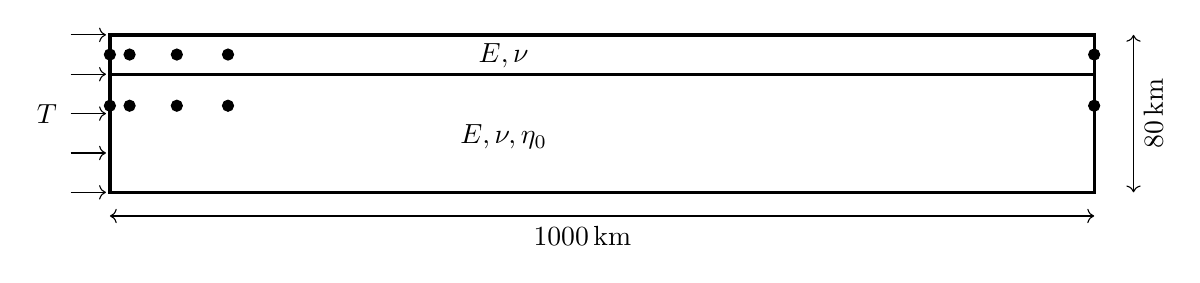
\begin{tikzpicture}
%\draw[step=0.5cm,gray,very thin] (0,0) grid (15,4); %background grid
\draw[very thick] (1,1)--(13.5,1)--(13.5,3)--(1,3)--cycle;  
\draw[very thick] (1,2.5)--(13.5,2.5);  
\draw[<->] (1,0.7)--(13.5,0.7);
\draw[<->] (14,1)--(14,3);
\node[] at (7,0.45) {$\SI{1000}{\km}$};
\node[rotate=90] at (14.25,2) {$\SI{80}{\km}$};
\node[] at (6,2.73) {$E,\nu$};
\node[] at (6,1.7) {$E,\nu,\eta_0$};
\draw[->] (0.5,3)--(0.95,3);
\draw[->] (0.5,2.5)--(0.95,2.5);
\draw[->] (0.5,2)--(0.95,2);
\draw[->] (0.5,1.5)--(0.95,1.5);
\draw[->] (0.5,1)--(0.95,1);
\node[] at (0.2,2) {$T$};

\filldraw[black] (1,2.75) circle (2pt);
\filldraw[black] (1,2.1) circle (2pt);

\filldraw[black] (1.25,2.75) circle (2pt);
\filldraw[black] (1.25,2.1) circle (2pt);

\filldraw[black] (1.85,2.75) circle (2pt);
\filldraw[black] (1.85,2.1) circle (2pt);

\filldraw[black] (2.5,2.75) circle (2pt);
\filldraw[black] (2.5,2.1) circle (2pt);

\filldraw[black] (13.5,2.75) circle (2pt);
\filldraw[black] (13.5,2.1) circle (2pt);
\end{tikzpicture}
\end{center}


After a thorough read of the paper, I have noticed quite a few problems:
\begin{itemize}
\item the paper is old and has been digitized but the figures are missing a lot of lines/shades/points ... this could be remedied by finding the article in a library.
\item in the intro it is stated: "Here we investigate the response of a lithosphere divided into upper elastic and lower uniform visco-elastic layers to simple boundary force and body force systems." The authors later talk about 'isostatic forces' opposing flexure. This means that buoyancy forces should be taken into account but there is no information about densities or gravity values!
\item little uncertainty about boundary conditions. is it free slip or no-slip on the right side ? Looking at fig 4, it looks like the vertical displacement is zero at x=1000km?
\item a Maxwell elasto-viscous rheology is used but this is only mentioned in the Appendix
\item the dimensions of the thinned or thickened areas is simply not mentioned. 
\item Fig~1 shows triangular elements. No mention is made of resolution, type of element, ndofs, resolution tests, any numerical detail whatsoever. Given the age of the paper, I would guess $P_1$
elements.
\item In the appendix they equate the viscous strain rate to $\sigma/4\eta$. Why 4 ?
\item it is also not clear whether the domain is ALE or fully Lagrangian: does it shorten?
\item the value of $T$ is never specified!
\item the paper was published 45 years ago, it is extremely unlikely any of the two authors is still available 
\end{itemize}

\begin{center}
\includegraphics[width=16cm]{images/viscoelasticity/kubo77}\\
{\captionfont Taken from \textcite{kubo77}. Measurement locations are indicated on 
the setup figure above. probably should be reversed}
\end{center}






%..........................................................
\subsubsection{Parallel-Plate Viscometer Problem - SNAC manual \label{v-e-snac}}

A parallel-plate viscometer problem is simulated, in which viscoelastic material is squeezed between two
parallel plates. The plates are moving at a constant velocity, $v_0$. Each plate has the length of $2L$ and 
is at a distance $2h$ from the other. No slip is assumed between the material and the plates. The approximate
analytical solution is given in the book by \textcite{jaeg69} (1969).

Model Setup: $L = 10~\si{\meter}$, $h=5~\si{\meter}$, viscosity $\eta=10^9~\si{\pascal\second}$, 
bulk modulus $K= 1.5~\si{\giga\pascal}$, shear modulus $\mu = 500~\si{\mega\pascal}$,
$v_0 = 10^{-4}~\si{\meter\per\second}$, $dt = 1~\si{\second}$ (results compared after 500 time steps),
mesh size: $20\times 10~\si{\meter}$, each element is a $1~\si{\meter}$ cube.

Due to the assumption of the original problem setup, artificial forces should be added to left and right
surfaces.

\begin{center}
\includegraphics[width=8cm]{images/viscoelasticity/snac_5}
\includegraphics[width=8cm]{images/viscoelasticity/snac_6}\\
{\captionfont 
Left: The initial mesh (blue) with the velocity boundary condition (red arrows);
Right: The second invariant of stress and velocities plotted on the deformed mesh. Colored arrows are
for SNAC’s solution, black ones for the analytic solution.}
\end{center}

$K=\lambda + \frac23 \mu$ so $\lambda=\frac{3500}{3}MPa$ ?

From wikipedia\footnote{\url{https://en.wikipedia.org/wiki/Lame_parameters}}
\[
\nu = \frac{3K-2\mu}{2(3K+\mu)} 
= \frac{4500-2*500}{2(4500+500)}
= \frac{3500}{10000}
= 0.35
\]
so we find that the material is {\color{orange} compressible $\nu=0.35$}

\[
E=\frac{9K\mu}{3K+\mu} 
=\frac{9*1500*500 MPa^2}{4500+500 MPa}
=\frac{9*1500*500}{5000} MPa
= 1350Mpa
\]


%..........................................................
\subsubsection{Relaxation after extention - Hassani syllabus}


{\color{orange} compressible $\nu=0.25$}

Un essai de relaxation consiste à imposer à un instant donné une déformation que 
l’on maintient constante par la suite. On observe alors comment évolue la contrainte au cours du temps.

The setup of the experiment is shown in the following figure:

\begin{center}
\includegraphics[width=9cm]{images/viscoelasticity/hassani_1}
\end{center}

The total duration of the experiment is $T=\SI{5}{\year}\simeq \SI{15.75e7}{\second}$.
The duration of the loading is $T/10=\SI{6}{months}$ while the duration 
of the subsequent relaxation is then $9T/10\simeq 4.5~\si{\year}$.

The loading velocity is $v=\SI{1}{\mm\per\year}\simeq \SI{3.17e-11}{\meter\per\second}$.
The sample has size $L\times L/2 = 20\times10\si{cm}$ and 
the strain rate is then $v/L \simeq \SI{1.5e-10}{\per\second}$.
Young's modulus is set to \SI{1e11}{\pascal} and the Poisson ratio is 0.25, i.e.
$\mu=40~\si{GPa}$. The viscosity is set to $\eta_0=\SI{1e18}{\pascal\second}$.
The Maxwell time is then $t_M=\eta/\mu=0.8~\si{\year}$, which is also the time it takes 
to reduce the maximum stress by a factor $e$.

\begin{center}
\includegraphics[width=6cm]{images/viscoelasticity/hassani_2}
\end{center}



 \label{chapt:viscoelasticity}

%==================================================================================================
%==================================================================================================
%\clearpage


%\documentclass[a4paper,11pt]{report}
%%%%%%%%%%%%%%%%%%%%%%%%%%%%%%%%%%%%%%%%%%%%%%%%%%%%%%%%%%%%%%%%%%%%%%%%%%%%%%%%%%%%%%%%%%%%%%%%%%%

\usepackage[utf8]{inputenc}
\usepackage{graphicx}
\usepackage{pdflscape}
\usepackage[cm]{fullpage}
\usepackage{upgreek}
\usepackage{bm}
\usepackage{mdframed}
\usepackage{amsmath}
\usepackage{amsfonts}
\usepackage[dvipsnames]{xcolor} 
\usepackage{dsfont}
\usepackage{gensymb} %\degree
\usepackage{listings}
\usepackage{stmaryrd}
\usepackage{multicol}
\usepackage{lipsum}
\usepackage{verbatim}
\usepackage[colorinlistoftodos,prependcaption,textsize=tiny]{todonotes}
\usepackage{csquotes}

\usepackage{siunitx} 
\DeclareSIUnit\year{yr}
\DeclareSIUnit\day{day}

\renewcommand{\chaptername}{Stone}

\newcommand{\aspect}{{\textsc{Aspect~}{}}}
\newcommand{\elefant}{{\textsc{Elefant~}{}}}
\newcommand{\citcoms}{{\textsc{CitcomS~}{}}}
\newcommand{\citcomsve}{{\textsc{CitcomSVE~}{}}}
\newcommand{\fantom}{{\textsc{Fantom~}{}}}
\newcommand{\sulec}{{\textsc{Sulec~}{}}}
\newcommand{\sopale}{{\textsc{Sopale~}{}}}
\newcommand{\douar}{{\textsc{Douar~}{}}}
\newcommand{\ghost}{{\textsc{Ghost~}{}}}
\newcommand{\fluidity}{{\textsc{Fluidity~}{}}}
\newcommand{\sepran}{{\textsc{Sepran~}{}}}
\newcommand{\stone}{{\color{teal} {\textsc{stone~}}}}
\newcommand{\etal}{{\it et al.~}}
\newcommand{\nn}{\nonumber}
\newcommand{\A}{{\mathbb{A}}}
\newcommand{\K}{{\mathbb{K}}}
\newcommand{\J}{{\mathbb{J}}}
\newcommand{\G}{{\mathbb{G}}}
\newcommand{\Z}{{\mathbb{Z}}}
\newcommand{\C}{{\mathbb{C}}}
\newcommand{\W}{{\mathbb{W}}}
\newcommand{\R}{{\mathbb{R}}}
\newcommand{\M}{{\mathbb{M}}}
\newcommand{\N}{{\mathbb{N}}}
\newcommand{\LLL}{{\mathbb{L}}}
\newcommand{\SSS}{{\mathbb{S}}}
\newcommand{\QQQ}{{\color{violet}\cal Q}}
\newcommand{\FFF}{{\color{violet}\cal F}}
\newcommand{\III}{{\color{PineGreen}\cal I}}
\newcommand{\KKK}{{\color{RoyalBlue}\cal K}}
\newcommand{\HH}{{\mathbb{H}}}
\newcommand{\Literature}{\includegraphics[height=4mm]{images/lit} {\sffamily Relevant Literature}}
\newcommand{\captionfont}{\tiny}
\newcommand{\pythonfile}{\color{blue} \sffamily }
\newcommand{\shellscriptfile}{\color{purple} \sffamily }
\newcommand{\asciifile}{\color{olive} \sffamily }
\newcommand{\OK}{{\bf OK}}
\newcommand{\filenamefont }{\sl }
\newcommand{\foldernamefont }{\it }
\newcommand{\codefont}{\bfseries\ttfamily}
\newcommand{\Ranb}{{\mathsf{Ra}}}
\newcommand{\Rbnb}{{\mathsf{Rb}}}
\newcommand{\Renb}{{\mathsf{Re}}}
\newcommand{\Nunb}{{\mathsf{Nu}}}
\newcommand{\Prnb}{{\mathsf{Pr}}}
\newcommand{\Penb}{{\mathsf{Pe}}}
\newcommand{\Dinb}{{\mathsf{Di}}}
\newcommand{\Mnb}{{\mathsf{M}}}
\newcommand{\python}{\color{darkgray} \sffamily }
\newcommand{\bN}{{\mathcal{N}}}
\newcommand{\qx}{\underset{\tiny x}{q}}
\newcommand{\qy}{\underset{\tiny y}{q}}
\newcommand{\nx}{\underset{\tiny x}{n}}
\newcommand{\ny}{\underset{\tiny y}{n}}
\newcommand{\qhx}{\underset{\tiny x}{q_h}}
\newcommand{\qhy}{\underset{\tiny y}{q_h}}
\newcommand{\qix}{\underset{\tiny x}{q_i}}
\newcommand{\qiy}{\underset{\tiny y}{q_i}}
\newcommand{\Tx}{\underset{\tiny x}{T}}
\newcommand{\Ty}{\underset{\tiny y}{T}}
\newcommand{\blueqx}{  {\color{blue} \underset{\tiny x}{q}  }  }
\newcommand{\blueqy}{  {\color{blue} \underset{\tiny y}{q}  }  }
\newcommand{\blueT}{  {\color{blue} T}  }
\newcommand{\brownT}{  {\color{brown} T}  }
\newcommand{\brownqx}{  {\color{brown} \underset{\tiny x}{q}  }  }
\newcommand{\brownqy}{  {\color{brown} \underset{\tiny y}{q}  }  }
\newcommand\norm[1]{\left\lVert#1\right\rVert}

\newcommand{\QonePzero}{${Q}_1\times P_0$}
\newcommand{\QtwoQone}{${Q}_2\times Q_1$}
\newcommand{\QthreeQtwo}{${Q}_3\times Q_2$}
\newcommand{\QfourQthree}{${Q}_4\times Q_3$}
\newcommand{\QtwoPmone}{${Q}_2\times P_{-1}$}

\definecolor{carrotorange}{rgb}{0.93, 0.57, 0.13}
\definecolor{chestnut}{rgb}{0.8, 0.36, 0.36}

\newcommand{\nineteensixty}{{\color{chestnut}\bf 1960}}
\newcommand{\nineteensixtyone}{{\color{chestnut}\bf 1961}}
\newcommand{\nineteensixtytwo}{{\color{chestnut}\bf 1962}}
\newcommand{\nineteensixtythree}{{\color{chestnut}\bf 1963}}
\newcommand{\nineteensixtyfour}{{\color{chestnut}\bf 1964}}
\newcommand{\nineteensixtyfive}{{\color{chestnut}\bf 1965}}
\newcommand{\nineteensixtysix}{{\color{chestnut}\bf 1966}}
\newcommand{\nineteensixtyseven}{{\color{chestnut}\bf 1967}}
\newcommand{\nineteensixtyeight}{{\color{chestnut}\bf 1968}}
\newcommand{\nineteensixtynine}{{\color{chestnut}\bf 1969}}

\newcommand{\nineteenseventy}{{\color{carrotorange}\bf 1970}}
\newcommand{\nineteenseventyone}{{\color{carrotorange}\bf 1971}}
\newcommand{\nineteenseventytwo}{{\color{carrotorange}\bf 1972}}
\newcommand{\nineteenseventythree}{{\color{carrotorange}\bf 1973}}
\newcommand{\nineteenseventyfour}{{\color{carrotorange}\bf 1974}}
\newcommand{\nineteenseventyfive}{{\color{carrotorange}\bf 1975}}
\newcommand{\nineteenseventysix}{{\color{carrotorange}\bf 1976}}
\newcommand{\nineteenseventyseven}{{\color{carrotorange}\bf 1977}}
\newcommand{\nineteenseventyeight}{{\color{carrotorange}\bf 1978}}
\newcommand{\nineteenseventynine}{{\color{carrotorange}\bf 1979}}

\newcommand{\nineteeneighty}{{\color{violet}\bf 1980}}
\newcommand{\nineteeneightyone}{{\color{violet}\bf 1981}}
\newcommand{\nineteeneightytwo}{{\color{violet}\bf 1982}}
\newcommand{\nineteeneightythree}{{\color{violet}\bf 1983}}
\newcommand{\nineteeneightyfour}{{\color{violet}\bf 1984}}
\newcommand{\nineteeneightyfive}{{\color{violet}\bf 1985}}
\newcommand{\nineteeneightysix}{{\color{violet}\bf 1986}}
\newcommand{\nineteeneightyseven}{{\color{violet}\bf 1987}}
\newcommand{\nineteeneightyeight}{{\color{violet}\bf 1988}}
\newcommand{\nineteeneightynine}{{\color{violet}\bf 1989}}

\newcommand{\nineteenninety}{{\color{red}\bf 1990}}
\newcommand{\nineteenninetyone}{{\color{red}\bf 1991}}
\newcommand{\nineteenninetytwo}{{\color{red}\bf 1992}}
\newcommand{\nineteenninetythree}{{\color{red}\bf 1993}}
\newcommand{\nineteenninetyfour}{{\color{red}\bf 1994}}
\newcommand{\nineteenninetyfive}{{\color{red}\bf 1995}}
\newcommand{\nineteenninetysix}{{\color{red}\bf 1996}}
\newcommand{\nineteenninetyseven}{{\color{red}\bf 1997}}
\newcommand{\nineteenninetyeight}{{\color{red}\bf 1998}}
\newcommand{\nineteenninetynine}{{\color{red}\bf 1999}}
\newcommand{\twothousand}{{\color{teal}\bf 2000}}
\newcommand{\twothousandone}{{\color{teal}\bf 2001}}
\newcommand{\twothousandtwo}{{\color{teal}\bf 2002}}
\newcommand{\twothousandthree}{{\color{teal}\bf 2003}}
\newcommand{\twothousandfour}{{\color{teal}\bf 2004}}
\newcommand{\twothousandfive}{{\color{teal}\bf 2005}}
\newcommand{\twothousandsix}{{\color{teal}\bf 2006}}
\newcommand{\twothousandseven}{{\color{teal}\bf 2007}}
\newcommand{\twothousandeight}{{\color{teal}\bf 2008}}
\newcommand{\twothousandnine}{{\color{teal}\bf 2009}}
\newcommand{\twothousandten}{{\color{blue}\bf 2010}}
\newcommand{\twothousandeleven}{{\color{blue}\bf 2011}}
\newcommand{\twothousandtwelve}{{\color{blue}\bf 2012}}
\newcommand{\twothousandthirteen}{{\color{blue}\bf 2013}}
\newcommand{\twothousandfourteen}{{\color{blue}\bf  2014}}
\newcommand{\twothousandfifteen}{{\color{blue}\bf  2015}}
\newcommand{\twothousandsixteen}{{\color{blue}\bf 2016}}
\newcommand{\twothousandseventeen}{{\color{blue}\bf 2017}}
\newcommand{\twothousandeighteen}{{\color{blue}\bf 2018}}
\newcommand{\twothousandnineteen}{{\color{blue}\bf 2019}}
\newcommand{\twothousandtwenty}{{\color{purple}\bf 2020}}
\newcommand{\twothousandtwentyone}{{\color{purple}\bf 2021}}
\newcommand{\twothousandtwentytwo}{{\color{purple}\bf 2022}}
\newcommand{\twothousandtwentythree}{{\color{purple}\bf 2023}}
\newcommand{\twothousandtwentyfour}{{\color{purple}\bf 2024}}
\newcommand{\twothousandtwentyfive}{{\color{purple}\bf 2025}}

\newcommand\todoin[2][]{\todo[inline, #1]{
\begin{minipage}{\textwidth-3pt}#2\end{minipage}}}


\usepackage{tikz}
\usetikzlibrary{arrows, arrows.meta}

\usepackage{hyperref}
\hypersetup{
colorlinks,
citecolor=black,
filecolor=black,
linkcolor=violet,
urlcolor=black}

\lstset{ 
  language=Python,
  backgroundcolor=\color{white},   % choose the background color; you must add \usepackage{color} or \usepackage{xcolor}; should come as last argument
  basicstyle=\scriptsize,        % the size of the fonts that are used for the code
  breakatwhitespace=false,         % sets if automatic breaks should only happen at whitespace
  breaklines=true,                 % sets automatic line breaking
  captionpos=b,                    % sets the caption-position to bottom
  frame=single,                    % adds a frame around the code
  keepspaces=true,                 % keeps spaces in text, useful for keeping indentation of code (possibly needs columns=flexible)
  keywordstyle=\color{blue},       % keyword style
}


\newcommand{\inpython}{\fbox{\textbf{\large \color{teal} P}}}
\newcommand{\injulia}{\fbox{\textbf{\large \color{purple} J}}}
\newcommand{\infortran}{\fbox{\textbf{\large \color{orange} F}}}


\usepackage{xr}
\externaldocument[MMM-]{manual}

%%%%%%%%%%%%%%%%%%%%%%%%%%%%%%%%%%%%%%%%%%%%%%%%%%%%%%%%%%%

\usepackage{amsthm}
\newtheorem*{remark}{Remark}
\newtheorem{problem}{problem:}
\newtheorem{problem-bonus}{problem*}

%%%%%%%%%%%%%%%%%%%%%%%%%%%%%%%%%%%%%%%%%%%%%%%%%%%%%%%%%%%
%Bibliography stuff
%%%%%%%%%%%%%%%%%%%%%%%%%%%%%%%%%%%%%%%%%%%%%%%%%%%%%%%%%%%
\usepackage[maxnames=6]{biblatex}
\addbibresource{biblio_geosciences.bib}


%%%%%%%%%%%%%%%%%%%%%%%%%%%%%%%%%%%%%%%%%%%%%%%%%%%%%%%%%%%%%%%%%%%%%%%%%%%%%%%%%%%%%%%%%%%%%%%%%%%

\author{C. Thieulot}
\title{All the stones}

%%%%%%%%%%%%%%%%%%%%%%%%%%%%%%%%%%%%%%%%%%%%%%%%%%%%%%%%%%%

\usepackage{multind}
\makeindex{contributors}
\makeindex{stopics}

%%%%%%%%%%%%%%%%%%%%%%%%%%%%%%%%%%%%%%%%%%%%%%%%%%%%%%%%%%%%%%%%%%%%%%%%%%%%%%%%%%%%%%%%%%%%%%%%%%%
\begin{document}
\thispagestyle{empty}
\includegraphics[width=0.9\linewidth]{images/frontpage/frontpage.png}

\maketitle
\tableofcontents

%%%%%%%%%%%%%%%%%%%%%%%%%%%%%%%%%%%%%%%%%%%%%%%%%%%%%%%%%%%%%%%%%%%%%%%%%%%%%%%%%%%%%%%%%%%%%%%%%%%
\chapter*{Naming convention for every stone and elefant }

These have evolved in the first two years so that the early stones may not 
follow these conventions (yet).

\begin{tabular}{p{2.5cm}p{14cm}}
\hline
Variable & meaning \\
\hline
\hline
{\tt mV}    & number $m_\upnu$ of velocity nodes in the element \\
{\tt mP}    & number $m_p$ of pressure nodes in the element \\
{\tt mT}    & number $m_T$ of temperature nodes in the element \\
{\tt ndofV} & number of velocity degrees of freedom per velocity node \\
{\tt ndofP} & number of pressure degrees of freedom per pressure node \\
{\tt NV}    & total number of velocity nodes \\
{\tt NfemV} & total number of velocity degrees of freedom \\
{\tt NfemP} & total number of pressure degrees of freedom \\
{\tt Nfem}  & total number of degrees of freedom \\
{\tt nelx,nely,nelz} & number of elements in each direction \\
{\tt nel}   & total number of elements \\
{\tt nqel}  & number of quadrature points per element \\
{\tt xq,yq,zq} & coordinates of a quadrature point \\
{\tt uq,vq,wq} & velocity at a quadrature point \\
{\tt pq}   & pressure at a quadrature point \\
{\tt etaq} & viscosity value at a quadrature point \\
{\tt rhoq} & density value at a quadrature point \\
{\tt dt}   & time step $\delta t$\\ 
{\tt gx,gy,gz} & components of the gravity vector \\
{\tt jcob} & determinant of the Jacobian matrix \\
\hline
\end{tabular}

\vspace{.5cm}

\begin{tabular}{p{3.5cm}p{12.5cm}}
\hline
Array & meaning \\
\hline
\hline
{\tt iconV} & connectivity array for velocity nodes \\
{\tt iconP} & connectivity array for pressure nodes \\
{\tt qcoords\_r} & contains the $r$ coordinates of the {\tt nel} quadrature points \\
{\tt qcoords\_s} & contains the $s$ coordinates of the {\tt nel} quadrature points \\
{\tt qcoords\_t} & contains the $t$ coordinates of the {\tt nel} quadrature points \\
{\tt qweights} & contains the weights associated to the {\tt nel} quadrature points \\
{\tt xV,yV,zV} & coordinates of the {\tt NV} velocity nodes \\
{\tt xP,yP,zP} & coordinates of the {\tt NP} pressure nodes \\
{\tt bc\_fix} & boolean array of size {\tt NfemV}. Is true if a boundary condition
                is specify at a dof \\
{\tt bc\_val} & value of the boundary condition at a given dof \\
{\tt u,v,w} & velocity components \\ 
{\tt p} & pressure \\ 
{\tt q} & pressure projected onto the velocity nodes\\
{\tt NNNV} & velocity basis functions values at a quadrature point \\
{\tt dNNNVdr} & velocity basis functions derivatives values at a quadrature point \\
{\tt dNNNVds} & velocity basis functions derivatives values at a quadrature point \\
{\tt dNNNVdt} & velocity basis functions derivatives values at a quadrature point \\
{\tt NNNP} & pressure basis functions values at a quadrature point \\
{\tt b\_mat} & elemental gradient matrix ${\bm B}$ \\
{\tt K\_el}  & elemental stiffness matrix $\K_{el}$ \\
{\tt G\_el}  & elemental gradient matrix $\G_{el}$ \\
{\tt N\_mat}  & elemental ${\bm N}$ matrix \\
{\tt a\_mat}  & fully assembled Stokes matrix \\
{\tt A\_sparse} & Stokes matrix in {\tt lil\_matrix} format \\
{\tt exx,eyy,exy,...} & components of the strain rate tensor (elemental or nodal array)\\
{\tt tauxx,tauyy,tauxy,...} & components of the deviatoric stress tensor (elemental or nodal array)\\
{\tt jcb} & 2x2 or 3x3 Jacobian matrix \\
{\tt jcbi} & inverse of the Jacobian matrix \\
{\tt rhs} & right hand side vector \\
{\tt sol} & solution vector returned by the solver\\
\hline
\end{tabular}

\vspace{.5cm}

\begin{tabular}{p{2cm}p{14cm}}
\hline
Function & meaning \\
\hline
{\tt NNV}    & function which returns the value of all velocity basis functions 
               ${\cal N}_i^\upnu$ at a given location\\
{\tt dNNVdr} & function which returns the value of all velocity basis functions 
               ${\cal N}_i^\upnu$ derivative with respect to $r$ at a given location\\
{\tt dNNVds} & function which returns the value of all velocity basis functions 
               ${\cal N}_i^\upnu$ derivative with respect to $s$ at a given location\\
{\tt dNNVdt} & function which returns the value of all velocity basis functions 
               ${\cal N}_i^\upnu$ derivative with respect to $t$ at a given location\\
{\tt NNP}    & function which returns the value of all pressure basis functions 
               ${\cal N}_i^P$ at a given location\\
{\tt bx} & \\
{\tt by} & \\
{\tt bz} & \\
\hline
\end{tabular}



\chapter*{Stone 00: mesh generation in 1D, 2D, 3D \label{f00}} %%%%%%%%%%%%%%%%%%%%%%%%%%%%%%%%%%%% 00
\begin{flushright} {\tiny {\color{gray} python\_codes/fieldstone\_00/text.tex}} \end{flushright}


%--------------------------------------------
\subsection*{The node layout}

Let us start in one dimension. We wish to generate a 
set of $N$ discrete and equidistant $x$ coordinates 
between $0$ and $L_x$:

\begin{center}
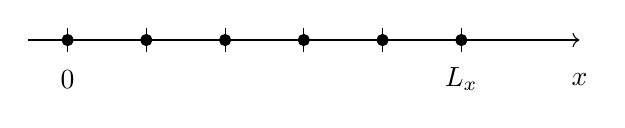
\begin{tikzpicture}
%\draw[fill=gray!23,gray!23](0,0) rectangle (8,2);
%\draw[step=0.5cm,gray,very thin] (0,0) grid (8,2); %background grid
\draw [->] (0.5,1) -- (7.5,1);
\draw[-] (1,0.85)--(1,1.15);
\draw[-] (2,0.85)--(2,1.15);
\draw[-] (3,0.85)--(3,1.15);
\draw[-] (4,0.85)--(4,1.15);
\draw[-] (5,0.85)--(5,1.15);
\draw[-] (6,0.85)--(6,1.15);
\node[] at (1,0.5) {$0$};
\node[] at (6,0.5) {$L_x$};
\node[] at (7.5,0.5) {$x$};
\draw[black,fill=black] (1,1)   circle (2pt);
\draw[black,fill=black] (2,1)   circle (2pt);
\draw[black,fill=black] (3,1)   circle (2pt);
\draw[black,fill=black] (4,1)   circle (2pt);
\draw[black,fill=black] (5,1)   circle (2pt);
\draw[black,fill=black] (6,1)   circle (2pt);
\end{tikzpicture}
\end{center}

\noindent
The distance between two consecutive coordinates is 
\[
h = \frac{L_x}{N-1}
\]
This simply translates as follows in Python:
\begin{lstlisting}
N=10
Lx=1
h=Lx/(N-1)
for i in range(0,N):
    print(i*h)
\end{lstlisting}

Since $i$ ranges from 0 to $N-1$ (because ... python!) the generated values go from 0 to $L_x$. 
Obviously I am doing this because I later wish to reuse these coordinates 
so I also wish to store them in an array.
I therefore need to declare and array of size $N$ which will 
contain all $N$ coordinates:
\begin{lstlisting}
import numpy as np
N=10
Lx=1
h=Lx/(N-1)
x=np.zeros(NV,dtype=np.float64)
for i in range(0,N):
    x[i]=i*h
\end{lstlisting}

What if now I wished the $N$ nodes (i.e. the coordinates of all points) to be placed between two arbitrary coordinates $x_{min}$ and $x_{max}$?

\begin{center}
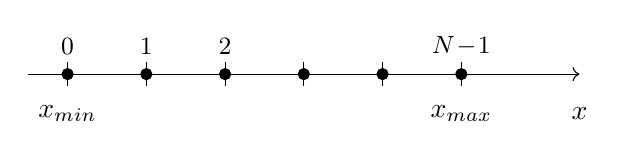
\begin{tikzpicture}
%\draw[fill=gray!23,gray!23](0,0) rectangle (8,2);
%\draw[step=0.5cm,gray,very thin] (0,0) grid (8,2); %background grid
\draw [->] (0.5,1) -- (7.5,1);
\draw[-] (1,0.85)--(1,1.15);
\draw[-] (2,0.85)--(2,1.15);
\draw[-] (3,0.85)--(3,1.15);
\draw[-] (4,0.85)--(4,1.15);
\draw[-] (5,0.85)--(5,1.15);
\draw[-] (6,0.85)--(6,1.15);
\node[] at (1,0.5) {$x_{min}$};
\node[] at (6,0.5) {$x_{max}$};
\node[] at (7.5,0.5) {$x$};
\draw[black,fill=black] (1,1)   circle (2pt);
\draw[black,fill=black] (2,1)   circle (2pt);
\draw[black,fill=black] (3,1)   circle (2pt);
\draw[black,fill=black] (4,1)   circle (2pt);
\draw[black,fill=black] (5,1)   circle (2pt);
\draw[black,fill=black] (6,1)   circle (2pt);
\node[] at (1,1.35) {\small 0};
\node[] at (2,1.35) {\small 1};
\node[] at (3,1.35) {\small 2};
\node[] at (6,1.35) {\small $N\!-\!1$};
\end{tikzpicture}
\end{center}

\noindent In this case the length of the domain is $L_x=x_{max}-x_{min}$, and the above code becomes:
\begin{lstlisting}
import numpy as np
N=10
xmin=-4
xmax=3
h=(xmax-xmin)/(N-1)
x=np.zeros(N,dtype=np.float64)
for i in range(0,N):
    x[i]=xmin+i*h
\end{lstlisting}
Note the presence of $x_{min}$ in the last line! 

\vspace{.8cm}

Unfortunately the world is definitely not one-dimensional, so 
I may want to build a two-dimensional grid spanning the domain 
$[0,L_x]\times[0,L_y]$ as depicted here:



\begin{center}
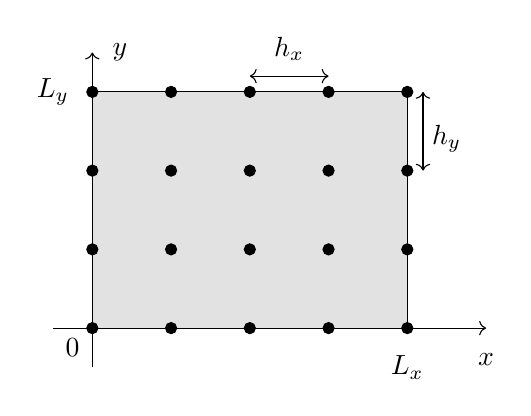
\begin{tikzpicture}
\draw[fill=gray!23,gray!23](1,1) rectangle (5,4);
%\draw[step=0.5cm,gray,very thin] (0,0) grid (7,5); 
\draw [->] (0.5,1) -- (6,1);
\draw [->] (1,0.5) -- (1,4.5);
\node[] at (0.75,0.75) {$0$};
\node[] at (5,0.5) {$L_x$};
\node[] at (0.5,4) {$L_y$};
\node[] at (6,0.6) {$x$};
\node[] at (1.35,4.5) {$y$};
\draw[-] (1,1)--(5,1)--(5,4)--(1,4)--cycle;
\draw[black,fill=black] (1,1)   circle (2pt);
\draw[black,fill=black] (2,1)   circle (2pt);
\draw[black,fill=black] (3,1)   circle (2pt);
\draw[black,fill=black] (4,1)   circle (2pt);
\draw[black,fill=black] (5,1)   circle (2pt);
\draw[black,fill=black] (1,2)   circle (2pt);
\draw[black,fill=black] (2,2)   circle (2pt);
\draw[black,fill=black] (3,2)   circle (2pt);
\draw[black,fill=black] (4,2)   circle (2pt);
\draw[black,fill=black] (5,2)   circle (2pt);
\draw[black,fill=black] (1,3)   circle (2pt);
\draw[black,fill=black] (2,3)   circle (2pt);
\draw[black,fill=black] (3,3)   circle (2pt);
\draw[black,fill=black] (4,3)   circle (2pt);
\draw[black,fill=black] (5,3)   circle (2pt);
\draw[black,fill=black] (1,4)   circle (2pt);
\draw[black,fill=black] (2,4)   circle (2pt);
\draw[black,fill=black] (3,4)   circle (2pt);
\draw[black,fill=black] (4,4)   circle (2pt);
\draw[black,fill=black] (5,4)   circle (2pt);
\draw[<->] (5.2,3)--(5.2,4);
\draw[<->] (3,4.2)--(4,4.2);
\node[] at (3.5,4.55) {$h_x$};
\node[] at (5.5,3.4) {$h_y$};
\end{tikzpicture}
\end{center}

\noindent There are now $N=N_x \times N_y$ nodes in the mesh, 
and we need to define the mesh spacing in both the $x$ and $y$
direction:
\[
h_x = \frac{L_x}{N_x-1}
\qquad\qquad
h_y = \frac{L_y}{N_y-1}
\]
From our experience with the 1D case, it seems logical to 
resort to a double for loop, one in the $x$ direction, 
one in the $y$ direction. 
However we must now make a decision as to which loop is inside the other (inner loop vs. outer loop). In essence, I must decide between 
\begin{lstlisting}
#approach 1
for i in range(0,Nx):
    for j in range(0,Ny):
\end{lstlisting}
and
\begin{lstlisting}
#approach 2
for j in range(0,Ny):
    for i in range(0,Nx):
\end{lstlisting}
As it turns out, I need not decide, both options are equally valid as we will see.
I now fix $N_x=4$ and $N_y=3$ so that the mesh contains 12 nodes:

\begin{center}
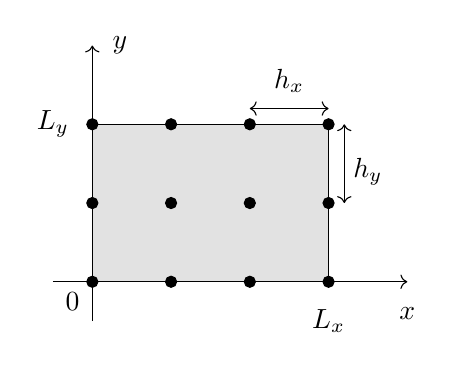
\begin{tikzpicture}
\draw[fill=gray!23,gray!23](1,1) rectangle (4,3);
%\draw[step=0.5cm,gray,very thin] (0,0) grid (7,5); 
\draw [->] (0.5,1) -- (5,1);
\draw [->] (1,0.5) -- (1,4);
\node[] at (0.75,0.75) {$0$};
\node[] at (4,0.5) {$L_x$};
\node[] at (0.5,3) {$L_y$};
\node[] at (5,0.6) {$x$};
\node[] at (1.35,4) {$y$};
\draw[-] (1,1)--(4,1)--(4,3)--(1,3)--cycle;
\draw[black,fill=black] (1,1)   circle (2pt);
\draw[black,fill=black] (2,1)   circle (2pt);
\draw[black,fill=black] (3,1)   circle (2pt);
\draw[black,fill=black] (4,1)   circle (2pt);
\draw[black,fill=black] (1,2)   circle (2pt);
\draw[black,fill=black] (2,2)   circle (2pt);
\draw[black,fill=black] (3,2)   circle (2pt);
\draw[black,fill=black] (4,2)   circle (2pt);
\draw[black,fill=black] (1,3)   circle (2pt);
\draw[black,fill=black] (2,3)   circle (2pt);
\draw[black,fill=black] (3,3)   circle (2pt);
\draw[black,fill=black] (4,3)   circle (2pt);
\draw[<->] (4.2,2)--(4.2,3);
\draw[<->] (3,3.2)--(4,3.2);
\node[] at (3.5,3.55) {$h_x$};
\node[] at (4.5,2.4) {$h_y$};
\end{tikzpicture}
\end{center}

\noindent Looking at approach \#1, I can include a print statement inside the loops as follows:
\begin{lstlisting}
#option 1
Nx=4
Ny=3
for i in range(0,Nx):
    for j in range(0,Ny):
        print('i=',i,'; j=',j)
\end{lstlisting}
If I was to run this code it would display (I first exhaust the $j$ values from the inner most loop before I switch to a different $i$ value):
\begin{lstlisting}
i= 0  ; j= 0
i= 0  ; j= 1
i= 0  ; j= 2
i= 1  ; j= 0
i= 1  ; j= 1
i= 1  ; j= 2
i= 2  ; j= 0
i= 2  ; j= 1
i= 2  ; j= 2
i= 3  ; j= 0
i= 3  ; j= 1
i= 3  ; j= 2
\end{lstlisting}
This means that the code is going through the nodes in the following order:
\begin{center}
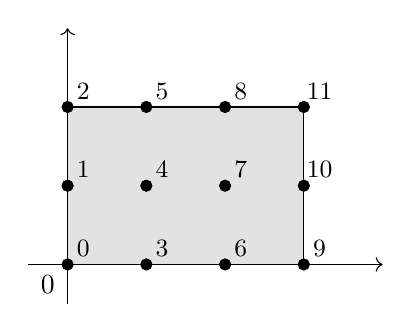
\begin{tikzpicture}
\draw[fill=gray!23,gray!23](1,1) rectangle (4,3);
%\draw[step=0.5cm,gray,very thin] (0,0) grid (7,5); 
\draw [->] (0.5,1) -- (5,1);
\draw [->] (1,0.5) -- (1,4);
\node[] at (0.75,0.75) {$0$};
\draw[-] (1,1)--(4,1)--(4,3)--(1,3)--cycle;
\draw[black,fill=black] (1,1)   circle (2pt);
\draw[black,fill=black] (2,1)   circle (2pt);
\draw[black,fill=black] (3,1)   circle (2pt);
\draw[black,fill=black] (4,1)   circle (2pt);
\draw[black,fill=black] (1,2)   circle (2pt);
\draw[black,fill=black] (2,2)   circle (2pt);
\draw[black,fill=black] (3,2)   circle (2pt);
\draw[black,fill=black] (4,2)   circle (2pt);
\draw[black,fill=black] (1,3)   circle (2pt);
\draw[black,fill=black] (2,3)   circle (2pt);
\draw[black,fill=black] (3,3)   circle (2pt);
\draw[black,fill=black] (4,3)   circle (2pt);
\node[] at (1.2,1.2) {\small $0$};
\node[] at (2.2,1.2) {\small $3$};
\node[] at (3.2,1.2) {\small $6$};
\node[] at (4.2,1.2) {\small $9$};
\node[] at (1.2,2.2) {\small $1$};
\node[] at (2.2,2.2) {\small $4$};
\node[] at (3.2,2.2) {\small $7$};
\node[] at (4.2,2.2) {\small $10$};
\node[] at (1.2,3.2) {\small $2$};
\node[] at (2.2,3.2) {\small $5$};
\node[] at (3.2,3.2) {\small $8$};
\node[] at (4.2,3.2) {\small $11$};
\end{tikzpicture}
\end{center}



Turning now to approach \#2, the same print statement will now yield:
\begin{lstlisting}
i= 0 ; j= 0
i= 1 ; j= 0
i= 2 ; j= 0
i= 3 ; j= 0
i= 0 ; j= 1
i= 1 ; j= 1
i= 2 ; j= 1
i= 3 ; j= 1
i= 0 ; j= 2
i= 1 ; j= 2
i= 2 ; j= 2
i= 3 ; j= 2
\end{lstlisting}
and this corresponds then to the following order: 
\begin{center}
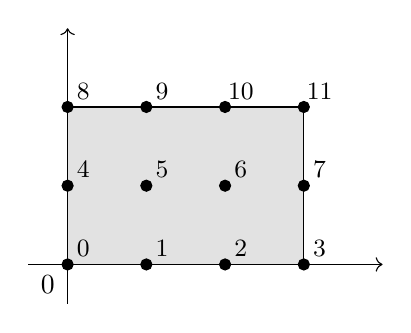
\begin{tikzpicture}
\draw[fill=gray!23,gray!23](1,1) rectangle (4,3);
%\draw[step=0.5cm,gray,very thin] (0,0) grid (7,5); 
\draw [->] (0.5,1) -- (5,1);
\draw [->] (1,0.5) -- (1,4);
\node[] at (0.75,0.75) {$0$};
\draw[-] (1,1)--(4,1)--(4,3)--(1,3)--cycle;
\draw[black,fill=black] (1,1)   circle (2pt);
\draw[black,fill=black] (2,1)   circle (2pt);
\draw[black,fill=black] (3,1)   circle (2pt);
\draw[black,fill=black] (4,1)   circle (2pt);
\draw[black,fill=black] (1,2)   circle (2pt);
\draw[black,fill=black] (2,2)   circle (2pt);
\draw[black,fill=black] (3,2)   circle (2pt);
\draw[black,fill=black] (4,2)   circle (2pt);
\draw[black,fill=black] (1,3)   circle (2pt);
\draw[black,fill=black] (2,3)   circle (2pt);
\draw[black,fill=black] (3,3)   circle (2pt);
\draw[black,fill=black] (4,3)   circle (2pt);
\node[] at (1.2,1.2) {\small $0$};
\node[] at (2.2,1.2) {\small $1$};
\node[] at (3.2,1.2) {\small $2$};
\node[] at (4.2,1.2) {\small $3$};
\node[] at (1.2,2.2) {\small $4$};
\node[] at (2.2,2.2) {\small $5$};
\node[] at (3.2,2.2) {\small $6$};
\node[] at (4.2,2.2) {\small $7$};
\node[] at (1.2,3.2) {\small $8$};
\node[] at (2.2,3.2) {\small $9$};
\node[] at (3.2,3.2) {\small $10$};
\node[] at (4.2,3.2) {\small $11$};
\end{tikzpicture}
\end{center}

\noindent In the end, we see that both approaches yield a valid 
numbering scheme, one is 'lines first' , the other 'columns first'.

In what follows I focus on approach \#2, only because it seems more 'natural' to me than the other one (it goes from left to right, then bottom to top). 
Our proto-code then looks like this:
\begin{lstlisting}
Lx=10
Ly=8
Nx=4
Ny=3
N=Nx*Ny
hx=Lx/(Nx-1)
hy=Ly/(Ny-1)
x=np.zeros(N,dtype=np.float64)
y=np.zeros(N,dtype=np.float64)
for j in range(0,Ny):
    for i in range(0,Nx):
        x[?]=i*hx
        y[?]=j*hy
\end{lstlisting}
Note that I have left two question marks. One may want to replace these by $i$ and $j$, 
following our experience in the 1D case. However, remember that $i$ ($j$) ranges between 
$0$ and $N_x-1=3$ ($0$ and $N_y-1=2$ respectively) but we need to assign and store the 
coordinates of all 12 nodes. 

So what should I write instead of question marks? Effectively, I need some form of counter 
so that every time the inner loop is executed the counter is incremented by one. 
When all $i,j$ combinations are exhausted this counter should have reached the 
last node. Such a counter can be implemented as follows:
\begin{lstlisting}
counter=0
for j in range(0,Ny):
    for i in range(0,Nx):
        print('counter=',counter,'i=',i,'; j=',j,j*Nx+i)
        counter+=1
\end{lstlisting}
It must be initialised to zero, and it is incremented $N_x \cdot N_y$ times.
Running this code would yield 
\begin{lstlisting}
counter=  0 i= 0 ; j= 0
counter=  1 i= 1 ; j= 0
counter=  2 i= 2 ; j= 0
counter=  3 i= 3 ; j= 0
counter=  4 i= 0 ; j= 1
counter=  5 i= 1 ; j= 1
counter=  6 i= 2 ; j= 1
counter=  7 i= 3 ; j= 1
counter=  8 i= 0 ; j= 2
counter=  9 i= 1 ; j= 2
counter= 10 i= 2 ; j= 2
counter= 11 i= 3 ; j= 2
\end{lstlisting}
We see that the counter takes all 12 values between 0 and 11, so it is the index I am looking for. Finally, the 2D code (or approach \#2) looks like:
\begin{lstlisting}
Lx=10
Ly=8
Nx=4
Ny=3
N=Nx*Ny
hx=Lx/(Nx-1)
hy=Ly/(Ny-1)
x=np.zeros(N,dtype=np.float64)
y=np.zeros(N,dtype=np.float64)
counter=0
for j in range(0,Ny):
    for i in range(0,Nx):
        x[counter]=i*hx
        y[counter]=j*hy
        counter+=1
\end{lstlisting}
It is trivial to verify that one can swap the two lines with the 'for' statements to obtain the approach \#1 version of the code.

Before I move to the three-dimensional case, I wish to mention a slightly different 
approach than the 'counter' one. 
Looking back at the numbering generated by approach \#2, it is easy to see that the node number (i.e. a value between 0 and 11)
can be also computed with $j\cdot N_x+i$. You can indeed verify that this expression yields the same values as the counter here above for all the $i,j$ combinations. However one must realise that this formula is not valid for approach \#1. The code then becomes:
\begin{lstlisting}
Lx=10
Ly=8
Nx=4
Ny=3
N=Nx*Ny
hx=Lx/(Nx-1)
hy=Ly/(Ny-1)
x=np.zeros(N,dtype=np.float64)
y=np.zeros(N,dtype=np.float64)
for j in range(0,Ny):
    for i in range(0,Nx):
        x[j*Nx+i]=i*hx
        y[j*Nx+i]=j*hy
\end{lstlisting}

Also, if the domain is not $[0,L_x]\times[0,L_y]$ but
$[x_{min},x_{max}]\times[y_{min},y_{max}]$, the code becomes
\begin{lstlisting}
xmin=-3
xmax=5
ymin=-1
ymax=4
Nx=4
Ny=3
N=Nx*Ny
hx=(xmax-xmin)/(Nx-1)
hy=(ymax-ymin)/(Ny-1)
x=np.zeros(N,dtype=np.float64)
y=np.zeros(N,dtype=np.float64)
for j in range(0,Ny):
    for i in range(0,Nx):
        x[j*Nx+i]=xmin+i*hx
        y[j*Nx+i]=ymin+j*hy
\end{lstlisting}

\vspace{.8cm}

Extending the codes above to three-dimensions is rather trivial, especially when the counter approach 
is used. One must simply be aware of the order of the loops (there are 3\! =6 approaches).
\begin{lstlisting}
xmin=-3
xmax=5
ymin=-1
ymax=4
zmin=1
zmax=6
Nx=4
Ny=3
Nz=5
N=Nx*Ny*Nz
hx=(xmax-xmin)/(Nx-1)
hy=(ymax-ymin)/(Ny-1)
hz=(zmax-zmin)/(Nz-1)
x=np.zeros(N,dtype=np.float64)
y=np.zeros(N,dtype=np.float64)
z=np.zeros(N,dtype=np.float64)
counter
for k in range(0,Nz):
    for j in range(0,Ny):
        for i in range(0,Nx):
            x[counter]=xmin+i*hx
            y[counter]=ymin+j*hy
            z[counter]=zmin+k*hz
            counter+=1
\end{lstlisting}
You will find near identical codes in (for example) Stone 1 and 10.

\vspace{.8cm}

In some cases, we wish to store the coordinates of the mesh nodes because the nodes 
make a regular grid of quadrilaterals on which ODEs or PDEs will be solved:

\begin{center}
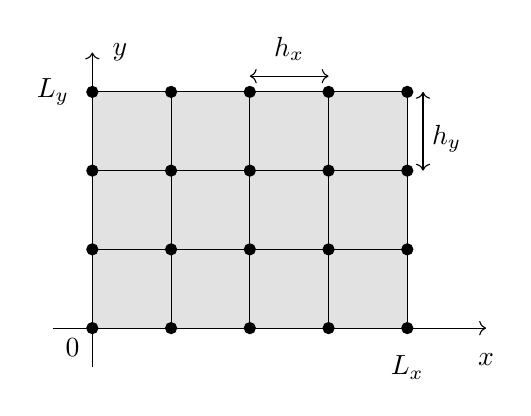
\begin{tikzpicture}
\draw[fill=gray!23,gray!23](1,1) rectangle (5,4);
%\draw[step=0.5cm,gray,very thin] (0,0) grid (7,5); 
\draw [->] (0.5,1) -- (6,1);
\draw [->] (1,0.5) -- (1,4.5);
\node[] at (0.75,0.75) {$0$};
\node[] at (5,0.5) {$L_x$};
\node[] at (0.5,4) {$L_y$};
\node[] at (6,0.6) {$x$};
\node[] at (1.35,4.5) {$y$};
\draw[-] (1,1)--(5,1)--(5,4)--(1,4)--cycle;
\draw[-] (1,2)--(5,2);
\draw[-] (1,3)--(5,3);
\draw[-] (2,1)--(2,4);
\draw[-] (3,1)--(3,4);
\draw[-] (4,1)--(4,4);
\draw[black,fill=black] (1,1)   circle (2pt);
\draw[black,fill=black] (2,1)   circle (2pt);
\draw[black,fill=black] (3,1)   circle (2pt);
\draw[black,fill=black] (4,1)   circle (2pt);
\draw[black,fill=black] (5,1)   circle (2pt);
\draw[black,fill=black] (1,2)   circle (2pt);
\draw[black,fill=black] (2,2)   circle (2pt);
\draw[black,fill=black] (3,2)   circle (2pt);
\draw[black,fill=black] (4,2)   circle (2pt);
\draw[black,fill=black] (5,2)   circle (2pt);
\draw[black,fill=black] (1,3)   circle (2pt);
\draw[black,fill=black] (2,3)   circle (2pt);
\draw[black,fill=black] (3,3)   circle (2pt);
\draw[black,fill=black] (4,3)   circle (2pt);
\draw[black,fill=black] (5,3)   circle (2pt);
\draw[black,fill=black] (1,4)   circle (2pt);
\draw[black,fill=black] (2,4)   circle (2pt);
\draw[black,fill=black] (3,4)   circle (2pt);
\draw[black,fill=black] (4,4)   circle (2pt);
\draw[black,fill=black] (5,4)   circle (2pt);
\draw[<->] (5.2,3)--(5.2,4);
\draw[<->] (3,4.2)--(4,4.2);
\node[] at (3.5,4.55) {$h_x$};
\node[] at (5.5,3.4) {$h_y$};
\end{tikzpicture}
\end{center}

There are $N_x$ nodes in the $x$ direction but only $N_x-1$ cells/elements\footnote{Because of my 
bias towards the Finite Element Method, I will refer to these as elements.}. 
Likewise there are $N_y$ nodes in the $y$ direction but only $N_y-1$ cells/elements.
In total there are $N_e=(N_x-1)(N_y-1)$ elements. 
As for the cell center nodes, we must adopt a systematic way of numbering them. 
If I keep using approach \#2 for the nodes, the following numbering of 
{\color{teal}elements} seems natural:

\begin{center}
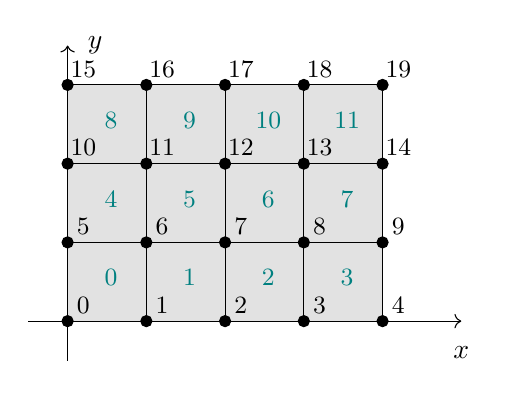
\begin{tikzpicture}
\draw[fill=gray!23,gray!23](1,1) rectangle (5,4);
%\draw[step=0.5cm,gray,very thin] (0,0) grid (7,5); 
\draw [->] (0.5,1) -- (6,1);
\draw [->] (1,0.5) -- (1,4.5);
\node[] at (6,0.6) {$x$};
\node[] at (1.35,4.5) {$y$};
\draw[-] (1,1)--(5,1)--(5,4)--(1,4)--cycle;
\draw[-] (1,2)--(5,2);
\draw[-] (1,3)--(5,3);
\draw[-] (2,1)--(2,4);
\draw[-] (3,1)--(3,4);
\draw[-] (4,1)--(4,4);
\draw[black,fill=black] (1,1)   circle (2pt);
\draw[black,fill=black] (2,1)   circle (2pt);
\draw[black,fill=black] (3,1)   circle (2pt);
\draw[black,fill=black] (4,1)   circle (2pt);
\draw[black,fill=black] (5,1)   circle (2pt);
\draw[black,fill=black] (1,2)   circle (2pt);
\draw[black,fill=black] (2,2)   circle (2pt);
\draw[black,fill=black] (3,2)   circle (2pt);
\draw[black,fill=black] (4,2)   circle (2pt);
\draw[black,fill=black] (5,2)   circle (2pt);
\draw[black,fill=black] (1,3)   circle (2pt);
\draw[black,fill=black] (2,3)   circle (2pt);
\draw[black,fill=black] (3,3)   circle (2pt);
\draw[black,fill=black] (4,3)   circle (2pt);
\draw[black,fill=black] (5,3)   circle (2pt);
\draw[black,fill=black] (1,4)   circle (2pt);
\draw[black,fill=black] (2,4)   circle (2pt);
\draw[black,fill=black] (3,4)   circle (2pt);
\draw[black,fill=black] (4,4)   circle (2pt);
\draw[black,fill=black] (5,4)   circle (2pt);
\node[] at (1.2,1.2) {\small $0$};
\node[] at (2.2,1.2) {\small $1$};
\node[] at (3.2,1.2) {\small $2$};
\node[] at (4.2,1.2) {\small $3$};
\node[] at (5.2,1.2) {\small $4$};
\node[] at (1.2,2.2) {\small $5$};
\node[] at (2.2,2.2) {\small $6$};
\node[] at (3.2,2.2) {\small $7$};
\node[] at (4.2,2.2) {\small $8$};
\node[] at (5.2,2.2) {\small $9$};
\node[] at (1.2,3.2) {\small $10$};
\node[] at (2.2,3.2) {\small $11$};
\node[] at (3.2,3.2) {\small $12$};
\node[] at (4.2,3.2) {\small $13$};
\node[] at (5.2,3.2) {\small $14$};
\node[] at (1.2,4.2) {\small $15$};
\node[] at (2.2,4.2) {\small $16$};
\node[] at (3.2,4.2) {\small $17$};
\node[] at (4.2,4.2) {\small $18$};
\node[] at (5.2,4.2) {\small $19$};
\node[] at (1.55,1.55) {\color{teal} \small $0$};
\node[] at (2.55,1.55) {\color{teal} \small $1$};
\node[] at (3.55,1.55) {\color{teal} \small $2$};
\node[] at (4.55,1.55) {\color{teal} \small $3$};
\node[] at (1.55,2.55) {\color{teal} \small $4$};
\node[] at (2.55,2.55) {\color{teal} \small $5$};
\node[] at (3.55,2.55) {\color{teal} \small $6$};
\node[] at (4.55,2.55) {\color{teal} \small $7$};
\node[] at (1.55,3.55) {\color{teal} \small $8$};
\node[] at (2.55,3.55) {\color{teal} \small $9$};
\node[] at (3.55,3.55) {\color{teal} \small $10$};
\node[] at (4.55,3.55) {\color{teal} \small $11$};
\end{tikzpicture}
\end{center}

In some applications we want to also store the coordinates of the center of all cells, i.e. the $N_e$ coordinates of {\color{teal} these} points:

\begin{center}
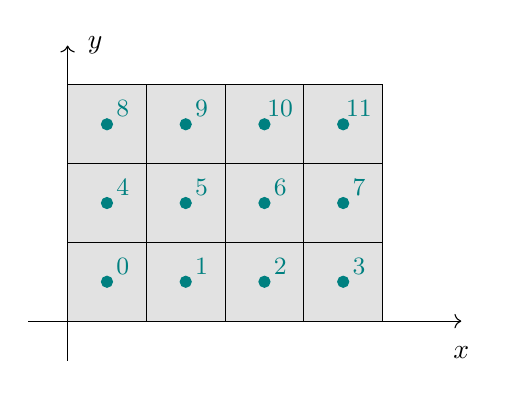
\begin{tikzpicture}
\draw[fill=gray!23,gray!23](1,1) rectangle (5,4);
%\draw[step=0.5cm,gray,very thin] (0,0) grid (7,5); 
\draw [->] (0.5,1) -- (6,1);
\draw [->] (1,0.5) -- (1,4.5);
\node[] at (6,0.6) {$x$};
\node[] at (1.35,4.5) {$y$};
\draw[-] (1,1)--(5,1)--(5,4)--(1,4)--cycle;
\draw[-] (1,2)--(5,2);
\draw[-] (1,3)--(5,3);
\draw[-] (2,1)--(2,4);
\draw[-] (3,1)--(3,4);
\draw[-] (4,1)--(4,4);
\draw[black,fill=black,color=teal] (1.5,1.5)   circle (2pt);
\draw[black,fill=black,color=teal] (2.5,1.5)   circle (2pt);
\draw[black,fill=black,color=teal] (3.5,1.5)   circle (2pt);
\draw[black,fill=black,color=teal] (4.5,1.5)   circle (2pt);
\draw[black,fill=black,color=teal] (1.5,2.5)   circle (2pt);
\draw[black,fill=black,color=teal] (2.5,2.5)   circle (2pt);
\draw[black,fill=black,color=teal] (3.5,2.5)   circle (2pt);
\draw[black,fill=black,color=teal] (4.5,2.5)   circle (2pt);
\draw[black,fill=black,color=teal] (1.5,3.5)   circle (2pt);
\draw[black,fill=black,color=teal] (2.5,3.5)   circle (2pt);
\draw[black,fill=black,color=teal] (3.5,3.5)   circle (2pt);
\draw[black,fill=black,color=teal] (4.5,3.5)   circle (2pt);
\node[] at (1.7,1.7) {\color{teal} \small $0$};
\node[] at (2.7,1.7) {\color{teal} \small $1$};
\node[] at (3.7,1.7) {\color{teal} \small $2$};
\node[] at (4.7,1.7) {\color{teal} \small $3$};
\node[] at (1.7,2.7) {\color{teal} \small $4$};
\node[] at (2.7,2.7) {\color{teal} \small $5$};
\node[] at (3.7,2.7) {\color{teal} \small $6$};
\node[] at (4.7,2.7) {\color{teal} \small $7$};
\node[] at (1.7,3.7) {\color{teal} \small $8$};
\node[] at (2.7,3.7) {\color{teal} \small $9$};
\node[] at (3.7,3.7) {\color{teal} \small $10$};
\node[] at (4.7,3.7) {\color{teal} \small $11$};
\end{tikzpicture}
\end{center}
Given this numbering these points form a regular grid:
\begin{center}
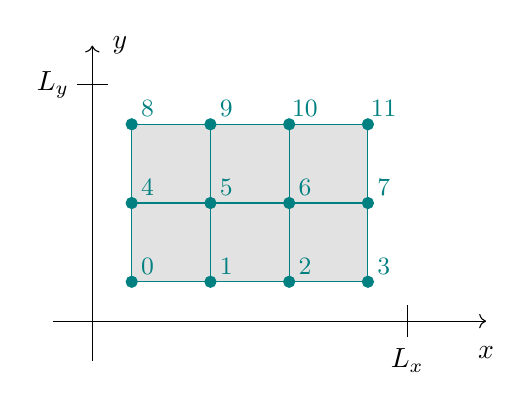
\begin{tikzpicture}
\draw[fill=gray!23,gray!23](1.5,1.5) rectangle (4.5,3.5);
%\draw[step=0.5cm,gray,very thin] (0,0) grid (7,5); 
\draw [->] (0.5,1) -- (6,1);
\draw [->] (1,0.5) -- (1,4.5);
\node[] at (6,0.6) {$x$};
\node[] at (1.35,4.5) {$y$};
\draw[-,teal] (1.5,1.5)--(4.5,1.5)--(4.5,3.5)--(1.5,3.5)--cycle;
\draw[-,teal] (1.5,2.5)--(4.5,2.5);
\draw[-,teal] (2.5,1.5)--(2.5,3.5);
\draw[-,teal] (3.5,1.5)--(3.5,3.5);
\draw[black,fill=black,color=teal] (1.5,1.5)   circle (2pt);
\draw[black,fill=black,color=teal] (2.5,1.5)   circle (2pt);
\draw[black,fill=black,color=teal] (3.5,1.5)   circle (2pt);
\draw[black,fill=black,color=teal] (4.5,1.5)   circle (2pt);
\draw[black,fill=black,color=teal] (1.5,2.5)   circle (2pt);
\draw[black,fill=black,color=teal] (2.5,2.5)   circle (2pt);
\draw[black,fill=black,color=teal] (3.5,2.5)   circle (2pt);
\draw[black,fill=black,color=teal] (4.5,2.5)   circle (2pt);
\draw[black,fill=black,color=teal] (1.5,3.5)   circle (2pt);
\draw[black,fill=black,color=teal] (2.5,3.5)   circle (2pt);
\draw[black,fill=black,color=teal] (3.5,3.5)   circle (2pt);
\draw[black,fill=black,color=teal] (4.5,3.5)   circle (2pt);
\node[] at (1.7,1.7) {\color{teal} \small $0$};
\node[] at (2.7,1.7) {\color{teal} \small $1$};
\node[] at (3.7,1.7) {\color{teal} \small $2$};
\node[] at (4.7,1.7) {\color{teal} \small $3$};
\node[] at (1.7,2.7) {\color{teal} \small $4$};
\node[] at (2.7,2.7) {\color{teal} \small $5$};
\node[] at (3.7,2.7) {\color{teal} \small $6$};
\node[] at (4.7,2.7) {\color{teal} \small $7$};
\node[] at (1.7,3.7) {\color{teal} \small $8$};
\node[] at (2.7,3.7) {\color{teal} \small $9$};
\node[] at (3.7,3.7) {\color{teal} \small $10$};
\node[] at (4.7,3.7) {\color{teal} \small $11$};
\draw[-] (5,0.8)--(5,1.2);
\draw[-] (0.8,4)--(1.2,4);
\node[] at (5,0.5) {$L_x$};
\node[] at (0.5,4) {$L_y$};
\end{tikzpicture}
\end{center}
This 'new' domain is bound by $x'_{min}=h_x/2$, $x'_{max}=L_x-h_x/2$ in 
the $x$ direction and $y'_{min}=h/2$, $y'_{max}=L_y-h_y/2$ in the $y$ direction. We note that the spacings $h_x$ and $h_y$ between the centers is the same as for the nodes. 
We store the coordinates $(x_c,y_c)$ of the cell centers in two arrays of length $N_e$ and the code is then simply

\begin{lstlisting}
Lx=9
Ly=7
Nx=4
Ny=3
N=Nx*Ny
hx=(xmax-xmin)/(Nx-1)
hy=(ymax-ymin)/(Ny-1)
#mesh nodes coordinates
x=np.zeros(N,dtype=np.float64)
y=np.zeros(N,dtype=np.float64)
counter=0
for j in range(0,Ny):
    for i in range(0,Nx):
        x[counter]=i*hx
        y[counter]=j*hy
        counter+=1
#cell centers coordinates
Ne=(Nx-1)*(Ny-1)
xc=np.zeros(Ne,dtype=np.float64)
yc=np.zeros(Ne,dtype=np.float64)
xmin=hx/2
xmax=Lx-hx/2
ymin=hy/2
ymax=Ly-hy/2
counter=0
for j in range(0,Ny-1):
    for i in range(0,Nx-1):
        xc[counter]=xmin+i*hx
        yc[counter]=ymin+j*hy
        counter+=1
\end{lstlisting}

%--------------------------------------------
\subsection*{The connectivity array}

Let us consider 3 points in a plane:
\begin{center}
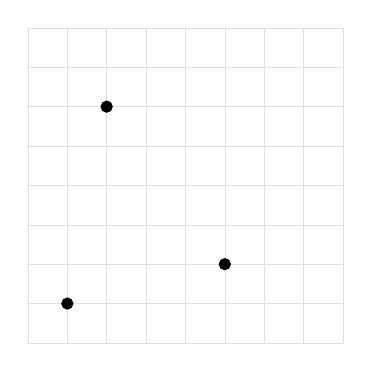
\begin{tikzpicture}
\draw[step=0.5cm,gray!25,very thin] (0.5,0.5) grid (4.5,4.5); 
\draw[black,fill=black] (1,1)   circle (2pt);
\draw[black,fill=black] (3,1.5)   circle (2pt);
\draw[black,fill=black] (1.5,3.5)   circle (2pt);
\end{tikzpicture}
\end{center}
Since they are not aligned they form a triangle:
\begin{center}
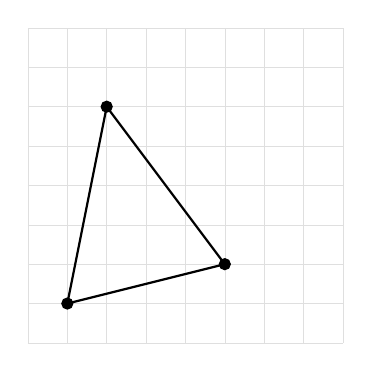
\begin{tikzpicture}
\draw[step=0.5cm,gray!25,very thin] (0.5,0.5) grid (4.5,4.5); 
\draw[black,fill=black] (1,1)   circle (2pt);
\draw[black,fill=black] (3,1.5)   circle (2pt);
\draw[black,fill=black] (1.5,3.5)   circle (2pt);
\draw[-,thick] (1,1)--(3,1.5)--(1.5,3.5)--cycle;
\end{tikzpicture}
\end{center}
When it comes to assigning these points an identity (or a number), I can arbitrarily assign them the following numbers:
\begin{center}
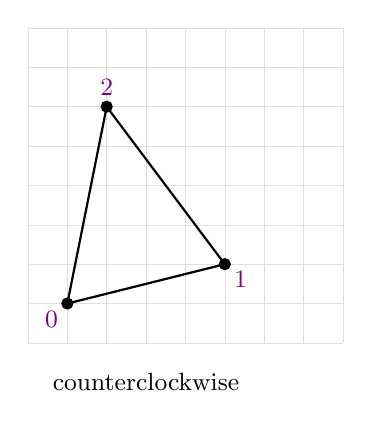
\begin{tikzpicture}
\draw[step=0.5cm,gray!25,very thin] (0.5,0.5) grid (4.5,4.5); 
\draw[black,fill=black] (1,1)   circle (2pt);
\draw[black,fill=black] (3,1.5)   circle (2pt);
\draw[black,fill=black] (1.5,3.5)   circle (2pt);
\draw[-,thick] (1,1)--(3,1.5)--(1.5,3.5)--cycle;
\node[] at (0.8,0.8) {\small \color{violet}0};
\node[] at (3.2,1.3) {\small \color{violet}1};
\node[] at (1.5,3.75) {\small \color{violet}2};
\node[] at (2,0) {\small counterclockwise};
\end{tikzpicture}
\end{center}
This triangle is then made of nodes {\color{violet}0}, 
{\color{violet}1}, and {\color{violet}2}.

Let us now add one more point in the plane as follows:
\begin{center}
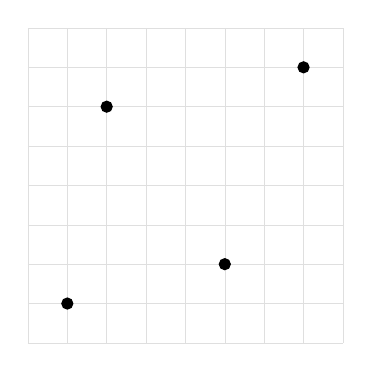
\begin{tikzpicture}
\draw[step=0.5cm,gray!25,very thin] (0.5,0.5) grid (4.5,4.5); 
\draw[black,fill=black] (1,1)   circle (2pt);
\draw[black,fill=black] (3,1.5)   circle (2pt);
\draw[black,fill=black] (1.5,3.5)   circle (2pt);
\draw[black,fill=black] (4,4)   circle (2pt);
\end{tikzpicture}
\end{center}
I will here number them as follows:
\begin{center}
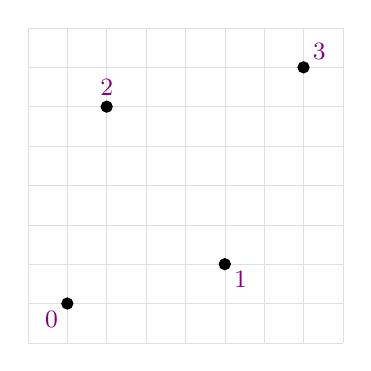
\begin{tikzpicture}
\draw[step=0.5cm,gray!25,very thin] (0.5,0.5) grid (4.5,4.5); 
\draw[black,fill=black] (1,1)   circle (2pt);
\draw[black,fill=black] (3,1.5)   circle (2pt);
\draw[black,fill=black] (1.5,3.5)   circle (2pt);
\draw[black,fill=black] (4,4)   circle (2pt);
\node[] at (0.8,0.8) {\small \color{violet}0};
\node[] at (3.2,1.3) {\small \color{violet}1};
\node[] at (1.5,3.75) {\small \color{violet}2};
\node[] at (4.2,4.2) {\small \color{violet}3};
\end{tikzpicture}
\end{center}

I can either decide to see them as the vertices of a quadrilateral, or
as the vertices of two triangles. However, there are two possibilities for the triangles:

\begin{center}
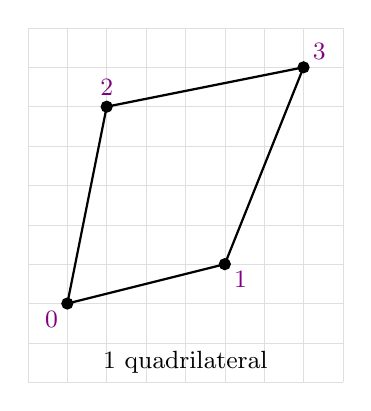
\begin{tikzpicture}
\draw[step=0.5cm,gray!25,very thin] (0.5,0) grid (4.5,4.5); 
\draw[black,fill=black] (1,1)   circle (2pt);
\draw[black,fill=black] (3,1.5)   circle (2pt);
\draw[black,fill=black] (1.5,3.5)   circle (2pt);
\draw[black,fill=black] (4,4)   circle (2pt);
\draw[-,thick] (1,1)--(3,1.5)--(4,4)--(1.5,3.5)--cycle;
\node[] at (0.8,0.8) {\small \color{violet}0};
\node[] at (3.2,1.3) {\small \color{violet}1};
\node[] at (1.5,3.75) {\small \color{violet}2};
\node[] at (4.2,4.2) {\small \color{violet}3};
\node[] at (2.5,0.25) {\small 1 quadrilateral};
\end{tikzpicture}
\hspace{1cm}
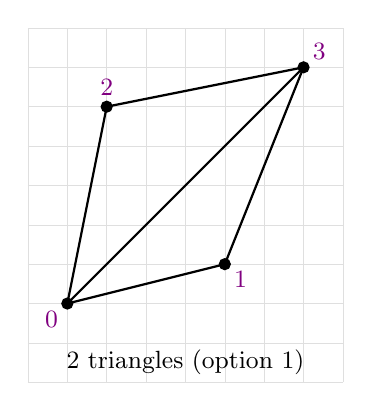
\begin{tikzpicture}
\draw[step=0.5cm,gray!25,very thin] (0.5,0) grid (4.5,4.5); 
\draw[black,fill=black] (1,1)   circle (2pt);
\draw[black,fill=black] (3,1.5)   circle (2pt);
\draw[black,fill=black] (1.5,3.5)   circle (2pt);
\draw[black,fill=black] (4,4)   circle (2pt);
\draw[-,thick] (1,1)--(3,1.5)--(4,4)--(1.5,3.5)--cycle;
\draw[-,thick] (1,1)--(4,4);
\node[] at (0.8,0.8) {\small \color{violet}0};
\node[] at (3.2,1.3) {\small \color{violet}1};
\node[] at (1.5,3.75) {\small \color{violet}2};
\node[] at (4.2,4.2) {\small \color{violet}3};
\node[] at (2.5,0.25) {\small 2 triangles (option 1)};
\end{tikzpicture}
\hspace{1cm}
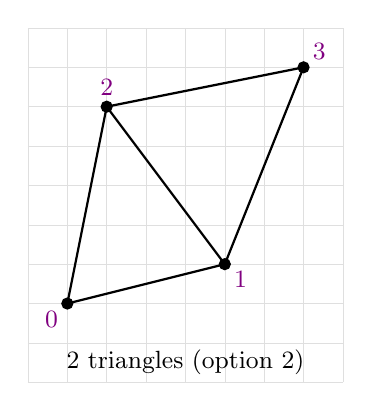
\begin{tikzpicture}
\draw[step=0.5cm,gray!25,very thin] (0.5,0) grid (4.5,4.5); 
\draw[black,fill=black] (1,1)   circle (2pt);
\draw[black,fill=black] (3,1.5)   circle (2pt);
\draw[black,fill=black] (1.5,3.5)   circle (2pt);
\draw[black,fill=black] (4,4)   circle (2pt);
\draw[-,thick] (1,1)--(3,1.5)--(4,4)--(1.5,3.5)--cycle;
\draw[-,thick] (3,1.5)--(1.5,3.5);
\node[] at (0.8,0.8) {\small \color{violet}0};
\node[] at (3.2,1.3) {\small \color{violet}1};
\node[] at (1.5,3.75) {\small \color{violet}2};
\node[] at (4.2,4.2) {\small \color{violet}3};
\node[] at (2.5,0.25) {\small 2 triangles (option 2)};
\end{tikzpicture}
\end{center}

When it comes to the quadrilateral, assuming a counterclockwise numbering, I can say that this quadrilaterals is then made of nodes 
{\color{violet}0}, {\color{violet}1},
{\color{violet}3} and {\color{violet}2}.
Note that I could also say it is made of nodes 
{\color{violet}3}, {\color{violet}2},
{\color{violet}0} and {\color{violet}1}.

Looking at the cases with 2 triangles I first need to label/number the triangles themselves:
\begin{center}
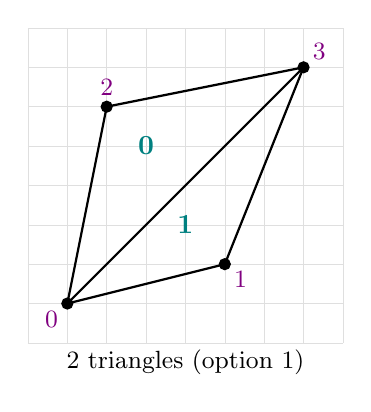
\begin{tikzpicture}
\draw[step=0.5cm,gray!25,very thin] (0.5,0.5) grid (4.5,4.5); 
\draw[black,fill=black] (1,1)   circle (2pt);
\draw[black,fill=black] (3,1.5)   circle (2pt);
\draw[black,fill=black] (1.5,3.5)   circle (2pt);
\draw[black,fill=black] (4,4)   circle (2pt);
\draw[-,thick] (1,1)--(3,1.5)--(4,4)--(1.5,3.5)--cycle;
\draw[-,thick] (1,1)--(4,4);
\node[] at (0.8,0.8) {\small \color{violet}0};
\node[] at (3.2,1.3) {\small \color{violet}1};
\node[] at (1.5,3.75) {\small \color{violet}2};
\node[] at (4.2,4.2) {\small \color{violet}3};
\node[] at (2,3) {\bf \color{teal}0};
\node[] at (2.5,2) {\bf \color{teal}1};
\node[] at (2.5,0.25) {\small 2 triangles (option 1)};
\end{tikzpicture}
\hspace{1cm}
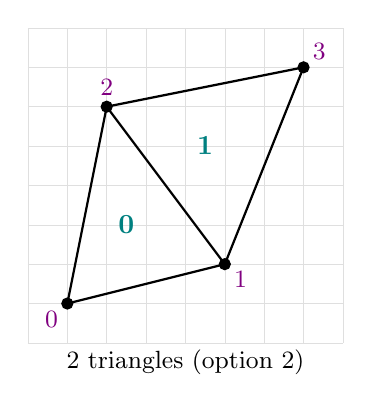
\begin{tikzpicture}
\draw[step=0.5cm,gray!25,very thin] (0.5,0.5) grid (4.5,4.5); 
\draw[black,fill=black] (1,1)   circle (2pt);
\draw[black,fill=black] (3,1.5)   circle (2pt);
\draw[black,fill=black] (1.5,3.5)   circle (2pt);
\draw[black,fill=black] (4,4)   circle (2pt);
\draw[-,thick] (1,1)--(3,1.5)--(4,4)--(1.5,3.5)--cycle;
\draw[-,thick] (3,1.5)--(1.5,3.5);
\node[] at (0.8,0.8) {\small \color{violet}0};
\node[] at (3.2,1.3) {\small \color{violet}1};
\node[] at (1.5,3.75) {\small \color{violet}2};
\node[] at (4.2,4.2) {\small \color{violet}3};
\node[] at (1.75,2) {\bf \color{teal}0};
\node[] at (2.75,3) {\bf \color{teal}1};
\node[] at (2.5,0.25) {\small 2 triangles (option 2)};
\end{tikzpicture}
\end{center}

In option 1, and still using a counterclockwise approach, triangle {\color{teal} 0} is made of nodes 
\{{\color{violet}0},{\color{violet}3},{\color{violet}2}\} and 
triangle {\color{teal} 1} is made of nodes 
\{{\color{violet}0},{\color{violet}1},{\color{violet}3}\}. 
In option 2, 
triangle {\color{teal} 0} is made of nodes 
\{{\color{violet}0},{\color{violet}1},{\color{violet}2}\} and 
triangle {\color{teal} 1} is made of nodes 
\{{\color{violet}1},{\color{violet}3},{\color{violet}2}\}. 

If I keep adding points, I will ultimately end up with a mesh which 
counts many quadrilaterals and/or triangles. In order to characterise this mesh, I need two numbers: $nel$, the number of elements (or cells) and $N$ the total number of vertices. However, this is not enough because I also need to know which vertex belongs to which element. 

Concretely, I need to store for each element a list of $m=3$ (triangles) or $m=4$ (quadrilaterals) numbers. The resulting array is often called the connectivity array. In FieldStone this array is always {\tt icon}, of size $m \times nel$.

In the cases above, $m=3$, $nel=2$, $N=4$ and 
\[
{\tt icon}_{\rm option\; 1}=
\left(
\begin{array}{cc}
{\color{violet}0}&{\color{violet}0}\\
{\color{violet}3}&{\color{violet}1}\\
{\color{violet}2}&{\color{violet}3}\\
\end{array}
\right)
\qquad
{\tt icon}_{\rm option\; 2}=
\left(
\begin{array}{cc}
{\color{violet}0}&{\color{violet}1}\\
{\color{violet}1}&{\color{violet}3}\\
{\color{violet}2}&{\color{violet}2}
\end{array}
\right)
\]
The way to understand these is as follows: for option 1,
\begin{itemize}
\item
icon[0,0]='the identity of node \#0 of element \#0' $\rightarrow$ {\color{violet}1}
\item
icon[1,0]='the identity of node \#1 of element \#0' $\rightarrow$ {\color{violet}4}
\item
icon[2,0]='the identity of node \#2 of element \#0' $\rightarrow$ {\color{violet}3}
\item
icon[0,1]='the identity of node \#0 of element \#1' $\rightarrow$ {\color{violet}1}
\item
icon[1,1]='the identity of node \#1 of element \#1' $\rightarrow$ {\color{violet}2}
\item
icon[2,1]='the identity of node \#2 of element \#1' $\rightarrow$ {\color{violet}4}
\end{itemize}

Finally, let us consider the following case:

\begin{center}
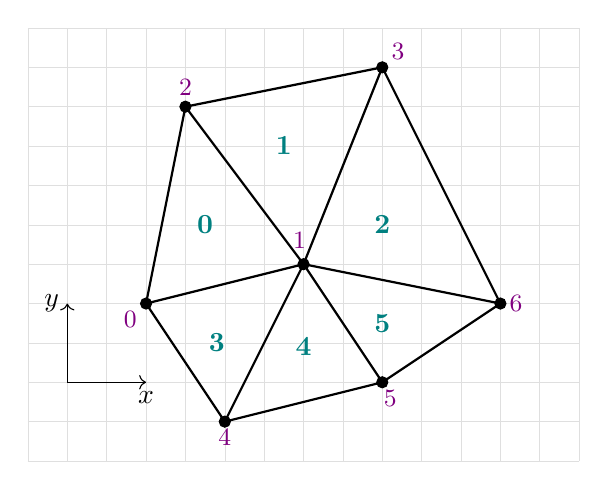
\begin{tikzpicture}
\draw[step=0.5cm,gray!25,very thin] (-0.5,-1) grid (6.5,4.5); 
\draw[black,fill=black] (1,1)   circle (2pt);
\draw[black,fill=black] (3,1.5)   circle (2pt);
\draw[black,fill=black] (1.5,3.5)   circle (2pt);
\draw[black,fill=black] (4,4)   circle (2pt);
\draw[black,fill=black] (5.5,1)   circle (2pt);
\draw[black,fill=black] (2.,-0.5)   circle (2pt);
\draw[black,fill=black] (4,0)   circle (2pt);

\draw[-,thick] (1,1)--(3,1.5)--(4,4)--(1.5,3.5)--cycle;
\draw[-,thick] (3,1.5)--(1.5,3.5);
\draw[-,thick] (3,1.5)--(5.5,1)--(4,4);
\draw[-,thick] (1,1)--(2,-0.5)--(4,0)--(5.5,1);
\draw[-,thick] (2,-0.5)--(3,1.5)--(4,0);
\node[] at (0.8,0.8) {\small \color{violet}0};
\node[] at (2.95,1.8) {\small \color{violet}1};
\node[] at (1.5,3.75) {\small \color{violet}2};
\node[] at (4.2,4.2) {\small \color{violet}3};
\node[] at (2,-0.7) {\small \color{violet}4};
\node[] at (4.1,-0.2) {\small \color{violet}5};
\node[] at (5.7,1) {\small \color{violet}6};

\node[] at (1.75,2) {\bf \color{teal}0};
\node[] at (2.75,3) {\bf \color{teal}1};
\node[] at (4,2) {\bf \color{teal}2};
\node[] at (1.9,0.5) {\bf \color{teal}3};
\node[] at (3,0.45) {\bf \color{teal}4};
\node[] at (4,0.75) {\bf \color{teal}5};


\draw[->] (0,0)--(1,0); 
\node[] at (1,-0.2) {$x$};
\draw[->] (0,0)--(0,1);
\node[] at (-0.2,1) {$y$};
\end{tikzpicture}
\end{center}
This mesh counts $nel=6$ elements/cells and $N=7$ points. 
The connectivity array is then of size $3\times 6$:
\[
{\tt icon}=
\left(
\begin{array}{cccccc}
{\color{violet}0}&{\color{violet}1}&{\color{violet}1}&{\color{violet}0}&{\color{violet}4}&{\color{violet}5}\\
{\color{violet}1}&{\color{violet}3}&{\color{violet}6}&{\color{violet}4}&{\color{violet}5}&{\color{violet}6}\\
{\color{violet}2}&{\color{violet}2}&{\color{violet}3}&{\color{violet}1}&{\color{violet}1}&{\color{violet}1}
\end{array}
\right)
\]
with 
\begin{align}
{\tt x}&=
\left(
\begin{array}{p{0.58cm}p{0.58cm}p{0.58cm}p{0.58cm}p{0.58cm}p{0.58cm}p{0.58cm}}
1 & 3 & 1.5 & 4 & 2 & 4 & 5.5
\end{array}
\right) \\
{\tt y}&=
\left(
\begin{array}{p{0.58cm}p{0.58cm}p{0.58cm}p{0.58cm}p{0.58cm}p{0.58cm}p{0.58cm}}
1 & 1.5 & 3.5 & 4 & -0.5 & 0 & 1
\end{array}
\right)
\end{align}

Let us then compute the barycenter coordinates of all triangles in arrays 
{\tt xb} and {\tt yb} of size $N=7$.
We need to loop over all triangles and for each compute the average of 
its nodes coordinates:
\begin{verbatim}
for iel in range(0,nel):
    xb[iel]=(x[icon[0,iel]]+x[icon[1,iel]]+x[icon[2,iel]])/3
    yb[iel]=(y[icon[0,iel]]+y[icon[1,iel]]+y[icon[2,iel]])/3
\end{verbatim}

The same concepts of course apply in 3D. In the case of tetrahedra then $m=4$ and in the case of hexahedra then $m=8$.

 %%%%%%%%%%%%%%%%%%%%%%%%%%%%%%%%%%%%%%%%%%%%%%%%%%%%%%%%%%%

\chapter{Manufactured solution ($Q_1\times P_0$+penalty)\label{f01}} %%%%%%%%%%%%%%%%%%%%%%%%%%%%%% 01
\begin{flushright} {\tiny {\color{gray} python\_codes/fieldstone\_01/text.tex}} \end{flushright}

\lstinputlisting[language=bash,basicstyle=\small]{python_codes/fieldstone_01/keywords.ascii}

\begin{center}

\fbox{\textbf{\huge \color{teal} P}}
\fbox{\textbf{\huge \color{purple} J}}
\fbox{\textbf{\huge \color{orange} F}}
Codes at \url{https://github.com/cedrict/fieldstone/tree/master/python_codes/fieldstone_01}
\end{center}

\par\noindent\rule{\textwidth}{0.4pt}

{\sl The python stone was developed in collaboration with Job Mos}. \index{contributors}{J. Mos}
{\sl The julia stone was developed by Jort Jansen.}. \index{contributors}{J. Jansen}

\par\noindent\rule{\textwidth}{0.4pt}
%%%%%%%%%%%%%%%%%%%%%%%%%%%%%%%%%%%%%%%%%%%%%%%%%%%%%%%%%%%%%%%%%%%%%%%%%%%%%%%%%%%%%%%%%%%%%%

This benchmark is taken from Donea \& Huerta (2003) \cite{dohu03} and is described fully in section \ref{mms1}. 
In order to illustrate the behavior of selected mixed finite elements in the solution 
of stationary Stokes flow,  we consider a two-dimensional problem 
in the square domain $\Omega=[0,1]\times[0,1]$, which possesses a closed-form analytical 
solution. 

\begin{center}
\includegraphics[width=10cm]{python_codes/fieldstone_01/results/errors.pdf}\\
{\captionfont Quadratic convergence for velocity error, 
linear convergence for pressure error, as expected.}
\end{center}

\begin{center}
\includegraphics[width=10cm]{python_codes/fieldstone_01/results/pressure.pdf}\\
{\captionfont Pressure field}
\end{center}

\begin{center}
\includegraphics[width=15cm]{python_codes/fieldstone_01/results/solution.pdf}
\end{center}

One can also compute vertical/depth averages of the velocity, see Eq.~\eqref{eq:dhvelnorm}.
Note that the averages are computed somewhat naively: instead of computing integrals in the $x$-direction
at many depths I simply take an arithmetic average over rows of nodes. At high resolution the profiles
converge to the analytical profiles for the individual components and to the results 
obtained with \aspect. Please check \stone~110 for a better implementation.
\begin{center}
\includegraphics[width=10cm]{python_codes/fieldstone_01/results/vel_profile}\\
{\captionfont Vertical average of velocity. \aspect was run with the 'depth average' postprocessor
added to the prm file.}
\end{center}

\newpage
\subsection*{About the Fortran code}

I wrote the first ever version of this \stone in
Fortran90 around 2011. It is available in the {\foldernamefont simplefem} folder in this stone.
\index{general}{fortran90}

The code can be compiled as follows:
\begin{verbatim}
> gfortran -O3 linpack_d.f90 blas_routines.f simplefem.f90
\end{verbatim}
and run as follows:
\begin{verbatim}
> ./a.out 
\end{verbatim}
The solver used here does not make use of a sparse storage and relies on a dense matrix 
set of subroutine from BLAS and LinPACK\footnote{\url{https://en.wikipedia.org/wiki/LINPACK}}.
\begin{center}
\includegraphics[width=9cm]{python_codes/fieldstone_01/simplefem/timings/timings.pdf}\\
{\captionfont Despite a very naive application of the boundary conditions to the entire
assembled FE matrix, we find here that this part of the code is not taking long at all.}
\end{center}
There is no export of the results to ParaView format, only ascii text files.



\newpage
\subsection*{About the Julia code}

The python code was translated to julia in a rather straightforward manner. 
The matrix is still a full array (no sparse storage during the build process) 
and the boundary conditions
are applied naively. Even with a 80x80 resolution the memory use is under 2Gb. 
Note that there seems to be a limit as to the maximum size of the matrix array 
and for instance 96x96 yields to a crash.

In this version the matrix is stored as a full array. 
Before the linear system is solved, however, we must convert it to sparse storage:
\begin{verbatim}
Sps_amat=sparse(a_mat)
\end{verbatim}
When it comes to the solve, we have various options. The first and most 
simple one is similar to Matlab's backslash:
\begin{verbatim}
sol= Sps_amat\rhs
\end{verbatim}
Another possibility is cholesky\footnote{This method uses the CHOLMOD library from SuiteSparse:
\url{https://people.engr.tamu.edu/davis/suitesparse.html}} or ldlt or lu:
\begin{verbatim}
sol= cholesky(Sps_amat)\rhs
sol= ldlt(Sps_amat)\rhs
sol= lu(Sps_amat)\rhs
\end{verbatim}


The computed errors are of course identical to those of the python codes but we find that
at low resolutions the python code is much faster than the julia code: 
this is likely due to the time taken by julia to compile the code.
 

\begin{center}
\includegraphics[width=5.7cm]{python_codes/fieldstone_01/results/julia/timings_build.pdf}
\includegraphics[width=5.7cm]{python_codes/fieldstone_01/results/julia/timings_solve.pdf}
\includegraphics[width=5.7cm]{python_codes/fieldstone_01/results/julia/errors.pdf}\\
{\captionfont Matrix building and solving times as obtained for nelx from 8 until 80, each 
resolution being run 10 times.}
\end{center}

We find that the LU-based solver is the fasted in this case.





 %%%%%%%%%%%%%%%%%%%%%%%%%%%%%%%%%%%%%%%%%%%%%%%%%%%%%%%%%%%

\chapter{Stokes sphere in 2D ($Q_1\times P_0$+penalty) \label{f02}} %%%%%%%%%%%%%%%%%%%%%%%%%%%%%%% 02
\lstinputlisting[language=bash,basicstyle=\small]{python_codes/fieldstone_02/keywords.ascii}

\begin{center}
Code at \url{https://github.com/cedrict/fieldstone/tree/master/python_codes/fieldstone_02}
\end{center}

\par\noindent\rule{\textwidth}{0.4pt}
%%%%%%%%%%%%%%%%%%%%%%%%%%%%%%%%%%%%%%%%%%%%%%%%%%%%%%%%%%%%%%%%%%%%%%%%%%%%%%%%%%%%%%%%%

This stone carries out the benchmark of Section~\ref{MMM-ss:stokes_sphere2D}
with $Q_1\times P_0$ elements using the penalty formulation.
The domain is a unit square and the fluid is characterised 
by $\rho=1$ and $\eta=1$ 
while the sphere is characterised 
by $\rho=1.01$ and $\eta=1000$.
The gravity vector is $\vec{g}=(0,-1)$. 

Boundary conditions are free slip on all sides ({\tt bc\_type=0}), 
no slip on all sides ({\tt bc\_type=1}) or free slip on the sides and bottom and open 
on top ({\tt bc\_type=2}).
Viscosity and density directly computed at the quadrature points.
The results are presented in Section~\ref{MMM-ss:stokes_sphere2D} and compared to 
those obtained with other codes.

Also, because of the inherent symmetry we can solve the system 
on only half the domain:
\begin{center}
\includegraphics[width=3cm]{python_codes/fieldstone_02/results/eta_1}
$\rightarrow$
\includegraphics[width=3cm]{python_codes/fieldstone_02/results/eta_2}
\end{center}


\begin{center}
\includegraphics[width=3cm]{python_codes/fieldstone_02/results/u0}
\includegraphics[width=3cm]{python_codes/fieldstone_02/results/v0}
\includegraphics[width=3cm]{python_codes/fieldstone_02/results/vel0}
\includegraphics[width=3cm]{python_codes/fieldstone_02/results/sr0}
\includegraphics[width=3cm]{python_codes/fieldstone_02/results/p0}\\
\includegraphics[width=3cm]{python_codes/fieldstone_02/results/u1}
\includegraphics[width=3cm]{python_codes/fieldstone_02/results/v1}
\includegraphics[width=3cm]{python_codes/fieldstone_02/results/vel1}
\includegraphics[width=3cm]{python_codes/fieldstone_02/results/sr1}
\includegraphics[width=3cm]{python_codes/fieldstone_02/results/p1}\\
\includegraphics[width=3cm]{python_codes/fieldstone_02/results/u2}
\includegraphics[width=3cm]{python_codes/fieldstone_02/results/v2}
\includegraphics[width=3cm]{python_codes/fieldstone_02/results/vel2}
\includegraphics[width=3cm]{python_codes/fieldstone_02/results/sr2}
\includegraphics[width=3cm]{python_codes/fieldstone_02/results/p2}\\
{\captionfont Results on a $32\times 64$ grid. Top is free-slip, 
middle is no-slip, bottom is open top.}
\end{center}


 %%%%%%%%%%%%%%%%%%%%%%%%%%%%%%%%%%%%%%%%%%%%%%%%%%%%%%%%%%%

\chapter{Convection in a 2D box ($Q_1\times P_0$+penalty)\label{f03}} %%%%%%%%%%%%%%%%%%%%%%%%%%%%% 03
\includegraphics[height=1.25cm]{images/pictograms/FEM}
\includegraphics[height=1.25cm]{images/pictograms/replication}
\includegraphics[height=1.25cm]{images/pictograms/benchmark}
\includegraphics[height=1.25cm]{images/pictograms/temperature}

\lstinputlisting[language=bash,basicstyle=\small]{python_codes/fieldstone_03/keywords.ascii}

\begin{center}
\inpython
\injulia
{\small Codes: \url{https://github.com/cedrict/fieldstone/tree/master/python_codes/fieldstone_03}}
\end{center}

\par\noindent\rule{\textwidth}{0.4pt}

{\sl The julia stone was developed by Jort Jansen.}. \index{contributors}{J. Jansen}

\par\noindent\rule{\textwidth}{0.4pt}
%%%%%%%%%%%%%%%%%%%%%%%%%%%%%%%%%%%%%%%%%%%%%%%%%%%%%%%%%%%%%%%%%%%%%%%%%%%%%%%%%%%%%%%%%

\index{stopics}{$Q_1\times P_0$}

This benchmark deals with the 2-D thermal convection of a fluid 
of infinite Prandtl number in a rectangular closed cell.
In what follows, I carry out the case 1a, 1b, and 1c experiments as shown in 
Blankenbach \etal (1989) \cite{blbc89}:
steady convection with constant viscosity in a square box.

The temperature is fixed to zero on top and to $\Delta T$ at the bottom, 
with reflecting symmetry at the sidewalls (i.e. $\partial_x T=0$) 
and there are no internal heat sources. 
Free-slip conditions are implemented on all boundaries. 

The Rayleigh number is given by
\begin{equation}
\Ranb = \frac{\alpha g_y \Delta T h^3 }{\kappa \nu}
=\frac{\alpha g_y \Delta T h^3 \rho^2 C_p}{k \eta}
\end{equation}

In what follows, I use the following parameter values:  %, as given in \cite{krhb12}:
$L_x=L_y=1$,$\rho_0=c_P=k=\eta=1$, $T_0=0$, $\alpha=10^{-2}$, $g=10^{2}Ra$
and I run the model with $Ra=10^4,10^{5}$ and $10^6$.

The initial temperature field is given by 
\begin{equation}
T(x,y)=(1-y) - 0.01\cos(\pi x) \sin(\pi y)
\end{equation}
The perturbation in the initial temperature fields leads to 
a perturbation of the density field and sets the fluid in motion. 
Depending on the initial Rayleigh number, the system ultimately reaches a 
steady state after some time. 

The Nusselt number (i.e. the mean surface temperature gradient over mean bottom temperature)
is computed as follows \cite{blbc89}:
\begin{equation}
\Nunb = L_y \frac{\int_0^{L_x} \frac{\partial T}{\partial y}(y=L_y) \; dx  }{\int_0^{L_x} T(y=0) \; dx}
\label{eqNu}
\end{equation}
Note that in our case the denominator is equal to 1 since $L_x=1$ and the temperature at the 
bottom is prescribed to be 1.

If no convection is taking place (i.e. $\Ranb$ is too low) then only diffusion is taking place 
and the steady state temperature field is then $T(y)=1-y$, so that $\partial_y T=-1$ and 
we find that the Nusselt number is simply 1.

The steady state root mean square velocity and Nusselt number measurements
are indicated in the following Table alongside those of \cite{blbc89} and \cite{tack94}.
(Note that this benchmark was also carried out by many others (see Section~\ref{MMM-ss:blbc89}).

\begin{center}
\begin{tabular}{llccccc}
\hline
          &           & Blankenbach et al (1989) & Tackley (1994)  & 32x32 & 48x48 & 64x64  \\
\hline
\hline
$\Ranb=10^4$ & $V_{rms}$ &  $42.864947  \pm 0.000020$ & 42.775 & 42.89111& 42.87938& 42.87360\\  
          & $Nu$      &  $4.884409   \pm 0.000010$ & 4.878  & 4.783252 & 4.837800& 4.857373\\
$\Ranb=10^5$ & $V_{rms}$ &  $193.21454  \pm 0.00010 $ & 193.11 & 194.1032 & 193.6264 &  193.4519  \\ 
          & $Nu$      &  $10.534095  \pm 0.000010$ & 10.531 & 9.604454& 10.08087 &  10.26830  \\
$\Ranb=10^6$ & $V_{rms}$ &  $833.98977  \pm 0.00020 $ & 833.55 & & & \\
          & $Nu$      &  $21.972465  \pm 0.000020$ & 21.998 & & & \\
\hline
\end{tabular}\\
{\small Steady state Nusselt number $Nu$ and $\upnu_{rms}$ measurements as reported in the literature. }
\end{center}

Food for thought: Looking at the mass, momentum and energy conservation equations, 
we see that that they are coupled: the temperature enters the rhs of the momentum 
equation since the density depends on the temperature (Boussinesq approximation)
while the velocity is present in the advection term of the energy equation.
One should then solve all three equations with $u,v,p,T$ as unknowns. However
this is rarely done in practice and often the system is solved in a segregated way:
first solve for $u,v,p$ assuming $T$ known, then solving for $T$ assuming $u,v,p$ known.
If small time steps are used this is a reasonable approach, or, like in this case, when 
one wishes to compute the steady state of the system rather than an accurate time-evolution
of the system. Better schemes are available and one example thereof is explained in Kronbichler et al (2012) 
\cite{krhb12}.

Also, the current version of this \stone uses a Crank-Nicolson approach for the 
time discretisation of the $\partial T/\partial t$ term as explained in Section~\ref{MMM-sec:timediscr}.

Something must be said about how the Nusselt number is computed. 
Its calculation requires the integral of the temperature gradient along an edge. 
Because it is much simpler to compute the temperature gradient in the middle of the 
element alongside other quantities such as pressure, this (elemental) quantity is 
used in the Nusselt number calculations, which makes it inaccurate and therefore 
explains the discrepancy between the computed values and those of other publications.
Check the Consistent Boundary Flux method in Section~\ref{MMM-ss:cbf}.

Finally, it is expected that the thickness of the 
boundary layers decreases with higher Rayleigh number values.
As a consequence, in order to appropriately capture those, one needs 
a higher resolution than at low $\Ranb$ numbers. This explains why 
acceptable results are obtained for $\Ranb=10^4$  even at low resolution $32\times 32$.

Note that the results obtained with \aspect at comparable resolution ought to be 
more accurate since \aspect relies on quadratic elements for both velocity and 
temperature. 

A few remarks about the code. It relies on $Q_1\times P_0$ elements with a penalty
formulation so that the pressure degrees of freedom are not taken into account. 
The temperature is also bi-linear ($Q_1$) so that the temperature and velocity nodes 
are identical and no distinction is made between them.

Steady state has been reached when the relative velocity and temperature difference between two consecutive 
time steps is less than a tolerance set to $10^{-6}$. 


\newpage
\paragraph{Results for $\Ranb=10^4$}.
\begin{center}
\includegraphics[width=16cm]{python_codes/fieldstone_03/results_1e4/64x64/solution.pdf}\\
\includegraphics[width=5cm]{python_codes/fieldstone_03/results_1e4/Tavrg.pdf}
\includegraphics[width=5cm]{python_codes/fieldstone_03/results_1e4/vrms.pdf}\\
\includegraphics[width=5cm]{python_codes/fieldstone_03/results_1e4/Nu.pdf}
\includegraphics[width=5cm]{python_codes/fieldstone_03/results_1e4/Nu_vrms.pdf}
\includegraphics[width=5cm]{python_codes/fieldstone_03/results_1e4/convergence.pdf}\\
{\captionfont Note that the \aspect data have been shifted so that the location of the 
first vrms peak coincides with the one of the 64x64 run.}
\end{center}

\newpage
\paragraph{Results for $\Ranb=10^5$}.
\begin{center}
\includegraphics[width=16cm]{python_codes/fieldstone_03/results_1e5/64x64/solution.pdf}\\
\includegraphics[width=5cm]{python_codes/fieldstone_03/results_1e5/Tavrg.pdf}
\includegraphics[width=5cm]{python_codes/fieldstone_03/results_1e5/vrms.pdf}\\
\includegraphics[width=5cm]{python_codes/fieldstone_03/results_1e5/Nu.pdf}
\includegraphics[width=5cm]{python_codes/fieldstone_03/results_1e5/Nu_vrms.pdf}\\
\includegraphics[width=5cm]{python_codes/fieldstone_03/results_1e5/convergence.pdf}\\
\end{center}

\newpage
\paragraph{Results for $\Ranb=10^6$}.
\begin{center}
\includegraphics[width=16cm]{python_codes/fieldstone_03/results_1e6/48x48/solution.pdf}\\
\includegraphics[width=5cm]{python_codes/fieldstone_03/results_1e6/Tavrg.pdf}
\includegraphics[width=5cm]{python_codes/fieldstone_03/results_1e6/vrms.pdf}\\
\includegraphics[width=5cm]{python_codes/fieldstone_03/results_1e6/Nu.pdf}
\includegraphics[width=5cm]{python_codes/fieldstone_03/results_1e6/Nu_vrms.pdf}
\end{center}


I have tested the influence of the CFL number (0.5 instead of 1) and it does not change much at all.





 %%%%%%%%%%%%%%%%%%%%%%%%%%%%%%%%%%%%%%%%%%%%%%%%%%%%%%%%%%%

\chapter{The lid driven cavity ($Q_1\times P_0$+penalty) \label{f04}} %%%%%%%%%%%%%%%%%%%%%%%%%%%%% 04
\includegraphics[height=1.25cm]{images/pictograms/replication}
\includegraphics[height=1.25cm]{images/pictograms/benchmark}
\includegraphics[height=1.25cm]{images/pictograms/FEM}

%%%%%%%%%%%%%%%%%%%%%%%%%%%%%%%%%%%%%%%%%%%%%%%%%%%%%%%%%%%%%%%%%%%%%%%%%%%%%%%%%%%%%%%%%%%%%%%%%%%

\lstinputlisting[language=bash,basicstyle=\small]{python_codes/fieldstone_04/keywords.ascii}

\begin{center}
\inpython
{\small Code: \url{https://github.com/cedrict/fieldstone/tree/master/python_codes/fieldstone_04}}
\end{center}

\par\noindent\rule{\textwidth}{0.4pt}
%%%%%%%%%%%%%%%%%%%%%%%%%%%%%%%%%%%%%%%%%%%%%%%%%%%%%%%%%%%%%%%%%%%%%%%%%%%%%%%%%%%%%%%%%
\index{stopics}{$Q_1\times P_0$}

The lid driven cavity is a famous Computational Fluid Dynamics test case 
\cite{kawa61,ghgs82,paac67,bope98,brsa06,grdn97,shde00}
and has been studied in countless publications with a wealth of numerical techniques
(see \cite{ertu09} for a succinct review) and also in the laboratory \cite{kost84}.

It models a plane flow of an isothermal isoviscous fluid in a rectangular (usually square) lid-driven cavity. 
The boundary conditions are no slip on left, right and bottom. The gravity is set to zero as the flow
is entirely driven by the moving lid.

%---------------------------------------------------------
\subsection*{The lid driven cavity problem ({\tt ldc=0})}
In the standard case, the upper side of the cavity moves in its own plane at unit speed, while the other sides are fixed.
This thereby introduces a discontinuity in the boundary conditions at the two upper corners of the cavity and yields
an uncertainty as to which boundary (side or top) the corner points belong to. 
In this version of the code the top corner nodes are considered to be part of the lid. If these are excluded 
the recovered pressure showcases an extremely large checkboard pattern.

This benchmark is usually dicussed in the context of low to very high Reynolds number with the full 
Navier-Stokes equations being solved (with the noticeable exception of \cite{sagl81a,sagl81b,chpc95,eid2005}
which focus on the Stokes equation). 
In the case of the incompressible Stokes flow, 
the absence of inertia renders this problem instantaneous so that only one time step/Stokes solve is needed.

%---------------------------------------------------------
\subsection*{The lid driven cavity problem - regularisation I ({\tt ldc=1})}

We avoid the top corner nodes issue altogether by  
prescribing the horizontal velocity of the lid as follows: 
\begin{equation}
u(x)=16x^2(1-x)^2.
\end{equation}
In this case the velocity and its first derivative is continuous at the corners. This is the so-called regularised lid-driven cavity problem \cite{piva94}. The factor 16 ensures that $\max\limits_{[0,1]}(u)=1$.
 
%---------------------------------------------------------
\subsection*{The lid driven cavity problem - regularisation II ({\tt ldc=2})}

Another regularisation was presented in de Frutos \etal \cite{dejn16} and 
also in Appendix D.4 of \textcite{john16} (2016). 
Here, a regularized lid driven cavity is studied which is consistent in the sense that 
${\bm \nabla}\cdot{\bm v}=0$ 
holds also at the corners of the domain.
There are no-slip conditions at the boundaries $x=0$, $x=1$, and $y=0$. 

The velocity at $y=1$ is given by

\begin{eqnarray}
u(x) &=& 1-\frac{1}{4}\left( 1-\cos (\frac{x_1-x}{x_1}\pi)  \right)^2   \quad\quad x\in[0,x_1] \nonumber\\
u(x) &=& 1 \quad\quad x\in[x_1,1-x_1] \nonumber\\
u(x) &=& 1-\frac{1}{4}\left( 1-\cos (\frac{x-(1-x_1)}{x_1}\pi)  \right)^2   \quad\quad x\in[1-x_1,1]
\end{eqnarray}
Results are obtained with $x_1=0.1$.


A 100$\times$100 element grid is used. 
A zero vertical velocity is prescribed at the top and the exact form of the 
prescribed horizontal velocity is controlled by the {\tt ldc} parameter.

\begin{center}
\includegraphics[width=7cm]{python_codes/fieldstone_04/results/p.pdf}
\includegraphics[width=7cm]{python_codes/fieldstone_04/results/q.pdf}\\
{\captionfont Left: pressure $p$ at $y=L_y$; Right: smoothed pressure $q$ at $y=L_y$.}
\end{center}

\begin{center}
\includegraphics[width=12cm]{python_codes/fieldstone_04/results/velocities}\\
\includegraphics[width=12cm]{python_codes/fieldstone_04/results/pressures}\\
\includegraphics[width=12cm]{python_codes/fieldstone_04/results/strainrates}
\end{center}

 %%%%%%%%%%%%%%%%%%%%%%%%%%%%%%%%%%%%%%%%%%%%%%%%%%%%%%%%%%%

\chapter{SolCx benchmark ($Q_1\times P_0$+penalty)\label{f05}} %%%%%%%%%%%%%%%%%%%%%%%%%%%%%%%%%%%% 05
\noindent
\includegraphics[height=1.25cm]{images/pictograms/replication}
\includegraphics[height=1.25cm]{images/pictograms/benchmark}
\includegraphics[height=1.25cm]{images/pictograms/FEM}
\includegraphics[height=1.25cm]{images/pictograms/paraview}

%%%%%%%%%%%%%%%%%%%%%%%%%%%%%%%%%%%%%%%%%%%%%%%%%%%%%%%%%%%%%%%%%%%%%%%%%%%%%%%%%%%%%%%%%%%%%%%%%%%

%\lstinputlisting[language=bash,basicstyle=\small]{python_codes/fieldstone_05/keywords.ascii}

\begin{center}
\inpython
\infortran
{\small Codes: \url{https://github.com/cedrict/fieldstone/tree/master/python_codes/fieldstone_05}}
\end{center}

\par\noindent\rule{\textwidth}{0.4pt}

Last revision: Oct. 28th, 2024.

\par\noindent\rule{\textwidth}{0.4pt}

%%%%%%%%%%%%%%%%%%%%%%%%%%%%%%%%%%%%%%%%%%%%%%%%%%%%%%%%%%%%%%%%%%%%%%%%%%%%%%%%%%%%%%%%%

The experiment is fully described in Section~\ref{MMM-ss:solcx}.
The viscosity is prescribed at the quadrature points 
If the number of elements is even in the $x$-direction direction, all elements 
(and their associated quadrature points)
have a constant viscosity ($1$ or  $10^6$). If it is odd, then the elements situated 
at the viscosity jump have half their integration points with $\eta=1$ and half 
with $\eta=10^6$ 
(which is a pathological case since the used quadrature rule inside elements cannot represent 
accurately such a jump).  

\begin{center}
\includegraphics[width=8cm]{python_codes/fieldstone_05/results/errors_even.pdf}
\includegraphics[width=8cm]{python_codes/fieldstone_05/results/errors_odd.pdf}\\
{\captionfont Velocity and pressure error convergence as a function of mesh size and for various values
of the penalty parameter. Left: even number of elements in each direction; Right: odd numbers.
}
\end{center}

Because of the high viscosity in the right part of the domain, the penalty parameter should 
be high enough to insure an incompressible flow and thereby recover the expected convergence rate
(at least for the even case). Note that values higher than $\lambda=10^{10}$ yield erroneous solutions 
due to round-off errors. 

\begin{center}
\includegraphics[width=6.5cm]{python_codes/fieldstone_05/results/rho}
\includegraphics[width=6.5cm]{python_codes/fieldstone_05/results/eta}\\
\includegraphics[width=4cm]{python_codes/fieldstone_05/results/vel}
\includegraphics[width=4cm]{python_codes/fieldstone_05/results/vel_error}
\includegraphics[width=4cm]{python_codes/fieldstone_05/results/press}
\includegraphics[width=4cm]{python_codes/fieldstone_05/results/press_error}\\
\includegraphics[width=4cm]{python_codes/fieldstone_05/results/exx}
\includegraphics[width=4cm]{python_codes/fieldstone_05/results/eyy}
\includegraphics[width=4cm]{python_codes/fieldstone_05/results/exy}
\includegraphics[width=4cm]{python_codes/fieldstone_05/results/sr}\\
{\captionfont Results obtained on $100 \times 100$ mesh for $\lambda=10^{10}$.}
\end{center}



\infortran
Note that a Fortran90 version of this code is available in the same folder. \index{general}{fortran90}


 %%%%%%%%%%%%%%%%%%%%%%%%%%%%%%%%%%%%%%%%%%%%%%%%%%%%%%%%%%%

\chapter{SolKz benchmark ($Q_1\times P_0$+penalty)\label{f06}} %%%%%%%%%%%%%%%%%%%%%%%%%%%%%%%%%%%% 06

\includegraphics[height=1.5cm]{images/pictograms/benchmark}

\lstinputlisting[language=bash,basicstyle=\small]{python_codes/fieldstone_06/keywords.ascii}

\begin{center}
Code at \url{https://github.com/cedrict/fieldstone/tree/master/python_codes/fieldstone_06}
\end{center}

\par\noindent\rule{\textwidth}{0.4pt}
%%%%%%%%%%%%%%%%%%%%%%%%%%%%%%%%%%%%%%%%%%%%%%%%%%%%%%%%%%%%%%%%%%%%%%%%%%%%%%%%%%%%%%%%%

The SolKz benchmark \cite{repa87} is similar to the SolCx benchmark.
but the viscosity is now a function of the space coordinates: 
\begin{equation}
\eta(y)=\exp(By) \quad {\rm with} \quad B=13.8155
\end{equation}
It is however not a discontinuous function but grows exponentially with the vertical coordinate so that its overall variation is again $10^6$. 
The forcing is again chosen by imposing a spatially variable density variation as follows:
\begin{equation}
\rho(x,y)=\sin(2y) \cos(3\pi x)
\end{equation}
Free slip boundary conditions are imposed on all sides of the domain.
This benchmark is presented in Zhong (1996) \cite{zhon96} as well and is studied 
in Duretz \etal (2011) \cite{dumg11} and Gerya \etal (2013) \cite{gemd13}.

\begin{center}
\includegraphics[width=14cm]{python_codes/fieldstone_06/results/solution.pdf}
\end{center}

\begin{center}
\includegraphics[width=10cm]{python_codes/fieldstone_06/results/errors.pdf}\\
{\captionfont Velocity and pressure error as a function of mesh size.}
\end{center}
 %%%%%%%%%%%%%%%%%%%%%%%%%%%%%%%%%%%%%%%%%%%%%%%%%%%%%%%%%%%

\chapter{SolVi benchmark ($Q_1\times P_0$+penalty) \label{f07}} %%%%%%%%%%%%%%%%%%%%%%%%%%%%%%%%%%% 07

\includegraphics[height=1.5cm]{images/pictograms/benchmark}

\lstinputlisting[language=bash,basicstyle=\small]{python_codes/fieldstone_07/keywords.ascii}

\begin{center}
Code at \url{https://github.com/cedrict/fieldstone/tree/master/python_codes/fieldstone_07}
\end{center}

\par\noindent\rule{\textwidth}{0.4pt}
%%%%%%%%%%%%%%%%%%%%%%%%%%%%%%%%%%%%%%%%%%%%%%%%%%%%%%%%%%%%%%%%%%%%%%%%%%%%%%%%%%%%%%%%%

Following SolCx and SolKz, the SolVi inclusion benchmark solves 
a problem with a discontinuous viscosity field, but in this case 
the viscosity field is chosen in such a way that the discontinuity 
is along a circle. Given the regular nature of the grid used by a majority of codes and the present one, 
this ensures that the discontinuity in the viscosity never aligns to cell boundaries.
This in turns leads to almost discontinuous pressures along the interface which are difficult to represent accurately.
Schmid \& Podlachikov (2003) \cite{scpo03} derived a simple analytic solution for the pressure and 
velocity fields for a circular 
inclusion under simple shear and it was used in \cite{deka08,sunh10,dumg11,krhb12,gemd13}.

Because of the symmetry of the problem, we only have to solve over the top right quarter of the domain.
The analytical solution requires a strain rate boundary condition (e.g., pure shear) to be applied far away 
from the inclusion. In order to avoid using very large domains and/or dealing with this type of boundary condition 
altogether, the analytical solution is evaluated and imposed on the boundaries of the domain. 
By doing so, the truncation error introduced while discretizing the strain rate boundary condition is removed.

A characteristic of the analytic solution is that the pressure is zero inside the inclusion, while outside it follows the relation
\begin{equation}
p_m = 4 \dot{\epsilon}
\frac{\eta_m(\eta_i-\eta_m)}{\eta_i+\eta_m}
\frac{r_i^2}{r^2} \cos(2\theta)
\end{equation}
where $\eta_i = 10^3$ is the viscosity of the inclusion 
and $\eta_m = 1$ is the viscosity of the background media, $\theta=\tan^{-1}(y/x)$,
and $\dot{\epsilon}=1$ is the applied strain rate.

Deubelbeiss \& Kauss (2008) \cite{deka08} thoroughly investigated this problem with various 
numerical methods (FEM, FDM), with and without tracers, 
and conclusively showed how various averagings lead to different results. 
Duretz et al (2011) \cite{dumg11} obtained a first order convergence for both pressure and velocity, 
while Kronbichler et al (2012) \cite{krhb12}
and Gerya et al (2013) \cite{gemd13} showed that the use of adaptive mesh refinement in respectively the FEM and FDM 
yields convergence rates which depend on refinement strategies. 

\begin{center}
\includegraphics[width=8cm]{python_codes/fieldstone_07/results/errors}\\
{\captionfont Velocity and pressure error convergence as a function of mesh size.}
\end{center}

\includegraphics[width=15cm]{python_codes/fieldstone_07/results/solution}

\begin{center}
\includegraphics[width=7cm]{python_codes/fieldstone_07/results/pressbottom}
\includegraphics[width=7cm]{python_codes/fieldstone_07/results/veldiag}\\
{\captionfont Left: Pressure at the bottom of the domain. Right: $u$ on the diagonal $x=y$.}
\end{center}

 %%%%%%%%%%%%%%%%%%%%%%%%%%%%%%%%%%%%%%%%%%%%%%%%%%%%%%%%%%%

\chapter{The indentor benchmark ($Q_1\times P_0$+penalty)\label{f08}} %%%%%%%%%%%%%%%%%%%%%%%%%%%%% 08

\includegraphics[height=1.5cm]{images/pictograms/benchmark}

\lstinputlisting[language=bash,basicstyle=\small]{python_codes/fieldstone_08/keywords.ascii}

\begin{center}
Code at \url{https://github.com/cedrict/fieldstone/tree/master/python_codes/fieldstone_08}
\end{center}

\par\noindent\rule{\textwidth}{0.4pt}
%%%%%%%%%%%%%%%%%%%%%%%%%%%%%%%%%%%%%%%%%%%%%%%%%%%%%%%%%%%%%%%%%%%%%%%%%%%%%%%%%%%%%%%%%

The punch benchmark is one of the few boundary value problems involving plastic solids for which there exists an exact solution. 
Such solutions are usually either for highly simplified geometries (spherical or axial symmetry, for instance) or simplified material models (such as rigid plastic solids) \cite{kacha04}.

In this experiment, a rigid punch indents a rigid plastic half space; the slip line field theory gives 
exact solutions as shown in section~\ref{MMM-sec:punch}. 
The plane strain formulation of the equations and the detailed solution to the problem were derived in the Appendix of \cite{thfb08} and are also presented in \cite{gepd98}.

The two dimensional punch problem has been extensively studied numerically for the past 40 years 
\cite{zihl75,zihp95,chpe01,chan99,huhy99,yuti06,bufs08,raab07} and has been used to draw a parallel 
with the tectonics of eastern China in the context of the 
India-Eurasia collision \cite{tamo76,mota77}.
It is also worth noting that it has been carried out in one form or another in series of 
analogue modelling articles 
concerning the same region, with a rigid indenter colliding with a rheologically stratified 
lithosphere \cite{peta88,daco88,jodc90}.
 
Numerically, the one-time step punch experiment is performed on a two-dimensional
domain of purely plastic von Mises material. 
Given that the von Mises rheology yield criterion does not depend on pressure
(see Section~\ref{MMM-sec:vMcriterion}), the density of the material and/or the gravity 
vector is set to zero. Sides are set to free slip boundary conditions, the bottom to no slip, 
while a vertical velocity $(0,-v_p)$ is prescribed at the top boundary for nodes 
whose $x$ coordinate is within $[L_x/2-\delta/2,L_x/2+\delta/2]$. 

The following parameters are used: $L_x=1$, $L_y=0.5$, $\mu_{min}=10^{-3}$, 
$\mu_{max}=10^3$, $v_p=1$, $\delta=0.11111$ 
and the yield value of the material is set to $\sigma_Y=1$. 

The analytical solution predicts that the angle of the shear bands stemming from the sides of the punch 
is $\pi/4$, that the pressure right under the punch is $1+\pi$, 
and that the velocity of the rigid blocks on each side of the punch is $v_p/\sqrt{2}$ 
(this is simply explained by invoking conservation of mass).

In what follows I show results of the rough and smooth punch for a 124x68 grid. The difference between the two
lies in the nature of the kinematic boundary conditions under the punched area. 'rough' means that the indentor 
also fixes the horizontal velocity component to zero while it is free in the smooth case.

We see that the smooth punch does not trigger the checkerboard pressure modes as much as the rough case 
and we recover nicely the analytical pressure under the punch \cite{thfb08,gltf18}.

\newpage
%................................................................................
\paragraph{Rough punch} 

\begin{center}
\includegraphics[width=6cm]{python_codes/fieldstone_08/results/rough/velocity.pdf}
\includegraphics[width=6cm]{python_codes/fieldstone_08/results/rough/pressure.pdf}\\
\includegraphics[width=6cm]{python_codes/fieldstone_08/results/rough/strainrate.pdf}
\includegraphics[width=6cm]{python_codes/fieldstone_08/results/rough/stress.pdf}\\
\includegraphics[width=6cm]{python_codes/fieldstone_08/results/rough/u_stats.pdf}
\includegraphics[width=6cm]{python_codes/fieldstone_08/results/rough/v_stats.pdf}\\
\includegraphics[width=6cm]{python_codes/fieldstone_08/results/rough/residual.pdf}
\includegraphics[width=6cm]{python_codes/fieldstone_08/results/rough/diff_uv.pdf}\\
{\captionfont a,b,c,d) velocity, pressure, strainrate and stress at the top of the domain; 
e,f) min/max value of $u$ and $v$;
g,h) residual and normalised velocity difference.}
\end{center}

\newpage
\includegraphics[width=16cm]{python_codes/fieldstone_08/results/rough/solution.pdf}


%................................................................................
\newpage
\paragraph{Smooth punch}

\begin{center}
\includegraphics[width=6cm]{python_codes/fieldstone_08/results/smooth/velocity.pdf}
\includegraphics[width=6cm]{python_codes/fieldstone_08/results/smooth/pressure.pdf}\\
\includegraphics[width=6cm]{python_codes/fieldstone_08/results/smooth/strainrate.pdf}
\includegraphics[width=6cm]{python_codes/fieldstone_08/results/smooth/stress.pdf}\\
\includegraphics[width=6cm]{python_codes/fieldstone_08/results/smooth/u_stats.pdf}
\includegraphics[width=6cm]{python_codes/fieldstone_08/results/smooth/v_stats.pdf}\\
\includegraphics[width=6cm]{python_codes/fieldstone_08/results/smooth/residual.pdf}
\includegraphics[width=6cm]{python_codes/fieldstone_08/results/smooth/diff_uv.pdf}\\
{\captionfont a,b,c,d) velocity, pressure, strainrate and stress at the top of the domain; 
e,f) min/max value of $u$ and $v$;
g,h) residual and normalised velocity difference.}
\end{center}

\newpage
\includegraphics[width=16cm]{python_codes/fieldstone_08/results/smooth/solution.pdf}




 %%%%%%%%%%%%%%%%%%%%%%%%%%%%%%%%%%%%%%%%%%%%%%%%%%%%%%%%%%%
 
\chapter{The annulus benchmark ($Q_1\times P_0$+penalty) \label{f09}} %%%%%%%%%%%%%%%%%%%%%%%%%%%%% 09
\includegraphics[height=1.25cm]{images/pictograms/benchmark}
\includegraphics[height=1.25cm]{images/pictograms/FEM}

%%%%%%%%%%%%%%%%%%%%%%%%%%%%%%%%%%%%%%%%%%%%%%%%%%%%%%%%%%%%%%%%%%%%%%%%%%%%%%%%%%%%%%%%%%%%%%%%%%%

\lstinputlisting[language=bash,basicstyle=\small]{python_codes/fieldstone_09/keywords.ascii}

\begin{center}
\inpython
{\small Code: \url{https://github.com/cedrict/fieldstone/tree/master/python_codes/fieldstone_09}}
\end{center}

\par\noindent\rule{\textwidth}{0.4pt}

{\sl This fieldstone was developed in collaboration with Prof. E.G.P. Puckett}. 
\index{contributors}{E.G.P. Puckett}

\par\noindent\rule{\textwidth}{0.4pt}
%%%%%%%%%%%%%%%%%%%%%%%%%%%%%%%%%%%%%%%%%%%%%%%%%%%%%%%%%%%%%%%%%%%%%%%%%%%%%%%%%%%%%%%%%%%%

The benchmark is described fully in Section~\ref{MMM-ss:anconv} in which 
an analytical solution to the isoviscous incompressible Stokes equations 
is derived in an annulus geometry.
The velocity and pressure fields are as follows:

\begin{eqnarray}
v_r(r,\theta)     &=&  g(r) k \sin(k\theta), \\
v_\theta(r,\theta)&=&  f(r) \cos(k \theta), \\ 
p(r,\theta)       &=&  k h(r) \sin(k \theta), \\
\rho (r,\theta)   &=& \aleph(r) k \sin (k \theta), 
\end{eqnarray}
with $f(r)$, $g(r)$, $h(r)$ given in Section~\ref{MMM-ss:anconv}.
The parameters $A$ and $B$ are chosen so that $v_r(R_1)=v_r(R_2)=0$, i.e.
the velocity is tangential to both inner and outer surfaces.
The gravity vector is radial and of unit length.
In the present case, we set $R_1=1$, $R_2=2$ and $C=-1$.
The parameter $k$ can take values 0,1,2,3,... 

\begin{center}
\includegraphics[width=5cm]{python_codes/fieldstone_09/velocity}
\includegraphics[width=5cm]{python_codes/fieldstone_09/vr}
\includegraphics[width=5cm]{python_codes/fieldstone_09/vtheta}\\
{\small Left to right: velocity norm, $r$ component, $\theta$ component}
\end{center}

\begin{center}
\includegraphics[width=7cm]{python_codes/fieldstone_09/density}
\includegraphics[width=7cm]{python_codes/fieldstone_09/pressure}\\
{\small Left: density field; right: pressure field.}
\end{center}

\begin{center}
\includegraphics[width=7cm]{python_codes/fieldstone_09/psi}
\includegraphics[width=7cm]{python_codes/fieldstone_09/psi_arrows}\\
{\small Left: $\psi$ field; right: $\psi$ isolines with velocity arrows.}
\end{center}

\includegraphics[width=15cm]{python_codes/fieldstone_09/errors}

 %%%%%%%%%%%%%%%%%%%%%%%%%%%%%%%%%%%%%%%%%%%%%%%%%%%%%%%%%%%

\chapter{Stokes sphere in 3D ($Q_1 \times P_0$+penalty, $Q_2 \times P_0$+penalty)\label{f10}} %%%%%%%%%%%%%%%%%%%%%%%%%%%%%%%% 10
\includegraphics[height=1.25cm]{images/pictograms/FEM}
\includegraphics[height=1.25cm]{images/pictograms/3d}

%%%%%%%%%%%%%%%%%%%%%%%%%%%%%%%%%%%%%%%%%%%%%%%%%%%%%%%%%%%%%%%%%%%%%%%%%%%%%%%%%%%%%%%%%

\lstinputlisting[language=bash,basicstyle=\small]{python_codes/fieldstone_10/keywords.key}

\begin{center}
\inpython
\injulia
\infortran
{\small Code: \url{https://github.com/cedrict/fieldstone/tree/master/python_codes/fieldstone_10}}
\end{center}

\par\noindent\rule{\textwidth}{0.4pt}
%%%%%%%%%%%%%%%%%%%%%%%%%%%%%%%%%%%%%%%%%%%%%%%%%%%%%%%%%%%%%%%%%%%%%%%%%%%%%%%%%%%%%%%%%

Last revision: Sept. 27th, 2024.

\par\noindent\rule{\textwidth}{0.4pt}
%%%%%%%%%%%%%%%%%%%%%%%%%%%%%%%%%%%%%%%%%%%%%%%%%%%%%%%%%%%%%%%%%%%%%%%%%%%%%%%%%%%%%%%%%


%----------------------------------------------------------
\subsection*{Manufactured solution ({\tt experiment=5})}

It is described in Section~\ref{MMM-ss:mms3Dgen}.
The velocity and pressure fields are:
\begin{eqnarray}
u(x,y,z) &=& x(1-x)(1-2y)(1-2z)\\
v(x,y,z) &=& (1-2x) y(1-y) (1-2z) \\
w(x,y,z) &=& -2(1-2x)(1-2y)z(1-z) \\
p(x,y,z) &=& (2x-1)(2y-1)(2z-1)
\end{eqnarray}
This flow field has the built-in property that there is no flux through the 
boundaries, i.e. the normal component of the velocity field is zero on each face. 

\begin{center}
\includegraphics[width=5.6cm]{python_codes/fieldstone_10/results/exp5/press}
\includegraphics[width=5.6cm]{python_codes/fieldstone_10/results/exp5/vel}
\end{center}

\begin{center}
\includegraphics[width=5.6cm]{python_codes/fieldstone_10/results/exp5/vrms}
\includegraphics[width=5.6cm]{python_codes/fieldstone_10/results/exp5/conv}
\includegraphics[width=5.6cm]{python_codes/fieldstone_10/results/exp5/p_stats}
\end{center}
We recover the expected second order velocity error convergence 
and first order pressure error convergence. 
Surprisingly, we find that the results are not sensitive to the value of the penalty parameter $\lambda$.

This \stone is implemented in both python and julia, in order to look at
performance aspects. Both versions of the code are as close to each other 
as possible. The FE build and solve times are recorded and we find
that the build time grows linearly with the number of elements in the python 
case but not in the julia case. I suspected that the sparse storage of julia
(as opposed to a linked list converted to sparse matrix in python) makes it slow
so I ran the code without the assembly and indeed it is then linear with the 
number of elements.
I need to find a better way!!

\begin{center}
\includegraphics[width=8cm]{python_codes/fieldstone_10/results/exp5/julia/build.pdf}
\includegraphics[width=8cm]{python_codes/fieldstone_10/results/exp5/julia/solve.pdf}\\
{\captionfont Matrix building and system solve times for both python and julia codes.
Obtained with penalty=1e6. Each resolution is run 3 times.}
\end{center}


%----------------------------------------------------------
\subsection*{Aquarium ({\tt experiment=0})}

FS on all sides, $\rho=\eta=g_z=1$, $\lambda=10^6$

\begin{center}
\includegraphics[width=5.7cm]{python_codes/fieldstone_10/results/exp0/stats_uv}
\includegraphics[width=5.7cm]{python_codes/fieldstone_10/results/exp0/stats_w}
\includegraphics[width=5.7cm]{python_codes/fieldstone_10/results/exp0/stats_p}\\
{\captionfont Statistics of $u,v,w,p$.}
\end{center}

We expect a zero velocity field. This is the case (down to machine precision) for the $u$
and $v$ components, but since the penalty method yields a weakly compressible flow, 
the vertical component $w$ is larger but remains small.
The pressure is expected to be lithostatic and it should be -0.5 at the top and +0.5 at 
the bottom. Pressure statistics seem to converge towards these values. 





%------------------------------
\subsection*{Stokes sphere}

The domain is a unit cube. Free slip boundary conditions 
are imposed on all sides. The mesh counts 
nelx*nely*nelz=nel elements and 
nnx*nny*nnz=NV nodes.
The density and the viscosity are prescribed in the domain 
by means of two functions:
the density is set to $1+\delta \rho$ inside a sphere of radius 0.123456789 centered 
at (0.5,0.5,0.5) and 1 outside. The viscosity is 1000 inside the sphere
and 1 outside.  The gravity vector is set to $\vec{g}=(0,0,-1)$.
This is the benchmark presented in Section~\ref{MMM-ss:stokes_sphere_3D}.

The FE matrix size grows even faster now than in the previous 2D case so
choosing the right matrix storage is of paramount importance. 

Three experiments are carried out:
\begin{enumerate}
\item[Exp.~1:] the one described above.
Free slip or no slip boundary conditions.
We see that the pressure field is dominated by the lithostatic signal.
\item[Exp.~2:] same as experiment 1, but a reference density of 1 is substracted to all densities, so that 
the sphere density is 1 and the density of the surrounding fluid is now 0. In essence, we remove a
'background' density which does not participate in the flow generation, and thereby get rid of the 
lithostatic signal of the pressure.
Free slip or no slip boundary conditions.
\item[Exp.~3:] same as experiment 2, but the top boundary is now open (free surface)
\end{enumerate} 

\begin{center}
\includegraphics[width=5.7cm]{python_codes/fieldstone_10/results/exp1/grid}
\includegraphics[width=5.7cm]{python_codes/fieldstone_10/results/exp1/vel}
\includegraphics[width=5.7cm]{python_codes/fieldstone_10/results/exp1/press}\\
\includegraphics[width=5.7cm]{python_codes/fieldstone_10/results/exp1/visc}
\includegraphics[width=5.7cm]{python_codes/fieldstone_10/results/exp1/dens}\\
{\small Exp.~1: resolution $24\times 24\times 24$}
\end{center}

\begin{center}
\includegraphics[width=7cm]{python_codes/fieldstone_10/results/exp2/dens_2}
\includegraphics[width=7cm]{python_codes/fieldstone_10/results/exp2/press_2}\\
{\small Exp.~2: Density and pressure fields. Resolution 24x24x24}
\end{center}


\begin{center}
\includegraphics[width=7cm]{python_codes/fieldstone_10/results/exp3/press_3}
\includegraphics[width=7cm]{python_codes/fieldstone_10/results/exp3/vel_3}\\
{\small Exp.~3: pressure and velocity fields. Resolution 24x24x24}
\end{center}

\begin{center}
\includegraphics[width=5.6cm]{python_codes/fieldstone_10/results/exp1/pressure.pdf}
\includegraphics[width=5.6cm]{python_codes/fieldstone_10/results/exp2/pressure.pdf}
\includegraphics[width=5.6cm]{python_codes/fieldstone_10/results/exp3/pressure.pdf}\\
{\captionfont Elemental pressure for all elements as a function of their vertical 
(middle) coordinate for (from left to right) experiments 1, 2 and 3. }
\end{center}

Note that a similar fortran code is present in the folder. 

If the option 'quarter' is true, then the model takes advantage of the symmetries 
of the problem and runs it in a quarter of the original domain, so that 
the domain is then $0.5\times 0.5 \times 1$. Measurements/results are identical 
to the full cube ones, but at a much lower cost.

\begin{center}
\includegraphics[width=4cm]{python_codes/fieldstone_10/results/quarter_FS/press}
\includegraphics[width=4cm]{python_codes/fieldstone_10/results/quarter_FS/sr}
\includegraphics[width=4cm]{python_codes/fieldstone_10/results/quarter_FS/vel}
\includegraphics[width=4cm]{python_codes/fieldstone_10/results/quarter_FS/eta}\\
{\captionfont Resolution $32\times 32\times 64$ - FS}
\end{center}


\begin{center}
\includegraphics[width=7cm]{images/stokes_sphere3D/vrms_FS}
\includegraphics[width=7cm]{images/stokes_sphere3D/vrms_NS}\\
{\captionfont Left: FS; Right: NS. Results obtained with this stones and other ones, as well as ASPECT.
See Section~\ref{MMM-ss:stokes_sphere_3D} for all results.}
\end{center}

\newpage
%%%%%%%%%%%%%%%%%%%%%%%%%%%%%%%%%%%%%%%%%%%%%%%%%%%%%%%%
\section*{Trying $Q_2\times Q_0$+penalty... because why not}

Based on a discussion with A. Regorda I have coded a $Q_2\times Q_0$
(still with penalty) version of the \stone: {\tt stoneQ2Q0.py}.
The following results are obtained with {\tt script\_Q2Q0}.

I first naively used a 1 point integration (as for the 
$Q_1 \times P_0$ element) only for the 
penalty term, only to realise that the penalty term $\K_\lambda$ should be 
under-integrated, but not necessarily using a single point. 

This sparked the study on the influence of the quadrature rule 
of the penalty term on the accuracy of results.

I also implemented the consistent pressure recovery described 
in Section~\ref{MMM-ss:cpr}.
This results in a nodal pressure field (which I call $q$) which is 
solution of 
\[
{\bm M} \cdot \vec{Q} = \vec{f}
\]
where ${\bm M}$ is the $Q_2$ mass matrix that 
is integrated with the same quadrature as the viscous block $\K_\eta$
but the rhs $\vec{f}$ is integrated with the same quadrature as 
the penalty block $\K_\lambda$.
In the end I also keep the pressure $p$ computed in the middle of the element
using $p= \lambda \vec\nabla\cdot \vec\upnu$.

Finally to save time I have used the fact that the Jacobian of the 
coordinate change for cuboids is a diagonal matrix containing terms $h_x/2$,
$h_y/2$, $h_z/2$ on the diagonal. This means that this can be computed once
and for all for all elements. 

%----------------------------------------------------------
\subsection*{Aquarium ({\tt experiment=0})}

Fress slip on all sides, $\rho=\eta=g_z=1$, $\lambda=10^6$

\begin{center}
\includegraphics[width=5.7cm]{python_codes/fieldstone_10/resultsQ2/exp0/errv}
\includegraphics[width=5.7cm]{python_codes/fieldstone_10/resultsQ2/exp0/errp}
\includegraphics[width=5.7cm]{python_codes/fieldstone_10/resultsQ2/exp0/errq}\\
\includegraphics[width=8cm]{python_codes/fieldstone_10/resultsQ2/exp0/p_stats}
\end{center}

We expect a zero velocity field. This is the case (down to machine precision) 
for the $u$ and $v$ components, but since the penalty method yields a 
weakly compressible flow, the vertical component $w$ is much larger 
then $u$ and $v$.
The pressure is expected to be lithostatic and it should be -0.5 at the top 
and +0.5 at the bottom. Pressure statistics to converge towards these values. 

\begin{center}
\includegraphics[width=5cm]{python_codes/fieldstone_10/resultsQ2/exp0/press}
\includegraphics[width=5cm]{python_codes/fieldstone_10/resultsQ2/exp0/w}\\
{\captionfont $w$ and $p$ for resolution $20\times 20 \times 20$.}
\end{center}

Note that at resolution 20x20x20 build time is 10min, and solve time is 48 min!
Given this 'performance' this will limit a lot the tests we can carry out...

%----------------------------------------------------------
\subsection*{Manufactured solution ({\tt experiment=5})}

See Section~\ref{MMM-ss:mms3Dgen} for the analytical expressions 
of the velocity, pressure and body force vector.

\begin{center}
\includegraphics[width=5.7cm]{python_codes/fieldstone_10/resultsQ2/exp5/errv}
\includegraphics[width=5.7cm]{python_codes/fieldstone_10/resultsQ2/exp5/errp}
\includegraphics[width=5.7cm]{python_codes/fieldstone_10/resultsQ2/exp5/errq}\\
\includegraphics[width=8cm]{python_codes/fieldstone_10/resultsQ2/exp5/vrms}
\includegraphics[width=8cm]{python_codes/fieldstone_10/resultsQ2/exp5/p_stats}
\end{center}

Since the analytical solution of this experiment is quadratic then the 
velocity basis functions can exactly represent the solution inside each
element and the accuracy of the velocity solution depends on the penalty parameter and
not on resolution.
We clearly see that using only one integration point for the penalty term results
in lesser accurate velocities.
Interestingly we obtain a superconvergence (third order) of the $q$ error 
for a 2x2x2 quadrature and only a linear convergence for the $q$ error
for a 3x3x3 quadrature.
The pressure $q$ obtained with only 1 quad point yields results that are so off
that they do not show on the plots.
Finally we note that we obtain pressures that often exceed the analytical 
bounds for min and max pressure except for $q$ with 2x2x2 quadrature.
This seems to indicate that a 2x2x2 quadrature is preferable.
We keep investigating in the next section with a more suitable manufactured
solution benchmark.

\begin{center}
\includegraphics[width=5.7cm]{python_codes/fieldstone_10/resultsQ2/exp5/vel}
\includegraphics[width=5.7cm]{python_codes/fieldstone_10/resultsQ2/exp5/p}
\includegraphics[width=5.7cm]{python_codes/fieldstone_10/resultsQ2/exp5/q}\\
{\captionfont $||\vec\upnu||$, $p$ and $q$ for resolution $20\times 20 \times 20$.}
\end{center}

%----------------------------------------------------------
\subsection*{Manufactured solution ({\tt experiment=6})}

After the observations made about the previous experiment we then turn to 
another 3D manufactured solution as described in Section~\ref{MMM-ss:mms3Dgen}.

\begin{eqnarray}
f(x) &=& x^2(1-x)^2 \\
g(y) &=& y^2(1-y)^2 \\
h(z) &=& z^2(1-z)^2 \\
u(x,y,z) &=& fg'h' \\
v(x,y,z) &=& f'gh'  \\
w(x,y,z) &=& -2f'g'h \\
p(x,y,z) &=& -f'g'h'
\end{eqnarray}


\begin{center}
\includegraphics[width=5.7cm]{python_codes/fieldstone_10/resultsQ2/exp6/errv}
\includegraphics[width=5.7cm]{python_codes/fieldstone_10/resultsQ2/exp6/errp}
\includegraphics[width=5.7cm]{python_codes/fieldstone_10/resultsQ2/exp6/errq}\\
\includegraphics[width=5.7cm]{python_codes/fieldstone_10/resultsQ2/exp6/vrms}
\includegraphics[width=5.7cm]{python_codes/fieldstone_10/resultsQ2/exp6/p_stats}
\includegraphics[width=5.7cm]{python_codes/fieldstone_10/resultsQ2/exp6/q_stats}
\end{center}

We find that:
\begin{itemize}
\item The velocity error exhibits cubic convergence {\it only} 
for $2\times 2\times 2$ quadrature and is the smallest.
\item the convergence of the $p$ pressure is puzzling
\item the convergence of the $q$ pressure is second order (!) for 
$2\times 2\times 2$ quadrature and is also the smallest.   
\end{itemize}

The conclusion is clear: {\color{violet}the penalty term $\K_\lambda$ 
must be integrated with $2\times 2\times 2$ quadrature}.

TODO: determine analytical min max of pressure

 %%%%%%%%%%%%%%%%%%%%%%%%%%%%%%%%%%%%%%%%%%%%%%%%%%%%%%%%%%%

\chapter{Stokes sphere in 3D ($Q_1\times P_0$ - mixed) \label{f11}} %%%%%%%%%%%%%%%%%%%%%%%%%%%%%%% 11
\includegraphics[height=1.25cm]{images/pictograms/FEM}
\includegraphics[height=1.25cm]{images/pictograms/3d}
\includegraphics[height=1.25cm]{images/pictograms/paraview}

%%%%%%%%%%%%%%%%%%%%%%%%%%%%%%%%%%%%%%%%%%%%%%%%%%%%%%%%%%%%%%%%%%%%%%%%%%%%%%%%%%%%%%%%%%%%%%%%%%%

%\lstinputlisting[language=bash,basicstyle=\small]{python_codes/fieldstone_11/keywords.ascii}

\begin{center}
\inpython
{\small Code: \url{https://github.com/cedrict/fieldstone/tree/master/python_codes/fieldstone_11}}
\end{center}

\par\noindent\rule{\textwidth}{0.4pt}

Last revision: August 30th, 2025.

\par\noindent\rule{\textwidth}{0.4pt}

%%%%%%%%%%%%%%%%%%%%%%%%%%%%%%%%%%%%%%%%%%%%%%%%%%%%%%%%%%%%%%%%

The setup is identical to the one of the \stone~\ref{f10}.

The difference lies in how we solve the Stokes equation. This stone does not rely on 
the penalty method (Section \ref{MMM-sec:penalty}) 
but instead used a mixed formulation, i.e. we solve for both 
velocity and pressure at the same time (see Section~\ref{MMM-sec:mixed}).

In the case when free slip boundary conditions are applied on all 
6 faces of the cube we know that there is a pressure nullspace, i.e.
that the pressure can only be computed up to a constant. In order to 
remove this nullspace one must add an additional constraint 
We here choose to (somewhat arbitrarily) enforce that the average pressure 
over the whole domain is zero:
\[
<p>=\frac{1}{|\Omega|} \int_\Omega p \; dV =0 
\]
Since the code relies of discontinuous zero-th order polynomial shape functions 
for pressure this condition simply writes (and since $|\Omega|=1$):
\[
<p>=\frac{1}{|\Omega|} \int_\Omega p\;  dV 
=  \sum_{e} \int_{\Omega_e} p dV = \sum_e p_e V_e = h^3 \sum_e p_e =0
\]
Dividing all by $h^3$, the condition becomes simply:
\[
p_1 + p_2 + p_3 + ... + p_{nel} = 0
\]
How this constraint is incorporated in the Stokes matrix is explained in Section~\ref{MMM-ss_pnorm}.

It is also important to remember that if one now switches to a free surface at the top then 
the null space is absent from the equations and the constraint should be removed/switched off.

The pressure normalisation is controled by the boolean {\sl pnormalise} in the code. 
Since the pressure constraint adds a line to the global FE, we then logically have:
\begin{lstlisting}
if pnormalise:
   a_mat = np.zeros((Nfem+1,Nfem+1),dtype=np.float64) 
   rhs   = np.zeros(Nfem+1,dtype=np.float64)    
else:
   a_mat = np.zeros((Nfem,Nfem),dtype=np.float64)
   rhs   = np.zeros(Nfem,dtype=np.float64)       
\end{lstlisting} 
Once the solve has been done, we retrieve the separate velocity and pressure fields as follows:
\begin{lstlisting}
u,v,w=np.reshape(sol[0:NfemV],(nnp,3)).T
p=sol[NfemV:Nfem]
\end{lstlisting} 
and the Lagrange multiplier is a scalar at the bottom of the array:
\begin{lstlisting}
if pnormalise:
   print("     -> Lagrange multiplier: %.4es" % sol[Nfem])
\end{lstlisting} 

It is quite easy in python to visualise the matrix structure 
with the spy function:
\begin{lstlisting}
plt.spy(a_mat)
\end{lstlisting} 
and we see that we indeed recover
the block structure with a zero block for the pressure-pressure entries.  
\begin{center}
\includegraphics[width=8cm]{python_codes/fieldstone_11/results/matrix6x6x6.pdf}
\includegraphics[width=8cm]{python_codes/fieldstone_11/results/matrix16x16x16.pdf}\\
{\captionfont Sparsity pattern of the Stokes matrix for a 6x6x6 mesh (left) and a 16x16x16 mesh (right).}
\end{center}

\begin{center}
\includegraphics[width=5.7cm]{python_codes/fieldstone_11/results/vel}
\includegraphics[width=5.7cm]{python_codes/fieldstone_11/results/press}
\includegraphics[width=5.7cm]{python_codes/fieldstone_11/results/sr}\\
{\captionfont Velocity, pressure and effective strain rate fields for a $20\times 20\times 20$ mesh.}
\end{center}


\underline{Remark}: the matrix building in this \stone is rather naive. The 
$\K$ and $\G$ matrices are built as full matrices and later assembled
in {\python a\_mat} which is also a full matrix, only to be converted 
to CSR format before calling the solver. 
In subsequent stones I usually only build {\python a\_mat} in {\python lil\_matrix} format.


 
 %%%%%%%%%%%%%%%%%%%%%%%%%%%%%%%%%%%%%%%%%%%%%%%%%%%%%%%%%%%

\chapter{consistent pressure recovery ($Q_1\times P_0$+penalty)\label{f12}} %%%%%%%%%%%%%%%%%%%%%%% 12
\includegraphics[height=1.25cm]{images/pictograms/benchmark}
\includegraphics[height=1.25cm]{images/pictograms/FEM}

%%%%%%%%%%%%%%%%%%%%%%%%%%%%%%%%%%%%%%%%%%%%%%%%%%%%%%%%%%%%%%%%%%%%%%%%%%%%%%%%%%%%%%%%%%%%%%%%%%%

\lstinputlisting[language=bash,basicstyle=\small]{python_codes/fieldstone_12/keywords.ascii}

\begin{center}
\inpython
{\small Code: \url{https://github.com/cedrict/fieldstone/tree/master/python_codes/fieldstone_12}}
\end{center}

\par\noindent\rule{\textwidth}{0.4pt}
%%%%%%%%%%%%%%%%%%%%%%%%%%%%%%%%%%%%%%%%%%%%%%%%%%%%%%%%%%%%%%%%%%%%%%%%%%%%%%%%%%%%%%%%%%%%%%

We start from the analytical benchmark of Section \ref{MMM-mms1} and we use $Q_1 \times P_0$
elements with a penalty formulation. 
We have seen in \stone~\ref{f01} how to recover the elemental pressure as a postprocessing step. 
However, the discontinous nature of the pressure field (and the presence of a
parasitic checkerboard mode) can be problematic for many reasons 
(pressure enters the rheology, equation of state, plotting, ...). 
We then wish to project the elemental pressure onto the nodes of the mesh while at the same 
time filtering the checkerboard mode out. 

Terminology: in general, when a discontinuous elemental pressure is used in a stone, 
it is called $p$ while its projection onto the velocity nodes is called $q$. 
In this case we compute several nodal pressures as explained in Section~\ref{MMM-psmoothing}:

\begin{itemize}
%...........
\item $q_1$: smoothed pressure obtained with the  center-to-node approach (scheme 1).

\item $q_2$: the nodal pressure obtained by smoothing the elemental pressure using element areas (scheme 2).

\item $q_3$: the nodal pressure obtained by smoothing the elemental p using triangle areas (scheme 3).

\item $q_4$: smoothed pressure obtained with the center-to-node approach with inverse element area weighing.

\item $q_5$: is not computed because same as 6.

\item $q_6$: consistent pressure recovery through FE (scheme 5 \& 6)

\item $q_7$: consistent pressure recovery with lumped mass matrix. 

\item $q_8$: bilinear interpolation. 

\end{itemize}

Since the setups showcase Dirichlet boundary conditions on all four sides, 
the pressure solution is normalised so that $\int p\; dV =0 $.

\begin{remark}
Nodes on edges and corners may need special treatment as documented in Sani et al \cite{sagl81a} or
Lee et al (1979) \cite{legs79} which is not done here.  
Nodes on the boundary showcase the largest errors. Maybe then use CBF instead for these?
\end{remark}

\begin{remark}
Lee et al (1979) \cite{legs79} discuss two different ways to compute the lumped mass matrix. 
\end{remark}

\begin{remark}
In the same folder there is a fortran90 version of the consistent recovery algorithm.
\end{remark}

I have created a simple checkerboard filter. Let $\phi=\pm 1$ denote this field.
The filter is applied as follows:
\[
p_{filtered} = p - \left( \frac{1}{|\Omega|} \iint_\Omega p \phi dV \right) \phi
\]
It is in fact a a projection. If $p=\alpha \phi$  where $\alpha$ is a scalar, then 
it is trivial to show that $p_{filtered} =0$.
Likewise, if $p=constant$ then $p_{filtered}=p$.
This idea is probably to be found in the relevant publications of Section~\ref{MMM-psmoothing}
in some form or shape. 

There is much more work to be done on this topic/stone! Look at cost vs accuracy!

\newpage
%...............................................
%...............................................
\paragraph{Regular mesh made of square elements}

We compute the error convergence for $p$, $q_i$ $(i=1,...8)$:
\begin{center}
\includegraphics[width=10cm]{python_codes/fieldstone_12/results/reg/errors}
\end{center}
The elemental pressure error converges like $h^1$, $q_{1-7}$ converge like $h^{1.5}$ and 
$q^8$ converges like $h^2$.


\begin{center}
\includegraphics[width=5.3cm]{python_codes/fieldstone_12/results/reg/pressure}
\includegraphics[width=5.3cm]{python_codes/fieldstone_12/results/reg/p_error}
\includegraphics[width=5.3cm]{python_codes/fieldstone_12/results/reg/q1_error}\\
\includegraphics[width=5.3cm]{python_codes/fieldstone_12/results/reg/q2_error}
\includegraphics[width=5.3cm]{python_codes/fieldstone_12/results/reg/q3_error}
\includegraphics[width=5.3cm]{python_codes/fieldstone_12/results/reg/q4_error}\\
\includegraphics[width=5.3cm]{python_codes/fieldstone_12/results/reg/q6_error}
\includegraphics[width=5.3cm]{python_codes/fieldstone_12/results/reg/q7_error}
\includegraphics[width=5.3cm]{python_codes/fieldstone_12/results/reg/q8_error}\\
{\captionfont Left: pressure fields as a function of the $x$-coordinate. 
Right: absolute error with regards to the analytical solution. All on 32x32 mesh.}
\end{center}

It is worth noticing that the checkerboard is (visually) not present:
\begin{center}
\includegraphics[width=4.5cm]{python_codes/fieldstone_12/results/reg/p32}
\includegraphics[width=4.5cm]{python_codes/fieldstone_12/results/reg/p48}
\includegraphics[width=4.5cm]{python_codes/fieldstone_12/results/reg/p64}\\
{\captionfont Elemental pressure field for 32x32, 48x48 and 64x64 resolutions.}
\end{center}
This means that the algorithms above fulfill an interpolation function, but not a smoothing one.

\newpage
%............................................
\paragraph{Adding randomness to internal node positions} We now add a random value $\xi h$ to the 
location of all nodes which are not on the boundary where $h$=$L_x$/nelx and we set $\xi=20\%$.
In this case a 32x32 mesh looks as follows:

\begin{center}
\includegraphics[width=7cm]{python_codes/fieldstone_12/results/rand/area_0p1}
\includegraphics[width=7cm]{python_codes/fieldstone_12/results/rand/area_0p2}\\
{\captionfont Mesh 32x32 elements. Left: $\xi=0.1$; Right: $\xi=0.2$}
\end{center}

We repeat the same exercise as before on such a mesh and look at the errors

\begin{center}
\includegraphics[width=8cm]{python_codes/fieldstone_12/results/rand/errors_nofilter}
\includegraphics[width=8cm]{python_codes/fieldstone_12/results/rand/errors_filter}\\
{\captionfont Velocity and pressure errors for $\xi=0.2$. Left: no filter, right: with filter.} 
\end{center}

It is easy to see the drastic effect that the filter has on the min/max of the elemental pressure:
\begin{center}
\includegraphics[width=7cm]{python_codes/fieldstone_12/results/rand/rawp_nofilter}
\includegraphics[width=7cm]{python_codes/fieldstone_12/results/rand/rawp_filter}\\
{\captionfont min/max value of elemental pressure field: Left: no filter, right: with filter}
\end{center}

Rather surprisingly we find that $q_1$ still proves to be the most accurate of all pressures and it converges
with $h^{1.5}$(?) as before. Because checkerboard modes are triggered the convergence of the elemental 
pressure is more chaotic but on average linear. 
The $q_6$ and $q_7$ fields seem to unexpectedly stop converging above a given resolution, which 
probably comes from the lack of adequate treatment of sides and corners.
All others converge with $h^{1.5}$ and $q_4$ seems a bit more chaotic than the others.
Scheme 8 seems to be the best here again but with an erratic convergence about $h^{1.5}$

\begin{center}
\includegraphics[width=5cm]{python_codes/fieldstone_12/results/rand/pressure}
\includegraphics[width=5cm]{python_codes/fieldstone_12/results/rand/p_error}
\includegraphics[width=5cm]{python_codes/fieldstone_12/results/rand/q1_error}\\
\includegraphics[width=5cm]{python_codes/fieldstone_12/results/rand/q2_error}
\includegraphics[width=5cm]{python_codes/fieldstone_12/results/rand/q3_error}
\includegraphics[width=5cm]{python_codes/fieldstone_12/results/rand/q4_error}\\
\includegraphics[width=5cm]{python_codes/fieldstone_12/results/rand/q6_error}
\includegraphics[width=5cm]{python_codes/fieldstone_12/results/rand/q7_error}
\includegraphics[width=5cm]{python_codes/fieldstone_12/results/rand/q8_error}\\
{\captionfont all obtained in 32x32 mesh}
\end{center}

\begin{center}
\includegraphics[width=5cm]{python_codes/fieldstone_12/results/rand/errp}
\includegraphics[width=5cm]{python_codes/fieldstone_12/results/rand/errq1}
\includegraphics[width=5cm]{python_codes/fieldstone_12/results/rand/errq2}\\
\includegraphics[width=5cm]{python_codes/fieldstone_12/results/rand/errq3}
\includegraphics[width=5cm]{python_codes/fieldstone_12/results/rand/errq4}
\includegraphics[width=5cm]{python_codes/fieldstone_12/results/rand/errq6}\\
\includegraphics[width=5cm]{python_codes/fieldstone_12/results/rand/errq7}
\includegraphics[width=5cm]{python_codes/fieldstone_12/results/rand/errq8}\\
{\captionfont Pressure error for the elemental and nodal pressure fields. Note 
the presence of a spatially varying checkboard pattern in the elemental pressure field.
Obtained on 32x32 mesh.}
\end{center}


\newpage
%............................................
\paragraph{Lid driven cavity}

The domain is a unit square. No slip boundary conditions are prescribed 
on left, right and bottom boundary. Unit velocity is prescribed on the top, 
including both top corners, in order to generate a velocity/pressure discontinuity  
which triggers the checkerboard. This is rather succesful (no filter is applied yet):

\begin{center}
\includegraphics[width=7cm]{python_codes/fieldstone_12/results/ldc32/vel}
\includegraphics[width=7cm]{python_codes/fieldstone_12/results/ldc33/vel}\\
\includegraphics[width=7cm]{python_codes/fieldstone_12/results/ldc32/p}
\includegraphics[width=7cm]{python_codes/fieldstone_12/results/ldc33/p}\\
\includegraphics[width=7cm]{python_codes/fieldstone_12/results/ldc32/p_top}
\includegraphics[width=7cm]{python_codes/fieldstone_12/results/ldc33/p_top}\\
{\captionfont Left: 32x32, Right: 33x33. Last row is pressures at the top of the domain.}
\end{center}

We recover the well known fact that even number of elements are more prone to 
checkerboard of high amplitude, but odd numbers do not preclude their presence.
The conclusion is unescapable: there is no nodal pressure filed which does not 
showcase positive/negative oscillations.


It is easy to see the drastic effect that the filter has on the min/max of the elemental pressure:

\begin{center}
\includegraphics[width=7cm]{python_codes/fieldstone_12/results/ldc/prms_nofilter}
\includegraphics[width=7cm]{python_codes/fieldstone_12/results/ldc/prms_filter}\\
\includegraphics[width=7cm]{python_codes/fieldstone_12/results/ldc/rawp_nofilter}
\includegraphics[width=7cm]{python_codes/fieldstone_12/results/ldc/rawp_filter}\\
{\captionfont Left: filter off; Right: filter on}
\end{center}

Only schemes 6 and 7 are unaffected by the filter since they 


%............................................
\paragraph{Regularised Lid driven cavity}

See stone 4. The velocity on the top is given by $u(x)=x^2(1-x)^2$.
This has the advantage of removing the discontinuity at the corners and 
thereby yielding a problem which has a non-singular solution.
However, wee see that the checkerboard mode is still present:

\begin{center}
\includegraphics[width=7cm]{python_codes/fieldstone_12/results/rldc/vel}
\includegraphics[width=7cm]{python_codes/fieldstone_12/results/rldc/p}\\
{\captionfont Resolution 32x32}
\end{center}

There is no analytical solution. When the pressure errors are computed in the code
the results are actually root mean square pressures (if a zero analytical pressure 
is used). We see that these all converge to a single value.
Here again we see that the filter has a drastic effect on the min/max 
of the elemental pressure. 
\begin{center}
\includegraphics[width=7cm]{python_codes/fieldstone_12/results/rldc/prms_nofilter}
\includegraphics[width=7cm]{python_codes/fieldstone_12/results/rldc/prms_filter}\\
\includegraphics[width=7cm]{python_codes/fieldstone_12/results/rldc/rawp_nofilter}
\includegraphics[width=7cm]{python_codes/fieldstone_12/results/rldc/rawp_filter}\\
{\captionfont Left: filter off; Right: filter on}
\end{center}


 %%%%%%%%%%%%%%%%%%%%%%%%%%%%%%%%%%%%%%%%%%%%%%%%%%%%%%%%%%%

\chapter{the Particle in Cell technique (1) - the effect of averaging ($Q_1\times P_0$+penalty)\label{f13}} %13
\includegraphics[height=1.25cm]{images/pictograms/pic}
\includegraphics[height=1.25cm]{images/pictograms/FEM}
\includegraphics[height=1.25cm]{images/pictograms/bsc}

%%%%%%%%%%%%%%%%%%%%%%%%%%%%%%%%%%%%%%%%%%%%%%%%%%%%%%%%%%%%%%%%%%%%%%%%%%%%%%%%%%%%%%%%%%%%

\lstinputlisting[language=bash,basicstyle=\small]{python_codes/fieldstone_13/keywords.key}

\begin{center}
\inpython 
{\small Code: \url{https://github.com/cedrict/fieldstone/tree/master/python_codes/fieldstone_13}}
\end{center}

\par\noindent\rule{\textwidth}{0.4pt}

{\sl This fieldstone was developed in collaboration with BSc student Eric Hoogen}. 
\index{contributors}{E. Hoogen}

\par\noindent\rule{\textwidth}{0.4pt}

%%%%%%%%%%%%%%%%%%%%%%%%%%%%%%%%%%%%%%%%%%%%%%%%%%%%%%%%%%%%%%%%%%%%%%%%%%%%%%%%%%%%%%%%%%%%


After the initial setup of the grid, markers can then be 
generated and placed in the domain. One could simply randomly generate 
the marker positions in the whole domain but unless a {\it very} large 
number of markers is used, the chance that an element does 
not contain any marker exists and this will prove problematic. 
In order to get a better control over the markers spatial distribution, 
one usually generates the marker per element, so that the total 
number of markers in the domain is the product of the number of 
elements times the user-chosen initial number of markers per element. 

Our next concern is how to actually place the markers inside an element. 
Two methods come to mind: on a regular grid, or in a random manner, 
as shown on the following figure:

\begin{center}
\includegraphics[width=9cm]{python_codes/fieldstone_13/images/markers} 
\end{center}

In both cases we make use of the shape functions: we generate the 
positions of the markers (random or regular) in the reference
element first ($r_{im},s_{im}$), and then map those out to the real element as follows:
\begin{equation}
x_{im}=\sum_i^m \bN_i(r_{im},s_{im}) x_i
\quad\quad\quad\quad
y_{im}=\sum_i^m \bN_i(r_{im},s_{im}) y_i
\end{equation}
where $x_i,y_i$ are the coordinates of the vertices/nodes of the element.

A third option consists in the use of the so-called Poisson-disc sampling which 
produces points that are tightly-packed, but no closer to each other than 
a specified minimum distance, resulting in a more natural pattern 
\footnote{https://en.wikipedia.org/wiki/Supersampling}. Note that 
the Poisson-disc algorithm fills the whole domain at once, not element after element.

{\color{red} say smthg about avrg dist}  

{\color{red} insert here theory and link about Poisson disc }

\begin{center}
\includegraphics[width=5.7cm]{python_codes/fieldstone_13/images/markers_reg} 
\includegraphics[width=5.7cm]{python_codes/fieldstone_13/images/markers_rand} 
\includegraphics[width=5.7cm]{python_codes/fieldstone_13/images/markers_pd} \\
{\captionfont Left: regular distribution, middle: random, right: Poisson disc.\\
 16384 markers ($32 \times 32$ grid, 16 markers per element).}
\end{center}



When using {\it active} markers, one is faced with the problem of transferring the properties they carry to the mesh on which the PDEs are to be solved. 
As we have seen, building the FE matrix involves a loop over all elements, so one simple approach consists of assigning each element a single property
computed as the average of the values carried by the markers in that element. 
Often in colloquial language "average" refers to the arithmetic mean: 
\begin{equation}
\langle \phi \rangle_{am}=\frac{1}{n} \sum_k^n \phi_i 
\end{equation}
where $<\phi>_{am}$ is the arithmetic average of the $n$ numbers $\phi_i$. 
However, in mathematics other means are commonly used, such as the geometric mean: 
\begin{equation}
\langle \phi \rangle_{gm}=\left( \prod_i^n \phi_i \right)^{1/n}
\qquad
\text{or}
\qquad
\log \langle \phi \rangle_{gm}= \frac{1}{n} \left( \sum_i^n \log \phi_i \right)
\end{equation}
and the harmonic mean\footnote{is this the one we use?}: 
\begin{equation}
\langle \phi \rangle_{hm}=\left( \frac{1}{n}\sum_i^n \frac{1}{\phi_i} \right)^{-1}
\end{equation}
Furthermore, there is a well known inequality for any set of positive numbers,
\begin{equation}
\langle \phi \rangle_{am}\quad  \geq \quad
\langle \phi \rangle_{gm}\quad  \geq \quad
\langle \phi \rangle_{hm} 
\end{equation}
which will prove to be important later on. 

Let us now turn to a simple concrete example: the 2D Stokes sphere. 
There are two materials in the domain, so that markers carry the label "mat=1" or "mat=2".
For each element an average density and viscosity need to be computed. The majority of elements contains markers
with a single material label so that the choice of averaging does not matter (it is trivial to verify that 
if $\phi_i=\phi_0$ then $\langle \phi \rangle_{am}=\langle \phi \rangle_{gm}=\langle \phi \rangle_{hm}=\phi_0$.
Remain the elements crossed by the interface between the two materials: they contain markers of both materials
and the average density and viscosity inside those depends on 1) the total number of markers inside the element, 
2) the ratio of markers 1 to markers 2, 3) the type of averaging. 

This averaging problem has been studied and documented in the literature, see
for example 
\textcite{scbe08} (2008), \textcite{deka08} (2008), \textcite{thmk14} (2014), 
\textcite{pukp16} (2016).

\begin{center}
\includegraphics[width=13cm]{python_codes/fieldstone_13/images/markers2}\\
{\captionfont Nodal projection. 
Left: all markers inside elements to which the green node belongs to are taken into account.\\
Right: only the markers closest to the green node count.}
\end{center}

Let $k$ be the green node of the figures above. Let $(r,s)$ 
denote the coordinates of a marker inside its element.
For clarity, we define the follow three nodal averaging schemes:
\begin{itemize}
\item nodal type A: 
\[
f_k = \frac{\text{sum of values carried by markers in 4 neighbour elements}}
{\text{number of markers in 4 neighbour elements}}
\]
\item nodal type B: 
\[
f_k = \frac{\text{sum of values carried by markers inside dashed line}}
{\text{number of markers in area delimited by the dashed line}}
\]
\item nodal type C 
\[
f_k = \frac{\text{sum of values carried by markers in 4 neighbour elements } * \bN_p(r,s)}
{\text{sum of }\bN_p(r,s)} 
\]
where $\bN_p$ is the $Q_1$ basis function corresponding to node $p$ 
defined on each element. Since these 
functions are 1 on node $k$ and then linearly decrease and become zero on 
the neighbouring nodes, this
effectively gives more weight to those markers closest to node $k$.

This strategy is adopted in \textcite{mabl14} (2014) and \textcite{mabl15} (2015) 
(although it is used to interpolate onto the nodes of $Q_2 \times P_{-1}$ elements). 
It is formulated as follows:\\
"We assume that an arbitrary material point property $f$, is discretized via 
$f(\bm x)\simeq \delta(\bm x - \bm x_p) f_p$. We then utilize an approximate local $L_2$ projection
of $f_p$ onto a continuous $Q_1$ finite element space. The corner vertices of
each $Q_2$ finite element define the mesh $f_p$ is projected onto.
The local reconstruction for a node i is defined by
\[
\hat{f}_i = \frac{\int_{\Omega_i}N_i(\bm x) f(\bm x)}{\int_{\Omega_i} N_i(\bm x)} \simeq
\frac{\sum_p N_i(\bm x_p) f_p }{\sum_p N_i(\bm x_p)}
\]
where the summation over $p$ includes all material points 
contained within the support $\Omega_i$ of the trilinear interpolant $N_i$".
\end{itemize}

%---------------------------------------------------------------
\subsection*{Numerical setup}

The setup is a Stokes sphere experiment with radius $R=0.123$ placed in the center 
of the domain which is a $1\times 1$ square. 
The viscosity of the sphere has been 
set to $10^3$ while the viscosity of the surrounding fluid is 1. 
The average density is always computed with an arithmetic mean. 

The code relies on $Q_1 \times P_0$ elements with a penalty formulation for simplicity.
The penalty parameter is set to $\lambda=10^7$.
No-slip boundary conditions are applied on all four sides.

The bash script {\sl script\_runall} 
runs the code for many resolutions, both initial marker distribution and all four 
averaging types. 

The script loops over the number of markers per dimension (3,4,5,6...), the type of projection
(1:
,2: use all four elements around node, 
,3: use all four quadrants around node
,4: use all four elements around node with weighing
) and also the type of averaging (
avrg=1: arithmetic mean;
avrg=2: geometric mean;
avrg=3: harmonic mean).


%---------------------------------------------------------------
\subsection*{Conclusions}

\begin{itemize}
\item
With increasing resolution ($h\rightarrow 0$) $\upnu_{rms}$ 
values seem to converge towards a single value, irrespective 
of the number of markers. 

\item
At low resolution, say $32\times 32$ (i.e. h=0.03125), $\upnu_{rms}$ 
values for the three averagings differ by about 10\%. 
At higher resolution, say $128\times 128$, $\upnu_{rms}$ 
values are still not converged.  

\item
The number of markers per element plays a role at low resolution, 
but less and less with increasing resolution. 

\item
Results for random and regular marker distributions are not 
identical but follow a similar trend and seem to converge to 
the same value.

\item  elemental values yield better results (espcecially at low resolutions)

\item harmonic mean yields overal the best results
\end{itemize}

\newpage
Root mean square velocity results are shown hereunder:
\begin{center}
\includegraphics[width=5.7cm]{python_codes/fieldstone_13/results/vrms_rand_proj1} 
\includegraphics[width=5.7cm]{python_codes/fieldstone_13/results/vrms_poissondisc_proj1} 
\includegraphics[width=5.7cm]{python_codes/fieldstone_13/results/vrms_reg_proj1}\\ 
\includegraphics[width=5.7cm]{python_codes/fieldstone_13/results/vrms_rand_proj2} 
\includegraphics[width=5.7cm]{python_codes/fieldstone_13/results/vrms_poissondisc_proj2} 
\includegraphics[width=5.7cm]{python_codes/fieldstone_13/results/vrms_reg_proj2}\\ 
\includegraphics[width=5.7cm]{python_codes/fieldstone_13/results/vrms_rand_proj3} 
\includegraphics[width=5.7cm]{python_codes/fieldstone_13/results/vrms_poissondisc_proj3} 
\includegraphics[width=5.7cm]{python_codes/fieldstone_13/results/vrms_reg_proj3}\\
\includegraphics[width=5.7cm]{python_codes/fieldstone_13/results/vrms_rand_proj4} 
\includegraphics[width=5.7cm]{python_codes/fieldstone_13/results/vrms_poissondisc_proj4} 
\includegraphics[width=5.7cm]{python_codes/fieldstone_13/results/vrms_reg_proj4}\\
{\captionfont Left column: random markers, middle column: Poisson disc, 
right column: regular markers.
First row: elemental projection, second row: nodal 1 projection, 
third row: nodal 2 projection, fourth row: nodal 3 projection. }
\end{center}

\begin{center}
\includegraphics[width=5.7cm]{python_codes/fieldstone_13/results/vrms_am} 
\includegraphics[width=5.7cm]{python_codes/fieldstone_13/results/vrms_gm} 
\includegraphics[width=5.7cm]{python_codes/fieldstone_13/results/vrms_hm}\\
{\captionfont Left to right: arithmetic, geometric, harmonic averaging for viscosity.}
\end{center}

%%%%%%%%%%%%%%%%%%%%%%%%%%%%%%%%%%%%%%%%%%%%%%%%%%%%%%%%%%%%%%%%%%%%%%%%%%%%%%%%%%%%%%%%%%%%%%%%%%%
\par\noindent\rule{\textwidth}{0.4pt}

\vspace{.5cm}

\begin{center}
\fbox{\begin{minipage}{0.9\textwidth}
{\color{teal}To Do, open questions, future work?}
\begin{itemize}
\item change finite element pair: from Q1P0 to Q2Q1.
\item export solution and fields to vtu format
\end{itemize}
\end{minipage}}
\end{center}




 %%%%%%%%%%%%%%%%%%%%%%%%%%%%%%%%%%%%%%%%%%%%%%%%%%%%%%%%%%%

\chapter{solving the full saddle point problem ($Q_1\times P_0$) \label{f14}} %%%%%%%%%%%%%%%%%%%%% 14
\includegraphics[height=1.25cm]{images/pictograms/benchmark}
\includegraphics[height=1.25cm]{images/pictograms/FEM}

%%%%%%%%%%%%%%%%%%%%%%%%%%%%%%%%%%%%%%%%%%%%%%%%%%%%%%%%%%%%%%%%%%%%%%%%%%%%%%%%%%%%%%%%%%%%%%%%%%%

\lstinputlisting[language=bash,basicstyle=\small]{python_codes/fieldstone_14/keywords.ascii}

\begin{center}
\inpython
{\small Code: \url{https://github.com/cedrict/fieldstone/tree/master/python_codes/fieldstone_14}}
\end{center}

\par\noindent\rule{\textwidth}{0.4pt}
%%%%%%%%%%%%%%%%%%%%%%%%%%%%%%%%%%%%%%%%%%%%%%%%%%%%%%%%%%%%%%%%%%%%%%%%%%%%%%%%%%%%%%%%%%%%
\index{stopics}{$Q_1\times P_0$}
\index{stopics}{Donea \& Huerta mms}

%--------------------------------------------------
\subsection*{Donea \& Huerta manufactured solution}

The details of the numerical setup are presented in Section~\ref{MMM-mms1}.

In this stone we do not use the penalty formulation and therefore 
keep both velocity and pressure as unknowns. Therefore we end up having to solve 
the following saddle point system:
\[
\left(
\begin{array}{cc}
\K & \G \\ \G^T & 0 
\end{array}
\right)
\cdot
\left(
\begin{array}{c}
\vec{\cal V} \\ \vec{P}
\end{array}
\right)
=
\left(
\begin{array}{c}
\vec{f} \\ \vec{h}
\end{array}
\right)
\quad\quad
{\rm or,}
\quad\quad
\A \cdot \vec{\cal X} =\vec{b}
\]
Each block $\K$, $\G$ and vector $\vec{f}$, $\vec{h}$ is built separately for each element 
in the code and assembled into 
the matrix $\A$ and vector $\vec{b}$ which are then passed to the solver. 

Each element has $m_\upnu=4$ vertices so in total $ndofV\times m_\upnu=8$ 
velocity dofs and a single 
pressure dof, commonly situated in the center of the element. The total number of 
velocity dofs is therefore $NfemV=NV \times ndofV$ while the total number of
pressure dofs is $NfemP=nel$. The total number of dofs is then $Nfem=NfemV+NfemP$.

As a consequence, matrix $\K$ has size $(NfemV,NfemV)$ and matrix $\G$ has size $(NfemV,NfemP)$.
Vector $\vec{f}$ is of size $NfemV$ and vector $\vec{h}$ is of size $NfemP$.  

The pressure nullspace is removed by imposing that $\int_\Omega p \; dV =0$ through 
a Lagrange multiplier (see Section~\ref{MMM-ss_pnorm}).

\begin{center}
\includegraphics[width=5.7cm]{python_codes/fieldstone_14/results/dh/vel}
\includegraphics[width=5.7cm]{python_codes/fieldstone_14/results/dh/p}
\includegraphics[width=5.7cm]{python_codes/fieldstone_14/results/dh/sr}\\
{\captionfont From left to right: velocity, pressure and second invariant 
of strain rate for $32\times 32$ mesh for the Donea \& Huerta manufactured solution.}
\end{center}

Unlike the results obtained with the penalty formulation (see Section \ref{f01}),
the pressure showcases a very strong checkerboard pattern, similar to the one 
in \textcite{dohu03} (2003). The amplitude of this checkerboard is unpredictable 
and changes from one resolution to the other.

\begin{center}
\includegraphics[width=5.6cm]{python_codes/fieldstone_14/results/dh/doneahuerta}
\includegraphics[width=5.6cm]{python_codes/fieldstone_14/results/dh/p_3D}
\includegraphics[width=5.6cm]{python_codes/fieldstone_14/results/dh/q_3D}\\
{\captionfont Left: pressure solution as shown in \cite{dohu03}; Middle: elemental 
pressure solution obtained with fieldstone on a $32\times 32$ grid; 
Right: nodal pressure. 
Note that the vtu file was build in such a way so as to allow for 
this representation of the discontinuous pressure field.}
\end{center}

The nodal pressure (obtained with a simple center-to-node algorithm)
fails to recover a correct pressure at the four corners.

I have also explored the two formulations for the ${\bm C}$ matrix needed to 
compute $\K$ (see Section~\ref{MMM-sec:mixed}):
\[
{\bm C}^{(a)}= \eta 
\left(
\begin{array}{ccc}
2 & 0 & 0 \\
0 & 2 & 0 \\
0 & 0 & 1
\end{array}
\right)
\qquad
{\bm C}^{(b)}= \eta
\left(
\begin{array}{ccc}
4/3 & -2/3 & 0 \\
-2/3 & 4/3 & 0 \\
0 & 0 & 1
\end{array}
\right)
\]
It seems that option $(b)$ yields slightly better velocity accuracy, but the pressure 
checkerboard derails pressure error measurements for both cases:

\begin{center}
\includegraphics[width=12cm]{python_codes/fieldstone_14/results/dh/errors.pdf}\\
{\captionfont Velocity and pressure $L_2$ error as a function of the element size $h$.}
\end{center}


\begin{center}
\includegraphics[width=15cm]{python_codes/fieldstone_14/results/dh/p128x128}\\
{\captionfont Elemental pressure for $128\times 128$ mesh.}
\end{center}

\newpage
%-------------------------------------------------------------------------------
\subsection*{Burman \& Hansbo manufactured solution}

Details of this solution are in Section~\ref{MMM-ss:mms_buha06}.


\begin{center}
\includegraphics[width=6cm]{python_codes/fieldstone_14/results/buha06/vel}
\includegraphics[width=6cm]{python_codes/fieldstone_14/results/buha06/p}\\
\includegraphics[width=4cm]{python_codes/fieldstone_14/results/buha06/exx}
\includegraphics[width=4cm]{python_codes/fieldstone_14/results/buha06/exy}
\includegraphics[width=4cm]{python_codes/fieldstone_14/results/buha06/eyy}\\
{\captionfont Mesh is $32\times 32$ - ${\bm C}^{(b)}$}
\end{center}


\begin{center}
\includegraphics[width=11cm]{python_codes/fieldstone_14/results/buha06/errors.pdf}
\end{center}

 %%%%%%%%%%%%%%%%%%%%%%%%%%%%%%%%%%%%%%%%%%%%%%%%%%%%%%%%%%%

\chapter{saddle point problem with Schur complement approach - benchmark ($Q_1\times P_0$)\label{f15}} % 15
\includegraphics[height=1.25cm]{images/pictograms/benchmark}
\includegraphics[height=1.25cm]{images/pictograms/FEM}

%%%%%%%%%%%%%%%%%%%%%%%%%%%%%%%%%%%%%%%%%%%%%%%%%%%%%%%%%%%%%%%%%%%%%%%%%%%%%%%%%%%%%%%%%%%%%%%%%%%

\lstinputlisting[language=bash,basicstyle=\small]{python_codes/fieldstone_15/keywords.ascii}

\begin{center}
\inpython
{\small Code: \url{https://github.com/cedrict/fieldstone/tree/master/python_codes/fieldstone_15}}
\end{center}

\par\noindent\rule{\textwidth}{0.4pt}

Last revision: Sept. 7th, 2024.

\par\noindent\rule{\textwidth}{0.4pt}
%%%%%%%%%%%%%%%%%%%%%%%%%%%%%%%%%%%%%%%%%%%%%%%%%%%%%%%%%%%%%%%%%%%%%%%%%%%%%%%%%%%%%%%%%%%%

The details of the numerical setup are presented in Section~\ref{MMM-mms1}.
The main difference resides in the Schur complement approach to solve the 
Stokes system, as presented in Section \ref{MMM-sec:solvers} (see {\bf solver\_cg}).
This iterative solver is very easy to implement once the blocks $\K$ and $\G$, 
as well as the rhs vectors $f$ and $h$ have been built. 

\begin{center}
\includegraphics[width=15cm]{python_codes/fieldstone_15/results/solution.pdf}\\
{\captionfont Solution plot automatically generated with matplotlib.}
\end{center}

Rather interestingly the pressure checkerboard modes are not nearly as present as 
in \stone~\ref{f01} which uses a full matrix approach. 

Looking at the discretisation errors for velocity and pressure, we 
of course recover the same rates and values as in the full matrix case.

\begin{center}
\includegraphics[width=12cm]{python_codes/fieldstone_15/results/errors.pdf}
\end{center}

Finally, for each experiment the normalised residual (see {\bf solver\_cg}) was recorded. We see that 
all things equal the resolution has a strong influence on the number of iterations the solver must
perform to reach the required tolerance. This is one of the manifestations of the fact that the 
$Q_1 \times P_0$ element is not a stable element: the condition number of the matrix increases with 
resolution. We will see that this is not the case of stable elements such as $Q_2\times Q_1$.

\begin{center}
\includegraphics[width=14cm]{python_codes/fieldstone_15/results/residual.pdf}
\end{center}

%%%%%%%%%%%%%%%%%%%%%%%%%%%%%%%%%%%%%%%%%%%%%%%%%%%%%%%%%%%%%%%%%%%%%%%%%%%%%%%%%%%%%%%%%%%%%%%%%%%
\par\noindent\rule{\textwidth}{0.4pt}

\vspace{.5cm}

\begin{center}
\fbox{\begin{minipage}{0.9\textwidth}
{\color{teal}To Do, open questions, future work?}
\begin{itemize}
\item build S and have python compute its smallest and largest eigenvalues as a function of resolution?
\end{itemize}
\end{minipage}}
\end{center}
 %%%%%%%%%%%%%%%%%%%%%%%%%%%%%%%%%%%%%%%%%%%%%%%%%%%%%%%%%%%

\chapter{saddle point problem with Schur complement approach - Stokes sphere ($Q_1\times P_0$) \label{f16}} % 16
\noindent
\includegraphics[height=1.25cm]{images/pictograms/benchmark}
\includegraphics[height=1.25cm]{images/pictograms/FEM}
\includegraphics[height=1.25cm]{images/pictograms/paraview}

%%%%%%%%%%%%%%%%%%%%%%%%%%%%%%%%%%%%%%%%%%%%%%%%%%%%%%%%%%%%%%%%%%%%%%%%%%%%%%%%%%%%%%%%%%%%%%%%%%%
%\lstinputlisting[language=bash,basicstyle=\small]{python_codes/fieldstone_16/keywords.ascii}

\begin{center}
\inpython \hspace{.5cm}
{\small Code at \url{https://github.com/cedrict/fieldstone/tree/master/python_codes/fieldstone_16}}
\end{center}

\par\noindent\rule{\textwidth}{0.4pt}

Last revision: Sept. 8th, 2024.

\par\noindent\rule{\textwidth}{0.4pt}
%%%%%%%%%%%%%%%%%%%%%%%%%%%%%%%%%%%%%%%%%%%%%%%%%%%%%%%%%%%%%%%%%%%%%%%%%%%%%%%%%%%%%%%

We are revisiting the 2D Stokes sphere problem, but this time 
we use the Schur complement approach to solve the Stokes system. 
We choose an open boundary at the top so that we do not have to deal with the pressure 
nullspace. No-slip boundary conditions are prescribed on the sides and bottom boundaries.
Density is prescribed directly onto the quadrature points. 

Because there are viscosity contrasts in the domain, it is advisable 
to use the Preconditioned Conjugate Gradient 
as presented in Section \ref{MMM-sec:solvers} (see {\bf solver\_pcg}).\\
The solver is implemented in the {\tt schur\_complement\_cg\_solver.py} file in the same folder.  

\begin{center} 
\includegraphics[width=5.7cm]{python_codes/fieldstone_16/results/visc_field_1/eta}
\includegraphics[width=5.7cm]{python_codes/fieldstone_16/results/visc_field_1/vel}
\includegraphics[width=5.7cm]{python_codes/fieldstone_16/results/visc_field_1/exx}\\
\includegraphics[width=5.7cm]{python_codes/fieldstone_16/results/visc_field_1/rho}
\includegraphics[width=5.7cm]{python_codes/fieldstone_16/results/visc_field_1/q}
\includegraphics[width=5.7cm]{python_codes/fieldstone_16/results/visc_field_1/exy}\\
{\captionfont Viscosity, density, velocity and pressure fields, resolution $96\times 96$.}
\end{center} 

\begin{center} 
\includegraphics[width=7cm]{python_codes/fieldstone_16/results/visc_field_1/matrix_ps2}
\includegraphics[width=7cm]{python_codes/fieldstone_16/results/visc_field_1/matrix_ps3}\\
{\captionfont Resolution 8x8 elements. Matrix sparsity pattern 
for preconditioner \#2 (left) and preconditioners 0,1,3,4 (right).}
\end{center}



We have designed 5 preconditioners:
\begin{itemize}
\item {\tt precond\_type=0} It is the unit matrix (so it does nothing). 
\item {\tt precond\_type=1} This is a very simple one as it is
diagonal and built element by element:
\[
\M_{e,e} = \frac{h_x h_y}{\eta_e} 
\]
where $e$ is an element and $\eta_e$ the viscosity evaluated in its center. Note that 
averages based on quadrature point values could also be considered (or any other kind of projection).
\item {\tt precond\_type=2}
\[
{\M} = \G^T (diag [\K]  )^{-1} \G 
\]
\item {\tt precond\_type=3} 
\[
{\M} = diag \left[ \G^T (diag [\K]  )^{-1} \G \right]
\]
\item {\tt precond\_type=4} Same as 2, but instead of using the 
diagonal of $ \G^T (diag [\K]  )^{-1} \G$ we lump the matrix instead.

\end{itemize}

There are also multiple ways to prescribe the viscosity on the 
quadrature points:
\begin{itemize}
\item {\python viscosity\_field=1}: viscosity is directly computed 
on the quadrature points;
\item {\python viscosity\_field=2}: viscosity is elemental;
\item {\python viscosity\_field=3}: viscosity is assigned to nodes and then 
interpolater onto quadrature points with an arithmetic averaging;
\item {\python viscosity\_field=4}: viscosity is assigned to nodes and then 
interpolater onto quadrature points with a geometric averaging;
\item {\python viscosity\_field=5}: viscosity is assigned to nodes and then 
interpolater onto quadrature points with a harmonic averaging.
\end{itemize}

\newpage







%%%%%%%%%%%%%%%%%%%%%%%%%%%%%%%%%%%%%%%%%%%%%%%%%%%%%%%%%%%%%%%%%%%%%%%%%%
\newpage
\subsubsection{viscosity\_field=1}

\begin{center} 
\includegraphics[width=8cm]{python_codes/fieldstone_16/results/visc_field_1/residual_32x32.pdf}
\includegraphics[width=8cm]{python_codes/fieldstone_16/results/visc_field_1/residual_64x64.pdf}\\
\includegraphics[width=8cm]{python_codes/fieldstone_16/results/visc_field_1/residual_96x96.pdf}
\includegraphics[width=8cm]{python_codes/fieldstone_16/results/visc_field_1/residual_128x128.pdf}\\
{\captionfont viscosity\_field=1: Residual inside the solver as a function of the preconditioner type for
4 mesh resolutions.}
\end{center}

\begin{center} 
\includegraphics[width=5.7cm]{python_codes/fieldstone_16/results/visc_field_1/niterations.pdf}
\includegraphics[width=5.7cm]{python_codes/fieldstone_16/results/visc_field_1/solve_time.pdf}
\includegraphics[width=5.7cm]{python_codes/fieldstone_16/results/visc_field_1/build_precond.pdf}\\
{\captionfont viscosity\_field=1: Left: Number of iterations inside the solver; 
Middle: time spent in the solver.
Right: time spent to build the preconditioner matrix.}
\end{center} 


\newpage
\subsubsection{viscosity\_field=2}

\begin{center} 
\includegraphics[width=8cm]{python_codes/fieldstone_16/results/visc_field_2/residual_32x32.pdf}
\includegraphics[width=8cm]{python_codes/fieldstone_16/results/visc_field_2/residual_64x64.pdf}\\
\includegraphics[width=8cm]{python_codes/fieldstone_16/results/visc_field_2/residual_96x96.pdf}
\includegraphics[width=8cm]{python_codes/fieldstone_16/results/visc_field_2/residual_128x128.pdf}\\
{\captionfont viscosity\_field=2: Residual inside the solver as a function of the preconditioner type for
4 mesh resolutions.}
\end{center}

\begin{center} 
\includegraphics[width=5.7cm]{python_codes/fieldstone_16/results/visc_field_2/niterations.pdf}
\includegraphics[width=5.7cm]{python_codes/fieldstone_16/results/visc_field_2/solve_time.pdf}
\includegraphics[width=5.7cm]{python_codes/fieldstone_16/results/visc_field_2/build_precond.pdf}\\
{\captionfont viscosity\_field=2: Left: Number of iterations inside the solver; 
Middle: time spent in the solver.
Right: time spent to build the preconditioner matrix.
}\end{center} 


\newpage
\subsubsection{viscosity\_field=3}

\begin{center} 
\includegraphics[width=8cm]{python_codes/fieldstone_16/results/visc_field_3/residual_32x32.pdf}
\includegraphics[width=8cm]{python_codes/fieldstone_16/results/visc_field_3/residual_64x64.pdf}\\
\includegraphics[width=8cm]{python_codes/fieldstone_16/results/visc_field_3/residual_96x96.pdf}
\includegraphics[width=8cm]{python_codes/fieldstone_16/results/visc_field_3/residual_128x128.pdf}\\
{\captionfont viscosity\_field=3: Residual inside the solver as a function of the preconditioner type for
4 mesh resolutions.}
\end{center}

\begin{center} 
\includegraphics[width=5.7cm]{python_codes/fieldstone_16/results/visc_field_3/niterations.pdf}
\includegraphics[width=5.7cm]{python_codes/fieldstone_16/results/visc_field_3/solve_time.pdf}
\includegraphics[width=5.7cm]{python_codes/fieldstone_16/results/visc_field_3/build_precond.pdf}\\
{\captionfont viscosity\_field=3: Left: Number of iterations inside the solver; 
Middle: time spent in the solver.
Right: time spent to build the preconditioner matrix.}
\end{center} 





\newpage
\subsubsection{viscosity\_field=4}

\begin{center} 
\includegraphics[width=8cm]{python_codes/fieldstone_16/results/visc_field_4/residual_32x32.pdf}
\includegraphics[width=8cm]{python_codes/fieldstone_16/results/visc_field_4/residual_64x64.pdf}\\
\includegraphics[width=8cm]{python_codes/fieldstone_16/results/visc_field_4/residual_96x96.pdf}
\includegraphics[width=8cm]{python_codes/fieldstone_16/results/visc_field_4/residual_128x128.pdf}\\
{\captionfont viscosity\_field=4: Residual inside the solver as a function of the preconditioner type for
4 mesh resolutions.}
\end{center}


\begin{center} 
\includegraphics[width=5.7cm]{python_codes/fieldstone_16/results/visc_field_4/niterations.pdf}
\includegraphics[width=5.7cm]{python_codes/fieldstone_16/results/visc_field_4/solve_time.pdf}
\includegraphics[width=5.7cm]{python_codes/fieldstone_16/results/visc_field_4/build_precond.pdf}\\
{\captionfont viscosity\_field=4: Left: Number of iterations inside the solver; 
Middle: time spent in the solver.
Right: time spent to build the preconditioner matrix.}
\end{center} 










\newpage
\subsubsection{viscosity\_field=5}

\begin{center} 
\includegraphics[width=8cm]{python_codes/fieldstone_16/results/visc_field_5/residual_32x32.pdf}
\includegraphics[width=8cm]{python_codes/fieldstone_16/results/visc_field_5/residual_64x64.pdf}\\
\includegraphics[width=8cm]{python_codes/fieldstone_16/results/visc_field_5/residual_96x96.pdf}
\includegraphics[width=8cm]{python_codes/fieldstone_16/results/visc_field_5/residual_128x128.pdf}\\
{\captionfont viscosity\_field=5: Residual inside the solver as a function of the preconditioner type for
4 mesh resolutions.}
\end{center}

\begin{center} 
\includegraphics[width=5.7cm]{python_codes/fieldstone_16/results/visc_field_5/niterations.pdf}
\includegraphics[width=5.7cm]{python_codes/fieldstone_16/results/visc_field_5/solve_time.pdf}
\includegraphics[width=5.7cm]{python_codes/fieldstone_16/results/visc_field_5/build_precond.pdf}\\
{\captionfont viscosity\_field=5: Left: Number of iterations inside the solver; 
Middle: time spent in the solver.
Right: time spent to build the preconditioner matrix.}
\end{center} 


\newpage

On can also plot these same results (here the number of iterations in the outer solver), 
but this time per preconditioner type:

\begin{center} 
\includegraphics[width=8cm]{python_codes/fieldstone_16/results/niterations_ps0.pdf}
\includegraphics[width=8cm]{python_codes/fieldstone_16/results/niterations_ps1.pdf}\\
\includegraphics[width=8cm]{python_codes/fieldstone_16/results/niterations_ps2.pdf}
\includegraphics[width=8cm]{python_codes/fieldstone_16/results/niterations_ps3.pdf}\\
\includegraphics[width=8cm]{python_codes/fieldstone_16/results/niterations_ps4.pdf}
\end{center}


\newpage
On can also plot these same results (here the solve time), 
but this time per preconditioner type:

\begin{center} 
\includegraphics[width=8cm]{python_codes/fieldstone_16/results/solve_time_ps0.pdf}
\includegraphics[width=8cm]{python_codes/fieldstone_16/results/solve_time_ps1.pdf}\\
\includegraphics[width=8cm]{python_codes/fieldstone_16/results/solve_time_ps2.pdf}
\includegraphics[width=8cm]{python_codes/fieldstone_16/results/solve_time_ps3.pdf}\\
\includegraphics[width=8cm]{python_codes/fieldstone_16/results/solve_time_ps4.pdf}
\end{center}








\newpage

These plots essentially prove in a rather concrete way why the $Q_1\times P_0$ element 
is not an element which should be used: the number of iterations grows with the 
number of element while each iteration itself becomes more costly because the size of the 
matrix $\K$ increases too.

We see that the choice of preconditioner is important. Preconditioner \#2 gives the best 
and most predictable results but its preconditioner matrix is not diagonal so that 
its use implies solving with it at each solver iteration, which has a cost: although at 
resolution 96x96 it requires the least iterations, the total time spent in the solver does
not reflect this fact as well. It is also expensive to build! 

Finally preconditioners 3 and 4 show extremely similar results, with a little 
advantage for \#3, i.e. lumping does not help at all.

Since we have used the python solver as a black box inside our solver for $\K$ and ${\M}$
there would be much more to look into in this direction.

\begin{remark}
I have tried lil\_matrix and csr format on the K, G and M matrices 
but it makes the times to build these explode, so I stick to full matrices. 
\end{remark}




 %%%%%%%%%%%%%%%%%%%%%%%%%%%%%%%%%%%%%%%%%%%%%%%%%%%%%%%%%%%

\chapter{Solving the full saddle point problem in 3D ($Q_1\times P_0$, $Q_2\times Q_1$)\label{f17}} % 17
\includegraphics[height=1.25cm]{images/pictograms/FEM}
\includegraphics[height=1.25cm]{images/pictograms/benchmark}
\includegraphics[height=1.25cm]{images/pictograms/3d}

%%%%%%%%%%%%%%%%%%%%%%%%%%%%%%%%%%%%%%%%%%%%%%%%%%%%%%%%%%%%%%%%%%%%%%%%%%%%%%%%%%%%%%%%%%%%

\lstinputlisting[language=bash,basicstyle=\small]{python_codes/fieldstone_17/keywords.ascii}

\begin{center}
\inpython
{\small Code: \url{https://github.com/cedrict/fieldstone/tree/master/python_codes/fieldstone_17}}
\end{center}

\par\noindent\rule{\textwidth}{0.4pt}
%%%%%%%%%%%%%%%%%%%%%%%%%%%%%%%%%%%%%%%%%%%%%%%%%%%%%%%%%%%%%%%%


When using $Q_1 \times P_0$ elements, this benchmark fails 
 because of the Dirichlet b.c. on all 6 sides and all three components.
However, as we will see, it does work well with $Q_2 \times Q_1$ elements. 

This benchmark begins by postulating a polynomial solution to the 3D Stokes 
equation (see \textcite{dobo04} (2004)):
\begin{equation}
\vec{v}
=
\left(
\begin{array}{c}
x+x^2+xy+x^3y \\
y + xy + y^2 + x^2 y^2\\
-2z - 3xz - 3yz - 5x^2 yz
\end{array}
\right)
\label{eqburrr}
\end{equation}
and
\begin{equation}
p = xyz + x^3 y^3z - 5/32
\end{equation}
While it is then trivial to verify that this velocity field is divergence-free,  
the corresponding body force of the Stokes equation can be computed by 
inserting this solution into the momentum equation with a given viscosity $\eta$
(constant or position/velocity/strain rate dependent). 
The domain is a unit cube and velocity boundary conditions 
simply use Eq. (\ref{MMM-eqburrr}). 
Following \textcite{busa13} (2013), the viscosity
is given by the smoothly varying function
\begin{equation}
\eta = \exp(1 - \beta(x(1 - x) + y(1 - y) + z(1 - z)))
\end{equation}

One can easily show that the ratio of viscosities $\eta^\star$
in the system follows $\eta^\star=\exp(-3\beta/4)$ so that choosing $\beta=10$ yields
$\eta^\star\simeq 1808$ and $\beta=20$ yields $\eta^\star\simeq 3.269\times10^6$.


We start from the momentum conservation equation:
\[
-{\vec \nabla}p + {\vec \nabla}\cdot (2 \eta \dot{\bm \varepsilon(\vec\upnu)}) = {\vec f}
\]
The $x$-component of this equation writes
\begin{eqnarray}
f_x 
&=& -\frac{\partial p}{\partial x} 
+\frac{\partial}{\partial x} (2\eta \dot{\epsilon}_{xx})
+\frac{\partial}{\partial y} (2\eta \dot{\epsilon}_{xy})
+\frac{\partial}{\partial z} (2\eta \dot{\epsilon}_{xz}) \\
&=& 
-\frac{\partial p}{\partial x} 
+2\eta\frac{\partial}{\partial x} \dot{\epsilon}_{xx}
+2\eta\frac{\partial}{\partial y} \dot{\epsilon}_{xy}
+2\eta\frac{\partial}{\partial z} \dot{\epsilon}_{xz} 
+2\frac{\partial \eta}{\partial x} \dot{\epsilon}_{xx}
+2\frac{\partial \eta}{\partial y} \dot{\epsilon}_{xy}
+2\frac{\partial \eta}{\partial z} \dot{\epsilon}_{xz} 
\end{eqnarray}


Let us compute all the block separately:
\begin{eqnarray}
\dot{\epsilon}_{xx}&=& 1+2x+y+3x^2y  \nonumber\\
\dot{\epsilon}_{yy}&=& 1+x+2y+2x^2y \nonumber\\
\dot{\epsilon}_{zz}&=& -2-3x-3y-5x^2y \nonumber\\
2 \dot{\epsilon}_{xy}&=& (x+x^3)+(y+2xy^2) = x+y+2xy^2+x^3 \nonumber\\
2 \dot{\epsilon}_{xz}&=& (0)+(-3z-10xyz) = -3z -10xyz  \nonumber\\
2 \dot{\epsilon}_{yz}&=& (0) + (-3z-5x^2z) = -3z-5x^2z   \nonumber
\end{eqnarray}
In passing, one can verify that 
$
\dot{\epsilon}_{xx}
+\dot{\epsilon}_{yy}
+\dot{\epsilon}_{zz}=0
$.
We further have
\begin{eqnarray}
\frac{\partial}{\partial x} 2\dot{\epsilon}_{xx}&=& 2(2 +6xy) \nonumber\\ 
\frac{\partial}{\partial y} 2\dot{\epsilon}_{xy}&=&  1+4xy \nonumber\\
\frac{\partial}{\partial z} 2\dot{\epsilon}_{xz}&=& -3 -10xy   \nonumber\\ 
\frac{\partial}{\partial x} 2\dot{\epsilon}_{xy}&=& 1+2y^2+3x^2 \nonumber\\ 
\frac{\partial}{\partial y} 2\dot{\epsilon}_{yy}&=& 2( 2+2x^2 ) \nonumber\\ 
\frac{\partial}{\partial z} 2\dot{\epsilon}_{yz}&=& -3-5x^2   \nonumber\\
\frac{\partial}{\partial x} 2\dot{\epsilon}_{xz}&=& -10yz \nonumber\\ 
\frac{\partial}{\partial y} 2\dot{\epsilon}_{yz}&=& 0  \nonumber\\ 
\frac{\partial}{\partial z} 2\dot{\epsilon}_{zz}&=& 2( 0 ) \nonumber\\
\frac{\partial p}{\partial x} &=& yz+3x^2y^3z\\
\frac{\partial p}{\partial y} &=& xz +3x^3y^2z \\
\frac{\partial p}{\partial z} &=& xy+x^3y^3
\end{eqnarray}

%The viscosity is chosen to be 
%\[
%\mu(x,y,z) = \exp \left[ 1-\beta ( x(1-x)+y(1-y)+z(1-z) )   \right]
%\]
\paragraph{Pressure normalisation} Here again, because Dirichlet boundary conditions are prescribed on all sides the 
pressure is known up to an arbitrary constant. This constant can be determined by (arbitrarily) choosing 
to normalised the pressure field as follows:
\begin{equation}
\int_\Omega p \; d\Omega = 0 \label{constr1}
\end{equation}
This is a single constraint associated to a single Lagrange multiplier $\lambda$ and the global Stokes system takes the form 
\[
\left(
\begin{array}{ccc}
\K & \G & 0 \\
\G^T & 0 & {\cal C}\\
0 & {\cal C}^T & 0
\end{array}
\right)
\left(
\begin{array}{c}
V \\ P \\ \lambda
\end{array}
\right)
\]
In this particular case the constraint matrix ${\cal C}$ is a vector and it only acts on the pressure degrees of freedom because
of Eq.(\ref{constr1}). Its exact expression is as follows:
\[
\int_\Omega p \; d\Omega = \sum_e \int_{\Omega_e}  p \; d\Omega 
=\sum_e \int_{\Omega_e}  \sum_{i} N^p_i p_i \; d\Omega  
=\sum_e \sum_i \left( \int_{\Omega_e}  N^p_i \; d\Omega \right)  p_i 
=\sum_e {\cal C}_e \cdot {\bm p}_e
\] 
where ${\bm p}_e$ is the list of pressure dofs of element $e$. The elemental constraint vector contains the 
corresponding pressure basis functions integrated over the element. These elemental constraints are then 
assembled into the vector ${\cal C}$.

%-----------------------------
\subsubsection*{Constant viscosity}

Choosing $\beta=0$ yields a constant velocity $\eta(x,y,z) = \exp(1) \simeq 2.718$
(and greatly simplifies the right-hand side) so that 
\begin{eqnarray}
\frac{\partial }{\partial x} \eta(x,y,z) &=& 0 \\
\frac{\partial }{\partial y} \eta(x,y,z) &=& 0 \\
\frac{\partial }{\partial z} \eta(x,y,z) &=& 0
\end{eqnarray}
and 
\begin{eqnarray}
f_x 
&=& 
-\frac{\partial p}{\partial x} 
+2\eta\frac{\partial}{\partial x} \dot{\epsilon}_{xx}
+2\eta\frac{\partial}{\partial y} \dot{\epsilon}_{xy}
+2\eta\frac{\partial}{\partial z} \dot{\epsilon}_{xz} \nonumber\\
&=&
-(yz+3x^2y^3z)
+ 2(2 +6xy) + (1+4xy) + (-3 -10xy)   \nonumber\\
&=&
-(yz+3x^2y^3z)
+\eta(2+6xy ) \nonumber\\
f_y 
&=&  
-\frac{\partial p}{\partial y} 
+2\eta\frac{\partial}{\partial x} \dot{\epsilon}_{xy}
+2\eta\frac{\partial}{\partial y} \dot{\epsilon}_{yy}
+2\eta\frac{\partial}{\partial z} \dot{\epsilon}_{yz}  \nonumber\\
&=&
-(xz +3x^3y^2z)
+
\eta(1+2y^2+3x^2)
+\eta 2( 2+2x^2 )  
+\eta(-3-5x^2) \nonumber\\
&=&
-(xz +3x^3y^2z)
+ \eta ( 2 + 2x^2 +  2y^2)
\nonumber\\ 
f_z 
&=&
-\frac{\partial p}{\partial z} 
+2\eta\frac{\partial}{\partial x} \dot{\epsilon}_{xz}
+2\eta\frac{\partial}{\partial y} \dot{\epsilon}_{yz}
+2\eta\frac{\partial}{\partial z} \dot{\epsilon}_{zz}  \nonumber\\
&=&
-(xy+x^3y^3) 
+ \eta (-10yz) + 0 + 0 \nonumber\\
&=&
-(xy+x^3y^3) 
+\eta (-10yz) \nonumber
\end{eqnarray}
Finally
\begin{equation}
\vec{f} = 
-
\left(
\begin{array}{c}
yz+3x^2y^3z\\
xz +3x^3y^2z \\
xy+x^3y^3
\end{array}
\right)
+\eta
\left(
\begin{array}{c}
2+6xy  \\
2 + 2x^2 +  2y^2 \\
-10yz 
\end{array}
\right)
\end{equation}

\begin{remark}
There seems to be a sign problem with Eq.(26) in \cite{busa13}.
\end{remark}

\begin{center}
\includegraphics[width=5cm]{python_codes/fieldstone_17/results_isoviscous/u}
\includegraphics[width=5cm]{python_codes/fieldstone_17/results_isoviscous/v}
\includegraphics[width=5cm]{python_codes/fieldstone_17/results_isoviscous/w}\\
\includegraphics[width=5cm]{python_codes/fieldstone_17/results_isoviscous/pressure}
\includegraphics[width=5cm]{python_codes/fieldstone_17/results_isoviscous/sr}\\
{\captionfont Velocity, pressure and strain rate fields on a 6x6x6 grid.}
\end{center}

\begin{center}
\includegraphics[width=8cm]{python_codes/fieldstone_17/results_isoviscous/errors.pdf}
\includegraphics[width=8cm]{python_codes/fieldstone_17/results_isoviscous/errors_sr.pdf}
\end{center}
Since the strain rate is the spatial derivative of the velocity field we should 
find that it converges like $h^2$ as expected. However I am quite puzzled as to why the convergence 
of $\dot{\varepsilon}_{xx}$ is quadratic 
but at the same time almost 2 orders of magnitude higher than the other 5 components which in turn 
converge abnormally fast like $h^3$.

%-----------------------------
\subsubsection*{Variable viscosity}
The spatial derivatives of the viscosity are then given by
\begin{eqnarray}
\frac{\partial }{\partial x} \eta(x,y,z) &=& -(1-2x)\beta \eta(x,y,z) \nonumber\\
\frac{\partial }{\partial y} \eta(x,y,z) &=& -(1-2y)\beta \eta(x,y,z) \nonumber\\
\frac{\partial }{\partial z} \eta(x,y,z) &=& -(1-2z)\beta \eta(x,y,z) \nonumber
\end{eqnarray}
and the right-hand side by
\begin{eqnarray}
\vec{f} 
&=& 
-
\left(
\begin{array}{c}
yz+3x^2y^3z\\
xz +3x^3y^2z \\
xy+x^3y^3
\end{array}
\right)
+\eta
\left(
\begin{array}{c}
2+6xy  \\
2 + 2x^2 +  2y^2 \\
-10yz 
\end{array}
\right) 
-(1-2x)\beta \eta (x,y,z)
\left(
\begin{array}{c}
2\dot{\epsilon}_{xx} \\
2\dot{\epsilon}_{xy} \\
2\dot{\epsilon}_{xz} \\
\end{array}
\right) \\
&&
-(1-2y)\beta \eta (x,y,z)
\left(
\begin{array}{c}
2\dot{\epsilon}_{xy} \\
2\dot{\epsilon}_{yy} \\
2\dot{\epsilon}_{yz} \\
\end{array}
\right)
-(1-2z)\beta \eta (x,y,z)
\left(
\begin{array}{c}
2\dot{\epsilon}_{xz} \\
2\dot{\epsilon}_{yz} \\
2\dot{\epsilon}_{zz} \\
\end{array}
\right) \nonumber\\
&=& 
-
\left(
\begin{array}{c}
yz+3x^2y^3z\\
xz +3x^3y^2z \\
xy+x^3y^3
\end{array}
\right)
+\eta
\left(
\begin{array}{c}
2+6xy  \\
2 + 2x^2 +  2y^2 \\
-10yz 
\end{array}
\right) 
-
(1-2x)\beta \eta 
\left(
\begin{array}{c}
2+4x+2y+6x^2y \\
x+y+2xy^2+x^3 \\
-3z -10xyz 
\end{array}
\right) \nn \\
&&
-(1-2y)\beta \eta
\left(
\begin{array}{c}
x+y+2xy^2+x^3 \\
2+2x+4y+4x^2y \\
-3z-5x^2z \\
\end{array}
\right)
-(1-2z)\beta \eta
\left(
\begin{array}{c}
-3z -10xyz \\
-3z-5x^2z \\
-4-6x-6y-10x^2y
\end{array}
\right) \nonumber
\end{eqnarray}

Note that at $(x,y,z)=(0,0,0)$, $\eta=\exp(1)$, 
and at $(x,y,z)=(0.5,0.5,0.5)$, $\eta=\exp(1-3\beta/4)$
so that the maximum 
viscosity ratio is given by 
\[
\eta^\star = \frac{\exp(1-3\beta/4)}{\exp(1)} = \exp(-3\beta/4)
\]
By varying $\beta$ between 1 and 22 we can get up to 7 orders of magnitude viscosity difference.


\begin{center}
\includegraphics[width=7cm]{python_codes/fieldstone_17/results_beta5/errors.pdf}
\includegraphics[width=7cm]{python_codes/fieldstone_17/results_beta5/errors_sr.pdf}\\
{\captionfont Obtained for $\beta=5$}
\end{center}


\begin{center}
\includegraphics[width=7cm]{python_codes/fieldstone_17/results_beta10/errors.pdf}
\includegraphics[width=7cm]{python_codes/fieldstone_17/results_beta10/errors_sr.pdf}\\
{\captionfont Obtained for $\beta=10$}
\end{center}

We see that with increasing viscosity contrasts higher and higher resolutions are needed to 
attain the expected convergence rates for velocity and pressure. As for strain rate convergence, 
as puzzled as before ...



\begin{center}
\includegraphics[width=7cm]{python_codes/fieldstone_17/results_beta5/velocity}
\includegraphics[width=7cm]{python_codes/fieldstone_17/results_beta5/q}\\
\includegraphics[width=7cm]{python_codes/fieldstone_17/results_beta5/eta}
\includegraphics[width=7cm]{python_codes/fieldstone_17/results_beta5/sr}\\
{\captionfont Obtained for a 10x10x10 mesh and $\beta=5$}
\end{center}

















%\begin{center}
%\includegraphics[width=5cm]{python_codes/fieldstone_stokes_sphere_3D/grid}
%\includegraphics[width=5cm]{python_codes/fieldstone_stokes_sphere_3D/vel}
%\includegraphics[width=5cm]{python_codes/fieldstone_stokes_sphere_3D/press}\\
%\includegraphics[width=5cm]{python_codes/fieldstone_stokes_sphere_3D/press2}
%\includegraphics[width=5cm]{python_codes/fieldstone_stokes_sphere_3D/visc}
%\includegraphics[width=5cm]{python_codes/fieldstone_stokes_sphere_3D/dens}\\
%{\small resolution is 24x24x24}
%\end{center}

 %%%%%%%%%%%%%%%%%%%%%%%%%%%%%%%%%%%%%%%%%%%%%%%%%%%%%%%%%%%

\chapter{D\&H mms and more: Solving the full saddle point problem ($Q_2\times Q_1$) \label{f18}} %% 18
\lstinputlisting[language=bash,basicstyle=\small]{python_codes/fieldstone_18/keywords.ascii}

\begin{center}
Code at \url{https://github.com/cedrict/fieldstone/tree/master/python_codes/fieldstone_18}
\end{center}

\par\noindent\rule{\textwidth}{0.4pt}
%%%%%%%%%%%%%%%%%%%%%%%%%%%%%%%%%%%%%%%%%%%%%%%%%%%%%%%%%%%%%%%%%%%%%%%%%%%%%%%%%%%%%%%%%%%%

\subsubsection*{Donea \& Huerta benchmark}
The details of the numerical setup are presented in Section \ref{mms1}.

Each element has $m_V=9$ vertices so in total $ndof_V\times m_V=18$ velocity dofs and 
$ndof_P*m_P=4$ pressure dofs. The total number of 
velocity dofs is therefore $NfemV=NV \times ndofV$ while the total number of
pressure dofs is $NfemP=NP\times ndofP$. The total number of dofs is then $Nfem=NfemV+NfemP$.

As a consequence, matrix $\K$ has size $NfemV,NfemV$ and matrix $\G$ has size $NfemV,NfemP$.
Vector $f$ is of size $NfemV$ and vector $h$ is of size $NfemP$.  

The pressure nullspace is removed in two different ways:
(i) by setting $p=p_{th}(L_x,L_y)=-1/6$ on the last node, or (ii)
by imposing (Lagrange multiplier) that $\int_\Omega p \; dV=0$.

\begin{center}
\includegraphics[width=10cm]{python_codes/fieldstone_18/images/q2q1setup}
\end{center}

\begin{center}
\includegraphics[width=7cm]{python_codes/fieldstone_18/results/mms/vel}
\includegraphics[width=7cm]{python_codes/fieldstone_18/results/mms/pressure}\\
{\captionfont velocity and pressure fields for $32\times 32$ elements grid}
\end{center}

\begin{center}
\includegraphics[width=12cm]{python_codes/fieldstone_18/results/mms/errors}\\
{\captionfont Velocity and pressure error convergence for both nullspace removal 
techniques. The zero average pressure approach yields smaller errors.}
\end{center}


%-----------------------------------------
\subsubsection*{Burman \& Hansbo manufactured solution}

The details of the numerical setup are presented in Section \ref{ss:mms_buha06}.

\begin{center}
\includegraphics[width=5cm]{python_codes/fieldstone_18/results/buha06/vel}
\includegraphics[width=5cm]{python_codes/fieldstone_18/results/buha06/p}\\
{\captionfont velocity and pressure fields for $64\times 64$ elements grid}
\end{center}

\begin{center}
\includegraphics[width=12cm]{python_codes/fieldstone_18/results/buha06/errors}\\
{\captionfont Velocity and pressure error convergence. Zero average.}
\end{center}

No good reason to run such higher numbers of quadrature points.


%-----------------------------------------
\subsubsection*{Stokes sphere benchmark}

The setup is described in Section~\ref{ss:stokes_sphere2D}.

\begin{center}
\includegraphics[width=7cm]{python_codes/fieldstone_18/results/sphere/vel}
\includegraphics[width=7cm]{python_codes/fieldstone_18/results/sphere/press}\\
{\captionfont velocity and pressure fields for $32\times 32$ elements grid and $3^2$
quadrature points per element.}
\end{center}

%-----------------------------------------
\subsubsection*{Sinking block benchmark}

The setup is described in Section~\ref{ss:sinking_block}.

\paragraph{Free slip boundary conditions (FS)}

\begin{center}
\includegraphics[width=7cm]{python_codes/fieldstone_18/results/block/FS/vel}
\includegraphics[width=7cm]{python_codes/fieldstone_18/results/block/FS/press}\\
{\captionfont velocity and pressure fields for $48\times 48$ elements grid and $3^2$
quadrature points per element.}
\end{center}


\begin{center}
\includegraphics[width=5.7cm]{python_codes/fieldstone_18/results/block/vrms}
\includegraphics[width=5.7cm]{python_codes/fieldstone_18/results/block/max_vel}\\
\includegraphics[width=5.7cm]{python_codes/fieldstone_18/results/block/min_u}
\includegraphics[width=5.7cm]{python_codes/fieldstone_18/results/block/max_u}\\
\includegraphics[width=5.7cm]{python_codes/fieldstone_18/results/block/min_v}
\includegraphics[width=5.7cm]{python_codes/fieldstone_18/results/block/max_v}\\
\includegraphics[width=5.7cm]{python_codes/fieldstone_18/results/block/min_p}
\includegraphics[width=5.7cm]{python_codes/fieldstone_18/results/block/max_p}\\
\includegraphics[width=5.7cm]{python_codes/fieldstone_18/results/block/profile_u_FS}
\includegraphics[width=5.7cm]{python_codes/fieldstone_18/results/block/profile_v_FS}
\includegraphics[width=5.7cm]{python_codes/fieldstone_18/results/block/profile_p_FS}
\end{center}

\paragraph{No slip boundary conditions (NS)}



\begin{center}
\includegraphics[width=5.7cm]{python_codes/fieldstone_18/results/block/profile_u_NS}
\includegraphics[width=5.7cm]{python_codes/fieldstone_18/results/block/profile_v_NS}
\includegraphics[width=5.7cm]{python_codes/fieldstone_18/results/block/profile_p_NS}
\end{center}



 %%%%%%%%%%%%%%%%%%%%%%%%%%%%%%%%%%%%%%%%%%%%%%%%%%%%%%%%%%%

\chapter{D\&H mms: Solving the full saddle point problem ($Q_3\times Q_2$)  \label{f19}} %%%%%%%%%% 19
\lstinputlisting[language=bash,basicstyle=\small]{python_codes/fieldstone_19/keywords.ascii}

\begin{center}
\inpython
{\small Code: \url{https://github.com/cedrict/fieldstone/tree/master/python_codes/fieldstone_19}}
\end{center}

\par\noindent\rule{\textwidth}{0.4pt}
%%%%%%%%%%%%%%%%%%%%%%%%%%%%%%%%%%%%%%%%%%%%%%%%%%%%%%%%%%%%%%%%
\index{stopics}{$Q_3\times Q_2$}
\index{stopics}{Donea \& Huerta mms}


The details of the numerical setup are presented in Section \ref{MMM-mms1}.

Each element has $m_V=16$ vertices so in total $ndof_V\times m_V=32$ 
velocity dofs and 
$ndof_P*m_P=9$ pressure dofs. The total number of 
velocity dofs is therefore $NfemV=nnp \times ndofV$ while the total number of
pressure dofs is $NfemP=nel$. The total number of dofs is then $Nfem=NfemV+NfemP$.

As a consequence, matrix $\K$ has size $NfemV,NfemV$ and matrix $\G$ has size $NfemV,NfemP$.
Vector $f$ is of size $NfemV$ and vector $h$ is of size $NfemP$.  

\begin{center}
\begin{verbatim}
               60===61===62===63===64===65===66===67===68===70
               ||             ||             ||             ||
               50   51   52   53   54   55   56   57   58   59
               ||             ||             ||             ||
               40   41   42   43   44   45   46   47   48   49
               ||             ||             ||             ||
               30===31===32===33===34===35===36===37===38===39
               ||             ||             ||             ||
               20   21   22   23   24   25   26   27   28   29
               ||             ||             ||             ||
               10   11   12   13   14   15   16   17   18   19
               ||             ||             ||             ||
               00===01===02===03===04===05===06===07===08===09
\end{verbatim}
{\captionfont Example of 3x2 mesh. nnx=10, nny=7, nnp=70, nelx=3, nely=2, nel=6}
\end{center}


\begin{verbatim}
               12===13===14===15           06=====07=====08
               ||   ||   ||   ||           ||     ||     ||
               08===09===10===11           ||     ||     ||
               ||   ||   ||   ||           03=====04=====05
               04===05===06===07           ||     ||     ||
               ||   ||   ||   ||           ||     ||     ||
               00===01===02===03           00=====01=====02

               Velocity (Q3)               Pressure (Q2)

               (r,s)_{00}=(-1,-1)          (r,s)_{00}=(-1,-1) 
               (r,s)_{01}=(-1/3,-1)        (r,s)_{01}=(0,-1) 
               (r,s)_{02}=(+1/3,-1)        (r,s)_{02}=(+1,-1) 
               (r,s)_{03}=(+1,-1)          (r,s)_{03}=(-1,0) 
               (r,s)_{04}=(-1,-1/3)        (r,s)_{04}=(0,0) 
               (r,s)_{05}=(-1/3,-1/3)      (r,s)_{05}=(+1,0) 
               (r,s)_{06}=(+1/3,-1/3)      (r,s)_{06}=(-1,+1) 
               (r,s)_{07}=(+1,-1/3)        (r,s)_{07}=(0,+1) 
               (r,s)_{08}=(-1,+1/3)        (r,s)_{08}=(+1,+1) 
               (r,s)_{09}=(-1/3,+1/3)
               (r,s)_{10}=(+1/3,+1/3)
               (r,s)_{11}=(+1,+1/3)
               (r,s)_{12}=(-1,+1)
               (r,s)_{13}=(-1/3,+1)
               (r,s)_{14}=(+1/3,+1)
               (r,s)_{15}=(+1,+1)
\end{verbatim}

The reduced coordinates of the quadrature points and their weights are to be found in 
Section~\ref{MMM-sec:quad1D}.

\begin{center}
\includegraphics[width=6cm]{python_codes/fieldstone_19/results/vel}
\includegraphics[width=6cm]{python_codes/fieldstone_19/results/pressure}\\
{\captionfont 8x8 grid. Note that the 16-node $Q_3$ element does not exist in vtk so it is split into 
9 $Q_1$ elements for visualisation purposes only.}
\end{center}

\begin{center}
\includegraphics[width=12cm]{python_codes/fieldstone_19/results/errors}\\
{\captionfont velocity error rate is cubic, pressure superconvergent since the pressure field
is quadratic and therefore lies into the Q2 space.}
\end{center}

 %%%%%%%%%%%%%%%%%%%%%%%%%%%%%%%%%%%%%%%%%%%%%%%%%%%%%%%%%%%

\chapter{The Busse benchmark ($Q_1\times P_0$) \label{f20}} %%%%%%%%%%%%%%%%%%%%%%%%%%%%%%%%%%%%%%% 20
\lstinputlisting[language=bash,basicstyle=\small]{python_codes/fieldstone_20/keywords.ascii}

\begin{center}
\fbox{\textbf{\huge \color{teal} P}}
Code at \url{https://github.com/cedrict/fieldstone/tree/master/python_codes/fieldstone_20}
\end{center}

\par\noindent\rule{\textwidth}{0.4pt}
%%%%%%%%%%%%%%%%%%%%%%%%%%%%%%%%%%%%%%%%%%%%%%%%%%%%%%%%%%%%%%%%

This three-dimensional benchmark was first proposed by Busse et al (1993) \cite{bucc94}. 
It has been subsequently carried out in Tackley (1994) \cite{tack94},
Trompert \& Hansen (1998) \cite{trha98}, Albers (2000) \cite{albe00},
O'Neill \etal (2006) \cite{onmm06}, Davies \etal (2011) \cite{dawk11}, Kronbichler \etal \cite{krhb12}.
We here focus on Case 1 of \cite{bucc94}:  an isoviscous bimodal convection experiment at $\Ranb=3\cdot 10^5$.

The domain is of size $a\times b\times h$ with $a=1.0079h$, $b=0.6283h$ 
with $h=\SI{2700}{km}$. It is filled with a Newtonian fluid 
characterised by $\rho_0=3300\si{\kg\per\cubic\meter}$, $\alpha=10^{-5}\si{\kelvin}^{-1}$, 
$\mu=8.0198\times10^{23}~\si{\pascal\second}$, 
$k=3.564~\si{\watt\per\meter\per\kelvin}$, 
$C_p=1080~\si{\joule\per\kelvin\per\kg}$.
The gravity vector is set to $\vec{g}=(0,0,-10)^T\si{\meter\per\square\second}$.
The temperature is imposed at the bottom  ($T=3700~\si{\celsius}$) and at the top ($T=0~\si{\celsius}$).

Note that using these numbers (as provided in the original paper), we arrive at $\Ranb$=29967.01, which 
is not exactly $3\cdot10^5$ as announced. Also, the heat diffusivity $\kappa=k/\rho_0 C_p$ is 
{\it exactly} $10^{-6}~\si{\square\meter\per\second}$.

The various measurements presented in \cite{bucc94} are listed hereafter:
\begin{itemize}
\item The Nusselt number $\Nunb$ computed at the top surface following Eq. (\ref{MMM-eqNu}):
\[
\Nunb = L_z \frac{\int\int_{z=L_z} \frac{\partial T}{\partial y} dx dy  }{\int \int_{z=0} T dx dy}
\]
\item the root mean square velocity $v_{rms}$ and the temperature mean square velocity $T_{rms}$
\item The vertical velocity $w$ and temperature $T$ at points $\vec{r}_1=(0,0,L_z/2)$, 
$\vec{r}_2=(L_x,0,L_z/2)$,
$\vec{r}_3=(0,L_y,L_z/2)$ and $\vec{r}_4=(L_x,L_y,L_z/2)$;
\item the vertical component of the heat flux $Q$ at the top surface  at all four corners. 
\end{itemize}

\begin{center}
\includegraphics[height=5cm]{python_codes/fieldstone_20/images/krhb12}
\includegraphics[height=5cm]{python_codes/fieldstone_20/images/elefant}\\
{\captionfont Left: 
Velocity field and isosurfaces of the temperature at steady state obtained 
with \aspect.\\ Taken from Kronbichler et al (2012) \cite{krhb12}.
Right: same, obtained with \elefant \cite{thie14}.}
\end{center}


\noindent Given the dimensions of the domain, here are resolutions that would yield (roughly) cubic elements:
\begin{center}
\begin{tabular}{l|lccccccc|}
1.0079$\times$2700km&nelx= &16 &20 &24 &28 &32 &36 &40 \\  
0.6283$\times$2700km&nely= &10 &13 &15 &18 &20 &23 &25 \\
1.0000$\times$2700km&nelz= &16 &20 &24 &28 &32 &36 &40 \\  
\end{tabular}
\end{center}

%............................
\subsubsection*{Methodology}

In what follows I highlight a few important points which are key to understanding how the code
is put together and works. 

\begin{verbatim}
load needed modules and functions
define parameters
build V grid (xV,yV,zV)
build V connectivity (iconV)
define b.c. for velocity (bc_fixV,bc_valV)
build T grid (xT,yT,zT)
build T connectivity (iconT)
define b.c. for temperature (bc_fixT,bc_valT)
initial temperature field
.------------------------> istep ---------------------.
|  build K,G,f,h                                      |
|  assemble them in A,rhs                             |
|  solve                                              |
|  split solution vector in u,v,w,p                   |
|  {u,v,w}=relax*{u,v,w}+(1-relax)*{u,v,w}            |
|  compute vrms                                       |
|  build A, rhs for temperature                       |
|  solve for temperature T                            |
|  T=relax*T+(1-relax)*T                              |
|  compute elemental strainrate                       |
|  compute nodal strainrate                           |
|  compute nodal pressure                             |
|  measure V and T at mid side edges, Nu ...          |
|  export to vtu and ascii files                      | 
.---------------------------<-------------------------.
\end{verbatim}

I fist load the shape functions which are in two separate files:

\begin{lstlisting}
from shape_functionsV import NNV,dNNVdr,dNNVds,dNNVdt
from shape_functionsT import NNT,dNNTdr,dNNTds,dNNTdt
\end{lstlisting}

There are NV=nnx*nny*nnz velocity nodes and NT=NV temperature nodes.

The velocity grid is built: xV, yV, zV, iconV, and 
these are copied in xT, yT, zT and iconT for the temperature grid.  

The initial temperature field is built as follows:
\begin{lstlisting}
for i in range(0,NT):
   T[i]= (Temperature2-Temperature1)/Lz*zT[i]+Temperature1 \
       + 100*(np.cos(np.pi*xT[i]/Lx) + np.cos(np.pi*yT[i]/Ly))*np.sin(np.pi*zT[i]/Lz)
\end{lstlisting}

The ${\bm C}$ matrix of Eq.~\eqref{eq:mixedC} is then built:
\begin{lstlisting}
c_mat = np.array([[2,0,0,0,0,0],\
                  [0,2,0,0,0,0],\
                  [0,0,2,0,0,0],\
                  [0,0,0,1,0,0],\
                  [0,0,0,0,1,0],\
                  [0,0,0,0,0,1]],dtype=np.float64) 
\end{lstlisting}


\paragraph{Getting to steady state}  
In this case we are not so much interested in the path to steady state since 
the published values/measurements are {\it at} steady state.
The mass and momentum conservation equations for incompressible Stokes flow do not 
contain a time derivative but the energy conservation equation does. 
At steady state the terms $\partial_t T$ is zero by definition so we must solve
the following equation\footnote{Adiabtic heating, shear heating and internal heating are not considered
in the benchmark} (see Section~\ref{ss:hte}):
\begin{equation}
\vec{\upnu}\cdot\vec\nabla T - {\vec \nabla} \cdot k {\vec \nabla} T = 0
\end{equation}
The Finite Element discretisation of this equation yields 
\[
({\bm K}_a + {\bm K}_d) \cdot \vec{T} = \vec{0}
\]
which is much simpler than the time-dependent one and avoids to carefully consider the 
time-discretisation altogether. 

We now have to solve three coupled equations:
\begin{eqnarray}
-{\vec \nabla}p + {\vec \nabla}\cdot (2 \eta \dot{\bm \varepsilon}^d ) + \rho(T) {\vec g} &=& \vec{0} \\
{\vec \nabla}\cdot{\vec \upnu} &=& 0 \\ 
\vec{\upnu}\cdot\vec\nabla T - {\vec \nabla} \cdot k {\vec \nabla} T &=& 0 
\end{eqnarray}
We could then proceed to write the weak forms of these equations and cast these as we have done before, 
but this time considering velocity, pressure and temperature as unknowns of a (very) large system:
\[
\left(
\begin{array}{ccc}
\K & \G & . \\
\G^T & 0 & . \\
. & . & . 
\end{array}
\right)
\cdot
\left(
\begin{array}{c}
V \\ P \\ T 
\end{array}
\right)
=
\left(
\begin{array}{c}
. \\ . \\ .
\end{array}
\right)
\]
Once this matrix is filled a single solve will yield the steady state velocity, pressure and 
temperature fields! 

The term $\rho(T)$ will naturally end up in the (1,3) block of the assembled matrix as matrix ${\bm L}$.
The mass conservation equation in thisform is independent of temperature so the (2,3) block 
will be zero. The diffusion term ${\bm K}_d$ naturally finds its way to the (3,3) 
block and since there is not occurence of pressure in the energy equation the (3,2) 
block will be zero. We then obtain:
\[
\left(
\begin{array}{ccc}
\K & \G & {\bm L} \\
\G^T & 0 & 0 \\
. & 0 & {\bm K}_d 
\end{array}
\right)
\cdot
\left(
\begin{array}{c}
V \\ P \\ T 
\end{array}
\right)
=
\left(
\begin{array}{c}
. \\ . \\ .
\end{array}
\right)
\]
The last remaining term is the advection term of the energy equation and it is a problematic one:
it features the product of the velocity by the temperature. As such it is nonlinear and one cannot 
either put it in the (3,1) block nor in the (3,3) block. 

This approach fails, which is why 
the problem is solved iteratively. The idea is simple: when solving the 
coupled mass and momentum equations, assume temperature known, and when solving the energy equation
assume velocity known. We can then alternatively solve one system and then the other, constantly 
updating the fields when re-building the matrices or right hand sides.

However, it is well known that a straightforward implementation of this algorithm does not 
work in practice, i.e. it fails to converge, which is why a relaxation scheme is often implemented.
\begin{enumerate}
\item Solve for velocity and pressure
\item relax velocity
\begin{lstlisting}
u=relax*u+(1-relax)*u_old
v=relax*v+(1-relax)*v_old
w=relax*w+(1-relax)*w_old
\end{lstlisting}
\item Solve for temperature
\item relax temperature
\begin{lstlisting}
T=relax*T+(1-relax)*T_old
\end{lstlisting}
\item check for convergence:
\begin{lstlisting}
if np.abs(Nu-Nu_old)<1.e-5:
   break
\end{lstlisting}
\item store old fields
\begin{lstlisting}
u_old=u
v_old=v
w_old=w
T_old=T
\end{lstlisting}
\end{enumerate}
In this case I found that a relaxation coefficient of 1 actually works so it is used by default.


\paragraph{Computing nodal derivatives}  
Another interesting approach here is how the strain rate is computed on the nodes as well as
the temperature gradient. The strain rate is not needed for the required measurements of this 
benchmark but the Nusselt number calculations require $\partial T/\partial z$ at the top
boundary.    
The idea is simple: loop over all elements, and for each element loop over its support nodes
(in this case the $2\times 2\times 2$ nodes of the $Q_1$), compute the required derivative 
there and add its contribution to the nodal field. Finally divide the obtained field by 
the number of elements each node is part of.


\newpage
%.......................
\subsubsection*{Results}

Given how the code is written and how costly 3D simulations are in general, high resolution
runs take a long time to run, even using relaxation instead of time stepping. 

\begin{center}
\includegraphics[width=7.5cm]{python_codes/fieldstone_20/results/Tavrg.pdf}\\
\includegraphics[width=7.5cm]{python_codes/fieldstone_20/results/vrms.pdf}
\includegraphics[width=7.5cm]{python_codes/fieldstone_20/results/Tmid.pdf}\\
\includegraphics[width=7.5cm]{python_codes/fieldstone_20/results/Tm.pdf}
\includegraphics[width=7.5cm]{python_codes/fieldstone_20/results/Nu.pdf}\\
\includegraphics[width=7.5cm]{python_codes/fieldstone_20/results/hf1.pdf}
\includegraphics[width=7.5cm]{python_codes/fieldstone_20/results/hf2.pdf}\\
\includegraphics[width=7.5cm]{python_codes/fieldstone_20/results/wmid1.pdf}
\includegraphics[width=7.5cm]{python_codes/fieldstone_20/results/wmid2.pdf}
\end{center}

The reported values for Busse et al. in the following table are taken from Table 3 of \cite{bucc94}.
The reported values for fieldstone are adimensionalised by means of a reference temperature (3700K),
a reference lengthscale 2700km, and a reference time $L_z^2/\kappa\sim 7.29e+18$s.
%The steady state is arrived at by solving the steady state Stokes and temperature equations 
%with a relaxation parameter of 1/2.
%To find the steady state, we simulate the problem up to non-dimensional time $t=5$, 
%i.e. $t=3.645e+19$s.


\begin{center}
\begin{tabular}{llllll}
\hline
                                & \aspect & ($Q_2\times Q_1/Q_2$)      &       & Busse et al \cite{bucc94} &  \\
Mesh size                       & Lz/24  & Lz/32 & Lz/48 & (best results)            & \\ 
\hline
$\Nunb$                         & 3.5539 &3.5447 & 3.5397 & $3.5374  \pm 0.0005$   \\
$v_{rms}$                       & 40.997 &40.999 &40.999  & $40.999  \pm 0.004$    \\
$\langle T\rangle$ at $0.75*Lz$ & 0.52148 & 0.52148&0.52148  & $0.52148 \pm 0.00003$  \\
$w(0,0,L_z/2)$     & 116.605 & 116.618 &  116.623  & $116.625 \pm 0.030$ \\
$w(L_x,0,L_z/2)$   & - &-&-& -\\
$w(L_x,L_y,L_z/2)$ & - &-&-& -\\
$w(0,L_y,L_z/2)$   &  &&& $40.500 \pm 0.030$ \\

$T(0,0,L_z/2)$     &  0.80126 & 0.80128 & 0.80129 & $0.80130 \pm 0.00005$ \\
$T(L_x,0,L_z/2)$   &  -&-&-& -\\
$T(L_x,L_y,L_z/2)$ &  -&-&-& -\\
$T(0,L_y,L_z/2)$   &  &&& $0.61876 \pm 0.00005$ \\
$dTdz(0,0,L_z)$    & 6.7679 & 6.7357 & 6.7189 & $6.7127 \pm 0.0500$ \\
$dTdz(L_x,0,L_z)$  &  & & & $1.5080 \pm 0.0500$ \\
$dTdz(L_x,L_y,L_z)$& 0.7237 & 0.7205 & 0.7174 & $0.7140 \pm 0.0500$ \\
$dTdz(0,L_y,L_z)$  &  & & & $3.1740 \pm 0.0500$ \\
\hline
\end{tabular}
\end{center}

\begin{center}
\includegraphics[width=5cm]{python_codes/fieldstone_20/results/24x12x32_1p0/u}
\includegraphics[width=5cm]{python_codes/fieldstone_20/results/24x12x32_1p0/v}
\includegraphics[width=5cm]{python_codes/fieldstone_20/results/24x12x32_1p0/w}\\
\includegraphics[width=5cm]{python_codes/fieldstone_20/results/24x12x32_1p0/vel}
\includegraphics[width=5cm]{python_codes/fieldstone_20/results/24x12x32_1p0/T}
\includegraphics[width=5cm]{python_codes/fieldstone_20/results/24x12x32_1p0/sr}\\
{\captionfont Results obtained on 24x12x32 mesh}
\end{center}


 %%%%%%%%%%%%%%%%%%%%%%%%%%%%%%%%%%%%%%%%%%%%%%%%%%%%%%%%%%%

\chapter{The annulus benchmark ($Q_2\times Q_1$) \label{f21}} %%%%%%%%%%%%%%%%%%%%%%%%%%%%%%%%%%%%% 21
\noindent
\includegraphics[height=1.25cm]{images/pictograms/aspect_logo}
\includegraphics[height=1.25cm]{images/pictograms/benchmark}
\includegraphics[height=1.25cm]{images/pictograms/FEM}
\includegraphics[height=1.25cm]{images/pictograms/paraview}
\includegraphics[height=1.25cm]{images/pictograms/publication}

%%%%%%%%%%%%%%%%%%%%%%%%%%%%%%%%%%%%%%%%%%%%%%%%%%%%%%%%%%%%%%%%%%%%%%%%%%%%%%%%%%%%%%%%%%%%%%%%%%%

\begin{flushright} {\tiny {\color{gray} python\_codes/fieldstone\_21/text.tex}} \end{flushright}

\par\noindent\rule{\textwidth}{0.4pt}

\begin{center}
\inpython
{\small Code: \url{https://github.com/cedrict/fieldstone/tree/master/python_codes/fieldstone_21}}
\end{center}

\par\noindent\rule{\textwidth}{0.4pt}

{\sl This benchmark was developed in collaboration with Prof. E.G.P. Puckett}. 
\index{contributors}{E.G.P. Puckett}

\par\noindent\rule{\textwidth}{0.4pt}

Last revision: Feb. 11th, 2025.

\par\noindent\rule{\textwidth}{0.4pt}

%%%%%%%%%%%%%%%%%%%%%%%%%%%%%%%%%%%%%%%%%%%%%%%%%%%%%%%%%%%%%%%%%%%%%%%%%%%%%%%%%%%%%%%%%%%%%%%%%%%

The benchmark is described fully in Section~\ref{MMM-ss:anconv}.
It also found its way (albeit with some modifications) in \textcite{gadb24} (2024). 
The following results have been obtained with $k=4$.
Taylor-Hood $Q_2\times Q_1$ elements are used with an isoparametric mapping. 

For simplicity the layout of the points is borrowed from Stone~\ref{f09} which 
showcases $Q_1 \times P_0$ elements. However the points are then 'grouped' 
to form $Q_2$ elements and $Q_1$ elements. 
The used parameters $nelr$ and $nelt$ are read in and then halved. Concretely, 
when the script is ran with $nelr=10$ the real number of $Q_2$ elements 
in the radial direction is then 5. In this stone the number of elements
in the tangential direction is fixed to $nelt=12*nelr$.

In this current version of the code, I have opted not to remove the pressure nullspace
off the matrix and I simply carry out a simple post-processing which consists of 
removing the average pressure as measured on the inner boundary (or outer boundary -- it 
yields the same result) from the pressure fields $p$ and $q$ (the projection of the 
$Q_1$ pressure onto the $Q_2$ mesh). 

With regards to the mesh using $Q_2$ elements allow us to use curved edges.
All nodes are placed on a circle. An isoparametric mapping is used.
We should probably do a super-parametric mapping like in ASPECT. 

Since the viscosity is 1, we need not scale the $\G$ block.

Finally, the pressure normalisation is rather crude: I simply make sure that 
the average pressure on the inner boundary is zero.

%-----------------------------------------------
\subsection*{Results}

As expected we recover a cubic convergence for the velocity error and quadratic for the 
pressure. We also recover nearly identical results as those obtained with ASPECT (note that 
in this case $h=(R_2-R_1)/nelr=1/nelr$): 

\begin{center}
\includegraphics[width=10cm]{python_codes/fieldstone_21/results/errors.pdf}
\end{center}

Just for a change I first compute the velocity gradient tensor 
first ${\bm L}(\vec\upnu)=\vec\nabla\vec\upnu$ by means of 
the three different methods presented in Section~\ref{MMM-ss:nodderiv}.
From ${\bm L}(\vec\upnu)$ I then compute $\dot{\bm \varepsilon}(\vec\upnu)$. 
I also compute the error convergence of the nodal strain rate components 
and we recover a quadratic convergence for methods 2 and 3 while method 1 
shows an exponent of 1.5 (and is way less accurate than the other two!):

\begin{center}
\includegraphics[width=5.7cm]{python_codes/fieldstone_21/results/errors_sr1.pdf}
\includegraphics[width=5.7cm]{python_codes/fieldstone_21/results/errors_sr2.pdf}
\includegraphics[width=5.7cm]{python_codes/fieldstone_21/results/errors_sr3.pdf}\\
{\captionfont Error rates for strain rate components 
as obtained with method 1,2,3 from left to right.}
\end{center}

Also the root mean square velocity is logically found to converge to its 
expected analytical value.

\begin{center}
\includegraphics[width=8cm]{python_codes/fieldstone_21/results/vrms.pdf}
\end{center}

The pressure $p$ and its projection onto the $Q_2$ grid at 
$r=R_1$ and $r=R_2$ are plotted here under:

\begin{center}
\includegraphics[width=8cm]{python_codes/fieldstone_21/results/pressure_R1.pdf}
\includegraphics[width=8cm]{python_codes/fieldstone_21/results/pressure_R2.pdf}\\
{\captionfont Left: pressure $p$ and $q$ at $r=R_1$; Right: 
pressure $p$ and $q$ at $r=R_2$.}
\end{center}

\newpage
\begin{center}
a)\includegraphics[width=7.3cm]{python_codes/fieldstone_21/results/vel}
b)\includegraphics[width=7.3cm]{python_codes/fieldstone_21/results/q}\\
c)\includegraphics[width=7.3cm]{python_codes/fieldstone_21/results/Lxx}
d)\includegraphics[width=7.3cm]{python_codes/fieldstone_21/results/Lxy}\\
e)\includegraphics[width=7.3cm]{python_codes/fieldstone_21/results/Lyx}
f)\includegraphics[width=7.3cm]{python_codes/fieldstone_21/results/Lyy}\\
{\captionfont a) velocity field; b) pressure; 
c) $L_{xx}$; 
d) $L_{xy}$; 
e) $L_{yx}$; 
f) $L_{yy}$.}
\end{center}
 %%%%%%%%%%%%%%%%%%%%%%%%%%%%%%%%%%%%%%%%%%%%%%%%%%%%%%%%%%%

\chapter{The stabilised $Q_1 \times Q_1$ element \label{f22}} %%%%%%%%%%%%%%%%%%%%%%%%%%%%%%%%%%%%% 22

\includegraphics[height=1.5cm]{images/pictograms/replication}
\includegraphics[height=1.5cm]{images/pictograms/benchmark}

\lstinputlisting[language=bash,basicstyle=\small]{python_codes/fieldstone_22/keywords.ascii}

\begin{center}
\inpython
{\small Code: \url{https://github.com/cedrict/fieldstone/tree/master/python_codes/fieldstone_22}}
\end{center}

\par\noindent\rule{\textwidth}{0.4pt}

{\sl The original fortran version of this stone was co-developped with R. Hassani.}
\index{contributors}{R. Hassani}

\par\noindent\rule{\textwidth}{0.4pt}

\index{stopics}{$Q_1\times Q_1$-stab}
\index{stopics}{Donea \& Huerta mms}
\index{stopics}{SolCx mms}
\index{stopics}{SolVi mms}

%%%%%%%%%%%%%%%%%%%%%%%%%%%%%%%%%%%%%%%%%%%%%%%%%%%%%%%%%%%%%%%%%%%%%%%%%%%%%%%%%%%%%%%

We wish to use $Q_1 \times Q_1$ element, which, unless stabilised,
violates  the LBB stability condition and therefore is unusable. 
Stabilisation can be of two types: least-squares \cite{dohu03,temr92,kibr12,gubl07},
or by means of an additional term in the weak form as first introduced in \cite{dobo04,bodg06}, 
which is appealing since there is no explicit satabilisation parameter.
It is further analysed in \cite{nosi01,lihc09,hufb86,shry78,grcc95}.
Note that an equal-order velocity-pressure formulation that does not exhibit spurious
pressure modes (without stabilisaion) has been presented in \cite{risc86}.

This element corresponds to bilinear velocities, bilinear pressure 
(equal order interpolation for both velocity and pressure) which is 
very convenient in terms of data structures since all dofs are colocated.

In geodynamics, it is used in the Rhea code \cite{stgb10,busa13} and in Gale \cite{arbi13}.
It is also used in \cite{lezh11} in its stabilised form, in conjunction with AMR. 
This element is quickly discussed at page 217 of Volker John's book \cite{john16}.

The stabilisation term $\C$ enters the Stokes matrix in the (2,2) position:
\[
\left(
\begin{array}{cc}
\K & \G \\ \G^T & -\C 
\end{array}
\right)
\cdot
\left(
\begin{array}{c}
{\cal V} \\ {\cal P}
\end{array}
\right)
=
\left(
\begin{array}{c}
 f \\ h
\end{array}
\right)
\]
The purpose of the $\C$ term is to stabilise the linear system. It is given by:
\[
\C(p,q) = \sum_e \int_{\Omega_e} \frac{1}{\eta} (p-\Pi p)(q-\Pi q) d\Omega
\]
where $\Pi$ is the $L^2$-projection onto the space of element-wise constant functions:
\[
\Pi p = \frac{1}{|\Omega_e|}\int_{\Omega_e} p d\Omega
\]
Because of the stabilisation matrix $\C$, the numerical solution satisfies the incompressibility
condition only approximately. Local mesh refinement helps to control these unwanted effects
\cite{bugs09,busa13}.
Since $\K$ and $\C$ are symmetric matrices, the Stokes system is then an indefinite symmetric system.
The Schur complement matrix $\SSS$ is then given by 
\[
\SSS = \G^T \cdot \K^{-1}\cdot \G + \C
\]
One can further expand the above expression for the $\C$ term:
\begin{eqnarray}
\C(p,q) 
&=& \sum_e \int_{\Omega_e} \frac{1}{\eta} (p-\Pi p)(q-\Pi q) d\Omega \nonumber\\
&=& \sum_e \int_{\Omega_e} \frac{1}{\eta} [ pq - (\Pi p)q -(\Pi q)p + (\Pi p)(\Pi q)] d\Omega \nonumber\\
&=& \sum_e \frac{1}{\eta_e} \left[  
\int_{\Omega_e} pq   d\Omega -\int_{\Omega_e} (\Pi p)q d\Omega 
-\int_{\Omega_e} (\Pi q)p  d\Omega +  \int_{\Omega_e}   (\Pi p)(\Pi q) d\Omega \right] \nonumber\\
&=& \sum_e \frac{1}{\eta_e} \left[  
\int_{\Omega_e} pq   d\Omega - (\Pi p) \int_{\Omega_e} q d\Omega 
- (\Pi q) \int_{\Omega_e} p  d\Omega +  (\Pi p)(\Pi q)  \int_{\Omega_e}  d\Omega \right] \nonumber\\
&=& \sum_e \frac{1}{\eta_e} \left[  
\int_{\Omega_e} pq   d\Omega 
- (\Pi p) |\Omega_e| (\Pi q) 
- (\Pi q) |\Omega_e| (\Pi p) 
+ (\Pi p)(\Pi q) |\Omega_e| \right] \nonumber\\
&=& \sum_e \frac{1}{\eta_e} \left[  
\int_{\Omega_e} pq   d\Omega 
- |\Omega_e| (\Pi p) (\Pi q) 
\right]
\end{eqnarray}
where we have used the fact that on each element $\Pi p^h$ is constant. 
The left term will obviously yield a $Q_1$ mass matrix (scaled by the elemental viscosities).
Note that this approach is not used in practice as we'll see hereafter. 

The pressure inside an element is given by 
\[
p^h(\vec x) = \sum_k \bN_k^p(\vec x) p_k
\]
so that 
\begin{eqnarray}
\Pi p^h 
&=& \frac{1}{|\Omega_e|} \int_{\Omega_e} \sum_k \bN_k^p p_k d\Omega 
= \sum_k \left(\underbrace{\frac{1}{|\Omega_e|} \int_{\Omega_e} \bN_k^p  d\Omega}_{\tilde{\bN}_k^p} \right) p_k
\end{eqnarray}
and then
\[
p^h -\Pi p^h 
= \sum_k \bN_k^p(\vec x) p_k - \sum_k \tilde{\bN}_k^p p_k  
= \sum_k (\bN_k^p(\vec x) - \tilde{\bN}_k^p) p_k  
\]
The algorithm is straighforward and as follows:
In the loop over elements, a) Compute the average of each shape function $N_k^p(\vec x)$ over the element;
b) Substract this average to the shape function; c) Build mass matrix with modified/offset shape functions
(taking in account the viscosity).
 
In the case of rectangular elements of size $(h_x,h_y)$, $\tilde{\bN}_k^p$ simplifies even more:
\begin{eqnarray}
\tilde{\bN}_k^p 
&=& \frac{1}{|\Omega_e|} \int_{\Omega_e} \bN_k^p(\vec x)   d\Omega  
= \frac{1}{h_xh_y} \frac{h_xh_y}{4} \int_{-1}^{+1} \int_{-1}^{+1} \bN_k^p(r,s)   drds 
= \frac{1}{4} \int_{-1}^{+1} \int_{-1}^{+1} \bN_k^p(r,s)   drds 
\end{eqnarray}
It is easy to show that the average of the $Q_1$ shape functions of over the reference 
element is 1, so that $ \tilde{\bN}_k^p=1/4$. 
This explains why in the code we have:
\begin{lstlisting}
Navrg = np.zeros(m,dtype=np.float64)
Navrg[0]=0.25
Navrg[1]=0.25
Navrg[2]=0.25
Navrg[3]=0.25
\end{lstlisting}
This also means that $\Pi p^h = (p_1+p_2+p_3+p_4)/4$, i.e. the projected pressure
is the mean of the vertex values. It follows, as shown on p.244 of \cite{elsw} that 
the elemental $\C$ matrix is (omitting the viscosity term)
\[
\C_{el} = \mathbb{M}_{el} - \vec q^T \vec q |\Omega_e| \qquad\qquad 
\vec q=\left(\frac{1}{4},\frac{1}{4},\frac{1}{4},\frac{1}{4} \right)
\]
The nullspace of $\C$ consists of constant vectors, i.e. $\vec 1 \in \text{null}(\C)$ which means
that the assembled stabilisation operator is consistent.

The elemental $\C_{el}$ matrix is then computed like a mass matrix, although with modified 
shape function vectors. Inside the loop over quadrature points, we do:
\begin{lstlisting}
Nvect[0,0:m]=N[0:m]-Navrg[0:m]
C_el+=Nvect.T.dot(Nvect)*jcob*weightq/viscosity(xq,yq,case)
\end{lstlisting}
It is then assembled inside the big FEM matrix 
\begin{lstlisting}
for k1 in range(0,m):
    for k2 in range(0,m):
        C_mat[icon[k1,iel],icon[k2,iel]]+=C_el[k1,k2] 
\end{lstlisting}


%----------------------------------------------------------------------------------------------------
\subsection*{Non-zero pattern of the $\G$ matrix} 

Let us take a simple example: a 3x2 element grid.

\input{python_codes/fieldstone_22/fig1}

The $\K$ matrix is of size $NfemV \times NfemV$ with $NfemV=ndofV \times nnp = 2\times 12=24$.
The $\G$ matrix is of size $NfemV \times NfemP$ with $NfemP=ndofP \times nnp = 1\times 12=12$.
The $\C$ matrix is of size $NfemP \times NfemP$. 

A corner pdof sees 4 vdofs, a side pdof sees 12 vdofs and an inside pdof sees 18 vdofs, so that 
the total number of nonzeros in $\G$ can be computed as follows:
\[
NZ_\G = \underbrace{4}_{corners} + 
\underbrace{2(nnx-2)*12}_{2 hor. sides} 
+ 
\underbrace{2(nny-2)*12}_{2 vert. sides} 
+ 
\underbrace{(nnx-2)(nny-2)*18}_{inside nodes}
\]
Concretely, 
\begin{itemize}
\item pdof $\#0$ sees vdofs 0,1,2,3,8,9,10,11
\item pdof $\#1$ sees vdofs 0,1,2,3,4,5,8,9,10,11,12,13
\item pdof $\#5$ sees vdofs 0,1,2,3,4,5,8,9,10,11,12,13,16,17,18,19,20,21
\end{itemize}
so that the $\G^T$ matrix non-zero structure then is as follows:

\input{python_codes/fieldstone_22/fig2}






%-------------------------------------------------------------
\subsection*{Non-zero pattern of the $\C$ matrix}

Concretely, 
\begin{itemize}
\item pdof $\#0$ sees vdofs 0,1,4,5
\item pdof $\#1$ sees vdofs 0,1,2,4,5,6
\item pdof $\#5$ sees vdofs 0,1,2,4,5,6,8,9,10
\end{itemize}
so that the $\C$ matrix non-zero structure is as follows:

\input{python_codes/fieldstone_22/fig3}


%-------------------------------------------------------------
\subsection*{Constraining the pressure field to zero average}

We impose $\int p dV=0$ which means that the following constraint is added 
to the Stokes matrix:
\[
\left(
\begin{array}{ccc}
\K & \G & 0\\ 
\G^T & \C & \LLL \\
0 & \LLL^T & 0 
\end{array}
\right)
\cdot
\left(
\begin{array}{c}
{\cal V} \\ {\cal P} \\ \lambda
\end{array}
\right)
=
\left(
\begin{array}{c}
 f \\ h \\ 0
\end{array}
\right)
\]




%---------------------------------------------------
\subsection*{The Donea \& Huerta benchmark (case 1)}

As in \cite{dohu03} we solve the benchmark problem presented in section \ref{mms1}.

\begin{center}
\includegraphics[width=10cm]{python_codes/fieldstone_22/results/case1/errors.pdf}
\end{center}

%------------------------------------------------------
\subsection*{The Dohrmann \& Bochev benchmark (case 2)} 

As in \cite{dobo04} we solve the benchmark problem presented in section \ref{mms2}.

\begin{center}
\includegraphics[width=10cm]{python_codes/fieldstone_22/results/case2/errors.pdf}
\end{center}

\todo[inline]{compare my rates with original paper!}

%\includegraphics[width=5cm]{python_codes/fieldstone_22/results/uth}
%\includegraphics[width=5cm]{python_codes/fieldstone_22/results/vth}
%\includegraphics[width=5cm]{python_codes/fieldstone_22/results/pth}

%--------------------------------------------------
\subsection*{The sinking block experiment (case 3)} 

The setup is described in \cite{thba22}. 
It consists of a two-dimensional $512\times 512$km domain filled with a fluid (the "mantle") 
of density $\rho_1=3200$kg/m$^3$ and viscosity $\eta_1$. A square block of 
size $128\times 128$km is placed in the domain and is centered at location 
($x_c,y_c$)=(256km,384km) so as to insure that its sides align with cell boundaries at 
all resolutions. It is filled with a fluid of density $\rho_2=\rho_1+\delta \rho$ 
and viscosity $\eta_2$. The gravity vector points downwards with $|\vec{g}|=10$m/s$^2$. 
Boundary conditions are free slip on all sides. Only one time step is carried out and 
we measure the velocity $|v_z|$ in the middle of the block. 

\begin{center}
\includegraphics[width=13cm]{python_codes/fieldstone_22/results/case3/blocks}
\end{center}

\begin{center}
\includegraphics[width=5cm]{python_codes/fieldstone_22/results/case3/fallingblock_sub1.pdf}
\includegraphics[width=5cm]{python_codes/fieldstone_22/results/case3/fallingblock_sub2.pdf}
\includegraphics[width=5cm]{python_codes/fieldstone_22/results/case3/fallingblock_sub3.pdf}\\
{\captionfont From left to right: subcase=1,2,3.}
\end{center}

\begin{center}
\includegraphics[width=12cm]{python_codes/fieldstone_22/results/case3/u123}
\includegraphics[width=12cm]{python_codes/fieldstone_22/results/case3/v123}\\
{\captionfont From left to right: subcase=1,2,3. 
Resolution 96x96, $\delta \rho=32$, $\eta_2=10^{23}$}
\end{center}





%-----------------------------------------
\subsection*{SolCx (case 4)} 

This benchmark is described in Section~\ref{ss:solcx}.

\begin{center}
\includegraphics[width=10cm]{python_codes/fieldstone_22/results/case4/errors.pdf}\\
{\captionfont Resolutions 8x8 to 96x96. Even resolutions converge ${\cal O}(h^2)$ 
for velocity while \\ even resolutions converge ${\cal O}(h^1)$. In both cases the \\
pressure converges ${\cal O}(h^{1/2})$.}
\end{center}


%-----------------------------------------
\subsection*{SolVi (case 5)} 

This benchmark is described in Section~\ref{ss:solvi}.

\begin{center}
\includegraphics[width=10cm]{python_codes/fieldstone_22/results/case5/errors.pdf}\\
{\captionfont Resolutions 8x8 to 96x96.} 
\end{center}

\begin{center}
\includegraphics[width=7cm]{python_codes/fieldstone_22/results/case5/veldiag}
\includegraphics[width=7cm]{python_codes/fieldstone_22/results/case5/pressbottom}\\
{\captionfont Velocity and pressure on the diagonal $y=x$, at resolution 96x96.} 
\end{center}

\begin{center}
\includegraphics[width=5cm]{python_codes/fieldstone_22/results/case5/vel}
\includegraphics[width=5cm]{python_codes/fieldstone_22/results/case5/vel2}
\includegraphics[width=5cm]{python_codes/fieldstone_22/results/case5/p}\\
\end{center}



 %%%%%%%%%%%%%%%%%%%%%%%%%%%%%%%%%%%%%%%%%%%%%%%%%%%%%%%%%%%

\chapter{compressible flow (1) - analytical benchmark ($Q_1\times P_0$)\label{f23}} %%%%%%%%%%%%%%% 23

\includegraphics[height=1.25cm]{images/pictograms/msc}
\includegraphics[height=1.5cm]{images/pictograms/benchmark}

\lstinputlisting[language=bash,basicstyle=\small]{python_codes/fieldstone_23/keywords.ascii}

\begin{center}
\inpython
{\small Code: \url{https://github.com/cedrict/fieldstone/tree/master/python_codes/fieldstone_23}}
\end{center}

\par\noindent\rule{\textwidth}{0.4pt}

This work is part of the MSc thesis of T. Weir (2018).
\index{contributors}{T. Weir}

\par\noindent\rule{\textwidth}{0.4pt}
%%%%%%%%%%%%%%%%%%%%%%%%%%%%%%%%%%%%%%%%%%%%%%%%%%%%%%%%%%%%%%%%%%%%%%%%%%%%%%%%%%

We first start with an isothermal Stokes flow, so that we disregard the heat transport equation and 
the equations we wish to solve are simply:

\begin{align}
  -\nabla \cdot \left[2\eta \left(\dot\varepsilon(\bm v)
                                  - \frac{1}{3}(\nabla \cdot \bm v)\mathbf 1\right)
                \right] + \nabla p &=
  \rho \bm g
  &
  & \textrm{in $\Omega$},
  \\
  \nabla \cdot (\rho \bm v) &= 0
  &
  & \textrm{in $\Omega$}
\end{align}
The second equation can be rewritten 
$\nabla \cdot (\rho {\bm v}) =  \rho \nabla \cdot {\bm v} + {\bm v} \cdot {\bm \nabla}\rho=0$
or, 
\[
\nabla \cdot {\bm v} + \frac{1}{\rho} {\bm v} \cdot {\bm \nabla}\rho=0
\]
Note that this presupposes that the density is not zero anywhere in the domain.

We use a mixed formulation and therefore  
keep both velocity and pressure as unknowns. We end up having to solve 
the following system:
\[
\left(
\begin{array}{cc}
\K & \G \\ \G^T+\Z & 0 
\end{array}
\right)
\cdot
\left(
\begin{array}{c}
{\cal V} \\ {\cal P}
\end{array}
\right)
=
\left(
\begin{array}{c}
 f \\ h
\end{array}
\right)
\quad\quad
{\rm or,}
\quad\quad
\A \cdot X = rhs
\]
Where $\K$ is the stiffness matrix, $\G$ is the discrete gradient operator, 
$\G^T$ is the discrete divergence operator, ${\cal V}$ the velocity vector, 
${\cal P}$ the pressure vector.
Note that the term $\Z{\cal V}$ derives from term ${\bm v} \cdot {\bm \nabla} \rho$ in the continuity equation. 

Each block $\K$, $\G$ , $\Z$ and vectors $f$ and $h$ are built separately 
in the code and assembled into 
the matrix $\A$ and vector $rhs$ afterwards. $\A$ and $rhs$ are then passed to the solver. 
We will see later that there are alternatives to solve this approach which do not require to 
build the full Stokes matrix $\A$. 

{\sl Remark}: the term $\Z {\cal V}$ is often put in the rhs (i.e. added to $h$) so that 
the matrix $\A$ retains the same structure as in the incompressible case. This is indeed 
how it is implemented in ASPECT. This however requires more work since the rhs depends 
on the solution and some form of iterations is needed. 

In the case of a compressible flow the strain rate tensor and the deviatoric strain rate tensor are no more equal (since ${\bm \nabla}\cdot{\bm v} \neq 0$).
The deviatoric strainrate tensor is given by\footnote{See the ASPECT manual for a justification of the 3 value in the denominator in 2D and 3D.} 
\[
\dot{\bm \epsilon}^d({\bm v})=
\dot{\bm \epsilon}({\bm v})-\frac{1}{3} Tr(\dot{\bm \epsilon}) {\bm 1}
=\dot{\bm \epsilon}({\bm v})-\frac{1}{3} ({\bm \nabla}\cdot{\bm v}) {\bm 1}
\]
In that case:
\begin{eqnarray}
\dot{\epsilon}_{xx}^d 
&=& \frac{\partial u}{\partial x}
-\frac{1}{3} \left( \frac{\partial u}{\partial x} + \frac{\partial v}{\partial y} \right) 
= \frac{2}{3}\frac{\partial u}{\partial x}
-\frac{1}{3} \frac{\partial v}{\partial y}
%=
%\frac{2}{3} \sum_{i=1}^4 \frac{\partial N_i}{\partial x}\;  u_i 
%-\frac{1}{3} \sum_{i=1}^4 \frac{\partial N_i}{\partial y}\;  v_i 
\\
\dot{\epsilon}_{yy}^d 
&=& \frac{\partial v}{\partial y}
-\frac{1}{3} \left( \frac{\partial u}{\partial x} + \frac{\partial v}{\partial y} \right) 
=-\frac{1}{3} \frac{\partial u}{\partial x} 
+ \frac{2}{3} \frac{\partial v}{\partial y} 
%=-\frac{1}{3}  \sum_{i=1}^4 \frac{\partial N_i}{\partial x}\;  u_i
%+ \frac{2}{3} \sum_{i=1}^4 \frac{\partial N_i}{\partial y}\;  v_i
\\
2\dot{\epsilon}_{xy}^d 
&=& 
\frac{\partial u}{\partial y} 
+\frac{\partial v}{\partial x} 
%= \sum_{i=1}^4 \frac{\partial N_i}{\partial y}\;  u_i
%+ \sum_{i=1}^4 \frac{\partial N_i}{\partial x}\;  v_i
\end{eqnarray}
and then 
\[
\dot{\bm \epsilon}^d({\bm v})
=
\left(
\begin{array}{cc}
\frac{2}{3} \frac{\partial u}{\partial x} -\frac{1}{3} \frac{\partial v}{\partial y} &
\frac{1}{2}\frac{\partial u}{\partial y} + \frac{1}{2}\frac{\partial v}{\partial x}  \\ \\
\frac{1}{2}\frac{\partial u}{\partial y} + \frac{1}{2}\frac{\partial v}{\partial x}  &
-\frac{1}{3} \frac{\partial u}{\partial x} +\frac{2}{3} \frac{\partial v}{\partial y} 
\end{array}
\right)
\]

From $\vec{\tau} = 2\eta \vec{\epsilon}^d$ we arrive at:
\[
\left(
\begin{array}{c}
\tau_{xx}\\
\tau_{yy}\\
\tau_{xy}\\
\end{array}
\right)
=
2\eta
\left(
\begin{array}{c}
\dot{\epsilon}_{xx}^d \\
\dot{\epsilon}_{yy}^d \\
\dot{\epsilon}_{xy}^d 
\end{array}
\right)
=2 \eta
\left(
\begin{array}{ccc}
2/3 & -1/3& 0 \\
-1/3 & 2/3 & 0 \\
0 & 0 & 1/2 \\
\end{array}
\right)
\cdot 
\left(
\begin{array}{c}
\frac{\partial u}{\partial x} \\ 
\frac{\partial v}{\partial y} \\ 
\frac{\partial u}{\partial y}\! +\! \frac{\partial v}{\partial x} \\
\end{array}
\right)
=
\eta
\left(
\begin{array}{ccc}
4/3 & -2/3& 0 \\
-2/3 & 4/3 & 0 \\
0 & 0 & 1 \\
\end{array}
\right)
\cdot 
\left(
\begin{array}{c}
\frac{\partial u}{\partial x} \\ 
\frac{\partial v}{\partial y} \\ 
\frac{\partial u}{\partial y}\! +\! \frac{\partial v}{\partial x} \\
\end{array}
\right)
\]
or, 
\[
\vec{\tau} = {\bm C}_\eta {\bm B} V
\]


















\newpage
In order to test our implementation we have created a few manufactured solutions:
\begin{itemize}
\item \underline{benchmark \#1} ({\tt ibench=1})): Starting from a density profile of:
\begin{equation}
    \rho(x,y) = xy
\end{equation}
We derive a velocity given by:
\begin{equation}
    v_x(x,y) = \frac{C_x}{x} , v_y(x,y) = \frac{C_y}{y}
\end{equation}

With $g_x(x,y) = \frac{1}{x}$ and $g_y(x,y) = \frac{1}{y}$, this leads us to a pressure profile:
\begin{equation}
    p = - \eta \left( \frac{4C_x}{3x^2} + \frac{4C_y}{3y^2} \right)  + xy + C_0
\end{equation}
This gives us a strain rate:
\[
\dot{\epsilon}_{xx} =  \frac{-C_x}{x^2}
\quad
\quad
\quad
\dot{\epsilon}_{yy} =  \frac{-C_y}{y^2}
\quad
\quad
\quad
\dot{\epsilon}_{xy} = 0 
\]
In what follows, we choose $\eta=1$ and $C_x=C_y=1$ and for a unit square domain $
[1:2]\times[1:2]$ we compute $C_0$
so that the pressure is normalised to zero over the whole domain and obtain $C_0=-1$. 
 
\item \underline{benchmark \#2} ({\tt ibench=2}): Starting from a density profile of:
\begin{equation}
    \rho = \cos(x)\cos(y)
\end{equation}
We derive a velocity given by:
\begin{equation}
    v_x = \frac{C_x}{\cos(x)} , v_y = \frac{C_y}{\cos(y)}
\end{equation}
With $g_x = \frac{1}{\cos(y)}$ and $g_y = \frac{1}{\cos(x)}$, this leads us to a pressure profile:
\begin{equation}
    p =  \eta \Bigg(\frac{4C_x \sin(x)}{3\cos^2(x)} + \frac{4C_y \sin(y)}{3\cos^2(y)}\Bigg) 
    +( \sin(x) + \sin(y) ) + C_0
\end{equation}
\[
\dot{\epsilon}_{xx} = C_x \frac{\sin(x)}{\cos^2(x)}
\quad
\quad
\quad
\dot{\epsilon}_{yy} = C_y \frac{\sin(y)}{\cos^2(y)}
\quad
\quad
\quad
\dot{\epsilon}_{xy} = 0 
\]
We choose $\eta=1$ and $C_x=C_y=1$. The domain is the unit square $[0:1]\times[0:1]$ and we obtain 
$C_0$ as before and obtain 
\[
C_0 = 2 - 2 \cos(1) + 8/3 (\frac{1}{\cos (1)} - 1)
\simeq 3.18823730
\]
(thank you WolframAlpha)


\item \underline{benchmark \#3} ({\tt ibench=3}) 
\item \underline{benchmark \#4} ({\tt ibench=4}) 
\item \underline{benchmark \#5} ({\tt ibench=5}) 
\end{itemize}





%\includegraphics[width=16cm]{python_codes/fieldstone_saddlepoint/solution.pdf}

ToDo:
\begin{itemize}
\item pbs with odd vs even number of elements 
\item q is 'fine' everywhere except in the corners - revisit pressure smoothing paper?
\item redo A v d Berg benchmark (see Tom Weir thesis)
\end{itemize}


 %%%%%%%%%%%%%%%%%%%%%%%%%%%%%%%%%%%%%%%%%%%%%%%%%%%%%%%%%%%

\chapter{compressible flow (2) - convection box ($Q_1\times P_0$)\label{f24}} %%%%%%%%%%%%%%%%%%%%% 24
\lstinputlisting[language=bash,basicstyle=\small]{python_codes/fieldstone_24/keywords.ascii}

\begin{center}
Code at \url{https://github.com/cedrict/fieldstone/tree/master/python_codes/fieldstone_24}
\end{center}

\par\noindent\rule{\textwidth}{0.4pt}

This work is part of the MSc thesis of T. Weir (2018).
\index{contributors}{T. Weir}

\par\noindent\rule{\textwidth}{0.4pt}
%%%%%%%%%%%%%%%%%%%%%%%%%%%%%%%%%%%%%%%%%%%%%%%%%%%%%%%%%%%%%%%%%%%%%%%%%%%%%%%%%%%%%%%%%%%%

\Literature \cite{itki94,tagu07,lezh08,kilv10,lezh11,lizh13,hedg17,civj17}

%------------------------
\subsection*{The physics}

Let us start with some thermodynamics. Every material has an equation of state.
The equilibrium thermodynamic state of any material can
be constrained if any two state variables are specified.
Examples of state variables include
the pressure $p$ and specific volume $\nu = 1/\rho$, as well as the temperature $T$.

After linearisation, the density depends on temperature and pressure as follows:
\[
\rho(T,p) = \rho_0 \left((1 - \alpha(T-T_0) + \beta_T p \right)
\]
where $\alpha$ is the coefficient of thermal expansion, also called 
thermal expansivity: 
\[
\alpha=-\frac{1}{\rho}\left( \frac{\partial \rho}{\partial T} \right)_p
\]
$\alpha$ is the percentage increase in volume of a material per degree of temperature increase; the
subscript $p$ means that the pressure is held fixed.

$\beta_T$ is the isothermal compressibility of the fluid, which is given by 
\[
\beta_T = \frac{1}{K} = \frac{1}{\rho}\left( \frac{\partial \rho}{\partial P} \right)_T
\]
with $K$ the bulk modulus. 
%aspect manual
Values of $\beta_T=10^{-12}-10^{-11}$ Pa$^{-1}$ are reasonable for Earth's mantle, with values decreasing by about a
factor of 5 between the shallow lithosphere and core-mantle boundary.
This is the percentage increase in density per unit change in pressure at constant temperature.
Both the coefficient of thermal expansion and the isothermal compressibility can be obtained
from the equation of state.

The full set of equations we wish to solve is given by

\begin{eqnarray}
-\nabla \cdot \left[2\eta \dot{\bm \epsilon}^d({\bm v}) \right] + \nabla p &=& \rho_0 \left((1 - \alpha(T-T_0) + \beta_T p \right) {\bm g} \quad\quad \textrm{in $\Omega$}  \label{eq:stokes-1a_} \\
\nabla \cdot {\bm v} + \frac{1}{\rho} {\bm v} \cdot {\bm \nabla}\rho&=&0 \quad\quad  \textrm{in $\Omega$}   \label{eq:stokes-2a_} \\
\rho C_p \left(\frac{\partial T}{\partial t} + \bm v\cdot\nabla T\right) - \nabla\cdot k\nabla T   &=& 
  \rho H  +  2\eta \dot{\bm \epsilon}^d : \dot{\bm \epsilon}^d    +\alpha T \left( \frac{\partial p}{\partial t}+  \bm v \cdot \nabla p \right) 
\quad\quad   \textrm{in $\Omega$},
  \label{eq:temperature_}
\end{eqnarray}

Note that this presupposes that the density is not zero anywhere in the domain.


%--------------------------------
\subsection*{The numerics}

We use a mixed formulation and therefore  
keep both velocity and pressure as unknowns. We end up having to solve 
the following system:
\[
\left(
\begin{array}{cc}
\K & \G+\W \\ \G^T+\Z & 0 
\end{array}
\right)
\cdot
\left(
\begin{array}{c}
{\cal V} \\ {\cal P}
\end{array}
\right)
=
\left(
\begin{array}{c}
 f \\ h
\end{array}
\right)
\quad\quad
{\rm or,}
\quad\quad
\A \cdot X = rhs
\]
Where $\K$ is the stiffness matrix, $\G$ is the discrete gradient operator, 
$\G^T$ is the discrete divergence operator, ${\cal V}$ the velocity vector, 
${\cal P}$ the pressure vector.
Note that the term $\Z{\cal V}$ derives from term ${\bm v} \cdot {\bm \nabla} \rho$ in the continuity equation. 

As perfectly explained in the step 32 of deal.ii\footnote{https://www.dealii.org/9.0.0/doxygen/deal.II/step\_32.html},
we need to scale the $\G$ term since it is many orders of magnitude smaller than $\K$, which introduces large inaccuracies in the solving process to the point that the solution is nonsensical. This scaling coefficient is $\eta/L$. After building the $\G$ block, it is then scaled as follows: $\G'=\frac{\eta}{L}\G$ so that we now solve 

\[
\left(
\begin{array}{cc}
\K & \G'+\W \\ \G'^T+\Z & 0 
\end{array}
\right)
\cdot
\left(
\begin{array}{c}
{\cal V} \\ {\cal P}'
\end{array}
\right)
=
\left(
\begin{array}{c}
 f \\ h
\end{array}
\right)
\]
After the solve phase, we recover the real pressure with ${\cal P}=\frac{\eta}{L}{\cal P}'$.

{\color{red} adapt notes since I should scale $\W$ and $\Z$ too}.
{\color{red} $h$ should be caled too !!!!!!!!!!!!!!!} 

Each block $\K$, $\G$ , $\Z$ and vectors $f$ and $h$ are built separately 
in the code and assembled into 
the matrix $\A$ and vector $rhs$ afterwards. $\A$ and $rhs$ are then passed to the solver. 
We will see later that there are alternatives to solve this approach which do not require to 
build the full Stokes matrix $\A$. 

{\bf Remark 1}: the terms $\Z {\cal V}$ and $\W {\cal P}$ are 
often put in the rhs (i.e. added to $h$) so that 
the matrix $\A$ retains the same structure as in the incompressible case. This is indeed 
how it is implemented in ASPECT, see also appendix A of \cite{lezh08}. This however requires more work since the rhs depends 
on the solution and some form of iterations is needed. 

{\bf Remark 2}: Very often the adiabatic heating term  
$\alpha T \left( \bm v \cdot \nabla p \right)$ is simplified as follows:
%aspect manual
If you assume the vertical component of the gradient of the dynamic pressure to be small compared to the
gradient of the total pressure (in other words, the gradient is dominated by the gradient of the hydrostatic
pressure), then $-\rho {\bm g} \simeq {\bm \nabla}p$ and then 
$\alpha T \left( \bm v \cdot \nabla p \right) \simeq  -\alpha\rho T {\bm v}\cdot{\bm g}$. We will however 
not be using this approximation in what follows.



We have already established that
\[
\vec{\tau} = {\bm C}_\eta {\bm B} V
\]


The following measurements are carried out:
\begin{itemize}
\item The root mean square velocity ({\tt vrms}):
\[
v_{rms} = \sqrt{\frac{1}{V}\int_V v^2 dV   }
\]
\item The average temperature ({\tt Tavrg}):
\[
<T>=\frac{1}{V}\int_V T dV
\]
\item The total mass ({\tt mass}):
\[
M=\int_V \rho dV 
\]
\item The Nusselt number ({\tt Nu}):
\[
Nu=-\frac{1}{Lx}\frac{1}{\Delta T} \int_0^{L_x} \frac{\partial T(x,y=L_y)}{\partial y} dx
\]
\item The kinetic energy ({\tt EK}):
\[
E_K=\int_V \frac{1}{2}\rho v^2 dV
\]
\item The work done against gravity 
\[
<W>=-\int_V \rho g_y v_y dV
\]
\item The total viscous dissipation ({\tt visc\_diss})
\[
<\Phi>=\int \Phi dV =\frac{1}{V}\int 2 \eta \dot{\bm \varepsilon}:\dot{\bm \varepsilon} dV 
\]
\item The gravitational potential energy ({\tt EG})
\[
E_G = \int_V \rho g_y (L_y-y) dV
\]
\item The internal thermal energy ({\tt ET})
\[
E_T = \int_V \rho_{(0)} C_p T dV
\]

{\bf Remark 3:} Measuring the total mass can be misleading: indeed because $\rho=\rho_0(1-\alpha T)$, then 
measuring the total mass amounts to measuring a constant minus the volume-integrated temperature, and there is 
no reason why the latter should be zero, so that there is no reason why the total mass should be zero...!

\end{itemize}




\subsection*{The experimental setup}

The setup is as follows: the domain is $Lx=Ly=3000$km. Free slip boundary conditions are imposed on all four sides. 
The initial temperature is given by:
\[
T(x,y) = \left(  \frac{L_y-y}{Ly} - 0.01\cos(\frac{\pi x}{L_x}) \sin(\frac{\pi y}{Ly}) \right) \Delta T + T_{surf}
\]
with $\Delta T=4000$K, $T_{surf}=T_0=273.15$K. The temperature is set to $\Delta T + T_{surf}$ at the bottom and $T_{surf}$ at the top.
We also set $k=3$, $C_p=1250$, $|g|=10$, $\rho_0=3000$ and we keep the Rayleigh number $Ra$ and dissipation number $Di$ as input parameters:
\[
Ra=\frac{\alpha g \Delta T L^3 \rho_0^2 C_p}{\eta k}
\quad\quad
Di=\frac{\alpha g L}{C_p}
\]
From the second equation we get $\alpha=\frac{Di C_p}{g L}$, which we can insert in the first one:
\[
Ra=\frac{Di C_p^2 \Delta T L^2 \rho_0^2 }{\eta k}
\quad\quad
{\rm or,}
\quad\quad
\eta=
\frac{Di C_p^2 \Delta T L^2 \rho_0^2 }{Ra \; k  }
\]
For instance, for $Ra=10^4$ and $Di=0.75$, we obtain $\alpha\simeq 3\cdot 10^{-5}$ and $\eta\simeq 10^{25}$ 
which are quite reasonable values. 


\subsection*{Scaling}

Following \cite{kilv10}, we non-dimensionalize the equations using the reference values
for density $\rho_r$, thermal expansivity $\alpha_r$, 
temperature contrast $\Delta T_r$ ({\tt refTemp}),
thermal conductivity $k_r$, heat capacity $C_p$,  
depth of the fluid layer $L$ and viscosity $\eta_r$. The
non-dimensionalization for velocity, $u_r$ , pressure $p_r$ and time, $t_r$ become
\[
u_r = \frac{k_r}{\rho_r C_p L} \quad ({\tt refvel})
\]
\[
p_r=\frac{\eta_r k_r}{\rho_r C_p L^2}\quad  ({\tt refpress})
\]
\[
t_r=\frac{\rho_r C_p L^2}{k_r} \quad ({\tt reftime})
\]

In the case of the setup described hereabove, and when choosing 
$Ra=10^4$ and $Di=0.5$, we get:
\begin{verbatim}
alphaT 2.083333e-05 
eta 8.437500e+24 
reftime 1.125000e+19 
refvel 2.666667e-13 
refPress 7.500000e+05 
\end{verbatim}



%-------------------------------------------
\subsection*{Conservation of energy 1}



\subsubsection*{under BA and EBA approximations}

Following \cite{lezh08}, we take the dot product of the momentum equation with the velocity ${\bm v}$ and integrate over the whole volume\footnote{Check: this is akin to looking at the power, force*velocity,  says Arie}:
\[
\int_V  \left[ -\nabla \cdot {\bm \tau}  + {\bm \nabla} p \right] \cdot {\bm v} dV  = \int_V  \rho {\bm g} \cdot {\bm v}dV
\]
or, 
\[
-\int_V (\nabla \cdot {\bm \tau})\cdot {\bm v} dV +\int_V   {\bm \nabla} p \cdot {\bm v} dV  = \int_V  \rho {\bm g} \cdot {\bm v}dV
\]
Let us look at each block separately:
\[
-\int_V (\nabla \cdot {\bm \tau})\cdot {\bm v} dV 
=-\int_S  {\bm \tau} \underbrace{{\bm v}\cdot {\bm n}}_{=0 \; (b.c.)} dS + \int_V {\bm \tau}:{\bm \nabla}{\bm v} dV 
= \int_V {\bm \tau} : \dot{\bm \varepsilon} dV 
= \int_V \Phi  dV 
\]
which is the volume integral of the shear heating. Then,
\[
\int_V {\bm \nabla} p \cdot {\bm v} dV  =
\int_S p \underbrace{{\bm v}\cdot {\bm n}}_{=0 \; (b.c.)} dS - \int_V \underbrace{{\bm \nabla}\cdot{\bm v}}_{=0 \; (incomp.)} \; p dV = 0 
\]
which is then zero in the case of an incompressible flow. 
And finally
\[
\int_V \rho {\bm g} \cdot {\bm v} dV = W
\]
which is the work against gravity. 

Conclusion for an {\it incompressible} fluid: we should have
\begin{equation}
\int_V \Phi  dV 
=
\int_V \rho {\bm g} \cdot {\bm v} dV 
\label{ba001}
\end{equation}
This formula is hugely problematic: indeed, the term $\rho$ in the rhs is the full density. We know 
that to the value of $\rho_0$ corresponds a lithostatic pressure gradient $p_L=\rho_0 g y$. In this case one can write $\rho = \rho_0 + \rho'$ and $p=p_L + p'$
so that we also have 
\[
\int_V  \left[ -\nabla \cdot {\bm \tau}  + {\bm \nabla} p' \right] \cdot {\bm v} dV  = \int_V  \rho' {\bm g} \cdot {\bm v}dV
\]
which will ultimately yield 
\begin{equation}
\int_V \Phi  dV 
=
\int_V \rho' {\bm g} \cdot {\bm v} dV 
=
\int_V (\rho-\rho_0) {\bm g} \cdot {\bm v} dV 
\label{ba002}
\end{equation}
Obviously Eqs.(\ref{ba001}) and (\ref{ba002}) cannot be true at the same time.
The problem comes from the nature of the (E)BA approximation: $\rho=\rho_0$ in the mass conservation equation
but it is not constant in the momentum conservation equation, which is of course inconsistent. Since the mass 
conservation equation is ${\bm \nabla}\cdot{\bm v}=0$ under this approximation then the term 
$\int_V {\bm \nabla} p \cdot {\bm v} dV$ is always zero for any pressure (full pressure $p$, or overpressure $p-p_L$), 
hence the paradox. This paradox will be lifted when a consistent set of equations will be used (compressible formulation).
On a practical note, Eqs.(\ref{ba001}) is not verified by the code, while (\ref{ba002}) is.   

In the end:
\begin{equation}
\boxed{
\underbrace{\int_V \Phi  dV }_{\tt visc\_diss}
=
\underbrace{\int_V (\rho-\rho_0) {\bm g} \cdot {\bm v} dV }_{\tt work\_grav}
}
\label{ba003}
\end{equation}


\subsubsection*{under no  approximation at all}

\begin{eqnarray}
\int_V {\bm \nabla} p \cdot {\bm v} dV  
&=& \int_S p \underbrace{{\bm v}\cdot {\bm n}}_{=0 \; (b.c.)} dS - \int_V {\bm \nabla}\cdot{\bm v} \; p dV = 0  \\
&=&  \int_V \frac{1}{\rho} {\bm v} \cdot {\bm \nabla} \rho \; p dV = 0  \\
\end{eqnarray}

{\color{red} ToDo}:see section 3 of \cite{lezh08} where this is carried out with the Adams-Williamson eos.


\subsection*{Conservation of energy 2}
Also, following the Reynold's transport theorem \cite{malvern},p210, we have for a property $A$ (per unit mass)
\[
\frac{d}{dt} \int_V A \rho dV = \int_V \frac{\partial }{\partial t} (A\rho) dV + \int_S A \rho {\bm v}\cdot {\bm n} dS
\]
Let us apply to this to $A=C_p T$ and compute the time derivative of the internal energy:
\begin{eqnarray}
\frac{d}{dt} \int_V \rho C_p T dV 
&=& \int_V \frac{\partial }{\partial t} (\rho C_p T ) dV + \int_S A \rho \underbrace{{\bm v}\cdot {\bm n}}_{=0 \; (b.c.)} dS 
= \underbrace{\int_V C_p T \frac{\partial \rho}{\partial t} dV}_{I} 
+ \underbrace{\int_V \rho C_p \frac{\partial T}{\partial t}  dV }_{II}
\end{eqnarray}

In order to expand $I$, the mass conservation equation will be used, while the heat transport equation 
will be used for $II$:

\begin{eqnarray}
I= \int_V C_p T \frac{\partial \rho}{\partial t} dV
&=& 
- \int_V C_p T {\bm \nabla} \cdot (\rho {\bm v}) dV
=
-\int_V C_p T \rho \underbrace{{\bm v} \cdot {\bm n}}_{=0 \; (b.c.)} dS +  \int_V \rho C_p  {\bm \nabla}  T \cdot {\bm v} dV
\\
II=\int_V \rho C_p \frac{\partial T}{\partial t}  dV
&=&  
 \int_V \left[ -\rho C_p {\bm v}\cdot {\bm \nabla}T +{\bm \nabla}\cdot k {\bm \nabla} T + \rho H  + \Phi    +\alpha T \left( \frac{\partial p}{\partial t}+  \bm v \cdot {\bm \nabla} p \right) \right]  dV \\ 
&=& 
 \int_V \left[ -\rho C_p {\bm v}\cdot {\bm \nabla}T 
+ \rho H  + \Phi    +\alpha T \left( \frac{\partial p}{\partial t}+  \bm v \cdot {\bm \nabla} p \right) \right]  dV 
+ \int_V {\bm \nabla}\cdot k {\bm \nabla} T dV \\ 
&=& 
 \int_V \left[ -\rho C_p {\bm v}\cdot {\bm \nabla}T 
+ \rho H  + \Phi    +\alpha T \left( \frac{\partial p}{\partial t}+  \bm v \cdot {\bm \nabla} p \right) \right]  dV 
+ \int_S  k {\bm \nabla} T \cdot {\bm n}  dS \\ 
&=& 
 \int_V \left[ -\rho C_p {\bm v}\cdot {\bm \nabla}T 
+ \rho H  + \Phi    +\alpha T \left( \frac{\partial p}{\partial t}+  \bm v \cdot {\bm \nabla} p \right) \right]  dV 
- \int_S  {\bm q} \cdot {\bm n}  dS \label{ba004}
\end{eqnarray}

Finally:

\begin{eqnarray}
I+II=\frac{d}{dt} \underbrace{\int_V \rho C_p T dV }_{\tt ET}
 &=& 
 \int_V \left[ 
 \rho H  + \Phi    +\alpha T \left( \frac{\partial p}{\partial t}+  \bm v \cdot {\bm \nabla} p \right) \right]  dV 
- \int_S  {\bm q} \cdot {\bm n}  dS \\ 
 &=& 
 \int_V \rho H dV 
+\underbrace{\int_V \Phi  dV}_{\tt visc\_diss}  
+\underbrace{\int_V \alpha T \frac{\partial p}{\partial t} dV}_{\tt extra}
+\underbrace{\int_V \alpha T \bm v \cdot {\bm \nabla} p  dV}_{\tt adiab\_heating} 
- \underbrace{\int_S  {\bm q} \cdot {\bm n}  dS}_{\tt heatflux\_boundary} \label{ba005}
\end{eqnarray}

This was of course needlessly complicated as the term $\partial \rho/\partial t$ is always 
taken to be zero, so that $I=0$ automatically. The mass conservation equation is then 
simply ${\bm \nabla}\cdot (\rho {\bm v})=0$. Then it follows that 
\begin{eqnarray}
0&=& \int_V C_p T {\bm \nabla} \cdot (\rho {\bm v}) dV
=
-\int_V C_p T \rho \underbrace{{\bm v} \cdot {\bm n}}_{=0 \; (b.c.)} dS +  \int_V \rho C_p  {\bm \nabla}  T \cdot {\bm v} dV \\
&=&  \int_V \rho C_p  {\bm \nabla}  T \cdot {\bm v} dV 
\end{eqnarray}
so that the same term in Eq.(\ref{ba004}) vanishes too, and then Eq.(\ref{ba005}) is always valid, although one should be careful when computing $E_T$ in the BA and EBA cases as it should use $\rho_0$ and not $\rho$.


%-------------------------------------------
\subsection*{The problem of the onset of convection}

[wiki] In geophysics, the Rayleigh number is of fundamental importance: it indicates the presence and strength of convection within a fluid body such as the Earth's mantle. The mantle is a solid that behaves as a fluid over geological time scales.

 The Rayleigh number essentially is an indicator of the type of heat transport mechanism. At low Rayleigh numbers conduction processes dominate over convection ones. At high Rayleigh numbers it is the other way around. There is a so-called critical value of the number with delineates the transition from one regime to the other. 

This problem has been studied and approached both theoretically and numerically \cite[e.g.]{tusc} and it was found that
the critical Rayleigh number $Ra_c$ is 
\[
Ra_c=(27/4)\pi^4 \simeq 657.5
\]
in setups similar to ours.


\vspace{3cm}



{\color{red} VERY BIG PROBLEM}

The temperature setup is built as follows: $T_{surf}$ is prescribed at the top, 
$T_{surf}+\Delta T$ is prescribed at the bottom. The initial temperature profile is linear between these two values. 
In the case of BA, the actual value of $T_{surf}$ is of no consequence. However, for the EBA the full temperature is present in the adiabatic heating term on the rhs of the hte, and the value of $T_{surf}$ will therefore influence the solution greatly. This is very problematic as there is no real way to arrive at the surface temperature from the King paper. On top of this, the density uses a reference temperature $T_0$ which too will influence the solution without being present in the controlling $Ra$ and $Di$ numbers!!

In light thereof, it will be very difficult to recover the values of King et al for EBA!

\vspace{3cm}


Relevant literature: \cite{besg92,itki94,tagu07,lezh08,kilv10,lezh11,lizh13,hedg17}

%\includegraphics[width=16cm]{python_codes/fieldstone_saddlepoint/solution.pdf}

ToDo: 
\begin{itemize}
\item heat flux is at the moment elemental, so Nusselt and heat flux on boundaries measurements not as accurate as could be.
\item implement steady state detection
\item do $Ra=10^5$ and $Ra=10^6$
\item velocity average at surface
\item non dimensional heat flux at corners \cite{blbc89} 
\item depth-dependent viscosity (case 2 of \cite{blbc89})
\end{itemize}

\newpage
%-------------------------------------------------------
\subsection*{results - BA - $Ra=10^4$}

These results were obtained with a 64x64 resolution, and CFL number of 1. Steady state was reached 
after about 1250 timesteps.

\begin{center}
(a)\includegraphics[width=4.5cm]{python_codes/fieldstone_24/BA_104/EK}
(b)\includegraphics[width=4.5cm]{python_codes/fieldstone_24/BA_104/ET}
(c)\includegraphics[width=4.5cm]{python_codes/fieldstone_24/BA_104/EG}\\
(d)\includegraphics[width=4.5cm]{python_codes/fieldstone_24/BA_104/Tavrg}
(e)\includegraphics[width=4.5cm]{python_codes/fieldstone_24/BA_104/T_stats}
(f)\includegraphics[width=4.5cm]{python_codes/fieldstone_24/BA_104/vel_stats}\\
(g)\includegraphics[width=4.5cm]{python_codes/fieldstone_24/BA_104/adiabatic_heating}
(h)\includegraphics[width=4.5cm]{python_codes/fieldstone_24/BA_104/viscous_dissipation}
(i)\includegraphics[width=4.5cm]{python_codes/fieldstone_24/BA_104/work_grav}\\
(j)\includegraphics[width=4.5cm]{python_codes/fieldstone_24/BA_104/heat_flux}
(k)\includegraphics[width=4.5cm]{python_codes/fieldstone_24/BA_104/vrms}
(l)\includegraphics[width=4.5cm]{python_codes/fieldstone_24/BA_104/Nu}\\
(l)\includegraphics[width=7cm]{python_codes/fieldstone_24/BA_104/conservation1}
(m)\includegraphics[width=7cm]{python_codes/fieldstone_24/BA_104/conservation2}\\
AH: adiabatic heating, VD: viscous dissipation, HF: heat flux, WG: work against gravity
\end{center}

Eq.(\ref{ba005}) is verified by (l) and Eq.(\ref{ba003}) is verified by (m).


\newpage
\begin{center}
(a)\includegraphics[width=4.5cm]{python_codes/fieldstone_24/BA_104/u.png}
(b)\includegraphics[width=4.5cm]{python_codes/fieldstone_24/BA_104/v.png}
(c)\includegraphics[width=4.5cm]{python_codes/fieldstone_24/BA_104/vel.png}\\
(d)\includegraphics[width=4.5cm]{python_codes/fieldstone_24/BA_104/q.png}    
(e)\includegraphics[width=4.5cm]{python_codes/fieldstone_24/BA_104/divv.png}    
(f)\includegraphics[width=4.5cm]{python_codes/fieldstone_24/BA_104/e2.png}   \\
(g)\includegraphics[width=4.5cm]{python_codes/fieldstone_24/BA_104/T.png} 
(h)\includegraphics[width=4.5cm]{python_codes/fieldstone_24/BA_104/dTdx.png}
(i)\includegraphics[width=4.5cm]{python_codes/fieldstone_24/BA_104/dTdy.png}  \\
\end{center}

\newpage
%-------------------------------------------------------
\subsection*{results - BA - $Ra=10^5$}

These results were obtained with a 64x64 resolution, and CFL number of 1. Steady state was reached 
after about 1250 timesteps.

\begin{center}
(a)\includegraphics[width=4.5cm]{python_codes/fieldstone_24/BA_105/EK}
(b)\includegraphics[width=4.5cm]{python_codes/fieldstone_24/BA_105/ET}
(c)\includegraphics[width=4.5cm]{python_codes/fieldstone_24/BA_105/EG}\\
(d)\includegraphics[width=4.5cm]{python_codes/fieldstone_24/BA_105/Tavrg}
(e)\includegraphics[width=4.5cm]{python_codes/fieldstone_24/BA_105/T_stats}
(f)\includegraphics[width=4.5cm]{python_codes/fieldstone_24/BA_105/vel_stats}\\
(g)\includegraphics[width=4.5cm]{python_codes/fieldstone_24/BA_105/adiabatic_heating}
(h)\includegraphics[width=4.5cm]{python_codes/fieldstone_24/BA_105/viscous_dissipation}
(i)\includegraphics[width=4.5cm]{python_codes/fieldstone_24/BA_105/work_grav}\\
(j)\includegraphics[width=4.5cm]{python_codes/fieldstone_24/BA_105/heat_flux}
(k)\includegraphics[width=4.5cm]{python_codes/fieldstone_24/BA_105/vrms}
(l)\includegraphics[width=4.5cm]{python_codes/fieldstone_24/BA_105/Nu}\\
(l)\includegraphics[width=7cm]{python_codes/fieldstone_24/BA_105/conservation1}
(m)\includegraphics[width=7cm]{python_codes/fieldstone_24/BA_105/conservation2}\\
AH: adiabatic heating, VD: viscous dissipation, HF: heat flux, WG: work against gravity
\end{center}

Eq.(\ref{ba005}) is verified by (l) and Eq.(\ref{ba003}) is verified by (m).




\newpage
%-------------------------------------------------------
\subsection*{results - BA - $Ra=10^6$}






\newpage
%-------------------------------------------------------
\subsection*{results - EBA - $Ra=10^4$}

These results were obtained with a 64x64 resolution, and CFL number of 1. Steady state was reached 
after about 2500 timesteps 

\begin{center}
(a)\includegraphics[width=4.5cm]{python_codes/fieldstone_24/EBA_104/EK}
(b)\includegraphics[width=4.5cm]{python_codes/fieldstone_24/EBA_104/ET}
(c)\includegraphics[width=4.5cm]{python_codes/fieldstone_24/EBA_104/EG}\\
(d)\includegraphics[width=4.5cm]{python_codes/fieldstone_24/EBA_104/Tavrg}
(e)\includegraphics[width=4.5cm]{python_codes/fieldstone_24/EBA_104/T_stats}
(f)\includegraphics[width=4.5cm]{python_codes/fieldstone_24/EBA_104/vel_stats}\\
(g)\includegraphics[width=4.5cm]{python_codes/fieldstone_24/EBA_104/adiabatic_heating}
(h)\includegraphics[width=4.5cm]{python_codes/fieldstone_24/EBA_104/viscous_dissipation}
(i)\includegraphics[width=4.5cm]{python_codes/fieldstone_24/EBA_104/work_grav}\\
(j)\includegraphics[width=4.5cm]{python_codes/fieldstone_24/EBA_104/heat_flux}
(k)\includegraphics[width=4.5cm]{python_codes/fieldstone_24/EBA_104/vrms}
(l)\includegraphics[width=4.5cm]{python_codes/fieldstone_24/EBA_104/Nu}\\
(l)\includegraphics[width=7cm]{python_codes/fieldstone_24/EBA_104/conservation1}
(m)\includegraphics[width=7cm]{python_codes/fieldstone_24/EBA_104/conservation2}\\
AH: adiabatic heating, VD: viscous dissipation, HF: heat flux, WG: work against gravity
\end{center}

Eq.(\ref{ba005}) is verified by (l) and Eq.(\ref{ba003}) is verified by (m).

\newpage
\begin{center}
a)\includegraphics[width=4.5cm]{python_codes/fieldstone_24/EBA_104/u.png}
b)\includegraphics[width=4.5cm]{python_codes/fieldstone_24/EBA_104/v.png}
c)\includegraphics[width=4.5cm]{python_codes/fieldstone_24/EBA_104/vel.png}\\
d)\includegraphics[width=4.5cm]{python_codes/fieldstone_24/EBA_104/q.png}    
e)\includegraphics[width=4.5cm]{python_codes/fieldstone_24/EBA_104/divv.png}    
f)\includegraphics[width=4.5cm]{python_codes/fieldstone_24/EBA_104/e2.png}   \\
g)\includegraphics[width=4.5cm]{python_codes/fieldstone_24/EBA_104/rho.png}  
h)\includegraphics[width=4.5cm]{python_codes/fieldstone_24/EBA_104/drhodx.png}  
i)\includegraphics[width=4.5cm]{python_codes/fieldstone_24/EBA_104/drhody.png} \\ 
j)\includegraphics[width=4.5cm]{python_codes/fieldstone_24/EBA_104/T.png} 
k)\includegraphics[width=4.5cm]{python_codes/fieldstone_24/EBA_104/dTdx.png}
l)\includegraphics[width=4.5cm]{python_codes/fieldstone_24/EBA_104/dTdy.png}  \\
m)\includegraphics[width=4.5cm]{python_codes/fieldstone_24/EBA_104/alpha_T_v_gradp.png}  
n)\includegraphics[width=4.5cm]{python_codes/fieldstone_24/EBA_104/Phi.png}
\end{center}



\newpage
%-------------------------------------------------------
\subsection*{results - EBA - $Ra=10^5$}

These results were obtained with a 64x64 resolution, and CFL number of 1. Simulation 
 was stopped after about 4300 timesteps. 

\begin{center}
(a)\includegraphics[width=4.5cm]{python_codes/fieldstone_24/EBA_105/EK}
(b)\includegraphics[width=4.5cm]{python_codes/fieldstone_24/EBA_105/ET}
(c)\includegraphics[width=4.5cm]{python_codes/fieldstone_24/EBA_105/EG}\\
(d)\includegraphics[width=4.5cm]{python_codes/fieldstone_24/EBA_105/Tavrg}
(e)\includegraphics[width=4.5cm]{python_codes/fieldstone_24/EBA_105/T_stats}
(f)\includegraphics[width=4.5cm]{python_codes/fieldstone_24/EBA_105/vel_stats}\\
(g)\includegraphics[width=4.5cm]{python_codes/fieldstone_24/EBA_105/adiabatic_heating}
(h)\includegraphics[width=4.5cm]{python_codes/fieldstone_24/EBA_105/viscous_dissipation}
(i)\includegraphics[width=4.5cm]{python_codes/fieldstone_24/EBA_105/work_grav}\\
(j)\includegraphics[width=4.5cm]{python_codes/fieldstone_24/EBA_105/heat_flux}
(k)\includegraphics[width=4.5cm]{python_codes/fieldstone_24/EBA_105/vrms}
(l)\includegraphics[width=4.5cm]{python_codes/fieldstone_24/EBA_105/Nu}\\
(l)\includegraphics[width=7cm]{python_codes/fieldstone_24/EBA_105/conservation1}
(m)\includegraphics[width=7cm]{python_codes/fieldstone_24/EBA_105/conservation2}\\
AH: adiabatic heating, VD: viscous dissipation, HF: heat flux, WG: work against gravity
\end{center}


\newpage
\subsection*{Onset of convection}

The code can be run for values of Ra between 500 and 1000, at various resolutions for the BA formulation.
The value $v_{rms}(t)-v_{rms}(0)$ is plotted as a function of $Ra$ and for the 10 first timesteps. If the $v_{rms}$
is found to decrease, then the Rayleigh number is not high enough to allow for convection and the initial temperature
perturbation relaxes by diffusion (and then $v_{rms}(t)-v_{rms}(0)<0$. If the $v_{rms}$ is found to increase, then 
$v_{rms}(t)-v_{rms}(0)>0$ and the system is going to showcase convection. The zero value of $v_{rms}(t)-v_{rms}(0)$ 
gives us the critical Rayleigh number, which is found between 775 and 790. 


\begin{center}
\includegraphics[width=8cm]{python_codes/fieldstone_24/ONSET/onset.pdf} 
\includegraphics[width=8cm]{python_codes/fieldstone_24/ONSET/onset_zoom.pdf}
\end{center}

\newpage
{\bf Appendix}: Looking for the right combination of parameters for the King benchmark.

I run a quadruple do loop over $L$, $\Delta T$, $\rho_0$ and $\eta_0$ between plausible values 
(see code targets.py) and write in a file only the combination which yields the 
required Rayleigh and Dissipation number values (down to 1\% accuracy).

\begin{lstlisting}
alpha=3e-5
g=10
hcapa=1250
hcond=3
DTmin=1000  ; DTmax=4000  ; DTnpts=251
Lmin=1e6    ; Lmax=3e6    ; Lnpts=251
rhomin=3000 ; rhomax=3500 ; rhonpts=41
etamin=19   ; etamax=25   ; etanpts=100
\end{lstlisting}


On the following plots the 'winning' combinations of these four parameters are shown:
\begin{center}
\includegraphics[width=8cm]{python_codes/fieldstone_24/looking_for_Ra_Di/RaDi.pdf}
\includegraphics[width=8cm]{python_codes/fieldstone_24/looking_for_Ra_Di/DTL.pdf}
\includegraphics[width=8cm]{python_codes/fieldstone_24/looking_for_Ra_Di/rhoeta.pdf}
\end{center}

We see that:
\begin{itemize}
\item the parameter $L$ (being to the 3rd power in the $Ra$ number) cannot vary too much. Although it is 
varied between 1000 and 3000km there seems to be a 'right' value at about 1040 km. (why?)
\item viscosities are within $10^{23}$ and $10^{24}$ which are plausible values (although a bit high?).
\item densities can be chosen freely between 3000 and 3500
\item $\Delta T$ seems to be the most problematic value since it can range from 1000 to 4000K ...  
\end{itemize}


 %%%%%%%%%%%%%%%%%%%%%%%%%%%%%%%%%%%%%%%%%%%%%%%%%%%%%%%%%%%

\chapter{Rayleigh-Taylor instability (1) - instantaneous ($Q_2\times Q_1$, $Q_2\times P_{-1}$)\label{f25}} % 25
\noindent
\includegraphics[height=1.25cm]{images/pictograms/replication}
\includegraphics[height=1.25cm]{images/pictograms/benchmark}
\includegraphics[height=1.25cm]{images/pictograms/FEM}
\includegraphics[height=1.25cm]{images/pictograms/paraview}

%%%%%%%%%%%%%%%%%%%%%%%%%%%%%%%%%%%%%%%%%%%%%%%%%%%%%%%%%%%%%%%%%%%%%%%%%%%%%%%%%%%%%%%%%%%%%%%%%%%

\begin{flushright} {\tiny {\color{gray} python\_codes/fieldstone\_25/text.tex}} \end{flushright}

\par\noindent\rule{\textwidth}{0.4pt}

\begin{center}
\inpython
{\small Code: \url{https://github.com/cedrict/fieldstone/tree/master/python_codes/fieldstone_25}}
\end{center}

\par\noindent\rule{\textwidth}{0.4pt}

Last revision: March 11th, 2025.

\par\noindent\rule{\textwidth}{0.4pt}

%%%%%%%%%%%%%%%%%%%%%%%%%%%%%%%%%%%%%%%%%%%%%%%%%%%%%%%%%%%%%%%%%%%%%%%%%%%%%%%%%%%%%%%%%%%%%%%%%%%

This numerical experiment was first presented in \textcite{vaks97} (1997).
It is detailed in Section~\ref{MMM-ss:vaks97}.
It consists of an isothermal Rayleigh-Taylor instability in a two-dimensional box
of size $L_x=0.9142$ and $L_y=1$.
Two Newtonian fluids are present in the system: the buoyant layer is placed at the bottom of 
the box and the interface between both fluids is given by 
$
y(x)=0.2+0.02\cos \left( \frac{\pi x}{L_x}  \right)
$
The bottom fluid is parametrised by its mass density $\rho_1=1000$ and its viscosity $\eta_1=1,10,100$, 
while the layer above is parametrised by $\rho_2=1010$ and $\eta_2=100$.

No-slip boundary conditions are applied at the bottom and at the top of the box 
while free-slip boundary conditions are applied on the sides. 

In the original benchmark the system is run over 2000 units of dimensionless time and the 
timing and position of various upwellings/downwellings is monitored. 
In this present experiment only the root mean square velocity is measured at $t=0$:
the code is indeed not yet foreseen of any algorithm capable of tracking deformation.
To be clear, this is also not the goal here. We instead want to investigate the 
differences between the $Q_2\times Q_1$ and the $Q_2\times P_{-1}$ (mapped and unmapped)
finite element pairs.

Another approach than the ones presented in the extensive literature which showcases 
results of this benchmark is taken: in this \stone the mesh is initially fitted to the fluids
interface and the resolution is progressively increased. This results in the 
following figure:

\begin{center}
\includegraphics[width=6cm]{python_codes/fieldstone_25/newresults/mats}
\end{center}
Note that in this case each element is assigned a density and a viscosity value that 
is constant over the entire element. 
Note that this approach requires me to compute how many elements are below the interface
for a given resolution. We see on the images below that for meshes $21^2-24^2$ there 
are 4 elements below the interface, for meshes $25^2-29^2$ there are 6 elements, and that 
we get to 7 elements for $30^2$. These steps will be reflected in the measurents presented 
afterwards.

\begin{center}
\includegraphics[width=3.42cm]{python_codes/fieldstone_25/images/mesh.0000.jpg}
\includegraphics[width=3.42cm]{python_codes/fieldstone_25/images/mesh.0001.jpg}
\includegraphics[width=3.42cm]{python_codes/fieldstone_25/images/mesh.0002.jpg}
\includegraphics[width=3.42cm]{python_codes/fieldstone_25/images/mesh.0003.jpg}
\includegraphics[width=3.42cm]{python_codes/fieldstone_25/images/mesh.0004.jpg}\\
\includegraphics[width=3.42cm]{python_codes/fieldstone_25/images/mesh.0005.jpg}
\includegraphics[width=3.42cm]{python_codes/fieldstone_25/images/mesh.0006.jpg}
\includegraphics[width=3.42cm]{python_codes/fieldstone_25/images/mesh.0007.jpg}
\includegraphics[width=3.42cm]{python_codes/fieldstone_25/images/mesh.0008.jpg}
\includegraphics[width=3.42cm]{python_codes/fieldstone_25/images/mesh.0009.jpg}\\
{\captionfont Meshes generated for various resolutions: $21^2$, $22^2$, $23^2$, 
$24^2$, $25^2$, $26^2$, $27^2$, $28^2$, $29^2$ and $30^2$.}
\end{center}

Although it is somewhat a trivial affair to deform the mesh (only the vertical 
position of the nodes is changed), this begs the question as to where the middle node
of the element should be placed for best accuracy?
At this stage I urge the reader to read \stone~76 and come back here afterwards. 

After the mesh has been stretched element edges can be straightened 
(all elements are then trapezes) as parameterized by \lstinline{curved}.  

The code relies on Taylor-Hood elements ($Q_2\times Q_1$), see Section~\ref{MMM-ss:pairq2q1} and 
on $Q_2\times P_{-1}$ elements, see Section~\ref{MMM-ss:pairq2pm1}. 
It has been  benchmarked against the Donea \& Huerta manufactured solution, see Section~\ref{MMM-mms1}.
Isoparametric mapping is used for both element pairs.

Pressure is normalized so that $\int_\Omega p dV= 0$.

Note that there is also a $Q_1\times P_0$ version of the code in the folder.

\newpage
%..............................................................................
\subsection*{Manufactured solution D\&H - $Q_2\times Q_1$ and $Q_2\times P_{-1}$}

\begin{center}
\includegraphics[width=8cm]{python_codes/fieldstone_25/results/doneahuerta/errv.pdf}
\includegraphics[width=8cm]{python_codes/fieldstone_25/results/doneahuerta/errp.pdf}\\
\includegraphics[width=8cm]{python_codes/fieldstone_25/results/doneahuerta/vrms.pdf}
\includegraphics[width=8cm]{python_codes/fieldstone_25/results/doneahuerta/max_vel.pdf}\\
\includegraphics[width=8cm]{python_codes/fieldstone_25/results/doneahuerta/min_u.pdf}
\includegraphics[width=8cm]{python_codes/fieldstone_25/results/doneahuerta/max_u.pdf}\\
\includegraphics[width=8cm]{python_codes/fieldstone_25/results/doneahuerta/min_v.pdf}
\includegraphics[width=8cm]{python_codes/fieldstone_25/results/doneahuerta/max_v.pdf}\\
\includegraphics[width=8cm]{python_codes/fieldstone_25/results/doneahuerta/min_p.pdf}
\includegraphics[width=8cm]{python_codes/fieldstone_25/results/doneahuerta/max_p.pdf}\\
\end{center}

\newpage
Velocity measured at the 'interface'
\begin{center}
\includegraphics[width=8cm]{python_codes/fieldstone_25/results/doneahuerta/interface_u_16.pdf}
\includegraphics[width=8cm]{python_codes/fieldstone_25/results/doneahuerta/interface_v_16.pdf}\\
\includegraphics[width=8cm]{python_codes/fieldstone_25/results/doneahuerta/interface_u_32.pdf}
\includegraphics[width=8cm]{python_codes/fieldstone_25/results/doneahuerta/interface_v_32.pdf}\\
\includegraphics[width=8cm]{python_codes/fieldstone_25/results/doneahuerta/interface_u_64.pdf}
\includegraphics[width=8cm]{python_codes/fieldstone_25/results/doneahuerta/interface_v_64.pdf}\\
\includegraphics[width=8cm]{python_codes/fieldstone_25/results/doneahuerta/interface_u_128.pdf}
\includegraphics[width=8cm]{python_codes/fieldstone_25/results/doneahuerta/interface_v_128.pdf}\\
\end{center}

\newpage
Pressure measured at the bottom:
\begin{center}
\includegraphics[width=8cm]{python_codes/fieldstone_25/results/doneahuerta/pbottom16.pdf}
\includegraphics[width=8cm]{python_codes/fieldstone_25/results/doneahuerta/pbottom32.pdf}\\
\includegraphics[width=8cm]{python_codes/fieldstone_25/results/doneahuerta/pbottom64.pdf}
\includegraphics[width=8cm]{python_codes/fieldstone_25/results/doneahuerta/pbottom128.pdf}
\end{center}

The error convergence for velocity and pressure are third and second order 
respectively, as expected. All other measurements are following the analytical solution.

\newpage
%..............................................................................
\subsection*{Isoviscous case - $Q_2\times Q_1$ and $Q_2\times P_{-1}$}

Results are obtained with {\tt script\_errors\_q2} bash script.

\begin{center}
\includegraphics[width=8cm]{python_codes/fieldstone_25/results/isoviscous/vrms.pdf}
\includegraphics[width=8cm]{python_codes/fieldstone_25/results/isoviscous/max_vel.pdf}\\
\includegraphics[width=8cm]{python_codes/fieldstone_25/results/isoviscous/min_u.pdf}
\includegraphics[width=8cm]{python_codes/fieldstone_25/results/isoviscous/max_u.pdf}\\
\includegraphics[width=8cm]{python_codes/fieldstone_25/results/isoviscous/min_v.pdf}
\includegraphics[width=8cm]{python_codes/fieldstone_25/results/isoviscous/max_v.pdf}\\
\includegraphics[width=8cm]{python_codes/fieldstone_25/results/isoviscous/min_p.pdf}
\includegraphics[width=8cm]{python_codes/fieldstone_25/results/isoviscous/max_p.pdf}\\
\end{center}



\newpage
\begin{center}
\includegraphics[width=8cm]{python_codes/fieldstone_25/results/isoviscous/interface_u_32.pdf}
\includegraphics[width=8cm]{python_codes/fieldstone_25/results/isoviscous/interface_v_32.pdf}\\
\includegraphics[width=8cm]{python_codes/fieldstone_25/results/isoviscous/interface_u_64.pdf}
\includegraphics[width=8cm]{python_codes/fieldstone_25/results/isoviscous/interface_v_64.pdf}\\
\includegraphics[width=8cm]{python_codes/fieldstone_25/results/isoviscous/interface_u_128.pdf}
\includegraphics[width=8cm]{python_codes/fieldstone_25/results/isoviscous/interface_v_128.pdf}\\
\end{center}

\begin{center}
\includegraphics[width=14cm]{python_codes/fieldstone_25/results/isoviscous/pbottom48.pdf}\\
\includegraphics[width=14cm]{python_codes/fieldstone_25/results/isoviscous/pbottom64.pdf}\\
\includegraphics[width=14cm]{python_codes/fieldstone_25/results/isoviscous/pbottom80.pdf}\\
\includegraphics[width=14cm]{python_codes/fieldstone_25/results/isoviscous/pbottom128.pdf}
\end{center}

I still got somewhat surprising pressure results compared to what is in newresults folder. 





\newpage
\begin{tabular}{lllll}
\hline
nelx & hx & $\upnu_{rms}(\times 10^{-6})$ & $\upnu^\star_{rms}(\times 10^{-6})$ (extrap.)  & rate \\
\hline\hline
25   & 0.036568 & 185.30019494838673 & 185.2949797 & 4.009763002 \\
50   & 0.018284 & 185.29530341925154 & 185.2949798 & 4.0348654   \\
100  & 0.009142 & 185.29499975286718 & X & X \\
200  & 0.004571 & 185.29498097047734 & X & X \\
\hline
8    & 0.114275      & 185.9669437569909  &  185.2954174 & 4.404188247 \\
16   & 0.0571375     & 185.32713277686372 &  185.2949839 & 4.057065851 \\
32   & 0.02856875    & 185.29691524980284 &  185.2949784 & 3.995213562 \\
64   & 0.014284375   & 185.29509989938787 &  185.2949832 & 6.637356434 \\
128  & 0.0071421875  & 185.29498605775253 &  X           & X           \\
256  & 0.00357109375 & 185.29498319303758 &  X           & X           \\
\hline
\end{tabular}







\newpage
%..............................................................................
\paragraph{Viscosity ratio = 10 - $Q_2\times Q_1$}

\begin{center}
\includegraphics[width=5.cm]{python_codes/fieldstone_25/results/010_100/vel}
\includegraphics[width=5.cm]{python_codes/fieldstone_25/results/010_100/u}
\includegraphics[width=5.cm]{python_codes/fieldstone_25/results/010_100/v}\\
\includegraphics[width=6cm]{python_codes/fieldstone_25/results/vrms_010.pdf}
\includegraphics[width=6cm]{python_codes/fieldstone_25/results/max_vel_010.pdf}\\
\includegraphics[width=6cm]{python_codes/fieldstone_25/results/min_u_010.pdf}
\includegraphics[width=6cm]{python_codes/fieldstone_25/results/max_u_010.pdf}\\
\includegraphics[width=6cm]{python_codes/fieldstone_25/results/min_v_010.pdf}
\includegraphics[width=6cm]{python_codes/fieldstone_25/results/max_v_010.pdf}\\
\includegraphics[width=6cm]{python_codes/fieldstone_25/results/min_p_010.pdf}
\includegraphics[width=6cm]{python_codes/fieldstone_25/results/max_p_010.pdf}\\
{\captionfont Results obtained with $Q_2\times Q_1$ elements} 
\end{center}




\begin{tabular}{lllll}
\hline
nelx & hx & $\upnu_{rms}(\times 10^{-6})$ & $\upnu^\star_{rms}(\times 10^{-6})$ (extrap.)  & rate \\
\hline\hline
8    & 0.114275      & 0.0006757876577772155 & 0.0006608591144 & 0.09867640232 \\
16   & 0.0571375     & 0.0006748007227229576 & 0.0006729590166 & 1.001309003   \\ 
32   & 0.02856875    & 0.000673879034543635  & 0.0006729654426 & 1.011510945   \\
64   & 0.014284375   & 0.0006734186084028846 & X& X\\
128  & 0.0071421875  & 0.0006731902248433064 & X& X\\
256  & 0.00357109375 & 0.000673075657106445  & X& X\\
\hline
\end{tabular}












\newpage
%..............................................................................
\paragraph{Viscosity ratio = 100 - $Q_2\times Q_1$}

\begin{center}
\includegraphics[width=5.cm]{python_codes/fieldstone_25/results/001_100/vel}
\includegraphics[width=5.cm]{python_codes/fieldstone_25/results/001_100/u}
\includegraphics[width=5.cm]{python_codes/fieldstone_25/results/001_100/v}\\
\includegraphics[width=6cm]{python_codes/fieldstone_25/results/vrms_001.pdf}
\includegraphics[width=6cm]{python_codes/fieldstone_25/results/max_vel_001.pdf}\\
\includegraphics[width=6cm]{python_codes/fieldstone_25/results/min_u_001.pdf}
\includegraphics[width=6cm]{python_codes/fieldstone_25/results/max_u_001.pdf}\\
\includegraphics[width=6cm]{python_codes/fieldstone_25/results/min_v_001.pdf}
\includegraphics[width=6cm]{python_codes/fieldstone_25/results/max_v_001.pdf}\\
\includegraphics[width=6cm]{python_codes/fieldstone_25/results/min_p_001.pdf}
\includegraphics[width=6cm]{python_codes/fieldstone_25/results/max_p_001.pdf}\\
{\captionfont Results obtained with $Q_2\times Q_1$ elements} 
\end{center}

\begin{tabular}{lllll}
\hline
$nelx$ & $h_x$ & $\upnu_{rms}(\times 10^{-6})$ & $\upnu^\star_{rms}(\times 10^{-6})$ (extrap.)  & rate \\
\hline\hline
8    & 0.114275      & 0.0015073487507568553 &  0.001441934413 & 7.364696091 \\
16   & 0.0571375     & 0.0014423313101926754 &  0.001441886911 & 3.154474001 \\
32   & 0.02856875    & 0.0014419368207029728 &  0.0014418534   & 1.09262734 \\
64   & 0.014284375   & 0.0014418925165763435 &  X              & X   \\
128  & 0.0071421875  & 0.0014418717420808874 &  X              & X   \\
256  & 0.00357109375 & 0.0014418612856352821 &  X              & X   \\
\hline
\end{tabular}















 %%%%%%%%%%%%%%%%%%%%%%%%%%%%%%%%%%%%%%%%%%%%%%%%%%%%%%%%%%%

\chapter{Slab detachment benchmark (1) - instantaneous ($Q_1\times P_0$)\label{f26}} %%%%%%%%%%%%%% 26
\includegraphics[height=1.25cm]{images/pictograms/replication}
\includegraphics[height=1.25cm]{images/pictograms/benchmark}
\includegraphics[height=1.25cm]{images/pictograms/bsc}
\includegraphics[height=1.25cm]{images/pictograms/FEM}
\includegraphics[height=1.25cm]{images/pictograms/nonlinear}

%%%%%%%%%%%%%%%%%%%%%%%%%%%%%%%%%%%%%%%%%%%%%%%%%%%%%%%%%%%%%%%%%%%%%%%%%%%%%%%%%%%%%%%%%%%%%%%%%%%

\lstinputlisting[language=bash,basicstyle=\small]{python_codes/fieldstone_26/keywords.ascii}

\begin{center}
\inpython
{\small Code: \url{https://github.com/cedrict/fieldstone/tree/master/python_codes/fieldstone_26}}
\end{center}

%%%%%%%%%%%%%%%%%%%%%%%%%%%%%%%%%%%%%%%%%%%%%%%%%%%%%%%%%%%%%%%%%%%%%%%%%%%%%%%%%%%%%%%%%%%%

\par\noindent\rule{\textwidth}{0.4pt}

{\sl Part of this stone was developed in collaboration with Thomas Sanders (BSc thesis).} 
\index{contributors}{Th. Sanders} 

\par\noindent\rule{\textwidth}{0.4pt}

%%%%%%%%%%%%%%%%%%%%%%%%%%%%%%%%%%%%%%%%%%%%%%%%%%%%%%%%%%%%%%%%%%%%%%%%%%%%%%%%%%%%%%%%%%%%%%%%%%%


As in \textcite{schm11} (2011), the computational domain is $1000~\si{km} \times 660~\si{km}$.
No-slip boundary conditions are imposed on the sides of the system while free-slip
boundary conditions are imposed at the top and bottom.
Two materials are present in the domain: the lithosphere (mat.1) and the mantle (mat.2). 
The overriding plate (mat.1) is $80~\si{km}$ thick and is placed at the top of the domain. 
An already subducted slab (mat.1) of $250~\si{km}$ length hangs vertically under this plate.
The mantle occupies the rest of the domain.

The mantle has a constant viscosity $\eta_0=10^{21}~\si{\pascal\second}$ 
and a density $\rho=3150~\si{kg\per\cubic\metre}$. 
The slab has a density $\rho=3300~\si{\kg\per\cubic\metre}$ 
and is characterised by a power-law flow law so that 
its effective viscosity depends on the second invariant of the strainrate 
${\cal I}_2$ as follows:

\begin{eqnarray}
\eta_{eff}
&=&\frac{1}{2} A^{-1/n_s} [{\cal I}_2(\dot{\bm \varepsilon})]^{1/n_s-1}  \\
&=&\frac{1}{2} [(2 \times 4.75\!\times\! 10^{11})^{-n_s}]^{-1/n_s} [{\cal I}_2(\dot{\bm \varepsilon})]   ^{1/n_s-1} \\
&=&4.75\!\times\! 10^{11} [{\cal I}_2(\dot{\bm \varepsilon})]^{1/n_s-1}  \\
&=& \eta_0 [{\cal I}_2(\dot{\bm \varepsilon})]^{1/n_s-1} 
\end{eqnarray}
with 
$n_s=4$ and $A=(2 \times 4.75\!\times\! 10^{11})^{-n_s}$, or $\eta_0=4.75\times 10^{11}$.


The mantle rheology can also be characterised by a power-law flow law with 
$n_m=3$ and $A=(2 \times 4.54\!\times\! 10^{10})^{-n_m}$.

In this example no material advection is implemented so we can only run the experiment for 1
time step and look at the process of nonlinear convergence and the final converged state.
I have separated the experiments into four cases:
\begin{center}
\begin{tabular}{llll}
\hline
case number & lithosphere & mantle & top surface \\
\hline\hline
1a & non linear & linear     & free slip  \\
1b & non linear & linear     & open\\
2a & non linear & non linear & free slip\\
2b & non linear & non linear & open \\ 
\hline
\end{tabular}
\end{center}

This experiment is implemented in \aspect and is available with the code. 

Measurements are carried out on a vertical line $x=L_x/2$ and a horizontal line $y=550~\si{km}$.

\Literature: Bellas \etal (2018) \cite{bezb18}.

\newpage
%...................................................
\paragraph{Case 1a - linear mantle - free slip top surface} 

\begin{center}
\includegraphics[width=5cm]{python_codes/fieldstone_26/results/case1a/horizontal.pdf}
\includegraphics[width=5cm]{python_codes/fieldstone_26/results/case1a/horizontal_zoom.pdf}\\
\includegraphics[width=5cm]{python_codes/fieldstone_26/results/case1a/vertical.pdf}
\includegraphics[width=5cm]{python_codes/fieldstone_26/results/case1a/residual.pdf}
\end{center}

\begin{center}
\includegraphics[width=5cm]{python_codes/fieldstone_26/results/case1a/horizontal_exx.pdf}
\includegraphics[width=5cm]{python_codes/fieldstone_26/results/case1a/horizontal_eyy.pdf}
\includegraphics[width=5cm]{python_codes/fieldstone_26/results/case1a/horizontal_exy.pdf}\\
\includegraphics[width=5cm]{python_codes/fieldstone_26/results/case1a/horizontal_exxn.pdf}
\includegraphics[width=5cm]{python_codes/fieldstone_26/results/case1a/horizontal_eyyn.pdf}
\includegraphics[width=5cm]{python_codes/fieldstone_26/results/case1a/horizontal_exyn.pdf}\\
{\captionfont Along the horizontal line}
\end{center}

\begin{center}
\includegraphics[width=5cm]{python_codes/fieldstone_26/results/case1a/vertical_exx.pdf}
\includegraphics[width=5cm]{python_codes/fieldstone_26/results/case1a/vertical_eyy.pdf}
\includegraphics[width=5cm]{python_codes/fieldstone_26/results/case1a/vertical_exy.pdf}\\
\includegraphics[width=5cm]{python_codes/fieldstone_26/results/case1a/vertical_exxn.pdf}
\includegraphics[width=5cm]{python_codes/fieldstone_26/results/case1a/vertical_eyyn.pdf}
\includegraphics[width=5cm]{python_codes/fieldstone_26/results/case1a/vertical_exyn.pdf}\\
{\captionfont Along the vertical line}
\end{center}

\newpage
%...................................................
\paragraph{Case 1b - linear mantle - open top surface} . 


\begin{center}
\includegraphics[width=5cm]{python_codes/fieldstone_26/results/case1b/horizontal.pdf}
\includegraphics[width=5cm]{python_codes/fieldstone_26/results/case1b/horizontal_zoom.pdf}\\
\includegraphics[width=5cm]{python_codes/fieldstone_26/results/case1b/vertical.pdf}
\includegraphics[width=5cm]{python_codes/fieldstone_26/results/case1b/residual.pdf}
\end{center}

\begin{center}
\includegraphics[width=5cm]{python_codes/fieldstone_26/results/case1b/horizontal_exx.pdf}
\includegraphics[width=5cm]{python_codes/fieldstone_26/results/case1b/horizontal_eyy.pdf}
\includegraphics[width=5cm]{python_codes/fieldstone_26/results/case1b/horizontal_exy.pdf}\\
\includegraphics[width=5cm]{python_codes/fieldstone_26/results/case1b/horizontal_exxn.pdf}
\includegraphics[width=5cm]{python_codes/fieldstone_26/results/case1b/horizontal_eyyn.pdf}
\includegraphics[width=5cm]{python_codes/fieldstone_26/results/case1b/horizontal_exyn.pdf}\\
{\captionfont Along the horizontal line}
\end{center}

\begin{center}
\includegraphics[width=5cm]{python_codes/fieldstone_26/results/case1b/vertical_exx.pdf}
\includegraphics[width=5cm]{python_codes/fieldstone_26/results/case1b/vertical_eyy.pdf}
\includegraphics[width=5cm]{python_codes/fieldstone_26/results/case1b/vertical_exy.pdf}\\
\includegraphics[width=5cm]{python_codes/fieldstone_26/results/case1b/vertical_exxn.pdf}
\includegraphics[width=5cm]{python_codes/fieldstone_26/results/case1b/vertical_eyyn.pdf}
\includegraphics[width=5cm]{python_codes/fieldstone_26/results/case1b/vertical_exyn.pdf}\\
{\captionfont Along the vertical line}
\end{center}

\newpage
%...................................................
\paragraph{Case 2a - nonlinear mantle - free slip top surface} 

\begin{center}
\includegraphics[width=5cm]{python_codes/fieldstone_26/results/case2a/horizontal.pdf}
\includegraphics[width=5cm]{python_codes/fieldstone_26/results/case2a/horizontal_zoom.pdf}\\
\includegraphics[width=5cm]{python_codes/fieldstone_26/results/case2a/vertical.pdf}
\includegraphics[width=5cm]{python_codes/fieldstone_26/results/case2a/residual.pdf}
\end{center}

\begin{center}
\includegraphics[width=5cm]{python_codes/fieldstone_26/results/case2a/horizontal_exx.pdf}
\includegraphics[width=5cm]{python_codes/fieldstone_26/results/case2a/horizontal_eyy.pdf}
\includegraphics[width=5cm]{python_codes/fieldstone_26/results/case2a/horizontal_exy.pdf}\\
\includegraphics[width=5cm]{python_codes/fieldstone_26/results/case2a/horizontal_exxn.pdf}
\includegraphics[width=5cm]{python_codes/fieldstone_26/results/case2a/horizontal_eyyn.pdf}
\includegraphics[width=5cm]{python_codes/fieldstone_26/results/case2a/horizontal_exyn.pdf}\\
{\captionfont Along the horizontal line}
\end{center}

\begin{center}
\includegraphics[width=5cm]{python_codes/fieldstone_26/results/case2a/vertical_exx.pdf}
\includegraphics[width=5cm]{python_codes/fieldstone_26/results/case2a/vertical_eyy.pdf}
\includegraphics[width=5cm]{python_codes/fieldstone_26/results/case2a/vertical_exy.pdf}\\
\includegraphics[width=5cm]{python_codes/fieldstone_26/results/case2a/vertical_exxn.pdf}
\includegraphics[width=5cm]{python_codes/fieldstone_26/results/case2a/vertical_eyyn.pdf}
\includegraphics[width=5cm]{python_codes/fieldstone_26/results/case2a/vertical_exyn.pdf}\\
{\captionfont Along the vertical line}
\end{center}






\newpage
%...................................................
\paragraph{Case 2b - nonlinear mantle - open top surface} 

\begin{center}
\includegraphics[width=5cm]{python_codes/fieldstone_26/results/case2b/horizontal.pdf}
\includegraphics[width=5cm]{python_codes/fieldstone_26/results/case2b/horizontal_zoom.pdf}\\
\includegraphics[width=5cm]{python_codes/fieldstone_26/results/case2b/vertical.pdf}
\includegraphics[width=5cm]{python_codes/fieldstone_26/results/case2b/residual.pdf}
\end{center}

\begin{center}
\includegraphics[width=5cm]{python_codes/fieldstone_26/results/case2b/horizontal_exx.pdf}
\includegraphics[width=5cm]{python_codes/fieldstone_26/results/case2b/horizontal_eyy.pdf}
\includegraphics[width=5cm]{python_codes/fieldstone_26/results/case2b/horizontal_exy.pdf}\\
\includegraphics[width=5cm]{python_codes/fieldstone_26/results/case2b/horizontal_exxn.pdf}
\includegraphics[width=5cm]{python_codes/fieldstone_26/results/case2b/horizontal_eyyn.pdf}
\includegraphics[width=5cm]{python_codes/fieldstone_26/results/case2b/horizontal_exyn.pdf}\\
{\captionfont Along the horizontal line}
\end{center}

\begin{center}
\includegraphics[width=5cm]{python_codes/fieldstone_26/results/case2b/vertical_exx.pdf}
\includegraphics[width=5cm]{python_codes/fieldstone_26/results/case2b/vertical_eyy.pdf}
\includegraphics[width=5cm]{python_codes/fieldstone_26/results/case2b/vertical_exy.pdf}\\
\includegraphics[width=5cm]{python_codes/fieldstone_26/results/case2b/vertical_exxn.pdf}
\includegraphics[width=5cm]{python_codes/fieldstone_26/results/case2b/vertical_eyyn.pdf}
\includegraphics[width=5cm]{python_codes/fieldstone_26/results/case2b/vertical_exyn.pdf}\\
{\captionfont Along the vertical line}
\end{center}


\newpage
%...................................................

\begin{center}
case 1a $\downarrow$ \hspace{7cm} case 1b $\downarrow$\\
\includegraphics[width=7cm]{python_codes/fieldstone_26/results/case1a_vel}
\includegraphics[width=7cm]{python_codes/fieldstone_26/results/case1b_vel}\\
case 2a $\downarrow$ \hspace{7cm} case 2b $\downarrow$\\
\includegraphics[width=7cm]{python_codes/fieldstone_26/results/case2a_vel}
\includegraphics[width=7cm]{python_codes/fieldstone_26/results/case2b_vel}
\end{center}

\begin{center}
case 1a $\downarrow$ \hspace{7cm} case 1b $\downarrow$\\
\includegraphics[width=7cm]{python_codes/fieldstone_26/results/case1a_etaeff}
\includegraphics[width=7cm]{python_codes/fieldstone_26/results/case1b_etaeff}\\
case 2a $\downarrow$ \hspace{7cm} case 2b $\downarrow$\\
\includegraphics[width=7cm]{python_codes/fieldstone_26/results/case2a_etaeff}
\includegraphics[width=7cm]{python_codes/fieldstone_26/results/case2b_etaeff}
\end{center}




 %%%%%%%%%%%%%%%%%%%%%%%%%%%%%%%%%%%%%%%%%%%%%%%%%%%%%%%%%%%

\chapter{Consistent Boundary Flux ($Q_1\times P_0$)\label{f27}} %%%%%%%%%%%%%%%%%%%%%%%%%%%%%%%%%%% 27
\lstinputlisting[language=bash,basicstyle=\small]{python_codes/fieldstone_27/keywords.ascii}

\begin{center}
Code at \url{https://github.com/cedrict/fieldstone/tree/master/python_codes/fieldstone_27}
\end{center}

\par\noindent\rule{\textwidth}{0.4pt}
%%%%%%%%%%%%%%%%%%%%%%%%%%%%%%%%%%%%%%%%%%%%%%%%%%%%%%%%%%%%%%%%%%%%%%%%%%%%%%%%%%%%%%%%%%%%


In what follows we will be re-doing the numerical experiments presented in 
Zhong et al. (1993) \cite{zhgh93}.

The first benchmark showcases a unit square domain with free slip 
boundary conditions prescribed on all sides.
The resolution is fixed to $64\times64$ $Q_1 \times P_0$ elements. 
The flow is isoviscous and the buoyancy force ${\bm f}$ is given by 
\begin{eqnarray}
f_x &=& 0 \nonumber\\
f_y &=& \rho_0 \alpha T(x,y) \nonumber
\end{eqnarray}
with the temperature field given by 
\[
T(x,y) = \cos(kx) \delta(y-y_0)
\]
where $k=2\pi/\lambda$ and $\lambda$ is a wavelength, 
and $y_0$ represents the location of the buoyancy strip.
We set $g_y=-1$ and prescribe $\rho(x,y)=\rho_0 \alpha \cos(kx) \delta(y-y_0)$ on the nodes
of the mesh.

One can prove (Zhong \etal \cite{zhgh93} and refs. therein) that 
there is an analytic solution for the surface stress $\sigma_{zz}$
\footnote{Note that in the paper the authors use $\rho \alpha g$ which does not have the 
dimensions of a stress}
\[
\frac{\sigma_{yy}}{\rho \alpha g h} =
\frac{\cos (kx)}{\sinh^2(k)}
\left[
k(1-y_0)\sinh(k) \cosh(ky_0)-k \sinh(k(1-y_0))
+\sinh(k) \sinh(ky_0)
\right]
\]

We choose $\rho_0 \alpha = 64$, $\eta=1$ (note that in this case the 
normalising coefficient of the stress is exactly 1 (since $h=L_x/nelx=1/64)$ so it is not implemented in the code).
$\lambda=1$ is set to 1 and we explore $y_0 = \frac{63}{64},\frac{62}{64},\frac{59}{64}$ and $y_0=32/64$.
Under these assumptions the density field for $y_0=59/64$ is:
\begin{center}
\includegraphics[width=7cm]{python_codes/fieldstone_27/rho}
\end{center}

We can recover the stress at the boundary by computing 
the $yy$ component of the stress tensor in the top row of elements: 
\[
\sigma_{yy} = -p + 2 \eta \dot{\varepsilon}_{yy}(\vec\upnu)
\]
Note that pressure is by definition elemental, and that strain rate
components are then also computed in the middle of each element.

These elemental quantities can be projected onto the nodes (see section \ref{f_XX})
by means of the C$\rightarrow$N algorithm or a least square algorithm (LS). 

\begin{center}
\includegraphics[width=7cm]{python_codes/fieldstone_27/results/32_64/sigmazz.pdf}
\includegraphics[width=7cm]{python_codes/fieldstone_27/results/32_64/sigmazz_error.pdf}\\
\includegraphics[width=7cm]{python_codes/fieldstone_27/results/59_64/sigmazz.pdf}
\includegraphics[width=7cm]{python_codes/fieldstone_27/results/59_64/sigmazz_error.pdf}\\
\includegraphics[width=7cm]{python_codes/fieldstone_27/results/62_64/sigmazz.pdf}
\includegraphics[width=7cm]{python_codes/fieldstone_27/results/62_64/sigmazz_error.pdf}\\
\includegraphics[width=7cm]{python_codes/fieldstone_27/results/63_64/sigmazz.pdf}
\includegraphics[width=7cm]{python_codes/fieldstone_27/results/63_64/sigmazz_error.pdf}
\end{center}

The consistent boundary flux (CBF) method allows us to compute traction vectors $\vec{t}={\bm \sigma}\cdot\vec{n}$
on the boundary of the domain. On the top boundary, $\vec{n}=(0,1)$ so that $\vec{t}=(\sigma_{xy}, \sigma_{yy})^T$ and 
$t_y$ is the quantity we need to consider and compare to other results.

In the following table are shown the results presented in \cite{zhgh93} alongside the results obtained with Fieldstone:
\begin{center}
\begin{tabular}{l||llll}
\hline
Method             & $y_0=63/64$ & $y_0=62/64$ &  $y_0=59/64$
\footnote{The paper says 60/64 in the last column but it is in fact 59/64}
 & $y_0=32/64$\\ 
\hline
\hline
Analytic solution                   & 0.995476 & 0.983053  &  0.912506 & 0.178136 \\
Pressure smoothing \cite{zhgh93}    & 1.15974  & 1.06498   &  0.911109 & n.a. \\
CBF                \cite{zhgh93}    & 0.994236 & 0.982116  &  0.912157 & n.a. \\
\hline
\hline
fieldstone: elemental               & 0.824554 (-17.17 \%) & 0.978744 (-0.44\%) & 0.909574 (-0.32 \%) & 0.177771 (-0.20 \%)\\
fieldstone: nodal (C$\rightarrow$N) & 0.824554 (-17.17 \%) & 0.978744 (-0.44\%) & 0.909574 (-0.32 \%) & 0.177771 (-0.20 \%)\\
fieldstone: LS                      & 1.165321 ( 17.06 \%) & 1.070105 ( 8.86\%) & 0.915496 ( 0.33 \%) & 0.178182 ( 0.03 \%)\\
fieldstone: CBF                     & 0.994236 ( -0.13 \%) & 0.982116 (-0.10\%) & 0.912157 (-0.04 \%) & 0.177998 (-0.08 \%)\\
\hline
\end{tabular}
\end{center}
We see that we recover the published results with the same exact accuracy, thereby validating our implementation. Also rather fascinating is the fact that the original paper carries out the whole study without showing any image of the 2D domain ever. 

On the following figures are shown the velocity, pressure and traction fields for two cases $y_0=32/64$ and $y_0=63/64$.
\begin{center}
\includegraphics[width=5cm]{python_codes/fieldstone_27/results/32_64/vel}
\includegraphics[width=5cm]{python_codes/fieldstone_27/results/32_64/p}
\includegraphics[width=5cm]{python_codes/fieldstone_27/results/32_64/tractions}\\
\includegraphics[width=5cm]{python_codes/fieldstone_27/results/59_64/vel}
\includegraphics[width=5cm]{python_codes/fieldstone_27/results/59_64/p}
\includegraphics[width=5cm]{python_codes/fieldstone_27/results/59_64/tractions}\\
\includegraphics[width=5cm]{python_codes/fieldstone_27/results/62_64/vel}
\includegraphics[width=5cm]{python_codes/fieldstone_27/results/62_64/p}
\includegraphics[width=5cm]{python_codes/fieldstone_27/results/62_64/tractions}\\
\includegraphics[width=5cm]{python_codes/fieldstone_27/results/63_64/vel}
\includegraphics[width=5cm]{python_codes/fieldstone_27/results/63_64/p}
\includegraphics[width=5cm]{python_codes/fieldstone_27/results/63_64/tractions}
\end{center}

Here lies the superiority of our approach over the one presented in the original article: 
our code computes all traction vectors on all boundaries at once.

\todo[inline]{explain how Medge is arrived at!}

\todo[inline]{compare with ASPECT ??!}

\todo[inline]{pressure average on surface instead of volume ?}

\begin{remark}
The original article on the CBF \cite{zhgh93} uses a penalty-based formulation (see Section~\ref{sec:penalty})
so that they do not have to worry about pressure normalisation. However, since constant pressure fields lie 
in the nullspace of $\G$ the pressure normalisation constant does not play a role.
\end{remark}

As shown in Appendix~\ref{app:mm}, the $Q_1$ mass matrix for the reference cell/element is given by:
\[
{\M}^e=
\frac{1}{3}
\left(
\begin{array}{cc}
2 & 1 \\ 1 & 2
\end{array}
\right)
\]
This matrix needs to be multiplied by $h/2$ for an element of size $h$.
Following the methodology presented in \cite{zhgh93}, one can also use the Gauss-Lobatto 
quadrature method to arrive at the mass matrix, and in this case the simple trapezoidal 
integration rule variant thereof (see Section~\ref{sec:quad1D}).
We then have:
\begin{equation}
{\M}_e=\int_{\Omega_e} \vec{N}^T \vec{N} dV
= \int_{-1}^{+1} \vec{N}^T \vec{N} dr
\end{equation}
on the reference element, with 
\[
{\vec N}^T = 
\left(
\begin{array}{c}
N_1(r) \\ N_2(r)
\end{array}
\right)
=
\frac{1}{2}
\left(
\begin{array}{c}
1-r \\ 1+r
\end{array}
\right)
\]
We know compute the following integrals with the trapezoidal rule:
\begin{eqnarray}
\int_{-1}^{+1} N_1(r) N_1(r) dr &=& (1--1) \frac{N_1(-1) N_1(-1)  + N_1(+1) N_1(+1) }{2} = 1 \\
\int_{-1}^{+1} N_1(r) N_2(r) dr &=& (1--1) \frac{N_1(-1) N_2(-1)  + N_1(+1) N_2(+1) }{2} = 0 \\
\int_{-1}^{+1} N_2(r) N_2(r) dr &=& (1--1) \frac{N_2(-1) N_2(-1)  + N_2(+1) N_2(+1) }{2} = 1 
\end{eqnarray}
and finally 
\[
{\M}^e=
\left(
\begin{array}{cc}
1 & 0 \\ 0 & 1
\end{array}
\right)
\]
The resulting matrix is diagonal and it is simply the lumped version of the exact mass matrix. 





 %%%%%%%%%%%%%%%%%%%%%%%%%%%%%%%%%%%%%%%%%%%%%%%%%%%%%%%%%%%

\chapter{convection 2D box - Tosi \etal, 2015 ($Q_1\times P_0$) \label{f28}} %%%%%%%%%%%%%%%%%%%%%% 28
\includegraphics[height=1.25cm]{images/pictograms/replication}
\includegraphics[height=1.25cm]{images/pictograms/benchmark}
\includegraphics[height=1.25cm]{images/pictograms/msc}
\includegraphics[height=1.25cm]{images/pictograms/FEM}
\includegraphics[height=1.25cm]{images/pictograms/temperature}
\includegraphics[height=1.25cm]{images/pictograms/nonlinear}

%%%%%%%%%%%%%%%%%%%%%%%%%%%%%%%%%%%%%%%%%%%%%%%%%%%%%%%%%%%%%%%%%%%%%%%%%%%%%%%%%%%%%%%%%%%%%%

%\lstinputlisting[language=bash,basicstyle=\small]{python_codes/fieldstone_28/keywords.ascii}

\begin{center}
\inpython
{\small Code: \url{https://github.com/cedrict/fieldstone/tree/master/python_codes/fieldstone_28}}
\end{center}

\par\noindent\rule{\textwidth}{0.4pt}

{\sl This stone was developed in collaboration with Rens Elbertsen}. \index{contributors}{R. Elbertsen}

\par\noindent\rule{\textwidth}{0.4pt}

Last revision: September 26th, 2025.

\par\noindent\rule{\textwidth}{0.4pt}

%%%%%%%%%%%%%%%%%%%%%%%%%%%%%%%%%%%%%%%%%%%%%%%%%%%%%%%%%%%%%%%%%%%%%%%%%%%%%%%%%%%%%%%%%%%%%%%%%%%

This \stone is based on \textcite{tosn15} (2015).
As for every \stone aiming at reproducing results off a publication I here include de abstract
of the article:

\begin{displayquote}
{\color{darkgray}
Numerical simulations of thermal convection in the Earth’s mantle often employ a pseudoplastic 
rheology in order to mimic the plate-like behavior of the lithosphere. Yet the benchmark tests available
in the literature are largely based on simple linear rheologies in which the viscosity is either assumed to be
constant or weakly dependent on temperature. Here we present a suite of simple tests based on nonlinear
rheologies featuring temperature, pressure, and strain rate-dependent viscosity. Eleven different codes
based on the finite volume, finite element, or spectral methods have been used to run five benchmark cases
leading to stagnant lid, mobile lid, and periodic convection in a 2-D square box. For two of these cases, we
also show resolution tests from all contributing codes. In addition, we present a bifurcation analysis, describing 
the transition from a mobile lid regime to a periodic regime, and from a periodic regime to a stagnant
lid regime, as a function of the yield stress. At a resolution of around 100 cells or elements in both vertical
and horizontal directions, all codes reproduce the required diagnostic quantities with a discrepancy of at
most 3\% in the presence of both linear and nonlinear rheologies. Furthermore, they consistently predict
the critical value of the yield stress at which the transition between different regimes occurs. As the most
recent mantle convection codes can handle a number of different geometries within a single solution
framework, this benchmark will also prove useful when validating viscoplastic thermal convection 
simulations in such geometries.}
\end{displayquote}

The viscosity field $\eta$ is calculated as the harmonic average between a linear part $\eta_{lin}$ 
that depends on temperature only or on temperature and depth $d$ , and a non-linear,
plastic part $\eta_{plast}$ dependent on the strain rate:

\begin{equation}
\eta(T,z,\dot{\boldsymbol{\epsilon}}) = 
2 \left(\frac{1}{\eta_\text{lin}(T,z)} + \frac{1}{\eta_\text{plast}(\dot{\boldsymbol{\epsilon}})} \right)^{-1}. 
\label{eq:eta}
\end{equation}

The linear part is given by the linearized Arrhenius law (the so-called Frank-Kamenetskii approximation \cite{fran69}):

\begin{equation}
\eta_\text{lin} (T,z) = \exp(-\gamma_T T + \gamma_{z} z), \label{eq:eta_Ty}
\end{equation}

where $\gamma_T = \ln ( \Delta\eta_T)$ and $\gamma_{z}=\ln(\Delta\eta_{z})$ are parameters controlling the total viscosity 
contrast due to temperature ($\Delta\eta_T$) and pressure ($\Delta\eta_{z}$). The non-linear part is given by \cite{trha98,trha98b}: 

\begin{equation}
\eta_\text{plast} (\dot{\boldsymbol{\epsilon}}) 
= \eta^{*} + \frac{\sigma_Y}{\sqrt{\dot{\boldsymbol{\epsilon}}:\dot{\boldsymbol{\epsilon}}}}, \label{eq:eta_sigma}
\end{equation}
where $\eta^*$ is a constant representing the effective viscosity at high stresses \cite{stlh14} and $\sigma_Y$ is the yield stress, also assumed to be constant. In 2-D, the denominator in the second term of 
equation (\ref{eq:eta_sigma}) is given explicitly by

\begin{equation}
\sqrt{\dot{\boldsymbol{\epsilon}}:\dot{\boldsymbol{\epsilon}}} 
= \sqrt{\dot{\epsilon}_{ij} \dot{\epsilon}_{ij} } 
= \sqrt{\left( \frac{\partial u_x}{\partial x} \right)^2 + \frac{1}{2} \left( \frac{\partial u_x}{\partial y} 
+ \frac{\partial u_y}{\partial x} \right)^2 + \left( \frac{\partial u_y}{\partial y} \right)^2  }.
\end{equation}

The viscoplastic flow law (equation \ref{eq:eta}) leads to linear viscous 
deformation at low stresses (equation (\ref{eq:eta_Ty})) 
and to plastic deformation for stresses that exceed $\sigma_Y$ (equation (\ref{eq:eta_sigma})), 
with the decrease in viscosity limited by the choice of $\eta^{*}$ \cite{stlh14}.

In all cases that we present, the domain is a two-dimensional square box. The mechanical 
boundary conditions are for all boundaries free-slip 
with no flux across, i.e. $\tau_{xy}=\tau_{yx}=0$ and $\boldsymbol{u}\cdot \boldsymbol{n}=0$, 
where $\boldsymbol{n}$ denotes the outward normal to 
the boundary. Concerning the energy equation, the bottom and top boundaries are isothermal, 
with the temperature $T$ set to 1 and 0, respectively, 
while side-walls are assumed to be insulating, i.e. $\partial T/\partial x = 0$. 
The initial distribution of the temperature field is prescribed as follows:

\begin{equation}
T(x,y) = (1-y) + A \cos(\pi x)\sin(\pi y), \label{eq:initemp}
\end{equation}
where $A=0.01$ is the amplitude of the initial perturbation.


In the following Table, we list the benchmark cases according to the parameters used. 
\begin{center}
\begin{tabular}{c c c c c c c} 
\hline
Case & $Ra$ & $\Delta\eta_T$ & $\Delta\eta_y$ & $\eta^*$ & $\sigma_Y$ & Convective regime \\
\hline
1   & $10^2$ & $10^5$    & 1  & -- & --             & Stagnant lid    \\
2   & $10^2$ & $10^5$    & 1  & $10^{-3}$ & 1       & Mobile lid \\
3   & $10^2$ & $10^5$    & 10 & --  & --            & Stagnant lid \\
4   & $10^2$ & $10^5$    & 10 & $10^{-3}$ & 1       & Mobile lid  \\
5a  & $10^2$ & $10^5$    & 10 & $10^{-3}$ & 4       & Periodic  \\
5b  & $10^2$ & $10^5$    & 10 & $10^{-3}$ & 3 -- 5  & Mobile lid -- Periodic -- Stagnant lid \\
\hline
\end{tabular}\\
{\small Benchmark cases and corresponding parameters.} 
\end{center}

In Cases 1 and 3 the viscosity is directly calculated from equation (\ref{eq:eta_Ty}), 
while for Cases 2, 4, 5a, and 5b, we used equation (\ref{eq:eta}). For a given mesh resolution, 
Case 5b requires running simulations with yield stress varying between 3 and 5


In all tests, the reference Rayleigh number is set at the surface ($y=1$) to $10^2$, and the viscosity contrast due to temperature $\Delta\eta_T$ is $10^5$, implying therefore a maximum effective Rayleigh number of $10^7$ for $T=1$. Cases 3, 4, 5a, and 5b employ in addition a depth-dependent rheology with viscosity contrast  $\Delta\eta_z=10$. Cases 1 and 3 assume a linear viscous rheology that leads to a stagnant lid regime. Cases 2 and 4 assume a viscoplastic rheology that leads instead to a mobile lid regime. Case 5a also assumes a viscoplastic rheology but a higher yield stress, which ultimately causes the emergence of a strictly periodic regime. The setup of Case 5b is identical to that of Case 5a but the test consists in running several simulations using different yield stresses. Specifically, we varied $\sigma_Y$ between 3 and 5 in increments of 0.1 in order to identify the values of the yield stress corresponding to the transition from mobile to periodic and from periodic to stagnant lid regime. 

NOTE: no Crank-Nicolson scheme for temperature !!

\newpage 
%---------------------------------------------------------------------------------
\subsection*{Case 0: Newtonian case, a la Blankenbach et al., 1989}

\begin{center}
\includegraphics[width=5.7cm]{python_codes/fieldstone_28/results_case0/vrms.pdf}
\includegraphics[width=5.7cm]{python_codes/fieldstone_28/results_case0/Nu.pdf}
\includegraphics[width=5.7cm]{python_codes/fieldstone_28/results_case0/vrms_Nu.pdf}
\end{center}

\begin{center}
\includegraphics[width=8cm]{python_codes/fieldstone_28/results_case0/temp}
\includegraphics[width=8cm]{python_codes/fieldstone_28/results_case0/vel}
\end{center}



\newpage 
%---------------------------------------------------------------------------------
\subsection*{Case 1}

In this case $\eta^\star=0$ and $\sigma_Y=0$ so that $\eta_{plast}$ can be discarded.
The CFL number is set to 0.5 and the viscosity is given by 
$\eta(T,z,\dot{\boldsymbol{\epsilon}}) =   \eta_\text{lin}(T,z) $.
And since $\Delta \eta_z=1$ then $\gamma_z=0$ so that
$\eta_\text{lin} (T,z) = \exp(-\gamma_T T )$

\begin{center}
\includegraphics[width=16cm]{python_codes/fieldstone_28/results_case1/tosn15b}
\end{center}

\begin{center}
\includegraphics[width=7.8cm]{python_codes/fieldstone_28/results_case1/vrms.pdf}
\includegraphics[width=7.8cm]{python_codes/fieldstone_28/results_case1/Nu.pdf}\\
\includegraphics[width=7.8cm]{python_codes/fieldstone_28/results_case1/vrms_Nu.pdf}
\includegraphics[width=7.8cm]{python_codes/fieldstone_28/results_case1/Tavrg.pdf}
\end{center}

\begin{center}
\includegraphics[width=5.7cm]{python_codes/fieldstone_28/results_case1/T_profile.pdf}
\includegraphics[width=5.7cm]{python_codes/fieldstone_28/results_case1/eta_profile.pdf}
\includegraphics[width=5.7cm]{python_codes/fieldstone_28/results_case1/V_profile.pdf}
\end{center}
\newpage
\begin{center}
\includegraphics[width=7.cm]{python_codes/fieldstone_28/results_case1/u}
\includegraphics[width=7.cm]{python_codes/fieldstone_28/results_case1/v}\\
\includegraphics[width=7.cm]{python_codes/fieldstone_28/results_case1/vel}
\includegraphics[width=7.cm]{python_codes/fieldstone_28/results_case1/T}\\
\includegraphics[width=7.cm]{python_codes/fieldstone_28/results_case1/rho}
\includegraphics[width=7.cm]{python_codes/fieldstone_28/results_case1/mueff}
\end{center}









\newpage %-------------------------------------------------------
\subsection*{Case 2}

\includegraphics[width=16cm]{python_codes/fieldstone_28/results_case4/tosn15}

\begin{center}
\includegraphics[width=7.8cm]{python_codes/fieldstone_28/results_case2/vrms.pdf}
\includegraphics[width=7.8cm]{python_codes/fieldstone_28/results_case2/Nu.pdf}\\
\includegraphics[width=7.8cm]{python_codes/fieldstone_28/results_case2/vrms_Nu.pdf}
\includegraphics[width=7.8cm]{python_codes/fieldstone_28/results_case2/Tavrg.pdf}
\end{center}

\begin{center}
\includegraphics[width=5.7cm]{python_codes/fieldstone_28/results_case2/T_profile.pdf}
\includegraphics[width=5.7cm]{python_codes/fieldstone_28/results_case2/eta_profile.pdf}
\includegraphics[width=5.7cm]{python_codes/fieldstone_28/results_case2/V_profile.pdf}
\end{center}

\newpage
\begin{center}
\includegraphics[width=7.cm]{python_codes/fieldstone_28/results_case2/u}
\includegraphics[width=7.cm]{python_codes/fieldstone_28/results_case2/v}\\
\includegraphics[width=7.cm]{python_codes/fieldstone_28/results_case2/vel}
\includegraphics[width=7.cm]{python_codes/fieldstone_28/results_case2/T}\\
\includegraphics[width=7.cm]{python_codes/fieldstone_28/results_case2/rho}
\includegraphics[width=7.cm]{python_codes/fieldstone_28/results_case2/mueff}
\end{center}




\newpage %-------------------------------------------------------
\subsection*{Case 3}

\includegraphics[width=16cm]{python_codes/fieldstone_28/results_case3/tosn15}

\begin{center}
\includegraphics[width=7.8cm]{python_codes/fieldstone_28/results_case3/vrms.pdf}
\includegraphics[width=7.8cm]{python_codes/fieldstone_28/results_case3/Nu.pdf}\\
\includegraphics[width=7.8cm]{python_codes/fieldstone_28/results_case3/vrms_Nu.pdf}
\includegraphics[width=7.8cm]{python_codes/fieldstone_28/results_case3/Tavrg.pdf}
\end{center}

\begin{center}
\includegraphics[width=5.7cm]{python_codes/fieldstone_28/results_case3/T_profile.pdf}
\includegraphics[width=5.7cm]{python_codes/fieldstone_28/results_case3/eta_profile.pdf}
\includegraphics[width=5.7cm]{python_codes/fieldstone_28/results_case3/V_profile.pdf}
\end{center}

\newpage
\begin{center}
\includegraphics[width=7.cm]{python_codes/fieldstone_28/results_case3/u}
\includegraphics[width=7.cm]{python_codes/fieldstone_28/results_case3/v}\\
\includegraphics[width=7.cm]{python_codes/fieldstone_28/results_case3/vel}
\includegraphics[width=7.cm]{python_codes/fieldstone_28/results_case3/T}\\
\includegraphics[width=7.cm]{python_codes/fieldstone_28/results_case3/rho}
\includegraphics[width=7.cm]{python_codes/fieldstone_28/results_case3/mueff}
\end{center}




\newpage %-------------------------------------------------------
\subsection*{Case 4}

\includegraphics[width=16cm]{python_codes/fieldstone_28/results_case4/tosn15}

\begin{center}
\includegraphics[width=7.8cm]{python_codes/fieldstone_28/results_case4/vrms.pdf}
\includegraphics[width=7.8cm]{python_codes/fieldstone_28/results_case4/Nu.pdf}\\
\includegraphics[width=7.8cm]{python_codes/fieldstone_28/results_case4/vrms_Nu.pdf}
\includegraphics[width=7.8cm]{python_codes/fieldstone_28/results_case4/Tavrg.pdf}
\end{center}

\begin{center}
\includegraphics[width=5.7cm]{python_codes/fieldstone_28/results_case4/T_profile.pdf}
\includegraphics[width=5.7cm]{python_codes/fieldstone_28/results_case4/eta_profile.pdf}
\includegraphics[width=5.7cm]{python_codes/fieldstone_28/results_case4/V_profile.pdf}
\end{center}

\newpage
\begin{center}
\includegraphics[width=7.cm]{python_codes/fieldstone_28/results_case4/u}
\includegraphics[width=7.cm]{python_codes/fieldstone_28/results_case4/v}\\
\includegraphics[width=7.cm]{python_codes/fieldstone_28/results_case4/vel}
\includegraphics[width=7.cm]{python_codes/fieldstone_28/results_case4/T}\\
\includegraphics[width=7.cm]{python_codes/fieldstone_28/results_case4/rho}
\includegraphics[width=7.cm]{python_codes/fieldstone_28/results_case4/mueff}
\end{center}

\newpage %-------------------------------------------------------
\subsection*{Case 5a - Periodic Solutions}

\begin{center}
\includegraphics[width=7.8cm]{python_codes/fieldstone_28/results_case5/vrms.pdf}
\includegraphics[width=7.8cm]{python_codes/fieldstone_28/results_case5/Nu.pdf}\\
\includegraphics[width=7.8cm]{python_codes/fieldstone_28/results_case5/vrms_Nu.pdf}
\includegraphics[width=7.8cm]{python_codes/fieldstone_28/results_case5/Tavrg.pdf}\\
\includegraphics[width=7.8cm]{python_codes/fieldstone_28/results_case5/u.pdf}
\includegraphics[width=7.8cm]{python_codes/fieldstone_28/results_case5/v.pdf}
\end{center}


\newpage
\noindent
\begin{center}
\includegraphics[width=3.74cm]{python_codes/fieldstone_28/results_case5/T_0000}
\includegraphics[width=3.74cm]{python_codes/fieldstone_28/results_case5/T_0010}
\includegraphics[width=3.74cm]{python_codes/fieldstone_28/results_case5/T_0020}
\includegraphics[width=3.74cm]{python_codes/fieldstone_28/results_case5/T_0030}\\
\includegraphics[width=3.74cm]{python_codes/fieldstone_28/results_case5/T_0040}
\includegraphics[width=3.74cm]{python_codes/fieldstone_28/results_case5/T_0050}
\includegraphics[width=3.74cm]{python_codes/fieldstone_28/results_case5/T_0060}
\includegraphics[width=3.74cm]{python_codes/fieldstone_28/results_case5/T_0070}\\
\includegraphics[width=3.74cm]{python_codes/fieldstone_28/results_case5/T_0080}
\includegraphics[width=3.74cm]{python_codes/fieldstone_28/results_case5/T_0090}
\includegraphics[width=3.74cm]{python_codes/fieldstone_28/results_case5/T_0100}
\includegraphics[width=3.74cm]{python_codes/fieldstone_28/results_case5/T_0110}\\
\includegraphics[width=3.74cm]{python_codes/fieldstone_28/results_case5/T_0120}
\includegraphics[width=3.74cm]{python_codes/fieldstone_28/results_case5/T_0130}
\includegraphics[width=3.74cm]{python_codes/fieldstone_28/results_case5/T_0140}
\includegraphics[width=3.74cm]{python_codes/fieldstone_28/results_case5/T_0150}\\
{\captionfont Temperature field evolution}
\end{center}

%-----------------------------------------------
\subsection*{Case 5b - Bifurcation Analysis}

Case 5b is an extension of Case 5a. Here we varied the yield stress from $\sigma_Y=$ 3 to 5 with the goal of identifying 
the critical values at which the system transitions from a steady, mobile lid regime (for low values of $\sigma_Y$ ),
to a periodic regime first (for intermediate values of $\sigma_Y$ ), and to a steady, stagnant lid regime afterward (for
high values of $\sigma_Y$).

\todo[inline]{Carry out all these runs and plot against paper data}

 %%%%%%%%%%%%%%%%%%%%%%%%%%%%%%%%%%%%%%%%%%%%%%%%%%%%%%%%%%%

\chapter{open boundary conditions ($Q_1\times P_0$)\label{f29}} %%%%%%%%%%%%%%%%%%%%%%%%%%%%%%%%%%% 29
\lstinputlisting[language=bash,basicstyle=\small]{python_codes/fieldstone_29/keywords.ascii}

\begin{center}
Code at \url{https://github.com/cedrict/fieldstone/tree/master/python_codes/fieldstone_29}
\end{center}

\par\noindent\rule{\textwidth}{0.4pt}
%%%%%%%%%%%%%%%%%%%%%%%%%%%%%%%%%%%%%%%%%%%%%%%%%%%%%%%%%%%%%%%%%%%%%%%%%%%%%%%%%%%%%%%%%%%%

\Literature \cite{chgv12}

In what follows we will investigate the use of the so-called open boundary conditions in 
the very simple context of a 2D Stokes sphere experiment. 


We start with a domain without the sphere. Essentially, it is what people would 
call an aquarium.
Free slip boundary conditions are prescribed on the sides and no-slip conditions at the bottom. 
The top surface is left free. The fluid has a density $\rho_0=1$ and a viscosity $\eta_0=1$.
In the absence of any density difference in the domain there is no active buoyancy force
so that we expect a zero velocity field and a lithostatic pressure field. 
This is indeed what we recover:  

\begin{center}
\includegraphics[width=5cm]{python_codes/fieldstone_29/results/aquarium/vel}
\includegraphics[width=5cm]{python_codes/fieldstone_29/results/aquarium/p}
\end{center}

If we now implement a sphere parametrised by its density $\rho_s=\rho_0+1$, its 
viscosity $\eta_s=10^3$ and its radius $R_s=0.123$ in the middle of the domain,  
we see clear velocity field which logically shows the sphere falling downward and 
a symmetric return flow of the fluid on each side:

\begin{center}
\includegraphics[width=5cm]{python_codes/fieldstone_29/results/sphere_free_slip/vel}
\includegraphics[width=5cm]{python_codes/fieldstone_29/results/sphere_free_slip/p}
\includegraphics[width=5cm]{python_codes/fieldstone_29/results/sphere_free_slip/density}
\end{center}

Unfortunately it has been widely documented that the presence of free-slip 
boundary conditions affects the evolution of subduction \cite{chgv12}, 
even when these are placed rather far from the subduction zone. 
A proposed solution to this problem is the use of 'open boundary conditions'
which are in fact stress boundary conditions. 
The main idea is to prescribe a stress on the lateral boundaries (instead of free slip)
so that it balances out exactly the existing lithostatic pressure inside the domain 
along the side walls. Only pressure deviations with respect to the 
lithostatic are responsible for flow and such boundary conditions allow flow  
across the boundaries.

We need the lithostatic pressure and compute it before hand (which is trivial in 
our case but can prove to be a bit more tedious in real life situations when for instance
density varies in the domain as a function of temperature and/or pressure).

\begin{lstlisting}
plith = np.zeros(nnp,dtype=np.float64)
for i in range(0,nnp):
    plith[i]=(Ly-y[i])*rho0*abs(gy)
\end{lstlisting}


Let us start with a somewhat pathological case: even in the absence of the 
sphere, what happens when no 
boundary conditions are prescribed on the sides? The answer is simple: 
think about an aquarium without side walls, or a broken dam. The velocity field 
indeed shows a complete collapse of the fluid left and right of the bottom.

\begin{center}
\includegraphics[width=5cm]{python_codes/fieldstone_29/results/nobc/vel}
\includegraphics[width=5cm]{python_codes/fieldstone_29/results/nobc/p}
\end{center}

Let us then continue (still with no sphere) but let us now switch on the open 
boundary conditions. Since the side boundary conditions match the lithostatic 
pressure we expect no flow at all in the absence of any density perturbation
in the system. This is indeed what is recovered:

\begin{center}
\includegraphics[width=5cm]{python_codes/fieldstone_29/results/no_sphere_openbc/vel}
\includegraphics[width=5cm]{python_codes/fieldstone_29/results/no_sphere_openbc/p}
\end{center}
 
Finally, let us reintroduce the sphere. This 
time flow is allowed through the left and right side boundaries:

\begin{center}
\includegraphics[width=5cm]{python_codes/fieldstone_29/results/sphere_openbc/vel}
\includegraphics[width=5cm]{python_codes/fieldstone_29/results/sphere_openbc/p}
\end{center}

Finally, although horizontal velocity Dirichlet boundary conditions and open 
boundary conditions are not compatible, the same is not true for the vertical component 
of the velocity: the open b.c. implementation acts on the horizontal velocity 
dofs only, so that one can fix the vertical component to zero, as is shown hereunder:

\begin{center}
\includegraphics[width=5cm]{python_codes/fieldstone_29/results/sphere_openbc_v0/vel}
\includegraphics[width=5cm]{python_codes/fieldstone_29/results/sphere_openbc_v0/p}
\end{center}

We indeed see that the in/outflow on the sides is perpendicular to the boundaries. 

Turning now to the actual implementation, we see that it is quite trivial, since 
all element edges are vertical, and all have the same vertical dimension $h_x$. 
Since we use a $Q_0$ approximation for the pressure we need to prescribe a single
pressure value in the middle of the element. Finally because of the sign of the 
normal vector projection onto the $x$-axis, we obtain:

\begin{lstlisting}
if open_bc_left and x[icon[0,iel]]<eps: # left side
   pmid=0.5*(plith[icon[0,iel]]+plith[icon[3,iel]])
   f_el[0]+=0.5*hy*pmid
   f_el[6]+=0.5*hy*pmid
if open_bc_right and x[icon[1,iel]]>Lx-eps: # right side
   pmid=0.5*(plith[icon[1,iel]]+plith[icon[2,iel]])
   f_el[2]-=0.5*hy*pmid
   f_el[4]-=0.5*hy*pmid
\end{lstlisting}

These few lines of code are added after the elemental matrices and rhs are built, 
and before the application of other Dirichlet boundary conditions, and assembly.





 %%%%%%%%%%%%%%%%%%%%%%%%%%%%%%%%%%%%%%%%%%%%%%%%%%%%%%%%%%%

\chapter{conservative velocity interpolation \label{f30}} %%%%%%%%%%%%%%%%%%%%%%%%%%%%%%%%%%%%%%%%% 30
\lstinputlisting[language=bash,basicstyle=\small]{python_codes/fieldstone_30/keywords.ascii}

\begin{center}
Code at \url{https://github.com/cedrict/fieldstone/tree/master/python_codes/fieldstone_30}
\end{center}

\par\noindent\rule{\textwidth}{0.4pt}
%%%%%%%%%%%%%%%%%%%%%%%%%%%%%%%%%%%%%%%%%%%%%%%%%%%%%%%%%%%%%%%%%%%%%%%%%%%%%%%%%%%%%%%%%%%5

In this \stone the Stokes equations are not solved and analytical 
velocity fields are used to advect particles. The CVI algorithm 
as introduced in Wang \etal (2015) \cite{waav15} is implemented.
Detailed derivations of the corrections and a thorough discussion 
of Wang \etal (2015) are presented in Section~\ref{MMM-sec:cvi}.
$Q_1$ and $Q_2$ basis functions are used and in both cases the CVI algorithm can be toggled on/off. 
Particles can be distributed regularly or randomly at startup.

Five velocity fields can be prescribed on the mesh:
\begin{itemize}
\item the so-called Couette flow of Wang \etal (2015) \cite{waav15} 
\item the SolCx solution (see Section~\ref{MMM-sec:geobench}, and  other stones too)
\item a flow created by means of a stream line function (see \stone 32)
\item a convection cell 
\item Donea \& Huerta manufactured solution, see Section~\ref{MMM-mms1}
\end{itemize}

The array {\python count} is {\python nel} long and contains the number of markers present in each element.
It is updated at every time step. Its min and max values are exported to an ascii file, as well 
as its standard deviation, computed with the {\python std} function of numpy defined as:
``The standard deviation is the square root of the average of the squared deviations from the mean, 
i.e., std = sqrt(mean(x)), where x = abs(a - a.mean())**2.''

Various Runge-Kutta algorithms (in space) are implemented, see Section~\ref{MMM-ss:rkm} and are 
controlled with the {\python RKorder} parameter.

%%%%%%%%%%%%%%%%%%%%%%%%%%%%%%%5
\subsection*{Couette flow}

\begin{center}
\includegraphics[width=7cm]{python_codes/fieldstone_30/results_couette/vel}\\
{\captionfont Velocity field - $32 \times 32$ $Q_1$ elements.}
\end{center}

\begin{center}
\includegraphics[width=4cm]{python_codes/fieldstone_30/results_couette/particles0000}
\includegraphics[width=4cm]{python_codes/fieldstone_30/results_couette/particles0010}
\includegraphics[width=4cm]{python_codes/fieldstone_30/results_couette/particles0020}\\
\includegraphics[width=4cm]{python_codes/fieldstone_30/results_couette/particles0030}
\includegraphics[width=4cm]{python_codes/fieldstone_30/results_couette/particles0040}
\includegraphics[width=4cm]{python_codes/fieldstone_30/results_couette/particles0050}
\end{center}

Due to the periodic boundary conditions, it only works with {\python RKorder}=1.

\newpage
%%%%%%%%%%%%%%%%%%%%%%%%%%%%%%%5
\subsection*{SolCx}

Reference model: $32\times 32$ resolution, CFL nb=0.5, $5^2$ particles randomly distributed inside each 
element, RKorder=2, $Q_1$ interpolation, no CVI.
We look at the min/max number of particles per element as a function of time (normalised 
by the initial number). Total of 500 time steps.

\begin{center}
\includegraphics[width=8cm]{python_codes/fieldstone_30/results_solcx/vel}\\
{\captionfont Velocity field - $32\times 32$ $Q_1$ elements.}
\end{center}

\begin{center}
\includegraphics[width=8cm]{python_codes/fieldstone_30/results_solcx/markercount_rk12345}
\includegraphics[width=8cm]{python_codes/fieldstone_30/results_solcx/stdev_rk12345}\\
{\captionfont Ref model + varying RKorder (the star means that velocity 
is directly computed on the particle, no interpolation).}
\end{center} 

\begin{center}
\includegraphics[width=8cm]{python_codes/fieldstone_30/results_solcx/markercount_q12}
\includegraphics[width=8cm]{python_codes/fieldstone_30/results_solcx/stdev_q12}\\
{\captionfont Ref model + $Q_1$ vs $Q_2$. }
\end{center}

\begin{center}
\includegraphics[width=8cm]{python_codes/fieldstone_30/results_solcx/markercount_npd}
\includegraphics[width=8cm]{python_codes/fieldstone_30/results_solcx/stdev_npd}\\
{\captionfont Ref model + initial nparticle per element between 4 and 8.}
\end{center}

\begin{center}
\includegraphics[width=8cm]{python_codes/fieldstone_30/results_solcx/markercount_cflnb}
\includegraphics[width=8cm]{python_codes/fieldstone_30/results_solcx/stdev_cflnb}\\
{\captionfont Ref model + CFL nb}
\end{center}

\begin{center}
\includegraphics[width=8cm]{python_codes/fieldstone_30/results_solcx/markercount_reg}
\includegraphics[width=8cm]{python_codes/fieldstone_30/results_solcx/stdev_reg}\\
{\captionfont Ref model + random vs regular.} 
\end{center}

\begin{center}
\includegraphics[width=8cm]{python_codes/fieldstone_30/results_solcx/markercount_res}
\includegraphics[width=8cm]{python_codes/fieldstone_30/results_solcx/stdev_res}\\
{\captionfont Ref model + different resolutions.}
\end{center}

Conclusion: nothing really helps, it is a matter of time before an element is fully depleted of particles. 
A regular distribution of markers makes things worse. Only using $Q_2$ interpolation seems to really do 
something. Using a small CFL number will improve things, but at the expense of the calculation walltime. 


\begin{center}
\includegraphics[width=8cm]{python_codes/fieldstone_30/results_solcx/markercount_cvi}
\includegraphics[width=8cm]{python_codes/fieldstone_30/results_solcx/stdev_cvi}\\
{\captionfont Ref model + influence of CVI.} 
\end{center}

We find that CVI makes a substantial difference. 


Coming back to the observations made in Section~\ref{MMM-sec:cvi}, 
we here show the $C_0$ quantity for three resolutions:

\begin{center}
\includegraphics[width=5cm]{python_codes/fieldstone_30/results_solcx/C0_16}
\includegraphics[width=5cm]{python_codes/fieldstone_30/results_solcx/C0_32}
\includegraphics[width=5cm]{python_codes/fieldstone_30/results_solcx/C0_64}\\
{\captionfont From left to right: 16x16, 32x32, 64x64.} 
\end{center}
We find that it becomes smaller and smaller, most likely in ${\cal O}(h)$.


\newpage
%%%%%%%%%%%%%%%%%%%%%%%%%%%%%%%5
\subsection*{Streamline flow}


\begin{center}
\includegraphics[width=8cm]{python_codes/fieldstone_30/results_streamline/vel}\\
{\captionfont 32x32 $Q_1$ mesh, 3x2 cells}
\end{center}

The reference model is as follows: 32x32 $Q_1$ elements, initial $5^2$ particles per element placed at random, 
CFL number of 0.5, RK order of 2, no CVI.
The {\tt count} array of length {\tt nel} is used to keep track of the number of particles per element. 
Its min/max values over time are recorded. The standard deviation of the {\tt count} array is also 
computed at each time step, normalised by the 
initial number of particles in the element at $t=0$ and plotted as a function of time. 

\begin{center}
\includegraphics[width=3.2cm]{python_codes/fieldstone_30/results_streamline/paint0001}
\includegraphics[width=3.2cm]{python_codes/fieldstone_30/results_streamline/paint0005}
\includegraphics[width=3.2cm]{python_codes/fieldstone_30/results_streamline/paint0010}
\includegraphics[width=3.2cm]{python_codes/fieldstone_30/results_streamline/paint0020}
\includegraphics[width=3.2cm]{python_codes/fieldstone_30/results_streamline/paint0050}\\
{\captionfont evolution of the swarm of markers.}
\end{center} 


\begin{center}
\includegraphics[width=8cm]{python_codes/fieldstone_30/results_streamline/markercount_rk12345}
\includegraphics[width=8cm]{python_codes/fieldstone_30/results_streamline/stdev_rk12345}\\
{\captionfont Ref model + varying RKorder (the star means that velocity 
is directly computed on the particle, no interpolation).}
\end{center} 

\begin{center}
\includegraphics[width=8cm]{python_codes/fieldstone_30/results_streamline/markercount_q12}
\includegraphics[width=8cm]{python_codes/fieldstone_30/results_streamline/stdev_q12}\\
{\captionfont Ref model + $Q_1$ vs $Q_2$. }
\end{center}

\begin{center}
\includegraphics[width=8cm]{python_codes/fieldstone_30/results_streamline/markercount_npd}
\includegraphics[width=8cm]{python_codes/fieldstone_30/results_streamline/stdev_npd}\\
{\captionfont Ref model + initial nparticle per element between 4 and 8.}
\end{center}

\begin{center}
\includegraphics[width=8cm]{python_codes/fieldstone_30/results_streamline/markercount_cflnb}
\includegraphics[width=8cm]{python_codes/fieldstone_30/results_streamline/stdev_cflnb}\\
{\captionfont Ref model + CFL nb}
\end{center}

\begin{center}
\includegraphics[width=8cm]{python_codes/fieldstone_30/results_streamline/markercount_reg}
\includegraphics[width=8cm]{python_codes/fieldstone_30/results_streamline/stdev_reg}\\
{\captionfont Ref model + random vs regular.} 
\end{center}

\begin{center}
\includegraphics[width=8cm]{python_codes/fieldstone_30/results_streamline/markercount_res}
\includegraphics[width=8cm]{python_codes/fieldstone_30/results_streamline/stdev_res}\\
{\captionfont Ref model + different resolutions.}
\end{center}

\begin{center}
\includegraphics[width=8cm]{python_codes/fieldstone_30/results_streamline/markercount_cvi}
\includegraphics[width=8cm]{python_codes/fieldstone_30/results_streamline/stdev_cvi}\\
{\captionfont Ref model + influence of CVI.}
\end{center}


In order to obtain the following figure no timestep is taken. The velocity is interpolated on 
the initial position of the markers (so is the CVI correction) and exported to a file along with 
the analytical value. The error for all markers is then presented in a histogram:
\begin{center}
\includegraphics[width=10cm]{python_codes/fieldstone_30/results_streamline/errors/histogram}\\
{\captionfont Distribution of velocity errors.}
\end{center}
We see that using CVI improves the accuracy of the velocity field error, but is no match for 
the results obtained with quadratic elements.

%%%%%%%%%%%%%%%%%%%%%%%%%%%%%%%%%%%%%%%%
\newpage
\subsection*{Convection in square domain}

In what follows I assume that the domain is the $[-1,1]\times[-1,1]$ square.
I postulate 
\begin{eqnarray}
u(x,y)&=&(a_0+a_1x+a_2x^2+a_3x^3+a_4x^4)(b_0+b_1y+b_2y^2+b_3y^3)\\
v(x,y)&=&(c_0+c_1y+c_2y^2+c_3y^3+c_4y^4)(d_0+d_1x+d_2x^2+d_3x^3)
\end{eqnarray}
I wish to enforce no flux through the boundaries so 
I need $u(\pm 1,y)=0$ and $v(x,\pm 1)=0$, so I choose 
\begin{eqnarray}
u(x,y)&=&(2-x^2-x^4)(b_0+b_1y+b_2y^2+b_3y^3)\\
v(x,y)&=&(2-y^2-y^4)(d_0+d_1x+d_2x^2+d_3x^3)
\end{eqnarray}
The velocity divergence is then
\begin{eqnarray}
\vec\nabla\cdot\vec\upnu =
-2(x+2x^3)(b_0+b_1y+b_2y^2+b_3y^3) -2 (y+2y^3)(d_0+d_1x+d_2x^2+d_3x^3) 
\end{eqnarray}
which yields:
\begin{eqnarray}
b_1+d_1&=&0 \\
b_3+2d_1 &=& 0 \\
2b_1 + d_3 &=& 0 \\
2b_3 + 2d_3 &=& 0
\end{eqnarray}
4 equations for 4 unknowns but we can only express three parameters
as a function of $d_1$:
\[
b_1=-d_1
\quad\quad
b_3=-2d_1
\quad\quad
d_3=2d_1
\]
I choose $d_1=1$ so finally
\begin{eqnarray}
u(x,y)&=&(2-x^2-x^4)(-y-2y^3) \\
v(x,y)&=&(2-y^2-y^4)( x+2x^3)
\end{eqnarray}
Let us quickly verify:
\[
\vec\nabla\cdot\vec\upnu =
(-2x-4x^3)(-y-2y^3) + (-2y-4y^3)(x+2x^3) = 
2(-x-2x^3)(-y-2y^3) + 2(-y-2y^3)(x+2x^3) = 0
\]

The computational domain remains the unit square, so we need to carry out 
a change of variables and the analytical velocity field inside the unit square is then 
\begin{eqnarray}
u(x,y)&=&(2-(2x-1)^2-(2x-1)^4)(-(2y-1)-2(2y-1)^3) \\
v(x,y)&=&(2-(2y-1)^2-(2y-1)^4)( (2x-1)+2(2x-1)^3)
\end{eqnarray}
This velocity field is shown hereunder:
\begin{center}
\includegraphics[width=7cm]{python_codes/fieldstone_30/results_box/vel}\\
{\captionfont Velocity field.}
\end{center}

\begin{center}
\includegraphics[width=5cm]{python_codes/fieldstone_30/results_box/error}
\includegraphics[width=5cm]{python_codes/fieldstone_30/results_box/divv}
\includegraphics[width=5cm]{python_codes/fieldstone_30/results_box/C0}\\
{\captionfont From left to right: velocity error (interpolated minus analytical),
velocity divergence, $C_0$ value. 64x64 mesh. } 
\end{center}
Note the difference between the amplitude of the velocity divergence and the $C_0$ term!

\begin{center}
\includegraphics[width=8cm]{python_codes/fieldstone_30/results_box/markercount_rk12345}
\includegraphics[width=8cm]{python_codes/fieldstone_30/results_box/stdev_rk12345}\\
{\captionfont Ref model + varying RKorder (the star means that velocity 
is directly computed on the particle, no interpolation).}
\end{center} 

\begin{center}
\includegraphics[width=8cm]{python_codes/fieldstone_30/results_box/markercount_q12}
\includegraphics[width=8cm]{python_codes/fieldstone_30/results_box/stdev_q12}\\
{\captionfont Ref model + $Q_1$ vs $Q_2$. }
\end{center}

\begin{center}
\includegraphics[width=8cm]{python_codes/fieldstone_30/results_box/markercount_npd}
\includegraphics[width=8cm]{python_codes/fieldstone_30/results_box/stdev_npd}\\
{\captionfont Ref model + initial nparticle per element between 4 and 8.}
\end{center}

\begin{center}
\includegraphics[width=8cm]{python_codes/fieldstone_30/results_box/markercount_cflnb}
\includegraphics[width=8cm]{python_codes/fieldstone_30/results_box/stdev_cflnb}\\
{\captionfont Ref model + CFL nb}
\end{center}

\begin{center}
\includegraphics[width=8cm]{python_codes/fieldstone_30/results_box/markercount_reg}
\includegraphics[width=8cm]{python_codes/fieldstone_30/results_box/stdev_reg}\\
{\captionfont Ref model + random vs regular.} 
\end{center}

\begin{center}
\includegraphics[width=8cm]{python_codes/fieldstone_30/results_box/markercount_res}
\includegraphics[width=8cm]{python_codes/fieldstone_30/results_box/stdev_res}\\
{\captionfont Ref model + different resolutions.}
\end{center}

\begin{center}
\includegraphics[width=8cm]{python_codes/fieldstone_30/results_box/markercount_cvi}
\includegraphics[width=8cm]{python_codes/fieldstone_30/results_box/stdev_cvi}\\
{\captionfont Ref model + influence of CVI.}
\end{center}

Despite similarities with SolCx (a convection cell in a rectangular domain),
advection without CVI does not yield areas with too little/many markers.
When CVI is used it does not alter results substantially.


%%%%%%%%%%%%%%%%%%%%%%%%%%%%%%%%%%%%%%%%
\newpage
\subsection*{Convection in square domain - Donea \& Huerta velocity field}

The domain is a unit square and the velocity field is the one of the 
Donea \& Huerta manufactured solution, see Section~\ref{MMM-mms1}:
\begin{eqnarray}
u(x,y) &=& x^2(1- x)^2 (2y - 6y^2 + 4y^3) = x^2(1-x)^2 2y (1-3y+2y^2) \nonumber\\
v(x,y) &=& -y^2 (1 - y)^2 (2x - 6x^2 + 4x^3) = -y^2 (1 - y)^2 2x (1-3x+2x^2) 
\end{eqnarray}

After a few hundreds of timesteps we find that 4 zones in the domain 
progressively contain less and less markers:

\begin{center}
\includegraphics[width=4.3cm]{python_codes/fieldstone_30/results_dh/count0000}
\includegraphics[width=4.3cm]{python_codes/fieldstone_30/results_dh/count0010}
\includegraphics[width=4.3cm]{python_codes/fieldstone_30/results_dh/count0040}
\includegraphics[width=4.3cm]{python_codes/fieldstone_30/results_dh/count0070}\\
\includegraphics[width=4.3cm]{python_codes/fieldstone_30/results_dh/mmm0000}
\includegraphics[width=4.3cm]{python_codes/fieldstone_30/results_dh/mmm0010}
\includegraphics[width=4.3cm]{python_codes/fieldstone_30/results_dh/mmm0040}
\includegraphics[width=4.3cm]{python_codes/fieldstone_30/results_dh/mmm0070}\\
{\captionfont Reference model.}
\end{center}

Looking at the marker count statistics we see that its minimum value reaches zero no 
matter what option is used, except for CVI: 

\begin{center}
\includegraphics[width=8cm]{python_codes/fieldstone_30/results_dh/markercount_rk12345}
\includegraphics[width=8cm]{python_codes/fieldstone_30/results_dh/stdev_rk12345}\\
{\captionfont Ref model + varying RKorder (the star means that velocity 
is directly computed on the particle, no interpolation).}
\end{center} 

\begin{center}
\includegraphics[width=8cm]{python_codes/fieldstone_30/results_dh/markercount_q12}
\includegraphics[width=8cm]{python_codes/fieldstone_30/results_dh/stdev_q12}\\
{\captionfont Ref model + $Q_1$, $Q_2$, $P_1$ and $P_2$. }
\end{center}

\begin{center}
\includegraphics[width=8cm]{python_codes/fieldstone_30/results_dh/markercount_npd}
\includegraphics[width=8cm]{python_codes/fieldstone_30/results_dh/stdev_npd}\\
{\captionfont Ref model + initial nparticle per element between 4 and 8.}
\end{center}

\begin{center}
\includegraphics[width=8cm]{python_codes/fieldstone_30/results_dh/markercount_cflnb}
\includegraphics[width=8cm]{python_codes/fieldstone_30/results_dh/stdev_cflnb}\\
{\captionfont Ref model + CFL nb}
\end{center}

\begin{center}
\includegraphics[width=8cm]{python_codes/fieldstone_30/results_dh/markercount_reg}
\includegraphics[width=8cm]{python_codes/fieldstone_30/results_dh/stdev_reg}\\
{\captionfont Ref model + random vs regular.} 
\end{center}

\begin{center}
\includegraphics[width=8cm]{python_codes/fieldstone_30/results_dh/markercount_res}
\includegraphics[width=8cm]{python_codes/fieldstone_30/results_dh/stdev_res}\\
{\captionfont Ref model + different resolutions.}
\end{center}

\begin{center}
\includegraphics[width=8cm]{python_codes/fieldstone_30/results_dh/markercount_cvi_Q1}
\includegraphics[width=8cm]{python_codes/fieldstone_30/results_dh/stdev_cvi_Q1}\\
{\captionfont Ref model + influence of CVI.}
\end{center}

\begin{center}
\includegraphics[width=8cm]{python_codes/fieldstone_30/results_dh/markercount_cvi_Q2}
\includegraphics[width=8cm]{python_codes/fieldstone_30/results_dh/stdev_cvi_Q2}\\
{\captionfont Ref model + $Q_2$ + influence of CVI.}
\end{center}

We can conclude that the cvi algorithm applied to $Q_2$ makes virtually no difference.
















 %%%%%%%%%%%%%%%%%%%%%%%%%%%%%%%%%%%%%%%%%%%%%%%%%%%%%%%%%%%

\chapter{conservative velocity interpolation 3D \label{f31}} %%%%%%%%%%%%%%%%%%%%%%%%%%%%%%%%%%%%%% 31
\lstinputlisting[language=bash,basicstyle=\small]{python_codes/fieldstone_31/keywords.ascii}

\begin{center}
Code at \url{https://github.com/cedrict/fieldstone/tree/master/python_codes/fieldstone_31}
\end{center}

\par\noindent\rule{\textwidth}{0.4pt}
%%%%%%%%%%%%%%%%%%%%%%%%%%%%%%%%%%%%%%%%%%%%%%%%%%%%%%%%%%%%%%%%%%%%%%%%%%%%%%%%%%%%%%%%%%%%


We shall use here several 3D velcoity fields:

\begin{itemize}

%-----------------------------------------------------------------
\item vfield=1:

\begin{equation}
\vec{\upnu}
=
\left(
\begin{array}{c}
(y+z)(1-x^2) \\
(-x+z)(1-y^2) \\
(-x-y)(1-z^2) 
\end{array}
\right)
\end{equation}
Let us compute all the strain rate tensor components:
\begin{eqnarray}
\dot{\epsilon}_{xx}&=& -2x(y+z)  \nonumber\\
\dot{\epsilon}_{yy}&=& -2y(-x+z) \nonumber\\
\dot{\epsilon}_{zz}&=& -2z(-x-y) \nonumber\\
\dot{\epsilon}_{xy}&=& \frac{1}{2}(y^2-x^2) \nonumber\\ 
\dot{\epsilon}_{xz}&=& \frac{1}{2}(z^2-x^2)  \nonumber\\
\dot{\epsilon}_{yz}&=& \frac{1}{2}(y^2-y^2)  \nonumber
\end{eqnarray}
One can easily verify that $\dot{\epsilon}_{xx} +\dot{\epsilon}_{yy} +\dot{\epsilon}_{zz}=0$.

\includegraphics[width=4cm]{python_codes/fieldstone_31/velfield1}

%-----------------------------------------------------------------
\item vfield=2

\begin{equation}
\vec{\upnu}
=
\left(
\begin{array}{c}
(2-x^2-x^4)*(3*y+3*y^3)*(z+2*z*3)\\
(2-y^2-y^4)*(x+2*x^3)*(-z-2*z^3)\\
(2-z^2-z^4)*(-x-2*x^3)*(2*y+y^3)
\end{array}
\right)
\end{equation}

\includegraphics[width=4cm]{python_codes/fieldstone_31/velfield2}

%-----------------------------------------------------------------
\item vfield=3:

\begin{equation}
\vec{\upnu}
=
\left(
\begin{array}{c}
2*\sin(\pi*x)*\cos(\pi*y)*\cos(\pi*z)\\
-\sin(\pi*y)*\cos(\pi*x)*\cos(\pi*z)\\
-\sin(\pi*z)*\cos(\pi*x)*\cos(\pi*y)
\end{array}
\right)
\end{equation}

\includegraphics[width=4cm]{python_codes/fieldstone_31/velfield3}

%-----------------------------------------------------------------
\item vfield=4 (from \textcite{brtf08} (2008)):

\begin{equation}
\vec{\upnu}
=
\left(
\begin{array}{c}
\frac12 \sin(2\pi x) \cos(4\pi y) \cos(\pi z) + \sin(\pi x) \cos(2\pi y) \cos(\pi z) \\ \\
\frac14 \cos(2\pi x) \sin(4\pi y) \cos(\pi z) + \frac12 \cos(\pi x) \sin(2 \pi y) \cos(\pi z) \\ \\
-2\cos(2\pi x)\cos(4\pi y) \sin(\pi z) - 2\cos(\pi x)\cos(2\pi y) \sin(\pi z)
\end{array}
\right)
\end{equation}

\includegraphics[width=4cm]{python_codes/fieldstone_31/velfield4}

\end{itemize}




TODO:

- implement all strain rate terms for all velocity fields

- make script  

- 


 %%%%%%%%%%%%%%%%%%%%%%%%%%%%%%%%%%%%%%%%%%%%%%%%%%%%%%%%%%%

\chapter{2D analytical sol. from stream function ($Q_1\times P_0$)\label{f32}} %%%%%%%%%%%%%%%%%%%% 32
\lstinputlisting[language=bash,basicstyle=\small]{python_codes/fieldstone_32/keywords.ascii}

\begin{center}
Code at \url{https://github.com/cedrict/fieldstone/tree/master/python_codes/fieldstone_32}
\end{center}

\par\noindent\rule{\textwidth}{0.4pt}
%%%%%%%%%%%%%%%%%%%%%%%%%%%%%%%%%%%%%%%%%%%%%%%%%%%%%%%%%%%%%%%%%%%%%%%%%%%%%%%%%%%%%%%%%%%%


The code uses a mixed formulation based on $Q_1 \times P_0$ elements.
Volume normalisation of the pressure is turned on to insure $\int p dV = 0$. 
The benchmark is presented in Section~\ref{ss:square_streamfct}.

\begin{center}
\includegraphics[width=3.74cm]{python_codes/fieldstone_32/results/u_1x1}
\includegraphics[width=3.74cm]{python_codes/fieldstone_32/results/u_1x2}
\includegraphics[width=3.74cm]{python_codes/fieldstone_32/results/u_2x1}
\includegraphics[width=3.74cm]{python_codes/fieldstone_32/results/u_2x2}\\
\includegraphics[width=3.74cm]{python_codes/fieldstone_32/results/v_1x1}
\includegraphics[width=3.74cm]{python_codes/fieldstone_32/results/v_1x2}
\includegraphics[width=3.74cm]{python_codes/fieldstone_32/results/v_2x1}
\includegraphics[width=3.74cm]{python_codes/fieldstone_32/results/v_2x2}\\
\includegraphics[width=3.74cm]{python_codes/fieldstone_32/results/p_1x1}
\includegraphics[width=3.74cm]{python_codes/fieldstone_32/results/p_1x2}
\includegraphics[width=3.74cm]{python_codes/fieldstone_32/results/p_2x1}
\includegraphics[width=3.74cm]{python_codes/fieldstone_32/results/p_2x2}\\
\includegraphics[width=3.74cm]{python_codes/fieldstone_32/results/rho_1x1}
\includegraphics[width=3.74cm]{python_codes/fieldstone_32/results/rho_1x2}
\includegraphics[width=3.74cm]{python_codes/fieldstone_32/results/rho_2x1}
\includegraphics[width=3.74cm]{python_codes/fieldstone_32/results/rho_2x2}\\
\includegraphics[width=3.74cm]{python_codes/fieldstone_32/results/exy_1x1}
\includegraphics[width=3.74cm]{python_codes/fieldstone_32/results/exy_1x2}
\includegraphics[width=3.74cm]{python_codes/fieldstone_32/results/exy_2x1}
\includegraphics[width=3.74cm]{python_codes/fieldstone_32/results/exy_2x2}\\
{\captionfont Top to bottom: Velocity components $u$ and $v$, pressure $p$, density $\rho$ and 
strain rate $\dot \varepsilon_{xy}$. 
From left to right: $(m,n)=(1,1)$, $(m,n)=(1,2)$, $(m,n)=(2,1)$, $(m,n)=(2,2)$ }
\end{center}


\begin{center}
\includegraphics[width=12cm]{python_codes/fieldstone_32/results/errors}\\
{\captionfont Errors for velocity and pressure for $(m,n)=(1,1),(1,2),(2,1),(2,2)$ }
\end{center}


\begin{center}
\includegraphics[width=10cm]{python_codes/fieldstone_32/results/vel_2x1}\\
{\captionfont Velocity arrows for $(m,n)=(2,1)$}
\end{center}
 %%%%%%%%%%%%%%%%%%%%%%%%%%%%%%%%%%%%%%%%%%%%%%%%%%%%%%%%%%%

\chapter{Convection in an annulus  ($Q_1\times P_0$)  \label{f33}} %%%%%%%%%%%%%%%%%%%%%%%%%%%%%%%% 33
\includegraphics[height=1.25cm]{images/pictograms/msc}
\includegraphics[height=1.25cm]{images/pictograms/FEM}
\includegraphics[height=1.25cm]{images/pictograms/temperature}

%%%%%%%%%%%%%%%%%%%%%%%%%%%%%%%%%%%%%%%%%%%%%%%%%%%%%%%%%%%%%%%%%%%%%%%%%%%%%%%%%%%%%%%%%%%%%%%%%%%


\lstinputlisting[language=bash,basicstyle=\small]{python_codes/fieldstone_33/keywords.ascii}

\begin{center}
Code at \url{https://github.com/cedrict/fieldstone/tree/master/python_codes/fieldstone_33}
\end{center}

\par\noindent\rule{\textwidth}{0.4pt}

{\sl This fieldstone was developed in collaboration with Rens Elbertsen}. \index{contributors}{R. Elbertsen}

\par\noindent\rule{\textwidth}{0.4pt}

%%%%%%%%%%%%%%%%%%%%%%%%%%%%%%%%%%%%%%%%%%%%%%%%%%%%%%%%%%%%%%%%%%%%%%%%%%%%%%%%%%%%%%%%%%%%%%%%%%%%


This is based on the community benchmark for viscoplastic thermal convection
in a 2D square box (Tosi et al (2015) \cite{tosn15}) as already carried out in \stone~28.

In this experiment the geometry is an annulus of inner radius 
$R_1=1.22$ and outer radius $R_2=2.22$. 
The rheology and buoyancy forces are identical to those of the box 
experiment. The initial temperature is now given by:
\[
T(r,\theta) = T_c(r)+A\; s(1-s) \cos(N_0 \theta)
\quad\quad s=\frac{R_2-r}{R_2-R_1} \in [0,1]
\]
where $s$ in the normalised depth, $A$ is the amplitude of the perturbation and $N_0$ the 
number of lobes. In this equation $T_c(r)$ stands for the steady state purely conductive 
temperature solution which is obtained by solving the Laplace's equation in 
polar coordinates (all terms in $\theta$ are dropped because of radial symmetry) 
supplemented with two boundary conditions:
\[
\Delta T_c = \frac{1}{r}\frac{\partial }{\partial r} \left( r \frac{\partial T}{\partial r} \right) =0 
\quad\quad
\quad\quad
T(r=R_1)=T_1=1
\quad\quad
\quad\quad
T(r=R_2)=T_2=0
\]
We obtain 
\[
T_c(r)=\frac{\log (r/R_2)}{\log(R_1/R_2)}
\]
Note that this profile differs from the straight line that is used in Tosi \etal (2015) \cite{tosn15} 
and in \stone~28.

\begin{center}
\includegraphics[width=5.5cm]{python_codes/fieldstone_33/images/T_N03}
\includegraphics[width=5.5cm]{python_codes/fieldstone_33/images/T_N05}
\includegraphics[width=5.5cm]{python_codes/fieldstone_33/images/T_N11}\\
{\captionfont Examples of initial temperature fields for $N_0=3,5,11$}
\end{center}

Boundary conditions can be either no-slip or free-slip on both inner and outer boundary. 
However, when free-slip is used on both a velocity null space exists and must be filtered out:
the solution contains an arbitrary rotation on top of the solution we are interested in.
This additional velocity field can be problematic since velocity enters the advection-diffusion 
equation for temperature (and/or compositions)
and it also essentially determines the time step value for a chosen mesh size (CFL condition).

Only the number of elements $nelr$ in the radial direction can be chosen by the user
since the number of elements in the tangential direction $nelt$ is automatically determined
such that elements at the surface of the annulus are approximately square.

%........................................................
\paragraph{About the nullspace}
For these reasons the nullspace must be removed from the obtained solution after every timestep.
There are two types of nullspace removal: removing net angular momentum, and removing net rotations.
The technique that we use here is simple:
\begin{enumerate}
\item pin the first node which is at position ($x=R_1,y=0$) by prescribing its vertical velocity to zero. This 
eliminates the nullspace completely. 
\item compute the angular momentum and correct the velocity field so that it is zero as explained in section \ref{ss_nullspace}.


%We calculate at each time step (at each non linear iteration) the average angular velocity ${\vec\omega}$ 
%of the cylindrical shell:
%\[
%<{\vec\omega}> = \frac{1}{V} \int_V \frac{{\vec r}\times {\vec\upnu}}{r^2} dV
%\]
%where $V$ is the shell volume and ${\bm r}$ the position vector. 
%In this case, we have $\vec{r}=(x,y,0)$ and $\upnu=(u,v,0)$ so that 
%${\vec r}\times {\vec\upnu}=(0,0,xv-uy)$.
The corrected velocity field $\vec{\upnu}'$ is then given by 
\[
\vec{\upnu}' = \vec{\upnu} - <\vec\omega>\times \vec{r}
\]
and it is easy to verify that 
\begin{eqnarray}
<{\vec\omega}'> 
&=& \frac{1}{V} \int_V \frac{{\vec r}\times {\vec\upnu}'}{r^2} dV \nn\\
&=& \frac{1}{V} \int_V \frac{{\vec r}\times (\vec{\upnu} - <\vec\omega>\times \vec{r})   }{r^2} dV\nn\\
&=& \frac{1}{V} \int_V \frac{{\vec r}\times \vec{\upnu}    }{r^2} dV
- \frac{1}{V} \int_V \frac{{\vec r}\times  <\vec\omega>\times \vec{r}   }{r^2} dV\nn\\
&=&  <{\vec\omega}> -  <{\vec\omega}> \frac{1}{V} \int_V dV = 0
\end{eqnarray}

\end{enumerate}



%........................................................
\paragraph{Measurements} We calculate and monitor the following quantities:
\begin{itemize}
\item the average temperature $<T>$
\begin{equation}
\langle T \rangle = \frac{\int_\Omega T  d\Omega }{\int_\Omega d \Omega }
=\frac{1}{V_\Omega}\int_\Omega T d\Omega
\end{equation}
\item the root mean square velocity $v_{rms}$ as given by equation (\ref{MMM-eqVrms}).
\item the root mean square of the radial and tangential velocity components as given 
by equations (\ref{eqVrVrms}) and (\ref{eqThetaVrms}).
\item the heat transfer through both boundaries $Q$:
\begin{equation}
Q_{inner, outer} = \int_{\Gamma_{i,o}} \boldsymbol{q} \cdot \boldsymbol{{n}} \; d\Gamma 
\end{equation}
\item the Nusselt number at both boundaries $\Nunb$ as given by equations 
(\ref{eqNuAnnIn}) and  (\ref{eqNuAnnOut}). 
\item the power spectrum of the temperature field:
\begin{equation}
PS_n(T) = \left |\int_\Omega T(r, \theta) e^{in\theta} d\Omega \right |^2.
\end{equation}
\item the average viscosity $\langle \eta \rangle$ (see Eq.~\ref{eq:avrgeta})
\end{itemize}

%........................................................
\paragraph{Cases and rheologies}
In the following Table, we list the benchmark cases according to the parameters used. 
\begin{center}
\begin{tabular}{c c c c c c c} 
\hline
Case & $Ra$ & $\Delta\mu_T$ & $\Delta\mu_y$ & $\mu^*$ & $\sigma_Y$ & Convective regime \\
\hline
1   & $10^2$ & $10^5$    & 1  & -- & --             & Stagnant lid    \\
2   & $10^2$ & $10^5$    & 1  & $10^{-3}$ & 1       & Mobile lid \\
3   & $10^2$ & $10^5$    & 10 & --  & --            & Stagnant lid \\
4   & $10^2$ & $10^5$    & 10 & $10^{-3}$ & 1       & Mobile lid  \\
5a  & $10^2$ & $10^5$    & 10 & $10^{-3}$ & 4       & Periodic  \\
5b  & $10^2$ & $10^5$    & 10 & $10^{-3}$ & 3 -- 5  & Mobile lid -- Periodic -- Stagnant lid \\
\hline
\end{tabular}\\
{\small Benchmark cases and corresponding parameters.} 
\end{center}

%........................................................
\paragraph{Steady state} As explained in \ref{f20} we use a relaxation technique
in combination with an energy equation stripped from its time derivative term. 
The use of this technique is controlled by the {\tt find\_ss} parameter.

The termination criterion is based on the Nusselt number also. 
\begin{lstlisting}
if np.abs(Nu_boundary1-Nu_boundary1_old and \
   np.abs(Nu_boundary2-Nu_boundary2_old) <1.e-5:
   print("Nu converged to 1e-5")
   break
\end{lstlisting}

%........................................................
\paragraph{Spectral analysis/power spectrum}
CHECK \cite{brha09} for power spectrum of Nusselt nb.
check \cite{buri96,mczh05b,puhj95,rozh06,scbg90,wema98,ribr99}


%==============================================================================================
\paragraph{test 1}

We here wish to test the boundary conditions. We set $\vec{\upnu}=(y,-x)$ on the outside 
boundary, and $\vec{\upnu}=(0,0)$ on the inside boundary, set the temperature to zero, 
and run a single time step (note that the no net rotation/angular momentum algorithm 
must be turned off then).

\begin{center}
\includegraphics[width=6cm]{python_codes/fieldstone_33/results_test1/vr}
\includegraphics[width=6cm]{python_codes/fieldstone_33/results_test1/vt}\\
\includegraphics[width=6cm]{python_codes/fieldstone_33/results_test1/p}
\includegraphics[width=6cm]{python_codes/fieldstone_33/results_test1/sr}
\end{center}

The radial velocity is not zero (or machine precision zero) because of the use of the 
penalty method. 

\paragraph{test 2a}
This is the same experiment as above but now the inner boundary is free slip. We then 
expect a constant angular velocity (measured by the code as  -9.999999e-01)  
and also a velocity on the inner boundary equal (in magnitude) to $R_1=1.22$ which is 
indeed what we recover:  

\begin{center}
\includegraphics[width=6cm]{python_codes/fieldstone_33/results_test2/vr}
\includegraphics[width=6cm]{python_codes/fieldstone_33/results_test2/vt}\\
\includegraphics[width=6cm]{python_codes/fieldstone_33/results_test2/p}
\includegraphics[width=6cm]{python_codes/fieldstone_33/results_test2/sr}
\end{center}

Unsurprisingly the pressure and radial velocity fields are unaffected by this 
change of boundary conditions.

\paragraph{test 3} Same experiment as exp.2, but boundary conditions are switched
(free slip outside, prescribed inside).
Results are not shown but the angular velocity has the right value, and so does the 
velocity field. 


\paragraph{test 2b} Same as exp.2 but now the net rotation algorithm is switched on. 
Since the boundary conditions are such that a constant angular rotation is expected, 
then the algorithm should yield a tangential velocity that is null, and this is indeed
what we recover (at least 8 orders of magnitude smaller than before removal):

\begin{center}
\includegraphics[width=6cm]{python_codes/fieldstone_33/results_test2b/vt}
\end{center}

\paragraph{test 4} We now set free slip boundary conditions on the outside boundary and 
only a single node at position $(R_1,0)$ is prescribed a velocity $(0,R_1)$. Gravity is set to zero 
and no net angular velocity removal is applied.
We recover a (near) zero radial velocity component and a the expected angular velocity 
$9.999984e-01$. 

\begin{center}
\includegraphics[width=6cm]{python_codes/fieldstone_33/results_test4/vr}
\includegraphics[width=6cm]{python_codes/fieldstone_33/results_test4/vt}
\end{center}


\paragraph{test 4b} Same as test 4, but now free slip boundary conditions are imposed on both the 
inner and outer boundaries at the exception of a single node as above. 
We expect identical results as in test 4 (same physics) and we indeed do recover the same
$v_t$ velocity field and a similarly negligible $v_r$ field:

\begin{center}
\includegraphics[width=6cm]{python_codes/fieldstone_33/results_test4b/vr}
\includegraphics[width=6cm]{python_codes/fieldstone_33/results_test4b/vt}
\end{center}

These tests are convincing: the free-slip and no-slip boundary conditions work as expected 
and the single node velocity b.c. to remove the nullspace in conjunction with free-slip also 
works. 
Let us now turn to resolution and time-discretisation. 


 %%%%%%%%%%%%%%%%%%%%%%%%%%%%%%%%%%%%%%%%%%%%%%%%%%%%%%%%%%%

\chapter{2D plane strain elastic problems ($Q_1$)\label{f34}} %%%%%%%%%%%%%%%%%%%%%%%%%%%%%%%%%%%%% 34
\lstinputlisting[language=bash,basicstyle=\small]{python_codes/fieldstone_34/keywords.ascii}

\begin{center}
Code at \url{https://github.com/cedrict/fieldstone/tree/master/python_codes/fieldstone_34}
\end{center}

\par\noindent\rule{\textwidth}{0.4pt}

{\sl Exp. 3 of this stone was developed in collaboration with Lukas van de Wiel}.
\index{contributors}{L. van de Wiel}

\par\noindent\rule{\textwidth}{0.4pt}
%%%%%%%%%%%%%%%%%%%%%%%%%%%%%%%%%%%%%%%%%%%%%%%%%%%%%%%%%%%%%%%%%%%%%%%%%%%%%%%%%%%%%%%%%%%%

%---------------------------------------
\subsection*{Experiment 1: Simple shear}

\begin{center}
\includegraphics[width=5cm]{python_codes/fieldstone_34/results/exp1/disp}
\includegraphics[width=5cm]{python_codes/fieldstone_34/results/exp1/p}
\includegraphics[width=5cm]{python_codes/fieldstone_34/results/exp1/exy}
\end{center}


%---------------------------------------
\subsection*{Experiment 2: Pure shear }


\begin{center}
\includegraphics[width=5cm]{python_codes/fieldstone_34/results/exp2/disp}
\includegraphics[width=5cm]{python_codes/fieldstone_34/results/exp2/p}
\end{center}





%---------------------------------------
\subsection*{Experiment 3: Aquarium}

The setup is as follows: a 2D square of elastic material of size $L$ is 
subjected to the following boundary conditions: free slip on the sides, no slip at the 
bottom and free at the top. It has a density $\rho$ and is placed is a gravity 
field ${\vec g}=-g {\vec e}_y$.
For an isotropic elastic medium the stress tensor is given by:
\[
{\bm \sigma} = \lambda ({\vec \nabla}\cdot{\vec \upnu}) {\bm 1} + 2 \mu {\bm \varepsilon}(\vec\upnu)
\]
where $\lambda$ is the Lam{\'e} parameter and $\mu$ is the shear modulus.
The displacement field is ${\vec \upnu}=(0,\upnu_y(y))$ because of symmetry reasons 
(we do not expect any of the dynamic quantities to depend on the $x$ coordinate and 
also expect the horizontal displacement to be exactly zero).
The velocity divergence is then ${\vec \nabla}\cdot{\vec \upnu} = \partial \upnu_y/\partial y$
and the strain tensor:
\[
{\bm \varepsilon}(\vec \upnu)
=
\left(
\begin{array}{cc}
0 & 0 \\
0 & \frac{\partial \upnu_y}{\partial y}
\end{array}
\right)
\]
so that the stress tensor is:

\[
{\bm \sigma} =
\left(
\begin{array}{cc}
\lambda \frac{\partial \upnu_y}{\partial y} &  0 \\
0 & (\lambda + 2 \mu) \frac{\partial \upnu_y}{\partial y}
\end{array}
\right)
\]

\[
{\vec \nabla}\cdot {\bm \sigma} =
(\partial_x \quad \partial_y)\cdot 
\left(
\begin{array}{cc}
\lambda \frac{\partial \upnu_y}{\partial y} &  0 \\
0 & (\lambda + 2 \mu) \frac{\partial \upnu_y}{\partial y}
\end{array}
\right)
=
\left(
\begin{array}{c}
0 \\
(\lambda + 2 \mu) \frac{\partial^2 \upnu_y}{\partial y^2}
\end{array}
\right)
=
\left(
\begin{array}{c}
0 \\
\rho g
\end{array}
\right)
\]
so that the vertical displacement is then given by:
\[
\upnu_y(y) = \frac{1}{2} \frac{\rho g}{\lambda + 2 \mu} y^2 + \alpha y + \beta 
\] 
where $\alpha$ and $\beta$ are two integration constants.
We need now to use the two boundary conditions: the first one states that the displacement
is zero at the bottom, i.e. $u_y(y=0)=0$ which immediately implies $\beta=0$.
The second states that the stress at the top is zero (free surface), which implies that 
$\partial u_y/\partial y (y=L)=0$ which allows us to compute $\alpha$.
Finally:
\[
u_y(y) = \frac{\rho g}{\lambda + 2 \mu} (\frac{y^2}{2}-L y) 
\] 
The pressure is given by
\[
p=-(\lambda + \frac{2}{3} \mu) {\vec \nabla}\cdot{\vec\upnu}
= (\lambda + \frac{2}{3} \mu)  \frac{\rho g}{\lambda + 2 \mu} (L -y)
= \frac{\lambda + \frac{2}{3} \mu}{\lambda + 2 \mu} \rho g (L-y)  
= \frac{1 + \frac{2 \mu}{3 \lambda} }{1 + 2 \mu/\lambda} \rho g (L-y)  
\]
In the incompressible limit, the poisson ratio is $\nu \sim 0.5$. 
Materials are characterised by a finite Young's modulus $E$, which is related to 
$\nu$ and $\lambda$:
\[
\lambda=\frac{E \nu}{(1+\nu)(1-2\nu)}
\quad\quad
\mu=\frac{E}{2(1+\nu)}
\]
It is then clear that for incompressible parameters $\lambda$ becomes 
infinite while $\mu$ remains finite. In that case the pressure 
then logically converges to the well known formula:
\[
p=\rho g (L-y)
\]

In what follows we set $L=1000$m, $\rho=2800$, $\nu=0.25$, $E=6\cdot10^{10}$, $g=9.81$.

\begin{center}
\includegraphics[width=5cm]{python_codes/fieldstone_34/results/exp3/u}
\includegraphics[width=5cm]{python_codes/fieldstone_34/results/exp3/v}
\includegraphics[width=5cm]{python_codes/fieldstone_34/results/exp3/p}\\
\includegraphics[width=5cm]{python_codes/fieldstone_34/results/exp3/exx}
\includegraphics[width=5cm]{python_codes/fieldstone_34/results/exp3/eyy}
\includegraphics[width=5cm]{python_codes/fieldstone_34/results/exp3/exy}
\end{center}

\begin{center}
\includegraphics[width=12cm]{python_codes/fieldstone_34/results/exp3/errors.pdf}
\end{center}


%---------------------------------------
\subsection*{Experiment 4: Strip load}

The domain is $3 \times 2~\si{\km}$. Free slip boundary conditions are 
applied on the sides and bottom boundaries. 
Traction boundaries corresponding to a pressure of $\SI{100}{\mega\pascal}$
are prescribed on the top boundaries for $|x-L_x/2|<a$ with $a=\SI{50}{\meter}$.
Material parameters are identical to those of experiment 3.

\begin{center}
\includegraphics[width=5cm]{python_codes/fieldstone_34/images/dase96a}
\includegraphics[width=5cm]{python_codes/fieldstone_34/images/dase96b}
\includegraphics[width=5cm]{python_codes/fieldstone_34/images/dase96c}
\end{center}


The analytical solution is given in terms of the stress tensor.
From \textcite{dase96}(section 4.6) we have the components of the stress tensor:
\[
\sigma_{xx}=\frac{p_0}{\pi}\left[ \theta - \frac{1}{2}\sin 2\theta  \right]^{\theta_2}_{\theta_1}
\quad\quad\quad
\sigma_{zz}=\frac{p_0}{\pi}\left[ \theta + \frac{1}{2}\sin 2\theta  \right]^{\theta_2}_{\theta_1}
\quad\quad\quad
\sigma_{xz}=\frac{p_0}{\pi}\left[ \sin^2 \theta  \right]^{\theta_2}_{\theta_1}
\]
or, 
\begin{eqnarray}
{\sigma}_{xx}&=&\frac{p_0}{\pi}\left[ \theta - \frac{1}{2}\sin 2\theta  \right]^{\theta_2}_{\theta_1} = \Theta - \frac{1}{2} ( \sin 2\theta_2 - \sin 2\theta_1) \nn\\
{\sigma}_{zz}&=&\frac{p_0}{\pi}\left[ \theta + \frac{1}{2}\sin 2\theta  \right]^{\theta_2}_{\theta_1} = \Theta + \frac{1}{2} ( \sin 2\theta_2 - \sin 2\theta_1) \nn\\
{\sigma}_{xz}&=&\frac{p_0}{\pi}\left[ \sin^2 \theta  \right]^{\theta_2}_{\theta_1} =  \sin^2 \theta_2 - \sin^2 \theta_1 \nn
\end{eqnarray}
with $\Theta=\theta_2-\theta_1$. 

\begin{center}
\includegraphics[width=5.7cm]{python_codes/fieldstone_34/results/exp4/disp}\\
\includegraphics[width=5.7cm]{python_codes/fieldstone_34/results/exp4/sigma_xx}
\includegraphics[width=5.7cm]{python_codes/fieldstone_34/results/exp4/sigma_yy}
\includegraphics[width=5.7cm]{python_codes/fieldstone_34/results/exp4/sigma_xy}\\
\includegraphics[width=5.7cm]{python_codes/fieldstone_34/results/exp4/sigma_xx_th}
\includegraphics[width=5.7cm]{python_codes/fieldstone_34/results/exp4/sigma_yy_th}
\includegraphics[width=5.7cm]{python_codes/fieldstone_34/results/exp4/sigma_xy_th}\\
{\captionfont Results obtained on 300x200 mesh. Top row is recovered stresses. 
Bottom row is analytical solution.}
\end{center}

 %%%%%%%%%%%%%%%%%%%%%%%%%%%%%%%%%%%%%%%%%%%%%%%%%%%%%%%%%%%

\chapter{analytical sol. in annulus from stream function ($Q_1\times P_0$) \label{f35}} %%%%%%%%%%% 35
\includegraphics[height=1.25cm]{images/pictograms/benchmark}
\includegraphics[height=1.25cm]{images/pictograms/FEM}

%%%%%%%%%%%%%%%%%%%%%%%%%%%%%%%%%%%%%%%%%%%%%%%%%%%%%%%%%%%%%%%%%%%%%%%%%%%%%%%%%%%%%%%%%%%%%%%%%%%

\lstinputlisting[language=bash,basicstyle=\small]{python_codes/fieldstone_35/keywords.ascii}

\begin{center}
Code at \url{https://github.com/cedrict/fieldstone/tree/master/python_codes/fieldstone_35}
\end{center}

\par\noindent\rule{\textwidth}{0.4pt}
%%%%%%%%%%%%%%%%%%%%%%%%%%%%%%%%%%%%%%%%%%%%%%%%%%%%%%%%%%%%%%%%%%%%%%%%%%%%%%%%%%%%%%%%%%%%

The domain is an annulus with inner radius $R_1$ and outer radius $R_2$. Gravity is radial 
and has norm 1. 
Boundary conditions are no-slip on the inner and outer boundaries.
The velocity, pressure and density fields have been derived in Section~\ref{MMM-ss:anconv2}:
\begin{eqnarray}
\upnu_r (r,\theta)&=& -\frac{1}{r} (
{ ar^4}
+{ br^3}
+{c r^2}
+ {dr}
+{e}
)k\sin(k\theta)\\
\upnu_\theta(r,\theta)&=& -(4ar^3+3br^2 +2cr + d ) \cos(k\theta) \\
p(r,\theta) &= &
\frac{1}{k}\sin(k\theta) 
\left[
2(k^2-16)ar^2
+(k^2-9)br
+(1-k^2)\frac{d}{r}
-2k^2\frac{e}{r^2}
\right] \\
\rho(r,\theta)&=&\frac{\sin(k\theta)}{k}
\frac{
A{ ar^4}+
B{ br^3}+
C{c r^2} +
D {dr}+
E{e}
}{r^3}
\end{eqnarray}
with
\begin{eqnarray}
a &=& 1  \nn\\
b &=& -2R_1-2R_2 \nn\\
c &=& R_1^2+R_2^2+4R_1R_2 \nn\\
d &=& -2R_1R_2^2-2R_1^2R_2 \nn\\
e &=& R_1^2R_2^2 \nn\\
A &=& (k^2-4)(k^2-16)\nn \\
B &=& k^4-10k^2+9\nn    \\
C &=& k^2(k^2-4)  \nn    \\
D &=& (k^2-1)(k^2-1) \nn     \\
E &=& k^2(k^2-4) \nn
\end{eqnarray}

I have computed the velocity and pressure discretisation errors for $k=3,4,5$ and 
have recovered the expected rates for this type of element.

\begin{center}
\includegraphics[width=7cm]{python_codes/fieldstone_35/results/errors_v}
\includegraphics[width=7cm]{python_codes/fieldstone_35/results/errors_p}
\end{center}

\newpage
\begin{center}
\includegraphics[width=4cm]{python_codes/fieldstone_35/results/vel_k2}
\includegraphics[width=4cm]{python_codes/fieldstone_35/results/vel_k3}
\includegraphics[width=4cm]{python_codes/fieldstone_35/results/vel_k4}
\includegraphics[width=4cm]{python_codes/fieldstone_35/results/vel_k5}\\
\includegraphics[width=4cm]{python_codes/fieldstone_35/results/p_k2}
\includegraphics[width=4cm]{python_codes/fieldstone_35/results/p_k3}
\includegraphics[width=4cm]{python_codes/fieldstone_35/results/p_k4}
\includegraphics[width=4cm]{python_codes/fieldstone_35/results/p_k5}\\
\includegraphics[width=4cm]{python_codes/fieldstone_35/results/psi_k2}
\includegraphics[width=4cm]{python_codes/fieldstone_35/results/psi_k3}
\includegraphics[width=4cm]{python_codes/fieldstone_35/results/psi_k4}
\includegraphics[width=4cm]{python_codes/fieldstone_35/results/psi_k5}\\
{\captionfont From left to right: $k=2,3,4,5$}
\end{center}



\begin{center}
\includegraphics[width=7.3cm]{python_codes/fieldstone_35/results/iso_k2}
\includegraphics[width=7.3cm]{python_codes/fieldstone_35/results/iso_k3}\\
\includegraphics[width=7.3cm]{python_codes/fieldstone_35/results/iso_k4}
\includegraphics[width=7.3cm]{python_codes/fieldstone_35/results/iso_k5}\\
{\captionfont Isocontours of the stream function $\Psi$. Velocity vectors
are of course tangent to these.}
\end{center}







 %%%%%%%%%%%%%%%%%%%%%%%%%%%%%%%%%%%%%%%%%%%%%%%%%%%%%%%%%%%

\chapter{the annulus geometry elastic aquarium ($Q_1$)\label{f36}}%%%%%%%%%%%%%%%%%%%%%%%%%%%%%%%%% 36
\includegraphics[height=1.25cm]{images/pictograms/elasticity}
\includegraphics[height=1.25cm]{images/pictograms/benchmark}
\includegraphics[height=1.25cm]{images/pictograms/FEM}

%%%%%%%%%%%%%%%%%%%%%%%%%%%%%%%%%%%%%%%%%%%%%%%%%%%%%%%%%%%%%%%%%%%%%%%%%%%%%%%%%%%%%%%%%%%%%%%%%%%

\lstinputlisting[language=bash,basicstyle=\small]{python_codes/fieldstone_36/keywords.ascii}

\begin{center}
Code at \url{https://github.com/cedrict/fieldstone/tree/master/python_codes/fieldstone_36}
\end{center}

\par\noindent\rule{\textwidth}{0.4pt}

{\sl This stone was developed in collaboration with Lukas van de Wiel}.
\index{contributors}{L. van de Wiel}

\par\noindent\rule{\textwidth}{0.4pt}
%%%%%%%%%%%%%%%%%%%%%%%%%%%%%%%%%%%%%%%%%%%%%%%%%%%%%%%%%%%%%%%%%%%%%%%%%%%%%%%%%%%%%%%%%%%%


The domain is an annulus with inner radius $R_1$ and outer radius $R_2$. It is filled with a 
single elastic material characterised by a Young's modulus $E$ and a Poisson ratio $\nu$, a
density $\rho_0$. The gravity ${\vec g}=-g_0 {\vec e}_r$ is pointing towards the center of the domain.

The problem at hand is axisymmetric so that the tangential component of the displacement
vector $v_\theta$ is assumed to be zero as well as all terms containing $\partial_\theta$.
The components of the strain tensor ${\bm\varepsilon}(\vec\upnu)$ are 
\begin{eqnarray}
\varepsilon_{rr} &=& \frac{\partial v_r}{\partial r} \\
\varepsilon_{\theta\theta} &=& \frac{v_r}{r} + \frac{1}{r} \frac{\partial v_\theta}{\partial \theta}
= \frac{v_r}{r} 
 \\
\varepsilon_{r\theta} &=& \frac{1}{2} \left(   \frac{\partial v_\theta}{\partial r} - \frac{v_\theta}{r} 
+\frac{1}{r} \frac{\partial v_r}{\partial \theta}  \right) =0
\end{eqnarray}
so that the tensor simply is
\begin{equation}
{\bm \varepsilon}(\vec\upnu) =
\left(
\begin{array}{cc}
\varepsilon_{rr} & \varepsilon_{r\theta} \\ 
\varepsilon_{r\theta} & \varepsilon_{\theta\theta} 
\end{array}
\right)
=
\left(
\begin{array}{cc}
\frac{\partial v_r}{\partial r} & 0 \\
0 &  \frac{v_r}{r} 
\end{array}
\right)
\end{equation}
The pressure is
\begin{equation}
p=-\lambda {\vec \nabla}\cdot {\vec\upnu}
= -\lambda \left( \frac{1}{r} \frac{\partial (r v_r)}{\partial r} \right)
\end{equation}
and finally the stress tensor:
\begin{equation}
{\bm \sigma} 
= - p {\bm 1} + 2\mu {\bm \varepsilon}
=  
\left(
\begin{array}{cc}
\lambda \frac{1}{r} \frac{\partial (r v_r)}{\partial r} + 2\mu\frac{\partial v_r}{\partial r} & 0 \\
0 & \lambda \frac{1}{r} \frac{\partial (r v_r)}{\partial r}  +  2 \mu\frac{v_r}{r} 
\end{array}
\right)
\end{equation}
The divergence of the stress tensor is given by \cite{scto01}:
\begin{equation}
{\vec \nabla}\cdot {\bm \sigma} 
=
\left(
\begin{array}{c}
\frac{\partial \sigma_{rr}}{\partial r} + \frac{\sigma_{rr}-\sigma_{\theta\theta}}{r} + \frac{1}{r} \frac{\partial \sigma_{\theta r}}{\partial \theta} \\ \\
\frac{\partial \sigma_{r \theta}}{\partial r} + \frac{1}{r} \frac{\sigma_{\theta\theta}}{\partial \theta}
+\frac{\sigma_{r\theta} + \sigma_{\theta r}}{r}
\end{array}
\right)
\end{equation}
Given the diagonal nature of the stress tensor this simplifies to (also remember that $\partial_\theta =0$):
\begin{equation}
{\vec \nabla}\cdot {\bm \sigma} 
=
\left(
\begin{array}{c}
\frac{\partial \sigma_{rr}}{\partial r} + \frac{\sigma_{rr}-\sigma_{\theta\theta}}{r} \\ \\
0
\end{array}
\right)
\end{equation}
Focusing on the $r$-component of the stress divergence:
\begin{eqnarray}
({\vec \nabla}\cdot {\bm \sigma})_r 
&=& 
\frac{\partial \sigma_{rr}}{\partial r} + \frac{\sigma_{rr}-\sigma_{\theta\theta}}{r} \\
&=& 
\frac{\partial }{\partial r} \left[
\lambda \frac{1}{r} \frac{\partial (r v_r)}{\partial r} + 2\mu\frac{\partial v_r}{\partial r} 
 \right] 
+ \frac{1}{r}
\left[
\lambda \frac{1}{r} \frac{\partial (r v_r)}{\partial r} + 2\mu\frac{\partial v_r}{\partial r} 
-
\lambda \frac{1}{r} \frac{\partial (r v_r)}{\partial r}  -  2 \mu\frac{v_r}{r} 
\right] \\
 &=& 
\lambda \frac{\partial }{\partial r}  \frac{1}{r} \frac{\partial (r v_r)}{\partial r} 
+ 2\mu\frac{\partial^2 v_r}{\partial r^2} 
+ 
\lambda \frac{1}{r^2} \frac{\partial (r v_r)}{\partial r} + \frac{2\mu}{r}\frac{\partial v_r}{\partial r} 
- \lambda \frac{1}{r^2} \frac{\partial (r v_r)}{\partial r}  - \frac{2 \mu v_r}{r^2} \\
&=&
\lambda ( -\frac{v_r}{r^2} + \frac{1}{r} \frac{\partial v_r}{\partial r} + \frac{\partial^2 v_r}{\partial r^2} )
+ 2\mu\frac{\partial^2 v_r}{\partial r^2} 
%+\lambda ( \frac{v_r}{r^2}  + \frac{1}{r} \frac{\partial v_r}{\partial r}  )
+ \frac{2\mu}{r}\frac{\partial v_r}{\partial r}
- \frac{2 \mu v_r}{r^2} \\ 
&=&
-(2\mu+\lambda)\frac{v_r}{r^2} 
+(2\mu+\lambda)\frac{1}{r}\frac{\partial v_r}{\partial r}  
+(2\mu+\lambda)\frac{\partial^2 v_r}{\partial r^2}  
\end{eqnarray}
So the momentum conservation in the $r$ direction is
\begin{equation}
({\vec \nabla}\cdot {\bm \sigma} + \rho_0 {\vec g})_r 
= 
-(2\mu+\lambda)\frac{v_r}{r^2} 
+(2\mu+\lambda)\frac{1}{r}\frac{\partial v_r}{\partial r}  
+(2\mu+\lambda)\frac{\partial^2 v_r}{\partial r^2} 
-\rho_0 g_0 =0
\end{equation}
or, 
\begin{equation}
\boxed{
\frac{\partial^2 v_r}{\partial r^2} 
+\frac{1}{r}\frac{\partial v_r}{\partial r}  
-\frac{v_r}{r^2} 
=\frac{\rho_0 g_0}{\lambda+2\mu}
}
\end{equation}
We now look at the boundary conditions. On the inner boundary we prescribe $v_r(r=R_1)=0$ while free
surface boundary conditions are prescribed on the outer boundary, i.e. ${\bm \sigma}\cdot{\vec n}=\vec{0}$
(i.e. there is no force applied on the surface).

The general form of the solution can then be obtained:
\begin{equation}
v_r(r)=C_1 r^2 + C_2 r + \frac{C_3}{r}
\end{equation}
with 
\begin{equation}
C_1=\frac{\rho_0 g_0}{3(\lambda+2\mu)}
\quad
\quad
\quad
C_2=-C_1 R_1-\frac{C_3}{R_1^2}
\quad
\quad
\quad
C_3=\frac{k_1+k_2}{(R_1^2+R_2^2)(2\mu+\lambda)+(R_2^2-R_1^2)\lambda}
\end{equation}
and
\begin{equation}
k_1=(2\mu+\lambda) C_1 (2 R_1^2  R_2^3 - R_1^3  R_2^2)
\quad
\quad
\quad
k_2 = \lambda  C_1 (R_1^2  R_2^3 - R_1^3  R_2^2)
\end{equation}

Pressure can then be computed as follows: 
\begin{equation}
p=-\lambda {\vec \nabla}\cdot {\vec \upnu}
= -\lambda \left( \frac{1}{r} \frac{\partial (r v_r)}{\partial r} \right)
= -\lambda \left( \frac{1}{r} ( 3C_1r^2 + 2C_2r  )\right)
= -\lambda ( 3C_1r + 2C_2  )
\end{equation}

We choose $R_1=2890$km, $R_2=6371$km, $g_0=9.81$ms$^{-2}$, $\rho_0=3300$, 
$E=6\cdot10^{10}$, $\nu=0.49$.

\begin{center}
\includegraphics[width=7.5cm]{python_codes/fieldstone_36/results/displacement_rtheta.pdf}
\includegraphics[width=7.5cm]{python_codes/fieldstone_36/results/pressure_rtheta.pdf}\\
{\captionfont radial profiles of the displacement and pressure fields}
\end{center}

\begin{center}
\includegraphics[width=7.5cm]{python_codes/fieldstone_36/results/disp}
\includegraphics[width=7.5cm]{python_codes/fieldstone_36/results/p}\\
{\captionfont displacement and pressure fields in the domain}
\end{center}

\begin{center}
\includegraphics[width=16cm]{python_codes/fieldstone_36/results/errors}
\end{center}

 %%%%%%%%%%%%%%%%%%%%%%%%%%%%%%%%%%%%%%%%%%%%%%%%%%%%%%%%%%%

\chapter{marker advection and population control \label{f37}} %%%%%%%%%%%%%%%%%%%%%%%%%%%%%%%%%%%%% 37
\lstinputlisting[language=bash,basicstyle=\small]{python_codes/fieldstone_37/keywords.ascii}

\begin{center}
Code at \url{https://github.com/cedrict/fieldstone/tree/master/python_codes/fieldstone_37}
\end{center}

\par\noindent\rule{\textwidth}{0.4pt}

%%%%%%%%%%%%%%%%%%%%%%%%%%%%%%%%%%%%%%%%%%%%%%%%%%%%%%%%%%%%%%%%%%%%%%%%%%%%%%%%%%%%%%%%%%%%%%%%%%%%

The domain is a unit square. The Stokes equations are not solved, the velocity is prescribed 
everywhere in the domain as follows:
\begin{eqnarray}
u(x,y)&=&-(y-0.5)\nn\\
v(x,y)&=&(x-0.5) \nn
\end{eqnarray}

\begin{center}
\includegraphics[width=5cm]{python_codes/fieldstone_37/vel}
\end{center}

If {\tt RKorder} is zero, then velocity is computed on the particle itself via the equation above. 
If {\tt RKorder} is 1,2,3,4,5 then the corresponding Runge-Kutta algorithm (in space) is used and basis functions are
used to interpolate the velocity from the nodes onto the particles.. 
Particles can be placed on a regular grid or randomly inside each element at the beginning.
The timestep is controlled via a CFL condition.    
When particles are advected outside the domain, they are arbitrarily placed at location (-0.0123,-0.0123).

\begin{center}
\includegraphics[width=2.63cm]{python_codes/fieldstone_37/parts0000}$\rightarrow$
\includegraphics[width=2.63cm]{python_codes/fieldstone_37/parts0005}$\rightarrow$
\includegraphics[width=2.63cm]{python_codes/fieldstone_37/parts0010}$\rightarrow$
\includegraphics[width=2.63cm]{python_codes/fieldstone_37/parts0015}$\rightarrow$
\includegraphics[width=2.63cm]{python_codes/fieldstone_37/parts0020}\\
\includegraphics[width=2.63cm]{python_codes/fieldstone_37/parts0025}$\rightarrow$
\includegraphics[width=2.63cm]{python_codes/fieldstone_37/parts0030}$\rightarrow$
\includegraphics[width=2.63cm]{python_codes/fieldstone_37/parts0035}$\rightarrow$
\includegraphics[width=2.63cm]{python_codes/fieldstone_37/parts0040}$\rightarrow$
\includegraphics[width=2.63cm]{python_codes/fieldstone_37/parts0045}\\
{\captionfont Example with 32x32 $Q_1$ elements, $7^2$ particles, CFL=0.1, RKorder=2, regular distribution.}
\end{center}


I will some day add a population control algorithm to replenish elements with not enough particles.

 %%%%%%%%%%%%%%%%%%%%%%%%%%%%%%%%%%%%%%%%%%%%%%%%%%%%%%%%%%%

\chapter{convection in a 700km box with T b.c. at the top  ($Q_1\times P_0$-penalty) \label{f38}} % 38
\includegraphics[height=1.25cm]{images/pictograms/replication}
\includegraphics[height=1.25cm]{images/pictograms/aspect_logo}
\includegraphics[height=1.25cm]{images/pictograms/benchmark}
\includegraphics[height=1.25cm]{images/pictograms/FEM}
\includegraphics[height=1.25cm]{images/pictograms/temperature}

%%%%%%%%%%%%%%%%%%%%%%%%%%%%%%%%%%%%%%%%%%%%%%%%%%%%%%%%%%%%%%%%%%%%%%%%%%%%%%%%%%%%%%%%%%%%%%%%%%%

\lstinputlisting[language=bash,basicstyle=\small]{python_codes/fieldstone_38/keywords.ascii}

\begin{center}
\inpython
{\small Code: \url{https://github.com/cedrict/fieldstone/tree/master/python_codes/fieldstone_38}}
\end{center}

\par\noindent\rule{\textwidth}{0.4pt}

%%%%%%%%%%%%%%%%%%%%%%%%%%%%%%%%%%%%%%%%%%%%%%%%%%%%%%%%%%%%%%%%%%%%%%%%%%%%%%%%%%%%%%%%%%%%%%%%%%%%

This \stone is based on \textcite{mcrw74} (1974) published in J. Fluid Mech.
As for every \stone aiming at reproducing results off a publication I here include de abstract
of the article:

\begin{center}
\begin{minipage}{13cm}
{\small 
Plate tectonics provides a remarkably accurate kinematic description of the
motion of the earth’s crust but a fully dynamical theory requires a n under-
standing of convection in the mantle. Thus the properties of plates and of the
mantle must be related to a systematic study of convection. This paper reviews
both the geophysical information and the fluid dynamics of convection in a
Boussinesq fluid of infinite Prandtl number. Numerical experiments have been
carried out on several simple two-dimensional models, in which convection is
driven by imposed horizontal temperature gradients or else by heating either
internally or from below. The results are presented and analysed in terms of
simple physical models. Although the computations are highly idealized and
omit variation of viscosity and other major features of mantle convection, they
can be related to geophysical measurements. I n particular, the external gravity
field depends on changes in surface elevation; this suggests an observational
means of investigating convection in the upper mantle.}
\end{minipage}
\end{center}

The domain is a 2D square of size $L$. The fluid is incompressible, and the Boussinesq 
approximation is used. Boundary conditions are free slip on all sides. $T=0$ is prescribed 
at the bottom and $T(x)=T_0 \cos (\pi x/L)$ at the top. The two sides are insulated.

Following Sato \& Thompson (1976) \cite{sath76}, 
parameters are $\kappa=1.5\cdot 10^{-6}\si{\square\m\per\second}$, 
$\rho_0=3700\si{\kg\per\cubic\metre}$, $\alpha=2\cdot 10^{-5}\si{\kelvin}^{-1}$, 
$\nu=\eta/\rho_0=2\cdot10^{17} \si{\square\metre\second}$, $g=10\si{\metre\per\square\second}$, 
$C_p=1200 \si{\joule\per\kg\per\kelvin}$, $T_0=0.1,1,10\si{\kelvin}$.  

We then deduce that $k=\kappa \rho_0 C_p = 6.66$. The Rayleigh number is given by
\[
\Ranb 
= \frac{ \rho_0 g \alpha T_0 L^3  }{\kappa \eta}
= \frac{  g \alpha T_0 L^3  }{\kappa \nu}
\]
In the paper three values $\Ranb=45.8,158,4580$ are used  corresponding to $T_0=0.1,1,10$. 
However there is a problem since then 
\[
L = \left( \frac{\Ranb \kappa \eta}{\rho_0 g \alpha } T_0   \right)^{1/3}
= \left( \frac{458\cdot 1.5e-6\cdot 7.4e20}{3700\cdot 10\cdot 2e-5 } 1   \right)^{1/3}
= \left( 6.87e17 \right)^{1/3}
\simeq 882.361 \si{\kilo\metre}
\]
and the vertical dimension of the box is given in \cite{mcrw74} as 700\si{\km}. 
We then find that there is effectively a factor 2 missing in the Rayleigh number in order
to reconcile the above parameters with the desired Rayleigh numbers... 
Given how very plausible $\kappa$, $C_p$, $\alpha$ and $\rho_0$ are, I choose to 
decrease the viscosity $\nu$ by a factor two.
We then have 
\[
\{ 45.733, 457.33, 4573.3 \} = \frac{ \rho_0 g \alpha  L^3  }{\kappa \eta} \{ 0.1, 1, 10\}
\]
Still not sure how/why in the paper (see caption of Fig.~4 of \cite{mcrw74}) 
they report Rayleigh numbers 45.8, 458, 4580...?

\begin{center}
\includegraphics[width=7cm]{python_codes/fieldstone_38/images/sath76_a}
\includegraphics[width=9cm]{python_codes/fieldstone_38/images/sath76_b}\\
{\captionfont Left: (a) Boundary conditions; (b) Mesh layout - the authors
use $P_2\times P_1$ elements;\\
Right: Isotherms and velocity field: (a) Steady-state conduction;
velocity field; (c) Steady-state isotherms R = 4580.}
\end{center}

The code is based on \stone~03, and because velocities are very small for low Rayleigh numbers
reduced densities are used, i.e. the buoyancy force in the Stokes equation is given by $-\alpha(T-T_0)\vec{g}$.
Steady state is reached when the velocity and temperature fields do not change by more than $tol=10^{-6}$.

Note that what is called $\Nunb$ in the code is in fact $Q=\int_0^{L_x} q_y dx$.

I have also run the very same experiments with \aspect{} at mesh uniform level 5 (and found that 
level 6 did not change anything to the results). The prm file is hereby joined to this repository.

As explained in McKenzie \etal (1974), for $\Ranb <<1$ advection of heat is negligible and $T$ is 
therefore harmonic:
\[
T(x,y) = \Delta T \cos (\pi x/L) \frac{\sinh \pi z/L}{\sinh \pi L_y/L_x}
\]
When $T_0=0.01$, only heat diffusion is present and we recover the analytical solution presented 
in McKenzie \etal:

\begin{center}
\includegraphics[width=8cm]{python_codes/fieldstone_38/results/T0_0p001_32x32/T}
\includegraphics[width=8cm]{python_codes/fieldstone_38/results/T0_0p001_32x32/T_anal}\\
{\captionfont Left: computed temperature, 48x48 resolution; Right: analytical solution.}
\end{center}

\newpage
%%%%%%%%%%%%%%%%%%%%%%%%%%%%%%%%%%%%%%%%%%%%%%%%%%%%%%%%%%%%%%%%%%%%%%%%%%%%%%%%%%%%%%
\subsubsection*{Steady-state study}

\begin{center}
\includegraphics[height=4cm]{python_codes/fieldstone_38/results/T0_0p01_64x64/vel}
\includegraphics[height=4cm]{python_codes/fieldstone_38/results/T0_0p01_64x64/T}
\includegraphics[height=4cm]{python_codes/fieldstone_38/results/T0_0p01_64x64/qy}\\
\includegraphics[height=4cm]{python_codes/fieldstone_38/results/T0_0p1_64x64/vel}
\includegraphics[height=4cm]{python_codes/fieldstone_38/results/T0_0p1_64x64/T}
\includegraphics[height=4cm]{python_codes/fieldstone_38/results/T0_0p1_64x64/qy}\\
missing T0=1 \\
\includegraphics[height=4cm]{python_codes/fieldstone_38/results/T0_10_64x64/vel}
\includegraphics[height=4cm]{python_codes/fieldstone_38/results/T0_10_64x64/T}
\includegraphics[height=4cm]{python_codes/fieldstone_38/results/T0_10_64x64/qy}\\
\includegraphics[height=4cm]{python_codes/fieldstone_38/results/T0_100_64x64/vel}
\includegraphics[height=4cm]{python_codes/fieldstone_38/results/T0_100_64x64/T}
\includegraphics[height=4cm]{python_codes/fieldstone_38/results/T0_100_64x64/qy}\\
{\captionfont Obtained with \stone~38 on 64x64 mesh. 
Top to bottom: $T_0=0.01,0.1,1,10,100$}
\end{center}

\newpage
\begin{center}
\includegraphics[width=13cm]{python_codes/fieldstone_38/results/Q.pdf}\\
\includegraphics[width=13cm]{python_codes/fieldstone_38/results/vrms.pdf}\\
{\captionfont Heat flux on top boundary (top) and root mean square velocity (bottom)
as measured with \stone~38 and \aspect on 64x64 mesh.}
\end{center}





TODO: boundary conditions should be done on elemental matrices.




 %%%%%%%%%%%%%%%%%%%%%%%%%%%%%%%%%%%%%%%%%%%%%%%%%%%%%%%%%%%

\chapter{The dilation rate approach of \textcite{chpe15} (\QtwoQone) \label{f39}} %%%%%%%%%%%%%%%%% 39
\lstinputlisting[language=bash,basicstyle=\small]{python_codes/fieldstone_39/keywords.ascii}

\begin{center}
Code at \url{https://github.com/cedrict/fieldstone/tree/master/python_codes/fieldstone_39}
\end{center}

\par\noindent\rule{\textwidth}{0.4pt}
%%%%%%%%%%%%%%%%%%%%%%%%%%%%%%%%%%%%%%%%%%%%%%%%%%%%%%%%%%%%%%%%%%%%%%%%%%%%%%%%%%%%%%%%%%%%%

Before we dive in the implementation and the benchmarks, a side note which explains Eq.(3) 
of 
Choi \& Petersen \cite{chpe15}.
The Drucker-Prager yield function is given by the function $f$:
\[
{\cal F} = p \sin\phi + c\cos \phi - \tau_e
\]
where $\tau_e$ is the square root of the second invariant of the deviatoric stress
(the 'effective' deviatoric stress).
We have
\[
p=\frac{1}{2}(\sigma_1+\sigma_3) 
\]
and 
\[
\tau = \frac{1}{2}(\sigma_1-\sigma_3)
\]
Inserting these into ${\cal F}$ yields:
\[
{\cal F}= \frac{1}{2}(\sigma_1+\sigma_3) \sin\phi + c \cos\phi - \frac{1}{2}(\sigma_1-\sigma_3)
\]
The yield condition ${\cal F}=0$ can be reworked as follows:
\[
\sigma_1 - \frac{1 + \sin\phi}{1-\sin\phi} \sigma_3 - 2 \frac{\cos \phi}{1-\sin\phi} c = 0
\]
The third term can further be modified as follows:
\[
\frac{\cos \phi}{1-\sin\phi}
=\frac{\sqrt{1-\sin^2 \phi}}{\sqrt{(1-\sin\phi)^2}}
=\frac{\sqrt{(1-\sin \phi)(1+\sin\phi)}}{\sqrt{(1-\sin\phi)^2}}
=\sqrt{
\frac{1+\sin\phi}{1-\sin\phi}
}
\]
Finally, we define $N_\phi$ as follows 
\[
N_\phi=\frac{1+\sin \phi}{1-\sin\phi}
\]
so that the yield condition becomes:
\[
\sigma_1 - N_\phi \sigma_3 - 2 \sqrt{N_\phi} c = 0
\]
which is Eq.~3 of the article by Choi \& Petersen \cite{chpe15}.

\vspace{1cm}

Choi \& Petersen offer a solution to the problem of the angle of shear bands in 
geodynamic models. The underlying idea is based on simple modifications 
brought to existing incompressible flow codes. Note that the codes
featured in that paper also implemented elastic behaviour but this can 
be easily switched off by setting $Z=1$ in their equations.

Their plasticity implementation starts with a modification of the 
continuity equation:
\[
\vec\nabla\cdot\vec\upnu = R = 2 \sin\psi \, \dot{\varepsilon}_p
\]
where $R$ is the dilation rate, $\Psi$ is the dilation angle 
and $\dot{\varepsilon}_p$ is the square root of 
the second invariant of the plastic strain rate.

Under this assumption, the deviatoric strain rate tensor is given by
\begin{equation}
\dot{\bm \varepsilon}^d(\vec\upnu)
= \dot{\bm \varepsilon}(\vec\upnu)- \frac{1}{3} Tr[\dot{\bm \varepsilon}(\vec\upnu)] {\bm 1}
= \dot{\bm \varepsilon}(\vec\upnu)- \frac{1}{3} \vec\nabla\cdot\vec\upnu \; {\bm 1}
= \dot{\bm \varepsilon}(\vec\upnu)- \frac{1}{3} R \; {\bm 1}
\end{equation}
Turning now to the momentum conservation equation:
\begin{eqnarray}
-\vec\nabla p + \vec\nabla \cdot {\bm \tau} 
&=& -\vec\nabla p + \vec\nabla \cdot (2 \eta \dot{\bm \varepsilon}^d(\vec\upnu)) \nonumber \\
&=& -\vec\nabla p + \vec\nabla \cdot \left[ 2 \eta \left(\dot{\bm \varepsilon}(\vec\upnu)- \frac{1}{3} R \; {\bm 1}\right) \right] \nonumber\\
&=& -\vec\nabla p 
+ \vec\nabla \cdot \left( 2 \eta \dot{\bm \varepsilon}(\vec\upnu)\right) -\frac{2}{3} \vec\nabla(\eta R) 
\label{chpeform}
\end{eqnarray}
The last term is then an addition to the right hand side of the momentum equation 
and its weak form is as follows:
\begin{equation}
\vec f' 
= \int_\Omega N_v \frac{2}{3} \vec\nabla(\eta R) dV
= \frac{4}{3} \sin \Psi \int_\Omega N_v \vec\nabla(\eta \dot{\bm \varepsilon}_p) dV
\end{equation}
This formulation proves to be problematic since in order to compute the gradient, we would
need the viscosity and the plastic strain rate on the mesh nodes and both these quantities
are effectively computed on the quadrature points. One option could be to project those quadrature
values onto the nodes, which may introduce interpolation errors/artefacts and/or smoothing. 
Another option is to resort to integration by parts:
\begin{equation}
\int_\Omega N_v \vec\nabla(\eta \dot{\bm \varepsilon}_p) dV
= \left[ N_v \eta \dot{\bm \varepsilon}_p \right]_\Gamma 
-\int_\Omega \vec\nabla N_v (\eta \dot{\bm \varepsilon}_p) dV
\end{equation}
The last term is now trivial to compute since the shape function derivatives, the viscosity
and the plastic strain rate are known at the quadrature points. Remains the surface term. 
We will neglect it for now to simplify our implementation and note that a) it will not directly 
affect what happens inside the domain, b) it could be somewhat important when shear bands
intersect with the free surface. Then 
\begin{equation}
\vec f' 
=
-\frac{4}{3}\sin\psi\int_\Omega \vec\nabla N_v (\eta \dot{\varepsilon}_p) dV
=
-\frac{2}{3} \int_\Omega \vec\nabla N_v (\eta R) dV
\end{equation}

Although the authors do indicate that they add a term in each rhs, it is not very clear how they deal with
the implementation issue above. We then propose an alternative: instead of explicitely removing the deviatoric 
part of the strain rate as in \eqref{chpeform} and replace the trace of the tensor by $R$, one could 
leave the term inside the matrix, thereby using a compressible form of the viscous block of the Stokes 
matrix. We will recover the same converged solution as before, but the path to convergence will be 
different that the first approach.
In what follows, we denote the original approach by Choi \& Petersen 'method 1' and the latter 'method 2'.
The ${\bm C}$ matrix is then 
\[
{\bm C}_{method\; 1}
=
\left(
\begin{array}{ccc}
2 &0 &0 \\
0 &2 &0 \\
0 &0 &1
\end{array}
\right)
\qquad\qquad
{\bm C}_{method\; 2}
=
\left(
\begin{array}{ccc}
4/3 &-2/3 &0 \\
-2/3 & 4/3 &0 \\
0 &0 &1
\end{array}
\right)
\]


Finally, we need to define what the plastic strain rate tensor is. When using a rigid plastic 
rheology, the only deformation mechanism {\it is} plasticity so that the plastic strain rate {\it is}
the strain rate. When using a visco-plastic rheology, the plastic strain rate is the strain rate 
of the zones above/at yield (the shear bands, where the vrm is active). REPHRASE

\begin{remark}
The rhs of the continuity equation is formulated as a function of the (effective) plastic strain rate so that 
in the case of multiple deformation mechanisms one should be careful about this term.
\end{remark}

\newpage 
%..........................................................
\subsection*{Benchmark \#1 - The simple brick}

%The setup is {\sl similar} to the one in Kaus (2010) \cite{kaus10}, the main difference being that 
%there is no weak inclusion at the bottom of the domain. 
The 2D Cartesian domain filled with a 
single rigid-plastic material characterised by a cohesion $c=10\text{MPa}$, an 
angle of friction $\phi$, a dilation angle $\psi$ and a density $\rho=2800\text{kg/m}^3$.
Gravity is set to $|g_y|=10\si{\metre\per\square\second}$.

\begin{center}
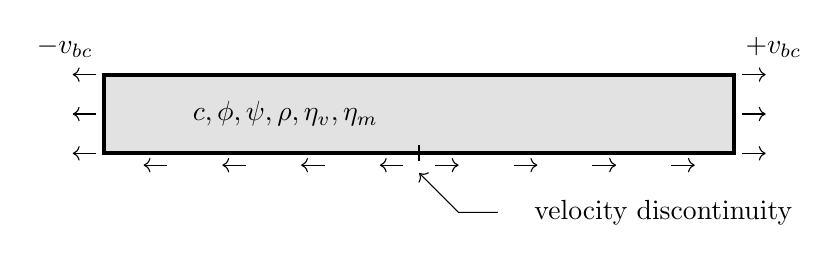
\begin{tikzpicture}
%\draw[fill=gray!23,gray!23](0,0) rectangle (10,3);
%\draw[step=0.5cm,gray,very thin] (0,0) grid (10,3); %background grid

\draw[fill=gray!23,gray!23](1,1) rectangle (9,2);

\draw[line width=0.5mm] (1,1)--(9,1)--(9,2)--(1,2)--cycle ;   

\draw[line width=0.3mm] (5,0.9)--(5,1.1); 

%left arrows
\draw [->] (0.9,1) -- (0.6,1);
\draw [->] (0.9,1.5) -- (0.6,1.5);
\draw [->] (0.9,2) -- (0.6,2);

\draw [->] (4.8,0.85) -- (4.5,0.85);
\draw [->] (3.8,0.85) -- (3.5,0.85);
\draw [->] (2.8,0.85) -- (2.5,0.85);
\draw [->] (1.8,0.85) -- (1.5,0.85);

%right arrows
\draw [->] (9.1,1) -- (9.4,1);
\draw [->] (9.1,1.5) -- (9.4,1.5);
\draw [->] (9.1,2) -- (9.4,2);

\draw [->] (5.2,0.85) -- (5.5,0.85);
\draw [->] (6.2,0.85) -- (6.5,0.85);
\draw [->] (7.2,0.85) -- (7.5,0.85);
\draw [->] (8.2,0.85) -- (8.5,0.85);

\node[] at (0.5,2.35) {$-v_{bc}$};
\node[] at (9.5,2.35) {$+v_{bc}$};

\node[] at (3.3,1.5) {$c,\phi,\psi,\rho,\eta_v,\eta_m$};
  
\draw [->] (6,0.25) -- (5.5,0.25) -- (5,0.75);
\node[] at (8.1,0.25) {velocity discontinuity};

\end{tikzpicture}
\end{center}


Extensional boundary conditions are as follows: 
\begin{itemize}
\item left boundary: $u=- \upnu_{bc}$, $v$ free;
\item right boundary: $u=+ \upnu_{bc}$, $v$ free; 
\item bottom boundary: $v=0$, $u=- \upnu_{bc}$ for $x<L_x/2$,  $u=+ \upnu_{bc}$ for $x>L_x/2$, and $u=0$ if $x=L_x/2$;
\item top boundary: zero traction.
\end{itemize}
For compressional boundary conditions the signs of all horizontal velocities should be reversed.
The nonlinear tolerance is set to $\text{tol}=10^{-6}$. Nonlinear iterations stop when 
maximum of the normalised nonlinear residual reaches the desired tolerance.
$\upnu_{bc}$ is chosen so that the background strain rate is $\dot\varepsilon_{bckgr}=10^{-15}\si{\per\second}$, 
i.e. $\upnu_{bc}=\dot\varepsilon_{bckgr} L_x/2$.

Following Choi \& Petersen \cite{chpe15}, we run the experiment with an associative ($\phi=\psi$) plasticity
and a non associative one ($\psi=0$, i.e. $R=0$). This second approach is essentially what many codes do (
i.e. $\vec\nabla\cdot\vec\upnu = 0$). We can also run the model with $\phi=\psi=0\si{\degree}$ so that 
we recover the von Mises plasticity yield criterion which is independent of pressure.  

The velocity, pressure, strain rate, dilation rate, and velocity divergence are shown hereunder both in 
extension and compression. Note that the domain has been substantially extended in the horizontal 
direction because of the wide shear band angles obtained in compression. It is now 80\si{\km} long 
and 10\si{\km} high (aspect ratio 8:1). 

Three angles are mechanically stable (e.g. \cite{kaus10}):
\[
\theta=\frac{\pi}{4}\pm \frac{\psi}{2} \qquad \text{Roscoe angle}
\]
\[
\theta=\frac{\pi}{4}\pm \frac{\phi}{2} \qquad \text{Coulomb angle}
\]
\[
\theta=\frac{\pi}{4}\pm \frac{\phi+\phi}{4} \qquad \text{Arthur angle}
\]
In the case of associative plasticity, $\phi=\psi$, so that all three angles are the same. 
Per row of elements, nodes or quadrature points, and per half of the domain (left and right) we find the location
with the highest strain-rate and record their coordinates.


\newpage
{\bf Extension}

\begin{center}
\includegraphics[width=.3\linewidth]{python_codes/fieldstone_39/benchmark1/extension/conv_phi0_psi0_etam0.pdf}
\includegraphics[width=.3\linewidth]{python_codes/fieldstone_39/benchmark1/extension/conv_phi0_psi0_etam19.pdf}
\includegraphics[width=.3\linewidth]{python_codes/fieldstone_39/benchmark1/extension/conv_phi0_psi0_etam20.pdf}\\
\includegraphics[width=.3\linewidth]{python_codes/fieldstone_39/benchmark1/extension/conv_phi30_psi0_etam0.pdf}
\includegraphics[width=.3\linewidth]{python_codes/fieldstone_39/benchmark1/extension/conv_phi30_psi0_etam19.pdf}
\includegraphics[width=.3\linewidth]{python_codes/fieldstone_39/benchmark1/extension/conv_phi30_psi0_etam20.pdf}\\
\includegraphics[width=.3\linewidth]{python_codes/fieldstone_39/benchmark1/extension/conv_phi30_psi30_etam0.pdf}
\includegraphics[width=.3\linewidth]{python_codes/fieldstone_39/benchmark1/extension/conv_phi30_psi30_etam19.pdf}
\includegraphics[width=.3\linewidth]{python_codes/fieldstone_39/benchmark1/extension/conv_phi30_psi30_etam20.pdf}\\
\includegraphics[width=.3\linewidth]{python_codes/fieldstone_39/benchmark1/extension/line_sr_phi0_psi0_etam0.pdf}
\includegraphics[width=.3\linewidth]{python_codes/fieldstone_39/benchmark1/extension/line_sr_phi0_psi0_etam19.pdf}
\includegraphics[width=.3\linewidth]{python_codes/fieldstone_39/benchmark1/extension/line_sr_phi0_psi0_etam20.pdf}\\
\includegraphics[width=.3\linewidth]{python_codes/fieldstone_39/benchmark1/extension/line_sr_phi30_psi0_etam0.pdf}
\includegraphics[width=.3\linewidth]{python_codes/fieldstone_39/benchmark1/extension/line_sr_phi30_psi0_etam19.pdf}
\includegraphics[width=.3\linewidth]{python_codes/fieldstone_39/benchmark1/extension/line_sr_phi30_psi0_etam20.pdf}\\
\includegraphics[width=.3\linewidth]{python_codes/fieldstone_39/benchmark1/extension/line_sr_phi30_psi30_etam0.pdf}
\includegraphics[width=.3\linewidth]{python_codes/fieldstone_39/benchmark1/extension/line_sr_phi30_psi30_etam19.pdf}
\includegraphics[width=.3\linewidth]{python_codes/fieldstone_39/benchmark1/extension/line_sr_phi30_psi30_etam20.pdf}\\
\end{center}
%\includegraphics[width=.3\linewidth]{python_codes/fieldstone_39/benchmark1/extension/line_eta_etam0.pdf}
%\includegraphics[width=.3\linewidth]{python_codes/fieldstone_39/benchmark1/extension/line_eta_etam19.pdf}
%\includegraphics[width=.3\linewidth]{python_codes/fieldstone_39/benchmark1/extension/line_eta_etam20.pdf}\\

\newpage
\begin{center}
\includegraphics[width=.3\linewidth]{python_codes/fieldstone_39/benchmark1/extension/shear_band_phi0_psi0_etam0.pdf}
\includegraphics[width=.3\linewidth]{python_codes/fieldstone_39/benchmark1/extension/shear_band_phi0_psi0_etam19.pdf}
\includegraphics[width=.3\linewidth]{python_codes/fieldstone_39/benchmark1/extension/shear_band_phi0_psi0_etam20.pdf}\\
\includegraphics[width=.3\linewidth]{python_codes/fieldstone_39/benchmark1/extension/shear_band_phi30_psi0_etam0.pdf}
\includegraphics[width=.3\linewidth]{python_codes/fieldstone_39/benchmark1/extension/shear_band_phi30_psi0_etam19.pdf}
\includegraphics[width=.3\linewidth]{python_codes/fieldstone_39/benchmark1/extension/shear_band_phi30_psi0_etam20.pdf}\\
\includegraphics[width=.3\linewidth]{python_codes/fieldstone_39/benchmark1/extension/shear_band_phi30_psi30_etam0.pdf}
\includegraphics[width=.3\linewidth]{python_codes/fieldstone_39/benchmark1/extension/shear_band_phi30_psi30_etam19.pdf}
\includegraphics[width=.3\linewidth]{python_codes/fieldstone_39/benchmark1/extension/shear_band_phi30_psi30_etam20.pdf}
\end{center}


\newpage
One can also run the extension model for $\phi=\psi={0,5,10,15,20,25,30}\degree$:
\begin{center}
\includegraphics[width=.45\linewidth]{python_codes/fieldstone_39/images/sr_0_30}
\includegraphics[width=.45\linewidth]{python_codes/fieldstone_39/images/etaeff_0_30}\\
\end{center}




\begin{center}
\includegraphics[width=.45\linewidth]{python_codes/fieldstone_39/images/shear_bands}
\includegraphics[width=.45\linewidth]{python_codes/fieldstone_39/images/shear_bands_nonass}\\
Results obtained on a 240x24 grid, max 50 nl iterations.
\end{center}


Note that benchmarking this in not easy. One solution Timo and I found was to add a 
velocity field $\underline{\vec\upnu}=(x,y,z)$ (with $\vec\nabla\cdot\underline{\vec\upnu}=3$)
to an existing analytical problem, e.g. the Burstedde benchamrk.

\newpage
%...........................................................
\subsection*{Benchmark \#2 - Spiegelman et al (2016) brick}

The setup is {\sl similar} to the one in Spiegelman et al (2016) \cite{spmw16}. 
It is a 2D Cartesian domain filled with an 
isoviscous layer at the bottom and a visco-plastic material on top, as shown here:  

\begin{center}
\includegraphics[width=6cm]{python_codes/fieldstone_39/images/spmw_1.png}
\includegraphics[width=8cm]{python_codes/fieldstone_39/images/spmw_2.png}
\end{center}

The domain has dimensions $L_x=128\si{\kilo\metre}$, $L_y=Lx/4$. 
The lower layer depth is $L_y/4$. The notch has dimensions $w=4\si{\kilo\metre}$
and $h=2\si{\kilo\metre}$. 

In what follows the nonlinear tolerance is set to $10^{-6}$. Due to a lack of resolution, I do not
implement the rounded edges of the seed. $U_0$ is set to $25\si{\mm\per\year}$ 
and the background viscosity of the brittle layer
is set to $\eta_v=10^{24}\si{\pascal\second}$. 

Note that the pressure colour bars in Fig(6) of \cite{spmw16} are most likely not correct at all: 
\begin{center}
\includegraphics[width=12cm]{python_codes/fieldstone_39/images/spmw_3.png}\\
{\captionfont Fig.(6) from Spiegelman et al (2016) \cite{spmw16}.}
\end{center}





\newpage
%........................................................
\subsection*{Benchmark \#4: Shortening of a visco-plastic bloc - part 1}

This benchmark originates in the book of Gerya. In the first edition the domain is 1000x1000km, 
while it is 100x100km in the second. We keep the second edition as a guideline. The benchmark
is actually elasto-visco-plastic but in this stone we neglect the elastic deformation. The 
boundary conditions are shown here:

\begin{center}
\includegraphics[width=6cm]{python_codes/fieldstone_39/results_shortening_block/setup}\\
{\captionfont Taken from \cite{gery19book}.}
\end{center}

The velocity on the boundaries is $\upnu_{bc}=5\cdot 10^{-9}$ \si{\metre\per\second} so that the background strain rate is 
$2 \upnu_{bc}/L = 10^{-13}\si{\per\second}$.
The weak medium and the weak inclusion have a viscosity $\eta=10^{17}\si{\pascal\second}$ while 
the block is visco-plastic, with $\eta=10^{23}\si{\pascal\second}$, $c=10^8\si{\pascal}$ 
and $\phi=37\degree$. 
Pressure is set to zero in the top right corner and later post-processed so as to insure a zero 
volume average.

In the case of von Mises ($\phi=0$) we expect the shear bands at $45\degree$. When $\phi>0$, as mentioned above
we expect:
\[
\frac{\pi}{4}-\frac{\phi}{2}=26.5\degree
\qquad
\frac{\pi}{4}-\frac{\phi}{4}=35.75\degree
\]

\begin{center}
\includegraphics[width=8cm]{python_codes/fieldstone_39/results_shortening_block/line}
\includegraphics[width=8cm]{python_codes/fieldstone_39/results_shortening_block/angles}\\
{\captionfont a) Line on which strain rate is measured. b) possible shear band angles:
green is $45\degree$, blue is $35.75\degree$ and red is $26.5\degree$.}
\end{center}


I have adapted slightly the dimensions inside the domain such that resolutions 16x16, 32x32, etc...
all showcase elements whose sides exactly align with the material interfaces. The size of the inclusion is 
$L/8=12.5$km and the block has a thickness of 50km:

\begin{center}
\includegraphics[width=10cm]{python_codes/fieldstone_39/results_shortening_block/geometry}\\
{\captionfont Material geometry for resolutions 16x16, 32x32 and 64x64.}
\end{center}


\newpage
\underline{von Mises (no dilation rate):}

\begin{center}
\includegraphics[width=5cm]{python_codes/fieldstone_39/results_shortening_block/u}
\includegraphics[width=5cm]{python_codes/fieldstone_39/results_shortening_block/v}
\includegraphics[width=5cm]{python_codes/fieldstone_39/results_shortening_block/vel}\\
{\captionfont Velocity field for 128x128, $\eta_m=1e19$}
\end{center}

\begin{center}
\includegraphics[width=8cm]{python_codes/fieldstone_39/results_shortening_block/etaeff}
\includegraphics[width=8cm]{python_codes/fieldstone_39/results_shortening_block/p}\\
\includegraphics[width=8cm]{python_codes/fieldstone_39/results_shortening_block/sr_elt_log}
\includegraphics[width=8cm]{python_codes/fieldstone_39/results_shortening_block/sr_elt}\\
{\captionfont From left to right: resolutions are 16x16, 32x32, 64x64 and 96x96. 100 nonlinear Picard iterations.}
\end{center}

\begin{center}
\includegraphics[width=5cm]{python_codes/fieldstone_39/results_shortening_block/conv_vM.pdf}
\includegraphics[width=5cm]{python_codes/fieldstone_39/results_shortening_block/sr_line_vM.pdf}
\includegraphics[width=5cm]{python_codes/fieldstone_39/results_shortening_block/sr_line_vM_reg.pdf}\\
{\captionfont $\eta_m=1e19$}
\end{center}




\newpage
\underline{viscous damper, no dilation rate, Drucker-Prager, phi=37:}


\begin{center}
\includegraphics[width=8cm]{python_codes/fieldstone_39/results_shortening_block/conv_DP.pdf}
\includegraphics[width=8cm]{python_codes/fieldstone_39/results_shortening_block/conv_DP_1e19.pdf}\\
{\captionfont Left: $\eta_m=0$, right: $\eta_m=10^{19}$}
\end{center}


\begin{center}
\includegraphics[width=4cm]{python_codes/fieldstone_39/results_shortening_block/32x32_phi37_1e19/sr}
\includegraphics[width=4cm]{python_codes/fieldstone_39/results_shortening_block/32x32_phi37_1e19/sr_log}
\includegraphics[width=4cm]{python_codes/fieldstone_39/results_shortening_block/32x32_phi37_1e19/p}
\includegraphics[width=4cm]{python_codes/fieldstone_39/results_shortening_block/32x32_phi37_1e19/eta}\\
{\captionfont Fieldstone 32x32}\\
\includegraphics[width=4cm]{python_codes/fieldstone_39/results_shortening_block/aspect_32x32_1e19_phi37/sr}
\includegraphics[width=4cm]{python_codes/fieldstone_39/results_shortening_block/aspect_32x32_1e19_phi37/sr_log}
\includegraphics[width=4cm]{python_codes/fieldstone_39/results_shortening_block/aspect_32x32_1e19_phi37/p}
\includegraphics[width=4cm]{python_codes/fieldstone_39/results_shortening_block/aspect_32x32_1e19_phi37/eta}\\
\includegraphics[width=4cm]{python_codes/fieldstone_39/results_shortening_block/aspect_64x64_1e19_phi37/sr}
\includegraphics[width=4cm]{python_codes/fieldstone_39/results_shortening_block/aspect_64x64_1e19_phi37/sr_log}
\includegraphics[width=4cm]{python_codes/fieldstone_39/results_shortening_block/aspect_64x64_1e19_phi37/p}
\includegraphics[width=4cm]{python_codes/fieldstone_39/results_shortening_block/aspect_64x64_1e19_phi37/eta}\\
{\captionfont ASPECT 32x32, 64x64} 
\end{center}



\newpage
To explore:

- associative and non-associative drucker-prage

- visco-plastic vs visco-viscoplastic







\newpage
%..............................................
\subsection*{Benchmark \#5: Shortening of a visco-plastic bloc - part 2}

The setup originates in Duretz et al (2018) \cite{dusd18} and is also carried out 
in Jacquey \& Cacace (2020) \cite{jaca20a}. We here again neglect the elastic 
deformation. 
The domain is 4x2 km. There is a linear viscous inclusion in the middle of radius 100\si{\metre} and 
viscosity $\eta_{inc}=10^{17}\si{\pascal\second}$. The material around is characterised by 
$\eta_v=10^{24}\si{pascal\second}$, $c=3e7\si{pascal}$, $\phi=30\degree$, $psi=10\degree$.
Boundary conditions are as follows: 

\begin{center}
\includegraphics[width=6cm]{python_codes/fieldstone_39/results_shortening_block2/jaca20a}
\end{center}

In the papers they prescribe $\Delta \varepsilon = 5\cdot 10^{-5}$ over a 
time step of $\Delta t=10^{10}\si{second}$, 
i.e. the background strain rate is $\dot\varepsilon=5\cdot 10^{-15}\si{\per\second}$.
Given $L_x$ and $L_y$ we can easily arrive at the velocity values to be prescribed:
\[
|u_{bc}|=\dot{\varepsilon}_{bc} L_x/2
\qquad
|v_{bc}|=\dot{\varepsilon}_{bc} L_y/2
\]
 
The inclusion is circular, i.e. no amount of mesh refinement will be such that the mesh 
edges align with it, as opposed to the previous experiment. 


\begin{center}
\includegraphics[width=8cm]{python_codes/fieldstone_39/results_shortening_block2/dusd18}
\includegraphics[width=8cm]{python_codes/fieldstone_39/results_shortening_block2/jaca20b}\\
{\captionfont Left: taken from Duretz et al (2018) \cite{dusd18}; Right: taken from Jacquey \& Cacace (2020) \cite{jaca20a}.
Note that these simulations have been run with elasto-visco-plastic rheologies 
for a certain amount of time so that the propagation of the shear bands is not final/complete, as
opposed to the converged visco-plastic solutions shown hereafter.}
\end{center}

As before, pressure is set to zero in the top right corner, and further post processed to insure that its volume 
average is zero.


\clearpage
\subsubsection*{von Mises rheology}

\begin{center}
\includegraphics[width=8cm]{python_codes/fieldstone_39/results_shortening_block2/conv_vM}\\
{\captionfont Nonlinear convergence, fieldstone and aspect, 128x64, 200 nonlinear iterations, $\eta_m=10^{19}$.}
\end{center}
\begin{center}
\includegraphics[width=5.8cm]{python_codes/fieldstone_39/results_shortening_block2/128x64_1e19/u}
\includegraphics[width=5.8cm]{python_codes/fieldstone_39/results_shortening_block2/128x64_1e19/v}
\includegraphics[width=5.8cm]{python_codes/fieldstone_39/results_shortening_block2/128x64_1e19/vel}\\
\includegraphics[width=5.8cm]{python_codes/fieldstone_39/results_shortening_block2/128x64_1e19/eta}
\includegraphics[width=5.8cm]{python_codes/fieldstone_39/results_shortening_block2/128x64_1e19/sr}
\includegraphics[width=5.8cm]{python_codes/fieldstone_39/results_shortening_block2/128x64_1e19/p}\\
{\captionfont 128x64, 200 nonlinear iterations, $\eta_m=10^{19}$}
\end{center}

\begin{center}
\includegraphics[width=5.8cm]{python_codes/fieldstone_39/results_shortening_block2/aspect_128x64_1e19/u}
\includegraphics[width=5.8cm]{python_codes/fieldstone_39/results_shortening_block2/aspect_128x64_1e19/v}
\includegraphics[width=5.8cm]{python_codes/fieldstone_39/results_shortening_block2/aspect_128x64_1e19/vel}\\
\includegraphics[width=5.8cm]{python_codes/fieldstone_39/results_shortening_block2/aspect_128x64_1e19/eta}
\includegraphics[width=5.8cm]{python_codes/fieldstone_39/results_shortening_block2/aspect_128x64_1e19/sr}
\includegraphics[width=5.8cm]{python_codes/fieldstone_39/results_shortening_block2/aspect_128x64_1e19/p}\\
{\captionfont ASPECT: 128x64, 200 nonlinear iterations, $\eta_m=10^{19}$}
\end{center}

\newpage
In order to help the comparison, I plot the effective viscosity and the strain rate for both next to one another:
\begin{center}
\includegraphics[width=8cm]{python_codes/fieldstone_39/results_shortening_block2/eta_both}
\includegraphics[width=8cm]{python_codes/fieldstone_39/results_shortening_block2/sr_both}\\
{\captionfont Left half is fieldstone, Right half is aspect.}
\end{center}


\begin{center}
\includegraphics[width=10cm]{python_codes/fieldstone_39/results_shortening_block2/sr_line_vM.pdf}\\
{\captionfont Strain rate cross section at $y=11L_y/16$.}
\end{center}


\clearpage
\subsubsection*{Drucker-Prager rheology ($\phi=30\degree$)}

\includegraphics[width=8cm]{python_codes/fieldstone_39/results_shortening_block2/conv_DP}
\includegraphics[width=8cm]{python_codes/fieldstone_39/results_shortening_block2/sr_line_DP.pdf}

\begin{center}
\includegraphics[width=4cm]{python_codes/fieldstone_39/results_shortening_block2/32x16_1e19_phi30/vel}
\includegraphics[width=4cm]{python_codes/fieldstone_39/results_shortening_block2/32x16_1e19_phi30/p}
\includegraphics[width=4cm]{python_codes/fieldstone_39/results_shortening_block2/32x16_1e19_phi30/sr}
\includegraphics[width=4cm]{python_codes/fieldstone_39/results_shortening_block2/32x16_1e19_phi30/eta}\\
\includegraphics[width=4cm]{python_codes/fieldstone_39/results_shortening_block2/48x24_1e19_phi30/vel}
\includegraphics[width=4cm]{python_codes/fieldstone_39/results_shortening_block2/48x24_1e19_phi30/p}
\includegraphics[width=4cm]{python_codes/fieldstone_39/results_shortening_block2/48x24_1e19_phi30/sr}
\includegraphics[width=4cm]{python_codes/fieldstone_39/results_shortening_block2/48x24_1e19_phi30/eta}\\
\includegraphics[width=4cm]{python_codes/fieldstone_39/results_shortening_block2/64x32_1e19_phi30/vel}
\includegraphics[width=4cm]{python_codes/fieldstone_39/results_shortening_block2/64x32_1e19_phi30/p}
\includegraphics[width=4cm]{python_codes/fieldstone_39/results_shortening_block2/64x32_1e19_phi30/sr}
\includegraphics[width=4cm]{python_codes/fieldstone_39/results_shortening_block2/64x32_1e19_phi30/eta}\\
\includegraphics[width=4cm]{python_codes/fieldstone_39/results_shortening_block2/128x64_1e19_phi30/vel}
\includegraphics[width=4cm]{python_codes/fieldstone_39/results_shortening_block2/128x64_1e19_phi30/p}
\includegraphics[width=4cm]{python_codes/fieldstone_39/results_shortening_block2/128x64_1e19_phi30/sr}
\includegraphics[width=4cm]{python_codes/fieldstone_39/results_shortening_block2/128x64_1e19_phi30/eta}\\
{\captionfont Fielstone. Top to bottom: 32x16, 48x24, 64x32, 128x64, etam=1e19, phi=30}\\
\includegraphics[width=4cm]{python_codes/fieldstone_39/results_shortening_block2/aspect_32x16_1e19_phi30/vel}
\includegraphics[width=4cm]{python_codes/fieldstone_39/results_shortening_block2/aspect_32x16_1e19_phi30/p}
\includegraphics[width=4cm]{python_codes/fieldstone_39/results_shortening_block2/aspect_32x16_1e19_phi30/sr}
\includegraphics[width=4cm]{python_codes/fieldstone_39/results_shortening_block2/aspect_32x16_1e19_phi30/eta}\\
\includegraphics[width=4cm]{python_codes/fieldstone_39/results_shortening_block2/aspect_64x32_1e19_phi30/vel}
\includegraphics[width=4cm]{python_codes/fieldstone_39/results_shortening_block2/aspect_64x32_1e19_phi30/p}
\includegraphics[width=4cm]{python_codes/fieldstone_39/results_shortening_block2/aspect_64x32_1e19_phi30/sr}
\includegraphics[width=4cm]{python_codes/fieldstone_39/results_shortening_block2/aspect_64x32_1e19_phi30/eta}\\
{\captionfont ASPECT, 64x32, etam=1e19, phi=30}\\
\end{center}

Note that ASPECT does not use the proper partitioning of strain rates, and uses total strain rate 
in plastic element. This could explain the difference?



\clearpage
\subsubsection*{A very different approach: diffusion plasticity}

The idea is to solve a diffusion equation for each component of the strain rate tensor. In 
order to do so, we need nodal values of this tensor and these values must then also be used in 
the rheology: the shape functions are used to interpolate these values onto the quadrature points
(as opposed to the standard way of using the shape function derivatives to interpolate the velocity). 

After each nonlinear iteration the nodal fields $\dot{\varepsilon}_{xx}$, $\dot{\varepsilon}_{yy}$ 
and $\dot{\varepsilon}_{xy}$ are diffused. The diffusion coefficient $D$ value is not straightforward
to choose. Also, boundary conditions are unknown so we resort to doing nothing, i.e. zero Neumann 
boundary conditions.

Note that in this case we have $\eta_m=0$ and that it is tTriggered in the code 
by {\sl use\_srn\_diff=True}.

\begin{center}
\includegraphics[width=8cm]{python_codes/fieldstone_39/results_shortening_block2/diffusion/srn}
\includegraphics[width=8cm]{python_codes/fieldstone_39/results_shortening_block2/diffusion/eta}\\
{\captionfont resolution 32x16, from top to bottom $D=0,2h_x,8h_x$.}
\end{center}

\begin{center}
\includegraphics[width=8cm]{python_codes/fieldstone_39/results_shortening_block2/diffusion/conv.pdf}
\end{center}

The diffusion helps with convergence. Rather importantly, it requires the use of nodal strainrate 
in the rheology, as opposed to before where strain rate at the quadrature point was computed using 
the derivatives of the shape functions. 


\begin{center}
\includegraphics[width=5cm]{python_codes/fieldstone_39/results_shortening_block2/diffusion/sr_lots}
\includegraphics[width=5cm]{python_codes/fieldstone_39/results_shortening_block2/diffusion/eta_lots}
\includegraphics[width=5cm]{python_codes/fieldstone_39/results_shortening_block2/diffusion/p_lots}\\
{\captionfont D=1km, 32x16, 48x24, 64x32, 80x40, 96x48}
\end{center}

\begin{center}
\includegraphics[width=10cm]{python_codes/fieldstone_39/results_shortening_block/diffusion/sr_line.pdf}\\
{\captionfont Strain rate cross section at $y=11L_y/16$.}
\end{center}


 %%%%%%%%%%%%%%%%%%%%%%%%%%%%%%%%%%%%%%%%%%%%%%%%%%%%%%%%%%%

\chapter{Instantaneous Rayleigh-Taylor instability (\QtwoQone) \label{f40}} %%%%%%%%%%%%%%%%%%%%%%% 40
\lstinputlisting[language=bash,basicstyle=\small]{python_codes/fieldstone_40/keywords.ascii}

\begin{center}
Code at \url{https://github.com/cedrict/fieldstone/tree/master/python_codes/fieldstone_40}
\end{center}

\par\noindent\rule{\textwidth}{0.4pt}
%%%%%%%%%%%%%%%%%%%%%%%%%%%%%%%%%%%%%%%%%%%%%%%%%%%%%%%%%%%%%%%%%%%%%%%%%%%%%%%%%%%%%%%%%%%%

This benchmark is carried out in \textcite{deka08} (2008), \textcite{gery10} (2010) and \textcite{thie11} (2011) 
and is based on the analytical solution by \textcite{ramb68} (1968). 
It consists of a buoyancy-driven two-layer system driven. 
The domain is a square of size $512\times512$km. 
Free slip are imposed on the sides while no-slip boundary conditions are imposed on the
top and the bottom of the box.

Fluid 1 $(\rho_1,\eta_1)$ of thickness $h_1$ overlays 
fluid 2 $(\rho_2,\eta_2)$ of thickness $h_2$ (with $h_1+h_2=L_y$).
An initial sinusoidal disturbance of the interface between these
layers is introduced and is characterised by an amplitude $\Delta$ and a
wavelength $\lambda=L_x/2$ as shown here: 

\begin{center}
a) \includegraphics[width=0.38\textwidth]{python_codes/fieldstone_40/images/setup}
b) \includegraphics[width=0.55\textwidth]{python_codes/fieldstone_40/images/dens}\\
{\captionfont  a) Setup of the experiment, taken from \cite{thie11}; b) grid setup for 24$\times$24 grid.} 
\end{center}

Under this condition, the velocity of the diapiric growth
$v_y$ is given by the relation
\[
\frac{v_y}{\Delta} = - K \frac{\rho_1-\rho_2}{2 \eta_2} h_2 g
\]
with the dimensionless growth factor $K$ being
\[
K=\frac{-d_{12}}{c_{11}j_{22}-d_{12}i_{21}}
\]
and 
\begin{eqnarray}
c_{11} &=& \frac{\eta_1 2 \phi_1^2}{\eta_2(\cosh 2\phi_1 - 1 - 2\phi_1^2)} - \frac{2\phi_2^2}{\cosh 2\phi_2 - 1 - 2 \phi_2^2}\\
d_{12} &=& \frac{\eta_1(\sinh 2\phi_1 -2\phi_1)}{\eta_2(\cosh 2\phi_1 -1 -2\phi_1^2)} + \frac{\sinh 2\phi_2 - 2\phi_2}{\cosh 2\phi_2 -1 -2\phi_2^2} \\
i_{21} &=& \frac{\eta_1\phi_2 (\sinh 2 \phi_1 + 2 \phi_1)}{\eta_2(\cosh 2\phi_1 -1 -2\phi_1^2)} 
+ \frac{\phi_2 (\sinh 2\phi_2 + 2\phi_2)}{\cosh 2\phi_2 -1 -2\phi_2^2} \\
j_{22} &=& \frac{\eta_1 2 \phi_1^2 \phi_2}{\eta_2(\cosh 2\phi_1 -1-2\phi_1^2)} - \frac{2\phi_2^3}{ \cosh 2\phi_2 -1 -2\phi_2^2}\\
\phi_1&=&\frac{2\pi h_1}{\lambda}\\
\phi_2&=&\frac{2\pi h_2}{\lambda}
\end{eqnarray}


\begin{center}
\includegraphics[width=7cm]{python_codes/fieldstone_40/images/vel}
\includegraphics[width=7cm]{python_codes/fieldstone_40/images/p}
\end{center}


\begin{center}
\includegraphics[width=5cm]{python_codes/fieldstone_40/images/plot24x24}
\includegraphics[width=5cm]{python_codes/fieldstone_40/images/plot32x32}
\includegraphics[width=5cm]{python_codes/fieldstone_40/images/plot48x48}\\
{\captionfont  Left: 24$\times$24 elements, middle: 32$\times$32; right: 48$\times$48. We see that 
increasing resolution yields more accurate results in the cases of short wavelength 
perturbations (points on the right on the plots).\\  
Note that in \cite{thie11} I fixed $\lambda=L_x/2$ and varied $L_x$. Here I keep $L_x$ fixed
and vary $\lambda=L_x/2,L_x,4,L_x/8$. Each line corresponds to a different value of the viscosity $\eta_2$.} 
\end{center}


 %%%%%%%%%%%%%%%%%%%%%%%%%%%%%%%%%%%%%%%%%%%%%%%%%%%%%%%%%%%

\chapter{Stokes flow and structural restoration (\QtwoQone) \label{f41}} %%%%%%%%%%%%%%%%%%%%%%%%%% 41

\paragraph{Setup of the experiment} It originates in Schuh-Senlis \etal \cite{sctc20} 
and is a scaled-up version of the Rayleigh-Taylor experiment of van Keken et al (1997) \cite{vaks97}.
In the original experiment the domain is $0.9142\times1$, viscosity is $\eta=100$, 
densities are 1000 and 1010 (i.e. $\delta \rho=10$) and the gravity is $|\vec{g}|=10$.
In our case the domain is 10,000 times larger, i.e. $9142\times10000$m, 
our viscosity is $\eta=10^{19}$, our densities are 2150 and 2600, i.e. $\delta\rho = 450$, 
and we also set $|\vec{g}|=10$.

\begin{center}
\includegraphics[width=7cm]{python_codes/fieldstone_41/images/setup}
\end{center}

Boundary conditions are no slip on the top and bottom, free slip on the sides.

In the original paper, 
length=1, viscosity=100, gravity =10, density contrast =10 and time unit =1,
so the dimensionless quantity
\[
\frac{\eta}{\delta\rho \cdot g \; length \cdot time} = \frac{100}{10 \cdot 10 \cdot 1 \cdot 1} =1
\]
If we now run a geometrically similar experiment with 
length=10km, viscosity=$10^{19}$, gravity=10, density contrast=450 and time unit = $t$
then we should also have 
\[
\frac{\eta}{\delta\rho \cdot g \; length \cdot time} = \frac{10^{19}}{450 \cdot 10 \cdot 10^4 \cdot t} =1
\]
i.e.,
\[
t = \frac{10^{14}}{450} \simeq 2.222 \cdot 10^{11}\text{s}
\]
This means that in order to plot our results against those in van Keken et al, their results
must be scaled: times must be multiplied by $t$ and velocities divided by 
$t/length = 2.222 \cdot 10^{7}\text{m/s}$  

The initial mass of the system is:
\[
M(t=0) = L_x \times 2km \times \rho_s + Lx \times 8km \times \rho_0 = 
9142 \cdot(2000\cdot 2150 + 8000\cdot 2600) \simeq 2.294642\cdot 10^{11}\text{kg}
\]

\paragraph{The code} It is based on stable $Q_2\times Q_1$ elements for the Stokes equations and 
the heat transport equation need not be solved. 
It relies on the Particle-in-Cell method (see Section~\ref{MMM-ss:pic}) for material advection. 
At startup {\tt nmarker\_per\_dim**2} particles are regularly placed in each element. 
There are in total:
\begin{lstlisting}
nmarker=nmarker_per_element*nel
\end{lstlisting}

Markers track material number, i.e. 1 or 2:
\begin{lstlisting}
for im in range (0,nmarker):
    if swarm_y[im]>salt_thickness+amplitude*np.cos(np.pi*swarm_x[im]/Lx):
       swarm_mat[im]=2
    else:
       swarm_mat[im]=1
\end{lstlisting}

Marker density is interpolated onto the Q1 mesh by means of the Q1 shape functions:
\begin{lstlisting}
for im in range(0,nmarker):
    ielx=int(swarm_x[im]/Lx*nelx)
    iely=int(swarm_y[im]/Ly*nely)
    iel=nelx*(iely)+ielx
    N1=0.25*(1-swarm_r[im])*(1-swarm_s[im])
    N2=0.25*(1+swarm_r[im])*(1-swarm_s[im])
    N3=0.25*(1+swarm_r[im])*(1+swarm_s[im])
    N4=0.25*(1-swarm_r[im])*(1+swarm_s[im])
    rho_nodal[iconP[0,iel]]+=rho_mat[swarm_mat[im]-1]*N1
    rho_nodal[iconP[1,iel]]+=rho_mat[swarm_mat[im]-1]*N2
    rho_nodal[iconP[2,iel]]+=rho_mat[swarm_mat[im]-1]*N3
    rho_nodal[iconP[3,iel]]+=rho_mat[swarm_mat[im]-1]*N4
    rho_nodal_counter[iconP[0,iel]]+=N1
    rho_nodal_counter[iconP[1,iel]]+=N2
    rho_nodal_counter[iconP[2,iel]]+=N3
    rho_nodal_counter[iconP[3,iel]]+=N4
rho_nodal/=rho_nodal_counter
\end{lstlisting}
This is a marker-centric approach, which is identical to the 
somewhat more instinctive node-centric approach which itself is similar
to the meshless methods approach (think of the SPH method kernel but with a 
square support). Density is later on interpolated onto the quadrature points 
with the $Q_1$ shape functions again to avoid the problems highlighted in 
Section~\ref{MMM-ss:bern}.
Viscosity is averaged per element by means of an arithmetic, geometric or harmonic mean.

Particles are advected by means of a (space) Runge-Kutta 1st/2nd/3rd order algorithm (see
Section~\ref{MMM-ss:rkm}). The time step $\delta t$ is set by means of the CFL criterion (see
Section~\ref{MMM-ss:cfl}).

The root mean square velocity and total mass of the system are computed every time step.

Simulations end when the maximum number of time steps is reached or when 
an element does not contain any particle.
\begin{center}
\includegraphics[width=7cm]{python_codes/fieldstone_41/results/vrms_RK.pdf}
\includegraphics[width=7cm]{python_codes/fieldstone_41/results/vrms_RES.pdf}\\
\includegraphics[width=7cm]{python_codes/fieldstone_41/results/vrms_CFL.pdf}
\includegraphics[width=7cm]{python_codes/fieldstone_41/results/vrms_nmarker.pdf}\\
{\captionfont Root mean square velocity as a function of time. Black curves are those in van Keken
et al (1997). Letters stand for authors initials.}
\end{center}



\begin{center}
\includegraphics[width=7cm]{python_codes/fieldstone_41/results/mass.pdf}
\includegraphics[width=7cm]{python_codes/fieldstone_41/results/nmarker.pdf}
\end{center}

\begin{center}
\includegraphics[width=5cm]{python_codes/fieldstone_41/results/64x64_10_RK3/markers0000}
\includegraphics[width=5cm]{python_codes/fieldstone_41/results/64x64_10_RK3/markers0143}
\includegraphics[width=5cm]{python_codes/fieldstone_41/results/64x64_10_RK3/rho_nodal_0143}\\
{\captionfont 64x64 simulation right before crash}
\end{center}


\newpage
%---------------------------------------------------------------
\subsection*{Stokes sphere under deformable free surface}

The setup is described in Section~\ref{MMM-ss:stokes_sphere_fs2D}. 
Densities are projected on the nodes or elements with an arithmetic averaging while
viscosities are projected onto elements ({\tt avrg}$>0$) or onto $Q_1$nodes ({\tt avrg}$<0$).
There are 7 averaging schemes implemented:
\begin{itemize}
\item[{\tt avrg}=-1] first-order basis function weighed arithmetic average onto nodes
\item[{\tt avrg}=-2] first-order basis function weighed geometric average onto nodes
\item[{\tt avrg}=-3] first-order basis function weighed harmonic average onto nodes
\item[{\tt avrg}=+1]  elemental piecewise constant arithmetic average 
\item[{\tt avrg}=+2]  elemental piecewise constant geometric average 
\item[{\tt avrg}=+3]  elemental piecewise constant harmonic average 
\item[{\tt avrg}=+4]  elemental first-order least square projection 
\end{itemize}

Let us recall that the Least Squares methodology is presented for example in 
Thielmann \etal \cite{thmk14} and in Section~\ref{MMM-ss:pic}:
the density or viscosity values carried by the markers are represented by a linear 
function in a 2D space inside each 
element, i.e. $\tilde{\eta}({\vec r}) = a + b x+c y$ and $\tilde{\rho}=d+ex+fy$.

When {\tt avrg}$<0$ values are projected onto quadrature points by means 
of $Q_1$ basis functions using the values at the corners of the element.
When {\tt avrg}$=1,2,3$ all quadrature points receive the same elemental value. 
When {\tt avrg}$=4$ the coordinates of each quadrature points are used in order to 
estimate the value from the coefficients $\{a,b,c\}$ and $\{d,e,f\}$ 
of the (limited) least square.

Given the current limitations of this simple code I can only run experiments with limited resolutions. 
Also since I later wish to plot the density and viscosity values carried by the quadrature points 
on a vertical line passing through the middle of the sphere, I focus on odd numbers of elements
in the horizontal direction and investigate $33\times33$, $49\times49$, $65\times65$, $81\times81$,
and $97\times97$.

\begin{center}
\includegraphics[width=5.5cm]{python_codes/fieldstone_41/results/exp3/markers}
\includegraphics[width=5.5cm]{python_codes/fieldstone_41/results/exp3/vel_line}\\
{\captionfont 
Left: markers on 33x33 grid, $5^2$ markers per element.  
Right: vertical component $v$ of the velocity as obtained \\
on the $81\times81$ mesh using least squares + limiter projection.\\
The black line indicates the location of profile measurements.}
\end{center}

\begin{center}
\includegraphics[width=4.25cm]{python_codes/fieldstone_41/results/exp3/33x33/profile_v.pdf}
\includegraphics[width=4.25cm]{python_codes/fieldstone_41/results/exp3/33x33/profile_p.pdf}
\includegraphics[width=4.25cm]{python_codes/fieldstone_41/results/exp3/33x33/profile_eta_elemental.pdf}
\includegraphics[width=4.25cm]{python_codes/fieldstone_41/results/exp3/33x33/profile_eta_nodal.pdf}\\
\includegraphics[width=4.25cm]{python_codes/fieldstone_41/results/exp3/49x49/profile_v.pdf}
\includegraphics[width=4.25cm]{python_codes/fieldstone_41/results/exp3/49x49/profile_p.pdf}
\includegraphics[width=4.25cm]{python_codes/fieldstone_41/results/exp3/49x49/profile_eta_elemental.pdf}
\includegraphics[width=4.25cm]{python_codes/fieldstone_41/results/exp3/49x49/profile_eta_nodal.pdf}\\
\includegraphics[width=4.25cm]{python_codes/fieldstone_41/results/exp3/65x65/profile_v.pdf}
\includegraphics[width=4.25cm]{python_codes/fieldstone_41/results/exp3/65x65/profile_p.pdf}
\includegraphics[width=4.25cm]{python_codes/fieldstone_41/results/exp3/65x65/profile_eta_elemental.pdf}
\includegraphics[width=4.25cm]{python_codes/fieldstone_41/results/exp3/65x65/profile_eta_nodal.pdf}\\
\includegraphics[width=4.25cm]{python_codes/fieldstone_41/results/exp3/81x81/profile_v.pdf}
\includegraphics[width=4.25cm]{python_codes/fieldstone_41/results/exp3/81x81/profile_p.pdf}
\includegraphics[width=4.25cm]{python_codes/fieldstone_41/results/exp3/81x81/profile_eta_elemental.pdf}
\includegraphics[width=4.25cm]{python_codes/fieldstone_41/results/exp3/81x81/profile_eta_nodal.pdf}\\
\includegraphics[width=4.25cm]{python_codes/fieldstone_41/results/exp3/97x97/profile_v.pdf}
\includegraphics[width=4.25cm]{python_codes/fieldstone_41/results/exp3/97x97/profile_p.pdf}
\includegraphics[width=4.25cm]{python_codes/fieldstone_41/results/exp3/97x97/profile_eta_elemental.pdf}
\includegraphics[width=4.25cm]{python_codes/fieldstone_41/results/exp3/97x97/profile_eta_nodal.pdf}\\
\includegraphics[width=4.25cm]{python_codes/fieldstone_41/results/exp3/113x113/profile_v.pdf}
\includegraphics[width=4.25cm]{python_codes/fieldstone_41/results/exp3/113x113/profile_p.pdf}
\includegraphics[width=4.25cm]{python_codes/fieldstone_41/results/exp3/113x113/profile_eta_elemental.pdf}
\includegraphics[width=4.25cm]{python_codes/fieldstone_41/results/exp3/113x113/profile_eta_nodal.pdf}\\
\includegraphics[width=4.25cm]{python_codes/fieldstone_41/results/exp3/129x129/profile_v.pdf}
\includegraphics[width=4.25cm]{python_codes/fieldstone_41/results/exp3/129x129/profile_p.pdf}
\includegraphics[width=4.25cm]{python_codes/fieldstone_41/results/exp3/129x129/profile_eta_elemental.pdf}
\includegraphics[width=4.25cm]{python_codes/fieldstone_41/results/exp3/129x129/profile_eta_nodal.pdf}\\
{\captionfont 
1st column: vertical velocity profile; 
2nd column: vertical pressure profile; 
3rd column: viscosity on quadrature points in log scale for {\tt avrg}$>0$ (elemental approach);
4th column: viscosity on quadrature points in log scale for {\tt avrg}$<0$ (nodal approach);
$5^2$ markers per element.
The black dot indicates the velocity in the middle of the sphere 
obtained with \stone 93 using Crouzeix-Raviart triangular elements.} 
\end{center}
It is immediately apparent that the least-square case yields smooth velocity profiles, even at 
low resolutions. Also it is clear that nodal approaches tend to smear out the transition zone
but do not yield a visible improvement in terms of velocity.

\begin{center}
\includegraphics[width=7.5cm]{python_codes/fieldstone_41/results/exp3/mass.pdf}
\includegraphics[width=7.5cm]{python_codes/fieldstone_41/results/exp3/vrms.pdf}\\
{\captionfont Total mass and root mean square velocity $\upnu_{rms}$ for all 7 projections.}
\end{center}

%-----------------------------------------------------------------------------
\subsubsection*{A word about the need for a limiter}

The following figures are obtained with a standard linear least square algorithm. 

\begin{center}
\includegraphics[width=7cm]{python_codes/fieldstone_41/results/exp3/rho_ls}
\includegraphics[width=7cm]{python_codes/fieldstone_41/results/exp3/eta_ls}\\
\includegraphics[width=7cm]{python_codes/fieldstone_41/results/exp3/rho_ls_warp}
\includegraphics[width=7cm]{python_codes/fieldstone_41/results/exp3/eta_ls_warp}\\
\includegraphics[width=7cm]{python_codes/fieldstone_41/results/exp3/rho_ls_warp2}
\includegraphics[width=7cm]{python_codes/fieldstone_41/results/exp3/eta_ls_warp2}\\
\end{center}

Describe here limiter...


 %%%%%%%%%%%%%%%%%%%%%%%%%%%%%%%%%%%%%%%%%%%%%%%%%%%%%%%%%%%

\chapter{The no flow test (\QonePzero, \QtwoQone, \QthreeQtwo, \QfourQthree)\label{f42}} %%%%%%%%%% 42
\lstinputlisting[language=bash,basicstyle=\small]{python_codes/fieldstone_42/keywords.ascii}

\begin{center}
Code at \url{https://github.com/cedrict/fieldstone/tree/master/python_codes/fieldstone_42}
\end{center}

\par\noindent\rule{\textwidth}{0.4pt}

%%%%%%%%%%%%%%%%%%%%%%%%%%%%%%%%%%%%%%%%%%%%%%%%%%%%%%%%%%%%%%%%%%%%%%%%%%%%%%%%%%%%%%%%%%%%


The idea behind this stone comes from the following excerpt of Fortin \& Fortin (1985) \cite{fofo85}:
\begin{center}
\includegraphics[width=14cm]{python_codes/fieldstone_42/images/fofo85a}\\
\includegraphics[width=14cm]{python_codes/fieldstone_42/images/fofo85b}
\end{center}

I then set out to reproduce this and to compare the results with continuous-pressure elements.
On the boundary of the domain $\Omega$ I impose $\vec\upnu=\vec{0}$ and 
the viscosity and density are set to 1. The gravity vector points downwards
with $|\vec{g}|=1$.
The analytical solution is $\vec\upnu(x,y)=\vec{0}$ and $p(x,y)=ay+b$, 
where the constants $a$ and $b$ are determined by the geometry and the buoyancy force.

Based on the figure above I set $L_x=16$ and $L_y=6$ and the angle is set to $45\degree$ (while it 
is about $15\degree$ on the figures below).
The chosen number of elements is $16\times 8$ as in \cite{fofo85}.
Rather arbitrarily the pressure is set to zero on the top right corner (This is not really
important since the pressure is defined up to a constant in this case).

I consider the following three different domain geometries:
\begin{center}
\input{python_codes/fieldstone_42/tikz_geoms}
\end{center}
and three different elements: ${\bm Q}_1\times P_0$, ${\bm Q}_2\times Q_1$, and ${\bm Q}_3\times Q_2$.

%.............................
\subsubsection*{geom=0}

I find that the checkerboard mode is present for the unstable ${\bm Q}_1\times P_0$
element. However, for all three elements the velocity is zero, down to machine precision.
For the two continuous-pressure elements the pressure at the top is 0 and 6 at the 
bottom as expected.

\begin{center}
\includegraphics[width=5.4cm]{python_codes/fieldstone_42/results/geom0/press1}
\includegraphics[width=5.4cm]{python_codes/fieldstone_42/results/geom0/press2}
\includegraphics[width=5.4cm]{python_codes/fieldstone_42/results/geom0/press3}\\
\includegraphics[width=5.4cm]{python_codes/fieldstone_42/results/geom0/vel1}
\includegraphics[width=5.4cm]{python_codes/fieldstone_42/results/geom0/vel2}
\includegraphics[width=5.4cm]{python_codes/fieldstone_42/results/geom0/vel3}\\
{\captionfont From left to right: ${\bm Q}_1\times P_0$, ${\bm Q}_2\times Q_1$, 
and ${\bm Q}_3\times Q_2$.}
\end{center}


%.............................
\subsubsection*{geom=1}

We find that the checkerboard mode is now absent and velocities are still zero
for all three elements. The pressure is hydrostatic and only depends on the $y$-coordinate.

\begin{center}
\includegraphics[width=5.1cm]{python_codes/fieldstone_42/results/geom1/press1}
\includegraphics[width=5.1cm]{python_codes/fieldstone_42/results/geom1/press2}
\includegraphics[width=5.1cm]{python_codes/fieldstone_42/results/geom1/press3}\\
\includegraphics[width=5.1cm]{python_codes/fieldstone_42/results/geom1/vel1}
\includegraphics[width=5.1cm]{python_codes/fieldstone_42/results/geom1/vel2}
\includegraphics[width=5.1cm]{python_codes/fieldstone_42/results/geom1/vel3}\\
{\captionfont From left to right: ${\bm Q}_1\times P_0$, ${\bm Q}_2\times Q_1$, 
and ${\bm Q}_3\times Q_2$.}
\end{center}

%.............................
\subsubsection*{geom=2}

As in Fortin \& Fortin (1985) we find that the velocity field now showcases 2 ``convection
cells'' for the  ${\bm Q}_1\times P_0$ element (although they have different shapes than 
the ones in their publication) while the velocity remains zero for the other two elements. 

\begin{center}
\includegraphics[width=5.1cm]{python_codes/fieldstone_42/results/geom2/press1}
\includegraphics[width=5.1cm]{python_codes/fieldstone_42/results/geom2/press2}
\includegraphics[width=5.1cm]{python_codes/fieldstone_42/results/geom2/press3}\\
\includegraphics[width=5.1cm]{python_codes/fieldstone_42/results/geom2/vel1}
\includegraphics[width=5.1cm]{python_codes/fieldstone_42/results/geom2/vel2}
\includegraphics[width=5.1cm]{python_codes/fieldstone_42/results/geom2/vel3}\\
{\captionfont From left to right: ${\bm Q}_1\times P_0$, ${\bm Q}_2\times Q_1$, 
and ${\bm Q}_3\times Q_2$.}
\end{center}


On the following figure the root mean square velocity obtained with the 
${\bm Q}_1\times P_0$ element is shown as a function of 
the element size $h$. We find that it decreases quadratically with $h$. 
\begin{center}
\includegraphics[width=6cm]{python_codes/fieldstone_42/results/vrms.pdf}
\end{center}


 %%%%%%%%%%%%%%%%%%%%%%%%%%%%%%%%%%%%%%%%%%%%%%%%%%%%%%%%%%%

\chapter{Time-dependent advection problems ($Q_1$, $Q_2$)\label{f43}} %%%%%%%%%%%%%%%%%%%%%%%%%%%%% 43
\noindent
\includegraphics[height=1.25cm]{images/pictograms/replication}
\includegraphics[height=1.25cm]{images/pictograms/aspect_logo}
\includegraphics[height=1.25cm]{images/pictograms/benchmark}
\includegraphics[height=1.25cm]{images/pictograms/FEM}
\includegraphics[height=1.25cm]{images/pictograms/temperature}
\includegraphics[height=1.25cm]{images/pictograms/paraview}

%%%%%%%%%%%%%%%%%%%%%%%%%%%%%%%%%%%%%%%%%%%%%%%%%%%%%%%%%%%%%%%%%%%%%%%%%%%%%%%%%%%%%%%%%%%%%%%%%%%

%\lstinputlisting[language=bash,basicstyle=\small]{python_codes/fieldstone_43/keywords.ascii}

\begin{center}
Code at \url{https://github.com/cedrict/fieldstone/tree/master/python_codes/fieldstone_43}
\end{center}

\par\noindent\rule{\textwidth}{0.4pt}

Last revision: Jan. 17th, 2025.

\par\noindent\rule{\textwidth}{0.4pt}

%%%%%%%%%%%%%%%%%%%%%%%%%%%%%%%%%%%%%%%%%%%%%%%%%%%%%%%%%%%%%%%%%%%%%%%%%%%%%%%%%%%%%%%%%%%%

The following experiments are ``pure advection'' experiments (i.e. there is 
no diffusion at all). As such the Peclet number
is infinite and the $\gamma$ value of the SUPG algorithm as shown in Section~\ref{MMM-ss:supg} tends to 1
and the $\tau$ parameter is simply $h/2 |\vec\upnu| p$ (where $p$ is the order of 
the shape function polynomials).

Note that although the code can deal with linear elements, all results 
hereafter are obtained with quadratic elements (unless specified otherwise). 

A very important remark: In step-9 of deal.II (which is concerned with solving the 
steady-state advection equation) we read: `` The mathematical theory states that we must not 
pose any boundary condition on the outflow part of the boundary.''
Upon my asking for more context to Wolfgang Bangerth (the author of step-9), his answer was:
``I think the statement can be shown in the following way: If
you think of the advection equation as transporting information along
characteristics, then the interior can only be affected by characteristics
that go from the boundary into the interior. That's exactly the ones at inflow
boundary conditions. ''
Note that \aspect automatically checks that $\vec\upnu\cdot\vec{n}<0$ at each node where temperature is
prescribed and only prescribe it there
\footnote{\url{https://github.com/geodynamics/aspect/blob/main/source/simulator/core.cc}, Lines 689-726} 
In other words, one cannot prescribe the temperature on a
boundary where the fluid is leaving the domain, only where it is entering.

\todo[inline]{This means that in the experiments presented hereafter this
needs to be checked and corrected if needed!}




\newpage
%------------------------------------------------------------------------------
\subsection*{Experiment 1 - rotating cone}

This benchmark can be found \textcite{dohu03} and it is also carried out in \textcite{bepo10} (2010).
A product-cosine hill is advected in a prescribed velocity field. 
The initial temperature is:
\begin{equation}
T_0(x,y)=
\left\{
\begin{array}{cc}
\frac{1}{4}
\left(1+\cos \pi\frac{x-x_c}{\sigma}\right)
\left(1+\cos \pi\frac{y-y_c}{\sigma}\right)
& \text{if } (x-x_c)^2+(y-y_c)^2\leq \sigma^2 \\
0 & \text{otherwise}
\end{array}
\right.
\end{equation}
The boundary conditions are $T(x,y)=0$ on all four sides of the unit square domain, but only 
where the velocity field is such that the node in question accounts for an influx, 
not an outflux (see remark above).
In what follows we set $x_c=y_c=2/3$ and $\sigma=0.2$.  
The velocity field is analytically prescribed: $\vec\upnu=(-(y-L_y/2),+(x-L_x/2))$.
Resolution is set to $30\times30$ quadratic $Q_2$ elements.

In what follows we test the time integration scheme by setting $\alpha_T=1$ 
(fully implicit formulation), $\alpha_T=0$ (fully explicit formulation) and $\alpha_T=1/2$ (Crank-Nicolson).  
In the book Donea \& Huerta set the timestep is set to $\delta t=2\pi/200$ which corresponds 
to a CFL number of approximately 0.666. If we want to be able to run this experiment at higher 
resolution we need to adapt the timestep to the mesh size (CFL criterion). We 
therefore set the CFL number to 0.5 and compute $\delta t$ 
accordingly (see Section~\ref{MMM-ss:cfl}).  
The density and heat capacity values are set to 1. We monitor the minimum 
and maximum value of the temperature field, as well as the total thermal energy $E_T$ in the 
system during the full rotation:
\[
E_T=\int_\Omega \rho_0 C_p T dV = \int_\Omega T dV = |\Omega| \langle T \rangle 
\qquad
\text{where}
\qquad
\langle T \rangle = \frac{1}{|\Omega|} \int_\Omega T dV
\]
The time evolution of the temperature with the Crank-Nicolson algorithm is shown hereunder:
\begin{center}
a)\includegraphics[width=4.8cm]{python_codes/fieldstone_43/results/experiment1/crni/solution_0000.pdf}
b)\includegraphics[width=4.8cm]{python_codes/fieldstone_43/results/experiment1/crni/solution_0110.pdf}
c)\includegraphics[width=4.8cm]{python_codes/fieldstone_43/results/experiment1/crni/solution_0210.pdf}
d)\includegraphics[width=4.8cm]{python_codes/fieldstone_43/results/experiment1/crni/solution_0320.pdf}
e)\includegraphics[width=4.8cm]{python_codes/fieldstone_43/results/experiment1/crni/solution_0420.pdf}
f)\includegraphics[width=4.8cm]{python_codes/fieldstone_43/results/experiment1/crni/solution_0530.pdf}\\
{\captionfont a,b,c,d,e,f) Temperature field throughout the $2\pi$ rotation.} 
\end{center}

\vspace{.4cm}

Turning now to the statistics, we plot $\min/\max(T)$ and $E_T$ as a function of time:
\begin{center}
\includegraphics[width=5.7cm]{python_codes/fieldstone_43/results/experiment1/Tmin.pdf}
\includegraphics[width=5.7cm]{python_codes/fieldstone_43/results/experiment1/Tmax.pdf}
\includegraphics[width=5.7cm]{python_codes/fieldstone_43/results/experiment1/ET.pdf}\\
{\captionfont Time evolution of the min and max temperature and the total energy}
\end{center}
The conclusions are clear: the explicit method diverges quickly and is unusable. 
The fully implicit and Crank-Nicolson 
method yield similar energy conservation but the fully-implicit showcases 
a clear decrease in maximum temperature.


%...................................................................................
\subsubsection*{Effect of time step value} 
We can run the experiment (still a $2\pi$ rotation) 
with three different time steps ($\delta t=2\pi/30,2\pi/60,2\pi/120$) 
and we recover very similar results to those presented in \textcite{dohu03}:
\begin{center}
\includegraphics[height=8cm]{python_codes/fieldstone_43/results/experiment1/dohu03}
\includegraphics[height=8cm]{python_codes/fieldstone_43/results/experiment1/temps_30_60_120}\\
{\captionfont From top to bottom: $\delta t=2\pi/120,2\pi/60,2\pi/30$ with Crank-Nicolson. 
Left panel is taken from donea \& Huerta \cite{dohu03}. Results obtained with linear elements.}
\end{center}



%...................................................................
\subsubsection*{On the use of BDF methods} I have also implemented 
BDF1,2,3,4,5  (see Section~\ref{MMM-ss:hte_fem}). 
BDF2 outperforms BDF1 and is comparable to Crank-Nicolson. 
For reasons unknown to me, the BDF3 diverges after 100 time steps. So do 
BDF4 and BDF5 after even less timesteps. In the following picture the temperature is shown for 
BDF1,2,3 and Crank-Nicolson after a full rotation.

\begin{center}
\includegraphics[width=15cm]{python_codes/fieldstone_43/results/experiment1/Tbdf123crni.png}\\
{\captionfont Left to right: BDF1 (i.e. implicit euler), BDF2, BDF3, Crank-Nicolson}
\end{center}



%.....................................
\subsubsection*{On the effect of SUPG} 
I now turn to another aspect of this problem: what is the effect of the SUPG stabilisation 
scheme on the solution? In what follows Crank-Nicolson is used. 

\begin{center}
\includegraphics[width=7cm]{python_codes/fieldstone_43/results/experiment1/Tmin_supg}
\includegraphics[width=7cm]{python_codes/fieldstone_43/results/experiment1/Tmax_supg}\\
{\captionfont Time evolution of min/max temperature with and without SUPG.} 
\end{center}

We find that SUPG yields a solution which min/max values are closer to the analytical ones.

\begin{center}
a)\includegraphics[width=4.8cm]{python_codes/fieldstone_43/results/experiment1/supg/solution_0000.pdf}
b)\includegraphics[width=4.8cm]{python_codes/fieldstone_43/results/experiment1/supg/solution_0100.pdf}
c)\includegraphics[width=4.8cm]{python_codes/fieldstone_43/results/experiment1/supg/solution_0200.pdf}
d)\includegraphics[width=4.8cm]{python_codes/fieldstone_43/results/experiment1/supg/solution_0300.pdf}
e)\includegraphics[width=4.8cm]{python_codes/fieldstone_43/results/experiment1/supg/solution_0400.pdf}
f)\includegraphics[width=4.8cm]{python_codes/fieldstone_43/results/experiment1/supg/solution_0500.pdf}\\
{\captionfont a,b,c,d,e,f) Temperature field throughout the $2\pi$ rotation.} 
\end{center}



%------------------------------------------------------------------------------
%------------------------------------------------------------------------------
%------------------------------------------------------------------------------
\newpage
\subsection*{Experiment 2 - Three objects rotation}

This setup is inspired by the one in the ASPECT 
manual\footnote{\url{https://aspect-documentation.readthedocs.io/en/latest/user/benchmarks/benchmarks/advection/doc/advection.html}}. The cone of the previous 
experiment is now replaced by three 'objects': a Zalesak disk \cite{zale79}, 
a sharp cone and a truncated cosine hill:

\begin{lstlisting}
for i in range(0,NV):
    xi=x[i]
    yi=y[i]
    if np.sqrt(xi**2+(yi-0.5)**2)<0.3 and (np.abs(xi)>=0.05 or yi>=0.7):
       T[i]=1
    if np.sqrt((x[i])**2+(y[i]+0.5)**2)<0.3:
       T[i]=1-np.sqrt((x[i])**2+(y[i]+0.5)**2)/0.3
    if np.sqrt((x[i]+0.5)**2+(y[i])**2)<0.3:
       T[i]=0.25*(1+np.cos(np.pi*np.sqrt((xi+0.5)**2+yi**2)/0.3))
\end{lstlisting}

The domain is $2\times2$, centered on the origin. The velocity is $\vec\upnu=(-y,x)$. Temperature 
is set to zero on all four sides (only on influx subsets). For this experiment the CFL number is set to 0.5
and the resolution is $64\times 64$ elements.

\begin{center}
\includegraphics[width=8cm]{python_codes/fieldstone_43/results/experiment2/buildings}
\includegraphics[width=5.2cm]{python_codes/fieldstone_43/results/experiment2/kome22}\\
{\captionfont Left: ASPECT manual; Right: taken from \textcite{kome22} (2022).}
\end{center}


\begin{center}
\includegraphics[width=8cm]{python_codes/fieldstone_43/results/experiment2/avrg_T}
\includegraphics[width=8cm]{python_codes/fieldstone_43/results/experiment2/avrg_T2}\\
{\captionfont Averave temperature in the domain as a function of time. 
Left: all three cases. Right: only SUPG cases.}
\end{center}

\begin{center}
\includegraphics[width=8cm]{python_codes/fieldstone_43/results/experiment2/stats_T}
\end{center}

\begin{center}
\includegraphics[width=3.72cm]{python_codes/fieldstone_43/results/experiment2/supg/solution_0000.pdf}
\includegraphics[width=3.72cm]{python_codes/fieldstone_43/results/experiment2/supg/solution_0200.pdf}
\includegraphics[width=3.72cm]{python_codes/fieldstone_43/results/experiment2/supg/solution_0400.pdf}
\includegraphics[width=3.72cm]{python_codes/fieldstone_43/results/experiment2/supg/solution_0600.pdf}\\
\includegraphics[width=3.72cm]{python_codes/fieldstone_43/results/experiment2/supg/solution_0800.pdf}
\includegraphics[width=3.72cm]{python_codes/fieldstone_43/results/experiment2/supg/solution_1000.pdf}
\includegraphics[width=3.72cm]{python_codes/fieldstone_43/results/experiment2/supg/solution_1130.pdf}\\
{\captionfont Time evolution of the temperature field with Crank-Nicolson, with SUPG.}
\end{center}


\begin{center}
\includegraphics[width=15cm]{python_codes/fieldstone_43/results/experiment2/Temps}\\
{\captionfont Left: no SUPG; middle: with SUPG; right: ASPECT with SUPG}
\end{center}


%------------------------------------------------------------------------------
\newpage
\subsection*{Experiment 3 - 1D step advection}

This experiment comes from Appendix A of Thieulot (2011) \cite{thie11}.
The unit segment is discretised by means of 64 elements, 
over which a unit velocity field is prescribed.
The discontinuity is initially
placed at $x=1/4$ and after a time $t=0.5$, it is expected to have
reached the position $x=3/4$.
Temperature boundary conditions are $T=1$ on the left. 
Note that the simulation is actually carried out in 2D with a $1\times0.25$ domain 
discretised by means of $64\times16$ elements.
CFL number is set to 0.25.

%\[
%\tau_{supg} = \frac{h}{2 d |\vec{\upnu}|} = \frac{\sqrt{2}/50}{2 \cdot 1 \cdot 1} = 0.01414
%\]

%\begin{center}
%\includegraphics[width=8cm]{python_codes/fieldstone_43/results/experiment3/Q1/supg1/T.pdf}
%\includegraphics[width=6cm]{python_codes/fieldstone_43/results/experiment3/Q1/supg1/solution_0250.pdf}
%\end{center}


\[
\tau_{supg} = \frac{h}{2 d |\vec{\upnu}|} = \frac{\sqrt{2}/64}{2 \cdot 2 \cdot 1} = 0.005524
\]

\begin{center}
\includegraphics[width=5.7cm]{python_codes/fieldstone_43/results/experiment3/Q2/avrg_T.pdf}
\includegraphics[width=5.7cm]{python_codes/fieldstone_43/results/experiment3/Q2/stats_T.pdf}
\includegraphics[width=5.7cm]{python_codes/fieldstone_43/results/experiment3/Q2/temperature.pdf}
\end{center}


\begin{center}
\includegraphics[width=10cm]{python_codes/fieldstone_43/results/experiment3/Q2/compT}\\
{\captionfont Temperature field at the end of the simulation. No SUPG in the front, 
with SUPG in the back.}
\end{center}






%...........................................................................................
\newpage
\subsection*{Experiment 4 - Steady state sideways 2D advection}

This experiment is somewhat similar to the one in \stone~65.
The domain is a unit square, and the velocity is given 
by $\vec\upnu=(\cos \theta, \sin\theta)$ with $\theta=\pi/6$.
The temperature is prescribed on the left side only, i.e. $T=1$ for $x=0$, $y=[0,1]$ 
(corners included), and 
on the bottom (left corner excluded) with $T=0$. The other two sides 
are left free. Initial temperature is $T=0$.
The resolution is $10\times10$ and the CFL number is set to $C_{\tt CFL}=0.1$. 
The model is run up to $t=3$ (steady state is then reached). 

\begin{center}
\includegraphics[width=5.6cm]{python_codes/fieldstone_43/results/experiment4/vel}
\includegraphics[width=5.6cm]{python_codes/fieldstone_43/results/experiment4/Tss}
\includegraphics[width=5.6cm]{python_codes/fieldstone_43/results/experiment4/Tss3D}\\
\includegraphics[width=8cm]{python_codes/fieldstone_43/results/experiment4/stats_T}
\includegraphics[width=8cm]{python_codes/fieldstone_43/results/experiment4/avrg_T}
\end{center}

%...........................................................................................
\newpage
\subsection*{Experiment 5 - Steady state rotation }

The domain is a unit square. The velocity field is given by $\vec\upnu=(y,1-x)$. 
The initial temperature is $T(x,y)=0$. 
Influx boundary conditions are prescribed on the left and bottom boundaries so
$T=0$ is prescribed on the left while at the bottom $T=0$ is prescribed if $x<1/3$ and $T=1$
otherwise. Resolution is $16\times16$ and the CFL number is set to $C_{CFL}=0.25$. 
The model is run up to $t=4$ (steady state is then reached).

\begin{center}
\includegraphics[height=4.cm]{python_codes/fieldstone_43/results/experiment5/vel}
\includegraphics[height=4.cm]{python_codes/fieldstone_43/results/experiment5/T}
\includegraphics[height=4.cm]{python_codes/fieldstone_43/results/experiment5/T3D}\\
{\captionfont Left: no SUPG, Right: SUPG.}
\end{center}


\begin{center}
\includegraphics[width=7cm]{python_codes/fieldstone_43/results/experiment5/stats_T}
\includegraphics[width=7cm]{python_codes/fieldstone_43/results/experiment5/avrg_T}
\end{center}

Note that it is currently not possible to run this experiment with ASPECT (?).

%...........................................................................................
\newpage
\subsection*{Experiment 6 - Bending beam}

The domain is a Cartesian box of size $1000\times1000$km, 
discretised with $50\times50$ elements. The CFL number is set to 0.25.
The top boundary is an inflow while the bottom boundary is an outflow.
We then prescribe $T=0$ at the top. On the left side $T=1$ if prescribed if $200<y<800$km 
and 0 elsewhere.
The initial temperature field is a $800\times600$km square attached to the left (see figure).
The velocity is given by $\vec{\upnu}=(0,-x/Lx\cdot v_0)$  with $v_0=1~\si{\cm\per\year}$:

\begin{center}
\includegraphics[width=7cm]{python_codes/fieldstone_43/results/experiment6/setup}
\end{center}

Note that in this case, because of the very small velocity and the large size of the elements,  
the reported $\tau$ value is about $10^{13-15}$.

\begin{center}
\includegraphics[width=14cm]{python_codes/fieldstone_43/results/experiment6/T}\\
{\captionfont Left: no SUPG; right: with SUPG}
\end{center}

Although SUPG removes the small wiggles, it does unfortunately not get rid of the 
large scale under/overshoots. 

\begin{center}
\includegraphics[width=7cm]{python_codes/fieldstone_43/results/experiment6/stats_T}
\includegraphics[width=7cm]{python_codes/fieldstone_43/results/experiment6/avrg_T}
\end{center}

We can also plot the temperature on the vertical line given by $x=L_x/2$:
\begin{center}
\includegraphics[width=8cm]{python_codes/fieldstone_43/results/experiment6/diagonal}
\end{center}


%...........................................................................................
\newpage
\subsection*{Experiment 7 - Beam in a whirl}

The setup is identical to experiment 6 but the velocity is now 
given by the equations of Section~\ref{MMM-mms1} which have been multiplied by 100 cm/year 
to arrive at a max velocity in the domain of approximately 1cm/year.
Since the velocity is parallel/zero on all four boundaries we can prescribe the 
temperature on all four boundaries. The CFL number is set to 0.25.

\begin{center}
\includegraphics[width=7cm]{python_codes/fieldstone_43/results/experiment7/T}
\includegraphics[width=7cm]{python_codes/fieldstone_43/results/experiment7/vel}\\
{\captionfont Left: Initial temperature field in the domain. Right: velocity field.}
\end{center}

\begin{center}
\includegraphics[width=14cm]{python_codes/fieldstone_43/results/experiment7/T96}\\
{\captionfont Left: no SUPG; right: with SUPG. Resolution $96^2$.}
\end{center}

\begin{center}
\includegraphics[width=8cm]{python_codes/fieldstone_43/results/experiment7/stats_T}
\includegraphics[width=8cm]{python_codes/fieldstone_43/results/experiment7/avrg_T}\\
{\captionfont Temperature statistics (min,max,avrg) as a function of time 
for various resolutions with and without SUPG.}
\end{center}

We can also look at a transect of the temperature field from the upper-left corner
down to the lower-right corner:

\begin{center}
\includegraphics[width=8cm]{python_codes/fieldstone_43/results/experiment7/diagonal}
\includegraphics[width=8cm]{python_codes/fieldstone_43/results/experiment7/diagonal_supg}
\end{center}
With SUPG the ripples are mostly gone, but over/undershoots near large gradients 
are about the same with and without supg.

(note that the results above were obtained with slightly different b.c.)

%...........................................................................................
\newpage
\subsection*{Experiment 8 - 1D Cosine hill advection}

The setup originates in Li \cite[ex 5.2]{li06}.
The domain has dimension $L_x=1$. 
The temperature is prescribed on the left to be zero (the right boundary is an outflux
no no temperature can be prescribed there).
The initial temperature is given by
\[
T(x,0)=
\left\{
\begin{array}{ll}
\sin (10 \pi x) & \textrm{for } x< 0.1 \\
0               & \textrm{for } x\geq 0.1 
\end{array}
\right.
\]
The velocity is set to $u=0.1$.
We use a mesh of $200\times 4$ elements and a CFL number of 0.5. 
We run the model to time $t=8$.

\begin{center}
\includegraphics[width=4cm]{python_codes/fieldstone_43/results/experiment8/Temp0000}
\includegraphics[width=4cm]{python_codes/fieldstone_43/results/experiment8/Temp0050}
\includegraphics[width=4cm]{python_codes/fieldstone_43/results/experiment8/Temp0100}
\includegraphics[width=4cm]{python_codes/fieldstone_43/results/experiment8/Temp0150}\\
\includegraphics[width=4cm]{python_codes/fieldstone_43/results/experiment8/Temp0200}
\includegraphics[width=4cm]{python_codes/fieldstone_43/results/experiment8/Temp0250}
\includegraphics[width=4cm]{python_codes/fieldstone_43/results/experiment8/Temp0300}
\end{center}

\begin{center}
\includegraphics[width=8cm]{python_codes/fieldstone_43/results/experiment8/stats_T.pdf}
\includegraphics[width=8cm]{python_codes/fieldstone_43/results/experiment8/avrg_T.pdf}\\
\includegraphics[width=8cm]{python_codes/fieldstone_43/results/experiment8/diagonal}
\end{center}



\newpage
%...........................................................................................
\newpage
\subsection*{Experiment 9 - wiggles advection (deal.II step-9)}

The setup for this experiment is borrowed from step-9 of deal.II, found at 
\url{https://www.dealii.org/current/doxygen/deal.II/step_9.html}.
I have only changed the notations of the main variables to be consistent 
with the previous experiments of this \stone.

We wish to solve the steady-state advection equation 
$\vec\upnu \cdot \vec\nabla T = f$ 
where $\vec\upnu(\vec r)$ is  is a vector field that describes the advection direction and speed,
$f(\vec r)$ is a source function, and $T(\vec r)$ is the solution. 

At the inflow, the above equation needs to be augmented by boundary conditions: 
$T=g$ on $\partial\Omega_-$ where $\partial\Omega_-$ describes the inflow portion 
of the boundary and is formally defined by
\[
\partial\Omega_- = \left\{  \vec{r} \in \partial\Omega : \vec{\upnu}\cdot\vec{n} <0  \right\}
\]
and $\vec{n}$ being the outward normal to the domain. This definition is quite intuitive, 
since as $\vec{n}$ points outward, the scalar product with $\vec{\upnu}$ can only be negative if the transport direction $\vec{\upnu}$ points inward, i.e. at the inflow boundary. The mathematical theory states that we must not pose any boundary condition on the outflow part of the boundary.

Unfortunately, the equation stated above cannot be solved in a stable way using the standard finite element method. The problem is that solutions to this equation possess insufficient regularity perpendicular to the transport direction: while they are smooth along the streamlines defined by the ``wind field'' $\vec{\upnu}$, they may be discontinuous perpendicular to this direction.

We set $\Omega=[-1,1]^2$, with 
\begin{eqnarray}
\vec{\upnu} &=& \left(2, 1+\frac45\sin(8\pi x) \right) \nn\\
f&=&1/10s^2 \qquad \text{with} \quad s=0.1 \quad \text{for} \quad |\vec{r}-\vec{r}_0|<s \quad \text{otherwise}\; 0\nn\\ 
\vec{r}_0 &=& (-\frac34,-\frac34) \nn\\
g&=&\exp(5(1-|\vec{r}|^2))\sin(16\pi |\vec{r}|^2)
\end{eqnarray}

Finally a few additional comments are in order:
\begin{enumerate}
\item The advection field $\vec{\upnu}$ transports the solution roughly in diagonal direction 
from lower left to upper right, but with a wiggle structure superimposed; 
\begin{center}
\includegraphics[width=4cm]{python_codes/fieldstone_43/images/vel}
\end{center}

\item The right hand side adds to the field generated by the inflow boundary conditions a blob 
in the lower left corner, which is then transported along; 
\item The inflow boundary conditions impose a weighted sinusoidal structure that is transported along 
with the flow field. Since $|\vec{r}|\ge 1$ on the boundary, the weighting term never gets very large.
\end{enumerate}

\begin{center}
\includegraphics[width=8cm]{python_codes/fieldstone_43/images/step-9-grid-9.png}
\includegraphics[width=8cm]{python_codes/fieldstone_43/images/step-9-solution-9.png}\\
{\captionfont Taken from step-9 webpage. Grid and solution.}
\end{center}

The code implements time stepping so I am running models until steady state is reached. 
Given the velocity field and the size of the box, I found that $t_{final}=1.25$ is sufficient.
The initial temperature field is set to zero. The source term generates a hot spot in a circle 
in the lower left part of the domain while the boundary conditions imposed on the left and bottom 
boundaries generate a temperature field that is advected inward:

\begin{center}
\includegraphics[width=5.7cm]{python_codes/fieldstone_43/results/experiment9/T.0000.png}
\includegraphics[width=5.7cm]{python_codes/fieldstone_43/results/experiment9/T.0010.png}
\includegraphics[width=5.7cm]{python_codes/fieldstone_43/results/experiment9/T.0020.png}\\
\includegraphics[width=5.7cm]{python_codes/fieldstone_43/results/experiment9/T.0030.png}
\includegraphics[width=5.7cm]{python_codes/fieldstone_43/results/experiment9/T.0040.png}\\
{\captionfont Time evolution of the 
temperature field using $Q_2$ basis functions. 
Results obtained with $32\times 32$ grid for $C_{CFL}=0.5$ without SUPG.}
\end{center}


The following plots show the min/max values of the field and its average for three
different resolutions:
\begin{center}
\includegraphics[width=8cm]{python_codes/fieldstone_43/results/experiment9/stats_T.pdf}
\includegraphics[width=8cm]{python_codes/fieldstone_43/results/experiment9/avrg_T.pdf}\\
{\captionfont Results obtained with $Q_1$ and $Q_2$ basis functions for $C_{CFL}=0.5$ without SUPG.}
\end{center}

\begin{center}
\includegraphics[width=4cm]{python_codes/fieldstone_43/results/experiment9/T32.png}
\includegraphics[width=4cm]{python_codes/fieldstone_43/results/experiment9/T48.png}
\includegraphics[width=4cm]{python_codes/fieldstone_43/results/experiment9/T64.png}
\includegraphics[width=4cm]{python_codes/fieldstone_43/results/experiment9/T80.png}\\
{\captionfont Results obtained with $Q_2$ basis functions for $C_{CFL}=0.5$ without SUPG. 
From left to right: meshes are $32^2$, $48^2$, $64^2$ and $80^2$. Obviously this `Cold and Hot' 
colorscale is objectively a very bad one but it allows me to compare (visually) with the results obtained with
deal.II shown above.}
\end{center}

One can also plot the temperature field on a line roughly perpendicular to the 
direction of the velocity field, i.e. from the upper-left corner to 
the lower-right corner:
\begin{center}
\includegraphics[width=12cm]{python_codes/fieldstone_43/results/experiment9/diagonal.pdf}
\end{center}
We see that in order to capture the fine features of the temperature field 
much higher resolutions are needed which lead me to implement a steady state mode
that removes the $\partial_tT$ term and yields the desired steady state solution 
after only one solve. This proves to be necessary for resolutions higher than $64^2$.

\begin{center}
\includegraphics[width=12cm]{python_codes/fieldstone_43/results/experiment9/512_Q2/T.png}\\
{\captionfont Steady-state temperature field with $512^2$ mesh and $Q_2$ elements.}
\end{center}


We can now look at the effect of SUPG on these results. We therefore set $\tau=h/2|\vec\upnu|p$
where $p$ is the order of the $Q_p$ basis functions.

\begin{center}
\includegraphics[width=8cm]{python_codes/fieldstone_43/results/experiment9/stats_T_SUPG.pdf}
\includegraphics[width=8cm]{python_codes/fieldstone_43/results/experiment9/avrg_T_SUPG.pdf}\\
\includegraphics[width=12cm]{python_codes/fieldstone_43/results/experiment9/diagonal_SUPG.pdf}
\end{center}




 %%%%%%%%%%%%%%%%%%%%%%%%%%%%%%%%%%%%%%%%%%%%%%%%%%%%%%%%%%%

\chapter{the flat slab \label{f44}} %%%%%%%%%%%%%%%%%%%%%%%%%%%%%%%%%%%%%%%%%%%%%%%%%%%%%%%%%%%%%%% 44
\lstinputlisting[language=bash,basicstyle=\small]{python_codes/fieldstone_44/keywords.ascii}

\begin{center}
Code at \url{https://github.com/cedrict/fieldstone/tree/master/python_codes/fieldstone_44}
\end{center}

\par\noindent\rule{\textwidth}{0.4pt}
%%%%%%%%%%%%%%%%%%%%%%%%%%%%%%%%%%%%%%%%%%%%%%%%%%%%%%%%%%%%%%%%%%%%%%%%%%%%%%%%%%%%%%%%%%%%

WORK in PROGRESS. I am stuck because:

I need a list of nodes on the boundary
I need a GCOORD.txt file with more decimals, bc of boundary conditions issues.
I need an even lower resolution  grid
I need the scaling factors for rho,eta, ...


\begin{center}
\includegraphics[width=7cm]{python_codes/fieldstone_44/grid_lowres2}
\includegraphics[width=7cm]{python_codes/fieldstone_44/grid_lowres3}\\
\includegraphics[width=7cm]{python_codes/fieldstone_44/grid_lowres4}
\includegraphics[width=7cm]{python_codes/fieldstone_44/grid_lowres5}
\end{center}

371km, 300km depth, 660km depth, 1500km.

\begin{center}
\includegraphics[width=14cm]{python_codes/fieldstone_44/sifg19}\\
{\captionfont Taken from \cite{sifg19}}
\end{center}


\begin{center}
\includegraphics[width=7cm]{python_codes/fieldstone_44/results/mesh}
\includegraphics[width=7cm]{python_codes/fieldstone_44/results/area}\\
\includegraphics[width=7cm]{python_codes/fieldstone_44/results/eta}
\includegraphics[width=7cm]{python_codes/fieldstone_44/results/rho}\\
\includegraphics[width=7cm]{python_codes/fieldstone_44/results/p}
\includegraphics[width=7cm]{python_codes/fieldstone_44/results/vel}
\end{center}
 %%%%%%%%%%%%%%%%%%%%%%%%%%%%%%%%%%%%%%%%%%%%%%%%%%%%%%%%%%%

\chapter{Rotating cone on a triangular ($P_1$) mesh\label{f45}} %%%%%%%%%%%%%%%%%%%%%%%%%%%%%%%%%%% 45
\includegraphics[height=1.25cm]{images/pictograms/replication}
\includegraphics[height=1.25cm]{images/pictograms/aspect_logo}
\includegraphics[height=1.25cm]{images/pictograms/ice}
\includegraphics[height=1.25cm]{images/pictograms/visualisation}
\includegraphics[height=1.25cm]{images/pictograms/gravity}
\includegraphics[height=1.25cm]{images/pictograms/elasticity}
\includegraphics[height=1.25cm]{images/pictograms/benchmark}
\includegraphics[height=1.25cm]{images/pictograms/triangle}
\includegraphics[height=1.25cm]{images/pictograms/under_construction}
\includegraphics[height=1.25cm]{images/pictograms/bsc}
\includegraphics[height=1.25cm]{images/pictograms/msc}
\includegraphics[height=1.25cm]{images/pictograms/tools}
\includegraphics[height=1.25cm]{images/pictograms/FEM}
\includegraphics[height=1.25cm]{images/pictograms/FDM}
\includegraphics[height=1.25cm]{images/pictograms/temperature}
\includegraphics[height=1.25cm]{images/pictograms/3d}
\includegraphics[height=1.25cm]{images/pictograms/pic}
\includegraphics[height=1.25cm]{images/pictograms/nonlinear}
\includegraphics[height=1.25cm]{images/pictograms/paraview}
\includegraphics[height=1.25cm]{images/pictograms/publication}
\includegraphics[height=1.25cm]{images/pictograms/streamfunction}
\includegraphics[height=1.25cm]{images/pictograms/wave}

%%%%%%%%%%%%%%%%%%%%%%%%%%%%%%%%%%%%%%%%%%%%%%%%%%%%%%%%%%%%%%%%%%%%%%%%%%%%%%%%%%%%%%%%%%%%%%%%%%%

%\lstinputlisting[language=bash,basicstyle=\small]{python_codes/fieldstone_45/keywords.ascii}

\begin{center}
\inpython
Code at \url{https://github.com/cedrict/fieldstone/tree/master/python_codes/fieldstone_45}
\end{center}

\par\noindent\rule{\textwidth}{0.4pt}

%%%%%%%%%%%%%%%%%%%%%%%%%%%%%%%%%%%%%%%%%%%%%%%%%%%%%%%%%%%%%%%%%%%%%%%%%%%%%%%%%%%%%%%%%%%%%%%%%%%%

The domain is a unit square. Only the `pure advection' equation is solved. 
The setup is identical to Experiment 1 of \stone~43. 
$P_1$ triangular elements are used. A Crank-Nicolson scheme is used for the time
discretisation. The mesh is based on splitting square cells. It is either  
perfectly regular or has some randomness added to it:

\begin{center}
\includegraphics[width=8.5cm]{python_codes/fieldstone_45/results/mesh_reg}
\includegraphics[width=8.5cm]{python_codes/fieldstone_45/results/mesh_rand}\\
{\captionfont Left: regular mesh of 30x30 cells; Right: same, with random noise added}
\end{center}

The velocity field is analytically prescribed: $\vec\upnu=(-(y-L_y/2),+(x-L_x/2))$.
Given the boundary conditions we can only apply Dirichlet boundary conditions 
on the influx parts of the boundaries.
Note that SUPG is not (yet?) implemented in this code.
 
\begin{center}
\includegraphics[width=5.6cm]{python_codes/fieldstone_45/results/norandom/T.0000.png}
\includegraphics[width=5.6cm]{python_codes/fieldstone_45/results/norandom/T.0001.png}
\includegraphics[width=5.6cm]{python_codes/fieldstone_45/results/norandom/T.0002.png}\\
\includegraphics[width=5.6cm]{python_codes/fieldstone_45/results/norandom/T.0003.png}
\includegraphics[width=5.6cm]{python_codes/fieldstone_45/results/norandom/T.0004.png}
\includegraphics[width=5.6cm]{python_codes/fieldstone_45/results/norandom/T.0005.png}\\
{\captionfont Regular mesh. Temperature field after 0, $2\pi$, $4\pi$, $6\pi$, $8\pi$, $10\pi$ rotation}\\ 
\includegraphics[width=5.6cm]{python_codes/fieldstone_45/results/random/T.0000.png}
\includegraphics[width=5.6cm]{python_codes/fieldstone_45/results/random/T.0001.png}
\includegraphics[width=5.6cm]{python_codes/fieldstone_45/results/random/T.0002.png}\\
\includegraphics[width=5.6cm]{python_codes/fieldstone_45/results/random/T.0003.png}
\includegraphics[width=5.6cm]{python_codes/fieldstone_45/results/random/T.0004.png}
\includegraphics[width=5.6cm]{python_codes/fieldstone_45/results/random/T.0005.png}\\
{\captionfont Randomised mesh. Temperature field after 0, $2\pi$, $4\pi$, $6\pi$, $8\pi$, $10\pi$ rotation.
random parameter xi=0.25} 
\end{center}

\begin{center}
\includegraphics[width=10cm]{python_codes/fieldstone_45/results/T.pdf}\\
{\captionfont Minimum/maximum temperature as a function of time for both grids.} 
\end{center}
 %%%%%%%%%%%%%%%%%%%%%%%%%%%%%%%%%%%%%%%%%%%%%%%%%%%%%%%%%%%

\chapter{MMS1 with Crouzeix-Raviart ($P_2^+\times P_{-1}$) elements  \label{f46}} %%%%%%%%%%%%%%%%% 46
\includegraphics[height=1.25cm]{images/pictograms/replication}
\includegraphics[height=1.25cm]{images/pictograms/benchmark}
\includegraphics[height=1.25cm]{images/pictograms/triangle}
\includegraphics[height=1.25cm]{images/pictograms/FEM}
\includegraphics[height=1.25cm]{images/pictograms/paraview}

%%%%%%%%%%%%%%%%%%%%%%%%%%%%%%%%%%%%%%%%%%%%%%%%%%%%%%%%%%%%%%%%%%%%%%%%%%%%%%%%%%%%%%%%%%%%%%%%%%%

\begin{flushright} {\tiny {\color{gray} python\_codes/fieldstone\_46/text.tex}} \end{flushright}

%\lstinputlisting[language=bash,basicstyle=\small]{python_codes/template_keywords.key}

\par\noindent\rule{\textwidth}{0.4pt}

\begin{center}
\inpython
{\small Code: \url{https://github.com/cedrict/fieldstone/tree/master/python_codes/fieldstone_46}}
\end{center}

\par\noindent\rule{\textwidth}{0.4pt}

Last revision: Jan. 20th, 2025.

\par\noindent\rule{\textwidth}{0.4pt}

%%%%%%%%%%%%%%%%%%%%%%%%%%%%%%%%%%%%%%%%%%%%%%%%%%%%%%%%%%%%%%%%%%%%%%%%%%%%%%%%%%%%%%%%%%%%%

{\color{red} Mesh is wrong, see Thieulot \& Bangerth 2025!}

This \stone showcases the Crouzeix-Raviart element (see Section~\ref{MMM-sec:crouzeix-raviart})
used to solve the analytical problem "Donea \& Huerta" (see Section~\ref{MMM-mms1}).

Note that the assembled matrices $\K$ and $\G$ are first built and then assembled
into the Stokes matrix, all not in sparse format. As such the code is not very efficient 
and memory requirements increase quickly. 

\begin{center}
\includegraphics[width=5cm]{python_codes/fieldstone_46/results/grid}
\includegraphics[width=5cm]{python_codes/fieldstone_46/results/vel}
\includegraphics[width=5cm]{python_codes/fieldstone_46/results/press}\\
\includegraphics[width=5cm]{python_codes/fieldstone_46/results/exx}
\includegraphics[width=5cm]{python_codes/fieldstone_46/results/exy}
\end{center}

\begin{center}
\includegraphics[width=14cm]{python_codes/fieldstone_46/results/errors.pdf}
\end{center}

 %%%%%%%%%%%%%%%%%%%%%%%%%%%%%%%%%%%%%%%%%%%%%%%%%%%%%%%%%%%

\chapter{triangular MINI ($P_1^+\times P_1$) element \label{f47}} %%%%%%%%%%%%%%%%%%%%%%%%%%%%%%%%% 47 
\lstinputlisting[language=bash,basicstyle=\small]{python_codes/fieldstone_47/keywords.ascii}

\begin{center}
Code at \url{https://github.com/cedrict/fieldstone/tree/master/python_codes/fieldstone_47}
\end{center}

\par\noindent\rule{\textwidth}{0.4pt}
%%%%%%%%%%%%%%%%%%%%%%%%%%%%%%%%%%%%%%%%%%%%%%%%%%%%%%%%%%%%%%%%%%%%%%%%%%%%%%%%%%%%%%%%%%%%

The domain is a unit square and the grid is composed of triangles but for simplicity these 
are obtained by splitting rectangles in two, as shown hereunder:

\begin{center}
\includegraphics[width=8cm]{python_codes/fieldstone_47/images/minigrid}\\
Not shown are the nodes for the bubbles in the middle of each triangle. 
\end{center}

This stone showcases the MINI element (see Section~\ref{MMM-pair:mini})
used to solve the analytical problem "Donea \& Huerta" (see Section~\ref{MMM-mms1}).
Out of convenience the pressure is set to zero at location $(x,y)=(1,1)$, so that the 
analytical solution is now $p(x,y)=x(1-x)$. 

As an experiment I have run convergence tests for two cases: using {\tt nqel=3},  
{\tt nqel=6} and {\tt nqel=7} quadrature points.
We find that the velocity and pressure errors convergence depends on this crucial parameter. 
For {\tt nqel=3} the velocity and pressure errors converge quadratically and linearly respectively
but for {\tt nqel=6,7} they converge as $h^2$ and $h^{1.5}$ respectively:

\begin{center}
\includegraphics[width=12cm]{python_codes/fieldstone_47/images/reg/errors}
\end{center}

It is worth noticing that although the element is stable, and the error converges
at a respectable rate, the pressure solution is not 'clean': as shown on the 
following figure, there is still some under/overshoot with respect to the analytical solution.

\begin{center}
\includegraphics[width=8cm]{python_codes/fieldstone_47/images/reg/pressure.pdf}
\includegraphics[width=6cm]{python_codes/fieldstone_47/images/rand/press}
\end{center}

Let us now explore the case where the nodes inside the domain are randomly perturbed, i.e. 
a random value  $(\delta_x,\delta_y)\in[-h_x/5,h_x/5]\times[-h_y/5,h_y/5]$ is added 
to their position (while preserving the position of the bubble as the barycenter of each triangle), 
as shown hereunder:

\begin{center}
\includegraphics[width=7cm]{python_codes/fieldstone_47/images/rand/grid}
\includegraphics[width=7cm]{python_codes/fieldstone_47/images/rand/areas}
\end{center}
 
Looking again at the convergence rates of the errors, we see that the velocity errors 
are virtually unchanged but we observe that the pressure errors no more align on a
single line and that the rates are only maintained on average. 

\begin{center}
\includegraphics[width=12cm]{python_codes/fieldstone_47/images/rand/errors}
\end{center}

 %%%%%%%%%%%%%%%%%%%%%%%%%%%%%%%%%%%%%%%%%%%%%%%%%%%%%%%%%%%

\chapter{D\&H with \QonePzero, \QtwoQone, \QthreeQtwo and \QfourQthree elements \label{f48}} %%%%%% 48 
\lstinputlisting[language=bash,basicstyle=\small]{python_codes/fieldstone_48/keywords.ascii}

In this experiment we consider 4 different finite elements. The idea behind this stone 
is to build a code which code(the FEM build and assembly) is common to all. 
The setup is the Donea \& Huerta benchmark (Section~\ref{mms1}), which has been modified so that 
the pressure is zero at the top right corner.

\begin{verbatim}

Q4xQ3                    Q3xQ2                  Q2xQ1                 Q1Q0

20===21===22===23===24  12====13====14====15  06======07=======08  02===============03
|                    |  |      |     |     |  |        |        |  |                 |
|                    |  |      |     |     |  |        |        |  |                 |
20===21===22===23===24  |      |     |     |  |        |        |  |                 |
|                    |  08====09====10====11  |        |        |  |                 |
|                    |  |      |     |     |  |        |        |  |                 |
20===21===22===23===24  |      |     |     |  03======04=======05  |                 |
|                    |  |      |     |     |  |        |        |  |                 |
|                    |  04====05====06====07  |        |        |  |                 |
20===21===22===23===24  |      |     |     |  |        |        |  |                 |
|                    |  |      |     |     |  |        |        |  |                 |
|                    |  |      |     |     |  |        |        |  |                 |
20===21===22===23===24  00====01====02====03  00======01=======02  00===============01 

12====13=====14=====15  06=======07=======08  02===============03  .=================.
|      |      |      |  |        |         |  |                 |  |                 |
|      |      |      |  |        |         |  |                 |  |                 |
|      |      |      |  |        |         |  |                 |  |                 |
08====09=====10=====11  |        |         |  |                 |  |                 |
|      |      |      |  |        |         |  |                 |  |                 |
|      |      |      |  03=======04=======05  |                 |  |       00        |
|      |      |      |  |        |         |  |                 |  |                 |
04====05=====06=====07  |        |         |  |                 |  |                 |
|      |      |      |  |        |         |  |                 |  |                 |
|      |      |      |  |        |         |  |                 |  |                 |
|      |      |      |  |        |         |  |                 |  |                 |
00====01=====02=====03  00=======01=======02  00===============01  .=================.

mV=25, mP=16            mV=16, mP=9           mV=9, mP=4           mV=4, mP=1      

\end{verbatim}

In the code the 'order' parameter can take values 1,2,3 and 4 which 
correspond to the polynomial order of the velocity approximation ($Q_1$, $Q_2$, $Q_3$ and $Q_4$).

When both nelx and nely values have been chosen, the total number of element 
for a regular 2D grid is simply:
\begin{lstlisting}
nel=nelx*nely
\end{lstlisting}

The number of nodes in each direction is then easily computed:
\begin{lstlisting}
nnx=order*nelx+1 
nny=order*nely+1 
\end{lstlisting}
and so is then the total number of velocity nodes:
\begin{lstlisting}
NV=nnx*nny
\end{lstlisting}

The total number of pressure nodes is as follows:
\begin{lstlisting}
if order==1:
   NP=nelx*nely
if order==2:
   NP=(nelx+1)*(nely+1)
if order==3:
   NP=(2*nelx+1)*(2*nely+1)
if order==4:
   NP=(3*nelx+1)*(3*nely+1)
\end{lstlisting}

Each velocity node has 2 dofs (ndofV=2) while pressure nodes have one dof (ndofP=1) so that 
the size of the blocks and the assembled FE matrix are given by:

\begin{lstlisting}
NfemV=NV*ndofV      
NfemP=NP*ndofP    
Nfem=NfemV+NfemP
\end{lstlisting}

For the linear element, 2 quadrature points per dimension are enough (nqperdim=2), 
while 3 are necessary for the quadratic element (nqperdim=3) and 4 are used  
for the cubic element (nqperdim=4), and 5 for the quartic element,
which can be conveniently implemented as follows:
\begin{lstlisting}
nqperdim=order+1
\end{lstlisting}
The quadrature points location and weight is document in Section~\ref{sec:quadrature}.

Because we wish to use a regular grid, the layout of the points for all three elements 
can be implemented easily:

\begin{lstlisting}
counter=0    
for j in range(0,nny):
    for i in range(0,nnx):
        xV[counter]=i*hx/order
        yV[counter]=j*hy/order
        counter+=1
\end{lstlisting}

The position of the pressure nodes follows a similar logic.

When it comes to the connectivity array, I first started by building it 
for each element as follows:

\begin{lstlisting}
if order==1:
   counter=0
   for j in range(0,nely):
       for i in range(0,nelx):
           iconV[0,counter]=(i)*1+0+(j)*1*nnx+nnx*0 
           iconV[1,counter]=(i)*1+1+(j)*1*nnx+nnx*0 
           iconV[2,counter]=(i)*1+0+(j)*1*nnx+nnx*1 
           iconV[3,counter]=(i)*1+1+(j)*1*nnx+nnx*1 
           counter += 1

if order==2:
   counter = 0
   for j in range(0,nely):
       for i in range(0,nelx):
           iconV[0,counter]=(i)*2+0+(j)*2*nnx+nnx*0 
           iconV[1,counter]=(i)*2+1+(j)*2*nnx+nnx*0 
           iconV[2,counter]=(i)*2+2+(j)*2*nnx+nnx*0 
           iconV[3,counter]=(i)*2+0+(j)*2*nnx+nnx*1 
           iconV[4,counter]=(i)*2+1+(j)*2*nnx+nnx*1 
           iconV[5,counter]=(i)*2+2+(j)*2*nnx+nnx*1 
           iconV[6,counter]=(i)*2+0+(j)*2*nnx+nnx*2 
           iconV[7,counter]=(i)*2+1+(j)*2*nnx+nnx*2
           iconV[8,counter]=(i)*2+2+(j)*2*nnx+nnx*2 
           counter += 1

if order==3:
   counter = 0
   for j in range(0,nely):
       for i in range(0,nelx):
           iconV[ 0,counter]=(i)*3+0+(j)*3*nnx+0*nnx 
           iconV[ 1,counter]=(i)*3+1+(j)*3*nnx+0*nnx 
           iconV[ 2,counter]=(i)*3+2+(j)*3*nnx+0*nnx 
           ...
           iconV[13,counter]=(i)*3+1+(j)*3*nnx+3*nnx 
           iconV[14,counter]=(i)*3+2+(j)*3*nnx+3*nnx 
           iconV[15,counter]=(i)*3+3+(j)*3*nnx+3*nnx 
           counter += 1
\end{lstlisting}
Having done so, it becomes quickly apparent that the connectivity array 
can be computed for all elements as follows:
\begin{lstlisting}
counter=0
for j in range(0,nely):
    for i in range(0,nelx):
        counter2=0
        for k in range(0,order+1):
            for l in range(0,order+1):
                iconV[counter2,counter]=i*order+l+j*order*nnx+nnx*k
                counter2+=1
        counter += 1
\end{lstlisting}
The same approach is taken to build the pressure connectivity array, 
although the $Q_1\times P_0$ element requires special attention since
the pressure is elemental and attributed to a single node inside the element. 

For the other elements I started from:

\begin{lstlisting}
if order==2:
   counter=0
   for j in range(0,nely):
       for i in range(0,nelx):
           iconP[0,counter]=(i)*1+0+(j)*1*(nelx+1)+(nelx+1)*0 
           iconP[1,counter]=(i)*1+1+(j)*1*(nelx+1)+(nelx+1)*0 
           iconP[2,counter]=(i)*1+0+(j)*1*(nelx+1)+(nelx+1)*1 
           iconP[3,counter]=(i)*1+1+(j)*1*(nelx+1)+(nelx+1)*1 
           counter += 1

if order==3:
   counter=0
   for j in range(0,nely):
       for i in range(0,nelx):
           iconP[0,counter]=(i)*2+0+(j)*2*(2*nelx+1)+(2*nelx+1)*0 
           iconP[1,counter]=(i)*2+1+(j)*2*(2*nelx+1)+(2*nelx+1)*0 
           iconP[2,counter]=(i)*2+2+(j)*2*(2*nelx+1)+(2*nelx+1)*0 
           iconP[3,counter]=(i)*2+0+(j)*2*(2*nelx+1)+(2*nelx+1)*1 
           iconP[4,counter]=(i)*2+1+(j)*2*(2*nelx+1)+(2*nelx+1)*1 
           iconP[5,counter]=(i)*2+2+(j)*2*(2*nelx+1)+(2*nelx+1)*1 
           iconP[6,counter]=(i)*2+0+(j)*2*(2*nelx+1)+(2*nelx+1)*2 
           iconP[7,counter]=(i)*2+1+(j)*2*(2*nelx+1)+(2*nelx+1)*2 
           iconP[8,counter]=(i)*2+2+(j)*2*(2*nelx+1)+(2*nelx+1)*2 
           counter += 1

if order==4:
   etc ...
\end{lstlisting}
and quickly arrived at the following compact form:
\begin{lstlisting}
if order>1:
   om1=order-1
   counter=0
   for j in range(0,nely):
       for i in range(0,nelx):
           counter2=0
           for k in range(0,order):
               for l in range(0,order):
                   iconP[counter2,counter]=i*om1+l+j*om1*(om1*nelx+1)+(om1*nelx+1)*k 
                   counter2+=1
           counter += 1
\end{lstlisting}

The core of the code is rather similar if not identical to other stones (i.e.
the loop over elements, the calculation of the elemental matrices, their assembly, 
and the solve).

What is here somewhat elegant is the projection of the pressure field onto the 
velocity grid nodes (mostly for plotting purposes). 
For each element I loop over each velocity node, and evaluate the 
pressure shape function at this location, compute the pressure with it 
and add it in the array q while keeping count of how many 
contributions there are in total per velocity node. 

\begin{lstlisting}
for iel in range(0,nel):
    for i in range(0,mV):
        NNNP[0:mP]=NNP(rVnodes[i],sVnodes[i],order)
        q[iconV[i,iel]]+=np.dot(p[iconP[0:mP,iel]],NNNP[0:mP])
        c[iconV[i,iel]]+=1.

q=q/c
\end{lstlisting}

Finally, since the vtu format does not support higher order elements, I 
here chose to only extract the corner values for each element, 
which translates as follows:
\begin{lstlisting}
vtufile.write("<DataArray type='Int32' Name='connectivity' Format='ascii'> \n")
if order==1:
   for iel in range (0,nel):
       vtufile.write("%d%d%d%d\n" %(iconV[0,iel],iconV[1,iel],iconV[3,iel],iconV[2,iel]))
if order==2:
   for iel in range (0,nel):
       vtufile.write("%d%d%d%d\n" %(iconV[0,iel],iconV[2,iel],iconV[8,iel],iconV[6,iel]))
if order==3:
   for iel in range (0,nel):
       vtufile.write("%d%d%d%d\n" %(iconV[0,iel],iconV[3,iel],iconV[15,iel],iconV[12,iel]))
if order==4:
   for iel in range (0,nel):
       vtufile.write("%d%d%d%d\n" %(iconV[0,iel],iconV[4,iel],iconV[24,iel],iconV[20,iel]))
vtufile.write("</DataArray>\n")
\end{lstlisting}


The following results are obtained by running one of the four scripts {\sl script\_errorsX} 
where X=1,2,3,4. The gnuplot script is to be found in the {\sl images} folder.

The stone implementes two ways of building the FE matrix. When the flag {\sl sparse} 
is false, the $\K$ and $\G$ matrices are built as full arrays, later assembled in a
larger full array, and then only converted to Compressed Sparse Row 
it is passed to the solver. When the flag is true, the global FE matrix 
is defined as a {\sl lil\_matrix} (a List of Lists) and it grows in size/memory
every time a new term is added to it. As shown on the following plot, it is about 
twice as slow compared to the first option, but it uses only a fraction of the memory
that the first one does. 

\begin{center}
\includegraphics[height=6.cm]{python_codes/fieldstone_48/images/FEMbuildtimes.pdf}
\end{center}

Also not very surprising: the cost of building the FE matrix increases with the order
of the used elements. A matrix corresponding to 100 $Q_1\times P_0$ elements can be 
built in about 1s, while it will take 7s when $Q_4 \times Q_3$ elements are used. 


The parameter 'mode' in the code allows to switch from the regular form of the Stokes 
equation to the one presented in Section~\ref{ss:XXX}. 



%-------------------------------------------------
\subsection*{Results with $Q_1\times P_0$ element}


\begin{center}
\includegraphics[height=6.cm]{python_codes/fieldstone_48/images/q1q0/vel}
\includegraphics[height=6.cm]{python_codes/fieldstone_48/images/q1q0/p}\\
\includegraphics[height=4.cm]{python_codes/fieldstone_48/images/q1q0/pressure.pdf}
\includegraphics[height=4.cm]{python_codes/fieldstone_48/images/q1q0/errors1.pdf}
\end{center}

We see that we recover a second order convergence rate for velocity (as expected) 
but because of the checkerboard pattern the pressure convergence is simply random. 
The smoothed pressure $q$ shows virtually no checkerboard pattern, except on the boundaries.
This is a perfect example for the use of more accurate/clever smoothing procedure, see
Section~\ref{psmoothing}.


\subsection*{Results with $Q_2\times Q_1$ element}

We recover the cubic convergence for the velocity error and the quadratic convergence 
for the pressure:

\begin{center}
\includegraphics[width=8cm]{python_codes/fieldstone_48/images/errors2.pdf}
\end{center}

\subsection*{Results with $Q_3\times Q_2$ element}

The analytical solution is a second order polynomial, which means that the pressure 
shape functions can adequately represent the solution. We recover a fourth-order 
convergence for the velocity error and a superconvergent (fifth order) pressure error 
(but why is it 5th order ?).

\begin{center}
\includegraphics[width=8cm]{python_codes/fieldstone_48/images/errors3.pdf}
\end{center}

\subsection*{Results with $Q_4\times Q_3$ element}

Rather interestingly, now both velocity and pressure analytical solutions 
can be represented exactly by their respective polynomial spaces, so that 
the errors are at machine precision.

\begin{center}
\includegraphics[width=8cm]{python_codes/fieldstone_48/images/errors4.pdf}
\end{center}



 %%%%%%%%%%%%%%%%%%%%%%%%%%%%%%%%%%%%%%%%%%%%%%%%%%%%%%%%%%%

\chapter{Consistent Boundary Flux method on D\&H benchmark with 4 elements \label{f49}} %%%%%%%%%%% 49

\lstinputlisting[language=bash,basicstyle=\small]{python_codes/fieldstone_49/keywords.ascii}

\begin{center}
Code at \url{https://github.com/cedrict/fieldstone/tree/master/python_codes/fieldstone_49}
\end{center}

\par\noindent\rule{\textwidth}{0.4pt}
%%%%%%%%%%%%%%%%%%%%%%%%%%%%%%%%%%%%%%%%%%%%%%%%%%%%%%%%%%%%%%%%%%%%%%%%%%%%%%%%%%%%%%%%%%%%

The domain is a unit cube. Free slip boundary conditions 

%----------------------------------------------------
\subsection*{Looking at the four different elements}






%----------------------------------------------------
\subsection*{Looking at the influence of the mas matrix lumping}

 %%%%%%%%%%%%%%%%%%%%%%%%%%%%%%%%%%%%%%%%%%%%%%%%%%%%%%%%%%%

\chapter{Lithosphere extension (\QtwoQone)\label{f50}} %%%%%%%%%%%%%%%%%%%%%%%%%%%%%%%%%%%%%%%%%%%%%%%%%%%%%%% 50
\includegraphics[height=1.25cm]{images/pictograms/FEM}
\includegraphics[height=1.25cm]{images/pictograms/temperature}
\includegraphics[height=1.25cm]{images/pictograms/nonlinear}
\includegraphics[height=1.25cm]{images/pictograms/publication}

%%%%%%%%%%%%%%%%%%%%%%%%%%%%%%%%%%%%%%%%%%%%%%%%%%%%%%%%%%%%%%%%%%%%%%%%%%%%%%%%%%%%%%%%%%%%%%%%%%%

\begin{flushright} {\tiny {\color{gray} python\_codes/fieldstone\_50/text.tex}} \end{flushright}

\lstinputlisting[language=bash,basicstyle=\small]{python_codes/fieldstone_50/keywords.key}

\begin{center}
Code at \url{https://github.com/cedrict/fieldstone/tree/master/python_codes/fieldstone_50}
\end{center}

\par\noindent\rule{\textwidth}{0.4pt}

{\sl The setup for this stone comes from J. Naliboff}. 
\index{contributors}{J. Naliboff} \index{contributors}{J. Naliboff}

\par\noindent\rule{\textwidth}{0.4pt}
%%%%%%%%%%%%%%%%%%%%%%%%%%%%%%%%%%%%%%%%%%%%%%%%%%%%%%%%%%%%%%%%%%%%%%%%%%%%%%%%%%%%%%%%%%%%


The code is based on quadrilateral $Q_2\times Q_1$ elements.
The domain is $400~\si{\km}\times 100~\si{km}$ and the 
mesh is composed of $160\times 40$ elements. Gravity is Earth-like.
There are 4 materials in the domain:
\begin{itemize}
\item upper crust (20~\si{\km} thick layer)
\item lower crust (10~\si{\km} thick layer)
\item mantle lithosphere (70~\si{\km} thick layer)
\item weak seed for $60<y<68$km and $198<x<202$km
\end{itemize}
Each element is assigned a material number ('imat'). 
The rheology is visco-plastic, with a dislocation creep rheology for the viscous branch and 
a Drucker-Prager yield criterion. Nonlinear (Picard) iterations are carried out until 
a relative tolerance $tol=10^{-4}$ is reached. TODO!!!
The viscosity and density are computed at each quadrature point.
For visualisation purposes these are averaged per element.
 
Kinematical boundary conditions are precribed on the sides and bottom boundaries:
$u=-0.25~\si{\cm\per\year}$ on the left, 
$u=+0.25~\si{\cm\per\year}$ on the right, 
and $v=+0.125~\si{\cm\per\year}$ on the bottom. 

The temperature field is piecewise linear in the $y$-direction: from 
0~\si{\celsius} to 500~\si{\celsius} at 30~\si{\km} depth, and then to 1500~\si{\celsius} at the bottom. 
Pressure $p$ is interpolated onto the velocity node ($q$ field).
There is no time stepping and the heat transport equation is not solved.

Results are exported to vtu format (solution.vtu) but also by means of 
matplotlib (solution.pdf). Note that I'd be happy if anybody knows how to 
fix the size of the colorbars.	

\includegraphics[width=16cm]{python_codes/fieldstone_50/images/solution.pdf}

For simplicity I compute the following convergence indicators:
\[
\xi_u=\frac{|| \vec{\cal U}^k-\vec{\cal U}^{k-1}||_2 }{||\vec{\cal U}^k+\vec{\cal U}^{k-1}||_2 }
\]
\[
\xi_v=\frac{|| \vec{\cal V}^k-\vec{\cal V}^{k-1}||_2 }{||\vec{\cal V}^k+\vec{\cal V}^{k-1}||_2 }
\]
\[
\xi_p=\frac{|| \vec{\cal P}^k-\vec{\cal P}^{k-1}||_2 }{||\vec{\cal P}^k+\vec{\cal P}^{k-1}||_2 }
\]
where $k$ denotes the nonlinear loop increment and $\vec{\cal U},\vec{\cal V},\vec{\cal P}$ 
denote the solution vectors. 
When/if the fields converge then the denominator converges to a 
single non-zero value and the numerator goes to zero.



\newpage
%%%%%%%%%%%%%%%%%%%%%%%%%%%%%%%%%%%%%%%%%%%%%%%%%%%%%%%%%%%%%%%%%%%%%%%%%%%%%%%%%%%%%%
\section*{Relaxing the viscosity}

As an experiment, I have implemented a simple relaxation scheme on the nonlinear viscosity.
At each iteration the newly computed viscosity at a quadrature point is weighed by a factor
$\gamma$ and added to the previously obtained viscosity weighed by a factor $(1-\gamma)$.

\begin{lstlisting}
etaq[counterq]=etaq[counterq]*gamma_eta+(1-gamma_eta)*etaq_mem[counterq]
\end{lstlisting}

If $\gamma=1$ then no relaxation takes place.
Convergence results are shown in the following figure:

\begin{center}
\includegraphics[width=8cm]{python_codes/fieldstone_50/results/conv_eta.pdf}
\includegraphics[width=8cm]{python_codes/fieldstone_50/results/conv_eta_zoom.pdf}\\
{\captionfont $\eta_{ref}=10^{23}$. Note that I have not run all simulations 
to convergence.}
\end{center}

We see that 1) all curves seem to plateau first and then seem to converge very slowly; 
b) this relaxation scheme does not improve things much at all...

Let us explore the parameters which could alter these convergence results
and let us start with the reference viscosity. Changing it to 1e21 does not 
alter the results.  

%%%%%%%%%%%%%%%%%%%%%%%%%%%%%%%%%%%%%%%%%%%%%%%%%%%%%%%%%%%%%%%%%%%%%%%%%%%%%%%%%%%%%%
\section*{Relaxing the velocity and pressure}

The same approach is now taken for the velocity and pressure (while the viscosity is left alone).

\begin{lstlisting}
u=u*gamma_uvp+u_old*(1-gamma_uvp)
v=v*gamma_uvp+v_old*(1-gamma_uvp)
p=p*gamma_uvp+p_old*(1-gamma_uvp)
\end{lstlisting}


\begin{center}
\includegraphics[width=8cm]{python_codes/fieldstone_50/results/conv_uvp.pdf}
\includegraphics[width=8cm]{python_codes/fieldstone_50/results/conv_uvp_zoom.pdf}
\end{center}

As before we can conclude that such simple relaxation scheme does not substantially 
improve (if at all) the convergence.

%%%%%%%%%%%%%%%%%%%%%%%%%%%%%%%%%%%%%%%%%%%%%%%%%%%%%%%%%%%%%%%%%%%%%%%%%%%%%%%%%%%%%%%%%%%%%%%%%%%
\par\noindent\rule{\textwidth}{0.4pt}

\vspace{.5cm}

\begin{center}
\fbox{\begin{minipage}{0.9\textwidth}
{\color{teal}To Do, open questions, future work?}
\begin{itemize}
\item compute nonlinear residuals instead of $\xi$ vallues 
\item extract velocity and/or pressure value at key points and monitor as a function of the nonlinear iterations loop increment
\end{itemize}
\end{minipage}}
\end{center}





 %%%%%%%%%%%%%%%%%%%%%%%%%%%%%%%%%%%%%%%%%%%%%%%%%%%%%%%%%%%%%%%%%%%%%%

\chapter{Convection in a triangular domain (MINI)\label{f51}} %%%%%%%%%%%%%%%%%%%%%%%%%%%%%%%%%%%%%%%%%%%%%%%% 51
\lstinputlisting[language=bash,basicstyle=\small]{python_codes/fieldstone_51/keywords.ascii}

\begin{center}
Code at \url{https://github.com/cedrict/fieldstone/tree/master/python_codes/fieldstone_51}
\end{center}

\par\noindent\rule{\textwidth}{0.4pt}

{\sl This fieldstone was developed in collaboration with L. van de Wiel}. 

\par\noindent\rule{\textwidth}{0.4pt}

%%%%%%%%%%%%%%%%%%%%%%%%%%%%%%%%%%%%%%%%%%%%%%%%%%%%%%%%%%%%%%%%%%%%%%%%%%%%%%%%%%%%%%%%

The following problem is studied in John \etal (2017) \cite{jolm17}. 
The equations that they solve are the thermo-mechanically coupled steady state equations:
\begin{eqnarray}
-\vec{\nabla}p + \Delta \vec{\upnu} + \Ranb T \vec{e}_y &=& 0\\
\vec\nabla\cdot\vec\upnu &=& 0 \\
-\Delta T + \vec\upnu\cdot\nabla T &=& 0
\end{eqnarray}
In our case the code is based on the MINI element (a.k.a. $P_1^+ \times P_1$), see Section~\ref{pair:mini}
and we set $\Ranb=10^6$.

The domain is chosen to be the right triangle
with vertices $(0,0)$, $(1,0)$, and $(0,1)$. 
The boundary is considered to be solid walls (no-slip).
For the temperature, a sinusoidal heat source is enforced on the bottom
boundary with a Dirichlet condition ($T(x)=2(1-\cos (2\pi x))$), 
the left wall is set to a constant temperature
of zero, and the hypotenuse wall is perfectly insulated so that a Neumann 
boundary condition is appropriate.

The steady state velocity pressure and temperature fields as shown in 
\cite{jolm17} are as follows:

\begin{center}
a)\includegraphics[width=4.5cm]{python_codes/fieldstone_51/images/jolm17_vel}
b)\includegraphics[width=4.5cm]{python_codes/fieldstone_51/images/jolm17_p}
c)\includegraphics[width=4.5cm]{python_codes/fieldstone_51/images/jolm17_T}\\
{\small Steady state fields: a) velocity, b) pressure, c) temperature.}
\end{center}

Although it is not mentioned in the original article it appears that the 
pressure field has been normalised so that $\langle p \rangle = \int_\Omega p dV=0$.

As opposed to the mesh presented in \cite{jolm17} I build a regular mesh.
An example of such a mesh is shown hereunder (a) for $n=5$ (the number of nodes
per side of the triangular domain). 
In order to generate a mesh which is more isotropic some edges between 
triangles can be flipped (b). 
Note that this mesh can also be modified in such a way that the position of 
nodes inside the domain is perturbed by a small random value (c).
In what follows I denote by $h$ the distance between nodes
on the horizontal (or vertical) boundaries, i.e. $h=L_x/(n-1)=L_y/(n-1)$.
\begin{center}
a)\includegraphics[width=4.5cm]{python_codes/fieldstone_51/images/minigrid5a}
b)\includegraphics[width=4.5cm]{python_codes/fieldstone_51/images/minigrid5b}
c)\includegraphics[width=4.5cm]{python_codes/fieldstone_51/images/minigrid5c}\\
{\small a) regular mesh for n=5. b) flipped edges mesh. c) randomized+flipped edges mesh.}
\end{center}

Since I am solving for the steady-state solution I set the mass matrix in the 
heat transport part of the code to zero. However, since I am solving the stokes equations
and the heat transport equation alternatively until convergence is reached, it is well 
known that this approach does not converge fast (if at all). 
I then implement a simple relaxation scheme \cite{vyrc13}. After I have solved for velocity (using the 
most recent temperature field in the rhs), I do:
\[
\vec{v}^k = \gamma \vec{v}^k + (1-\gamma) \vec{v}^{k-1}
\]
and after having solved for temperature having used the most recent velocity field, 
I do the same for temperature:
\[
{T}^k = \gamma {T}^k + (1-\gamma) {T}^{k-1}
\]
where the relaxation parameter $\gamma$ is between 0 and 1.




Additionally I measure:
\begin{itemize}
\item the Nusselt number defined by 
\[
Nu
=\int_{y=0} \vec{\nabla}T \cdot \vec{n} dS  
=-\int_{x=0}^{x=1} \frac{\partial T}{\partial y} dx 
\]
It is reported to be 24.535 in \cite{jolm17}.
\item the temperature on the hypotenuse.
\item the root mean square velocity
\item the mean temperature $\langle T \rangle = |\Omega|^{-1} \int_\Omega T \; dV$
\end{itemize}

%----------------------------------------------------------------------
\subsubsection*{On the importance of the relaxation parameter $\gamma$}

In what follows the internal node coordinate randomness is switched off.
I have run the model for various values of $\gamma$ for $n=25$, and results are shown on the 
following figures. We see that all simulations seem to converge to the same 
steady state, which is very reassuring. However, it looks like too small a value of $\gamma$
delays greatly the convergence and too large a value also seems detrimental. 
In light of this, I have chosen $\gamma=0.2$ for all what follows.

\begin{center}
\includegraphics[width=5cm]{python_codes/fieldstone_51/images/vrms_gammas.pdf}
\includegraphics[width=5cm]{python_codes/fieldstone_51/images/Nu_gammas.pdf}
\includegraphics[width=5cm]{python_codes/fieldstone_51/images/avrgT_gammas.pdf}\\
{\small Left to right: Root mean square velocity, Nusselt number and average temperature as a function 
of the iteration counter.}
\end{center}

%----------------------------------------------------------------------
\subsubsection*{On the influence of mesh resolution} 

I now explore the influence of the mesh resolution on the results and run steady state 
calculations for $n=25,50,75,100$.

\begin{center}
\includegraphics[width=7cm]{python_codes/fieldstone_51/images/vrms_res.pdf}
\includegraphics[width=7cm]{python_codes/fieldstone_51/images/vrms_res_zoom.pdf}\\
\includegraphics[width=7cm]{python_codes/fieldstone_51/images/Nu_res.pdf}
\includegraphics[width=7cm]{python_codes/fieldstone_51/images/Nu_res_zoom.pdf}\\
\includegraphics[width=7cm]{python_codes/fieldstone_51/images/avrgT_res.pdf}
\includegraphics[width=7cm]{python_codes/fieldstone_51/images/avrgT_res_zoom.pdf}\\
\end{center}

\begin{center}
\begin{tabular}{llll}
\hline
resolution $(n)$ & $v_{rms}$ & Nu & $\langle T \rangle$ \\
\hline
\hline
25  & 154.35406 & 19.51906 &  1.22759\\
50  & 157.46000 & 22.80683 &  1.23024\\
75  & 158.01207 & 23.67889 &  1.23038\\
100 & 158.13157 & 24.00510 &  1.22991\\
\hline
\end{tabular}
\end{center}

The following two plots show the temperature along the hypotenuse (as a function of $x$
for simplicity) at steady-state and the heat flux measured at the bottom. 
\begin{center}
\includegraphics[width=7cm]{python_codes/fieldstone_51/images/temp_hyp_res.pdf}
\includegraphics[width=7cm]{python_codes/fieldstone_51/images/qy_bot_res.pdf}
\end{center}

Finally, here are the fields for $n=100$ at steady state:

\begin{center}
a)\includegraphics[width=4.5cm]{python_codes/fieldstone_51/images/relax0p20_100/grid}
b)\includegraphics[width=4.5cm]{python_codes/fieldstone_51/images/relax0p20_100/vel}
c)\includegraphics[width=4.5cm]{python_codes/fieldstone_51/images/relax0p20_100/vel2}\\
d)\includegraphics[width=4.5cm]{python_codes/fieldstone_51/images/relax0p20_100/p}
e)\includegraphics[width=4.5cm]{python_codes/fieldstone_51/images/relax0p20_100/T}
f)\includegraphics[width=4.5cm]{python_codes/fieldstone_51/images/relax0p20_100/heatflux}\\
g)\includegraphics[width=4.5cm]{python_codes/fieldstone_51/images/relax0p20_100/exx}
h)\includegraphics[width=4.5cm]{python_codes/fieldstone_51/images/relax0p20_100/exy}
i)\includegraphics[width=4.5cm]{python_codes/fieldstone_51/images/relax0p20_100/divv}\\
{\small Steady state fields: a) grid (n=100), b,c) velocity, d) pressure, e) temperature,
f) heat flux, g) $\dot{\varepsilon}_{xx}$, h) $\dot{\varepsilon}_{xy}$, i) velocity 
divergence measured in the middle of the element.}
\end{center}




 %%%%%%%%%%%%%%%%%%%%%%%%%%%%%%%%%%%%%%%%%%%%%%%%%%%%%%%%%%%%%%%%%%%%%%

\chapter{Serendipity element in 2D ($Q_2\times Q_1$, $Q_2^{(8)}\times Q_1$, $QH8-C1\times Q_1$) \label{f52}} % 52
\includegraphics[height=1.25cm]{images/pictograms/benchmark}
\includegraphics[height=1.25cm]{images/pictograms/FEM}

%%%%%%%%%%%%%%%%%%%%%%%%%%%%%%%%%%%%%%%%%%%%%%%%%%%%%%%%%%%%%%%%%%%%%%%%%%%%%%%%%%%%%%%%%%%%%%%%%%%

\begin{flushright} {\tiny {\color{gray} python\_codes/fieldstone\_52/text.tex}} \end{flushright}

\lstinputlisting[language=bash,basicstyle=\small]{python_codes/fieldstone_52/keywords.ascii}

\begin{center}
Code at \url{https://github.com/cedrict/fieldstone/tree/master/python_codes/fieldstone_52}
\end{center}

\par\noindent\rule{\textwidth}{0.4pt}

%%%%%%%%%%%%%%%%%%%%%%%%%%%%%%%%%%%%%%%%%%%%%%%%%%%%%%%%%%%%%%%%%%%%%%%%%%%%%%%%%%%%%%%

The domain is a unit square and we solve the manufactured solution problem of 
Section~\ref{MMM-ss:mms_jolm17}:
\begin{eqnarray}
u(x,y) &=& 200x^2(1-x)^2y(1-y)(1-2y) \nn\\
v(x,y) &=& -200x(1-x)(1-2x)y^2(1-y)^2 \nn\\
p(x,y) &=& 10\left[(x-1/2)^3y^2+(1-x)^3(y-1/2)^3 \right] -5/4 \nn
\end{eqnarray}
The 5/4 term in the pressure equation insures that the pressure is exactly zero in the 
upper right corner (this boundary condition is implemented to get rid of 
the pressure nullspace). It is also the value of the average pressure over the domain.

We will look at three second order elements:
\begin{itemize}
\item The Taylor-Hood $Q_2\times Q_1$ 
\item The serendipity element $Q_2^{(8)}\times Q_1$. The shape functions 
and their derivatives are in Section~\ref{MMM-sec:serendipity2D}.
\item A modified serendipity element by 
Zhang \& Xiang (2020) \cite{zhxi20}, the $QH8-C1 \times Q_2$.
\end{itemize}

The global numbering of nodes for both types of elements is shown  
in this simple $4\times 3$ element mesh:

\begin{verbatim}
      Q_2 X Q1 (serendipity)                    Q_2 X Q_1 (regular)

15--47--16--48--17--49--18--50--19      54--55--56--57--58--59--60--61--62
 |       |       |       |       |       |   :   |   :   |   :   |   :   |
42      43      44      45      46      45..46..47..48..49..50..51..52..53
 |       |       |       |       |       |   :   |   :   |   :   |   :   |
10--38--11--39--12--40--13--41--14      36--37--38--39--40--41--42--43--44
 |       |       |       |       |       |   :   |   :   |   :   |   :   |
33      34      35      36      37      27..28..29..30..31..32..33..34..35
 |       |       |       |       |       |   :   |   :   |   :   |   :   |
05--29--06--30--07--31--08--32--09      18--19--20--21--22--23--24--25--26
 |       |       |       |       |       |   :   |   :   |   :   |   :   |
24      25      26      27      28      09..10..11..12..13..14..15..16..17
 |       |       |       |       |       |   :   |   :   |   :   |   :   |
00--20--01--21--02--22--03--23--04      00--01--02--03--04--05--06--07--08

iel= 0:                                  iel= 0
node  0 : 0 at pos. 0.0 0.0              node  0 : 0 at pos. 0.0 0.0
node  1 : 1 at pos. 1.0 0.0              node  1 : 2 at pos. 1.0 0.0
node  2 : 6 at pos. 1.0 1.0              node  2 : 20 at pos. 1.0 1.0
node  3 : 5 at pos. 0.0 1.0              node  3 : 18 at pos. 0.0 1.0
node  4 : 20 at pos. 0.5 0.0             node  4 : 1 at pos. 0.5 0.0
node  5 : 25 at pos. 1.0 0.5             node  5 : 11 at pos. 1.0 0.5
node  6 : 29 at pos. 0.5 1.0             node  6 : 19 at pos. 0.5 1.0
node  7 : 24 at pos. 0.0 0.5             node  7 : 9 at pos. 0.0 0.5
                                         node  8 : 10 at pos. 0.5 0.5
\end{verbatim}

We see that the serendipity element-based mesh counts only 51 nodes, as
opposed to 63 for its counterpart.
Setting $nelx=nely$, we can look at the number of velocity nodes for each 
as a function of $nelx$, as shown hereunder:

\begin{center}
\includegraphics[width=6cm]{python_codes/fieldstone_52/images/NV.pdf}
\includegraphics[width=6cm]{python_codes/fieldstone_52/images/NV_ratio.pdf}\\
{\captionfont Left: NV for both elements as a function of nelx. Right: ratio of the 
two.}
\end{center}
Looking at the ratio between both, we see that ultimately 
at high resolution, a mesh composed of serendipity elements 
will count 25\% less nodes than a mesh with Taylor-Hood elements.
Since there is no free lunch, what is the price paid in terms of accuracy when using 
the cheaper serendipity? 

Although the vtk format does not support the $Q_2$ element in 2D or 3D, it surprisingly does
support the serendipity element in 2D (type=23) and 3D (type=25).

Two types of grids are generated. The first one is a mesh composed of square (or rectangular)
elements. The second one has random noise added to the first one: the position of each corner 
node (with the exception of those on the domain boundaries) is perturbed by a randomly computed 
(positive or negative) distance equal to $0.1h$ at the maximum. Note that the nodes
on the edges between corner nodes are relocated to the middle of the edge so as to generate
straight-side quadrilaterals.

\begin{center}
\includegraphics[width=8cm]{python_codes/fieldstone_52/images/vel}
\includegraphics[width=8cm]{python_codes/fieldstone_52/images/press}
\end{center}

We then compute the velocity and pressure error as a function of resolution $h$:

\begin{center}
\includegraphics[width=8cm]{python_codes/fieldstone_52/images/errors_reg.pdf}
\includegraphics[width=8cm]{python_codes/fieldstone_52/images/errors_rand.pdf}\\
{\captionfont 'TH' is Taylor-Hood, 'S1' is serendipity $Q_2^{(8)}\times Q_1$, 'S2' is $QH8C1\times Q_1$ element.}
\end{center}

Note that the $QH8C1\times Q_1$ element is identical to the regular $Q_2^{(8)}\times Q_1$ element 
in the case of regular meshes since in this case $m_x=m_y=0$, so that its results are the same as those 
of the regular serendipity element. 

For regular grids the serendipity element yields the same errors and error convergence 
rates as its Taylor-Hood counterpart. Since it is cheaper in terms of dofs, 
one could think that it should be preferred. However, most modern codes 
use an iterative solver approach to solve the discretised Stokes problem, and 
often the $\K$ matrix (which is SPD) is 'solved' with a conjugate gradient solver.  
The convergence of this type of solver depends on the condition number of the matrix
itself, i.e. the ratio of the largest and smallest eigenvalues. 
Note that this is rather trivial with Python:

\begin{lstlisting}
print('condition number:', nel,linalg.cond(K_mat))
\end{lstlisting}
However, since I was also curious about the values of the eigenvalues, I implemented 
it as follows:
\begin{lstlisting}
eigvals, eigvecs = linalg.eig(K_mat)
print('eigenvalues:',nel,eigvals.min(),eigvals.max())
\end{lstlisting}

\begin{center}
\includegraphics[width=6cm]{python_codes/fieldstone_52/images/eigenvalues.pdf}
\includegraphics[width=6cm]{python_codes/fieldstone_52/images/eigenvalues_ratio.pdf}\\
{\captionfont Left: min and max eigenvalues for both types of elements as a function of $h$; 
Right: condition number}
\end{center}
As it turns out, the condition number is twice as high for the serendipity element, 
which means that the CG would have to iterate more to arrive at the solution, 
thereby offsetting the benefit of less dofs.

Looking back at the error rates for the randomised grids we see that the error 
velocity is virtually unchanged. Even though the pressure error still decreases 
quadratically with the mesh size, it does now do so in a much more erratic way. 
Also the Taylor-Hood element outperforms the serendipity elements by about an 
order of magnitude. 

Question: isoparametric mapping vs Q1 mapping?

 %%%%%%%%%%%%%%%%%%%%%%%%%%%%%%%%%%%%%%%%%%%%%%%%%%%%%%%%%%%%%%%%%%%%%%

\chapter{The sinking block benchmark ($Q_2\times Q_1$, $Q_2^{(8)}\times Q_1$) \label{f53}} %%%%%%%%%%%%%%%%%%% 53
\includegraphics[height=1.25cm]{images/pictograms/replication}
\includegraphics[height=1.25cm]{images/pictograms/benchmark}
\includegraphics[height=1.25cm]{images/pictograms/FEM}

\begin{flushright} {\tiny {\color{gray} python\_codes/fieldstone\_53/text.tex}} \end{flushright}

%\lstinputlisting[language=bash,basicstyle=\small]{python_codes/fieldstone_53/keywords.ascii}

\begin{center}
Code at \url{https://github.com/cedrict/fieldstone/tree/master/python_codes/fieldstone_53}
\end{center}

%\index{stopics}{$Q_2\times Q_1$}
%\index{stopics}{$Q_2^{(8)}\times Q_1$}
%\index{stopics}{Sinking block}

\par\noindent\rule{\textwidth}{0.4pt}

Last revision: September 15th, 2025.

\par\noindent\rule{\textwidth}{0.4pt}

%%%%%%%%%%%%%%%%%%%%%%%%%%%%%%%%%%%%%%%%%%%%%%%%%%%%%%%%%%%%%%%%%%%%%%%%%%%%%%%%%%%%%%%%%%%%%%%%%%%


This simple benchmark provides challenging numerical experiments 
dealing with large viscosity variations within the simulation
domain. It appears in \textcite{gery10} (2010) and consists of a bulk of fluid 1 ($\rho_1,\eta_1$)
in which a block of fluid 2 $(\rho_2,\eta_2)$ falls under its own
weight. The domain is a square of size $L_x=L_y=512~\si{\km}$ and the
block is initially centred at point ($x=256~\si{\km}$, $y=384~\si{\km}$) with size
$L_b\times L_b = 128~\si{\km}\times 128~\si{\km}$:

\begin{center}
\includegraphics[height=6cm]{python_codes/fieldstone_53/images/setup}
\includegraphics[height=6cm]{python_codes/fieldstone_53/images/vel}\\
{\captionfont Left: setup. Right: velocity field for $\rho_2=3208$, $\eta_1=10^{21}$
and $\eta_2=10^{22}$.}
\end{center}

The simulation is carried out on $32\times32$, $48\times48$ and $64\times 64$ grids. Free slip
boundary conditions are imposed on all sides of the domain. 
In all experiments the density of the surrounding fluid is $\rho_1=3200~\si{\kg\per\cubic\meter}$.
The velocity $v_b$ of the falling block is measured in its centre (note that due to symmetry 
the horizontal component should be zero).

As explained in \textcite{thie11} (2011), following physical intuition, one expects 
the velocity $v_b$ of the block to (a) decrease when the viscosity
of the surrounding medium $\eta_1$ increases; (b) increase with the
density contrast $\rho_2-\rho_1$. 
The quantity $v_b \eta_1/(\rho_2-\rho_1)$ is therefore monitored and shown hereunder as a function of 
the viscosity ratio.
We also then plot $p^\star=p/(\delta \rho g L_b)$ measured in the block center 
as function of $\eta_1/\eta_2$. 

Note that the code relies on two finite element pairs for the Stokes equations, 
i.e. $Q_2\times Q_1$ and $Q_2^{(8)}\times Q_1$.

{\bf TODO}: pressure normalisation does not work with 'sparse' approach

%..........................
\paragraph{full density}

\begin{center}
\includegraphics[width=8cm]{python_codes/fieldstone_53/results/full/results_v.pdf}
\includegraphics[width=8cm]{python_codes/fieldstone_53/results/full/results_p.pdf}\\
{\captionfont
Series of experiments have been conducted with $\rho_2=3208,3216$, 
$\log_{10}(\eta_1)=21$ and $\log_{10}(\eta_2)=17,18,...23,23.5,24,25$, 
all with 4 mesh resolutions.}
 \end{center}

All experimental points line up on a single curve which further
indicates that the code can deal with gravity driven simulations in the presence
of large viscosity contrasts. These results have been succesfully compared with 
those obtained with ASPECT with the same setup.

%..........................
\paragraph{reduced density}

Following the approach in \textcite{thba22} (2022), 
we set $\rho_1=0$ and $\rho_2=8$ so that we are only solving for the dydnamic 
pressure, the lithostatic pressure having been removed.

\begin{center}
\includegraphics[width=8cm]{python_codes/fieldstone_53/results/reduced/results_v.pdf}
\includegraphics[width=8cm]{python_codes/fieldstone_53/results/reduced/results_p.pdf}\\
{\captionfont
Series of experiments have been conducted with $\rho_2=8$, 
$\log_{10}(\eta_1)=21$ and $\log_{10}(\eta_2)=17,17.5,18,..22.5,23,23.5,24$, 
all with multiple mesh resolutions.}
 \end{center}

We see that resolution $64\times 64$ is close but not quite {\sl the} solution of this experiment.

The pressure along the line $x=L_x/2$ was measured for 4 resolutions and both elements:
 
\begin{center}
\includegraphics[width=8.3cm]{python_codes/fieldstone_53/results/reduced/plines_q2q1.pdf}
\includegraphics[width=8.3cm]{python_codes/fieldstone_53/results/reduced/plines_ser.pdf}\\
{\captionfont Left: $Q_2\times Q_1$ element; Right: $Q_2^{(8)}\times Q_1$ element.}  
\end{center}

 %%%%%%%%%%%%%%%%%%%%%%%%%%%%%%%%%%%%%%%%%%%%%%%%%%%%%%%%%%%%%%%%%%%%%%

\chapter{Arbitrary Lagrangian Eulerian formulations \label{f54}} %%%%%%%%%%%%%%%%%%%%%%%%%%%%%%%%%%%%%%%%%%%%% 54
\lstinputlisting[language=bash,basicstyle=\small]{python_codes/fieldstone_54/keywords.ascii}

\begin{center}
Code at \url{https://github.com/cedrict/fieldstone/tree/master/python_codes/fieldstone_54}
\end{center}

\par\noindent\rule{\textwidth}{0.4pt}



This stone implements three different free surface/mesh deformation algorithms. 
The first one has all the nodes move with the computed velocity (Lagrangian method)
and is coined 'method 1'. 
The second one ('method 2') only has the top row of nodes moving with the computed velocity, 
while all the nodes underneath are static (this is obviously not a viable method for 
large deformations). 
The third one ('method 3') is the method used in ASPECT and described in \textcite{robh17} (2017).
Its implementation is described in Section~\ref{MMM-sec:freesurface}.

%...........................................................
\subsubsection*{Experiment 1 - relaxation of topography}

The domain is a 2D Cartesian box of size 512$\times$512km, with free slip on left, 
bottom and right sides, free surface at the top. 
Mantle material characterised by $\rho_m=3200$ and $\eta_m=10^{22}$. 
Gravity is vertical and Earth like. 
The surface is perturbed at startup by $\delta y = A \cos (\pi x /L_x)$ with $A$=1km.
200 time steps with $\delta t=10$kyr are carried out.
The root mean square velocity, the total volume of the domain, the min/max elevation
values of the surface are recorded over time. 

\begin{center}
\includegraphics[width=7.5cm]{python_codes/fieldstone_54/images/exp1/u}
\includegraphics[width=7.5cm]{python_codes/fieldstone_54/images/exp1/v}\\
{\captionfont velocity field at $t=0$ with resolution 24x24}
\end{center}

The results hereunder are obtained for all three methods at two different resolutions (16x16 
and 24x24 elements).
The plots on the left column are obtained with the movement of the top nodes being constrained in 
the vertical direction, while the plots on the right column are obtained with nodes being 
allowed to move in both $x$ and $y$ directions (note that for method 3 the normals are not -yet-
computed with the method of Eq. 49 in \cite{robh17} but instead by a simple geometric rule).

\begin{center}
a) \includegraphics[width=7cm]{python_codes/fieldstone_54/images/exp1/elevation_vert.pdf}
   \includegraphics[width=7cm]{python_codes/fieldstone_54/images/exp1/elevation_full.pdf}\\
b) \includegraphics[width=7cm]{python_codes/fieldstone_54/images/exp1/elevation_log_vert.pdf}
   \includegraphics[width=7cm]{python_codes/fieldstone_54/images/exp1/elevation_log_full.pdf}\\
c) \includegraphics[width=7cm]{python_codes/fieldstone_54/images/exp1/volume_vert.pdf}
   \includegraphics[width=7cm]{python_codes/fieldstone_54/images/exp1/volume_full.pdf}\\
d) \includegraphics[width=7cm]{python_codes/fieldstone_54/images/exp1/vrms_vert.pdf}
   \includegraphics[width=7cm]{python_codes/fieldstone_54/images/exp1/vrms_full.pdf}\\
e) \includegraphics[width=7cm]{python_codes/fieldstone_54/images/exp1/surface_topography_200_vert.pdf}
   \includegraphics[width=7cm]{python_codes/fieldstone_54/images/exp1/surface_topography_200_full.pdf}\\
{\captionfont 
a) min/max of free surface topo as a function of time; 
b) free surface topo maximum (in log scale) as a function of time; 
c) measured volume of the domain with numerical quadrature normalised by the expected volume $L_xL_y$;
d) root mean square velocity as a function of time;
e) final elevation at the 200th time step.}
\end{center}

%...........................................................
\subsubsection*{Experiment 2,3 - extension}

We now consider a rectangular domain (crust sized) of $128\times32$km, discretised by means of $40\times10$ elements.
The fluid is identical to the one above and so is gravity. 
Extensional boundary conditions are applied. In the first case, a 1cm/yr horizontal velocity is applied on both sides, while in the second case a 2cm/yr velocity is applied on the right while 0 is prescribed to the left. Free slip conditions are otherwise prescribed on the sides and bottom. 100 time steps are carried out with $\delta t=10^4$yr. Only method 3 is used here.

\begin{center}
\includegraphics[width=13cm]{python_codes/fieldstone_54/images/exp2-3/vel0}\\
{\captionfont Velocity field for both experiments at $t=0$.}
\end{center}


Despite the asymmetry in the boundary conditions, we expect the same evolution of the domain geometry. This is indeed what we recover with surprising accuracy. 'vert' stands for only vertical movement allowed (i.e. $n_x=0$, 
$n_y=1$) while 'both dir' stands for the use of dynamically computed normal vectors (based on geometrical consideration).

\begin{center}
\includegraphics[width=7cm]{python_codes/fieldstone_54/images/exp2-3/volume.pdf}
\includegraphics[width=7cm]{python_codes/fieldstone_54/images/exp2-3/surface.pdf}\\
{\captionfont Left: time evolution of the normalised volume for both boundary condition types; Right: surface at the end of the simulation.}
\end{center}


\begin{center}
\includegraphics[width=7cm]{python_codes/fieldstone_54/images/exp2-3/vrms.pdf}
\includegraphics[width=7cm]{python_codes/fieldstone_54/images/exp2-3/elevation.pdf}\\
{\captionfont Left: Root mean square velocity as a function of time; Right: time evolution of the elevation (min and max virtually indistinguishable).} 
\end{center}


%...........................................................
\subsubsection*{Experiment 4,5 - extension with bottom inflow}

This is the same setup as above, but we now impose an influx boundary condition at the bottom: $v=0.5cm$ (this balances the outflux exactly) and 
the horizontal component at the bottom is set to the left value (-1 or 0 cm/yr) for $x\leq L_x/2$ and to the right value +1 or +2 cm/yr for $x\geq L_x/2$.

\begin{center}
\includegraphics[width=7cm]{python_codes/fieldstone_54/images/exp4-5/volume.pdf}
\includegraphics[width=7cm]{python_codes/fieldstone_54/images/exp4-5/surface.pdf}\\
\includegraphics[width=7cm]{python_codes/fieldstone_54/images/exp4-5/vrms.pdf}
\includegraphics[width=7cm]{python_codes/fieldstone_54/images/exp4-5/elevation.pdf}\\
\end{center}

We can conclude that the 'vertical movement only' conserves volume/mass better and the free surface remains symmetrical unless the full normal is used which is simply explained by having $\vec{v}\cdot\vec{n}$ as a boundary condition: in the asymmetric extension case, the velocity is always to the right while the normal has an $x$ component which is negative and positive, therefore introducing an asymmetry in the surface boundary conditions.

\begin{center}
\includegraphics[width=9cm]{python_codes/fieldstone_54/images/exp4-5/v}\\
{\captionfont Top to bottom: 
symmetric extension, full normal vector; 
symmetric extension, vertical normal vector; 
asymmetric extension, full normal vector; 
asymmetric extension, vertical normal vector}
\end{center}

%...........................................................
\subsubsection*{Experiment 6 - pure advection test}

\begin{center}
\includegraphics[width=7cm]{python_codes/fieldstone_54/images/exp6/velp}\\
\includegraphics[width=7cm]{python_codes/fieldstone_54/images/exp6/surface.pdf}
\includegraphics[width=7cm]{python_codes/fieldstone_54/images/exp6/elevation.pdf}\\
{\captionfont Results after 100 time steps = 1Myr}
\end{center}

%...........................................................
\subsubsection*{Experiment 7 - pure advection test of a cosine bump}

The initial topography bump is given by
\[
y(x)=A \left[ 1+ \cos \left( \frac{x-x_0}{w} \pi \right) \right]
\]
with $A=1000$m, $x_0=0.345678L_x$ and $w=$15km. This is a somewhat ideal case 
since the transition from flat to bump is very smooth.

The viscosity is set to $10^{26}$Pa$\cdot$s so that the velocity of the 
viscous relaxation of the topography is negligible with regards to the advection velocity
(+1cm/yr on left and right boundaries). I also choose a resolution of 80x20 elements.

\begin{center}
\includegraphics[width=8cm]{python_codes/fieldstone_54/images/exp7/v}
\end{center}

If only the vertical normal is used then {\sl nothing} moves since the 
velocity is always perpendicular to the normal. 

What follows is obtained when the full normal is used. 
After 20 timesteps the topography has been advected and we already observe some 
visible asymmetry (and oscillations) on the surface:
\begin{center}
\includegraphics[width=11cm]{python_codes/fieldstone_54/images/exp7/surface.pdf}
\end{center}

On the following plots the left column shows $(\vec{\upnu}\cdot \vec{n})n_x$ 
as a function of the $x$-coordinate and the 
right column shows $(\vec{\upnu}\cdot \vec{n})n_y$, both for timesteps 1,2,3,5,10,20. 
Both quantities form the 
boundary conditions for the mesh deformation.  
Since I have chosen $x_0$ such that it does not fall on a node, the initial 
topography is {\sl not} symmetric and therefore the normal vectors at the nodes 
on the left and right of the peak are not identical. From the second timestep (the first one 
for which the free surface algo uses a non zero Stokes velocity as boundary condition)
we see that both components $(\vec{\upnu}\cdot \vec{n})n_x$ and $(\vec{\upnu}\cdot \vec{n})n_y$ are asymmetric! 


\begin{center}
\includegraphics[width=6cm]{python_codes/fieldstone_54/images/exp7/n_dov_v_nx_001.pdf}
\includegraphics[width=6cm]{python_codes/fieldstone_54/images/exp7/n_dov_v_ny_001.pdf}\\
\includegraphics[width=6cm]{python_codes/fieldstone_54/images/exp7/n_dov_v_nx_002.pdf}
\includegraphics[width=6cm]{python_codes/fieldstone_54/images/exp7/n_dov_v_ny_002.pdf}\\
\includegraphics[width=6cm]{python_codes/fieldstone_54/images/exp7/n_dov_v_nx_003.pdf}
\includegraphics[width=6cm]{python_codes/fieldstone_54/images/exp7/n_dov_v_ny_003.pdf}\\
\includegraphics[width=6cm]{python_codes/fieldstone_54/images/exp7/n_dov_v_nx_005.pdf}
\includegraphics[width=6cm]{python_codes/fieldstone_54/images/exp7/n_dov_v_ny_005.pdf}\\
\includegraphics[width=6cm]{python_codes/fieldstone_54/images/exp7/n_dov_v_nx_010.pdf}
\includegraphics[width=6cm]{python_codes/fieldstone_54/images/exp7/n_dov_v_ny_010.pdf}\\
\includegraphics[width=6cm]{python_codes/fieldstone_54/images/exp7/n_dov_v_nx_020.pdf}
\includegraphics[width=6cm]{python_codes/fieldstone_54/images/exp7/n_dov_v_ny_020.pdf}
\end{center}

The inescapable conclusion is that the algorithm (as it is now implemented with the normal 
vector) is incapable of advecting a bump. 

In what follows, the Stokes system is solved once, and the obtained velocity
is used to compute the mesh velocity boundary condition for the Laplace system. 
The resolution is set to 100x25. I have implemented the $L_2$ projection approach 
of \cite{robh17} for both Q1 and Q2 elements. For such a smooth topography the 
Q1 and geometrical approach (i.e. using geometrically computed normal vectors) are
very similar although Q1 produces tiny undershoots. Q2 however generates oscillations
which makes the computed velocity not suited as a boundary condition to move surface nodes. 

From left to right: horizontal component, vertical component, and vector form 
of the computed mesh velocity bc.

\begin{center}
\includegraphics[width=7cm]{python_codes/fieldstone_54/images/exp7/100x25/umesh}
\includegraphics[width=7cm]{python_codes/fieldstone_54/images/exp7/100x25/vmesh}\\
\includegraphics[width=11cm]{python_codes/fieldstone_54/images/exp7/100x25/velmesh}
\end{center}

I haven't used any of the projections to carry out timestepping.

%......................................................................
\subsubsection*{Experiment 8 - pure advection test of a pyramidal bump}

This is a nearly identical experiment as the previous one, but now the bump is 
composed of two straight lines, of slopes $\pm 0.1$.
Pyramid centered at $x=0.345678L_x$, of half width 15km. $\rho=3000$, $\eta=10^{26}$.
Resolution 60x15. +1cm/yr prescribed on left and right. dt=10kyr. 

\begin{center}
\includegraphics[width=9cm]{python_codes/fieldstone_54/images/exp8/v}
\end{center}

\begin{center}
\includegraphics[width=8cm]{python_codes/fieldstone_54/images/exp8/surface.pdf}\\
\includegraphics[width=10cm]{python_codes/fieldstone_54/images/exp8/bc_vmesh.pdf}
\end{center}

Results are not crazy bad, but we should be able to do better ... the pyramid 
becomes more and more deformed after only 20km of advection (but surprisingly retains its height). 



In what follows, the Stokes system is solved once, and the obtained velocity
is used to compute the mesh velocity boundary condition for the Laplace system. 
The resolution is set to 100x25. I have implemented the $L_2$ projection approach 
of \cite{robh17} for both Q1 and Q2 elements. For such a broken line topography the 
geometrical approach (i.e. using geometrically computed normal vectors) is better.
Q1 and Q2 both produce under/overshoots/oscillations with no clear winner. 

From left to right: horizontal component, vertical component, and vector form 
of the computed mesh velocity bc.

\begin{center}
\includegraphics[width=7cm]{python_codes/fieldstone_54/images/exp8/100x25/umesh}
\includegraphics[width=7cm]{python_codes/fieldstone_54/images/exp8/100x25/vmesh}\\
\includegraphics[width=11cm]{python_codes/fieldstone_54/images/exp8/100x25/velmesh}
\end{center}

I haven't used any of the projections to carry out timestepping.

%......................................................................


%......................................................................
\subsubsection*{Experiment 9 - Rayleigh-Taylor instability}


The setup originates in Kaus et al (2010) \cite{kamm10}.
It is a Rayleigh-Taylor instability of a dense, more viscous 
layer ($\rho=3300kg/m^3$ , $\eta=10^{21}Pa\cdot s$), 
sinking through a less dense fluid ($\rho=3200 kg/m^3$ , $\eta=10^{20}Pa\cdot s$). 
Side boundaries are free slip, the lower boundary is no-slip and the upper boundary 
is a free surface. 
The box is 500 x 500 km in size, and gravitational acceleration was 9.81m/s$^2$ . 
The initial perturbation was sinusoidal with initial amplitude $A$ of 5 km (i.e. 1\%
of the box size) and centered at $y_0=400$km:
\[
y(x)=y_0 - A \cos(2\pi x/L_x)
\]
The position $y(t)$ of the free surface point situated at $x=L_x$ 
is monitored and plotted ...

\begin{center}
\includegraphics[width=5cm]{python_codes/fieldstone_54/images/exp9/robh17}\\
{\captionfont Taken from Rose et al (2017) \cite{robh17}.}
\end{center}

Because I do not have compositional fields or markers implemented in this code I have 
to align the mesh with the initial sinusoidal perturbation and run the model in 
Lagrangian mode. Also, as shown in \cite{kamm10}, this experiment is prone to drunken sailor 
instabilities and I have therefore fixed dt=2500yr with a 25x25 resolution.
As a consequence, the model will run until elements become too distorted. 

\begin{center}
\includegraphics[width=13cm]{python_codes/fieldstone_54/images/exp9/kamm10}\\
{\captionfont Taken from Kaus et al (2010) \cite{kamm10}.}
\end{center}
Kaus et al show that the system is stable for $\delta t=2500$yr and 
quickly unstable for $\delta t=5000$yr. This is also what we observe:

\begin{center}
\includegraphics[width=7cm]{python_codes/fieldstone_54/images/exp9/volume.pdf}
\includegraphics[width=7cm]{python_codes/fieldstone_54/images/exp9/elev.pdf}\\
{\captionfont Results obtained with method=1. 25x25 resolution.}
\end{center}

\begin{center}
\includegraphics[width=5cm]{python_codes/fieldstone_54/images/exp9/rho0000}
\includegraphics[width=5cm]{python_codes/fieldstone_54/images/exp9/rho0040}
\includegraphics[width=5cm]{python_codes/fieldstone_54/images/exp9/rho0050}\\
\includegraphics[width=5cm]{python_codes/fieldstone_54/images/exp9/rho0051}
\includegraphics[width=5cm]{python_codes/fieldstone_54/images/exp9/rho0052}
\includegraphics[width=5cm]{python_codes/fieldstone_54/images/exp9/rho0053}\\
{\captionfont mesh at time steps 0,40,50,51,52,53 for $\delta t=5000$yr.}
\end{center}






 %%%%%%%%%%%%%%%%%%%%%%%%%%%%%%%%%%%%%%%%%%%%%%%%%%%%%%%%%%%%%%%%%%%%%%

\chapter{Subduction as a thin-sheet problem  \label{f55}} %%%%%%%%%%%%%%%%%%%%%%%%%%%%%%%%%%%%%%%%%%%%%%%%%%%% 55
\lstinputlisting[language=bash,basicstyle=\small]{python_codes/fieldstone_55/keywords.ascii}

\begin{center}
\url{https://github.com/cedrict/fieldstone/tree/master/python_codes/fieldstone_55}
\end{center}

\par\noindent\rule{\textwidth}{0.4pt}

{\sl This stone was developed in collaboration with Erik van der Wiel and Neil Ribe}. 
\index{contributors}{E. van der Wiel}
\index{contributors}{N. Ribe}

\par\noindent\rule{\textwidth}{0.4pt}

%--------------------------------------------------------


\vspace{1cm}

Parameters for the setup are defined in {\sl parameters.py}.
This file is used in {\sl generate\_nodes.py} which produces the
{\sl subd.node} file which contains the coordinates of all key points 
on the boundary of the domain and along the material interfaces.
This file is then further processed by the triangle 
program\footnote{\url{https://www.cs.cmu.edu/~quake/triangle.html}}
as follows:
\begin{verbatim}
./triangle -q -a200000000 -o2 subd.node
\end{verbatim}
The '-q' option adds vertices to the mesh to
ensure that all angles are between 20 and 140 degrees. 
The '-a' makes sure that no triangle has an area larger than 
the supplied number. The '-o2' generates a mesh composed 
of second order triangles (six nodes per element, rather than three) and the
three extra nodes of an element fall at the midpoints of the three edges.
This generates two files: 'subd.1.ele' which contains the connectivity 
of all generated triangles and 'subd.1.node' which contains the coordinates
of all nodal points. 
These two files are then read in {\sl fieldstone.py} and stored in the xV, yV and iconV arrays.

Gravity is vertical and Earth-like. Free-slip boundary conditions are imposed on the top while 
the other boundaries are free (in/outflow determined freely based on the internal dynamics). 
Crouzeix-Raviart elements are used, see Section~\ref{MMM-sec:crouzeix-raviart}.
The density of the mantle is set to zero while the subducting plate has a density $\delta\rho$. 

In order to remove the horizontal null space (when the side boundaries are fully open) 
the average horizontal velocity of the domain is set to zero,
which we will revisit a bit later. Neil wrote: ``The BEM 
solves the nullspace problem naturally because the Green functions
all decay to zero at infinity. That means that the velocity solutions 
are all relative to a state of rest at infinity.''

As an exercise, we can ask ourselves where the center of mass of the slab is located.
If the mass distribution is continuous with the density $\rho(\vec{r})$ 
within a solid $Q$, then the integral of the weighted position coordinates 
of the points in this volume relative to the center of mass $\vec{R}$ over the volume $V$ is zero, 
that is
\[
\iiint_Q \rho(\vec{r}) (\vec{r}-\vec{R}) dV =0
\]
Since the density in the slab is constant this simplifies to 
\[
\iiint_Q  (\vec{r}-\vec{R}) dV =0
\]
or, 
\[
\vec{R} = \frac{ \iiint_Q  \vec{r} dV}{\iiint_Q  dV}
\]
We find $\vec{R}=(940.7808, 873.6642)km$ for a 2000x1000km domain.




\begin{center}
\includegraphics[width=7.75cm]{python_codes/fieldstone_55/images/mesh}
\includegraphics[width=7.75cm]{python_codes/fieldstone_55/images/area}\\
\includegraphics[width=7.75cm]{python_codes/fieldstone_55/images/u}
\includegraphics[width=7.75cm]{python_codes/fieldstone_55/images/v}\\
\includegraphics[width=7.75cm]{python_codes/fieldstone_55/images/sr}
\includegraphics[width=7.75cm]{python_codes/fieldstone_55/images/press}\\
\includegraphics[width=7.75cm]{python_codes/fieldstone_55/images/rho}
\includegraphics[width=7.75cm]{python_codes/fieldstone_55/images/eta}\\
{\captionfont Mesh composed of 31,765 triangles.
Other parameters: $\theta_0=60\degree$, $\eta_1=10^{21}$, $\gamma=100$, 
$L_x$=3000km, $L_y$=1500km, $\delta\rho=100$, $L=$400km, $h=$100km, $d=$50km. 
Note that the bottom boundary is open.}
\end{center}

%\begin{center}
%\includegraphics[width=5cm]{python_codes/fieldstone_55/images/spine_u}
%\includegraphics[width=5cm]{python_codes/fieldstone_55/images/spine_v}
%\includegraphics[width=5cm]{python_codes/fieldstone_55/images/spine_vel}\\
%{\scriptsize horizontal and vertical velocity, and velocity norm as a function 
%of $s$. $s$ is measured from 
%left to right on the midsurface and excludes the rounded edges of the slab.}
%\end{center}

We have also run this model with ASPECT for the case where free slip 
boundary conditions are prescribed on all sides. 
Velocities on the midsurface are reported hereunder alongside those
obtained with fieldstone and the BEM method.

\begin{center}
\includegraphics[width=7.5cm]{python_codes/fieldstone_55/images/u_midsurface}
\includegraphics[width=7.5cm]{python_codes/fieldstone_55/images/v_midsurface}\\
\includegraphics[width=7.5cm]{python_codes/fieldstone_55/images/u_perimeter}
\includegraphics[width=7.5cm]{python_codes/fieldstone_55/images/v_perimeter}\\
{\captionfont Top row: midsurface velocity measurements. Bottom row: slab/plate perimeter 
velocity measurements. 'open' means no b.c. on sides and bottom; 'f.s. sides' means 
free slip b.c. on left and right sides, open at the bottom; 'f.s. all' means 
free slip b.c. on sides and bottom.}
\end{center}

\newpage
%----------------------------------------------------------------------
\subsection*{Exploring the influence of the domain size}

The BEM method is such that the domain is actually a semi-infinite plane.
All I can do in a FEM code is prescribe no kinematic boundary conditions on the side and bottom 
boundaries and use a 'large enough' domain. But what is large enough? Let us investigate.

I have explored domains from size 2000x1000 up to 6000x3000 km. 
The slab remains at the same location below the surface and in the middle of the domain
in the $x$-direction as shown here:
\begin{center}
\includegraphics[width=5.7cm]{python_codes/fieldstone_55/gamma001/small}
\includegraphics[width=5.7cm]{python_codes/fieldstone_55/gamma001/mid}
\includegraphics[width=5.7cm]{python_codes/fieldstone_55/gamma001/large}\\
\includegraphics[width=5.7cm]{python_codes/fieldstone_55/gamma100/vx_small}
\includegraphics[width=5.7cm]{python_codes/fieldstone_55/gamma100/vx_medium}
\includegraphics[width=5.7cm]{python_codes/fieldstone_55/gamma100/vx_large}\\
\includegraphics[width=5.7cm]{python_codes/fieldstone_55/gamma100/vy_small}
\includegraphics[width=5.7cm]{python_codes/fieldstone_55/gamma100/vy_medium}
\includegraphics[width=5.7cm]{python_codes/fieldstone_55/gamma100/vy_large}\\
{\captionfont From left to right: 2000x1000, 4000x2000, 6000x3000km domains. Density field.}
\end{center}

I also revisit the null space removal algorithm. Because the domain size changes 
using the total average horizontal velocity makes little sense. Instead 
I compute the average horizontal velocity of the slab only. 

We define also the reference velocity as:
\[
V_{ref}= \frac{h^2 g \delta \rho }{\eta} = \frac{100e3^2 \cdot 9.81 \cdot 100}{1e21}
\]

\begin{center}
\includegraphics[width=5.7cm]{python_codes/fieldstone_55/gamma001/vx_spine}
\includegraphics[width=5.7cm]{python_codes/fieldstone_55/gamma001/vx_spine2}
\includegraphics[width=5.7cm]{python_codes/fieldstone_55/gamma001/vy_spine}\\
\includegraphics[width=5.7cm]{python_codes/fieldstone_55/gamma001/vx_perimeter}
\includegraphics[width=5.7cm]{python_codes/fieldstone_55/gamma001/vx_perimeter2}
\includegraphics[width=5.7cm]{python_codes/fieldstone_55/gamma001/vy_perimeter}\\
{\captionfont Viscosity contrast $\gamma=1$. From left to right: $u$, zero slab velocity-normalised $u$ 
and $v$ as measured on the spine (top row) and on the perimeter (bottom row). Velocities are normalised by $V_{ref}$}
\end{center}


\begin{center}
\includegraphics[width=5.7cm]{python_codes/fieldstone_55/gamma100/vx_spine}
\includegraphics[width=5.7cm]{python_codes/fieldstone_55/gamma100/vx_spine2}
\includegraphics[width=5.7cm]{python_codes/fieldstone_55/gamma100/vy_spine}\\
\includegraphics[width=5.7cm]{python_codes/fieldstone_55/gamma100/vx_perimeter}
\includegraphics[width=5.7cm]{python_codes/fieldstone_55/gamma100/vx_perimeter2}
\includegraphics[width=5.7cm]{python_codes/fieldstone_55/gamma100/vy_perimeter}\\
{\captionfont Viscosity contrast $\gamma=100$. From left to right: $u$, zero slab velocity-normalised $u$ 
and $v$ as measured on the spine (top row) and on the perimeter (bottom row). Velocities are normalised by $V_{ref}$}
\end{center}


\begin{center}
\includegraphics[width=5.7cm]{python_codes/fieldstone_55/gamma100/tau_xx_spine}
\includegraphics[width=5.7cm]{python_codes/fieldstone_55/gamma100/tau_yy_spine}
\includegraphics[width=5.7cm]{python_codes/fieldstone_55/gamma100/tau_xy_spine}\\
\includegraphics[width=5.7cm]{python_codes/fieldstone_55/gamma100/sigma_xx_spine}
\includegraphics[width=5.7cm]{python_codes/fieldstone_55/gamma100/sigma_yy_spine}
\includegraphics[width=5.7cm]{python_codes/fieldstone_55/gamma100/sigma_xy_spine}\\
{\captionfont Deviatoric and full stress components on the spine of the slab.}
\end{center}

We see that results seem to converge to a domain size-independent profile, for both $u$ and $v$
fields as measured on the spine and on the perimeter of the slab. 

I have also quickly explored the influence of the mesh resolution for a given domain size 
and it appears that the resolution used for these calculations is sufficient to capture 
a resolution independent velocity field.

The question remains as to why BEM results still differ substantially from my high resolution
large domain results.

Neil wrote: ``From the point of view of thin-sheet theory, the dominant stress component
should be $\sigma_{ss}$, where $s$ is the coordinate parallel to the spine. $\sigma_{ss}$
should vary linearly across the plate is deformation is dominated by bending,
and should be constant across the plate if it is dominated by stretching. In the 
flat part of the plate, $sigma_{ss} = \sigma_{xx}$. So your image of $\tau_{xx}$, with
a linear dependence across the flat part, corresponds to bending
deformation. The bending here is so strong because the 
lubrication layer is thick: that allows the slab to bend down the whole interior
of the plate while not undergoing strong bending itself. If possible, it would
probably be a good idea to decrease the lubrication layer thickness from
$0.5 h$ to $0.3 h$ or (better yet) $0.2 h$. ''









\newpage
%----------------------------------------------------------------------
\subsection*{Time evolution with ASPECT}
Finally, we have run this experiment over time with ASPECT (unfortunately viscosities were 100 times 
too small so that the times should be multiplied by 100):
\begin{center}
\includegraphics[width=5.26cm]{python_codes/fieldstone_55/images/aspect/grid_comp0000}
\includegraphics[width=5.26cm]{python_codes/fieldstone_55/images/aspect/grid_comp0090}
\includegraphics[width=5.26cm]{python_codes/fieldstone_55/images/aspect/grid_comp0180}\\
\includegraphics[width=5.26cm]{python_codes/fieldstone_55/images/aspect/vel_sr0000}
\includegraphics[width=5.26cm]{python_codes/fieldstone_55/images/aspect/vel_sr0090}
\includegraphics[width=5.26cm]{python_codes/fieldstone_55/images/aspect/vel_sr0180}\\
{\captionfont Left: t=0, middle t=64kyr, right: t=100kyr.}
\end{center}


\begin{center}
\includegraphics[width=11cm]{python_codes/fieldstone_55/images/mid_evolution}\\
{\captionfont Time evolution of the midline of the slab.}
\end{center}


\begin{center}
\includegraphics[width=14cm]{python_codes/fieldstone_55/images/meshes}
\end{center}

%area = 2*0.537071*h**2 + (7*h)*h , 80728764230.49994 with h=100km

\vspace{3cm}

%\begin{center}
%\includegraphics[width=7cm]{python_codes/fieldstone_55/images/spine_Us}
%\includegraphics[width=7cm]{python_codes/fieldstone_55/images/spine_Ws}\\
%{\scriptsize Parallel and perpendicular velocity to midsurface. $s$ is measured from 
%left to right on the midsurface and excludes the rounded edges of the slab.}
%\end{center}





Literature: \cite{fogm14}
 %%%%%%%%%%%%%%%%%%%%%%%%%%%%%%%%%%%%%%%%%%%%%%%%%%%%%%%%%%%%%%%%%%%%%%

\chapter{The Diamond-square algorithm \label{f56}} %%%%%%%%%%%%%%%%%%%%%%%%%%%%%%%%%%%%%%%%%%%%%%%%%%%%%%%%%%% 56
\noindent
\includegraphics[height=1.25cm]{images/pictograms/tools}

%%%%%%%%%%%%%%%%%%%%%%%%%%%%%%%%%%%%%%%%%%%%%%%%%%%%%%%%%%%%%%%%%%%%%%%%%%%%%%%%%%%%%%%%%%%%%%%%%%%

\begin{flushright} {\tiny {\color{gray} python\_codes/fieldstone\_56/text.tex}} \end{flushright}


\par\noindent\rule{\textwidth}{0.4pt}

\begin{center}
\inpython
{\small Code: \url{https://github.com/cedrict/fieldstone/tree/master/python_codes/fieldstone_56}}
\end{center}

\par\noindent\rule{\textwidth}{0.4pt}

{\sl This stone was developed in collaboration with A. Hendrickx}. \index{contributors}{A. Hendrickx}

\par\noindent\rule{\textwidth}{0.4pt}

{\bf \color{teal} Purpose}: provide an implementation of the diamond-square algorithm.

\par\noindent\rule{\textwidth}{0.4pt}

%%%%%%%%%%%%%%%%%%%%%%%%%%%%%%%%%%%%%%%%%%%%%%%%%%%%%%%%%%%%%%%%%%%%%%%%%%%%%%%%%%%%%%%%%%%%%%%%%%%

According to Wikipedia\footnote{\url{https://en.wikipedia.org/wiki/Diamond-square_algorithm}}:
``The diamond-square algorithm is a method for generating heightmaps for computer graphics. It is a slightly better algorithm than the three-dimensional implementation of the midpoint displacement algorithm, which produces two-dimensional landscapes. It is also known as the random midpoint displacement fractal, the cloud fractal or the plasma fractal, because of the plasma effect produced when applied. 

The diamond-square algorithm starts with a two-dimensional grid, then randomly generates terrain height from four seed values arranged in a grid of points so that the entire plane is covered in squares.''

The idea was first introduced by \textcite{fofc82} at SIGGRAPH\footnote{
SIGGRAPH (Special Interest Group on Computer Graphics and Interactive Techniques) is an annual conference centered around computer graphics organized by ACM, starting in 1974.} in 1982.


The function\footnote{\url{https://github.com/AgnesHendrickx/MTE/blob/main/art_DEM.py}}
 {\tt generate\_fractal\_map} is taken from the MTE code\footnote{\url{https://mte.readthedocs.io/en/latest/}}. That function was 100\% written by Agnes.

This specific implementation of the diamond-square algorithm also adds some diffusion to the resulting surface by 
means of the {\tt gaussian\_filter} function from the {\tt scipy.ndimage} module. It is controlled
by the {\tt sigma} parameter\footnote{\url{https://docs.scipy.org/doc/scipy/reference/generated/scipy.ndimage.gaussian_filter.html}}.

This algorithm only works on a square surface of size $L\times L$
discretised by means of a $N_x \times N_y$ grid where 
$N_x=N_y=2^{size}+1$. For example if $size=8$ then the grid counts 
$257\times 257$ nodes.
The {\tt roughness} parameter determines the amplitude of the generated 
topography. 

\begin{center}
\includegraphics[width=5.7cm]{python_codes/fieldstone_56/results/topo010_3d}
\includegraphics[width=5.7cm]{python_codes/fieldstone_56/results/topo050_3d}
\includegraphics[width=5.7cm]{python_codes/fieldstone_56/results/topo100_3d}\\
\includegraphics[width=5.7cm]{python_codes/fieldstone_56/results/topo010}
\includegraphics[width=5.7cm]{python_codes/fieldstone_56/results/topo050}
\includegraphics[width=5.7cm]{python_codes/fieldstone_56/results/topo100}\\
{\captionfont Resulting topography for $L=1000$m, grid 257x257, $\sigma=0$ and for 
roughness=10,50,100 from left to right.}
\end{center}

\begin{center}
\includegraphics[width=7cm]{python_codes/fieldstone_56/results/topo_sig000}
\includegraphics[width=7cm]{python_codes/fieldstone_56/results/topo_sig001}\\
\includegraphics[width=7cm]{python_codes/fieldstone_56/results/topo_sig005}
\includegraphics[width=7cm]{python_codes/fieldstone_56/results/topo_sig010}\\
{\captionfont Resulting topography for $L=1000$m, grid 257x257, 
roughness=100 and $\sigma=0,1,5,10$.}
\end{center}

 %%%%%%%%%%%%%%%%%%%%%%%%%%%%%%%%%%%%%%%%%%%%%%%%%%%%%%%%%%%%%%%%%%%%%%

\chapter{DG-FEM: 1D steady state diffusion \label{f57}} %%%%%%%%%%%%%%%%%%%%%%%%%%%%%%%%%%%%%%%%%%%%%%%%%%%%%% 57
\lstinputlisting[language=bash,basicstyle=\small]{python_codes/fieldstone_57/keywords.ascii}

\begin{center}
Code at \url{https://github.com/cedrict/fieldstone/tree/master/python_codes/fieldstone_57}
\end{center}

\par\noindent\rule{\textwidth}{0.4pt}

{\sl This stone was developed in collaboration with Jort Jansen}. \index{contributors}{J. Jansen}

\par\noindent\rule{\textwidth}{0.4pt}

%%%%%%%%%%%%%%%%%%%%%%%%%%%%%%%%%%%%%%%%%%%%%%%%%%%%%%%%%%%%%%%%%%%%%%%%%%%%%%%%%%%%%%%%%%%%%

Boundary conditions are $T(x=0)=0$ and $T(x=1)=1$. All material coefficients are set to 1
so that we are solving $d^2T/dx^2=0$ over the domain $[0,1]$. The analytical solution is 
of course $T(x)=x$ and $q(x)=1$ (Note that because of the conventions used in the book 
we used $q$ is here positive!). 

%-----------------------------------------------------------------------------------------
\subsubsection*{The code}

We follow the discretisation presented in Section~\ref{ss:dgss1D} and use the 
successive substitution to arrive at the solution. 

There are {\tt nelx} linear elements and therefore {\tt nnx} nodes.
We start by generating an array containing the coordinates of the nodes:
\begin{lstlisting}
x=np.linspace(0,Lx,nnx)
\end{lstlisting}
We then need to declare arrays for temperature and heat flux, both on the left and on the right of 
each node:
\begin{lstlisting}
T_min=np.zeros(nnx,dtype=np.float64)       
T_plus=np.zeros(nnx,dtype=np.float64)      
q_min=np.zeros(nnx,dtype=np.float64)       
q_plus=np.zeros(nnx,dtype=np.float64)
\end{lstlisting}
and we will need the corresponding arrays keeping track of their previous values:
\begin{lstlisting}
T_min_old=np.zeros(nnx,dtype=np.float64)    
T_plus_old=np.zeros(nnx,dtype=np.float64)   
q_min_old=np.zeros(nnx,dtype=np.float64)    
q_plus_old=np.zeros(nnx,dtype=np.float64)
\end{lstlisting}

The boundary condition at $x=0$ is imposed by setting
\begin{lstlisting}
T_min[0]=T_left
\end{lstlisting}
while the boundary condition at $x=L_x$ is imposed by setting
\begin{lstlisting}
T_plus[nnx-1]=T_right
\end{lstlisting}

Because the element size $h_x$ is constant we can precompute the three required matrices:
\begin{lstlisting}
K=np.array([[hx/3,hx/6,-C ,-0.5],
            [hx/6,hx/3,0.5,-C  ],
            [C   ,-0.5,E  ,0   ],
            [0.5 ,C   ,0  ,E   ]])
\end{lstlisting}
which corresponds to the matrix of Eq.~\eqref{eq:dgsyst1D},
\begin{lstlisting}
K_left=np.array([[hx/3,hx/6,-0.5,-0.5],
                 [hx/6,hx/3, 0.5,-C  ],
                 [0.5 ,-0.5, E  ,0   ],
                 [0.5 ,C   , 0  ,E   ]])
\end{lstlisting}
which corresponds to the matric of of Eq.~\eqref{eq:dgsyst1Dleft},
\begin{lstlisting}
K_right=np.array([[hx/3,hx/6,-C ,-0.5],
                  [hx/6,hx/3,0.5,0.5 ],
                  [C   ,-0.5,E  ,0   ],
                  [0.5 ,-0.5,0  ,E   ]])
\end{lstlisting}
which corresponds to the matrix of Eq.~\eqref{eq:dgsyst1Dright}.
 
We then start iterating
\begin{lstlisting}
for it in range(0,niter):
\end{lstlisting}
and update the flux at the boundaries:
\begin{lstlisting}
q_min[0]     =q_plus[0]   -E*(T_min[0]    -T_plus[0])     # left boundary
q_plus[nnx-1]=q_min[nnx-1]-E*(T_min[nnx-1]-T_plus[nnx-1]) # right boundary
\end{lstlisting}
We then need to loop over all elements, of each we find the corresponding
value for $k$ ({\tt k}) and $k+1$ ({\tt kp1}).
If the loop index points at the first element ({\tt iel==0})
then the matrix ${\bm K}_{el}$ is ${\bm K}_{left}$, 
if the loop index points at the last element ({\tt iel==nel-1})
then the matrix ${\bm K}_{el}$ is ${\bm K}_{right}$, 
otherwise ${\bm K}_{el}$ is ${\bm K}$ from Eq.\eqref{eq:dgsyst1D}.

In all three cases the rhs vector {\tt rhs\_el} is filled according to 
Eqs.~\eqref{eq:dgsyst1Dleft}, \eqref{eq:dgsyst1Dright} and \eqref{eq:dgsyst1D} respectively.

When the elemental matrix and rhs are established for the element under consideration
then the systen is solved and $q_k^+$, $q_{k+1}^-$, $T_k^+$ and $T_{k+1}^-$ are updated.

The iteration loop continues until convergence has been reached, i.e.
when the difference between the new $T$, $q$ at all points and the previous
values is smaller than the chosen tolerance. 

Finally, still inside the iteration loop we must transfer the newly obtained values to the 
'old' arrays:
\begin{lstlisting}
T_min_old[:] =T_min[:]
T_plus_old[:]=T_plus[:]
q_min_old[:] =q_min[:]
q_plus_old[:]=q_plus[:]
\end{lstlisting}



%-----------------------------------------------------------------------------------------
\subsubsection*{Results}

Let us start by fixing ${\cal E}=4$ and ${\cal C}=0$ and setting the absolute convergence 
tolerance to $10^{-8}$. The code converges after 220 iterations and we indeed recover the 
expected temperature and heat flux fields:

\begin{center}
\includegraphics[width=8cm]{python_codes/fieldstone_57/results/E04_C000/convergence.pdf}
\end{center}

\begin{center}
\includegraphics[width=8cm]{python_codes/fieldstone_57/results/E04_C000/T_minus_evol.pdf}
\includegraphics[width=8cm]{python_codes/fieldstone_57/results/E04_C000/q_minus_evol.pdf}
\end{center}

%...................................................
\paragraph{Effect of resolution} Keeping the same parameters we see that the 
number of required iterations to convergence increases linearly with the number of elements.

\begin{center}
\begin{tabular}{cc}
\hline
nelx & \# iterations \\
\hline
08 &60  \\
16 &116 \\
32 &220 \\
64 &436 \\
128 & 857 \\
\hline
\end{tabular}
\end{center}

%...................................................
\paragraph{Effect of ${\cal E}$ \& ${\cal C}$ values} 
We now keep nelx=32 and explore the effect of these parameters on the 
required number of iterations:

\begin{center}
\begin{tabular}{ccc}
\hline
${\cal E}$ & ${\cal C}$ & \# iterations \\
\hline
1& 0 & 772 \\
2& 0 & 414 \\
3& -0.5 & {\bf 104} \\
3& 0    & 284 \\
3& 0.5 & 129 \\
4&-1/2& 196 \\
4&0   & 220 \\
4&+1/2& 196 \\
5& -1/2 & 256 \\
5& 0 & 195 \\
5& +1/2 & 256 \\
6& 0 & 246 \\
10& 0 & 486 \\
\hline
\end{tabular}
\end{center}

\begin{center}
${\cal E}=4$ \& ${\cal C}=-1/2$  \hspace{2cm}
${\cal E}=4$ \& ${\cal C}=0$ \hspace{2cm}
${\cal E}=4$ \& ${\cal C}=+1/2$\\
\includegraphics[width=5cm]{python_codes/fieldstone_57/results/E04_Cm0p5/convergence.pdf}
\includegraphics[width=5cm]{python_codes/fieldstone_57/results/E04_C000/convergence.pdf}
\includegraphics[width=5cm]{python_codes/fieldstone_57/results/E04_Cp0p5/convergence.pdf}\\
{\captionfont Using ${\cal C}\neq 0$ yields a very linear convergence.}
\end{center}


\begin{center}
${\cal E}=4$ \& ${\cal C}=-1/2$  \hspace{2cm}
${\cal E}=4$ \& ${\cal C}=0$ \hspace{2cm}
${\cal E}=4$ \& ${\cal C}=+1/2$\\
\includegraphics[width=5cm]{python_codes/fieldstone_57/results/E04_Cm0p5/error.pdf}
\includegraphics[width=5cm]{python_codes/fieldstone_57/results/E04_C000/error.pdf}
\includegraphics[width=5cm]{python_codes/fieldstone_57/results/E04_Cp0p5/error.pdf}\\
{\captionfont Error between computed and analytical solution as a function of $x$} 
\end{center}


\begin{center}
${\cal E}=4$ \& ${\cal C}=-1/2$  \hspace{2cm}
${\cal E}=4$ \& ${\cal C}=0$ \hspace{2cm}
${\cal E}=4$ \& ${\cal C}=+1/2$\\
\includegraphics[width=5cm]{python_codes/fieldstone_57/results/E04_Cm0p5/T_minus_evol}
\includegraphics[width=5cm]{python_codes/fieldstone_57/results/E04_C000/T_minus_evol}
\includegraphics[width=5cm]{python_codes/fieldstone_57/results/E04_Cp0p5/T_minus_evol}\\
\includegraphics[width=5cm]{python_codes/fieldstone_57/results/E04_Cm0p5/q_minus_evol}
\includegraphics[width=5cm]{python_codes/fieldstone_57/results/E04_C000/q_minus_evol}
\includegraphics[width=5cm]{python_codes/fieldstone_57/results/E04_Cp0p5/q_minus_evol}\\
{\captionfont The path to a converged solution is quite different for the three values 
of ${\cal C}$ tested.} 
\end{center}




 %%%%%%%%%%%%%%%%%%%%%%%%%%%%%%%%%%%%%%%%%%%%%%%%%%%%%%%%%%%%%%%%%%%%%%

\chapter{Elastic disk under compression \label{f58}} %%%%%%%%%%%%%%%%%%%%%%%%%%%%%%%%%%%%%%%%%%%%%%%%%%%%%%%%% 58
\includegraphics[height=1.25cm]{images/pictograms/elasticity}
\includegraphics[height=1.25cm]{images/pictograms/benchmark}
\includegraphics[height=1.25cm]{images/pictograms/triangle}
\includegraphics[height=1.25cm]{images/pictograms/FEM}
\includegraphics[height=1.25cm]{images/pictograms/publication}

%%%%%%%%%%%%%%%%%%%%%%%%%%%%%%%%%%%%%%%%%%%%%%%%%%%%%%%%%%%%%%%%%%%%%%%%%%%%%%%%%%%%%%%%%%%%%%%%%%%


\begin{flushright} {\tiny {\color{gray} python\_codes/fieldstone\_58/text.tex}} \end{flushright}

\lstinputlisting[language=bash,basicstyle=\small]{python_codes/fieldstone_58/keywords.ascii}

\begin{center}
\inpython
\infortran
Code: \url{https://github.com/cedrict/fieldstone/tree/master/python_codes/fieldstone_58}
\end{center}


\par\noindent\rule{\textwidth}{0.4pt}

{\sl This stone was developed in collaboration with L. van de Wiel and T. Shinohara}. 

\par\noindent\rule{\textwidth}{0.4pt}
%%%%%%%%%%%%%%%%%%%%%%%%%%%%%%%%%%%%%%%%%%%%%%%%%%%%%%%%%%%%%%%%%%%%%%%%%%%%%%%%%%%%%%%%%%%%%%


%%%%%%%%%%%%%%%%%%%%%%%%%%%%%%%%%%%%%%%%%%%%%%%%%%%%%%%%%%%%%%%%%%%%%%%%%%%%%%%%%%%%%%%%%%%%%%%%%%%


%----------------------------
\subsubsection*{Experiment 1}

This benchmark is well document in Sadd \cite{sadd14}.
%what follows is from the book itself
Let us investigate the solution to the plane problem shown hereunder of a circular disk 
loaded by equal but opposite concentrated forces along a given diameter. 
This particular problem is of special interest since this geometry is used 
in standard testing of bituminous and other brittle materials such as 
concrete, asphalt, rock, and ceramics. Normally referred to as the Brazilian or indirect tension test, 
the sample and loading geometry create a tension zone along the loaded diameter, 
thus allowing determination of the tensile strength of the specimen material. 
Standard direct tension testing on such brittle materials has led to difficulty 
in establishing a failure region in the sample’s central interior away from 
the gripping locations.

\begin{center}
\includegraphics[width=7cm]{python_codes/fieldstone_58/experiment1/setup}\\
{\captionfont Setup of the experiment.}
\end{center}

The mesh is regular and made of concentric layers of triangles. The original algorithm
which was used in \elefant was written by L. van de Wiel and is present in the {\tt mesher\_fortran} folder.  
Given the nature of the boundary 
conditions we wish to apply we make sure that two faces are present at the top and bottom 
locations of the disc, which is why the mesh is rotated 90\degree 
after it is generated. \index{contributors}{L. van de Wiel} 

The mesh is composed of {\tt nsection} sections (must be an even number)
as shown hereunder (for {\tt nLayers}=3). 
\begin{center}
\includegraphics[width=5cm]{python_codes/fieldstone_58/images/mesh4}
\includegraphics[width=5cm]{python_codes/fieldstone_58/images/mesh6}
\includegraphics[width=5cm]{python_codes/fieldstone_58/images/mesh8}\\
{\captionfont Mesh composed of 4 sections (left), 6 sections (middle) and 8 sections (right).}
\end{center}

The pressure $P$ prescribed at $y=\pm R$ is actually given by $P \delta({\bm r_\pm})$. 
From \cite{sadd14} (example 8.10, p209), the stress solution is given by:

\begin{eqnarray}
\sigma_{xx}(x,y)&=& -\frac{2P}{\pi}\left[\frac{(R-y)x^2}{r_1^4} + \frac{(R+y)x^2}{r_2^4} -\frac{1}{D} \right] \\
\sigma_{yy}(x,y)&=& -\frac{2P}{\pi}\left[\frac{(R-y)^3}{r_1^4} + \frac{(R+y)^3}{r_2^4} -\frac{1}{D} \right] \\
\sigma_{xy}(x,y)&=&  \frac{2P}{\pi}\left[\frac{(R-y)^2 x}{r_1^4} - \frac{(R+y)^2x}{r_2^4}  \right]
\end{eqnarray}
where 
\[
r_1=\sqrt{x^2 + (R-y)^2}
\quad\quad
r_2=\sqrt{x^2 + (R+y)^2}
\]

The pressure is given by:
\begin{eqnarray}
p(x,y) 
&=& -\frac{1}{2}(\sigma_{xx} + \sigma_{yy}) \nonumber\\
&=& 
 \frac{P}{\pi} \left[ \frac{(R-y)x^2}{r_1^4} + \frac{(R+y)x^2}{r_2^4} -\frac{1}{D} \right] 
+ \frac{P}{\pi} \left[ \frac{(R-y)^3}{r_1^4} + \frac{(R+y)^3}{r_2^4} -\frac{1}{D} \right] \\
&=& 
\frac{P}{\pi} \left[ \frac{(R-y)x^2 + (R-y)^3 }{r_1^4} + \frac{(R+y)x^2 + (R+y)^3}{r_2^4} - \frac{2}{D}\right] 
\end{eqnarray}

On the $x$-axis ($y=0$) these results simplify to give
\begin{eqnarray}
\sigma_{xx}(x,0) &=& \frac{2P}{\pi D} \left( \frac{D^2-4x^2}{D^2+4x^2}  \right)^2 \\
\sigma_{yy}(x,0) &=& -\frac{2P}{\pi D} \left( \frac{4D^4}{(D^2+4x^2)^2} -1 \right) \\
\sigma_{xy}(x,0) &=& 0 \\
p(x,0) 
&=& \frac{P}{\pi} \left[ \frac{(R-y)x^2 + (R-y)^3 }{r_1^4} + \frac{(R+y)x^2 + (R+y)^3  }{r_2^4}  - \frac{2}{D} \right] \\
&=& \frac{P}{\pi} \left[ \frac{Rx^2 + R^3 }{(x^2+R^2)^2} + \frac{Rx^2 + R^3  }{(x^2+R^2)^2}  - \frac{2}{D} \right] \\
&=& \frac{2P}{\pi} \left[ \frac{R(x^2 + R^2 )}{(x^2+R^2)^2} - \frac{1}{D} \right] \\
&=& \frac{2P}{\pi} \left[ \frac{R }{x^2+R^2} - \frac{1}{D} \right] \\
\end{eqnarray}

On the $y$-axis ($x=0$) the stresses are 
\begin{eqnarray}
\sigma_{xx}(0,y) &=& \frac{2P}{\pi D} \\
\sigma_{yy}(0,y) 
&=& -\frac{2P}{\pi} \left( \frac{2}{D-2y} + \frac{2}{D+2y} -\frac{1}{D} \right) \\
&=& -\frac{2P}{\pi} \left( \frac{1}{R-y} + \frac{1}{R+y} -\frac{1}{D} \right) \\
\sigma_{xy} (0,y) &=& 0 \\
p(0,y) 
&=& \frac{P}{\pi} \left[ \frac{(R-y)^3 }{(R-y)^4} + \frac{ (R+y)^3  }{(R+y)^4}  - \frac{2}{D} \right] \\
&=& \frac{P}{\pi} \left[ \frac{1}{R-y} + \frac{ 1 }{R+y}  - \frac{2}{D} \right] 
\end{eqnarray}
In the code the pressure is retrieved after the displacements are computed. 
In 2D, we have (using Eq.~\ref{MMM-eq:twoELAST} for the stress tensor):
\begin{eqnarray}
p
&=& -\frac{1}{2}(\sigma_{xx} + \sigma_{yy}) \nonumber\\
&=& -\frac{1}{2} \left[
\lambda (\varepsilon_{xx}+\varepsilon_{yy}) + 2 \mu \varepsilon_{xx} +
\lambda (\varepsilon_{xx}+\varepsilon_{yy}) + 2 \mu \varepsilon_{yy} 
\right] \\
&=& -\frac{1}{2} \left[
2\lambda (\varepsilon_{xx}+\varepsilon_{yy}) + 2 \mu (\varepsilon_{xx} + \varepsilon_{yy} \right]\nn\\
&=& -(\lambda+\mu) (\varepsilon_{xx}+\varepsilon_{yy}) 
\end{eqnarray}

The radius is set to $R=1$, and the disc is centered on the origin. The disc 
is discretised by means of {\sl nlayers} concentric layers of $P_1$ triangles.
I set $\mu=1$ and $\nu=0.25$. 

The boundary conditions are as follows: on the two vertical edges at $y=R$ and $y=-R$ 
the pressure is applied. Furthermore because of the symmetry of the problem, 
and in order to remove the expected nullspaces in the displacement field, 
we fix $u=0$ on the vertical axis and $v=0$ on the horizontal axis.
In the coming plots the number of layers (which needs to be odd) is varied, from 31 to 111.
Note that the displacement is not analytically known but the computed displacement 
nicely converge to a single smooth curve.

\begin{center}
\begin{tabular}{lrrrr}
\hline
{\tt nlayers} & {\tt NV} & {\tt nel} & {\tt Nfem} & $v_{rms}$\\
\hline
\hline
21  &  1387 &  2646 &  2774 & 1.043847e-01\\ 
31  &  2977 &  5766 &  5954 & 1.049944e-01\\
41  &  5167 & 10086 & 10334 & 1.052457e-01\\
51  &  7957 & 15606 & 15914 & 1.053750e-01\\
61  & 11347 & 22326 & 22694 & 1.054509e-01\\
71  & 15337 & 30246 & 30674 & 1.054994e-01\\
81  & 19927 & 39366 & 39854 & 1.055324e-01\\
91  & 25117 & 49686 & 50234 & 1.055560e-01\\
101 & 30907 & 61206 & 61814 & 1.055735e-01\\
111 & 37297 & 73926 & 74594 & 1.055868e-01\\
\hline
\end{tabular}
\end{center}


\begin{center}
\includegraphics[width=12cm]{python_codes/fieldstone_58/experiment1/vrms}
\end{center}


\newpage
\begin{center}
a)\includegraphics[width=7.3cm]{python_codes/fieldstone_58/experiment1/press_xaxis.pdf}
b)\includegraphics[width=7.3cm]{python_codes/fieldstone_58/experiment1/press_yaxis.pdf}\\
c)\includegraphics[width=7.3cm]{python_codes/fieldstone_58/experiment1/sigmaxx_xaxis.pdf}
d)\includegraphics[width=7.3cm]{python_codes/fieldstone_58/experiment1/sigmaxx_yaxis.pdf}\\
e)\includegraphics[width=7.3cm]{python_codes/fieldstone_58/experiment1/sigmayy_xaxis.pdf}
f)\includegraphics[width=7.3cm]{python_codes/fieldstone_58/experiment1/sigmayy_yaxis.pdf}\\
g)\includegraphics[width=7.3cm]{python_codes/fieldstone_58/experiment1/sigmaxy_xaxis.pdf}
h)\includegraphics[width=7.3cm]{python_codes/fieldstone_58/experiment1/sigmaxy_yaxis.pdf}\\
i)\includegraphics[width=7.3cm]{python_codes/fieldstone_58/experiment1/u_xaxis.pdf}
j)\includegraphics[width=7.3cm]{python_codes/fieldstone_58/experiment1/v_yaxis.pdf}\\
{\captionfont a,b) pressure along the $x$-axis;
c,d) $\sigma_{xx}$  along the $x-$ and $y-$axis; 
e,f) $\sigma_{yy}$  along the $x-$ and $y-$axis; 
g,h) $\sigma_{xy}$  along the $x-$ and $y-$axis; 
i) horizontal displacement along the $x-$axis; 
j) vertical displacement along the $y-$axis}
\end{center}

\newpage
\begin{center}
\includegraphics[width=5.4cm]{python_codes/fieldstone_58/experiment1/111/u}
\includegraphics[width=5.4cm]{python_codes/fieldstone_58/experiment1/111/v}
\includegraphics[width=5.4cm]{python_codes/fieldstone_58/experiment1/111/divv}\\
\includegraphics[width=5.4cm]{python_codes/fieldstone_58/experiment1/111/p}
\includegraphics[width=5.4cm]{python_codes/fieldstone_58/experiment1/111/q}
\includegraphics[width=5.4cm]{python_codes/fieldstone_58/experiment1/111/e}\\
\includegraphics[width=5.4cm]{python_codes/fieldstone_58/experiment1/111/exx}
\includegraphics[width=5.4cm]{python_codes/fieldstone_58/experiment1/111/eyy}
\includegraphics[width=5.4cm]{python_codes/fieldstone_58/experiment1/111/exy}\\
\includegraphics[width=5.4cm]{python_codes/fieldstone_58/experiment1/111/sigma_xx}
\includegraphics[width=5.4cm]{python_codes/fieldstone_58/experiment1/111/sigma_yy}
\includegraphics[width=5.4cm]{python_codes/fieldstone_58/experiment1/111/sigma_xy}\\
{\captionfont Results for nLayers=11}
\end{center}

\newpage

\begin{center}
a)\includegraphics[width=8cm]{python_codes/fieldstone_58/experiment1/contours}
b)\includegraphics[width=6cm]{python_codes/fieldstone_58/experiment1/111/e_2}\\
{\captionfont 
a) Maximum shear stress contours and corresponding photoelastic isochromatic 
for a disk under diametrical compression \cite{sadd14};\\
b) computed second invariant of the strain tensor.}
\end{center}


We can also look at the principal stresses.
The principal direction angle $\theta_p$ defines the principal
directions where the only stresses are normal stresses, and 
is given by the relationship:
\[
\tan (2\theta_p) =  \frac{2 \sigma_{xy}}{\sigma_{xx} -\sigma_{yy}}
\]
The principal stresses are found from the original stresses via
 \[
\sigma_{1,2}=\frac{\sigma_{xx}+\sigma_{yy}}{2} \pm \sqrt{  \left(\frac{\sigma_{xx}-\sigma_{yy}}{2}\right)^2 +\sigma_{xy}^2 }
 \]



\newpage
%----------------------------
\subsubsection*{Experiment 2}

This experiment was designed in collaboration with T. Shinohara \index{contributors}{T. Shinohara}.
It ultimately lead to a code used in \textcite{shts25}. 
Unlike the previous one it does not have an analytical solution. Ideally we wished to look at a 
cluster of grains as shown hereunder. However, because of the symmetries of the problem we can 
here again only model one grain, with (idealised) boundary conditions:
 
\begin{center}
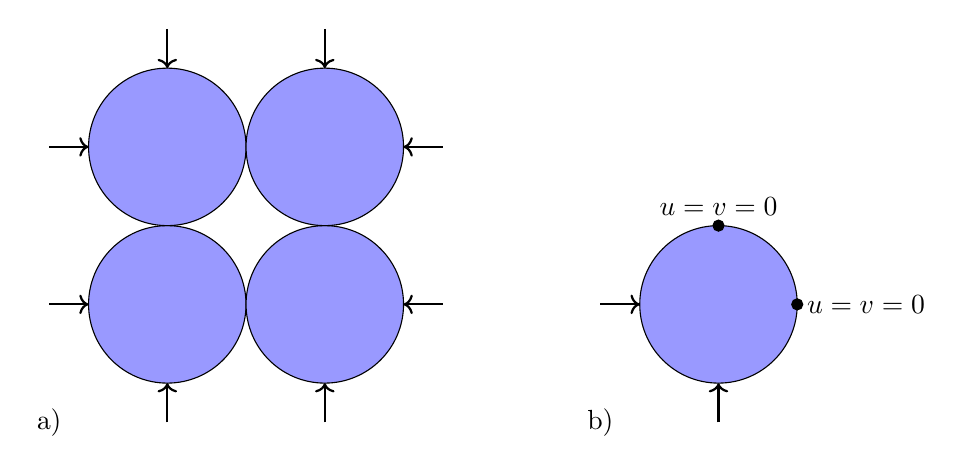
\begin{tikzpicture}
%\draw[fill=gray!23,gray!23](0,0) rectangle (11,6);
%\draw[step=0.5cm,gray,very thin] (0,0) grid (11,6); %background grid
\filldraw[fill=blue!40!white, draw=black] (2,2) circle (1cm);
\filldraw[fill=blue!40!white, draw=black] (4,2) circle (1cm);
\filldraw[fill=blue!40!white, draw=black] (2,4) circle (1cm);
\filldraw[fill=blue!40!white, draw=black] (4,4) circle (1cm);
\draw[thick,->] (0.5,2) -- (1,2); \draw[thick,->] (5.5,2) -- (5,2);
\draw[thick,->] (0.5,4) -- (1,4); \draw[thick,->] (5.5,4) -- (5,4);
\draw[thick,->] (2,0.5) -- (2,1); \draw[thick,->] (2,5.5) -- (2,5);
\draw[thick,->] (4,0.5) -- (4,1); \draw[thick,->] (4,5.5) -- (4,5);
\draw[thick,->] (7.5,2) -- (8,2);
\draw[thick,->] (9,0.5) -- (9,1); 
\filldraw[fill=blue!40!white, draw=black] (9,2) circle (1cm);
\filldraw[black] (10,2) circle (2pt) node[anchor=west] {$u=v=0$};
\filldraw[black] (9,3) circle (2pt) node[anchor=south] {$u=v=0$};
\node[] at (0.5,0.5)   {a)};
\node[] at (7.5,0.5)   {b)};
\end{tikzpicture}\\
{\captionfont a) assembly of four circular grains and the pressure boundary conditions; 
b) simplified setup of a single grain.}
\end{center}

\begin{center}
\includegraphics[width=5.5cm]{python_codes/fieldstone_58/experiment2/displ}
\includegraphics[width=5.5cm]{python_codes/fieldstone_58/experiment2/displx}
\includegraphics[width=5.5cm]{python_codes/fieldstone_58/experiment2/disply}\\
\includegraphics[width=5.5cm]{python_codes/fieldstone_58/experiment2/divv}
\includegraphics[width=5.5cm]{python_codes/fieldstone_58/experiment2/p}
\includegraphics[width=5.5cm]{python_codes/fieldstone_58/experiment2/strain}\\
\includegraphics[width=10cm]{python_codes/fieldstone_58/experiment2/dispvect}
\end{center}



\noindent \Literature:
\begin{itemize}
\item Compaction creep of sands due to time-dependent grain failure: Effects of chemical environment,
      applied stress, and grain size. Brzesowsky \etal{} (2014) \cite{brhb14}
\item Failure behavior of single sand grains: Theory versus experiment. Brzesowsky \etal{} (2011) \cite{brsp11}
\item Time-independent compaction behavior of quartz sands. Brzesowsky \etal{} (2014) \cite{brsp14}
\item Determination of the tensile strength of rock by a compression test of an 
      irregular test piece. Hiramatsu \etal{} (1966) \cite{hiok66}
\item Micromechanics of sand grain failure and sand compaction. Brzesowsky (1995) \cite{brze95}
\item Contact fatigue in silica sand—Observations and modeling. Wang \& Michalowski (2015) \cite{wami15}
\item Tensile stress concentration and compressive failure in cemented granular material. 
      Wong \& Wu (1995)\cite{wowu95}
\item Micromechanics of pressure-induced grain crushing in porous rocks. Zhang \etal{} (1990) \cite{zhwd90}
\end{itemize}




 %%%%%%%%%%%%%%%%%%%%%%%%%%%%%%%%%%%%%%%%%%%%%%%%%%%%%%%%%%%%%%%%%%%%%%

\chapter{Ice Flow Down an Inclined Plane \label{f59}} %%%%%%%%%%%%%%%%%%%%%%%%%%%%%%%%%%%%%%%%%%%%%%%%%%%%%%%% 59

\includegraphics[height=1.5cm]{images/pictograms/replication}
\includegraphics[height=1.5cm]{images/pictograms/ice}

\begin{flushright} {\tiny {\color{gray} python\_codes/fieldstone\_59/text.tex}} \end{flushright}

\lstinputlisting[language=bash,basicstyle=\small]{python_codes/fieldstone_59/keywords.key}

\begin{center}
\fbox{\textbf{\huge \color{teal} P}}
Code at \url{https://github.com/cedrict/fieldstone/tree/master/python_codes/fieldstone_59}
\end{center}

\par\noindent\rule{\textwidth}{0.4pt}

%%%%%%%%%%%%%%%%%%%%%%%%%%%%%%%%%%%%%%%%%%%%%%%%%%%%%%%%%%%%%%%%%%%%%%%%%%%%%%%%%%%%%%%%%%%%%%%%%%%




\begin{center}
\includegraphics[width=5cm]{python_codes/fieldstone_59/images/setup}\\
{\captionfont REDO with tikz}
\end{center}

\paragraph{Linear viscous fluid}

We start from the Stokes equation for isoviscous fluids:
\[
\eta \Delta \vec{\upnu} - \vec\nabla p + \rho \vec{g} = \vec{0}
\]
Assuming that the fluid is incompressible and that the incline is infinite, 
then $\vec{\upnu}=(u(y),0)$.
The $x$-component of the equation then writes:
\[
\eta\left(\frac{\partial^2 u}{\partial x^2}+\frac{\partial^2 u}{\partial y^2} \right)
- \frac{\partial p}{\partial x} + \rho g_x =0
\]
\[
\Rightarrow \qquad 
\eta\frac{\partial^2 u}{\partial y^2} 
+ \rho g \sin\alpha =0
\]
since $\partial_x\rightarrow 0$.
This 2nd order ODE can be integrated twice. The two integration constants are 
determined by setting $u(y=0)=0$ (no slip) and the shear stress to be zero at the (free)
surface. The velocity profile is given by:
\[
u(y)=\frac{\rho g \sin \alpha}{2 \eta} (2h-y)y
\]
We can now compute the components of the strain rate tensor:
\[
\dot{\varepsilon}_{xx}=0
\qquad
\qquad
\dot{\varepsilon}_{yy}=0
\qquad
\qquad
\dot{\varepsilon}_{xy}
=\frac{1}{2} \left( \frac{\partial u}{\partial y} + \frac{\partial v}{\partial x} \right)
=\frac{1}{2} \frac{\partial u}{\partial y} 
= \frac{\rho g \sin \alpha}{2 \eta} (h-y)
\]

We now make the assumption that this problem is a very simplified ice sheet flow problem.
The angle $\alpha$ is typically small and for $\alpha\sim 0.5-1$\degree, then $\sin\alpha\sim 0.01$. 
We also have $\rho\sim1000$, $g\sim$10,  $h\sim2500$ and we postulate the 
ice viscosity to be $\eta\sim 10^m$,.
The velocity is maximum at the surface and is given by
\begin{equation}
u(y=h)=
\frac{\rho g \sin \alpha}{2 \eta}h^2 
\sim \frac{1000 \cdot 10 \cdot 0.01}{ 2\cdot 10^m}2500^2
\sim 3\cdot 10^{8-m}
\label{eq:ice1}
\end{equation}

\begin{center}
\includegraphics[height=9cm]{python_codes/fieldstone_59/images/neem}
\includegraphics[height=9cm]{python_codes/fieldstone_59/images/narh15}\\
{\captionfont Ice velocity map (magnitude, in logarithmic scale) of the Greenland Ice Sheet
derived from SAR data of the Sentinel-1A satellite, acquired in Interferometric Wide Swath
Mode (IW) between January and March 2015. Taken from \textcite{narh15} (2015).}
\end{center}

As shown on the figures above the typical ice sheet velocity values around the NEEM ice core 
is $\sim 0.03~\si{\meter\per\day} \simeq 3\cdot 10^{-7}~\si{\meter\per\second}$. 
Then, in order for the top of the ice sheet to flow at this speed it requires $m=15$.

Having obtained the (effective linear) viscosity of the ice, i.e. 
$\eta\simeq 10^{15}~\si{\pascal\second}$,
we can compute the strain rate at the bottom and in the middle:
\[
\dot{\varepsilon}_{xy}(y=0) 
= \frac{\rho g \sin \alpha}{2 \eta} h
\sim \frac{1000\cdot 10 \cdot 0.01}{2 \cdot 10^{15}}2500
\sim 10^{-10}~\si{\per\second}
\]
\[
\dot{\varepsilon}_{xy}(y=h/2) 
= \frac{\rho g \sin \alpha}{2 \eta} \frac{h}{2}
\sim \frac{1000\cdot 10 \cdot 0.01}{2 \cdot 10^{15}}\frac{2500}{2}
\sim 5\cdot 10^{-11}~\si{\per\second}
\]
which are reasonable values as confirmed by the following figure (see yellow line):  
\begin{center}
\includegraphics[width=11cm]{python_codes/fieldstone_59/images/kudd19}\\
{\captionfont Taken from \textcite{kudd19} (2019).}
\end{center}

The conclusion from this exercise is that {\sl if} ice could be described by 
a linear viscous fluid flowing on an infinite incline, a viscosity of $\eta\simeq 10^{15}$Pa.s
would yield observations that match recorded velocities and strain rates. 


\paragraph{Nonlinear power-law viscosity}
However, the picture is way more complex, as it was observed very early on 
by Glen in 1955 \cite{glen55} and many others later (see Section~\ref{MMM-ss:glen}). 
It was then found that the strain rate and the stress are linked in a nonlinear way: 
\[
\dot{\varepsilon} = A \tau^n,
\]
i.e. the ice behaves as a power-law fluid (see Section~\ref{MMM-ss:powerlaw}), with 
$n=3$ and $A\simeq 2.4\cdot 10^{-24}$ at 0\degree (REF?).

More recently \textcite{kuwd19} (2019) and \textcite{kudd19} (2019) derived a composite flow law 
to model deformation in the NEEM deep ice core. 
They start from the flow law proposed by \textcite{goko01} (2001):
\[
\dot{\varepsilon}_T = \dot{\varepsilon}_{disl} + 
\left(\frac{1}{ \dot{\varepsilon}_{basal}} + \frac{1}{ \dot{\varepsilon}_{GBS}} \right)^{-1} 
+  \dot{\varepsilon}_{diff}
\]
where $\dot{\varepsilon}_T$  is the total strain rate, 
composed of strain rates for basal slip accommodated by non-basal slip or dislocation creep,
$\dot{\varepsilon}_{disl}$ , grain boundary sliding (GBS) accommodated by basal slip, 
$\dot{\varepsilon}_{basal}$ , and basal slip accommodated by GBS, 
$\dot{\varepsilon}_{GBS}$ , and diffusion creep, 
$\dot{\varepsilon}_{diff}$. Each of these creep mechanisms can be described by a 
power law relation of the form:
\[
\dot{\varepsilon} = A \tau^n d^{-p} \exp \left( -\frac{Q+pV}{RT} \right)
\]
where $A$ is a material parameter, $\tau$ is the differential stress (MPa), 
$n$ is the stress exponent, $d$ is the grain size diameter (\si{\meter}), 
$p$ is the grain size exponent, $Q$ is the activation energy for the creep 
mechanism at stake ($\si{\joule\per\mole}$), $p$ is the hydrostatic pressure ($\si{\mega\pascal}$), 
$V$ the activation volume ($\si{\cubic\meter\per\mole}$), 
$R$ is the gas constant ($\si{\joule\per\kelvin\per\mole}$), 
and $T$ the absolute temperature ($\si{\kelvin}$). 
The effect of $pV$ is assumed to be very small \cite{dust01} 
and is ignored for the remainder of this work.

As explained in \textcite{kuwd19} (2019) the composite flow law can actually be simplified to:
\[
\dot{\varepsilon}_T = \dot{\varepsilon}_{disl} + \dot{\varepsilon}_{GBS}
\]
The material parameters for these deformation mechanisms are available in \cite{kudd19}:
\begin{center}
\begin{tabular}{lcccc}
\hline
Creep regime & $A$ & $n$ & $p$ & $Q$ (\si{\joule\per\mole}) \\
\hline\hline
Glen's flow law ($T<263$K) &$3.61\cdot10^5$ MPa$^{-3.0}$ s$^{-1}$ &3.0 &0 &60\\
Glen's flow law ($T>263$K) &$1.73\cdot10^{21}$ MPa$^{-3.0}$ s$^{-1}$ &3.0 &0 &139\\
\hline
Dislocation creep ($T<262$K) & $5.0\cdot10^5$ MPa$^{-4.0}$ s$^{-1}$ &4.0 &0 &64\\
Dislocation creep ($T>262$K) &$6.96\cdot 10^{23}$ MPa$^{-4.0}$ s$^{-1}$ &4.0 &0 &155\\
\hline
GBS-limited creep ($T<262$K) & $1.1\cdot 10^2$ MPa$^{-1.8}$ m$^{1.4}$ $s^{-1}$ &1.8 &1.4 &70\\
GBS-limited creep ($T>262$K) & $8.5\cdot10^{37}$ MPa$^{-1.8}$ m$^{1.4}$ $s^{-1}$ &1.8 &1.4 &250\\
\hline
\end{tabular}
\end{center}

The associated effective viscosity is then given by 
\[
\eta = \frac{1}{2}  A^{-\frac{1}{n}} \dot{\varepsilon}^{\frac{1}{n}-1}  d^{\frac{p}{n}} \exp \left( \frac{Q+pV}{nRT} \right)
\]
Note that the $A$ parameter is given in MPa and not Pa so that when computing the 
associated effective viscosities these have to be multiplied by $10^6$.
Because the strain rates are added together we know that the two deformation mechanisms are in series and their
effective viscosity is then the harmonic average of both viscosities:
\[
\eta_{eff} = \left(\frac{1}{\eta_{disl}} + \frac{1}{\eta_{GBS}}  \right)^{-1}
\]

\paragraph{Numerical setup}

The geometry is a 2D cartesian domain of size $L_x \times L_y$. Instead of tilting it by an angle $\alpha$
I choose to instead 'tilt' the gravity vector so that it becomes 
$\vec{g}=(\rho g \sin\alpha,-\rho g\cos\alpha)$.
The boundary conditions are as follows: no slip at the bottom, free surface at the top, 
free slip on the left (we assume that this corresponds to a ridge - zero horizontal velocity)
and we need to be careful about the right boundary which is where the ice exits the domain:
if we leave the boundary open ice will rush out, generate high strain rates and the nonlinear 
rheologies will respond by generating low viscosities which in turn will promote a fast 
exit. Instead we opt to prescribe the analytical solution of Eq.~(\ref{MMM-eq:ice1}) with $\eta=10^{15}$.
We neglect any kind of phase change and precipitation and only carry out a single time step.
The domain is discretised with nel=nelx$\times$nely $Q_2Q_1$ elements (see Section~\ref{MMM-ss:pairq2q1}).
We set $L_x=125$km and $L_y=2500$m, $\rho=917$kg$\cdot$m$^{-3}$, $\alpha=0.1$\degree.



\begin{center}
\includegraphics[width=7cm]{python_codes/fieldstone_59/images/shsh14}
\includegraphics[width=10cm]{python_codes/fieldstone_59/images/kuiper19}\\
{\captionfont Left: Taken from \textcite{shsh14} (2014); 
Right: Taken from \textcite{kuiper19} (2019).}
\end{center}

I have obtained the raw data (curtesy from E.N. Kuiper) and it is plotted hereunder:
\begin{center}
\includegraphics[width=8cm]{python_codes/fieldstone_59/data/temperature}
\includegraphics[width=8cm]{python_codes/fieldstone_59/data/grain_size}
\end{center}

In order to verify that the values reported in the table above are the ones 
used in \cite{kudd19} I have reproduced the figure 3 of that paper (code and gnuplot
script in {\sl ./data} folder):
\begin{center}
\includegraphics[width=9cm]{python_codes/fieldstone_59/data/strainrate}\\
{\captionfont Log strain rate versus temperature for Glen's flow law and 
the two mechanisms (dislocation creep and GBS-limited creep) that form the end members 
of the modified composite flow law, using the flow law parameters from the table above. 
A stress of 0.07MPa and a mean grain diameter of $5~\si{\milli\meter}$ 
were used to calculate the strain rate.}
\end{center}


In our models, the temperature profile is simplified 
as shown on the plots above. 
Concerning the grain size distribution the ice sheet has been divided in three 
layers and and an average grain size is used for each.

We have computed the effective viscosity for all four rheologies with the 
implemented temperature and grain size profiles for $\dot{\varepsilon}_e=10^{-10}\text{s}^{-1}$:

\begin{center}
\includegraphics[width=8cm]{python_codes/fieldstone_59/results/profiles}
\includegraphics[width=8cm]{python_codes/fieldstone_59/results/profiles2}
\end{center}
Note that smaller strain rates shift the curves to the right (higher viscosities).



Because the rheologies are non linear we need to carry out nonlinear iterations 
(see Section~\ref{MMM-ss:picard}).
In what follows we run models for Glen's flow law (rheology=1), 
dislocation creep (rheology=2), GBS (rheology=3) and dislocation+GBS (rheology=4).
Note that in the case of rheology=4, the partitioning of the strain rates between both 
mechanisms is not done (YET) so that the results are not really consistent with the rest!

%\newpage
\begin{center}
Core 1 ($x=L_x/4$) \hspace{5cm}  Core 2 ($x=L_x/2$)  \\
\includegraphics[width=7.cm]{python_codes/fieldstone_59/results/u_core1}
\includegraphics[width=7.cm]{python_codes/fieldstone_59/results/u_core2}\\
\includegraphics[width=7.cm]{python_codes/fieldstone_59/results/sr_core1}
\includegraphics[width=7.cm]{python_codes/fieldstone_59/results/sr_core2}\\
\includegraphics[width=7.cm]{python_codes/fieldstone_59/results/eta_core1}
\includegraphics[width=7.cm]{python_codes/fieldstone_59/results/eta_core2}\\
\includegraphics[width=7.cm]{python_codes/fieldstone_59/results/sigmaxx_core1}
\includegraphics[width=7.cm]{python_codes/fieldstone_59/results/sigmaxx_core2}\\
\includegraphics[width=7.cm]{python_codes/fieldstone_59/results/sigmayy_core1}
\includegraphics[width=7.cm]{python_codes/fieldstone_59/results/sigmayy_core2}\\
\includegraphics[width=7.cm]{python_codes/fieldstone_59/results/sigmaxy_core1}
\includegraphics[width=7.cm]{python_codes/fieldstone_59/results/sigmaxy_core2}
\end{center}


\begin{center}
\includegraphics[width=7cm]{python_codes/fieldstone_59/results/rh4/vel}
\includegraphics[width=7cm]{python_codes/fieldstone_59/results/rh4/p}\\
\includegraphics[width=7cm]{python_codes/fieldstone_59/results/rh4/sr}
\includegraphics[width=7cm]{python_codes/fieldstone_59/results/rh4/eta}\\
{\captionfont Velocity, pressure, strain rate and effective viscosity in the middle of the ice sheet
for rheology=4}
\end{center}



Check: ELMER/ice \url{http://elmerice.elmerfem.org/capabilities}

Improvements: better density profile? more realistic geometry ? 
partitioning of strain rates. Better temperature profile. 
Better grain size description. Influence of tilt angle? 

\vspace{1cm}

\Literature 
\textcite{buja89} (1989),
\textcite{zwgg07} (2007),
\textcite{zhjg11} (2011),
\textcite{lejx14} (2014),
\textcite{issg15} (2015),
\textcite{yash15} (2015),
\textcite{gors17} (2017),
\textcite{heah18} (2018).


 %%%%%%%%%%%%%%%%%%%%%%%%%%%%%%%%%%%%%%%%%%%%%%%%%%%%%%%%%%%%%%%%%%%%%%

\chapter{DG-FEM: 1D advection \label{f60}} %%%%%%%%%%%%%%%%%%%%%%%%%%%%%%%%%%%%%%%%%%%%%%%%%%%%%%%%%%%%%%%%%%% 60 
\lstinputlisting[language=bash,basicstyle=\small]{python_codes/fieldstone_60/keywords.ascii}

This stone implements the 1D discontinuous Galerkin method to solve the simple 
advection equation:
\[
\frac{\partial T}{\partial t} + u \frac{\partial T}{\partial x} = 0
\]




%---------------------------------------------
\subsection*{The code}

The mesh counts {\tt nelx} linear elements and therefore {\tt nnx} nodes.

The timestep is determined by means of the CFL condition:
\begin{lstlisting}
dt=C*hx/u
\end{lstlisting}
The mesh is very simply built:
\begin{lstlisting}
x=np.linspace(0,Lx,nnx)
\end{lstlisting}
We need to declare four arrays: the nodal temperature both on the left and 
on the right of each node, and their memory of the previous time step. 
\begin{lstlisting}
T_minus=np.zeros(nnx,dtype=np.float64)      
T_minus_old=np.zeros(nnx,dtype=np.float64)  
T_plus=np.zeros(nnx,dtype=np.float64)       
T_plus_old=np.zeros(nnx,dtype=np.float64)   
\end{lstlisting}
Initial temperatures are then prescribed on both {\tt T\_plus} 
and $T\_minus$ arrays, and then copied to the 'old' arrays.

We then enter the time stepping loop:
\begin{lstlisting}
for istep in range(0,nstep):
\end{lstlisting}
At each timestep the boundary conditions are reapplied\footnote{It is a bit weird that 
we prescribe a temperature b.c. on a node with an outflow...?}:
\begin{lstlisting}
T_minus[0]=T_left
T_plus[0]=T_left
T_minus[nnx-1]=T_right
T_plus[nnx-1]=T_right
\end{lstlisting}
We then loop over all elements:
\begin{lstlisting}
for iel in range(0,nel):
\end{lstlisting}
and compute the corresponding $k$ and $k+1$ values:
\begin{lstlisting}
k=iel
kp1=iel+1
\end{lstlisting}
The $T^+$ and $T^-$ fields are then updated following Eq.~\eqref{eq:dgadv5}:
\begin{lstlisting}
T_plus[k]   =T_plus_old[k]   +C*(-3*T_plus_old[k]-T_minus_old[k+1]+4*T_minus[k])
T_minus[k+1]=T_minus_old[k+1]+C*( 3*T_plus_old[k]-T_minus_old[k+1]-2*T_minus[k])
\end{lstlisting}







%---------------------------------------------
\subsection*{Results}

%---------------------------------------------
\subsubsection*{Experiment 1}

We consider the following advection problem taken from Li \cite[ex 5.2]{li06}.
It is also carried out in \stone~43.

The domain has dimension $L_x=1$. 
The temperature is prescribed on the left and the right boundary to be zero. 
The initial temperature is given by
\[
T(x,0)=
\left\{
\begin{array}{ll}
\sin (10 \pi x) & \textrm{for } x< 0.1 \\
0               & \textrm{for } x\geq 0.1 
\end{array}
\right.
\]
The velocity is set to $u=0.1$.
We use 200 elements and a time step of $\delta t=10^{-4}$. 
We run the model to time $t=8$ so we need 80,000 time stpes. 

Note that the CFL-number is then very small: 
\[
C = \frac{\delta t \cdot u}{h} = \frac{10^{-4} \cdot  0.1}{1/200} = 0.002
\]

\begin{center}
\includegraphics[width=9cm]{python_codes/fieldstone_60/results/exp1/T.pdf}\\
{\captionfont Temperature field at three different times.}
\end{center}

\todo[inline]{redo with standard Galerkin and compare!}

%---------------------------------------------
\subsubsection*{Experiment 2}

This advection benchmark originates in Donea \& Huerta \cite{dohu03}
and it also to be found in Thieulot (2011) \cite{thie11} (and in 
Section~\ref{ss:appAthie11}).

The domain has dimension $L_x=1$. 
The temperature is prescribed on the left at $T=1$
and the right boundary at $T=0$.
The initial temperature is given by
\[
T(x,0)=
\left\{
\begin{array}{ll}
1 & \textrm{for } x< 0.25 \\
0 & \textrm{for } x\geq 0.1 
\end{array}
\right.
\]
Velocity is set to $u=1$, the number of elements to 50 ($h=0.02$), the CFL number to 0.1 (
so $\delta t=0.002$), and the number of time steps to 250, so that we expect the front
to be at $x=3L_x/4$.  

\begin{center}
\includegraphics[width=8cm]{python_codes/fieldstone_60/results/exp2/T.pdf}\\
\includegraphics[width=8cm]{images/supg/fantom3}\\
{\captionfont Left: Temperature field at different times; 
Right: Taken and modified from Thieulot (2011) \cite{thie11}}
\end{center}

It is rather surprising that the DG results are so much worse than the SG results (even without 
SUPG stabilisation).









 %%%%%%%%%%%%%%%%%%%%%%%%%%%%%%%%%%%%%%%%%%%%%%%%%%%%%%%%%%%%%%%%%%%%%%

\chapter{Channel flow with Herschel-Bulkley rheology (\QtwoQone) \label{f61}} %%%%%%%%%%%%%%%%%%%%%%%%%%%%%%%% 61
\includegraphics[height=1.25cm]{images/pictograms/benchmark}
\includegraphics[height=1.25cm]{images/pictograms/FEM}

%%%%%%%%%%%%%%%%%%%%%%%%%%%%%%%%%%%%%%%%%%%%%%%%%%%%%%%%%%%%%%%%%%%%%%%%%%%%%%%%%%%%%%%%%%%%%%%%%%%

\lstinputlisting[language=bash,basicstyle=\small]{python_codes/fieldstone_61/keywords.ascii}

\begin{center}
Code at \url{https://github.com/cedrict/fieldstone/tree/master/python_codes/fieldstone_61}
\end{center}

\par\noindent\rule{\textwidth}{0.4pt}
%%%%%%%%%%%%%%%%%%%%%%%%%%%%%%%%%%%%%%%%%%%%%%%%%%%%%%%%%%%%%%%%%%%%%%%%%%%%%%%%%%%%%%%%%%%%

\paragraph{Simple Newtonian Poiseuille flow} The analytical solution to this flow has been derived 
in Section~\ref{MMM-ss:poiseuille}.
We set $p_{left}=10^9$, $p_{right}=0$, $L_x=L_y=100$km, $\eta_0=10^{25}$, so 
\[
\Pi=\frac{p_{right}-p_{left}}{L_x}=-10^4 <0
\]
The $p_{left}$ value is prescribed on the left (see Section~\ref{MMM-ss:openbc}) while 
nothing is prescribed on the right. No slip boundary conditions are 
prescribed on the top and bottom.

We see that we recover the analytical solution for velocity and strainrate:
\begin{center}
\includegraphics[width=7.8cm]{python_codes/fieldstone_61/results/poiseuille/velocity}
\includegraphics[width=7.8cm]{python_codes/fieldstone_61/results/poiseuille/exy}
\end{center}

\begin{center}
\includegraphics[width=5cm]{python_codes/fieldstone_61/results/poiseuille/vel}
\includegraphics[width=5cm]{python_codes/fieldstone_61/results/poiseuille/press}
\includegraphics[width=5cm]{python_codes/fieldstone_61/results/poiseuille/sr}
\end{center}

\paragraph{Poiseuille flow with H-B rheology - $n=1$} 
The analytical solution to this flow has been derived in Section~\ref{MMM-ss:HBflow}.
In this case we have 
\[
\eta_{HB}
=
\left\{
\begin{array}{lc}
\eta_0 & \dot{\varepsilon}_e\leq \dot{\varepsilon}_0 \\
K  + \frac{\tau_0}{\dot{\varepsilon}_e}  
& \dot{\varepsilon}_e\geq \dot{\varepsilon}_0 
\end{array}
\right.
\]
and the limiting viscosity $\eta_0$ is such that 
\[
\eta_0 = K  + \frac{\tau_0}{\dot{\varepsilon}_0}  
\]

\begin{center}
\includegraphics[width=7.8cm]{python_codes/fieldstone_61/results/n_1/velocity.pdf}
\includegraphics[width=7.8cm]{python_codes/fieldstone_61/results/n_1/exy.pdf}\\
\includegraphics[width=7.8cm]{python_codes/fieldstone_61/results/n_1/eta.pdf}
\includegraphics[width=7.8cm]{python_codes/fieldstone_61/results/n_1/press.pdf}\\
\includegraphics[width=7.8cm]{python_codes/fieldstone_61/results/n_1/nonlinear_conv.pdf}
\end{center}

\begin{center}
\includegraphics[width=7.8cm]{python_codes/fieldstone_61/results/n_1/vel.png}
\includegraphics[width=7.8cm]{python_codes/fieldstone_61/results/n_1/exy.png}\\
\includegraphics[width=7.8cm]{python_codes/fieldstone_61/results/n_1/eta.png}
\includegraphics[width=7.8cm]{python_codes/fieldstone_61/results/n_1/press.png}
\end{center}





 %%%%%%%%%%%%%%%%%%%%%%%%%%%%%%%%%%%%%%%%%%%%%%%%%%%%%%%%%%%%%%%%%%%%%% 

\chapter{Subduction a la Quinquis Case 1 ($P_2^+\times P_{-1}$) \label{f62}} %%%%%%%%%%%%%%%%%%%%%%%%%%%%%%%%% 62
\includegraphics[height=1.25cm]{images/pictograms/replication}
\includegraphics[height=1.25cm]{images/pictograms/benchmark}
\includegraphics[height=1.25cm]{images/pictograms/triangle}
\includegraphics[height=1.25cm]{images/pictograms/under_construction}
\includegraphics[height=1.25cm]{images/pictograms/FEM}
\includegraphics[height=1.25cm]{images/pictograms/paraview}

%%%%%%%%%%%%%%%%%%%%%%%%%%%%%%%%%%%%%%%%%%%%%%%%%%%%%%%%%%%%%%%%%%%%%%%%%%%%%%%%%%%%%%%%%%%%%%%%%%%


\lstinputlisting[language=bash,basicstyle=\small]{python_codes/fieldstone_62/keywords.ascii}

\begin{center}
Code at \url{https://github.com/cedrict/fieldstone/tree/master/python_codes/fieldstone_62}
\end{center}

\par\noindent\rule{\textwidth}{0.4pt}
%%%%%%%%%%%%%%%%%%%%%%%%%%%%%%%%%%%%%%%%%%%%%%%%%%%%%%%%%%%%%%%%%%%%%%%%%%%%%%%%%%%%%%%%%%%%

The setup is presented in the phd thesis (chapter 4) of M. Quinquis \cite{quin14},
In this stone we focus on the case 1 of his work and only solve the system once (single time step).
The domain is $1500\times 670$ km. 

The setup and the boundary conditions are shown hereunder:
\begin{center}
\includegraphics[width=\linewidth]{python_codes/fieldstone_62/images/quin14_setup}\\
{\captionfont Model setup for subduction of a 70 Ma old oceanic plate under a 40 Ma
old oceanic plate. A) Setup of the whole model. The top, bottom, and left boundaries
are free-slip, while the right boundary condition includes material in- and outflow. S HB :
Serpentinised Harzburgite, and B OC : Bulk Oceanic Composition. The ‘thermal’ layers
are only required in the linear viscous models. B) Zoom of the setup at the trench, h is the
thickness of the weak zone. C) Definition of the in- and outflow velocities on the right
boundary. Taken from \cite{quin14}}
\end{center}

As opposed to the original benchmarking effort carried out by Quinquis and collaborators
I build the mesh with triangles so that I can exactly represent the layers (and especially 
the weak zone) with an adequate resolution. The elements used are the Crouzeix-Raviart one
(see Section~\ref{MMM-sec:crouzeix-raviart}). 

In {points.py} the coordinates of the key points are defined. The {generate\_nodes.py}
script generates the input file for 
the {\sl triangle} program\footnote{\url{https://www.cs.cmu.edu/~quake/triangle.html}}. 
Finally the {fieldstone.py} script 
reads in the mesh, sets up the material layout, the boundary conditions and solves the 
FE system. Simply use the {\sl run} script to trigger the mesh generation and the FE 
calculations.  
Note that the compiled {\sl triangle} executable file (as compiled by you 
on your own machine) must be present in this folder.

\begin{center}
\includegraphics[width=\linewidth]{python_codes/fieldstone_62/results/mats1}\\
{\captionfont Taken from \cite{quin14}}
\end{center}

The letters referenced in the {points.py} file are shown hereunder:

\begin{center}
\includegraphics[width=11cm]{python_codes/fieldstone_62/images/setup1}\\
\includegraphics[width=11cm]{python_codes/fieldstone_62/images/setup2}
\end{center}


In this case 1, all materials are characterised by a constant density and a Newtonian rheology:
\begin{center}
\includegraphics[width=5cm]{python_codes/fieldstone_62/images/quin14_mats}
\end{center}

\newpage
\begin{center}
\includegraphics[width=13cm]{python_codes/fieldstone_62/results/mesh1}\\
\includegraphics[width=13cm]{python_codes/fieldstone_62/results/mesh2}\\
\includegraphics[width=13cm]{python_codes/fieldstone_62/results/mesh3}
\end{center}

\newpage
\begin{center}
\includegraphics[width=12.5cm]{python_codes/fieldstone_62/results/density}\\
\includegraphics[width=12.5cm]{python_codes/fieldstone_62/results/viscosity}\\
\includegraphics[width=12.5cm]{python_codes/fieldstone_62/results/velocity}\\
\includegraphics[width=12.5cm]{python_codes/fieldstone_62/results/u}\\
\includegraphics[width=12.5cm]{python_codes/fieldstone_62/results/v}\\
\end{center}

\newpage
\begin{center}
\includegraphics[width=10cm]{python_codes/fieldstone_62/results/vel2}\\
\includegraphics[width=10cm]{python_codes/fieldstone_62/results/vel3}\\
\includegraphics[width=10cm]{python_codes/fieldstone_62/results/vel4}
\end{center}

I believe that one source of our problems when we carried out resolution tests
came from the fact that this small convection cell that occurs as shown above was
always under-resolved. The top layer is 8km thick and the weak zone is 14km thick,
and we ran simulations at max 1km resolution. However, because of the use  
of particle-in-cell and rectangular elements (mostly linear elements), 
a proper capture of this feature in the solution would have required much higher 
resolution. In other words, our higher resolution runs were probably not high resolution enough.
Given the nature of this convection cell, it means that temperature would be advected by it, 
and that markers would likely gotten mixed. 

\newpage
\begin{center}
\includegraphics[width=13cm]{python_codes/fieldstone_62/results/sr1}\\
\includegraphics[width=13cm]{python_codes/fieldstone_62/results/sr2}
\end{center}



 %%%%%%%%%%%%%%%%%%%%%%%%%%%%%%%%%%%%%%%%%%%%%%%%%%%%%%%%%%%%%%%%%%%%%%

\chapter{failure in cemented granular material \label{f63}} %%%%%%%%%%%%%%%%%%%%%%%%%%%%%%%%%%%%%%%%%%%%%%%%%% 63 

\includegraphics[width=1.5cm]{images/pictograms/replication}

\lstinputlisting[language=bash,basicstyle=\small]{python_codes/fieldstone_63/keywords.ascii}

\par\noindent\rule{\textwidth}{0.4pt}

{\sl This stone was developed in collaboration with Taka Shinohara}.
\index{contributors}{Taka Shinohara}

\par\noindent\rule{\textwidth}{0.4pt}

%%%%%%%%%%%%%%%%%%%%%%%%%%%%%%%%%%%%%%%%%%%%%%%%%%%%%%%%%%%%%%%%%%%%%%%%%%%%%%%%%%%%%%%%

This \stone is based on \textcite{wowu95} (1995) published in Geophysical Research Letters. 
As for every \stone aiming at reproducing results off a publication I here include de abstract
of the article:

\begin{center}
\begin{minipage}{13cm}
{\small 
Grain crushing and pore collapse are important micromechanical processes responsible for hydrostatic and 
shear-enhanced compactions in porous rocks. These processes initiate from extensile microcracks which 
emanate from grain contacts. Microstructural observations indicate that such extensile cracking is inhibited 
in the vicinity of cemented grain contacts. The finite element technique was used to simulate the tensile 
stress concentration and normal stiffness in a cemented aggregate. The detrital grains were assumed to 
be elastically identical spheres bonded by cement layers of finite thickness. The numerical simulations 
show that the maximum tensile stress concentration is located near the triple junction (among grain, 
cement and pore space), and its magnitude is significantly less than that for an uncemented system. 
The development of microcracking near a cemented contact is readily inhibited unless the applied 
stress exceeds a critical value which is at least an order of magnitude greater than that for the 
onset of Hertzian fracture.
}
\end{minipage}
\end{center}

In this paper the authors use the finite element method to simulate 
the tensile stress concentration and normal stiffness in a cemented
aggregate. The grains are assumed to be elastically identical spheres
bonded by cement layers of finite thickness.

\begin{center}
\includegraphics[width=8cm]{python_codes/fieldstone_63/images/yoyo}
\includegraphics[width=6cm]{python_codes/fieldstone_63/images/domain}\\
{\captionfont Left: model of cemented granular system for 
axisymmetric finite element analysis (taken from \cite{wowu95}); Right: 
Domain for a\_fac=0.2 and h\_fac=5/90 and $R=90\mu m$.}
\end{center}

We define
\[
a_{fac} = \frac{a}{R}  
\qquad
\text{and}
\qquad 
h_{fac} = \frac{h}{R}
\]
which translates as follows in the code:
\begin{lstlisting}
outer_radius=90e-6      #radius R (m)  
a_fac = 20/90           # ratio of a to R 
h_fac = 5/90            # ratio of h to R
a = outer_radius*a_fac
h = outer_radius*h_fac
\end{lstlisting}

The material properties for the grain and the cement are as follows:

\begin{lstlisting}
#Quartz mechanical properties
E1 = 95e9                       # Young's modulus (Pa)
nu1=0.08                        # poisson ratio
mu1= E1/(2*(1+nu1))             # shear modulus
lambdaa1=2.*mu1*nu1/(1.-2.*nu1)  
\end{lstlisting}
and
\begin{lstlisting}
#cement mechanical properties 2 
E2 = 84e9                       # Young's modulus (Pa)
nu2=0.31                        # poisson ratio
mu2= E2/(2*(1+nu2))             # shear modulus
lambdaa2=2.*mu2*nu2/(1.-2.*nu2)  
\end{lstlisting}

Note that since gravitational effects are neglected we set $\vec{g}=\vec{0}$
so that density actually play no role in the model.

The mesh in the code is built in three phases: first, the quarter grain is meshed 
with triangles. Second, the cement block is meshed and shaped so as to follow the 
shape of the grain. Finally both meshes are merged together:

\begin{center}
\includegraphics[width=5.5cm]{python_codes/fieldstone_63/images/wowu95b}
\includegraphics[width=8cm]{python_codes/fieldstone_63/images/mesh}\\
{\captionfont Left: quadtree-based mesh used in \cite{wowu95}; 
Right: low resolution fieldstone mesh.}
\end{center}

Boundary conditions are as follows: $u=0$ is prescribed on the left and top boundary, 
while $v=0$ is prescribed on the bottom boundary, as shown below.
Additionally, traction b.c. are prescribed at the top\footnote{Note that 
in the axisymmetric case these then apply onto a disc and should be multiplied by $2\pi$} (these
are described in Section~\ref{MMM-ss:openbc}) as indicated hereunder:
\begin{center}
a)\includegraphics[width=5cm]{python_codes/fieldstone_63/images/bc_u}
b)\includegraphics[width=5cm]{python_codes/fieldstone_63/images/bc_v}\\
c)\includegraphics[width=4cm]{python_codes/fieldstone_63/images/wowu95}\\
{\captionfont a,b) Horizontal and vertical displacement boundary condition indicator.
c) Imposed traction at the top surface (Taken from \cite{wowu95}).}
\end{center}

Linear triangular elements are used and a 3-point numerical quadrature is used.
Average elemental quantities are computed with 7 quadrature points.
These same quantities are also projected onto the nodes for visualisation purposes.
Principal stresses are computed as explained in Section~\ref{MMM-sec:princ_stress}.

The code solves the FE system and retrieves the deformation components $x$ and $y$,
or $r$ and $z$ in the axisymmetric case.
Average elemental strain components are then computed. In the axisymmetric case
then  $\varepsilon_{\theta\theta}$ is computed and otherwise set to zero in the plane strain case.
The stress tensor components are then computed as follows:
\begin{eqnarray}
\sigma_{xx} &=& \lambda \vec\nabla\cdot\vec{u} + 2\mu \varepsilon_{xx} \\
\sigma_{zz} &=& \lambda \vec\nabla\cdot\vec{u} + 2\mu \varepsilon_{zz} \\
\sigma_{xz} &=&  2\mu \varepsilon_{xz} 
\end{eqnarray}
where $\vec\nabla\cdot\vec{u}=\frac{\partial u}{\partial x} + \frac{\partial w}{\partial z}$
in plane strain and 
$\vec\nabla\cdot\vec{u}=\frac{\partial u}{\partial x} + \frac{u}{x} + \frac{\partial w}{\partial z}$
in the axisymmetric case\footnote{Remember that the $xz$ plane is in fact the $rz$ plane so that 
the term $u_r/r$ becomes $u/x$ in practice.}.

Principal stresses are such that $\sigma_1>\sigma_2$ and 
\[
\sigma_{1,2}=\frac{\sigma_{xx}+\sigma_{yy}}{2} 
\pm \sqrt{  \left(\frac{\sigma_{xx}-\sigma_{yy}}{2}\right)^2 +\sigma_{xy}^2 }
 \]
The principal direction angle $\theta_p$ defines the principal
directions where the only stresses are normal stresses, and 
is given by the relationship:
\[
\tan (2\theta_p) =  \frac{2 \sigma_{xy}}{\sigma_{xx} -\sigma_{yy}}
\]
We find that $\theta_2$ is always negative, while $\theta_1$ showcases positive and negative values. 
We define the tensile zone as $\sigma_1>0$.

In general $\sigma_1$ is the maximum (most tensile) principal stress, 
$\sigma_3$ is the minimum (most compressive) principal stress, 
and $\sigma_2$ is the intermediate principal stress.

The maximum shear stress (in 2D) is given by
\[
\tau_{max} = \frac12(\sigma_1-\sigma_2)
\]

In the axisymmetric case the stress tensor is given by 
\[
{\bm \sigma} = 
\left(
\begin{array}{ccc}
\sigma_{rr} & 0 & \sigma_{rz} \\
0 & \sigma_{\theta\theta} & 0 \\
\sigma_{rz} & 0 & \sigma_{zz} 
\end{array}
\right)
\]
There are now three eigenvalues. However it is obvious that $\sigma_{\theta\theta}$ is 
one of them and the other two correspond to those of the $2\times 2$ stress stensor with 
$\sigma_{rr}$, $\sigma_{rz}$ and $\sigma_{zz}$ terms.
The code therefore needs not be modified to compute these. 



\begin{center}
\includegraphics[width=8.5cm]{python_codes/fieldstone_63/images/wowu95c}\\
{\captionfont Contours for the minimum principal stress in the vicinity of the triple junction}
\end{center}

\begin{remark}
This paper by Wong and Wu is a nice example of not-reproducible science. For one, boundary conditions 
are not all specified. Second, it is not specified whether the results are obtained in plane strain 
or axisymmetric geometry. Third, the program that was used is proprietary (ABAQUS). 
Fourth, no resolution tests are presented: given how small the area A is, and how comparable 
in size it is to the elements, this is problematic. Fifth, it is not clear how the 
tensile zone is defined. Sixth: the type of finite element is not specified. Seven, 
we are shown one field which is a derivative of the solution (displacement) but not the 
solution itelf.  
\end{remark}

The following results are obtained with very high resolutions, i.e. 
nLayers=901, nel\_h=80. This yields a mesh with about 1.6M triangles, 
and Nfem=1,668,488.

\newpage
%-----------------------------------------------------------------------
\paragraph{Results in plane strain}


\begin{center}
\includegraphics[width=5.5cm]{python_codes/fieldstone_63/results/ps/disp}
\includegraphics[width=5.5cm]{python_codes/fieldstone_63/results/ps/disp_x}
\includegraphics[width=5.5cm]{python_codes/fieldstone_63/results/ps/disp_y}\\
\includegraphics[width=5.5cm]{python_codes/fieldstone_63/results/ps/sigma1}
\includegraphics[width=5.5cm]{python_codes/fieldstone_63/results/ps/sigma2}
\includegraphics[width=5.5cm]{python_codes/fieldstone_63/results/ps/strain}\\
\includegraphics[width=5.5cm]{python_codes/fieldstone_63/results/ps/angle}
\includegraphics[width=5.5cm]{python_codes/fieldstone_63/results/ps/maximum_shear_stress}
\includegraphics[width=5.5cm]{python_codes/fieldstone_63/results/ps/tensile}
\end{center}

\newpage
%-----------------------------------------------------------------------
\paragraph{Results in axisymmetric geometry}

\begin{center}
\includegraphics[width=5.5cm]{python_codes/fieldstone_63/results/axi/disp}
\includegraphics[width=5.5cm]{python_codes/fieldstone_63/results/axi/disp_x}
\includegraphics[width=5.5cm]{python_codes/fieldstone_63/results/axi/disp_y}\\
\includegraphics[width=5.5cm]{python_codes/fieldstone_63/results/axi/sigma1}
\includegraphics[width=5.5cm]{python_codes/fieldstone_63/results/axi/sigma2}
\includegraphics[width=5.5cm]{python_codes/fieldstone_63/results/axi/strain}\\
\includegraphics[width=5.5cm]{python_codes/fieldstone_63/results/axi/angle}
\includegraphics[width=5.5cm]{python_codes/fieldstone_63/results/axi/maximum_shear_stress}
\includegraphics[width=5.5cm]{python_codes/fieldstone_63/results/axi/tensile}
\end{center}

 %%%%%%%%%%%%%%%%%%%%%%%%%%%%%%%%%%%%%%%%%%%%%%%%%%%%%%%%%%%%%%%%%%%%%%

\chapter{Elasto-viscous benchmarks \label{f64}} %%%%%%%%%%%%%%%%%%%%%%%%%%%%%%%%%%%%%%%%%%%%%%%%%%%%%%%%%%%%%% 64
\lstinputlisting[language=bash,basicstyle=\small]{python_codes/fieldstone_64/keywords.ascii}

\begin{center}
Code at \url{https://github.com/cedrict/fieldstone/tree/master/python_codes/fieldstone_64}
\end{center}

\par\noindent\rule{\textwidth}{0.4pt}
%%%%%%%%%%%%%%%%%%%%%%%%%%%%%%%%%%%%%%%%%%%%%%%%%%%%%%%%%%%%%%%%%%%%%%%%%%%%%%%%%%%%%%%%%%%%


{\large
DO NOT READ WHAT FOLLOWS. It was written for Composition based stone, but I am using 
markers for all benchmarks so far. Jump directly to 'stress build up in maxwell body'! 
}

In the examples here there are only 2 compositions. 
Each material/composition is characterised by its $\eta_{\{1,2\}}$, $\mu_{\{1,2\}}$. 
With $\delta t$ chosen, $Z_{\{1,2\}}$ and $\eta_{eff,\{1,2\}}$ can be computed.

C1 and C2 are initialised at startup by looping over Vnodes and assigning a value to $C_1$ 
and $C_2$ such that $C_1+C_2=1$. 

The quantity $\tau_{xx},\tau_{yy},\tau_{xy},\dot{\omega}_{xy}$ (denoted by oxy in the code) 
are nodal and initialised at startup
(they are needed for the Stokes matrix):
\begin{lstlisting}
tauxx =np.zeros(NV,dtype=np.float64)  
tauyy =np.zeros(NV,dtype=np.float64)  
tauxy =np.zeros(NV,dtype=np.float64)  
oxy   =np.zeros(NV,dtype=np.float64)  
etaeff=np.zeros(NV,dtype=np.float64)  
Z     =np.zeros(NV,dtype=np.float64)  
rho   =np.zeros(NV,dtype=np.float64)  
\end{lstlisting}

Structure of the code (the following bulletpoints are inside the time stepping loop):

\begin{itemize}
\item Nodal $\eta_{eff}$, $Z$ and $\rho$ values are computed as follows:
\begin{lstlisting}
for i in range(0,NV):
    etaeff[i]=C1[i]*etaeff1+C2[i]*etaeff2
    Z[i]     =C1[i]*Z1     +C2[i]*Z2
    rho[i]   =C1[i]*rho1   +C2[i]*rho2
\end{lstlisting}

\item Build Stokes matrix. 
Loop over elements, loop over integration points inside the element, and for 
each quadrature point:
\begin{eqnarray}
Z(\vec{r}_q) &=& \sum_{i=1}^{m_V} N_i^\upnu(\vec{r}_q) Z_i \\
\tau_{xx}(\vec{r}_q)&=& \sum_{i=1}^{m_V} N_i^\upnu(\vec{r}_q) \tau_{xx,i} \\
\tau_{yy}(\vec{r}_q)&=& \sum_{i=1}^{m_V} N_i^\upnu(\vec{r}_q) \tau_{yy,i} \\
\tau_{xy}(\vec{r}_q)&=& \sum_{i=1}^{m_V} N_i^\upnu(\vec{r}_q) \tau_{xy,i} \\
\eta_{eff}(\vec{r}_q)&=& \sum_{i=1}^{m_V} N_i^\upnu(\vec{r}_q) \eta_{eff,i} \\
\dot{\omega}_{xy}(\vec{r}_q) &=& \sum_{i=1}^{m_V} N_i^\upnu(\vec{r}_q)  \dot{\omega}_{xy,i} \\
\rho(\vec{r}_q) &=& \sum_{i=1}^{m_V} N_i^\upnu(\vec{r}_q) \rho_i 
\end{eqnarray}


The elastic memory rhs term is built following Eq.~(\ref{XXX}):
\begin{lstlisting}
R[0]=Zq*(tauxxq+dt*oxyq*(2*tauxyq))
R[1]=Zq*(tauyyq+dt*oxyq*(-2*tauxyq))
R[2]=Zq*(tauxyq+dt*oxyq*(tauyyq-tauxxq))
f_el-=b_mat.T.dot(R)*weightq*jcob
\end{lstlisting}

\item Solve system and obtain $u,v,p$

\item Compute nodal velocity gradient ${\bm L}=\vec\nabla\vec\upnu$

\item Compute derivated nodal fields 

\begin{lstlisting}
exx[:]=Lxx[:]
eyy[:]=Lyy[:]
exy[:]=0.5*(Lxy[:]+Lyx[:])
oxy[:]=0.5*(Lxy[:]-Lyx[:])
Jxx[:]=2*tauxx[:]*oxy[:]
Jyy[:]=-2*tauxy[:]*oxy[:]
Jxy[:]=(tauyy[:]-tauxx[:])*oxy[:]
\end{lstlisting}

\item (re-)build nodal ${\bm \tau}$: 
\begin{lstlisting}
tauxx=2*etaeff*exx+Z*tauxx+Z*dt*Jxx
tauyy=2*etaeff*eyy+Z*tauyy+Z*dt*Jyy
tauxy=2*etaeff*exy+Z*tauxy+Z*dt*Jxy
\end{lstlisting}

\item advect $C_1$, $C_2$, $\tau_{xx}$, $\tau_{yy}$ and $\tau_{xy}$ fields

\item produce vtu file

\end{itemize}





%.......................................................
\paragraph{About this code}

This is a fairly complicated code since it features a deformable mesh 
(by means of a simplified ALE which only allows for the vertical movement 
of only the top row of mesh nodes), a particle-in-cell technique (only 
1st order in space)
to carry out material tracking/advection and of course the elasto-viscous 
rheology.


%.......................................................
\paragraph{Stress build-up in viscoelastic Maxwell body - analytical solution}

We start from 
\[
\dot{\bm \varepsilon}_T = \dot{\bm \varepsilon}_e +\dot{\bm \varepsilon}_v
=\frac{1}{2\mu} \dot{\bm \tau} + \frac{1}{2\eta} {\bm \tau} 
\]
In the case where there is no rotation then the BLABLA derivative becomes $d/dt$
and then 
we have to solve 
\[
2 \mu \dot{\bm \varepsilon}_T 
= \frac{d {\bm \tau}}{dt} + \frac{\mu}{\eta} {\bm \tau}
= \frac{d {\bm \tau}}{dt} + \frac{{\bm \tau}}{t_M}
\]
where $t_M=\eta/mu$ is the Maxwell time. The general solution can be arrived at 
by means of the Laplace transform (?!) and is given by:
\[
{\bm \tau}(t) = {\bm \tau}(t_0) \exp\left( -\frac{t-t_0}{t_M} \right) + \exp \left(-\frac{t}{t_M}\right)
\int_{t_0}^{t} 2 \mu \dot{\bm \varepsilon}_T  \exp \left(\frac{t'}{t_M}\right) dt'
\]

If $t_0=$ and ${\bm \tau}(t_0)=0$ then
\[
{\bm \tau}(t) =  \exp \left(-\frac{t}{t_M}\right)
\int_{0}^{t} 2 \mu \dot{\bm \varepsilon}_T  \exp \left( \frac{t'}{t_M} \right) dt'
\]
If the strain rate and shear modulus are constant in time, then 
\begin{eqnarray}
{\bm \tau}(t) 
&=&  \exp \left(-\frac{t}{t_M}\right)
2 \mu \dot{\bm \varepsilon}_T   \int_{0}^{t} \exp \left( \frac{t'}{t_M} \right) dt' \nn\\
&=&  \exp \left(-\frac{t}{t_M}\right)
2 \mu \dot{\bm \varepsilon}_T  t_M  \left[ \exp \left( \frac{t}{t_M} \right) -1  \right] \nn\\
&=& 
2 \eta \dot{\bm \varepsilon}_T   \left[ 1 - \exp \left( -\frac{t}{t_M} \right)\right] \nn
\end{eqnarray}
since $t_M=\eta/\mu$.

%.......................................................
\paragraph{Stress build-up in viscoelastic Maxwell body under simple shear}

The first benchmark performed to test the viscoelastic implementation considers the stress 
build-up present in a viscoelastic Maxwell body. Contrary to stressed viscous materials, 
viscoelastic materials gradually build-up stress when sheared after which a transition to viscous deformation occurs.  

An unstressed, incompressible viscoelastic Maxwell medium is subjected to a velocity field 
resulting in pure shear. 
The increase of the accumulated stress with time is given by an analytical solution:
\begin{equation}
{\bm \tau} = 2\eta\ {\dot{\bm \varepsilon}} \left ( 1-e^{-\frac{\mu }{\eta} t } \right )
\end{equation}
with $t$ time, $\eta$ the prescribed material viscosity and $\mu$ the prescribed material shear modulus. 
The domain size is 100$\times 100$km.
The velocity prescribed at all boundaries equals $v=1$ cm/yr in magnitude yielding a constant 
background strain rate of $\dot{\varepsilon}=2\text{cm/yr}/100\text{km}\simeq 6.342\times 10^{-15}$. 
The viscosity is $\eta= 10^{21}\text{Pa.s}$, the shear modulus is 
$\mu =10^{10}$Pa and the gravity is set to zero. We set $\delta t=100$yr.  

\begin{center}
\includegraphics[width=5cm]{python_codes/fieldstone_64/images/stress_buildup_setup.png}\\
\captionfont{
Set up of the stress build-up benchmark. All domain sides have a free slip
boundary condition, and pure shear velocity conditions are prescribed. Adapted from 
Gerya (2010) \cite{gery10}.} 
\end{center}

We have 
\[
\eta_{eff} 
= \frac{\eta \delta t}{\delta t + \eta/\mu} 
= \frac{10^{21} \cdot 3.154\times 10^{9}}{3.154\times 10^{9} + 10^{21}/10^{10}} 
\simeq 
3.0592 \times 10^{19}\text{Pa.s}
\qquad
\text{and}
\qquad
Z=\frac{\eta_{eff}}{\mu \delta t} 
\simeq 
0.9694
\]
The Maxwell time is $t_M = \frac{\eta}{\mu} = 10^{11}\text{s} \simeq 3171\text{yr}$.
In the absence of elasticity (purely viscous behaviour), we have 
$\dot{\varepsilon}_{xx} = 6.342\times 10^{-15}$ 
and $\eta=10^{21}$ so the 
deviatoric stress $\tau_{xx}$ is equal to 
\[
\tau_{xx} = 2 \cdot 10^{21} \cdot 6.342\times 10^{-15} \simeq 12.68 \times 10^6 \text{Pa}
\]

The first time that the Stokes system is solved, there is no stored stress, i.e. the 
elastic rhs is identically zero, so that the system is solved with a viscosity equal to
$\eta_{eff}$.
We can easily compute the analytical solution, and we see that $\dot{\varepsilon}_{xy}=0$
and $\dot{\omega}_{xy}=0$, which we recover:

\begin{center}
\includegraphics[width=5cm]{python_codes/fieldstone_64/results/buildup_11/init/vel}
\includegraphics[width=5cm]{python_codes/fieldstone_64/results/buildup_11/init/exy}
\includegraphics[width=5cm]{python_codes/fieldstone_64/results/buildup_11/init/oxy}
\end{center}

The expected stress value for $\tau_{xx}$ after the first Stokes solve is 
\[
\tau_{xx} = 2 \eta_{eff} \dot{\varepsilon}_{xx} 
= 2 \cdot 3.057\times 10^{19} \cdot 6.342\times 10^{-15} 
\simeq 38.775 \times 10^4 \text{Pa}
\]

\begin{center}
\includegraphics[width=9cm]{python_codes/fieldstone_64/results/buildup_11/tauxx}\\
{\captionfont $\tau_{xx}$ as a function of time.}
\end{center}

\includegraphics[width=5cm]{python_codes/fieldstone_64/results/buildup_11/tau}
\includegraphics[width=5cm]{python_codes/fieldstone_64/results/buildup_11/strainrate}
\includegraphics[width=5cm]{python_codes/fieldstone_64/results/buildup_11/velocity}\\

\begin{remark}
Because of the outflux boundary conditions it can happen that some markers 
exit the domain. In order to avoid dealing with these, markers are artificially 
kept inside the domain (near the boundary).
\end{remark}

%.......................................................
\paragraph{Stress build-up in viscoelastic Maxwell body under simple shear}

I have also created a similar problem, although this time simple shear boundary conditions are prescribed.
$v=0$ on left and right boundary, (-1,0)cm/yr at the bottom, (+1,0)cm/yr at the top.

ANALYTICAL SOLUTION!?!
$\tau_{xy} \rightarrow 2 \eta \dot{\varepsilon}_xy = 6.342\times 10^{6} Pa$ 

\begin{center}
\includegraphics[width=5cm]{python_codes/fieldstone_64/results/buildup_12/vel}
\end{center}

In simple shear, we have $\dot{\varepsilon}_{xx}=\dot{\varepsilon}_{yy}=0$, and 
\[
\dot{\varepsilon}_{xy}=\frac{1}{2} \frac{\Delta u}{L_y} = \frac{1 cm/yr}{100km}
\]

\begin{center}
\includegraphics[width=9cm]{python_codes/fieldstone_64/results/buildup_12/tauxy}\\
{\captionfont $\tau_{xy}$ as a function of time.}
\end{center}

\includegraphics[width=5cm]{python_codes/fieldstone_64/results/buildup_12/tau}
\includegraphics[width=5cm]{python_codes/fieldstone_64/results/buildup_12/strainrate}
\includegraphics[width=5cm]{python_codes/fieldstone_64/results/buildup_12/velocity}\\




%........................
\paragraph{Bending of elastic slab}

The sinking slab benchmark consists of a beam of elastic material which is placed 
in a weak and viscous surrounding medium. The initially unstressed beam is attached 
to the left domain boundary through boundary conditions. A stress is then applied to 
the beam in the form of gravity. The applied gravity force results in the deformation 
of the beam through bending. After 20 kyr, the gravity field is turned off and the 
elastic properties of the beam will then force itself to its original position.  
The set-up of the benchmark is given in the following figure: 

\begin{center}
\includegraphics[width=6cm]{python_codes/fieldstone_64/images/poster_benchmark.png}\\
\captionfont{Set-up of the benchmark from \cite{gery10}. The properties of the 
two materials are given on the left, together\\ with the initial configuration of the benchmark.} 
\end{center}

The beam is surrounded by a low-density, low-viscosity and high shear modulus medium 
of which the specifications are given in  the following table.
The boundary conditions of the domain consist of a no slip condition at 
the left boundary where the slab is attached and free slip boundary conditions along all other sides. 
The results are calculated on a grid with a resolution of 50x50 elements containing 64 randomly 
distributed markers at startup.
The time step is set to $\delta t = 200yr$ (i.e. gravity is switched off after 100 time steps).

\begin{center}
\begin{tabular}{lll}
\hline 
\textit{Material properties}& \textit{Elastic slab (fluid 1)}  & \textit{Surrounding medium (fluid 2)} \\
\hline 
\hline 
Density         $\rho$ \     [kg/m$^{3}$]      & 4000                    & 1     \\
Viscosity       $\eta$ \    [Pa$\cdot$ s]      & $10^{27}$               &   $10^{21}$     \\
Shear modulus   $\mu $ \    [Pa]               & $10^{10}$               & $10^{20}$       \\
Maxwell time $t_M$     \    [yr]               & 3.17Gyr                 &  $3.17\times10^{-7}$yr       \\
eff. visc.      $\eta_{eff}$ \ [Pa$\cdot$s]    & 6.307199602192306e+19   &  9.999999984145105e+20      \\
visco-elasticity factor $Z$      \ [-]         & 0.9999999369280039      &  1.5854895966744522e-09     \\
\hline 
\end{tabular} 
\end{center}

\begin{center}
\includegraphics[height=4.5cm]{python_codes/fieldstone_64/images/gerya1}
\includegraphics[height=4.5cm]{python_codes/fieldstone_64/images/gerya2}
\includegraphics[height=4.5cm]{python_codes/fieldstone_64/images/gerya3}\\
\includegraphics[height=4.5cm]{python_codes/fieldstone_64/results/slab/markers0000}
\includegraphics[height=4.5cm]{python_codes/fieldstone_64/results/slab/markers0100}\\
{\captionfont Top row taken from \cite[16.11]{gery10}. 
Results of a numerical experiment for the recovery of the original
shape of a visco-elastic slab (black, dark grey), 
 embedded in a weak visco-elastic medium (light grey, white). 
(a) Initial configuration, (b) configuration after 20 Kyr of deformation under 
constant vertical gravity field ($g_x=0$,$g_y =-10\text{m/s}^2$, 
(c) configuration achieved within 9980 Kyr of spontaneous deformation after 
switching off gravity (i.e. after $g_x=g_z=0$ condition is applied at
20 Kyr). Numerical results are calculated at a resolution 51$\times$51 nodes and
200$\times$200 markers. Note the irreversible viscous deformation of the weak surrounding medium,
which is visible in its perturbed checkerboard structure close to slab corners in (c).}
\end{center}

\newpage
The first time that the Stokes system is solved, there is no stored stress, i.e. the 
elastic rhs is identically zero, and the system is solved with a viscosity equal to
$\eta_{eff,1}$ and $\eta_{eff,2}$ for the slab and mantle respectively:

\begin{center}
\includegraphics[width=5.2cm]{python_codes/fieldstone_64/results/slab/init/vel}
\includegraphics[width=5.2cm]{python_codes/fieldstone_64/results/slab/init/u}
\includegraphics[width=5.2cm]{python_codes/fieldstone_64/results/slab/init/v}\\
\includegraphics[width=5.2cm]{python_codes/fieldstone_64/results/slab/init/exx}
\includegraphics[width=5.2cm]{python_codes/fieldstone_64/results/slab/init/eyy}
\includegraphics[width=5.2cm]{python_codes/fieldstone_64/results/slab/init/exy}\\
\includegraphics[width=5.2cm]{python_codes/fieldstone_64/results/slab/init/q}
\includegraphics[width=5.2cm]{python_codes/fieldstone_64/results/slab/init/etaeff}
\includegraphics[width=5.2cm]{python_codes/fieldstone_64/results/slab/init/rho}
\end{center}

Note that the Gerya data are obtained with the code from the 2010 version of the book.

\begin{center}
\includegraphics[width=7cm]{python_codes/fieldstone_64/results/slab/velocity_u}
\includegraphics[width=7cm]{python_codes/fieldstone_64/results/slab/velocity_v}\\
\includegraphics[width=7cm]{python_codes/fieldstone_64/results/slab/J}
\includegraphics[width=7cm]{python_codes/fieldstone_64/results/slab/tau}
\end{center}


\newpage

\begin{center}
\includegraphics[width=5cm]{python_codes/fieldstone_64/results/slab/gerya2/markers_0000_Myr}
\includegraphics[width=5cm]{python_codes/fieldstone_64/results/slab/gerya2/stress_0000_Myr}
\includegraphics[width=5cm]{python_codes/fieldstone_64/results/slab/gerya2/velocity_0000_Myr}\\
\includegraphics[width=5cm]{python_codes/fieldstone_64/results/slab/gerya2/markers_0010_Myr}
\includegraphics[width=5cm]{python_codes/fieldstone_64/results/slab/gerya2/stress_0010_Myr}
\includegraphics[width=5cm]{python_codes/fieldstone_64/results/slab/gerya2/velocity_0010_Myr}\\
\includegraphics[width=5cm]{python_codes/fieldstone_64/results/slab/gerya2/markers_0020_Myr}
\includegraphics[width=5cm]{python_codes/fieldstone_64/results/slab/gerya2/stress_0020_Myr}
\includegraphics[width=5cm]{python_codes/fieldstone_64/results/slab/gerya2/velocity_0020_Myr}\\
\includegraphics[width=5cm]{python_codes/fieldstone_64/results/slab/gerya2/markers_0030_Myr}
\includegraphics[width=5cm]{python_codes/fieldstone_64/results/slab/gerya2/stress_0030_Myr}
\includegraphics[width=5cm]{python_codes/fieldstone_64/results/slab/gerya2/velocity_0030_Myr}\\
\includegraphics[width=5cm]{python_codes/fieldstone_64/results/slab/gerya2/markers_0040_Myr}
\includegraphics[width=5cm]{python_codes/fieldstone_64/results/slab/gerya2/stress_0040_Myr}
\includegraphics[width=5cm]{python_codes/fieldstone_64/results/slab/gerya2/velocity_0040_Myr}\\
\includegraphics[width=5cm]{python_codes/fieldstone_64/results/slab/gerya2/markers_0100_Myr}
\includegraphics[width=5cm]{python_codes/fieldstone_64/results/slab/gerya2/stress_0100_Myr}
\includegraphics[width=5cm]{python_codes/fieldstone_64/results/slab/gerya2/velocity_0100_Myr}\\
{\captionfont Results obtained with the Matlab code provided with Gerya (2019) \cite{gery19book}}
\end{center}

\newpage
%.......................................................
\paragraph{Stress build-up in viscoelastic Maxwell body}

This benchmark comes from Appendix B of Keller et al (2013) \cite{kemk13}.

The domain is $7.5\times5$km. A dominantly elastic beam is fixed to, and protrudes horizontally 
from the left wall of the model box. 
Surrounding the elastic beam is a viscous, but inelastic fluid. 
All boundaries are free slip, except for the left wall, which is set to no slip in 
order to keep the bending beam fixed to the wall. The beam has a higher density than the surrounding fluid and
thus will bend down elastically driven by gravity. After the beam has 
accumulated some elastic strain through bending down, gravity is switched off. 
If the stress evolution is implemented accurately, the elastic beam should now, 
free from the pull of gravity, move upwards again and restore its initial position. 

Material properties are as follows:
\begin{itemize}
\item beam: $\rho=1500$, $\eta=10^{24}$, $\mu=10^{10}$
\item fluid: $\rho=1000$, $\eta=10^{18}$, $\mu=10^{11}$
\end{itemize}

This choice of parameters leads to a Maxwell time 
$t_m = 0.32$ yr for the background fluid and Maxwell times of 
$t_m = 3.2$ Myr for the beam, meaning that the deformation in this benchmark problem, 
which occurs on a timescale of thousands to a million years, 
will lead to dominantly viscous deformation in the fluid, 
and dominantly elastic behaviour of the beam. 

Keller et al set the numerical resolution to $300\times200$ elements, 
with 16 markers per elements for stress advection. Such a resolution is 
not feasible with our simple python implementation so the resolution is
then set to $96\times64$. 

The following plot comes from \cite{kemk13}:
\begin{center}
\includegraphics[width=14cm]{python_codes/fieldstone_64/images/kemk13}
\end{center}

The elastic timestep is set to $\delta t_e=100$yr and the tectonic timestep is set to the same value.
This yields $\eta_{eff}=10^{18}$ in the fluid, and $\eta_{eff}\simeq 3.15\times 10^{19}$.
After 50kyr, the gravity ($|\vec{g}|=10$) is switched off and the model is ran for another 
500kyr.


\begin{center}
\includegraphics[width=5cm]{python_codes/fieldstone_64/results/beam/u.png}
\includegraphics[width=5cm]{python_codes/fieldstone_64/results/beam/v.png}
\includegraphics[width=5cm]{python_codes/fieldstone_64/results/beam/vel}\\
\includegraphics[width=5cm]{python_codes/fieldstone_64/results/beam/exx}
\includegraphics[width=5cm]{python_codes/fieldstone_64/results/beam/eyy}
\includegraphics[width=5cm]{python_codes/fieldstone_64/results/beam/exy}\\
\includegraphics[width=5cm]{python_codes/fieldstone_64/results/beam/q}
\includegraphics[width=5cm]{python_codes/fieldstone_64/results/beam/rho}
\includegraphics[width=5cm]{python_codes/fieldstone_64/results/beam/Z}\\
{\captionfont Various fields at the end of the 1st timestep: 
Velocity, strain rate components, $Z$, $\eta_{eff}$, strain rate components, pressure.}
\end{center}

\begin{center}
\includegraphics[width=7cm]{python_codes/fieldstone_64/results/beam/u.pdf}
\includegraphics[width=7cm]{python_codes/fieldstone_64/results/beam/u_log.pdf}\\
\includegraphics[width=7cm]{python_codes/fieldstone_64/results/beam/v.pdf}
\includegraphics[width=7cm]{python_codes/fieldstone_64/results/beam/v_log.pdf}
\end{center}

\begin{center}
\includegraphics[width=5cm]{python_codes/fieldstone_64/results/beam/tauxx.pdf}
\includegraphics[width=5cm]{python_codes/fieldstone_64/results/beam/tauyy.pdf}
\includegraphics[width=5cm]{python_codes/fieldstone_64/results/beam/tauxy.pdf}
\end{center}


\newpage
%.......................................................
\paragraph{Flexure of elastic plate}

This benchmark is presented in Choi et al (2013) \cite{chtl13}. 
The setup is as follows:

\begin{center}
\includegraphics[width=12cm]{python_codes/fieldstone_64/images/chtl13a}
\end{center}

\begin{center}
\begin{tabular}{llll}
\hline 
\textit{Material properties}& \textit{elastic plate (1)}  & \textit{elastic block (2)} & \textit{viscous mantle (3)} \\
\hline 
\hline 
Density         $\rho$       \ [kg/m$^{3}$]       & 2700&1890 &2700 \\ 
Viscosity       $\eta$       \ [Pa$\cdot$ s]      & $10^{35}$& $10^{35}$ & $10^{17}$ \\ 
Shear modulus   $\mu $       \ [Pa]               & $30\cdot10^9$& $30\cdot10^9$&  $10^{50}$ \\
Maxwell time    $t_M$        \ [yr]               & 10569930 &  10569930 & 3.1709791983764584e-41 \\ 
eff. visc.      $\eta_{eff}$ \ [Pa$\cdot$s]       & 4.73039776e+18& 4.73039776e+18&  1e+17\\ 
Factor          $Z$          \ [-]                & 0.9999995&  0.9999995 &  6.3419583e-42 \\ 
\hline 
\end{tabular} 
\end{center}

The value of $\eta_1=\eta_2=10^{35}$ for the elastic materials was obtained through personal communication. 
The value of $\mu_3=10^{50}$ for the viscous material ensures that $\eta_{eff}=\eta_3$.
Note that in the publication the authors test both compressible and incompressible 
formulations, but we restrict ourselves to incompressible results since our code cannot handle compressible behavior. 
I also use dt=5year.

The authors report a converged total relief of 306-308m:

\begin{center}
\includegraphics[width=8cm]{python_codes/fieldstone_64/images/chtl13b}
\end{center}

This benchmark requires either a sticky air layer (see Section~\ref{sss:stickyair})
on top of the plate or a deformable mesh (ALE formulation, see Section~\ref{sss:ale}).


\begin{center}
\includegraphics[width=5cm]{python_codes/fieldstone_64/results/flexureplate/u.png}
\includegraphics[width=5cm]{python_codes/fieldstone_64/results/flexureplate/v.png}
\includegraphics[width=5cm]{python_codes/fieldstone_64/results/flexureplate/vel.png}\\
{\captionfont Initial velocity field}
\end{center}

On the following figures I plot the topography and velocity statistics obtained with 
a resolution of $100\times35$ elements and 50 markers per element, next to 
results from Choi et al and/or results with my code \elefant \cite{thie14}.  
\begin{center}
\includegraphics[width=5cm]{python_codes/fieldstone_64/results/flexureplate/topo.pdf}
\includegraphics[width=5cm]{python_codes/fieldstone_64/results/flexureplate/v.pdf}
\includegraphics[width=5cm]{python_codes/fieldstone_64/results/flexureplate/v_log.pdf}
\end{center}

\begin{center}
\includegraphics[width=5cm]{python_codes/fieldstone_64/results/flexureplate/tauxx}
\includegraphics[width=5cm]{python_codes/fieldstone_64/results/flexureplate/tauyy}
\includegraphics[width=5cm]{python_codes/fieldstone_64/results/flexureplate/tauxy}\\
{\captionfont accumulated deviatoric stress at time t=500yr on the markers.}
\end{center}


\begin{center}
\includegraphics[width=16cm]{python_codes/fieldstone_64/results/flexureplate/grid}\\
{\captionfont Grid at time t=500yr}
\end{center}


%The following figure shows the grid at equilibrium and the markers:

%\begin{center}
%\includegraphics[width=8cm]{FLEXTURE_OF_ELASTIC_PLATE/mats.png}
%\includegraphics[width=8cm]{FLEXTURE_OF_ELASTIC_PLATE/DevStressInv.png}\\
%\includegraphics[width=8cm]{FLEXTURE_OF_ELASTIC_PLATE/maxwelltime.png}
%\includegraphics[width=8cm]{FLEXTURE_OF_ELASTIC_PLATE/mu_ve}\
%\end{center}


\newpage
%.......................................................
\paragraph{Ice load}

The domain is $500\times500$km. Vertical gravity is 9.8, density is 3300, viscosity 
is $3\cdot10^{20}$, shear modulus is $10^{10}$, free slip on left, right and bottom. 
A normal stress is imposed on the top for $0<x<100$km. It corresponds to 
an ice sheet of density $\rho_i=900$ of 1000m height. 
The timestep is set to 100yr. Resolution is set to $50\times50$ elements.
Stress/traction b.c. are explained in Section~\ref{ss:openbc}.

Analytical solution is provided in Nakiboglu and Lambeck (1982) \cite{nala82}. 
Note however that this is a 2D setup while the original solution is for a 
cylindrical load and also for a semi-infinite domain.

\[
\eta_{eff} = \frac{\eta \delta t}{\delta t + \eta/\mu}
= 2.85362675546547e+19
\]

\begin{center}
\includegraphics[width=10cm]{python_codes/fieldstone_64/results/icesheetload/vel}\\
{\captionfont Left: ASPECT; Right: stone 64}
\end{center}


\begin{center}
\includegraphics[width=6cm]{python_codes/fieldstone_64/results/icesheetload/topo3}
\includegraphics[width=6cm]{python_codes/fieldstone_64/results/icesheetload/vel_stats}
\end{center}

\includegraphics[width=5cm]{python_codes/fieldstone_64/results/icesheetload/tauxx}
\includegraphics[width=5cm]{python_codes/fieldstone_64/results/icesheetload/tauyy}
\includegraphics[width=5cm]{python_codes/fieldstone_64/results/icesheetload/tauxy}
 %%%%%%%%%%%%%%%%%%%%%%%%%%%%%%%%%%%%%%%%%%%%%%%%%%%%%%%%%%%%%%%%%%%%%%

\chapter{steady-state advection-diffusion ($Q_1$) \label{f65}} %%%%%%%%%%%%%%%%%%%%%%%%%%%%%%%%%%%%%%%%%%%%%%% 65
\lstinputlisting[language=bash,basicstyle=\small]{python_codes/fieldstone_65/keywords.ascii}

\begin{center}
Code at \url{https://github.com/cedrict/fieldstone/tree/master/python_codes/fieldstone_65}
\end{center}

\par\noindent\rule{\textwidth}{0.4pt}
%%%%%%%%%%%%%%%%%%%%%%%%%%%%%%%%%%%%%%%%%%%%%%%%%%%%%%%%%%%%%%%%%%%%%%%%%%%%%%%%%%%%%%%%%%%%

Let us start by remembering that the Peclet number is given by 
\[
\Penb = \frac{uh}{2\kappa} = \frac{uh\rho C_p}{2 k}
\]
where $u$ is the velocity, $h$ is the element size and $\kappa$ is the diffusion coefficient.

%----------------------------
\subsection*{Experiment 1}
We wish to solve the advection-diffusion problem presented in 
Section~\ref{MMM-ss:advdiff}:
\begin{equation}
\rho C_p u \frac{dT}{dx} - k \frac{d^2T}{dx^2} = f \qquad \text{in} \quad [0,L_x]
\end{equation}
with the boundary conditions $T(x=0)=0$ and $T(x=L_x)=0$.

The domain is characterised by $L_x=1$, and since $L_y$ is irrelevant it is set to $L_x/10$.
We further set $nelx=10$, $f=1$, $\rho=1$, $C_p=1$, $u=1$.
We will consider three values of the Peclet number: 0.25, 1 and 5.
From these values we can compute the corresponding heat conductivity value $k$.
Linear elements are used.

The analytical solution is given by Eq.~(2.23) in Donea \& Huerta \cite{dohu03}:
\[
T(x)= \frac{f}{u_0} \left(  x - \frac{1-\exp(2x \; \Penb /h_x)}{1-\exp(2\; \Penb / h_x)} \right) 
\]

As $\Penb$ increases, a sharp gradient, sometimes called a boundary layer,
develops at the right end of the domain. For high $\Penb$ values, the solution shows 
spurious node to node oscillations, failing to capture the highly nonlinear change. This oscillatory
behavior is seen for $\Penb>1$ (see Donea \& Huerta \cite{dohu03}).

\begin{center}
\includegraphics[width=5.5cm]{python_codes/fieldstone_65/results/exp1/solution1.pdf}
\includegraphics[width=5.5cm]{python_codes/fieldstone_65/results/exp1/solution2.pdf}
\includegraphics[width=5.5cm]{python_codes/fieldstone_65/results/exp1/solution3.pdf}\\
\includegraphics[width=5.5cm]{python_codes/fieldstone_65/results/exp1/T1.pdf}
\includegraphics[width=5.5cm]{python_codes/fieldstone_65/results/exp1/T2.pdf}
\includegraphics[width=5.5cm]{python_codes/fieldstone_65/results/exp1/T3.pdf}\\
{\captionfont Left to right: $\Penb$=0.25, $Pe$=1, $Pe$=5}
\end{center}

Finally we see that we recover identical results as in Donea \& Huerta \cite{dohu03}:

\begin{center}
\includegraphics[width=8.6cm]{python_codes/fieldstone_65/images/dohu}
\end{center}

If we now use the artificial diffusion presented in Section~\ref{MMM-ss:supg}, we have
\[
\tilde{\kappa}=\beta \kappa \Penb = \beta \frac{k}{\rho C_p} \Penb
\]
with 
\[
\beta=\coth(\Penb)-\frac{1}{\Penb}
\]
which yields:
\[
\tilde{k} = \tilde{\kappa} \rho_0 C_p 
\]
and the code solves the following equation
\begin{equation}
\rho C_p u \frac{dT}{dx} - (k + \tilde{k})\frac{d^2T}{dx^2} = f \qquad \text{in} \quad [0,L_x]
\end{equation}


We observe that this approach recovers the analytical solution exactly:
\begin{center}
\includegraphics[width=5cm]{python_codes/fieldstone_65/results/exp1/artdiff/T1.pdf}
\includegraphics[width=5cm]{python_codes/fieldstone_65/results/exp1/artdiff/T2.pdf}
\includegraphics[width=5cm]{python_codes/fieldstone_65/results/exp1/artdiff/T3.pdf}\\
{\captionfont Left to right: $\Penb$=0.25, $\Penb$=1, $\Penb$=5}
\end{center}

If one now uses 'full upwinding', i.e. $\beta=1$, we see that the scheme is 
overly dissipative (i.e. overly diffusive):

\begin{center}
\includegraphics[width=5cm]{python_codes/fieldstone_65/results/exp1/artdiff1/T1.pdf}
\includegraphics[width=5cm]{python_codes/fieldstone_65/results/exp1/artdiff1/T2.pdf}
\includegraphics[width=5cm]{python_codes/fieldstone_65/results/exp1/artdiff1/T3.pdf}\\
{\captionfont Left to right: $\Penb$=0.25, $\Penb$=1, $\Penb$=5}
\end{center}

\paragraph{Pure diffusion} It is also worth noting that when the velocity $u=0$, then the ODE becomes 
\begin{equation}
- k \frac{d^2T}{dx^2} = f \qquad \text{in} \quad [0,L_x]
\end{equation}
and its solution is 
\[
T(x)=-\frac{k}{k} (\frac{1}{2}x^2 + a x + b)
\]
Using the boundary conditions $T(x=0)=0$ and $T(x=L_x)=0$, we find
\[
b=0
\qquad
a = Lx/2
\]
so the result is the following parabolic profile: 
\[
T(x)=\frac{f}{2k}x(L_x-x)
\]
with 
\[
q(x)=-\frac{dT}{dx} = -\frac{f}{k}x
\]


%..................................................................................
\subsection*{Experiment 2 - advection skew to the mesh}

The domain is a unit square. Resolution is $10\times10$ linear elements. Initial temperature is 
irrelevant since we compute the steady state field. 

\begin{center}
\includegraphics[width=7cm]{python_codes/fieldstone_65/images/setup}
\includegraphics[width=7cm]{python_codes/fieldstone_65/results/exp2/vel}\\
{\captionfont Left: Taken from Donea \& Huerta \cite{dohu03}. In our code we replace $u$ by the 
temperature $T$. Right: prescribed velocity field.}
\end{center}

\begin{remark}
On page 75 of \cite{dohu03} the authors state that 
"the diffusivity coefficient is taken to be $10^{-4}$ , 
corresponding to a mesh Peclet number of $10^4$. 
Given that $\Penb=u h/2\kappa$ and h=0.1, this statement makes no sense.
I have therefore chosen $\Penb=10^4$ and then 
$\kappa=uh/2\Penb = 5\cdot10^{-6}$.
\end{remark}

The norm of the velocity vector $\vec{\upnu}$ is $|\vec{\upnu}|=1$. 
Since the Peclet number is so high, we have 
\[
\tau = \frac{h}{2 u_0} \left( \coth (\Penb) -\frac{1}{\Penb} \right) \rightarrow 
\frac{h}{2 u_0} 
\]

We then conduct three experiments: one without stabilisation, one with (isotropic) artifical diffusion, and 
one with SUPG, from left to right on the following plots:

\begin{center}
\includegraphics[width=15cm]{python_codes/fieldstone_65/results/exp2/Temps2}\\
\includegraphics[width=15cm]{python_codes/fieldstone_65/results/exp2/Temps}\\
\includegraphics[width=15cm]{python_codes/fieldstone_65/images/exp2}\\
{\captionfont Left to right: Standard Galerkin method, artificial diffusion, SUPG. 
Bottom row taken from Donea \& Huerta \cite{dohu03}. }
\end{center}



%..................................................................................
\subsection*{Experiment 3 - DG book setup}

This setup comes from Li's book on Discontinuous Galerkin Methods \cite{li06}, Section 5.2.3.
The 2D advection-diffusion equation is solved on a unit square with the following boundary 
conditions:
\begin{itemize}
\item bottom: $T=0$
\item left: $T=0$ if $y>0.5$, $T=1$ otherwise
\item right: $T=0$
\item top: $\partial_y T=0$
\end{itemize} 
Note that is not clear which value is actually prescribed in the lower left corner. 

Coefficients are not specified but the experiment should be run at $u/\kappa=1,10,100$ where 
$D$ is the diffusion coefficient (in the book $D$ is used instead of $\kappa$).
We then set $\rho=C_p=1$, $u_0=1$ and we define $\xi=u/\kappa$ with $\xi=1,10,100$. Then 
\[
\Penb = \frac{h\xi}{2} 
\]
We finally set nelx=nely=32, so that the heat conductivity coefficient can be computed.


\begin{center}
\includegraphics[height=10cm]{python_codes/fieldstone_65/results/exp3/libook}
\includegraphics[height=10cm]{python_codes/fieldstone_65/results/exp3/Tnostab}\\
{\captionfont Left: Taken from Li \cite{li06}. Computed results for a 2-D convection-diffusion 
problem showing the effect of convection on the temperature distribution in the system.
Right: results obtained without any stabilisation. From top to bottom, $\Penb=0.015625$, 
$\Penb=0.15625$ and $\Penb=1.5625$.}
\end{center}

The code also automatically generates the following 3D plots, and we see that for $\xi=100$
we obtain a strong overshoot near the right boundary:

\begin{center}
\includegraphics[width=5cm]{python_codes/fieldstone_65/results/exp3/solution1.pdf}
\includegraphics[width=5cm]{python_codes/fieldstone_65/results/exp3/solution10.pdf}
\includegraphics[width=5cm]{python_codes/fieldstone_65/results/exp3/solution100.pdf}\\
{\captionfont No stabilisation, from left to right: $\xi=1,10,100$.}
\end{center}

If I now increase the resolution then $h$ becomes smaller and so does the Peclet number, so that 
the oscillations near the right wall disappear:

\begin{center}
\includegraphics[width=5cm]{python_codes/fieldstone_65/results/exp3/solution100.pdf}
\includegraphics[width=5cm]{python_codes/fieldstone_65/results/exp3/solution100_x2.pdf}
\includegraphics[width=5cm]{python_codes/fieldstone_65/results/exp3/solution100_x4.pdf}\\
{\captionfont No stabilisation. $\xi=100$. From left to right: 32x32, 64x64 and 128x128 resolution.}
\end{center}

ToDo: run this experiment with SUPG.

%..................................................................................
\subsection*{Experiment 4 - Heat flow around a cylinder} 

This experiment is described in Section~\ref{MMM-sec:hfcyl}.
We vary the Peclet number from $10^{-3}$ to $10^2$. 
The prescribed velocity field is as follows:

\begin{center}
\includegraphics[width=5cm]{python_codes/fieldstone_65/results/exp4/vel}
\end{center}

Zero temperature is prescribed at the bottom and top boundaries.
The steady state temperature fields for $\Penb=0.001, 0.01, 0.1, 1, 10$ 
on a 250x100 grid are shown here:

\begin{center}
\includegraphics[width=5cm]{python_codes/fieldstone_65/results/exp4/temps}
\end{center}

Note that the velocity is not tangential to the bottom and top walls, so that we actually 
prescribe a tempetature on outflow regions, which is not possible! 


 %%%%%%%%%%%%%%%%%%%%%%%%%%%%%%%%%%%%%%%%%%%%%%%%%%%%%%%%%%%%%%%%%%%%%%

\chapter{something about sph \label{f66}} %%%%%%%%%%%%%%%%%%%%%%%%%%%%%%%%%%%%%%%%%%%%%%%%%%%%%%%%%%%%%%%%%%%% 66
\includegraphics[height=1.25cm]{images/pictograms/FEM}
\includegraphics[height=1.25cm]{images/pictograms/benchmark}

%\lstinputlisting[language=bash,basicstyle=\small]{python_codes/fieldstone_120/keywords}

\begin{center}
\inpython~Code at \url{https://github.com/cedrict/fieldstone/tree/master/python_codes/fieldstone_120}
\end{center}

\par\noindent\rule{\textwidth}{0.4pt}

%%%%%%%%%%%%%%%%%%%%%%%%%%%%%%%%%%%%%%%%%%%%%%%%%%%%%%%%%%%%%%%%%%%%%%%%%%%%%%%%%%%%%%%%%%%%%%%%%%%%

The rationale behind this stone is as follows:
\begin{itemize}
\item create a library of basis functions and quadrature rules, as well as 
other FE-related tools so as to be able to write much more compact FE codes. 
So far the boundary conditions of this exercise are:
\begin{itemize}
\item Two-dimensional Cartesian domain
\item Continuous Galerkin method
\item Incompressible isothermal Stokes flow, but not isoviscous
\item Most of commonly used element pairs for Stokes equations + some rarer ones 
\item Dirichlet boundary conditions 
\item Isoparametric mapping 
\item Interior nodes positions with added randomness
\item Stokes matrix fully built and sequential direct solver is used (REVISIT)
\item No stabilised formulations, i.e. no ${\bm Q}_1\times Q_1$-stab, 
      ${\bm Q}_1\times P_0$-stab, or $P_1\times P_1$-stab
\item No $P_1isoP_2$ or similar spaces
\end{itemize}
\item Run a suite of manufactured solution benchmarks with all 
these finite element pairs and assess their accuracy.
\item show $L_2$ errors ($v$, $p$, $div(\vec\upnu)$) as function of $h$ and the 
total number of dofs (as in \textcite{cakp15} (2015))
\end{itemize}

\begin{remark}
{\bf 1)} For reasons explained in \textcite{bocg12} (2012) I use 
a symmetric grid ('SYMM') for triangular elements:
\begin{center} 
\includegraphics[width=10cm]{python_codes/fieldstone_120/images/bocg12}\\
{\captionfont Taken from \textcite{bocg12} (2012).}
\end{center} 
\end{remark}

\begin{remark}
Unless specified we set nelx=nely.
\end{remark}

%%%%%%%%%%%%%%%%%%%%%%%%%%%%%%%%%%%%%%%%%%%%%%%%%%%%%%%%%%%%%%%%%%%%%%%%%%%%%%%
\section*{Finite element pairs for the Stokes equation}

\begin{center}
\begin{tabular}{p{1cm}p{2cm}p{3.5cm}p{2.25cm}p{5cm}}
\hline
 &pair & other name & information & remark \\
\hline
\hline
 1&${\bm Q}_1\times Q_0$       & ${\bm Q}_1\times P_0$       & Section~\ref{MMM-ss:pairq1p0} & NOT LBB STABLE but usable\\
 2&${\bm Q}_2\times Q_0$       &                             & Section~\ref{MMM-ss:pairq2q0}\\
 3&${\bm P}_2\times P_0$       &                             & Section~\ref{MMM-ss:p2p0}\\ 
 4&${\bm Q}_2\times Q_1$       &                             & Section~\ref{MMM-ss:pairq2q1}\\
 5&${\bm P}_2\times P_1$       &                             & Section~\ref{MMM-ss:p2p1}\\
 6&${\bm Q}_3\times Q_2$       &                             & Section~\ref{MMM-ss:q32d}\\
 7&${\bm P}_3\times P_2$       &                             & Section~\ref{MMM-ss:p3p2}\\
 8&${\bm Q}_1^+\times Q_1$     & Quad. MINI                  & Section~\ref{MMM-ss:quadmini}\\
 9&${\bm P}_1^+\times P_1$     & MINI                        & Section~\ref{MMM-pair:mini}\\
10&$RT_1\times Q_0$            &                             & Section~\ref{MMM-ss:RTq1p0}\\
11&$RT_2\times Q_0$            &                             & Section~\ref{MMM-ss:RTq1p0}\\
12&$DSSY_1\times Q_0$          &                             & Section~\ref{MMM-ss:pair_dssy2D}\\
13&$DSSY_2\times Q_0$          &                             & Section~\ref{MMM-ss:pair_dssy2D}\\
14&$Han\times Q_0$             &                             & Section~\ref{MMM-ss:han}\\
15&${\bm Q}_2\times P_{-1}$    &                             & Section~\ref{MMM-ss:pairq2pm1}\\
16&${\bm Q}_2\times P_{-1}(u)$ &                             & Section~\ref{MMM-ss:pairq2pm1}\\
17&${\bm Q}_2^{(8)}\times Q_1$ & Serendipity                 & Section~\ref{MMM-sec:serendipity2D}\\
18&${\bm P}_2^+\times P_{-1}$  & Crouzeix-Raviart            & Section~\ref{MMM-sec:crouzeix-raviart}\\
19&${\bm P}_2^+\times P_{1}$   &                             & Section~\ref{MMM-ss:p2pp1}\\
20&${\bm P}_2\times (P_1+P_0)$ & Augm. $P_2\times P_1$       & Section~\ref{MMM-ss:p2p1p0}\\
21&${\bm P}_1^{NC}\times P_0$  & Crouzeix-Raviart            & Section~\ref{MMM-ss:p1ncp0}\\
22&${\bm P}_1\times P_0$       &                             & Section~\ref{MMM-ss:p1p0}  &NOT LBB STABLE and unusable\\
23&${\bm Q}_2\times Q_{-1}$    &                             & Section~\ref{MMM-ss:pair_q2qm1} & NOT LBB STABLE\\
24&${\bm Q}_2\times Q_1+Q_0$   & Augm. ${\bm Q}_2\times Q_1$ & Section~\ref{MMM-ss:q2q1q0} \\
25&$Chen\times Q_0$            &                             & Section~\ref{MMM-ss:chenq0} & NOT SURE \\
26&${\bm Q}_4\times Q_3$       &                             & Section~\ref{MMM-ss:q42d}\\
27&${\bm P}_4\times P_3$       &                             & Section~\ref{MMM-ss:p42d}\\
\hline
\end{tabular}
\end{center}

\begin{remark}
{\bf 2)} I have indeed built support for 3 unstable elements but 
these should not be included in the publication. 
\end{remark}

\begin{remark}
{\bf 3)} The augmented ${\bm P}_2\times (P_1+P_0)$ element pair is LBB stable 
but special care must be taken with respect to the rank-deficiency 
as explained in \textcite{bocg12} (2012). The same applies to ${\bm Q}_2\times (Q_1+Q_0)$. 
I propose a simple fix later. 
\end{remark}

\begin{remark}
{\bf 4)} The nonconforming ${\bm P}_1^{NC}\times P_0$ gives me a headache and does not 
yield accurate results (esp. the pressure). Not sure why... Coercivity/Korn stuff? I
have yet to find an article using the element 'as is'.
\end{remark}

\begin{remark}
{\bf 5)} Following \textcite{john16} book, I could also do 
${\bm P}_3^+\times P_{-2}$, ${\bm Q}_3\times P_{-2}$. 
\end{remark}

\begin{remark}
{\bf 6)} A modified $Q_2$ Serendipity element was proposed by \textcite{zhxi20} (2020) 
(see Section~\ref{MMM-sec:serendipity2Db}) but it is only different from the standard serendipity 
element when the elements are not rectangles. 
\end{remark}

\begin{remark}
{\bf 7)} Using high-order element spaces ($Q_4$, $P_4$, ...) only makes 
sense in this context if the manufactured solution is also a high-order polynomial 
or contains non-polynomial terms.
\end{remark}


\newpage
%%%%%%%%%%%%%%%%%%%%%%%%%%%%%%%%%%%%%%%%
\section*{velocity-pressure pair spaces}

\begin{center}
Quadrilateral elements\\
\begin{tabular}{lcccccc}
\hline
Pspace $\downarrow$ / Vspace $\rightarrow$   
  & ${\bm Q}_1$  & ${\bm Q}_2$     & ${\bm Q}_2^{(8)}$ & ${\bm Q}_3$  & ${\bm Q}_4$ & ${\bm Q}_1^+$       \\ 
$Q_0$       & $\sqrt{}$ & $\sqrt{}$ & ?           & ?         &   & ?          \\
$Q_1$       & $\times$  & $\sqrt{}$ & $\sqrt{}$   & ?         &   & $\sqrt{}$  \\
$Q_2$       & $\times$  & $\times$  & $\times$    & $\sqrt{}$ &   & $\times$   \\
$Q_3$       & $\times$  & $\times$  & $\times$    & $\times$  & $\sqrt{}$ & $\times$ \\
$P_{-1}$    & ?         & $\sqrt{}$ & ?           & ?         &   & ?          \\
$P_{-1}(u)$ & ?         & $\sqrt{}$ & ?           & ?         &   & ?          \\
\hline
\end{tabular}
\end{center}

\begin{center}
Triangular elements\\
\begin{tabular}{cccccccc}
\hline
Pspace $\downarrow$ | Vspace $\rightarrow$   
         & ${\bm P}_1$    & ${\bm P}_2$     & ${\bm P}_3$     & ${\bm P}_4$    & ${\bm P}_1^+$   & ${\bm P}_2^+$   & ${\bm P}_1^{NC}$  \\
$P_0$    & $\times$ & $\sqrt{}$ & ?         & $\times$ &  ?        &  ?        & $\sqrt{}$   \\
$P_1$    & $\times$ & $\sqrt{}$ & ?         & $\times$ & $\sqrt{}$ &  ?        & ?           \\
$P_2$    & $\times$ & $\times$  & $\sqrt{}$ & $\times$ & $\times$  & $\times$  & $\times$    \\
$P_3$    & $\times$ & $\times$  & $\times$  & TODO     &           &           &             \\ 
$P_{-1}$ & $\times$ & $\sqrt{}$ & ?         &          &  ?        & $\sqrt{}$ & ?           \\
\hline
\end{tabular}
\end{center}

\vspace{2cm}

%%%%%%%%%%%%%%%%%%%%%%%%%%%%%%%%%%%%%%%%
\section*{An attempt at classification}

\input{python_codes/fieldstone_120/tikz_potatoes}

$P_1^{nc} \times P_0$ belongs to non-conforming but it does not work.

\newpage
%%%%%%%%%%%%%%%%%%%%%%%%%%%%%%%%%%%%%%%%%%%%%%%%%%%%%%%%%%%%%%%%%%%%%%%%%%%%%%%
%%%%%%%%%%%%%%%%%%%%%%%%%%%%%%%%%%%%%%%%%%%%%%%%%%%%%%%%%%%%%%%%%%%%%%%%%%%%%%%
\section*{The libraries}

There are three files which contain all the required tools to build most of a FE code:

\begin{itemize}

\item {\pythonfile FEbasis2D.py} contains 

\begin{itemize}
\item \lstinline{NNN(r,s,space)}: returns the basis functions $\bN_i (i=1,...m)$ at position $r,s$.
\item \lstinline{dNNNdr(r,s,space)}: returns basis function derivative $\partial_r\bN_i (i=1,...m)$ at position $r,s$.
\item \lstinline{dNNNds(r,s,space)}: returns basis function derivative $\partial_s\bN_i (i=1,...m)$ at position $r,s$.
\item \lstinline{NNN_r(space)}: returns the $r_i (i=1,...m)$ coordinates of the support nodes.
\item \lstinline{NNN_s(space)}: returns the $s_i (i=1,...m)$ coordinates of the support nodes.
\item \lstinline{NNN_m(space)}: returns the number of support nodes.
\item \lstinline{mapping(space)}: returns the type of mapping, i.e. $Q_1$ or $P_1$.
\item \lstinline{visualise_nodes(space)}: generates a png file with the support nodes and the shape of the reference element.
\item \lstinline{visualise_basis_functions(space)}: is an attempt at making a colormap of the basis functions.
\end{itemize}


\item {\pythonfile FEquadrature.py} contains
\begin{itemize}
\item \lstinline{quadrature(space,nqpts)}: it returns the number of quadrature points in the element, 
their coordinates and associated weights. If the element is a quadrilateral then it contains 
\lstinline{nqpts}$\times$\lstinline{nqpts} quadrature points. 
If it is a triangle then it contains \lstinline{nqpts} quadrature points in total. 
In that case only 3,6,7,12,13,16 are authorized.   
\item \lstinline{qcoords_1D(nqpts)}: returns the coordinates of the \lstinline{nqpts} quadrature points between -1 and 1.
\item \lstinline{qweights_1D(nqpts)}:returns the weights of the \lstinline{nqpts} quadrature points.
\item \lstinline{visualise_quadrature_points(space,nqpts)}: generates a png file.
\end{itemize}


\item {\pythonfile FEtools.py} contains

\begin{itemize}
\item \lstinline{cartesian_mesh(Lx,Ly,nelx,nely,space)}: Creates a cartesian mesh of \lstinline{nelx}
$\times$\lstinline{nely} elements in the domain $[0,L_x]\times[0,L_y]$. It returns the total 
number of nodes \lstinline{N}, the number of elements \lstinline{nel}, the coordinates of all the 
nodes in \lstinline{x,y} arrays and the connectivity array \lstinline{icon}.
\item \lstinline{randomize_background_mesh(x1,y1,hx,hy,N1,Lx,Ly)}: this adds a random perturbation
to the coordinates of all the nodes of the background mesh inside the domain (i.e. not on the boundary!). 
The amplitude of the perturbation is bounded by $0.1h_x$ and $0.1h_y$ in the $x$ and $y$ direction.
\item \lstinline{adapt_FE_mesh(x1,y1,icon1,m1,space1,x,y,icon,nel,space)}: This makes sure that 
all the support nodes for a given space are displaced so as to follow the randomized 
background mesh, using a (bi-)linear mapping.

\item \lstinline{export_swarm_to_ascii(x,y,filename)}:
\item \lstinline{export_swarm_scalar_to_ascii(x,y,f,filename)}:
\item \lstinline{export_swarm_vector_to_ascii(x,y,u,v,filename)}:
\item \lstinline{export_connectivity_array_to_ascii(x,y,icon,filename)}:
\item \lstinline{export_elements_to_vtu(x,y,icon,space,filename)}:
\item \lstinline{export_swarm_to_vtu(x,y,filename)}:
\item \lstinline{export_swarm_vector_to_vtu(x,y,vx,vy,filename)}:
\item \lstinline{export_swarm_scalar_to_vtu(x,y,scalar,filename)}:
\item \lstinline{bc_setup(x,y,Lx,Ly,ndof,left,right,bottom,top)}:
\item \lstinline{J(m,dNdr,dNds,x,y)}: computes the Jacobian matrix and its determinant 
for the mapping. 
\item \lstinline{assemble_K(K_el,A_sparse,iconV,mV,ndofV,iel)}:
\item \lstinline{assemble_G(G_el,A_sparse,iconV,iconP,NfemV,mV,mP,ndofV,ndofP,iel)}:
\item \lstinline{assemble_f(f_el,rhs,iconV,mV,ndofV,iel)}:
\item \lstinline{apply_bc(K_el,G_el,f_el,h_el,bc_val,bc_fix,iconV,mV,ndofV,iel)}:
\item \lstinline{visualise_with_tikz(x,y,space)}: generates a .tex file containing 
a tikz drawing of the nodes layout. Only works for 3x3 meshes. 
\end{itemize}

\end{itemize}

\newpage
%%%%%%%%%%%%%%%%%%%%%%%%%%%%%%%%%%%%%%%%%%%%%%%%%%%%%%%%%%%%%%%%%%%%%%%%%%%%%%%
%%%%%%%%%%%%%%%%%%%%%%%%%%%%%%%%%%%%%%%%%%%%%%%%%%%%%%%%%%%%%%%%%%%%%%%%%%%%%%%
\section*{Supported element spaces}

These figures are obtained by running \lstinline{tester6.py}.

\begin{center}
\includegraphics[width=4cm]{python_codes/fieldstone_120/spaces/Q1_nodes}
\includegraphics[width=4cm]{python_codes/fieldstone_120/spaces/Q2_nodes}
\includegraphics[width=4cm]{python_codes/fieldstone_120/spaces/Q3_nodes}
\includegraphics[width=4cm]{python_codes/fieldstone_120/spaces/Q4_nodes}\\
\includegraphics[width=4cm]{python_codes/fieldstone_120/spaces/Q1+_nodes}
\includegraphics[width=4cm]{python_codes/fieldstone_120/spaces/Q2s_nodes}
\includegraphics[width=4cm]{python_codes/fieldstone_120/spaces/RT1_nodes}
\includegraphics[width=4cm]{python_codes/fieldstone_120/spaces/DSSY1_nodes}\\
\includegraphics[width=4cm]{python_codes/fieldstone_120/spaces/Han_nodes}\\
\includegraphics[width=4cm]{python_codes/fieldstone_120/spaces/P1_nodes}
\includegraphics[width=4cm]{python_codes/fieldstone_120/spaces/P2_nodes}
\includegraphics[width=4cm]{python_codes/fieldstone_120/spaces/P3_nodes}
\includegraphics[width=4cm]{python_codes/fieldstone_120/spaces/P4_nodes}
\includegraphics[width=4cm]{python_codes/fieldstone_120/spaces/P1+_nodes}
\includegraphics[width=4cm]{python_codes/fieldstone_120/spaces/P1NC_nodes}
\includegraphics[width=4cm]{python_codes/fieldstone_120/spaces/P2+_nodes}
\end{center}

\newpage
%%%%%%%%%%%%%%%%%%%%%%%%%%%%%%%%%%%%%%%%%%%%%%%%%%%%%%%%%%%%%%%%%%%%%%%%%%%%%%%
%%%%%%%%%%%%%%%%%%%%%%%%%%%%%%%%%%%%%%%%%%%%%%%%%%%%%%%%%%%%%%%%%%%%%%%%%%%%%%%
\section*{List of scripts}

The main code {\pythonfile stone.py} accepts either 5 or 7 arguments.

\begin{itemize}
\item 5 arguments: \lstinline{nelx,Vspace,Pspace,experiment,unstructured}
\item 7 arguments: \lstinline{nelx,Vspace,Pspace,experiment,unstructured,etastar,drho}
\end{itemize} 

The \lstinline{experiment} is as follows:
\begin{lstlisting}
if experiment=='dh'             : import mms_dh as mms 
if experiment=='solcx'          : import mms_solcx as mms 
if experiment=='solkz'          : import mms_solkz as mms 
if experiment=='solvi'          : import mms_solvi as mms 
if experiment=='RT'             : import mms_RT as mms 
if experiment=='sinker'         : import mms_sinker as mms 
if experiment=='sinker_reduced' : import mms_sinker_reduced as mms 
if experiment=='johnbook'       : import mms_johnbook as mms 
.................................
if experiment=='jolm17'         : import mms_jolm17 as mms 
if experiment=='sinker_open'    : import mms_sinker_open as mms 
if experiment=='poiseuille'     : import mms_poiseuille as mms 
if experiment=='bocg12'         : import mms_bocg12 as mms 
\end{lstlisting}

In the main folder there are many scripts that allow us to run the code
for a wide range of parameter values (like resolution, element type, ...)

There are several scripts specifically written for 
\textcite{thba24} (In prep.).
\begin{itemize}
\item {\tt script\_paper\_dh}: Donea \& Huerta benchmark.
Elements are 3, 4, 5, 9, 15, 18. 
Resolutions are nelx=20, 30, 40, 50, 60, 70, 80, 90, 100.
This is carried out for both structured and unstructured meshes.
\end{itemize}

\begin{verbatim}
script_paper
script_paper_rt
script_paper_sinker
script_paper_sinker_reduced
script_paper_solcx
script_paper_solkz
script_paper_solvi
script_run
\end{verbatim}


%%%%%%%%%%%%%%%%%%%%%%%%%%%%%%%%%%%%%%%%%%%%%%%%%%%%%%%%%%%%%%%%%%%%%%%%%%%%%%%
\section*{Python testers}

\begin{itemize}
\item {\pythonfile tester1.py}: checks that each basis function is 1 on its support node and zero at all other nodes.
\item {\pythonfile tester2.py}: computes the area of each element by means of numerical quadrature. The domain is 3x2 and there are 3x2 elements so that we expect 1 for quadrilateral elements and 0.5 for triangular elements.  
\item {\pythonfile tester3.py}: computes the space derivatives of each coordinate minus one, so that we expect zero (down to machine precision). It returns 'passed' if the results is less than $10^{-12}$.   
\item {\pythonfile tester4.py}: computes the gradient of $x^2/2$ and $y^2/2$ (i.e. resp. $x$ and $y$) to which the coordinate of the quadrature point is subtracted so that one expect zero again. This test can only be passed by quadratic and higher order elements.
\item {\pythonfile tester5.py}: produces 3x2 tikz files and corresponding iconV files. 
\item {\pythonfile tester6.py}: produces pdf files of reference elements.
\end{itemize}


\newpage
%%%%%%%%%%%%%%%%%%%%%%%%%%%%%%%%%%%%%%%%%%%%%%%%%%%%%%%%%%%%%%%%%%%%%%%%%%%%%%%
%%%%%%%%%%%%%%%%%%%%%%%%%%%%%%%%%%%%%%%%%%%%%%%%%%%%%%%%%%%%%%%%%%%%%%%%%%%%%%%
\section*{$3\times 2$ meshes with velocity nodes}

%------------------
\begin{multicols}{2}
\input{python_codes/fieldstone_120/spaces/3x2_P1}

\begin{tiny}
\verbatiminput{python_codes/fieldstone_120/spaces/iconV_elt1_P1.ascii}
\end{tiny}
\end{multicols}

%------------------
\begin{multicols}{2}
\input{python_codes/fieldstone_120/spaces/3x2_P2}

\begin{tiny}
\verbatiminput{python_codes/fieldstone_120/spaces/iconV_elt1_P2.ascii}
\end{tiny}
\end{multicols}

%------------------
\begin{multicols}{2}
\input{python_codes/fieldstone_120/spaces/3x2_P3}

\begin{tiny}
\verbatiminput{python_codes/fieldstone_120/spaces/iconV_elt1_P3.ascii}
\end{tiny}
\end{multicols}


%------------------
\begin{multicols}{2}
\input{python_codes/fieldstone_120/spaces/3x2_P4}

\begin{tiny}
\verbatiminput{python_codes/fieldstone_120/spaces/iconV_elt1_P4.ascii}
\end{tiny}
\end{multicols}


%------------------
\begin{multicols}{2}
\input{python_codes/fieldstone_120/spaces/3x2_P1+}

\begin{tiny}
\verbatiminput{python_codes/fieldstone_120/spaces/iconV_elt1_P1+.ascii}
\end{tiny}
\end{multicols}

%------------------
\begin{multicols}{2}
\input{python_codes/fieldstone_120/spaces/3x2_P2+}

\begin{tiny}
\verbatiminput{python_codes/fieldstone_120/spaces/iconV_elt1_P2+.ascii}
\end{tiny}
\end{multicols}

%------------------
\begin{multicols}{2}
\input{python_codes/fieldstone_120/spaces/3x2_P1NC}

\begin{tiny}
\verbatiminput{python_codes/fieldstone_120/spaces/iconV_elt1_P1NC.ascii}
\end{tiny}
\end{multicols}


%------------------
\begin{multicols}{2}
\input{python_codes/fieldstone_120/spaces/3x2_Q1}

\begin{tiny}
\verbatiminput{python_codes/fieldstone_120/spaces/iconV_elt1_Q1.ascii}
\end{tiny}
\end{multicols}

%------------------
\begin{multicols}{2}
\input{python_codes/fieldstone_120/spaces/3x2_Q2}

\begin{tiny}
\verbatiminput{python_codes/fieldstone_120/spaces/iconV_elt1_Q2.ascii}
\end{tiny}
\end{multicols}

%------------------
\begin{multicols}{2}
\input{python_codes/fieldstone_120/spaces/3x2_Q3}

\begin{tiny}
\verbatiminput{python_codes/fieldstone_120/spaces/iconV_elt1_Q3.ascii}
\end{tiny}
\end{multicols}

%------------------
\begin{multicols}{2}
\input{python_codes/fieldstone_120/spaces/3x2_Q4}

\begin{tiny}
\verbatiminput{python_codes/fieldstone_120/spaces/iconV_elt1_Q4.ascii}
\end{tiny}
\end{multicols}


%------------------
\begin{multicols}{2}
\input{python_codes/fieldstone_120/spaces/3x2_Q1+}

\begin{tiny}
\verbatiminput{python_codes/fieldstone_120/spaces/iconV_elt1_Q1+.ascii}
\end{tiny}
\end{multicols}

%------------------
\begin{multicols}{2}
\input{python_codes/fieldstone_120/spaces/3x2_DSSY1}

\begin{tiny}
\verbatiminput{python_codes/fieldstone_120/spaces/iconV_elt1_DSSY1.ascii}
\end{tiny}
\end{multicols}

%------------------
%\begin{multicols}{2}
%\input{python_codes/fieldstone_120/spaces/3x2_DSSY2}

%\begin{tiny}
%\verbatiminput{python_codes/fieldstone_120/spaces/iconV_elt1_DSSY2.ascii}
%\end{tiny}
%\end{multicols}

%------------------
\begin{multicols}{2}
\input{python_codes/fieldstone_120/spaces/3x2_RT1}

\begin{tiny}
\verbatiminput{python_codes/fieldstone_120/spaces/iconV_elt1_RT1.ascii}
\end{tiny}
\end{multicols}

%------------------
%\begin{multicols}{2}
%\input{python_codes/fieldstone_120/spaces/3x2_RT2}

%\begin{tiny}
%\verbatiminput{python_codes/fieldstone_120/spaces/iconV_elt1_RT2.ascii}
%\end{tiny}
%\end{multicols}

%------------------
\begin{multicols}{2}
\input{python_codes/fieldstone_120/spaces/3x2_Han}

\begin{tiny}
\verbatiminput{python_codes/fieldstone_120/spaces/iconV_elt1_Han.ascii}
\end{tiny}
\end{multicols}










\newpage
%%%%%%%%%%%%%%%%%%%%%%%%%%%%%%%%%%%%%%%%%%%%%%%%%%%%%%%%%%%%%%%%%%%%%%%%%%%%%%%
%%%%%%%%%%%%%%%%%%%%%%%%%%%%%%%%%%%%%%%%%%%%%%%%%%%%%%%%%%%%%%%%%%%%%%%%%%%%%%%
\section*{Pressure normalisation for augmented Taylor-Hood elements}


I tried both ${\bm P}_2\times (P_1+P_0)$ and ${\bm Q}_2\times (Q_1+Q_0)$ on different manufactured solutions 
and I observed for both that the pressure I obtained visually consisted of 2 fields: (for quads) 
the continuous $Q_1$ which looked similar to the expected analytical field although offset by what 
seemed a constant (bottom green points), and the $Q_0$ field (top green points) which was 
very different than the $Q_1$ pressure:

\begin{center}
\includegraphics[width=7cm]{python_codes/fieldstone_120/images/q2q1q0pb}
\end{center}

I of course make sure in my code that the pressure fulfills $\int p dV=0$ but since 
the global constant function $p=constant$ is both in the $Q_1$ and $Q_0$ spaces the 
resulting normalised pressure was never good (see green line on plot below). 
This got me thinking about the '2 hydrostatic modes' of Gresho \& Sani and
I ended up looking at pressure normalisation in the following way (for quads again):
\begin{eqnarray}
0 
&=& \int_\Omega p dV \nn\\
&=& \sum_e \int_{\Omega_e} p dV \nn\\
&=& \sum_e \int_{\Omega_e} \left( \sum_{i=1}^5 \bN_i(x,y) p_i \right) dV \nn\\
&=& \sum_e \int_{\Omega_e} \left( \sum_{i=1}^4 \bN_i(x,y) p_i + \bN_5 p_5 \right) dV
\end{eqnarray}
with $\bN_{1,2,3,4}(r,s)=\frac14(1\pm r)(1\pm s)$ being
the $Q_1$ basis functions, $p_{1,2,3,4}$ the pressures at the corners
of the quad and $\bN_5(r,s)=1$ the $Q_0$ basis functions with $p_5$ the elemental pressure.
I then obtain 
\begin{eqnarray}
0 
&=& \underbrace{\sum_e \int_{\Omega_e} \left( \sum_{i=1}^4 \bN_i(x,y) p_i \right) dV}_{<p>_{Q_1}}
+ \underbrace{\sum_e \int_{\Omega_e} p_5  dV}_{<p>_{Q_0}}
\end{eqnarray}
and proceed to normalise the pressure by imposing both $<p>_{Q_1}=0$ and $<p>_{Q_0}=0$.
In this case the 'doubly normalised' pressure agrees with the analytical solution 
and I obtain the following error convergence plot:

\begin{center}
\includegraphics[width=6cm]{python_codes/fieldstone_120/images/q2q1q0}\\
{\captionfont 'doubly normalised' pressure error convergence is quadratic (blue line) and 
velocity error convergence is cubic (purple line). The green line is the 'wrong/raw' pressure. }
\end{center}




\newpage
%%%%%%%%%%%%%%%%%%%%%%%%%%%%%%%%%%%%%%%%%%%%%%%%%%%%%%%%%%%%%%%%%%%%%%%%%%%%%%%
%%%%%%%%%%%%%%%%%%%%%%%%%%%%%%%%%%%%%%%%%%%%%%%%%%%%%%%%%%%%%%%%%%%%%%%%%%%%%%%
\section*{Breakdown of the code}

One starts by loading the required finite element functions 
for the basis functions, the numerical quadrature and various tools:
\begin{lstlisting}
import FEbasis2D as FE
import FEquadrature as Q
import FEtools as Tools 
\end{lstlisting}

Then the desired setup/manufacture solution is imported, say:
\begin{lstlisting}
import mms_jolm17 as mms
\end{lstlisting}


The domain is a unit square:
\begin{lstlisting}
Lx=1
Ly=1
\end{lstlisting}

It is discretised by means of a $nelx\times nely$ cells. If quadrilateral 
elements are to be used then there are $nelx\times nely$ elements. If 
triangular elements are to be used then the cells are cut into two 
triangles and there are then $2\times nelx\times nely$ elements.

\begin{lstlisting}
nelx=16
nely=16
\end{lstlisting}

%There are four boundaries to the domain (left, right, bottom and top). For the 
%benchmark under consideration we need to impose no slip boundary conditions 
%on all sides of the domain:
%\begin{lstlisting}
%left_bc  ='no_slip'
%right_bc ='no_slip'
%bottom_bc='no_slip'
%top_bc   ='no_slip'
%\end{lstlisting}

In two dimensions there are two velocity degrees of freedom per 
velocity node but only one pressure degree of freedom per pressure node:
\begin{lstlisting}
ndofV=2
ndofP=1
\end{lstlisting}

A finite element space must be assigned to both velocity and pressure. For example: 
\begin{lstlisting}
Vspace='Q2'
Pspace='Q1'
\end{lstlisting}

Whether a (bi-)linear mapping or isoparametric mapping is used is set with 
this parameter:
\begin{lstlisting}
isoparametric=False
\end{lstlisting}

Whether the mesh is randominzed or not is set with 
\begin{lstlisting}
randomize_mesh=True
\end{lstlisting}


A quadrature order must be assigned. If quadrilateral elements are used
this parameter is the number of quadrature points per dimension. 
If triangular elements are used it is the total number of quadrature points 
inside the element. For example: 
\begin{lstlisting}
nqpts=Q.nqpts_default(Vpsace)
\end{lstlisting}

For the chosen velocity and pressure spaces we retrieve the number of nodes 
('support points') inside an element.
\begin{lstlisting}
mV=FE.NNN_m(Vspace)
mP=FE.NNN_m(Pspace)
\end{lstlisting}

We then setup the quadrature rule for an element. This function 
returns the number of quadrature points inside the element, 
their coordinates in the $r,s$ space and their weights: 
\begin{lstlisting}
nqel,qcoords_r,qcoords_s,qweights=Q.quadrature(Vspace,nqpts)
\end{lstlisting}

The mesh is then created, or rather the meshes: one for the 
velocity nodes, one for the pressure nodes. They both count the 
same number of elements. There are \lstinline{NV} velocity nodes and their
coordinates are stored in the \lstinline{xV} and \lstinline{yV} arrays.
Likewise there are \lstinline{NP} pressure nodes and their
coordinates are stored in the \lstinline{xP} and \lstinline{yP} arrays. 

\begin{lstlisting}
NV,nel,xV,yV,iconV=Tools.cartesian_mesh(Lx,Ly,nelx,nely,Vspace)
NP,nel,xP,yP,iconP=Tools.cartesian_mesh(Lx,Ly,nelx,nely,Pspace)
\end{lstlisting}

Now that we know the number of elements and nodes we can compute the 
total number of quadrature points \lstinline{nq}, 
the total number of velocity dofs \lstinline{NfemV}, 
the total number of pressure dofs \lstinline{NfemP}, 
and the total number of dofs:

\begin{lstlisting}
nq=nqel*nel
NfemV=NV*ndofV
NfemP=NP*ndofP
Nfem=NfemV+NfemP
\end{lstlisting}

We will later need two arrays of size \lstinline{NfemV} (we are only imposing
velocity boundary conditions). \lstinline{bc_fix} is a boolean array.
We set \lstinline{bc_fix[i]=True} if the value of a given velocity dof \lstinline{i} is set. 
and the value of \lstinline{bc_val[i]} is the value of the desired boundary condition.

\begin{lstlisting}
bc_fix,bc_val=Tools.bc_setup(xV,yV,Lx,Ly,ndofV,mms.left_bc,mms.right_bc,mms.bottom_bc,mms.top_bc)
\end{lstlisting}

We then build the background mesh used for the mapping:
\begin{lstlisting}
space1=FE.mapping(Vspace)
m1=FE.NNN_m(space1)
N1,nel1,x1,y1,icon1=Tools.cartesian_mesh(Lx,Ly,nelx,nely,space1)
if randomize_mesh:
   Tools.randomize_background_mesh(x1,y1,hx,hy,N1,Lx,Ly)
   Tools.adapt_FE_mesh(x1,y1,icon1,m1,space1,xV,yV,iconV,nel,Vspace)
   Tools.adapt_FE_mesh(x1,y1,icon1,m1,space1,xP,yP,iconP,nel,Pspace)
\end{lstlisting}




Then we proceed to compute the volume of each element, i.e. 
\[
V_e = \int_{\Omega_e} dV = \sum_{iq=1}^{n_q} \omega_{i_q} |J_{i_q}|
\]
which translates as follows: 
\begin{lstlisting}
for iel in range(0,nel):
  for iq in range(0,nqel):
    rq=qcoords_r[iq]
    sq=qcoords_s[iq]
    weightq=qweights[iq]
    NNNV=FE.NNN(rq,sq,Vspace)
    dNNNVdr=FE.dNNNdr(rq,sq,Vspace)
    dNNNVds=FE.dNNNds(rq,sq,Vspace)
    jcob,jcbi,dNNNVdx,dNNNVdy=Tools.J(mV,dNNNVdr,dNNNVds,xV[iconV[0:mV,iel]],yV[iconV[0:mV,iel]])
    area[iel]+=jcob*weightq
\end{lstlisting}

FINISH!!!

\newpage
%%%%%%%%%%%%%%%%%%%%%%%%%%%%%%%%%%%%%%%%%%%%%%%%%%%%%%%%%%%%%%%%%%%%%%%%%%%%%%%
\section*{NEW Results - Donea \& Huerta}

{\tt script\_paper\_dh\_structured} and {\tt script\_paper\_dh\_unstructured}

\begin{center}
\includegraphics[width=8cm]{python_codes/fieldstone_120/paperresults/dh_structured_errorsV.pdf}
\includegraphics[width=8cm]{python_codes/fieldstone_120/paperresults/dh_structured_errorsP.pdf}\\
\includegraphics[width=8cm]{python_codes/fieldstone_120/paperresults/dh_unstructured_errorsV.pdf}
\includegraphics[width=8cm]{python_codes/fieldstone_120/paperresults/dh_unstructured_errorsP.pdf}
\end{center}

\begin{center}
\includegraphics[width=5.7cm]{python_codes/fieldstone_120/paperresults/unstructured16}
\includegraphics[width=5.7cm]{python_codes/fieldstone_120/paperresults/unstructured32}\\
\includegraphics[width=5.7cm]{python_codes/fieldstone_120/paperresults/unstructured48}
\includegraphics[width=5.7cm]{python_codes/fieldstone_120/paperresults/unstructured64}
\end{center}


\newpage
%%%%%%%%%%%%%%%%%%%%%%%%%%%%%%%%%%%%%%%%%%%%%%%%%%%%%%%%%%%%%%%%%%%%%%%%%%%%%%%
\section*{NEW Results - SolKz}

{\tt script\_paper\_solkz\_structured} and {\tt script\_paper\_solkz\_unstructured}

\begin{center}
\includegraphics[width=8cm]{python_codes/fieldstone_120/paperresults/solkz_structured_errorsV.pdf}
\includegraphics[width=8cm]{python_codes/fieldstone_120/paperresults/solkz_structured_errorsP.pdf}\\
\includegraphics[width=8cm]{python_codes/fieldstone_120/paperresults/solkz_unstructured_errorsV.pdf}
\includegraphics[width=8cm]{python_codes/fieldstone_120/paperresults/solkz_unstructured_errorsP.pdf}
\end{center}

\textcite{demh19} uses CR elements and report cubic convergence for velocity and quadratic for pressure.


\newpage
%%%%%%%%%%%%%%%%%%%%%%%%%%%%%%%%%%%%%%%%%%%%%%%%%%%%%%%%%%%%%%%%%%%%%%%%%%%%%%%
\section*{NEW Results - SolCx}

{\tt script\_paper\_solcx\_structured} and {\tt script\_paper\_solcx\_unstructured}

\begin{center}
\includegraphics[width=8cm]{python_codes/fieldstone_120/paperresults/solcx_structured_errorsV.pdf}
\includegraphics[width=8cm]{python_codes/fieldstone_120/paperresults/solcx_structured_errorsP.pdf}\\
\includegraphics[width=8cm]{python_codes/fieldstone_120/paperresults/solcx_unstructured_errorsV.pdf}
\includegraphics[width=8cm]{python_codes/fieldstone_120/paperresults/solcx_unstructured_errorsP.pdf}
\end{center}

\textcite{demh19} uses CR elements and also reports cubic convergence for velocity and quadratic for pressure
for both even and odd meshes

\includegraphics[width=5.7cm]{python_codes/fieldstone_120/paperresults/solcx/unstructured/vel}
\includegraphics[width=5.7cm]{python_codes/fieldstone_120/paperresults/solcx/unstructured/press}

\newpage
%%%%%%%%%%%%%%%%%%%%%%%%%%%%%%%%%%%%%%%%%%%%%%%%%%%%%%%%%%%%%%%%%%%%%%%%%%%%%%%
\section*{NEW Results - square sinker}

The domain is the unit square. Free-slip boundary conditions are applied on all 
four sides. The domain is filled with fluid with $\eta_f=1$ and $\rho_f=1$.
There is a square sinker in the middle of the domain of size $0.25\times 0.25$ with $\eta_s=100$ and
$\rho_s=1.001$. Gravity is set to $\vec{g}=-\vec{e}_y$. 
Resolutions nelx=16, 32, 64, 128 are chosen so that element boundaries align with sinker boundaries 
(material averaging is then irrelevant, an element is either 100\% fluid or 100\% sinker material). 

%There is no analytical solution so by setting $\vec{\upnu}^{th}=\vec{0}$ and 
%$p^{th}=0$ the computed errors are in fact the vrms and prms shown hereunder.

%-------------------------------
\subsubsection*{structured mesh}


\begin{center}
\includegraphics[width=8cm]{python_codes/fieldstone_120/paperresults/sinker/structured/sinker_vel_16}
\includegraphics[width=8cm]{python_codes/fieldstone_120/paperresults/sinker/structured/sinker_vel_32}\\
\includegraphics[width=8cm]{python_codes/fieldstone_120/paperresults/sinker/structured/sinker_vel_64}
\includegraphics[width=8cm]{python_codes/fieldstone_120/paperresults/sinker/structured/sinker_vel_128}\\
\includegraphics[width=8cm]{python_codes/fieldstone_120/paperresults/sinker/structured/sinker_press_16}
\includegraphics[width=8cm]{python_codes/fieldstone_120/paperresults/sinker/structured/sinker_press_32}\\
\includegraphics[width=8cm]{python_codes/fieldstone_120/paperresults/sinker/structured/sinker_press_64}
\includegraphics[width=8cm]{python_codes/fieldstone_120/paperresults/sinker/structured/sinker_press_128}
\end{center}


\newpage
%%%%%%%%%%%%%%%%%%%%%%%%%%%%%%%%%%%%%%%%%%%%%%%%%%%%%%%%%%%%%%%%%%%%%%%%%%%%%%%
\section*{NEW Results - square sinker (reduced density)}

%----------------------------
\subsection*{Structured mesh}

\begin{center}
\includegraphics[width=5cm]{python_codes/fieldstone_120/paperresults/sinker_reduced/structured/sinker_reduced_vel_16}
\includegraphics[width=5cm]{python_codes/fieldstone_120/paperresults/sinker_reduced/structured/sinker_reduced_vel_32}
\includegraphics[width=5cm]{python_codes/fieldstone_120/paperresults/sinker_reduced/structured/sinker_reduced_vel_48}\\
\includegraphics[width=5cm]{python_codes/fieldstone_120/paperresults/sinker_reduced/structured/sinker_reduced_vel_64}
\includegraphics[width=5cm]{python_codes/fieldstone_120/paperresults/sinker_reduced/structured/sinker_reduced_vel_80}
\includegraphics[width=5cm]{python_codes/fieldstone_120/paperresults/sinker_reduced/structured/sinker_reduced_vel_96}\\
\includegraphics[width=5cm]{python_codes/fieldstone_120/paperresults/sinker_reduced/structured/sinker_reduced_press_16}
\includegraphics[width=5cm]{python_codes/fieldstone_120/paperresults/sinker_reduced/structured/sinker_reduced_press_32}
\includegraphics[width=5cm]{python_codes/fieldstone_120/paperresults/sinker_reduced/structured/sinker_reduced_press_48}\\
\includegraphics[width=5cm]{python_codes/fieldstone_120/paperresults/sinker_reduced/structured/sinker_reduced_press_64}
\includegraphics[width=5cm]{python_codes/fieldstone_120/paperresults/sinker_reduced/structured/sinker_reduced_press_80}
\includegraphics[width=5cm]{python_codes/fieldstone_120/paperresults/sinker_reduced/structured/sinker_reduced_press_96}
\end{center}




\newpage
%%%%%%%%%%%%%%%%%%%%%%%%%%%%%%%%%%%%%%%%%%%%%%%%%%%%%%%%%%%%%%%%%%%%%%%%%%%%%%%
\section*{NEW Results - SolVi}

%-------------------------------
\subsection*{structured mesh}

\begin{center}
\includegraphics[width=8cm]{python_codes/fieldstone_120/paperresults/solvi_structured_errorsV.pdf}
\includegraphics[width=8cm]{python_codes/fieldstone_120/paperresults/solvi_structured_errorsP.pdf}\\
\includegraphics[width=8cm]{python_codes/fieldstone_120/paperresults/solvi_p_profile_structured_32.pdf}
\includegraphics[width=8cm]{python_codes/fieldstone_120/paperresults/solvi_p_profile_structured_96.pdf}
\end{center}


%-------------------------------
\subsection*{unstructured mesh}

\begin{center}
\includegraphics[width=8cm]{python_codes/fieldstone_120/paperresults/solvi_unstructured_errorsV.pdf}
\includegraphics[width=8cm]{python_codes/fieldstone_120/paperresults/solvi_unstructured_errorsP.pdf}\\
\includegraphics[width=8cm]{python_codes/fieldstone_120/paperresults/solvi_p_profile_unstructured_32.pdf}
\includegraphics[width=8cm]{python_codes/fieldstone_120/paperresults/solvi_p_profile_unstructured_96.pdf}
\end{center}

\begin{center}
\includegraphics[width=5cm]{python_codes/fieldstone_120/paperresults/solvi/unstructured/mesh}
\includegraphics[width=5cm]{python_codes/fieldstone_120/paperresults/solvi/unstructured/vel}
\includegraphics[width=5cm]{python_codes/fieldstone_120/paperresults/solvi/unstructured/press}\\
{\captionfont P2+P-1, nelx=32}
\end{center}


\begin{center}
\includegraphics[width=8cm]{python_codes/fieldstone_120/images/solvi_mesh}\\
{\captionfont How the unstructured mesh is built.}
\end{center}








\newpage
%%%%%%%%%%%%%%%%%%%%%%%%%%%%%%%%%%%%%%%%%%%%%%%%%%%%%%%%%%%%%%%%%%%%%%%%%%%%%%%
\section*{NEW Results - mms from John's book}

It is derived in Section~\ref{MMM-ss:mms_johnbook}. The velocity and pressure fields are:
\begin{eqnarray}
u(x,y) &=& 1000 x^2(1-x)^4  y^2 (3-5y) (1-y) \\
v(x,y) &=& -1000 2x(1-3x) (1-x)^3  y^3(1-y)^2   \\
p(x,y) &=& \pi^2 [xy^3 \cos(2\pi x^2 y) - x^2y \sin(2\pi xy) ]+1/8
\end{eqnarray}

\begin{center}
\includegraphics[width=8cm]{python_codes/fieldstone_120/paperresults/johnbook_structured_errorsV.pdf}
\includegraphics[width=8cm]{python_codes/fieldstone_120/paperresults/johnbook_structured_errorsP.pdf}\\
\includegraphics[width=8cm]{python_codes/fieldstone_120/paperresults/johnbook_unstructured_errorsV.pdf}
\includegraphics[width=8cm]{python_codes/fieldstone_120/paperresults/johnbook_unstructured_errorsP.pdf}\\
\end{center}


\begin{center} 
\includegraphics[width=6cm]{python_codes/fieldstone_120/images/john_c}\\
\includegraphics[width=8.5cm]{python_codes/fieldstone_120/images/john_b}
\includegraphics[width=8.5cm]{python_codes/fieldstone_120/images/john_a}\\
{\captionfont Taken from \textcite{john16} (book). Top are the initial grids (level 0).}
\end{center} 

\todo[inline]{check the type of grid used in the book}

Comparison between my results and John's. 
Between parenthesis are the rates obtained by John. I get identical rates: happy!
Rather interestingly he and I (on structured grid) find that CR pressure errors are much 
higher (more than 2 orders of magnitude!) than all other elements 
that converge quadratically. 


\begin{center}
\begin{tabular}{lcc}
\hline
     & vel & p \\
\hline
${\bm Q}_2\times Q_1$ & 3(3) & 2(2)   \\
${\bm Q}_2\times P_{-1}$  & 3(3) & 2(2)   \\
${\bm P}_1^+\times P_1$ & 2(2) & 1.5 (1.5) \\
${\bm P}_2\times P_1$ & 3(3) & 2(2)   \\
${\bm P}_2\times P_0$ & 2(x) & 1 (x)   \\
${\bm P}_2^+\times P_{-1}$   & 3(3) & 2(2)   \\
\hline
\end{tabular}
\end{center}

check rate of mini that seems to have decreased!

\newpage
%%%%%%%%%%%%%%%%%%%%%%%%%%%%%%%%%%%%%%%%%%%%%%%%%%%%%%%%%%%%%%%%%%%%%%%%%%%%%%%
\section*{NEW Results - Rayleigh-Taylor wave}

\begin{center}
\includegraphics[height=4.5cm]{python_codes/fieldstone_120/paperresults/rt/rt_setup}
\includegraphics[height=4.5cm]{python_codes/fieldstone_120/paperresults/rt/rt_vel}
\includegraphics[height=4.5cm]{python_codes/fieldstone_120/paperresults/rt/rt_press}
\end{center}

\begin{center}
\includegraphics[width=8cm]{python_codes/fieldstone_120/paperresults/rt/structured/rt_wave_vel_Q2Q1.pdf}
\includegraphics[width=8cm]{python_codes/fieldstone_120/paperresults/rt/structured/rt_wave_vel_Q2Pm1.pdf}\\
\includegraphics[width=8cm]{python_codes/fieldstone_120/paperresults/rt/structured/rt_wave_vel_P1+P1.pdf}
\includegraphics[width=8cm]{python_codes/fieldstone_120/paperresults/rt/structured/rt_wave_vel_P2P1.pdf}\\
\includegraphics[width=8cm]{python_codes/fieldstone_120/paperresults/rt/structured/rt_wave_vel_P2P0.pdf}
\includegraphics[width=8cm]{python_codes/fieldstone_120/paperresults/rt/structured/rt_wave_vel_P2+P-1.pdf} 
\end{center}

mid edge nodes are placed on straight edge elements


%%%%%%%%%%%%%%%%%%%%%%%%%%%%%%%%%%%%%%%%%%%%%%%%%%%%%%%%%%%%%%%%%%%
\newpage
\section{Summary of mms results}


we have $e_{\bm u}=||u-u_h||_{L_2} \propto h^m$ and $e_p=||p-p_h||_{L_2} \propto h^n$
In what follows I report the rates $m$ and $n$ of the velocity and pressure errors.

%-----------------------------
\subsection*{Structured mesh}

\begin{center}
\begin{tabular}{|l|cc|cc|cc|cc|cc|}
\hline
element pair          & D\&H && SolKz  &&  John  && SolCx &&  SolVi & \\
                      & m&n& m&n& m&n& m&n& m&n \\
$Q_2\times Q_1$       & 3&2    & 3&2     & 3&2    & 3&0.5   & 1 & 0.5 \\ 
$Q_2\times P_{-1}$    & 3&2    & 3&2     & 3&2    & 3&2     & 1 & 0.5 \\ 
$P_1^+\times P_{1}$   & 2&1.5  & 2&1.5   & 2&1.5  & 2&0.5   & 1 & 0.5 \\ 
$P_2\times P_1$       & 3&2    & 3&2     & 3&2    & 3&0.5   & 1 & 0.5 \\ 
$P_2\times P_0$       & 2&1    & 2&1     & 2&1    & 2&1     & 1 & 0.5 \\ 
$P_2^+\times P_{-1}$  & 3&2    & 3&2     & 3&2    & 3&2     & 1 & 0.5 \\ 
\hline
\end{tabular}
\end{center}

%-----------------------------
\subsection*{Unstructured mesh}

\begin{center}
\begin{tabular}{|l|cc|cc|cc|cc|cc|}
\hline
element pair          & D\&H && SolKz  &&  John  && SolCx &&  SolVi & \\
                      & m&n& m&n& m&n& m&n& m&n \\
$Q_2\times Q_1$       &  -&- & -&- &  -&- &  -&-   & -&-\\
$Q_2\times P_{-1}$    &  -&- & -&- &  -&- &  -&-   & -&-\\
$P_1^+\times P_{1}$   &  2&1 & 2&1 &  2&? &  2&0.5 & 2 & 0.5 \\
$P_2\times P_1$       &  3&2 & 3&2 &  3&2 &  3&0.5 & 3 & 0.5 \\
$P_2\times P_0$       &  2&1 & 2&1 &  2&1 &  2&1   & 2 & 1 \\
$P_2^+\times P_{-1}$  &  3&2 & 3&2 &  3&2 &  3&2   & 3 & 2 \\
\hline
\end{tabular}
\end{center}

%--------------------------
\subsection*{Conclusions}

\begin{itemize}
\item Q2Q1: 3-2 for all experiments unless there is a discontinuous viscosity field (SolCx)
\item Q2P1: 3-2 for all experiments
\end{itemize}








%%%%%%%%%%%%%%%%%%%%%%%%%%%%%%%%%%%%%%%%%%%%%%%%%%%%%%%%%%%%%%%%%%%
\newpage
optimal quadrature \& convergence orders:

\begin{center}
\begin{tabular}{l|ccc|ccc|}
\hline
                     & d\&h &   & vj3 & \\
                     & nq &v    & nq & p & v & p \\
\hline
\hline
$Q_1\times Q_0$       & 2    & X & 2 & X  \\%1
$Q_2\times Q_0$       &     &  &  &       \\%2
$P_2\times Q_0$       &     &  &  &       \\%3
$Q_2\times Q_1$       &      &   & 3 & 2  \\%4 
$P_2\times P_1$       &      &   & 3 & 2  \\%5
$Q_3\times Q_2$       &      &   & 4 & 3  \\%6
$P_3\times P_2$       &      &   & 4 & 3  \\%7
$Q_1^+\times Q_1$     &      &   & 2 & {\bf 1.5}  \\%8
$P_1^+\times P_{1}$   &      &   & 2 & {\bf 1.5}  \\%9
$RT_1\times Q_0$      &      &   & 2 & 1(?)\\%10
$RT_2\times Q_0$      &      &   & 2 & 1   \\%11
$DSSY_1\times Q_0$    &      &   & 2 & 1   \\%12
$DSSY_2\times Q_0$    &      &   & 2 & 1   \\%13
$Han\times Q_0$       &      &   & 2 & 1   \\%14
$Q_2\times P_{-1}$    &      &   & 3 & 2   \\%15
$Q_2\times P_{-1}(u)$ &      &   &  &      \\%16
$Q_2^{(8)}\times Q_1$ &      &   & 3 & 2   \\%17
$P_2^+\times P_{-1}$  &      &   & 3 & 2   \\%18
$P_2^+\times P_{1}$   &      &   & 3 & 2   \\%19
\hline
\end{tabular} 
\end{center}

\vspace{1cm}

Conclusions:
\begin{itemize}
\item $Q_1\times Q_0$ pressure is plagued by checkeboard mode (nothing new, won't be included in paper anyways)
\item P1+P1 and Q1+Q1 exhibit the same convergence order: 2 for velocity and 1.5 for pressure.
\item compare Q2Q1 and Q2P-1
\item compare Q2Q1 and Q28Q1
\item P2P0 vel convergence not cubic ?
\end{itemize}






\newpage
%%%%%%%%%%%%%%%%%%%%%%%%%%%%%%%%%%%%%%%%%%%%%%%%%%%%%%%%%%%%%%%%%%%%%%%%%%%%%%%
\section*{Results - square sinker}

Unit square. Free-slip boundary conditions. domain filled with fluid with $\eta_f=1$ and $\rho_f=1$.
Square sinker in the middle of the domain of size $0.25\times 0.25$ with $\eta_s=100$ and
$\rho_s=1.001$. Gravity is $\vec{g}=-\vec{e}_y$. 
%Resolutions nelx=8, 16, 32, 64, 128 
%are chosen so that element boundaries align with sinker boundaries 
%(material averaging is irrelevant). 

There is no analytical solution so by setting $\vec{\upnu}^{th}=\vec{0}$ and 
$p^{th}=0$ the computed errors are in fact the vrms and prms shown hereunder.

%\begin{center}
%\includegraphics[width=6cm]{python_codes/fieldstone_120/results_sinker/velocity}
%\includegraphics[width=6cm]{python_codes/fieldstone_120/results_sinker/pressure}\\
%{\captionfont Velocity and pressure field on $64\times 64$ mesh of $Q_2\times Q_1$ elements.}
%\end{center}

%\begin{center}
%\includegraphics[width=8cm]{python_codes/fieldstone_120/results_sinker/errors-velocity-all}
%\includegraphics[width=8cm]{python_codes/fieldstone_120/results_sinker/errors-pressure-all}\\
%\includegraphics[width=8cm]{python_codes/fieldstone_120/results_sinker/errors-divv-all}
%\includegraphics[width=8cm]{python_codes/fieldstone_120/results_sinker/vrms_zoom}
%\end{center}



%\begin{center}
%\includegraphics[width=8.5cm]{python_codes/fieldstone_120/results_sinker/errors-velocity-all}
%\includegraphics[width=8.5cm]{python_codes/fieldstone_120/results_sinker/errors-velocity-subset}\\
%\includegraphics[width=8.5cm]{python_codes/fieldstone_120/results_sinker/errors-pressure-all}
%\includegraphics[width=8.5cm]{python_codes/fieldstone_120/results_sinker/errors-pressure-subset}\\
%{\captionfont We find that the DSSY and RT elements yield very abnormal results at low resolution
%so they are removed from the plots in the right column. The prms of the regular $Q_1\times Q_0$ element 
%is also removed.}
%\end{center}

conclusion:

\begin{itemize}
\item DSSY, RT and Han elements are not usable for buoyancy-driven flows in the presence of a hydrostatic 
background. Their velocity is all over the place, but their pressure seems to very slowly 
converge at high resolution to the pressure of the other elements.
RETRIEVE email correspondance with Rannacher! show velocity field modes. Has smthg to do with 
Korn stuff.
\end{itemize}















\newpage
TODO:

Write code which computes null space of G 

randomize mesh

write function in FEtools with interpolates v and p on point ?

mms with nonzero dirichlet bc?

Korn inequality something ?



Remaining questions/ideas:

- no flow benchmark ? i.e bent downwards 2D domain. 

- compute jcb, jci, jcob for 3x2 with all elements.

- should I implement edge stab - dG stuff for R-T elements ? if not they should be  
removed from study. Probably same with Han and Chen.

Remark:

- P1NC-P0, MINI, BR and P2P0 compared on mms in \cite{cakp15}

- check jolm17 results

 %%%%%%%%%%%%%%%%%%%%%%%%%%%%%%%%%%%%%%%%%%%%%%%%%%%%%%%%%%%%%%%%%%%%%%

\chapter{Newtonian subduction setups (sinking block, subduction)\label{f67}} %%%%%%%%%%%%%%%%%%%%%%%%%%%%%%%%% 67
\includegraphics[height=1.5cm]{images/pictograms/replication}
\includegraphics[height=1.5cm]{images/pictograms/benchmark}
\includegraphics[height=1.25cm]{images/pictograms/pic}

\begin{flushright} {\tiny {\color{gray} python\_codes/fieldstone\_67/text.tex}} \end{flushright}

%\lstinputlisting[language=bash,basicstyle=\small]{python_codes/fieldstone_67/keywords.ascii}

\begin{center}

\fbox{\textbf{\huge \color{teal} P}}
Codes at \url{https://github.com/cedrict/fieldstone/tree/master/python_codes/fieldstone_67}
\end{center}

\par\noindent\rule{\textwidth}{0.4pt}

\index{stopics}{$Q_2\times Q_{1}$}
%%%%%%%%%%%%%%%%%%%%%%%%%%%%%%%%%%%%%%%%%%%%%%%%%%%%%%%%%%%%%%%%%%%%%%%%%%%%%%%%%%%%%%%%%%%%%%


Note that none of the results below should be really trusted. All setups should be rerun 
properly with the last version of the code, with different averagings, projections, resolutions...

This stone implements the particle in cell technique to track the multiple materials.
Each particle carry a material information/identity. Since we are here considering 
isothermal and linear viscous setups only, this means that each particle has a density
and a viscosity. The values must then be projected back onto the Eulerian mesh, either 
on the nodes or on the quadrature points directly.
There are four types of projection, controlled by the value of the 
{\python particle\_projection} parameter:
\begin{enumerate}
\item  use elemental values for all quadrature points;
\item  use nodal values + $Q_1$ shape functions to interp on q points;
\item  use average nodal values to assign to all q points (elemental avrg);
\item  nodal density, elemental viscosity.
\end{enumerate}

%----------------------------------------------
\subsection*{Setup1: Sinking block} 

This simple benchark provides challenging numerical experiments dealing with large viscosity variations 
within the simulation domain. It appears in \textcite{gery10} (2010), \textcite{thie11} (2011) and
\textcite{thba22} (2022). It consists of a bulk of fluid 1 ($\rho_1,\eta_1$)
in which a block of fluid 2 ($\rho_2,\eta_2$) falls under its own weight.
The domain is a square of size $L_x=L_y=500~\si{\km}$ and the block is initially centered at 
point ($x=250~\si{\km},y=400~\si{km}$) with size $100\times100~\si{\km}$. 

The simulation is carried out on a $64\times64$ elements grid and each element contains $n^3$ markers
at startup. Free slip boundary conditions are imposed on all sides of the domain. 

The density of the surrounding fluid is $\rho_1=3200~\si{\kg\per\cubic\meter}$
and its viscosity $\eta_1=10^{20}~\si{\pascal\second}$.
The viscosity and density of the block is varied. We define
\[
\eta^\star=\eta_2/\eta_1
\quad\quad
\rho_2=\rho_1 (1 + d\rho)
\]
In Earth sciences, $\eta^\star$ can typically take values between $10^{-2}$ and $10^6$,
while $d\rho$ between 0.001 and 0.5 (in this context we need $d\rho>0$ so that the cube 
goes down).

\begin{center}
\includegraphics[width=7cm]{python_codes/fieldstone_67/sinking/vel0}\\
{\captionfont velocity field at $t=0$ for $\eta_2=10^{23}$.}
\end{center}

\begin{center}
\includegraphics[width=7cm]{python_codes/fieldstone_67/sinking/vrms.pdf}
\includegraphics[width=7cm]{python_codes/fieldstone_67/sinking/vel.pdf}\\
\includegraphics[width=7cm]{python_codes/fieldstone_67/sinking/mass.pdf}
\includegraphics[width=7cm]{python_codes/fieldstone_67/sinking/nparticle_per_element.pdf}\\
{\captionfont Resolution $48\times48$. 100 random particles per element. rk=2. $\eta*=10$. CFL=0.25. 
projection=2}
\end{center}


\begin{center}
\includegraphics[width=5cm]{python_codes/fieldstone_67/sinking/mat0_0000.png}
\includegraphics[width=5cm]{python_codes/fieldstone_67/sinking/mat0_0070.png}
\includegraphics[width=5cm]{python_codes/fieldstone_67/sinking/mat0_0144.png}\\
\includegraphics[width=5cm]{python_codes/fieldstone_67/sinking/vel1}
\includegraphics[width=5cm]{python_codes/fieldstone_67/sinking/vel2}
\includegraphics[width=5cm]{python_codes/fieldstone_67/sinking/vel3}
\end{center}



Run 

- various viscosity ratios , density differences
- rk1,rk2, rk3
- nmarker\_per\_el
- reg vs random
- projections




%----------------------------------------------
\subsection*{Setup2: Schmeling et al, 2008}

The setup originates in Schmeling et al (2008) \cite{scbe08}. It consists of three linear viscous
materials with a very simple layout placed in a 2D Cartesian domain with free slip boundary conditions 
on all sides. 

\begin{center}
\includegraphics[width=7cm]{python_codes/fieldstone_67/images/scbe08}
\end{center}

\begin{center}
\includegraphics[height=8cm]{python_codes/fieldstone_67/images/scbe08b}
\includegraphics[height=8cm]{python_codes/fieldstone_67/images/scbe08c}
\includegraphics[height=8cm]{python_codes/fieldstone_67/images/scbe08d}\\
{\captionfont Left: Typical behaviour of the model (as obtained with FDCON-4 code). 
Streamlines are also shown.
Middle: Shapes of different case 1 models at similar stages: FDCON: 40 Myears,
I2ELVIS: 34.7 Myears, CITCOM: 38.1 Myears. Viscosity averaging: geometric mean
in all cases.
Right: Comparison of the shapes of the slabs for different viscosity averaging methods 
using I2VIS. Note that the snapshots are taken at different times (59.6, 24.4,
37.8 Myears from top to bottom), so that the slab tips have reached comparable
levels.}
\end{center}

\begin{center}
\includegraphics[height=7cm]{python_codes/fieldstone_67/images/scbe08e}\\
{\captionfont 
Temporal behaviour modelled by different codes with highest resolutions each. 
Each curve shows the position of the deepest part of the slab (slab tip) as
a function of time below the initial surface of the lithosphere. 
See the legends for the used codes and grid resolution. 
Note that the codes I2VIS and I2ELVIS also use local
refinement at the trench area (given in parentheses in the legend). 
Outside the trench area the resolution decreases to 10$\times$46 km at model sides. 
At the lower boundary the vertical resolution was 1 km. 
The rheological means are denoted as geom for geometric, harm for harmonic 
and arith for arithmetic, respectively. }
\end{center}

The total mass of the system is given by
\begin{eqnarray}
M_0 &=& [3000\times 50\times \rho_s + (100\times 100+ 2000\times 100)\rho_l + 
(1000\times 700 + 100\times 500 + 1900\times 600)\rho_m] 10^6\nn\\
&=&210,000 \rho_l + 1,890,000 \rho_m \nn\\
&=&6.741000e+15~\si{\kg}
\end{eqnarray}

Note that all published results are obtained with high resolutions (compared to what is 
feasible with our code). On the following figure there seems to be 5 elements in the air layer, 
i.e. a resolution of 10km, i.e. $300\times 75$ elements (if mesh stretching was not used).
\begin{center}
\includegraphics[width=9cm]{python_codes/fieldstone_67/images/scbe08f}\\
{\captionfont Details of the entrainment and lubrication of the soft surface layer.}
\end{center}

%----------------------------------------------
\subsection*{Setup3: Quinquis et al, 2010}

This setup is based on a poster by Quinquis et al, presented at EGU 2010, but it
was never published in any journal.

The code relies on $Q_2\times Q_1$ elements. 
The domain is $2680\times 670~\si{\km}$, i.e. the aspect ratio is exactly 4.
Boundary conditions are free slip on the left, bottom and top boundaries. 

\begin{center}
\includegraphics[width=13cm]{python_codes/fieldstone_67/images/setup}
\end{center}

There are 7 materials in the domain:
\begin{center}
\includegraphics[width=7cm]{python_codes/fieldstone_67/images/mats}
\includegraphics[width=5cm]{python_codes/fieldstone_67/images/maats}
\end{center}

Depths of interfaces on the left are 7, 39, and 82\si{\km} and 
8, 40, and 110~\si{\km} on the right.
The opening angle of the circular part is $45\degree$ and the 
already subducted slab (i.e. LH=MI=NJ=OK) is 130~\si{\km} long:

\begin{center}
\includegraphics[width=12cm]{python_codes/fieldstone_67/images/mats3}
\end{center}

The coordinates of points H to O are then as follows:

\begin{lstlisting}
xH=Lx/2-np.sqrt(2.)/2.*200e3 ; yH=Ly-200e3+np.sqrt(2.)/2.*200e3
xI=Lx/2-np.sqrt(2.)/2.*192e3 ; yI=Ly-200e3+np.sqrt(2.)/2.*192e3
xJ=Lx/2-np.sqrt(2.)/2.*160e3 ; yJ=Ly-200e3+np.sqrt(2.)/2.*160e3
xK=Lx/2-np.sqrt(2.)/2.*90e3  ; yK=Ly-200e3+np.sqrt(2.)/2.*90e3
xL=xH-130e3*np.sqrt(2.)/2.   ; yL=yH-130e3*np.sqrt(2.)/2.
xM=xI-130e3*np.sqrt(2.)/2.   ; yM=yI-130e3*np.sqrt(2.)/2.
xN=xJ-130e3*np.sqrt(2.)/2.   ; yN=yJ-130e3*np.sqrt(2.)/2.
xO=xK-130e3*np.sqrt(2.)/2.   ; yO=yK-130e3*np.sqrt(2.)/2.
\end{lstlisting}

A horizontal velocity profile is prescribed on the right boundary, but 
only the horizontal component is prescribed. 
The velocity profile is described in Section~\ref{MMM-kin_bc}, and we 
impose $y_1=L_y-160~\si{\km}$ and $y_2=L_y-128~\si{\km}$, and a $u_{in}=5~\si{\cm\per\year}$.

The mesh is first created so that all elements have the same dimensions $h_x=L_x/nelx$ and $h_y=L_y/nely$.
It is then stretched using the two functions {\sl stretch\_towards\_center} and 
{\sl stretch\_towards\_top}.

The structure of the code is as follows:
\begin{itemize}
\item initialisation
\item generate velocity nodes coordinates arrays
\item stretch the mesh horizontaly and verticaly
\item generate connectivity arrays for velocity and pressure 
\item generate pressure nodes coordinates arrays
\item particle setup. The ensemble of all {\sl nmarker} particles is called a swarm\footnote{A mass of people, animals or things in motion}. Each particle has a position {\sl x}, {\sl y}, a material id {\sl mat}, a {\sl paint} value, reduced coordinates {\sl r,s} and an element {\sl iel} it resides in. Markers are placed regularly in the element on a {\sl nmarker\_per\_dim} X {\sl nmarker\_per\_dim} grid. 
\item each particle is then assigned a material id between 1 and 7, based on the geometry of the plates.
\item the swarm is then painted, which is a passive field designed to provide visual aid for total deformation 
\item velocity boundary conditions setup
\item project material id carried by the particles onto pressure mesh. A {\sl nmat} $\times$ {\sl NP} 
array is needed to store this information:
\begin{lstlisting}
mat_nodal=np.zeros((nmat,NP),dtype=np.float64)
\end{lstlisting}
We then loop over each particle, compute the values of the 4 $Q_1$ shape functions inside the element at its location and use these as weights. 
\begin{lstlisting}
for im in range(0,nparticle):
    imat=swarm_mat[im]-1
    iel=swarm_iel[im]
    N1=0.25*(1-swarm_r[im])*(1-swarm_s[im])
    N2=0.25*(1+swarm_r[im])*(1-swarm_s[im])
    N3=0.25*(1+swarm_r[im])*(1+swarm_s[im])
    N4=0.25*(1-swarm_r[im])*(1+swarm_s[im])
    mat_nodal[imat,iconP[0,iel]]+=N1
    mat_nodal[imat,iconP[1,iel]]+=N2
    mat_nodal[imat,iconP[2,iel]]+=N3
    mat_nodal[imat,iconP[3,iel]]+=N4
    mat_nodal_counter[iconP[0,iel]]+=N1
    mat_nodal_counter[iconP[1,iel]]+=N2
    mat_nodal_counter[iconP[2,iel]]+=N3
    mat_nodal_counter[iconP[3,iel]]+=N4
 mat_nodal/=mat_nodal_counter
\end{lstlisting}

At this stage {\sl mat\_nodal[1,:]} contains values between 0 and 1 on each pressure node which corresponds to 
how much material 1 is present on the node. 

\item Now that we know how much of each material is on each node, we can compute the nodal density as follows:

\begin{lstlisting}
rho_nodal=np.zeros(NP,dtype=np.float64)
for i in range(0,NP):
    for imat in range(0,nmat):
        rho_nodal[i]+=mat_nodal[imat,i]*rho_mat[imat]
\end{lstlisting}

Concerning the viscosity, we have the choice between arithmetic ({\sl avrg=1}), geometric ({\sl avrg=2}) and 
harmonic ({\sl avrg=3}) averagings, which are implemented as follows:

\begin{lstlisting}
if avrg==1:
   for i in range(0,NP):
       for imat in range(0,nmat):
           eta_nodal[i]+=mat_nodal[imat,i]*eta_mat[imat]

if avrg==2:
   for i in range(0,NP):
       for imat in range(0,nmat):
           eta_nodal[i]+=mat_nodal[imat,i]*np.log10(eta_mat[imat])
       eta_nodal[i]=10.**eta_nodal[i]

if avrg==3:
   for i in range(0,NP):
       for imat in range(0,nmat):
           eta_nodal[i]+=mat_nodal[imat,i]/eta_mat[imat]
       eta_nodal[i]=1./eta_nodal[i]
\end{lstlisting}

\item build matrix and rhs. Interpolate density and viscosity onto quadrature points by means of the pressure 
shape functions ($Q_1$) so as to avoid unwanted negative values:

\begin{lstlisting}
NNNP[0:4]=NNP(rq,sq)
[...]
for k in range(0,mP):
    rhoq[counter]+=NNNP[k]*rho_nodal[iconP[k,iel]]
    etaq[counter]+=NNNP[k]*eta_nodal[iconP[k,iel]]
\end{lstlisting}

\item solve for velocity and pressure
\item compute timestep {\sl dt}
\item compute root mean square velocity
\item advect markers (Runge-Kutta 1,2,3)
\item compute nodal strain rate fields
\item interpolate $Q_1$ fields onto $Q_2$ mesh
\item produce vtu files of the mesh and markers
\end{itemize}



\begin{center}
\includegraphics[width=7cm]{python_codes/fieldstone_67/images/grid}
\includegraphics[width=7cm]{python_codes/fieldstone_67/images/rho}\\
{\captionfont 256x64 elements with mesh stretching}
\end{center}


\begin{center}
\includegraphics[width=7cm]{python_codes/fieldstone_67/images/u_123}
\includegraphics[width=7cm]{python_codes/fieldstone_67/images/v_123}\\
\includegraphics[width=7cm]{python_codes/fieldstone_67/images/q_123}
\includegraphics[width=7cm]{python_codes/fieldstone_67/images/e_123}\\
\includegraphics[width=14cm]{python_codes/fieldstone_67/images/eta_123}\\
{\captionfont 256x64 elements. Top, middle, bottom: arithmetic, geometric, harmonic respectively.}
\end{center}


marker localisation by inverse stretching?

COMPUTE ANALYTICAL MASS ?!

\newpage
%----------------------------------------------
\subsection*{Setup4: Samuel, 2018}

This setup is proposed by Samuel (2018) \cite{samu18} in the context of his paper 
on the deformable particle-in-cell method (DPIC).
The domain has dimensions $2 \times 1$, free slip on the sides, no slip on the top and bottom. 
Gravity acceleration is set to 1, and the geometry is as follows:

\begin{center}
\includegraphics[width=3cm]{python_codes/fieldstone_67/images/samu18a}
\includegraphics[width=12cm]{python_codes/fieldstone_67/images/samu18b}\\
{\captionfont Taken from \cite{samu18}. Note that the red area also has a unit viscosity.}
\end{center}

Samuel states that the $[0,1] \times [0,2]$ domain was discretized using either 50$\times$100 
or 100$\times$200 square cells and that the incompressible Stokes equations are solved by means 
of a finite volume code \cite{saev10,samu12}


\begin{center}
\includegraphics[width=7cm]{python_codes/fieldstone_67/dripping/vrms.pdf}
\includegraphics[width=7cm]{python_codes/fieldstone_67/dripping/vel.pdf}\\
\includegraphics[width=7cm]{python_codes/fieldstone_67/dripping/mass.pdf}
\includegraphics[width=7cm]{python_codes/fieldstone_67/dripping/nmarker_per_element.pdf}
\end{center}

\begin{center}
\includegraphics[width=3.4cm]{python_codes/fieldstone_67/dripping/converted_0000.jpg}
\includegraphics[width=3.4cm]{python_codes/fieldstone_67/dripping/converted_0001.jpg}
\includegraphics[width=3.4cm]{python_codes/fieldstone_67/dripping/converted_0002.jpg}
\includegraphics[width=3.4cm]{python_codes/fieldstone_67/dripping/converted_0003.jpg}\\
\includegraphics[width=3.4cm]{python_codes/fieldstone_67/dripping/converted_0004.jpg}
\includegraphics[width=3.4cm]{python_codes/fieldstone_67/dripping/converted_0005.jpg}
\includegraphics[width=3.4cm]{python_codes/fieldstone_67/dripping/converted_0006.jpg}
\includegraphics[width=3.4cm]{python_codes/fieldstone_67/dripping/converted_0007.jpg}\\
\includegraphics[width=3.4cm]{python_codes/fieldstone_67/dripping/converted_0008.jpg}
\includegraphics[width=3.4cm]{python_codes/fieldstone_67/dripping/converted_0009.jpg}
\includegraphics[width=3.4cm]{python_codes/fieldstone_67/dripping/converted_0010.jpg}
\includegraphics[width=3.4cm]{python_codes/fieldstone_67/dripping/converted_0011.jpg}
\end{center}


\begin{center}
\includegraphics[width=3.4cm]{python_codes/fieldstone_67/dripping/converted_0012.jpg}
\includegraphics[width=3.4cm]{python_codes/fieldstone_67/dripping/converted_0013.jpg}
\includegraphics[width=3.4cm]{python_codes/fieldstone_67/dripping/converted_0014.jpg}
\includegraphics[width=3.4cm]{python_codes/fieldstone_67/dripping/converted_0015.jpg}\\
\includegraphics[width=3.4cm]{python_codes/fieldstone_67/dripping/converted_0016.jpg}
\includegraphics[width=3.4cm]{python_codes/fieldstone_67/dripping/converted_0017.jpg}
\includegraphics[width=3.4cm]{python_codes/fieldstone_67/dripping/converted_0018.jpg}
\includegraphics[width=3.4cm]{python_codes/fieldstone_67/dripping/converted_0019.jpg}\\
\includegraphics[width=3.4cm]{python_codes/fieldstone_67/dripping/converted_0020.jpg}
\includegraphics[width=3.4cm]{python_codes/fieldstone_67/dripping/converted_0021.jpg}
\includegraphics[width=3.4cm]{python_codes/fieldstone_67/dripping/converted_0022.jpg}
\includegraphics[width=3.4cm]{python_codes/fieldstone_67/dripping/converted_0023.jpg}
\end{center}



\newpage
%----------------------------------------------
\subsection*{Setup5: subduction initiation}

The setup is decribed in \stone~118 and stems from \textcite{mato83} (1983). 

total mass is:
\[
M=\frac34 L_x \left( (L_y-D_w-D_l) \rho_a + D_l \rho_l + D_w \rho_w \right)
+ \frac14 L_x \left( (L_y-d_w-d_l) \rho_a + d_l \rho_l + d_w \rho_w \right)
\simeq 223.754\cdot10^9 
\]


\begin{center}
\includegraphics[width=5.4cm]{python_codes/fieldstone_67/results/mato83/mats}
\includegraphics[width=5.4cm]{python_codes/fieldstone_67/results/mato83/sr}
\includegraphics[width=5.4cm]{python_codes/fieldstone_67/results/mato83/vel}
\end{center}



\newpage
%----------------------------------------------------
\subsection*{Setup6: another Quinquis-like setup}

The domain is $3000\times 670~\si{\km}$. The setup is as follows:

\begin{center}
\includegraphics[width=14cm]{python_codes/fieldstone_67/images/setup01}\\
\includegraphics[width=9cm]{python_codes/fieldstone_67/images/setup02}\\
\includegraphics[width=6cm]{python_codes/fieldstone_67/images/setup03}
\includegraphics[width=6cm]{python_codes/fieldstone_67/images/setup04}\\
{\captionfont $x_M=x_N=1500~\si{\km}$, $y_M=L_y-150~\si{\km}=520~\si{\km}$}
\end{center}

Materials are incompressible and with linear viscous rheology. The
flow is isothermal. Boundary conditions are free slip on all
sides. Gravity is set to -9.81

\begin{center}
\begin{tabular}{llllllll}
\hline
material & density & viscosity \\
\hline\hline
1& 3200& 1e20\\ 
2& 3240& 1e22\\
3& 3250& 1e23\\
4& 3300& 1e19\\
5& 3250& 1e22\\
6& 3250& 1e23\\
7& 3300& 1e19\\
\hline
\end{tabular}
\end{center}

In aspect input file ({\tt ||} is 'or', {\tt \&\&}  is 'and'):
\begin{itemize}
\item material 2
\begin{verbatim}
(x<=L0 && y>= 588e3 && y<= 631e3 && (x-L0)^2+(y-yC)^2>=150e3^2 ) ; 
\end{verbatim}
\item material 3
\begin{verbatim}
(x<=L0 && y>= 631e3 && y<= 663e3 && (x-L0)^2+(y-yC)^2>=150e3^2 ) 
\end{verbatim}
\item material 4
\begin{verbatim}
(x<=L0 && y>= 663e3 && (x-L0)^2+(y-yC)^2>=150e3^2 )
\end{verbatim}
\item material 5
\begin{verbatim}
(x>=L0 && y>= 560e3 && y<= 630e3) || 
((x-L0)^2+(y-yC)^2<110e3^2 && (x-L0)^2+(y-yC)^2>40e3^2 && y>520e3 && x<L0) 
\end{verbatim}
\item material 6
\begin{verbatim}
(x>=L0 && y>= 630e3 && y<= 662e3) || 
((x-L0)^2+(y-yC)^2<143e3^2 && (x-L0)^2+(y-yC)^2>110e3^2 && y>520e3 && x<L0) 
\end{verbatim}
\item material 7
\begin{verbatim}
(x>=L0 && y>= 662e3 )  
|| ((x-L0)^2+(y-yC)^2<150e3^2 && (x-L0)^2+(y-yC)^2>143e3^2 && y>520e3 && x<L0) 
\end{verbatim}
\end{itemize}

%------------------------------------------------------------------
\subsection*{Setup7: sinking of anhydrite blocks in Newtonian salt}

This experiment comes from \textcite{buks12} (2012). 
See also other similar articles by the same team such as 
\textcite{buks11} (2011) and \textcite{buks12b} (2012).

In the paper there are three cases A,B,C with potentially different domain sizes.
I choose here experiment C with a domain of size $L_x=2500~\si{\meter}$
and $L_y=5000~\si{\meter}$. The gravity is not specified but I set it to 
$g=9.81~\si{\meter\per\square\second}$.
Boundary conditions are simple: free slip on all four sides.
There are three materials in the domain: salt1, salt2 and anhydrite
with 
\begin{itemize}
\item $\eta_{salt1}=10^{16}~\si{\pascal\second}$, $\rho_{salt1}=2200~\si{\kg\per\cubic\meter}$
\item $\eta_{salt2}=10^{17}~\si{\pascal\second}$, $\rho_{salt2}=2200~\si{\kg\per\cubic\meter}$
\item $\eta_{anhyd}=10^{20}~\si{\pascal\second}$, $\rho_{salt2}=2900~\si{\kg\per\cubic\meter}$
\end{itemize}
The left half of the domain contains salt1, the right half contains salt2 and 
a block of anhydrite is placed towards the top of the domain. 
It is of size $l\times h=200x100m$ (I choose here a 2:1 aspect ratio but the paper 
explores many different aspect ratios). Its top edge is 100m below the surface:

\begin{center}
\includegraphics[width=6cm]{python_codes/fieldstone_67/results/buks12/setup}
\end{center}

The original resolution of the paper is 200x400 cells (FDCON is used),
i.e. cells of about 10~m in size.
This will be difficult to achieve with this \stone, so we will settle for 20~m
instead.
Simulations are run up to about 500ka.
The authors also mention that an initial distance between markers of 10~m is 
used, i.e. 250x500=125,000 markers.

The initial mass of the system is given by 
\[
M_0 = 
\frac{L_x}{2} L_y \rho_{salt1}
+
\frac{L_x}{2} L_y \rho_{salt2}
+
l h (\rho_{anhyd}-\rho_{salt})
=27,514,000,000
\]




 


















 %%%%%%%%%%%%%%%%%%%%%%%%%%%%%%%%%%%%%%%%%%%%%%%%%%%%%%%%%%%%%%%%%%%%%%

\chapter{the corner flow - Subduction benchmark (2) \label{f68}} %%%%%%%%%%%%%%%%%%%%%%%%%%%%%%%%%%%%%%%%%%%%% 68
\lstinputlisting[language=bash,basicstyle=\small]{python_codes/fieldstone_68/keywords.ascii}

\begin{center}
Code at \url{https://github.com/cedrict/fieldstone/tree/master/python_codes/fieldstone_68}
\end{center}

\par\noindent\rule{\textwidth}{0.4pt}

{\sl This fieldstone was developed in collaboration with Iris van Zelst}. \index{contributors}{I. van Zelst}

\par\noindent\rule{\textwidth}{0.4pt}

%%%%%%%%%%%%%%%%%%%%%%%%%%%%%%%%%%%%%%%%%%%%%%%%%%%%%%%%%%%%%%%%%%%%%%%%%%%%%%%%%%%%%%%%%%%%%%%%%%%%


\Literature: \\
\textcite{vack08}\citetitle{vack08}\\
\textcite{syva10}\citetitle{syva10}\\
\textcite{vakn12}\citetitle{vakn12}\\
\textcite{vaws19}\citetitle{vaws19}\\
\textcite{enma21}\citetitle{enma21}\\
\textcite{gadm22}\citetitle{gadm22}

%------------------------------------------------------------
\subsubsection*{Description of the setup and benchmark cases}


The domain is $660~\si{\km} \times 600~\si{\km}$. 

\begin{center}
\includegraphics[width=14cm]{python_codes/fieldstone_68/images/fig1}\\
{\captionfont Taken from van Keken et al (2008) \cite{vack08}.
(a) Cartoon of the cornerflow model for subduction zone dynamics. 
(b) Benchmark geometry of a kinematic slab driving flow in the viscous
mantle wedge below a rigid overriding plate. 
(c) Boundary conditions for Stokes and temperature equations.}
\end{center}

As shown in the figure above, 
the inflow boundaries (at both wedge and trench sides) and top of the model 
have prescribed temperature. The wedge is assumed to be an incompressible fluid that
is driven only by the kinematic forcing of the slab. The wedge is
confined by the top of the slab and the base of the rigid overriding
plate (located at a depth of $50~\si{\km}$). 
The boundary conditions for the wedge are no-slip below the overriding plate and constant velocity
along the top of the slab. The velocity boundary conditions for the
boundaries of the wedge are either provided by the Batchelor cornerflow 
solution (cases 1a and 1b) or based on free inflow/outflow
boundaries (cases 1c, 2a, 2b). The velocity field is discontinuous between the slab
and the overriding plate.
The velocity in the slab is constant (5~\si{\cm\per\year}) and it dips at a $45\degree$ angle
There is no radiogenic of shear heating.
The mantle wedge rheology is either linear viscous (cases 1a,b,c),
diffusion creep (case 2a) or dislocation creep (case 2b).





%___________________
\paragraph{Case 1a} The Stokes equations are not solved. Instead the velocity field
is prescribed analytically everywhere in the domain, using the corner flow solution 
in the mantle wedge. 

%___________________
\paragraph{Case 1b - dynamical flow in isoviscous wedge I}
This case is the same as 1a, except that the solution
for the wedge flow is determined by solving the Stokes equations while the Batchelor solution is
imposed on the inflow and outflow boundaries. This case tests the ability of the numerical method
to accurately reproduce the corner flow solution.

%___________________
\paragraph{Case 1c - dynamical flow in isoviscous wedge II} 
Same as case 1b, but with stress-free boundary conditions on the mantle wedge.

%___________________
\paragraph{Case 2a}

This case is the same as 1c, except that the viscosity of the wedge
is given by 
\[
\eta_{\text{diff,eff}} = \left( \frac{1}{\eta_{\text{diff}}} + \frac{1}{\eta_{\text{max}}} \right)^{-1}
\]
and
\[
\eta_{\text{diff}}=A_{\text{diff}} \exp\left( \frac{Q_{\text{diff}}}{RT} \right)
\]
with
$Q_{diff}=335kJ/mol$ and $A_{diff}=1.32043 \cdot 10^9~\si{\pascal\second}$,  
$\eta_{max}=10^{26}~\si{\pascal\second}$

%___________________
\paragraph{Case 2b}

This case is the same as 1c, except that the viscosity of the wedge
is given by 
\[
\eta_{\text{disl,eff}} = \left( \frac{1}{\eta_{\text{disl}}} + \frac{1}{\eta_{\text{max}}} \right)^{-1}
\]
and
\[
\eta_{\text{disl}}=
A_{\text{disl}} \dot\varepsilon^{(1-n)/n} \exp \left( \frac{Q_{\text{disl}}}{nRT} \right)
\]
with $Q_{\text{disl}}=540kJ/mol$, $n=3.5$ and $A_{\text{disl}}=28968.6Pa\cdot s^{1/n}$. 
$\eta_{\text{max}}=10^{26}$Pa.s


%------------------------------------------------------------
\subsubsection*{Mesh and boundary conditions}

The mesh is composed of square elements which are subdivided in two, as shown here:

\begin{center}
\includegraphics[width=5cm]{python_codes/fieldstone_68/results/case1a/mesh}
\includegraphics[width=5cm]{python_codes/fieldstone_68/results/case1a/fix_uv}
\includegraphics[width=5cm]{python_codes/fieldstone_68/results/case1a/fix_T}\\
{\captionfont Left: mesh composed of 66x60 square elements; 
Middle: where velocity boundary conditions are prescribed;
Right: where temperature boundary conditions are prescribed.}
\end{center}

Except for case 1a, the Stokes equation is solved. It is solved on the whole domain 
but we only care about the solution inside the wedge. The velocity field outside the wedge 
is overwritten by the desired velocity field before the temperature equation is solved.


\begin{center}
\includegraphics[width=5cm]{python_codes/fieldstone_68/results/case1a/vel_zoom}\\
{\captionfont The paper mentions a velocity ramp in section 2.3. While it is not 
always clear how long it is nor why it should or should not be used in combination
with resolution, it nevertheless makes sure that the point at the 'triple junction'
has a zero velocity. Through trial an error I was able to arrive to the conclusion that 
all nodes upstream of this point should too have a zero velocity.} 
\end{center}

The domain is 660x600km. We can easily generate a mesh made of square elements at any resolution 
but we need the bottom of the lithosphere to align with a row of nodes, which limits the 
used resolutions to 66x60 (10km resolution), 132x120 (5km resolution), 264x240 (2.5km resolution)
and 330x300 (2km resolution). Higher resolutions require too much memory. The 330x300 mesh was not 
used for cases 2a and 2b because of the total run time required.

The mesh can be stretched so as to achieve a high(er) resolution in the part of the wedge 
where some measurements are taken:
\begin{center}
\includegraphics[width=7cm]{python_codes/fieldstone_68/images/mesh_stretch}
\includegraphics[width=7cm]{python_codes/fieldstone_68/images/mesh_stretch_zoom}
\end{center}


%..........................................
\subsubsection*{Description of the code}


Crouzeix-Raviart elements are used for the Stokes equations (see Section~\ref{sec:crouzeix-raviart}) 
and $P_2$ elements are used for the temperature. 

The origin of the coordinate system $(x,y)$ is at the bottom left. 
The boundary conditions for the
wedge are no-slip below the overriding plate and constant velocity along the top of the slab. 
The velocity boundary conditions for the boundaries of the wedge are either provided by the Batchelor 
cornerflow solution (case 1b) or based on free inflow/outflow boundaries. 
The velocity field is discontinuous between the slab and the overriding plate which 
effectively mimics the fault representative of the seismogenic zone in subduction zones.

For cases 1a,b,c the Stokes equations and the energy equation are not really coupled: 
the gravity is set to zero, the model is driven by the kinematical boundary conditions 
and the viscosity is constant, so that temperature does not 
influence the Stokes solve. Once the velocity field is obtained it is used 
in the energy equation to compute the steady state temperature field. 

For cases 2a,b the viscosity of the mantle 
wedge is temperature (and strain rate) dependent so that the coupling of the PDEs 
requires nonlinear iterations. These are as follows:
\begin{enumerate}
\item set $\vec{\upnu}_{old}$=0, $T_{old}=0$ at all mesh nodes.
\item Solve Stokes equation with $\eta(T_{old},\dot{\varepsilon}_{old})$ (if iter=0, use $\eta=10^{21}$ for the whole domain).
\item Relax the velocity solution: $\vec\upnu = relax \cdot \vec{\upnu} + (1-relax)\cdot \vec{\upnu}_{old}$
\item Solve for temperature 
\item Relax the temperature solution: $T=relax \cdot T + (1-relax) \cdot T_{old}$
\item Check for convergence. If $\|\vec\upnu-\vec\upnu_{old}\|_2 < tol \| \vec\upnu + \vec\upnu_{old}  \|_2$ i
and $\|T-T_{old}\|_2 < tol \| T + T_{old}  \|_2$ then exit, 
otherwise: $T_{old} \leftarrow T$, $ \vec\upnu \leftarrow \vec\upnu_{old} $. iter+=1. Go back to 2. 
\end{enumerate}

The $relax$ parameter should obviously be between 0 and 1 and set to 0.8. 
To compare model results each
group contributed the temperature field as discrete values $T_{ij}$ on
an equidistant grid with 6 km spacing, which is a 111x101 matrix
stored row-wise starting in the top left corner. 

\begin{center}
\includegraphics[width=5cm]{python_codes/fieldstone_68/images/grid1}
\includegraphics[width=5cm]{python_codes/fieldstone_68/images/grid2}\\
{\captionfont Measuring grid made of 110x100 points.}
\end{center}

From this grid we have extracted the following measurements for direct comparison:
\begin{itemize}
\item the temperature $T_{11,11}$ which is at coordinates (60, 60 km) and
just down-stream from the corner point.
\item the L2 norm of the slab–wedge interface temperature between
0 and 210 km depth defined by
\[
T_{slab} = \sqrt{\frac{1}{36} \sum_{i=1}^{36} T_{ii}^2  }
\]
\item 
the L2 norm of the temperature in the triangular part of the
tip of the wedge, between 54 and 120 km depth:
\[
T_{wedge} = \sqrt{ \frac{1}{78} \sum_{i=10}^{21} \sum_{j=10}^i T_{ij}^2   }
\]
\end{itemize}

\begin{center}
\includegraphics[width=5cm]{python_codes/fieldstone_68/images/grid3}
\includegraphics[width=5cm]{python_codes/fieldstone_68/images/grid4}
\includegraphics[width=5cm]{python_codes/fieldstone_68/images/grid5}\\
{\captionfont The black dots indicate the different types of reported quantities in the paper.}
\end{center}


In order to interpolate temperature on this grid, we need to find out in which 
triangle each point of the grid lies. When the mesh is made of irregular triangles, 
it is a rather costly algorithm. When the mesh is as described above, we first 
determine in which square element  a point lies and then in which of the 
two triangles. 

In general, in order to determine whether a point is inside a triangle, we assume that 
the reduced coordinates $r,s$ exist and satisfy the following 
relationships:
\begin{eqnarray}
x &=& N_1(r,s) x_1 + N_2(r,s) x_2 + N_3(r,s) x_3 \nn\\  
y &=& N_1(r,s) y_1 + N_2(r,s) y_2 + N_3(r,s) y_3 \nn
\end{eqnarray}
where $N_i$ are the linear basis functions inside a triangle, see Section~\ref{ss:p1}.

We also have the property that $N_1+N_2+N_3=1$ everywhere inside the element, so that 
we now have a system of 3 equations for our three unknowns $N_1$, $N_2$ and $N_3$ (having
obtained these, we can later easily find $r$ and $s$).
We must then solve:
\begin{eqnarray}
x &=& N_1 x_1 + N_2 x_2 + N_3 x_3 \nn\\  
y &=& N_1 y_1 + N_2 y_2 + N_3 y_3 \nn\\
0 &=& N_1+N_2+N_3 \nn
\end{eqnarray}
which yields
\[
N_1=\frac{(y_2 - y_3)(x - x_3) + (x_3 - x_2)(y - y_3)}{(y_2 - y_3)(x_1 - x_3) + (x_3 - x_2)(y_1 - y_3)}
\qquad
N_2=\frac{(y_3 - y_1)(x - x_3) + (x_1 - x_3)(y - y_3)}{(y_2 - y_3)(x_1 - x_3) + (x_3 - x_2)(y_1 - y_3)}
\qquad
N_3=1-a-b
\]
and then $r=N_2$ and $s=N_3$

To these measurements I have also added the average temperature over the domain 
\[
T_{avrg} = \frac{1}{L_xL_y}\iint T(x,y) dx dy,
\]
the root mean square velocity in the wedge
\[
v_{rms} = \sqrt{  \frac{1}{A_{wedge}} \iint_{wedge} (u^2+v^2) dx dy    },
\]
and the temperature at the top of the slab (line $y=L_y-x$).



\newpage
%------------------------------------------------------------
\subsubsection*{Results - Case 1a} 

\begin{center}
\includegraphics[width=7cm]{python_codes/fieldstone_68/results/case1a/Tcorner}
\includegraphics[width=7cm]{python_codes/fieldstone_68/results/case1a/Twedge}\\
\includegraphics[width=7cm]{python_codes/fieldstone_68/results/case1a/Tslab}
\includegraphics[width=7cm]{python_codes/fieldstone_68/results/case1a/Tavrg}\\
\includegraphics[width=7cm]{python_codes/fieldstone_68/results/case1a/tempdiag}\\
{\captionfont Dashed lines correspond to values reported in Table 2 of \cite{vack08}.
Lines correspond to values communicated to us by P. van Keken.}
\end{center}

\begin{center}
\includegraphics[width=6.7cm]{python_codes/fieldstone_68/results/case1a/vel_1a}
\includegraphics[width=6.7cm]{python_codes/fieldstone_68/results/case1a/T_1a}
\end{center}

\begin{center}
\includegraphics[width=9cm]{python_codes/fieldstone_68/images/fig2}\\
{\captionfont Taken from \cite{vack08}. Temperature prediction for case 1a. 
The bold lines indicate the top of the slab and base of the overriding plate. 
(b) Close up of the top left part of the model.}
\end{center}


\newpage
%----------------------------
\subsubsection*{Results - Case 1b}

\begin{center}
\includegraphics[width=7cm]{python_codes/fieldstone_68/results/case1b/Tcorner}
\includegraphics[width=7cm]{python_codes/fieldstone_68/results/case1b/Twedge}\\
\includegraphics[width=7cm]{python_codes/fieldstone_68/results/case1b/Tslab}
\includegraphics[width=7cm]{python_codes/fieldstone_68/results/case1b/Tavrg}\\
\includegraphics[width=7cm]{python_codes/fieldstone_68/results/case1b/tempdiag}\\
{\captionfont Dashed lines correspond to values reported in Table 2 of \cite{vack08}.
Lines correspond to values communicated to us by P. van Keken.}
\end{center}

\begin{center}
\includegraphics[width=7cm]{python_codes/fieldstone_68/results/case1b/vel_1b}
\includegraphics[width=7cm]{python_codes/fieldstone_68/results/case1b/T_1b}
\end{center}



\newpage
%----------------------------
\subsubsection*{Results - Case 1c}

\begin{center}
\includegraphics[width=7cm]{python_codes/fieldstone_68/results/case1c/Tcorner}
\includegraphics[width=7cm]{python_codes/fieldstone_68/results/case1c/Twedge}\\
\includegraphics[width=7cm]{python_codes/fieldstone_68/results/case1c/Tslab}
\includegraphics[width=7cm]{python_codes/fieldstone_68/results/case1c/Tavrg}\\
\includegraphics[width=7cm]{python_codes/fieldstone_68/results/case1c/tempdiag}\\
{\captionfont Dashed lines correspond to values reported in Table 2 of \cite{vack08}.
Lines correspond to values communicated to us by P. van Keken.}
\end{center}

\begin{center}
\includegraphics[width=7cm]{python_codes/fieldstone_68/results/case1c/vel}
\includegraphics[width=7cm]{python_codes/fieldstone_68/results/case1c/p}\\
\includegraphics[width=7cm]{python_codes/fieldstone_68/results/case1c/T}
\includegraphics[width=7cm]{python_codes/fieldstone_68/results/case1c/T_zoom}
\end{center}

We see that stretching the mesh does not really work since it makes the mesh coarser in the rest of the wedge and therefore 
alter the global solution.

\newpage
%----------------------------
\subsubsection*{Results - Case 2a}

\begin{center}
\includegraphics[width=7cm]{python_codes/fieldstone_68/results/case2a/Tcorner}
\includegraphics[width=7cm]{python_codes/fieldstone_68/results/case2a/Twedge}\\
\includegraphics[width=7cm]{python_codes/fieldstone_68/results/case2a/Tslab}
\includegraphics[width=7cm]{python_codes/fieldstone_68/results/case2a/Tavrg}\\
\includegraphics[width=7cm]{python_codes/fieldstone_68/results/case2a/tempdiag}\\
{\captionfont Dashed lines correspond to values reported in Table 3 of \cite{vack08}.
Lines correspond to values communicated to us by P. van Keken.}
\end{center}

\begin{center}
\includegraphics[width=7cm]{python_codes/fieldstone_68/results/case2a/vel}
\includegraphics[width=7cm]{python_codes/fieldstone_68/results/case2a/eta}\\
\includegraphics[width=7cm]{python_codes/fieldstone_68/results/case2a/T}
\includegraphics[width=7cm]{python_codes/fieldstone_68/results/case2a/T_zoom}
\end{center}

\begin{center}
\includegraphics[width=7cm]{python_codes/fieldstone_68/results/case2a/conv.pdf}
\includegraphics[width=7cm]{python_codes/fieldstone_68/results/case2a/stats_Tcorner.pdf}\\
\includegraphics[width=7cm]{python_codes/fieldstone_68/results/case2a/stats_uv.pdf}
\includegraphics[width=7cm]{python_codes/fieldstone_68/results/case2a/vrms.pdf}
\end{center}


\begin{center}
\includegraphics[width=5cm]{python_codes/fieldstone_68/images/fig4}\\
{\captionfont Taken from \cite{vack08}. 
(a) Temperature prediction for case 2a with olivine diffusion creep in 
the mantle wedge. (b) Close up of the top left part of the model, as in Fig. 2b.}
\end{center}

\newpage
%----------------------------
\subsubsection*{Results - Case 2b}

\begin{center}
\includegraphics[width=7cm]{python_codes/fieldstone_68/results/case2b/Tcorner}
\includegraphics[width=7cm]{python_codes/fieldstone_68/results/case2b/Twedge}\\
\includegraphics[width=7cm]{python_codes/fieldstone_68/results/case2b/Tslab}
\includegraphics[width=7cm]{python_codes/fieldstone_68/results/case2b/Tavrg}\\
\includegraphics[width=7cm]{python_codes/fieldstone_68/results/case2b/tempdiag}\\
{\captionfont Dashed lines correspond to values reported in Table 3 of \cite{vack08}.
Lines correspond to values communicated to us by P. van Keken.}
\end{center}

\begin{center}
\includegraphics[width=7cm]{python_codes/fieldstone_68/results/case2b/vel}
\includegraphics[width=7cm]{python_codes/fieldstone_68/results/case2b/eta}\\
\includegraphics[width=7cm]{python_codes/fieldstone_68/results/case2b/T}
\includegraphics[width=7cm]{python_codes/fieldstone_68/results/case2b/T_zoom}
\end{center}

\begin{center}
\includegraphics[width=7cm]{python_codes/fieldstone_68/results/case2b/conv.pdf}
\includegraphics[width=7cm]{python_codes/fieldstone_68/results/case2b/stats_Tcorner.pdf}\\
\includegraphics[width=7cm]{python_codes/fieldstone_68/results/case2b/stats_uv.pdf}
\includegraphics[width=7cm]{python_codes/fieldstone_68/results/case2b/vrms.pdf}
\end{center}

\begin{center}
\includegraphics[width=5cm]{python_codes/fieldstone_68/images/fig4c}\\
{\captionfont Taken from \cite{vack08}. 
Close up of the model with olivine dislocation creep in the mantle wedge.}
\end{center}




%\begin{landscape}
%\includegraphics[width=11.5cm]{python_codes/fieldstone_68/images/fig3}
%\includegraphics[width=11.5cm]{python_codes/fieldstone_68/results/van_keken_2008_fig3.jpg}\\
%{\captionfont Left: Taken from \cite{vack08}. 
%Predictions for selected thermal properties for the isoviscous benchmark cases 1a 
%(frames a-c), 1b (d-f) and 1c (g-i). The quantities represent a spot measurement at
%the slab–wedge interface at 60 km depth (frames a, d, g), the average temperature 
%along the slab–wedge interface from 0 to 210 km depth (frames b, e, h), and the
%average temperature in a triangular portion of the wedge (frames c, f, i). 
%The averages are computed with an L2 norm from an equidistant grid with 6 km spacing.
%Right: recreated figure with additional fieldstone results in yellow.
%}
%\end{landscape}

 
%\newpage
%----------------------------
%\paragraph{Cases 2a}.

%\begin{center}
%\includegraphics[width=5.cm]{python_codes/fieldstone_68/results/case2a/T}
%\includegraphics[width=5.cm]{python_codes/fieldstone_68/results/case2a/u}
%\includegraphics[width=5.cm]{python_codes/fieldstone_68/results/case2a/v}\\
%\includegraphics[width=5.cm]{python_codes/fieldstone_68/results/case2a/vel}
%\includegraphics[width=5.cm]{python_codes/fieldstone_68/results/case2a/e}
%\includegraphics[width=5.cm]{python_codes/fieldstone_68/results/case2a/eta}\\
%{\captionfont Case 2a. 4km resolution}
%\end{center}

%\begin{center}
%\includegraphics[width=10cm]{python_codes/fieldstone_68/results/case2a/conv.pdf}\\
%{\captionfont obtained with $tol=10^{-4}$}
%\end{center}

%\begin{center}
%\includegraphics[width=3.74cm]{python_codes/fieldstone_68/results/case2a/eta0000}
%\includegraphics[width=3.74cm]{python_codes/fieldstone_68/results/case2a/eta0009}
%\includegraphics[width=3.74cm]{python_codes/fieldstone_68/results/case2a/eta0019}
%\includegraphics[width=3.74cm]{python_codes/fieldstone_68/results/case2a/eta0028}\\
%\includegraphics[width=3.74cm]{python_codes/fieldstone_68/results/case2a/T0000}
%\includegraphics[width=3.74cm]{python_codes/fieldstone_68/results/case2a/T0009}
%\includegraphics[width=3.74cm]{python_codes/fieldstone_68/results/case2a/T0019}
%\includegraphics[width=3.74cm]{python_codes/fieldstone_68/results/case2a/T0028}\\
%{\captionfont Quadrature points. Top row: viscosity; Bottom row: temperature.
%from left to right: iteration 0,9,19,28.}
%\end{center}


%_______________________
%\paragraph{Cases 2b}.

%\begin{center}
%\includegraphics[width=10cm]{python_codes/fieldstone_68/results/case2b/conv.pdf}\\
%{\captionfont obtained with $tol=10^{-4}$}
%\end{center}
%
%\begin{center}
%\includegraphics[width=5.cm]{python_codes/fieldstone_68/results/case2b/T}
%\includegraphics[width=5.cm]{python_codes/fieldstone_68/results/case2b/u}
%\includegraphics[width=5.cm]{python_codes/fieldstone_68/results/case2b/v}\\
%\includegraphics[width=5.cm]{python_codes/fieldstone_68/results/case2b/vel}
%\includegraphics[width=5.cm]{python_codes/fieldstone_68/results/case2b/e}
%\includegraphics[width=5.cm]{python_codes/fieldstone_68/results/case2b/eta}\\
%{\captionfont Case 2a. 4km resolution}
%\end{center}

%\begin{landscape}
%\includegraphics[width=8cm]{python_codes/fieldstone_68/images/fig5}
% + Iris figure soon
%\end{landscape}




 %%%%%%%%%%%%%%%%%%%%%%%%%%%%%%%%%%%%%%%%%%%%%%%%%%%%%%%%%%%%%%%%%%%%%%

\chapter{Spherical shell \label{f69}} %%%%%%%%%%%%%%%%%%%%%%%%%%%%%%%%%%%%%%%%%%%%%%%%%%%%%%%%%%%%%%%%%%%%%%%% 69
\includegraphics[height=1.5cm]{images/pictograms/visualisation}
\includegraphics[height=1.5cm]{images/pictograms/tools}

\lstinputlisting[language=bash,basicstyle=\tiny]{python_codes/fieldstone_69/keywords.ascii}

\begin{center}
Code at \url{https://github.com/cedrict/fieldstone/tree/master/python_codes/fieldstone_69}
\end{center}

\par\noindent\rule{\textwidth}{0.4pt}

I have re-implemented most parts of the GHOST code \cite{thie18} in python. 
This stone only generates a spherical shells (so no hollow sphere mesh), 
i.e. all nodes are on the same radius. 

\begin{center}
\includegraphics[width=12cm]{python_codes/fieldstone_69/images/shells}\\
{\captionfont Left: cubed sphere; Middle: Citcom mesh; Right: Icosahedral mesh. 
All three at level=10.}
\end{center}

There are three python codes: {\sl rivers.py}, {\sl coastlines.py} and {\sl plate\_boundaries.py} 
which allow the user to choose a radius on which the data will projected. There are 3 folders 
{\sl rivers}, {\sl coastlines} and {\sl plate\_boundaries} which contain the relevant data per 
'continent', i.e. Africa, Asia, Europe, North America and South America in this case. 
I have downloaded these data off the internet some 15 years ago and I can unfortunately not assign 
these references, except for the plate boundaries which come from \textcite{bird03} (2003).

\begin{center}
\includegraphics[width=7cm]{python_codes/fieldstone_69/images/01}
\includegraphics[width=7cm]{python_codes/fieldstone_69/images/02}\\
\includegraphics[width=7cm]{python_codes/fieldstone_69/images/03}
\includegraphics[width=7cm]{python_codes/fieldstone_69/images/04}
\end{center}

The data for the Digital Elevation Model (DEM) 
is available at \url{http://www.temis.nl/data/topo/dem2grid.html}
which has a 0.25 degree resolution (1440x720 points).

\begin{center}
\includegraphics[width=14cm]{python_codes/fieldstone_69/topo/topo.png}\\
\includegraphics[width=7cm]{python_codes/fieldstone_69/topo/topo2.png}
\includegraphics[width=7cm]{python_codes/fieldstone_69/topo/topo3.png}\\
\includegraphics[width=5cm]{python_codes/fieldstone_69/topo/topo3D_1.png}
\includegraphics[width=5cm]{python_codes/fieldstone_69/topo/topo3D_2.png}
\includegraphics[width=5cm]{python_codes/fieldstone_69/topo/topo3D_3.png}\\
\includegraphics[width=7cm]{python_codes/fieldstone_69/topo/topo3D_4.png}
\includegraphics[width=7cm]{python_codes/fieldstone_69/topo/topo3D_5.png}\\
{\captionfont Icosahedral mesh, level=100. Vertical exaggeration=20.}
\end{center}


\begin{center}
\includegraphics[width=10cm]{python_codes/fieldstone_69/images/coastlines_gridlines}\\
{\captionfont Los Alamos coastlines with grid lines.}
\end{center}

Coastlines, plate boundaries, topography, grid lines available at \url{https://www.earthmodels.org/}.
 %%%%%%%%%%%%%%%%%%%%%%%%%%%%%%%%%%%%%%%%%%%%%%%%%%%%%%%%%%%%%%%%%%%%%%

\chapter{Visco-Viscoplastic rheology in crustal model ($Q_2\times Q_1$)\label{f70}} %%%%%%%%%%%%%%%%%%%%%%%%%% 70
\includegraphics[height=1.5cm]{images/pictograms/replication}
\includegraphics[height=1.5cm]{images/pictograms/aspect_logo}
\includegraphics[height=1.5cm]{images/pictograms/benchmark}

\lstinputlisting[language=bash,basicstyle=\small]{python_codes/fieldstone_70/keywords.ascii}

\begin{center}
Code at \url{https://github.com/cedrict/fieldstone/tree/master/python_codes/fieldstone_70}
\end{center}

\par\noindent\rule{\textwidth}{0.4pt}

%%%%%%%%%%%%%%%%%%%%%%%%%%%%%%%%%%%%%%%%%%%%%%%%%%%%%%%%%%%%%%%%%%%%%%%%%%%%%%%%%%%%%%%%%%%%%%%%%%%%

The setup is borrowed from \textcite{dudy20} (2020). 
Two major differences with the paper: 1) no elasticity and 2) no Newton solver.

The model consists of a $100\times 30~\si{km}$ slice of Westerly Granite (Hansen \& Carter, 1983), 
which comprises an imperfection at the center of the domain.
This weak inclusion with a $\SI{2}{km}$ radius serves to initiate
localized deformations. The model configuration is thus perfectly symmetric. 
The model includes a vertical temperature gradient ($-15~\si{\celsius\per\km}$) (starting 
at $20~\si{\celsius}$ at the surface), a constant density ($\SI{2700}{\kg\per\cubic\metre}$), 
and the acceleration of gravity ($g_y=-\SI{10}{\metre\per\second\squared}$).
The inclusion is characterised by $\eta=\SI{1e20}{\pascal\second}$.
The domain is subjected to kinematic boundary conditions, which cause a pure shear stress state:

\begin{center}
\includegraphics[width=12cm]{python_codes/fieldstone_70/images/fig1}\\
{\captionfont Figure taken from \cite{dudy20}}
\end{center}

All boundaries are free slip. The material can behave in a ductile manner in the lower, hot
part of the domain (displaying temperature-dependent power law creep), and in a viscoplastic 
manner in the upper, cold part of the domain. The parameters are 
$A=3.1623\cdot 10^{-26}i~\si{\pascal^{-n}\per\second}$, 
$Q=\SI{186.5e3}{\joule\per\mole}$, 
$n=3.3$, $c=50\si{\mega\pascal}$, $\phi=\arctan(0.6)\simeq 31\degree$ and 
$\eta^{m}=10^{21}\si{\pascal\second}$ (see figure).

The background strainrate is set such that $\dot{\varepsilon}_{bc}=10^{-15}~\si{\per\second}$, i.e. 
$u_{bc}=\pm \dot{\varepsilon}_{bc} L_x/2$ on the sides and $v_{bc}=\pm \dot{\varepsilon}_{bc} L_y/2 $
on the top and bottom boundaries. Pressure is normalised such that it is on average zero on the top boundary. 
Picard iterations are used. The 2-norm of the non-linear residual 
is monitored, as well as the following quantities ($i$ and $i-1$ are two consecutive nonlinear iterations):
\[
\xi_u = \frac{\|u^i-u^{i-1}\|_2}{ \|u^i+u^{i-1}\|_2}
\qquad
\qquad
\xi_v = \frac{\|v^i-v^{i-1}\|_2}{ \|v^i+v^{i-1}\|_2}
\qquad
\qquad
\xi_p = \frac{\|p^i-p^{i-1}\|_2}{ \|p^i+p^{i-1}\|_2}
\] 
For the first nonlinear iteration there is no pre-existing velocity or pressure field so 
we simply use a constant strain rate value of $\SI{1e-15}{\per\second}$.


As shown on the (modified) figure above, the rheological assemblage is as follows:
\begin{center}
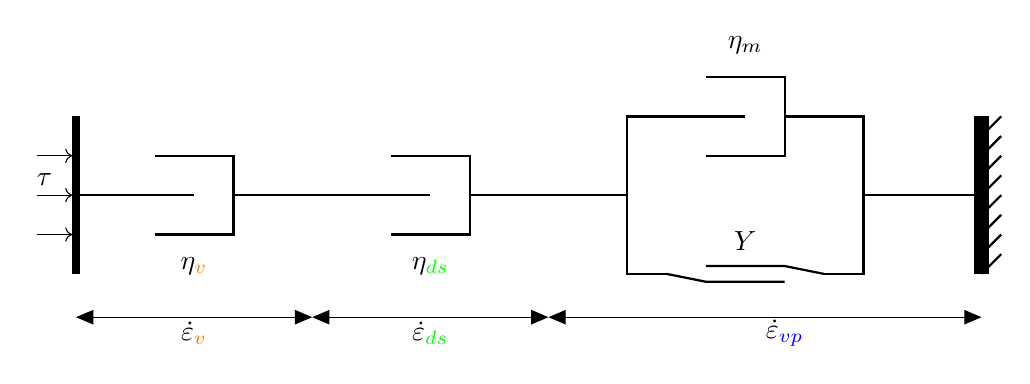
\begin{tikzpicture}
%\draw[fill=gray!23,gray!23](0,0) rectangle (7,5);
%\draw[step=0.5cm,gray,very thin] (0,0) grid (12,5); %background grid

\node[] at (0.1,2.7) {$\tau$};
\draw[line width=1mm] (0.5,1.5) -- (0.5,3.5) ;   
\draw [->] (0,2.5) -- (0.45,2.5);
\draw [->] (0,2) -- (0.45,2);
\draw [->] (0,3) -- (0.45,3);

\draw[thick] (0.5,2.5) -- (2,2.5) ;   
\draw[thick] (2.5,2.5) -- (5,2.5) ;   
\draw[thick] (5.5,2.5) -- (7.5,2.5) ;   
\draw[thick] (10.5,2.5) -- (12,2.5) ;   

% v damper
\draw[thick] (1.5,3) -- (2.5,3) -- (2.5,2) -- (1.5,2);  
% ds damper
\draw[thick] (4.5,3) -- (5.5,3) -- (5.5,2) -- (4.5,2);  
% m damper
\draw[thick] (8.5,4) -- (9.5,4) -- (9.5,3) -- (8.5,3);  

\node[] at (2,1.6) {$\eta_{\color{orange}v}$};
\node[] at (5,1.6) {$\eta_{\color{green}ds}$};
\node[] at (9,4.4) {$\eta_m$};

\draw[thick] (9,3.5) -- (7.5,3.5) -- (7.5,1.5) -- (8,1.5);  
\draw[thick] (9.5,3.5) -- (10.5,3.5) -- (10.5,1.5) -- (10,1.5);  

\draw[thick] (8,1.5) -- (8.5,1.4) -- (9.5,1.4) ;   
\draw[thick] (8.5,1.6) -- (9.5,1.6) -- (10,1.5) ;   

\node[] at (9,1.92) {$Y$};

%wall
\draw[line width=2mm] (12,1.5) -- (12,3.5) ;   
\draw[thick] (12,1.5) -- (12.25,1.75) ;   
\draw[thick] (12,1.75) -- (12.25,2) ;   
\draw[thick] (12,2) -- (12.25,2.25) ;   
\draw[thick] (12,2.25) -- (12.25,2.5) ;   
\draw[thick] (12,2.5) -- (12.25,2.75) ;   
\draw[thick] (12,2.75) -- (12.25,3) ;   
\draw[thick] (12,3) -- (12.25,3.25) ;   
\draw[thick] (12,3.25) -- (12.25,3.5) ;   

\draw[>=triangle 45, <->] (0.5,0.95) -- (3.5,0.95);
\draw[>=triangle 45, <->] (3.5,.95) -- (6.5,0.95);
\draw[>=triangle 45, <->] (6.5,0.95) -- (12,0.95);
\node[] at (2,0.75)   {$\dot\varepsilon_{\color{orange}v}$};
\node[] at (5,0.75)   {$\dot\varepsilon_{\color{green}ds}$};
\node[] at (9.5,0.75) {$\dot\varepsilon_{\color{blue}vp}$};

\end{tikzpicture}

\end{center}
The dislocation creep viscosity $\eta_{\color{green}ds}$ and effective 
viscoplastic viscosity $\eta_{\color{blue}vp}$ are given by 
\[
\eta_{\color{green}ds}(\dot\varepsilon) 
= \frac{1}{2} A^{-1/n} \dot{\varepsilon}^{-1+1/n} \exp \frac{Q}{nRT}
\qquad
\text{and}
\qquad
\eta_{\color{blue}vp}(\dot\varepsilon) 
= \frac{p \sin \phi + c \cos \phi}{2 \dot{\varepsilon}}  + \eta_{m}
\]
Note that these expressions are functions of $\dot\varepsilon$, the nature of which will be specified later. 
As documented in Section~\ref{MMM-ss:srpart}, 
the partitioning of the total strain rate into a viscous creep component and a viscoplastic component 
is not trivial.  
The algorithm then works as follows:

\begin{enumerate}
%%%%%%%%%%%%%%%%%
\item Assume we know $\dot\varepsilon_T$ (from previous iteration), 
as well as the yield value  $Y = p\; \sin\phi + c \; \cos \phi$ and $\eta_m$ (Here the 'T' stands 
for 'total').

%%%%%%%%%%%%%%%%%
\item We start by assuming that the plasticity element is not active 
($\dot{\varepsilon}_{\color{blue}vp}=0$, $\dot{\varepsilon}_{\color{green}ds}
+\dot{\varepsilon}_{\color{orange} v} =\dot{\varepsilon}_T$): 

We use the technique explained here after to compute the partitioning of the strain rate
and recover the stress $\tau$ and the dislocation creep effective viscosity
is given by 
\begin{eqnarray}
\eta_{\color{green}ds} &=& \frac{1}{2} A^{-1/n} 
\dot{\varepsilon}_{\color{green}ds}^{-1+1/n} \exp \left( \frac{Q}{nRT} \right) \nn\\
\eta_v &=& \frac{\tau}{2 \dot{\varepsilon}_{\color{orange}v}}  \nn
\end{eqnarray}
\begin{lstlisting}
eta_ds = 0.5*A**(-1./nnn)*np.exp(Q/nnn/Rgas/T)*eps_ds**(1./nnn-1.)
eps_v=tau/2/eta_v
\end{lstlisting}
The effective viscosity of both dampers is given by 
\[
\eta_{i\text eff}=\frac{1}{1/\eta_{\color{orange}v}+1/\eta_{\color{green}ds}}
\]
\begin{lstlisting}
etaeff=1./(1./eta_v+1./eta_ds)
\end{lstlisting}

%%%%%%%%%%%%%%%%%
\item if $\tau =2 {\eta}_{eff} \dot\varepsilon_T < Y$ the stress is below the yield stress value 
and the plasticity element is indeed not active. 
Simply return ${\eta}_{eff}$ in the material model.
\begin{lstlisting}
eps_vp=0
\end{lstlisting}

\item if $\tau=2 \eta_{eff} \dot\varepsilon_T > Y$ the stress is above the 
yield value, which is not allowed. In this case the plastic element must be present 
and active and the linear viscous and dislocation creep viscous dampers are then 
in series with the viscoplastic element. 
They  respectively deform with a strain rate $\dot{\varepsilon}_{\color{orange}v}$, 
$\dot{\varepsilon}_{\color{green}ds}$ and $\dot\varepsilon_{\color{blue}vp}$ 
(all under the same tress $\tau$) 
and we have  
$\dot\varepsilon_T = \dot{\varepsilon}_{\color{orange}v} +
\dot{\varepsilon}_{\color{green}ds} + \dot\varepsilon_{\color{blue}vp}$ so:

\begin{eqnarray}
\dot\varepsilon_T 
-\dot{\varepsilon}_{\color{orange}v} 
-\dot{\varepsilon}_{\color{green}ds}(\tau) 
&=& \dot\varepsilon_{\color{blue}vp}(\tau)  \nonumber\\
\dot\varepsilon_T 
-\dot{\varepsilon}_{\color{orange}v} 
-\dot{\varepsilon}_{\color{green}ds}(\tau) 
&=& \frac{\tau}{2 \eta_{\color{blue}vp}}  \nn\\
\dot\varepsilon_T 
-\dot{\varepsilon}_{\color{orange}v} 
-\dot{\varepsilon}_{\color{green}ds}(\tau) 
&=& \frac{\tau}{2 \left( \frac{Y}{2\dot\varepsilon_{\color{blue}vp}(\tau)} + \eta_m  \right)} 
\nonumber\\
\dot\varepsilon_T 
-\dot{\varepsilon}_{\color{orange}v} 
-\dot{\varepsilon}_{\color{green}ds}(\tau) 
&=&
\frac{\tau}{2 \left( \frac{Y}{2 (
\dot\varepsilon_T 
-\dot{\varepsilon}_{\color{orange}v}   
-\dot{\varepsilon}_{\color{green}ds}(\tau)  )} + \eta_m  \right)} \nonumber 
\\
2 [
\dot\varepsilon_T 
-\dot{\varepsilon}_{\color{orange}v}(\tau) 
-\dot{\varepsilon}_{\color{green}ds}(\tau)
]
\left( \frac{Y}{2 (
\dot\varepsilon_T 
-\dot{\varepsilon}_{\color{orange}v} 
-\dot{\varepsilon}_{\color{green}ds}(\tau) )} + \eta_m  \right) &=& \tau 
\nonumber\\
Y + 2 (
\dot\varepsilon_T 
-\dot{\varepsilon}_{\color{orange}v}(\tau)  
-\dot{\varepsilon}_{\color{green}ds}(\tau) ) \eta_m  &=& \tau \nonumber 
\end{eqnarray}
We must then find the zero of the function ${\cal F}(\tau)$: 
\begin{eqnarray}
{\cal F}(\tau) 
&=& Y + 2 [
\dot\varepsilon_T 
-\dot{\varepsilon}_{\color{orange}v}(\tau)   
-\dot{\varepsilon}_{\color{green}ds}(\tau) 
]\eta_m -\tau \nonumber\\
&=& Y + 2 \left[ 
\dot\varepsilon_T -\frac{\tau}{2\eta_v} -A \tau^n \exp \left(-\frac{Q}{RT}\right) 
\right]\eta_m -\tau \nn
\end{eqnarray}
Because dislocation creep involves the $n$-th power of the stress (and $n$ need not be an integer!) 
finding the value of the stress for which ${\cal F}=0$ is not straightforward.
This equation can be solved with a Newton-Raphson algorithm
and the iterations will be of the form:
\[
\tau_{n+1} = \tau_n - \frac{{\cal F}(\tau_n)}{{\cal F}'(\tau_n)}
\]
where the derivative of the function ${\cal F}$ with respect to $\tau$ reads:
\begin{eqnarray}
\frac{\partial {\cal F}}{\partial \tau} 
= -\frac{\eta_m}{\eta_v}-2 \eta_m n A \tau^{n-1} \exp \left(-\frac{Q}{RT}\right) -1 
\end{eqnarray}
Iterations require a starting value for $\tau$: we logically use the one obtained just 
above. Iterations stop when ${\cal F}<10^{-6}$.  
A maximum of 30 iterations is allowed.

\begin{lstlisting}
while abs(func)>1e-6:
   eps_ds=A*tau**nnn*np.exp(-Q/Rgas/T)
   eps_v=tau/2/eta_v
   func=Y + 2*(E2-eps_ds-eps_v)*eta_m - tau
   funcp=-eta_m/eta_v -2*eta_m*nnn*A*tau**(nnn-1)*np.exp(-Q/Rgas/T)-1
   tau-=func/funcp
   it+=1
   if it>30:
      break
#end while
\end{lstlisting}

\item Once $\tau$ has been found, one can compute 
\begin{eqnarray}
\dot{\varepsilon}_{\color{green}ds}(\tau)&=&A \tau^n \exp \left(-\frac{Q}{RT}\right)
\qquad 
\Rightarrow 
\qquad 
\eta_{\color{green}ds}(\dot\varepsilon_{\color{green}ds}) 
= \frac{1}{2} A^{-1/n} \dot{\varepsilon}_{\color{green}ds}^{-1+1/n} \exp \frac{Q}{nRT} \nn\\
\dot{\varepsilon}_{\color{orange}v}(\tau)&=&\frac{\tau}{2\eta_v}  \nn
\end{eqnarray}
\begin{lstlisting}
eps_ds=A*tau**nnn*np.exp(-Q/Rgas/T)
eta_ds = 0.5*A**(-1./nnn)*np.exp(Q/nnn/Rgas/T)*eps_ds**(1./nnn-1.)
eps_v=tau/2/eta_v
\end{lstlisting}
then 
$\dot{\varepsilon}_{\color{blue}vp}
=\dot{\varepsilon}_T 
-\dot{\varepsilon}_{\color{orange}v}(\tau) 
-\dot{\varepsilon}_{\color{green}ds}(\tau)$,
and then 
\[
\eta_{\color{blue} vp}(\dot\varepsilon_{\color{blue} vp}) 
= \frac{p \sin \phi + c \cos \phi}{2 \dot{\varepsilon}_{\color{blue}vp}}  + \eta_{m}
\]
\item 
Ultimately the effective viscosity at every quadrature point is computed as follows:
\[
\eta_{eff} = \left(
\frac{1}{\eta_{\color{orange}v}} + 
\frac{1}{\eta_{\color{green}ds}}  + 
\frac{1}{\eta_{\color{blue}vp}}  
\right)^{-1}
\]
\begin{lstlisting}
etaeff=1/(1/eta_v+1/eta_ds+1/eta_vp)
\end{lstlisting}

\end{enumerate}

%I set $\dot{\varepsilon}=10^{-15}\si{\per\second}$ in the viscosity function, 
%just so that the rheological model does not explode.
 
By construction, the viscosity is also maintained between $\eta_{m}\ge \SI{1e19}{\pascal}$ 
and $\eta_{v}=\SI{1e25}{\pascal}$. 

\begin{center}
\includegraphics[width=11cm]{python_codes/fieldstone_70/images/fig2}\\
{\captionfont Figure taken from \cite{dudy20}}
\end{center}

\begin{center}
\includegraphics[width=9cm]{python_codes/fieldstone_70/images/aspect_sr}\\
\includegraphics[width=9cm]{python_codes/fieldstone_70/images/aspect_eta}\\
{\captionfont Obtained with \aspect (see cookbook)}
\end{center}


%\newpage
%......................
%\paragraph{Extension}. 

%\begin{center}
%\includegraphics[width=7cm]{python_codes/fieldstone_70/extension/u}
%\includegraphics[width=7cm]{python_codes/fieldstone_70/extension/v}\\
%\includegraphics[width=7cm]{python_codes/fieldstone_70/extension/vel}
%\includegraphics[width=7cm]{python_codes/fieldstone_70/extension/q}\\
%\includegraphics[width=7cm]{python_codes/fieldstone_70/extension/e}
%\includegraphics[width=7cm]{python_codes/fieldstone_70/extension/etaeff}\\
%\includegraphics[width=6cm]{python_codes/fieldstone_70/extension/conv.pdf}
%\includegraphics[width=6cm]{python_codes/fieldstone_70/extension/pressure.pdf}\\
%\includegraphics[width=6cm]{python_codes/fieldstone_70/extension/tau.pdf}\\
%extension, resolution 150x45, 100 nl iterations only.
%\end{center}

%\newpage
%......................
%\paragraph{Compression}. 

%\begin{center}
%\includegraphics[width=7cm]{python_codes/fieldstone_70/compression/u}
%\includegraphics[width=7cm]{python_codes/fieldstone_70/compression/v}\\
%\includegraphics[width=7cm]{python_codes/fieldstone_70/compression/vel}
%\includegraphics[width=7cm]{python_codes/fieldstone_70/compression/q}\\
%\includegraphics[width=7cm]{python_codes/fieldstone_70/compression/e}
%\includegraphics[width=7cm]{python_codes/fieldstone_70/compression/etaeff}\\
%\includegraphics[width=6cm]{python_codes/fieldstone_70/compression/conv.pdf}
%\includegraphics[width=6cm]{python_codes/fieldstone_70/compression/pressure.pdf}\\
%\includegraphics[width=6cm]{python_codes/fieldstone_70/compression/tau.pdf}\\
%extension, resolution 150x45, 100 nl iterations only.
%\end{center}

 %%%%%%%%%%%%%%%%%%%%%%%%%%%%%%%%%%%%%%%%%%%%%%%%%%%%%%%%%%%%%%%%%%%%%%

\chapter{S40RTS in an annulus \label{f71}} %%%%%%%%%%%%%%%%%%%%%%%%%%%%%%%%%%%%%%%%%%%%%%%%%%%%%%%%%%%%%%%%%%% 71
\includegraphics[height=1.5cm]{images/pictograms/visualisation}
\includegraphics[height=1.5cm]{images/pictograms/tools}

\lstinputlisting[language=bash,basicstyle=\small]{python_codes/fieldstone_71/keywords.ascii}

\begin{center}
Code at \url{https://github.com/cedrict/fieldstone/tree/master/python_codes/fieldstone_71}
\end{center}

\par\noindent\rule{\textwidth}{0.4pt}

{\sl This stone was developed in collaboration with Rens Elbertsen}. \index{contributors}{R. Elbertsen}

\par\noindent\rule{\textwidth}{0.4pt}
%%%%%%%%%%%%%%%%%%%%%%%%%%%%%%%%%%%%%%%%%%%%%%%%%%%%%%%%%%%%%%%%%%%%%%%%%%%%%%%%%%%%%%%%%%%%%%

I neeed:
- free slip bc
- max res ?
- crust/lith
- rotated plane 
- compare with submachine


%_____________________________________________________________________________
\subsubsection*{Radial viscosity profiles}

\

In this section we describe the different density profiles used to in the convection model. We assume that viscosity is purely a function of depth. The user can choose a viscosity profile by changing the parameter \texttt{case}.

Five radial viscosity profiles are available:
\begin{itemize}
\item The first viscosity profile is a constant viscosity for all depths of $10^{22}$ Pa s. 
This value is an estimated value of what is normally found in the literature. This is \texttt{visc\_case = 0}. 

\item The second viscosity profile comes from Yoshida et al (2001) \cite{yohk01}. It uses three different regions: lithosphere (0 km to 150 km), upper mantle (150 km to 670 km) and lower mantle (670 km to 2900 km). The function uses an if-statement to return the right value for the given depth. This is \texttt{case = 1}.

\item The third viscosity profile comes from Steinberger \& Holmes (2008) \cite{stho08} 
which is comparable to \cite{stca06}, but of the latter no available data was available. 
Data is read from the file \texttt{visc\_STHO08.dat}. 
This is \texttt{case = 2}.

\item The fourth and fifth profile come from Ciskova et al (2012) \cite{civs12}. 
Data is read from the file \texttt{visc\_CIVS12.dat}. 
The paper showcases two main families of radial viscosity profiles in literature. Family A, which has a sharp 
increase below the 660 km transition zone and remains constant for most of the lower mantle 
and family B which is much smoother over the transition zone and increases with depth in the lower mantle. 
Family A can be chosen by \texttt{case = 3} and family B can be chosen by \texttt{case = 4}.

\end{itemize}

\begin{center}
\includegraphics[width=10cm]{python_codes/fieldstone_71/images/visc}
\end{center}


%_____________________________________________________________________________
\subsubsection*{Cross section of the Earth}

Several parameters are implemented which can be modified to get any cross section of the Earth. 

The parameter \texttt{lon\_start} specifies at which longitude we start reading data from the S40RTS model. The model always starts filling the annulus on the right ($x=1, y=0$ on the unit circle) continuing in the counter-clockwise direction with increasing longitudes. If we set the parameter \texttt{plane\_angle} (explained in the next subsection) to 0 we have an equatorial cross section through the Earth that starts at the longitude \texttt{lon\_start}.

The parameter \texttt{plane\_angle} indicates the angle the plane of the cross section is making with the equatorial plane. The longitude specified by \texttt{lon\_start} always is at latitude 0. Latitudes will be increased as a result of the \texttt{plane\_angle} on the northern hemisphere and decreased on the southern hemisphere. Setting the \texttt{plane\_angle} to 90 gives us a cross section through both poles and the longitude specified by \texttt{lon\_start}.



%_____________________________________________________________________________
\subsubsection*{Loading of the Spherical Harmonics, computing $\delta \ln V_s$}

In this stone we wish to use the shear wave velocity model S40RTS \cite{ridv11} 
as the main source of information 
to build a temperature anomaly/density anomaly model of the mantle. 

Variations of the shear wave velocity are stored in the form of spherical harmonics coefficients. 
We make use of an already existing code written by Ross Ronan Maguire
(available at \url{https://github.com/romaguir/sph_models}
to read the values of $d \ln{V_S}$ for a section of the Earth. 
The code is modified such that we read in $d \ln{V_S}$ for every nodal point in the annulus domain. 
Note that the returned value had to be scaled down by a factor of $\sqrt{2}$ to obtain identical figures to 
those of the original paper or those obtained with SubMachine\footnote{\url{https://www.earth.ox.ac.uk/~smachine/cgi/index.php}}.  




There are three different functions in the original code that enables us to read 
the spherical harmonics data: \texttt{read\_splines}, \texttt{read\_sph} 
and \texttt{find\_spl\_vals}. The function \texttt{read\_sph} reads the data from the spherical 
harmonics data file. Thereafter, we loop over all the nodal points. The loop starts at the 
deepest circle of nodes and loops counter-clockwise over this circle before continuing with the 
next circle that is one row of nodal points outwards. The function \texttt{find\_spl\_vals} 
reads the values for a specific depth, meaning that we only have to read these once when we 
start a new circle of nodal points. This function makes use of the other function \texttt{read\_splines}. 
Once we have the correct splines we loop over all nodal points at this depth and calculate the 
value of $\delta \ln{V_s}$ for all these points. The value of $\delta \ln{V_s}$ 
is stored in the array \texttt{d\_ln\_vs}.

\begin{center}
\includegraphics[width=7cm]{python_codes/fieldstone_71/images/sub_cross_section_01}
\includegraphics[width=7cm]{python_codes/fieldstone_71/images/sub_cross_section_02}\\
{\captionfont Taken from SubMachine\footnote{\url{https://www.earth.ox.ac.uk/~smachine/cgi/index.php}}.
Cross sections of the mantle for S20RTS and S40RTS models. 
Left: latitude=0, longitude between 0 and 179.
Right: latitude=0, longitude between -179 and 0.}
\end{center}

\begin{center}
\includegraphics[width=9cm]{python_codes/fieldstone_71/images/dlnvsS40RTS_equator}\\
{\captionfont S40RTS, nelr=50}
\end{center}


%_____________________________________________________________________________
\subsubsection*{Converting $\delta \ln V_s$ to $\delta \rho$}

We assume that there is a direct scaling from the shear wave velocity anomaly to the density anomaly, i.e. 
we assume that all anomalies in $\delta \ln{V_s}$ are the result of temperature perturbations and 
not of differences in composition. 
We use the following formula to obtain the $\delta \ln{\rho} $ values:
\[
\delta \ln{\rho(r, \theta, \phi)} = \xi(r) \cdot \delta \ln{V_s(r, \theta, \phi)} 
\]
where $\xi$ is the scaling factor that is depth dependent. We will go into more depth for this factor in the following subsections. To get the values for $\delta \rho(r, \theta, \phi)$ we use the following formula:
\[
\delta \ln{\rho(r, \theta, \phi)} = \frac{\delta \rho(r, \theta,\phi)}{\rho_\text{ref}} 
\]
where $\rho_\text{ref}$ is the reference density, which in our case for the S40RTS model is the PREM model 
\cite{dzan81}. In the following section we will show which scalings are implemented in the model and how 
they are implemented. The user can choose a scaling by changing the parameter \texttt{xi\_case}. 
The value for $\xi$ is stored in the array \texttt{xi\_nodal}, 
the value for $\rho_\text{PREM}$ is stored in the array \texttt{rho\_prem\_nodal}, 
the value for $\delta \ln{\rho}$ is stored in the array \texttt{d\_ln\_rho\_nodal} 
and the value of $\delta \rho$ is stored in the array \texttt{d\_rho\_nodal}.

There are three options in the code to compute the $\xi$ coefficient:
\begin{itemize}
\item Constant $\xi$. The first scaling that is used is a constant value for $\xi$ of 0.25. 
This is \texttt{xi\_case = 0}. The factor 0.25 is an estimated average of what is normally found in 
literature. An overview of the three different cases can be found hereunder:

\begin{center}
\includegraphics[width=8cm]{python_codes/fieldstone_71/images/xi}
\end{center}

\item The second scaling that is used comes from Steinberger \& Calderwood (2006) \cite{stca06}. 
Data is read from the file \texttt{data/xi/xi\_stca06.ascii}. 

\item The third scaling that is used comes from Moulik \& Ekstrom (2016) \cite{moek16}. 
Data is read from the file \texttt{data/xi/xi\_moek16.ascii}. 
A very noticeable difference between this scaling and the scaling of \cite{stca06} 
is that for the upper mantle the value for $\xi$ is slightly higher and for the lowermost lower mantle 
the value for $\xi$ is negative.
\end{itemize}




 %%%%%%%%%%%%%%%%%%%%%%%%%%%%%%%%%%%%%%%%%%%%%%%%%%%%%%%%%%%%%%%%%%%%%%

\chapter{quadrilateral MINI - the $Q_1^+\times Q_1$ element \label{f72}} %%%%%%%%%%%%%%%%%%%%%%%%%%%%%%%%%%%%% 72
\lstinputlisting[language=bash,basicstyle=\small]{python_codes/fieldstone_72/keywords.ascii}

\begin{center}
Code at \url{https://github.com/cedrict/fieldstone/tree/master/python_codes/fieldstone_72}
\end{center}

\par\noindent\rule{\textwidth}{0.4pt}

%%%%%%%%%%%%%%%%%%%%%%%%%%%%%%%%%%%%%%%%%%%%%%%%%%%%%%%%%%%%%%%%%%%%%%%%%%%%%%%%%%%%%%%%%%%%%%%%%%%%

\index{stopics}{$Q_1^+\times Q_1$}


%--------------------------------------
\section*{Manufactured solution \#1}

The analytical solution originates in \textcite{lami17} (2017).
The velocity and pressure are given by
\begin{eqnarray}
u(x,y)&=&-2x^2y(2y-1)(x-1)^2(y-1) \\
v(x,y)&=& 2xy^2(2x-1)(x-1)(y-1)^2 \\
p(x,y)&=& x(1-x)(1-2y)
\end{eqnarray}
Boundary conditions are no-slip on all sides of the unit square. 
The corresponding body force terms are derived in Section~\ref{MMM-ss:mms11}. 


The quadrilateral MINI element used here also originates in the same article 
and comes in two flavours with two different bubble functions $b_1$ and $b_2$
as explained in Section~\ref{MMM-ss:quadmini}.
The two bubble functions are (in reduced coordinates $-1 \leq r,s \leq 1$):
\begin{eqnarray}
b_1(r,s) &=& (1-r^2)(1-s^2)\cdot (1-r)(1-s)\\
b_2(r,s) &=& (1-r^2)(1-s^2)\cdot (1+\beta(r+s))
\end{eqnarray}
The common term to both bubbles insures that the bubble is exactly zero on all four edges of the 
element. What differentiates them is the remaining term, which is bilinear ($b_1$) or linear ($b_2$). 
Both also satisfy $b_1(0,0)=b_2(0,0)=1$. The paper uses $\beta=1/4$.

The velocity and pressure fields for the benchmark are shown hereunder:
\begin{center}
\includegraphics[width=7cm]{python_codes/fieldstone_72/results/mms/vel}
\includegraphics[width=7cm]{python_codes/fieldstone_72/results/mms/p}
\end{center}

During the debugging process I ended up 
implementing various Gauss quadratures schemes, from $2^2$ to $6^2$ points but the results
show that $2^2$ quadrature points per element are sufficient since the more expensive quadratures
yield identical results. 
The results from the article are somewhat different than mine but I suspect that what the 
author measured could be different than what I measure (see Table 1,2 in \cite{lami17}). 
The trends are similar though, with $b_2$ performing better than $b_1$:

\begin{center}
\includegraphics[width=8cm]{python_codes/fieldstone_72/results/mms/errors_v}
\includegraphics[width=8cm]{python_codes/fieldstone_72/results/mms/errors_p}\\
{\captionfont Left: velocity error in $L_2$ norm; Right: pressure error in $L_2$ norm.
Resolutions from $8\times8$ until $80\times80$.}
\end{center}

The root mean square velocity is also measured for both bubble functions.
As above we see that $b_2$ performs better than $b_1$:
\begin{center}
\includegraphics[width=9cm]{python_codes/fieldstone_72/results/mms/vrms}
\end{center}


%................................................
\subsubsection{Influence of mesh nodes position:} 
I have also repeated these 
experiments with a mesh whose internal nodes have been 
randomly moved by up to $\pm$20\% of $h_x$ or $h_y$ around the initial position. 

\begin{center}
\includegraphics[width=5.7cm]{python_codes/fieldstone_72/results/mms/area16}
\includegraphics[width=5.7cm]{python_codes/fieldstone_72/results/mms/area32}
\includegraphics[width=5.7cm]{python_codes/fieldstone_72/results/mms/area64}\\
{\captionfont area of elements for randomized meshes. Left to right: 16x16, 32x32, 64x64}
\end{center}


\begin{center}
\includegraphics[width=5.7cm]{python_codes/fieldstone_72/results/mms/errors_v_rand}
\includegraphics[width=5.7cm]{python_codes/fieldstone_72/results/mms/errors_p_rand}
\includegraphics[width=5.7cm]{python_codes/fieldstone_72/results/mms/vrms_rand}
\end{center}

We find that the error convergence rate is unchanged for velocities but is now less 
for pressure (higher than 1, lower than 1.5). 

%..............................
\subsubsection{Another bubble?} 
To make the point that the bubble function must contain the (bi-)linear term, 
I have created a third bubble function which is simply $b_3(r,s)=(1-r^2)(1-s^2)$.
Technically it is zero on the sides and 1 in the middle so it fulfills the 
same requirements as the other 2 bubble functions. 
However, we see that this function is not sufficient to stabilise the element as the pressure 
showcases a typical error mode:
\begin{center}
\includegraphics[width=6cm]{python_codes/fieldstone_72/results/mms/p_b3}
\includegraphics[width=6cm]{python_codes/fieldstone_72/results/mms/p_error_b3}\\
{\captionfont Left: pressure field as obtained with $b_3$; right: pressure error.}
\end{center}


%..............................
\subsubsection{influence of $\beta$:} Finally, 
I use a $2\times 2$ quadrature and look at 
the errors and the vrms for various values of $\beta$:
\begin{center}
\includegraphics[width=5cm]{python_codes/fieldstone_72/results/mms/errors_v_beta}
\includegraphics[width=5cm]{python_codes/fieldstone_72/results/mms/errors_p_beta}
\includegraphics[width=5cm]{python_codes/fieldstone_72/results/mms/vrms_beta}
\end{center}
It looks like $\beta\in[0.0001,0.01]$ does better than all other higher values. 
Also, looking at the 
field in Paraview, no trace of the error modes as we just saw above.
The difference between 0.01 and 0.25 is somewhat small, but values of $\beta$ above 0.5 
clearly yield less accurate results. 

I can also plot these same results in a different way, i.e. placing $\beta$ on the horizontal axis:

\begin{center}
\includegraphics[width=5cm]{python_codes/fieldstone_72/results/mms/errors_v_beta2}
\includegraphics[width=5cm]{python_codes/fieldstone_72/results/mms/errors_p_beta2}
\includegraphics[width=5cm]{python_codes/fieldstone_72/results/mms/vrms_beta2}\\
{\captionfont From left to right: velocity error, pressure error and vrms as a function 
of the parameter $\beta$, for 5 different resolutions. The dotted line corresponds to $\beta=1/4$ as used in \cite{lami17}.}
\end{center}

One could conclude that $\beta=10^{-4}-10^{-2}$ 
would be a better choice but the question remains whether these
conclusions hold for other benchmarks. We will see later 
that $\beta=1/4$ is actually preferable to these very low values.


\subsubsection{Looking at the condition number of the $\K$ matrix} 
(remember: $\K$ is the 1,1 block of the
Stokes matrix). 
I have computed the condition number of the $\K$ matrix for both bubbles and for various mesh resolutions. 
We see that the bubble 1 yields condition numbers substantially higher than bubble 2, both increasing 
quadratically with $h$. This is rather critical is (for instance) a conjugate gradient solver is used 
is used on this matrix.

\begin{center}
\includegraphics[width=6cm]{python_codes/fieldstone_72/results/mms/eigenvalues/e}
\end{center}

%_____________________________________
\section*{Manufactured solution \#2}

This is the second manufactured solution 
mentioned in Lamichhane \cite{lami17}. It is presented in Section~\ref{MMM-ss:mms2}.
It is for a unit square with $\eta=1$ and the smooth exact solution is
\begin{eqnarray}
u(x,y) &=& x+x^2 - 2xy+x^3 - 3xy^2 + x^2y \\
v(x,y) &=& -y-2xy+y^2 -3x^2y + y^3 - xy^2 \\
p(x,y) &=& xy+x+y+x^3y^2 - 4/3
\end{eqnarray}
Note that the pressure obeys $\int_{\Omega} p \; d\Omega = 0$. The analytical 
velocity is prescribed on the boundary of the domain. 
The corresponding body force is:
\begin{eqnarray}
b_x &=& 3x^2y^2 -y-1   \\
b_y &=& 2x^3y+3x-1 
\end{eqnarray}


\begin{center}
\includegraphics[width=7cm]{python_codes/fieldstone_72/results/mms2/errors_v}
\includegraphics[width=7cm]{python_codes/fieldstone_72/results/mms2/errors_p}\\
{\captionfont Velocity and pressure error convergence as a function of the mesh size $h$ for
meshes $8\times 8$ up to $128\times 128$.}
\end{center}


The root mean square velocity is also measured for both bubble functions.
As above we see that $b_2$ performs better than $b_1$:
\begin{center}
\includegraphics[width=9cm]{python_codes/fieldstone_72/results/mms2/vrms}
\end{center}


\begin{center}
\includegraphics[width=5cm]{python_codes/fieldstone_72/results/mms2/u}
\includegraphics[width=5cm]{python_codes/fieldstone_72/results/mms2/v}
\includegraphics[width=5cm]{python_codes/fieldstone_72/results/mms2/vel}\\
{\captionfont Velocity field as obtained on $32\times 32$ grid. Left: $x-$component,
middle: $y-$component, right: velocity vector magnitude.}
\end{center}

\begin{center}
\includegraphics[width=7cm]{python_codes/fieldstone_72/results/mms2/error_v1}
\includegraphics[width=7cm]{python_codes/fieldstone_72/results/mms2/error_v2}\\
{\captionfont Velocity error for bubble function 1 (left) and bubble function 2 (right). 
$b_2$ maximum error is about half of $b_1$ error.}
\end{center}

\begin{center}
\includegraphics[width=7cm]{python_codes/fieldstone_72/results/mms2/p1}
\includegraphics[width=7cm]{python_codes/fieldstone_72/results/mms2/p2}\\
{\captionfont Pressure field obtained with bubble function 1 (left) and bubble function 2 (right).
Scale has been voluntarily set to analytical values scale for both.}
\end{center}

\begin{center}
\includegraphics[width=7cm]{python_codes/fieldstone_72/results/mms2/error_p1}
\includegraphics[width=7cm]{python_codes/fieldstone_72/results/mms2/error_p2}\\
{\captionfont Pressure error field obtained with bubble function 1 (left) and bubble function 2 (right). Notice the 
different error magnitudes between both!}
\end{center}

The conclusions are identical to those obtained with the first manufactured solution. 
The second bubble function (here with $\beta=1/4$) performs better. While velocity error
convergence rates are quadratic for both bubbles, the pressure error is substantially lower
for bubble 2 (although its rate is slightly lower than bubble 1 -- both are still 
superconvergent). This is illustrated above where we see that the pressure field obtained 
with bubble 1 showcases strong ripples in the upper right corner.     



%_____________________________________
\section*{The SolCx benchmark}

Because of the viscosity jump at $x=L_x/2$, it has been widely reported that 
error convergence rates depend on wheter the number of element in the $x-$direction 
is even or odd.

\begin{center}
\includegraphics[width=5cm]{python_codes/fieldstone_72/results/solcx/errors_v_even}
\includegraphics[width=5cm]{python_codes/fieldstone_72/results/solcx/errors_p_even}
\includegraphics[width=5cm]{python_codes/fieldstone_72/results/solcx/vrms_even}\\
\includegraphics[width=5cm]{python_codes/fieldstone_72/results/solcx/errors_v_odd}
\includegraphics[width=5cm]{python_codes/fieldstone_72/results/solcx/errors_p_odd}
\includegraphics[width=5cm]{python_codes/fieldstone_72/results/solcx/vrms_odd}
\end{center}

Velocity error convergence rates are 2 for even numbers of elements and 1 for odd numbers, 
such as for the Q1Q1 stab. 
Pressure error convergence rate seems to be 0.5 for odd numbers of elements and
0.65 for even numbers ... 

\begin{center}
\includegraphics[width=5cm]{python_codes/fieldstone_72/results/solcx/vel}
\includegraphics[width=5cm]{python_codes/fieldstone_72/results/solcx/p}
\includegraphics[width=5cm]{python_codes/fieldstone_72/results/solcx/p_error}
\end{center}

We see that the pressure showcases an strong error (even at high resolution)
along the interface. 


%_____________________________________
\section*{The SolKz benchmark}

\begin{center}
\includegraphics[width=5cm]{python_codes/fieldstone_72/results/solkz/errors_v}
\includegraphics[width=5cm]{python_codes/fieldstone_72/results/solkz/errors_p}
\includegraphics[width=5cm]{python_codes/fieldstone_72/results/solkz/vrms}
\end{center}

We find that velocity and pressure errors converge quadratically, with 
once again $b_2$ better than $b_1$.


%_____________________________________
\section*{The SolVi benchmark}


\begin{center}
\includegraphics[width=7cm]{python_codes/fieldstone_72/results/solvi/vel}
\includegraphics[width=7cm]{python_codes/fieldstone_72/results/solvi/p}\\
{\captionfont Resolution $128\times128$ - bubble 1 }
\end{center}


\begin{center}
\includegraphics[width=5cm]{python_codes/fieldstone_72/results/solvi/errors_v}
\includegraphics[width=5cm]{python_codes/fieldstone_72/results/solvi/errors_p}
\includegraphics[width=5cm]{python_codes/fieldstone_72/results/solvi/vrms}
\end{center}



%_____________________________________
\section*{The Stokes Sphere}

This experiment is the benchmark of Section~\ref{MMM-ss:stokes_sphere2D}. 
The density is assigned directly to the 
quadrature point by means of a function. Inside the disc of radius 0.123456789 centered in the domain 
the density is set to 1.01 while it is set to 1 outside 
(viscosities are respectively 1000 and 1). The gravity is $|g_y|=1$ and 
free-slip boundary conditions are implemented on all sides. 

On the following figures the min/max of the pressure in the domain and the vrms 
are shown for both bubble functions. We see that at low resolution the reported 
values show some variations but with increasing resolution the quantities converge to a single value:

\begin{center}
\includegraphics[width=7cm]{python_codes/fieldstone_72/results/sphere/pstats}
\includegraphics[width=7cm]{python_codes/fieldstone_72/results/sphere/vrms}
\end{center}

\begin{center}
\includegraphics[width=7cm]{python_codes/fieldstone_72/results/sphere/vel_b1}
\includegraphics[width=7cm]{python_codes/fieldstone_72/results/sphere/vel_b2}\\
\includegraphics[width=7cm]{python_codes/fieldstone_72/results/sphere/p_b1}
\includegraphics[width=7cm]{python_codes/fieldstone_72/results/sphere/p_b2}\\
{\captionfont Left is b1, Right is b2.}
\end{center}

It looks like $b_2$ yields more anomalous pressure modes inside the sphere, 
which is corroborated by the following figures which show the pressure 
at $x=L_x/2$ in both cases. However we also see that at high resolution both 
bubbles yield nearly identical pressure profiles and that the ripples have vanished. 

\begin{center}
\includegraphics[width=5cm]{python_codes/fieldstone_72/results/sphere/pline_b1_closed}
\includegraphics[width=5cm]{python_codes/fieldstone_72/results/sphere/pline_b2_closed}
\includegraphics[width=5cm]{python_codes/fieldstone_72/results/sphere/pline_b12_closed}\\
{\captionfont pressure profile for b1 (left) and b2 (middle) for different resolutions.}
\end{center}

One can also prescribe an open boundary condition at the top:

\begin{center}
\includegraphics[width=7cm]{python_codes/fieldstone_72/results/sphere/open/vel}
\includegraphics[width=7cm]{python_codes/fieldstone_72/results/sphere/open/p}
\end{center}


\begin{center}
\includegraphics[width=5cm]{python_codes/fieldstone_72/results/sphere/pline_b1_open}
\includegraphics[width=5cm]{python_codes/fieldstone_72/results/sphere/pline_b2_open}
\includegraphics[width=5cm]{python_codes/fieldstone_72/results/sphere/pline_b12_open}\\
{\captionfont pressure profile for b1 (left) and b2 (middle) for different resolutions.}
\end{center}





%_____________________________________
\section*{Rayleigh-Taylor instability}

This benchmark is carried out in Appendix D of Thieulot (2011) \cite{thie11}.
It consists of a two-layer system driven by gravity.
The mesh is modified so as to align with the sinusoidal perturbation.
Resolution and $\eta_2$ are varied on the following figures:

\begin{center}
\includegraphics[width=7cm]{python_codes/fieldstone_72/results/RT/area}
\includegraphics[width=7cm]{python_codes/fieldstone_72/results/RT/eta}\\
\includegraphics[width=7cm]{python_codes/fieldstone_72/results/RT/rho}
\includegraphics[width=7cm]{python_codes/fieldstone_72/results/RT/vel}
\end{center}


\begin{center}
\includegraphics[width=7cm]{python_codes/fieldstone_72/results/RT/vy_b1}
\includegraphics[width=7cm]{python_codes/fieldstone_72/results/RT/vy_b2}
\end{center}

Bubble 2 does better than bubble 1. Also, $\beta$ does not seem to play a role.

%_____________________________________
\section*{Sinking block}
This is the very same experiment as in Stone 53. It consists of a negatively buoyant 
square object falling in a fluid in a square domain. 
This particular experiment proved to be the 'downfall' of the $Q_1\times Q_1-stab$ element
since the stabilisation term is akin to a pressure diffusion and therefore
acts on the lithostatic pressure and also tends to smooth the effect of small 
density variations (Thieulot \& Bangerth, in prep.). 

Unless specified otherwise bubble 2 has $\beta=0.25$ by default.

%............................
\subsection*{Full density} 
Results indicate that the element performs adequately, especially the 
pressure field which looks smooth.  

\begin{center}
\includegraphics[width=7cm]{python_codes/fieldstone_72/results/block/full/density}
\includegraphics[width=7cm]{python_codes/fieldstone_72/results/block/full/viscosity}\\
\includegraphics[width=7cm]{python_codes/fieldstone_72/results/block/full/vel}
\includegraphics[width=7cm]{python_codes/fieldstone_72/results/block/full/p}\\
{\captionfont $64\times 64$. Viscosity ratio is 10, $\delta \rho=8$, bubble 1.}
\end{center}

We see that the element is capable of reprensenting a linear pressure profile
(the overpressure signal due to the block is negligible compared to the 
hydrostatic pressure).

\begin{center}
\includegraphics[width=10cm]{python_codes/fieldstone_72/results/block/full/plines}\\
{\captionfont Pressure profile measured at $x=L_x/2$ for various resolutions. Same parameters
as previous figure.}
\end{center}

As before we produce the characteristic figures of the velocity and pressure in the middle of the 
block as a function of the viscosity ratio and the density difference. The results obtained 
with the quadrilateral MINI element agree nicely with those obtained with the $Q_2\times Q_1$ element:
 
\begin{center}
\includegraphics[width=7cm]{python_codes/fieldstone_72/results/block/full/results_v}
\includegraphics[width=7cm]{python_codes/fieldstone_72/results/block/full/results_p}
\end{center}


\underline{Influence of $\beta$ parameter for bubble 2:} I set $\delta\rho=8$, resolution 64x64, $\eta^\star=10$,
and record the pressure profile 

\begin{center}
\includegraphics[width=10cm]{python_codes/fieldstone_72/results/block/full/betastudy/plines}
\end{center}

We can conclude that the bubble type and the value of $\beta$ do not seem to significantly affect 
the pressure profile in this case.

%............................
\subsection*{Reduced density} 
This is the same experiment as above but $\rho_1$ has been removed from the density
everywhere in the domain, so that the surrounding material has zero density 
and the block has a density $\delta \rho$.
The velocity and pressure field are then:

\begin{center}
\includegraphics[width=7cm]{python_codes/fieldstone_72/results/block/reduced/vel}
\includegraphics[width=7cm]{python_codes/fieldstone_72/results/block/reduced/p}\\
{\captionfont $64\times 64$. Viscosity ratio is 10, $\delta \rho=8$. bubble 1}
\end{center}

We then turn to the pressure along the vertical line $x=L_x/2$ as obtained with 
both bubble functions and find that both yield visually similar profiles:

\begin{center}
\includegraphics[width=7cm]{python_codes/fieldstone_72/results/block/reduced/plines_b1}
\includegraphics[width=7cm]{python_codes/fieldstone_72/results/block/reduced/plines_b2}\\
{\captionfont Pressure profile measured at $x=L_x/2$ for various resolutions and for both bubble functions.
Left is bubble 1, right is bubble 2.}
\end{center}

I hereafter plot the pressure profiles for both bubble functions at the highest resolution, i.e. $96\times 96$.
We see that differences are somewhat minimal, although bubble 2 yields a pressure above the block which 
showcases worrying oscillations. Also the results are remarquably similar to those obtained with the Taylor-Hood
$Q_2\times Q_1$ element:

\begin{center}
\includegraphics[width=7cm]{python_codes/fieldstone_72/results/block/reduced/plines_b12}
\includegraphics[width=7cm]{python_codes/fieldstone_72/results/block/reduced/plines_b12_zoom}
\end{center}

Finally the velocity and pressure inside the block unsurprisingly match nicely with those obtained with the Taylor-Hood
$Q_2\times Q_1$ element:

\begin{center}
\includegraphics[width=7cm]{python_codes/fieldstone_72/results/block/reduced/results_v}
\includegraphics[width=7cm]{python_codes/fieldstone_72/results/block/reduced/results_p}
\end{center}


\underline{Influence of $\beta$ parameter for bubble 2:} I set $\delta\rho=8$, resolution 64x64, $\eta^\star=10$,
and record the pressure profile 

\begin{center}
\includegraphics[width=7cm]{python_codes/fieldstone_72/results/block/reduced/betastudy/plines}
\includegraphics[width=7cm]{python_codes/fieldstone_72/results/block/reduced/betastudy/plines_zoom}
\end{center}

It is here very obvious that low values of $\beta$ yield problematic pressure oscillations. 
It looks like $\beta \geq 0.25$ actually yield near identical results to those obtained with bubble 1,
but $\beta=1$ or $\beta=2$ also yields unwanted oscillations.

%_____________________________________
\section*{Free surface benchmark}

The setup originates in Crameri et al (2012) \cite{crsg12}. It consists of 
a cosine-shaped layer of homogeneous lithosphere overlaying a homogeneous layer of mantle.
The domain is 2800x700 km. The amplitude of the surface perturbation is 7km. 
Free slip boundary conditions are prescribed on the sides and no-slip at the bottom. 
The lithosphere is characterised by $\eta=10^{23}$Pa.s and the mantle by $\eta=10^{21}$Pa.s, 
while both have a density of 3330kg/m3.

\begin{center}
\includegraphics[width=13cm]{python_codes/fieldstone_72/results/crsg12/area}\\
{\captionfont Setup of the mesh. Area of the elements.}
\end{center}

I do not wish to implement a mesh evolution algorithm nor timestepping so
I only report the velocity field at $t=0$:

\begin{center}
\includegraphics[width=7cm]{python_codes/fieldstone_72/results/crsg12/u}
\includegraphics[width=7cm]{python_codes/fieldstone_72/results/crsg12/v}\\
\includegraphics[width=7cm]{python_codes/fieldstone_72/results/crsg12/vel}
\includegraphics[width=7cm]{python_codes/fieldstone_72/results/crsg12/p}
\end{center}

It is clear that the velocity is (visually) what we expect. The presence of the free surface 
does not seem to introduce any kind of abnormal behaviour. 


\newpage
%%%%%%%%%%%%%%%%%%%%%%%%%%%%%%%%%%%%%%%%%%%%%%%%%%%%%%%%%%%%%%%%%%%%%%%%%%%%%%%
\section*{NEW stuff}

all in {\tt /study} folder.

Following \textcite{lami17} (2017), we consider the case of a 4x4 element mesh (macro-element).
We prescribe u and v boundary conditions on all sides (8 nodes) so that
16 lines of the G matrix are zero. Since the original G matrix is (9+4)*2=26 dofs, 
there are only 26-8*2 lines left, i.e. a 9*10 matrix like the D one of the paper.

%-----------------------
\subsection*{bubble 0}

\begin{center}
\includegraphics[width=10cm]{python_codes/fieldstone_72/images/mat1}\\
{\captionfont ${\bm G}$ matrix obtained with the $(1-x^2)(1-y^2)$ bubble}
\end{center}

\[
D=
\left(
\begin{array}{cccccccccc}
\frac29 & \frac29 & 0 & 0 & 0 & 0 & 0 & 0 & \frac{1}{12} & \frac{1}{12} \\ \\
-\frac29 & \frac29 & \frac29 & \frac29 & 0 & 0 & 0 & 0 & 0 & \frac13 \\ \\
0 & 0 & -\frac29 & \frac29 & 0 & 0 & 0 & 0 & -\frac{1}{12} & \frac{1}{12} \\ \\
\frac29 & -\frac29 & 0 & 0 & 0 & 0 & \frac29 & \frac29 & \frac13  & 0 \\ \\ 
-\frac29 & -\frac29 & \frac29 & -\frac29 & \frac29 & \frac29 & -\frac29 & \frac29  &0 &0\\ \\
0 & 0 & -\frac29 & -\frac29 & -\frac29 & \frac29 & 0 & 0 & -\frac13 & 0 \\ \\
0 & 0 & 0 & 0 & 0 & 0 & \frac29 & -\frac29 & \frac{1}{12} & -\frac{1}{12} \\ \\
0 & 0 & 0 & 0 & \frac29 & -\frac29 & -\frac29 & -\frac29 & 0 & -\frac13 \\ \\ 
0 & 0 & 0 & 0 & -\frac29 & -\frac29 & 0 & 0 & -\frac{1}{12} & -\frac{1}{12}
\end{array}
\right)
\]
which we can multiply by 9: 
\[
D=
\left(
\begin{array}{cccccccccc}
2 & 2 & 0 & 0 & 0 & 0 & 0 & 0 & \frac{3}{4} & \frac{3}{4} \\ \\
-2 & 2 & 2 & 2 & 0 & 0 & 0 & 0 & 0 & 3 \\ \\
0 & 0 & -2 & 2 & 0 & 0 & 0 & 0 & -\frac{3}{4} & \frac{3}{4} \\ \\
2 & -2 & 0 & 0 & 0 & 0 & 2 & 2 & 3  & 0 \\ \\ 
-2 & -2 & 2 & -2 & 2 & 2 & -2 & 2  &0 &0\\ \\
0 & 0 & -2 & -2 & -2 & 2 & 0 & 0 & -3 & 0 \\ \\
0 & 0 & 0 & 0 & 0 & 0 & 2 & -2 & \frac{3}{4} & -\frac{3}{4} \\ \\
0 & 0 & 0 & 0 & 2 & -2 & -2 & -2 & 0 & -3 \\ \\ 
0 & 0 & 0 & 0 & -2 & -2 & 0 & 0 & -\frac{3}{4} & -\frac{3}{4}
\end{array}
\right)
\]


Here is what I obtain (matrix multiplied by 9). Structure is good.
First 8 columns are perfect BUT last two columns are off, and not just 
by a single constant...rank is found to be 7 as in the paper.

\begin{verbatim}
[[ 2.    2.   -0.   -0.   -0.   -0.   -0.   -0.    0.25  0.25]
 [-2.    2.    2.    2.   -0.   -0.   -0.   -0.   -0.    2.  ]
 [-0.   -0.   -2.    2.   -0.   -0.   -0.   -0.   -0.25  0.25]
 [ 2.   -2.   -0.   -0.   -0.   -0.    2.    2.    2.   -0.  ]
 [-2.   -2.    2.   -2.    2.    2.   -2.    2.   -0.   -0.  ]
 [-0.   -0.   -2.   -2.   -2.    2.   -0.   -0.   -2.   -0.  ]
 [-0.   -0.   -0.   -0.   -0.   -0.    2.   -2.    0.25 -0.25]
 [-0.   -0.   -0.   -0.    2.   -2.   -2.   -2.   -0.   -2.  ]
 [-0.   -0.   -0.   -0.   -2.   -2.   -0.   -0.   -0.25 -0.25]]
\end{verbatim}

Let us investigate further and go back to the paper:
\begin{center}
\includegraphics[width=13cm]{python_codes/fieldstone_72/images/mat4}\\
\end{center}

In my notations:
\[
\left[
\iint \partial_x b_1 \bN_j^p dV,
\iint \partial_y b_1 \bN_j^p dV,
\iint \partial_x b_2 \bN_j^p dV,
\iint \partial_y b_2 \bN_j^p dV, ...
\iint \partial_x b_5 \bN_j^p dV,
\iint \partial_y b_5 \bN_j^p dV
\right]
\]
where the subscript of the bubble refers to the element and the integrals over the domain. 

Let us look at $j=1$ (i.e. first line of the matrix). Since function $N_1^p$ has compact support 
over element 1 only, we obtain
\begin{align}
\iint_{domain} \partial_x b_1 \bN_1^p dV
&= \iint_{elt 1} \partial_x b_1 \bN_1^p dV \\
&= \frac14 \iint_{ref elt} 2\partial_r b_1 \bN_1^p drds \\
&= \frac14 2\int_{-1}^{+1} \int_{-1}^{+1}  \partial_r [(1-r^2)(1-s^2)] \bN_1^p    dr ds \\
&= \frac14 2\int_{-1}^{+1}   \int_{-1}^{+1}  -2r (1-s^2) \frac14(1-r)(1-s)   dr ds \\
&= \frac14 2\int_{-1}^{+1} -2r(1-r) dr \cdot  \int_{-1}^{+1}  (1-s^2) (1-s) ds \\
&= \frac14 2 \frac43  \frac43  \\
&= \frac29
\end{align}

Let us now focus on $j=1$ again but this time we use the 
velocity basis function at node 5 (in the middle of the domain --see fig above).
In element 1 this node is node 3 with basis function $\frac14(1+r)(1+s)$.
Same story as above, pressure basis function compact support on elt 1 only
\begin{align}
\iint_{domain} \partial_x N_5 \bN_1^p dV
&= \iint_{elt1} \partial_x N_5 \bN_1^p dV \\
&= \frac14 \iint_{ref} 2 \partial_r [\frac14(1+r)(1+s)] \frac14 (1-r)(1-s) dV \\
&= \frac14 \frac14 \frac14 2 \int_{-1}^{+1}   \int_{-1}^{+1} (1+s)  (1-r)(1-s) dV \\
&= \frac14 \frac14 \frac14 2 \int_{-1}^{+1} (1-r) dr \int_{-1}^{+1} (1-s^2) ds \\
&= \frac14 \frac14 \frac14 2 2 \frac43 \\
&= \frac{1}{12} 
\end{align}
Although it aligns with the values in the paper, I believe it is {\it wrong}. 
Indeed, the basis function for node 3 in element 1 is not $\frac14(1+r)(1+s)$
but $\frac14(1+r)(1+s)-\frac14 b(r,s)$ (see Section~\ref{MMM-eq:miniN12345}).
In this case, 
\begin{align}
\iint_{domain} \partial_x N_5 \bN_1^p dV
&= \iint_{elt1} \partial_x N_5 \bN_1^p dV \\
&= \frac14 \iint_{ref} 2 \partial_r \left[\frac14(1+r)(1+s) -\frac14b(r,s) \right] \frac14 (1-r)(1-s) dr ds \\
&=  \frac14 \frac14 \frac14 2 \int_{-1}^{+1} \int_{-1}^{+1} (1+s)  (1-r)(1-s) dr ds
- \frac14 \frac14 \frac14 2 \int_{-1}^{+1} \int_{-1}^{+1} \partial_r b(r,s) (1-r)(1-s) dr ds
\end{align}
and in the case of bubble 0:
\begin{align}
&\frac14 \frac14 \frac14 2 \int_{-1}^{+1} \int_{-1}^{+1} \partial_r b(r,s) (1-r)(1-s) dV \nonumber\\ 
&= \frac14 \frac14 \frac14 2 \int_{-1}^{+1} \int_{-1}^{+1} \partial_r [(1-r^2)(1-s^2)] (1-r)(1-s) dr ds \nonumber\\ 
&= \frac14 \frac14 \frac14 2 \int_{-1}^{+1} \int_{-1}^{+1} -2r(1-s^2) (1-r)(1-s) dr ds \nonumber\\ 
&= \frac14 \frac14 \frac14 2 \int_{-1}^{+1}  -2r(1-r)  dr \int_{-1}^{+1} (1-s^2) (1-s) ds \nonumber\\ 
&= \frac14 \frac14 \frac14 2 \frac43 \frac43 \nonumber\\
&= \frac{1}{18}
\end{align}
In the end, 
\[
\iint_{domain} \partial_x N_5 \bN_1^p dV
= \frac{1}{12} - \frac{1}{18}
= \frac{3}{36} - \frac{2}{36} 
= \frac{1}{36}
= \frac{1}{9} \frac{1}{4}
\]
and we recover the value $1/4$. 

Let us now turn to the second line ($j=2$). The pressure basis function has compact support
over elements 1 and 2. In elt 1 it is $\frac14(1+r)(1-s)$ and in elt2 it is $\frac14(1-r)(1-s)$.
The velocity basis fct at node 5 is $\frac14(1+r)(1+s)-\frac14 b$ in element 1 and 
$\frac14(1-r)(1+s) -\frac14 b$ in elt 2. In the end:

\begin{align}
&\iint_{domain} \partial_x N_5 \bN_2^p dV \nonumber\\
&= \iint_{elt1} \partial_x N_5 \bN_2^p dV + \iint_{elt2} \partial_x N_5 \bN_2^p dV \nonumber\\
&= 
\frac14 \iint_{elt1} 2\partial_r [\frac14(1+r)(1+s)-\frac14 b] \frac14(1+r)(1-s) drds +
\frac14 \iint_{elt2} 2\partial_r [\frac14(1-r)(1+s)-\frac14 b] \frac14(1-r)(1-s) drds \nonumber\\
&=
\frac14\frac14\frac14 2 
\left[ 
\iint_{elt1} \partial_r [(1+r)(1+s)-b] (1+r)(1-s) drds +
\iint_{elt2} \partial_r [(1-r)(1+s)-b] (1-r)(1-s) drds 
\right] \nonumber\\
&=
\frac14\frac14\frac14 2 
\left[ 
\int_{-1}^{+1} \int_{-1}^{+1}  [ (1+s)-\partial_r b] (1+r)(1-s) drds +
\int_{-1}^{+1} \int_{-1}^{+1}  [-(1+s)-\partial_r b] (1-r)(1-s) drds 
\right] \nonumber\\
&= 
\frac14\frac14\frac14 2 
\left[ 
\int_{-1}^{+1} \int_{-1}^{+1}  [ (1+s) +2r(1-s^2)] (1+r)(1-s) drds +
\int_{-1}^{+1} \int_{-1}^{+1}  [-(1+s) +2r(1-s^2)] (1-r)(1-s) drds
\right] \nonumber\\ 
&= 4.4444... -4.44444 \nonumber\\ 
&= 0
\end{align}
(thank you Wolfram Alpha)





\newpage
%-----------------------
\subsection*{bubble 1}

\begin{center}
\includegraphics[width=10cm]{python_codes/fieldstone_72/images/mat2}\\
{\captionfont ${\bm G}$ matrix obtained with the $(1-x^2)(1-y^2)(1-x)(1-y)$ bubble}
\end{center}

after multiplying by 27/4
\begin{verbatim}
[[ 2.      2.     -0.     -0.     -0.     -0.     -0.     -0.      0.0625  0.0625]
 [-2.      1.      2.      2.     -0.     -0.     -0.     -0.     -0.      1.5   ]
 [-0.     -0.     -2.      1.     -0.     -0.     -0.     -0.     -0.0625  0.3125]
 [ 1.     -2.     -0.     -0.     -0.     -0.      2.      2.      1.5    -0.    ]
 [-1.     -1.      1.     -2.      2.      2.     -2.      1.     -0.     -0.    ]
 [-0.     -0.     -1.     -1.     -2.      1.     -0.     -0.     -1.5    -0.    ]
 [-0.     -0.     -0.     -0.     -0.     -0.      1.     -2.      0.3125 -0.0625]
 [-0.     -0.     -0.     -0.      1.     -2.     -1.     -1.     -0.     -1.5   ]
 [-0.     -0.     -0.     -0.     -1.     -1.     -0.     -0.     -0.3125 -0.3125]]
\end{verbatim}

rank is 8



%-----------------------
\subsection*{bubble 2}

\begin{center}
\includegraphics[width=10cm]{python_codes/fieldstone_72/images/mat3}\\
{\captionfont ${\bm G}$ matrix obtained with the $(1-x^2)(1-y^2)(1+x/4+y/4)$ bubble}
\end{center}

after multiplying by 18*3
\begin{verbatim}
[[ 11.    11.    -0.    -0.    -0.    -0.    -0.    -0.     1.75   1.75]
 [-11.    13.    11.    11.    -0.    -0.    -0.    -0.    -0.    12.  ]
 [ -0.    -0.   -11.    13.    -0.    -0.    -0.    -0.    -1.75   1.25]
 [ 13.   -11.    -0.    -0.    -0.    -0.    11.    11.    12.    -0.  ]
 [-13.   -13.    13.   -11.    11.    11.   -11.    13.    -0.    -0.  ]
 [ -0.    -0.   -13.   -13.   -11.    13.    -0.    -0.   -12.    -0.  ]
 [ -0.    -0.    -0.    -0.    -0.    -0.    13.   -11.     1.25  -1.75]
 [ -0.    -0.    -0.    -0.    13.   -11.   -13.   -13.    -0.   -12.  ]
 [ -0.    -0.    -0.    -0.   -13.   -13.    -0.    -0.    -1.25  -1.25]]
\end{verbatim}

rank is 8


\newpage
%---------------------------------
\subsection*{let us reflect....}

Bubbles are postulated to be of the form
\[
b(r,s) = (1-r^2)(1-s^2) (1 + ar + bs + crs  )
\]
Bubble 0 corresponds to $a=b=c=0$. 
Bubble 1 corresponds to $a=-1$, $b=-1$, $c=1$
Bubble 2 corresponds to $a=\frac14$, $b=\frac14$, $c=0$

Bubble 0 does not yield a stable formulation, while bubbles 1\&2 do. 
The question is then: how many $a,b,c$ combinations yield stable formulations?

In order to answer this, I need to compute the $D$ matrix of the paper
as a function of $a,b,c$. Then I need to establish its rank as a function of $a,b,c$...

For example, I can run {\tt script\_run\_beta} for $\beta\in [0..100]$. 
I seems that any nonzero value of $\beta$ yields a rank equal to 8.
\begin{verbatim}
beta= 0.0 rank= 7
beta= 1e-06 rank= 8
beta= 2e-06 rank= 8
beta= 5e-06 rank= 8
beta= 1e-05 rank= 8
beta= 5e-05 rank= 8
beta= 0.0001 rank= 8
beta= 0.0005 rank= 8
beta= 0.001 rank= 8
beta= 0.005 rank= 8
beta= 0.01 rank= 8
beta= 0.02 rank= 8
beta= 0.05 rank= 8
beta= 0.1 rank= 8
beta= 0.25 rank= 8
beta= 0.5 rank= 8
beta= 1.0 rank= 8
beta= 2.0 rank= 8
beta= 5.0 rank= 8
beta= 10.0 rank= 8
beta= 100.0 rank= 8
\end{verbatim}


 %%%%%%%%%%%%%%%%%%%%%%%%%%%%%%%%%%%%%%%%%%%%%%%%%%%%%%%%%%%%%%%%%%%%% 

\chapter{using python functionalities (\QonePzero + penalty)\label{f73}} %%%%%%%%%%%%%%%%%%%%%%%%%%%%%%%%%%%%% 73
\lstinputlisting[language=bash,basicstyle=\small]{python_codes/fieldstone_73/keywords.ascii}

\begin{center}
Code at \url{https://github.com/cedrict/fieldstone/tree/master/python_codes/fieldstone_73}
\end{center}

\par\noindent\rule{\textwidth}{0.4pt}

{\sl This stone was developed in collaboration with Bob Myhill}. \index{contributors}{B. Myhill}

\par\noindent\rule{\textwidth}{0.4pt}
%%%%%%%%%%%%%%%%%%%%%%%%%%%%%%%%%%%%%%%%%%%%%%%%%%%%%%%%%%%%%%%%%%%%%%%%%%%%%%%%%%%%%%%%%%%%%%


%.................................
\subsubsection*{Building the mesh}

The mesh counts $nnp=nnx \times nny$ points. 
In fieldstone 1 we have seen that we can build the node coordinates as follows:
\begin{lstlisting}
x = np.empty(nnp,dtype=np.float64)  # x coordinates
y = np.empty(nnp,dtype=np.float64)  # y coordinates
counter = 0
for j in range(0, nny):
    for i in range(0, nnx):
        x[counter]=i*Lx/float(nelx)
        y[counter]=j*Ly/float(nely)
        counter += 1
\end{lstlisting}

The new approach taken here is
\begin{lstlisting}
xs = np.linspace(0., 1., nnx, dtype=np.float64)
ys = np.linspace(0., 1., nny, dtype=np.float64)
xv, yv = np.meshgrid(xs, ys)
x = xv.flatten()
y = yv.flatten()
xy = np.vstack((x, y)).T
\end{lstlisting}

np.linspace returns evenly spaced numbers over a specified interval, 
in this case nnx points between 0 and 1. 

Example :
\begin{verbatim}
>>> nnx, nny = (3, 2)
>>> x = np.linspace(0, 1, nnx)
>>> y = np.linspace(0, 1, nny)
>>> xv, yv = np.meshgrid(x, y)
>>> xv
array([[0. , 0.5, 1. ],
       [0. , 0.5, 1. ]])
>>> yv
array([[0.,  0.,  0.],
       [1.,  1.,  1.]])
x = xv.flatten()
y = yv.flatten()
>>> x
[0.  0.5 1.  0.  0.5 1. ]
>>> y
[0. 0. 0. 1. 1. 1.]
xy = np.vstack((x, y)).T
[[0.  0.5 1. ]
 [0.  0.5 1. ]]
[[0. 0. 0.]
 [1. 1. 1.]]
[0.  0.5 1.  0.  0.5 1. ]
[0. 0. 0. 1. 1. 1.]
[[0.  0. ]
 [0.5 0. ]
 [1.  0. ]
 [0.  1. ]
 [0.5 1. ]
 [1.  1. ]]
>>> xy.shape
(6, 2)
\end{verbatim}


%...............................................
\subsubsection*{Building the connectivity array}

The connectivity array is of size $m \times nel$ 
where $m$ is the number of nodes per element, and $nel$ is the number 
of element in the mesh: 

\begin{lstlisting}
icon = np.zeros((m, nel), dtype=np.int32)
\end{lstlisting}

The original version is a simple double for loop
which for each element $iel$ finds its 4 corners and 
stores them in $icon[iel,0:3]$:

\begin{lstlisting}
counter = 0
for j in range(0, nely):
    for i in range(0, nelx):
        icon[0, counter] = i + j * (nelx + 1)
        icon[1, counter] = i + 1 + j * (nelx + 1)
        icon[2, counter] = i + 1 + (j + 1) * (nelx + 1)
        icon[3, counter] = i + (j + 1) * (nelx + 1)
        counter += 1
\end{lstlisting}

In the new version the same is achieved
using linspace and meshgrids again\todo{Bob: say more?}:

\begin{lstlisting}
xis = np.linspace(0., nelx-1, nelx, dtype=np.int32)
yis = np.linspace(0., nely-1, nely, dtype=np.int32)
xiv, yiv = np.meshgrid(xis, yis)
icon = np.array([xiv + yiv * nnx,
                 (xiv + 1) + yiv * nnx,
                 (xiv + 1) + (yiv + 1) * nnx,
                 xiv + (yiv + 1) * nnx]).reshape((m, nel))
\end{lstlisting}


%.................................................
\subsubsection*{Building the boundary conditions} 


\begin{lstlisting}
bc_fix = np.zeros(Nfem, dtype=np.bool)  # boundary condition, yes/no
bc_val = np.zeros(Nfem, dtype=np.float64)  # boundary condition, value
for i in range(0, nnp):
    if x[i]<eps:
       bc_fix[i*ndof]   = True ; bc_val[i*ndof]   = 0.
       bc_fix[i*ndof+1] = True ; bc_val[i*ndof+1] = 0.
    if x[i]>(Lx-eps):
       bc_fix[i*ndof]   = True ; bc_val[i*ndof]   = 0.
       bc_fix[i*ndof+1] = True ; bc_val[i*ndof+1] = 0.
    if y[i]<eps:
       bc_fix[i*ndof]   = True ; bc_val[i*ndof]   = 0.
       bc_fix[i*ndof+1] = True ; bc_val[i*ndof+1] = 0.
    if y[i]>(Ly-eps):
       bc_fix[i*ndof]   = True ; bc_val[i*ndof]   = 0.
       bc_fix[i*ndof+1] = True ; bc_val[i*ndof+1] = 0.
\end{lstlisting}



bc\_fix has been replaced by bc\_inds
bc\_val has been replaced by bc\_vals\todo{Bob: say more?}:

\begin{lstlisting}
raw_b_inds = np.where(np.logical_or.reduce((x < eps, x > Lx-eps,
                                            y < eps, y > Ly-eps)))[0]
# the [0] index above is necessary because numpy.where returns a tuple
# with len(number of dimensions), which is here equal to one.

bc_inds = np.sort(np.hstack((raw_b_inds*ndof, raw_b_inds*ndof+1)))
bc_vals = np.array([0. for idx in bc_inds])
\end{lstlisting}

%.................................................
\subsubsection*{Building the FE matrix}

The following arrays are unchanged between both versions:

\begin{lstlisting}
a_mat = np.zeros((Nfem,Nfem),dtype=np.float64)  # matrix of Ax=b
b_mat = np.zeros((3,ndof*m),dtype=np.float64)   # gradient matrix B 
rhs   = np.zeros(Nfem,dtype=np.float64)         # right hand side of Ax=b
N     = np.zeros(m,dtype=np.float64)            # shape functions
u     = np.zeros(nnp,dtype=np.float64)          # x-component velocity
v     = np.zeros(nnp,dtype=np.float64)          # y-component velocity
k_mat = np.array([[1,1,0],[1,1,0],[0,0,0]],dtype=np.float64) 
c_mat = np.array([[2,0,0],[0,2,0],[0,0,1]],dtype=np.float64) 
\end{lstlisting}

Only the arrays containing the shape function derivarives in r,s and x,y
coordinates have been changed from 

\begin{lstlisting}
dNdx  = np.zeros(m,dtype=np.float64)   
dNdy  = np.zeros(m,dtype=np.float64)    
dNdr  = np.zeros(m,dtype=np.float64)     
dNds  = np.zeros(m,dtype=np.float64)       
\end{lstlisting}
 
to this:

\begin{lstlisting}
dNdxy = np.zeros((2, m), dtype=np.float64)  
dNdrs = np.zeros((2, m), dtype=np.float64)  
\end{lstlisting}

i.e,
\[
{\tt dNdrs} = 
\left(
\begin{array}{cccc}
\partial_r N_1 & \partial_r N_2 & \dots & \partial_r N_m \\ 
\partial_s N_1 & \partial_s N_2 & \dots & \partial_s N_m 
\end{array}
\right)
\qquad
\qquad
{\tt dNdxy} = 
\left(
\begin{array}{cccc}
\partial_x N_1 & \partial_x N_2 & \dots & \partial_x N_m \\ 
\partial_y N_1 & \partial_y N_2 & \dots & \partial_y N_m 
\end{array}
\right)
\]

We see that the loop over elements and quadrature points have disappeared in the new version. 
What follows is specific to the pythonic version. 

\begin{lstlisting}
ijq = np.array([[iq, jq] for iq in [-1, 1] for jq in [-1, 1]]).T
rsq = ijq/sqrt3
\end{lstlisting}
Concretely ijq is a $2\times 4$ array:
\begin{verbatim}
[[-1 -1  1  1]
 [-1  1 -1  1]]
\end{verbatim}
and so is rsq:
\begin{verbatim}
[[-0.57735027 -0.57735027  0.57735027  0.57735027]
 [-0.57735027  0.57735027 -0.57735027  0.57735027]]
\end{verbatim}
This in fact corresponds of the explicit double for loop of the original version:
\begin{lstlisting}
for iq in [-1, 1]:
    for jq in [-1, 1]:
        rq=iq/sqrt3
        sq=jq/sqrt3
\end{lstlisting}


Two arrays are then declared which will contain the values of the shape function $N$
and its derivatives $\partial_r N,\partial_s N$ at the nqel quadrature points of an element:
\begin{lstlisting}
Nq = np.zeros((m, nqel), dtype=np.float64)        
dNdrsq = np.zeros((2, m, nqel), dtype=np.float64)

Nq[0, :] = 0.25*(1.-rsq[0])*(1.-rsq[1])
Nq[1, :] = 0.25*(1.+rsq[0])*(1.-rsq[1])
Nq[2, :] = 0.25*(1.+rsq[0])*(1.+rsq[1])
Nq[3, :] = 0.25*(1.-rsq[0])*(1.+rsq[1])

dNdrsq[:, 0, :] = [-0.25*(1.-rsq[1]), -0.25*(1.-rsq[0])]
dNdrsq[:, 1, :] = [+0.25*(1.-rsq[1]), -0.25*(1.+rsq[0])]
dNdrsq[:, 2, :] = [+0.25*(1.+rsq[1]), +0.25*(1.+rsq[0])]
dNdrsq[:, 3, :] = [-0.25*(1.+rsq[1]), +0.25*(1.-rsq[0])]
\end{lstlisting}


The Jacobian matrix of the transformation is then built,
as well as its inverse and its determinant. 
The Jacobian is built with the einsum function which
evaluates the Einstein summation convention on the operands\todo{Bob: I 
need your help here. how did u arrive to kej->eqij?}:
\begin{lstlisting}
jcb = np.einsum('ikq, kej->eqij', dNdrsq, xy[icon])
jcob = np.linalg.det(jcb)
jcbi = np.linalg.inv(jcb)
\end{lstlisting}


Then the coordinates xq,yq and the derivatives of the shape functions 
are computed at all quadrature points 

\begin{lstlisting}
xyeq = np.einsum('kq, kej->jeq', Nq, xy[icon])
dNdxyeq = np.einsum('eqij, jkq->ikeq', jcbi, dNdrsq)
\end{lstlisting}
We find that xyeq has shape $2\times nel \times 4$
while dNdxyeq has shape $2\times 4\times nel\times 4$.
\todo{At that stage this is magic to me. I can't picture 4D arrays, nor 
do I know whether the first four corresponds to nqel or m.}

The ${\bm B}$ matrix is then built, and stored for every element, 
hence its shape $3 \times ndof*m \times nel$.

\begin{lstlisting}
meq_null = np.zeros((m, nel, nqel), dtype=np.float64)
b_mat = np.array([[dNdxyeq[0], meq_null],
                  [meq_null,   dNdxyeq[1]],
                  [dNdxyeq[1], dNdxyeq[0]]]).reshape(3, ndof*m, nel, nqel,order='F')
\end{lstlisting}
In the original version it reads:
\begin{lstlisting}
for i in range(0, m):
    b_mat[0:3, 2*i:2*i+2] = [[dNdx[i],0.     ],
                             [0.     ,dNdy[i]],
                             [dNdy[i],dNdx[i]]]
\end{lstlisting}
so we see that the array $meq\_null$ stands for a zero (which explains its name).

The elemental matrix and rhs for all elements are then computed with einsum again:
\todo{happy it works but 'jieq, jk, kleq, eq->eil' is magic once again, and 
definitely not readable.}
\begin{lstlisting}
a_el = (np.einsum('jieq, jk, kleq, eq->eil', b_mat, c_mat, b_mat, jcob)
        * viscosity * weightqq)
b_el = np.einsum('iq, jeq, eq->eji', Nq, body_force(xyeq), jcob)*weightqq
\end{lstlisting}
We find that $a\_el$ has shape $nel\times8 \times 8$ while
$b\_el$ has shape $nel\times 2\times4$.

The same process as above is repeated for the one-point integration of the 
penalty term. 

Finally all the elemental matrices and vectors need to be assembled into 
the global FE matrix. \todo{Bob: help !!}

\begin{lstlisting}
m_indices = ((ndof*icon).T[:, np.newaxis, :]
             + np.indices((ndof,))[0, np.newaxis, :, np.newaxis]) # iel, k1, i1

mkk_indices = m_indices.reshape(nel, ndof*m, order='F') # iel, 1kk
mm_indices = (mkk_indices[:, :, np.newaxis] +
              0*mkk_indices[:, np.newaxis, :]) # iel, 1kk, 2kk
mm_indices = (mm_indices, np.einsum('ijm -> imj', mm_indices))

np.add.at(rhs, m_indices, b_el)
np.add.at(a_mat, mm_indices, a_el)
\end{lstlisting}

















\newpage



\begin{tabular}{lll}
\hline
 & Pros & Cons \\
\hline
\hline
old & readable &  slow\\
    & easy to debug         &       \\
new & faster & memory usage \\
    &        & not so readable \\
    &        & loops not visible \\
\hline
\end{tabular}


 %%%%%%%%%%%%%%%%%%%%%%%%%%%%%%%%%%%%%%%%%%%%%%%%%%%%%%%%%%%%%%%%%%%%%% 

\chapter{the annulus benchmark with $Q_1^+\times Q_1$ elements (MINI) \label{f74}} %%%%%%%%%%%%%%%%%%%%%%%%%%% 74

\lstinputlisting[language=bash,basicstyle=\small]{python_codes/fieldstone_74/keywords.ascii}

\begin{center}
Code at \url{https://github.com/cedrict/fieldstone/tree/master/python_codes/fieldstone_74}
\end{center}

\par\noindent\rule{\textwidth}{0.4pt}

%%%%%%%%%%%%%%%%%%%%%%%%%%%%%%%%%%%%%%%%%%%%%%%%%%%%%%%%%%%%%%%%%%%%%%%%%%%%%%%%%%%%%%%%%%%%

The benchmark is described fully in Section~\ref{MMM-ss:anconv}. 
The following results have been obtained with $k=4$.
MINI $Q_1^+ \times Q_1$ elements are used with an isoparametric mapping. 

The layout of the points is borrowed from \stone 9 which 
showcases $Q_1 \times P_0$ elements. 
Special care should be taken with the placement of the bubble node.  
If placed at 
\[
x_4 = \frac{1}{4}(x_0+x_1+x_2+x_3)
\qquad
y_4 = \frac{1}{4}(y_0+y_1+y_2+y_3)
\]
this yields a pressure field with large oscillations. In order to correct the 
problem, I proceed as follows:
\[
r_4 = \frac{1}{4}(r_0+r_1+r_2+r_3)
\qquad
\theta_4 = \frac{1}{4}(\theta_0+\theta_1+\theta_2+\theta_3)
\]
and then $\vec{r}_4=(x_4,y_4)=(r_4 \cos\theta_4,r_4 \sin\theta_4)$.

\begin{center}
\includegraphics[width=6cm]{python_codes/fieldstone_74/results/Vnodes}
\includegraphics[width=6cm]{python_codes/fieldstone_74/results/pressures}\\
{\captionfont Left: Velocity nodes in the mesh. Right: 
Difference in pressure field when the bubble is placed
at the wrong location (left half of the annulus) and at the right location (right half).}
\end{center}

The pressure nullspace is removed by means of a Lagrange multiplier.

As is fielstone 21, I here compute the velocity gradient tensor first ${\bm L}(\vec\upnu)=\vec\nabla\vec\upnu$.
I loop over elements. For each element I loop over its velocity nodes and use the $Q_2$ 
shape function derivatives to compute the four components $L_{xx},L_{xy},L_{yx},L_{yy}$ at 
the node and add this value to the node (while keeping track of how many times a value
has been added to the node). In the end I simply compute the average of the values
on each node. From ${\bm L}(\vec\upnu)$ I then compute $\dot{\bm \varepsilon}(\vec\upnu)$. 

We recover a quadratic convergence for the velocity error and a 1.5 index error rate for the 
pressure (which is between the quadratic convergence of the Taylor-Hood element 
and the $Q_1\times P_0$). Note that $h=dr=(R_2-R_1)/nelr=1/nelr$. 

\begin{center}
\includegraphics[width=7cm]{python_codes/fieldstone_74/results/bubble1/errors_v.pdf}
\includegraphics[width=7cm]{python_codes/fieldstone_74/results/bubble2/errors_v.pdf}\\
\includegraphics[width=7cm]{python_codes/fieldstone_74/results/bubble1/errors_p.pdf}
\includegraphics[width=7cm]{python_codes/fieldstone_74/results/bubble2/errors_p.pdf}
\end{center}

%I also computed the error convergence of the strain rate components obtained with 
%the three different methods presented in Section~\ref{ss:nodderiv}
%and we recover a quadratic convergence for methods 2 and 3 while method 1 
%shows an exponent of 1.5:
%\begin{center}
%\includegraphics[width=10cm]{python_codes/fieldstone_21/results/errors_sr1.pdf}\\
%\includegraphics[width=10cm]{python_codes/fieldstone_21/results/errors_sr2.pdf}\\
%\includegraphics[width=10cm]{python_codes/fieldstone_21/results/errors_sr3.pdf}
%\end{center}

Also the root mean square velocity is logically found to converge to its 
expected analytical value.

\begin{center}
\includegraphics[width=7cm]{python_codes/fieldstone_74/results/bubble1/vrms.pdf}
\includegraphics[width=7cm]{python_codes/fieldstone_74/results/bubble2/vrms.pdf}
\end{center}

This shows that a $3\times 3$ quadrature is to be preferred over a $2\times 2$. 
Higher quadratures do not yield any improvement. 

%The pressure $p$ and its projection onto the $Q_2$ grid at 
%$r=R_1$ and $r=R_2$ are plotted here under:
%\begin{center}
%\includegraphics[width=10cm]{python_codes/fieldstone_21/results/pressure_R1.pdf}\\
%\includegraphics[width=10cm]{python_codes/fieldstone_21/results/pressure_R2.pdf}\\
%{\captionfont Left: pressure $p$ and $q$ at $r=R_1$; Right: 
%pressure $p$ and $q$ at $r=R_2$.}
%\end{center}

\underline{Influence of $\beta$ for bubble 2}:

I fix the quadrature at $3\times 3$ points. 

\begin{center}
\includegraphics[width=5cm]{python_codes/fieldstone_74/results/errors_v}
\includegraphics[width=5cm]{python_codes/fieldstone_74/results/errors_p}
\includegraphics[width=5cm]{python_codes/fieldstone_74/results/vrms.pdf}
\end{center}

We see that the value of $\beta$ does not really matter, although 0.5 is probably too large.

 %%%%%%%%%%%%%%%%%%%%%%%%%%%%%%%%%%%%%%%%%%%%%%%%%%%%%%%%%%%%%%%%%%%%%%

\chapter{the 3D stokes sphere with $Q_1^{+}\times Q_1$ elements (MINI) \label{f75}} %%%%%%%%%%%%%%%%%%%%%%%%%% 75
\lstinputlisting[language=bash,basicstyle=\small]{python_codes/fieldstone_75/keywords.key}

\begin{center}
Code at \url{https://github.com/cedrict/fieldstone/tree/master/python_codes/fieldstone_75}
\end{center}

\par\noindent\rule{\textwidth}{0.4pt}

%%%%%%%%%%%%%%%%%%%%%%%%%%%%%%%%%%%%%%%%%%%%%%%%%%%%%%%%%%%%%%%%%%%%%%%%%%%%%%%%%%%%%%%%%%%%
\index{stopics}{$Q_1^+\times Q_1$}

As explained in Section~\ref{MMM-ss:quadmini3D}, we could extend the bubbles 
of Lamichhane (2017) \cite{lami17} to 3D in order to enrich the $Q_1$ space:

\begin{eqnarray}
b^{(1)} (r,s,t) &=& (1-r)(1-s)(1-t) \cdot (1-r^2) (1-s^2) (1-t^2) \\
b^{(2)} (r,s,t) &=& (1 + \beta(r+s+t)) \cdot (1-r^2) (1-s^2) (1-t^2) 
\end{eqnarray}

In what follows I set $\beta=1/4$ as I have shown in the 2D case that it does not really matter. 

%..................................................................................
\section*{The 'Burstedde' benchmark} It is called like this in the ASPECT manual 
but it originates in Dohrmann \& Bochev (2004) \cite{dobo04}. It is carried 
out with $Q_2 \times Q_1$ elements in \stone~\ref{f17}. 
The corresponding python file on github is {\pythonfile stone\_burstedde.py}.

The polynomial solution to the 3D Stokes equation are postulated:
\begin{equation}
\vec{\upnu}
=
\left(
\begin{array}{c}
x+x^2+xy+x^3y \\
y + xy + y^2 + x^2 y^2\\
-2z - 3xz - 3yz - 5x^2 yz
\end{array}
\right)
\end{equation}
and
\begin{equation}
p = xyz + x^3 y^3z - 5/32
\end{equation}
The body force is obtained by inserting the expressions above in the Stokes equations
(see Section~\ref{MMM-mms3}) and the viscosity is set to 1.

\begin{center}
\includegraphics[width=8cm]{python_codes/fieldstone_75/results/burst/errors_v.pdf}
\includegraphics[width=8cm]{python_codes/fieldstone_75/results/burst/errors_p.pdf}\\
{\captionfont Velocity and pressure error convergence for both bubbles and with varying number of 
quadrature points nq.}
\end{center}


\begin{center}
\includegraphics[width=8cm]{python_codes/fieldstone_75/results/burst/vrms.pdf}\\
{\captionfont Root mean square velocity for both bubbles and with varying number of   
quadrature points nq.}
\end{center}


\begin{center}
\includegraphics[width=5cm]{python_codes/fieldstone_75/results/burst/errors_exx}
\includegraphics[width=5cm]{python_codes/fieldstone_75/results/burst/errors_eyy}
\includegraphics[width=5cm]{python_codes/fieldstone_75/results/burst/errors_ezz}\\
\includegraphics[width=5cm]{python_codes/fieldstone_75/results/burst/errors_exy}
\includegraphics[width=5cm]{python_codes/fieldstone_75/results/burst/errors_exz}
\includegraphics[width=5cm]{python_codes/fieldstone_75/results/burst/errors_eyz}\\
{\captionfont Error convergence for the 6 components of the strain rate tensor.}
\end{center}


\begin{center}
\includegraphics[width=5cm]{python_codes/fieldstone_75/results/burst/exx_stats.pdf}
\includegraphics[width=5cm]{python_codes/fieldstone_75/results/burst/eyy_stats.pdf}
\includegraphics[width=5cm]{python_codes/fieldstone_75/results/burst/ezz_stats.pdf}\\
\includegraphics[width=5cm]{python_codes/fieldstone_75/results/burst/exy_stats.pdf}
\includegraphics[width=5cm]{python_codes/fieldstone_75/results/burst/exz_stats.pdf}
\includegraphics[width=5cm]{python_codes/fieldstone_75/results/burst/eyz_stats.pdf}\\
{\captionfont min/max statistics of the 6 components of the strain rate tensor
as a function of the mesh size $h$.}
\end{center}


\begin{center}
\includegraphics[width=11cm]{python_codes/fieldstone_75/results/burst/p_stats.pdf}\\
{\captionfont min/max statistics of the pressure as a function of the mesh size $h$. Note that 
the black dashed lines represent the analytical solution!}
\end{center}

\begin{center}
\includegraphics[width=5cm]{python_codes/fieldstone_75/results/burst/vel.png}
\includegraphics[width=5cm]{python_codes/fieldstone_75/results/burst/p_b1}
\includegraphics[width=5cm]{python_codes/fieldstone_75/results/burst/p_b2}\\
{\captionfont From left to right: velocity field; pressure field obtained with bubble 1;
pressure field obtained with bubble 2. Resolution is 12x12x12 elements.}
\end{center}

We see that in this case the bubble \#2 is way worse than bubble \#1. Both 
yield very bad pressure fields, although the pressure min/max value seem to converge 
towards the analytical values for bubble \#1. 
Note that the current code is limited to fairly low resolutions, i.e. about $24^3$ elements so that
I would need to implement a better Stokes solver (e.g. CG on Schur complement) instead 
of building the Stokes system and passing it to the solver as a whole as I do now. %Take it from stone 16. 

It appears that $3^3$ quadrature points always yield better results than $2^3$ points
so I set $nq=3^3$ in what follows.

\newpage
I have done a fair bit of exploration when it comes to bubbles.
In the end, and given our experience with the 2D ones, we expect them  
to be of the form 
\[
b(r,s,t) = (1-r^2)(1-s^2)(1-t^2) {\cal P}(r,s,t)
\]
where ${\cal P}(r,s,t)$ is a low order polynomial, say
\[
{\cal P}(r,s,t) =  
a_0 + a_1r + b_1s + c_1t +
a_2 r^2  + b_2 s^2 + c_2 t^2 + 
d_2 rs   + e_2st + f_2rt +
a_3 r^3  + b_3 s^3 + c_3 t^3 + d_3 r^2 *s + e_3 r^2 t + f_3 r s^2 + g_3 s^2 t +
h_3 rt^2 + i_3 st^2 + j_3 rst
\] 
where the natural extension of the 2D bubbles are 
\[
b_1(r,s,t) = (1-r^2)(1-s^2)(1-t^2)(1-r)(1-s)(1-t) 
\]
\[
b_2(r,s,t) = (1-r^2)(1-s^2)(1-t^2) (1+\beta(r+s+t))
\]















\newpage
%...........................................................................
\section*{The generic mms3D} In order to verify that 
the above results are robust (or that I have not made a mistake)
I have tried another manufactured solution, as defined in Section~\ref{MMM-ss:mms3Dgen}. 
Python file on github is {\pythonfile stone\_mms3D.py}

\begin{eqnarray}
u(x,y,z) &=& x(1-x)(1-2y)(1-2z)\\
v(x,y,z) &=& (1-2x) y(1-y) (1-2z) \\
w(x,y,z) &=& -2(1-2x)(1-2y)z(1-z) \\
p(x,y,z) &=& (2x-1)(2y-1)(2z-1)
\end{eqnarray}

\begin{center}
\includegraphics[width=7cm]{python_codes/fieldstone_75/results/mms3D/errorsV.pdf}
\includegraphics[width=7cm]{python_codes/fieldstone_75/results/mms3D/errorsP.pdf}\\
{\captionfont $\uparrow$ Velocity and pressure error convergence for both bubbles}
\end{center}

\begin{center}
\includegraphics[width=8cm]{python_codes/fieldstone_75/results/mms3D/vrms.pdf}\\
{\captionfont $\uparrow$ Root mean square velocity for both bubbles}
\end{center}

%\begin{center}
%\includegraphics[width=5cm]{python_codes/fieldstone_75/results/mms3D/errors_exx}
%\includegraphics[width=5cm]{python_codes/fieldstone_75/results/mms3D/errors_eyy}
%\includegraphics[width=5cm]{python_codes/fieldstone_75/results/mms3D/errors_ezz}\\
%\includegraphics[width=5cm]{python_codes/fieldstone_75/results/mms3D/errors_exy}
%\includegraphics[width=5cm]{python_codes/fieldstone_75/results/mms3D/errors_exz}
%\includegraphics[width=5cm]{python_codes/fieldstone_75/results/mms3D/errors_eyz}\\
%{\captionfont $\uparrow$ Error convergence for the 6 components of the strain rate tensor.}
%\end{center}

%\begin{center}
%\includegraphics[width=5cm]{python_codes/fieldstone_75/results/mms3D/exx_stats.pdf}
%\includegraphics[width=5cm]{python_codes/fieldstone_75/results/mms3D/eyy_stats.pdf}
%\includegraphics[width=5cm]{python_codes/fieldstone_75/results/mms3D/ezz_stats.pdf}\\
%\includegraphics[width=5cm]{python_codes/fieldstone_75/results/mms3D/exy_stats.pdf}
%\includegraphics[width=5cm]{python_codes/fieldstone_75/results/mms3D/exz_stats.pdf}
%\includegraphics[width=5cm]{python_codes/fieldstone_75/results/mms3D/eyz_stats.pdf}\\
%{\captionfont $\uparrow$ min/max statistics of the 6 components of the strain rate tensor
%as a function of the mesh size $h$.}
%\end{center}


\begin{center}
\includegraphics[width=11cm]{python_codes/fieldstone_75/results/mms3D/p_stats.pdf}\\
{\captionfont $\uparrow$ min/max statistics of the pressure as a function of the mesh size $h$.}
\end{center}


%\begin{center}
%\includegraphics[width=5cm]{python_codes/fieldstone_75/results/mms3D/u}
%\includegraphics[width=5cm]{python_codes/fieldstone_75/results/mms3D/v}
%\includegraphics[width=5cm]{python_codes/fieldstone_75/results/mms3D/w}\\
%\includegraphics[width=5cm]{python_codes/fieldstone_75/results/mms3D/vel}
%\includegraphics[width=5cm]{python_codes/fieldstone_75/results/mms3D/p}\\
%{\captionfont $\uparrow$ Velocity and pressure fields (analytical fields)}
%\end{center}

%\begin{center}
%\includegraphics[width=7cm]{python_codes/fieldstone_75/results/mms3D/p_b1}
%\includegraphics[width=7cm]{python_codes/fieldstone_75/results/mms3D/p_b2}\\
%{\captionfont Pressure field. Left: bubble \#1, Right: bubble \#2.}
%\end{center}

Once again, the conclusion is clear: none of the two bubbles is capable of generating a 
smooth pressure field. Bubble 1 is objectively better than bubble 2.
It could be that my conclusions are limited by the lack of high resolution measurements
but the 2D experiments with the equivalent bubbles worked fine at low resolution...
 %%%%%%%%%%%%%%%%%%%%%%%%%%%%%%%%%%%%%%%%%%%%%%%%%%%%%%%%%%%%%%%%%%%%%%

\chapter{mms and stokes sphere with $Q_2\times P_{-1}$ elements \label{f76}} %%%%%%%%%%%%%%%%%%%%%%%%%%%%%%%%% 76
\noindent
\includegraphics[height=1.25cm]{images/pictograms/benchmark}
\includegraphics[height=1.25cm]{images/pictograms/FEM}
\includegraphics[height=1.25cm]{images/pictograms/paraview}

%%%%%%%%%%%%%%%%%%%%%%%%%%%%%%%%%%%%%%%%%%%%%%%%%%%%%%%%%%%%%%%%%%%%%%%%%%%%%%%%%%%%%%%%%%%%%%%%%%%

\begin{flushright} {\tiny {\color{gray} python\_codes/fieldstone\_76/text.tex}} \end{flushright}


\par\noindent\rule{\textwidth}{0.4pt}

\begin{center}
\inpython \hspace{0.5cm}
{\small Code: \url{https://github.com/cedrict/fieldstone/tree/master/python_codes/fieldstone_76}}
\end{center}

\par\noindent\rule{\textwidth}{0.4pt}

{\sl This stone benefitted from comments made by Wolfgang Bangerth}. %\index{contributors}{D. Duck}

\par\noindent\rule{\textwidth}{0.4pt}

Last revision: March 5th, 2025.

\par\noindent\rule{\textwidth}{0.4pt}

%%%%%%%%%%%%%%%%%%%%%%%%%%%%%%%%%%%%%%%%%%%%%%%%%%%%%%%%%%%%%%%%%%%%%%%%%%%%%%%%%%%%%%%%%%%%%%%%%%%

%------------------------------------------------------------------------------
\subsection*{What the literature says}

According to \textcite{bobf08} 
{\color{darkgray} ``This element was apparently discovered 
around a blackboard at the Banff Conference on Finite Elements in 
Flow Problems (1979)''}.

\begin{center}
\begin{flushright} {\tiny {\color{gray} \tt (tikz\_p2pm1.tex)}} \end{flushright}
%~~~~~~~~~~~~~~~~~~~~~~~~~~~~~~~~~~~~~~~~~~~~~~~~~~~~~~~~~~~~~~~~~~~~~~~~~~~~~~~~~~~~~~~~~~~~~~~~~~


%\begin{center}
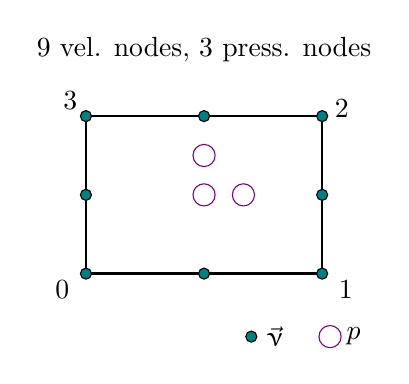
\begin{tikzpicture}
%\draw[fill=gray!23,gray!23](0,0) rectangle (5,5);
%\draw[step=0.5cm,gray,very thin] (0,0) grid (5,5); %background grid
\draw[thick] (1,1) -- (4,1) -- (4,3) -- (1,3) -- cycle;  
\node[] at (0.7,0.8) {0};
\node[] at (4.3,0.8) {1};
\node[] at (4.25,3.1) {2};
\node[] at (0.8,3.2) {3};
\draw[black,fill=teal] (1,1)     circle (2pt); 
\draw[black,fill=teal] (4,1)   circle (2pt); 
\draw[black,fill=teal] (4,3)   circle (2pt); 
\draw[black,fill=teal] (1,3) circle (2pt); 
\draw[black,fill=teal] (2.5,1) circle (2pt) ; 
\draw[black,fill=teal] (2.5,3) circle (2pt) ; 
\draw[black,fill=teal] (1,2) circle (2pt) ; 
\draw[black,fill=teal] (4,2) circle (2pt) ; 

\draw[violet] (2.5,2) circle (4pt);
\draw[violet] (3,2) circle (4pt);
\draw[violet] (2.5,2.5) circle (4pt);

\draw[black,fill=teal] (3.1,0.2) circle (2pt); 
\node[] at (3.4,0.2) {$\vec\upnu$};
\draw[violet] (4.1,0.2) circle (4pt); 
\node[] at (4.4,0.2) {$p$};
\node[] at (2.5,3.85) {9 vel. nodes, 3 press. nodes};
\end{tikzpicture}
%\end{center}

\end{center}

This element is crowned ``probably the most accurate 2D element'' in \textcite{grsa}.

It is characterised by piecewise bi/triquadratic velocities, 
and piecewise linear discontinuous polynomial pressure. 
The element satisfies the inf-sup condition, see p.~211 of \textcite{hugh}, or 
p.~138 of \textcite{elsw}.
It is used for example in \textcite{vavs89} (1989) for steady laminar flow in a curved tube
but also and more importantly it is the element pair used in \textcite{mabl15} (2015)
and it is available in \aspect too. 


When using this element one must be aware of the fact that there are 
two possible choices for the definitions of the pressure space 
(the so-called ``mapped'' and ``unmapped'' variants):

\textcite{bobf08} (2008) state: 
\begin{displayquote}
{\color{darkgray}
On a general quadrilateral mesh, the [pressure] space 
can be defined in two different ways: either [it] 
consists of (discontinuous) piecewise linear functions, or it is built
by considering three linear shape functions on the reference unit square and mapping
them to the general elements like it is usually done for continuous 
finite elements. [...] We shall refer to the first possibility as 
unmapped pressure approach and to the second one as mapped pressure approach.

[...] 

So far, we have shown that either the 
unmapped and the mapped pressure 
approach gives rise to a stable ${\bm Q}_2\times P_{-1}$ scheme. 
However, as a consequence of the
results proved in \textcite{arbf02} (2002), we have that the mapped 
pressure approach cannot achieve 
optimal approximation order. Namely, the unmapped pressure space 
provides a second-order convergence 
in $L_2$, while the mapped one achieves only ${\cal O}(h)$ in the same norm.}
\end{displayquote}

We also read in \textcite{boga02} (2002):
\begin{displayquote}
{\color{darkgray}
Two possible choices are given for the definition of the pressure space: 
one can either use a global pressure approximation (that is on
each quadrilateral the finite element space is spanned by 1 and by the 
global co-ordinates $x$ and $y$) or a local approach (consisting in generating 
the local space by means of the constants and the local curvilinear 
co-ordinates on each quadrilateral $r$ and $s$). [...] Numerical results 
actually show that the second choice (local or mapped pressure approximation) 
is suboptimally convergent.
}
\end{displayquote}

See also discussion about mapped/unmapped in \textcite{bobf13} and 
in Section 3.6.4 of \textcite{john16}.

This element is mentioned in \textcite{kaus10} (2010) and \textcite{pefc89} (1989) 
and it is used in \textcite{freh14} (2014) to study 3D fold growth rates 
(see online supplementary material) and in \textcite{schm08} (2008).

Note that the serendipity version of this pair, 
i.e. ${\bm Q}_2^{(20)}\times P_{-1}$ is also LBB stable
as shown in page 180 of Reddy's book \cite{reddybook2}.

{\color{red} since I wrote this I have purchased many relevant FE books
and I need to go through all and extract relevant facts and remarks about 
this element pair.}


%------------------------------------------------------------------------------
\subsection*{Deriving the mapped vs unmapped pressure basis functions}


The mapped version consists of  
using the $P_{-1}$ basis functions defined in Section~\ref{MMM-ss:lbfq2D}:
inside the reference cell the pressure is given by $p^h(r,s)=a+br+cs$.
The reference cell is the $[-1:1]^2$ square in the 2d Cartesian axis
system $r,s$.
Nodes are placed as follows: node 0 at (0,0), node 1 at (1/2,0) and node 2 at (0,1/2).

\begin{verbatim}
3--6--2   +-----+
|     |   |  2  |
7  8  5   +  01 |
|     |   |     |
0--4--1   +--+--+
V nodes   P nodes
\end{verbatim}

This yields the following basis functions
\begin{align}
\bN_0^p &= 1-2r-2s \nn\\
\bN_1^p &= 2r \nn\\
\bN_2^p &= 2s \nn
\end{align}
with 
\[
p^h(r,s) = \sum_{k=0}^2 \bN_k^p(r,s) \ p_k
\]
Obviously we recover $\sum\limits_{k=0}^2 \bN_k^p = 1$ and $\bN_k^p(r_i,s_i)=\delta_{ik}$.

W.B. adds:
\begin{displayquote}
{\color{darkgray}
[...] where to define the node functionals for the $P_{-1}$ space: It doesn't
matter. [...] In the end, you can
choose the three points however you like, they just can't all lie on a line
(in which case they would no longer uniquely describe the shape functions).

You place nodes on the reference cell, along midpoints of edges for
example. You then map these locations forward using whatever mapping you use. 
}
\end{displayquote}

The unmapped approach is a bit less straightforward and the procedure is as follows:
let us assume there are three distinct pressure nodes inside the cell (the 'real'
cell, not the reference cell).
Inside this cell the pressure is defined by a linear field
\[
p^h(x,y) = a+bx+cy
\]
We must then compute the coefficients $a,b,c$. We know that 
the expression above evaluated at the pressure nodes i=0,1,2 with 
coordinates $(x_i,y_i)$ should be equal to $p_i$. 
Then we have the following three equations:
\begin{eqnarray}
a + bx_0 + cy_0 &=& p_0 \nn\\
a + bx_1 + cy_1 &=& p_1 \nn\\
a + bx_2 + cy_2 &=& p_2 \nn
\end{eqnarray}
or, 
\[
\underbrace{
\left(
\begin{array}{ccc}
1 & x_0 & y_0 \\
1 & x_1 & y_1 \\
1 & x_2 & y_2 
\end{array}
\right)
}_{{\bm M}}
\cdot 
\left(
\begin{array}{ccc}
a \\ b \\ c
\end{array}
\right)
=
\underbrace{
\left(
\begin{array}{ccc}
p_0 \\ p_1 \\ p_2
\end{array}
\right)
}_{\vec{p}}
\]
Then 
\[
\left(
\begin{array}{ccc}
a \\ b \\ c
\end{array}
\right)
=
\left(
\begin{array}{ccc}
1 & x_0 & y_0 \\
1 & x_1 & y_1 \\
1 & x_2 & y_2 
\end{array}
\right)^{-1}
\cdot
\left(
\begin{array}{ccc}
p_0 \\ p_1 \\ p_2
\end{array}
\right)
= {\bm M}^{-1} \cdot \vec{p}
\]
with 
\[
{\bm M}^{-1} 
= {\bm N} 
= \frac{1}{\Delta}
\left(
\begin{array}{ccc}
x_1y_2-x_2y_1 & x_2y_0-x_0y_2 & x_0y_1-x_1y_0 \\
y_1-y_2 & y_2-y_0 & y_0-y_1 \\
x_2-x_1 & x_0-x_2 & x_1-x_0
\end{array}
\right)
%=
%\left(
%\begin{array}{ccc}
%n_{11} & n_{12} & n_{13} \\
%n_{21} & n_{22} & n_{23} \\
%n_{31} & n_{32} & n_{33} 
%\end{array}
%\right)
\]
and
\[
\Delta = x_1y_2-x_2y_1 - x_0y_2-x_2y_0 + x_0y_1-x_1y_0
\]
so that
\begin{eqnarray}
a &=& N_{11}p_0 + N_{12} p_1 + N_{13} p_2 \nn\\
b &=& N_{21}p_0 + N_{22} p_1 + N_{23} p_2 \nn\\
c &=& N_{31}p_0 + N_{32} p_1 + N_{33} p_2 \nn
\end{eqnarray}
In the end 
\begin{eqnarray}
p^h(x,y) 
&=&  a+bx+cy \nn\\
&=& N_{11}p_0 + N_{12} p_1 + N_{13} p_2
+ ( N_{21}p_0 + N_{22} p_1 + N_{23} p_2) x
+ ( N_{31}p_0 + N_{32} p_1 + N_{33} p_2) y \nn\\
&=& \underbrace{(N_{11} + N_{21}x + N_{31}y)}_{\bN_0^p(x,y)} p_0 
+   \underbrace{(N_{12} + N_{22}x + N_{32}y)}_{\bN_1^p(x,y)} p_1 
+   \underbrace{(N_{13} + N_{23}x + N_{33}y)}_{\bN_1^p(x,y)} p_2
%\label{f76_NNNP}
\end{eqnarray}
The basis functions are then evaluated at the (real) coordinates 
of the quadrature point $(x_q,y_q)$.

%{\color{red} Q1: is this the right/standard way of deriving these 
%basis functions? I suspect not. How is this carried out in deal.II?}

Actually it was pointed out by W.B. that 
{\color{darkgray} the unmapped basis $\{1,x,y\}$ is not good. That's because if you have a
small cell that is far away from the origin, the function $x$ varies very
little and so the function '$x$' is nearly constant on the cell -- so it is
almost collinear with the function '1'. You will see this in the fact
that the matrix ${\bm M}$ is nearly singular for such cells. 

A better choice is to use  $\{1, (x-x_c)/h, (y-y_c)/h \}$
where $h$ is some kind of cell diameter and $x_c,y_c$ are the cell center, 
or one of the vertices, or some such. The space is obviously the same.}

In light of this pertinent remark\footnote{duh...}, let us then start again from 
\[
p^h(x,y) = a+b\frac{x-x_c}{h}+c \frac{y-y_c}{h}
\]
leading to write:
\begin{eqnarray}
a + b \frac{x_0-x_c}{h} + c\frac{y_0-y_c}{h} &=& p_0 \nn\\
a + b \frac{x_1-x_c}{h} + c\frac{y_1-y_c}{h} &=& p_1 \nn\\
a + b \frac{x_2-x_c}{h} + c\frac{y_2-y_c}{h} &=& p_2 \nn
\end{eqnarray}
We then define $\tilde{x}_i=(x_i-x_c)/h$ and $\tilde{y}_i=(y_i-x_c)/h$ so that 
the equation above simply becomes
\begin{eqnarray}
a + b\tilde{x}_0 + c\tilde{y}_0 &=& p_0 \nn\\
a + b\tilde{x}_1 + c\tilde{y}_1 &=& p_1 \nn\\
a + b\tilde{x}_2 + c\tilde{y}_2 &=& p_2 \nn
\end{eqnarray}
or
\[
\underbrace{
\left(\begin{array}{ccc}
1 & \tilde{x}_0 & \tilde{y}_0 \\
1 & \tilde{x}_1 & \tilde{y}_1 \\
1 & \tilde{x}_2 & \tilde{y}_2 
\end{array}\right)
}_{{\bm M}}
\cdot 
\left(\begin{array}{ccc}
a \\ b \\ c
\end{array}\right)
=
\underbrace{
\left(\begin{array}{ccc}
p_0 \\ p_1 \\ p_2
\end{array}\right)
}_{\vec{p}}
\qquad
\Rightarrow
\qquad
\left(\begin{array}{ccc}
a \\ b \\ c
\end{array}\right)
=
{\bm M}^{-1} \cdot \vec{p}
\]
with
\[
{\bm M}^{-1} 
= {\bm N} 
= \frac{1}{\Delta}
\left(
\begin{array}{ccc}
\tilde{x}_1y_2-\tilde{x}_2\tilde{y}_1 
& \tilde{x}_2\tilde{y}_0-\tilde{x}_0\tilde{y}_2 
& \tilde{x}_0\tilde{y}_1-\tilde{x}_1\tilde{y}_0 \\
\tilde{y}_1-\tilde{y}_2 & \tilde{y}_2-\tilde{y}_0 & \tilde{y}_0-\tilde{y}_1 \\
\tilde{x}_2-\tilde{x}_1 & \tilde{x}_0-\tilde{x}_2 & \tilde{x}_1-\tilde{x}_0
\end{array}
\right)
\]
and
\[
\Delta 
= \tilde{x}_1\tilde{y}_2-\tilde{x}_2\tilde{y}_1 
- \tilde{x}_0\tilde{y}_2-\tilde{x}_2\tilde{y}_0 
+ \tilde{x}_0\tilde{y}_1-\tilde{x}_1\tilde{y}_0
\]
so that
\begin{eqnarray}
a &=& N_{11}p_0 + N_{12} p_1 + N_{13} p_2 \nn\\
b &=& N_{21}p_0 + N_{22} p_1 + N_{23} p_2 \nn\\
c &=& N_{31}p_0 + N_{32} p_1 + N_{33} p_2 \nn
\end{eqnarray}
In the end
\begin{eqnarray}
p^h(x,y) %\nn\\
&=& a+b\frac{x-x_c}{h}+c \frac{y-y_c}{h} \nn\\
&=& (N_{11}p_0 + N_{12} p_1 + N_{13} p_2)
+ ( N_{21}p_0 + N_{22} p_1 + N_{23} p_2) \frac{x-x_c}{h}
+ ( N_{31}p_0 + N_{32} p_1 + N_{33} p_2) \frac{y-y_c}{h} \nn\\
&=&\underbrace{\left(N_{11} + N_{21} \frac{x-x_c}{h} + N_{31}\frac{y-y_c}{h}\right)}_{\bN_0^p(x,y)} p_0 \nn\\
&+&  \underbrace{\left(N_{12} + N_{22} \frac{x-x_c}{h} + N_{32}\frac{y-y_c}{h}\right)}_{\bN_1^p(x,y)} p_1 \nn\\
&+&  \underbrace{\left(N_{13} + N_{23} \frac{x-x_c}{h} + N_{33}\frac{y-y_c}{h}\right)}_{\bN_1^p(x,y)} p_2
\label{f76_NNNP}
\end{eqnarray}

The pressure basis functions are then 
\begin{align}
\bN_0^p(x,y) &= N_{11} + N_{21}\frac{x-x_c}{h}  + N_{31}\frac{y-y_c}{h} \nn\\
\bN_1^p(x,y) &= N_{12} + N_{22}\frac{x-x_c}{h}  + N_{32}\frac{y-y_c}{h} \nn\\
\bN_2^p(x,y) &= N_{13} + N_{23}\frac{x-x_c}{h}  + N_{33}\frac{y-y_c}{h} \nn
\end{align}

In practice we will set 
\[
x_c=\frac14(x_0+x_1+x_2+x_3)
\qquad
y_c=\frac14(y_0+y_1+y_2+y_3)
\]
The function which computes the $N_{ij}$ coefficients is as follows:
\begin{lstlisting}
def compute_Ncoeffs(x0,x1,x2,y0,y1,y2,xxc,yyc,hh):
    xx0=(x0-xxc)/hh ; yy0=(y0-yyc)/hh
    xx1=(x1-xxc)/hh ; yy1=(y1-yyc)/hh
    xx2=(x2-xxc)/hh ; yy2=(y2-yyc)/hh
    det=xx1*yy2-xx2*yy1 -xx0*yy2-xx2*yy0 +xx0*yy1-xx1*yy0
    N11=(xx1*yy2-xx2*yy1)/det ; N12=(xx2*yy0-xx0*yy2)/det ; N13=(xx0*yy1-xx1*yy0)/det
    N21=(yy1-yy2        )/det ; N22=(yy2-yy0        )/det ; N23=(yy0-yy1        )/det
    N31=(xx2-xx1        )/det ; N32=(xx0-xx2        )/det ; N33=(xx1-xx0        )/det
    return N11,N12,N13,N21,N22,N23,N31,N32,N33 
\end{lstlisting}



%------------------------------------------------------------------------------
\subsection*{About the code}


The 2d $Q_2$ shape functions have been derived in Section~\ref{MMM-ss:q22d}
and the internal numbering of velocity nodes is as follows:
\begin{verbatim}
3--6--2
|     |
7  8  5
|     |
0--4--1
\end{verbatim}

For all the tests/benchmarks the domain is a unit square.
Velocity nodes coordinates are stored in the \lstinline{xV,yV} arrays
with the \lstinline{iconV} connectivity array.
Pressure nodes coordinates are stored in the \lstinline{xP,yP} arrays
with the \lstinline{iconP} connectivity array.
The mesh counts \lstinline{nel=nelx*nely} cells,
\lstinline{NV=(2*nelx+1)*(2*nely+1)} velocity nodes and 
\lstinline{NP=3*nel} pressure nodes.
The \lstinline{meth} parameter is 1 for mapped approach and 2 
for unmapped approach. 

Six types of meshes have been implemented so far: 
\begin{itemize}
\item \lstinline{mesh_type=1}:
The first type is straightforward: all cells are rectangular (and in 
practice square for simplicity).
\item \lstinline{mesh_type=2}:
The second type sees a random perturbation added to interior nodes.
The parameter \lstinline{xi} controls the randomness of the mesh as follows:
for each node inside the domain (i.e. not on the boundaries) a random value 
in the range $[-\xi,\xi]$ ($\xi$ is set to 0.1 by default) 
is added to the $x$ and $y$ coordonates:
\begin{lstlisting}
for i in range(0,NV):
    if xV[i]>0 and xV[i]<Lx and yV[i]>0 and yV[i]<Ly:
       xV[i]+=random.uniform(-1.,+1)*hx*xi
       yV[i]+=random.uniform(-1.,+1)*hy*xi
\end{lstlisting}
\item \lstinline{mesh_type=3}:
it is borrowed from \stone~25 which models the 
Rayleigh-Taylor experiment of \textcite{vaks97} (1997). Only the vertical position 
of the nodes is modified: nodes at about 1/5 the height of the domain are set to 
follow a sinusoidal perturbation and the position of other nodes above or below
is then adjusted as shown in the figure below. 

\item \lstinline{mesh_type=4}: after the regular square mesh 
is created the position of all nodes is moved with the following 
equations:
\begin{lstlisting}
for i in range(0,NV):
    yV[i]=(yV[i])**(0.75+xV[i]/4.)
    xV[i]=(xV[i])**(0.75+yV[i]/4.)
\end{lstlisting}
This results in a mesh with cells of various sizes, no right angle and no parallel edges
as shown hereafter.

\item \lstinline{mesh_type=5}: after the regular square mesh 
is created the position of all interior nodes is moved with the following
\begin{lstlisting}
for i in range(0,NV):
    if xV[i]>0 and xV[i]<1: 
       xV[i]+=np.sin(4*np.pi*yV[i])*hx/5
    if yV[i]>0 and yV[i]<1: 
       yV[i]+=np.sin(5*np.pi*xV[i])*hy/5
\end{lstlisting}
Again, this results in a mesh with cells of various sizes, no right angle and no parallel edges.
Note that the amplitude of the perturbation(s) is proportional to $h_x,h_y$ but not its wavelength.

\item \lstinline{mesh_type=6}: This mesh is composed of three
regular meshes that are glued together (ABED, BCGE, DEGF):
\begin{verbatim}
F--------G
|      / |
|    /   |
D--E     |
|   \    |
|    \   |
A-----B--C
\end{verbatim}
The idea behind this mesh to have a mesh with a different topology than the others, 
in this case E is a node that belongs to 3 cells instead of 4.
In the {\pythonfile tools.py} there are two functions:
\begin{itemize}
\item \verb'merge_two_blocks': it takes as arguments two meshes and returns a single mesh in which 
the overlapping nodes of both have been merged and the global numbering and connectivity array computed.
\item \verb'export_to_vtu': it takes a mesh and exports it to vtu format.
\end{itemize}
when \lstinline{nelx} is set by the bash script, all three blocks are then assigned a 
resolution \lstinline{nelx/2} $\times$ \lstinline{nelx/2} so that the resolution/cell size
on the left and bottom boundaries is the $h_x$ and $h_y$ values of the square mesh. 
The resulting mesh is shown hereunder. 
\end{itemize}

The six types of meshes are shown here:

\begin{center}
{\small 1})\includegraphics[width=5.5cm]{python_codes/fieldstone_76/results/mt1}
{\small 2})\includegraphics[width=5.5cm]{python_codes/fieldstone_76/results/mt2}
{\small 3})\includegraphics[width=5.5cm]{python_codes/fieldstone_76/results/mt3}\\
{\small 4})\includegraphics[width=5.5cm]{python_codes/fieldstone_76/results/mt4}
{\small 5})\includegraphics[width=5.5cm]{python_codes/fieldstone_76/results/mt5}
{\small 6})\includegraphics[width=5.5cm]{python_codes/fieldstone_76/results/mt6}\\
{\captionfont From left to right, top to bottom: mesh types 1, 2, 3, 4, 5 and 6, 
or 'square', 'randomized', 'wave', 'stretched', 'sin-sin' and 'glued' meshes.}
\end{center}

Looking at the meshes above we find that the cells of the 'wave' mesh 
can be obtained by affine transformation\footnote{\url{https://en.wikipedia.org/wiki/Affine_transformation}} 
of the reference cell (if straight edges are used -- see next paragraph) 
but not the cells of the 'randomized', 'stretched' and 'sin-sin' mesh. 
Quickly: an affine transformation 
is a geometric transformation that preserves lines and parallelism, but not necessarily 
Euclidean distances and angles. 
I remember coming across this terminology in the relevant literature (which I need to find again!)
and this may explain the results obtained for the manufactured solutions I ran the code on 
in what follows on both these types of meshes.

If the parameter \lstinline{straight_edges} is set to \lstinline{True}
the following algorithm makes sure that the velocity nodes 4,5,6,7 in the middle of the edges 
are really put back between nodes 0-1, 1-2, 2-3, and 3-0 respectively. 
\begin{lstlisting}
for iel in range(0,nel):
    xV[iconV[4,iel]]=0.5*(xV[iconV[0,iel]]+xV[iconV[1,iel]])
    yV[iconV[4,iel]]=0.5*(yV[iconV[0,iel]]+yV[iconV[1,iel]])
    xV[iconV[5,iel]]=0.5*(xV[iconV[1,iel]]+xV[iconV[2,iel]])
    yV[iconV[5,iel]]=0.5*(yV[iconV[1,iel]]+yV[iconV[2,iel]])
    xV[iconV[6,iel]]=0.5*(xV[iconV[2,iel]]+xV[iconV[3,iel]])
    yV[iconV[6,iel]]=0.5*(yV[iconV[2,iel]]+yV[iconV[3,iel]])
    xV[iconV[7,iel]]=0.5*(xV[iconV[3,iel]]+xV[iconV[0,iel]])
    yV[iconV[7,iel]]=0.5*(yV[iconV[3,iel]]+yV[iconV[0,iel]])
\end{lstlisting}
The placement of the middle node 8 is discussed in what follows.


The mapping is isoparametric (i.e. $Q_2$). The same mapping is used for changes 
of variables and for all integrals, Jacobians, etc ...
In the case of rectangular cells both the mapped and unmapped approaches 
yield the same pressure basis functions values at the quadrature points
so the measured errors are identical.
I suspected this is true for all cells obtained by affine transformation
from reference cell, to which my asking about this, W.B. added:
\begin{displayquote}
{\color{darkgray}
``Affine'' in essence means ``almost linear''. A linear transformation $f(x)$
satisfies $f(x+y) = f(x)+f(y)$ and  $f(\alpha x) = \alpha f(x)$
which in particular implies that $f(0)=0$. 
In finite-dimensional vector spaces, every linear transformation can be written as
$ f(x) = Ax $ with a matrix $A$. 

Affine transformations are of the form $f(x) = Ax + b$
which you need in the finite element context of affine transformations because
you don't just want to stretch or rotate cells, but you also want to translate
them from the reference coordinate system to wherever the cell is located in
real space.

If you have only rectangular cells (in fact, if they are parallelograms, of
which rectangles are a special case), then indeed the mapping is affine. The
shape functions in the mapped and unmapped case are different, but they span
the same space. (The shape functions are linear in both cases, but they are
scaled differently.) As a consequence, the solution is indeed the same. Like
you suggest in your question, this is going to be true for any affine
(=parallelogram) cell. It is because when you map linear basis functions with
an affine mapping, you end up with linear basis functions; the unmapped case
starts with linear shape functions in real space. 
}
\end{displayquote}

The same quadrature rule is used for $\K$ and $\G$ blocks (called $A$ and $B$ blocks 
respectively in the ASPECT literature).
I have explored the effect of the number of quadrature points on the solution, 
by testing for $2^2$, $3^2$ and $4^2$ quadrature points
as parameterized by the \lstinline{nqperdim} parameter.
I unsurprisingly found that a $2^2$ is not sufficient to exactly integrate the 
terms found in the $\K$ and $\G$ blocks, $3^2$ is standard, 
and $4^2$ is wasteful and did not yield any change in the results compared to $3^2$.

One critical aspect of the implementation is the location of the pressure nodes
in the real cell. The code takes the following approach:
\begin{enumerate}
\item For each cell compute the coordinates of the velocity nodes 0-7,
\item Apply modifications to the mesh (stretching, randomization, ...),
\item Set location of (middle) velocity node 8 (see next section),
\item Use $Q_2$ mapping to compute $x,y$ coordinates of pressure nodes.
\end{enumerate}


In both cases (mapped and unmapped) the pressure is discontinuous from cell to cell 
and this adds complexity in terms of exporting it to vtu format (and plotting with paraview). 
I then simply choose to export the value of the pressure in the middle of 
each cell\footnote{I should improve this in the future, but it is 
only a visualisation problem and does not influence results.
I know how to fix it, but this has low priority.}

%............................................................................
\subsubsection{About the position of the middle node}

We can think of multiple ways to come up with the `center' of the cell, 
i.e. the location of node 8.

\begin{verbatim}
3--6--2 
|     | 
7  8  5 
|     | 
0--4--1 
V nodes 
\end{verbatim}

In the code these different approaches are parameterized by means of the
\lstinline{center} variable:

\begin{itemize}
\item \lstinline{center=0}: The middle node coordinates are simply the 
average of the corner coordinates 
\begin{align}
x_8&=(x_0+x_1+x_2+x_3)/4 \nn\\
y_8&=(y_0+y_1+y_2+y_3)/4 \nn
\end{align}

\item \lstinline{center=1}: The middle coordinates are the average all the 
4 corners and 4 mid-edge nodes coordinates:

\begin{align}
x_8&=(x_0+x_1+x_2+x_3+x_4+x_5+x_6+x_7)/8 \nn\\
y_8&=(y_0+y_1+y_2+y_3+y_4+y_5+y_6+y_7)/8 \nn
\end{align}

\item \lstinline{center=2}: The middle coordinates are obtained via a 
weighed sum of the corner coordinates and the mid-edge nodes 
coordinates\footnote{I have no idea where this comes from but left it in nevertheless.}: 

\begin{align}
x_8&=(x_0+x_1+x_2+x_3+3x_4+3x_5+3x_6+3x_7)/16. \nn\\
y_8&=(y_0+y_1+y_2+y_3+3y_4+3y_5+3y_6+3y_7)/16. \nn
\end{align}

\item \lstinline{center=3}: This approach is a bit more complex than the previous ones.
We start by acknowledging that we know the coordinates of nodes 0-7 in the reference space $(r,s)$ 
and in the real space $(x,y)$ so one could then use a $Q_2^{(8)}$ mapping (i.e. 'serendipity' $Q_2$)
to place node 8.

In this case the basis functions for this mapping are defined in Section~\ref{MMM-sec:serendipity2D}:
\begin{eqnarray}
\bN_0(r,s)&=& \frac{1}{4}(1-r)(1-s)(-r-s-1) \nn\\
\bN_1(r,s)&=& \frac{1}{4}(1+r)(1-s)(r-s-1) \nn\\
\bN_2(r,s)&=& \frac{1}{4}(1+r)(1+s)(r+s-1) \nn\\
\bN_3(r,s)&=& \frac{1}{4}(1-r)(1+s)(-r+s-1) \nn\\
\bN_4(r,s)&=& \frac{1}{2}(1-r^2)(1-s)  \nn\\
\bN_5(r,s)&=& \frac{1}{2}(1+r)  (1-s^2)\nn\\
\bN_6(r,s)&=& \frac{1}{2}(1-r^2)(1+s)  \nn\\
\bN_7(r,s)&=& \frac{1}{2}(1-r)  (1-s^2) \nn
\end{eqnarray}

We would then compute the location of node 8 as follows (its $r,s$ coordinates are $0,0$): 
\begin{eqnarray}
x_8
&=& \sum_{i=0}^7 \bN_i (r_8,s_8) x_i \nn\\
&=& \sum_{i=1}^7 \bN_i (0,0) x_i \nn\\
&=& -\frac14 (x_0+x_1+x_2+x_3) + \frac12 (x_4+x_5+x_6+x_7) \nn\\
y_8 
&=& \sum_{i=0}^7 \bN_i (r_8,s_8) y_i \nn\\
&=& \sum_{i=0}^7 \bN_i (0,0) y_i \nn\\
&=& -\frac14 (y_0+y_1+y_2+y_3) + \frac12 (y_4+y_5+y_6+y_7) \nn
\end{eqnarray}

\end{itemize}

In the case of parallelogram cells these four approaches lead to the same 
middle location. This is no more the case for elements with curved edges
for example and therefore warrants a thorough study.

%--------------------------------------------------------------------------------------
\subsection*{The manufactured solutions}

Note that for all four manufactured solutions used in the present code 
a) the pressure obeys $\int_{\Omega} p \; dV = 0$;
b) the analytical velocity is prescribed on the boundary of the domain; 
c) the viscosity is 1 (except SolKz); d) the domain is the unit square. 

\begin{itemize}
\item {\tt bench=3}: 
This is the Donea \& Huerta benchmark that is fully described in Section~\ref{MMM-mms1}.
The velocity and pressure are given by
\begin{eqnarray}
u(x,y) &=& x^2(1-x)^2 2y (y-1)(2y-1) \\ 
v(x,y) &=& -y^2 (1 - y)^2 2x (x-1)(2x-1) \\ 
p(x,y) &=& x(1 -x)- 1/6 
\end{eqnarray}

\item {\tt bench=1}:  
The analytical solution originates in Lamichhane (2017) \cite{lami17}.
The velocity and pressure are given by
\begin{eqnarray}
u(x,y)&=&-2x^2y(2y-1)(x-1)^2(y-1) \\
v(x,y)&=& 2xy^2(2x-1)(x-1)(y-1)^2 \\
p(x,y)&=& x(1-x)(1-2y)
\end{eqnarray}
The corresponding body force terms are derived in Section~\ref{MMM-ss:mms11}. 

\item {\tt bench=9}: 
This is the second manufactured solution 
mentioned in Lamichhane \cite{lami17}. 
The velocity and pressure are given by
\begin{eqnarray}
u(x,y) &=& x+x^2 - 2xy+x^3 - 3xy^2 + x^2y \\
v(x,y) &=& -y-2xy+y^2 -3x^2y + y^3 - xy^2 \\
p(x,y) &=& xy+x+y+x^3y^2 - 4/3
\end{eqnarray}
The corresponding body force terms are derived in Section~\ref{MMM-ss:mms2}. 

\item {\tt bench=4}. This is the SolKz benchmark described in Section~\ref{MMM-ss:solkz}.
The main difference with respect to the previous three ones is the fact that the viscosity
varies by 6 orders of magnitude (albeit is a smooth manner).


\end{itemize}

The numbering {\tt bench=3,1,9,4} is completely arbitrary and inherited from another \stone.

In what follows velocity and pressure error convergence is measured as a function of
mesh side. Since for some meshes there is not a single obvious mesh size, 
I then use the square root of the maximum value of the elemental area array:
\[
h \simeq \sqrt{\max_e A_e }
\]


\newpage
%--------------------------------------------------------------------------------------
\subsection*{Manufactured solution of Donea \& Huerta ({\tt bench=3}) - straight edges}

\begin{center}
\includegraphics[width=6.5cm]{python_codes/fieldstone_76/results/bench3/straight/errors_V_mt1.pdf}
\includegraphics[width=6.5cm]{python_codes/fieldstone_76/results/bench3/straight/errors_P_mt1.pdf}\\
\includegraphics[width=6.5cm]{python_codes/fieldstone_76/results/bench3/straight/errors_V_mt2.pdf}
\includegraphics[width=6.5cm]{python_codes/fieldstone_76/results/bench3/straight/errors_P_mt2.pdf}\\
\includegraphics[width=6.5cm]{python_codes/fieldstone_76/results/bench3/straight/errors_V_mt3.pdf}
\includegraphics[width=6.5cm]{python_codes/fieldstone_76/results/bench3/straight/errors_P_mt3.pdf}\\
\includegraphics[width=6.5cm]{python_codes/fieldstone_76/results/bench3/straight/errors_V_mt4.pdf}
\includegraphics[width=6.5cm]{python_codes/fieldstone_76/results/bench3/straight/errors_P_mt4.pdf}\\
\includegraphics[width=6.5cm]{python_codes/fieldstone_76/results/bench3/straight/errors_V_mt5.pdf}
\includegraphics[width=6.5cm]{python_codes/fieldstone_76/results/bench3/straight/errors_P_mt5.pdf}\\
\includegraphics[width=6.5cm]{python_codes/fieldstone_76/results/bench3/straight/errors_V_mt6.pdf}
\includegraphics[width=6.5cm]{python_codes/fieldstone_76/results/bench3/straight/errors_P_mt6.pdf}\\
{\captionfont From top to bottom: square mesh, Randomized ($\xi=0.1$) mesh,
wave mesh, stretched mesh, sin-sin mesh and glued mesh.}
\end{center}

\newpage
%------------------------------------------------------------------------------------
\subsection*{Manufactured solution of Donea \& Huerta ({\tt bench=3}) - curved edges}

\begin{center}
\includegraphics[width=8cm]{python_codes/fieldstone_76/results/bench3/curved/errors_V_mt2.pdf}
\includegraphics[width=8cm]{python_codes/fieldstone_76/results/bench3/curved/errors_P_mt2.pdf}\\
\includegraphics[width=8cm]{python_codes/fieldstone_76/results/bench3/curved/errors_V_mt3.pdf}
\includegraphics[width=8cm]{python_codes/fieldstone_76/results/bench3/curved/errors_P_mt3.pdf}\\
\includegraphics[width=8cm]{python_codes/fieldstone_76/results/bench3/curved/errors_V_mt4.pdf}
\includegraphics[width=8cm]{python_codes/fieldstone_76/results/bench3/curved/errors_P_mt4.pdf}\\
\includegraphics[width=8cm]{python_codes/fieldstone_76/results/bench3/curved/errors_V_mt5.pdf}
\includegraphics[width=8cm]{python_codes/fieldstone_76/results/bench3/curved/errors_P_mt5.pdf}\\
{\captionfont From top to bottom: 'randomized' ($\xi=0.1$) mesh,
'wave' mesh, 'stretched' mesh and 'sin-sin' mesh.}
\end{center}

\newpage
%-----------------------------------------------------------------------
\subsection*{Manufactured solution \#1 ({\tt bench=1}) - straight edges}

\begin{center}
\includegraphics[width=6.5cm]{python_codes/fieldstone_76/results/bench1/straight/errors_V_mt1.pdf}
\includegraphics[width=6.5cm]{python_codes/fieldstone_76/results/bench1/straight/errors_P_mt1.pdf}\\
\includegraphics[width=6.5cm]{python_codes/fieldstone_76/results/bench1/straight/errors_V_mt2.pdf}
\includegraphics[width=6.5cm]{python_codes/fieldstone_76/results/bench1/straight/errors_P_mt2.pdf}\\
\includegraphics[width=6.5cm]{python_codes/fieldstone_76/results/bench1/straight/errors_V_mt3.pdf}
\includegraphics[width=6.5cm]{python_codes/fieldstone_76/results/bench1/straight/errors_P_mt3.pdf}\\
\includegraphics[width=6.5cm]{python_codes/fieldstone_76/results/bench1/straight/errors_V_mt4.pdf}
\includegraphics[width=6.5cm]{python_codes/fieldstone_76/results/bench1/straight/errors_P_mt4.pdf}\\
\includegraphics[width=6.5cm]{python_codes/fieldstone_76/results/bench1/straight/errors_V_mt5.pdf}
\includegraphics[width=6.5cm]{python_codes/fieldstone_76/results/bench1/straight/errors_P_mt5.pdf}\\
\includegraphics[width=6.5cm]{python_codes/fieldstone_76/results/bench1/straight/errors_V_mt6.pdf}
\includegraphics[width=6.5cm]{python_codes/fieldstone_76/results/bench1/straight/errors_P_mt6.pdf}\\
{\captionfont From top to bottom: 'square mesh', 'randomized' ($\xi=0.1$) mesh,
'wave' mesh, 'stretched' mesh, 'sin-sin' mesh and 'glued' mesh.}
\end{center}

\newpage
%.......................................................................
\subsection*{Manufactured solution \#1 ({\tt bench=1}) - curved edges}

\begin{center}
\includegraphics[width=8cm]{python_codes/fieldstone_76/results/bench1/curved/errors_V_mt2.pdf}
\includegraphics[width=8cm]{python_codes/fieldstone_76/results/bench1/curved/errors_P_mt2.pdf}\\
\includegraphics[width=8cm]{python_codes/fieldstone_76/results/bench1/curved/errors_V_mt3.pdf}
\includegraphics[width=8cm]{python_codes/fieldstone_76/results/bench1/curved/errors_P_mt3.pdf}\\
\includegraphics[width=8cm]{python_codes/fieldstone_76/results/bench1/curved/errors_V_mt4.pdf}
\includegraphics[width=8cm]{python_codes/fieldstone_76/results/bench1/curved/errors_P_mt4.pdf}\\
\includegraphics[width=8cm]{python_codes/fieldstone_76/results/bench1/curved/errors_V_mt5.pdf}
\includegraphics[width=8cm]{python_codes/fieldstone_76/results/bench1/curved/errors_P_mt5.pdf}\\
{\captionfont From top to bottom: 'randomized' ($\xi=0.1$) mesh,
'wave' mesh, 'stretched' mesh and 'sin-sin' mesh.}
\end{center}


\newpage
%.......................................................................
\subsection*{Manufactured solution \#2 ({\tt bench=9}) - straight edges}

\begin{center}
\includegraphics[width=6.5cm]{python_codes/fieldstone_76/results/bench9/straight/errors_V_mt1.pdf}
\includegraphics[width=6.5cm]{python_codes/fieldstone_76/results/bench9/straight/errors_P_mt1.pdf}\\
\includegraphics[width=6.5cm]{python_codes/fieldstone_76/results/bench9/straight/errors_V_mt2.pdf}
\includegraphics[width=6.5cm]{python_codes/fieldstone_76/results/bench9/straight/errors_P_mt2.pdf}\\
\includegraphics[width=6.5cm]{python_codes/fieldstone_76/results/bench9/straight/errors_V_mt3.pdf}
\includegraphics[width=6.5cm]{python_codes/fieldstone_76/results/bench9/straight/errors_P_mt3.pdf}\\
\includegraphics[width=6.5cm]{python_codes/fieldstone_76/results/bench9/straight/errors_V_mt4.pdf}
\includegraphics[width=6.5cm]{python_codes/fieldstone_76/results/bench9/straight/errors_P_mt4.pdf}\\
\includegraphics[width=6.5cm]{python_codes/fieldstone_76/results/bench9/straight/errors_V_mt5.pdf}
\includegraphics[width=6.5cm]{python_codes/fieldstone_76/results/bench9/straight/errors_P_mt5.pdf}\\
\includegraphics[width=6.5cm]{python_codes/fieldstone_76/results/bench9/straight/errors_V_mt6.pdf}
\includegraphics[width=6.5cm]{python_codes/fieldstone_76/results/bench9/straight/errors_P_mt6.pdf}\\
{\captionfont From top to bottom: 'square' mesh, 'randomized' ($\xi=0.1$) mesh,
'wave' mesh, 'stretched' mesh, 'sin-sin' mesh and 'glued' mesh.}
\end{center}

\newpage
%.......................................................................
\subsection*{Manufactured solution \#2 ({\tt bench=9}) - curved edges}

\begin{center}
\includegraphics[width=8cm]{python_codes/fieldstone_76/results/bench9/curved/errors_V_mt2.pdf}
\includegraphics[width=8cm]{python_codes/fieldstone_76/results/bench9/curved/errors_P_mt2.pdf}\\
\includegraphics[width=8cm]{python_codes/fieldstone_76/results/bench9/curved/errors_V_mt3.pdf}
\includegraphics[width=8cm]{python_codes/fieldstone_76/results/bench9/curved/errors_P_mt3.pdf}\\
\includegraphics[width=8cm]{python_codes/fieldstone_76/results/bench9/curved/errors_V_mt4.pdf}
\includegraphics[width=8cm]{python_codes/fieldstone_76/results/bench9/curved/errors_P_mt4.pdf}\\
\includegraphics[width=8cm]{python_codes/fieldstone_76/results/bench9/curved/errors_V_mt5.pdf}
\includegraphics[width=8cm]{python_codes/fieldstone_76/results/bench9/curved/errors_P_mt5.pdf}\\
{\captionfont From top to bottom: 'randomized' ($\xi=0.1$) mesh,
'wave' mesh, 'stretched' mesh and 'sin-sin' mesh.}
\end{center}


\newpage
%.......................................................................
\subsection*{Manufactured solution SolKz ({\tt bench=4}) - straight edges}

\begin{center}
\includegraphics[width=6.5cm]{python_codes/fieldstone_76/results/bench4/straight/errors_V_mt1.pdf}
\includegraphics[width=6.5cm]{python_codes/fieldstone_76/results/bench4/straight/errors_P_mt1.pdf}\\
\includegraphics[width=6.5cm]{python_codes/fieldstone_76/results/bench4/straight/errors_V_mt2.pdf}
\includegraphics[width=6.5cm]{python_codes/fieldstone_76/results/bench4/straight/errors_P_mt2.pdf}\\
\includegraphics[width=6.5cm]{python_codes/fieldstone_76/results/bench4/straight/errors_V_mt3.pdf}
\includegraphics[width=6.5cm]{python_codes/fieldstone_76/results/bench4/straight/errors_P_mt3.pdf}\\
\includegraphics[width=6.5cm]{python_codes/fieldstone_76/results/bench4/straight/errors_V_mt4.pdf}
\includegraphics[width=6.5cm]{python_codes/fieldstone_76/results/bench4/straight/errors_P_mt4.pdf}\\
\includegraphics[width=6.5cm]{python_codes/fieldstone_76/results/bench4/straight/errors_V_mt5.pdf}
\includegraphics[width=6.5cm]{python_codes/fieldstone_76/results/bench4/straight/errors_P_mt5.pdf}\\
\includegraphics[width=6.5cm]{python_codes/fieldstone_76/results/bench4/straight/errors_V_mt6.pdf}
\includegraphics[width=6.5cm]{python_codes/fieldstone_76/results/bench4/straight/errors_P_mt6.pdf}\\
{\captionfont From top to bottom: 'square' mesh, 'randomized' ($\xi=0.1$) mesh,
'wave' mesh, 'stretched' mesh, 'sin-sin' mesh and 'glued' mesh.}
\end{center}

\newpage
%.......................................................................
\subsection*{Manufactured solution SolKz ({\tt bench=4}) - curved edges}

\begin{center}
\includegraphics[width=8cm]{python_codes/fieldstone_76/results/bench4/curved/errors_V_mt2.pdf}
\includegraphics[width=8cm]{python_codes/fieldstone_76/results/bench4/curved/errors_P_mt2.pdf}\\
\includegraphics[width=8cm]{python_codes/fieldstone_76/results/bench4/curved/errors_V_mt3.pdf}
\includegraphics[width=8cm]{python_codes/fieldstone_76/results/bench4/curved/errors_P_mt3.pdf}\\
\includegraphics[width=8cm]{python_codes/fieldstone_76/results/bench4/curved/errors_V_mt4.pdf}
\includegraphics[width=8cm]{python_codes/fieldstone_76/results/bench4/curved/errors_P_mt4.pdf}\\
\includegraphics[width=8cm]{python_codes/fieldstone_76/results/bench4/curved/errors_V_mt5.pdf}
\includegraphics[width=8cm]{python_codes/fieldstone_76/results/bench4/curved/errors_P_mt5.pdf} \\
{\captionfont From top to bottom: 'randomized' ($\xi=0.1$) mesh,
'wave' mesh, 'stretched' mesh and 'sin-sin' mesh.}
\end{center}


%%%%%%%%%%%%%%%%%%%%%%%%%%%%%%%%%%%%%%%%%%%%%%%%%%%%%%%%%%%%%%%%%%%%%%%%%%%%%%%%%%%%%%%%%%%%%
\newpage
\subsection*{A recap of all convergence rates so far}


As mentioned for example in \textcite{thba25} (2025), 
one expects a 3rd-order convergence (in the $L_2$ norm) for the velocity
error and a 2nd-order convergence for the pressure error.
In the tables below error rates that are not the expect 3/2 are highlighted in bold.

Since all four \lstinline{center} approaches are identical for straight edges
cells I will then only report values for \lstinline{center=0}. 



\begin{center}
\includegraphics[width=2.7cm]{python_codes/fieldstone_76/results/mt1}
\includegraphics[width=2.7cm]{python_codes/fieldstone_76/results/mt2}
\includegraphics[width=2.7cm]{python_codes/fieldstone_76/results/mt3}
\includegraphics[width=2.7cm]{python_codes/fieldstone_76/results/mt4}
\includegraphics[width=2.7cm]{python_codes/fieldstone_76/results/mt5}
\includegraphics[width=2.7cm]{python_codes/fieldstone_76/results/mt6}\\
{\captionfont 'square' ,'random', 'wave', 'stretched', 'sin-sin', 'glued'.}
\end{center}

\begin{itemize}

%...................................
\item {\tt bench=3}

\begin{tabular}{c|cccccc}
\hline
straight& mt=1     &  mt=2        &  mt=3  &  mt=4       & mt=5  & mt=6\\
edges& 'square' & 'randomized' & 'wave' & 'stretched' & 'sin-sin' & 'glued'\\
\hline
mapped   & 3/2 & {\bf 2/1} &3/2 & {\bf 2.74/1.88} &3/2 \\
unmapped & 3/2 &3/2 &3/2 & {\bf 2.74/1.92} &3/2 \\
\hline
\end{tabular}

\begin{tabular}{c|cccc}
\hline
curved &  mt=2        &  mt=3  &  mt=4       & mt=5 \\
edges & 'randomized' & 'wave' & 'stretched' & 'sin-sin' \\
\hline
mapped   & \\ 
unmapped &  \\
\hline
\end{tabular}


%..........................
\item {\tt bench=1}

\begin{tabular}{c|cccccc}
\hline
straight & mt=1     &  mt=2        &  mt=3  &  mt=4       & mt=5  & mt=6\\
edges    & 'square' & 'randomized' & 'wave' & 'stretched' & 'sin-sin' & 'glued'\\
\hline
mapped   & 3/2 & {\bf 2/1} &3/2 & {\bf 2.74/1.88} &3/2 \\
unmapped & 3/2 &3/2 &3/2 & {\bf 2.74/1.92} &3/2 \\
\hline
\end{tabular}

\begin{tabular}{c|cccc}
\hline
curved&  mt=2        &  mt=3  &  mt=4       & mt=5 \\
edges& 'randomized' & 'wave' & 'stretched' & 'sin-sin' \\
\hline
mapped   & \\ 
unmapped &  \\
\hline
\end{tabular}

%...................................
\item {\tt bench=9}

\begin{tabular}{c|cccccc}
\hline
straight& mt=1     &  mt=2        &  mt=3  &  mt=4       & mt=5  & mt=6\\
edges& 'square' & 'randomized' & 'wave' & 'stretched' & 'sin-sin' & 'glued'\\
\hline
mapped   & 3/2 & {\bf 2/1} &3/2 & {\bf 2.78/1.98}  &3/2 \\
unmapped & 3/2 &3/2 &3/2 & {\bf 2.78/1.98} &3/2 \\
\hline
\end{tabular}


\begin{tabular}{c|cccc}
\hline
curved&  mt=2        &  mt=3  &  mt=4       & mt=5 \\
edges& 'randomized' & 'wave' & 'stretched' & 'sin-sin' \\
\hline
mapped   & \\ 
unmapped &  \\
\hline
\end{tabular}

%...................................
\item {\tt bench=4}

\begin{tabular}{c|cccccc}
\hline
straight& mt=1     &  mt=2        &  mt=3  &  mt=4       & mt=5  & mt=6\\
edges& 'square' & 'randomized' & 'wave' & 'stretched' & 'sin-sin' & 'glued'\\
\hline
mapped   & 3/2 & {\bf 2/1} &3/2 & {\bf 2.78/1.98}  &3/2 \\
unmapped & 3/2 &3/2 &3/2 & {\bf 2.78/1.98} &3/2 \\
\hline
\end{tabular}

\begin{tabular}{c|cccc}
\hline
curved&  mt=2        &  mt=3  &  mt=4       & mt=5 \\
edges& 'randomized' & 'wave' & 'stretched' & 'sin-sin' \\
\hline
mapped   & \\ 
unmapped &  \\
\hline
\end{tabular}

\end{itemize}

The clear conclusion from all this is that only \lstinline{center=0}
yields a pressure error which decreases monotonically with resolution 
for cells with curved edges. 

Note that for the stretched mesh the value of the parameter $h$ is not well defined (or
not as well defined as the other meshes). Since the $h$ value I use for these is overestimating
the size of the smallest cell, these could explain the slightly anomalous rates.

\newpage
%----------------------------------------
\subsection*{Instantaneous sinking block}

It is fully described in Section~\ref{MMM-ss:sinking_block}.
The block is centered in the domain, its density is 1\% larger than the 
fluid density ($\rho_f=1$) and its viscosity is 1000 times larger than 
the fluid viscosity ($\eta_f=1$).
The block is a square of dimension 1/8 so that using square meshes $16^2$, 
$32^2$, $48^2$, $64^2$, ... ensures that element edges align with the 
sides of the block.
Free-slip boundary conditions are prescribed on all sides.
This is not a benchmark {\it stricto sensu} as there is no analytical solution
available. 
Mesh type 1 is used (square elements) with resolutions $16^2, 32^2, 64^2, 96^2, 128^2, 192^2, 256^2$.

\begin{center}
\includegraphics[width=5cm]{python_codes/fieldstone_76/results/block/vel}
\includegraphics[width=5cm]{python_codes/fieldstone_76/results/block/press}\\
{\captionfont Velocity and pressure fields.}
\end{center}

The root mean square velocity and the maximum velocity in the domain are 
measured on a series of meshes 
and is shown on the following figure for both mapped and unmapped approaches: 

\begin{center}
\includegraphics[width=6cm]{python_codes/fieldstone_76/results/block/vrms.pdf}
\includegraphics[width=6cm]{python_codes/fieldstone_76/results/block/maxvel.pdf}
\end{center}

We find that the highest resolution $256^2$ is not high enough to yield a resolution-independent
measurement (although we note that the measurements above do not vary by more than 1\%). 

The velocity and pressure are measured on a vertical line passing through the 
middle of the block:

\begin{center}
\includegraphics[width=5.7cm]{python_codes/fieldstone_76/results/block/profile_m1_u.pdf}
\includegraphics[width=5.7cm]{python_codes/fieldstone_76/results/block/profile_m1_v.pdf}
\includegraphics[width=5.7cm]{python_codes/fieldstone_76/results/block/profile_m1_p.pdf}\\
\includegraphics[width=5.7cm]{python_codes/fieldstone_76/results/block/profile_m2_u.pdf}
\includegraphics[width=5.7cm]{python_codes/fieldstone_76/results/block/profile_m2_v.pdf}
\includegraphics[width=5.7cm]{python_codes/fieldstone_76/results/block/profile_m2_p.pdf}\\
{\captionfont The grey band indicates the $y$ values inside the block.}
\end{center}

Because of symmetry we expect and recover $u\simeq =0$ on this line.
The $v$-component seems to converge to a resolution independent profile
while the pressure is clearly dominated by the hydrostatic pressure.
We do not observe any difference between mapped and unmapped, as expected
since elements are square.

\newpage
%--------------------------------------------------------------
\subsection*{Instantaneous sinking block (reduced densities)}

The setup is identical to the previous one, except that now the fluid density is zero and 
the block density is 0.01. In other words the hydrostatic pressure has been removed.
We expect an identical velocity field but the recovered pressure is now the 
dynamic/excess pressure:

\begin{center}
\includegraphics[width=5.7cm]{python_codes/fieldstone_76/results/block_rd/profile_m1_u.pdf}
\includegraphics[width=5.7cm]{python_codes/fieldstone_76/results/block_rd/profile_m1_v.pdf}
\includegraphics[width=5.7cm]{python_codes/fieldstone_76/results/block_rd/profile_m1_p.pdf}\\
\includegraphics[width=5.7cm]{python_codes/fieldstone_76/results/block_rd/profile_m2_u.pdf}
\includegraphics[width=5.7cm]{python_codes/fieldstone_76/results/block_rd/profile_m2_v.pdf}
\includegraphics[width=5.7cm]{python_codes/fieldstone_76/results/block_rd/profile_m2_p.pdf}\\
{\captionfont The grey band indicates the $y$ values inside the block.}
\end{center}

We find that results obtained with ASPECT nicely agree with the results of this \stone.

\begin{center}
\includegraphics[width=8cm]{python_codes/fieldstone_76/results/block_rd/vrms.pdf}
\includegraphics[width=8cm]{python_codes/fieldstone_76/results/block_rd/maxvel.pdf}
\end{center}

\begin{center}
\includegraphics[width=5.7cm]{python_codes/fieldstone_76/results/block_rd/u}
\includegraphics[width=5.7cm]{python_codes/fieldstone_76/results/block_rd/v}
\includegraphics[width=5.7cm]{python_codes/fieldstone_76/results/block_rd/press}\\
{\captionfont Velocity and pressure fields on $96\times 96$ mesh. 
Note that the visualised pressure is elemental instead of $P_{-1}$.}
\end{center}







 %%%%%%%%%%%%%%%%%%%%%%%%%%%%%%%%%%%%%%%%%%%%%%%%%%%%%%%%%%%%%%%%%%%%%%

\chapter{Rotated $Q_1\times P_0$ element \& DSSY element \label{f77}} %%%%%%%%%%%%%%%%%%%%%%%%%%%%%%%%%%%%%%%% 77
\lstinputlisting[language=bash,basicstyle=\small]{python_codes/fieldstone_77/keywords.ascii}

\begin{center}
Code at \url{https://github.com/cedrict/fieldstone/tree/master/python_codes/fieldstone_77}
\end{center}

\par\noindent\rule{\textwidth}{0.4pt}

%%%%%%%%%%%%%%%%%%%%%%%%%%%%%%%%%%%%%%%%%%%%%%%%%%%%%%%%%%%%%%%%%%%%%%%%%%%%%%%%%%%%%%%%%%%%

I have implemented the two variants of the Rannacher-Turek element presented
in Section~\ref{ss:RTq1p0}, the mid-value (MV) and the mid-point (MP).
After communicating with Prof. Turek, I also implemented the Laplace 
formulation of the Stokes equation, i.e. we assume $\eta$ to be constant 
and therefore for an incompressible flow the momentum conservation 
equation becomes 
\[
-\vec\nabla p + \eta \Delta \vec\upnu + \rho \vec{g} = \vec{0}
\]
This yields a different form of the viscous block of the Stokes system
as explained in Section~\ref{ss:isovisc}.
I use an isoparametric mapping, but I have tried a $Q_1$ mapping and given that 
all elements are square it does not change anything. 

Following a discussion with W. Bangerth, I have also implemented the DSSY element 
(see Section~\ref{ss:dssy_2D}) which 'lives' on the same four nodes placed at 
the mid-edges. DSSY(1) corresponds to the basis functions based on $\theta_1$ 
while DSSY(2) corresponds to the basis functions based on $\theta_2$ \cite{doss99}

In what follows formulation 1 stands for the regular form of the 
Stokes equation, while formulation 2 stands for the Laplace one.

I have implemented four benchmarks based on manufactured solutions:
\begin{itemize}
\item Donea-Huerta, see Section~\ref{mms1}

\begin{center}
\includegraphics[width=7cm]{python_codes/fieldstone_77/results/dh/vel}
\includegraphics[width=7cm]{python_codes/fieldstone_77/results/dh/press}\\
\includegraphics[width=8cm]{python_codes/fieldstone_77/results/dh/errors_form1}
\includegraphics[width=8cm]{python_codes/fieldstone_77/results/dh/errors_form2}\\
\includegraphics[width=8cm]{python_codes/fieldstone_77/results/dh/vrms_form1}
\includegraphics[width=8cm]{python_codes/fieldstone_77/results/dh/vrms_form2}\\
\includegraphics[width=8cm]{python_codes/fieldstone_77/results/dh/vrms_form1_relerror}
\includegraphics[width=8cm]{python_codes/fieldstone_77/results/dh/vrms_form2_relerror}\\
{\captionfont Top row: Velocity and pressure error convergence; 
Middle row: root mean square velocity. 
Bottom row: root mean square velocity relative error.}
\end{center}

\item Volker John benchmark \cite{jolm17}, see Section~\ref{ss:mms_jolm17}:

\begin{center}
\includegraphics[width=7cm]{python_codes/fieldstone_77/results/vj/vel}
\includegraphics[width=7cm]{python_codes/fieldstone_77/results/vj/press}\\
\includegraphics[width=8cm]{python_codes/fieldstone_77/results/vj/errors_form1}
\includegraphics[width=8cm]{python_codes/fieldstone_77/results/vj/errors_form2}\\
\includegraphics[width=8cm]{python_codes/fieldstone_77/results/vj/vrms_form1}
\includegraphics[width=8cm]{python_codes/fieldstone_77/results/vj/vrms_form2}\\
\includegraphics[width=8cm]{python_codes/fieldstone_77/results/vj/vrms_form1_relerror}
\includegraphics[width=8cm]{python_codes/fieldstone_77/results/vj/vrms_form2_relerror}\\
{\captionfont Top row: Velocity and pressure error convergence; 
Middle row: root mean square velocity. 
Bottom row: root mean square velocity relative error.}
\end{center}

\item Dohrmann \& Bochev 2D benchmark \cite{dobo04,bodg06}, see Section~\ref{ss:mms2}:

\begin{center}
\includegraphics[width=7cm]{python_codes/fieldstone_77/results/db2D/vel}
\includegraphics[width=7cm]{python_codes/fieldstone_77/results/db2D/press}\\
\includegraphics[width=8cm]{python_codes/fieldstone_77/results/db2D/errors_form1}
\includegraphics[width=8cm]{python_codes/fieldstone_77/results/db2D/errors_form2}\\
\includegraphics[width=8cm]{python_codes/fieldstone_77/results/db2D/vrms_form1}
\includegraphics[width=8cm]{python_codes/fieldstone_77/results/db2D/vrms_form2}\\
\includegraphics[width=8cm]{python_codes/fieldstone_77/results/db2D/vrms_form1_relerror}
\includegraphics[width=8cm]{python_codes/fieldstone_77/results/db2D/vrms_form2_relerror}\\
{\captionfont Top row: Velocity and pressure error convergence; 
Middle row: root mean square velocity. 
Bottom row: root mean square velocity relative error.
Formulation 1 stands for the regular form of the 
Stokes equation, while formulation 2 stands for the Laplace one.}
\end{center}

\item SolCx benchmark, see \stone 5 (only formulation 1):

\begin{center}
\includegraphics[width=7cm]{python_codes/fieldstone_77/results/solcx/vel}
\includegraphics[width=7cm]{python_codes/fieldstone_77/results/solcx/press}\\
\includegraphics[width=8cm]{python_codes/fieldstone_77/results/solcx/errors_form1}
\includegraphics[width=8cm]{python_codes/fieldstone_77/results/solcx/vrms_form1}\\
{\captionfont Only even numbers of elements. Note that the paraview visualisation is based on 
quadrilaterals obtained by joining the nodes.}
\end{center}


\end{itemize}


Looking at these 4 analytical benchmarks (and focusing on the standard formulation only), 
we can conclude that RT(MV) and DSSY(1) are the two best elements and that they are very close to 
each other.



%........................................................................
\subsubsection*{Buoyancy-driven flow}

We see that both RT(MV) and DSSY(1) exhibit a quadratic convergence for the
velocity error and a linear convergence for the pressure error. Also the root mean square 
velocity measurements logically converge to their analytical values.  

Since these elements have been proven to be LBB stable one could think that it 
should then replace the standard $Q_1 \times P_0$: near identical cost, but LBB stable.

However, there is  a problem. I have also implemented another experiment: a unit cube domain
filled with a fluid of density $\rho_0=1$ and a cube of size $0.125\times 0.125$ centered in the domain
with density $\rho_0+\delta \rho$ with $\delta\rho=0.01$. The fluid has a viscosity $\eta=1$ while the 
block has a viscosity $\eta=1000$.
Boundary conditions are no slip on all sides, gravity points downwards with $|\vec{g}|=1$.

Results for all four basis functions are shown here:
\begin{center}
\includegraphics[width=4cm]{python_codes/fieldstone_77/results/block/full/vel1}
\includegraphics[width=4cm]{python_codes/fieldstone_77/results/block/full/vel2}
\includegraphics[width=4cm]{python_codes/fieldstone_77/results/block/full/vel3}
\includegraphics[width=4cm]{python_codes/fieldstone_77/results/block/full/vel4}\\
\includegraphics[width=4cm]{python_codes/fieldstone_77/results/block/full/vels1}
\includegraphics[width=4cm]{python_codes/fieldstone_77/results/block/full/vels2}
\includegraphics[width=4cm]{python_codes/fieldstone_77/results/block/full/vels3}
\includegraphics[width=4cm]{python_codes/fieldstone_77/results/block/full/vels4}\\
\includegraphics[width=4cm]{python_codes/fieldstone_77/results/block/full/press1}
\includegraphics[width=4cm]{python_codes/fieldstone_77/results/block/full/press2}
\includegraphics[width=4cm]{python_codes/fieldstone_77/results/block/full/press3}
\includegraphics[width=4cm]{python_codes/fieldstone_77/results/block/full/press4}\\
{\captionfont Full density. Left to right: RT(MP), RT(MV), DSSY(1), DSSY(2). 64x64 elements}
\end{center}

We see that the pressure field is lithostatic and chequerboard-free  but the velocity field is abnormal 
(we expect a convection cell on each side of the cube).
If I now re-run these experiments in reduced density ($\rho_0=0$) then we recover
the expected velocity field\footnote{Not saying it is 'the' solution but it at least makes sense}:

\begin{center}
\includegraphics[width=4cm]{python_codes/fieldstone_77/results/block/reduced/vel1}
\includegraphics[width=4cm]{python_codes/fieldstone_77/results/block/reduced/vel2}
\includegraphics[width=4cm]{python_codes/fieldstone_77/results/block/reduced/vel3}
\includegraphics[width=4cm]{python_codes/fieldstone_77/results/block/reduced/vel4}\\
\includegraphics[width=4cm]{python_codes/fieldstone_77/results/block/reduced/vels1}
\includegraphics[width=4cm]{python_codes/fieldstone_77/results/block/reduced/vels2}
\includegraphics[width=4cm]{python_codes/fieldstone_77/results/block/reduced/vels3}
\includegraphics[width=4cm]{python_codes/fieldstone_77/results/block/reduced/vels4}\\
\includegraphics[width=4cm]{python_codes/fieldstone_77/results/block/reduced/press1}
\includegraphics[width=4cm]{python_codes/fieldstone_77/results/block/reduced/press2}
\includegraphics[width=4cm]{python_codes/fieldstone_77/results/block/reduced/press3}
\includegraphics[width=4cm]{python_codes/fieldstone_77/results/block/reduced/press4}\\
{\captionfont Reduced density. Left to right: RT(MP), RT(MV), DSSY(1), DSSY(2). 64x64 elements}
\end{center}


If I now conduct a short study on the value of $\delta\rho$:

\begin{center}
\includegraphics[width=5cm]{python_codes/fieldstone_77/results/block/drho/vel1}
\includegraphics[width=5cm]{python_codes/fieldstone_77/results/block/drho/vel3}
\includegraphics[width=5cm]{python_codes/fieldstone_77/results/block/drho/vel2}\\
\includegraphics[width=5cm]{python_codes/fieldstone_77/results/block/drho/vels1}
\includegraphics[width=5cm]{python_codes/fieldstone_77/results/block/drho/vels3}
\includegraphics[width=5cm]{python_codes/fieldstone_77/results/block/drho/vels2}\\
\includegraphics[width=5cm]{python_codes/fieldstone_77/results/block/drho/press1}
\includegraphics[width=5cm]{python_codes/fieldstone_77/results/block/drho/press3}
\includegraphics[width=5cm]{python_codes/fieldstone_77/results/block/drho/press2}\\
{\captionfont From left to right: $\delta \rho=1,0.1,0.01$. 80x80 elements.}
\end{center}

The conclusion is clear: in its current form, and unless there is a fundamental 
flaw in my implementation\footnote{but then how could the anlalytical benchmarks work 
so well?}, these elements are not capable to 
deal with buoyancy-driven flows where $\delta \rho/\rho < 1-10\%$ which is 
unfortunately the type of simulations that are carried out in mantle dynamics modelling.
The reasons are (partially) discussed in Section~\ref{ss:RTq1p0}, but 
I am not sure how to go further. If an additional jump term is needed in the 
weak form in order to fix this problem, this makes the element not as simple as
advertised. 





 %%%%%%%%%%%%%%%%%%%%%%%%%%%%%%%%%%%%%%%%%%%%%%%%%%%%%%%%%%%%%%%%%%%%%%

\chapter{$Q_1\times P_0$ macro-element \label{f78}} %%%%%%%%%%%%%%%%%%%%%%%%%%%%%%%%%%%%%%%%%%%%%%%%%%%%%%%%%% 78
%\lstinputlisting[language=bash,basicstyle=\small]{python_codes/fieldstone_78/keywords.ascii}

\begin{center}
Code at \url{https://github.com/cedrict/fieldstone/tree/master/python_codes/fieldstone_78}
\end{center}

\par\noindent\rule{\textwidth}{0.4pt}

%%%%%%%%%%%%%%%%%%%%%%%%%%%%%%%%%%%%%%%%%%%%%%%%%%%%%%%%%%%%%%%%%%%%%%%%%%%%%%%%%%%%%%%%%%%%%%%%%%%%


Although the $Q_1\times P_0$ is not LBB-stable (see Section~\ref{MMM-ss:LBBcond})
it has been proven that some spatial arrangements of this element can be.
These are macro-elements, i.e. groupings of elements that are then repeated.
We will here consider:

\begin{itemize}
\item the regular macro-element (not really one, just a regular grid in practice).

\begin{center}
\includegraphics[width=5cm]{python_codes/fieldstone_78/images/16x16/area0.png}
\end{center}

\item the Stenberg (S) macro-element: it originates in \cite{sten84}.
It is also found in \cite{chba93}, \cite{brfo}, \cite{qizh07}.

\begin{center}
\includegraphics[width=5cm]{python_codes/fieldstone_78/images/16x16/area1.png}
\end{center}

\item the Le Tallec (LT) macro-element: it originates in \cite{leta81}. 
It is found in \cite{leru86}, \cite{qizh07}  and mentioned in \cite{brfo} and \cite{rovira1992}.
\begin{center}
\includegraphics[width=5cm]{python_codes/fieldstone_78/images/16x16/area2.png}
\end{center}

\item the Qin \& Zhang (QZ1, QZ2, QZ3) macro-elements: they originate in \cite{qizh07}.
Note that QZ3 is in fact mentioned 2 decades before in \cite{idsn95}. See also 
remark below from \cite{rovira1992}. 
\begin{center}
\includegraphics[width=5cm]{python_codes/fieldstone_78/images/16x16/area3.png}
\includegraphics[width=5cm]{python_codes/fieldstone_78/images/16x16/area4.png}
\includegraphics[width=5cm]{python_codes/fieldstone_78/images/16x16/area5.png}
\end{center}

\item mine T1, T2 

\begin{center}
\includegraphics[width=5cm]{python_codes/fieldstone_78/images/16x16/area6.png}
\includegraphics[width=5cm]{python_codes/fieldstone_78/images/16x16/area7.png}
\end{center}

\item RR, TR: The topology is identical to R. 
RR corresponds to moving the middle node of the macro-element by $+0.05h_x,+0.05h_y$.
TR corresponds to moving the middle node of the macro-element by $0.05\mu h_x,0.05\nu h_y$
with $\mu,\nu=-1,1$ randomly.

\begin{center}
\includegraphics[width=5cm]{python_codes/fieldstone_78/images/16x16/area8.png}
\includegraphics[width=5cm]{python_codes/fieldstone_78/images/16x16/area9.png}
\end{center}

\end{itemize}




%................................................
\paragraph{A building block for macro-elements}

We read in \textcite{rovira1992}:
\begin{displayquote}
{\color{MidnightBlue}
The velocity-constant pressure element [...] does not satisfy the BB condition, although there
are ways to stabilize it [...]. There is a simple way to see that it may work without any particular 
stabilization procedure.}

\begin{center}
\begin{tikzpicture}
\draw[thick] (0,0) -- (5.6,0) -- (2.2,4.3)-- cycle;  
\draw[thick] (1.05,2.1) -- (2.6,1.4) -- (3.9,2.1);  
\draw[thick] (2.6,1.4) -- (2.9,0);  
\draw[black,fill=teal] (0,0) circle (2pt);
\draw[black,fill=teal] (5.6,0) circle (2pt);
\draw[black,fill=teal] (2.2,4.3) circle (2pt);
\draw[black,fill=teal] (1.05,2.1) circle (2pt);
\draw[black,fill=teal] (2.6,1.4) circle (2pt);
\draw[black,fill=teal] (3.9,2.1) circle (2pt);
\draw[black,fill=teal] (2.9,0) circle (2pt);
\draw[violet] (1.9,1) circle (4pt);
\draw[violet] (3.4,1) circle (4pt);
\draw[violet] (2.4,2.2) circle (4pt);
\end{tikzpicture}
\end{center}


{\color{MidnightBlue}
For simplicity, consider the two-dimensional case. Figure [above] shows how a quadratic
triangular element enriched with a node placed at the barycenter of the triangle can
be splitted into three bilinear elements. If we consider a pressure unknown for each
quadrilateral, we see that the velocity and pressure spaces will be isomorphic to those
of the $P_2^+ \times P_{-1}$ element [...]. The velocity-pressure interpolation for this
element satisfies the BB condition. Therefore, the macroelement depicted in [the figure above]
composed of $Q_1 \times P_0$ elements will also be div-stable.

Clearly, the main problem with this approach is the distorsion of the triangular
patch of three quadrilaterals. This patch has to be regular enough (i.e., the angles
sufficiently close to $\pi/3$) to ensure that the isoparametric mapping to the parent domain
(usually $[-1,1] \times [-1,1]$) be invertible. See Reference \cite{ciarlet2002finite} 
for the regularity conditions that a finite element partition has to satisfy.

The macroelement of [the figure above] is homeomorphic to the macroelement of Le Tallec
\& Ruas \cite{leru86}.
In the three-dimensional case, the $P_2^+ \times P_{-1}$ 
element has to be splitted into four $Q_1 \times P_0$ subelements. 
Apparently, this connexion between the $P_2^+ \times P_{-1}$ and the $Q_1 \times P_0$
elements has never been exploited.}

\end{displayquote}

We indeed find this subdivided triangle m-e in QZ1 and QZ3. 

%...................................................
\paragraph{Location of nodes inside macro element}.
When possible, we wish that all elements of a macro-element have the same area. 
For the Stenberg macro-element, we set $\delta =0.3$ (see remark at the end).
For the Le Tallex macro-element, we set $\delta=h/\sqrt{12}$ (see remark at the end).
We also make sure that all elements in QZ1,QZ3,B have same area.
However, there is a problem with QZ2: equi area yields quads with angle=$180^o$. 
Likewise macro-element T1 cannot be generated with all elements equi-area.


%................................................
\paragraph{Removal of checkerboard pattern via perturbation}

We read in \textcite{lumh24}:
\begin{displayquote}
{\color{MidnightBlue}
Griffiths and Silvester (1994) demonstrates a simple way to remove the checker-board 
error associated with the Q1-P0 element. One only needs to add a small perturbation 
to the coordinates of grid points. Here we adopt this approach in our two-phase 
implementation and perturb the coordinates of the internal vertices by 5\% of the
element size.
}
\end{displayquote}


This does not mean that it is usable with iterative solver?










%---------------------------------
\section*{Implementation}

There are 14 benchmarks/experiments that are currently implemented in the code:
\begin{enumerate}
\item Donea \& Huerta (MS) %1
\item block in the middle %2
\item sphere in the middle %3
\item aquarium %4
\item SolKz (MS) %5
\item regularised lid driven cavity %6
\item cavity (MS) %7
\item sinking block %8
\item Dohrmann \& Bochev (MS) \cite{dobo04} %9
\item flow around square cylinder % 10
\item flow over cavity % 11
\item flow over obstacle %12
\item SolCx (MS) %13
\item SolVi (MS) %14
\end{enumerate}
where MS stands for `manufactured solution'.

All experiments take place in the unit square expect experiment 8.

All experiments are isoviscous expect 3,5,8,13,14.
Note that the viscosity is evaluated in the middle of each element, not 
at the quadrature points. This can/will have an effect on non-isoviscous models.

\newpage
The meshes are created by importing the corresponding files:
\begin{lstlisting} 
import regular
import macro_S
import macro_LT
import macro_QZ1 
import macro_QZ2
import macro_QZ3
import macro_T1
import macro_T2
\end{lstlisting} 
Inside each of these files a function called {\sl mesher} is defined: 
\begin{lstlisting} 
def mesher(Lx,Ly,nelx,nely,nel,NV,mV):
\end{lstlisting} 
The arguments are the domain size $L_x$ and $L_y$, the number of macroelements
in each direction $nelx$ and $nely$, the precomputed total number of $Q_1\times P_0$ 
elements $nel$ and nodes $NV$ and the number of nodes per element $m_\upnu$.  

In what follows $p$ is the 'raw' pressure field (after normalisation)
while $q$ denotes its projection onto the nodes by means of corner-to-node average.
More specifically $q_1$ is the pressure average at the node, 
while $q_2$  is the element area weighed average.
In practice most of the macro-elements are built so that 
the elements inside it have equal area and then $q_1=q_2$. 

Define errors and mesh size which is taken to be $h = \sqrt{L_xL_y/nel}$. 

%------------------------------------
\subsection*{Pressure normalization}

When it comes to the requirement of $\int_\Omega p dV=0$ we have three options
in order to enforce this constraint:
\begin{enumerate}
\item build the matrix without taking care of this constraint, and 
enforce it after the solve:
\[
\int_\Omega p dV = \sum_e A_e p_e = 0
\]
with $A_e$ being the area of element $e$.

\item Add a line and column to the matrix (Lagrange multiplier technique)
and effectively add the vector $(A_0,	 A_1, ... A_{nel-1})$ below and to the 
right of the zero pressure-pressure block of the Stokes matrix. 
The recovered pressure is then such that $sum_e A_e p_e = 0$
and the normalisation loop that comes after is useless (if only to 
verify that indeed $<p>=0$).
Post-solve normalisation is then not needed but acts as a check 
and typically returns zero (within machine precision).

\item add a line and column to the matrix that enforces $p_{nel}=0$
(or any value, really), solve the linear system and then 
normalize the pressure as in Option 1.

\end{enumerate}

Option 1 is the simplest and it works fine, except for 
experiment 9, which has a velocity field that 
does not showcases no-slip b.c.:

\begin{center}
\includegraphics[width=5cm]{python_codes/fieldstone_78/results/exp09/vel.png}
\includegraphics[width=5cm]{python_codes/fieldstone_78/results/exp09/press.png}\\
{\captionfont Experiment 9: velocity and pressure fields.}
\end{center}

I then found out that Option 2 worked {\it much} better for this experiment
and allowed to recover accurate velocities, mild pressure checkerboarding.
However the addition of the extra line probably\footnote{I cannot check this 
for sure but it makes sense -- more on this later} generated a lot of fill-ins in the direct solver
and slowed things down considerably.

\begin{center}
\includegraphics[width=5cm]{python_codes/fieldstone_78/images/lagrange/A_bef.png}\\
{\captionfont Example of $20\times 20$ QZ2 macro-element matrix sparsity pattern.}
\end{center}

we can verify that the three options result in the same results 
for experiment 1 for example:

{\small
\begin{verbatim}
*****Option 1*****
nel=   2400 ; errv= 0.00003035857 ; errp= 0.00419435407 ; errq1= 0.00153250868 
solve time: 0.132 s
*****Option 2*****
nel=   2400 ; errv= 0.00003035857 ; errp= 0.00419435407 ; errq1= 0.00153250868 
solve time: 1.314 s
*****Option 3*****
nel=   2400 ; errv= 0.00003035857 ; errp= 0.00419435407 ; errq1= 0.00153250868 
solve time: 0.130 s
\end{verbatim}
}

We see that Option 2 is definitely *much* slower than option 3!
and when carrying out resolution tests I found that Option 2 slowed 
the solver so much that it became unpractical. 
Also I found out that Option 2 worked but Option 3 did not (again, for experiment 9), which makes little sense. 
I then decided to follow and other lead and started to think again about the fact that 
experiment 9 showcases a non-zero flux on various faces. 

I then *suspected* that this behavior could be due to the fact 
may be there is some kind of imbalance in the overal (discrete)
flux (flow is incompressible, we should have $\int_\Gamma \vec{u}\cdot\vec{n} \; dS=0$) 
and therefore triggers extremely large insane pressure oscillations and 
yields the problem above? my instinct then tells me that 
by adding this extra line (and corresponding column) of constraints in the matrix it somewhat 
introduces some 'wiggle room' (\#technicalterm:) that compensates for the error in the b.c. imposition?
However, since option 2 is not an option in reality, what to do? 
 
For once we could start by computing the analytical flux on each face for experiment 9:
\begin{eqnarray}
\Phi_{bottom} 
&=& \int_0^1 \vec{\upnu}(x,y=0) \cdot \vec{n} \; dx \nn\\
&=& -\int_0^1 v(x,y=0)  dx \nn\\
&=& 0 \nn\\
\Phi_{top} 
&=& \int_0^1 \vec{\upnu}(x,y=1) \cdot \vec{n} \; dx \nn\\
&=& \int_0^1 v(x,y=1)  dx \nn\\
&=& \int_0^1 ( -1-2x+1 -3x^2 + 1 - x ) dx \nn\\
&=& \int_0^1 ( -3x+1 -3x^2   ) dx \nn\\
&=& -3/2 \nn\\
\Phi_{left} 
&=& \int_0^1 \vec{\upnu}(x=0,y) \cdot \vec{n} \; dy \nn\\
&=& -\int_0^1 u(x=0,y)  dy \nn\\
&=& 0 \nn\\
\Phi_{right} 
&=& \int_0^1 \vec{\upnu}(x=1,y) \cdot \vec{n} \; dy \nn\\
&=& \int_0^1 u(x=1,y)  dy \nn\\
&=& \int_0^1 (3  - y - 3y^2  ) dy \nn\\
&=& 3/2 \nn
\end{eqnarray}
And of course we find 
\[
\Phi_{total}=\Phi_{bottom}+\Phi_{top} +\Phi_{left}  + \Phi_{right}  =0
\] 
We expected this since
\[
\int_\Omega \vec{\nabla}\cdot \vec{\upnu} \; dV 
= \int_\Gamma \vec{\upnu} \cdot \vec{n} \; dS
=\Phi_{total}=\Phi_{bottom}+\Phi_{top} +\Phi_{left}  + \Phi_{right}  =0
\]

Now turning to measurements of these fluxes on each boundary,
we compute these by means of a one point quadrature on each 
element edge that is on a boundary.
The algorithm goes as follows for one of the four fluxes:
\begin{lstlisting}
flux_bottom=0
for iel in range(0,nel):
    inode0=iconV[0,iel]
    inode1=iconV[1,iel]
    inode2=iconV[2,iel]
    inode3=iconV[3,iel]
    if abs(yV[inode0]-0)/Ly<eps and abs(yV[inode1]-0)/Ly<eps:
       flux_bottom+=abs(xV[inode0]-xV[inode1])*(bc_val[inode0*ndofV+1]+bc_val[inode1*ndofV+1])/2 *-1
    if abs(yV[inode1]-0)/Ly<eps and abs(yV[inode2]-0)/Ly<eps:
       flux_bottom+=abs(xV[inode1]-xV[inode2])*(bc_val[inode1*ndofV+1]+bc_val[inode2*ndofV+1])/2 *-1
    if abs(yV[inode2]-0)/Ly<eps and abs(yV[inode3]-0)/Ly<eps:
       flux_bottom+=abs(xV[inode2]-xV[inode3])*(bc_val[inode2*ndofV+1]+bc_val[inode3*ndofV+1])/2 *-1
    if abs(yV[inode3]-0)/Ly<eps and abs(yV[inode0]-0)/Ly<eps:
       flux_bottom+=abs(xV[inode3]-xV[inode0])*(bc_val[inode3*ndofV+1]+bc_val[inode0*ndofV+1])/2 *-1
\end{lstlisting}
 
For a $32\times 32$ (R) mesh we find:
\begin{verbatim}
flux b,t,l,r= 0.0 -1.5001220703125 0.0 1.4998779296875
total_flux= -0.000244140625
\end{verbatim}
We see that the total flux is not zero (at least down to machine precision)
and this is likely to introduce a problem.

I then prescribe on the nodes of the boundary the following velocity:
\[
\vec{\upnu}^{bc} = \vec{\upnu}_{analytical} - \frac{\Phi_{measured}}{P} \vec{n}
\]
where $\Phi_{measured}$ is the measured velocity flux 
through the entire boundary and $P$ is the perimeter of the domain.
Then 
\begin{eqnarray}
\int_\Gamma \vec{\upnu}^{bc} \cdot \vec{n} \; dS
&=& \int_\Gamma \vec{\upnu}_{analytical} \cdot \vec{n} \; dS
- \int_\Gamma  \frac{\Phi_{measured}}{P} \vec{n} \cdot \vec{n} \; dS\nn\\
&=& \Phi_{measured} - \frac{\Phi_{measured}}{P} \int_\Gamma  1 \; dS \nn\\
&=& \Phi_{measured} - \frac{\Phi_{measured}}{P} P \nn\\
&=&0 \nn
\end{eqnarray}
assuming that the normal vector is a unit vector, i.e. $\vec{n}\cdot \vec{n}=1$.
I then find that applying this correction does solve the problem 
and that Option 1 is now usable again for all topologies.

Note that the problem of the normal vector at the corners does not
present itself: the quadrature points are in the middle 
of element edges and the normal vector is well defined there.

This velocity correction is transparent to all 
manufactured solutions or experiments that 
showcase free-slip or no-slip boundary conditions.

This is controled by the {\tt correct\_bcval} parameter. 

Remark: see page 291 of \textcite{vibo92} (1992).

%--------------------------------------------------------------
\subsection*{About reordering ...}

While exploring the pressure normalisation I observed that 
Option 2 was much slower than the others. I attributed this 
to the number of fill-ins generated because of the full line
added at the bottom of the pressure-pressure block. 

I then proceeded to look into reordering the complete 
Stokes matrix via the Reverse Cuthill-McKee 
algorithm\footnote{\url{https://en.wikipedia.org/wiki/Cuthill-McKee_algorithm}}
(see also \ref{MMS-ss:reordering}) which is available via SciPy:
\begin{lstlisting} 
from scipy.sparse.csgraph import reverse_cuthill_mckee
\end{lstlisting} 
Once the matrix is fully assembled I use the 'spy' function 
to generate a plot of its sparsity patten.
I then proceed to use the RCM algorithm as follows:
\begin{lstlisting} 
if apply_RCM:
   perm=reverse_cuthill_mckee(A_csr,symmetric_mode=True)
   perm_inv=np.empty(len(perm),dtype=np.int32)
   for i in range(0,len(perm)):
       perm_inv[perm[i]]=i
   A_csr=A_csr[np.ix_(perm,perm)]
   rhs=rhs[np.ix_(perm)]
\end{lstlisting} 
Another snapshot of the matrix is then produced after the reordering. 
Before and after snapshots are shown below for all 8 topologies 
(in the absence of any pressure normalisation Lagrange multiplier line):

\begin{center}
\includegraphics[width=4cm]{python_codes/fieldstone_78/results/spy/A_bef_topo0.pdf}
\includegraphics[width=4cm]{python_codes/fieldstone_78/results/spy/A_bef_topo1.pdf}
\includegraphics[width=4cm]{python_codes/fieldstone_78/results/spy/A_bef_topo2.pdf}
\includegraphics[width=4cm]{python_codes/fieldstone_78/results/spy/A_bef_topo3.pdf}\\
\includegraphics[width=4cm]{python_codes/fieldstone_78/results/spy/A_bef_topo4.pdf}
\includegraphics[width=4cm]{python_codes/fieldstone_78/results/spy/A_bef_topo5.pdf}
\includegraphics[width=4cm]{python_codes/fieldstone_78/results/spy/A_bef_topo6.pdf}
\includegraphics[width=4cm]{python_codes/fieldstone_78/results/spy/A_bef_topo7.pdf}\\
{\captionfont Before: 4x4 macro-element mesh}
\end{center}

\begin{center}
\includegraphics[width=4cm]{python_codes/fieldstone_78/results/spy/A_aft_topo0.pdf}
\includegraphics[width=4cm]{python_codes/fieldstone_78/results/spy/A_aft_topo1.pdf}
\includegraphics[width=4cm]{python_codes/fieldstone_78/results/spy/A_aft_topo2.pdf}
\includegraphics[width=4cm]{python_codes/fieldstone_78/results/spy/A_aft_topo3.pdf}\\
\includegraphics[width=4cm]{python_codes/fieldstone_78/results/spy/A_aft_topo4.pdf}
\includegraphics[width=4cm]{python_codes/fieldstone_78/results/spy/A_aft_topo5.pdf}
\includegraphics[width=4cm]{python_codes/fieldstone_78/results/spy/A_aft_topo6.pdf}
\includegraphics[width=4cm]{python_codes/fieldstone_78/results/spy/A_aft_topo7.pdf}\\
{\captionfont After: 4x4 macro-element mesh}
\end{center}

After the solve, the solution vector must be reordered to 
comply with the connectivity array:
\begin{lstlisting} 
if apply_RCM:
   sol=sol[np.ix_(perm_inv)]
\end{lstlisting} 















\newpage
%-----------------------------------------------------------------
\subsection*{Testing for the existence of checkerboard modes}



\[
\G_{el} = -\int_{\Omega_e} {\bm B}^T \cdot {\bm N} dV
= -\int_{\Omega_e}
\left(
\begin{array}{ccc}
\partial_x \bN_1^\upnu & 0 & \partial_y \bN_1^\upnu \\
0 & \partial_y \bN_1^\upnu & \partial_x \bN_1^\upnu \\
\partial_x \bN_2^\upnu & 0 & \partial_y \bN_2^\upnu \\
0 & \partial_y \bN_2^\upnu & \partial_x \bN_2^\upnu \\
\dots & \dots & \dots \\
\dots & \dots & \dots \\
\partial_x \bN_{m_\upnu}^\upnu & 0 & \partial_y \bN_{m_\upnu}^\upnu \\
0 & \partial_y \bN_{m_\upnu}^\upnu & \partial_x \bN_{m_\upnu}^\upnu 
\end{array}
\right)
\cdot
\left(
\begin{array}{cccc}
\bN_1^p & \bN_2^p & \dots & \bN_{m_p}^p \\ 
\bN_1^p & \bN_2^p & \dots & \bN_{m_p}^p \\ 
0 & 0 & \dots & 0
\end{array}
\right)
dV
\]
Since we are dealing with $Q_1\times P_0$ elements then $m_p=1$ and $\bN^p(x,y)=1$.
This yields
\[
\G_{el} = -\int_{\Omega_e} {\bm B}^T \cdot {\bm N} dV
= -\int_{\Omega_e}
\left(
\begin{array}{ccc}
\partial_x \bN_1^\upnu \\
\partial_y \bN_1^\upnu \\
\partial_x \bN_2^\upnu \\
\partial_y \bN_2^\upnu \\
\partial_x \bN_3^\upnu \\
\partial_y \bN_3^\upnu \\
\partial_x \bN_4^\upnu \\
\partial_y \bN_4^\upnu 
\end{array}
\right)
dV
\]

In what follows we proceed to build the assembled block $\G$ for each macro element, 
impose no slip boundary conditions on all sides (thereby zeroing many lines of the
matrix), and compute the null space of the remaining lines. 
Ideally only one pressure solution should be in the null space, the space of 
all constant vectors since then $\G \cdot \vec{\cal P}=\vec{0}$.
If/when the nullspace is larger than one, then checkerboard patterns (aka 
spurious modes) can exist and degrade the solution. 

This study can be carried out by setting the \lstinline{nullspace} parameter to 
\lstinline{True} and the number of elements and domain size is then set automatically.

\newpage
The 8 macro-elements considered here are shown hereunder 
with their internal numbering of nodes:

\begin{center}
\begin{tikzpicture}
%\draw[fill=gray!23,gray!23](0,0) rectangle (15,15);
%\draw[step=0.5cm,gray,very thin] (0,0) grid (15,15); %background grid


%%%%%%%%%%%%%%%%%%%%%%%%%%%%%%%%%%%%%%%%%%%%%%%%%%%%%%%%%%%%%%%%%%
%stenberg
\node[] at (1,14.3) {\tiny Stenberg};
\draw[thick] (0,10) -- (4,10) -- (4,14) -- (0,14) -- cycle;  
\draw[thick] (2,10) -- (3,12) -- (2,14) -- (1,12) -- cycle;  
\draw[thick] (0,12) -- (1,12);  
\draw[thick] (3,12) -- (4,12);  
\draw[black,fill=teal] (0,10) circle (2pt);
\draw[black,fill=teal] (4,10) circle (2pt);
\draw[black,fill=teal] (4,14) circle (2pt);
\draw[black,fill=teal] (0,14) circle (2pt);
\draw[black,fill=teal] (2,10) circle (2pt);
\draw[black,fill=teal] (2,14) circle (2pt);
\draw[black,fill=teal] (0,12) circle (2pt);
\draw[black,fill=teal] (4,12) circle (2pt);
\draw[black,fill=teal] (1,12) circle (2pt);
\draw[black,fill=teal] (3,12) circle (2pt);

\node[] at (0,10-0.2) {\tiny 0};
\node[] at (4,10-0.2) {\tiny 2};
\node[] at (4,14+0.2) {\tiny 9};
\node[] at (0,14+0.2) {\tiny 7};
\node[] at (2,10-0.2) {\tiny 1};
\node[] at (2,14+0.2) {\tiny 8};
\node[] at (0-0.2,12) {\tiny 3};
\node[] at (4+0.2,12) {\tiny 6};
\node[] at (1,12+0.2) {\tiny 4};
\node[] at (3,12+0.2) {\tiny 5};


\node[] at (0.5,12.2) {\tiny $\delta$};

%%%%%%%%%%%%%%%%%%%%%%%%%%%%%%%%%%%%%%%%%%%%%%%%%%%%%%%%%%%%%%%%%%%
%letallec
\node[] at (6,14.3) {\tiny Le Tallec};
\draw[thick] (5,10) -- (9,10) -- (9,14) -- (5,14) -- cycle;  
\draw[thick] (6,11) -- (8,11) -- (8,13) -- (6,13) -- cycle;  
\draw[thick] (5,10) -- (6,11) ;  
\draw[thick] (9,10) -- (8,11) ;  
\draw[thick] (9,14) -- (8,13) ;  
\draw[thick] (5,14) -- (6,13) ;  
\draw[thick] (5,12) -- (9,12) ;  
\draw[thick] (7,10) -- (7,14) ;  
\draw[black,fill=teal] (0+5,10) circle (2pt);
\draw[black,fill=teal] (4+5,10) circle (2pt);
\draw[black,fill=teal] (4+5,14) circle (2pt);
\draw[black,fill=teal] (0+5,14) circle (2pt);
\draw[black,fill=teal] (6,11) circle (2pt);
\draw[black,fill=teal] (8,11) circle (2pt);
\draw[black,fill=teal] (8,13) circle (2pt);
\draw[black,fill=teal] (6,13) circle (2pt);
\draw[black,fill=teal] (7,10) circle (2pt);
\draw[black,fill=teal] (5,12) circle (2pt);
\draw[black,fill=teal] (9,12) circle (2pt);
\draw[black,fill=teal] (7,14) circle (2pt);
\draw[black,fill=teal] (6,12) circle (2pt);
\draw[black,fill=teal] (7,12) circle (2pt);
\draw[black,fill=teal] (8,12) circle (2pt);
\draw[black,fill=teal] (7,11) circle (2pt);
\draw[black,fill=teal] (7,13) circle (2pt);


\node[] at (0+5,10-0.2) {\tiny 0};
\node[] at (2+5,10-0.2) {\tiny 1};
\node[] at (4+5,10-0.2) {\tiny 2};
\node[] at (1+5,11-0.2) {\tiny 3};
\node[] at (2+5,11-0.2) {\tiny 4};
\node[] at (3+5,11-0.2) {\tiny 5};
\node[] at (0-0.2+5,12) {\tiny 6};
\node[] at (1+5,12+0.2) {\tiny 7};
\node[] at (2+5,12+0.2) {\tiny 8};
\node[] at (3+5,12+0.2) {\tiny 9};
\node[] at (4+0.2+5,12) {\tiny 10};
\node[] at (1+5,13-0.2) {\tiny 11};
\node[] at (2+5,13-0.2) {\tiny 12};
\node[] at (3+5,13-0.2) {\tiny 13};
\node[] at (0+5,14+0.2) {\tiny 14};
\node[] at (2+5,14+0.2) {\tiny 15};
\node[] at (4+5,14+0.2) {\tiny 16};

\node[] at (6.5,13.2) {\tiny $\delta$};

%%%%%%%%%%%%%%%%%%%%%%%%%%%%%%%%%%%%%%%%%%%%%%%%%%%%%%%%%%%%%%%%%%
%qizh1
\node[] at (1,9.3) {\tiny Qin \& Zhang 1};

\draw[thick] (0,5) -- (4,5) -- (4,9) -- (0,9) -- cycle;  
\draw[thick] (1.75-1,3+4) -- (3-1,1.75+4) -- (4.25-1,3+4) -- (3-1,4.25+4) -- cycle;  
\draw[thick] (1-1,1+4) -- (5-1,5+4) ;  
\draw[thick] (1-1,5+4) -- (5-1,1+4) ;  
\draw[thick] (3-1,1+4) -- (3-1,1.75+4) ;  
\draw[thick] (3-1,4.25+4) -- (3-1,5+4) ;  
\draw[thick] (1-1,3+4) -- (1.75-1,3+4) ;  
\draw[thick] (4.25-1,3+4) -- (5-1,3+4) ;  
\draw[black,fill=teal] (1-1,1+4)   circle (2pt);
\draw[black,fill=teal] (3-1,1+4)   circle (2pt);
\draw[black,fill=teal] (5-1,1+4)   circle (2pt);

\draw[black,fill=teal] (3-1,1.75+4)   circle (2pt);
\draw[black,fill=teal] (2.375-1,2.375+4)   circle (2pt);
\draw[black,fill=teal] (3.625-1,2.375+4)   circle (2pt);

\draw[black,fill=teal] (1-1,3+4)   circle (2pt);
\draw[black,fill=teal] (1.75-1,3+4)   circle (2pt);
\draw[black,fill=teal] (3-1,3+4)   circle (2pt);
\draw[black,fill=teal] (4.25-1,3+4)   circle (2pt);
\draw[black,fill=teal] (5-1,3+4)   circle (2pt);

\draw[black,fill=teal] (2.375-1,3.625+4)   circle (2pt);
\draw[black,fill=teal] (3.625-1,3.625+4)   circle (2pt);
\draw[black,fill=teal] (3-1,4.25+4)   circle (2pt);

\draw[black,fill=teal] (1-1,5+4)   circle (2pt);
\draw[black,fill=teal] (3-1,5+4)   circle (2pt);
\draw[black,fill=teal] (5-1,5+4)   circle (2pt);


\node[] at (0,5-0.2) {\tiny 0};
\node[] at (2,5-0.2) {\tiny 4};
\node[] at (4,5-0.2) {\tiny 1};
\node[] at (0-0.2,7) {\tiny 6};
\node[] at (1,7) {\tiny 15};
\node[] at (2,7-0.2) {\tiny 8};
\node[] at (3,7) {\tiny 11};
\node[] at (4+0.2,7) {\tiny 7};
\node[] at (2,6) {\tiny 9};
\node[] at (2,8) {\tiny 13};
\node[] at (0,9+0.2) {\tiny 3};
\node[] at (2,9+0.2) {\tiny 5};
\node[] at (4,9+0.2) {\tiny 2};

\node[] at (1.35,6.1) {\tiny 16};
\node[] at (2.65,6.1) {\tiny 10};
\node[] at (1.35,7.8) {\tiny 14};
\node[] at (2.65,7.8) {\tiny 12};



%%%%%%%%%%%%%%%%%%%%%%%%%%%%%%%%%%%%%%%%%%%%%%%%%%%%%%%%%%%%%
\draw[thick] (5,5) -- (9,5) -- (9,9) -- (5,9) -- cycle;  
\node[] at (6,9.3) {\tiny Qin \& Zhang 2};

\draw[thick] (1+4,3+4) -- (2.25+4,2.25+4) -- (3+4,1+4) -- (3.75+4,2.25+4) -- (5+4,3+4) --(3.75+4,3.75+4) -- (3+4,5+4) --(2.25+4,3.75+4) --cycle;  
\draw[thick] (2.25+4,2.25+4) -- (3.75+4,3.75+4) ;  %diags
\draw[thick] (2.25+4,3.75+4) -- (3.75+4,2.25+4) ;  

\draw[black,fill=teal] (1+4,1+4)   circle (2pt); %perimeter nodes
\draw[black,fill=teal] (3+4,1+4)   circle (2pt);
\draw[black,fill=teal] (5+4,1+4)   circle (2pt);
\draw[black,fill=teal] (1+4,3+4)   circle (2pt);
\draw[black,fill=teal] (3+4,3+4)   circle (2pt);
\draw[black,fill=teal] (5+4,3+4)   circle (2pt);
\draw[black,fill=teal] (1+4,5+4)   circle (2pt);
\draw[black,fill=teal] (3+4,5+4)   circle (2pt);
\draw[black,fill=teal] (5+4,5+4)   circle (2pt);

\draw[black,fill=teal] (2.25+4,2.25+4)   circle (2pt); %inside nodes
\draw[black,fill=teal] (3.75+4,3.75+4)   circle (2pt);
\draw[black,fill=teal] (2.25+4,3.75+4)   circle (2pt);
\draw[black,fill=teal] (3.75+4,2.25+4)   circle (2pt);


\node[] at (1+4,1+4-0.2) {\tiny 0};
\node[] at (1+6,1+4-0.2) {\tiny 4};
\node[] at (1+8,1+4-0.2) {\tiny 1};
\node[] at (1+4-0.2,1+6) {\tiny 6};
\node[] at (1+6,1+6-0.2) {\tiny 8};
\node[] at (1+8+0.2,1+6) {\tiny 7};
\node[] at (1+4,1+8+0.2) {\tiny 2};
\node[] at (1+6,1+8+0.2) {\tiny 5};
\node[] at (1+8,1+8+0.2) {\tiny 3};
\node[] at (2.25+4,2.25+4+0.2) {\tiny 9};
\node[] at (2.25+4+1.5,2.25+4+0.2) {\tiny 10};
\node[] at (2.25+4,2.25+4+1.5+0.2) {\tiny 12};
\node[] at (2.25+4+1.5,2.25+4+1.5+0.2) {\tiny 11};


%%%%%%%%%%%%%%%%%%%%%%%%%%%%%%%%%%%%%%%%%%%%%%%%%%%%%%%%%%%%%
\node[] at (11,9.4) {\tiny Qin \& Zhang 3};
\draw[thick] (10,5) -- (14,5) -- (14,9) -- (10,9) -- cycle;  

\draw[thick] (1+9,3+4) -- (2.25+9,3.75+4) -- (3+9,5+4);
\draw[thick] (3+9,1+4) -- (3.75+9,2.25+4) -- (5+9,3+4);
\draw[thick] (1+9,1+4) -- (5+9,5+4) ;  %diags
\draw[thick] (2.25+9,3.75+4) -- (3.75+9,2.25+4) ;  

\draw[black,fill=teal] (1+9,1+4)   circle (2pt); %perimeter nodes
\draw[black,fill=teal] (3+9,1+4)   circle (2pt);
\draw[black,fill=teal] (5+9,1+4)   circle (2pt);
\draw[black,fill=teal] (1+9,3+4)   circle (2pt);
\draw[black,fill=teal] (3+9,3+4)   circle (2pt);
\draw[black,fill=teal] (5+9,3+4)   circle (2pt);
\draw[black,fill=teal] (1+9,5+4)   circle (2pt);
\draw[black,fill=teal] (3+9,5+4)   circle (2pt);
\draw[black,fill=teal] (5+9,5+4)   circle (2pt);
\draw[black,fill=teal] (2.25+9,3.75+4)   circle (2pt); %inside nodes
\draw[black,fill=teal] (3.75+9,2.25+4)   circle (2pt);


\node[] at (1+9,1+4-0.2) {\tiny 0};
\node[] at (3+9,1+4-0.2) {\tiny 4};
\node[] at (5+9,1+4-0.2) {\tiny 1};

\node[] at (1+9-0.2,1+6) {\tiny 6};
\node[] at (1+9+4+0.2,1+6) {\tiny 7};
\node[] at (1+9+2.5+0.2,1+5.5) {\tiny 8};
\node[] at (1+9+2-0.2,1+6) {\tiny 9};
\node[] at (1+9+1.5-0.2,1+6.5) {\tiny 10};

\node[] at (1+9,1+8+0.2) {\tiny 2};
\node[] at (3+9,1+8+0.2) {\tiny 5};
\node[] at (5+9,1+8+0.2) {\tiny 3};



%%%%%%%%%%%%%%%%%%%%%%%%%%%%%%%%%%%%%%%%%%%%%%%%%%%%%%%%%%%%%
%mineB
\node[] at (0.5+10,4.3) {\tiny T2};
\draw[thick] (0+10,0) -- (4+10,0) -- (4+10,4) -- (0+10,4) -- cycle;  
\draw[thick] (1+10,1) -- (3+10,1) -- (3+10,3) -- (1+10,3) -- cycle;  
\draw[thick] (0+10,0) -- (1+10,1);  
\draw[thick] (4+10,0) -- (3+10,1); 
\draw[thick] (4+10,4) -- (3+10,3);  
\draw[thick] (0+10,4) -- (1+10,3);  
\draw[black,fill=teal] (0+10,0)   circle (2pt);
\draw[black,fill=teal] (4+10,0)   circle (2pt);
\draw[black,fill=teal] (4+10,4)   circle (2pt);
\draw[black,fill=teal] (0+10,4)   circle (2pt);
\draw[black,fill=teal] (1+10,1)   circle (2pt);
\draw[black,fill=teal] (3+10,1)   circle (2pt);
\draw[black,fill=teal] (3+10,3)   circle (2pt);
\draw[black,fill=teal] (1+10,3)   circle (2pt);

\node[] at (0+10,0-0.2) {\tiny 0};
\node[] at (4+10,0-0.2) {\tiny 1};
\node[] at (4+10,4+0.2) {\tiny 3};
\node[] at (0+10,4+0.2) {\tiny 2};
\node[] at (1+10,1-0.2) {\tiny 4};
\node[] at (3+10,1-0.2) {\tiny 5};
\node[] at (1+10,3+0.2) {\tiny 7};
\node[] at (3+10,3+0.2) {\tiny 6};


%%%%%%%%%%%%%%%%%%%%%%%%%%%%%%%%%%%%%%%%%%%%%%%%%%%%%%%%%%%%%
%mineA
\node[] at (5.5,4.3) {\tiny T1};
\draw[thick] (5,0) -- (9,0) -- (9,4) -- (5,4) -- cycle;  
\draw[thick] (6.5,1.5) -- (7.5,1.5) -- (7.5,2.5) -- (6.5,2.5) -- cycle;  

\draw[thick] (5,0) --(6.5,1.5);
\draw[thick] (7,0) --(7.5,1.5)--(9,2);
\draw[thick] (5,2) --(6.5,2.5)--(7,4);
\draw[thick] (7.5,2.5) --(9,4);

\draw[black,fill=teal] (5,0)   circle (2pt);
\draw[black,fill=teal] (9,0)   circle (2pt);
\draw[black,fill=teal] (9,4)   circle (2pt);
\draw[black,fill=teal] (5,4)   circle (2pt);
\draw[black,fill=teal] (6.5,1.5)   circle (2pt);
\draw[black,fill=teal] (7.5,1.5)   circle (2pt);
\draw[black,fill=teal] (7.5,2.5)   circle (2pt);
\draw[black,fill=teal] (6.5,2.5)   circle (2pt);

\draw[black,fill=teal] (7,0)   circle (2pt);
\draw[black,fill=teal] (7,4)   circle (2pt);
\draw[black,fill=teal] (5,2)   circle (2pt);
\draw[black,fill=teal] (9,2)   circle (2pt);

\node[] at (7,2.7) {\tiny $\delta$};

\node[] at (5,0-0.2) {\tiny 0};
\node[] at (5-0.2,2) {\tiny 6};
\node[] at (9+0.2,2) {\tiny 7};

\node[] at (5+2,0-0.2) {\tiny 4};
\node[] at (5+4,0-0.2) {\tiny 1};
\node[] at (5,4+0.2) {\tiny 2};
\node[] at (5+2,4+0.2) {\tiny 5};
\node[] at (5+4,4+0.2) {\tiny 3};

\node[] at (5+1.5,1.5-0.2) {\tiny 8};
\node[] at (5+2.6,1.5-0.2) {\tiny 9};
\node[] at (5+1.4,2.5+0.2) {\tiny 11};
\node[] at (5+2.45,2.5+0.2) {\tiny 10};

%%%%%%%%%%%%%%%%%%%%%%%%%%%%%%%%%%%%%%%%%%%%%%%%%%%%%%%%%%%%%
%regular

\node[] at (1,4.3) {\tiny Regular};

\draw[thick] (0,0) -- (4,0) -- (4,4) -- (0,4) -- cycle;  
\draw[thick] (0,2) -- (4,2) ;  
\draw[thick] (2,0) -- (2,4) ;  

\node[] at (0,0-0.2) {\tiny 0};
\node[] at (2,0-0.2) {\tiny 1};
\node[] at (4,0-0.2) {\tiny 2};

\node[] at (0-0.2,2) {\tiny 3};
\node[] at (2.1,2.1) {\tiny 4};
\node[] at (4+0.2,2) {\tiny 5};

\node[] at (0,4+0.2) {\tiny 6};
\node[] at (2,4+0.2) {\tiny 7};
\node[] at (4,4+0.2) {\tiny 8};

\end{tikzpicture}
\end{center}

Let us consider the regular macro-element consisting of an array of $2\times 2$ rectangular elements. 
The assembled $\G$ matrix is of size $(ndofV \cdot NV, NP)=(NfemV,NfemP)=(18,4)$ and is 
{\small
\begin{verbatim}
0 | [0. 0. 0. 0.]
1 | [0. 0. 0. 0.]
2 | [0. 0. 0. 0.]
3 | [0. 0. 0. 0.]
4 | [0. 0. 0. 0.]
5 | [0. 0. 0. 0.]
6 | [0. 0. 0. 0.]
7 | [0. 0. 0. 0.]
8 | [-0.25  0.25 -0.25  0.25]
9 | [-0.25 -0.25  0.25  0.25]
10 | [0. 0. 0. 0.]
11 | [0. 0. 0. 0.]
12 | [0. 0. 0. 0.]
13 | [0. 0. 0. 0.]
14 | [0. 0. 0. 0.]
15 | [0. 0. 0. 0.]
16 | [0. 0. 0. 0.]
17 | [0. 0. 0. 0.]
\end{verbatim}
}
Indeed, because of boundary conditions on nodes 0,1,2,3,5,6,7,8 all lines 
but the ones corresponding to node 4 (so lines 2*4+0 and 2*4+1) are zeroed. 
We then extract these, which yields the $\tilde{\G}$ matrix:
\[
\tilde{\G}=
\frac14
\begin{pmatrix}
-1 &1 &-1 &1 \\
-1 &-1& 1 &1
\end{pmatrix}
\]
Using the built function \lstinline{null_space} from \lstinline{scipy}, 
\begin{lstlisting}
ns=null_space(G2)
print('null space:')
print(ns)
\end{lstlisting}
we then obtain 
\begin{verbatim}
null space:
[[-0.1  0.7]
 [ 0.7  0.1]
 [ 0.7  0.1]
 [-0.1  0.7]]
\end{verbatim}
If we normalise these vectors so that $<p>=0$ then these two 
pressure vectors are then
\[
\vec{\cal P}=(-0.4,0.4,0.4,-0.4)
\qquad \text{and} \qquad 
\vec{\cal P}=(0.3,-0.3,-0.3,0.3)
\]
which correspong to the following two checker board pressure modes:

{\color{red} DRAW!}


If we now turn to the Stenberg macro-element, the $\G$ matrix 
is of size  $20\times 5$: 
{\small
\begin{verbatim}
0 | [0. 0. 0. 0. 0.]
1 | [0. 0. 0. 0. 0.]
2 | [0. 0. 0. 0. 0.]
3 | [0. 0. 0. 0. 0.]
4 | [0. 0. 0. 0. 0.]
5 | [0. 0. 0. 0. 0.]
6 | [0. 0. 0. 0. 0.]
7 | [0. 0. 0. 0. 0.]
8 | [-0.25  0.    0.5  -0.25  0.  ]
9 | [-0.25  0.    0.    0.25  0.  ]
10 | [ 0.    0.25 -0.5   0.    0.25]
11 | [ 0.   -0.25  0.    0.    0.25]
12 | [0. 0. 0. 0. 0.]
13 | [0. 0. 0. 0. 0.]
14 | [0. 0. 0. 0. 0.]
15 | [0. 0. 0. 0. 0.]
16 | [0. 0. 0. 0. 0.]
17 | [0. 0. 0. 0. 0.]
18 | [0. 0. 0. 0. 0.]
19 | [0. 0. 0. 0. 0.]
\end{verbatim}
}
Again, only the lines corresponding to nodes 4 and 5 are not zeroed.
\[
\tilde{\G}=
\frac14
\begin{pmatrix}
-1 & 0 & 2 &-1 &0 \\
-1 & 0 & 0 & 1 &0 \\
 0 & 1 &-2 & 0 &1 \\
 0 &-1 & 0 & 0 &1
\end{pmatrix}
\]
We finally obtain
\begin{verbatim}
null space:
[[0.4472136]
 [0.4472136]
 [0.4472136]
 [0.4472136]
 [0.4472136]]
\end{verbatim}
The nullspace of $\tilde{\G}$ consists of a single pressure solution, 
the desired constant pressure vector. 

The same is true for all other macro-element of the figure above. 

{\color{red} redo with 2x2 macro-elements !! show T2 is not stable}





\newpage
%-----------------------------------------------------------------
\subsection*{Experiment 1: Donea \& Huerta (MS)}

We start with the Donea \& Huerta manufactured solution (see Section~\ref{MMM-mms1}) and 
proceed to compute the velocity and pressure error convergence as a function of the 
average element size.
we see that the errors converge as expected, quadratically for the velocity and linearly for the pressure.
Rather interestingly the projection of the pressure onto the nodes has a convergence rate 
higher than the raw elemental pressure. As predicted in Qin \& Zhang, the Stenberg macro-element 
yields the best results, followed by the Le Tallec and then the one they propose (this conclusion 
is logically supported by looking at root mean square velocity measurements). 
Finally, the presence of the checkerboard for the regular structure mesh case
makes it painfully clear that it is the worst mesh topology 
and the pressure error does not converge.  

\begin{center}
\includegraphics[width=5cm]{python_codes/fieldstone_78/results/errors_u_exp1.pdf}
\includegraphics[width=5cm]{python_codes/fieldstone_78/results/vrms_exp1.pdf} \\
\includegraphics[width=5cm]{python_codes/fieldstone_78/results/errors_p_exp1.pdf}
\includegraphics[width=5cm]{python_codes/fieldstone_78/results/errors_q1_exp1.pdf}
\includegraphics[width=5cm]{python_codes/fieldstone_78/results/errors_q2_exp1.pdf}\\
\includegraphics[width=5cm]{python_codes/fieldstone_78/results/stats_u_exp1.pdf}
\includegraphics[width=5cm]{python_codes/fieldstone_78/results/stats_v_exp1.pdf}\\
\includegraphics[width=5cm]{python_codes/fieldstone_78/results/stats_p_exp1.pdf}
\includegraphics[width=5cm]{python_codes/fieldstone_78/results/stats_q1_exp1.pdf}
\includegraphics[width=5cm]{python_codes/fieldstone_78/results/stats_q2_exp1.pdf}
\end{center}

On the following figures the pressure is plotted against the analytical solution and 
we see that there is no checkerboarding occurring:
Rather interestingly the pressure error is the largest next to the boundaries.

\begin{center}
0)\includegraphics[width=4cm]{python_codes/fieldstone_78/results/exp01/16x16/p0}
1)\includegraphics[width=4cm]{python_codes/fieldstone_78/results/exp01/16x16/p1}
2)\includegraphics[width=4cm]{python_codes/fieldstone_78/results/exp01/16x16/p2}
3)\includegraphics[width=4cm]{python_codes/fieldstone_78/results/exp01/16x16/p3}\\
4)\includegraphics[width=4cm]{python_codes/fieldstone_78/results/exp01/16x16/p4}
5)\includegraphics[width=4cm]{python_codes/fieldstone_78/results/exp01/16x16/p5}
6)\includegraphics[width=4cm]{python_codes/fieldstone_78/results/exp01/16x16/p6}
7)\includegraphics[width=4cm]{python_codes/fieldstone_78/results/exp01/16x16/p7}\\
{\captionfont Meshes  made of 16x16 (macro-)elements.} 
\end{center}


\newpage
%-------------------------------------------------------------
\subsection*{Experiment 2: Dimensionless sinking square (EXP)}

The block has size $0.25\times 0.25$, centered in the domain. No-slip boundary conditions are imposed on all 
sides. The buoyancy force $\rho g_y$ is -1 in the block and zero elsewhere. Viscosity is constant and 
equal to 1 everywhere. 

\begin{center}
\includegraphics[width=5cm]{python_codes/fieldstone_78/results/exp02/vel}
\includegraphics[width=5cm]{python_codes/fieldstone_78/results/exp02/p}
\includegraphics[width=5cm]{python_codes/fieldstone_78/results/exp02/by}\\
{\captionfont Stenberg, 64x64.}
\end{center}

\begin{center}
\includegraphics[width=5cm]{python_codes/fieldstone_78/results/vrms_exp2.pdf} 
\includegraphics[width=5cm]{python_codes/fieldstone_78/results/stats_u_exp2.pdf}
\includegraphics[width=5cm]{python_codes/fieldstone_78/results/stats_v_exp2.pdf}\\
\includegraphics[width=5cm]{python_codes/fieldstone_78/results/stats_p_exp2.pdf}
\includegraphics[width=5cm]{python_codes/fieldstone_78/results/stats_q1_exp2.pdf}
\includegraphics[width=5cm]{python_codes/fieldstone_78/results/stats_q2_exp2.pdf}
\end{center}


\begin{center}
\includegraphics[width=5cm]{python_codes/fieldstone_78/results/pressure_top_exp2.pdf}
\includegraphics[width=5cm]{python_codes/fieldstone_78/results/vx_profile_exp2.pdf}
\includegraphics[width=5cm]{python_codes/fieldstone_78/results/vy_profile_exp2.pdf}\\
{\captionfont Left: Pressure at the surface; Middle, Right: velocity on vertical line in the middle.}
\end{center}




\newpage
%-------------------------------------------------------------
\subsection*{Experiment 3: Dimensionless sinking sphere (EXP)}

This is the same experiment as above, except for the geometry of the object 
which is now a sphere of radius 0.125 so that the interface between both fluids 
is never aligned with the mesh/element edges. The sphere has density is 1 while the surrounding is 0.
Its viscosity is $10^4$ while the surrounding is 1.

\begin{center}
\includegraphics[width=4cm]{python_codes/fieldstone_78/results/exp03/vel}
\includegraphics[width=4cm]{python_codes/fieldstone_78/results/exp03/p}
\includegraphics[width=4cm]{python_codes/fieldstone_78/results/exp03/by}
\includegraphics[width=4cm]{python_codes/fieldstone_78/results/exp03/viscosity}\\
{\captionfont Stenberg, 64x64.}
\end{center}

\begin{center}
\includegraphics[width=5cm]{python_codes/fieldstone_78/results/vrms_exp3.pdf} 
\includegraphics[width=5cm]{python_codes/fieldstone_78/results/stats_u_exp3.pdf}
\includegraphics[width=5cm]{python_codes/fieldstone_78/results/stats_v_exp3.pdf}\\
\includegraphics[width=5cm]{python_codes/fieldstone_78/results/stats_p_exp3.pdf}
\includegraphics[width=5cm]{python_codes/fieldstone_78/results/stats_q1_exp3.pdf}
\includegraphics[width=5cm]{python_codes/fieldstone_78/results/stats_q2_exp3.pdf}
\end{center}

\begin{center}
\includegraphics[width=5cm]{python_codes/fieldstone_78/results/pressure_top_exp3.pdf}
\includegraphics[width=5cm]{python_codes/fieldstone_78/results/vx_profile_exp3.pdf}
\includegraphics[width=5cm]{python_codes/fieldstone_78/results/vy_profile_exp3.pdf}\\
{\captionfont Left: Pressure at the surface; Middle, Right: velocity on vertical line in the middle.}
\end{center}





\newpage
%-------------------------------------------------------------
\subsection*{Experiment 4: The aquarium (EXP)}

{\color{red} description}
Technically a manufactured solution, with $\vec{\upnu}=0$ and $p=\rho g (L_y-y)$.

\begin{center}
\includegraphics[width=5cm]{python_codes/fieldstone_78/results/vrms_exp4.pdf} 
\includegraphics[width=5cm]{python_codes/fieldstone_78/results/stats_u_exp4.pdf}
\includegraphics[width=5cm]{python_codes/fieldstone_78/results/stats_v_exp4.pdf}\\
\includegraphics[width=5cm]{python_codes/fieldstone_78/results/stats_p_exp4.pdf}
\includegraphics[width=5cm]{python_codes/fieldstone_78/results/stats_q1_exp4.pdf}
\includegraphics[width=5cm]{python_codes/fieldstone_78/results/stats_q2_exp4.pdf}
\end{center}

We see that the Stenberg macro-element is the best, with the lowest velocity and pressure errors.

\begin{center}
\includegraphics[width=5cm]{python_codes/fieldstone_78/results/pressure_top_exp4.pdf}
\includegraphics[width=5cm]{python_codes/fieldstone_78/results/vx_profile_exp4.pdf}
\includegraphics[width=5cm]{python_codes/fieldstone_78/results/vy_profile_exp4.pdf}\\
{\captionfont Left: Pressure at the surface; Middle, Right: velocity on vertical line in the middle.}
\end{center}





\newpage
%-------------------------------------------------------------
\subsection*{Experiment 5: SolKz (MS)}

{\color{red} description}

\begin{center}
\includegraphics[width=4cm]{python_codes/fieldstone_78/results/exp05/vel}
\includegraphics[width=4cm]{python_codes/fieldstone_78/results/exp05/p}
\includegraphics[width=4cm]{python_codes/fieldstone_78/results/exp05/by}
\includegraphics[width=4cm]{python_codes/fieldstone_78/results/exp05/eta}\\
{\captionfont Stenberg, 64x64.}
\end{center}


\begin{center}
\includegraphics[width=5cm]{python_codes/fieldstone_78/results/errors_u_exp5.pdf}
\includegraphics[width=5cm]{python_codes/fieldstone_78/results/vrms_exp5.pdf} \\
\includegraphics[width=5cm]{python_codes/fieldstone_78/results/errors_p_exp5.pdf}
\includegraphics[width=5cm]{python_codes/fieldstone_78/results/errors_q1_exp5.pdf}
\includegraphics[width=5cm]{python_codes/fieldstone_78/results/errors_q2_exp5.pdf}\\
\includegraphics[width=5cm]{python_codes/fieldstone_78/results/stats_u_exp5.pdf}
\includegraphics[width=5cm]{python_codes/fieldstone_78/results/stats_v_exp5.pdf}\\
\includegraphics[width=5cm]{python_codes/fieldstone_78/results/stats_p_exp5.pdf}
\includegraphics[width=5cm]{python_codes/fieldstone_78/results/stats_q1_exp5.pdf}
\includegraphics[width=5cm]{python_codes/fieldstone_78/results/stats_q2_exp5.pdf}
\end{center}

\begin{center}
\includegraphics[width=5cm]{python_codes/fieldstone_78/results/pressure_top_exp5.pdf}
\includegraphics[width=5cm]{python_codes/fieldstone_78/results/vx_profile_exp5.pdf}
\includegraphics[width=5cm]{python_codes/fieldstone_78/results/vy_profile_exp5.pdf}\\
{\captionfont Left: Pressure at the surface; Middle, Right: velocity on vertical line in the middle.}
\end{center}

plot analytical pressure and velocity against these!!




\newpage
%-------------------------------------------------------------
\subsection*{Experiment 6: Regularised Lid driven cavity (EXP)}

{\color{red} description}
Domain is 1x1. Viscosity is 1 and density is zero. 
No-slip prescribed at sides and bottom and $\vec{\upnu}=(16x^2(1-x^2),0)$ prescribed on the top.

\begin{center}
\includegraphics[width=5cm]{python_codes/fieldstone_78/results/exp06/vel}
\includegraphics[width=5cm]{python_codes/fieldstone_78/results/exp06/p}\\
{\captionfont Stenberg, 64x64.}
\end{center}

\begin{center}
\includegraphics[width=5cm]{python_codes/fieldstone_78/results/vrms_exp6.pdf} 
\includegraphics[width=5cm]{python_codes/fieldstone_78/results/stats_u_exp6.pdf}
\includegraphics[width=5cm]{python_codes/fieldstone_78/results/stats_v_exp6.pdf}\\
\includegraphics[width=5cm]{python_codes/fieldstone_78/results/stats_p_exp6.pdf}
\includegraphics[width=5cm]{python_codes/fieldstone_78/results/stats_q1_exp6.pdf}
\includegraphics[width=5cm]{python_codes/fieldstone_78/results/stats_q2_exp6.pdf}
\end{center}

pressure of topo 0 is 10**12 , no in plot

\begin{center}
\includegraphics[width=5cm]{python_codes/fieldstone_78/results/pressure_top_exp6.pdf}
\includegraphics[width=5cm]{python_codes/fieldstone_78/results/vx_profile_exp6.pdf}
\includegraphics[width=5cm]{python_codes/fieldstone_78/results/vy_profile_exp6.pdf}\\
{\captionfont Left: Pressure at the surface; Middle, Right: velocity on vertical line in the middle.}
\end{center}








\newpage
%-------------------------------------------------------------
\subsection*{Experiment 7: cavity (MS)}

{\color{red} description}

$eta=1$, 
\[
b_x=0 \qquad b_y=-(8x-2)
\]
\[
u=(2y-1)x(1-x)
\qquad
v=-(2x-1)y(1-y)
\qquad
p=2x(1-2y)
\]
Analytical solution is prescribed on all four sides.

\begin{center}
\includegraphics[width=5cm]{python_codes/fieldstone_78/results/errors_u_exp7.pdf}
\includegraphics[width=5cm]{python_codes/fieldstone_78/results/vrms_exp7.pdf} \\
\includegraphics[width=5cm]{python_codes/fieldstone_78/results/errors_p_exp7.pdf}
\includegraphics[width=5cm]{python_codes/fieldstone_78/results/errors_q1_exp7.pdf}
\includegraphics[width=5cm]{python_codes/fieldstone_78/results/errors_q2_exp7.pdf}\\
\includegraphics[width=5cm]{python_codes/fieldstone_78/results/stats_u_exp7.pdf}
\includegraphics[width=5cm]{python_codes/fieldstone_78/results/stats_v_exp7.pdf}\\
\includegraphics[width=5cm]{python_codes/fieldstone_78/results/stats_p_exp7.pdf}
\includegraphics[width=5cm]{python_codes/fieldstone_78/results/stats_q1_exp7.pdf}
\includegraphics[width=5cm]{python_codes/fieldstone_78/results/stats_q2_exp7.pdf}
\end{center}

\begin{center}
\includegraphics[width=5cm]{python_codes/fieldstone_78/results/pressure_top_exp7.pdf}
\includegraphics[width=5cm]{python_codes/fieldstone_78/results/vx_profile_exp7.pdf}
\includegraphics[width=5cm]{python_codes/fieldstone_78/results/vy_profile_exp7.pdf}\\
{\captionfont Left: Pressure at the surface; Middle, Right: velocity on vertical line in the middle.}
\end{center}




\newpage
%-------------------------------------------------------------
\subsection*{Experiment 8: Earth-sized sinking block (EXP)}

Earth dimensions. 

\begin{center}
\includegraphics[width=5cm]{python_codes/fieldstone_78/results/exp08/vel}
\includegraphics[width=5cm]{python_codes/fieldstone_78/results/exp08/p}
\includegraphics[width=5cm]{python_codes/fieldstone_78/results/exp08/eta}\\
{\captionfont Stenberg, 64x64.}
\end{center}


\begin{center}
\includegraphics[width=5cm]{python_codes/fieldstone_78/results/exp08/p_block_res32.pdf}
\includegraphics[width=5cm]{python_codes/fieldstone_78/results/exp08/p_block_res64.pdf}\\
\includegraphics[width=5cm]{python_codes/fieldstone_78/results/exp08/q1_block_res32.pdf}
\includegraphics[width=5cm]{python_codes/fieldstone_78/results/exp08/q1_block_res64.pdf}\\
\includegraphics[width=5cm]{python_codes/fieldstone_78/results/exp08/v_block_res32.pdf}
\includegraphics[width=5cm]{python_codes/fieldstone_78/results/exp08/v_block_res64.pdf}\\
%\includegraphics[width=5cm]{python_codes/fieldstone_78/results/exp08/pressure_top_res32.pdf}
%\includegraphics[width=5cm]{python_codes/fieldstone_78/results/exp08/pressure_top_res64.pdf}\\
%\includegraphics[width=5cm]{python_codes/fieldstone_78/results/exp08/v_profile_res32.pdf}
%\includegraphics[width=5cm]{python_codes/fieldstone_78/results/exp08/v_profile_res64.pdf}
\end{center}


\newpage
\begin{center}
\includegraphics[width=4cm]{python_codes/fieldstone_78/results/exp08/vel_profile_topo0_full.pdf}
\includegraphics[width=4cm]{python_codes/fieldstone_78/results/exp08/vel_profile_topo1_full.pdf}
\includegraphics[width=4cm]{python_codes/fieldstone_78/results/exp08/vel_profile_topo2_full.pdf}
\includegraphics[width=4cm]{python_codes/fieldstone_78/results/exp08/vel_profile_topo3_full.pdf}\\
\includegraphics[width=4cm]{python_codes/fieldstone_78/results/exp08/vel_profile_topo4_full.pdf}
\includegraphics[width=4cm]{python_codes/fieldstone_78/results/exp08/vel_profile_topo5_full.pdf}
\includegraphics[width=4cm]{python_codes/fieldstone_78/results/exp08/vel_profile_topo6_full.pdf}
\includegraphics[width=4cm]{python_codes/fieldstone_78/results/exp08/vel_profile_topo7_full.pdf}
\end{center}


\begin{center}
\includegraphics[width=4cm]{python_codes/fieldstone_78/results/exp08/vel_profile_topo0_reduced.pdf}
\includegraphics[width=4cm]{python_codes/fieldstone_78/results/exp08/vel_profile_topo1_reduced.pdf}
\includegraphics[width=4cm]{python_codes/fieldstone_78/results/exp08/vel_profile_topo2_reduced.pdf}
\includegraphics[width=4cm]{python_codes/fieldstone_78/results/exp08/vel_profile_topo3_reduced.pdf}\\
\includegraphics[width=4cm]{python_codes/fieldstone_78/results/exp08/vel_profile_topo4_reduced.pdf}
\includegraphics[width=4cm]{python_codes/fieldstone_78/results/exp08/vel_profile_topo5_reduced.pdf}
\includegraphics[width=4cm]{python_codes/fieldstone_78/results/exp08/vel_profile_topo6_reduced.pdf}
\includegraphics[width=4cm]{python_codes/fieldstone_78/results/exp08/vel_profile_topo7_reduced.pdf}
\end{center}











\newpage
%-------------------------------------------------------------
\subsection*{Experiment 9: Dohrmann \& Bochev (MS)}

It is described in Section~\ref{MMS-mms_dobo}. 
This benchmark is also used in Worthen \etal \cite{wosp14} and Lamichhane \etal \cite{lami17}.
It is for a unit square with $\nu=\eta/\rho=1$ and the smooth exact solution is
\begin{eqnarray}
u(x,y) &=& x+x^2 - 2xy+x^3 - 3xy^2 + x^2y \\
v(x,y) &=& -y-2xy+y^2 -3x^2y + y^3 - xy^2 \\
p(x,y) &=& xy+x+y+x^3y^2 - 4/3
\end{eqnarray}
Note that the pressure field is such that $\int_{\Omega} p \; dV = 0$.

\begin{center}
\includegraphics[width=5cm]{python_codes/fieldstone_78/results/errors_u_exp9.pdf}
\includegraphics[width=5cm]{python_codes/fieldstone_78/results/vrms_exp9.pdf} \\
\includegraphics[width=5cm]{python_codes/fieldstone_78/results/errors_p_exp9.pdf}
\includegraphics[width=5cm]{python_codes/fieldstone_78/results/errors_q1_exp9.pdf}
\includegraphics[width=5cm]{python_codes/fieldstone_78/results/errors_q2_exp9.pdf}\\
\includegraphics[width=5cm]{python_codes/fieldstone_78/results/stats_u_exp9.pdf}
\includegraphics[width=5cm]{python_codes/fieldstone_78/results/stats_v_exp9.pdf}\\
\includegraphics[width=5cm]{python_codes/fieldstone_78/results/stats_p_exp9.pdf}
\includegraphics[width=5cm]{python_codes/fieldstone_78/results/stats_q1_exp9.pdf}
\includegraphics[width=5cm]{python_codes/fieldstone_78/results/stats_q2_exp9.pdf}
\end{center}





\newpage
%-------------------------------------------------------------
\subsection*{Experiment 10: flow around square cylinder (EXP)}

This experiment is inspired by the very common one found in CFD: a laminar flow 
is forced to go around a cylinder (circular or square cross section) often 
generating turbulence in its wake for high-enough Reynolds number Navier-Stokes flow.

The domain is 4x1. Free slip boundary conditions are imposed top and bottom. 
A horizontal flow $\vec{v}=(0,1)$ is prescribed on the left boundary, and the 
right boundary is left open. All the nodes on a square centered in the middle of the domain 
of size 0.125x0.125 are set to no-slip boundary conditions.
Viscosity is one and gravity is switched off.

\begin{center}
\includegraphics[width=5cm]{python_codes/fieldstone_78/results/exp10/vel}
\includegraphics[width=5cm]{python_codes/fieldstone_78/results/exp10/p}
\end{center}

\begin{center}
\includegraphics[width=5cm]{python_codes/fieldstone_78/results/vrms_exp10.pdf} 
\includegraphics[width=5cm]{python_codes/fieldstone_78/results/stats_u_exp10.pdf}
\includegraphics[width=5cm]{python_codes/fieldstone_78/results/stats_v_exp10.pdf}\\
\includegraphics[width=5cm]{python_codes/fieldstone_78/results/stats_p_exp10.pdf}
\includegraphics[width=5cm]{python_codes/fieldstone_78/results/stats_q1_exp10.pdf}
\includegraphics[width=5cm]{python_codes/fieldstone_78/results/stats_q2_exp10.pdf}
\end{center}




\newpage
%-------------------------------------------------------------
\subsection*{Experiment 11: flow over cavity (EXP)}

The domain is 4x1. No slip boundary conditions are imposed on all walls.
The cavity is formed by prescribing $\vec{\upnu}=\vec{0}$ on the desired 
nodes inside the domain. $\vec{\upnu}(x,y)=-(y-L_y)(y-L_y/2)$ is prescribed 
on the left inflow boundary while $\upnu_y=0$ is prescribed on the outflow boundary.
Viscosity is one and gravity is switched off.
 
\begin{center}
\includegraphics[width=5cm]{python_codes/fieldstone_78/results/exp11/vel}
\includegraphics[width=5cm]{python_codes/fieldstone_78/results/exp11/p}
\end{center}

\begin{center}
\includegraphics[width=5cm]{python_codes/fieldstone_78/results/vrms_exp11.pdf} 
\includegraphics[width=5cm]{python_codes/fieldstone_78/results/stats_u_exp11.pdf}
\includegraphics[width=5cm]{python_codes/fieldstone_78/results/stats_v_exp11.pdf}\\
\includegraphics[width=5cm]{python_codes/fieldstone_78/results/stats_p_exp11.pdf}
\includegraphics[width=5cm]{python_codes/fieldstone_78/results/stats_q1_exp11.pdf}
\includegraphics[width=5cm]{python_codes/fieldstone_78/results/stats_q2_exp11.pdf}
\end{center}







\newpage
%-------------------------------------------------------------
\subsection*{Experiment 12: flow over obstacle (EXP)}

Domain is 4x1. Viscosity is 1, $\rho g = -1$. Free slip top and bottom.
Obstacle consists of nodes ($x=L_x/2$ and $y\le L_y/2$) where $\vec\upnu=0$. 
$\vec\upnu=(1,0)$ prescribed on the left, $\upnu_y=0$ on the right.

\begin{center}
\includegraphics[width=5cm]{python_codes/fieldstone_78/results/exp12/vel}
\includegraphics[width=5cm]{python_codes/fieldstone_78/results/exp12/p}
\end{center}

\begin{center}
\includegraphics[width=5cm]{python_codes/fieldstone_78/results/vrms_exp12.pdf} 
\includegraphics[width=5cm]{python_codes/fieldstone_78/results/stats_u_exp12.pdf}
\includegraphics[width=5cm]{python_codes/fieldstone_78/results/stats_v_exp12.pdf}\\
\includegraphics[width=5cm]{python_codes/fieldstone_78/results/stats_p_exp12.pdf}
\includegraphics[width=5cm]{python_codes/fieldstone_78/results/stats_q1_exp12.pdf}
\includegraphics[width=5cm]{python_codes/fieldstone_78/results/stats_q2_exp12.pdf}
\end{center}







\newpage
%-------------------------------------------------------------
\subsection*{Experiment 13: SolCx (MS)}

\begin{figure}
\centering
\includegraphics[width=5cm]{python_codes/fieldstone_78/images/fields/vel_solcx}
\includegraphics[width=5cm]{python_codes/fieldstone_78/images/fields/press_solcx}\\
{\captionfont Velocity and pressure fields for SolCx experiment.}
\end{figure}

For SolKz the viscosity is given by $\eta(y)=\exp(By)$ with $B=\ln 10^6 \simeq 13.8155$ 
and the density field by $\rho(x,y)=\sin(2y) \cos(3\pi x)$, with 


\begin{figure}
\centering
\includegraphics[width=5cm]{python_codes/fieldstone_78/results/errors_u_exp13}
\includegraphics[width=5cm]{python_codes/fieldstone_78/results/vrms_exp13} \\
\includegraphics[width=5cm]{python_codes/fieldstone_78/results/errors_p_exp13}
\includegraphics[width=5cm]{python_codes/fieldstone_78/results/errors_q1_exp13}
{\captionfont SolCx benchmark: velocity error, 
root mean square velocity, elemental pressure error and nodal pressure error
as a function of the the average mesh size $h$.} 
\end{figure}



Remark: Le Tallec macro-element has vertical line in the middle, so that 
even/odd does not matter, there is always an element edge aligned with x=1/2.



\newpage
%-------------------------------------------------------------
\subsection*{Experiment 14: solvi (MS)}

\begin{center}
\includegraphics[width=5cm]{python_codes/fieldstone_78/results/exp14/vel}
\includegraphics[width=5cm]{python_codes/fieldstone_78/results/exp14/p}
\end{center}


\begin{center}
\includegraphics[width=5cm]{python_codes/fieldstone_78/results/errors_u_exp14.pdf}
\includegraphics[width=5cm]{python_codes/fieldstone_78/results/vrms_exp14.pdf} \\
\includegraphics[width=5cm]{python_codes/fieldstone_78/results/errors_p_exp14.pdf}
\includegraphics[width=5cm]{python_codes/fieldstone_78/results/errors_q1_exp14.pdf}
\includegraphics[width=5cm]{python_codes/fieldstone_78/results/errors_q2_exp14.pdf}\\
\includegraphics[width=5cm]{python_codes/fieldstone_78/results/stats_u_exp14.pdf}
\includegraphics[width=5cm]{python_codes/fieldstone_78/results/stats_v_exp14.pdf}\\
\includegraphics[width=5cm]{python_codes/fieldstone_78/results/stats_p_exp14.pdf}
\includegraphics[width=5cm]{python_codes/fieldstone_78/results/stats_q1_exp14.pdf}
\includegraphics[width=5cm]{python_codes/fieldstone_78/results/stats_q2_exp14.pdf}
\end{center}







\newpage
%%%%%%%%%%%%%%%%%%%%%%%%%%%%%%%%%%%%%%%%%%%%%%%%%%%%%%%%%%%%%%%%%%%%%%%%%%%%%%%%%%%%%%%%%%%%

\section*{Discussion}

Intro starts from conclusion of thba22 about Q1P0

3D?

annulus?

use schur complement solver to show it is stable ?

cmat version ? 


is $<h>$ best? smthg fancier ?

remark in Gang Lu paper with Dave, about removing checkerboard mode

I have the feeling results can be different if i impose the
constraint in the matrix like it was at first?

what is the real advantage of such a macro-element? it is LBB stable, so 
iterative solver will work optimally, and the pressure has no checkerboard.
Also the number of non-zeros per line of the matrix is small.  
On the other hand it is anisotropic since the 'diamonds are vertical'. 
Also if one would consider a macro-element as an element, it counts 10 velocity nodes and 5 pressures, 
which makes it much more expensive than a $Q_2\times Q_1$ element of the same size...
We find that toplogy 7 does not yield a stable macroelement, so it will be discarded in 
future tests/experiments.

various stabilisations have been proposed for q1p0. However they invariably 
rely on adding a block in the Stokes matrix \ref{XXXX} or altering the 
linear solver so as to filter the spurious modes. 
We here focus on techniques that only involve a specific mesh topology and 
no other modification.
Furthermode it is the author's experimence that 
macro-elt stabilisations are not compatible with buoyancy driven flow

check \cite{nath93}


%......................................................................
\paragraph{A note about the aspect ratio of the stenberg m-e.}
Let us assume that the Stenberg macro-element is $h$ high and $H=\lambda h$ long
as shown here:

\begin{center}
\begin{tikzpicture}
%\draw[fill=gray!23,gray!23](0,0) rectangle (5,5);
%\draw[step=0.5cm,gray,very thin] (0,0) grid (6,4); %background grid
\draw[thick] (1,1) -- (5,1) -- (5,3) -- (1,3) -- cycle;  
\draw[thick] (3,1) -- (4,2) -- (3,3) -- (2,2) -- cycle;  
\draw[thick] (1,2) -- (2,2);  
\draw[thick] (4,2) -- (5,2);  
\node[] at (5.25,2) {\small $h$};
\node[] at (3,3.25) {\small $H=\lambda h$};
\node[] at (1.7,2.2) {\small $\delta H$};
\draw[black,fill=teal] (1,1) circle (2pt);
\draw[black,fill=teal] (3,1) circle (2pt);
\draw[black,fill=teal] (5,1) circle (2pt);
\draw[black,fill=teal] (1,2) circle (2pt);
\draw[black,fill=teal] (2,2) circle (2pt);
\draw[black,fill=teal] (4,2) circle (2pt);
\draw[black,fill=teal] (5,2) circle (2pt);
\draw[black,fill=teal] (1,3) circle (2pt);
\draw[black,fill=teal] (3,3) circle (2pt);
\draw[black,fill=teal] (5,3) circle (2pt);
\end{tikzpicture}
\end{center}

The total area is 
\[
A= \lambda h \cdot h = \lambda h^2
\]
The area of the trapezes is
\[
A_{TR} = (\frac{H}{2} + \delta H)\frac12 \cdot \frac{h}{2}=\frac{\lambda h^2}{4} \left(\frac12 + \delta \right)
\]
while the area of the middle diamond is
\[
A_D = 4 \cdot \frac12 \frac{h}{2} \left(\frac{H}{2}-\delta H \right) 
= \lambda h^2 \left(\frac12 - \delta \right)
\]
We can compute $\delta$ by requiring that the trapezes and the diamond all 
have the same area, i.e.
\[
\frac{\lambda h^2}{4} (\frac12 + \delta)
=
\lambda h^2 (\frac12 - \delta)
\qquad
\Rightarrow \quad \delta = 0.3
\]
We find that the value of $\delta$ is independent of $\lambda$.

We see in the literature \cite{sten84,brfo,chba93}  that the 
macro-element is often depicted with the diamond being a square.
In this case we must have along the horizontal middle line
\[
\lambda h = 0.3 \lambda h + \frac{h}{2}+ \frac{h}{2} + 0.3 \lambda h
\qquad
\Rightarrow \quad 
\lambda=5/2
\]
The 5:2 aspect ratio macro-element guarantees equal areas and a square middle element.

But does the aspect ratio matter in practice? 
Results are shown hereunder for the D\&H benchmark:

\begin{center}
\includegraphics[width=5.7cm]{python_codes/fieldstone_78/results/exp01/stenberg_study/errors_u.pdf}
\includegraphics[width=5.7cm]{python_codes/fieldstone_78/results/exp01/stenberg_study/errors_p.pdf}
\includegraphics[width=5.7cm]{python_codes/fieldstone_78/results/exp01/stenberg_study/errors_q1.pdf}\\
{\captionfont square ($nelx=nely$): 16x16, 32x32, 48x48; 
ar ($nely/nelx=5/2$) : 10x25, 20x50, 40x100.}
\end{center}

We find that in practice this consideration does not make much of a difference,
and that the $nelx=nely$ case actually yields slightly better results.

%......................................................................
\paragraph{A note about the Le Talle m-e.}

\begin{center}
\begin{tikzpicture}
\draw[thick] (1,1) -- (3,1) -- (3,3) -- (1,3) -- cycle;  
\draw[thick] (1,3) -- (2,2);  
\draw[thick] (2,1) -- (2,2) --(3,2);  
\node[] at (2.5,2.2) {\small $\delta$};
\node[] at (2,3.2) {\small $h/2$};
\end{tikzpicture}
\end{center}

The area of the trapezes is 
\[
A_{TR}=\frac12 (\frac{h}{2}+\delta) (\frac{h}{2}-\delta) = \frac{h^2}{8}- \frac{\delta^2}{2}
\]
while the area of the square element is $A_{SQ}=\delta^2$.
When set to be equal, we arrive at
\[
\delta^2 = \frac{h}{\sqrt{12}} \simeq 0.288 h
\]


\begin{center}
\includegraphics[width=5.7cm]{python_codes/fieldstone_78/results/epsilon_studies/LT/errorss.pdf}
\end{center}





 %%%%%%%%%%%%%%%%%%%%%%%%%%%%%%%%%%%%%%%%%%%%%%%%%%%%%%%%%%%%%%%%%%%%%%

\chapter{DG-FEM: 2D steady state diffusion \label{f79}} %%%%%%%%%%%%%%%%%%%%%%%%%%%%%%%%%%%%%%%%%%%%%%%%%%%%%% 79
\lstinputlisting[language=bash,basicstyle=\small]{python_codes/fieldstone_79/keywords.ascii}

\begin{center}
Code at \url{https://github.com/cedrict/fieldstone/tree/master/python_codes/fieldstone_79}
\end{center}

\par\noindent\rule{\textwidth}{0.4pt}

{\sl This stone was developed in collaboration with Jort Jansen}. \index{contributors}{J. Jansen}

\par\noindent\rule{\textwidth}{0.4pt}

%%%%%%%%%%%%%%%%%%%%%%%%%%%%%%%%%%%%%%%%%%%%%%%%%%%%%%%%%%%%%%%%%%%%%%%%%%%%%%%%%%%%%%%%

Before reading what follows I urge you to go to Chapter~\ref{MMM-dgfem}. The derivations 
presented therein are long and complex, but absolutely necessary to make sense of the code.  
The code has been written for both bilinear ($Q_1$) quadrilateral elements and 
and linear ($P_1$) triangular elements. Meshes are then as follows:

\begin{center}
\includegraphics[width=10cm]{python_codes/fieldstone_79/images/grids2D_tris}\\
{\captionfont Example of a $4\times 3$ triangular mesh.}
\end{center}

\begin{center}
\includegraphics[width=10cm]{python_codes/fieldstone_79/images/grids2D_quads}\\
{\captionfont Example of a $4\times 3$ quadrilateral mesh.}
\end{center}

Contrarily to standard continuous finite elements nodes/vertices are not 
shared across elements so that the node layout is entirely based on the 
already built connectivity array {\tt icon}. Node coordinates are stored in 
{\tt xT} and {\tt yT}.

Six ascii output files are opened at the beginning of the code, and in these 
various statistics will be written out. These are 
{\sl T\_stats.ascii}, {\sl qx\_stats.ascii}, {\sl qy\_stats.ascii},
{\sl residual\_T\_stats.ascii}, {\sl residual\_qx\_stats.ascii}, and {\sl residual\_qy\_stats.ascii}.

Then a large number of arrays is declared. Then contain information that is needed 
when building the matrices and vectors later on and it is convenient to store this information
beforehand. They all start with {\tt edge} and record the normal to the edge, its center coordinates, 
its length, whether it is on the domain boundary, etc ... Because this is an educative code 
with a simple mesh topology we can directly ascribe the normals to each side. If a mesher, like 
Triangle \cite{shew14}, was used then we would need to compute the normals to each side by means
of simple geometrical considerations.

We continue to build the necessary arrays pertaining to neighbours. 
We build the {\tt edgeX\_neighb[iel]} arrays which contain the identity of the element 
on the other size of edge X of element iel.
For instance, looking at the example above of a triangular mesh, we have
\begin{lstlisting}
edge1_neighb[0]=-1
edge2_neighb[0]=1
edge3_neighb[0]=-1
...
edge1_neighb[10]=3
edge2_neighb[10]=11
edge3_neighb[10]=9
\end{lstlisting}
where the -1 value indicates that there is no element neighbour.

We then build the arrays {\tt edgeX\_neighbedge[iel]} (where X stand for 1, 2, 3, 
or 4) which stores the identity/number of the edge on the element across the common face
(if there is a neighbour).
For instance:
\begin{lstlisting}
edge1_neighbedge[10]=2
edge2_neighbedge[10]=3
edge3_neighbedge[10]=1
\end{lstlisting}


\begin{center}
\includegraphics[width=10cm]{python_codes/fieldstone_79/images/drawing}\\
{\captionfont When two triangles are neighbours (here along edge 1
of grey triangle) three configurations can occur.}
\end{center}

%............................
\paragraph{Iterative process}
Although we are solving the steady-state diffusion equation, we still need to carry out 
iterations (this is a consequence of the DG formulation itself and it is not the 
case for 'regular' finite elements).
These iterations are implemented as follows:
\begin{lstlisting}
for iter in range(0,niter):
\end{lstlisting}
where {\tt niter} is set to 100. Vector residuals are computed for $T$, $q_x$ and $q_y$. When the
infinite-norm of all three is below the tolerance {\tt tol} then the system is considered 
converged and iterations are stopped.   
For each iteration the code prints a number of helpful statistics in the terminal:
\begin{scriptsize}
\begin{verbatim}
iter=   0 : T,qx,qy (m/M)= 6.944e-03 2.053e+00 | -1.067e+01 2.054e+01 | -1.067e+01 2.054e+01 | max(resT)= 5.700e-01 (tol= 1.0e-09)
iter=   1 : T,qx,qy (m/M)= 9.982e-04 2.053e+00 | -3.991e+00 8.163e+00 | -3.991e+00 8.163e+00 | max(resT)= 7.515e-01 (tol= 1.0e-09)
iter=   2 : T,qx,qy (m/M)= 9.982e-04 2.702e+00 | -2.278e+00 3.863e+00 | -2.278e+00 3.863e+00 | max(resT)= 5.316e-01 (tol= 1.0e-09)
...
iter=  41 : T,qx,qy (m/M)= 3.473e-13 2.000e+00 | 1.000e+00 1.000e+00 | 1.000e+00 1.000e+00 | max(resT)= 1.537e-09 (tol= 1.0e-09)
iter=  42 : T,qx,qy (m/M)= 3.473e-13 2.000e+00 | 1.000e+00 1.000e+00 | 1.000e+00 1.000e+00 | max(resT)= 9.357e-10 (tol= 1.0e-09)
\end{verbatim}
\end{scriptsize}

Each iteration consists in a sweep through elements and we implement a forward-backward scheme:
even-numbered iterations got from 0 to nel-1, while odd-numbered ones go from nel-1 down to 0:
\begin{lstlisting}
if iter%2==0:
   start=0
   end=nel
   step=1
else:
   start=nel-1
   end=-1
   step=-1
\end{lstlisting}





\newpage

Explore/implement

source term
randomised nodes so no right angles




%------------------------------------------------
\subsubsection*{Experiment \#1 - testing signs} 

We define the simple temperature field 
\[
T(x,y)=x+y
\]
over a unit square domain, so that (taking $k=1$) we have
\[
q_x(x,y)=-1
\qquad
q_y(x,y)=-1
\]
I prescribe this temperature on all four sides of the domain. 

\begin{center}
\includegraphics[width=5cm]{python_codes/fieldstone_79/results/exp1/temp}
\includegraphics[width=5cm]{python_codes/fieldstone_79/results/exp1/temp2}
\end{center}


VERIFY: minus sign problem for heat fluxes ?


%------------------------------
\subsubsection*{Experiment \#2 - testing symmetry} 

On all four sides of the domain the temperature $T(x,y)=x(L_x-x)+y(L_y-y)$
is prescribed. There is no analytical solution to this problem (?) but 
it allows us to test that the solution is symmetric as expected.

\begin{center}
\includegraphics[width=5cm]{python_codes/fieldstone_79/results/exp2/temp}
\includegraphics[width=5cm]{python_codes/fieldstone_79/results/exp2/temp2}
\end{center}




 %%%%%%%%%%%%%%%%%%%%%%%%%%%%%%%%%%%%%%%%%%%%%%%%%%%%%%%%%%%%%%%%%%%%%%

\chapter{Fortin's $Q_1^+\times P_0$ in 2D \label{f80}} %%%%%%%%%%%%%%%%%%%%%%%%%%%%%%%%%%%%%%%%%%%%%%%%%%%%%%% 80
\lstinputlisting[language=bash,basicstyle=\small]{python_codes/fieldstone_80/keywords.key}

\begin{center}
Code at \url{https://github.com/cedrict/fieldstone/tree/master/python_codes/fieldstone_80}
\end{center}

\par\noindent\rule{\textwidth}{0.4pt}
%%%%%%%%%%%%%%%%%%%%%%%%%%%%%%%%%%%%%%%%%%%%%%%%%%%%%%%%%%%%%%%%%%%%%%%%%%%%%%%%%%%%%%%%%%%%%%

We here consider the enriched $Q_1\times P_0$ element introduced first by \textcite{fort81} (1981).
The shape functions in 2D and 3D are in derived in Section~\ref{MMM-ss:Q1pP02D} 
and Section~\ref{MMM-ss:Q1pP03D} respectively. We here only focus on the 2D variant.

The list of velocity degrees of freedom per element is as follows:
\[
\vec{\cal V} = (u_1,v_1,u_2,v_2,u_3,v_3,u_4,v_4,u_5,v_5,u_6,v_6)
\]
with the following internal numbering
\begin{verbatim}

u dofs      v dofs

4-----3     4--6--3
|     |     |     |
5     6     |     |
|     |     |     |
1-----2     1--5--2

\end{verbatim}

We start with a simple $4\times 3$ element mesh. 
Bubble $u$ dofs are represented in blue and bubble $v$ dofs are shown in green.




\begin{center}
\begin{tikzpicture}
%\draw[fill=gray!23,gray!23](0,0) rectangle (10,8);
%\draw[step=0.5cm,gray,very thin] (0,0) grid (10,8); %background grid

\draw[thick] (1,1) -- (9,1) ;
\draw[thick] (1,3) -- (9,3) ;
\draw[thick] (1,5) -- (9,5) ;
\draw[thick] (1,7) -- (9,7) ;

\draw[thick] (1,1) -- (1,7) ;
\draw[thick] (3,1) -- (3,7) ;
\draw[thick] (5,1) -- (5,7) ;
\draw[thick] (7,1) -- (7,7) ;
\draw[thick] (9,1) -- (9,7) ;

\draw[black,fill=black] (1,1)   circle (2pt);
\draw[black,fill=black] (3,1)   circle (2pt);
\draw[black,fill=black] (5,1)   circle (2pt);
\draw[black,fill=black] (7,1)   circle (2pt);
\draw[black,fill=black] (9,1)   circle (2pt);

\draw[black,fill=black] (1,3)   circle (2pt);
\draw[black,fill=black] (3,3)   circle (2pt);
\draw[black,fill=black] (5,3)   circle (2pt);
\draw[black,fill=black] (7,3)   circle (2pt);
\draw[black,fill=black] (9,3)   circle (2pt);

\draw[black,fill=black] (1,5)   circle (2pt);
\draw[black,fill=black] (3,5)   circle (2pt);
\draw[black,fill=black] (5,5)   circle (2pt);
\draw[black,fill=black] (7,5)   circle (2pt);
\draw[black,fill=black] (9,5)   circle (2pt);

\draw[black,fill=black] (1,7)   circle (2pt);
\draw[black,fill=black] (3,7)   circle (2pt);
\draw[black,fill=black] (5,7)   circle (2pt);
\draw[black,fill=black] (7,7)   circle (2pt);
\draw[black,fill=black] (9,7)   circle (2pt);

\draw[black,fill=blue] (1,2) circle (2pt); 
\draw[black,fill=blue] (3,2) circle (2pt); 
\draw[black,fill=blue] (5,2) circle (2pt); 
\draw[black,fill=blue] (7,2) circle (2pt); 
\draw[black,fill=blue] (9,2) circle (2pt); 

\draw[black,fill=blue] (1,4) circle (2pt); 
\draw[black,fill=blue] (3,4) circle (2pt); 
\draw[black,fill=blue] (5,4) circle (2pt); 
\draw[black,fill=blue] (7,4) circle (2pt); 
\draw[black,fill=blue] (9,4) circle (2pt); 

\draw[black,fill=blue] (1,6) circle (2pt); 
\draw[black,fill=blue] (3,6) circle (2pt); 
\draw[black,fill=blue] (5,6) circle (2pt); 
\draw[black,fill=blue] (7,6) circle (2pt); 
\draw[black,fill=blue] (9,6) circle (2pt); 

\draw[black,fill=green] (2,1) circle (2pt); 
\draw[black,fill=green] (4,1) circle (2pt); 
\draw[black,fill=green] (6,1) circle (2pt); 
\draw[black,fill=green] (8,1) circle (2pt); 

\draw[black,fill=green] (2,3) circle (2pt); 
\draw[black,fill=green] (4,3) circle (2pt); 
\draw[black,fill=green] (6,3) circle (2pt); 
\draw[black,fill=green] (8,3) circle (2pt); 

\draw[black,fill=green] (2,5) circle (2pt); 
\draw[black,fill=green] (4,5) circle (2pt); 
\draw[black,fill=green] (6,5) circle (2pt); 
\draw[black,fill=green] (8,5) circle (2pt); 

\draw[black,fill=green] (2,7) circle (2pt); 
\draw[black,fill=green] (4,7) circle (2pt); 
\draw[black,fill=green] (6,7) circle (2pt); 
\draw[black,fill=green] (8,7) circle (2pt); 

\draw[thin,->] (9,1) -- (10,1); %x
\draw[thin,->] (1,7) -- (1,8); %y
\node[] at (9.75,0.75) {$x$};
\node[] at (0.75,7.75) {$y$};

\node[] at (0.8,0.8) {\tiny 0};
\node[] at (2.8,0.8) {\tiny 1};
\node[] at (4.8,0.8) {\tiny 2};
\node[] at (6.8,0.8) {\tiny 3};
\node[] at (8.8,0.8) {\tiny 4};
\node[] at (0.8,2.8) {\tiny 5};
\node[] at (2.8,2.8) {\tiny 6};
\node[] at (4.8,2.8) {\tiny 7};
\node[] at (6.8,2.8) {\tiny 8};
\node[] at (8.8,2.8) {\tiny 9};
\node[] at (0.8,4.8) {\tiny 10};
\node[] at (2.8,4.8) {\tiny 11};
\node[] at (4.8,4.8) {\tiny 12};
\node[] at (6.8,4.8) {\tiny 13};
\node[] at (8.8,4.8) {\tiny 14};
\node[] at (0.8,6.8) {\tiny 15};
\node[] at (2.8,6.8) {\tiny 16};
\node[] at (4.8,6.8) {\tiny 17};
\node[] at (6.8,6.8) {\tiny 18};
\node[] at (8.8,6.8) {\tiny 19};

\node[] at (0.8,1.8) {\tiny \color{blue} 20};
\node[] at (2.8,1.8) {\tiny \color{blue} 21};
\node[] at (4.8,1.8) {\tiny \color{blue} 22};
\node[] at (6.8,1.8) {\tiny \color{blue} 23};
\node[] at (8.8,1.8) {\tiny \color{blue} 24};

\node[] at (0.8,3.8) {\tiny \color{blue} 25};
\node[] at (2.8,3.8) {\tiny \color{blue} 26};
\node[] at (4.8,3.8) {\tiny \color{blue} 27};
\node[] at (6.8,3.8) {\tiny \color{blue} 28};
\node[] at (8.8,3.8) {\tiny \color{blue} 29};

\node[] at (0.8,5.8) {\tiny \color{blue} 30};
\node[] at (2.8,5.8) {\tiny \color{blue} 31};
\node[] at (4.8,5.8) {\tiny \color{blue} 32};
\node[] at (6.8,5.8) {\tiny \color{blue} 33};
\node[] at (8.8,5.8) {\tiny \color{blue} 34};

\node[] at (1.8,0.8) {\tiny \color{green} 35};
\node[] at (3.8,0.8) {\tiny \color{green} 36};
\node[] at (5.8,0.8) {\tiny \color{green} 37};
\node[] at (7.8,0.8) {\tiny \color{green} 38};

\node[] at (1.8,2.8) {\tiny \color{green} 39};
\node[] at (3.8,2.8) {\tiny \color{green} 40};
\node[] at (5.8,2.8) {\tiny \color{green} 41};
\node[] at (7.8,2.8) {\tiny \color{green} 42};

\node[] at (1.8,4.8) {\tiny \color{green} 43};
\node[] at (3.8,4.8) {\tiny \color{green} 44};
\node[] at (5.8,4.8) {\tiny \color{green} 45};
\node[] at (7.8,4.8) {\tiny \color{green} 46};

\node[] at (1.8,6.8) {\tiny \color{green} 47};
\node[] at (3.8,6.8) {\tiny \color{green} 48};
\node[] at (5.8,6.8) {\tiny \color{green} 49};
\node[] at (7.8,6.8) {\tiny \color{green} 50};

\end{tikzpicture}\\
\end{center}


For this mesh we have 

\begin{lstlisting}
nel=nelx*nely (=12) 
NP=nel (=12)
NV=nnx*nny+nnx*nely+nny*nelx (=20+16+15=51)
\end{lstlisting}

The total number of velocity dofs is 
\begin{lstlisting}
NfemV=ndofV*nnx*nny + nnx*nely + nny*nelx (=71)
\end{lstlisting}
while the total number of pressure dofs remains
\begin{lstlisting}
NfemP=NP*ndofP (=nel) 
\end{lstlisting}

What makes this element pair rather awkward to implement is the fact that 
there are two connectivity arrays {\tt iconu} and {\tt iconv}, both of size $mV\times nel$, where 
$mV=6$ is the number of nodes linked to an element for each velocity component. 
For each element, and depending on whether we are considering 
the polynomial approximation $u^h(x,y)$ or $v^h(x,y)$ in the element, there are the standard 4 $Q_1$ nodes and 2 additional 
dofs, so $mV=6$.
\begin{itemize}
\item content of {\tt iconu}
\begin{verbatim}
elt
0 | [ 0  1  6  5 20 21]
1 | [ 1  2  7  6 21 22]
2 | [ 2  3  8  7 22 23]
3 | [ 3  4  9  8 23 24]
4 | [ 5  6 11 10 25 26]
5 | [ 6  7 12 11 26 27]
6 | [ 7  8 13 12 27 28]
7 | [ 8  9 14 13 28 29]
8 | [10 11 16 15 30 31]
9 | [11 12 17 16 31 32]
10 | [12 13 18 17 32 33]
11 | [13 14 19 18 33 34]
\end{verbatim}
\item content of {\tt iconv}
\begin{verbatim}
elt
 0 | [ 0  1  6  5 35 39]
 1 | [ 1  2  7  6 36 40]
 2 | [ 2  3  8  7 37 41]
 3 | [ 3  4  9  8 38 42]
 4 | [ 5  6 11 10 39 43]
 5 | [ 6  7 12 11 40 44]
 6 | [ 7  8 13 12 41 45]
 7 | [ 8  9 14 13 42 46]
 8 | [10 11 16 15 43 47]
 9 | [11 12 17 16 44 48]
10 | [12 13 18 17 45 49]
11 | [13 14 19 18 46 50]
\end{verbatim}
\end{itemize}

The pressure field is normalised by imposing $\int_\Omega p dV=0 $ so that there is no nullspace.

%---------------------------------------------------------------
\subsection*{Donea \& Huerta manufactured solution benchmark}

The Donea \& huerta benchmark of Section~\ref{MMM-mms1} is implemented. It requires 
no-slip boundary conditions on all sides. This means that $u=0$ must be 
prescribed on the lateral boundaries, while $v=0$ is prescribed at the top and bottom, 
i.e. boundary conditions are imposed on the bubble nodes too.

\begin{center}
\includegraphics[width=8cm]{python_codes/fieldstone_80/results/dh/pressure}
\includegraphics[width=8cm]{python_codes/fieldstone_80/results/dh/pressure_error}\\
{\captionfont  opla}
\end{center}


Looking at the velocity and pressure error convergence, we see that the number of quadrature
points does not matter much, but surprisingly the lowest number of quad points seems to yield slightly
better results...
\begin{center}
\includegraphics[width=8cm]{python_codes/fieldstone_80/results/dh/errors}
\includegraphics[width=8cm]{python_codes/fieldstone_80/results/dh/vrms}\\
{\captionfont Left: Velocity and pressure error convergence as a function of resolution for 
different quadrature rules. Right: root mean square velocity.}
\end{center}

\begin{center}
\includegraphics[width=7cm]{python_codes/fieldstone_80/results/dh/vel}
\includegraphics[width=7cm]{python_codes/fieldstone_80/results/dh/vel_error}\\
\includegraphics[width=7cm]{python_codes/fieldstone_80/results/dh/u_dofs}
\includegraphics[width=7cm]{python_codes/fieldstone_80/results/dh/v_dofs}\\
{\captionfont Top row: velocity and velocity error. Bottom row: $u$ and 
$v$ plotted on their respective meshes.}
\end{center}

%---------------------------------------------------------------
\subsection*{The aquarium}

No-slip boundary conditions are prescribed on all sides. Density and viscosity are 1.
Gravity is $\vec{g}=-\vec{e}_y$. 

We recover a linear pressure profile as expected, that is very accurate:

\begin{center}
\includegraphics[width=7.5cm]{python_codes/fieldstone_80/results/aquarium/p}
\includegraphics[width=7.5cm]{python_codes/fieldstone_80/results/aquarium/p_error}\\
{\captionfont Left: pressure profile; Right: pressure profile error}
\end{center}

We can also record the root mean square velocity as a function of the resolution $h$
and we find that the velocity is (as expected) zero (down to machine precision):
\begin{center}
\includegraphics[width=9cm]{python_codes/fieldstone_80/results/aquarium/vrms}
\end{center}


%---------------------------------------------------------------
\subsection*{The lid driven cavity}

This is the non leaky lid driven cavity, i.e. the velocity at the top left and right corner 
is set to zero. No slip are imposed on all three other boundaries. 
The pressure field does not showcase any checkerboard mode. 

\begin{center}
\includegraphics[width=8cm]{python_codes/fieldstone_80/results/ldc/vel}
\includegraphics[width=8cm]{python_codes/fieldstone_80/results/ldc/p}\\
\includegraphics[width=8cm]{python_codes/fieldstone_80/results/ldc/u_dofs}
\includegraphics[width=8cm]{python_codes/fieldstone_80/results/ldc/v_dofs}
{\captionfont 64x64}
\end{center}

\begin{center}
\includegraphics[width=8cm]{python_codes/fieldstone_80/results/ldc/p_top}
\includegraphics[width=8cm]{python_codes/fieldstone_80/results/ldc/vrms}
\end{center}

%---------------------------------------------------------------
\subsection*{The regularised lid driven cavity}

The velocity at the top is $u(x,y)=16x^2(1-x)^2$. 

\begin{center}
\includegraphics[width=8cm]{python_codes/fieldstone_80/results/ldc_reg/vel}
\includegraphics[width=8cm]{python_codes/fieldstone_80/results/ldc_reg/p}\\
{\captionfont Resolution 96x96}
\end{center}

The pressure field converges to a unique solution and no visible checkerboard signal.
\begin{center}
\includegraphics[width=12cm]{python_codes/fieldstone_80/results/ldc_reg/p_top.pdf}\\
{\captionfont Elemental pressure at the top of the domain.}
\end{center}



%---------------------------------------------------------------
\subsection*{Dohrmann \& Bochev manufactured solution}

This benchmark is defined in Section~\ref{MMM-ss:mms2}.

\begin{center}
\includegraphics[width=8cm]{python_codes/fieldstone_80/results/db2d/vel}
\includegraphics[width=8cm]{python_codes/fieldstone_80/results/db2d/p}
\end{center}


\begin{center}
\includegraphics[width=8cm]{python_codes/fieldstone_80/results/db2d/errors}
\includegraphics[width=8cm]{python_codes/fieldstone_80/results/db2d/vrms}\\
{\captionfont Left: Velocity and pressure error convergence; Right: root mean square velocity
as a function of mesh size.}
\end{center}


%---------------------------------------------------------------
\subsection*{Stokes sphere}

Sphere is placed in the middle with radius 0.123, free slip boundary conditions on all sides. 
Viscosity is constant in the domain. 

\begin{center}
\includegraphics[width=5.6cm]{python_codes/fieldstone_80/results/sphere/rho_g}
\includegraphics[width=5.6cm]{python_codes/fieldstone_80/results/sphere/vel}
\includegraphics[width=5.6cm]{python_codes/fieldstone_80/results/sphere/p}\\
\includegraphics[width=5.6cm]{python_codes/fieldstone_80/results/sphere/u_dofs}
\includegraphics[width=5.6cm]{python_codes/fieldstone_80/results/sphere/v_dofs}\\
{\captionfont velocity and pressure fields for $\delta \rho=0.001$. 96x96 elements.}
\end{center}

\begin{center}
\includegraphics[width=10cm]{python_codes/fieldstone_80/results/sphere/vrms}\\
{\captionfont Root mean square velocity for $\delta \rho=0.001$, for both full density and reduced 
density models.}
\end{center}


%---------------------------------------------------------------
\subsection*{SolVi}

\begin{center}
\includegraphics[width=5cm]{python_codes/fieldstone_80/results/solvi/vel}
\includegraphics[width=5cm]{python_codes/fieldstone_80/results/solvi/vel_th}
\includegraphics[width=5cm]{python_codes/fieldstone_80/results/solvi/vel_error}\\
\includegraphics[width=5cm]{python_codes/fieldstone_80/results/solvi/p}
\includegraphics[width=5cm]{python_codes/fieldstone_80/results/solvi/p_th}
\includegraphics[width=5cm]{python_codes/fieldstone_80/results/solvi/p_error}\\
{\captionfont 96x96 elements, nqperdim=5. Left to right: computed field, analytical solution, error between both.
Top row field is velocity, bottom row field is pressure.}
\end{center}


\begin{center}
\includegraphics[width=7cm]{python_codes/fieldstone_80/results/solvi/vrms}
\includegraphics[width=7cm]{python_codes/fieldstone_80/results/solvi/errors}\\
\includegraphics[width=5cm]{python_codes/fieldstone_80/results/solvi/stats_u}
\includegraphics[width=5cm]{python_codes/fieldstone_80/results/solvi/stats_v}
\includegraphics[width=5cm]{python_codes/fieldstone_80/results/solvi/stats_p}\\
\end{center}

What is surprising is the fact that L2-norm pressure error is best for nq=2 but the min/max values of pressure
are best for $nq>2$.


\newpage
%---------------------------------------------------------------
\subsection*{SolCx}

See Stone 5 and Section~\ref{MMM-sec:geobench}.

\begin{center}
\includegraphics[width=8cm]{python_codes/fieldstone_80/results/solcx/vrms}
\includegraphics[width=8cm]{python_codes/fieldstone_80/results/solcx/errors}\\
\includegraphics[width=5cm]{python_codes/fieldstone_80/results/solcx/stats_u}
\includegraphics[width=5cm]{python_codes/fieldstone_80/results/solcx/stats_v}
\includegraphics[width=5cm]{python_codes/fieldstone_80/results/solcx/stats_p}\\
\end{center}


\newpage
%---------------------------------------------------------------
\subsection*{Sinking block}

This experiment is fully described in Section~\ref{MMM-sec:sinker}.
It is run at resolutions such that the boundaries of the elements are aligned with the sides of the block.

\begin{center}
\includegraphics[width=7.7cm]{python_codes/fieldstone_80/results/block/results_v}
\includegraphics[width=7.7cm]{python_codes/fieldstone_80/results/block/pline}\\
{\captionfont Left: normalised velocity as a function of the viscosity ratio. Right: 
nodal pressure profile on the $x=L_x/2$ line.}
\end{center}


\begin{center}
\includegraphics[width=7.cm]{python_codes/fieldstone_80/results/block/rhog}
\includegraphics[width=7.cm]{python_codes/fieldstone_80/results/block/vel}\\
\includegraphics[width=7.cm]{python_codes/fieldstone_80/results/block/u}
\includegraphics[width=7.cm]{python_codes/fieldstone_80/results/block/v}\\
\includegraphics[width=7.cm]{python_codes/fieldstone_80/results/block/p}
\includegraphics[width=7.cm]{python_codes/fieldstone_80/results/block/q}\\
{\captionfont Resolution 128x128}
\end{center}
The elemental pressure does not showcase any sign of checkerboard and converges to a unique solution. 


%---------------------------------------------------------------
\subsection*{Conclusion}

This element is very much usable: it is accurate for both buoyancy-driven problems and 
analytical solutions. 
However, one last set of tests should be carried out with regards to its implementation 
and usability when the mesh deforms, or when an annulus geometry is used.
 %%%%%%%%%%%%%%%%%%%%%%%%%%%%%%%%%%%%%%%%%%%%%%%%%%%%%%%%%%%%%%%%%%%%%%

\chapter{Fortin's $Q_1^+\times P_0$ in 3D \label{f81}} %%%%%%%%%%%%%%%%%%%%%%%%%%%%%%%%%%%%%%%%%%%%%%%%%%%%%%% 81
\lstinputlisting[language=bash,basicstyle=\small]{python_codes/fieldstone_81/keywords.ascii}

\begin{center}
Code at \url{https://github.com/cedrict/fieldstone/tree/master/python_codes/fieldstone_81}
\end{center}

\par\noindent\rule{\textwidth}{0.4pt}
%%%%%%%%%%%%%%%%%%%%%%%%%%%%%%%%%%%%%%%%%%%%%%%%%%%%%%%%%%%%%%%%%%%%%%%%%%%%%%%%%%%%%%%%%%%%%%

This element is presented in \textcite{fort81} (1981). It is 
also mentioned in \textcite{dhhu86} (1986) and called 'H8N' and 
proved to be LBB-stable in the appendix.

\begin{center}
\begin{tikzpicture}
%\draw[fill=gray!23,gray!23](0,0) rectangle (16,9);
%\draw[step=0.5cm,gray,very thin] (0,0) grid (16,9); %background grid

\draw[thick] (0,3) -- (6,0) ;
\draw[thick] (0,5) -- (6,2) ;
\draw[thick] (0,7) -- (6,4) ;

\draw[thick] (2.5,7.5) -- (8.5,4.5) ;
\draw[thick] (5,8) -- (11,5) ;
\draw[thick] (7.5,8.5) -- (13.5,5.5) ;
\draw[thick] (10,9) -- (16,6) ;

\draw[thick] (0,3) -- (0,7) ;
\draw[thick] (2,2) -- (2,6) ;
\draw[thick] (4,1) -- (4,5) ;
\draw[thick] (6,0) -- (6,4) ;

\draw[thick] (0,7) -- (10,9) ;
\draw[thick] (2,6) -- (12,8) ;
\draw[thick] (4,5) -- (14,7) ;
\draw[thick] (6,4) -- (16,6) ;

\draw[thick] (6,2) -- (16,4) ;
\draw[thick] (6,0) -- (16,2) ;

\draw[thick] (8.5,0.5) -- (8.5,4.5) ;
\draw[thick] (11,1) -- (11,5) ;
\draw[thick] (13.5,1.5) -- (13.5,5.5) ;
\draw[thick] (16,2) -- (16,6) ;

\draw[black,fill=black] (0,3)   circle (2pt); \node[] at (0.15,3.15) {\tiny 0};
\draw[black,fill=black] (0,5)   circle (2pt); \node[] at (0.15,5.15) {\tiny 1};
\draw[black,fill=black] (0,7)   circle (2pt); \node[] at (0.15,7.15) {\tiny 2};

\draw[black,fill=black] (2,2)   circle (2pt); \node[] at (2.15,2.15) {\tiny 3};
\draw[black,fill=black] (2,4)   circle (2pt); \node[] at (2.15,4.15) {\tiny 4};
\draw[black,fill=black] (2,6)   circle (2pt); \node[] at (2.15,6.15) {\tiny 5};

\draw[black,fill=black] (4,1)   circle (2pt); \node[] at (4.15,1.15) {\tiny 6};
\draw[black,fill=black] (4,3)   circle (2pt); \node[] at (4.15,3.15) {\tiny 7};
\draw[black,fill=black] (4,5)   circle (2pt); \node[] at (4.15,5.15) {\tiny 8};

\draw[black,fill=black] (6,0)   circle (2pt); \node[] at (6.15,0.15) {\tiny 9};
\draw[black,fill=black] (6,2)   circle (2pt); \node[] at (6.15,2.15) {\tiny 10};
\draw[black,fill=black] (6,4)   circle (2pt); \node[] at (6.15,4.15) {\tiny 11};

\draw[black,fill=black] (8.5,0.5)   circle (2pt);  \node[] at (8.7,0.7) {\tiny 21};
\draw[black,fill=black] (8.5,2.5)   circle (2pt);  \node[] at (8.7,2.7) {\tiny 22};
\draw[black,fill=black] (8.5,4.5)   circle (2pt);  \node[] at (8.7,4.7) {\tiny 23};

\draw[black,fill=black] (11,1)   circle (2pt); \node[] at (11.2,1.2) {\tiny 33};
\draw[black,fill=black] (11,3)   circle (2pt); \node[] at (11.2,3.2) {\tiny 34};
\draw[black,fill=black] (11,5)   circle (2pt); \node[] at (11.2,5.2) {\tiny 35};

\draw[black,fill=black] (13.5,1.5)   circle (2pt); \node[] at (13.7,1.7) {\tiny 45};
\draw[black,fill=black] (13.5,3.5)   circle (2pt); \node[] at (13.7,3.7) {\tiny 46};
\draw[black,fill=black] (13.5,5.5)   circle (2pt); \node[] at (13.7,5.7) {\tiny 47};

\draw[black,fill=black] (16,2)   circle (2pt); \node[] at (16.2,2.2) {\tiny 57};
\draw[black,fill=black] (16,4)   circle (2pt); \node[] at (16.2,4.2) {\tiny 58};
\draw[black,fill=black] (16,6)   circle (2pt); \node[] at (16.2,6.2) {\tiny 59};

\draw[black,fill=black] (6.5,5.5)  circle (2pt); \node[] at (6.7,5.7) {\tiny 20};
\draw[black,fill=black] (9,6)      circle (2pt); \node[] at (9.2,6.2) {\tiny 32};
\draw[black,fill=black] (11.5,6.5) circle (2pt); \node[] at (11.7,6.7) {\tiny 44};
\draw[black,fill=black] (14,7)     circle (2pt); \node[] at (14.2,7.2) {\tiny 56};

\draw[black,fill=black] (4.5,6.5) circle (2pt); \node[] at (4.7,6.7) {\tiny 17};
\draw[black,fill=black] (7,7)     circle (2pt); \node[] at (7.2,7.2) {\tiny 29};
\draw[black,fill=black] (9.5,7.5) circle (2pt); \node[] at (9.7,7.7) {\tiny 41};
\draw[black,fill=black] (12,8)    circle (2pt); \node[] at (12.2,8.2) {\tiny 53};

\draw[black,fill=black] (2.5,7.5) circle (2pt); \node[] at (2.7,7.7) {\tiny 14};
\draw[black,fill=black] (5,8)     circle (2pt); \node[] at (5.2,8.2) {\tiny 26};
\draw[black,fill=black] (7.5,8.5) circle (2pt); \node[] at (7.7,8.7) {\tiny 38};
\draw[black,fill=black] (10,9)    circle (2pt); \node[] at (10.2,9.2) {\tiny 50};

\draw[black,fill=blue] (1,3.5) circle (2pt); \node[] at (1,3.7) {\tiny \color{blue} 60};
\draw[black,fill=blue] (1,5.5) circle (2pt); \node[] at (1,5.7) {\tiny \color{blue} 61};
\draw[black,fill=blue] (3,2.5) circle (2pt); \node[] at (3,2.7) {\tiny \color{blue} 62};
\draw[black,fill=blue] (3,4.5) circle (2pt); \node[] at (3,4.7) {\tiny \color{blue} 63};
\draw[black,fill=blue] (5,1.5) circle (2pt); \node[] at (5,1.7) {\tiny \color{blue} 64};
\draw[black,fill=blue] (5,3.5) circle (2pt); \node[] at (5,3.7) {\tiny \color{blue} 65};

\draw[black,fill=green](7.25,1.25) circle (2pt);\node[] at (7.25,1.45){\tiny\color{green}114};
\draw[black,fill=green](7.25,3.25) circle (2pt);\node[] at (7.25,3.45){\tiny\color{green}115};
\draw[black,fill=green](9.75,1.75) circle (2pt);\node[] at (9.75,1.95){\tiny\color{green}116};
\draw[black,fill=green](9.75,3.75) circle (2pt);\node[] at (9.75,3.95){\tiny\color{green}117};
\draw[black,fill=green](12.25,2.25) circle (2pt);\node[] at (12.25,2.45){\tiny\color{green}118};
\draw[black,fill=green](12.25,4.25) circle (2pt);\node[] at (12.25,4.45){\tiny\color{green}119};
\draw[black,fill=green](14.75,2.75) circle (2pt);\node[] at (14.75,2.95){\tiny\color{green}120};
\draw[black,fill=green](14.75,4.75) circle (2pt);\node[] at (14.75,4.95){\tiny\color{green}121};

\draw[black,fill=red] (2.25,6.75) circle (2pt); \node[] at (2.25,6.95) {\tiny \color{red} 146};
\draw[black,fill=red] (4.25,5.75) circle (2pt); \node[] at (4.25,5.95) {\tiny \color{red} 147};
\draw[black,fill=red] (6.25,4.75) circle (2pt); \node[] at (6.25,4.95) {\tiny \color{red} 148};

\draw[black,fill=red] (4.75,7.25) circle (2pt); \node[] at (4.75,7.45) {\tiny \color{red} 149};
\draw[black,fill=red] (6.75,6.25) circle (2pt); \node[] at (6.75,6.45) {\tiny \color{red} 150};
\draw[black,fill=red] (8.75,5.25) circle (2pt); \node[] at (8.75,5.45) {\tiny \color{red} 151};

\draw[black,fill=red] (7.25,7.75) circle (2pt); \node[] at (7.25,7.95) {\tiny \color{red} 152};
\draw[black,fill=red] (9.25,6.75) circle (2pt); \node[] at (9.25,6.95) {\tiny \color{red} 153};
\draw[black,fill=red] (11.25,5.75) circle (2pt); \node[] at (11.25,5.95) {\tiny \color{red} 154};

\draw[black,fill=red] (9.75,8.25) circle (2pt); \node[] at (9.75,8.45) {\tiny \color{red} 155};
\draw[black,fill=red] (11.75,7.25) circle (2pt); \node[] at (11.75,7.45) {\tiny \color{red} 155};
\draw[black,fill=red] (13.75,6.25) circle (2pt); \node[] at (13.75,6.45) {\tiny \color{red} 155};

\node[] at (1.5,2.75) {\tiny \color{magenta} (0)};
\node[] at (1.5,4.75) {\tiny \color{magenta} (1)};
\node[] at (3.5,1.75) {\tiny \color{magenta} (2)};
\node[] at (3.5,3.75) {\tiny \color{magenta} (3)};
\node[] at (5.5,0.75) {\tiny \color{magenta} (4)};
\node[] at (5.5,2.75) {\tiny \color{magenta} (5)};

\node[] at (6.5,0.75) {\tiny \color{magenta} (4)};
\node[] at (6.5,2.75) {\tiny \color{magenta} (5)};
\node[] at (9,1.25) {\tiny \color{magenta} (10)};
\node[] at (9,3.25) {\tiny \color{magenta} (11)};
\node[] at (11.5,1.75) {\tiny \color{magenta} (16)};
\node[] at (11.5,3.75) {\tiny \color{magenta} (17)};
\node[] at (14,2.25) {\tiny \color{magenta} (22)};
\node[] at (14,4.25) {\tiny \color{magenta} (23)};

\node[] at (5.5,4.75) {\tiny \color{magenta} (5)};
\node[] at (8,5.25) {\tiny \color{magenta} (11)};
\node[] at (10.5,5.75) {\tiny \color{magenta} (17)};
\node[] at (13,6.25) {\tiny \color{magenta} (23)};

\node[] at (3.5,5.75) {\tiny \color{magenta} (3)};
\node[] at (6,6.25) {\tiny \color{magenta} (9)};
\node[] at (8.5,6.75) {\tiny \color{magenta} (15)};
\node[] at (11,7.25) {\tiny \color{magenta} (21)};

\node[] at (1.5,6.75) {\tiny \color{magenta} (1)};
\node[] at (4,7.25) {\tiny \color{magenta} (7)};
\node[] at (6.5,7.75) {\tiny \color{magenta} (13)};
\node[] at (9,8.25) {\tiny \color{magenta} (19)};

\draw[thick,->] (0,3) -- (0,4); %x
\draw[thick,->] (0,3) -- (1,2.5); %y
\node[] at (1,2.125) {$y$};
\node[] at (0.25,4) {$z$};

\end{tikzpicture}\\
{\captionfont Example of a simple 4x3x2 mesh. Additional face dofs are indicated in colour.}
\end{center}

Each element has 
\begin{itemize}
\item 8+2 u dofs
\item 8+2 v dofs
\item 8+2 w dofs
\end{itemize}

Setting nelx=4, nely=3 and nelz=2, we can print the three connectivity arrays\footnote{it is the simplest way I found to account 
for the additional dofs in the three dimensions: a connectivity array per dimension.}:

\begin{itemize}
\item iconu:

\begin{verbatim}
0 [ 0 12 15  3  1 13 16  4 60 66]
1 [ 1 13 16  4  2 14 17  5 61 67]
2 [ 3 15 18  6  4 16 19  7 62 68]
3 [ 4 16 19  7  5 17 20  8 63 69]
4 [ 6 18 21  9  7 19 22 10 64 70]
5 [ 7 19 22 10  8 20 23 11 65 71]
6 [12 24 27 15 13 25 28 16 66 72]
7 [13 25 28 16 14 26 29 17 67 73]
8 [15 27 30 18 16 28 31 19 68 74]
9 [16 28 31 19 17 29 32 20 69 75]
10 [18 30 33 21 19 31 34 22 70 76]
11 [19 31 34 22 20 32 35 23 71 77]
12 [24 36 39 27 25 37 40 28 72 78]
13 [25 37 40 28 26 38 41 29 73 79]
14 [27 39 42 30 28 40 43 31 74 80]
15 [28 40 43 31 29 41 44 32 75 81]
16 [30 42 45 33 31 43 46 34 76 82]
17 [31 43 46 34 32 44 47 35 77 83]
18 [36 48 51 39 37 49 52 40 78 84]
19 [37 49 52 40 38 50 53 41 79 85]
20 [39 51 54 42 40 52 55 43 80 86]
21 [40 52 55 43 41 53 56 44 81 87]
22 [42 54 57 45 43 55 58 46 82 88]
23 [43 55 58 46 44 56 59 47 83 89]
\end{verbatim}

\item iconv:
\begin{verbatim}
0 [ 0 12 15  3  1 13 16  4 90 98]
1 [ 1 13 16  4  2 14 17  5 91 99]
2 [  3  15  18   6   4  16  19   7  98 106]
3 [  4  16  19   7   5  17  20   8  99 107]
4 [  6  18  21   9   7  19  22  10 106 114]
5 [  7  19  22  10   8  20  23  11 107 115]
6 [ 12  24  27  15  13  25  28  16  92 100]
7 [ 13  25  28  16  14  26  29  17  93 101]
8 [ 15  27  30  18  16  28  31  19 100 108]
9 [ 16  28  31  19  17  29  32  20 101 109]
10 [ 18  30  33  21  19  31  34  22 108 116]
11 [ 19  31  34  22  20  32  35  23 109 117]
12 [ 24  36  39  27  25  37  40  28  94 102]
13 [ 25  37  40  28  26  38  41  29  95 103]
14 [ 27  39  42  30  28  40  43  31 102 110]
15 [ 28  40  43  31  29  41  44  32 103 111]
16 [ 30  42  45  33  31  43  46  34 110 118]
17 [ 31  43  46  34  32  44  47  35 111 119]
18 [ 36  48  51  39  37  49  52  40  96 104]
19 [ 37  49  52  40  38  50  53  41  97 105]
20 [ 39  51  54  42  40  52  55  43 104 112]
21 [ 40  52  55  43  41  53  56  44 105 113]
22 [ 42  54  57  45  43  55  58  46 112 120]
23 [ 43  55  58  46  44  56  59  47 113 121]
\end{verbatim}

\item iconw:
\begin{verbatim}
0 [  0  12  15   3   1  13  16   4 122 134]
1 [  1  13  16   4   2  14  17   5 134 146]
2 [  3  15  18   6   4  16  19   7 123 135]
3 [  4  16  19   7   5  17  20   8 135 147]
4 [  6  18  21   9   7  19  22  10 124 136]
5 [  7  19  22  10   8  20  23  11 136 148]
6 [ 12  24  27  15  13  25  28  16 125 137]
7 [ 13  25  28  16  14  26  29  17 137 149]
8 [ 15  27  30  18  16  28  31  19 126 138]
9 [ 16  28  31  19  17  29  32  20 138 150]
10 [ 18  30  33  21  19  31  34  22 127 139]
11 [ 19  31  34  22  20  32  35  23 139 151]
12 [ 24  36  39  27  25  37  40  28 128 140]
13 [ 25  37  40  28  26  38  41  29 140 152]
14 [ 27  39  42  30  28  40  43  31 129 141]
15 [ 28  40  43  31  29  41  44  32 141 153]
16 [ 30  42  45  33  31  43  46  34 130 142]
17 [ 31  43  46  34  32  44  47  35 142 154]
18 [ 36  48  51  39  37  49  52  40 131 143]
19 [ 37  49  52  40  38  50  53  41 143 155]
20 [ 39  51  54  42  40  52  55  43 132 144]
21 [ 40  52  55  43  41  53  56  44 144 156]
22 [ 42  54  57  45  43  55  58  46 133 145]
23 [ 43  55  58  46  44  56  59  47 145 157]
\end{verbatim}

\end{itemize}


\begin{center}
a)\includegraphics[width=5.6cm]{python_codes/fieldstone_81/results/matrix4}
b)\includegraphics[width=5.6cm]{python_codes/fieldstone_81/results/matrix8}
c)\includegraphics[width=5.6cm]{python_codes/fieldstone_81/results/matrix12}\\
d)\includegraphics[width=5.6cm]{python_codes/fieldstone_81/results/matrix16}
e)\includegraphics[width=5.6cm]{python_codes/fieldstone_81/results/matrix20}
f)\includegraphics[width=5.6cm]{python_codes/fieldstone_81/results/matrix24}\\
{\captionfont non-zero pattern of the assembled Stokes matrix for $8^3$ (a), 
$12^3$ (b), $16^3$ (c) and $20^3$ (d) meshes.}
\end{center}
This is bad news: a renumbering of the nodes/dofs would be beneficial so as to reduce the 
skyline of the matrix. 

%----------------------------------------------------
\subsection*{Manufactured solution ({\tt bench=1})}

This benchmark is presented in Section~\ref{MMM-mms3} and is called the 
'Burstedde' benchmark in the ASPECT manual after 
the paper by \textcite{busa13} (2013), although it originates in \textcite{dobo04} (2004). 
It was run with 3 different quadrature levels, $nq=2^3,3^3,4^3$. 
Unfortunately a resolution $24\times 24\times 24$ is the maximum which can be run as demonstrated 
by the following table:

\begin{center}
\begin{tabular}{llll}
\hline
resolution &Nfem           &build (s) &solve(s) \\
\hline\hline
12x12x12   &12207+1728     &21        &5.4\\
16x16x16   &27795+4096     &49        &40\\
20x20x20   &52983+8000     &98.3      &414\\
21x21x21   &61050+9261     &130       &753 \\
22x22x22   &69897+10648    &144       &1213\\
24x24x24   &90075+13824    &173       &2481\\
\hline
\end{tabular}
\end{center}
 
We recover a quadratic convergence for the velocity error and a linear convergence for the pressure error, 
similarly to the $Q_1\times P_0$ element:

\begin{center}
\includegraphics[width=10cm]{python_codes/fieldstone_81/results/bench1/conv.pdf}
\end{center}

It appears that a $2 \times 2\times 2$ is sufficient and yields the best results.

%----------------------------------------------------
\subsection*{Horizontal shear ({\tt bench=2})}

Gravity is set to zero so that density values are irrelevant. Viscosity is set to 1.
Velocity boundary conditions $\frac12-z,0,0$ are prescribed at the top and bottom, 
while the side boundaries are left free. We expect this same velocity field everywhere in the 
domain and given the pressure normalisation a zero pressure in the domain. 

\begin{center}
\includegraphics[width=8cm]{python_codes/fieldstone_81/results/bench2/vel}
\includegraphics[width=8cm]{python_codes/fieldstone_81/results/bench2/press}\\
\includegraphics[width=5cm]{python_codes/fieldstone_81/results/bench2/u}
\includegraphics[width=5cm]{python_codes/fieldstone_81/results/bench2/v}
\includegraphics[width=5cm]{python_codes/fieldstone_81/results/bench2/w}
\end{center}

%----------------------------------------------------
\subsection*{Stokes sphere benchmark ({\tt bench=3})}

It is described in Section~\ref{MMM-ss:stokes_sphere3D}. We here focus on the 'NS' case, i.e. no slip 
boundary conditions are prescribed on all six faces. Unfortunately the resolution is so limited 
that it is hard to really see a convergence in the results.

\begin{center}
\includegraphics[width=5.5cm]{python_codes/fieldstone_81/results/bench3/u}
\includegraphics[width=5.5cm]{python_codes/fieldstone_81/results/bench3/v}
\includegraphics[width=5.5cm]{python_codes/fieldstone_81/results/bench3/w}\\
\includegraphics[width=5.5cm]{python_codes/fieldstone_81/results/bench3/vel}
\includegraphics[width=5.5cm]{python_codes/fieldstone_81/results/bench3/vrms}
\includegraphics[width=5.5cm]{python_codes/fieldstone_81/results/bench3/press}
\end{center}


 %%%%%%%%%%%%%%%%%%%%%%%%%%%%%%%%%%%%%%%%%%%%%%%%%%%%%%%%%%%%%%%%%%%%%%

\chapter{The 3D MINI element with 2 bubble functions ($Q_1^{++}\times Q_1$) \label{f82}} %%%%%%%%%%%%%%%%%%%%% 82
\noindent
\includegraphics[height=1.25cm]{images/pictograms/benchmark}
\includegraphics[height=1.25cm]{images/pictograms/FEM}
\includegraphics[height=1.25cm]{images/pictograms/3d}
\includegraphics[height=1.25cm]{images/pictograms/paraview}

%%%%%%%%%%%%%%%%%%%%%%%%%%%%%%%%%%%%%%%%%%%%%%%%%%%%%%%%%%%%%%%%%%%%%%%%%%%%%%%%%%%%%%%%%%%%%%%%%%%

\begin{flushright} {\tiny {\color{gray} python\_codes/fieldstone\_82/text.tex}} \end{flushright}

\lstinputlisting[language=bash,basicstyle=\small]{python_codes/fieldstone_82/keywords.key}

\par\noindent\rule{\textwidth}{0.4pt}

\begin{center}
\inpython
{\small Code: \url{https://github.com/cedrict/fieldstone/tree/master/python_codes/fieldstone_82}}
\end{center}

\par\noindent\rule{\textwidth}{0.4pt}

{\bf \color{teal} Purpose}: implement and document the $Q_1^{++}\times Q_1$ element.

\index{stopics}{$Q_1^{++} \times Q_1$}

\par\noindent\rule{\textwidth}{0.4pt}
%%%%%%%%%%%%%%%%%%%%%%%%%%%%%%%%%%%%%%%%%%%%%%%%%%%%%%%%%%%%%%%%%%%%%%%%%%%%%%%%%%%%%%%%%%%%%%%%%%%

The basis functions for this element is presented in Section~\ref{MMM-ss:Q1Q1bb_3D}.
This element is presented in \textcite{kahp20} (2020). 

There are two bubble functions/nodes per element so we then have 
\begin{lstlisting}
NV=nnx*nny*nnz+2*nel 
NP=nnx*nny*nnz
\end{lstlisting}
For a $8\times 8 \times 8=512$ element grid, there are $9^3=729$ nodes, and 1024 bubble nodes.
We then have $3\cdot 729=2157$ $Q_1$ velocity dofs and 3072 velocity dofs attached 
to the bubbles.
Since the bubble nodes are stored last the structure of the matrix is as follows:
\begin{center}
\includegraphics[width=7cm]{python_codes/fieldstone_82/results/matrix_8x8x8_bef_bc}
\includegraphics[width=7cm]{python_codes/fieldstone_82/results/matrix_8x8x8_aft_bc}\\
{\captionfont Sparsity pattern of the matrix for a 8x8x8 grid.
NV= 1753, NP=729.\\ Left:
before boundary conditions are applied. 
Right: after boundary conditions are applied.} 
\end{center}

%......................................
\subsection*{Manufactured solution (bench=1)}

This benchmark begins by postulating a polynomial solution 
to the 3D Stokes equation (see Dohrmann \& Bochev (2004) \cite{dobo04}):
\begin{equation}
\vec{\upnu}(x,y,z)
=
\left(
\begin{array}{c}
x+x^2+xy+x^3y \\
y + xy + y^2 + x^2 y^2\\
-2z - 3xz - 3yz - 5x^2 yz
\end{array}
\right)
\label{eqbur2}
\end{equation}
and
\begin{equation}
p(x,y,z) = xyz + x^3 y^3z - 5/32
\end{equation}
The corresponding right-hand side is computed in Section~\ref{MMM-mms3}.
The domain is a unit cube and velocity boundary conditions
simply use Eq.~\eqref{eqbur2}.
Note that the pressure fulfills $\int_\Omega p(x,y,z) dV = 0.$

\begin{center}
\includegraphics[width=8cm]{python_codes/fieldstone_82/results/bench1/vrms.pdf}
\includegraphics[width=8cm]{python_codes/fieldstone_82/results/bench1/conv.pdf}\\
{\captionfont Results obtained for three levels of quadrature, with $\beta=0$ (i.e.
viscosity is constant and equal to 1).}
\end{center}

Somewhat surprisingly, the pressure convergence is not exactly quadratic but seems to be
around 1.8. Also, the $2\times 2\times 2$ 
quadrature yields better results than the $3\times 3\times 3$ or $4\times 4 \times 4$.

%......................................
\subsection*{Horizontal shear (bench=2)}

This is a simple kinematical test: gravity is set to zero, no boundary 
conditions on the sides and $\vec\upnu=(-1,0,0)$ prescribed on the top, and 
$\vec\upnu=(+1,0,0)$ prescribed on the bottom.

\begin{center}
\includegraphics[width=8cm]{python_codes/fieldstone_82/results/bench2/vel}
\includegraphics[width=8cm]{python_codes/fieldstone_82/results/bench2/press}\\
{\captionfont $20\times 20 \times 20$ mesh.} 
\end{center}

%......................................
\subsection*{Stokes sphere (bench=3)}

This is the benchmark of Section~\ref{MMM-ss:stokes_sphere3D}.
A sphere of radius 0.123456789 is placed in the middle of the domain. 
It has a density excess $\delta\rho=0.01$
with respect to the surrounding fluid which has a density $\rho_{fluid}=1$. 
The sphere viscosity is 1000 while the fluid viscosity is 1.
Boundary conditions are no slip on all sides. Gravity is $\vec{g}=-\vec{e}_z$.

\begin{center}
\includegraphics[width=5cm]{python_codes/fieldstone_82/results/bench3/grid.png}
\includegraphics[width=5cm]{python_codes/fieldstone_82/results/bench3/vel.png}
\includegraphics[width=5cm]{python_codes/fieldstone_82/results/bench3/press.png}\\
\includegraphics[width=5cm]{python_codes/fieldstone_82/results/bench3/u.png}
\includegraphics[width=5cm]{python_codes/fieldstone_82/results/bench3/v.png}
\includegraphics[width=5cm]{python_codes/fieldstone_82/results/bench3/w.png}\\
{\captionfont Resolution $20\times 20\times 20$. Quadrature $2\times 2 \times 2$.} 
\end{center}

All velocity and pressure statistics are presented in Section~\ref{MMM-ss:stokes_sphere3D}.

\begin{center}
\includegraphics[width=8cm]{python_codes/fieldstone_82/results/bench3/build.pdf}
\includegraphics[width=8cm]{python_codes/fieldstone_82/results/bench3/solve.pdf}\\
{\captionfont Matrix build and solve time as a function of $h$.}
\end{center}

%......................................
\subsection*{Sinking cube (bench=4)}

This is the same experiment as the Stokes sphere with the exception of the geometry of the sinker which 
is $0.25\times 0.25 \times 0.25$ in size so that its edges align with boundary edges 
for $8 \times 8 \times 8$, $16 \times 16 \times 16$ and $24 \times 24 \times 24$ meshes.
Reduced density is used in order to remove the lithostatic pressure signal.
 
\begin{center}
\includegraphics[width=8cm]{python_codes/fieldstone_82/results/bench4/rho}
\includegraphics[width=8cm]{python_codes/fieldstone_82/results/bench4/vel}\\
{\captionfont resolution $24\times 24 \times 24$ elements.}
\end{center}

The velocity and pressures are interpolated on 100 points on the four diagonals of the cube
as a way to verify the symmetry of the solution (the bubbles rely on the basis 
functions of nodes 0 and 6 afterall!). $2^3$ quadrature points per element are used. 

\begin{center}
\includegraphics[width=5.5cm]{python_codes/fieldstone_82/results/bench4/u_08}
\includegraphics[width=5.5cm]{python_codes/fieldstone_82/results/bench4/u_16}
\includegraphics[width=5.5cm]{python_codes/fieldstone_82/results/bench4/u_24}\\
\includegraphics[width=5.5cm]{python_codes/fieldstone_82/results/bench4/v_08}
\includegraphics[width=5.5cm]{python_codes/fieldstone_82/results/bench4/v_16}
\includegraphics[width=5.5cm]{python_codes/fieldstone_82/results/bench4/v_24}\\
\includegraphics[width=5.5cm]{python_codes/fieldstone_82/results/bench4/w_08}
\includegraphics[width=5.5cm]{python_codes/fieldstone_82/results/bench4/w_16}
\includegraphics[width=5.5cm]{python_codes/fieldstone_82/results/bench4/w_24}\\
\includegraphics[width=5.5cm]{python_codes/fieldstone_82/results/bench4/p_08}
\includegraphics[width=5.5cm]{python_codes/fieldstone_82/results/bench4/p_16}
\includegraphics[width=5.5cm]{python_codes/fieldstone_82/results/bench4/p_24}\\
{\captionfont Left to right: increasing resolution}
\end{center}

We can also plot the velocity and pressure fields on a vertical line passing 
through the middle of the block:
\begin{center}
\includegraphics[width=5.5cm]{python_codes/fieldstone_82/results/bench4/vert_u}
\includegraphics[width=5.5cm]{python_codes/fieldstone_82/results/bench4/vert_v}
\includegraphics[width=5.5cm]{python_codes/fieldstone_82/results/bench4/vert_w}
\includegraphics[width=5.5cm]{python_codes/fieldstone_82/results/bench4/vert_p}
\end{center}
We see that unfortunately the resolution $24\times 24 \times 24$ is most certainly not high 
enough to speak of capturing the true solution of the problem...

Also, one can verify that the solution is symmetric by looking at the averages of the 
velocity components (and their absolute value) as a function of the mesh size:
\begin{center}
\includegraphics[width=6cm]{python_codes/fieldstone_82/results/bench4/averages.pdf}
\includegraphics[width=6cm]{python_codes/fieldstone_82/results/bench4/averages_abs.pdf}
\end{center}
It seems that the somewhat anisotropic placement of the bubbles does not introduce 
a form of asymmetry in the solution.

%......................................
\subsection*{Manufactured solution (bench=5)}

We here consider the manufactured solution which is introduced in Section~\ref{MMM-ss:mms3Dgen}.
The velocity and pressure fields are:
\begin{eqnarray}
u(x,y,z) &=& x(1-x)(1-2y)(1-2z)\\
v(x,y,z) &=& (1-2x) y(1-y) (1-2z) \\
w(x,y,z) &=& -2(1-2x)(1-2y)z(1-z) \\
p(x,y,z) &=& (2x-1)(2y-1)(2z-1)
\end{eqnarray}
This flow field has the built-in property that there is no flux through the 
boundaries.

\begin{center}
\includegraphics[width=8cm]{python_codes/fieldstone_82/results/bench5/vrms.pdf}
\includegraphics[width=8cm]{python_codes/fieldstone_82/results/bench5/conv.pdf}\\
{\captionfont Results obtained for three levels of quadrature.}
\end{center}


\begin{center}
\includegraphics[width=8cm]{python_codes/fieldstone_82/results/bench5/p_stats.pdf}
\includegraphics[width=8cm]{python_codes/fieldstone_82/results/bench5/times.pdf}
\end{center}

When using the Preconditioned Conjugate Gradients algorithm on the Schur complement 
we find that the number of iterations is rather constant across the range of resolutions
that can be used:

\begin{center}
\includegraphics[width=8cm]{python_codes/fieldstone_82/results/bench5/solver_convergence.pdf}
\end{center}


\begin{center}
\includegraphics[width=5.2cm]{python_codes/fieldstone_82/results/bench5/vel1}
\includegraphics[width=5.2cm]{python_codes/fieldstone_82/results/bench5/vel2}
\includegraphics[width=5.2cm]{python_codes/fieldstone_82/results/bench5/velth}\\
\includegraphics[width=5.2cm]{python_codes/fieldstone_82/results/bench5/press1}
\includegraphics[width=5.2cm]{python_codes/fieldstone_82/results/bench5/press2}
\includegraphics[width=5.2cm]{python_codes/fieldstone_82/results/bench5/pressth}\\
\end{center}

%..............................................................................
\subsection*{bench=-1: computing Ker($\G$) on a $2\times 2 \times 2$ mesh}

We consider a mesh composed of $2\times 2\times 2$ elements. We prescribe no slip boundary conditions 
on all sides, so that only the node in the middle has 3 velocity dofs left, in addition 
to the 8*2=16 bubbles counting in total 48 velocity dofs, so 51 vdofs are left.

The matrix $\G$ is [(3*3*3)+(8*2)]*3=43*3=129 vdofs X (3*3*3=27) pdofs. 
Imposing the boundary conditions will zero 26*3=78 lines so that the leftover matrix $\G$
has size $51\times 27$. If this element is stable its nullspace should be of size 1. 

Given the ordering of the nodes, the middle node has global number 13, so that 
its vdofs are 39, 40, and 41. The bubbles occupy rows 81 to 128. 
We create a matrix $\G_2$ which contains only the lines of $\G$ which contain non-zero terms:
\begin{lstlisting}
G2 = np.zeros((51,NfemP),dtype=np.float64)
G2[0:3,:]=G_mat[39:42,:] 
G2[3:,:]=G_mat[81:,:]    
\end{lstlisting}
We then proceed to find the kernel/nullspace of matrix $\G_2$:
\begin{lstlisting}
ns = null_space(G2)
\end{lstlisting}
and we find that its size is just 1, as expected. 


 %%%%%%%%%%%%%%%%%%%%%%%%%%%%%%%%%%%%%%%%%%%%%%%%%%%%%%%%%%%%%%%%%%%%%%

\chapter{Thermal structure of oceanic and continental lithosphere ($Q_1,Q_2$)\label{f83}} %%%%%%%%%%%%%%%%%%%% 83
\includegraphics[height=1.25cm]{images/pictograms/replication}
\includegraphics[height=1.25cm]{images/pictograms/FEM}
\includegraphics[height=1.25cm]{images/pictograms/temperature}

%%%%%%%%%%%%%%%%%%%%%%%%%%%%%%%%%%%%%%%%%%%%%%%%%%%%%%%%%%%%%%%%%%%%%%%%%%%%%%%%%%%%%%%%%%%%%%%%%%%

\lstinputlisting[language=bash,basicstyle=\small]{python_codes/fieldstone_83/keywords.ascii}

\begin{center}
Code at \url{https://github.com/cedrict/fieldstone/tree/master/python_codes/fieldstone_83}
\end{center}

\par\noindent\rule{\textwidth}{0.4pt}

{\sl This stone was developed in collaboration with Iris van Zelst}. \index{contributors}{I. van Zelst}

\par\noindent\rule{\textwidth}{0.4pt}
%%%%%%%%%%%%%%%%%%%%%%%%%%%%%%%%%%%%%%%%%%%%%%%%%%%%%%%%%%%%%%%%%%%%%%%%%%%%%%%%%%%%%%%%%%%%%%


To accurately study the thermal structure of the oceanic lithosphere, it is important to take 
into account the temperature dependence of thermal parameters such as the thermal conductivity $k$, 
heat capacity $C_p$, and the density $\rho$. Classic (analytical) models, such as the half-space 
cooling model and the plate model, typically ignore this complexity and assume constant parameters.
 
Here, we model the thermal structure of oceanic lithosphere with temperature-dependent 
thermal conductivity, heat capacity, and density according to \textcite{mcjp05} 
and \textcite{rihc18}. 

We use a 2D approach\footnote{This allows us to reuse and adapt an existing 2D code}, 
although there is no lateral variation in the $x$-direction, 
which essentially makes this a 1D model of cooling oceanic lithosphere with time. 
We implement various options for the temperature-dependence of the parameters (including the constant case) 
based on experimental findings and different rock compositions \textcite{pasc77} ({\python model=0}), 
Berman 1988, Berman and Aranovich 1996, Hofmeister 1999, Xu et al., 2004. 
We then compare our results to those of \textcite{rihc18}.

We start from Eq.~(1) of \textcite{mcjp05} (2005):
\[
\frac{\partial}{\partial t}
\left(\rho(T) C_p(T) T \right) = \vec\nabla \cdot \left(k(T) \vec\nabla T \right)
\]
Using a simple Euler scheme we have
\[
\frac{ \left(\rho(T) C_p(T) T \right)^{\color{blue}n} - \left(\rho(T) C_p(T) T \right)^{\color{blue}n-1} }
{\delta t}   = \vec\nabla \cdot (k(T^{\color{blue}n}) \vec\nabla T^{\color{blue}n})
\]
or, simply reorganising the terms: 
\[
\rho(T^{\color{blue}n}) C_p(T^{\color{blue}n}) T^{{\color{blue}n}} - 
\delta t \vec\nabla \cdot (k(T^{\color{blue}n}) \vec\nabla T^n)
= \rho(T^{\color{blue}n-1}) C_p(T^{\color{blue}n-1}) T^{\color{blue}n-1} 
\]
However, since we wish to compute $\vec{T}^{\color{blue} n}$ then 
$\rho(T^{\color{blue}n})$, $C_p(T^{\color{blue}n})$ and $k(T^{\color{blue}n})$ are
not available to us so we resort to using the ones from the previous timestep\footnote{As noted
later we should in fact implement a nonlinear loop and these would become the values 
of the previous iteration.}, or
\[
\rho(T^{\color{blue}n-1}) C_p(T^{\color{blue}n-1}) T^{{\color{blue}n}} - 
\delta t \vec\nabla \cdot (k(T^{\color{blue}n-1}) \vec\nabla T^n)
= \rho(T^{\color{blue}n-1}) C_p(T^{\color{blue}n-1}) T^{\color{blue}n-1} 
\]
We left multiply by a shape function $\bN_i$ and integrate over the whole domain $\Omega$:
\[
\int_\Omega \bN_i \rho(T^{\color{blue}n-1}) C_p(T^{\color{blue}n-1}) T^{{\color{blue}n}} dV-
\delta t \int_\Omega \bN_i \vec\nabla \cdot (k(T^{\color{blue}n-1}) \vec\nabla T^{\color{blue}n}) dV
= 
\int_\Omega \bN_i\rho(T^{\color{blue} n-1}) C_p(T^{\color{blue}n-1}) T^{\color{blue} n-1} dV
\]
Using the basis functions, we can write
\[
T^h(x,y) = \vec{\bN}(x,y) \cdot \vec{T}
\]
where $\vec{T}$ is the vector of nodal temperatures, and this ultimately 
yields\footnote{see Section~\ref{MMM-ss:hte_fem}
for the derivations}
\[
{\bm \M}^{\color{blue}n} \cdot \vec{T}^{\color{blue}n} 
+ \delta t {\bm \K}^{\color{blue}n} \cdot \vec{T}^{\color{blue}n} = \vec{f}^{\color{blue} n-1}
\]
with
\begin{eqnarray}
{\bm \M}^{\color{blue}n} &=& \int_V \rho(T^{\color{blue}n-1}) C_p(T^{\color{blue}n-1}) \vec{\bN}^T \vec{\bN} dV  \nn\\
{\bm \K}^{\color{blue}n} &=& \int_V {\bm B}^T k(T^{\color{blue}n-1}) {\bm B} dV \nn\\
\vec{f}^{\color{blue} n-1} &=& \int_V \vec{\bN}^T \rho(T^{\color{blue} n-1}) C_p(T^{\color{blue}n-1}) dV \nn
\end{eqnarray}
The second term has been integrated by parts (and the surface term disregarded:
Dirichlet boundary conditions top and bottom, and zero heat flux on the sides).

The density is given by Eq.~(9) of \textcite{mcjp05}:
\begin{equation}
\rho(T)=\rho_0 \exp -\left[\alpha_0 (T-273) + \frac{\alpha_1}{2} (T^2-273^2) \right]
\label{eq:f83_1}
\end{equation}
with $\rho_0=3330\si{\kg\per\cubic\meter}$.

The heat capacity is given by Eq.~(10) of \textcite{mcjp05}:
\begin{equation}
C_p(T) = k_0 + k_1 T^{-1/2} + k_3 T^{-3}
\label{eq:f83_2}
\end{equation}
with $k_0=233.18$, $k_1=-1801.6$ and $k_3=-26.794\cdot 10^{7}$ for fosterite and 
$k_0=252$, $k_1=-2013.7$ and $k_3=-6.219\cdot10^{7}$ for fayalite. We assumed that the
molar fraction of fayalite in the mantle is 11\%. 

The heat conductivity is given by Eq.(4) of \textcite{mcjp05}:
\begin{equation}
k(T)=\frac{b}{a+cT} + \sum_{m=0}^3 d_m (T+273)^m
\label{eq:f83_3}
\end{equation}
with $b=5.3$, $c=0.0015$, $d_0=1.753\cdot10^{-2}$, $d_1=-1.0365\cdot10^{-4}$, $d_2=2.2451\cdot10^{-7}$ and 
$d_3=-3.4071\cdot10^{-11}$

Because the coefficients $\rho(T)$, $C_p(T)$ and $k(T)$ depend on the temperature, which is the unknown 
of the PDE, this PDE is highly nonlinear and a dedicated algorithm {\it should} then 
be designed to handle the nonlinearity. For now the code disregards those considerations 
and its structure is identical to the linear equation case. 
We come back to this point hereafter.

Following Richards et al, we run the model for 170~\si{\mega\year}. 
Boundary conditions are $T=0~\si{\celsius}$ 
at the top and $T=1350~\si{\celsius}$ at the bottom. The functions for $k(T)$, $C_p(T)$ and $\rho(T)$
are in a separate file {\python temperature\_dependent\_variables.py}.

In what follows quadratic elements are used (although the code can also be used with linear ones).

%.........................................................................................
\subsection*{A simple case: Constant parameters}

In this case we set $k=3.138~\si{\watt\per\meter\per\kelvin}$, 
$C_p=1171.52~\si{\joule\per\kg\per\kelvin}$ and 
$\rho=3330~\si{\kg\per\cubic\meter}$.

\begin{center}
\includegraphics[width=12cm]{python_codes/fieldstone_83/images/rihc18a}\\
{\captionfont Taken from \textcite{rihc18}. Thermal structure of oceanic lithosphere. 
(a) Simple analytical plate model using the published values reported by \textcite{pasc77}; 
numbered contours = isothermal surfaces plotted in \si{\celsius}; 
green and white circles with error bars = oceanic intraplate and outer rise earthquakes 
from Craig et al. (2014) where small/medium/large circles 
= $M_b < 5.5$, $5.5-6.5$, and $> 6.5$; 
vertical black bars = depth to lithosphere-asthenosphere boundary in the Pacific Ocean
based upon peak variations in azimuthal anisotropy (Burgos et al., 2014); 
dashed box = envelope of depths to lithosphere-asthenosphere boundary for plate 
ages $>100~\si{\mega\year}$ (\textcite{stbe18}); horizontal black dashed line = base of plate model. } 
\end{center}

A word about the time step. It is limited by the value $h^2/\kappa$ where $h$ is the mesh size 
and $\kappa$ is the thermal diffusivity. 
Here, we build the mesh so that $h=1000~\si{\meter}$ and 
$\kappa=k/\rho C_p = 3.138/1171.52 \cdot 3330\simeq 8\cdot 10^{-7}$ (which is very close to the 
typical $10^{-6}$ value), so that the maximum timestep is about 1.24e12s, or about $39421~\si{\year}$. 
We therefore set $\delta t = 10\si{\kilo\year}$. 
Models are run for $170~\si{\mega\year}$, i.e. 17000 time steps!

In essence the code starts by setting the initial temperature to the bottom value and 
then proceeds to solve the equation in time, thereby producing a profile that starts on the 
left of the figure above and ends on the right side of it.

\begin{center}
\includegraphics[width=8cm]{python_codes/fieldstone_83/results_model1/T}
\includegraphics[width=7cm]{python_codes/fieldstone_83/results_model1/comparison}\\
{\captionfont Left: Isocontours every 100$\si{\celsius}$ between $0\si{\celsius}$ and $1300\si{\celsius}$. 
Right: our results (green lines) super-imposed on those of \textcite{rihc18}.}
\end{center}

\begin{center}
\includegraphics[width=10cm]{python_codes/fieldstone_83/results_model1/Tprofiles}\\
{\captionfont Temperature profile evolution as a function of time. The analytical solution
is plotted at $t=20~\si{\mega\year}$ and it agrees with out numerical solution, 
which thereby benchmarks our code.} 
\end{center}


%....................................................................
\subsection*{T-dependent parameters a la McKenzie et al (2015)}

\begin{center}
\includegraphics[width=12cm]{python_codes/fieldstone_83/images/rihc18b}\\
{\captionfont Same for the purely temperature-dependent plate model using parameter values from
\textcite{mcjp05}. Note that the initial temperature on the left seems to have changed?}
\end{center}


\begin{center}
\includegraphics[width=7cm]{python_codes/fieldstone_83/results_model2/rho.pdf}
\includegraphics[width=7cm]{python_codes/fieldstone_83/results_model2/hcapa.pdf}\\
\includegraphics[width=7cm]{python_codes/fieldstone_83/results_model2/hcond.pdf}
\includegraphics[width=7cm]{python_codes/fieldstone_83/results_model2/kappa.pdf}\\
{\captionfont Density, heat capacity and heat conductivity as obtained from Eqs.~\eqref{eq:f83_1}, 
\eqref{eq:f83_2}, and \eqref{eq:f83_3}, and heat diffusivity $\kappa$.}
\end{center}

Looking at the heat diffusivity values, we see that these are at most twice as large 
as above. As such the value of $\delta t = 10\si{\kilo\year}$ is still warranted.

\begin{center}
\includegraphics[width=8cm]{python_codes/fieldstone_83/results_model2/T}
\includegraphics[width=8cm]{python_codes/fieldstone_83/results_model2/k}\\
\includegraphics[width=8cm]{python_codes/fieldstone_83/results_model2/Cp}
\includegraphics[width=8cm]{python_codes/fieldstone_83/results_model2/rho.png}\\
{\captionfont Temperature, heat conductivity, heat capacity and density profiles
as a function of time.}
\end{center}

\begin{center}
\includegraphics[width=10cm]{python_codes/fieldstone_83/results_model2/Tprofiles}\\
{\captionfont Temperature profile evolution. In this case there is obviously no analytical solution.}
\end{center}

Although there is no appropriate algorithm to deal with the nonlinear character of the 
equation, we can carry out a simple test by changing the timestep to 5,10,20kr
and after 20Myr we find that temperatures do not differ by more than 0.2K. 
It does not replace a proper nonlinear Picard algorithm but this simple check 
allows us to assess that when using extremely small time steps (akin to in fact doing many
nonlinear iterations per larger time step - cost wise), the solution does not change 
significantly.




 %%%%%%%%%%%%%%%%%%%%%%%%%%%%%%%%%%%%%%%%%%%%%%%%%%%%%%%%%%%%%%%%%%%%%%

\chapter{computing gravity above objects \label{f84}} %%%%%%%%%%%%%%%%%%%%%%%%%%%%%%%%%%%%%%%%%%%%%%%%%%%%%%%% 84
\includegraphics[height=1.25cm]{images/pictograms/gravity}
\includegraphics[height=1.25cm]{images/pictograms/benchmark}
\includegraphics[height=1.25cm]{images/pictograms/3d}

%%%%%%%%%%%%%%%%%%%%%%%%%%%%%%%%%%%%%%%%%%%%%%%%%%%%%%%%%%%%%%%%%%%%%%%%%%%%%%%%%%%%%%%%%%%%%%%%%%%

\lstinputlisting[language=bash,basicstyle=\small]{python_codes/fieldstone_84/keywords.ascii}

\begin{center}
Code at \url{https://github.com/cedrict/fieldstone/tree/master/python_codes/fieldstone_84}
\end{center}

\par\noindent\rule{\textwidth}{0.4pt}

{\sl This stone was developed in collaboration wth Sverre Hassing}. \index{contributors}{S. Hassing}

\par\noindent\rule{\textwidth}{0.4pt}
%%%%%%%%%%%%%%%%%%%%%%%%%%%%%%%%%%%%%%%%%%%%%%%%%%%%%%%%%%%%%%%%%%%%%%%%%%%%%%%%%%%%%%%%%%%%%%

This stone deals with the forward calculations of gravity fields (potential, vector and tensor).
It implements to different ways: 
\begin{itemize}
\item the point mass approach: each cell of size $(h_x,h_y,h_z)$ and of constant density $\rho$
is contracted to a single point in its middle of equivalent mass $m=\rho h_xh_yh_z$.
\item the prism approach, as explained in Appendix~\ref{MMM-app:prisms}.
\item the Gauss quadrature approach using $n_q^3$ points per cell.
\end{itemize}

Three types of gravity measurements are implemented:
\begin{itemize}
\item on a plane, defined by z=z\_{plane}, of size $Lx \times Ly$, counting nnx\_plane X nny\_plane points
\item on a line, starting at point (x\_begin,y\_begin,z\_begin) and ending at point (x\_end,y\_end,z\_end)
\item at a single point, atcoordinates xpt,ypt,zpt from the center of the object
\item on a 3D spiral starting at the north pole and going to the south pole, parameterised only 
by the total number of points and the distance to the center/radius of all spiral points.
This is called the Fibonacci spiral, or lattice on a sphere. The code is borrowed from the 
one in the gravity post-processor of ASPECT.
\end{itemize}

We will try to answer those questions:
Is it worth using prisms instead of mass points ?  
If so, how much more accurate are the former than the latter?
How much more expensive in terms of cpu time are prism-based calculations ?
What about the Gauss quadrature approach ? 

The domain is a cuboid of size $L_x\times L_y \times L_z$ cut into $nel_x \times nel_y \times nel_z=nel$ cells.
Note that in all what follows a cell has a constant density. 

The function {\tt grav\_calc} computes $u$, $\vec{g}$ and ${\bm T}$ using one of the 
three methods hilighted above. 

Note that the \aspect postprocessor relies on the Gauss-Legendre quadrature, 
see also \textcite{vohb81} (1981).

\newpage
%-------------------------------
\subsection*{Buried sphere}

The domain is a cube of $L=1\si{\km}$ size. All elements inside a sphere of radius $R=L/2$ are assigned
$\rho_s=100\si{\kg\per\cubic\metre}$.
The mass of the sphere is 
\[
M_s = \frac{4}{3}\pi R^3 \rho \simeq 5.23598775598 \cdot 10^{10} \si{kg}
\]
So that outside of the sphere the gravity field and potential are trivial to compute:
\[
|\vec{g}(r)|={\cal G}\frac{M_s}{r^2}
\qquad
\qquad
U(r)={\cal G}\frac{M_s}{r}
\]
Gravity terms are computed on a line starting at $\vec{r}=(0,0,0)$ and ending at $\vec{r}=(1.11,2.22,5.55)\si{km}$ (this is to avoid any cancelling due to symmetry).
The analytical expressions for the gravity and gravity potential are 
\begin{eqnarray}
|\vec{g}(r)|=g(r) 
&=& {\cal G} \rho \frac{4}{3}\pi r \qquad \text{inside} \nn\\
&=& {\cal G} \rho \frac{4}{3}\pi \frac{R^3}{r^2}  \qquad \text{outside} \nn\\
U(r) 
&=& - 2 \pi {\cal G} \rho (R^2-r^2/3) \qquad \text{inside} \nn\\
&=& - {\cal G} \rho \frac{4}{3}\pi \frac{R^3}{r}  \qquad \text{outside} \nn
\end{eqnarray}

\begin{center}
\includegraphics[width=8cm]{python_codes/fieldstone_84/sphere/setup}
\end{center}


\begin{center}
\includegraphics[width=8cm]{python_codes/fieldstone_84/sphere/gravnorm}
\includegraphics[width=8cm]{python_codes/fieldstone_84/sphere/gravpot}\\
\includegraphics[width=8cm]{python_codes/fieldstone_84/sphere/gravnorm_error}
\includegraphics[width=8cm]{python_codes/fieldstone_84/sphere/gravpot_error}\\
{\captionfont  The grey area indicates the sphere. Mesh resolution?}
\end{center}

The gravity was also measured at location $(123,234,345)\si{\metre}$ counted from the center of the sphere
for increasing resolutions. 

\begin{center}
\includegraphics[width=8cm]{python_codes/fieldstone_84/sphere/single_point_g.pdf}
\includegraphics[width=8cm]{python_codes/fieldstone_84/sphere/single_point_U.pdf}\\
\includegraphics[width=8cm]{python_codes/fieldstone_84/sphere/single_point_g_error.pdf}
\includegraphics[width=8cm]{python_codes/fieldstone_84/sphere/single_point_U_error.pdf}
\end{center}


\newpage
%-------------------------------
\subsection*{Buried cube}

The domain is a cube of $L=1\si{\km}$ size. All elements inside a cube of size $d=L/8$ are assigned
$\rho_s=100\si{\kg\per\cubic\metre}$.
The mass of the cube is then
\[
M_c = \rho d^3 = 1.95312500\cdot 10^8 \si{\kg}
\]
Far away from the cube $g(r) \rightarrow {\cal G}M_c \rho/r^2$ and $U(r) \rightarrow -{\cal G} M_c/r$.

\begin{center}
\includegraphics[width=6cm]{python_codes/fieldstone_84/cube/setup}
\end{center}


\begin{center}
\includegraphics[width=7cm]{python_codes/fieldstone_84/cube/gravnorm}
\includegraphics[width=7cm]{python_codes/fieldstone_84/cube/gravpot}\\
\includegraphics[width=5cm]{python_codes/fieldstone_84/cube/tensor_xx}
\includegraphics[width=5cm]{python_codes/fieldstone_84/cube/tensor_yy}
\includegraphics[width=5cm]{python_codes/fieldstone_84/cube/tensor_zz}\\
\includegraphics[width=5cm]{python_codes/fieldstone_84/cube/tensor_xy}
\includegraphics[width=5cm]{python_codes/fieldstone_84/cube/tensor_xz}
\includegraphics[width=5cm]{python_codes/fieldstone_84/cube/tensor_yz}\\
{\captionfont  The grey area indicates the sphere. resolution $32\times 32 \times 32$.}
\end{center}

\begin{center}
\includegraphics[width=5cm]{python_codes/fieldstone_84/cube/g}
\includegraphics[width=5cm]{python_codes/fieldstone_84/cube/U}
\includegraphics[width=5cm]{python_codes/fieldstone_84/cube/horgrad}
\end{center}

\begin{center}
\includegraphics[width=5cm]{python_codes/fieldstone_84/cube/Txx}
\includegraphics[width=5cm]{python_codes/fieldstone_84/cube/Tyy}
\includegraphics[width=5cm]{python_codes/fieldstone_84/cube/Tzz}\\
\includegraphics[width=5cm]{python_codes/fieldstone_84/cube/Txy}
\includegraphics[width=5cm]{python_codes/fieldstone_84/cube/Txz}
\includegraphics[width=5cm]{python_codes/fieldstone_84/cube/Tyz}\\
{\captionfont  xxx}
\end{center}

The gravity was also measured at location $(12,23,34)\si{\metre}$ counted from the center of the cube
for increasing resolutions. 

\begin{center}
\includegraphics[width=8cm]{python_codes/fieldstone_84/cube/single_point_g.pdf}
\includegraphics[width=8cm]{python_codes/fieldstone_84/cube/single_point_U.pdf}\\
\includegraphics[width=8cm]{python_codes/fieldstone_84/cube/single_point_g_error.pdf}
\includegraphics[width=8cm]{python_codes/fieldstone_84/cube/single_point_U_error.pdf}\\
\end{center}


\newpage
%-------------------------------
\subsection*{Salt diapir}


The domain has dimensions $L_x=2940$, $L_y=2100$, $L_z=3060$ and the data set makes that  
nelx=98, nely=70 and nelz=153. The data is
synthetically generated using methods described in \textcite{clcc19} (2019)
and the file containing the data is {\sl salt\_dome.data}.
The salt has a relative density of $-400\si{\kg\per\cubic\metre}$.

\begin{center}
\includegraphics[width=10cm]{python_codes/fieldstone_84/diapir/diapir.png}
\end{center}

\begin{center}
\includegraphics[width=5cm]{python_codes/fieldstone_84/diapir/g.png}
\includegraphics[width=5cm]{python_codes/fieldstone_84/diapir/U.png}
\includegraphics[width=5cm]{python_codes/fieldstone_84/diapir/horgrad.png}\\
{\captionfont gravity vector norm, gravity potential, and horizontal gradient}
\end{center}


%------------------------------------------
\subsection*{Prism of Arroyo et al (2015)}

\begin{center}
\includegraphics[width=8cm]{python_codes/fieldstone_84/arct15/setup}
\includegraphics[width=8cm]{python_codes/fieldstone_84/arct15/arct15.png}\\
{\captionfont Left: setup. Right: taken from \textcite{arct15} (2015).}
\end{center}


\begin{center}
\includegraphics[width=5.3cm]{python_codes/fieldstone_84/arct15/g.png}
\includegraphics[width=5.3cm]{python_codes/fieldstone_84/arct15/U.png}
\includegraphics[width=5.3cm]{python_codes/fieldstone_84/arct15/horgrad.png}\\
\includegraphics[width=5.3cm]{python_codes/fieldstone_84/arct15/Txx}
\includegraphics[width=5.3cm]{python_codes/fieldstone_84/arct15/Tyy}
\includegraphics[width=5.3cm]{python_codes/fieldstone_84/arct15/Tzz}\\
\includegraphics[width=5.3cm]{python_codes/fieldstone_84/arct15/Txy}
\includegraphics[width=5.3cm]{python_codes/fieldstone_84/arct15/Txz}
\includegraphics[width=5.3cm]{python_codes/fieldstone_84/arct15/Tyz}\\
{\captionfont gravity vector norm, gravity potential, horizontal gradient,
and 6 components of ${\bm T}$.}
\end{center}


%------------------------------------------
\subsection*{Whole Earth with PREM density}

\index{general}{P.R.E.M.}

\begin{center}
\includegraphics[width=8cm]{python_codes/fieldstone_84/earth/setup}
\includegraphics[width=8cm]{python_codes/fieldstone_84/earth/rho}\\
{\captionfont resolution $150\times 150 \times 150$. Density is obtained from the PREM model \cite{dzan81}.}
\end{center}


\begin{center}
\includegraphics[width=7cm]{python_codes/fieldstone_84/earth/gravnorm}
\includegraphics[width=7cm]{python_codes/fieldstone_84/earth/gravpot}\\
{\captionfont resolution $64 \times 64 \times 64$.}
\end{center}

\begin{center}
\includegraphics[width=7cm]{python_codes/fieldstone_84/earth/spiral.png}\\
{\captionfont Spiral of 500 points at height $250~\si{\km}$ above the Earth surface. 
Earth is ased on $64\times 64 \times 64$ resolution.}
\end{center}


%------------------------------------------
\subsection*{Hollow Earth with constant density}

The density is constant and set to $\rho=4000\si{\kg\per\cubic\metre}$. 
Outer radius is $6371~\si{\km}$ and inner radius is $3480~\si{\km}$.

%\begin{center}
%\includegraphics[width=8cm]{python_codes/fieldstone_84/hollow_earth/setup}
%\includegraphics[width=8cm]{python_codes/fieldstone_84/hollow_earth/rho}\\
%{\captionfont resolution 150x150x150. }
%\end{center}

\begin{center}
\includegraphics[width=7cm]{python_codes/fieldstone_84/hollow_earth/gravnorm}
\includegraphics[width=7cm]{python_codes/fieldstone_84/hollow_earth/gravpot}\\
{\captionfont resolution $64 \times 64 \times 64$}
\end{center}










 %%%%%%%%%%%%%%%%%%%%%%%%%%%%%%%%%%%%%%%%%%%%%%%%%%%%%%%%%%%%%%%%%%%%%%

\chapter{Using the S20RTS and S40RTS datasets \label{f85}} %%%%%%%%%%%%%%%%%%%%%%%%%%%%%%%%%%%%%%%%%%%%%%%%%% 85
\noindent
\includegraphics[height=1.25cm]{images/pictograms/replication}
\includegraphics[height=1.25cm]{images/pictograms/aspect_logo}
\includegraphics[height=1.25cm]{images/pictograms/visualisation}
\includegraphics[height=1.25cm]{images/pictograms/under_construction}
\includegraphics[height=1.25cm]{images/pictograms/tools}
\includegraphics[height=1.25cm]{images/pictograms/3d}
\includegraphics[height=1.25cm]{images/pictograms/paraview}

%%%%%%%%%%%%%%%%%%%%%%%%%%%%%%%%%%%%%%%%%%%%%%%%%%%%%%%%%%%%%%%%%%%%%%%%%%%%%%%%%%%%%%%%%%%%%%%%%%%

\begin{center}
Code at \url{https://github.com/cedrict/fieldstone/tree/master/python_codes/fieldstone_85}
\end{center}

\par\noindent\rule{\textwidth}{0.4pt}

{\sl This stone was developed with input from Rens Elbertsen, Bart Root, and Ross Maguire}. 
\index{contributors}{R. Elbertsen}
\index{contributors}{B. Root}
\index{contributors}{R. Maguire}

\par\noindent\rule{\textwidth}{0.4pt}
%%%%%%%%%%%%%%%%%%%%%%%%%%%%%%%%%%%%%%%%%%%%%%%%%%%%%%%%%%%%%%%%%%%%%%%%%%%%%%%%%%%%%%%%%%%%%%


\index{general}{S20RTS}
\index{general}{S40RTS}


The S20RTS \cite{rivw99} and S40RTS \cite{ridv11} are commonly used shear-velocity models for the mantle.
The dataset are widely available and used (in Specfem, in \aspect, ...) and come in the form of two 
files {\sl S20RTS.sph} and {\sl S40RTS.sph} (supplemented by a file with the location of the 
knots of the 21 splines used for the radial interpolation). 
Each {\sl .sph} file has a 1 line header, and the first number on this line indicates 
the maximum degree number $l$ (20 or 40, then)\footnote{
"The header lines in the sph file includes a 24 followed by 3 zeroes and 21 ones. 
This indicates that the first three splines, which apply to the crust, have been turned off."
J. Ritsema, pers. comm.}. The rest of these files consists of many rows and colums of numbers.

Let us recall that for a given value of the degree $l$ the order $m$ is such that $-l \le m \le +l$, i.e. 
there are $2l+1$ values of $m$ for a single value of $l$. Concretely:
\begin{itemize}
\item $l=0$, $m=1$ 
\item $l=1$, $m=-1,0,+1$ 
\item $l=2$, $m=-2,-1,0,+1,+2$ 
\item $l=3$, ...
\end{itemize}
The first few lines of {\sl S20RTS.sph} are shown hereunder:
\begin{tiny}
\begin{verbatim}
             20 111111111111111111111  24 000111111111111111111111 
  0.1534E-01
  0.1590E-01 -0.1336E-01  0.3469E-02
 -0.3480E-02  0.1165E-01  0.8376E-02  0.2158E-01 -0.9923E-02
 -0.1301E-02 -0.5792E-02  0.1049E-02 -0.7702E-02  0.1281E-02  0.1419E-01  0.8916E-02
  0.1353E-02 -0.5517E-02 -0.1429E-02 -0.1105E-01 -0.1247E-02  0.4788E-02 -0.8670E-03 -0.2317E-03  0.3142E-01
 -0.7365E-02 -0.1193E-01 -0.4838E-02 -0.1277E-01  0.1034E-03  0.6585E-02 -0.1351E-01  0.2126E-01 -0.1926E-01 -0.4675E-02 -0.7870E-02
  0.5379E-02  0.7332E-02  0.9048E-02 -0.7672E-02  0.1306E-01 -0.2900E-02 -0.1380E-01 -0.2366E-02  0.7911E-02 -0.9940E-02 -0.1281E-02  0.1321E-02 -0.1439E-02
\end{verbatim}
\end{tiny}

We see that the first line (after the header) contains one coefficient, corresponding to ${l=0},{m=0}$. 
The second line contains three coefficients which correspond to ${l=1},{m=-1,0,1}$ (not 
per se in that order -- see what follows). The third line contains 5 
coefficients, the fourth 7, etc ... 
In the case of S20RTS this goes on until $l=20$ and the line therefore contains 41 coefficients.
In the case of S40RTS this goes on until $l=40$ and the line contains 81 coefficients.
Unfortunately only 11 numbers are stored on a single line so the 81 coeffs corresponding 
to $l=40$ (for instance)
are spread across many lines, which makes read in the file a bit of nightmare. 
Both S20RTS and S40RTS models are composed of 21 concentric layers (from the moho down 
to the core-mantle boundary) 
so the above structure is repeated 21 times in the files. 

The structure of the file is explained in the \aspect manual\footnote{
\url{https://aspect-documentation.readthedocs.io/en/latest/user/cookbooks/cookbooks/initial-condition-S20RTS/doc/initial-condition-S20RTS.html}} (but it remains a mystery 
as to where this information comes from since it is not explained in the papers) 
in a cookbook authored by Jacqueline Austermann: \index{contributors}{J. Austermann} 
\begin{displayquote}
{\color{darkgray}
The first number in the first line denotes the maximum degree. This is followed in
the next line by the spherical harmonic coefficients from the surface down to the
CMB. The coefficients are arranged in the following way:\\
$a_{00}$ \\
$a_{10}$ $a_{11}$ $b_{11}$ \\
$a_{20}$ $a_{21}$ $b_{21}$ $a_{22}$ $b_{22}$ \\
... \\
$a_{lm}$ is the cosine coefficient of degree $l$ and order $m$; $b_{lm}$ is
the sine coefficient of degree $l$ and order $m$.}
\end{displayquote}

The ``Initial temperature model'' subsection of \aspect describing the ``S40RTS perturbation''
is at \url{https://aspect-documentation.readthedocs.io/en/latest/parameters/Initial_20temperature_20model.html}.

\begin{center}
\includegraphics[width=5cm]{python_codes/fieldstone_85/images/fun}
\end{center}


In the file {\sl aspect/source/initial\_temperature/S40RTS\_perturbation.cc} it is 
indicated that the implementation is based on Eq.~(B.99) of Dahlen \& Tromp \cite{datr98}, 
i.e. the velocity anomaly on any of the shells 
(i.e. at constant radius) at coordinate $(\theta,\phi)$ can be computed as follows:
\[
f = \sum_{l=0}^\infty \left[a_{l0} X_{l0}(\theta) + \sqrt{2} \sum_{m=1}^l X_{lm}(\theta) 
\left(a_{lm} \cos m\phi + b_{lm} \sin m\phi \right) \right]
\]
Note however that the implementation of Ritsema does {\it not} include 
the $\sqrt{2}$ term (go figure...) and this 
was the nature of a later pull request in \aspect \footnote{\url{https://github.com/geodynamics/aspect/pull/966}} 
so that the used formula is simply:
\[
\boxed{
f = \sum_{l=0}^\infty \left[a_{l0} X_{l0}(\theta) + \sum_{m=1}^l X_{lm}(\theta) 
(a_{lm} \cos m\phi + b_{lm} \sin m\phi) \right]
}
\]
with $X_{lm}(\theta)$ given by Eq.(B.58) of  \cite{datr98}:
\[
\boxed{
X_{lm} = (-1)^m \sqrt{ \frac{2l+1}{4\pi} \frac{(l-m)!}{(l+m)!} } P_l^m(\cos\theta)
}
\]
and note that in this equation $P_l^m$ does not contain the $(-1)^m$ term.

\begin{center}
\includegraphics[width=3cm]{images/sphcoord}\\
{\captionfont Spherical coordinates conventions}
\end{center}

In these equations $\theta$ is the colatitude ($0\le\theta\le \pi$ from North pole to South pole), $\phi$
is the longitude ($0\le\phi\le 2\pi$) and $P_l^m$ are associated Legendre polynomials. 
\index{general}{Legendre Polynomials}

This \stone uses the {\tt scipy.special.lpmv} function for the product $(-1)^m P_l^m(x)$:
\begin{center}
\includegraphics[width=11cm]{python_codes/fieldstone_85/images/lpmv}
\end{center}

In \textcite{ridv11} (2011), one reads: 
\begin{displayquote}
{\color{darkgray}
"We use the same 
spline functions as in \textcite{rivw04} (2004) to parametrize vertical 
variation of shear velocity. The separation of the spline functions
increases with depth. Relatively dense spline distribution helps to
accommodate strong vertical shear-velocity variations across the
lithosphere–asthenosphere boundary and the phase transition in the
transition zone albeit at the expense of the vertical resolution at
the base of the mantle.}
\end{displayquote}
Unfortunately the 2004 paper does not reveal the values of the spline knots, but the values
are available in the {\sl splhsetup.f} file included in the tools available 
on J. Ritsema's website \url{https://jritsema.earth.lsa.umich.edu/Research.html}.

\begin{center}
\begin{tabular}{cccl}
\hline 
normalised & radius & depth & spline number\\
\hline 
\hline 
1.00000  & 6346619.       &  24381          &0 (moho)\\
0.96512  & 6296625.16464  &  74374.83536    &1\\
0.92675  & 6241629.079125 &  129370.920875  &2\\
0.88454  & 6181129.08513  &  189870.91487   &3\\
0.83810  & 6114566.19195  &  256433.80805   &4\\
0.78701  & 6041338.409595 &  329661.590405  &5\\
0.73081  & 5960786.415695 &  410213.584305  &6\\
0.66899  & 5872179.222405 &  498820.777595  &7\\
0.60097  & 5774685.510215 &  596314.489785  &8\\
0.52615  & 5667445.293425 &  703554.706575  &9\\
0.44384  & 5549469.58848  &  821530.41152   &10\\
0.35329  & 5419683.413255 &  951316.586745  &11\\
0.25367  & 5276897.120865 &  1094102.879135 &12\\
0.14409  & 5119835.065855 &  1251164.934145 &13\\
0.02353  & 4947035.272535 &  1423964.727465 &14\\
-0.10909 & 4756949.766645 &  1614050.233355 &15\\
-0.25499 & 4547829.910595 &  1823170.089405 &16\\
-0.41550 & 4317769.40275  &  2053230.59725  &17\\
-0.59207 & 4064689.944335 &  2306310.055665 &18\\
-0.78631 & 3786283.907055 &  2584716.092945 &19\\
-1.00000 & 3480000.       &  2891           &20  (CMB) \\
\hline
\end{tabular}\\
{\captionfont Spline knots. These range from radius 3480km (cmb) to radius 6346.619km (moho) 
as defined in Ritsema's file getfdp.f and splhsetup.f}
\end{center}

The values in the table above seem to correspond to the figure taken from 
Ritsema et al (2004) \cite{rivw04} shown hereunder: 
\begin{center}
\includegraphics[width=5cm]{python_codes/fieldstone_85/images/rivw04splines}
\includegraphics[width=10cm]{python_codes/fieldstone_85/splines/splines.pdf}\\
{\captionfont Left: Taken from Ritsema et al (2004) \cite{rivw04}.
Right: Data obtained from R. Maguire's code on github\footnote{\url{https://github.com/romaguir/sph_models}}.
We see that the splines are zero at the depths/nodes 
indicated by the tics on the x axis, and that 
they are 1 on their respective node, i.e. $B_i(d_j)=\delta_{ij}$}
\end{center}


The structure of the code is as follows: the user chooses the value of three parameters:
\begin{itemize}
\item {\python degree}: (maximum) degree, i.e. 20 or 40.
\item {\python use\_degree}: a value between 0 and {\python degree}
\item {\python depth}: depth in \si{m}.
\end{itemize}
Based on the value of {\python degree}, either {\filenamefont S20RTS.sph} or {\filenamefont S40RTS.sph} is read,
and the coefficients are stored in the array
\begin{verbatim}
flm = np.empty((degree+1,2*degree+1,nspline),dtype=np.float64)
\end{verbatim}
The first dimension is $l$, the second runs over $m$ (i.e. $2l+1$ values), 
and this structure is necessary for all 21 splines (third dimension).
A regular grid of $360\times 179$ longitude-latitude points is then generated (as well as their connectivity, required for vtu output). This choice is to match the default output of the Ritsema code.
Spline knots locations are then read, and converted to depths and radii between the CMB and the Moho.
A double for loop then runs over all points of the longitude-latitude plane and computes $dv/v$ as defined by the equations above 
for each spline depth, and the 21 values are then averaged/interpolated so as to return the value at the desired depth. 

The core algorithm goes as follows: we wish to compute the seismic velocity anomaly 
at location $r,\theta,\phi$.
We then compute $X_{lm}(\cos \theta)$, $\cos (m\phi)$, and $\sin (m\phi)$ 
for all the existing/relevant $(l,m)$ combinations. 
These are then combined to store the terms multiplying the $a_{lm}$ and $b_{lm}$ coefficients 
in the arrays {\python a\_coeffs} and {\python b\_coeffs}
(remember that the $(-1)^m$ term is inside the \texttt{lpmv} function).

\begin{lstlisting}
a_coeffs   = np.zeros((use_degree+1,use_degree+1), dtype=np.float64)
b_coeffs   = np.zeros((use_degree+1,use_degree+1), dtype=np.float64)
for ilat in range(0,nlat): 
    for ilon in range(0,nlon): 
        for l in range(0,use_degree+1):
            m=0
            x=np.cos(theta)
            Xlm=np.sqrt( (2*l+1)/4./np.pi ) * scipy.special.lpmv(m,l,x) 
            a_coeffs[l,0]=Xlm
            for m in range(1,l+1):
                A=math.factorial(l-m)
                B=math.factorial(l+m)
                x=np.cos(theta)
                Xlm=np.sqrt( (2*l+1)/4./np.pi*float(A)/float(B) ) * scipy.special.lpmv(m,l,x) 
                a_coeffs[l,m]=Xlm*np.cos(m*phi)
                b_coeffs[l,m]=Xlm*np.sin(m*phi)
\end{lstlisting}

For each spline shell we use the corresponding $a_{lm}$ and $b_{lm}$ coefficients to compute the 
anomaly at $(\theta,\phi)$. We end up with 21 values stored in the array {\tt shell\_values} 
which are then combined with the radial spline functions to obtain the anomaly at the desired depth:

\begin{lstlisting}
for ilat in range(0,nlat): 
    for ilon in range(0,nlon): 
        [...code snippet above...]
        shell_values=np.zeros(nspline,dtype=np.float64)  
        for ispline in range(0,nspline):
            for l in range(0,use_degree+1):
                shell_values[ispline]+=flm[l,0,ispline]*a_coeffs[l,0]
                for m in range(1,l+1):
                    alm=flm[l,2*m-1,ispline]
                    blm=flm[l,2*m,ispline]
                    shell_values[ispline]+=a_coeffs[l,m]*alm+b_coeffs[l,m]*blm
        tck=interpolate.splrep(spline_depths, shell_values)
        dv[counter]=100*interpolate.splev(depth,tck)
\end{lstlisting}

As per usual we see that the python code is ridiculously slow...


\paragraph{How to use the provided S20/S40RTS tools}:
\begin{itemize}
\item   Download {\filenamefont S20RTS\_plotting.tar.gz} at \url{https://jritsema.earth.lsa.umich.edu/Research.html}
\item   Compile everything as described in the {\filenamefont readme} file
\item   Copy the desired {\filenamefont SX0RTS.sph} file to be used in the bin directory
\item   Move to the bin directory
\item   Create a file {\filenamefont dep\_in} with on the first line the name of the .sph file (e.g. {\filenamefont S40RTS.sph}) 
        and on the second line the desired depth (in km).
\item   Run the command: {\sl ./depmaphj\_jr $<$ dep\_in $>$ dep\_out} \\
        This also creates a .raw file with 
        the same name as the .sph file chosen in {\filenamefont dep\_in}, containing the spherical harmonic coefficients 
        belonging to the chosen depth 
\item   Create a file {\filenamefont input} with the following lines (separate lines denoted by brackets):\\
        S40RTS.raw\\
        outputfile.xyz \\
        1 \\
        1 \\
        1 40\\
        -180\\ 
        where the first line is the .raw file created in the previous step, the second line is 
        the name of the output file, the third line is the step size in degrees for lon and 
        latitude centered around 0, the fourth line is a mystery to me, the fifth line 
        are the degrees that should be used and the sixth line probably has to do with the 
        starting or end point of the x-axis. 
\item   Run {\sl ./raw2xyz\_jr $<$ input} this creates a {\filenamefont file.xyz} as chosen in the input file containing lon, 
        lat and dlnvs in \%
\end{itemize}

The Ritsema code is in the {\sl S20RTS\_plotting} folder. In the {\sl bin} subfolder you will 
find my script {\filenamefont make\_map} which generates .xyz file (i.e. all the values at
the desired depth). Simply edit {\filenamefont dep\_in} and {\filenamefont input} and adjust the 
parameters.

It is worth noticing that these tools are assembled from exisiting tools and libraries (e.g. 
Numerical Recipes) and that double precision floats are not used everywhere, which, given the
thousands of summations and multiplications of terms like cosine/sine/square root/pi combined
with polynomial splines is likely 
to result in a loss of accuracy. As such, given that the values we wish to compare are around
unity one cannot hope to match the results from the python code with the fortran code with 
an accuracy better than $\sim 10^{-7}$, i.e. the accuracy of single precision floats  (and even 
that value is highly optimistic).

One can for instance select a depth which corresponds to one of the knots of the spline, 
say $d=2584716.092945\si{m}$.
In this case we know that the spline interpolation will/should not take place since the
spline associated to this depth is exactly 1 and the other ones exactly zero. 
The python and fortran codes were run at this depth and at the same resolution (nlat=179,nlon=360)
and results are found to match nicely. The {\filenamefont compare.py} script subtracts the results 
of both and generates the {\filenamefont both.ascii} file as plotted hereafter:
  

\begin{center}
\includegraphics[width=5.5cm]{python_codes/fieldstone_85/compare/both3D.png}
\includegraphics[width=5.5cm]{python_codes/fieldstone_85/compare/both2D.png}
\includegraphics[width=5.5cm]{python_codes/fieldstone_85/compare/both2Dlog.png}\\
{\captionfont Left: 3D surface plot of the signal as a function of longitude and latitude for 
both codes. Middle: same data, but projected on a 2D plane with the latitude as x-coordinate, 
with difference between both plotted in blue. Right: (absolute) difference as a function 
of latitude in log-scale.}
\end{center}

When Ritsema's code is run at this depth a file {\filenamefont dep\_out} is produced.
Its structure is not totally clear but we see that the last column corresponds to 
the weights attributed to all 21 splines. These are all nearly zero except for the 
20th which is nearly 1, as expected. This documents again the single precision character 
of the calculation since 0.999999881 is 1 at $10^{-7}$ accuracy. Rather worryingly, 
these nearby coefficients are about $10^{-7}$ and will therefore contribute to the 
synthetised  signal.  
\begin{verbatim}
 model=S20RTS.sph                                                                      
 lm=           10
 ip1+1=           1  lm-4=           6
 mfl=S20RTS
 n=            1  dep=    2584.71606    
 y1
 y2
          20           4          24          21
          20           4          24          21
 ii,dep(ii),ip,fp=            1   2584.71606               1   7.92752561E-17
 ii,dep(ii),ip,fp=            1   2584.71606               2  -4.69479181E-16
 ii,dep(ii),ip,fp=            1   2584.71606               3   1.70541370E-15
 ii,dep(ii),ip,fp=            1   2584.71606               4  -5.56919674E-15
 ii,dep(ii),ip,fp=            1   2584.71606               5   1.80295317E-14
 ii,dep(ii),ip,fp=            1   2584.71606               6  -5.83941600E-14
 ii,dep(ii),ip,fp=            1   2584.71606               7   1.89143623E-13
 ii,dep(ii),ip,fp=            1   2584.71606               8  -6.12492045E-13
 ii,dep(ii),ip,fp=            1   2584.71606               9   1.98377881E-12
 ii,dep(ii),ip,fp=            1   2584.71606              10  -6.42507532E-12
 ii,dep(ii),ip,fp=            1   2584.71606              11   2.08086742E-11
 ii,dep(ii),ip,fp=            1   2584.71606              12  -6.73884906E-11
 ii,dep(ii),ip,fp=            1   2584.71606              13   2.18269541E-10
 ii,dep(ii),ip,fp=            1   2584.71606              14  -7.06871173E-10
 ii,dep(ii),ip,fp=            1   2584.71606              15   2.28940222E-09
 ii,dep(ii),ip,fp=            1   2584.71606              16  -7.41458184E-09
 ii,dep(ii),ip,fp=            1   2584.71606              17   2.40124489E-08
 ii,dep(ii),ip,fp=            1   2584.71606              18  -7.77709275E-08
 ii,dep(ii),ip,fp=            1   2584.71606              19   2.92896800E-07
 ii,dep(ii),ip,fp=            1   2584.71606              20  0.999999881    
 ii,dep(ii),ip,fp=            1   2584.71606              21  -1.05048358E-07
\end{verbatim}

Based on these indications we can run the code and compare the obtained results 
with those obtained with Ritsema's and/or SubMachine \cite{homs18}.
Note that the data used in SubMachine are based on files (lat, lon, dvs) that 
Paula Koelemeijer provided to the lead author, 
and then interpolated between 25 km depths (pers. comm.).

\begin{center}
\includegraphics[width=12cm]{python_codes/fieldstone_85/images/ridv11}\\
{\captionfont Taken from Ritsema et al (2011) \cite{ridv11}}
\end{center}


\newpage
%......................................
\paragraph{Comparison with SubMachine - S20RTS}

\begin{center}
\includegraphics[width=5.5cm]{python_codes/fieldstone_85/images/submachine/submachine_S20RTS_25km_SMALL.jpg}
\includegraphics[width=5.5cm]{python_codes/fieldstone_85/images/submachine/submachine_S20RTS_100km_SMALL.jpg}
\includegraphics[width=5.5cm]{python_codes/fieldstone_85/images/submachine/submachine_S20RTS_600km_SMALL.jpg}\\
\includegraphics[width=5.5cm]{python_codes/fieldstone_85/images/submachine/submachine_S20RTS_1500km_SMALL.jpg}
\includegraphics[width=5.5cm]{python_codes/fieldstone_85/images/submachine/submachine_S20RTS_2800km_SMALL.jpg}
\includegraphics[width=5.5cm]{python_codes/fieldstone_85/images/submachine/submachine_S20RTS_2891km_SMALL.jpg}\\
{\captionfont Signal as obtained from SubMachine for various depths, using the Oslo colour scale, equidistant cylindrical map projection, 
16 discrete colours.}
\end{center}


\begin{center}
\includegraphics[width=5.5cm]{python_codes/fieldstone_85/images/fieldstone/fieldstone_S20RTS_25km.png}
\includegraphics[width=5.5cm]{python_codes/fieldstone_85/images/fieldstone/fieldstone_S20RTS_100km.png}
\includegraphics[width=5.5cm]{python_codes/fieldstone_85/images/fieldstone/fieldstone_S20RTS_600km.png}\\
\includegraphics[width=5.5cm]{python_codes/fieldstone_85/images/fieldstone/fieldstone_S20RTS_1500km.png}
\includegraphics[width=5.5cm]{python_codes/fieldstone_85/images/fieldstone/fieldstone_S20RTS_2800km.png}
\includegraphics[width=5.5cm]{python_codes/fieldstone_85/images/fieldstone/fieldstone_S20RTS_2891km.png}\\
{\captionfont Results obtained with Fieldstone. Coastlines and plate boundaries are obtained from Stone 69.}
\end{center}

\begin{center}
\includegraphics[width=5.5cm]{python_codes/fieldstone_85/images/fieldstone/diff_600km_S20RTS.png}\\
{\captionfont Difference between Ritsema's code results and fieldstone results at 600\si{km} depth.}
\end{center}

\newpage
%......................................
\paragraph{Comparison with SubMachine - S40RTS}

\begin{center}
\includegraphics[width=5.5cm]{python_codes/fieldstone_85/images/submachine/submachine_S40RTS_25km_SMALL.jpg}
\includegraphics[width=5.5cm]{python_codes/fieldstone_85/images/submachine/submachine_S40RTS_100km_SMALL.jpg}
\includegraphics[width=5.5cm]{python_codes/fieldstone_85/images/submachine/submachine_S40RTS_600km_SMALL.jpg}\\
\includegraphics[width=5.5cm]{python_codes/fieldstone_85/images/submachine/submachine_S40RTS_1500km_SMALL.jpg}
\includegraphics[width=5.5cm]{python_codes/fieldstone_85/images/submachine/submachine_S40RTS_2800km_SMALL.jpg}
\includegraphics[width=5.5cm]{python_codes/fieldstone_85/images/submachine/submachine_S40RTS_2891km_SMALL.jpg}\\
{\captionfont Signal as obtained from SubMachine for various depths, using the Oslo colour scale, 
equidistant cylindrical map projection, 16 discrete colours.}
\end{center}

\begin{center}
\includegraphics[width=5.5cm]{python_codes/fieldstone_85/images/fieldstone/fieldstone_S40RTS_25km.png}
\includegraphics[width=5.5cm]{python_codes/fieldstone_85/images/fieldstone/fieldstone_S40RTS_100km.png}
\includegraphics[width=5.5cm]{python_codes/fieldstone_85/images/fieldstone/fieldstone_S40RTS_600km.png}\\
\includegraphics[width=5.5cm]{python_codes/fieldstone_85/images/fieldstone/fieldstone_S40RTS_1500km.png}
\includegraphics[width=5.5cm]{python_codes/fieldstone_85/images/fieldstone/fieldstone_S40RTS_2800km.png}
\includegraphics[width=5.5cm]{python_codes/fieldstone_85/images/fieldstone/fieldstone_S40RTS_2891km.png}\\
{\captionfont Results obtained with Fieldstone. Coastlines and plate boundaries are obtained from Stone 69.}
\end{center}

\begin{center}
\includegraphics[width=5.5cm]{python_codes/fieldstone_85/images/fieldstone/diff_600km_S40RTS.png}\\
{\captionfont Difference between Ritsema's code results and fieldstone results at 600\si{km} depth.}
\end{center}

\newpage
%-------------------------------------------------------------------------
\paragraph{A look at S40RTS in \aspect} As mentioned earlier \aspect{} uses 
the same {\filenamefont SX0RTS.sph} files to arrive at $dv/v$ but it goes and extra 
step and converts this quantity first to $d\rho/\rho$ and then to a temperature 
anomaly, which is then added to a background temperature.
This is all happening in {\filenamefont /source/initial\_temperature/S40RTS\_perturbation.cc}.
In order to be able to visualise the temperature anomaly, I 
edited the \texttt{initial\_temperature} function so that it returns only the 
\texttt{temperature\_perturbation} quantity and not \texttt{background\_temperature + temperature\_perturbation}.
I then proceeded to run the {\filenamefont S20RTS.prm} cookbook with \texttt{Initial global refinement} set to 4
and looked at the temperature field which is then 
the temperature anomaly (I have also switched the Stokes and advection solvers off).

In the input file \texttt{Vs to density scaling} is set to a constant value of 0.15 while 
the \texttt{Thermal expansion coefficient} is set to 3e-5, so that $\delta T$ must be 
divided by 0.15/3e-5=5000 to obtain the original $dv/v$. This means that the 
range $[-7:7]$ for $dv/v$ becomes $[-350:350]$ for $T$:

\begin{center}
\includegraphics[width=8cm]{python_codes/fieldstone_85/aspect/aspect1}
\includegraphics[width=8cm]{python_codes/fieldstone_85/aspect/aspect2}\\
\includegraphics[width=8cm]{python_codes/fieldstone_85/aspect/fieldstone1}
\includegraphics[width=8cm]{python_codes/fieldstone_85/aspect/fieldstone2}\\
{\captionfont Top row is \aspect{}, bottom row is fieldstone, depth of 100km.}
\end{center}

There is a good (but not perfect) agreement between \aspect{} and fieldstone...








 %%%%%%%%%%%%%%%%%%%%%%%%%%%%%%%%%%%%%%%%%%%%%%%%%%%%%%%%%%%%%%%%%%%%%

\chapter{Thermal re-equilibrium of the Lith. Mantle during post-rift stage ($Q_1\times P_0$)\label{f86}} %%%% 86
\includegraphics[height=1.25cm]{images/pictograms/FEM}
\includegraphics[height=1.25cm]{images/pictograms/temperature}

%%%%%%%%%%%%%%%%%%%%%%%%%%%%%%%%%%%%%%%%%%%%%%%%%%%%%%%%%%%%%%%%%%%%%%%%%%%%%%%%%%%%%%%%%%%%%%%%%%%

\begin{center}
Code at \url{https://github.com/cedrict/fieldstone/tree/master/python_codes/fieldstone_86}
\end{center}

\par\noindent\rule{\textwidth}{0.4pt}

{\sl This stone was developed with input from D. Bont{\'e}}. 
\index{contributors}{D. Bont{\'e}}

\par\noindent\rule{\textwidth}{0.4pt}
%%%%%%%%%%%%%%%%%%%%%%%%%%%%%%%%%%%%%%%%%%%%%%%%%%%%%%%%%%%%%%%%%%%%%%%%%%%%%%%%%%%%%%%%%%%%%%

The rifting of the lithosphere is defined by 2 major steps and relates to 
the sedimentary records in the basins. These two steps are the syn-rift 
and post-rift phases:

\begin{center}
\includegraphics[width=13cm]{python_codes/fieldstone_86/images/synpost}\\
{\captionfont Phases of a rift evolution (from MSc course of M. Seranne, 2013).} 
\end{center}

During the syn-rift phase, the extension is active and thinning down both the 
Crust and Lithospheric Mantle. Also, space is created at the surface during the deformation 
of the top of the crust, allowing sedimentation to occur. During the post-rift phase, 
the extension is no longer active and the evolution is on two fronts: 
(1) the thermal re-equilibration of the Lithospheric Mantle that creates a re-thickening 
of the Lithospheric Mantle and 
(2) a post-rift sedimentation in relation with the isostatic re-equilibration that 
follows the change in thickness of the Lithospheric Mantle.

In 1978, McKenzie presented a quantitative model \cite{mcke78} 
that allows the understanding of the lithospheric evolution related to the creation of a rifting. 
The model of McKenzie considered two steps. The first step (syn-rift) was considered as an 
instantaneous and uniform extension of the lithosphere and crust. The second step (post-rift) 
is the thermal re-equilibration of the thinned down lithospheric mantle, considering that 
(a) the temperature at the end of the pre-rift stage is steady state and (b) the composition 
of the lithospheric mantle and underlying Asthenosphere is equivalent. For the purpose of 
thermal modelling, the initial temperature is defined by a fixed temperature at the surface 
and at the base of the Lithosphere, and the radiogenic heat production is neglected.

\begin{center}
\includegraphics[width=13cm]{python_codes/fieldstone_86/images/eqcurve.jpg}\\
{\captionfont Thermal evolution during rifting. 
Figure by D. Bont{\'e}, after Fig. 1 of McKenzie (1987) \cite{mcke78}.}
\end{center}

Since this early work, the definition of the rifting has been 
refined with the addition of the sediments at the top of the system 
(that have a lower thermal conductivity than the crust), 
the addition of heat production (especially in the upper crust and the sediments), 
and the consideration of a non-uniform extension \cite{roke80}.

The aim of the modelling to be developed here is to observe and characterize the thermal 
evolution (recovery) during the post-rift sequence in two dimension as the lateral heat 
conduction is playing a role in the re-equilibration of the lithospheric Mantle. To obtain 
an even more accurate modelling outcome, two elements have been included in the modelling: 
the heat production and sediment. The heat production is commonly associated with $\sim$40\% 
of the surface heat flow and is mostly located in the upper crust. The sediments, with a lower thermal 
conductivity than the crystalline basement, provide an insulating blanket to the system. 

The evolution and timing of the post-rift  thermal recovery of the Lithospheric Mantle 
is to be considered primarily against the intensity of the perturbation that occurs during 
the syn-rift phase. This perturbation of the lithosphere is commonly described by 
the $\beta$-factor (or stretch factor), which considers the vertical thinning during 
a syn-rifting phase. The $\beta$-factor defines the intensity of the rifting and 
is expressed as the initial thickness divided by the final crustal thickness. 
The higher the $\beta$-factor, the more developed the rifting is with the oceanisation 
occurring for a value of the $\beta$-factor beyond 4.

\begin{center}
\includegraphics[width=13cm]{python_codes/fieldstone_86/images/allenallen}\\
{\captionfont Basins of the rift–drift suite in terms of increasing stretch factor 
and extensional strain rate. \cite{allen2013}.} 
\end{center}

The code solves the diffusion equation in a 2D Cartesian domain. There are 
five materials in the domain: the sediments (\#1), the upper crust (UC, \#2), 
the lower crust (LC, \#3), the mantle lithosphere (ML, \#4) and the asthenosphere (\#5):

\begin{center}
\includegraphics[width=17cm]{python_codes/fieldstone_86/images/setup}\\
{\captionfont Points A..P are used in the code to build the geometry.}
\end{center}

Each material is characterised by its density, its heat capacity, its heat conductivity
and its radiogenic heat production coefficient.

\begin{center}
\begin{tabular}{lllll}
\hline
material & $\rho (\si{\kilogram\per\cubic\metre})$ & $C_p$ & $k$ & $H (10^{-6}\si{\watt\per\cubic\meter})$ \\
\hline
\hline
sediments           & 2100 & 790  & 2   & 0.4-1.8\\ 
upper crust         & 2900 & 1100 & 2.6 & 1.55\\ 
lower crust         & 2900 & 1100 & 2.6 & 0.5\\ 
lithospheric mantle & 3400 & 1260 & 3   & 0\\ 
asthenosphere       & 3400 & 1260 & 3   & 0\\ 
\hline
\end{tabular}
\end{center}


These are the inputs of the code for the geometry:
\begin{itemize}
\item the domain size $L_x$ and $L_y$
\item the thickness of sediments $d_S$
\item the thickness of the upper crust $d_{UC}$
\item the thickness of the lower crust $d_{LC}$
\item the width of the rift $W_R$
\item the width of the taper on each side $w$
\item the three $\beta$ values:
\[
\beta_{UC} =\frac{AM}{BN} =\frac{d_{UC}}{BN}
\qquad
\beta_{LC} =\frac{ME}{NF} =\frac{d_{LC}}{NF}
\qquad 
\beta_{ML} =\frac{EI}{FJ} =\frac{d_{ML}}{FJ}
\]
%\item the coordinates $x_{1..4}$ and $y_{1..6}$
\end{itemize}
Note that the thickness of the lithospheric mantle $d_{LM}$ is simply $d_{LM}=L_y-d_{UC}-d_{LC}$.

This translates as follows in the code:
\begin{lstlisting}
Lx=800e3
Ly=120e3
WR=400e3
w=50e3

d_S=5e3
d_UC=20e3
d_LC=20e3
d_LM=Ly-d_UC-d_LC

beta_UC=2
beta_LC=2.2
beta_LM=2.75
\end{lstlisting}

Concerning the temperature setup, we need to define 5 temperature values:
the temperature at the surface, the temperature at the base of the upper crust,
the temperature at the moho, and the temperature at the LAB.
\begin{lstlisting}
T_surface = 0
T_sediments_base = 200
T_uppercrust_base = 310
T_moho = 550
T_lab = 1330
\end{lstlisting}

%...............................................................................
\paragraph{Steady state} 
If we are only interested in the steady state solution, the equation to solve is then 
simply 
\[
\vec\nabla \cdot k \vec\nabla T + H = 0 
\]
In this case the initial temperature field is irrelevant and so are the heat capacity 
and density values. 
\begin{center}
\includegraphics[width=7cm]{python_codes/fieldstone_86/results/profile_T.pdf}
\includegraphics[width=7cm]{python_codes/fieldstone_86/results/profile_T_top.pdf}\\
\includegraphics[width=7cm]{python_codes/fieldstone_86/results/profile_dTdy.pdf}
\includegraphics[width=7cm]{python_codes/fieldstone_86/results/profile_qy.pdf}\\
{\captionfont top row: Temperature profile at steady state. Bottom row:
vertical temperature gradient and vertical component of the heat flux.} 
\end{center}


\begin{center}
\includegraphics[width=7cm]{python_codes/fieldstone_86/results/mats}
\includegraphics[width=7cm]{python_codes/fieldstone_86/results/T}\\
\includegraphics[width=7cm]{python_codes/fieldstone_86/results/dTdy}
\includegraphics[width=7cm]{python_codes/fieldstone_86/results/heatflux}
\end{center}


ToDo: implement heat source !
 %%%%%%%%%%%%%%%%%%%%%%%%%%%%%%%%%%%%%%%%%%%%%%%%%%%%%%%%%%%%%%%%%%%%%

\chapter{Newton method for power-law rheologies ($Q_2\times Q_1$) \label{f87}} %%%%%%%%%%%%%%%%%%%%%%%%%%%%%% 87
\lstinputlisting[language=bash,basicstyle=\small]{python_codes/fieldstone_87/keywords.ascii}

\begin{center}
Code at \url{https://github.com/cedrict/fieldstone/tree/master/python_codes/fieldstone_87}
\end{center}

\par\noindent\rule{\textwidth}{0.4pt}

{\sl This stone was developed in collaboration with Riad Hassani}. \index{contributors}{R. Hassani}

\par\noindent\rule{\textwidth}{0.4pt}

%--------------------------------------------------------
\subsubsection*{The power law rheology}
\index{general}{Power Law Rheology}
\index{general}{Generalised Power Law Rheology}

In what follows the viscosity 
is assumed to be of the power law type, i.e.
\[
\eta(\dot{\bm \varepsilon}) = \beta  \dot{\varepsilon}_e^{\frac1n-1}
\]
where $\beta$ is a scalar, $n$ is a small number (but not 
necessarily an integer) and
$\dot{\varepsilon}_e$ is the effective strain rate defined in Eq.~\eqref{MMM-eq:tauepse},
i.e.
\[
\dot\varepsilon_e = \sqrt{ \frac{1}{2}(\dot\varepsilon_{xx}^2 + \dot\varepsilon_{yy}^2 ) 
+ \dot\varepsilon_{xy}^2}
\]
We will also consider the generalised power-law rheology:
\[
\eta_{\dot\gamma}(\dot{\bm \varepsilon})  = \beta  ( \dot{\varepsilon}_e^2 + \dot\gamma^2)^{\frac{1-n}{2n}}
\]
This formulation has the advantage that viscosity does not become infinite 
when the strain rate becomes zero.
Finally, to simplify notations we define $\alpha=\frac1n-1$ so that 
\[
\boxed{
\eta_{\dot\gamma}(\dot{\bm \varepsilon})  = \beta  ( \dot{\varepsilon}_e^2 + \dot\gamma^2)^{\alpha/2}
}
\qquad
\text{or simply}
\qquad
\boxed{
\eta(\dot{\bm \varepsilon})  = \beta  \dot{\varepsilon}_e^\alpha
}
\]

\Literature: Dynamics of strongly time-dependent convection
with non-Newtonian temperature-dependent viscosity, \textcite{laym96} (1996).

%--------------------------------------------------------------------
\subsubsection*{Newton-Raphson method for single-valued functions}

Newton gave a version of the method in 1669. Raphson generalized and presented
the method in 1690. Both mathematicians used the same concept, and both algorithms gave the
same numerical results, which is why the method is often referred to as the Newton-Raphson method.

In numerical analysis, the Newton's method (also Newton-Raphson method) 
is an iterative root-finding algorithm.
The most basic version for a function $f(x)$ is as 
follows\footnote{\url{https://en.wikipedia.org/wiki/Newtons_method}}:
\[
x^{k+1} = x^k - \frac{f(x^k)}{f'(x^k)}
\]
where we assume that the derivative $f'$ exists and we start the iterations 
with a guess $x_0$.
If the function satisfies sufficient assumptions and the initial guess is close
to the real solution then the method converges to the root. 
Note that if a stationary point of the function is encountered, i.e. 
the derivative is zero, then the method will terminate due to division by zero. 

%--------------------------------------------------------------------
\subsubsection*{Newton-Raphson method for systems of equations}
Let us consider the following system of $N$ equations. 
\[
{\bm A} \cdot \vec{X} = \vec{b}
\]
Solving this system is equivalent to finding the root of 
\[
\vec{R}(\vec{X}) =  {\bm A} \cdot \vec{X} - \vec{b}
\]
i.e. finding the zeroes of the continuously differentiable function $\vec{R}: \R^N \rightarrow \R^N$. 
In this case, the Newton algorithm is written as a function of the $N\times N$ Jacobian 
matrix ${\bm J}_R$:
\begin{equation}
\vec{X}^{k+1} = \vec{X}^k - {\bm J}_R^{-1}(\vec{X}^k) \cdot {\vec R}(\vec{X}^k)
\end{equation}
or,
\begin{equation}
{\bm J}_R (\vec{X}^k) \cdot( \vec{X}^{k+1} - \vec{X}^k  )   = - \vec{R}(\vec{X}^k)
\label{eq:f87newt}
\end{equation}
where the Jacobian matrix is defined as 
follows\footnote{\url{https://en.wikipedia.org/wiki/Jacobian_matrix_and_determinant}}:
\[
{\bm J}_R = 
\left(
\begin{array}{ccc}
\frac{\partial R_1}{\partial X_1} & \dots & \frac{\partial R_1}{\partial X_N} \\
\vdots & \ddots & \vdots \\ 
\frac{\partial R_N}{\partial X_1} & \dots & \frac{\partial R_N}{\partial X_N} 
\end{array}
\right)
\]


%----------------------------------------------------------------
\subsubsection*{The super simple / no questions asked approach}

We have to solve 
\[
{\bm A}(\vec{X}) \cdot \vec{\cal X} = \vec{b}
\]
where the matrix ${\bm A}(\vec{\cal X})$ comes from the discretization of the incompressible
Stokes equations and the vector $\vec{b}$ corresponds to body forces, surface forces and 
boundary conditions. We assume here for simplicity that $\vec{b}$
is independent of the vector of unknowns $\vec{X}$, which is made of
$\vec{\cal V}$ and $\vec{\cal P}$. The dependence of ${\bm A}$ on $\vec{\cal X}$ 
comes from the dependence of the viscosity on strain rate (and therefore velocity)
and pressure (although in this particular case of the power law rheology pressure does 
not enter the equations). 

The matrix ${\bm A}(\vec{\cal X})$ has the following structure:
\begin{equation}
{\bm A}(\vec{\cal X}) = 
\left(
\begin{array}{cc}
\K(\vec{\cal X}) & \G  \\
\G^T & 0 
\end{array}
\right)
\end{equation} 
and the discretised Stokes system is then
\begin{equation}
\left(
\begin{array}{cc}
\K(\vec{\cal V}) & \G  \\
\G^T & 0 
\end{array}
\right)
\cdot
\left(
\begin{array}{cc}
\vec{\cal V} \\
\vec{\cal P} \\
\end{array}
\right)
=
\left(
\begin{array}{cc}
\vec{f} \\ \vec{h}
\end{array}
\right)
\end{equation}
The discrete residual is defined by 
\begin{eqnarray}
\vec{\cal R}(\vec{\cal X}) 
&=& {\bm A}(\vec{\cal X})\cdot \vec{\cal X} - \vec{b} \label{eq:f87_res} \\
&=& 
\left(
\begin{array}{c}
\K(\vec{\cal V}) \cdot \vec{\cal V} + \G \cdot \vec{\cal P} - \vec{f} \\
\G^T \cdot \vec{\cal V} - \vec{h}
\end{array}
\right) \\
&=&
\left(
\begin{array}{cc}
\vec{R}_{\cal V} \\
\vec{R}_{\cal P} 
\end{array}
\right)
\end{eqnarray}



\begin{itemize}
\item Standard Picard iterations are as follows:
\begin{equation}
\boxed{
{\bm A}(\vec{\cal X}^k) \cdot \vec{\cal X}^{k+1} = \vec{b} \label{eq:f87_picard}
}
\end{equation}

\item Defect correction Picard iterations. We can use Eq.~\eqref{eq:f87_res} to write 
$\vec{b} = {\bm A}(\vec{\cal X}^k)\cdot \vec{\cal X}^k  -\vec{R}(\vec{\cal X}^k)$
and then replace $\vec{b}$ in Eq.~\eqref{eq:f87_picard}:
\begin{equation}
{\bm A}(\vec{\cal X}^k) \cdot \vec{\cal X}^{k+1} 
= {\bm A}(\vec{\cal X}^k)\cdot \vec{\cal X}^k -\vec{R}(\vec{\cal X}^k)
\end{equation}
and finally, defining $\delta\vec{\cal X}^{k} = \vec{\cal X}^{k+1} -\vec{\cal X}^{k}$, 
we can write 
\[
\boxed{
{\bm A}(\vec{X}^k) \cdot \delta \vec{X}^{k} = -\vec{R}(\vec{X}^k)
}
\]
This approach must be supplemented with 
\[
\vec{\cal X}^{k+1} = \vec{\cal X}^k + \delta \vec{\cal X}^{k} 
\]

\begin{remark}
As mentioned in the Petsc manual\footnote{\url{https://www.mcs.anl.gov/petsc/petsc-current/docs/manualpages/SNES/SNESSetPicard.html}}:
The defect correction form of the Picard iteration converges much more generally when inexact linear solvers are used 
then the direct Picard iteration $A(x^n) x^{n+1} = b(x^n)$.  Note that when an exact solver is used this corresponds to the "classic" 
Picard $A(x^{n}) x^{n+1} = b(x^{n})$ iteration. 
\end{remark}


\item Newton iterations. We start from 
\[
\vec{\cal R}(\vec{\cal X}) = {\bm A}(\vec{\cal X})\cdot \vec{\cal X} - \vec{b} 
\]
and apply the methodology of Eq.~\eqref{eq:f87newt} 
and a Newton iteration then consists of solving 
for $\delta \vec{\cal X}^{k}$ the following linear system  
\[
\boxed{
{\bm J}_R(\vec{\cal X}^k) \cdot \delta \vec{\cal X}^{k} = -\vec{R}(\vec{\cal X}^k)
}
\]
and updating $\vec{\cal X}^k$:
\begin{equation}
\vec{\cal X}^{k+1} = \vec{\cal X}^k + \delta \vec{\cal X}^{k} 
\label{eq:f87updt}
\end{equation}
Note that we recover the defect correction Picard when setting ${\bm J}_R \rightarrow {\bm A}$.
Also, the update of Eq.~\eqref{eq:f87updt} can be rewritten
\[
\vec{\cal X}^{k+1} = \vec{\cal X}^k + \upalpha^k \delta \vec{\cal X}^{k} 
\]
where $\upalpha$ is a step length parameter that can be determined, for example, using
a line search.


Deriving the exact expression for ${\bm J}_R$ is actually where the difficulty really lies.
From the structure of ${\bm A}$, we expect the Jacobian matrix to take the form
\[
{\bm J}_R = 
\left(
\begin{array}{cc}
\J_{vv} & \J_{vp}  \\
\J_{pv} & 0 
\end{array}
\right)
\] 

The term $\J_{vv}$ corresponds to the derivative of
$\vec{R}_{\cal V}= \K(\vec{\cal V}) \cdot \vec{\cal V} + \G \cdot \vec{\cal P} - \vec{f}$
with respect to $\vec{\cal V}$
For a power law rheology, it can be written\footnote{Skipping a lot of steps for now}
\[
\J_{vv}(\vec{\cal X}^k) = \K_0(\vec{\cal V}^k)+\K_1(\vec{\cal V}^k)
\]
where $\K_0$ is the standard matrix obtained from 
\begin{eqnarray}
\K_0 &=& \int_\Omega \eta(\dot{\bm \varepsilon}^k) {\bm B}^T \cdot {\bm C} \cdot  {\bm B} dV \\
\K_1 &=& 
\end{eqnarray}


The term $\J_{vp}$ corresponds to the derivative of 
$\vec{R}_{\cal V}= \K(\vec{\cal V}) \cdot \vec{\cal V} + \G \cdot \vec{\cal P} - \vec{f}$ 
with respect to $\vec{\cal P}$. Since the viscosity does not depend on pressure, 
then we have $\J_{vp}=\G$.
Likewise $\J_{pv}$ corresponds to the derivative of
$\vec{R}_{\cal V}= \G^T \cdot \vec{\cal V} -\vec{h}$  with respect to $\vec{\cal V}$
which yields $\J_{vp}=\G^T$.
Finally 
\[
{\bm J}_R = 
\left(
\begin{array}{cc}
\K_0(\vec{\cal V}) + \K_1(\vec{\cal V}) & \G  \\
\G^T & 0 
\end{array}
\right)
\] 
This justifies why we have chosen a power law rheology to start with the implementation of 
the Newton-Raphson method: the modifications to the FE matrix are small and limited 
to the viscous block and the rhs is simply the previous residual. 
 
\end{itemize}


%---------------------------------------------
\subsubsection*{Implementation details}

The code is a $Q_2 \times Q_1$ element code which solves 
a few nonlinear problems, some of which having analytical solutions. 

It is established that the Newton method converges only if the initial guess is 'close enough'
to the real solution. It is then customary of carrying out a few Picard iterations 
before switching over to the Newton method. 
This is why we define the parameter $\theta\in[0,1]$ in the code such that 
\[
\J_{vv} = \K_0(\vec{\cal V})+\theta \K_1(\vec{\cal V})
\]
Indeed, if $\theta=0$ we recover the defect correction Picard method and
if $\theta=1$ we recover the standard Newton method. 
Moreover, the parameter $\theta$ can be adapted according to the norm of 
the residual, for example by choosing 
\begin{equation}
\theta = 1 - \frac{||\vec{R}^k||}{||\vec{R}^p||} 
\label{eq:theta2}
\end{equation}
or
\begin{equation}
\theta = 1 - \sqrt{\frac{||\vec{R}^k||}{||\vec{R}^p||}}
\label{eq:theta3}
\end{equation}
where $\vec{R}^p$ is the residual at the iteration $p$ before which Newton is switched on.
As $||\vec{R}^k||$ becomes small, $\theta \rightarrow 1$.
This then ensures a smooth transition between both methods. The version 
with the square root makes the transition even more smooth.
In the code we then defined the {\tt theta\_method} parameter:
\begin{itemize}
\item {\tt theta\_method}=1: $\theta=1$.
\item {\tt theta\_method}=2: $\theta$ as given by Eq.~\eqref{eq:theta2}.
\item {\tt theta\_method}=3: $\theta$ as given by Eq.~\eqref{eq:theta3}.
\end{itemize}


Concerning the defect Picard method, two main modifications 
are needed: build a different rhs, and adapt the boundary conditions. 
The (elemental) rhs is split across two arrays {\codefont f\_el} and {\codefont h\_el}.
In a standard code $f_el$ receives the contribution of the buoyancy forces at 
each quadrature point:
\begin{lstlisting}
for i in range(0,mV):
    f_el[ndofV*i+0]+=NNNV[i]*jcob*weightq*gx(xq,yq)*rho
    f_el[ndofV*i+1]+=NNNV[i]*jcob*weightq*gy(xq,yq)*rho
\end{lstlisting}
This is in fact the $\vec{b}$ term of Eq.\eqref{XXYYZZ}. 
Also the array {\codefont h\_el} is zero before boundary conditions are
applied so there is no direct contribution to it inside the loop over 
quadrature points.

For each element we store the velocity and pressure field in dedicated arrays
{\codefont V\_el} and {\codefont p\_el}:

\begin{lstlisting}
V_el=np.zeros((mV*ndofV),dtype=np.float64)
P_el=np.zeros((mP*ndofP),dtype=np.float64)

for i in range(0,mV):
    V_el[2*i+0]=solution[2*iconV[i,iel]+0]
    V_el[2*i+1]=solution[2*iconV[i,iel]+1]

for i in range(0,mP):
    P_el[i]=p[iconP[i,iel]]
\end{lstlisting}
and we then proceed to add the necessary terms to both {\codefont f\_el} and {\codefont h\_el}:
\begin{lstlisting}
f_el-=K_el0.dot(V_el)+G_el.dot(P_el) 
h_el-=G_el.T.dot(V_el)               
\end{lstlisting}

The second modification concerns the boundary conditions. 
As per usual in our codes, there is an array {\codefont bc\_val} 
which contains the prescribed value of the boundary condition.
It is then necessary to transfer it to the global solution vector 
before iterations are carried out:
\begin{lstlisting}
solution[0:NfemV]=bc_val[0:NfemV]
\end{lstlisting}
Since the unknowns of the system are successive corrections on the 
velocity and pressure, we therefore need to start with the known 
values in the solution vector. Further down, when we apply boundary conditions, 
we must then apply zero, so that the correction is zero where 
boundary conditions are applied in the domain.  

We monitor three quantities during the nonlinear iterations:
\begin{itemize}
\item the 2-norm of nonlinear residual (i.e. the rhs)
\begin{lstlisting}
Rnorm=LA.norm(rhs,2) 
\end{lstlisting}
\item the 2-norm of the velocity (correction) vector
\begin{lstlisting}
LA.norm(dvel,2)
\end{lstlisting}
\item the 2-norm of the pressure (correction) vector
\begin{lstlisting}
LA.norm(dp,2)
\end{lstlisting}
\end{itemize}
We then compute the three corresponding normalised quantities:
\begin{lstlisting}
index_res=Rnorm/Rnorm0
index_vel=LA.norm(dvel,2)/LA.norm(vel,2)
index_p=LA.norm(dp,2)/LA.norm(p,2)
\end{lstlisting}
When all three are smaller than the nonlinear tolerance then the system is said to have converged. 
\begin{lstlisting}
converged=(index_res<tol_nl and index_vel<tol_nl and index_p<tol_nl)
\end{lstlisting}
Using only the normalised nonlinear residual proved problematic because it often occurred that it would drop 
more than six orders of magnitude over the first 2-3 nonlinear iterations. 

\newpage
%--------------------------------------------------------------------------
\subsubsection*{Experiment 1 - the (regularised) lid driven cavity}

The domain is a unit square. Free slip boundary conditions are prescribed on the 
left, right and bottom boundaries, while $\vec\upnu=(x(1-x),0$ is prescribed on the 
top. There are no buoyancy forces and the viscosity is set to $B=1$. 
The pressure is normalised so as to have a zero volume average. 
This is a linear problem and a single Stokes solve returns the solution. Any further 
iteration should then not alter this solution. 

\begin{center}
\includegraphics[width=4cm]{python_codes/fieldstone_87/results/experiment_00/vel}
\includegraphics[width=4cm]{python_codes/fieldstone_87/results/experiment_00/p}
\includegraphics[width=4cm]{python_codes/fieldstone_87/results/experiment_00/sr}\\
{\captionfont Solution as obtained on a $32\times 32$ grid.}
\end{center}

\noindent Four defect correction Picard iterations are carried out and the solution for 
each iteration is shown here under:  

\begin{center}
\includegraphics[width=3.4cm]{python_codes/fieldstone_87/results/experiment_00/du_00}
\includegraphics[width=3.4cm]{python_codes/fieldstone_87/results/experiment_00/du_01}
\includegraphics[width=3.4cm]{python_codes/fieldstone_87/results/experiment_00/du_02}
\includegraphics[width=3.4cm]{python_codes/fieldstone_87/results/experiment_00/du_03}\\
\includegraphics[width=3.4cm]{python_codes/fieldstone_87/results/experiment_00/dv_00}
\includegraphics[width=3.4cm]{python_codes/fieldstone_87/results/experiment_00/dv_01}
\includegraphics[width=3.4cm]{python_codes/fieldstone_87/results/experiment_00/dv_02}
\includegraphics[width=3.4cm]{python_codes/fieldstone_87/results/experiment_00/dv_03}\\
\includegraphics[width=3.4cm]{python_codes/fieldstone_87/results/experiment_00/dp_00}
\includegraphics[width=3.4cm]{python_codes/fieldstone_87/results/experiment_00/dp_01}
\includegraphics[width=3.4cm]{python_codes/fieldstone_87/results/experiment_00/dp_02}
\includegraphics[width=3.4cm]{python_codes/fieldstone_87/results/experiment_00/dp_03}\\
{\captionfont From left to right: iteration 0,1,2,3. 
Top to bottom: horizontali and vertical component of the velocity correction, 
and pressure correction, as obtained on a $32\times 32$ grid. The fields obtained at iteration 0 
are in fact the solution, and all other subsequently obtained fields 
are essentially zero, as expected.}
\end{center}

This is now the same experiment as above but the viscosity is now of the 
power law type with $B=1$ and $n>1$. Also, no-slip boundary conditions 
are prescribed on the left, right and bottom sides. 
The regularisation parameter $\dot{e}$ is set to $10^{-6}$.

\begin{center}
\includegraphics[width=8cm]{python_codes/fieldstone_87/results/experiment_01/meth3/u.png}
\includegraphics[width=8cm]{python_codes/fieldstone_87/results/experiment_01/meth3/v.png}\\
\includegraphics[width=8cm]{python_codes/fieldstone_87/results/experiment_01/meth3/vel.png}
\includegraphics[width=8cm]{python_codes/fieldstone_87/results/experiment_01/meth3/sr.png}\\
\includegraphics[width=8cm]{python_codes/fieldstone_87/results/experiment_01/meth3/press.png}
\includegraphics[width=8cm]{python_codes/fieldstone_87/results/experiment_01/meth3/eta.png}\\
{\captionfont Velocity, pressure, strain rate and viscosity fields as a function 
of $n$ (from left to right: 1,2,3,4,5).} 
\end{center}

\begin{center}
\includegraphics[width=7cm]{python_codes/fieldstone_87/results/experiment_01/conv_picard.pdf}
\includegraphics[width=7cm]{python_codes/fieldstone_87/results/experiment_01/conv_meth1.pdf}\\
\includegraphics[width=7cm]{python_codes/fieldstone_87/results/experiment_01/conv_meth2.pdf}
\includegraphics[width=7cm]{python_codes/fieldstone_87/results/experiment_01/conv_meth3.pdf}\\
{\captionfont Npicard =4. $\dot{e}=10^{-6}$}
\end{center}


\begin{center}
\includegraphics[width=5.7cm]{python_codes/fieldstone_87/results/experiment_01/conv_n5_meth1}
\includegraphics[width=5.7cm]{python_codes/fieldstone_87/results/experiment_01/conv_n5_meth2}
\includegraphics[width=5.7cm]{python_codes/fieldstone_87/results/experiment_01/conv_n5_meth3}\\
\includegraphics[width=5.7cm]{python_codes/fieldstone_87/results/experiment_01/theta_n5_meth1}
\includegraphics[width=5.7cm]{python_codes/fieldstone_87/results/experiment_01/theta_n5_meth2}
\includegraphics[width=5.7cm]{python_codes/fieldstone_87/results/experiment_01/theta_n5_meth3}\\
{\captionfont Influence of the number of Picard iterations before wtiching to Newton ones for $n=5$.}
\end{center}


\begin{center}
\includegraphics[width=5.7cm]{python_codes/fieldstone_87/results/experiment_01/du_meth3.pdf}
\includegraphics[width=5.7cm]{python_codes/fieldstone_87/results/experiment_01/dv_meth3.pdf}
\includegraphics[width=5.7cm]{python_codes/fieldstone_87/results/experiment_01/dp_meth3.pdf}\\
\includegraphics[width=5.7cm]{python_codes/fieldstone_87/results/experiment_01/u_meth3.pdf}
\includegraphics[width=5.7cm]{python_codes/fieldstone_87/results/experiment_01/v_meth3.pdf}
\includegraphics[width=5.7cm]{python_codes/fieldstone_87/results/experiment_01/p_meth3.pdf}
\end{center}




\newpage
%--------------------------------------------------------------------------
\subsubsection*{Experiment 2 - the brick }

Following Christensen (1992) \cite{chri92} and Ciskova et al (2002) \cite{civv02} 
one can use the following relationship to include a form of plasticity through stress limiting:
\[
\frac{\tau}{\tau_{lim}} = \left( \frac{ \dot{\varepsilon}_e  }{ \dot{\varepsilon}_{lim}  }  \right)^{1/n}
\]
where $\tau_{lim}$ is the yield stress and $n$ is the power-law index defining the 'brittleness'
of the material. In Ciskova et al. (2002), 
the authors use $n=5$, $\dot{\varepsilon}_{lim}=10^{-15}\si{\per\second}$, 
and $\tau_{lim}=10^{9}\si{\pascal}$. 

In this experiment the domain is 40x10\si{\kilo\metre} and the resolution is $64\times 16$ elements. 
The regularisation parameter is set to $\dot{e}=10^{-20}\si{\per\second}$.
Because we here consider a shallow upper-crustal 
layer, the material is characterised by a cohesion of $c=40\si{\mega\pascal}=\tau_{lim}$.
Extensional boundary conditions are applied so that the background strain rate is 
also $10^{-15}\si{\per\second}$.

One can also look at the effective viscosity by 
setting $\tau = 2 \eta_{eff} \dot{\varepsilon}_e$ so that
\[
\frac{2 \eta_{eff}\dot{\varepsilon}_e }{\tau_{lim}} = 
\left( \frac{ \dot{\varepsilon}_e  }{ \dot{\varepsilon}_{lim}  }  \right)^{1/n}
\]
which yields
\[
\eta_{eff} = \left( \frac{ \dot{\varepsilon}_e  }{ \dot{\varepsilon}_{lim} } \right)^{1/n}   
\frac{1}{ 2\dot{\varepsilon}_e} \tau_{lim}
=
\left( \frac{ \dot{\varepsilon}_e  }{ \dot{\varepsilon}_{lim}  }  \right)^{1/n} 
\frac{\dot{\varepsilon}_{lim} }{\dot{\varepsilon}_e} \frac{\tau_{lim}   }{2 \dot{\varepsilon}_{lim}} 
=
\left( \frac{ \dot{\varepsilon}_e  }{ \dot{\varepsilon}_{lim}  }  \right)^{\frac{1}{n}-1}  
\frac{\tau_{lim}   }{2 \dot{\varepsilon}_{lim}} 
\]
Defining $\eta_{lim}=\tau_{lim} /  2 \dot{\varepsilon}_{lim}$, then
\[
\eta_{eff} = \eta_{lim} \left( \frac{ \dot{\varepsilon}_e  }{ \dot{\varepsilon}_{lim}  }  
\right)^{\alpha}
\]
In our case, $\eta_{lim}= 4\time 10^7/2/10^{-15}=2\times10^{22}$. 
In the present context, we then define
\[
B
%= \frac{c}{2 \dot{\varepsilon}_{lim}} \frac{1}{\dot{\varepsilon}_{lim}^{\alpha}}
= \frac{ \eta_{lim} }{\dot{\varepsilon}_{lim}^{\alpha}}
\]
and finally 
\[
\eta_{eff} = B \dot{\varepsilon}_e^\alpha \rightarrow B (\dot{\varepsilon}_e^2 + \dot{e}^2 )^{\alpha/2}
\]
Boundary conditions are as follows: $\vec{\upnu}=(-u_{bc},0)$ is imposed on the left and the left half 
of the bottom side, and $\vec{\upnu}=(+u_{bc},0)$ is imposed on the right and the right half
of the bottom side. The top is left free.  

\begin{center}
\includegraphics[width=7.5cm]{python_codes/fieldstone_87/results/experiment_02/vel.png}
\includegraphics[width=7.5cm]{python_codes/fieldstone_87/results/experiment_02/p.png}\\
\includegraphics[width=7.5cm]{python_codes/fieldstone_87/results/experiment_02/sr.png}
\includegraphics[width=7.5cm]{python_codes/fieldstone_87/results/experiment_02/eta.png}\\
{\captionfont Velocity, pressure, strain rate and viscosity fields as a function 
of $n$ (from top to bottom: 2,5,10,20).} 
\end{center}

\begin{center}
\includegraphics[width=7cm]{python_codes/fieldstone_87/results/experiment_02/conv}
\includegraphics[width=7cm]{python_codes/fieldstone_87/results/experiment_02/vrms}\\
\includegraphics[width=5.7cm]{python_codes/fieldstone_87/results/experiment_02/du}
\includegraphics[width=5.7cm]{python_codes/fieldstone_87/results/experiment_02/dv}
\includegraphics[width=5.7cm]{python_codes/fieldstone_87/results/experiment_02/dp}\\
\includegraphics[width=5.7cm]{python_codes/fieldstone_87/results/experiment_02/u}
\includegraphics[width=5.7cm]{python_codes/fieldstone_87/results/experiment_02/v}
\includegraphics[width=5.7cm]{python_codes/fieldstone_87/results/experiment_02/p}\\
\end{center}

\begin{center}
\includegraphics[width=7cm]{python_codes/fieldstone_87/results/experiment_02/conv_n5}
\includegraphics[width=7cm]{python_codes/fieldstone_87/results/experiment_02/conv_n10}\\
\includegraphics[width=7cm]{python_codes/fieldstone_87/results/experiment_02/theta_n5}
\includegraphics[width=7cm]{python_codes/fieldstone_87/results/experiment_02/theta_n10}\\
{\captionfont Influence of the number of Picard iterations before wtiching to Newton ones
for $n=5$ (left) and $n=10$ (right).}
\end{center}





\newpage
%--------------------------------------------------------------------------
\subsubsection*{Experiments 3 \& 4 - Slab detachment benchmark}

Two materials are present in the domain: the lithosphere (mat.1) and the mantle (mat.2):

\begin{center}
\includegraphics[width=7cm]{python_codes/fieldstone_87/images/drawing.png}\\
{\captionfont the top layer may or may not be there, depending on the chosen case, see below.}
\end{center}

The overriding plate is $80\si{\kilo\metre}$ thick and is placed at the top of the domain. 
An already subducted slab (also mat 1) of $250\si{\kilo\metre}$ length hangs vertically under this plate.
The mantle occupies the rest of the domain.
Several experiments with increasing levels of complexity have been designed 
and the first two ones are carried out for now.

\begin{itemize}
\item case 1a: 
The mantle has a constant viscosity $\eta_0=10^{21}\si{\pascal\second}$ and a density 
$\rho=3150\si{\kilogram\per\cubic\metre}$. 
The slab has a density $\rho=3300\si{\kilogram\per\cubic\metre}$ 
and is characterised by a power law rheology so that 
its effective viscosity depends on the effective strainrate $\dot\varepsilon_e$.
We set $n_s=4$ and $A=(2 \times 4.75\!\times\! 10^{11})^{-n_s}$ so that 
\begin{equation}
\eta_{eff}
=\frac{1}{2} A^{-1/n_s} \dot\varepsilon_e^{1/n_s-1} 
=\frac{1}{2} [(2 \times 4.75\!\times\! 10^{11})^{-n_s}]^{-1/n_s} \dot\varepsilon_e^{1/n_s-1} 
=4.75\!\times\! 10^{11} \dot\varepsilon_e^{1/n_s-1} 
= B \dot\varepsilon_e^\alpha
\end{equation}

\item case 1b: 
Both mantle and slab are have a power law rheology. 
The slab is the same as in case 1a, but the mantle rheology is now 
characterised by $A=(2 \times 4.54 \!\times\! 10^{10})^{-n_m}$ or $B=4.54 \times 10^{10}$ 
and $n_m=3$.

\item case 2a: same as case 1a, but the system now has a free surface. Depending on the code 
you are using, a conforming mesh or a sticky air approach can be used. If the sticky air option is chosen,
$40km$ of air are added at the top of the system and no boundary conditions are prescribed on 
the top of the domain. The choice of air viscosity is yours and you may wish to read \cite{crsg12}.
Ideally it should be low enough so that decreasing it even more does not alter the results. 

\item case 2b: same as case 2a, but with nonlinear mantle of case 1b. 

\end{itemize}

Boundary conditions are no-slip on the sides and free-slip on the top and bottom. 
Note that calculations are actually carried out with a density field to which the value 3150 has 
been subtracted, i.e. the lithosphere has a density of 150 while the mantle has zero density.
The regularisation parameter is set to $\dot{\gamma}=10^{-20}\si{\per\second}$.
Gravity is vertical and set to $-10\si{\metre\per\square\second}$.

\newpage
\underline{Case 1a (Experiment \#3)}

\begin{center}
\includegraphics[width=5.7cm]{python_codes/fieldstone_87/results/experiment_03/100x66_N/vel.png}
\includegraphics[width=5.7cm]{python_codes/fieldstone_87/results/experiment_03/100x66_N/p.png}
\includegraphics[width=5.7cm]{python_codes/fieldstone_87/results/experiment_03/100x66_N/sr.png}\\
\includegraphics[width=5.7cm]{python_codes/fieldstone_87/results/experiment_03/100x66_N/eta.png}
\includegraphics[width=5.7cm]{python_codes/fieldstone_87/results/experiment_03/100x66_N/etan.png}
\includegraphics[width=5.7cm]{python_codes/fieldstone_87/results/experiment_03/theta}\\
\includegraphics[width=5.7cm]{python_codes/fieldstone_87/results/experiment_03/conv}
\includegraphics[width=5.7cm]{python_codes/fieldstone_87/results/experiment_03/du}
\includegraphics[width=5.7cm]{python_codes/fieldstone_87/results/experiment_03/dp}\\
\includegraphics[width=5.7cm]{python_codes/fieldstone_87/results/experiment_03/u}
\includegraphics[width=5.7cm]{python_codes/fieldstone_87/results/experiment_03/v}
\includegraphics[width=5.7cm]{python_codes/fieldstone_87/results/experiment_03/p}\\
\includegraphics[width=5.7cm]{python_codes/fieldstone_87/results/experiment_03/horizontal_profile_eta.pdf}
\includegraphics[width=5.7cm]{python_codes/fieldstone_87/results/experiment_03/vertical_profile_eta.pdf}
\includegraphics[width=5.7cm]{python_codes/fieldstone_87/results/experiment_03/horizontal_profile_srn.pdf}\\
\includegraphics[width=5.7cm]{python_codes/fieldstone_87/results/experiment_03/vertical_profile_srn.pdf}
\includegraphics[width=5.7cm]{python_codes/fieldstone_87/results/experiment_03/horizontal_profile_p.pdf}
\includegraphics[width=5.7cm]{python_codes/fieldstone_87/results/experiment_03/vertical_profile_p.pdf}\\
\end{center}


\newpage
\underline{Case 1b (Experiment \#4)}

\begin{center}
\includegraphics[width=5.7cm]{python_codes/fieldstone_87/results/experiment_04/100x66_N/vel.png}
\includegraphics[width=5.7cm]{python_codes/fieldstone_87/results/experiment_04/100x66_N/p.png}
\includegraphics[width=5.7cm]{python_codes/fieldstone_87/results/experiment_04/100x66_N/sr.png}\\
\includegraphics[width=5.7cm]{python_codes/fieldstone_87/results/experiment_04/100x66_N/eta.png}
\includegraphics[width=5.7cm]{python_codes/fieldstone_87/results/experiment_04/100x66_N/etan.png}
\includegraphics[width=5.7cm]{python_codes/fieldstone_87/results/experiment_04/theta}\\
\includegraphics[width=5.7cm]{python_codes/fieldstone_87/results/experiment_04/conv}
\includegraphics[width=5.7cm]{python_codes/fieldstone_87/results/experiment_04/du}
\includegraphics[width=5.7cm]{python_codes/fieldstone_87/results/experiment_04/dp}\\
\includegraphics[width=5.7cm]{python_codes/fieldstone_87/results/experiment_04/u}
\includegraphics[width=5.7cm]{python_codes/fieldstone_87/results/experiment_04/v}
\includegraphics[width=5.7cm]{python_codes/fieldstone_87/results/experiment_04/p}\\
\includegraphics[width=5.7cm]{python_codes/fieldstone_87/results/experiment_04/horizontal_profile_eta.pdf}
\includegraphics[width=5.7cm]{python_codes/fieldstone_87/results/experiment_04/vertical_profile_eta.pdf}
\includegraphics[width=5.7cm]{python_codes/fieldstone_87/results/experiment_04/horizontal_profile_srn.pdf}\\
\includegraphics[width=5.7cm]{python_codes/fieldstone_87/results/experiment_04/vertical_profile_srn.pdf}
\includegraphics[width=5.7cm]{python_codes/fieldstone_87/results/experiment_04/horizontal_profile_p.pdf}
\includegraphics[width=5.7cm]{python_codes/fieldstone_87/results/experiment_04/vertical_profile_p.pdf}
\end{center}


\newpage
%-----------------------------------------------------------------------------
\subsubsection*{Experiment 5 - inclusion in linear matrix under simple shear}

The setup originates in Tenczer et al (2001) \cite{tesb01}. 
The domain is a unit square. In its middle a circular inclusion of radius $R=0.1$
is present. While the matrix is a Newtonian fluid, the inclusion is characterised
by a power law rheology. 
Boundary conditions are $\vec\upnu=(0.5,0)$ at the top, $\vec\upnu=(-0.5,0)$
at the bottom, and $v=0$ on the sides.
The background strain rate $\dot\varepsilon_{xy}$ is then given by
\[
\dot\varepsilon_{xy} = \frac{1}{2}\left( \frac{\partial u}{\partial y}+ \frac{\partial v}{\partial x} \right)
\simeq \frac{1}{2} \frac{\Delta u}{\Delta y}
= \frac{1}{2} \frac{0.5-(-0.5)}{1} = 0.5
\]
The authors use the BASIL finite element code (see Section~\ref{app:codes})
with a mesh based on triangles. We here however 
keep relying on quadrilateral elements so that the edges of the elements cannot be 
aligned with the material discontinuity. 
The material model is called at every quadrature point.  

In what follows we use a $64\times 64$ element mesh. 
We set $B=1$ and $n=1$ (i.e. $\alpha=0$) for the matrix, 
so that its viscosity is simply 1. The inclusion is characterised by $B=5$ and $n=\{1,2,3,4,5,10\}$.
Pressure is volume-average normalised. The regularisation parameter is set to $\dot{e}=10^{-5}$. 

\begin{center}
\includegraphics[width=8cm]{python_codes/fieldstone_87/results/experiment_05/u.png}
\includegraphics[width=8cm]{python_codes/fieldstone_87/results/experiment_05/v.png}\\
\includegraphics[width=8cm]{python_codes/fieldstone_87/results/experiment_05/vel.png}
\includegraphics[width=8cm]{python_codes/fieldstone_87/results/experiment_05/sr.png}\\
\includegraphics[width=8cm]{python_codes/fieldstone_87/results/experiment_05/press.png}
\includegraphics[width=8cm]{python_codes/fieldstone_87/results/experiment_05/eta.png}\\
{\captionfont From left to right: $n=1,2,3,4,5,10$. resolution 64x64. Newton.}
\end{center}

We see that when $n$ increases so does the effective viscosity in the inclusion. When 
$n$ becomes very large this experiment becomes very similar to the SolVi (see 
Section~\ref{sec:geobench}) benchmark.

\begin{center}
\includegraphics[width=7.8cm]{python_codes/fieldstone_87/results/experiment_05/conv_picard.pdf}
\includegraphics[width=7.8cm]{python_codes/fieldstone_87/results/experiment_05/conv_meth1.pdf}\\
\includegraphics[width=7.8cm]{python_codes/fieldstone_87/results/experiment_05/conv_meth2.pdf}
\includegraphics[width=7.8cm]{python_codes/fieldstone_87/results/experiment_05/conv_meth3.pdf}\\
{\captionfont Npicard =4. $\dot{e}=10^{-16}$}
\end{center}


\begin{center}
\includegraphics[width=5.7cm]{python_codes/fieldstone_87/results/experiment_05/diag_eta}
\includegraphics[width=5.7cm]{python_codes/fieldstone_87/results/experiment_05/diag_sr}
\includegraphics[width=5.7cm]{python_codes/fieldstone_87/results/experiment_05/diag_p}\\
\includegraphics[width=5.7cm]{python_codes/fieldstone_87/results/experiment_05/diag_u}
\includegraphics[width=5.7cm]{python_codes/fieldstone_87/results/experiment_05/diag_v}\\
{\captionfont Effective viscosity, strain rate and pressure along the diagonal in the 
upper right quadrant (i.e. $x\ge 0.5$ and $y\ge 0.5$)}
\end{center}

\begin{center}
\includegraphics[width=5.7cm]{python_codes/fieldstone_87/results/experiment_05/theta_meth2}
\includegraphics[width=5.7cm]{python_codes/fieldstone_87/results/experiment_05/theta_meth3}
\end{center}



\newpage
%--------------------------------------------------------------------------
\subsubsection*{Experiment 6 - the Stokes sphere}

This is a simple two-dimensional experiment in which a Stokes sphere is placed at coordinates 
$(L_x/2,L_y/2)$ and has a radius of 100\si{\kilo\metre}. 
The domain is $600\times600$\si{\kilo\metre}, 
gravity is set to $g_z=-9.81\si{\metre\per\square\second}$.
The temperature is a linear gradient between  $T=550\si{\celsius}$ 
at the surface and $T=1330\si{\celsius}$ at the bottom,
except in the sphere where it is set to a constant $T=550\si{\celsius}$.
The density of the surrounding mantle is $\rho_0=3000\si{\kilogram\per\cubic\meter}$ 
and the sphere reference density is $\rho_0=3300\si{\kilogram\per\cubic\meter}$. The thermal expansion 
coefficient is set to $\alpha=3\cdot 10^{-5} \si{\per\kelvin}$ and the reference temperature to $T_0=0\si{\celsius}$.
The density is given by: 
\[
\rho(T)=\rho_0(1-\alpha(T-T_0))
\]
Boundary conditions are free slip at the bottom and the sides, open at the top (free surface).

The rheology is of the dislocation creep type and the effective viscosity is then computed as follows:
\[
\eta 
= \frac{1}{2} A^{-\frac1n} \dot\varepsilon_e^{\frac1n-1}  \exp \frac{Q}{nRT} 
= \underbrace{ \frac{1}{2} A^{-\frac1n} \exp \frac{Q}{nRT} }_{B} \dot\varepsilon_e^{\alpha}  
\]
Note that we still use a regularisation parameter set to $\dot{e}=10^{-18}\si{\per\second}$, 
and that no viscosity cutoff is needed here. 


\begin{center}
\includegraphics[width=5.5cm]{python_codes/fieldstone_87/results/experiment_06/vel.png}
\includegraphics[width=5.5cm]{python_codes/fieldstone_87/results/experiment_06/u.png}
\includegraphics[width=5.5cm]{python_codes/fieldstone_87/results/experiment_06/v.png}\\
\includegraphics[width=5.5cm]{python_codes/fieldstone_87/results/experiment_06/sr.png}
\includegraphics[width=5.5cm]{python_codes/fieldstone_87/results/experiment_06/eta.png}
\includegraphics[width=5.5cm]{python_codes/fieldstone_87/results/experiment_06/p.png}\\
{\captionfont Velocity, strain rate, viscosity and pressure fields. 128x128 mesh.}
\end{center}

\begin{center}
\includegraphics[width=5.7cm]{python_codes/fieldstone_87/results/experiment_06/conv_48x48.pdf}
\includegraphics[width=5.7cm]{python_codes/fieldstone_87/results/experiment_06/conv_64x64.pdf}\\
\includegraphics[width=5.7cm]{python_codes/fieldstone_87/results/experiment_06/conv_80x80.pdf}
\includegraphics[width=5.7cm]{python_codes/fieldstone_87/results/experiment_06/conv_meth3.pdf}
\end{center}

\begin{center}
\includegraphics[width=7.3cm]{python_codes/fieldstone_87/results/experiment_06/horizontal_profile_uv}
\includegraphics[width=7.3cm]{python_codes/fieldstone_87/results/experiment_06/horizontal_profile_eta}\\
\includegraphics[width=7.3cm]{python_codes/fieldstone_87/results/experiment_06/horizontal_profile_sr}
\includegraphics[width=7.3cm]{python_codes/fieldstone_87/results/experiment_06/horizontal_profile_p}\\
\includegraphics[width=7.3cm]{python_codes/fieldstone_87/results/experiment_06/vertical_profile_uv}
\includegraphics[width=7.3cm]{python_codes/fieldstone_87/results/experiment_06/vertical_profile_eta}\\
\includegraphics[width=7.3cm]{python_codes/fieldstone_87/results/experiment_06/vertical_profile_sr}
\includegraphics[width=7.3cm]{python_codes/fieldstone_87/results/experiment_06/vertical_profile_p}\\
\end{center}



\newpage
%--------------------------------------------------------------------------
\subsubsection*{Experiment 7 - Deformation around a Fault that cuts a Block of Viscous Material}

The idea for this experiment comes from Barr \& houseman \cite{baho92,baho96}.


\begin{center}
\includegraphics[width=10cm]{python_codes/fieldstone_87/images/baho}\\
{\captionfont Taken from 
\url{http://homepages.see.leeds.ac.uk/~eargah/basil/exa_fault.html}: 
Here we show the calculated deformation field around a fault that cuts the right 
hand boundary of the block as far as the centre of the block.  The deformation field 
includes a singularity in the stress components at the fault tip.  For that reason, 
we concentrate mesh points around the fault-tip as shown in the upper left diagram, 
but the accuracy with which the deformation field is computed can be checked against 
an analytic solution for the crack tip.  The fault permits a displacement discontinuity 
parallel to its direction, but requires continuity in the perpendicular directions, 
as for a buried geological fault which separates distinct sliding blocks of rock.  
If the rock is hot enough (deep in the crust) it creeps like a viscous fluid. 
The two diagrams in the middle row show the variation of the two components of displacement rate: 
Ux and Uy.  In Ux, we see the transition between a distributed shear flow on the left to the 
discontinuous displacement on the right.  To balance the horizontal flow, there is also a minor 
component of vertical flow as shown with Uy.  With elapsed time finite deformation of the block 
is shown on the lower right diagram.  The variation of displacement and deformation along the fault 
is diagnostic of the stress vs strain-rate exponent of the viscous material. 
}
\end{center}

We do not necessarily wish to reproduce the results in these papers, but since the authors use a 
power-law rheology their setup is interesting to us here. 
Their fault is defined by the following boundary conditions:
(1) the normal stress across the fault is continuous;
(2) the velocity normal to the fault is continuous but
otherwise unconstrained;
(3) the shear stress on the fault is equal to some constant,
which is set to be zero.
This would require a bespoke mesh where the points on the fault would need to be represented by 2 sets
of velocity dofs. 
In order not to implement such a feature, we resort to a very thin sliver of weak Newtonian material 
at the fault, with a thickness $\delta_F$.
Given the geometry, we also implement a form of mesh adaptivity which consists in 
stretching the elements in both $x$ and $y$ directions so as to yield smaller 
elements towards the tip of the fault:

\begin{center}
\includegraphics[width=10cm]{python_codes/fieldstone_87/images/mesh}\\
{\captionfont Stretched mesh of 120$\times$51 elements. 
This unstretched mesh would have square elements of size 196m. After stretching, 
elements in the middle of the domain have a dimension of about 127m, while near the boundaries the
elements have a dimension of about 610m.}
\end{center}


For $n=1$ the matrix around the fault is Newtonian and the authors specify its viscosity
to be $\eta_0=10^{20}\si{\pascal\second}$. For $n>1$ the authors do not specify the 
value of $B$ but rather resort to an indirect and unpractical way. We therefore postulate
\[
B =  \eta_0 \dot\varepsilon_0^{-\alpha}
\]
so that the viscosity is then 
\[
\eta =  \eta_0 \left(\frac{\dot\varepsilon_e}{\dot\varepsilon_0}\right) ^\alpha
\]
where the reference strain rate $\dot\varepsilon_0$ is defined by the slip rate of the fault 
(i.e. $u_0=10\si{\milli\metre\per\year}$) divided by $L_y$.
Ideally the fault should have no viscosity but due to machine precision considerations 
we set it to $\eta_F=10^{16}\si{\pascal\second}$.

The fault has a length $R_0=10\si{\kilo\metre}$ and the domain is then $2R_0 \times R_0$. 
Boundary conditions are as follows:

\begin{center}
\includegraphics[width=4cm]{python_codes/fieldstone_87/images/baho92}\\
{\captionfont Boundary conditions. Taken from \cite{baho92}, in which the domain is square.
$+u_0/2$ is prescribed at the top, and $-u_0/2$ is prescribed at the bottom.
}
\end{center}

\begin{center}
\includegraphics[width=7.8cm]{python_codes/fieldstone_87/results/experiment_07/conv_picard.pdf}
\includegraphics[width=7.8cm]{python_codes/fieldstone_87/results/experiment_07/conv_meth1.pdf}\\
\includegraphics[width=7.8cm]{python_codes/fieldstone_87/results/experiment_07/conv_meth2.pdf}
\includegraphics[width=7.8cm]{python_codes/fieldstone_87/results/experiment_07/conv_meth3.pdf}\\
{\captionfont Npicard =4. $\dot{e}=10^{-16}$}
\end{center}

\begin{center}
\includegraphics[width=7.8cm]{python_codes/fieldstone_87/results/experiment_07/stats_etaq_meth3.pdf}
\includegraphics[width=7.8cm]{python_codes/fieldstone_87/results/experiment_07/vrms_meth3.pdf}
\end{center}


\begin{center}
\includegraphics[width=5.52cm]{python_codes/fieldstone_87/results/experiment_07/u}
\includegraphics[width=5.52cm]{python_codes/fieldstone_87/results/experiment_07/v}
\includegraphics[width=5.52cm]{python_codes/fieldstone_87/results/experiment_07/vel}\\
\includegraphics[width=5.52cm]{python_codes/fieldstone_87/results/experiment_07/eta}
\includegraphics[width=5.52cm]{python_codes/fieldstone_87/results/experiment_07/sr}
\includegraphics[width=5.52cm]{python_codes/fieldstone_87/results/experiment_07/press}\\
{\captionfont From top to bottom: n=1,2,3,5,10. Mesh 102x51}
\end{center}





\newpage
%--------------------------------------------------------------------------
\subsubsection*{Experiment 8 - Poiseuille flow}

Boundary conditions are no slip at the top and bottom, and no vertical 
velocity on the sides.
Neumann (pressure) boundary conditions are applied on the 
left and right boundaries: $p_L=1$, $p_R=-1$ respectively.
We set $B=1$, $L_x=2$, $L_y=1$. 
Resolution is 80x40. The regularisation parameter is set to $\dot{e}=10^{-8}$.

There is an analytical solution to this problem. 
In Gerya \cite{gery19}, the viscosity of the non-Newtonian flow is defined by the following rheological
equation formulated in term of second stress and strain rate invariants
\[
2 \dot\varepsilon_e = C_1 \sigma_e^n
\]
where $C_1$ is a constant. The effective viscosity is formulated 
as a function of second strain rate invariant
\[
\eta_{eff} = \frac{\sigma_e}{2\dot\varepsilon_e} 
= C_1^{-\frac1n} (2 \dot\varepsilon_e)^{\frac1n-1}
= \underbrace{C_1^{-\frac1n} 2^\alpha}_{B}  \dot\varepsilon_e^{\alpha}
\]
In this example we will set $C_1=2^{n-1}$. This has the advantage of setting $\eta=1$ at 
the top and bottom walls. The vertical component 
of the velocity is zero, while the horizontal component is 
given by 
\[
u(x,n)=\frac{C_1}{n+1} \left(\frac{p_R-p_L}{L_x}\right)^n  
\left(  \left(\frac{L_y}{2}\right)^{n+1} - \left| y -\frac{L_y}{2}\right|^{n+1} \right)
\]
the viscosity by
\[
\eta(y,n)=\frac{1}{C_1} \left( \frac{p_R-p_L}{L_x} y \right)^{1-n}
\]
and the pressure by 
\[
p(x)=\frac{p_R-p_L}{L_x}x+p_L
\]
In the Newtonian case of constant viscosity, then 
\[
u(y) = \frac{1}{2} \frac{p_R-p_L}{L_x } \frac{1}{\eta_0} (y^2-yH)
\]

When the viscosity is equal to 1 ($\alpha=0$) we recover the standard parabolic 
velocity profile and a linear pressure field.
When $n>1$ we see that the low strain rate in the middle of the flow
yields high viscosities and these quickly grow to untractable values. 
We therefore limit ourselves to $n=2,3,4,5$:

\begin{center}
\includegraphics[width=8cm]{python_codes/fieldstone_87/results/experiment_08/meth3/vel_profile}
\includegraphics[width=8cm]{python_codes/fieldstone_87/results/experiment_08/meth3/eta_profile}\\
\includegraphics[width=8cm]{python_codes/fieldstone_87/results/experiment_08/meth3/sr_profile}
\includegraphics[width=8cm]{python_codes/fieldstone_87/results/experiment_08/meth3/vrms}
\end{center}

\begin{center}
\includegraphics[width=7cm]{python_codes/fieldstone_87/results/experiment_08/conv_picard.pdf}
\includegraphics[width=7cm]{python_codes/fieldstone_87/results/experiment_08/conv_meth1.pdf}\\
\includegraphics[width=7cm]{python_codes/fieldstone_87/results/experiment_08/conv_meth2.pdf}
\includegraphics[width=7cm]{python_codes/fieldstone_87/results/experiment_08/conv_meth3.pdf}\\
{\captionfont Npicard =4}
\end{center}

\begin{center}
\includegraphics[width=5cm]{python_codes/fieldstone_87/results/experiment_08/vel}
\includegraphics[width=5cm]{python_codes/fieldstone_87/results/experiment_08/eta}
\includegraphics[width=5cm]{python_codes/fieldstone_87/results/experiment_08/sr}\\
{\captionfont From top to bottom: $n=1,2,3,4,5$.}
\end{center}

\newpage
%--------------------------------------------------------------------------
\subsubsection*{Experiment 9 - the punch problem}

The domain is $1\times0.5$. No-slip boundary conditions are prescribed on the left, right, and bottom 
boundaries. On the top boundary $\upnu=(0,-1)$ is prescribed for $|x-L_x/2|<0.123456$.
We set $\dot{e}=10^{-6}$ and $B=1$.
When $n >> 1$ then $\alpha \rightarrow -1$ and then the effective viscosity tends to 
\[
\eta_{eff} \rightarrow 
\frac{B}{\dot\varepsilon_e}
=
\frac{Y}{2\dot\varepsilon_e}
\] 
with $Y=2B$. This is the standard form for the viscosity rescaling method in (simple) plasticity.
If the regularisation parameter is present, then 
\[
\eta_{eff} \rightarrow 
\frac{Y}{2(\dot\varepsilon_e + \dot{e})}
\] 
with $Y=2B$. This is the standard form for the viscosity rescaling method in (simple) plasticity.
Interestingly, when $\dot{e} \sim \dot\varepsilon_e$ then the 
viscosity tends to $\sim B/\dot{e}$ which acts as a maximum viscosity (soft) limiter.
In this case, $B/\dot{e}=10^6$ and we see that the viscosity in the rigid regions tends towards this value.

\begin{center}
\includegraphics[width=7.8cm]{python_codes/fieldstone_87/results/experiment_09/conv_picard.pdf}
\includegraphics[width=7.8cm]{python_codes/fieldstone_87/results/experiment_09/conv_meth1.pdf}\\
\includegraphics[width=7.8cm]{python_codes/fieldstone_87/results/experiment_09/conv_meth2.pdf}
\includegraphics[width=7.8cm]{python_codes/fieldstone_87/results/experiment_09/conv_meth3.pdf}\\
{\captionfont Npicard =4}
\end{center}


\begin{center}
\includegraphics[width=5.8cm]{python_codes/fieldstone_87/results/experiment_09/meth3/u}
\includegraphics[width=5.8cm]{python_codes/fieldstone_87/results/experiment_09/meth3/v}
\includegraphics[width=5.8cm]{python_codes/fieldstone_87/results/experiment_09/meth3/vel}\\
\includegraphics[width=5.8cm]{python_codes/fieldstone_87/results/experiment_09/meth3/press}
\includegraphics[width=5.8cm]{python_codes/fieldstone_87/results/experiment_09/meth3/sr}
\includegraphics[width=5.8cm]{python_codes/fieldstone_87/results/experiment_09/meth3/eta}\\
{\captionfont Resolution 80x40. $n=2,5,10,20,50,100$. Npicard=4. 
$\theta$ method 3. When $n>>1$ we indeed recover the 
classical solution of the rigid-plastic punch, see Section~\ref{sec:punch}}
\end{center}


\begin{center}
a)\includegraphics[width=7.38cm]{python_codes/fieldstone_87/results/experiment_09/surface_profile_u_meth3.pdf}
b)\includegraphics[width=7.38cm]{python_codes/fieldstone_87/results/experiment_09/surface_profile_v_meth3.pdf}\\
c)\includegraphics[width=7.38cm]{python_codes/fieldstone_87/results/experiment_09/surface_profile_sr_meth3.pdf}
d)\includegraphics[width=7.38cm]{python_codes/fieldstone_87/results/experiment_09/surface_profile_eta_meth3.pdf}\\
e)\includegraphics[width=7.38cm]{python_codes/fieldstone_87/results/experiment_09/surface_profile_p_meth3.pdf}\\
{\captionfont a,b,c,d,e) Velocity, strain rate, viscosity and pressure measured at the top of the domain, 
Npicard=4, 80x40.}
\end{center}

\begin{center}
\includegraphics[width=7cm]{python_codes/fieldstone_87/results/experiment_09/vrms_meth3.pdf}
\includegraphics[width=7cm]{python_codes/fieldstone_87/results/experiment_09/stats_etaq_meth3.pdf}\\
\includegraphics[width=7cm]{python_codes/fieldstone_87/results/experiment_09/theta_meth2.pdf}
\includegraphics[width=7cm]{python_codes/fieldstone_87/results/experiment_09/theta_meth3.pdf}\\
{\captionfont Npicard =4, $\theta$-method}
\end{center}


\newpage
%--------------------------------------------------------------------------
\subsubsection*{Experiment 10 - Spiegelman et al (2016) brick}



This experiment is presented in Spiegelman (2016) \cite{spmw16} and is also carried out 
in Fraters et al (2019) \cite{frbt19}. 
The domain is $120\times30\si{\kilo\metre}$. Since the rheology does not 
depend on pressure we set $\vec{g}=\vec{0}$.
Boundary conditions and material parameters are shown hereunder:
\begin{center}
\includegraphics[width=8cm]{python_codes/fieldstone_87/images/spmw16a}
\includegraphics[width=8cm]{python_codes/fieldstone_87/images/spmw16b}\\
\end{center}
The background strain rate is then 
\[
e = \frac{2 U_0}{L_x} = \frac{0.005 \si{\metre\per\year}}{120 \si{\kilo\metre}} \simeq 1.32\cdot 10^{-15} \si{\per\second}
\]
Although the rounded edges of the weak seed are implemented they are not 'seen' because 
of the low resolution: $r=0.02H=600\si{\meter}$ while the resolution we use here is $\sim 1200\si{\meter}$

In the von Mises rheology case (no pressure dependence), the viscosity of the top layer is given by 
\[
\eta_p= \frac{C}{2 \dot{\epsilon}_{e}}
\]
which we can replace by the following power law formulation:
$\eta = B \dot{\varepsilon}_e^\alpha$
where $B = \frac{\eta_{lim}}{e^\alpha}$ and $e=10^{-15}s^{-1}$ and $\eta_{lim}=C/2e$. 

\begin{center}
\includegraphics[width=7cm]{python_codes/fieldstone_87/results/experiment_10/conv_picard.pdf}
\includegraphics[width=7cm]{python_codes/fieldstone_87/results/experiment_10/conv_meth1.pdf}\\
\includegraphics[width=7cm]{python_codes/fieldstone_87/results/experiment_10/conv_meth2.pdf}
\includegraphics[width=7cm]{python_codes/fieldstone_87/results/experiment_10/conv_meth3.pdf}\\
{\captionfont Npicard =4}
\end{center}

\begin{center}
\includegraphics[width=7cm]{python_codes/fieldstone_87/results/experiment_10/vrms_meth3.pdf}
\includegraphics[width=7cm]{python_codes/fieldstone_87/results/experiment_10/stats_etaq_meth3.pdf}\\
\includegraphics[width=7cm]{python_codes/fieldstone_87/results/experiment_10/theta_meth2.pdf}
\includegraphics[width=7cm]{python_codes/fieldstone_87/results/experiment_10/theta_meth3.pdf}\\
{\captionfont Npicard =4, $\theta$-method}
\end{center}


\begin{center}
\includegraphics[width=5.7cm]{python_codes/fieldstone_87/results/experiment_10/meth3/vel}
\includegraphics[width=5.7cm]{python_codes/fieldstone_87/results/experiment_10/meth3/u}
\includegraphics[width=5.7cm]{python_codes/fieldstone_87/results/experiment_10/meth3/v}\\
\includegraphics[width=5.7cm]{python_codes/fieldstone_87/results/experiment_10/meth3/press}
\includegraphics[width=5.7cm]{python_codes/fieldstone_87/results/experiment_10/meth3/sr}
\includegraphics[width=5.7cm]{python_codes/fieldstone_87/results/experiment_10/meth3/eta}\\
{\captionfont Npicard=4, $\theta$-method=3, resolution 100x25, $n=100$.}
\end{center}

\begin{center}
\includegraphics[width=16cm]{python_codes/fieldstone_87/images/fig1}\\
\includegraphics[width=14cm]{python_codes/fieldstone_87/images/fig2}\\
{\captionfont Taken from Spiegelman et al. Note that I am 99\% sure that the pressure range in the paper is wrong.}\\
\includegraphics[width=5.7cm]{python_codes/fieldstone_87/results/experiment_10/meth3/sr2}
\includegraphics[width=5.7cm]{python_codes/fieldstone_87/results/experiment_10/meth3/eta2}
\includegraphics[width=5.7cm]{python_codes/fieldstone_87/results/experiment_10/meth3/press2}\\
{\captionfont Same as above but with coloscales of Spiegelman et al} 
\end{center}





\newpage
%--------------------------------------------------------------------------
\subsubsection*{Flow around a cylinder}

Because of symmetries we model only one fourth of the system.
The domain is 4x8 and the cylinder is centered on the origin with a radius of 1/2.
Free slip boundary conditions are prescribed on the sides, and $\vec\upnu=(0,-1)$
is prescribed at the top. There is no gravity so density is irrelevant. 

We start with a power-law rheology, with $B=1$ and $n=5$ , $\dot{e}=10^{-4}$:
\begin{center}
\includegraphics[width=7.64cm]{python_codes/fieldstone_87/results/experiment_11/meth3/u}
\includegraphics[width=7.64cm]{python_codes/fieldstone_87/results/experiment_11/meth3/v}\\
\includegraphics[width=7.64cm]{python_codes/fieldstone_87/results/experiment_11/meth3/vel}
\includegraphics[width=7.64cm]{python_codes/fieldstone_87/results/experiment_11/meth3/press}\\
\includegraphics[width=7.64cm]{python_codes/fieldstone_87/results/experiment_11/meth3/sr}
\includegraphics[width=7.64cm]{python_codes/fieldstone_87/results/experiment_11/meth3/eta}\\
{\captionfont Resolution 40x80. Npicard=4. $\theta$ method 3. }
\end{center}

\begin{center}
\includegraphics[width=7.5cm]{python_codes/fieldstone_87/results/experiment_11/conv_picard.pdf}
\includegraphics[width=7.5cm]{python_codes/fieldstone_87/results/experiment_11/conv_meth1.pdf}\\
\includegraphics[width=7.5cm]{python_codes/fieldstone_87/results/experiment_11/conv_meth2.pdf}
\includegraphics[width=7.5cm]{python_codes/fieldstone_87/results/experiment_11/conv_meth3.pdf}
\end{center}

\begin{center}
\includegraphics[width=7.5cm]{python_codes/fieldstone_87/results/experiment_11/bottom_profile_eta.pdf}
\includegraphics[width=7.5cm]{python_codes/fieldstone_87/results/experiment_11/bottom_profile_sr.pdf}
\includegraphics[width=7.5cm]{python_codes/fieldstone_87/results/experiment_11/bottom_profile_v.pdf}
\includegraphics[width=7.5cm]{python_codes/fieldstone_87/results/experiment_11/bottom_profile_p.pdf}\\
{\captionfont Measurements at $y=0$. $\theta$-method=3.}
\end{center}

\begin{center}
\includegraphics[width=7.5cm]{python_codes/fieldstone_87/results/experiment_11/vrms_meth3.pdf}
\includegraphics[width=7.5cm]{python_codes/fieldstone_87/results/experiment_11/stats_etaq_meth3.pdf}
\end{center}

TODO: The Herschel-Bulkley viscosity is given by
\[
\eta 
= K \dot{\varepsilon}_e^{\tilde{n}-1} + \frac{\tau_0}{\dot\varepsilon_e}
\]
and it is often regularised for small strain rates as follows:
\[
\eta 
= K \dot{\varepsilon}_e^{\tilde{n}-1} + \frac{\tau_0}{\dot\varepsilon_e}
\left(
1 - \exp \frac{\dot\varepsilon_e}{\dot\varepsilon_0}
\right)
\]
The Oldroyd number (Od) is used to quantify
the relation between the plastic and viscous effects.
\cite{demj04}
\[
Od =  \frac{\tau_0}{K (U/2r)^n}
\]
By choosing $K=1$, $U=1$, $r=1/2$ then $Od=\tau_0$. 
There remains to choose $\dot\varepsilon_0$. When $\dot\varepsilon_e \rightarrow 0$,
then $\eta \rightarrow \rightarrow K \dot{\varepsilon}_e^{\tilde{n}-1} + \tau_0/\dot\varepsilon_0$.



Vary Od from 0.1 to 100 




\newpage

\Literature: \textcite{russ20} \textcite{spmw16}

Remaining questions

- how to choose reg parameter

- how to measure convergence ?

- line search - ask Menno

- todo : 
  - carreau example
  - harmonic avrg example
  - vrm example

- higher order newton

- regularisation parameter or max viscosity ?

- positive definite

 %%%%%%%%%%%%%%%%%%%%%%%%%%%%%%%%%%%%%%%%%%%%%%%%%%%%%%%%%%%%%%%%%%%%%

\chapter{convection in a stratified mantle ($Q_1 \times P_0$, $Q_2\times Q_1$, $Q_3\times Q_2$) \label{f88}}% 88
\includegraphics[height=1.25cm]{images/pictograms/FEM}
\includegraphics[height=1.25cm]{images/pictograms/temperature}

%%%%%%%%%%%%%%%%%%%%%%%%%%%%%%%%%%%%%%%%%%%%%%%%%%%%%%%%%%%%%%%%%%%%%%%%%%%%%%%%%%%%%%%%%%%%%%%%%%%

%\lstinputlisting[language=bash,basicstyle=\small]{python_codes/fieldstone_88/keywords.key}

\begin{center}
Code at \url{https://github.com/cedrict/fieldstone/tree/master/python_codes/fieldstone_88}
\end{center}

\par\noindent\rule{\textwidth}{0.4pt}

%%%%%%%%%%%%%%%%%%%%%%%%%%%%%%%%%%%%%%%%%%%%%%%%%%%%%%%%%%%%%%%%%%%%%%%%%%%%%%%%%%%%%%%%%%%%%%%%%%%
%%%%%%%%%%%%%%%%%%%%%%%%%%%%%%%%%%%%%%%%%%%%%%%%%%%%%%%%%%%%%%%%%%%%%%%%%%%%%%%%%%%%%%%%%%%%%%%%%%%


The motivation for this stone is based on \textcite{bugg08} (2008):

\begin{center}
\includegraphics[width=13cm]{python_codes/fieldstone_88/images/bugg08}\\
{\captionfont Taken from \cite{bugg08}. Dimensionless dimensions are $8\times 4 \times 1$.}
\end{center}

This stone solves the dimensionless thermo-mechanical equations:
\begin{eqnarray}
\vec\nabla\cdot\vec\upnu &=& 0 \\
-\vec\nabla p + \vec\nabla \cdot [ 2 \eta(T,\dot{\varepsilon}_e,y) \dot{\bm \varepsilon} ] &=& Ra\; T \vec{e}_y \\
\frac{\partial T}{\partial t} + \vec\upnu \cdot \vec\nabla T &=& \Delta T
\end{eqnarray}
with $\dot{\varepsilon}_e$ is the effective strain rate and the viscosity $\eta$ is a simple
piecewise function of temperature, depth and strain rate.

This approach is not unique and we therefore look into three other similar implementations.
If you are aware of another one, please let me know and I will add it!

Note that this \stone was the starting point for the 
MEEUUW code\footnote{\url{https://github.com/cedrict/meeuuw}}.


{\color{red} all presented results in what follows 
have been obtained with a previous version of the code.}

\newpage
%%%%%%%%%%%%%%%%%%%%%%%%%%%%%%%%%%%%%%%%%%%%%%%%%%%%%%%%%%%%%%%%%%%%%%%%%%%%%%%%%%%%%%%%%%%%%%%
\section*{viscosity\_model=1}

The viscosity in \textcite{bugg08} (2008) is given by 
\[
\eta(T,\dot{\varepsilon}_e,y) =
\left\{
\begin{array}{c}
\min \left(  \frac{\sigma_y}{2 \dot{\varepsilon}_e} , 10\exp(-6.9T)  \right) \qquad y\le 0.9 \\
0.8 \exp(-6.9T) \qquad\quad  0.77\le y \le 0.9 \\
50 \exp(-6.9T) \qquad\quad y \le 0.77 
\end{array}
\right.
\]

\begin{center}
\includegraphics[width=9cm]{python_codes/fieldstone_88/images/visc.pdf}\\
{\captionfont Dimensionless viscosity values as a function of the dimensionless temperature.}
\end{center}

In the paper the value of $\sigma_y$ is not specified, nor is the Rayleigh number (although 
they mention it is between $10^6$ and $10^9$).
Their box is $8\times 4 \times 1$ and temperatures range from 0 at the top to 1 at the bottom.
In this case 3D modeling is out of the question here so we restrict ourselves to 2D with a $4\times 1$ domain. 
We set $\sigma_y=1.5\cdot 10^5$ and $Ra=10^6$ (WHAT? everything is dimensionless, why use sigmay=150e3?).

The initial temperature is based on the steady state conduction profile $T_{init}(y)=1-y$, to which a
perturbation $\delta T(x,y)$ is added with 
\[
\delta T(x,y) = -0.03 \left[ \cos\left(2.132\pi \frac{x}{L_x}\right)
+ \cos\left(3.333\pi  \frac{x}{L_x}\right)
+ \cos\left(7.123 \pi  \frac{x}{L_x} \right) \right] \sin \left(\pi  \frac{y}{L_y} \right)
\]
The exact form of this perturbation is not critical, but it serves as a predictable and repeatable way of 
initiating the convection.

To start with, we implement the advection-diffusion equation without stabilisation but it is clear that 
large under- an overshoots occur due to the advection dominated heat transport in the large upwelling 
generated by the perturbation.

We then apply the \textcite{leka93} (1993) filter, as explained 
in Section~\ref{MMM-sec:compfield}.
\begin{enumerate}
\item Compute the initial sum $S_0$ of all values of $C$.
\item Find the minimal value $C_{min}$ below 0.
\item Find the maximal value $C_{max}$ above 1.
\item Set $C_i=0$ if $C_i \leq |C_{min}|$.
\item Set $C_i=1$ if $C_i \geq 2-C_{max}$. 
\item Compute the sum $S_1$ of all values of $C$
\item Compute the number $num$ of $0 < C_i < 1$.
\item Add $(S_1-S_0)/num$ to all $0<C_i<1$
\end{enumerate}

The filter is designed to prevent under- and overshoot but it cannot remove the oscillations between 0 and 1.
It therefore cannot 'cure' alone the poor quality of the solution within these bounds.
\begin{center}
\includegraphics[width=7cm]{python_codes/fieldstone_88/results/without}
\includegraphics[width=7cm]{python_codes/fieldstone_88/results/with}\\
{\captionfont Top: no filter, bottom: with filter. 64x16, CFL=0.5\\ Notice the different scales.}
\end{center}

We now switch the filter off implement the SUPG method (see Section~\ref{MMM-ss:supg}). 
The resolution is set to $200 \times 50$:
\begin{center}
\includegraphics[width=7cm]{python_codes/fieldstone_88/results/200x50/vel}
\includegraphics[width=7cm]{python_codes/fieldstone_88/results/200x50/eta}\\
\includegraphics[width=7cm]{python_codes/fieldstone_88/results/200x50/T}\\
{\captionfont Velocity, viscosity and temperature fields at time $t\sim 0.00015$, CFL=0.5} 
\end{center}
We see that a combination of high-resolution and SUPG stabilisation keeps the 
temperature field within reasonable bounds. 


It is well known that in a well-mixed mantle, the average temperature profile 
follows the so-called adiabatic profile in its middle and that there are two 
boundary layers at the top and bottom. This adiabatic profile temperature gradient 
is much smaller than the conductive profile we start with.
We therefore revisit the topic of the initial temperature field and now start 
from a constant background temperature set to 0.5. 

The diffusion boundary layers are prescribed by means of a half-space cooling equation.
A rather artificial 'age' is set to $age=10^{-3}$ (the diffusion coefficient is 1, 
see dimensionless equations above).
The initial temperature is then obtained as follows: 1) set temperature everywhere to 0.5; 
2) add half-space cooling contribution to generate a field that smoothly transitions 
from 0.5 to 0 at the top and 0.5 to 1 at the bottom; 3) add perturbation. 

\begin{lstlisting}
for i in range(0,NV):
    T[i]=0.5
    T[i]-=0.5*special.erfc((Ly-yV[i])/2/np.sqrt(1*0.001))
    T[i]+=0.5*special.erfc(yV[i]/2/np.sqrt(1*0.001))
    T[i]-=0.03*(np.cos(2.132*np.pi*xV[i]/Lx)+\
                np.cos(3.333*np.pi*xV[i]/Lx)+\
                np.cos(7.123*np.pi*xV[i]/Lx)) *np.sin(np.pi*yV[i]/Ly)
\end{lstlisting}

In what follows we set CFL=0.5 and SUPG is used.
We see that the behaviour of the system is very different. The perturbation generates 
much smaller buoyancy forces. The huge upwelling is gone and rather plumes form. 
Also, in order to better visusalise the flow, we add passive markers which are 
advected with the computed velocity at each time step (see \stone~\ref{f37}).
These are painted with a checkerboard pattern.

\newpage

\begin{center}
\includegraphics[width=3.5cm]{python_codes/fieldstone_88/results/model1/T0000.png}
\includegraphics[width=3.5cm]{python_codes/fieldstone_88/results/model1/T0001.png}
\includegraphics[width=3.5cm]{python_codes/fieldstone_88/results/model1/T0002.png}
\includegraphics[width=3.5cm]{python_codes/fieldstone_88/results/model1/T0003.png}
\includegraphics[width=3.5cm]{python_codes/fieldstone_88/results/model1/T0004.png}\\
\includegraphics[width=3.5cm]{python_codes/fieldstone_88/results/model1/T0005.png}
\includegraphics[width=3.5cm]{python_codes/fieldstone_88/results/model1/T0006.png}
\includegraphics[width=3.5cm]{python_codes/fieldstone_88/results/model1/T0007.png}
\includegraphics[width=3.5cm]{python_codes/fieldstone_88/results/model1/T0008.png}
\includegraphics[width=3.5cm]{python_codes/fieldstone_88/results/model1/T0009.png}\\
\includegraphics[width=3.5cm]{python_codes/fieldstone_88/results/model1/T0010.png}
\includegraphics[width=3.5cm]{python_codes/fieldstone_88/results/model1/T0011.png}
\includegraphics[width=3.5cm]{python_codes/fieldstone_88/results/model1/T0012.png}
\includegraphics[width=3.5cm]{python_codes/fieldstone_88/results/model1/T0013.png}
\includegraphics[width=3.5cm]{python_codes/fieldstone_88/results/model1/T0014.png}\\
\includegraphics[width=3.5cm]{python_codes/fieldstone_88/results/model1/T0015.png}
\includegraphics[width=3.5cm]{python_codes/fieldstone_88/results/model1/T0016.png}
\includegraphics[width=3.5cm]{python_codes/fieldstone_88/results/model1/T0017.png}
\includegraphics[width=3.5cm]{python_codes/fieldstone_88/results/model1/T0018.png}
\includegraphics[width=3.5cm]{python_codes/fieldstone_88/results/model1/T0019.png}\\
\includegraphics[width=3.5cm]{python_codes/fieldstone_88/results/model1/m0000.png}
\includegraphics[width=3.5cm]{python_codes/fieldstone_88/results/model1/m0004.png}
\includegraphics[width=3.5cm]{python_codes/fieldstone_88/results/model1/m0009.png}
\includegraphics[width=3.5cm]{python_codes/fieldstone_88/results/model1/m0014.png}
\includegraphics[width=3.5cm]{python_codes/fieldstone_88/results/model1/m0019.png}\\
\includegraphics[width=3.5cm]{python_codes/fieldstone_88/results/model1/v0000.png}
\includegraphics[width=3.5cm]{python_codes/fieldstone_88/results/model1/v0004.png}
\includegraphics[width=3.5cm]{python_codes/fieldstone_88/results/model1/v0009.png}
\includegraphics[width=3.5cm]{python_codes/fieldstone_88/results/model1/v0014.png}
\includegraphics[width=3.5cm]{python_codes/fieldstone_88/results/model1/v0019.png}\\
\includegraphics[width=8cm]{python_codes/fieldstone_88/results/model1/profile_T.pdf}
\includegraphics[width=8cm]{python_codes/fieldstone_88/results/model1/profile_eta.pdf} \\
\includegraphics[width=8cm]{python_codes/fieldstone_88/results/model1/vrms.pdf}
\includegraphics[width=8cm]{python_codes/fieldstone_88/results/model1/Tavrg.pdf}\\
{\captionfont viscosity model 1. Temperature, markers and velocity fields. Resolution $200\times 50$.}
\end{center}


\newpage
%%%%%%%%%%%%%%%%%%%%%%%%%%%%%%%%%%%%%%%%%%%%%%%%%%%%%%%%%%%%%%%%%%%%%%%%%%%%%%%%%%%%%%%%%%%%%%%
\section*{viscosity\_model=2}

We can also explore a different rheology, as given in \textcite{brhv08} (2008):
\[
\eta(y,T) = \eta_0(y) \exp [-b(cT)]
\]
with 
\[
\left\{
\begin{array}{c}
\eta_0(y)=1000, c=0 \qquad y> 0.9551 \\
\eta_0(y)=1,    c=1, \qquad  0.7187  <y< 0.9551 \\
\eta_0(y)=30,   c=1  \qquad\quad y \le 0.0.7187
\end{array}
\right.
\]
and $b=\ln 1000$.

\begin{center}
\includegraphics[width=3.5cm]{python_codes/fieldstone_88/results/model2/T0000.png}
\includegraphics[width=3.5cm]{python_codes/fieldstone_88/results/model2/T0001.png}
\includegraphics[width=3.5cm]{python_codes/fieldstone_88/results/model2/T0002.png}
\includegraphics[width=3.5cm]{python_codes/fieldstone_88/results/model2/T0003.png}
\includegraphics[width=3.5cm]{python_codes/fieldstone_88/results/model2/T0004.png}\\
\includegraphics[width=3.5cm]{python_codes/fieldstone_88/results/model2/T0005.png}
\includegraphics[width=3.5cm]{python_codes/fieldstone_88/results/model2/T0006.png}
\includegraphics[width=3.5cm]{python_codes/fieldstone_88/results/model2/T0007.png}
\includegraphics[width=3.5cm]{python_codes/fieldstone_88/results/model2/T0008.png}
\includegraphics[width=3.5cm]{python_codes/fieldstone_88/results/model2/T0009.png}\\
\includegraphics[width=3.5cm]{python_codes/fieldstone_88/results/model2/T0010.png}
\includegraphics[width=3.5cm]{python_codes/fieldstone_88/results/model2/T0011.png}
\includegraphics[width=3.5cm]{python_codes/fieldstone_88/results/model2/T0012.png}
\includegraphics[width=3.5cm]{python_codes/fieldstone_88/results/model2/T0013.png}
\includegraphics[width=3.5cm]{python_codes/fieldstone_88/results/model2/T0014.png}\\
\includegraphics[width=3.5cm]{python_codes/fieldstone_88/results/model2/T0015.png}
\includegraphics[width=3.5cm]{python_codes/fieldstone_88/results/model2/T0016.png}
\includegraphics[width=3.5cm]{python_codes/fieldstone_88/results/model2/T0017.png}
\includegraphics[width=3.5cm]{python_codes/fieldstone_88/results/model2/T0018.png}
\includegraphics[width=3.5cm]{python_codes/fieldstone_88/results/model2/T0019.png}\\
\includegraphics[width=3.5cm]{python_codes/fieldstone_88/results/model2/m0000.png}
\includegraphics[width=3.5cm]{python_codes/fieldstone_88/results/model2/m0004.png}
\includegraphics[width=3.5cm]{python_codes/fieldstone_88/results/model2/m0009.png}
\includegraphics[width=3.5cm]{python_codes/fieldstone_88/results/model2/m0014.png}
\includegraphics[width=3.5cm]{python_codes/fieldstone_88/results/model2/m0019.png}\\
\includegraphics[width=3.5cm]{python_codes/fieldstone_88/results/model2/v0000.png}
\includegraphics[width=3.5cm]{python_codes/fieldstone_88/results/model2/v0004.png}
\includegraphics[width=3.5cm]{python_codes/fieldstone_88/results/model2/v0009.png}
\includegraphics[width=3.5cm]{python_codes/fieldstone_88/results/model2/v0014.png}
\includegraphics[width=3.5cm]{python_codes/fieldstone_88/results/model2/v0019.png}\\
\includegraphics[width=4.2cm]{python_codes/fieldstone_88/results/model2/profile_T.pdf}
\includegraphics[width=4.2cm]{python_codes/fieldstone_88/results/model2/profile_eta.pdf}
\includegraphics[width=4.2cm]{python_codes/fieldstone_88/results/model2/vrms.pdf}
\includegraphics[width=4.2cm]{python_codes/fieldstone_88/results/model2/Tavrg.pdf}\\
{\captionfont viscosity model 1. Temperature, markers and velocity fields. Resolution 200x50.}
\end{center} 


\newpage
%%%%%%%%%%%%%%%%%%%%%%%%%%%%%%%%%%%%%%%%%%%%%%%%%%%%%%%%%%%%%%%%%%%%%%%%%%%%%%%%%%%%%%%%%%%%%%%
\section*{viscosity\_model=3}

A similar yet different rheology is found in \textcite{zhzl10} (2010):
\[
\eta(y,T) = \eta_0(y) \exp [A(0.5-T)]
\]
with $A=9.2103$. The expression for $\eta_0(r)$ is given in the text (section 3.1):
``The depth‐dependent prefactors $\eta_0(r)$ in equation (9)
for the lithosphere and the upper mantle are 1 and 1/30,
respectively. For the lower mantle, $\eta_0(r)$ increases
linearly from 2.0 at the 670 km depth to 6.8 at the CMB. This
leads to a mantle viscosity structure in which the lower mantle
viscosity on average is $\sim 2$ orders of magnitude higher than
that in the upper mantle.'' 
Note that this corresponds to case FS1 in the paper. 

The base of the lithosphere is set to 120~\si{\km}, so its dimensionless
vertical coordinate is 
\[
y_l = \frac{2891-120}{2891} \simeq 0.9585
\] 
The base of the upper mantle is set to 670~\si{\km}, so its dimensionless
vertical coordinate is 
\[
y_{um} = \frac{2891-670}{2891} \simeq 0.7682
\] 
Finally the expression for $\eta_0(r)$ in the lower mantle 
is 
\[
\eta_0(y)= - \frac{6.8-2}{y_{um}} y + 6.8 = -6.24837 y + 6.8
\]

\begin{center}
\includegraphics[width=3.5cm]{python_codes/fieldstone_88/results/model3/T0000.png}
\includegraphics[width=3.5cm]{python_codes/fieldstone_88/results/model3/T0001.png}
\includegraphics[width=3.5cm]{python_codes/fieldstone_88/results/model3/T0002.png}
\includegraphics[width=3.5cm]{python_codes/fieldstone_88/results/model3/T0003.png}
\includegraphics[width=3.5cm]{python_codes/fieldstone_88/results/model3/T0004.png}\\
\includegraphics[width=3.5cm]{python_codes/fieldstone_88/results/model3/T0005.png}
\includegraphics[width=3.5cm]{python_codes/fieldstone_88/results/model3/T0006.png}
\includegraphics[width=3.5cm]{python_codes/fieldstone_88/results/model3/T0007.png}
\includegraphics[width=3.5cm]{python_codes/fieldstone_88/results/model3/T0008.png}
\includegraphics[width=3.5cm]{python_codes/fieldstone_88/results/model3/T0009.png}\\
\includegraphics[width=3.5cm]{python_codes/fieldstone_88/results/model3/T0010.png}
\includegraphics[width=3.5cm]{python_codes/fieldstone_88/results/model3/T0011.png}
\includegraphics[width=3.5cm]{python_codes/fieldstone_88/results/model3/T0012.png}
\includegraphics[width=3.5cm]{python_codes/fieldstone_88/results/model3/T0013.png}
\includegraphics[width=3.5cm]{python_codes/fieldstone_88/results/model3/T0014.png}\\
\includegraphics[width=3.5cm]{python_codes/fieldstone_88/results/model3/T0015.png}
\includegraphics[width=3.5cm]{python_codes/fieldstone_88/results/model3/T0016.png}
\includegraphics[width=3.5cm]{python_codes/fieldstone_88/results/model3/T0017.png}
\includegraphics[width=3.5cm]{python_codes/fieldstone_88/results/model3/T0018.png}
\includegraphics[width=3.5cm]{python_codes/fieldstone_88/results/model3/T0019.png}\\
\includegraphics[width=3.5cm]{python_codes/fieldstone_88/results/model3/m0000.png}
\includegraphics[width=3.5cm]{python_codes/fieldstone_88/results/model3/m0004.png}
\includegraphics[width=3.5cm]{python_codes/fieldstone_88/results/model3/m0009.png}
\includegraphics[width=3.5cm]{python_codes/fieldstone_88/results/model3/m0014.png}
\includegraphics[width=3.5cm]{python_codes/fieldstone_88/results/model3/m0019.png}\\
\includegraphics[width=3.5cm]{python_codes/fieldstone_88/results/model3/v0000.png}
\includegraphics[width=3.5cm]{python_codes/fieldstone_88/results/model3/v0004.png}
\includegraphics[width=3.5cm]{python_codes/fieldstone_88/results/model3/v0009.png}
\includegraphics[width=3.5cm]{python_codes/fieldstone_88/results/model3/v0014.png}
\includegraphics[width=3.5cm]{python_codes/fieldstone_88/results/model3/v0019.png}\\
\includegraphics[width=8cm]{python_codes/fieldstone_88/results/model3/profile_T.pdf}
\includegraphics[width=8cm]{python_codes/fieldstone_88/results/model3/profile_eta.pdf}\\
\includegraphics[width=8cm]{python_codes/fieldstone_88/results/model3/vrms.pdf}
\includegraphics[width=8cm]{python_codes/fieldstone_88/results/model3/Tavrg.pdf}\\
{\captionfont viscosity model 3. Temperature, markers and velocity fields. Resolution 200x50.}
\end{center} 

\begin{center}
\includegraphics[width=8cm]{python_codes/fieldstone_88/images/zhzl10a}
\includegraphics[width=8cm]{python_codes/fieldstone_88/images/zhzl10b}\\
{\captionfont Taken from \textcite{zhzl10} (2010).
Depth dependences of horizontally averaged
(a) mantle viscosities for cases FS1, FS2, FS3, FS4, FS5,
and FS8 and (b) mantle temperatures for cases FS1 and FS8.}
\end{center}


\newpage
\section*{viscosity\_model=4}

From \textcite{mayw11} (2011) we get: 
\[
\eta = \eta_{ref}\left[  \exp 12.66\left(   \frac{G(z)}{0.15+1.7T}-1  \right) \right]
\]
where $T$ is the dimensionless temperature equal to $0$ at the surface
$z=0$ and equal to $1$ at the CMB $z=1$.
The non-monotonic depth-dependence of the activation energy
is approximated by a simple piece-wise linear function
\begin{align}
G(z)&=1                    & \text{ for }  &0.00\leq &z \leq 0.23 \nonumber\\
G(z)&=1.0+0.2(z-0.23)/0.19 & \text{ for }  &0.23\leq &z \leq 0.42 \nonumber\\
G(z)&=1.2-0.1(z-0.42)/0.13 & \text{ for }  &0.42\leq &z \leq 0.55 \nonumber\\
G(z)&=1.1+0.7(z-0.55)/0.45 & \text{ for }  &0.55\leq &z \leq 1.00 \nonumber
\end{align}

\begin{center}
\includegraphics[width=3.5cm]{python_codes/fieldstone_88/results/model4/T0000}
\includegraphics[width=3.5cm]{python_codes/fieldstone_88/results/model4/T0012}
\includegraphics[width=3.5cm]{python_codes/fieldstone_88/results/model4/T0031}
\includegraphics[width=3.5cm]{python_codes/fieldstone_88/results/model4/T0060}
\includegraphics[width=3.5cm]{python_codes/fieldstone_88/results/model4/T0090}\\
\includegraphics[width=3.5cm]{python_codes/fieldstone_88/results/model4/eta0001}
\includegraphics[width=3.5cm]{python_codes/fieldstone_88/results/model4/eta0012}
\includegraphics[width=3.5cm]{python_codes/fieldstone_88/results/model4/eta0031}
\includegraphics[width=3.5cm]{python_codes/fieldstone_88/results/model4/eta0060}
\includegraphics[width=3.5cm]{python_codes/fieldstone_88/results/model4/eta0090}\\
\includegraphics[width=3.5cm]{python_codes/fieldstone_88/results/model4/markers0000}
\includegraphics[width=3.5cm]{python_codes/fieldstone_88/results/model4/markers0012}
\includegraphics[width=3.5cm]{python_codes/fieldstone_88/results/model4/markers0031}
\includegraphics[width=3.5cm]{python_codes/fieldstone_88/results/model4/markers0060}
\includegraphics[width=3.5cm]{python_codes/fieldstone_88/results/model4/markers0090}\\
\includegraphics[width=4.2cm]{python_codes/fieldstone_88/results/model4/profile_T.pdf}
\includegraphics[width=4.2cm]{python_codes/fieldstone_88/results/model4/profile_eta.pdf}
\includegraphics[width=4.2cm]{python_codes/fieldstone_88/results/model4/vrms.pdf}
\includegraphics[width=4.2cm]{python_codes/fieldstone_88/results/model4/Tavrg.pdf}\\
{\captionfont viscosity model 4. Temperature, markers and velocity fields. Resolution 200x50.}
\end{center} 







\vspace{2cm}

Problems \& ToDos: \\
pressure nullspace \\
the code can do 4 diff FE pairs, use them!\\
nonlinear iterations missing\\
run plenty of models with 4 elements, diff resolutions and see when/how they differ?
implement vrms as a fct of depth a la \cite{king15}
 %%%%%%%%%%%%%%%%%%%%%%%%%%%%%%%%%%%%%%%%%%%%%%%%%%%%%%%%%%%%%%%%%%%%%

\chapter{on the topic of integrated deformation	\label{f89}} %%%%%%%%%%%%%%%%%%%%%%%%%%%%%%%%%%%%%%%%%%%%%%%% 89
\lstinputlisting[language=bash,basicstyle=\small]{python_codes/fieldstone_89/keywords.ascii}

\begin{center}
Code at \url{https://github.com/cedrict/fieldstone/tree/master/python_codes/fieldstone_89}
\end{center}

\par\noindent\rule{\textwidth}{0.4pt}

{\sl This stone was developed in collaboration with Taco Broerse}. \index{contributors}{T. Broerse}

\par\noindent\rule{\textwidth}{0.4pt}

%%%%%%%%%%%%%%%%%%%%%%%%%%%%%%%%%%%%%%%%%%%%%%%%%%%%%%%%%%%%%%%%%%%%%%%%%%%%%%%%%%%%%%%%

What follows (and more particularly the concrete examples of deformations) 
is borrowed from the excellent site \url{https://www.continuummechanics.org/}.

Let us start by defining the deformed vector $\vec{x}$ and the reference vector $\vec{X}$.
We assume that deformation occurs and that it transforms $\vec{X}$ into $\vec{x}$.

%-----------------------------------------------------
\subsection*{Some simple examples}

\paragraph{Rigid body displacement} For instance:  
\begin{eqnarray}
x &=& X + 2.5 \\
y &=& Y + 1.5 
\end{eqnarray}

\begin{center}
\begin{tikzpicture}
\draw[fill=gray!11,gray!11](0,0) rectangle (5.5,4.5);
\draw[step=1cm,gray,very thin] (0,0) grid (5.5,4.5); %background grid
\draw[ultra thick,dashed,teal] (1,1) -- (3,1) -- (3,3) -- (1,3) -- cycle;
\draw[thin,->]   (1,1) -- (5,1) ;
\draw[thin,->]   (1,1) -- (1,4) ;
\draw[fill=gray!33,thick] (3.5,2.5) -- (5.5,2.5) -- (5.5,4.5) -- (3.5,4.5) -- cycle; 
\node[] at (4.8,0.7) {$x$};
\node[] at (0.7,3.8) {$y$};
\draw[thin,->]   (1.5,1.5) -- (4.5,3.5) ;
\end{tikzpicture}
\end{center}

There is no deformation to speak of since the body remains the same but translated. 
The equation above also writes
\[
\left(
\begin{array}{c}
x \\ y
\end{array}
\right)
=
\underbrace{
\left(
\begin{array}{cc}
1 & 0 \\
0 & 1
\end{array}
\right)
}_{\bm F}
\cdot
\left(
\begin{array}{c}
X \\ Y
\end{array}
\right)
+
\left(
\begin{array}{c}
2.5 \\ 1.5
\end{array}
\right)
\]
We will see the significance of the matrix ${\bm F}$ in what follows.

\paragraph{Rigid body rotation} For instance:
\begin{eqnarray}
x &=& X \cos \theta - Y \sin \theta \\ 
y &=& X \sin \theta + Y \cos \theta 
\end{eqnarray}


\begin{center}
\begin{tikzpicture}
\draw[fill=gray!11,gray!11](0,0) rectangle (5.5,4.5);
\draw[step=1cm,gray,very thin] (0,0) grid (5.5,4.5); 
\draw[ultra thick,dashed,teal] (1,1) -- (3,1) -- (3,3) -- (1,3) -- cycle;
\draw[fill=gray!33,thick] (1,1) -- (2.732,2) -- (1.732,3.732) -- (0,2.732) -- cycle; 
\draw[thin,->]   (1,1) -- (5,1) ;
\draw[thin,->]   (1,1) -- (1,4) ;
\node[] at (4.8,0.7) {$x$};
\node[] at (0.7,3.8) {$y$};
\node[] at (1.75,1.2) {$\theta$};
\end{tikzpicture}
\end{center}


This can be rewritten as $\vec{x}={\bm F}\cdot \vec{X}$, where 
${\bm F}$ is a rotation matrix counter-clockwise about the $z$ axis (perpendicular
to the page):
\[
{\bm F} = 
\left(
\begin{array}{cc}
\cos\theta & -\sin\theta \\
\sin\theta & \cos\theta 
\end{array}
\right)
\]
Actually the body is not deformed, but simply rotated. There is no strain associated to this 
transformation. 


\paragraph{Stretching} Let us now turn to a 'real' deformation with shape change: stretching. 
For instance:

\begin{equation}
\begin{cases} 
x &=2X  \\ 
y &=1.5 Y 
\end{cases}
\qquad
\Leftrightarrow
\qquad
{\bm F} = 
\left(
\begin{array}{cc}
2 & 0 \\
0 & 1.5
\end{array}
\right)
\label{eq:stretching1}
\end{equation}

\begin{center}
\begin{tikzpicture}
\draw[fill=gray!11,gray!11](0,0) rectangle (5.5,4.5);
\draw[step=1cm,gray,very thin] (0,0) grid (5.5,4.5); 
\draw[fill=gray!33,thick] (1,1) -- (5,1) -- (5,4) -- (1,4) -- cycle;
\draw[ultra thick,dashed,teal] (1,1) -- (3,1) -- (3,3) -- (1,3) -- cycle;
\draw[thin,->]   (1,1) -- (5.5,1) ;
\draw[thin,->]   (1,1) -- (1,4.5) ;
\node[] at (4.8,0.7) {$x$};
\node[] at (0.7,3.8) {$y$};
\end{tikzpicture}
\end{center}

This deformation has increased the area of the body by a factor 3.


\paragraph{Shearing} Another possible deformation (and a very relevant one 
in structural geology) is shearing:
\begin{equation}
\begin{cases} 
x &=X  \\ 
y &=\frac12 X + Y 
\end{cases}
\qquad
\Leftrightarrow
\qquad
{\bm F} = 
\left(
\begin{array}{cc}
1 & 0 \\
\frac12 & 1
\end{array}
\right)
\label{eq:shearing0}
\end{equation}



\begin{center}
\begin{tikzpicture}
\draw[fill=gray!11,gray!11](0,0) rectangle (5.5,4.5);
\draw[step=1cm,gray,very thin] (0,0) grid (5.5,4.5); 
\draw[fill=gray!33,thick] (1,1) -- (3,2) -- (3,4) -- (1,3) -- cycle;
\draw[ultra thick,dashed,teal] (1,1) -- (3,1) -- (3,3) -- (1,3) -- cycle;
\draw[thin,->]   (1,1) -- (5.5,1) ;
\draw[thin,->]   (1,1) -- (1,4.5) ;
\node[] at (4.8,0.7) {$x$};
\node[] at (0.7,3.8) {$y$};
\end{tikzpicture}
\end{center}

This is a case of \underline{simple shear}: a deformation in which parallel planes in a material remain 
parallel and maintain a constant distance, while translating relative to each other. 
We see that the area of the body is conserved but not its shape.
\index{general}{Simple shear}


Let us now consider this shear example:

\begin{equation}
\begin{cases} 
x &=X + \frac12 Y \\ 
y &=\frac12 X + Y 
\end{cases}
\qquad
\Leftrightarrow
\qquad
{\bm F} = 
\left(
\begin{array}{cc}
1 & \frac12 \\
\frac12 & 1
\end{array}
\right)
\label{eq:shearing1}
\end{equation}

\begin{center}
\begin{tikzpicture}
\draw[fill=gray!11,gray!11](0,0) rectangle (5.5,4.5);
\draw[step=1cm,gray,very thin] (0,0) grid (5.5,4.5); 
\draw[fill=gray!33,thick] (1,1) -- (3,2) -- (4,4) -- (2,3) -- cycle;
\draw[ultra thick,dashed,teal] (1,1) -- (3,1) -- (3,3) -- (1,3) -- cycle;
\draw[thin,->]   (1,1) -- (5.5,1) ;
\draw[thin,->]   (1,1) -- (1,4.5) ;
\node[] at (4.8,0.7) {$x$};
\node[] at (0.7,3.8) {$y$};
\end{tikzpicture}
\end{center}

Here too the shape changes and we obtain a parallelogram. However, 
the area is not conserved since the area of the undeformed square is 4, 
while the area of the parallelogram is 3
(Split it in two triangles. The area of the triangle inside the square is 4-1-1-0.5).

So while the expression for ${\bm F}$ above may superficially resemble 
pure shear (irrotational, area preserving shear), it is not. 
To describe pure shear with ${\bm F}$, the diagonal terms are no longer 1. 
The following shear example does describe pure shear:
\begin{equation}
\begin{cases} 
x &=1.25X + 0.75 Y \\ 
y &=0.75 X + 1.25Y 
\end{cases}
\qquad
\Leftrightarrow
\qquad
{\bm F} = 
\left(
\begin{array}{cc}
1.25 & 0.75 \\
0.75 & 1.25
\end{array}
\right)
=\frac14
\left(
\begin{array}{cc}
5 & 3 \\
3 & 5
\end{array}
\right)
\label{eq:shearing3}
\end{equation}

\begin{center}
\begin{tikzpicture}
\draw[fill=gray!11,gray!11](0,0) rectangle (5.5,5.5);
\draw[step=1cm,gray,very thin] (0,0) grid (5.5,5.5); 
\draw[fill=gray!33,thick] (1,1) -- (3.5,2.5) -- (5,5) -- (2.5,3.5) -- cycle;
\draw[ultra thick,dashed,teal] (1,1) -- (3,1) -- (3,3) -- (1,3) -- cycle;
\draw[thin,->]   (1,1) -- (5.5,1) ;
\draw[thin,->]   (1,1) -- (1,4.5) ;
\node[] at (4.8,0.7) {$x$};
\node[] at (0.7,3.8) {$y$};
%\node[] at (1.75,1.2) {$\theta$};
\end{tikzpicture}
\end{center}

The area of the resulting parallelogram is still 1, so this deformation conserves volume.

 


%......................................................................
%\subsection*{Combination of deformations}

%So far we have then seen two types of deformation: stretching and shear, and these
%can also be accompanied by rotation. 
%It then makes sense to think of a deformed body as the result of successive 
%shearing, stretching and rotation. 


%\begin{center}
%\includegraphics[width=8cm]{python_codes/fieldstone_89/images/broerse}\\
%{\captionfont Taken from Broerse et al, subm.
%Any homogeneous deformation ${\bm F}$ can be written as a succession of a simple shear
%parallel to x called ${\bm \Gamma}$; an extension in x and an extension in y direction called
%${\bm \Lambda}$; followed by an orthogonal rotation ${\bm Q}$. 
%Here, the change between initial line vectors $d\vec{X}$ (in this case
%the side vectors of a square) to final initial line vectors $d\vec{x}$ (the deformed quadrilaterals) is
%determined by: $d\vec{x} = {\bm F} \cdot d\vec{X}$. 
%First row, incremental deformation, second row, cumulative deformation.
%}
%\end{center}


%Thinking of ${\bm F}$ as the matrix which transforms $\vec{X}$ into $\vec{x}$
%it then makes sense to decompose it into the product of three matrices, 
%one accounting for rotation ${\bm R}$ (or ${\bm Q}$ as in the example above), 
%one for stretching ${\bm \Lambda}$ and
%one for shearing ${\bm \Gamma}$.
%However, there is a caveat in this approach: it is easy to show that 
%these transformations do not necessarily commute, i.e. the order in which 
%these transformations are succesively applied matters.

%We then write
%\[
%{\bm F} = {\bm R} \cdot {\bm \Lambda} \cdot {\bm \Gamma}
%\] 

%......................................................................
\subsection*{Polar decomposition of ${\bm F}$}

A polar decomposition separates ${\bm F}$ into a rotation and a stretching of 
the space along a set of orthogonal axes\footnote{\url{https://en.wikipedia.org/wiki/Polar_decomposition}}. 
\index{general}{Polar Decomposition}

For instance, let us now consider the following transformation:
\begin{equation}
\begin{cases} 
x &= 1.3X-0.375Y\\ 
y &= 0.75X+0.65 Y
\end{cases}
\qquad
\Leftrightarrow
\qquad
{\bm F} = 
\left(
\begin{array}{cc}
1.3 & -0.375 \\
0.75 & 0.650
\end{array}
\right)
\end{equation}
It can be decomposed as 
\[
{\bm F} = {\bm R} \cdot {\bm U}
=
\left(
\begin{array}{cc}
0.866 & -0.5 \\
0.5 & 0.866
\end{array}
\right)
\cdot
\left(
\begin{array}{cc}
1.5 & 0 \\
0 & 0.75
\end{array}
\right)
\]
where ${\bm R}$ is the aforementioned rotation,  
${\bm U}$ is the right stretch tensor, or as \index{general}{Right stretch Tensor} 
\[
{\bm F} = {\bm V} \cdot {\bm R}
=
\left(
\begin{array}{cc}
1.313 & 0.325 \\
0.325 & 0.938 
\end{array}
\right)
\cdot
\left(
\begin{array}{cc}
0.866 & -0.5 \\
0.5 & 0.866
\end{array}
\right)
\]
where ${\bm V}$ is the left stretch tensor. \index{general}{Left stretch Tensor} 
We see that ${\bm U}\ne {\bm V}$ but it can 
easily be proven that 
\[
{\bm V} = {\bm R}\cdot{\bm U}\cdot {\bm R}^T
\qquad
\text{and}
\qquad
{\bm U} = {\bm R}^T\cdot{\bm V}\cdot {\bm R}
\]
Note that  ${\bm V}$ and ${\bm U}$ are symmetric, and have positive eigenvalues, and the 
eigenvalues correspond to stretches in $[0,\infty]$.
These stretches then form the axes of a strain ellipse. 
$U$ and $V$ have furthermore the same eigenvalues, but their eigenvectors are 
rotated with regards to each other since ${\bm U} = {\bm R}^T \cdot {\bm V} \cdot {\bm R}$ (which is basically a coordinate rotation).



\begin{center}
\includegraphics[width=8cm]{python_codes/fieldstone_89/images/polardec}\\
{\captionfont Taken from Broerse et al, subm. 
Sketch of the polar decomposition of the deformation gradient ${\bm F}$ into an orthogonal
rotation $R$ and symmetric stretch tensors $V$ or $U$. Here we apply the deformation of $F$ to an
initially square material element, with side vectors $d\vec{X}$. 
The deformed configuration (right)
leads to an element with side vectors $dx = FdX$. 
The decomposition can be written as first
a stretch $U$ followed by a rotation $R$, or first a rotation $R$ followed by a stretch $V$. 
Principal stretches $\vec\lambda$ of $V$ provide the stretch in the final, deformed, configuration, 
whereas stretches $\vec\lambda$ of $U$ provide the stretch in the original configuration. 
Material axes provide reference for the reader. 
We also show strain ellipses in black, that can be constructed using circle coordinates
as $dX$. Because $V$ and $U$ are symmetric tensors, the rotation angle of $R$ is non-zero for simple
shear contributions.}
\end{center}





\begin{itemize}
\item
The actual decomposition algorithm is not trivial, 
even for $2\times2$ matrices. This is nicely documented 
online\footnote{\url{http://www.continuummechanics.org/polardecomposition.html}}.
For instance, coming back to the simple shear example of Eq.~\eqref{eq:shearing0}, 
the tensor ${\bm F}$ can be written 
\[
{\bm F}= {\bm R} \cdot {\bm U}
=
\left(
\begin{array}{cc}
\cos\theta & -\sin\theta \\
\sin\theta & \cos\theta 
\end{array}
\right)
\cdot
\left(
\begin{array}{cc}
U_{xx} & U_{xy} \\
U_{yx} & U_{yy} 
\end{array}
\right)
\]
We must then determine $U_{ij}$ and $\theta$ which is, once again, not trivial. We then use the method 
of Hoger \& Carlson(1984) \cite{hoca84} (see note in a couple of pages further). We start by computing
\[
{\bm C} =
 {\bm F}^T\cdot{\bm F}
=
\left(
\begin{array}{cc}
1 & 1/2 \\ 
0 & 1
\end{array}
\right)
\cdot
\left(
\begin{array}{cc}
1 & 0 \\ 
1/2 & 1
\end{array}
\right)
=
\left(
\begin{array}{cc}
5/4 & 1/2 \\ 
1/2 & 1
\end{array}
\right)
\]
We then proceed by computing the 1st and 2nd invariants of ${\bm C}$:
\begin{eqnarray}
I_C &=&C_{xx}+C_{yy}=5/4+1=9/4 \nonumber\\
II_C&=&C_{xx}C_{yy}-C_{xy}C_{yx} = 5/4-1/4 = 1 \nonumber
\end{eqnarray}
and of ${\bm U}$
\begin{eqnarray}
I_U &=&\sqrt{I_C + 2 \sqrt{II_C}} = \sqrt{9/4 + 2 }= \frac{1}{2}\sqrt{17} \nonumber\\
II_U&=&\sqrt{II_C} = 1 \nonumber
\end{eqnarray}
Then the right stretch tensor is:
\[
{\bm U} = \frac{1}{I_U}({\bm C} + II_U {\bm I})
=
\frac{2}{\sqrt{17}}  \left[ 
\left(
\begin{array}{cc}
5/4 & 1/2 \\ 
1/2 & 1
\end{array}
\right)
+ 
\left(
\begin{array}{cc}
1 &0 \\ 0 & 1
\end{array}
\right)
\right]
=
\frac{2}{\sqrt{17}}  
\left(
\begin{array}{cc}
9/4 & 1/2 \\ 
1/2 & 2
\end{array}
\right)
\]
The inverse is simply:
\[
{\bm U}^{-1} 
=\frac{1}{U_{xx}U_{yy}-U_{xy}U_{yx}}
\left(
\begin{array}{cc}
U_{yy} & -U_{xy} \\
-U_{yx} & U_{xx} 
\end{array}
\right)
=
\frac{2}{\sqrt{17}}
\left(
\begin{array}{cc}
2 & -1/2 \\
-1/2 & 9/4
\end{array}
\right)
\]
Finally 
\[
{\bm R} = {\bm F} \cdot {\bm U}^{-1}
=
\left(
\begin{array}{cc}
1 & 0 \\
\frac12 & 1
\end{array}
\right)
\cdot
\frac{2}{\sqrt{17}}
\left(
\begin{array}{cc}
2 & -1/2 \\
-1/2 & 9/4
\end{array}
\right)
=
\frac{2}{\sqrt{17}}
\left(
\begin{array}{cc}
2 & -1/2 \\
1/2 & 2
\end{array}
\right)
\]
Finally 
\[
\theta = \arctan R_{yx}/R_{xx} = \arctan \frac14 \simeq 14^o
\]
This is very important since it means that simple shear deformation generates rotation! 

It is also worth noting that since $\theta=14^o$, then the rotation matrix is 
\[
{\bm R} 
=
\left(
\begin{array}{cc}
\cos\theta & -\sin\theta \\
\sin\theta & \cos\theta 
\end{array}
\right)
\simeq
\left(
\begin{array}{cc}
0.9701 &  -0.2425 \\
0.2425 & 0.9701 
\end{array}
\right)
\simeq
{\bm I} + 
\left(
\begin{array}{cc}
0 &  -0.2425 \\
0.2425 & 0 
\end{array}
\right)
\]


\item
Looking now at Eq.~\eqref{eq:shearing3}, then
\[
{\bm C} = {\bm F}^T\cdot{\bm F}
=
\frac{1}{8}
\left(
\begin{array}{cc}
17 & 15 \\
15 & 17
\end{array}
\right)
\]
We then proceed by computing the 1st and 2nd invariants of ${\bm C}$:
\begin{eqnarray}
I_C &=&C_{xx}+C_{yy} = 17/4\\
II_C&=&C_{xx}C_{yy}-C_{xy}C_{yx} = (17^2-15^2)/64 = 1
\end{eqnarray}
and of ${\bm U}$
\begin{eqnarray}
I_U &=&\sqrt{I_C + 2 \sqrt{II_C}} = \sqrt{ 17/4 + \sqrt{1}  } = \frac{5}{2}\\
II_U&=&\sqrt{II_C} = 1
\end{eqnarray}
Then the right stretch tensor is:
\[
{\bm U} = \frac{1}{I_U}({\bm C} + II_U {\bm I})
=
\frac{2}{5}
\frac{1}{8}
\left(
\begin{array}{cc}
17+8 & 15 \\
15 & 17+8
\end{array}
\right)
=
\frac{1}{4}
\left(
\begin{array}{cc}
5 & 3 \\
3 & 5
\end{array}
\right)
\]
Its inverse is 
\[
{\bm U}^{-1}
=
\frac{1}{4}
\left(
\begin{array}{cc}
5 & -3 \\
-3 & 5
\end{array}
\right)
\]
and finally 
\[
{\bm R}= {\bm F} \cdot {\bm U}^{-1}
=
\frac{1}{4}
\left(
\begin{array}{cc}
5 & 3 \\
3 & 5
\end{array}
\right)
\cdot
\frac{1}{4}
\left(
\begin{array}{cc}
5 & -3 \\
-3 & 5
\end{array}
\right)
={\bm I}
\]
This corresponds to an angle $\theta=0^o$, i.e. it is an irrotational deformation, and since
we have shown that it conserves volume, it is \underline{pure shear}.

Pure shear is an example of irrotational strain in which body is elongated in one direction 
while being shortened perpendicularly. Indeed, in this case we have extended the body 
along the (1,1) direction while squeezing it in the orthogonal (1,-1) direction.
Pure shear is differentiated from simple shear in that pure shear involves no rigid body rotation. 
\index{general}{Pure Shear}

\end{itemize}


\newpage
%%%%%%%%%%%%%%%%%%%%%%%%%%%%%%%%%%%%%%%%%%%%%%%%%%%%%%%%%%%%%%%%%%%%%%5
\subsection*{The deformation gradient}

There remains to formally define ${\bm F}$ as the deformation gradient.
\index{general}{Deformation Gradient}
It is defined as :
\[
\boxed{
{\bm F} = (\vec\nabla_X \vec{x})^T
= 
\left(\frac{\partial \vec{x}}{\partial \vec{X}} \right)^T
=
\left(
\begin{array}{cc}
\frac{\partial x}{\partial X} & 
\frac{\partial y}{\partial X} \\ \\
\frac{\partial x}{\partial Y} & 
\frac{\partial x}{\partial Y}  
\end{array}
\right)^T
=
\left(
\begin{array}{cc}
\frac{\partial x}{\partial X} & 
\frac{\partial x}{\partial Y} \\ \\
\frac{\partial y}{\partial X} & 
\frac{\partial x}{\partial Y}  
\end{array}
\right)
}
\]
The transpose is necessary and best explained through example. 
Looking at the first shearing example of Eq.~\eqref{eq:shearing1} again, we have

\begin{equation}
\begin{cases} 
x &=X  \\ 
y &=\frac12 X + Y 
\end{cases}
\qquad
\Leftrightarrow
\qquad
{\bm F} = 
\left(
\begin{array}{cc}
1 & 0 \\
\frac12 & 1
\end{array}
\right)
\label{eq:shearing2}
\end{equation}
and 
\[
\vec\nabla_{X}  \vec{x}=
\left(
\begin{array}{cc}
\frac{\partial x}{\partial X} & 
\frac{\partial y}{\partial X} \\ \\
\frac{\partial x}{\partial Y} & 
\frac{\partial x}{\partial Y}  
\end{array}
\right)
=
\left(
\begin{array}{cc}
1 & \frac12 \\ 
0 & 1
\end{array}
\right)
\]
which is indeed the transpose of ${\bm F}$.


We can write the displacement $\vec{u}$ as the difference between current and reference coordinates:
\[
\vec{u} = \vec{x}-\vec{X}
\]
and the deformation gradient can be reformulated as a function of the displacements:
\[
{\bm F} 
= \frac{\partial \vec{x}}{\partial \vec{X}} 
= \frac{\partial }{\partial \vec{X}} (\vec{X}+\vec{u})
= {\bm I} + \frac{\partial \vec{u}}{\partial \vec{X}} 
= {\bm I} + \vec{\nabla}\vec{u} 
\]
From this it follows that the infinitesimal strain tensor can be written
\[
\boxed{
{\bm \varepsilon}(\vec{u}) = \frac{1}{2}( \vec\nabla\vec{u} + \vec\nabla\vec{u}^T )
= \frac{1}{2} (  {\bm F} +  {\bm F}^T) - {\bm I} 
}
\]
and the rotation tensor is then 
\[
{\bm \omega} 
=\frac{1}{2}( \vec\nabla\vec{u} - \vec\nabla\vec{u}^T )
= \frac{1}{2} (  {\bm F} -  {\bm F}^T)
\]

\index{general}{Infinitesimal Strain Tensor}


%-------------------------------------------------------------
\subsection*{Purpose of this stone}

This stone has two purposes:
\begin{itemize}
\item put the theory above into practice 
\item show that the 'standard' way of integrating strain on Lagrangian markers in 
geodynamical codes is merely an approximation and that this approximation 
no longer holds for large deformations/rotations. In other words, 
integrated strain rates lose their physical meaning when 
the deformation becomes large!
\end{itemize}

In all what follows we denote by 'old' the method by which 
strain is accumulated onto markers by time integration of the strain rate components.
In practice here we interpolate $\vec\nabla \vec\upnu $ through $Q_1$ shape functions
in the middle of the Lagrangian grid cells, we compute $\dot{\varepsilon}_{ij}$, we
update the strain as $\varepsilon_{ij} += \dot{\varepsilon}_{ij} \delta t$.
As we will show, this is fine only for (very) small total strains. 

The 'new' method computes the marker strain by means 
of the deformation tensor.
For each cell centroid, we compute the displacement gradient tensor ${\bm F}$, 
then carry out polar decomposition to write ${\bm F}$ as product of stretch and rotation, 
i.e. ${\bm F}=  {\bm V}\cdot {\bm R}$.
From ${\bm V}$ we compute the principal stretches $\lambda_{1,2}$ (eigenvalues of ${\bm V}$) 
and the eigenvectors as well since these represent the axes of the strain ellipse, 
i.e. the directions of maximum stretch.
We then substract 1 to principal stretches to get principal strains, $\varepsilon_{1,2} = \lambda_{1,2}-1$.

The 'new' method (which is not that new since it is to be found in Malvern (1969) \cite{malvern} 
is as accurate as the measurement of ${\bm F}$ itself, and the difference tells us how bad 
the 'old' method actually can be (spoiler alert: up to few tens of \%).


%MOVE elsewhere:
%Also principal strains can never be smaller than -1 by def, because less than -1 means
%more than 100\%  shortening (in 1D). but no upper limit.
%conversely principal stretch > 0 (bc it is strain +1 ).


 

\newpage
%------------------------------------------------------------------------
\subsection*{Polar decomposition a la Hoger \& Carlson (1984)}

The polar decomposition of ${\bm F}$ is not trivial, but an 
application of the Cayley-Hamilton theorem allows for this 
as explained in Hoger \& Carlson (1984) \cite{hoca84}.

The deformation gradient tensor ${\bm F}$ is computed in the middle of
each cell at a given time $t$ as follows:
\[
{\bm F}(t)
=
\left(
\begin{array}{cc}
F_{xx} & F_{xy} \\
F_{yx} & F_{yy} 
\end{array}
\right)
=
{\bm I}+
\left(
\begin{array}{cc}
\frac{\partial (x(t)-x_0)}{\partial x}  & \frac{\partial (x(t)-x_0)}{\partial y}  \\
\frac{\partial (y(t)-y_0)}{\partial x}  & \frac{\partial (y(t)-y_0)}{\partial y}  
\end{array}
\right)
\]
In what follows we omit the time dependence '$(t)$'.
Each cell is assumed to be a $Q_1$ quadrilateral with a marker at each corner. We therefore store the 
initial position of markers, and make use of bilinear $Q_1$ shape functions to compute the derivatives
above in the center of the cell.

\begin{enumerate}
\item The right Cauchy-Green deformation tensor is defined as
\[
{\bm C} = {\bm F}^T {\bm F}
= ({\bm R}\cdot {\bm U})^T \cdot ({\bm R} \cdot {\bm U})
= {\bm U}^T \cdot {\bm R}^T \cdot {\bm R} \cdot {\bm U}
= {\bm U}^T \cdot {\bm U}
\]
\item 
We then find the eigenvalues of ${\bm C}$:
\[
\mu_{1,2} = \frac{1}{2}(C_{xx}+C_{yy}) \pm \sqrt{ \frac{1}{4}(C_{xx}-C_{yy})^2 + C_{xy}^2   }
\]
\item We compute the two invariants:
\[
I_C = \mu_1+\mu_2 \qquad II_C = \mu_1\mu_2 
\]
\item Compute invariants of right stretch tensor U
\[
I_U=\sqrt{I_C+2\sqrt{II_C}}
\qquad
II_U=\sqrt{II_C}
\]
\item compute right stretch tensor ${\bm U}$
\[
{\bm U} = \frac{{\bm C}+ II_U {\bm I}}{I_U}
\]
\item compute inverse of ${\bm U}$
\[
{\bm U}^{-1} = - I_U \frac{{\bm C}- (II_U+I_C){\bm I}}{II_U(II_U+I_C)+II_C}
\]
\item compute rotation matrix ${\bm R}={\bm F}{\bm U}^{-1}$

\item compute left stretch tensor ${\bm V}={\bm F}{\bm R}^T$

\item Compute eigenvalues of ${\bm V}$, which are the square roots of those of ${\bm C}$
\[
\lambda_1 = \sqrt{\mu_1}
\qquad
\lambda_2 = \sqrt{\mu_2}
\]

\end{enumerate}










\newpage
%%%%%%%%%%%%%%%%%%%%%%%%%%%%%%%%%%%%%%%%%%%%%%%%%%%%%%%%%%%%%%%%%%%%%%5
\subsection*{The shear band (experiment=1)}

The domain is a rectangle of size $L_x\times L_y$ discretised by nelx $\times$ nely $Q_2$ elements.
The following velocity field is precribed in the domain:
\begin{eqnarray}
u(x,y)&=&0 \\
v(x,y)&=&\text{erf} [A(x-L_x/2)]
\end{eqnarray}

A swarm of $41\times41$ markers is then placed in the domain, 
and they are then painted as shown here:
\begin{center}
\includegraphics[width=5.6cm]{python_codes/fieldstone_89/results/shearband/init/grid}
\includegraphics[width=5.6cm]{python_codes/fieldstone_89/results/shearband/init/vel}
\includegraphics[width=5.6cm]{python_codes/fieldstone_89/results/shearband/init/markers}\\
{\captionfont Domain is unit square, resolution $20\times20$ elements. $A=5$. 
Left: Eulerian grid; Middle: velocity field; Right: marker initial position.}
\end{center}

A time loop is implemented. At each time step the velocity field of the grid is 
interpolated onto each marker that is in turn advected with a simple euler step. 
\[
\vec{x}(t+\delta t) = \vec{x}(t) + \vec\upnu \; \delta t
\]
Note that the timestep value $\delta t$ is controlled by means of a CFL condition 
with ${\cal C}=0.1$. Likewise, the components of the strain rate tensor are computed on each marker and 
used to update the strain on each marker:
\[
\varepsilon_{ij}(t+\delta t) = \varepsilon_{ij}(t) + \dot\varepsilon_{ij}(t) \; \delta t
\]
These markers form a Lagrangian mesh which deforms over time:
\begin{center}
\includegraphics[width=6cm]{python_codes/fieldstone_89/results/shearband/init/swarm_mesh}
\includegraphics[width=6cm]{python_codes/fieldstone_89/results/shearband/init/swarm_paint}\\
{\captionfont Lagrangian mesh after 50 time steps.}
\end{center}
Markers which are advected outside of the domain are simply flagged inactive and these
are no longer advected. If one marker of a cell is flagged inactive so is the cell itself. 

At each time step the cumulative strain $\varepsilon_{ij}$ components are
computed at the center of the marker cells, as well as the principal strains $\varepsilon_1$ 
and $\varepsilon_2$ and the direction $\theta_\varepsilon$ of the principal strain:

\begin{center}
\includegraphics[width=6cm]{python_codes/fieldstone_89/results/shearband/old_angle_00}
\includegraphics[width=6cm]{python_codes/fieldstone_89/results/shearband/old_exy_00}\\
\includegraphics[width=6cm]{python_codes/fieldstone_89/results/shearband/old_angle_100}
\includegraphics[width=6cm]{python_codes/fieldstone_89/results/shearband/old_exy_100}\\
{\captionfont Left: principal strain directions, Right: $\varepsilon_{xy}$.
Top row: first time step; Bottom row: 100th time step.}
\end{center}


\begin{center}
\includegraphics[width=5cm]{python_codes/fieldstone_89/results/shearband/old_dirs0000}
\includegraphics[width=5cm]{python_codes/fieldstone_89/results/shearband/old_dirs0005}
\includegraphics[width=5cm]{python_codes/fieldstone_89/results/shearband/old_dirs0010}\\
\includegraphics[width=5cm]{python_codes/fieldstone_89/results/shearband/new_dirs0000}
\includegraphics[width=5cm]{python_codes/fieldstone_89/results/shearband/new_dirs0005}
\includegraphics[width=5cm]{python_codes/fieldstone_89/results/shearband/new_dirs0010}\\
{\captionfont Directions of the principal strains. Top is old (strain rate integration), 
bottom is new (finite strain). We see that 
the old method does not record any rotation and the angles remain at 45\si{\degree}. 
The new method shows principal strains which align more and more with the direction 
of shearing towards the center.}
\end{center}


A single cell is chosen in the middle of the domain and its strain values 
recorded over time in a file:
\begin{center}
\includegraphics[width=4cm]{python_codes/fieldstone_89/results/shearband/target0000.png}
\includegraphics[width=4cm]{python_codes/fieldstone_89/results/shearband/target0003.png}
\includegraphics[width=4cm]{python_codes/fieldstone_89/results/shearband/target0007.png}
\includegraphics[width=4cm]{python_codes/fieldstone_89/results/shearband/target0010.png}\\
{\captionfont Cell undergoing deformation.}
\end{center}

\begin{center}
\includegraphics[width=9.cm]{python_codes/fieldstone_89/results/shearband/principal_angle.pdf}
\includegraphics[width=9.cm]{python_codes/fieldstone_89/results/shearband/principal_strains.pdf}\\
\includegraphics[width=9.cm]{python_codes/fieldstone_89/results/shearband/area.pdf}
\includegraphics[width=9.cm]{python_codes/fieldstone_89/results/shearband/maximum_shear.pdf}\\
\includegraphics[width=9.cm]{python_codes/fieldstone_89/results/shearband/R.pdf}
\includegraphics[width=9.cm]{python_codes/fieldstone_89/results/shearband/V.pdf}\\
{\captionfont Time evolution of the principal angle $\theta_\varepsilon$, 
the strain principal values, the relative area change of the target cell, 
the components of ${\bm R}$, the components of ${\bm V}$ and the maximum 
possible shear.}
\end{center}










\newpage
%%%%%%%%%%%%%%%%%%%%%%%%%%%%%%%%%%%%%%%%%%%%%%%%%%%%%%%%%%%%%%%%%%%%%%5
\subsection*{The vertical extension (experiment=2)} 

In this case the velocity field is prescribed to be:
\begin{eqnarray}
u(x,y)&=&0 \\
v(x,y)&=&y
\end{eqnarray}
Since the divergence of this field is not zero, volume (area) is not conserved.

The components of the strain rate tensor are
\[
\dot\varepsilon_{xx} = 0 
\qquad
\dot\varepsilon_{yy} = 1
\qquad
\dot\varepsilon_{xy} = 0 
\]
So that the components of the strain for the old method are given by:
\[
\varepsilon_{xx} = 0 
\qquad
\varepsilon_{yy} = nstep \; \delta t
\qquad
\varepsilon_{xy} = 0 
\]



\begin{center}
\includegraphics[width=7cm]{python_codes/fieldstone_89/results/vertical/vel}\\
{\captionfont Velocity field on Eulerian mesh}
\end{center}


\begin{center}
\includegraphics[width=4cm]{python_codes/fieldstone_89/results/vertical/paint0000}
\includegraphics[width=4cm]{python_codes/fieldstone_89/results/vertical/paint0005}
\includegraphics[width=4cm]{python_codes/fieldstone_89/results/vertical/paint0010}
\includegraphics[width=4cm]{python_codes/fieldstone_89/results/vertical/paint0015}
\end{center}

\begin{center}
\includegraphics[width=4cm]{python_codes/fieldstone_89/results/vertical/target0000}
\includegraphics[width=4cm]{python_codes/fieldstone_89/results/vertical/target0005}
\includegraphics[width=4cm]{python_codes/fieldstone_89/results/vertical/target0010}
\includegraphics[width=4cm]{python_codes/fieldstone_89/results/vertical/target0015}\\
REDO
\end{center}

\begin{center}
\includegraphics[width=9.5cm]{python_codes/fieldstone_89/results/vertical/principal_angle.pdf}
\includegraphics[width=9.5cm]{python_codes/fieldstone_89/results/vertical/principal_strains.pdf}\\
\includegraphics[width=9.5cm]{python_codes/fieldstone_89/results/vertical/area.pdf}
\includegraphics[width=9.5cm]{python_codes/fieldstone_89/results/vertical/maximum_shear.pdf}\\
\includegraphics[width=9.5cm]{python_codes/fieldstone_89/results/vertical/R.pdf}
\includegraphics[width=9.5cm]{python_codes/fieldstone_89/results/vertical/V.pdf}\\
{\captionfont Time evolution of the principal angle $\theta_\varepsilon$, 
the strain principal values, the relative area change of the target cell, 
the components of ${\bm R}$, the components of ${\bm V}$ and the maximum
possible shear.}
\end{center}





\newpage
%%%%%%%%%%%%%%%%%%%%%%%%%%%%%%%%%%%%%%%%%%%%%%%%%%%%%%%%%%%%%%%%%%%%%%5
\subsection*{Pure shear (experiment=3)}

The velocity field is given by
\begin{eqnarray}
u(x,y)&=&x \nonumber\\
v(x,y)&=&y \nonumber
\end{eqnarray}
The components of the strain rate tensor are
\[
\dot\varepsilon_{xx} = 1 
\qquad
\dot\varepsilon_{yy} = 1
\qquad
\dot\varepsilon_{xy} = 0 
\]
So that the components of the strain for the old method are given by:




\begin{center}
\includegraphics[width=7cm]{python_codes/fieldstone_89/results/pureshear/vel}\\
{\captionfont Velocity field on Eulerian mesh}
\end{center}

\begin{center}
\includegraphics[width=4cm]{python_codes/fieldstone_89/results/pureshear/paint0000}
\includegraphics[width=4cm]{python_codes/fieldstone_89/results/pureshear/paint0005}
\includegraphics[width=4cm]{python_codes/fieldstone_89/results/pureshear/paint0010}\\
\includegraphics[width=4cm]{python_codes/fieldstone_89/results/pureshear/old_dirs0000}
\includegraphics[width=4cm]{python_codes/fieldstone_89/results/pureshear/old_dirs0005}
\includegraphics[width=4cm]{python_codes/fieldstone_89/results/pureshear/old_dirs0010}\\
{\captionfont old and new are identical}
\end{center}

\begin{center}
\includegraphics[width=3cm]{python_codes/fieldstone_89/results/pureshear/target0000}
\includegraphics[width=3cm]{python_codes/fieldstone_89/results/pureshear/target0005}
\includegraphics[width=3cm]{python_codes/fieldstone_89/results/pureshear/target0010}
\end{center}


\begin{center}
\includegraphics[width=9.5cm]{python_codes/fieldstone_89/results/pureshear/principal_angle.pdf}
\includegraphics[width=9.5cm]{python_codes/fieldstone_89/results/pureshear/principal_strains.pdf}\\
\includegraphics[width=9.5cm]{python_codes/fieldstone_89/results/pureshear/area.pdf}
\includegraphics[width=9.5cm]{python_codes/fieldstone_89/results/pureshear/maximum_shear.pdf}\\
\includegraphics[width=9.5cm]{python_codes/fieldstone_89/results/pureshear/R.pdf}
\includegraphics[width=9.5cm]{python_codes/fieldstone_89/results/pureshear/V.pdf}\\
{\captionfont Time evolution of the principal angle $\theta_\varepsilon$, 
the strain principal values, the relative area change of the target cell, 
the components of ${\bm R}$, the components of ${\bm V}$ and the maximum
possible shear.}
\end{center}

\newpage
%%%%%%%%%%%%%%%%%%%%%%%%%%%%%%%%%%%%%%%%%%%%%%%%%%%%%%%%%%%%%%%%%%%%%%5
\subsection*{Bi-axial stretch (experiment=4)}

The velocity is given by
\begin{eqnarray}
u(x,y)&=&-x+L_x/2 \\
v(x,y)&=&y-L_y/2
\end{eqnarray}
The components of the strain rate tensor are
\[
\dot\varepsilon_{xx} = -1 
\qquad
\dot\varepsilon_{yy} = 1
\qquad
\dot\varepsilon_{xy} = 0 
\]
The velocity divergence is zero. The components of the strain for the old method are given by:




\begin{center}
\includegraphics[width=7cm]{python_codes/fieldstone_89/results/biaxial/vel}\\
{\captionfont Velocity field on Eulerian mesh}
\end{center}


\begin{center}
\includegraphics[width=4cm]{python_codes/fieldstone_89/results/biaxial/target0000}
\includegraphics[width=4cm]{python_codes/fieldstone_89/results/biaxial/target0005}
\includegraphics[width=4cm]{python_codes/fieldstone_89/results/biaxial/target0010}
\end{center}

\begin{center}
\includegraphics[width=4cm]{python_codes/fieldstone_89/results/biaxial/paint0000}
\includegraphics[width=4cm]{python_codes/fieldstone_89/results/biaxial/paint0005}
\includegraphics[width=4cm]{python_codes/fieldstone_89/results/biaxial/paint0010}
\includegraphics[width=4cm]{python_codes/fieldstone_89/results/biaxial/paint0015}
\end{center}

\begin{center}
\includegraphics[width=4cm]{python_codes/fieldstone_89/results/biaxial/new_dirs0000}
\includegraphics[width=4cm]{python_codes/fieldstone_89/results/biaxial/new_dirs0005}
\includegraphics[width=4cm]{python_codes/fieldstone_89/results/biaxial/new_dirs0010}
\includegraphics[width=4cm]{python_codes/fieldstone_89/results/biaxial/new_dirs0015}
\end{center}

\begin{center}
\includegraphics[width=9.cm]{python_codes/fieldstone_89/results/biaxial/principal_angle.pdf}
\includegraphics[width=9.cm]{python_codes/fieldstone_89/results/biaxial/principal_strains.pdf}\\
\includegraphics[width=9.cm]{python_codes/fieldstone_89/results/biaxial/area.pdf}
\includegraphics[width=9.cm]{python_codes/fieldstone_89/results/biaxial/maximum_shear.pdf}\\
\includegraphics[width=9.cm]{python_codes/fieldstone_89/results/biaxial/R.pdf}
\includegraphics[width=9.cm]{python_codes/fieldstone_89/results/biaxial/V.pdf}\\
{\captionfont Time evolution of the principal angle $\theta_\varepsilon$, 
the strain principal values and the area of the target cell.}
\end{center}

PB: e2 cannot become less than -1 


\subsection*{Discussion 'old' vs. 'new' cumulative strain}

The first observation is that all quantities from the 'old' (integrated strain rates) and 'new' 
(strain computed from cumulative displacements) start at the same values. 
The 'old' cumulative strains are thus an acceptable approximation for small deformations. 
For increasing deformation a number of problems arise with the 'old' strains:

\begin{itemize}
\item principal axes do not rotate for simple shear (The shear band, experiment 1) while they should continuously change
\item principal strain values deviate from the exact values (the 'new' principal strains) (all experiments)
\item negative principal strains for the 'old' definition can decrease below the theoretical limit of -1 (The shear band, experiment 1; bi-axial stretch, experiment 4)
\item related to the previous point, the area computed from these principal strains may incorrectly become negative (The shear band, experiment 1;  bi-axial stretch, experiment 4)
\item the maximum shear deviates from the correct value (all experiments except for experiment 1)
\end{itemize}

The problems in the integration of strain rates is due to two causes. Firstly, strain rates are determined relative to the current state (already deformed), which means that the state with respect the deformation is defined changes during integration. Rather, the 'new' strains based on the cumulative  displacements are all references with respect to the original, undeformed, configuration. Secondly, because incremental principal axes change during general deformation that contains simple shear or rigid body rotation (which does not occur for the special cases of experiment 2, 3 and 4), incremental strains cannot be summed \cite{malvern}. In the special cases where there is no rotation, strain rates may be integrated, and the result is a strain measure called natural strain or Hencky strain \cite{malvern}.


\Literature: \textcite{mcke79} (1979), \textcite{mcja83} (1983), \textcite{foti93} (1993), \textcite{tifo93} (1993) 

 %%%%%%%%%%%%%%%%%%%%%%%%%%%%%%%%%%%%%%%%%%%%%%%%%%%%%%%%%%%%%%%%%%%%%

\chapter{Thick-walled elastic cylinder under uniform boundary pressure (axisymmetric) \label{f90}} %%%%%%%%%% 90
\lstinputlisting[language=bash,basicstyle=\small]{python_codes/fieldstone_90/keywords.ascii}

\begin{center}
Code at \url{https://github.com/cedrict/fieldstone/tree/master/python_codes/fieldstone_90}
\end{center}

\par\noindent\rule{\textwidth}{0.4pt}

This axisymmetric elastic probem is common in the literature, see for instance Sadd \cite{sadd14}.
A hollow thick-walled cylinder is placed under the
action of uniform internal and external pressure loadings, as shown here:

\begin{center}
\includegraphics[width=4cm]{python_codes/fieldstone_90/images/sadda}\\
{\captionfont Taken from Sadd \cite{sadd14}}
\end{center}
One can easily show that the stress components are such that
\begin{eqnarray}
\sigma_{rr} &=& \frac{A}{r^2} + B \\
\sigma_{\theta\theta} &=& -\frac{A}{r^2} + B
\end{eqnarray}

Applying the boundary conditions 
$\sigma_r(r_1)=-p_1$ and $\sigma_r=-p_2$ 
creates two equations
for the two unknown constants $A$ and $B$. 
Solving for these constants gives the result
\begin{eqnarray}
A &=& \frac{r_1^2r_2^2(p_2-p_1)}{r_2^2-r_1^2} \\
B &=& \frac{r_1^2p_1-r_2^2p_2 )}{r_2^2-r_1^2} 
\end{eqnarray}
Substituting these values back into relations above gives the final result for the stress field.

Taking $r_1=0.5$, $r_2=1$, $p_2=0$ and $p_1=p$, we can plot these:
\begin{center}
\includegraphics[width=5cm]{python_codes/fieldstone_90/images/saddb}\\
{\captionfont Taken from Sadd \cite{sadd14}}
\end{center}

Using the strain-displacement relations and Hooke's law, the radial
displacement is easily determined as
\[
u_r = \frac{1+\nu}{E}r \left[ (1-2\nu) B - \frac{A}{r^2}\right]
\]
Looking at the solution, we see that 
the stress field does not depend on the elastic constants, although the
resulting displacements do depend on both $E$ and $\nu$.
\begin{eqnarray}
\varepsilon_{rr} &=& \frac{\partial u_r}{\partial r} = 
\frac{1+\nu}{E} \left[ (1-2\nu) B + \frac{A}{r^2}\right]
\\
\varepsilon_{\theta\theta} &=& \frac1r \frac{\partial u_\theta}{\partial \theta} + \frac{u_r}{r} 
=\frac{u_r}{r}  
=\frac{1+\nu}{E} \left[ (1-2\nu) B - \frac{A}{r^2}\right] 
\\
\varepsilon_{zz} &=& \frac{\partial u_z}{\partial z} = 0 
\end{eqnarray}
It then follows that 
\[
\sigma_{zz} = \lambda div(\vec{u}) + 2 \mu \varepsilon_{zz} = \lambda (\varepsilon_{rr} + \varepsilon_{\theta\theta})
\qquad
\text{and}
\qquad
\sigma_{rz} = 2 \mu \varepsilon_{rz} 
\]

We approach this problem by assuming that the cylinder is infinite in the direction perpendicular 
to the page. We have an obvious axisymmetry: 

\begin{center}
\includegraphics[width=4cm]{python_codes/fieldstone_90/images/cyl}
\includegraphics[width=7cm]{python_codes/fieldstone_90/images/cyl2}\\
\end{center}

The setup is then as follows:

\begin{center}
\begin{tikzpicture}
%\draw[fill=gray!23,gray!23](0,0) rectangle (6,5);
%\draw[step=0.5cm,gray,very thin] (0,0) grid (6,5); %background grid
\draw[thick,fill=gray!54] (2.5,.5)--(4,.5)--(4,3.5)--(2.5,3.5) -- cycle;

\draw[thin,->] (1,0.5) -- (5,0.5); %x
\draw[thin,->] (1,0.5) -- (1,4.5); %y
\node[] at (5,0.75) {$r$};
\node[] at (1.25,4.5) {$z$};

\node[] at (2.5,0.25) {\tiny $r_1$};
\node[] at (4,0.25) {\tiny $r_2$};

\draw[thin,->] (2,1) -- (2.45,1);
\draw[thin,->] (2,2) -- (2.45,2);
\draw[thin,->] (2,3) -- (2.45,3);

\draw[thin,->] (4.5,1) -- (4.05,1);
\draw[thin,->] (4.5,2) -- (4.05,2);
\draw[thin,->] (4.5,3) -- (4.05,3);

\node[] at (1.75,2) {\color{blue} $p_1$};
\node[] at (4.75,2) {\color{green} $p_2$};
\end{tikzpicture}
\end{center}

Because we have the analytical displacement field, we will be using it to 
impose Dirichlet boundary conditions on the sides, rather than pressure, and 
we will then recover strain and stress components.

Results for displacement, strain and stress as a function of $r$ are shown hereunder:
\begin{center}
\includegraphics[width=5.4cm]{python_codes/fieldstone_90/results/displacement.pdf}
\includegraphics[width=5.4cm]{python_codes/fieldstone_90/results/strain.pdf}
\includegraphics[width=5.4cm]{python_codes/fieldstone_90/results/stress.pdf}
\end{center}
The match is perfect and shows that the axisymmetric formulation presented in Section~\ref{ss:fem_elast_axis} is correct.

 %%%%%%%%%%%%%%%%%%%%%%%%%%%%%%%%%%%%%%%%%%%%%%%%%%%%%%%%%%%%%%%%%%%%%

\chapter{Stokes sphere in a cylinder, axisymmetric formulation ($Q_2\times Q_1$) \label{f91}} %%%%%%%%%%%%%%% 91
\lstinputlisting[language=bash,basicstyle=\small]{python_codes/fieldstone_91/keywords.ascii}

\begin{center}
Code at \url{https://github.com/cedrict/fieldstone/tree/master/python_codes/fieldstone_91}
\end{center}

\par\noindent\rule{\textwidth}{0.4pt}

%%%%%%%%%%%%%%%%%%%%%%%%%%%%%%%%%%%%%%%%%%%%%%%%%%%%%%%%%%%%%%%%%%%%%%%%%%%%%%%%%%%%%%%%%%%%%%%%%%%%


This stone carries out the Stokes sphere benchmark of Section~\ref{ss:stokes_sphere3D} although 
it uses an axisymmetric formulation, so that the sphere is actually falling inside 
a vertical cylinder. As a consequence, the boundary conditions are: 
free slip on the left (the axis of symmetry), top and bottom, and no slip on the right (the
wall of the cylinder). The default domain size is $L_r=0.5$ and $L_z=1$.

Having established the weak form of the Stokes equations and discretised them in 
Section~\ref{ss:cyl_axi}, transforming a 2D plane-strain code into an axisymmetric one is rather straightforward.
In a nutshell, 
\begin{itemize}
\item $x$ stands for r
\item $\upnu_r$ is $u$, $\upnu_z$ is $w$
\item the matrix ${\bm B}$ goes from 
$3 \times m_v\cdot ndofV$ to $4 \times m_v\cdot ndofV$. 
\item the matrix ${\bm N}$ goes from $3 \times m_p\cdot ndofP$ to $4 \times m_p\cdot ndofP$. 
\item the matrix ${\bm C}$ goes from $3 \times 3$ to $4 \times 4$.
\item integrals must be multiplied by $2 \pi$ and also contain an additional $r$ term
which translates into $x_q$ in the code. 
\end{itemize}

The Stokes sphere velocity is given by
\[
\upnu_{Stokes} = \frac{2}{9} \frac{\delta \rho}{\eta_f} R_s^2 g
\]
which yields $\upnu_S\simeq 3.387 \cdot 10^{-5}$. However, 
this is for a sphere in an infinite domain. When placed in a 
cylinder, the influence of the walls will slow the sphere down. 
Two corrections have been proposed be Habermann and by Faxen.

We start by writing the drag force
\[
F_H = 6 \pi \eta_f R \upnu_{sphere}\;  \gamma\left(\frac{r}{R}\right) 
\]
In the case of the Stokes sphere in an infinite medium then $\gamma =1$ and equating
$F_H$ with the buoyancy force $4/3 \pi R^3 \delta\rho g$ yields the above velocity.
Habermann gives a coefficient $\gamma$ such that 
\[
\gamma\left(\frac{r}{R}\right)  = \frac{1-0.75857 \left(\frac{r}{R}\right)^5}{1+f_H\left(\frac{r}{R}\right)}
\]
with 
\[
f_H\left(\frac{r}{R}\right) = -2.1050\left(\frac{r}{R}\right)+ 2.0865\left(\frac{r}{R}\right)^3
- 1.7068\left(\frac{r}{R}\right)^5 + 0.72603\left(\frac{r}{R}\right)^6 
\]
Faxen gives a coefficient $\gamma$ such that 
\[
\gamma\left(\frac{r}{R}\right) = \frac{1}{1 + f_F\left(\frac{r}{R}\right)} 
\]
with 
\[
f_F\left(\frac{r}{R}\right) 
= -2.10444(\frac{r}{R}) 
+ 2.08877(\frac{r}{R})^3 
- 0.94813(\frac{r}{R})^5 
- 1.372(\frac{r}{R})^6 
+ 3.87(\frac{r}{R})^8 
- 4.19(\frac{r}{R})^{10}
\]
In all three cases we have 
\[
\upnu_{sphere} = \frac{2}{9} \frac{\delta \rho}{\eta_f} R_s^2 g \frac{1}{\gamma(\frac{r}{R})}
\]
Note that the Habermann \& Faxen expressions are copy-pasted from the GALE manual and 
are extremely comparable in value. I did not verify these yet. 
Please check Lindgren (1999) \cite{lind99} to do so. They are about half the value of the Stokes velocity
in this case. The three velocity values are computed directly in the code and exported alongside
the measured velocity.

We see that increasing the height of the cylinder does not substantially alter the results, and that 
the velocity in the middle of the sphere seems to converge to the expected ones:
\begin{center}
\includegraphics[width=5cm]{python_codes/fieldstone_91/results/vc.pdf}
\includegraphics[width=5cm]{python_codes/fieldstone_91/results/vrms.pdf}
\includegraphics[width=5cm]{python_codes/fieldstone_91/results/mass.pdf}\\
{\captionfont up to 256x512 elements!}
\end{center}


\begin{center}
\includegraphics[width=4cm]{python_codes/fieldstone_91/results/ps/vel}
\includegraphics[width=4cm]{python_codes/fieldstone_91/results/ps/press}
\includegraphics[width=4cm]{python_codes/fieldstone_91/results/ps/exx}
\includegraphics[width=4cm]{python_codes/fieldstone_91/results/ps/exy}\\
\includegraphics[width=4cm]{python_codes/fieldstone_91/results/axi/vel}
\includegraphics[width=4cm]{python_codes/fieldstone_91/results/axi/press}
\includegraphics[width=4cm]{python_codes/fieldstone_91/results/axi/exx}
\includegraphics[width=4cm]{python_codes/fieldstone_91/results/axi/exy}\\
{\captionfont Top row: plane strain; Bottom row: axisymmetric. Resolution 50x100}
\end{center}


 %%%%%%%%%%%%%%%%%%%%%%%%%%%%%%%%%%%%%%%%%%%%%%%%%%%%%%%%%%%%%%%%%%%%%

\chapter{Stokes sphere in a cylinder, axisymmetric formulation, $P_2^+\times P_{-1}$ \label{f92}} %%%%%%%%%%% 92
\lstinputlisting[language=bash,basicstyle=\small]{python_codes/fieldstone_92/keywords.ascii}

\begin{center}
Code at \url{https://github.com/cedrict/fieldstone/tree/master/python_codes/fieldstone_92}
\end{center}

\par\noindent\rule{\textwidth}{0.4pt}

%%%%%%%%%%%%%%%%%%%%%%%%%%%%%%%%%%%%%%%%%%%%%%%%%%%%%%%%%%%%%%%%%%%%%%%%%%%%%%%%%%%%%%%%%%%%%%%%%%%%


This stone solves the axisymmetric problem of the Stokes sphere in a cylinder, 
similarly to Stone 91. However, it relies on an unstructured grid with 
Crouzeix-Raviart elements (see Section~\ref{ss:XXX}).

The workflow is as follows: the main parameters are defined in {\sl parameters.py}.
The file {\sl generate\_nodes.py} uses these parameters to generate points on the 
boundary of the rectangular domain and on the half circle. 
A call to {\sl triangle} is then made and a very important additional parameter is passed
as argument to triangle: the maximum area of a triangle. 
{\sl triangle} returns the (constrained) Delaunay triangulation of these points, 
and this information is then read in by {\sl stone.py} which solves the 
Stokes equation in axisymmetric formulation (see Section~\ref{ss:XXX}). 
Boundary conditions are free slip everywhere except no slip on the right. 

All these actions are carried out automatically when the following script is 
used\footnote{It assumes that the triangle program has been compiled and 
is located outside of the fieldstone tree.}:
\begin{lstlisting}
python3 generate_nodes.py
cat mypoints mysegments > mesh.poly
../../../../triangle/triangle  -j -q -a0.00100 -o2 -pc mesh.poly
echo "nel="
head -1 mesh.1.ele 
head -1 mesh.1.ele > temp
echo "NV0="
head -1 mesh.1.node 
head -1 mesh.1.node >> temp
python3 stone.py
\end{lstlisting}

Two remarks: the code stems from another code which implemented time stepping, 
which explains there is now a single fake time step loop in it. 
Pressure normalisation is not done the right way: the pressure nullspace is 
not removed from the matrix, but the solution is later normalised so that 
its average over the domain is zero.

\begin{center}
\includegraphics[width=4.3cm]{python_codes/fieldstone_92/results/mesh1}
\includegraphics[width=4.3cm]{python_codes/fieldstone_92/results/mesh2}
\includegraphics[width=4.3cm]{python_codes/fieldstone_92/results/mesh3}
\includegraphics[width=4.3cm]{python_codes/fieldstone_92/results/mesh4}\\
{\captionfont Left to right: nel=2432,2468,2588,2866}
\end{center}


\begin{center}
\includegraphics[width=5.5cm]{python_codes/fieldstone_92/results/mat}
\includegraphics[width=5.5cm]{python_codes/fieldstone_92/results/area}
\includegraphics[width=5.5cm]{python_codes/fieldstone_92/results/vel}\\
\includegraphics[width=5.5cm]{python_codes/fieldstone_92/results/u}
\includegraphics[width=5.5cm]{python_codes/fieldstone_92/results/v}
\includegraphics[width=5.5cm]{python_codes/fieldstone_92/results/press}\\
\includegraphics[width=5.5cm]{python_codes/fieldstone_92/results/sr}
\includegraphics[width=5.5cm]{python_codes/fieldstone_92/results/tauxx}
\includegraphics[width=5.5cm]{python_codes/fieldstone_92/results/tauxy}
\end{center}

Because the triangle size varies a lot within a mesh, defining a mesh size $h$
makes littel sense, so we plot the following results as a function of the 
number of elements:

\begin{center}
\includegraphics[width=8cm]{python_codes/fieldstone_92/results/vrms}
\includegraphics[width=8cm]{python_codes/fieldstone_92/results/vc}\\
{\captionfont Left: vrms over the whole domain for $L_y=1$; Right: 
measured velocity in the middle of the sphere. Some weird 
effect is taking place at very high resolution...}
\end{center}

The parameter $n_p$ is user defined and is an attempt to parameterise 
the resolution of the domain sides and the half circle with a single parameter.
In {\sl parameters.py} we have:
\begin{lstlisting}
np_top=n_p
np_bottom=n_p
np_left=10*n_p
np_right=5*n_p
np_sphere=10*n_p
\end{lstlisting}

We see that the sphere velocity in its middle 
matches the Habermann and Faxen values remarkably well, 
especially when the domain is made taller (top and bottom 
boundaries are further away) and the viscosity of the 
sphere is brought up to $10^5$.


\begin{center}
\includegraphics[width=8cm]{python_codes/fieldstone_92/results/stress.png}
\includegraphics[width=8cm]{python_codes/fieldstone_92/results/theta.png}\\
{\captionfont Deviatoric stress principal directions (left) and angle (right).} 
\end{center}
 %%%%%%%%%%%%%%%%%%%%%%%%%%%%%%%%%%%%%%%%%%%%%%%%%%%%%%%%%%%%%%%%%%%%%

\chapter{Buoyancy-driven flow with ($P_2^+\times P_{-1}$) \label{f93}} %%%%%%%%%%%%%%%%%%%%%%%%%%%%%%%%%%%%%% 93
\lstinputlisting[language=bash,basicstyle=\small]{python_codes/fieldstone_93/keywords.ascii}

\begin{center}
Code at \url{https://github.com/cedrict/fieldstone/tree/master/python_codes/fieldstone_93}
\end{center}

\par\noindent\rule{\textwidth}{0.4pt}

%%%%%%%%%%%%%%%%%%%%%%%%%%%%%%%%%%%%%%%%%%%%%%%%%%%%%%%%%%%%%%%%%%%%%%%%%%%%%%%%%%%%%%%%%%%%%%%%%%%%


This stone solves the problem of buoyancy-driven flows generated 
by objects sinking in a fluid, potentially under a deformable free surface.
It relies on an unstructured grid with Crouzeix-Raviart elements 
(see Section~\ref{MMM-sec:crouzeix-raviart}).

The workflow is as follows: the main parameters are defined in {\sl parameters.py}.
The file {\sl generate\_nodes.py} uses these parameters to generate points on the 
boundary of the rectangular domain, on the surface and on the circle and its center. 
A call to {\sl triangle} is then made and a very important additional parameter is passed
as argument to triangle: the maximum area of a triangle. 
{\sl triangle} returns the (constrained) Delaunay triangulation of these points, 
and this information is then read in by {\sl stone.py} which solves the 
Stokes equation. 
Boundary conditions are free slip everywhere. This benchmark is described in 
Section~\ref{MMM-ss:stokes_sphere_fs2D}.

All these actions are carried out automatically when the following script is 
used\footnote{It assumes that the triangle program has been compiled and 
is located outside of the fieldstone tree.}:
\begin{lstlisting}
python3 generate_nodes.py
cat mypoints mysegments > mesh.poly
../../../../triangle/triangle  -j -q -a0.00100 -o2 -pc mesh.poly
echo "nel="
head -1 mesh.1.ele 
head -1 mesh.1.ele > temp
echo "NV0="
head -1 mesh.1.node 
head -1 mesh.1.node >> temp
python3 stone.py
\end{lstlisting}


Note that ressure normalisation is not done the right way: the pressure nullspace is 
not removed from the matrix, but the solution is later normalised at the top
of the domain or over the whole domain.

Time stepping is carried out and the time step $\delta t$ is computed with a CFL criterion.
Nodes are advected with their velocity but no remeshing is implemented so that when the 
deformation becomes to large around the sphere the triangles become really deformed and 
the simulation must be stopped. Given the parameters of this benchmark this corresponds 
to $t\simeq 30$, while the simulation should ideally have been run up to $t>100$.

\newpage
%....................................................
\paragraph{The Stokes sphere in a unit square}
The setup and all results are described in Section~\ref{MMM-ss:stokes_sphere2D}.
Nodes are added on a vertical line to facilitate pressure and velocity profile measurements.

\begin{center}
\includegraphics[width=7cm]{python_codes/fieldstone_93/results_exp1/grid}
\includegraphics[width=7cm]{python_codes/fieldstone_93/results_exp1/vel}\\
\includegraphics[width=7cm]{python_codes/fieldstone_93/results_exp1/press}
\includegraphics[width=7cm]{python_codes/fieldstone_93/results_exp1/sr}\\
{\captionfont  Mesh obtained with -a0.00050 in script, np=32. No-slip boundary conditions.}
\end{center}

\begin{center}
\includegraphics[width=5.7cm]{python_codes/fieldstone_93/results_exp1/u}
\includegraphics[width=5.7cm]{python_codes/fieldstone_93/results_exp1/v}
\includegraphics[width=5.7cm]{python_codes/fieldstone_93/results_exp1/pressure}\\
{\captionfont  Mesh obtained with -a0.00050 in script, np=24,32,48. No-slip boundary conditions.}
\end{center}

\newpage
%..........................................................
\paragraph{The Stokes sphere under a deformable surface}

Nodes on the deformable surface are flagged at the beginning of the calculations and 
exported to an ascii file for later postprocessing. The multiple measurements for this 
benchmark are thoroughly described and plotted in Section~\ref{MMM-ss:stokes_sphere_fs2D}.

\begin{center}
\includegraphics[width=6.5cm]{python_codes/fieldstone_93/50/mesh0000}
\includegraphics[width=6.5cm]{python_codes/fieldstone_93/50/mesh0136}\\
\includegraphics[width=5.5cm]{python_codes/fieldstone_93/50/meshzoom0000}
\includegraphics[width=5.5cm]{python_codes/fieldstone_93/50/meshzoom0136}\\
{\captionfont  Mesh obtained with -a0.00050 in script}
\end{center}

\begin{center}
\includegraphics[width=5.5cm]{python_codes/fieldstone_93/results_exp2/mesh1}
\includegraphics[width=5.5cm]{python_codes/fieldstone_93/results_exp2/mesh2}
\includegraphics[width=5.5cm]{python_codes/fieldstone_93/results_exp2/mesh3}\\
{\captionfont  Mesh obtained with -a0.00050, -a0.00025 and -a0.00005 in script}
\end{center}

\begin{center}
\includegraphics[width=4cm]{python_codes/fieldstone_93/results_exp2/vel_0000}
\includegraphics[width=4cm]{python_codes/fieldstone_93/results_exp2/p_0000}
\includegraphics[width=4cm]{python_codes/fieldstone_93/results_exp2/sr_0000}
\includegraphics[width=4cm]{python_codes/fieldstone_93/results_exp2/mat_0000}\\
\includegraphics[width=4cm]{python_codes/fieldstone_93/results_exp2/vel_0136}
\includegraphics[width=4cm]{python_codes/fieldstone_93/results_exp2/p_0136}
\includegraphics[width=4cm]{python_codes/fieldstone_93/results_exp2/sr_0136}
\includegraphics[width=4cm]{python_codes/fieldstone_93/results_exp2/mat_0136}\\
{\captionfont  Mesh obtained with -a0.00025 in script. Top row $t=0$, 
bottom row $t\simeq 30$.}
\end{center}


\newpage

\begin{center}
\includegraphics[width=5.7cm]{python_codes/fieldstone_93/results_exp2/vrms}
\includegraphics[width=5.7cm]{python_codes/fieldstone_93/results_exp2/vrms_sphere}
\includegraphics[width=5.7cm]{python_codes/fieldstone_93/results_exp2/vrms_fluidsphere}\\
\includegraphics[width=7cm]{python_codes/fieldstone_93/results_exp2/p_bottom}
\includegraphics[width=7cm]{python_codes/fieldstone_93/results_exp2/max_vel}\\
\includegraphics[width=5.7cm]{python_codes/fieldstone_93/results_exp2/max_press}
\includegraphics[width=5.7cm]{python_codes/fieldstone_93/results_exp2/avrg_density}
\includegraphics[width=5.7cm]{python_codes/fieldstone_93/results_exp2/avrg_viscosity}\\
\includegraphics[width=7cm]{python_codes/fieldstone_93/results_exp2/center_position_x}
\includegraphics[width=7cm]{python_codes/fieldstone_93/results_exp2/center_position_y}\\
\includegraphics[width=7cm]{python_codes/fieldstone_93/results_exp2/center_velocity_x}
\includegraphics[width=7cm]{python_codes/fieldstone_93/results_exp2/center_velocity_y}\\
\includegraphics[width=7cm]{python_codes/fieldstone_93/results_exp2/topography_min}
\includegraphics[width=7cm]{python_codes/fieldstone_93/results_exp2/topography_max}\\
\includegraphics[width=5.7cm]{python_codes/fieldstone_93/results_exp2/point_u}
\includegraphics[width=5.7cm]{python_codes/fieldstone_93/results_exp2/point_v}
\includegraphics[width=5.7cm]{python_codes/fieldstone_93/results_exp2/point_p}\\
\includegraphics[width=5.7cm]{python_codes/fieldstone_93/results_exp2/dt}
\includegraphics[width=5.7cm]{python_codes/fieldstone_93/results_exp2/vol_sphere}
\includegraphics[width=5.7cm]{python_codes/fieldstone_93/results_exp2/vol_fluidsphere}
\end{center}

Results are remarkably similar for all resolutions. Note that because the pressure 
is discontinuous across element edges, the recorded value at (0.5,0.6) shows small
jumps.


\newpage
%..................................................................
\paragraph{The square block in the middle of a unit square}

\begin{center}
\includegraphics[width=7cm]{python_codes/fieldstone_93/results_exp3/grid}
\includegraphics[width=7cm]{python_codes/fieldstone_93/results_exp3/vel}\\
\includegraphics[width=7cm]{python_codes/fieldstone_93/results_exp3/press}
\includegraphics[width=7cm]{python_codes/fieldstone_93/results_exp3/sr}\\
{\captionfont  Mesh obtained with -a0.00050 in script, np=32. Free-slip boundary conditions.}
\end{center}

\begin{center}
\includegraphics[width=5.7cm]{python_codes/fieldstone_93/results_exp3/u}
\includegraphics[width=5.7cm]{python_codes/fieldstone_93/results_exp3/v}
\includegraphics[width=5.7cm]{python_codes/fieldstone_93/results_exp3/pressure}\\
{\captionfont  Mesh obtained with -a0.00050 in script, np=24,32,48. Free-slip boundary conditions.}
\end{center}

\newpage
%...................................................................................
\paragraph{The Rayleigh-Taylor experiment of van Keken et al (1997) \cite{vaks97}}

\begin{center}
\includegraphics[width=9cm]{python_codes/fieldstone_93/results_exp4/grid_zoom}\\
\includegraphics[width=5.7cm]{python_codes/fieldstone_93/results_exp4/grid}
\includegraphics[width=5.7cm]{python_codes/fieldstone_93/results_exp4/vel}
\includegraphics[width=5.7cm]{python_codes/fieldstone_93/results_exp4/u}\\
\includegraphics[width=5.7cm]{python_codes/fieldstone_93/results_exp4/v}
\includegraphics[width=5.7cm]{python_codes/fieldstone_93/results_exp4/press}
\includegraphics[width=5.7cm]{python_codes/fieldstone_93/results_exp4/sr}\\
{\captionfont $np=128$, $a=2\cdot10^{-6}$}
\end{center}


\begin{center}
\includegraphics[width=7cm]{python_codes/fieldstone_93/results_exp4/min_u}
\includegraphics[width=7cm]{python_codes/fieldstone_93/results_exp4/max_u}\\
\includegraphics[width=7cm]{python_codes/fieldstone_93/results_exp4/min_v}
\includegraphics[width=7cm]{python_codes/fieldstone_93/results_exp4/max_v}\\
\includegraphics[width=7cm]{python_codes/fieldstone_93/results_exp4/min_p}
\includegraphics[width=7cm]{python_codes/fieldstone_93/results_exp4/max_p}\\
\includegraphics[width=7cm]{python_codes/fieldstone_93/results_exp4/vrms}
\includegraphics[width=7cm]{python_codes/fieldstone_93/results_exp4/max_vel}\\
\end{center}


\begin{center}
\includegraphics[width=5cm]{python_codes/fieldstone_93/results_exp4/gamma/mat000}
\includegraphics[width=5cm]{python_codes/fieldstone_93/results_exp4/gamma/mat099}
\includegraphics[width=5cm]{python_codes/fieldstone_93/results_exp4/gamma/mat199}\\
\includegraphics[width=5cm]{python_codes/fieldstone_93/results_exp4/gamma/mat299}
\includegraphics[width=5cm]{python_codes/fieldstone_93/results_exp4/gamma/mat399}
\includegraphics[width=5cm]{python_codes/fieldstone_93/results_exp4/gamma/mat499}\\
{\captionfont Evolution of the mesh as a function of time.}
\end{center} 



\begin{center}
\includegraphics[width=7cm]{python_codes/fieldstone_93/results_exp4/vrms_gamma}
\includegraphics[width=7cm]{python_codes/fieldstone_93/results_exp4/vrms_time}\\
\includegraphics[width=7cm]{python_codes/fieldstone_93/results_exp4/u_time}
\includegraphics[width=7cm]{python_codes/fieldstone_93/results_exp4/v_time}\\
\includegraphics[width=7cm]{python_codes/fieldstone_93/results_exp4/vel_time}
\includegraphics[width=7cm]{python_codes/fieldstone_93/results_exp4/avrg_rho_time}\\
{\captionfont Evolution of $\upnu_{rms}$, velocity and average density/mass relative
error as a function of time.}
\end{center} 


FINISH with other viscosities !


\newpage
%...................................................................................
\paragraph{The sinking slabby blob}

An example of an asymmetric sinking object. The air-fluid interface deforms 
with both vertical and horizontal velocity. It is just a try out, should be refined later.

\begin{center}
\includegraphics[width=4cm]{python_codes/fieldstone_93/results_exp5/mesh000}
\includegraphics[width=4cm]{python_codes/fieldstone_93/results_exp5/vel000}
\includegraphics[width=4cm]{python_codes/fieldstone_93/results_exp5/sr000}\\
\includegraphics[width=4cm]{python_codes/fieldstone_93/results_exp5/mesh100}
\includegraphics[width=4cm]{python_codes/fieldstone_93/results_exp5/vel100}
\includegraphics[width=4cm]{python_codes/fieldstone_93/results_exp5/sr200}\\
\includegraphics[width=4cm]{python_codes/fieldstone_93/results_exp5/mesh200}
\includegraphics[width=4cm]{python_codes/fieldstone_93/results_exp5/vel200}
\includegraphics[width=4cm]{python_codes/fieldstone_93/results_exp5/sr200}
\end{center} 



%...................................................................................
\paragraph{The 'subduction' experiment of Schmeling et al (2008)}

The setup is presented in Schmeling \etal (2008) \cite{scbe08}. 
This is not a benchmark and will never me one. This is in any case here 
a hopeless endeavour because remeshing is really needed. 

\begin{center}
\includegraphics[width=8cm]{python_codes/fieldstone_93/results_exp6/mesh1}
\includegraphics[width=8cm]{python_codes/fieldstone_93/results_exp6/press}\\
\includegraphics[width=8cm]{python_codes/fieldstone_93/results_exp6/u}
\includegraphics[width=8cm]{python_codes/fieldstone_93/results_exp6/v}\\
\includegraphics[width=8cm]{python_codes/fieldstone_93/results_exp6/mesh2}
\includegraphics[width=8cm]{python_codes/fieldstone_93/results_exp6/mesh3}\\
\includegraphics[width=8cm]{python_codes/fieldstone_93/results_exp6/mesh4}
\includegraphics[width=8cm]{python_codes/fieldstone_93/results_exp6/mesh5}\\
{\captionfont mesh after 100 time steps. The triangle at the triple junction completely 
collapses and the simulation should be stopped.}
\end{center} 




 %%%%%%%%%%%%%%%%%%%%%%%%%%%%%%%%%%%%%%%%%%%%%%%%%%%%%%%%%%%%%%%%%%%%%

\chapter{visualising UUP07 in Paraview \label{f94}} %%%%%%%%%%%%%%%%%%%%%%%%%%%%%%%%%%%%%%%%%%%%%%%%%%%%%%%%% 94
\lstinputlisting[language=bash,basicstyle=\small]{python_codes/fieldstone_94/keywords.ascii}

\begin{center}
Code at \url{https://github.com/cedrict/fieldstone/tree/master/python_codes/fieldstone_94}
\end{center}

\par\noindent\rule{\textwidth}{0.4pt}

{\sl This stone was developed in collaboration with Lex Verbrugh}. \index{contributors}{L. Verbrugh}

\par\noindent\rule{\textwidth}{0.4pt}

%%%%%%%%%%%%%%%%%%%%%%%%%%%%%%%%%%%%%%%%%%%%%%%%%%%%%%%%%%%%%%%%%%%%%%%%%%%%%%%%%%%%%%%%

This stone is a simple tool to visualise the UUP07 $V_p$ tomography model \cite{hasp15} in paraview. 
The data is available online at \url{https://www.atlas-of-the-underworld.org/downloads/}.
The file is 230Mb so it is not archived here. 
Simply download it and place in the same folder as the python file. 
The output can be either in a Cartesian domain or a hollow sphere of radius $6371\si{\kilo\metre}$.
Plates and continent lines obtained from Stone 69.

\begin{center}
\includegraphics[width=14cm]{python_codes/fieldstone_94/map} 
\end{center}


\begin{center}
\includegraphics[width=5.7cm]{python_codes/fieldstone_94/sphere1} 
\includegraphics[width=5.7cm]{python_codes/fieldstone_94/sphere2} 
\includegraphics[width=5.7cm]{python_codes/fieldstone_94/sphere3} 
\end{center}


 %%%%%%%%%%%%%%%%%%%%%%%%%%%%%%%%%%%%%%%%%%%%%%%%%%%%%%%%%%%%%%%%%%%%%

\chapter{van Keken \etal R-T instability with mesh adaptivity ($P_2^+\times P_{-1}$) \label{f95}} %%%%%%%%%%% 95
\lstinputlisting[language=bash,basicstyle=\small]{python_codes/fieldstone_95/keywords.ascii}

\begin{center}
Code at \url{https://github.com/cedrict/fieldstone/tree/master/python_codes/fieldstone_95}
\end{center}

\par\noindent\rule{\textwidth}{0.4pt}

%%%%%%%%%%%%%%%%%%%%%%%%%%%%%%%%%%%%%%%%%%%%%%%%%%%%%%%%%%%%%%%%%%%%%%%%%%%%%%%%%%%%%%%%

This stone tackles the Rayleigh-Taylor instability problem of van Keken \etal \cite{vaks97}. 
It builds on Stone 93 as it relies on triangular elements (the MINI 
element(see Section~\ref{MMM-pair:mini}), 
the Taylor-Hood $P_2\times P_1$ element (see Section~\ref{MMM-ss:p2p1}), 
and the Crouzeix-Raviart element (see Section~\ref{MMM-sec:crouzeix-raviart})) and Delaunay meshes
generated by the Triangle code \cite{shew14}.  

However, this code does implements mesh adaptation and the python code then calls the Triangle mesher code
at every timestep (the remeshing cost is negligible).
I unfortunately cannot prevent Triangle from adding nodes in between the interface nodes, thereby 
ruining the numbering and the flagging of these nodes. I have therefore implemented a refinement 
process which add nodes on the interface when two consecutive nodes are getting too far apart (which 
would have been necessary because of the shear stretching of the interface). 

\begin{center}
\includegraphics[width=5.5cm]{python_codes/fieldstone_95/init/mat}
\includegraphics[width=5.5cm]{python_codes/fieldstone_95/init/interface}
\includegraphics[width=5.5cm]{python_codes/fieldstone_95/init/area}\\
{\captionfont Interface counts 100 points, Triangle argument a=0.001, } 
\end{center}

The number of parameters one can vary is somewhat limited:
\begin{itemize}
\item the CFL number - default 0.25 (note that the time step is limited to 0.5);
\item the maximum area $a$ of triangles (passed as argument to Triangle) - default 0.001 for second order elements,
0.0005 of first order element;
\item the initial number of triangle vertices on the interface $np_{surf}$ - default 200;
\item the stretch factor controlling the addition of points $\gamma$ - default 1.5;
\item the type of element (element 1: MINI, element 2: Crouzeix-Raviart, element 3: Taylor-Hood)  
\end{itemize}

I also somewhat arbitrarily set the timestep to be limited to $\delta t_{\rm max}=0.25$. This allows for accurate 
measurements of the growth rate across all models. 
In the end we wish to plot the time evolution of the root mean square velocity and 
establish the time and amplitude of the first two peaks. We also wish to monitor volume/mass conservation.  

\newpage
%..........................................................
\subsubsection*{Isoviscous results - instantaneous results}.

\begin{center}
\begin{tabular}{|l|l|l|l|l|l|l|l|}
\hline
                & $a=0.002$     & $a=0.001$    & a=0.0008     & $a=0.0005$    & a=0.0004     & $a=0.0003$ & $a=0.0002$ \\ \hline
$np_{surf}$=150 &               &              &              & 1.852875e-04  & 1.852877e-04 & & \\ \hline
$np_{surf}$=200 & 1.852812e-04  & 1.852888e-04 & 1.852900e-04 & 1.852904e-04  & 1.852907e-04 & & \\ \hline
$np_{surf}$=250 &               &              &              & 1.852919e-04  & 1.852922e-04 & & \\ \hline
$np_{surf}$=300 &               &              &              & 1.852926e-04  & 1.852929e-04 & 1.852930e-04 & \\ \hline
$np_{surf}$=350 & 1.852838e-04  & 1.852916e-04 & 1.852924e-04 & 1.852932e-04  & 1.852933e-04 & 1.852936e-04 & \\ \hline
$np_{surf}$=400 & 1.852816e-04  & 1.852922e-04 & 1.852928e-04 & 1.852934e-04  & 1.852936e-04 & 1.852938e-04 & 1.852940e-04 \\ \hline
$np_{surf}$=450 & 1.852851e-04  & 1.852920e-04 & 1.852928e-04 & 1.852937e-04  & 1.852939e-04 & 1.852940e-04 & 1.852942e-04 \\ \hline
$np_{surf}$=500 & 1.852852e-04  & 1.852928e-04 & 1.852935e-04 & 1.852938e-04  & 1.852940e-04 & 1.852942e-04 & 1.852943e-04 \\ \hline
$np_{surf}$=550 &               &              &              & 1.852939e-04  & 1.852942e-04 & 1.852943e-04 & 1.852944e-04 \\ \hline
\end{tabular} \\
{\captionfont
Root mean square velocity $v_{rms}$ value for $t=0$. Crouzeix-Raviart element.}
\end{center}

%..........................................................
\subsubsection*{Isoviscous results - short term}

We now turn to the growth rate(s) which is measured in gnuplot as follows:

\begin{verbatim}
f(x)=a*exp(b*x)
fit f(x) 'benchmark_default.ascii' u 3:(($23-$21)) via a,b
\end{verbatim}

\begin{center}
\includegraphics[width=5.5cm]{python_codes/fieldstone_95/results/growth_rate}
\includegraphics[width=5.5cm]{python_codes/fieldstone_95/results/growth_rate_vrms}
\includegraphics[width=5.5cm]{python_codes/fieldstone_95/results/growth_rate_maxv}
\end{center}


\begin{center}
\begin{tabular}{llll}
\hline
model    & $\gamma(h)$ & $\gamma(v_{rms})$ & $\gamma(\max(v))$ \\
\hline
\hline
default                 & 0.0108964 & 0.0110335& 0.0132341 \\
def. w/ $np_{surf}$=250 & 0.0108964 & 0.0110438& 0.0132409\\
def. w/ $np_{surf}$=300 & 0.0108964 & 0.0110449& 0.0134468\\
def. w/ $np_{surf}$=400 & 0.0108964 & 0.0110454& 0.0132651\\  
def. w/ $a=0.0005$      & 0.0108964 & 0.0110449& 0.0133781\\
\hline
\end{tabular}
\end{center}

%..........................................................
\subsubsection*{Isoviscous results - Long term evolution}

The script {\tt script\_run\_al} is designed to run for a long time (several days) 
and will lauch all 1+14 runs at the same time: 

\begin{tabular}{lccccc}
\hline
experiment &  CFL   &  $a$   & $np_{surf}$ & $\gamma$ & elt type \\
\hline
\hline
default    &  0.25  &  0.001 & 200         & 1.5      &  2        \\
\#1        &  '     &    '   & 250         & '        &  '        \\
\#2        &  '     &    '   & 300         & '        &  '        \\
\#3        &  '     &    '   & 350         & '        &  '        \\
\#4        &  '     &    '   & 400         & '        &  '        \\
\#5        &  '     &    '   & 500         & '        &  '        \\
\#6        &  '     &    '   & '           & 1.25     &  '        \\
\#7        &  '     & 0.0008 & '           & '        &  '        \\
\#8        &  '     & 0.0005 & '           & '        &  '        \\
\#9        &  '     &    '   & '           & '        &  3        \\
\#10       &  '     & 0.0005 & 400         & '        &  '        \\
\#11       &  0.1   &    '   & '           & '        &  '        \\
\#12       &  0.5   &    '   & '           & '        &  '        \\
\#13       &  0.75  &    '   & '           & '        &  '        \\
\#14       &  1     &    '   & '           & '        &  '        \\
\hline
\end{tabular}

Results are shown hereunder:

\begin{itemize}
\item minimum and maximum value of the velocity components $u$ and $v$:

\begin{center}
\includegraphics[width=7.5cm]{python_codes/fieldstone_95/results/u}
\includegraphics[width=7.5cm]{python_codes/fieldstone_95/results/v}\\
\end{center}

\item max($v$) for the first 10 seconds:

\begin{center}
\includegraphics[width=7.5cm]{python_codes/fieldstone_95/results/v_start}
\end{center}

\item time step $\delta t$ value: 

\begin{center}
\includegraphics[width=7.5cm]{python_codes/fieldstone_95/results/dt}
\end{center}

\item volume of fluid 1 and 2 (relative change):

\begin{center}
\includegraphics[width=7.5cm]{python_codes/fieldstone_95/results/vol1}
\includegraphics[width=7.5cm]{python_codes/fieldstone_95/results/vol2}
\end{center}

\item number of elements: 

\begin{center}
\includegraphics[width=7.5cm]{python_codes/fieldstone_95/results/nel}
\end{center}

\item velocity norm $|\vec\upnu|$
 
\begin{center}
\includegraphics[width=7.5cm]{python_codes/fieldstone_95/results/vel}
\end{center}

\item The root mean square velocity

\begin{center}
\includegraphics[width=7.5cm]{python_codes/fieldstone_95/results/vrms2000}
\includegraphics[width=7.5cm]{python_codes/fieldstone_95/results/vrms400}\\
\includegraphics[width=7.5cm]{python_codes/fieldstone_95/results/vrms_peak1}
\includegraphics[width=7.5cm]{python_codes/fieldstone_95/results/vrms_peak2}\\
\end{center}

\item the number of points on the interface
and its length 

\begin{center}
\includegraphics[width=5.5cm]{python_codes/fieldstone_95/results/np_surf}
\includegraphics[width=5.5cm]{python_codes/fieldstone_95/results/length_interface}
\end{center}

\item the position of interseaction of the interface with the left and right boundaries: 

\begin{center}
\includegraphics[width=5.5cm]{python_codes/fieldstone_95/results/left}
\includegraphics[width=5.5cm]{python_codes/fieldstone_95/results/right}
\end{center}

\end{itemize}




%\begin{center}
%\includegraphics[width=5.5cm]{python_codes/fieldstone_95/results/npsurf250/grid0000.png}
%\includegraphics[width=5.5cm]{python_codes/fieldstone_95/results/npsurf250/grid0050.png}
%\includegraphics[width=5.5cm]{python_codes/fieldstone_95/results/npsurf250/grid0100.png}\\
%\includegraphics[width=5.5cm]{python_codes/fieldstone_95/results/npsurf250/grid0150.png}
%\includegraphics[width=5.5cm]{python_codes/fieldstone_95/results/npsurf250/grid0200.png}
%\includegraphics[width=5.5cm]{python_codes/fieldstone_95/results/npsurf250/grid0250.png}\\
%\includegraphics[width=5.5cm]{python_codes/fieldstone_95/results/npsurf250/grid0300.png}
%\includegraphics[width=5.5cm]{python_codes/fieldstone_95/results/npsurf250/grid0350.png}
%\includegraphics[width=5.5cm]{python_codes/fieldstone_95/results/npsurf250/grid0400.png}\\
%{\captionfont Cade default + npsurf=250, up to time = 400}
%\end{center}


I have also plotted the vrms against those of the original paper and those of Louis-Napoleon \etal \cite{logb20}
(with codes JADIM and OpenFOAM). 
The main parameter which seems to govern overal mass/volume conservation is the resolution of the interface. 

QUESTION: at the end of the first time step, when I write down the time associated with the measurements, should I write 0
or dt ?

QUESTION: does reduced density use change results ?

TODO: run until time=1500

TODO: viscosity ratio 10 and 100 cases

 %%%%%%%%%%%%%%%%%%%%%%%%%%%%%%%%%%%%%%%%%%%%%%%%%%%%%%%%%%%%%%%%%%%%%

\chapter{Blob in axisymmetric planet ($P_2\times P_1$, $P_2^+\times P_{-1}$) \label{f96}} %%%%%%%%%%%%%%%%%%% 96
\includegraphics[height=1.25cm]{images/pictograms/aspect_logo}
\includegraphics[height=1.25cm]{images/pictograms/gravity}
\includegraphics[height=1.25cm]{images/pictograms/benchmark}
\includegraphics[height=1.25cm]{images/pictograms/triangle}
\includegraphics[height=1.25cm]{images/pictograms/msc}
\includegraphics[height=1.25cm]{images/pictograms/FEM}
\includegraphics[height=1.25cm]{images/pictograms/3d}

%%%%%%%%%%%%%%%%%%%%%%%%%%%%%%%%%%%%%%%%%%%%%%%%%%%%%%%%%%%%%%%%%%%%%%%%%%%%%%%%%%%%%%%%%%%%%%%%%%%

\begin{flushright} {\tiny {\color{gray} python\_codes/fieldstone\_96/text.tex}} \end{flushright}

\lstinputlisting[language=bash,basicstyle=\small]{python_codes/fieldstone_96/keywords.key}

\par\noindent\rule{\textwidth}{0.4pt}

\begin{center}
\fbox{\textbf{\huge \color{teal} P}}
Code at \url{https://github.com/cedrict/fieldstone/tree/master/python_codes/fieldstone_96}
\end{center}

\par\noindent\rule{\textwidth}{0.4pt}

{\sl This stone was developed in collaboration with Marjolein Blasweiler \& Bart Root}. 
\index{contributors}{B. Root} \index{contributors}{M. Blasweiler}

\par\noindent\rule{\textwidth}{0.4pt}

%%%%%%%%%%%%%%%%%%%%%%%%%%%%%%%%%%%%%%%%%%%%%%%%%%%%%%%%%%%%%%%%%%%%%%%%%%%%%%%%%%%%%%%%%%%%%%%%%%%





%_____________________________________________
\paragraph{Basic facts about the planet}

Facts about planet Mars\footnote{\url{https://en.wikipedia.org/wiki/Mars}}:
\begin{itemize}
\item average radius $R=3389.5 \pm 0.2 \si{\km}$
\item equatorial radius $3396.2 \pm 0.1 \si{\km}$
\item polar radius $3376.2 \pm 0.1 \si{\km}$
\item volume $1.6318 \cdot 10^{20} \si{\cubic\metre}$
\item mass $6.4171 \cdot 10^{23}\si{\kilo\gram}$
\item mean density $\langle\rho\rangle= 3934\si{\kilo\gram\per\cubic\meter}$
\item moment of inertia $I=0.3644 \pm 0.0005$
\item surface gravity $g=3.72076 \si{\metre\per\square\second}$
\end{itemize}

The surface gravity can be obtained with 
\[
g_{surf}=\frac{{\cal G} M}{R^2} 
=\frac{6.67430 \cdot 10^{-11} \; 6.4171 \cdot 10^{23} }{(3.3895\cdot 10^6)^2}
\simeq 3.727977
\]

%_____________________________________________
\paragraph{Internal structure of the planet}

The internal structure of the planet is not settled although 
it is now widely accepted that the planet has a core. News alert: \cite{khcv21,stkb21,knpb21}. 

B. Steinberger was kind enough to communicate to us the density and viscosity 
profiles used in Steinberger \etal (2010) \cite{stwt10} \footnote{Files sent to us 
we slightly altered for the purpose of this work. The density profile was missing 
the 50km near the center of the planet so padding was used. The viscosity profile 
starts below the moho at 50\si{\km} and stopped at the cmb.}:

\begin{center}
\includegraphics[width=5.7cm]{python_codes/fieldstone_96/data/rho_steinberger}
\includegraphics[width=5.7cm]{python_codes/fieldstone_96/data/rho_samuelA}
\includegraphics[width=5.7cm]{python_codes/fieldstone_96/data/rho_samuelB}\\
\includegraphics[width=5.7cm]{python_codes/fieldstone_96/data/eta_steinberger}
\includegraphics[width=5.7cm]{python_codes/fieldstone_96/data/eta_samuelA}
\includegraphics[width=5.7cm]{python_codes/fieldstone_96/data/eta_samuelB}\\
{\captionfont Data curtesy of B. Steinberger, from \cite{stwt10}.
Samuel data via private communication.} \\
{\tiny {\color{gray} in python\_codes/fieldstone\_96/data/}}
\end{center}

\begin{center}
\includegraphics[width=5.7cm]{python_codes/fieldstone_96/images/stwt10_b}
\includegraphics[width=5.7cm]{python_codes/fieldstone_96/images/stwt10_c}
\includegraphics[width=5.7cm]{python_codes/fieldstone_96/images/stwt10_d}\\
{\captionfont Taken from Steinberger \etal (2010) \cite{stwt10}}
\end{center}

In table 1 of Steinberger \etal \cite{stwt10}: crust thickness is set to 50km. The core radius is set 
to 1389.5km. However in the data set we were sent it seems that the cmb is at 1422\si{\km}
radius.
To simplify things we take $R=3389\si{\km}$ and $R_{cmb}=1422\si{\km}$ in the code.

\todo[inline]{Sort this out}

%_______________________________________________________________
\paragraph{How the code works}

THIS IS WRONG - rewrite

There are three python files in this \stone:
\begin{itemize}
\item {\pythonfile parameters.py}: the main physical and geometrical parameters are defined in it;

DESCRIBE PARAMETERS

\item {\pythonfile generate\_nodes.py}: this code generates the two files  {\sl mypoints} and {\sl mysegments}
which will be first concatenated into {\sl mesh.poly} and then passed to the Triangle mesher. 
The mesher then returns {\sl mesh.1.node} and {\sl mesh.1.ele}.  
\item {\pythonfile stone.py} This is the 'real' code: the above mentioned files are read in and are used to 
build the mesh. Density and viscosity profile datasets are read in so that viscosity, density and 
gravity acceleration can then be assigned to elements/nodes/quadrature points. Boundary conditions 
are set up, the FEM is built, and the system solved. The pressure at the surface of the planet is 
normalised to zero average. Results are then exported to ascii and vtu file(s).
\end{itemize}
In order to run the code, simply make use of the provided script {\shellscriptfile run\_script}. 
In it the call to the Triangle mesher is carried out:
\begin{verbatim}
../../../../triangle/triangle   -q -j -O -a5000000000 -o2 -pc  mesh.poly
\end{verbatim}
The number following the {\tt -a} option is the maximum size of an element. This controls the 
average size of the generated elements inside the domain. Decreasing this number automatically 
generates more elements, i.e. a higher resolution. 

The code relies on $P_2\times P_1$ elements or Crouzeix-Raviart elements. Fluids are Newtonian and 
temperature effects are neglected. 

We assume that the problem is axisymmetric, which allows us to simplify the equations greatly. 
We here rely on axisymmetric cylindrical coordinates, see Section~\ref{MMM-ss:axicyleqs}.
As shown on the following figure we assume that the deformation/flow is independent of the angle 
$\theta$ so that the remaining space coordinates are $r$ and $z$.
\begin{center}
\input{tikz/tikz_axi}
\end{center}

%\begin{center}
%\includegraphics[width=7cm]{python_codes/fieldstone_96/images/notes1}\\
%\includegraphics[width=9cm]{python_codes/fieldstone_96/images/notes2}
%\end{center}

We assume here that the fluid is incompressible.
Given the symmetry of the problem any term containing $\partial_\theta$ or $\upnu_\theta$ is zero.
The strain rate tensor given in Section~\ref{MMM-ss:srcc} then simplifies to:

\begin{eqnarray}
\dot\varepsilon_{rr} 
&=& \frac{\partial \upnu_r}{\partial r} \nn\\
\dot\varepsilon_{\theta\theta}  &=& \frac{\upnu_r}{r} \nn\\
\dot\varepsilon_{\theta r} = \dot\varepsilon_{r\theta}  &=& 0 \nn\\
\dot\varepsilon_{zz} &=& \frac{\partial \upnu_z}{\partial z} \nn\\
\dot{\varepsilon}_{rz} = \dot{\varepsilon}_{zr} 
&=& \frac{1}{2}\left( \frac{\partial \upnu_r}{\partial z} + \frac{\partial \upnu_z}{\partial r} \right) \nn\\
\dot{\varepsilon}_{\theta z} = \dot{\varepsilon}_{z \theta} &=& 0 \nn
\end{eqnarray}
Note that the term $\dot\varepsilon_{\theta\theta} $ is not zero!
The deviatoric stress tensor ${\bm \tau}=2\eta \dot{\bm \varepsilon}$ can be computed
as well as the full stress tensor ${\bm \sigma}=-p {\bm 1} + {\bm \tau}$. 

%\begin{center}
%\includegraphics[width=6cm]{python_codes/fieldstone_96/images/rho}
%\includegraphics[width=6cm]{python_codes/fieldstone_96/images/eta}
%\includegraphics[width=6cm]{python_codes/fieldstone_96/images/mesh}
%\end{center}

ONE problem remains: I have not yet found out how to remove the core altogether!
so for now I set zero velocity at cmb nodes (equivalent to no slip).

%__________________________________________________________________
\paragraph{About pressure normalisation}

We actually want to compute 
\[
\langle p \rangle _\Gamma = \frac{1}{4\pi R_o^2} \iiint \delta(r-R_o) p(\theta) r^2 \sin\theta \; dr d\theta d\phi 
= \frac{1}{2} \int_0^\pi p(\theta) \sin\theta \; d\theta
\]
The integral is then carried out by finding the elements for which two vertices are on the outside boundary, 
computing the angular opening $d\theta$, the average pressure along the edge and the value of $\sin\theta$ at the
middle of the edge. 
The obtained value is then subtracted from the pressure. 

%__________________________________________________________________
\paragraph{From Cylindrical to Cartesian coordinates}

In cylindrical coordinates, and in the axisymmetric case
the strain rate tensor is given by
\[
\dot{\bm\varepsilon}(\vec\upnu)
=
\left(
\begin{array}{ccc}
\dot\varepsilon_{rr} & 0 & \dot{\varepsilon}_{rz} \\
0 & \dot{\varepsilon}_{\theta\theta}  & 0 \\
\dot{\varepsilon}_{zr} & 0 & \dot\varepsilon_{zz}
\end{array}
\right)
\]
We will now convert it to Cartesian coordinates using the equation from \url{https://www.brown.edu/Departments/Engineering/Courses/En221/Notes/Polar_Coords/Polar_Coords.htm}, where ${\bm T}$ is a tensor:
\[
{\bm T}_{\tiny Cyl}=
\left(
\begin{array}{ccc}
T_{rr}       & T_{r\theta}      & T_{rz} \\
T_{\theta r} & T_{\theta\theta} & T_{\theta z} \\
T_{z r}      & T_{z \theta}     & T_{zz}
\end{array}
\right)
=
\left(
\begin{array}{ccc}
 \cos \theta&\sin \theta&0 \\
-\sin \theta&\cos \theta&0 \\
0 & 0 & 1 
\end{array}
\right)
\cdot
\left(
\begin{array}{ccc}
T_{xx} & T_{xy} & T_{xz} \\
T_{yx} & T_{yy} & T_{yz} \\
T_{zx} & T_{zy} & T_{zz} 
\end{array}
\right)
\cdot
\left(
\begin{array}{ccc}
\cos \theta & -\sin \theta&0 \\
\sin \theta &  \cos \theta&0 \\
0 & 0 & 1 
\end{array}
\right)
\]

\[
{\bm T}_{\tiny Cart}=
\left(
\begin{array}{ccc}
T_{xx} & T_{xy} & T_{xz} \\
T_{yx} & T_{yy} & T_{yz} \\
T_{zx} & T_{zy} & T_{zz} 
\end{array}
\right)
=
\left(
\begin{array}{ccc}
 \cos \theta&-\sin \theta&0 \\
\sin \theta&\cos \theta&0 \\
0 & 0 & 1 
\end{array}
\right)
\cdot
\left(
\begin{array}{ccc}
T_{rr}       & T_{r\theta}      & T_{rz} \\
T_{\theta r} & T_{\theta\theta} & T_{\theta z} \\
T_{z r}      & T_{z \theta}     & T_{zz}
\end{array}
\right)
\cdot
\left(
\begin{array}{ccc}
\cos \theta & \sin \theta&0 \\
-\sin \theta &  \cos \theta&0 \\
0 & 0 & 1 
\end{array}
\right)
\]
In our case the calculation is taking place in the $(x,z)$
plane, i.e. $\theta=0$ so that the rotation matrices above 
are in fact identity matrices. 
We then simply have 
$\dot{\bm \varepsilon}_{\tiny Cart}=
\dot{\bm \varepsilon}_{\tiny Cyl}$.


%__________________________________________________________________
\paragraph{From Cartesian to Spherical coordinates}

We have
\begin{eqnarray}
{\bm T}_{\tiny Sph}&=&
\left(
\begin{array}{ccc}
T_{rr}       & T_{r\theta}      & T_{r\phi} \\
T_{\theta r} & T_{\theta\theta} & T_{\theta\phi} \\
T_{\phi r}   & T_{\phi \theta}  & T_{\phi\phi}
\end{array}
\right) \nn\\
&=&
\left(
\begin{array}{ccc}
\sin\theta \cos\phi & \sin\theta \sin\phi & \cos\theta \\
\cos\theta \cos\phi & \cos\theta \sin\phi & -\sin\theta \\
-\sin\phi & \cos\phi & 0 
\end{array}
\right)
\cdot
\left(
\begin{array}{ccc}
T_{xx} & T_{xy} & T_{xz} \\
T_{yx} & T_{yy} & T_{yz} \\
T_{zx} & T_{zy} & T_{zz} 
\end{array}
\right)
\cdot
\left(
\begin{array}{ccc}
\sin\theta\cos\phi & \cos\theta\cos\phi & -\sin\phi \\
\sin\theta\sin\phi & \cos\theta\sin\phi & \cos\phi \\
\cos\theta & -\sin\theta & 0
\end{array}
\right) 
\nn\\
{\bm T}_{\tiny Cart} &=&
\left(
\begin{array}{ccc}
T_{xx} & T_{xy} & T_{xz} \\
T_{yx} & T_{yy} & T_{yz} \\
T_{zx} & T_{zy} & T_{zz} 
\end{array}
\right) \nn\\
&=&
\left(
\begin{array}{ccc}
\sin\theta\cos\phi & \cos\theta\cos\phi & -\sin\phi \\
\sin\theta\sin\phi & \cos\theta\sin\phi & \cos\phi \\
\cos\theta & -\sin\theta & 0
\end{array}
\right)
\cdot
\left(
\begin{array}{ccc}
T_{rr}       & T_{r\theta}      & T_{r\phi} \\
T_{\theta r} & T_{\theta\theta} & T_{\theta\phi} \\
T_{\phi r}   & T_{\phi \theta}  & T_{\phi\phi}
\end{array}
\right)
\cdot
\left(
\begin{array}{ccc}
\sin\theta \cos\phi & \sin\theta \sin\phi & \cos\theta \\
\cos\theta \cos\phi & \cos\theta \sin\phi & -\sin\theta \\
-\sin\phi & \cos\phi & 0 
\end{array}
\right)
\end{eqnarray}
In our case, calculations take place in the 
$(x,z)$-plane so we have $\phi=0$ and the equation above 
becomes
\[
\left(
\begin{array}{ccc}
T_{rr}       & T_{r\theta}      & T_{r\phi} \\
T_{\theta r} & T_{\theta\theta} & T_{\theta\phi} \\
T_{\phi r}   & T_{\phi \theta}  & T_{\phi\phi}
\end{array}
\right)
=
\left(
\begin{array}{ccc}
\sin\theta  & 0 & \cos\theta \\
\cos\theta  & 0 & -\sin\theta \\
0 & 1 & 0 
\end{array}
\right)
\cdot
\left(
\begin{array}{ccc}
T_{xx} & T_{xy} & T_{xz} \\
T_{yx} & T_{yy} & T_{yz} \\
T_{zx} & T_{zy} & T_{zz} 
\end{array}
\right)
\cdot
\left(
\begin{array}{ccc}
\sin\theta & \cos\theta & 0 \\
0 & 0 & 1 \\
\cos\theta & -\sin\theta & 0
\end{array}
\right)
\]
We define $c_\theta=\cos\theta$, $s_\theta=\sin\theta$ so that
\[
\left(
\begin{array}{ccc}
T_{rr}       & T_{r\theta}      & T_{r\phi} \\
T_{\theta r} & T_{\theta\theta} & T_{\theta\phi} \\
T_{\phi r}   & T_{\phi \theta}  & T_{\phi\phi}
\end{array}
\right)
=
\left(
\begin{array}{ccc}
s_\theta  & 0 & c_\theta \\
c_\theta  & 0 & -s_\theta \\
0 & 1 & 0 
\end{array}
\right)
\cdot
\left(
\begin{array}{ccc}
T_{xx} & T_{xy} & T_{xz} \\
T_{yx} & T_{yy} & T_{yz} \\
T_{zx} & T_{zy} & T_{zz} 
\end{array}
\right)
\cdot
\left(
\begin{array}{ccc}
s_\theta & c_\theta & 0 \\
0 & 0 & 1 \\
c_\theta & -s_\theta & 0
\end{array}
\right)
\]
As we have seen above we have 
\[
\dot{\bm\varepsilon}_{\tiny Cart}
=
\left(
\begin{array}{ccc}
\dot\varepsilon_{xx} & 0 & \dot{\varepsilon}_{xz} \\
0 & \dot{\varepsilon}_{yy}  & 0 \\
\dot{\varepsilon}_{xz} & 0 & \dot\varepsilon_{zz}
\end{array}
\right)
\]
so 
\begin{eqnarray}
\dot{\bm \varepsilon}_{\tiny Sph}=
\left(
\begin{array}{ccc}
\dot\varepsilon_{rr}       & \dot\varepsilon_{r\theta}      & \dot\varepsilon_{r\phi} \\
\dot\varepsilon_{\theta r} & \dot\varepsilon_{\theta\theta} & \dot\varepsilon_{\theta\phi} \\
\dot\varepsilon_{\phi r}   & \dot\varepsilon_{\phi \theta}  & \dot\varepsilon_{\phi\phi}
\end{array}
\right)
&=&
\left(
\begin{array}{ccc}
s_\theta  & 0 & c_\theta \\
c_\theta  & 0 & -s_\theta \\
0 & 1 & 0 
\end{array}
\right)
\cdot
\left(
\begin{array}{ccc}
\dot\varepsilon_{xx} & 0 & \dot{\varepsilon}_{xz} \\
0 & \dot{\varepsilon}_{yy}  & 0 \\
\dot{\varepsilon}_{xz} & 0 & \dot\varepsilon_{zz}
\end{array}
\right)
\cdot
\left(
\begin{array}{ccc}
s_\theta & c_\theta & 0 \\
0 & 0 & 1 \\
c_\theta & -s_\theta & 0
\end{array}
\right)  \nonumber\\
&=&
\left(
\begin{array}{ccc}
s_\theta  & 0 & c_\theta \\
c_\theta  & 0 & -s_\theta \\
0 & 1 & 0 
\end{array}
\right)
\cdot
\left(
\begin{array}{ccc}
\dot\varepsilon_{xx} s_\theta + 
\dot\varepsilon_{xz} c_\theta  & 
\dot\varepsilon_{xx} c_\theta - 
\dot\varepsilon_{xz} s_\theta  &
0 \\
0 & 0 & \dot{\varepsilon}_{yy}  
\\
\dot\varepsilon_{xz} s_\theta + 
\dot\varepsilon_{zz} c_\theta  &
\dot\varepsilon_{xz} c_\theta - 
\dot\varepsilon_{zz} s_\theta  &
0 
\end{array}
\right)  \nonumber\\
&=&
\left(
\begin{array}{ccc}
\dot\varepsilon_{xx} s_\theta^2 + 
2 \dot\varepsilon_{xz} c_\theta  s_\theta +
\dot\varepsilon_{zz} c_\theta ^2  
& 
\dot\varepsilon_{xx} c_\theta s_\theta - 
\dot\varepsilon_{xz} s_\theta^2  +
\dot\varepsilon_{xz} c_\theta^2 - 
\dot\varepsilon_{zz} s_\theta c_\theta 
& 0 \\ \\
\dot\varepsilon_{xx} s_\theta c_\theta+ 
\dot\varepsilon_{xz} c_\theta^2  -
\dot\varepsilon_{xz} s_\theta^2 -
\dot\varepsilon_{zz} c_\theta s_\theta 
&
\dot\varepsilon_{xx} c_\theta^2 - 
2\dot\varepsilon_{xz} s_\theta c_\theta +
\dot\varepsilon_{zz} s_\theta^2  
& 0 
\\ \\
0 & 0 & \dot{\varepsilon}_{yy} 
\end{array}
\right)  \nonumber
\end{eqnarray}
We can easily verify that the trace of this tensor is zero.

The deviatoric stress is given by 
${\bm \tau}=2\eta \dot{\bm \varepsilon}$,
the traction at the surface  by 
$\vec{t}={\bm \tau}\cdot \vec{n}$ (
with $\vec{n}=\vec{e}_r$ at the surface in Spherical coordinates) and the normal to the surface component of this traction 
is given by
\[
t_r = \vec{t}\cdot \vec{n} = ({\bm \tau}\cdot \vec{n})\cdot \vec{n} = \tau_{rr}
\]


%_____________________________________________________________
\paragraph{A proxy for elasto-viscous lithospheric rheology}

The implementation of elastic behaviour in a velocity-pressure code is not trivial 
and is presented in Section~\ref{MMM-ss:evrheo}.
In the end the lithospheric viscosity will be an effective viscosity given by
\[
\eta_{eff} = \frac{\mu \delta t}{1+\mu/\eta \delta t} 
\]
This is only used if \texttt{use\_ev} is true.


%_____________________________________________________________
\paragraph{Comparing with \aspect}

We define a simple geometry: there are 3 materials in the domain: the `crust' between 0 and 100km depth, 
the `lithosphere' between 100 and 500km depth and the mantle down to the cmb at 1600km depth.
Based on Steinberger \etal \cite{stwt10}, we take $\eta_{mantle}=6\cdot 10^{20}$, and $\eta_{lith}=10^{21}$
while the crust viscosity will be varied over several orders of magnitude.
For simplicity we take the gravitational to be constant in the model at $g=3.72$.

The blob has a radius of 300km and its center is located 1000km below the north pole of the planet.
It is therefore entirely in the mantle and its relative density with regards to the mantle is $\delta\rho=-200$.

%__________________________________________________________________________
\paragraph{Computing the total mass of the planet based on radial profiles}


The mass of the shell is given by
\[
M= \iiint_\Omega \rho(r) r^2 \sin\theta dr d\theta d\phi
= 4\pi \int_{Ri}^{Ro} \rho(r) r^2 dr
\]
The density profile is known on N intervals ($N+1$ points) between $Ri$ and $Ro$ so that 
\[
M = 4\pi \sum_{i=1}^N \int_{r_i^-}^{r_i^+} \rho(r) r^2 dr
\]
where $r_i^-$ and $r_i^+$ are the bounds of the interval $i$
under consideration.
Over this interval the density is linear and goes from $\rho(r_i^-)=\rho_i^-$ to $\rho(r_i^+)=\rho_i^+$. 
We have then $\rho(r)=ar+b$ with 
\[
\rho(r) = \frac{\rho_i^+-\rho_i^-}{r_i^+-r_i^-}(r-r_i^-)+\rho_i^-
\qquad\quad
a= \frac{\rho_i^+-\rho_i^-}{r_i^+-r_i^-}
\qquad\quad
b=-\frac{\rho_i^+-\rho_i^-}{r_i^+-r_i^-}r_i^- + \rho_i^-
\]
so that the mass of a shell corresponding to interval $i$ 
bounded by $r_i^-$ and $r_i^+$ is
\begin{eqnarray}
M_i 
&=& \int_{r_i^-}^{r_i^+} (ar+b)r^2 dr  \nonumber\\
&=& \int_{r_i^-}^{r_i^+} (ar^3+br^2) dr  \nonumber\\
&=& a\int_{r_i^-}^{r_i^+} r^3 dr 
+b\int_{r_i^-}^{r_i^+} r^2 dr \nonumber\\
&=& \frac{a}{4} \left[ (r_i^+)^4 -(r_i^-)^4  \right]
+\frac{b}{3} \left[ (r_i^+)^3 -(r_i^-)^3 \right]
\end{eqnarray}
We can now look at each provided density profile for the planet and
compute the corresponding mass.




%--------------------------------------------------
\subsubsection*{Elliptic blob}

The eccentricity $e$ of an ellipse is defined as 
\[
e=\sqrt{1-\frac{b^2}{a^2}}
\]
where $a$ is the length of the semi-major axis and $b$ is the length of the semi-minor axis.

The eccentricity of ellipse is less than 1. The eccentricity of a ellipse helps us to understand how circular it is with reference to a circle. Eccentricity also measures the ovalness of the ellipse and eccentricity close to one refers to high degree of ovalness.

In our case we assume that the semi-major axis is along the $x$-axis.
We will set $b=R_{blob}$ and vary the eccentricity so as to obtain a circle ($e=1$) or an ellipse $e<1$.
We have
\[
e^2 = 1 -\frac{b^2}{a^2}
\quad
\rightarrow
\quad
1-e^2 = \frac{b^2}{a^2}
\quad
\rightarrow
\quad
\frac{1}{1-e^2} = \frac{a^2}{b^2}
\quad
\rightarrow
\quad
a^2 = b^2 \frac{1}{1-e^2} 
\quad
\rightarrow
\quad
a = b \sqrt{\frac{1}{1-e^2}}
\]

The volume of the blob is then 
\[
V_{blob} = \frac{4\pi}{3}a^2b
\]

 
%--------------------------------------------------
\subsubsection*{Gravity calculations}

This is an axisymmetric problem so the mesh is generated for a single value of the cylindrical 
coordinates $\theta$ angle. 
This makes gravity calculations a bit more difficult because each triangle of the mesh corresponds
in 3D to a ring of matter with this triangular cross section. 
I have therefore chosen to chunk this ring in {\tt nel\_phi} bits. Each bit has a given volume and therefore
mass, and having computed its center its generated gravity field can be added. 
The volume of such a block is $\iiint_{block} r dr d\theta dz =\iint_\triangle rdrdz \cdot \int d\theta$.  
The first integral is carried out for each triangle and the result is stored in the {\tt arear} array. 

NOT FINISHED/TESTED

Look at Morgan (1965) \cite{morg65} for gravity anomalies above sinking sphere. 




 %%%%%%%%%%%%%%%%%%%%%%%%%%%%%%%%%%%%%%%%%%%%%%%%%%%%%%%%%%%%%%%%%%%%%

\chapter{using the CRUST 1.0 dataset \label{f97}} %%%%%%%%%%%%%%%%%%%%%%%%%%%%%%%%%%%%%%%%%%%%%%%%%%%%%%%%%%% 97
\includegraphics[height=1.5cm]{images/pictograms/visualisation}
\includegraphics[height=1.5cm]{images/pictograms/tools}


\lstinputlisting[language=bash,basicstyle=\small]{python_codes/fieldstone_97/keywords.key}

\begin{center}
Code at \url{https://github.com/cedrict/fieldstone/tree/master/python_codes/fieldstone_97}
\end{center}

\par\noindent\rule{\textwidth}{0.4pt}

%%%%%%%%%%%%%%%%%%%%%%%%%%%%%%%%%%%%%%%%%%%%%%%%%%%%%%%%%%%%%%%%%%%%%%%%%%%%%%%%%%%%%%%%

All CRUST 1.0 data are available at \url{https://igppweb.ucsd.edu/~gabi/crust1.html}. 
The files {\tt crust1.rho} and {\tt crust1.bnds} count 64,800 lines,
corresponding to 360x180 points, i.e. a 1\si{\degree} resolution. 

As explained on the website: 
"The model is defined from 89.5 to -89.5 deg latitude (so that 
in fact the data is the co-latitude) and -179.5 to 179.5 deg
longitude. Longitudes are the inner loop, i.e. all longitudes are stored
for each latitude, then the next latitude is given. The model starts at 
89.5 N and 179.5 W."

The structure of the CRUST 1.0 data is as follows:

\begin{verbatim}
===========================================================
 crust1.rho | layer | name             | crust1.bnds
 --------------------------------------|----0-------
 1          | 0     | water            |
 --------------------------------------|----1-------
 2          | 1     | ice              |
 --------------------------------------|----2-------
 3          | 2     | upper sediments  |
 --------------------------------------|----3-------
 4          | 3     | mid sediments    |
 --------------------------------------|----4-------
 5          | 4     | lower sediments  | 
 --------------------------------------|----5-------
 6          | 5     | upper crust      |
 --------------------------------------|----6-------
 7          | 6     | mid crust        |
 --------------------------------------|----7-------
 8          | 7     | lower crust      |
 --------------------------------------|----8-------MOHO
 9          | 8
===========================================================
\end{verbatim}

This stone allows the user to choose a minimum and maximum radius, as well as a 
number of shells in between {\tt nrad}, and rewrites the data in spherical coordinates 
as the ascii file {\tt crust1p0\_full\_for\_aspect.ascii} which is in the format that \aspect{} expects.
Another file, {\tt crust1p0\_moho\_for\_aspect.ascii}, is produced. Its structure and intent
is similar to the first one, except that points above the moho are assigned a single 
density $\rho=2900\si{\kilo\gram\per\cubic\metre}$ while points below the 
moho are assigned $\rho=3300\si{\kilo\gram\per\cubic\metre}$.

Very importantly, \aspect{} does not read in densities but temperatures. This stone then 
converts the density values into temperature using the simple relationship
\[
\rho = \rho_0 (1-\alpha(T-T_0))
\qquad \text{or,} \qquad
T= \frac{1}{\alpha} \left(1 - \frac{\rho}{\rho_0} \right)
\]
and we here take $\alpha = 3\cdot 10^{-5}\si{\per\kelvin}$, 
$T_0=0\si{\kelvin}$ and $\rho_0=3300\si{\kilo\gram\per\cubic\metre}$. 
This temperature is meaningless, but when used in the material model of \aspect{}, 
it yields the expected density field. 

CRUST 1.0 also comes with the file {\tt depthtomoho.xyz} which name is 
self-explanatory. Values are stored at coordinates $x.5$, $y.5$ (with $x\in[0,359]$
and $y\in [-89:89]$) so I assign a 1x1degree cell around it and give the whole cell 
the associated depth.
The data is exported as vtu file. One is a 2D lat-lon map (the vertical 
elevation of the map follows the moho depth) named {\tt moho\_map.vtu}, the other is a 
spherical mesh where each cell is assigned the radius of the Earth minus the moho depth, 
named {\tt moho\_shell.vtu}.

\begin{center}
\includegraphics[width=7.cm]{python_codes/fieldstone_97/images/mohodepth1}
\includegraphics[width=7.cm]{python_codes/fieldstone_97/images/mohodepth2}\\
\includegraphics[width=7.cm]{python_codes/fieldstone_97/images/mohodepth7}
\includegraphics[width=7.cm]{python_codes/fieldstone_97/images/mohodepth8}\\
\includegraphics[width=7.cm]{python_codes/fieldstone_97/images/mohodepth3}
\includegraphics[width=7.cm]{python_codes/fieldstone_97/images/mohodepth4}\\
\includegraphics[width=7.cm]{python_codes/fieldstone_97/images/mohodepth5}
\includegraphics[width=7.cm]{python_codes/fieldstone_97/images/mohodepth6}\\
\includegraphics[width=7.cm]{python_codes/fieldstone_97/images/mohodepth9}
\includegraphics[width=7.cm]{python_codes/fieldstone_97/images/mohodepth10}\\
{\captionfont colormap=vik, see \url{http://www.fabiocrameri.ch/vik.php}.
Continent boundaries are from Stone 69.}
\end{center}

\begin{center}
\includegraphics[width=5.cm]{python_codes/fieldstone_97/images/lat}
\includegraphics[width=5.cm]{python_codes/fieldstone_97/images/lon1}
\includegraphics[width=5.cm]{python_codes/fieldstone_97/images/lon2}\\
{\captionfont Note that latitudes start at 0 and go to 360, with 180
corresponding to Greenwich.}
\end{center}



Subsequently the code uses the same data, loops over each cell and assesses 
for each layer if it has non zero thickness. In this case it is added to 
the layer list. We find:

\begin{verbatim}
water      : 42549 cells out of 64800
ice        : 7550  cells out of 64800
up. seds.  : 60650 cells out of 64800
mid. seds. : 14355 cells out of 64800
low. seds. : 2471  cells out of 64800
up. crust  : 64800 cells out of 64800
mid. crust : 64800 cells out of 64800
low. crust : 64800 cells out of 64800
\end{verbatim}

From the lat-lon coordinates and the depths of the 
layer boundaries the coordinates of the 8 corners of the cell are 
computed and transformed into $x,y,z$ coordinates and exported to its 
respective vtu file (one per layer). These 8 files 
(water, ice, upper-middle-lower sediments and upper-middle-lower crust) are 
shown hereunder:

\begin{center}
\includegraphics[width=4.cm]{python_codes/fieldstone_97/images/layer00}
\includegraphics[width=4.cm]{python_codes/fieldstone_97/images/layer01}
\includegraphics[width=4.cm]{python_codes/fieldstone_97/images/layer02}
\includegraphics[width=4.cm]{python_codes/fieldstone_97/images/layer03}\\
\includegraphics[width=4.cm]{python_codes/fieldstone_97/images/layer04}
\includegraphics[width=4.cm]{python_codes/fieldstone_97/images/layer05}
\includegraphics[width=4.cm]{python_codes/fieldstone_97/images/layer06}
\includegraphics[width=4.cm]{python_codes/fieldstone_97/images/layer07}\\
{\captionfont 
From left to right, top to bottom, layers 0 to 7.
colormap=vik\footnote{\url{http://www.fabiocrameri.ch/vik.php}}.
Continent boundaries are from Stone 69.}
\end{center}

\begin{center}
\includegraphics[width=4.cm]{python_codes/fieldstone_97/images/thickness00}
\includegraphics[width=4.cm]{python_codes/fieldstone_97/images/thickness01}
\includegraphics[width=4.cm]{python_codes/fieldstone_97/images/thickness02}
\includegraphics[width=4.cm]{python_codes/fieldstone_97/images/thickness03}\\
\includegraphics[width=4.cm]{python_codes/fieldstone_97/images/thickness04}
\includegraphics[width=4.cm]{python_codes/fieldstone_97/images/thickness05}
\includegraphics[width=4.cm]{python_codes/fieldstone_97/images/thickness06}
\includegraphics[width=4.cm]{python_codes/fieldstone_97/images/thickness07}\\
{\captionfont 
From left to right, top to bottom, layers 0 to 7.
Continent boundaries are from Stone 69.}
\end{center}



\begin{center}
\includegraphics[width=4.cm]{python_codes/fieldstone_97/images/layer_area_00_rho}
\includegraphics[width=4.cm]{python_codes/fieldstone_97/images/layer_area_05_rho}
\includegraphics[width=4.cm]{python_codes/fieldstone_97/images/layer_area_06_rho}
\includegraphics[width=4.cm]{python_codes/fieldstone_97/images/layer_area_07_rho}\\
\includegraphics[width=4.cm]{python_codes/fieldstone_97/images/layer_area_00_thick}
\includegraphics[width=4.cm]{python_codes/fieldstone_97/images/layer_area_05_thick}
\includegraphics[width=4.cm]{python_codes/fieldstone_97/images/layer_area_06_thick}
\includegraphics[width=4.cm]{python_codes/fieldstone_97/images/layer_area_07_thick}\\
{\captionfont Water, upper, middle and lower crust layers, for longitudes between
60+180 and 100+180 and latitudes between 5 and 40.}
\end{center}

 %%%%%%%%%%%%%%%%%%%%%%%%%%%%%%%%%%%%%%%%%%%%%%%%%%%%%%%%%%%%%%%%%%%%%

\chapter{Single WINTERC layer gravity benchmark \label{f98}} %%%%%%%%%%%%%%%%%%%%%%%%%%%%%%%%%%%%%%%%%%%%%%%% 98
\includegraphics[height=1.5cm]{images/pictograms/visualisation}
\includegraphics[height=1.5cm]{images/pictograms/gravity}
\includegraphics[height=1.5cm]{images/pictograms/tools}


\lstinputlisting[language=bash,basicstyle=\small]{python_codes/fieldstone_98/keywords.ascii}

\begin{center}
Code at \url{https://github.com/cedrict/fieldstone/tree/master/python_codes/fieldstone_98}
\end{center}

\par\noindent\rule{\textwidth}{0.4pt}

%%%%%%%%%%%%%%%%%%%%%%%%%%%%%%%%%%%%%%%%%%%%%%%%%%%%%%%%%%%%%%%%%%%%%%%%%%%%%%%%%%%%%%%%

This stone serves three purposes:
\begin{itemize}
\item read in the ascii data file {\tt rho\_56km\_SH\_W32.txt}, which is a 
single layer of a version of the WINTERC model, and rewrite in a the right format 
for \aspect{}, while also transforming the density data into temperatures;
\item make a 3D shell vtu file of {\tt rho\_56km\_SH\_W32.txt};
\item compute the gravity acceleration and potential of the density distribution. 
\end{itemize}
This experiment is carried out in \textcite{ross22}.

%----------------------------------------------------
\subsubsection*{Part 1}

Here the data file is read in, latitudes and longitudes are 
converted to spherical coordinates, densities
are converted to temperatures, and the \aspect{} data ascii
file {\tt bench2.txt} is generated.
Because the density does not vary in the radial direction, only two values are stored in the ascii file, 
one slightly below and one slightly above the desired shell.

%----------------------------------------------------
\subsubsection*{Part 2}

The dataset has a half-degree resolution, i.e.
there are 720*380=259,200 cells and to each cell a single density
value is assigned. Denoting $L_c$ an $l_c$ the longitude and latitude
of the cell center (respectively), and $R^-_c=6371e3-80e3$ and 
$R^+_c=6371e3-56e3$ the inner and outer radii respectively then we can 
define 8 points which make up the bounds of the hexahedral cell:

\begin{tabular}{lccc}
\hline 
  & lon & lat & radius \\
\hline 
0 & $L_c-0.25$ & $l_c-0.25$ & $R_c^-$ \\
1 & $L_c+0.25$ & $l_c-0.25$ & $R_c^-$ \\
2 & $L_c+0.25$ & $l_c+0.25$ & $R_c^-$ \\
3 & $L_c-0.25$ & $l_c+0.25$ & $R_c^-$ \\
4 & $L_c-0.25$ & $l_c-0.25$ & $R_c^+$ \\
5 & $L_c+0.25$ & $l_c-0.25$ & $R_c^+$ \\
6 & $L_c+0.25$ & $l_c+0.25$ & $R_c^+$ \\
7 & $L_c-0.25$ & $l_c+0.25$ & $R_c^+$ \\
\hline 
\end{tabular} 

The eight coordinates are then translated to Cartesian coordinates $x_i,y_i,z_i$ with $i\in[0,7]$
and these now form a new hexahedral cell which spans the surface of the shell. 
This cell geometry is called a 
tesseroid\footnote{\url{https://tesseroids.readthedocs.io/en/stable/theory.html}}.
Note that 1) an equidistant lat-lon sampling always leads to an oversampling 
near the poles when the values are projected on a sphere 2) the cell touching the poles 
are degenerate and become triangular prims. 

The total volume of the shell is 
\[
V = \frac{4}{3}\pi ((R^+)^3-(R^-)^3) \simeq 1.1981639394630371 \cdot 10^{19} \si{\cubic\metre}
\]



Having done so, we can now compute the volume of each cell (in the Cartesian coordinates space). 
I first started by re-using a function I already had, based on the technical report by Grandy 
(1997) \cite{gran97}. The volume of a cell is arrived at through geometrical considerations and
is stored in the {\tt vol1} array. 

Another way of computing the volume of a cell is by computing the following integral
\begin{eqnarray}
V_c 
&=& \int_{R^-}^{R^+} \int_{\phi^-}^{\phi^+} \int_{\theta^-}^{\theta^+} r^2 \sin \theta dr d\theta d\phi \nn\\
&=& \frac{1}{3}[(R^+)^3-(R^-)^3] (\phi^+-\phi^-) [-\cos\theta]_{\theta^-}^{\theta^+} \nn\\
&=& \frac{1}{3}[(R^+)^3-(R^-)^3] (\phi^+-\phi^-) (\cos\theta^- -\cos\theta^+ )
\end{eqnarray}
Note that $\phi^+-\phi^- = 0.5\degree$ (which should be converted to radian). 
Results are stored in the array {\tt vol2}.

\begin{center}
\includegraphics[width=5.5cm]{python_codes/fieldstone_98/images/vol1}
\includegraphics[width=5.5cm]{python_codes/fieldstone_98/images/vol2}
\includegraphics[width=5.5cm]{python_codes/fieldstone_98/images/voldiff}\\
{\captionfont Left to right: cell volume as obtained with Grandy's formula, 
analytical calculation, difference between the two.}
\end{center}

Unsurprisingly, we see that the analytical formula gives more accurate results:
\begin{verbatim}
vol1 (m/M): 316812248681.0113 72607558204572.3
vol2 (m/M): 316822301633.22815 72609862156914.12
total vol1: 1.1981259210377495e+19 (anal: 1.1981639394630371e+19)
total vol2: 1.1981639394630423e+19 (anal: 1.1981639394630371e+19)
total vol rel. error: 0.00317305704465769 %
total vol rel. error: 4.2732048857141803e-13 %
\end{verbatim}

Having obtained the volume of each cell, I then compute their mass by multiplying 
their {\tt vol1} and {\tt vol2} values by their density, to obtain 
{\tt mass1} and {\tt mass2} respectively:

\begin{verbatim}
mass1 (m/M/total): 1050831686835569.9 2.47169850817731e+17 3.980924983467316e+22
mass2 (m/M/total): 1050865031381870.6 2.471776939069733e+17 3.9810513044962e+22
\end{verbatim}


\begin{center}
\includegraphics[width=5cm]{python_codes/fieldstone_98/images/rho1}
\includegraphics[width=5cm]{python_codes/fieldstone_98/images/rho2}
\includegraphics[width=5cm]{python_codes/fieldstone_98/images/rho3}\\
{\captionfont Density field}
\end{center}

Given a cell, one can then ask the question of the location of its center of mass.
As explained for example on Wikipedia\footnote{\url{https://en.wikipedia.org/wiki/Center_of_mass}}
the center of mass coordinates $\vec{R}_c$ of the cell is given by:
\[
\iiint_V (\vec{r}-\vec{R}_c) \rho(\vec{r}) dV = \vec{0}
\]
or, 
\[
\vec{R}_c = \frac{\iiint_V \rho(\vec{r}) \vec{r} dV}{\iiint_V \rho(\vec{r}) dV}
= \frac{\iiint_V \vec{r} dV}{\iiint_V dV}
\]
since the density is constant within a cell. 
The denominator is simply the volume of the cell $V_c$ which we have previously computed.

\begin{eqnarray}
\vec{R}_c|_x
&=&\frac{1}{V_c}
\iiint_V x dV \nn\\
&=& \frac{1}{V_c}
\int_{R^-}^{R^+} \int_{\phi^-}^{\phi^+} \int_{\theta^-}^{\theta^+} 
(r \sin\theta \cos\phi) 
r^2 \sin \theta dr d\theta d\phi \nn\\
&=&\frac{1}{V_c}
 \int_{R^-}^{R^+} \int_{\phi^-}^{\phi^+} \int_{\theta^-}^{\theta^+} 
r^3 \sin^2 \theta  \cos \phi \; dr d\theta d\phi \nn\\
&=&\frac{1}{V_c}
 \frac{1}{4}[(R^+)^4-(R^-)^4] \cdot I_1 \cdot I_2 
\end{eqnarray}
with
\begin{eqnarray}
I_1&=&\int_{\theta^-}^{\theta^+}  \sin^2 \theta \; d\theta 
= \left[ \frac{\theta}{2} -\frac{1}{4}\sin 2\theta \right]_{\theta^-}^{\theta^+} \nn\\
I_2&=&\int_{\phi^-}^{\phi^+}  \cos \phi d\phi = \sin \phi^+ - \sin \phi^- \nn
\end{eqnarray}
and then 
\begin{eqnarray}
\vec{R}_c|_y
&=&
\frac{1}{V_c}
\iiint_V y \; dV \nn\\
&=& \frac{1}{V_c}
\int_{R^-}^{R^+} \int_{\phi^-}^{\phi^+} \int_{\theta^-}^{\theta^+} 
(r \sin\theta \sin\phi) 
r^2 \sin \theta dr d\theta d\phi \nn\\
&=&\frac{1}{V_c}
 \frac{1}{4}[(R^+)^4-(R^-)^4] \cdot I_1 \cdot I_3 \nn\\ 
\vec{R}_c|_z
&=&\frac{1}{V_c}
\iiint_V z \; dV \nn\\
&=&\frac{1}{V_c}
\iiint_V (r \cos \theta) r^2 \sin \theta \; dr d\theta d\phi  \nn\\
&=&\frac{1}{V_c}
\iiint_V r^3 \cos \theta \sin \theta \; dr d\theta d\phi  \nn\\
&=& \frac{1}{V_c}
\frac{1}{4}[(R^+)^4-(R^-)^4] \cdot I_4 \cdot (\phi^+-\phi^-)
\end{eqnarray}
with
\begin{eqnarray}
I_3&=&\int_{\phi^-}^{\phi^+}  \sin \phi \; d\phi = -\cos \phi^+ + \cos \phi^- \nn\\
I_4&=&\int_{\theta^-}^{\theta^+}  \sin \theta \cos\theta \; d\theta 
= \left[-\frac{1}{2}\cos^2 \theta \right]_{\theta^-}^{\theta^+}  \nn
\end{eqnarray}

Each cell has now a volume/mass associated to it and we assume that it is 
a point mass at the location of its center of mass. 

%----------------------------------------------------
\subsubsection*{Part 3a}

The gravity acceleration and potential are computed on a longitude/latitude 
grid at a height of 250km above the Earth surface at 6371km, i.e. $R_g=6621\si{\kilo\metre}$ using a 
simple summation over all cells.

Before I compute the gravity fields generated by the WINTERC layer, 
I set the density in the shell to a constant value $\rho_0=3300\si{\kilo\gram\per\cubic\metre}$.
In the interest of time I compute gravity on a $(18+1)\times(9+1)$ grid.
We expect 
\[
g=\frac{{\cal G} M_{shell}}{R_g^2}= 
{\cal G} \frac{4}{3}\pi \frac{(R^+)^3-(R^-)^3}{R_g^2}
\simeq 0.06019874413
\]

\[
U=-\frac{{\cal G} M_{shell}}{R_g}
=- {\cal G} \frac{4}{3}\pi \frac{(R^+)^3-(R^-)^3}{R_g}
\simeq -398575.884897
\]

\begin{center}
\includegraphics[width=8.5cm]{python_codes/fieldstone_98/images/benchconst/gr.pdf}
\includegraphics[width=8.5cm]{python_codes/fieldstone_98/images/benchconst/U.pdf}\\
\includegraphics[width=8.5cm]{python_codes/fieldstone_98/images/benchconst/gr_relerror}
\includegraphics[width=8.5cm]{python_codes/fieldstone_98/images/benchconst/U_relerror}\\
\includegraphics[width=8.5cm]{python_codes/fieldstone_98/images/benchconst/gr.png}
\includegraphics[width=8.5cm]{python_codes/fieldstone_98/images/benchconst/U.png}
\end{center}

We sse that results are quite accurate, except near the poles, which is to 
be attributed to the shape of the cells/tesseroids. 

%----------------------------------------------------
\subsubsection*{Part 3b}
 
We can now compute the gravity fields on the WINTERC shell:

\begin{center}
\includegraphics[width=8.5cm]{python_codes/fieldstone_98/images/U}
\includegraphics[width=8.5cm]{python_codes/fieldstone_98/images/gr}\\
{\captionfont Resolution of measurement grid is 181x91. It took 
about 19,100 seconds to run, averaging 1.16s per measurement point.  
Potential isocontours at -400.5e3, -401e3, -401.5e3, -402e3. 
Radial acceleration contours at 0.0603, 0.0606 and 0.0609}
\end{center}

\begin{center}
\includegraphics[width=14cm]{python_codes/fieldstone_98/images/gr_warp}\\
{\captionfont Radial acceleration, warped in Paraview, factor 25000.}
\end{center}

As mentioned earlier, the cells, when placed in a 3D space, are tesseroids. 
As explained at \url{https://tesseroids.readthedocs.io/en/stable/theory.html}
the gravitational potential of a tesseroid can be calculated. 




 %%%%%%%%%%%%%%%%%%%%%%%%%%%%%%%%%%%%%%%%%%%%%%%%%%%%%%%%%%%%%%%%%%%%%

\chapter{reading in the whole WINTERC 5.4 dataset \label{f99}} %%%%%%%%%%%%%%%%%%%%%%%%%%%%%%%%%%%%%%%%%%%%%% 99
\includegraphics[height=1.25cm]{images/pictograms/FEM}
\includegraphics[height=1.25cm]{images/pictograms/benchmark}

%\lstinputlisting[language=bash,basicstyle=\small]{python_codes/fieldstone_120/keywords}

\begin{center}
\inpython~Code at \url{https://github.com/cedrict/fieldstone/tree/master/python_codes/fieldstone_120}
\end{center}

\par\noindent\rule{\textwidth}{0.4pt}

%%%%%%%%%%%%%%%%%%%%%%%%%%%%%%%%%%%%%%%%%%%%%%%%%%%%%%%%%%%%%%%%%%%%%%%%%%%%%%%%%%%%%%%%%%%%%%%%%%%%

The rationale behind this stone is as follows:
\begin{itemize}
\item create a library of basis functions and quadrature rules, as well as 
other FE-related tools so as to be able to write much more compact FE codes. 
So far the boundary conditions of this exercise are:
\begin{itemize}
\item Two-dimensional Cartesian domain
\item Continuous Galerkin method
\item Incompressible isothermal Stokes flow, but not isoviscous
\item Most of commonly used element pairs for Stokes equations + some rarer ones 
\item Dirichlet boundary conditions 
\item Isoparametric mapping 
\item Interior nodes positions with added randomness
\item Stokes matrix fully built and sequential direct solver is used (REVISIT)
\item No stabilised formulations, i.e. no ${\bm Q}_1\times Q_1$-stab, 
      ${\bm Q}_1\times P_0$-stab, or $P_1\times P_1$-stab
\item No $P_1isoP_2$ or similar spaces
\end{itemize}
\item Run a suite of manufactured solution benchmarks with all 
these finite element pairs and assess their accuracy.
\item show $L_2$ errors ($v$, $p$, $div(\vec\upnu)$) as function of $h$ and the 
total number of dofs (as in \textcite{cakp15} (2015))
\end{itemize}

\begin{remark}
{\bf 1)} For reasons explained in \textcite{bocg12} (2012) I use 
a symmetric grid ('SYMM') for triangular elements:
\begin{center} 
\includegraphics[width=10cm]{python_codes/fieldstone_120/images/bocg12}\\
{\captionfont Taken from \textcite{bocg12} (2012).}
\end{center} 
\end{remark}

\begin{remark}
Unless specified we set nelx=nely.
\end{remark}

%%%%%%%%%%%%%%%%%%%%%%%%%%%%%%%%%%%%%%%%%%%%%%%%%%%%%%%%%%%%%%%%%%%%%%%%%%%%%%%
\section*{Finite element pairs for the Stokes equation}

\begin{center}
\begin{tabular}{p{1cm}p{2cm}p{3.5cm}p{2.25cm}p{5cm}}
\hline
 &pair & other name & information & remark \\
\hline
\hline
 1&${\bm Q}_1\times Q_0$       & ${\bm Q}_1\times P_0$       & Section~\ref{MMM-ss:pairq1p0} & NOT LBB STABLE but usable\\
 2&${\bm Q}_2\times Q_0$       &                             & Section~\ref{MMM-ss:pairq2q0}\\
 3&${\bm P}_2\times P_0$       &                             & Section~\ref{MMM-ss:p2p0}\\ 
 4&${\bm Q}_2\times Q_1$       &                             & Section~\ref{MMM-ss:pairq2q1}\\
 5&${\bm P}_2\times P_1$       &                             & Section~\ref{MMM-ss:p2p1}\\
 6&${\bm Q}_3\times Q_2$       &                             & Section~\ref{MMM-ss:q32d}\\
 7&${\bm P}_3\times P_2$       &                             & Section~\ref{MMM-ss:p3p2}\\
 8&${\bm Q}_1^+\times Q_1$     & Quad. MINI                  & Section~\ref{MMM-ss:quadmini}\\
 9&${\bm P}_1^+\times P_1$     & MINI                        & Section~\ref{MMM-pair:mini}\\
10&$RT_1\times Q_0$            &                             & Section~\ref{MMM-ss:RTq1p0}\\
11&$RT_2\times Q_0$            &                             & Section~\ref{MMM-ss:RTq1p0}\\
12&$DSSY_1\times Q_0$          &                             & Section~\ref{MMM-ss:pair_dssy2D}\\
13&$DSSY_2\times Q_0$          &                             & Section~\ref{MMM-ss:pair_dssy2D}\\
14&$Han\times Q_0$             &                             & Section~\ref{MMM-ss:han}\\
15&${\bm Q}_2\times P_{-1}$    &                             & Section~\ref{MMM-ss:pairq2pm1}\\
16&${\bm Q}_2\times P_{-1}(u)$ &                             & Section~\ref{MMM-ss:pairq2pm1}\\
17&${\bm Q}_2^{(8)}\times Q_1$ & Serendipity                 & Section~\ref{MMM-sec:serendipity2D}\\
18&${\bm P}_2^+\times P_{-1}$  & Crouzeix-Raviart            & Section~\ref{MMM-sec:crouzeix-raviart}\\
19&${\bm P}_2^+\times P_{1}$   &                             & Section~\ref{MMM-ss:p2pp1}\\
20&${\bm P}_2\times (P_1+P_0)$ & Augm. $P_2\times P_1$       & Section~\ref{MMM-ss:p2p1p0}\\
21&${\bm P}_1^{NC}\times P_0$  & Crouzeix-Raviart            & Section~\ref{MMM-ss:p1ncp0}\\
22&${\bm P}_1\times P_0$       &                             & Section~\ref{MMM-ss:p1p0}  &NOT LBB STABLE and unusable\\
23&${\bm Q}_2\times Q_{-1}$    &                             & Section~\ref{MMM-ss:pair_q2qm1} & NOT LBB STABLE\\
24&${\bm Q}_2\times Q_1+Q_0$   & Augm. ${\bm Q}_2\times Q_1$ & Section~\ref{MMM-ss:q2q1q0} \\
25&$Chen\times Q_0$            &                             & Section~\ref{MMM-ss:chenq0} & NOT SURE \\
26&${\bm Q}_4\times Q_3$       &                             & Section~\ref{MMM-ss:q42d}\\
27&${\bm P}_4\times P_3$       &                             & Section~\ref{MMM-ss:p42d}\\
\hline
\end{tabular}
\end{center}

\begin{remark}
{\bf 2)} I have indeed built support for 3 unstable elements but 
these should not be included in the publication. 
\end{remark}

\begin{remark}
{\bf 3)} The augmented ${\bm P}_2\times (P_1+P_0)$ element pair is LBB stable 
but special care must be taken with respect to the rank-deficiency 
as explained in \textcite{bocg12} (2012). The same applies to ${\bm Q}_2\times (Q_1+Q_0)$. 
I propose a simple fix later. 
\end{remark}

\begin{remark}
{\bf 4)} The nonconforming ${\bm P}_1^{NC}\times P_0$ gives me a headache and does not 
yield accurate results (esp. the pressure). Not sure why... Coercivity/Korn stuff? I
have yet to find an article using the element 'as is'.
\end{remark}

\begin{remark}
{\bf 5)} Following \textcite{john16} book, I could also do 
${\bm P}_3^+\times P_{-2}$, ${\bm Q}_3\times P_{-2}$. 
\end{remark}

\begin{remark}
{\bf 6)} A modified $Q_2$ Serendipity element was proposed by \textcite{zhxi20} (2020) 
(see Section~\ref{MMM-sec:serendipity2Db}) but it is only different from the standard serendipity 
element when the elements are not rectangles. 
\end{remark}

\begin{remark}
{\bf 7)} Using high-order element spaces ($Q_4$, $P_4$, ...) only makes 
sense in this context if the manufactured solution is also a high-order polynomial 
or contains non-polynomial terms.
\end{remark}


\newpage
%%%%%%%%%%%%%%%%%%%%%%%%%%%%%%%%%%%%%%%%
\section*{velocity-pressure pair spaces}

\begin{center}
Quadrilateral elements\\
\begin{tabular}{lcccccc}
\hline
Pspace $\downarrow$ / Vspace $\rightarrow$   
  & ${\bm Q}_1$  & ${\bm Q}_2$     & ${\bm Q}_2^{(8)}$ & ${\bm Q}_3$  & ${\bm Q}_4$ & ${\bm Q}_1^+$       \\ 
$Q_0$       & $\sqrt{}$ & $\sqrt{}$ & ?           & ?         &   & ?          \\
$Q_1$       & $\times$  & $\sqrt{}$ & $\sqrt{}$   & ?         &   & $\sqrt{}$  \\
$Q_2$       & $\times$  & $\times$  & $\times$    & $\sqrt{}$ &   & $\times$   \\
$Q_3$       & $\times$  & $\times$  & $\times$    & $\times$  & $\sqrt{}$ & $\times$ \\
$P_{-1}$    & ?         & $\sqrt{}$ & ?           & ?         &   & ?          \\
$P_{-1}(u)$ & ?         & $\sqrt{}$ & ?           & ?         &   & ?          \\
\hline
\end{tabular}
\end{center}

\begin{center}
Triangular elements\\
\begin{tabular}{cccccccc}
\hline
Pspace $\downarrow$ | Vspace $\rightarrow$   
         & ${\bm P}_1$    & ${\bm P}_2$     & ${\bm P}_3$     & ${\bm P}_4$    & ${\bm P}_1^+$   & ${\bm P}_2^+$   & ${\bm P}_1^{NC}$  \\
$P_0$    & $\times$ & $\sqrt{}$ & ?         & $\times$ &  ?        &  ?        & $\sqrt{}$   \\
$P_1$    & $\times$ & $\sqrt{}$ & ?         & $\times$ & $\sqrt{}$ &  ?        & ?           \\
$P_2$    & $\times$ & $\times$  & $\sqrt{}$ & $\times$ & $\times$  & $\times$  & $\times$    \\
$P_3$    & $\times$ & $\times$  & $\times$  & TODO     &           &           &             \\ 
$P_{-1}$ & $\times$ & $\sqrt{}$ & ?         &          &  ?        & $\sqrt{}$ & ?           \\
\hline
\end{tabular}
\end{center}

\vspace{2cm}

%%%%%%%%%%%%%%%%%%%%%%%%%%%%%%%%%%%%%%%%
\section*{An attempt at classification}

\input{python_codes/fieldstone_120/tikz_potatoes}

$P_1^{nc} \times P_0$ belongs to non-conforming but it does not work.

\newpage
%%%%%%%%%%%%%%%%%%%%%%%%%%%%%%%%%%%%%%%%%%%%%%%%%%%%%%%%%%%%%%%%%%%%%%%%%%%%%%%
%%%%%%%%%%%%%%%%%%%%%%%%%%%%%%%%%%%%%%%%%%%%%%%%%%%%%%%%%%%%%%%%%%%%%%%%%%%%%%%
\section*{The libraries}

There are three files which contain all the required tools to build most of a FE code:

\begin{itemize}

\item {\pythonfile FEbasis2D.py} contains 

\begin{itemize}
\item \lstinline{NNN(r,s,space)}: returns the basis functions $\bN_i (i=1,...m)$ at position $r,s$.
\item \lstinline{dNNNdr(r,s,space)}: returns basis function derivative $\partial_r\bN_i (i=1,...m)$ at position $r,s$.
\item \lstinline{dNNNds(r,s,space)}: returns basis function derivative $\partial_s\bN_i (i=1,...m)$ at position $r,s$.
\item \lstinline{NNN_r(space)}: returns the $r_i (i=1,...m)$ coordinates of the support nodes.
\item \lstinline{NNN_s(space)}: returns the $s_i (i=1,...m)$ coordinates of the support nodes.
\item \lstinline{NNN_m(space)}: returns the number of support nodes.
\item \lstinline{mapping(space)}: returns the type of mapping, i.e. $Q_1$ or $P_1$.
\item \lstinline{visualise_nodes(space)}: generates a png file with the support nodes and the shape of the reference element.
\item \lstinline{visualise_basis_functions(space)}: is an attempt at making a colormap of the basis functions.
\end{itemize}


\item {\pythonfile FEquadrature.py} contains
\begin{itemize}
\item \lstinline{quadrature(space,nqpts)}: it returns the number of quadrature points in the element, 
their coordinates and associated weights. If the element is a quadrilateral then it contains 
\lstinline{nqpts}$\times$\lstinline{nqpts} quadrature points. 
If it is a triangle then it contains \lstinline{nqpts} quadrature points in total. 
In that case only 3,6,7,12,13,16 are authorized.   
\item \lstinline{qcoords_1D(nqpts)}: returns the coordinates of the \lstinline{nqpts} quadrature points between -1 and 1.
\item \lstinline{qweights_1D(nqpts)}:returns the weights of the \lstinline{nqpts} quadrature points.
\item \lstinline{visualise_quadrature_points(space,nqpts)}: generates a png file.
\end{itemize}


\item {\pythonfile FEtools.py} contains

\begin{itemize}
\item \lstinline{cartesian_mesh(Lx,Ly,nelx,nely,space)}: Creates a cartesian mesh of \lstinline{nelx}
$\times$\lstinline{nely} elements in the domain $[0,L_x]\times[0,L_y]$. It returns the total 
number of nodes \lstinline{N}, the number of elements \lstinline{nel}, the coordinates of all the 
nodes in \lstinline{x,y} arrays and the connectivity array \lstinline{icon}.
\item \lstinline{randomize_background_mesh(x1,y1,hx,hy,N1,Lx,Ly)}: this adds a random perturbation
to the coordinates of all the nodes of the background mesh inside the domain (i.e. not on the boundary!). 
The amplitude of the perturbation is bounded by $0.1h_x$ and $0.1h_y$ in the $x$ and $y$ direction.
\item \lstinline{adapt_FE_mesh(x1,y1,icon1,m1,space1,x,y,icon,nel,space)}: This makes sure that 
all the support nodes for a given space are displaced so as to follow the randomized 
background mesh, using a (bi-)linear mapping.

\item \lstinline{export_swarm_to_ascii(x,y,filename)}:
\item \lstinline{export_swarm_scalar_to_ascii(x,y,f,filename)}:
\item \lstinline{export_swarm_vector_to_ascii(x,y,u,v,filename)}:
\item \lstinline{export_connectivity_array_to_ascii(x,y,icon,filename)}:
\item \lstinline{export_elements_to_vtu(x,y,icon,space,filename)}:
\item \lstinline{export_swarm_to_vtu(x,y,filename)}:
\item \lstinline{export_swarm_vector_to_vtu(x,y,vx,vy,filename)}:
\item \lstinline{export_swarm_scalar_to_vtu(x,y,scalar,filename)}:
\item \lstinline{bc_setup(x,y,Lx,Ly,ndof,left,right,bottom,top)}:
\item \lstinline{J(m,dNdr,dNds,x,y)}: computes the Jacobian matrix and its determinant 
for the mapping. 
\item \lstinline{assemble_K(K_el,A_sparse,iconV,mV,ndofV,iel)}:
\item \lstinline{assemble_G(G_el,A_sparse,iconV,iconP,NfemV,mV,mP,ndofV,ndofP,iel)}:
\item \lstinline{assemble_f(f_el,rhs,iconV,mV,ndofV,iel)}:
\item \lstinline{apply_bc(K_el,G_el,f_el,h_el,bc_val,bc_fix,iconV,mV,ndofV,iel)}:
\item \lstinline{visualise_with_tikz(x,y,space)}: generates a .tex file containing 
a tikz drawing of the nodes layout. Only works for 3x3 meshes. 
\end{itemize}

\end{itemize}

\newpage
%%%%%%%%%%%%%%%%%%%%%%%%%%%%%%%%%%%%%%%%%%%%%%%%%%%%%%%%%%%%%%%%%%%%%%%%%%%%%%%
%%%%%%%%%%%%%%%%%%%%%%%%%%%%%%%%%%%%%%%%%%%%%%%%%%%%%%%%%%%%%%%%%%%%%%%%%%%%%%%
\section*{Supported element spaces}

These figures are obtained by running \lstinline{tester6.py}.

\begin{center}
\includegraphics[width=4cm]{python_codes/fieldstone_120/spaces/Q1_nodes}
\includegraphics[width=4cm]{python_codes/fieldstone_120/spaces/Q2_nodes}
\includegraphics[width=4cm]{python_codes/fieldstone_120/spaces/Q3_nodes}
\includegraphics[width=4cm]{python_codes/fieldstone_120/spaces/Q4_nodes}\\
\includegraphics[width=4cm]{python_codes/fieldstone_120/spaces/Q1+_nodes}
\includegraphics[width=4cm]{python_codes/fieldstone_120/spaces/Q2s_nodes}
\includegraphics[width=4cm]{python_codes/fieldstone_120/spaces/RT1_nodes}
\includegraphics[width=4cm]{python_codes/fieldstone_120/spaces/DSSY1_nodes}\\
\includegraphics[width=4cm]{python_codes/fieldstone_120/spaces/Han_nodes}\\
\includegraphics[width=4cm]{python_codes/fieldstone_120/spaces/P1_nodes}
\includegraphics[width=4cm]{python_codes/fieldstone_120/spaces/P2_nodes}
\includegraphics[width=4cm]{python_codes/fieldstone_120/spaces/P3_nodes}
\includegraphics[width=4cm]{python_codes/fieldstone_120/spaces/P4_nodes}
\includegraphics[width=4cm]{python_codes/fieldstone_120/spaces/P1+_nodes}
\includegraphics[width=4cm]{python_codes/fieldstone_120/spaces/P1NC_nodes}
\includegraphics[width=4cm]{python_codes/fieldstone_120/spaces/P2+_nodes}
\end{center}

\newpage
%%%%%%%%%%%%%%%%%%%%%%%%%%%%%%%%%%%%%%%%%%%%%%%%%%%%%%%%%%%%%%%%%%%%%%%%%%%%%%%
%%%%%%%%%%%%%%%%%%%%%%%%%%%%%%%%%%%%%%%%%%%%%%%%%%%%%%%%%%%%%%%%%%%%%%%%%%%%%%%
\section*{List of scripts}

The main code {\pythonfile stone.py} accepts either 5 or 7 arguments.

\begin{itemize}
\item 5 arguments: \lstinline{nelx,Vspace,Pspace,experiment,unstructured}
\item 7 arguments: \lstinline{nelx,Vspace,Pspace,experiment,unstructured,etastar,drho}
\end{itemize} 

The \lstinline{experiment} is as follows:
\begin{lstlisting}
if experiment=='dh'             : import mms_dh as mms 
if experiment=='solcx'          : import mms_solcx as mms 
if experiment=='solkz'          : import mms_solkz as mms 
if experiment=='solvi'          : import mms_solvi as mms 
if experiment=='RT'             : import mms_RT as mms 
if experiment=='sinker'         : import mms_sinker as mms 
if experiment=='sinker_reduced' : import mms_sinker_reduced as mms 
if experiment=='johnbook'       : import mms_johnbook as mms 
.................................
if experiment=='jolm17'         : import mms_jolm17 as mms 
if experiment=='sinker_open'    : import mms_sinker_open as mms 
if experiment=='poiseuille'     : import mms_poiseuille as mms 
if experiment=='bocg12'         : import mms_bocg12 as mms 
\end{lstlisting}

In the main folder there are many scripts that allow us to run the code
for a wide range of parameter values (like resolution, element type, ...)

There are several scripts specifically written for 
\textcite{thba24} (In prep.).
\begin{itemize}
\item {\tt script\_paper\_dh}: Donea \& Huerta benchmark.
Elements are 3, 4, 5, 9, 15, 18. 
Resolutions are nelx=20, 30, 40, 50, 60, 70, 80, 90, 100.
This is carried out for both structured and unstructured meshes.
\end{itemize}

\begin{verbatim}
script_paper
script_paper_rt
script_paper_sinker
script_paper_sinker_reduced
script_paper_solcx
script_paper_solkz
script_paper_solvi
script_run
\end{verbatim}


%%%%%%%%%%%%%%%%%%%%%%%%%%%%%%%%%%%%%%%%%%%%%%%%%%%%%%%%%%%%%%%%%%%%%%%%%%%%%%%
\section*{Python testers}

\begin{itemize}
\item {\pythonfile tester1.py}: checks that each basis function is 1 on its support node and zero at all other nodes.
\item {\pythonfile tester2.py}: computes the area of each element by means of numerical quadrature. The domain is 3x2 and there are 3x2 elements so that we expect 1 for quadrilateral elements and 0.5 for triangular elements.  
\item {\pythonfile tester3.py}: computes the space derivatives of each coordinate minus one, so that we expect zero (down to machine precision). It returns 'passed' if the results is less than $10^{-12}$.   
\item {\pythonfile tester4.py}: computes the gradient of $x^2/2$ and $y^2/2$ (i.e. resp. $x$ and $y$) to which the coordinate of the quadrature point is subtracted so that one expect zero again. This test can only be passed by quadratic and higher order elements.
\item {\pythonfile tester5.py}: produces 3x2 tikz files and corresponding iconV files. 
\item {\pythonfile tester6.py}: produces pdf files of reference elements.
\end{itemize}


\newpage
%%%%%%%%%%%%%%%%%%%%%%%%%%%%%%%%%%%%%%%%%%%%%%%%%%%%%%%%%%%%%%%%%%%%%%%%%%%%%%%
%%%%%%%%%%%%%%%%%%%%%%%%%%%%%%%%%%%%%%%%%%%%%%%%%%%%%%%%%%%%%%%%%%%%%%%%%%%%%%%
\section*{$3\times 2$ meshes with velocity nodes}

%------------------
\begin{multicols}{2}
\input{python_codes/fieldstone_120/spaces/3x2_P1}

\begin{tiny}
\verbatiminput{python_codes/fieldstone_120/spaces/iconV_elt1_P1.ascii}
\end{tiny}
\end{multicols}

%------------------
\begin{multicols}{2}
\input{python_codes/fieldstone_120/spaces/3x2_P2}

\begin{tiny}
\verbatiminput{python_codes/fieldstone_120/spaces/iconV_elt1_P2.ascii}
\end{tiny}
\end{multicols}

%------------------
\begin{multicols}{2}
\input{python_codes/fieldstone_120/spaces/3x2_P3}

\begin{tiny}
\verbatiminput{python_codes/fieldstone_120/spaces/iconV_elt1_P3.ascii}
\end{tiny}
\end{multicols}


%------------------
\begin{multicols}{2}
\input{python_codes/fieldstone_120/spaces/3x2_P4}

\begin{tiny}
\verbatiminput{python_codes/fieldstone_120/spaces/iconV_elt1_P4.ascii}
\end{tiny}
\end{multicols}


%------------------
\begin{multicols}{2}
\input{python_codes/fieldstone_120/spaces/3x2_P1+}

\begin{tiny}
\verbatiminput{python_codes/fieldstone_120/spaces/iconV_elt1_P1+.ascii}
\end{tiny}
\end{multicols}

%------------------
\begin{multicols}{2}
\input{python_codes/fieldstone_120/spaces/3x2_P2+}

\begin{tiny}
\verbatiminput{python_codes/fieldstone_120/spaces/iconV_elt1_P2+.ascii}
\end{tiny}
\end{multicols}

%------------------
\begin{multicols}{2}
\input{python_codes/fieldstone_120/spaces/3x2_P1NC}

\begin{tiny}
\verbatiminput{python_codes/fieldstone_120/spaces/iconV_elt1_P1NC.ascii}
\end{tiny}
\end{multicols}


%------------------
\begin{multicols}{2}
\input{python_codes/fieldstone_120/spaces/3x2_Q1}

\begin{tiny}
\verbatiminput{python_codes/fieldstone_120/spaces/iconV_elt1_Q1.ascii}
\end{tiny}
\end{multicols}

%------------------
\begin{multicols}{2}
\input{python_codes/fieldstone_120/spaces/3x2_Q2}

\begin{tiny}
\verbatiminput{python_codes/fieldstone_120/spaces/iconV_elt1_Q2.ascii}
\end{tiny}
\end{multicols}

%------------------
\begin{multicols}{2}
\input{python_codes/fieldstone_120/spaces/3x2_Q3}

\begin{tiny}
\verbatiminput{python_codes/fieldstone_120/spaces/iconV_elt1_Q3.ascii}
\end{tiny}
\end{multicols}

%------------------
\begin{multicols}{2}
\input{python_codes/fieldstone_120/spaces/3x2_Q4}

\begin{tiny}
\verbatiminput{python_codes/fieldstone_120/spaces/iconV_elt1_Q4.ascii}
\end{tiny}
\end{multicols}


%------------------
\begin{multicols}{2}
\input{python_codes/fieldstone_120/spaces/3x2_Q1+}

\begin{tiny}
\verbatiminput{python_codes/fieldstone_120/spaces/iconV_elt1_Q1+.ascii}
\end{tiny}
\end{multicols}

%------------------
\begin{multicols}{2}
\input{python_codes/fieldstone_120/spaces/3x2_DSSY1}

\begin{tiny}
\verbatiminput{python_codes/fieldstone_120/spaces/iconV_elt1_DSSY1.ascii}
\end{tiny}
\end{multicols}

%------------------
%\begin{multicols}{2}
%\input{python_codes/fieldstone_120/spaces/3x2_DSSY2}

%\begin{tiny}
%\verbatiminput{python_codes/fieldstone_120/spaces/iconV_elt1_DSSY2.ascii}
%\end{tiny}
%\end{multicols}

%------------------
\begin{multicols}{2}
\input{python_codes/fieldstone_120/spaces/3x2_RT1}

\begin{tiny}
\verbatiminput{python_codes/fieldstone_120/spaces/iconV_elt1_RT1.ascii}
\end{tiny}
\end{multicols}

%------------------
%\begin{multicols}{2}
%\input{python_codes/fieldstone_120/spaces/3x2_RT2}

%\begin{tiny}
%\verbatiminput{python_codes/fieldstone_120/spaces/iconV_elt1_RT2.ascii}
%\end{tiny}
%\end{multicols}

%------------------
\begin{multicols}{2}
\input{python_codes/fieldstone_120/spaces/3x2_Han}

\begin{tiny}
\verbatiminput{python_codes/fieldstone_120/spaces/iconV_elt1_Han.ascii}
\end{tiny}
\end{multicols}










\newpage
%%%%%%%%%%%%%%%%%%%%%%%%%%%%%%%%%%%%%%%%%%%%%%%%%%%%%%%%%%%%%%%%%%%%%%%%%%%%%%%
%%%%%%%%%%%%%%%%%%%%%%%%%%%%%%%%%%%%%%%%%%%%%%%%%%%%%%%%%%%%%%%%%%%%%%%%%%%%%%%
\section*{Pressure normalisation for augmented Taylor-Hood elements}


I tried both ${\bm P}_2\times (P_1+P_0)$ and ${\bm Q}_2\times (Q_1+Q_0)$ on different manufactured solutions 
and I observed for both that the pressure I obtained visually consisted of 2 fields: (for quads) 
the continuous $Q_1$ which looked similar to the expected analytical field although offset by what 
seemed a constant (bottom green points), and the $Q_0$ field (top green points) which was 
very different than the $Q_1$ pressure:

\begin{center}
\includegraphics[width=7cm]{python_codes/fieldstone_120/images/q2q1q0pb}
\end{center}

I of course make sure in my code that the pressure fulfills $\int p dV=0$ but since 
the global constant function $p=constant$ is both in the $Q_1$ and $Q_0$ spaces the 
resulting normalised pressure was never good (see green line on plot below). 
This got me thinking about the '2 hydrostatic modes' of Gresho \& Sani and
I ended up looking at pressure normalisation in the following way (for quads again):
\begin{eqnarray}
0 
&=& \int_\Omega p dV \nn\\
&=& \sum_e \int_{\Omega_e} p dV \nn\\
&=& \sum_e \int_{\Omega_e} \left( \sum_{i=1}^5 \bN_i(x,y) p_i \right) dV \nn\\
&=& \sum_e \int_{\Omega_e} \left( \sum_{i=1}^4 \bN_i(x,y) p_i + \bN_5 p_5 \right) dV
\end{eqnarray}
with $\bN_{1,2,3,4}(r,s)=\frac14(1\pm r)(1\pm s)$ being
the $Q_1$ basis functions, $p_{1,2,3,4}$ the pressures at the corners
of the quad and $\bN_5(r,s)=1$ the $Q_0$ basis functions with $p_5$ the elemental pressure.
I then obtain 
\begin{eqnarray}
0 
&=& \underbrace{\sum_e \int_{\Omega_e} \left( \sum_{i=1}^4 \bN_i(x,y) p_i \right) dV}_{<p>_{Q_1}}
+ \underbrace{\sum_e \int_{\Omega_e} p_5  dV}_{<p>_{Q_0}}
\end{eqnarray}
and proceed to normalise the pressure by imposing both $<p>_{Q_1}=0$ and $<p>_{Q_0}=0$.
In this case the 'doubly normalised' pressure agrees with the analytical solution 
and I obtain the following error convergence plot:

\begin{center}
\includegraphics[width=6cm]{python_codes/fieldstone_120/images/q2q1q0}\\
{\captionfont 'doubly normalised' pressure error convergence is quadratic (blue line) and 
velocity error convergence is cubic (purple line). The green line is the 'wrong/raw' pressure. }
\end{center}




\newpage
%%%%%%%%%%%%%%%%%%%%%%%%%%%%%%%%%%%%%%%%%%%%%%%%%%%%%%%%%%%%%%%%%%%%%%%%%%%%%%%
%%%%%%%%%%%%%%%%%%%%%%%%%%%%%%%%%%%%%%%%%%%%%%%%%%%%%%%%%%%%%%%%%%%%%%%%%%%%%%%
\section*{Breakdown of the code}

One starts by loading the required finite element functions 
for the basis functions, the numerical quadrature and various tools:
\begin{lstlisting}
import FEbasis2D as FE
import FEquadrature as Q
import FEtools as Tools 
\end{lstlisting}

Then the desired setup/manufacture solution is imported, say:
\begin{lstlisting}
import mms_jolm17 as mms
\end{lstlisting}


The domain is a unit square:
\begin{lstlisting}
Lx=1
Ly=1
\end{lstlisting}

It is discretised by means of a $nelx\times nely$ cells. If quadrilateral 
elements are to be used then there are $nelx\times nely$ elements. If 
triangular elements are to be used then the cells are cut into two 
triangles and there are then $2\times nelx\times nely$ elements.

\begin{lstlisting}
nelx=16
nely=16
\end{lstlisting}

%There are four boundaries to the domain (left, right, bottom and top). For the 
%benchmark under consideration we need to impose no slip boundary conditions 
%on all sides of the domain:
%\begin{lstlisting}
%left_bc  ='no_slip'
%right_bc ='no_slip'
%bottom_bc='no_slip'
%top_bc   ='no_slip'
%\end{lstlisting}

In two dimensions there are two velocity degrees of freedom per 
velocity node but only one pressure degree of freedom per pressure node:
\begin{lstlisting}
ndofV=2
ndofP=1
\end{lstlisting}

A finite element space must be assigned to both velocity and pressure. For example: 
\begin{lstlisting}
Vspace='Q2'
Pspace='Q1'
\end{lstlisting}

Whether a (bi-)linear mapping or isoparametric mapping is used is set with 
this parameter:
\begin{lstlisting}
isoparametric=False
\end{lstlisting}

Whether the mesh is randominzed or not is set with 
\begin{lstlisting}
randomize_mesh=True
\end{lstlisting}


A quadrature order must be assigned. If quadrilateral elements are used
this parameter is the number of quadrature points per dimension. 
If triangular elements are used it is the total number of quadrature points 
inside the element. For example: 
\begin{lstlisting}
nqpts=Q.nqpts_default(Vpsace)
\end{lstlisting}

For the chosen velocity and pressure spaces we retrieve the number of nodes 
('support points') inside an element.
\begin{lstlisting}
mV=FE.NNN_m(Vspace)
mP=FE.NNN_m(Pspace)
\end{lstlisting}

We then setup the quadrature rule for an element. This function 
returns the number of quadrature points inside the element, 
their coordinates in the $r,s$ space and their weights: 
\begin{lstlisting}
nqel,qcoords_r,qcoords_s,qweights=Q.quadrature(Vspace,nqpts)
\end{lstlisting}

The mesh is then created, or rather the meshes: one for the 
velocity nodes, one for the pressure nodes. They both count the 
same number of elements. There are \lstinline{NV} velocity nodes and their
coordinates are stored in the \lstinline{xV} and \lstinline{yV} arrays.
Likewise there are \lstinline{NP} pressure nodes and their
coordinates are stored in the \lstinline{xP} and \lstinline{yP} arrays. 

\begin{lstlisting}
NV,nel,xV,yV,iconV=Tools.cartesian_mesh(Lx,Ly,nelx,nely,Vspace)
NP,nel,xP,yP,iconP=Tools.cartesian_mesh(Lx,Ly,nelx,nely,Pspace)
\end{lstlisting}

Now that we know the number of elements and nodes we can compute the 
total number of quadrature points \lstinline{nq}, 
the total number of velocity dofs \lstinline{NfemV}, 
the total number of pressure dofs \lstinline{NfemP}, 
and the total number of dofs:

\begin{lstlisting}
nq=nqel*nel
NfemV=NV*ndofV
NfemP=NP*ndofP
Nfem=NfemV+NfemP
\end{lstlisting}

We will later need two arrays of size \lstinline{NfemV} (we are only imposing
velocity boundary conditions). \lstinline{bc_fix} is a boolean array.
We set \lstinline{bc_fix[i]=True} if the value of a given velocity dof \lstinline{i} is set. 
and the value of \lstinline{bc_val[i]} is the value of the desired boundary condition.

\begin{lstlisting}
bc_fix,bc_val=Tools.bc_setup(xV,yV,Lx,Ly,ndofV,mms.left_bc,mms.right_bc,mms.bottom_bc,mms.top_bc)
\end{lstlisting}

We then build the background mesh used for the mapping:
\begin{lstlisting}
space1=FE.mapping(Vspace)
m1=FE.NNN_m(space1)
N1,nel1,x1,y1,icon1=Tools.cartesian_mesh(Lx,Ly,nelx,nely,space1)
if randomize_mesh:
   Tools.randomize_background_mesh(x1,y1,hx,hy,N1,Lx,Ly)
   Tools.adapt_FE_mesh(x1,y1,icon1,m1,space1,xV,yV,iconV,nel,Vspace)
   Tools.adapt_FE_mesh(x1,y1,icon1,m1,space1,xP,yP,iconP,nel,Pspace)
\end{lstlisting}




Then we proceed to compute the volume of each element, i.e. 
\[
V_e = \int_{\Omega_e} dV = \sum_{iq=1}^{n_q} \omega_{i_q} |J_{i_q}|
\]
which translates as follows: 
\begin{lstlisting}
for iel in range(0,nel):
  for iq in range(0,nqel):
    rq=qcoords_r[iq]
    sq=qcoords_s[iq]
    weightq=qweights[iq]
    NNNV=FE.NNN(rq,sq,Vspace)
    dNNNVdr=FE.dNNNdr(rq,sq,Vspace)
    dNNNVds=FE.dNNNds(rq,sq,Vspace)
    jcob,jcbi,dNNNVdx,dNNNVdy=Tools.J(mV,dNNNVdr,dNNNVds,xV[iconV[0:mV,iel]],yV[iconV[0:mV,iel]])
    area[iel]+=jcob*weightq
\end{lstlisting}

FINISH!!!

\newpage
%%%%%%%%%%%%%%%%%%%%%%%%%%%%%%%%%%%%%%%%%%%%%%%%%%%%%%%%%%%%%%%%%%%%%%%%%%%%%%%
\section*{NEW Results - Donea \& Huerta}

{\tt script\_paper\_dh\_structured} and {\tt script\_paper\_dh\_unstructured}

\begin{center}
\includegraphics[width=8cm]{python_codes/fieldstone_120/paperresults/dh_structured_errorsV.pdf}
\includegraphics[width=8cm]{python_codes/fieldstone_120/paperresults/dh_structured_errorsP.pdf}\\
\includegraphics[width=8cm]{python_codes/fieldstone_120/paperresults/dh_unstructured_errorsV.pdf}
\includegraphics[width=8cm]{python_codes/fieldstone_120/paperresults/dh_unstructured_errorsP.pdf}
\end{center}

\begin{center}
\includegraphics[width=5.7cm]{python_codes/fieldstone_120/paperresults/unstructured16}
\includegraphics[width=5.7cm]{python_codes/fieldstone_120/paperresults/unstructured32}\\
\includegraphics[width=5.7cm]{python_codes/fieldstone_120/paperresults/unstructured48}
\includegraphics[width=5.7cm]{python_codes/fieldstone_120/paperresults/unstructured64}
\end{center}


\newpage
%%%%%%%%%%%%%%%%%%%%%%%%%%%%%%%%%%%%%%%%%%%%%%%%%%%%%%%%%%%%%%%%%%%%%%%%%%%%%%%
\section*{NEW Results - SolKz}

{\tt script\_paper\_solkz\_structured} and {\tt script\_paper\_solkz\_unstructured}

\begin{center}
\includegraphics[width=8cm]{python_codes/fieldstone_120/paperresults/solkz_structured_errorsV.pdf}
\includegraphics[width=8cm]{python_codes/fieldstone_120/paperresults/solkz_structured_errorsP.pdf}\\
\includegraphics[width=8cm]{python_codes/fieldstone_120/paperresults/solkz_unstructured_errorsV.pdf}
\includegraphics[width=8cm]{python_codes/fieldstone_120/paperresults/solkz_unstructured_errorsP.pdf}
\end{center}

\textcite{demh19} uses CR elements and report cubic convergence for velocity and quadratic for pressure.


\newpage
%%%%%%%%%%%%%%%%%%%%%%%%%%%%%%%%%%%%%%%%%%%%%%%%%%%%%%%%%%%%%%%%%%%%%%%%%%%%%%%
\section*{NEW Results - SolCx}

{\tt script\_paper\_solcx\_structured} and {\tt script\_paper\_solcx\_unstructured}

\begin{center}
\includegraphics[width=8cm]{python_codes/fieldstone_120/paperresults/solcx_structured_errorsV.pdf}
\includegraphics[width=8cm]{python_codes/fieldstone_120/paperresults/solcx_structured_errorsP.pdf}\\
\includegraphics[width=8cm]{python_codes/fieldstone_120/paperresults/solcx_unstructured_errorsV.pdf}
\includegraphics[width=8cm]{python_codes/fieldstone_120/paperresults/solcx_unstructured_errorsP.pdf}
\end{center}

\textcite{demh19} uses CR elements and also reports cubic convergence for velocity and quadratic for pressure
for both even and odd meshes

\includegraphics[width=5.7cm]{python_codes/fieldstone_120/paperresults/solcx/unstructured/vel}
\includegraphics[width=5.7cm]{python_codes/fieldstone_120/paperresults/solcx/unstructured/press}

\newpage
%%%%%%%%%%%%%%%%%%%%%%%%%%%%%%%%%%%%%%%%%%%%%%%%%%%%%%%%%%%%%%%%%%%%%%%%%%%%%%%
\section*{NEW Results - square sinker}

The domain is the unit square. Free-slip boundary conditions are applied on all 
four sides. The domain is filled with fluid with $\eta_f=1$ and $\rho_f=1$.
There is a square sinker in the middle of the domain of size $0.25\times 0.25$ with $\eta_s=100$ and
$\rho_s=1.001$. Gravity is set to $\vec{g}=-\vec{e}_y$. 
Resolutions nelx=16, 32, 64, 128 are chosen so that element boundaries align with sinker boundaries 
(material averaging is then irrelevant, an element is either 100\% fluid or 100\% sinker material). 

%There is no analytical solution so by setting $\vec{\upnu}^{th}=\vec{0}$ and 
%$p^{th}=0$ the computed errors are in fact the vrms and prms shown hereunder.

%-------------------------------
\subsubsection*{structured mesh}


\begin{center}
\includegraphics[width=8cm]{python_codes/fieldstone_120/paperresults/sinker/structured/sinker_vel_16}
\includegraphics[width=8cm]{python_codes/fieldstone_120/paperresults/sinker/structured/sinker_vel_32}\\
\includegraphics[width=8cm]{python_codes/fieldstone_120/paperresults/sinker/structured/sinker_vel_64}
\includegraphics[width=8cm]{python_codes/fieldstone_120/paperresults/sinker/structured/sinker_vel_128}\\
\includegraphics[width=8cm]{python_codes/fieldstone_120/paperresults/sinker/structured/sinker_press_16}
\includegraphics[width=8cm]{python_codes/fieldstone_120/paperresults/sinker/structured/sinker_press_32}\\
\includegraphics[width=8cm]{python_codes/fieldstone_120/paperresults/sinker/structured/sinker_press_64}
\includegraphics[width=8cm]{python_codes/fieldstone_120/paperresults/sinker/structured/sinker_press_128}
\end{center}


\newpage
%%%%%%%%%%%%%%%%%%%%%%%%%%%%%%%%%%%%%%%%%%%%%%%%%%%%%%%%%%%%%%%%%%%%%%%%%%%%%%%
\section*{NEW Results - square sinker (reduced density)}

%----------------------------
\subsection*{Structured mesh}

\begin{center}
\includegraphics[width=5cm]{python_codes/fieldstone_120/paperresults/sinker_reduced/structured/sinker_reduced_vel_16}
\includegraphics[width=5cm]{python_codes/fieldstone_120/paperresults/sinker_reduced/structured/sinker_reduced_vel_32}
\includegraphics[width=5cm]{python_codes/fieldstone_120/paperresults/sinker_reduced/structured/sinker_reduced_vel_48}\\
\includegraphics[width=5cm]{python_codes/fieldstone_120/paperresults/sinker_reduced/structured/sinker_reduced_vel_64}
\includegraphics[width=5cm]{python_codes/fieldstone_120/paperresults/sinker_reduced/structured/sinker_reduced_vel_80}
\includegraphics[width=5cm]{python_codes/fieldstone_120/paperresults/sinker_reduced/structured/sinker_reduced_vel_96}\\
\includegraphics[width=5cm]{python_codes/fieldstone_120/paperresults/sinker_reduced/structured/sinker_reduced_press_16}
\includegraphics[width=5cm]{python_codes/fieldstone_120/paperresults/sinker_reduced/structured/sinker_reduced_press_32}
\includegraphics[width=5cm]{python_codes/fieldstone_120/paperresults/sinker_reduced/structured/sinker_reduced_press_48}\\
\includegraphics[width=5cm]{python_codes/fieldstone_120/paperresults/sinker_reduced/structured/sinker_reduced_press_64}
\includegraphics[width=5cm]{python_codes/fieldstone_120/paperresults/sinker_reduced/structured/sinker_reduced_press_80}
\includegraphics[width=5cm]{python_codes/fieldstone_120/paperresults/sinker_reduced/structured/sinker_reduced_press_96}
\end{center}




\newpage
%%%%%%%%%%%%%%%%%%%%%%%%%%%%%%%%%%%%%%%%%%%%%%%%%%%%%%%%%%%%%%%%%%%%%%%%%%%%%%%
\section*{NEW Results - SolVi}

%-------------------------------
\subsection*{structured mesh}

\begin{center}
\includegraphics[width=8cm]{python_codes/fieldstone_120/paperresults/solvi_structured_errorsV.pdf}
\includegraphics[width=8cm]{python_codes/fieldstone_120/paperresults/solvi_structured_errorsP.pdf}\\
\includegraphics[width=8cm]{python_codes/fieldstone_120/paperresults/solvi_p_profile_structured_32.pdf}
\includegraphics[width=8cm]{python_codes/fieldstone_120/paperresults/solvi_p_profile_structured_96.pdf}
\end{center}


%-------------------------------
\subsection*{unstructured mesh}

\begin{center}
\includegraphics[width=8cm]{python_codes/fieldstone_120/paperresults/solvi_unstructured_errorsV.pdf}
\includegraphics[width=8cm]{python_codes/fieldstone_120/paperresults/solvi_unstructured_errorsP.pdf}\\
\includegraphics[width=8cm]{python_codes/fieldstone_120/paperresults/solvi_p_profile_unstructured_32.pdf}
\includegraphics[width=8cm]{python_codes/fieldstone_120/paperresults/solvi_p_profile_unstructured_96.pdf}
\end{center}

\begin{center}
\includegraphics[width=5cm]{python_codes/fieldstone_120/paperresults/solvi/unstructured/mesh}
\includegraphics[width=5cm]{python_codes/fieldstone_120/paperresults/solvi/unstructured/vel}
\includegraphics[width=5cm]{python_codes/fieldstone_120/paperresults/solvi/unstructured/press}\\
{\captionfont P2+P-1, nelx=32}
\end{center}


\begin{center}
\includegraphics[width=8cm]{python_codes/fieldstone_120/images/solvi_mesh}\\
{\captionfont How the unstructured mesh is built.}
\end{center}








\newpage
%%%%%%%%%%%%%%%%%%%%%%%%%%%%%%%%%%%%%%%%%%%%%%%%%%%%%%%%%%%%%%%%%%%%%%%%%%%%%%%
\section*{NEW Results - mms from John's book}

It is derived in Section~\ref{MMM-ss:mms_johnbook}. The velocity and pressure fields are:
\begin{eqnarray}
u(x,y) &=& 1000 x^2(1-x)^4  y^2 (3-5y) (1-y) \\
v(x,y) &=& -1000 2x(1-3x) (1-x)^3  y^3(1-y)^2   \\
p(x,y) &=& \pi^2 [xy^3 \cos(2\pi x^2 y) - x^2y \sin(2\pi xy) ]+1/8
\end{eqnarray}

\begin{center}
\includegraphics[width=8cm]{python_codes/fieldstone_120/paperresults/johnbook_structured_errorsV.pdf}
\includegraphics[width=8cm]{python_codes/fieldstone_120/paperresults/johnbook_structured_errorsP.pdf}\\
\includegraphics[width=8cm]{python_codes/fieldstone_120/paperresults/johnbook_unstructured_errorsV.pdf}
\includegraphics[width=8cm]{python_codes/fieldstone_120/paperresults/johnbook_unstructured_errorsP.pdf}\\
\end{center}


\begin{center} 
\includegraphics[width=6cm]{python_codes/fieldstone_120/images/john_c}\\
\includegraphics[width=8.5cm]{python_codes/fieldstone_120/images/john_b}
\includegraphics[width=8.5cm]{python_codes/fieldstone_120/images/john_a}\\
{\captionfont Taken from \textcite{john16} (book). Top are the initial grids (level 0).}
\end{center} 

\todo[inline]{check the type of grid used in the book}

Comparison between my results and John's. 
Between parenthesis are the rates obtained by John. I get identical rates: happy!
Rather interestingly he and I (on structured grid) find that CR pressure errors are much 
higher (more than 2 orders of magnitude!) than all other elements 
that converge quadratically. 


\begin{center}
\begin{tabular}{lcc}
\hline
     & vel & p \\
\hline
${\bm Q}_2\times Q_1$ & 3(3) & 2(2)   \\
${\bm Q}_2\times P_{-1}$  & 3(3) & 2(2)   \\
${\bm P}_1^+\times P_1$ & 2(2) & 1.5 (1.5) \\
${\bm P}_2\times P_1$ & 3(3) & 2(2)   \\
${\bm P}_2\times P_0$ & 2(x) & 1 (x)   \\
${\bm P}_2^+\times P_{-1}$   & 3(3) & 2(2)   \\
\hline
\end{tabular}
\end{center}

check rate of mini that seems to have decreased!

\newpage
%%%%%%%%%%%%%%%%%%%%%%%%%%%%%%%%%%%%%%%%%%%%%%%%%%%%%%%%%%%%%%%%%%%%%%%%%%%%%%%
\section*{NEW Results - Rayleigh-Taylor wave}

\begin{center}
\includegraphics[height=4.5cm]{python_codes/fieldstone_120/paperresults/rt/rt_setup}
\includegraphics[height=4.5cm]{python_codes/fieldstone_120/paperresults/rt/rt_vel}
\includegraphics[height=4.5cm]{python_codes/fieldstone_120/paperresults/rt/rt_press}
\end{center}

\begin{center}
\includegraphics[width=8cm]{python_codes/fieldstone_120/paperresults/rt/structured/rt_wave_vel_Q2Q1.pdf}
\includegraphics[width=8cm]{python_codes/fieldstone_120/paperresults/rt/structured/rt_wave_vel_Q2Pm1.pdf}\\
\includegraphics[width=8cm]{python_codes/fieldstone_120/paperresults/rt/structured/rt_wave_vel_P1+P1.pdf}
\includegraphics[width=8cm]{python_codes/fieldstone_120/paperresults/rt/structured/rt_wave_vel_P2P1.pdf}\\
\includegraphics[width=8cm]{python_codes/fieldstone_120/paperresults/rt/structured/rt_wave_vel_P2P0.pdf}
\includegraphics[width=8cm]{python_codes/fieldstone_120/paperresults/rt/structured/rt_wave_vel_P2+P-1.pdf} 
\end{center}

mid edge nodes are placed on straight edge elements


%%%%%%%%%%%%%%%%%%%%%%%%%%%%%%%%%%%%%%%%%%%%%%%%%%%%%%%%%%%%%%%%%%%
\newpage
\section{Summary of mms results}


we have $e_{\bm u}=||u-u_h||_{L_2} \propto h^m$ and $e_p=||p-p_h||_{L_2} \propto h^n$
In what follows I report the rates $m$ and $n$ of the velocity and pressure errors.

%-----------------------------
\subsection*{Structured mesh}

\begin{center}
\begin{tabular}{|l|cc|cc|cc|cc|cc|}
\hline
element pair          & D\&H && SolKz  &&  John  && SolCx &&  SolVi & \\
                      & m&n& m&n& m&n& m&n& m&n \\
$Q_2\times Q_1$       & 3&2    & 3&2     & 3&2    & 3&0.5   & 1 & 0.5 \\ 
$Q_2\times P_{-1}$    & 3&2    & 3&2     & 3&2    & 3&2     & 1 & 0.5 \\ 
$P_1^+\times P_{1}$   & 2&1.5  & 2&1.5   & 2&1.5  & 2&0.5   & 1 & 0.5 \\ 
$P_2\times P_1$       & 3&2    & 3&2     & 3&2    & 3&0.5   & 1 & 0.5 \\ 
$P_2\times P_0$       & 2&1    & 2&1     & 2&1    & 2&1     & 1 & 0.5 \\ 
$P_2^+\times P_{-1}$  & 3&2    & 3&2     & 3&2    & 3&2     & 1 & 0.5 \\ 
\hline
\end{tabular}
\end{center}

%-----------------------------
\subsection*{Unstructured mesh}

\begin{center}
\begin{tabular}{|l|cc|cc|cc|cc|cc|}
\hline
element pair          & D\&H && SolKz  &&  John  && SolCx &&  SolVi & \\
                      & m&n& m&n& m&n& m&n& m&n \\
$Q_2\times Q_1$       &  -&- & -&- &  -&- &  -&-   & -&-\\
$Q_2\times P_{-1}$    &  -&- & -&- &  -&- &  -&-   & -&-\\
$P_1^+\times P_{1}$   &  2&1 & 2&1 &  2&? &  2&0.5 & 2 & 0.5 \\
$P_2\times P_1$       &  3&2 & 3&2 &  3&2 &  3&0.5 & 3 & 0.5 \\
$P_2\times P_0$       &  2&1 & 2&1 &  2&1 &  2&1   & 2 & 1 \\
$P_2^+\times P_{-1}$  &  3&2 & 3&2 &  3&2 &  3&2   & 3 & 2 \\
\hline
\end{tabular}
\end{center}

%--------------------------
\subsection*{Conclusions}

\begin{itemize}
\item Q2Q1: 3-2 for all experiments unless there is a discontinuous viscosity field (SolCx)
\item Q2P1: 3-2 for all experiments
\end{itemize}








%%%%%%%%%%%%%%%%%%%%%%%%%%%%%%%%%%%%%%%%%%%%%%%%%%%%%%%%%%%%%%%%%%%
\newpage
optimal quadrature \& convergence orders:

\begin{center}
\begin{tabular}{l|ccc|ccc|}
\hline
                     & d\&h &   & vj3 & \\
                     & nq &v    & nq & p & v & p \\
\hline
\hline
$Q_1\times Q_0$       & 2    & X & 2 & X  \\%1
$Q_2\times Q_0$       &     &  &  &       \\%2
$P_2\times Q_0$       &     &  &  &       \\%3
$Q_2\times Q_1$       &      &   & 3 & 2  \\%4 
$P_2\times P_1$       &      &   & 3 & 2  \\%5
$Q_3\times Q_2$       &      &   & 4 & 3  \\%6
$P_3\times P_2$       &      &   & 4 & 3  \\%7
$Q_1^+\times Q_1$     &      &   & 2 & {\bf 1.5}  \\%8
$P_1^+\times P_{1}$   &      &   & 2 & {\bf 1.5}  \\%9
$RT_1\times Q_0$      &      &   & 2 & 1(?)\\%10
$RT_2\times Q_0$      &      &   & 2 & 1   \\%11
$DSSY_1\times Q_0$    &      &   & 2 & 1   \\%12
$DSSY_2\times Q_0$    &      &   & 2 & 1   \\%13
$Han\times Q_0$       &      &   & 2 & 1   \\%14
$Q_2\times P_{-1}$    &      &   & 3 & 2   \\%15
$Q_2\times P_{-1}(u)$ &      &   &  &      \\%16
$Q_2^{(8)}\times Q_1$ &      &   & 3 & 2   \\%17
$P_2^+\times P_{-1}$  &      &   & 3 & 2   \\%18
$P_2^+\times P_{1}$   &      &   & 3 & 2   \\%19
\hline
\end{tabular} 
\end{center}

\vspace{1cm}

Conclusions:
\begin{itemize}
\item $Q_1\times Q_0$ pressure is plagued by checkeboard mode (nothing new, won't be included in paper anyways)
\item P1+P1 and Q1+Q1 exhibit the same convergence order: 2 for velocity and 1.5 for pressure.
\item compare Q2Q1 and Q2P-1
\item compare Q2Q1 and Q28Q1
\item P2P0 vel convergence not cubic ?
\end{itemize}






\newpage
%%%%%%%%%%%%%%%%%%%%%%%%%%%%%%%%%%%%%%%%%%%%%%%%%%%%%%%%%%%%%%%%%%%%%%%%%%%%%%%
\section*{Results - square sinker}

Unit square. Free-slip boundary conditions. domain filled with fluid with $\eta_f=1$ and $\rho_f=1$.
Square sinker in the middle of the domain of size $0.25\times 0.25$ with $\eta_s=100$ and
$\rho_s=1.001$. Gravity is $\vec{g}=-\vec{e}_y$. 
%Resolutions nelx=8, 16, 32, 64, 128 
%are chosen so that element boundaries align with sinker boundaries 
%(material averaging is irrelevant). 

There is no analytical solution so by setting $\vec{\upnu}^{th}=\vec{0}$ and 
$p^{th}=0$ the computed errors are in fact the vrms and prms shown hereunder.

%\begin{center}
%\includegraphics[width=6cm]{python_codes/fieldstone_120/results_sinker/velocity}
%\includegraphics[width=6cm]{python_codes/fieldstone_120/results_sinker/pressure}\\
%{\captionfont Velocity and pressure field on $64\times 64$ mesh of $Q_2\times Q_1$ elements.}
%\end{center}

%\begin{center}
%\includegraphics[width=8cm]{python_codes/fieldstone_120/results_sinker/errors-velocity-all}
%\includegraphics[width=8cm]{python_codes/fieldstone_120/results_sinker/errors-pressure-all}\\
%\includegraphics[width=8cm]{python_codes/fieldstone_120/results_sinker/errors-divv-all}
%\includegraphics[width=8cm]{python_codes/fieldstone_120/results_sinker/vrms_zoom}
%\end{center}



%\begin{center}
%\includegraphics[width=8.5cm]{python_codes/fieldstone_120/results_sinker/errors-velocity-all}
%\includegraphics[width=8.5cm]{python_codes/fieldstone_120/results_sinker/errors-velocity-subset}\\
%\includegraphics[width=8.5cm]{python_codes/fieldstone_120/results_sinker/errors-pressure-all}
%\includegraphics[width=8.5cm]{python_codes/fieldstone_120/results_sinker/errors-pressure-subset}\\
%{\captionfont We find that the DSSY and RT elements yield very abnormal results at low resolution
%so they are removed from the plots in the right column. The prms of the regular $Q_1\times Q_0$ element 
%is also removed.}
%\end{center}

conclusion:

\begin{itemize}
\item DSSY, RT and Han elements are not usable for buoyancy-driven flows in the presence of a hydrostatic 
background. Their velocity is all over the place, but their pressure seems to very slowly 
converge at high resolution to the pressure of the other elements.
RETRIEVE email correspondance with Rannacher! show velocity field modes. Has smthg to do with 
Korn stuff.
\end{itemize}















\newpage
TODO:

Write code which computes null space of G 

randomize mesh

write function in FEtools with interpolates v and p on point ?

mms with nonzero dirichlet bc?

Korn inequality something ?



Remaining questions/ideas:

- no flow benchmark ? i.e bent downwards 2D domain. 

- compute jcb, jci, jcob for 3x2 with all elements.

- should I implement edge stab - dG stuff for R-T elements ? if not they should be  
removed from study. Probably same with Han and Chen.

Remark:

- P1NC-P0, MINI, BR and P2P0 compared on mms in \cite{cakp15}

- check jolm17 results

 %%%%%%%%%%%%%%%%%%%%%%%%%%%%%%%%%%%%%%%%%%%%%%%%%%%%%%%%%%%%%%%%%%%%%

\chapter{the MOLA Mars topography \& computing gravity \label{f100}} %%%%%%%%%%%%%%%%%%%%%%%%%%%%%%%%%%%%%%%% 100
\begin{flushright} {\tiny {\color{gray} python\_codes/fieldstone\_100/text.tex}} \end{flushright}

%\lstinputlisting[language=bash,basicstyle=\small]{python_codes/fieldstone_100/keywords.ascii}

\begin{center}
Code at \url{https://github.com/cedrict/fieldstone/tree/master/python_codes/fieldstone_100}
\end{center}

\par\noindent\rule{\textwidth}{0.4pt}

{\sl This fieldstone was developed in collaboration with B. Root}. \index{contributors}{B. Root}

\par\noindent\rule{\textwidth}{0.4pt}
%%%%%%%%%%%%%%%%%%%%%%%%%%%%%%%%%%%%%%%%%%%%%%%%%%%%%%%%%%%%%%%%%%%%%%%%%%%%%%%%%%%%%%%%%%%%%%

Very high resolution topography datasets of Mars are available at 
\url{https://astrogeology.usgs.gov/search/details/Mars/GlobalSurveyor/MOLA/Mars_MGS_MOLA_DEM_mosaic_global_463m/cub}.
However the data format is not very convenient so Bart Root 
helped me out and exported the data to ascii format.

The file {\filenamefont MOLA\_1deg.txt} counts 64,800 lines, 
i.e. 360x180 points. Longitude values range from  
0.5 to 359.5 and latitudes from -89.5 to +89.5. 

The file {\filenamefont MOLA\_0.5deg.txt} counts 4 times as many lines, 
i.e. 720x360 points=259,200. Longitude values range from  
0.25 to 359.75 and latitudes from -89.75 to +89.75. 

The file {\filenamefont MOLA\_0.25deg.txt} counts 4 times as many lines, 
i.e. 1,036,800 points.

The file {\filenamefont MOLA\_0.0625deg.txt} counts 16 times as many lines, 
i.e. 16,588,800 points.

We follow a similar approach as in \stone 97 and use the data to produce 
two vtu files, one on a 2D plane, one on a 3D sphere:

\begin{center}
\includegraphics[width=15cm]{python_codes/fieldstone_100/images/topo2D_a}\\
\includegraphics[width=5cm]{python_codes/fieldstone_100/images/topo2D_b}
\includegraphics[width=5cm]{python_codes/fieldstone_100/images/topo2D_c}
\includegraphics[width=5cm]{python_codes/fieldstone_100/images/topo2D_d}\\
\includegraphics[width=5cm]{python_codes/fieldstone_100/images/topo3D_1}
\includegraphics[width=5cm]{python_codes/fieldstone_100/images/topo3D_4}
\includegraphics[width=5cm]{python_codes/fieldstone_100/images/topo3D_2}\\
\includegraphics[width=5cm]{python_codes/fieldstone_100/images/topo3D_5}
\includegraphics[width=5cm]{python_codes/fieldstone_100/images/topo3D_3}
\includegraphics[width=5cm]{python_codes/fieldstone_100/images/topo3D_6}\\
{\captionfont Based on the 0.0625degree resolution file.}
\end{center}

Note that the files corresponding to 1/2, 1/4, and 1/16 of degree are not on github since they are quite large. 
Please contact me.

%-------------------------------------------------------------------
\subsection*{Using the topography to compute its gravity signal}

Each cell is characterised by a min/max latitude, longitude. We can convert these to 
spherical coordinates with $\phi$ being the longitude and $\theta$ being the colatitude.
The topography is given with respect to the Mars radius $R_{mars}$. Since the minimum 
of the topography is about $-8.177~\si{\km}$ we define the inner radius of the hollow planet 
as $R_{min}=R_{mars}-t$ with $t=8.2~\si{\km}$. The topography associated to the cell 
is the one in its middle so we define $R_{max}=R_{mars}+h$ where $h$ is the topography 
in the cell middle. Each cell then has a volume
\begin{eqnarray}
V
&=&
\int_{\phi_{min}}^{\phi_{max}}
\int_{\theta_{min}}^{\theta_{max}}
\int_{R_{min}}^{R_{max}}
dV \nn\\
&=&
\int_{\phi_{min}}^{\phi_{max}}
\int_{\theta_{min}}^{\theta_{max}}
\int_{R_{min}}^{R_{max}}
r^2 \sin\theta dr d\theta d\phi \nn\\
&=&
\int_{\phi_{min}}^{\phi_{max}} d\phi \cdot
\int_{\theta_{min}}^{\theta_{max}} \sin\theta d\theta \cdot 
\int_{R_{min}}^{R_{max}} r^2 dr\nn\\
&=&
(\phi_{max} -\phi_{min})
(\cos \theta_{min} -\cos\theta_{max})
\frac13 (R_{max}^3-R_{min}^3)
\end{eqnarray}
We will assume for simplicity that the upper crust has a constant density $\rho_c$. 

The last step is to define the center of the cell. The $\theta_c$ and $\phi_c$ 
coordinates of the cell middle point are trivial, they are those from the 
topography file. In the radial direction, we shall simply take
\[
r_c(\theta_c,\phi_c)=\frac12( R_{min}+R_{max})=\frac12 (R_{mars}+h(\theta_c,\phi_c)+R_{mars}-t)= R_{mars} + \frac12[h(\theta_c,\phi_c)-t]
\]

On Mars, 1degree = $2\pi R_{mars}/360 \simeq 59~\si{\km}$, so that the highest resolution
corresponds to a cell of side $\sim 3.7~\si{\km}$!

idea/todo: 
-divide columns radially so as to obtain almost cubic cells?
-use tesseroid formula ?
-implement GLQ?

gravity data at \url{https://pgda.gsfc.nasa.gov/products/57}
with format explaination at \url{https://pds-geosciences.wustl.edu/dataserv/gravity_model_desc.htm}

We can now proceed to compute the gravity field(s) 
resulting from this thin crustal layer at a point $\vec{r}=(x,y,z)$, as 
explained in Section~\ref{MMM-exgravptmass}.

%-----------------------------------------------------------------------
\subsection*{Gravity calculations - 1degree resolution}

Gravity fields $g_x$, $g_y$, $g_z$ and $U$ are computed at satellite height \lstinline{Rsat}
on a regular grid of latitudes and longitudes counting \lstinline{nlat2,nlon2} points. 
The Cartesian coordinates of these measurement points \lstinline{xM,yM,zM} 
are computed as follows:
\begin{lstlisting}
xM =np.zeros((nlat2,nlon2),dtype=np.float64)
yM =np.zeros((nlat2,nlon2),dtype=np.float64)
zM =np.zeros((nlat2,nlon2),dtype=np.float64)
for ilat2 in range(0,nlat2):
    for ilon2 in range(0,nlon2): 
        phi2=360/nlon2*(ilon2+0.5)  * np.pi/180
        theta2=180/nlat2*(ilat2+0.5)* np.pi/180
        xM[ilat2,ilon2]=Rsat*np.sin(theta2)*np.cos(phi2)
        yM[ilat2,ilon2]=Rsat*np.sin(theta2)*np.sin(phi2)
        zM[ilat2,ilon2]=Rsat*np.cos(theta2)
\end{lstlisting}
We now have the coordinates of all measurement points and the coordinates of all the 
cells \lstinline{xC,yC,zC} which have a volume \lstinline{cell_volume}.
As explained in Section~\ref{MMM-exgravptmass}, the gravity fields can be computed as 
follows:
\begin{eqnarray}
g_x(x,y,z) &=& {\cal G}  \sum_{e=1}^{Ncell} \rho_e V_e  \frac{x-x_e}{|\vec{r}-\vec{r}_e|^3} \label{eqq:gravdiscr1}\\
g_y(x,y,z) &=& {\cal G}  \sum_{e=1}^{Ncell} \rho_e V_e  \frac{y-y_e}{|\vec{r}-\vec{r}_e|^3} \label{eqq:gravdiscr2}\\
g_z(x,y,z) &=& {\cal G}  \sum_{e=1}^{Ncell} \rho_e V_e  \frac{z-z_e}{|\vec{r}-\vec{r}_e|^3} \label{eqq:gravdiscr3}\\
U(x,y,z)   &=& -{\cal G} \sum_{e=1}^{Ncell} \rho_e V_e  \frac{1}{|\vec{r}-\vec{r}_e|}       \label{eqq:gravdiscr4}
\end{eqnarray}
where 
\[
|\vec{r}-\vec{r}_e|=\sqrt{ (x-x_e)^2+(y-y_e)^2+(z-z_e)^2   }
\]
Since the gravity is assumed constant and equal for all cells, $\rho_e$ becomes $\rho_0$ and can be taken out of the 
summations.
The corresponding code is then 
\begin{lstlisting}
gx =np.zeros((nlat2,nlon2),dtype=np.float64)
gy =np.zeros((nlat2,nlon2),dtype=np.float64)
gz =np.zeros((nlat2,nlon2),dtype=np.float64)
UU =np.zeros((nlat2,nlon2),dtype=np.float64)
for ilat2 in range(0,nlat2):
   for ilon2 in range(0,nlon2): # loop over measurement points
       for ilat in range(0,nlat):
           for ilon in range(0,nlon): # loop over cells
               distx=xM[ilat2,ilon2]-xC[ilat,ilon]
               disty=yM[ilat2,ilon2]-yC[ilat,ilon]
               distz=zM[ilat2,ilon2]-zC[ilat,ilon]
               dist=np.sqrt(distx**2+disty**2+distz**2)
               K=cell_volume[ilat,ilon]/dist**3
               gx[ilat2,ilon2]+=K*distx
               gy[ilat2,ilon2]+=K*disty
               gz[ilat2,ilon2]+=K*distz
               UU[ilat2,ilon2]-=cell_volume[ilat,ilon]/dist
x*=Ggrav*rho0
y*=Ggrav*rho0
z*=Ggrav*rho0
U*=Ggrav*rho0
\end{lstlisting}
Let us call the algorithm above Alg-1.
From experience we know that these calculations often take a lot of time since 
Python is particularly not suited for imbricated for loops. 
In general, accessing and updating a cell of a two-dimensional array has a cost
higher than updating a scalar. The last four lines inside the inner most for loop 
will be executed \lstinline{nlon}*\lstinline{nlat} times per measurement point
so we can design a slightly modified algorithm coined Alg-2:
\begin{lstlisting}
for ilat2 in range(0,nlat2):
   for ilon2 in range(0,nlon2): # loop over measurement points
       ggx=0
       ggy=0
       ggz=0
       UUU=0
       for ilat in range(0,nlat):
           for ilon in range(0,nlon): # loop over cells
               distx=xM[ilat2,ilon2]-xC[ilat,ilon]
               disty=yM[ilat2,ilon2]-yC[ilat,ilon]
               distz=zM[ilat2,ilon2]-zC[ilat,ilon]
               dist=np.sqrt(distx**2+disty**2+distz**2)
               K=cell_volume[ilat,ilon]/dist**3
               ggx+=K*distx
               ggy+=K*disty
               ggz+=K*distz
               UUU-=cell_volume[ilat,ilon]/dist
           #end for
       #end for
       gx[ilat2,ilon2]=ggx
       gy[ilat2,ilon2]=ggy
       gz[ilat2,ilon2]=ggz
       UU[ilat2,ilon2]=UUU
   #end for
end for
\end{lstlisting}
The algorithms above can be split into loops over measurement points 
and loops over the cells. With reusability in mind we could create a function which 
computes the gravity at a single point. This function needs as arguments the coordinates
of the measurement point, and the coordinates of all cells and their volumes:
\begin{lstlisting}
def compute_g_at_point(x,y,z,nlat,nlon,xC,yC,zC,volume):
    ggx=0.
    ggy=0.
    ggz=0.
    UUU=0.
    for ilat in range(0,nlat):
        for ilon in range(0,nlon):
            distx=x-xC[ilat,ilon]
            disty=y-yC[ilat,ilon]
            distz=z-zC[ilat,ilon]
            dist=np.sqrt(distx**2+disty**2+distz**2)
            K=volume[ilat,ilon]/dist**3
            ggx+=K*distx
            ggy+=K*disty
            ggz+=K*distz
            UUU-=volume[ilat,ilon]/dist
        #end for
    #end for
    return ggx,ggy,ggz,UUU
\end{lstlisting}
so that the gravity calculations now elegantly write:
\begin{lstlisting}
for ilat2 in range(0,nlat2):
    for ilon2 in range(0,nlon2): 
        gx[ilat2,ilon2],gy[ilat2,ilon2],gz[ilat2,ilon2],UU[ilat2,ilon2]=\
          compute_g_at_point(xM[ilat2,ilon2],yM[ilat2,ilon2],zM[ilat2,ilon2],nlat,nlon,xC,yC,zC,cell_volume)
\end{lstlisting}
This is Alg-3.

Finally, we could then load the \lstinline{Numba} module\footnote{\url{https://numba.pydata.org/}} 
and add a sinple decorator before the 
function:
\begin{lstlisting}
import numba
from numba import jit

@jit(nopython=True)
def compute_g_at_point(x,y,z,nlat,nlon,xC,yC,zC,volume):
    [...]
    return ggx,ggy,ggz,UUU
\end{lstlisting}
As explained on the website ``Numba translates Python functions to optimized machine code at runtime using 
the industry-standard LLVM compiler library. Numba-compiled numerical algorithms in Python 
can approach the speeds of C or FORTRAN.''
This is Alg-4.

We load the 1degree-resolution file and set \lstinline{nlat2=16,nlon2=32}. We time the 
gravity calculations and find:
\begin{center}
\begin{tabular}{ll}
\hline
Alg-1 & 183.005 s \\
Alg-2 & 165.774 s \\ 
Alg-3 & 123.866 s \\
Alg-4 & 0.442 s \\
\hline
\end{tabular}
\end{center}
We find that Alg-2 is a little bit faster than Alg-1. Alg-3 is about 20\% faster (why?!), 
but Alg-4 is more than 100 times faster!  

All four algorithms obviously yield the same results so in what follows we 
only use Alg-4. \lstinline{Rsat} is set to \lstinline{Rmars}+100~km and \lstinline{nlat2=nlat}
and \lstinline{nlon2=nlon}, i.e. the resolution of the measurements is as high as the 
resolution of the data.

\newpage
%-----------------------------------------------------------------------
\subsection*{Analytical benchmark}

In this case the topography is not used, only the coordinates of the cells. 
The shell is 300~\si{\km} thick, i.e. $R_{mars}-300 \le r \le R_{mars}$.
Gravity is computed on 5000 points on a line $r\in[0,4R_{mars}]$ parameterised by 
$\theta=\phi=0.123456789~\si{rad}$ (so as to avoid any cancelling due to symmetry).

\begin{center}
\includegraphics[width=13cm]{python_codes/fieldstone_100/results/gravity_on_line.pdf}
\end{center}

Results agree with the analytical solution (see appendix A of \textcite{thie18} (2018))
except inside the shell since it is only composed of a 
single cell (represented by a point mass!) in the $r$ direction. 

The gravity is also measured at $R_{mars}+100~\si{\km}$:

\begin{center}
\begin{tabular}{lllll}
\hline
resolution        & $\min(g)$ & $\max(g)$ & $\min(U)$ & $\max(U)$ \\
\hline
\hline
1~\si{\degree}    & 0.651021 & 0.651818 & -2271938.557588 & -2271751.401358 \\
1/2~\si{\degree}  & 0.651024 & 0.651225 & -2271804.046129 & -2271757.177753 \\
1/4~\si{\degree}  & 0.651025 & 0.651075 & -2271770.343922 & -2271758.621926 \\
\hline
analytical & 0.65102561831 & & -2271759.10332  \\
\hline
\end{tabular}
\end{center}
We see that the errors are concentrated above the poles:


\begin{center}
\includegraphics[width=8cm]{python_codes/fieldstone_100/results/quarter/gravshell}\\
{\captionfont Measured gravity $|\vec{g}|$ for 1/4-degree resolution dataset.}
\end{center}






\newpage
%-----------------------------------------------------------------------
\subsection*{1 degree resolution data}

Compute time is about 21s. 

\begin{center}
\includegraphics[width=5cm]{python_codes/fieldstone_100/results/one/gx}
\includegraphics[width=5cm]{python_codes/fieldstone_100/results/one/gy}
\includegraphics[width=5cm]{python_codes/fieldstone_100/results/one/gz}\\
\includegraphics[width=7cm]{python_codes/fieldstone_100/results/one/gg}
\includegraphics[width=7cm]{python_codes/fieldstone_100/results/one/UU}\\
{\captionfont Top row: $g_x$, $g_y$, $g_z$;
bottom row: gravity vector norm and potential}
\end{center}

%-----------------------------------------------------------------------
\subsection*{1/2 degree resolution data}

Compute time is about 344s. 

\begin{center}
\includegraphics[width=5cm]{python_codes/fieldstone_100/results/half/gx}
\includegraphics[width=5cm]{python_codes/fieldstone_100/results/half/gy}
\includegraphics[width=5cm]{python_codes/fieldstone_100/results/half/gz}\\
\includegraphics[width=7cm]{python_codes/fieldstone_100/results/half/gg}
\includegraphics[width=7cm]{python_codes/fieldstone_100/results/half/UU}\\
{\captionfont Top row: $g_x$, $g_y$, $g_z$;
bottom row: gravity vector norm and potential}
\end{center}

%-----------------------------------------------------------------------
\subsection*{1/4 degree resolution data}

about 5800s



\newpage
%-----------------------------------------------------------------------
\subsection*{Flying above Mount Olympus}

Olympus Mons\footnote{\url{https://en.wikipedia.org/wiki/Olympus_Mons}} 
is an enormous shield volcano on Mars. 
The volcano has a height of over 21.9 km as measured by the Mars Orbiter Laser Altimeter (MOLA).
Olympus Mons is about two and a half times Mount Everest's height above sea level. 
It is the largest and highest mountain and volcano of the Solar System,
and is associated with the Tharsis Montes, a large volcanic region on Mars.
Its coordinates are $18\si{\degree}39'$N, $226\si{\degree}12'$E. 

We then design a satellite flight path that follows the circle passing by the poles and above 
the volcano, i.e. we fix $lon=226~\si{\degree}12'$, starting at the north pole and ending 
at the south pole, i.e. co-latitudes between 0\si{\degree} and 180\si{\degree}:

\begin{center}
\includegraphics[width=10cm]{python_codes/fieldstone_100/results/olympus/line}
\end{center}

The measured gravity on this line for all 4 resolutions is as follows:

\begin{center}
\includegraphics[width=16cm]{python_codes/fieldstone_100/results/gravity_above_olympus_mons.pdf}\\
{\captionfont Measured gravity $|\vec{g}|$ as a function of the co-latitude.}
\end{center}

TODO: plot topography underneath. Also plot $g_r$ and not $|\vec{g}|$ ?


%----------------------------------
\subsection*{Using tetrahedra}



\begin{center}
\begin{tikzpicture}
%\draw[step=0.5cm,gray,very thin] (0,0) grid (8,7); 
\draw[thick] (1,1)--(5,1)--(5,5)--(1,5)--cycle;
\draw[thick] (5,1)--(8,2.5)--(8,6.5)--(5,5)--cycle;
\draw[thick] (1,5)--(5,5)--(8,6.5)--(4,6.5)--cycle;
\draw[] (1,1)--(4,2.5)--(8,2.5);
\draw[] (4,2.5)--(4,6.5);
\node[] at (3.8,2.6) {$1$};
\node[] at (0.8,1) {$2$};
\node[] at (5.2,0.8) {$3$};
\node[] at (8.2,2.5) {$4$};
\node[] at (3.8,6.6) {$5$};
\node[] at (0.8,5) {$6$};
\node[] at (5.2,4.8) {$7$};
\node[] at (8.2,6.5) {$8$};
\draw[-,thick,orange] (1,5)--(5,1)--(8,6.5)--cycle;
\draw[thick,orange,dashed] (1,5)--(4,2.5)--(8,6.5);
\draw[thick,orange,dashed] (4,2.5)--(5,1);
\end{tikzpicture}
\end{center}

\begin{center}
\begin{tabular}{lcccc}
\hline
tetrahedron & node 1& node 2& node 3& node 4  \\
\hline
\hline
1&2&3&6&1 \\
2&4&1&8&3 \\
3&5&1&6&8 \\
4&7&8&6&3 \\
5&3&6&1&8 \\
\hline
\end{tabular}
\end{center}



 %%%%%%%%%%%%%%%%%%%%%%%%%%%%%%%%%%%%%%%%%%%%%%%%%%%%%%%%%%%%%%%%%%%% 

\chapter{Y12M solver for $Q_1\times P_0$+penalty Fortran codes \label{f101}} %%%%%%%%%%%%%%%%%%%%%%%%%%%%%%%% 101
\lstinputlisting[language=bash,basicstyle=\small]{python_codes/fieldstone_101/keywords.ascii}

\begin{center}
Code at \url{https://github.com/cedrict/fieldstone/tree/master/python_codes/fieldstone_101}
\end{center}

\par\noindent\rule{\textwidth}{0.4pt}

%%%%%%%%%%%%%%%%%%%%%%%%%%%%%%%%%%%%%%%%%%%%%%%%%%%%%%%%%%%%%%%%%%%%%%%%%%%%%%%%%%%%%%%%%%%%%%%%%%%%

\begin{center}
\includegraphics[width=1cm]{images/fortran/fortran} 
\end{center}

This stone explores the possibilities offered by the Y12M direct solver\footnote{
\url{http://www.netlib.org/y12m/doc}}. It is identical 
to \stone~01. Despite its age (it was published in 1981), 
this solver remains interesting because it is rather compact, has a simple interface, fits in 
a single file and relies on a sparse storage for the FE matrix.

The documentation \cite{zlws81} states:
"The Y12M is a package of Fortran subroutines for the solution of large and sparse systems of
linear algebraic equations developed at the Regional Computing Centre at the University of
Copenhagen (RECKU). Gaussian elimination and pivotal interchanges are used to factorize
the matrix of the system into two triangular matrices L and U. An attempt to control the
magnitude of the non-zero elements in order to avoid overflows or underflows and to detect
singularities is carried out during the process of factorization, lterative refinement of the first
solution may be performed. It is verified (by a large set of numerical examples) that iterative
refinement combined with a large drop-tolerance and a large stability factor is often very
successful when the matrix of the system is sparse, Not only is the accuracy improved but
the factorization time is also considerably reduced so that the total computing time for the
solution of the system with iterative refinement is less than that without iterative refinement
(in some examples the total computing time was reduced by more than three times). The
storage needed can often be reduced also."

The Y12M solver comes in two versions Y12MAE (single precision) and Y12MAF (double precision).
We obviously use the latter in the code. 
This solver requires the matrix to be stored in COO coordinates, not CSR nor CSC.
The non-zero entries are then stored in two integer arrays SNR and RNR of length Nfem:
\begin{itemize}
\item SNR - INTEGER array. On entry SNR(j) must contain the
column number of the non-zero element stored in A(j).
The content of array SNR is modified by
subroutine Y12MA. 
\item RNR - INTEGER array. On entry RNR(i) must contain the row
number of the non-zero element stored in A(i).
The content of array RNR is modified by subroutine Y12MA.
\end{itemize}
Note that since I had the code for building the CSR arrays I build these and use them to fill SNR and RNR:
\begin{lstlisting}[language=Fortran]
nz=0
snr(1)=1
rnr(1)=1
ia(1)=1
do j1=1,nny
do i1=1,nnx
   ip=(j1-1)*nnx+i1 ! node number
   do k=1,ndof
      ii=2*(ip-1) + k ! address in the matrix
      nsees=0
      do j2=-1,1 ! exploring neighbouring nodes
      do i2=-1,1
         i=i1+i2
         j=j1+j2
         if (i>=1 .and. i<= nnx .and. j>=1 .and. j<=nny) then ! if node exists
            jp=(j-1)*nnx+i  ! node number of neighbour 
            do l=1,ndof
               jj=2*(jp-1)+l  ! address in the matrix
               nz=nz+1
               snr(nz)=ii
               rnr(nz)=jj
               ja(nz)=jj
               nsees=nsees+1
            end do
         end if
      end do
      end do
      ia(ii+1)=ia(ii)+nsees
   end do ! loop over ndofs
end do
end do
\end{lstlisting}
This algorithm only works when the mesh is structured and linear elements are used. Also, 
despite the matrix being symmetric it must be stored in its entirety here. 

The code can be compiled by means of the {\filenamefont compile} script (you may need to 
modify it to make it compatible with your machine) and the code is executed by running
the generated {\filenamefont simplefem} executable.  

There is a built-in loop in the code which varies resolutions from $8\times 8$ to $256\times 256$.
We can then look at the solve time as a function of velocity degrees of freedom: 

\begin{center}
\includegraphics[width=10cm]{python_codes/fieldstone_101/results/timings.pdf}
\end{center}

It carries out a solve on a $256\times 256$ mesh in about 130s. This is of course rather slow when compared to 
MUMPS performance, but it allows for plenty of testing.
The code also computes the root mean square velocity and we can see that it becomes more and more accurate with 
an increase in resolution (i.e. a decrease in element size $h$), which is also confirmed by looking at the 
velocity error convergence, found to be quadratic as expected (see \stone 1):

\begin{center}
\includegraphics[width=7cm]{python_codes/fieldstone_101/results/vrms.pdf}
\includegraphics[width=7cm]{python_codes/fieldstone_101/results/errv.pdf}
\end{center}


 %%%%%%%%%%%%%%%%%%%%%%%%%%%%%%%%%%%%%%%%%%%%%%%%%%%%%%%%%%%%%%%%%%%%

\chapter{conformal mesh refinement in 2D \label{f102}} %%%%%%%%%%%%%%%%%%%%%%%%%%%%%%%%%%%%%%%%%%%%%%%%%%%%%% 102
\lstinputlisting[language=bash,basicstyle=\small]{python_codes/fieldstone_102/keywords.ascii}

\begin{center}
Code at \url{https://github.com/cedrict/fieldstone/tree/master/python_codes/fieldstone_102}
\end{center}

\par\noindent\rule{\textwidth}{0.4pt}

%%%%%%%%%%%%%%%%%%%%%%%%%%%%%%%%%%%%%%%%%%%%%%%%%%%%%%%%%%%%%%%%%%%%%%%%%%%%%%%%%%%%%%%%%%%%%%%%%%%%


\begin{center}
\includegraphics[width=1cm]{images/fortran/fortran} 
\end{center}

The topic of Conformal Mesh Refinement is introduced in Section~\ref{ss:cmr}.
This stone is a 'simple' approach to the implementation of Conformal Refinement. The code was written 
a few years prior to my working on fieldstone, so it is in Fortran. It is a 
simple Finite Element code which relies on $Q_1\times P_0$ elements. It solves the 
manufactured solution problem of Section~\ref{mms1}.

Let us start with a very simple test: the mesh counts $9\times 7=63$ elements.
The greyed elements are those to be refined. We then first flag 
the nodes which compose them and these are shown in teal color.
Based on this information we can then consider each element in the mesh and assign it a type, 
based on whether or not one or more nodes are flagged: 

\begin{center}
\input{tikz/tikz_cr_1}
\end{center}

The type is stored in the elemental array {\tt crtype} while the nodes belonging to elements 
to be refined are stored in {\tt crnode}.
There are 15 types of elements (the element type is tied to how many and which vertices are flagged nodes):

\begin{center}
\input{tikz/tikz_cr_2}
\end{center}

Note that the refinement above is based on a 3x3 refinement of elements. One could also carry out a 5x5-type
refinement which would then rely on the following elements (and their rotated versions)\footnote{I have never
seen a concrete example of these...}:
\begin{center}
\input{tikz/tikz_cr_3}
\end{center}

After running the code, various vtu files are to be found in the OUT folder.
{\filenamefont solution.vtu} contains the refined mesh with the calculated 
solution. 

\newpage
%................................................................
\paragraph{Case test=0}

The domain size is 9x7 and nelx=9, nely=7, so that all elements are square. 
The code solves the FE system but it is pointless as this test is about demonstrating 
the resulting mesh from the flagged elements at the beginning of this stone. 

\begin{center}
a)\includegraphics[width=7cm]{python_codes/fieldstone_102/results/test0/mesh1}
b)\includegraphics[width=7cm]{python_codes/fieldstone_102/results/test0/mesh2}\\
c)\includegraphics[width=7cm]{python_codes/fieldstone_102/results/test0/mesh3}
d)\includegraphics[width=7cm]{python_codes/fieldstone_102/results/test0/mesh4}\\
{\captionfont a) original mesh. b) flagged nodes. c) element types. d) refined mesh.}
\end{center}

%................................................................
\paragraph{Case test=1,2,3}

\begin{center}
\includegraphics[width=5.6cm]{python_codes/fieldstone_102/results/test1/vel}
\includegraphics[width=5.6cm]{python_codes/fieldstone_102/results/test2/vel}
\includegraphics[width=5.6cm]{python_codes/fieldstone_102/results/test3/vel}\\
\includegraphics[width=5.6cm]{python_codes/fieldstone_102/results/test1/press}
\includegraphics[width=5.6cm]{python_codes/fieldstone_102/results/test2/press}
\includegraphics[width=5.6cm]{python_codes/fieldstone_102/results/test3/press}\\
{\captionfont Initial resolution 10x10. 
Left: The left half of elements are flagged for refinement.
Middle: The elements above the diagonal are flagged for refinement.
Right: Every 7 elements is flagged for refinement.}
\end{center}

















 %%%%%%%%%%%%%%%%%%%%%%%%%%%%%%%%%%%%%%%%%%%%%%%%%%%%%%%%%%%%%%%%%%%%

\chapter{conformal mesh refinement in 3D \label{f103}} %%%%%%%%%%%%%%%%%%%%%%%%%%%%%%%%%%%%%%%%%%%%%%%%%%%%%% 103
\includegraphics[height=1.25cm]{images/pictograms/tools}
\includegraphics[height=1.25cm]{images/pictograms/3d}

%%%%%%%%%%%%%%%%%%%%%%%%%%%%%%%%%%%%%%%%%%%%%%%%%%%%%%%%%%%%%%%%%%%%%%%%%%%%%%%%%%%%%%%%%%%%%%%%%%%

\lstinputlisting[language=bash,basicstyle=\small]{python_codes/fieldstone_103/keywords.ascii}

\begin{center}
\fbox{\textbf{\huge \color{orange} F}}
Code at \url{https://github.com/cedrict/fieldstone/tree/master/python_codes/fieldstone_103}
\end{center}

\par\noindent\rule{\textwidth}{0.4pt}

%%%%%%%%%%%%%%%%%%%%%%%%%%%%%%%%%%%%%%%%%%%%%%%%%%%%%%%%%%%%%%%%%%%%%%%%%%%%%%%%%%%%%%%%%%%%%%%%%%%%

The topic of Conformal Mesh Refinement is introduced in Section~\ref{MMM-ss:cmr}.
This code is in Fortran for the same reason \stone~102 is. 
However, it is not nearly as complete as \stone~102: It can only refine 
above a certain height, as the different types of subdivisions are not implemented.
Furthermore, there is no FE solver in it either. It is just an example of 
simple 3D conformal refinement meshing.

The {\filenamefont prog.f90} code showcases the decomposition of one element and generates
the {\filenamefont refined.vtu} file:
\begin{center}
\includegraphics[width=4.5cm]{python_codes/fieldstone_103/visu1}
\includegraphics[width=4.5cm]{python_codes/fieldstone_103/visu2}
\includegraphics[width=4.5cm]{python_codes/fieldstone_103/visu3}
\end{center}
The internal numbering goes as follows:
\begin{center}
\includegraphics[width=7cm]{python_codes/fieldstone_103/images/numbering}\\
{\captionfont Taken from ? Numbers added by me. There are additional handwritten notes
in the images folder.}
\end{center}

In order to finish the {\filenamefont stone.f90} code, one would need to 
implement all four (+rotations) of these subdivisions:
\begin{center}
\includegraphics[width=8cm]{python_codes/fieldstone_103/images/scde}\\
{\captionfont Taken from ?}
\end{center}

Note that there is another way to subdivide an element:
\begin{center}
\includegraphics[width=5cm]{python_codes/fieldstone_103/images/habo04}\\
{\captionfont Taken from \cite{habo04}.}
\end{center}

Finally, we can run the code on a $20\times16\times12$ original mesh:
\begin{center}
\includegraphics[width=7cm]{python_codes/fieldstone_103/before}
\includegraphics[width=7cm]{python_codes/fieldstone_103/after}
\end{center}

 %%%%%%%%%%%%%%%%%%%%%%%%%%%%%%%%%%%%%%%%%%%%%%%%%%%%%%%%%%%%%%%%%%%%

\chapter{grad-div stabilisation ($Q_2\times Q_1$, $Q_2 \times P_{-1}$) \label{f104}} %%%%%%%%%%%%%%%%%%%%%%%% 104
\includegraphics[height=1.25cm]{images/pictograms/benchmark}
\includegraphics[height=1.25cm]{images/pictograms/FEM}

%%%%%%%%%%%%%%%%%%%%%%%%%%%%%%%%%%%%%%%%%%%%%%%%%%%%%%%%%%%%%%%%%%%%%%%%%%%%%%%%%%%%%%%%%%%%%%%%%%%

%\lstinputlisting[language=bash,basicstyle=\small]{python_codes/fieldstone_103/keywords.ascii}

\begin{center}
Code at \url{https://github.com/cedrict/fieldstone/tree/master/python_codes/fieldstone_104}
\end{center}

\par\noindent\rule{\textwidth}{0.4pt}

%%%%%%%%%%%%%%%%%%%%%%%%%%%%%%%%%%%%%%%%%%%%%%%%%%%%%%%%%%%%%%%%%%%%%%%%%%%%%%%%%%%%%%%%%%%%%%%%%%%


Note to self: normalisation does not work for Q2Q1.

All the following benchmarks are isoviscous with $\eta=1$ and are valid in the unit square domain. 
As such the scaling coefficient between blocks $\K$ and $\G$ of the Stokes matrix (see Section~\ref{X_Y_Z}) 
is 1 and won't play any role in the results. 

REDO all with aspect

According to Jenkins \etal (2014) \cite{jejl14}, Grad-div stabilization results from adding
$\vec{0} = - \gamma \vec\nabla (\vec\nabla\cdot \vec\upnu)$ to the continuous Stokes
equations, i.e.:
\[
-\nabla p  + \nabla \cdot ( 2 \eta \dot{\bm \varepsilon}) + \rho \vec{g} 
= - \gamma \vec\nabla (\vec\nabla\cdot \vec\upnu)
\]
We immediately notice that the aditional term is in fact identical to the penalty term and 
its weak form and discretisation is worked out in Section~\ref{X_X_X}, so that 
the matrix $\K$ then becomes:
\[
\K = \int {\bm B}^T \cdot [ \gamma {\bm K} + \eta {\bm C} ] \cdot {\bm B} \; dV
\]
with 
\[
{\bm C}=
\left(
\begin{array}{ccc}
2 & 0 & 0 \\
0 & 2 & 0 \\
0 & 0 & 1 
\end{array}
\right)
\qquad
{\bm K}=
\left(
\begin{array}{ccc}
1 & 1 & 0 \\
1 & 1 & 0 \\
0 & 0 & 0 
\end{array}
\right)
\]
The implementation is then trivial. Surprisingly in the papers on the grad-div stabilisation 
the penalty method is never mentioned (?) although John \etal state that 
"[...] it shall be emphasized that large
contributions of the grad-div stabilization result in linear systems of equations with
large condition numbers", which is a well know problem of the penalty method.

In this case $\gamma>0$ but another parallel can be drawn when $\gamma = -\frac{2}{3}\eta$. In that case
\[
 \nabla \cdot ( 2 \eta \dot{\bm \varepsilon}) + \gamma \vec\nabla (\vec\nabla\cdot \vec\upnu)
=
 \nabla \cdot ( 2 \eta \dot{\bm \varepsilon}) -\frac{2\eta}{3} \vec\nabla (\vec\nabla\cdot \vec\upnu)
=
 \nabla \cdot 2 \eta ( \dot{\bm \varepsilon} -\frac{1}{3} (\vec\nabla\cdot \vec\upnu) {\bm 1} )
= 
 \nabla \cdot 2 \eta \dot{\bm \varepsilon}^d 
\]
Obviously $\gamma$ should not be `too negative', otherwise terms on the diagonal 
of $\gamma {\bm K} + \eta {\bm C} $
will be negative and this will cause problems. 

In what follows I have implemented what I think the grad-div method is, with 
rather limited/puzzling (?) results.
Rather importantly John \etal conclude that ``the
grad-div stabilization might improve the pressure-robustness in certain situations but
it is not a remedy''. 

\Literature: \cite{ollh09}

%---------------------------------------------------------------------
\subsubsection*{Experiment=1: Donea \& Huerta manufactured solution}

I carry out this benchmark to make sure that the code behaves as expected and that the
error rates are what we expect: 3rd order for velocity, second order for pressure 
for both $Q_2\times Q_1$ and $Q_2\times P_{-1}$ elements (see for instance 
Thieulot \& Bangerth \cite{thba22}).

\begin{center}
\includegraphics[width=8cm]{python_codes/fieldstone_104/results/exp1/errors.pdf}
\end{center}


%---------------------------------------------------------------------
\subsubsection*{Experiment=2: example 1.1 in John \etal (2017)}
Following John \etal (2017) \cite{jolm17} we 
postulate the following velocity and pressure fields:
\begin{eqnarray}
\vec{\upnu}(x,y) &=& \vec{0} \nn\\
p(x,y) &=& \Ranb ( y^3-y^2/2+y-7/12 ) \nn
\end{eqnarray}
with $\eta=1$ and the buoyancy force vector is
\[
\vec{b}=
\left(
\begin{array}{c}
0 \\ \Ranb(1-y+3y^2)
\end{array}
\right)
\]

\begin{center}
\includegraphics[height=4cm]{python_codes/fieldstone_104/results/exp2/errors.pdf}
\includegraphics[height=4cm]{python_codes/fieldstone_104/results/exp2/jolm17a}\\
{\captionfont Left: this stone; Right: taken from \cite{jolm17}}
\end{center}

We find that the velocity error magnitude for the $Q_2\times Q_1$ element
scales with the Rayleigh number, and 
more surprisingly (?) that its convergence is quartic.
However, the velocity error magnitude for the $Q_2\times P_{-1}$ 
remains very low independently of the Rayleigh number

\begin{center}
\includegraphics[height=6cm]{python_codes/fieldstone_104/results/exp2/gamma/errors.pdf}
\end{center}

%---------------------------------------------------------------------
\subsubsection*{Experiment=3,4,5: }

These three manufactured solutions come from Jenkins \etal (2014) \cite{jejl14}.
The velocity is the same in all cases, $\vec{\upnu}=(\cos 2\pi y , \sin 2\pi x)$
while the three pressure fields are
\begin{eqnarray}
p_1(x,y) &=& \sin (2\pi y)  \nn\\
p_2(x,y) &=& \sin (8 \pi y)   \nn\\
p_3(x,y) &=& 10^4 \sin (2\pi y) \nn
\end{eqnarray}
We need to compute the vector $\vec{b}$ from these. 
The strain rate tensor is then 
\[
\dot{\bm \varepsilon}(\vec{\upnu}) = 
\left(
\begin{array}{cc}
0 &  - \pi \sin 2\pi y + \pi \cos 2 \pi x  \\
 - \pi \sin 2\pi y + \pi \cos 2 \pi x   & 0
\end{array}
\right)
\]
and then the full stress tensor:
\[
{\bm \sigma} = 
- p {\bm 1}+ 2 \eta \dot{\bm \varepsilon}
= \left(
\begin{array}{cc}
-p &  -2 \pi \eta (\sin 2\pi y -  \cos 2 \pi x)  \\
-2 \pi \eta (\sin 2\pi y -  \cos 2 \pi x)   & -p
\end{array}
\right)
\]
Finally
\[
-\vec{b} = 
\vec\nabla \cdot {\bm \sigma} = 
\left(
\begin{array}{c}
-\partial_x p - 4 \pi^2 \eta \cos 2\pi y  \\ 
-\partial_y p - 4 \pi^2 \eta \sin 2\pi x 
\end{array}
\right)
\]
We see that we have $\partial_x p_{1,2,3} =0$ so 
\[
\vec{b}
=
\left(
\begin{array}{c}
 4 \pi^2 \eta \cos 2\pi y  \\ 
\partial_y p + 4 \pi^2 \eta \sin 2\pi x 
\end{array}
\right)
\]

\begin{center}
\includegraphics[width=5cm]{python_codes/fieldstone_104/results/exp3/errors.pdf}
\includegraphics[width=5cm]{python_codes/fieldstone_104/results/exp4/errors.pdf}
\includegraphics[width=5cm]{python_codes/fieldstone_104/results/exp5/errors.pdf}
\end{center}

We see that the Q2Q1 velocity error is much larger than the Q2P1 error in benchmark 3 
but that it converges again in a quartic manner.
Pressure errors are however identical.

%------------------------------------------------------------------------------------------
\subsubsection*{Experiment=6: manufactured solution in John \etal (2017) \cite{jolm17}}

See Section~\ref{MMM-ss:mmsjolm17} for details.

\begin{center}
\includegraphics[width=5cm]{python_codes/fieldstone_104/results/exp6/vel}
\includegraphics[width=5cm]{python_codes/fieldstone_104/results/exp6/press}
\includegraphics[width=5cm]{python_codes/fieldstone_104/results/exp6/errors.pdf}
\end{center}


\begin{center}
\includegraphics[height=6cm]{python_codes/fieldstone_104/results/exp6/gamma/errors.pdf}\\
{\captionfont errors as a function of $\gamma$.}
\end{center}

\vspace{2cm}

\Literature: 
\textcite{hera13}



 %%%%%%%%%%%%%%%%%%%%%%%%%%%%%%%%%%%%%%%%%%%%%%%%%%%%%%%%%%%%%%%%%%%%

\chapter{solving the flexure equation with FDM  \label{f105}} %%%%%%%%%%%%%%%%%%%%%%%%%%%%%%%%%%%%% 105
\includegraphics[height=1.5cm]{images/pictograms/elasticity}
\includegraphics[height=1.5cm]{images/pictograms/benchmark}

\lstinputlisting[language=bash,basicstyle=\small]{python_codes/fieldstone_105/keywords.ascii}

\begin{center}
Code at \url{https://github.com/cedrict/fieldstone/tree/master/python_codes/fieldstone_105}
\end{center}

\par\noindent\rule{\textwidth}{0.4pt}

{\sl This stone was developed in collaboration with Zolt{\'a}n Erd{\H{o}}s}. 
\index{contributors}{Z. Erd{\H{o}}s}

\par\noindent\rule{\textwidth}{0.4pt}

%%%%%%%%%%%%%%%%%%%%%%%%%%%%%%%%%%%%%%%%%%%%%%%%%%%%%%%%%%%%%%%%%%%%%%%%%%%%%%%%%%%%%%%%%%%%%%%%%%%%

Under many simplifying approximations (See Section~3.9 of Turcotte \& Schubert book \cite{tusc}), 
the simplest time-independent flexure equation is
\[
D \frac{d^4w(x)}{dx^4} + P \frac{d^2w(x)}{dx^2} + (\rho_m-\rho_c)g w(x) = q(x)
\]
where $w(x)$ is the plate deflection (\si{m}), 
\[
D=\frac{E t^3}{12(1-\nu^2)}
\]
is the flexural rigidity, with $t$ the thickness of the plate (\si{m}), 
$E$ is Young's modulus, $\nu$ is the Poisson ratio, 
$P$ is a horizontal force per unit length (\si{\kg\per\square\metre\square\sec}),  
$q$ is the load (\si{\pascal}), 
$\rho_m$ is the mantle density and $\rho_c$ is the density of the crust (\si{\kg\per\cubic\metre}).
This is a 4th-order ODE. In order to solve it, we will need 4 boundary conditions.

Redo Fig. 3.24 of T\&S. 

We wish to solve this equation on the domain $[0,L_x]$ with the Finite Difference method. 
Indeed the presence of a 4th-order derivative poses quite a few problems for the Finite Element 
method and in this case the FDM is more straighforward to implement (see also 
discussion in Section~2.3 of Buiter \cite{buiter_thesis}). 
The domain is discretised with $n_p$ nodes equally spaced by $h=L_x/(n_p-1)$.

We will need the 2nd- and 4th-order 
derivatives\footnote{\url{https://en.wikipedia.org/wiki/Finite_difference_coefficient}}:
\begin{eqnarray}
\frac{d^2w}{dx^2} &=& \frac{w_{n-1}-2w_n+w_{n+1}}{h^2} 
+{\cal O}(h^3) \\
\frac{d^4w}{dx^4} &=& \frac{w_{n-2}-4w_{n-1}+6w_n-4w_{n+1}+w_{n+2}}{h^4}
+{\cal O}(h^5)
\end{eqnarray}
Both are second-order accurate. We then obtain 
\[
D\frac{w_{n-2}-4w_{n-1}+6w_n-4w_{n+1}+w_{n+2}}{h^4}
+P\frac{w_{n-1}-2w_n+w_{n+1}}{h^2} 
+(\rho_m-\rho_c)g w_n = q_n
\]
or, 
\[
\boxed{
\frac{D}{h^4} w_{n-2}
+\left(-\frac{4D}{h^4}+\frac{P}{h^2}\right)w_{n-1}
+\left(\frac{6D}{h^4}-\frac{2P}{h^2} +(\rho_m-\rho_c)g \right)w_n
+\left(-\frac{4D}{h^4}+\frac{P}{h^2}\right)w_{n+1}
+\frac{D}{h^4} w_{n+2} = q_n
}
\]
One could also multiply this equation by $h^4$ and obtain:
\[
D w_{n-2}
+\left(-4D+Ph^2\right)w_{n-1}
+\left(6D-2Ph^2 +(\rho_m-\rho_c)g h^4 \right)w_n
+\left(-4D+Ph^2\right)w_{n+1}
+D w_{n+2} = q_n h^4
\]
We will formulate this equation for every node $i\in[2,n_p-3]$
in a systematic manner and we will therefore obtain a linear system of equations of the form 
\[
{\bm A} \cdot \vec{w} = \vec{b}
\]
where ${\bm A}$ is an $n_p\times n_p$ matrix (sparse since pentadiagonal) 
and $\vec{b}$ the right-hand side vector. 
The vector $\vec{w}$ contains the $n_p$ deflection unknowns at the nodes of the mesh.

\begin{center}
\includegraphics[width=4cm]{python_codes/fieldstone_105/images/matrix}
\end{center}

The four missing lines are addressed when we consider the boundary conditions:
We assume the plate to be very long, and that the load(s) will be 
mostly concentrated around $L_x/2$ . We therefore 
prescribe $w=0$ and $dw/dx=0$ at $x=0$ and $x=L_x$ (i.e. the deflection and 
the slope at the edges of the beam both tend to zero).

The first condition is trivial to impose: set 1 on the diagonal of the 
matrix for $i=0$ and $i=n_p-1$ and the corresponding entries of the rhs to zero. 
The second will have us use the backward derivative on the left for node $i=1$ and 
the forward derivative on the right for node $n_p-2$:
\begin{eqnarray}
\frac{dw}{dx} (x=0)   &\simeq& \frac{-w_0+w_1}{h} \nonumber\\
\frac{dw}{dx} (x=L_x) &\simeq& \frac{-w_{n_p-2}+w_{n_p-1}}{h}
\end{eqnarray}
The two equations will replace the second and before last 
lines in the matrix.

The flexure equation which allows for $D$ to be a function of space is 
\[
\frac{d^2}{dx^2} \left( D(x) \frac{d^2w(x)}{dx^2} \right) + P \frac{d^2w(x)}{dx^2} 
+ (\rho_m-\rho_c)g w(x) = q(x)
\]
Instead of using the expression for a 4th-order derivative we then use the expression 
for a 2nd-order derivative twice. 
Let us temporarily coin $\phi=D(x) \frac{d^2w}{dx^2}$.
Then
\begin{eqnarray}
&&\frac{d^2}{dx^2} \left( D(x) \frac{d^2w(x)}{dx^2} \right)\\
&=& \frac{d^2 \phi}{dx^2} \\
&\simeq& \frac{\phi_{n-1}-2\phi_n+\phi_{n+1}}{h^2} \nonumber\\
&\simeq& \frac{1}{h^2}
\left(
D_{n-1} \frac{w_{n-2}-2w_{n-1}+w_{n}}{h^2}
-2 D_n \frac{w_{n-1}-2w_n+w_{n+1}}{h^2}
+ D_{n+1} \frac{w_{n}-2w_{n+1}+w_{n+2}}{h^2}
\right) \nonumber\\
&=&
\frac{D_{n-1}}{h^4} w_{n-2}
-2\frac{D_{n-1}+D_n}{h^4} w_{n-1}
+\frac{D_{n-1}+4D_n+D_{n+1}  }{h^4} w_n
-2\frac{D_{n}+D_{n+1}}{h^4} w_{n+1}
+\frac{D_{n+1}}{h^4} w_{n+2} \nonumber
\end{eqnarray}
Obviously if $D_{n-1}=D_n=D_{n+1}$ we recover the 
expression above derived with a constant flexural 
rigidity $D$.
The full flexural equation with the variable $D(x)$ then reads as
\begin{eqnarray}
\frac{D_{n-1}}{h^4} w_{n-2}
+\left(-2\frac{D_{n-1}+D_{n}}{h^4}+\frac{P}{h^2}\right)w_{n-1}
+\left(\frac{D_{n-1}+4D_{n}+D_{n+1}}{h^4}-\frac{2P}{h^2} +(\rho_m-\rho_c)g \right)w_n \nonumber\\
+\left(-2\frac{D_{n}+D_{n+1}}{h^4}+\frac{P}{h^2}\right)w_{n+1}
+\frac{D_{n+1}}{h^4} w_{n+2} = q_n
\end{eqnarray}

In what follows the material parameters are those of Fig.~2.2 in Buiter \cite{buiter_thesis}:
$t=10\si{\km}$, $\nu=0.25$, $W=10^{11}\si{\pascal}$, $\rho_m=3250\si{\kg\per\cubic\metre}$, 
$\rho_c=2800\si{\kg\per\cubic\metre}$.

\Literature: Section 11 in Simpson's book \cite{simp17}

%-------------------------------------------------
\subsubsection*{Benchmark 1: line load}

Following Buiter (2000) \cite{buiter_thesis} we consider the case of a lineload.
The lineload $F$ is applied in the middle of the domain and the solution 
is therefore symmetric around $x=L_x/2$.
The analytical solution is given by\footnote{I believe the absolute values
were missing in the thesis.} 
\[
w_{analytical} = \frac{F \alpha^3}{8 D} \exp -\frac{|x|}{\alpha}
\left(
\cos \frac{|x|}{\alpha} + \sin \frac{|x|}{\alpha} 
\right)
\]
with the so-called flexural parameter \index{general}{Flexural Parameter} 
\[
\alpha=\left(\frac{4D}{(\rho_m-\rho_c)g}\right)^{1/4}
\]
which measures the wavelength of the flexure.

\begin{center}
\includegraphics[width=5cm]{python_codes/fieldstone_105/images/buiter}
\includegraphics[width=8cm]{python_codes/fieldstone_105/results/bench1/w.pdf}\\
{\captionfont Left: Taken from \cite{buiter_thesis}}
\end{center}


%-------------------------------------------------
\subsubsection*{Benchmark 2: periodic loading}

For this benchmark we only prescribe $w=0$ at both extremities.
For the second and before last lines of the matrix we resort to 
using forward and backward expressions for the 4th-order 
derivative for simplicity.
The load is given by:
\[
q(x)=\rho_c g h_0 \sin 2\pi \frac{x}{\lambda}
\]
The solution is $w(x)=w_0 \sin 2\pi x/\lambda$, with 
\[
w_0=\frac{h_0}{\frac{\rho_m}{\rho_c}-1+\frac{D}{\rho_c g} (2\pi/\lambda)^4}
\]

\begin{center}
\includegraphics[width=8cm]{python_codes/fieldstone_105/results/bench2/w.pdf}\\
{\captionfont Obtained with $\lambda=0.5Lx$}
\end{center}

%-------------------------------------------------
\subsubsection*{Experiment 3: island}

The load is given by $q(x)=-\rho_c g h_0 \left(1+\cos 2\pi \frac{|x-L_x/2|}{\lambda}\right) $
for $|x-L_x/2|<\lambda/2$ 

\begin{center}
\includegraphics[width=8cm]{python_codes/fieldstone_105/results/exp3/load}
\includegraphics[width=8cm]{python_codes/fieldstone_105/results/exp3/w.pdf}\\
{\captionfont Obtained with $\lambda=0.1$. Left: load; Right: deflection.}
\end{center}

-------------------

\Literature: \fullcite{debr77}\\
\fullcite{beau78}

 %%%%%%%%%%%%%%%%%%%%%%%%%%%%%%%%%%%%%%%%%%%%%%%%%%%%%%%%%%

\chapter{plumes in axisymmetric chunk ($Q_2\times Q_1$)  \label{f106}} %%%%%%%%%%%%%%%%%%%%%%%%%%%% 106
\lstinputlisting[language=bash,basicstyle=\small]{python_codes/fieldstone_106/keywords.ascii}

\begin{center}
Code at \url{https://github.com/cedrict/fieldstone/tree/master/python_codes/fieldstone_106}
\end{center}

\par\noindent\rule{\textwidth}{0.4pt}

\Literature Kiefer \& Hager \cite{kiha92}, King \cite{king97}, Redmond \& King \cite{reki04},
Kiefer (2003) \cite{kief03}, Li \& Kiefer (2007) \cite{liki07}

\par\noindent\rule{\textwidth}{0.4pt}
%%%%%%%%%%%%%%%%%%%%%%%%%%%%%%%%%%%%%%%%%%%%%%%%%%%%%%%%%%%%%%%%%%%%%%%%%%%%%%%%%%%%%%%%%%%%%%%%%%%%

This stone is inspired by Kellogg \& King (1997) \cite{keki97}. 

\begin{center}
\includegraphics[width=6cm]{python_codes/fieldstone_106/images/keki97a}\\
{\captionfont Taken from \cite{keki97}.}
\end{center}

I set out to reproduce the results of the original publication. 
The necessary information is spread out throughout the first pages.
In Section~3 it is stated that the angular opening is $\pi/4$ and $r_i/r_o=0.55$.
However, it is not clear what $r_i$ or $r_o$ are, although Section~3
mentions $r$ values of 1.7 which is somewhat in the 'middle' of the cone. 
Because the equations in the paper are in dimensionless form, and 
because it is common to choose the depth of the mantle as reference length, 
then we probably have $r_o-r_i=1$. In this case we find $r_i=1.22\dots$ and 
$r_o=2.22\dots$ ({\color{orange} 1st guess}: confirmed by author S.K., June 2021. 
Also consistent with King \cite{king97}).

Free-slip boundary conditions are imposed on all boundaries.
A patch on the inner boundary of the shell is heated by
maintaining it at a constant dimensionless temperature of $T_{patch}=1$; 
elsewhere the base of the shell is insulating ($\partial T/\partial r = 0$).
At the top of the shell, a constant dimensionless temperature of $T_{top}=0$ was maintained.
Unfortunately it is not specified how wide the patch is, so I choose 
$\pi/8$ which seems probable when looking at 
Figure~3 of the paper ({\color{orange} 2nd guess}: confirmed by S.K., June 2021).
The sides of the cone are insulating ($\partial T/\partial \theta =0$).
Because of how FE works the insulating boundary conditions are automatically enforced 
when Dirichlet boundary conditions are absent. 

The viscous rheology is temperature-dependent:
\[
\eta(T) =\eta_0 \exp\left[ E \left( \frac{1}{T+T_0} -\frac{1}{1+T_0}  \right)   \right]
\]
with $E= \{0,0.25328,3\}$. $T_0$ is defined as ``the surface temperature divided by the temperature
drop across the shell'' but its value is not specified. On Earth the surface temperature 
is $\sim300\si{\kelvin}$
while the temperature drop across the mantle is $\sim3000\si{\kelvin}$ 
so I take $T_0=0.1$ ({\color{orange} 3rd guess}: S.K. says that $\Delta T$ can be recovered from 
the Rayleigh number and using standard Earth values for all other parameters, but given the uncertainty about 
the Rayleigh number itself, this parameter is lost forever).
The value for $\eta_0$ is also not specified but if this value is used as reference viscosity value 
during the adimensionalisation process then $\eta_0=1$ ({\color{orange} 4th guess}).i
As indicated in the paper, the viscosity is ``clipped'' to $1000\eta_0$.
The initial temperature in the domain is set to $T=0.25$.

As seen in Section~\ref{ss:dimeqs2}, the dimensionless heat transport equation is void of any coefficient if 
$\kappa/h$ is used as a reference velocity (where $h$ is a reference length) so we take the 
dimensionless value of $\kappa$ to be 1 in Eq.~5 of the paper.   

Looking at Eq.~1 we find that there probably is a factor 2 missing before 
the viscosity $\mu$ ({\color{orange} 5th guess}: confirmed by S.K., June 2021).
In Section~2.2 it is stated that the SUPG method is used (see Section~\ref{ss:supg}) 
but how the stabilisation parameter
is chosen is not specified ({\color{orange} 6th guess}).

In the end the set of equations solved by the code is as follows:
\begin{eqnarray}
-\vec\nabla p + \vec\nabla \cdot(2 \eta \dot{\bm \varepsilon} ) &=& \Ranb \; T \vec{e}_r \\
\vec\nabla\cdot\vec\upnu &=& 0 \\
\frac{\partial T}{\partial t} + \vec\upnu\cdot\vec\nabla T &=& \Delta T 
\end{eqnarray}
Given the above boundary conditions, initial temperature and Rayleigh number value $\Ranb=10^7$ these
equations can be solved. 

Concerning the value of $\Ranb$, it is said to be $10^7$ but preliminary runs (in 2D) yield much 
narrower plumes for the isoviscous case than in the paper. However using $10^6$ 
instead seems to visually match the paper's results. I asked S.K. whether 
there could not be a mistake in the reported Ra in the paper and he kindly answered the following:
"A mistake is always possible. Here’s a possibility: the $\Ranb=10^7$ was what was input into the 
input file but we did not do a proper internal scaling to account for this, i.e. 
$r_o^3$ was used rather than $(r_o-r_i)^3$ with $r_o^3 = 2.22^3 \sim 10$.  
Usually in our codes what we put in as the Rayleigh number is really rho-g-alpha and all the other factors are 
input as 1 (or implicitly assumed to be 1).  
At any rate, I suspect $10^6$ could be a result of not accounting properly for the radius not being 1.0.  
I found some files one of my students used circa 2007 and the Ra was set to $10^7$ in the input file 
while the grid (different file) was $1.2 \rightarrow 2.2$.  I could see how one would forget 
when it comes to writing up the paper."

The paper mentions dimensioned quantities twice: in the caption of Fig.~3, we 
learn that 
$t=0.000561$ corresponds to $1.5\cdot 10^8\si{\year}$,
$t=0.000730$ corresponds to $2.0\cdot 10^8\si{\year}$, and
$t=0.016353$ corresponds to $4.4\cdot 10^9\si{\year}$.
This yields a reference time of about 270e9, which is close 
to  the one obtained as $t_{ref}=h^2/\kappa = (2891e3)^2/10^{-6}\sim 8.36\cdot 10^{18}s \sim 265\cdot 10^9 \si{\year}$
(see Section~\ref{ss:dimeqs2}).

This stone relies on $Q_2\times Q_1$ elements while the orginal paper relies
on the cheaper $Q_1\times P_0$ element with a penalty formulation (the 
value of the penalty parameter is also not mentioned). 

The user chooses the number of elements in the 
radial direction $nelr$ and the number of elements in the tangential direction is automatically 
computed as $nelt=1.5\cdot nelr$.
Elements on the boundaries are flagged by means of the $flag\_el\_X$ array ($X=1,2,3,4$ 
corresponding to left, right, bottom and top). 
Similar boolean arrays are setup for nodes on the boundaries: $flag\_X$. 
Free-slip boundary conditions are more difficult to impose than for Cartesian domains 
because the boundaries of the computational domain are either curved and/or not aligned
with the Cartesian axis. 
The timestep is computed by means of a CFL criterion, but it is limited to a $2\times$ 
increase from one time step to the next to insure a somewhat smooth transition at 
the beginning when the plume is rising faster and faster.
Because the lithostatic pressure does not contribute to the calculations and has effectively
been removed from the equations the pressure that is being solved for is the dynamic pressure. 
We can therefore run models with open boundary conditions on the side walls. This is 
controlled by the $use\_fs\_on\_sides$ parameter. If this parameter is true then there is a 
rotational nullspace and it is removed by setting $\vec\upnu=\vec{0}$ at $x=0$ and $y=r_i$.
This option was not explored in the original paper.

The equations are solved in their cylindrical axisymmetric form, see
Section~\ref{ss:axicyleqs}. Their FE discretisation is presented in Section~\ref{ss:cyl_axi}
and Section~\ref{ss:hte_axisym}.


\begin{remark}
LK filter and/or SUPG should be tested (at the moment the temperature us thresholded in the 
material model). Explore resolution, initial T in the mantle, try scaled-down Steinberger average 
viscosity profile, look at dynamic topography, strain-rate dependent power-law rheology, different 
Ra number, ... finish scaling up to real Earth like dimensions.
Would be nice to normalise the pressure on the top surface, not only a corner.
Also remove all bc on sides and use reduced density only? 
\end{remark}

%------------------------------------------------
\subsubsection*{Computing surface tractions}

Pressure normalised to be zero in the upper right corner so as to remove the nullspace. 
It is then projected onto the velocity nodes. This quantity is then normalised so that 
the average pressure at the surface is zero. 

Because of the axisymmetry the deviatoric stress tensor and stress tensor 
are given by
\[
{\bm \tau} 
= 
\left(
\begin{array}{ccc}
\tau_{rr} & \tau_{r\theta} & \tau_{rz} \\
\tau_{\theta r} & \tau_{\theta \theta} & \tau_{\theta z} \\
\tau_{zr} & \tau_{z\theta} & \tau_{zz} 
\end{array}
\right)
=
\left(
\begin{array}{ccc}
\tau_{rr} & 0 & \tau_{rz} \\
0  & \tau_{\theta \theta} & 0 \\
\tau_{zr} & 0 & \tau_{zz} 
\end{array}
\right)
\qquad
\text{and}
\qquad
{\bm \sigma} = -p {\bm 1} + {\bm \tau}
\]
The traction at the surface is given by 
\[
\vec{t}_n 
= {\bm \sigma}\cdot \vec{n}
=
\left(
\begin{array}{c}
\sigma_{rr} n_r + \sigma_{rz} n_z \\
0 \\
\sigma_{zr} n_r + \sigma_{zz} n_z
\end{array}
\right)
\]
and the normal component of the traction by 
\[
t_n= \vec{t}_n \cdot \vec{n} = \sigma_{rr} n_r^2 + 2 \sigma_{rz} n_r n_z + \sigma_{zz} n_z^2
\]




%%%%%%%%%%%%%%%%%%%%%%%%%%%%%%%%%%%%%%%%%%%%%%%%%%%
\subsubsection*{Scaling it back up}

What follows is an attempt at using the regular equations with Earth-like values for parameters...

As explained in Section~\ref{ss:dimeqs2} we choose four reference quantities:
\begin{itemize}
\item the reference length $L_{ref}=r_o-r_i=2891\si{\kilo\metre}$ (trivial choice)
with $r_i=3480\si{\km}$ and $r_o=6371\si{\km}$.


\item the reference temperature $T_{ref}=\Delta T = 3000\si{\kelvin}$ (trivial choice)

\item the thermal diffusion coefficient $\kappa_{ref}$. From Warren \etal \cite{wabj08}:
$\rho_0=3250\si{\kg\per\cubic\metre}$,  $k=2.25 \si{\watt\per\metre\per\kelvin}$,  $C_p=1250 \si{\joule\per\kelvin}$
so 
\[
\kappa = \frac{k}{\rho C_p} =	\frac{2.25}{3250 \cdot 1250} \simeq 5.5\cdot 10^{-7} 
\]
so we take $\kappa_{ref} = 5.5\cdot 10^{-7} \si{\square\metre\per\second}$.

\item the reference viscosity $\eta_{ref}$. The Rayleigh number is defined by
\[
\Ranb 
= \frac{\rho_0 g \alpha \Delta T (r_o-r_i)^3}{\eta_0 \kappa}
=\frac{\rho_0^2 C_p g \alpha \Delta T (r_o-r_i)^3}{\eta_0 k}
\]
with $\alpha=3\cdot 10^{-5} \si{\per\kelvin}$ and $g=9.81\si{\metre\per\square\second}$
so 
\[
\eta_{ref}=\eta_0 =\frac{\rho_0^2 C_p g \alpha \Delta T (R_{outer}-R_{inner})^3}{\Ranb \; k}
\simeq 1.25 \cdot 10^{22}\si{\pascal\second}
\]
which is a very acceptable value for the mantle viscosity, see Section~\ref{ss:viscprof}.
\end{itemize}

\noindent The dimensionless viscosity is either constant ($\eta_0'=1$) or temperature-dependent 
\[
\eta'(T')
=\eta_0' \exp\left[ \frac{E}{R \Delta T} \left( \frac{1}{T'+t_0} -\frac{1}{1+t_0}  \right)   \right]
%=\eta_0' \exp\left[ \frac{E}{R} \left( \frac{1}{T' \Delta T  +t_0 \Delta T} -\frac{1}{\Delta T +t_0 \Delta T}  \right)   \right]
\]
where ``$t_0$ is the surface temperature $T_{surf}$ divided by 
the temperature drop across the shell $\Delta T$''.
Assuming that the authors used 
\[
T'=\frac{T-T_{surf}}{T_{patch}-T_{surf}}= \frac{T-T_{surf}}{\Delta T}
\]
then (after multiplying the equation above by $\eta_{ref}$): 
\[
\eta(T)
=\eta_0 \exp\left[ \frac{E}{R} \left( \frac{1}{T-T_{surf}  + T_{surf}} 
-\frac{1}{T_{patch}-T_{surf} + T_{surf}}  \right)   \right]
=\eta_0 \exp\left[ \frac{E}{R} \left( \frac{1}{T} -\frac{1}{T_{patch}}\right) \right]
\]
so that $\eta(T_{patch})=\eta_0$. The authors investigate three cases:
\[
\frac{E}{R \Delta T} = \{0,0.25328,3\}
\]
With $R=8.31$ and $\Delta T=3000\si{\kelvin}$ then $E=\{ 0, 6317.6 , 74829.6 \}$ which 
are rather low values for an activation energy. 

Note that the rheology can be written:
\[
\eta(T)  
= \frac12 \underbrace{2 \eta_0  \exp\left( -\frac{E}{R T_{patch}} \right) }_{A^{-1}} \exp \frac{E}{R T}  
\]
which is effectively a diffusion creep type viscosity.
We find that for $T_{patch}=3000+273=3273$: 
\[
A^{-1} = \{ 2.5e22, 1.98e22 , 1.6e21 \}
\]
or, 
\[
A = \{ 4\cdot 10^{-24}    , 5.05\cdot 10^{-24}   ,  6.26\cdot 10^{-23}\} 
\]
From the four reference values above we can construct additional ones, 
such as the reference stress, which we will need to look at dynamic topography.
From Section~\ref{ss:dimeqs2}:
\[
\sigma_{ref} 
= \eta_{ref} \dot{\varepsilon}_{ref} 
= \eta_{ref} \frac{\kappa_{ref}}{L^2_{ref}} 
= \eta_0 \frac{\kappa }{ (r_o-r_i)^2}
= \frac{\rho_0 g \alpha \Delta T (r_o-r_i)^3}{\Ranb \; \kappa} \frac{\kappa}{(r_o-r_i)^2}
= \frac{\rho_0 g \alpha \Delta T (r_o-r_i)}{\Ranb}
\simeq 829.55  
\] 




Of course this exercise is somewhat silly as the values of most material parameters
vary with depth, temperature, etc ... and the choices I have made so far are rather arbitrary.

The following results obtained on various meshes. 
No SUPG. The CFL number is set to 1. 
$Q_2\times Q_1$ elements are used. 

\newpage
%%%%%%%%%%%%%%%%%%%%%%%%%%%%%%%%%%%%%%%%%%%%%%%%%%%
\subsubsection*{Isoviscous model - $Ra=10^6$}

\begin{center}
\includegraphics[width=15cm]{python_codes/fieldstone_106/images/keki97b}
\end{center}


\begin{center}
\includegraphics[width=5cm]{python_codes/fieldstone_106/results/axi/vrms1}
\includegraphics[width=5cm]{python_codes/fieldstone_106/results/axi/Tavrg1}
\includegraphics[width=5cm]{python_codes/fieldstone_106/results/axi/stats_T1}\\
\includegraphics[width=5cm]{python_codes/fieldstone_106/results/axi/profile_T1}
\includegraphics[width=5cm]{python_codes/fieldstone_106/results/axi/profile_eta1}
\end{center}




\newpage
%%%%%%%%%%%%%%%%%%%%%%%%%%%%%%%%%%%%%%%%%%%%%%%%%%%
\subsubsection*{Weakly temperature-dependent model - $Ra=10^6$}
\begin{center}
\includegraphics[width=15cm]{python_codes/fieldstone_106/images/keki97c}
\end{center}

\begin{center}
\includegraphics[width=5cm]{python_codes/fieldstone_106/results/axi/vrms2}
\includegraphics[width=5cm]{python_codes/fieldstone_106/results/axi/Tavrg2}
\includegraphics[width=5cm]{python_codes/fieldstone_106/results/axi/stats_T2}\\
\includegraphics[width=5cm]{python_codes/fieldstone_106/results/axi/profile_T2}
\includegraphics[width=5cm]{python_codes/fieldstone_106/results/axi/profile_eta2}
\end{center}




\newpage
%%%%%%%%%%%%%%%%%%%%%%%%%%%%%%%%%%%%%%%%%%%%%%%%%%%
\subsubsection*{Strongly temperature-dependent model - $\Ranb=10^6$}
\begin{center}
\includegraphics[width=15cm]{python_codes/fieldstone_106/images/keki97d}
\end{center}


\begin{center}
\includegraphics[width=5cm]{python_codes/fieldstone_106/results/axi/vrms3}
\includegraphics[width=5cm]{python_codes/fieldstone_106/results/axi/Tavrg3}
\includegraphics[width=5cm]{python_codes/fieldstone_106/results/axi/stats_T3}\\
\includegraphics[width=5cm]{python_codes/fieldstone_106/results/axi/profile_T3}
\includegraphics[width=5cm]{python_codes/fieldstone_106/results/axi/profile_eta3}
\end{center}


 %%%%%%%%%%%%%%%%%%%%%%%%%%%%%%%%%%%%%%%%%%%%%%%%%%%%%%%%%%

\chapter{Convection in a porous medium  \label{f107}} %%%%%%%%%%%%%%%%%%%%%%%%%%%%%%%%%%%%%%%%%%%%% 107

\lstinputlisting[language=bash,basicstyle=\small]{python_codes/fieldstone_107/keywords.ascii}

\begin{center}
Code at \url{https://github.com/cedrict/fieldstone/tree/master/python_codes/fieldstone_107}
\end{center}

\par\noindent\rule{\textwidth}{0.4pt}

{\sl This stone was developed in collaboration with Zolt{\'a}n Erd{\H{o}}s}. 
\index{contributors}{Z. Erd{\H{o}}s}

\par\noindent\rule{\textwidth}{0.4pt}

%%%%%%%%%%%%%%%%%%%%%%%%%%%%%%%%%%%%%%%%%%%%%%%%%%%%%%%%%%%%%%%%%%%%%%%%%%%%%%%%%%%%%%%%%%%%%%%%%%%%



This stone is based on WAFLE, a simple finite element code which solves the mass, momentum and heat transfer 
equations in two dimensions in a porous media. This  code was written by M. Saltnes (Master student at 
the Dept. of Mathematics, University of Bergen) and myself between September 2009 and May 2010. The title 
of the thesis is "Finite Element Modelling for Buoyancy Driven Flow in Natural Geothermal Systems". 

\vspace{1cm}

We use biquadratic polynomials $(Q_2)$ for velocity and temperature, 
and bilinear polynomials ($Q_1$) for pressure.

The mass and momentum conservation equations yield the following system 

\[
\left(
\begin{array}{ccc}
\N_{xx} & \N_{xy} & \G_x \\
\N_{yx} & \N_{yy} & \G_y \\
\HH_{x} & \HH_y & 0 
\end{array}
\right)
\cdot
\left(
\begin{array}{c}
\vec{\cal V}_x \\
\vec{\cal V}_y \\ 
\vec{\cal P}
\end{array}
\right)
=
\left(
\begin{array}{c}
\vec{f}_x \\ 
\vec{f}_y \\ 
\vec{h}
\end{array}
\right)
\]
where the right hand side vectors $\vec{f}_x $ and $\vec{f}_y$ depend on temperature via the density. 

The discretised steady state heat transport equation simply is 
\[
({\K}_a + {\K}_d ) \cdot \vec{\cal T}= \vec{0}
\]
where $\K_a$ is the advection matrix (built with the previously obtained velocity) 
and $\K_d$ is the diffusion matrix.

We iterate this out using a simple relaxation technique \cite{vyrc13} as in \stone 20 and 51 for example.
After I have solved for velocity (using the most recent temperature field in the rhs), 
the velocity is relaxed as follows:
\[
\vec{\cal V}_x^k = \gamma \vec{\cal V}_x^k + (1-\gamma) \vec{\cal V}_x^{k-1}
\]
\[
\vec{\cal V}_y^k = \gamma \vec{\cal V}_y^k + (1-\gamma) \vec{\cal V}_y^{k-1}
\]
and after having solved for temperature having used the most recent velocity field, the same approach is taken for temperature:
\[
\vec{\cal T}^k = \gamma \vec{\cal T}^k + (1-\gamma) \vec{\cal T}^{k-1}
\]
where the relaxation parameter $\gamma$ is between 0 and 1.
Convergence is reached when two consecutive velocity and temperature fields
do not change anymore.

\vspace{1cm}

WARNING no periodic boundary conditions yet

WARNING average heat coeffs with solid

\Literature: Section 10 in Simpson's book \cite{simp17}

%...............................................
\subsection*{Manufactured solution}

Before we start using the code for convection experiments, we wish to benchmark it
with a manufactured solution. 
We start from the velocity of the Donea \& Huerta benchmark in the unit square:
\begin{eqnarray}
u(x,y) &=& x^2(1- x)^2 (2y - 6y^2 + 4y^3)  \\
v(x,y) &=& -y^2 (1 - y)^2 (2x - 6x^2 + 4x^3) 
\end{eqnarray}
which we know to be divergence-free.
We postulate $p(x,y)=-x^3y^3+0.0625$ (so that it is on average zero over the domain) 
and set $\rho=1$, ${\bm K}={\bm 1}$, $\eta_f=1$ so that 
\begin{eqnarray} 
g_x(x,y) 
&=& -u(x,y) - \partial_x p \nn\\
&=& -u(x,y) +3x^2y^3 \nn\\ 
g_y(x,y)  
&=& -v(x,y) - \partial_y p \nn\\ 
&=& -v(x,y) +3x^3y^2 \nn
\end{eqnarray}

\begin{center}
\includegraphics[width=3cm]{python_codes/fieldstone_107/results/mms/q2q1/vel08}
\includegraphics[width=3cm]{python_codes/fieldstone_107/results/mms/q2q1/vel16}
\includegraphics[width=3cm]{python_codes/fieldstone_107/results/mms/q2q1/vel32}
\includegraphics[width=3cm]{python_codes/fieldstone_107/results/mms/q2q1/vel64}
\includegraphics[width=3cm]{python_codes/fieldstone_107/results/mms/q2q1/q64}\\
\includegraphics[width=3cm]{python_codes/fieldstone_107/results/mms/q2p1/vel08}
\includegraphics[width=3cm]{python_codes/fieldstone_107/results/mms/q2p1/vel16}
\includegraphics[width=3cm]{python_codes/fieldstone_107/results/mms/q2p1/vel32}
\includegraphics[width=3cm]{python_codes/fieldstone_107/results/mms/q2p1/vel64}
\includegraphics[width=3cm]{python_codes/fieldstone_107/results/mms/q2p1/q64}\\
{\captionfont Top row: $Q_2\times Q_1$, bottom row: $Q_2\times P_1$. From left to right, 8x8,
16x16, 32x32, 64x64. }
\end{center}

\begin{center}
\includegraphics[width=8cm]{python_codes/fieldstone_107/results/mms/errors.pdf}\\
{\captionfont Velocity and pressure errors converge quadratically, which is quite
surprising...(?), for both elements $Q_2\times Q_1$ and $Q_2\times P_1$.}
\end{center}

{\color{orange} There is a big problem!! Even at 64x64 resolution the velocity artefacts 
are visible. I have checked and re-checked the mesh, connectivity, basis functions, 
derivatives, jacobian values, etc ... I have checked the elemental matrices against those of 
\stone~48. I am not sure what the problem is. Is this a conceptual
problem with the boundary conditions? }





%...............................................
\subsection*{Onset and steady state of Darcy-B\'enard convection}

Let us consider a system heated from below and cooled from the top. We employ a 
grid consisting of $nelx\times nely$ elements and horizontal periodic boundary conditions are imposed. 
The temperature at the top $T_t$, is set to 100\si{\celsius}, while the temperature at the 
bottom of the domain is higher, $T_b$=110\si{\celsius}. The initial temperature field in the system is defined 
as a linear gradient between $T_b$ and $T_t$ with a randomness of 1\% to trigger the 
instabilities needed for convection to occur. 

\begin{center}
\includegraphics[width=7cm]{python_codes/fieldstone_107/images/drawing}\\
{\captionfont Setup for the experiment}
\end{center}

\begin{center}
\includegraphics[width=14cm]{python_codes/fieldstone_107/images/souche_conv}
\end{center}

Only the value of the bottom temperature is varied to change the $\Ranb$ number value. 
All other material parameters are kept constant.
Below a critical $\Ranb$ number, the system is stable and no convection patterns develop. Heat 
is transported only by diffusion.
The heat flux is then given by $\vec{q}_{diff}=-k \vec{\nabla} T_f=-k (T_b-T_t)/L_y$.
Above a critical $\Ranb$ number, convection occurs in the system so that heat is transported 
both by advection and diffusion. 
One can measure $\vec{q}_T$ at the top of the simulation domain (averaged over the whole length) and 
the Nusselt number $\Nunb$ can be computed as follows:
\[
\Nunb=\frac{(Heat Flux)_{total}}{(Heat Flux)_{diff}} 
= \frac{\langle - k \vec{\nabla}T \cdot \vec{n}\rangle_{top}}{ -k (\Delta T)/L_y}
\]
Obviously for sub-critical Rayleigh flows, the Nusselt number is equal to 1. 

\begin{center}
\includegraphics[width=9cm]{python_codes/fieldstone_107/images/NuRa2}\\
In WAFLE: $200 \times 50$ elements, horizontal periodic boundary conditions.\\ Domain is 4x1km. Permeability = 1e-12. porosity 0.99. 2 phases.  
\end{center}


\Literature: Banu \& Rees \cite{bare02}



----------------------------------------------------

Look at \textcite{buha06,buha07} for mms.
 %%%%%%%%%%%%%%%%%%%%%%%%%%%%%%%%%%%%%%%%%%%%%%%%%%%%%%%%%%

\chapter{topography above lower crustal bordering the Tibetan plateau \label{f108}} %%%%%%%%%%%%%%% 108
\includegraphics[height=1.25cm]{images/pictograms/replication}
\includegraphics[height=1.25cm]{images/pictograms/elasticity}
\includegraphics[height=1.25cm]{images/pictograms/FDM}

%%%%%%%%%%%%%%%%%%%%%%%%%%%%%%%%%%%%%%%%%%%%%%%%%%%%%%%%%%%%%%%%%%%%%%%%%%%%%%%%%%%%%%%%%%%%%%%%%%%%

\lstinputlisting[language=bash,basicstyle=\small]{python_codes/fieldstone_108/keywords.ascii}

\begin{center}
Code at \url{https://github.com/cedrict/fieldstone/tree/master/python_codes/fieldstone_108}
\end{center}

\par\noindent\rule{\textwidth}{0.4pt}

{\sl This stone was developed in collaboration with Paul Pitard.} 
\index{contributors}{P. Pitard}

\par\noindent\rule{\textwidth}{0.4pt}

%%%%%%%%%%%%%%%%%%%%%%%%%%%%%%%%%%%%%%%%%%%%%%%%%%%%%%%%%%%%%%%%%%%%%%%%%%%%%%%%%%%%%%%%%%%%%%%%%%%%

The article by Clark \etal (2005) \cite{clbr05} about ``Dynamic topography produced by lower crustal 
flow against rheological strength heterogeneities bordering the Tibetan Plateau'' 
is rather popular and has been cited over 300 times. It uses an analytical model to compute the 
dynamic pressure generated by a flow around an obstacle (the Sichuan Basin) which is then 
used as the driving load for the flexure equation in 
order to compute a vertical deflection. In what follows we go through their derivations first and 
then proceed to replicate their results.  

We assume that the lower crust is ductile and flows in a flat channel. A single obstacle is present in 
the middle of the domain corresponding to a rigid block or sub-regional crustal fragment modelled as 
a cylinder with its axis perpendicular to the direction of flow.
Its viscosity is taken to be infinite to make it rigid. 
We prescribe a unidirectional far-field flow U within the channel (far from the obstacle) 
and examine the effect of an impermeable rigid obstacle. 

\begin{center}
\includegraphics[width=10cm]{python_codes/fieldstone_108/images/clbr05a}\\
{\captionfont 
Taken from Clark \etal (2005). The center of the cylindrical coordinates axis system is in the middle of the cylinder.  
The far field velocity is aligned with the $x$-axis.}
\end{center}

In the absence of/far from the obstacle the flow is characterised by no-slip boundary conditions 
on the top and bottom of the channel ($z=\pm b$) and flow symmetry produces parabolic channel flow $\vec\upnu$ :
\begin{equation}
\vec\upnu(z) = -\frac{b^2}{2\eta} \vec\nabla P \left( 1 - \frac{z^2}{b^2} \right)
\end{equation}
where $2b$ is the height of the channel. The obstacle has a radius $a$. We can compute the depth-averaged flow:
\begin{equation}
\langle \vec\upnu \rangle = \frac{1}{2b} \int_{-b}^{+b} \vec\upnu(z) \; dz 
=-\frac{b^2}{2\eta} \vec\nabla P \frac{1}{2b} 
\int_{-b}^{+b}   \left( 1 - \frac{z^2}{b^2} \right) dz
= -\frac{b^2}{2\eta} \vec\nabla P \frac{1}{2b} 
\left( 2b - \frac{1}{3b^2} 2b^3 \right)
= - \frac{b^2}{3\eta} \vec\nabla P 
= -\kappa \vec\nabla P
\label{eq:velo_para}
\end{equation}
where $\kappa$ is the effective permeability of the lower crust. 
Note that this is a Darcy-type flow equation.

No-slip boundary conditions are applied on the cylinder obstacle.
The appropriate solution for a 2D potential flow around a circle/cylinder is given by\footnote{\url{https://en.wikipedia.org/wiki/Potential_flow_around_a_circular_cylinder}}
\begin{eqnarray}
\langle\upnu_r(r,\theta)\rangle &=& U \left(1 -\frac{a^2}{r^2} \right) \cos \theta \label{eq:velo_para2}\\
\langle\upnu_\theta(r,\theta)\rangle &=& -U \left(1 +\frac{a^2}{r^2} \right) \sin \theta \label{eq:velo_para3}
\end{eqnarray}
where $U$ is the is the scalar value of the vertically averaged far-field flow, and the $\langle \cdot \rangle$
brackets indicate that these are vertically averaged fields.
\footnote{
If $\upnu = \upnu_0 (1-z^2/b^2)$ then 
$U=\frac{1}{2b} \int_{-b}^{+b} \upnu \; dz = 2\upnu_0/3$}
We of course find that when $r\rightarrow a$ then the velocity is zero 
(no-slip boundary conditions on the obstacle) and when $r\rightarrow \infty$ then the velocity tends to 
$(U \cos\theta, -U \sin\theta)$ as expected since $\theta$ is the angle made with the direction of far-field flow. 

The corresponding pressure field (excluding lithostatic pressure) is: 
\[
p(r,\theta) = -\frac{1}{\kappa} U \left( r  + \frac{a^2}{r}  \right)\cos \theta
\]
since it is trivial to verify that inserting this expression in Eq.~\eqref{eq:velo_para} yields the velocity components of Eqs.~\eqref{eq:velo_para2} and \eqref{eq:velo_para3} (remember that in polar coordinates the gradients operator is $\vec\nabla=(\partial_r , \frac{1}{r} \partial_\theta)$.

We find that the pressure field is only defined in the fluid, i.e. $r\geq a$ and that it depends on $\theta$ on the surface of the cylinder. Far from the cylinder this expression is a bit more problematic as it grows with $r$. We then split the pressure field as follows:
\[
p(r,\theta) = 
-\frac{1}{\kappa} U r  \cos \theta
 -\frac{U a^2 }{\kappa r}  \cos \theta
\]
Clark \etal (2005) attribute the first one to the background (far-field) Darcy-type flow ( $U \sim - \kappa p/r$) and the second to a local pressure field developed
due to flow being diverted around the rigid obstacle. They 
then proceed to discard the first and call the second the dynamic pressure $p_{dyn}$ which they use to drive a flexure equation. 
\[
p_{dyn}(r,\theta) = -\frac{U a^2 }{\kappa r}  \cos \theta
\]
The following figure shows the pressure field around the obstacle.
We find that the pressure is null on a direction perpendicular to the flow direction passing through the center of the obstacle ($\theta=\pi/2$) and its maximum positive and negative amplitude is reached on the line given by $\theta=0$.
\begin{center}
\includegraphics[width=7cm]{python_codes/fieldstone_108/images/clbr05b}\\
{\captionfont 
Taken from Clark \etal (2005). }
\end{center}

Under many simplifying approximations (See Section~3.9 of Turcotte \& Schubert book \cite{tusc}), 
the simplest time-independent flexure equation is
\[
D \frac{d^4w(x)}{dx^4} + P \frac{d^2w(x)}{dx^2} + (\rho_m-\rho_c)g w(x) = q(x)
\]
where $w(x)$ is the plate deflection (\si{m}), 
\[
D=\frac{E t^3}{12(1-\nu^2)}
\]
is the flexural rigidity, with $t$ the thickness of the plate (\si{m}), 
$E$ is Young's modulus, $\nu$ is the Poisson ratio, 
$P$ is a horizontal force per unit length (\si{\kg\per\square\metre\square\sec}),  
$q$ is the load (\si{\pascal}), 
$\rho_{lc}$ is the lower crust density and $\rho_{uc}$ is the density of the upper crust (\si{\kg\per\cubic\metre}).
This is a 4th-order Ordinary Differential Equation. 
In order to solve it, we will need 4 boundary conditions.

In the book the problem at hand is such that $t$ is the real thickness of the bending plate. 
In geophysics this quantity is replaced by the so-called Effective Elastic Thickness $T\!e$.
To quote Burov \& Diament (1995): ``The physical meaning and significance of the effective elastic thickness
for continents are still enigmatic, because for continental lithosphere estimates of Te bear little 
relation to specific geological or physical boundaries.'' 
See also Tesauro \etal (2012) \cite{teak12} for values of the effective elastic thickness of the continental lithosphere
on Earth.

The approach in Clark \etal is rather peculiar because they do not really address the question of the thickness
of the upper crust, although they draw it containing a viscous part and an elastic part:
\begin{center}
\includegraphics[width=7cm]{python_codes/fieldstone_108/images/clbr05d1}
\includegraphics[width=7cm]{python_codes/fieldstone_108/images/clbr05d2}\\
{\captionfont  Taken from Clark \etal (2005). }
\end{center}
Instead the only upper crust property that is needed in the equation above is the effective elastic thickness. 



Clark \etal (2005) neglect the $P$ term, i.e. horizontal forces so that the equation becomes:
\[
D \frac{d^4w(x)}{dx^4} + \delta\!\rho \; g w(x) = q(x)
\]
where $\delta\rho$ is the density difference between the two layers (more on this later). 
They then assume that the dynamic pressure calculated above is the sole source of load on this elastic plate and then obtain 
\[
D \frac{d^4w(x)}{dx^4} + \delta\!\rho \; g w(x) = p_{dyn}(x)
\]
which is their Eq.~(10). Note that in fact $x$ should be understood as the coordinate $r$. Because $p_{dyn}$ depends on $\theta$ they can compute the deflection on any 1D line passing through the center of the obstacle. 

Solving this equation is rather trivial (see \stone~105) BUT we are missing the following things from their paper:
\begin{itemize}
\item boundary conditions on flexure equation. If domain is (very) large, we can assume standard ones. 
\item $\delta \rho$ value
\item they provide values for the effective elastic thickness $T\!e$ ($t$ in the equations above) but fail to report $E$ and $\nu$ so I cannot compute $D$. They however refer to Burov \& Diament \cite{budi95} and we find in there $E=6.5-8\cdot 10^{10}\si{\newton\per\square\meter}$ and $\nu=0.25$.
Taking $E=7\cdot 10^{10}$ yields $D = 6.222\cdot 10^9 T\!e^3$ 
\item the size of the domain (!)
\end{itemize}
The inescapable conclusion is that the paper is not replicable. Let us however make an attempt. 
We fix $\nu=0.25$ and $E=70\cdot10^{9}~\si{\pascal}$. We Take a ridiculously large domain
of 20,000~\si{\km} so as to avoid any interference of the boundaries on the results. 
Boundary conditions are $w=0$ and $w'=0$ on the left and right boundaries. 
Turning now to $\delta \rho$ one must recall that in \stone~105 it is $\rho_m-\rho_c$ with a load being prescribed atop the crust.
In our case the load is prescribed at the bottom of the crustal layer so the air above is the 'mantle layer' of \stone~105, so that 
$\delta\rho=\rho_{uc}-\rho_{air}=\rho_{uc}$ and we take $\rho_{uc}=2850~\si{\kg\per\cubic\meter}$. 
Gravity is set to $g=9.81~\si{\metre\per\square\second}$.

The code is not even 100 lines long. It solves the flexure equation, see \stone~105. The load is zero below the 
obstacle which is placed in the middle of the domain and equal to $p_{dyn}$ outside of it. 
We then run the same models as Clark \etal (2005)
and hope to reproduce the results of their Fig.~4 shown here under:

\begin{center}
\includegraphics[width=12cm]{python_codes/fieldstone_108/images/clbr05c}\\
{\captionfont Taken from Clark \etal (2005). Note that all three 
subplots contain the same plot for $\eta=2\cdot 10^{18}~\si{\pascal\second}$, $v=100~\si{\mm\per\year}$, 
$\theta=0$, $a=200~\si{\km}$ and $Te=5~\si{\km}$ (our reference case)
and yet the location of the maximum deflection in figure B is different than the one in A or C...? The 
measured offset between the red and green line was $63~\si{\km}$! The gray block indicates the obstacle.}
\end{center}

It is worth noting that in the paper they do not show the right part of the model, i.e. the region 
where $p_{dyn}$ is negative. Also I suspect that the authors did not run their model with 
the negative pressure at all since the deflection $w$ is not similar to the positive pressure 
deflection on the right of the obtacle, i.e. for $R>1400$ on the figure above.

\newpage
\begin{center}
\includegraphics[width=8.4cm]{python_codes/fieldstone_108/results/w_Te.pdf}
\includegraphics[width=8.4cm]{python_codes/fieldstone_108/results/w_Te_zoom.pdf}\\
\includegraphics[width=8.4cm]{python_codes/fieldstone_108/results/w_theta.pdf}
\includegraphics[width=8.4cm]{python_codes/fieldstone_108/results/w_theta_zoom.pdf}\\
\includegraphics[width=8.4cm]{python_codes/fieldstone_108/results/w_eta.pdf}
\includegraphics[width=8.4cm]{python_codes/fieldstone_108/results/w_eta_zoom.pdf}\\
{\captionfont Data from the paper were obtained with WebPlotDigitizer\footnote{\url{https://automeris.io/WebPlotDigitizer/}}. 
As mentioned above data from Fig 4b were shifted by 63km. The $r=0$ value corresponds to the center of the obstacle. The left 
column corresponds to the obtained solution over the whole domain, and the right column to the solution obtained zoomed in 
on the same range as Fig.~4 of their paper. The gray area corresponds to the obstacle.}
\end{center}

We find that we get near perfect match between our results and those of Clark \etal (2005). 


\todo[inline]{look at P again?}

\todo[inline]{prescibe pdyn only on left}
 %%%%%%%%%%%%%%%%%%%%%%%%%%%%%%%%%%%%%%%%%%%%%%%%%%%%%%%%%%

\chapter{Poiseuille flow with obstacle in 3D ($Q_2\times Q_1$) \label{f109}} %%%%%%%%%%%%%%%%%%%%%% 109

\lstinputlisting[language=bash,basicstyle=\small]{python_codes/fieldstone_109/keywords.ascii}

\begin{center}
Code at \url{https://github.com/cedrict/fieldstone/tree/master/python_codes/fieldstone_109}
\end{center}

\par\noindent\rule{\textwidth}{0.4pt}

%%%%%%%%%%%%%%%%%%%%%%%%%%%%%%%%%%%%%%%%%%%%%%%%%%%%%%%%%%%%%%%%%%%%%%%%%%%%%%%%%%%%%%%%%%%%%%%%%%%%


This stone reproduces the lower crust experiment explained in \stone~108 coming from 
Clark \etal (2005) \cite{clbr05}.

The domain is $1000\times500\times15~\si{\km}$. Gravity is set to zero so density is irrelevant. 
Boundary conditions are no slip at the top and bottom, free slip on $y=0$ and $y=L_y$ and 
a parabolic Poiseuille flow is prescribed on $x=0$ and $x=L_x$:
\[
u(z)=U_0 \frac{4z(L_z-z)  }{L_z^2}
\]
with $U_0=80~\si{\mm\per\year}$.

The obstacle is centered on $(L_x/2,0)$ and has a radius of $a=200~\si{\km}$ (because of the symmetry of the problem
I only model half of the domain).
It is assigned a viscosity $\eta=2\cdot 10^{21}~\si{\pascal\second}$ which is 1000 times larger than the viscosity
of the channel $\eta=2\cdot 10^{18}~\si{\pascal\second}$.

\begin{center}
\includegraphics[width=7cm]{python_codes/fieldstone_109/images/grid}
\includegraphics[width=7cm]{python_codes/fieldstone_109/images/eta}
\end{center}

Given the boundary conditions there is a pressure nullspace which is 
removed by enforcing that pressure is volume normalised, i.e. $\int_\Omega p \; dV=0$. The element used is the 
Taylor-Hood pair $Q_2\times Q_1$ (see Section~\ref{ss:pairq2q1}).
The numbering of the nodes follows the one of the VTK format as shown hereunder. 
In retrospect it is not the most straightforward one but it is irrelevant with regards 
to the calculations. A complete layout of the nodes is present in the images folder of this stone. 

\begin{center}
\includegraphics[width=5.5cm]{python_codes/fieldstone_109/images/numbering}
\includegraphics[width=5cm]{python_codes/fieldstone_109/images/matrix}\\
{\captionfont Left: Node numbering of the 20 first nodes; Right: matrix structure}
\end{center}

Because of the direct solver the resolution is rather limited and the maximum is 
about $27\times 14 \times 5$ (the solver then claims about 26+ Gb). The analytical pressure  
\[
p(r,\theta) = 
-\frac{1}{\kappa} U r  \cos \theta
 -\frac{U a^2 }{\kappa r}  \cos \theta
\]
is also computed and projected onto the mesh (pressure is then set to zero inside the 
obstacle) (where $U=2U_0/3$, see \stone 108). 

%------------------------------
\subsubsection*{Benchmarking}

By setting the viscosity of the obstacle to the same value as the rest 
of the domain the problem becomes a classical Poiseuille flow problem, as 
described in Section~\ref{ss:poiseuille}.
In this case the pressure gradient $\Pi$ is related to the velocity profile 
as follows:
\[
u(z) = \frac{1}{2}\frac{\Pi}{\eta_0} (z^2 - zH)
\]
with $\Pi=\frac{\partial p}{\partial x}<0$, i.e. 
there is more pressure applied to the left than to the right of the channel.

Looking above at our applied boundary velocity we find that 
\[
\frac{1}{2}\frac{|\Pi|}{\eta_0} = \frac{4U_0}{L_z^2}
\]
or, $|\Pi|\simeq 18.03$. The domain is 1000~\si{\km} long 
so $\Delta P = |\Pi| L_x \simeq 18,027,001$ i.e. we expect the pressure to 
be $90,135,005~\si{\pascal}$ at $x=0$ and $-90,135,005~\si{\pascal}$ at $x=L_x$. 

\begin{center}
\includegraphics[width=7cm]{python_codes/fieldstone_109/results/bench/vel}
\includegraphics[width=7cm]{python_codes/fieldstone_109/results/bench/press}\\
{\captionfont Computed velocity and pressure fields for the whole domain.}
\end{center}

The computed velocity and pressure fields match their analytical counterparts 
so we can now turn to the problem at hand.

%------------------------------
\subsubsection*{Application}

We find that the computed pressure is rather similar to the analytical pressure, although 
amplitudes differ by about 20\%. This is likely due to the finite size of the domain while 
the analytical solution assumes an infinite domain around the obstacle.

\begin{center}
\includegraphics[width=5.4cm]{python_codes/fieldstone_109/results/vel}
\includegraphics[width=5.4cm]{python_codes/fieldstone_109/results/press}
\includegraphics[width=5.4cm]{python_codes/fieldstone_109/results/press_anal}\\
{\captionfont Velocity, pressure and analytical pressure fields. }
\end{center}

Note that the computed pressure does not depend on the $z$-coordinate (while of course the velocity does): 
\begin{center}
\includegraphics[width=5.4cm]{python_codes/fieldstone_109/results/vel2}
\includegraphics[width=5.4cm]{python_codes/fieldstone_109/results/press2}\\
{\captionfont Velocity and pressure fields. We see that the aspect ratio of the elements
is rather large and this is likely to alter the accuracy of the calculations.}
\end{center}

The recovered pressure is rather similar to the analytical one. Indeed we find that an increase in resolution and 
an increase in domain size (especially $L_z$) brings the computed pressure closer and closer to the 
analytical one. At the max resolution that fits on my 32Gb laptop pressures are off by less than 10\%.

I have also run this experiment with the \aspect code and the prm file is present in 
the folder of this stone. Resolution was higher than above ($160 \times 80 \times 16 =204,800$ elements).

\begin{center}
\includegraphics[width=7cm]{python_codes/fieldstone_109/results/aspect/vel}
\includegraphics[width=7cm]{python_codes/fieldstone_109/results/aspect/press}\\
\includegraphics[width=7cm]{python_codes/fieldstone_109/results/aspect/eta}
\includegraphics[width=7cm]{python_codes/fieldstone_109/results/aspect/sr}
\end{center}

We find that the results obtained with \aspect do not differ substantially from those
obtained with this stone, despite a much higher resolution.

We find that the pressure min and max are quite larger than the isoviscous case (about 12.35MPa instead 
of 9.014MPa).  



 %%%%%%%%%%%%%%%%%%%%%%%%%%%%%%%%%%%%%%%%%%%%%%%%%%%%%%%%%%

\chapter{Convection in a 2D box - BA vs EBA ($Q_2\times Q_1$) \label{f110}} %%%%%%%%%%%%%%%%%%%%%%% 110
\lstinputlisting[language=bash,basicstyle=\small]{python_codes/fieldstone_110/keywords.ascii}

\begin{center}
Code at \url{https://github.com/cedrict/fieldstone/tree/master/python_codes/fieldstone_110}
\end{center}

\par\noindent\rule{\textwidth}{0.4pt}

%%%%%%%%%%%%%%%%%%%%%%%%%%%%%%%%%%%%%%%%%%%%%%%%%%%%%%%%%%%%%%%%%%%%%%%%%%%%%%%%%%%%%%%%%%%%%%%%%%%%

\index{general}{Boussinesq Approximation}
\index{general}{Extended Boussinesq Approximation}

The setup is taken from Blankenbach \etal (1989) \cite{blbc89} (See \stone 3, and Section~\ref{ss:blbc89}). 
The equations that we are solving are presented in Section~\ref{ss:dimeqs2}. 
Boundary conditions are free slip on all sides. There is therefore a pressure nullspace
so a normalisation condition is needed.
$Q_2\times Q_1$ elements are used in what follows, although the code also implements 
the $Q_3\times Q_2$ and $Q_4\times Q_3$ elements, although it must be said that the 
postprocessors will most likely not work with these (yet). 

Since we are only interested in the steady state and not the path to steady state, 
then the $\partial_t T$ term in the energy equation is zeroed and Picard iterations
are used (with a relaxation parameter of 0.5) to arrive at the steady state.
The convergence criterion is based on two factors: when the temperature field and the Nusselt number 
relative difference fall below the tolerance $tol=10^{-7}$ then iterations stop.
Note that the relaxation parameter can be close to 1 when the Rayleigh number is low.

The parameters are:
\[
L_x=L_y=1
\qquad
\alpha=2.5\cdot 10^{-3}
\qquad
k=1
\qquad
C_p=10^{-2}
\qquad
\rho_0=20
\qquad
T_0=0
\qquad
\vec{g}=(0,-1)
\qquad
\Delta T = 1
\]
The Rayleigh number $\Ranb$ is an input of the code ($10^4$, $10^5$ or $10^6$), so 
we choose the viscosity accordingly:
\[
\eta_0 = \frac{\alpha g_y L_y^3 \rho_0^2 C_p \Delta T}{k \Ranb}
\]
This choice of parameters yields the following dissipation number:
\[
\Dinb=\frac{\alpha g_y L_y}{C_p} = 0.25
\]
The Boussinesq Approximation only relies on the Rayleigh number but the 
Extended Boussinesq Approximation relies on both Rayleigh and Dissipation numbers\footnote{Note that 
the temperature at the surface is also necessary to define the setup in a unique manner. This observation
has been a major source of headache in efforts to replicate benchmark papers.}. 
Because we target a specific value of the dissipation number $\Dinb$ we cannot choose the 
parameters entering the Rayleigh number as freely as before.

The shear heating term is $\Phi=2 \eta_0 \dot{\bm \varepsilon}:\dot{\bm \varepsilon}$ since the flow
is incompressible. With regards to solving the energy equation this term is trivial to implement 
since it does not depend on temperature at all and it ends up in the right hand side.

The adiabatic term is $\alpha T \vec{\upnu}\cdot\vec\nabla p$. 
We see that it depends on temperature so it is discretised in such a 
way that it contributes to the FE matrix via a mass matrix. 
%However, since we are solving for the steady state iteratively we decide to leave it as a rhs term.
The pressure is bilinear so its gradient at the quadrature points is easy to compute.  
Also because it is the gradient and not the pressure itself that enters this term then 
the normalisation constant does not influence results.
Note that this term is often linearised by assuming that the pressure is mostly hydrostatic
so that it then becomes: $- \alpha T \rho_0 \vec\upnu\cdot\vec{g}$.
Both expressions are exported to the vtu file for visual comparison.

Since no work is done on the domain and there are no internal heat sources/sinks, we then 
expect that energy conservation yields a zero heat flux balance on the boundary of the domain. 
Since no temperature is imposed on the sides this implies a zero heat flux. 
We can then monitor the bottom and top heat fluxes and sum them, expecting zero.  

As explained in Section~\ref{ss:dimeqs2}, the above choice of parameters yields the following 
fundamental reference quantities:
\begin{itemize}
\item a length $L_{ref}=1$ 
\item a temperature $T_{ref}=1$ 
\item a viscosity $\eta_{ref}=\eta_0=10^{-6,7,8}$ (corresponding to $\Ranb=10^{4,5,6}$) 
\item a thermal diffusion coefficient $\kappa_{ref}=k/\rho_0 C_p = 5$ 
\end{itemize}
and the derivative reference quantity $\upnu_{ref} = L_{ref} / t_{ref} = \kappa_{ref}/L_{ref} = 5$.
When written to file the root mean square velocity is divided by $\upnu_{ref}$ so as to allow
for a direct comparison with existing published values.
In what follows we monitor:
\begin{itemize}
\item the dimensionless root mean square velocity $\upnu_{rms}/\upnu_{ref}$,
\item the average temperature $\langle T \rangle$,
\item the dimensionless Nusselt number $\Nunb$,
\item the heat flow balance $\vec{q}_{top}+\vec{q}_{bottom}$,
\item the steady state average vertical temperature and velocity profiles.
\end{itemize}

The way the code is written now means that resolution is limited to 80x80 elements 
because of the memory cost (approx. 30Gb). Higher resolutions (96x96 were run on my 
super-desktop machine shrek with 128Gb RAM).

Note that the \aspect results may not be true steady state, but the first 3 digits are good.
Also \aspect relies on a stabilisation scheme for the advection term of the energy equation
unlike this \stone. Turning the stabilisation off was found not to alter results in any 
significant way.

Vertical average profiles are computed as follows:
\[
\langle T \rangle (y) = \int_0^{Lx} T(x,y) \; dx 
\qquad
\langle \upnu \rangle (y) = \int_0^{Lx} \sqrt{u(x,y)^2+v(x,y)^2} \; dx 
\]
The integrals are carried out inside each element on the bottom face (nodes 0,1,2),
the 'middle face' (nodes 3,4,5) and the top face (nodes 6,7,8) and then summed together
to arrive at the profile (the profiles arrays are nny long). 
Note that in \stone~1 I had implemented a simple nodal average
per row of nodes and this approach turned out to be very inaccurate here.   

\newpage
%------------------------------------------------------------------------------
\subsection*{Boussinesq Approximation (BA)}

\begin{center}
\includegraphics[width=5.7cm]{python_codes/fieldstone_110/results_BA/Nu_Ra1e4.pdf}
\includegraphics[width=5.7cm]{python_codes/fieldstone_110/results_BA/Nu_Ra1e5.pdf}
\includegraphics[width=5.7cm]{python_codes/fieldstone_110/results_BA/Nu_Ra1e6.pdf}\\
\includegraphics[width=5.7cm]{python_codes/fieldstone_110/results_BA/vrms_Ra1e4.pdf}
\includegraphics[width=5.7cm]{python_codes/fieldstone_110/results_BA/vrms_Ra1e5.pdf}
\includegraphics[width=5.7cm]{python_codes/fieldstone_110/results_BA/vrms_Ra1e6.pdf}\\
\includegraphics[width=5.7cm]{python_codes/fieldstone_110/results_BA/q_Ra1e4.pdf}
\includegraphics[width=5.7cm]{python_codes/fieldstone_110/results_BA/q_Ra1e5.pdf}
\includegraphics[width=5.7cm]{python_codes/fieldstone_110/results_BA/q_Ra1e6.pdf}\\
\includegraphics[width=5.7cm]{python_codes/fieldstone_110/results_BA/T_profile_Ra1e4.pdf}
\includegraphics[width=5.7cm]{python_codes/fieldstone_110/results_BA/T_profile_Ra1e5.pdf}
\includegraphics[width=5.7cm]{python_codes/fieldstone_110/results_BA/T_profile_Ra1e6.pdf}\\
\includegraphics[width=5.7cm]{python_codes/fieldstone_110/results_BA/T_avrg_Ra1e4.pdf}
\includegraphics[width=5.7cm]{python_codes/fieldstone_110/results_BA/T_avrg_Ra1e5.pdf}
\includegraphics[width=5.7cm]{python_codes/fieldstone_110/results_BA/T_avrg_Ra1e6.pdf}\\
\includegraphics[width=5.7cm]{python_codes/fieldstone_110/results_BA/T_Ra1e4.png}
\includegraphics[width=5.7cm]{python_codes/fieldstone_110/results_BA/T_Ra1e5.png}
\includegraphics[width=5.7cm]{python_codes/fieldstone_110/results_BA/T_Ra1e6.png}\\
{\captionfont Left: $\Ranb=10^4$, middle: $\Ranb=10^5$, right: $\Ranb=10^6$} 
\end{center}

\newpage
\aspect results for 16x16, 32x32, 64x64 and 128x128 meshes

\begin{center}
\includegraphics[width=5.7cm]{python_codes/fieldstone_110/results_BA/aspect/vrms_1e4}
\includegraphics[width=5.7cm]{python_codes/fieldstone_110/results_BA/aspect/vrms_1e5}
\includegraphics[width=5.7cm]{python_codes/fieldstone_110/results_BA/aspect/vrms_1e6}\\
\includegraphics[width=5.7cm]{python_codes/fieldstone_110/results_BA/aspect/qsum_1e4}
\includegraphics[width=5.7cm]{python_codes/fieldstone_110/results_BA/aspect/qsum_1e5}
\includegraphics[width=5.7cm]{python_codes/fieldstone_110/results_BA/aspect/qsum_1e6}\\
\includegraphics[width=5.7cm]{python_codes/fieldstone_110/results_BA/aspect/T_Ra1e4}
\includegraphics[width=5.7cm]{python_codes/fieldstone_110/results_BA/aspect/T_Ra1e5}
\includegraphics[width=5.7cm]{python_codes/fieldstone_110/results_BA/aspect/T_Ra1e6}\\
\includegraphics[width=5.7cm]{python_codes/fieldstone_110/results_BA/aspect/vel_Ra1e4}
\includegraphics[width=5.7cm]{python_codes/fieldstone_110/results_BA/aspect/vel_Ra1e5}
\includegraphics[width=5.7cm]{python_codes/fieldstone_110/results_BA/aspect/vel_Ra1e6}\\
{\captionfont Left: $\Ranb=10^4$, middle: $\Ranb=10^5$, right: $\Ranb=10^6$} 
\end{center}

\vspace{5mm}

\begin{center}
\begin{tabular}{llcccccc}
\hline
$\Ranb$  &  &\aspect  &\aspect  & \aspect & \stone 110  & \stone 110 & Blankenbach  \\
         &  &(16x16)  & (32x32) & (64x64) & (32x32)     & (64x64)    & \etal (1989) \\
\hline
\hline
$10^4$ & $\upnu_{rms}$ &  42.8656918  & 42.865026   & 42.8627448  & 42.8650211917 & 42.8649453947 & 42.864947   \\
       & $q_{bot}$     &  -4.88459727 & -4.88443000 & -4.88484574 & -4.9371243062 & -4.8980781972 & 4.884409 \\
       & $q_{top}$     &  +4.88459726 & +4.88443000 & +4.88484574 & +4.9371243062 & +4.8980781972 &  \\ 
\hline
$10^5$ & $\upnu_{rms}$ & 193.087842   & 193.214561  & 193.2147926 & 193.2144168167 & 193.2146484435 & 193.21454 \\ 
       & $q_{bot}$     & -10.4951125  & -10.5340940 & -10.5341271 & -10.9901799691 & -10.6715594312 & 10.534095 \\
       & $q_{top}$     & +10.4951125e & +10.5340940 & +10.5341271 & +10.9901799691 & +10.6715594312 &  \\
\hline
$10^6$ & $\upnu_{rms}$ & 839.48771    & 833.32106   & 833.972142  & 833.3211308177 & 833.9721673108 & 833.98977 \\
       & $q_{bot}$     & -21.2315844  & -21.8584326 & -2.19710401 & -23.6879005419 & -23.0372569642 & 21.972465 \\
       & $q_{top}$     & +21.2315844  & +21.8584327 & +2.19710400 & +23.6879005419 & +23.0372569642 &  \\
\hline
\end{tabular}\\
{\captionfont Velocity values are dimensionless in order to compare with Blankenbach \etal (1989)
but not the heat flux values.}
\end{center}

\begin{small}
\begin{center}
\begin{tabular}{llcccccccc}
\hline
$\Ranb$  &  &\aspect  &\aspect  & \aspect & \stone 110  & \stone 110 & \stone 110 &\stone 110  & Blankenbach  \\
         &  &(32x32)  & (64x64) & (128x128) & (32x32)   & (64x64)    & (80x80)    & (96x96)    & \etal (1989) \\
\hline
\hline
$10^4$ & $\upnu_{rms}$ &   42.865026  &  42.8649502 &   42.864945  &    \\  
       & $q_{bot}$     &  -4.88443000 & -4.88441060 &  -4.88440926 &    \\ 
       & $q_{top}$     &   4.88443000 &  4.88441060 &   4.88440926 &    \\ 
\hline
$10^5$ & $\upnu_{rms}$ &   193.214561 & 193.2147924  & 193.2145528 &  \\ 
       & $q_{bot}$     &  -10.5340940 & -10.5341271  & -10.5340972 &  \\ 
       & $q_{top}$     &   10.5340940 &  10.5341271  &  10.5340972 &  \\ 
\hline
$10^6$ & $\upnu_{rms}$ &  833.321056 &  833.972142 &  833.990308 &   \\ 
       & $q_{bot}$     & -21.8584327 & -21.9710401 & -21.9725040 &   \\ 
       & $q_{top}$     &  21.8584326 &  21.9710400 &  21.9725040 &   \\ 
\hline
\end{tabular}\\
\end{center}
\end{small}





It looks like the heat flux calculations are much more accurate in \aspect, most likely 
due to the CBF algorithm. Also \aspect relies on the entropy stabilisation for the 
advection and it is likely to slightly alter the temperature field (additional diffusion
in zones of high gradients).


\newpage
On the following figures I report the steady state $\upnu_{rms}$ and $q_{top}$ 
values for both codes and for all three Rayleigh numbers:


\begin{center}
\includegraphics[width=5.7cm]{python_codes/fieldstone_110/results_BA/slopes/vrms_1e4}
\includegraphics[width=5.7cm]{python_codes/fieldstone_110/results_BA/slopes/vrms_1e5}
\includegraphics[width=5.7cm]{python_codes/fieldstone_110/results_BA/slopes/vrms_1e6}\\
\includegraphics[width=5.7cm]{python_codes/fieldstone_110/results_BA/slopes/q_1e4}
\includegraphics[width=5.7cm]{python_codes/fieldstone_110/results_BA/slopes/q_1e5}
\includegraphics[width=5.7cm]{python_codes/fieldstone_110/results_BA/slopes/q_1e6}\\
{\captionfont Left: $\Ranb=10^4$, middle: $\Ranb=10^5$, right: $\Ranb=10^6$} 
\end{center}

The heat flux/Nusselt number results obtained with this \stone seem to converge 
to the expected values but \aspect results are much more accurate even at low
resolution... 
Looking at the vtu files they look virtually identical. since the vrms are also 
near identical I am def leaning towards the CBF for the reason why aspect$>$stone.

\begin{center}
\includegraphics[width=5.7cm]{python_codes/fieldstone_110/results_BA/slopes/vrms_1e4_conv}
\includegraphics[width=5.7cm]{python_codes/fieldstone_110/results_BA/slopes/vrms_1e5_conv}
\includegraphics[width=5.7cm]{python_codes/fieldstone_110/results_BA/slopes/vrms_1e6_conv}\\
\includegraphics[width=5.7cm]{python_codes/fieldstone_110/results_BA/slopes/q_1e4_conv}
\includegraphics[width=5.7cm]{python_codes/fieldstone_110/results_BA/slopes/q_1e5_conv}
\includegraphics[width=5.7cm]{python_codes/fieldstone_110/results_BA/slopes/q_1e6_conv}\\
{\captionfont Left: $\Ranb=10^4$, middle: $\Ranb=10^5$, right: $\Ranb=10^6$} 
\end{center}


\newpage
%----------------------------------------------------------------
\subsection*{Extended Boussinesq Approximation (EBA)}

\begin{center}
\includegraphics[width=5.7cm]{python_codes/fieldstone_110/results_EBA/Nu_Ra1e4.pdf}
\includegraphics[width=5.7cm]{python_codes/fieldstone_110/results_EBA/Nu_Ra1e5.pdf}
\includegraphics[width=5.7cm]{python_codes/fieldstone_110/results_EBA/Nu_Ra1e6.pdf}\\
\includegraphics[width=5.7cm]{python_codes/fieldstone_110/results_EBA/vrms_Ra1e4.pdf}
\includegraphics[width=5.7cm]{python_codes/fieldstone_110/results_EBA/vrms_Ra1e5.pdf}
\includegraphics[width=5.7cm]{python_codes/fieldstone_110/results_EBA/vrms_Ra1e6.pdf}\\
\includegraphics[width=5.7cm]{python_codes/fieldstone_110/results_EBA/q_Ra1e4.pdf}
\includegraphics[width=5.7cm]{python_codes/fieldstone_110/results_EBA/q_Ra1e5.pdf}
\includegraphics[width=5.7cm]{python_codes/fieldstone_110/results_EBA/q_Ra1e6.pdf}\\
\includegraphics[width=5.7cm]{python_codes/fieldstone_110/results_EBA/T_profile_Ra1e4.pdf}
\includegraphics[width=5.7cm]{python_codes/fieldstone_110/results_EBA/T_profile_Ra1e5.pdf}
\includegraphics[width=5.7cm]{python_codes/fieldstone_110/results_EBA/T_profile_Ra1e6.pdf}\\
\includegraphics[width=5.7cm]{python_codes/fieldstone_110/results_EBA/vel_profile_Ra1e4.pdf}
\includegraphics[width=5.7cm]{python_codes/fieldstone_110/results_EBA/vel_profile_Ra1e5.pdf}
\includegraphics[width=5.7cm]{python_codes/fieldstone_110/results_EBA/vel_profile_Ra1e6.pdf}\\
\includegraphics[width=5.7cm]{python_codes/fieldstone_110/results_EBA/T_avrg_Ra1e4.pdf}
\includegraphics[width=5.7cm]{python_codes/fieldstone_110/results_EBA/T_avrg_Ra1e5.pdf}
\includegraphics[width=5.7cm]{python_codes/fieldstone_110/results_EBA/T_avrg_Ra1e6.pdf}\\
\includegraphics[width=5.7cm]{python_codes/fieldstone_110/results_EBA/conv_Ra1e4.pdf}
\includegraphics[width=5.7cm]{python_codes/fieldstone_110/results_EBA/conv_Ra1e5.pdf}
\includegraphics[width=5.7cm]{python_codes/fieldstone_110/results_EBA/conv_Ra1e6.pdf}\\
{\captionfont Left: $\Ranb=10^4$, middle: $\Ranb=10^5$, right: $\Ranb=10^6$} 
\end{center}

\begin{center}
\includegraphics[width=5.7cm]{python_codes/fieldstone_110/results_EBA/vel_1e4}
\includegraphics[width=5.7cm]{python_codes/fieldstone_110/results_EBA/vel_1e5}
\includegraphics[width=5.7cm]{python_codes/fieldstone_110/results_EBA/vel_1e6}\\
\includegraphics[width=5.7cm]{python_codes/fieldstone_110/results_EBA/T_1e4}
\includegraphics[width=5.7cm]{python_codes/fieldstone_110/results_EBA/T_1e5}
\includegraphics[width=5.7cm]{python_codes/fieldstone_110/results_EBA/T_1e6}\\
\includegraphics[width=5.7cm]{python_codes/fieldstone_110/results_EBA/q_1e4}
\includegraphics[width=5.7cm]{python_codes/fieldstone_110/results_EBA/q_1e5}
\includegraphics[width=5.7cm]{python_codes/fieldstone_110/results_EBA/q_1e6}\\
\includegraphics[width=5.7cm]{python_codes/fieldstone_110/results_EBA/sh_1e4}
\includegraphics[width=5.7cm]{python_codes/fieldstone_110/results_EBA/sh_1e5}
\includegraphics[width=5.7cm]{python_codes/fieldstone_110/results_EBA/sh_1e6}\\
\includegraphics[width=5.7cm]{python_codes/fieldstone_110/results_EBA/adiab_1e4}
\includegraphics[width=5.7cm]{python_codes/fieldstone_110/results_EBA/adiab_1e5}
\includegraphics[width=5.7cm]{python_codes/fieldstone_110/results_EBA/adiab_1e6}\\
{\captionfont Left: $\Ranb=10^4$, middle: $\Ranb=10^5$, right: $\Ranb=10^6$}
\end{center}

\newpage
\aspect results for $16\times 16$, $32\times 32$, $64\times 64$ and $128\times 128$ meshes

\begin{center}
\includegraphics[width=5.7cm]{python_codes/fieldstone_110/results_EBA/aspect/vrms_1e4}
\includegraphics[width=5.7cm]{python_codes/fieldstone_110/results_EBA/aspect/vrms_1e5}
\includegraphics[width=5.7cm]{python_codes/fieldstone_110/results_EBA/aspect/vrms_1e6}\\
\includegraphics[width=5.7cm]{python_codes/fieldstone_110/results_EBA/aspect/qsum_1e4}
\includegraphics[width=5.7cm]{python_codes/fieldstone_110/results_EBA/aspect/qsum_1e5}
\includegraphics[width=5.7cm]{python_codes/fieldstone_110/results_EBA/aspect/qsum_1e6}\\
\includegraphics[width=5.7cm]{python_codes/fieldstone_110/results_EBA/aspect/qtop_1e4}
\includegraphics[width=5.7cm]{python_codes/fieldstone_110/results_EBA/aspect/qtop_1e5}
\includegraphics[width=5.7cm]{python_codes/fieldstone_110/results_EBA/aspect/qtop_1e6}\\
{\captionfont Left: $\Ranb=10^4$, middle: $\Ranb=10^5$, right: $\Ranb=10^6$} 
\end{center}

\vspace{5mm}

\begin{small}
\begin{center}
\begin{tabular}{llccccccc}
\hline
$\Ranb$  &  &\aspect  & \aspect & \aspect   &\stone 110  & \stone 110 & \stone 110 & \stone 110\\
         &  & (32x32) & (64x64) & (128x128) &(32x32)     & (64x64)    & (80x80)    & $96\times 96$\\
\hline
\hline
$10^4$ & $\upnu_{rms}$ & 39.159131    & 39.1590718  & 39.1637782  &  39.1220715117  & 39.1427811339 &  39.1637762658v &39.1637753398v\\
       & $q_{bot}$     & -4.21461224  & -4.21459920 & -4.21497114 &  -4.2526699758  & -4.2241736047 &  -4.2219231712v &-4.2198089315v\\
       & $q_{top}$     & +4.21466572  & +4.21465118 & +4.21595249 &  +4.2561018386  & 4.2260501790  &  4.2224541900v & 4.2204784358v\\  
\hline
$10^5$ & $\upnu_{rms}$ & 176.8339244  & 176.7353244 & 176.8536186 &  176.3717700756 & 176.6073765137& 176.8532981837v & 176.8532544805v\\ 
       & $q_{bot}$     & -8.93023781  & -8.90386799 & -8.93084342 & -9.2311968388   & -9.0088339160 &  -9.0034702435v   & -8.9818632866v \\
       & $q_{top}$     & +8.93021403  & +8.90519202 & +8.93331108 & +9.2584172686   & 9.0239878253  &   8.9981639734v    & 8.9788497308v \\
\hline
$10^6$ & $\upnu_{rms}$ & 590.707916   & 591.340132  & 591.408084v   &  556.3611676986 & 570.1830724535&  591.4131298027v   &  591.4206892740v \\ 
       & $q_{bot}$     & -15.9490236  & -16.0182326 & -16.0198829v   & -16.1081289993  & -16.1217624933&  -16.5082181546v  &  -16.3811960529v  \\
       & $q_{top}$     & +15.9661980  & +16.0184006 &  16.0247946v  & +16.7479398662  & 16.2626758191 &  16.3927306028v   &  16.2913779028v  \\
\hline
\end{tabular}\\
{\captionfont Note that the vrms values of aspect in the statistics file must be divided by the reference velocity (i.e. 5).} 
\end{center}
\end{small}

\begin{center}
\includegraphics[width=5.7cm]{python_codes/fieldstone_110/results_EBA/heatflux_Ra1e4.pdf}
\includegraphics[width=5.7cm]{python_codes/fieldstone_110/results_EBA/heatflux_Ra1e5.pdf}
\includegraphics[width=5.7cm]{python_codes/fieldstone_110/results_EBA/heatflux_Ra1e6.pdf}\\
{\captionfont Top and bottom heat flux obtained with \stone 110 and \aspect.
There is a very good match for $\Ranb=10^{4,5}$ but still a small discrepancy at $\Ranb=10^6$.
Implementing the CMB algorithm in the \stone would most likely yield much better results.
}
\end{center}


 %%%%%%%%%%%%%%%%%%%%%%%%%%%%%%%%%%%%%%%%%%%%%%%%%%%%%%%%%%

\chapter{Manufactured solution for compressible elastic deformation in a disc\label{f111}} %%%%%%%% 111
\includegraphics[height=1.5cm]{images/pictograms/elasticity}
\includegraphics[height=1.5cm]{images/pictograms/benchmark}
\includegraphics[height=1.5cm]{images/pictograms/triangle}

\lstinputlisting[language=bash,basicstyle=\small]{python_codes/fieldstone_111/keywords.ascii}

\begin{center}
Code at \url{https://github.com/cedrict/fieldstone/tree/master/python_codes/fieldstone_111}
\end{center}

\par\noindent\rule{\textwidth}{0.4pt}

%%%%%%%%%%%%%%%%%%%%%%%%%%%%%%%%%%%%%%%%%%%%%%%%%%%%%%%%%%%%%%%%%%%%%%%%%%%%%%%%%%%%%%%%%%%%%%%%%%%%

The derivations for this benchmark are found in Section~\ref{MMM-ss:elasticdisc}.
We here recall the fields for $n\ge 2$ and $k\ge 1$:
\begin{eqnarray}
\upnu_r          &=& \upnu_0 r^n \cos (k \theta)  \nn \\
\upnu_\theta     &=& \upnu_0 r^n \sin (k \theta)  \nn \\
\varepsilon_{rr} &=&   \upnu_0 n r^{n-1} \cos (k\theta) \nn\\
\varepsilon_{\theta\theta} &=&    \upnu_0 r^{n-1} (k+1) \cos (k\theta) \nn\\
\varepsilon_{r\theta} &=&  \cfrac{\upnu_0}{2}  r^{n-1}  (n-1-k)  \sin (k \theta)  \nn\\
\upnu_{rms}  &=& 2 \pi \upnu_0^2 \frac{R^{2n+2}}{2n+2} \nn\\
\sigma_{rr} 
&=& \lambda (\vec\nabla\cdot \vec\upnu) + 2 \mu \varepsilon_{rr} \nn\\
&=& \upnu_0  r^{n-1}  \cos (k\theta ) [\lambda (n+k+1)+2\mu n]  \nn\\
\sigma_{\theta\theta} 
&=& \lambda (\vec\nabla\cdot \vec\upnu) + 2 \mu \varepsilon_{\theta\theta}\nn  \nn\\
&=& \upnu_0  r^{n-1} \cos (k\theta ) [\lambda(n+k+1) + 2 \mu (k+1) ]  \nn\\
\sigma_{r\theta} 
&=& 2\mu \sigma_{r\theta} \nn\\
&=& \mu \upnu_0  r^{n-1}  (n-1-k)  \sin (k \theta) \nn 
\end{eqnarray}
Note that the $\upnu_{rms}$ is independent of $k$.

In what follows the disc has radius $R=1$. 
We set $\upnu_0$ and choose $\mu=1$, the Poisson ratio $\nu=0.25$ so that 
$\lambda=2\mu\nu/(1-2\nu)=1$.
The mesher is borrowed from \stone~58. The mesh consists of {\tt nLayers} concentric layers of elements.
We choose as 'diameter' of elements the value $h_r=R/nLayers$.
The code relies on first-order triangular elements ($P_1$).
The analytical displacement field is prescribed on the boundary.
Compared to \stone~58, this manufactured solution has the advantage that 
it provides displacement, strain and stress components everywhere in the disk:
these fields have a simple analytical expression and are finite.

The parameter $n$ influences the dependence in $r$ of the fields 
while the parameter $k$ influences the fields in the $\theta$ direction.

\newpage

\begin{center}
\includegraphics[width=5.7cm]{python_codes/fieldstone_111/results/u_k2}
\includegraphics[width=5.7cm]{python_codes/fieldstone_111/results/u_k3}
\includegraphics[width=5.7cm]{python_codes/fieldstone_111/results/u_k4}\\
\includegraphics[width=5.7cm]{python_codes/fieldstone_111/results/v_k2}
\includegraphics[width=5.7cm]{python_codes/fieldstone_111/results/v_k3}
\includegraphics[width=5.7cm]{python_codes/fieldstone_111/results/v_k4}\\
{\captionfont $u$ and $v$ fields for $n=2$. Left to right: $k=2,3,4$.}
\end{center}

\begin{center}
\includegraphics[width=7.4cm]{python_codes/fieldstone_111/results/vrms.pdf}
\includegraphics[width=7.4cm]{python_codes/fieldstone_111/results/errors.pdf}\\
{\captionfont Root mean square displacement and discretisation 
errors obtained with $n=2,3,4$ and $k=2,3,4$. Quadratic convergence 
is recovered as expected with linear elements.}
\end{center}

\newpage

\begin{center}
\includegraphics[width=7.2cm]{python_codes/fieldstone_111/results/n3_k5/u}
\includegraphics[width=7.2cm]{python_codes/fieldstone_111/results/n3_k5/v}\\
\includegraphics[width=5.7cm]{python_codes/fieldstone_111/results/n3_k5/e_xx}
\includegraphics[width=5.7cm]{python_codes/fieldstone_111/results/n3_k5/e_yy}
\includegraphics[width=5.7cm]{python_codes/fieldstone_111/results/n3_k5/e_xy}\\
\includegraphics[width=5.7cm]{python_codes/fieldstone_111/results/n3_k5/sigma_rr}
\includegraphics[width=5.7cm]{python_codes/fieldstone_111/results/n3_k5/sigma_tt}
\includegraphics[width=5.7cm]{python_codes/fieldstone_111/results/n3_k5/sigma_rt}\\
\includegraphics[width=5.7cm]{python_codes/fieldstone_111/results/n3_k5/e}
\includegraphics[width=5.7cm]{python_codes/fieldstone_111/results/n3_k5/press}
\includegraphics[width=5.7cm]{python_codes/fieldstone_111/results/n3_k5/divv}\\
{\captionfont Various fields for $n=3$ and $k=5$. Just because it is pretty.}
\end{center}


 %%%%%%%%%%%%%%%%%%%%%%%%%%%%%%%%%%%%%%%%%%%%%%%%%%%%%%%%%%

\chapter{MINI, $P_2\times P_1$,  $Q_2\times Q_1$, $Q_2\times P_{-1}$ and C-R elts\label{f112}} %%%% 112
\includegraphics[height=1.5cm]{images/pictograms/benchmark}
\includegraphics[height=1.5cm]{images/pictograms/triangle}
\includegraphics[height=1.5cm]{images/pictograms/FEM}

\lstinputlisting[language=bash,basicstyle=\small]{python_codes/fieldstone_112/keywords.ascii}

\begin{center}
\inpython~Code at \url{https://github.com/cedrict/fieldstone/tree/master/python_codes/fieldstone_112}
\end{center}

\par\noindent\rule{\textwidth}{0.4pt}

%%%%%%%%%%%%%%%%%%%%%%%%%%%%%%%%%%%%%%%%%%%%%%%%%%%%%%%%%%%%%%%%%%%%%%%%%%%%%%%%%%%%%%%%%%%%%%%%%%%%

This \stone showcases the MINI (Section~\ref{pair:mini}), 
$P_2\times P_1$ (Section~\ref{ss:p2p1}), $Q_2\times Q_1$ (Section~\ref{ss:pairq2q1}), 
$Q_2\times P_{-1}$ (Section~\ref{ss:pairq2pm1} - unmapped approach, see \stone~76) 
and Crouzeix-Raviart  (Section~\ref{sec:crouzeix-raviart}) elements.
All experiments take place in the unit square (except SolVg). 

The mesh is composed of $nel_x \times nel_y$ cells which are cut in half via the same 
diagonal (NW-SE) into 2 triangles for simplicity\footnote{I revisit this for SolVi} 
when triangular elements are used: 

\begin{center}
\includegraphics[width=7cm]{python_codes/fieldstone_112/results/exp1/grid_quads}
\includegraphics[width=7cm]{python_codes/fieldstone_112/results/exp1/grid_triangles}\\
{\captionfont Quadrilaterals and triangles mesh for a resolution of $16\times 16$ cells.} 
\end{center}

The last pressure dof is fixed to remove the nullspace and the obtained pressure field
is then normalised so that $\int_\Omega p dV = 0$.

Resolutions are ranging from $8\times 8$ to maximum $320\times320$. The high resolution runs take hours 
because python is slow. $320\times 320$ seems to be the limit on my 32Gb-RAM laptop (I build and feed 
the entire Stokes matrix to the solver).  

These are the important numerical parameters which allow to control the type of calculation in the code:
\begin{itemize}
\item {\tt elt}=MINI, P2P1, CR, Q2Q1 or Q2P1.
\item {\tt experiment}: 1$\rightarrow$ Donea \& Huerta manufactured solution;
2 $\rightarrow$ high viscosity sinker; 3$\rightarrow$ SolCx; 4$\rightarrow$ SolCx; 
5$\rightarrow$ SolVi; 6$\rightarrow$ SolVg (viscosity grooves).
\item {\tt nelx,nely}:  the number of cells in each direction
\item {\tt randomize\_mesh} allows to add a small random perturbation to the nodes
\end{itemize}

In order to test simplicial meshes with a topology that is not as regular as the one
generated by splitting quadrilaterals I have created 5 meshs with gmsh (see Appendix~\ref{app:gmsh}).

\begin{center}
\includegraphics[width=5cm]{python_codes/fieldstone_112/meshes/mesh1}
\includegraphics[width=5cm]{python_codes/fieldstone_112/meshes/mesh2}
\includegraphics[width=5cm]{python_codes/fieldstone_112/meshes/mesh3}\\
{\captionfont gmsh meshes at level 1,2,3. 4 and 5 are not shown.}
\end{center}

These meshes are truly unstructured ('random' if you prefer) and 
the resulting sparsity pattern of the resulting Stokes matrix reflects this fact

\begin{center}
\includegraphics[width=5cm]{python_codes/fieldstone_112/meshes/matrix1}
\includegraphics[width=5cm]{python_codes/fieldstone_112/meshes/matrix2}
\includegraphics[width=5cm]{python_codes/fieldstone_112/meshes/matrix3}\\
{\captionfont Matrix sparsity pattern corresponding to meshes above for C-R element.}
\end{center}



\newpage
%========================================================
\subsection*{Donea \& Huerta manufactured solution}

We start with the manufactured solution problem "Donea \& Huerta" (see Section~\ref{mms1}).

\begin{center}
\includegraphics[width=8cm]{python_codes/fieldstone_112/results/exp1/errors_V.pdf}
\includegraphics[width=8cm]{python_codes/fieldstone_112/results/exp1/errors_V_ndof.pdf}\\
\includegraphics[width=8cm]{python_codes/fieldstone_112/results/exp1/errors_P.pdf}
\includegraphics[width=8cm]{python_codes/fieldstone_112/results/exp1/errors_P_ndof.pdf}\\
\includegraphics[width=8cm]{python_codes/fieldstone_112/results/exp1/vrms.pdf}
\includegraphics[width=8cm]{python_codes/fieldstone_112/results/exp1/vrms_ndof.pdf}\\
{\captionfont Velocity $L_2$ error (top row), pressure $L_2$ error (middle row) and root
mean square velocity (bottom row) as a function of the element size $h$ (left column) 
and the total number of degrees of freedom (right column).}
\end{center}

\newpage
\begin{center}
\includegraphics[width=8.5cm]{python_codes/fieldstone_112/results/exp1/pressMINI}
\includegraphics[width=8.5cm]{python_codes/fieldstone_112/results/exp1/pressP2P1}\\
\includegraphics[width=8.5cm]{python_codes/fieldstone_112/results/exp1/pressCR}
\includegraphics[width=8.5cm]{python_codes/fieldstone_112/results/exp1/pressQ2Q1}\\
\includegraphics[width=8.5cm]{python_codes/fieldstone_112/results/exp1/pressQ2P1}\\
{\captionfont Pressure field as a function of the $x$-coordinate on a $16\times16$,
$32\times 32$ and $64\times 64$ mesh for all 5 elements.} 
\end{center}

\newpage

Influence of mesh quality:
A random perturbation is added to the interior nodes. 

\begin{center}
\includegraphics[width=6cm]{python_codes/fieldstone_112/results/exp1_rand/area_quads}
\includegraphics[width=6cm]{python_codes/fieldstone_112/results/exp1_rand/area_tris}\\
{\captionfont Mesh and element areas for quadrilaterals and triangles on a 32x32 cell mesh.}
\end{center}

\begin{center}
\includegraphics[width=8cm]{python_codes/fieldstone_112/results/exp1_rand/errors_V.pdf}
\includegraphics[width=8cm]{python_codes/fieldstone_112/results/exp1_rand/errors_V_ndof.pdf}\\
\includegraphics[width=8cm]{python_codes/fieldstone_112/results/exp1_rand/errors_P.pdf}
\includegraphics[width=8cm]{python_codes/fieldstone_112/results/exp1_rand/errors_P_ndof.pdf}\\
\includegraphics[width=8cm]{python_codes/fieldstone_112/results/exp1_rand/vrms.pdf}
\includegraphics[width=8cm]{python_codes/fieldstone_112/results/exp1_rand/vrms_ndof.pdf}\\
{\captionfont Velocity $L_2$ error (top row), pressure $L_2$ error (middle row) and root
mean square velocity (bottom row) as a function of the element size $h$ (left column) 
and the total number of degrees of freedom (right column).}
\end{center}

\newpage
\begin{center}
\includegraphics[width=8.5cm]{python_codes/fieldstone_112/results/exp1_rand/pressMINI}
\includegraphics[width=8.5cm]{python_codes/fieldstone_112/results/exp1_rand/pressP2P1}\\
\includegraphics[width=8.5cm]{python_codes/fieldstone_112/results/exp1_rand/pressCR}
\includegraphics[width=8.5cm]{python_codes/fieldstone_112/results/exp1_rand/pressQ2Q1}\\
\includegraphics[width=8.5cm]{python_codes/fieldstone_112/results/exp1_rand/pressQ2P1}\\
{\captionfont Pressure field as a function of the $x$-coordinate on a $16\times16$,
$32\times 32$ and $64\times 64$ mesh for all 5 elements.} 
\end{center}

\newpage
Comparison of triangular elements only on 3 types of mesh: regular, regular+random perturbation 
and gmsh obtained.

\begin{center}
\includegraphics[width=12cm]{python_codes/fieldstone_112/results/errors_V_ndof_exp1.pdf}\\
\includegraphics[width=12cm]{python_codes/fieldstone_112/results/errors_P_ndof_exp1.pdf}
\end{center}




\newpage
%========================================================
\subsection*{Sinking block}

The setup is described in Section~\ref{ss:sinking_block}. No-slip boundary conditions case.
A sinker of size $0.125\times 0.125$ is placed in the middle of the domain. It has density
$\rho=1.01$ while the surrounding fluid has density $\rho=1$. Their respective viscosity is
$\eta=10^3$ and $\eta_1$. Gravity is vertical pointing downwards with $|\vec g|=1$.


\begin{center}
\includegraphics[width=8cm]{python_codes/fieldstone_112/results/exp2/eta}
\includegraphics[width=8cm]{python_codes/fieldstone_112/results/exp2/vel}\\
{\captionfont $32\times 32$ grid, $Q_2\times P_{-1}$ element.}
\end{center}

We run this experiment on a $32\times 32$ cell mesh (these cells are then cut in half
in the case of triangular elements). Velocity and pressure are measured on two profiles,
one vertical and one horizontal passing through the middle of the domain.   

\begin{center}
\includegraphics[width=8cm]{python_codes/fieldstone_112/results/exp2/vprofile_u.pdf}
\includegraphics[width=8cm]{python_codes/fieldstone_112/results/exp2/vprofile_v.pdf}\\
\includegraphics[width=8cm]{python_codes/fieldstone_112/results/exp2/vprofile_p.pdf}
\includegraphics[width=8cm]{python_codes/fieldstone_112/results/exp2/vprofile_pdyn.pdf}\\
{\captionfont Vertical profiles. Pressure is projected onto the velocity nodes.}
\end{center}

\begin{center}
\includegraphics[width=8cm]{python_codes/fieldstone_112/results/exp2/hprofile_u.pdf}
\includegraphics[width=8cm]{python_codes/fieldstone_112/results/exp2/hprofile_v.pdf}
\includegraphics[width=8cm]{python_codes/fieldstone_112/results/exp2/hprofile_p.pdf}\\
{\captionfont Horizontal profiles. Pressure is projected onto the velocity nodes.}
\end{center}

\begin{center}
\includegraphics[height=6cm]{python_codes/fieldstone_112/results/exp2/diag.png}
\includegraphics[height=6cm]{python_codes/fieldstone_112/results/exp2/diag_profile_p.pdf}\\
{\captionfont Dynamic pressure $p-p_{lith}$ field on SW-NE diagonal}
\end{center}


\begin{center}
\includegraphics[width=8cm]{python_codes/fieldstone_112/results/exp2/vrms.pdf}
\includegraphics[width=8cm]{python_codes/fieldstone_112/results/exp2/v_center.pdf}\\
{\captionfont Left: root mean square velocity; Right: vertical velocity in the middle of the domain/sinker.}
\end{center}

\newpage
%========================================================
\subsection*{SolCx}

The setup is described in Section~\ref{ss:solcx}. The viscosity is discontinuous 
along the vertical line $x=1/2$ so discontinuous pressure elements perform better:

\begin{center}
\includegraphics[width=8cm]{python_codes/fieldstone_112/results/exp3/errors_V.pdf}
\includegraphics[width=8cm]{python_codes/fieldstone_112/results/exp3/errors_V_ndof.pdf}\\
\includegraphics[width=8cm]{python_codes/fieldstone_112/results/exp3/errors_P.pdf}
\includegraphics[width=8cm]{python_codes/fieldstone_112/results/exp3/errors_P_ndof.pdf}\\
\includegraphics[width=8cm]{python_codes/fieldstone_112/results/exp3/vrms.pdf}
\includegraphics[width=8cm]{python_codes/fieldstone_112/results/exp3/vrms_ndof.pdf}\\
{\captionfont Velocity $L_2$ error (top row), pressure $L_2$ error (middle row) and vrms (bottom row) 
as a function of the element size $h$ (left column) and the total number of dofs (right column).}
\end{center}

Thieulot \& Bangerth (2021) \cite{thba22} report ${\cal O}(h^3)$ for velocity for both $Q_2\times Q_1$ and $Q_2\times P_1$
and ${\cal O}(h^{0.5})$ for $Q_2\times Q_1$ and  ${\cal O}(h^{2})$ for $Q_2\times P_{-1}$ for pressure. 
Our measurements are similar here.

\newpage
%========================================================
\subsection*{SolKz}

The setup is described in Section~\ref{ss:solkz}. 

\begin{center}
\includegraphics[width=8cm]{python_codes/fieldstone_112/results/exp4/errors_V.pdf}
\includegraphics[width=8cm]{python_codes/fieldstone_112/results/exp4/errors_V_ndof.pdf}\\
\includegraphics[width=8cm]{python_codes/fieldstone_112/results/exp4/errors_P.pdf}
\includegraphics[width=8cm]{python_codes/fieldstone_112/results/exp4/errors_P_ndof.pdf}\\
\includegraphics[width=8cm]{python_codes/fieldstone_112/results/exp4/vrms.pdf}
\includegraphics[width=8cm]{python_codes/fieldstone_112/results/exp4/vrms_ndof.pdf}\\
{\captionfont Velocity $L_2$ error (top row), pressure $L_2$ error (middle row) and vrms (bottom row) 
as a function of the element size $h$ (left column) and the total number of dofs (right column).}
\end{center}

Note the 1.4 convergence of pressure for MINI

\newpage
Influence of mesh quality: A random perturbation is added to the interior nodes. 

\begin{center}
\includegraphics[width=8cm]{python_codes/fieldstone_112/results/exp4_rand/errors_V.pdf}
\includegraphics[width=8cm]{python_codes/fieldstone_112/results/exp4_rand/errors_V_ndof.pdf}\\
\includegraphics[width=8cm]{python_codes/fieldstone_112/results/exp4_rand/errors_P.pdf}
\includegraphics[width=8cm]{python_codes/fieldstone_112/results/exp4_rand/errors_P_ndof.pdf}\\
\includegraphics[width=8cm]{python_codes/fieldstone_112/results/exp4_rand/vrms.pdf}
\includegraphics[width=8cm]{python_codes/fieldstone_112/results/exp4_rand/vrms_ndof.pdf}\\
{\captionfont Velocity $L_2$ error (top row), pressure $L_2$ error (middle row) and root
mean square velocity (bottom row) as a function of the element size $h$ (left column) 
and the total number of degrees of freedom (right column).}
\end{center}


\newpage
Comparison of triangular elements only on 3 types of mesh: regular, regular+random perturbation 
and gmsh obtained.

\begin{center}
\includegraphics[width=12cm]{python_codes/fieldstone_112/results/errors_V_ndof_exp4.pdf}\\
\includegraphics[width=12cm]{python_codes/fieldstone_112/results/errors_P_ndof_exp4.pdf}
\end{center}



\newpage
%========================================================
\subsection*{SolVi}

The setup is described in Section~\ref{ss:solvi}. 

\begin{center}
\includegraphics[width=8cm]{python_codes/fieldstone_112/results/exp5/errors_V.pdf}
\includegraphics[width=8cm]{python_codes/fieldstone_112/results/exp5/errors_V_ndof.pdf}\\
\includegraphics[width=8cm]{python_codes/fieldstone_112/results/exp5/errors_P.pdf}
\includegraphics[width=8cm]{python_codes/fieldstone_112/results/exp5/errors_P_ndof.pdf}\\
\includegraphics[width=8cm]{python_codes/fieldstone_112/results/exp5/vrms.pdf}
\includegraphics[width=8cm]{python_codes/fieldstone_112/results/exp5/vrms_ndof.pdf}\\
{\captionfont Velocity $L_2$ error (top row), pressure $L_2$ error (middle row) and vrms (bottom row) 
as a function of the element size $h$ (left column) and the total number of dofs (right column).}
\end{center}

Thieulot \& Bangerth (2021) \cite{thba22} report ${\cal O}(h)$ convergence for 
velocity and ${\cal O}(h^{0.5})$ for pressure across all four elements that they tested.
Our measurements are similar here.


\begin{center}
\includegraphics[width=8.5cm]{python_codes/fieldstone_112/results/exp5/bottom64}
\includegraphics[width=8.5cm]{python_codes/fieldstone_112/results/exp5/bottom128}\\
{\captionfont Pressure at the bottom of the domain. Grey area corresponds to the 
high viscosity disc. Left: 64x64 cells; right: 128x128 cells.}
\end{center}

\newpage
%===================================================================================
\subsection*{SolVi - A quick look at how viscosity is prescribed}

The interface between the inclusion and the matrix is never aligned with 
element edges so that inside the elements cut by this interface some 
quadrature points are assigned $\eta_q=\eta_{i}=10^3$ and other 
quadrature points are assigned $\eta_q=\eta_{m}=1$. 

It is well known that such an approach often yields less accurate results
than when the viscosity in the element is either constant or linear (see 
current work by Gerry and also \aspect manual).

In order to avoid the discussion of which averaging is best suited, 
I have simply here explored the possibility of assigning a constant 
viscosity inside each element based on whether or not its barycenter is 
inside or outside the inclusion.

\begin{center}
\includegraphics[width=8cm]{python_codes/fieldstone_112/results/exp5_avrg/errors_V.pdf}
\includegraphics[width=8cm]{python_codes/fieldstone_112/results/exp5_avrg/errors_V_ndof.pdf}\\
\includegraphics[width=8cm]{python_codes/fieldstone_112/results/exp5_avrg/errors_P.pdf}
\includegraphics[width=8cm]{python_codes/fieldstone_112/results/exp5_avrg/errors_P_ndof.pdf}\\
\includegraphics[width=8cm]{python_codes/fieldstone_112/results/exp5_avrg/vrms.pdf}
\includegraphics[width=8cm]{python_codes/fieldstone_112/results/exp5_avrg/vrms_ndof.pdf}\\
{\captionfont Velocity $L_2$ error (top row), pressure $L_2$ error (middle row) and vrms (bottom row) 
as a function of the element size $h$ (left column) and the total number of dofs (right column).
Dashed lines correspond to the reference case (see previous section) while continuous lines
correspond to elemental viscosities. }
\end{center}
 
We find that results seem to be more accurate but the convergence rates for both 
velocity and pressure are not significantly improved.


\newpage
%===================================================================================
\subsection*{SolVi - focus on triangular elements and how quadrilaterals are split}
The mesh consists of $nelx \times nely$ cells. When triangular elements are used, 
each quadrilateral cell can be split either along one diagonal or the other. 
There are then three options in the code: if {\tt tridiag}=0, then all cells are split 
along the NW-SE diagonal, if {\tt tridiag}=1, then all cells are split
along the SW-NE diagonal, and if {\tt tridiag}=2, then cells are split 
randomly across one or the other diagonal, as shown in the following figure:

\begin{center}
\includegraphics[width=4.5cm]{python_codes/fieldstone_112/results/exp5_tridiag/tridiag0}
\includegraphics[width=4.5cm]{python_codes/fieldstone_112/results/exp5_tridiag/tridiag1}
\includegraphics[width=4.5cm]{python_codes/fieldstone_112/results/exp5_tridiag/tridiag2}\\
{\captionfont From left to right: tridiag=0,1,2. 16x16 cells.}
\end{center}

\begin{center}
\input{python_codes/fieldstone_112/tikz_split}
{\captionfont How the biquadratic quadrilateral is split into two quadratic triangles. 
Numbers correspond to internal numbering.}
\end{center}

\vspace{1cm}

\begin{center}
\includegraphics[width=5.5cm]{python_codes/fieldstone_112/results/exp5_tridiag/64x64_tridiag1/MINI}
\includegraphics[width=5.5cm]{python_codes/fieldstone_112/results/exp5_tridiag/64x64_tridiag1/P2P1}
\includegraphics[width=5.5cm]{python_codes/fieldstone_112/results/exp5_tridiag/64x64_tridiag1/CR}\\
{\captionfont From left to right: pressure field obtained with MINI, P2P1 and CR elements on 64x64 mesh
with SE-NW splitting.}
\end{center}



\newpage
The following plot are similar to those before but each element/resolution combination is (\textit{still}) being run 
250 times so as to generate 250 different meshes with different random cell splits. The important conclusion
are that a) the maximum of the error across the 250 meshes converges faster for the pressure than for velocity
up to about $100\times 100$ resolutions b) it then takes converges at a lower rate, i.e. $\propto h^{0.5}$. 

Resolutions on the following plots range from 8x8 to 200x200. I will run up to 300x300 during the xmas break.

\begin{center}
\includegraphics[width=5.7cm]{python_codes/fieldstone_112/results/exp5_tridiag/errors_V_MINI.pdf}
\includegraphics[width=5.7cm]{python_codes/fieldstone_112/results/exp5_tridiag/errors_V_P2P1.pdf}
\includegraphics[width=5.7cm]{python_codes/fieldstone_112/results/exp5_tridiag/errors_V_CR.pdf}\\
\includegraphics[width=5.7cm]{python_codes/fieldstone_112/results/exp5_tridiag/errors_P_MINI.pdf}
\includegraphics[width=5.7cm]{python_codes/fieldstone_112/results/exp5_tridiag/errors_P_P2P1.pdf}
\includegraphics[width=5.7cm]{python_codes/fieldstone_112/results/exp5_tridiag/errors_P_CR.pdf}\\
{\captionfont Velocity (top row) and pressure (bottom row) error as a function of the element size
for the MINI (left), $P_2\times P_1$ (middle) and C-R element (right).}
\end{center}



\begin{center}
\includegraphics[width=8cm]{python_codes/fieldstone_112/results/exp5_tridiag/errors_V_ndof.pdf}
\includegraphics[width=8cm]{python_codes/fieldstone_112/results/exp5_tridiag/errors_P_ndof.pdf}\\
{\captionfont Velocity $L_2$ error (left), pressure $L_2$ error (right) as a function of the total 
number of degrees of freedom.} 
\end{center}


\begin{center}
\includegraphics[width=8cm]{python_codes/fieldstone_112/results/exp5_tridiag/vrms.pdf}
\includegraphics[width=8cm]{python_codes/fieldstone_112/results/exp5_tridiag/vrms_ndof.pdf}\\
{\captionfont vrms as a function of the element size $h$ (left) and the total number of dofs (right).}
\end{center}


\newpage
%========================================================
\subsection*{SolVg (Viscosity grooves)}

This manufactured solution is presented in Section~\ref{mms7} and is also implemented in \aspect.
Domain is 2x2. The $\epsilon$ parameter controls the viscosity amplitude and is set to 0.001.

\begin{center}
\includegraphics[width=5cm]{python_codes/fieldstone_112/results/exp6/vel}
\includegraphics[width=5cm]{python_codes/fieldstone_112/results/exp6/press}
\includegraphics[width=5cm]{python_codes/fieldstone_112/results/exp6/eta}\\
{\captionfont Velocity, pressure and (elemental) viscosity field for $\epsilon=0.001$ on a 64x64 mesh}
\end{center}


\begin{center}
\includegraphics[width=8cm]{python_codes/fieldstone_112/results/exp6/errors_V.pdf}
\includegraphics[width=8cm]{python_codes/fieldstone_112/results/exp6/errors_V_ndof.pdf}\\
\includegraphics[width=8cm]{python_codes/fieldstone_112/results/exp6/errors_P.pdf}
\includegraphics[width=8cm]{python_codes/fieldstone_112/results/exp6/errors_P_ndof.pdf}\\
\includegraphics[width=8cm]{python_codes/fieldstone_112/results/exp6/vrms.pdf}
\includegraphics[width=8cm]{python_codes/fieldstone_112/results/exp6/vrms_ndof.pdf}\\
{\captionfont Velocity $L_2$ error (top row), pressure $L_2$ error (middle row) and vrms (bottom row) 
as a function of the element size $h$ (left column) and the total number of dofs (right column).}
\end{center}






%%%%%%%%%%%%%%%%%%%%%%%%%%%%%%%%%%%%%%%%%%%%%%%%%%%%%%%%%%%%%%%%%%%%%%%%%%%%%%%%%%%
%%%%%%%%%%%%%%%%%%%%%%%%%%%%%%%%%%%%%%%%%%%%%%%%%%%%%%%%%%%%%%%%%%%%%%%%%%%%%%%%%%%
%%%%%%%%%%%%%%%%%%%%%%%%%%%%%%%%%%%%%%%%%%%%%%%%%%%%%%%%%%%%%%%%%%%%%%%%%%%%%%%%%%%
\newpage




Assuming that $
\| {\bm u} - {\bm u}_h \|_{L_2} = {\cal O}(h^{\alpha_v})
$ and $
\| p - p_h \|_{L_2} = {\cal O}(h^{\alpha_p})
$
I have gathered the exponent values in the following 
table. 


\begin{tabular}{|l|llll|llll|llll|llll|llll|}
\hline
& 
\multicolumn{4}{c|}{MINI}&  
\multicolumn{4}{c|}{$P_2\times P_1$}  & 
\multicolumn{4}{c|}{C-R}  & 
\multicolumn{4}{c|}{$Q_2\times Q_1$} &  
\multicolumn{4}{c|}{$Q_2\times P_1$}  \\
experiment      & 
$\alpha_v$ & r  &  $\alpha_p$ & r &  
$\alpha_v$ & r  &  $\alpha_p$ & r &  
$\alpha_v$ & r  &  $\alpha_p$ & r &  
$\alpha_v$ & r  & $\alpha_p$ & r &   
$\alpha_v$ & r  & $\alpha_p$ & r \\
\hline
\hline
D \& H 
&{2}&4&1.5&3
&{3}&2&2&1
&{3}&3&2&2
&{3}&1&2&1
&{3}&1&2&1\\
D \& H (rand)
&2&5&1.3&3
&3&2&2&1
&3&3&2&2
&3&1&2&1
&3&1&2&1 \\
SolCx 
&2&4&0.5&4
&3&2&0.5&3
&3&3&2&2
&3&1&0.5&3
&3&1&2&1\\
SolKz 
&2&4&1.4&5
&3&2&2&2
&3&3&2&4
&3&1&2&1
&3&1&2&3\\
SolKz (rand)
&2&4&1.2&5
&3&2&2&2
&3&3&2&4
&3&1&2&1
&3&1&2&3\\
SolVi 
&1&-&0.5&3
&1&-&0.5&1
&1&-&0.5&4
&1&-&0.5&2
&1&-&0.5&5\\
SolVi (multi) \\ 
SolVg &
2&4&1.15&4&
3&2&2&2&
3&3&2&3&
3&1&2&1&
3&1&2&2\\
\hline
total  
&-&?&-&?
&-&?&-&?
&-&?&-&?
&-&?&-&?
&-&?&-&?\\
\hline
\end{tabular}

The r value corresponds to the \textbf{r}anking. For instance if Q2Q1 is the most accurate for velocity on D \& H then it gets a 1, then P2P1 gets a 2 because it was the second best accurate element, etc ...
In the end I would sum all the $r$ values per column (replacing the '?') 
and the smaller the value the better the element. 

Note that SolVi measurements will be updated when all the runs have completed.  







%========================================================
\subsection*{Preliminary Conclusions}

\begin{itemize}
\item the MINI element is very appealing (a single bubble added to $P_1$) and cheap. However it is also 
the least accurate element, even looking at the errors as function of number of dofs and not $h$
\item P2P1 always more accurate than CR except for SolCx where disc pressure elements are way more accurate.
\item P2P1 about as accurate as Q2Q1 in all benchmarks
\end{itemize}


%========================================================
\subsection*{Open questions}

\begin{itemize}
%\item what is a good measure $h$ for triangles in general ? sqrt of area ? hypothenuse ? min of edges length? 
\item at the moment I build the entire Stokes matrix in a sparse format and send it to the default 
python solver. This means that no iterative solver is used (inner or outer) so that the discussion 
on the nb of FGMRES iterations of our paper cannot be carried out here. 
\item Right now viscosity is computed on quadrature point. No averaging. It probably only really matters 
for SolVi and SolVg (and may be a bit for SolKz). Should I implement elemental averaging and try?  
\item are there other elements you wish to add to this list? $P_3\times P_2$ ? 
\item I plot now the velocity and pressure errors as a function of the total number of dofs. 
Does this make sense? or should I plot the velocity errors as a fct of the velocity dofs and 
the pressure errors  as a fct of pressure dofs?
\item any thoughts about my ranking system ?like it ? hate it ?
\item am I right to think that $Q_2\times P_{-1}$ in \aspect is of the unmapped type ?  (\textcite{boga02} (2002))
\item should I repeat the same statistical study with 250 different triangular meshes per element for SolVg ? 
\end{itemize}

\vspace{0.5cm}

note to myself: check and probably remove stone 46, 47 ?

This stone also supports grid obtained with quilt, see stone 117.
 %%%%%%%%%%%%%%%%%%%%%%%%%%%%%%%%%%%%%%%%%%%%%%%%%%%%%%%%%%

\chapter{Gravity of a const. density tetrahedron \& hexahedron following Werner \& Scheeres (1997) \label{f113}} % 113

\includegraphics[height=1.5cm]{images/pictograms/gravity}

%\lstinputlisting[language=bash,basicstyle=\small]{python_codes/fieldstone_113/keywords.ascii}

\begin{center}
\inpython~Code at \url{https://github.com/cedrict/fieldstone/tree/master/python_codes/fieldstone_113}
\end{center}

\par\noindent\rule{\textwidth}{0.4pt}

%%%%%%%%%%%%%%%%%%%%%%%%%%%%%%%%%%%%%%%%%%%%%%%%%%%%%%%%%%%%%%%%%%%%%%%%%%%%%%%%%%%%%%%%%%%%%%%%%%%%

Last revision: Sept. 26th, 2024.

\par\noindent\rule{\textwidth}{0.4pt}
%%%%%%%%%%%%%%%%%%%%%%%%%%%%%%%%%%%%%%%%%%%%%%%%%%%%%%%%%%%%%%%%%%%%%%%%%%%%%%%%%%%%%%%

Note that there are two python files in the folder: {\python stone\_tetrahedron.py}
and {\python stone\_hexahedron.py}.

This \stone based on the article by Werner \& Scheeres (1997) \cite{wesc97} in which 
the gravity fields generated by a polyhedron {\it of constant density}.

Before we dive in the calculations it is worth highlighting a few excerpts from the paper. 
First, the authors present three methods to compute the gravity field of an irregular-shaped
body:
\begin{enumerate}
\item harmonic expansion. They write:
\begin{displayquote}
{\color{darkgray}
Harmonic expansions have several drawbacks. 
The first is that the harmonic expansion is always an approximation to a gravity field due to the finite
truncation of the series expansion. The truncation error grows when evaluating
the gravity field close to the model's radius of convergence. Additional terms are
necessary in the expansion to maintain a given accuracy.\\
The second major drawback is that the same form of the exterior harmonic
expansion is no longer guaranteed to converge inside the circumscribing sphere,
and indeed often diverges.\\
Another drawback is that the harmonic expansion yields no information about
whether a field point is outside or inside the body.}
\end{displayquote}

\item mass concentrations ('mascons').

\begin{displayquote}
{\color{darkgray}
A second, commonly used approach for evaluating asteroid gravitation is to fill the
body with point masses ('mascons' - mass concentrations) on an evenly spaced
grid (Geissler et al., 1995).
[...] for a given computational effort, the mascon approach is less accurate than 
a harmonic approach (in its region of convergence).}
\end{displayquote}


\item polyhedron. This is the method presented in the paper. 
\begin{displayquote}
{\color{darkgray}
we investigate a third approach, which is to model the asteroid as a
constant-density polyhedron. The polyhedron can have concavities in its surface
(e.g. craters), overhangs, interior voids (caves), and even holes all the way through
(torus). There is no special penalty for including small details, i.e. the entire body
does not have to be modeled at a uniformly high resolution.
[...] The polyhedral approach remedies several drawbacks outlined above.
The gravity field is exact for the given shape and density.
polyhedron gravitation is a valid and exact solution up to the surface of
the body. There is no region of divergence.
[...] Another way our work differs is that our ultimate formulas are expressed intrinsi-
cally using vectors and distances. Other papers are cluttered with special coordinate
systems and angles.
}
\end{displayquote}

\end{enumerate}


The authors explain what a polyhedron is in this context:
\begin{displayquote}
{\color{darkgray}
By polyhedron we mean a three-dimensional solid body whose surface consists of planar faces 
meeting along straight edges or at isolated points called vertices. Exactly two faces meet 
at each edge. Three or more edges and a like number of faces meet at each vertex. Note: 
the vertex coordinates of a polyhedron alone are insufficient to describe it. The connective 
topology must also be described -- edges connect which vertex pairs and bound which face pairs.}
\end{displayquote}

The volume integrals are transformed via the Gauss divergence theorem, into surface integrals, e.g.:
\[
U = \frac12 {\cal G} \rho_0 \iint_S \vec{n} \cdot \frac{\vec{r}}{r} \; dS
\]
Ultimately this integral will involve face integrals and edges integrals.
The paper is somewhat complex but well written. There is however no point re-typing all 
the derivations and I present in the next section the finalised equations of their Section~2.6.


%--------------------------------------------------------
\section*{Tetrahedron: the theory}

In what follows $e=1,2,...6$ stands for an edge while $f=1,2,3,4$ stands
for a face. 
Each polyhedron face has an outward-pointing face normal vector $\vec{n}_f$
and a face dyad ${\bm F}_f =\vec{n}_f\vec{n}_f $.
Each edge of each face has an outward-pointing edge normal
vector $\vec{n}_{e,f}$ perpendicular to both $\vec{n}_f$ and the edge.
For the edge connecting vertices 1 and 2 shared by faces A and B,
the edge dyad is ${\bm E}_{12}=\vec{n}_A \vec{n}_{12,A}+\vec{n}_B \vec{n}_{21,B}$.

Let $\vec{r}_i$ represent the vector from the variable 
field-point M at location $\vec{r}_M$ to polyhedron vertex $P_i$, 
and let $r_i = ||\vec{r}_i||$ be its length.


For the polyhedron edge connecting
vertices $i$ and $j$ of length $l_{ij}$, the dimensionless per-edge factor $L_e$ is
\[
L_e=L_{ij} = \int_e \frac{1}{r}ds = \int_{P_i}^{P_j} \frac{1}{r} ds 
= \ln \frac{r_i+r_j+l_{ij}}{r_i+r_j-l_{ij}}
\]
For a triangular face $f$ bounded by vertices $i,j,k$ the dimensionless
per-face factor $\omega_f$ is 
\[
\omega_f = 
\iint_{triangle} \frac{\Delta z}{r^3} dS 
= 2 \arctan \frac{\vec{r_i} \cdot (\vec{r}_j \times \vec{r}_k)}{r_ir_jr_k 
+r_i(\vec{r}_j\cdot\vec{r}_k) 
+r_j(\vec{r}_k\cdot\vec{r}_i) 
+r_k(\vec{r}_i\cdot\vec{r}_j) 
}
\]
The gravity vector $\vec{g}$ generated by the mass inside the tetrahedron 
at point $M$ is given by
\[
-\vec{g} = \vec\nabla U = 
- \underbrace{{\cal G} \rho_0 \sum_e L_e {\bm E}_e\cdot\vec{r}_e}_{\vec{g}_e}
+
\underbrace{{\cal G} \rho_0 \sum_f \omega_f {\bm F}_f\cdot \vec{r}_f}_{\vec{g}_f}
= -\vec{g}_e + \vec{g}_f
\]
with
\begin{eqnarray}
\vec{g}_e 
&=& {\cal G} \rho_0 \sum_e L_e {\bm E}_e \cdot \vec{r}_e \nn\\
&=& {\cal G} \rho_0 \left(
L_{12} {\bm E}_{12}\cdot\vec{r}_{12} +
L_{13} {\bm E}_{23}\cdot\vec{r}_{13} +
L_{14} {\bm E}_{34}\cdot\vec{r}_{14} \right. \nn\\
&& \left. + 
L_{23} {\bm E}_{23}\cdot\vec{r}_{23} + 
L_{24} {\bm E}_{24}\cdot\vec{r}_{24} +
L_{34} {\bm E}_{34}\cdot\vec{r}_{34} 
\right) \label{eq:tetra:ge}\\ \nn\\
\vec{g}_f
&=& {\cal G} \rho_0 \sum_f \omega_f {\bm F}_f\cdot \vec{r}_f \nn\\
&=& {\cal G} \rho_0 \left(
\omega_A {\bm F}_A\cdot \vec{r}_A +
\omega_B {\bm F}_B\cdot \vec{r}_B +
\omega_C {\bm F}_C\cdot \vec{r}_C +
\omega_D {\bm F}_D\cdot \vec{r}_D  
\right) \label{eq:tetra:gf}
\end{eqnarray}
and the gravity potential and tensor are then given by
\begin{eqnarray}
U &=& \frac12 {\cal G} \rho_0  \sum_e  L_e \; \vec{r}_e\cdot{\bm E}_e \cdot \vec{r}_e 
-\frac12 {\cal G} \rho_0 \sum_f \omega_f \; \vec{r}_f \cdot{\bm F}_f \cdot \vec{r}_f  \\
{\bm T} &=&
\vec\nabla\vec\nabla U = -\vec\nabla \vec{g} =
{\cal G} \rho_0 \sum_e 
L_e \cdot{\bm E}_e 
- {\cal G} \rho_0 \sum_f \omega_f \; {\bm F}_f 
\end{eqnarray}



Let us consider a generic tetrahedron:
\begin{center}
\begin{tikzpicture}
%\draw[step=0.5cm,gray,very thin] (0,0) grid (7,6); 
\draw[thick] (2.5,5) -- (1,2) -- (4.5,1) -- (5.5,3) -- cycle;
\draw[thick] (2.5,5)  -- (4.5,1) ;
\draw[dashed] (1,2) --  (5.5,3);
\node[] at (2.5,5.3) {$1$};
\node[] at (0.7,2) {$2$};
\node[] at (4.5,0.7) {$3$};
\node[] at (5.8,3) {$4$};
\draw[black,fill=teal] (2.5,5) circle (3pt);
\draw[black,fill=teal] (1,2) circle (3pt);
\draw[black,fill=teal] (4.5,1) circle (3pt);
\draw[black,fill=teal] (5.5,3) circle (3pt);
\node[] at (2.5,3.5) {A};
\node[] at (4,3.5) {B};
\node[] at (3.5,1.9) {D};
\draw[black,fill=red] (7.6,4.4) circle (3pt);
\node[] at (7.95,4.55) {M};
\node[] at (1.7,3.6) {\color{purple}1};
\node[] at (3.6,3.1) {\color{purple}2};
\node[] at (4.1,4.1) {\color{purple}3};
\node[] at (2.5,1.45) {\color{purple}4};
\node[] at (3,2.6) {\color{purple}5};
\node[] at (5.1,1.95) {\color{purple}6};
\end{tikzpicture}\\
{\captionfont Face C is hidden in the back.}
\end{center}


When looking at a face from the outside towards the tetrahedron the numbering 
of vertices is counter-clockwise.
\begin{center}
\begin{tabular}{ccccc}
\hline
face & vertices $i,j,k$ & edge \#1 & edge \#2 & edge \#3 \\
\hline\hline
A& 1,2,3  & 12({\color{purple}1}) & 23({\color{purple}4}) & 31({\color{purple}2}) \\
B& 1,3,4  & 13({\color{purple}2}) & 34({\color{purple}6}) & 41({\color{purple}3}) \\
C& 1,4,2  & 14({\color{purple}3}) & 42({\color{purple}5}) & 21({\color{purple}1}) \\
D& 2,4,3  & 24({\color{purple}5}) & 43({\color{purple}6}) & 32({\color{purple}4}) \\
\hline
edge & vertices & belongs to \\
{\color{purple}1} & 12 & A,C\\
{\color{purple}2} & 13 & A,B\\
{\color{purple}3} & 14 & B,C\\
{\color{purple}4} & 23 & A,D\\
{\color{purple}5} & 24 & C,D\\
{\color{purple}6} & 34 & B,D\\
\hline
\end{tabular}
\end{center}


\begin{center}
\begin{tikzpicture}
%\draw[step=0.5cm,gray,very thin] (0,0) grid (12,8.5); 
\draw[thick] (0.6,2.8) -- (3,5.6)--(6.7,6.9);
\draw[thick] (3,5.6)  -- (8.1,3.2) ;
\draw[thick] (5.9,0.4) -- (8.1,3.2) -- (11.1,4.2);
\node[] at (9,4.5) {face A};
\node[] at (4.5,2) {face B};
\draw[thick,->] (2.4,3.5)--(0.5,5); 
\node[] at (0.5,5.25) {$\vec{n}_B$};
\draw[] (2.2,3.65) -- (2.38,3.85) --(2.58,3.66);
\draw[thick,->] (5.5,5.7)--(5.2,8.1); 
\node[] at (5.6,8) {$\vec{n}_A$};
\draw[] (5.45,6) --(5.7,6.075) --(5.75,5.8);
\node[] at (2.7,5.7) {1};
\node[] at (8.2,2.85) {2};
\draw[black,fill=teal] (3,5.6) circle (3pt);
\draw[black,fill=teal] (8.1,3.2) circle (3pt);
\node[] at (8,5.8) {$\vec{n}_{21,B}$};
\draw[thick,->] (6.5,4)--(7.75,5.6); 
\node[] at (4,3) {$\vec{n}_{12,A}$};
\draw[thick,->] (6.5,4)--(4.1,3.2); 
\node[rotate=-25] at (5,5) {common edge};
\end{tikzpicture}\\
{\captionfont Figure made after Fig.~7 from \textcite{wesc97}.}
\end{center}



$\vec{n}_{1,A}=\vec{n}_{12,A}=(n_x,n_y)$ is such that it is perpendicular to $\vec{n}_A$ 
(it lies in the face $A$ plane), i.e. $\vec{n}_{1,A}\cdot \vec{n}_A=0$ and to edge $\#1$, i.e. 
$\vec{n}_{1,A}\cdot \vec{l}_{1}=0$. The cross product of $\vec{n}_A$ and $\vec{l}_{1}$ is 
by definition a vector perpendicular to both.
We also need to make sure it is pointing outwards. We then take the scalar product of a 
vector joining the center of the face and the middle of the 
edge under consideration. If it is negative then the normal is pointing towards the center of the 
face so it needs to be flipped.




%-------------------------------------------
\section*{Tetrahedron: Point mass approach}

Let us denote by $V$ the volume of the tetrahedron which 
can easily be computed:
\begin{equation}
V=\frac16 \left| (\vec{l}_{\color{purple}1} \times \vec{l}_{\color{purple}2}) \cdot \vec{l}_{\color{purple}3}\right|
\label{eq:tet:vol}
\end{equation}

\begin{center}
\begin{tikzpicture}
%\draw[step=0.5cm,gray,very thin] (0,0) grid (7,6); 
\draw[thick] (2.5,5) -- (1,2) -- (4.5,1) -- (5.5,3) -- cycle;
\draw[thick] (2.5,5)  -- (4.5,1) ;
\draw[dashed] (1,2) --  (5.5,3);
\node[] at (2.5,5.3) {\color{teal}$1$};
\node[] at (0.7,2) {\color{teal}$2$};
\node[] at (4.5,0.7) {\color{teal}$3$};
\node[] at (5.8,3) {\color{teal}$4$};
\draw[black,fill=teal] (2.5,5) circle (3pt);
\draw[black,fill=teal] (1,2) circle (3pt);
\draw[black,fill=teal] (4.5,1) circle (3pt);
\draw[black,fill=teal] (5.5,3) circle (3pt);

\draw[black,fill=orange] (3,3) circle (3pt);
\node[] at (2.7,3) {N};

\draw[black,fill=red] (7.6,4.4) circle (3pt);
\node[] at (7.95,4.55) {M};

\draw[thick,dashed] (3,3)--(7.6,4.4);

\end{tikzpicture}
\end{center}


The coordinates of its center of gravity $N$ (under the assumption that the 
density is constant inside it) are given by 
\begin{equation}
x_N= \frac{1}{4}(x_{\color{teal}1}+x_{\color{teal}2}+x_{\color{teal}3}+x_{\color{teal}4})
\qquad
y_N= \frac{1}{4}(y_{\color{teal}1}+y_{\color{teal}2}+y_{\color{teal}3}+y_{\color{teal}4})
\qquad
z_N= \frac{1}{4}(z_{\color{teal}1}+z_{\color{teal}2}+z_{\color{teal}3}+z_{\color{teal}4})
\label{eq:tet:centerN}
\end{equation}
If the tetrahedron is considered a point mass, then 
the gravity field and potential are given by
\begin{eqnarray}
\vec{g}_{pm} &=& {\cal G}  \frac{\rho_0 V}{|\overrightarrow{MN}|^3} \overrightarrow{MN}
\\
U_{pm} &=& {\cal G}  \frac{\rho_0 V}{|\overrightarrow{MN}|} 
\end{eqnarray}
with 
\[
\overrightarrow{MN} =
\left(
\begin{array}{c}
x_N - x_M \\
y_N - y_M \\
z_N - z_M 
\end{array}
\right)
\]

Function \verb|compute_gravity_tetrahedron_pointmass| receives coordinates of the four 
vertices {\color{teal}1}, {\color{teal}2}, {\color{teal}3}, {\color{teal}4},  its 
density and the coordinates of the measurement point.

\begin{enumerate}
\item compute coordinates $x_N,y_N,z_N$ of center of gravity with Eq.~\eqref{eq:tet:centerN}
$\rightarrow$ \verb|xN,yN,zN|

\item compute volume $V$ of tetrahedron with Eq.~\eqref{eq:tet:vol}$ \rightarrow$ \verb|Vol| 
\item compute $\vec{g}_{pm}$
\end{enumerate}

%--------------------------------
\section*{Tetrahedron: the algorithm}

Function \verb|compute_gravity_tetrahedron| receives coordinates of the four vertices {\color{teal}1}, 
{\color{teal}2}, {\color{teal}3}, {\color{teal}4}, its density $\rho_0$ and the coordinates of the 
measurement point $M$.

I do not like the notation $\vec{e}_{12}$ for an edge vector since in fieldstone $\vec{e}$ is always 
a unit vector for the coordinate system. I then rename edge vectors $\vec{l}$.

The structure of the function goes as follows:
\begin{enumerate}
\item compute $\vec{l}_{\color{purple}1}$, $\vec{l}_{\color{purple}2}$,etc ... and their norms 
$\rightarrow$ \verb|vec_l1|, \verb|vec_l2|, \verb|vec_l3|, \verb|vec_l4|, \verb|vec_l5|, \verb|vec_l6|

\[
\vec{l}_{\color{purple}1} = \vec{l}_{\color{teal}12} = \left(
\begin{array}{c}
x_{\color{teal}2}-x_{\color{teal}1} \\
y_{\color{teal}2}-y_{\color{teal}1} \\
z_{\color{teal}2}-z_{\color{teal}1}
\end{array}
\right)
\qquad
\vec{l}_{\color{purple}2} = \vec{l}_{\color{teal}13} = \left(
\begin{array}{c}
x_{\color{teal}3}-x_{\color{teal}1} \\
y_{\color{teal}3}-y_{\color{teal}1} \\
z_{\color{teal}3}-z_{\color{teal}1}
\end{array}
\right)
\qquad
\textrm{etc...}
\]


\item compute $\vec{r}_{\color{teal} 1,2,3,4}$. $\rightarrow$ \verb|vec_r1|, \verb|vec_r2|, \verb|vec_r3|, \verb|vec_r4|
\[
\vec{r}_{\color{teal}1} = \vec{M1} = \left(
\begin{array}{c}
x_{\color{teal}1}-x_m \\
y_{\color{teal}1}-y_m \\
z_{\color{teal}1}-z_m
\end{array}
\right)
\]



\item compute $\vec{n}_{A,B,C,D}$. 
$\rightarrow$ \verb|vec_nA| , \verb|vec_nB|, \verb|vec_nC|, \verb|vec_nD|

\begin{eqnarray}
\vec{n}_A 
&=& \vec{l}_{\color{teal}12}\times\vec{l}_{\color{teal}13}/|\vec{l}_{\color{teal}12}\times\vec{l}_{\color{teal}13}|
= \vec{l}_{\color{purple}1}\times\vec{l}_{\color{purple}2}/| \vec{l}_{\color{purple}1}\times\vec{l}_{\color{purple}2}| \\
\vec{n}_B 
&=& \vec{l}_{\color{teal}13}\times\vec{l}_{\color{teal}14}/|\vec{l}_{\color{teal}13}\times\vec{l}_{\color{teal}14}|
= \vec{l}_{\color{purple}2}\times\vec{l}_{\color{purple}3}/|\vec{l}_{\color{purple}2}\times\vec{l}_{\color{purple}3}|  \\
\vec{n}_C 
&=& \vec{l}_{\color{teal}14}\times\vec{l}_{\color{teal}12}/|\vec{l}_{\color{teal}14}\times\vec{l}_{\color{teal}12}|   
= \vec{l}_{\color{purple}3}\times\vec{l}_{\color{purple}1}/|\vec{l}_{\color{purple}3}\times\vec{l}_{\color{purple}1}|   \\
\vec{n}_D 
&=& \vec{l}_{\color{teal}24}\times\vec{l}_{\color{teal}23}/|\vec{l}_{\color{teal}24}\times\vec{l}_{\color{teal}23}|   
= \vec{l}_{\color{purple}5}\times\vec{l}_{\color{purple}4}/|\vec{l}_{\color{purple}5}\times\vec{l}_{\color{purple}4}|
\end{eqnarray}


\item compute ${\bm F}_{A,B,C,D}$. 
$\rightarrow$ \verb|mat_FA| , \verb|mat_FB|, \verb|mat_FC|, 
\verb|mat_FD|

\begin{eqnarray}
{\bm F}_A &=& \vec{n}_A\vec{n}_A \\
{\bm F}_B &=& \vec{n}_B\vec{n}_B \\
{\bm F}_C &=& \vec{n}_C\vec{n}_C \\
{\bm F}_D &=& \vec{n}_D\vec{n}_D 
\end{eqnarray}

\item compute $\omega_{A,B,C,D}$. $\rightarrow$ \verb|wA| , \verb|wB|, \verb|wC|, \verb|wD|

\begin{eqnarray}
\omega_A &=& 
2 \arctan \frac{\vec{r_{\color{teal}1}} \cdot (\vec{r}_{\color{teal}2} \times \vec{r}_{\color{teal}3})}{r_{\color{teal}1}r_{\color{teal}2}r_{\color{teal}3} 
+{r}_{\color{teal}1}(\vec{r}_{\color{teal}2}\cdot\vec{r}_{\color{teal}3}) 
+{r}_{\color{teal}2}(\vec{r}_{\color{teal}3}\cdot\vec{r}_{\color{teal}1}) 
+{r}_{\color{teal}3}(\vec{r}_{\color{teal}1}\cdot\vec{r}_{\color{teal}2})  } \nn\\
\omega_B &=& 
2 \arctan \frac{\vec{r_{\color{teal}1}} \cdot (\vec{r}_{\color{teal}3} \times \vec{r}_{\color{teal}4})}{r_{\color{teal}1}r_{\color{teal}3}r_{\color{teal}4} 
+r_{\color{teal}1}(\vec{r}_{\color{teal}3}\cdot\vec{r}_{\color{teal}4}) 
+r_{\color{teal}3}(\vec{r}_{\color{teal}4}\cdot\vec{r}_{\color{teal}1}) 
+r_{\color{teal}4}(\vec{r}_{\color{teal}1}\cdot\vec{r}_{\color{teal}3})  } \nn\\
\omega_C &=&
2 \arctan \frac{\vec{r_{\color{teal}1}} \cdot (\vec{r}_{\color{teal}4} \times \vec{r}_{\color{teal}2})}{r_{\color{teal}1}r_{\color{teal}4}r_{\color{teal}2}
+r_{\color{teal}1}(\vec{r}_{\color{teal}4}\cdot\vec{r}_{\color{teal}2}) 
+r_{\color{teal}4}(\vec{r}_{\color{teal}2}\cdot\vec{r}_{\color{teal}1}) 
+r_{\color{teal}2}(\vec{r}_{\color{teal}1}\cdot\vec{r}_{\color{teal}4}) 
} \nn\\
\omega_D &=&
2 \arctan \frac{\vec{r_{\color{teal}2}} \cdot (\vec{r}_{\color{teal}4} \times \vec{r}_{\color{teal}3})}{r_{\color{teal}2}r_{\color{teal}4}r_{\color{teal}3} 
+r_{\color{teal}2}(\vec{r}_{\color{teal}4}\cdot\vec{r}_{\color{teal}3}) 
+r_{\color{teal}4}(\vec{r}_{\color{teal}3}\cdot\vec{r}_{\color{teal}2}) 
+r_{\color{teal}3}(\vec{r}_{\color{teal}2}\cdot\vec{r}_{\color{teal}4}) 
}
\end{eqnarray}

which translates into
\begin{lstlisting}
num=np.dot(vec_r1,np.cross(vec_r2,vec_r3))
denom=(r1*r2*r3+\
       r1*np.dot(vec_r2,vec_r3)+\
       r2*np.dot(vec_r3,vec_r1)+\
       r3*np.dot(vec_r1,vec_r2))
wA=2*np.arctan2(num,denom)
\end{lstlisting}


\item compute $\vec{r}_{A}$, $\vec{r}_{B}$, $\vec{r}_{C}$, $\vec{r}_{D}$.
As explained in the caption of their Figure~3, ``vector $\vec{r}_f$
extends from the field point $M$ to any point in the face plane''.
$\rightarrow$ \verb|vec_rA|, \verb|vec_rB|, \verb|vec_rC|, \verb|vec_rD|

\item compute $\vec{g}_f$ by means of % Eq.~\eqref{eq:tetra:gf}

\[
\vec{g}_f
= {\cal G} \rho_0 \sum_f \omega_f {\bm F}_f\cdot \vec{r}_f 
= {\cal G} \rho_0 \left(
\omega_A {\bm F}_A\cdot \vec{r}_A +
\omega_B {\bm F}_B\cdot \vec{r}_B +
\omega_C {\bm F}_C\cdot \vec{r}_C +
\omega_D {\bm F}_D\cdot \vec{r}_D 
\right)
\]




\item compute $\vec{n}_{e,f}$ for each edge of each face (12 vectors!)
$\rightarrow$ \verb|vec_nA12|, \verb|vec_nA23|, \verb|vec_nA13|, \verb|vec_nB13|, etc ...


\item compute ${\bm E}_{\color{purple} 1,2,3,4,5,6}$. 
$\rightarrow$ \verb|mat_E12, mat_E13, mat_E14, mat_E23, mat_E24, mat_E34| 

\begin{eqnarray}
{\bm E}_{\color{purple}1} ={\bm E}_{\color{teal}12}
&=&\vec{n}_A \vec{n}_{{\color{teal}12},A} +\vec{n}_C \vec{n}_{{\color{teal}21},C}\\
{\bm E}_{\color{purple}2} ={\bm E}_{\color{teal}13}
&=& \vec{n}_A \vec{n}_{{\color{teal}13},A} +\vec{n}_B \vec{n}_{{\color{teal}13},B} \\
{\bm E}_{\color{purple}3} ={\bm E}_{\color{teal}14}
&=& \vec{n}_B \vec{n}_{{\color{teal}14},B}+\vec{n}_C \vec{n}_{{\color{teal}14},C} \\
{\bm E}_{\color{purple}4} ={\bm E}_{\color{teal}23}
&=& \vec{n}_A \vec{n}_{{\color{teal}23},A}+\vec{n}_D \vec{n}_{{\color{teal}23},D} \\
{\bm E}_{\color{purple}5} ={\bm E}_{\color{teal}24}
&=& \vec{n}_C \vec{n}_{{\color{teal}24},C} +\vec{n}_D \vec{n}_{{\color{teal}24},D} \\  
{\bm E}_{\color{purple}6} ={\bm E}_{\color{teal}34}
&=& \vec{n}_B \vec{n}_{{\color{teal}34},B} +\vec{n}_D \vec{n}_{{\color{teal}34},D} 
\end{eqnarray}



\item compute $L_{\color{purple}1,2,3,4,5,6}$ $\rightarrow$ \verb|L12|, \verb|L13|, \verb|L14|, ...
\begin{eqnarray}
L_{\color{purple}1} = L_{\color{teal}12} 
&=& \ln \frac{r_{\color{teal}1}+r_{\color{teal}2}+l_{\color{purple}1}}{r_{\color{teal}1}+r_{\color{teal}2}-l_{\color{purple}1}} \nn\\
L_{\color{purple}2} = L_{\color{teal}13} 
&=& \ln \frac{r_{\color{teal}1}+r_{\color{teal}3}+l_{\color{purple}2}}{r_{\color{teal}1}+r_{\color{teal}3}-l_{\color{purple}2}} \nn\\
L_{\color{purple}3} = L_{\color{teal}14} 
&=& \ln \frac{r_{\color{teal}1}+r_{\color{teal}4}+l_{\color{purple}3}}{r_{\color{teal}1}+r_{\color{teal}4}-l_{\color{purple}3}} \nn\\
L_{\color{purple}4} = L_{\color{teal}23} 
&=& \ln \frac{r_{\color{teal}2}+r_{\color{teal}3}+l_{\color{purple}4}}{r_{\color{teal}2}+r_{\color{teal}3}-l_{\color{purple}4}} \nn\\
L_{\color{purple}5} = L_{\color{teal}24} 
&=& \ln \frac{r_{\color{teal}2}+r_{\color{teal}4}+l_{\color{purple}5}}{r_{\color{teal}2}+r_{\color{teal}4}-l_{\color{purple}5}} \nn\\
L_{\color{purple}6} = L_{\color{teal}34} 
&=& \ln \frac{r_{\color{teal}3}+r_{\color{teal}4}+l_{\color{purple}6}}{r_{\color{teal}3}+r_{\color{teal}4}-l_{\color{purple}6}} \nn
\end{eqnarray}


\item compute $\vec{r}_{\color{teal}12,13,14,23,24,34}$. As specified in Section~2.1.8 of their 
paper ``$\vec{r}_e$ is a vector from the field point to any point on edge $e$ or its infinite extension''
$\rightarrow$ \verb|vec_r12|, \verb|vec_r13|, \verb|vec_r13|, etc ...  


\item compute $\vec{g}_e$ by means of Eq.~\eqref{eq:tetra:ge}

\begin{eqnarray}
\vec{g}_e 
&=&{\cal G} \rho_0 \sum_e L_e {\bm E}_e \cdot \vec{r}_e \nn\\
&=&{\cal G} \rho_0 \left( 
L_{\color{teal}12} {\bm E}_{\color{teal}12}\cdot\vec{r}_{\color{teal}12} +
L_{\color{teal}13} {\bm E}_{\color{teal}23}\cdot\vec{r}_{\color{teal}13} +
L_{\color{teal}14} {\bm E}_{\color{teal}34}\cdot\vec{r}_{\color{teal}14} +
L_{\color{teal}23} {\bm E}_{\color{teal}23}\cdot\vec{r}_{\color{teal}23} + 
L_{\color{teal}24} {\bm E}_{\color{teal}24}\cdot\vec{r}_{\color{teal}24} +
L_{\color{teal}34} {\bm E}_{\color{teal}34}\cdot\vec{r}_{\color{teal}34} 
\right)
\end{eqnarray}


\item compute $\vec{g}=-\vec{g}_e+\vec{g}_f$

\end{enumerate}

Except for the 4 measurements provided in \textcite{mequ86} I could not easily find 
actual values to benchmark the code against, so the following three examples aim at 
remedying this problem. 
In all what follows we set $\rho_0=1$ and ${\cal G}=1$ for simplicity.

%..............................................
\section*{Tetrahedron test 1: the Wikipedia tetrahedron}

We consider the following regular tetrahedron (i.e. all faces are equilateral triangles) centered at the 
origin\footnote{\url{https://en.wikipedia.org/wiki/Tetrahedron}}. Its edges are $l=\sqrt{8/3}$ long.
We have
\begin{eqnarray}
(x_1,y_1,z_1) &=& (0,0,1) \nn\\
(x_2,y_2,z_2) &=& (\sqrt{8/9},0,-1/3) \nn\\
(x_3,y_3,z_3) &=& (-\sqrt{2/9},\sqrt{2/3},-1/3) \nn\\
(x_4,y_4,z_4) &=& (-\sqrt{2/9},-\sqrt{2/3},-1/3) \nn
\end{eqnarray}
Point 1 is at the top and points 2,3,4 are in the $z=-1/3$ plane.

\begin{center}
\includegraphics[width=5cm]{python_codes/fieldstone_113/images/tet1}
\includegraphics[width=4cm]{python_codes/fieldstone_113/results/test1/tet}
\end{center}

The volume of a regular tetrahedron of edge $l$ is given by:
\[
V=\frac{l^3}{6\sqrt{2}} = \frac{8}{9\sqrt{3}} \simeq 0.5132
\]
and this is what we indeed recover.

\begin{lstlisting}
pt_meas = np.array([0,0,10],dtype=np.float64)
pt_one=np.array([0,0,1],dtype=np.float64)
pt_two=np.array([-np.sqrt(2/9),-np.sqrt(2/3),-1/3],dtype=np.float64)
pt_three=np.array([np.sqrt(8/9),0,-1/3],dtype=np.float64)
pt_four=np.array([-np.sqrt(2/9),np.sqrt(2/3),-1/3],dtype=np.float64)
\end{lstlisting}

\begin{center}
\includegraphics[width=8cm]{python_codes/fieldstone_113/results/test1/g_vector.pdf}
\includegraphics[width=8cm]{python_codes/fieldstone_113/results/test1/g_vector_diff.pdf}\\
\includegraphics[width=8cm]{python_codes/fieldstone_113/results/test1/g_pot.pdf}
\includegraphics[width=8cm]{python_codes/fieldstone_113/results/test1/g_pot_diff.pdf}
\end{center}

%..............................................
\section*{Tetrahedron test 2: the 111-tetrahedron}

It is defined in \textcite{mequ86} (1986) (with a correction by \textcite{camq86} (1986)).

\begin{center}
\includegraphics[width=8cm]{python_codes/fieldstone_113/images/mequ86a}
\end{center}

\begin{lstlisting}
alpha=1.
pt_meas = np.array([2,0.5,0.5],dtype=np.float64)
pt_one=np.array([alpha,alpha,alpha],dtype=np.float64)
pt_two=np.array([alpha,0,0],dtype=np.float64)
pt_three=np.array([0,alpha,0],dtype=np.float64)
pt_four=np.array([0,0,alpha],dtype=np.float64)
\end{lstlisting}


In this case I choose pt1 is node C, pt2 is H, pt3 is F pt 4 is A.
If the cube is a unit cube then the edge length is $\sqrt{2}$ and the volume
\[
V=\frac{l^3}{6\sqrt{2}} = \frac13
\]

\begin{center}
\includegraphics[width=5cm]{python_codes/fieldstone_113/images/tet2}
\end{center}

\textcite{mequ86} state: ``To ensure that the above analysis can be treated
with confidence we have performed numerical calculations of the field components Fx, Fy, and 
Fz using the expressions developed in this paper and
have compared them with those obtained by direct numerical integration'':
\begin{center}
\includegraphics[width=7cm]{python_codes/fieldstone_113/images/mequ86b}\\
{\captionfont Taken from \textcite{mequ86}.}
\end{center}

\begin{center}
\begin{tabular}{lllcc}
\hline
$x$ & $y$ & $z$ & $g_x$ (tet) & $g_x$ (point mass) \\
\hline
\hline
1.25 & 0.5 & 0.5 &  0.566679144260546  & 0.5925925925925926 \\
1.5  & 0.5 & 0.5 &  0.326526930616740  & 0.3333333333333333 \\
1.75 & 0.5 & 0.5 &  0.211222015971550  & 0.2133333333333333 \\
2.0  & 0.5 & 0.5 &  0.147377525744174  & 0.1481481481481481 \\
\hline
\end{tabular}\\
Results obtained with this \stone.
\end{center}

Gravity fields are measured on a line starting at $(1,0.456,0.567)$ and ending at $(5,0.456,0.567)$
\begin{center}
\includegraphics[width=8cm]{python_codes/fieldstone_113/results/test2/g_vector.pdf}
\includegraphics[width=8cm]{python_codes/fieldstone_113/results/test2/g_vector_diff.pdf}\\
\includegraphics[width=8cm]{python_codes/fieldstone_113/results/test2/g_pot.pdf}
\includegraphics[width=8cm]{python_codes/fieldstone_113/results/test2/g_pot_diff.pdf}
\end{center}


%..........................................
\section*{Tetrahedron test 3: the origin tetrahedron}

This is not a regular tetrahedron since $l_{1} \neq l_4 $.

\begin{center}
\includegraphics[width=5cm]{python_codes/fieldstone_113/images/tet3}
\end{center}


\begin{eqnarray}
(x_1,y_1,z_1) &=& (0,0,0) \nn\\
(x_2,y_2,z_2) &=& (1,0,0) \nn\\ 
(x_3,y_3,z_3) &=& (0,1,0) \nn\\
(x_4,y_4,z_4) &=& (0,0,1) \nn
\end{eqnarray}

The gravity fields are measured on a line starting at $(1,1,1)$ and ending at $(3,3,3)$:

\begin{center}
\includegraphics[width=7cm]{python_codes/fieldstone_113/results/test3/g_vector.pdf}
\includegraphics[width=7cm]{python_codes/fieldstone_113/results/test3/g_vector_diff.pdf}\\
\includegraphics[width=7cm]{python_codes/fieldstone_113/results/test3/g_pot.pdf}
\includegraphics[width=7cm]{python_codes/fieldstone_113/results/test3/g_pot_diff.pdf}
\end{center}


%.................................................
\section*{Tetrahedron test 4: cube containing 5 tetrahedra}

{\color{red} to do!}


\newpage
%===============================================================
\section*{Hexahedron: theory}


In what follows $e={\color{purple} 1,2,3,...}$ stands for an edge while $f=A,B,C,...$ stands for a face. 
Each polyhedron face has an outward-pointing face normal vector $\vec{n}_f$
and a face dyad ${\bm F}_f =\vec{n}_f\vec{n}_f $.
Each edge of each face has an outward-pointing edge normal
vector $\vec{n}_{e,f}$ perpendicular to both $\vec{n}_f$ and the edge.
For the edge connecting vertices 1 and 2 shared by faces A and B,
the edge dyad is ${\bm E}_{12}=\vec{n}_A \vec{n}_{12,A}+\vec{n}_B \vec{n}_{21,B}$.

Let $\vec{r}_i$ represent the vector from the variable 
field-point M at location $\vec{r}_M$ to polyhedron vertex $P_i$, 
and let $r_i = ||\vec{r}_i||$ be its length.


For the polyhedron edge connecting
vertices $i$ and $j$ of length $l_{ij}$, the dimensionless per-edge factor $L_e$ is
\[
L_e=L_{ij} = \int_e \frac{1}{r}ds = \int_{P_i}^{P_j} \frac{1}{r} ds 
= \ln \frac{r_i+r_j+l_{ij}}{r_i+r_j-l_{ij}}
\]
For a triangular face $f$ bounded by vertices $i,j,k$ the dimensionless
per-face factor $\omega_f$ is  
\[
\omega_f = 
\iint_{triangle} \frac{\Delta z}{r^3} dS 
= 2 \arctan \frac{\vec{r_i} \cdot (\vec{r}_j \times \vec{r}_k)}{r_ir_jr_k 
+r_i(\vec{r}_j\cdot\vec{r}_k) 
+r_j(\vec{r}_k\cdot\vec{r}_i) 
+r_k(\vec{r}_i\cdot\vec{r}_j) 
}
\]

\begin{center}
\includegraphics[width=5cm]{python_codes/fieldstone_113/images/hex1}
\includegraphics[width=5cm]{python_codes/fieldstone_113/images/hex2}\\
{\captionfont Left: unit cube; Right: triangles making up the visible faces.}
\end{center}



When looking at a face from the outside towards the tetrahedron the numbering 
of vertices is counter-clockwise.
\begin{center}
\begin{tabular}{ccccc}
\hline
face & vertices $i,j,k$ & edge \#1 & edge \#2 & edge \#3 \\
\hline\hline
A& 5,1,6 & 5-1 ({\color{purple}9})  & 1-6 ({\color{purple}13})  & 6-5 ({\color{purple}1})  \\
B& 2,6,1 & 2-6 ({\color{purple}10}) & 6-1 ({\color{purple}13})  & 1-2 ({\color{purple}5})  \\
C& 6,2,7 & 6-2 ({\color{purple}10}) & 2-7 ({\color{purple}14})  & 7-6 ({\color{purple}2})  \\
D& 3,7,2 & 3-7 ({\color{purple}11}) & 7-2 ({\color{purple}14})  & 2-3 ({\color{purple}6})  \\
E& 3,4,7 & 3-4 ({\color{purple}7})  & 4-7 ({\color{purple}15})  & 7-3 ({\color{purple}11}) \\
F& 8,7,4 & 8-7 ({\color{purple}3})  & 7-4 ({\color{purple}15})  & 4-8 ({\color{purple}12}) \\
G& 8,4,5 & 8-4 ({\color{purple}12}) & 4-5 ({\color{purple}16})  & 5-8 ({\color{purple}4})  \\
H& 1,5,4 & 1-5 ({\color{purple}9})  & 5-4 ({\color{purple}16})  & 4-1 ({\color{purple}8})  \\
I& 7,8,6 & 7-8 ({\color{purple}3})  & 8-6 ({\color{purple}17})  & 6-7 ({\color{purple}2})  \\
J& 5,6,8 & 5-6 ({\color{purple}1})  & 6-8 ({\color{purple}17})  & 8-5 ({\color{purple}4})  \\
K& 4,3,1 & 4-3 ({\color{purple}7})  & 3-1 ({\color{purple}18})  & 1-4 ({\color{purple}8})  \\
L& 2,1,3 & 2-1 ({\color{purple}5})  & 1-3 ({\color{purple}18})  & 3-2 ({\color{purple}6})  \\
\hline
\end{tabular}
\end{center}


%===============================================================
\section*{Hexahedron: algorithm}

\begin{enumerate}

%.....................................................................................................
\item compute $\vec{l}_{\color{purple}1}$, $\vec{l}_{\color{purple}2}$,etc ... and their norms
$\rightarrow$ \verb|vec_l01|, \verb|vec_l02|, \verb|vec_l03|, \verb|vec_l04|, ... \verb|vec_l18|

\[
\vec{l}_{\color{purple}1} = \vec{l}_{\color{teal}56} = \left(
\begin{array}{c}
x_{\color{teal}6}-x_{\color{teal}5} \\
y_{\color{teal}6}-y_{\color{teal}5} \\
z_{\color{teal}6}-z_{\color{teal}5}
\end{array}
\right)
\qquad
\vec{l}_{\color{purple}2} = \vec{l}_{\color{teal}67} = \left(
\begin{array}{c}
x_{\color{teal}7}-x_{\color{teal}6} \\
y_{\color{teal}7}-y_{\color{teal}6} \\
z_{\color{teal}7}-z_{\color{teal}6}
\end{array}
\right)
\qquad
\textrm{etc...}
\]

{\tiny
\begin{lstlisting}
    vec_l01=np.zeros(3,dtype=np.float64) ; vec_l01 = pt_5-pt_6 ; l01 = LA.norm(vec_l01,2)
    vec_l02=np.zeros(3,dtype=np.float64) ; vec_l02 = pt_6-pt_7 ; l02 = LA.norm(vec_l02,2)
    vec_l03=np.zeros(3,dtype=np.float64) ; vec_l03 = pt_7-pt_8 ; l03 = LA.norm(vec_l03,2)
    ...
    vec_l16=np.zeros(3,dtype=np.float64) ; vec_l16 = pt_4-pt_5 ; l16 = LA.norm(vec_l16,2)
    vec_l17=np.zeros(3,dtype=np.float64) ; vec_l17 = pt_6-pt_8 ; l17 = LA.norm(vec_l17,2)
    vec_l18=np.zeros(3,dtype=np.float64) ; vec_l18 = pt_1-pt_3 ; l18 = LA.norm(vec_l18,2)
\end{lstlisting}
}

%.................................................................................................
\item compute $\vec{r}_{\color{teal} 1,2,3,4,5,6,7,8}$. $\rightarrow$ \verb|vec_r01|, \verb|vec_r02|, \verb|vec_r03|, ... \verb|vec_r08|.
For example:
\[
\vec{r}_{\color{teal}1} = \vec{M1} = \left(
\begin{array}{c}
x_{\color{teal}1}-x_m \\
y_{\color{teal}1}-y_m \\
z_{\color{teal}1}-z_m
\end{array}
\right)
\qquad\qquad
r_{\color{teal}1}= |\vec{r}_{\color{teal}1}|
\]

{\tiny
\begin{lstlisting}
    vec_r01=np.zeros(3,dtype=np.float64) ; vec_r01 = pt_1-pt_M ; r01=LA.norm(vec_r01,2)
    vec_r02=np.zeros(3,dtype=np.float64) ; vec_r02 = pt_2-pt_M ; r02=LA.norm(vec_r02,2)
    vec_r03=np.zeros(3,dtype=np.float64) ; vec_r03 = pt_3-pt_M ; r03=LA.norm(vec_r03,2)
    vec_r04=np.zeros(3,dtype=np.float64) ; vec_r04 = pt_4-pt_M ; r04=LA.norm(vec_r04,2)
    vec_r05=np.zeros(3,dtype=np.float64) ; vec_r05 = pt_5-pt_M ; r05=LA.norm(vec_r05,2)
    vec_r06=np.zeros(3,dtype=np.float64) ; vec_r06 = pt_6-pt_M ; r06=LA.norm(vec_r06,2)
    vec_r07=np.zeros(3,dtype=np.float64) ; vec_r07 = pt_7-pt_M ; r07=LA.norm(vec_r07,2)
    vec_r08=np.zeros(3,dtype=np.float64) ; vec_r08 = pt_8-pt_M ; r08=LA.norm(vec_r08,2)

    r01=LA.norm(vec_r01,2)
    r02=LA.norm(vec_r02,2)
    r03=LA.norm(vec_r03,2)
    r04=LA.norm(vec_r04,2)
    r05=LA.norm(vec_r05,2)
    r06=LA.norm(vec_r06,2)
    r07=LA.norm(vec_r07,2)
    r08=LA.norm(vec_r08,2)
\end{lstlisting}
}


%.................................................................................................
\item compute $\vec{n}_{A,B,C,D,...K,L}$ and coordinates of face centers. 
$\rightarrow$ \verb|vec_nA| , \verb|vec_nB|, \verb|vec_nC|, \verb|vec_nD|, ... \verb|vec_nK|, \verb|vec_nL|

\begin{eqnarray}
\vec{n}_A 
&=& \vec{l}_{\color{teal}51}\times\vec{l}_{\color{teal}56}/
   |\vec{l}_{\color{teal}51}\times\vec{l}_{\color{teal}56}|
= -\vec{l}_{\color{purple}9}\times\vec{l}_{\color{purple}1}/
| -\vec{l}_{\color{purple}9}\times\vec{l}_{\color{purple}1}| 
\nn\\
\vec{n}_B 
&=& \vec{l}_{\color{teal}26}\times\vec{l}_{\color{teal}21}/
   |\vec{l}_{\color{teal}26}\times\vec{l}_{\color{teal}21}|
= \vec{l}_{\color{purple}10}\times-\vec{l}_{\color{purple}5}/
 |\vec{l}_{\color{purple}10}\times-\vec{l}_{\color{purple}5}|  
\nn\\
\vec{n}_C 
&=& \vec{l}_{\color{teal}62}\times\vec{l}_{\color{teal}67}/
   |\vec{l}_{\color{teal}62}\times\vec{l}_{\color{teal}67}|   
= -\vec{l}_{\color{purple}10}\times\vec{l}_{\color{purple}2}/
 |-\vec{l}_{\color{purple}10}\times\vec{l}_{\color{purple}2}| 
\nn  \\
\vec{n}_D 
&=& \vec{l}_{\color{teal}37}\times\vec{l}_{\color{teal}32}/
   |\vec{l}_{\color{teal}37}\times\vec{l}_{\color{teal}32}|   
= \vec{l}_{\color{purple}11}\times-\vec{l}_{\color{purple}6}/
 |\vec{l}_{\color{purple}11}\times-\vec{l}_{\color{purple}6}|
\nn\\
\vec{n}_E
&=& \vec{l}_{\color{teal}34}\times\vec{l}_{\color{teal}37}/
   |\vec{l}_{\color{teal}34}\times\vec{l}_{\color{teal}37}|   
= \vec{l}_{\color{purple}7}\times\vec{l}_{\color{purple}11}/
 |\vec{l}_{\color{purple}7}\times\vec{l}_{\color{purple}11}|
\nn\\
\vec{n}_F
&=& \vec{l}_{\color{teal}87}\times\vec{l}_{\color{teal}84}/
   |\vec{l}_{\color{teal}87}\times\vec{l}_{\color{teal}84}|   
= -\vec{l}_{\color{purple}3}\times-\vec{l}_{\color{purple}12}/
 |-\vec{l}_{\color{purple}3}\times-\vec{l}_{\color{purple}12}|
\nn\\
\vec{n}_G
&=& \vec{l}_{\color{teal}84}\times\vec{l}_{\color{teal}85}/
   |\vec{l}_{\color{teal}84}\times\vec{l}_{\color{teal}85}|   
= -\vec{l}_{\color{purple}12}\times\vec{l}_{\color{purple}4}/
 |-\vec{l}_{\color{purple}12}\times\vec{l}_{\color{purple}4}|
\nn\\
\vec{n}_H
&=& \vec{l}_{\color{teal}15}\times\vec{l}_{\color{teal}14}/
   |\vec{l}_{\color{teal}14}\times\vec{l}_{\color{teal}14}|   
= \vec{l}_{\color{purple}9}\times-\vec{l}_{\color{purple}8}/
 |\vec{l}_{\color{purple}9}\times-\vec{l}_{\color{purple}8}|
\nn\\
\vec{n}_I
&=& \vec{l}_{\color{teal}78}\times\vec{l}_{\color{teal}76}/
   |\vec{l}_{\color{teal}78}\times\vec{l}_{\color{teal}76}|   
= \vec{l}_{\color{purple}3}\times-\vec{l}_{\color{purple}2}/
 |\vec{l}_{\color{purple}3}\times-\vec{l}_{\color{purple}2}|
\nn\\
\vec{n}_J
&=& \vec{l}_{\color{teal}56}\times\vec{l}_{\color{teal}58}/
   |\vec{l}_{\color{teal}56}\times\vec{l}_{\color{teal}58}|   
= \vec{l}_{\color{purple}1}\times-\vec{l}_{\color{purple}4}/
 |\vec{l}_{\color{purple}1}\times-\vec{l}_{\color{purple}4}|
\nn\\
\vec{n}_K
&=& \vec{l}_{\color{teal}43}\times\vec{l}_{\color{teal}41}/
   |\vec{l}_{\color{teal}43}\times\vec{l}_{\color{teal}41}|   
= -\vec{l}_{\color{purple}7}\times\vec{l}_{\color{purple}8}/
 |-\vec{l}_{\color{purple}7}\times\vec{l}_{\color{purple}8}|
\nn\\
\vec{n}_L
&=& \vec{l}_{\color{teal}21}\times\vec{l}_{\color{teal}23}/
   |\vec{l}_{\color{teal}21}\times\vec{l}_{\color{teal}23}|   
= -\vec{l}_{\color{purple}5}\times\vec{l}_{\color{purple}6}/
 |-\vec{l}_{\color{purple}5}\times\vec{l}_{\color{purple}6}|
\nn
\end{eqnarray}

{\tiny
\begin{lstlisting}
pt_midA=np.zeros(3,dtype=np.float64) ; pt_midA = (pt_1+pt_6+pt_5)/3
pt_midB=np.zeros(3,dtype=np.float64) ; pt_midB = (pt_1+pt_2+pt_6)/3
pt_midC=np.zeros(3,dtype=np.float64) ; pt_midC = (pt_2+pt_7+pt_6)/3 
...
pt_midJ=np.zeros(3,dtype=np.float64) ; pt_midJ = (pt_8+pt_5+pt_6)/3
pt_midK=np.zeros(3,dtype=np.float64) ; pt_midK = (pt_3+pt_1+pt_4)/3
pt_midL=np.zeros(3,dtype=np.float64) ; pt_midL = (pt_3+pt_2+pt_1)/3

vec_nA=np.zeros(3,dtype=np.float64) ; vec_nA = np.cross( vec_l13, vec_l09) ; vec_nA/=LA.norm(vec_nA,2)
vec_nB=np.zeros(3,dtype=np.float64) ; vec_nB = np.cross( vec_l10,-vec_l05) ; vec_nB/=LA.norm(vec_nB,2)
vec_nC=np.zeros(3,dtype=np.float64) ; vec_nC = np.cross(-vec_l10, vec_l02) ; vec_nC/=LA.norm(vec_nC,2)
...
vec_nJ=np.zeros(3,dtype=np.float64) ; vec_nJ = np.cross( vec_l01,-vec_l04) ; vec_nJ/=LA.norm(vec_nJ,2)
vec_nK=np.zeros(3,dtype=np.float64) ; vec_nK = np.cross(-vec_l07, vec_l08) ; vec_nK/=LA.norm(vec_nK,2)
vec_nL=np.zeros(3,dtype=np.float64) ; vec_nL = np.cross(-vec_l05, vec_l06) ; vec_nL/=LA.norm(vec_nL,2)
\end{lstlisting}
}




%.....................................................................................
\item compute ${\bm F}_{A,B,C,D}$. 
$\rightarrow$ \verb|mat_FaceA| , \verb|mat_FaceB|, \verb|mat_FaceC|, 
\verb|mat_FaceD|, ... \verb|mat_FaceL|

\begin{eqnarray}
{\bm F}_A &=& \vec{n}_A\vec{n}_A \nn\\
{\bm F}_B &=& \vec{n}_B\vec{n}_B \nn\\
{\bm F}_C &=& \vec{n}_C\vec{n}_C \nn\\
... \nn\\
{\bm F}_K &=& \vec{n}_K\vec{n}_K \nn\\
{\bm F}_L &=& \vec{n}_L\vec{n}_L \nn
\end{eqnarray}

{\tiny
\begin{lstlisting}
mat_FA=np.zeros((3,3),dtype=np.float64) ; mat_FA=np.outer(vec_nA,vec_nA)
mat_FB=np.zeros((3,3),dtype=np.float64) ; mat_FB=np.outer(vec_nB,vec_nB)
mat_FC=np.zeros((3,3),dtype=np.float64) ; mat_FC=np.outer(vec_nC,vec_nC)
...
mat_FJ=np.zeros((3,3),dtype=np.float64) ; mat_FJ=np.outer(vec_nJ,vec_nJ)
mat_FK=np.zeros((3,3),dtype=np.float64) ; mat_FK=np.outer(vec_nK,vec_nK)
mat_FL=np.zeros((3,3),dtype=np.float64) ; mat_FL=np.outer(vec_nL,vec_nL)
\end{lstlisting}
}

%............................................................................................
\item compute $\omega_{A,B,C,D}$. $\rightarrow$ \verb|wA|, \verb|wB|, \verb|wC|, \verb|wD|, ... \verb|wK|, \verb|wL|.
In what follows $r_i=|\vec{r}_i|$.


\begin{eqnarray}
\omega_A &=& 
2 \arctan \frac{\vec{r_{\color{teal}5}} \cdot (\vec{r}_{\color{teal}1} \times \vec{r}_{\color{teal}6})}
{{r}_{\color{teal}5}{r}_{\color{teal}1}{r}_{\color{teal}6} 
+{r}_{\color{teal}1}(\vec{r}_{\color{teal}6}\cdot\vec{r}_{\color{teal}5}) 
+{r}_{\color{teal}6}(\vec{r}_{\color{teal}5}\cdot\vec{r}_{\color{teal}1}) 
+{r}_{\color{teal}5}(\vec{r}_{\color{teal}1}\cdot\vec{r}_{\color{teal}6})  }  
\qquad A=\{{\color{teal}5,1,6}\}=\{ {\color{purple} 9,13,1} \}
\nn\\
\omega_B &=& 
2 \arctan \frac{\vec{r_{\color{teal}2}} \cdot (\vec{r}_{\color{teal}6} \times \vec{r}_{\color{teal}1})}
{{r}_{\color{teal}2}{r}_{\color{teal}6}{r}_{\color{teal}1} 
+{r}_{\color{teal}1}(\vec{r}_{\color{teal}2}\cdot\vec{r}_{\color{teal}6}) 
+{r}_{\color{teal}2}(\vec{r}_{\color{teal}6}\cdot\vec{r}_{\color{teal}1}) 
+{r}_{\color{teal}6}(\vec{r}_{\color{teal}1}\cdot\vec{r}_{\color{teal}2})  }  
\qquad B=\{ {\color{teal}2,6,1} \}=\{ {\color{purple} 10,13,5} \}
\nn\\
\omega_C &=& 
2 \arctan \frac{\vec{r_{\color{teal}6}} \cdot (\vec{r}_{\color{teal}2} \times \vec{r}_{\color{teal}7})}
{{r}_{\color{teal}6}{r}_{\color{teal}2}{r}_{\color{teal}7} 
+{r}_{\color{teal}2}(\vec{r}_{\color{teal}7}\cdot\vec{r}_{\color{teal}6}) 
+{r}_{\color{teal}7}(\vec{r}_{\color{teal}6}\cdot\vec{r}_{\color{teal}2}) 
+{r}_{\color{teal}6}(\vec{r}_{\color{teal}2}\cdot\vec{r}_{\color{teal}7})  }  
\qquad C=\{ {\color{teal}6,2,7} \}=\{ {\color{purple} 10,14,2} \}
\nn\\
\omega_D &=& 
2 \arctan \frac{\vec{r_{\color{teal}3}} \cdot (\vec{r}_{\color{teal}7} \times \vec{r}_{\color{teal}2})}
{{r}_{\color{teal}3}{r}_{\color{teal}7}{r}_{\color{teal}2} 
+{r}_{\color{teal}2}(\vec{r}_{\color{teal}3}\cdot\vec{r}_{\color{teal}7}) 
+{r}_{\color{teal}3}(\vec{r}_{\color{teal}7}\cdot\vec{r}_{\color{teal}2}) 
+{r}_{\color{teal}7}(\vec{r}_{\color{teal}2}\cdot\vec{r}_{\color{teal}3})  }  
\qquad D=\{ {\color{teal}3,7,2} \}=\{ {\color{purple} 11,14,6} \}
\nn\\
\omega_E &=& 
2 \arctan \frac{\vec{r_{\color{teal}3}} \cdot (\vec{r}_{\color{teal}4} \times \vec{r}_{\color{teal}7})}
{{r}_{\color{teal}3}{r}_{\color{teal}4}{r}_{\color{teal}7} 
+{r}_{\color{teal}1}(\vec{r}_{\color{teal}6}\cdot\vec{r}_{\color{teal}5}) 
+{r}_{\color{teal}6}(\vec{r}_{\color{teal}5}\cdot\vec{r}_{\color{teal}1}) 
+{r}_{\color{teal}5}(\vec{r}_{\color{teal}1}\cdot\vec{r}_{\color{teal}6})  }  
\qquad E=\{ {\color{teal} 3,4,7} \}=\{ {\color{purple} 7,15,11} \}
\nn\\
\omega_F &=& 
2 \arctan \frac{\vec{r_{\color{teal}8}} \cdot (\vec{r}_{\color{teal}7} \times \vec{r}_{\color{teal}4})}
{{r}_{\color{teal}8}{r}_{\color{teal}7}{r}_{\color{teal}4} 
+{r}_{\color{teal}7}(\vec{r}_{\color{teal}4}\cdot\vec{r}_{\color{teal}8}) 
+{r}_{\color{teal}4}(\vec{r}_{\color{teal}8}\cdot\vec{r}_{\color{teal}7}) 
+{r}_{\color{teal}8}(\vec{r}_{\color{teal}7}\cdot\vec{r}_{\color{teal}4})  }  
\qquad F=\{ {\color{teal} 8,7,4} \}=\{ {\color{purple} 3,15,12} \}
\nn\\
\omega_G &=& 
2 \arctan \frac{\vec{r_{\color{teal}8}} \cdot (\vec{r}_{\color{teal}4} \times \vec{r}_{\color{teal}5})}
{{r}_{\color{teal}8}{r}_{\color{teal}4}{r}_{\color{teal}5} 
+{r}_{\color{teal}4}(\vec{r}_{\color{teal}5}\cdot\vec{r}_{\color{teal}8}) 
+{r}_{\color{teal}5}(\vec{r}_{\color{teal}8}\cdot\vec{r}_{\color{teal}4}) 
+{r}_{\color{teal}8}(\vec{r}_{\color{teal}4}\cdot\vec{r}_{\color{teal}5})  }  
\qquad G=\{ {\color{teal}8,4,5} \}=\{ {\color{purple} 12,16,4} \}
\nn\\
\omega_H &=& 
2 \arctan \frac{\vec{r_{\color{teal}1}} \cdot (\vec{r}_{\color{teal}5} \times \vec{r}_{\color{teal}4})}
{{r}_{\color{teal}1}{r}_{\color{teal}5}{r}_{\color{teal}4} 
+{r}_{\color{teal}4}(\vec{r}_{\color{teal}1}\cdot\vec{r}_{\color{teal}5}) 
+{r}_{\color{teal}1}(\vec{r}_{\color{teal}5}\cdot\vec{r}_{\color{teal}4}) 
+{r}_{\color{teal}5}(\vec{r}_{\color{teal}4}\cdot\vec{r}_{\color{teal}1})  }  
\qquad H=\{ {\color{teal}1,5,4} \}=\{ {\color{purple} 9,16,8} \}
\nn\\
\omega_I &=& 
2 \arctan \frac{\vec{r_{\color{teal}7}} \cdot (\vec{r}_{\color{teal}8} \times \vec{r}_{\color{teal}6})}
{{r}_{\color{teal}7}{r}_{\color{teal}8}{r}_{\color{teal}6} 
+{r}_{\color{teal}8}(\vec{r}_{\color{teal}6}\cdot\vec{r}_{\color{teal}7}) 
+{r}_{\color{teal}6}(\vec{r}_{\color{teal}7}\cdot\vec{r}_{\color{teal}8}) 
+{r}_{\color{teal}7}(\vec{r}_{\color{teal}8}\cdot\vec{r}_{\color{teal}6})  }  
\qquad I=\{ {\color{teal}7,8,6}\}=\{ {\color{purple} 3,17,2} \}
\nn\\
\omega_J &=& 
2 \arctan \frac{\vec{r_{\color{teal}5}} \cdot (\vec{r}_{\color{teal}6} \times \vec{r}_{\color{teal}8})}
{{r}_{\color{teal}5}{r}_{\color{teal}6}{r}_{\color{teal}8} 
+{r}_{\color{teal}8}(\vec{r}_{\color{teal}5}\cdot\vec{r}_{\color{teal}6}) 
+{r}_{\color{teal}5}(\vec{r}_{\color{teal}6}\cdot\vec{r}_{\color{teal}8}) 
+{r}_{\color{teal}6}(\vec{r}_{\color{teal}8}\cdot\vec{r}_{\color{teal}5})  }  
\qquad J=\{ {\color{teal}5,6,8}\}=\{ {\color{purple} 1,17,4} \}
\nn\\
\omega_K &=& 
2 \arctan \frac{\vec{r_{\color{teal}4}} \cdot (\vec{r}_{\color{teal}3} \times \vec{r}_{\color{teal}1})}
{{r}_{\color{teal}4}{r}_{\color{teal}3}{r}_{\color{teal}1} 
+{r}_{\color{teal}3}(\vec{r}_{\color{teal}1}\cdot\vec{r}_{\color{teal}4}) 
+{r}_{\color{teal}1}(\vec{r}_{\color{teal}4}\cdot\vec{r}_{\color{teal}3}) 
+{r}_{\color{teal}4}(\vec{r}_{\color{teal}3}\cdot\vec{r}_{\color{teal}1})  }  
\qquad K=\{{\color{teal}4,3,1}\}=\{ {\color{purple} 7,18,8} \}
\nn\\
\omega_L &=& 
2 \arctan \frac{\vec{r_{\color{teal}2}} \cdot (\vec{r}_{\color{teal}1} \times \vec{r}_{\color{teal}3})}
{{r}_{\color{teal}2}{r}_{\color{teal}1}{r}_{\color{teal}3} 
+{r}_{\color{teal}3}(\vec{r}_{\color{teal}2}\cdot\vec{r}_{\color{teal}1}) 
+{r}_{\color{teal}2}(\vec{r}_{\color{teal}1}\cdot\vec{r}_{\color{teal}3}) 
+{r}_{\color{teal}1}(\vec{r}_{\color{teal}3}\cdot\vec{r}_{\color{teal}2})  }  
\qquad L=\{ {\color{teal}2,1,3}\}=\{ {\color{purple} 5,18,6} \}
\nn
\end{eqnarray}



{\tiny
\begin{lstlisting}
num=np.dot(vec_r5,np.cross(vec_r1,vec_r6))
denom=(r05*r01*r06+r1*np.dot(vec_r06,vec_r05)+r2*np.dot(vec_r03,vec_r01)+r3*np.dot(vec_r01,vec_r02))
wA=2*np.arctan2(num,denom)
\end{lstlisting}
}




%..........................................................................................step6
\item compute $\vec{r}_{A}$, $\vec{r}_{B}$, $\vec{r}_{C}$, $\vec{r}_{D}$.
As explained in the caption of their Figure~3, ``vector $\vec{r}_f$
extends from the field point $M$ to any point in the face plane''.
$\rightarrow$ \verb|vec_rA|, \verb|vec_rB|, \verb|vec_rC|, \verb|vec_rD|, ... \verb|ver_rL|

{\tiny
\begin{lstlisting}
    vec_rA = pt_midA-pt_M
    vec_rB = pt_midB-pt_M
    vec_rC = pt_midC-pt_M
    vec_rD = pt_midD-pt_M
    vec_rE = pt_midE-pt_M
    vec_rF = pt_midF-pt_M
    vec_rG = pt_midG-pt_M
    vec_rH = pt_midH-pt_M
    vec_rI = pt_midI-pt_M
    vec_rJ = pt_midJ-pt_M
    vec_rK = pt_midK-pt_M
    vec_rL = pt_midL-pt_M
\end{lstlisting}
}




%...........................................................................................step7
\item compute $\vec{g}_f$ by means of % Eq.~\eqref{eq:tetra:gf}

\[
\vec{g}_f
= {\cal G} \rho_0 \sum_f \omega_f {\bm F}_f\cdot \vec{r}_f 
= {\cal G} \rho_0 \left(
\omega_A {\bm F}_A\cdot \vec{r}_A +
\omega_B {\bm F}_B\cdot \vec{r}_B +
\omega_C {\bm F}_C\cdot \vec{r}_C +
\omega_D {\bm F}_D\cdot \vec{r}_D +
...+
\omega_L {\bm F}_L \cdot \vec{r}_L
\right)
\]

{\tiny
\begin{lstlisting}
    vec_gf=np.zeros(3,dtype=np.float64)
    vec_gf=wA*np.dot(mat_FA,vec_rA) +\
           wB*np.dot(mat_FB,vec_rB) +\
           wC*np.dot(mat_FC,vec_rC) +\
           wD*np.dot(mat_FD,vec_rD) +\
           wE*np.dot(mat_FE,vec_rE) +\
           wF*np.dot(mat_FF,vec_rF) +\
           wG*np.dot(mat_FG,vec_rG) +\
           wH*np.dot(mat_FH,vec_rH) +\
           wI*np.dot(mat_FI,vec_rI) +\
           wJ*np.dot(mat_FJ,vec_rJ) +\
           wK*np.dot(mat_FK,vec_rK) +\
           wL*np.dot(mat_FL,vec_rL)
    vec_gf*=Ggrav*rho0
\end{lstlisting}
}


%.........................................................................................step8
\item compute $\vec{n}_{e,f}$ for each edge of each face (12 triangles*3=36 vectors!)
$\rightarrow$ \verb|vec_nA12|, \verb|vec_nA23|, \verb|vec_nA13|, \verb|vec_nB13|, etc ...

{\tiny
\begin{lstlisting}
    vec_nA12 = compute_face_edge_normal(vec_nA,pt_1,pt_2,pt_midA,'faceA_n12')
    vec_nA23 = compute_face_edge_normal(vec_nA,pt_2,pt_3,pt_midA,'faceA_n23')
    vec_nA13 = compute_face_edge_normal(vec_nA,pt_3,pt_1,pt_midA,'faceA_n31')
\end{lstlisting}
}




%.........................................................................................step9
\item compute ${\bm E}_{\color{purple} 1,2,3,4,5,6,...18}$.
$\rightarrow$ \verb|mat_E12, mat_E13, mat_E14, mat_E23, mat_E24, mat_E34|.
For the edge connecting vertices 1 and 2 shared by faces A and B,
the edge dyad is ${\bm E}_{12}=\vec{n}_A \vec{n}_{12,A}+\vec{n}_B \vec{n}_{21,B}$.


\begin{center}
\begin{tabular}{ccccc}
\hline
edge & vertices & belongs to \\
{\color{purple}1}  & 5,6 & J,A\\
{\color{purple}2}  & 6,7 & I,C\\
{\color{purple}3}  & 7,8 & I,F\\
{\color{purple}4}  & 8,5 & J,G\\
{\color{purple}5}  & 1,2 & B,L\\
{\color{purple}6}  & 2,3 & D,L\\
{\color{purple}7}  & 3,4 & E,K\\
{\color{purple}8}  & 4,1 & H,K\\
{\color{purple}9}  & 1,5 & H,A\\
{\color{purple}10} & 2,6 & B,C \\
{\color{purple}11} & 3,7 & D,E\\
{\color{purple}12} & 4,8 & F,G\\
{\color{purple}13} & 1,6 & A,B\\
{\color{purple}14} & 2,7 & C,D\\
{\color{purple}15} & 4,7 & E,F\\
{\color{purple}16} & 4,5 & G,H\\
{\color{purple}17} & 6,8 & J,I\\
{\color{purple}18} & 1,3 & L,K\\
\hline
\end{tabular}
\end{center}
The first letter is the face left of the arrow, the second letter is the face right of the arrow.

\begin{center}
\begin{tikzpicture}
%\draw[step=0.5cm,gray,very thin] (0,0) grid (12,8.5); 
\draw[thick] (0.6,2.8) -- (3,5.6)--(6.7,6.9);
\draw[thick] (3,5.6)  -- (8.1,3.2) ;
\draw[thick] (5.9,0.4) -- (8.1,3.2) -- (11.1,4.2);
\node[] at (9,4.5) {face A}; 
\node[] at (4.5,2) {face B}; 
\draw[thick,->] (2.4,3.5)--(0.5,5); 
\node[] at (0.5,5.25) {$\vec{n}_B$};
\draw[] (2.2,3.65) -- (2.38,3.85) --(2.58,3.66);
\draw[thick,->] (5.5,5.7)--(5.2,8.1); 
\node[] at (5.6,8) {$\vec{n}_A$};
\draw[] (5.45,6) --(5.7,6.075) --(5.75,5.8);
\node[] at (2.7,5.7) {1};
\node[] at (8.2,2.85) {2};
\draw[black,fill=teal] (3,5.6) circle (3pt);
\draw[black,fill=teal] (8.1,3.2) circle (3pt);
\node[] at (8,5.8) {$\vec{n}_{21,B}$};
\draw[thick,->] (6.5,4)--(7.75,5.6); 
\node[] at (4,3) {$\vec{n}_{12,A}$};
\draw[thick,->] (6.5,4)--(4.1,3.2); 
\node[rotate=-25] at (5,5) {common edge};
\end{tikzpicture}\\
{\captionfont Figure made after Fig.~7 from \textcite{wesc97}.}
\end{center}


\begin{eqnarray}
{\bm E}_{\color{purple}1} ={\bm E}_{\color{teal}56}
&=&\vec{n}_A \vec{n}_{{\color{teal}12},A} 
+  \vec{n}_J \vec{n}_{{\color{teal}21},J} \nn\\
{\bm E}_{\color{purple}2} ={\bm E}_{\color{teal}67}
&=&\vec{n}_I \vec{n}_{{\color{teal}13},I} 
+  \vec{n}_C \vec{n}_{{\color{teal}13},C} \nn\\
{\bm E}_{\color{purple}3} ={\bm E}_{\color{teal}78}
&=&\vec{n}_F \vec{n}_{{\color{teal}14},F}
+  \vec{n}_I \vec{n}_{{\color{teal}14},I} \nn\\
{\bm E}_{\color{purple}4} ={\bm E}_{\color{teal}85}
&=&\vec{n}_J \vec{n}_{{\color{teal}23},J}
+  \vec{n}_G \vec{n}_{{\color{teal}23},G} \nn\\
{\bm E}_{\color{purple}5} ={\bm E}_{\color{teal}12}
&=&\vec{n}_B \vec{n}_{{\color{teal}24},B} 
+  \vec{n}_L \vec{n}_{{\color{teal}24},L} \nn\\  
{\bm E}_{\color{purple}6} ={\bm E}_{\color{teal}23}
&=&\vec{n}_L \vec{n}_{{\color{teal}34},L} 
+  \vec{n}_D \vec{n}_{{\color{teal}34},D} \nn\\
{\bm E}_{\color{purple}7} ={\bm E}_{\color{teal}34}  
&=&\vec{n}_E \vec{n}_{{\color{teal}34},E} 
+  \vec{n}_K \vec{n}_{{\color{teal}34},K} \nn\\
{\bm E}_{\color{purple}8} ={\bm E}_{\color{teal}41}  
&=&\vec{n}_H \vec{n}_{{\color{teal}34},H} 
+  \vec{n}_K \vec{n}_{{\color{teal}34},K} \nn\\
{\bm E}_{\color{purple}9} ={\bm E}_{\color{teal}15}  
&=&\vec{n}_A \vec{n}_{{\color{teal}34},A} 
+  \vec{n}_H \vec{n}_{{\color{teal}34},H} \nn\\
{\bm E}_{\color{purple}10} ={\bm E}_{\color{teal}26} 
&=&\vec{n}_B \vec{n}_{{\color{teal}34},B} 
+  \vec{n}_C \vec{n}_{{\color{teal}34},C} \nn\\
{\bm E}_{\color{purple}11} ={\bm E}_{\color{teal}37} 
&=&\vec{n}_D \vec{n}_{{\color{teal}34},D} 
+  \vec{n}_E \vec{n}_{{\color{teal}34},E} \nn\\
{\bm E}_{\color{purple}12} ={\bm E}_{\color{teal}48} 
&=&\vec{n}_F \vec{n}_{{\color{teal}34},F} 
+  \vec{n}_G \vec{n}_{{\color{teal}34},G} \nn\\
{\bm E}_{\color{purple}13} ={\bm E}_{\color{teal}16}   
&=&\vec{n}_A \vec{n}_{{\color{teal}34},A} 
+  \vec{n}_B \vec{n}_{{\color{teal}34},B} \nn\\
{\bm E}_{\color{purple}14} ={\bm E}_{\color{teal}27}   
&=&\vec{n}_C \vec{n}_{{\color{teal}34},C} 
+  \vec{n}_D \vec{n}_{{\color{teal}34},D} \nn\\
{\bm E}_{\color{purple}15} ={\bm E}_{\color{teal}47}   
&=&\vec{n}_E \vec{n}_{{\color{teal}47},E} 
+  \vec{n}_F \vec{n}_{{\color{teal}74},F} \nn\\
{\bm E}_{\color{purple}16} ={\bm E}_{\color{teal}45}   
&=&\vec{n}_G \vec{n}_{{\color{teal}45},G} 
+  \vec{n}_H \vec{n}_{{\color{teal}54},H} \nn\\
{\bm E}_{\color{purple}17} ={\bm E}_{\color{teal}68}   
&=&\vec{n}_I \vec{n}_{{\color{teal}68},I} 
+  \vec{n}_J \vec{n}_{{\color{teal}86},J} \nn\\
{\bm E}_{\color{purple}18} ={\bm E}_{\color{teal}13} 
&=&\vec{n}_K \vec{n}_{{\color{teal}13},K} 
+  \vec{n}_L \vec{n}_{{\color{teal}31},L} \nn
\end{eqnarray}

{\tiny
\begin{lstlisting}
mat_E56=np.outer(vec_nJ,vec_nJ56)+np.outer(vec_nA,vec_nA65) #edge 5-6 ( 1) belongs to J & A
mat_E67=np.outer(vec_nI,vec_nI67)+np.outer(vec_nC,vec_nC76) #edge 6-7 ( 2) belongs to I & C
mat_E78=np.outer(vec_nI,vec_nI78)+np.outer(vec_nF,vec_nF87) #edge 7-8 ( 3) belongs to I & F
mat_E85=np.outer(vec_nJ,vec_nJ85)+np.outer(vec_nG,vec_nG58) #edge 8-5 ( 4) belongs to J & G
mat_E12=np.outer(vec_nB,vec_nB12)+np.outer(vec_nL,vec_nL21) #edge 1-2 ( 5) belongs to B & L
mat_E23=np.outer(vec_nD,vec_nD23)+np.outer(vec_nL,vec_nL32) #edge 2-3 ( 6) belongs to D & L
mat_E34=np.outer(vec_nE,vec_nE34)+np.outer(vec_nK,vec_nK43) #edge 3-4 ( 7) belongs to E & K 
mat_E41=np.outer(vec_nH,vec_nH41)+np.outer(vec_nK,vec_nK14) #edge 4-1 ( 8) belongs to H & K
mat_E15=np.outer(vec_nH,vec_nH15)+np.outer(vec_nA,vec_nA51) #edge 1-5 ( 9) belongs to H & A
mat_E26=np.outer(vec_nB,vec_nB26)+np.outer(vec_nC,vec_nC62) #edge 2-6 (10) belongs to B & C
mat_E37=np.outer(vec_nD,vec_nD37)+np.outer(vec_nE,vec_nE73) #edge 3-7 (11) belongs to D & E
mat_E48=np.outer(vec_nF,vec_nF48)+np.outer(vec_nG,vec_nG84) #edge 4-8 (12) belongs to F & G
mat_E16=np.outer(vec_nA,vec_nA16)+np.outer(vec_nB,vec_nB61) #edge 1-6 (13) belongs to A & B
mat_E27=np.outer(vec_nC,vec_nC27)+np.outer(vec_nD,vec_nD72) #edge 2-7 (14) belongs to C & D
mat_E47=np.outer(vec_nE,vec_nE47)+np.outer(vec_nF,vec_nF74) #edge 4-7 (15) belongs to E & F
mat_E45=np.outer(vec_nG,vec_nG45)+np.outer(vec_nH,vec_nH54) #edge 4-5 (16) belongs to G & H
mat_E68=np.outer(vec_nJ,vec_nJ68)+np.outer(vec_nI,vec_nI86) #edge 6-8 (17) belongs to J & I
mat_E13=np.outer(vec_nL,vec_nL13)+np.outer(vec_nK,vec_nK31) #edge 1-3 (18) belongs to L & K
\end{lstlisting}
}


%..................................................................................... step 10
\item compute $L_{\color{purple}1,2,3,4,5,6}$ $\rightarrow$ \verb|L01|, \verb|L02|, \verb|L03|, ... 
\begin{eqnarray}
L_{\color{purple}1} = L_{\color{teal}56} 
&=& \ln \frac{r_{\color{teal}5}+r_{\color{teal}6}+l_{\color{purple}1}}
             {r_{\color{teal}5}+r_{\color{teal}6}-l_{\color{purple}1}} 
\nn\\
L_{\color{purple}2} = L_{\color{teal}67} 
&=& \ln \frac{r_{\color{teal}6}+r_{\color{teal}7}+l_{\color{purple}2}}
             {r_{\color{teal}6}+r_{\color{teal}7}-l_{\color{purple}2}} 
\nn\\
L_{\color{purple}3} = L_{\color{teal}78} 
&=& \ln \frac{r_{\color{teal}7}+r_{\color{teal}8}+l_{\color{purple}3}}
             {r_{\color{teal}7}+r_{\color{teal}8}-l_{\color{purple}3}} 
\nn\\
L_{\color{purple}4} = L_{\color{teal}85} 
&=& \ln \frac{r_{\color{teal}8}+r_{\color{teal}5}+l_{\color{purple}4}}
             {r_{\color{teal}8}+r_{\color{teal}5}-l_{\color{purple}4}} 
\nn\\
L_{\color{purple}5} = L_{\color{teal}12} 
&=& \ln \frac{r_{\color{teal}1}+r_{\color{teal}2}+l_{\color{purple}5}}
             {r_{\color{teal}1}+r_{\color{teal}2}-l_{\color{purple}5}} 
\nn\\
L_{\color{purple}6} = L_{\color{teal}23} 
&=& \ln \frac{r_{\color{teal}2}+r_{\color{teal}3}+l_{\color{purple}6}}
             {r_{\color{teal}2}+r_{\color{teal}3}-l_{\color{purple}6}} 
\nn\\
L_{\color{purple}7} = L_{\color{teal}34} 
&=& \ln \frac{r_{\color{teal}3}+r_{\color{teal}4}+l_{\color{purple}7}}
             {r_{\color{teal}3}+r_{\color{teal}4}-l_{\color{purple}7}} 
\nn\\
L_{\color{purple}8} = L_{\color{teal}41} 
&=& \ln \frac{r_{\color{teal}4}+r_{\color{teal}3}+l_{\color{purple}8}}
             {r_{\color{teal}4}+r_{\color{teal}3}-l_{\color{purple}8}} 
\nn\\
L_{\color{purple}9} = L_{\color{teal}15} 
&=& \ln \frac{r_{\color{teal}1}+r_{\color{teal}5}+l_{\color{purple}9}}
             {r_{\color{teal}1}+r_{\color{teal}5}-l_{\color{purple}9}} 
\nn\\
L_{\color{purple}10} = L_{\color{teal}26} 
&=& \ln \frac{r_{\color{teal}2}+r_{\color{teal}6}+l_{\color{purple}10}}
             {r_{\color{teal}2}+r_{\color{teal}6}-l_{\color{purple}10}} 
\nn\\
L_{\color{purple}11} = L_{\color{teal}37} 
&=& \ln \frac{r_{\color{teal}3}+r_{\color{teal}7}+l_{\color{purple}11}}
             {r_{\color{teal}3}+r_{\color{teal}7}-l_{\color{purple}11}} 
\nn\\
L_{\color{purple}12} = L_{\color{teal}48} 
&=& \ln \frac{r_{\color{teal}4}+r_{\color{teal}8}+l_{\color{purple}12}}
             {r_{\color{teal}4}+r_{\color{teal}8}-l_{\color{purple}12}} 
\nn\\
L_{\color{purple}13} = L_{\color{teal}16} 
&=& \ln \frac{r_{\color{teal}1}+r_{\color{teal}6}+l_{\color{purple}13}}
             {r_{\color{teal}1}+r_{\color{teal}6}-l_{\color{purple}13}} 
\nn\\
L_{\color{purple}14} = L_{\color{teal}27} 
&=& \ln \frac{r_{\color{teal}2}+r_{\color{teal}7}+l_{\color{purple}14}}
             {r_{\color{teal}2}+r_{\color{teal}7}-l_{\color{purple}14}} 
\nn\\
L_{\color{purple}15} = L_{\color{teal}47} 
&=& \ln \frac{r_{\color{teal}4}+r_{\color{teal}7}+l_{\color{purple}15}}
             {r_{\color{teal}4}+r_{\color{teal}7}-l_{\color{purple}15}} 
\nn\\
L_{\color{purple}16} = L_{\color{teal}45} 
&=& \ln \frac{r_{\color{teal}4}+r_{\color{teal}5}+l_{\color{purple}16}}
             {r_{\color{teal}4}+r_{\color{teal}5}-l_{\color{purple}16}} 
\nn\\
L_{\color{purple}17} = L_{\color{teal}68} 
&=& \ln \frac{r_{\color{teal}6}+r_{\color{teal}8}+l_{\color{purple}17}}
             {r_{\color{teal}6}+r_{\color{teal}8}-l_{\color{purple}17}} 
\nn\\
L_{\color{purple}18} = L_{\color{teal}13} 
&=& \ln \frac{r_{\color{teal}1}+r_{\color{teal}3}+l_{\color{purple}18}}
             {r_{\color{teal}1}+r_{\color{teal}3}-l_{\color{purple}18}} 
\nn
\end{eqnarray}

{\tiny
\begin{lstlisting}
    L01=np.log((r05+r06+l01)/(r05+r06-l01)) #56 
    L02=np.log((r06+r07+l02)/(r06+r07-l02)) #67 
    L03=np.log((r07+r08+l03)/(r07+r08-l03)) #78 
    L04=np.log((r08+r05+l04)/(r08+r05-l04)) #85 
    L05=np.log((r01+r02+l05)/(r01+r02-l05)) #12 
    L06=np.log((r02+r03+l06)/(r02+r03-l06)) #23 
    L07=np.log((r03+r04+l07)/(r03+r04-l07)) #34 
    L08=np.log((r04+r01+l08)/(r04+r01-l08)) #41 
    L09=np.log((r01+r05+l09)/(r01+r05-l09)) #15 
    L10=np.log((r02+r06+l10)/(r02+r06-l10)) #26 
    L11=np.log((r03+r07+l11)/(r03+r07-l11)) #37 
    L12=np.log((r04+r08+l12)/(r04+r08-l12)) #48 
    L13=np.log((r01+r06+l13)/(r01+r06-l13)) #16 
    L14=np.log((r02+r07+l14)/(r02+r07-l14)) #27 
    L15=np.log((r04+r07+l15)/(r04+r07-l15)) #47 
    L16=np.log((r04+r05+l16)/(r04+r05-l16)) #45 
    L17=np.log((r06+r08+l17)/(r06+r08-l17)) #68 
    L18=np.log((r01+r03+l18)/(r01+r03-l18)) #13 
\end{lstlisting}
}


%........................................................................................
\item compute $\vec{r}_{\color{teal}12,13,14,23,24,34}$. As specified in Section~2.1.8 of their
paper ``$\vec{r}_e$ is a vector from the field point to any point on edge $e$ or its infinite extension''. I choose the middle of the edge. $\rightarrow$ \verb|vec_r01|, \verb|vec_r02|, \verb|vec_r03|, etc ...
{\tiny
\begin{lstlisting}
    vec_r01=np.zeros(3,dtype=np.float64) ; vec_r01 = 0.5*(pt_5+pt_6)-pt_M #56 
    vec_r02=np.zeros(3,dtype=np.float64) ; vec_r02 = 0.5*(pt_6+pt_7)-pt_M #67
    vec_r03=np.zeros(3,dtype=np.float64) ; vec_r03 = 0.5*(pt_7+pt_8)-pt_M #78
    vec_r04=np.zeros(3,dtype=np.float64) ; vec_r04 = 0.5*(pt_8+pt_5)-pt_M #85
    vec_r05=np.zeros(3,dtype=np.float64) ; vec_r05 = 0.5*(pt_1+pt_2)-pt_M #12
    vec_r06=np.zeros(3,dtype=np.float64) ; vec_r06 = 0.5*(pt_2+pt_3)-pt_M #23
    vec_r07=np.zeros(3,dtype=np.float64) ; vec_r07 = 0.5*(pt_3+pt_4)-pt_M #34
    vec_r08=np.zeros(3,dtype=np.float64) ; vec_r08 = 0.5*(pt_4+pt_1)-pt_M #41
    vec_r09=np.zeros(3,dtype=np.float64) ; vec_r09 = 0.5*(pt_1+pt_5)-pt_M #15
    vec_r10=np.zeros(3,dtype=np.float64) ; vec_r10 = 0.5*(pt_2+pt_6)-pt_M #26
    vec_r11=np.zeros(3,dtype=np.float64) ; vec_r11 = 0.5*(pt_3+pt_7)-pt_M #37
    vec_r12=np.zeros(3,dtype=np.float64) ; vec_r12 = 0.5*(pt_4+pt_8)-pt_M #48
    vec_r13=np.zeros(3,dtype=np.float64) ; vec_r13 = 0.5*(pt_1+pt_6)-pt_M #16
    vec_r14=np.zeros(3,dtype=np.float64) ; vec_r14 = 0.5*(pt_2+pt_7)-pt_M #27
    vec_r15=np.zeros(3,dtype=np.float64) ; vec_r15 = 0.5*(pt_4+pt_7)-pt_M #47
    vec_r16=np.zeros(3,dtype=np.float64) ; vec_r16 = 0.5*(pt_4+pt_5)-pt_M #45
    vec_r17=np.zeros(3,dtype=np.float64) ; vec_r17 = 0.5*(pt_6+pt_8)-pt_M #68
    vec_r18=np.zeros(3,dtype=np.float64) ; vec_r18 = 0.5*(pt_1+pt_3)-pt_M #13
\end{lstlisting}
}




\item compute $\vec{g}_e$ by means of Eq.~\eqref{eq:tetra:ge}

\[
\vec{g}_e 
={\cal G} \rho_0 \sum_e L_e {\bm E}_e \cdot \vec{r}_e 
={\cal G} \rho_0 \left( 
L_{\color{purple}1} {\bm E}_{\color{purple}1}\cdot\vec{r}_{\color{purple}1} +
L_{\color{purple}2} {\bm E}_{\color{purple}2}\cdot\vec{r}_{\color{purple}2} +
...
L_{\color{purple}17} {\bm E}_{\color{purple}17}\cdot\vec{r}_{\color{purple}17} +
L_{\color{purple}18} {\bm E}_{\color{purple}18}\cdot\vec{r}_{\color{purple}18} 
\right)
\]


\item compute $U_e$ by means of Eq.~\eqref{eq:tetra:Ue}


\item compute $\vec{g}=-\vec{g}_e+\vec{g}_f$

\end{enumerate}



%===============================================================
\section*{Hexahedron: mascons}

The volume of the quadrilateral is computed and since its density is 
constant each mascon has the same mass. 
The number of mascons is $n^3$ and the mascons are spanning the entire 
quadrilateral by means of a linear mapping. They are evenly spread in the 
reference cube $[-1,1]^3$ and then mapped to the real hexahedron.
This is all happening in the function {\python compute\_gravity\_hexahedron\_mascons}.
There is however a problem with this approach. Each mascon is assigned the same mass, 
which is fine if they are all equidistant. They are equidistant in the $r,s,t$ space
but not necessarily in the $x,y,z$ after the mapping, especially if the sides of the 
hexahedron are not planes. This yields errors tha cannot be remedied by using 
more points (see tests 3,4). If the opposite faces of the hexahedron are  
parallel and planar then mascons work fine, see tests 1\&2.

This lead me to write second function {\python compute\_gravity\_hexahedron\_mascons2}
which first tesselates the unit cube in {\python n\_per\_dim}$^3$ sub cubes, 
computes the image of each node via the $Q_1$ mapping and then compute the volume
of each sub-hexahedron cell by means of the method explained in 
Section~\ref{MMM-ss:vol_hexahed}.

%===============================================================
\section*{Hexahedron: Gauss quadrature}

This follows a standard Gauss quadrature procedure as explained
in Section~\ref{MMM-sec:quadrature}. As we know the 
kernel that needs to be integrated is not a polynomial so that 
there is no optimal number of quadrature points. 
This is implemented in the function {\python compute\_gravity\_hexahedron\_quadrature}.
Quadratures from $2^3$ up to $8^3$ are implemented.

%===============================================================
\section*{Hexahedron test 1: the cuboid (prism)}

We first consider the unit cube $[0,1]^3$. Density is $\rho_0=1$ and 
we set ${\cal G}=1$ for simplicity again.
The gravity is measured at $M=(2,0.5,0.5)$. Since the point is on a line perpendicular 
to a face that goes through its middle we expect $g_y=g_z$ by symmetry, and 
we indeed recover this, down to machine precision.
There is no analytical solution but all three methods do converge to the same value
(and it is expected that the 'faces' method is exact or at least the most accurate).

\begin{center}
\includegraphics[width=8cm]{python_codes/fieldstone_113/results/hex_test1/gx.pdf}
\includegraphics[width=8cm]{python_codes/fieldstone_113/results/hex_test1/time.pdf}\\
\includegraphics[width=8cm]{python_codes/fieldstone_113/results/hex_test1/gx2.pdf}
\includegraphics[width=8cm]{python_codes/fieldstone_113/results/hex_test1/gx3.pdf}\\
{\captionfont Results and cpu time for all three methods as a function of 
the used number of points (per dimension).}
\end{center}

Obviously one does not need to run 'exact' function for every value of {\python n\_per\_dim}
since it does not depend on it, but it allows for easier plotting and a sense of the 
expected variation in the timing measurement from call to call. 

Although none of the functions have been written with efficiency in mind, 
we can look at the cpu time needed and we find that the {\python faces}
approach is fastest for {\python n\_per\_dim}$\ge 8$.
Looking at the accuracy we see that the mascons is the least accurate at low 
{\python n\_per\_dim}. Gauss quadrature becomes reasonably accurate for 
{\python n\_per\_dim}=6. 
Looking at the error convergence (where the value obtained with the faces approach is used 
as reference) we see that the quadrature approach converges much faster than the mascons approach.


%===============================================================
\section*{Hexahedron test 2: the dyke}

This originates in \textcite{uwms19} (2019). 
It consists of a dyke with a density difference 
of $+170 \si{\kg\per\cubic\meter}$, and a model space of 
$2\si{\km} \times  2 \si{\km} \times 2 \si{\km}$  was employed. 
The dyke model extends from 0.2 to 0.9 km depth. The 3-D view of buried dyke is shown here:

\begin{center}
\includegraphics[height=3.5cm]{python_codes/fieldstone_113/images/uwms19_a}
\includegraphics[height=3.5cm]{python_codes/fieldstone_113/images/dyke}
\end{center}

The $11 \times 11$ grid in the horizontal plane with observation
points at 0.1-km intervals was used. The gravity anomaly
was calculated using the Gauss-Legendre integration, and calculation result is shown below:

\begin{center}
\includegraphics[width=5cm]{python_codes/fieldstone_113/images/uwms19_b}\\
{\captionfont Surface gravity anomaly distribution for the inclined dyke
block with the density difference of $+170 \si{\kg\per\cubic\meter}$.}
\end{center}

At this stage, looking at the figure above, I have my doubts: given the orientation of
the hexahedron (look at the dashed line) why is gravity higher on the other side of it?
(check the yellow 'ring'). Something is off, and this is corroborated by my own 
measurements which yield the same field for all three methods (so only one is shown): 

\begin{center}
\includegraphics[width=5.7cm]{python_codes/fieldstone_113/results/hex_test2/ggg1}
\includegraphics[width=5.7cm]{python_codes/fieldstone_113/results/hex_test2/ggg2}
\includegraphics[width=5.7cm]{python_codes/fieldstone_113/results/hex_test2/ggg3}\\
{\captionfont Results obtained in mGal. The asymmetry in the surface signal is not very pronounced.}
\end{center}

%===============================================================
\section*{Hexahedron test 3: two buried blocks}

This also originates in \textcite{uwms19} (2019). The coordinates of
the vertices for both blocks are given in Table 2 of the publication.

\begin{center}
\includegraphics[width=7cm]{python_codes/fieldstone_113/images/uwms19_c}
\includegraphics[width=5cm]{python_codes/fieldstone_113/images/uwms19_d}\\
{\captionfont Left: Two blocks model with different densities. The red block 
has positive density difference ($+400 kg/m3$), and blue block has negative density
difference ($-400 kg/m3$). Right: Surface gravity anomaly map (top) for the 
buried blocks with different densities and the gravity profile (bottom) along the A-A' line.
Since the values range from negative to positive, this is likely the $g_z$
component that is shown, not $|\vec{g}|$.}
\end{center}

\begin{center}
\includegraphics[width=7cm]{python_codes/fieldstone_113/images/blocks_1}
\includegraphics[width=7cm]{python_codes/fieldstone_113/images/blocks_2}
\end{center}

I use $10^3$ mascons and $7^3$ quadrature points in what follows.

\begin{center}
\includegraphics[width=5.7cm]{python_codes/fieldstone_113/results/hex_test3/g_faces}
\includegraphics[width=5.7cm]{python_codes/fieldstone_113/results/hex_test3/g_mascons}
\includegraphics[width=5.7cm]{python_codes/fieldstone_113/results/hex_test3/g_quadrature}\\
{\captionfont $g_z$ Results obtained on a $71\times71$ grid. From left to right: 
faces, mascons, quadrature.}
\end{center}

We find that the 3 methods yield very similar results and that the range
of values matches the one in the publication. 

\begin{center}
\includegraphics[width=8cm]{python_codes/fieldstone_113/results/hex_test3/line.pdf}\\
{\captionfont $g_z$ on the A-A' line of the figure above.}
\end{center}

Only looking at the section we see that the 'naive' mascons results are 
a bit off with regards to the other two methods and the 'fancy' mascons method.
Note that the mascons2 function is much slower than the others.

%===============================================================
\section*{Hexahedron test 4: the irregular hexahedron}

This is a simple test which I have designed. The hexahedron is such that 
none of its faces is a plane, and that opposite faces are obviously 
not parallel. 

\begin{center}
\includegraphics[width=5.7cm]{python_codes/fieldstone_113/results/hex_test4/myblock_2}
\includegraphics[width=5.7cm]{python_codes/fieldstone_113/results/hex_test4/myblock_1}
\end{center}

\begin{center}
\includegraphics[width=5.7cm]{python_codes/fieldstone_113/results/hex_test4/g_faces}
\includegraphics[width=5.7cm]{python_codes/fieldstone_113/results/hex_test4/g_mascons}
\includegraphics[width=5.7cm]{python_codes/fieldstone_113/results/hex_test4/g_quad}
\end{center}


%===============================================================
\section*{Hexahedron test 5: reverse faulted blocks}

We are now dealing with a reverse faulted block with the
hanging wall located at a depth of 2 km and the footwall at a depth
of 3 km. The footwall block extends to the depth of 6.5 km, and a
uniform background density of $2600 kg/m^3$ is assumed with a
density contrast of $-500 kg/m^3$. The model space is 
$20 km \times  20 km \times 7 km$ 
in the $x-$, $y-$, and $z-$directions, respectively. 
The gravity anomaly distribution is calculated and presented in the $xy$-plane.

\begin{center}
\includegraphics[width=5.7cm]{python_codes/fieldstone_113/images/uwms19_e}
\includegraphics[width=5.7cm]{python_codes/fieldstone_113/images/uwms19_f}
\end{center}

\begin{center}
\includegraphics[width=5.7cm]{python_codes/fieldstone_113/results/hex_test5/blocks1}
\includegraphics[width=5.7cm]{python_codes/fieldstone_113/results/hex_test5/blocks2}
\end{center}

\begin{center}
\includegraphics[width=5.7cm]{python_codes/fieldstone_113/results/hex_test5/gx}
\includegraphics[width=5.7cm]{python_codes/fieldstone_113/results/hex_test5/gy}
\includegraphics[width=5.7cm]{python_codes/fieldstone_113/results/hex_test5/gz}
\end{center}



-----------------------------

TODO:


- compute gradients for all three methods.

- find better benchmarks. For regular cuboid, compare with function in stone 84

 %%%%%%%%%%%%%%%%%%%%%%%%%%%%%%%%%%%%%%%%%%%%%%%%%%%%%%%%%%

\chapter{Joint Gravity and Stokes inversion of a 2D circular anomaly \label{f114}} %%%%%%%%%%%%%%%% 114
\includegraphics[height=1.5cm]{images/pictograms/replication}
\includegraphics[height=1.5cm]{images/pictograms/gravity}
\includegraphics[height=1.5cm]{images/pictograms/benchmark}

\begin{flushright} {\tiny {\color{gray} python\_codes/fieldstone\_114/text.tex}} \end{flushright}

%\lstinputlisting[language=bash,basicstyle=\small]{python_codes/fieldstone_114/keywords}

\begin{center}
\fbox{\textbf{\large \color{teal} P}}
Codes at \url{https://github.com/cedrict/fieldstone/tree/master/python_codes/fieldstone_114}
\end{center}

\par\noindent\rule{\textwidth}{0.4pt}

{\sl The python stone was developed in collaboration with W. Klessens}. \index{contributors}{W. Klessens}
{\sl The julia stone was developed in collaboration with J. Jansen}. \index{contributors}{J. Jansen}

\par\noindent\rule{\textwidth}{0.4pt}
%%%%%%%%%%%%%%%%%%%%%%%%%%%%%%%%%%%%%%%%%%%%%%%%%%%%%%%%%%%%%%%%%%%%%%%%%%%%%%%%%%%%%%%%%%%%%%

This \stone is inspired by \textcite{bakp14} (2014).
The setup is as follows:

\begin{center}
\begin{tikzpicture}
%\draw[step=0.5cm,gray,very thin] (0,0) grid (10,6); %background grid
\draw[fill=gray!63,gray!13](1,1) rectangle (9,5);
\draw[thick] (1,1) -- (9,1) -- (9,5) -- (1,5) -- cycle; %top
\draw[black,fill=teal] (5,3.5)   circle (0.75cm);
\draw[thick,->] (1,1) -- (1.5,1); 
\draw[thick,->] (1,1) -- (1,1.5); 
\draw[black,fill=black] (5,3.5)   circle (1pt);
\draw[thin,<->] (0.5,1) -- (0.5,5); 
\draw[thin,<->] (1,0.5) -- (9,0.5); 
\draw[thin,<->] (3,3.5) -- (3,5); 
\draw[thin,<->] (5,2.5) -- (5.75,2.5); 
\node[] at (5,0.25) {\small $L_x$};
\node[] at (0.25,3) {\small $L_y$};
\node[] at (2.75,4) {\small $d$};
\node[] at (5.375,2.25) {\small $R$};
\draw[dashed,thin] (3,3.5)--(5,3.5);
\draw[dashed,thin] (5,3.5)--(5,2.5);
\draw[dashed,thin] (5.75,3.5)--(5.75,2.5);
\node[] at (7,3) {\small $\rho_0$, $\eta_0$};
\node[] at (5,3.8) {\small $\delta\rho$, $\eta_s$};
\end{tikzpicture}
\end{center}

When the sphere is lighter than its surrounding it goes up and creates a 
divergent flow at the surface. As explained in \textcite{bakp14} an analytical 
solution exists for the horizontal component of the velocity at the surface in 3D. 
Also, the lower density of the sphere (or rather the density difference $\delta\rho$
between the sphere and its surrounding) yields a gravity field 
above the sphere that is lower and for which an analytical solution exists too.

Assuming we have determined what the depth of the sphere is (and assuming that 
it is rigid by taking its viscosity $\eta_s >> \eta_0$), then the two main 
+unknowns are its density difference $\delta \rho$ with regard to the surrounding mantle
and its radius $R$. 

To start with, we can compute analytically the gravity and velocity that a 
$\delta\rho^\dag=-300$ and $R^\dag=50~\si{\km}$ disc generates at the surface of the model,
write a simple inversion code which would operate in the $(R,\delta\rho)$-space 
and automatically looks for the real values of the sphere by computing a gravity misfit $\xi_g$ 
and velocity misfit $\xi_v$ and using these quantities to zero-in on the correct values 
of $\delta \rho$ and $R$.


Three ideas:

- axisymmetric

- full 3D

- try JIT? julia?


%--------------------------------------------------------
\subsection*{gravity forward model - analytical solution}

We consider a circular inclusion at half the 2D domain of 
$1000~\si{\km}$ in $x$- and $500~\si{\km}$ in $y$-direction. 
Because of the evident symmetry of the problem we restrict the 
calculations to the right half of the domain so that now it 
is a square of size $L_x=L_y=500~\si{\km}$ and the sphere is 
at coordinates $(x_c,y_c)=(0,Ly/2)$.

In the case of a disc, the gravity in the $x,y-$plane is given by 
\[
\vec{g}(x,y) = {\cal G} \frac{\pi R^2 \delta\rho}{(x-x_c)^2+(y-y_c)^2} 
\left(
\begin{array}{c}
x-x_c \\
y-y_c
\end{array}
\right)
\]
In the case of a sphere, 
\[
\vec{g}(x,y,z) = {\cal G} \frac{\pi R^2 \delta\rho}{(x-x_c)^2+(y-y_c)^2+(z-z_c)^2} 
\left(
\begin{array}{c}
x-x_c \\
y-y_c \\
z-z_c 
\end{array}
\right)
\]
Gravity is computed by transforming the integral 
\[
\vec{g}(x,y) = \iiint_V {\cal G} \frac{\rho(x',y',z')}{ (x-x')^2+(y-y')^2+(z-z')^2    } dx'dy'dz'
\]
over the domain by a sum of elemental 
integrals which are then computed by means of the same quadrature as the FE matrix. 
Since half the disk is missing, we on-the-fly take the missing half into account by 
mirroring the quadrature points and adding their contribution. 

Because we are only interested in the gravity signal generated by the disc/sphere, 
a boolean array {\tt elt\_in\_sphere} is created and set to true for those elements
for which at least one quadrature point is inside the sphere. This array is then used
to target the contribution of the elements 'inside' the sphere. 



%--------------------------------------------------------
\subsection*{Stokes forward model - analytical solution}

The surface velocity signal of a rising sphere is computed in Appendix~A of \textcite{bakp14} (2014).
It is based on \textcite{bren61} (1961), \textcite{stje26} (1926) and \textcite{pacy05} (2005). See also 
\textcite{burg16} (1916). The solution is only available in 3D with axisymmetric geometry. 
The analytical expression is rather complex and in order to keep simple for now, we
will use a different reference velocity quantity to carry out the inversion. 
In the folder {\tt reference\_code} a modified version of \stone~2 is placed. 
It computes the velocity field for the reference case
at a 150x150 resolution. The root mean square velocity 
$\upnu_{rms}=7.740432578645655e-10~\si{\meter\per\second}$ 
will serve as our reference value to drive the inversion.

\begin{center}
\includegraphics[width=6cm]{python_codes/fieldstone_114/reference_code/vel}
\includegraphics[width=6cm]{python_codes/fieldstone_114/reference_code/eta}\\
{\captionfont Sphere radius is $R=50~\si{\km}$, $\rho_m=3000$, $\delta\rho=-300$, $\eta^\star=10^3$.}
\end{center}

%--------------------------------------------------------
\subsection*{The code}

In order to produce a reasonably fast Stokes solver the code relies on 
the $Q_1\times P_0$ element with a penalty approach (see for example \stone~01).
The Cartesian domain is overlain with a mesh counting $nel_x\times nel_y=nel$
elements which are all square, so that the Jacobian of the transformation
between global and local coordinates is diagonal. Its value has been 
hard-wired in the code so as to save time. 
The entire Stokes solver + gravity calculator is inserted into a single function
{\tt compute\_misfits} in the {\pythonfile forward.py} file.

Note that depending on the mesh resolution a call to the function will take betweem 1s 
(50x50) 2.5s (64x64), and 8s (100x100). 

%--------------------------------------------------------
\subsection*{Inversion}

The first inversion code {\pythonfile driver1.py} is very simple. The user defines the bounds of the 
parameter space, i.e. $\delta\rho_{min}$, $\delta\rho_{max}$, $R_{min}$ and $R_{max}$.
Then a regular grid composed of $n_{\delta\rho} \times n_{R}$ is used to compute 
both misfits $\xi_g$ and $\xi_v$ at each node of the grid and these are 
exported in a vtu file. No refinement or clever search takes place. 

\begin{center}
\includegraphics[width=5.7cm]{python_codes/fieldstone_114/results/min}
\includegraphics[width=5.7cm]{python_codes/fieldstone_114/results/mg}
\includegraphics[width=5.7cm]{python_codes/fieldstone_114/results/mv}\\
{\captionfont horizontal axis is radius $R$, vertical axis is $\delta\rho$. 60x60 points. about 2.5h.
Left: location of the true minimum, i.e. the reference model; Middle: gravity misfit; Right: vrms misfit.} 
\end{center}




 %%%%%%%%%%%%%%%%%%%%%%%%%%%%%%%%%%%%%%%%%%%%%%%%%%%%%%%%%%

\chapter{$Q_1\times P_0$-stab element for isoviscous flow \label{f115}} %%%%%%%%%%%%%%%%%%%%%%%%%%% 115
\includegraphics[height=1.5cm]{images/pictograms/benchmark}

\begin{flushright} {\tiny {\color{gray} python\_codes/fieldstone\_115/text.tex}} \end{flushright}

\lstinputlisting[language=bash,basicstyle=\small]{python_codes/fieldstone_115/keywords.ascii}

\begin{center}
\fbox{\textbf{\huge \color{teal} P}}
Codes at \url{https://github.com/cedrict/fieldstone/tree/master/python_codes/fieldstone_115}
\end{center}

\par\noindent\rule{\textwidth}{0.4pt}

%%%%%%%%%%%%%%%%%%%%%%%%%%%%%%%%%%%%%%%%%%%%%%%%%%%%%%%%%%%%%%%%%%%%%%%%%%%%%%%%%%%%%%%%%%%%%%



When it comes to the stabilisation of the $Q_1\times P_0$ elements, 
we have seen in Section~\ref{ss:pairq1p0stab} that mulitple types co-exist
and that a tuning parameter $\epsilon$ plays a role. 
Despite the published literature on the topic, the following questions remain:

- how to deal with vicosity contrasts ? 

- which stab is best for real life geodynamics ? 

- how to deal with not square mesh ?

- how to choose the $\epsilon$ value ?

- look at buoyancy driven flows. lith pressure!

- I have implemented penalty, global, local and macro-element. what about the other methods, eg bodg06 ?

- concretely how would PCG converge?

The code is based on \stone 14.

Velocity divergence is measured at the center of the element.

note that in case of penalty, $\epsilon$ should be $\sim 10^6$ larger than viscosity.

%====================================================================================
\subsection*{Donea \& Huerta manufactured solution}


\begin{center}
\includegraphics[width=5cm]{python_codes/fieldstone_115/results/dh/nostab/matrix}
\includegraphics[width=5cm]{python_codes/fieldstone_115/results/dh/penalty/matrix}
\includegraphics[width=5cm]{python_codes/fieldstone_115/results/dh/global/matrix}\\
\includegraphics[width=5cm]{python_codes/fieldstone_115/results/dh/local/matrix}
\includegraphics[width=5cm]{python_codes/fieldstone_115/results/dh/macro/matrix}\\
{\captionfont 32x32. From left to right: parsity pattern of the FEM matric for 
no stabilisation, penalty, global, local, macro-elt.}
\end{center}

We find that all three stabilisation $\C$ matrices are enough to suppress the chequerboard mode:
\begin{center}
\includegraphics[width=3.4cm]{python_codes/fieldstone_115/results/dh/p0}
\includegraphics[width=3.4cm]{python_codes/fieldstone_115/results/dh/p1}
\includegraphics[width=3.4cm]{python_codes/fieldstone_115/results/dh/p2}
\includegraphics[width=3.4cm]{python_codes/fieldstone_115/results/dh/p3}
\includegraphics[width=3.4cm]{python_codes/fieldstone_115/results/dh/p4}\\
{\captionfont resolution $32\times 32$. From left to right: no stabilisation, penalty, 
global, local, macro-elt. $\epsilon=10^{-1}$}
\end{center}

We can now explore the influence of the stabilisation parameter $\epsilon$. Obviously, 
if too low it won't have any effect as the $\C$ matrix then tends to zero. If too high,
then we expect it to perturb the solution too much. 
The pressure field is shown in the following figure for various values of $\epsilon$, 


\begin{center}
\includegraphics[width=3.4cm]{python_codes/fieldstone_115/results/dh/pressure_nostab.pdf}
\includegraphics[width=3.4cm]{python_codes/fieldstone_115/results/dh/pressure_penalty.pdf}
\includegraphics[width=3.4cm]{python_codes/fieldstone_115/results/dh/pressure_global.pdf}
\includegraphics[width=3.4cm]{python_codes/fieldstone_115/results/dh/pressure_local.pdf}
\includegraphics[width=3.4cm]{python_codes/fieldstone_115/results/dh/pressure_macro.pdf}\\
\includegraphics[width=3.4cm]{python_codes/fieldstone_115/results/dh/pressure_nostab_error.pdf}
\includegraphics[width=3.4cm]{python_codes/fieldstone_115/results/dh/pressure_penalty_error.pdf}
\includegraphics[width=3.4cm]{python_codes/fieldstone_115/results/dh/pressure_global_error.pdf}
\includegraphics[width=3.4cm]{python_codes/fieldstone_115/results/dh/pressure_local_error.pdf}
\includegraphics[width=3.4cm]{python_codes/fieldstone_115/results/dh/pressure_macro_error.pdf}\\
{\captionfont 32x32. pressure profile.} 
\end{center}

Let us now turn to the velocity and pressure error convergence rates: 
\begin{center}
\includegraphics[width=4.21cm]{python_codes/fieldstone_115/results/dh/errorsV_penalty.pdf}
\includegraphics[width=4.21cm]{python_codes/fieldstone_115/results/dh/errorsV_global.pdf}
\includegraphics[width=4.21cm]{python_codes/fieldstone_115/results/dh/errorsV_local.pdf}
\includegraphics[width=4.21cm]{python_codes/fieldstone_115/results/dh/errorsV_macro.pdf}\\
\includegraphics[width=4.21cm]{python_codes/fieldstone_115/results/dh/errorsP_penalty.pdf}
\includegraphics[width=4.21cm]{python_codes/fieldstone_115/results/dh/errorsP_global.pdf}
\includegraphics[width=4.21cm]{python_codes/fieldstone_115/results/dh/errorsP_local.pdf}
\includegraphics[width=4.21cm]{python_codes/fieldstone_115/results/dh/errorsP_macro.pdf}\\
\includegraphics[width=4.21cm]{python_codes/fieldstone_115/results/dh/divv_penalty.pdf}
\includegraphics[width=4.21cm]{python_codes/fieldstone_115/results/dh/divv_global.pdf}
\includegraphics[width=4.21cm]{python_codes/fieldstone_115/results/dh/divv_local.pdf}
\includegraphics[width=4.21cm]{python_codes/fieldstone_115/results/dh/divv_macro.pdf}\\
{\captionfont Velocity and pressure errors as a function of the element size for meshes 6x6 to 144x144}
\end{center}
We find that the error convergence rate for velocity is always quadratic as expected, 
while the error convergence for pressure becomes monotonous and linear as expected too.

It also appears that the macro-element technique is the least sensitive to the value of $\epsilon$, 
although it is rather surprising that even very low values of $\epsilon$ manage to stabilise the 
system so well. could it be because this benchmark is very smooth? 
\begin{center}
\includegraphics[width=5.7cm]{python_codes/fieldstone_115/results/dh/errorsP_32_eps}
\includegraphics[width=5.7cm]{python_codes/fieldstone_115/results/dh/errorsP_64_eps}
\includegraphics[width=5.7cm]{python_codes/fieldstone_115/results/dh/errorsP_96_eps}\\
{\captionfont Influence of $\epsilon$ parameter on pressure error.}
\end{center}

{\bf Conclusion}: macro-element technique yields best results: lower velocity divergence, 
least sensitive to $\epsilon$ value, block matrix,

I should monitor the condition number of the matrix...

\newpage
%====================================================================================
\subsection*{The aquarium}

The domain is still a unit square. Boundary conditions are no slip on all sides. 
Density and viscosity are set to 1. Gravity is vertical with $\vec{g}=-\vec{e}_y$.
The analytical velocity is obviously $\vec\upnu=\vec{0}$ and the analytical pressure
is $p(x,y)=0.5-y$ (which fulfils $\int_\Omega p dV=0$).

Because the analytical velocity field is a constant, it can be represented exactly 
by bi-linear functions so we expect the velocity error to be at machine precision
independently of the resolution. However, because of the presence of the stabilisation
term, we find in the penalty case that it is proportional to $\epsilon$ and 
in the global and local cases that it converges quadratically.

The analytical pressure field, on the other hand is a linear polynomial which cannot 
be represented exactly by a set of discontinuous $C^0$ functions. We then expect and 
indeed recover a linear convergence.


\begin{center}
\includegraphics[width=4.21cm]{python_codes/fieldstone_115/results/aquarium/errorsV_penalty.pdf}
\includegraphics[width=4.21cm]{python_codes/fieldstone_115/results/aquarium/errorsV_global.pdf}
\includegraphics[width=4.21cm]{python_codes/fieldstone_115/results/aquarium/errorsV_local.pdf}
\includegraphics[width=4.21cm]{python_codes/fieldstone_115/results/aquarium/errorsV_macro.pdf}\\
\includegraphics[width=4.21cm]{python_codes/fieldstone_115/results/aquarium/errorsP_penalty.pdf}
\includegraphics[width=4.21cm]{python_codes/fieldstone_115/results/aquarium/errorsP_global.pdf}
\includegraphics[width=4.21cm]{python_codes/fieldstone_115/results/aquarium/errorsP_local.pdf}
\includegraphics[width=4.21cm]{python_codes/fieldstone_115/results/aquarium/errorsP_macro.pdf}\\
\includegraphics[width=4.21cm]{python_codes/fieldstone_115/results/aquarium/divv_penalty.pdf}
\includegraphics[width=4.21cm]{python_codes/fieldstone_115/results/aquarium/divv_global.pdf}
\includegraphics[width=4.21cm]{python_codes/fieldstone_115/results/aquarium/divv_local.pdf}
\includegraphics[width=4.21cm]{python_codes/fieldstone_115/results/aquarium/divv_macro.pdf}\\
{\captionfont Velocity and pressure errors as a function of the element size for meshes 6x6 to 144x144}
\end{center}


\begin{center}
\includegraphics[width=5.7cm]{python_codes/fieldstone_115/results/aquarium/errorsP_32_eps}
\includegraphics[width=5.7cm]{python_codes/fieldstone_115/results/aquarium/errorsP_64_eps}
\includegraphics[width=5.7cm]{python_codes/fieldstone_115/results/aquarium/errorsP_96_eps}\\
{\captionfont Influence of $\epsilon$ parameter on pressure error.}
\end{center}


\newpage
%====================================================================================
\subsection*{Lid driven cavity}

This is not a benchmark but a simple setup which is not very physical. The most right and left
points of the lid have zero velocity ('non-leaky cavity').

We find that in the absence of stabilisation the pressure chequerboard mode is 
very strong:
\begin{center}
\includegraphics[width=5.7cm]{python_codes/fieldstone_115/results/ldc/nostab/vel}
\includegraphics[width=5.7cm]{python_codes/fieldstone_115/results/ldc/nostab/p}
\includegraphics[width=5.7cm]{python_codes/fieldstone_115/results/ldc/psurf_nostab.pdf}\\
{\captionfont No stabilisation: velocity and pressure at 32x32. Right: 
pressure at the top at various resolutions.}
\end{center}

\begin{center}
\includegraphics[width=5.7cm]{python_codes/fieldstone_115/results/ldc/psurf_penalty.pdf}
\includegraphics[width=5.7cm]{python_codes/fieldstone_115/results/ldc/psurf_global.pdf}\\
\includegraphics[width=5.7cm]{python_codes/fieldstone_115/results/ldc/psurf_local.pdf}
\includegraphics[width=5.7cm]{python_codes/fieldstone_115/results/ldc/psurf_macro.pdf}\\
{\captionfont Pressure at the top at $128\times 128$ resolution.}
\end{center}

\begin{center}
\includegraphics[width=4cm]{python_codes/fieldstone_115/results/ldc/vrms_penalty.pdf}
\includegraphics[width=4cm]{python_codes/fieldstone_115/results/ldc/vrms_global.pdf}
\includegraphics[width=4cm]{python_codes/fieldstone_115/results/ldc/vrms_local.pdf}
\includegraphics[width=4cm]{python_codes/fieldstone_115/results/ldc/vrms_macro.pdf}\\
\includegraphics[width=4cm]{python_codes/fieldstone_115/results/ldc/prms_penalty.pdf}
\includegraphics[width=4cm]{python_codes/fieldstone_115/results/ldc/prms_global.pdf}
\includegraphics[width=4cm]{python_codes/fieldstone_115/results/ldc/prms_local.pdf}
\includegraphics[width=4cm]{python_codes/fieldstone_115/results/ldc/prms_macro.pdf}\\
\includegraphics[width=4cm]{python_codes/fieldstone_115/results/ldc/divv_penalty.pdf}
\includegraphics[width=4cm]{python_codes/fieldstone_115/results/ldc/divv_global.pdf}
\includegraphics[width=4cm]{python_codes/fieldstone_115/results/ldc/divv_local.pdf}
\includegraphics[width=4cm]{python_codes/fieldstone_115/results/ldc/divv_macro.pdf}\\
{\captionfont Left to right: penalty, global, local, macro-element}
\end{center}

\newpage
%==============================================================================
\subsection*{Manufactured solution of \textcite{buha06}}

See section~\ref{ss:mms_buha06}.
The velocity and pressure fields are given in the unit square by
\begin{eqnarray}
u(x,y) &=& 20xy^3 \nn\\
v(x,y) &=& 5x^4-5y^4 \nn\\
p(x,y) &=& 60x^2y -20y^3 -5
\end{eqnarray}


\begin{center}
\includegraphics[width=4cm]{python_codes/fieldstone_115/results/buha06/errorsV_penalty.pdf}
\includegraphics[width=4cm]{python_codes/fieldstone_115/results/buha06/errorsV_global.pdf}
\includegraphics[width=4cm]{python_codes/fieldstone_115/results/buha06/errorsV_local.pdf}
\includegraphics[width=4cm]{python_codes/fieldstone_115/results/buha06/errorsV_macro.pdf}\\
\includegraphics[width=4cm]{python_codes/fieldstone_115/results/buha06/errorsP_penalty.pdf}
\includegraphics[width=4cm]{python_codes/fieldstone_115/results/buha06/errorsP_global.pdf}
\includegraphics[width=4cm]{python_codes/fieldstone_115/results/buha06/errorsP_local.pdf}
\includegraphics[width=4cm]{python_codes/fieldstone_115/results/buha06/errorsP_macro.pdf}\\
\includegraphics[width=4cm]{python_codes/fieldstone_115/results/buha06/divv_penalty.pdf}
\includegraphics[width=4cm]{python_codes/fieldstone_115/results/buha06/divv_global.pdf}
\includegraphics[width=4cm]{python_codes/fieldstone_115/results/buha06/divv_local.pdf}
\includegraphics[width=4cm]{python_codes/fieldstone_115/results/buha06/divv_macro.pdf}\\
{\captionfont Velocity and pressure errors as a function of the element size for meshes 6x6 to 144x144.
Left to right: penalty, global, local, macro-element}
\end{center}



\begin{center}
\includegraphics[width=3.2cm]{python_codes/fieldstone_115/results/buha06/p0}
\includegraphics[width=3.2cm]{python_codes/fieldstone_115/results/buha06/p1}
\includegraphics[width=3.2cm]{python_codes/fieldstone_115/results/buha06/p2}
\includegraphics[width=3.2cm]{python_codes/fieldstone_115/results/buha06/p3}
\includegraphics[width=3.2cm]{python_codes/fieldstone_115/results/buha06/p4}\\
\includegraphics[width=3.2cm]{python_codes/fieldstone_115/results/buha06/divv0}
\includegraphics[width=3.2cm]{python_codes/fieldstone_115/results/buha06/divv1}
\includegraphics[width=3.2cm]{python_codes/fieldstone_115/results/buha06/divv2}
\includegraphics[width=3.2cm]{python_codes/fieldstone_115/results/buha06/divv3}
\includegraphics[width=3.2cm]{python_codes/fieldstone_115/results/buha06/divv4}\\
{\captionfont 64x64, epsi=0.1. Left to right: no stab, penalty, global, local, macro-elt.
Top row is pressure, bottom row is elemental velocity divergence.}
\end{center}



\begin{center}
\includegraphics[width=5.7cm]{python_codes/fieldstone_115/results/buha06/errorsP_32_eps}
\includegraphics[width=5.7cm]{python_codes/fieldstone_115/results/buha06/errorsP_64_eps}
\includegraphics[width=5.7cm]{python_codes/fieldstone_115/results/buha06/errorsP_96_eps}\\
{\captionfont Influence of $\epsilon$ parameter on pressure error for global, local, macro-elt}
\end{center}
 %%%%%%%%%%%%%%%%%%%%%%%%%%%%%%%%%%%%%%%%%%%%%%%%%%%%%%%%%% 

\chapter{$Q_1\times P_0$-stab element with viscosity contrasts\label{f116}} %%%%%%%%%%%%%%%%%%%%%%% 116
\begin{flushright} {\tiny {\color{gray} python\_codes/fieldstone\_116/text.tex}} \end{flushright}

\lstinputlisting[language=bash,basicstyle=\small]{python_codes/fieldstone_116/keywords.ascii}

\begin{center}
\fbox{\textbf{\huge \color{teal} P}}
Codes at \url{https://github.com/cedrict/fieldstone/tree/master/python_codes/fieldstone_116}
\end{center}

\par\noindent\rule{\textwidth}{0.4pt}

%%%%%%%%%%%%%%%%%%%%%%%%%%%%%%%%%%%%%%%%%%%%%%%%%%%%%%%%%%%%%%%%%%%%%%%%%%%%%%%%%%%%%%%%%%%%%%

As we have seen in Section~\ref{XXXX} the formulation of the $\C$ matrix is substantially 
less straightforward when viscosity variations/contrasts are present in the domain. 

This stone builds on the previous \stone~115 and explores the various approaches for 
mutiple typical manufactured solutions (SolCx, SolKz, SolVi, ...).





In the case of the macro element stabilisation, an effective viscosity is computed based on the 
elemental viscosity inside the 4 elements. 


%======================================================
\subsection*{SolKz}

we start with SolKz, which showcases 6 orders of magnitude viscosity variation in the 
domain albeit in a very smooth way:
\[
\eta(x,y)=\exp (2 B y) \qquad \text{with} \qquad B=13.8155
\]




 %%%%%%%%%%%%%%%%%%%%%%%%%%%%%%%%%%%%%%%%%%%%%%%%%%%%%%%%%%

\chapter{circular inclusion with bespoke mesh \label{f117}} %%%%%%%%%%%%%%%%%%%%%%%%%%%%%%%%%%%%%%% 117
\begin{flushright} {\tiny {\color{gray} python\_codes/fieldstone\_117/text.tex}} \end{flushright}

\lstinputlisting[language=bash,basicstyle=\small]{python_codes/fieldstone_117/keywords.ascii}

\begin{center}

\fbox{\textbf{\huge \color{teal} P}}
Codes at \url{https://github.com/cedrict/fieldstone/tree/master/python_codes/fieldstone_01}
\end{center}

\par\noindent\rule{\textwidth}{0.4pt}

{\sl This fieldstone was developed in collaboration with Lukas van de Wiel}. \index{contributors}{L. van de Wiel}

\par\noindent\rule{\textwidth}{0.4pt}
%%%%%%%%%%%%%%%%%%%%%%%%%%%%%%%%%%%%%%%%%%%%%%%%%%%%%%%%%%%%%%%%%%%%%%%%%%%%%%%%%%%%%%%%%%%%%%

This is work in progress. There is still much to do. The idea here is to compare the 
accuracy of quads on a specific benchmark (SolVi) as obtained on a bespoke mesh.

%-------------------------------
\subsection*{The mesh}

The mesh(es) used in this \stone are obtained by means of the quilt mesher program written by Lukas. 

INSERT HERE MANUAL


In order to generate the meshes that the \stone needs, we need to modify two files:
\begin{itemize}
\item {\tt quilt.f}: elementType = Q0, Q1, Q2, Q3, or Q4
\item {\tt examples.f}: in subroutine meshThirteenPatches: nElemsBase=10
\end{itemize}

WARNING! As of now the edges of the elements are straight, so that the mid-egde nodes do not 
follow the curvature of the inclusion.

%-------------------------------
\subsection*{The benchmarks}

I have implemented five finite element pairs: $Q_1\times P_0$, $Q_2\times Q_1$, $Q_2 \times P_{-1}$
(both mapped and unmapped flavours), $Q_3\times Q_2$, $Q_4\times Q_3$. 
Note that unfortunately the vtu format does not allow the representation of $Q_3$ or $Q_4$ fields. 
The basis functions for all these elements are to be found in Section~\ref{sec:shpfct2d}.

Two benchmarks are implemented in the code: Donea \& Huerta (see Section~\ref{mms1}) and 
SolVi (see Section~\ref{ss:solvi}).
The first one is a manufactured solution which has a vertical and horizontal symmetry. 
As such the tailored mesh is of no use here. The second is of course why the mesher 
was developed in the first place: the viscosity contrast between 
inclusion and matrix aligns exactly with the mesh:

\begin{center}
\includegraphics[width=5cm]{python_codes/fieldstone_117/images/mesh04}
\includegraphics[width=5cm]{python_codes/fieldstone_117/images/mesh10}
\includegraphics[width=5cm]{python_codes/fieldstone_117/images/mesh20}\\
{\captionfont Mesh generated with nElemsBase=4,10,20.}
\end{center}

\begin{center}
\begin{tabular}{ll}
\hline
{\tt element} & FE pair \\
\hline
\hline
1& $Q_1 \times P_0$ \\
2& $Q_2 \times Q_1$ \\
3& $Q_3 \times Q_2$ \\
4& $Q_4 \times Q_3$ \\
5& $Q_2 \times P_{-1}$ (mapped)\\
6& $Q_2 \times P_{-1}$ (unmapped)\\
\hline
\end{tabular}
\end{center}

manifold for viscosity interface?

do Q2(8)Q1


\begin{center}
\includegraphics[width=7.5cm]{python_codes/fieldstone_117/results/errorsV}
\includegraphics[width=7.5cm]{python_codes/fieldstone_117/results/errorsP}\\
{\captionfont SolVi benchmark: Velocity and pressure errors as a function of the largest element size in the mesh.}
\end{center}

include figure of p at bottom
 %%%%%%%%%%%%%%%%%%%%%%%%%%%%%%%%%%%%%%%%%%%%%%%%%%%%%%%%%%

\chapter{subduction initiation in the 80's ($Q_2\times Q_1$) \label{f118}} %%%%%%%%%%%%%%%%%%%%%%%% 118
\begin{flushright} {\tiny {\color{gray} python\_codes/fieldstone\_118/text.tex}} \end{flushright}

\lstinputlisting[language=bash,basicstyle=\small]{python_codes/fieldstone_118/keywords.ascii}

\begin{center}
\fbox{\textbf{\huge \color{teal} P}}
Files at \url{https://github.com/cedrict/fieldstone/tree/master/python_codes/fieldstone_118}
\end{center}

\par\noindent\rule{\textwidth}{0.4pt}

%%%%%%%%%%%%%%%%%%%%%%%%%%%%%%%%%%%%%%%%%%%%%%%%%%%%%%%%%%%%%%%%%%%%%%%%%%%%%%%%%%%%%%%%%%%%%%

The setup is taken from \textcite{mato83} (1983) and \textcite{futo85} (1985).
The true motivation here is to replicate the 1985 study 
and have a reason to focus on the following most improbable figure in a peer reviewed
article in geosciences:

\begin{center}
\includegraphics[width=12cm]{./images/interesting/futo85}\\
{\captionfont Taken from \textcite{futo85} (1985).}
\end{center}

In the original paper (1983) the authors solve the incompressible isothermal Stokes equations
with a stream function approach. The resulting equation is solved by means of the
Finite Difference method and the Marker and Cell (MAC) method \cite{hawe65}.

The domain is a 2D Cartesian box of size $L_x \times L_y=(400,180)~\si{\km}$. 
There are three fluids in the domain: 
water ($\rho_w=1030~\si{\kg\per\cubic\meter}$, $\eta_w=10^{-3}~\si{\pascal\second}$), 
lithosphere ($\rho_l=3300~\si{\kg\per\cubic\meter}$, $\eta_l$) and 
asthenosphere ($\rho_a=3200~\si{\kg\per\cubic\meter}$, $\eta_a$).
Boundary conditions are free-slip on all sides of the domain.
Unfortunately the authors do not specify the mesh resolution that was used. 

Six cases are considered\footnote{Note that in the paper all viscosities 
are expressed in Poise, with 1~Poise=0.1~\si{\pascal\second}}:
\begin{center}
\begin{tabular}{lccc}
Case & $\eta_l$ (\si{\pascal\second}) & $\eta_a$  (\si{\pascal\second}) & domain size (\si{\km})\\
\hline
1 & $10^{22}$ & $10^{21}$ & $400\times 180$\\
2 & $10^{22}$ & $10^{20}$ & $400\times 180$\\
3 & $10^{22}$ & $10^{19}$ & $400\times 180$\\
4 & $10^{23}$ & $10^{21}$ & $400\times 180$\\
\hline
5 & $10^{22}$ & $10^{20}$ & $800\times 140$\\
6 & $10^{22}$ & $10^{19}$ & $800\times 140$\\
\hline
\end{tabular}
\end{center}

\begin{center}
\includegraphics[width=7cm]{python_codes/fieldstone_118/images/mato83}\\
{\captionfont Taken from \textcite{mato83}. Dw=10km, Dl=50km, dw=8km, 
dl=10km, $L_0=3L_x/4$. Blue numbers indicate the numbering of each compositional field.}
\end{center}

Interestingly the authors state: ``The materials are initially placed so that 
uniform hydrostatic pressure holds at the bottom of the calculation area''. 
On the left side, the pressure at the bottom is given by 
\[
p_b=(10\cdot 1030+50\cdot 3300+80\cdot3200)g_y = 431,300g_y
\]
while on the right side it is
\[
p_b=(8\cdot 1030+10\cdot 3300+122 \cdot3200)g_y = 431,640g_y
\]
which means that indeed the system is in isostatic equilibrium at the beginning of the 
simulation. 

The authors use a CFL condition to determine the time step $\delta t$ and use an arithmetic 
averaging scheme for both density and viscosity.

%%%%%%%%%%%%%%%%%%%%%%%%%%%%%%%%%%%%%%%%%%%%%%%%%%%%%%%%%%%%%%%%%%%%%%%
\subsection*{Using Aspect}

I am using here \aspect and the input files are included in the folder (in 
what follows I have used the one based on compositional fields but there
is also a second prm file based on particles). It is straightforward 
since the flow is isothermal and incompressible and the domain a Cartesian box with 
free slip boundary conditions. A pressure normalisation is then necessary to remove 
the pressure nullspace and the pressure is then set to zero on average on the top boundary. 
A CFL condition is used with $C=0.25$ and the models 
are run 50~\si{\mega\year}. 
Two repetitions are used in the horizontal directions so that elements are almost square.
The mesh counts $128\times 64=8192$ cells, i.e. a resolution of about 3~\si{\km} which is barely enough to 
accurately follow the thin lithosphere.


%%%%%%%%%%%%%%%%%%%%%%%%%%%%%%%%%%%%%%%%%%%%%%%%%%%%%%%%%%%%%%%%%%%%%%%
\subsection*{This stone (instantaneous)}

I have also written a $Q_2\times Q_1$ code which is able to 
compute the solution of the problem at $t=0$ (it stems from \stone 40). 
It does not feature any algorithm to advect interfaces or fluids and
it is also quite naive and relies on full matrices for the 
blocks of the Stokes matrix. Nevertheless, it allows to compute the solution 
on a $80\times 90$ mesh, i.e. a $5\times 2~\si{\km}$ resolution with 
all fluid boundaries alligned with mesh boundaries:

\begin{center}
\includegraphics[width=5.6cm]{python_codes/fieldstone_118/results/case1/stone/vel}
\includegraphics[width=5.6cm]{python_codes/fieldstone_118/results/case1/stone/u}
\includegraphics[width=5.6cm]{python_codes/fieldstone_118/results/case1/stone/v}\\
\includegraphics[width=5.6cm]{python_codes/fieldstone_118/results/case1/stone/sr}
\includegraphics[width=5.6cm]{python_codes/fieldstone_118/results/case1/stone/eta}
\includegraphics[width=5.6cm]{python_codes/fieldstone_118/results/case1/stone/rho}\\
{\captionfont Results obtained with this \stone, resolution  $80\times 90$ for Case 1.}
\end{center}

\newpage

%%%%%%%%%%%%%%%%%%%%%%%%%%%%%%%%%%%%%%%%%%%%%%%%%%%%%%%%%%%%%%%%%%%%%%%
\subsection*{Results - Case 1}

Results obtained with \aspect agree nicely with those of the paper
although the water layer and the thin lithosphere is much more 
deformed in their case. The run took approx. 6500~s to complete on a single core.

\begin{center}
\includegraphics[width=3.25cm]{python_codes/fieldstone_118/images/case1/a}
\includegraphics[width=3.25cm]{python_codes/fieldstone_118/images/case1/b}
\includegraphics[width=3.25cm]{python_codes/fieldstone_118/images/case1/c}
\includegraphics[width=3.25cm]{python_codes/fieldstone_118/images/case1/d}
\includegraphics[width=3.25cm]{python_codes/fieldstone_118/images/case1/e}\\
\includegraphics[width=3.25cm]{python_codes/fieldstone_118/results/case1/a}
\includegraphics[width=3.25cm]{python_codes/fieldstone_118/results/case1/b}
\includegraphics[width=3.25cm]{python_codes/fieldstone_118/results/case1/c}
\includegraphics[width=3.25cm]{python_codes/fieldstone_118/results/case1/d}
\includegraphics[width=3.25cm]{python_codes/fieldstone_118/results/case1/e}\\
{\captionfont System at times 0, 10, 20, 30 and 50~Myr.}
\end{center}


\begin{center}
\includegraphics[width=4cm]{python_codes/fieldstone_118/results/case1/vel}
\includegraphics[width=4cm]{python_codes/fieldstone_118/results/case1/rho}
\includegraphics[width=4cm]{python_codes/fieldstone_118/results/case1/eta}
\includegraphics[width=4cm]{python_codes/fieldstone_118/results/case1/sr}\\
{\captionfont Various fields at $t=50$ Myr.}
\end{center}

%%%%%%%%%%%%%%%%%%%%%%%%%%%%%%%%%%%%%%%%%%%%%%%%%%%%%%%%%%%%%%%%%%%%%%%
\subsection*{Results - Case 1* }

This case is not in the original publication. It consists of Case 1 run with a 
50\% longer domain, all other things equal (with $L_0=2L_x/3$). We find that the domain size does not
play a large role in the model evolution at all: 

\begin{center}
\includegraphics[width=9cm]{python_codes/fieldstone_118/results/case1b/isos}\\
{\captionfont Compositional fields isolines at $t=50$ Myr. Black lines correspond
to 600x180 domain while blue lines correspond to 400x180km domain.}
\end{center}

%%%%%%%%%%%%%%%%%%%%%%%%%%%%%%%%%%%%%%%%%%%%%%%%%%%%%%%%%%%%%%%%%%%%%%%
\subsection*{Results - Case 2}

\begin{center}
\includegraphics[width=3.25cm]{python_codes/fieldstone_118/images/case2/a}
\includegraphics[width=3.25cm]{python_codes/fieldstone_118/images/case2/b}
\includegraphics[width=3.25cm]{python_codes/fieldstone_118/images/case2/c}\\
\includegraphics[width=3.25cm]{python_codes/fieldstone_118/results/case2/a}
\includegraphics[width=3.25cm]{python_codes/fieldstone_118/results/case2/b}
\includegraphics[width=3.25cm]{python_codes/fieldstone_118/results/case2/c}\\
{\captionfont System at times 9.6, 16.6 and 25.1~\si{\mega\year}.}
\end{center}

\begin{center}
\includegraphics[width=4cm]{python_codes/fieldstone_118/results/case2/vel}
\includegraphics[width=4cm]{python_codes/fieldstone_118/results/case2/rho}
\includegraphics[width=4cm]{python_codes/fieldstone_118/results/case2/eta}
\includegraphics[width=4cm]{python_codes/fieldstone_118/results/case2/sr}\\
{\captionfont Various fields at $t=25.1~\si{\mega\year}$.}
\end{center}



TODO: run stone 67 with pic!

 %%%%%%%%%%%%%%%%%%%%%%%%%%%%%%%%%%%%%%%%%%%%%%%%%%%%%%%%%%

\chapter{on computing the lithostatic pressure in geodynamical models \label{f119}} %%%%%%%%%%%%%%% 119
\begin{flushright} {\tiny {\color{gray} python\_codes/fieldstone\_119/text.tex}} \end{flushright}

\lstinputlisting[language=bash,basicstyle=\small]{python_codes/fieldstone_119/keywords.ascii}

\begin{center}

\fbox{\textbf{\huge \color{teal} P}}
Codes at \url{https://github.com/cedrict/fieldstone/tree/master/python_codes/fieldstone_01}
\end{center}

\par\noindent\rule{\textwidth}{0.4pt}

{\sl This stone was developed with input from Anthony Jourdon, Wolfgang Bangerth and Bob Myhill}. 
%\index{contributors}{J. Mos}

\par\noindent\rule{\textwidth}{0.4pt}
%%%%%%%%%%%%%%%%%%%%%%%%%%%%%%%%%%%%%%%%%%%%%%%%%%%%%%%%%%%%%%%%%%%%%%%%%%%%%%%%%%%%%%%%%%%%%%

\subsection*{About lithostatic pressure}

Let us look in section 2.2 of \textcite{tusc}:
``The normal force per unit area on horizontal planes increases linearly with
depth. The normal stress due to the weight of the overlying rock or over-
burden is known as the lithostatic stress or pressure.''

Also, on wikipedia\footnote{\url{https://en.wikipedia.org/wiki/Overburden_pressure}}:
``
Pressure is force magnitude applied over an area. Overburden pressure is a geology term that denotes the pressure caused by 
the weight of the overlying layers of material at a specific depth under the earth's surface.
Overburden pressure is also called lithostatic pressure, or vertical stress.
In a stratigraphic layer that is in hydrostatic equilibrium; the overburden pressure at a depth $z$, assuming the magnitude 
of the gravity acceleration is approximately constant, is given by: 
\[
P(z)=P_0 + g \int_0^z \rho(z) dz
\]
where $z$ is the depth in meters, $P(z)$ is the overburden pressure at depth $d$,
$P_0$ is the pressure at the surface, $\rho(z)$ is the density of the material above the depth $z$,
$g$ is the gravity acceleration in \si{\meter\per\square\second}.

In deep-earth geophysics/geodynamics, gravitational acceleration varies significantly over depth and $g$
should not be assumed to be constant, and should be inside the integral. ''

Finally, in Gerya's book:
``In geosciences, pressure is often considered as corresponding to the hydrostatic (litho-
static) condition everywhere and it is computed as a function of depth $y$ and vertical density
profile $\rho(y)$
\[
P(y)=P_0 + g \int_0^y \rho(y) dy
\]
where $P_0=0.1$~MPa is pressure on the Earth’s surface and $g$ is the gravitational
acceleration.''

On the AAPG wiki page\footnote{\url{https://wiki.aapg.org/Geostatic_and_lithostatic_pressure}}:
``The geostatic pressure at a given depth is the vertical pressure due to the weight of a column of 
rock and the fluids contained in the rock above that depth. Lithostatic pressure is the vertical 
pressure due to the weight of the rock only. ''

In conclusion there seems to be a widely accepted definition as to what lithostatic pressure is.
At a given location it is solely given as a function of the column of material 
above it. Since $\rho>0$ and $g>0$ too, the (absolute value of) the lithostatic pressure
can only increase with depth.

%--------------------------------------------------------
\subsection*{The numerical approach of Jourdon \& May (2022)}

What follows is based on \textcite{joma22} (2022) in which the authors present an
``efficient parallel method to compute lithostatic pressure in thermo-mechanical geodynamic models''.

We then start from 
\begin{equation}
-\vec\nabla p + \rho \vec{g} = \vec{0}
\label{eq:gradpstrong}
\end{equation}
and we take the divergence of this expression:
\[
\vec\nabla \cdot \vec\nabla p = \vec\nabla \cdot \rho \vec{g} 
\]
We multiply by a test function $q$ and integrate over the domain:
\[
\int_\Omega q \vec\nabla \cdot \vec\nabla p \;dV
=
\int_\Omega q \vec\nabla \cdot \rho \vec{g} \;dV
\]
We integrate by parts both LHS and RHS :
\[
-\int_\Omega \vec\nabla q \cdot  \vec\nabla p \;dV + \int_\Gamma q \vec\nabla p \cdot \vec{n} \;dS
=
-\int_\Omega  \vec\nabla q \cdot  \rho \vec{g} \;dV + \int_\Gamma q \rho \vec{g} \    \cdot \vec{n} \;dS
\]
We split the boundary $\Gamma$ into a part which is at the surface $\Gamma_s$ and the part 
in the interior $\Gamma_i$ so that $\Gamma = \Gamma_s \cup \Gamma_i$.
    
If we require 
$\vec\nabla p \cdot \vec{n}= \rho \vec{g} \cdot \vec{n}$  on $\Gamma_i$
then the surface integrals above simplify to an integral on $\Gamma_s$ only.
On the sides, we have $\vec{g} \propto \vec{e}_y$ and $\vec{n} \propto \vec{e}_x$, 
so $ \vec{g} \cdot \vec{n}=0$ which means that $\vec\nabla p \cdot \vec{n}=0 $, i.e. 
the pressure gradient has no horizontal component.
At the bottom $\vec{g} \propto \vec{e}_y$ and $\vec{n} \propto \vec{e}_y$ so we are 
in effect prescribing a pressure gradient to be $\rho g$ in the vertical direction. 

We have $p=0$ on $\Gamma_s$ so the test function $q$ is zero there, 
so the integral over $\Gamma_s$ is also taken care of. 

%The Cartesian domain is a square and the mesh is partitioned in $nelx \times nely$ $Q_1$ elements. 
After discretisation we arrive at a linear system 
\begin{equation}
{\bm A}\cdot \vec{\cal P} = \vec{b}
\label{eq:plith}
\end{equation}
where ${\bm A}$ is a sparse $N\times N$ matrix where $N$ is the number of nodes in the mesh, and 
$\vec{\cal P}$ is the vector of lithostatic pressure unknowns.

%-----------------------------------
\subsection*{Some discussion}

What is interesting (puzzling?) is that \textcite{joma22} are effectively solving a Poisson problem with 
pressure as unknown:
\[
\Delta p = \vec\nabla \cdot \rho \vec{g} 
\]
but not the original equation Eq.~\eqref{eq:gradpstrong}.

The right hand side of the weak form is never entirely zero (unless there is no gravity or density
is zero). Drawing from our physical intuition based on solving the temperature equation, 
we are in fact solving a purely conductive steady state problem where temperature is set to 
zero at the top, zero heat flux to the outside is prescribed on the other sides and there is a non-zero heat source 
inside the domain. 
If the source term is a function of $x$ (experiments 3 and 4 below), then 
we expect (and indeed recover) a smooth temperature field which is not constant in the $x$ direction.
However, given the definitions above, at two locations $x_1$ and $x_2$ for which the column above these 
is identical we would expect to recover the same lithostatic pressure, which is not necessarily the case when the Poisson 
equation approach is used (see experiments 3 and 4).

... Which begs the question: {\sl is the pressure computed via the Poisson equation the lithostatic pressure?} 
If not, what is it? and what does it mean to prescribe it on the sides of a model? Also, is there a single definition of the lithostatic pressure? 

After exchanging a few emails with W. Bangerth and B. Myhill, the following remarks were made:

\begin{itemize}
\item  As a separate consideration, essentiall all of the quotes from the literature above are actually wrong. 
They are correct if you consider a box geometry in which density only changes with y, and gravity is in a constant 
direction $\vec{e}_y$ and also only changes with $y$. All of this is also approximately true close to the surface.
But it is not in general true for the whole earth. There, the "column" that sits above a certain area $A$ 
is cone-shaped and widens as we get higher and higher. In that case, the relationship
$  p(y) = P_0 + \int_0^y \rho(z) g(z) dz$
is not in fact true. It misses a factor that describes the geometric widening of the cone. 
The equation with the Laplace of $p$ is correct, however, because the right hand side has $div(\vec{g})$
(if you take $\rho=const$ for a moment), and $div(\vec{g})$ is going to be nonzero *even if the magnitude of 
$\vec{g}$ is constant* if $\vec{g}$ is a radial vector.

\item what the experiments you show [see after] illustrate is that it isn't actually quite obvious what 
the ``lithostatic pressure'' should actually be. If you think of the lithosphere as a fluid, 
then lithospheric pressure = hydrostatic pressure, and the idea of that pressure is that that is 
what the pressure would be in the absence of dynamic effects (=in the absence of fluid flow). 
That would mean that the lithostatic pressure would satisfy the Stokes equations
\begin{align}
-\vec\nabla p + \eta \Delta \vec{\upnu} + \rho \vec{g} &= \vec{0} \\
\vec\nabla \cdot \vec{\upnu} &= 0 
\end{align}
if you set $\vec\upnu=\vec{0}$ everywhere. But this concept only makes sense if you have an arrangement 
of $\rho \vec{g}$ that actually allows for a zero velocity. That's the case if you have a vertical layering of 
materials, for example. If the layering is so that the density increases with depth, then that's even 
a stable layering, but otherwise you have something that in the absence of perturbations will also 
stay as it is. But the arrangements in experiments 3, 4 \& 5 don't have that, and so one can argue 
that there is not actually any well defined lithostatic pressure, and that the definition of
$Delta p = \vec\nabla \cdot (\rho \vec{g})$ is as good as any other.

\item If you consider the lithosphere a solid, then the pressure would be the trace of the stress tensor. 
For your piecewise constant $rho g$ on the right hand side, the elasticity equation will have a 
continuously differentiable function as displacement, making the stress tensor continuous, 
and consequently the pressure is also continuous. That is again in contrast to the column view you show, 
which assumes that neighboring columns are mechanically decoupled (think about a steel column in air: 
Clearly, the pressure increases from top to bottom in the steel column, and it is independent of the surrounding air), 
but that just isn't the case for actual rocks -- if you give the rocks just a little bit of compressibility, 
then the heavy rock column will settle a bit *and it will pull the neighboring light column down with it 
along their mutual contact*. Pulling the neighboring column down compresses it as well, 
increasing its pressure. In other words, the pressure in that neighboring column is not just determined 
by the weight of the overlying material, but also by the neighboring column.

\item There is not always a solution to $\vec\nabla p + \rho \vec{g} = \vec{0}$. 
Take, for example, the case where
$\rho \vec{g} = (x,x)^T$ in a 2d coordinate system. This means
\begin{align}
  dp/dx  &= x  &\Rightarrow   p(x,y) = \frac12 x^2 + f(y) \\
  dp/dy  &= x  &\Rightarrow   p(x,y) = xy + f(x) 
\end{align}
This cannot be reconciled. There is only a solution if $\vec{g}$ is the gradient of a potential.
On the other hand, $\vec\nabla\cdot \vec\nabla  p = \vec\nabla \cdot (\rho \vec{g})$ always has a solution. 

\item B.M.: ``1) what we have in ASPECT\footnote{vertical integration} follows the usual definition of 
lithostatic pressure. I don't think we should change it.
2) Jourdon and May's approach isn't the usual definition of lithostatic pressure. I don't know what I would call it.
3) Jourdon and May's approach may result in more stable boundary conditions than naive application of lithostatic 
pressure, but I have little intuition for whether it would be a reasonable approximation.
4) I don't have an intuitive feel for what they are modelling - their models do not satisfy the hydrostatic equation (their Eq. 5).''

\item another WB comment: If the equation 
  grad p = rho*g
has a solution (that is, all 3 components of this equation are the same), then that means that rho*g is the gradient of a potential, 
and p is that potential. In that case, p also solves   Delta p = div(rho*g)
so the two formulations are the same.

If rho*g is not the gradient of the potential, as in experiments 3,4,5, then the equation
  grad p = rho*g
does not have a solution. But there will be a pressure that solves
  d/dz p(x,y,z) = rho*g
for every x,y -- that's the integration into depth direction. This pressure does not solve
  grad p = rho*g
and does not solve
  Delta p = div(rho*p)
either, and furthermore neither will not be a pressure that would guarantee a zero velocity.

So my interpretation is that if there is a meaningful litho*static* pressure, then the two definitions are the same. 
If there is not a meaningful lithostatic pressure, then they have an equation that nevertheless provides them with a 
solvable problem that gives them something that can be used; whether that something is meaningful is a different question.

\end{itemize}



\vspace{1cm}

In order to investigate this further, I have written a short python code which solves the Poisson equation 
on a $nelx\times nely$ $Q_1$ elements.
In what follows $p_1$ is the pressure computed with Eq.~\eqref{eq:plith} while $p_2$ denotes the pressure
obtained by integrating $\rho {g}$ over each column of nodes, having set $p_2=0$ at the surface and 
using a simple 1 point quadrature for each segment.
The code also computes the pressure gradient $\vec\nabla p$ in the middle of each element for both 
pressure fields $p_1$ and $p_2$. 

\newpage
%------------------------------------------------------------------------------
\subsection*{Experiment \#1 - benchmark}

The domain is a unit square. Density is constant with $\rho=1$. Gravity vector is $\vec{g}=-\vec{e}_y$.

\begin{center}
\includegraphics[width=5.7cm]{python_codes/fieldstone_119/results/exp1/p1}
\includegraphics[width=5.7cm]{python_codes/fieldstone_119/results/exp1/p2}
\includegraphics[width=5.7cm]{python_codes/fieldstone_119/results/exp1/profile.pdf}\\
{\captionfont Left: $p_1$; Right: $p_2$. Resolution 100$\times$100.}
\end{center}

We find that pressures $p_1$ and $p_2$ are identical.
\begin{center}
\includegraphics[width=4cm]{python_codes/fieldstone_119/results/exp1/dp1dx}
\includegraphics[width=4cm]{python_codes/fieldstone_119/results/exp1/dp1dy}
\includegraphics[width=4cm]{python_codes/fieldstone_119/results/exp1/dp2dx}
\includegraphics[width=4cm]{python_codes/fieldstone_119/results/exp1/dp2dy}\\
{\captionfont 
Pressure gradients from left to right: $\partial_xp_1$, $\partial_yp_1$, $\partial_xp_2$, $\partial_yp_2$. 
Resolution 100$\times$100.}
\end{center}

%------------------------------------------------------------------------------
\subsection*{Experiment \#2 - benchmark}

Same setup as Experiment \# 1, but now $\rho=1$ in the top half of the domain and $\rho=2$ in the bottom half.

\begin{center}
\includegraphics[width=5.7cm]{python_codes/fieldstone_119/results/exp2/p1}
\includegraphics[width=5.7cm]{python_codes/fieldstone_119/results/exp2/p2}
\includegraphics[width=5.7cm]{python_codes/fieldstone_119/results/exp2/profile.pdf}\\
{\captionfont Left: $p_1$; Right: $p_2$. Resolution 100$\times$100.}
\end{center}

We find that pressures $p_1$ and $p_2$ are identical.

\begin{center}
\includegraphics[width=4cm]{python_codes/fieldstone_119/results/exp2/dp1dx}
\includegraphics[width=4cm]{python_codes/fieldstone_119/results/exp2/dp1dy}
\includegraphics[width=4cm]{python_codes/fieldstone_119/results/exp2/dp2dx}
\includegraphics[width=4cm]{python_codes/fieldstone_119/results/exp2/dp2dy}\\
{\captionfont 
Pressure gradients from left to right: $\partial_xp_1$, $\partial_yp_1$, $\partial_xp_2$, $\partial_yp_2$. 
Resolution 100$\times$100.}
\end{center}

\newpage
%------------------------------------------------------------------------------
\subsection*{Experiment \#3}

Same setup as Experiment \# 1, but now $\rho=1$ in the left half of the domain and $\rho=2$ in the right half.

\begin{center}
\includegraphics[width=5.6cm]{python_codes/fieldstone_119/results/exp3/rho}
\includegraphics[width=5.6cm]{python_codes/fieldstone_119/results/exp3/p1}
\includegraphics[width=5.6cm]{python_codes/fieldstone_119/results/exp3/p2}\\
{\captionfont Left: density; middle: $p_1$; Right: $p_2$. Resolution 100$\times$100.}
\end{center}

\begin{center}
\includegraphics[width=5.7cm]{python_codes/fieldstone_119/results/exp3/bottom}
\includegraphics[width=5.7cm]{python_codes/fieldstone_119/results/exp3/left}
\includegraphics[width=5.7cm]{python_codes/fieldstone_119/results/exp3/right}\\
{\captionfont Pressure profiles at the bottom, left and right boundaries}
\end{center}

We find that pressures $p_1$ and $p_2$ are very different (pattern and amplitude). 

\begin{center}
\includegraphics[width=4.2cm]{python_codes/fieldstone_119/results/exp3/dp1dx}
\includegraphics[width=4.2cm]{python_codes/fieldstone_119/results/exp3/dp1dy}
\includegraphics[width=4.2cm]{python_codes/fieldstone_119/results/exp3/dp2dx}
\includegraphics[width=4.2cm]{python_codes/fieldstone_119/results/exp3/dp2dy}\\
{\captionfont Pressure gradients from left to right: $\partial_xp_1$, $\partial_yp_1$, $\partial_xp_2$, $\partial_yp_2$. 
Resolution 100$\times$100.}
\end{center}

Obviously we do not have $\vec{\nabla}p=-\rho\vec{g}$ for the pressure obtained with 
the Poisson equation!

\newpage
%------------------------------------------------------------------------------
\subsection*{Experiment \#4}

In this experiment the density is 1 except in a centered disc of radius 0.25 in which it is 2, 
and $g=10$. I have approached A. Jourdon and asked him to carry out this experiment 
with the code used in his paper. 

\begin{center}
\includegraphics[width=7cm]{python_codes/fieldstone_119/results/exp4/rho}
\includegraphics[width=7cm]{python_codes/fieldstone_119/results/exp4/rho_joma22_mesh}\\
{\captionfont Left: density field on 200x200 mesh. right: mesh used by Jourdon with 
my density field superimposed.}
\end{center}

\begin{center}
\includegraphics[width=5.7cm]{python_codes/fieldstone_119/results/exp4/p_joma22}
\includegraphics[width=5.7cm]{python_codes/fieldstone_119/results/exp4/p1}
\includegraphics[width=5.7cm]{python_codes/fieldstone_119/results/exp4/p2}\\
{\captionfont Left: pressure from Jourdon; Middle: $p_1$; Right: $p_2$. Resolution 200$\times$200.}
\end{center}

\begin{center}
\includegraphics[width=7.5cm]{python_codes/fieldstone_119/results/exp4/bottom}
\includegraphics[width=7.5cm]{python_codes/fieldstone_119/results/exp4/left}\\
{\captionfont Pressures $p_1$ and $p_2$ at the bottom and left boundary.}
\end{center}

We find that pressures $p_1$ and $p_2$ are again very different (pattern and amplitude), but 
we find that $p_1$ and the results sent by Jourdon are identical (which validates my implementation):

\begin{center}
\includegraphics[width=7cm]{python_codes/fieldstone_119/results/exp4/p1_both}\\
{\captionfont Pressure isocontours for both pressures obtained with this \stone and Jourdon's code.}
\end{center}
 
\begin{center}
\includegraphics[width=7cm]{python_codes/fieldstone_119/results/exp4/dp1dy}
\includegraphics[width=7cm]{python_codes/fieldstone_119/results/exp4/dp2dy}\\
{\captionfont Pressure gradients. Left: $\partial_yp_1$; Right: $\partial_yp_2$. Resolution 200$\times$200.}
\end{center}

Obviously we here again do not have $\vec{\nabla}p=-\rho\vec{g}$ for the pressure obtained with 
the Poisson equation!
%The pressure at the bottom for $x<0.25$ should be constant and equal to 10, but this is not 
%the case for the Poisson pressure, so it is not a lithostatic pressure. Only $p_2$ is. 

\newpage
%------------------------------------------------------------------------------
\subsection*{Experiment \#5}

In this experiment the density is 1 except in a centered disc of radius 0.1 in which it is 10, 
and $g=10$. 
I have also written a $Q_2\times Q_1$ FE Stokes solver so as to look at the computed 
full pressure. Viscosity of the ball is 100 while viscosity of the fluid is 1. 
Free slip boundary conditions are prescribed on the sides and on the bottom. 
Either the top surface is free, either free slip is also imposed in 
conjunction with a zero average surface pressure normalisation.

\begin{center}
\includegraphics[width=5.7cm]{python_codes/fieldstone_119/results/exp5/rho}
\includegraphics[width=5.7cm]{python_codes/fieldstone_119/results/exp5/p1}
\includegraphics[width=5.7cm]{python_codes/fieldstone_119/results/exp5/p2}\\
{\captionfont Left: density field on 100x100 mesh. Middle: $p_1$ pressure; Right: $p_2$ pressure.} 
\end{center}

\begin{center}
\includegraphics[width=10cm]{python_codes/fieldstone_119/results/exp5/q_viscs}\\
{\captionfont Full pressure computed with a sphere of viscosity 1 (left, isoviscous case), 
10 (middle) and 100 (right). Free surface boundary conditions at the top. 
We find that this parameter does not significantly alter the pressure outside the sphere.}
\end{center}


We find that for this example the pressure $p_1$ is closer to the full pressure than $p_2$:
\begin{center}
\includegraphics[width=7cm]{python_codes/fieldstone_119/results/exp5/comp1}
\hspace{0.5cm}
\includegraphics[width=7cm]{python_codes/fieldstone_119/results/exp5/comp2}\\
{\captionfont Left panel: pressure $p_1$ surrounded by full pressure fields (free surface
on the left, free slip on the right). Right panel: same with $p_2$ instead.}
\end{center}

Finally one can explore the effect of the aspect ratio:
\begin{center}
\includegraphics[width=14cm]{python_codes/fieldstone_119/results/exp5/all}\\
{\captionfont Left column: $p_1$ pressure; Right column: $p_2$ pressure. From 
top to bottom: aspect ratio 1:1, 2:1 and 4:1.}
\end{center}
We not-so-surprisingly find that 'far away from the source of buoyancy' 
pressure $p_1$ slowly becomes close to $p_2$. On the one hand, this means that 
if a long enough domain is used then prescribing $p_1$ or $p_2$ on the sides should not 
have much consequences. On the other hand, the conclusion of \textcite{chgv12} (2012) 
(the 'first' paper documenting the use of open boundary conditions in subduction modelling)
pertaining to the advantage of using such boundary conditions is then problematic: 
``Other advantages are the independence of the aspect ratio of the model domain, 
which allows for smaller models with increased resolution for modelling detail.''
Note that in this paper the authors do not specify how they compute the lithostatic pressure that 
they use for boundary conditions...

W.B.: ``This is again a case where $\rho g$ is not the gradient of a potential, 
and as a consequence there is no function $p(x,y)$ that would satisfy $\nabla p = \rho g$.
It {\it is} worth pointing out, I believe, that you don't actually solve
$\vec\nabla p = \rho \vec{g}$ in your experiments. You are solving $dp/dz = \rho g_z$
but these are not the same. If you have a vertical gravity vector, then the first equation 
implies $dp/dx=0$ (i.e., $p$ has no horizontal variation) but that is clearly not the case in your experiments.''
 








 %%%%%%%%%%%%%%%%%%%%%%%%%%%%%%%%%%%%%%%%%%%%%%%%%%%%%%%%%%

\chapter{2D Stokes flow. Which FE pair is best? \label{f120}} %%%%%%%%%%%%%%%%%%%%%%%%%%%%%%%%%%%%% 120
\includegraphics[height=1.25cm]{images/pictograms/FEM}
\includegraphics[height=1.25cm]{images/pictograms/benchmark}

%\lstinputlisting[language=bash,basicstyle=\small]{python_codes/fieldstone_120/keywords}

\begin{center}
\inpython~Code at \url{https://github.com/cedrict/fieldstone/tree/master/python_codes/fieldstone_120}
\end{center}

\par\noindent\rule{\textwidth}{0.4pt}

%%%%%%%%%%%%%%%%%%%%%%%%%%%%%%%%%%%%%%%%%%%%%%%%%%%%%%%%%%%%%%%%%%%%%%%%%%%%%%%%%%%%%%%%%%%%%%%%%%%%

The rationale behind this stone is as follows:
\begin{itemize}
\item create a library of basis functions and quadrature rules, as well as 
other FE-related tools so as to be able to write much more compact FE codes. 
So far the boundary conditions of this exercise are:
\begin{itemize}
\item Two-dimensional Cartesian domain
\item Continuous Galerkin method
\item Incompressible isothermal Stokes flow, but not isoviscous
\item Most of commonly used element pairs for Stokes equations + some rarer ones 
\item Dirichlet boundary conditions 
\item Isoparametric mapping 
\item Interior nodes positions with added randomness
\item Stokes matrix fully built and sequential direct solver is used (REVISIT)
\item No stabilised formulations, i.e. no ${\bm Q}_1\times Q_1$-stab, 
      ${\bm Q}_1\times P_0$-stab, or $P_1\times P_1$-stab
\item No $P_1isoP_2$ or similar spaces
\end{itemize}
\item Run a suite of manufactured solution benchmarks with all 
these finite element pairs and assess their accuracy.
\item show $L_2$ errors ($v$, $p$, $div(\vec\upnu)$) as function of $h$ and the 
total number of dofs (as in \textcite{cakp15} (2015))
\end{itemize}

\begin{remark}
{\bf 1)} For reasons explained in \textcite{bocg12} (2012) I use 
a symmetric grid ('SYMM') for triangular elements:
\begin{center} 
\includegraphics[width=10cm]{python_codes/fieldstone_120/images/bocg12}\\
{\captionfont Taken from \textcite{bocg12} (2012).}
\end{center} 
\end{remark}

\begin{remark}
Unless specified we set nelx=nely.
\end{remark}

%%%%%%%%%%%%%%%%%%%%%%%%%%%%%%%%%%%%%%%%%%%%%%%%%%%%%%%%%%%%%%%%%%%%%%%%%%%%%%%
\section*{Finite element pairs for the Stokes equation}

\begin{center}
\begin{tabular}{p{1cm}p{2cm}p{3.5cm}p{2.25cm}p{5cm}}
\hline
 &pair & other name & information & remark \\
\hline
\hline
 1&${\bm Q}_1\times Q_0$       & ${\bm Q}_1\times P_0$       & Section~\ref{MMM-ss:pairq1p0} & NOT LBB STABLE but usable\\
 2&${\bm Q}_2\times Q_0$       &                             & Section~\ref{MMM-ss:pairq2q0}\\
 3&${\bm P}_2\times P_0$       &                             & Section~\ref{MMM-ss:p2p0}\\ 
 4&${\bm Q}_2\times Q_1$       &                             & Section~\ref{MMM-ss:pairq2q1}\\
 5&${\bm P}_2\times P_1$       &                             & Section~\ref{MMM-ss:p2p1}\\
 6&${\bm Q}_3\times Q_2$       &                             & Section~\ref{MMM-ss:q32d}\\
 7&${\bm P}_3\times P_2$       &                             & Section~\ref{MMM-ss:p3p2}\\
 8&${\bm Q}_1^+\times Q_1$     & Quad. MINI                  & Section~\ref{MMM-ss:quadmini}\\
 9&${\bm P}_1^+\times P_1$     & MINI                        & Section~\ref{MMM-pair:mini}\\
10&$RT_1\times Q_0$            &                             & Section~\ref{MMM-ss:RTq1p0}\\
11&$RT_2\times Q_0$            &                             & Section~\ref{MMM-ss:RTq1p0}\\
12&$DSSY_1\times Q_0$          &                             & Section~\ref{MMM-ss:pair_dssy2D}\\
13&$DSSY_2\times Q_0$          &                             & Section~\ref{MMM-ss:pair_dssy2D}\\
14&$Han\times Q_0$             &                             & Section~\ref{MMM-ss:han}\\
15&${\bm Q}_2\times P_{-1}$    &                             & Section~\ref{MMM-ss:pairq2pm1}\\
16&${\bm Q}_2\times P_{-1}(u)$ &                             & Section~\ref{MMM-ss:pairq2pm1}\\
17&${\bm Q}_2^{(8)}\times Q_1$ & Serendipity                 & Section~\ref{MMM-sec:serendipity2D}\\
18&${\bm P}_2^+\times P_{-1}$  & Crouzeix-Raviart            & Section~\ref{MMM-sec:crouzeix-raviart}\\
19&${\bm P}_2^+\times P_{1}$   &                             & Section~\ref{MMM-ss:p2pp1}\\
20&${\bm P}_2\times (P_1+P_0)$ & Augm. $P_2\times P_1$       & Section~\ref{MMM-ss:p2p1p0}\\
21&${\bm P}_1^{NC}\times P_0$  & Crouzeix-Raviart            & Section~\ref{MMM-ss:p1ncp0}\\
22&${\bm P}_1\times P_0$       &                             & Section~\ref{MMM-ss:p1p0}  &NOT LBB STABLE and unusable\\
23&${\bm Q}_2\times Q_{-1}$    &                             & Section~\ref{MMM-ss:pair_q2qm1} & NOT LBB STABLE\\
24&${\bm Q}_2\times Q_1+Q_0$   & Augm. ${\bm Q}_2\times Q_1$ & Section~\ref{MMM-ss:q2q1q0} \\
25&$Chen\times Q_0$            &                             & Section~\ref{MMM-ss:chenq0} & NOT SURE \\
26&${\bm Q}_4\times Q_3$       &                             & Section~\ref{MMM-ss:q42d}\\
27&${\bm P}_4\times P_3$       &                             & Section~\ref{MMM-ss:p42d}\\
\hline
\end{tabular}
\end{center}

\begin{remark}
{\bf 2)} I have indeed built support for 3 unstable elements but 
these should not be included in the publication. 
\end{remark}

\begin{remark}
{\bf 3)} The augmented ${\bm P}_2\times (P_1+P_0)$ element pair is LBB stable 
but special care must be taken with respect to the rank-deficiency 
as explained in \textcite{bocg12} (2012). The same applies to ${\bm Q}_2\times (Q_1+Q_0)$. 
I propose a simple fix later. 
\end{remark}

\begin{remark}
{\bf 4)} The nonconforming ${\bm P}_1^{NC}\times P_0$ gives me a headache and does not 
yield accurate results (esp. the pressure). Not sure why... Coercivity/Korn stuff? I
have yet to find an article using the element 'as is'.
\end{remark}

\begin{remark}
{\bf 5)} Following \textcite{john16} book, I could also do 
${\bm P}_3^+\times P_{-2}$, ${\bm Q}_3\times P_{-2}$. 
\end{remark}

\begin{remark}
{\bf 6)} A modified $Q_2$ Serendipity element was proposed by \textcite{zhxi20} (2020) 
(see Section~\ref{MMM-sec:serendipity2Db}) but it is only different from the standard serendipity 
element when the elements are not rectangles. 
\end{remark}

\begin{remark}
{\bf 7)} Using high-order element spaces ($Q_4$, $P_4$, ...) only makes 
sense in this context if the manufactured solution is also a high-order polynomial 
or contains non-polynomial terms.
\end{remark}


\newpage
%%%%%%%%%%%%%%%%%%%%%%%%%%%%%%%%%%%%%%%%
\section*{velocity-pressure pair spaces}

\begin{center}
Quadrilateral elements\\
\begin{tabular}{lcccccc}
\hline
Pspace $\downarrow$ / Vspace $\rightarrow$   
  & ${\bm Q}_1$  & ${\bm Q}_2$     & ${\bm Q}_2^{(8)}$ & ${\bm Q}_3$  & ${\bm Q}_4$ & ${\bm Q}_1^+$       \\ 
$Q_0$       & $\sqrt{}$ & $\sqrt{}$ & ?           & ?         &   & ?          \\
$Q_1$       & $\times$  & $\sqrt{}$ & $\sqrt{}$   & ?         &   & $\sqrt{}$  \\
$Q_2$       & $\times$  & $\times$  & $\times$    & $\sqrt{}$ &   & $\times$   \\
$Q_3$       & $\times$  & $\times$  & $\times$    & $\times$  & $\sqrt{}$ & $\times$ \\
$P_{-1}$    & ?         & $\sqrt{}$ & ?           & ?         &   & ?          \\
$P_{-1}(u)$ & ?         & $\sqrt{}$ & ?           & ?         &   & ?          \\
\hline
\end{tabular}
\end{center}

\begin{center}
Triangular elements\\
\begin{tabular}{cccccccc}
\hline
Pspace $\downarrow$ | Vspace $\rightarrow$   
         & ${\bm P}_1$    & ${\bm P}_2$     & ${\bm P}_3$     & ${\bm P}_4$    & ${\bm P}_1^+$   & ${\bm P}_2^+$   & ${\bm P}_1^{NC}$  \\
$P_0$    & $\times$ & $\sqrt{}$ & ?         & $\times$ &  ?        &  ?        & $\sqrt{}$   \\
$P_1$    & $\times$ & $\sqrt{}$ & ?         & $\times$ & $\sqrt{}$ &  ?        & ?           \\
$P_2$    & $\times$ & $\times$  & $\sqrt{}$ & $\times$ & $\times$  & $\times$  & $\times$    \\
$P_3$    & $\times$ & $\times$  & $\times$  & TODO     &           &           &             \\ 
$P_{-1}$ & $\times$ & $\sqrt{}$ & ?         &          &  ?        & $\sqrt{}$ & ?           \\
\hline
\end{tabular}
\end{center}

\vspace{2cm}

%%%%%%%%%%%%%%%%%%%%%%%%%%%%%%%%%%%%%%%%
\section*{An attempt at classification}

\input{python_codes/fieldstone_120/tikz_potatoes}

$P_1^{nc} \times P_0$ belongs to non-conforming but it does not work.

\newpage
%%%%%%%%%%%%%%%%%%%%%%%%%%%%%%%%%%%%%%%%%%%%%%%%%%%%%%%%%%%%%%%%%%%%%%%%%%%%%%%
%%%%%%%%%%%%%%%%%%%%%%%%%%%%%%%%%%%%%%%%%%%%%%%%%%%%%%%%%%%%%%%%%%%%%%%%%%%%%%%
\section*{The libraries}

There are three files which contain all the required tools to build most of a FE code:

\begin{itemize}

\item {\pythonfile FEbasis2D.py} contains 

\begin{itemize}
\item \lstinline{NNN(r,s,space)}: returns the basis functions $\bN_i (i=1,...m)$ at position $r,s$.
\item \lstinline{dNNNdr(r,s,space)}: returns basis function derivative $\partial_r\bN_i (i=1,...m)$ at position $r,s$.
\item \lstinline{dNNNds(r,s,space)}: returns basis function derivative $\partial_s\bN_i (i=1,...m)$ at position $r,s$.
\item \lstinline{NNN_r(space)}: returns the $r_i (i=1,...m)$ coordinates of the support nodes.
\item \lstinline{NNN_s(space)}: returns the $s_i (i=1,...m)$ coordinates of the support nodes.
\item \lstinline{NNN_m(space)}: returns the number of support nodes.
\item \lstinline{mapping(space)}: returns the type of mapping, i.e. $Q_1$ or $P_1$.
\item \lstinline{visualise_nodes(space)}: generates a png file with the support nodes and the shape of the reference element.
\item \lstinline{visualise_basis_functions(space)}: is an attempt at making a colormap of the basis functions.
\end{itemize}


\item {\pythonfile FEquadrature.py} contains
\begin{itemize}
\item \lstinline{quadrature(space,nqpts)}: it returns the number of quadrature points in the element, 
their coordinates and associated weights. If the element is a quadrilateral then it contains 
\lstinline{nqpts}$\times$\lstinline{nqpts} quadrature points. 
If it is a triangle then it contains \lstinline{nqpts} quadrature points in total. 
In that case only 3,6,7,12,13,16 are authorized.   
\item \lstinline{qcoords_1D(nqpts)}: returns the coordinates of the \lstinline{nqpts} quadrature points between -1 and 1.
\item \lstinline{qweights_1D(nqpts)}:returns the weights of the \lstinline{nqpts} quadrature points.
\item \lstinline{visualise_quadrature_points(space,nqpts)}: generates a png file.
\end{itemize}


\item {\pythonfile FEtools.py} contains

\begin{itemize}
\item \lstinline{cartesian_mesh(Lx,Ly,nelx,nely,space)}: Creates a cartesian mesh of \lstinline{nelx}
$\times$\lstinline{nely} elements in the domain $[0,L_x]\times[0,L_y]$. It returns the total 
number of nodes \lstinline{N}, the number of elements \lstinline{nel}, the coordinates of all the 
nodes in \lstinline{x,y} arrays and the connectivity array \lstinline{icon}.
\item \lstinline{randomize_background_mesh(x1,y1,hx,hy,N1,Lx,Ly)}: this adds a random perturbation
to the coordinates of all the nodes of the background mesh inside the domain (i.e. not on the boundary!). 
The amplitude of the perturbation is bounded by $0.1h_x$ and $0.1h_y$ in the $x$ and $y$ direction.
\item \lstinline{adapt_FE_mesh(x1,y1,icon1,m1,space1,x,y,icon,nel,space)}: This makes sure that 
all the support nodes for a given space are displaced so as to follow the randomized 
background mesh, using a (bi-)linear mapping.

\item \lstinline{export_swarm_to_ascii(x,y,filename)}:
\item \lstinline{export_swarm_scalar_to_ascii(x,y,f,filename)}:
\item \lstinline{export_swarm_vector_to_ascii(x,y,u,v,filename)}:
\item \lstinline{export_connectivity_array_to_ascii(x,y,icon,filename)}:
\item \lstinline{export_elements_to_vtu(x,y,icon,space,filename)}:
\item \lstinline{export_swarm_to_vtu(x,y,filename)}:
\item \lstinline{export_swarm_vector_to_vtu(x,y,vx,vy,filename)}:
\item \lstinline{export_swarm_scalar_to_vtu(x,y,scalar,filename)}:
\item \lstinline{bc_setup(x,y,Lx,Ly,ndof,left,right,bottom,top)}:
\item \lstinline{J(m,dNdr,dNds,x,y)}: computes the Jacobian matrix and its determinant 
for the mapping. 
\item \lstinline{assemble_K(K_el,A_sparse,iconV,mV,ndofV,iel)}:
\item \lstinline{assemble_G(G_el,A_sparse,iconV,iconP,NfemV,mV,mP,ndofV,ndofP,iel)}:
\item \lstinline{assemble_f(f_el,rhs,iconV,mV,ndofV,iel)}:
\item \lstinline{apply_bc(K_el,G_el,f_el,h_el,bc_val,bc_fix,iconV,mV,ndofV,iel)}:
\item \lstinline{visualise_with_tikz(x,y,space)}: generates a .tex file containing 
a tikz drawing of the nodes layout. Only works for 3x3 meshes. 
\end{itemize}

\end{itemize}

\newpage
%%%%%%%%%%%%%%%%%%%%%%%%%%%%%%%%%%%%%%%%%%%%%%%%%%%%%%%%%%%%%%%%%%%%%%%%%%%%%%%
%%%%%%%%%%%%%%%%%%%%%%%%%%%%%%%%%%%%%%%%%%%%%%%%%%%%%%%%%%%%%%%%%%%%%%%%%%%%%%%
\section*{Supported element spaces}

These figures are obtained by running \lstinline{tester6.py}.

\begin{center}
\includegraphics[width=4cm]{python_codes/fieldstone_120/spaces/Q1_nodes}
\includegraphics[width=4cm]{python_codes/fieldstone_120/spaces/Q2_nodes}
\includegraphics[width=4cm]{python_codes/fieldstone_120/spaces/Q3_nodes}
\includegraphics[width=4cm]{python_codes/fieldstone_120/spaces/Q4_nodes}\\
\includegraphics[width=4cm]{python_codes/fieldstone_120/spaces/Q1+_nodes}
\includegraphics[width=4cm]{python_codes/fieldstone_120/spaces/Q2s_nodes}
\includegraphics[width=4cm]{python_codes/fieldstone_120/spaces/RT1_nodes}
\includegraphics[width=4cm]{python_codes/fieldstone_120/spaces/DSSY1_nodes}\\
\includegraphics[width=4cm]{python_codes/fieldstone_120/spaces/Han_nodes}\\
\includegraphics[width=4cm]{python_codes/fieldstone_120/spaces/P1_nodes}
\includegraphics[width=4cm]{python_codes/fieldstone_120/spaces/P2_nodes}
\includegraphics[width=4cm]{python_codes/fieldstone_120/spaces/P3_nodes}
\includegraphics[width=4cm]{python_codes/fieldstone_120/spaces/P4_nodes}
\includegraphics[width=4cm]{python_codes/fieldstone_120/spaces/P1+_nodes}
\includegraphics[width=4cm]{python_codes/fieldstone_120/spaces/P1NC_nodes}
\includegraphics[width=4cm]{python_codes/fieldstone_120/spaces/P2+_nodes}
\end{center}

\newpage
%%%%%%%%%%%%%%%%%%%%%%%%%%%%%%%%%%%%%%%%%%%%%%%%%%%%%%%%%%%%%%%%%%%%%%%%%%%%%%%
%%%%%%%%%%%%%%%%%%%%%%%%%%%%%%%%%%%%%%%%%%%%%%%%%%%%%%%%%%%%%%%%%%%%%%%%%%%%%%%
\section*{List of scripts}

The main code {\pythonfile stone.py} accepts either 5 or 7 arguments.

\begin{itemize}
\item 5 arguments: \lstinline{nelx,Vspace,Pspace,experiment,unstructured}
\item 7 arguments: \lstinline{nelx,Vspace,Pspace,experiment,unstructured,etastar,drho}
\end{itemize} 

The \lstinline{experiment} is as follows:
\begin{lstlisting}
if experiment=='dh'             : import mms_dh as mms 
if experiment=='solcx'          : import mms_solcx as mms 
if experiment=='solkz'          : import mms_solkz as mms 
if experiment=='solvi'          : import mms_solvi as mms 
if experiment=='RT'             : import mms_RT as mms 
if experiment=='sinker'         : import mms_sinker as mms 
if experiment=='sinker_reduced' : import mms_sinker_reduced as mms 
if experiment=='johnbook'       : import mms_johnbook as mms 
.................................
if experiment=='jolm17'         : import mms_jolm17 as mms 
if experiment=='sinker_open'    : import mms_sinker_open as mms 
if experiment=='poiseuille'     : import mms_poiseuille as mms 
if experiment=='bocg12'         : import mms_bocg12 as mms 
\end{lstlisting}

In the main folder there are many scripts that allow us to run the code
for a wide range of parameter values (like resolution, element type, ...)

There are several scripts specifically written for 
\textcite{thba24} (In prep.).
\begin{itemize}
\item {\tt script\_paper\_dh}: Donea \& Huerta benchmark.
Elements are 3, 4, 5, 9, 15, 18. 
Resolutions are nelx=20, 30, 40, 50, 60, 70, 80, 90, 100.
This is carried out for both structured and unstructured meshes.
\end{itemize}

\begin{verbatim}
script_paper
script_paper_rt
script_paper_sinker
script_paper_sinker_reduced
script_paper_solcx
script_paper_solkz
script_paper_solvi
script_run
\end{verbatim}


%%%%%%%%%%%%%%%%%%%%%%%%%%%%%%%%%%%%%%%%%%%%%%%%%%%%%%%%%%%%%%%%%%%%%%%%%%%%%%%
\section*{Python testers}

\begin{itemize}
\item {\pythonfile tester1.py}: checks that each basis function is 1 on its support node and zero at all other nodes.
\item {\pythonfile tester2.py}: computes the area of each element by means of numerical quadrature. The domain is 3x2 and there are 3x2 elements so that we expect 1 for quadrilateral elements and 0.5 for triangular elements.  
\item {\pythonfile tester3.py}: computes the space derivatives of each coordinate minus one, so that we expect zero (down to machine precision). It returns 'passed' if the results is less than $10^{-12}$.   
\item {\pythonfile tester4.py}: computes the gradient of $x^2/2$ and $y^2/2$ (i.e. resp. $x$ and $y$) to which the coordinate of the quadrature point is subtracted so that one expect zero again. This test can only be passed by quadratic and higher order elements.
\item {\pythonfile tester5.py}: produces 3x2 tikz files and corresponding iconV files. 
\item {\pythonfile tester6.py}: produces pdf files of reference elements.
\end{itemize}


\newpage
%%%%%%%%%%%%%%%%%%%%%%%%%%%%%%%%%%%%%%%%%%%%%%%%%%%%%%%%%%%%%%%%%%%%%%%%%%%%%%%
%%%%%%%%%%%%%%%%%%%%%%%%%%%%%%%%%%%%%%%%%%%%%%%%%%%%%%%%%%%%%%%%%%%%%%%%%%%%%%%
\section*{$3\times 2$ meshes with velocity nodes}

%------------------
\begin{multicols}{2}
\input{python_codes/fieldstone_120/spaces/3x2_P1}

\begin{tiny}
\verbatiminput{python_codes/fieldstone_120/spaces/iconV_elt1_P1.ascii}
\end{tiny}
\end{multicols}

%------------------
\begin{multicols}{2}
\input{python_codes/fieldstone_120/spaces/3x2_P2}

\begin{tiny}
\verbatiminput{python_codes/fieldstone_120/spaces/iconV_elt1_P2.ascii}
\end{tiny}
\end{multicols}

%------------------
\begin{multicols}{2}
\input{python_codes/fieldstone_120/spaces/3x2_P3}

\begin{tiny}
\verbatiminput{python_codes/fieldstone_120/spaces/iconV_elt1_P3.ascii}
\end{tiny}
\end{multicols}


%------------------
\begin{multicols}{2}
\input{python_codes/fieldstone_120/spaces/3x2_P4}

\begin{tiny}
\verbatiminput{python_codes/fieldstone_120/spaces/iconV_elt1_P4.ascii}
\end{tiny}
\end{multicols}


%------------------
\begin{multicols}{2}
\input{python_codes/fieldstone_120/spaces/3x2_P1+}

\begin{tiny}
\verbatiminput{python_codes/fieldstone_120/spaces/iconV_elt1_P1+.ascii}
\end{tiny}
\end{multicols}

%------------------
\begin{multicols}{2}
\input{python_codes/fieldstone_120/spaces/3x2_P2+}

\begin{tiny}
\verbatiminput{python_codes/fieldstone_120/spaces/iconV_elt1_P2+.ascii}
\end{tiny}
\end{multicols}

%------------------
\begin{multicols}{2}
\input{python_codes/fieldstone_120/spaces/3x2_P1NC}

\begin{tiny}
\verbatiminput{python_codes/fieldstone_120/spaces/iconV_elt1_P1NC.ascii}
\end{tiny}
\end{multicols}


%------------------
\begin{multicols}{2}
\input{python_codes/fieldstone_120/spaces/3x2_Q1}

\begin{tiny}
\verbatiminput{python_codes/fieldstone_120/spaces/iconV_elt1_Q1.ascii}
\end{tiny}
\end{multicols}

%------------------
\begin{multicols}{2}
\input{python_codes/fieldstone_120/spaces/3x2_Q2}

\begin{tiny}
\verbatiminput{python_codes/fieldstone_120/spaces/iconV_elt1_Q2.ascii}
\end{tiny}
\end{multicols}

%------------------
\begin{multicols}{2}
\input{python_codes/fieldstone_120/spaces/3x2_Q3}

\begin{tiny}
\verbatiminput{python_codes/fieldstone_120/spaces/iconV_elt1_Q3.ascii}
\end{tiny}
\end{multicols}

%------------------
\begin{multicols}{2}
\input{python_codes/fieldstone_120/spaces/3x2_Q4}

\begin{tiny}
\verbatiminput{python_codes/fieldstone_120/spaces/iconV_elt1_Q4.ascii}
\end{tiny}
\end{multicols}


%------------------
\begin{multicols}{2}
\input{python_codes/fieldstone_120/spaces/3x2_Q1+}

\begin{tiny}
\verbatiminput{python_codes/fieldstone_120/spaces/iconV_elt1_Q1+.ascii}
\end{tiny}
\end{multicols}

%------------------
\begin{multicols}{2}
\input{python_codes/fieldstone_120/spaces/3x2_DSSY1}

\begin{tiny}
\verbatiminput{python_codes/fieldstone_120/spaces/iconV_elt1_DSSY1.ascii}
\end{tiny}
\end{multicols}

%------------------
%\begin{multicols}{2}
%\input{python_codes/fieldstone_120/spaces/3x2_DSSY2}

%\begin{tiny}
%\verbatiminput{python_codes/fieldstone_120/spaces/iconV_elt1_DSSY2.ascii}
%\end{tiny}
%\end{multicols}

%------------------
\begin{multicols}{2}
\input{python_codes/fieldstone_120/spaces/3x2_RT1}

\begin{tiny}
\verbatiminput{python_codes/fieldstone_120/spaces/iconV_elt1_RT1.ascii}
\end{tiny}
\end{multicols}

%------------------
%\begin{multicols}{2}
%\input{python_codes/fieldstone_120/spaces/3x2_RT2}

%\begin{tiny}
%\verbatiminput{python_codes/fieldstone_120/spaces/iconV_elt1_RT2.ascii}
%\end{tiny}
%\end{multicols}

%------------------
\begin{multicols}{2}
\input{python_codes/fieldstone_120/spaces/3x2_Han}

\begin{tiny}
\verbatiminput{python_codes/fieldstone_120/spaces/iconV_elt1_Han.ascii}
\end{tiny}
\end{multicols}










\newpage
%%%%%%%%%%%%%%%%%%%%%%%%%%%%%%%%%%%%%%%%%%%%%%%%%%%%%%%%%%%%%%%%%%%%%%%%%%%%%%%
%%%%%%%%%%%%%%%%%%%%%%%%%%%%%%%%%%%%%%%%%%%%%%%%%%%%%%%%%%%%%%%%%%%%%%%%%%%%%%%
\section*{Pressure normalisation for augmented Taylor-Hood elements}


I tried both ${\bm P}_2\times (P_1+P_0)$ and ${\bm Q}_2\times (Q_1+Q_0)$ on different manufactured solutions 
and I observed for both that the pressure I obtained visually consisted of 2 fields: (for quads) 
the continuous $Q_1$ which looked similar to the expected analytical field although offset by what 
seemed a constant (bottom green points), and the $Q_0$ field (top green points) which was 
very different than the $Q_1$ pressure:

\begin{center}
\includegraphics[width=7cm]{python_codes/fieldstone_120/images/q2q1q0pb}
\end{center}

I of course make sure in my code that the pressure fulfills $\int p dV=0$ but since 
the global constant function $p=constant$ is both in the $Q_1$ and $Q_0$ spaces the 
resulting normalised pressure was never good (see green line on plot below). 
This got me thinking about the '2 hydrostatic modes' of Gresho \& Sani and
I ended up looking at pressure normalisation in the following way (for quads again):
\begin{eqnarray}
0 
&=& \int_\Omega p dV \nn\\
&=& \sum_e \int_{\Omega_e} p dV \nn\\
&=& \sum_e \int_{\Omega_e} \left( \sum_{i=1}^5 \bN_i(x,y) p_i \right) dV \nn\\
&=& \sum_e \int_{\Omega_e} \left( \sum_{i=1}^4 \bN_i(x,y) p_i + \bN_5 p_5 \right) dV
\end{eqnarray}
with $\bN_{1,2,3,4}(r,s)=\frac14(1\pm r)(1\pm s)$ being
the $Q_1$ basis functions, $p_{1,2,3,4}$ the pressures at the corners
of the quad and $\bN_5(r,s)=1$ the $Q_0$ basis functions with $p_5$ the elemental pressure.
I then obtain 
\begin{eqnarray}
0 
&=& \underbrace{\sum_e \int_{\Omega_e} \left( \sum_{i=1}^4 \bN_i(x,y) p_i \right) dV}_{<p>_{Q_1}}
+ \underbrace{\sum_e \int_{\Omega_e} p_5  dV}_{<p>_{Q_0}}
\end{eqnarray}
and proceed to normalise the pressure by imposing both $<p>_{Q_1}=0$ and $<p>_{Q_0}=0$.
In this case the 'doubly normalised' pressure agrees with the analytical solution 
and I obtain the following error convergence plot:

\begin{center}
\includegraphics[width=6cm]{python_codes/fieldstone_120/images/q2q1q0}\\
{\captionfont 'doubly normalised' pressure error convergence is quadratic (blue line) and 
velocity error convergence is cubic (purple line). The green line is the 'wrong/raw' pressure. }
\end{center}




\newpage
%%%%%%%%%%%%%%%%%%%%%%%%%%%%%%%%%%%%%%%%%%%%%%%%%%%%%%%%%%%%%%%%%%%%%%%%%%%%%%%
%%%%%%%%%%%%%%%%%%%%%%%%%%%%%%%%%%%%%%%%%%%%%%%%%%%%%%%%%%%%%%%%%%%%%%%%%%%%%%%
\section*{Breakdown of the code}

One starts by loading the required finite element functions 
for the basis functions, the numerical quadrature and various tools:
\begin{lstlisting}
import FEbasis2D as FE
import FEquadrature as Q
import FEtools as Tools 
\end{lstlisting}

Then the desired setup/manufacture solution is imported, say:
\begin{lstlisting}
import mms_jolm17 as mms
\end{lstlisting}


The domain is a unit square:
\begin{lstlisting}
Lx=1
Ly=1
\end{lstlisting}

It is discretised by means of a $nelx\times nely$ cells. If quadrilateral 
elements are to be used then there are $nelx\times nely$ elements. If 
triangular elements are to be used then the cells are cut into two 
triangles and there are then $2\times nelx\times nely$ elements.

\begin{lstlisting}
nelx=16
nely=16
\end{lstlisting}

%There are four boundaries to the domain (left, right, bottom and top). For the 
%benchmark under consideration we need to impose no slip boundary conditions 
%on all sides of the domain:
%\begin{lstlisting}
%left_bc  ='no_slip'
%right_bc ='no_slip'
%bottom_bc='no_slip'
%top_bc   ='no_slip'
%\end{lstlisting}

In two dimensions there are two velocity degrees of freedom per 
velocity node but only one pressure degree of freedom per pressure node:
\begin{lstlisting}
ndofV=2
ndofP=1
\end{lstlisting}

A finite element space must be assigned to both velocity and pressure. For example: 
\begin{lstlisting}
Vspace='Q2'
Pspace='Q1'
\end{lstlisting}

Whether a (bi-)linear mapping or isoparametric mapping is used is set with 
this parameter:
\begin{lstlisting}
isoparametric=False
\end{lstlisting}

Whether the mesh is randominzed or not is set with 
\begin{lstlisting}
randomize_mesh=True
\end{lstlisting}


A quadrature order must be assigned. If quadrilateral elements are used
this parameter is the number of quadrature points per dimension. 
If triangular elements are used it is the total number of quadrature points 
inside the element. For example: 
\begin{lstlisting}
nqpts=Q.nqpts_default(Vpsace)
\end{lstlisting}

For the chosen velocity and pressure spaces we retrieve the number of nodes 
('support points') inside an element.
\begin{lstlisting}
mV=FE.NNN_m(Vspace)
mP=FE.NNN_m(Pspace)
\end{lstlisting}

We then setup the quadrature rule for an element. This function 
returns the number of quadrature points inside the element, 
their coordinates in the $r,s$ space and their weights: 
\begin{lstlisting}
nqel,qcoords_r,qcoords_s,qweights=Q.quadrature(Vspace,nqpts)
\end{lstlisting}

The mesh is then created, or rather the meshes: one for the 
velocity nodes, one for the pressure nodes. They both count the 
same number of elements. There are \lstinline{NV} velocity nodes and their
coordinates are stored in the \lstinline{xV} and \lstinline{yV} arrays.
Likewise there are \lstinline{NP} pressure nodes and their
coordinates are stored in the \lstinline{xP} and \lstinline{yP} arrays. 

\begin{lstlisting}
NV,nel,xV,yV,iconV=Tools.cartesian_mesh(Lx,Ly,nelx,nely,Vspace)
NP,nel,xP,yP,iconP=Tools.cartesian_mesh(Lx,Ly,nelx,nely,Pspace)
\end{lstlisting}

Now that we know the number of elements and nodes we can compute the 
total number of quadrature points \lstinline{nq}, 
the total number of velocity dofs \lstinline{NfemV}, 
the total number of pressure dofs \lstinline{NfemP}, 
and the total number of dofs:

\begin{lstlisting}
nq=nqel*nel
NfemV=NV*ndofV
NfemP=NP*ndofP
Nfem=NfemV+NfemP
\end{lstlisting}

We will later need two arrays of size \lstinline{NfemV} (we are only imposing
velocity boundary conditions). \lstinline{bc_fix} is a boolean array.
We set \lstinline{bc_fix[i]=True} if the value of a given velocity dof \lstinline{i} is set. 
and the value of \lstinline{bc_val[i]} is the value of the desired boundary condition.

\begin{lstlisting}
bc_fix,bc_val=Tools.bc_setup(xV,yV,Lx,Ly,ndofV,mms.left_bc,mms.right_bc,mms.bottom_bc,mms.top_bc)
\end{lstlisting}

We then build the background mesh used for the mapping:
\begin{lstlisting}
space1=FE.mapping(Vspace)
m1=FE.NNN_m(space1)
N1,nel1,x1,y1,icon1=Tools.cartesian_mesh(Lx,Ly,nelx,nely,space1)
if randomize_mesh:
   Tools.randomize_background_mesh(x1,y1,hx,hy,N1,Lx,Ly)
   Tools.adapt_FE_mesh(x1,y1,icon1,m1,space1,xV,yV,iconV,nel,Vspace)
   Tools.adapt_FE_mesh(x1,y1,icon1,m1,space1,xP,yP,iconP,nel,Pspace)
\end{lstlisting}




Then we proceed to compute the volume of each element, i.e. 
\[
V_e = \int_{\Omega_e} dV = \sum_{iq=1}^{n_q} \omega_{i_q} |J_{i_q}|
\]
which translates as follows: 
\begin{lstlisting}
for iel in range(0,nel):
  for iq in range(0,nqel):
    rq=qcoords_r[iq]
    sq=qcoords_s[iq]
    weightq=qweights[iq]
    NNNV=FE.NNN(rq,sq,Vspace)
    dNNNVdr=FE.dNNNdr(rq,sq,Vspace)
    dNNNVds=FE.dNNNds(rq,sq,Vspace)
    jcob,jcbi,dNNNVdx,dNNNVdy=Tools.J(mV,dNNNVdr,dNNNVds,xV[iconV[0:mV,iel]],yV[iconV[0:mV,iel]])
    area[iel]+=jcob*weightq
\end{lstlisting}

FINISH!!!

\newpage
%%%%%%%%%%%%%%%%%%%%%%%%%%%%%%%%%%%%%%%%%%%%%%%%%%%%%%%%%%%%%%%%%%%%%%%%%%%%%%%
\section*{NEW Results - Donea \& Huerta}

{\tt script\_paper\_dh\_structured} and {\tt script\_paper\_dh\_unstructured}

\begin{center}
\includegraphics[width=8cm]{python_codes/fieldstone_120/paperresults/dh_structured_errorsV.pdf}
\includegraphics[width=8cm]{python_codes/fieldstone_120/paperresults/dh_structured_errorsP.pdf}\\
\includegraphics[width=8cm]{python_codes/fieldstone_120/paperresults/dh_unstructured_errorsV.pdf}
\includegraphics[width=8cm]{python_codes/fieldstone_120/paperresults/dh_unstructured_errorsP.pdf}
\end{center}

\begin{center}
\includegraphics[width=5.7cm]{python_codes/fieldstone_120/paperresults/unstructured16}
\includegraphics[width=5.7cm]{python_codes/fieldstone_120/paperresults/unstructured32}\\
\includegraphics[width=5.7cm]{python_codes/fieldstone_120/paperresults/unstructured48}
\includegraphics[width=5.7cm]{python_codes/fieldstone_120/paperresults/unstructured64}
\end{center}


\newpage
%%%%%%%%%%%%%%%%%%%%%%%%%%%%%%%%%%%%%%%%%%%%%%%%%%%%%%%%%%%%%%%%%%%%%%%%%%%%%%%
\section*{NEW Results - SolKz}

{\tt script\_paper\_solkz\_structured} and {\tt script\_paper\_solkz\_unstructured}

\begin{center}
\includegraphics[width=8cm]{python_codes/fieldstone_120/paperresults/solkz_structured_errorsV.pdf}
\includegraphics[width=8cm]{python_codes/fieldstone_120/paperresults/solkz_structured_errorsP.pdf}\\
\includegraphics[width=8cm]{python_codes/fieldstone_120/paperresults/solkz_unstructured_errorsV.pdf}
\includegraphics[width=8cm]{python_codes/fieldstone_120/paperresults/solkz_unstructured_errorsP.pdf}
\end{center}

\textcite{demh19} uses CR elements and report cubic convergence for velocity and quadratic for pressure.


\newpage
%%%%%%%%%%%%%%%%%%%%%%%%%%%%%%%%%%%%%%%%%%%%%%%%%%%%%%%%%%%%%%%%%%%%%%%%%%%%%%%
\section*{NEW Results - SolCx}

{\tt script\_paper\_solcx\_structured} and {\tt script\_paper\_solcx\_unstructured}

\begin{center}
\includegraphics[width=8cm]{python_codes/fieldstone_120/paperresults/solcx_structured_errorsV.pdf}
\includegraphics[width=8cm]{python_codes/fieldstone_120/paperresults/solcx_structured_errorsP.pdf}\\
\includegraphics[width=8cm]{python_codes/fieldstone_120/paperresults/solcx_unstructured_errorsV.pdf}
\includegraphics[width=8cm]{python_codes/fieldstone_120/paperresults/solcx_unstructured_errorsP.pdf}
\end{center}

\textcite{demh19} uses CR elements and also reports cubic convergence for velocity and quadratic for pressure
for both even and odd meshes

\includegraphics[width=5.7cm]{python_codes/fieldstone_120/paperresults/solcx/unstructured/vel}
\includegraphics[width=5.7cm]{python_codes/fieldstone_120/paperresults/solcx/unstructured/press}

\newpage
%%%%%%%%%%%%%%%%%%%%%%%%%%%%%%%%%%%%%%%%%%%%%%%%%%%%%%%%%%%%%%%%%%%%%%%%%%%%%%%
\section*{NEW Results - square sinker}

The domain is the unit square. Free-slip boundary conditions are applied on all 
four sides. The domain is filled with fluid with $\eta_f=1$ and $\rho_f=1$.
There is a square sinker in the middle of the domain of size $0.25\times 0.25$ with $\eta_s=100$ and
$\rho_s=1.001$. Gravity is set to $\vec{g}=-\vec{e}_y$. 
Resolutions nelx=16, 32, 64, 128 are chosen so that element boundaries align with sinker boundaries 
(material averaging is then irrelevant, an element is either 100\% fluid or 100\% sinker material). 

%There is no analytical solution so by setting $\vec{\upnu}^{th}=\vec{0}$ and 
%$p^{th}=0$ the computed errors are in fact the vrms and prms shown hereunder.

%-------------------------------
\subsubsection*{structured mesh}


\begin{center}
\includegraphics[width=8cm]{python_codes/fieldstone_120/paperresults/sinker/structured/sinker_vel_16}
\includegraphics[width=8cm]{python_codes/fieldstone_120/paperresults/sinker/structured/sinker_vel_32}\\
\includegraphics[width=8cm]{python_codes/fieldstone_120/paperresults/sinker/structured/sinker_vel_64}
\includegraphics[width=8cm]{python_codes/fieldstone_120/paperresults/sinker/structured/sinker_vel_128}\\
\includegraphics[width=8cm]{python_codes/fieldstone_120/paperresults/sinker/structured/sinker_press_16}
\includegraphics[width=8cm]{python_codes/fieldstone_120/paperresults/sinker/structured/sinker_press_32}\\
\includegraphics[width=8cm]{python_codes/fieldstone_120/paperresults/sinker/structured/sinker_press_64}
\includegraphics[width=8cm]{python_codes/fieldstone_120/paperresults/sinker/structured/sinker_press_128}
\end{center}


\newpage
%%%%%%%%%%%%%%%%%%%%%%%%%%%%%%%%%%%%%%%%%%%%%%%%%%%%%%%%%%%%%%%%%%%%%%%%%%%%%%%
\section*{NEW Results - square sinker (reduced density)}

%----------------------------
\subsection*{Structured mesh}

\begin{center}
\includegraphics[width=5cm]{python_codes/fieldstone_120/paperresults/sinker_reduced/structured/sinker_reduced_vel_16}
\includegraphics[width=5cm]{python_codes/fieldstone_120/paperresults/sinker_reduced/structured/sinker_reduced_vel_32}
\includegraphics[width=5cm]{python_codes/fieldstone_120/paperresults/sinker_reduced/structured/sinker_reduced_vel_48}\\
\includegraphics[width=5cm]{python_codes/fieldstone_120/paperresults/sinker_reduced/structured/sinker_reduced_vel_64}
\includegraphics[width=5cm]{python_codes/fieldstone_120/paperresults/sinker_reduced/structured/sinker_reduced_vel_80}
\includegraphics[width=5cm]{python_codes/fieldstone_120/paperresults/sinker_reduced/structured/sinker_reduced_vel_96}\\
\includegraphics[width=5cm]{python_codes/fieldstone_120/paperresults/sinker_reduced/structured/sinker_reduced_press_16}
\includegraphics[width=5cm]{python_codes/fieldstone_120/paperresults/sinker_reduced/structured/sinker_reduced_press_32}
\includegraphics[width=5cm]{python_codes/fieldstone_120/paperresults/sinker_reduced/structured/sinker_reduced_press_48}\\
\includegraphics[width=5cm]{python_codes/fieldstone_120/paperresults/sinker_reduced/structured/sinker_reduced_press_64}
\includegraphics[width=5cm]{python_codes/fieldstone_120/paperresults/sinker_reduced/structured/sinker_reduced_press_80}
\includegraphics[width=5cm]{python_codes/fieldstone_120/paperresults/sinker_reduced/structured/sinker_reduced_press_96}
\end{center}




\newpage
%%%%%%%%%%%%%%%%%%%%%%%%%%%%%%%%%%%%%%%%%%%%%%%%%%%%%%%%%%%%%%%%%%%%%%%%%%%%%%%
\section*{NEW Results - SolVi}

%-------------------------------
\subsection*{structured mesh}

\begin{center}
\includegraphics[width=8cm]{python_codes/fieldstone_120/paperresults/solvi_structured_errorsV.pdf}
\includegraphics[width=8cm]{python_codes/fieldstone_120/paperresults/solvi_structured_errorsP.pdf}\\
\includegraphics[width=8cm]{python_codes/fieldstone_120/paperresults/solvi_p_profile_structured_32.pdf}
\includegraphics[width=8cm]{python_codes/fieldstone_120/paperresults/solvi_p_profile_structured_96.pdf}
\end{center}


%-------------------------------
\subsection*{unstructured mesh}

\begin{center}
\includegraphics[width=8cm]{python_codes/fieldstone_120/paperresults/solvi_unstructured_errorsV.pdf}
\includegraphics[width=8cm]{python_codes/fieldstone_120/paperresults/solvi_unstructured_errorsP.pdf}\\
\includegraphics[width=8cm]{python_codes/fieldstone_120/paperresults/solvi_p_profile_unstructured_32.pdf}
\includegraphics[width=8cm]{python_codes/fieldstone_120/paperresults/solvi_p_profile_unstructured_96.pdf}
\end{center}

\begin{center}
\includegraphics[width=5cm]{python_codes/fieldstone_120/paperresults/solvi/unstructured/mesh}
\includegraphics[width=5cm]{python_codes/fieldstone_120/paperresults/solvi/unstructured/vel}
\includegraphics[width=5cm]{python_codes/fieldstone_120/paperresults/solvi/unstructured/press}\\
{\captionfont P2+P-1, nelx=32}
\end{center}


\begin{center}
\includegraphics[width=8cm]{python_codes/fieldstone_120/images/solvi_mesh}\\
{\captionfont How the unstructured mesh is built.}
\end{center}








\newpage
%%%%%%%%%%%%%%%%%%%%%%%%%%%%%%%%%%%%%%%%%%%%%%%%%%%%%%%%%%%%%%%%%%%%%%%%%%%%%%%
\section*{NEW Results - mms from John's book}

It is derived in Section~\ref{MMM-ss:mms_johnbook}. The velocity and pressure fields are:
\begin{eqnarray}
u(x,y) &=& 1000 x^2(1-x)^4  y^2 (3-5y) (1-y) \\
v(x,y) &=& -1000 2x(1-3x) (1-x)^3  y^3(1-y)^2   \\
p(x,y) &=& \pi^2 [xy^3 \cos(2\pi x^2 y) - x^2y \sin(2\pi xy) ]+1/8
\end{eqnarray}

\begin{center}
\includegraphics[width=8cm]{python_codes/fieldstone_120/paperresults/johnbook_structured_errorsV.pdf}
\includegraphics[width=8cm]{python_codes/fieldstone_120/paperresults/johnbook_structured_errorsP.pdf}\\
\includegraphics[width=8cm]{python_codes/fieldstone_120/paperresults/johnbook_unstructured_errorsV.pdf}
\includegraphics[width=8cm]{python_codes/fieldstone_120/paperresults/johnbook_unstructured_errorsP.pdf}\\
\end{center}


\begin{center} 
\includegraphics[width=6cm]{python_codes/fieldstone_120/images/john_c}\\
\includegraphics[width=8.5cm]{python_codes/fieldstone_120/images/john_b}
\includegraphics[width=8.5cm]{python_codes/fieldstone_120/images/john_a}\\
{\captionfont Taken from \textcite{john16} (book). Top are the initial grids (level 0).}
\end{center} 

\todo[inline]{check the type of grid used in the book}

Comparison between my results and John's. 
Between parenthesis are the rates obtained by John. I get identical rates: happy!
Rather interestingly he and I (on structured grid) find that CR pressure errors are much 
higher (more than 2 orders of magnitude!) than all other elements 
that converge quadratically. 


\begin{center}
\begin{tabular}{lcc}
\hline
     & vel & p \\
\hline
${\bm Q}_2\times Q_1$ & 3(3) & 2(2)   \\
${\bm Q}_2\times P_{-1}$  & 3(3) & 2(2)   \\
${\bm P}_1^+\times P_1$ & 2(2) & 1.5 (1.5) \\
${\bm P}_2\times P_1$ & 3(3) & 2(2)   \\
${\bm P}_2\times P_0$ & 2(x) & 1 (x)   \\
${\bm P}_2^+\times P_{-1}$   & 3(3) & 2(2)   \\
\hline
\end{tabular}
\end{center}

check rate of mini that seems to have decreased!

\newpage
%%%%%%%%%%%%%%%%%%%%%%%%%%%%%%%%%%%%%%%%%%%%%%%%%%%%%%%%%%%%%%%%%%%%%%%%%%%%%%%
\section*{NEW Results - Rayleigh-Taylor wave}

\begin{center}
\includegraphics[height=4.5cm]{python_codes/fieldstone_120/paperresults/rt/rt_setup}
\includegraphics[height=4.5cm]{python_codes/fieldstone_120/paperresults/rt/rt_vel}
\includegraphics[height=4.5cm]{python_codes/fieldstone_120/paperresults/rt/rt_press}
\end{center}

\begin{center}
\includegraphics[width=8cm]{python_codes/fieldstone_120/paperresults/rt/structured/rt_wave_vel_Q2Q1.pdf}
\includegraphics[width=8cm]{python_codes/fieldstone_120/paperresults/rt/structured/rt_wave_vel_Q2Pm1.pdf}\\
\includegraphics[width=8cm]{python_codes/fieldstone_120/paperresults/rt/structured/rt_wave_vel_P1+P1.pdf}
\includegraphics[width=8cm]{python_codes/fieldstone_120/paperresults/rt/structured/rt_wave_vel_P2P1.pdf}\\
\includegraphics[width=8cm]{python_codes/fieldstone_120/paperresults/rt/structured/rt_wave_vel_P2P0.pdf}
\includegraphics[width=8cm]{python_codes/fieldstone_120/paperresults/rt/structured/rt_wave_vel_P2+P-1.pdf} 
\end{center}

mid edge nodes are placed on straight edge elements


%%%%%%%%%%%%%%%%%%%%%%%%%%%%%%%%%%%%%%%%%%%%%%%%%%%%%%%%%%%%%%%%%%%
\newpage
\section{Summary of mms results}


we have $e_{\bm u}=||u-u_h||_{L_2} \propto h^m$ and $e_p=||p-p_h||_{L_2} \propto h^n$
In what follows I report the rates $m$ and $n$ of the velocity and pressure errors.

%-----------------------------
\subsection*{Structured mesh}

\begin{center}
\begin{tabular}{|l|cc|cc|cc|cc|cc|}
\hline
element pair          & D\&H && SolKz  &&  John  && SolCx &&  SolVi & \\
                      & m&n& m&n& m&n& m&n& m&n \\
$Q_2\times Q_1$       & 3&2    & 3&2     & 3&2    & 3&0.5   & 1 & 0.5 \\ 
$Q_2\times P_{-1}$    & 3&2    & 3&2     & 3&2    & 3&2     & 1 & 0.5 \\ 
$P_1^+\times P_{1}$   & 2&1.5  & 2&1.5   & 2&1.5  & 2&0.5   & 1 & 0.5 \\ 
$P_2\times P_1$       & 3&2    & 3&2     & 3&2    & 3&0.5   & 1 & 0.5 \\ 
$P_2\times P_0$       & 2&1    & 2&1     & 2&1    & 2&1     & 1 & 0.5 \\ 
$P_2^+\times P_{-1}$  & 3&2    & 3&2     & 3&2    & 3&2     & 1 & 0.5 \\ 
\hline
\end{tabular}
\end{center}

%-----------------------------
\subsection*{Unstructured mesh}

\begin{center}
\begin{tabular}{|l|cc|cc|cc|cc|cc|}
\hline
element pair          & D\&H && SolKz  &&  John  && SolCx &&  SolVi & \\
                      & m&n& m&n& m&n& m&n& m&n \\
$Q_2\times Q_1$       &  -&- & -&- &  -&- &  -&-   & -&-\\
$Q_2\times P_{-1}$    &  -&- & -&- &  -&- &  -&-   & -&-\\
$P_1^+\times P_{1}$   &  2&1 & 2&1 &  2&? &  2&0.5 & 2 & 0.5 \\
$P_2\times P_1$       &  3&2 & 3&2 &  3&2 &  3&0.5 & 3 & 0.5 \\
$P_2\times P_0$       &  2&1 & 2&1 &  2&1 &  2&1   & 2 & 1 \\
$P_2^+\times P_{-1}$  &  3&2 & 3&2 &  3&2 &  3&2   & 3 & 2 \\
\hline
\end{tabular}
\end{center}

%--------------------------
\subsection*{Conclusions}

\begin{itemize}
\item Q2Q1: 3-2 for all experiments unless there is a discontinuous viscosity field (SolCx)
\item Q2P1: 3-2 for all experiments
\end{itemize}








%%%%%%%%%%%%%%%%%%%%%%%%%%%%%%%%%%%%%%%%%%%%%%%%%%%%%%%%%%%%%%%%%%%
\newpage
optimal quadrature \& convergence orders:

\begin{center}
\begin{tabular}{l|ccc|ccc|}
\hline
                     & d\&h &   & vj3 & \\
                     & nq &v    & nq & p & v & p \\
\hline
\hline
$Q_1\times Q_0$       & 2    & X & 2 & X  \\%1
$Q_2\times Q_0$       &     &  &  &       \\%2
$P_2\times Q_0$       &     &  &  &       \\%3
$Q_2\times Q_1$       &      &   & 3 & 2  \\%4 
$P_2\times P_1$       &      &   & 3 & 2  \\%5
$Q_3\times Q_2$       &      &   & 4 & 3  \\%6
$P_3\times P_2$       &      &   & 4 & 3  \\%7
$Q_1^+\times Q_1$     &      &   & 2 & {\bf 1.5}  \\%8
$P_1^+\times P_{1}$   &      &   & 2 & {\bf 1.5}  \\%9
$RT_1\times Q_0$      &      &   & 2 & 1(?)\\%10
$RT_2\times Q_0$      &      &   & 2 & 1   \\%11
$DSSY_1\times Q_0$    &      &   & 2 & 1   \\%12
$DSSY_2\times Q_0$    &      &   & 2 & 1   \\%13
$Han\times Q_0$       &      &   & 2 & 1   \\%14
$Q_2\times P_{-1}$    &      &   & 3 & 2   \\%15
$Q_2\times P_{-1}(u)$ &      &   &  &      \\%16
$Q_2^{(8)}\times Q_1$ &      &   & 3 & 2   \\%17
$P_2^+\times P_{-1}$  &      &   & 3 & 2   \\%18
$P_2^+\times P_{1}$   &      &   & 3 & 2   \\%19
\hline
\end{tabular} 
\end{center}

\vspace{1cm}

Conclusions:
\begin{itemize}
\item $Q_1\times Q_0$ pressure is plagued by checkeboard mode (nothing new, won't be included in paper anyways)
\item P1+P1 and Q1+Q1 exhibit the same convergence order: 2 for velocity and 1.5 for pressure.
\item compare Q2Q1 and Q2P-1
\item compare Q2Q1 and Q28Q1
\item P2P0 vel convergence not cubic ?
\end{itemize}






\newpage
%%%%%%%%%%%%%%%%%%%%%%%%%%%%%%%%%%%%%%%%%%%%%%%%%%%%%%%%%%%%%%%%%%%%%%%%%%%%%%%
\section*{Results - square sinker}

Unit square. Free-slip boundary conditions. domain filled with fluid with $\eta_f=1$ and $\rho_f=1$.
Square sinker in the middle of the domain of size $0.25\times 0.25$ with $\eta_s=100$ and
$\rho_s=1.001$. Gravity is $\vec{g}=-\vec{e}_y$. 
%Resolutions nelx=8, 16, 32, 64, 128 
%are chosen so that element boundaries align with sinker boundaries 
%(material averaging is irrelevant). 

There is no analytical solution so by setting $\vec{\upnu}^{th}=\vec{0}$ and 
$p^{th}=0$ the computed errors are in fact the vrms and prms shown hereunder.

%\begin{center}
%\includegraphics[width=6cm]{python_codes/fieldstone_120/results_sinker/velocity}
%\includegraphics[width=6cm]{python_codes/fieldstone_120/results_sinker/pressure}\\
%{\captionfont Velocity and pressure field on $64\times 64$ mesh of $Q_2\times Q_1$ elements.}
%\end{center}

%\begin{center}
%\includegraphics[width=8cm]{python_codes/fieldstone_120/results_sinker/errors-velocity-all}
%\includegraphics[width=8cm]{python_codes/fieldstone_120/results_sinker/errors-pressure-all}\\
%\includegraphics[width=8cm]{python_codes/fieldstone_120/results_sinker/errors-divv-all}
%\includegraphics[width=8cm]{python_codes/fieldstone_120/results_sinker/vrms_zoom}
%\end{center}



%\begin{center}
%\includegraphics[width=8.5cm]{python_codes/fieldstone_120/results_sinker/errors-velocity-all}
%\includegraphics[width=8.5cm]{python_codes/fieldstone_120/results_sinker/errors-velocity-subset}\\
%\includegraphics[width=8.5cm]{python_codes/fieldstone_120/results_sinker/errors-pressure-all}
%\includegraphics[width=8.5cm]{python_codes/fieldstone_120/results_sinker/errors-pressure-subset}\\
%{\captionfont We find that the DSSY and RT elements yield very abnormal results at low resolution
%so they are removed from the plots in the right column. The prms of the regular $Q_1\times Q_0$ element 
%is also removed.}
%\end{center}

conclusion:

\begin{itemize}
\item DSSY, RT and Han elements are not usable for buoyancy-driven flows in the presence of a hydrostatic 
background. Their velocity is all over the place, but their pressure seems to very slowly 
converge at high resolution to the pressure of the other elements.
RETRIEVE email correspondance with Rannacher! show velocity field modes. Has smthg to do with 
Korn stuff.
\end{itemize}















\newpage
TODO:

Write code which computes null space of G 

randomize mesh

write function in FEtools with interpolates v and p on point ?

mms with nonzero dirichlet bc?

Korn inequality something ?



Remaining questions/ideas:

- no flow benchmark ? i.e bent downwards 2D domain. 

- compute jcb, jci, jcob for 3x2 with all elements.

- should I implement edge stab - dG stuff for R-T elements ? if not they should be  
removed from study. Probably same with Han and Chen.

Remark:

- P1NC-P0, MINI, BR and P2P0 compared on mms in \cite{cakp15}

- check jolm17 results

 %%%%%%%%%%%%%%%%%%%%%%%%%%%%%%%%%%%%%%%%%%%%%%%%%%%%%%%%%%

\chapter{Olivine deformation maps (Gueydan \& Pr{\'e}cigout, 2014)  \label{f121}} %%%%%%%%%%%%%%%%% 121
\begin{flushright} {\tiny {\color{gray} python\_codes/fieldstone\_121/text.tex}} \end{flushright}

\begin{center}

\fbox{\textbf{\huge \color{teal} P}}
Code at \url{https://github.com/cedrict/fieldstone/tree/master/python_codes/fieldstone_121}
\end{center}

%%%%%%%%%%%%%%%%%%%%%%%%%%%%%%%%%%%%%%%%%%%%%%%%%%%%%%%%%%%%%%%%%%%%%%%%%%%%%%%%%%%%%%%%%%%%%%%%
\par\noindent\rule{\textwidth}{0.4pt}

{\sl This stone was largely developed by Prof. Gueydan and later improved/debugged 
by Jan Veenhof}. \index{contributors}{F. Gueydan}

\par\noindent\rule{\textwidth}{0.4pt}
%%%%%%%%%%%%%%%%%%%%%%%%%%%%%%%%%%%%%%%%%%%%%%%%%%%%%%%%%%%%%%%%%%%%%%%%%%%%%%%%%%%%%%%%%%%%%%

This stone is based on \textcite{gupr14} (2014). 
The strain rate is to be decomposed into its various contributions 
coming from the different deformation mechanisms, dislocation creep,
diffusion creep, disGBS and low-temperature plasticity:
\[
\dot\varepsilon = \dot\varepsilon_{dsl} + \dot\varepsilon_{dif} + 
\dot\varepsilon_{gbs} + \dot\varepsilon_{exp} 
\]
with
\begin{eqnarray}
\dot{\varepsilon}_{dsl}&=&A_{dsl}\exp\left(-\frac{Q_{dsl}}{RT} \right) \tau^{n_{dsl}}  \\
\dot{\varepsilon}_{dif}&=&A_{dif}\exp\left(-\frac{Q_{dif}}{RT} \right) \tau^{n_{dif}} d^{m_{dif}} \\
\dot{\varepsilon}_{gbs}&=&A_{gbs}\exp\left(-\frac{Q_{gbs}}{RT} \right) \tau^{n_{gbs}} d^{m_{gbs}} \\
\dot{\varepsilon}_{exp}&=&A_{exp}\exp\left[-\frac{Q_{exp}}{RT} \left(1 -\frac{\tau}{\tau_p}\right)^{n_{exp}} \right]   
\end{eqnarray}
where $d$ is the grain size, $m$ is the grain size exponent, $\tau_p$ is the Peierls stress defined
for low-temperature plasticity.

Looking at \textcite{gupr14} (2014), we have the following material parameters:

\begin{center}
\begin{tabular}{lllllll}
\hline
& $A$ & $Q$ & $n$ & $m$ & $\tau_p$ & ref. \\
\hline\hline
 & $\si{\mega\pascal^{-n}\per\second}$ & $\si{\kilo\joule\per\mole}$ &&& \si{\mega\pascal}?\\
\textbf{Mantle} (olivine)  &  \\ 
Dislocation       & $1.1\cdot10^5$    &530& 3.5 & -  &-   &\cite{hiko03}\\
Diffusion         & $3.98\cdot 10^7$  &370& 1   & 3  &-   &\\
Dry GBS           & $6.5\cdot10^3$    &400& 3.5 & 2  &-   &\\
Dry GBS           & $6.31\cdot10^4$   &445& 2.9 & 0.7&-   &\cite{hazk11}\\
Exponential       & $5.7\cdot10^{11}$ &535& 2   & -  &8500&\cite{goet78}\\
\hline
\textbf{Crust} (quartz) &\\
Dislocation (weak)   &  $3.2\cdot10^{-4}$    & 154 & 2.3&- & - & \cite{kikr87}\\
Dislocation (strong) &  $6.31\cdot 10^{-12}$ & 135 & 4&- & - & \cite{hitd01}\\
\hline
\end{tabular}
\end{center}

The composite olivine rheology thus involves several mechanisms
that compete with each other; the mechanism with the highest strain rate/
lowest stress dominates the deforming aggregate depending on stress,
grain size, temperature and overall strain rate \cite{gupr14}.

As explained in Section~\ref{ss:srpart}, there is one major problem with the equations above: 
Assuming $\dot\varepsilon$ and temperature $T$ known (as well as all the material parameters $A$, $Q$, $n$, ...), 
and that the deformation mechanisms are in series and subjected to the same deviatoric stress $\tau$,
we must find $\tau$ such that 
\[
{\cal F}(\tau) = \dot\varepsilon -  \dot\varepsilon_{dsl}(\tau) 
-\dot\varepsilon_{dif}(\tau) -\dot\varepsilon_{gbs}(\tau) - \dot\varepsilon_{exp}(\tau) =0
\]
Unfortunately, this equation is non-linear in $\tau$ so that finding its zero(es) is not 
straightforward. A Newton-Raphson\footnote{\url{https://en.wikipedia.org/wiki/Newton's_method}} 
algorithm is then used. How to build such an algorithm is presented in Section~\ref{ss:srpart} 
but we will here use an existing python function. 
We load \lstinline{scipy.optimize} module and use the \lstinline{newton} function\footnote{\url{
https://docs.scipy.org/doc/scipy/reference/generated/scipy.optimize.newton.html}}
which finds a zero of a real or complex function using the Newton-Raphson (or secant or Halley’s) method.
Once $\tau$ (\lstinline{tau_NR}) has been found, it can then be inserted in the strain rate equations above and
the strain rate partitioning is then complete.

%Assuming the strain rate known (as well as the temperature) these relationships can 
%be reversed so as to give the stress as a function of strain rate and temperature:
%\begin{eqnarray}
%\tau &=& A_{dsl}^{-1/n_{dsl}} \dot\varepsilon_{dsl}^{1/n_{dsl}}  \exp \left(\frac{Q_{dsl}}{n_{dsl} RT} \right)  \\
%\tau &=& A_{dif}^{-1}         \dot\varepsilon_{dif}              \exp \left(\frac{Q_{dsl}}{        RT} \right) d^{-mdif/ndif} \\
%\tau &=& A_{gbs}^{-1}         \dot\varepsilon_{gbs}              \exp \left(\frac{Q_{gbs}}{        RT} \right) d^{-mgbs/ngbs} \\
%\tau &=& A_{exp}
%\dot\varepsilon_{exp}&=&A_{exp}\exp\left[-\frac{Q_{exp}}{RT} \left(1 -\frac{\tau}{\tau_p}\right)^{n_{exp}} \right]   
%\end{eqnarray}


Quoting \cite{gupr14}:``The conditions for
which each mechanism dominates are displayed through a so-called deformation map, 
i.e., a stress-grain size log–log plot for a range of temperature at constant overall strain rate. 
Based on the iso-temperature
curves, this graph highlights four stress-grain size fields, respectively
for dislocation creep at large grain size and low stress, for exponential
creep at high stress, for diffusion creep at low grain size and low stress,
and for disGBS at intermediate conditions.''

\begin{center}
\includegraphics[width=7cm]{python_codes/fieldstone_121/images/gupr14a}
\includegraphics[width=7cm]{python_codes/fieldstone_121/images/gupr14b}\\
{\captionfont Taken from \textcite{gupr14} (2014). Olivine deformation maps 
(shear stress vs. mean grain size) at a constant strain rate ($10^{-15}~\si{\per\second}$) 
showing the four deformation mechanisms that compete to control the mantle rheology: 
low-temperature plasticity (exponential creep), dislocation creep, disGBS
and diffusion creep. Iso-temperature curves are provided to show stress/grain sizes for
temperatures ranging from 1000 to 400~\si{\celsius}. 
A) deformation map including the disGBS
flow law from \textcite{hiko03} (2003); 
B) deformation map including the disGBS flow law from \textcite{hazk11} (2011). 
Hypotheses for the recrystallized grain size are either
equilibrium (at the boundary between grain size sensitive and grain size insensitive
creeps, thick dashed line; de Bresser et al., 1998) or experimentally constrained paleo-
piezometer (thin dashed line; Van der Wal et al., 1993). Values of the ductile flow laws
are given in the Table above}
\end{center}


\begin{center}
\includegraphics[width=8cm]{python_codes/fieldstone_121/results/deformation_map_boundaries_1e-15.pdf}
\includegraphics[width=8cm]{python_codes/fieldstone_121/results/deformation_map_filledareas_1e-15.pdf}\\
{\captionfont Deformation map as generated by the code for $\dot\varepsilon=10^{-15}~\si{\per\second}$.}
\end{center}

\begin{center}
\includegraphics[width=8cm]{python_codes/fieldstone_121/results/deformation_map_filledareas_1e-16.pdf}
\includegraphics[width=8cm]{python_codes/fieldstone_121/results/deformation_map_filledareas_1e-14.pdf}\\
{\captionfont Deformation map as generated by the code for $\dot\varepsilon=10^{-16}~\si{\per\second}$ (left)
and $\dot\varepsilon=10^{-14}~\si{\per\second}$ (right).}
\end{center}


\begin{center}
\includegraphics[width=8cm]{python_codes/fieldstone_121/images/wahi06a}
\includegraphics[width=7cm]{python_codes/fieldstone_121/images/wahi06b}\\
{\captionfont Taken from \textcite{wahi06} (2006).
(A) An olivine deformation mechanism map, on axes of
differential stress versus grain size, contoured for strain rate, plotted
using the flow laws for dry, melt free olivine at 700C and 12 km
depth. The black recrystallization piezometer field delimits
the grain size predicted by the empirical piezometric relationship for
olivine deformed under dry conditions. The thick white
boundaries between deformation fields indicate field boundaries in the
absence of DisGBS. The thin white boundaries delineate the DisGBS
field and the dashed boundaries on either side represent uncertainty in
the location of the DisGBS boundaries due to uncertainty in its
activation energy. The change in shading within the DisGBS field
indicates the transition from the regime where creep on the easy slip
system limits the strain rate to the regime where GBS limits the strain
rate. (B) The variation of total and individual strain rates with grain
size, at a differential stress of 300 MPa, and at 700C and 12 km depth.
The dashed lines represent the individual components of DisGBS.} 
\end{center}



 %%%%%%%%%%%%%%%%%%%%%%%%%%%%%%%%%%%%%%%%%%%%%%%%%%%%%%%%%%

\chapter{Runge-Kutta methods \& particle advection \label{f122}}%%%%%%%%%%%%%%%%%%%%%%%%%%%%%%%%%%% 122
\noindent
\includegraphics[height=1.25cm]{images/pictograms/replication}
\includegraphics[height=1.25cm]{images/pictograms/aspect_logo}
\includegraphics[height=1.25cm]{images/pictograms/benchmark}
\includegraphics[height=1.25cm]{images/pictograms/pic}

%%%%%%%%%%%%%%%%%%%%%%%%%%%%%%%%%%%%%%%%%%%%%%%%%%%%%%%%%%%%%%%%%%%%%%%%%%%%%%%%%%%%%%%%%%%%%%%%%%%

\begin{flushright} {\tiny {\color{gray} python\_codes/fieldstone\_122/text.tex}} \end{flushright}

%\lstinputlisting[language=bash,basicstyle=\small]{python_codes/template_keywords.key}

\par\noindent\rule{\textwidth}{0.4pt}

\begin{center}
\inpython
{\small Code: \url{https://github.com/cedrict/fieldstone/tree/master/python_codes/fieldstone_122}}
\end{center}

\par\noindent\rule{\textwidth}{0.4pt}

{\sl This stone was developed in collaboration with Donald Duck}. \index{contributors}{D. Duck}

\par\noindent\rule{\textwidth}{0.4pt}

%%%%%%%%%%%%%%%%%%%%%%%%%%%%%%%%%%%%%%%%%%%%%%%%%%%%%%%%%%%%%%%%%%%%%%%%%%%%%%%%%%%%%%%%%%%%%%%%%%%

This \stone is a replication of the benchmarks found in the supplementary material 
of \textcite{galh18} (2018). 

\begin{displayquote}
We tested the accuracy of the implemented advection
schemes with two example models that separately show the
convergence of the integration error in spatially and tem-
porally variable flow. Both models use an analytically pre-
scribed velocity function that is evaluated and transferred
to the finite-element solution vector. By this procedure we
ensure that the particle algorithm behaves as in a normal
coupled computation, but retain full control over the veloc-
ity field that allows us to choose benchmarks with analytical
solutions, and are independent of the accuracy of the finite
element solver
\end{displayquote}

\begin{center}
\includegraphics[width=11cm]{python_codes/fieldstone_122/images/galh18.png}\\
{\captionfont Taken from the supplementary material of \textcite{galh18} (2018).}
\end{center}

%%%%%%%%%%%%%%%%%%%%%%
\section*{Benchmark 1}

This benchmark is described as follows:
\begin{displayquote}
The first benchmark model consists of a circular flow
around the center of a two-dimensional box. The model
end time and velocity of the flow is chosen to match one
turn-around time around the center. The model contains
100 particles that are distributed in a ring with a constant
radius around the model center. The error is measured as
distance between final and initial position that should approach 
zero in an analytical solution. To ensure that the
error is independent of the particle’s starting position we
plot the maximal error of all particles.
\end{displayquote}

The code is quite simple. First a $nelx \times nely$ mesh of $Q_2$ elements
is created, alongside with its connectivity.
Then 100 markers are placed in an equidistant manner on a circle or radius 1, placed in
the middle of the $2\times 2$ domain. Then a velocity field $\vec\upnu=(y-2,-x+2)$ is considered. 
Various Runge-Kutta methods are implemented, i.e. RK1, RK2, RK3, RK4, RK4(3/8), RKF and ODE87.
When the option {\python interpolate} is False, the velocity is computed on each marker and at 
any sub timestep using the analytical velocity and here are the results\footnote{These results are 
obtained on a 16x16 mesh but that is not so relevant since it is not used anywhere.}:

\begin{center}
\includegraphics[width=5.7cm]{python_codes/fieldstone_122/results/exp1/errors.pdf}
\includegraphics[width=5.7cm]{python_codes/fieldstone_122/results/exp1/errors2.pdf}
\includegraphics[width=5.7cm]{python_codes/fieldstone_122/results/exp1/rad.pdf}\\
{\captionfont Left: radius error as a function of the CFL number and for various RK methods;
Middle: distance error as a function of CFL number; 
Right: radius error as a function of time for a given CFL number of 0.5.}
\end{center}

I find that even order RK methods over perform for distance to center error, not sure I can 
explain this. When considering the distance between markers after $2\pi$ rotation, we recover the 
expected rates. Also, not much difference between RK4 and RK4-3/8.
The performance of ODE87 is remarkable (error at machine precision), but at a conservative 
CFL number of 0.5, RK4 is near $10^{-8}$. Given that a typical lengthscale for mantle modelling 
is $\sim 6000km$, then this is already an error of $\sim 10^{-5}km$, or $\sim 10^{-2}$m. 
In essence such a level of accuracy is not really needed i practice.

If I now first compute the velocity on the mesh and use the basis functions to interpolate the 
velocity on the markers ({\python interpolate}=True), we get a totally different picture:

\begin{center}
\includegraphics[width=5.7cm]{python_codes/fieldstone_122/results/exp1_16/errors.pdf}
\includegraphics[width=5.7cm]{python_codes/fieldstone_122/results/exp1_16/errors2.pdf}
\includegraphics[width=5.7cm]{python_codes/fieldstone_122/results/exp1_16/rad.pdf}\\
\includegraphics[width=5.7cm]{python_codes/fieldstone_122/results/exp1_32/errors.pdf}
\includegraphics[width=5.7cm]{python_codes/fieldstone_122/results/exp1_32/errors2.pdf}
\includegraphics[width=5.7cm]{python_codes/fieldstone_122/results/exp1_32/rad.pdf}\\
\includegraphics[width=5.7cm]{python_codes/fieldstone_122/results/exp1_64/errors.pdf}
\includegraphics[width=5.7cm]{python_codes/fieldstone_122/results/exp1_64/errors2.pdf}
\includegraphics[width=5.7cm]{python_codes/fieldstone_122/results/exp1_64/rad.pdf}\\
\includegraphics[width=5.7cm]{python_codes/fieldstone_122/results/exp1_128/errors.pdf}
\includegraphics[width=5.7cm]{python_codes/fieldstone_122/results/exp1_128/errors2.pdf}
\includegraphics[width=5.7cm]{python_codes/fieldstone_122/results/exp1_128/rad.pdf}\\
\includegraphics[width=5.7cm]{python_codes/fieldstone_122/results/exp1_256/errors.pdf}
\includegraphics[width=5.7cm]{python_codes/fieldstone_122/results/exp1_256/errors2.pdf}
\includegraphics[width=5.7cm]{python_codes/fieldstone_122/results/exp1_256/rad.pdf}\\
{\captionfont From top to bottom: nelx=16,32,64,128.}
\end{center}

We find that the error is then 100\% controlled by the mesh size, and high order methods do 
not deliver {\it all}.
The conclusion is that any method higher order than RK2 is probably pointless. 


%%%%%%%%%%%%%%%%%%%%%%
\section*{Benchmark 2}

This benchmark is described as follows:
\begin{displayquote}
The second benchmark model measures the convergence
in time-variable flow, which is simulated by a model domain 
with spatially constant but over time exponentially-
increasing velocity. All particles are generated at random
positions in the lower-left quadrant of the model domain
and are advected in a flow of the form
\[
u(t)=1 + e^t \qquad 
v(t)=1 + e^t 
\].
The model end time
of 1 then leads to an expected final
position $\vec{x}(1) = \vec{x}(0) + \int_0^1 \vec\upnu(t) \; dt$
 with a distance between the initial and end position of $d = ||\vec{x}_1-\vec{x}_0 ||_2 = 2e$.
\end{displayquote}








 %%%%%%%%%%%%%%%%%%%%%%%%%%%%%%%%%%%%%%%%%%%%%%%%%%%%%%%%%%

\chapter{Boussinesq \& Love elastic problems\label{f123}} %%%%%%%%%%%%%%%%%%%%%%%%%%%%%%%%%%%%%%%%% 123
\begin{flushright} {\tiny {\color{gray} python\_codes/fieldstone\_123/text.tex}} \end{flushright}

\lstinputlisting[language=bash,basicstyle=\small]{python_codes/fieldstone_123/keywords.ascii}

\begin{center}

\fbox{\textbf{\huge \color{teal} P}}
Code at \url{https://github.com/cedrict/fieldstone/tree/master/python_codes/fieldstone_123}
\end{center}

\par\noindent\rule{\textwidth}{0.4pt}

{\sl This fieldstone was partially co-developed in collaboration with Lukas van de Wiel}. \index{contributors}{L. van de Wiel}

\par\noindent\rule{\textwidth}{0.4pt}
%%%%%%%%%%%%%%%%%%%%%%%%%%%%%%%%%%%%%%%%%%%%%%%%%%%%%%%%%%%%%%%%%%%%%%%%%%%%%%%%%%%%%%%%%%%%%%

%------------------------------
\subsubsection*{Love's problem (experiment=1)}

This problem was first published by \textcite{love29} (1929)
but we here rely on \textcite{bebe04} (2004).
The domain is a cuboid of size $L_x\times L_y \times L_z$ with $L_x=L_y=\SI{5}{\km}$
and $L_z=\SI{2.5}{\km}$. It is filled with a single elastic material characterised 
by $E=\SI{0.6e11}{\pascal}$ and $\nu=0.25$. Gravity is set to zero.
This corresponds to $\lambda= \SI{24}{\giga\pascal}$ and $\mu=\SI{24}{\giga\pascal}$.

We consider the surface displacements generated by an 
applied pressure equivalent to $\SI{100}{\meter}$ 
water depth in a rectangular area $2a\times 2b = 2\times 1~\si{\km}$. 

\begin{center}
\includegraphics[width=6cm]{python_codes/fieldstone_123/images/fig1}\\
{\captionfont Top view of the problem. The gray area represents where 
pressure is applied. Note that we use a domain of different size.}
\end{center}

Because of the inherent symmetry of the problem we model only one quarter ('the top right')
of the problem. Boundary conditions are as follows: The analytical solution,
which is valid for a semi-infinite half-space, is prescribed on 
all sides and bottom while traction boundary conditions are prescribed on a 
rectangle of size $a\times b$ (the rest of the surface is left free).
This traction b.c. finds its way in the rhs. It concerns the $z$-component of
nodes 4,5,6,7, i.e. dofs 14,17,20,23. Note that it is not applied on the sides 
where the displacement is prescribed.
The analytical solution of this problem is is the {\pythonfile love.py} file.
$Q_1$ elements are used. 

\begin{center}
\includegraphics[width=8cm]{python_codes/fieldstone_123/results/exp1/disp} 
\includegraphics[width=8cm]{python_codes/fieldstone_123/results/exp1/press} \\
\includegraphics[width=8cm]{python_codes/fieldstone_123/results/exp1/strain} 
\includegraphics[width=8cm]{python_codes/fieldstone_123/results/exp1/error} \\
{\captionfont Displacement field, pressure, effective strain rate and 
displacement error on a $50\times 50\times 25$ mesh.}
\end{center} 

As in \textcite{bebe04} the displacement components are plotted on surface profiles
and are found to agree very well with the analytical solution:

\begin{center}
\includegraphics[width=8.2cm]{python_codes/fieldstone_123/results/exp1/xprofile.pdf} 
\includegraphics[width=8.2cm]{python_codes/fieldstone_123/results/exp1/yprofile.pdf} \\
{\captionfont Three components of the displacement vector $\vec{\upupsilon}$
on $x=L_x/2$ and $y=L_y/2$ lines.}
\end{center}


%--------------------------------------------------
\subsubsection*{Boussinesq problem (experiment=2)}

We now focus on the classical Boussinesq problem (also sometimes called Boussinesq–Cerruti 
solution\footnote{\url{https://en.wikipedia.org/wiki/Linear_elasticity}}).
See \textcite{selv01} (2001) or \textcite{nwom17} (2017) 
for a procedure for obtaining the solution to this problem.

It consists of a point force at the origin of an infinite isotropic half-space. In the literature the 
$z$-axis is taken pointing downwards so that the force load is then $P\delta(x)\delta(y) \vec{e}_z$.
The analytical solution in Cartesian coordinates is as follows:

%r&=&\sqrt{x^2+y^2} \nn\\
\begin{eqnarray}
R&=&\sqrt{x^2+y^2+z^2} \nn\\
\upupsilon_x &=& \frac{Px}{4\pi \mu R} 
\left(\frac{z}{R^2}-\frac{1-2\nu}{R+z}\right) \nn\\
\upupsilon_y &=& \frac{Py}{4\pi \mu R} 
\left(\frac{z}{R^2}-\frac{1-2\nu}{R+z}\right) \nn\\
\upupsilon_z &=& \frac{P}{4\pi \mu R} 
\left(2(1-\nu)+\frac{z^2}{R^2}\right) \nn\\
\sigma_{xx} &=& -\frac{P}{2\pi R^2}
\left[\frac{3x^2z}{R^3}-(1-2\nu)\left(\frac{z}{R}-\frac{R}{R+z} + \frac{x^2 (2R+z)}{R(R+z)^2}\right)
\right]\nn\\
\sigma_{yy} &=& -\frac{P}{2\pi R^2}
\left[\frac{3y^2z}{R^3}-(1-2\nu)\left(\frac{z}{R}-\frac{R}{R+z} + \frac{y^2 (2R+z)}{R(R+z)^2}\right)
\right]\nn\\
\sigma_{zz} &=& -\frac{3Pz^3}{2\pi R^5} \nn\\
\sigma_{xy} &=& -\frac{P}{2\pi R^2} 
\left(
\frac{3xyz}{R^3} - (1-2\nu) \frac{xy(2R+z)}{R(R+z)^2}
\right) \nn\\
\sigma_{xz} &=& -\frac{3Pxz^2}{2\pi R^5} \nn\\
\sigma_{yz} &=& -\frac{3Pyz^2}{2\pi R^5} \nn
\end{eqnarray}

The domain and material parameters are identical to those of the previous benchmark. The load is 
set to $\SI{100}{\giga\pascal}$ and set at $x=L_x/2,y=L_y/2$.
The solution is unfortunately singular where the load is applied, and this translates numerically in displacements
that become larger and larger just below it. However, a few elements away from the singularity the 
analytical solution is recovered (Note that the analytical solution is set to zero at the point load - 
see {\pythonfile boussinesq.py}):

\begin{center}
\includegraphics[width=5.7cm]{python_codes/fieldstone_123/results/exp2/xprofile_uz.pdf}
\includegraphics[width=5.7cm]{python_codes/fieldstone_123/results/exp2/yprofile_uz.pdf}
\includegraphics[width=5.7cm]{python_codes/fieldstone_123/results/exp2/zprofile_uz.pdf}\\
{\captionfont Vertical component of the displacement as measured on horizontal and 
vertical lines passing through the point load.}
\end{center}



\begin{center}
\includegraphics[width=5.27cm]{python_codes/fieldstone_123/results/exp2/50/disp} 
\includegraphics[width=5.27cm]{python_codes/fieldstone_123/results/exp2/50/dispx} 
\includegraphics[width=5.27cm]{python_codes/fieldstone_123/results/exp2/50/dispy} \\
\includegraphics[width=5.27cm]{python_codes/fieldstone_123/results/exp2/50/dispz} 
\includegraphics[width=5.27cm]{python_codes/fieldstone_123/results/exp2/50/press} 
\includegraphics[width=5.27cm]{python_codes/fieldstone_123/results/exp2/50/strain}\\ 
{\captionfont Various fields as obtained on a $50\times 50 \times25$ mesh
which seems to be about the maximum resolution. It takes over 10min to run and uses about 16Gb of RAM.}
\end{center}

%----------------------------------------------------------------------
\subsubsection*{Fault motion - \textcite{sabu73} (1973) (experiment=3)}


\begin{center}
\includegraphics[width=7cm]{python_codes/fieldstone_123/images/sabu73}\\
{\captionfont  Simple models for fault motion showing the distribution of shear 
strain and strike slip displacement on the surface. The upper sketches refer to 
a locked-fault model, in which slip on the fault occurs only at depths greater than $D$. 
The lower sketches refer to the rigid-block model, in which slip is approximately uniform with depth.
Taken from \textcite{sabu73}.}
\end{center}

Both $\upupsilon_y$ and $\upupsilon_z$ 
components are entirely prescribed to be zero in the domain. 
Only $\upupsilon_x$ is being solved for. It is prescribed to be zero 
over a length $D=0.25$ on the left and $b=1$ underneath. 
The bottom boundary can be left free or set to $b=1$ as well.
In what follows the domain is $0.5\times 4\times 3$.
Savage and Burford \cite{sabu73} show that the displacement $\upupsilon_x$ 
and strain component ${\varepsilon}_{xy}$ at the surface $z=L_z$ are given by:

\[
\upupsilon_x=\frac{u_0}{\pi} \arctan\left(\frac{y}{D}\right)
\quad\quad
\quad\quad
{\varepsilon}_{xy} = \frac{bD}{2\pi}  \frac{1}{y^2+D^2}
\]

Material properties are $\nu=0.25$, $\mu=\SI{2}{\pascal}$, $\lambda=\SI{1.25}{\pascal}$,
$E=\SI{3.2}{\pascal}$. 

\begin{center}
\includegraphics[width=5.7cm]{python_codes/fieldstone_123/results/exp3/disp}
\includegraphics[width=5.7cm]{python_codes/fieldstone_123/results/exp3/exy}
\includegraphics[width=5.7cm]{python_codes/fieldstone_123/results/exp3/slice}\\
{\captionfont Obtained on 8x128x96 mesh. Displacement prescribed at the bottom of the domain.}
\end{center}


\begin{center}
\includegraphics[width=8cm]{python_codes/fieldstone_123/results/exp3/xprofile.pdf}
\includegraphics[width=8cm]{python_codes/fieldstone_123/results/exp3/topfile.pdf}\\
{\captionfont Note that in their publication $b$ is the fault displacement 
and what I prescribe is only half of it so factor 2 is needed to recover the theoretical curves.}
\end{center}


 %%%%%%%%%%%%%%%%%%%%%%%%%%%%%%%%%%%%%%%%%%%%%%%%%%%%%%%%%%

\chapter{Plate with a hole elastic problems \label{f124}} %%%%%%%%%%%%%%%%%%%%%%%%%%%%%%%%%%%%%%%%% 124
\begin{flushright} {\tiny {\color{gray} python\_codes/fieldstone\_124/text.tex}} \end{flushright}

\lstinputlisting[language=bash,basicstyle=\small]{python_codes/fieldstone_124/keywords.ascii}

\begin{center}

\fbox{\textbf{\huge \color{teal} P}}
Code at \url{https://github.com/cedrict/fieldstone/tree/master/python_codes/fieldstone_124}
\end{center}

\par\noindent\rule{\textwidth}{0.4pt}

%--------------------------------------------------------------

In what follows we rely on 2D plane strain calculations and the discrete displacement 
solution lives in the $Q_1$ finite element space.

%--------------------------------------------------------------
\subsection*{Mesh generation}

The mesh is composed of 8 blocks, as shown here:

\begin{center}
\includegraphics[width=8cm]{python_codes/fieldstone_124/results/mesh1}
\includegraphics[width=8cm]{python_codes/fieldstone_124/results/mesh3}\\
{\captionfont Left: nelx=nely=10; Right: nelx=32, nely=8.}
\end{center}

Blocks 1 and 2 (purple and green respectively) are made from a regular $nelx\times nely$ mesh that is 
mapped to conform to the desired shape. Blocks 3 to 8 are rotations 
of either block 1 or 2.  
When all 8 blocks are obtained nodes which appear twice are removed
and a global connectivity array is made, yielding the following mesh: 

\begin{center}
\includegraphics[width=8cm]{python_codes/fieldstone_124/results/mesh2}
\includegraphics[width=8cm]{python_codes/fieldstone_124/results/mesh4}\\
{\captionfont Left: nelx=nely=10; Right: nelx=32, nely=8.}
\end{center}

This is unfortunately a rather slow algorithm and it will take 
several minutes to generate a mesh for {\python nelx}={\python nely} values above 60.

\newpage
%--------------------------------------------------------------
\subsection*{Hassani experiment (experiment=1)}

This is taken from Prof. Hassani's syllabus 'Mise en oeuvre de la m\'ethode des \'el\'ements finis'.
The domain is a plate of $1\times 1~\si{\meter}$ with a $0.2~\si{\meter}$ diameter hole in its center.
Vertical displacements $\pm \upupsilon_0$ are prescribed on the top and bottom surface while 
the horizontal displacements are left free. No boundary condition is prescribed on the hole (i.e.
${\bm \sigma}\cdot \vec{n}=\vec{0}$).
In order to remove the translational nullspace, we impose $\upupsilon_x=0$
at $(x=0.5,y=0)$. Material properties are indicated on the following figure.

\begin{center}
\includegraphics[width=5.8cm]{python_codes/fieldstone_124/images/hassani1}
\includegraphics[width=5.2cm]{python_codes/fieldstone_124/images/hassani2}
\includegraphics[width=5cm]{python_codes/fieldstone_124/images/hassani3}\\
{\captionfont Taken from Prof. Hassani's syllabus. Note that pressure in this plot is the opposite 
of our pressure (different convention). Also, it is not exactly clear 
which exact invariant was used in the right plot (private comm.).}
\end{center}

\begin{center}
\includegraphics[width=5.6cm]{python_codes/fieldstone_124/results/exp1/disp}
\includegraphics[width=5.6cm]{python_codes/fieldstone_124/results/exp1/disp_x}
\includegraphics[width=5.6cm]{python_codes/fieldstone_124/results/exp1/disp_y}\\
\includegraphics[width=5.6cm]{python_codes/fieldstone_124/results/exp1/press}
\includegraphics[width=5.6cm]{python_codes/fieldstone_124/results/exp1/e}
\includegraphics[width=5.6cm]{python_codes/fieldstone_124/results/exp1/sigma}\\
\includegraphics[width=5.6cm]{python_codes/fieldstone_124/results/exp1/exx}
\includegraphics[width=5.6cm]{python_codes/fieldstone_124/results/exp1/eyy}
\includegraphics[width=5.6cm]{python_codes/fieldstone_124/results/exp1/exy}\\
{\captionfont Each block counts $64\times 64$ elements. Exceptionally a rainbow
color scale is used for the pressure so as to allow for a comparison with 
the figure from Hassani.}
\end{center}


\begin{center}
\includegraphics[width=5.6cm]{python_codes/fieldstone_124/results/exp1/corner_ux}
\includegraphics[width=5.6cm]{python_codes/fieldstone_124/results/exp1/corner_uy}
\includegraphics[width=5.6cm]{python_codes/fieldstone_124/results/exp1/corner_p}\\
\includegraphics[width=5.6cm]{python_codes/fieldstone_124/results/exp1/corner_sigmaxx}
\includegraphics[width=5.6cm]{python_codes/fieldstone_124/results/exp1/corner_sigmayy}
\includegraphics[width=5.6cm]{python_codes/fieldstone_124/results/exp1/corner_sigmaxy}\\
\includegraphics[width=5.6cm]{python_codes/fieldstone_124/results/exp1/west_ux}
\includegraphics[width=5.6cm]{python_codes/fieldstone_124/results/exp1/west_uy}
\includegraphics[width=5.6cm]{python_codes/fieldstone_124/results/exp1/west_p}\\
\includegraphics[width=5.6cm]{python_codes/fieldstone_124/results/exp1/west_sigmaxx}
\includegraphics[width=5.6cm]{python_codes/fieldstone_124/results/exp1/west_sigmayy}
\includegraphics[width=5.6cm]{python_codes/fieldstone_124/results/exp1/west_sigmaxy}\\
\includegraphics[width=5.6cm]{python_codes/fieldstone_124/results/exp1/south_ux}
\includegraphics[width=5.6cm]{python_codes/fieldstone_124/results/exp1/south_uy}
\includegraphics[width=5.6cm]{python_codes/fieldstone_124/results/exp1/south_p}\\
\includegraphics[width=5.6cm]{python_codes/fieldstone_124/results/exp1/south_sigmaxx}
\includegraphics[width=5.6cm]{python_codes/fieldstone_124/results/exp1/south_sigmayy}
\includegraphics[width=5.6cm]{python_codes/fieldstone_124/results/exp1/south_sigmaxy}
\end{center}






\newpage
%--------------------------------------------------------------
\subsection*{\textcite{rama16} (experiment=2)}

An infinite plate with a circular hole of radius $a$  
is subjected to a unidirectional tensile load of $\sigma$ in the $x$ direction as shown
in the figure. In this case, only one quarter of the domain could be analysed due
to symmetry along $x$ and $y$ axis (see figure below) but we nevertheless model the full plate.

\begin{center}
\includegraphics[width=0.65\textwidth]{python_codes/fieldstone_124/images/yobu02}
\includegraphics[width=0.25\textwidth]{python_codes/fieldstone_124/images/yobu02b}
{\captionfont Left: An infinite plate with a circular hole subjected to unidirectional tension 
and its quarter model with symmetric conditions imposed on the left and bottom edges.
Right: Tangential stress distribution for $\theta=0$  and $\theta=\pi/2$. \cite{yobu02}}
\end{center}


The inner boundary of the hole is traction free. 
On the left and right edges tractions based on the analytical solutions are prescribed.
The {\color{red}plane stress} condition is considered and the parameters are: 
Young modulus $E=\SI{3e7}{\mega\pascal}$, Poisson Ratio $\nu=0.3$, 
Load $\sigma=10~\si{\newton\per\square\meter}$, $a=1~\si{\meter}$.

The analytical stress components for this problem are  

\begin{eqnarray}
\sigma_{xx}(x,y) &=& \sigma \left(  1-\frac{a^2}{r^2}\left(\frac{3}{2}\cos 2\theta + \cos 4\theta \right) 
+ \frac{3a^4}{2r^4} \cos 4\theta \right) \\
\sigma_{yy}(x,y) &=& -\sigma \left( \frac{a^2}{r^2} \left(\frac{1}{2}\cos 2\theta - \cos 4\theta \right) 
- \frac{3a^4}{2r^4} \cos 4\theta \right) \\
\sigma_{xy}(x,y) &=& -\sigma \left( \frac{a^2}{r^2} \left(\frac{1}{2}\sin 2\theta + \sin 4\theta\right) 
+ \frac{3a^4}{2r^4} \sin 4\theta \right) 
\end{eqnarray}

Note that on page 31 of \textcite{rama16} (2016) cites \textcite{chnn10} (2010)
which cites the book \cite[p772]{yobu02} which cites \textcite{budynas} for the solution!
\todo[inline]{there are discrepancies between \cite{rama16} and \cite{chnn10}. because of course.}

Following \cite{yobu02}, it can be shown, from linear elasticity, that the tangential
stress throughout the plate is given by
\[
\sigma_\theta = \frac{\sigma}{2} \left[ 1+\frac{a^2}{r^2} - 
\left( 1+3\frac{a^4}{r^4}  \right) \cos 2\theta   \right]
\]
The maximum stress is $\sigma_\theta=3\sigma$ at $r=a$ and $\theta=\pm \pi/2$. Along the surface of the hole, 
the tangential stress is $-\sigma$ at y $\theta=0$  and $\theta=\pi$, 
and increases, as $\theta$ increases, to $3\sigma$ at $\theta=\pi/2$ and $\theta=3\pi/2$.



























\newpage
%--------------------------------------------------------------
\subsection*{\textcite{rarr03} (experiment=3)}

This is section~11.2.2 of the book.
The benchmark consists of a stretched plate with a circular central hole under plane strain condition. 
The width $b$ of the plate is 
equal to its height $h = \SI{100}{\mm}$; the radius $r$ of the hole is \SI{10}{\mm}. 
The following figure shows the system with its boundary conditions. The applied tractions 
$\bar{p} = \SI{100}{\newton\per\square\mm}$ are scaled with the load factor\footnote{This has 
nothing to do with the real elastic parameter $\lambda$!} $\lambda=4.5$.
We use Young's modulus $E = \SI{206 900}{\kilo\newton\per\square\mm}$, and Poisson's ratio $\nu = 0.29$.

It is not clear what the boundary conditions are at the hole but we assume that no boundary
condition is prescribed, which is confirmed by the results that follow.
Because we model the whole plate we have $L_x=L_y=2h$.

There are two translational nullspaces and these are removed by 
prescribing horizontal or vertical displacements at key locations
where they have to be zero because of the symmetry of the problem.

\begin{center}
\includegraphics[width=5cm]{python_codes/fieldstone_124/images/rarr03a}
\includegraphics[width=5cm]{python_codes/fieldstone_124/images/rarr03c}
\includegraphics[width=5cm]{python_codes/fieldstone_124/images/rarr03f}\\
{\captionfont Taken from \textcite{rarr03}. In our domain 
Point (2) has coordinates $(L_x/2-rad,Ly/2)$,
Point (4) has coordinates $(L_x/2,Ly)$,
Point (5) has coordinates $(0,Ly)$.}
\end{center}

The following measurements are carried out:
\begin{itemize}
\item displacement $\upupsilon_x$ at point (2).
\item stress $\sigma_{yy}$  at point (2);
\item displacement $\upupsilon_y$ at point (4);
\item $\int_{(4)}^{(5)} \upupsilon_y$ (currently not implemented) 
\item displacement $\upupsilon_x$ at point (5);
\end{itemize}

Note that there seems to be a problem with the scaling of the results when the above 
parameters are used. Using instead $E=\SI{206 900}{\kilo\newton\per\square\meter}=2.069e8$
we recover the values of the following table: 
\begin{center}
\includegraphics[width=8cm]{python_codes/fieldstone_124/images/rarr03b}\\
{\captionfont Taken from \textcite{rarr03}. Note that there probably is a 
problem with 3 values of the reported $\upupsilon_y$ for point (4).}
\end{center}


\begin{center}
\includegraphics[width=5.6cm]{python_codes/fieldstone_124/results/exp3/disp}
\includegraphics[width=5.6cm]{python_codes/fieldstone_124/results/exp3/disp_x}
\includegraphics[width=5.6cm]{python_codes/fieldstone_124/results/exp3/disp_y}\\
\includegraphics[width=5.6cm]{python_codes/fieldstone_124/results/exp3/press}
\includegraphics[width=5.6cm]{python_codes/fieldstone_124/results/exp3/e}
\includegraphics[width=5.6cm]{python_codes/fieldstone_124/results/exp3/sigma}\\
\includegraphics[width=5.6cm]{python_codes/fieldstone_124/results/exp3/exx}
\includegraphics[width=5.6cm]{python_codes/fieldstone_124/results/exp3/eyy}
\includegraphics[width=5.6cm]{python_codes/fieldstone_124/results/exp3/exy}\\
{\captionfont Each block counts $90\times 90$ elements.}
\end{center}

The values in the above tables are now plotted (purple squares) against our results. 
We find a good agreement but it looks like we need a {\it much higher}
high resolution to recover the published results (although ajdusting the 
ratio of nely to nelx does help). 

\begin{center}
\includegraphics[width=8cm]{python_codes/fieldstone_124/results/exp3/ux2}
\includegraphics[width=8cm]{python_codes/fieldstone_124/results/exp3/uy4}\\
\includegraphics[width=8cm]{python_codes/fieldstone_124/results/exp3/ux5}
\includegraphics[width=8cm]{python_codes/fieldstone_124/results/exp3/sigmayy2}
\end{center}


 %%%%%%%%%%%%%%%%%%%%%%%%%%%%%%%%%%%%%%%%%%%%%%%%%%%%%%%%%%

\chapter{Building Voronoi cells \label{f125}} %%%%%%%%%%%%%%%%%%%%%%%%%%%%%%%%%%%%%%%%%%%%%%%%%%%%% 125
\includegraphics[height=1.25cm]{images/pictograms/FEM}
\includegraphics[height=1.25cm]{images/pictograms/benchmark}

%\lstinputlisting[language=bash,basicstyle=\small]{python_codes/fieldstone_120/keywords}

\begin{center}
\inpython~Code at \url{https://github.com/cedrict/fieldstone/tree/master/python_codes/fieldstone_120}
\end{center}

\par\noindent\rule{\textwidth}{0.4pt}

%%%%%%%%%%%%%%%%%%%%%%%%%%%%%%%%%%%%%%%%%%%%%%%%%%%%%%%%%%%%%%%%%%%%%%%%%%%%%%%%%%%%%%%%%%%%%%%%%%%%

The rationale behind this stone is as follows:
\begin{itemize}
\item create a library of basis functions and quadrature rules, as well as 
other FE-related tools so as to be able to write much more compact FE codes. 
So far the boundary conditions of this exercise are:
\begin{itemize}
\item Two-dimensional Cartesian domain
\item Continuous Galerkin method
\item Incompressible isothermal Stokes flow, but not isoviscous
\item Most of commonly used element pairs for Stokes equations + some rarer ones 
\item Dirichlet boundary conditions 
\item Isoparametric mapping 
\item Interior nodes positions with added randomness
\item Stokes matrix fully built and sequential direct solver is used (REVISIT)
\item No stabilised formulations, i.e. no ${\bm Q}_1\times Q_1$-stab, 
      ${\bm Q}_1\times P_0$-stab, or $P_1\times P_1$-stab
\item No $P_1isoP_2$ or similar spaces
\end{itemize}
\item Run a suite of manufactured solution benchmarks with all 
these finite element pairs and assess their accuracy.
\item show $L_2$ errors ($v$, $p$, $div(\vec\upnu)$) as function of $h$ and the 
total number of dofs (as in \textcite{cakp15} (2015))
\end{itemize}

\begin{remark}
{\bf 1)} For reasons explained in \textcite{bocg12} (2012) I use 
a symmetric grid ('SYMM') for triangular elements:
\begin{center} 
\includegraphics[width=10cm]{python_codes/fieldstone_120/images/bocg12}\\
{\captionfont Taken from \textcite{bocg12} (2012).}
\end{center} 
\end{remark}

\begin{remark}
Unless specified we set nelx=nely.
\end{remark}

%%%%%%%%%%%%%%%%%%%%%%%%%%%%%%%%%%%%%%%%%%%%%%%%%%%%%%%%%%%%%%%%%%%%%%%%%%%%%%%
\section*{Finite element pairs for the Stokes equation}

\begin{center}
\begin{tabular}{p{1cm}p{2cm}p{3.5cm}p{2.25cm}p{5cm}}
\hline
 &pair & other name & information & remark \\
\hline
\hline
 1&${\bm Q}_1\times Q_0$       & ${\bm Q}_1\times P_0$       & Section~\ref{MMM-ss:pairq1p0} & NOT LBB STABLE but usable\\
 2&${\bm Q}_2\times Q_0$       &                             & Section~\ref{MMM-ss:pairq2q0}\\
 3&${\bm P}_2\times P_0$       &                             & Section~\ref{MMM-ss:p2p0}\\ 
 4&${\bm Q}_2\times Q_1$       &                             & Section~\ref{MMM-ss:pairq2q1}\\
 5&${\bm P}_2\times P_1$       &                             & Section~\ref{MMM-ss:p2p1}\\
 6&${\bm Q}_3\times Q_2$       &                             & Section~\ref{MMM-ss:q32d}\\
 7&${\bm P}_3\times P_2$       &                             & Section~\ref{MMM-ss:p3p2}\\
 8&${\bm Q}_1^+\times Q_1$     & Quad. MINI                  & Section~\ref{MMM-ss:quadmini}\\
 9&${\bm P}_1^+\times P_1$     & MINI                        & Section~\ref{MMM-pair:mini}\\
10&$RT_1\times Q_0$            &                             & Section~\ref{MMM-ss:RTq1p0}\\
11&$RT_2\times Q_0$            &                             & Section~\ref{MMM-ss:RTq1p0}\\
12&$DSSY_1\times Q_0$          &                             & Section~\ref{MMM-ss:pair_dssy2D}\\
13&$DSSY_2\times Q_0$          &                             & Section~\ref{MMM-ss:pair_dssy2D}\\
14&$Han\times Q_0$             &                             & Section~\ref{MMM-ss:han}\\
15&${\bm Q}_2\times P_{-1}$    &                             & Section~\ref{MMM-ss:pairq2pm1}\\
16&${\bm Q}_2\times P_{-1}(u)$ &                             & Section~\ref{MMM-ss:pairq2pm1}\\
17&${\bm Q}_2^{(8)}\times Q_1$ & Serendipity                 & Section~\ref{MMM-sec:serendipity2D}\\
18&${\bm P}_2^+\times P_{-1}$  & Crouzeix-Raviart            & Section~\ref{MMM-sec:crouzeix-raviart}\\
19&${\bm P}_2^+\times P_{1}$   &                             & Section~\ref{MMM-ss:p2pp1}\\
20&${\bm P}_2\times (P_1+P_0)$ & Augm. $P_2\times P_1$       & Section~\ref{MMM-ss:p2p1p0}\\
21&${\bm P}_1^{NC}\times P_0$  & Crouzeix-Raviart            & Section~\ref{MMM-ss:p1ncp0}\\
22&${\bm P}_1\times P_0$       &                             & Section~\ref{MMM-ss:p1p0}  &NOT LBB STABLE and unusable\\
23&${\bm Q}_2\times Q_{-1}$    &                             & Section~\ref{MMM-ss:pair_q2qm1} & NOT LBB STABLE\\
24&${\bm Q}_2\times Q_1+Q_0$   & Augm. ${\bm Q}_2\times Q_1$ & Section~\ref{MMM-ss:q2q1q0} \\
25&$Chen\times Q_0$            &                             & Section~\ref{MMM-ss:chenq0} & NOT SURE \\
26&${\bm Q}_4\times Q_3$       &                             & Section~\ref{MMM-ss:q42d}\\
27&${\bm P}_4\times P_3$       &                             & Section~\ref{MMM-ss:p42d}\\
\hline
\end{tabular}
\end{center}

\begin{remark}
{\bf 2)} I have indeed built support for 3 unstable elements but 
these should not be included in the publication. 
\end{remark}

\begin{remark}
{\bf 3)} The augmented ${\bm P}_2\times (P_1+P_0)$ element pair is LBB stable 
but special care must be taken with respect to the rank-deficiency 
as explained in \textcite{bocg12} (2012). The same applies to ${\bm Q}_2\times (Q_1+Q_0)$. 
I propose a simple fix later. 
\end{remark}

\begin{remark}
{\bf 4)} The nonconforming ${\bm P}_1^{NC}\times P_0$ gives me a headache and does not 
yield accurate results (esp. the pressure). Not sure why... Coercivity/Korn stuff? I
have yet to find an article using the element 'as is'.
\end{remark}

\begin{remark}
{\bf 5)} Following \textcite{john16} book, I could also do 
${\bm P}_3^+\times P_{-2}$, ${\bm Q}_3\times P_{-2}$. 
\end{remark}

\begin{remark}
{\bf 6)} A modified $Q_2$ Serendipity element was proposed by \textcite{zhxi20} (2020) 
(see Section~\ref{MMM-sec:serendipity2Db}) but it is only different from the standard serendipity 
element when the elements are not rectangles. 
\end{remark}

\begin{remark}
{\bf 7)} Using high-order element spaces ($Q_4$, $P_4$, ...) only makes 
sense in this context if the manufactured solution is also a high-order polynomial 
or contains non-polynomial terms.
\end{remark}


\newpage
%%%%%%%%%%%%%%%%%%%%%%%%%%%%%%%%%%%%%%%%
\section*{velocity-pressure pair spaces}

\begin{center}
Quadrilateral elements\\
\begin{tabular}{lcccccc}
\hline
Pspace $\downarrow$ / Vspace $\rightarrow$   
  & ${\bm Q}_1$  & ${\bm Q}_2$     & ${\bm Q}_2^{(8)}$ & ${\bm Q}_3$  & ${\bm Q}_4$ & ${\bm Q}_1^+$       \\ 
$Q_0$       & $\sqrt{}$ & $\sqrt{}$ & ?           & ?         &   & ?          \\
$Q_1$       & $\times$  & $\sqrt{}$ & $\sqrt{}$   & ?         &   & $\sqrt{}$  \\
$Q_2$       & $\times$  & $\times$  & $\times$    & $\sqrt{}$ &   & $\times$   \\
$Q_3$       & $\times$  & $\times$  & $\times$    & $\times$  & $\sqrt{}$ & $\times$ \\
$P_{-1}$    & ?         & $\sqrt{}$ & ?           & ?         &   & ?          \\
$P_{-1}(u)$ & ?         & $\sqrt{}$ & ?           & ?         &   & ?          \\
\hline
\end{tabular}
\end{center}

\begin{center}
Triangular elements\\
\begin{tabular}{cccccccc}
\hline
Pspace $\downarrow$ | Vspace $\rightarrow$   
         & ${\bm P}_1$    & ${\bm P}_2$     & ${\bm P}_3$     & ${\bm P}_4$    & ${\bm P}_1^+$   & ${\bm P}_2^+$   & ${\bm P}_1^{NC}$  \\
$P_0$    & $\times$ & $\sqrt{}$ & ?         & $\times$ &  ?        &  ?        & $\sqrt{}$   \\
$P_1$    & $\times$ & $\sqrt{}$ & ?         & $\times$ & $\sqrt{}$ &  ?        & ?           \\
$P_2$    & $\times$ & $\times$  & $\sqrt{}$ & $\times$ & $\times$  & $\times$  & $\times$    \\
$P_3$    & $\times$ & $\times$  & $\times$  & TODO     &           &           &             \\ 
$P_{-1}$ & $\times$ & $\sqrt{}$ & ?         &          &  ?        & $\sqrt{}$ & ?           \\
\hline
\end{tabular}
\end{center}

\vspace{2cm}

%%%%%%%%%%%%%%%%%%%%%%%%%%%%%%%%%%%%%%%%
\section*{An attempt at classification}

\input{python_codes/fieldstone_120/tikz_potatoes}

$P_1^{nc} \times P_0$ belongs to non-conforming but it does not work.

\newpage
%%%%%%%%%%%%%%%%%%%%%%%%%%%%%%%%%%%%%%%%%%%%%%%%%%%%%%%%%%%%%%%%%%%%%%%%%%%%%%%
%%%%%%%%%%%%%%%%%%%%%%%%%%%%%%%%%%%%%%%%%%%%%%%%%%%%%%%%%%%%%%%%%%%%%%%%%%%%%%%
\section*{The libraries}

There are three files which contain all the required tools to build most of a FE code:

\begin{itemize}

\item {\pythonfile FEbasis2D.py} contains 

\begin{itemize}
\item \lstinline{NNN(r,s,space)}: returns the basis functions $\bN_i (i=1,...m)$ at position $r,s$.
\item \lstinline{dNNNdr(r,s,space)}: returns basis function derivative $\partial_r\bN_i (i=1,...m)$ at position $r,s$.
\item \lstinline{dNNNds(r,s,space)}: returns basis function derivative $\partial_s\bN_i (i=1,...m)$ at position $r,s$.
\item \lstinline{NNN_r(space)}: returns the $r_i (i=1,...m)$ coordinates of the support nodes.
\item \lstinline{NNN_s(space)}: returns the $s_i (i=1,...m)$ coordinates of the support nodes.
\item \lstinline{NNN_m(space)}: returns the number of support nodes.
\item \lstinline{mapping(space)}: returns the type of mapping, i.e. $Q_1$ or $P_1$.
\item \lstinline{visualise_nodes(space)}: generates a png file with the support nodes and the shape of the reference element.
\item \lstinline{visualise_basis_functions(space)}: is an attempt at making a colormap of the basis functions.
\end{itemize}


\item {\pythonfile FEquadrature.py} contains
\begin{itemize}
\item \lstinline{quadrature(space,nqpts)}: it returns the number of quadrature points in the element, 
their coordinates and associated weights. If the element is a quadrilateral then it contains 
\lstinline{nqpts}$\times$\lstinline{nqpts} quadrature points. 
If it is a triangle then it contains \lstinline{nqpts} quadrature points in total. 
In that case only 3,6,7,12,13,16 are authorized.   
\item \lstinline{qcoords_1D(nqpts)}: returns the coordinates of the \lstinline{nqpts} quadrature points between -1 and 1.
\item \lstinline{qweights_1D(nqpts)}:returns the weights of the \lstinline{nqpts} quadrature points.
\item \lstinline{visualise_quadrature_points(space,nqpts)}: generates a png file.
\end{itemize}


\item {\pythonfile FEtools.py} contains

\begin{itemize}
\item \lstinline{cartesian_mesh(Lx,Ly,nelx,nely,space)}: Creates a cartesian mesh of \lstinline{nelx}
$\times$\lstinline{nely} elements in the domain $[0,L_x]\times[0,L_y]$. It returns the total 
number of nodes \lstinline{N}, the number of elements \lstinline{nel}, the coordinates of all the 
nodes in \lstinline{x,y} arrays and the connectivity array \lstinline{icon}.
\item \lstinline{randomize_background_mesh(x1,y1,hx,hy,N1,Lx,Ly)}: this adds a random perturbation
to the coordinates of all the nodes of the background mesh inside the domain (i.e. not on the boundary!). 
The amplitude of the perturbation is bounded by $0.1h_x$ and $0.1h_y$ in the $x$ and $y$ direction.
\item \lstinline{adapt_FE_mesh(x1,y1,icon1,m1,space1,x,y,icon,nel,space)}: This makes sure that 
all the support nodes for a given space are displaced so as to follow the randomized 
background mesh, using a (bi-)linear mapping.

\item \lstinline{export_swarm_to_ascii(x,y,filename)}:
\item \lstinline{export_swarm_scalar_to_ascii(x,y,f,filename)}:
\item \lstinline{export_swarm_vector_to_ascii(x,y,u,v,filename)}:
\item \lstinline{export_connectivity_array_to_ascii(x,y,icon,filename)}:
\item \lstinline{export_elements_to_vtu(x,y,icon,space,filename)}:
\item \lstinline{export_swarm_to_vtu(x,y,filename)}:
\item \lstinline{export_swarm_vector_to_vtu(x,y,vx,vy,filename)}:
\item \lstinline{export_swarm_scalar_to_vtu(x,y,scalar,filename)}:
\item \lstinline{bc_setup(x,y,Lx,Ly,ndof,left,right,bottom,top)}:
\item \lstinline{J(m,dNdr,dNds,x,y)}: computes the Jacobian matrix and its determinant 
for the mapping. 
\item \lstinline{assemble_K(K_el,A_sparse,iconV,mV,ndofV,iel)}:
\item \lstinline{assemble_G(G_el,A_sparse,iconV,iconP,NfemV,mV,mP,ndofV,ndofP,iel)}:
\item \lstinline{assemble_f(f_el,rhs,iconV,mV,ndofV,iel)}:
\item \lstinline{apply_bc(K_el,G_el,f_el,h_el,bc_val,bc_fix,iconV,mV,ndofV,iel)}:
\item \lstinline{visualise_with_tikz(x,y,space)}: generates a .tex file containing 
a tikz drawing of the nodes layout. Only works for 3x3 meshes. 
\end{itemize}

\end{itemize}

\newpage
%%%%%%%%%%%%%%%%%%%%%%%%%%%%%%%%%%%%%%%%%%%%%%%%%%%%%%%%%%%%%%%%%%%%%%%%%%%%%%%
%%%%%%%%%%%%%%%%%%%%%%%%%%%%%%%%%%%%%%%%%%%%%%%%%%%%%%%%%%%%%%%%%%%%%%%%%%%%%%%
\section*{Supported element spaces}

These figures are obtained by running \lstinline{tester6.py}.

\begin{center}
\includegraphics[width=4cm]{python_codes/fieldstone_120/spaces/Q1_nodes}
\includegraphics[width=4cm]{python_codes/fieldstone_120/spaces/Q2_nodes}
\includegraphics[width=4cm]{python_codes/fieldstone_120/spaces/Q3_nodes}
\includegraphics[width=4cm]{python_codes/fieldstone_120/spaces/Q4_nodes}\\
\includegraphics[width=4cm]{python_codes/fieldstone_120/spaces/Q1+_nodes}
\includegraphics[width=4cm]{python_codes/fieldstone_120/spaces/Q2s_nodes}
\includegraphics[width=4cm]{python_codes/fieldstone_120/spaces/RT1_nodes}
\includegraphics[width=4cm]{python_codes/fieldstone_120/spaces/DSSY1_nodes}\\
\includegraphics[width=4cm]{python_codes/fieldstone_120/spaces/Han_nodes}\\
\includegraphics[width=4cm]{python_codes/fieldstone_120/spaces/P1_nodes}
\includegraphics[width=4cm]{python_codes/fieldstone_120/spaces/P2_nodes}
\includegraphics[width=4cm]{python_codes/fieldstone_120/spaces/P3_nodes}
\includegraphics[width=4cm]{python_codes/fieldstone_120/spaces/P4_nodes}
\includegraphics[width=4cm]{python_codes/fieldstone_120/spaces/P1+_nodes}
\includegraphics[width=4cm]{python_codes/fieldstone_120/spaces/P1NC_nodes}
\includegraphics[width=4cm]{python_codes/fieldstone_120/spaces/P2+_nodes}
\end{center}

\newpage
%%%%%%%%%%%%%%%%%%%%%%%%%%%%%%%%%%%%%%%%%%%%%%%%%%%%%%%%%%%%%%%%%%%%%%%%%%%%%%%
%%%%%%%%%%%%%%%%%%%%%%%%%%%%%%%%%%%%%%%%%%%%%%%%%%%%%%%%%%%%%%%%%%%%%%%%%%%%%%%
\section*{List of scripts}

The main code {\pythonfile stone.py} accepts either 5 or 7 arguments.

\begin{itemize}
\item 5 arguments: \lstinline{nelx,Vspace,Pspace,experiment,unstructured}
\item 7 arguments: \lstinline{nelx,Vspace,Pspace,experiment,unstructured,etastar,drho}
\end{itemize} 

The \lstinline{experiment} is as follows:
\begin{lstlisting}
if experiment=='dh'             : import mms_dh as mms 
if experiment=='solcx'          : import mms_solcx as mms 
if experiment=='solkz'          : import mms_solkz as mms 
if experiment=='solvi'          : import mms_solvi as mms 
if experiment=='RT'             : import mms_RT as mms 
if experiment=='sinker'         : import mms_sinker as mms 
if experiment=='sinker_reduced' : import mms_sinker_reduced as mms 
if experiment=='johnbook'       : import mms_johnbook as mms 
.................................
if experiment=='jolm17'         : import mms_jolm17 as mms 
if experiment=='sinker_open'    : import mms_sinker_open as mms 
if experiment=='poiseuille'     : import mms_poiseuille as mms 
if experiment=='bocg12'         : import mms_bocg12 as mms 
\end{lstlisting}

In the main folder there are many scripts that allow us to run the code
for a wide range of parameter values (like resolution, element type, ...)

There are several scripts specifically written for 
\textcite{thba24} (In prep.).
\begin{itemize}
\item {\tt script\_paper\_dh}: Donea \& Huerta benchmark.
Elements are 3, 4, 5, 9, 15, 18. 
Resolutions are nelx=20, 30, 40, 50, 60, 70, 80, 90, 100.
This is carried out for both structured and unstructured meshes.
\end{itemize}

\begin{verbatim}
script_paper
script_paper_rt
script_paper_sinker
script_paper_sinker_reduced
script_paper_solcx
script_paper_solkz
script_paper_solvi
script_run
\end{verbatim}


%%%%%%%%%%%%%%%%%%%%%%%%%%%%%%%%%%%%%%%%%%%%%%%%%%%%%%%%%%%%%%%%%%%%%%%%%%%%%%%
\section*{Python testers}

\begin{itemize}
\item {\pythonfile tester1.py}: checks that each basis function is 1 on its support node and zero at all other nodes.
\item {\pythonfile tester2.py}: computes the area of each element by means of numerical quadrature. The domain is 3x2 and there are 3x2 elements so that we expect 1 for quadrilateral elements and 0.5 for triangular elements.  
\item {\pythonfile tester3.py}: computes the space derivatives of each coordinate minus one, so that we expect zero (down to machine precision). It returns 'passed' if the results is less than $10^{-12}$.   
\item {\pythonfile tester4.py}: computes the gradient of $x^2/2$ and $y^2/2$ (i.e. resp. $x$ and $y$) to which the coordinate of the quadrature point is subtracted so that one expect zero again. This test can only be passed by quadratic and higher order elements.
\item {\pythonfile tester5.py}: produces 3x2 tikz files and corresponding iconV files. 
\item {\pythonfile tester6.py}: produces pdf files of reference elements.
\end{itemize}


\newpage
%%%%%%%%%%%%%%%%%%%%%%%%%%%%%%%%%%%%%%%%%%%%%%%%%%%%%%%%%%%%%%%%%%%%%%%%%%%%%%%
%%%%%%%%%%%%%%%%%%%%%%%%%%%%%%%%%%%%%%%%%%%%%%%%%%%%%%%%%%%%%%%%%%%%%%%%%%%%%%%
\section*{$3\times 2$ meshes with velocity nodes}

%------------------
\begin{multicols}{2}
\input{python_codes/fieldstone_120/spaces/3x2_P1}

\begin{tiny}
\verbatiminput{python_codes/fieldstone_120/spaces/iconV_elt1_P1.ascii}
\end{tiny}
\end{multicols}

%------------------
\begin{multicols}{2}
\input{python_codes/fieldstone_120/spaces/3x2_P2}

\begin{tiny}
\verbatiminput{python_codes/fieldstone_120/spaces/iconV_elt1_P2.ascii}
\end{tiny}
\end{multicols}

%------------------
\begin{multicols}{2}
\input{python_codes/fieldstone_120/spaces/3x2_P3}

\begin{tiny}
\verbatiminput{python_codes/fieldstone_120/spaces/iconV_elt1_P3.ascii}
\end{tiny}
\end{multicols}


%------------------
\begin{multicols}{2}
\input{python_codes/fieldstone_120/spaces/3x2_P4}

\begin{tiny}
\verbatiminput{python_codes/fieldstone_120/spaces/iconV_elt1_P4.ascii}
\end{tiny}
\end{multicols}


%------------------
\begin{multicols}{2}
\input{python_codes/fieldstone_120/spaces/3x2_P1+}

\begin{tiny}
\verbatiminput{python_codes/fieldstone_120/spaces/iconV_elt1_P1+.ascii}
\end{tiny}
\end{multicols}

%------------------
\begin{multicols}{2}
\input{python_codes/fieldstone_120/spaces/3x2_P2+}

\begin{tiny}
\verbatiminput{python_codes/fieldstone_120/spaces/iconV_elt1_P2+.ascii}
\end{tiny}
\end{multicols}

%------------------
\begin{multicols}{2}
\input{python_codes/fieldstone_120/spaces/3x2_P1NC}

\begin{tiny}
\verbatiminput{python_codes/fieldstone_120/spaces/iconV_elt1_P1NC.ascii}
\end{tiny}
\end{multicols}


%------------------
\begin{multicols}{2}
\input{python_codes/fieldstone_120/spaces/3x2_Q1}

\begin{tiny}
\verbatiminput{python_codes/fieldstone_120/spaces/iconV_elt1_Q1.ascii}
\end{tiny}
\end{multicols}

%------------------
\begin{multicols}{2}
\input{python_codes/fieldstone_120/spaces/3x2_Q2}

\begin{tiny}
\verbatiminput{python_codes/fieldstone_120/spaces/iconV_elt1_Q2.ascii}
\end{tiny}
\end{multicols}

%------------------
\begin{multicols}{2}
\input{python_codes/fieldstone_120/spaces/3x2_Q3}

\begin{tiny}
\verbatiminput{python_codes/fieldstone_120/spaces/iconV_elt1_Q3.ascii}
\end{tiny}
\end{multicols}

%------------------
\begin{multicols}{2}
\input{python_codes/fieldstone_120/spaces/3x2_Q4}

\begin{tiny}
\verbatiminput{python_codes/fieldstone_120/spaces/iconV_elt1_Q4.ascii}
\end{tiny}
\end{multicols}


%------------------
\begin{multicols}{2}
\input{python_codes/fieldstone_120/spaces/3x2_Q1+}

\begin{tiny}
\verbatiminput{python_codes/fieldstone_120/spaces/iconV_elt1_Q1+.ascii}
\end{tiny}
\end{multicols}

%------------------
\begin{multicols}{2}
\input{python_codes/fieldstone_120/spaces/3x2_DSSY1}

\begin{tiny}
\verbatiminput{python_codes/fieldstone_120/spaces/iconV_elt1_DSSY1.ascii}
\end{tiny}
\end{multicols}

%------------------
%\begin{multicols}{2}
%\input{python_codes/fieldstone_120/spaces/3x2_DSSY2}

%\begin{tiny}
%\verbatiminput{python_codes/fieldstone_120/spaces/iconV_elt1_DSSY2.ascii}
%\end{tiny}
%\end{multicols}

%------------------
\begin{multicols}{2}
\input{python_codes/fieldstone_120/spaces/3x2_RT1}

\begin{tiny}
\verbatiminput{python_codes/fieldstone_120/spaces/iconV_elt1_RT1.ascii}
\end{tiny}
\end{multicols}

%------------------
%\begin{multicols}{2}
%\input{python_codes/fieldstone_120/spaces/3x2_RT2}

%\begin{tiny}
%\verbatiminput{python_codes/fieldstone_120/spaces/iconV_elt1_RT2.ascii}
%\end{tiny}
%\end{multicols}

%------------------
\begin{multicols}{2}
\input{python_codes/fieldstone_120/spaces/3x2_Han}

\begin{tiny}
\verbatiminput{python_codes/fieldstone_120/spaces/iconV_elt1_Han.ascii}
\end{tiny}
\end{multicols}










\newpage
%%%%%%%%%%%%%%%%%%%%%%%%%%%%%%%%%%%%%%%%%%%%%%%%%%%%%%%%%%%%%%%%%%%%%%%%%%%%%%%
%%%%%%%%%%%%%%%%%%%%%%%%%%%%%%%%%%%%%%%%%%%%%%%%%%%%%%%%%%%%%%%%%%%%%%%%%%%%%%%
\section*{Pressure normalisation for augmented Taylor-Hood elements}


I tried both ${\bm P}_2\times (P_1+P_0)$ and ${\bm Q}_2\times (Q_1+Q_0)$ on different manufactured solutions 
and I observed for both that the pressure I obtained visually consisted of 2 fields: (for quads) 
the continuous $Q_1$ which looked similar to the expected analytical field although offset by what 
seemed a constant (bottom green points), and the $Q_0$ field (top green points) which was 
very different than the $Q_1$ pressure:

\begin{center}
\includegraphics[width=7cm]{python_codes/fieldstone_120/images/q2q1q0pb}
\end{center}

I of course make sure in my code that the pressure fulfills $\int p dV=0$ but since 
the global constant function $p=constant$ is both in the $Q_1$ and $Q_0$ spaces the 
resulting normalised pressure was never good (see green line on plot below). 
This got me thinking about the '2 hydrostatic modes' of Gresho \& Sani and
I ended up looking at pressure normalisation in the following way (for quads again):
\begin{eqnarray}
0 
&=& \int_\Omega p dV \nn\\
&=& \sum_e \int_{\Omega_e} p dV \nn\\
&=& \sum_e \int_{\Omega_e} \left( \sum_{i=1}^5 \bN_i(x,y) p_i \right) dV \nn\\
&=& \sum_e \int_{\Omega_e} \left( \sum_{i=1}^4 \bN_i(x,y) p_i + \bN_5 p_5 \right) dV
\end{eqnarray}
with $\bN_{1,2,3,4}(r,s)=\frac14(1\pm r)(1\pm s)$ being
the $Q_1$ basis functions, $p_{1,2,3,4}$ the pressures at the corners
of the quad and $\bN_5(r,s)=1$ the $Q_0$ basis functions with $p_5$ the elemental pressure.
I then obtain 
\begin{eqnarray}
0 
&=& \underbrace{\sum_e \int_{\Omega_e} \left( \sum_{i=1}^4 \bN_i(x,y) p_i \right) dV}_{<p>_{Q_1}}
+ \underbrace{\sum_e \int_{\Omega_e} p_5  dV}_{<p>_{Q_0}}
\end{eqnarray}
and proceed to normalise the pressure by imposing both $<p>_{Q_1}=0$ and $<p>_{Q_0}=0$.
In this case the 'doubly normalised' pressure agrees with the analytical solution 
and I obtain the following error convergence plot:

\begin{center}
\includegraphics[width=6cm]{python_codes/fieldstone_120/images/q2q1q0}\\
{\captionfont 'doubly normalised' pressure error convergence is quadratic (blue line) and 
velocity error convergence is cubic (purple line). The green line is the 'wrong/raw' pressure. }
\end{center}




\newpage
%%%%%%%%%%%%%%%%%%%%%%%%%%%%%%%%%%%%%%%%%%%%%%%%%%%%%%%%%%%%%%%%%%%%%%%%%%%%%%%
%%%%%%%%%%%%%%%%%%%%%%%%%%%%%%%%%%%%%%%%%%%%%%%%%%%%%%%%%%%%%%%%%%%%%%%%%%%%%%%
\section*{Breakdown of the code}

One starts by loading the required finite element functions 
for the basis functions, the numerical quadrature and various tools:
\begin{lstlisting}
import FEbasis2D as FE
import FEquadrature as Q
import FEtools as Tools 
\end{lstlisting}

Then the desired setup/manufacture solution is imported, say:
\begin{lstlisting}
import mms_jolm17 as mms
\end{lstlisting}


The domain is a unit square:
\begin{lstlisting}
Lx=1
Ly=1
\end{lstlisting}

It is discretised by means of a $nelx\times nely$ cells. If quadrilateral 
elements are to be used then there are $nelx\times nely$ elements. If 
triangular elements are to be used then the cells are cut into two 
triangles and there are then $2\times nelx\times nely$ elements.

\begin{lstlisting}
nelx=16
nely=16
\end{lstlisting}

%There are four boundaries to the domain (left, right, bottom and top). For the 
%benchmark under consideration we need to impose no slip boundary conditions 
%on all sides of the domain:
%\begin{lstlisting}
%left_bc  ='no_slip'
%right_bc ='no_slip'
%bottom_bc='no_slip'
%top_bc   ='no_slip'
%\end{lstlisting}

In two dimensions there are two velocity degrees of freedom per 
velocity node but only one pressure degree of freedom per pressure node:
\begin{lstlisting}
ndofV=2
ndofP=1
\end{lstlisting}

A finite element space must be assigned to both velocity and pressure. For example: 
\begin{lstlisting}
Vspace='Q2'
Pspace='Q1'
\end{lstlisting}

Whether a (bi-)linear mapping or isoparametric mapping is used is set with 
this parameter:
\begin{lstlisting}
isoparametric=False
\end{lstlisting}

Whether the mesh is randominzed or not is set with 
\begin{lstlisting}
randomize_mesh=True
\end{lstlisting}


A quadrature order must be assigned. If quadrilateral elements are used
this parameter is the number of quadrature points per dimension. 
If triangular elements are used it is the total number of quadrature points 
inside the element. For example: 
\begin{lstlisting}
nqpts=Q.nqpts_default(Vpsace)
\end{lstlisting}

For the chosen velocity and pressure spaces we retrieve the number of nodes 
('support points') inside an element.
\begin{lstlisting}
mV=FE.NNN_m(Vspace)
mP=FE.NNN_m(Pspace)
\end{lstlisting}

We then setup the quadrature rule for an element. This function 
returns the number of quadrature points inside the element, 
their coordinates in the $r,s$ space and their weights: 
\begin{lstlisting}
nqel,qcoords_r,qcoords_s,qweights=Q.quadrature(Vspace,nqpts)
\end{lstlisting}

The mesh is then created, or rather the meshes: one for the 
velocity nodes, one for the pressure nodes. They both count the 
same number of elements. There are \lstinline{NV} velocity nodes and their
coordinates are stored in the \lstinline{xV} and \lstinline{yV} arrays.
Likewise there are \lstinline{NP} pressure nodes and their
coordinates are stored in the \lstinline{xP} and \lstinline{yP} arrays. 

\begin{lstlisting}
NV,nel,xV,yV,iconV=Tools.cartesian_mesh(Lx,Ly,nelx,nely,Vspace)
NP,nel,xP,yP,iconP=Tools.cartesian_mesh(Lx,Ly,nelx,nely,Pspace)
\end{lstlisting}

Now that we know the number of elements and nodes we can compute the 
total number of quadrature points \lstinline{nq}, 
the total number of velocity dofs \lstinline{NfemV}, 
the total number of pressure dofs \lstinline{NfemP}, 
and the total number of dofs:

\begin{lstlisting}
nq=nqel*nel
NfemV=NV*ndofV
NfemP=NP*ndofP
Nfem=NfemV+NfemP
\end{lstlisting}

We will later need two arrays of size \lstinline{NfemV} (we are only imposing
velocity boundary conditions). \lstinline{bc_fix} is a boolean array.
We set \lstinline{bc_fix[i]=True} if the value of a given velocity dof \lstinline{i} is set. 
and the value of \lstinline{bc_val[i]} is the value of the desired boundary condition.

\begin{lstlisting}
bc_fix,bc_val=Tools.bc_setup(xV,yV,Lx,Ly,ndofV,mms.left_bc,mms.right_bc,mms.bottom_bc,mms.top_bc)
\end{lstlisting}

We then build the background mesh used for the mapping:
\begin{lstlisting}
space1=FE.mapping(Vspace)
m1=FE.NNN_m(space1)
N1,nel1,x1,y1,icon1=Tools.cartesian_mesh(Lx,Ly,nelx,nely,space1)
if randomize_mesh:
   Tools.randomize_background_mesh(x1,y1,hx,hy,N1,Lx,Ly)
   Tools.adapt_FE_mesh(x1,y1,icon1,m1,space1,xV,yV,iconV,nel,Vspace)
   Tools.adapt_FE_mesh(x1,y1,icon1,m1,space1,xP,yP,iconP,nel,Pspace)
\end{lstlisting}




Then we proceed to compute the volume of each element, i.e. 
\[
V_e = \int_{\Omega_e} dV = \sum_{iq=1}^{n_q} \omega_{i_q} |J_{i_q}|
\]
which translates as follows: 
\begin{lstlisting}
for iel in range(0,nel):
  for iq in range(0,nqel):
    rq=qcoords_r[iq]
    sq=qcoords_s[iq]
    weightq=qweights[iq]
    NNNV=FE.NNN(rq,sq,Vspace)
    dNNNVdr=FE.dNNNdr(rq,sq,Vspace)
    dNNNVds=FE.dNNNds(rq,sq,Vspace)
    jcob,jcbi,dNNNVdx,dNNNVdy=Tools.J(mV,dNNNVdr,dNNNVds,xV[iconV[0:mV,iel]],yV[iconV[0:mV,iel]])
    area[iel]+=jcob*weightq
\end{lstlisting}

FINISH!!!

\newpage
%%%%%%%%%%%%%%%%%%%%%%%%%%%%%%%%%%%%%%%%%%%%%%%%%%%%%%%%%%%%%%%%%%%%%%%%%%%%%%%
\section*{NEW Results - Donea \& Huerta}

{\tt script\_paper\_dh\_structured} and {\tt script\_paper\_dh\_unstructured}

\begin{center}
\includegraphics[width=8cm]{python_codes/fieldstone_120/paperresults/dh_structured_errorsV.pdf}
\includegraphics[width=8cm]{python_codes/fieldstone_120/paperresults/dh_structured_errorsP.pdf}\\
\includegraphics[width=8cm]{python_codes/fieldstone_120/paperresults/dh_unstructured_errorsV.pdf}
\includegraphics[width=8cm]{python_codes/fieldstone_120/paperresults/dh_unstructured_errorsP.pdf}
\end{center}

\begin{center}
\includegraphics[width=5.7cm]{python_codes/fieldstone_120/paperresults/unstructured16}
\includegraphics[width=5.7cm]{python_codes/fieldstone_120/paperresults/unstructured32}\\
\includegraphics[width=5.7cm]{python_codes/fieldstone_120/paperresults/unstructured48}
\includegraphics[width=5.7cm]{python_codes/fieldstone_120/paperresults/unstructured64}
\end{center}


\newpage
%%%%%%%%%%%%%%%%%%%%%%%%%%%%%%%%%%%%%%%%%%%%%%%%%%%%%%%%%%%%%%%%%%%%%%%%%%%%%%%
\section*{NEW Results - SolKz}

{\tt script\_paper\_solkz\_structured} and {\tt script\_paper\_solkz\_unstructured}

\begin{center}
\includegraphics[width=8cm]{python_codes/fieldstone_120/paperresults/solkz_structured_errorsV.pdf}
\includegraphics[width=8cm]{python_codes/fieldstone_120/paperresults/solkz_structured_errorsP.pdf}\\
\includegraphics[width=8cm]{python_codes/fieldstone_120/paperresults/solkz_unstructured_errorsV.pdf}
\includegraphics[width=8cm]{python_codes/fieldstone_120/paperresults/solkz_unstructured_errorsP.pdf}
\end{center}

\textcite{demh19} uses CR elements and report cubic convergence for velocity and quadratic for pressure.


\newpage
%%%%%%%%%%%%%%%%%%%%%%%%%%%%%%%%%%%%%%%%%%%%%%%%%%%%%%%%%%%%%%%%%%%%%%%%%%%%%%%
\section*{NEW Results - SolCx}

{\tt script\_paper\_solcx\_structured} and {\tt script\_paper\_solcx\_unstructured}

\begin{center}
\includegraphics[width=8cm]{python_codes/fieldstone_120/paperresults/solcx_structured_errorsV.pdf}
\includegraphics[width=8cm]{python_codes/fieldstone_120/paperresults/solcx_structured_errorsP.pdf}\\
\includegraphics[width=8cm]{python_codes/fieldstone_120/paperresults/solcx_unstructured_errorsV.pdf}
\includegraphics[width=8cm]{python_codes/fieldstone_120/paperresults/solcx_unstructured_errorsP.pdf}
\end{center}

\textcite{demh19} uses CR elements and also reports cubic convergence for velocity and quadratic for pressure
for both even and odd meshes

\includegraphics[width=5.7cm]{python_codes/fieldstone_120/paperresults/solcx/unstructured/vel}
\includegraphics[width=5.7cm]{python_codes/fieldstone_120/paperresults/solcx/unstructured/press}

\newpage
%%%%%%%%%%%%%%%%%%%%%%%%%%%%%%%%%%%%%%%%%%%%%%%%%%%%%%%%%%%%%%%%%%%%%%%%%%%%%%%
\section*{NEW Results - square sinker}

The domain is the unit square. Free-slip boundary conditions are applied on all 
four sides. The domain is filled with fluid with $\eta_f=1$ and $\rho_f=1$.
There is a square sinker in the middle of the domain of size $0.25\times 0.25$ with $\eta_s=100$ and
$\rho_s=1.001$. Gravity is set to $\vec{g}=-\vec{e}_y$. 
Resolutions nelx=16, 32, 64, 128 are chosen so that element boundaries align with sinker boundaries 
(material averaging is then irrelevant, an element is either 100\% fluid or 100\% sinker material). 

%There is no analytical solution so by setting $\vec{\upnu}^{th}=\vec{0}$ and 
%$p^{th}=0$ the computed errors are in fact the vrms and prms shown hereunder.

%-------------------------------
\subsubsection*{structured mesh}


\begin{center}
\includegraphics[width=8cm]{python_codes/fieldstone_120/paperresults/sinker/structured/sinker_vel_16}
\includegraphics[width=8cm]{python_codes/fieldstone_120/paperresults/sinker/structured/sinker_vel_32}\\
\includegraphics[width=8cm]{python_codes/fieldstone_120/paperresults/sinker/structured/sinker_vel_64}
\includegraphics[width=8cm]{python_codes/fieldstone_120/paperresults/sinker/structured/sinker_vel_128}\\
\includegraphics[width=8cm]{python_codes/fieldstone_120/paperresults/sinker/structured/sinker_press_16}
\includegraphics[width=8cm]{python_codes/fieldstone_120/paperresults/sinker/structured/sinker_press_32}\\
\includegraphics[width=8cm]{python_codes/fieldstone_120/paperresults/sinker/structured/sinker_press_64}
\includegraphics[width=8cm]{python_codes/fieldstone_120/paperresults/sinker/structured/sinker_press_128}
\end{center}


\newpage
%%%%%%%%%%%%%%%%%%%%%%%%%%%%%%%%%%%%%%%%%%%%%%%%%%%%%%%%%%%%%%%%%%%%%%%%%%%%%%%
\section*{NEW Results - square sinker (reduced density)}

%----------------------------
\subsection*{Structured mesh}

\begin{center}
\includegraphics[width=5cm]{python_codes/fieldstone_120/paperresults/sinker_reduced/structured/sinker_reduced_vel_16}
\includegraphics[width=5cm]{python_codes/fieldstone_120/paperresults/sinker_reduced/structured/sinker_reduced_vel_32}
\includegraphics[width=5cm]{python_codes/fieldstone_120/paperresults/sinker_reduced/structured/sinker_reduced_vel_48}\\
\includegraphics[width=5cm]{python_codes/fieldstone_120/paperresults/sinker_reduced/structured/sinker_reduced_vel_64}
\includegraphics[width=5cm]{python_codes/fieldstone_120/paperresults/sinker_reduced/structured/sinker_reduced_vel_80}
\includegraphics[width=5cm]{python_codes/fieldstone_120/paperresults/sinker_reduced/structured/sinker_reduced_vel_96}\\
\includegraphics[width=5cm]{python_codes/fieldstone_120/paperresults/sinker_reduced/structured/sinker_reduced_press_16}
\includegraphics[width=5cm]{python_codes/fieldstone_120/paperresults/sinker_reduced/structured/sinker_reduced_press_32}
\includegraphics[width=5cm]{python_codes/fieldstone_120/paperresults/sinker_reduced/structured/sinker_reduced_press_48}\\
\includegraphics[width=5cm]{python_codes/fieldstone_120/paperresults/sinker_reduced/structured/sinker_reduced_press_64}
\includegraphics[width=5cm]{python_codes/fieldstone_120/paperresults/sinker_reduced/structured/sinker_reduced_press_80}
\includegraphics[width=5cm]{python_codes/fieldstone_120/paperresults/sinker_reduced/structured/sinker_reduced_press_96}
\end{center}




\newpage
%%%%%%%%%%%%%%%%%%%%%%%%%%%%%%%%%%%%%%%%%%%%%%%%%%%%%%%%%%%%%%%%%%%%%%%%%%%%%%%
\section*{NEW Results - SolVi}

%-------------------------------
\subsection*{structured mesh}

\begin{center}
\includegraphics[width=8cm]{python_codes/fieldstone_120/paperresults/solvi_structured_errorsV.pdf}
\includegraphics[width=8cm]{python_codes/fieldstone_120/paperresults/solvi_structured_errorsP.pdf}\\
\includegraphics[width=8cm]{python_codes/fieldstone_120/paperresults/solvi_p_profile_structured_32.pdf}
\includegraphics[width=8cm]{python_codes/fieldstone_120/paperresults/solvi_p_profile_structured_96.pdf}
\end{center}


%-------------------------------
\subsection*{unstructured mesh}

\begin{center}
\includegraphics[width=8cm]{python_codes/fieldstone_120/paperresults/solvi_unstructured_errorsV.pdf}
\includegraphics[width=8cm]{python_codes/fieldstone_120/paperresults/solvi_unstructured_errorsP.pdf}\\
\includegraphics[width=8cm]{python_codes/fieldstone_120/paperresults/solvi_p_profile_unstructured_32.pdf}
\includegraphics[width=8cm]{python_codes/fieldstone_120/paperresults/solvi_p_profile_unstructured_96.pdf}
\end{center}

\begin{center}
\includegraphics[width=5cm]{python_codes/fieldstone_120/paperresults/solvi/unstructured/mesh}
\includegraphics[width=5cm]{python_codes/fieldstone_120/paperresults/solvi/unstructured/vel}
\includegraphics[width=5cm]{python_codes/fieldstone_120/paperresults/solvi/unstructured/press}\\
{\captionfont P2+P-1, nelx=32}
\end{center}


\begin{center}
\includegraphics[width=8cm]{python_codes/fieldstone_120/images/solvi_mesh}\\
{\captionfont How the unstructured mesh is built.}
\end{center}








\newpage
%%%%%%%%%%%%%%%%%%%%%%%%%%%%%%%%%%%%%%%%%%%%%%%%%%%%%%%%%%%%%%%%%%%%%%%%%%%%%%%
\section*{NEW Results - mms from John's book}

It is derived in Section~\ref{MMM-ss:mms_johnbook}. The velocity and pressure fields are:
\begin{eqnarray}
u(x,y) &=& 1000 x^2(1-x)^4  y^2 (3-5y) (1-y) \\
v(x,y) &=& -1000 2x(1-3x) (1-x)^3  y^3(1-y)^2   \\
p(x,y) &=& \pi^2 [xy^3 \cos(2\pi x^2 y) - x^2y \sin(2\pi xy) ]+1/8
\end{eqnarray}

\begin{center}
\includegraphics[width=8cm]{python_codes/fieldstone_120/paperresults/johnbook_structured_errorsV.pdf}
\includegraphics[width=8cm]{python_codes/fieldstone_120/paperresults/johnbook_structured_errorsP.pdf}\\
\includegraphics[width=8cm]{python_codes/fieldstone_120/paperresults/johnbook_unstructured_errorsV.pdf}
\includegraphics[width=8cm]{python_codes/fieldstone_120/paperresults/johnbook_unstructured_errorsP.pdf}\\
\end{center}


\begin{center} 
\includegraphics[width=6cm]{python_codes/fieldstone_120/images/john_c}\\
\includegraphics[width=8.5cm]{python_codes/fieldstone_120/images/john_b}
\includegraphics[width=8.5cm]{python_codes/fieldstone_120/images/john_a}\\
{\captionfont Taken from \textcite{john16} (book). Top are the initial grids (level 0).}
\end{center} 

\todo[inline]{check the type of grid used in the book}

Comparison between my results and John's. 
Between parenthesis are the rates obtained by John. I get identical rates: happy!
Rather interestingly he and I (on structured grid) find that CR pressure errors are much 
higher (more than 2 orders of magnitude!) than all other elements 
that converge quadratically. 


\begin{center}
\begin{tabular}{lcc}
\hline
     & vel & p \\
\hline
${\bm Q}_2\times Q_1$ & 3(3) & 2(2)   \\
${\bm Q}_2\times P_{-1}$  & 3(3) & 2(2)   \\
${\bm P}_1^+\times P_1$ & 2(2) & 1.5 (1.5) \\
${\bm P}_2\times P_1$ & 3(3) & 2(2)   \\
${\bm P}_2\times P_0$ & 2(x) & 1 (x)   \\
${\bm P}_2^+\times P_{-1}$   & 3(3) & 2(2)   \\
\hline
\end{tabular}
\end{center}

check rate of mini that seems to have decreased!

\newpage
%%%%%%%%%%%%%%%%%%%%%%%%%%%%%%%%%%%%%%%%%%%%%%%%%%%%%%%%%%%%%%%%%%%%%%%%%%%%%%%
\section*{NEW Results - Rayleigh-Taylor wave}

\begin{center}
\includegraphics[height=4.5cm]{python_codes/fieldstone_120/paperresults/rt/rt_setup}
\includegraphics[height=4.5cm]{python_codes/fieldstone_120/paperresults/rt/rt_vel}
\includegraphics[height=4.5cm]{python_codes/fieldstone_120/paperresults/rt/rt_press}
\end{center}

\begin{center}
\includegraphics[width=8cm]{python_codes/fieldstone_120/paperresults/rt/structured/rt_wave_vel_Q2Q1.pdf}
\includegraphics[width=8cm]{python_codes/fieldstone_120/paperresults/rt/structured/rt_wave_vel_Q2Pm1.pdf}\\
\includegraphics[width=8cm]{python_codes/fieldstone_120/paperresults/rt/structured/rt_wave_vel_P1+P1.pdf}
\includegraphics[width=8cm]{python_codes/fieldstone_120/paperresults/rt/structured/rt_wave_vel_P2P1.pdf}\\
\includegraphics[width=8cm]{python_codes/fieldstone_120/paperresults/rt/structured/rt_wave_vel_P2P0.pdf}
\includegraphics[width=8cm]{python_codes/fieldstone_120/paperresults/rt/structured/rt_wave_vel_P2+P-1.pdf} 
\end{center}

mid edge nodes are placed on straight edge elements


%%%%%%%%%%%%%%%%%%%%%%%%%%%%%%%%%%%%%%%%%%%%%%%%%%%%%%%%%%%%%%%%%%%
\newpage
\section{Summary of mms results}


we have $e_{\bm u}=||u-u_h||_{L_2} \propto h^m$ and $e_p=||p-p_h||_{L_2} \propto h^n$
In what follows I report the rates $m$ and $n$ of the velocity and pressure errors.

%-----------------------------
\subsection*{Structured mesh}

\begin{center}
\begin{tabular}{|l|cc|cc|cc|cc|cc|}
\hline
element pair          & D\&H && SolKz  &&  John  && SolCx &&  SolVi & \\
                      & m&n& m&n& m&n& m&n& m&n \\
$Q_2\times Q_1$       & 3&2    & 3&2     & 3&2    & 3&0.5   & 1 & 0.5 \\ 
$Q_2\times P_{-1}$    & 3&2    & 3&2     & 3&2    & 3&2     & 1 & 0.5 \\ 
$P_1^+\times P_{1}$   & 2&1.5  & 2&1.5   & 2&1.5  & 2&0.5   & 1 & 0.5 \\ 
$P_2\times P_1$       & 3&2    & 3&2     & 3&2    & 3&0.5   & 1 & 0.5 \\ 
$P_2\times P_0$       & 2&1    & 2&1     & 2&1    & 2&1     & 1 & 0.5 \\ 
$P_2^+\times P_{-1}$  & 3&2    & 3&2     & 3&2    & 3&2     & 1 & 0.5 \\ 
\hline
\end{tabular}
\end{center}

%-----------------------------
\subsection*{Unstructured mesh}

\begin{center}
\begin{tabular}{|l|cc|cc|cc|cc|cc|}
\hline
element pair          & D\&H && SolKz  &&  John  && SolCx &&  SolVi & \\
                      & m&n& m&n& m&n& m&n& m&n \\
$Q_2\times Q_1$       &  -&- & -&- &  -&- &  -&-   & -&-\\
$Q_2\times P_{-1}$    &  -&- & -&- &  -&- &  -&-   & -&-\\
$P_1^+\times P_{1}$   &  2&1 & 2&1 &  2&? &  2&0.5 & 2 & 0.5 \\
$P_2\times P_1$       &  3&2 & 3&2 &  3&2 &  3&0.5 & 3 & 0.5 \\
$P_2\times P_0$       &  2&1 & 2&1 &  2&1 &  2&1   & 2 & 1 \\
$P_2^+\times P_{-1}$  &  3&2 & 3&2 &  3&2 &  3&2   & 3 & 2 \\
\hline
\end{tabular}
\end{center}

%--------------------------
\subsection*{Conclusions}

\begin{itemize}
\item Q2Q1: 3-2 for all experiments unless there is a discontinuous viscosity field (SolCx)
\item Q2P1: 3-2 for all experiments
\end{itemize}








%%%%%%%%%%%%%%%%%%%%%%%%%%%%%%%%%%%%%%%%%%%%%%%%%%%%%%%%%%%%%%%%%%%
\newpage
optimal quadrature \& convergence orders:

\begin{center}
\begin{tabular}{l|ccc|ccc|}
\hline
                     & d\&h &   & vj3 & \\
                     & nq &v    & nq & p & v & p \\
\hline
\hline
$Q_1\times Q_0$       & 2    & X & 2 & X  \\%1
$Q_2\times Q_0$       &     &  &  &       \\%2
$P_2\times Q_0$       &     &  &  &       \\%3
$Q_2\times Q_1$       &      &   & 3 & 2  \\%4 
$P_2\times P_1$       &      &   & 3 & 2  \\%5
$Q_3\times Q_2$       &      &   & 4 & 3  \\%6
$P_3\times P_2$       &      &   & 4 & 3  \\%7
$Q_1^+\times Q_1$     &      &   & 2 & {\bf 1.5}  \\%8
$P_1^+\times P_{1}$   &      &   & 2 & {\bf 1.5}  \\%9
$RT_1\times Q_0$      &      &   & 2 & 1(?)\\%10
$RT_2\times Q_0$      &      &   & 2 & 1   \\%11
$DSSY_1\times Q_0$    &      &   & 2 & 1   \\%12
$DSSY_2\times Q_0$    &      &   & 2 & 1   \\%13
$Han\times Q_0$       &      &   & 2 & 1   \\%14
$Q_2\times P_{-1}$    &      &   & 3 & 2   \\%15
$Q_2\times P_{-1}(u)$ &      &   &  &      \\%16
$Q_2^{(8)}\times Q_1$ &      &   & 3 & 2   \\%17
$P_2^+\times P_{-1}$  &      &   & 3 & 2   \\%18
$P_2^+\times P_{1}$   &      &   & 3 & 2   \\%19
\hline
\end{tabular} 
\end{center}

\vspace{1cm}

Conclusions:
\begin{itemize}
\item $Q_1\times Q_0$ pressure is plagued by checkeboard mode (nothing new, won't be included in paper anyways)
\item P1+P1 and Q1+Q1 exhibit the same convergence order: 2 for velocity and 1.5 for pressure.
\item compare Q2Q1 and Q2P-1
\item compare Q2Q1 and Q28Q1
\item P2P0 vel convergence not cubic ?
\end{itemize}






\newpage
%%%%%%%%%%%%%%%%%%%%%%%%%%%%%%%%%%%%%%%%%%%%%%%%%%%%%%%%%%%%%%%%%%%%%%%%%%%%%%%
\section*{Results - square sinker}

Unit square. Free-slip boundary conditions. domain filled with fluid with $\eta_f=1$ and $\rho_f=1$.
Square sinker in the middle of the domain of size $0.25\times 0.25$ with $\eta_s=100$ and
$\rho_s=1.001$. Gravity is $\vec{g}=-\vec{e}_y$. 
%Resolutions nelx=8, 16, 32, 64, 128 
%are chosen so that element boundaries align with sinker boundaries 
%(material averaging is irrelevant). 

There is no analytical solution so by setting $\vec{\upnu}^{th}=\vec{0}$ and 
$p^{th}=0$ the computed errors are in fact the vrms and prms shown hereunder.

%\begin{center}
%\includegraphics[width=6cm]{python_codes/fieldstone_120/results_sinker/velocity}
%\includegraphics[width=6cm]{python_codes/fieldstone_120/results_sinker/pressure}\\
%{\captionfont Velocity and pressure field on $64\times 64$ mesh of $Q_2\times Q_1$ elements.}
%\end{center}

%\begin{center}
%\includegraphics[width=8cm]{python_codes/fieldstone_120/results_sinker/errors-velocity-all}
%\includegraphics[width=8cm]{python_codes/fieldstone_120/results_sinker/errors-pressure-all}\\
%\includegraphics[width=8cm]{python_codes/fieldstone_120/results_sinker/errors-divv-all}
%\includegraphics[width=8cm]{python_codes/fieldstone_120/results_sinker/vrms_zoom}
%\end{center}



%\begin{center}
%\includegraphics[width=8.5cm]{python_codes/fieldstone_120/results_sinker/errors-velocity-all}
%\includegraphics[width=8.5cm]{python_codes/fieldstone_120/results_sinker/errors-velocity-subset}\\
%\includegraphics[width=8.5cm]{python_codes/fieldstone_120/results_sinker/errors-pressure-all}
%\includegraphics[width=8.5cm]{python_codes/fieldstone_120/results_sinker/errors-pressure-subset}\\
%{\captionfont We find that the DSSY and RT elements yield very abnormal results at low resolution
%so they are removed from the plots in the right column. The prms of the regular $Q_1\times Q_0$ element 
%is also removed.}
%\end{center}

conclusion:

\begin{itemize}
\item DSSY, RT and Han elements are not usable for buoyancy-driven flows in the presence of a hydrostatic 
background. Their velocity is all over the place, but their pressure seems to very slowly 
converge at high resolution to the pressure of the other elements.
RETRIEVE email correspondance with Rannacher! show velocity field modes. Has smthg to do with 
Korn stuff.
\end{itemize}















\newpage
TODO:

Write code which computes null space of G 

randomize mesh

write function in FEtools with interpolates v and p on point ?

mms with nonzero dirichlet bc?

Korn inequality something ?



Remaining questions/ideas:

- no flow benchmark ? i.e bent downwards 2D domain. 

- compute jcb, jci, jcob for 3x2 with all elements.

- should I implement edge stab - dG stuff for R-T elements ? if not they should be  
removed from study. Probably same with Han and Chen.

Remark:

- P1NC-P0, MINI, BR and P2P0 compared on mms in \cite{cakp15}

- check jolm17 results

 %%%%%%%%%%%%%%%%%%%%%%%%%%%%%%%%%%%%%%%%%%%%%%%%%%%%%%%%%%

\chapter{Darcy stuff\label{f126}} %%%%%%%%%%%%%%%%%%%%%%%%%%%%%%%%%%%%%%%%%%%%%%%%%%%%%%%%%%%%%%%%% 126
\noindent
\includegraphics[height=1.25cm]{images/pictograms/replication}
\includegraphics[height=1.25cm]{images/pictograms/benchmark}
\includegraphics[height=1.25cm]{images/pictograms/under_construction}
\includegraphics[height=1.25cm]{images/pictograms/FEM}
\includegraphics[height=1.25cm]{images/pictograms/paraview}

%%%%%%%%%%%%%%%%%%%%%%%%%%%%%%%%%%%%%%%%%%%%%%%%%%%%%%%%%%%%%%%%%%%%%%%%%%%%%%%%%%%%%%%%%%%%%%%%%%%

\begin{flushright} {\tiny {\color{gray} python\_codes/fieldstone\_126/text.tex}} \end{flushright}

%\lstinputlisting[language=bash,basicstyle=\small]{python_codes/template_keywords.key}

\par\noindent\rule{\textwidth}{0.4pt}

\begin{center}
\inpython
{\small Code: \url{https://github.com/cedrict/fieldstone/tree/master/python_codes/fieldstone_126}}
\end{center}

%\par\noindent\rule{\textwidth}{0.4pt}

%{\sl This stone was developed in collaboration with Donald Duck}. \index{contributors}{D. Duck}

\par\noindent\rule{\textwidth}{0.4pt}

Last revision: Jan. 23rd, 2025.

\par\noindent\rule{\textwidth}{0.4pt}

%%%%%%%%%%%%%%%%%%%%%%%%%%%%%%%%%%%%%%%%%%%%%%%%%%%%%%%%%%%%%%%%%%%%%%%%%%%%%%%%%%%%%%%%%%%%%%%%%%%

This is an attempt at replicating the publication by \fullcite{grfr03}.
When replicating a study I always first reproduce the abstract to give context:
\begin{displayquote}
{\color{darkgray}
Several models pertaining to earthquake cycles imply intermittent fluid flow through
fault. During the interseismic period, increase in fluid pressure from hydrostatic to
lithostatic values is a crucial parameter in mechanisms leading to earthquakes. To achieve
such pressures, geodynamic processes (gouge compaction, fluid flow) and changes in
permeability are required. Previous models have postulated that changes in permeability
(by self-healing) are faster than the effects of geodynamic processes. We consider the
different mechanisms and rates of crack sealing near active fault on the examples of
uplifted Californian faults. We find that natural crack sealing is normally not achieved by a
rapid self-healing process. Pressure solution, with mass transfer from solution cleavage to
cracks, appears to be a more important mechanism for crack sealing and creep during
postseismic deformation. The geometry of transfer path and experimental data have been
used to model crack sealing rates by pressure solution which are estimated to be rather
slow, similar to the recurrence time of some earthquakes. Such slow changes in
permeability may be crucial factors in controlling the increase in fluid pressure and,
consequently, the mechanism of critical failure in faults. Then, numerical modeling of
fluid pressure and transfer around active faults has been performed integrating a slow
change in permeability by crack sealing, gouge compaction, and fluid flow from depth.
This modeling shows various location and evolution of fluid overpressure during the
interseismic period depending on these processes and allows one to estimate the amount of
fluid transferred from depth during interseismic periods.
}
\end{displayquote}


%==========================
\section*{A bit of background}

From paragraph 41: ``there are two types of processes
which may increase the fluid pressure: the inflow of fluid
from depth and the progressive change in porosity and
permeability by crack sealing within and around the fault.''

``
we made the simplified assumption, that after each earthquake, 
the mean porosity profile
through the whole crustal section, decreases exponentially
away from the fault.''





%==========================
\section*{Theory}

What follows is borrowed from paragraphs 43, 44 \& 45.
Two main relations are used, expressing fluid mass conservation
\begin{equation}
\frac{\partial (\rho \upphi)}{\partial t} + \vec\nabla\cdot (\rho \vec{u}) = 0
\label{eq:por01}
\end{equation}
and Darcy's law\footnote{There is a minus sign missing in front of the permeability tensor at the 
beginning of paragraph 43}
\begin{equation}
\vec{u} = - {\bm K} \cdot (\vec{\nabla} P + \rho \vec{g})
\label{eq:por00}
\end{equation}
where $\rho$ is the density of the fluid, $\upphi$ is the
connected mean porosity of the rock, $\vec{u}$ is the Darcy flow
rate\footnote{The authors state that it is ``fluid particle velocity times porosity''. 
I don't get it}, ${\bm K}$ is the permeability tensor, $P$ is the total pore pressure and $\vec{g}$ is
the gravity. 

\underline{Remark:} 
At this stage one must realize that the standard Darcy flow law is $\vec{u} = - {\bm K}/\eta_f \cdot (\vec{\nabla} P - \rho_f \vec{g})$. In this case I don't know why the viscosity has disappeared. The permeability\footnote{\url{https://en.wikipedia.org/wiki/Permeability_(materials_science)}} $K$ should be in $\si{\square\meter}$ but here it would then be in $\si{\square\meter\per\pascal\per\second}$. Also the minus sign is probably linked to the fact that the vertical axis is pointing down instead of up. 



First, during the evolution, we consider that the density 
$\rho = \rho' + \rho_m$ will evolve in time of an amount $\rho'$ 
around its local mean value $\rho_m$ ,

Then Eq.~\eqref{eq:por01} becomes,
\begin{eqnarray}
\frac{\partial ((\rho'+\rho_m) \upphi)}{\partial t} + \vec\nabla\cdot ((\rho'+\rho_m) \vec{u}) &=& 0 
\nn\\
(\rho'+\rho_m) \frac{\partial \upphi}{\partial t} 
+\upphi \frac{\partial (\rho'+\rho_m)}{\partial t} 
+ \vec\nabla\cdot ((\rho'+\rho_m) \vec{u}) &=& 0
\nn\\
(\rho' + \rho_m) \frac{\partial \upphi}{\partial t} 
+\upphi \frac{\partial \rho'}{\partial t} 
+\upphi \frac{\partial \rho_m}{\partial t} 
+ \vec\nabla\cdot ((\rho'+\rho_m) \vec{u}) 
&=& 0 \nn
\end{eqnarray}
Since $\rho_m$ is taken to be constant and homogeneous in the crust
then $\partial_t \rho_m =0$ %and $\vec\nabla \rho_m=\vec{0}$
and neglecting the terms $\rho'$ compared to $\rho_m$ we can write
\begin{equation}
(\underbrace{\rho' }_{neglect} + \rho_m )\frac{\partial \upphi}{\partial t} 
+\upphi \frac{\partial \rho'}{\partial t} 
+\upphi \underbrace{\frac{\partial \rho_m}{\partial t} }_{=0}
+ \vec\nabla\cdot ((\underbrace{\rho'}_{neglect}+\rho_m) \vec{u}) = 0
\end{equation}
and finally obtain:
\begin{equation}
\boxed{
\rho_m \frac{\partial \upphi}{\partial t} 
+\upphi \frac{\partial \rho' }{\partial t} 
+ \vec\nabla\cdot (\rho_m \vec{u}) = 0
}
\label{eq:por10}
\end{equation}
which is Eq.~(9) in the paper.

Second, we consider that the total pore pressure $P$ can
be decomposed as $P = p + P_{hydro}$ such that $P_{hydro}$ is the
hydrostatic pressure verifying $\vec\nabla P_{hydro} + \rho_m \vec{g} = \vec{0}$. 
Then Eq.~\eqref{eq:por00} becomes
\begin{align}
\vec{u} &= -{\bm K} \cdot (\vec{\nabla} (p + P_{hydro}) + (\rho'+\rho_m) \vec{g}) 
\end{align}
Again, neglecting $\rho'$ compared to $\rho_m$, we arrive at
\begin{equation}
\boxed{
\vec{u} = -{\bm K} \cdot \vec{\nabla} p  
}
\label{eq:por21}
\end{equation}

Also in the paper the authors consider that the principal directions of the permeability
tensor ${\bm K}$ are the axes of the fault frame $x,z$, which means
that the anisotropy of the permeability takes the natural
direction of the fault. This last assumption seems reasonable
if the fault has a constant straight and vertical shape.
This means that ${\bm K}$ is diagonal:
\begin{equation}
{\bm K}(x,z,t) = \left(\begin{array}{cc}
K_x(x,z,t) & 0 \\ 
0 & K_z(x,z,t)
\end{array}\right)
\label{eq:por22}
\end{equation}
so that indeed
\begin{equation}
u_x = -K_x \partial_x p
\qquad
\text{and}
\qquad
u_y = -K_y \partial_y p
\label{eq:por11}
\end{equation}
which is Eq.~(10) of the paper.
The two permeabilities $K_z$ and $K_x$ are chosen to express a high anisotropy with a ratio 
$K_z/K_x =100$. This ratio is chosen to allow a reasonable fluid transfer across the fault zone.

It is assumed that the variation of the density of the fluid $\rho'$ 
is only due to the variation of the fluid pressure $p$. This dependence is simply
expressed with a compressibility factor $C_f = \frac{1}{\rho_m}\frac{\partial \rho'}{\partial p} $
taken as a constant. $C_f$ is expressed in $\si{\per\pascal}$.

We can write this equation as follows:
\begin{equation}
C_f = \frac{1}{\rho_m}\frac{\partial \rho'}{\partial p} = 
\frac{1}{\rho_m}\frac{\partial \rho'}{\partial t}\frac{\partial t}{\partial p}
\qquad
\text{or,}
\qquad
\frac{\partial \rho'}{\partial t} = \rho_m C_f  \frac{\partial p}{\partial t}
\label{eq:por20}
\end{equation}
which is the equation at the bottom of page 15 of the paper.

It is also assumed that the porosity is such that $\upphi=\upphi_m + \upphi'$
and that it will vary at two independent
amplitude scales. The $\upphi_m$ is the mean local porosity that
varies strongly and heterogeneously in time because of the
kinetics of the crack sealing process (see below). The $\upphi'$ is
the smaller variation of the porosity due to the fluid pressure variation.

Therefore we write
\begin{equation}
\frac{\partial \upphi}{\partial t}
=\frac{\partial \upphi_m}{\partial t} +\frac{\partial \upphi'}{\partial t}
=\frac{\partial \upphi_m}{\partial t} +\frac{\partial \upphi'}{\partial p} \frac{\partial p}{\partial t}
\label{eq:por25}
\end{equation}
The pore pressure dependence of $\upphi'$ is defined by a
simple matrix compressibility factor
\begin{equation}
C_m = \frac{1}{\upphi_m}\frac{\partial \upphi'}{\partial p}
\label{eq:por24}
\end{equation}
Its units are also \si{\per\pascal}.
Rigorously, by following the Biot theory of poroelasticity,
reformulated later by [Rice and Cleary, 1976], the pore
pressure should also depend on the variations of the state of
total stress or the state of strain of the crust. For simplicity,
we will consider that the state of total stress of the crust will
not change significantly during the pressurization. This
rough approximation is the main limit of the model. Indeed
it does not consider the interaction involved by the
poroelastic theory, which is out of the scope of this paper.
Therefore, by considering, in first approximation, that the
variations of the state of total stress of the crust are small,
we have 
\begin{equation}
C_m = C_d \left[ \frac{C_d - C_s}{\upphi_m C_s } - 1  \right],
\end{equation}
where $C_s$ is the compressibility of the pure solid part and $C_d$ is the
compressibility of the skeleton, i.e., the dried solid part
containing the pores. During the simulation, the mean
porosity $\upphi_m$ will decrease significantly in time, due to the
pressure solution, but at the same time $C_d$ tends to reach $C_s$.
This is why we assume that the compressibility of the
matrix $C_m$ can reasonably be taken as a constant. 

Having stated all this it is now time to put it all together.
We start by combining equations \eqref{eq:por10} and \eqref{eq:por11}:

\begin{eqnarray}
\rho_m \frac{\partial \upphi}{\partial t} 
+\upphi \frac{\partial \rho' }{\partial t} 
+ \vec\nabla\cdot (\rho_m \vec{u}) &=& 0 \nn
\end{eqnarray}
Now using Eqs.~\eqref{eq:por21} and \eqref{eq:por20} leads to
\begin{eqnarray}
\rho_m \frac{\partial \upphi}{\partial t} 
+\upphi \rho_m C_f \frac{\partial p}{\partial t} 
+ \vec\nabla\cdot (- \rho_m {\bm K} \cdot \vec\nabla p) &=& 0 
\end{eqnarray}
Since $\rho_m$ is constant it can be taken out of the divergence term 
and eliminated from the equations:
\begin{eqnarray}
 \frac{\partial \upphi}{\partial t} 
+\upphi  C_f \frac{\partial p}{\partial t} 
+ \vec\nabla\cdot (- {\bm K} \cdot \vec\nabla p) &=& 0 
\end{eqnarray}
Using Eq.~\eqref{eq:por22} we can write:
\begin{eqnarray}
\frac{\partial \upphi}{\partial t} 
+\upphi  C_f \frac{\partial p}{\partial t} 
- \frac{\partial}{\partial x} \left( K_x \frac{\partial p}{\partial x} \right) 
- \frac{\partial}{\partial z} \left( K_z \frac{\partial p}{\partial z} \right) 
&=& 0 
\end{eqnarray}
Combining Eq.~\eqref{eq:por25} and \eqref{eq:por24} we can write
\[
\frac{\partial \upphi}{\partial t}
=\frac{\partial \upphi_m}{\partial t} +\frac{\partial \upphi'}{\partial p} \frac{\partial p}{\partial t}
=\frac{\partial \upphi_m}{\partial t} + C_m \upphi_m \frac{\partial p}{\partial t}
\]
which we insert in the equation above to obtain
\begin{eqnarray}
\frac{\partial \upphi_m}{\partial t} + C_m \upphi_m \frac{\partial p}{\partial t}
+\upphi  C_f \frac{\partial p}{\partial t} 
- \frac{\partial}{\partial x} \left( K_x \frac{\partial p}{\partial x} \right) 
- \frac{\partial}{\partial z} \left( K_z \frac{\partial p}{\partial z} \right) 
&=& 0 \nn\\
%\frac{\partial \upphi_m}{\partial t} 
%+ (C_m \upphi_m 
%+ \upphi  C_f )\frac{\partial p}{\partial t} 
%- \frac{\partial}{\partial x} \left( K_x \frac{\partial p}{\partial x} \right) 
%- \frac{\partial}{\partial z} \left( K_z \frac{\partial p}{\partial z} \right) 
%&=& 0 \nn\\
\frac{\partial \upphi_m}{\partial t} 
+ (C_m \upphi_m 
+ (\upphi_m+\upphi' ) C_f )\frac{\partial p}{\partial t} 
- \frac{\partial}{\partial x} \left( K_x \frac{\partial p}{\partial x} \right) 
- \frac{\partial}{\partial z} \left( K_z \frac{\partial p}{\partial z} \right) 
&=& 0 
\end{eqnarray}
Neglecting $\upphi'$ in the lhs yields
\begin{eqnarray}
\frac{\partial \upphi_m}{\partial t} 
+ (C_m \upphi_m 
+ \upphi_m C_f )\frac{\partial p}{\partial t} 
- \frac{\partial}{\partial x} \left( K_x \frac{\partial p}{\partial x} \right) 
- \frac{\partial}{\partial z} \left( K_z \frac{\partial p}{\partial z} \right) 
&=& 0 
\end{eqnarray}
or, defining $C=C_f+C_m$:
\begin{equation}
\boxed{
\frac{\partial \upphi_m}{\partial t} 
+ C \upphi_m \frac{\partial p}{\partial t} 
=\frac{\partial}{\partial x} \left( K_x \frac{\partial p}{\partial x} \right) 
+ \frac{\partial}{\partial z} \left( K_z \frac{\partial p}{\partial z} \right)
}
\label{eq:por02}
\end{equation}
which is Eq.~(11) of the paper, albeit in spirit only\footnote{I believe that the equation in the 
paper is wrong: the term $(\partial_x+\partial_z)$ makes no sense.
Also the authors state that in order to arrive at this equation 
``we neglect the remaining second
order terms involving the product $\upphi'\rho'$''
which I do not understand since $\rho'$ does not appear anywhere...}.

$C$ expresses the mean matrix-fluid compressibility and $\upphi_m C$ represents the 
pressure storativity\footnote{\url{https://en.wikipedia.org/wiki/Specific_storage}}. 
This storativity will naturally decrease with
the porosity $\upphi_m$ because of the crack sealing process.
The expression \eqref{eq:por02} is a linear diffusion equation
with time and space dependent coefficients and a forcing
term $\partial \upphi_m/\partial t$. The porosity $\upphi$ is expressed as a function of
space and time following natural observations (Figure 9c,
t = 0) and crack sealing modeling (Figures 8b and 8c),
respectively:
\begin{equation}
\upphi_m(x,z,t)=\upphi_0 \exp (-x/L) \exp (-t/\tau(z))
\label{eq:por03}
\end{equation}
and, consequently,
\begin{equation}
\frac{\partial \upphi_m}{\partial t} = -\frac{\upphi_0}{\tau(z)} \exp (-x/L) \exp (-t/\tau(z)) 
\label{eq:por04}
\end{equation}
$L$ is the characteristic distance for the exponential decrease
of the porosity after each earthquake (distance for which the
maximum porosity $\upphi_0$ along the fault is divided by $e$).
The $\tau(z)$ is the characteristic time of the sealing process
(time during which the porosity is divided by $e$). The
shape of $\tau(z)$ as been derived from a stratified crust with
different rates of compaction using the results of the crack
sealing modeling (see Fig.~9a). In the upper crust, we
assume the predominance of the calcite rate of crack sealing
at low temperature and pressure while in the deeper crust we
assume the predominance of the rate of crack sealing of the
quartzite at higher temperature and pressure [Renard et al., 2000]. 
The depth of transition between these two end-
member cases is chosen to be at $3~\si{\km}$ (Figure 9).

Following Lockner and Evans [1995], the time
dependence between porosity and permeability during sealing 
processes may be expressed as
\begin{equation}
k(t) \simeq \upphi_m(t)^3
\label{eq:por05}
\end{equation}
This leads to the following relation for the permeability:
\begin{eqnarray}
K_x(x,z,t) &=& \frac{k_0 }{\rho_m g}  \exp\left(-\frac{x}{L}\right) \exp\left(-3\frac{t}{\tau(z)}\right) \label{eq:por06}\\
K_z(x,z,t) &=& 100\frac{k_0 }{\rho_m g}  \exp\left(-\frac{x}{L}\right) \exp\left(-3\frac{t}{\tau(z)}\right)
 \label{eq:por07}
\end{eqnarray}
where $k_0$ is the ``kinematic'' permeability, having the
dimension of a velocity. The factor 3 is not reported on the
spatial variation since we do not consider that the initial
permeabilities $K_x (x, z,0)$ and $K_z (x, z,0)$ can be easily related
to the initial porosity $\upphi_m (x,z,0)$. We consider that only their
rate of variation in time is relevant. 
Here again we can verify that the units of $K_{x,y}$ are 
$[k_0]/[\rho_m g]=(\si{\meter\per\second})/(\si{\pascal}/\si{\meter})
=\si{\square\meter\per\pascal\per\second}$.

Finally, the total fluid pressure $P$ 
must not exceed the lithostatic pressure $P_{litho}$. This may
be written
\begin{equation}
P(x,z,t)<P_{litho}(z) \quad\Rightarrow\quad
p(x,z,t)<P_{litho}(z)-P_{hydro}(z) \propto -g(\rho_{litho}-\rho_m)z
\label{eq:por08}
\end{equation}
where $g$ is the mean gravity in the crust, oriented along $z$.
The combination of equations 
\eqref{eq:por02}, \eqref{eq:por04}, \eqref{eq:por06} and \eqref{eq:por07} is still a
linear approach, even nonhomogeneous, but the addition of
condition \eqref{eq:por08} leads to a nonlinear problem. Condition \eqref{eq:por08}
corresponds to a cutoff due to hydraulic fracturing of the
crust. It is not sufficient to describe the system completely
because as soon as condition \eqref{eq:por08} is reached, the
permeability should increase brutally, making an important
local fluid flow and a release of pore pressure. In our model,
we consider a monotonic evolution of the pore pressure, that
is when a region reaches the criterion \eqref{eq:por08} at time $t_{litho}$, it
will not unload later, i.e., $p(x,z,t > t_{litho}) = P_{litho}(z)-P_{hydro}(z)$.
Therefore the boundary of the region that has reached the
lithostatic pressure is a moving pressure-imposed boundary
and the fluid flow inside this region is still evaluated with
equation \eqref{eq:por11}.

``Several calculations have been performed with an
explicit finite difference method.''
This is really vague. Nothing is said about numerical methods, 
resolution, etc ... 

The modeling main
parameter values are given in Figure 9b.
The following reasonable values are used for all the models:
$g=10~\si{\meter\per\square\second}$, $\rho_{litho}=2800~\si{\kg\per\cubic\meter}$, 
$\rho_m=880~\si{\kg\per\cubic\meter}$, $\phi=10\%$ or 1\%,
$L=100~\si{\meter}$, and $1/C=1~\si{\giga\pascal}$.
$\phi_0$ is a maximum porosity value along the fault, the initial porosity profile shows an
exponential decrease away from the fault

Various calculations have been done with two values of $k_0$
i.e., $k_0 = 10^{-9}~\si{\meter\per\second}$ and $10^{-8}~\si{\meter\per\second}$. By taking a fluid
viscosity of $\eta= 1.5 \cdot 10^{-4}~\si{\pascal\second}$ (at $160\si{\celsius}$, $5~\si{\kilo\meter}$), 
$k_0= 10^{-9}~\si{\meter\per\second}$ corresponds to a geometric permeability 
$k_0 \eta/\rho_m g =1.7 \cdot 10^{-17}~\si{\square\meter}$. This quite high value corresponds to the
one at the center of the fault at the beginning of the process,
i.e., in the most damaged zone after an earthquake.

\begin{center}
\includegraphics[width=15cm]{python_codes/fieldstone_126/images/grfr03a}\\
{\captionfont 
Left (Fig. 9a): Synthetic variation
in crack sealing rate with depth integrating two superimposed calcite-rich and quartz-rich levels: crack
sealing is modeled with pure calcite between 0 and 3 km, pure quartz between 5 and 10 km and
intermediate behavior between 3 and 5 km. Crack sealing is expressed as the t values (time require in
order to divide the initial porosity by 2.72). Three sets of crack sealing values are derived from this
section: low, medium and high sealing rate profiles.
Right (Fig. 9b): Table of values of the main modeling parameters:
initial permeability $k_0$ and sealing rate. 
The initial porosity along the fault is 10\% (Figures 9c, 10, and 11) or 1\% (Figures 12 and 13).}
\end{center}


\begin{center}
\includegraphics[width=7cm]{python_codes/fieldstone_126/images/grfr03b}\\
{\captionfont Fig. 9c: initial porosity profile.}
\end{center}

{\color{red} I have an issue with this figure. In the center/fault the porosity
should be $\Phi_0$ (see Eq.~\eqref{eq:por03}) so how come 
there are isolines 1 on each side of the fault and the fault itself is at 9 (or 6?).}
The rest of the panels of Fig.~9 can be reproduced via Eq.~\eqref{eq:por03}.


%%%%%%%%%%%%%%%%%%%%%%%%%%%%%%%%%%%%%%%%%%%%%%%%%%%%%%%%%%%%%%%%
\newpage
\section*{FEM discretisation and code structure}

Based on Fig 9, the domain is a Cartesian box of size $4~\si{\km} \times 10~\si{\km}$ (also from paragraph 45). In the paper the vertical $z$ axis points down (note that our code will obviously 
not follow this convention and that the axis will be $x,y$ as usual). 
Note that the domain is in fact $[-2:2]\times[0:10]~\si{\km}$. 
From Eq.~\eqref{eq:por02} and various figures we know that we are solving for the overpressure $p$. 
\[
C \upphi_m \frac{\partial p}{\partial t} 
=\frac{\partial}{\partial x} \left( K_x \frac{\partial p}{\partial x} \right) 
+ \frac{\partial}{\partial z} \left( K_z \frac{\partial p}{\partial z} \right)
- \frac{\partial \upphi_m}{\partial t} 
%=\frac{\partial}{\partial x} \left( K_x \frac{\partial p}{\partial x} \right) 
%+ \frac{\partial}{\partial z} \left( K_z \frac{\partial p}{\partial z} \right)
%+\frac{\upphi_0}{\tau(z)} \exp (-x/L) \exp (-t/\tau(z)) 
\]
which is a diffusion equation in 2d, with a source term. 
This equation must be supplemented by equations for $K_x(x,z,t)$, $K_z(x,z,t)$, $\upphi_m(x,z,t)$ and 
$\frac{\partial \upphi_m}{\partial t} (x,y,t)$, i.e. Eqs.~\eqref{eq:por06}, \eqref{eq:por07}, \eqref{eq:por03}, \eqref{eq:por04}:
\begin{eqnarray}
K_x(x,z,t) &=& \frac{k_0 }{\rho_m g}  \exp\left(-\frac{x}{L}\right) \exp\left(-3\frac{t}{\tau(z)}\right) \nn\\
K_z(x,z,t) &=& 100\frac{k_0 }{\rho_m g}  \exp\left(-\frac{x}{L}\right) \exp\left(-3\frac{t}{\tau(z)}\right) \nn\\
\upphi_m(x,z,t) &=& \upphi_0 \exp (-x/L) \exp (-t/\tau(z)) \nn\\
\frac{\partial \upphi_m}{\partial t}(x,z,t) &=& -\frac{\upphi_0}{\tau(z)} \exp (-x/L) \exp (-t/\tau(z)) \nn
\end{eqnarray}
Finally we will need the parameters $k_0$, $\rho_m$, $g$, $\upphi_0$, $L$, $C$ and the curve $\tau(z)$.
They have all been specified in the text above:

\begin{itemize}
\item $k_0 = 10^{-9}~\si{\meter\per\second}$ or $10^{-8}~\si{\meter\per\second}$
\item $\rho_m=880~\si{\kg\per\cubic\meter}$, 
\item $g=10~\si{\meter\per\square\second}$, 
\item $\rho_{litho}=2800~\si{\kg\per\cubic\meter}$, 
\item $L=100~\si{\meter}$, 
\item $C=10^{-9}~\si{\per\pascal}$.
\item $\phi_0=1\%,10\%$ is a maximum porosity value along the fault, the initial porosity profile shows an
exponential decrease away from the fault
\end{itemize}

Note that there is a discussion about pressure in Eq.\eqref{eq:por08} that needs to be implemented.

%..........................................
\paragraph{Some thoughts about $\tau(z)$}

I have digitized\footnote{\url{https://plotdigitizer.com/app}} Fig.~9a:
\begin{center}
\includegraphics[width=8cm]{python_codes/fieldstone_126/images/grfr03f}
\includegraphics[width=8cm]{python_codes/fieldstone_126/images/tau.pdf}\\
{\captionfont Left: Fig.~9a of the paper; Right: digitized version, note that $y$ is not depth but the
vertical coordinate.}
\end{center}
The original figure is obviously poorly put together and serves as an indication rather than 
an accurate representation of the sealing rate $\tau$.
The three broken lines are identical but off by a factor 10.  
Fig.~10 showcases the parameter $\tau_m=70yr,700,7000yr$ which is not discussed in the text (CHECK)
but which seems to correspond to the flat portions of the curves of Fig.~9a.

In the paper we read ``
In the upper crust, we assume the predominance of the calcite rate of crack sealing
at low temperature and pressure while in the deeper crust we
assume the predominance of the rate of crack sealing of the
quartzite at higher temperature and pressure [Renard et al.,2000]. 
The depth of transition between these two end-member cases is chosen to be at 3 km.''
Looking at the digitized figure it is obvious the figure is incorrect. The 3km-depth 
line (i.e. the $y=7~\si{\km}$ line) does not align with the transition of the curves.
On page 18 we read ``
For the kinetics of crack sealing, a simplified
variation with depth is used, assuming that the rate of
sealing is controlled by calcite between 0 and 3 km, by
quartz between 5 and 10 km, and by an intermediate
behavior between 3 and 5 km (see Figure 9a). Because of
the uncertainty on the parameters of the calculation the same
profile has been used with three different orders of magnitude 
for the $\tau$ values.
[...] The sealing rates used here were also chosen as fast
as realistic in order to be able to run the calculation for an
acceptable time.
''


In light of all this we will write a single function that returns $\tau$ as a function of $y$
and it will correct the problems highlighted above. 
For the `low' curve: it starts at (0,10000), goes to (5,100000), then to (7,7000), plateaus
until (8,7000) and then goes up to (10,:50000).
The other two lines follow the same pattern but their $\tau$ values are a factor 10 and 100 lower.
The function is then as follows:
\begin{lstlisting}
def tau_fct(y,srcoeff):
    if y<5.e3:
       val=1e4+y/5e3*(1e5-1e4)
    elif y<7e3:
       val=1e5-(y-5e3)/(7e3-5e3)*(1e5-7000)
    elif y<8e3:
       val=7000
    else:
       val=7000+(y-8000)/(10e3-8e3)*(50000-7000)
    return val*year*srcoeff
\end{lstlisting}
The \lstinline{srcoeff} is either 1 (hight sealing rate), 0.1 (medium sealing rate)
or 0.01 (high sealing rate).


%..............................
\paragraph{Initial conditions}

%paragraph 45
Just after an earthquake, the initial condition at $t=0$ is $p=0$ (and consequently 
$\upphi'=0$  and $\rho'=0$).

%..............................
\paragraph{Boundary conditions}

%paragraph 45
The calculation was based on the following boundary conditions: 
\begin{itemize}
\item top: $p=0$;
\item sides:  $\partial p/\partial x =0$ (i.e. $u_x=0$, no flow);
\item bottom: imposed pressure zone scaled
with the fault zone, i.e., $p = g h (\rho_{litho} -\rho_m) e^{-x/L}$ which is plotted here under: 
\begin{center}
\includegraphics[width=7cm]{python_codes/fieldstone_126/images/pbottom}\\
{\captionfont Pressure imposed at the bottom.}
\end{center}
The maximum value is then $g h (\rho_{litho} -\rho_m) 
=10\cdot 40e3 \cdot(2800-880)=192~\si{\mega\pascal}$.

\end{itemize}
I suspect the authors to only solve for half the domain (bc of symmetry) since they 
specify boundary conditions on the fault. Also the expressions for $K$ contain $\exp(-x/L)$
instead of $\exp(-|x|/L)$.



%..............................
\paragraph{Weak form}

How to establish the weak form of the diffusion equation has been 
carried out in Section~\ref{MMM-ss:hte_fem} so we will not repeat it. 
The only main difference from the standard diffusion equation for temperature
is the coefficients and the source term which are all space and time dependent.

The discretised weak form is given by
\[
\underbrace{
\left( \int_\Omega \vec{\bN}^T \upphi_m C  \vec{\bN} dV  \right)
}_{\M}
 \cdot \frac{\partial \vec{\cal P}}{\partial t}
+
\underbrace{
\left( \int_\Omega {\bm B}^T \cdot  {\bm K} \cdot {\bm B} dV \right)
}_{{\K}_d}
 \cdot \vec{\cal P}
=
\underbrace{
-
\int_\Omega \vec{\bN}^T  \frac{\partial \upphi_m}{\partial t} dV
}_{\vec{b}}
\]
Since pressure is prescribed on all sides the surface terms stemming from the integration by parts
need not be taken into account here.

The time derivative can be discretised by means of a simple explicit scheme:
\[
\frac{\partial \vec{\cal P}}{\partial t} \simeq
\frac{ \vec{\cal P}^{t+\delta t} - \vec{\cal P}^t  }{\delta t}
\]
We arrive at 
\[
( {\M} + {\K}_d) \cdot \vec{\cal P}^{t+\delta t} = {\M} \cdot \vec{\cal P}^t  + \vec{b}
\]
The matrix is symmetric positive definite which is good news.

%..................................................
\paragraph{Computing $P_{hydro}$ and $P_{litho}$}

In paragraph 43 $P_{hydro}$ is defined by
$\vec\nabla P_{hydro} + \rho \vec{g} = \vec{0}$ 
so that in the code we have $P_{hydro}=\rho_m g (L_y -y)$, 
assuming that pressure is zero at the top of the domain. 

Likewise we define $P_{litho}=\rho_{litho} g (L_y -y)$ which 
also means that lithostatic pressure is zero at the top. 

{\Large Q}: does this make sense?



%..............................
\paragraph{Logic of the code}

\begin{enumerate}
\item define all required parameters
\item set $p=0$ everywhere
\item set profile for $\tau(z)$
\item define boundary conditions
\item define mesh, connectivity array
\item etc ...
\end{enumerate}

%..............................
\paragraph{Numerical experiments:} From Fig.~9b we see that four models are run:
\begin{itemize}
\item model 1: $k_0=10^{-9}~\si{\meter\per\second}$, low sealing rate
\item model 2: $k_0=10^{-9}~\si{\meter\per\second}$, medium sealing rate
\item model 3: $k_0=10^{-9}~\si{\meter\per\second}$, high sealing rate
\item model 4: $k_0=10^{-8}~\si{\meter\per\second}$, medium sealing rate
\end{itemize}


{\color{red} Current state: the code runs. I have checked it over multiple times. 
It is not benchmarked yet (time stepping, diffusion). 
I believe it fairly represents the equations above. 
However, running model 1,2,3 gives different results than on Fig 10 at t=2.7 or
t=27 years. I am not sure how to choose the time step based on 
the diffusion eq alone, for now it is based on velocity CFL. 
Pressure gradient calculations are not benchmarked either. 
I also still need to understand what is done to prevent P to become 
larger than Plitho.
}

A potential thing to consider is how much the exponential $\exp(-t/\tau(y))$
influences results: in the following figure I plot $\upphi_m$ as a function of 
$x$ and at different times (assuming $\tau(y)=200yr$ for simplicity, corresponding
to 'high' sealing rate, and 2000 for medium and 20000 for low).

\begin{center}
\includegraphics[width=5.7cm]{python_codes/fieldstone_126/images/phi200}
\includegraphics[width=5.7cm]{python_codes/fieldstone_126/images/phi2000}
\includegraphics[width=5.7cm]{python_codes/fieldstone_126/images/phi20000}
\end{center}

We see that it changes by less than 50\% in amplitude after 100 years for the 
high sealing rate case, and that it does not change for medium or low..  
This means that $\upphi_m$ barely changes in time and that 
conversely the diffusion coefficient in the form of ${\bm K}$ does not
change in time in most cases. 




\newpage

%======================================
\section*{Results}

\begin{center}
\includegraphics[width=14cm]{python_codes/fieldstone_126/images/grfr03c}\\
{\captionfont Fig. 9c: Evolution of the porosity values with time (t), through crustal cross
section perpendicular to the fault (located at x = 0); 
evolution is obtained with the lowest sealing rate (model 1, Figure 9b),
initial porosity profile}
\end{center}

\begin{center}
\includegraphics[width=14cm]{python_codes/fieldstone_126/images/grfr03d}\\
{\captionfont Fig. 9d: same as Fig. 9c, but evolution is 
obtained with the highest sealing rate (model 3, Figure 9b).}
\end{center}


\newpage

Fluid transfer modeling along active crustal faults when integrating pressure solution crack sealing
processes in parallel with inflow of deep lower crust fluids (see Figure 9b); evolution of 
normalized fluid overpressure $O_{vp} = p/(P_{litho}-P_{hydro}) = (P- P_{hydro})/(P_{litho} - P_{hydro})$. 
This quantity is between 0 and 1 and it is the quantity plotted on the following plots:
\begin{center}
\includegraphics[width=6cm]{python_codes/fieldstone_126/images/grfr03_Ovp}\\
\end{center}
The initial porosity along the fault surface is 10\%. Time-dependent
variation is from left to right (from 2.7 to 270 years). The $\tau$ values are the time duration 
requires in order to divide the initial porosity by $e$ (see Figure 9a). 

\begin{center}
\includegraphics[width=13cm]{python_codes/fieldstone_126/images/grfr03_10a}\\
{\captionfont Fig. 10a:
(a) Model 1, initial permeability $k_0 = 10^{-9} m/s$, low sealing rate; 
overpressure rapidly increases at depth (zone with $O_{vp}$ values = 0.9) then very 
slowly extends to the entire fault zone ($O_{vp}$ values reaching 0.6
after several hundred years). 
}
\end{center}

\begin{center}
\includegraphics[width=13cm]{python_codes/fieldstone_126/images/grfr03_10b}\\
{\captionfont Fig. 10a:
Model 2, initial permeability $k_0 = 10^{-9} m/s$, medium sealing rate; same fast localized
overpressure development at depth (red zone) slowly extending to the whole fault. However, 
medium sealing rate allows localized overpressure development in the upper part 
of the seismic crust (270 years). 
}
\end{center}

\begin{center}
\includegraphics[width=13cm]{python_codes/fieldstone_126/images/grfr03_10c}\\
{\captionfont Fig. 10c:
Model 3, initial permeability $k0 =10^{-9} m/s$, high sealing rate; same fast localized overpressure 
development at depth (red zone). However, high sealing rate rapidly develops localized overpressure 
in the upper part of the seismic crust and prevents the outflow of the fluid (before 108 years). 
}
\end{center}

\begin{center}
\includegraphics[width=13cm]{python_codes/fieldstone_126/images/grfr03_10d}\\
{\captionfont Fig. 10d:
Model 4, initial permeability $k_0 = 10^{-8} m/s$, 
medium sealing rate; same fast localized overpressure
development at depth (red zone) rapidly extending to the whole fault after some years 
($e$ years), contrary to model 2. However, even with the effect of medium sealing rate values, 
localized overpressure finally develops in the upper part of the seismic crust as in model 2 (270 years).
}
\end{center}




 %%%%%%%%%%%%%%%%%%%%%%%%%%%%%%%%%%%%%%%%%%%%%%%%%%%%%%%%%%

\chapter{circular inclusion in simple shear ($P_2^+\times P_{-1}$)\label{f127}} %%%%%%%%%%%%%%%%%%% 127
\begin{flushright} {\tiny {\color{gray} python\_codes/fieldstone\_01/text.tex}} \end{flushright}

\lstinputlisting[language=bash,basicstyle=\small]{python_codes/fieldstone_127/keywords.ascii}

\begin{center}

\fbox{\textbf{\huge \color{teal} P}}
Codes at \url{https://github.com/cedrict/fieldstone/tree/master/python_codes/fieldstone_127}
\end{center}

\par\noindent\rule{\textwidth}{0.4pt}

{\sl This stone was developed in collaboration with Fanny Garel and Catherine Thoraval}. 
\index{contributors}{F. Garel}

\par\noindent\rule{\textwidth}{0.4pt}

%--------------------------------------------------------------------------------------------------

The domain is $L_x \times L_y=200\times 50~\si{\km}$. Pure shear boundary conditions are imposed by 
applying a velocity $\vec\upnu=(+u_{bc},0)$ at the top and $\vec\upnu=(-u_{bc},0)$ at the bottom so 
that $\dot\varepsilon_{0}=\frac12 (2u_{bc}/L_y=u_{bc}/L_y)$.
The temperature is constant and set to $T_0$ in the domain.
Two materials are present: the background matrix (material 1) and a circular inclusion (material 2)
centered in the domain and of $10~\si{\km}$ radius with a constant 
viscosity $\eta_i=\SI{1e25}{\pascal\second}$.
Buoyancy forces are neglected so that density values are irrelevant.

Meshing is based on \stone~93. Crouzeix-Raviart elements are used. Pressure is normalised to be
on average zero over the domain.
Standard Picard iterations are carried out and they stop when both components 
of the velocity do not change by more than {\python tol} in relative norm. 

%\begin{center}
%\includegraphics[width=12cm]{python_codes/fieldstone_127/results/mesh1}
%\end{center}

The rheology of the matrix can take several forms:
\begin{itemize}

%-------------------------
\item {\python rheology=0}: Constant viscosity $\eta=\SI{1e22}{\pascal\second}$. This renders
the physics linear (and independent of temperature). Changing the velocity boundary conditions
only changes the magnitude of the computed fields.

%-------------------------
\item {\python rheology=1}: Diffusion creep only, with $Q_{\rm df}=\SI{410e3}{\joule\per\mole}$, 
$A_{\rm df}=1e-7$, no activation volume.
\[
\eta_{\rm df}=A_{\rm df}^{-1}\exp \frac{Q_{\rm df}}{RT}
\]

%-------------------------
\item {\python rheology=2}: Diffusion creep of rheology 1 + $\tanh$ formulation from \textcite{gatt20} 

\begin{eqnarray}
\sigma &=& (a_0+b_0T) \left( 1+ \tanh( (a_1+b_1T)(\log_{10}(\dot\varepsilon_e)-(a_2+b_2T+c_2T^2)) )\right)\nn\\
\eta_{\rm tanh}&=&\frac{\sigma}{2 \dot{\varepsilon}_e} \nn
\end{eqnarray}

%-------------------------
\item {\python rheology=3}: Diffusion creep of rheology 1 + erf formulation from \textcite{gatt20} 


\begin{eqnarray}
\sigma &=&(a_0+b_0T) \left( 1+ {\rm erf}( (a_1+b_1T)(\log_{10}(\dot\varepsilon_e)- (a_2+b_2T+c_2T^2)) )  
\right) \nn\\
\eta_{\rm erf}&=&\frac{\sigma}{2 \dot{\varepsilon}_e} \nn
\end{eqnarray}


%-------------------------
\item {\python rheology=4}: Diffusion creep of rheology 1 + Dislocation creep from \textcite{gocg19} (2019):
\[
\eta_{\rm ds} = A_{\rm ds}^{-1/n} \dot\varepsilon_e^{-1+1/n_{\rm ds}}
\exp\left( \frac{Q_{\rm df}}{n_{\rm ds}RT} \right)
\]
with $A_{\rm ds}=5.27e-29$, $n_{\rm ds}=4.5$, $Q_{\rm ds}=443e3$.

%-------------------------
\item {\python rheology=5}: Diffusion creep of rheology 1 + Dislocation creep from \textcite{gatt20} (2020):
\[
\eta_{\rm ds} = A_{\rm ds}^{-1/n} \dot\varepsilon_e^{-1+1/n_{\rm ds}}
\exp\left( \frac{Q_{\rm df}}{n_{\rm ds}RT}\right)
\]
with $A_{\rm ds}=5e-16$, $n_{\rm ds}=3.5$, $Q_{\rm ds}=540e3$.


\end{itemize}


WRITE about multivalued fields on nodes.

%\newpage
%------------------------------------------------------------------------------
%\subsection*{Results - rheology=0}

%\begin{center}
%\includegraphics[width=8cm]{python_codes/fieldstone_127/results/rheo0/u}
%\includegraphics[width=8cm]{python_codes/fieldstone_127/results/rheo0/v}\\
%\includegraphics[width=8cm]{python_codes/fieldstone_127/results/rheo0/press}
%\includegraphics[width=8cm]{python_codes/fieldstone_127/results/rheo0/eta}\\
%\includegraphics[width=8cm]{python_codes/fieldstone_127/results/rheo0/sr}
%\end{center}

%\newpage
%------------------------------------------------------------------------------
%\subsection*{Results - rheology=1}

%\begin{center}
%\includegraphics[width=8cm]{python_codes/fieldstone_127/results/rheo1/u}
%\includegraphics[width=8cm]{python_codes/fieldstone_127/results/rheo1/v}\\
%\includegraphics[width=8cm]{python_codes/fieldstone_127/results/rheo1/press}
%\includegraphics[width=8cm]{python_codes/fieldstone_127/results/rheo1/eta}\\
%\includegraphics[width=8cm]{python_codes/fieldstone_127/results/rheo1/sr}
%{\captionfont sr -14, T=1400}
%\end{center}

%\newpage
%------------------------------------------------------------------------------
%\subsection*{Results - rheology=2}

%\newpage
%------------------------------------------------------------------------------
%\subsection*{Results - rheology=3}


 %%%%%%%%%%%%%%%%%%%%%%%%%%%%%%%%%%%%%%%%%%%%%%%%%%%%%%%%%%

\chapter{fluid flow in porous media - Simpson book chapter 10 ($Q_1$)\label{f128}} %%%%%%%%%%%%%%%%%%%%%%%%%% 128
\begin{flushright} {\tiny {\color{gray} python\_codes/fieldstone\_128/text.tex}} \end{flushright}

\noindent
\includegraphics[height=1.25cm]{images/pictograms/replication}
\includegraphics[height=1.25cm]{images/pictograms/FEM}
\includegraphics[height=1.25cm]{images/pictograms/paraview}

%%%%%%%%%%%%%%%%%%%%%%%%%%%%%%%%%%%%%%%%%%%%%%%%%%%%%%%%%%%%%%%%%%%%%%%%%%%%%%%%%%%%%%%%%%%%%%%%%%%

%\lstinputlisting[language=bash,basicstyle=\small]{python_codes/fieldstone_128/keywords.ascii}

\begin{center}
\inpython
Code at \url{https://github.com/cedrict/fieldstone/tree/master/python_codes/fieldstone_128}
\end{center}

\par\noindent\rule{\textwidth}{0.4pt}

%%%%%%%%%%%%%%%%%%%%%%%%%%%%%%%%%%%%%%%%%%%%%%%%%%%%%%%%%%%%%%%%%%%%%%%%%%%%%%%%%%%%%%%%%%%%%%%%%%%%

Last revision: Oct. 1st, 2024.

\par\noindent\rule{\textwidth}{0.4pt}
%%%%%%%%%%%%%%%%%%%%%%%%%%%%%%%%%%%%%%%%%%%%%%%%%%%%%%%%%%%%%%%%%%%%%%%%%%%%%%%%%%%%%%%%%%%%%%%%%%%%


Following chapter 10 of \fullcite{simp17} the equations
governing the evolution of the fluid pressure and fluid flow 
velocities are\footnote{I have slightly changed the notations with respect to the book.}
\begin{eqnarray}
\varphi \beta \frac{\partial p}{\partial t} &=& -\vec\nabla \cdot \vec \upnu + H \label{eq:128:a}\\
\vec\upnu &=& -\frac{K}{\eta_f} \left(\vec\nabla p - \rho_f g \vec{e}_z \right) \label{eq:128:b}
\end{eqnarray}
where
\begin{itemize}
\item $p$ is the fluid pressure, 
\item $\vec\upnu$ is the fluid velocity vector, 
\item $\varphi$ is the porosity (-), 
\item $\beta$ is the bulk compressibility (\si{\per\pascal}), 
\item $K$ is the permeability (\si{\square\meter}), 
\item $\eta_f$ is the fluid viscosity (\si{\pascal\second}), 
\item $\rho_f$ is the water density (\si{\kg\per\cubic\meter}), 
\item $g$ is acceleration due to gravity (\si{\meter\per\square\second}), 
\item $\vec{e}_z$ is a unit vector oriented in the vertical direction, 
\item $H$ accounts for any fluid pressure sources or sinks (e.g., due to devolatilization reactions)
\end{itemize}
Introducing the excess pore fluid pressure defined as the pressure in excess of the hydrostatic pressure 
(i.e., $p_e = p-p_h$ where $p_h = \rho_f g (L_z-z)$) and 
substituting \eqref{eq:128:b} into \eqref{eq:128:a} lead to a single parabolic equation for
the excess fluid pressure as follows:
\begin{equation}
\varphi \beta  \frac{\partial p_e}{\partial t}
=
\vec\nabla \cdot \left( \frac{K}{\eta_f} \vec\nabla p_e  \right) + H
\end{equation}
Note that once the excess pressure is computed one can recover the fluid velocity via 
$\vec\upnu=-\frac{K}{\eta_f} \vec\nabla p_e$. 
Note that $H=0$ in all three experiments carried out in this \stone.

Applying standard FE methodology to what is essentially a diffusion equation, we arrive at:
\[
{\M} \cdot \frac{\partial}{\partial t} \vec{\cal P}_e + {\K}_d \cdot \vec{\cal P}_e = \vec{b}
\]
with
\[
{\M} = \int_\Omega \varphi \beta \vec{\bN}^T \vec{\bN} 
\]
\[
\K_d = \int_\Omega {\bm B}^T {\bm B} \frac{K}{\eta_f} 
\]
\[
\vec{b} = \int_\Omega \vec\bN^T  H 
\]
Using a simple first order time discretisation yields
\[
({\M} + {\K}_d \delta t) \cdot \vec{\cal P}_e^n = \M \cdot \vec{\cal P}_e^{n-1} + \vec{b} \delta t
\]



%--------------------------------------------------------------------------------------
\subsection*{Fluid Flow Around a Fault ({\tt experiment=2})}

%from simpson book
A porous crust with an initially uniform and isotropic permeability has an
overpressure that increases linearly with depth. At $t=0$ a dipping, high permeability fault zone is
suddenly introduced into the crust.
The transient evolution of the excess pore pressure is governed by
\begin{equation}
\varphi \beta  \frac{\partial p_e}{\partial t}
=
\vec\nabla \cdot \left( \frac{K(x,y)}{\eta_f} \vec\nabla p_e  \right) 
\end{equation}
subject to the boundary conditions as specified in the following figure:
\begin{center}
\includegraphics[width=11cm]{python_codes/fieldstone_128/images/simpson1}\\
{\captionfont Taken from \cite{simp17}. Setup for model of fluid flow around a high permeability fault zone.}
\end{center}

In the book the problem was solved with a total of 5248 triangles, 
a time step of 0.1 years, and the following physical parameters:
$K_{crust}=10^{-16}~\si{\square\meter}$ , 
$K_{fault}=10^{-12}~\si{\square\meter}$ , 
$\eta_f  = \SI{1.33e-4}{\pascal\second}$, 
$\beta=\SI{1e-10}{\per\pascal}$, and $\varphi=0.1$. 
The results, after an approximately steady situation has been achieved (after 10 years), show how the fluid overpressure
and fluid flow vectors in the crust are strongly perturbed by the presence of the high permeability
fault zone. Fluid is focused toward the base of the fault, while it diverges away from its upper tip.
\begin{center}
\includegraphics[width=12cm]{python_codes/fieldstone_128/images/simpson2}\\
{\captionfont Taken from \cite{simp17}. Excess fluid pressure and flow vectors in the crust 
(with a uniform permeability of $\SI{1e-16}{\per\square\meter}$) 10 years after
introduction of a high permeability ($\SI{1e-12}{\per\square\meter}$) fault zone.}
\end{center}

The matlab code in the book relies on a bespoke mesh of linear triangles. Unfortunately the 
mesh is stored in a {\tt .mat} format which is very inconvenient. In this \stone we rely on 
linear quadrilaterals ($Q_1$) instead. 

In what follows we use a $500\times 200$ mesh. Because of the geometry of the fault 
and the fact that we rely on a regular mesh, the fault is then represented as follows in the model:

\begin{center}
\includegraphics[width=9cm]{python_codes/fieldstone_128/results/experiment2/K}
\includegraphics[width=7cm]{python_codes/fieldstone_128/results/experiment2/K_zoom}\\
{\captionfont Permeability on $500 \times 200$ mesh.}
\end{center}

The rest of the code is rather straight forward since it is a diffusion equation
(see for instance \stone 03). We carry out 100 timesteps of $\delta t=0.1~\si{\year}$ each, 
which is indeed enough time to reach a steady state. The recovered pressure and velocity fields 
are similar to those in the book but since the book figure does not showcase a colorscale
we cannot quantitatively compare\footnote{Run code with Matlab?}.
The velocity field is essentially a scaled pressure gradient and we compute it in the middle 
of each element for simplicity. The code computes the root mean square velocity and 
the average pressure over the domain.

\begin{center}
\includegraphics[width=8cm]{python_codes/fieldstone_128/results/experiment2/press}
\includegraphics[width=8cm]{python_codes/fieldstone_128/results/experiment2/vel}\\
\includegraphics[width=12cm]{python_codes/fieldstone_128/results/experiment2/flow}\\
{\captionfont Pressure and velocity field at $t=10~\si{\year}$. Note that there is a very large 
difference in velocity magnitude between the crust and the fault. The velocity arrows are actually 
obtained by normalising the velocity vector to one in each element.}
\end{center}

\begin{center}
\includegraphics[width=8cm]{python_codes/fieldstone_128/results/experiment2/velocity}
\includegraphics[width=8cm]{python_codes/fieldstone_128/results/experiment2/vrms}\\
{\captionfont Velocity statistics. Pressure statistics and volume average plots are not interesting
so not shown.}
\end{center}


%--------------------------------------------------------------------------------------
\subsection*{Fluid Flow Around a circular inclusion ({\tt experiment=1})}

Same setup as experiment 2, but the fault has now been replaced by a circular inclusion 
placed in the middle of the domain and of radius 5~\si{\km}.

\begin{center}
\includegraphics[width=8cm]{python_codes/fieldstone_128/results/experiment1/press}
\includegraphics[width=8cm]{python_codes/fieldstone_128/results/experiment1/K}\\
\includegraphics[width=8cm]{python_codes/fieldstone_128/results/experiment1/vel}
\includegraphics[width=8cm]{python_codes/fieldstone_128/results/experiment1/vel2}\\
\end{center}


%--------------------------------------------------------------------------------------
\subsection*{Fluid Flow in a  ({\tt experiment=3})}

All parameters are identical to experiment 2. However I have placed
111 random seeds in the domain and computed the voronoi diagram of these 
as projected onto the elements:

\begin{center}
\includegraphics[width=8cm]{python_codes/fieldstone_128/results/experiment3/cells}
\includegraphics[width=8cm]{python_codes/fieldstone_128/results/experiment3/cells_zoom}
\end{center}

Each Voronoi cell is then 
attributed a random permeability between $10^{-14}$ and $10^{-16}$, 
using the algorithm documented in \stone~125.
Two bands of thickness $L_y/6$ with constant permeability $10^{-15}$ are 
prescribed at the top and bottom of the domain.
Simulations are run until steady state is reached. 

\begin{center}
\includegraphics[width=13cm]{python_codes/fieldstone_128/results/experiment3/K}\\
\includegraphics[width=13cm]{python_codes/fieldstone_128/results/experiment3/press}\\
\includegraphics[width=13cm]{python_codes/fieldstone_128/results/experiment3/vel}\\
{\captionfont Run on 800x320 mesh. This could easily be increased.} 
\end{center}

Remark: this setup as it is now makes no sense (there is no reason why the 
spatial distribution of the permeability would follow a Voronoi cell 
distribution). However, it could be scaled down to a few meters or
centimeters. Pressure boundary conditions and permeability values could also be adapted.
Three-dimensional simulations could equally easily be run, albeit with a much higher
computational cost. 
Obviously the number of 'grains', their position, their permeability, etc ... can be 
changed too.


 %%%%%%%%%%%%%%%%%%%%%%%%%%%%%%%%%%%%%%%%%%%%%%%%%%%%%%%%%%%%%%%%%%%%

\chapter{Visco-elastic materials - Simpson book chapter 12 ($Q_2$)\label{f129}} %%%%%%%%%%%%%%%%%%%%%%%%%%%%% 129
\begin{flushright} {\tiny {\color{gray} python\_codes/fieldstone\_129/text.tex}} \end{flushright}

\lstinputlisting[language=bash,basicstyle=\small]{python_codes/fieldstone_129/keywords.ascii}

\begin{center}
\fbox{\textbf{\huge \color{teal} P}}
Codes at \url{https://github.com/cedrict/fieldstone/tree/master/python_codes/fieldstone_129}
\end{center}

%%%%%%%%%%%%%%%%%%%%%%%%%%%%%%%%%%%%%%%%%%%%%%%%%%%%%%%%%%%%%%%%%%%%%%%%%%%%%%%%%%%%%%%%%%%%%%
\par\noindent\rule{\textwidth}{0.4pt}

{\sl This stone was developed in collaboration with Taco Broerse}. \index{contributors}{T. Broerse}

\par\noindent\rule{\textwidth}{0.4pt}
%%%%%%%%%%%%%%%%%%%%%%%%%%%%%%%%%%%%%%%%%%%%%%%%%%%%%%%%%%%%%%%%%%%%%%%%%%%%%%%%%%%%%%%%%%%%%%

The flow is compressible, but 
we start from Eq.~(12.40) in the book of Simpson (I here use my notations
and not those of the book), which only considers the deviatoric part of the 
strain rate tensor:
\begin{eqnarray}
\dot{\bm\varepsilon}^d
&=&\frac{1}{2\mu} \frac{\partial \bm\tau}{\partial t}
+\frac{1}{2\eta} \bm\tau \nn\\
&\simeq&
\frac{1}{2\mu} \frac{\bm\tau - \bm\tau^0}{\delta t}
+\frac{1}{2\eta} \bm\tau \nn\\
&=&
\frac12 \left( \frac{1}{\mu \delta t} + \frac{1}{\eta} \right) {\bm\tau}
-\frac{1}{2\mu \delta t} \bm\tau^0\nn\\
&=&
\frac12 \frac{ \mu\delta t +\eta}{\mu \delta t \eta}  {\bm\tau}
-\frac{1}{2\mu \delta t} \bm\tau^0
\end{eqnarray}
where ${\bm \tau}^0$ is the already known/previous deviatoric stress tensor. This can be rewritten as
\begin{eqnarray}
\bm\tau 
%&=& 2\left( \frac{1}{\mu \delta t} + \frac{1}{\eta} \right)^{-1} \dot{\bm\varepsilon}^d -2
%\left( \frac{1}{\mu \delta t} + \frac{1}{\eta} \right)^{-1} \frac{1}{2\mu \delta t} \bm\tau^0 
%\nn\\
%&=& 2 \left( \frac{ \mu\delta t +\eta}{\mu \delta t \eta}   \right)^{-1} \dot{\bm\varepsilon}^d -
%2 \left( \frac{\mu\delta t + \eta}{\mu \delta t \eta} \right)^{-1} \frac{1}{2\mu \delta t} \bm\tau^0
%\nn\\
&=&
2  \frac{\mu \delta t \; \eta}{ \mu\delta t +\eta} \dot{\bm\varepsilon}^d 
+
2 \frac{\mu \delta t \; \eta}{\mu\delta t + \eta} \frac{1}{2\mu \delta t} \bm\tau^0
\nn\\
&=&
\frac{2 \mu \delta t \eta}{ \mu\delta t +\eta} \dot{\bm\varepsilon}^d 
+
\frac{ \eta}{\mu\delta t + \eta}  \bm\tau^0 \label{tau_simp1}
\end{eqnarray}

Defining the mean stress $\sigma_m$ as
\[
\sigma_m = \frac13(\sigma_{xx}+\sigma_{yy}+\sigma_{zz})
\]
then by definition of the deviatoric stress 
$\bm\tau = \bm\sigma -\sigma_m {\bm 1} $. 
Also, the viscous deformation is deviatoric so the volume changes
are only due to the elastic deformation and we have\footnote{
In the book it is written as $\sigma_m = 3K \varepsilon_v $}
\[
\sigma_m 
%= 3K \varepsilon_v 
= K {\rm tr}({\bm\varepsilon})
\]
Then
\[
\frac{\partial\sigma_m}{\partial t} 
\simeq 
\frac{\sigma_m - \sigma_m^0}{\delta t}
= K {\rm tr}(\dot{\bm\varepsilon})
\qquad
\Rightarrow
\qquad
\sigma_m \simeq K  {\rm tr}(\dot{\bm\varepsilon}) \delta t + \sigma_m^0
\]
and then
\[
\bm\tau = \bm\sigma -\sigma_m {\bm 1} 
= \bm\sigma - [K {\rm tr}(\dot{\bm\varepsilon}) \delta t + \sigma_m^0] {\bm 1}
\]
Inserting this in Eq.~\eqref{tau_simp1}
we obtain 
\begin{mdframed}[backgroundcolor=blue!5]
\begin{eqnarray}
\bm \sigma 
&=& 
K {\rm tr}(\dot{\bm\varepsilon}) \delta t {\bm 1}  +
\frac{2 \mu \eta\delta t}{ \mu\delta t +\eta} \dot{\bm\varepsilon}^d +
\frac{ \eta}{\mu\delta t + \eta}  \bm\tau^0 + \sigma_m^0 {\bm 1}
\end{eqnarray}
\end{mdframed}

We can now switch to using a vector representation of the tensors\footnote{We need to be extra careful about the strain rate vector $\dot{\vec{\varepsilon}}$ since it contains a factor 2 in front of the off diagonal tensor terms, hence the ${\bm C}$ tensor.} as it is necessary for implementation in a FEM code:
\begin{eqnarray}
{\bm \sigma} &\rightarrow& \vec{\sigma} \nn\\
{\bm \varepsilon} &\rightarrow& {\bm C} \cdot \vec{\varepsilon} \nn\\
{\bm 1} &\rightarrow& \vec{m} \nn
\end{eqnarray}
with 
\[
\vec{m}=
\left(
\begin{array}{c}
1 \\ 1 \\ 1 \\ 0 \\ 0 \\ 0
\end{array}
\right),
\qquad\quad
{\bm C}=
\left(
\begin{array}{cccccc}
1 & 0 & 0 & 0 & 0 & 0 \\
0 & 1 & 0 & 0 & 0 & 0 \\
0 & 0 & 1 & 0 & 0 & 0 \\
0 & 0 & 0 & 1/2 & 0 & 0 \\
0 & 0 & 0 & 0 & 1/2 & 0 \\
0 & 0 & 0 & 0 & 0 & 1/2 
\end{array}
\right),
\qquad
{\rm and} 
\qquad
\dot{\vec{\varepsilon}}=
\left(
\begin{array}{c}
\dot\varepsilon_{xx}\\ 
\dot\varepsilon_{yy}\\ 
\dot\varepsilon_{zz}\\ 
{\color{teal}2}\dot\varepsilon_{xy} \\ 
{\color{teal}2}\dot\varepsilon_{xz} \\ 
{\color{teal}2}\dot\varepsilon_{yz}
\end{array}
\right).
\]
%so that 
%\[
%\vec{\sigma} = K {\rm tr}(\dot{\bm\varepsilon}) \delta t \vec{m} +
%\frac{2 \mu \delta t}{ \mu\delta t +\eta} \dot{\vec{\bm\varepsilon}}^d -
%\frac{ \eta}{\mu\delta t + \eta}  \bm\tau^0 + \sigma_m^0 \vec{m}
%\]
Also, as we have seen in Eq.~\eqref{eq:el:opla1} we have
$\vec\tau = {\bm I}_d \cdot \vec\sigma$
%and $\vec\varepsilon^d = {\bm I}_d \cdot \vec\varepsilon$
with ${\bm I}_d$ the deviatoric operator:
\[
{\bm I}_d=
\left(
\begin{array}{cccccc}
\frac23 & - \frac13 & - \frac13 & 0 & 0 & 0 \\
-\frac13 & \frac23 & - \frac13  & 0 & 0 & 0\\
-\frac13& - \frac13 & \frac23  & 0 & 0 & 0\\
0&0&0& 1&0 &0  \\
0&0&0&0&1 &0\\
0&0&0&0&0& 1
\end{array}
\right)
\]
so that now
\begin{eqnarray}
\vec{\sigma} 
&=& K {\rm tr}(\dot{\bm\varepsilon}) \delta t \vec{m} +
\frac{2 \mu \eta\delta t}{ \mu\delta t +\eta} {\bm I}_d \cdot {\bm C} \cdot\dot{\vec{\bm\varepsilon}} 
+\frac{ \eta}{\mu\delta t + \eta} {\bm I}_d \cdot \bm\sigma^0 + \sigma_m^0 \vec{m} \nn\\
&=& 
\left(
\begin{array}{c}
K {\rm tr}(\dot{\bm\varepsilon}) \delta t \\
K {\rm tr}(\dot{\bm\varepsilon}) \delta t \\
K {\rm tr}(\dot{\bm\varepsilon}) \delta t \\
0 \\ 
0 \\
0
\end{array}
\right)
+
\frac{2 \mu \eta \delta t}{ \mu\delta t +\eta} 
\left(
\begin{array}{cccccc}
\frac23 & - \frac13 & - \frac13 & 0 & 0 & 0 \\
-\frac13 & \frac23 & - \frac13  & 0 & 0 & 0\\
-\frac13& - \frac13 & \frac23  & 0 & 0 & 0\\
0&0&0& 1&0 &0  \\
0&0&0&0&1 &0\\
0&0&0&0&0& 1
\end{array}
\right)
\cdot 
\left(
\begin{array}{cccccc}
1 & 0 & 0 & 0 & 0 & 0 \\
0 & 1 & 0 & 0 & 0 & 0 \\
0 & 0 & 1 & 0 & 0 & 0 \\
0 & 0 & 0 & 1/2 & 0 & 0 \\
0 & 0 & 0 & 0 & 1/2 & 0 \\
0 & 0 & 0 & 0 & 0 & 1/2 
\end{array}
\right)
\cdot
\left(
\begin{array}{c}
\dot\varepsilon_{xx}\\ 
\dot\varepsilon_{yy}\\ 
\dot\varepsilon_{zz}\\ 
{\color{teal}2}\dot\varepsilon_{xy} \\
{\color{teal}2}\dot\varepsilon_{xz} \\
{\color{teal}2}\dot\varepsilon_{yz}
\end{array}
\right) 
\nn\\
&+& 
\frac{ \eta}{\mu\delta t + \eta}
\left(
\begin{array}{cccccc}
\frac23 & - \frac13 & - \frac13 & 0 & 0 & 0 \\
-\frac13 & \frac23 & - \frac13  & 0 & 0 & 0\\
-\frac13& - \frac13 & \frac23  & 0 & 0 & 0\\
0&0&0& 1&0 &0  \\
0&0&0&0&1 &0\\
0&0&0&0&0& 1
\end{array}
\right)
\cdot
\left(
\begin{array}{c}
\sigma_{xx}^0\\ 
\sigma_{yy}^0\\ 
\sigma_{zz}^0\\ 
\sigma_{xy}^0 \\
\sigma_{xz}^0 \\
\sigma_{yz}^0
\end{array}
\right) 
+
\sigma_m^0 
\left(
\begin{array}{c}
1\\
1\\
1\\
0\\
0\\
0
\end{array}
\right) 
\nn\\
&=&
\delta t
\left(
\begin{array}{cccccc}
K & K & K & 0 & 0 & 0\\ 
K & K & K & 0 & 0 & 0\\ 
K & K & K & 0 & 0 & 0\\ 
0 & 0 & 0 & 0 & 0 & 0 \\
0 & 0 & 0 & 0 & 0 & 0 \\
0 & 0 & 0 & 0 & 0 & 0 
\end{array}
\right)
\cdot
\left(
\begin{array}{c}
\dot\varepsilon_{xx}\\ 
\dot\varepsilon_{yy}\\ 
\dot\varepsilon_{zz}\\ 
{\color{teal}2}\dot\varepsilon_{xy} \\ 
{\color{teal}2}\dot\varepsilon_{xz} \\ 
{\color{teal}2}\dot\varepsilon_{yz}
\end{array}
\right) 
+
\frac{2 \mu  \eta\delta t}{ \mu\delta t +\eta} 
\left(
\begin{array}{cccccc}
\frac23 & - \frac13 & - \frac13 & 0 & 0 & 0 \\
-\frac13 & \frac23 & - \frac13  & 0 & 0 & 0\\
-\frac13& - \frac13 & \frac23  & 0 & 0 & 0\\
0&0&0& 1/{\color{teal}2}&0 &0  \\
0&0&0&0&1/{\color{teal}2} &0\\
0&0&0&0&0& 1/{\color{teal}2}
\end{array}
\right)
\cdot
\left(
\begin{array}{c}
\dot\varepsilon_{xx}\\ 
\dot\varepsilon_{yy}\\ 
\dot\varepsilon_{zz}\\ 
{\color{teal}2}\dot\varepsilon_{xy} \\ 
{\color{teal}2}\dot\varepsilon_{xz} \\ 
{\color{teal}2}\dot\varepsilon_{yz}
\end{array}
\right) 
\nn\\
&+& 
\frac{ \eta}{\mu\delta t + \eta}
\left(
\begin{array}{cccccc}
\frac23 & - \frac13 & - \frac13 & 0 & 0 & 0 \\
-\frac13 & \frac23 & - \frac13  & 0 & 0 & 0\\
-\frac13& - \frac13 & \frac23  & 0 & 0 & 0\\
0&0&0& 1&0 &0  \\
0&0&0&0&1 &0\\
0&0&0&0&0& 1
\end{array}
\right)
\cdot
\left(
\begin{array}{c}
\sigma_{xx}^0\\ 
\sigma_{yy}^0\\ 
\sigma_{zz}^0\\ 
\sigma_{xy}^0 \\
\sigma_{xz}^0 \\
\sigma_{yz}^0
\end{array}
\right) 
+
\left(
\begin{array}{cccccc}
\frac13 & \frac13 & \frac13 & 0 & 0 & 0 \\
\frac13 & \frac13 & \frac13 & 0 & 0 & 0 \\
\frac13 & \frac13 & \frac13 & 0 & 0 & 0 \\
0 &0 &0 & 0 & 0 & 0 \\
0 &0 &0 & 0 & 0 & 0 \\
0 &0 &0 & 0 & 0 & 0 
\end{array}
\right) 
\cdot
\left(
\begin{array}{c}
\sigma_{xx}^0\\ 
\sigma_{yy}^0\\ 
\sigma_{zz}^0\\ 
\sigma_{xy}^0 \\
\sigma_{xz}^0 \\
\sigma_{yz}^0
\end{array}
\right) 
\nn\\
&=& 
\delta t
\left[
\left(
\begin{array}{cccccc}
K & K & K & 0 & 0 & 0\\ 
K & K & K & 0 & 0 & 0\\ 
K & K & K & 0 & 0 & 0\\ 
0 & 0 & 0 & 0 & 0 & 0 \\
0 & 0 & 0 & 0 & 0 & 0 \\
0 & 0 & 0 & 0 & 0 & 0 
\end{array}
\right)
+
\frac{2 \mu \eta}{ \mu\delta t +\eta} 
\left(
\begin{array}{cccccc}
\frac23 & - \frac13 & - \frac13 & 0 & 0 & 0 \\
-\frac13 & \frac23 & - \frac13  & 0 & 0 & 0\\
-\frac13& - \frac13 & \frac23  & 0 & 0 & 0\\
0&0&0& 1/{\color{teal}2}&0 &0  \\
0&0&0&0&1/{\color{teal}2} &0\\
0&0&0&0&0& 1/{\color{teal}2}
\end{array}
\right)
\right]
\cdot
\left(
\begin{array}{c}
\dot\varepsilon_{xx}\\ 
\dot\varepsilon_{yy}\\ 
\dot\varepsilon_{zz}\\ 
{\color{teal}2}\dot\varepsilon_{xy} \\ 
{\color{teal}2}\dot\varepsilon_{xz} \\ 
{\color{teal}2}\dot\varepsilon_{yz}
\end{array}
\right) 
\nn\\
&+& 
\left[
\frac{ \eta}{\mu\delta t + \eta}
\left(
\begin{array}{cccccc}
\frac23 & - \frac13 & - \frac13 & 0 & 0 & 0 \\
-\frac13 & \frac23 & - \frac13  & 0 & 0 & 0\\
-\frac13& - \frac13 & \frac23  & 0 & 0 & 0\\
0&0&0& 1&0 &0  \\
0&0&0&0&1 &0\\
0&0&0&0&0& 1
\end{array}
\right)
+
\left(
\begin{array}{cccccc}
\frac13 & \frac13 & \frac13 & 0 & 0 & 0 \\
\frac13 & \frac13 & \frac13 & 0 & 0 & 0 \\
\frac13 & \frac13 & \frac13 & 0 & 0 & 0 \\
0 &0 &0 & 0 & 0 & 0 \\
0 &0 &0 & 0 & 0 & 0 \\
0 &0 &0 & 0 & 0 & 0 
\end{array}
\right) 
\right]
\cdot
\left(
\begin{array}{c}
\sigma_{xx}^0\\ 
\sigma_{yy}^0\\ 
\sigma_{zz}^0\\ 
\sigma_{xy}^0 \\
\sigma_{xz}^0 \\
\sigma_{yz}^0
\end{array}
\right) \nn\\
&=& 
\delta t
\left(
\begin{array}{cccccc}
K + \frac{4\mu \eta/3}{\mu \delta t + \eta} &
K - \frac{2\mu \eta/3}{\mu \delta t + \eta} &
K - \frac{2\mu \eta/3}{\mu \delta t + \eta} &
0 &0 & 0 \\
K - \frac{2\mu \eta/3}{\mu \delta t + \eta} &
K + \frac{4\mu \eta/3}{\mu \delta t + \eta} &
K - \frac{2\mu \eta/3}{\mu \delta t + \eta} &
0 &0 & 0 \\
K - \frac{2\mu \eta/3}{\mu \delta t + \eta} &
K - \frac{2\mu \eta/3}{\mu \delta t + \eta} &
K + \frac{4\mu \eta/3}{\mu \delta t + \eta} &
0 &0 & 0 \\
0 & 0 & 0 & \frac{\mu \eta }{\mu \delta t + \eta} & 0 & 0 \\
0 & 0 & 0 & 0 & \frac{\mu \eta }{\mu \delta t + \eta} & 0  \\
0 & 0 & 0 & 0 & 0 & \frac{\mu \eta }{\mu \delta t + \eta} 
\end{array}
\right)
\cdot
\left(
\begin{array}{c}
\dot\varepsilon_{xx}\\ 
\dot\varepsilon_{yy}\\ 
\dot\varepsilon_{zz}\\ 
{\color{teal}2}\dot\varepsilon_{xy} \\ 
{\color{teal}2}\dot\varepsilon_{xz} \\ 
{\color{teal}2}\dot\varepsilon_{yz}
\end{array}
\right) 
\nn\\
&+&
\left(
\begin{array}{cccccc}
\frac13\frac{3\eta + \mu \delta t}{\mu\delta t+\eta} & 
\frac13\frac{\mu \delta t}{\mu\delta t+\eta} & 
\frac13\frac{\mu \delta t}{\mu\delta t+\eta} & 0 & 0 & 0\\
\frac13\frac{\mu \delta t}{\mu\delta t+\eta} & 
\frac13\frac{3\eta + \mu \delta t}{\mu\delta t+\eta} & 
\frac13\frac{\mu \delta t}{\mu\delta t+\eta} & 0 & 0 & 0\\
\frac13\frac{\mu \delta t}{\mu\delta t+\eta} & 
\frac13\frac{\mu \delta t}{\mu\delta t+\eta} & 
\frac13\frac{3\eta + \mu \delta t}{\mu\delta t+\eta} & 0 & 0 & 0\\
0 & 0 & 0 & \frac{ \eta}{\mu\delta t + \eta} & 0 & 0 \\
0 & 0 & 0 & 0 & \frac{ \eta}{\mu\delta t + \eta} & 0  \\
0 & 0 & 0 & 0 & 0 & \frac{ \eta}{\mu\delta t + \eta} 
\end{array}
\right)
\cdot
\left(
\begin{array}{c}
\sigma_{xx}^0\\ 
\sigma_{yy}^0\\ 
\sigma_{zz}^0\\ 
\sigma_{xy}^0 \\
\sigma_{xz}^0 \\
\sigma_{yz}^0
\end{array}
\right) \label{simpson3D}
\end{eqnarray}



%---------------------------------------
\subsubsection*{In Plane strain}
We start again from
\begin{eqnarray}
\bm \sigma 
&=& 
K {\rm tr}(\dot{\bm\varepsilon}) \delta t {\bm 1}  +
\frac{2 \mu \eta\delta t}{ \mu\delta t +\eta} \dot{\bm\varepsilon}^d +
\frac{ \eta}{\mu\delta t + \eta}  \bm\tau^0 + \sigma_m^0 {\bm 1}
\end{eqnarray}

In plane strain we have $\dot\varepsilon_{zz}=\dot\varepsilon_{xz}=\dot\varepsilon_{yz}=0$ and $\sigma_{xz}=\sigma_{yz}=0$ (Note that $\sigma_{zz}\ne 0$ !). Furthermore we have\footnote{Since the spring and dashpot are in series, they are under the same stress} the viscous strain rate given by:
\[
\dot{\bm\varepsilon}_v
= \frac{1}{2\eta} {\bm \tau}
= \frac{1}{2\eta} \left( {\bm \sigma} - \frac13 {\rm tr}(\bm\sigma) {\bm 1} \right)
\]
Looking at the $zz$ component yields
\[
\dot{\varepsilon}_{v,zz} = \frac{1}{2\eta} \frac13 (2\sigma_{zz}-\sigma_{xx}-\sigma_{yy})
\]
Assuming $\dot{\varepsilon}_{v,zz}=0$ (stricly speaking only the total strain  $\dot\varepsilon_{zz}=0$ but it is then logical to assume that the 
$zz$-strain rate for both mechanisms is zero simultaneously), we obtain
$\sigma_{zz}=\frac12 (\sigma_{xx}+\sigma_{yy})$.
In that sense we can discard the $\sigma_{zz}$ equation since it is 
not unknown anymore in this case.

Note that then
\[
\sigma_m 
= \frac{1}{3}(\sigma_{xx}+\sigma_{yy}+\sigma_{zz})
= \frac{1}{3}(\sigma_{xx}+\sigma_{yy}+\frac12(\sigma_{xx}+\sigma_{yy}))
= \frac{1}{2}(\sigma_{xx}+\sigma_{yy})
\]




We are left with the $\sigma_{xx}$, $\sigma_{yy}$ and $\sigma_{xy}$
equations. All we have to do is select the 1st, 2nd and 4th lines and columns of the vectors/matrices in Eq.~\eqref{simpson3D}:

\[
\left(
\begin{array}{c}
\sigma_{xx}\\ 
\sigma_{yy}\\ 
\sigma_{xy} 
\end{array}
\right)
=
\delta t
\left(
\begin{array}{ccc}
K + \frac{4\mu \eta/3}{\mu \delta t + \eta} &
K - \frac{2\mu \eta/3}{\mu \delta t + \eta} &
0 \\
K - \frac{2\mu \eta/3}{\mu \delta t + \eta} &
K + \frac{4\mu \eta/3}{\mu \delta t + \eta} &
0  \\
0 & 0 & \frac{\mu \eta }{\mu \delta t + \eta}  \\
\end{array}
\right)
\cdot
\left(
\begin{array}{c}
\dot\varepsilon_{xx}\\ 
\dot\varepsilon_{yy}\\ 
{\color{teal}2}\dot\varepsilon_{xy} 
\end{array}
\right) 
+
\left(
\begin{array}{cccccc}
\frac13\frac{3\eta + \mu \delta t}{\mu\delta t+\eta} & 
\frac13\frac{\mu \delta t}{\mu\delta t+\eta} & 
0\\
\frac13\frac{\mu \delta t}{\mu\delta t+\eta} & 
\frac13\frac{3\eta + \mu \delta t}{\mu\delta t+\eta} & 
0\\
0 & 0 & \frac{ \eta}{\mu\delta t + \eta}  
\end{array}
\right)
\cdot
\left(
\begin{array}{c}
\sigma_{xx}^0\\ 
\sigma_{yy}^0\\ 
\sigma_{xy}^0 
\end{array}
\right) 
\]
or,
\begin{mdframed}[backgroundcolor=blue!5]
\begin{equation}
\left(
\begin{array}{c}
\sigma_{xx}\\ 
\sigma_{yy}\\ 
\sigma_{xy} 
\end{array}
\right)
=
\left(
\begin{array}{ccc}
\frac{\delta t(4\mu \eta + 3K \eta+ 3K \mu\delta t)}{3(\mu \delta t + \eta)} &
\frac{\delta t(3K \eta+ 3K \mu\delta t - 2\mu \eta)}{3(\mu \delta t + \eta)} &
0 \\
\frac{\delta t(3K \eta+ 3K \mu\delta t  - 2\mu \eta)}{3(\mu \delta t + \eta)}&
\frac{\delta t(4\mu \eta + 3K \eta+ 3K \mu\delta t)}{3(\mu \delta t + \eta)} &
0  \\
0 & 0 & \frac{\mu \eta \delta t }{\mu \delta t + \eta}  \\
\end{array}
\right)
\cdot
\left(
\begin{array}{c}
\dot\varepsilon_{xx}\\ 
\dot\varepsilon_{yy}\\ 
{\color{teal}2}\dot\varepsilon_{xy} 
\end{array}
\right) 
+
\left(
\begin{array}{cccccc}
\frac13\frac{3\eta + \mu \delta t}{\mu\delta t+\eta} & 
\frac13\frac{\mu \delta t}{\mu\delta t+\eta} & 
0\\
\frac13\frac{\mu \delta t}{\mu\delta t+\eta} & 
\frac13\frac{3\eta + \mu \delta t}{\mu\delta t+\eta} & 
0\\
0 & 0 & \frac{ \eta}{\mu\delta t + \eta}  
\end{array}
\right)
\cdot
\left(
\begin{array}{c}
\sigma_{xx}^0\\ 
\sigma_{yy}^0\\ 
\sigma_{xy}^0 
\end{array}
\right) 
\label{eq_129_2D}
\end{equation}
\end{mdframed}

In order to compare this with the book's equations, I rewrite the above equation with the 
book's notations ($\mu \rightarrow G$, $\eta\rightarrow \mu$):
\begin{eqnarray}
\left(
\begin{array}{c}
\sigma_{xx}\\ 
\sigma_{yy}\\ 
\sigma_{xy} 
\end{array}
\right)
=
\underbrace{
\left(
\begin{array}{ccc}
\frac{\delta t(4G \mu + 3K \mu+ 3K G\delta t)}{3(G \delta t + \mu)} &
\frac{\delta t(3K \mu+ 3K G\delta t - 2G \mu)}{3(G \delta t + \mu)} &
0 \\
\frac{\delta t(3K \mu+ 3K G\delta t  - 2G \mu)}{3(G \delta t + \mu)}&
\frac{\delta t(4G \mu + 3K \mu+ 3K G\delta t)}{3(G \delta t + \mu)} &
0  \\
0 & 0 & \frac{G \mu \delta t }{G \delta t + \mu}  \\
\end{array}
\right)
}_{\tilde{\bm D}}
\!
\cdot\!
\left(
\begin{array}{c}
\dot\varepsilon_{xx}\\ 
\dot\varepsilon_{yy}\\ 
{\color{teal}2}\dot\varepsilon_{xy} 
\end{array}
\right) 
+
\underbrace{
\left(
\begin{array}{cccccc}
\frac{3\mu + G \delta t}{3(G\delta t+\mu)} & 
\frac{G \delta t}{3(G\delta t+\mu)} & 
0\\
\frac{G \delta t}{3(G\delta t+\mu)} & 
\frac{3\mu + G \delta t}{3(G\delta t+\mu)} & 
0\\
0 & 0 & \frac{ \mu}{G\delta t + \eta}  
\end{array}
\right)
}_{\tilde{\bm D}_s}
\!\cdot\!
\left(
\begin{array}{c}
\sigma_{xx}^0\\ 
\sigma_{yy}^0\\ 
\sigma_{xy}^0 
\end{array}
\right) 
\nonumber
\end{eqnarray}



\begin{center}
\fbox{
\includegraphics[width=17cm]{python_codes/fieldstone_129/images/simpson_1}}\\
{\captionfont Taken from the book.}
\end{center}

A few remarks:
\begin{itemize}
\item 
Good news, I agree with the book's equations except for the (3,3)
term which in my opinion is missing a factor 2 in front of 
the $\Delta t G$ of the denominator.
I will need an analytical benchmark to sort this out.
\item 
Also I obtain  $\vec\sigma= \tilde{\bm D} \cdot \dot{\vec{\varepsilon}} + {\bm D}_s \cdot \vec{\sigma}^0$ which is coherent with Eq.~(12.19) of the book but the book has a minus sign in front of ${\bm D}_s$ on page 188.
\item 
In any case the book is missing a discussion about the 'disappearance' of $\sigma_{yy}$ after Eq.~(12.33).
Also Eq.~(12.39) should probably showcase a factor 2 in front of
the $xz$ term.
\item The time derivative in Eq.~(12.40) is in fact the  co-rotational (Jaumann) time derivative of the deviatoric stress tensor. What is presented here is a simplification, which is ok because a Lagrangian approach is taken?
\end{itemize}

%----------------------------------------------
\subsubsection*{Using an effective viscosity}

Let us recall the following matrices
\[
{\bm \Lambda}=
\left(
\begin{array}{cccccc}
2 & 0 & 0 & 0 & 0 & 0 \\
0 & 2 & 0 & 0 & 0 & 0 \\
0 & 0 & 2 & 0 & 0 & 0 \\
0 & 0 & 0 & 1 & 0 & 0 \\
0 & 0 & 0 & 0 & 1 & 0 \\
0 & 0 & 0 & 0 & 0 & 1 
\end{array}
\right)
\qquad
{\bm \Lambda}^d
=
\left(
\begin{array}{cccccc}
\frac43 & - \frac23 & - \frac23 & 0 & 0 & 0 \\
-\frac23 & \frac43 & - \frac23  & 0 & 0 & 0\\
-\frac23& - \frac23 & \frac43  & 0 & 0 & 0\\
0&0&0& 1&0 &0  \\
0&0&0&0&1 &0\\
0&0&0&0&0& 1
\end{array}
\right)
\]
\[
\tilde{\bm \Lambda}^d
=
\left(
\begin{array}{cccccc}
\frac23 & - \frac13 & - \frac13 & 0 & 0 & 0 \\
-\frac13 & \frac23 & - \frac13  & 0 & 0 & 0\\
-\frac13& - \frac13 & \frac23  & 0 & 0 & 0\\
0&0&0& 1&0 &0  \\
0&0&0&0&1 &0\\
0&0&0&0&0& 1
\end{array}
\right)
\qquad
{\bm \Xi}=
\left(
\begin{array}{cccccc}
1 & 1 & 1 & 0 & 0 & 0\\ 
1 & 1 & 1 & 0 & 0 & 0\\ 
1 & 1 & 1 & 0 & 0 & 0\\ 
0 & 0 & 0 & 0 & 0 & 0 \\
0 & 0 & 0 & 0 & 0 & 0 \\
0 & 0 & 0 & 0 & 0 & 0 
\end{array}
\right)
\]

It is common to find in the literature the so-called effective 
viscosity $\eta_{eff}$ defined as 
\[
\eta_{eff}
=\frac{\eta \delta t}{\delta t + \eta/\mu}
=\frac{\eta}{1 + t_M/\delta t}
=\frac{\mu\eta \delta t}{\mu \delta t + \eta}
\]
%and 
%\[
%\eta_{eff}' = \frac{\eta_{eff}}{\mu\delta t}
%\]
Then 
\begin{eqnarray}
\bm \sigma 
&=& 
K {\rm tr}(\dot{\bm\varepsilon}) \delta t {\bm 1}  +
2\eta_{eff} \dot{\bm\varepsilon}^d +
\frac{ \eta_{eff}}{\mu\delta t}  \bm\tau^0 + \sigma_m^0 {\bm 1}
\end{eqnarray}



\begin{eqnarray}
\vec{\sigma} 
&=& K {\rm tr}(\dot{\bm\varepsilon}) \delta t \vec{m} +
2\eta_{eff} {\bm I}_d \cdot {\bm C} \cdot\dot{\vec{\bm\varepsilon}} 
+\frac{\eta_{eff}}{\mu\delta t} {\bm I}_d \cdot \vec\sigma^0 + \sigma_m^0 \vec{m} \nn\\
&=& 
\left(
\begin{array}{c}
K {\rm tr}(\dot{\bm\varepsilon}) \delta t \\
K {\rm tr}(\dot{\bm\varepsilon}) \delta t \\
K {\rm tr}(\dot{\bm\varepsilon}) \delta t \\
0 \\ 
0 \\
0
\end{array}
\right)
+
2\eta_{eff}
\left(
\begin{array}{cccccc}
\frac23 & - \frac13 & - \frac13 & 0 & 0 & 0 \\
-\frac13 & \frac23 & - \frac13  & 0 & 0 & 0\\
-\frac13& - \frac13 & \frac23  & 0 & 0 & 0\\
0&0&0& 1&0 &0  \\
0&0&0&0&1 &0\\
0&0&0&0&0& 1
\end{array}
\right)
\cdot 
\left(
\begin{array}{cccccc}
1 & 0 & 0 & 0 & 0 & 0 \\
0 & 1 & 0 & 0 & 0 & 0 \\
0 & 0 & 1 & 0 & 0 & 0 \\
0 & 0 & 0 & 1/2 & 0 & 0 \\
0 & 0 & 0 & 0 & 1/2 & 0 \\
0 & 0 & 0 & 0 & 0 & 1/2 
\end{array}
\right)
\cdot
\left(
\begin{array}{c}
\dot\varepsilon_{xx}\\ 
\dot\varepsilon_{yy}\\ 
\dot\varepsilon_{zz}\\ 
{\color{teal}2}\dot\varepsilon_{xy} \\
{\color{teal}2}\dot\varepsilon_{xz} \\
{\color{teal}2}\dot\varepsilon_{yz}
\end{array}
\right) 
\nn\\
&+& 
\frac{\eta_{eff}}{\mu\delta t}
\left(
\begin{array}{cccccc}
\frac23 & - \frac13 & - \frac13 & 0 & 0 & 0 \\
-\frac13 & \frac23 & - \frac13  & 0 & 0 & 0\\
-\frac13& - \frac13 & \frac23  & 0 & 0 & 0\\
0&0&0& 1&0 &0  \\
0&0&0&0&1 &0\\
0&0&0&0&0& 1
\end{array}
\right)
\cdot
\left(
\begin{array}{c}
\sigma_{xx}^0\\ 
\sigma_{yy}^0\\ 
\sigma_{zz}^0\\ 
\sigma_{xy}^0 \\
\sigma_{xz}^0 \\
\sigma_{yz}^0
\end{array}
\right) 
+
\sigma_m^0 
\left(
\begin{array}{c}
1\\
1\\
1\\
0\\
0\\
0
\end{array}
\right) 
\nn\\
&=&
\delta t
\left(
\begin{array}{cccccc}
K & K & K & 0 & 0 & 0\\ 
K & K & K & 0 & 0 & 0\\ 
K & K & K & 0 & 0 & 0\\ 
0 & 0 & 0 & 0 & 0 & 0 \\
0 & 0 & 0 & 0 & 0 & 0 \\
0 & 0 & 0 & 0 & 0 & 0 
\end{array}
\right)
\cdot
\left(
\begin{array}{c}
\dot\varepsilon_{xx}\\ 
\dot\varepsilon_{yy}\\ 
\dot\varepsilon_{zz}\\ 
{\color{teal}2}\dot\varepsilon_{xy} \\ 
{\color{teal}2}\dot\varepsilon_{xz} \\ 
{\color{teal}2}\dot\varepsilon_{yz}
\end{array}
\right) 
+
2\eta_{eff}
\left(
\begin{array}{cccccc}
\frac23 & - \frac13 & - \frac13 & 0 & 0 & 0 \\
-\frac13 & \frac23 & - \frac13  & 0 & 0 & 0\\
-\frac13& - \frac13 & \frac23  & 0 & 0 & 0\\
0&0&0& 1/{\color{teal}2}&0 &0  \\
0&0&0&0&1/{\color{teal}2} &0\\
0&0&0&0&0& 1/{\color{teal}2}
\end{array}
\right)
\cdot
\left(
\begin{array}{c}
\dot\varepsilon_{xx}\\ 
\dot\varepsilon_{yy}\\ 
\dot\varepsilon_{zz}\\ 
{\color{teal}2}\dot\varepsilon_{xy} \\ 
{\color{teal}2}\dot\varepsilon_{xz} \\ 
{\color{teal}2}\dot\varepsilon_{yz}
\end{array}
\right) 
\nn\\
&+& 
\frac{\eta_{eff}}{\mu\delta t}
\left(
\begin{array}{cccccc}
\frac23 & - \frac13 & - \frac13 & 0 & 0 & 0 \\
-\frac13 & \frac23 & - \frac13  & 0 & 0 & 0\\
-\frac13& - \frac13 & \frac23  & 0 & 0 & 0\\
0&0&0& 1&0 &0  \\
0&0&0&0&1 &0\\
0&0&0&0&0& 1
\end{array}
\right)
\cdot
\left(
\begin{array}{c}
\sigma_{xx}^0\\ 
\sigma_{yy}^0\\ 
\sigma_{zz}^0\\ 
\sigma_{xy}^0 \\
\sigma_{xz}^0 \\
\sigma_{yz}^0
\end{array}
\right) 
+
\left(
\begin{array}{cccccc}
\frac13 & \frac13 & \frac13 & 0 & 0 & 0 \\
\frac13 & \frac13 & \frac13 & 0 & 0 & 0 \\
\frac13 & \frac13 & \frac13 & 0 & 0 & 0 \\
0 &0 &0 & 0 & 0 & 0 \\
0 &0 &0 & 0 & 0 & 0 \\
0 &0 &0 & 0 & 0 & 0 
\end{array}
\right) 
\cdot
\left(
\begin{array}{c}
\sigma_{xx}^0\\ 
\sigma_{yy}^0\\ 
\sigma_{zz}^0\\ 
\sigma_{xy}^0 \\
\sigma_{xz}^0 \\
\sigma_{yz}^0
\end{array}
\right) 
\nn\\
&=& 
\left[
K \delta t {\bm \Xi}
+
\eta_{eff} {\bm \Lambda}^d
\right]
\cdot
\left(
\begin{array}{c}
\dot\varepsilon_{xx}\\ 
\dot\varepsilon_{yy}\\ 
\dot\varepsilon_{zz}\\ 
{\color{teal}2}\dot\varepsilon_{xy} \\ 
{\color{teal}2}\dot\varepsilon_{xz} \\ 
{\color{teal}2}\dot\varepsilon_{yz}
\end{array}
\right) 
+ 
\left[
\frac{\eta_{eff}}{\mu\delta t}
\tilde{\bm\Lambda}^d
+
\frac13 {\bm \Xi}
\right]
\cdot
\left(
\begin{array}{c}
\sigma_{xx}^0\\ 
\sigma_{yy}^0\\ 
\sigma_{zz}^0\\ 
\sigma_{xy}^0 \\
\sigma_{xz}^0 \\
\sigma_{yz}^0
\end{array}
\right) 
\label{simpson3D_b}
\end{eqnarray}







\begin{mdframed}[backgroundcolor=blue!5]
\[
\vec\sigma = 
\left(
K \delta t {\bm \Xi}
+
\eta_{eff} {\bm \Lambda}^d
\right)
\cdot
\dot{\vec{\varepsilon}}
+
\left[
\frac{\eta_{eff}}{\mu\delta t}
\tilde{\bm\Lambda}^d
+
\frac13 {\bm \Xi}
\right]
\cdot
\vec\sigma_0
\]
\end{mdframed}

We see that this yields much more compact notations
than the section above.



%----------------------------------------------
\paragraph{End member: infinite viscosity}
In this case the Maxwell time $t_M=\eta/\mu$ is very large.
We have $\eta/\mu >> \delta t$ so that $\eta_{eff} 
\rightarrow \mu \delta t$. This makes sense, infinite 
viscosity means that the dashpot behaves as a rigid block 
and its viscosity will not play a role in the deformation
and it'll propagate the stress to the spring.

Then the rhs of the equation just above becomes: 
\[
\frac{\eta_{eff}}{\mu \delta t} \tilde{\bm\Lambda}^d + 
\frac13 {\bm\Xi} 
\rightarrow
\tilde{\bm\Lambda}^d + 
\frac13 {\bm\Xi} 
=
{\bm I}
\]

Then
\begin{eqnarray}
\vec{\sigma}
&=&
\left(
K \delta t {\bm \Xi}
+
\mu \delta t {\bm \Lambda}^d
\right)
\cdot
\dot{\vec{\varepsilon}}
+
\vec{\sigma}_0 \nn\\
&=& 
\delta t (K  {\bm \Xi}
+ \mu  {\bm \Lambda}^d) \cdot 
\dot{\vec{\varepsilon}}
+
\vec{\sigma}_0 
\end{eqnarray}
or,
\[
\frac{\vec\sigma - \vec\sigma_0}{\delta t}
=(
K  {\bm \Xi}
+ \mu  {\bm \Lambda}^d)
\cdot \dot{\vec{\varepsilon}}
\]
which is a discretised form of the time derivative of Eq.~(XYZ). It all makes sense, we recover a purely 
elastic formulation!


%----------------------------------------------
\paragraph{End member: infinite shear modulus}
In this case the Maxwell time is very small and the effective
viscosity tends to the real viscosity and also  
\[
\frac{\eta_{eff}}{\mu \delta t} 
\rightarrow 
\frac{\eta}{\mu \delta t} 
\rightarrow 0
\]

Then

\begin{eqnarray}
\vec{\sigma}
&=&
\left(
\underbrace{K \delta t}_{\lambda} {\bm \Xi}
+
\eta {\bm \Lambda}^d
\right)
\cdot
\dot{\vec{\varepsilon}}
+
\vec{\sigma}_0 
= 
\lambda 
\left(
\begin{array}{cccccc}
1 & 1 & 1 & 0 & 0 & 0\\ 
1 & 1 & 1 & 0 & 0 & 0\\ 
1 & 1 & 1 & 0 & 0 & 0\\ 
0 & 0 & 0 & 0 & 0 & 0 \\
0 & 0 & 0 & 0 & 0 & 0 \\
0 & 0 & 0 & 0 & 0 & 0 
\end{array}
\right)
+ 
\eta 
\left(
\begin{array}{cccccc}
\frac43 & - \frac23 & - \frac23 & 0 & 0 & 0 \\
-\frac23 & \frac43 & - \frac23  & 0 & 0 & 0\\
-\frac23& - \frac23 & \frac43  & 0 & 0 & 0\\
0&0&0& 1&0 &0  \\
0&0&0&0&1 &0\\
0&0&0&0&0& 1
\end{array}
\right)
\cdot
\dot{\vec{\varepsilon}}
\end{eqnarray}
We notice that 
${\bm \Lambda}^d$ is identical to the matrix ${\bm C}^d$ in \eqref{eq:chap6:mixed:Cd}.
Also, this formulation looks identical to the standard penalty formulation 
(see Section~\ref{sec_penalty}), except for 
the $\vec{\sigma}_0$ term which accounts for the initial stress.

This also probably means that reduced integration can/should be done ?

%------------------------------------------------------------------------------
\subsection*{Implementation details}

Following chapter 12 of Guy Simpson's book\footnote{I have slightly changed the notations.} \cite{simp17} 
or following the derivations above we have Eq.~\eqref{eq_129_2D}
which I here recall:

\[
\left(
\begin{array}{c}
\sigma_{xx}\\ 
\sigma_{yy}\\ 
\sigma_{xy} 
\end{array}
\right)
=
\left(
\begin{array}{ccc}
\frac{\delta t(4\mu \eta + 3K \eta+ 3K \mu\delta t)}{3(\mu \delta t + \eta)} &
\frac{\delta t(3K \eta+ 3K \mu\delta t - 2\mu \eta)}{3(\mu \delta t + \eta)} &
0 \\
\frac{\delta t(3K \eta+ 3K \mu\delta t  - 2\mu \eta)}{3(\mu \delta t + \eta)}&
\frac{\delta t(4\mu \eta + 3K \eta+ 3K \mu\delta t)}{3(\mu \delta t + \eta)} &
0  \\
0 & 0 & \frac{\mu \eta \delta t }{\mu \delta t + \eta}  \\
\end{array}
\right)
\cdot
\left(
\begin{array}{c}
\dot\varepsilon_{xx}\\ 
\dot\varepsilon_{yy}\\ 
{\color{teal}2}\dot\varepsilon_{xy} 
\end{array}
\right) 
+
\left(
\begin{array}{cccccc}
\frac13\frac{3\eta + \mu \delta t}{\mu\delta t+\eta} & 
\frac13\frac{\mu \delta t}{\mu\delta t+\eta} & 
0\\
\frac13\frac{\mu \delta t}{\mu\delta t+\eta} & 
\frac13\frac{3\eta + \mu \delta t}{\mu\delta t+\eta} & 
0\\
0 & 0 & \frac{ \eta}{\mu\delta t + \eta}  
\end{array}
\right)
\cdot
\left(
\begin{array}{c}
\sigma_{xx}^0\\ 
\sigma_{yy}^0\\ 
\sigma_{xy}^0 
\end{array}
\right) 
\]
or, 
\[
\vec{\sigma} = \tilde{\bm D}\cdot \vec{\dot{\varepsilon}} +
{\bm D}_s \cdot \vec{\sigma}_0 
\]
Note the green '2' in the equation above: in Simpson's book it is in the
lower right term of the matrix. Also, Simpson uses $\mu$ for the viscosity
while we here use $\eta$. 

We see that pressure is not a degree of freedom so the finite element
formulation and discretisation will not yield a saddle point problem, 
which is a good thing in terms of complexity and solving procedure.

In the end the following weak form is obtained:
\[
\int {\bm B}^T \cdot \tilde{\bm D} \cdot {\bm B} dV \cdot \vec{\cal V} 
= \int \vec{\bN} \rho \vec{g} dV -\int {\bm B}^T \cdot {\bm D}_s \cdot \vec{\sigma}_0 dV
\]

We need to keep track of the stress $\vec{\sigma}_0$ and 
we do so directly at the quadrature points.
The strain rate vector is recomputed at every time step but it is also 
directly stored on the quadrature points.

The current stress vector $\vec{\sigma}$ is also on the quadrature points and
is computed by means of the equation above.

In the end we declare the following arrays:
\begin{lstlisting}
nqperdim=3
nq=nel*nqperdim**ndim # total number of quadrature points
stress0_vector    = np.zeros((3,nq),dtype=np.float64) # stress vector memory
stress_vector     = np.zeros((3,nq),dtype=np.float64) # stress vector 
strainrate_vector = np.zeros((3,nq),dtype=np.float64) # strain rate vector
\end{lstlisting}

The code relies on quadratic elements ($Q_2$).
Each element is assigned a 'phase' (a material) and 
each material can have different values of $\mu, \eta, \nu, K, E$.

As is common when modelling elasto-viscous materials
we define an effective viscosity:
\[
\eta_{eff} 
= \frac{\eta \delta t}{\delta t + \eta/\mu} 
= \frac{\eta }{1 + \eta/(\mu \delta t)} 
\]
Note that if $\mu\rightarrow \infty$ (or rather $\mu \delta t >> \eta$) 
then $\eta_{eff} \rightarrow \eta$. 





The 'stress memory' rhs is computed as follows:
\begin{lstlisting}
f_el-=b_mat.T.dot(stress_vector[:,counterq])*weightq*jcob
\end{lstlisting}



The mesh deforms with the material flow (Lagrangian approach)
and this is simply implemented as follows 

\begin{lstlisting}
xV[:]+=u[:]*dt
yV[:]+=v[:]*dt
\end{lstlisting}

The mean stress can also be computed and visualised:
\[
\sigma_m 
= \frac{1}{3}(\sigma_{xx}+\sigma_{yy}+\sigma_{zz})
= \frac{1}{3}(\sigma_{xx}+\sigma_{yy}+\frac12(\sigma_{xx}+\sigma_{yy}))
= \frac{1}{2}(\sigma_{xx}+\sigma_{yy})
\]

The matrix $\tilde{\bm D}$ is implemented as follows:

\begin{lstlisting}
di=dt*(3*eta[iel]*K[iel]+3*dt*mu[iel]*K[iel]+4*mu[iel]*eta[iel])
od=dt*(-2*mu[iel]*eta[iel]+3*eta[iel]*K[iel]+3*dt*mu[iel]*K[iel])
d=3*(eta[iel]+dt*mu[iel])
ed=eta[iel]*dt*mu[iel]/(eta[iel]+dt*mu[iel])
Dee = np.array([[di/d, od/d,  0],\
                [od/d, di/d,  0],\
                [0,       0, ed]],dtype=np.float64)
\end{lstlisting}
while the matrix ${\bm D}_s$ is implemented as follows
\begin{lstlisting}
di=3*eta[iel]+dt*mu[iel]
od=dt*mu[iel] 
ed=eta[iel]/(eta[iel]+dt*mu[iel]) 
Dees = np.array([[di/d, od/d,  0],\
                 [od/d, di/d,  0],\
                 [0,       0, ed]],dtype=np.float64)
\end{lstlisting}

In the case of a power-law viscous rheology, we have $\dot{\varepsilon}=A \tau^n$.
If we now write $\tau=2 \eta_{eff} \dot\varepsilon$, or
\[
\eta_{eff} = \frac12 \frac{\tau}{\dot\varepsilon} = \frac12 \frac{\tau}{A \tau^n} = \frac12 A^{-1} \tau^{1-n}
\]


Are there visco-elastic benchmarks ? bepo10 ?




\newpage
%------------------------------------------------------------------------------
\subsection*{Folding (experiment=1)}

Boundary conditions are free slip on the left, right and bottom boundaries, while
a horizontal velocity of $\SI{5}{\mm\per\year}$ is prescribed on the right 
boundary\footnote{The vertical component of the velocity 
on the right wall is not clear, but looking at the figure we see that 
the thickening is the same on the left and right, so that the
vertical velocity on the right is unconstrained.}.

In the book, the time step is fixed to 
\[
\delta t = 0.01/edot = 0.01*Lx/u_{bc} = 0.01*4/5e-3 = \SI{0.8}{\year}
\]

\begin{center}
\includegraphics[width=13cm]{python_codes/fieldstone_129/images/simpson1}\\
{\captionfont  
Numbers indicate the lithological unit (termed the ``phase'' in the Matlab script). 
The folding experiment was
performed with a viscoelastic material where the central layer (i.e., phases 3 and 4) 
has a shear viscosity ($\eta=\SI{1e20}{\pascal\second}$) that
is 100 times greater than that of the surrounding matrix ($\SI{1e18}{\pascal\second}$). 
Other parameters are as follows: 
density = $\SI{2700}{\kg\per\cubic\meter}$ , 
gravity = $\SI{9.8}{\meter\per\square\second}$, 
Young's modulus = $\SI{1e11}{\pascal}$, 
Poisson’s ratio = 0.3 (all considered uniform throughout),
and a 40x40 elements.}
\end{center}

The position of the nodes on the interface between the layer and the matrix is 
perturbed with a random signal:
\begin{lstlisting}
for i in range(0,NV):
    if abs(yV[i]-0.45)/Ly<eps:
       yV[i]+=hy*0.05*random.uniform(-1,1)
    if abs(yV[i]-0.55)/Ly<eps:
       yV[i]+=hy*0.05*random.uniform(-1,1)
\end{lstlisting}


\begin{center}
\includegraphics[width=5.7cm]{python_codes/fieldstone_129/results/experiment1/phase}
\includegraphics[width=5.7cm]{python_codes/fieldstone_129/results/experiment1/eta}
\includegraphics[width=5.7cm]{python_codes/fieldstone_129/results/experiment1/etaeff}\\
{\captionfont Initial setup of the experiment.}
\end{center} 

\begin{verbatim}
viscosity eta    = [1.e+18 1.e+18 1.e+20]
Young modulus E  = [1.e+11 1.e+11 1.e+11]
shear modulus mu = [3.84615385e+10 3.84615385e+10 3.84615385e+10]
bulk modulus K   = [8.33333333e+10 8.33333333e+10 8.33333333e+10]
poisson ratio nu = [0.3 0.3 0.3]
\end{verbatim}


\begin{center}
\includegraphics[width=10cm]{python_codes/fieldstone_129/images/simpson2}\\
{\captionfont 
Folding in a layered viscoelastic material after 40\% shortening. The central 
layer has a viscosity 100 higher than the surrounding matrix. The shaded colors 
represent mean stress, while the grid shows finite deformation 
(which is not the computational mesh). Unfortunately no color legend.}
\end{center}

what about pre-stress, initial compaction?

Remark:
- p191, viscosity values in 1) are wrong ? different?



\begin{center}
\includegraphics[width=5.7cm]{python_codes/fieldstone_129/results/experiment1/stats_velocity}
\includegraphics[width=5.7cm]{python_codes/fieldstone_129/results/experiment1/stats_strainrate}
\includegraphics[width=5.7cm]{python_codes/fieldstone_129/results/experiment1/stats_stress}\\
{\captionfont a}
\end{center} 


\begin{center}
\includegraphics[width=3.4cm]{python_codes/fieldstone_129/results/experiment1/eta0000}
\includegraphics[width=3.4cm]{python_codes/fieldstone_129/results/experiment1/eta0099}
\includegraphics[width=3.4cm]{python_codes/fieldstone_129/results/experiment1/eta0199}
\includegraphics[width=3.4cm]{python_codes/fieldstone_129/results/experiment1/eta0299}
\includegraphics[width=3.4cm]{python_codes/fieldstone_129/results/experiment1/eta0399}\\
\includegraphics[width=3.4cm]{python_codes/fieldstone_129/results/experiment1/vel0000}
\includegraphics[width=3.4cm]{python_codes/fieldstone_129/results/experiment1/vel0099}
\includegraphics[width=3.4cm]{python_codes/fieldstone_129/results/experiment1/vel0199}
\includegraphics[width=3.4cm]{python_codes/fieldstone_129/results/experiment1/vel0299}
\includegraphics[width=3.4cm]{python_codes/fieldstone_129/results/experiment1/vel0399}\\
\includegraphics[width=3.4cm]{python_codes/fieldstone_129/results/experiment1/sigmam0000}
\includegraphics[width=3.4cm]{python_codes/fieldstone_129/results/experiment1/sigmam0099}
\includegraphics[width=3.4cm]{python_codes/fieldstone_129/results/experiment1/sigmam0199}
\includegraphics[width=3.4cm]{python_codes/fieldstone_129/results/experiment1/sigmam0299}
\includegraphics[width=3.4cm]{python_codes/fieldstone_129/results/experiment1/sigmam0399}\\
\end{center}

{\color{red} this experiment works fine, elastic properties constant in space,
only viscous props vary}

\newpage
%------------------------------------------------------------------------------
\subsection*{Analytical benchmark - pure shear (experiment=2)}

The domain is $\SI{50}{\km}\times\SI{50}{\km}$. There is a single 
material in the domain characterised by $\eta=\SI{1e21}{\pascal\second}$,
$\mu=\SI{1e10}{\pascal}$. The time step is $\delta t=100~\si{\year}$.
Boundary conditions are free slip on all sides, with $u=+\SI{1}{\cm\per\year}$
on the right and $v=-\SI{1}{\cm\per\year}$ on the top.

The unstressed, {\it incompressible} viscoelastic Maxwell medium is subjected to a velocity field 
resulting in pure shear. 
The increase of the accumulated stress with time is given by an analytical solution:
\begin{equation}
{\bm \tau} 
= 2\eta\ {\dot{\bm \varepsilon}} \left ( 1-\exp\left(-\frac{\mu }{\eta} t \right) \right )
= 2\eta\ {\dot{\bm \varepsilon}} \left ( 1-\exp\left(-\frac{t}{t_M} \right) \right )
\end{equation}
where the Maxwell time is $t_M = \frac{\eta}{\mu} = \SI{1e11}{\second} \simeq 3171~\si{\year}$.

\begin{center}
\includegraphics[width=5.7cm]{python_codes/fieldstone_129/results/experiment2/vel}\\
{\captionfont Velocity field.}
\end{center}

We have 
\[
\eta_{eff} 
= \frac{\eta \delta t}{\delta t + \eta/\mu} 
= \frac{10^{21} \cdot 3.154\times 10^{9}}{3.154\times 10^{9} + 10^{21}/10^{10}} 
\simeq 
\SI{3.0592e19}{\pascal\second} 
\]

The resolution is set to $10\times 10$ elements. 200 time steps are carried out.

\begin{center}
\includegraphics[width=8cm]{python_codes/fieldstone_129/results/experiment2/stats_stress}\\
{\captionfont Evolution or $\sigma_{xx}$ statistics over 20~kyr for various values of $\nu$.}
\end{center} 

This benchmark is also carried out in \textcite{gery19book}.
The solution is also used in \textcite{kabe07}.

%------------------------------------------------------------------------------
\subsection*{Analytical benchmark (experiment=7)}

This is also a very simple setup. Gravity is set to zero. 
The domain is 50x50km, $\eta=10^{21}$, $\mu=10^{10}$.

Boundary conditions are $v=0$ on the left and right sides, 
$\vec\upnu=(-1,0)~\si{\cm\per\year}$ at the bottom and 
$\vec\upnu=(+1,0)~\si{\cm\per\year}$ at the top.

\begin{center}
\includegraphics[width=5.7cm]{python_codes/fieldstone_129/results/experiment7/vel}
\end{center}

In that case the strain rate tensor is given by
\[
\dot{\bm\varepsilon}
=\left( 
\begin{array}{cc}
\dot\varepsilon_{xx} & \dot\varepsilon_{xy} \\
\dot\varepsilon_{yx} & \dot\varepsilon_{yy} 
\end{array}
\right)
=
\left( 
\begin{array}{cc}
\partial_x u & \frac12(\partial_x v + \partial_y u) \\ 
\frac12(\partial_x v + \partial_y u)  & \partial_y v 
\end{array}
\right)
=
\left( 
\begin{array}{cc}
0 & \frac{v_0}{L_y} \\
\frac{v_0}{L_y} & 0
\end{array}
\right)
=
\left( 
\begin{array}{cc}
0 & \dot\varepsilon_0 \\ 
\dot\varepsilon_0 & 0
\end{array}
\right)
\]

\begin{center}
\includegraphics[width=8cm]{python_codes/fieldstone_129/results/experiment7/stats_stress}\\
{\captionfont Evolution or $\sigma_{xx}$ statistics over 20~kyr for various values of $\nu$.}
\end{center} 



\newpage
%------------------------------------------------------------------------------
\subsection*{Analytical benchmark (experiment=6) ``compacting aquarium''}

This is an extremely simple setup. The domain contains a single material. 
Boundary conditions are free slip on left, right and bottom, stress-free boundary conditions 
at the top. 

The domain is 50x50km, gravity is $\vec{g}=-9.81~\si{\meter\per\square\second}$, 
$\eta=10^{21}$, $\rho=3300$, $\mu=10^{10}$.

We expect the system to compact under its own weight and reach a 
steady state. FIND OUT !!

Given the setup, this is actually a 1D problem. Indeed we expect $u=0$, so that
$\partial_x u = \partial_y u =0$ and also we expect $v$ to be independent of $x$, 
so that $\partial_x v=0$, so
\[
\dot{\bm\varepsilon}
=\left( 
\begin{array}{cc}
\dot\varepsilon_{xx} & \dot\varepsilon_{xy} \\
\dot\varepsilon_{yx} & \dot\varepsilon_{yy} 
\end{array}
\right)
=
\left( 
\begin{array}{cc}
0 & 0 \\
0 & \partial_y v
\end{array}
\right)
\]




\newpage
%------------------------------------------------------------------------------
\subsection*{Numerical benchmark - Bending of elastic slab (experiment=3)}

This benchmark is a numerical benchmark, but not an analytical one. 
It originates in Taras Gerya's book \cite{gery19book}. It is originally for incompressible 
visco-elastic fluids so we will run it at different values of the Poisson ratio parameter.
It is also carried out in \stone~64.

The sinking slab benchmark consists of a beam of elastic material which is placed 
in a weak and viscous surrounding medium. The initially unstressed beam is attached 
to the left domain boundary through boundary conditions. A stress is then applied to  
the beam in the form of gravity. The applied gravity force results in the deformation 
of the beam through bending. After 20 kyr, the gravity field is turned off and the 
elastic properties of the beam will then force itself to its original position.  
The set-up of the benchmark is given in the following figure: 

\begin{center}
\includegraphics[width=6cm]{python_codes/fieldstone_64/images/poster_benchmark.png}\\
\captionfont{Set-up of the benchmark from \cite{gery10}. The properties of the 
two materials are given on the left, together\\ with the initial configuration of the benchmark.} 
\end{center}

The $800\times 600~\si{\km}$ beam is surrounded by a low-density, low-viscosity and high shear modulus medium 
of which the specifications are given in  the following table.
The boundary conditions of the domain consist of a no slip condition at  
the left boundary where the slab is attached and free slip boundary conditions along all other sides. 
The results are calculated on a grid with a resolution of 50x50 elements.
The time step is set to $\delta t = 200~\si{\year}$ (i.e. gravity is switched off after 100 time steps).

As explained in the book: ``
The slab deformation is purely elastic due to the large Maxwell time (3 170 000 kyr) of slab material
compared to the total deformation time (20 000 kyr). In contrast, the low viscosity medium
is subjected to irreversible, purely viscous deformation since its Maxwell time (\num{3.17e-10} kyr) 
is negligible compared to the deformation time.''

\begin{center}
\begin{tabular}{lll}
\hline 
\textit{Material properties}& \textit{Elastic slab (fluid 1)}  & \textit{Surrounding medium (fluid 2)} \\
\hline 
\hline
Density         $\rho$ \  [kg/m$^{3}$]            & 4000                    & 1     \\
Viscosity       $\eta$ \  [\si{\pascal\second}]    & $10^{27}$               &   $10^{21}$     \\
Shear modulus   $\mu $ \  [\si{\pascal}]           & $10^{10}$               & $10^{20}$       \\
Maxwell time $t_M$     \  [yr]                     & 3.17Gyr                 &  $3.17\times10^{-7}$yr       \\
eff. visc.      $\eta_{eff}$ \ [\si{\pascal\second}] & 6.307199602192306e+19   &  9.999999984145105e+20      \\
\hline
\end{tabular}
\end{center}


\begin{center}
\includegraphics[width=5.7cm]{python_codes/fieldstone_129/results/experiment3/phase}
\includegraphics[width=5.7cm]{python_codes/fieldstone_129/results/experiment3/eta}
\includegraphics[width=5.7cm]{python_codes/fieldstone_129/results/experiment3/etaeff}\\
\includegraphics[width=5.7cm]{python_codes/fieldstone_129/results/experiment3/rho}
\includegraphics[width=5.7cm]{python_codes/fieldstone_129/results/experiment3/mu}
\includegraphics[width=5.7cm]{python_codes/fieldstone_129/results/experiment3/K}\\
{\captionfont Initial setup of the experiment.}
\end{center} 

Unfortunately this simulation explodes no matter the poisson ratio value.
It kinda looks like things go mostly wrong in the purely viscous part?

Here is a tentative analysis of what is going on. Let us look at the 
$\tilde{\bm D}$ for both phases (phase 1 is the slab -purely elastic, phase 2 is the fluid -purely viscous):
\[
\tilde{\bm D}_{phase=1} = 
\left(
\begin{array}{ccc}
2.003e+20 &7.409e+19 & 0 \\
7.409e+19  & 2.003e+20 & 0 \\
0 & 0 & 6.311e+19 
\end{array}
\right)
\qquad
\tilde{\bm D}_{phase=2} = 
\left(
\begin{array}{ccc}
1.161e+30 & 1.161e+30 & 0 \\
1.161e+30 & 1.161e+30 & 0 \\
0 & 0 & 9.999e+20
\end{array}
\right)
\]

\[
{\bm D}_{s,phase=1} = 
\left(
\begin{array}{ccc}
0.999    & 2.103e-08 & 0 \\
2.103e-08 & 0.999    & 0 \\
0 & 0 & 0.999
\end{array}
\right)
\qquad
{\bm D}_{s,phase=2} = 
\left(
\begin{array}{ccc}
0.333 & 0.333 & 0 \\ 
0.333 & 0.333 & 0 \\
0 & 0 & 1.584e-09
\end{array}
\right)
\]
In this case we see that we have more than 10 orders of magnitude of 
difference between the coefficients of the $\tilde{\bm D}_s$ matrices.
This is obviously bad news and is likely the cause of the problems
experienced. 

In order to insure that the fluid is behaving viscously, all we need to have 
is $\mu \delta t >> \eta$. In this case, we have 
$\mu \delta t = 10^{20} \cdot 200 \cdot 3600 \cdot 365 \cdot 24 \simeq 6.3\times 10^{29}$
while $\eta=10^{21}$ and we have seen that the Maxwell time is then $3.17\times10^{-7}~\si{\year}$.

However one could argue that $\mu \delta t / \eta \simeq 6.3\times 10^{8}$ is overkill. 
Let us then impose $\mu \delta t / \eta \simeq 6.3\times 10^{3}$, i.e. let us take $\mu=10^{15}$.

The stress fields look smoother, but there are still rather wild oscillations!!!

{\color{red} is there a bug or is this a feature of this formulation? } 
I NEED BENCHMARKS!!!


\newpage
%------------------------------------------------------------------------------
%------------------------------------------------------------------------------
\subsection*{Numerical benchmark - Flexure of elastic plate (experiment=4)}

It is described in Section~\ref{sec:chtl13}.

\begin{center}
\includegraphics[width=5.7cm]{python_codes/fieldstone_129/results/experiment4/phase}
\includegraphics[width=5.7cm]{python_codes/fieldstone_129/results/experiment4/etaeff}
\includegraphics[width=5.7cm]{python_codes/fieldstone_129/results/experiment4/rho}\\
{\captionfont Initial setup of the experiment.}
\end{center} 

{\color{red}This explodes when shear modulus contrast becomes too big, i.e. when a material 
essentially becomes purely viscous by having its $\mu$ very large. }
It showcases oscillations at the beginning too!

%------------------------------------------------------------------------------
%------------------------------------------------------------------------------
\subsection*{Numerical benchmark - Parallel-plate viscosimeter (experiment=5)}

It is described in Section~\ref{v-e-snac}.


\begin{center}
\includegraphics[width=6cm]{python_codes/fieldstone_129/results/experiment5/setup}
\end{center}

\begin{center}
\includegraphics[width=8cm]{python_codes/fieldstone_129/results/experiment5/vel}
\includegraphics[width=8cm]{python_codes/fieldstone_129/results/experiment5/disp}
\end{center}

\begin{center}
\includegraphics[width=8cm]{python_codes/fieldstone_129/results/experiment5/size}
\includegraphics[width=8cm]{python_codes/fieldstone_129/results/experiment5/velx}\\
{\captionfont Note the oscillations!!}
\end{center}












 %%%%%%%%%%%%%%%%%%%%%%%%%%%%%%%%%%%%%%%%%%%%%%%%%%%%%%%%%%%%%%%%%%%% 

\chapter{Reaction-diffusion ($Q_1$) - Simpson book chapter 7\label{f130}} %%%%%%%%%%%%%%%%%%%%%%%%%%%%%%%%%%% 130
\includegraphics[height=1.25cm]{images/pictograms/replication}
\includegraphics[height=1.25cm]{images/pictograms/FEM}
\includegraphics[height=1.25cm]{images/pictograms/under_construction}

%%%%%%%%%%%%%%%%%%%%%%%%%%%%%%%%%%%%%%%%%%%%%%%%%%%%%%%%%%%%%%%%%%%%%%%%%%%%%%%%%%%%%%%%%%%%%%%%%%%

\begin{flushright} {\tiny {\color{gray} python\_codes/fieldstone\_130/text.tex}} \end{flushright}

%\lstinputlisting[language=bash,basicstyle=\small]{python_codes/fieldstone_130/keywords}

\begin{center}
\inpython
Code: \url{https://github.com/cedrict/fieldstone/tree/master/python_codes/fieldstone_130}
\end{center}

\par\noindent\rule{\textwidth}{0.4pt}

%%%%%%%%%%%%%%%%%%%%%%%%%%%%%%%%%%%%%%%%%%%%%%%%%%%%%%%%%%%%%%%%%%%%%%%%%%%%%%%%%%%%%%%%%%%%%%

This is based on Simpson's book \cite{simp17}, chapter 7.3.

As an introduction to the topic of how the FEM can be
performed on systems of equations, we consider the following equations
\begin{eqnarray}
\frac{\partial A}{\partial t} &=& \Delta A  + \gamma (a-A+A^2B) \\
\frac{\partial B}{\partial t} &=& d \Delta B  + \gamma (b-A^2B) 
\end{eqnarray}
with the two unknowns, $A$ and $B$. This system of equations is used to model the interaction between
two interacting chemicals $A$ and $B$ \cite{mawb12}.

$B$ represents the concentration of a ``substrate'' (inhibitor) chemical 
that is consumed in a reaction by some chemical ``activator'',
with concentration $A$. The reaction produces the activator, which explains 
the $A^2B$ terms in both equations. Both substances are also produced 
at some background rate ($\gamma a$ for $A$ and $\gamma b$ for $B$,
respectively) and $A$ decays with first-order kinetics at a rate $\gamma$.

This ``substrate depletion'' reaction
model is known as Schnakenberg kinetics \cite{gime72,schn79}. This
model is most widely applied in biology, but it might also be relevant 
in Earth science to explain
the formation of self-organizing patterns, for example, 
related to mineral growth, stromatolites and
corals, concretions, and so on.

\begin{center}
\includegraphics[width=7cm]{python_codes/fieldstone_130/images/simpson1}
\end{center}

The domain is a square of size 5. At $t=0$ the fields are given by
\begin{eqnarray}
A(x,y)&=&a+b+r \nn\\
B(x,y)&=& \frac{b}{(a+b)^2} +r
\end{eqnarray}
which is the steady-state solution with a small random 
perturbation $r$ (that has a maximum amplitude
of 1/100). No flux (zero gradient) conditions are considered across 
all lateral boundaries.

In the book we find: 
\begin{verbatim}
lx = 5 ; % length of x domain
ly = 5 ; % length of y domain
d = 20 ; % diffusivity of species B
a = 0.05 ; % growth rate of species A
b = 1 ; % growth rate of species B
gamma = 600 ; % kinetics
amp = 0.01 ; % max. amplitude of random noise
ntime = 200 ; % total number of time steps to compute
nxe = 50 ; % number of elements in x-direction
nye = 50 ; % number of elements in y-direction
dt = 5e-4 ; % time step
\end{verbatim}

The coupled PDEs are nonlinear: they both contain the term $A^2B$. As such 
a specific algorithm must be employed so as to make sure that the 
equations are adequately solved. Picard iterations are then used.
Since the matrix does not change (only the rhs) we will be making use of this fact.

\begin{eqnarray}
\int \vec{\bN}^T \vec{\bN} dV \cdot \frac{\partial \vec{\cal A}}{\partial t} + 
\int {\bm B}^T \cdot {\bm B} dV \cdot \vec{\cal A} 
&=& \int \vec{\bN}^T \gamma a dV 
- \gamma\int \vec{\bN}^T \vec{\bN} dV \cdot \vec{\cal A}
+ \int \vec{\bN}^T \gamma A^2 B dV \nn\\ 
\int \vec{\bN}^T \vec{\bN} dV \cdot \frac{\partial \vec{\cal B}}{\partial t} + 
\int d {\bm B}^T \cdot {\bm B} dV \cdot \vec{\cal B} 
&=& \int \vec{\bN}^T \gamma b dV 
- \int \vec{\bN}^T \gamma A^2 B dV 
\end{eqnarray}

We define the mass matrix $\M$ and the diffusion matrix $\K_D$ as follows:
\[
{\M} = 
\int \vec{\bN}^T \vec{\bN} \; dV 
\qquad
\K_D = 
\int {\bm B}^T \cdot {\bm B} \; dV  
\]
so that we have (note that  the $a$, $b$, $d$ and $\gamma$ coefficients are
constant in space so we can take them out of the integrals)
\begin{eqnarray}
{\M} \cdot  \frac{\partial \vec{\cal A}}{\partial t} + 
\K_D \cdot \vec{\cal A} 
&=& \int \vec{\bN}^T \gamma a dV 
- \gamma \int \vec{\bN}^T \vec{\bN} dV \cdot \vec{\cal A}
+ \int \vec{\bN}^T A^2 B dV  \nn\\
{\M} \cdot  \frac{\partial \vec{\cal B}}{\partial t} + 
d\; \K_D \cdot \vec{\cal B} 
&=& \int \vec{\bN}^T \gamma b dV 
- \gamma \int \vec{\bN}^T A^2 B dV 
\end{eqnarray}
We approximate the time derivative by a simple forward step:
\[
\frac{\partial \vec{\cal A}}{\partial t}  \simeq
\frac{ \vec{\cal A}^n - \vec{\cal A}^{n-1}  }{\delta t} 
\]
so that we have
\begin{eqnarray}
{\M} \cdot \frac{ \vec{\cal A}^n - \vec{\cal A}^{n-1}  }{\delta t}  +
\K_D \cdot \vec{\cal A}^n 
&=& \gamma a\int \vec{\bN}^T \;  dV 
- \gamma \underbrace{\int \vec{\bN}^T \vec{\bN} \; dV}_{\M} \cdot \vec{\cal A}^n
+ \gamma \int \vec{\bN}^T (A^n)^2 B^n \; dV  \nn\\
{\M} \cdot \frac{ \vec{\cal B}^n - \vec{\cal B}^{n-1}  }{\delta t}  +
d \K_D \cdot \vec{\cal B}^n 
&=& \gamma b\int \vec{\bN}^T \; dV 
- \gamma \int \vec{\bN}^T (A^n)^2 B^n \; dV 
\end{eqnarray}
or, after multiplying both equations by $\delta t$,
\begin{eqnarray}
\underbrace{
((1+\gamma \delta t) {\M} + \K_D  \delta t )}_{\K_A} \cdot \vec{\cal A}^n 
&=& 
\underbrace{\delta t \gamma a \int \vec{\bN}^T  dV 
+ \delta t\int \vec{\bN}^T (A^n)^2 B^n dV  
+ {\M} \cdot \vec{\cal A}^{n-1}}_{\vec{f}_A}
\nn\\
\underbrace{(\M + d \K_D \delta t)}_{\K_B} \cdot \vec{\cal B}^n 
&=& 
\underbrace{
\delta t \gamma b \int \vec{\bN}^T dV 
- \delta t\int \vec{\bN}^T (A^n)^2 B^n dV 
+ {\M} \cdot \vec{\cal B}^{n-1}}_{\vec{f}_B}
\end{eqnarray}
Note that the rhs vectors depend on An, Bn and ...

We assume $\vec{\cal A}^{n-1}$ and $\vec{\cal B}^{n-1}$ known. 


Inside the integrals, we have
\[
A^n = \vec{\cal N}\cdot \vec{\cal A}^n
\qquad 
B^n = \vec{\cal N}\cdot \vec{\cal B}^n
\]



\subsection*{Simple approach} The FE matrix structure is as follows:
\[
\left(
\begin{array}{cc}
\K_A & 0 \\
0 & \K_B
\end{array}
\right)
\cdot
\left(
\begin{array}{c}
\vec{\cal A}\\
\vec{\cal B}
\end{array}
\right)
=
\left(
\begin{array}{c}
\vec{f}_A\\
\vec{f}_B
\end{array}
\right)
\]


\subsection*{Different approach} The rhs of the first equation contains the term $\gamma A^2B$
so that we have to compute
\[
\gamma \int \vec{\cal N}^T A^2 B dV
\]
In the previous approach we take $A$ and $B$ as obtained from the previous nonlinear iteration. 
However, we could do things a little bit differently by only taking $A$ from the previous iteration (so $A_{k-1}$)
while keeping $B_{k}$.

\[
\M_A \cdot \vec{\cal B}^n_k =  \int A_{k-1}^2 \vec{\bN}^T \vec{\bN} dV  \cdot \vec{B}_k^n
\]


The FE matrix structure is then as follows:
\[
\left(
\begin{array}{cc}
\K_A & \M_A \\
0 & \K_B
\end{array}
\right)
\cdot
\left(
\begin{array}{c}
\vec{\cal A}_k\\
\vec{\cal B}_k
\end{array}
\right)
=
\left(
\begin{array}{c}
\vec{f}_A\\
\vec{f}_B
\end{array}
\right)
\]


\subsection*{Results} 
This is a rough take.
I need nonlinear iterations to take care of the nonlinearities introduced by the rhs
I need to explaore whether part of the rhs could not make its way in the matrix. 
Quid of the nl convergence ?
This is 1st order implicit in time. Crank-Nicolson ?
Check analytical solution 
talk about implementation of bc

\begin{center}
\includegraphics[width=7cm]{python_codes/fieldstone_130/results/AB_000}
\includegraphics[width=7cm]{python_codes/fieldstone_130/results/AB_200}\\
\includegraphics[width=7cm]{python_codes/fieldstone_130/results/AB_400}
\includegraphics[width=7cm]{python_codes/fieldstone_130/results/AB_600}\\
\includegraphics[width=7cm]{python_codes/fieldstone_130/results/AB_800}\\
{\captionfont Phases $A$ and $B$ at time steps 0,200,400,600,800.}
\end{center}


\begin{center}
\includegraphics[width=10cm]{python_codes/fieldstone_130/results/stats_AB}
\end{center}
 %%%%%%%%%%%%%%%%%%%%%%%%%%%%%%%%%%%%%%%%%%%%%%%%%%%%%%%%%%%%%%%%%%%%

\chapter{creating triangular meshes with python \label{f131}} %%%%%%%%%%%%%%%%%%%%%%%%%%%%%%%%%%%%%%%%%%%%%%% 131
\begin{flushright} {\tiny {\color{gray} python\_codes/fieldstone\_131/text.tex}} \end{flushright}

%\lstinputlisting[language=bash,basicstyle=\small]{python_codes/fieldstone_131/keywords}

\begin{center}

\fbox{\textbf{\large \color{teal} P}}
Codes at \url{https://github.com/cedrict/fieldstone/tree/master/python_codes/fieldstone_131}
\end{center}

\par\noindent\rule{\textwidth}{0.4pt}

{\sl This stone was developed in collaboration with M. Blasweiler and J. Wolbers}. 
\index{contributors}{M. Blasweiler}
\index{contributors}{J. Wolbers}

\par\noindent\rule{\textwidth}{0.4pt}
%%%%%%%%%%%%%%%%%%%%%%%%%%%%%%%%%%%%%%%%%%%%%%%%%%%%%%%%%%%%%%%%%%%%%%%%%%%%%%%%%%%%%%%%%%%%%%

In previous stones we have used the {\tt triangle} code \url{https://www.cs.cmu.edu/~quake/triangle.html}.
Although very fast and very stable, this code is written in C and the interface with python 
is therefore not optimal. Typically one would generate the nodes on the convex hull and inner 
material boundaries, write these into a file, have {\tt triangle} read these in, return the 
generated mesh into a file, and read the latter in the FEM python code. 

However, there is a python module which is capable of generating Delaunay triangulations like {\tt triangle}
and we here explore its use. In order to install it:
\begin{verbatim}
pip3 install triangle
\end{verbatim}

\url{https://rufat.be/triangle/delaunay.html}

In the {\python stone.py} you will find five examples illustrating the various 
uses of this library. The code also provides an export to vtu file. 


\begin{center}
\includegraphics[width=7cm]{python_codes/fieldstone_131/example1/example1}
\includegraphics[width=7cm]{python_codes/fieldstone_131/example2/example2}\\
{\captionfont Example 1 (left), example 2 (right)}
\end{center}


\begin{center}
\includegraphics[width=5cm]{python_codes/fieldstone_131/example3/example3}
\includegraphics[width=5cm]{python_codes/fieldstone_131/example4/example4}
\includegraphics[width=5cm]{python_codes/fieldstone_131/example5/example5}\\
{\captionfont Example 3 (left), example 4 (middle), example 5 (right)}
\end{center}

%%%%%%%%%%%%%%%%%%%%%%%%%%%%%%%%%%%%%%%%%%%%%%%%%%
\section*{From linear triangles to quadratic ones}

In the case quadratic triangular elements are to be used a conversion $P_1 \rightarrow P_2$
is provided.

Two methods are implemented. The first one is naive and therefore not efficient at all:
It essentially creates all mid-edges points for all triangles and then looks for those 
that are situated at the same coordinates and remove doubles. 
The second one generates the mid-edge nodes progressively and checks that they do not 
exist yet (by means of a connectivity matrix which registers edges - 
stored as vertices pairs).


The file {\pythonfile stone2.py} contains multiple functions:
\begin{itemize}
\item {\pythonfile export\_elements\_to\_vtuP1}
\item {\pythonfile export\_elements\_to\_vtuP2}
\item {\pythonfile mesh\_P1\_to\_P2\_naive}
\item {\pythonfile mesh\_P1\_to\_P2}
\end{itemize}

\begin{center}
\includegraphics[width=7cm]{python_codes/fieldstone_131/P1P2/meshP1}
\includegraphics[width=7cm]{python_codes/fieldstone_131/P1P2/meshP2}\\
{\captionfont $P_1$ mesh (left), $P_2$ mesh (right)}
\end{center}


In the case of a full disc, we vary the number of triangles and find that 
the second algorithm strongly outperforms the first one:
 
\begin{center}
\begin{tabular}{|l|c|c|c|c|}
\hline
                       & 'qa0.003' & 'qa0.002' & 'qa0.001' & 'qa0.0005' \\
nel                    & 1638      & 2408      & 4813 &  9677\\
\hline
P1$\rightarrow$P2 naive& 27.4s      & 53.8s     & 216.6s & 958.5s\\
P1$\rightarrow$P2 smart& 0.071s     & 0.099s    & 0.195s & 0.397s\\
\hline
\end{tabular}
\end{center}




 %%%%%%%%%%%%%%%%%%%%%%%%%%%%%%%%%%%%%%%%%%%%%%%%%%%%%%%%%%%%%%%%%%%%

\chapter{gravity field of a mass circle\label{f132}} %%%%%%%%%%%%%%%%%%%%%%%%%%%%%%%%%%%%%%%%%%%%%%%%%%%%%%%% 132
\begin{flushright} {\tiny {\color{gray} python\_codes/fieldstone\_132/text.tex}} \end{flushright}

\lstinputlisting[language=bash,basicstyle=\small]{python_codes/fieldstone_132/keywords.ascii}

\begin{center}

\fbox{\textbf{\huge \color{teal} P}}
Codes at \url{https://github.com/cedrict/fieldstone/tree/master/python_codes/fieldstone_132}
\end{center}

\par\noindent\rule{\textwidth}{0.4pt}
%%%%%%%%%%%%%%%%%%%%%%%%%%%%%%%%%%%%%%%%%%%%%%%%%%%%%%%%%%%%%%%%%%%%%%%%%%%%%%%%%%%%%%%%%%%%%%

Let us consider a circle of mass M in the $(x,y)$-plane of radius $R$ centered at the origin.
Let us consider a point $P$ of coordinates $(x_P,y_P,z_P)$ at which we compute the 
gravity field generated by the circle:

\begin{center}
\includegraphics[width=5cm]{python_codes/fieldstone_132/images/setup.png}\\
{\captionfont Redo FIGURE}
\end{center}

We are considering a small element of the ring of mass $\delta m$ (with $\oint dm = M$). 
The contribution of this element to the field is
\[
\delta \vec{g} = \frac{{\cal G} \delta m}{d^2} \vec{e}_{MP}
\]

In what follow we arbitrarily set the linear density to $\rho=10^6~\si{\kg\per\meter}$ and 
the radius of the circle to $R=1.123$

%----------------------------------------------------------------
\subsection*{Case 1: $P$ is above the center of the circle}

In this case:
\[
d=\sqrt{R^2 + z_P^2}
\]
and because of symmetry we know that the resulting 
gravity components $g_x$ and $g_y$ will be zero.

\begin{center}
\includegraphics[width=7cm]{python_codes/fieldstone_132/results/case1/setup.pdf}
\end{center}

For the mass $\delta m$ the contribution on the $z$-axis is given by 
\[
\delta g_z = \frac{{\cal G} \delta m}{R^2+z_P^2} \cos\theta 
\] 
We see that 
\[
\cos\theta = \frac{z_P}{\sqrt{R^2+z_P^2}}
\]
so that
\[
\delta g_z = \frac{{\cal G} \delta m}{R^2+z_P^2}\frac{z_P}{\sqrt{R^2+z_P^2}}
\] 
By integrating this expression for the entire circle we 
find\footnote{See also video \url{https://www.youtube.com/watch?v=q5EWLNdv_pE}}:
\[
g_z=\frac{{\cal G} M z_P}{(R^2+z_P^2)^{3/2}}
\]

\begin{center}
\includegraphics[width=7cm]{python_codes/fieldstone_132/results/case1/gz.pdf}\\
{\captionfont Vertical component of the gravity field as a function of $z$, 
for various circle resolution, plotted against the analytical solution.}
\end{center}



%----------------------------------------------------------------
\subsection*{Case 2: $P$ is in the plane circle}

Unfortunately I was not able to find or derive an analytical solution for this case.
Gravity is measured on a line starting at the center of the circle, following the 
$x$-axis and up to $x=2R$:

\begin{center}
\includegraphics[width=5.7cm]{python_codes/fieldstone_132/results/case2/setup.pdf}
\end{center}

\begin{center}
\includegraphics[width=5.7cm]{python_codes/fieldstone_132/results/gx.pdf}
\includegraphics[width=5.7cm]{python_codes/fieldstone_132/results/gx2.pdf}
\includegraphics[width=5.7cm]{python_codes/fieldstone_132/results/gx3.pdf}
\end{center}
 %%%%%%%%%%%%%%%%%%%%%%%%%%%%%%%%%%%%%%%%%%%%%%%%%%%%%%%%%%%%%%%%%%%%

\chapter{The annulus benchmark ($Q_2\times Q_1$) with Doube Jacobian \label{133}} %%%%%%%%%%%%%%%%%%%%%%%%%%% 133
\noindent
\includegraphics[height=1.25cm]{images/pictograms/benchmark}
\includegraphics[height=1.25cm]{images/pictograms/under_construction}
\includegraphics[height=1.25cm]{images/pictograms/FEM}
\includegraphics[height=1.25cm]{images/pictograms/paraview}

%%%%%%%%%%%%%%%%%%%%%%%%%%%%%%%%%%%%%%%%%%%%%%%%%%%%%%%%%%%%%%%%%%%%%%%%%%%%%%%%%%%%%%%%%%%%%%%%%%%

\begin{flushright} {\tiny {\color{gray} python\_codes/fieldstone\_133/text.tex}} \end{flushright}

%\lstinputlisting[language=bash,basicstyle=\small]{python_codes/template_keywords.key}

\par\noindent\rule{\textwidth}{0.4pt}

\begin{center}
\inpython
{\small Code: \url{https://github.com/cedrict/fieldstone/tree/master/python_codes/fieldstone_133}}
\end{center}

\par\noindent\rule{\textwidth}{0.4pt}
%%%%%%%%%%%%%%%%%%%%%%%%%%%%%%%%%%%%%%%%%%%%%%%%%%%%%%%%%%%%%%%%%%%%%%%%%%%%%%%%%%%%%%%%%%%%

The benchmark is described fully in Section~\ref{MMM-ss:anconv}. 
The following results have been obtained with $k=4$.
Taylor-Hood $Q_2\times Q_1$ elements are used with an isoparametric mapping. 
This \stone is based on \stone~21 (please refer to this one first 
before reading any further).

The idea here is to test the Double Jacobian algorithm presented in \textcite{moth20} (2020)
as thoroughly described and worked out in Section~\ref{MMM-ss:doublejac}.

In the code this can be toggled on/off by means of the {\python DJ} boolean.
Also, the internal numbering of nodes has been completely reworked with regards to 
the one used in \stone~21 to match best with the theory notations.

The node layout is as follows (in this case nelr=1, nelt=4, so four $Q_2$ elements:

\begin{center}
\includegraphics[width=8cm]{python_codes/fieldstone_133/images/nodes}
\end{center}
with
\begin{verbatim}
nelr= 1
nelt= 4
nel= 4
NfemV= 48
NfemP= 8
0 | [ 0 16 18  2  8 17 10  1  9]
1 | [ 2 18 20  4 10 19 12  3 11]
2 | [ 4 20 22  6 12 21 14  5 13]
3 | [ 6 22 16  0 14 23  8  7 15]
\end{verbatim}

As mentioned in the paper, one of the drawbacks of the double Jacobian 
is the fact that the terms to be integrated are no more polynomials, so
that it is not straightforward to determine the necessary number of 
quadrature points. I have introduced the {\python nqperdim} parameter
which allows to control the number of quadrature points per dimension.
We will be testing 3,4,5,6. 

%------------------------------------------------------------------
\section*{Results}

%-------------------------
\subsection*{benchmark 1}

Using isoparametric mapping, we obtain the following results.
As documented in \stone~21, we recover a 3rd order convergence for the velocity error
and a 2nd order convergence for the pressure error.

\begin{center}
\includegraphics[width=5.7cm]{python_codes/fieldstone_133/results/bench1/errors_v.pdf}
\includegraphics[width=5.7cm]{python_codes/fieldstone_133/results/bench1/errors_p.pdf}\\
\includegraphics[width=5.7cm]{python_codes/fieldstone_133/results/bench1/vrms.pdf}
\includegraphics[width=5.7cm]{python_codes/fieldstone_133/results/bench1/area.pdf}
\end{center}

Now switching to DJ:

\begin{center}
\includegraphics[width=5.7cm]{python_codes/fieldstone_133/results/bench1/DJ/errors_v.pdf}
\includegraphics[width=5.7cm]{python_codes/fieldstone_133/results/bench1/DJ/errors_p.pdf}\\
\includegraphics[width=5.7cm]{python_codes/fieldstone_133/results/bench1/DJ/vrms.pdf}
\includegraphics[width=5.7cm]{python_codes/fieldstone_133/results/bench1/DJ/area.pdf}
\end{center}

These results are somewhat disappointing.

%-------------------------
\subsection*{benchmark 2}

Let us now turn to the aquarium benchmark. Gravity is 1, density is $10^6$ and no-slip
boundary conditions are imposed. The solution is a zero velocity and a lithostatic pressure.

\begin{center}
\includegraphics[width=7cm]{python_codes/fieldstone_133/results/bench2/errors_v.pdf}
\includegraphics[width=7cm]{python_codes/fieldstone_133/results/bench2/errors_p.pdf}\\
\includegraphics[width=7cm]{python_codes/fieldstone_133/results/bench2/DJ/errors_v.pdf}
\includegraphics[width=7cm]{python_codes/fieldstone_133/results/bench2/DJ/errors_p.pdf}
\end{center}


\newpage
%-------------------------
\subsection*{benchmark 3}

Same idea as benchmark 2, but now it is Earth-like: $R_1=2890~\si{\km}$, $R_2=6370~\si{\km}$, 
$\rho=4000~\si{\kg\per\cubic\meter}$, $\eta=10^{21}~\si{\pascal\second}$, 
$g=10~\si{\meter\per\square\second}$.

I screwed up! Rinner should have been 3480!

\begin{center}
\includegraphics[width=7cm]{python_codes/fieldstone_133/results/bench3/vel}\\
{\captionfont  Velocity field for nelr=8 Q2Q1 elements, isoparametric mapping.}
\end{center}


\begin{center}
\includegraphics[width=7cm]{python_codes/fieldstone_133/results/bench3/errors_v.pdf}
\includegraphics[width=7cm]{python_codes/fieldstone_133/results/bench3/errors_p.pdf}\\
\includegraphics[width=7cm]{python_codes/fieldstone_133/results/bench3/DJ/errors_v.pdf}
\includegraphics[width=7cm]{python_codes/fieldstone_133/results/bench3/DJ/errors_p.pdf}\\
{\captionfont Velocities in cm/year.}
\end{center}


 %%%%%%%%%%%%%%%%%%%%%%%%%%%%%%%%%%%%%%%%%%%%%%%%%%%%%%%%%%%%%%%%%%%% 

\chapter{CMT Catalog Files\label{f134}} %%%%%%%%%%%%%%%%%%%%%%%%%%%%%%%%%%%%%%%%%%%%%%%%%%%%%%%%%%%%%%%%%%%%% 134
\includegraphics[height=1.25cm]{images/pictograms/visualisation}
\includegraphics[height=1.25cm]{images/pictograms/3d}

%%%%%%%%%%%%%%%%%%%%%%%%%%%%%%%%%%%%%%%%%%%%%%%%%%%%%%%%%%%%%%%%%%%%%%%%%%%%%%%%%%%%%%%%%%%%%%%%%%%

\begin{flushright} {\tiny {\color{gray} python\_codes/fieldstone\_134/text.tex}} \end{flushright}

%\lstinputlisting[language=bash,basicstyle=\small]{python_codes/fieldstone_01/keywords}

\begin{center}
\inpython 
Code: \url{https://github.com/cedrict/fieldstone/tree/master/python_codes/fieldstone_134}
\end{center}

\par\noindent\rule{\textwidth}{0.4pt}

{\sl This stone was developed in collaboration with Neil Ribe}. \index{contributors}{N. Ribe}

\par\noindent\rule{\textwidth}{0.4pt}
%%%%%%%%%%%%%%%%%%%%%%%%%%%%%%%%%%%%%%%%%%%%%%%%%%%%%%%%%%%%%%%%%%%%%%%%%%%%%%%%%%%%%%%%%%%%%%

%taken from http://rcmt2.bo.ingv.it/
The seismic moment tensor is a complete description of the earthquake size and source geometry. 
The Centroid Moment Tensor (CMT) is a reliable method for calculating moment tensors, 
by which the Global Centroid Moment Tensor Project systematically studies global seismicity 
starting from the 80's.

Q: what is a seimic tensor? \url{https://mxrap.com/moment-tensors-a-practical-guide/}

All what follows is to be found at \url{https://www.globalcmt.org/}.
Also check \textcite{eknd12} (2012) for an overview of the project.

The available data is stored in the "ndk" file format which used to store
and distribute the Global Centroid-Moment-Tensor (CMT) catalog
(formerly the Harvard CMT catalog).
The format is ASCII and uses five 80-character lines per earthquake. 
Example\footnote{I have added the blanklines. In the file there are none.}:

\begin{center}
\begin{verbatim}
================================================================================
12345678901234567890123456789012345678901234567890123456789012345678901234567890

PDE  2005/01/01 01:20:05.4  13.78  -88.78 193.1 5.0 0.0 EL SALVADOR             
C200501010120A   B:  4    4  40 S: 27   33  50 M:  0    0   0 CMT: 1 TRIHD:  0.6
CENTROID:     -0.3 0.9  13.76 0.06  -89.08 0.09 162.8 12.5 FREE S-20050322125201
23  0.838 0.201 -0.005 0.231 -0.833 0.270  1.050 0.121 -0.369 0.161  0.044 0.240
V10   1.581 56  12  -0.537 23 140  -1.044 24 241   1.312   9 29  142 133 72   66

PDE  2005/01/01 01:42:24.9   7.29   93.92  30.0 5.1 0.0 NICOBAR ISLANDS, INDIA R
C200501010142A   B: 17   27  40 S: 41   58  50 M:  0    0   0 CMT: 1 TRIHD:  0.7
CENTROID:     -1.1 0.8   7.24 0.04   93.96 0.04  12.0  0.0 BDY  S-20050322125628
23 -1.310 0.212  2.320 0.166 -1.010 0.241  0.013 0.535 -2.570 0.668  1.780 0.151
V10   3.376 16 149   0.611 43  44  -3.987 43 254   3.681 282 48  -23  28 73 -136

....

================================================================================
\end{verbatim}
\end{center}

\begin{itemize}
\item First line: Hypocenter line\\
\verb|[1-4]|   Hypocenter reference catalog (e.g., PDE for USGS location, ISC for
               ISC catalog, SWE for surface-wave location, \textcite{ekst06} (2006))\\
\verb|[6-15]|  Date of reference event\\
\verb|[17-26]| Time of reference event\\
\verb|[28-33]| Latitude\\
\verb|[35-41]| Longitude\\
\verb|[43-47]| Depth\\
\verb|[49-55]| Reported magnitudes, usually mb and MS\\
\verb|[57-80]| Geographical location (24 characters)

\item Second line: CMT info (1)\\
\verb|[1-16]|  CMT event name. This string is a unique CMT-event identifier. Older
        events have 8-character names, current ones have 14-character names.
        See note (1) below for the naming conventions used.\\
\verb|[18-61]| Data used in the CMT inversion. Three data types may be used: 
        Long-period body waves (B), Intermediate-period surface waves (S),
        and long-period mantle waves (M). For each data type, three values
        are given: the number of stations used, the number of components 
        used, and the shortest period used.\\
\verb|[63-68]| Type of source inverted for: "CMT: 0" - general moment tensor; 
        "CMT: 1" - moment tensor with constraint of zero trace (standard); 
        "CMT: 2" - double-couple source.\\
\verb|[70-80]| Type and duration of moment-rate function assumed in the inversion. 
        "TRIHD" indicates a triangular moment-rate function, "BOXHD" indicates
        a boxcar moment-rate function. The value given is half the duration
        of the moment-rate function. This value is assumed in the inversion,
        following a standard scaling relationship (see note (2) below),
        and is not derived from the analysis.
        
\item Third line: CMT info (2)\\
\verb|[1-58]|  Centroid parameters determined in the inversion. Centroid time ({\python C\_time}), given
        with respect to the reference time, centroid latitude ({\python C\_lat}), 
        centroid longitude ({\python C\_lon}), and centroid depth ({\python C\_depth}). 
        The value of each variable is followed
        by its estimated standard error. See note (3) below for cases in
        which the hypocentral coordinates are held fixed.\\
\verb|[60-63]| Type of depth. "FREE" indicates that the depth was a result of the
        inversion; "FIX " that the depth was fixed and not inverted for;
        "BDY " that the depth was fixed based on modeling of broad-band 
        P waveforms.\\
\verb|[65-80]| Timestamp. This 16-character string identifies the type of analysis that
        led to the given CMT results and, for recent events, the date and 
        time of the analysis. This is useful to distinguish Quick CMTs ("Q-"), 
        calculated within hours of an event, from Standard CMTs ("S-"), which 
        are calculated later. The format for this string should not be 
        considered fixed.

\item Fourth line: CMT info (3)\\
\verb|[1-2]| The exponent for all following moment values. For example, if the
        exponent is given as 24, the moment values that follow, expressed in 
        dyne-cm, should be multiplied by 10**24.\\
\verb|[3-80]| The six moment-tensor elements: $M_{rr}$, $M_{tt}=M_{\theta\theta}$, 
        $M_{pp}=M_{\phi\phi}$, $M_{rt}=M_{r\theta}$, $M_{rp}=M_{r\phi}$, $M_{tp}=M_{\theta\phi}$, 
        where $r$ is up, $t=\theta$ is south, and $p=\phi$ is east. 
        See Aki and Richards book \cite{akirichards}
        for conversions to other coordinate systems. The value of each moment-tensor
        element is followed by its estimated standard error. See note (4)
        below for cases in which some elements are constrained in the inversion.
        
\item Fifth line: CMT info (4)\\
\verb|[1-3]|   Version code. This three-character string is used to track the version 
        of the program that generates the "ndk" file.\\
\verb|[4-48]|  Moment tensor expressed in its principal-axis system: eigenvalue, 
        plunge, and azimuth of the three eigenvectors. The eigenvalue should be
        multiplied by 10**(exponent) as given on line four.\\
\verb|[50-56]| Scalar moment, to be multiplied by 10**(exponent) as given on line four.\\
\verb|[58-80]| Strike, dip, and rake for first nodal plane of the best-double-couple 
        mechanism, repeated for the second nodal plane. The angles are defined
        as in Aki and Richards book \cite{akirichards}.

\end{itemize}
          
        
Notes (additional information):
\begin{enumerate}
\item CMT event names follow two conventions. Older events use an 8-character 
name with the structure XMMDDYYZ, where MMDDYY represents the date of
the event, Z is a letter (A-Z followed by a-z) distinguishing different 
events on the same day, and X is a letter (B,M,Z,C,...) used to identify 
the types of data used in the inversion. Newer events use 14-character event 
names with the structure XYYYYMMDDhhmmZ, in which the time is given to greater
precision, and the initial letter is limited to four possibilities: B - body 
waves only, S - surface waves only, M - mantle waves only, C - a combination 
of data types.

\item The source duration is generally estimated using an empirically determined
relationship such that the duration increases as the cube root of the scalar
moment. Specifically, we currently use a relationship where the half duration
for an event with moment $10^{24}$ is 1.05 seconds, and for an event with moment
$10^{27}$ is 10.5 seconds.

\item For some small earthquakes for which the azimuthal distribution of stations 
with useful seismograms is poor, we constrain the epicenter of the event to
the reference location. This is reflected in the catalog by standard 
errors of 0.0 for both the centroid latitude and the centroid longitude.

\item For some very shallow earthquakes, the CMT inversion does not well 
constrain the vertical-dip-slip components of the moment tensor ($M_{rt}=M_{r\theta}$ and $M_{rp}=M_{r\phi}$),
and we constrain these components to zero in the inversion. The standard
errors for $M_{rt}=M_{r\theta}$ and $M_{rp}=M_{r\phi}$ are set to zero in this case.
\end{enumerate}

\vspace{1cm}

Problems I have noticed with the data file:
line 69823: 1.060.0 becomes 1060.0 ?
line 73622: 6.010.0 becomes 6010.0 ? 


\begin{center}
\includegraphics[width=5.7cm]{python_codes/fieldstone_134/images/visu1}
\includegraphics[width=5.7cm]{python_codes/fieldstone_134/images/visu2}
\includegraphics[width=5.7cm]{python_codes/fieldstone_134/images/visu3}\\
{\captionfont note that the background topogrpahy shell is obtained 
with \stone~69.}
\end{center}

%---------------------------------------------------------------------------------- 

\subsubsection*{European-Mediterranean Regional Centroid-Moment Tensors}

There is another catalogue at \url{http://rcmt2.bo.ingv.it/}.

\begin{center}
\includegraphics[width=5.7cm]{python_codes/fieldstone_134/images/visu5}
\includegraphics[width=5.7cm]{python_codes/fieldstone_134/images/visu4}
\end{center}


 %%%%%%%%%%%%%%%%%%%%%%%%%%%%%%%%%%%%%%%%%%%%%%%%%%%%%%%%%%%%%%%%%%%%

\chapter{SLAB2 data visualisation\label{f135}} %%%%%%%%%%%%%%%%%%%%%%%%%%%%%%%%%%%%%%%%%%%%%%%%%%%%%%%%%%%%%% 135
\includegraphics[height=1.25cm]{images/pictograms/visualisation}
\includegraphics[height=1.25cm]{images/pictograms/3d}

\begin{flushright} {\tiny {\color{gray} python\_codes/fieldstone\_135/text.tex}} \end{flushright}

%\lstinputlisting[language=bash,basicstyle=\small]{python_codes/fieldstone_01/keywords}

\begin{center}
\inpython ~
Code: \url{https://github.com/cedrict/fieldstone/tree/master/python_codes/fieldstone_135}
\end{center}

\par\noindent\rule{\textwidth}{0.4pt}

{\sl This stone was developed in collaboration with Neil Ribe}. \index{contributors}{N. Ribe}

\par\noindent\rule{\textwidth}{0.4pt}
%%%%%%%%%%%%%%%%%%%%%%%%%%%%%%%%%%%%%%%%%%%%%%%%%%%%%%%%%%%%%%%%%%%%%%%%%%%%%%%%%%%%%%%%%%%%%%

The data is obtained from \url{https://github.com/usgs/slab2}. More precisely,
the csv files used here are in {\tt slab2code/Input/09\_21}. The data is several hundreds of Mb
and it is not mine so it is not uploaded in the fieldstone repository. Go get 
it on the slab2 github and place it in the slab2 folder.

The 29 files are read in, the depth, latitude and longitude are extracted and exported
to vtu. 

\begin{center}
\includegraphics[width=8cm]{python_codes/fieldstone_135/images/view1.png}
\includegraphics[width=8cm]{python_codes/fieldstone_135/images/view2.png}\\
\includegraphics[width=8cm]{python_codes/fieldstone_135/images/view3.png}
\includegraphics[width=8cm]{python_codes/fieldstone_135/images/view4.png}\\
\includegraphics[width=8cm]{python_codes/fieldstone_135/images/id1.png}
\includegraphics[width=8cm]{python_codes/fieldstone_135/images/id2.png}\\
\includegraphics[width=8cm]{python_codes/fieldstone_135/images/id3.png}
\includegraphics[width=8cm]{python_codes/fieldstone_135/images/id4.png}\\
{\captionfont shell+topo obtained from \stone~69, scaled 95\%.}
\end{center}
 %%%%%%%%%%%%%%%%%%%%%%%%%%%%%%%%%%%%%%%%%%%%%%%%%%%%%%%%%%%%%%%%%%%%

\chapter{RUM slabs visualisation\label{f136}} %%%%%%%%%%%%%%%%%%%%%%%%%%%%%%%%%%%%%%%%%%%%%%%%%%%%%%%%%%%%%%% 136
\includegraphics[height=1.25cm]{images/pictograms/visualisation}
\includegraphics[height=1.25cm]{images/pictograms/3d}

%%%%%%%%%%%%%%%%%%%%%%%%%%%%%%%%%%%%%%%%%%%%%%%%%%%%%%%%%%%%%%%%%%%%%%%%%%%%%%%%%%%%%%%%%%%%%%%%%%%

\begin{flushright} {\tiny {\color{gray} python\_codes/fieldstone\_136/text.tex}} \end{flushright}

%\lstinputlisting[language=bash,basicstyle=\small]{python_codes/fieldstone_01/keywords}

\begin{center}
\inpython Code: \url{https://github.com/cedrict/fieldstone/tree/master/python_codes/fieldstone_136}
\end{center}

\par\noindent\rule{\textwidth}{0.4pt}
%---------------------------------------------------------------------------------------------

\textcite{gusa98} built a regionalized upper mantle (RUM) reference model.
The form of the RUM model is a set of velocity
profiles as functions of depth through the upper mantle for each of the different
tectonic provinces of Earth. Together the profiles constitute a three-dimensional
model which incorporates considerable structural detail.
The RUM model includes subducting slabs as sharp fast features in the
upper mantle. The RUM model is designed
to represent as much of upper mantle heterogeneity as seen by body wave travel
times as possible with a simple model. It can be useful as a reference model for
individual tectonic regions. 
A companion paper \parencite{sagu98} about the methodology is also available.

The RUM project has (an outdated) webpage: \url{http://rses.anu.edu.au/seismology/projects/RUM/}.
Unfortunately the download links are all broken. 
After contacting Malcolm Sambridge, he was kind enough to send me all the RUM files. 

From these files I use the slab contours in {\tt slab/Contours/}. 
The files *.slb contain slab contours of individual coherent slab bodies.
The first line contains a name which is the name of the file as they are
named here.  Subsequently come individual contours.  First the number of
samples on the contour.  Then longitude (0-360), latitude, and depth.
The contours are drawn such that they follow approximately the top of
the seismogenic region.

The code reads all files and generates a vtu file for each as well
as a single vtu file containing all slabs. 

\begin{center}
\includegraphics[width=8cm]{python_codes/fieldstone_136/images/view1}
\includegraphics[width=8cm]{python_codes/fieldstone_136/images/view2}\\
\includegraphics[width=8cm]{python_codes/fieldstone_136/images/view3}
\includegraphics[width=8cm]{python_codes/fieldstone_136/images/view4}
\end{center}
 %%%%%%%%%%%%%%%%%%%%%%%%%%%%%%%%%%%%%%%%%%%%%%%%%%%%%%%%%%%%%%%%%%%%

\chapter{Configurational entropy \label{f137}} %%%%%%%%%%%%%%%%%%%%%%%%%%%%%%%%%%%%%%%%%%%%%%%%%%%%%%%%%%%%%% 137
\begin{flushright} {\tiny {\color{gray} python\_codes/fieldstone\_137/text.tex}} \end{flushright}

%\lstinputlisting[language=bash,basicstyle=\small]{python_codes/fieldstone_01/keywords}

\begin{center}

\fbox{\textbf{\huge \color{teal} P}}
Code at \url{https://github.com/cedrict/fieldstone/tree/master/python_codes/fieldstone_137}
\end{center}

\par\noindent\rule{\textwidth}{0.4pt}

{\sl This stone was developed in collaboration with Erik van der Wiel}. \index{contributors}{E. van der Wiel}

\par\noindent\rule{\textwidth}{0.4pt}
%%%%%%%%%%%%%%%%%%%%%%%%%%%%%%%%%%%%%%%%%%%%%%%%%%%%%%%%%%%%%%%%%%%%%%%%%%%%%%%%%%%%%%%%%%%%%%

What follows is taken from \textcite{cakm06} (2006), entitled \textcite{cakm06}. 

The system is divided into `bins' and for each bin $j=1,...M$ we evaluate the number $n_{j,c}$
of particles of species $c=1,...C$.
The joint probability that a particle of species $c$
is in bin $j$ can be calculated by dividing $n_{j,c}$ by the overall system population.

\begin{equation}
p_{j,c} = \frac{\frac{n_{j,c}}{P_c}}{\sum\limits_{i=1}^M \sum\limits_{c=1}^C \frac{n_{i,c}}{P_c}}
\label{eq:shannon1}
\end{equation}
with 
\[
P_c = \frac{n_c}{M}
\]
where $n_c$ is the total number of particles of $c$ in the domain.

In the code, we define
\[
{\tt denom1}=\sum\limits_{i=1}^M \sum\limits_{c=1}^C \frac{n_{i,c}}{P_c}
\]

Using the joint probabilities of the equation above we then calculate the entropy:
\begin{equation}
S= -\sum_{j=1}^M \sum_{c=1}^C p_{j,c} \ln p_{j,c}
\label{eq:shannon2}
\end{equation}
Note that if one starts with $n_1=n_2=...n_C$ then all values of $P_i$ are equal and 
therefore can be removed from Eq.~\eqref{eq:shannon1} and the denominator is then simply 
the total number of particles in the domain.

Eq.~\eqref{eq:shannon2} can be expressed as the sum of two other entropies:
the conditional entropy $S_{location}(species)$ and the entropy of spatial 
distribution $S(location)$, i.e.:
\[
S=S_{location}(species) + S(location)
\]

We have 
\[
p_{j,c} = p_{c|j}p_j
\qquad
\text{with}
\qquad
p_{c|j}=\frac{\frac{n_{j,c}}{P_c}}{\sum\limits_{c=1}^C \frac{n_{j,c}}{P_c}}
\qquad
\text{and}
\qquad
p_j=\frac{\sum\limits_{c=1}^C \frac{n_{j,c}}{P_c}}{\sum\limits_{i=1}^M \sum\limits_{c=1}^C \frac{n_{i,c}}{P_c}} 
\]
In the code we define 
\[
{\tt denom2}[j]=\sum\limits_{c=1}^C \frac{n_{j,c}}{P_c}
\]


Substituting Eq.~\eqref{XXXYYYZZZ} into Eq.~\eqref{ZZZYYYZZZUUU}:
\begin{eqnarray}
S
&=& -\sum_{j=1}^M \sum_{c=1}^C p_{j,c} \ln p_{j,c} \nn\\
&=& -\sum_{j=1}^M \sum_{c=1}^C \left[ (p_{c|j}p_j) \ln (p_{c|j}p_j) \right] \nn\\
&=& -\sum_{j=1}^M \sum_{c=1}^C \left[ (p_{c|j}p_j) \ln (p_j) \right] 
    -\sum_{j=1}^M \sum_{c=1}^C \left[ (p_{c|j}p_j) \ln (p_{c|j}) \right] \nn\\
\end{eqnarray}
Since $\sum\limits_{c=1}^C p_{c|j}=1$, then:
\begin{eqnarray}
S
&=&-\sum_{j=1}^M \left[
p_j \sum_{c=1}^C p_{c|j} \ln p_{c|j}
\right]
-
\sum_{j=1}^M p_j \ln p_j \nn\\
&=& 
\underbrace{S_{location}(species)}_{S_3} + \underbrace{S(location)}_{S_2}
\end{eqnarray}



As specified in the paper we also use a 4th order Runge-Kutta (in space only here)
with a fixed timestep $\delta t$.

This \stone borrows from \stone~76 (Q2P-1 element), \stone~13 for PIC, 
\stone~67 for Runge-Kutta algorithms.

%--------------------------------------------------------------------

\begin{center}
\includegraphics[width=4cm]{python_codes/fieldstone_137/images/exp_1}
\includegraphics[width=4cm]{python_codes/fieldstone_137/images/exp_2}
\includegraphics[width=4cm]{python_codes/fieldstone_137/images/exp_3}
\includegraphics[width=4cm]{python_codes/fieldstone_137/images/exp_4}\\
{\captionfont From left to right: exp=1,2,3,4.}
\end{center}

%--------------------------------------------------------------------
\subsubsection*{Testing: Using the Donea \& Huerta manufactured solution}

This benchmark is taken from Donea \& Huerta (2003) \cite{dohu03} and is described fully 
in section \ref{mms1}. 
We here explore the influence of the Runge-Kutta order on the entropy values, 
as well as the value of the CFL number and 
the mesh resolution for a given number of 10x10 bins. 

\begin{center}
\includegraphics[width=5.7cm]{python_codes/fieldstone_137/exp1/S.pdf}
\includegraphics[width=5.7cm]{python_codes/fieldstone_137/exp1/S2.pdf}
\includegraphics[width=5.7cm]{python_codes/fieldstone_137/exp1/S3.pdf}\\
\includegraphics[width=7cm]{python_codes/fieldstone_137/exp2/S.pdf}\\
\includegraphics[width=7cm]{python_codes/fieldstone_137/exp3/S.pdf}
\includegraphics[width=7cm]{python_codes/fieldstone_137/exp4/S.pdf}\\
{\captionfont Left: exp1, right: exp2. $S$ normalised by $\ln{M}$.}
\end{center}

Q: why is S equal to log(M) ?

%--------------------------------------------------------------------
\subsubsection*{Reproducing results of \textcite{cakm06}?}

The domain is a unit square. Boundary conditions are no slip on the sides, 
$\vec\upnu=(1,0)$ at the top and $\vec\upnu=(-1,0)$ at the bottom.
The flow is assumed to be isoviscous ($\eta=1$), incompressible and isothermal. 
Gravity is set to zero.
Note that the original paper \cite{cakm06} solves the Navier-Stokes equations but with $Re=1$
so as to avoid turbulence.
Also the authors state that ``the velocity is not a function of time'' which I interprete as 
them solving the steady state N-S equations. 

We then expect 3 stagnation points at $(0.5,0.5)$ and $(0.5,0.5\pm 0.161)$.


\Literature: \textcite{widd19} (2019) use \textcite{cakm06} (2006) in the context of 
\citetitle{widd19}
 %%%%%%%%%%%%%%%%%%%%%%%%%%%%%%%%%%%%%%%%%%%%%%%%%%%%%%%%%%%%%%%%%%%%

\chapter{Magnetic Terrain Effect \label{f138}} %%%%%%%%%%%%%%%%%%%%%%%%%%%%%%%%%%%%%%%%%%%%%%%%%%%%%%%%%%%%%% 138






stone\_test: bunch of small tests to make sure all works as expected 

stone.py: computes B on plane or line above 3D domain with mesh

two surface integral functions, one for cuboids, one for deformed hexahedra accomodating surface

jit much faster!









\begin{center}
\includegraphics[width=6cm]{python_codes/fieldstone_138/images/Magnetic_field_due_to_dipole_moment.png}
\end{center}

Outside of the source region, this potential is the vector potential $\vec A$ of a magnetic dipole is (
$\vec r$ is the vector from the position of the dipole to the position where the field is being measured):
\[
\vec A(\vec r) = \frac{\mu_0}{4 \pi} \frac{\vec m \times \vec r}{r^3}
\]
and the magnetic flux density field $\vec B$ (in Tesla) is a vector quantity given by
\[
\vec B (\vec r) = \vec \nabla \times \vec A 
=
\frac{\mu_0}{4\pi} \left[  \frac{3 \vec r (\vec m \cdot \vec r)}{r^5} - \frac{\vec m}{r^3}  \right]
\]
Note that a slightly different equation is presented on Wikipedia, which adds a term to the above one:
\[
\vec B (\vec r) = \vec \nabla \times \vec A 
=
\frac{\mu_0}{4\pi} \left[  \frac{3 \vec r (\vec m \cdot \vec r)}{r^5} - \frac{\vec m}{r^3}  \right]
+ \frac{2\mu_0}{3} \vec m \; \delta(\bm r)
\]

From Wiki\footnote{\url{https://en.wikipedia.org/wiki/Magnetization}}: In classical electromagnetism, magnetization or magnetic polarization is the vector field that expresses the density of permanent or induced magnetic dipole moments in a magnetic material. The origin of the magnetic moments responsible for magnetization can be either microscopic electric currents resulting from the motion of electrons in atoms, or the spin of the electrons or the nuclei. Net magnetization results from the response of a material to an external magnetic field, together with any unbalanced magnetic dipole moments that may be inherent in the material itself; for example, in ferromagnets. Magnetization is not always uniform within a body, but rather varies between different points. 
Physicists and engineers usually define magnetization as the quantity of magnetic moment per unit volume. It is represented by a pseudovector $\vec M$.

The magnetization field ($\vec M$-field) can be defined according to the following equation: 
\[
\vec M = \frac{\delta \vec m}{\delta V}
\]
Where $\delta \vec m$ is the elementary magnetic moment and $\delta V$  
is the volume element; in other words, the $\vec M$-field 
is the distribution of magnetic moments in the region or manifold concerned. 
This is better illustrated through the following relation:
\[
\vec m = \int\int\int \vec M \; dV
\]

\begin{center}
\includegraphics[width=6cm]{python_codes/fieldstone_138/images/01}
\end{center}

The 3D domain $\Omega$ is tesselated with many small volumes (cells).
At any given position $\vec r$, the resulting fields $\vec A$ and $\vec B$
are the sum of the contributions of all cells, assuming each one
can be seen as a dipole $\delta \vec m$.
We then have:
\begin{eqnarray}
\vec A(\vec r) 
&=&  \sum_{i=1,cells} \frac{\mu_0}{4 \pi} \frac{ \delta \vec m_i \times (\vec r- \vec r_{i})}{|\vec r-\vec r_{i}|^3} \\
&=&  \sum_{i=1,cells} \frac{\mu_0}{4 \pi} \frac{ \vec M_i \times (\vec r- \vec r_{i})}{|\vec r-\vec r_{i}|^3} \delta V_i 
\end{eqnarray}
And then, when the number of cells becomes infinitely large, we obtain:
\begin{eqnarray}
\vec A(\vec r) 
&=&  \int_\Omega \frac{\mu_0}{4 \pi} \frac{ \vec M(\vec {r'}) \times (\vec r- \vec {r'})}{|\vec r-\vec{r'}|^3} d\vec{r'} 
\end{eqnarray}
Likewise, the magnetic field is given by 
\begin{eqnarray}
\vec B (\vec r) 
&=& \sum_{i=1,cells} \frac{\mu_0}{4\pi} 
\left[  \frac{3 (\vec r-\vec r_i) (\delta \vec m_i \cdot (\vec r-\vec r_i))}{|\vec r -\vec{r}_i|^5} - \frac{\delta \vec m_i}{|\vec r -\vec{r}_i|^3}  \right] \\
&=& \sum_{i=1,cells} \frac{\mu_0}{4\pi} 
\left[  \frac{3 (\vec r-\vec r_i) (\vec M_i \cdot (\vec r-\vec r_i))}{|\vec r -\vec{r}_i|^5} - \frac{\vec M_i}{|\vec r -\vec{r}_i|^3}  \right] \delta V_i \\
&\dots& \nonumber\\
&=& \int_\Omega \frac{\mu_0}{4\pi} 
\left[ \frac{3 (\vec r-\vec {r'}) (\vec M(\vec {r'}) \cdot (\vec r-\vec{r'}))}{|\vec r -\vec{r'}|^5} - \frac{\vec M(\vec{r'})}{|\vec r -\vec{r'}|^3} \right] d\vec{r'} 
\end{eqnarray}






------------------------------------------------------------------------------
FROM grape function comment latex
This function receives as argument the coordinates {\tt x,y,z} of a point and 
returns the magnetic vector potential ${\bm A}$ and the magnetic field ${\bm B}$
defined by the equations
\begin{eqnarray}
{\bm B}({\bm r}) &=& \frac{\mu_0}{4\pi} \int\int\int \frac{1}{|{\bm r}-{\bm r}'|^3}
\left[
\frac{3}{|{\bm r}-{\bm r}'|^2} [{\bm M}({\bm r}')\cdot({\bm r}-{\bm r}')]({\bm r}-{\bm r}') - {\bm M}({\bm r}')
\right]
d^3{\bm r}' \\
{\bm A}({\bm r}) &=& 
\frac{\mu_0}{4\pi} \int\int\int \frac{{\bm M}({\bm r}') \times ({\bm r}-{\bm r}')}{|{\bm r}-{\bm r}'|^3}
d^3{\bm r}'
\end{eqnarray}
In the SI system, the units of A are $V.s.m^{-1}$ 
and are the same as that of momentum per unit charge.

We can also compute the magnetic scalar potential $\psi$ as follows:
\[
\Psi (\vec r)= \frac{1}{4\pi} \int\int\int \frac{{\vec M}({\vec r}') \cdot ({\vec r}-{\vec r}')}{|{\vec r}-{\vec r}'|^3} 
d^3{\vec r}'
\]
and the magnetic field vector $\vec H$:
\[
\vec H = -\vec\nabla \psi = 
- \int\int\int 
\left[
 M_x({\vec r}') \underbrace{\vec\nabla \frac{ (x-x')}{|{\vec r}-{\vec r}'|^3}}_{\vec\Theta_x} +   
 M_y({\vec r}') \underbrace{\vec\nabla \frac{ (y-y')}{|{\vec r}-{\vec r}'|^3}}_{\vec\Theta_y} +   
 M_z({\vec r}') \underbrace{\vec\nabla \frac{ (z-z')}{|{\vec r}-{\vec r}'|^3}}_{\vec\Theta_z}    
\right] 
d^3{\vec r}'
\]
\begin{eqnarray}
\vec\Theta_x 
&=& \vec\nabla \frac{ (x-x')}{ [(x-x')^2+(y-y')^2+(z-z')^2]^{3/2}   } \\
&=&
\frac{1}{|{\vec r}-{\vec r}'|^6}
\left(\begin{array}{c}
1 \cdot |{\vec r}-{\vec r}'|^3 - (x-x') \cdot 3 (x-x') |{\vec r}-{\vec r}'| \\ \\
0 \cdot |{\vec r}-{\vec r}'|^3 - (x-x') \cdot 3 (y-y') |{\vec r}-{\vec r}'| \\ \\
0 \cdot |{\vec r}-{\vec r}'|^3 - (x-x') \cdot 3 (z-z') |{\vec r}-{\vec r}'| 
\end{array}\right) \\
&=& 
\frac{1}{|{\vec r}-{\vec r}'|^5}
\left(\begin{array}{c}
|{\vec r}-{\vec r}'|^2 - 3(x-x') (x-x')  \\ \\
- 3(x-x')(y-y')  \\ \\
- 3(x-x')(z-z')  
\end{array}\right) \\ 
\vec\Theta_y 
&=& \vec\nabla \frac{ (y-y')}{ [(x-x')^2+(y-y')^2+(z-z')^2]^{3/2}   } \\
&=& 
\frac{1}{|{\vec r}-{\vec r}'|^5}
\left(\begin{array}{c}
- 3(y-y') (x-x')  \\ \\
|{\vec r}-{\vec r}'|^2 - 3(y-y')(y-y')  \\ \\
- 3(y-y')(z-z')  
\end{array}\right) \\ 
\vec\Theta_z 
&=& \vec\nabla \frac{ (z-z')}{ [(x-x')^2+(y-y')^2+(z-z')^2]^{3/2}   } \\
&=& 
\frac{1}{|{\vec r}-{\vec r}'|^5}
\left(\begin{array}{c}
- 3(z-z') (x-x')  \\ \\
- 3(z-z')(y-y')  \\ \\
|{\vec r}-{\vec r}'|^2 - 3(z-z')(z-z')  
\end{array}\right) \\ 
\end{eqnarray}





TODO/TOCHECK:

minus sign: resulting B from vol and surface intergation are opposite signs?

nqdim ? 

atan2? f77 python 

add dtype to arrrays

compute field above vertical face!

explain difference btw m and M (dipole moment vs magnetisation)

\newpage
%%%%%%%%%%%%%%%%%%%%%%%%%%%%%%%%%%%%%%%%%%%%%%%%%%%%%%%%%%%%%%%%%%%%%%%%%%%%%%
\subsection*{Benchmark 1 - magnetic field above a spherical anomaly/dipole}

%\begin{center}
%\includegraphics[width=7cm]{python_codes/fieldstone_138/results/bench1/setup1}
%\includegraphics[width=7cm]{python_codes/fieldstone_138/results/bench1/setup2}\\
%\includegraphics[width=7cm]{python_codes/fieldstone_138/results/bench1/setup3}
%\includegraphics[width=7cm]{python_codes/fieldstone_138/results/bench1/setup4}\\
%{\captionfont bla bla}
%\end{center}

The domain is $2\times 2\times 2~\si{\meter}$. No background magnetisation. Single spherical inclusion 
of radius \SI{1}{\meter} in the middle of the domain with magnetisation ${\bm M}=(0,1,0)$. 
Note that the computational domain is such that its top surface is at $z=0$.

If one now computes the magnetic field on a vertical line centered on the sphere, one 
should recover the single dipole value at very large distances ($z>>L_z$). 

We start from the vector potential of a single dipole (Eq. 5.83 of \cite{griffiths}) 
\[
{\bm A}_{dip}({\bm r}) = \frac{\mu_0}{4\pi} \frac{{\bm m}\times {\bm r}}{r^3}.
\]
Very far away from the sphere, one can see the sphere as a single dipole of volume $V=4\pi R^3/\pi$
and $r$ is the distance between the measurement point and the center of the sphere, i.e. $r=z-z_c$:
\[
{\bm A}_{dip}({\bm r}) = \frac{\mu_0}{4\pi} \frac{{\bm M} V\times {\bm r}}{(z-z_c)^3}
\]
Also, ${\bm M}=(0,1,0)$ and ${\bm r}=(x-x_c,y-y_c,z-z_c)=(0,0,z-z_c)$ so that ${\bm M}\times {\bm r}=M (z-z_c) {\bm e}_x$.
Finally:
\[
A_x(z)=\frac{\mu_0}{4\pi} \frac{MV}{(z-z_c)^2}  \quad\quad
A_y=0 \quad\quad
A_z=0
\]



Turning to the magnetic field of a single dipole:
\[
{\bm B}_{dip}({\bm r}) = \frac{\mu_0}{4\pi} \frac{1}{r^3} \left[ \frac{3}{r^2} ({\bm m} \cdot {\bm r}) {\bm r} - {\bm m}\right]
\]

\[
{\bm B}_{dip}({\bm r}) = \frac{\mu_0 V}{4\pi} \frac{1}{r^3} \left[ \frac{3}{r^2} ({\bm M} \cdot {\bm r}) {\bm r} - {\bm M}\right]
\]

If we measure on a line perpendicular to $\vec{M}$, then ${\bm M} \cdot {\bm r}=0$ so
\[
{\bm B}_{dip}({\bm r}) = -\frac{\mu_0 V}{4\pi} \frac{M}{r^3}   {\bm e}_y
\]
If we measure on a line along $\vec{M}$, and take $\vec{M} \propto \vec{e}_z$, then 
\[
\frac{3}{r^2} ({\bm M} \cdot {\bm r}) {\bm r} - {\bm M}
=
\frac{3}{r_z^2} 
\left[
\left(
\begin{array}{c}
0 \\ 0 \\ r_z
\end{array}
\right)
-
\left(
\begin{array}{c}
0 \\ 0 \\ M_z
\end{array}
\right)
\right]
=
3\left(
\begin{array}{c}
0 \\ 0 \\ M_z
\end{array}
\right)
-
\left(
\begin{array}{c}
0 \\ 0 \\ M_z
\end{array}
\right)
=
2
\left(
\begin{array}{c}
0 \\ 0 \\ M_z
\end{array}
\right)
\]

%\begin{center}
%\includegraphics[width=12cm]{images/benchmark_magfield_above_dipole/By.pdf}
%\end{center}

\todo[inline]{M is actually (0,0,1) is code! adapt eqations above}


%\begin{center}
%\includegraphics[width=9cm]{python_codes/fieldstone_138/results/bench1/Bz}
%\includegraphics[width=9cm]{python_codes/fieldstone_138/results/bench1/Bz_zoom}\\
%{\captionfont bla bla}
%\end{center}




\newpage
%%%%%%%%%%%%%%%%%%%%%%%%%%%%%%%%%%%%%%%%%%%%%%%%%%%%%%%%%%%%%%%%%%%%%%%%%%%%%%
\subsection*{Benchmark 2 - testing internal cancellation of surf integrals} 

random perturbation of internal nodes

\todo[inline]{add description and why it matters}

2 tests:
\begin{itemize}
\item 2a: random perturbation of cubic elements 
\item 2b: random perturbation of elements with high aspect ratio
\end{itemize}
show(?) for both no change plane measurements




\newpage
%%%%%%%%%%%%%%%%%%%%%%%%%%%%%%%%%%%%%%%%%%%%%%%%%%%%%%%%%%%%%%%%%%%%%%%%%%%%%%
\subsection*{Benchmark 3}

The domain is $20\times 20\times 20$. 
$\vec{M}=(0,0,7.5)$ is prescribed inside a sphere of radius $R=10$ centered 
in the domain. 
An analytical solution exists for this problem.

Because we discretise a sphere we need a rather high mesh resolution,
i.e. 40**3, 80**3, 120**3, or even more (?).
In order to insure a high volume integral accuracy we set nqperdim=6.

Instead of arbitrarily choosing a few points around the sphere
we use a fibonacci spiral of 101 points. 
And in order to show that we can accurately
compute $\vec{B}$ close to objects, 
we then set the spiral radius at $1.01*R$ radius, i.e. 10cm above sphere.

%\begin{center}
%\includegraphics[width=7cm]{python_codes/fieldstone_138/results/bench3/setup}\\
%{\captionfont isocontour of $M$ with spiral measurement points}
%\end{center}

%\begin{center}
%\includegraphics[width=5.7cm]{python_codes/fieldstone_138/results/bench3/Bx}
%\includegraphics[width=5.7cm]{python_codes/fieldstone_138/results/bench3/By}
%\includegraphics[width=5.7cm]{python_codes/fieldstone_138/results/bench3/Bz}\\
%\includegraphics[width=8cm]{python_codes/fieldstone_138/results/bench3/B_vol}
%\includegraphics[width=8cm]{python_codes/fieldstone_138/results/bench3/B_surf}\\
%{\captionfont Various components of $B$ as measured with both techniques.}
%\end{center}

Rather interestingly the volume integration seems to be the least accurate.


\newpage
%%%%%%%%%%%%%%%%%%%%%%%%%%%%%%%%%%%%%%%%%%%%%%%%%%%%%%%%%%%%%%%%%%%%%%%%%%%%%%
\subsection*{Benchmark 4}




 %%%%%%%%%%%%%%%%%%%%%%%%%%%%%%%%%%%%%%%%%%%%%%%%%%%%%%%%%%%%%%%%%%%%

\chapter{Evolution of a 1D River Profile\label{f139}} %%%%%%%%%%%%%%%%%%%%%%%%%%%%%%%%%%%%%%%%%%%%%%%%%%%%%%% 139
\includegraphics[height=1.25cm]{images/pictograms/replication}
\includegraphics[height=1.25cm]{images/pictograms/msc}
\includegraphics[height=1.25cm]{images/pictograms/FEM}

%%%%%%%%%%%%%%%%%%%%%%%%%%%%%%%%%%%%%%%%%%%%%%%%%%%%%%%%%%%%%%%%%%%%%%%%%%%%%%%%%%%%%%%%%%%%%%%%%%%

\begin{flushright} {\tiny {\color{gray} python\_codes/fieldstone\_139/text.tex}} \end{flushright}

\lstinputlisting[language=bash,basicstyle=\small]{python_codes/fieldstone_139/keywords.key}

\par\noindent\rule{\textwidth}{0.4pt}

\begin{center}
\fbox{\textbf{\huge \color{teal} P}}
Code at \url{https://github.com/cedrict/fieldstone/tree/master/python_codes/fieldstone_139}
\end{center}

\par\noindent\rule{\textwidth}{0.4pt}

{\sl This stone was developed in collaboration with Rayane Meghezi}. \index{contributors}{R. Meghezi}

\par\noindent\rule{\textwidth}{0.4pt}

%%%%%%%%%%%%%%%%%%%%%%%%%%%%%%%%%%%%%%%%%%%%%%%%%%%%%%%%%%%%%%%%%%%%%%%%%%%%%%%%%%%%%%%%%%%%%%%%%%%














%%%%%%%%%%%%%%%%%%%%%%%%%%%%%%%%%%%%%%%%%%%%%%%%%%%%%%%%%%%%%%%%%%%%%%%%%%%%%%%%%%%%%%%%%%%%%%

This \stone originates in \textcite{simp17} book, chapter 9.
It investigates evolution of a one-dimensional (1D) river profile cutting into an uplifting
block of crust.
\[
\frac{\partial h}{\partial t} + \vec{\upnu}\cdot \vec{\nabla} h = -\vec\nabla \cdot (q_s \vec{n}) + w
\]
where $h$ is the elevation of the topography, $\vec\upnu=(u,v)$ is the rate of horizontal tectonic 
motion in the
$x$- and $y$-directions, $w$ is the vertical rate of uplift or subsidence, $q_s$ is the volumetric
sediment flux per unit width (with units \si{\square\meter\per\second}), and 
$\vec{n}$ is a unit vector directed down the slope of
the surface (i.e., $\vec{n} = -\vec\nabla h/S$ where $S$ is the local surface slope defined 
as $|\vec\nabla h|$).

Simpson further explains that ``The sediment flux
depends on numerous factors, most notably the local slope and the discharge of water flowing over
the surface. In situations where sediment transport is controlled by the supply of material rather
than detachment processes (e.g., as would be the case in an alluvial river), one can write the sediment
flux as
\[
q_s = c_0 S + b(q-q_c)^n S^m
\]
where $c_0$ , $b$, $n$, and $m$ are positive constants, $S$ is the local slope, 
$q$ is the local water discharge, and $q_c$ is
a critical discharge below which there is no sediment transport. This relation includes contributions
from two terms, a {\it hillslope} flux that depends linearly on the local slope (term 1) 
and a {\it fluvial} flux that depends nonlinearly on both the water discharge and the local slope (term 2).

The discharge of water flowing over the surface accumulates, for example, due to run-off from rainfall. Here,
rather than computing the discharge from the equations governing the conservation of mass and
momentum of the surface water \textcite{sica06}, we use a simple empirically 
based power law relationship between the water discharge and the upstream drainage area A,
that is
\[
q=kA^p
\]
where $k$ and $p$ are positive constants. A similar relation can be introduced for the critical discharge
\[
q_c=kA_c^p
\]
where $A_c$ is the critical drainage area below which there is no fluvial sediment transport. Substituting
equations 9.2, 9.3, and 9.4 into 9.1 leads to
\[
\frac{\partial h}{\partial t} + u \frac{\partial h}{\partial x}+ v \frac{\partial h}{\partial y}
= \vec\nabla \cdot \left[
(c_0 + c A_e^r S^{m-1}) \vec\nabla h
\right] + w
\]
where $c=bk^n$, $r=pn$ and $A_e$ is the effective drainage area defined as $A_e = A-A_c$ 
for $A>A_c$ and $A_e = 0$ for $A \le A_c$.
''

-------------------

There are two python scripts doing about the same thing. The first one is a direct translation 
of the original matlab code to python, as carried out by MSc student R. Meghezi, and the second
one is a complete rewrite of the original code in a style compliant with all the other stones.

1D linear elements are used.

------------------------------------------------------------------------------------

See \textcite{yaca18} (2018) for implementation based on \textcite{kobe94} (1994)



%%%%%%%%%%%%%%%%%%%%%%%%%%%%%%%%%%%%%%%%%%%%%%%%%%%%%%%%%%%%%%%%%%%%%%%%%%%%%%%%%%%%%%%%%%%%%%%%%%%
\par\noindent\rule{\textwidth}{0.4pt}

\vspace{.5cm}

\begin{center}
\fbox{\begin{minipage}{0.9\textwidth}
{\color{teal}To Do, open questions, future work?}
\begin{itemize}
\item do smthg
\end{itemize}
\end{minipage}}
\end{center}

%%%%%%%%%%%%%%%%%%%%%%%%%%%%%%%%%%%%%%%%%%%%%%%%%%%%%%%%%%%%%%%%%%%%%%%%%%%%%%%%%%%%%%%%%%%%%%%%%%%
\vspace{.5cm}

\Literature:\\
\fullcite{xxxxYY}

 %%%%%%%%%%%%%%%%%%%%%%%%%%%%%%%%%%%%%%%%%%%%%%%%%%%%%%%%%%%%%%%%%%%%

\chapter{Evolution of a Fluvially Dissected Landscape \label{f140}} %%%%%%%%%%%%%%%%%%%%%%%%%%%%%%%%%%%%%%%%% 140
\begin{flushright} {\tiny {\color{gray} python\_codes/fieldstone\_140/text.tex}} \end{flushright}

\lstinputlisting[language=bash,basicstyle=\small]{python_codes/fieldstone_140/keywords.txt}

\par\noindent\rule{\textwidth}{0.4pt}

\begin{center}
Code at \url{https://github.com/cedrict/fieldstone/tree/master/python_codes/fieldstone_140}
\end{center}

\par\noindent\rule{\textwidth}{0.4pt}

{\sl This stone was developed in collaboration with Rayane Meghezi}. \index{contributors}{R. Meghezi}

\par\noindent\rule{\textwidth}{0.4pt}
%%%%%%%%%%%%%%%%%%%%%%%%%%%%%%%%%%%%%%%%%%%%%%%%%%%%%%%%%%%%%%%%%%%%%%%%%%%%%%%%%%%%%%%%%%%%%%

This \stone idea originates in chapter 9.2 of \textcite{simp17} (2017). 

We solve the full 2D surface evolution model 
\begin{equation}
\frac{\partial h}{\partial t}
+ u \frac{\partial h}{\partial x}
+ v \frac{\partial h}{\partial y}
= \vec\nabla\cdot \left[ (c_0 + c A_e^r S^{m-1}) \vec\nabla h \right] + w
\end{equation}
without lateral tectonic advection ($u=v=0$), that is,
\begin{equation}
\frac{\partial h}{\partial t}
= \vec\nabla\cdot \left[ (c_0 + c A_e^r S^{m-1}) \vec\nabla h \right] + w
\end{equation}
where $h$ is the surface elevation, 
$c_0$ is the ``hillslope'' diffusivity, 
$c$ is a fluvial transport coefficient, $A_e$ 
is the effective upstream drainage area (defined as $A_e = A - A_c$ 
where $A$ is the upstream drainage
area and $A_c$ is a critical drainage area below which there is no fluvial sediment transport),
$S$ is the slope, 
$r$ and $m$ are positive exponents, and $w$ is the rate of rock uplift (assumed to be uniform and constant).

As in the book, this equation will be solved on a square $50\times 50~\si{\km}$ 
domain that has an initial random elevation of
between 0 and 10 m, while the elevation of all four boundaries is fixed to zero. 
Additional setups will be added later. Here, we use linear three-node triangular elements.

The finite element formulation of the equation above is 
\[
\M \cdot \vec{\dot h} + \K \cdot \vec{h} = \vec{F} 
\]
with 
\begin{eqnarray}
\M &=& \int_\Omega \vec{\bN}^T \vec{\bN} dV \; \nn\\
\K &=& \int_\Omega {\bm B}^T \underbrace{(c_0 + c A_e^r S^{m-1})}_{\kappa}  {\bm B} \;  dV \nn\\
\vec{F} &=& \int_\Omega  \vec{\bN}^T w \; dV
\end{eqnarray}
where $\vec{h}$ is the vector of nodal elevations for an element, $\vec{\bN}$ 
are the shape functions, ${\bm B}$ are the shape function derivatives expressed 
in terms of physical coordinates.

Using a first-order time derivative yields
\[
\vec{\dot h} \simeq \frac{\vec{h}^n-\vec{h}^{n-1}}{\delta t}
\]
so that 
\[
(\M  + \K \delta t ) \cdot \vec{h}^n = \vec{F} \delta t  + \M \cdot \vec{h}^{n-1}
\]
Except for the coefficient inside the $\K$ matrix, this is a rather standard diffusion equation. 
Looking closer, the upstream drainage area $A$ appearing in the element matrix $\K$ 
(recall that $A_e = A - A_c$ ) is computed according to the following scheme:
\begin{enumerate}
\item Calculate the surface area of each finite element. In the program listed in the following text, the
result is saved in the array {\tt area}.
\item Find and save the three elements adjacent to each element, 
saved in the array {\tt gnei}\todo{change name!}. 
Elements on the boundary that have only two neighbors are assigned their own element index to the missing
third neighbor. If the mesh doesn't change through time, this step and the previous one need to
be performed only once before the time loop.
\item  At each step in time, calculate the average elevation of each element, based on the three corner
nodes. The result is saved in the array {\tt zc}.
\item Sort the average element elevation for the entire mesh from highest to lowest. The indices of the
sorted elevations are saved in the array {\tt sorted\_indices}.
\item Using the sorted indices, sort the neighboring elements, the result of which is saved in
{\tt sorted\_gnei}. At this stage, all elements in the mesh have been ordered, along with their three
adjacent neighbors, from highest to lowest.
\item For each element, find and save the local index of the lowest of the three adjacent elements. The
result (i.e., 1, 2, or 3) is saved in the array {\tt min\_index}.
\item Set the upstream drainage area {\tt A} initially to the element area.
\item In a loop over all ordered elements from highest to lowest, ``pass'' the accumulated drainage area
from each (donor) element to its lowest adjacent neighbor (receiver). The result after the loop has
been completed is the accumulated surface area that ``drains'' to each element in the landscape, {\tt A}. 
Note that this procedure implicitly assumes a spatially uniform rainfall, which can easily be
accounted for if desired.
\end{enumerate}

Furthermore, the slope $S$ is computed as follows:
\[
S=\sqrt{ \left(\frac{\partial h}{\partial x} \right)^2 + \left(\frac{\partial h}{\partial y} \right)^2 } 
\]
This means that the diffusion coefficient $\kappa$ depends on (the gradient of) the solution,
which renders the PDE nonlinear. As such we must then put in place a dedicated algorithm, 
so-called Picard iterations, to iterate things out and obtain the converged solution at each 
time step.
We must then solve 
\[
\left(\M  + \K(\vec{h}^n) \delta t \right) \cdot \vec{h}^n = \vec{F}  + \M \cdot \vec{h}^{n-1}
\]
and we will therefore introduce a nonlinear loop inside each time step so that
\[
\left(\M  + \K(\vec{h}^n_k) \delta t \right) \cdot \vec{h}^n_{k+1} = \vec{F}  + \M \cdot \vec{h}^{n-1}
\]
We will loop over $k$ until $|\vec{h}_{k+1}^n-\vec{h}_k|<tol$.

Note that when $m=1$ and $r=0$ then $\kappa=c_0$, the PDE is linear and is a 
simple 2D diffusion equation which is trivial to benchmark, see Section~\ref{MMM-XXX}.






\newpage
%.......................................................................................
\section*{Implementation \& testing}

In order to test/debug the steps highlighted previously we first generate a mesh that only
counts a few dozen of elements by setting the maximum size of a triangle to a large value:
\begin{lstlisting}
T1 = tr.triangulate(O1, 'pqa60000000')
\end{lstlisting}
We then obtain the following mesh counting 65 elements and 42 nodes:

\begin{center}
\includegraphics[width=8cm]{python_codes/fieldstone_140/images/mesh1}
\includegraphics[width=8cm]{python_codes/fieldstone_140/images/mesh2}\\
\includegraphics[width=8cm]{python_codes/fieldstone_140/images/mesh3}
\includegraphics[width=8cm]{python_codes/fieldstone_140/images/mesh4}\\
{\captionfont Note that the areas have been obtained by means of Heron's 
formula\footnote{\url{https://en.wikipedia.org/wiki/Heron's_formula}}.}
\end{center}

We then proceed by assigning the nodes the following elevation:
\begin{lstlisting}
for i in range(0,N):
    z[i]=x[i]/10000+y[i]/11000 
\end{lstlisting}
In this case we wish to establish a clear slope for the entire domain 
so as to obtain a model that is easy to debug, i.e. with a clear 
highest element at one corner and a lowest element in the opposite corner.

\begin{center}
\includegraphics[width=8.5cm]{python_codes/fieldstone_140/images/mesh5}
\includegraphics[width=8.5cm]{python_codes/fieldstone_140/images/mesh6}\\
{\captionfont Left: nodal elevation, Right: {\tt zc} elevation array.}
\end{center}

Step 2 is somewhat cumbersome but not difficult. In essence, we loop over all element with 
loop index {\tt iel}. 
For each element iel we must find the element that shares a face {\tt iface} with it. 
We therefore again loop over all elements again using the loop index {\tt jel} and all their 
faces via {\tt jface}. If the nodes making iface and jface are identical then we have found that 
jel is a neighbour of iel through iface and we then set:
\begin{lstlisting}
gnei[iface,iel]=jel
\end{lstlisting}
If no neighbour was found this means that the face resides on the boundary of the domain 
and we then assign
\begin{lstlisting}
gnei[iface,iel]=iel
\end{lstlisting}
In the end the {\tt gnei} array of size 2$\times${\tt nel} contains the following values:

\begin{lstlisting}
50 30 34  9 19  4  8  1 21  3 55 52 12 14 23 15 19 35 46  4 51  8 20 14 ... 
49  7 30 47  5  6  5 35 48 12 54 11 22 11 48 52  1 36 62 42 29  9 21 50...
59 16 31 33 55 24 47 33  6 21 56 13  9 49 13 51 47 17 27 16 22 22 12 24...
\end{lstlisting}
Looking at the figures above we see that element 0 indeed has the neighbours 50,49,59;
element 1 has neighbours 30,7,16; etc ...

Step 4 consists of creating an array that contains the list of elements ordered from the 
highest elevation to the lowest.
This is carried out in 2 simple lines of code:
\begin{lstlisting}
sorted_indices=zc.argsort()
sorted_indices=np.flip(sorted_indices[:])
\end{lstlisting}
We can then ask to print the list of all {\tt zc} values as ordered with 
{\tt sorted\_indices}:
\begin{lstlisting}
print(zc[sorted_indices])
\end{lstlisting}
This yields the following list of elevations:
\begin{lstlisting}
[8.67835429 8.64047551 7.90754376 7.73434388 7.63828038 7.38020001
 7.27131339 7.1985151  6.81720194 6.71087861 6.54905205 6.48554937
 6.47533275 6.41714392 6.33647163 6.24947391 6.202979   5.84086306
 5.80808307 5.77480023 5.76749316 5.59704537 5.51820154 5.46881474
 5.43960657 5.35480475 5.22180354 5.19653103 5.1113061  5.08682345
 5.06335745 4.98820004 4.9637227  4.85726269 4.84061664 4.5593502
 4.44070144 4.39626683 4.36048657 4.2913689  4.26790291 4.18357684
 4.08025568 3.97791121 3.86304993 3.85649411 3.83704947 3.76691017
 3.60859303 3.20257978 3.11988696 3.08200818 3.07224026 3.04159493
 2.77644341 2.75027056 2.72186147 2.70833333 2.07386364 2.03319022
 1.95481602 1.91287879 1.6503439  1.58811446 0.82648026 0.78860148]
\end{lstlisting}

Having verified that the ordering does work as intended, 
we can turn to step 5, i.e. {\tt sorted\_gnei}. DO we really need it ?
as it turns out, there may be a pb with the original code 
{\tt receiver = sorted\_gnei(min\_index(iel),iel)}
so that this line was replaced with a line that only uses gnei.

for step 6, we must find behind which face 0, 1 or 2 
the lowest neighbour is situated. The information is stored in {\tt min\_index}.
The following algorithm is not particularly efficient nor elegant but it does 
just that: 

\begin{lstlisting}
for iel in range(0,nel):
    zc_0=zc[gnei[0,iel]]
    zc_1=zc[gnei[1,iel]]
    zc_2=zc[gnei[2,iel]]
    if zc_0<zc_1 and zc_0<zc_2: 
       min_index[iel]=0
    if zc_1<zc_0 and zc_1<zc_2: 
       min_index[iel]=1
    if zc_2<zc_0 and zc_2<zc_1: 
       min_index[iel]=2
\end{lstlisting}

This information is exported to a vtu file so that we can visualise 
this bucket passing algorithm in action:

\begin{center}
\includegraphics[width=12cm]{python_codes/fieldstone_140/images/mesh7}
\end{center}

Finally steps 7 and 8 consist in identifying donors and receivers. 
We loop on elements from the highest to the lowest with loop index iel.
The donor is the element in question ({\tt sorted\_indices[iel]}) and 
it gives to its lowest neighbour identified by {\tt gnei[min\_index[donor],donor]}.
The result after the loop has been
completed is the accumulated surface area that ``drains'' to each element in the landscape.

\begin{lstlisting}
A[:]=area[:]
for iel in range(0,nel):
   donor = sorted_indices[iel] 
   receiver=gnei[min_index[donor],donor]
   A[receiver] += A[donor] 
\end{lstlisting}

In the end the field A looks like:
\begin{center}
\includegraphics[width=12cm]{python_codes/fieldstone_140/images/mesh8}
\end{center}
When increasing resolution one gets:
\begin{center}
\includegraphics[width=12cm]{python_codes/fieldstone_140/images/mesh10}
\includegraphics[width=12cm]{python_codes/fieldstone_140/images/mesh11}
\end{center}

%....................................................
\section*{Computing the slope}

In order to compute $\partial h/\partial x$ and $\partial h/\partial y$, one could resort to using 
basis functions derivatives in the middle of each element, but we
instead use a different approach. 
Since $P_1$ basis functions are used, it means that inside an element 
the elevation $h$ is represented by 
\[
h(x,y)=a+bx+cy
\]
where the $a,b,c$ coefficients are such that 
\begin{eqnarray}
h_0=h(x_0,y_0) &=& a + bx_0 + cy_0 \\
h_1=h(x_1,y_1) &=& a + bx_1 + cy_1 \\
h_2=h(x_2,y_2) &=& a + bx_2 + cy_2
\end{eqnarray} 
where $0,1,2$ are the local numbers of the vertices.
The equation above can be rewritten
\[
\left(
\begin{array}{ccc}
1 & x_0 & y_0 \nn\\
1 & x_1 & y_1 \nn\\
1 & x_2 & y_2 \\
\end{array}
\right)
\cdot
\left(
\begin{array}{c}
a \\ b \\ c
\end{array}
\right)
=
\left(
\begin{array}{c}
h_0 \\ h_1 \\ h_2
\end{array}
\right)
\]
After solving this system in each element, we have
\[
\frac{\partial h}{\partial x} = b 
\qquad
\frac{\partial h}{\partial y} = c
\qquad
S=\sqrt{b^2+c^2}
\]
The calculations can be be benchmarked by assigning a simple linear planar 
topography and verifying that all elements are assigned the same correct slope.

%....................................................
\section*{Why lumping ?}

As explained in the book, ``mass lumping (or diagonalization) has been applied to the element mass matrix MM, which
is performed to suppress numerical oscillations that can arise if the diffusivity in becomes too
small. While there are no strict rules on how to perform mass lumping, here it is done by summing
each column of MM separately, putting the result on the diagonal, and zeroing out all off-diagonal
terms'' as follows:
\begin{lstlisting}
if lumping:
   MM[0,0]+=MM[0,1]+MM[0,2] ; MM[0,1]=0 ; MM[0,2]=0
   MM[1,1]+=MM[1,0]+MM[1,2] ; MM[1,0]=0 ; MM[1,2]=0
   MM[2,2]+=MM[2,0]+MM[2,1] ; MM[2,0]=0 ; MM[2,1]=0
\end{lstlisting}




%................................................................
\section*{Experiment from Simpson's book ({\tt experiment=0})}

\begin{center}
\includegraphics[width=5cm]{python_codes/fieldstone_140/results/exp0/z_000}
\includegraphics[width=5cm]{python_codes/fieldstone_140/results/exp0/z_100}
\includegraphics[width=5cm]{python_codes/fieldstone_140/results/exp0/z_200}\\
\includegraphics[width=5cm]{python_codes/fieldstone_140/results/exp0/z_300}
\includegraphics[width=5cm]{python_codes/fieldstone_140/results/exp0/z_400}
\includegraphics[width=5cm]{python_codes/fieldstone_140/results/exp0/z_500}
\end{center}

\newpage
\begin{center}
\fbox{\includegraphics[width=12cm]{python_codes/fieldstone_140/images/simp1}}\\
\fbox{\includegraphics[width=12cm]{python_codes/fieldstone_140/images/simp2}}\\
{\captionfont Taken from Simpson's book.} 
\end{center}
\newpage

%................................................................
\section*{Single slope ({\tt experiment=1})}

\begin{center}
\includegraphics[width=5cm]{python_codes/fieldstone_140/results/exp1/elevation0000.png}
\includegraphics[width=5cm]{python_codes/fieldstone_140/results/exp1/elevation0002.png}
\includegraphics[width=5cm]{python_codes/fieldstone_140/results/exp1/elevation0004.png}\\
\includegraphics[width=5cm]{python_codes/fieldstone_140/results/exp1/elevation0006.png}
\includegraphics[width=5cm]{python_codes/fieldstone_140/results/exp1/elevation0008.png}
\includegraphics[width=5cm]{python_codes/fieldstone_140/results/exp1/elevation0010.png}\\
\includegraphics[width=5cm]{python_codes/fieldstone_140/results/exp1/elevation0012.png}
\includegraphics[width=5cm]{python_codes/fieldstone_140/results/exp1/elevation0014.png}
\includegraphics[width=5cm]{python_codes/fieldstone_140/results/exp1/elevation0016.png}
\end{center}

\begin{center}
\includegraphics[width=8cm]{python_codes/fieldstone_140/results/exp1/elevation}
\end{center}

%................................................................
\section*{Benchmarking of uplift ({\tt experiment=2})}

In this experiment we set the diffusion coefficient to zero and 
pin the boundary nodes to $h=0$. The uplift rate is $1~\si{\milli\meter\per\year}$.
As such we expect the elevation of the inside nodes to rise linearly with time. 
However, as explained before, we find that lumping the mass matrix is needed:

\begin{center}
\includegraphics[width=8cm]{python_codes/fieldstone_140/results/exp2/elevation}
\end{center}

%................................................................
\section*{Benchmarking of linear diffusion ({\tt experiment=3})}

\begin{center}
\includegraphics[width=8cm]{python_codes/fieldstone_140/results/exp3/elevation}
\end{center}

%................................................................
\section*{Volcano-like uplift ({\tt experiment=4})}

The domain is square of size $L_x=L_y=L=50~\si{\km}$.
\[
w(x,y) = w_0  \left( 1- \frac{r}{L/2} \right) 
\qquad \text{for} \quad r=\sqrt{(x-L/2)^2+(y-L/2)^2}<(L/2)
\]

\begin{center}
\includegraphics[width=5.3cm]{python_codes/fieldstone_140/results/exp4/elevation}
\includegraphics[width=5.3cm]{python_codes/fieldstone_140/results/exp4/slope}
\includegraphics[width=5.3cm]{python_codes/fieldstone_140/results/exp4/drainage}
\end{center}


%................................................................
\section*{Orogen-like uplift ({\tt experiment=5})}

The domain is a rectangle of size $L_x\times L_y=200 \times 100 ~\si{\km}$.
\[
w(x,y)=w_0 \frac{x}{L_x} \left[  \left(1-\cos \frac{2\pi x}{L_x} \right)/2   \right]^2
\]
with $w_0=2~\si{\cm\per\year}$.


\begin{center}
\includegraphics[width=8cm]{python_codes/fieldstone_140/results/exp5/elevation.png}
\includegraphics[width=8cm]{python_codes/fieldstone_140/results/exp5/slope}\\
\includegraphics[width=8cm]{python_codes/fieldstone_140/results/exp5/area}
\includegraphics[width=8cm]{python_codes/fieldstone_140/results/exp5/drainage}\\
{\captionfont 3000 time steps = 300kyr.}
\end{center}

\begin{center}
\includegraphics[width=8cm]{python_codes/fieldstone_140/results/exp5/elevation.pdf}
\includegraphics[width=8cm]{python_codes/fieldstone_140/results/exp5/elevation2.pdf}
\end{center}

\begin{center}
\includegraphics[width=8cm]{python_codes/fieldstone_140/results/exp5/grid}\\
{\captionfont example of regular grid of quadrilaterals split in two triangles}
\end{center}


%................................................................
\section*{Crustal wedge with advection ({\tt experiment=6})}

In this case Lx=200km, Ly=50km. Tectonic advection is included.

\begin{center}
a)\includegraphics[width=8cm]{python_codes/fieldstone_140/results/exp6/uplift}
b)\includegraphics[width=8cm]{python_codes/fieldstone_140/results/exp6/elevation.png}\\
{\captionfont Vertical scale x30. b) after 1000 timesteps = 100,000yr.}
\end{center}

\begin{center}
\includegraphics[width=8cm]{python_codes/fieldstone_140/results/exp6/elevation.pdf}\\
{\captionfont We find the hallmarks of advection: over and undershoots}
\end{center}








%%%%%%%%%%%%%%%%%%%%%%%%%%%%%%%%%%%%%%%%%%%%%%%%%%%%%%%%%%%%%%%%%%%%%%%%%%%%%%%%%%%%%%%%%%%%%%%%%%%%%%%%%%%%%%%%%%%%
\par\noindent\rule{\textwidth}{0.4pt}

\vspace{.5cm}

\begin{center}
\fbox{\begin{minipage}{0.75\textwidth}
To Do \& open questions: 
\begin{itemize}
\item decide/homogenise colorscales for drainage area, slope, elevation...
\item improve speed for gnei and for matrix build
\item test/document Simpson's quadrature?  3 pts see table 7.2???
\item CFL condition ?!
\item benchmarks
\item compute uplift 
\item compute catchment efficiently
\item precipitation fct space coords?
\item cylindrical uplift w, look at average slope
\item avalanche rule, see page 244 of pelletier
\item establish river path ?
\item add nonlinear adv see pelletier ?
\item what physics is in Cascade? \textcite{brsa97}
\item inner lengthscale? one valley increase res?
\item crank-nicolson ?
\end{itemize}
\end{minipage}}
\end{center}

\vspace{.5cm}
\par\noindent\rule{\textwidth}{0.4pt}

\Literature:\\
\fullcite{sisc03}\\
\fullcite{simp04}\\
\fullcite{simp04b}
 %%%%%%%%%%%%%%%%%%%%%%%%%%%%%%%%%%%%%%%%%%%%%%%%%%%%%%%%%%%%%%%%%%%%

\chapter{The 'Beaumont' mantle temperature trick \label{f141}} %%%%%%%%%%%%%%%%%%%%%%%%%%%%%%%%%%%%%%%%%%%%%% 141
\begin{flushright} {\tiny {\color{gray} python\_codes/fieldstone\_141/text.tex}} \end{flushright}

\lstinputlisting[language=bash,basicstyle=\small]{python_codes/fieldstone_141/key.words}

\begin{center}

\fbox{\textbf{\huge \color{teal} P}}
Codes at \url{https://github.com/cedrict/fieldstone/tree/master/python_codes/fieldstone_141}
\end{center}

\par\noindent\rule{\textwidth}{0.4pt}

%{\sl The python stone was developed in collaboration with Job Mos}. \index{contributors}{J. Mos}

%\par\noindent\rule{\textwidth}{0.4pt}
%%%%%%%%%%%%%%%%%%%%%%%%%%%%%%%%%%%%%%%%%%%%%%%%%%%%%%%%%%%%%%%%%%%%%%%%%%%%%%%%%%%%%%%%%%%%%%


The title of this \stone is voluntarily meant to be funny. 
Nobody calls what follows the 'Beaumont trick' but it has been 
prominent in many of his publications, all based on the \sopale code.
Let us look at the following figures from a few papers and focus on the 
initial temperature field.

\begin{center}
\fbox{\includegraphics[width=8cm]{python_codes/fieldstone_141/images/albe15}}
\fbox{\includegraphics[width=8cm]{python_codes/fieldstone_141/images/cubh07}}\\
\fbox{\includegraphics[width=8cm]{python_codes/fieldstone_141/images/bubj14}}
\fbox{\includegraphics[width=8cm]{python_codes/fieldstone_141/images/hube11}}\\
\fbox{\includegraphics[width=8cm]{python_codes/fieldstone_141/images/hube14}}
\fbox{\includegraphics[width=8cm]{python_codes/fieldstone_141/images/wabj08}}\\
\fbox{\includegraphics[width=8cm]{python_codes/fieldstone_141/images/bejb09}}
\fbox{\includegraphics[width=8cm]{python_codes/fieldstone_141/images/bube17}}\\
{\captionfont 
A: Taken from \textcite{albe15} (2015),
B: Taken from \textcite{bube17} (2017),
C: Taken from \textcite{bubj14} (2014).
D: Taken from \textcite{hube11} (2011),
E: Taken from \textcite{hube14} (2014),
F: Taken from \textcite{wabj08} (2008),
G: Taken from \textcite{bejb09} (2009),
H: Taken from \textcite{cubh07} (2007).}
\end{center}

What is common to all is (aside from margins, cratons, sediment layers, etc ...) the presence 
of a crust, a lithosphere and a mantle. 
The temperature at the top of the model is $0~\si{\celsius}$, $550~\si{\celsius}$ at the base of the 
crust, $1330-1380~\si{\celsius}$ at the base of the lithosphere (it depends on its thickness), 
and on some of the figures we see that the temperature is $1500~\si{\celsius}$ at the bottom of the 
domain (which is sometimes 600 or 660km thick).

In between these depths the geotherm is linear (maybe parabolic in the crust where heat production
is present, but not too relevant here).

At this stage it is worth noting that at the base of the model a heat flux value is prescribed
(i.e. a Neumann boundary condition) of about $21~\si{\milli\watt\per\square\meter}$.

Another point worth noticing is the very large value of the heat conductivity 
$k=52~\si{\watt\per\meter\kelvin}$
of the mantle in \textcite{wabj08} (2008) (also in \textcite{wabj08b,wabj08c} - not shown here) and 
in \textcite{bejb09} (2009).
Indeed, we can look at the table of properties of all materials in the 2008 paper and confirm 
this is not a mistake in the figure:

\begin{center}
\fbox{\includegraphics[width=14cm]{python_codes/fieldstone_141/images/wabj08-2}}\\
{\captionfont Taken from \textcite{wabj08} (2008).}
\end{center}

The purpose of this \stone is to answer these two questions: why did the authors set the 
conductivity of the mantle to such high values and why did they use heat flux boundary conditions?

Let us focus for a minute on \textcite{bejb09} (figure 'G'): at \SI{120}{\km} depth the temperature is \SI{1336}{\celsius}
while it is set to 1552C at the base of the model. The temperature gradient is then 
\[
\frac{\Delta T}{\Delta z} = \frac{1552-1336}{660-120} = 0.4 C/km
\]
The heat flux is then $|q_y|=k \Delta T/\Delta y = 52*0.4=20.8$, which is 
exactly the value prescribed at the bottom!
Turning now to \textcite{hube14} (figure 'E') or \textcite{hube11} (figure 'D'): 
The temperature difference is 
$\Delta T=1520-1330=190C$ over $\Delta y=600-125=475km$, so that once again the 
temperature gradient is 0.4C/km.

These values for the temperature gradient in the upper mantle do agree well 
with adiabatic temperature profiles in the (upper) mantle, see for example 
\textcite{kayy10}. 

In what follows we'll focus for simplicity 
on the setup of \textcite{hube11} (2011): a 35km crust, a 90km lithosphere, 
a 600km deep domain, with no variation in the horizontal direction. 



what does Taras ?1


%------------------------------------------------------------------------------
\subsubsection*{Remarks about the code}

The first obvious thing to be mentioned is that this is inherently a 1D problem in the $y$-direction.
However, for practical reasons I have reused an existing 2D code. As such, 
we need to specify a lateral extent $L_x$ to the domain which can be only a 
few kilometers. 

The code is a FEM code relying on bi-linear elements $Q_1$. Both 
Dirichlet and Neumann boundary conditions are implemented. 
Before we use it to investigate the problem highlighted above, we need to 
make sure it works as intended, i.e. we need to carry out benchmarks.

Each element is assigned a heat conductivity $k$, heat capacity $C_p$ and density $\rho$.

The timestep value is computed by means of a CFL condition for diffusive 
processes, i.e. $dt=0.75*\min(h_x,h_y)^2/\max(\kappa)$ where
$h_x,h_y$ is the size of an element, and $\kappa$ is the heat diffusivity
given by $\kappa=k/\rho C_p$. The computed timestep is capped to $10^5~\si{\year}$.

The heat flux vector is computed in each corner of each element using the elemental 
heat conductivity and then averaged out on the nodes. 

All results are exported to ascii and vtu files. Note that the latter have been stretched
by a factor 20 in the horizontal direction so as to facilitate visualisation in paraview. 


Note that if temperature is prescribed at the bottom of the domain then 
the heat flux is unconstrained. On the other hand, if the heat flux is prescribed on 
the boundary then it is the temperature that is unconstrained.


%------------------------------------------------------------------------------
\subsubsection*{benchmark \#1 ({\tt test=1})}

The domain is $5\times 100~\si{\km}$. 
Temperature boundary conditions are imposed at the top and bottom with 
$T_{top}=0\si{\celsius}$
and $T_{bottom}=100\si{\celsius}$.
The initial temperature $T(x,y,t=0)$ is set to $T_{top}$.

A time-dependent analytical solution exists for this problem and is given ...

{\color{red} to do !}

%------------------------------------------------------------------------------
\subsubsection*{benchmark \#2 ({\tt test=2})}

The domain is $5\times 100~\si{\km}$. 
Temperature boundary conditions are imposed at the top with 
$T_{top}=0\si{\celsius}$
and a heat flux is prescribed at the bottom 
$q_{bottom}=0.03~\si{\watt\per\square\meter}$.
The initial temperature $T(x,y,t=0)$ is set to $T_{top}$.

The expected steady state solution is such that the temperature is 
$T(x,y=L_y,t)=T_{top}$ and $q_y(x,y,t)=q_{bottom}$. 
Since then $|q_y|=k \Delta T/L_y$, then we expect a temperature at the
bottom of $60~\si{\celsius}$.

\begin{center}
\includegraphics[width=8cm]{python_codes/fieldstone_141/results/test2/temperature}
\includegraphics[width=8cm]{python_codes/fieldstone_141/results/test2/heat_flux}
\end{center}

\begin{center}
\includegraphics[width=5cm]{python_codes/fieldstone_141/results/test2/T0000}
\includegraphics[width=5cm]{python_codes/fieldstone_141/results/test2/T0500}
\includegraphics[width=5cm]{python_codes/fieldstone_141/results/test2/T1000}\\
\includegraphics[width=5cm]{python_codes/fieldstone_141/results/test2/T2000}
\includegraphics[width=5cm]{python_codes/fieldstone_141/results/test2/T3000}
\includegraphics[width=5cm]{python_codes/fieldstone_141/results/test2/T4000}\\
{\captionfont Time evolution of the temperature field.}
\end{center}

%------------------------------------------------------------------------------
\subsubsection*{Real application ({\tt test=0})}


\begin{center}
\includegraphics[width=5cm]{python_codes/fieldstone_141/results/test0/depth}
\includegraphics[width=5cm]{python_codes/fieldstone_141/results/test0/heat_flux}
\includegraphics[width=5cm]{python_codes/fieldstone_141/results/test0/temperature}
\end{center}





 %%%%%%%%%%%%%%%%%%%%%%%%%%%%%%%%%%%%%%%%%%%%%%%%%%%%%%%%%%%%%%%%%%%%

\chapter{Calculating stress and strain rate in 2D viscous inclusion-matrix systems \label{f142}} %%%%%%%%%%%% 142

\begin{flushright} {\tiny {\color{gray} python\_codes/fieldstone\_142/text.tex}} \end{flushright}

\lstinputlisting[language=bash,basicstyle=\small]{python_codes/fieldstone_142/keywords.key}

\begin{center}

\fbox{\textbf{\huge \color{teal} P}}
Code at \url{https://github.com/cedrict/fieldstone/tree/master/python_codes/fieldstone_142}
\end{center}

\par\noindent\rule{\textwidth}{0.4pt}
%%%%%%%%%%%%%%%%%%%%%%%%%%%%%%%%%%%%%%%%%%%%%%%%%%%%%%%%%%%%%%%%%%%%%%%%%%%%%%%%%%%%%%%%%%%%%%

This \stone is based on \textcite{hams22} (2022).

In the paper the effective viscosity for a power-law viscous fluid, termed here $\eta_{PL}$, can be written
as
\[
\eta_{PL}=\eta_L \left( \frac{\tau_e}{\tau_R}  \right)^{1-n}
\]
where $\eta_L$ is the linear viscosity, $\tau_R$ is a constant reference stress, 
$n$ is the stress exponent (which for rocks is $\ge$1), and $\tau_e$ is the effective 
deviatoric stress (see Section~\ref{ss:XXXXXX}).

Often, a combination of linear viscous and power-law viscous flow is
assumed for ductile rocks. The viscosity for such combined flow law can
be given by the pseudo-harmonic mean of $\eta_L$ and $\eta_{PL}$:
\[
\eta_C = \left(  \frac{1}{\eta_L} + \frac{1}{\eta_{PL}} \right)^{-1}
\]

The effective viscosity, $\eta$ in the momentum conservation equation can, hence, either be
equal to $\eta_L$, $\eta_{PL}$ or $\eta_C$ depending on whether a linear viscous, power-law
viscous or combined flow law, respectively, is used.

The paper relies on the Finite Difference method to solve the Stokes equations but we will here 
rely on the Finite Element method based on an unstructured mesh.


\begin{center}
\includegraphics[width=6cm]{python_codes/fieldstone_142/images/hams22_a}\\
\captionfont{Taken from \cite{hams22}.
Model configuration and boundary conditions. An elliptical inclusion of
different viscosity than its surrounding matrix is located in the center of a
square box of size Lx by Ly. The ellipse has a semi-major axis $a$ and semi-minor
axis $b$ and is rotated by angle $\phi$ from the horizontal axis. Both simple (SS) and
pure (PS) shear boundary conditions can be applied.}
\end{center}

Boundary conditions are either a far-field pure shear velocity field at the model boundaries
or a simple shear velocity field.
Hence, both the horizontal and vertical components of the velocity are defined as
boundary conditions at the model boundaries.

The model domain consists of a matrix in which stiffer or weaker inclusions are embedded. As
initial guess for the unknown velocities, which is required for the first
iteration step, the authors assume that the velocity field in the model domain
corresponds to either a homogeneous pure shear or homogeneous simple
shear velocity field, depending which far-field velocity boundary conditions are applied. 

%----------------------------------------
\subsection*{Comments about the article}

A few remarks:
\begin{itemize}
\item The authors also state that ``The pressure values at the model boundaries remain zero.'' Say WHAAAAAT???!
\item the authors also smooth the viscosity field:
\begin{verbatim}
for smo=1:2; Ii  = [2:nx-1]; Ij  = [2:ny-1]; % Smoothing of the initial viscosity field
    ETA(Ii,:)    = ETA(Ii,:) + 0.4*(ETA(Ii+1,:)-2*ETA(Ii,:)+ETA(Ii-1,:));
    ETA(:,Ij)    = ETA(:,Ij) + 0.4*(ETA(:,Ij+1)-2*ETA(:,Ij)+ETA(:,Ij-1));
end
\end{verbatim}
but this is never mentioned in the paper!

\item no real benchmarking, no error convergence on SolVi, instead: eyeball norm
\item no solver in code ...why use Richardson rather than backslah operator of matlab? ok, finally explained in Discussion. weird.
\item comment on visc relaxation in fig 7 ? 
\item in the Octave code:
\begin{verbatim}
subplot(224),pcolor(X,Y,DXX/(2*eta_B*D_B)),shading interp,axis equal,axis tight,colorbar,colormap(jet)
         title(['D) Horizontal strain rate [ ], D_{xx}/D_B']), xlabel('Width [ ]')
\end{verbatim}
We see that in the data of the plot is \verb|DXX/(2*eta_B*D_B|, not \verb|D_{xx}/D_B|...

\item As we will see in the ellipse inclusion case, the code fails to converge
for modest viscosity contrasts.

\item authors state: Considering more irregular geometries is important, 
because “the geometrical form of the competent
inclusion clearly has an influence on the pattern of stress orientations in the
surrounding medium”. Yet no principal stress components calculations? 

\item tensor notations are not allowed? why eqs 1,2,3 and 4,5,6 ?

\item spacial ?? quadratic model domain ??

\item fig 5: why change the radius inside the figure? why viscosity contrast at 100, not 1000 ?

\item provided code does not allow to reproduce experiments directly. Only ellipse. 

\item fig 9: resolution? applied vel ? 'Except for the circular inclusion, all ellipses possess the same aspect ratio.' Which is equal to ?

\item nothing about convergence pattern ? 1000's of iterations ? round off errors.

\item about fig 10: 'The value of Dxx inside the garnet inclusion is zero, indicating that the inclusion is rigid and not deforming.' hell no, Dxx cannot be zero. 

\item in the correction only ellipse figures are corrected, not all the other ones so that the figs in the paper are useless to us when it comes to nonlinear rheologies

\end{itemize}



%----------------------------------------
\subsection*{Comments about the code}

Newton stone 87

NOTE: basis fcts and tools also used in stone 143

P2P1 + CR 

\newpage
%%%%%%%%%%%%%%%%%%%%%%%%%%%%%%%%%%%%%%%%%%%%%%%%%%%%%%%%%%%%%%%%%%%%%%%%%%%%%%%%%%%%%%%%%%5
\section*{Case 0: Circular inclusion and comparison with analytical solution}


approximates the hole as a weak inclusion with a viscosity that is 1000 times smaller 
than the viscosity of the matrix.
We apply horizontal pure shear extension

This is obviously the well known SolVi benchmark that has been already 
encountered in \stone 7,120.

\begin{center}
\includegraphics[width=12cm]{python_codes/fieldstone_142/images/hams22_b}\\
\captionfont{Taken from \cite{hams22}.
Panels A) and B): Comparison of the normalized horizontal total stress field generated with the presented iterative finite difference (FD) program against an
analytical solution for a circular hole within a matrix subjected to horizontally extensional pure shear. The hole in the FD program is approximated by a viscosity
contrast of 1000. The hole radius is 0.1 times the model width. Panels C) to F): Comparison of the normalized pressure field generated with the presented iterative FD
program against a tested finite element method (FEM) program (Schmalholz and Schmid, 2012) for both a weak and a strong circular inclusion under horizontally
compressive pure shear. The regions of high pressure (red color) and the low pressure (blue color) are inverted from the weak inclusion to the strong inclusion setup.
The viscosity of the inclusion is 100 times lower, respectively higher, than the surrounding matrix viscosity. The circle radius is 0.15 times the model width.}
\end{center}


\begin{center}
\includegraphics[width=5.7cm]{python_codes/fieldstone_142/results/exp1/vel}
\includegraphics[width=5.7cm]{python_codes/fieldstone_142/results/exp1/vel_th}\\
\includegraphics[width=5.7cm]{python_codes/fieldstone_142/results/exp1/press}
\includegraphics[width=5.7cm]{python_codes/fieldstone_142/results/exp1/press_th}\\
{\captionfont Left: solution using CR elements; Right: analytical solution.}
\end{center}

This proves that the code is correct.

\newpage
%%%%%%%%%%%%%%%%%%%%%%%%%%%%%%%%%%%%%%%%%%%%%%%%%%%%%%%%%%%%%%%%%%%%%%%%%%%%%%%%%%%%%%%%%%5
\section*{Case 1: Strong rectangular inclusion under pure shear and simple shear}

``For illustration purposes, we calculated the pressure fields for a strong and inclined rectangular in­
clusion for pure shear and simple shear. For simple shear, the
pressure variations are more localized around the inclusion compared to
the pressure variations for pure shear. Also, for simple shear the velocity
field indicates a rotational flow of the inclusion with a clock-wise sense,
in agreement with the applied simple shear.''

\begin{center}
\includegraphics[width=13cm]{python_codes/fieldstone_142/images/hams22_c}\\
\captionfont{Taken from \cite{hams22}.
Comparison between horizontally
compressive pure shear and horizontal simple shear boundary conditions for a strong
(viscosity contrast of 1000) rectangular inclusion. Regions of pressure accumulation
are depicted in red, pressure shadow zones in blue. The arrows display the velocity field,
they are not to scale and only for direction. The long side of the rectangle is twice the 
size of its short side and corresponds to 0.4 times the model width. The long side of the
rectangle is rotated by an angle of 60 from the horizontal axis. }
\end{center}

\begin{center}
\includegraphics[width=5.7cm]{python_codes/fieldstone_142/results/exp2/mesh}
\includegraphics[width=5.7cm]{python_codes/fieldstone_142/results/exp2/areas}
\includegraphics[width=5.7cm]{python_codes/fieldstone_142/results/exp2/eta}\\
\includegraphics[width=5.7cm]{python_codes/fieldstone_142/results/exp2/vel1}
\includegraphics[width=5.7cm]{python_codes/fieldstone_142/results/exp2/press1}
\includegraphics[width=5.7cm]{python_codes/fieldstone_142/results/exp2/sr1}\\
\includegraphics[width=5.7cm]{python_codes/fieldstone_142/results/exp2/vel2}
\includegraphics[width=5.7cm]{python_codes/fieldstone_142/results/exp2/press2}
\includegraphics[width=5.7cm]{python_codes/fieldstone_142/results/exp2/sr2}\\
{\captionfont In order to favor comparison with the figure of the paper I for once
use a different pressure colorscale ('vik') than normal.}
\end{center}

Pb: pressures do not agree!!


\newpage
%%%%%%%%%%%%%%%%%%%%%%%%%%%%%%%%%%%%%%%%%%%%%%%%%%%%%%%%%%%%%%%%%%%%%%%%%%%%%%%%%%%%%%%%%%5
\section*{Case 2: Power-law viscous matrix and weak elliptical inclusion}



\begin{center}
\includegraphics[width=8.5cm]{python_codes/fieldstone_142/images/hams22_d}
\includegraphics[width=8.5cm]{python_codes/fieldstone_142/images/hams22_dd}\\
\captionfont{Taken from \cite{hams22}.
Viscosity and pressure field of a
weak (viscosity ratio of 1000) elliptical inclusion under pure shear. A model with a
purely linear viscosity (left panels) is compared against a model with an effective
viscosity including power-law viscosity (right panels). The power-law viscosity is
calculated using a stress exponent of 5 and a constant reference stress of 1.5 (see equation
(12)). The arrows display the velocity field, they are not to scale and only for direction.
The ellipse’s semi-major axis is twice as long as its semi-minor axis and corresponds to 0.2
times the model width. The semi-major axis is rotated by 30 degrees from the horizontal axis.}
\end{center}

The paper lists two corrected Matlab and Octave codes that are available online under
\url{https://github.com/halterw/A_simple_computer_program}.
I have run the Octave version as is (I do not have Matlab).
Rather annoyingly, it runs, shows results every 2000 iterations, ultimately converges
but does not produces a plot. 
I have therefore modified the code to add velocity visualisation and export to png.
I have also removed the normalisation of results.

\begin{center}
\includegraphics[width=12cm]{python_codes/fieldstone_142/images/octave1}\\
{\captionfont Screen capture of the Octave code output when run as is off github.
Remark: $Dxx$ is not 'horizontal strain rate' mean? }
\end{center}

If I now set \verb|n_exp=1| with a 1000 viscosity ratio the model now becomes Newtonian,
but the code fails to converge. After more than 200,000 iterations the results are as 
follows:

\begin{center}
\includegraphics[width=12cm]{python_codes/fieldstone_142/images/octave2}\\
{\captionfont Screen capture of the Octave code output for a viscosity ratio of 1000.
Modified output.}
\end{center}

\begin{center}
\includegraphics[width=5.7cm]{python_codes/fieldstone_142/results/exp3/press2}
\includegraphics[width=5.7cm]{python_codes/fieldstone_142/results/exp3/u2}
\includegraphics[width=5.7cm]{python_codes/fieldstone_142/results/exp3/v2}\\
{\captionfont I get a reasonable match for pressure and velocity - provided I use 
the same colorscale and range - but not for Dxx...?}
\end{center}



\begin{center}
\includegraphics[width=5.7cm]{python_codes/fieldstone_142/results/exp3/mesh}
\includegraphics[width=5.7cm]{python_codes/fieldstone_142/results/exp3/eta}\\
\includegraphics[width=5.7cm]{python_codes/fieldstone_142/results/exp3/u}
\includegraphics[width=5.7cm]{python_codes/fieldstone_142/results/exp3/v}
\includegraphics[width=5.7cm]{python_codes/fieldstone_142/results/exp3/vel}\\
\includegraphics[width=5.7cm]{python_codes/fieldstone_142/results/exp3/press}
\includegraphics[width=5.7cm]{python_codes/fieldstone_142/results/exp3/sr}
\end{center}


\newpage
%%%%%%%%%%%%%%%%%%%%%%%%%%%%%%%%%%%%%%%%%%%%%%%%%%%%%%%%%%%%%%%%%%%%%%%%%%%%%%%%%%%%%%%%%%5
\section*{Exp4: Multiple inclusions of different shape}

\begin{center}
\includegraphics[width=8cm]{python_codes/fieldstone_142/images/hams22_e}
\includegraphics[width=8cm]{python_codes/fieldstone_142/images/hams22_f}\\
\captionfont{
Viscosity and pressure for a combination of different geometrical weak and strong inclusions 
subjected to horizontally compressive pure shear. The arrows in
panel A) display the velocity field, they are not to scale and only for direction. 
The ellipses are 100 times more viscous, the squares are 100 times less viscous than the
surrounding matrix. Except for the circular inclusion, all ellipses possess the same aspect ratio.
}
\end{center}




\newpage
%%%%%%%%%%%%%%%%%%%%%%%%%%%%%%%%%%%%%%%%%%%%%%%%%%%%%%%%%%%%%%%%%%%%%%%%%%%%%%%%%%%%%%%%%%5
\section*{Exp5: Inclusion with a more natural shape}


\begin{center}
\includegraphics[width=8cm]{python_codes/fieldstone_142/images/hams22_g}\\
\captionfont{
Numerical modelling of the pressure and strain rate field around a
garnet inclusion using a photo from an actual inclusion (Fig. 1 C). In the model
the strong inclusion has a viscosity contrast of 1000 and is subjected to hori­
zontally extensional pure shear. The garnet was redrawn as a polygon using the
Matlab ginput function. The arrows in panel B) display the velocity field, they
are not to scale and only for direction.
}
\end{center}







 %%%%%%%%%%%%%%%%%%%%%%%%%%%%%%%%%%%%%%%%%%%%%%%%%%%%%%%%%%%%%%%%%%%%

\chapter{Passive margins getting squeezed in the mantle convection vice \label{f143}} %%%%%%%%%%%%%%%%%%%%%%% 143

\includegraphics[width=1.5cm]{images/pictograms/replication}
\includegraphics[height=1.25cm]{images/pictograms/FEM}

\lstinputlisting[language=bash,basicstyle=\small]{python_codes/fieldstone_143/keywords.key}

\begin{center}
Code at \url{https://github.com/cedrict/fieldstone/tree/master/python_codes/fieldstone_143}
\end{center}

\par\noindent\rule{\textwidth}{0.4pt}

%%%%%%%%%%%%%%%%%%%%%%%%%%%%%%%%%%%%%%%%%%%%%%%%%%%%%%%%%%%%%%%%%%%%%%%%%%%%%%%%%%%%%%%%%%%%%%%%%%%%

This \stone is based on \textcite{yahb13} (2013) published in Tectonics.
As for every \stone aiming at reproducing results off a publication I here include de abstract
of the article:

\begin{center}
\begin{minipage}{13cm}
{\small 
Passive margins often exhibit uplift, exhumation, and tectonic inversion. We speculate
that the compression in the lithosphere gradually increased during the Cenozoic, as seen in
the number of mountain belts found at active margins during that period. Less clear is how
that compression increase affects passive margins. In order to address this issue, we design a
2-D viscous numerical model wherein a lithospheric plate rests above a weaker mantle. It is
driven by a mantle conveyor belt, alternatively excited by a lateral downwelling on one side,
an upwelling on the other side, or both simultaneously. The lateral edges of the plate are
either free or fixed, representing the cases of free convergence, and collision (or slab
anchoring), respectively. This distinction changes the upper mechanical boundary condition
for mantle circulation and thus, the stress field. Between these two regimes, the flow pattern
transiently evolves from a free-slip convection mode toward a no-slip boundary condition
above the upper mantle. In the second case, the lithosphere is highly stressed horizontally
and deforms. For a constant total driving force, compression increases drastically at passive
margins if upwellings are active. Conversely, if downwellings alone are activated,
compression occurs at short distances from the trench and extension prevails elsewhere.
These results are supported by Earth-like models that reveal the same pattern, where active
upwellings are required to excite passive margins compression. Our results substantiate the
idea that compression at passive margins is in response to the underlying mantle flow that is
increasingly resisted by the Cenozoic collisions.}
\end{minipage}
\end{center}
 




In the paper the authors state that their simple setup
``also ensures the reproducibility of our results that can be easily tested by any code-
solving Stokes equations with free-slip boundary conditions.''
This is {\it exactly} what we are going to do!

The authors state: ``The Cartesian box is $6000~\si{\km}$ wide and $3000~\si{\km}$
deep. The grid resolution used is of 601$\times$301 nodes which
corresponds to a spatial resolution of $10~\si{\km}$. [...] 
All the mechanical boundary conditions are free slip and all the viscosities 
in our model are linear viscous.'' This makes indeed for a simple model.

\begin{center}
\includegraphics[width=15cm]{python_codes/fieldstone_143/images/yahb13_a}\\
{\captionfont 
Taken from \cite{yahb13}. Initial configuration of the model. 
(a) Model setup. $L$: length of mantle space between the left-hand 
side of the box and the continental lithosphere; $l_c$ : length of continental lithosphere; 
$l_o$: length of oceanic lithosphere; 
$l_r=500~\si{\km}$: length corresponding to the thinning of the lithosphere due to the ridge; 
$F_d$: downwelling force; 
$F_u$: upwelling force. These buoyancy forces are implemented by setting variable
densities in the red and blue columns. The area of the columns is $A_d$ and $A_u$ for the downwelling and the
upwelling force, respectively. (b) Viscosity structure. $\eta_c$, $\eta_o$, and $\eta_{um}$ correspond
to the viscosity of the continental lithosphere, oceanic lithosphere, and upper mantle, respectively. The
viscosity of the lower mantle corresponds to a simplified profile (black line). The viscosity models from
\cite{civs12} (2012) are also provided (Family-A model in red and Family-B model in blue) as references. }
\end{center}

Please read the original paper for a justification of the chosen values for most 
of the parameters.

``The oceanic lithosphere is not attached
to the right-hand side of the box, for one upper mantle cell
separates it from the model box edge. This ensures that the
lithosphere is free to move laterally and is not affected by
the free-slip boundary condition imposed at the right side [...].''

``We [...] fixed typical thicknesses to
$200~\si{\km}$ and $100~\si{\km}$ [...] for the continental and the oceanic lithosphere, 
respectively. The width of the continental lithosphere is similarly
set in all our models to $2000~\si{\km}$.''

The density is set to $\rho_{ref}=3250~\si{\kg\per\cubic\meter}$ everywhere in the model box. Density
differences are only assigned to the upwelling and the
downwelling zones that drive, by buoyancy, the convection
cell. The density value in the upwelling ($\rho_u$) and
in the downwelling ($\rho_d$) areas depends on the buoyancy force
applied and are expressed as follows:
\begin{eqnarray}
\rho_u &=& \rho_{ref} - \frac{F_u}{\rho_{ref} g A_u} \\
\rho_d &=& \rho_{ref} + \frac{F_d}{\rho_{ref} g A_d} 
\end{eqnarray}
where $F_u$ and $F_d$ correspond to the absolute values of the 
upwelling and downwelling forces, respectively, and g is the gravitational 
acceleration set to $9.81~\si{\meter\per\square\second}$.
Note that the values for $A_u$ and $A_d$ is never specified!
Looking closely at Fig 6, we find that the blue and red zones are as wide as 
the thickness of the oceanic lithosphere, i.e. 100km.

These formula provide us with a learning opportunity:
If one fills the values for $F_u$, $\rho_{ref}$, $g$ and $A_u$ or $A_d$
in the formula we find {\it very} small density variations, i.e.
$\rho_u=3249.99895449$ and $\rho_d=3250.00104551$. 
These values are suspicious, and given the rather realistic viscosity
values and dimensions of the setup this is not likely to yield 
plausible velocities or strain rates. 

Looking closely, the nominator and denominator have the same dimensions, 
so that the ratio is dimensionless and can therefore not be 
added or subtracted to a density! Upon my contacting the authors they confirmed
my suspicion: the density term in the denominator is wrong.
The correct formula then read:
\begin{eqnarray}
\rho_u &=& \rho_{ref} - \frac{F_u}{ g A_u} \simeq 3246.60211~\si{\kg\per\cubic\meter} \\
\rho_d &=& \rho_{ref} + \frac{F_d}{ g A_d} \simeq 3253.64059~\si{\kg\per\cubic\meter} 
\end{eqnarray}

The viscosity in the lower mantle corresponds
to a very simplified profile: From $660~\si{\km}$ to $2650~\si{\km}$ depth,
the viscosity is set to $\eta_{lm}=5\cdot 10^{22}~\si{\pascal\second}$. 
Below, the viscosity is set to $10^{21}~\si{\pascal\second}$ (D'' layer). 

Above the lower mantle, the viscosities
are not well resolved and therefore need to be tested.
The authors ``considered the viscosity of the continental 
lithosphere, of the oceanic lithosphere, and of the
upper mantle as linear and constant.''

\begin{center}
\includegraphics[width=12cm]{python_codes/fieldstone_143/images/yahb13_b}\\
{\captionfont 
Taken from \cite{yahb13}. 
Sketch of the mantle convective cell flow in (a) collision mode and (b) drift mode. In the
collision mode, the anchored slab does not retreat and prevents the trench-ward motion of the upper plate
and is thus blocked. In drift mode, the subducting slab is retreating and accommodates the oceanic litho-
sphere convergence that can freely move. Thick black and blue arrows show mantle flow and slab motion,
respectively. Thin black and magenta arrows correspond to the lithosphere and trench displacements,
respectively. These thin arrows are replaced by crosses when the motion is zero with respect to the upwelling.
Large grey and magenta arrows correspond to compressional and extensional areas at active and passive plate
margins, respectively.
}
\end{center}

%%%%%%%%%%%%%%%%%%%%%%%%%%%%%%%%%%%%%%%%%%%%%%%%%%%%%%%%%%%%%%%%%%%%%%%%%%%%%%%%%%%%%%%
\section*{About the code}

The code relies on the Finite Element method to solve the mass and momentum conservation
equations for an isothermal incompressible fluid. 
Quadrilateral elements are used and the stable $Q_2\times Q_1$ pair is used.
Note that in the light of the first round of results I have also implemented
the $Q_2\times P_{-1}$ pair (unless mentioned the first element is used). 
Since free slip boundary conditions are used on all sides there is a pressure 
nullspace which is removed by requiring that $\int_\Omega p \; dV=0$.
Note that this code is rather inefficient and that although resolutions above $300 \times 150$ 
are attainable, the required cpu time makes them undesirable\footnote{On my laptop
a 400x200 mesh yields a matrix that is built in approx. 1000s! and memory requirements 
seem to be above 10Gb. A mesh of 600x300 takes 1000s to build the matrix, 650s to solve and about 
30Gb of RAM.}. 
For simplicity elements are isoviscous so that the question of averaging does not come into
play. Before building the FE matrix, the density and viscosity are evaluated at the
center of each element.

\newpage
%%%%%%%%%%%%%%%%%%%%%%%%%%%%%%%%%%%%%%%%%%%%%%%%%%%%%%%%%%%%%%%%%%%%%%%%%%%%%%%%%%%%%%%
\section*{Collision mode}

This corresponds to paragraph 19 and after in the paper. 

In the collision mode, $L = 0$ and the lithosphere cannot
move freely above the convection cell. The net driving force involved in this
example amounts to $2\cdot 10^{13}~\si{\newton\per\meter}$. This total force is evenly
distributed ($F_u = F_d = 10^{13}~\si{\newton\per\meter}$). 


\begin{center}
\includegraphics[width=14cm]{python_codes/fieldstone_143/images/fig4}\\
{\captionfont (a) Shortening rate  $\dot{\varepsilon}_{xx}$ 
(horizontal component of the strain rate tensor) at the surface across the
3000 km long continental and oceanic lithospheres ($L = 0~\si{\km}$, 
$l_c = 2000~\si{\km}$, $F_d = F_u = 10^{13}~\si{\newton\per\meter}$. 
Positive values of  $\dot{\varepsilon}_{xx}$ correspond to compression\footnote{Their convention
is then opposite of mine so I plot the negative of my measurements to match theirs.}. 
(b) Logarithm of the second invariant of the strain rate (e2d) along the same profile.}
\end{center}

\begin{center}
\includegraphics[width=8.6cm]{python_codes/fieldstone_143/results/fig4/fig4a}
\includegraphics[width=8.6cm]{python_codes/fieldstone_143/results/fig4/fig4b}\\
\includegraphics[width=8.6cm]{python_codes/fieldstone_143/results/fig4/fig4_u}
\includegraphics[width=8.6cm]{python_codes/fieldstone_143/results/fig4/fig4_p}\\
{\captionfont Data obtained with {\tt script\_fig4} with resolution $200\times 100$.
Replication is possible and aside from 19/21/21 all curves agree.}
\end{center}

If we now run the same models using the discontinuous pressure element, we
observe substantial differences in the results:

\begin{center}
\includegraphics[width=8.6cm]{python_codes/fieldstone_143/results/fig4/fig4a}
\includegraphics[width=8.6cm]{python_codes/fieldstone_143/results/fig4_q2pm1/fig4a}\\
{\captionfont  Left: $Q_2\times Q_1$; Right: $Q_2\times P_{-1}$. Both at resolution $200\times 100$.}
\end{center}

 

\begin{center}
\includegraphics[width=4cm]{python_codes/fieldstone_143/images/fig5}
\includegraphics[width=6.5cm]{python_codes/fieldstone_143/results/fig5/fig5a}
\includegraphics[width=6.5cm]{python_codes/fieldstone_143/results/fig5_q2pm1/fig5a}\\
{\captionfont Horizontal component of the strain rate $\dot{\varepsilon}_{xx}$
across the 3000 km long continental and oceanic lithospheres
($L = 0~\si{\km}$ and $l_c = 2000~\si{\km}$), for a variety of
oceanic $\eta_o$ and upper mantle $\eta_um$ viscosities. The viscosity
of the continental lithosphere $\eta_c$ is set to $10^{22}~\si{\pascal\second}$.
Left: fig 5 from the paper. Middle: obtained with this  {\tt script\_fig5},
$Q_2\times Q_1$; Right: same with $Q_2\times P_{-1}$.}
\end{center}

\begin{center}
\includegraphics[width=7cm]{python_codes/fieldstone_143/images/fig6}
\includegraphics[width=10.5cm]{python_codes/fieldstone_143/results/fig6/fig6a}\\
{\captionfont 
Strain rate at the surface across the $3000~\si{\km}$ long continental and 
oceanic lithospheres ($L=0~\si{\km}$ and $l_ c=2000~\si{\km}$).
Reference model, $\eta_{um}=10^{20}~\si{\pascal\second}$, 
$\eta_c=10^{22}~\si{\pascal\second}$, $\eta_o=10^{23}~\si{\pascal\second}$. 
Left: Fig 6 from \cite{yahb13}, Right: obtained with this  {\tt script\_fig6}.}
\end{center}

%---------------------------------------------------
\subsubsection*{Testing influence of resolution}

Results are not fundamentally different between the two types of elements.
\begin{center}
\includegraphics[width=7.5cm]{python_codes/fieldstone_143/results/resolutions/fig_resolutions}
\includegraphics[width=7.5cm]{python_codes/fieldstone_143/results/resolutions_q2pm1/fig_resolutions}\\
{\captionfont 
Reference model, $\eta_{um}=10^{20}~\si{\pascal\second}$, 
$\eta_c=10^{22}~\si{\pascal\second}$, $\eta_o=10^{23}~\si{\pascal\second}$. 
Obtained with this  {\tt script\_resolutions}.
Left: $Q_2\times Q_1$; Right: $Q_2\times P_{-1}$.}
\end{center}

\newpage

\begin{center}
\includegraphics[width=8cm]{python_codes/fieldstone_143/results/resolutions/vel}
\includegraphics[width=8cm]{python_codes/fieldstone_143/results/resolutions/press}\\
\includegraphics[width=8cm]{python_codes/fieldstone_143/results/resolutions/exx}
\includegraphics[width=8cm]{python_codes/fieldstone_143/results/resolutions/exy}\\
\includegraphics[width=8cm]{python_codes/fieldstone_143/results/resolutions/eta}
\includegraphics[width=8cm]{python_codes/fieldstone_143/results/resolutions/rho}\\
{\captionfont Reference model, nelx=300. Resolution is then 20 km while theirs is 10 km.}
\end{center}


%---------------------------------------------------
\subsubsection*{Testing the influence of width of areas}

In the paper the exact width of the high/low density zones is not specified. 
Based on the figures we have assumed that there were 100~\si{\km} wide,
so it is time to explore this parameter.
\begin{center}
\includegraphics[width=8cm]{python_codes/fieldstone_143/results/widths_q2pm1/fig_widths}\\
{\captionfont Obtained with {\tt script\_widths} with $Q_2\times P_{-1}$ elements. Resolution 300x150, h=20km.}
\end{center}



\newpage
%%%%%%%%%%%%%%%%%%%%%%%%%%%%%%%%%%%%%%%%%%%%%%%%%%%%%%%%%%%%%%%%%%%%%%%%%%%%%%%%%%%%%%%
\section*{Drift versus collision mode}

In this case we explore $L=0,1000,3000~\si{\km}$, see paper for geodynamical 
implications. Also I have not bothered to carry out the measurements of their fig 8.

\begin{center}
\includegraphics[width=7cm]{python_codes/fieldstone_143/images/fig9}
\includegraphics[width=10cm]{python_codes/fieldstone_143/results/fig9/fig9}\\
{\captionfont Horizontal component of the strain rate $\dot{\varepsilon}_{xx}$ at
the surface across the 3000 km long continental and oceanic
lithospheres. Red arrows show the jump that occurs at the
transition from drift mode to collision mode.
Left: fig 9 of the paper. Right: obtained with this stone, nelx=300.}
\end{center}



\begin{center}
\includegraphics[width=5.7cm]{python_codes/fieldstone_143/results/fig9/eta0000}
\includegraphics[width=5.7cm]{python_codes/fieldstone_143/results/fig9/eta1000}
\includegraphics[width=5.7cm]{python_codes/fieldstone_143/results/fig9/eta3000}\\
\includegraphics[width=5.7cm]{python_codes/fieldstone_143/results/fig9/u0000}
\includegraphics[width=5.7cm]{python_codes/fieldstone_143/results/fig9/u1000}
\includegraphics[width=5.7cm]{python_codes/fieldstone_143/results/fig9/u3000}\\
\includegraphics[width=5.7cm]{python_codes/fieldstone_143/results/fig9/v0000}
\includegraphics[width=5.7cm]{python_codes/fieldstone_143/results/fig9/v1000}
\includegraphics[width=5.7cm]{python_codes/fieldstone_143/results/fig9/v3000}\\
{\captionfont From left to right: L=0km, L=10000km, L=3000km.}
\end{center}

----------------------------------------------------------------

ToDo:

- redo figure 8 of paper

- make code faster?

- stretch mesh ?































 %%%%%%%%%%%%%%%%%%%%%%%%%%%%%%%%%%%%%%%%%%%%%%%%%%%%%%%%%%%%%%%%%%%%

\chapter{Dave's magma \label{f144}} %%%%%%%%%%%%%%%%%%%%%%%%%%%%%%%%%%%%%%%%%%%%%%%%%%%%%%%%%%%%%%%%%%%%%%%%% 144

Great seeing you in Vienna, and sorry for the delay in getting back to you. I attach a diagram that shows the overall geometry of the magma intrusion heat transfer problem we’re interested in.

In terms of the values not shown on the model, here are a few numbers that might be useful:

    Channel depth: 10.5 km
    Channel thickness: 100 m
    Channel length: 110 km (perhaps up to 130 km, if possible)
    Intrusion temperature: 1250C
    Surface temperature: 0C (would be helpful if this could be a variable)
    Basal temperature: 1480C
    Model thickness: 25 km 

Does that cover everything you would need to know? I was planning to use an analytical solution for the channel velocity for different power-law exponents. Would this be something you need up front, or would I be able to code the velocity model? The main question is how fast the magma needs to flow to not cool during transport to not cool over the transportation of 110 km. So, we would want to vary the velocity magnitudes and pattern (i.e., power law viscous flow).

Thanks for offering to assist with this, and please let me know if you need anything else.

----------------------------------------------------------------------------------

25000/100=nely=250elemnts

25000/500=nely=50elemnts
 %%%%%%%%%%%%%%%%%%%%%%%%%%%%%%%%%%%%%%%%%%%%%%%%%%%%%%%%%%%%%%%%%%%%

\chapter{Converting vtu files to png or ascii \label{f145}} %%%%%%%%%%%%%%%%%%%%%%%%%%%%%%%%%%%%%%%%%%%%%%%%% 145
\includegraphics[height=1.5cm]{images/pictograms/tools}


\begin{flushright} {\tiny {\color{gray} python\_codes/fieldstone\_145/text.tex}} \end{flushright}

%\lstinputlisting[language=bash,basicstyle=\small]{python_codes/fieldstone_145/keywords.key}

\begin{center}

\fbox{\textbf{\huge \color{teal} P}}
Code at \url{https://github.com/cedrict/fieldstone/tree/master/python_codes/fieldstone_145}
\end{center}

\par\noindent\rule{\textwidth}{0.4pt}

{\sl This stone was developed in collaboration with Frederic Gueydan}. \index{contributors}{F. Gueydan}

\par\noindent\rule{\textwidth}{0.4pt}
%%%%%%%%%%%%%%%%%%%%%%%%%%%%%%%%%%%%%%%%%%%%%%%%%%%%%%%%%%%%%%%%%%%%%%%%%%%%%%%%%%%%%%%%%%%%%%

This \stone is a simple example of how one can easily read in (p)vtu files, extract the raw data for the fields and 
then for example post-process them, or plot them in a different way.
I cannot predict your exact requirements when it comes to colorscale, aspect ratio, legends, types of data, etc ...
so you will need to figure a few things out on your own. 

In this example there are 4 {\tt .pvtu} files coming from an article in prep. 
These are read in, and converted to png in a crude way. 
This is what the code displays when running
\begin{verbatim}
found  4  pvtu files
processing  solution-00000.pvtu which contains  22905  data points
-----> strain rate m/M: 8.305214e-12 1.1551771e-11
-----> viscosity m/M: 1.8379192e+18 3.4957697e+18
processing  solution-00002.pvtu which contains  22905  data points
-----> strain rate m/M: 5.3416676e-12 1.4275901e-11
-----> viscosity m/M: 1.4940624e+18 6.7333757e+18
processing  solution-00001.pvtu which contains  22905  data points
-----> strain rate m/M: 7.17326e-12 1.27030435e-11
-----> viscosity m/M: 1.6681961e+18 4.2696392e+18
processing  solution-00003.pvtu which contains  22905  data points
-----> strain rate m/M: 3.2133198e-12 1.5906169e-11
-----> viscosity m/M: 1.3733053e+18 2.1652515e+19
\end{verbatim} 
and here are the files produced
\begin{center}
\includegraphics[width=4cm]{python_codes/fieldstone_145/strainrate_0000.png}
\includegraphics[width=4cm]{python_codes/fieldstone_145/strainrate_0001.png}
\includegraphics[width=4cm]{python_codes/fieldstone_145/strainrate_0002.png}
\includegraphics[width=4cm]{python_codes/fieldstone_145/strainrate_0003.png}\\
\includegraphics[width=4cm]{python_codes/fieldstone_145/viscosity_0000.png}
\includegraphics[width=4cm]{python_codes/fieldstone_145/viscosity_0001.png}
\includegraphics[width=4cm]{python_codes/fieldstone_145/viscosity_0002.png}
\includegraphics[width=4cm]{python_codes/fieldstone_145/viscosity_0003.png}
\end{center}
 as well as 4 ascii files.

 %%%%%%%%%%%%%%%%%%%%%%%%%%%%%%%%%%%%%%%%%%%%%%%%%%%%%%%%%%%%%%%%%%%%

\chapter{Jan's project \label{f146}} %%%%%%%%%%%%%%%%%%%%%%%%%%%%%%%%%%%%%%%%%%%%%%%%%%%%%%%%%%%%%%%%%%%%%%%% 146

\includegraphics[height=1.5cm]{images/pictograms/ice}
\includegraphics[height=1.5cm]{images/pictograms/bsc}

\begin{flushright} {\tiny {\color{gray} python\_codes/fieldstone\_146/text.tex}} \end{flushright}

\lstinputlisting[language=bash,basicstyle=\small]{python_codes/fieldstone_146/keywords.key}

\par\noindent\rule{\textwidth}{0.4pt}

\begin{center}
\fbox{\textbf{\huge \color{teal} P}}
Code at \url{https://github.com/cedrict/fieldstone/tree/master/python_codes/fieldstone_146}
\end{center}

\par\noindent\rule{\textwidth}{0.4pt}

{\sl This stone was developed in collaboration with J. Veenhof}. \index{contributors}{J. Veenhof}

\par\noindent\rule{\textwidth}{0.4pt}

%%%%%%%%%%%%%%%%%%%%%%%%%%%%%%%%%%%%%%%%%%%%%%%%%%%%%%%%%%%%%%%%%%%%%%%%%%%%%%%%%%%%%%%%%%%%%%%%%%%


%--------------------------------------
\section*{geometry}


%--------------------------------------
\section*{Temperature field}


%--------------------------------------
\section*{Grain size}


%--------------------------------------
\section*{Rheology}





 %%%%%%%%%%%%%%%%%%%%%%%%%%%%%%%%%%%%%%%%%%%%%%%%%%%%%%%%%%%%%%%%%%%%

\chapter{Solving the Stokes system with LINALG and more} %%%%%%%%%%%%%%%%%%%%%%%%%%%%%%%%%%%%%%%%%%%%%%%%%%%% 147
\noindent
\includegraphics[height=1.25cm]{images/pictograms/benchmark}
\includegraphics[height=1.25cm]{images/pictograms/under_construction}
\includegraphics[height=1.25cm]{images/pictograms/FEM}
\includegraphics[height=1.25cm]{images/pictograms/paraview}


%%%%%%%%%%%%%%%%%%%%%%%%%%%%%%%%%%%%%%%%%%%%%%%%%%%%%%%%%%%%%%%%%%%%%%%%%%%%%%%%%%%%%%%%%%%%%%%%%%%

\begin{flushright} {\tiny {\color{gray} python\_codes/fieldstone\_147/text.tex}} \end{flushright}

\lstinputlisting[language=bash,basicstyle=\small]{python_codes/fieldstone_147/keywords.key}

\par\noindent\rule{\textwidth}{0.4pt}

\begin{center}
\inpython
{\small Code: \url{https://github.com/cedrict/fieldstone/tree/master/python_codes/fieldstone_147}}
\end{center}

\par\noindent\rule{\textwidth}{0.4pt}

%%%%%%%%%%%%%%%%%%%%%%%%%%%%%%%%%%%%%%%%%%%%%%%%%%%%%%%%%%%%%%%%%%%%%%%%%%%%%%%%%%%%%%%%%%%%%%%%%%%

The idea behind this \stone is the comparison of various approaches to solve the 
Stokes system. We here consider simple setups in a 2D rectangular domain. 
The code relies on the \QtwoQone element pair.
and is based on \stone~\ref{f18}.

In almost all previous stones I have used {\python spsolve} to solve the linear system
but looking online we find that there are many more methods 
available\footnote{\url{https://docs.scipy.org/doc/scipy/reference/sparse.linalg.html}}.
Of all available I highlight the following ones:

\begin{itemize}
\item Direct methods for linear equation systems
\begin{itemize}
\item {\python spsolve}:  
It looks like it is the SuperLU solver\footnote{\url{https://caam37830.github.io/book/02_linear_algebra/sparse_linalg.html}}. 
\item {\python spsolve+UMFPACK}: ({\python solver=11}) 
\end{itemize}
\item Iterative methods for linear equation systems:
\begin{itemize}
\item {\python bicg}(A, b[, x0, tol, maxiter, M, callback, atol]) ({\python solver=9})
\item {\python bicgstab}(A, b[, x0, tol, maxiter, M, ...]) ({\python solver=10})
\item {\python cg}(A, b[, x0, tol, maxiter, M, callback, atol])
\item {\python cgs}(A, b[, x0, tol, maxiter, M, callback, atol])  ({\python solver=12})
\item {\python gmres}(A, b[, x0, tol, restart, maxiter, M, ...]) ({\python solver=2})
\item {\python lgmres}(A, b[, x0, tol, maxiter, M, ...]) ({\python solver=3})
\item {\python minres}(A, b[, x0, shift, tol, maxiter, M, ...]) ({\python solver=5})
\item {\python qmr}(A, b[, x0, tol, maxiter, M1, M2, ...]) ({\python solver=6})
\item {\python gcrotmk}(A, b[, x0, tol, maxiter, M, ...]) ({\python solver=8})
\item {\python tfqmr}(A, b[, x0, tol, maxiter, M, callback, ...]) ({\python solver=7})
\end{itemize}
\end{itemize}

If we build the system as a single (sparse) two-dimensional array 
we can right away rule out {\python cg} which requires 
a SPD matrix\footnote{\url{https://en.wikipedia.org/wiki/Conjugate_gradient_method}}. 
We will then try all the other ones.

Additionally we can build the $\K$ and $\G$ blocks and use conjugate gradient method on 
the Schur complement equation ('SC-CG'), as explained in Section~\ref{MMM-ss:schurpcg}.
This solver is implemented in {\tt schur\_complement\_cg\_solver.py}.
It requires an inner solver called once per iteration on the $\K$ block.
We then have the choice between using a direct solver ({\python solver=4})
or using a conjugate gradient
approach since $\K$ is SPD ({\python solve=13}). 
By using CG we pretty much ensure that memory 
requirements remain very low.
Another variant consists in acknowledging that inside the iterations the 
block $\K$ does not change, so that we can compute its LU decomposition
and use this decomposition every time that we need to solve a linear
system with $\K$. This is {\python solver=14}. 
This option means that the LU factors are stored in the memory longer than in the standard
case but with equal memory use.

All these methods should also be used with a preconditioner, which we will 
investigate later on.

Iterative solver require a tolerance value and it is set to 1e-7 unless mentioned
otherwise.

\newpage
%====================================================
\section*{Donea \& Huerta mms Without preconditioner}

\begin{center}
\includegraphics[width=12cm]{python_codes/fieldstone_147/RESULTS/errors.pdf}
\end{center}

\begin{center}
\includegraphics[width=8cm]{python_codes/fieldstone_147/RESULTS/solve.pdf}
\includegraphics[width=8cm]{python_codes/fieldstone_147/RESULTS/solve2.pdf}\\
{\captionfont Time to solve linear system. Only results for usable solvers are shown.}
\end{center}

\begin{center}
\includegraphics[width=12cm]{python_codes/fieldstone_147/RESULTS/convergence_schur_cpl.pdf}\\
{\captionfont Convergence of the SC-CG solver as function of resolution.}
\end{center}

On the following figure I plot the velocity and pressure errors for SC-CG+ilu solver 
for different values of the relative tolerance. We find that the solve time is not 
much influenced by the tolerance, but unsurprisingly the accuracy of the solution is: 
\begin{center}
\includegraphics[width=8cm]{python_codes/fieldstone_147/RESULTS/tol_study_solver14/errors.pdf}
\includegraphics[width=8cm]{python_codes/fieldstone_147/RESULTS/tol_study_solver14/solve.pdf}\\
{\captionfont Influence of the relative tolerance on the accuracy of the solution obtained 
with the SC-CG+ilu ({\python solver=14}).}
\end{center}
It appears that a relative tolerance of 1e-6 is enough, but I set it to 1e-7 default
to be on the safe side (when looking closley at high resolution it looks like the 
blue curve of 1e-6  seems to separate from the orange one from 1e-7).


Conclusions:

\begin{itemize}
\item direct method spsolve about 10x faster than all others (except solver 14!)
\item UMFPACK option in spsolve does not yield substantial differences
\item my own Schur complement CG solver rivals other LINALG solvers (solver 4, 13) ! 
\item MINRES, even with very low tolerance 1e-10, ultimately fails
\item LGMRES seems to work fine, very similar to GMRES but does not always converge.
\item TFQMR, BICGSTAB, CGS are out: they fail to converge and/or return 
very wrong results
\item GCROTMK usable but slowest, also fails at high resolution 
\item number of iterations of SC-CG is independent of resolution, as expected
from a stable element pair (for isoviscous flow)
\item solve time for iterative method rather comparable, no clear best
\item SC-CG with direct or cg inner solve are comparable in terms of 
solve time. There is still something wrong about my having to 
set tol of cg extremely low, and even then it ends up crashing at nel=52 ...
\item my own SC-CG+ilu is faster than spsolve!
\end{itemize}

In the end, I keep SPSOLVE, SC-CG, GMRES, QMR, BICG.

\newpage
%====================================================
\section*{Donea \& Huerta mms With preconditioner}

Following this site\footnote{\url{https://caam37830.github.io/book/02_linear_algebra/sparse_linalg.html}}
we build an ILU preconditioner as follows:
\begin{lstlisting}
ILUfact = sla.spilu(sparse_matrix)
M = sla.LinearOperator(
    shape = sparse_matrix.shape,
    matvec = lambda b: ILUfact.solve(b))
\end{lstlisting}
However, I find that the preconditioner does not work with gmres, minres, cg, ...

This means that I need to build my own preconditioner. 
For the SC-CG 

We have designed X preconditioners:
\begin{itemize}
\item {\tt precond\_type=0} It is the unit matrix (so it does nothing). 
%\item {\tt precond\_type=1} This is a very simple one as it is
%diagonal and built element by element:
%\[
%M_{e,e} = \frac{h_x h_y}{\eta_e} 
%\]
%where $e$ is an element and $\eta_e$ the viscosity evaluated in its center. Note that 
%averages based on quadrature point values could also be considered (or any other kind of projection).

\item {\tt precond\_type=2}
\[
{\bm M} = \G^T (diag [\K]  )^{-1} \G 
\]
\item {\tt precond\_type=3} 
\[
{\bm M} = diag \left[ \G^T (diag [\K]  )^{-1} \G \right]
\]
\item {\tt precond\_type=4} Same as 2, but instead of using the 
diagonal of $ \G^T (diag [\K]  )^{-1} \G$ we lump the matrix instead.

\end{itemize}

{\Large unfinished}



%%%%%%%%%%%%%%%%%%%%%%%%%%%%%%%%%%%%%%%%%%%%%%%%%%%%%%%%%%%%%%%%%%%%%%%%%%%%%%%%%%%%%%%%%%%%%%%%%%%
\par\noindent\rule{\textwidth}{0.4pt}

\vspace{.5cm}

\begin{center}
\fbox{\begin{minipage}{0.9\textwidth}
{\color{teal}To Do, open questions, future work?}
\begin{itemize}
\item do smthg
\end{itemize}
\end{minipage}}
\end{center}

%%%%%%%%%%%%%%%%%%%%%%%%%%%%%%%%%%%%%%%%%%%%%%%%%%%%%%%%%%%%%%%%%%%%%%%%%%%%%%%%%%%%%%%%%%%%%%%%%%%
\vspace{.5cm}

\Literature:\\
\fullcite{xxxxYY}







 %%%%%%%%%%%%%%%%%%%%%%%%%%%%%%%%%%%%%%%%%%%%%%%%%%%%%%%%%%%%%%%%%%%%

\chapter{Erik's project \label{f148}} %%%%%%%%%%%%%%%%%%%%%%%%%%%%%%%%%%%%%%%%%%%%%%%%%%%%%%%%%%%%%%%%%%%%%%% 148
\includegraphics[height=1.25cm]{images/pictograms/aspect_logo}
\includegraphics[height=1.25cm]{images/pictograms/FEM}

%%%%%%%%%%%%%%%%%%%%%%%%%%%%%%%%%%%%%%%%%%%%%%%%%%%%%%%%%%%%%%%%%%%%%%%%%%%%%%%%%%%%%%%%%%%%%%%%%%%

\begin{flushright} {\tiny {\color{gray} python\_codes/fieldstone\_148/text.tex}} \end{flushright}

\lstinputlisting[language=bash,basicstyle=\small]{python_codes/template_keywords.key}

\par\noindent\rule{\textwidth}{0.4pt}

\begin{center}
\fbox{\textbf{\huge \color{teal} P}}
Code at \url{https://github.com/cedrict/fieldstone/tree/master/python_codes/fieldstone_148}
\end{center}

\par\noindent\rule{\textwidth}{0.4pt}

{\sl This stone was developed in collaboration with Erik van der Wiel}. \index{contributors}{E. van der Wiel}

\par\noindent\rule{\textwidth}{0.4pt}

%%%%%%%%%%%%%%%%%%%%%%%%%%%%%%%%%%%%%%%%%%%%%%%%%%%%%%%%%%%%%%%%%%%%%%%%%%%%%%%%%%%%%%%%%%%%%%%%%%%



Viscosities and densities for Reference model:

\begin{tabular}{lll}
\hline
Oceanic lith (o) &1e23 &3300\\
Ridge A   (rA) &1e19 &3300\\
Ridge B   (rB) &1e19 &3300\\
Upper Mantle (um) &1e20 &3500\\
Lower Mantle &5e22 (fixed) &3900\\
D’’ zone &1e21 (fixed) &4000\\
\hline
\end{tabular}



\begin{tabular}{lllllllll}
\hline
experiment & $v_L$ & $v_R$ & $\eta_{um}$ &rA &rB &o & $v_{mantle}$\\ 
\hline
\hline
1 & -4 &  4& 20&19&19&23&0\\
2 & -2 &  4& 20&19&19&23&0\\
3 & -4 &  8& 20&19&19&23&0\\
4 & -6 & 12& 20&19&19&23&0 & REF\\
5 & -8 & 16& 20&19&19&23&0\\
6 & -4 & 10& 20&19&19&23&0\\
7 & -8 &  8& 20&19&19&23&0\\
8 & -2 &  8& 20&19&19&23&0\\
9 & -4 & 15& 20&19&19&23&0\\
10& -4 & 20& 20&19&19&23&0\\
11& -6 & 12& 20       & {\bf 18} &  {\bf 18} & 23&0 & \\ 
12& -6 & 12& 20       & {\bf 20} &  {\bf 20} & 23&0 & \\ 
13& -6 & 12& {\bf 19} & 19       & 19        & 23&0\\
14& -6 & 12& {\bf 21} & 19       & 19        & 23&0\\
15& -6 & 12& 20       & 19       & 19        & {\bf 22}&0\\
16& -6 & 12& 20       & 19       & 19        & {\bf 24}&0\\
17& -6 & 12& 20       & 19       & 19        & {\bf 25}&0\\
18& -6 & 12& 20       & 19       & 19        & 23&0 & symm bc\\
19& -6 & 12& 20       & 19       & {\bf 18}  & 23&0&\\
20& -6 & 12& 20       & {\bf 18} & 19        & 23&0&\\
21& -6 & 12& 20       & {\bf 20} & 19        & 23&0&\\
22& -6 & 12& 20       &  19      & {\bf 20}  & 23&0&\\
23& -6 & 12& 20&19&19&23& {\bf 1} & \\
24& -6 & 12& 20&19&19&23& {\bf 3} & \\
25& -6 & 12& 20&19&19&23& {\bf 6} & \\
\hline
\end{tabular}




Todo/totry
\begin{itemize}
\item vary middle plate length
\item shape ridges
\item open bc + traction
\end{itemize}

\newpage

Horizontal profile at $y=Ly$:

\begin{center}
\includegraphics[width=8cm]{python_codes/fieldstone_148/results/fig1_exx_surface}
\includegraphics[width=8cm]{python_codes/fieldstone_148/results/fig1_u_surface}\\
\includegraphics[width=8cm]{python_codes/fieldstone_148/results/fig2_exx_surface}
\includegraphics[width=8cm]{python_codes/fieldstone_148/results/fig2_u_surface}\\
\includegraphics[width=8cm]{python_codes/fieldstone_148/results/fig3_exx_surface}
\includegraphics[width=8cm]{python_codes/fieldstone_148/results/fig3_u_surface}\\
\includegraphics[width=8cm]{python_codes/fieldstone_148/results/fig4_exx_surface}
\includegraphics[width=8cm]{python_codes/fieldstone_148/results/fig4_u_surface}\\
\includegraphics[width=8cm]{python_codes/fieldstone_148/results/fig5_exx_surface}
\includegraphics[width=8cm]{python_codes/fieldstone_148/results/fig5_u_surface}\\
\end{center}


\newpage

Vertical profile at $x=L_x/2$

\begin{center}
\includegraphics[width=8cm]{python_codes/fieldstone_148/results/fig1_exx_middle}
\includegraphics[width=8cm]{python_codes/fieldstone_148/results/fig1_u_middle}\\
\includegraphics[width=8cm]{python_codes/fieldstone_148/results/fig2_exx_middle}
\includegraphics[width=8cm]{python_codes/fieldstone_148/results/fig2_u_middle}\\
\includegraphics[width=8cm]{python_codes/fieldstone_148/results/fig3_exx_middle}
\includegraphics[width=8cm]{python_codes/fieldstone_148/results/fig3_u_middle}\\
\includegraphics[width=8cm]{python_codes/fieldstone_148/results/fig4_exx_middle}
\includegraphics[width=8cm]{python_codes/fieldstone_148/results/fig4_u_middle}\\
\includegraphics[width=8cm]{python_codes/fieldstone_148/results/fig5_exx_middle}
\includegraphics[width=8cm]{python_codes/fieldstone_148/results/fig5_u_middle}\\
\end{center}







%%%%%%%%%%%%%%%%%%%%%%%%%%%%%%%%%%%%%%%%%%%%%%%%%%%%%%%%%%%%%%%%%%%%%%%%%%%%%%%%%%%%%%%%%%%%%%%%%%%
\par\noindent\rule{\textwidth}{0.4pt}

\vspace{.5cm}

\begin{center}
\fbox{\begin{minipage}{0.9\textwidth}
{\color{teal}To Do, open questions, future work?}
\begin{itemize}
\item do smthg
\end{itemize}
\end{minipage}}
\end{center}

%%%%%%%%%%%%%%%%%%%%%%%%%%%%%%%%%%%%%%%%%%%%%%%%%%%%%%%%%%%%%%%%%%%%%%%%%%%%%%%%%%%%%%%%%%%%%%%%%%%
\vspace{.5cm}

\Literature:\\
\fullcite{xxxxYY}


 %%%%%%%%%%%%%%%%%%%%%%%%%%%%%%%%%%%%%%%%%%%%%%%%%%%%%%%%%%%%%%%%%%%%

\chapter{van Keken et al 2008 benchmark with bespoke quad mesh\label{f149}} %%%%%%%%%%%%%%%%%%%%%%%%%%%%%%%%% 149
\includegraphics[height=1.25cm]{images/pictograms/replication}
\includegraphics[height=1.25cm]{images/pictograms/aspect_logo}
\includegraphics[height=1.25cm]{images/pictograms/benchmark}
\includegraphics[height=1.25cm]{images/pictograms/under_construction}
\includegraphics[height=1.25cm]{images/pictograms/FEM}
\includegraphics[height=1.25cm]{images/pictograms/temperature}
\includegraphics[height=1.25cm]{images/pictograms/paraview}

%%%%%%%%%%%%%%%%%%%%%%%%%%%%%%%%%%%%%%%%%%%%%%%%%%%%%%%%%%%%%%%%%%%%%%%%%%%%%%%%%%%%%%%%%%%%%%%%%%%

\begin{flushright} {\tiny {\color{gray} python\_codes/fieldstone\_149/text.tex}} \end{flushright}

\lstinputlisting[language=bash,basicstyle=\small]{python_codes/fieldstone_149/keywords.key}

\par\noindent\rule{\textwidth}{0.4pt}

\begin{center}
\inpython
{\small Code: \url{https://github.com/cedrict/fieldstone/tree/master/python_codes/fieldstone_149}}
\end{center}

\par\noindent\rule{\textwidth}{0.4pt}

{\sl This stone was developed in with input from Daniel Douglas}. 

\par\noindent\rule{\textwidth}{0.4pt}

%%%%%%%%%%%%%%%%%%%%%%%%%%%%%%%%%%%%%%%%%%%%%%%%%%%%%%%%%%%%%%%%%%%%%%%%%%%%%%%%%%%%%%%%%%%%%%%%%%%

In the {\pythonfile tools.py} there are two functions:
\begin{itemize}
\item \verb'merge_two_blocks': it takes as arguments two meshes and returns a single mesh in which 
the overlapping nodes of both have been merged and the global numbering and connectivity array computed.
\item \verb'export_to_vtu': it takes a mesh and exports it to vtu format.
\end{itemize}

%-------------------------------------------------
\section*{Joining two simple and identical meshes}

We start with two square meshes of resolution $20 \times 20$. This is implemented 
in {\pythonfile stone\_demo.py}. Note that the nodes of a block that are on the boundary 
('the hull') are flagged: indeed, only these are likely to be overlapping with a neighbouring 
block and merged.

\begin{center}
a)\includegraphics[width=8cm]{python_codes/fieldstone_149/results/meshing/one}
b)\includegraphics[width=8cm]{python_codes/fieldstone_149/results/meshing/two}\\
{\captionfont a) two individual meshes. b) final assembled mesh showing the hull flag. Note that the current algorithm does 
not unflag nodes that are no more on the boundary, it simply merges the two hull fields.}
\end{center}


%-------------------------------------
\section*{Joining multiple meshes}

This proto-mesh contains 8 elements and 14 points.

\begin{verbatim}
12---------------13
| \               |
|  10------------11 icon[0:m,0]=[0,1,6,5]
|   | \           | icon[0:m,1]=[1,2,7,6]
|   |  \          | icon[0:m,2]=[2,3,8,7]
|   |   \         | icon[0:m,3]=[3,4,9,8]
|   |    \        | icon[0:m,4]=[5,6,10,12]
5---6     8-------9 icon[0:m,5]=[6,7,8,10]    
|   | \   / \     | icon[0:m,6]=[8,9,11,10]
|   |   7-   \    | icon[0:m,7]=[10,11,13,12]
|   |     \   \   | 
0---1-----2----3--4
\end{verbatim}

\begin{center}
\includegraphics[width=8cm]{python_codes/fieldstone_149/results/meshing/mesh}
\end{center}

We then proceed by creating 8 blocks of resolution $10\times 10$. 
We then map them and finally assemble them one by one to obtain:

\begin{center}
\includegraphics[width=8cm]{python_codes/fieldstone_149/results/meshing/vkkmesh}
\end{center}

%%%%%%%%%%%%%%%%%%%%%%%%%%%%%%%%%%%%%%%%%%%%%%%%%%%%%%%%%%%%%%%%%%%%%%%%%%%%%%%%%%%%%%%%%%%%%%%%%%%
\section*{About the code}

This is a rather peculiar approach that we take here. We wish to solve the 
temperature equation on the full domain $L_x \times L_y$ while 
we only wish to solve the Stokes equations on the domain composed of 
blocks 3 and 6. 

\begin{center}
\includegraphics[width=14cm]{python_codes/fieldstone_149/results/meshing/meshes}
\end{center}


For simplicity (and because I have not yet implemented a version of the 
merging algorithm for second order elements), I will use 
the $Q_1^+\times Q_1$ pair for Stokes and $Q_1$ elements for the temperature.

Also, the steady state energy equation is solved. Since the (linear) Stokes equations 
do not depend on temperature, we then only need to solve the Stokes equations 
first and the energy equation second.

After the Stokes equations are solved we must transfer the velocity solution 
onto the temperature mesh. I have then created the {\tt mapping} array
that links each Stokes mesh point with a temperature mesh point.
Note that this algorithm is *very* slow and could certainly be improved
(currently about 500s for level=128!). 

Once the temperature equation is solved I also compute the nodal heat flux vector
$\vec{q}=-k \vec\nabla T$.

\newpage
%%%%%%%%%%%%%%%%%%%%%%%%%%%%%%%%%%%%%%%%%%%%%%%%%%%%%%%%%%%%%%%%%%%%%%%%%%%%%%%%%%%%%%%%%%%%%%%%%%%
\section*{Case 1a}

The Stokes equations are not solved. Instead the velocity field
is prescribed analytically everywhere in the domain, using the corner flow solution 
in the mantle wedge. 

The code uses analytical velocity from corner flow theory (see \stone~\ref{f68})
so the Stokes equations are (for now) not solved. 

%\begin{center}
%\includegraphics[width=8.5cm]{python_codes/fieldstone_149/results/case1a/temp}
%\includegraphics[width=8.5cm]{python_codes/fieldstone_149/results/case1a/vel}
%\end{center}

\begin{center}
\includegraphics[width=8cm]{python_codes/fieldstone_149/results/case1a/diagT.pdf}
\includegraphics[width=8cm]{python_codes/fieldstone_149/results/case1a/diagT2.pdf}\\
{\captionfont We see that results seem to become resolution independent
when level$>160$.} 
\end{center}

%%%%%%%%%%%%%%%%%%%%%%%%%%%%%%%%%%%%%%%%%%%%%%%%%%%%%%%%%%%%%%%%%%%%%%%%%%%%%%%%%%%%%%%%%%%%%%%%%%%
\section*{Case 1b - dynamical flow in isoviscous wedge I}

This case is the same as 1a, except that the solution
for the wedge flow is determined by solving the Stokes equations while the Batchelor solution is
imposed on the inflow and outflow boundaries. This case tests the ability of the numerical method
to accurately reproduce the corner flow solution.

\newpage
%%%%%%%%%%%%%%%%%%%%%%%%%%%%%%%%%%%%%%%%%%%%%%%%%%%%%%%%%%%%%%%%%%%%%%%%%%%%%%%%%%%%%%%%%%%%%%%%%%%
\section*{Case 1c - dynamical flow in isoviscous wedge II} 

Same as case 1b, but with stress-free boundary conditions on the mantle wedge.

\begin{center}
\includegraphics[width=8cm]{python_codes/fieldstone_149/results/case1c/diagT.pdf}
\includegraphics[width=8cm]{python_codes/fieldstone_149/results/case1c/diagP.pdf}\\
{\captionfont Measurements on the diagonal.} 
\end{center}

\begin{center}
\includegraphics[width=8cm]{python_codes/fieldstone_149/results/case1c/rightT.pdf}
\includegraphics[width=8cm]{python_codes/fieldstone_149/results/case1c/rightP.pdf}\\
\includegraphics[width=8cm]{python_codes/fieldstone_149/results/case1c/rightu.pdf}
\includegraphics[width=8cm]{python_codes/fieldstone_149/results/case1c/rightv.pdf}\\
{\captionfont Measurements on the right side of the domain.}
\end{center}

There seems to be a pressure instability/mode towards the bottom?!
Is this because of the element?











\newpage
%%%%%%%%%%%%%%%%%%%%%%%%%%%%%%%%%%%%%%%%%%%%%%%%%%%%%%%%%%%%%%%%%%%%%%%%%%%%%%%%%%%%%%%%%%%%%%%%%%%
\par\noindent\rule{\textwidth}{0.4pt}

\vspace{.5cm}

\begin{center}
\fbox{\begin{minipage}{0.9\textwidth}
{\color{teal}To Do, open questions, future work?}
\begin{itemize}
\item use f131 P1 to P2 tool to make Q1 to Q2 ?
\item redo figures with appropriate colors
\item redo (some) benchmark measurements?
\item improve mapping algo?
\item is it worth moving to Q2Q1 ? what about the weird pressure error of Q1+xQ1 ? 
\end{itemize}
\end{minipage}}
\end{center}

%%%%%%%%%%%%%%%%%%%%%%%%%%%%%%%%%%%%%%%%%%%%%%%%%%%%%%%%%%%%%%%%%%%%%%%%%%%%%%%%%%%%%%%%%%%%%%%%%%%
\vspace{.5cm}

\Literature:\\
\fullcite{vack08}\\
\fullcite{vatc23}

 %%%%%%%%%%%%%%%%%%%%%%%%%%%%%%%%%%%%%%%%%%%%%%%%%%%%%%%%%%%%%%%%%%%%

\chapter{Optimisation of FE matrix building process \label{f150}} %%%%%%%%%%%%%%%%%%%%%%%%%%%%%%%%%%%%%%%%%%% 150
\noindent
\includegraphics[height=1.25cm]{images/pictograms/benchmark}
\includegraphics[height=1.25cm]{images/pictograms/tools}
\includegraphics[height=1.25cm]{images/pictograms/FEM}
\includegraphics[height=1.25cm]{images/pictograms/paraview}


%%%%%%%%%%%%%%%%%%%%%%%%%%%%%%%%%%%%%%%%%%%%%%%%%%%%%%%%%%%%%%%%%%%%%%%%%%%%%%%%%%%%%%%%%%%%%%%%%%%

\begin{flushright} {\tiny {\color{gray} python\_codes/fieldstone\_250/text.tex}} \end{flushright}

\lstinputlisting[language=bash,basicstyle=\small]{python_codes/fieldstone_150/keywords.key}

\par\noindent\rule{\textwidth}{0.4pt}

\begin{center}
\inpython
{\small Code: \url{https://github.com/cedrict/fieldstone/tree/master/python_codes/fieldstone_150}}
\end{center}

\par\noindent\rule{\textwidth}{0.4pt}

%%%%%%%%%%%%%%%%%%%%%%%%%%%%%%%%%%%%%%%%%%%%%%%%%%%%%%%%%%%%%%%%%%%%%%%%%%%%%%%%%%%%%%%%%%%%%%%%%%%

This \stone is an attempt at looking into the optimisation of how (FE) stones have been coded 
up until now. In particular I want to try to build the (Stokes) FE matrix much faster.
If successful, this would enable either higher resolution runs, or longer time series, 
or a quicker way to steady state, etc ...

We then start from the {\pythonfile stone\_V0.py} script which solves the 
Donea \& Huerta benchmark (see \ref{mmm:mms1}) in a unit square by means of \QtwoQone elements.
It is very similar to \stone~\ref{f48} for example.

%%%%%%%%%%%%%%%%%%%%%%%%%%%%%%%%%%%%%%%%%%%%%%%%%
\section*{Standard approach}

Running the model at resolution $128 \times 128$ elements, we find that building 
the matrix takes approximately 11.7s and solving the system approximatively 1.4s.  
Although the solve time grows like $nel^{1.66}$, even running a $256\times 256$ elements model 
would still yields a build time that is substantially larger than the solve time.
Also, the part of the code which computes the $L_2$ errors can take up to a 
few seconds (in general 10x less time than building the matrix).
This is reason enough to try to make building the matrix {\it much} faster.
Although there is no hard rule, it is commonly accepted that the solve is the 
most expensive part of a Stokes FE code.

\begin{center}
\includegraphics[width=8.5cm]{python_codes/fieldstone_150/results/times_V0}
\includegraphics[width=8.5cm]{python_codes/fieldstone_150/results/errors_V0}\\
{\captionfont 
Left: Timings of 4 parts of the code as a function of the number of elements.
Right: $L_2$-error convergence plot as a function of the element size $h$.
}
\end{center}



%%%%%%%%%%%%%%%%%%%%%%%%%%%%%%%%%%%%%%%%%%%%%%%%%
\section*{Dealing with the Jacobian matrix code bits}

To start with I here assume that we are dealing with rectangular elements, 
all of the same size $(h_x,h_y)$. This allows to replace this typical piece of code 
\begin{lstlisting}
for iel in range(0,nel):
    for iq in range(0,nqperdim):
        for jq in range(0,nqperdim):
            ...
            jcb=np.zeros((ndim,ndim),dtype=np.float64)
            for k in range(0,mV):
                jcb[0,0] += dNNNVdr[k]*xV[iconV[k,iel]]
                jcb[0,1] += dNNNVdr[k]*yV[iconV[k,iel]]
                jcb[1,0] += dNNNVds[k]*xV[iconV[k,iel]]
                jcb[1,1] += dNNNVds[k]*yV[iconV[k,iel]]
            jcob = np.linalg.det(jcb)
            jcbi = np.linalg.inv(jcb)
\end{lstlisting}
by something much simpler. Indeed, in this case the Jacobian matrix is 
\[
{\bm J}=\left(
\begin{array}{cc}
h_x/2 & 0 \\ 0 & h_y/2
\end{array}
\right)
\]
so that the determinant is $|{\bm J}|=h_xh_y/4$ and its inverse:
\[
{\bm J}^{-1}
=\left(
\begin{array}{cc}
2/h_x & 0 \\ 0 & 2/h_y
\end{array}
\right)
\]
We can then replace the code excerpt above (which is usually called at every quadrature 
of every element) by:
\begin{lstlisting}
jcbi=np.zeros((ndim,ndim),dtype=np.float64)
jcbi[0,0]=2/hx
jcbi[1,1]=2/hy
jcob=hx*hy/4

for iel in range(0,nel):
    for iq in range(0,nqperdim):
        for jq in range(0,nqperdim):
            ...

\end{lstlisting}
Note that the explicit calculation of the Jacobian determinant and inverse
is also present in the pressure normalisation and error calculations.

This is very simple and 
is carried out in {\pythonfile stone\_V1.py}.

\begin{center}
\includegraphics[width=8.5cm]{python_codes/fieldstone_150/results/times_V1}\\
{\captionfont Timings of 4 parts of the code as a function of the number of elements.
The dotted lines correspond to the timings of version V0.}
\end{center}

\begin{center}
\begin{tabular}{lcc}
\hline
& V0 & V1 \\
\hline
\hline
build matrix      ($128\times 128$)& 77.3-82.4 s&  69.7-78 s \\
normalise pressure($128\times 128$)&           s&  0.81-0.84 s\\
compute errors    ($128\times 128$)& 12.2-12.9 s& 7.6-8 s    \\
\hline
\end{tabular}
\end{center}

We see that this change has not really lead to a substantial improvement in 
computational time, especially for the build time (only 10\% improvement)... 

%%%%%%%%%%%%%%%%%%%%%%%%%%%%%%%%%%%%%%%%%%%%%%%%%
\section*{Dealing with the basis functions}

In about every FE code so far, we encounter this bit:

\begin{lstlisting}
NNNV    = np.zeros(mV,dtype=np.float64) 
NNNP    = np.zeros(mP,dtype=np.float64) 
dNNNVdr = np.zeros(mV,dtype=np.float64) 
dNNNVds = np.zeros(mV,dtype=np.float64) 

for iel in range(0,nel):
    for iq in range(0,nqperdim):
        for jq in range(0,nqperdim):
            rq=qcoords[iq]
            sq=qcoords[jq]
            weightq=qweights[iq]*qweights[jq]

            NNNV[0:mV]=NNV(rq,sq)
            dNNNVdr[0:mV]=dNNVdr(rq,sq)
            dNNNVds[0:mV]=dNNVds(rq,sq)
            NNNP[0:mP]=NNP(rq,sq)
\end{lstlisting}
If we look at it more closely, we see that the basis functions are evaluated for every 
element at the (here) 9 reduced coordinates of the quadrature points. 
We should then instead precompute the values of the basis functions at the 
reduced coordinates of the {\tt nqel}={\tt nqperdim**ndim} quadrature points as follows:

\begin{lstlisting}
NNNV    = np.zeros((nqel,mV),dtype=np.float64) 
NNNP    = np.zeros((nqel,mP),dtype=np.float64) 
dNNNVdr = np.zeros((nqel,mV),dtype=np.float64) 
dNNNVds = np.zeros((nqel,mV),dtype=np.float64) 
rq = np.zeros(nqel,dtype=np.float64) 
sq = np.zeros(nqel,dtype=np.float64) 
weightq = np.zeros(nqel,dtype=np.float64) 
   
counterq=0 
for iq in range(0,nqperdim):
    for jq in range(0,nqperdim):
        rq[counterq]=qcoords[iq]
        sq[counterq]=qcoords[jq]
        weightq[counterq]=qweights[iq]*qweights[jq]
        NNNV[counterq,0:mV]=NNV(rq,sq)
        dNNNVdr[counterq,0:mV]=dNNVdr(rq,sq)
        dNNNVds[counterq,0:mV]=dNNVds(rq,sq)
        NNNP[counterq,0:mP]=NNP(rq,sq)
        counterq+=1
\end{lstlisting}
so that we can later reuse these where needed (note that we have transformed the 
double for loop on quadrature points into a single one):
\begin{lstlisting}
for iel in range(0,nel):
    for iq in range(0,nqel):
        ...
        rq[iq],sq[iq],weightq[iq]
        NNNV[iq,0:mV]
        dNNNVdr[iq,0:mV]
        dNNNVds[iq,0:mV]
        NNNP[iq,0:mP]
\end{lstlisting}

Looking further down we then see that the inverse of the Jacobian matrix 
is used to compute the derivatives of the basis functions in the real 
coordinate space $(x,y)$:
\begin{lstlisting}
for k in range(0,mV):
    dNNNVdx[k]=jcbi[0,0]*dNNNVdr[k]+jcbi[0,1]*dNNNVds[k]
    dNNNVdy[k]=jcbi[1,0]*dNNNVdr[k]+jcbi[1,1]*dNNNVds[k]
\end{lstlisting}
From what follows above we know that {\tt jcbi[0,1]} and {\tt jcbi[1,0]} are 
both zero, so that in fact we have 
\begin{lstlisting}
for k in range(0,mV):
    dNNNVdx[k]=jcbi[0,0]*dNNNVdr[k]
    dNNNVdy[k]=jcbi[1,1]*dNNNVds[k]
\end{lstlisting}
which means that these too can be precomputed at the quadrature points before entering 
the loop over elements:
\begin{lstlisting}
NNNV    = np.zeros((nqel,mV),dtype=np.float64) 
NNNP    = np.zeros((nqel,mP),dtype=np.float64) 
dNNNVdr = np.zeros((nqel,mV),dtype=np.float64) 
dNNNVds = np.zeros((nqel,mV),dtype=np.float64) 
dNNNVdx = np.zeros((nqel,mV),dtype=np.float64) 
dNNNVdy = np.zeros((nqel,mV),dtype=np.float64) 
rq = np.zeros(nqel,dtype=np.float64) 
sq = np.zeros(nqel,dtype=np.float64) 
weightq = np.zeros(nqel,dtype=np.float64) 
 
counterq=0 
for iq in range(0,nqperdim):
    for jq in range(0,nqperdim):
        rq[counterq]=qcoords[iq]
        sq[counterq]=qcoords[jq]
        weightq[counterq]=qweights[iq]*qweights[jq]
        NNNV[counterq,0:mV]=NNV(rq,sq)
        dNNNVdr[counterq,0:mV]=dNNVdr(rq,sq)
        dNNNVds[counterq,0:mV]=dNNVds(rq,sq)
        NNNP[counterq,0:mP]=NNP(rq,sq)
        dNNNVdx[counterq,0:mV]=jcbi[0,0]*dNNNVdr[counterq,0:mV]
        dNNNVdy[counterq,0:mV]=jcbi[1,1]*dNNNVds[counterq,0:mV]
        counterq+=1

for iel in range(0,nel):
    for iq in range(0,nqel):
        ...
\end{lstlisting}
All of this now happens only once, before entering the element loop!
This means that inside the element loop and the quadrature point loop, 
only the calculation of $\K_e$, the boundary conditions and the assembly 
must take place.
In the very specific case that the viscosity is constant (at least within each element)
one could also precompute $\K_e/\eta_e$ beforehand for example. 
Another interesting option would be to compute $\K_e$ for a linear viscosity in the
element given by $\eta_e(x,y)=a+bx+cy$ (think symbolic calculation ?).

This is carried out in {\pythonfile stone\_V2.py}.


\begin{center}
\includegraphics[width=8.5cm]{python_codes/fieldstone_150/results/times_V2}\\
{\captionfont Timings of 4 parts of the code as a function of the number of elements.
The dotted lines correspond to the timings of version V0.}
\end{center}

Here two, we see that we have improved the timings of the normalisation and 
error calculations but not of the matrix building. 
One possible benefit from this is that the code is getting more compact.
Note that of course we can verify that the measured errors themselves have not changed.
 
Side note: in the calculation of errors (and elsewhere), we had so far these explicit loops:

\begin{lstlisting}
for iel in range (0,nel):
    for iq in range(0,nqel):
        xq=0.
        yq=0.
        uq=0.
        vq=0.
        qq=0.
        for k in range(0,mV):
            xq+=
            yq+=NNNV[iq,k]*yV[iconV[k,iel]]
            uq+=NNNV[iq,k]*u[iconV[k,iel]]
            vq+=NNNV[iq,k]*v[iconV[k,iel]]
            qq+=NNNV[iq,k]*q[iconV[k,iel]]
        errv+=((uq-velocity_x(xq,yq))**2+(vq-velocity_y(xq,yq))**2)*weightq[iq]*jcob
        errq+=(qq-pressure(xq,yq))**2*weightq[iq]*jcob
\end{lstlisting}
This is easily replaced by a much more compact code:
\begin{lstlisting}
for iel in range (0,nel):
    for iq in range(0,nqel):
        xq=np.dot(NNNV[iq,:],xV[iconV[:,iel]])
        yq=np.dot(NNNV[iq,:],yV[iconV[:,iel]])
        uq=np.dot(NNNV[iq,:],u[iconV[:,iel]])
        vq=np.dot(NNNV[iq,:],v[iconV[:,iel]])
        qq=np.dot(NNNV[iq,:],q[iconV[:,iel]])
        errv+=((uq-velocity_x(xq,yq))**2+(vq-velocity_y(xq,yq))**2)*weightq[iq]*jcob
        errq+=(qq-pressure(xq,yq))**2*weightq[iq]*jcob
\end{lstlisting}
Such approach has been taken where ever possible in the stone.
This makes bits of code even more compact (we have lost 30+ lines so far).
As it turns out, this is also much faster (about 30\%), as shown here for
the error calculations:
\begin{center}
\includegraphics[width=8.5cm]{python_codes/fieldstone_150/results/times_V2_errors}
\end{center}

All in all, there is an improvement in the timings, but nothing really 
substantial with regards to the matrix building. Let's dig deeper. 


%%%%%%%%%%%%%%%%%%%%%%%%%%%%%%%%%%%%%%%%%%%%%%%%%
\section*{Improving matrix building (1)}

We see that in the V2 version we have 
\begin{lstlisting}
for i in range(0,mP):
    N_mat[0,i]=NNNP[iq,i]
    N_mat[1,i]=NNNP[iq,i]
    N_mat[2,i]=0.
\end{lstlisting}
which can be replaced by
\begin{lstlisting}
N_mat[0,0:mP]=NNNP[iq,0:mP]
N_mat[1,0:mP]=NNNP[iq,0:mP]
\end{lstlisting}
but it barely registers in terms on compute time. 
As this stage we have the building matrix code that looks as 
follows:
\begin{lstlisting}
for iel in range(0,nel):
    loop over qpts to build K_el,G_el,f_el
    impose boundary conditions
    assemble
\end{lstlisting}
The question is then: which part is the most costly?
In order to have an idea, we can implement something like this:
\begin{lstlisting}
for iel in range(0,nel):
    start1 = timing.time()
    loop over qpts to build K_el,G_el,f_el
    end1 = timing.time()
    --
    start2 = timing.time()
    impose boundary conditions
    end2 = timing.time()
    --
    start3 = timing.time()
    assemble
    end3 = timing.time()
    --
    t1+=end1-start1
    t2+=end2-start2
    t3+=end3-start3
\end{lstlisting}
This is carried out in {\pythonfile stone\_V3.py}.
This is probably not ideal since these calls probably slow the execution 
of the element loop somewhat, but it proves to be informative:
\begin{center}
\begin{tabular}{lccccc}
\hline
resolution & t1 & t2 & t3 & t1+t2+t3 & t3/t1\\ 
\hline
\hline
$32\times 32$   & 0.90  s& 0.06 s& 3.12  s& 4.08  s & 3.3\\ 
$48\times 48$   & 1.93  s& 0.11 s& 6.61  s& 9.24  s & 3.4\\
$96\times 96$   & 7.86  s& 0.40 s& 26.34 s& 35.64 s & 3.4\\
$128\times 128$ & 13.87 s& 0.68 s& 47.04 s& 66.38 s & 3.5\\
\hline
\end{tabular}
\end{center}
The assembly seems to be the part that takes the most time (about 3x the quadrature points loop) so 
this is now our focus.

The assembly for each element looks like:
\begin{lstlisting}
for k1 in range(0,mV):
    for i1 in range(0,ndofV):
        ikk=ndofV*k1          +i1
        m1 =ndofV*iconV[k1,iel]+i1
        for k2 in range(0,mV):
            for i2 in range(0,ndofV):
                jkk=ndofV*k2          +i2
                m2 =ndofV*iconV[k2,iel]+i2
                A_sparse[m1,m2] += K_el[ikk,jkk]
\end{lstlisting}
Effectively the loops over {\tt k1+i1} and {\tt k2+i2} loop over all terms of the {\tt K\_el}.
Since we know that explicit for loops are slow in python, we could try to rewrite this as follows:
\begin{lstlisting}
for ikk in range(0,ndofV*mV): 
    for jkk in range(0,ndofV*mV): 
        A_sparse[X,Y] += K_el[ikk,jkk]
\end{lstlisting}
where the values X and Y have been precomputed for each element. 
In the case of \QtwoQone elements in 2D, we have mV=9 and ndofV=2 so that 
the size of the matrix {\tt K\_el} is $18\times 18$. For each of these 18 dofs 
I need to know its corresponding global dof number. 
I can precompute this for each element as follows:
 
\begin{lstlisting}
local_to_globalV=np.zeros((ndofV_el,nel),dtype=np.int32)
for iel in range(0,nel):
    for k1 in range(0,mV):
        for i1 in range(0,ndofV):
            ikk=ndofV*k1          +i1
            m1 =ndofV*iconV[k1,iel]+i1
            local_to_globalV[ikk,iel]=m1
\end{lstlisting}
and the assembly has now become more compact:
\begin{lstlisting}
    for ikk in range(ndofV_el):
        m1=local_to_globalV[ikk,iel]
        for jkk in range(ndofV_el):
            A_sparse[m1,local_to_globalV[jkk,iel]] += K_el[ikk,jkk]
        for jkk in range(0,mP):
            m2 =iconP[jkk,iel]
            A_sparse[m1,NfemV+m2]+=G_el[ikk,jkk]
            A_sparse[NfemV+m2,m1]+=G_el[ikk,jkk]
        f_rhs[m1]+=f_el[ikk]
    for k2 in range(0,mP):
        m2=iconP[k2,iel]
        h_rhs[m2]+=h_el[k2]
\end{lstlisting}
This is carried out in {\pythonfile stone\_V4.py}. Unfortunately, 
the improvement is just not very substantial again (a few percents at best).

\begin{center}
\begin{tabular}{lccccc}
\hline
resolution & t1 & t2 & t3 & t1+t2+t3 & t3/t1\\ 
\hline
\hline
$32\times 32$   &  0.88 s& 0.05 s&  2.11 s&  3.04 s& 2.40 \\ 
$48\times 48$   &  2.04 s& 0.11 s&  4.96 s&  7.12 s& 2.42 \\
$96\times 96$   &  7.90 s& 0.40 s& 18.80 s& 27.11 s& 2.38 \\
$128\times 128$ & 14.32 s& 0.72 s& 35.93 s& 50.97 s& 2.51 \\
\hline
\end{tabular}
\end{center}

Turning now to the calculation of the elemental matrices, 
I put a timer around each piece of code:
\begin{lstlisting}
    for iq in range(0,nqel):

        start11 = timing.time()
        xq=np.dot(NNNV[iq,:],xV[iconV[:,iel]])
        yq=np.dot(NNNV[iq,:],yV[iconV[:,iel]])
        end11 = timing.time()

        start12 = timing.time()
        for i in range(0,mV):
            b_mat[0:3, 2*i:2*i+2] = [[dNNNVdx[iq,i],0.           ],
                                     [0.           ,dNNNVdy[iq,i]],
                                     [dNNNVdy[iq,i],dNNNVdx[iq,i]]]
        end12 = timing.time()

        start13 = timing.time()
        K_el+=b_mat.T.dot(c_mat.dot(b_mat))*eta*weightq[iq]*jcob
        end13 = timing.time()

        start14 = timing.time()
        for i in range(0,mV):
            f_el[ndofV*i  ]+=NNNV[iq,i]*jcob*weightq[iq]*bx(xq,yq)
            f_el[ndofV*i+1]+=NNNV[iq,i]*jcob*weightq[iq]*by(xq,yq)
        end14 = timing.time()

        start15 = timing.time()
        N_mat[0,0:mP]=NNNP[iq,0:mP]
        N_mat[1,0:mP]=NNNP[iq,0:mP]
        end15 = timing.time()

        start16 = timing.time()
        G_el-=b_mat.T.dot(N_mat)*weightq[iq]*jcob
        end16 = timing.time()

        t11+=end11-start11
        t12+=end12-start12
        t13+=end13-start13
        t14+=end14-start14
        t15+=end15-start15
        t16+=end16-start16

    # end for iq
\end{lstlisting}
I found that t14 was rather large, but it actually comes from 
the complicated polynomial calculations inside bx and by. 
The second most costly was t12. A lucky guess had me replace
\begin{lstlisting}
for i in range(0,mV):
    b_mat[0:3, 2*i:2*i+2] = [[dNNNVdx[iq,i],0.           ],
                             [0.           ,dNNNVdy[iq,i]],
                             [dNNNVdy[iq,i],dNNNVdx[iq,i]]]
\end{lstlisting}
by 
\begin{lstlisting}
for i in range(0,mV):
    b_mat[0,2*i  ]=dNNNVdx[iq,i]
    b_mat[1,2*i+1]=dNNNVdy[iq,i]
    b_mat[2,2*i  ]=dNNNVdy[iq,i]
    b_mat[2,2*i+1]=dNNNVdx[iq,i]
\end{lstlisting}
and I obtained an improvement for t1:
\begin{center}
\begin{tabular}{lccccc}
\hline
resolution & t1 & t2 & t3 & t1+t2+t3 & t3/t1\\ 
\hline
\hline
$32\times 32$   &  0.77 & 0.05 &  2.06 &  2.89 & 2.69 \\
$48\times 48$   &  1.75 & 0.11 &  4.92 &  6.79 & 2.81 \\
$96\times 96$   &  7.26 & 0.42 & 19.97 & 27.65 & 2.75 \\
$128\times 128$ &  12.66& 0.67 & 35.13 & 48.46 & 2.77 \\ 
\hline
\end{tabular}
\end{center}
Again, nothing spectacular.
Looking at this block again, we see that we have 4 times the occurence of the product {\tt jcob*weightq[iq]}.
We should therefore compute it once and store it:
\begin{lstlisting}
JxW=jcob*weightq[iq]
\end{lstlisting}

All in all, this is where we are at:
\begin{center}
\includegraphics[width=8.5cm]{python_codes/fieldstone_150/results/times_V4}
\end{center}
The matrix build for 128x128 used to take about 80s for V0, now it takes 
about 55s. Let us be honest, I was hoping for at least a factor 2. 

%%%%%%%%%%%%%%%%%%%%%%%%%%%%%%%%%%%%%%%%%%%%%%%%%
\section*{Dealing with the matrix storage}

One thing we have not tried yet is to not use a linked list approach to store the 
FE matrix but instead use a full array approach, i.e.
 
\begin{lstlisting}
A_sparse=np.zeros((Nfem,Nfem),dtype=np.float64)
...
sparse_matrix=sps.csr_matrix(A_sparse)
\end{lstlisting}
instead of 
\begin{lstlisting}
A_sparse=lil_matrix((Nfem,Nfem),dtype=np.float64)
...
sparse_matrix=A_sparse.tocsr()
\end{lstlisting}
This is carried out in {\pythonfile stone\_V5.py}. 
\begin{center}
\includegraphics[width=8.5cm]{python_codes/fieldstone_150/results/times_V5}
\end{center}
The build time is improved BUT there are two problems: a) converting the matrix to csr 
format before passing it to the solver takes more time and therefore shifts the solve
time up; b) the simulation stops at resolution 96x96 as the python interpreter complains 
about the memory to store the matrix:
``Unable to allocate 165. GiB for an array with shape (148739, 148739) and data type float64''.

%%%%%%%%%%%%%%%%%%%%%%%%%%%%%%%%%%%%%%%%%%%%%%%%%
\section*{Not giving up on matrix assembly}

Upon searching online, I came across this example:

\begin{lstlisting}
from scipy import sparse
from numpy import array
I = array([0,0,1,3,1,0,0])
J = array([0,2,1,3,1,0,0])
V = array([1,1,1,1,1,1,1])
B = sparse.coo_matrix((V,(I,J)),shape=(4,4)).tocsr()
\end{lstlisting}
This is straightforward: keep a list of the integer coordinates of the nonzeros and their values
in a large array and let the class {\tt coo\_matrix} assemble it all in a large matrix.
This is also explained there\footnote{\url{https://stackoverflow.com/questions/10522296/how-to-assemble-large-sparse-matrices-effectively-in-python-scipy}}.

In our case the size of these arrays will be large.
They will contain {\it all} the values of all $\K_e$ and $\G_e$!
I have written a short script {\pythonfile compute\_sizes.py} which computes the required memory to store these arrays:

\begin{lstlisting}
nel=256**2
ndofV=2
mV=9
mP=4
size=nel*( (mV*ndofV)**2 + 2*(mV*ndofV*mP) )
print('array size=',size)
print('--> arrays I,J are int32')
print('    ',size*32,'bits')
print('    ',size*32/8,'bytes')
print('    ',size*32/8/1024,'kbytes')
print('    ',size*32/8/1024/1024,'Mbytes')
print('    ',size*32/8/1024/1024/1024,'Gbytes')

print('--> array V is float64')
print('    ',size*64,'bits')
print('    ',size*64/8,'bytes')
print('    ',size*64/8/1024,'kbytes')
print('    ',size*64/8/1024/1024,'Mbytes')
print('    ',size*64/8/1024/1024/1024,'Gbytes')
\end{lstlisting}
We then get for a 256x256 mesh of \QtwoQone elements:
\begin{verbatim}
array size= 30670848
--> arrays I,J are int32
     981467136 bits
     122683392.0 bytes
     119808.0 kbytes
     117.0 Mbytes
     0.1142578125 Gbytes each
--> array V is float64
     1962934272 bits
     245366784.0 bytes
     239616.0 kbytes
     234.0 Mbytes
     0.228515625 Gbytes
\end{verbatim}
or, less than a Gb of memory to store it all!


This is carried out in {\pythonfile stone\_V6.py}. 
and the assembly then looks like:
\begin{lstlisting}
bignb=nel*((mV*ndofV)**2+2*(mV*ndofV*mP))

I=np.zeros(bignb,dtype=np.int32)    
J=np.zeros(bignb,dtype=np.int32)    
V=np.zeros(bignb,dtype=np.float64)    

counter=0
for iel in range(0,nel):

    ... build K_el
    ... apply boundary conditions

    for ikk in range(ndofV_el):
        m1=local_to_globalV[ikk,iel]
        for jkk in range(ndofV_el):
            m2=local_to_globalV[jkk,iel]
            I[counter]=m1
            J[counter]=m2
            V[counter]=K_el[ikk,jkk]
            counter+=1
        for jkk in range(0,mP):
            m2 =iconP[jkk,iel]+NfemV
            I[counter]=m1
            J[counter]=m2
            V[counter]=G_el[ikk,jkk]
            counter+=1
            I[counter]=m2
            J[counter]=m1
            V[counter]=G_el[ikk,jkk]
            counter+=1
        f_rhs[m1]+=f_el[ikk]
    for k2 in range(0,mP):
        m2=iconP[k2,iel]
        h_rhs[m2]+=h_el[k2]
    end3 = timing.time()

sparse_matrix = sparse.coo_matrix((V,(I,J)),shape=(Nfem,Nfem)).tocsr()
\end{lstlisting}

Also, filling {\tt I} and {\tt J} can be done once and for all if the 
mesh topology does not change
which is always the case in our codes. This therefore takes place before the loop over 
elements which would represent a gain in the case of time stepping or nonlinear iterations
when the FE matrix needs to be rebuilt multiple times.

In the end, the assembly process is very compact:
\begin{lstlisting}
bignb=nel*((mV*ndofV)**2+2*(mV*ndofV*mP))

I=np.zeros(bignb,dtype=np.int32)    
J=np.zeros(bignb,dtype=np.int32)    
V=np.zeros(bignb,dtype=np.float64)    

...fill I,J

counter=0
for iel in range(0,nel):

    ... build K_el
    ... apply boundary conditions

    for ikk in range(ndofV_el):
        m1=local_to_globalV[ikk,iel]
        for jkk in range(ndofV_el):
            V[counter]=K_el[ikk,jkk]
            counter+=1
        for jkk in range(0,mP):
            V[counter]=G_el[ikk,jkk]
            counter+=1
            V[counter]=G_el[ikk,jkk]
            counter+=1
        f_rhs[m1]+=f_el[ikk]
    for k2 in range(0,mP):
        m2=iconP[k2,iel]
        h_rhs[m2]+=h_el[k2]
    end3 = timing.time()

sparse_matrix = sparse.coo_matrix((V,(I,J)),shape=(Nfem,Nfem)).tocsr()
\end{lstlisting}

Note that the last line has been incorporated in the solve timing 
since it replaces the previous command which 
transformed the lil matrix into csr format.

\begin{center}
\begin{tabular}{lccccc}
\hline
resolution & t1 & t2 & t3 & t1+t2+t3 & t3/t1\\ 
\hline
\hline
$32\times 32$   &  0.70 & 0.05 & 0.14 &  0.90 & 0.21 \\
$48\times 48$   &  1.62 & 0.11 & 0.33 &  2.06 & 0.21 \\
$96\times 96$   &  6.33 & 0.38 & 1.28 &  8.00 & 0.20 \\
$128\times 128$ & 12.24 & 0.71 & 2.55 & 15.50 & 0.21 \\
\hline
\end{tabular}
\end{center}

Compared to V3, t3 has gone from 47s to less than 3s!
Results are finally substantial! the matrix build 
has nearly decreased by a factor of 5 with respect to V0
while the solve time remains indentical!
But now we need to look again at t1, i.e. the making of the 
element matrices $\K_e$ and $\G_e$. In the $128\times 128$ case the call to bx,by 
costs about 7s from the 12s of t1, so that in the case of a buoyancy 
driven flow with for example $g_x=0$ and $g_y=-g_0$ then t1 would be 
about 5s. 

\begin{center}
\includegraphics[width=8.5cm]{python_codes/fieldstone_150/results/times_V6}
\end{center}


%-------------------------------------------------------------------------
\section*{Back to computing elemental matrices}

I have tried replacing in {\pythonfile stone\_V7.py} 
\begin{lstlisting}
for i in range(0,mV):
    b_mat[0,2*i  ]=dNNNVdx[iq,i]
    b_mat[1,2*i+1]=dNNNVdy[iq,i]
    b_mat[2,2*i  ]=dNNNVdy[iq,i]
    b_mat[2,2*i+1]=dNNNVdx[iq,i]
\end{lstlisting}
by 
\begin{lstlisting}
for i in range(0,mV):
    dNdx=dNNNVdx[iq,i] 
    dNdy=dNNNVdy[iq,i] 
    b_mat[0,2*i  ]=dNdx
    b_mat[1,2*i+1]=dNdy
    b_mat[2,2*i  ]=dNdy
    b_mat[2,2*i+1]=dNdx
\end{lstlisting}
and found a minor improvement (few percents on t12).
I have then tried 
\begin{lstlisting}
b_mat[0,:]=[dNNNVdx[iq,0],0,dNNNVdx[iq,1],0,dNNNVdx[iq,2],0,\
            dNNNVdx[iq,3],0,dNNNVdx[iq,4],0,dNNNVdx[iq,5],0,\
            dNNNVdx[iq,6],0,dNNNVdx[iq,7],0,dNNNVdx[iq,8],0]
b_mat[1,:]=[0,dNNNVdy[iq,0],0,dNNNVdy[iq,1],0,dNNNVdy[iq,2],\
            0,dNNNVdy[iq,3],0,dNNNVdy[iq,4],0,dNNNVdy[iq,5],\
            0,dNNNVdy[iq,6],0,dNNNVdy[iq,7],0,dNNNVdy[iq,8]]
b_mat[2,:]=[dNNNVdy[iq,0],dNNNVdx[iq,0],\
            dNNNVdy[iq,1],dNNNVdx[iq,1],\
            dNNNVdy[iq,2],dNNNVdx[iq,2],\
            dNNNVdy[iq,3],dNNNVdx[iq,3],\
            dNNNVdy[iq,4],dNNNVdx[iq,4],\
            dNNNVdy[iq,5],dNNNVdx[iq,5],\
            dNNNVdy[iq,6],dNNNVdx[iq,6],\
            dNNNVdy[iq,7],dNNNVdx[iq,7],\
            dNNNVdy[iq,8],dNNNVdx[iq,8]]
\end{lstlisting}
which is of course ugly and not extendable to 3D or higher order elements. 
It did not yield any improvement at all. 

Likewise I replaced
\begin{lstlisting}
for i in range(0,mV):
    f_el[ndofV*i  ]+=NNNV[iq,i]*JxW*bx(xq,yq)
    f_el[ndofV*i+1]+=NNNV[iq,i]*JxW*by(xq,yq)
\end{lstlisting}
by 
\begin{lstlisting}
for i in range(0,mV):
    Ni=NNNV[iq,i]i*JxW
    f_el[ndofV*i  ]+=Ni*bx(xq,yq)
    f_el[ndofV*i+1]+=Ni*by(xq,yq)
\end{lstlisting}
and shave off a few percents off t14.

\begin{center}
\includegraphics[width=8.5cm]{python_codes/fieldstone_150/results/times_V7}
\end{center}

\begin{center}
\includegraphics[width=8.5cm]{python_codes/fieldstone_150/results/times_build_all}
\end{center}
Looking at these results, I am not sure V7 is that relevant, as it is 
undistinguishable from V6.
For now V6 is the final version as it is more compact than V7. 


%%%%%%%%%%%%%%%%%%%%%%%%%%%%%%%%%%%%%%%%%%%%%%%%%%%%%%%%%%%%%%%%%%%%%%%%%%%%%%%%%%%%%%%%%%%%%%%%%%%
\par\noindent\rule{\textwidth}{0.4pt}

\vspace{.5cm}

\begin{center}
\fbox{\begin{minipage}{0.9\textwidth}
{\color{teal}To Do, open questions, future work?}
\begin{itemize}
\item do smthg
\end{itemize}
\end{minipage}}
\end{center}

%%%%%%%%%%%%%%%%%%%%%%%%%%%%%%%%%%%%%%%%%%%%%%%%%%%%%%%%%%%%%%%%%%%%%%%%%%%%%%%%%%%%%%%%%%%%%%%%%%%
\vspace{.5cm}

\Literature:\\
\fullcite{cujs16}\\
\fullcite{voet23}


 %%%%%%%%%%%%%%%%%%%%%%%%%%%%%%%%%%%%%%%%%%%%%%%%%%%%%%%%%%%%%%%%%%%%

\chapter{Free slip on curved geometries (\QtwoQone)\label{f151}} %%%%%%%%%%%%%%%%%%%%%%%%%%%%%%%%%%%%%%%%%%%% 151
\includegraphics[height=1.25cm]{images/pictograms/benchmark}
\includegraphics[height=1.25cm]{images/pictograms/tools}
\includegraphics[height=1.25cm]{images/pictograms/FEM}

%%%%%%%%%%%%%%%%%%%%%%%%%%%%%%%%%%%%%%%%%%%%%%%%%%%%%%%%%%%%%%%%%%%%%%%%%%%%%%%%%%%%%%%%%%%%%%%%%%%

\begin{flushright} {\tiny {\color{gray} python\_codes/fieldstone\_151/text.tex}} \end{flushright}

\lstinputlisting[language=bash,basicstyle=\small]{python_codes/fieldstone_151/keywords.key}

\par\noindent\rule{\textwidth}{0.4pt}

\begin{center}
\inpython
{\small Code: \url{https://github.com/cedrict/fieldstone/tree/master/python_codes/fieldstone_151}}
\end{center}

\par\noindent\rule{\textwidth}{0.4pt}

%%%%%%%%%%%%%%%%%%%%%%%%%%%%%%%%%%%%%%%%%%%%%%%%%%%%%%%%%%%%%%%%%%%%%%%%%%%%%%%%%%%%%%%%%%%%%%%%%%%

This \stone builds on \stone~\ref{f33} in the sense that in \stone~\ref{f33} 
free slip boundary conditions were implemented and tested on an annulus discretised 
by means of \QonePzero{} elements. We here implement and test the implementation 
of such boundary conditions on an annulus discretised by means of \QtwoQone{} elements.

One could envisage three ways to implemenent these boundary conditions:
\begin{itemize}
\item the rotating method (see Section~\ref{MMM-ss:fsbc_annulus}),
\item constraints applied to elemental matrix,
\item constraints via Lagrange multipliers
\end{itemize}

The code follows a standard approach when it comes to meshing, FEM, isoparametric
mapping, quadrature, solving, etc ...and the fluid is isothermal and incompressible.
Note that the code computes the strain rate tensor components by means of 3 different 
methods (it is based on \stone~\ref{f21}) but this is not relevant here.
Also the mesh exported to the vtu file is based on a subdivision of the elements into 
four bilinear quadrilaterals. In other words it means that 4 elements in paraview 
form a single 'real' element in the code.
By default all node are placed on concentric circles. However when the {\python trapezes}
integer variable is set to {\python 1} then all mid-edges nodes are then placed exactly 
in the middle of the corresponding corner nodes (obviously the middle node is then also 
moved to be at the center of the trapeze/element).
Free slip boundary conditions are only implemented at the surface ($r=R_2$).

\begin{center}
\includegraphics[width=5.6cm]{./python_codes/fieldstone_151/images/mesh}
\includegraphics[width=5.6cm]{./python_codes/fieldstone_151/images/r}
\includegraphics[width=5.6cm]{./python_codes/fieldstone_151/images/theta}\\
{\captionfont Mesh, $r$ and $\theta$ coordinates.}
\end{center}

\begin{center}
\includegraphics[width=6cm]{./python_codes/fieldstone_151/images/mesh1}
\includegraphics[width=6cm]{./python_codes/fieldstone_151/images/mesh2}\\
{\captionfont Left: {\python trapezes=0}; right:   {\python trapezes=1}.}
\end{center}

\noindent The goal of this \stone is twofold:
\begin{itemize}
\item test the implementation of the free slip boundary conditions algorithms,
\item explore the differences between straight edge elelements vs curved ones.
\end{itemize}






\newpage
%%%%%%%%%%%%%%%%%%%%%%%%%%%%%%%%%%%%%%%%%%%%%%%%%%%%%%%%%%%%%
\section*{Method 1: rotating elemental matrices}

This is explained in Section~\ref{MMM-ss:fsbc_annulus}.

%%%%%%%%%%%%%%%%%%%%%%%%%%%%%%%%%%%%%%%%%%%%%%%%%%%%%%%%%%%%%
\section*{Method 2: constraints applied to elemental matrix}

After asking W. Bangerth about the deal.II strategy for such boundary conditions 
his email answer was

\begin{verbatim}
----------------------------------------------------------
It's this function:

https://dealii.org/developer/doxygen/deal.II/group__constraints.html#gae3b53d69bd7afe08f0d033497833938e

In short, we compute constraints on individual nodes that correspond to the
  u.n = 0
constraint. In 2d, you get something like
  ux*nx + uy*ny = 0
which you convert into a constraint of the kind
  ux = - uy*ny/nx
or
  uy = - ux*nx/ny
depending on whether nx>ny or nx<ny, for numerical stability.
----------------------------------------------------------
\end{verbatim}

What follows is mine only.



\[
\left(
\begin{array}{cc}
\K_e & \G_e \\
\G_e^T & 0
\end{array}
\right)
\cdot
\left(
\begin{array}{c}
\vec{V} \\
\vec{P}
\end{array}
\right)
=\left(
\begin{array}{c}
\vec{f} \\ \vec{h}
\end{array}
\right)
\]
Let us assume that node 2 is on the boundary and we therefore wish to 
impose $\vec{v}_2\cdot \vec{n}=0$, or $u_2 n_x + v_2 n_y =0$.

The equation above writes (for simplicity we take $m_v=4$ and $m_p=3$ which does not correspond to a real FE pair) 
with $K_e$ of size $8\times 8$ and $G_e$ of size $8\times 3$ in 2D:
{\small
\[
\begin{array}{ccccccccccccc}
K_{11} u_1 &+ K_{12} v_1 &+ K_{13} u_2 &+ K_{14} v_2 &+ K_{15} u_3 &+ K_{16} v_3 &+ K_{17}u_4  &+ K_{18}v_4  
&+ G_{11}p_1 &+ G_{12} p_2 &+ G_{13} p_3 & =  f_1 \\
K_{21} u_1 &+ K_{22} v_1 &+ K_{23} u_2 &+ K_{24} v_2 &+ K_{25} u_3 &+ K_{26} v_3 &+ K_{27}u_4  &+ K_{28}v_4  
&+ G_{21}p_1 &+ G_{22} p_2 &+ G_{23} p_3 & =  f_2 \\
K_{31} u_1 &+ K_{32} v_1 &+ K_{33} u_2 &+ K_{34} v_2 &+ K_{35} u_3 &+ K_{36} v_3 &+ K_{37}u_4  &+ K_{38}v_4  
&+ G_{31}p_1 &+ G_{32} p_2 &+ G_{33} p_3 & =  f_3 \\
K_{41} u_1 &+ K_{42} v_1 &+ K_{43} u_2 &+ K_{44} v_2 &+ K_{45} u_3 &+ K_{46} v_3 &+ K_{47}u_4  &+ K_{48}v_4  
&+ G_{41}p_1 &+ G_{42} p_2 &+ G_{43} p_3 & =  f_4 \\
K_{51} u_1 &+ K_{52} v_1 &+ K_{53} u_2 &+ K_{54} v_2 &+ K_{55} u_3 &+ K_{56} v_3 &+ K_{57}u_4  &+ K_{58}v_4  
&+ G_{51}p_1 &+ G_{52} p_2 &+ G_{53} p_3 & =  f_5 \\
K_{61} u_1 &+ K_{62} v_1 &+ K_{63} u_2 &+ K_{64} v_2 &+ K_{65} u_3 &+ K_{66} v_3 &+ K_{67}u_4  &+ K_{68}v_4  
&+ G_{61}p_1 &+ G_{62} p_2 &+ G_{63} p_3 & =  f_6 \\
K_{71} u_1 &+ K_{72} v_1 &+ K_{73} u_2 &+ K_{74} v_2 &+ K_{75} u_3 &+ K_{76} v_3 &+ K_{77}u_4  &+ K_{78}v_4  
&+ G_{71}p_1 &+ G_{72} p_2 &+ G_{73} p_3 & =  f_7 \\
K_{81} u_1 &+ K_{82} v_1 &+ K_{83} u_2 &+ K_{84} v_2 &+ K_{85} u_3 &+ K_{86} v_3 &+ K_{87}u_4  &+ K_{88}v_4  
&+ G_{81}p_1 &+ G_{82} p_2 &+ G_{83} p_3 & =  f_8 \\
G_{11}u_1 &+ G_{21}v_1 &+ G_{31}u_2 &+ G_{41}v_2 &+ G_{51}u_3 &+ G_{61}v_3 &+ G_{71}u_4 &+ G_{81}v_4 &+0&+0&+0&= h_1 \\
G_{12}u_1 &+ G_{22}v_1 &+ G_{32}u_2 &+ G_{42}v_2 &+ G_{52}u_3 &+ G_{62}v_3 &+ G_{72}u_4 &+ G_{82}v_4 &+0&+0&+0&= h_2 \\
G_{13}u_1 &+ G_{23}v_1 &+ G_{33}u_2 &+ G_{43}v_2 &+ G_{53}u_3 &+ G_{63}v_3 &+ G_{73}u_4 &+ G_{83}v_4 &+0&+0&+0&= h_3
\end{array}
\]
}
We must now find a way to include the contraint above in these equations.
Typically we usually have $v_2=v_{bc}$ and the system above is transformed as follows
{\small
\[
\begin{array}{lllllllllllll}
K_{11} u_1 &+ K_{12} v_1 &+ K_{13} u_2 &+ 0 &+ K_{15} u_3 &+ K_{16} v_3 &+ K_{17}u_4  &+ K_{18}v_4  
&+ G_{11}p_1 &+ G_{12} p_2 &+ G_{13} p_3 & =  f_1 -K_{14} v_{bc}\\
K_{21} u_1 &+ K_{22} v_1 &+ K_{23} u_2 &+ 0 &+ K_{25} u_3 &+ K_{26} v_3 &+ K_{27}u_4  &+ K_{28}v_4  
&+ G_{21}p_1 &+ G_{22} p_2 &+ G_{23} p_3 & =  f_2 -K_{24} v_{bc}\\
K_{31} u_1 &+ K_{32} v_1 &+ K_{33} u_2 &+ 0 &+ K_{35} u_3 &+ K_{36} v_3 &+ K_{37}u_4  &+ K_{38}v_4  
&+ G_{21}p_1 &+ G_{32} p_2 &+ G_{33} p_3 & =  f_3 -K_{34} v_{bc}\\
0  &+ 0  &+ 0  &+ K_{44} v_2 &+ 0 &+ 0 &+ 0  &+ 0  
&+ 0 &+ 0 &+ 0 & = & K_{44}v_{bc} \\
K_{51} u_1 &+ K_{52} v_1 &+ K_{53} u_2 &+ 0 &+ K_{55} u_3 &+ K_{56} v_3 &+ K_{57}u_4  &+ K_{58}v_4  
&+ G_{21}p_1 &+ G_{52} p_2 &+ G_{53} p_3 & =  f_5 -K_{54} v_{bc}\\
K_{61} u_1 &+ K_{62} v_1 &+ K_{63} u_2 &+ 0 &+ K_{65} u_3 &+ K_{66} v_3 &+ K_{67}u_4  &+ K_{68}v_4  
&+ G_{21}p_1 &+ G_{62} p_2 &+ G_{63} p_3 & =  f_6 -K_{64} v_{bc}\\
K_{71} u_1 &+ K_{72} v_1 &+ K_{73} u_2 &+ 0 &+ K_{75} u_3 &+ K_{76} v_3 &+ K_{77}u_4  &+ K_{78}v_4  
&+ G_{21}p_1 &+ G_{72} p_2 &+ G_{73} p_3 & =  f_7 -K_{74} v_{bc}\\
K_{81} u_1 &+ K_{82} v_1 &+ K_{83} u_2 &+ 0 &+ K_{85} u_3 &+ K_{86} v_3 &+ K_{87}u_4  &+ K_{88}v_4  
&+ G_{21}p_1 &+ G_{82} p_2 &+ G_{83} p_3 & =  f_8 -K_{84} v_{bc}\\
G_{11}u_1 &+ G_{21}v_1 &+ G_{31}u_2 &+ 0 &+ G_{51}u_3 &+ G_{61}v_3 &+ G_{71}u_4 &+ G_{81}v_4 &+0&+0&+0&= h_1 -G_{41}v_{bc}\\
G_{12}u_1 &+ G_{22}v_1 &+ G_{32}u_2 &+ 0 &+ G_{52}u_3 &+ G_{62}v_3 &+ G_{72}u_4 &+ G_{82}v_4 &+0&+0&+0&= h_2 -G_{42}v_{bc}\\
G_{13}u_1 &+ G_{23}v_1 &+ G_{33}u_2 &+ 0 &+ G_{53}u_3 &+ G_{63}v_3 &+ G_{73}u_4 &+ G_{83}v_4 &+0&+0&+0&= h_3 -G_{43}v_{bc}
\end{array}
\]
}
This approach yields an elemental Stokes matrix that is still strictly symmetric. Since we only build $G_{e}$ (and not $G_e^T$) 
in the code then zeroing a line in $G_e$ means zeroing a line in $G_e^T$ so the approach above reconciles this pb.

If $v_{bc}=0$ then we obtain
{\small
\[
\begin{array}{lllllllllllll}
K_{11} u_1 &+ K_{12} v_1 &+ K_{13} u_2 &+ 0 &+ K_{15} u_3 &+ K_{16} v_3 &+ K_{17}u_4  &+ K_{18}v_4  
&+ G_{11}p_1 &+ G_{12} p_2 &+ G_{13} p_3 & =  f_1 \\
K_{21} u_1 &+ K_{22} v_1 &+ K_{23} u_2 &+ 0 &+ K_{25} u_3 &+ K_{26} v_3 &+ K_{27}u_4  &+ K_{28}v_4  
&+ G_{21}p_1 &+ G_{22} p_2 &+ G_{23} p_3 & =  f_2 \\
K_{31} u_1 &+ K_{32} v_1 &+ K_{33} u_2 &+ 0 &+ K_{35} u_3 &+ K_{36} v_3 &+ K_{37}u_4  &+ K_{38}v_4  
&+ G_{21}p_1 &+ G_{32} p_2 &+ G_{33} p_3 & =  f_3 \\
0  &+ 0  &+ 0  &+ K_{44} v_2 &+ 0 &+ 0 &+ 0  &+ 0  
&+ 0 &+ 0 &+ 0 & =  0 \\
K_{51} u_1 &+ K_{52} v_1 &+ K_{53} u_2 &+ 0 &+ K_{55} u_3 &+ K_{56} v_3 &+ K_{57}u_4  &+ K_{58}v_4  
&+ G_{21}p_1 &+ G_{52} p_2 &+ G_{53} p_3 & =  f_5 \\
K_{61} u_1 &+ K_{62} v_1 &+ K_{63} u_2 &+ 0 &+ K_{65} u_3 &+ K_{66} v_3 &+ K_{67}u_4  &+ K_{68}v_4  
&+ G_{21}p_1 &+ G_{62} p_2 &+ G_{63} p_3 & =  f_6 \\
K_{71} u_1 &+ K_{72} v_1 &+ K_{73} u_2 &+ 0 &+ K_{75} u_3 &+ K_{76} v_3 &+ K_{77}u_4  &+ K_{78}v_4  
&+ G_{21}p_1 &+ G_{72} p_2 &+ G_{73} p_3 & =  f_7 \\
K_{81} u_1 &+ K_{82} v_1 &+ K_{83} u_2 &+ 0 &+ K_{85} u_3 &+ K_{86} v_3 &+ K_{87}u_4  &+ K_{88}v_4  
&+ G_{21}p_1 &+ G_{82} p_2 &+ G_{83} p_3 & =  f_8 \\
G_{11}u_1 &+ G_{21}v_1 &+ G_{31}u_2 &+ 0 &+ G_{51}u_3 &+ G_{61}v_3 &+ G_{71}u_4 &+ G_{81}v_4 &+0&+0&+0&= h_1 \\
G_{12}u_1 &+ G_{22}v_1 &+ G_{32}u_2 &+ 0 &+ G_{52}u_3 &+ G_{62}v_3 &+ G_{72}u_4 &+ G_{82}v_4 &+0&+0&+0&= h_2 \\
G_{13}u_1 &+ G_{23}v_1 &+ G_{33}u_2 &+ 0 &+ G_{53}u_3 &+ G_{63}v_3 &+ G_{73}u_4 &+ G_{83}v_4 &+0&+0&+0&= h_3 
\end{array}
\]
}

Let us now turn to free slip and start with $v_2=-u_2 n_x/n_y$. Then we could write:
{\small
\[
\begin{array}{lllllllllllll}
K_{11} u_1 &+ K_{12} v_1 &+ (K_{13}-\frac{n_x}{n_y}K_{14}) u_2 &+ 0 &+ K_{15} u_3 &+ K_{16} v_3 &+ K_{17}u_4  &+ K_{18}v_4  
&+ G_{11}p_1 &+ G_{12} p_2 &+ G_{13} p_3 & =  f_1 \\
K_{21} u_1 &+ K_{22} v_1 &+ (K_{23}-\frac{n_x}{n_y}K_{24}) u_2 &+ 0 &+ K_{25} u_3 &+ K_{26} v_3 &+ K_{27}u_4  &+ K_{28}v_4  
&+ G_{21}p_1 &+ G_{22} p_2 &+ G_{23} p_3 & =  f_2 \\
K_{31} u_1 &+ K_{32} v_1 &+ (K_{33}-\frac{n_x}{n_y}K_{34}) u_2 &+ 0 &+ K_{35} u_3 &+ K_{36} v_3 &+ K_{37}u_4  &+ K_{38}v_4  
&+ G_{31}p_1 &+ G_{32} p_2 &+ G_{33} p_3 & =  f_3 \\
0 &+ 0 & +K_{44}\frac{n_x}{n_y} u_2 &+ K_{44} v_2 &+ 0 &+ 0 &+ 0  &+ 0  
&+ 0 &+ 0 &+ 0 & =  0 \\
K_{51} u_1 &+ K_{52} v_1 &+ (K_{53}-\frac{n_x}{n_y}K_{54}) u_2 &+ 0 &+ K_{55} u_3 &+ K_{56} v_3 &+ K_{57}u_4  &+ K_{58}v_4  
&+ G_{51}p_1 &+ G_{52} p_2 &+ G_{53} p_3 & =  f_5 \\
K_{61} u_1 &+ K_{62} v_1 &+ (K_{63}-\frac{n_x}{n_y}K_{64}) u_2 &+ 0 &+ K_{65} u_3 &+ K_{66} v_3 &+ K_{67}u_4  &+ K_{68}v_4  
&+ G_{61}p_1 &+ G_{62} p_2 &+ G_{63} p_3 & =  f_6 \\
K_{71} u_1 &+ K_{72} v_1 &+ (K_{73}-\frac{n_x}{n_y}K_{74}) u_2 &+ 0 &+ K_{75} u_3 &+ K_{76} v_3 &+ K_{77}u_4  &+ K_{78}v_4  
&+ G_{71}p_1 &+ G_{72} p_2 &+ G_{73} p_3 & =  f_7 \\
K_{81} u_1 &+ K_{82} v_1 &+ (K_{83}-\frac{n_x}{n_y}K_{84}) u_2 &+ 0 &+ K_{85} u_3 &+ K_{86} v_3 &+ K_{87}u_4  &+ K_{88}v_4  
&+ G_{81}p_1 &+ G_{82} p_2 &+ G_{83} p_3 & =  f_8 \\
G_{11}u_1 &+ G_{21}v_1 &+ (G_{31}-\frac{n_x}{n_y}G_{41})u_2 &+0  &+ G_{51}u_3 &+ G_{61}v_3 &+ G_{71}u_4 &+ G_{81}v_4 &+0&+0&+0&= h_1 \\
G_{12}u_1 &+ G_{22}v_1 &+ (G_{32}-\frac{n_x}{n_y}G_{42})u_2 &+0  &+ G_{52}u_3 &+ G_{62}v_3 &+ G_{72}u_4 &+ G_{82}v_4 &+0&+0&+0&= h_2 \\
G_{13}u_1 &+ G_{23}v_1 &+ (G_{33}-\frac{n_x}{n_y}G_{43})u_2 &+0  &+ G_{53}u_3 &+ G_{63}v_3 &+ G_{73}u_4 &+ G_{83}v_4 &+0&+0&+0&= h_3
\end{array}
\]
}
which is not very useful since the symmetry has been destroyed. Note that when $n_x\rightarrow 0$ 
then we recover the system above.

May be the simplest approach is then to do
{\small
\[
\begin{array}{lllllllllllll}
K_{11} u_1 &+ K_{12} v_1 &+ K_{13} u_2 &+ K_{14} v_2 &+ K_{15} u_3 &+ K_{16} v_3 &+ K_{17}u_4  &+ K_{18}v_4  
&+ G_{11}p_1 &+ G_{12} p_2 &+ G_{13} p_3 & =  f_1 \\
K_{21} u_1 &+ K_{22} v_1 &+ K_{23} u_2 &+ K_{24} v_2 &+ K_{25} u_3 &+ K_{26} v_3 &+ K_{27}u_4  &+ K_{28}v_4  
&+ G_{21}p_1 &+ G_{22} p_2 &+ G_{23} p_3 & =  f_2 \\
K_{31} u_1 &+ K_{32} v_1 &+ K_{33} u_2 &+ K_{34} v_2 &+ K_{35} u_3 &+ K_{36} v_3 &+ K_{37}u_4  &+ K_{38}v_4  
&+ G_{31}p_1 &+ G_{32} p_2 &+ G_{33} p_3 & =  f_3 \\
0 &+ 0 & +K_{44}\frac{n_x}{n_y} u_2 &+ K_{44} v_2 &+ 0 &+ 0 &+ 0  &+ 0  
&+ 0 &+ 0 &+ 0 & =  0 \\
K_{51} u_1 &+ K_{52} v_1 &+ K_{53} u_2 &+ K_{54} v_2 &+ K_{55} u_3 &+ K_{56} v_3 &+ K_{57}u_4  &+ K_{58}v_4  
&+ G_{51}p_1 &+ G_{52} p_2 &+ G_{53} p_3 & =  f_5 \\
K_{61} u_1 &+ K_{62} v_1 &+ K_{63} u_2 &+ K_{64} v_2 &+ K_{65} u_3 &+ K_{66} v_3 &+ K_{67}u_4  &+ K_{68}v_4  
&+ G_{61}p_1 &+ G_{62} p_2 &+ G_{63} p_3 & =  f_6 \\
K_{71} u_1 &+ K_{72} v_1 &+ K_{73} u_2 &+ K_{74} v_2 &+ K_{75} u_3 &+ K_{76} v_3 &+ K_{77}u_4  &+ K_{78}v_4  
&+ G_{71}p_1 &+ G_{72} p_2 &+ G_{73} p_3 & =  f_7 \\
K_{81} u_1 &+ K_{82} v_1 &+ K_{83} u_2 &+ K_{84} v_2 &+ K_{85} u_3 &+ K_{86} v_3 &+ K_{87}u_4  &+ K_{88}v_4  
&+ G_{81}p_1 &+ G_{82} p_2 &+ G_{83} p_3 & =  f_8 \\
G_{11}u_1 &+ G_{21}v_1 &+ G_{31}u_2 &+ G_{41}v_2 &+ G_{51}u_3 &+ G_{61}v_3 &+ G_{71}u_4 &+ G_{81}v_4 &+0&+0&+0&= h_1 \\
G_{12}u_1 &+ G_{22}v_1 &+ G_{32}u_2 &+ G_{42}v_2 &+ G_{52}u_3 &+ G_{62}v_3 &+ G_{72}u_4 &+ G_{82}v_4 &+0&+0&+0&= h_2 \\
G_{13}u_1 &+ G_{23}v_1 &+ G_{33}u_2 &+ G_{43}v_2 &+ G_{53}u_3 &+ G_{63}v_3 &+ G_{73}u_4 &+ G_{83}v_4 &+0&+0&+0&= h_3
\end{array}
\]
}
but it means that after imposing the b.c. I end up with a system like

\[
\left(
\begin{array}{cc}
K_e & G_1 \\
G_1^T & 0
\end{array}
\right)
\cdot
\left(
\begin{array}{c}
\vec{V} \\
\vec{P}
\end{array}
\right)
=\left(
\begin{array}{c}
\vec{f} \\ \vec{h}
\end{array}
\right)
\]

After writing \& sending my doubts to Wolfgang:
\begin{verbatim}
C: My instinct(memory?) tells me that having the discretised gradient and
divergence operators not being the transpose of one another (after applying
boundary conditions) is wrong. Is my hunch correct? If so, what is the common
procedure? 
W: Yes, you need to keep things symmetric.
If you have constraints that couple multiple DoFs, the procedure is
substantially more complex. I've never really seen a good description of how
this is done (even though it's been done for decades), so I wrote it up a few
years ago. Take a look at section 5 here:
https://www.math.colostate.edu/~bangerth/publications/2006-hp.pdf
\end{verbatim}
This publication is: \fullcite{baka09}.

This therefore means that this approach is not viable and {\python fs\_method=2} 
should not be used. 

%%%%%%%%%%%%%%%%%%%%%%%%%%%%%%%%%%%%%%%%%%%%%%%%%%%%%%%%%%%%%
\section*{method 3: constraints via Lagrange multipliers}

Once assembled (without the free slip constraints) the Stokes system 
is 
\[
\left(
\begin{array}{cc}
\K & \G \\
\G^T & 0
\end{array}
\right)
\cdot
\left(
\begin{array}{c}
\vec{V} \\
\vec{P}
\end{array}
\right)
=\left(
\begin{array}{c}
\vec{f} \\ \vec{h}
\end{array}
\right)
\]
Since we wish to impose free slip at all nodes on the outer surface\footnote{We restrict ourselves to the outer boundary} 
of the annulus by means of Lagrange mutlipliers the new system will 
look like
\[
\left(
\begin{array}{ccc}
\K & \G & \mathbb{L}\\
\G^T & 0 &0 \\
\mathbb{L}^T & 0 & 0
\end{array}
\right)
\cdot
\left(
\begin{array}{c}
\vec{V} \\
\vec{P} \\
\vec{\Lambda}
\end{array}
\right)
=\left(
\begin{array}{c}
\vec{f} \\ \vec{h} \\ \vec{0}
\end{array}
\right)
\]
The vector $\vec\Lambda$ is $N_{lm}$ long where 
$N_{lm}$ is the number of nodes on the outer surface.
Since the constraints do not involve the pressure dofs 
there is only one block added to the global matrix, 
coined $\mathbb{L}$ of size $(ndofV*N_V) \times N_{lm}$.

The total size of the Stokes matrix is then $NfemV+NfemP+N_{lm}$.
The non zero entries of $\mathbb{L}$ are obtained by 
looping over all surface nodes, computing the normal vector $(n_x,n_y)$ there, and 
writing $n_x$ and $n_y$ in $\mathbb{L}$ at the right line (corresponding to the 
surface node identity) so that $n_x u + n_y v = 0$:
\begin{lstlisting}
counter=NfemV+NfemP
for i in range(0,nnp):
    if surface[i]:
       A_sparse[counter,2*i  ]=nx[i]
       A_sparse[counter,2*i+1]=ny[i]
       A_sparse[2*i  ,counter]=nx[i]
       A_sparse[2*i+1,counter]=ny[i]
       counter+=1
\end{lstlisting}

This turns out to be a very simple method to implement. However, it has the disadvantage that 
the Stokes matrix is now larger and contains yet another zero block on the diagonal.

Q: what is the meaning of the vector $\Lambda$ that we recover after solving the system?

\newpage
%%%%%%%%%%%%%%%%%%%%%%%%%%%%%%%%%%%%%%%%%%%%%%%%%%%%%%%%%%%%%%%%%%%%%%%%%%%%%%%%%%%%%%%%%%%%%%%%%%%
\section*{Computing the normal vector}

In the case of an annulus, the normal to the surface is easily calculated. If a node $i$
has an associated angle $\theta_i$, then its normal vector is $\vec{n}_i=(\cos\theta_i,\sin\theta_i)$.
This simply translates as follows in the code:

\begin{lstlisting}
nx1=np.zeros(NV,dtype=np.float64) 
ny1=np.zeros(NV,dtype=np.float64) 
for i in range(0,NV):
    if rV[i]/R2>1-eps:
       nx1[i]=np.cos(theta[i])
       ny1[i]=np.sin(theta[i])
\end{lstlisting}

However, as explained in \textcite{ensg82}, the normal vector at a node $i$ can be computed using the 
basis function derivatives:
\begin{eqnarray}
n_{x,i} &=& \frac{1}{n_i}\int_\Omega \frac{\partial \bN_i}{\partial x} dV \nn\\
n_{y,i} &=& \frac{1}{n_i}\int_\Omega \frac{\partial \bN_i}{\partial y} dV \nn
\end{eqnarray}
with 
\[
n_i = \left[
\left(\int_\Omega \frac{\partial \bN_i}{\partial x} dV\right)^2 +
\left(\int_\Omega \frac{\partial \bN_i}{\partial y} dV\right)^2 
\right]^{1/2}
\]
This second method yields the nodal fields
\begin{lstlisting}
nx2=np.zeros(NV,dtype=np.float64) 
ny2=np.zeros(NV,dtype=np.float64) 
\end{lstlisting}
and the {\python normal\_type} indicates which of the two normal vectors is to be 
used.  

Actually, when computing $\vec{n}_1$ and $\vec{n}_2$ on the outer surface of the annulus we find 
not so surprisingly that the two vectors are nearly identical (the difference is basically machine precision):

\begin{center}
\includegraphics[width=5.7cm]{python_codes/fieldstone_151/images/n1}
\includegraphics[width=5.7cm]{python_codes/fieldstone_151/images/n2}
\includegraphics[width=5.7cm]{python_codes/fieldstone_151/images/n12}\\
{\captionfont Mesh $8\times 96$ elements.}
\end{center}

In what follows models are run with $\vec{n}_1$.


\newpage
%%%%%%%%%%%%%%%%%%%%%%%%%%%%%%%%%%%%%%%%%%%%%%%%%%%%%%%%%%%%%%%%%%%%%%%%%%%%%%%%%%%%%%%%%%%%%%%%%%%
\section*{Various benchmarks/tests}

In what follows we set $R_1=1$ and $R_2=2$. Unless otherwise specified we also set $\rho=1$
and $\eta=1$. The following tests are such that there is no rotational nullspace.
Note that the argument $n$ passed as argument to the code is the number of $Q_1$ 
elements in the radial direction.

%%%%%%%%%%%%%%%%%%%%%%%%%%%%%%%%%%%%%%%%%%%
\subsection*{test \#1: the aquarium - no slip}

Results are obtained by running {\tt script1}. Boundary conditions are 
no slip on the surface and the cmb. 
The analytical solution is a zero velocity field and an hydrostatic pressure field.
The following figures show the error convergence for both velocity and pressure.

\begin{center}
\includegraphics[width=6cm]{python_codes/fieldstone_151/results/test1/errv}
\includegraphics[width=6cm]{python_codes/fieldstone_151/results/test1/errp}\\
{\captionfont T=1 means {\python trapezes=True}.}
\end{center}

We obtain a supra-convergence for velocity and quadratic convergence for pressure.
This experiment serves as a reference for the next one.

%%%%%%%%%%%%%%%%%%%%%%%%%%%%%%%%%%%%%%%%%%%
\subsection*{test \#2: the aquarium - free slip}

Results are obtained by running {\tt script2}. 
This is the same experiment as test 1, but we now prescribe free slip on the 
outer surface by means of method 1 or 3. The analytical solution is identical 
and we recover near identical results as before, for both methods.

\begin{center}
\includegraphics[width=6cm]{python_codes/fieldstone_151/results/test2/errv}
\includegraphics[width=6cm]{python_codes/fieldstone_151/results/test2/errp}\\
{\captionfont T=1 means {\python trapezes=True}.}
\end{center}

Unsurprisingly we also find that not using trapezoidal elements yields a 
much higher accuracy for the volume of the domain:
\begin{center}
\includegraphics[width=6cm]{python_codes/fieldstone_151/results/test2/areas}\\
{\captionfont total area of the domain measured by means of Gauss integration.
T=1 means {\python trapezes=True}.}
\end{center}



%%%%%%%%%%%%%%%%%%%%%%%%%%%%%%%%%%%%%%%
\subsection*{test \#3: shearing - no slip}

Results are obtained by running {\tt script3}. Boundary conditions are 
no slip on the surface and a prescribed constant velocity $\upnu_{bc}=1$ tangent 
to the inner boundary.
The analytical solution is hydrostatic pressure and a rotational velocity going from 
$1$ at the cmb to 0 on the outer surface

TODO




%%%%%%%%%%%%%%%%%%%%%%%%%%%%%%%%%%%%%%%%%
\subsection*{test \#4: shearing - free slip}

Results are obtained by running {\tt script4}. Boundary conditions are 
free slip on the surface and a prescribed constant velocity $\upnu_{bc}=1$ tangent 
to the inner boundary.

The analytical solution is described in Section~\ref{MMM-ss:ankbc}.
It is a hydrostatic pressure and a rotational velocity given by $\vec{\upnu}=\upnu_r \vec{e}_r + \upnu_\theta \vec{e}_\theta = r \; \vec{e}_\theta$.
Turning to Section~\ref{MMM-ss:srpc}:

\begin{eqnarray}
\dot\varepsilon_{rr}  &=& \frac{\partial \upnu_r}{\partial r}  = 0\\
\dot\varepsilon_{\theta\theta}  &=& \frac{\upnu_r}{r} + \frac{1}{r} \frac{\partial \upnu_\theta}{\partial \theta} =0 \\
\dot\varepsilon_{\theta r} = \dot\varepsilon_{r\theta}  &=& \frac{1}{2} \left(   \frac{\partial \upnu_\theta}{\partial r} - \frac{\upnu_\theta}{r} 
+\frac{1}{r} \frac{\partial \upnu_r}{\partial \theta}  \right)  = \frac12 (1-1) =0
\end{eqnarray}


\begin{center}
\includegraphics[width=5.6cm]{python_codes/fieldstone_151/results/test4/errv}
\includegraphics[width=5.6cm]{python_codes/fieldstone_151/results/test4/errp}
\includegraphics[width=5.6cm]{python_codes/fieldstone_151/results/test4/vrms}\\
\includegraphics[width=5.6cm]{python_codes/fieldstone_151/results/test4/e_rr}
\includegraphics[width=5.6cm]{python_codes/fieldstone_151/results/test4/e_tt}
\includegraphics[width=5.6cm]{python_codes/fieldstone_151/results/test4/e_rt}\\
{\captionfont T stands for {\python trapezes}.}
\end{center}

%%%%%%%%%%%%%%%%%%%%%%%%%%%%%%%%%%%%%%%%%
\subsection*{test \#4: sinking blob - free slip}

There is a disc of slightly higher density ($\delta \rho/\rho_0=0.01$)
centered at $(0,1.5)$  with a radius 0.25. 

\begin{center}
\includegraphics[width=5.6cm]{python_codes/fieldstone_151/results/test5/rho}
\includegraphics[width=5.6cm]{python_codes/fieldstone_151/results/test5/press}
\includegraphics[width=5.6cm]{python_codes/fieldstone_151/results/test5/vel}\\
\includegraphics[width=5.6cm]{python_codes/fieldstone_151/results/test5/vr}
\includegraphics[width=5.6cm]{python_codes/fieldstone_151/results/test5/vt}
\includegraphics[width=5.6cm]{python_codes/fieldstone_151/results/test5/vel2}\\
{\captionfont resolution 32x384.}
\end{center}


\begin{center}
\includegraphics[width=8.5cm]{python_codes/fieldstone_151/results/test5/e_rr}
\includegraphics[width=8.5cm]{python_codes/fieldstone_151/results/test5/e_rr2}\\
\includegraphics[width=8.5cm]{python_codes/fieldstone_151/results/test5/e_tt}
\includegraphics[width=8.5cm]{python_codes/fieldstone_151/results/test5/e_tt2}\\
\includegraphics[width=8.5cm]{python_codes/fieldstone_151/results/test5/e_rt}
\includegraphics[width=8.5cm]{python_codes/fieldstone_151/results/test5/e_rt2}\\
{\captionfont Strain rate components at the surface, resolution 24x288. 
The first column of plots is the strain rate components all around the annulus at the surface, i.e.
$\theta\in[0,2\pi]$. The second column is the same components but plotted for $\theta\in[\pi,2\pi]$.
Zoom in to better see the results. 'T' stands for the trapezes variable.}
\end{center}


\begin{center}
\includegraphics[width=8cm]{python_codes/fieldstone_151/results/test5/p}
\includegraphics[width=8cm]{python_codes/fieldstone_151/results/test5/p2}\\
{\captionfont Pressure at the surface, resolution 24x288.}
\end{center}

%%%%%%%%%%%%%%%%%%%%%%%%%%%%%%%%%%%%%%%%%
\subsection*{test \#6: aquarium - free slip}

This test is inspired by \textcite{behr04}. Results obtained with {\tt script6}.
Density is constant, viscosity is constant, but now gravity is given by $\vec{g}=(0,-g_0)$.
Free slip boundary conditions are used. We expect zero flow and yet ...


\begin{center}
\includegraphics[width=8cm]{python_codes/fieldstone_151/results/test6/vel}
\includegraphics[width=8cm]{python_codes/fieldstone_151/results/test6/press}\\
{\captionfont Velocity and pressure fields, resolution $8\times 96$.}
\end{center}

The analytical solution is $\vec\upnu=(0,0)$ and $p(x,y)=-R_2+i\rho_0 g_0(R_2-y)$ so 
we can compute the velocity and pressure errors as a function of the mesh size $h$:

\begin{center}
\includegraphics[width=8cm]{python_codes/fieldstone_151/results/test6/errv}
\includegraphics[width=8cm]{python_codes/fieldstone_151/results/test6/errp}
\end{center}





%%%%%%%%%%%%%%%%%%%%%%%%%%%%%%%%%%%%%%%%%%%%%%%%%%%%%%%%%%%%%%%%%%%%%%%%%%%%%%%%%%%%%%%%%%%%%%%%%%%
\subsection*{Conclusions}

The conclusion is unescapable: either way of prescribing free slip is fine, they yield 
virtuallly identical results. The trapeze option should not be used.  


%%%%%%%%%%%%%%%%%%%%%%%%%%%%%%%%%%%%%%%%%%%%%%%%%%%%%%%%%%%%%%%%%%%%%%%%%%%%%%%%%%%%%%%%%%%%%%%%%%%
\par\noindent\rule{\textwidth}{0.4pt}

\vspace{.5cm}

\begin{center}
\fbox{\begin{minipage}{0.9\textwidth}
{\color{teal}To Do, open questions, future work?}
\begin{itemize}
\item analytical solution test 3 ?
\item design more appropriate flow solution and test 3 methods to compute strain rate
\item implement axisymmetric calculations
\item check \fullcite{ensg82}
\item make sure that conversion between cartesian strain rate and cylindrical strain rate is correct
\item from my experience with stone 152, it is not clear how the additional terms in the matrix
wrt Lagrange multipliers should be scaled
\item check \fullcite{siwi20}
\item check \fullcite{urgf14}
\item check \fullcite{ditu13}
\item check \fullcite{diur15}
\item check \fullcite{layt99}
\end{itemize}
\end{minipage}}
\end{center}

\newpage

Following \textcite{diur15} we add the following term to the weak form 
of the momentum equation:
\[
\int_\Gamma \vec{u}\cdot \vec{n} \; \vec{v}  \cdot \vec{n} d\Gamma  \qquad \forall \vec{v}
\]
where $\epsilon >0$ has a small value destined to converge to 0 and 
$\Gamma$ is the portion of the boundary where slip boundary conditions are to 
be implemented.
We have
\begin{eqnarray}
\vec{u}\cdot \vec{n} \quad \vec{v}  \cdot \vec{n} 
&=& (u_x n_x + u_y n_y) (v_x n_x+v_y n_y)  \\
&=& u_xv_x n_x^2 + u_y v_y n_y^2 + (u_xv_y +u_yv_x) n_x n_y  \\
&=& v_x(n_x^2 u_x + n_xn_y u_y) + v_y (n_xn_y u_x + n_y^2 u_y) \\
&=& (v_x \; v_y) \cdot
\left(
\begin{array}{c}
n_x^2 u_x + n_xn_y u_y\\
n_xn_y u_x + n_y^2 u_y
\end{array}
\right) \\
&=& 
(v_x \; v_y)
\cdot
\left(
\begin{array}{cc}
n_x^2 & n_xn_y \\
n_xn_y & n_y^2
\end{array}
\right)
\cdot
\left(
\begin{array}{c}
u_x \\ u_y
\end{array}
\right)\\
&=& 
(v_x \; v_y)
\cdot
\left(
\begin{array}{cc}
n_x^2 & n_xn_y \\
n_xn_y & n_y^2
\end{array}
\right)
\cdot
\left(
\begin{array}{c}
\sum_i \bN_i u_{x,i} \\ \sum _i \bN_i u_{y,i}
\end{array}
\right)\\
\end{eqnarray}










 %%%%%%%%%%%%%%%%%%%%%%%%%%%%%%%%%%%%%%%%%%%%%%%%%%%%%%%%%%%%%%%%%%%%

\chapter{Temperature in mantle wedge (van Keken et al 2008) \label{f152}} %%%%%%%%%%%%%%%%%%%%%%%%%%%%%%%%%%% 152
\noindent
\includegraphics[height=1.25cm]{images/pictograms/benchmark}
\includegraphics[height=1.25cm]{images/pictograms/aspect_logo}
\includegraphics[height=1.25cm]{images/pictograms/FEM}
\includegraphics[height=1.25cm]{images/pictograms/paraview}


%%%%%%%%%%%%%%%%%%%%%%%%%%%%%%%%%%%%%%%%%%%%%%%%%%%%%%%%%%%%%%%%%%%%%%%%%%%%%%%%%%%%%%%%%%%%%%%%%%%

\begin{flushright} {\tiny {\color{gray} python\_codes/fieldstone\_152/text.tex}} \end{flushright}

\lstinputlisting[language=bash,basicstyle=\small]{python_codes/fieldstone_152/keywords.key}

\par\noindent\rule{\textwidth}{0.4pt}

\begin{center}
\inpython
{\small Code: \url{https://github.com/cedrict/fieldstone/tree/master/python_codes/fieldstone_152}}
\end{center}

\par\noindent\rule{\textwidth}{0.4pt}

%{\sl This stone was developed in collaboration with Donald Duck}. \index{contributors}{D. Duck}

%\par\noindent\rule{\textwidth}{0.4pt}

%%%%%%%%%%%%%%%%%%%%%%%%%%%%%%%%%%%%%%%%%%%%%%%%%%%%%%%%%%%%%%%%%%%%%%%%%%%%%%%%%%%%%%%%%%%%%%%%%%%

The goal here is to explore the influence of the mapping polynomial order and/or
the number of quadrature points on the accuracy of the solution of various benchmarks and test cases.
We will exclusively focus on annulus geometries in plane strain of 
shell geometries by means of an axisymmetric formulation.

Concretely, in this \stone we will explore the effect of:
\begin{itemize}
\item resolution via the number of elements in the radial direction: {\python nelr=2-32} (we automatically set {\python nelt=12*nelr})
\item the number of quadrature points per dimension: {\python nqperdim=2,3,4,5}
\item the polynomial order of the mapping: {\python mapping='Q1','Q2','Q3','Q4'}
\end{itemize}
and we will monitor the computed area/volume, the root mean square velocity and the velocity and pressure errors.

After discretising the domain in {\python nel} elements, and having decided the FE
pair we want to use to solve the Stokes equations (in this case \QtwoQone), we end up 
having to compute elemental integrals such as 
\[
\K_e = \int_{\Omega_e} {\bm B}^T\cdot {\bm C}_\eta \cdot {\bm B} \; d\Omega
\]
where $\Omega_e$ denotes an element.
The way we carry out this integration is by means of the Gauss-Legendre quadrature
(see Section~\ref{MMM-sec:quadrature}), which 
forces us to carry out a change of variables from the original element $\Omega_e$ 
to the reference element $(r,s) \in [-1,1]\times [-1,1]$. For this we establish a mapping between both 
as explained in Section~\ref{MMM-ss:mappings}.
Basis functions $Q_{1,2,3,4}$ are defined in Section~\ref{MMM-sec:shpfct2d}.

\begin{center}
\includegraphics[width=4.2cm]{python_codes/fieldstone_152/images/mappingQ1}
\includegraphics[width=4.2cm]{python_codes/fieldstone_152/images/mappingQ2}
\includegraphics[width=4.2cm]{python_codes/fieldstone_152/images/mappingQ3}
\includegraphics[width=4.2cm]{python_codes/fieldstone_152/images/mappingQ4}\\
{\captionfont Layout of the mapping nodes in element \#0 of the mesh. 
From left to right: $Q_1$, $Q_2$, $Q_3$ and $Q_4$. Rows of nodes are placed 
on concentric circles and columns of nodes are equidistant in $\theta$ space.} 
\end{center}

The code for this \stone is based on \stone~\ref{f21}.  
For each element we store the coordinates of these mapping points into two 
arrays:
\begin{lstlisting}
xmapping=np.zeros((X,nel),dtype=np.float64)
ymapping=np.zeros((X,nel),dtype=np.float64)
\end{lstlisting}
where {\python X} stands for the number of nodes for each mapping.

The reduced coordinates for the quadrature points are given by 
the Gauss-Legendre quadrature approach. The real coordinates of these points
is a function of the mapping used so that 
\begin{lstlisting}
for iel in range(0,nel):
    for kq in range(0,nqel):
        rq=qcoords_r[kq]
        sq=qcoords_s[kq]
        NNNV=NNN(rq,sq,mapping)
        xq=np.dot(NNNV[:],xmapping[:,iel])
        yq=np.dot(NNNV[:],ymapping[:,iel])
\end{lstlisting}
Likewise the Jacobian matrix is by definition a function of the chosen mapping 
so that 
\begin{lstlisting}
for iel in range(0,nel):
    for kq in range(0,nqel):
        rq=qcoords_r[kq]
        sq=qcoords_s[kq]
        dNNNVdr=dNNNdr(rq,sq,mapping)
        dNNNVds=dNNNds(rq,sq,mapping)
        jcb[0,0]=np.dot(dNNNVdr[:],xmapping[:,iel])
        jcb[0,1]=np.dot(dNNNVdr[:],ymapping[:,iel])
        jcb[1,0]=np.dot(dNNNVds[:],xmapping[:,iel])
        jcb[1,1]=np.dot(dNNNVds[:],ymapping[:,iel])
        jcob=np.linalg.det(jcb)
        jcbi=np.linalg.inv(jcb)
\end{lstlisting}


\begin{center}
\includegraphics[width=4.2cm]{python_codes/fieldstone_152/images/nq4}
\includegraphics[width=4.2cm]{python_codes/fieldstone_152/images/nq9}
\includegraphics[width=4.2cm]{python_codes/fieldstone_152/images/nq16}
\includegraphics[width=4.2cm]{python_codes/fieldstone_152/images/nq25}\\
{\captionfont Layout of the quadrature points in element \#0 of the mesh. 
From left to right: {\python nqperdim=2,3,4,5}.} 
\end{center}

Note that the {\python axisymmetric} flag controls whether the Stokes equations 
are solved in plane strain or under the assumption that there is axisymmetry. 
In the latter case the mesh is a demi-annulus in the $x>0$ half plane.


\newpage

Finally free slip boundary conditions have been implemented, but only at the 
surface, and only with the method of Lagrange Multipliers (\stone~\ref{f151}
taught us that it works as well as the other method).  
{\color{red} change}

\begin{eqnarray}
\K_e \cdot \vec{\cal V} + \G_e \cdot \vec{\cal P} &=& \vec{f}  \\
\G_e \cdot \vec{\cal V} &=& \vec{0}
\end{eqnarray}
We multiply the first line by the rotation matrix ${\bm R}$:
\begin{eqnarray}
{\bm R} \cdot \K_e \cdot \vec{\cal V} +{\bm R} \cdot \G_e \cdot \vec{\cal P} &=&{\bm R} \cdot \vec{f}  \\
\G_e \cdot \vec{\cal V} &=& \vec{0}
\end{eqnarray}
and then introduce the identity matrix ${\bm I}={\bm R}^T\cdot {\bm R}$ before the velocity vector:
\begin{eqnarray}
{\bm R} \cdot \K_e \cdot {\bm R}^T\cdot {\bm R} \cdot  \vec{\cal V} +{\bm R} \cdot \G_e \cdot \vec{\cal P} &=&{\bm R} \cdot \vec{f}  \\
\G_e \cdot  {\bm R}^T\cdot {\bm R} \cdot  \vec{\cal V} &=& \vec{0}
\end{eqnarray}
The second line can also be written
\begin{eqnarray}
({\bm R} \cdot \K_e \cdot {\bm R}^T) \cdot ({\bm R} \cdot  \vec{\cal V}) + ({\bm R} \cdot \G_e) \cdot \vec{\cal P} &=&{\bm R} \cdot \vec{f}  \\
( {\bm R} \cdot \G_e)^T \cdot  ({\bm R} \cdot  \vec{\cal V}) &=& \vec{0}
\end{eqnarray}
which translates at the elemental level into
\begin{lstlisting}
K_el=RotMat.dot(K_el.dot(RotMat.T))
f_el=RotMat.dot(f_el)
G_el=RotMat.dot(G_el)
\end{lstlisting}
Note that the matrix $\K_e$ is $(m*ndofV)\times (m*ndofV)$ in size, and so is the matrix ${\bm R}$.

After boundary conditions are imposed, the system is rotated back:

\begin{lstlisting}
K_el=RotMat.T.dot(K_el.dot(RotMat))
f_el=RotMat.T.dot(f_el)
G_el=RotMat.T.dot(G_el)
\end{lstlisting}



%%%%%%%%%%%%%%%%%%%%%%%%%%%%%%%%%%%%%%%
\section*{Axisymmetric considerations}

We here rely on axisymmetric cylindrical coordinates, see Section~\ref{MMM-ss:axicyleqs}.
As shown on the following figure we assume that the deformation/flow is independent of the angle 
$\theta$ so that the remaining space coordinates are $r$ and $z$.
\begin{center}
\input{tikz/tikz_axi}
\end{center}

Given the symmetry of the problem any term containing $\partial_\theta$ or $\upnu_\theta$ is zero.
The strain rate tensor given in Section~\ref{MMM-ss:srcc} then simplifies to:

\begin{eqnarray}
\dot\varepsilon_{rr} 
&=& \frac{\partial \upnu_r}{\partial r} \nn\\
\dot\varepsilon_{\theta\theta}  &=& \frac{\upnu_r}{r} \nn\\
\dot\varepsilon_{\theta r} = \dot\varepsilon_{r\theta}  &=& 0 \nn\\
\dot\varepsilon_{zz} &=& \frac{\partial \upnu_z}{\partial z} \nn\\
\dot{\varepsilon}_{rz} = \dot{\varepsilon}_{zr} 
&=& \frac{1}{2}\left( \frac{\partial \upnu_r}{\partial z} + \frac{\partial \upnu_z}{\partial r} \right) \nn\\
\dot{\varepsilon}_{\theta z} = \dot{\varepsilon}_{z \theta} &=& 0 \nn
\end{eqnarray}
Note that the term $\dot\varepsilon_{\theta\theta} $ is not zero!
The deviatoric stress tensor ${\bm \tau}=2\eta \dot{\bm \varepsilon}$ can be computed
as well as the full stress tensor ${\bm \sigma}=-p {\bm 1} + {\bm \tau}$. 


In cylindrical coordinates, and in the axisymmetric case
the strain rate tensor is given by
\[
\dot{\bm\varepsilon}(\vec\upnu)
=
\left(
\begin{array}{ccc}
\dot\varepsilon_{rr} & 0 & \dot{\varepsilon}_{rz} \\
0 & \dot{\varepsilon}_{\theta\theta}  & 0 \\
\dot{\varepsilon}_{zr} & 0 & \dot\varepsilon_{zz}
\end{array}
\right)
\]





\newpage
%%%%%%%%%%%%%%%%%%%%%%%%%%%%%%%%%%%%%%%%%%%%%%%%%%%%%%%%
\section*{Computing normals - axisymmetric case only}

As seen in \stone~\ref{f151}, there are (at least) two ways to compute the normal at the
nodes on the surface: $\vec{n}_1$ which is purely geometric and $\vec{n}_2$ which is based 
on an integration of the basis function derivatives.
We found that in the case of the annulus the two coincided to machine precision. 
Let us now turn the half annulus. As an experiment, {\it all} nodes on the hull are flagged
and the normal $\vec{n}_2$ is computed. 
Since this normal is a function of basis functions and requires an integration 
over elements, we can ask ourselves whether the mapping and/or the number
of quadrature points influence the results of the normal calculations.
The {\tt script\_normals} bash script runs the required models - note that the
$Q_1$ mapping and nqperdim=2 have been removed from the loops.

\begin{center}
\includegraphics[width=8cm]{python_codes/fieldstone_152/RESULTS/normals/nx}
\includegraphics[width=8cm]{python_codes/fieldstone_152/RESULTS/normals/ny}\\
\includegraphics[width=8cm]{python_codes/fieldstone_152/RESULTS/normals/nnx}
\includegraphics[width=8cm]{python_codes/fieldstone_152/RESULTS/normals/nny}\\
{\captionfont components of the normal vector on the hull (first line),
on the surface (second line). Mesh is 8x96.}
\end{center}

We find that these normal vector components do not seem to depend on the mapping nor quadrature,
and that on the curved parts they match their geometrical counterparts $\vec{n}_1$.
These normal vectors are shown here:

\begin{center}
\includegraphics[width=6cm]{python_codes/fieldstone_152/RESULTS/normals/normals}
\end{center}

Obviously, we need to look closer at the four nodes that belong to the surface and the cmb with $x=0$.
On the one hand they belong the vertical boundary $x=0$ so their horizontal velocity component should be zero (axisymmetry).
On the other hand they also belong to the curved boundaries. In the case of a near infinite resolution the 
normal to the curved part would align with the vertical axis so that we would then have $v=0$. 
In the end these 4 points should be prescribed no-slip boundary conditions.

In our case here only the surface can be prescribed free slip boundary conditions and there are {\python nnt} points at the surface.
Removing the 2 extremities, we have {\python nnt-2} Lagrange multipliers. Note that then how we compute normals is not relevant.

\begin{center}
\includegraphics[width=6cm]{python_codes/fieldstone_152/images/bcfix_u}
\includegraphics[width=6cm]{python_codes/fieldstone_152/images/bcfix_v}\\
{\captionfont horizontal and vertical boundary condition indicators.}
\end{center}

%%%%%%%%%%%%%%%%%%%%%%%%%%%%%%%
\section*{Pressure normalisation}

%-------------------------
\subsection*{Plane strain}

In polar coordinates the surface element is 
\[
dS = R d\theta
\]
so that 
$\int_0^{2\pi} dS = \int_0^{2\pi} R d\theta = 2 \pi R$ which is the perimeter of the circle.

We wish to normalise the pressure so that it is on average zero on the surface:
\[
p_{normalised} = p - <p>
\]
where 
\[
<p> 
= \frac{\int p(r, \theta) dS }{\int dS}
= \frac{\int p(\theta) R d\theta }{\int R d \theta d\theta}
= \frac{1}{2 \pi R} R \int p(\theta) d\theta 
= \frac{1}{2 \pi }  \int_0^{2\pi} p(\theta) d\theta 
\]
This integral is broken up in a summation over element edges which are at the surface.
\[
<p>= \frac{1}{2\pi} \sum_{e}^{nelt} \int_{\theta_{2}^e}^{\theta_{3}^e} p (\theta) d\theta
\]
where $\theta_2^e$ and $\theta_3^e$ are the $\theta$ values of nodes 2 and 3 of element $e$ that lie on the surface.
These edge integrals are simplifed by assuming a 1-point quadrature:
\[
<p>= \frac{1}{2\pi} \sum_{e}^{nelt}  p (\frac{\theta_2^e+\theta_3^e}{2}) (\theta_3^e-\theta_2^e)
\]




%------------------------------
\subsection*{Axisymmetric case}

\begin{center}
\includegraphics[width=3cm]{images/sphcoord}
\end{center}

In spherical coordinates, the surface element is 
\[
dS= R^2 \sin \theta d\theta d\phi
\]
We wish to normalise the pressure so that it is on average zero on the surface:
\[
p_{normalised} = p - <p>
\]
where 
\[
<p> 
= \frac{\iint p(\theta,\phi) dS }{\iint dS}
= \frac{\iint p(\theta,\phi) R^2 \sin \theta d\theta d\phi}{\iint R^2 \sin \theta d\theta d\phi}
\]
and since $p$ is independent of $\phi$ then 
\[
<p> 
= \frac{R_2^2 \cdot 2\pi \cdot  \int_0^\pi p(\theta)  \sin \theta d\theta}
{R_2^2 \cdot 2\pi \cdot \int  \sin \theta d\theta }
= \frac{ 2\pi R_2^2 \int_0^\pi p(\theta)  \sin \theta d\theta} {4\pi R_2^2}
\]
The integral over $\theta$ can be simplified by using the average pressure 
along the edge and the angle of the edge middle point:
\begin{lstlisting}
poffset=0
for iel in range(0,nel):
    if surface_element[iel]:
       dtheta=theta_sph[iconV[2,iel]]-theta_sph[iconV[3,iel]]
       pmean=0.5*(p[iconP[2,iel]]+p[iconP[3,iel]])
       poffset+=np.sin((theta_sph[iconV[2,iel]]+theta_sph[iconV[3,iel]])/2)*dtheta\
                *2*np.pi*R2**2 * pmean
poffset/=4*np.pi*R2**2
\end{lstlisting}



%%%%%%%%%%%%%%%%%%%%%%%%%%%%%%%
\section*{On the use of ASPECT}

I have produced two input files for \aspect that carry out experiment 2.
One is 2D (plane strain), the other one is 3D. 
Input files and their results are included in the corresponding results folder.


%%%%%%%%%%%%%%%%%%%%%%%%%%%%%%%%%%%%%%%%%%%%%%%%%%%%%%%%%%%%%
\section*{From Cartesian to Spherical coordinates}

In order to compute the dynamic topography we will need $\sigma_{rr}$, 
which in fact will require $\dot{\varepsilon}_{rr}$. This means that 
having obtained the strain rate tensor in Cartesian coordinates we must 
rewrite it in spherical coordinates with the following conventions:

\begin{center}
\includegraphics[width=3cm]{images/sphcoord}
\end{center}

We have
\begin{eqnarray}
{\bm T}_{\tiny Sph}&=&
\left(
\begin{array}{ccc}
T_{rr}       & T_{r\theta}      & T_{r\phi} \\
T_{\theta r} & T_{\theta\theta} & T_{\theta\phi} \\
T_{\phi r}   & T_{\phi \theta}  & T_{\phi\phi}
\end{array}
\right) \nn\\
&=&
\left(
\begin{array}{ccc}
\sin\theta \cos\phi & \sin\theta \sin\phi & \cos\theta \\
\cos\theta \cos\phi & \cos\theta \sin\phi & -\sin\theta \\
-\sin\phi & \cos\phi & 0 
\end{array}
\right)
\cdot
\left(
\begin{array}{ccc}
T_{xx} & T_{xy} & T_{xz} \\
T_{yx} & T_{yy} & T_{yz} \\
T_{zx} & T_{zy} & T_{zz} 
\end{array}
\right)
\cdot
\left(
\begin{array}{ccc}
\sin\theta\cos\phi & \cos\theta\cos\phi & -\sin\phi \\
\sin\theta\sin\phi & \cos\theta\sin\phi & \cos\phi \\
\cos\theta & -\sin\theta & 0
\end{array}
\right) 
\nn\\
{\bm T}_{\tiny Cart} &=&
\left(
\begin{array}{ccc}
T_{xx} & T_{xy} & T_{xz} \\
T_{yx} & T_{yy} & T_{yz} \\
T_{zx} & T_{zy} & T_{zz} 
\end{array}
\right) \nn\\
&=&
\left(
\begin{array}{ccc}
\sin\theta\cos\phi & \cos\theta\cos\phi & -\sin\phi \\
\sin\theta\sin\phi & \cos\theta\sin\phi & \cos\phi \\
\cos\theta & -\sin\theta & 0
\end{array}
\right)
\cdot
\left(
\begin{array}{ccc}
T_{rr}       & T_{r\theta}      & T_{r\phi} \\
T_{\theta r} & T_{\theta\theta} & T_{\theta\phi} \\
T_{\phi r}   & T_{\phi \theta}  & T_{\phi\phi}
\end{array}
\right)
\cdot
\left(
\begin{array}{ccc}
\sin\theta \cos\phi & \sin\theta \sin\phi & \cos\theta \\
\cos\theta \cos\phi & \cos\theta \sin\phi & -\sin\theta \\
-\sin\phi & \cos\phi & 0 
\end{array}
\right) \nonumber
\end{eqnarray}
In our case, calculations take place in the 
$(x,z)$-plane so we have $\phi=0$ and the equation above 
becomes
\[
\left(
\begin{array}{ccc}
T_{rr}       & T_{r\theta}      & T_{r\phi} \\
T_{\theta r} & T_{\theta\theta} & T_{\theta\phi} \\
T_{\phi r}   & T_{\phi \theta}  & T_{\phi\phi}
\end{array}
\right)
=
\left(
\begin{array}{ccc}
\sin\theta  & 0 & \cos\theta \\
\cos\theta  & 0 & -\sin\theta \\
0 & 1 & 0 
\end{array}
\right)
\cdot
\left(
\begin{array}{ccc}
T_{xx} & T_{xy} & T_{xz} \\
T_{yx} & T_{yy} & T_{yz} \\
T_{zx} & T_{zy} & T_{zz} 
\end{array}
\right)
\cdot
\left(
\begin{array}{ccc}
\sin\theta & \cos\theta & 0 \\
0 & 0 & 1 \\
\cos\theta & -\sin\theta & 0
\end{array}
\right)
\]
We define $c_\theta=\cos\theta$, $s_\theta=\sin\theta$ so that
\[
\left(
\begin{array}{ccc}
T_{rr}       & T_{r\theta}      & T_{r\phi} \\
T_{\theta r} & T_{\theta\theta} & T_{\theta\phi} \\
T_{\phi r}   & T_{\phi \theta}  & T_{\phi\phi}
\end{array}
\right)
=
\left(
\begin{array}{ccc}
s_\theta  & 0 & c_\theta \\
c_\theta  & 0 & -s_\theta \\
0 & 1 & 0 
\end{array}
\right)
\cdot
\left(
\begin{array}{ccc}
T_{xx} & T_{xy} & T_{xz} \\
T_{yx} & T_{yy} & T_{yz} \\
T_{zx} & T_{zy} & T_{zz} 
\end{array}
\right)
\cdot
\left(
\begin{array}{ccc}
s_\theta & c_\theta & 0 \\
0 & 0 & 1 \\
c_\theta & -s_\theta & 0
\end{array}
\right)
\]
As we have seen above we have 
\[
\dot{\bm\varepsilon}_{\tiny Cart}
=
\left(
\begin{array}{ccc}
\dot\varepsilon_{xx} & 0 & \dot{\varepsilon}_{xz} \\
0 & \dot{\varepsilon}_{yy}  & 0 \\
\dot{\varepsilon}_{xz} & 0 & \dot\varepsilon_{zz}
\end{array}
\right)
\]
so 
\begin{eqnarray}
\dot{\bm \varepsilon}_{\tiny Sph}=
\left(
\begin{array}{ccc}
\dot\varepsilon_{rr}       & \dot\varepsilon_{r\theta}      & \dot\varepsilon_{r\phi} \\
\dot\varepsilon_{\theta r} & \dot\varepsilon_{\theta\theta} & \dot\varepsilon_{\theta\phi} \\
\dot\varepsilon_{\phi r}   & \dot\varepsilon_{\phi \theta}  & \dot\varepsilon_{\phi\phi}
\end{array}
\right)
&=&
\left(
\begin{array}{ccc}
s_\theta  & 0 & c_\theta \\
c_\theta  & 0 & -s_\theta \\
0 & 1 & 0 
\end{array}
\right)
\cdot
\left(
\begin{array}{ccc}
\dot\varepsilon_{xx} & 0 & \dot{\varepsilon}_{xz} \\
0 & \dot{\varepsilon}_{yy}  & 0 \\
\dot{\varepsilon}_{xz} & 0 & \dot\varepsilon_{zz}
\end{array}
\right)
\cdot
\left(
\begin{array}{ccc}
s_\theta & c_\theta & 0 \\
0 & 0 & 1 \\
c_\theta & -s_\theta & 0
\end{array}
\right)  \nonumber\\
&=&
\left(
\begin{array}{ccc}
s_\theta  & 0 & c_\theta \\
c_\theta  & 0 & -s_\theta \\
0 & 1 & 0 
\end{array}
\right)
\cdot
\left(
\begin{array}{ccc}
\dot\varepsilon_{xx} s_\theta + 
\dot\varepsilon_{xz} c_\theta  & 
\dot\varepsilon_{xx} c_\theta - 
\dot\varepsilon_{xz} s_\theta  &
0 \\
0 & 0 & \dot{\varepsilon}_{yy}  
\\
\dot\varepsilon_{xz} s_\theta + 
\dot\varepsilon_{zz} c_\theta  &
\dot\varepsilon_{xz} c_\theta - 
\dot\varepsilon_{zz} s_\theta  &
0 
\end{array}
\right)  \nonumber\\
&=&
\left(
\begin{array}{ccc}
\dot\varepsilon_{xx} s_\theta^2 + 
2 \dot\varepsilon_{xz} c_\theta  s_\theta +
\dot\varepsilon_{zz} c_\theta ^2  
& 
\dot\varepsilon_{xx} c_\theta s_\theta - 
\dot\varepsilon_{xz} s_\theta^2  +
\dot\varepsilon_{xz} c_\theta^2 - 
\dot\varepsilon_{zz} s_\theta c_\theta 
& 0 \\ \\
\dot\varepsilon_{xx} s_\theta c_\theta+ 
\dot\varepsilon_{xz} c_\theta^2  -
\dot\varepsilon_{xz} s_\theta^2 -
\dot\varepsilon_{zz} c_\theta s_\theta 
&
\dot\varepsilon_{xx} c_\theta^2 - 
2\dot\varepsilon_{xz} s_\theta c_\theta +
\dot\varepsilon_{zz} s_\theta^2  
& 0 
\\ \\
0 & 0 & \dot{\varepsilon}_{yy} 
\end{array}
\right)  \nonumber
\end{eqnarray}
We can easily verify that the trace of this tensor is zero.

In the code we need to be careful and use {\python theta\_sph}:

\begin{center}
\includegraphics[width=8.3cm]{python_codes/fieldstone_152/images/theta}
\includegraphics[width=8.3cm]{python_codes/fieldstone_152/images/theta_sph}
\end{center}

\begin{lstlisting}
for i in range(0,NV):
    theta_sph[i]=np.pi/2-math.atan(yV[i]/abs(xV[i]))
    if xV[i]>=0:
       e_rr[i]=exx2[i]*np.sin(theta_sph[i])**2+\
               2*exy2[i]*np.sin(theta_sph[i])*np.cos(theta_sph[i])+\
               eyy2[i]*np.cos(theta_sph[i])**2
       e_tt[i]=exx2[i]*np.cos(theta_sph[i])**2-\
               2*exy2[i]*np.sin(theta_sph[i])*np.cos(theta_sph[i])+\
               eyy2[i]*np.sin(theta_sph[i])**2
       e_rt[i]=(exx2[i]-eyy2[i])*np.sin(theta_sph[i])*np.cos(theta_sph[i])+\
               exy2[i]*(-np.sin(theta_sph[i])**2+\
               np.cos(theta_sph[i])**2)
\end{lstlisting}




%%%%%%%%%%%%%%%%%%%%%%%%%%%%%%%
\section*{Dynamic topography}

Looking at the \aspect manual, we find:

``we evaluate the stress and evaluate the component of it in the direction in which 
gravity acts. In other words we compute 
\[
\sigma_{rr}={\hat g}^T (2 \eta \varepsilon(\mathbf u)
- \frac 13 (\textrm{div}\;\mathbf u)I)\hat g - p_d
\] 
where 
$\hat g = \mathbf g/\|\mathbf g\|$ is the direction of 
the gravity vector $\mathbf g$ and $p_d=p-p_a$ is the dynamic 
pressure computed by subtracting the adiabatic pressure $p_a$ 
from the total pressure $p$ computed as part of the Stokes 
solve. From this, the dynamic 
topography is computed using the formula 
\[
h=\frac{\sigma_{rr}}{(\mathbf g \cdot \mathbf n)  \rho}
\] 
where $\rho$ is the density. For the bottom surface we chose the convection 
that positive values are up (out) and negative values are in (down), analogous to 
the deformation of the upper surface. 
The file format then consists of lines with Euclidean coordinates 
followed by the corresponding topography value.''

In this \stone the viscosity is constant in the domain, the flow 
is incompressible and $\vec{g}= -g_0 \vec{e}_r$ so we can compute the 
dynamic topography as follows:
\[
h = - \frac{-p + 2 \eta_0 \dot{\varepsilon}_{rr} }{\rho_0 g_0}
\]
This is of course valid if what is above the surface is a fluid with zero density.
This translates into:

\begin{lstlisting}
dyn_topo=np.zeros(NV,dtype=np.float64)
for i in range(0,NV):
    if surfaceV[i] and xV[i]>=0:
       dyn_topo[i]= -(2*viscosity*e_rr[i]-q[i])/(rho0*g0) 
\end{lstlisting}

Note that in our case $\rho_0=1$ and $g_0=1$ so that in fact the dynamic topography 
is simply $-\sigma_{rr}$.



\newpage
%%%%%%%%%%%%%%%%%%%%%%%%%%%%%%%%%%%%%%%%%%%%%%%%%%
\section*{Notes to my frustrated self}

What I have tried to cure the pb of the weird anomalies at the poles.

\begin{itemize}
\item turning elements into real trapezes. Made things worse
\item different mappings. not much difference
\item when using blob, reduced densities. no difference
\item nb of quad points, no real difference
\item nb of elements in tangential direction, some difference but no cure
\item when using blob, drho/rho, no diff
\item type of b.c. at point corner below poles, no real diff
\item scaling of G matrix
\item different rotations/bc for free slip, no difference
\item using cmat matrix for dev strain rate, helped a little bit, no cure
\end{itemize}

Todo list

\begin{itemize}
\item visc profiles
\item rho profiles
\item time stepping
\item gravity calculations. import from f96, re-benchmark
\item CBF?
\end{itemize}


\newpage
%%%%%%%%%%%%%%%%%%%%%%%%%%%%%%%%%%%%%%%%%%%%%%%%%%%%%%%%%%%%%%%%%%%%%%%%%%%%%%%
\section*{Earth modelling}



We assume that viscosity is purely a function of depth\footnote{This is borrowed 
from stone 71}.. 

Five radial viscosity profiles are available:
\begin{itemize}
\item The first viscosity profile is a constant viscosity for all depths of $10^{22}$ Pa s.  
This value is an estimated value of what is normally found in the literature. 

\item The second viscosity profile comes from Yoshida et al (2001) \cite{yohk01}. It uses three different regions: lithosphere (0 km to 150 km), upper mantle (150 km to 670 km) and lower mantle (670 km to 2900 km). 

\item The third viscosity profile comes from Steinberger \& Holmes (2008) \cite{stho08} 
which is comparable to \cite{stca06}, but of the latter no available data was available. 
Data is read from the file \texttt{DATA/EARTH/eta\_stho08.ascii}. 

\item The fourth and fifth profile come from Ciskova et al (2012) \cite{civs12}. 
Data is read from the file \texttt{DATA/EARTH/eta\_civs.ascii}. 
The paper showcases two main families of radial viscosity profiles in literature. Family A, which has a sharp 
increase below the 660 km transition zone and remains constant for most of the lower mantle 
and family B which is much smoother over the transition zone and increases with depth in the lower mantle. 

\end{itemize}




\newpage
%%%%%%%%%%%%%%%%%%%%%%%%%%%%%%%
\section*{Computing volumes}

Here we simply compute 
\[
{\cal V} = \sum_e \int_{\Omega_e} 2\pi x d\Omega
\]
where the sum runs over all elements of the domain.
We of course have 
\[
{\cal V}_{analytical} = \frac43 \pi (R_2^3-R_1^3)
\]
so that we can compute the relative errors as a function of resolution, mapping and quadrature: 
\begin{center}
\includegraphics[width=8.3cm]{python_codes/fieldstone_152/RESULTS/vols/volumes.pdf}
\end{center}

\noindent Conclusions:
\begin{itemize}
\item unsurprisingly $Q_1$ mapping yields the worst results
\item mapping is the controling factor, much more than quadrature
\item for the isoparametric element (mapping $Q_2$) the number of quadrature points 
is not critical. Results are virtually identical for {\python nqperdim=2,3,4,5}
\item $Q_3$ about one order of magnitude more accurate than $Q_2$ 
\item $Q_4$ mapping 3-4 orders of magnitude more accurate than $Q_2$ mapping
\end{itemize}

\newpage
%%%%%%%%%%%%%%%%%%%%%%%%%%%%%%%%%%%%%%%%%%%%%%%%%%%%%%%%%%%%%%%%%%%%%%%%%%%%%%%
\section*{Exp=0: Annulus convection benchmark (exp=0)}

In order to run this benchmark, the following two options must be False in the code:
\begin{lstlisting}
axisymmetric=False
surface_free_slip=False
\end{lstlisting}

This benchmark is documented in Section~\ref{MMM-ss:anconv}.

For reference, in this benchmark we solve the Stokes equation for an incompressible
isothermal fluid in an annulus of inner radius $R_1$
and outer radius $R_2$ with the following boundary conditions:
\begin{itemize}
\item Inner boundary: $\upnu_r(R_1,\theta)=0$ 
\item Outer boundary: $\upnu_r(R_2,\theta)=0$ 
\end{itemize}
and the manufactured solution takes the form:
\begin{eqnarray}
\upnu_\theta(r,\theta) &=& f(r) \cos(k\theta) \\
\upnu_r(r,\theta) &=& g(r) k  \sin(k\theta)  \\
p(r,\theta) &=& k h(r) \sin(k \theta) + \rho_0 g_r (r-R_2)  \\
\rho(r,\theta) &=& k \sin (k \theta) \aleph(r) + \rho_0 \\
\end{eqnarray}
with
\begin{eqnarray}
A &=& \frac{2(\ln R_1 - \ln R_2)} { R_2^2 \ln R_1  - R_1^2 \ln R_2}    \nn\\
B &=& \frac{R_2^2-R_1^2}{R_2^2 \ln R_1 - R_1^2 \ln R_2} \nn\\
f(r)   &=& Ar +\frac{B}{r} \nn\\
f'(r)  &=& A - \frac{B}{r^2} \nn\\
g(r)   &=& \frac{A}{2}r  +  \frac{B}{r} \ln r - \frac{1}{r} \nn\\
g'(r)  &=& \frac{A}{2}  +  \frac{B}{r^2} (1-\ln r)   + \frac{1}{r^2} \nn\\
g''(r) &=&  - \frac{B}{r^3} (3 - 2 \ln r )  \nn\\
h(r)   &=& \frac{1}{r^2}(2g-f) \nn\\
\aleph(r) &=&  -g'' - \frac{g'}{r} ( 1 - \frac{2}{r}) + \frac{g}{r^2} (k^2 + 1 -\frac{4}{r})  
- \frac{2f}{r^2}  (1-\frac{1}{r}) - \frac{f'}{r^2}   \nn
\end{eqnarray}

\begin{center}
\includegraphics[width=6cm]{python_codes/fieldstone_152/images/vel}
\includegraphics[width=6cm]{python_codes/fieldstone_152/images/press}\\
{\captionfont Velocity and pressure fields for $k=4$.}
\end{center}

%---------------------------------------
\subsection*{Root mean square velocity}

\begin{center}
\includegraphics[width=8.3cm]{python_codes/fieldstone_152/RESULTS/exp0/vrms}
\includegraphics[width=8.3cm]{python_codes/fieldstone_152/RESULTS/exp0/vrms_error}\\
{\captionfont Note that we define $h=(R_2-R_1)/nelr=1/nelr$.}
\end{center}

As expected linear mapping yields the worst results. However results are virtually identical for 
the three other mappings.
What is very surprising is the much higher accuracy of {\python nqperdim=2} (i.e. subparametric mapping) ?!


%---------------------------------------
\subsection*{Velocity and pressure errors}

We first look at the min/max values of the nodal velocity and pressure errors over all the nodes:
\begin{center}
\includegraphics[width=5.4cm]{python_codes/fieldstone_152/RESULTS/exp0/u_err}
\includegraphics[width=5.4cm]{python_codes/fieldstone_152/RESULTS/exp0/v_err}
\includegraphics[width=5.4cm]{python_codes/fieldstone_152/RESULTS/exp0/p_err}\\
{\captionfont min/max of $u^h(x,y)-u^{th}(x,y)$ and $v^h(x,y)-v^{th}(x,y)$, min/max of $p^h(x,y)-p^{th}(x,y)$.} 
\end{center}
We see that all measurements decrease (in amplitude) when the resolution is increased and that 
the $Q_1$ mapping yields the largest errors. 
Interestingly the subparametric case {\python nqperdim=2} seems to yield more accurate 
pressure results.

Turning now to velocity and pressure errors in the $L_2$ norm, 
as expected with the \QtwoQone element (and already shown in \stone~\ref{f21})
we recover a cubic convergence for the velocity error and quadratic for the 
pressure... almost always.

\begin{center}
\includegraphics[width=8.3cm]{python_codes/fieldstone_152/RESULTS/exp0/errv}
\includegraphics[width=8.3cm]{python_codes/fieldstone_152/RESULTS/exp0/errp}
\end{center}

Our velocity and pressure error measurements are identical to those of \aspect.
But why does the subparametric mapping yield a pressure error that is superconvergent?

%---------------------------------------
\subsection*{Strain rate errors}

Since the analytical velocity field is known so are the strain rate tensor components.
Similarly to \stone~21 this code computes the nodal strain rate components
in three different ways. 
\begin{itemize}
\item method \#1: strain rate components are computed in the middle of the element and then averaged over elements sharing a node.
\item method \#2: strain rate components are computed at each node of the element and then averaged over elements sharing a node.
\item method \#3: global recovery process as documented in Section~\ref{MMM-ss:gradrecovery}.
\end{itemize}

Errors are then computed in the same way as the velocity components.


TODO!!!!







\newpage
%%%%%%%%%%%%%%%%%%%%%%%%%%%%%%%%%%%%%%%%%%%%%%%%%%%%%%%%%%%%%%%%%%%%%%%%%%%%%%%
\section*{Exp=1: - the aquarium test (2D)}

\begin{lstlisting}
axisymmetric=False
surface_free_slip=True
\end{lstlisting}

Planet is R1=3400km, R2=6400km, g=10, rho=4000, eta=1e21.
Free slip on top, no slip at bottom. Unless specified, xi=6.
We test for resolution, mapping, nb of quadrature points.
Measuring quantities at the surface for $\theta\in[0,2\pi]$.
Obtained with {\tt script\_exp1}


\noindent
\includegraphics[width=3.5cm]{python_codes/fieldstone_152/RESULTS/exp1_2D/vel_16_m2}
\includegraphics[width=3.5cm]{python_codes/fieldstone_152/RESULTS/exp1_2D/vel_16_m3}
\includegraphics[width=3.5cm]{python_codes/fieldstone_152/RESULTS/exp1_2D/vel_16_m4}
\includegraphics[width=3.5cm]{python_codes/fieldstone_152/RESULTS/exp1_2D/vel_16_m5}
\includegraphics[width=3.5cm]{python_codes/fieldstone_152/RESULTS/exp1_2D/vel_16_m6}

\noindent
\includegraphics[width=3.5cm]{python_codes/fieldstone_152/RESULTS/exp1_2D/vel_32_m2}
\includegraphics[width=3.5cm]{python_codes/fieldstone_152/RESULTS/exp1_2D/vel_32_m3}
\includegraphics[width=3.5cm]{python_codes/fieldstone_152/RESULTS/exp1_2D/vel_32_m4}
\includegraphics[width=3.5cm]{python_codes/fieldstone_152/RESULTS/exp1_2D/vel_32_m5}
\includegraphics[width=3.5cm]{python_codes/fieldstone_152/RESULTS/exp1_2D/vel_32_m6}

\noindent
\includegraphics[width=3.5cm]{python_codes/fieldstone_152/RESULTS/exp1_2D/vel_64_m2}
\includegraphics[width=3.5cm]{python_codes/fieldstone_152/RESULTS/exp1_2D/vel_64_m3}
\includegraphics[width=3.5cm]{python_codes/fieldstone_152/RESULTS/exp1_2D/vel_64_m4}
\includegraphics[width=3.5cm]{python_codes/fieldstone_152/RESULTS/exp1_2D/vel_64_m5}
\includegraphics[width=3.5cm]{python_codes/fieldstone_152/RESULTS/exp1_2D/vel_64_m6}

\noindent
\includegraphics[width=3.5cm]{python_codes/fieldstone_152/RESULTS/exp1_2D/vel_128_m2}
\includegraphics[width=3.5cm]{python_codes/fieldstone_152/RESULTS/exp1_2D/vel_128_m3}
\includegraphics[width=3.5cm]{python_codes/fieldstone_152/RESULTS/exp1_2D/vel_128_m4}
\includegraphics[width=3.5cm]{python_codes/fieldstone_152/RESULTS/exp1_2D/vel_128_m5}
\includegraphics[width=3.5cm]{python_codes/fieldstone_152/RESULTS/exp1_2D/vel_128_m6}

\hrule

\noindent
\includegraphics[width=3.5cm]{python_codes/fieldstone_152/RESULTS/exp1_2D/qqq_16_m2}
\includegraphics[width=3.5cm]{python_codes/fieldstone_152/RESULTS/exp1_2D/qqq_16_m3}
\includegraphics[width=3.5cm]{python_codes/fieldstone_152/RESULTS/exp1_2D/qqq_16_m4}
\includegraphics[width=3.5cm]{python_codes/fieldstone_152/RESULTS/exp1_2D/qqq_16_m5}
\includegraphics[width=3.5cm]{python_codes/fieldstone_152/RESULTS/exp1_2D/qqq_16_m6}

\noindent
\includegraphics[width=3.5cm]{python_codes/fieldstone_152/RESULTS/exp1_2D/qqq_32_m2}
\includegraphics[width=3.5cm]{python_codes/fieldstone_152/RESULTS/exp1_2D/qqq_32_m3}
\includegraphics[width=3.5cm]{python_codes/fieldstone_152/RESULTS/exp1_2D/qqq_32_m4}
\includegraphics[width=3.5cm]{python_codes/fieldstone_152/RESULTS/exp1_2D/qqq_32_m5}
\includegraphics[width=3.5cm]{python_codes/fieldstone_152/RESULTS/exp1_2D/qqq_32_m6}

\noindent
\includegraphics[width=3.5cm]{python_codes/fieldstone_152/RESULTS/exp1_2D/qqq_64_m2}
\includegraphics[width=3.5cm]{python_codes/fieldstone_152/RESULTS/exp1_2D/qqq_64_m3}
\includegraphics[width=3.5cm]{python_codes/fieldstone_152/RESULTS/exp1_2D/qqq_64_m4}
\includegraphics[width=3.5cm]{python_codes/fieldstone_152/RESULTS/exp1_2D/qqq_64_m5}
\includegraphics[width=3.5cm]{python_codes/fieldstone_152/RESULTS/exp1_2D/qqq_64_m6}

\noindent
\includegraphics[width=3.5cm]{python_codes/fieldstone_152/RESULTS/exp1_2D/qqq_128_m2}
\includegraphics[width=3.5cm]{python_codes/fieldstone_152/RESULTS/exp1_2D/qqq_128_m3}
\includegraphics[width=3.5cm]{python_codes/fieldstone_152/RESULTS/exp1_2D/qqq_128_m4}
\includegraphics[width=3.5cm]{python_codes/fieldstone_152/RESULTS/exp1_2D/qqq_128_m5}
\includegraphics[width=3.5cm]{python_codes/fieldstone_152/RESULTS/exp1_2D/qqq_128_m6}

\hrule

\noindent
\includegraphics[width=3.5cm]{python_codes/fieldstone_152/RESULTS/exp1_2D/sr2_16_m2}
\includegraphics[width=3.5cm]{python_codes/fieldstone_152/RESULTS/exp1_2D/sr2_16_m3}
\includegraphics[width=3.5cm]{python_codes/fieldstone_152/RESULTS/exp1_2D/sr2_16_m4}
\includegraphics[width=3.5cm]{python_codes/fieldstone_152/RESULTS/exp1_2D/sr2_16_m5}
\includegraphics[width=3.5cm]{python_codes/fieldstone_152/RESULTS/exp1_2D/sr2_16_m6}

\noindent
\includegraphics[width=3.5cm]{python_codes/fieldstone_152/RESULTS/exp1_2D/sr2_32_m2}
\includegraphics[width=3.5cm]{python_codes/fieldstone_152/RESULTS/exp1_2D/sr2_32_m3}
\includegraphics[width=3.5cm]{python_codes/fieldstone_152/RESULTS/exp1_2D/sr2_32_m4}
\includegraphics[width=3.5cm]{python_codes/fieldstone_152/RESULTS/exp1_2D/sr2_32_m5}
\includegraphics[width=3.5cm]{python_codes/fieldstone_152/RESULTS/exp1_2D/sr2_32_m6}

\noindent
\includegraphics[width=3.5cm]{python_codes/fieldstone_152/RESULTS/exp1_2D/sr2_64_m2}
\includegraphics[width=3.5cm]{python_codes/fieldstone_152/RESULTS/exp1_2D/sr2_64_m3}
\includegraphics[width=3.5cm]{python_codes/fieldstone_152/RESULTS/exp1_2D/sr2_64_m4}
\includegraphics[width=3.5cm]{python_codes/fieldstone_152/RESULTS/exp1_2D/sr2_64_m5}
\includegraphics[width=3.5cm]{python_codes/fieldstone_152/RESULTS/exp1_2D/sr2_64_m6}

\noindent
\includegraphics[width=3.5cm]{python_codes/fieldstone_152/RESULTS/exp1_2D/sr2_128_m2}
\includegraphics[width=3.5cm]{python_codes/fieldstone_152/RESULTS/exp1_2D/sr2_128_m3}
\includegraphics[width=3.5cm]{python_codes/fieldstone_152/RESULTS/exp1_2D/sr2_128_m4}
\includegraphics[width=3.5cm]{python_codes/fieldstone_152/RESULTS/exp1_2D/sr2_128_m5}
\includegraphics[width=3.5cm]{python_codes/fieldstone_152/RESULTS/exp1_2D/sr2_128_m6}

\hrule







\newpage
%%%%%%%%%%%%%%%%%%%%%%%%%%%%%%%%%%%%%%%%%%%%%%%%%%%%%%%%%%%%%%%%%%%%%%%%%%%%%%%
\section*{Exp=1: - the aquarium test (3D)}

\begin{lstlisting}
axisymmetric=True
surface_free_slip=True
\end{lstlisting}


Planet is R1=3400km, R2=6400km, g=10, rho=4000, eta=1e21.
Free slip on all sides, no slip at bottom. Unless specified, xi=6.
We test for resolution, mapping, nb of quadrature points.
Measuring quantities at the surface for $\theta\in[0,\pi]$.
Obtained with {\tt script\_exp1}


\noindent
\includegraphics[width=3.5cm]{python_codes/fieldstone_152/RESULTS/exp1/vel_16_m2}
\includegraphics[width=3.5cm]{python_codes/fieldstone_152/RESULTS/exp1/vel_16_m3}
\includegraphics[width=3.5cm]{python_codes/fieldstone_152/RESULTS/exp1/vel_16_m4}
\includegraphics[width=3.5cm]{python_codes/fieldstone_152/RESULTS/exp1/vel_16_m5}
\includegraphics[width=3.5cm]{python_codes/fieldstone_152/RESULTS/exp1/vel_16_m6}

\noindent
\includegraphics[width=3.5cm]{python_codes/fieldstone_152/RESULTS/exp1/vel_32_m2}
\includegraphics[width=3.5cm]{python_codes/fieldstone_152/RESULTS/exp1/vel_32_m3}
\includegraphics[width=3.5cm]{python_codes/fieldstone_152/RESULTS/exp1/vel_32_m4}
\includegraphics[width=3.5cm]{python_codes/fieldstone_152/RESULTS/exp1/vel_32_m5}
\includegraphics[width=3.5cm]{python_codes/fieldstone_152/RESULTS/exp1/vel_32_m6}

\noindent
\includegraphics[width=3.5cm]{python_codes/fieldstone_152/RESULTS/exp1/vel_64_m2}
\includegraphics[width=3.5cm]{python_codes/fieldstone_152/RESULTS/exp1/vel_64_m3}
\includegraphics[width=3.5cm]{python_codes/fieldstone_152/RESULTS/exp1/vel_64_m4}
\includegraphics[width=3.5cm]{python_codes/fieldstone_152/RESULTS/exp1/vel_64_m5}
\includegraphics[width=3.5cm]{python_codes/fieldstone_152/RESULTS/exp1/vel_64_m6}

\noindent
\includegraphics[width=3.5cm]{python_codes/fieldstone_152/RESULTS/exp1/vel_128_m2}
\includegraphics[width=3.5cm]{python_codes/fieldstone_152/RESULTS/exp1/vel_128_m3}
\includegraphics[width=3.5cm]{python_codes/fieldstone_152/RESULTS/exp1/vel_128_m4}
\includegraphics[width=3.5cm]{python_codes/fieldstone_152/RESULTS/exp1/vel_128_m5}
\includegraphics[width=3.5cm]{python_codes/fieldstone_152/RESULTS/exp1/vel_128_m6}

\hrule

\noindent
\includegraphics[width=3.5cm]{python_codes/fieldstone_152/RESULTS/exp1/qqq_16_m2}
\includegraphics[width=3.5cm]{python_codes/fieldstone_152/RESULTS/exp1/qqq_16_m3}
\includegraphics[width=3.5cm]{python_codes/fieldstone_152/RESULTS/exp1/qqq_16_m4}
\includegraphics[width=3.5cm]{python_codes/fieldstone_152/RESULTS/exp1/qqq_16_m5}
\includegraphics[width=3.5cm]{python_codes/fieldstone_152/RESULTS/exp1/qqq_16_m6}

\noindent
\includegraphics[width=3.5cm]{python_codes/fieldstone_152/RESULTS/exp1/qqq_32_m2}
\includegraphics[width=3.5cm]{python_codes/fieldstone_152/RESULTS/exp1/qqq_32_m3}
\includegraphics[width=3.5cm]{python_codes/fieldstone_152/RESULTS/exp1/qqq_32_m4}
\includegraphics[width=3.5cm]{python_codes/fieldstone_152/RESULTS/exp1/qqq_32_m5}
\includegraphics[width=3.5cm]{python_codes/fieldstone_152/RESULTS/exp1/qqq_32_m6}

\noindent
\includegraphics[width=3.5cm]{python_codes/fieldstone_152/RESULTS/exp1/qqq_64_m2}
\includegraphics[width=3.5cm]{python_codes/fieldstone_152/RESULTS/exp1/qqq_64_m3}
\includegraphics[width=3.5cm]{python_codes/fieldstone_152/RESULTS/exp1/qqq_64_m4}
\includegraphics[width=3.5cm]{python_codes/fieldstone_152/RESULTS/exp1/qqq_64_m5}
\includegraphics[width=3.5cm]{python_codes/fieldstone_152/RESULTS/exp1/qqq_64_m6}

\noindent
\includegraphics[width=3.5cm]{python_codes/fieldstone_152/RESULTS/exp1/qqq_128_m2}
\includegraphics[width=3.5cm]{python_codes/fieldstone_152/RESULTS/exp1/qqq_128_m3}
\includegraphics[width=3.5cm]{python_codes/fieldstone_152/RESULTS/exp1/qqq_128_m4}
\includegraphics[width=3.5cm]{python_codes/fieldstone_152/RESULTS/exp1/qqq_128_m5}
\includegraphics[width=3.5cm]{python_codes/fieldstone_152/RESULTS/exp1/qqq_128_m6}

\hrule

\noindent
\includegraphics[width=3.5cm]{python_codes/fieldstone_152/RESULTS/exp1/sr2_16_m2}
\includegraphics[width=3.5cm]{python_codes/fieldstone_152/RESULTS/exp1/sr2_16_m3}
\includegraphics[width=3.5cm]{python_codes/fieldstone_152/RESULTS/exp1/sr2_16_m4}
\includegraphics[width=3.5cm]{python_codes/fieldstone_152/RESULTS/exp1/sr2_16_m5}
\includegraphics[width=3.5cm]{python_codes/fieldstone_152/RESULTS/exp1/sr2_16_m6}

\noindent
\includegraphics[width=3.5cm]{python_codes/fieldstone_152/RESULTS/exp1/sr2_32_m2}
\includegraphics[width=3.5cm]{python_codes/fieldstone_152/RESULTS/exp1/sr2_32_m3}
\includegraphics[width=3.5cm]{python_codes/fieldstone_152/RESULTS/exp1/sr2_32_m4}
\includegraphics[width=3.5cm]{python_codes/fieldstone_152/RESULTS/exp1/sr2_32_m5}
\includegraphics[width=3.5cm]{python_codes/fieldstone_152/RESULTS/exp1/sr2_32_m6}

\noindent
\includegraphics[width=3.5cm]{python_codes/fieldstone_152/RESULTS/exp1/sr2_64_m2}
\includegraphics[width=3.5cm]{python_codes/fieldstone_152/RESULTS/exp1/sr2_64_m3}
\includegraphics[width=3.5cm]{python_codes/fieldstone_152/RESULTS/exp1/sr2_64_m4}
\includegraphics[width=3.5cm]{python_codes/fieldstone_152/RESULTS/exp1/sr2_64_m5}
\includegraphics[width=3.5cm]{python_codes/fieldstone_152/RESULTS/exp1/sr2_64_m6}

\noindent
\includegraphics[width=3.5cm]{python_codes/fieldstone_152/RESULTS/exp1/sr2_128_m2}
\includegraphics[width=3.5cm]{python_codes/fieldstone_152/RESULTS/exp1/sr2_128_m3}
\includegraphics[width=3.5cm]{python_codes/fieldstone_152/RESULTS/exp1/sr2_128_m4}
\includegraphics[width=3.5cm]{python_codes/fieldstone_152/RESULTS/exp1/sr2_128_m5}
\includegraphics[width=3.5cm]{python_codes/fieldstone_152/RESULTS/exp1/sr2_128_m6}

\hrule

\noindent
\includegraphics[width=3.5cm]{python_codes/fieldstone_152/RESULTS/exp1/err_16_m2}
\includegraphics[width=3.5cm]{python_codes/fieldstone_152/RESULTS/exp1/err_16_m3}
\includegraphics[width=3.5cm]{python_codes/fieldstone_152/RESULTS/exp1/err_16_m4}
\includegraphics[width=3.5cm]{python_codes/fieldstone_152/RESULTS/exp1/err_16_m5}
\includegraphics[width=3.5cm]{python_codes/fieldstone_152/RESULTS/exp1/err_16_m6}

\noindent
\includegraphics[width=3.5cm]{python_codes/fieldstone_152/RESULTS/exp1/err_32_m2}
\includegraphics[width=3.5cm]{python_codes/fieldstone_152/RESULTS/exp1/err_32_m3}
\includegraphics[width=3.5cm]{python_codes/fieldstone_152/RESULTS/exp1/err_32_m4}
\includegraphics[width=3.5cm]{python_codes/fieldstone_152/RESULTS/exp1/err_32_m5}
\includegraphics[width=3.5cm]{python_codes/fieldstone_152/RESULTS/exp1/err_32_m6}

\noindent
\includegraphics[width=3.5cm]{python_codes/fieldstone_152/RESULTS/exp1/err_64_m2}
\includegraphics[width=3.5cm]{python_codes/fieldstone_152/RESULTS/exp1/err_64_m3}
\includegraphics[width=3.5cm]{python_codes/fieldstone_152/RESULTS/exp1/err_64_m4}
\includegraphics[width=3.5cm]{python_codes/fieldstone_152/RESULTS/exp1/err_64_m5}
\includegraphics[width=3.5cm]{python_codes/fieldstone_152/RESULTS/exp1/err_64_m6}

\noindent
\includegraphics[width=3.5cm]{python_codes/fieldstone_152/RESULTS/exp1/err_128_m2}
\includegraphics[width=3.5cm]{python_codes/fieldstone_152/RESULTS/exp1/err_128_m3}
\includegraphics[width=3.5cm]{python_codes/fieldstone_152/RESULTS/exp1/err_128_m4}
\includegraphics[width=3.5cm]{python_codes/fieldstone_152/RESULTS/exp1/err_128_m5}
\includegraphics[width=3.5cm]{python_codes/fieldstone_152/RESULTS/exp1/err_128_m6}

\hrule

\noindent
\includegraphics[width=3.5cm]{python_codes/fieldstone_152/RESULTS/exp1/d_t_16_m2}
\includegraphics[width=3.5cm]{python_codes/fieldstone_152/RESULTS/exp1/d_t_16_m3}
\includegraphics[width=3.5cm]{python_codes/fieldstone_152/RESULTS/exp1/d_t_16_m4}
\includegraphics[width=3.5cm]{python_codes/fieldstone_152/RESULTS/exp1/d_t_16_m5}
\includegraphics[width=3.5cm]{python_codes/fieldstone_152/RESULTS/exp1/d_t_16_m6}

\noindent
\includegraphics[width=3.5cm]{python_codes/fieldstone_152/RESULTS/exp1/d_t_32_m2}
\includegraphics[width=3.5cm]{python_codes/fieldstone_152/RESULTS/exp1/d_t_32_m3}
\includegraphics[width=3.5cm]{python_codes/fieldstone_152/RESULTS/exp1/d_t_32_m4}
\includegraphics[width=3.5cm]{python_codes/fieldstone_152/RESULTS/exp1/d_t_32_m5}
\includegraphics[width=3.5cm]{python_codes/fieldstone_152/RESULTS/exp1/d_t_32_m6}

\noindent
\includegraphics[width=3.5cm]{python_codes/fieldstone_152/RESULTS/exp1/d_t_64_m2}
\includegraphics[width=3.5cm]{python_codes/fieldstone_152/RESULTS/exp1/d_t_64_m3}
\includegraphics[width=3.5cm]{python_codes/fieldstone_152/RESULTS/exp1/d_t_64_m4}
\includegraphics[width=3.5cm]{python_codes/fieldstone_152/RESULTS/exp1/d_t_64_m5}
\includegraphics[width=3.5cm]{python_codes/fieldstone_152/RESULTS/exp1/d_t_64_m6}

\noindent
\includegraphics[width=3.5cm]{python_codes/fieldstone_152/RESULTS/exp1/d_t_128_m2}
\includegraphics[width=3.5cm]{python_codes/fieldstone_152/RESULTS/exp1/d_t_128_m3}
\includegraphics[width=3.5cm]{python_codes/fieldstone_152/RESULTS/exp1/d_t_128_m4}
\includegraphics[width=3.5cm]{python_codes/fieldstone_152/RESULTS/exp1/d_t_128_m5}
\includegraphics[width=3.5cm]{python_codes/fieldstone_152/RESULTS/exp1/d_t_128_m6}

\hrule

Conclusions:
\begin{itemize}
\item velocities are less than $10^{-6}$ cm/year 
\item pressures are within [-50,50] Pa
\item strain rates smaller than $10^{-20}$ cm/year 
\item dynamic topography is less than 1 mm at the surface 
\item it looks like nqperdim=4 is almost always the best (and cheaper than 5,6,7)
\end{itemize}


\newpage
\subsection*{Benchmark against \aspect}

Mesh is composed of 12 blocks of 16**3 elements.
Model is run on 4 cores on my laptop.

\begin{verbatim}
+---------------------------------------------+------------+------------+
| Total wallclock time elapsed since start    |       246s |            |
| Section                         | no. calls |  wall time | % of total |
+---------------------------------+-----------+------------+------------+
| Assemble Stokes system          |         1 |        37s |        15% |
| Build Stokes preconditioner     |         1 |        24s |       9.8% |
| Initialization                  |         1 |     0.218s |         0% |
| Postprocessing                  |         1 |      6.64s |       2.7% |
| Setup dof systems               |         1 |      1.47s |       0.6% |
| Setup initial conditions        |         1 |      4.11s |       1.7% |
| Setup matrices                  |         1 |        10s |       4.1% |
| Solve Stokes system             |         1 |       161s |        65% |
+---------------------------------+-----------+------------+------------+
\end{verbatim}

\begin{center}
\includegraphics[width=6.cm]{python_codes/fieldstone_152/RESULTS/exp1/aspect/mesh}
\includegraphics[width=6.cm]{python_codes/fieldstone_152/RESULTS/exp1/aspect/vel}\\
\includegraphics[width=6.cm]{python_codes/fieldstone_152/RESULTS/exp1/aspect/sr}
\includegraphics[width=6.cm]{python_codes/fieldstone_152/RESULTS/exp1/aspect/press}\\
\includegraphics[width=6.cm]{python_codes/fieldstone_152/RESULTS/exp1/aspect/dyntopo}
\end{center}

\newpage
%-------------------------------
\subsection*{Gravity benchmark}

Gravity is computed at a height of 250km above the surface. 
Results are obtained with {\tt script\_gravity\_exp1}.
Gravity is computed at 48 points for $\theta\in[0,\pi/2]$ (i.e. North pole to equator).
Resolution is nelr=16 $Q_2$ elements.

\begin{center}
\includegraphics[width=12cm]{python_codes/fieldstone_152/RESULTS/exp1/gravity/nelr32/gravity.pdf}\\
\includegraphics[width=5.6cm]{python_codes/fieldstone_152/RESULTS/exp1/gravity/nelr32/gravity_64m.pdf}
\includegraphics[width=5.6cm]{python_codes/fieldstone_152/RESULTS/exp1/gravity/nelr32/gravity_128m.pdf}
\includegraphics[width=5.6cm]{python_codes/fieldstone_152/RESULTS/exp1/gravity/nelr32/gravity_256m.pdf}\\
\includegraphics[width=8cm]{python_codes/fieldstone_152/RESULTS/exp1/gravity/nelr32/gravity_64nq.pdf}
\includegraphics[width=8cm]{python_codes/fieldstone_152/RESULTS/exp1/gravity/nelr32/gravity_128nq.pdf}
\includegraphics[width=8cm]{python_codes/fieldstone_152/RESULTS/exp1/gravity/nelr32/gravity_192nq.pdf}
\includegraphics[width=8cm]{python_codes/fieldstone_152/RESULTS/exp1/gravity/nelr32/gravity_256nq.pdf}\\
\includegraphics[width=12cm]{python_codes/fieldstone_152/RESULTS/exp1/gravity/nelr32/gravity_error.pdf}
\end{center}

Clearly the mapping does not influence results at all. The number of quadrature points does!
However the controlling factor for accuracy is the number of repetitions of the slice controlled
by {\tt nel\_phi}.

Let us now run similar experiments at higher resolution...

\begin{center}
\includegraphics[width=12cm]{python_codes/fieldstone_152/RESULTS/exp1/gravity/nelr64/gravity.pdf}\\
\includegraphics[width=5.6cm]{python_codes/fieldstone_152/RESULTS/exp1/gravity/nelr64/gravity_64m.pdf}
\includegraphics[width=5.6cm]{python_codes/fieldstone_152/RESULTS/exp1/gravity/nelr64/gravity_128m.pdf}
\includegraphics[width=5.6cm]{python_codes/fieldstone_152/RESULTS/exp1/gravity/nelr64/gravity_256m.pdf}\\
\includegraphics[width=8cm]{python_codes/fieldstone_152/RESULTS/exp1/gravity/nelr64/gravity_64nq.pdf}
\includegraphics[width=8cm]{python_codes/fieldstone_152/RESULTS/exp1/gravity/nelr64/gravity_128nq.pdf}
\includegraphics[width=8cm]{python_codes/fieldstone_152/RESULTS/exp1/gravity/nelr64/gravity_192nq.pdf}
\includegraphics[width=8cm]{python_codes/fieldstone_152/RESULTS/exp1/gravity/nelr64/gravity_256nq.pdf}\\
\includegraphics[width=12cm]{python_codes/fieldstone_152/RESULTS/exp1/gravity/nelr64/gravity_error.pdf}
\end{center}


We see that at higher resolution increasing {\tt nel\_phi} 
increases accuracy away from the pole, while 
the influence of the quadrature is now virtually inexistant.
Also, given that $g_{th}\simeq 5$, this means that the absolute error in the measurements 
are about $5\times 10^{-10}$, i.e. less than a $\mu Gal$.


%%%%%%%%%%%%%%%%%%%%%%%%%%%%%%%%%%%%%%%%%%%%%%%%%%%%%%%%%%%%%%%%%%%%%%%%%%%%%%%
\newpage
\section*{Exp=2 - blob delta rho/rho=0.1 \% (2D)}

Planet is R1=3400km, R2=6400km, g=10, rho=4000, eta=1e21.
Free slip on all sides. Unless specified, xi=6.
We test for resolution, mapping, nb of quadrature points.
Measuring quantities at the surface for $\theta\in[0,\pi]$.
single blob of density rho=3996, isoviscous with mantle.
Center of blob at y=4900km, radius is 400km.

For this experiment the code parameters are set to:
\begin{lstlisting}
exp         = 2
nelr        = 128 
visu        = 1
nqperdim    = 3
mapping     = 'Q2' 
xi          = 6
etablobstar = 1
rhoblobstar = 0.999
yblob       = 4900e3
Rblob       = 400e3
etalithstar = 1
\end{lstlisting}

The input file for \aspect{} is in {\tt RESULTS/exp2\_2D/aspect/}.


\begin{center}
\includegraphics[width=5.6cm]{python_codes/fieldstone_152/RESULTS/exp2_2D/rho}
\includegraphics[width=5.6cm]{python_codes/fieldstone_152/RESULTS/exp2_2D/mesh}
\includegraphics[width=5.6cm]{python_codes/fieldstone_152/RESULTS/exp2_2D/vel}\\
\includegraphics[width=12cm]{python_codes/fieldstone_152/RESULTS/exp2_2D/aspect/dynamic_topography.pdf}\\
{\captionfont Dynamic topography obtain with this \stone against the one obtained with \aspect.}
\end{center}



%%%%%%%%%%%%%%%%%%%%%%%%%%%%%%%%%%%%%%%%%%%%%%%%%%%%%%%%%%%%%%%%%%%%%%%%%%%%%%%
\newpage
\section*{Exp=2 - blob delta rho/rho=0.1 \% (3D)}

Planet is R1=3400km, R2=6400km, g=10, rho=4000, eta=1e21.
Free slip on all sides. Unless specified, xi=6.
We test for resolution, mapping, nb of quadrature points.
Measuring quantities at the surface for $\theta\in[0,\pi]$.
single blob of density rho=3996, isoviscous with mantle.
Center of blob at y=4900km, radius is 400km.
Obtained with {\tt script\_exp2}.

\noindent
\includegraphics[width=3.5cm]{python_codes/fieldstone_152/RESULTS/exp2/vel_16_m2}
\includegraphics[width=3.5cm]{python_codes/fieldstone_152/RESULTS/exp2/vel_16_m3}
\includegraphics[width=3.5cm]{python_codes/fieldstone_152/RESULTS/exp2/vel_16_m4}
\includegraphics[width=3.5cm]{python_codes/fieldstone_152/RESULTS/exp2/vel_16_m5}
\includegraphics[width=3.5cm]{python_codes/fieldstone_152/RESULTS/exp2/vel_16_m6}

\noindent
\includegraphics[width=3.5cm]{python_codes/fieldstone_152/RESULTS/exp2/vel_32_m2}
\includegraphics[width=3.5cm]{python_codes/fieldstone_152/RESULTS/exp2/vel_32_m3}
\includegraphics[width=3.5cm]{python_codes/fieldstone_152/RESULTS/exp2/vel_32_m4}
\includegraphics[width=3.5cm]{python_codes/fieldstone_152/RESULTS/exp2/vel_32_m5}
\includegraphics[width=3.5cm]{python_codes/fieldstone_152/RESULTS/exp2/vel_32_m6}

\noindent
\includegraphics[width=3.5cm]{python_codes/fieldstone_152/RESULTS/exp2/vel_64_m2}
\includegraphics[width=3.5cm]{python_codes/fieldstone_152/RESULTS/exp2/vel_64_m3}
\includegraphics[width=3.5cm]{python_codes/fieldstone_152/RESULTS/exp2/vel_64_m4}
\includegraphics[width=3.5cm]{python_codes/fieldstone_152/RESULTS/exp2/vel_64_m5}
\includegraphics[width=3.5cm]{python_codes/fieldstone_152/RESULTS/exp2/vel_64_m6}

\hrule

\noindent
\includegraphics[width=3.5cm]{python_codes/fieldstone_152/RESULTS/exp2/qqq_16_m2}
\includegraphics[width=3.5cm]{python_codes/fieldstone_152/RESULTS/exp2/qqq_16_m3}
\includegraphics[width=3.5cm]{python_codes/fieldstone_152/RESULTS/exp2/qqq_16_m4}
\includegraphics[width=3.5cm]{python_codes/fieldstone_152/RESULTS/exp2/qqq_16_m5}
\includegraphics[width=3.5cm]{python_codes/fieldstone_152/RESULTS/exp2/qqq_16_m6}

\noindent
\includegraphics[width=3.5cm]{python_codes/fieldstone_152/RESULTS/exp2/qqq_32_m2}
\includegraphics[width=3.5cm]{python_codes/fieldstone_152/RESULTS/exp2/qqq_32_m3}
\includegraphics[width=3.5cm]{python_codes/fieldstone_152/RESULTS/exp2/qqq_32_m4}
\includegraphics[width=3.5cm]{python_codes/fieldstone_152/RESULTS/exp2/qqq_32_m5}
\includegraphics[width=3.5cm]{python_codes/fieldstone_152/RESULTS/exp2/qqq_32_m6}

\noindent
\includegraphics[width=3.5cm]{python_codes/fieldstone_152/RESULTS/exp2/qqq_64_m2}
\includegraphics[width=3.5cm]{python_codes/fieldstone_152/RESULTS/exp2/qqq_64_m3}
\includegraphics[width=3.5cm]{python_codes/fieldstone_152/RESULTS/exp2/qqq_64_m4}
\includegraphics[width=3.5cm]{python_codes/fieldstone_152/RESULTS/exp2/qqq_64_m5}
\includegraphics[width=3.5cm]{python_codes/fieldstone_152/RESULTS/exp2/qqq_64_m6}

\hrule

\noindent
\includegraphics[width=3.5cm]{python_codes/fieldstone_152/RESULTS/exp2/sr2_16_m2}
\includegraphics[width=3.5cm]{python_codes/fieldstone_152/RESULTS/exp2/sr2_16_m3}
\includegraphics[width=3.5cm]{python_codes/fieldstone_152/RESULTS/exp2/sr2_16_m4}
\includegraphics[width=3.5cm]{python_codes/fieldstone_152/RESULTS/exp2/sr2_16_m5}
\includegraphics[width=3.5cm]{python_codes/fieldstone_152/RESULTS/exp2/sr2_16_m6}

\noindent
\includegraphics[width=3.5cm]{python_codes/fieldstone_152/RESULTS/exp2/sr2_32_m2}
\includegraphics[width=3.5cm]{python_codes/fieldstone_152/RESULTS/exp2/sr2_32_m3}
\includegraphics[width=3.5cm]{python_codes/fieldstone_152/RESULTS/exp2/sr2_32_m4}
\includegraphics[width=3.5cm]{python_codes/fieldstone_152/RESULTS/exp2/sr2_32_m5}
\includegraphics[width=3.5cm]{python_codes/fieldstone_152/RESULTS/exp2/sr2_32_m6}

\noindent
\includegraphics[width=3.5cm]{python_codes/fieldstone_152/RESULTS/exp2/sr2_64_m2}
\includegraphics[width=3.5cm]{python_codes/fieldstone_152/RESULTS/exp2/sr2_64_m3}
\includegraphics[width=3.5cm]{python_codes/fieldstone_152/RESULTS/exp2/sr2_64_m4}
\includegraphics[width=3.5cm]{python_codes/fieldstone_152/RESULTS/exp2/sr2_64_m5}
\includegraphics[width=3.5cm]{python_codes/fieldstone_152/RESULTS/exp2/sr2_64_m6}

\hrule

\noindent
\includegraphics[width=3.5cm]{python_codes/fieldstone_152/RESULTS/exp2/err_16_m2}
\includegraphics[width=3.5cm]{python_codes/fieldstone_152/RESULTS/exp2/err_16_m3}
\includegraphics[width=3.5cm]{python_codes/fieldstone_152/RESULTS/exp2/err_16_m4}
\includegraphics[width=3.5cm]{python_codes/fieldstone_152/RESULTS/exp2/err_16_m5}
\includegraphics[width=3.5cm]{python_codes/fieldstone_152/RESULTS/exp2/err_16_m6}

\noindent
\includegraphics[width=3.5cm]{python_codes/fieldstone_152/RESULTS/exp2/err_32_m2}
\includegraphics[width=3.5cm]{python_codes/fieldstone_152/RESULTS/exp2/err_32_m3}
\includegraphics[width=3.5cm]{python_codes/fieldstone_152/RESULTS/exp2/err_32_m4}
\includegraphics[width=3.5cm]{python_codes/fieldstone_152/RESULTS/exp2/err_32_m5}
\includegraphics[width=3.5cm]{python_codes/fieldstone_152/RESULTS/exp2/err_32_m6}

\noindent
\includegraphics[width=3.5cm]{python_codes/fieldstone_152/RESULTS/exp2/err_64_m2}
\includegraphics[width=3.5cm]{python_codes/fieldstone_152/RESULTS/exp2/err_64_m3}
\includegraphics[width=3.5cm]{python_codes/fieldstone_152/RESULTS/exp2/err_64_m4}
\includegraphics[width=3.5cm]{python_codes/fieldstone_152/RESULTS/exp2/err_64_m5}
\includegraphics[width=3.5cm]{python_codes/fieldstone_152/RESULTS/exp2/err_64_m6}

\hrule

\noindent
\includegraphics[width=3.5cm]{python_codes/fieldstone_152/RESULTS/exp2/d_t_16_m2}
\includegraphics[width=3.5cm]{python_codes/fieldstone_152/RESULTS/exp2/d_t_16_m3}
\includegraphics[width=3.5cm]{python_codes/fieldstone_152/RESULTS/exp2/d_t_16_m4}
\includegraphics[width=3.5cm]{python_codes/fieldstone_152/RESULTS/exp2/d_t_16_m5}
\includegraphics[width=3.5cm]{python_codes/fieldstone_152/RESULTS/exp2/d_t_16_m6}

\noindent
\includegraphics[width=3.5cm]{python_codes/fieldstone_152/RESULTS/exp2/d_t_32_m2}
\includegraphics[width=3.5cm]{python_codes/fieldstone_152/RESULTS/exp2/d_t_32_m3}
\includegraphics[width=3.5cm]{python_codes/fieldstone_152/RESULTS/exp2/d_t_32_m4}
\includegraphics[width=3.5cm]{python_codes/fieldstone_152/RESULTS/exp2/d_t_32_m5}
\includegraphics[width=3.5cm]{python_codes/fieldstone_152/RESULTS/exp2/d_t_32_m6}

\noindent
\includegraphics[width=3.5cm]{python_codes/fieldstone_152/RESULTS/exp2/d_t_64_m2}
\includegraphics[width=3.5cm]{python_codes/fieldstone_152/RESULTS/exp2/d_t_64_m3}
\includegraphics[width=3.5cm]{python_codes/fieldstone_152/RESULTS/exp2/d_t_64_m4}
\includegraphics[width=3.5cm]{python_codes/fieldstone_152/RESULTS/exp2/d_t_64_m5}
\includegraphics[width=3.5cm]{python_codes/fieldstone_152/RESULTS/exp2/d_t_64_m6}

\hrule

\includegraphics[width=3.5cm]{python_codes/fieldstone_152/RESULTS/exp2/vel_64_xi}


Conclusions:
\begin{itemize}
\item no need to run nelr=64 models.
\item at sufficient resolution, xi, nqperdim and mapping do not matter 
much 
\item main controlling factor is resolution (nelr)
\end{itemize}


\begin{center}
\includegraphics[width=5.6cm]{python_codes/fieldstone_152/RESULTS/exp2/aspect/mesh}
\includegraphics[width=5.6cm]{python_codes/fieldstone_152/RESULTS/exp2/aspect/vel}
\includegraphics[width=5.6cm]{python_codes/fieldstone_152/RESULTS/exp2/aspect/press}\\
\includegraphics[width=12cm]{python_codes/fieldstone_152/RESULTS/exp2/aspect/dynamic_topography.pdf}\\
\end{center}



\newpage
%-------------------------------
\subsection*{Gravity benchmark}

Gravity is computed at a height of 250km above the surface. 
Note that we have here modified the {\python density.py} function so 
that the mantle has zero density and the blob 400. 
Results are obtained with {\tt script\_gravity\_exp2}.
All other parameters are identical to previous experiments.

\begin{center}
\includegraphics[width=6cm]{python_codes/fieldstone_152/RESULTS/exp2/gravity/gravity.png}
\end{center}

The issue here is that the density is elemental. At medium resolution, the blob is not 
very well discretised so that its actual mass is not equal to its analytical value. 
In the following plots the 'true' measured mass is used, as computed by the code.  
We set the resolution to {\python nelr=32}.

\begin{center}
\includegraphics[width=12cm]{python_codes/fieldstone_152/RESULTS/exp2/gravity/nelr32/gravity.pdf}
\includegraphics[width=12cm]{python_codes/fieldstone_152/RESULTS/exp2/gravity/nelr32/gravity_error.pdf}
\end{center}

Setting now {\python nelr=64} (left) and {\python nelr=96} (right):

\begin{center}
\includegraphics[width=8cm]{python_codes/fieldstone_152/RESULTS/exp2/gravity/nelr64/gravity.pdf}
\includegraphics[width=8cm]{python_codes/fieldstone_152/RESULTS/exp2/gravity/nelr96/gravity.pdf}\\
\includegraphics[width=8cm]{python_codes/fieldstone_152/RESULTS/exp2/gravity/nelr64/gravity_error.pdf}
\includegraphics[width=8cm]{python_codes/fieldstone_152/RESULTS/exp2/gravity/nelr96/gravity_error.pdf}\\
\end{center}

Conclusion: The benchmark is succesfull. 
The accuracy will be first and foremost controlled by how well the blob can be discretised, 
i.e. the resolution of the mesh. 





%%%%%%%%%%%%%%%%%%%%%%%%%%%%%%%%%%%%%%%%%%%%%%%%%%%%%%%%%%%%%%%%%%%%%%%%%%%%%%%
\newpage
\section{Exp3 - delta rho/rho=0.1 \%}

Planet is R1=3400km, R2=6400km, g=10, rho=4000, eta=1e21.
Free slip on all sides. Unless specified, xi=6.
We test for resolution, mapping, nb of quadrature points.
Measuring quantities at the surface for $\theta\in[0,\pi]$.
nqperdim $>$5  not needed. 

\begin{lstlisting}
r=np.sqrt(x*x+y*y)
theta=np.pi/2-np.arctan2(y,x)
if theta<np.pi/8 and r>R1+3*(R2-R1)/8 and r<R1+5*(R2-R1)/8:
   val*=rhoblobstar
\end{lstlisting}

Single spherical cap of density rho=3996, isoviscous with mantle,
designed in such a way that there are no elements cut by the edges of it.

Results obtained with {\tt script\_exp3}.

\begin{center}
\includegraphics[width=5.6cm]{python_codes/fieldstone_152/RESULTS/exp3/rho}
\includegraphics[width=5.6cm]{python_codes/fieldstone_152/RESULTS/exp3/vel}
\includegraphics[width=5.6cm]{python_codes/fieldstone_152/RESULTS/exp3/press}
\end{center}

\noindent
\includegraphics[width=3.5cm]{python_codes/fieldstone_152/RESULTS/exp3/vel_16_m2}
\includegraphics[width=3.5cm]{python_codes/fieldstone_152/RESULTS/exp3/vel_16_m3}
\includegraphics[width=3.5cm]{python_codes/fieldstone_152/RESULTS/exp3/vel_16_m4}
\includegraphics[width=3.5cm]{python_codes/fieldstone_152/RESULTS/exp3/vel_16_m5}
\includegraphics[width=3.5cm]{python_codes/fieldstone_152/RESULTS/exp3/vel_16_m6}

\noindent
\includegraphics[width=3.5cm]{python_codes/fieldstone_152/RESULTS/exp3/vel_32_m2}
\includegraphics[width=3.5cm]{python_codes/fieldstone_152/RESULTS/exp3/vel_32_m3}
\includegraphics[width=3.5cm]{python_codes/fieldstone_152/RESULTS/exp3/vel_32_m4}
\includegraphics[width=3.5cm]{python_codes/fieldstone_152/RESULTS/exp3/vel_32_m5}
\includegraphics[width=3.5cm]{python_codes/fieldstone_152/RESULTS/exp3/vel_32_m6}

\noindent
\includegraphics[width=3.5cm]{python_codes/fieldstone_152/RESULTS/exp3/vel_64_m2}
\includegraphics[width=3.5cm]{python_codes/fieldstone_152/RESULTS/exp3/vel_64_m3}
\includegraphics[width=3.5cm]{python_codes/fieldstone_152/RESULTS/exp3/vel_64_m4}
\includegraphics[width=3.5cm]{python_codes/fieldstone_152/RESULTS/exp3/vel_64_m5}
\includegraphics[width=3.5cm]{python_codes/fieldstone_152/RESULTS/exp3/vel_64_m6}

\hrule

\noindent
\includegraphics[width=3.5cm]{python_codes/fieldstone_152/RESULTS/exp3/qqq_16_m2}
\includegraphics[width=3.5cm]{python_codes/fieldstone_152/RESULTS/exp3/qqq_16_m3}
\includegraphics[width=3.5cm]{python_codes/fieldstone_152/RESULTS/exp3/qqq_16_m4}
\includegraphics[width=3.5cm]{python_codes/fieldstone_152/RESULTS/exp3/qqq_16_m5}
\includegraphics[width=3.5cm]{python_codes/fieldstone_152/RESULTS/exp3/qqq_16_m6}

\noindent
\includegraphics[width=3.5cm]{python_codes/fieldstone_152/RESULTS/exp3/qqq_32_m2}
\includegraphics[width=3.5cm]{python_codes/fieldstone_152/RESULTS/exp3/qqq_32_m3}
\includegraphics[width=3.5cm]{python_codes/fieldstone_152/RESULTS/exp3/qqq_32_m4}
\includegraphics[width=3.5cm]{python_codes/fieldstone_152/RESULTS/exp3/qqq_32_m5}
\includegraphics[width=3.5cm]{python_codes/fieldstone_152/RESULTS/exp3/qqq_32_m6}

\noindent
\includegraphics[width=3.5cm]{python_codes/fieldstone_152/RESULTS/exp3/qqq_64_m2}
\includegraphics[width=3.5cm]{python_codes/fieldstone_152/RESULTS/exp3/qqq_64_m3}
\includegraphics[width=3.5cm]{python_codes/fieldstone_152/RESULTS/exp3/qqq_64_m4}
\includegraphics[width=3.5cm]{python_codes/fieldstone_152/RESULTS/exp3/qqq_64_m5}
\includegraphics[width=3.5cm]{python_codes/fieldstone_152/RESULTS/exp3/qqq_64_m6}

\hrule

\noindent
\includegraphics[width=3.5cm]{python_codes/fieldstone_152/RESULTS/exp3/sr2_16_m2}
\includegraphics[width=3.5cm]{python_codes/fieldstone_152/RESULTS/exp3/sr2_16_m3}
\includegraphics[width=3.5cm]{python_codes/fieldstone_152/RESULTS/exp3/sr2_16_m4}
\includegraphics[width=3.5cm]{python_codes/fieldstone_152/RESULTS/exp3/sr2_16_m5}
\includegraphics[width=3.5cm]{python_codes/fieldstone_152/RESULTS/exp3/sr2_16_m6}

\noindent
\includegraphics[width=3.5cm]{python_codes/fieldstone_152/RESULTS/exp3/sr2_32_m2}
\includegraphics[width=3.5cm]{python_codes/fieldstone_152/RESULTS/exp3/sr2_32_m3}
\includegraphics[width=3.5cm]{python_codes/fieldstone_152/RESULTS/exp3/sr2_32_m4}
\includegraphics[width=3.5cm]{python_codes/fieldstone_152/RESULTS/exp3/sr2_32_m5}
\includegraphics[width=3.5cm]{python_codes/fieldstone_152/RESULTS/exp3/sr2_32_m6}

\noindent
\includegraphics[width=3.5cm]{python_codes/fieldstone_152/RESULTS/exp3/sr2_64_m2}
\includegraphics[width=3.5cm]{python_codes/fieldstone_152/RESULTS/exp3/sr2_64_m3}
\includegraphics[width=3.5cm]{python_codes/fieldstone_152/RESULTS/exp3/sr2_64_m4}
\includegraphics[width=3.5cm]{python_codes/fieldstone_152/RESULTS/exp3/sr2_64_m5}
\includegraphics[width=3.5cm]{python_codes/fieldstone_152/RESULTS/exp3/sr2_64_m6}

\hrule

\noindent
\includegraphics[width=3.5cm]{python_codes/fieldstone_152/RESULTS/exp3/err_16_m2}
\includegraphics[width=3.5cm]{python_codes/fieldstone_152/RESULTS/exp3/err_16_m3}
\includegraphics[width=3.5cm]{python_codes/fieldstone_152/RESULTS/exp3/err_16_m4}
\includegraphics[width=3.5cm]{python_codes/fieldstone_152/RESULTS/exp3/err_16_m5}
\includegraphics[width=3.5cm]{python_codes/fieldstone_152/RESULTS/exp3/err_16_m6}

\noindent
\includegraphics[width=3.5cm]{python_codes/fieldstone_152/RESULTS/exp3/err_32_m2}
\includegraphics[width=3.5cm]{python_codes/fieldstone_152/RESULTS/exp3/err_32_m3}
\includegraphics[width=3.5cm]{python_codes/fieldstone_152/RESULTS/exp3/err_32_m4}
\includegraphics[width=3.5cm]{python_codes/fieldstone_152/RESULTS/exp3/err_32_m5}
\includegraphics[width=3.5cm]{python_codes/fieldstone_152/RESULTS/exp3/err_32_m6}

\noindent
\includegraphics[width=3.5cm]{python_codes/fieldstone_152/RESULTS/exp3/err_64_m2}
\includegraphics[width=3.5cm]{python_codes/fieldstone_152/RESULTS/exp3/err_64_m3}
\includegraphics[width=3.5cm]{python_codes/fieldstone_152/RESULTS/exp3/err_64_m4}
\includegraphics[width=3.5cm]{python_codes/fieldstone_152/RESULTS/exp3/err_64_m5}
\includegraphics[width=3.5cm]{python_codes/fieldstone_152/RESULTS/exp3/err_64_m6}

\hrule

\noindent
\includegraphics[width=3.5cm]{python_codes/fieldstone_152/RESULTS/exp3/d_t_16_m2}
\includegraphics[width=3.5cm]{python_codes/fieldstone_152/RESULTS/exp3/d_t_16_m3}
\includegraphics[width=3.5cm]{python_codes/fieldstone_152/RESULTS/exp3/d_t_16_m4}
\includegraphics[width=3.5cm]{python_codes/fieldstone_152/RESULTS/exp3/d_t_16_m5}
\includegraphics[width=3.5cm]{python_codes/fieldstone_152/RESULTS/exp3/d_t_16_m6}

\noindent
\includegraphics[width=3.5cm]{python_codes/fieldstone_152/RESULTS/exp3/d_t_32_m2}
\includegraphics[width=3.5cm]{python_codes/fieldstone_152/RESULTS/exp3/d_t_32_m3}
\includegraphics[width=3.5cm]{python_codes/fieldstone_152/RESULTS/exp3/d_t_32_m4}
\includegraphics[width=3.5cm]{python_codes/fieldstone_152/RESULTS/exp3/d_t_32_m5}
\includegraphics[width=3.5cm]{python_codes/fieldstone_152/RESULTS/exp3/d_t_32_m6}

\noindent
\includegraphics[width=3.5cm]{python_codes/fieldstone_152/RESULTS/exp3/d_t_64_m2}
\includegraphics[width=3.5cm]{python_codes/fieldstone_152/RESULTS/exp3/d_t_64_m3}
\includegraphics[width=3.5cm]{python_codes/fieldstone_152/RESULTS/exp3/d_t_64_m4}
\includegraphics[width=3.5cm]{python_codes/fieldstone_152/RESULTS/exp3/d_t_64_m5}
\includegraphics[width=3.5cm]{python_codes/fieldstone_152/RESULTS/exp3/d_t_64_m6}

\hrule

\includegraphics[width=3.5cm]{python_codes/fieldstone_152/RESULTS/exp3/vel_32_xi}
\includegraphics[width=3.5cm]{python_codes/fieldstone_152/RESULTS/exp3/vel_64_xi}

Conclusions:
\begin{itemize}
\item higher quadrature has no effect
\item at sufficient resolution, xi, nqperdim and mapping do not matter much 
\item main controlling factor is resolution (nelr)
\end{itemize}









\newpage
%%%%%%%%%%%%%%%%%%%%%%%%%%%%%%%%%%%%%%%%%%%%%%%%%%%%%%%%%%%%%%%%%%%%%%%%%%%%%%%%%%%%%%%%%%%%%%%%%%%
\par\noindent\rule{\textwidth}{0.4pt}

%\vspace{.5cm}
%\begin{center}
%\fbox{\begin{minipage}{0.9\textwidth}
%{\color{teal}To Do, open questions, future work?}
%\begin{itemize}
%\item do smthg
%\end{itemize}
%\end{minipage}}
%\end{center}

%%%%%%%%%%%%%%%%%%%%%%%%%%%%%%%%%%%%%%%%%%%%%%%%%%%%%%%%%%%%%%%%%%%%%%%%%%%%%%%%%%%%%%%%%%%%%%%%%%%
\vspace{.5cm}

\noindent\Literature:\\
\fullcite{zizh92a}\\
\fullcite{zizh92b}

should i do a systematic study of normal for mid edge node of elements near corners?

should i implement CBF too ?

try free surface?!
 %%%%%%%%%%%%%%%%%%%%%%%%%%%%%%%%%%%%%%%%%%%%%%%%%%%%%%%%%%%%%%%%%%%%

\chapter{Vorticity-Streamfunction - isoviscous 2D case with free slip\label{f153}} %%%%%%%%%%%%%%%%%%%%%%%%%% 153
\noindent
\includegraphics[height=1.25cm]{images/pictograms/benchmark}
\includegraphics[height=1.25cm]{images/pictograms/under_construction}
\includegraphics[height=1.25cm]{images/pictograms/FDM}
\includegraphics[height=1.25cm]{images/pictograms/paraview}


%%%%%%%%%%%%%%%%%%%%%%%%%%%%%%%%%%%%%%%%%%%%%%%%%%%%%%%%%%%%%%%%%%%%%%%%%%%%%%%%%%%%%%%%%%%%%%%%%%%

\begin{flushright} {\tiny {\color{gray} python\_codes/fieldstone\_153/text.tex}} \end{flushright}

%\lstinputlisting[language=bash,basicstyle=\small]{python_codes/template_keywords.key}

\par\noindent\rule{\textwidth}{0.4pt}

\begin{center}
\inpython
{\small Code: \url{https://github.com/cedrict/fieldstone/tree/master/python_codes/fieldstone_153}}
\end{center}

\par\noindent\rule{\textwidth}{0.4pt}

%{\sl This stone was developed in collaboration with Donald Duck}. \index{contributors}{D. Duck}
%\par\noindent\rule{\textwidth}{0.4pt}

{\bf \color{teal} Purpose}: implement and document bla bla 

\par\noindent\rule{\textwidth}{0.4pt}

%%%%%%%%%%%%%%%%%%%%%%%%%%%%%%%%%%%%%%%%%%%%%%%%%%%%%%%%%%%%%%%%%%%%%%%%%%%%%%%%%%%%%%%%%%%%%%%%%%%

This \stone is inspired by Exercise 5.2 of \textcite{gery19book}.

We start from
\begin{equation}
\vec\nabla^2 \omega = -\frac{1}{\eta_0} \left( -\frac{\partial (\rho g_x)}{\partial y}
+\frac{\partial (\rho g_y)}{\partial x} \right)
\end{equation}
In what follows we assume that the domain is a Cartesian box aligned 
with the $x,y$ axis. The gravity is constant and vertical so that $g_x=0$ and
then 
\begin{equation}
\vec\nabla^2 \omega 
= -\frac{g_y}{\eta_0} 
\frac{\partial \rho}{\partial x} 
\end{equation}


As shown in Section~\ref{MMM-ss:fdm_diff2D}, the Laplacian of $\omega$
can be discretised with a second order central difference stencil:
\[
\vec\nabla^2 \omega |_{i,j} 
= \frac{\omega_{i+1,j} -2\omega_{i,j} + 2\omega_{i-1,j}}{h_x^2}
+ \frac{\omega_{i,j+1} -2\omega_{i,j} + 2\omega_{i,j-1}}{h_y^2}
+{\cal O}(h_x^2,h_y^2)
\]
while the density gradient is approximated by a second order
central difference:
\[
\frac{\partial \rho}{\partial x}|_{i,j} 
= \frac{\rho_{i+1,j}-\rho_{i-1,j}}{2 h_x} + {\cal O}(h_x^2)
\]
In the end, 
\[
\frac{\omega_{i+1,j} -2\omega_{i,j} + 2\omega_{i-1,j}}{h_x^2}
+ \frac{\omega_{i,j+1} -2\omega_{i,j} + 2\omega_{i,j-1}}{h_y^2}
= -\frac{g_y}{\eta_0} 
\frac{\rho_{i+1,j}-\rho_{i-1,j}}{2 h_x} 
\]
We then define the global indices
\begin{eqnarray}
k  &=& j \cdot nnx + i \nn\\
k_E &=& j \cdot nnx + i+1 \nn\\
k_W &=& j \cdot nnx + i-1 \nn\\
k_N &=& (j+1) \cdot nnx + i \nn\\
k_S &=& (j-1) \cdot nnx + i \nn
\end{eqnarray}
so that 
\[
\frac{\omega_{k_E} -2\omega_{k} + 2\omega_{k_W}}{h_x^2}
+ 
\frac{\omega_{k_N} -2\omega_{k} + 2\omega_{k_S}}{h_y^2}
= -\frac{g_y}{\eta_0} 
\frac{\rho_{k_E}-\rho_{k_W}}{2 h_x} 
\]
or, 
\[
\frac{\omega_{k_E}}{h_x^2}+
\frac{\omega_{k_W}}{h_x^2}+
\frac{\omega_{k_N}}{h_y^2}+
\frac{\omega_{k_S}}{h_y^2}-
\left(\frac{2}{h_x^2} + \frac{2}{h_y^2} \right) \omega_k
= -\frac{g_y}{\eta_0} 
\frac{\rho_{k_E}-\rho_{k_W}}{2 h_x} 
\]
This stencil is used for all interior nodes. All nodes on the boundaries 
have $\omega=0$.

Having obtained $\omega$ we can solve for $\Psi$ by solving
$\vec\nabla^2 \Psi = -\omega$

Finally we can recover the velocity field with $u=\partial_y \Psi$ and $v=-\partial_x \Psi$.
Once again using a second order centered approach:
\[
u_{i,j} = \frac{\Psi_{i,j+i}-\Psi_{i,j-i}}{2 h_y}
\]
\[
v_{i,j} = - \frac{\Psi_{i+1,j}-\Psi_{i-1,j}}{2 h_x}
\]

%%%%%%%%%%%%%%%%%%%%%%%%%%%%%%%%%%%%%%%%%%%%%%%%%%%%%%%%%%%%%%%%%%%%%%%%%%%%%%%%%%%%%%%%%%%%%%%%%%%
\par\noindent\rule{\textwidth}{0.4pt}

\vspace{.5cm}

\begin{center}
\fbox{\begin{minipage}{0.9\textwidth}
{\color{teal}To Do, open questions, future work?}
\begin{itemize}
\item do smthg
\end{itemize}
\end{minipage}}
\end{center}

%%%%%%%%%%%%%%%%%%%%%%%%%%%%%%%%%%%%%%%%%%%%%%%%%%%%%%%%%%%%%%%%%%%%%%%%%%%%%%%%%%%%%%%%%%%%%%%%%%%
\vspace{.5cm}

\Literature:\\
\fullcite{xxxxYY}


 %%%%%%%%%%%%%%%%%%%%%%%%%%%%%%%%%%%%%%%%%%%%%%%%%%%%%%%%%%%%%%%%%%%%

\chapter{Vorticity-Streamfunction - isoviscous 2D case with no slip\label{f154}} %%%%%%%%%%%%%%%%%%%%%%%%%%%% 154
\noindent
\includegraphics[height=1.25cm]{images/pictograms/benchmark}
\includegraphics[height=1.25cm]{images/pictograms/under_construction}
\includegraphics[height=1.25cm]{images/pictograms/FDM}
\includegraphics[height=1.25cm]{images/pictograms/paraview}
\includegraphics[height=1.25cm]{images/pictograms/streamfunction}

%%%%%%%%%%%%%%%%%%%%%%%%%%%%%%%%%%%%%%%%%%%%%%%%%%%%%%%%%%%%%%%%%%%%%%%%%%%%%%%%%%%%%%%%%%%%%%%%%%%

\begin{flushright} {\tiny {\color{gray} python\_codes/fieldstone\_154/text.tex}} \end{flushright}

%\lstinputlisting[language=bash,basicstyle=\small]{python_codes/fieldstone_154/keywords.key}

\par\noindent\rule{\textwidth}{0.4pt}

\begin{center}
\inpython
{\small Code: \url{https://github.com/cedrict/fieldstone/tree/master/python_codes/fieldstone_154}}
\end{center}

\par\noindent\rule{\textwidth}{0.4pt}

%%%%%%%%%%%%%%%%%%%%%%%%%%%%%%%%%%%%%%%%%%%%%%%%%%%%%%%%%%%%%%%%%%%%%%%%%%%%%%%%%%%%%%%%%%%%%%%%%%%


%%%%%%%%%%%%%%%%%%%%%%%%%%
\section*{Poiseuille flow benchmark}

In what follows we consider a 2D domain of dimensions $L_x \times L_y$ in which 
a fluid flows in the absence of gravitational forces (the flow is entirely driven by 
the boundary conditions impose on the left - the 'inlet'). The domain is discretised by means of a regular grid 
of $nnx \times nny$ points. 

The default parameters are $L_x=5$, $L_y=1$, $\delta t=0.002$, $t_{\text{final}}=5$,
$u(y)=y(1-y)$, mesh is $101\times 21$ nodes,$\Renb=400$.


%%%%%%%%%%%%%%%%%%%%%%%%%%%%%%%%
\subsection*{Boundary conditions}


In the context of this experiment, we have four boundaries (left, right, bottom and top). 
\begin{itemize}

\item The left one (the inlet) is characterised by $\vec\upnu=(u_0,0)$ for $y\in[0,L_y]$, so that 
\begin{equation}
\omega(0,y) = \partial_x v-\partial_y u = 0
\label{eq:omega1}
\end{equation}
Likewise $u=\frac{\partial \Psi}{\partial y}=u_0$ so $\Psi$ is a linear function of $y$ on this boundary and since $v=-\frac{\partial \Psi}{\partial x}=0$ then $\Psi$ does not depend on $x$. 

\item The right one is such that a laminar flow exits there. In this case $\vec\upnu=(u(y),0)$ so that
$\omega_{\text right} = \partial_x v-\partial_y u = -\partial_y u $. This is not particularly helpful since we do not know the exact form of $u(y)$, but we also have 
\begin{equation}
\frac{\partial \omega }{\partial x}(L_x,y) =
\frac{\partial^2 v}{\partial x^2}
-\frac{\partial^2 u}{\partial x\partial y}
= -\frac{\partial^2 u}{\partial x\partial y} =0
\label{eq:omega2}
\end{equation}
since $u$ is only a function of $y$.

\item At the bottom, we have $u=v=0$ (no-slip boundary conditions) for $x>0$ (the lower left corner 'belongs' to the left boundary).
As such it is not straightforward to establish the value of the vorticity there. 
However, let us look at a Taylor expansion of $\Psi(x,y)$ at a point with coordinates $(x,h)$ just above 
the bottom boundary:
\[
\Psi(x,h) = \Psi(x,0) + h \frac{\partial \Psi}{\partial y}(x,0)  
+ \frac{h^2}{2}  \frac{\partial^2 \Psi}{\partial y^2} (x,0) + ...
\]
Since by definition $u=\frac{\partial \Psi}{\partial y}$ and $u=0$ on this boundary we are left with:
\[
\Psi(x,h) = \Psi(x,0) + \frac{h^2}{2}  \frac{\partial^2 \Psi}{\partial y^2}(x,0) + ...
\]
Also, we have the following relationship:
$
\vec\nabla^2 \Psi=
\frac{\partial^2 \Psi}{\partial x^2 }
+\frac{\partial^2 \Psi}{\partial y^2 } = -\omega
$ and since at the wall $\Psi$ is independent of $x$ ($0=v=-\partial_x \Psi$) the second-order $x$-derivative is zero, so that $\frac{\partial^2 \Psi}{\partial y^2 } = -\omega$ and then
\[
\Psi(x,h) = \Psi(x,0) - \frac{h^2}{2}  \omega(x,0) + ...
\]
In discrete form\footnote{I here adopt python conventions, $j=0$ is the row of nodes at the 
bottom of the domain, while $nny-1$ is the row of nodes at the top.}:
\[
\Psi_{i,j+1} = \Psi_{i,j} - \frac{h^2}{2} \omega_{i,j} \qquad \text{for} \quad  j=0
\]
and then
\begin{equation}
\omega_{i,0} = \frac{2}{h^2} (\Psi_{i,0} -\Psi_{i,1} )  
\label{eq:omega3}
\end{equation}
Also $u=\frac{\partial \Psi}{\partial y}=0$ and $v=-\frac{\partial \Psi}{\partial x}=0$ on this boundary so $\Psi$ is constant (but not necessarily zero). 



\item We can use the same approach at the top boundary (also no-slip boundary conditions, with the upper left corner belonging to the left boundary) by taking a Taylor expansion at a point with coordinates $(x,L_y-h)$:
\[
\Psi(x,L_y-h) = \Psi(x,L_y) - h \frac{\partial \Psi}{\partial y}(x,L_y)  
+ \frac{h^2}{2}  \frac{\partial^2 \Psi}{\partial y^2} (x,L_y) + ...
\]
which becomes (since $u=\partial_y \Psi=0$)
\[
\Psi(x,L_y-h) = \Psi(x,L_y) 
-\omega (x,L_y) + ...
\]
and then
\begin{equation}
\omega_{i,nny-1} = \frac{2}{h^2} (\Psi_{i,nny-1} -\Psi_{i,nny-2} )  
\label{eq:omega4}
\end{equation}
Also $u=\frac{\partial \Psi}{\partial y}=0$ and $v=-\frac{\partial \Psi}{\partial x}=0$ on this boundary so $\Psi$ is constant (but not necessarily zero). 

\end{itemize}

%%%%%%%%%%%%%%%%%%%%%%%%%%%%%%%%
\subsection*{The algorithm}




Because of the presence of no-slip boundary conditions, the algorithm goes as follows. 
At the beginning zero all fields, i.e. $u=v=\omega=\Psi=0$.

\begin{center}
\begin{verbatim}
LTTTTTTTTTTTTTTTTTTTTTTTTR
L                        R
L                        R 
L                        R 
LBBBBBBBBBBBBBBBBBBBBBBBBR
\end{verbatim}
\end{center}

\begin{enumerate}

\item solve $\Delta \Psi = -\omega$ 
\[
\frac{\Psi_{\color{brown} i-1,j}-2\Psi_{\color{brown} i,j}+\Psi_{\color{brown} i+1,j}}{h_x^2}
+
\frac{\Psi_{\color{brown} i,j-1}-2\Psi_{\color{brown} i,j}+\Psi_{\color{brown} i,j+1}}{h_y^2}
=
-\omega_{\color{brown} i,j}
\]
or,
\[
\frac{1}{h_x^2} \Psi_{\color{brown} i-1,j}
+\frac{1}{h_y^2} \Psi_{\color{brown} i,j-1}
-\left(\frac{2}{h_x^2}+\frac{2}{h_y^2} \right)\Psi_{\color{brown} i,j}
+\frac{1}{h_x^2} \Psi_{\color{brown} i+1,j}
+\frac{1}{h_y^2} \Psi_{\color{brown} i,j+1}
=
-\omega_{\color{brown}  i,j}
\]
so that we obtain a pentadiagonal matrix.

About the boundary conditions:
Since $\Psi$ is known up to a constant (and is constant) at the bottom, we arbitrarily fix $\Psi=0$. Since $\Psi$ is linear and only depends on $y$ on the inlet (left boundary) then $\Psi(y)=u_0 y$ there. This means that at the top $\Psi$ is constant and equal to $u_0 L_y$. At the outlet we have $\partial \Psi/\partial x=0$. This last condition is 
compatible with the values on the top and bottom so no need to think about the corners.

\item compute velocity field at interior nodes with centered stencils
\[
u^n_{\color{brown} i,j} = \frac{\partial \Psi^n_{\color{brown} i,j}}{\partial y} = \frac{\Psi^n_{\color{brown} i,j+1}-\Psi^n_{\color{brown} i,j-1}}{2h_y}
\qquad\qquad
v^n_{\color{brown} i,j} = -\frac{\partial \Psi^n_{\color{brown} i,j}}{\partial x} = -\frac{\Psi^n_{\color{brown} i+1,j}-\Psi^n_{\color{brown} i-1,j}}{2 h_x}
\]
Velocity is analytically known on the bottom, left and top boundaries. 
On the right boundary we have $v=0$ (that stems from us imposing $\partial \Psi/\partial x=0$ there) and we can compute $u_{i,j}$ there using the formula above for 
$j\in[1,nny-2]$. 


\item Having obtained $\vec\upnu^n$ we can solve the vorticity equation stemming for the time-dependent Navier-Stokes equation (see Section~\ref{MMM-ss:streamfunctionNS}):
\[
\frac{\partial \omega}{\partial t} + \vec\upnu \cdot \vec\nabla \omega= 
\frac{1}{\Renb} \left(\frac{\partial^2 \omega}{\partial x^2}+\frac{\partial^2 \omega}{\partial y^2} \right)
\]
We discretise the time derivative as follows:
\[
\frac{\partial \omega}{\partial t} = \frac{\omega^n-\omega^{n-1}}{\delta t}
\]
and then write
\[
\frac{\omega_{{\color{brown} i,j}}^n-\omega_{{\color{brown} i,j}}^{n-1}}{\delta t}
+ u_{\color{brown} i,j} \frac{\omega^n_{\color{brown} i+1,j}-\omega^n_{\color{brown} i-1,j}}{2h_x}
+ v_{\color{brown} i,j} \frac{\omega^n_{\color{brown} i,j+1}-\omega^n_{\color{brown} i,j-1}}{2h_y}
-\frac{1}{\Renb} 
\left(
\frac{\omega^n_{\color{brown} i-1,j}-2\omega^n_{\color{brown} i,j}+\omega^n_{\color{brown} i+1,j}}{h_x^2}
+
\frac{\omega^n_{\color{brown} i,j-1}-2\omega^n_{\color{brown} i,j}+\omega^n_{\color{brown} i,j+1}}{h_y^2}
\right)=0
\]
or,
\[
\omega^n_{\color{brown} i,j}
+ \frac{u_{\color{brown} i,j} 
\delta t}{2 h_x} (\omega^n_{\color{brown} i+1,j}-\omega^n_{\color{brown} i-1,j})
+ \frac{v_{\color{brown} i,j} 
\delta t}{2 h_y} (\omega^n_{\color{brown} i,j+1}-\omega^n_{\color{brown} i,j-1})
-\frac{\delta t}{\Renb} 
\left(
\frac{\omega^n_{\color{brown} i-1,j}
-2\omega^n_{\color{brown} i,j}
+\omega^n_{\color{brown} i+1,j}}{h_x^2}
+
\frac{\omega^n_{\color{brown} i,j-1}
-2\omega^n_{\color{brown} i,j}
+\omega^n_{\color{brown} i,j+1}}{h_y^2}
\right)
=\omega^{n-1}_{\color{brown} i,j}
\]
that is,
\begin{eqnarray}
\left(-\frac{u_{\color{brown} i,j} \delta t}{2 h_x} -\frac{\delta t}{h_x^2 \Renb} \right) \omega_{{\color{brown} i-1,j}}^n
+\left(-\frac{v_{\color{brown} i,j} \delta t}{2 h_y} -\frac{\delta t}{h_y^2 \Renb} \right) \omega_{{\color{brown} i,j-1}}^n&& \nn\\
+\left( \frac{u_{\color{brown} i,j} \delta t}{2 h_x} -\frac{\delta t}{h_x^2 \Renb}\right) \omega_{{\color{brown} i+1,j}}^n
+\left( \frac{v_{\color{brown} i,j} \delta t}{2 h_y} -\frac{\delta t}{h_y^2 \Renb}\right) \omega_{{\color{brown} i,j+1}}^n && \nn\\
+\left( 1 +\frac{2 \delta t}{h_x^2 \Renb} +\frac{2 \delta t}{h_y^2 \Renb}   \right)\omega_{{\color{brown} i,j}}^n
&=&\omega_{{\color{brown} i,j}}^{n-1} 
\end{eqnarray}
Again, a pentadiagonal matrix.

Note that if we only consider the steady-state equations, then $\partial \omega/\partial t \rightarrow 0$ so that we obtain:
\begin{eqnarray}
\left(-\frac{u_{\color{brown} i,j} }{2 h_x} -\frac{1}{h_x^2 \Renb} \right) \omega_{{\color{brown} i-1,j}}^n
+\left(-\frac{v_{\color{brown} i,j} }{2 h_y} -\frac{1}{h_y^2 \Renb} \right) \omega_{{\color{brown} i,j-1}}^n && \nn\\
+\left(\frac{u_{\color{brown} i,j} }{2 h_x} -\frac{1}{h_x^2 \Renb}\right) \omega_{{\color{brown} i+1,j}}^n
+\left(\frac{v_{\color{brown} i,j} }{2 h_y} -\frac{1}{h_y^2 \Renb}\right) \omega_{{\color{brown} i,j+1}}^n && \nn\\
+\left(\frac{2 }{h_x^2 \Renb} +\frac{2 }{h_y^2 \Renb}   \right)\omega_{{\color{brown} i,j}}^n
&=&0
\end{eqnarray}
Finally, if we only wish to solve the Stokes equations, then the advection (inertia) term also disappears and we are left with 
\[
\frac{\partial^2 \omega}{\partial x^2}+\frac{\partial^2 \omega}{\partial y^2} 
=0
\]
and we see that the Reynolds number $\Renb$ is no more a parameter of the PDE. 
It translates into
\begin{eqnarray}
\left(- \frac{1}{h_x^2 } \right) \omega_{{\color{brown} i-1,j}}^n
+\left(- \frac{1}{h_y^2 } \right) \omega_{{\color{brown} i,j-1}}^n 
+\left(-\frac{1}{h_x^2 }\right) \omega_{{\color{brown} i+1,j}}^n
+\left(- \frac{1}{h_y^2 }\right) \omega_{{\color{brown} i,j+1}}^n 
+\left(\frac{2 }{h_x^2} +\frac{2 }{h_y^2}   \right)\omega_{{\color{brown} i,j}}^n
&=&0
\end{eqnarray}

Concerning the boundary conditions we use 
Eqs.~\eqref{eq:omega1},\eqref{eq:omega2},\eqref{eq:omega3},\eqref{eq:omega4} above, i.e.
\begin{eqnarray}
\omega_{0,j} &=& 0  \qquad \text{left}\\
\frac{\partial \omega_{nnx-1,j}}{\partial x} &=& 0  \qquad \text{right}\\
\omega_{i,0} &=&  \frac{2}{h^2} (\Psi_{i,0} -\Psi_{i,1} ) \qquad \text{bottom}\\
\omega_{i,nny-1} &=& \frac{2}{h^2} (\Psi_{i,nny-1} -\Psi_{i,nny-2} ) \qquad \text{top}
\end{eqnarray}


\item if $u$, $v$, $\omega$ and $\Psi$ not converged go to 1

\end{enumerate}



\begin{center}
\begin{tikzpicture}
%\draw[step=0.5cm,gray,very thin] (0,0) grid (17,11); %background grid

\draw[very thick] (4.5,1) -- (12,1) -- (12,10) -- (4.5,10) -- cycle; % middle large
\draw[thick] (0.5,7.5) -- (3.5,7.5) -- (3.5,9.5) -- (0.5,9.5) -- cycle; % left
\draw[thick] (13,7.5) -- (16,7.5) -- (16,9.5) -- (13,9.5) -- cycle; % right
\draw[thick] (6.5,7.5) -- (10,7.5) -- (10,9.5) -- (6.5,9.5) -- cycle; % middle top
\draw[thick] (6.5,1.5) -- (10,1.5) -- (10,3.5) -- (6.5,3.5) -- cycle; % middle low
\draw[thick] (5,4.5) -- (8,4.5) -- (8,6.5) -- (5,6.5) -- cycle; % middle left
\draw[thick] (8.5,4.5) -- (11.5,4.5) -- (11.5,6.5) -- (8.5,6.5) -- cycle; % middle right

\node[] at (2,8.75) {Initialize}; \node[] at (2,8.25) {vorticity};
\node[] at (14.5,8.75) {Compute }; \node[] at (14.5,8.25) {velocity};
\node[] at (8.25,8.75) {Compute }; \node[] at (8.25,8.25) {stream function};
\node[] at (10,5.75) {Find vorticity}; \node[] at (10,5.25) {on boundary};
\node[] at (8.25,2.75) {solve Vorticity }; \node[] at (8.25,2.25) {transport equation};
\node[] at (6.5,5.5) {$t=t+ \delta t$}; 
\node[] at (8.25,0.75) {Iterations }; 

\draw [->] (3.5,8.5) -- (6.5,8.5);
\draw [->] (10,8.5) -- (13,8.5);
\draw [->] (9.5,7.5) -- (10,6.5);
\draw [->] (10,4.5) -- (9.5,3.5);
\draw [->] (7,3.5) -- (6.5,4.5);
\draw [->] (6.5,6.5) -- (7,7.5);

\draw [->] (12,1) -- (8.25,1);

\draw [->] (6,10) -- (8.25,10);

\end{tikzpicture}
\end{center}


%%%%%%%%%%%%%%%%%%%%%%%%%%%%%%%%%%%%%%%%%%
\subsection*{benchmark}


Before we solve the problem above we need to make sure that the code is correct. 
After all, we are solving to PDEs with somewhat complex boundary conditions inside a
convergence loop. We here focus on the steady state Navier-Stokes equation and on the Stokes equation. 

Let us now prescribe $u(y)=y(1-y)$ on the inlet, i.e. a flow with a parabolic profile. 
Since the velocity is independent of the $x$-coordinate this implies that all derivatives with respect to $x$ will vanish. 
We then expect this velocity everywhere in the domain since it is solution of the steady state Navier-Stokes and Stokes equations ({\color{orange} todo}), so that 
$\omega (x,y)
= \frac{\partial v}{\partial x} - \frac{\partial u}{\partial y}
= - 1+2y$ anywhere in the domain. 

Since $u=y(1-y) = \frac{\partial \Psi}{\partial y}$ on the boundary and $\Psi$ independent of $x$ there too, I can compute 
$\Psi(y)=\frac12 y^2 - \frac13 y^3 + c$ where $c$ is a constant.
Since $\Psi$ is known up to a constant (and is constant) at the bottom, we arbitrarily fix $\Psi=0$ at the bottom, which automatically sets $c=0$ (continuity of $\Psi$). 
This means that at the top $\Psi$ is constant and equal to $\frac12-\frac13=\frac16$. At the outlet we have $\partial \Psi/\partial x=0$. This last condition is 
compatible with the values on the top and bottom so no need to think about the corners.

We then have the analytical solution for this problem:
\begin{eqnarray}
u(x,y)&=& y(1-y) \nn\\
v(x,y)&=& 0 \nn\\
\Psi(x,y)&=& \frac12 y^2 - \frac13 y^3  \nn\\
\omega(x,y) &=& - 1+2y
\end{eqnarray}
We can use these expressions to check the results of each Poisson solver: 
when solving for $\Psi$ we use the analytical expression for $\omega$, and when 
solving for $\omega$ we can use the analytical expression for $\Psi$. 
In the end we find that each block of the code is correct. 

At this stage the loop goes as follows:
\begin{verbatim}
omega[:]=0
for iter in range(0,niter):
    solve Delta psi = -omega
    compute u,v from psi 
    solve vorticity eq (psi used in bc) -> omega
\end{verbatim}
We find that this simply diverges from the 2nd iteration onwards and ultimately 'explodes' with field values absurdly high.

One way to fix this problem is to use relaxation:
\begin{verbatim}
omega[:]=0
omegamem[:]=0
psimem[:]=0
for iter in range(0,niter):
    solve Delta psi = -omega
    psi[:]=beta*psi[:]+(1-beta)*psimem[:]
    compute u,v from psi 
    solve vorticity eq (psi used in bc) -> omega
    omega[:]=beta*omega[:]+(1-beta)*omegamem[:]
    psimem[:]=psi[:]
    omegamem[:]=omega[:]
\end{verbatim}
where $\beta$ controls the relaxation. If equal to one, there is none. If $\beta\rightarrow 0$ there is little progress being made in the loop towards convergence.
We find that $\beta=0.5$ still diverges but $\beta=0.33$ yields a successful iteration.

Remark: Another avenue could be to think about the first PDE $\Delta \Psi = -\omega$.
Although it is true that we do not know $\omega$ everywhere in the domain it 
could be still beneficial to start with a field $\omega$ that reflects the boundary conditions, i.e. apply the b.c. for $\omega$. Of course some of these b.c. depend on $\Psi$ inside the domain which we obviously do not know, but we can nevertheless give it a try. On 2nd thought, it is somewhat stupid: i can only compute $\omega$ on the boundary which is precisely where psi b.c. are prescribed so that these values 
of omega are not used in the end.

\begin{center}
\includegraphics[width=8cm]{python_codes/fieldstone_154/results/conv.pdf}
\includegraphics[width=8cm]{python_codes/fieldstone_154/results/errors.pdf}\\
{\captionfont Left: convergence of $u$, $v$, $\psi$ and $\omega$ during the iterations. Right: 2-norm of the error fields (i.e. 
computed fields - analytical solution)}
\end{center}

\begin{center}
\includegraphics[width=8cm]{python_codes/fieldstone_154/results/u}
\includegraphics[width=8cm]{python_codes/fieldstone_154/results/v}\\
\includegraphics[width=8cm]{python_codes/fieldstone_154/results/psi}
\includegraphics[width=8cm]{python_codes/fieldstone_154/results/omega}
\end{center}


\begin{center}
\includegraphics[width=8cm]{python_codes/fieldstone_154/results/stats_u}
\includegraphics[width=8cm]{python_codes/fieldstone_154/results/stats_v}\\
\includegraphics[width=8cm]{python_codes/fieldstone_154/results/stats_psi}
\includegraphics[width=8cm]{python_codes/fieldstone_154/results/stats_omega}
\end{center}



%%%%%%%%%%%%%%%%%%%%%%%%%%%%%%%%%%%%%%%%%%%%%%%%
\section*{Donea \& Huerta manufactured solution}

We start from the biharmonic equation 
\[
\vec\nabla^4 \Psi = \frac{1}{\eta_0} \left( -\frac{\partial b_x}{\partial y}
+\frac{\partial b_y}{\partial x} \right)
\]

In Section~\ref{ss:mms_bocg12} we find the stream function 
defined in the unit square
\[
\Psi (x,y)=f(x) \cdot g(y)=x^2(x-1)^2 \cdot y^2(y-1)^2, 
\]
with 
\begin{eqnarray}
f'(x)
&=&2x(x-1)^2+2x^2(x-1) \nn\\
&=&2(x-1)[x(x-1)+x^2]  \nn\\
&=&2(x-1)(2x^2 -x)  \nn\\
&=&2x(x-1)(2x -1)  \nn\\
f''(x)
&=& 2 [ (x-1)(2x -1) + x(2x-1)+2x(x-1)] \nn\\
&=& 2 (2x^2 -x-2x+1 + 2x^2-x+2x^2-2x) \nn\\
&=& 2 (6x^2 -6x +1) \nn\\
f'''(x) &=& 12(2x-1) \nn\\
f''''(x) &=& 24 \nn\\
g'(y)
&=& 2y (y-1)^2 + 2y^2(y-1)  \nn\\
&=& 2(y-1)[y(y-1)+y^2] \nn\\
&=& 2(y-1)(2y^2-y) \nn\\
&=& 2y(y-1)(2y-1) \nn\\
g''(y) 
&=& 2[ (y-1)(2y-1) +y(2y-1)+2y(y-1) ] \nn\\
&=& 2[ 2y^2 - 3y +1 +2y^2-y +2y^2-2y] \nn\\
&=& 2(6y^2 -6y+1) \nn\\
g'''(y) &=& 2(12y-1) \nn\\
g''''(y) &=& 24 \nn
\end{eqnarray}

In what follows we wish to verify that once we have postulated 
a pressure field this stream function is compatible with the 
$\vec{b}$ vector of the Donea \& Huerta benchmark of Section~\ref{mms1}.

We then must compute:
\begin{eqnarray}
\vec\nabla^2 \Psi 
&=& \frac{\partial^2 \Psi}{\partial x^2} +\frac{\partial^2 \Psi}{\partial y^2} \nn\\
&=& \frac{\partial^2 }{\partial x^2} (fg)  +\frac{\partial^2 }{\partial y^2} (fg)\nn\\
&=& f''g+ fg'' \nn\\
\vec\nabla^4 \Psi 
&=& \vec\nabla^2 (f''g+fg'') \nn\\
&=& f''''g +2f''g'' + fg'''' \nn\\
&=&24 y^2(y-1)^2 + 2 \cdot  2 (6x^2 -6x +1)  \cdot 2(6y^2 -6y+1)  + 24 x^2(x-1)^2\nn\\
&=&24 (y^4-2y^3+y^2)+8 (6x^2 -6x +1)  (6y^2 -6y+1)  + 24(x^4 -2x^3 +x^2)\nn\\
&=&24 (y^4-2y^3+y^2)+(288x^2y^2 -288 x^2y +48x^2 -288xy^2 +288xy-48x + 48y^2 -48y+8)+24(x^4 -2x^3+x^2)\nn\\
&=& 8 -48x -48y 
+ 288xy + (48+24)x^2 +(24+48)y^2 
-288x^2y -288xy^2 -48x^3 -48y^3 
+ 288x^2y^2+24x^4 + 24y^4\nn\\
&=& 8 -48x -48y + 288xy + 72x^2 +72y^2  -288x^2y -288xy^2 -48x^3 -48y^3 
+ 288x^2y^2+24x^4 + 24y^4 \nn
\end{eqnarray}
Assuming $\eta_0=1$ the stream function above yields the Donea \& Huerta velocity field:
\begin{eqnarray}
u(x,y) &=& \partial_y \Psi = f(x)g'(y) = x^2(x-1)^2 2y(y-1)(2y-1) \nn\\
v(x,y) &=& -\partial_x \Psi = -f'(x)g(y) = -2x(x-1)(2x -1)y^2(y-1)^2 
\end{eqnarray}
As we have seen when deriving the biharmonic equation the pressure 
entirely disappears by cancellation so we can postulate the pressure field to be 
\[
p(x,y) = \frac12 x^2 -\frac16
\]
Note that the $1/6$ offset is such that $\int p dV = 0$.

The right hand side $\vec{b}$ is to be found in Section~\ref{mms1}:
\begin{eqnarray}
b_x &=& (12 - 24y) x^4 + (-24 + 48y) x^3 + (-48y + 72y^2 - 48 y^3 + 12) x^2 \nonumber\\
    && + (-2 + 24y -72y^2+48y^3)x + 1-4y + 12y^2-8y^3 \nonumber\\ 
b_y &=& (8 - 48y + 48 y^2) x^3 + (-12 + 72y - 72y^2) x^2  \nonumber\\
    && + (4 - 24y + 48y^2 - 48y^3 + 24y^4) x - 12y^2 + 24y^3 - 12y^4  \nonumber
\end{eqnarray}
so that we can compute 
\begin{eqnarray}
\frac{\partial b_x}{\partial y}
&=& -24 x^4 + 48 x^3 + (-48 + 144y - 144 y^2 ) x^2  + ( 24 -144 y+ 144y^2)x -4 + 24y-24y^2 \nn\\ 
&=& -24 x^4 + 48 x^3 -48x^2 + 144x^2y - 144 x^2y^2 +  24x -144x y+ 144xy^2  -4 + 24y-24y^2 \nn\\ 
\frac{\partial b_y}{\partial x} 
&=& (8 - 48y + 48 y^2) 3x^2 + (-12 + 72y - 72y^2) 2x  + (4 - 24y + 48y^2 - 48y^3 + 24y^4)   \nn\\
&=& 24x^2 - 144x^2y + 144x^2 y^2 -24x + 144xy - 144xy^2 + 4 - 24y + 48y^2 - 48y^3 + 24y^4   \nn
\end{eqnarray}
and then 
\begin{eqnarray}
&&{\cal F}(x,y)\nn\\
&=&-\frac{\partial b_x}{\partial y}
+\frac{\partial b_y}{\partial x} \nn\\
&=&(4+4)+(-24-24)x+(-24-24)y+ \nn\\
&&(48+24)x^2 + (24+48)y^2 +(144+144)xy \nn\\
&&+ (-144-144)x^2y + (-144-144)xy^2 + (-48)x^3 + (-48)y^3 \nn\\
&& (144+144)x^2y^2  +(24)x^4+(24)y^4 \nn\\
&=& 8 -48x-48y + 72x^2 +72y^2 + 288 xy -288x^2y -288 xy^2 -48x^3-48y^3 + 288x^2y^2 +24x^4 +24 y^4 \nn
\end{eqnarray}

In the end we wish to solve $\vec\nabla^2 \omega = -{\cal F}(x,y)$ since $\eta_0=1$.












%%%%%%%%%%%%%%%%%%%%%%%%%%%%%%%%%%%%%%%%%%%%%%%%%%%%%%%%%%%%%%%%%%%%%%%%%%%%%%%%%%%%%%%%%%%%%%%%%%%
\par\noindent\rule{\textwidth}{0.4pt}

\vspace{.5cm}

\begin{center}
\fbox{\begin{minipage}{0.9\textwidth}
{\color{teal}To Do, open questions, future work?}
\begin{itemize}
\item N-S case i.e. time dependent ?
\item do original bench
\end{itemize}
\end{minipage}}
\end{center}

 %%%%%%%%%%%%%%%%%%%%%%%%%%%%%%%%%%%%%%%%%%%%%%%%%%%%%%%%%%%%%%%%%%%%

\chapter{Vorticity-Streamfunction - Convection in 2D box \label{f155}} %%%%%%%%%%%%%%%%%%%%%%%%%%%%%%%%%%%%%% 155
\noindent
\includegraphics[height=1.25cm]{images/pictograms/replication}
\includegraphics[height=1.25cm]{images/pictograms/benchmark}
\includegraphics[height=1.25cm]{images/pictograms/under_construction}
\includegraphics[height=1.25cm]{images/pictograms/FDM}
\includegraphics[height=1.25cm]{images/pictograms/temperature}
\includegraphics[height=1.25cm]{images/pictograms/paraview}
\includegraphics[height=1.25cm]{images/pictograms/streamfunction}


%%%%%%%%%%%%%%%%%%%%%%%%%%%%%%%%%%%%%%%%%%%%%%%%%%%%%%%%%%%%%%%%%%%%%%%%%%%%%%%%%%%%%%%%%%%%%%%%%%%

\begin{flushright} {\tiny {\color{gray} python\_codes/fieldstone\_155/text.tex}} \end{flushright}

%\lstinputlisting[language=bash,basicstyle=\small]{python_codes/template_keywords.key}

\par\noindent\rule{\textwidth}{0.4pt}

\begin{center}
\inpython
{\small Code: \url{https://github.com/cedrict/fieldstone/tree/master/python_codes/fieldstone_155}}
\end{center}

\par\noindent\rule{\textwidth}{0.4pt}

{\bf \color{teal} Purpose}: implement and document bla bla 

\par\noindent\rule{\textwidth}{0.4pt}

%%%%%%%%%%%%%%%%%%%%%%%%%%%%%%%%%%%%%%%%%%%%%%%%%%%%%%%%%%%%%%%%%%%%%%%%%%%%%%%%%%%%%%%%%%%%%%%%%%%


This benchmark deals with the 2-D thermal convection of a fluid 
of infinite Prandtl number in a rectangular closed cell.
In what follows, I carry out the case 1a, 1b, and 1c experiments as shown in 
Blankenbach \etal (1989) \cite{blbc89}:
steady convection with constant viscosity in a square box.

The temperature is fixed to zero on top and to $\Delta T$ at the bottom, 
with reflecting symmetry at the sidewalls (i.e. $\partial_x T=0$) 
and there are no internal heat sources. 
Free-slip conditions are implemented on all boundaries. 
I run the model with $Ra=10^4,10^{5}$ and $10^6$.

The initial temperature field is given by 
\begin{equation}
T(x,y)=(1-y) - 0.01\cos(\pi x) \sin(\pi y)
\end{equation}
The perturbation in the initial temperature fields leads to 
a perturbation of the density field and sets the fluid in motion. 
Depending on the initial Rayleigh number, the system ultimately reaches a 
steady state after some time. 
Note that at $t=0$, we have
\[
\frac{\partial T}{\partial x} = 0.01 \pi \sin(\pi x)
\]

The Nusselt number (i.e. the mean surface temperature gradient over 
mean bottom temperature)
is computed as follows \cite{blbc89}:
\begin{equation}
\Nunb = L_y \frac{\int_0^{L_x} \frac{\partial T}{\partial y}(y=L_y) \; dx  }{\int_0^{L_x} T(y=0) \; dx}
\label{eqNu}
\end{equation}
Note that in our case the denominator is equal to 1 since $L_x=1$ 
and the temperature at the bottom is prescribed to be 1.

If no convection is taking place (i.e. $\Ranb$ is too low) then 
only diffusion is taking place 
and the steady state temperature field is then $T(y)=1-y$, 
so that $\partial_y T=-1$ and we find that the Nusselt number is simply 1.

\begin{eqnarray}
\vec\nabla^2 \omega^{k} &=& -\Ranb \frac{\partial T^{k-1}}{\partial x} \\
\vec\nabla^2 \Psi^{k}   &=&  -\omega^{k} \\
\frac{\partial T}{\partial t} + \vec\upnu^k \cdot \vec\nabla T^{k} - \vec\nabla^2 T^k   &=& 0
\qquad \text{with} \qquad 
\vec\upnu^k=(\partial \Psi^k/\partial y,-\partial \Psi^k / \partial x)
\end{eqnarray}
where the upperscript $k$ denotes the iteration counter.

The energy equation is discretised as follows:
\[
\frac{T_{i,j}^k-T_{i,j}^{k-1}}{\delta t} 
+ u^k_{i,j} \frac{T^k_{i+1,j}-T^k_{i-1,j}}{2h_x}
+ v^k_{i,j} \frac{T^k_{i,j+1}-T^k_{i,j-1}}{2h_y}
- \frac{T^k_{i+1,j}-2T^k_{i,j}+T^k_{i-1,j}}{h_x^2}
- \frac{T^k_{i,j+1}-2T^k_{i,j}+T^k_{i,j-1}}{h_y^2}
=0
\]
or,
\[
\left(1 +\frac{2 \delta t}{h_x^2} +\frac{2 \delta t}{h_y^2} \right)  T^k_{i,j}+
\left(-\frac{u_{i,j} \delta t}{2h_x} -\frac{\delta t}{h_x^2} \right) T^k_{i-1,j}+
\left(-\frac{v_{i,j} \delta t}{2h_y} -\frac{\delta t}{h_y^2} \right) T^k_{i,j-1}+
\left(\frac{u_{i,j} \delta t}{2h_x} -\frac{\delta t}{h_x^2} \right)  T^k_{i+1,j}+
\left(\frac{v_{i,j} \delta t}{2h_y} -\frac{\delta t}{h_y^2} \right)  T^k_{i,j+1}
=
T_{i,j}^{k-1}
\]

%%%%%%%%%%%%%%%%%%%%%%%%%%%%%%%%%%%%%%%%%%
\section*{Boundary conditions}

We have three PDEs to solve. All three showcase the 
Laplace operator. We wish to prescribe free slip 
boundary conditions on all four sides of the domain. 
As documented in \stone~\ref{f153}, 
We then impose $\omega=0$ on all sides (first PDE), 
and $\Psi=0$ on all sides (second PDE). 

Concerning the temperature equation, 
we prescribe $T=1$ at the bottom and $T=0$ at the top. 
We also prescribe $\partial T/\partial x=0$ on the sides.

%%%%%%%%%%%%%%%%%%%%%%%%%%%%%%%%%%%%%%%%%%
\section*{Code structure}

Inside the time stepping loop the following five steps are necessary
\begin{enumerate}
\item solve vorticity equation
\item solve stream function equation
\item compute velocity field
\item solve temperature equation
\item compute temperature gradient
\end{enumerate}

\newpage
%%%%%%%%%%%%%%%%%%%%%%%%%%%%%%%%%%%%%%%%%%
\section*{Results: $\Ranb=10^{3,4,5,6}$, CFL=0.5}

\begin{center}
\includegraphics[width=3.97cm]{python_codes/fieldstone_155/results/stats_u_Ra1e3}
\includegraphics[width=3.97cm]{python_codes/fieldstone_155/results/stats_u_Ra1e4}
\includegraphics[width=3.97cm]{python_codes/fieldstone_155/results/stats_u_Ra1e5}
\includegraphics[width=3.97cm]{python_codes/fieldstone_155/results/stats_u_Ra1e6}\\
\includegraphics[width=3.97cm]{python_codes/fieldstone_155/results/stats_v_Ra1e3}
\includegraphics[width=3.97cm]{python_codes/fieldstone_155/results/stats_v_Ra1e4}
\includegraphics[width=3.97cm]{python_codes/fieldstone_155/results/stats_v_Ra1e5}
\includegraphics[width=3.97cm]{python_codes/fieldstone_155/results/stats_v_Ra1e6}\\
\includegraphics[width=3.97cm]{python_codes/fieldstone_155/results/stats_T_Ra1e3}
\includegraphics[width=3.97cm]{python_codes/fieldstone_155/results/stats_T_Ra1e4}
\includegraphics[width=3.97cm]{python_codes/fieldstone_155/results/stats_T_Ra1e5}
\includegraphics[width=3.97cm]{python_codes/fieldstone_155/results/stats_T_Ra1e6}\\
\includegraphics[width=3.97cm]{python_codes/fieldstone_155/results/stats_psi_Ra1e3}
\includegraphics[width=3.97cm]{python_codes/fieldstone_155/results/stats_psi_Ra1e4}
\includegraphics[width=3.97cm]{python_codes/fieldstone_155/results/stats_psi_Ra1e5}
\includegraphics[width=3.97cm]{python_codes/fieldstone_155/results/stats_psi_Ra1e6}\\
\includegraphics[width=3.97cm]{python_codes/fieldstone_155/results/stats_omega_Ra1e3}
\includegraphics[width=3.97cm]{python_codes/fieldstone_155/results/stats_omega_Ra1e4}
\includegraphics[width=3.97cm]{python_codes/fieldstone_155/results/stats_omega_Ra1e5}
\includegraphics[width=3.97cm]{python_codes/fieldstone_155/results/stats_omega_Ra1e6}
\\
\includegraphics[width=3.97cm]{python_codes/fieldstone_155/results/avrg_u_Ra1e3}
\includegraphics[width=3.97cm]{python_codes/fieldstone_155/results/avrg_u_Ra1e4}
\includegraphics[width=3.97cm]{python_codes/fieldstone_155/results/avrg_u_Ra1e5}
\includegraphics[width=3.97cm]{python_codes/fieldstone_155/results/avrg_u_Ra1e6}\\
\includegraphics[width=3.97cm]{python_codes/fieldstone_155/results/avrg_v_Ra1e3}
\includegraphics[width=3.97cm]{python_codes/fieldstone_155/results/avrg_v_Ra1e4}
\includegraphics[width=3.97cm]{python_codes/fieldstone_155/results/avrg_v_Ra1e5}
\includegraphics[width=3.97cm]{python_codes/fieldstone_155/results/avrg_v_Ra1e6}\\
\includegraphics[width=3.97cm]{python_codes/fieldstone_155/results/avrg_T_Ra1e3}
\includegraphics[width=3.97cm]{python_codes/fieldstone_155/results/avrg_T_Ra1e4}
\includegraphics[width=3.97cm]{python_codes/fieldstone_155/results/avrg_T_Ra1e5}
\includegraphics[width=3.97cm]{python_codes/fieldstone_155/results/avrg_T_Ra1e6}
\\
\includegraphics[width=3.97cm]{python_codes/fieldstone_155/results/vrms_Ra1e3}
\includegraphics[width=3.97cm]{python_codes/fieldstone_155/results/vrms_Ra1e4}
\includegraphics[width=3.97cm]{python_codes/fieldstone_155/results/vrms_Ra1e5}
\includegraphics[width=3.97cm]{python_codes/fieldstone_155/results/vrms_Ra1e6}\\
\includegraphics[width=3.97cm]{python_codes/fieldstone_155/results/Nu_Ra1e3}
\includegraphics[width=3.97cm]{python_codes/fieldstone_155/results/Nu_Ra1e4}
\includegraphics[width=3.97cm]{python_codes/fieldstone_155/results/Nu_Ra1e5}
\includegraphics[width=3.97cm]{python_codes/fieldstone_155/results/Nu_Ra1e6}
\\
\includegraphics[width=3.97cm]{python_codes/fieldstone_155/results/conv_u_Ra1e3}
\includegraphics[width=3.97cm]{python_codes/fieldstone_155/results/conv_u_Ra1e4}
\includegraphics[width=3.97cm]{python_codes/fieldstone_155/results/conv_u_Ra1e5}
\includegraphics[width=3.97cm]{python_codes/fieldstone_155/results/conv_u_Ra1e6}\\
\includegraphics[width=3.97cm]{python_codes/fieldstone_155/results/conv_v_Ra1e3}
\includegraphics[width=3.97cm]{python_codes/fieldstone_155/results/conv_v_Ra1e4}
\includegraphics[width=3.97cm]{python_codes/fieldstone_155/results/conv_v_Ra1e5}
\includegraphics[width=3.97cm]{python_codes/fieldstone_155/results/conv_v_Ra1e6}\\
\includegraphics[width=3.97cm]{python_codes/fieldstone_155/results/conv_T_Ra1e3}
\includegraphics[width=3.97cm]{python_codes/fieldstone_155/results/conv_T_Ra1e4}
\includegraphics[width=3.97cm]{python_codes/fieldstone_155/results/conv_T_Ra1e5}
\includegraphics[width=3.97cm]{python_codes/fieldstone_155/results/conv_T_Ra1e6}\\
\includegraphics[width=3.97cm]{python_codes/fieldstone_155/results/conv_psi_Ra1e3}
\includegraphics[width=3.97cm]{python_codes/fieldstone_155/results/conv_psi_Ra1e4}
\includegraphics[width=3.97cm]{python_codes/fieldstone_155/results/conv_psi_Ra1e5}
\includegraphics[width=3.97cm]{python_codes/fieldstone_155/results/conv_psi_Ra1e6}\\
\includegraphics[width=3.97cm]{python_codes/fieldstone_155/results/conv_omega_Ra1e3}
\includegraphics[width=3.97cm]{python_codes/fieldstone_155/results/conv_omega_Ra1e4}
\includegraphics[width=3.97cm]{python_codes/fieldstone_155/results/conv_omega_Ra1e5}
\includegraphics[width=3.97cm]{python_codes/fieldstone_155/results/conv_omega_Ra1e6}\\
\end{center}

%%%%%%%%%%%%%%%%%%%%%%%%%%%%%%%%%%%%%%%%%%%%%%%%%%%%%%%%%%%%%%%%%%%%%%%%%%%%%%%%%%%%%%%%%%%%%%%%%%%
\par\noindent\rule{\textwidth}{0.4pt}

\vspace{.5cm}

\begin{center}
\fbox{\begin{minipage}{0.9\textwidth}
{\color{teal}To Do, open questions, future work?}
\begin{itemize}
\item compute dTdx,dTdy with second order accurate stencil on boundary too
\item run all to steady state
\item implement Crank Nicolson!
\end{itemize}
\end{minipage}}
\end{center}


 %%%%%%%%%%%%%%%%%%%%%%%%%%%%%%%%%%%%%%%%%%%%%%%%%%%%%%%%%%%%%%%%%%%%

\chapter{Vorticity-Streamfunction \& the Lorenz equations - Kellogg \& Turcotte (1990)  \label{f156}} %%%%%%% 156
\noindent
\includegraphics[height=1.25cm]{images/pictograms/replication}
\includegraphics[height=1.25cm]{images/pictograms/benchmark}
\includegraphics[height=1.25cm]{images/pictograms/under_construction}
\includegraphics[height=1.25cm]{images/pictograms/pic}
\includegraphics[height=1.25cm]{images/pictograms/nonlinear}
\includegraphics[height=1.25cm]{images/pictograms/paraview}
\includegraphics[height=1.25cm]{images/pictograms/publication}
\includegraphics[height=1.25cm]{images/pictograms/streamfunction}


%%%%%%%%%%%%%%%%%%%%%%%%%%%%%%%%%%%%%%%%%%%%%%%%%%%%%%%%%%%%%%%%%%%%%%%%%%%%%%%%%%%%%%%%%%%%%%%%%%%

\begin{flushright} {\tiny {\color{gray} python\_codes/fieldstone\_156/text.tex}} \end{flushright}

%\lstinputlisting[language=bash,basicstyle=\small]{python_codes/template_keywords.key}

\par\noindent\rule{\textwidth}{0.4pt}

\begin{center}
\inpython
{\small Code: \url{https://github.com/cedrict/fieldstone/tree/master/python_codes/fieldstone_156}}
\end{center}

\par\noindent\rule{\textwidth}{0.4pt}

%%%%%%%%%%%%%%%%%%%%%%%%%%%%%%%%%%%%%%%%%%%%%%%%%%%%%%%%%%%%%%%%%%%%%%%%%%%%%%%%%%%%%%%%%%%%%%%%%%%

This \stone is inspired by and is meant to be an incomplete 
replication of \textcite{ketu90} (1990). Most of the text
below is copied verbatim from the paper (but not the codes nor the results).
Note that the same equations can be found in \textcite{kell93} (1993).
It turns out that the Lorenz equations are actually a staple of chaos theory and there 
is {\it a lot} of literature about these\footnote{\url{https://en.wikipedia.org/wiki/Lorenz_system}}.

The major goals of this work are to generate a flow in two
dimensions that is chaotic in both space and time and
to calculate the deformation of a strain marker in that flow.
The flow is confined to a box of length $w$ and detph $h$.
The stream function is specified as follows:
\begin{equation}
\Psi = 
\left(
\frac{\lambda \sqrt 2}{\pi^2}
\right)
\sin \pi y'
\left\{
B(t') \sin \frac{\pi x'}{\lambda}
+[C(t')-27]\sin \frac{2 \pi x'}{\lambda}
\right\}
\label{eq:ketupsi}
\end{equation}
where $x'=x/h$, $y'=y/h$, $\lambda=w/h$ and $t'$ is the nondimensional
time. 
$B$ and $C$ are time-dependent driver of the flow. This solution satisfies 
conservation of mass and free slip conditions. 
The flow contains either one or two convection cells within the box,
depending on the magnitude of $B$ and $C$.
As $B$ and $C$ vary smoothly but chaotically in time, the flow will oscillate
smoothly but chaotically between one and two cells. 

The flow is driven using the solutions to the Lorenz equations in the chaotic regime:
\begin{eqnarray}
\frac{\partial A}{\partial t'} &=& -\sigma A + \sigma B \label{eq:Lorenz1}\\ 
\frac{\partial B}{\partial t'} &=& -AC + rA -B \label{eq:Lorenz2}\\ 
\frac{\partial C}{\partial t'} &=& AB - bC \label{eq:Lorenz3}
\end{eqnarray}
where $\sigma$, $r$, and $b$ are parameters and $t'=\pi^2 (1+\lambda^{-2}) \kappa t /h^2$
is the nondimensional time with $b=4/(1+\lambda^{-2})$ and $\kappa$ the thermal diffusivity. 

These are numerically integrated to find the time dependence of the solution. 
The parameters $\sigma$ and $r$ represent the Prandtl number  and the ratio
of the Rayleigh number to the critical Rayleigh number for the onset of convection.

In the study the authors use: $r=28$, $\sigma=10$, and $b=8/3$ ($\lambda=\sqrt 2$ since
$w=\sqrt{2}$ and $h=1$).
The solution to this problem has three fixed points, corresponding to
steady flows:

\begin{itemize}
\item $A=B=C=0$ which corresponds to no convection;
\item $A=B=6\sqrt 2$ and $C=27$;
\item $A=B=-6\sqrt 2$ and $C=27$.
\end{itemize}
These steady solutions are unstable, however, and after an initial transient, the solutions 
to the equations above approach the strange 
attractor\footnote{\url{https://en.wikipedia.org/wiki/Attractor}} in $A-B-C$ space.
The solution spirals around the fixed points $A=B=6\sqrt 2$, $C=27$ and 
$A=B=-6\sqrt 2$, $C=27$. It is however non repeating, and the solution is highly sensitive to the initial 
conditions. 

In the physical $x-y$ space, the flow obtained from Lorenz's
model is chaotic in time but not space; a particle follows
a closed path, corresponding to a single streamline, but
its position on that path and its velocity are chaotic in time.
This is unlikely to occur in real fluids, and the Lorenz model 
has very limited direct applicability to real thermal flows.

Also, the Lorenz model cannot be directly applied to mantle convection, 
because at infinite Prandtl number, the chaotic behavior disappears and the Lorenz 
model reverts to steady convection.

The velocity field is obtained as follows\footnote{The authors use a different 
convention for the minus sign so these velocities are opposites of those in the paper.}:
\begin{eqnarray}
u'(x',y') 
&=& \frac{\partial \Psi}{\partial y'} 
= \left(
\frac{\lambda \sqrt 2}{\pi}
\right)
\cos \pi y'
\left\{
B(t') \sin \frac{\pi x'}{\lambda}
+[C(t')-27]\sin \frac{2 \pi x'}{\lambda}
\right\} \nn\\
v'(x',y') 
&=& -\frac{\partial \Psi}{\partial x'} 
=-
\left(
\frac{ \sqrt 2}{\pi}
\right)
\sin \pi y'
\left\{
B(t') \cos \frac{\pi x'}{\lambda}
+2[C(t')-27]\cos \frac{2 \pi x'}{\lambda}
\right\}
\end{eqnarray}
We can easily verify that $u'(x'=0)=u'(x'=w)=0$ and
$v'(x',y'=0)=v'(x',y'=1)=0$.

The evolution of the flow is shown in the figure here under, 
which contains a projection of the solution of the Lorenz equations 
onto the $B-C$ plane:

\begin{center}
\includegraphics[width=10cm]{python_codes/fieldstone_156/images/ketu90a}\\
{\captionfont Evolution of the Lorenz variables $B$ and $C$,
which govern the time-dependent flow of equation \eqref{eq:ketupsi}.
This is the solution to the Lorenz equations
\eqref{eq:Lorenz1}-\eqref{eq:Lorenz3} projected onto the $B-C$ plane. It is calculated
using  $\sigma$=10, $r$=28, and $b = 8/3$. The inset figures are
schematics of the streamlines of Eq.~\eqref{eq:ketupsi} corresponding
different values of $B$ and $C$. The flow used in the mixing 
calculations oscillates smoothly between one and two cells.}
\end{center}

The figure is divided into regions corresponding
to the differing flow regimes. The inset figures
show schematically the streamlines obtained for
different values of $B$ and $C$. Though the streamlines
are closed at all times, particle trajectories are not, and
the resulting flow has space-filling particle paths.

A representative particle path is shown in the next figure
after times of $t'=1$ (one overturn time), $t'=10$, and $t'=100$.
The flow is space-filling in that a particle will eventually
migrate to every point in the box. 


\begin{center}
\includegraphics[width=5.7cm]{python_codes/fieldstone_156/images/ketu90b}
\includegraphics[width=5.7cm]{python_codes/fieldstone_156/images/ketu90c}
\includegraphics[width=5.7cm]{python_codes/fieldstone_156/images/ketu90d}\\
{\captionfont 
Particle trajectory in the chaotic flow. The particle 
path is shown after times of (a) $t'=1$, (b) $t'=10$, 
and (c) $t'=100$. The particle is initially positioned
at the center of the box.
}
\end{center}


A group of particles
which are initially clustered close together will eventually 
be driven apart and scattered evenly throughout the box:

\begin{center}
\includegraphics[width=5.7cm]{python_codes/fieldstone_156/images/ketu90e}
\includegraphics[width=5.7cm]{python_codes/fieldstone_156/images/ketu90f}
\includegraphics[width=5.7cm]{python_codes/fieldstone_156/images/ketu90g}\\
{
Scattering of a cluster of particles in the chaotic flow.
(a) 900 particles are placed near the center of the box, 
and their positions are tracked and plotted after times 
of (b) $t'=1$ and (c) $t'=10$.
}
\end{center}

%%%%%%%%%%%%%%%%%%%%%%%%%%%%%%%%%%%%%%%%%%%%%%%%%%%%%%%%%%%%%%%%%
\subsection*{What we find online}

%............................
\subsubsection*{Approach 1}

There is a Wikipedia entry\footnote{\url{https://en.wikipedia.org/wiki/Lorenz_system}} 
for the Lorenz system.
As it turns out, it is also run with $s=10$, $\beta=8/3$ and $\rho=28$.
There are also a few codes available, in Matlab, Python and Julia on the page. 
The python one is saved in the folder {\tt wiki} in this \stone. 
It unfortunately implements a first order time integrator so that it will
not be of much use when it comes to accuracy of the results
(I have then also modified the starting point to match mine, i.e. 0,0.5.25).

\begin{center}
\includegraphics[width=16cm]{python_codes/fieldstone_156/wiki/A.pdf}\\
\includegraphics[width=16cm]{python_codes/fieldstone_156/wiki/B.pdf}\\
\includegraphics[width=16cm]{python_codes/fieldstone_156/wiki/C.pdf}\\
{\captionfont Given the simplistic integration scheme, we find that 
results diverge after $t'>5$.}\\
\includegraphics[width=11cm]{python_codes/fieldstone_156/wiki/ABC.pdf}
\end{center}

%............................
\subsubsection*{Approach 2}

I found another similar code\footnote{\url{https://marksmath.org/classes/Fall2020DiffEq/demos/Lorenz.html}}, 
but it now makes use of 'odeint' which seems to be 
deprecated\footnote{\url{https://docs.scipy.org/doc/scipy/reference/generated/scipy.integrate.odeint.html}}.
I am not sure what the method behind odeint actually is.
The code is to be found in the {\tt marksmath} folder. The timestep is set by the user.

\begin{center}
\includegraphics[width=16cm]{python_codes/fieldstone_156/marksmath/A.pdf}\\
\includegraphics[width=16cm]{python_codes/fieldstone_156/marksmath/B.pdf}\\
\includegraphics[width=16cm]{python_codes/fieldstone_156/marksmath/C.pdf}\\
{\captionfont Results are much better and only diverge for $t'>15$.}
\end{center}

%............................
\subsubsection*{Approach 3}

We find elsewhere\footnote{\url{https://scipython.com/blog/the-lorenz-attractor/}} 
an even more advanced take on this problem.
It uses the {\python solve\_ivp} 
function\footnote{\url{https://docs.scipy.org/doc/scipy/reference/generated/scipy.integrate.solve_ivp.html}}.
It uses by default RK45, but can be called with RK23, DOP853 (Dormand \& Prince, see hereafter), 
Radau\footnote{\url{https://en.wikipedia.org/wiki/List_of_Runge-Kutta_methods}} and BDF (the last two are implicit 
methods).
The Lorenz function is defined as follows:
\begin{lstlisting}
def lorenz(t, X, sigma, beta, rho):
    u, v, w = X
    up = -sigma*(u - v)
    vp = rho*u - v - u*w
    wp = -beta*w + u*v
    return up, vp, wp
\end{lstlisting}
and a call to {\python solve\_ivp} goes as follows:
\begin{lstlisting}
soln = solve_ivp(lorenz, (0,tmax), (u0,v0,w0), args=(sigma, beta, rho),
                 method='RK23', max_step=maxdt)
\end{lstlisting}

For now the step size is not bounded ({\python maxdt} is infinite)
and determined solely by the integration scheme.

\begin{center}
\includegraphics[width=16cm]{python_codes/fieldstone_156/blog/A_auto.pdf}\\
\includegraphics[width=16cm]{python_codes/fieldstone_156/blog/B_auto.pdf}\\
\includegraphics[width=16cm]{python_codes/fieldstone_156/blog/C_auto.pdf}\\
{\captionfont Looking at $A(t')$, we find that at $t'\simeq 4$ the RK-like
methods 'go up' while the Radau \& BDF methods go down. This is raher 
disappointing.}
\end{center}

Looking closer I found out that the total number of time steps used to reach $t'=20$
for each method varies quite a lot:
\begin{center}
\includegraphics[width=16cm]{python_codes/fieldstone_156/blog/time_auto.pdf}\\
{\captionfont RK23: 1647 steps; RK45: 652 steps $\delta t \simeq 0.077$; DOP853: 369 steps;
Radau: 1114 steps; BDF: 2323 $\delta t \simeq 0.0215$.}  
\end{center}

I feel that we need to try these methods again with much smaller time step.
I therefore set $\delta t=10^{-4}$ for all five methods:

\begin{center}
\includegraphics[width=16cm]{python_codes/fieldstone_156/blog/A4.pdf}\\
\includegraphics[width=16cm]{python_codes/fieldstone_156/blog/B4.pdf}\\
\includegraphics[width=16cm]{python_codes/fieldstone_156/blog/C4.pdf}\\
{\captionfont My hunch was correct and a smaller time step allows 
all the methods to agree up to $t'\simeq 15$.
RK23 unsurprinsigly does not perform as well as the others.}
\end{center}

This is very encouraging so I now set $\delta t=10^{-5}$ for all five methods:

\begin{center}
\includegraphics[width=16cm]{python_codes/fieldstone_156/blog/A5.pdf}\\
\includegraphics[width=16cm]{python_codes/fieldstone_156/blog/B5.pdf}\\
\includegraphics[width=16cm]{python_codes/fieldstone_156/blog/C5.pdf}\\
{\captionfont Surprisingly BDF refuses to yield the same results as all 
other methods.}
\end{center}
In the end, no matter what I try, I cannot seem to get all methods to agree past $t'=30$! 

Let us now try to solve these equations ourselves...

%%%%%%%%%%%%%%%%%%%%%%%%%%%%%%%%%%%%%%%%%%%%%%%%%%%%%%%%%%%%%%%%%
\subsection*{About the code}

The domain is a rectangle of size $L_x,L_y$ with $L_x=w=\sqrt 2$ and $L_y=h=1$
so that $\lambda=w/h=\sqrt 2$ as in the publication (see figures above).
We set $\sigma=10$, $r=28$ and $b=8/3$. 
What we ultimately miss are the initial values for $A,B,C$. We cannot start
with all three equal to zero, otherwise we obtain the solution $A=B=C=0$ solution.
Looking at the first figure in $B-C$ space we see that the values are constrained in 
$[-30,30]\times[0,50]$ so we can set $B=0.5$ and $C=25$ at $t'=0$. 
For now we also set $A=0$ at startup. 

At the moment markers are set on a $40\times 40$ grid in a square 
of size $0.025\times 0.025$ placed in the middle of the domain, and 
they are advected by means of a simple Euler step\footnote{This should be 
improved!}. 

The code then solve Eqs.~\eqref{eq:Lorenz1},\eqref{eq:Lorenz2},\eqref{eq:Lorenz3}.
These are coupled first-order nonlinear equations. From our experience with 
codes found online, this is no good news and 
specific numerical techniques should be used in this case. 

%..........................
\subsubsection*{scheme 1}

To get things started I nevertheless opt for a simplistic approach. 
The time derivatives are discretised by means of 1st order explicit formulas ({\tt scheme 1}):
\begin{eqnarray}
\frac{A^{n+1}-A^n}{\delta t} &=& -\sigma A^n + \sigma B^n \nn\\
\frac{B^{n+1}-B^n}{\delta t} &=& -A^n C^n + rA^n -B^n  \nn\\
\frac{C^{n+1}-C^n}{\delta t} &=& A^n B^n - bC^n \nn
\end{eqnarray}
where the upperscript denotes the timestep. We will use tiny time steps and hope for the best.

Every time that new $B$ and $C$ values are obtained we can use these to compute the 
velocity field and to drive the flow.

\begin{center}
\includegraphics[width=16cm]{python_codes/fieldstone_156/results/scheme1/A.pdf}\\
\includegraphics[width=16cm]{python_codes/fieldstone_156/results/scheme1/B.pdf}\\
\includegraphics[width=16cm]{python_codes/fieldstone_156/results/scheme1/C.pdf}\\
\includegraphics[width=9cm]{python_codes/fieldstone_156/results/scheme1/BC.pdf}\\
{\captionfont Clearly $\delta t=1e-3$ is too large, 
and given the simplistic integration scheme, we find that 
even using very small time steps results diverge after $t'=10$.}
\end{center}


%..........................
\subsubsection*{scheme 2}

Based on these encouraging results, it is now time to look at a more appropriate
scheme to solve the equations.
We can try something very simple, i.e. use updated values of $B$ and $C$ when possible ({\tt scheme 2}):
\begin{eqnarray}
\frac{A^{n+1}-A^n}{\delta t} &=& -\sigma A^n + \sigma B^n \nn\\
\frac{B^{n+1}-B^n}{\delta t} &=& -A^{n+1} C^n + rA^{n+1} -B^n  \nn\\
\frac{C^{n+1}-C^n}{\delta t} &=& A^{n+1} B^{n+1} - bC^n \nn
\end{eqnarray}
i.e.
\begin{eqnarray}
A^{n+1} &=& (-\sigma A^n + \sigma B^n) \delta t + A^n \nn\\
B^{n+1} &=& (-A^{n+1} C^n + rA^{n+1} -B^n ) \delta t+ B^n \nn\\
C^{n+1} &=& (A^{n+1} B^{n+1} - bC^n ) \delta t + C^n \nn
\end{eqnarray}

\begin{center}
\includegraphics[width=16cm]{python_codes/fieldstone_156/results/scheme2/A.pdf}
\includegraphics[width=16cm]{python_codes/fieldstone_156/results/scheme2/B.pdf}
\includegraphics[width=16cm]{python_codes/fieldstone_156/results/scheme2/C.pdf}\\
\includegraphics[width=9cm]{python_codes/fieldstone_156/results/scheme2/BC.pdf}\\
\end{center}

This is somewhat better, lines with 'large' $\delta t$ are closer to the reference
$\delta t=5\cdot 10^{-5}$ line. 
I have also made a nice video of what happens:
\url{https://www.youtube.com/watch?v=Bd9rRSSbH1o}.

\begin{center}
\includegraphics[width=8cm]{python_codes/fieldstone_156/results/scheme2/psi0000}
\includegraphics[width=8cm]{python_codes/fieldstone_156/results/scheme2/psi0100}\\
\includegraphics[width=8cm]{python_codes/fieldstone_156/results/scheme2/psi0200}
\includegraphics[width=8cm]{python_codes/fieldstone_156/results/scheme2/psi0300}\\
{\captionfont Markers, stream function field and velocity arrows. Obtained with $\delta t=10^{-4}$.}
\end{center}


%..........................
\subsubsection*{scheme 3}

{\tt scheme=3} does a few (fixed point) iterations at each time step:

\begin{center}
\includegraphics[width=16cm]{python_codes/fieldstone_156/results/scheme3/A.pdf}
\includegraphics[width=16cm]{python_codes/fieldstone_156/results/scheme3/B.pdf}
\includegraphics[width=16cm]{python_codes/fieldstone_156/results/scheme3/C.pdf}\\
\includegraphics[width=9cm]{python_codes/fieldstone_156/results/scheme3/BC.pdf}\\
{\captionfont Not sure what to make of it... looks different than the other two...}
\end{center}

%...........................
\subsubsection*{Comparing results from schemes 1, 2 and 3}

We can compare the three schemes (1,2,3) when the smallest time 
step $\delta t=10^{-7}$ is used.
We find that up to $t'=10$ they agree very well.
\begin{center}
\includegraphics[width=16cm]{python_codes/fieldstone_156/results/A.pdf}\\
\includegraphics[width=16cm]{python_codes/fieldstone_156/results/B.pdf}\\
\includegraphics[width=16cm]{python_codes/fieldstone_156/results/C.pdf}
\end{center}


%...........................
\subsubsection*{scheme 4}

Let us now switch to the standard 4th order 
Runge-Kutta method\footnote{\url{https://en.wikipedia.org/wiki/Runge-Kutta_methods}},
that we denote by {\tt scheme=4}. It is often described as follows.
Let an initial value problem be specified as follows:
\[
dy/dt = f (t,y) , y(t_0) = y_0
\]
Here $y$ is an unknown function (scalar or vector) of time $t$, 
which we would like to approximate; we are told that $dy/dt$, 
the rate at which $y$ changes, is a function of $t$ 
and of $y$ itself. At the initial time $t_0$ the corresponding $y$ value 
is $y_0$. The function $f$ and the initial conditions $t_0$, $y_0$ are given. 
Now we pick a step-size $h> 0$ and define: 
\[
y_{n+1}= y_n + \frac{h}{6}(k_1+2k_2+2k_3+k_4) 
\qquad
\qquad
\qquad
t_{n+1}=t_n + h
\]
for $n = 0, 1, 2, 3, ...$, using
\begin{eqnarray}
k_1 &=& f(t_n,y_n) \nn\\
k_2 &=& f(t_n+\frac{h}{2},y_n+\frac{h}{2}k_1) \nn\\
k_3 &=& f(t_n+\frac{h}{2},y_n+\frac{h}{2}k_2) \nn\\
k_4 &=& f(t_n+h,y_n+ h k_3) \nn
\end{eqnarray}
In this case, we have
\[
\frac{d}{dt} 
\left(
\begin{array}{c}
A\\B\\C
\end{array}
\right)
=\vec{f}(A,B,C)
\]
This is probably a somewhat naive attempt at using RK4 for coupled PDEs.
Note that Runge-Kutta methods are discussed in Section~\ref{MMM-ss:rkm}.
We find that even when the time step is 'large' the solutions are 
identical to our most accurate solutions so far. 
I therefore increase the final time to $t'=35$.
We find that differences start to show up at the $t'\simeq 22$ mark. 

\begin{center}
\includegraphics[width=16cm]{python_codes/fieldstone_156/results/scheme4/A.pdf}\\
\includegraphics[width=16cm]{python_codes/fieldstone_156/results/scheme4/B.pdf}\\
\includegraphics[width=16cm]{python_codes/fieldstone_156/results/scheme4/C.pdf}\\
\includegraphics[width=9cm]{python_codes/fieldstone_156/results/scheme4/BC.pdf}
\end{center}

This approach is documented in this video \url{https://www.youtube.com/watch?v=EXvLju3DLMY}
or this one \url{https://www.youtube.com/watch?v=5CXhHx56COo}.

%...........................
\subsubsection*{scheme 5}

The Runge-Kutta method of scheme 4 is only one of many, and several other ones which are 
more accurate exist. 
Let us try the so-called 3/8-rule one .

\begin{center}
\includegraphics[width=16cm]{python_codes/fieldstone_156/results/scheme5/A.pdf}\\
\includegraphics[width=16cm]{python_codes/fieldstone_156/results/scheme5/B.pdf}\\
\includegraphics[width=16cm]{python_codes/fieldstone_156/results/scheme5/C.pdf}\\
\includegraphics[width=9cm]{python_codes/fieldstone_156/results/scheme5/BC.pdf}
\end{center}

%...........................
\subsubsection*{scheme 6}

We can also try the Runge-Kutta-Fehlberg Method (RKF45, \cite{dopr80}), which is 
5th order. 
The particularity of this method is that from the same Butcher Tableau one 
can produce a 4th-order approximation $\tilde{A}$ and a 5th-order approximation $A$:
\begin{eqnarray}
\tilde{A}_{n+1}&=&A_n + \frac{25}{216}A_1 + \frac{1408}{2565}A_3+\frac{2197}{4101}A_4 -\frac15 A_5 \nn\\
A_{n+1}&=&A_n + \frac{16}{135}A_1 + \frac{6656}{12825}A_3+\frac{28561}{56430}A_4 \nn
-\frac{9}{50} A_5 + \frac{2}{55} A_6
\end{eqnarray}
I then define 
\begin{eqnarray}
R_A=\frac{1}{\delta t} | \tilde{A}_{n+1} - A_{n+1} | \nn\\
R_B=\frac{1}{\delta t} | \tilde{B}_{n+1} - B_{n+1} | \nn\\
R_C=\frac{1}{\delta t} | \tilde{C}_{n+1} - C_{n+1} | \nn
\end{eqnarray}
and the new time step is $s\cdot \delta t$, with $s=min(s_A,s_B,s_C)$
and\footnote{I have a doubt about the exponent: 1/4 or 1/5?} 
\[
s_A= \left(\frac{tol}{2R_A}\right)^\frac14 \qquad \qquad 
s_B= \left(\frac{tol}{2R_B}\right)^\frac14 \qquad \qquad 
s_C= \left(\frac{tol}{2R_C}\right)^\frac14
\]
This means that in this case we do not control the value of the timestep
directly, but rather indirectly by means of the tolerance value.
We find that for $tol=1e-7,8,9$ we obtain a timestep around $10^{-4}$.
\begin{center}
\includegraphics[width=7cm]{python_codes/fieldstone_156/results/scheme6/dt.pdf}
\includegraphics[width=7cm]{python_codes/fieldstone_156/results/scheme6/sABC.pdf}
\end{center}
and the results are as follows:
\begin{center}
\includegraphics[width=16cm]{python_codes/fieldstone_156/results/scheme6/A.pdf}
\includegraphics[width=16cm]{python_codes/fieldstone_156/results/scheme6/B.pdf}
\includegraphics[width=16cm]{python_codes/fieldstone_156/results/scheme6/C.pdf}
\end{center}


%...........................
\subsubsection*{scheme 7}

I then went `all in' and decided to implement a 9th-order Dormand-Prince (often
called 'ode87'), see Section~\ref{MMM-ss:rkm} or also
\url{https://nl.mathworks.com/matlabcentral/fileexchange/3616-ode87-integrator}.

\begin{center}
\includegraphics[width=16cm]{python_codes/fieldstone_156/results/scheme7/A.pdf}
\includegraphics[width=16cm]{python_codes/fieldstone_156/results/scheme7/B.pdf}
\includegraphics[width=16cm]{python_codes/fieldstone_156/results/scheme7/C.pdf}
\end{center}
I have also tried to set $\delta t$ to small values, instead of the tolerance.
I recovered similar results as when DOP853 was used in Approach 3 (see earlier).

\vspace{1cm}

The conclusion so far is that using (very) high order methods does not 
yield stable results past $t'>30$.
Based on all this I am actually wondering whether it is actually impossible 
to have results overlap past $t'>30$ because of the chaotic nature of the 
equations themselves.


 %%%%%%%%%%%%%%%%%%%%%%%%%%%%%%%%%%%%%%%%%%%%%%%%%%%%%%%%%%%%%%%%%%%%

\chapter{Solving the 1D diffusion equation with the Method of Lines  \label{f157}} %%%%%%%%%%%%%%%%%%%%%%%%%% 157
\noindent
\includegraphics[height=1.25cm]{images/pictograms/benchmark}
\includegraphics[height=1.25cm]{images/pictograms/FDM}

%%%%%%%%%%%%%%%%%%%%%%%%%%%%%%%%%%%%%%%%%%%%%%%%%%%%%%%%%%%%%%%%%%%%%%%%%%%%%%%%%%%%%%%%%%%%%%%%%%%

\begin{flushright} {\tiny {\color{gray} python\_codes/fieldstone\_157/text.tex}} \end{flushright}

%\lstinputlisting[language=bash,basicstyle=\small]{python_codes/template_keywords.key}

\par\noindent\rule{\textwidth}{0.4pt}

\begin{center}
\inpython
{\small Code: \url{https://github.com/cedrict/fieldstone/tree/master/python_codes/fieldstone_157}}
\end{center}

\par\noindent\rule{\textwidth}{0.4pt}

%{\sl This stone was developed in collaboration with Donald Duck}. \index{contributors}{D. Duck}

%\par\noindent\rule{\textwidth}{0.4pt}

%%%%%%%%%%%%%%%%%%%%%%%%%%%%%%%%%%%%%%%%%%%%%%%%%%%%%%%%%%%%%%%%%%%%%%%%%%%%%%%%%%%%%%%%%%%%%%%%%%%

We start from the 1D diffusion equation
\[
\frac{\partial T}{\partial t} = \kappa \frac{\partial^2 T}{\partial x^2}
\]
We then discretise the space derivative by means of a centered stencil:
\[
\frac{\partial T_i}{\partial t} = \kappa \frac{T_{i+1}-2T_i+T_{i-1}}{h^2}
\]
where $i=0,nnx-1$.

Traditionallly we would continue by discretising the time derivative and 
end up with an explicit, implit or hybrid scheme (e.g. Crank-Nicolson). 
However in this case we stop here and in essence we have replaced a PDE by 
a set of ODEs, one per node in the domain,
which can be written as follows:
\[
\frac{\partial \vec{T}}{\partial t} = \vec{\cal F}(\vec{T}) 
\] 
where $\vec{T}$ contains all the temperature values at the nodes.

In \textcite{boudreau} (from which this idea is borrowed, see p328 )
this method is called the Method of Lines (MoL)\footnote{\url{http://var.scholarpedia.org/article/Method_of_lines}} and we read:
``
There are significant advantages in solving diagenetic equations\footnote{These
are advection-diffusion-reaction equations.} by the MoL: 
i) stiff problems caused by fast reactions are handled readily; 
ii) highly nonlinear problems can be solved with no fuss; 
iii) the initial guess is not all that important when solving for the steady state; 
iv) this procedure is usually very stable and convergent; 
v) the number of space dimensions is irrelevant; and 
vi) both transient and steady-state problems can be solved.
''
The method lends itself to using any kind of ODE integrator (RK methods and more, 
see Section~\ref{MMM-ss:rkm}).

The domain is a segment of length $L_x=1$. There are $nnx=101$ equidistant nodes. 
The initial temperature is set to $T(x,t=0)=0.123$ everywhere 
except at the ends where it is set to $T_{left}=1$ and $T_{right}=0$.
The heat diffusivity is set to $\kappa=0.01$. The model is run until $t_{final}=100$.
The time step is computed as $\delta t=h^2/2\kappa$ where $h=L_x/(nnx-1)$.
To start with the time derivative will be dealt with by means of a 1st order
Euler step:
\[
\frac{\partial T}{\partial t} \simeq \frac{T^{n+1}-T^n}{\delta t}
\]
In a second step, we may wish to use the {\python solve\_ivp} 
function\footnote{\url{https://docs.scipy.org/doc/scipy/reference/generated/scipy.integrate.solve_ivp.html}}
which gives access to 5 methods: RK23, RK45 (default) DOP853, BDF and Radau.

\begin{lstlisting}
soln = solve_ivp(F,(0,tfinal),T0,args=(kappa,),method=RKmethod ,max_step=maxdt)
\end{lstlisting}

In our case the ODEs at hand are linear and not stiff, so that 
there is in fact no need for such high-order methods.
I have verified that this works but since it yields virtually identical 
results to the 1st order scheme I am not showing any results obtained with this function in what follows.

%..............................
\subsubsection*{option \#1}

If Dirichlet boundary conditions are prescribed at both ends of the domain, 
then the temperature is constant there in time and then $\frac{\partial T_i}{\partial t}=0$ there.
This translates as follows:
\begin{lstlisting}
   def F(t,T,kappa):
       dT_dt=np.zeros(nnx,dtype=np.float64)
       for i in range(0,nnx):
           if i==0:
              dT_dt[i]=0
           elif i==nnx-1: 
              dT_dt[i]=0
           else:
              dT_dt[i]=kappa*(T[i+1]-2*T[i]+T[i-1])/h**2
       return dT_dt
\end{lstlisting}

The time evolution of the temperature is shown hereunder and we find that 
it converges to the expected analytical solution $t(x)=1-x$.

\begin{center}
\includegraphics[width=12cm]{python_codes/fieldstone_157/results/option1/T.pdf}
\end{center}

%..............................
\subsubsection*{option \#2}

If we now assume a Dirichlet boundary condition at $x=0$ and a Neumann boundary condition 
on the right (i.e. $\partial T/\partial x=0$, or no heat flux), we must look closer at what is going on 
on this node. 
We start by writing the second-order derivative as follows (fully backward, since
a standard centered stencil would involve a node to the right of the node 
under consideration but there is none):
\[
\frac{\partial T_i}{\partial t} = \kappa \frac{T_{i}-2T_{i-1}+T_{i-2}}{h^2}
\]
On this node the boundary condition writes (again, a backward formulation is necessary)
\[
\frac{T_i-T_{i-1}}{h}=0
\]
which, when incorporated in the equation above, leads to:
\[
\frac{\partial T_i}{\partial t} 
= \kappa \frac{(T_{i}-T_{i-1})-T_{i-1}+T_{i-2}}{h^2}
= \kappa \frac{-T_{i-1}+T_{i-2}}{h^2}
\]
The function $\vec{\cal F}$ then writes
\begin{lstlisting}
   def F(t,T,kappa):
       dT_dt=np.zeros(nnx,dtype=np.float64)
       for i in range(0,nnx):
           if i==0:
              dT_dt[i]=0
           elif i==nnx-1: 
              dT_dt[i]=kappa*(-T[i-1]+T[i-2])/h**2
           else:
              dT_dt[i]=kappa*(T[i+1]-2*T[i]+T[i-1])/h**2
       return dT_dt
\end{lstlisting}

The steady-state solution is actually $T(x)=1$ and we find that our solution slowly converges towards it
while maintaining a zero derivative on the right side of the domain.
\begin{center}
\includegraphics[width=12cm]{python_codes/fieldstone_157/results/option2/T.pdf}
\end{center}






 
 %%%%%%%%%%%%%%%%%%%%%%%%%%%%%%%%%%%%%%%%%%%%%%%%%%%%%%%%%%%%%%%%%%%%

\chapter{Solving the Stokes Eqs. with FDM in 2D \label{f158}} %%%%%%%%%%%%%%%%%%%%%%%%%%%%%%%%%%%%%%%%%%%%%%% 158
\noindent
\includegraphics[height=1.25cm]{images/pictograms/replication}
\includegraphics[height=1.25cm]{images/pictograms/benchmark}
\includegraphics[height=1.25cm]{images/pictograms/under_construction}
\includegraphics[height=1.25cm]{images/pictograms/FDM}
\includegraphics[height=1.25cm]{images/pictograms/temperature}
\includegraphics[height=1.25cm]{images/pictograms/paraview}

%%%%%%%%%%%%%%%%%%%%%%%%%%%%%%%%%%%%%%%%%%%%%%%%%%%%%%%%%%%%%%%%%%%%%%%%%%%%%%%%%%%%%%%%%%%%%%%%%%%

\begin{flushright} {\tiny {\color{gray} python\_codes/fieldstone\_158/text.tex}} \end{flushright}

%\lstinputlisting[language=bash,basicstyle=\small]{python_codes/template_keywords.key}

\par\noindent\rule{\textwidth}{0.4pt}

\begin{center}
\inpython \hspace{.5cm}
{\small Code: \url{https://github.com/cedrict/fieldstone/tree/master/python_codes/fieldstone_158}}
\end{center}

\par\noindent\rule{\textwidth}{0.4pt}


%%%%%%%%%%%%%%%%%%%%%%%%%%%%%%%%%%%%%%%%%%%%%%%%%%%%%%%%%%%%%%%%%%%%%%%%%%%%%%%%%%%%%%%%%%%%%%%%%%%

Before reading any further please read carefully Section~\ref{MMM-FDMSTOKES}. 



%--------------------------------------------------
\subsection*{Implementation}

The domain is $L_x \times L_y$. 
It is discretised in {\python ncellx}$\times${\python ncelly}.
We then define:
\begin{lstlisting}
ncellx=nnx-1
ncelly=nny-1
ncell=ncellx*ncelly
Nb=nnx*nny       # background mesh
Nu=nnx*ncelly    # u-nodes
Nv=ncellx*nny    # v-nodes  
Np=ncellx*ncelly # p-nodes
N=Nu+Nv+Np       # total nb of unknowns
\end{lstlisting}
For the mesh above we have

\begin{verbatim}
nnx= 6
nny= 5
Nb= 30
Nu= 24
Nv= 25
Np= 20
N= 69
ncell= 20
\end{verbatim}


Also, because we will need the cell dimensions and their inverse a lot we define:
\begin{lstlisting}
hx=Lx/(nnx-1)
hy=Ly/(nny-1)
hhx=1/hx
hhy=1/hy
\end{lstlisting}

We must then define the $\delta_{bc}$ parameter that 
controls whether boundaries are free slip or no slip
(see Eq.~\eqref{MMM-eq:XXX}.
We here assigne one $\delta_{bc}$ parameter per side 
of the domain and arbitrarily choose that free slip is 
default:

\begin{lstlisting}
bottom_no_slip=False
top_no_slip=False
left_no_slip=False
right_no_slip=False

if bottom_no_slip:
   delta_bc_bottom=-1
else:
   delta_bc_bottom=+1

if top_no_slip:
   delta_bc_top=-1
else:
   delta_bc_top=+1

if left_no_slip:
   delta_bc_left=-1
else:
   delta_bc_left=+1

if right_no_slip:
   delta_bc_right=-1
else:
   delta_bc_right=+1
\end{lstlisting}



We store the coordinates of the background nodes (where 
density and viscosity live) in arrays {\python xb,yb}, 
$u$ nodes in arrays {\python xu,yu},
the coordinates of the $v$ nodes in arrays {\python xv,yv},
and the coordinates of the $p$ nodes in arrays {\python xp,yp}.

\begin{lstlisting}
xu=np.zeros(Nu,dtype=np.float64)
yu=np.zeros(Nu,dtype=np.float64)
u=np.zeros(Nu,dtype=np.float64)
...
xv=np.zeros(Nv,dtype=np.float64)
yv=np.zeros(Nv,dtype=np.float64)
v=np.zeros(Nv,dtype=np.float64)
...
xp=np.zeros(Np,dtype=np.float64)
yp=np.zeros(Np,dtype=np.float64)
p=np.zeros(Np,dtype=np.float64)
\end{lstlisting}

The code first loops over all $u$-nodes, then all $v$-nodes
and then $p$-nodes. For each node it establishes the index
of all the required stencil neighbouring points.
These are printed when the code is ran in debug mode.
For example we will read:


\begin{multicols}{3}

\begin{verbatim}
u node # 4
ii,jj = 4 0
index_eta_nw= 9
index_eta_n = 10
index_eta_ne= 11
index_eta_sw= 3
index_eta_s = 4
index_eta_se= 5
index_p_w = 3
index_p_e = 4
index_rho_n = 10
index_rho_s = 4
index_v_sw = 3
index_v_se = 4
index_v_nw = 8
index_v_ne = 9
index_u_n = 10
index_u_s = -2
index_u_w = 3
index_u_e = 5
\end{verbatim}
\columnbreak
\begin{verbatim}
v node # 7
ii,jj = 2 1
index_eta_sw= 2
index_eta_w = 8
index_eta_nw= 14
index_eta_se= 3
index_eta_e = 9
index_eta_ne= 15
index_p_s = 2
index_p_n = 7
index_rho_w = 8
index_rho_e = 9
index_v_w = 6
index_v_e = 8
index_v_s = 2
index_v_n = 12
index_u_sw = 2
index_u_se = 3
index_u_nw = 8
index_u_ne = 9
\end{verbatim}
\columnbreak

\begin{verbatim}
p node # 10
ii,jj = 0 2
index_u_w 12
index_u_e 13
index_v_s 10
index_v_n 15
\end{verbatim}

\end{multicols}

This step is crucial because these indices will be used to know
where to add coefficients in the final assembled matrix. 
If any of them is wrong the generated matrix (and therefore linear system)
might not even have a solution. 


We then start from Eqs.~\eqref{eq:fdmstokes1},\eqref{eq:fdmstokes2} and \eqref{eq:fdmstokes3} 
(the modified versions of these equations containing the $\delta_{bc}$ term do not pose
any kind of additional difficulty so we focus on the standard equations only):


\begin{eqnarray}
\left( \frac{\eta_{\tt n}}{h_y^2} \right) {\color{violet} u_{\tt n}} + 
\left( \frac{2\eta_{\tt e}}{h_x^2} \right) {\color{violet} u_{\tt e}} + 
\left( \frac{2\eta_{\tt w}}{h_x^2} \right) {\color{violet} u_{\tt w}} + 
\left( \frac{\eta_{\tt s}}{h_y^2} \right) {\color{violet} u_{\tt s}} + 
\left( -\frac{2\eta_{\tt e}}{h_x^2} -\frac{2\eta_{\tt w}}{h_x^2}  
-\frac{\eta_{\tt n}}{h_y^2} -\frac{\eta_{\tt s}}{h_y^2}  
\right) {\color{violet} u_\otimes} \nn\\
+
\left( \frac{\eta_{\tt n}}{h_x h_y} \right) {\color{orange} v_{\tt ne}}+ 
\left(-\frac{\eta_{\tt n}}{h_x h_y} \right) {\color{orange} v_{\tt nw}}+ 
\left(-\frac{\eta_{\tt s}}{h_x h_y} \right) {\color{orange} v_{\tt se}}+ 
\left( \frac{\eta_{\tt s}}{h_x h_y} \right) {\color{orange} v_{\tt sw}} 
- \frac{1}{h_x} {\color{teal}p_{\tt e}} + \frac{1}{h_x} {\color{teal}p_{\tt w}} 
&=& -\frac{\rho_{\tt n}+\rho_{\tt s}}{2} g_x 
\nn\\
\left( \frac{2\eta_{\tt n}}{h_y^2} \right) {\color{orange} v_{\tt n}} +
\left( \frac{ \eta_{\tt e}}{h_x^2} \right) {\color{orange} v_{\tt e}} +
\left( \frac{ \eta_{\tt w}}{h_x^2} \right) {\color{orange} v_{\tt w}} +
\left( \frac{2\eta_{\tt s}}{h_y^2} \right) {\color{orange} v_{\tt s}} +
\left( 
-\frac{\eta_{\tt e}}{h_x^2} 
-\frac{\eta_{\tt w}}{h_x^2} 
-\frac{2\eta_{\tt n}}{h_y^2} 
-\frac{2\eta_{\tt s}}{h_y^2} 
\right) {\color{orange} v_\otimes} \nn\\
+
\left( \frac{\eta_{\tt e}}{h_x h_y} \right) {\color{violet} u_{\tt ne}} +
\left(-\frac{\eta_{\tt e}}{h_x h_y} \right) {\color{violet} u_{\tt se}} +
\left(-\frac{\eta_{\tt w}}{h_x h_y} \right) {\color{violet} u_{\tt nw}} +
\left( \frac{\eta_{\tt w}}{h_x h_y} \right) {\color{violet} u_{\tt sw}} 
-\frac{1}{h_y} {\color{teal}p_{\tt n}} + \frac{1}{h_y} {\color{teal}p_{\tt s}}
&=& -\frac{\rho_{\tt e}+\rho_{\tt w}}{2} g_y \nn\\
\frac{{\color{violet}u_{\tt e}}-{\color{violet}u_{\tt w}}}{h_x} 
+
\frac{{\color{orange}v_{\tt n}}-{\color{orange}v_{\tt s}}}{h_y} 
&=&0 \nn
\end{eqnarray}



We can define
\begin{align}
\eta_{{\tt n},yy} &= \frac{\eta_{\tt n}}{h_y^2}  &
\eta_{{\tt n},xy} &= \frac{\eta_{\tt n}}{h_xh_y}  \nn\\
\eta_{{\tt s},yy} &= \frac{\eta_{\tt s}}{h_y^2}  &
\eta_{{\tt s},xy} &= \frac{\eta_{\tt s}}{h_xh_y}  \nn\\
\eta_{{\tt e},xx} &= \frac{\eta_{\tt e}}{h_x^2}  &
\eta_{{\tt e},xy} &= \frac{\eta_{\tt e}}{h_xh_y}  \nn\\
\eta_{{\tt w},xx} &= \frac{\eta_{\tt w}}{h_x^2}  &
\eta_{{\tt w},xy} &= \frac{\eta_{\tt w}}{h_xh_y}  \nn\\
\rho_{{\tt ns}}   &= \frac12 (\rho_{\tt n}+\rho_{\tt s}) &
\rho_{{\tt ew}}   &= \frac12 (\rho_{\tt e}+\rho_{\tt w}) \nn\\
\tilde{h}_x &=h_x^{-1} &
\tilde{h}_y &=h_y^{-1} \nn
\end{align}

which translates as follows in the code:

\begin{lstlisting}
eta_n_yy=eta_n/hy**2 ; eta_n_xy=eta_n/hx/hy
eta_e_xx=eta_e/hx**2
eta_w_xx=eta_w/hx**2
eta_s_yy=eta_s/hy**2 ; eta_s_xy=eta_s/hx/hy
...
eta_n_yy=eta_n/hy**2
eta_s_yy=eta_n/hy**2
eta_e_xx=eta_e/hx**2 ; eta_e_xy=eta_e/hx/hy
eta_w_xx=eta_w/hx**2 ; eta_w_xy=eta_w/hx/hy
\end{lstlisting}



so that we can write the three stencil equations as follows:

\begin{eqnarray}
\left( \eta_{{\tt n},yy} \right) {\color{violet} u_{\tt n}} + 
\left( 2\eta_{{\tt e},xx} \right) {\color{violet} u_{\tt e}} + 
\left( 2\eta_{{\tt w},xx} \right) {\color{violet} u_{\tt w}} + 
\left( \eta_{{\tt s},yy} \right) {\color{violet} u_{\tt s}} + 
\left( -2\eta_{{\tt e},xx} - 2\eta_{{\tt w},xx}
-\eta_{{\tt n},yy} -\eta_{{\tt s},yy}
\right) {\color{violet} u_\otimes} \nn\\
+
\left( \eta_{{\tt n},xy} \right) {\color{orange} v_{\tt ne}}+ 
\left(-\eta_{{\tt n},xy} \right) {\color{orange} v_{\tt nw}}+ 
\left(-\eta_{{\tt s},xy} \right) {\color{orange} v_{\tt se}}+ 
\left( \eta_{{\tt s},xy} \right) {\color{orange} v_{\tt sw}} 
+(- \tilde{h}_x) {\color{teal}p_{\tt e}} + (\tilde{h}_x ){\color{teal}p_{\tt w}} 
&=& -\rho_{\tt ns} g_x 
\nn\\
\left( 2\eta_{{\tt n},yy} \right) {\color{orange} v_{\tt n}} +
\left(  \eta_{{\tt e},xx} \right) {\color{orange} v_{\tt e}} +
\left(  \eta_{{\tt w},xx} \right) {\color{orange} v_{\tt w}} +
\left( 2\eta_{{\tt s},yy} \right) {\color{orange} v_{\tt s}} +
\left( 
-\eta_{{\tt e},xx}
-\eta_{{\tt w},xx}
-2\eta_{{\tt n},yy}
-2\eta_{{\tt s},yy}
\right) {\color{orange} v_\otimes} \nn\\
+
\left( \eta_{{\tt e},xy} \right) {\color{violet} u_{\tt ne}} +
\left(-\eta_{{\tt e},xy} \right) {\color{violet} u_{\tt se}} +
\left(-\eta_{{\tt w},xy} \right) {\color{violet} u_{\tt nw}} +
\left( \eta_{{\tt w},xy} \right) {\color{violet} u_{\tt sw}} 
+(-\tilde{h}_y ){\color{teal}p_{\tt n}} + (\tilde{h}_y) {\color{teal}p_{\tt s}}
&=& -\rho_{\tt ew} g_y \nn\\
(\tilde{h}_x) {\color{violet}u_{\tt e}}- 
(\tilde{h}_x) {\color{violet}u_{\tt w}}
+
(\tilde{h}_y) {\color{orange}v_{\tt n}}- 
(\tilde{h}_y){\color{orange}v_{\tt s}} &=&0 \nn
\end{eqnarray}











\newpage
The logic of the code with regards to matrix and rhs assembly is as follows:

\begin{lstlisting}
###########################################################
# loop over all u nodes
###########################################################
for i in range(0,Nu):
    if left[i]: # u node on left boundary
       A[...,...]=...
       b[...]=...
    elif right[i]: # u node on right boundary
       A[...,...]=...
       b[...]=...
    else:
       ...
       if jj==0: # bottom row, ghosts nodes used
          A[...,...]=...
          b[...]=...
       elif jj==ncelly-1: # top row, ghosts nodes used
          A[...,...]=...
          b[...]=...
       else:
          A[...,...]=...
          b[...]=...

###########################################################
# loop over all v nodes
###########################################################
for i in range(0,Nv):
    if bottom[i]: # v node on bottom boundary
       A[...,...]=...
       b[...]=...
    elif top[i]: # v node on top boundary
       A[...,...]=...
       b[...]=...
    else:
       if ii==0: # left column, ghosts nodes used
          A[...,...]=...
          b[...]=...
       elif ii==ncellx-1: # right column, ghosts nodes used
          A[...,...]=...
          b[...]=...
       else:
          A[...,...]=...
          b[...]=...

###########################################################
# loop over all p nodes
###########################################################
for i in range(0,Np):
    A[...,...]=...
    b[...]=...
\end{lstlisting}

\newpage

After the loop on $u$ nodes, the first $N_u$ lines have been filled and the matrix non-zero pattern is as follows:
\begin{center}
\includegraphics[width=6cm]{python_codes/fieldstone_158/images/matrix_u.pdf}
\end{center}


After the loop on $v$ nodes, the matrix non-zero pattern is as follows:
\begin{center}
\includegraphics[width=6cm]{python_codes/fieldstone_158/images/matrix_uv.pdf}
\end{center}

And finally after the loop of cells:
\begin{center}
\includegraphics[width=6cm]{python_codes/fieldstone_158/images/matrix_uvp.pdf}
\end{center}
As predicted in Eq.~\eqref{eq:fdmstokes6} we recover a matrix that 
is composed of 8 blocks.


%-----------------------------------------------------
\subsection*{Benchmarking of strain rate calculations}

If we set 
\begin{lstlisting}
u[:]=1
v[:]=1
\end{lstlisting}
we indeed recover all components of the strain rate being zero.

If we set 
\begin{lstlisting}
u[:]=xu[:]
v[:]=yv[:]
\end{lstlisting}
then we recover $\dot{\varepsilon}_{xx}=\dot{\varepsilon}_{yy}=1$
and $\dot{\varepsilon}_{xy}=0$ everywhere in the domain.


\newpage
%---------------------------
\subsection*{Experiment 1}

This is a basic sanity check. Boundary conditions are either free slip or no slip.
The domain is the unit square filled with a Newtonian fluid characterised by 
$\rho=1$ and $\eta=1$. There is a sphere in the middle of radius 0.15 with $\rho=2$
and $\eta=10$.

\begin{center}
\includegraphics[width=4cm]{python_codes/fieldstone_158/results/exp1/rho}
\includegraphics[width=4cm]{python_codes/fieldstone_158/results/exp1/eta}
\includegraphics[width=4cm]{python_codes/fieldstone_158/results/exp1/vel}
\includegraphics[width=4cm]{python_codes/fieldstone_158/results/exp1/press}
\end{center} 



TODO: show free slip vs no slip

TODO: do donea huerta bench




 %%%%%%%%%%%%%%%%%%%%%%%%%%%%%%%%%%%%%%%%%%%%%%%%%%%%%%%%%%%%%%%%%%%%

\chapter{Computing plastic yield envelopes \label{f159}} %%%%%%%%%%%%%%%%%%%%%%%%%%%%%%%%%%%%%%%%%%%%%%%%%%%% 159
\noindent
\includegraphics[height=1.25cm]{images/pictograms/under_construction}
\includegraphics[height=1.25cm]{images/pictograms/bsc}
\includegraphics[height=1.25cm]{images/pictograms/tools}
\includegraphics[height=1.25cm]{images/pictograms/paraview}

%%%%%%%%%%%%%%%%%%%%%%%%%%%%%%%%%%%%%%%%%%%%%%%%%%%%%%%%%%%%%%%%%%%%%%%%%%%%%%%%%%%%%%%%%%%%%%%%%%%

\begin{flushright} {\tiny {\color{gray} python\_codes/fieldstone\_159/text.tex}} \end{flushright}

%\lstinputlisting[language=bash,basicstyle=\small]{python_codes/template_keywords.key}

\par\noindent\rule{\textwidth}{0.4pt}

\begin{center}
\inpython
{\small Code: \url{https://github.com/cedrict/fieldstone/tree/master/python_codes/fieldstone_159}}
\end{center}

\par\noindent\rule{\textwidth}{0.4pt}

%%%%%%%%%%%%%%%%%%%%%%%%%%%%%%%%%%%%%%%%%%%%%%%%%%%%%%%%%%%%%%%%%%%%%%%%%%%%%%%%%%%%%%%%%%%%%%%%%%%

The goal of this \stone is to explore, check and plot the yield envelopes of 
the main plastic yield criteria.
We will here focus on:
\begin{itemize} 
\item von Mises
\item Tresca
\item Mohr-Coulomb
\item Drucker-Prager (all three variants)
\end{itemize} 
The four models are parameterized by a cohesion $c$ and an angle of friction $\phi$. 

The code works as follows: We will explore a stress space $[-\sigma_{max},\sigma_{max}]^3$.
For each point inside this domain, we compute the 1st, 2nd and 3rd moment invariants, i.e.
\[
\III_1(), \qquad \III_2(), \qquad \III_3(), \qquad \uptheta_{\rm L}
\] 
At each point we will then evaluate the yield function $\FFF$. 
If {\python make\_vtu} is True, a (very large) vtu file will be produced (in this 
case nnx should not exceed 200).
The code exports the point that fulfill $\FFF=0$ within 20kPa. 
which allows to trace the yield envelopes.
The same can be achieved by opening the vtu file and looking at zero isocontours of each $\FFF$ field.

We set $c=20MPa$ and $\phi=20\degree$. After trial an error, we set $\sigma_{max}=60MPa$.

\begin{center}
\includegraphics[width=12cm]{python_codes/fieldstone_159/images/surfaces_xy.pdf}
\includegraphics[width=12cm]{python_codes/fieldstone_159/images/surfaces_plane.pdf}
\includegraphics[width=12cm]{python_codes/fieldstone_159/images/surfaces_plane2.pdf}\\
{\captionfont Obtained with nnx=512}.
\end{center}

I need to fix pi3 file ?!




 %%%%%%%%%%%%%%%%%%%%%%%%%%%%%%%%%%%%%%%%%%%%%%%%%%%%%%%%%%%%%%%%%%%%

\chapter{A simple look at dynamic topography \label{f160}} %%%%%%%%%%%%%%%%%%%%%%%%%%%%%%%%%%%%%%%%%%%%%%%%%% 160
\noindent
\includegraphics[height=1.25cm]{images/pictograms/replication}
\includegraphics[height=1.25cm]{images/pictograms/aspect_logo}
\includegraphics[height=1.25cm]{images/pictograms/benchmark}
\includegraphics[height=1.25cm]{images/pictograms/under_construction}
\includegraphics[height=1.25cm]{images/pictograms/FEM}
\includegraphics[height=1.25cm]{images/pictograms/paraview}

%%%%%%%%%%%%%%%%%%%%%%%%%%%%%%%%%%%%%%%%%%%%%%%%%%%%%%%%%%%%%%%%%%%%%%%%%%%%%%%%%%%%%%%%%%%%%%%%%%%

\begin{flushright} {\tiny {\color{gray} python\_codes/fieldstone\_160/text.tex}} \end{flushright}

%\lstinputlisting[language=bash,basicstyle=\small]{python_codes/template_keywords.key}

\par\noindent\rule{\textwidth}{0.4pt}

\begin{center}
\inpython
{\small Code: \url{https://github.com/cedrict/fieldstone/tree/master/python_codes/fieldstone_160}}
\end{center}

\par\noindent\rule{\textwidth}{0.4pt}

{\sl This stone was developed in collaboration with J.C. Afonso}. \index{contributors}{J.C. Afonso}

\par\noindent\rule{\textwidth}{0.4pt}


%%%%%%%%%%%%%%%%%%%%%%%%%%%%%%%%%%%%%%%%%%%%%%%%%%%%%%%%%%%%%%%%%%%%%%%%%%%%%%%%%%%%%%%%%%%%%%%%%%%


There are three materials in the domain:
\begin{itemize}
\item crust: $\rho_{crust}=2300~\si{\kg\per\cubic\meter}$ and $\eta_{crust}=10^{23}~\si{\pascal\second}$;
\item mantle: $\rho_{mantle}=3300~\si{\kg\per\cubic\meter}$ and $\eta_{crust}=10^{21}~\si{\pascal\second}$;
\item weak zones: $\rho_{wz}=\rho_{crust}$ and $\eta_{wz}=10^{-3}\eta_{crust}$.
\end{itemize}
The domain is a Cartesian box of size $L_x=120~\si{\km}$, $L_y=100~\si{\km}$.
Free slip boundary conditions are imposed on all four sides. ${\bm Q}_2 \times Q_1$ elements are used.
The crust is 20~\si{\km} thick but is thickened (40~\si{\km} depth) in the middle 30~\si{\km}.
On each side we find weak zones as thick as the crust and 1~\si{\km} wide. 
The default resolution is set to 120$\times$1200 elements.

Pressure normalisation?

























%%%%%%%%%%%%%%%%%%%%%%%%%%%%%%%%%%%%%%%%%%%%%%%%%%%%%%%%%%%%%%%%%%%%%%%%%%%%%%%%%%%%%%%%%%%%%%%%%%%
\par\noindent\rule{\textwidth}{0.4pt}

\vspace{.5cm}

\begin{center}
\fbox{\begin{minipage}{0.9\textwidth}
{\color{teal}To Do, open questions, future work?}
\begin{itemize}
\item do smthg
\end{itemize}
\end{minipage}}
\end{center}

%%%%%%%%%%%%%%%%%%%%%%%%%%%%%%%%%%%%%%%%%%%%%%%%%%%%%%%%%%%%%%%%%%%%%%%%%%%%%%%%%%%%%%%%%%%%%%%%%%%
\vspace{.5cm}

\Literature:\\
\fullcite{xxxxYY}


 %%%%%%%%%%%%%%%%%%%%%%%%%%%%%%%%%%%%%%%%%%%%%%%%%%%%%%%%%%%%%%%%%%%%

\chapter{Implementing the $Q_{2,1}\times Q_{1,2} \times Q_{1}'$ element \label{f161}} %%%%%%%%%%%%%%%%%%%%%%% 161
\noindent
\includegraphics[height=1.25cm]{images/pictograms/replication}
\includegraphics[height=1.25cm]{images/pictograms/benchmark}
\includegraphics[height=1.25cm]{images/pictograms/under_construction}
\includegraphics[height=1.25cm]{images/pictograms/FEM}
\includegraphics[height=1.25cm]{images/pictograms/paraview}

%%%%%%%%%%%%%%%%%%%%%%%%%%%%%%%%%%%%%%%%%%%%%%%%%%%%%%%%%%%%%%%%%%%%%%%%%%%%%%%%%%%%%%%%%%%%%%%%%%%

\begin{flushright} {\tiny {\color{gray} \tt python\_codes/fieldstone\_161/text.tex}} \end{flushright}

%\lstinputlisting[language=bash,basicstyle=\small]{python_codes/template_keywords.key}

\par\noindent\rule{\textwidth}{0.4pt}

\begin{center}
\inpython
{\small Code: \url{https://github.com/cedrict/fieldstone/tree/master/python_codes/fieldstone_161}}
\end{center}

\par\noindent\rule{\textwidth}{0.4pt}

%%%%%%%%%%%%%%%%%%%%%%%%%%%%%%%%%%%%%%%%%%%%%%%%%%%%%%%%%%%%%%%%%%%%%%%%%%%%%%%%%%%%%%%%%%%%%%%%%%%

We here consider the $Q_{k+1,k}\times Q_{k,k+1} \times Q_{k}'$ element introduced 
by \textcite{huzh11} (2011) which follows \textcite{zhan09} (2009).
The shape functions in 2D are in derived in Section~\ref{MMM-ss:qqq_elt}.

The list of velocity degrees of freedom per element is as follows:
\[
\vec{\cal V} = (u_1,v_1,u_2,v_2,u_3,v_3,u_4,v_4,u_5,v_5,u_6,v_6)
\]
with the following internal numbering
\begin{verbatim}
u dofs      v dofs

4--6--3     4-----3
|     |     |     |
|     |     5     6
|     |     |     |
1--5--2     1-----2
\end{verbatim}
It is rather interesting to note that the location of the 'extra' 
nodes for u and v are opposite of those for the Fortin $Q_1^+\times P_0$ element, see
Section \ref{MMM-ss:Q1pP02D} (see also \stone~80).

We start with a simple $4\times 3$ element mesh.
$u$ dofs are represented in red and $v$ dofs are shown in blue.


\begin{center}
\begin{tikzpicture}
%\draw[fill=gray!23,gray!23](0,0) rectangle (10,8);
%\draw[step=0.5cm,gray,very thin] (0,0) grid (10,8); %background grid

\draw[thick] (1,1) -- (9,1) ;
\draw[thick] (1,3) -- (9,3) ;
\draw[thick] (1,5) -- (9,5) ;
\draw[thick] (1,7) -- (9,7) ;

\draw[thick] (1,1) -- (1,7) ;
\draw[thick] (3,1) -- (3,7) ;
\draw[thick] (5,1) -- (5,7) ;
\draw[thick] (7,1) -- (7,7) ;
\draw[thick] (9,1) -- (9,7) ;

\draw[black,fill=black] (1,1)   circle (2pt);
\draw[black,fill=black] (3,1)   circle (2pt);
\draw[black,fill=black] (5,1)   circle (2pt);
\draw[black,fill=black] (7,1)   circle (2pt);
\draw[black,fill=black] (9,1)   circle (2pt);

\draw[black,fill=black] (1,3)   circle (2pt);
\draw[black,fill=black] (3,3)   circle (2pt);
\draw[black,fill=black] (5,3)   circle (2pt);
\draw[black,fill=black] (7,3)   circle (2pt);
\draw[black,fill=black] (9,3)   circle (2pt);

\draw[black,fill=black] (1,5)   circle (2pt);
\draw[black,fill=black] (3,5)   circle (2pt);
\draw[black,fill=black] (5,5)   circle (2pt);
\draw[black,fill=black] (7,5)   circle (2pt);
\draw[black,fill=black] (9,5)   circle (2pt);

\draw[black,fill=black] (1,7)   circle (2pt);
\draw[black,fill=black] (3,7)   circle (2pt);
\draw[black,fill=black] (5,7)   circle (2pt);
\draw[black,fill=black] (7,7)   circle (2pt);
\draw[black,fill=black] (9,7)   circle (2pt);

\draw[black,fill=red] (2,1) circle (2pt); 
\draw[black,fill=red] (4,1) circle (2pt); 
\draw[black,fill=red] (6,1) circle (2pt); 
\draw[black,fill=red] (8,1) circle (2pt); 

\draw[black,fill=red] (2,3) circle (2pt); 
\draw[black,fill=red] (4,3) circle (2pt); 
\draw[black,fill=red] (6,3) circle (2pt); 
\draw[black,fill=red] (8,3) circle (2pt); 

\draw[black,fill=red] (2,5) circle (2pt); 
\draw[black,fill=red] (4,5) circle (2pt); 
\draw[black,fill=red] (6,5) circle (2pt); 
\draw[black,fill=red] (8,5) circle (2pt); 

\draw[black,fill=red] (2,7) circle (2pt); 
\draw[black,fill=red] (4,7) circle (2pt); 
\draw[black,fill=red] (6,7) circle (2pt); 
\draw[black,fill=red] (8,7) circle (2pt); 

\draw[thin,->] (9,1) -- (10,1); %x
\draw[thin,->] (1,7) -- (1,8); %y
\node[] at (9.75,0.75) {$x$};
\node[] at (0.75,7.75) {$y$};

\node[] at (0.8,0.8) {\tiny 0};
\node[] at (2.8,0.8) {\tiny 1};
\node[] at (4.8,0.8) {\tiny 2};
\node[] at (6.8,0.8) {\tiny 3};
\node[] at (8.8,0.8) {\tiny 4};
\node[] at (0.8,2.8) {\tiny 5};
\node[] at (2.8,2.8) {\tiny 6};
\node[] at (4.8,2.8) {\tiny 7};
\node[] at (6.8,2.8) {\tiny 8};
\node[] at (8.8,2.8) {\tiny 9};
\node[] at (0.8,4.8) {\tiny 10};
\node[] at (2.8,4.8) {\tiny 11};
\node[] at (4.8,4.8) {\tiny 12};
\node[] at (6.8,4.8) {\tiny 13};
\node[] at (8.8,4.8) {\tiny 14};
\node[] at (0.8,6.8) {\tiny 15};
\node[] at (2.8,6.8) {\tiny 16};
\node[] at (4.8,6.8) {\tiny 17};
\node[] at (6.8,6.8) {\tiny 18};
\node[] at (8.8,6.8) {\tiny 19};

\node[] at (1.8,0.8) {\tiny \color{red} 20};
\node[] at (3.8,0.8) {\tiny \color{red} 21};
\node[] at (5.8,0.8) {\tiny \color{red} 22};
\node[] at (7.8,0.8) {\tiny \color{red} 23};

\node[] at (1.8,2.8) {\tiny \color{red} 24};
\node[] at (3.8,2.8) {\tiny \color{red} 25};
\node[] at (5.8,2.8) {\tiny \color{red} 26};
\node[] at (7.8,2.8) {\tiny \color{red} 27};

\node[] at (1.8,4.8) {\tiny \color{red} 28};
\node[] at (3.8,4.8) {\tiny \color{red} 29};
\node[] at (5.8,4.8) {\tiny \color{red} 30};
\node[] at (7.8,4.8) {\tiny \color{red} 31};

\node[] at (1.8,6.8) {\tiny \color{red} 32};
\node[] at (3.8,6.8) {\tiny \color{red} 33};
\node[] at (5.8,6.8) {\tiny \color{red} 34};
\node[] at (7.8,6.8) {\tiny \color{red} 35};

\end{tikzpicture}
\end{center}









\begin{center}
\begin{tikzpicture}
%\draw[fill=gray!23,gray!23](0,0) rectangle (10,8);
%\draw[step=0.5cm,gray,very thin] (0,0) grid (10,8); %background grid

\draw[thick] (1,1) -- (9,1) ;
\draw[thick] (1,3) -- (9,3) ;
\draw[thick] (1,5) -- (9,5) ;
\draw[thick] (1,7) -- (9,7) ;

\draw[thick] (1,1) -- (1,7) ;
\draw[thick] (3,1) -- (3,7) ;
\draw[thick] (5,1) -- (5,7) ;
\draw[thick] (7,1) -- (7,7) ;
\draw[thick] (9,1) -- (9,7) ;

\draw[black,fill=black] (1,1)   circle (2pt);
\draw[black,fill=black] (3,1)   circle (2pt);
\draw[black,fill=black] (5,1)   circle (2pt);
\draw[black,fill=black] (7,1)   circle (2pt);
\draw[black,fill=black] (9,1)   circle (2pt);

\draw[black,fill=black] (1,3)   circle (2pt);
\draw[black,fill=black] (3,3)   circle (2pt);
\draw[black,fill=black] (5,3)   circle (2pt);
\draw[black,fill=black] (7,3)   circle (2pt);
\draw[black,fill=black] (9,3)   circle (2pt);

\draw[black,fill=black] (1,5)   circle (2pt);
\draw[black,fill=black] (3,5)   circle (2pt);
\draw[black,fill=black] (5,5)   circle (2pt);
\draw[black,fill=black] (7,5)   circle (2pt);
\draw[black,fill=black] (9,5)   circle (2pt);

\draw[black,fill=black] (1,7)   circle (2pt);
\draw[black,fill=black] (3,7)   circle (2pt);
\draw[black,fill=black] (5,7)   circle (2pt);
\draw[black,fill=black] (7,7)   circle (2pt);
\draw[black,fill=black] (9,7)   circle (2pt);

\draw[black,fill=blue] (1,2) circle (2pt); 
\draw[black,fill=blue] (3,2) circle (2pt); 
\draw[black,fill=blue] (5,2) circle (2pt); 
\draw[black,fill=blue] (7,2) circle (2pt); 
\draw[black,fill=blue] (9,2) circle (2pt); 

\draw[black,fill=blue] (1,4) circle (2pt); 
\draw[black,fill=blue] (3,4) circle (2pt); 
\draw[black,fill=blue] (5,4) circle (2pt); 
\draw[black,fill=blue] (7,4) circle (2pt); 
\draw[black,fill=blue] (9,4) circle (2pt); 

\draw[black,fill=blue] (1,6) circle (2pt); 
\draw[black,fill=blue] (3,6) circle (2pt); 
\draw[black,fill=blue] (5,6) circle (2pt); 
\draw[black,fill=blue] (7,6) circle (2pt); 
\draw[black,fill=blue] (9,6) circle (2pt); 


\draw[thin,->] (9,1) -- (10,1); %x
\draw[thin,->] (1,7) -- (1,8); %y
\node[] at (9.75,0.75) {$x$};
\node[] at (0.75,7.75) {$y$};

\node[] at (0.8,0.8) {\tiny 0};
\node[] at (2.8,0.8) {\tiny 1};
\node[] at (4.8,0.8) {\tiny 2};
\node[] at (6.8,0.8) {\tiny 3};
\node[] at (8.8,0.8) {\tiny 4};
\node[] at (0.8,2.8) {\tiny 5};
\node[] at (2.8,2.8) {\tiny 6};
\node[] at (4.8,2.8) {\tiny 7};
\node[] at (6.8,2.8) {\tiny 8};
\node[] at (8.8,2.8) {\tiny 9};
\node[] at (0.8,4.8) {\tiny 10};
\node[] at (2.8,4.8) {\tiny 11};
\node[] at (4.8,4.8) {\tiny 12};
\node[] at (6.8,4.8) {\tiny 13};
\node[] at (8.8,4.8) {\tiny 14};
\node[] at (0.8,6.8) {\tiny 15};
\node[] at (2.8,6.8) {\tiny 16};
\node[] at (4.8,6.8) {\tiny 17};
\node[] at (6.8,6.8) {\tiny 18};
\node[] at (8.8,6.8) {\tiny 19};

\node[] at (0.8,1.8) {\tiny \color{blue} 20};
\node[] at (2.8,1.8) {\tiny \color{blue} 21};
\node[] at (4.8,1.8) {\tiny \color{blue} 22};
\node[] at (6.8,1.8) {\tiny \color{blue} 23};
\node[] at (8.8,1.8) {\tiny \color{blue} 24};

\node[] at (0.8,3.8) {\tiny \color{blue} 25};
\node[] at (2.8,3.8) {\tiny \color{blue} 26};
\node[] at (4.8,3.8) {\tiny \color{blue} 27};
\node[] at (6.8,3.8) {\tiny \color{blue} 28};
\node[] at (8.8,3.8) {\tiny \color{blue} 29};

\node[] at (0.8,5.8) {\tiny \color{blue} 30};
\node[] at (2.8,5.8) {\tiny \color{blue} 31};
\node[] at (4.8,5.8) {\tiny \color{blue} 32};
\node[] at (6.8,5.8) {\tiny \color{blue} 33};
\node[] at (8.8,5.8) {\tiny \color{blue} 34};

\end{tikzpicture}
\end{center}








For this mesh we have 

\begin{lstlisting}
nelx=4
nely=3
nnx=nelx+1
nny=nely+1
nel=nelx*nely (=12) 
Nu=nnx*nny+nelx*nny (=20+16=36)
Nv=nnx*nny+nnx*nely (=20+15=35)
\end{lstlisting}

The total number of velocity dofs is 
\begin{lstlisting}
NfemV=Nu+Nv (=36+35=71)
\end{lstlisting}

What makes this element pair rather awkward to implement is the fact that 
there are two connectivity arrays {\tt iconu} and {\tt iconv}, both of size $mV\times nel$, where 
$mV=6$ is the number of nodes linked to an element for each velocity component. 
\begin{itemize}
\item content of {\tt iconu}
\begin{verbatim}
elt udofs 
0 | [ 0  1  6  5 20 24]
1 | [ 1  2  7  6 21 25]
2 | [ 2  3  8  7 22 26]
3 | [ 3  4  9  8 23 27]
4 | [ 5  6 11 10 24 28]
5 | [ 6  7 12 11 25 29]
6 | [ 7  8 13 12 26 30]
7 | [ 8  9 14 13 27 31]
8 | [10 11 16 15 28 32]
9 | [11 12 17 16 29 33]
10 | [12 13 18 17 30 34]
11 | [13 14 19 18 31 35]
\end{verbatim}
\item content of {\tt iconv}
\begin{verbatim}
elt vdofs 
0 | [ 0  1  6  5 20 21]
1 | [ 1  2  7  6 21 22]
2 | [ 2  3  8  7 22 23]
3 | [ 3  4  9  8 23 24]
4 | [ 5  6 11 10 25 26]
5 | [ 6  7 12 11 26 27]
6 | [ 7  8 13 12 27 28]
7 | [ 8  9 14 13 28 29]
8 | [10 11 16 15 30 31]
9 | [11 12 17 16 31 32]
10 | [12 13 18 17 32 33]
11 | [13 14 19 18 33 34]
\end{verbatim}
\end{itemize}

Unlike many other codes in this book the global solution vector $\vec{\cal V}$ 
is organised as follows:
\[
\vec{\cal V} = ( u_1, u_2, ... u_{Nu}, v_1, v_2, ... v_{Nv})
\]

As mentioned in the articles\footnote{See also Section~\ref{MMM-ss:qqq_elt}}  
\begin{displayquote}
{\color{darkgray}
It is difficult to find a
local basis for $P_h$. But on the other side, it is the special interest of the method that
the space $P_h$ can be omitted in computation and the discrete solutions approximating
the pressure function in the Stokes equations can be obtained as byproducts, as we
shall see next.}
\end{displayquote}
so I will leave the pressure dofs alone for now, and will come back to it a bit later.

Remark 1: given the weird placement of nodes for u and v, it makes sense not to 
use an isoparameteric mapping, and instead choose a simple $Q_1$ mapping (this 
is not very important here since all elements are rectangles anyways).

Remark 2: the paper does not mention quadrature at all. 
I choose a 3x3 quadrature as for $Q_2\times Q_1$. 
Should I use a different quadrature for the div-div term?

Remark 3: the papers also do not mention 3D, nor non-rectangular elements. 

%%%%%%%%%%%%%%%%%%%%%%%%%%%%%%%%%%%%
\section*{Iterated penalty method}

Following \cite{zhan09,huzh11} we implement this method since

\begin{displayquote}
{\color{darkgray}
it is the special interest
of the divergence-free finite element method that the space $P_h$ can be omitted
in computation and the discrete solutions approximating the pressure function
in the Stokes equations can be obtained as byproducts, if an iterated penalty
method is adopted to solve system (2.5).}
\end{displayquote}

Also in \textcite{huzh11}:
\begin{displayquote}
{\color{darkgray}
We do enough iterated penalty iterations (cf. [25,30]) until the iterative error is smaller
than the truncation error each time.}
\end{displayquote}

In \textcite{zhan09} we find the following definition:
\begin{center}
\fbox{\includegraphics[width=12cm]{python_codes/fieldstone_161/images/iterpen}}
\end{center}

Let us then write the first steps of this algorithm\footnote{For personal reasons
and to establish a parallel with the penalty method, I replace $\alpha$ by $\lambda$.}.
\begin{itemize}
\item
For $n=1$:
\begin{eqnarray}
a({\bm u}_h^1,{\bm v}_h) + \lambda (\text{div}\; {\bm u}_h^1, \text{div}\; {\bm v}_h) 
&=& ({\bm f} , {\bm v}_h) - \text{div}\; \left( \lambda {\bm u}_h^0 , \text{div}\; {\bm v}_h \right) \nn\\
p_h^1 &=& - \text{div}\; [\lambda ( {\bm u}_h^0 + {\bm u}_h^1 )]
\end{eqnarray}
\item 
For $n=2$:
\begin{eqnarray}
a({\bm u}_h^2,{\bm v}_h) + \lambda (\text{div}\; {\bm u}_h^2, \text{div}\; {\bm v}_h) 
&=& ({\bm f} , {\bm v}_h) - \text{div}\; \left( \lambda ({\bm u}_h^0 +{\bm u}_h^1 ), \text{div}\; {\bm v}_h \right) \nn\\
p_h^2 &=& - \text{div}\; [\lambda ( {\bm u}_h^0 + {\bm u}_h^1 + {\bm u}_h^2)]
\end{eqnarray}
\end{itemize}

Concretely, we start with ${\bm u}_h^0={\bm 0}$ and we compute the pressure only when the 
iterations have converged, i.e. the inf norm of the difference between two consecutive 
velocity fields is less than a user chosen tolerance:
\begin{lstlisting}
xi_u=np.max(abs(u_prev-u))/np.max(abs(u))
xi_v=np.max(abs(v_prev-v))/np.max(abs(v))
if xi_u<tol and xi_v<tol:
   break
\end{lstlisting}
These values are written at every iteration in the {\tt conv.ascii} file.

Once the velocity field has been obtained the pressure is computed 
at each corner of each element ($Q_{-1}$ representation).
We will see that it is indeed discontinuous (but not everywhere?!).


\newpage
%==========================================
\section*{Grids and dofs}

In \textcite{huzh11} we find the following table:

\begin{center}
\includegraphics[width=10cm]{python_codes/fieldstone_161/images/dofs}
\end{center}

The authors state that ``The initial grid, level one grid, is simply one unit square''
so that the level 2 grid is a $2\times 2$ element grid:
\begin{verbatim}
+-------+-------+
|       |       |
|       |       |
|       |       |
+-------+-------+
|       |       |
|       |       |
|       |       |
+-------+-------+
\end{verbatim}
with the following velocity dofs:
\begin{verbatim}
u---u---u---u---u   v-------v-------v
|       |       |   |       |       |
|       |       |   v       v       v
|       |       |   |       |       |
u---u---u---u---u   v-------v-------v
|       |       |   |       |       |
|       |       |   v       v       v
|       |       |   |       |       |
u---u---u---u---u   v-------v-------v
\end{verbatim}
Since $u=v=0$ on all boundaries we replace the $u,v$ dofs by $\times$
to indicate that these are no longer degrees of freedom:
\begin{verbatim}
x---x---x---x---x   x-------x-------x
|       |       |   |       |       |
|       |       |   x       v       x
|       |       |   |       |       |
x---u---u---u---x   x-------v-------x
|       |       |   |       |       |
|       |       |   x       v       x
|       |       |   |       |       |
x---x---x---x---x   x-------x-------x
\end{verbatim}
and we indeed find $\text{dim}~V_h=6$. 

\newpage
Let us now turn to a level 3 grid, i.e. $4\times 4$ elements. 
The $u$ dofs are placed as follows:
\begin{verbatim}
u---u---u---u---u---u---u---u---u
|       |       |       |       |
|       |       |       |       |
|       |       |       |       |
u---u---u---u---u---u---u---u---u
|       |       |       |       |
|       |       |       |       |
|       |       |       |       |
u---u---u---u---u---u---u---u---u
|       |       |       |       |
|       |       |       |       |
|       |       |       |       |
u---u---u---u---u---u---u---u---u
|       |       |       |       |
|       |       |       |       |
|       |       |       |       |
u---u---u---u---u---u---u---u---u
\end{verbatim}
After boundary conditions are imposed:
\begin{verbatim}
x---x---x---x---x---x---x---x---x
|       |       |       |       |
|       |       |       |       |
|       |       |       |       |
x---u---u---u---u---u---u---u---x
|       |       |       |       |
|       |       |       |       |
|       |       |       |       |
x---u---u---u---u---u---u---u---x
|       |       |       |       |
|       |       |       |       |
|       |       |       |       |
x---u---u---u---u---u---u---u---x
|       |       |       |       |
|       |       |       |       |
|       |       |       |       |
x---x---x---x---x---x---x---x---x
\end{verbatim}
Only 21 $u$ are left, and we will find as many $v$ dofs, so in this case $\text{dim}(V_h)=21+21=42$,
in accordance with the table. 

Let us now turn to the pressure dofs. 
Warning: it is not as simple as the velocity dofs. 
In \textcite{huzh11} we read: ``we decrease the space $Q_1^{dc}$ 
for the pressure to $Q_1'$, by removing all spurious modes, i.e.,
eliminating one degree of freedom at each vertex. We have to emphasize
that the discrete pressure space is introduced for the analysis, but not in the
computation. By an iterated penalty method, we obtain the discrete solutions
for the pressure without coding the pressure element''
and in 
\textcite{zhan09}:
``
We note that, by choosing div($Q_{k+1,k}\times Q_{k,k+1}$) 
as the discrete finite element space for the pressure, the spurious
modes in discontinuous $Q_k$ space are filtered out automatically.
[...]
$P_h$ is a subspace of discontinuous, piecewise polynomials
of separate-degree $k$ or less. As singular vertices are present (see [15, 16]), 
$P_h$ is a proper subset of the discontinuous piecewise $Q_k$ 
polynomials. It is difficult to find a local basis for $P_h$.
[...]
We note that the spurious (checkerboard) modes, generated at each 
singular vertex (cf. (3.8)), in the discrete pressure space are filtered
out naturally.
''

In order to understand this and arrive at the correct number of pressure dofs
presented in the table above 
it is useful to look at this part of \textcite{huzh11}:

\begin{center}
\fbox{\includegraphics[width=12cm]{python_codes/fieldstone_161/images/pconstraints}}
\end{center}

We see that all nodes are subjected to a constraint. After the mesh is divided 
in $2\times 2$ macro-elements we see that there are 3 type of vertices: the corner ones, 
the mid-edge ones, and the interior ones. 
Let us start with the simplest case: a $2\times 2$ element mesh, i.e. a single macro element.
If the pressure field was a `true' $Q_{-1}$ field\footnote{
Same as $Q_1^{dc}$, but I prefer $Q_{-1}$ to remain consistent 
with the rest of the book.}, we would have 4 pdofs per element,
so $4\cdot 4=16$ pdofs in total:
\begin{verbatim}
+-------+-------+
|4     3|4     3|
|       |       |
|1     2|1     2|
+-------+-------+
|4     3|4     3|
|       |       |
|1     2|1     2|
+-------+-------+
\end{verbatim}
However it is clear from the Eq.~(3.7) above that the corner nodes are constrained to 0, so we
have 4 constraints, i.e. 4 pdofs removed. 
The same equation tells us that mid-edge vertices are constrained (i.e. the pressure 
is continuous at those vertices) so we have again 4 more constraints.
Finally there is one constraint for the vertex in the middle, and one should not 
forget that the pressure space is such that  $\int _\Omega p \; dV=0$, which 
introduces a last constraint. 
In total, 4+4+1+1=10 constraints, so we are left with 16-10=6 pdofs, which is the 
number in the table.

We also find in \textcite{zhmu16}\footnote{That paper is about a different 
FE pair, that is not divergence-free, but it presents the pressure space
of our FE element here.} a rewording of the constraints:
\begin{center}
\fbox{\includegraphics[width=14cm]{python_codes/fieldstone_161/images/zhmu16}}
\end{center}

Let us look at a $4\times 4$ element mesh, i.e. a $2\times 2$ macro element as in the figure above. 
\begin{verbatim}
C-------+-------+-------+-------C
|4     3|4     3|4     3|4     3|
|       |       |       |       |
|1     2|1     2|1     2|1     2|
+-------+-------+-------+-------+
|4     3|4     3|4     3|4     3|
|       |       |       |       |
|1     2|1     2|1     2|1     2|
+-------+-------+-------+-------+
|4     3|4     3|4     3|4     3|
|       |       |       |       |
|1     2|1     2|1     2|1     2|
+-------+-------+-------+-------+
|4     3|4     3|4     3|4     3|
|       |       |       |       |
|1     2|1     2|1     2|1     2|
C-------+-------+-------+-------C
\end{verbatim}
We start from potentially $16\cdot 4=64$ pdofs. We find that 
{\it all} vertices are subjected to a constraint, either because located on a 
corner, an edge or in the middle of four elements. 
This explains the sentence 
``we decrease the space $Q_1^{dc}$ for the pressure to $Q_1'$, by removing 
all spurious modes, i.e., eliminating one degree of freedom at each vertex.''
In the end each vertex is assigned a constraint, which removes as many 
pdofs. In this case, $5\cdot 5=25$ constraints. Taking into account the zero-average
constraint, we are left with 64-25-1=38 pdofs, as in the table!

Concretely if the mesh is composed of $n \times n$ elements, then it 
counts $4n^2 - (n+1)^2  -1$ pdofs.
\begin{itemize}
\item $n=2$:  $4n^2 - (n+1)^2 -1= 16 -9 -1=6 $ (we covered that already)
\item $n=4$:  $4n^2 - (n+1)^2 -1= 64 -25 -1=38 $ (we covered that already)
\item $n=8$:  $4n^2 - (n+1)^2 -1= 256 -81 -1=174 $ (value in the table)
\item $n=16$: $4n^2 - (n+1)^2 -1= 1024 -289 -1= 734$ (value in the table)
\end{itemize}

Having understood this, it is clear that it would be very difficult 
to come up with analytical expressions for the pressure basis functions. 

{\color{red} Q: what are the consequences of eq(3.7) (i.e. p=0 at corners?!) for 
generic cases?}

Remark: quid of odd numbers of elts (per side)? I have tried this, 
and in practice, this makes no difference in the error values nor their 
convergence rates.

%==========================================
\section*{Manufactured solutions}

\subsection*{Huang \& Zhang manufactured solution}

In \textcite{huzh11} (2011) the authors propose the 
following manufactured solution\footnote{I have removed the $2^8$ term.}:

\[
g(x,y)=(x-x^2)^2(y-y^2)^2 = 2^8 f(x)h(y) = 256 f(x) h(y)
\]
The velocity is given by 
\[
\vec\upnu 
= 
\left(
\begin{array}{c}
g_y \\ -g_x
\end{array}
\right)
=
\left(
\begin{array}{c}
256 fh' \\
-256 f'h
\end{array}
\right)
%=
%\left(
%\begin{array}{c}
%2^9(x-x^2)^2(1-2y)(y-y^2) \\
%-2^9(1-2x)(x-x^2)(y-y^2)^2 
%\end{array}
%\right)
\]
and the pressure is defined as
\[
p
= -g_{xx}
= -256 f'' h
\]
We have (assuming viscosity is 1) 
\[
\vec{f} = -\Delta \vec{\upnu} + \vec\nabla p
%= 
%\left(
%\begin{array}{c}
%- \Delta g_{y} -g_{xxx}\\
%- \Delta g_{x} -g_{yxx}
%\end{array}
%\right)
%= 
%\left(
%\begin{array}{c}
%- g_{yxx} - g_{yyy} -g_{xxx}\\
%  g_{xxx} + g_{xyy} -g_{yxx}
%\end{array}
%\right)
=256
\left(
\begin{array}{c}
- \Delta (fh') -f''' h  \\
-\Delta (-f'h) -f''h'
\end{array}
\right)
=256
\left(
\begin{array}{c}
- f''h' - fh''' -f''' h  \\
 f'''h + f'h''  -f''h'
\end{array}
\right)
\]
with
\begin{eqnarray}
f(x)&=& (x-x^2)^2 \nn\\
f'(x) &=& 2(1-2x)(x-x^2) \nn\\
f''(x) &=& 2(1-6x+6x^2) \nn\\
f'''(x) &=& 24x-12 \nn
\end{eqnarray}

We have 
\begin{eqnarray}
\iint_\Omega p(x,y) dxdy 
&=& -256 \int_{0}^{+1}\int_{0}^{+1} f''(x) h(y) dxdy \nn\\
&=& -256 \int_{0}^{+1} f''(x) dx \cdot \int_{0}^{+1}  h(y) dy \nn\\
&=& -256 \int_{0}^{+1} 2(1-6x+6x^2) dx \cdot \int_{0}^{+1}  (y-y^2)^2 dy \nn\\
&=& -256 \cdot 0 \cdot \frac{1}{30}  \nn\\ 
&=& 0
\end{eqnarray}
and the pressure is zero at all four corners:
\[
p(0,0)=p(1,1)=p(0,1)=p(1,0)=0
\]


\begin{center}
\fbox{\includegraphics[width=13cm]{python_codes/fieldstone_161/images/mms}}\\
{\captionfont Taken from \cite{zhan09}. Second component of velocity and pressure fields.}
\end{center}

\begin{center}
\includegraphics[width=5cm]{python_codes/fieldstone_161/results/bench2/th_u}
\includegraphics[width=5cm]{python_codes/fieldstone_161/results/bench2/th_v}\\
\includegraphics[width=5cm]{python_codes/fieldstone_161/results/bench2/th_vel}
\includegraphics[width=5cm]{python_codes/fieldstone_161/results/bench2/th_press}\\
{\captionfont Figures obtained with Paraview. Visualisation of the analytical solution. 
factor $2^8$ missing.}
\end{center}

They also report the following rates:

\begin{center}
\includegraphics[width=13cm]{python_codes/fieldstone_161/images/errors}
\end{center}

It is quite remarkable that the error convergence rates (in the $L_2$ norm)
are identical for both velocity and pressure. 

%-------------------------------------------------
\subsection*{Donea \& Huerta manufactured solution}

Taken from \cite{dohu03}. We consider a two-dimensional problem 
in the square domain $\Omega=[0,1]\times[0,1]$, which possesses a closed-form analytical 
solution. The fluid viscosity is $\eta=1$.
The velocity and pressure fields are given by:
\begin{eqnarray}
u(x,y) 
&=& x^2(1- x)^2 (2y - 6y^2 + 4y^3)  \nn\\
&=& x^2(1-x)^2 2y (1-3y+2y^2) \nonumber\\
&=& x^2(1-x)^2 2y (y-1)(2y-1) \nonumber\\
v(x,y) 
&=& -y^2 (1 - y)^2 (2x - 6x^2 + 4x^3) \nn\\
&=& -y^2 (1 - y)^2 2x (1-3x+2x^2) \nonumber\\
&=& -y^2 (1 - y)^2 2x (x-1)(2x-1) \nonumber\\
p(x,y) &=& x(1 -x)- 1/6 \nonumber 
\end{eqnarray}
Note that the pressure obeys $\int_{\Omega} p \; dV = 0$.

The components of the body force $\vec{b}$ are then
\begin{eqnarray}
b_x &=& (12 - 24y) x^4 + (-24 + 48y) x^3 + (-48y + 72y^2 - 48 y^3 + 12) x^2 \nonumber\\
    && + (-2 + 24y -72y^2+48y^3)x + 1-4y + 12y^2-8y^3 \nonumber\\ 
b_y &=& (8 - 48y + 48 y^2) x^3 + (-12 + 72y - 72y^2) x^2  \nonumber\\
    && + (4 - 24y + 48y^2 - 48y^3 + 24y^4) x - 12y^2 + 24y^3 - 12y^4  \nonumber
\end{eqnarray}

We find that the velocity fields are identical across 
both benchmarks. Only the pressure fields differ!

%=========================
\section*{code structure}

\begin{verbatim}
build mesh arrays, xu, yu, xv, yv
build connectivity arrays iconu, iconv
define boundary conditions
for iter in range(0,niter):
    build FE matrix and rhs
    solve linear system
    check convergence of u and v fields
compute Q_{-1} pressure and div(v)
compute int p dV
compute divv on markers
compute L2 errors v,p,div(v)
export to paraview
\end{verbatim}
The chosen format for the vtu file is $Q_{-1}$: each element
is exported separately, and 4 corner values for 
each $u$, $v$, $p$, $div(v)$ field.

The {\python bench} parameter allows to choose 
which benchmark is carried out.

All functions are jitted.

Because all elements are rectangles the mapping is trivial
and analytical. 

The following results are obtained by running the basch script
{\tt script\_errors}.

\newpage
%============================
\section*{Results}

Note that in what follows I use a direct solver as provided by scipy.

%------------------------------------------------------------
\subsection*{Donea \& Huerta manufactured solution ({\tt bench=1})}

\subsubsection*{Without iterations}

Let us first explore the influence of the $\lambda$ parameter:

\begin{center}
\includegraphics[width=5.7cm]{python_codes/fieldstone_161/results/bench1/single/errorsV.pdf}
\includegraphics[width=5.7cm]{python_codes/fieldstone_161/results/bench1/single/errorsP.pdf}
\end{center}

This is in essence a strong penalty problem, but the accuracy clearly decreases 
with increasing resolution. 

\subsubsection*{With iterations}

\begin{center}
\includegraphics[width=5.7cm]{python_codes/fieldstone_161/results/bench1/iterations/errorsV.pdf}
\includegraphics[width=5.7cm]{python_codes/fieldstone_161/results/bench1/iterations/errorsP.pdf}
\includegraphics[width=5.7cm]{python_codes/fieldstone_161/results/bench1/iterations/errorsDivv.pdf}
\end{center}

Rates are not what is expected from this element, since the authors report 
second-order error rate convergence for both velocity and pressure.
We fnd that the $L_2$ norm of div(v) is very low and the higher $\lambda$ the lower 
the divergence.

\begin{center}
\includegraphics[width=5.7cm]{python_codes/fieldstone_161/results/bench1/iterations/conv1.pdf}
\includegraphics[width=5.7cm]{python_codes/fieldstone_161/results/bench1/iterations/conv2.pdf}
\includegraphics[width=5.7cm]{python_codes/fieldstone_161/results/bench1/iterations/conv3.pdf}\\
\includegraphics[width=5.7cm]{python_codes/fieldstone_161/results/bench1/iterations/conv4.pdf}
\includegraphics[width=5.7cm]{python_codes/fieldstone_161/results/bench1/iterations/conv5.pdf}
\includegraphics[width=5.7cm]{python_codes/fieldstone_161/results/bench1/iterations/conv6.pdf}
\end{center}

We find that for $\lambda \ge 10^2$ the number of iterations becomes really small.
Also the number of iterations to reach convergence decreases when $\lambda$ increases. 
Any value higher than $10^4$ does not improve the convergence, and even worse
at high resolution $\lambda=10^6$ does not converge anymore. 

Let us set $nelx=nely=16$ and $\lambda=10^3$ and let us look at the error fields, 
i.e. $v_h-v$ and $p_h-p$:
\begin{center}
\includegraphics[width=5.7cm]{python_codes/fieldstone_161/results/bench1/iterations/press2}
\includegraphics[width=5.7cm]{python_codes/fieldstone_161/results/bench1/iterations/vel_error}
\includegraphics[width=5.7cm]{python_codes/fieldstone_161/results/bench1/iterations/press_error}\\
{\captionfont Left: pressure field; Middle: velocity error; Right: pressure error.} 
\end{center}
The analytical pressure field is $p(x,y)=x(1-x)-1/6$. The 1/6=0.16667 term insures that $\int p dV=0$.
We see that the constraints $p=0$ in the corners yield to an error that is exactly 1/6 there. 
Everywhere else the error is small, the continuity requirements on the edges do not interfere 
with the true solution. 
This is a huge problem that is not discussed in the original paper!




%------------------------------------------------------------ 
\subsection*{Huang \& Zhang manufactured solution ({\tt bench=2})}

\begin{center}
\includegraphics[width=8cm]{python_codes/fieldstone_161/results/bench2/errorsV.pdf}
\includegraphics[width=8cm]{python_codes/fieldstone_161/results/bench2/errorsP.pdf}\\
\end{center}

This time, we do recover second order convergence rate for pressure!
However there seems to be an exact factor 2 between my error and theirs.


\begin{center}
\includegraphics[width=5.7cm]{python_codes/fieldstone_161/results/bench2/conv1.pdf}
\includegraphics[width=5.7cm]{python_codes/fieldstone_161/results/bench2/conv2.pdf}
\includegraphics[width=5.7cm]{python_codes/fieldstone_161/results/bench2/conv3.pdf}\\
\includegraphics[width=5.7cm]{python_codes/fieldstone_161/results/bench2/conv4.pdf}
\includegraphics[width=5.7cm]{python_codes/fieldstone_161/results/bench2/conv5.pdf}
\includegraphics[width=5.7cm]{python_codes/fieldstone_161/results/bench2/conv6.pdf}
\end{center}

Note that at high resolution the case $\lambda=10^6$ fails to converge to the 
desired tolerance. 

\begin{center}
\includegraphics[width=5cm]{python_codes/fieldstone_161/results/bench2/press}
\includegraphics[width=5cm]{python_codes/fieldstone_161/results/bench2/press_error}
\includegraphics[width=5cm]{python_codes/fieldstone_161/results/bench2/press_error2}\\
\includegraphics[width=5cm]{python_codes/fieldstone_161/results/bench2/divv}
\includegraphics[width=5cm]{python_codes/fieldstone_161/results/bench2/vel_error}\\
{\captionfont Obtained on 8x8 grid (pressure was not x256 back then). 
We find that the divergence is indeed very low.
Note that Paraview is misleading: it looks like the squares are divived into 2 triangles but
in reality it is a visualisation artefact!}
\end{center}

It looks like pressure is continuous on the edges of the domain, 
which is indeed what we expect.


%----------------------------------
\section*{Conclusions}

\begin{itemize}

\item grid/vertex layout awkward to build. probably need re-ordering to 
get a matrix with reasonable skyline

\item pressure field is too complex to build so we have to use iterative penalty method. 
It seems to converge reasonably nice for $\lambda=10-100$ so this should not 
be too much of a pb for an iterative solver.

\item Q21-Q12 space smaller than than Q2xQ2 so A block smaller for a given number 
of elements. Also, the linear system is as big as the A-block, so in case one uses 
a direct solver, cheaper than solving matrix coming from mixed formulation

\item bonus: divergence free element!

\item with Q2Q1, we must iterate (outer solver to arrive at solution, FGMRES, or PCG. 
With this element, outer iterations also necessary. What is best?

\item quid of pressure not zero at corners? write Zhang ? try different mms 

\item matrix does not change during the iterations, this can be exploited!

\end{itemize}

 %%%%%%%%%%%%%%%%%%%%%%%%%%%%%%%%%%%%%%%%%%%%%%%%%%%%%%%%%%%%%%%%%%%%

\chapter{Testing the $Q_1^\star \times P_0$ element [WIP] \label{f162}} %%%%%%%%%%%%%%%%%%%%%%%%%%%%%%%%%%%%% 162
\noindent
\includegraphics[height=1.25cm]{images/pictograms/benchmark}
\includegraphics[height=1.25cm]{images/pictograms/under_construction}
\includegraphics[height=1.25cm]{images/pictograms/FEM}
\includegraphics[height=1.25cm]{images/pictograms/paraview}

%%%%%%%%%%%%%%%%%%%%%%%%%%%%%%%%%%%%%%%%%%%%%%%%%%%%%%%%%%%%%%%%%%%%%%%%%%%%%%%%%%%%%%%%%%%%%%%%%%%

\begin{flushright} {\tiny {\color{gray} python\_codes/fieldstone\_162/text.tex}} \end{flushright}

%\lstinputlisting[language=bash,basicstyle=\small]{python_codes/template_keywords.key}

\par\noindent\rule{\textwidth}{0.4pt}

\begin{center}
\inpython
{\small Code: \url{https://github.com/cedrict/fieldstone/tree/master/python_codes/fieldstone_162}}
\end{center}

\par\noindent\rule{\textwidth}{0.4pt}

{\bf \color{teal} Purpose}: implement and document bla bla 

\par\noindent\rule{\textwidth}{0.4pt}

%%%%%%%%%%%%%%%%%%%%%%%%%%%%%%%%%%%%%%%%%%%%%%%%%%%%%%%%%%%%%%%%%%%%%%%%%%%%%%%%%%%%%%%%%%%%%%%%%%%

According to \textcite{bobf08} (p.90) one can make the ${\bm Q}_1 \times P_0$ stable by adding {\it one}
internal degree of freedom. This then translates as follows:
\begin{eqnarray}
u_h(r,s) &=& 
\overset{\tiny x}{\bN}_1(r,s) u_1 +
\overset{\tiny x}{\bN}_2(r,s) u_2 +
\overset{\tiny x}{\bN}_3(r,s) u_3 +
\overset{\tiny x}{\bN}_4(r,s) u_4 + 
\overset{\tiny x}{\bN}_5(r,s) \alpha \\
v_h(r,s) &=& 
\overset{\small y}{\bN}_1(r,s) v_1 +
\overset{\small y}{\bN}_2(r,s) v_2 +
\overset{\small y}{\bN}_3(r,s) v_3 +
\overset{\small y}{\bN}_4(r,s) v_4 + 
\overset{\small y}{\bN}_5(r,s) \alpha 
\end{eqnarray}
where $\overset{\small x}{\bN_i}$ and $\overset{\small y}{\bN_i}$ 
are the standard $Q_1$ basis functions, $\alpha$ is the additional 
internal dof and 
\begin{eqnarray}
\overset{\small x}{\bN}_5(r,s) &=& r(1-r^2)(1-s^2) \\
\overset{\small y}{\bN}_5(r,s) &=& s(1-r^2)(1-s^2) 
\end{eqnarray}
with
\begin{eqnarray}
\frac{\partial \overset{\small x}{\bN}_5}{\partial r}(r,s) &=& (1-3r^2)(1-s^2) \\
\frac{\partial \overset{\small x}{\bN}_5}{\partial s}(r,s) &=& r(1-r^2)(-2s) \\
\frac{\partial \overset{\small y}{\bN}_5}{\partial r}(r,s) &=& s(-2r)(1-s^2) \\
\frac{\partial \overset{\small y}{\bN}_5}{\partial s}(r,s) &=& (1-r^2)(1-3s^2) 
\end{eqnarray}

Note that in this form the basis functions are not a partition of unity.


%================================
\section*{Implementation}

This is a rather awkward situation where there is only one dof in the center and not two. 
This means that each element has 4x2+1=9 dofs. 
I then logically organise the unknowns/dofs inside an element as follows:
\[
\vec{\cal V}=(u_1,v_1,u_2,v_2,u_3,v_3,u_4,v_4,\alpha)
\]
I then need to carefully go through the derivations of Section~\ref{MMM-sss:KGGT}:
\begin{eqnarray}
\int_\Omega \vec\nabla \vec{\upomega} : {\bm \sigma} \; d\Omega
&=& \int_\Omega \vec\upomega \cdot \vec{b} \; d\Omega 
+ \int_\Gamma \vec\upomega \cdot \vec{t} \; d\Gamma \\
\int_\Omega q \vec\nabla \cdot \vec{\upnu} \; d\Omega &=& 0
\end{eqnarray}
where $\vec\upomega$ and $q$ are the velocity and pressure test functions respectively. 

Since we are going to prescribe the velocity on all sides there is no precribed 
traction on the boundary so that $\int_\Gamma \vec\upomega \cdot \vec{t} \; d\Gamma=0$.

Let us first look at the gradient operator ${\bm B}$:

\begin{eqnarray}
\vec{\dot\varepsilon}_h=
\left(
\begin{array}{c}
\frac{\partial u_h}{\partial r} \\ \\
\frac{\partial v_h}{\partial s} \\ \\
\frac{\partial u_h}{\partial s}\! +\! \frac{\partial v_h}{\partial r} 
\end{array}
\right)
&=&
\left(
\begin{array}{c}
\sum\limits_i  \frac{\partial \overset{\small x}{\bN}_i}{\partial r} u_i + \frac{\partial \overset{\small x}{\bN}_5}{\partial r} \alpha\\ \\
\sum\limits_i  \frac{\partial \overset{\small y}{\bN}_i}{\partial s} v_i + \frac{\partial \overset{\small y}{\bN}_5}{\partial s} \alpha\\ \\
\sum\limits_i (\frac{\partial \overset{\small x}{\bN}_i}{\partial s} u_i + \frac{\partial \overset{\small y}{\bN}_i}{\partial r} v_i) 
+ \frac{\partial \overset{\small x}{\bN}_5}{\partial s} \alpha + \frac{\partial \overset{\small y}{\bN}_5}{\partial r} \alpha
\end{array}
\right) \nn\\
&=&
\underbrace{
\left(
\begin{array}{cccccccccccccccccc}
\frac{\partial \overset{\tiny x}{\bN}_1}{\partial x} & 0 &
\frac{\partial \overset{\tiny x}{\bN}_2}{\partial x} & 0 &
\frac{\partial \overset{\tiny x}{\bN}_3}{\partial x} & 0 &
\frac{\partial \overset{\tiny x}{\bN}_4}{\partial x} & 0 &
\frac{\partial \overset{\tiny x}{\bN}_5}{\partial x} 
\\ \\
0 & \frac{\partial \overset{\tiny y}{\bN}_1}{\partial y} & 
0 & \frac{\partial \overset{\tiny y}{\bN}_2}{\partial y} & 
0 & \frac{\partial \overset{\tiny y}{\bN}_3}{\partial y} & 
0 & \frac{\partial \overset{\tiny y}{\bN}_4}{\partial y} & 
\frac{\partial \overset{\tiny y}{\bN}_5}{\partial y} 
\\ \\ 
\frac{\partial \overset{\tiny x}{\bN}_1}{\partial y} &  
\frac{\partial \overset{\tiny y}{\bN}_1}{\partial x} &  
\frac{\partial \overset{\tiny x}{\bN}_2}{\partial y} &  
\frac{\partial \overset{\tiny y}{\bN}_2}{\partial x} &  
\frac{\partial \overset{\tiny x}{\bN}_3}{\partial y} &  
\frac{\partial \overset{\tiny y}{\bN}_3}{\partial x} &  
\frac{\partial \overset{\tiny x}{\bN}_4}{\partial y} &  
\frac{\partial \overset{\tiny y}{\bN}_4}{\partial x} &  
\frac{\partial \overset{\tiny x}{\bN}_5}{\partial y} + 
\frac{\partial \overset{\tiny y}{\bN}_5}{\partial x} 
\end{array}
\right) 
}_{\bm B}
\!
\cdot
\!
\underbrace{
\left(
\begin{array}{c}
u_1 \\ v_1  \\ u_2 \\ v_2  \\ u_3 \\ v_3 \\ u_3 \\ v_3 \\  \alpha
\end{array}
\right)
}_{\vec{\cal V}} \nn
\end{eqnarray}

I will then focus on the rhs term 
\[
\int_\Omega \vec\upomega \cdot \vec{b} \; d\Omega 
=
\int_\Omega 
(\upomega_x \; \upomega_y) \cdot 
\left(
\begin{array}{c}
b_x \\ b_y
\end{array}
\right)
\; d\Omega 
\]

%We have in the most generic case:
%\begin{eqnarray}
%\upomega_x (x,y)&=& \sum_i \overset{x}{\bN_i}(x,y) \;  \overset{x}{\upomega_i} \\
%\upomega_y (x,y)&=& \sum_i \overset{y}{\bN_i}(x,y) \;  \overset{y}{\upomega_i} 
%\end{eqnarray}
%where $\overset{x}{\bN_i}$ are the basis functions for the $x$-component of the 
%test velocity $\vec{\upomega}$,
%$\overset{y}{\bN_i}$ are the basis functions for the $y$-component of the 
%test velocity $\vec{\upomega}$.
%The sum runs over the dofs inside the element. 

In the case of the ${\bm Q}_1^\star \times P_0$ element we can write the
components of the test function as follows:
\begin{eqnarray}
\upomega_x(x,y) &=& 
\overset{\tiny x}{\bN_1}(x,y) \overset{\tiny x}{\upomega_1}+
\overset{\tiny x}{\bN_2}(x,y) \overset{\tiny x}{\upomega_2}+
\overset{\tiny x}{\bN_3}(x,y) \overset{\tiny x}{\upomega_3}+
\overset{\tiny x}{\bN_4}(x,y) \overset{\tiny x}{\upomega_4}+
\overset{\tiny x}{\bN_5}(x,y) \beta \\
\upomega_y(x,y) &=& 
\overset{\tiny y}{\bN_1}(x,y) \overset{\tiny y}{\upomega_1}+
\overset{\tiny y}{\bN_2}(x,y) \overset{\tiny y}{\upomega_2}+
\overset{\tiny y}{\bN_3}(x,y) \overset{\tiny y}{\upomega_3}+
\overset{\tiny y}{\bN_4}(x,y) \overset{\tiny y}{\upomega_4}+
\overset{\tiny y}{\bN_5}(x,y) \beta 
\end{eqnarray}

\[
\vec{\cal W}^T=
(
\overset{\tiny x}{\upomega_1},\overset{\tiny y}{\upomega_1},
\overset{\tiny x}{\upomega_2},\overset{\tiny y}{\upomega_2},
\overset{\tiny x}{\upomega_3},\overset{\tiny y}{\upomega_3},
\overset{\tiny x}{\upomega_4},\overset{\tiny y}{\upomega_4},\beta)
\]
One can then write
\[
(\upomega_x \; \upomega_y)
=
(
\overset{\tiny x}{\upomega_1},\overset{\tiny y}{\upomega_1},
\overset{\tiny x}{\upomega_2},\overset{\tiny y}{\upomega_2},
\overset{\tiny x}{\upomega_3},\overset{\tiny y}{\upomega_3},
\overset{\tiny x}{\upomega_4},\overset{\tiny y}{\upomega_4},\beta)
\cdot
\left(
\begin{array}{cc}
\overset{x}{\bN_1}(x,y) & 0 \\
0 & \overset{y}{\bN_1}(x,y) \\
\overset{x}{\bN_2}(x,y) & 0 \\
0 & \overset{y}{\bN_2}(x,y) \\
\overset{x}{\bN_3}(x,y) & 0 \\
0 & \overset{y}{\bN_3}(x,y) \\
\overset{x}{\bN_4}(x,y) & 0 \\
0 & \overset{y}{\bN_4}(x,y) \\
\overset{x}{\bN_5}(x,y)  & \overset{y}{\bN_5}(x,y) 
\end{array}
\right)
\]
so that 
\[
(\upomega_x \; \upomega_y) \cdot 
\left(
\begin{array}{c}
b_x \\ b_y
\end{array}
\right)
= 
\vec{\cal W}^T \cdot 
\left(
\begin{array}{cc}
\overset{\tiny x}{\bN_1}(x,y) & 0 \\
0 & \overset{\tiny y}{\bN_1}(x,y) \\
\overset{\tiny x}{\bN_2}(x,y) & 0 \\
0 & \overset{\tiny y}{\bN_2}(x,y) \\
\overset{\tiny x}{\bN_3}(x,y) & 0 \\
0 & \overset{\tiny y}{\bN_3}(x,y) \\
\overset{\tiny x}{\bN_4}(x,y) & 0 \\
0 & \overset{\tiny y}{\bN_4}(x,y) \\
\overset{\tiny x}{\bN_5}(x,y)  & \overset{\tiny y}{\bN_5}(x,y) 
\end{array}
\right)
\cdot
\left(
\begin{array}{c}
b_x \\ b_y
\end{array}
\right)
=
\vec{\cal W}^T \cdot 
\underbrace{
\left(
\begin{array}{c}
b_x\; \overset{\tiny x}{\bN_1}(x,y) \\
b_y\; \overset{\tiny y}{\bN_1}(x,y) \\
b_x\; \overset{\tiny x}{\bN_2}(x,y) \\
b_y\; \overset{\tiny y}{\bN_2}(x,y) \\
b_x\; \overset{\tiny x}{\bN_3}(x,y) \\
b_y\; \overset{\tiny y}{\bN_3}(x,y) \\
b_x\; \overset{\tiny x}{\bN_4}(x,y) \\
b_y\; \overset{\tiny y}{\bN_4}(x,y) \\
b_x\; \overset{\tiny x}{\bN_5}(x,y) +b_y\; \overset{\tiny y}{\bN_5}(x,y) 
\end{array}
\right)
}_{\vec{f}}
\]

Finally let us turn to the $\G$ block.
We have in the general case:
\[
q = \vec{\bN}_p^T \cdot \vec{\cal Q}
\]
where $\vec{\bN}_p$ is the vector\footnote{Remember that by 
default all vectors are column vectors.} (of size $(m_P,1)$) 
of pressure basis functions
and $\vec{\cal Q}$ is the vector (of size $(m_P,1)$) of test pressure dofs.

Let us now turn to the mass conservation equation.
Since $\vec{\bN}_p^T \cdot \vec{\cal Q}= \vec{\cal Q}^T \cdot \vec{\bN}_p$ then
\[
\int_\Omega q \vec\nabla \cdot \vec{\upnu} \; d\Omega 
=\int_\Omega \vec{\cal Q}^T \cdot \vec{\cal N}^p \vec\nabla \cdot \vec{\upnu} \; d\Omega  
=\vec{\cal Q}^T \cdot \int_\Omega \vec{\cal N}^p \vec\nabla \cdot \vec{\upnu} \; d\Omega  
\]
We have 
\begin{eqnarray}
\vec\nabla \cdot \vec{\upnu} 
&=&
\dot \varepsilon_{xx}(\vec\upnu) + \dot \varepsilon_{yy}(\vec\upnu) \\
&=& 
\left(
\begin{array}{ccc}
1 & 1  & 0 
\end{array}
\right)
\cdot
\left(
\begin{array}{c}
\dot \varepsilon_{xx}(\vec\upnu) \\
\dot \varepsilon_{yy}(\vec\upnu) \\
2\dot \varepsilon_{xy}(\vec\upnu)
\end{array}
\right) \nonumber\\
&=&
\left(
\begin{array}{ccc}
1 & 1 & 0 
\end{array}
\right)
\cdot
\vec{\dot \varepsilon}(\vec\upnu)  \nonumber\\
&=&
\left(
\begin{array}{ccc}
1 & 1 & 0 
\end{array}
\right)
\cdot
{\bm B} \cdot \vec{\cal V}
\end{eqnarray}
so that
\begin{eqnarray}
\vec{\cal N}^p  \vec\nabla \cdot \vec{\upnu}
&=& \vec{\cal N}^p  
\left(
\begin{array}{ccc}
1 & 1 & 0 
\end{array}
\right)
\cdot
{\bm B} \cdot \vec{\cal V} \nonumber\\
&=&
\underbrace{
\left(
\begin{array}{cccccc}
\vec{\cal N}^p & \vec{\cal N}^p & 0 
\end{array}
\right)
}_{{\bm \bN}^T}
\cdot
{\bm B} \cdot \vec{\cal V} \nonumber\\
&=&
{\bm \bN}^T \cdot {\bm B} \cdot \vec{\cal V}
\end{eqnarray}
where ${\bm N}_p$ is a $(m_p \times 3)$ matrix.
Finally
\begin{eqnarray}
\int_\Omega q \vec\nabla \cdot \vec{\upnu} \; d\Omega 
&=& \vec{\cal Q}^T \cdot \int_\Omega {\bm \bN}^T \cdot {\bm B} \; d\Omega \cdot \vec{\cal V} \nonumber\\
&=& - \vec{\cal Q}^T \cdot \mathbb{G}^T \cdot \vec{\cal V} 
\end{eqnarray}
where
\[
\mathbb{G} = -\int_\Omega {\bm B}^T \cdot {\bm \bN}\; d\Omega 
\]
In the case of the ${\bm Q}_1^\star \times P_0$ element there is only one pressure dof per element 
so that the corresponding pressure basis function is simply constant and equal to 1. 
Then 
\[
{\bm \bN} = 
\left(
\begin{array}{c}
1 \\ 1 \\ 0
\end{array}
\right)
\]
and 
\[
{\bm B}^T \cdot {\bm \bN} 
=
\left(
\begin{array}{cccccccccccccccccc}
\frac{\partial \overset{x}{\bN}_1}{\partial x} & 0 &
\frac{\partial \overset{x}{\bN}_2}{\partial x} & 0 &
\frac{\partial \overset{x}{\bN}_3}{\partial x} & 0 &
\frac{\partial \overset{x}{\bN}_4}{\partial x} & 0 &
\frac{\partial \overset{x}{\bN}_5}{\partial x} 
\\ \\
0 & \frac{\partial \overset{\tiny y}{\bN}_1}{\partial y} & 
0 & \frac{\partial \overset{\tiny y}{\bN}_2}{\partial y} & 
0 & \frac{\partial \overset{\tiny y}{\bN}_3}{\partial y} & 
0 & \frac{\partial \overset{\tiny y}{\bN}_4}{\partial y} & 
\frac{\partial \overset{\tiny y}{\bN}_5}{\partial y} 
\\ \\ 
\frac{\partial \overset{\tiny x}{\bN}_1}{\partial y} &  
\frac{\partial \overset{\tiny y}{\bN}_1}{\partial x} &  
\frac{\partial \overset{\tiny x}{\bN}_2}{\partial y} &  
\frac{\partial \overset{\tiny y}{\bN}_2}{\partial x} &  
\frac{\partial \overset{\tiny x}{\bN}_3}{\partial y} &  
\frac{\partial \overset{\tiny y}{\bN}_3}{\partial x} &  
\frac{\partial \overset{\tiny x}{\bN}_4}{\partial y} &  
\frac{\partial \overset{\tiny y}{\bN}_4}{\partial x} &  
\frac{\partial \overset{\tiny x}{\bN}_5}{\partial y} + 
\frac{\partial \overset{\tiny y}{\bN}_5}{\partial x} 
\end{array}
\right)^T 
\cdot \left(
\begin{array}{c}
1 \\ 1 \\ 0
\end{array}
\right)
=
\left(
\begin{array}{c}
\frac{\partial \overset{x}{\bN}_1}{\partial x} \\ \\
\frac{\partial \overset{y}{\bN}_1}{\partial y} \\ \\
\frac{\partial \overset{x}{\bN}_2}{\partial x} \\ \\
\frac{\partial \overset{y}{\bN}_2}{\partial y} \\ \\
\frac{\partial \overset{x}{\bN}_3}{\partial x} \\ \\
\frac{\partial \overset{y}{\bN}_3}{\partial y} \\ \\
\frac{\partial \overset{x}{\bN}_4}{\partial x} \\ \\
\frac{\partial \overset{y}{\bN}_4}{\partial y} \\ \\
\frac{\partial \overset{x}{\bN}_5}{\partial x} + 
\frac{\partial \overset{y}{\bN}_5}{\partial y} 
\end{array}
\right)
\]



There are in total $NfemV=NV*ndfoV+nel$ velocity degrees of freedom and $NfemP=nel$
pressure degrees of freedom.


Imposing boundary conditions is rather 
straightforward since the additional dofs are never on the boundary. 

When it comes to quadrature, the velocity basis functions contain quadratic 
terms so we'll use a $3\times 3$ quadrature for the $\K$ block. 
However it is made clear by the authors that the bilinear form responsible for $\G$ 
must be underintegrated (1 point quadrature). 


The code for this stone is based on \stone~14.


Remark: Since the additional dofs are internal one could resort to static condensation
so as to reduce the size of the FEM system $\K$ block.

\begin{center}
\includegraphics[width=6cm]{python_codes/fieldstone_162/images/matrix.pdf}\\
{\captionfont nonzero pattern for a $3\times 2$ mesh.}
\end{center}

%============================================
\section*{Results}





 %%%%%%%%%%%%%%%%%%%%%%%%%%%%%%%%%%%%%%%%%%%%%%%%%%%%%%%%%%%%%%%%%%%%

\chapter{A false good idea doing parallel pic \label{f163}} %%%%%%%%%%%%%%%%%%%%%%%%%%%%%%%%%%%%%%%%%%%%%%%%% 163
\noindent
\includegraphics[height=1.25cm]{images/pictograms/tools}
\includegraphics[height=1.25cm]{images/pictograms/pic}

%%%%%%%%%%%%%%%%%%%%%%%%%%%%%%%%%%%%%%%%%%%%%%%%%%%%%%%%%%%%%%%%%%%%%%%%%%%%%%%%%%%%%%%%%%%%%%%%%%%

\begin{flushright} {\tiny {\color{gray} python\_codes/fieldstone\_163/text.tex}} \end{flushright}

%\lstinputlisting[language=bash,basicstyle=\small]{python_codes/template_keywords.key}

\par\noindent\rule{\textwidth}{0.4pt}

\begin{center}
\infortran
{\small Code: \url{https://github.com/cedrict/fieldstone/tree/master/python_codes/fieldstone_163}}
\end{center}

\par\noindent\rule{\textwidth}{0.4pt}

{\sl This stone was developed in collaboration with Arie van den Berg}. \index{contributors}{A. van den Berg}

\par\noindent\rule{\textwidth}{0.4pt}

%%%%%%%%%%%%%%%%%%%%%%%%%%%%%%%%%%%%%%%%%%%%%%%%%%%%%%%%%%%%%%%%%%%%%%%%%%%%%%%%%%%%%%%%%%%%%%%%%%%

The first version of this code considers a mesh of $nelx \times nely$ elements spanning the unit square.
The coordinates of the nodes are stored in the \verb|x,y| arrays and the connectivity is \verb|icon|. 
At each node of the mesh the velocity $(u,v)=(-0.5+y,0.5-x)$ is prescribed:
\begin{verbatim}
do i=1,np
   u(i)=-(0.5-y(i))
   v(i)=(0.5-x(i))
end do
\end{verbatim}

Inside the domain \verb|swarm_n| markers are placed randomly:
\begin{verbatim}
do i=1,swarm_n
   call random_number(eta)
   call random_number(chi)
   swarm_x(i)=eta*Lx
   swarm_y(i)=chi*Ly
end do
\end{verbatim}

The markers are then localised, i.e. one must find for each the element it resides in.
The velocity is then computed on the marker by means of $Q_1$ basis functions
and it is advected with a first order Euler step for simplicity: 
\begin{verbatim}
do i=1,swarm_n

   ! find cell
   ielx=swarm_x(i)/Lx*nelx+1
   iely=swarm_y(i)/Ly*nely+1
   iel(i)=nelx*(iely-1)+ielx

   ! find local coordinates in element
   xmin=x(icon(1,iel(i)))
   xmax=x(icon(3,iel(i)))
   ymin=y(icon(1,iel(i)))
   ymax=y(icon(3,iel(i)))
   r=((swarm_x(i)-xmin)/(xmax-xmin)-0.5d0)*2.d0
   s=((swarm_y(i)-ymin)/(ymax-ymin)-0.5d0)*2.d0

   ! evaluate Q1 basis functions
   N(1)=0.25*(1-r)*(1-s)
   N(2)=0.25*(1+r)*(1-s)
   N(3)=0.25*(1+r)*(1+s)
   N(4)=0.25*(1-r)*(1+s)

   ! compute velocity
   swarm_u(i)=sum(N*u(icon(:,iel(i))))
   swarm_v(i)=sum(N*v(icon(:,iel(i))))

   ! advect marker
   swarm_x(i)=swarm_x(i)+swarm_u(i)*dt
   swarm_y(i)=swarm_y(i)+swarm_v(i)*dt

end do
\end{verbatim}

Looking at this code we find that the background resolution of the mesh 
plays virtually no role, and that this loop is executed for each marker
but localising and advecting one marker can be done completely 
independently from another marker. 
Assuming that a large number of markers is used, say ${\cal O}(10^7)$, 
one could be tempted to think of parallelisation to improve performance. 

There are usually 2 main paradigms when it comes to parallelization,
see for example \textcite{vacp22} (2022): openmp and mpi. 
We fill now focus on mpi and therefore initialise mpi in the code as follows:
 
\begin{verbatim}
program opla
use mpi
[...]
call mpi_init(ierr)
call mpi_comm_size (mpi_comm_world,nproc,ierr)
call mpi_comm_rank (mpi_comm_world,iproc,ierr)
\end{verbatim}

The code is then compiled with 
\begin{verbatim}
> mpif90 -O3 stone.f90
\end{verbatim}
and can be run in parallel as follows:
\begin{verbatim}
> mpirun -np 4 ./a.out 
\end{verbatim}

%---------------------------------------------------------------
\section*{First approach}

Although it is often a bad idea, one could wish to use the code above and
modify it as little as possible while inserting the required mpi commands. Let us 
adopt here this (doomed\footnote{spoiler alert}) approach for the sake of learning.

We then proceed to change 
\begin{verbatim}
do i=1,swarm_n
   [...]
end do
\end{verbatim}
into
\begin{verbatim}
do i=1+iproc,swarm_n,nproc
   print *,iproc,i
   [...]
end do
\end{verbatim}
The reason for this is as follows: let us set \verb|swarm_n|=15 and run the code with nproc=3.
The print statement returns the following lines\footnote{I have reordered the lines
for better readibility}:
\begin{verbatim}
 iproc=           0 takes care of marker           1
 iproc=           0 takes care of marker           4
 iproc=           0 takes care of marker           7
 iproc=           0 takes care of marker          10
 iproc=           0 takes care of marker          13
 iproc=           1 takes care of marker           2
 iproc=           1 takes care of marker           5
 iproc=           1 takes care of marker           8
 iproc=           1 takes care of marker          11
 iproc=           1 takes care of marker          14
 iproc=           2 takes care of marker           3
 iproc=           2 takes care of marker           6
 iproc=           2 takes care of marker           9
 iproc=           2 takes care of marker          12
 iproc=           2 takes care of marker          15
\end{verbatim}
We see that each thread only deals with a subset of the markers.
We then proceed to modify the last two lines of the big loop as follows:
\begin{verbatim}
   xtemp(i)=swarm_x(i)+swarm_u(i)*dt
   ytemp(i)=swarm_y(i)+swarm_v(i)*dt
\end{verbatim}
where \verb|xtemp| and \verb|ytemp| are \verb|swarm_n|-long arrays that have been set to zero beforehand.  
In this case the \verb|xtemp| array would look like this at the end on each thread (the empty spaces indicate
that nothing was written there):
\begin{verbatim}
         ---------------------------------------------------
iproc=0  | X |  |  | X |  |  | X |  |  | X |  |  | X |  |  |
         ---------------------------------------------------

         ---------------------------------------------------
iproc=1  |  | X |  |  | X |  |  | X |  |  | X |  |  | X |  | 
         ---------------------------------------------------

         ---------------------------------------------------
iproc=2  |  |  | X |  |  | X |  |  | X |  |  | X |  |  | X |
         ---------------------------------------------------
\end{verbatim}
All we have to do is to do a global summation of these arrays into \verb|swarm_x| across 
all threads (same for \verb|swarm_y|):
\begin{verbatim}
call mpi_allreduce(xtemp,swarm_x,swarm_n,mpi_double_precision,mpi_sum,mpi_comm_world,ierr)
call mpi_allreduce(ytemp,swarm_y,swarm_n,mpi_double_precision,mpi_sum,mpi_comm_world,ierr)
\end{verbatim}
In the end we have parallelized this loop. We finish by adding 
mpi commands that allow for the timing of sections of code:
\begin{verbatim}
start  = MPI_Wtime()
[...]
finish  = MPI_Wtime()
print *,'time=',finish-start,'s'
\end{verbatim}
In practice one would use a RK4 algorithm to advect the markers. 
In order to approximate the cost of RK4 without actually implementing it since 
we are not interested in the advection itself we can wrap the inside of the loop 
inside an additional loop that enforces that localisation and advection happen 
4 times for each marker (similar to RK4):
\begin{verbatim}
do i=1+iproc,swarm_n,nproc
   do k=1,4 ! to mimic cost of RK4

   end do
end do
\end{verbatim}

\subsection*{Timings}

We then proceed to run the code on 1,2,3,4 threads\footnote{This 
was run on my Thinkpad laptop with Intel Core i7-7820HQ CPUi at 2.90GHz.}:

\begin{verbatim}
advect:  0.19242236700000004             0
allreduce:   1.4708635000000081E-002     0

advect:  0.13948245200000001             1
advect:  0.14018181199999999             0
allreduce:   9.7357410000000005E-002     0
allreduce:   9.7526858999999994E-002     1

advect:  0.12392915000000000             1
advect:  0.12359175000000000             0
advect:  0.12411840600000000             2
allreduce:  0.19212144400000003          2
allreduce:  0.20365041300000000          0
allreduce:  0.20382717899999997          1

advect:  0.13753345000000000             1
advect:  0.13849821400000001             2
advect:  0.13913681200000000             3
advect:  0.13707424700000001             0
allreduce  0.20147564300000001           3
allreduce  0.20159588100000003           0
allreduce  0.20169826699999999           2
allreduce  0.20180693799999999           1
\end{verbatim}

We immediately see the problem: when using only 1 thread (i.e. no parallelisation 
at all) the entire loop over all 10 million markers only takes 0.2s! 
This raises the question whether we should even have tried to parallelise this 
bit of code! 
Second, as soon as multiple threads are used the cost of the allreduce becomes 
as large as the cost to carry out the big loop. After all 0.2s to for all threads 
to send each other 2x 10 million double precision numbers is not too 
surprising\footnote{$10^7$ double precision take $8\cdot 10^7$ byes in memory, 
i.e. approx 76Mb.}.


This approach is doomed, unless the tasks inside the loop over markers would be 
very costly.

This explains why the above approach was not used in \textcite{thie11} (2011):
\begin{displayquote}
{\color{darkgray} 
In the case of parallel computations, the (grid) domain decomposition leads 
to a partitioning of
the cloud across the processes. Each process only stores the part of
the cloud necessary to compute the part of the FE matrix it needs
to build. This allows for subsequent memory savings (per process):
a 128x128x32 grid with an average of 27 points per element
contains over 14 millions points, whose storage in double precision
(x, y, z and $\epsilon$ fields) occupies about 430Mb in memory. Using only
16 processes reduces the memory requirement to less than 27Mb
per process. Also, most of the algorithms dealing with the cloud
(advection, strain increment) are in ${\cal O}(N)$, so that the cloud decomposition 
also improves the overall efficiency.

[...]

Also, when a given
point is advected and enters an element which belongs to two processes, 
its position must be communicated to the other process. A
very similar procedure must take place when a point leaves such
an element: it must be ‘deleted’ from the list of the other process.
The intrinsic MPI routine \verb|mpi_alltoall| is extensively used to this
purpose.
}
\end{displayquote}

%\newpage

%gfortran -O3 -ftree-parallelize-loops=2 -fopt-info-loop stone_concurrrent.f90




 %%%%%%%%%%%%%%%%%%%%%%%%%%%%%%%%%%%%%%%%%%%%%%%%%%%%%%%%%%%%%%%%%%%%

\chapter{Solving the 1D wave equation with FEM \label{f164}} %%%%%%%%%%%%%%%%%%%%%%%%%%%%%%%%%%%%%%%%%%%%%%%% 164
\noindent
\includegraphics[height=1.25cm]{images/pictograms/benchmark}
\includegraphics[height=1.25cm]{images/pictograms/FEM}
\includegraphics[height=1.25cm]{images/pictograms/wave}

%%%%%%%%%%%%%%%%%%%%%%%%%%%%%%%%%%%%%%%%%%%%%%%%%%%%%%%%%%%%%%%%%%%%%%%%%%%%%%%%%%%%%%%%%%%%%%%%%%%

\begin{flushright} {\tiny {\color{gray} python\_codes/fieldstone\_164/text.tex}} \end{flushright}

%\lstinputlisting[language=bash,basicstyle=\small]{python_codes/template_keywords.key}

\par\noindent\rule{\textwidth}{0.4pt}

\begin{center}
\inpython
{\small Code: \url{https://github.com/cedrict/fieldstone/tree/master/python_codes/fieldstone_164}}
\end{center}

\par\noindent\rule{\textwidth}{0.4pt}

{\sl This stone was developed in collaboration with Donald Duck}. \index{contributors}{D. Duck}

\par\noindent\rule{\textwidth}{0.4pt}

%%%%%%%%%%%%%%%%%%%%%%%%%%%%%%%%%%%%%%%%%%%%%%%%%%%%%%%%%%%%%%%%%%%%%%%%%%%%%%%%%%%%%%%%%%%%%%%%%%%

This \stone solves the 1d wave equation using 1st order finite elements. 
The theory is presented in Chapter~\ref{fem_waveq}. 
This code implements all three methods dealing with the second-order time derivative. 
I recall these here briefly.
We start from the following equation
\[
\M \cdot \vec{\ddot{{\cal U}}}(t) + c^2 \K \cdot \vec{\cal U}(t) = \vec{0}
\]

\begin{itemize}
\item method \# 1
\[
\M \cdot  \vec{\cal U}(t+dt)
= [2  \M  - c^2 dt^2 \K  ]  \cdot \vec{\cal U}(t) - \M \cdot \vec{\cal U}(t-dt)
\]

\item method \# 2 
\[
\M \cdot \vec{\cal W}= -c^2 \K \cdot \vec{\cal U}(t)
\]
\[
\vec{\cal U}(t+dt) = dt^2 \; \vec{\cal W} +2 \vec{\cal U}(t) - \vec{\cal U}(t-dt)
\]

\item method \# 3 
\end{itemize}

At this stage we notice that the FE matrix is simply the 
mass matrix for all three methods. 




The problem at hand is described in Section~\ref{ss:sw1d}.
As such we first create two functions:

\begin{lstlisting}
def u_th(x,t):
    return np.cos(2*np.pi*t)*np.sin(2*np.pi*x)

def udot_th(x,t):
    return -2*np.pi*np.sin(2*np.pi*t)*np.sin(2*np.pi*x)
\end{lstlisting}

The mesh is built simply
\begin{lstlisting}
x=np.linspace(0,Lx,nnx)
\end{lstlisting}
The connectivity array is also very simple in 1d:
\begin{lstlisting}
icon=np.zeros((m,nelx),dtype=np.int32)
for iel in range(0,nelx):
    icon[0,iel]=iel
    icon[1,iel]=iel+1
\end{lstlisting}
where $m$ is the number of nodes per element and $nelx$ the number of elements.

Depending on the metod we will need some or all of these arrays:
$\vec{\cal U}(t)$, $\vec{\cal U}(t-dt)$, $\vec{\cal U}(t+dt)$, $\vec{\dot{{\cal U}}}(t)$, $\vec{\dot{{\cal U}}}(t+dt)$.
All these are $nnx=nelx+1$ long. 
In the code we declare and initialise them as follows 
\begin{lstlisting}
u=np.zeros(nnx,dtype=np.float64)    
uprevprev=np.zeros(nnx,dtype=np.float64) 
uprev=np.zeros(nnx,dtype=np.float64)    
udot=np.zeros(nnx,dtype=np.float64)    
udotprev=np.zeros(nnx,dtype=np.float64) 
for i in range(0,nnx):
    uprevprev[i]=u_th(x[i],0)
    uprev[i]=u_th(x[i],0)+dt*udot_th(x[i],0)
    udotprev[i]=udot_th(x[i],0)
\end{lstlisting}




As shown in Section XXX the mass matrix $\M$ and Laplace matrix $\K$ are 
easily analytically computed for linear 1D elements:
\[
\M_e=
h_x\frac{1}{3}
\left(
\begin{array}{cc}
1 & 1/2 \\ 1/2 & 1
\end{array}
\right)
=
\left(
\begin{array}{cc}
h_x/3 & h_x/6 \\ h_x/6 & h_x/3
\end{array}
\right)
\qquad
\K_e=
\frac{1}{h_x}
\left(
\begin{array}{cc}
1 & -1 \\ -1 & 1
\end{array}
\right)
\]
This translates as follows in the code:
\begin{lstlisting}
Me=np.array([[hx/3,hx/6],[hx/6,hx/3]],dtype=np.float64)
Ke=np.array([[1/hx,-1/hx],[-1/hx,1/hx]],dtype=np.float64)
\end{lstlisting}

In the case we have three elements, the first elemental matrix $\M_e$
gets modify by the application of the boundary conditions:
\begin{verbatim}
[[0.11111111 0.        ]
 [0.         0.11111111]]
\end{verbatim}
The second elemental matrix is simply $\M_e$
\begin{verbatim}
[[0.11111111 0.05555556]
 [0.05555556 0.11111111]]
\end{verbatim}
and the third elemental matrix is also modified bc of boundary conditions:
\begin{verbatim}
[[0.11111111 0.        ]
 [0.         0.11111111]]
\end{verbatim}
When assembled we obtain the following FE matrix:
\begin{verbatim}
[[0.11111111 0.         0.         0.        ]
 [0.         0.22222222 0.05555556 0.        ]
 [0.         0.05555556 0.22222222 0.        ]
 [0.         0.         0.         0.11111111]]
\end{verbatim}



%=====================================================
\section*{Results}


The following results are obtained for $nelx=20$ with all three methods.
The time step is set to $dt=10^{-3}$. 

\begin{center}
\includegraphics[width=8cm]{python_codes/fieldstone_164/results/u_0.pdf}
\includegraphics[width=8cm]{python_codes/fieldstone_164/results/u_1.pdf}\\
\includegraphics[width=8cm]{python_codes/fieldstone_164/results/u_2.pdf}
\includegraphics[width=8cm]{python_codes/fieldstone_164/results/u_3.pdf}\\
\includegraphics[width=8cm]{python_codes/fieldstone_164/results/u_4.pdf}
\includegraphics[width=8cm]{python_codes/fieldstone_164/results/u_5.pdf}\\
\includegraphics[width=8cm]{python_codes/fieldstone_164/results/u_6.pdf}
\includegraphics[width=8cm]{python_codes/fieldstone_164/results/u_7.pdf}
\end{center}

I need to plot everunk's data against mine!

 %%%%%%%%%%%%%%%%%%%%%%%%%%%%%%%%%%%%%%%%%%%%%%%%%%%%%%%%%%%%%%%%%%%%

\chapter{Solving the 2D wave equation with FEM \label{f165}} %%%%%%%%%%%%%%%%%%%%%%%%%%%%%%%%%%%%%%%%%%%%%%%% 165
\noindent
\includegraphics[height=1.25cm]{images/pictograms/benchmark}
\includegraphics[height=1.25cm]{images/pictograms/FEM}
\includegraphics[height=1.25cm]{images/pictograms/wave}

%%%%%%%%%%%%%%%%%%%%%%%%%%%%%%%%%%%%%%%%%%%%%%%%%%%%%%%%%%%%%%%%%%%%%%%%%%%%%%%%%%%%%%%%%%%%%%%%%%%

\begin{flushright} {\tiny {\color{gray} python\_codes/fieldstone\_165/text.tex}} \end{flushright}

%\lstinputlisting[language=bash,basicstyle=\small]{python_codes/template_keywords.key}

\par\noindent\rule{\textwidth}{0.4pt}

\begin{center}
\inpython
{\small Code: \url{https://github.com/cedrict/fieldstone/tree/master/python_codes/fieldstone_165}}
\end{center}

\par\noindent\rule{\textwidth}{0.4pt}

{\sl This stone was developed in collaboration with Donald Duck}. \index{contributors}{D. Duck}

\par\noindent\rule{\textwidth}{0.4pt}

%%%%%%%%%%%%%%%%%%%%%%%%%%%%%%%%%%%%%%%%%%%%%%%%%%%%%%%%%%%%%%%%%%%%%%%%%%%%%%%%%%%%%%%%%%%%%%%%%%%

This \stone solves the 1d wave equation using 1st order finite elements. 
The theory is presented in Chapter~\ref{fem_waveq}. 

Experiment \# 1:

The domain is a square of size 2, the time step is $dt=0.01$
and the wave speed is set to $c=1$. We have
\[
u(x,y,t=0)=\cos\left[ (x-1)\frac{\pi}{2}\right] \cos\left[ (y-1)\frac{\pi}{2} \right]
\]
and 
\[
\dot{u}(x,y,0)=0
\]
 %%%%%%%%%%%%%%%%%%%%%%%%%%%%%%%%%%%%%%%%%%%%%%%%%%%%%%%%%%%%%%%%%%%%


%%%%%%%%%%%%%%%%%%%%%%%%%%%%%%%%%%%%%%%%%%%%%%%%%%%%%%%%%%%%%%%%%%%%%%%%%%%%%%%%%%%%%%%%%%%%%%%%%%%%%%%%%%%%%

\chapter{Title of the stone}
\noindent
\includegraphics[height=1.25cm]{images/pictograms/replication}
\includegraphics[height=1.25cm]{images/pictograms/aspect_logo}
\includegraphics[height=1.25cm]{images/pictograms/ice}
\includegraphics[height=1.25cm]{images/pictograms/visualisation}
\includegraphics[height=1.25cm]{images/pictograms/gravity}
\includegraphics[height=1.25cm]{images/pictograms/elasticity}
\includegraphics[height=1.25cm]{images/pictograms/benchmark}
\includegraphics[height=1.25cm]{images/pictograms/triangle}
\includegraphics[height=1.25cm]{images/pictograms/under_construction}
\includegraphics[height=1.25cm]{images/pictograms/bsc}
\includegraphics[height=1.25cm]{images/pictograms/msc}
\includegraphics[height=1.25cm]{images/pictograms/tools}
\includegraphics[height=1.25cm]{images/pictograms/FEM}
\includegraphics[height=1.25cm]{images/pictograms/FDM}
\includegraphics[height=1.25cm]{images/pictograms/temperature}
\includegraphics[height=1.25cm]{images/pictograms/3d}
\includegraphics[height=1.25cm]{images/pictograms/pic}
\includegraphics[height=1.25cm]{images/pictograms/nonlinear}
\includegraphics[height=1.25cm]{images/pictograms/paraview}
\includegraphics[height=1.25cm]{images/pictograms/publication}
\includegraphics[height=1.25cm]{images/pictograms/streamfunction}


%%%%%%%%%%%%%%%%%%%%%%%%%%%%%%%%%%%%%%%%%%%%%%%%%%%%%%%%%%%%%%%%%%%%%%%%%%%%%%%%%%%%%%%%%%%%%%%%%%%

\begin{flushright} {\tiny {\color{gray} python\_codes/fieldstone\_XXX/text.tex}} \end{flushright}

\lstinputlisting[language=bash,basicstyle=\small]{python_codes/template_keywords.key}

\par\noindent\rule{\textwidth}{0.4pt}

\begin{center}
\inpython
{\small Code: \url{https://github.com/cedrict/fieldstone/tree/master/python_codes/fieldstone_XXX}}
\end{center}

\par\noindent\rule{\textwidth}{0.4pt}

{\sl This stone was developed in collaboration with Donald Duck}. \index{contributors}{D. Duck}

\par\noindent\rule{\textwidth}{0.4pt}

{\bf \color{teal} Purpose}: implement and document bla bla 

\par\noindent\rule{\textwidth}{0.4pt}

%%%%%%%%%%%%%%%%%%%%%%%%%%%%%%%%%%%%%%%%%%%%%%%%%%%%%%%%%%%%%%%%%%%%%%%%%%%%%%%%%%%%%%%%%%%%%%%%%%%


\lipsum[2-4]




%%%%%%%%%%%%%%%%%%%%%%%%%%%%%%%%%%%%%%%%%%%%%%%%%%%%%%%%%%%%%%%%%%%%%%%%%%%%%%%%%%%%%%%%%%%%%%%%%%%
\par\noindent\rule{\textwidth}{0.4pt}

\vspace{.5cm}

\begin{center}
\fbox{\begin{minipage}{0.9\textwidth}
{\color{teal}To Do, open questions, future work?}
\begin{itemize}
\item do smthg
\end{itemize}
\end{minipage}}
\end{center}

%%%%%%%%%%%%%%%%%%%%%%%%%%%%%%%%%%%%%%%%%%%%%%%%%%%%%%%%%%%%%%%%%%%%%%%%%%%%%%%%%%%%%%%%%%%%%%%%%%%
\vspace{.5cm}

\Literature:\\
\fullcite{xxxxYY}


 %%%%%%%%%%%%%%%%%%%%%%%%%%%%%%%%%%%%%%%%%%%%%%%%%%%%%%%%%%

\appendix
\chapter{Classification}

\section{
Stones I wrote/adapted/used for reviewing a paper}

\section{
Stones which are replicating a paper}

\includegraphics[width=2cm]{images/pictograms/replication}

3, 28, 38, 39, 59, 63, 142, 143

\section{
Stones which served as a basis for a publication}



\section{
Stones (partially) based on BSc/MSc thesis}

\includegraphics[width=2cm]{images/pictograms/bsc}
\includegraphics[width=2cm]{images/pictograms/msc}
96






\printbibliography

\newpage
\printindex{contributors}{Contributors}
\printindex{stopics}{Elements}

\end{document}

%%%%%%%%%%%%%%%%%%%%%%%%%%%%%%%%%%%%%%%%%%%%%%%%%%%%%%%%%%%%%%%%%%%%%%%%%%%%%%%%%%%%%%%%%%%%%%%%%%%
%\addcontentsline{toc}{chapter}{\protect\numberline{} Naming convention}


%==================================================================================================
%==================================================================================================

%\newpage %%%%%%%%%%%%%%%%%%%%%%%%%%%%%%%%%%%%%%%%%%%%%%%%%%%%%%%%%%%%%%%%%%%%%%%%%%%%%%%%
%\section{{\tt fieldstone}: Gravity: buried sphere} %%%%%%%%%%%%%%%%%%%%%%%%%%%%%%%%%%%%%%
%Before you proceed further, please read :

\url{http://en.wikipedia.org/wiki/Gravity_anomaly}

\url{http://en.wikipedia.org/wiki/Gravimeter}

Let us consider a vertical domain $Lx \times Ly$ where $L_x=1000km$
and $Ly=500km$. This domain is discretised by means of a grid which counts $nnp= nnx \times nny$ nodes.
This grid then counts $nel=nelx \times nely = (nnx-1)\times(nny-1)$ cells.
The horizontal spacing between nodes is $hx$ and the vertical spacing is $hy$.

\begin{center}
\includegraphics[width=7cm]{python_codes/gravity_01/images/drawing}
\end{center}

Assume that this domain is filled with a rock type which 
mass density is given by $\rho_{medium}=3000kg/m^3$, 
and that there is a circular inclusion of another rock type  ($\rho_{sphere}=3200kg/m^3$) 
at location ($xsphere$, $ysphere$) of radius $rsphere$.
The density in the system is then given by 
\[
\rho(x,y) = 
\left\{
\begin{array}{l}
\rho_{sphere} \; {\rm  inside \; the\; circle} \\
\rho_{medium} \; {\rm outside \; the\; circle}
\end{array}
\right.
\]

Let us now assume that we place $nsurf$ gravimeters at the surface of the model. These are placed 
equidistantly between coordinates $x=0$ and coordinates $x=Lx$. We will use the arrays $xsurf$ and $ysurf$
to store the coordinates of these locations. 
The spacing between the gravimeters is $\delta_x=Lx/(nsurf-1)$.

At any given point $(x_i,y_i)$ in a 2D space, one can show that 
the gravity anomaly due to the presence of a 
circular inclusion can be computed as follows:
\begin{equation}
g(x_i,y_i)={2 \pi {\cal G} (\rho_{sphere}-\rho_0) R^2}\frac{y_i-y_{sphere}}{(x_i-x_{sphere})^2+(y_i-y_{sphere})^2}
\end{equation}
where $r_{sphere}$ is the radius of the inclusion, $(x_{sphere},y_{sphere})$ 
are the coordinates of the center of the inclusion, and
$\rho_0$ is a reference density.

However, the general formula to compute the gravity anomaly at a given point $(x_i,y_i)$ in space 
due to a density anomaly of any shape is given by:
\begin{equation}
g(x_i,y_i) = 2 {\cal G} \int\int_\Omega \frac{ \Delta \rho(x,y)  (y-y_i)}{(x-x_i)^2 + (y-y_i)^2  } dxdy
\end{equation}
where $\Omega$ is the area of the domain on which the integration is to be carried out. 
Furthermore the density anomaly can be written : $\Delta \rho (x,y)= \rho(x,y)-\rho_0$.
We can then carry out the integration for each cell and sum their contributions:
\begin{equation}
g(x_i,y_i) = 2 {\cal G} \sum_{ic=1}^{nel} \int\int_{\Omega_e} \frac{ (\rho(x,y) -\rho_0)  (y-y_i)}{(x-x_i)^2 + (y-y_i)^2  } dxdy
\end{equation}
where $\Omega_e$ is now the area of a single cell.
Finally, one can assume the density to be constant within each cell so that $\rho(x,y)\rightarrow \rho(ic)$
and $\int\int_{\Omega_e} dx dy \rightarrow hx \times hy$ and then 
\begin{equation}
g(x_i,y_i) = 2 {\cal G} \sum_{ic=1}^{nel} \frac{ (\rho(ic) -\rho_0)  (y(ic)-y_i)}{(x(ic)-x_i)^2 + (y(ic)-y_i)^2  } s_xs_y
\end{equation}

We will then use the array $gsurf$ to store the value of the gravity anomaly 
measured at each gravimeter at the surface. 

\begin{center}
\includegraphics[width=12cm]{python_codes/gravity_01/solution.pdf}
\end{center}


\paragraph{To go further}

\begin{itemize}
\item explore the effect of the size of the inclusion on the gravity profile.
\item explore the effect of the $\rho_0$ value.
\item explore the effect of the grid resolution.
\item measure the time that is required to compute the gravity. 
How does this time vary with nsurf ? how does it vary when the grid resolution is doubled ?
\item Assume now that $\rho_2<\rho_1$. What does the gravity profile look like ?
\item what happens when the gravimeters are no more at the surface of the Earth but in a satellite ?
\item if you feel brave, redo the whole exercise in 3D...
\end{itemize}

 %%%%%%%%%%%%%%%%%%%%%%%%%%%%%%%%%%%%%%%%%%%%%%%%%%%%

%\newpage %%%%%%%%%%%%%%%%%%%%%%%%%%%%%%%%%%%%%%%%%%%%%%%%%%%%%%%%%%%%%%%%%%%%%%%%%%%%%%%%
%\section{Problems, to do list and projects for students} %%%%%%%%%%%%%%%%%%%%%%%%%%%%%%%%
%\subsection{Cedric To Do/Ideas List}

\begin{itemize}
\item ask Taka to finish/write grain contact benchmark
\item revisit CBF and produce \stone(s)
\item produce \stone for Taka's notch
\item priduce \stone for cicrle/ellipse hole in place - taka
\item build fast/reliable schur complement solver
\item revisit all tikz of elements and add consistent colours
\item revisit diff/disl creep partition stuff
\item free-slip bc on annulus and sphere . See for example p540 Gresho and Sani book. find book \cite{deab72}.
also check \cite{ensg82} !!
\item constraints \cite{absh79}
\item look at strain-rate softening in \cite{belz02}
\item Material point method \cite{sucs94,susc96,susp07}
\item redo/explore dyn topo bench of \cite{bore19}
\item check \cite{bufm19} for RT0 element use
\item GEO1442 indenter setup in plane ?
\item SIMPLE a la p667 \cite{john16}. Also look at \cite{vusb00} 
\item try Anderson acceleration for Uzawa \cite{hoow17} with m=1. Aitken method for 
fixed point iterations, see Ramiere \& Helfer \cite{rahe15}.
Check Walker \& Ni (2011) \cite{wani11}, Anderson (1965) \cite{ande65}
Boyle \& Jennings (1973) \cite{boje73}, Jennings (1971) \cite{jenn71}.
Aitken method for accelerate nonlinear problems, Chow \& Kay (1984) \cite{chka84}.
Wang \& Wang (1994) \cite{wawa94}. Richardson extrapolation. 
\item implementation of fault in FEM codes \cite{zhgu94,zhgu95}
\item remove nnp from all \stones
\item use 3D benchmark of s75 for s82 !
\item write generic ker program for LBB stab check
\item look at Sobol sequences in Numerical recipes for tracer layout\\
https://people.sc.fsu.edu/\~{}jburkardt/f\_src/sobol/sobol.html
\item redo thie17 in axisymmetric geometry


\item Write about


  \begin{itemize}
  \item Legendre polynomials
  \item harmonic spectrum , see \cite{ribr99}
  \item write about impose bc on el matrix
  \item write about stream functions 
  \item write section in features about thermo mechanical simulations and how/why we solve vp, then T.
  \item write Scott about matching compressible2 setup with his paper
  \item write about vorticity-velocity method: \cite{gats91,gust93,dehu95,ergq99,amct04,spez87}
  \item write about flexural isostasy \cite{maie12}, bottom Sopale
  \item write about splines as basis functions \cite{chri92}. second or third order basis functions , using extra nodes instead of using more nodes per element. 
  Smaller matrix than Q2 or Q3 but: spline coeffs on nodes are no more unknowns. Plus bc are complicated. Does it work well with visc contrasts ?
  \item write about jacobian tensor and norm for Q1 rectangles. and more ?
  \item write about Courant nb
  \item write about number representation, binary, min/max ... 
  \item appendix E finish/update
  \item generalised averaging of ELEFANT paper
  \item write about Aitken extrapolation, see for example \cite{jolm17}
  \end{itemize}
\end{itemize}

%----------------------------------
\subsection{BSc thesis topics}
\begin{itemize} 
\item chunk grid. benchmark of busa13?
\item Slab detachment + diff elements + Aitken
\item go after meaningful benchmarks of past 20-30 years, contact authors, digitise figures, etc ...build database
\item Compute gravity for each layer of CRUST1.0 , see stone 96
\item Explore Iris subduction model parameter space
\item geoid, who what where how
\item Mars DEM \url{https://astrogeology.usgs.gov/search/details/Mars/GlobalSurveyor/MOLA/Mars_MGS_MOLA_DEM_mosaic_global_463m/cub} gravity
\item redo Crameri benchmark rising bubble with stone 95-ish
\item compute gravity above Lex's model \cite{furc15}
\item use GEMMA moho data \url{http://gocedata.como.polimi.it/} \cite{resa15} 
\item deformation around rigid particles \cite{ilma93}
\end{itemize}

%----------------------------------
\subsection{GR thesis topics}
\begin{itemize} 
\item implement Navier-Stokes eqs a la http://ww2.lacan.upc.edu/huerta/exercises/Incompressible/Incompressible\_Ex2.htm
\item FSSA implementation, derivation, everywhere in domain \cite{sctc20}, implementation, derivation. Build elefant paper
      setup with boundary fitted mesh.
\item numerical viscosimeter \cite{batt84}, taylor couette flow, stokes flow dye cylinders
\item advection a la van Hunen, Lagrangian characteristics - see \textcite{bepo10} (2010)
\item folding experiments a la Frehner MSc/PhD thesis and papers 
\item redo/combine Morgan \& Forsyth (1988) \cite{mofo88} 3D T field around transform faults in oceanic crust
\item shear band fractals of elefant paper
\item Busse benchmark (stone 20) upgrade, run, document
\item thin layer entrainment with aspect and build stone for it 
\item axisymmetric diapir, Daly \& Raefsky \cite{dara85}; deformation around a rising diapir modeled by creeping 
      flow past a sphere, analogue \cite{crud88}
\item replicate \textcite{khfh15} \citetitle{khfh15}. Also look at \textcite{khmo21}.
\end{itemize}

%----------------------------------
\subsection{MSc thesis topics}
\begin{itemize} 
\item write surface processes code
\item surface tension see \cite{reddybook2}p28-29 - see ibuprofem, \cite{dett04}. benchmarks in \cite{chcc12} 
\item elasticity with markers
\item navier-stokes ? (LUKAS) use dohu matlab code
\item pure shear deformation of inclusions \cite{trla00}
\item redo topo and geoid calculations a la \cite{king09}
\item propagator matrix ? what is it ? \cite{ribe18} 
\Literature \cite{haoc78,haoc81,riha84,zhon96,como97,mohc98,zhzu00,lezh08,leha08,mofm07,mibb09,fope91,lizh13,bugo94} 
\item redo improved method of Nusselt number calculation \cite{hohr87}
\item redo magma chamber studies \cite{cuwi14,gehn18}
\item implement multigrid: Taras' book: translate matlab code to fortran? Use the one in Trim et al?
\item Write Stone to redo Salt tectonics experiments of \cite{dacl94}
\item look at quinquis and buiter paper about H20 release and transport, water migration in subduction
\item salt tectonics wirh Ernst \cite{veja92,vasv93,maar96,istt04,maqs06,maqs07,bakp14,feka14a}
\end{itemize}

with ASPECT:

\begin{itemize}
\item redo early compressional orogen study by Beaumont \cite{bequ94}
\item redo extension 3D Allken papers + \cite{poay84,katl95} 
\item redo Travis study \cite{trab90} which is close to Blankenbach \cite{blbc89}. Note that \cite{maie12} looks at kinetic energy for \cite{trab90} 
\end{itemize}


%-------------------------------
\subsection{Open questions}

\begin{itemize}
\item what does it mean to have a negative pressure ? should we threshold it when computing yield strength ? 
\item Why pressure bc works for Q2Q1 but not Q1P0 ??
\item is there a formal definition of shape fct, trial fct, basis fct vs test fct 
\item is there an efficient manner to start from (say) quadrilateral mesh defined by corners only, choose an 
order $n$ corresponding to $Q_n \times Q_{n-1}$ and generate nodes without doubles?
\item where in the maths does it say that I cannot prescribe a T for an outgoing flow boundary?
\end{itemize}





 %%%%%%%%%%%%%%%%%%%%%%%%%%%%%%%%%%%%%%%%%%%%%%%%%%%%%%%%%%%%%%%%%%%%%%%%

\appendix %========================================================================================

\newpage %%%%%%%%%%%%%%%%%%%%%%%%%%%%%%%%%%%%%%%%%%%%%%%%%%%%%%%%%%%%%%%%%%%%%%%%%%%%%%%%
%%%%%%%%%%%%%%%%%%%%%%%%%%%%%%%%%%%%%%%%%%%%%%%%%%%%%%%%%%%%%%%%%%%%%%%%%%%%%%%%%%%%%%%%%
\section{Codes in geodynamics \label{app:codes} }
In what follows I make a quick inventory of the main codes of computational geodynamics, 
for crust, lithosphere and/or mantle modelling.
In order to find all CIG-codes citations go to: 
\url{https://geodynamics.org/cig/news/publications-refbase/}

\begin{itemize}

%------------------------------------------------------------------------------
\item {\codefont ABAQUS} \index{general}{ABAQUS code}
%------------------------------------------------------------------------------

\begin{scriptsize}
\begin{itemize}
\item[\nineteeneightyeight]  \textcite{reyu98}
\item[\twothousand]          \textcite{reyu00}
\item[\twothousandone]       \textcite{brry01}
\item[\twothousandtwo]       \textcite{gedh02}
\item[\twothousandthree]     \textcite{fumr03}
\item[\twothousandfive]      \textcite{heha05}
\item[\twothousandsix]       \textcite{hapf06}
\item[\twothousandseven]     \textcite{camg07}
\item[\twothousandeight]     \textcite{caon08},  \textcite{maha08}
\item[\twothousandnine]      \textcite{kuhe09},  \textcite{makh09}
\item[\twothousandten]       \textcite{camg10}
\item[\twothousandtwelve]    \textcite{nalr12},  \textcite{liha12}
\item[\twothousandthirteen]  \textcite{soyl13}
\item[\twothousandfourteen]  \textcite{fogm14}
\item[\twothousandfifteen]   \textcite{pevp15},  \textcite{hahe15},  \textcite{zeha15}
\item[\twothousandseventeen]   \textcite{naam17}
\item[\twothousandeighteen]    \textcite{naam18}
\item[\twothousandnineteen]    \textcite{halk19}
\item[\twothousandtwenty]      \textcite{soca20}
\item[\twothousandtwentyone]   \textcite{diha21}
\item[\twothousandtwentythree] \textcite{chho23}
\end{itemize}
\end{scriptsize}

%------------------------------------------------------------------------------
\item {\codefont ADINA} \index{general}{ADINA code}
%------------------------------------------------------------------------------

\begin{scriptsize}
\begin{itemize}
\item[2018] \textcite{zhzz18}
\end{itemize}
\end{scriptsize}


%------------------------------------------------------------------------------
\item {\codefont ACuTEMan} \index{general}{ACuTEMan code}
%------------------------------------------------------------------------------
A multigrid-based mantle convection simulation code

\begin{scriptsize}
\begin{itemize}
\item[\twothousandfive]    \textcite{kame05}, \textcite{kaks05}
\item[\twothousandeight]   \textcite{dakk08}
\item[\twothousandfifteen] \textcite{miko15}, \textcite{kamo15}
\item[\twothousandtwenty]  \textcite{miko20} 
\end{itemize}
\end{scriptsize}

%------------------------------------------------------------------------------
\item {\codefont Alborz-3DSCV} \index{general}{Alborz-3DSCV}
%------------------------------------------------------------------------------

\begin{scriptsize}
\begin{itemize}
\item[2015] \textcite{shpe15} 
\item[2023] \textcite{shpy23}
\end{itemize}
\end{scriptsize}


%------------------------------------------------------------------------------
\item {\codefont ANSYS} \index{general}{ANSYS code}
%------------------------------------------------------------------------------

\begin{scriptsize}
\begin{itemize}
\item Nem{\v{c}}ok \& Henk \cite{nehe06}
\item Guo \etal \cite{guyr16}
\end{itemize}
\end{scriptsize}

%------------------------------------------------------------------------------
\item {\codefont ADELI} \index{general}{ADELI code}
%------------------------------------------------------------------------------

Belonging to the same family as the FLAC 
(Fast Lagrangian Analysis of Continua; Cundall and Board, 1988 \cite{cubo88}) 
and Parovoz codes 
(Poliakov and Podladchikov, 1992 \cite{popo92}; Gerbault \etal, 2009 \cite{gecm09}), 
ADELI is based on an explicit temporal
finite difference approach associated with the dynamic relaxation method (Underwood, 1983). 
Numerical and mechanical aspects of this code in a 2-D or 3-D context can be 
found in Hassani \etal (1997) \cite{hajc97} and Ch\'ery \etal (2001) \cite{chzh01}.

\url{https://code.google.com/archive/p/adeli/}

\url{https://code.google.com/archive/p/adeli/wikis/Publications.wiki}

\begin{scriptsize}
\begin{itemize}
\item[\nineteenninetysix] \textcite{hach96b}
\item[\nineteenninetyseven] \textcite{hajc97}
\item[\nineteenninetyeight] \textcite{huhc98}
\item[\nineteenninetynine] \textcite{vajh99}
\item[\twothousand] \textcite{lecd00}
\item[\twothousandone] \textcite{chzh01}
\item[\twothousandthree] \textcite{prch03}
\item[\twothousandfour] \textcite{gocl04}, \textcite{bejh04}
\item[\twothousandsix] \textcite{vech06}, \textcite{golc06}
\item[\twothousandeight] \textcite{boht08a,boht08b}, \textcite{gomm08}, \textcite{netv08}
\item[\twothousandtwelve] \textcite{gech12}, \textcite{gigh12}
\item[\twothousandthirteen] \textcite{wahd13}
\item[\twothousandfourteen] \textcite{cehg14}, \textcite{mehn14}
\item[\twothousandfifteen] \textcite{ceag15}
\item[\twothousandeighteen] \textcite{cegm18}, \textcite{gehn18}
\item[\twothousandnineteen] \textcite{tamg19}
\item[\twothousandtwenty] \textcite{cear20}
\item[\twothousandtwentyone] \textcite{siht21}, \textcite{ceha21} 
\item[\twothousandtwentytwo] \textcite{gefp22}, \textcite{gefp22} 
\item[\twothousandtwentythree] \textcite{matv23}
\end{itemize}
\end{scriptsize}

%------------------------------------------------------------------------------
\item \aspect \index{general}{ASPECT code}
%------------------------------------------------------------------------------

This code is hosted by CIG at \url{https://geodynamics.org/cig/software/aspect/}. 
It is an open source community code based on the finite element library deal.II \cite{bahk07,arbc19,arbd20}. 
It is massively parallel, relies on the p4est library for adaptive mesh refinement,
uses the Trilinos solver library \cite{hewi12}, and can deal with 2D and 3D geometries. 

\begin{scriptsize}
\begin{itemize}
\item[\twothousandtwelve] \textcite{krhb12}
\item[\twothousandfifteen] \textcite{aupm15}, \textcite{tosn15}
\item[\twothousandsixteen] \textcite{dahe16}, \textcite{gadb16}, 
                           \textcite{zhon16}
\item[\twothousandseventeen] He \etal \cite{hepb17}, Dannberg \etal \cite{daef17}, 
                             Heister \etal \cite{hedg17}, Rose \etal \cite{robh17}, 
                             Rose \& Buffett \cite{robu17}, Austermann \etal \cite{aumh17},
                             Thieulot \cite{thie17}, Bredow \etal \cite{brsg17}, 
                             O'Neill \etal \cite{onmz17}, Takeyama \etal \cite{tasm17}
\item[\twothousandeighteen] \textcite{daga18}, O'neill \& Zhang \cite{onzh18}, 
                            Glerum \etal \cite{gltf18}
                            Gassmoeller \etal \cite{galh18}, 
                            Perry-Houts \& Karlstrom \cite{peka18}, Puckett \etal \cite{puth18},
                            Bredow \& Steinberger \cite{brst18b}, Zhang \& Li \cite{zhli18}
\item[\twothousandnineteen]  \textcite{baba19},  \textcite{stbl19}, 
                             \textcite{cocf19},  \textcite{liki19}, 
                             \textcite{galb19},  \textcite{dagg19},
                             \textcite{njas19},  \textcite{sepg19}, 
                             \textcite{ropu19},  \textcite{frtv19},  \textcite{frbt19},
                             \textcite{lixs19},  \textcite{hepm19},  \textcite{heps19}, 
                             \textcite{perr19}
\item[\twothousandtwenty]    \textcite{gadb20},  \textcite{fahm20}, 
                             \textcite{logb20},  \textcite{hect20},  \textcite{hect20b}, 
                             \textcite{glbs20},  \textcite{lerm20}
                             \textcite{nagb20},  \textcite{cilw20},
                             \textcite{hemn20},  \textcite{onlw20}, 
                             \textcite{aslr20},  \textcite{mubi20},
                             \textcite{nemc20},  \textcite{ledb20},
                             \textcite{miac20},  \textcite{with20}
\item[\twothousandtwentyone]   \textcite{balm21}, \textcite{brst21}, \textcite{rasn21},
                               \textcite{sacp21}, \textcite{grrm21},
                               \textcite{hebg21}, \textcite{njsn21}, 
                               \textcite{clhe21}, \textcite{fabh21},
                               \textcite{nebg21}, \textcite{cosb21},
                               \textcite{gona21}, \textcite{sabg21},
                               \textcite{hoco21}, \textcite{frbi21},
                               \textcite{manp21}, \textcite{segp21},
                               \textcite{ribr21}, \textcite{damg21}
\item[\twothousandtwentytwo]   \textcite{thba22}, \textcite{pafl22}, \textcite{behb22},
                               \textcite{onau22}, \textcite{zhlz22}, \textcite{nebg22},
                               \textcite{nebw22}, \textcite{ludn22}, \textcite{heco22},
                               \textcite{bahf22}, \textcite{liya22}, \textcite{wecn22},
                               \textcite{clkl22}, \textcite{baha22}, \textcite{holt22},
                               \textcite{liki22}, \textcite{panb22}, \textcite{xihz22},
                               \textcite{less22}, \textcite{hebe22}, \textcite{mabc22},
                               \textcite{dagl22}
\item[\twothousandtwentythree] \textcite{hepm23}, \textcite{hoal23}, \textcite{wenc23},
                               \textcite{gusw23}, \textcite{zhzw23}, \textcite{lild23},
                               \textcite{scbg23}, \textcite{lafn23}, \textcite{modg23},
                               \textcite{phnm23}, \textcite{heka23}, \textcite{bogb23},
                               \textcite{ligr23}, \textcite{lipy23}, \textcite{hegs23},
                               \textcite{bogb23}, \textcite{pors23}, \textcite{liyq23},
                               \textcite{sacr23}, \textcite{nemi23}, \textcite{rich23},
                               \textcite{liyq23}, \textcite{sadg23}, \textcite{njsa23},
                               \textcite{gusw23b}, \textcite{dacg23} 
\item[\twothousandtwentyfour]  \textcite{vavt24}
\end{itemize}
\end{scriptsize}

%------------------------------------------------------------------------------
\item {\codefont BASIL \& ELLE} 
%------------------------------------------------------------------------------

From \url{http://homepages.see.leeds.ac.uk/~eargah/basil/}:
Basil is a finite element program which calculates quantities which describe  stress  and strain in non-linear viscous materials, for strains up to the of order 100\%.   
The calculations  describe  very  viscous  Earth materials which undergo irreversible large-strain 
deformation at  high  temperature  and over long time periods, under the influence of body 
forces and surface tractions.  Sybil  is the post-processing program that permits basil 
solutions to be examined in detail using an interactive graphical user interface.

The program permits a spatially variable Newtonian  or  non-Newtonian  viscosity  in a 2-D 
geometry with boundary conditions on traction and/or velocity.  It is also  possible  
to include  a single fault or discontinuity in the problem in a dynamically self consistent way.  
The 2-D deformation  field represents  either plane-strain deformation, or it permits 
a specified distribution of normal stress in the third  direction.   The  latter is referred 
to as the thin viscous sheet formulation when the normal force is due to  gravity  acting on 
variations of the layer thickness.  Plane-stress calculations are a specific case of 
the thin viscous sheet formulation.

The programs basil and sybil have been developed  mainly  at Monash  University  since  1988,  
and before that at ANU and Harvard.  The present set of  programs  has  been  developed mainly  by  
Greg  Houseman, Terence  Barr  and  Lynn Evans.

ELLE is an open-source multi-process and multi-scale software for the simulation of geologic processes, especially (but not only) during deformation and metamorphism. It is coupled to/based on BASIL. See \url{http://elle.ws/} for a complete list of publications.

In \textcite{baho96} we find in the appendix: ``we use triangular elements with quadratic interpolation func-
tions for velocity and linear interpolation functions'', i.e. $P_2 \times P_1$ elements.

\begin{scriptsize}
\begin{itemize}
\item[\nineteenninetytwo]    \textcite{baho92}(?)
\item[\nineteenninetysix]    \textcite{baho96},  \textcite{hoen96}
\item[\nineteenninetyseven]  \textcite{hogu97},  \textcite{homo97},
                             \textcite{bobt97},  \textcite{neho97}
\item[\twothousand]          \textcite{honk00}
\item[\twothousandone]       \textcite{tesb01},  \textcite{jebe01}
\item[\twothousandeight]     \textcite{bokj08}
\item[\twothousandnineteen]  \textcite{llor19}
\end{itemize}
\end{scriptsize}

%------------------------------------------------------------------------------
\item {\codefont BEM} 
\index{general}{Fast Multipole-accelerated Boundary Element Method} 
\index{general}{Boundary Element Method} 
\index{general}{BEM} 
%------------------------------------------------------------------------------

\begin{scriptsize}
\textcite{crsr83}\\
Katzman \etal \cite{katl95}\\
Morra \etal \cite{moct07}\\
Morra \etal \cite{moct09}\\
Morra \etal \cite{moyb10}\\
\textcite{ribe10}\\
\textcite{qumm12}, Butterworth \etal \cite{buqm12}, Li \& Ribe \cite{liri12}\\
\textcite{quhm13}\\
Di Leo \etal \cite{diwl14}, Li \etal \cite{lidr14}\\
Xu \& Ribe \cite{xuri16}\\
Gerardi \etal \cite{gert19}
\end{scriptsize}

%------------------------------------------------------------------------------
\item {\codefont CHIC}  \index{general}{CHIC code}
%------------------------------------------------------------------------------

\begin{scriptsize}
\textcite{norv15}
\end{scriptsize}

%------------------------------------------------------------------------------
\item \citcoms and {\codefont CitComCU} \index{general}{CitComS code}
%------------------------------------------------------------------------------

Citcom (California Institute of Technology COnvection in the Mantle) was  
developed by Louis Moresi at the California Institute of Technology (Moresi, 1992). 
This code solved the equations of viscous fluid dynamics, and, as the name implies, 
was geared towards modelling convection in the Earth's mantle. Moresi and 
Solomatov (\nineteenninetyfive) provide a detailed description of the multigrid
finite element algorithm. After this and during his time at CSIRO, Dr. Moresi 
modified the code to include mobile integration points. The code became a 
particle-in-cell finite-element code named CItcom , which was able to track 
and evolve material properties on particles. This work at
CSIRO resulted in a new generation of the software, named Ellipsis.

\begin{center}
\includegraphics[width=10cm]{images/codes/quenette_cig_2009}\\
{\captionfont Taken from a presentation give by Quenette at CIG meeting in 2009.}
\end{center}

\begin{center}
\includegraphics[width=8cm]{images/codes/CitcomS}\\
{\captionfont Taken from a poster by Tan \etal at Geomath, Sept. 26th, 2008.}
\end{center}

These codes are hosted by CIG at\\
\url{https://geodynamics.org/cig/software/citcomcu/}  \\
\url{https://geodynamics.org/cig/software/citcoms/}

\begin{scriptsize}
\begin{itemize}
\item[\nineteenninetyfive] Moresi \& Solomatov \cite{moso95}, Moresi \& Parsons \cite{mopa95}
\item[\nineteenninetysix] Solomatov \& Moresi \cite{somo96}, Moresi \& Gurnis \cite{mogu96}, 
                    Zhong \& Gurnis \cite{zhgu96}
\item[\nineteenninetyseven] Moresi \& Lenardic \cite{mole97}, Burgess \etal \cite{bugm97}, 
                    Solomatov \& Moresi \cite{somo97}
\item[\nineteenninetyeight] Moresi \& Solomatov \cite{moso98}, Zhong \etal \cite{zhgm98}, 
                    Gurnis \etal \cite{gumm98}, Reese \etal \cite{resm98}
\item[\nineteenninetynine] Moresi \& Lenardic \cite{mole99}, Burgess \& Moresi \cite{bumo99}, 
                    van Keken \& Zhong \cite{vazh99}, Lenardic \& Moresi \cite{lemo99}, 
                    Reese \etal \cite{resm99}
\item[\twothousand] Zhong \etal \cite{zhzm00}, Gurnis \etal \cite{gumr00,gumm00},
                    Lenardic \etal \cite{lemm00}, Solomatov \& Moresi \cite{somo00}
\item[\twothousandone]       \textcite{bigu01},  \textcite{lemo01}, \textcite{zhon01}
\item[\twothousandtwo]       \textcite{tagh02},  \textcite{somo02}
\item[\twothousandthree]     \textcite{vazh03},  \textcite{cogu03},
                             \textcite{bigu03},  \textcite{lemm03},  \textcite{vesh03},
                             \textcite{lemo03},  \textcite{bigs03}, 
\item[\twothousandfour]      \textcite{keso04},  \textcite{solo04},
                             \textcite{frmm04},  \textcite{lenm04},
                             \textcite{colm04},  \textcite{mczh04}, 
                             \textcite{vesb04},  \textcite{rozh04}
\item[\twothousandfive]      \textcite{vazs05},  \textcite{bihi05},
                             \textcite{mczh05a}, \textcite{mczh05b},
                             \textcite{lemj05},  \textcite{zhon05}
\item[\twothousandsix]       \textcite{soba06},  \textcite{beck06},  \textcite{becs06},
                             \textcite{pibf06},  \textcite{tact06},  \textcite{zhpy06}
                             \textcite{besb06},  \textcite{coli06},
                             \textcite{frmm06},  \textcite{colm06},
                             \textcite{zhon06},  \textcite{keso06},
                             \textcite{rozh06},  \textcite{coll06}
\item[\twothousandseven]     \textcite{soba07},  \textcite{bihi07},
                             \textcite{zhzl07},  \textcite{magu07},
                             \textcite{bavi07},  \textcite{rimb07},
                             \textcite{mofm07},  \textcite{cobs07},
                             \textcite{qums07},  \textcite{huda07},
                             \textcite{rozh07}
\item[\twothousandeight]     \textcite{gamc08},  \textcite{vavg08},  \textcite{divf08},
                             \textcite{zhmt08},  \textcite{hole08},
                             \textcite{lejm08},  \textcite{lisg08},
                             \textcite{chzy08},  \textcite{beke08},
                             \textcite{beck08},  \textcite{slee08},
                             \textcite{lezh08},  \textcite{king08},
                             \textcite{ligu08},  \textcite{meco08},
                             \textcite{roni08},  \textcite{splg08},

\item[\twothousandnine]      \textcite{keso09},  \textcite{bumr09},  \textcite{splg09},
                             \textcite{lizh09},  \textcite{arhm09},  \textcite{nacl09},
                             \textcite{zhzm09},  \textcite{anbi09},  \textcite{rolm09},
                             \textcite{fobe09},  \textcite{bubi09},
                             \textcite{befa09},  \textcite{bavi09},
                             \textcite{lezh09},  \textcite{bogj09},
                             \textcite{zhon09},  \textcite{cohu09},
                             \textcite{coco09},  \textcite{maml09}
\item[\twothousandten]       \textcite{lezh10},  \textcite{bumb10},  \textcite{srzh10},
                             \textcite{vabv10},  \textcite{baiv10},  \textcite{albb10},
                             \textcite{bubi10},  \textcite{zhzl10},
                             \textcite{bill10},  \textcite{cobe10},
                             \textcite{jabi10},  \textcite{zhst10},
                             \textcite{bofb10},  \textcite{hole10},
                             \textcite{hazs10},  \textcite{fabl10},
                             \textcite{dimg10},  \textcite{fabe10},
                             \textcite{ghbz10},  \textcite{lamg10},
                             \textcite{mcgr10},  \textcite{shml10},
                             \textcite{spgs10a}, \textcite{spgs10b}
\item[\twothousandeleven]    \textcite{befa11},  \textcite{lemj11},  \textcite{beka11},
                             \textcite{vaal11},  \textcite{legu11},
                             \textcite{list11},  \textcite{baiv11},
                             \textcite{bowg11},  \textcite{tree11},
                             \textcite{obbh11},  \textcite{bics11}, 
                             \textcite{zhxy11},  \textcite{digm11}, 
                             \textcite{orso11},  \textcite{mahg11},
                             \textcite{talz11},  \textcite{rapy11},
                             \textcite{scbb11},  \textcite{vasd11},
                             \textcite{vacg11},  \textcite{zhzh11}
\item[\twothousandtwelve]    \textcite{arbi12},  \textcite{jabi12},
                             \textcite{bija12},  \textcite{bova12},
                             \textcite{hucf12},  \textcite{zhym12},
                             \textcite{hibi12},  \textcite{jabk12},
                             \textcite{mapm12},  \textcite{solo12}, 
                             \textcite{trub12},  \textcite{cobu12},
                             \textcite{hats12},  \textcite{holr12},
                             \textcite{huco12},  \textcite{list12},
                             \textcite{mibe12},  \textcite{vacl12},
                             \textcite{naco12},  \textcite{roar12},
                             \textcite{roba12},  \textcite{shlm12},
                             \textcite{srzh12},  \textcite{wele12},
                             \textcite{zhzf12},  \textcite{zams12},
                             \textcite{mavf12}
\item[\twothousandthirteen]  \textcite{bacs13},  \textcite{bogs13a}, \textcite{bogs13b},
                             \textcite{jabr13},  \textcite{qula13},  \textcite{fabj13},
                             \textcite{oldh13},  \textcite{arbi13},  \textcite{fabc13},
                             \textcite{cost13},  \textcite{bugu13},  \textcite{shhh13},
                             \textcite{flgm13},  \textcite{conr13},  \textcite{ondg13}
                             \textcite{ghbh13},  \textcite{huyz13},
                             \textcite{kecl13},  \textcite{vagc13},
                             \textcite{mafv13},  \textcite{almb13}
\item[\twothousandfourteen]  \textcite{ruzh14},  \textcite{flgw14},  \textcite{becs14},
                             \textcite{budt14},  \textcite{kava14},  \textcite{zhu14}
                             \textcite{arfw14},  \textcite{wavp14},  \textcite{mabv14},  
                             \textcite{seki14},  \textcite{agvg14},
\item[\twothousandfifteen]   \textcite{woso15},  \textcite{zhru15},  \textcite{wilm15},
                             \textcite{bacs15},  \textcite{bogf15},  \textcite{belf15},
                             \textcite{bomv15},  \textcite{sefw15},
                             \textcite{daso15},  \textcite{vami15},
                             \textcite{wazh15},  \textcite{wavp15},
                             \textcite{waav15},  \textcite{hafg15},
                             \textcite{legu15},  \textcite{tarn15}, 
                             \textcite{king15},  \textcite{wahz15},
                             \textcite{basn15},  \textcite{moba15},
                             \textcite{lizh15},  \textcite{welo15},
                             \textcite{hobb15},  \textcite{hobb15b}
\item[\twothousandsixteen]   \textcite{woso16a}  \textcite{woso16b}, \textcite{welm16},
                             \textcite{wele16},  \textcite{jada16},  \textcite{jada16b},
                             \textcite{frbs16},  \textcite{robn16},  \textcite{lizh16},
                             \textcite{boba16},  \textcite{mavm16},  \textcite{libz16},
                             \textcite{gulm16},  \textcite{kili16},
                             \textcite{mcnw16},  \textcite{wahz16},
                             \textcite{yagu16},  \textcite{hulh16}
\item[\twothousandseventeen] \textcite{aggv17},  \textcite{maav17},  \textcite{beck17}, 
                             \textcite{frbm17},  \textcite{haja17},  \textcite{faoh17},
                             \textcite{majf17},  \textcite{ghts17},  \textcite{balh17},
                             \textcite{taac17},  \textcite{yagz17},
                             \textcite{lizh17},  \textcite{hobe17},
                             \textcite{zhli17}
\item[\twothousandeighteen]  \textcite{hect18},  \textcite{king18},  \textcite{ricv18},
                             \textcite{kavb18},  \textcite{wavp18},  \textcite{kihf18},
                             \textcite{hulz18},  \textcite{lizo18},  \textcite{bezb18},
                             \textcite{cimt18},  \textcite{trev18},  \textcite{trtr18},
                             \textcite{wele18},  \textcite{yagz18},
                             \textcite{mazh18},  \textcite{biar18},
                             \textcite{fahb18}
\item[\twothousandnineteen]  \textcite{flam19},  \textcite{mavb19},  \textcite{wefb19},
                             \textcite{fube19},  \textcite{magn19},  \textcite{lizh19},
                             \textcite{malg19},  \textcite{mazh19},  \textcite{pagc19},
                             \textcite{boba19},  \textcite{lewh19},  \textcite{huzl19},
                             \textcite{scvm19},  \textcite{almc19},  \textcite{rejv19}
                             \textcite{wabe19},  \textcite{trub19}

\item[\twothousandtwenty]    \textcite{weki20},  \textcite{braf20},  \textcite{pagh20},
                             \textcite{vamg20},  \textcite{heyg20},  \textcite{loru20}, 
                             \textcite{bill20},  \textcite{sele20},
                             \textcite{dazl20},  \textcite{wali20}, 
\item[\twothousandtwentyone] \textcite{cafm21},  \textcite{ligl21},  \textcite{lule21},
                             \textcite{scvg21},  \textcite{ligl21b}, \textcite{maba21},
                             \textcite{wali21},  \textcite{cafb21},  \textcite{mazh21a}
                             \textcite{hulg21},  \textcite{moma21},  \textcite{sabp21},
                             \textcite{mazh21b}
\item[\twothousandtwentytwo] \textcite{limc22},  \textcite{scva22},  \textcite{yuli22},
                             \textcite{flbw22},  \textcite{kibm22},  \textcite{rojy22},
                             \textcite{ghpa22},  \textcite{maba22},  \textcite{peli22},
                             \textcite{fube22}
\item[\twothousandtwentythree] \textcite{li__23}, \textcite{lilz23}, \textcite{bofl23},
                               \textcite{hagl23}, \textcite{wacp23}, \textcite{lilw23},
                               \textcite{zhzl23}, \textcite{li__23}
\item[\twothousandtwentyfour]  \textcite{bero24}, \textcite{lobb24}
\end{itemize}
\end{scriptsize}

%------------------------------------------------------------------------------
\item \citcomsve \index{general}{CitComSVE code}
%------------------------------------------------------------------------------

It is a massively parallelized finite element software package for modeling elastic 
and viscoelastic deformation on regional and global scales due to 
surface loads or tidal loads. 
It employs a Lagrangian deformable grid and works for 3-D Cartesian, 
regional spherical, and global spherical geometries, and was first developed from \citcoms
It incorporates dynamic sea-level equation, degree-1 motion, true polar wander, 
and mantle compressibility. The package makes use of massively parallel computations 
that enables high resolution and efficient modeling. 
As these loading models share similar numerical algorithms and finite element 
structures to their counterparts of convection models, they are benefitted directly 
from new developments to convection models including non-linear rheology and parallel computing. 

\begin{scriptsize}
\begin{itemize}
\item[\twothousandthree]     \textcite{zhpw03}
\item[\twothousandfive]      \textcite{pazw05}
\item[\twothousandtwelve]    \textcite{zhqa12}
\item[\twothousandthirteen]  \textcite{awzh13}, \textcite{zhwa13}
\item[\twothousandfourteen]  \textcite{awzh14}
\item[\twothousandsixteen]   \textcite{qizw16}
\item[\twothousandtwenty]    \textcite{bezw20}
\item[\twothousandtwentyone] \textcite{bezh21a}, \textcite{bezh21b}
\item[\twothousandtwentytwo] \textcite{kaza22}, \textcite{bezw22}, \textcite{zhka22}
\end{itemize}
\end{scriptsize}

%------------------------------------------------------------------------------
\item {\codefont COMSOL} \index{general}{COMSOL}
%------------------------------------------------------------------------------

\begin{scriptsize}
\begin{itemize}
\item[\twothousandeight]       \textcite{vack08}
\item[\twothousandtwelve]      \textcite{ronb12}, \textcite{he__12}
\item[\twothousandfourteen]    \textcite{cuwi14}, \textcite{paml14b}
\item[\twothousandfifteen]     \textcite{rasg15}, \textcite{khfh15}
\item[\twothousandtwentyone]   \textcite{chap21}, \textcite{trbs21}, \textcite{khmo21}
                               \textcite{lesc21}, \textcite{dasm21}
\item[\twothousandtwentythree] \textcite{yole23}, \textcite{su__23}, \textcite{keso23}
\item[\twothousandtwentyfour]  \textcite{dale24}
\end{itemize}
\end{scriptsize}

%------------------------------------------------------------------------------
\item {\codefont ConMan} \index{general}{ConMan code}\index{general}{SCAM code}
%------------------------------------------------------------------------------
This code is hosted by CIG at \url{https://geodynamics.org/cig/software/conman/}

\begin{scriptsize}
\begin{itemize}
\item[\nineteenninety]       \textcite{kirh90}, \textcite{kiri00},  \textcite{gurn90}
                             \textcite{huha90}, \textcite{kiha90}
\item[\nineteenninetyone]    \textcite{kell91}, \textcite{lekb91}
\item[\nineteenninetytwo]    \textcite{sqjs92}, \textcite{zhgu92}
\item[\nineteenninetythree]  \textcite{keki93}, \textcite{kief93},  \textcite{leka93}
                             \textcite{lekb93}, \textcite{zhgh93},  \textcite{zhgu93}
\item[\nineteenninetyfour]   \textcite{itki94}, \textcite{fari94}
                             \textcite{gaha94}, \textcite{guto94}
                             \textcite{kiha94}, \textcite{leka94}
                             \textcite{leka94b} \textcite{zhgu94b}
\item[\nineteenninetyfive]   \textcite{kiit95}, \textcite{kian95},
                             \textcite{leka95}, \textcite{lekb95},
                             \textcite{puhj95}, \textcite{pujh95},
                             \textcite{zhgu95b}
\item[\nineteenninetysix]    \textcite{laki96}, \textcite{leka96},
                             \textcite{mozg96}
\item[\nineteenninetyseven]  \textcite{vaks97}, \textcite{keki97},
                             \textcite{kell97}, \textcite{mole97}
\item[\nineteenninetyeight]  \textcite{kian98}, \textcite{itki98},
                             \textcite{vack08}, \textcite{kian98},
                             \textcite{lena98}, \textcite{mokm98}
\item[\nineteenninetynine]   \textcite{befo99}, \textcite{lemo99},
                             \textcite{como99}, \textcite{cori99},
                             \textcite{hagu99}, \textcite{roda99}
                             \textcite{sigh99}
\item[\twothousand]          \textcite{lemo00},  \textcite{conr00}, \textcite{moke00},
                             \textcite{elha00},  \textcite{lemo00}
\item[\twothousandone]       \textcite{coha01},  \textcite{huke01}
\item[\twothousandtwo]       \textcite{elvh02}
\item[\twothousandthree]     \textcite{fasa03},  \textcite{taki03},
                             \textcite{safa03},  \textcite{taki03}
\item[\twothousandfour]      \textcite{elhg04},  \textcite{shha04}, \textcite{reki04},
                             \textcite{nabs04}
\item[\twothousandfive]      \textcite{kogk05},  \textcite{colt05},
                             \textcite{mish05},  \textcite{shha05}, \textcite{tagu05}
\item[\twothousandsix]       \textcite{nake06},  \textcite{cosc06}
\item[\twothousandseven]     \textcite{nake07},  \textcite{dadh07}, \textcite{copb07},
                             \textcite{elki07},  \textcite{lohd07}, \textcite{nake07},
                             \textcite{reki07}
\item[\twothousandeight]     \textcite{hash08},  \textcite{dadh08}
\item[\twothousandnine]      \textcite{faho09},  \textcite{heaa09}, \textcite{king09}, 
                             \textcite{leki09},  \textcite{wazh09}
\item[\twothousandten]       \textcite{kilv10},  \textcite{cows10}, 
                             \textcite{hash10},  \textcite{leki10}
\item[\twothousandeleven]    \textcite{hash11},  \textcite{leki11}
\item[\twothousandfourteen]  \textcite{kile14},  \textcite{leli14}
\item[\twothousandfifteen]   \textcite{kifr15},  \textcite{kilk15}, \textcite{lile15}
\item[\twothousandtwentytwo] \textcite{gadm22}
\end{itemize}
\end{scriptsize}

SCAM (Spherical Convection in an Axisymmetric Mantle) is a spherical, axisymmetric version 
of the finite element code ConMan (!). It is used in Kellogg \& King (1997) \cite{keki97}, 
King (1997) \cite{king97}, Kiefer \& Kellogg (1998) \cite{kike98}, Kiefer (2003)\cite{kief03}, 
Redmond \& King (2004) \cite{reki04}, Li \& Kiefer \cite{liki07}, Kiefer \& Li \cite{kili16}.
Also probably \cite{fari94} and \cite{fari95}.

%------------------------------------------------------------------------------
\item {\codefont ConvRS/ConvGS} 
%------------------------------------------------------------------------------

\begin{scriptsize}
\begin{itemize}
\item[\twothousandeight] \textcite{yosh08}
\item[\twothousandnine] \textcite{yona09}
\item[\twothousandtwelve] \textcite{yoth12}
\item[\twothousandthirteen] \textcite{yosh13}
\item[\twothousandtwenty] \textcite{yosy20}
\item[\twothousandtwentythree] \textcite{yosh23}
\end{itemize}
\end{scriptsize} 

%------------------------------------------------------------------------------
\item \douar \index{general}{\douar code}
%------------------------------------------------------------------------------

\begin{scriptsize}
\begin{itemize}
\item[\twothousandeight]     \textcite{brtf08}, \textcite{thfb08}
\item[\twothousandnine]      \textcite{yahb09}
\item[\twothousandten]       \textcite{brya10}, \textcite{lobh10}
\item[\twothousandfourteen]  \textcite{mutg14}, \textcite{whbb14}
\item[\twothousandeighteen]  \textcite{neew18}
\item[\twothousandnineteen]  \textcite{koen19}
\item[\twothousandtwenty]    \textcite{scwh20}
\item[\twothousandtwentytwo] \textcite{kone22}, \textcite{konf22}
\end{itemize}
\end{scriptsize} 

%------------------------------------------------------------------------------
\item Nameless code of Trompert and Hansen
%------------------------------------------------------------------------------

\begin{scriptsize}
\textcite{trha96}
\textcite{trha98}\textcite{trha98b}
\textcite{goch04}
\textcite{losh06}
\textcite{loha08}\textcite{stha08}
\textcite{stfh10}
\textcite{stlh13}
\textcite{stha13}
\textcite{stha14}
\end{scriptsize} 


%------------------------------------------------------------------------------
\item MANDYOC \index{general}{MANDYOC code}
%------------------------------------------------------------------------------

\begin{scriptsize}
\begin{itemize}
\item[\twothousandnine]      \textcite{saus09}
\item[\twothousandseventeen] \textcite{sace17}
\item[\twothousandtwentyone] \textcite{sasa21}
\item[\twothousandtwentytwo] \textcite{saap22}, \textcite{sisa22}
\end{itemize}
\end{scriptsize} 

%------------------------------------------------------------------------------
\item MC3D \index{general}{MC3D code}
%------------------------------------------------------------------------------

MC3D utilises a hybrid spectral finite difference scheme flow
solver and a finite volume scheme for the solution of the energy equation.
It was originally developed at Los Alamos in the late 1980's for Cray/Vector architecture. 
and later parallelized (MPI) to run on clusters (1999).
MC3D is second-order accurate in time and space.

\begin{scriptsize}
\begin{itemize}
\item[\nineteenninetyone]    \textcite{gaot91}
\item[\nineteenninetynine]   \textcite{loga99}
\item[\twothousandone]       \textcite{lokg01}
\item[\twothousandthree]     \textcite{lokg03}
\item[\twothousandfour]      \textcite{thkl04},  \textcite{lokg04}
\item[\twothousandfive]      \textcite{kogk05} 
\item[\twothousandseven]     \textcite{galo07},  \textcite{galo07b}, \textcite{nelo07},
                             \textcite{jalo07},  \textcite{lopk07}
\item[\twothousandeight]     \textcite{galg08},  \textcite{logg08}
\item[\twothousandten]       \textcite{helo10},  \textcite{oflo10}
\item[\twothousandeleven]    \textcite{stfl11},  \textcite{helo11},  \textcite{lokt11}
\item[\twothousandfourteen]  \textcite{trhs14}
\item[\twothousandfifteen]   \textcite{tosn15},  \textcite{hels15}
\item[\twothousandsixteen]   \textcite{trlo16}
\end{itemize}
\end{scriptsize} 

%------------------------------------------------------------------------------
\item {\codefont DYNEARTHSOL} \index{general}{DYNEARTHSOL code}
%------------------------------------------------------------------------------

By critically evaluating the strengths and weaknesses of the
FLAC algorithm, Choi \etal (2013) created a new code, DynEarthSol2D, 
and Tan \etal (2013) [AGU abstract] further extended it to three
dimensions, DynEarthSol3D. DynEarthSol3D (Dynamic Earth Solver
in three Dimensions) is a robust, flexible, open source finite
element code for modeling non-linear responses of continuous
media and thus suitable for long-term tectonic modeling.
\url{https://github.com/tan2/DynEarthSol}

\begin{scriptsize} 
\begin{itemize}
\item[\twothousandthirteen]  \textcite{chtl13}
\item[\twothousandfifteen]   \textcite{jalr15},  \textcite{tact15}
\item[\twothousandseventeen] \textcite{lolc17}
\end{itemize}
\end{scriptsize} 

%------------------------------------------------------------------------------
\item {\codefont GeoFEST} \index{general}{GeoFEST code}
%------------------------------------------------------------------------------
GeoFEST (Geophysical Finite Element Simulation Tool) is a two- and three-dimensional finite
element software package for the modeling of solid stress and strain in geophysical and 
other continuum domain applications.
The physics models supported include isotropic linear elasticity and both Newtonian and power-law
viscoelasticity, via implicit quasi-static time stepping. In addition to triangular, 
quadrilateral, tetrahedral and hexahedral continuum elements, GeoFEST supports split-node 
faulting, body forces, and surface tractions.


{\small
\noindent
\cite{paln08}
}

%------------------------------------------------------------------------------
\item {\codefont ELMER} \index{general}{ELMER code}
%------------------------------------------------------------------------------
Elmer is an open source multiphysical simulation software mainly developed by 
CSC - IT Center for Science (CSC). Elmer development was started 1995 
in collaboration with Finnish Universities, research institutes and industry. 
Elmer includes physical models of 
fluid dynamics, structural mechanics, electromagnetics, heat transfer and acoustics, 
for example. These are described by partial differential equations which Elmer solves 
by the Finite Element Method (FEM). \url{https://www.csc.fi/web/elmer}

\cite{maierova}
\cite{mals14}

%------------------------------------------------------------------------------
\item {\codefont LaCoDe} \index{general}{LaCoDe code} 
%------------------------------------------------------------------------------

\begin{scriptsize}
\begin{itemize}
\item[\twothousandnineteen] \textcite{demh19}
\item[\twothousandtwentytwo] \textcite{vacd22}
\end{itemize}
\end{scriptsize}

%------------------------------------------------------------------------------
\item {\codefont MDoodz}, Duretz code
%------------------------------------------------------------------------------

\url{https://github.com/tduretz/MDOODZ6.0}

\begin{scriptsize}
\begin{itemize}
\item[\twothousandtwelve]    \textcite{yatd12}
\item[\twothousandthirteen]  \textcite{yahb13}
\item[\twothousandfifteen]   \textcite{yadm15}
\item[\twothousandsixteen]   \textcite{dumy16},  \textcite{dupm16}
\item[\twothousandnineteen]  \textcite{chmd19},  \textcite{dual19},  \textcite{pedm19}
\item[\twothousandtwenty]    \textcite{poyd20},  \textcite{bedh20},  \textcite{casd20}, 
                             \textcite{chsm20},  \textcite{auwy20}
\item[\twothousandtwentyone] \textcite{pody21},  \textcite{cadm21},  \textcite{auwy21},
                             \textcite{poyd21}
\item[\twothousandtwentytwo] \textcite{auyd22},  \textcite{yadb22},  \textcite{cads22}
\end{itemize}
\end{scriptsize}

%------------------------------------------------------------------------------
\item {\codefont FEniCS} \index{general}{FEniCS code}
%------------------------------------------------------------------------------

The FEniCS Project is a modern collection of open source
software components directed at the automated solution of
differential equations by finite element methods.

\begin{scriptsize}
\begin{itemize}
\item[\twothousandthirteen]  \textcite{vyrc13}
\item[\twothousandfourteen]  \textcite{alrk14}
\item[\twothousandseventeen] \textcite{jidb17}
\item[\twothousandtwenty]    \textcite{resi20}
\item[\twothousandtwentyone] \textcite{josv21}
\end{itemize}
\end{scriptsize}

%------------------------------------------------------------------------------
\item {\codefont GAIA} \index{general}{GAIA}
%------------------------------------------------------------------------------

\begin{scriptsize}
\begin{itemize}
\item[\twothousandeight]     \textcite{hust08b} 
\item[\twothousandeleven]    \textcite{toyu11} 
\item[\twothousandtwelve]    \textcite{nobs12}
\item[\twothousandthirteen]  \textcite{hutm13},  \textcite{plth13},  \textcite{nobr13} 
\item[\twothousandeighteen]  \textcite{plpt18}
\item[\twothousandnineteen]  \textcite{neum19}
\item[\twothousandtwenty]    \textcite{agtb20},  \textcite{sctp20}
\end{itemize}
\end{scriptsize}

%------------------------------------------------------------------------------
\item {\codefont GALE} \index{general}{GALE}
%------------------------------------------------------------------------------

This code is hosted by CIG at \url{https://geodynamics.org/cig/software/gale/}
GALE was meant to become the Citcom of Long Term Tectonics at CIG. However, 
the LTT group summarised its status in 2009 as 
follows\footnote{\url{https://geodynamics.org/cig/files/2714/1158/9008/2009_CIG_Talk_-_LTTWG.pdf}}:

\hspace{1cm}
\begin{minipage}[t]{0.75\textwidth}
CIG LTT Failures\\
Use is very limited\\
Some technical issues\\
pressure oscilations\\
Slow UZAWA convergence\\
Some non-functional rheologies (users need to be warned!)\\
Easiest to fall back on our individual ``known'' codes\\
Difficulty in translating geology to/from GALE (difficult I/O interface)\\
Community engagement in development has not materialized \\
Opaque code\\
Limited time for PI's to invest in getting involved in development\\
Lack of understanding of the St. Germain infrastructure\\
Numerous tutorial workshops (focusing mainly on how to run the cookbook examples)\\
CIG rapid responses to (as yet limited) user requests for help
\end{minipage}

Rather logically only a handful of publications were produced with this code:

\begin{scriptsize}
\begin{itemize}
\item[\twothousandeight]     \textcite{fabs08},  \textcite{gotc08}
\item[\twothousandten]       \textcite{beve10},  \textcite{crmw10}
\item[\twothousandtwelve]    \textcite{lehm12},  \textcite{liqi12}
\item[\twothousandthirteen]  \textcite{arbi13}
\end{itemize}
\end{scriptsize}

%------------------------------------------------------------------------------
\item {\codefont (G)TECTON} \index{general}{GTECTON} \index{general}{TECTON}
%------------------------------------------------------------------------------

\begin{scriptsize}
\begin{itemize}
\item[\nineteeneighty]       \textcite{mera80}
\item[\nineteeneightyone]    \textcite{mera81}
\item[\nineteeneightysix]    \textcite{sayp86}
\item[\nineteenninetythree]  \textcite{gowo93}
\item[\nineteenninetyfive]   \textcite{gowo95}
\item[\nineteenninetysix]    \textcite{guez96},  \textcite{gisb96},  \textcite{zhgm96}
\item[\nineteenninetynine]   \textcite{gowo99},  \textcite{fugo99}
\item[\twothousandone]       \textcite{bugw01},  \textcite{gome01}
\item[\twothousandtwo]       \textcite{bugw02}
\item[\twothousandfive]      \textcite{gowo05},  \textcite{vanw05},  \textcite{vabl05}
\item[\twothousandsix]       \textcite{degw06},  \textcite{libi06},  \textcite{scdm06}
\item[\twothousandseven]     \textcite{vabl07}
\item[\twothousandeight]     \textcite{degw08},  \textcite{degw08b}
\item[\twothousandnine]      \textcite{ladg09},  \textcite{plmg09}
\item[\twothousandten]       \textcite{vago10},  \textcite{plmf10}
\item[\twothousandeleven]    \textcite{bagw11},  \textcite{bagw11b}
\item[\twothousandthirteen]  \textcite{plab13},  \textcite{wagw13}
\item[\twothousandfourteen]  \textcite{vagw14}
\item[\twothousandfifteen]   \textcite{mags15},  \textcite{nigo15}
\item[\twothousandsixteen]   \textcite{gemg16},  \textcite{masg16}
\item[\twothousandseventeen] \textcite{ozgw17}
\item[\twothousandeighteen]  \textcite{gofv18},  \textcite{nigw18},  \textcite{hefg18}
\item[\twothousandtwenty]    \textcite{hego20}
\end{itemize}
\end{scriptsize}

%------------------------------------------------------------------------------
\item \elefant \index{general}{\elefant code}
%------------------------------------------------------------------------------

\begin{scriptsize}
\begin{itemize}
\item[\twothousandfifteen]   \textcite{tosn15},  \textcite{matv15}
\item[\twothousandsixteen]   \textcite{busa16}
\item[\twothousandseventeen] \textcite{thie17},  \textcite{latb17}
\item[\twothousandeighteen]  \textcite{pltv18}
\item[\twothousandnineteen]  \textcite{frtv19}
\end{itemize}
\end{scriptsize}

%------------------------------------------------------------------------------
\item {\codefont ELLIPSIS} \index{general}{ELLIPSIS code}
%------------------------------------------------------------------------------
Section 3 of \cite{qums07} presents the evolutionary path which lead to this code.

\begin{scriptsize}
\begin{itemize}
\item[\twothousandone]       \textcite{modm01}
\item[\twothousandthree]     \textcite{modm03},  \textcite{wibm03}
                             \textcite{mumc03},  \textcite{wemv03}
                             \textcite{onmo03},  \textcite{onml03}
\item[\twothousandfour]      \textcite{wijns2004}
\item[\twothousandfive]      \textcite{wiwg05},  \textcite{onml05},  \textcite{onmj05}
\item[\twothousandsix]       \textcite{onmm06} 
\item[\twothousandseven]     \textcite{moql07},  \textcite{gewm07}
                             \textcite{dyrm07},  \textcite{onlm07}
\item[\twothousandeight]     \textcite{onlg08},  \textcite{clsm08}
\item[\twothousandnine]      \textcite{onlj09},  \textcite{retw09}
\item[\twothousandten]       \textcite{pyeg10}
\item[\twothousandeleven]    \textcite{legu11},  \textcite{retk11}
\item[\twothousandtwelve]    \textcite{lega12}
\item[\twothousandfourteen]  \textcite{recf14}, \textcite{capi14}(?)
\item[\twothousandtwentyone] \textcite{zhle21}
\item[\twothousandtwentythree] \textcite{zhll23}, \textcite{zhlc23}
\end{itemize}
\end{scriptsize}

%------------------------------------------------------------------------------
\item \fantom \index{general}{\fantom code}
%------------------------------------------------------------------------------

\begin{scriptsize}
\begin{itemize}
\item[\twothousandeleven]    \textcite{thie11},  \textcite{alht11}
\item[\twothousandtwelve]    \textcite{alht12}
\item[\twothousandthirteen]  \textcite{alhf13}
\item[\twothousandfourteen]  \textcite{erhv14},  \textcite{thsh14}
\item[\twothousandfifteen]   \textcite{erhv15}
\item[\twothousandeighteen]  \textcite{sahf18}
\item[\twothousandnineteen]  \textcite{erhv19},  \textcite{thhu19},  \textcite{wohu19}
\item[\twothousandtwentyone] \textcite{erhf21}
\item[\twothousandtwentytwo] \textcite{thhu22},  \textcite{wohb22},  \textcite{erhf22},
                             \textcite{thhl22},  \textcite{pihg22a}, \textcite{pihg22b}
\item[\twothousandtwentythree] \textcite{pihg23}
\item[\twothousandtwentyfour] \textcite{lumh24}
\end{itemize}
\end{scriptsize}

%------------------------------------------------------------------------------
\item FDCON \index{general}{FDCON}
%------------------------------------------------------------------------------

\begin{scriptsize}
\begin{itemize}
\item[2005] \textcite{enbs05}
\item[2012] \textcite{crsg12}
\item[2013] \textcite{fusc13}
\item[2015] \textcite{fuks15}
\end{itemize}
\end{scriptsize}

%------------------------------------------------------------------------------
\item \fluidity \index{general}{\fluidity code}
%------------------------------------------------------------------------------

\begin{scriptsize}
\begin{itemize}
\item[\twothousandeleven]    \textcite{dawk11}
\item[\twothousandtwelve]    \textcite{krwd12}
\item[\twothousandfourteen]  \textcite{gagd14},  \textcite{ledg14}
\item[\twothousandsixteen]   \textcite{dalg16},  \textcite{jodc16} 
\item[\twothousandseventeen] \textcite{hegd17}
\item[\twothousandtwenty]    \textcite{algg20},  \textcite{mapg20}, 
                             \textcite{gatt20}
\item[\twothousandtwentyone] \textcite{sugm21},  \textcite{kndc21},
                             \textcite{befd21},  \textcite{dudm21},
                             \textcite{gath21} 
\item[\twothousandtwentytwo] \textcite{cesg22},  \textcite{chdg22a}, \textcite{chdg22b}
\item[\twothousandtwentythree] \textcite{pidh23} 

\end{itemize}
\end{scriptsize}

%------------------------------------------------------------------------------
\item {\codefont I2(3)E(L)VIS, I3MG}  \index{general}{I2(3)(EL)VIS code}
%------------------------------------------------------------------------------

I3MG is described in the appendix of \textcite{fava23} (2023).

\begin{scriptsize}
\begin{itemize}
\item[\twothousandthree]     \textcite{geyu03}, \textcite{geyu03b}, 
                             \textcite{geur03}
\item[\twothousandfour]      \textcite{geym04}, \textcite{geys04}, 
                             \textcite{gepm04}, \textcite{geur04}
\item[\twothousandfive]      \textcite{buge05}, \textcite{mage05},
                             \textcite{stge05}
\item[\twothousandsix]       \textcite{bube06},  \textcite{gest06},
                             \textcite{gogc06},  \textcite{gecy06}
\item[\twothousandseven]     \textcite{geyu07},  \textcite{gogc07},
                             \textcite{gebu07},  \textcite{gogg07},
                             \textcite{gowg07}
\item[\twothousandeight]     \textcite{scbe08},  \textcite{gecy08},
                             \textcite{uegs08},  \textcite{fagc08},
                             \textcite{zhgy09},  \textcite{buge08},
                             \textcite{cage08},  \textcite{migb08},
                             \textcite{nigc08},  \textcite{gepb08}
\item[\twothousandnine]      \textcite{gefc09},  \textcite{bubg09},
                             \textcite{ligt09},  \textcite{famg09},
                             \textcite{lige09}
\item[\twothousandten]       \textcite{nigm10},  \textcite{bagc10},
                             \textcite{ligb10},  \textcite{sigb10}
\item[\twothousandeleven]    \textcite{dugm11},  \textcite{dumg11},
                             \textcite{lixg11},  \textcite{gery11},
                             \textcite{geme11},  \textcite{blgg11},
                             \textcite{nigm11},  \textcite{gokg11},
                             \textcite{ligt11},  \textcite{pege11},
                             \textcite{zhgh11},  \textcite{gery11b}
\item[\twothousandtwelve]    \textcite{crsg12},  \textcite{dugk12},
                             \textcite{lixg12},  \textcite{fagm12},
                             \textcite{gohg12},  \textcite{uegb12},
                             \textcite{scgb12},  \textcite{sigb12},
                             \textcite{vogc12}
\item[\twothousandthirteen]  \textcite{lixg13},  \textcite{nabg13},
                             \textcite{magc13},  \textcite{vagd13a},
                             \textcite{vagd13b}, \textcite{zhgt13},
                             \textcite{dyge13},  \textcite{gemd13},
                             \textcite{mana13},  \textcite{chgz13},
                             \textcite{chgz13b}, \textcite{duge13},
                             \textcite{cavg13},  \textcite{ligw13},
                             \textcite{vocg13},  \textcite{gery13c},
                             \textcite{gery13},  \textcite{milp13},
                             \textcite{rugb13},  \textcite{scdg13},
                             \textcite{agat13}
\item[\twothousandfourteen]  \textcite{dugs14},  \textcite{puge14},
                             \textcite{voge14b}, \textcite{bagb14},
                             \textcite{lige14},  \textcite{stjm14},
                             \textcite{malg14},  \textcite{buge14},
                             \textcite{gosk14},  \textcite{vamd14},
                             \textcite{macg14},  \textcite{basc14},
                             \textcite{gobg14},  \textcite{gery14},
                             \textcite{gery14b}, \textcite{gita14},
                             \textcite{sigb14},  \textcite{li__14}
\item[\twothousandfifteen]   \textcite{uewg15},  \textcite{rula15},
                             \textcite{gesb15},  \textcite{rula15},
                             \textcite{kocb15},  \textcite{hevg15}
\item[\twothousandsixteen]   \textcite{kobc16},  \textcite{magc16},  \textcite{staj16},
                             \textcite{fige16},  \textcite{mauw16},  \textcite{huwc16}, 
                             \textcite{duay16},  \textcite{mesj16}
\item[\twothousandseventeen] \textcite{mauw17},  \textcite{kocb17},  \textcite{lige17},
                             \textcite{vomc17},  \textcite{shwl17},  \textcite{chcl17},
                             \textcite{liwg17},  \textcite{huwf17} 
\item[\twothousandeighteen]  \textcite{gomb18},  \textcite{zhlg18},  \textcite{dafc18},
                             \textcite{masg18},  \textcite{gebu18},  \textcite{vowm18},
                             \textcite{hegv18},  \textcite{davg18},  \textcite{lidl18},
                             \textcite{lili18},  \textcite{yalg18}
\item[\twothousandnineteen]  \textcite{kobg19},  \textcite{ligc19},  \textcite{davg19},
                             \textcite{sihf19},  \textcite{meag19},  \textcite{lell19}, 
                             \textcite{gubg19},  \textcite{vawg19},  \textcite{hulf19},
                             \textcite{zhli19},  \textcite{vakf19},  \textcite{lich19}
\item[\twothousandtwenty]    \textcite{basg20},  \textcite{zhlg20},  \textcite{sctr20},
                             \textcite{dawl20},  \textcite{chcg20},  \textcite{ruh20},  
                             \textcite{meag20},  \textcite{chlc20},  \textcite{mugu20}, 
                             \textcite{tacm20},  \textcite{gugm20},  \textcite{brvf20}, 
                             \textcite{perz20},  \textcite{pegy20},  \textcite{pegz20},  
                             \textcite{basg20b}, \textcite{dadm20},  \textcite{ster20},
                             \textcite{lisy20},  \textcite{yosy20b}, \textcite{dadm20},
                             \textcite{iswa20}
\item[\twothousandtwentyone]   \textcite{pels21},  \textcite{chcg21},  \textcite{yacx21},
                               \textcite{qill21},  \textcite{basg21}, 
                               \textcite{bafu21},  \textcite{zhwa21},
                               \textcite{kekg21},  \textcite{begc21},
                               \textcite{cull21},  \textcite{stmj21},
                               \textcite{pegz21},  \textcite{anmg21},
                               \textcite{lofy21},  \textcite{gebb21},  \textcite{brbf21}
\item[\twothousandtwentytwo]   \textcite{zhli22},  \textcite{zals22},  \textcite{cobf22},
                               \textcite{muus22},  \textcite{kosl22},  \textcite{yacz22},
                               \textcite{bafg22},  \textcite{vavw22},  \textcite{shlz22},
                               \textcite{lilg22},  \textcite{dodl22},  \textcite{jimh22}
                               \textcite{pazs22},  \textcite{bagm22}
\item[\twothousandtwentythree] \textcite{wulq23}, \textcite{zhli23}, \textcite{palb23},
                               \textcite{ankm23}, \textcite{pezg23}, \textcite{izhy23},
                               \textcite{bogj23}, \textcite{lige23}, \textcite{stgc23},
                               \textcite{chzl23}, \textcite{walh23}, \textcite{yams23},
                               \textcite{xumm23}, \textcite{guyg23}, \textcite{sayb23},
                               \textcite{fava23}
\item[\twothousandtwentyfour]  \textcite{xicc24}
\end{itemize}
\end{scriptsize}

%------------------------------------------------------------------------------
\item I3MG (related to I3(EL)VIS)
\index{general}{I3MG code}
%------------------------------------------------------------------------------

\begin{scriptsize}
\begin{itemize}
\item[\twothousandfourteen] \textcite{facc14}
\item[\twothousandsixteen]  \textcite{chff16}
\item[\twothousandnineteen] \textcite{stff19}, \textcite{fefs19}
\end{itemize}
\end{scriptsize}

%------------------------------------------------------------------------------
\item LaMEM 
\index{general}{LaMEM code}
%------------------------------------------------------------------------------

\begin{scriptsize}
\begin{itemize}
\item[\twothousandeight]       \textcite{scbe08}
\item[\twothousandten]         \textcite{kamm10}
\item[\twothousandeleven]      \textcite{lemk11}
\item[\twothousandtwelve]      \textcite{may12}
\item[\twothousandfourteen]    \textcite{lesh14},  \textcite{cokm14},  \textcite{bakp14}, 
                               \textcite{feka14a}, \textcite{feka14b}
\item[\twothousandfifteen]     \textcite{puka15},  \textcite{feka15},  \textcite{cofk15}
\item[\twothousandsixteen]     \textcite{kapb16},  \textcite{coyc16}
\item[\twothousandeighteen]    \textcite{pukp18},  \textcite{rekp18},  \textcite{repk18}
\item[\twothousandnineteen]    \textcite{eitp19},  \textcite{hooi19}, 
                               \textcite{pust19},  \textcite{wakz19}
\item[\twothousandtwenty]      \textcite{eitf20},  \textcite{spsk20}, \textcite{pikw20},
                               \textcite{pust20},  \textcite{yakl20}, 
                               \textcite{spbe20},  \textcite{rehp20}
\item[\twothousandtwentyone]   \textcite{suky21}
\item[\twothousandtwentytwo]   \textcite{toyp22},  \textcite{alrr22a}, \textcite{mokj22},
                               \textcite{pusk22},  \textcite{spbk22},  \textcite{lisb22},
                               \textcite{hura22},  \textcite{rokp22}
\item[\twothousandtwentythree] \textcite{gacy23}, \textcite{rida23}, \textcite{yazl23}

\end{itemize}
\end{scriptsize}

%------------------------------------------------------------------------------
\item LAPEX2D,LAPEX3D  (LAgrangian Particle EXplicit, based on the prototype code PAROVOZ) 
\index{general}{LAPEX code}
%------------------------------------------------------------------------------

\begin{scriptsize}
\begin{itemize}
\item[\twothousandfive]      \textcite{sopg05},  \textcite{baso05},  \textcite{soba05}
\item[\twothousandsix]       \textcite{bube06},  \textcite{basv06},  \textcite{sobk06},
                             \textcite{peso06}
\item[\twothousandeight]     \textcite{peso08},  \textcite{baso08},  \textcite{scbe08}
\item[\twothousandeleven]    \textcite{sosk11}
\end{itemize}
\end{scriptsize}


%------------------------------------------------------------------------------
\item LARGE, PyGmod 
\index{general}{PyGmod}
%------------------------------------------------------------------------------

LARGE 0.2.0 (Lithosphere AsthenospheRe Geodynamic Evolution) is a geodynamic modelling
Python package that implements a flexible and user friendly tool for the 
geodynamic/modelling community. It simulates 2D large scale geodynamic processes by 
solving the conservation equations of mass, momentum, and energy by a finite difference
method with the moving tracers technique. LARGE uses advanced modern numerical libraries 
and algorithms but unlike common simulation code written in Fortran or C this code is 
written entirely in Python.

\begin{scriptsize}
\begin{itemize}
\item[\twothousandfifteen] \textcite{crvs15}
\item[\twothousandtwenty]  \textcite{crvi20}
\end{itemize}
\end{scriptsize}

%------------------------------------------------------------------------------
\item LITMOD2D/3D
%------------------------------------------------------------------------------

\begin{scriptsize}
\begin{itemize}
\item[\twothousandseven]    \textcite{afrf07}
\item[\twothousandeight]    \textcite{affr08}
\item[\twothousandnine]     \textcite{fuac09}
\item[\twothousandten]      \textcite{fufa10}
\item[\twothousandnineteen] \textcite{jitf19}
\end{itemize}
\end{scriptsize}

%------------------------------------------------------------------------------
\item Mandyoc
%------------------------------------------------------------------------------

\begin{scriptsize}
\begin{itemize}
\item[\twothousandseventeen]   \textcite{sace17}
\item[\twothousandtwentyone]   \textcite{sasa21}
\item[\twothousandtwentytwo]   \textcite{saap22}, \textcite{sisa22}
\item[\twothousandtwentythree] \textcite{sisd23}
\end{itemize}
\end{scriptsize}

%------------------------------------------------------------------------------
\item MARC
%------------------------------------------------------------------------------

\begin{scriptsize}
\begin{itemize}
\item[\nineteenninetyseven] \textcite{nesg97}
\item[\nineteenninetynine]  \textcite{nesb99}
\end{itemize}
\end{scriptsize}

%------------------------------------------------------------------------------
\item {\codefont MILAMIN, MILAMIN\_VEP} 
\index{general}{MILAMIN}
\index{general}{MILAMIN\_VEP}
\index{general}{MVEP2}
%------------------------------------------------------------------------------

MILAMIN is a finite element method implementation in native MATLAB that is capable 
of doing one million degrees of freedom per minute on a modern desktop computer. 
This includes pre-processing, solving, and post-processing. The MILAMIN strategies and 
package are applicable to a broad class of problems in Earth science. \url{http://milamin.org/}

\begin{scriptsize}
\begin{itemize}
\item[\twothousandeight]       \textcite{daks08},  \textcite{scdk08}
\item[\twothousandnine]        \textcite{gogk09},  \textcite{kalb09}
\item[\twothousandten]         \textcite{krda10},  \textcite{kaus10},  \textcite{dekc10}
\item[\twothousandeleven]      \textcite{yakm11}
\item[\twothousandtwelve]      \textcite{gebk12},  \textcite{rukb12},  \textcite{thka12}
\item[\twothousandthirteen]    \textcite{scpo13}
\item[\twothousandfourteen]    \textcite{jobk14}
\item[\twothousandfifteen]     \textcite{lukz15},  \textcite{gehm15},  \textcite{baka15}, 
                               \textcite{thkp15},  \textcite{musd15}
\item[\twothousandsixteen]     \textcite{jads16},  \textcite{maka16},  \textcite{cakp16}
\item[\twothousandeighteen]    \textcite{dusd18},  \textcite{jasc18},  \textcite{jadg18},
                               \textcite{comj18},  \textcite{jens18},  \textcite{rabw18},
                               \textcite{chsm18}
\item[\twothousandnineteen]    \textcite{sifg19},  \textcite{baba19},  \textcite{sogh19},  
                               \textcite{anpa19}
\item[\twothousandtwenty]      \textcite{hube20},  \textcite{peaa20}
\item[\twothousandtwentythree] \textcite{lilm23},  \textcite{rapa23} 
\end{itemize}
\end{scriptsize}

%------------------------------------------------------------------------------
\item PARAVOZ/FLAMAR/FLAC 
\index{general}{FLAC} 
\index{general}{PARAVOZ} 
\index{general}{FLAMAR}
%------------------------------------------------------------------------------

The FLAMAR code (Burov \etal, 2001) is based on the
F.L.A.C. (Fast Lagrangian Analysis of Continua) algorithm developed by Cundall and Board (1988) 
and Cundall (1989) \cite{cund89}. It is modified after the PARA(O)VOZ code from 
Poliakov \etal (1993) \cite{pocp93} by several
other studies such as Le Pourhiet (PhD thesis, 2004) and Yamato (PhD thesis, 2006).

\begin{scriptsize}
\begin{itemize}
\item[\nineteeneightynine]   \textcite{cund89},  \textcite{hoor89}
\item[\nineteenninetythree]  \textcite{pocp93},  \textcite{zhhj93}
\item[\nineteenninetyfour]   \textcite{wizh94}
\item[\nineteenninetysix]    \textcite{zhho96}
\item[\nineteenninetyeight]  \textcite{gepd98}
\item[\twothousand]          \textcite{labp00}
\item[\twothousandone]       \textcite{bujl01},  \textcite{bupo01}
\item[\twothousandtwo]       \textcite{bast02},  \textcite{clbb02},  \textcite{kozc02}
\item[\twothousandthree]     \textcite{hags03},  \textcite{gehd03},  \textcite{upke03}
\item[\twothousandfour]      \textcite{guhl04},  \textcite{gewi04},  
                             \textcite{toba04},  \textcite{tibb04},
                             \textcite{clbm04},  \textcite{tobj04}
\item[\twothousandfive]      \textcite{bugu05}
\item[\twothousandsix]       \textcite{buwa06},  \textcite{lemm06}, \textcite{legs06}
\item[\twothousandseven]     \textcite{nabu07},  \textcite{yaab07}, 
                             \textcite{buto07},  \textcite{chem07}
\item[\twothousandeight]     \textcite{yaba08},  \textcite{tibb08}, 
                             \textcite{buya08},  \textcite{gogm08}
\item[\twothousandnine]      \textcite{gecm09},  \textcite{yahb09},  \textcite{bucl09},  
                             \textcite{tigv09},  \textcite{yamb09},  \textcite{bibu09}
\item[\twothousandten]       \textcite{bucl10}
\item[\twothousandtwelve]    \textcite{anwb12},  \textcite{gech12}, \textcite{talv12},
                             \textcite{gubc12},  \textcite{gerb12}, 
\item[\twothousandthirteen]  \textcite{wabd13},  \textcite{frbm13}, \textcite{tibb13},
                             \textcite{chbl13}
\item[\twothousandfourteen]  \textcite{frba14},  \textcite{gagb14}, 
                             \textcite{bufa14},  \textcite{bufy14b}
\item[\twothousandfifteen]   \textcite{wulc15},  \textcite{gebw15}, \textcite{svlh15}
\item[\twothousandsixteen]   \textcite{marl16},  \textcite{jala16}
\item[\twothousandseventeen] \textcite{petc17}
\item[\twothousandeighteen]  \textcite{gesr18}
\item[\twothousandnineteen]  \textcite{jala19},  \textcite{chjl19}
\item[\twothousandtwentyone] \textcite{deol21} 
\end{itemize}
\end{scriptsize}

%------------------------------------------------------------------------------
\item PINK3D
%------------------------------------------------------------------------------

\begin{scriptsize}
\begin{itemize}
\item[2015] \textcite{vosc15}
\end{itemize}
\end{scriptsize}

%------------------------------------------------------------------------------
\item PLASTI
%------------------------------------------------------------------------------

\begin{scriptsize}
\begin{itemize}
\item[\twothousandsix]       \textcite{fuwb06}, \textcite{fuwf06}
\item[\twothousandthirteen]  \textcite{cass13}
\item[\twothousandtwenty]    \textcite{femb20}
\item[\twothousandtwentyone] \textcite{femc21}
\end{itemize}
\end{scriptsize}

%------------------------------------------------------------------------------
\item ProSpher 3D
\index{general}{ProSpher 3D}
%------------------------------------------------------------------------------

Spectral method for modeling mantle convection with LVV has been developed.
The method is stable under high viscosity contrast (5 orders of magnitudes).
Benchmarks confirm reliability of the method in application to mantle dynamics.

\begin{scriptsize}
\begin{itemize}
\item[\twothousandthirteen] \textcite{pekr13} 
\item[\twothousandtwenty]   \textcite{peke20}, \textcite{pekk20}
\end{itemize}
\end{scriptsize}

%------------------------------------------------------------------------------
\item pTatin2D/pTatin3D: A nice succinct description of the code is given in Appendix B of \cite{lemh17}. 
\index{general}{pTatin3D}
%------------------------------------------------------------------------------

\begin{scriptsize}
\begin{itemize}
\item[\twothousandthirteen]  \textcite{phil13}
\item[\twothousandfourteen]  \textcite{mabl14}
\item[\twothousandfifteen]   \textcite{mabl15}
\item[\twothousandseventeen] \textcite{lemh17},  \textcite{magm17}
\item[\twothousandeighteen]  \textcite{jolp18},  \textcite{lecd18}
\item[\twothousandnineteen]  \textcite{jolm19}
\item[\twothousandtwenty]    \textcite{duhm20},  \textcite{jolm20}
\item[\twothousandtwentyone] \textcite{jokd21},  \textcite{iola21}
\item[\twothousandtwentytwo] \textcite{lala22},  \textcite{iobr22}, \textcite{wohw22}
\end{itemize}
\end{scriptsize}

%------------------------------------------------------------------------------
\item {\codefont RBF} 
%------------------------------------------------------------------------------
\index{general}{Radial Basis Functions}

\textcite{arfw14}

See also poster by Yuen

%------------------------------------------------------------------------------
\item RHEA \index{general}{RHEA}
%------------------------------------------------------------------------------

\begin{scriptsize}
\begin{itemize}
\item[\twothousandeight]    \textcite{bugg08}
\item[\twothousandten]      \textcite{stgb10}
\item[\twothousandtwelve]   \textcite{algs12}
\item[\twothousandthirteen] \textcite{busa13}
\end{itemize}
\end{scriptsize}

%------------------------------------------------------------------------------
\item SAMOVAR
%------------------------------------------------------------------------------

{\scriptsize
\noindent
\textcite{elga10}
}


%------------------------------------------------------------------------------
\item {\codefont SANGRE} 
\index{general}{SANGRE code}
%------------------------------------------------------------------------------
SANGRE stands for Stress ANalysis of Geological REgions.

\begin{scriptsize}
Anderson \& Bridwell\cite{anbr80},
Fleitout \& Yuen \cite{flyu84,flyu84b}
\end{scriptsize}

%------------------------------------------------------------------------------
\item \sepran 
\index{general}{\sepran code}
%------------------------------------------------------------------------------

\sepran \cite{sepr05} is a Fortran-based
multi-purpose Finite Element package developed by SEPRA engineering company in
cooperation with the department of applied mathematics of Delft Technical University
starting in the early 1980s. The package has been used for 25 yr in the education and
research program at Utrecht University and many students have used the package in
their work dealing with numerical modelling in geodynamics. \sepran is available for
a range of platforms including Linux/Unix and Microsoft Windows. It contains a mesh
generator with a flexible scripting interface for general 2-D and 3-D mesh configurations.

The package provides tools for a range of applications in science and engineering, including 
second order elliptic, parabolic and hyperbolic equations, suitable for mechanical 
problems dealing with linear elasticity and for flow problems for both incompressible
and compressible viscous media.

\begin{scriptsize}
\begin{itemize}
\item[\nineteenninetythree]  \textcite{vavy93}
\item[\nineteenninetyfour]   \textcite{vlvv94},  \textcite{vayv94}
\item[\nineteenninetyfive]   \textcite{vayv95},  \textcite{vayu95}
\item[\nineteenninetysix]    \textcite{vayu96},  \textcite{vaky96}
\item[\nineteenninetyseven]  \textcite{vayu97},  \textcite{vank97}
\item[\nineteenninetyeight]  \textcite{devv98},  \textcite{vaba98}
\item[\nineteenninetynine]   \textcite{devv99}
\item[\twothousand]          \textcite{devv00b}, \textcite{vavv00}
\item[\twothousandone]       \textcite{drvc01},  \textcite{vavv01},  \textcite{scvy01}
\item[\twothousandtwo]       \textcite{mcvk02},  \textcite{civv02},
                             \textcite{vavv02},  \textcite{vavv02b}, \textcite{vakp02},
                             \textcite{vaya02},  \textcite{scvy02} 
\item[\twothousandthree]     \textcite{mcvk03},  \textcite{vavd03},  \textcite{vabh03}
\item[\twothousandfour]      \textcite{vavv04},  \textcite{vavv04b}, \textcite{vavv04c}, 
                             \textcite{vayr04},  \textcite{vavv04d}
\item[\twothousandfive]      \textcite{vavv05},  \textcite{sepr05}, 
                             \textcite{vary05},  \textcite{liva05}
\item[\twothousandsix]       \textcite{liva06a}, \textcite{liva06b}, \textcite{abvk06}
\item[\twothousandseven]     \textcite{vant07},  \textcite{civv07},  \textcite{brva07a},
                             \textcite{brva07b}, \textcite{knvk07}
\item[\twothousandeight]     \textcite{plva08},  \textcite{brhv08},  
                             \textcite{knva08},  \textcite{vava08}
\item[\twothousandnine]      \textcite{vavl09},  \textcite{vavv09}
\item[\twothousandten]       \textcite{vahy10},  \textcite{syva10},  \textcite{devv10}, 
                             \textcite{vady10},  \textcite{vayb10}
\item[\twothousandeleven]      \textcite{vahs11},  \textcite{java11},  \textcite{vayj11}
\item[\twothousandtwelve]      \textcite{beva12},  
                               \textcite{chgv12}, \textcite{vakn12}
\item[\twothousandthirteen]    \textcite{ancv13},  \textcite{cibi13},  \textcite{bova13}
\item[\twothousandfourteen]    \textcite{chsg14},  \textcite{mova14},  \textcite{chsv14}
\item[\twothousandfifteen]     \textcite{vasy15},  \textcite{cibi15},  \textcite{mori15}
\item[\twothousandseventeen]   \textcite{civj17},  \textcite{wewv17}
\item[\twothousandeighteen]    \textcite{spcv18},  \textcite{chss18}
\item[\twothousandnineteen]    \textcite{zhdv19},  \textcite{vayu19},  \textcite{casv19}, 
                               \textcite{vaws19},  \textcite{cibi19}
\item[\twothousandtwenty]      \textcite{moku20},  \textcite{jomv20}
\item[\twothousandtwentyone]   \textcite{pocv21},  \textcite{mota21}
\item[\twothousandtwentythree] \textcite{pocb23}
\end{itemize}
\end{scriptsize}

%------------------------------------------------------------------------------
\item {\codefont SHELLS} \index{general}{SHELLS code}
%------------------------------------------------------------------------------
It is a thin-shell program for modeling neotectonics of
regional or global lithosphere with faults

\begin{scriptsize}
\textcite{kobi95}, \textcite{nebs02}
\end{scriptsize}

%------------------------------------------------------------------------------
\item {\codefont SISTER} \index{general}{SISTER code}
%------------------------------------------------------------------------------

\begin{scriptsize}
\begin{itemize}
\item[\twothousandsixteen]   \textcite{olbm16} 
\item[\twothousandeighteen]  \textcite{weib18}
\item[\twothousandtwentyone] \textcite{haao21}
\end{itemize}
\end{scriptsize}

%------------------------------------------------------------------------------
\item {\codefont SLIM3D} \index{general}{SLIM3D code}
%------------------------------------------------------------------------------

\begin{scriptsize}
\begin{itemize}
\item[\twothousandeight]     \textcite{poso08}
\item[\twothousandten]       \textcite{qusp10}
\item[\twothousandtwelve]    \textcite{brps12}
\item[\twothousandthirteen]  \textcite{brps13},  \textcite{brau13}
\item[\twothousandfourteen]  \textcite{brun14},  \textcite{hebr14},  \textcite{kobf14},
                             \textcite{brhp14}
\item[\twothousandfifteen]   \textcite{clbq15}
\item[\twothousandseventeen] \textcite{brcr17},  \textcite{baso17} 
\item[\twothousandeighteen]  \textcite{basq18},  \textcite{osss18},  \textcite{osss18b}
\end{itemize}
\end{scriptsize}

%------------------------------------------------------------------------------
\item {\codefont SLOMO} \index{general}{SLOMO code}
%------------------------------------------------------------------------------

{\small
\noindent
\textcite{kaus05}
\textcite{kasb08}
}

%------------------------------------------------------------------------------
\item {\codefont SNAC} \index{general}{SNAC code}
%------------------------------------------------------------------------------
SNAC (StGermaiN Analysis of Continua) is an updated Lagrangian explicit finite 
difference code for modeling a finitely deforming elasto-visco-plastic solid in 3D.
The code is hosted at \url{https://geodynamics.org/cig/software/snac/} .

\begin{scriptsize}
\textcite{chlg08}
\textcite{chgu08}
\textcite{qula10}
\textcite{chss11}
\end{scriptsize}


%------------------------------------------------------------------------------
\item {\codefont SPECFEM3D} 
\index{general}{SPECFEM3D code}
%------------------------------------------------------------------------------
The Cartesian version simulates acoustic (fluid), elastic (solid), coupled acoustic/elastic, 
poroelastic or seismic wave propagation in any type of conforming mesh of hexahedra 
(structured or not.) It can, for instance, model seismic waves propagating in sedimentary 
basins or any other regional geological model following earthquakes. It can also be used 
for non-destructive testing or for ocean acoustics. 

It is an open source code hosted by the CIG at 
\url{https://geodynamics.org/cig/software/specfem3d/}

{\small
\noindent
\textcite{kott05}
}

%------------------------------------------------------------------------------
\item {\codefont MICROFEM}/\sopale
\index{general}{MICROFEM code}
\index{general}{\sopale code}
%------------------------------------------------------------------------------
For an explanation of nested version of the numerical model, see appendix A of \textcite{webe18}.

\begin{scriptsize}
\begin{itemize}
\item[\nineteenninetythree]  \textcite{wibf93}
\item[\nineteenninetyfour]   \textcite{wibe94},  \textcite{befh94},  \textcite{bequ94}
\item[\nineteenninetyfive]   \textcite{full95},  \textcite{elfb95}
\item[\nineteenninetysix]    \textcite{bekh96},  \textcite{beeh96},  \textcite{wabe96}
\item[\nineteenninetyeight]  \textcite{elbj98},  \textcite{jabf98},  \textcite{wabb98}
\item[\nineteenninetynine]   \textcite{will99a}, \textcite{will99b}, \textcite{elbp99},
                             \textcite{elbe99},  \textcite{beep99},  \textcite{pelj99}
\item[\twothousand]          \textcite{pybf00},  \textcite{bemh00},  \textcite{pfeb00}
\item[\twothousandone]       \textcite{bejn01},  \textcite{pysk01}
\item[\twothousandtwo]       \textcite{hube02},  \textcite{pybf02}
\item[\twothousandthree]     \textcite{hube03},  \textcite{vamf03},  \textcite{wipo03}, 
                             \textcite{pymi03},  \textcite{bupf03},  \textcite{wiep03}
\item[\twothousandfour]      \textcite{bejn04},  \textcite{pycr04},  \textcite{pybe04}, 
                             \textcite{elsp04},  \textcite{geim04},  \textcite{jabm04}
\item[\twothousandfive]      \textcite{gebi05},  \textcite{hubb05}
\item[\twothousandsix]       \textcite{pysk06},  \textcite{selz06},  \textcite{pabs06}, 
                             \textcite{jabn06},  \textcite{benj06},  \textcite{cubj06},
                             \textcite{crnp06}
\item[\twothousandseven]     \textcite{hube07},  \textcite{cubh07},  \textcite{mohb07}, 
                             \textcite{sebp07},  \textcite{buto07b}, \textcite{jabn07}, 
                             \textcite{shpy07}
\item[\twothousandeight]     \textcite{sebp08},  \textcite{wabj08},  \textcite{wabj08b}, 
                             \textcite{gopy08},  \textcite{buhb08},  \textcite{hube08}, 
                             \textcite{cuhb08}
\item[\twothousandnine]      \textcite{kecw09},  \textcite{bejb09},
                             \textcite{bupb09},  \textcite{grba09},  \textcite{sihb09}
\item[\twothousandten]       \textcite{albs10},  \textcite{albe10},
                             \textcite{grpy10},  \textcite{pygp10},
                             \textcite{albi10},  \textcite{jabw10},
                             \textcite{inbe10},  \textcite{inbe10b}
\item[\twothousandeleven]    \textcite{cube11},  \textcite{bubj11}, 
                             \textcite{hube11},  \textcite{jabe11}
\item[\twothousandtwelve]    \textcite{grpy12},  \textcite{grpy12b},
                             \textcite{kogp12},  \textcite{grbe12}, 
                             \textcite{jahu12},  \textcite{albe12},
                             \textcite{grbi12},  \textcite{goib12},
                             \textcite{bein12}
\item[\twothousandthirteen]  \textcite{bubj13},  \textcite{chbe13}
                             \textcite{fihv13a}, \textcite{fihv13b}
                             \textcite{gobi13},  \textcite{grpy13}
                             \textcite{knak13},  \textcite{nipc13}
                             \textcite{krcu13}
\item[\twothousandfourteen]  \textcite{gogu14},  \textcite{jahm14}, 
                             \textcite{hube14},  \textcite{bubj14}
\item[\twothousandfifteen]   \textcite{albe15},  \textcite{bubj15}, 
                             \textcite{heps15},  \textcite{cudd15}
\item[\twothousandsixteen]   \textcite{licu16},  \textcite{albe16}, 
                             \textcite{kebb16},  \textcite{heps16},
                             \textcite{hepy16},  \textcite{heps16b}
\item[\twothousandseventeen] \textcite{bube17},  \textcite{grbe17}
\item[\twothousandeighteen]  \textcite{webe18},  \textcite{webe18b}, \textcite{heps18}
\item[\twothousandtwenty]    \textcite{lial20},  \textcite{behu20},  \textcite{kebb20}
\item[\twothousandtwentyone] \textcite{gupg21},  \textcite{luhu21},  \textcite{wacd21}
\item[\twothousandtwentytwo] \textcite{gupg22},  \textcite{kebj22}
\end{itemize}
\end{scriptsize}

%------------------------------------------------------------------------------
\item {\codefont STAG3D}/{\codefont StagYY} \index{general}{STAG3D code} \index{general}{STAGYY code}
%------------------------------------------------------------------------------

\begin{scriptsize}
\begin{itemize}
\item[\nineteenninetyfour]   \textcite{tackley94}
\item[\nineteenninetyfive]   \textcite{scta95}
\item[\nineteenninetysix]    \textcite{tack96},  \textcite{tack96b}
\item[\nineteenninetyeight]  \textcite{most98},  \textcite{thta98}
\item[\twothousand]          \textcite{tack00},  \textcite{tack00b},
                             \textcite{tack00c}, \textcite{tack00d}
\item[\twothousandone]       \textcite{tack01}
\item[\twothousandtwo]       \textcite{falt02},  \textcite{tack02}, 
                             \textcite{taxi02}
\item[\twothousandthree]     \textcite{taxi03}
\item[\twothousandfour]      \textcite{xita04b}, \textcite{xita04}, 
                             \textcite{nata04},  \textcite{nata04b}
                             \textcite{nata04c}, \textcite{scmo04},  \textcite{yoog04}
\item[\twothousandfive]      \textcite{grlt05},  \textcite{fasa05}
                             \textcite{nata05},  \textcite{nata05b}
                             \textcite{nabu05},  \textcite{yoog05}
\item[\twothousandsix]       \textcite{mita06}
\item[\twothousandseven]     \textcite{grlt07},  \textcite{grlt07b},
                             \textcite{heta07},  \textcite{tanh07}
\item[\twothousandeight]     \textcite{deta08},  \textcite{hets08}
                             \textcite{heta08},  \textcite{sata08}
                             \textcite{nata08},  \textcite{tack08},  \textcite{vata08}
\item[\twothousandnine]      \textcite{deta09},  \textcite{natd09},  \textcite{keta09}
\item[\twothousandten]       \textcite{detn10},  \textcite{nata10}
                             \textcite{moht10},  \textcite{sate10},  \textcite{natd10}
\item[\twothousandeleven]    \textcite{rota11},  \textcite{gokg11},  \textcite{catb11}
                             \textcite{nata11},  \textcite{dekt11}
\item[\twothousandtwelve]    \textcite{roct12},  \textcite{crtm12},
                             \textcite{cosr13},  \textcite{deyt12},
                             \textcite{dect12},  \textcite{arta12},
                             \textcite{natd12},  \textcite{ullc12}
\item[\twothousandthirteen]  \textcite{ruts13},  \textcite{ruts13b}, \textcite{taab13},
                             \textcite{nata13},  \textcite{mowe13},  \textcite{moho13}
\item[\twothousandfourteen]  \textcite{yadl14},  \textcite{crta14},  \textcite{letg14},
                             \textcite{roct14},  \textcite{cort14},
                             \textcite{becr14},  \textcite{lidt14},
                             \textcite{robg14},  \textcite{nata14}
\item[\twothousandfifteen]   \textcite{bect15},  \textcite{delt15},
                             \textcite{lidt15},  \textcite{nani15},
                             \textcite{pest15}
\item[\twothousandsixteen]   \textcite{sisc16},  \textcite{crta16}, \textcite{atvt16},
                             \textcite{kamo16}
\item[\twothousandseventeen] \textcite{cogu17},  \textcite{pest17}, \textcite{rogj17}, 
                             \textcite{bahh17},  \textcite{pact17}, 
                             \textcite{crlt17},  \textcite{rubr17} 
\item[\twothousandeighteen]  \textcite{guld18},  \textcite{cosh18}, 
                             \textcite{bofc18},  \textcite{cold18}, 
                             \textcite{arcf18},  \textcite{cram18}, 
                             \textcite{crli18},  \textcite{lalt18}, 
                             \textcite{dert18},  \textcite{ross18},
                             \textcite{rope18},  \textcite{roct18},
                             \textcite{khlr18},  \textcite{fupc18}
\item[\twothousandnineteen]    \textcite{gult19},  \textcite{argc19},
                               \textcite{deli19},  \textcite{pact19},
                               \textcite{cohf19},  \textcite{crcm19},
                               \textcite{ulcw19},  \textcite{gicw19},
                               \textcite{jart19},  \textcite{jart19b}
\item[\twothousandtwenty]      \textcite{lalt20},  \textcite{gugb20},
                               \textcite{yabt20},  \textcite{arcf20}, 
                               \textcite{rits20},  \textcite{grlc20}, 
                               \textcite{scrt20},  \textcite{lorb20},
                               \textcite{bobm20},  \textcite{kacc20},
                               \textcite{uprc20}
\item[\twothousandtwentyone]   \textcite{roac21},  \textcite{lalt21}, \textcite{mebl21},
                               \textcite{gult21},  \textcite{gubt21}
\item[\twothousandtwentytwo]   \textcite{lids22},  \textcite{hulz22}, \textcite{adss22},
                               \textcite{bamo22},  \textcite{lalt22}, \textcite{gugt22}
\item[\twothousandtwentythree] \textcite{quzj23},  \textcite{titl23}, \textcite{lizl23},
                               \textcite{adsm23},  \textcite{gudl23}
\end{itemize}
\end{scriptsize}

%------------------------------------------------------------------------------
\item {\codefont StreamV} \index{general}{StreamV code}
%------------------------------------------------------------------------------

\textcite{samu12b}
\textcite{sasa23}

%------------------------------------------------------------------------------
\item {\codefont SubMar} \index{general}{SubMar code}
%------------------------------------------------------------------------------

\begin{scriptsize}
\begin{itemize}
\item[\twothousandsix]       \textcite{masr06}
\item[\twothousandseven]     \textcite{masp07}
\item[\twothousandten]       \textcite{roms10}
\item[\twothousandtwelve]    \textcite{rosm12}
\item[\twothousandthirteen]  \textcite{rems13}
\item[\twothousandseventeen] \textcite{rerm17}
\item[\twothousandeighteen]  \textcite{marc18}
\item[\twothousandnineteen]  \textcite{rors19}
\item[\twothousandtwenty]    \textcite{rozr20}, \textcite{relr20}
\item[\twothousandtwentyone] \textcite{resr21}
\item[\twothousandtwentytwo] \textcite{bors22}
\end{itemize}
\end{scriptsize}

%------------------------------------------------------------------------------
\item \sulec \index{general}{\sulec code}
%------------------------------------------------------------------------------

\url{https://www.susannebuiter.eu/sulec.html}

\sulec is a 2D/3D arbitrary Lagrangian Eulerian finite-element 
code developed by Susanne Buiter and Susan Ellis. 
It solves the equation for conservation of momentum for an incompressible fluid combined with 
the heat equation. Pressure is calculated as mean stress following an Uzawa iterative penalty 
formulation (Pelletier \etal (1989) \cite{pefc89}). 
Materials are tracked with tracers which are advected with a 2nd-order Runge-Kutta scheme. 
A true free surface is obtained by a slight vertical stretch of the Eulerian mesh to 
accommodate surface displacements and the effects of surface processes (Fullsack \nineteenninetyfive \cite{full95}). 
\sulec includes a stabilization term that suppresses numerical overshoot of isostatic restoring forces 
at interfaces with strong density contrasts (Kaus \etal (\twothousandten) \cite{kamm10}; 
Quinquis \etal (\twothousandeleven) \cite{qube11}). The mechanical and thermal equations are solved using 
the direct sparse solver PARDISO (Schenk and Gaertner (twothousandfour) \cite{scga04}).

Not completely up to date (see website)
\begin{scriptsize}
\begin{itemize}
\item[\twothousandeleven]    \textcite{qube11}, \textcite{ellw11}
\item[\twothousandtwelve]    \textcite{buit12}, \textcite{tebu12},
                             \textcite{crsg12}, \textcite{grel12}
\item[\twothousandthirteen]  \textcite{ghbu13}
\item[\twothousandfourteen]  \textcite{ghbu14}, \textcite{qubu14}
\item[\twothousandfifteen]   \textcite{nabu15}
\item[\twothousandsixteen]   \textcite{zwsn16}, \textcite{elwr16}
\item[\twothousandseventeen] \textcite{nabp17}
\item[\twothousandeighteen]  \textcite{tebu18}, \textcite{fade18},  \textcite{weef18}
\item[\twothousandnineteen]  \textcite{elgb19}, \textcite{biem19}
\item[\twothousandtwenty]    \textcite{pena20}
\item[\twothousandtwenty]    \textcite{pefb22} 
\end{itemize}
\end{scriptsize}



%------------------------------------------------------------------------------
\item {\codefont TDCON} \index{general}{TDCON code}
%------------------------------------------------------------------------------

\textcite{hous87} (find pdf)
\textcite{hous90}
\textcite{schh95} (check when I have access to pdf)
\textcite{schh96}
\textcite{scbh02}
\textcite{scbh04}
\textcite{cosc06}



%------------------------------------------------------------------------------
\item {\codefont TERRA} \index{general}{TERRA code}
%------------------------------------------------------------------------------
The computational grid is based on a projection of the regular icosahedron onto a 
sphere and successive dyadic refinements, see \textcite{bafr85}.  Concentric copies of such  
spherical layers of nodes build the domain in radial direction.
The first main improvement was being parallelised \textcite{buba95}.
Particles were added in \textcite{strb02}.

\begin{scriptsize}
\begin{itemize}
\item[\nineteeneightythree]    \textcite{baum83}
\item[\nineteeneightyeight]    \textcite{glat88}
\item[\nineteenninetythree]    \textcite{tasg93}
\item[\nineteenninetyfour]     \textcite{tasg94}
\item[\nineteenninetyfive]     \textcite{buba95}
\item[\nineteenninetysix]      \textcite{buri96}
\item[\nineteenninetyseven]    \textcite{burb97},  \textcite{yang97}
\item[\nineteenninetyeight]    \textcite{burl98}
\item[\nineteenninetynine]     \textcite{tabg99},  \textcite{ribr99}, \textcite{resb99}
\item[\twothousandone]         \textcite{buda01},  \textcite{burm01}, \textcite{dabu01}
\item[\twothousandtwo]         \textcite{burb02},  \textcite{strb02}
\item[\twothousandthree]       \textcite{buht03},  \textcite{stjz03}
\item[\twothousandfour]        \textcite{resb04}
\item[\twothousandfive]        \textcite{resb05},  \textcite{phbu05},  \textcite{funk05}
\item[\twothousandsix]         \textcite{dabu06},  \textcite{gowh06}
\item[\twothousandseven]       \textcite{phbu07}
\item[\twothousandeight]       \textcite{heib08},  \textcite{shlj08}
\item[\twothousandnine]        \textcite{phbs09},  \textcite{wodd09},
                               \textcite{gows09},  \textcite{iabu09},
                               \textcite{scbs09},  \textcite{scbs09b},
                               \textcite{scbr09},  \textcite{oebm09},
                               \textcite{dada09}
\item[\twothousandten]         \textcite{yayh10}
\item[\twothousandeleven]      \textcite{woda11},  \textcite{iahb11}
\item[\twothousandtwelve]      \textcite{dagd12},  \textcite{shbs12}
\item[\twothousandthirteen]    \textcite{dadb13},  \textcite{oflb13}
\item[\twothousandfourteen]    \textcite{butm14}
\item[\twothousandfifteen]     \textcite{amsb15},  \textcite{cobs15}
\item[\twothousandsixteen]     \textcite{vade16},  \textcite{necg16}, \textcite{pric16}
\item[\twothousandseventeen]   \textcite{woda17},  \textcite{badw17}, \textcite{rubh17} 
\item[\twothousandeighteen]    \textcite{ghbu18},  \textcite{cogb18}, \textcite{prda18}
\item[\twothousandnineteen]    \textcite{prdp19}
\item[\twothousandtwenty]      \textcite{cobo20}
\item[\twothousandtwentyone]   \textcite{ghbo21}
\item[\twothousandtwentytwo]   \textcite{licw22},  \textcite{brcb22}
\item[\twothousandtwentythree] \textcite{tabs23},  \textcite{padm23}
\end{itemize}
\end{scriptsize}

%------------------------------------------------------------------------------
\item {\codefont TERRA-NEO} \index{general}{TERRA-NEO}
%------------------------------------------------------------------------------

\begin{scriptsize}
\begin{itemize}
\item[\twothousandfifteen] \textcite{gmrs15}, \textcite{wegg15}
\item[\twothousandtwenty]  \textcite{babd20}
\end{itemize}
\end{scriptsize}

%------------------------------------------------------------------------------
\item {\codefont TerraFERMA} \index{general}{TerraFERMA code}
%------------------------------------------------------------------------------
TerraFERMA is the Transparent Finite Element Rapid Model Assembler, a software 
system for the rapid and reproducible construction and exploration of coupled multi-physics models.

TerraFERMA leverages three advanced open-source libraries for scientific computation that 
provide high level problem description (FEniCS), composable solvers for coupled multi-physics 
problems (PETSc) and a science neutral options handling system (SPuD) that allows the hierarchical 
management of all model options.

TerraFERMA inherits most of its functionality from the underlying libraries but adds a layer of 
control and guidance for building reusable and reproducible applications.

\url{http://terraferma.github.io/}

\begin{scriptsize}
\begin{itemize}
\item[\twothousandfourteen]  \textcite{wisv14}
\item[\twothousandsixteen]   \textcite{spmw16}
\item[\twothousandseventeen] \textcite{wisv17}, \textcite{ceww17}
\item[\twothousandnineteen]  \textcite{ceww19}, \textcite{perr19}
\item[\twothousandtwenty]    \textcite{siss20}, \textcite{abvw20}
\item[\twothousandtwentytwo] \textcite{ceap22}
\end{itemize}
\end{scriptsize}

%------------------------------------------------------------------------------
\item {\codefont YACC} \index{general}{YACC code}
%------------------------------------------------------------------------------
This stands for 'Yet Another Convection Code'.

\begin{scriptsize}
\begin{itemize}
\item[\twothousandten]       \textcite{toyc10}
\item[\twothousandeleven]    \textcite{yutc11}
\item[\twothousandtwelve]    \textcite{sato12}
\item[\twothousandthirteen]  \textcite{toyd13}
\item[\twothousandfifteen]   \textcite{tosn15}
\item[\twothousandsixteen]   \textcite{tomy16}
\end{itemize}
\end{scriptsize}

%------------------------------------------------------------------------------
\item {\codefont UNDERWORLD 1\&2} \index{general}{Underworld code}
%------------------------------------------------------------------------------
Section 3 of \cite{qums07} presents the evolutionary path which lead to this code.
Also check \cite{magm20} for Underworld2. 

\begin{center}
\includegraphics[width=5.5cm]{images/codes/underworld1}
\includegraphics[width=5.5cm]{images/codes/underworld2}
\includegraphics[width=5.5cm]{images/codes/underworld3}\\
{\captionfont Taken from a presentation by L. Moresi}
\end{center}


\begin{scriptsize}
\begin{itemize}
\item[\twothousandsix]       \textcite{stfs06},  \textcite{momu06}
\item[\twothousandseven]     \textcite{moql07},  \textcite{stfs07}, 
                             \textcite{qums07}
\item[\twothousandeight]     \textcite{lemm08},  \textcite{ozrs08}, 
                             \textcite{gotc08},  \textcite{stmt08},
                             \textcite{scsf11}
\item[\twothousandnine]      \textcite{stfm09} 
\item[\twothousandten]       \textcite{casm10},  \textcite{mamb10}, 
                             \textcite{stsf10},  \textcite{stfc10},
                             \textcite{fasm10},  \textcite{cazf10}
\item[\twothousandeleven]    \textcite{memm11},  \textcite{cafz11},  \textcite{leha11}
\item[\twothousandtwelve]    \textcite{cafa12},  \textcite{faca12}
\item[\twothousandthirteen]  \textcite{bemm12},  \textcite{scmo13}, 
                             \textcite{faca13},  \textcite{care13}, 
                             \textcite{coml13}
\item[\twothousandfourteen]  \textcite{famc14},  \textcite{shjm14}
\item[\twothousandfifteen]   \textcite{quxm15},  \textcite{bemm15}, 
                             \textcite{scsp15},  \textcite{shmj15}, 
                             \textcite{carr15}
\item[\twothousandsixteen]   \textcite{shmv16},  \textcite{onlw16}, 
                             \textcite{kicf16},  \textcite{sacf16}
\item[\twothousandseventeen] \textcite{bems17},  \textcite{kicf17}, 
                             \textcite{sche17},  \textcite{wakc17}
\item[\twothousandeighteen]  \textcite{memm18},  \textcite{yamz18}, 
                             \textcite{bemc18},  \textcite{mord18},
                             \textcite{wakc18},  \textcite{wakc18b}
\item[\twothousandnineteen]  \textcite{samo19},  \textcite{yamg19}, 
                             \textcite{canc19},  \textcite{cakc19},
                             \textcite{sams19b}, \textcite{bore19},
                             \textcite{smbc19},  \textcite{canc19b}
\item[\twothousandtwenty]      \textcite{magm20},  \textcite{sams20},  \textcite{capi20} 
                               \textcite{ghbm20},  \textcite{canc20},
                               \textcite{gumc20},  \textcite{sche20}
\item[\twothousandtwentyone]   \textcite{kotr21},  \textcite{qizx21},
                               \textcite{stsc21},  \textcite{zhzl21},
                               \textcite{xiwk21},  \textcite{kncw21}
\item[\twothousandtwentytwo]   \textcite{wakw22},  \textcite{alrr22b}, \textcite{pefv22},
                               \textcite{olgr22},  \textcite{bahf22},  \textcite{canm22},
                               \textcite{wacw22},  \textcite{baha22},  \textcite{zugc22},
                               \textcite{aryt22}
\item[\twothousandtwentythree] \textcite{lass23}, \textcite{giln23}, \textcite{yaat23},
                               \textcite{scsb23}, \textcite{mord23}, \textcite{ligu23a},
                               \textcite{ligu23b}
\item[\twothousandtwentyfour]  \textcite{deyz24}, \textcite{gucm24}

\end{itemize}
\end{scriptsize}

%------------------------------------------------------------------------------
\item {\codefont VEMAN}
%------------------------------------------------------------------------------

\begin{scriptsize}
\textcite{bepo10}
\end{scriptsize}

\end{itemize}
 %%%%%%%%%%%%%%%%%%%%%%%%%%ok
%\newpage %%%%%%%%%%%%%%%%%%%%%%%%%%%%%%%%%%%%%%%%%%%%%%%%%%%%%%%%%%%%%%%%%%%%%%%%%%%%%%%%
%\section{Matrix properties} \input{matrices} %%%%%%%%%%%%%%%%%%%%%%%%%%%%%%%%%%%%%%%%%%%%ok
%\newpage %%%%%%%%%%%%%%%%%%%%%%%%%%%%%%%%%%%%%%%%%%%%%%%%%%%%%%%%%%%%%%%%%%%%%%%%%%%%%%%%
%\section{Don't be a hero - unless you have to} \input{hero} %%%%%%%%%%%%%%%%%%%%%%%%%%%%%ok
%\newpage %%%%%%%%%%%%%%%%%%%%%%%%%%%%%%%%%%%%%%%%%%%%%%%%%%%%%%%%%%%%%%%%%%%%%%%%%%%%%%%%
%\section{A \fantom, an \elefant and a \ghost} While a post-doctoral researcher at Bergen University I developed the \fantom code. 
Here is what other people and I have published with it:

\begin{itemize}

%--------------------------------------------------------------------------------------------------
\item {\it FANTOM : two- and three-dimensional numerical modelling of creeping flows for the solution of geological problems}, 
C. Thieulot, Physics of the Earth and Planetary Interiors, 188, 2011.

\begin{center}
\includegraphics[width=8cm]{images/mycodes/thie11_img}
\end{center}


%--------------------------------------------------------------------------------------------------
\item {\it Three-dimensional numerical modeling of upper crustal extensional systems}, 
V. Allken, R.S. Huismans and C. Thieulot, JGR 116, 2011. \url{https://doi:10.1029/2011JB008319} 

\begin{center}
\includegraphics[height=3cm]{images/mycodes/alht11_img}
\end{center}


%--------------------------------------------------------------------------------------------------
\item {\it Factors controlling the mode of rift interaction in brittle-ductile coupled systems: A 3D numerical study}, 
V. Allken, R.S. Huismans and C. Thieulot, Geochem. Geophys. Geosyst. 13(5), 2012.
\url{https://doi:10.1029/2012GC004077}

\begin{center}
\includegraphics[height=3cm]{images/mycodes/alht12_img}
\end{center}


%--------------------------------------------------------------------------------------------------
\item {\it 3D numerical modelling of graben interaction and linkage: a case study of the Canyonlands grabens, Utah}, 
V. Allken, R.S. Huismans, Haakon Fossen and C. Thieulot, Basin Research, 25, 1-14, 2013.
\url{https://doi: 10.1111/bre.12010}

\begin{center}
\includegraphics[height=3cm]{images/mycodes/alhf13_img}
\end{center}


%--------------------------------------------------------------------------------------------------
\item {\it Three-dimensional numerical simulations of crustal systems undergoing orogeny and subjected to surface processes}, 
C. Thieulot, P. Steer and R.S. Huismans, Geochem. Geophys. Geosyst., 15, 2014. doi:10.1002/2014GC005490

%--------------------------------------------------------------------------------------------------
\item {\it Extensional inheritance and surface processes as controlling factors of mountain belt structure}, 
Z. Erd\"os, R.S. Huismans, P. van der Beek, and C. Thieulot, J. Geophys. Res. Solid Earth, 119, 2014. doi:10.1002/2014JB011408

\begin{center}
\includegraphics[height=3cm]{images/mycodes/erhv14_img}
\end{center}


%--------------------------------------------------------------------------------------------------
\item {\it First-order control of syntectonic sedimentation on crustal-scale structure of mountain belts}, 
Z. Erd\"os, R.S. Huismans, P. van der Beek, J. Geophys. Res. Solid Earth, 120, 5362-5377, 2015. doi:10.1002/2014JB011785



%--------------------------------------------------------------------------------------------------
\item {\it The Wilson Cycle and Effects of Tectonic Structural Inheritance
on Rifted Passive Margin Formation}, C.A. Salazar-Mora, R.S. Huismans, H. Fossen and M. Egydio-Silva, 
Tectonics, 37, 3085-3101, 2017. 01. doi:10.1029/2018TC004962 

\begin{center}
\includegraphics[height=5cm]{images/mycodes/sahf18_img}
\end{center}


%--------------------------------------------------------------------------------------------------
\item {\it Control of increased sedimentation on orogenic fold-and-thrust belt structure - 
insights into the evolution of the Western Alps}, 
Z. Erd\"os, R.S. Huismans and P. van der Beek, Solid Earth, 10, 391-404, 2019.
\url{https://doi.org/10.5194/se-10-391-2019}

\begin{center}
\includegraphics[height=3cm]{images/mycodes/erhv19_img}
\end{center}

%--------------------------------------------------------------------------------------------------
\item {\it Mountain building or backarc extension in ocean-continent subduction systems - a function of
backarc lithospheric strength and absolute plate velocities}, 
S.G. Wolf and R.S. Huismans, JGR, 2019. \url{https://doi.org/10.1029/2018JB017171} \cite{wohu19}

\begin{center}
\includegraphics[height=3cm]{images/mycodes/wohu19_img}
\end{center}

%--------------------------------------------------------------------------------------------------
\item {\it Long-Term Coupling and Feedback Between Tectonics and Surface Processes During Non-Volcanic
Rifted Margin Formation},  Th. Theunissen and R.S. Huismans, JGR Solid Earth, 124, 2019. \cite{thhu19}

\begin{center}
\includegraphics[height=6cm]{images/mycodes/thhu19_img}
\end{center}

\item MISSING 2020 , 2021 , 2022

%--------------------------------------------------------------------------------------------------
\item {\it Late-Syn- to Post-Rift Salt Tectonics on Wide Rifted
Margins -- Insights From Geodynamic Modeling}, 
L.M. Pichel, R.S. Huismans, R. Gawthorpe, J.I. Faleide and Th. Theunissen, Tectonics, 41, 2022. \cite{pihg22a}
\begin{center}
\includegraphics[height=5cm]{images/mycodes/pihg22a_img}
\end{center}

%--------------------------------------------------------------------------------------------------
\item {\it Coupling Crustal-Scale Rift Architecture With Passive Margin
Salt Tectonics: A Geodynamic Modeling Approach}, 
L.M. Pichel, R.S. Huismans, R. Gawthorpe, J.I. Faleide and Th. Theunissen, JGR, 127, 2022. \cite{pihg22b}
\begin{center}
\includegraphics[height=3cm]{images/mycodes/pihg22b_img}
\end{center}

%--------------------------------------------------------------------------------------------------
\item {\it How post-­salt sediment flux and progradation rate
influence salt tectonics on rifted margins: Insights from
geodynamic modelling},
L.M. Pichel, R.S. Huismans, R. Gawthorpe and  J.I. Faleide, Basin Research, 2023. \cite{pihg23}
\begin{center}
\includegraphics[height=3cm]{images/mycodes/pihg23_img}
\end{center}

\item {\it A Three-Field Formulation for Two-Phase Flow in
Geodynamic Modeling: Toward the Zero-Porosity Limit},
Gang Lu, Dave A. May and Ritske S. Huismans, 
Journal of Geophysical Research: Solid Earth, 2024. \cite{lumh24}


\end{itemize}


%--------------------------------------------------------------------------------------------------
%--------------------------------------------------------------------------------------------------
%--------------------------------------------------------------------------------------------------
%--------------------------------------------------------------------------------------------------

Upon my arrival at Utrecht University in 2012 I started working an a more flexible code, called \elefant, 
which has since very much diverged from \fantom.

\begin{itemize}
\item {\it The effect of obliquity on temperature in subduction zones: insights from 3-D numerical modeling}, 
A. Plunder, C. Thieulot and D.J.J. van Hinsbergen, Solid Earth 9, 759-776, 2018. \url{https://doi.org/10.5194/se-9-759-2018}

\begin{center}
\includegraphics[height=3.5cm]{images/mycodes/pltv18_img}
\end{center}


\item {\it Analytical solution for viscous incompressible Stokes flow in a spherical shell}, 
C. Thieulot, Solid Earth 8, 1181-1191, 2017. \url{https://doi.org/10.5194/se-8-1181-2017}

\begin{center}
\includegraphics[height=3cm]{images/mycodes/thie17_img}
\end{center}



\item  {\it Lithosphere erosion and continental breakup: interaction of extension, plume upwelling and melting}, 
A. Lavecchia, C. Thieulot, F. Beekman, S. Cloetingh and S. Clark, E.P.S.L. 467, p89-98, 2017.

\begin{center}
\includegraphics[height=3cm]{images/mycodes/latv17_img}
\end{center}


\item {\it Benchmarking numerical models of brittle thrust wedges}, 
Susanne J.H. Buiter, Guido Schreurs, Markus Albertz, Taras V. Gerya, Boris Kaus,
Walter Landry, Laetitia le Pourhiet, Yury Mishin, David L. Egholm, Michele Cooke,
Bertrand Maillot, Cedric Thieulot, Tony Crook, Dave May, Pauline Souloumiac, Christopher Beaumont
Journal of Structural Geology 92, p140-177, 2016. \url{https://doi:10.1016/j.jsg.2016.03.003}

\begin{center}
\includegraphics[height=1.8cm]{images/mycodes/busa16_img}
\end{center}


\item {\it A community benchmark for viscoplastic thermal convection in a 2-D square box}, 
N. Tosi, C. Stein, L. Noack, C. Huettig, P. Maierova, H. Samuel, D.R. Davies, C.R. Wilson, S.C. Kramer, C. Thieulot, A. Glerum, M. Fraters, W. Spakman, A. Rozel, P.J. Tackley, Geochem. Geophys. Geosyst. 16, doi:10.1002/2015GC005807, 2015.

\begin{center}
\includegraphics[height=3cm]{images/mycodes/tosn15_img}
\end{center}


\item {\it Dynamics of intraoceanic subduction initiation: 1. Oceanic detachment fault inversion and the formation of supra-subduction zone ophiolites}, M. Maffione, C. Thieulot, D.J.J. van Hinsbergen, A. Morris, O. Pluemper and W. Spakman, Geochem. Geophys. Geosyst. 16, p1753-1770, 2015.

\begin{center}
\includegraphics[height=1.8cm]{images/mycodes/matv15_img}
\end{center}

\item {\it The Geodynamic World Builder: a solution for complex initial conditions in numerical modelling},
M. Fraters, C. Thieulot, A. van den Berg and W. Spakman,
Solid Earth, \url{https://doi.org/10.5194/se-2019-24}, 2019.

\begin{center}
\includegraphics[height=2.8cm]{images/mycodes/frtv19_img}
\end{center}


\end{itemize}


\begin{itemize}
\item {\it GHOST: Geoscientific Hollow Sphere Tessellation}, 
C. Thieulot, Solid Earth, 9, 1169-1177, 2018. \url{https://doi.org/10.5194/se-9-1169-2018}

\begin{center}
\includegraphics[height=3cm]{images/mycodes/shell_HS06}
\includegraphics[height=3cm]{images/mycodes/shell_HS12}
\includegraphics[height=3cm]{images/mycodes/shell_HS20}
\end{center}


title={Long-term coupling and feedback between tectonics and surface processes 
during non-volcanic rifted margin formation},
author={Theunissen, Thomas and Huismans, Ritske S},
journal={Journal of Geophysical Research: Solid Earth},

\end{itemize}

 %%%%%%%%%%%%%%%%%%%%%%%%%%%ok
\newpage %%%%%%%%%%%%%%%%%%%%%%%%%%%%%%%%%%%%%%%%%%%%%%%%%%%%%%%%%%%%%%%%%%%%%%%%%%%%%%%%
\section{Some useful Python commands} \begin{flushright} {\tiny {\color{gray} app\_useful\_python.tex}} \end{flushright}

%--------------------------
\subsection{Sparse matrices}

So far, the best way I have found to deal with sparse matrices is to 
declare the matrix as a 'lil\_matrix' (linked list).

\begin{lstlisting}
from scipy.sparse import csr_matrix, lil_matrix
A_mat = lil_matrix((Nfem,Nfem),dtype=np.float64)
\end{lstlisting}

One then adds terms to it as if it was a full/dense matrix. 
Once the assembly is done, the conversion to CSR format is trivial:

\begin{lstlisting}
A_mat=A_mat.tocsr()
\end{lstlisting}

Finally the solver can be called:

\begin{lstlisting}
sol=sps.linalg.spsolve(A_mat,rhs)
\end{lstlisting}

%--------------------------
\subsection{condition number}

if the matrix has been declared as lil\_matrix, first convert it to a dense matrix:
\begin{lstlisting}
A_mat=A_mat.dense()
\end{lstlisting}
The condition number of the matrix is simply obtained as follows:
\begin{lstlisting}
from numpy import linalg as LA
print(LA.cond(A_mat))
\end{lstlisting}

%--------------------------
\subsection{Weird stuff}

Python is touted as the one language students should learn 
and master. However it is a language which allows *way* too 
much liberty in its syntax and encourages students to be sloppy. 

For instance the following code runs just fine:

\begin{lstlisting}
for k in range(0,5): 
    for k in range(0,5):
        for k in range(0,5):
            print (k)
\end{lstlisting}

This alone should disqualify this language. It is easy to see the obvious problem with this code, but adding a few lines of code in between each 'for' line hides the problem and the absence of any warning makes this code a nightmare to debug.

Here is another example:

\begin{lstlisting}
import numpy as np

Told=np.full(10,123)

Tnew=np.zeros(10)
for i in range(0,10):
    Tnew[i]=np.sqrt(i**5)

print(Tnew)

Told[:]=Tnew[:]

print(Told)
\end{lstlisting}
If Told is not defined explicitely as a float, then the 
numer 123 will decide of its type (in this case 
integer). If `123' is changed into `123.' then the 
array will be initialised as an array of floats.
In the first case 
\begin{verbatim}
Told is [  0   1   5  15  32  55  88 129 181 243]
\end{verbatim}
while in the second case it is equal to 
\begin{verbatim}
[  0.           1.           5.65685425  15.58845727  32.
  55.90169944  88.18163074 129.64181424 181.01933598 243.        ] 
\end{verbatim}
This is very dangerous since our students are not taught 
number representation.

\begin{verbatim}
https://www.w3schools.com/python/default.asp

https://www.codecademy.com/learn/learn-python

https://learnpythonthehardway.org/book/
\end{verbatim}

%----------------------------------
\subsection{Making simple 2D plots}

\begin{lstlisting}
import matplotlib.pyplot as plt

# number of points
N=100

# a despicable way of filling two arrays
x_data=[]
y_data=[]
for i in range(0,N):
    x=i
    y=i**2+2*i+1.
    x_data.append(x)
    y_data.append(y)

# generating a 2D figure with the data
plt.figure()
plt.plot(x_data,y_data, label = 'name of data')
plt.xlabel('x-axis label')
plt.ylabel('y-axis label')
plt.legend()
plt.savefig('myplot.pdf', bbox_inches='tight')
plt.show()
\end{lstlisting}

\begin{center}
\includegraphics[width=7cm]{images/python/myplot}
\end{center}



%----------------------------------
\subsection{Making simple 3D plots of scatter}

\begin{lstlisting}
fig = plt.figure()
ax = plt.axes(projection='3d')
ax.set_title("insert here text for title")
size = ..some value..
ax.scatter3D(x, y, z, s = size)
\end{lstlisting}




%----------------------------------
\subsection{How to debug your code}


Debugging a FE code is by no means trivial. There is (at least) a grid, a connectivity array, basis functions and their derivatives, the elemental matrices and rhs, the assembly, boundary conditions, and a call to a solver before the solution (if the solver returns one!) can be visualised. 
\begin{itemize}
\item First and foremost, make sure that your grid of points is correct.
For instance, you can resort to exporting it to an ascii file as follows:
\begin{lstlisting}
np.savetxt('velocity.ascii',np.array([x,y,u,v]).T,header='# x,y,u,v')
\end{lstlisting}
In two dimensions, you should set for example nelx=3 and nely=2, so that 
for $Q_1$ elements the grid counts 12 points. Then make sure the coordinates and the order of the points makes sense. 
Repeat the process for pressure nodes, temperature nodes, etc ...

\item Then it is time to check the connectivity array(s). 
\begin{lstlisting}
for iel in range (0,nel):
   print ("iel=",iel)
   for k in range(0,m)
      print ("node ",icon[0,iel],"at pos.",x[icon[0,iel]], y[icon[0,iel]])
\end{lstlisting}
This displays the list of nodes and their positions making each element.
Repeat the process for every connectivity array.

\item We can go on with testing that the all basis functions are 1 on their node and  zero elsewhere:
\begin{lstlisting}
for i in range(0,m):
   print ('node',i,':',NNV(rnodes[i],snodes[i]))
\end{lstlisting}
here the arrays rnodes and snodes contain the (r,s) coordinates of the m nodes 

\item test jacobian, compute volume of domain

\item sum(dNNNdx)=0

\item print nodes where bc 

\end{itemize}

%----------------------------------
\subsection{Optional arguments}

Courtesy of Henry Brett.

\begin{lstlisting}
def myfunc(a,b, *optional_arguments, **keyword_arguments):
    print(a)
    print(b)
    for ar in optional_arguments:
        print(ar)
    d=keyword_arguments.get("d", None)
    print(d)
    

a="dog"
b="cat"
myfunc(a,b,"shrek","fiona",d="donkey")
\end{lstlisting}

%----------------------------------
\subsection{drawing and filling quadrilaterals}

\begin{lstlisting}
import matplotlib.pyplot as plt

plt.figure(figsize=(3, 3))
plt.axis('equal')

x=(1,1.5,1.6,0.8)
y=(0,-0.1,1.5,1.2)
plt.fill(x, y,"b")

x=(0,0.5,0.6,-0.2)
y=(0,-0.4,1.1,1.1)
plt.fill(x, y,"r")

plt.savefig('xxx.pdf')
plt.show()

\end{lstlisting}

\begin{center}
\includegraphics[width=5cm]{images/python/xxx}
\end{center}






 %%%%%%%%%%%%%%%%%%%%%%%%%ok
%\newpage %%%%%%%%%%%%%%%%%%%%%%%%%%%%%%%%%%%%%%%%%%%%%%%%%%%%%%%%%%%%%%%%%%%%%%%%%%%%%%%%
%\section{Some useful maths} \input{app_maths} \label{app_maths} %%%%%%%%%%%%%%%%%%%%%%%%%ok
%\newpage %%%%%%%%%%%%%%%%%%%%%%%%%%%%%%%%%%%%%%%%%%%%%%%%%%%%%%%%%%%%%%%%%%%%%%%%%%%%%%%%
%\section{Elemental matrices for simple geometries}\label{app:mm} \begin{flushright} {\tiny {\color{gray} app\_elemental\_matrix.tex}} \end{flushright}

In what follows I compute the mass matrix for a variety of reference elements.
If you wish to use these in a code, do not forget to take the jacobian 
of the transformation/mapping into account. 

%---------------------------
\subsection{1D segments}

%.....................................
\subsubsection{Linear basis functions}

Let us start with the mass matrix (which we encountered in 
Section~\ref{sec:diff1D} -- although we leave the $\rho C_p$ term out):
\begin{equation}
{\bm M}_e=\int_{\Omega_e} \vec{N}^T \vec{N} dV
= \int_{-1}^{+1} \vec{N}^T \vec{N} dr
\end{equation}
on the reference element, with 
\[
{\vec N}^T = 
\left(
\begin{array}{c}
N_1(r) \\ N_2(r)
\end{array}
\right)
=
\frac{1}{2}
\left(
\begin{array}{c}
1-r \\ 1+r
\end{array}
\right)
\]
We have 
\begin{eqnarray}
\int_{-1}^{+1} N_1(r) N_1(r) dr &=& 2/3 \\ 
\int_{-1}^{+1} N_1(r) N_2(r) dr &=& 1/3 \\
\int_{-1}^{+1} N_2(r) N_2(r) dr &=& 2/3
\end{eqnarray}

Following the procedure in Section~\ref{sec:diff1D} we arrive at
\[
{\bm M}^e= \frac{1}{3} 
\left(
\begin{array}{cc}
2  & 1 \\
1 & 2
\end{array}
\right)
\]
The lumped mass matrix is then
\begin{eqnarray}
\bar{\bm M}^e 
&=&
\frac{1}{3}
\left(
\begin{array}{cc}
2+1  & 0 \\
0 & 1+2
\end{array}
\right)
=
\left(
\begin{array}{cc}
1  & 0 \\
0 & 1
\end{array}
\right)
\end{eqnarray}

\begin{remark} 
The sum of all the terms in the mass matrix must be equal to 2. Indeed:
\begin{eqnarray}
\sum_{ij} M_{ij} 
&=&\sum_{ij} \int_{-1}^{+1} N_i N_j dr \nn\\
&=&\int_{-1}^{+1} (N_1N_1+N_1N_2+N_2N_1+N_2N_2) dr\nn\\
&=&\int_{-1}^{+1} [N_1(N_1+N_2)+N_2(N_1+N_2)]dr\nn\\
&=&\int_{-1}^{+1} (N_1 + N_2) dr\nn\\
&=& 2\nn
\end{eqnarray}
\end{remark}


%.....................................
\subsubsection{Quadratic basis functions}
There are now three nodes in the segment so that the mass matrix 
is now a $3\times3$ matrix. We have (see Section~\ref{sec:bf1}) 
\begin{equation}
{\vec N}^T(r) = 
\left(
\begin{array}{c}
N_1(r) \\ 
N_2(r) \\ 
N_3(r) 
\end{array}
\right)
=
\left(
\begin{array}{c}
\frac{1}{2} r (r-1) \\
1-r^2 \\
\frac{1}{2} r (r+1) 
\end{array}
\right)
\end{equation}
We then have to compute
\begin{eqnarray}
\int_{-1}^{+1} N_1(r) N_1(r) dr &=& \frac{8}{30}  = 0.26666 \nn\\
\int_{-1}^{+1} N_1(r) N_2(r) dr &=& \frac{4}{30}  =0.13333  \nn\\
\int_{-1}^{+1} N_1(r) N_3(r) dr &=& -\frac{2}{30} =-0.06666...\nn\\ 
\int_{-1}^{+1} N_2(r) N_2(r) dr &=& \frac{16}{15} = 1.06666 \nn\\
\int_{-1}^{+1} N_2(r) N_3(r) dr &=& \frac{4}{30}  =0.13333 \nn\\
\int_{-1}^{+1} N_3(r) N_3(r) dr &=& \frac{8}{30} = 0.26666  \nn
\end{eqnarray}
and finally 
\begin{equation}
{\bm M}^e 
=
\frac{1}{30}
\left(
\begin{array}{ccc}
8  & 4 & -2 \\
4  & 32 & 4 \\
-2 & 4 & 8
\end{array}
\right)
\end{equation}


The lumped mass matrix is then
\begin{eqnarray}
\bar{\bm M}^e 
&=&
\frac{1}{30}
\left(
\begin{array}{ccc}
8 + 4  -2 & 0 & 0\\
0 & 4 + 32 + 4 \\
0 & 0 & -2 + 4 + 8
\end{array}
\right) \nn\\
&=&
\frac{1}{30}
\left(
\begin{array}{ccc}
10 & 0 & 0\\
0 & 40 & 0\\
0 & 0 & 10 
\end{array}
\right) \nn\\
&=&
\frac{1}{3}
\left(
\begin{array}{ccc}
1 & 0 & 0\\
0 & 4 & 0\\
0 & 0 & 1 
\end{array}
\right) 
\end{eqnarray}

We can easily verify that
\[
\sum_{ij} M_{ij} = 2
\qquad
\qquad
\sum_{ij} \bar{M}_{ij} = 2
\]


%.....................................
\subsubsection{Cubic basis functions}
There are now four nodes in the segment so that the mass matrix 
is now a $4\times4$ matrix. We have (see Section~\ref{sec:bf3}) 
\begin{equation}
{\vec N}^T(r) = 
\left(
\begin{array}{c}
N_1(r) \\ 
N_2(r) \\ 
N_3(r) \\ 
N_4(r) 
\end{array}
\right)
=
\frac{1}{16}
\left(
\begin{array}{c}
 -1+  r+9r^2- 9r^3  \\ 
  9-27r-9r^2+27r^3  \\
  9+27r-9r^2-27r^3  \\
 -1-  r+9r^2+ 9r^3  
\end{array}
\right)
\end{equation}


\begin{eqnarray}
\int_{-1}^{+1} N_1(r) N_1(r) dr &=&  \frac{1}{256}\frac{4096}{105} \nn\\ 
\int_{-1}^{+1} N_1(r) N_2(r) dr &=&  \frac{1}{256}\frac{1056}{35} \nn\\
\int_{-1}^{+1} N_1(r) N_3(r) dr &=& -\frac{1}{256}\frac{384}{35} \nn\\
\int_{-1}^{+1} N_1(r) N_4(r) dr &=&  \frac{1}{256}\frac{608}{105} \nn\\
\int_{-1}^{+1} N_2(r) N_2(r) dr &=&  \frac{1}{256}\frac{6912}{35} \nn\\
\int_{-1}^{+1} N_2(r) N_3(r) dr &=& -\frac{1}{256}\frac{864}{35} \nn\\
\int_{-1}^{+1} N_2(r) N_4(r) dr &=& -\frac{1}{256}\frac{384}{35} \nn\\
\int_{-1}^{+1} N_3(r) N_3(r) dr &=&  \frac{1}{256}\frac{6912}{35}\nn\\
\int_{-1}^{+1} N_3(r) N_4(r) dr &=&  \frac{1}{256}\frac{1056}{35}\nn\\
\int_{-1}^{+1} N_4(r) N_4(r) dr &=&  \frac{1}{256}\frac{4096}{105}\nn
\end{eqnarray}

and finally 
\begin{equation}
{\bm M}^e 
=
\frac{1}{16}\frac{1}{105}
\left(
\begin{array}{cccc}
256 & 198 & -72  & 38  \\
198 & 1296 & -162 & -72 \\
-72 & -162 & 1296 & 198 \\
38 & -72 & 198 & 256
\end{array}
\right)
\end{equation}

The lumped mass matrix is then
\begin{eqnarray}
\bar{\bm M}^e 
&=&
\frac{1}{16}\frac{1}{105}
\left(
\begin{array}{cccc}
256 + 198 -72  +38 & 0 & 0 & 0  \\
0 & 198 + 1296  -162 -72 & 0 & 0\\
0 & 0 & -72 -162 + 1296 + 198 & 0\\
0 & 0 & 0 & 38 -72 + 198 + 256
\end{array}
\right) \nn\\
&=&
\frac{1}{16}\frac{1}{105}
\left(
\begin{array}{cccc}
420 & 0 & 0 & 0  \\
0 & 1260 & 0 & 0\\
0 & 0 & 1260 & 0\\
0 & 0 & 0 & 420
\end{array}
\right) \nn\\
&=&
\frac{1}{4}
\left(
\begin{array}{cccc}
1 & 0 & 0 & 0  \\
0 & 3 & 0 & 0\\
0 & 0 & 3 & 0\\
0 & 0 & 0 & 1
\end{array}
\right) \nn
\end{eqnarray}


We can easily verify that
\[
\sum_{ij} M_{ij} = 2
\qquad
\qquad
\sum_{ij} \bar{M}_{ij} = 2
\]


%.....................................
\subsubsection{Quartic basis functions}
There are now five nodes in the segment so that the mass matrix 
is now a $5\times5$ matrix. We have (see Section~\ref{sec:bf4}) 
\begin{equation}
{\vec N}^T(r) = 
\left(
\begin{array}{c}
N_1(r) \\ 
N_2(r) \\ 
N_3(r) \\ 
N_4(r) \\ 
N_5(r) 
\end{array}
\right)
=
\frac{1}{6}
\left(
\begin{array}{c}
  r- r^2 -4r^3 +4r^4 \\
  -8r+16 r^2 +8r^3 -16 r^4  \\
6 -30r^2+24r^4   \\
  8r+16 r^2 -8r^3 -16 r^4  \\
  -r- r^2 +4r^3 +4r^4
\end{array}
\right)
\end{equation}


\begin{eqnarray}
\int_{-1}^{+1} N_1(r) N_1(r) dr &=& \frac{1}{36}\frac{1168}{315} \nn\\ 
\int_{-1}^{+1} N_1(r) N_2(r) dr &=& \frac{1}{36}\frac{1184}{315} \nn\\ 
\int_{-1}^{+1} N_1(r) N_3(r) dr &=&-\frac{1}{36}\frac{232}{105}  \nn\\ 
\int_{-1}^{+1} N_1(r) N_4(r) dr &=& \frac{1}{36}\frac{32}{45}    \nn\\ 
\int_{-1}^{+1} N_1(r) N_5(r) dr &=&-\frac{1}{36}\frac{116}{315}  \nn\\ 
\int_{-1}^{+1} N_2(r) N_2(r) dr &=& \frac{1}{36}\frac{1024}{45}  \nn\\ 
\int_{-1}^{+1} N_2(r) N_3(r) dr &=&-\frac{1}{36}\frac{512}{105}  \nn\\ 
\int_{-1}^{+1} N_2(r) N_4(r) dr &=& \frac{1}{36}\frac{1024}{315} \nn\\ 
\int_{-1}^{+1} N_2(r) N_5(r) dr &=& \frac{1}{36}\frac{32}{45}    \nn\\ 
\int_{-1}^{+1} N_3(r) N_3(r) dr &=& \frac{1}{36}\frac{832}{35}    \nn\\ 
\int_{-1}^{+1} N_3(r) N_4(r) dr &=& -\frac{1}{36}\frac{512}{105}    \nn\\ 
\int_{-1}^{+1} N_3(r) N_5(r) dr &=& -\frac{1}{36}\frac{232}{105}    \nn\\ 
\int_{-1}^{+1} N_4(r) N_4(r) dr &=& \frac{1}{36}\frac{1024}{45}    \nn\\ 
\int_{-1}^{+1} N_4(r) N_5(r) dr &=& \frac{1}{36}\frac{1184}{315}    \nn\\ 
\int_{-1}^{+1} N_5(r) N_5(r) dr &=& \frac{1}{36}\frac{1168}{315}    
\end{eqnarray}


\begin{equation}
{\bm M}^e
=\frac{1}{36}
\frac{1}{315}
\left(
\begin{array}{ccccc}
1168 & 1184 & -696 & 224 & -116 \\
1184 & 7168   & -1536  &  1024 &  224 \\
-696 & -1536 & 7488  & -1536  & -696  \\
224   & 1024 & -1536 & 7168 & 1184 \\
-116 & 224   & -696 & 1184 & 1168
\end{array}
\right)
\end{equation}

The lumped mass matrix is then
\begin{eqnarray}
\bar{\bm M}^e 
&=&
=\frac{1}{36}
\frac{1}{315}
\left(
\begin{array}{ccccc}
1764 &0&0&0&0\\
0&8064 &0&0&0\\
0&0&3024 &0&0\\
0&0&0&8064 &0\\
0&0&0&0&1764 
\end{array}
\right)
=
\frac{1}{45}
\left(
\begin{array}{ccccc}
7 &0&0&0&0 \\
0&32 &0&0&0 \\
0&0&12  &0&0 \\
0&0&0&32   &0 \\
0&0&0&0&7      \\
\end{array}
\right)
\end{eqnarray}


We can once again easily verify that
\[
\sum_{ij} M_{ij} = 2
\qquad
\qquad
\sum_{ij} \bar{M}_{ij} = 2
\]


Note that all the integrals above were done very conveniently 
with the WolframAlpha software/website\footnote{\url{https://www.wolframalpha.com/}}.
Example:

\begin{center}
\includegraphics[width=12cm]{images/app_massmatrix/wolframalpha}
\end{center}







%---------------------------
\subsection{Quadrilaterals: rectangular linear elements} \label{app:qrle}

\subsubsection{Mass matrix}

We assume that each element is a rectangle of size $h_x \times h_y$. 
We start from the linear basis functions in the reference element as a function of $r,s$:
\begin{eqnarray}
N_1(r,s) &=& \frac{1}{4}(1-r)(1-s) \\ 
N_2(r,s) &=& \frac{1}{4}(1+r)(1-s) \\ 
N_3(r,s) &=& \frac{1}{4}(1+r)(1+s) \\ 
N_3(r,s) &=& \frac{1}{4}(1-r)(1+s) 
\end{eqnarray}
and their derivatives:
\begin{eqnarray}
\partial_r N_1(r,s) &=& -\frac{1}{4}(1-s) \nn\\
\partial_r N_2(r,s) &=& \frac{1}{4}(1-s) \nn\\
\partial_r N_3(r,s) &=& \frac{1}{4}(1+s) \nn\\
\partial_r N_4(r,s) &=& -\frac{1}{4}(1+s) \nn\\
\partial_s N_1(r,s) &=& -\frac{1}{4}(1-r) \nn\\
\partial_s N_2(r,s) &=& -\frac{1}{4}(1+r) \nn\\
\partial_s N_3(r,s) &=& \frac{1}{4}(1+r) \nn\\
\partial_s N_4(r,s) &=& \frac{1}{4}(1-r) \nn
\end{eqnarray}
We wish to compute the integral of a function $f(x,y)$ over the rectangular element:
\begin{eqnarray}
\iint f(x,y) dx dy 
&=& \iint f(x(r,s),y(r,s)) \left| \frac{\partial (x,y)}{\partial (r,s) } \right|  dr ds \\
&=& \iint f(x(r,s),y(r,s)) 
\left| 
\begin{array}{cc}
\partial x/\partial r & \partial x/\partial s \\ \\
\partial y/\partial r & \partial y/\partial s 
\end{array}
\right|  dr ds 
\end{eqnarray}
From 
\[
x(r,s)=\sum_{i=1}^4 N_i(r,s) x_i 
\qquad \text{andd} \qquad 
y(r,s)=\sum_{i=1}^4 N_i(r,s) y_i 
\]
we can write
\begin{eqnarray}
\frac{\partial x}{\partial r}(r,s)
&=&\frac{\partial N_1}{\partial r} x_1+\frac{\partial N_2}{\partial r} x_2
+\frac{\partial N_3}{\partial r} x_3+\frac{\partial N_4}{\partial r} x_4 \nn\\
&=& -\frac{1}{4}(1-s) x_1 + \frac{1}{4}(1-s) x_2 + \frac{1}{4}(1+s) x_3 - \frac{1}{4}(1+s) x_4 \nn\\
&=& \frac{1}{4} ( -x_1 +x_2 +x_3 -x_4  +s (x_1 -x_2 +x_3 -x_4)   )  \nn\\
&=& \frac{1}{4} ( h_x+h_x  +s (x_1 -x_2 +x_2 -x_1)   )  \nn\\
&=& \frac{1}{2} h_x \nn\\
\frac{\partial x}{\partial s}(r,s)
&=&\frac{\partial N_1}{\partial s} x_1+\frac{\partial N_2}{\partial s} x_2
+\frac{\partial N_3}{\partial s} x_3+\frac{\partial N_4}{\partial s} x_4 \nn\\
&=& -\frac{1}{4}(1-r)x_1 - \frac{1}{4}(1+r)x_2 +\frac{1}{4}(1+r)x_3 +\frac{1}{4}(1-r)x_4 \nn\\
&=& \frac{1}{4} ( -x_1 -x_2 +x_3+x_4 + r(x_1-x_2+x_3-x_4) ) \nn\\ 
&=& \frac{1}{4} ( -x_1 -x_2 +x_2+x_1 + r(x_1-x_2+x_2-x_1) ) \nn\\
&=& 0 \nn\\ 
\frac{\partial y}{\partial r}(r,s)
&=& 0 \nn\\
\frac{\partial y}{\partial s}(r,s)
&=& \frac{1}{2} h_y
\end{eqnarray}
Then 
\[
\left| 
\begin{array}{cc}
\partial x/\partial r & \partial x/\partial s \\ \\
\partial y/\partial r & \partial y/\partial s 
\end{array}
\right|  
=
\left| 
\begin{array}{cc}
h_x & 0 \\
0 & h_y 
\end{array}
\right|  
= \frac{h_xh_y}{4}
\]
and finally  
\begin{eqnarray}
\boxed{
\iint_\square f(x,y) dx dy =  \frac{h_xh_y}{4} \int_{-1}^{1} \int_{-1}^{1} f(x(r,s),y(r,s)) dr ds
}
\end{eqnarray}
Then the mass matrix is given by
\begin{eqnarray}
{\bm M}_e 
&=&   \frac{h_xh_y}{4} \int_{-1}^1 \int_{-1}^{1}
\left(
\begin{array}{cccc}
N_1(r,s)N_1(r,s) &  N_1(r,s)N_2(r,s) &  N_1(r,s)N_3(r,s) & N_1(r,s)N_4(r,s) \\
N_2(r,s)N_1(r,s) &  N_2(r,s)N_2(r,s) &  N_2(r,s)N_3(r,s) & N_2(r,s)N_4(r,s) \\
N_3(r,s)N_1(r,s) &  N_3(r,s)N_2(r,s) &  N_3(r,s)N_3(r,s) & N_3(r,s)N_4(r,s) \\
N_4(r,s)N_1(r,s) &  N_4(r,s)N_2(r,s) &  N_4(r,s)N_3(r,s) & N_4(r,s)N_4(r,s) 
\end{array}
\right)
dr ds\nn\\
&=&
\frac{h_x h_y}{9}
\left(
\begin{array}{cccc}
1 & 1/2 & 1/4 & 1/2 \\ \\ 
1/2 & 1   & 1/2 & 1/4 \\ \\
1/4 & 1/2 & 1 & 1/2 \\ \\
1/2 & 1/4 & 1/2 & 1  
\end{array}
\right)
\end{eqnarray}

%__________________________________
\subsubsection{Diffusion matrix}


\[
{\bm K}_d^e = k \frac{h_xh_y}{4} \int_{-1}^{+1}\int_{-1}^{+1}
{\bm B}^T(r,s) \cdot {\bm B}(r,s) \; dr ds
\]
with
\[
{\bm B}(r,s) =
\left(
\begin{array}{cccc}
-\frac{1}{h_x} \frac12 (1-s) &
\frac{1}{h_x} \frac12 (1-s) &
\frac{1}{h_x} \frac12 (1+s) &
-\frac{1}{h_x} \frac12 (1+s) \\ \\
-\frac{1}{h_y} \frac12 (1-r) &
-\frac{1}{h_y} \frac12 (1+r) &
\frac{1}{h_y} \frac12 (1+r) &
\frac{1}{h_y} \frac12 (1-r) \\ \\
\end{array}
\right)
\]
Then 
\begin{eqnarray}
&& {\bm B}^T(r,s) \cdot {\bm B}(r,s) \\
&=&
\left(
\begin{array}{cc}
-\frac{1}{h_x} \frac12 (1-s) & -\frac{1}{h_y} \frac12 (1-r) \\
\frac{1}{h_x} \frac12 (1-s) & -\frac{1}{h_y} \frac12 (1+r) \\
\frac{1}{h_x} \frac12 (1+s) & \frac{1}{h_y} \frac12 (1+r)  \\
-\frac{1}{h_x} \frac12 (1+s) & \frac{1}{h_y} \frac12 (1-r) 
\end{array}
\right)
\cdot
\left(
\begin{array}{cccc}
-\frac{1}{h_x} \frac12 (1-s) &
\frac{1}{h_x} \frac12 (1-s) &
\frac{1}{h_x} \frac12 (1+s) &
-\frac{1}{h_x} \frac12 (1+s) \\ \\
-\frac{1}{h_y} \frac12 (1-r) &
-\frac{1}{h_y} \frac12 (1+r) &
\frac{1}{h_y} \frac12 (1+r) &
\frac{1}{h_y} \frac12 (1-r) 
\end{array}
\right) \\
&=&
\frac{1}{4h_x^2}
\left(
\begin{array}{cc}
-(1-s) & -  (1-r) \\
 (1-s) & - (1+r) \\
 (1+s) &  (1+r)  \\
-(1+s) &  (1-r) 
\end{array}
\right)
\cdot
\left(
\begin{array}{cccc}
-(1-s) &  (1-s) &
 (1+s) & -(1+s) \\ 
-(1-r) & -(1+r) &
 (1+r) &  (1-r) 
\end{array}
\right) \\
&=& 
\frac{1}{4h_x^2}
\left(
\begin{array}{cccc}
(1-r)^2 & (1-r^2) & -(1-r^2) & -(1-r)^2 \\
(1-r^2) & (1+r)^2 & -(1+r)^2 & -(1-r^2) \\
-(1-r^2) & -(1+r)^2 & (1+r)^2 & (1-r^2) \\
-(1-r)^2 & -(1-r^2) & (1-r^2) & (1-r)^2
\end{array}
\right) \\
&=& 
\frac{1}{4h_y^2}
\left(
\begin{array}{cccc}
(1-s)^2 & -(1-s)^2 & -(1-s^2) & (1-s^2) \\
-(1-s)^2 & (1-s)^2 & (1-s^2) & -(1-s^2) \\
-(1-s^2) & (1-s^2) & (1+s)^2 & - (1+s)^2 \\
(1-s^2) & -(1-s^2) & -(1+s)^2 & (1+s)^2 
\end{array}
\right) \\
\end{eqnarray}
So in the end 
\begin{eqnarray}
{\bm K}_d^e 
&=& k \frac{h_xh_y}{4} \int_{-1}^{+1}\int_{-1}^{+1}
\frac{1}{4h_x^2}
\left(
\begin{array}{cccc}
(1-r)^2 & (1-r^2) & -(1-r^2) & -(1-r)^2 \\
(1-r^2) & (1+r)^2 & -(1+r)^2 & -(1-r^2) \\
-(1-r^2) & -(1+r)^2 & (1+r)^2 & (1-r^2) \\
-(1-r)^2 & -(1-r^2) & (1-r^2) & (1-r)^2
\end{array}
\right)
dr ds \\
&+&
\frac{h_xh_y}{4} \int_{-1}^{+1}\int_{-1}^{+1}
\frac{1}{4h_y^2}
\left(
\begin{array}{cccc}
(1-s)^2 & -(1-s)^2 & -(1-s^2) & (1-s^2) \\
-(1-s)^2 & (1-s)^2 & (1-s^2) & -(1-s^2) \\
-(1-s^2) & (1-s^2) & (1+s)^2 & - (1+s)^2 \\
(1-s^2) & -(1-s^2) & -(1+s)^2 & (1+s)^2 
\end{array}
\right) dr ds \\
&=& k \frac{k h_y}{8 h_x} \int_{-1}^{+1}
\left(
\begin{array}{cccc}
(1-r)^2 & (1-r^2) & -(1-r^2) & -(1-r)^2 \\
(1-r^2) & (1+r)^2 & -(1+r)^2 & -(1-r^2) \\
-(1-r^2) & -(1+r)^2 & (1+r)^2 & (1-r^2) \\
-(1-r)^2 & -(1-r^2) & (1-r^2) & (1-r)^2
\end{array}
\right)
dr  \\
&+&
\frac{k h_x}{8 h_y} \int_{-1}^{+1}
\left(
\begin{array}{cccc}
(1-s)^2 & -(1-s)^2 & -(1-s^2) & (1-s^2) \\
-(1-s)^2 & (1-s)^2 & (1-s^2) & -(1-s^2) \\
-(1-s^2) & (1-s^2) & (1+s)^2 & - (1+s)^2 \\
(1-s^2) & -(1-s^2) & -(1+s)^2 & (1+s)^2 
\end{array}
\right) ds \\
&=& 
k \frac{k h_y}{8 h_x} \frac{4}{3}
\left(
\begin{array}{cccc}
2 &1 &-1 &2 \\
1 &2 &-2 &-1\\
-1 &-2 &2 &1\\
-2 &-1 &1 &2 
\end{array}
\right) 
+
\frac{k h_x}{8 h_y} \frac{4}{3}
\left(
\begin{array}{cccc}
2 &-2 &-1 &1 \\
-2 &2 & 1 &-1 \\
-1 &1 & 2 &-2 \\
1 &-1 &-2 &2 
\end{array}
\right)  \\
&=& 
\frac{k h_x h_y }{6}
\left(
\begin{array}{cccc}
 \frac{2}{h_x^2}+\frac{2}{h_y^2} &
-\frac{2}{h_x^2}+\frac{1}{h_y^2} &
-\frac{1}{h_x^2}-\frac{1}{h_y^2} &
 \frac{1}{h_x^2}-\frac{2}{h_y^2} \\
-\frac{2}{h_x^2}+\frac{1}{h_y^2} &
 \frac{2}{h_x^2}+\frac{2}{h_y^2} &
 \frac{1}{h_x^2}-\frac{2}{h_y^2} &
-\frac{1}{h_x^2}-\frac{1}{h_y^2} \\
-\frac{1}{h_x^2}-\frac{1}{h_y^2} &
 \frac{1}{h_x^2}-\frac{2}{h_y^2} &
 \frac{2}{h_x^2}+\frac{2}{h_y^2} &
-\frac{2}{h_x^2}+\frac{1}{h_y^2} \\
 \frac{1}{h_x^2}-\frac{2}{h_y^2} &
-\frac{1}{h_x^2}-\frac{1}{h_y^2} &
-\frac{2}{h_x^2}+\frac{1}{h_y^2} &
 \frac{2}{h_x^2}+\frac{2}{h_y^2} 
\end{array}
\right)  
\end{eqnarray}


%__________________________________
\subsubsection{Advection matrix}

\[
{\bm K}_a = \rho C_p \frac{h_xh_y}{4}
\int_{-1}^{+1} \int_{-1}^{+1} {\bm N}^T(r,s) (\vec\upnu \cdot {\bm B}(r,s)) \; dr ds
\]
with 
\[
\vec\upnu \cdot  {\bm B}(r,s) 
=
\left(
-\frac{u}{2h_x}(1-s)\!-\!\frac{v}{2h_y}(1-r) \quad
 \frac{u}{2h_x}(1-s)\!-\!\frac{v}{2h_y}(1+r) \quad
 \frac{u}{2h_x}(1+s)\!+\!\frac{v}{2h_y}(1+r) \quad
-\frac{u}{2h_x}(1+s)\!+\!\frac{v}{2h_y}(1-r) 
\right)
\]
Assuming that the velocity is constant within the element (which is almost always not true!), we can write:
\begin{eqnarray}
{\bm K}_a 
&=&
\rho C_p \frac{h_xh_y}{16}\frac{v}{2h_y}
\int_{-1}^{+1} \int_{-1}^{+1} 
\left(
\begin{array}{c}
(1-r)(1-s)\\
(1+r)(1-s)\\
(1+r)(1+s)\\
(1-r)(1+s)
\end{array}
\right)
\left(
-(1-r) \quad
-(1+r) \quad
(1+r) \quad
(1-r) 
\right) \;
dr ds \\
&+& 
\rho C_p \frac{h_xh_y}{16}\frac{u}{2h_x}
\int_{-1}^{+1} \int_{-1}^{+1} 
\left(
\begin{array}{c}
(1-r)(1-s)\\
(1+r)(1-s)\\
(1+r)(1+s)\\
(1-r)(1+s)
\end{array}
\right)
\left(
-(1-s) \quad
(1-s) \quad
(1+s) \quad
-(1+s) 
\right) \;
dr ds  \\
&=&
\rho C_p \frac{h_x v}{32}
\int_{-1}^{+1} \int_{-1}^{+1} 
\left(
\begin{array}{c}
(1-r)(1-s)\\
(1+r)(1-s)\\
(1+r)(1+s)\\
(1-r)(1+s)
\end{array}
\right)
\left(
-(1-r) \quad
-(1+r) \quad
(1+r) \quad
(1-r) 
\right) \;
dr ds \\
&+& 
\rho C_p \frac{h_y u}{32}
\int_{-1}^{+1} \int_{-1}^{+1} 
\left(
\begin{array}{c}
(1-r)(1-s)\\
(1+r)(1-s)\\
(1+r)(1+s)\\
(1-r)(1+s)
\end{array}
\right)
\left(
-(1-s) \quad
(1-s) \quad
(1+s) \quad
-(1+s) 
\right) \;
dr ds  \\
&=& 
\rho C_p \frac{1}{12} 
\left(
v h_x 
\left(
\begin{array}{cccc}
-2 &-1 &1 &2 \\
-1 &-2 &2 &1 \\
-1 &-2 &2 &1 \\
-2 &-1 &1 &2
\end{array}
\right)
+ u h_y
\left(
\begin{array}{cccc}
-2 &2 &1 &-1 \\
-2 &2 &1 &-1 \\
-1 &1 &2 &-2 \\
-1 &1 &2 &-2
\end{array}
\right)
\right)
\end{eqnarray}
and finally
\[
{\bm K}_a
=
\frac{\rho C_p}{3}
\left(
\begin{array}{cccc}
-\frac{1}{2} u h_y  -\frac{1}{2} v h_x & 
 \frac{1}{2} u h_y  -\frac{1}{4} v h_x & 
 \frac{1}{4} u h_y  +\frac{1}{4} v h_x & 
-\frac{1}{4} u h_y  +\frac{1}{2} v h_x \\ \\
-\frac{1}{2} u h_y  -\frac{1}{4} v h_x & 
 \frac{1}{2} u h_y  -\frac{1}{2} v h_x & 
 \frac{1}{4} u h_y  +\frac{1}{2} v h_x & 
-\frac{1}{4} u h_y  +\frac{1}{4} v h_x \\ \\
-\frac{1}{4} u h_y  -\frac{1}{4} v h_x & 
 \frac{1}{4} u h_y  -\frac{1}{2} v h_x & 
 \frac{1}{2} u h_y  +\frac{1}{2} v h_x & 
-\frac{1}{2} u h_y  +\frac{1}{4} v h_x \\ \\
-\frac{1}{4} u h_y  -\frac{1}{2} v h_x & 
 \frac{1}{4} u h_y  -\frac{1}{4} v h_x & 
 \frac{1}{2} u h_y  +\frac{1}{4} v h_x & 
-\frac{1}{2} u h_y  +\frac{1}{2} v h_x 
\end{array}
\right)
\]









\subsubsection{Matrices for D.G.}

In the context of Discontinuous Galerkin methods we will need
\begin{eqnarray}
{\bm J}_x 
&=& \int_\square \partial_x \vec{N}^T (x,y) \vec{N}(x,y) dxdy \nn\\
{\bm J}_y 
&=& \int_\square \partial_y \vec{N}^T (x,y) \vec{N}(x,y) dxdy \nn\\
\end{eqnarray}
We have 
\[
\partial_x N_i(x,y) = \frac{\partial N_i}{\partial r}\frac{\partial r}{\partial x}
\qquad
\text{and}
\qquad
\partial_y N_i(x,y) = \frac{\partial N_i}{\partial s}\frac{\partial s}{\partial y}
\]
Since 
\[
r=\frac{2}{h_x}(x-x_0)-1 
\qquad
\text{and}
\qquad
s=\frac{2}{h_y}(y-y_0)-1 
\]
then 
\[
\frac{\partial r}{\partial x} = \frac{2}{h_x}
\qquad
\frac{\partial s}{\partial y} = \frac{2}{h_y}
\]
so 
\begin{eqnarray}
{\bm J}_x 
&=& \int_\square \partial_x \vec{N}^T (x,y) \vec{N}(x,y) dxdy \nn\\
&=& \frac{2}{h_x}\frac{h_xh_y}{4} \int_{-1}^{+1}\int_{-1}^{+1} \partial_r \vec{N}^T(r,s)\vec{N}(r,s) drds \nn\\
&=& \frac{h_y}{2} \int_{-1}^{+1}\int_{-1}^{+1} 
\left(
\begin{array}{cccc}
-\frac{1}{4} (1-s) \\
+\frac{1}{4} (1-s) \\
+\frac{1}{4} (1+s) \\
-\frac{1}{4} (1+s) 
\end{array}
\right)
\left(
\begin{array}{cccc}
\frac{1}{4}(1-r) (1-s) &
\frac{1}{4}(1+r) (1-s) &
\frac{1}{4}(1+r) (1+s) &
\frac{1}{4}(1-r) (1+s) 
\end{array}
\right)
 drds \nn\\
&=& 
\frac{h_y}{32} \int_{-1}^{+1}\int_{-1}^{+1} 
\left(
\begin{array}{cccc}
-(1-r) (1-s)^2 & -(1+r) (1-s)^2 & -(1+r) (1-s^2) & -(1-r) (1-s^2) \\
 (1-r) (1-s)^2 &  (1+r) (1-s)^2 &  (1+r) (1-s^2) &  (1-r) (1-s^2) \\
 (1-r) (1-s^2) &  (1+r) (1-s^2) &  (1+r) (1+s)^2 &  (1-r) (1+s)^2 \\
-(1-r) (1-s^2) & -(1+r) (1-s^2) & -(1+r) (1+s)^2 & -(1-r) (1+s)^2 
\end{array}
\right)
 drds \nn\\
&=&
\frac{h_y}{32} 
\left(
\begin{array}{cccc}
-16/3 & -16/3 & -8/3 & -8/3 \\
 16/3 &  16/3 &  8/3 & 8/3 \\
  8/3 &   8/3 & 16/3 & 16/3 \\
- 8/3 &  - 8/3 & -16/3 & -16/3 
\end{array}
\right)
\nn\\
&=&
\frac{h_y}{12} 
\left(
\begin{array}{cccc}
-2 & -2 & -1 & -1 \\
 2 &  2 &  1 & 1 \\
  1 &   1 & 2 & 2 \\
- 1 &  - 1 & -2 & -2
\end{array}
\right)
\nn\\
{\bm J}_y 
&=& \int_\square \partial_y \vec{N}^T (x,y) \vec{N}(x,y) dxdy \nn\\
&=& \frac{2}{h_y}\frac{h_xh_y}{4} \int_{-1}^{+1}\int_{-1}^{+1} 
\left( \begin{array}{cccc}
-\frac{1}{4} (1-r) \\
-\frac{1}{4} (1+r) \\
+\frac{1}{4} (1+r) \\
+\frac{1}{4} (1-r) 
\end{array} \right)
\left(
\begin{array}{cccc}
\frac{1}{4}(1-r) (1-s) &
\frac{1}{4}(1+r) (1-s) &
\frac{1}{4}(1+r) (1+s) &
\frac{1}{4}(1-r) (1+s) 
\end{array}
\right)
 drds \nn\\
&=& \frac{h_x}{32} \int_{-1}^{+1}\int_{-1}^{+1} 
\left(
\begin{array}{cccc}
-(1-r)^2 (1-s) & -(1-r^2) (1-s) & -(1-r^2) (1+s) & -(1-r)^2 (1+s)  \\
-(1-r^2) (1-s) & -(1+r)^2 (1-s) & -(1+r)^2 (1+s) & -(1-r^2) (1+s)  \\
 (1-r^2) (1-s) &  (1+r)^2 (1-s) &  (1+r)^2 (1+s) &  (1-r^2) (1+s)  \\
 (1-r)^2 (1-s) & (1-r^2) (1-s) & (1-r^2) (1+s) & (1-r)^2 (1+s)  
\end{array}
\right)
dr ds \nn\\
&=& \frac{h_x}{32} 
\left(
\begin{array}{cccc}
-16/3 & -8/3 & -8/3 & -16/3 \\
-8/3 & -16/3 & -16/3 & -8/3  \\
 8/3 &  16/3 &  16/3 &  8/3  \\
16/3 & 8/3 & 8/3 & 16/3 
\end{array}
\right) \nn\\
&=& \frac{h_x}{12} 
\left(
\begin{array}{cccc}
-2 & -1 & -1 & -2 \\
-1 & -2 & -2 & -1  \\
 1 &  2 &  2 &  1  \\
2 & 1 & 1 & 2 
\end{array}
\right) 
\end{eqnarray}

\newpage
\paragraph{Computing matrix ${\bm C}_1$}
\[
{\bm C}_1
=\int_{\partial\Omega_1} \vec{N}^T(x,y) \vec{N}(x,y) d\Gamma
\]

The edge $\partial\Omega_1$ is bounded by the coordinates of nodes $x_1,y_1$
and $x_2,y_2$. This segment can be parameterised by $t\in[0,1]$:
\[
\vec{r}(t) = (1-t)\left(\begin{array}{c} x_1 \\ y_1 \end{array} \right) + 
t \left(\begin{array}{c} x_2 \\ y_2 \end{array} \right)
=
\left(\begin{array}{c} (x_2-x_1)t +x_1 \\ (y_2-y_1)t+y_1 \end{array} \right) 
\]

Let us assume that $C$ is a smooth curve and that it is given by the 
parametric equations $x=h(t)$, $y=g(t)$ and $a\leq t \leq b$. The line integral 
of a function $f(x,y)$ over $C$ is computed as follows. 
\[
\int_C f(x,y) ds = \int_a^b f(h(t),g(t)) \sqrt{\left(\frac{dx}{dt}\right)^2 + \left(\frac{dy}{dt}\right)^2} dt
\]
In our case $dx/dt=x_2-x_1$ and $dy/dt=y_2-y_1$ so 
\[
\sqrt{\left(\frac{dx}{dt}\right)^2 + \left(\frac{dy}{dt}\right)^2}
=\sqrt{(x_2-x_1)^2+(y_2-y_1)^2} = h_x
\]
Then 
\begin{eqnarray}
{\bm C}_1
&=&\int_{\partial\Omega_1} \vec{N}^T(x,y) \vec{N}(x,y) d\Gamma \nn\\
&=&
\left(
\begin{array}{cccc}
\int_{\partial\Omega_1} N_1(x,y)N_1(x,y) d\Gamma & 
\int_{\partial\Omega_1} N_1(x,y)N_2(x,y) d\Gamma &
\int_{\partial\Omega_1} N_1(x,y)N_3(x,y) d\Gamma & 
\int_{\partial\Omega_1} N_1(x,y)N_4(x,y) d\Gamma \\
\int_{\partial\Omega_1} N_2(x,y)N_1(x,y) d\Gamma & 
\int_{\partial\Omega_1} N_2(x,y)N_2(x,y) d\Gamma &
\int_{\partial\Omega_1} N_2(x,y)N_3(x,y) d\Gamma &
\int_{\partial\Omega_1} N_2(x,y)N_4(x,y) d\Gamma \\
\int_{\partial\Omega_1} N_3(x,y)N_1(x,y) d\Gamma & 
\int_{\partial\Omega_1} N_3(x,y)N_2(x,y) d\Gamma &
\int_{\partial\Omega_1} N_3(x,y)N_3(x,y) d\Gamma & 
\int_{\partial\Omega_1} N_3(x,y)N_4(x,y) d\Gamma \\ 
\int_{\partial\Omega_1} N_4(x,y)N_1(x,y) d\Gamma & 
\int_{\partial\Omega_1} N_4(x,y)N_2(x,y) d\Gamma &
\int_{\partial\Omega_1} N_4(x,y)N_3(x,y) d\Gamma & 
\int_{\partial\Omega_1} N_4(x,y)N_4(x,y) d\Gamma 
\end{array}
\right) \nn\\
&=&
h_x
\left(
\begin{array}{cccc}
\int_{0}^1 N_1(x(t),y(t))N_1(x(t),y(t)) dt & 
\int_{0}^1 N_1(x(t),y(t))N_2(x(t),y(t)) dt &
\int_{0}^1 N_1(x(t),y(t))N_3(x(t),y(t)) dt &
\int_{0}^1 N_1(x(t),y(t))N_4(x(t),y(t)) dt \\\\
\int_{0}^1 N_2(x(t),y(t))N_1(x(t),y(t)) dt & 
\int_{0}^1 N_2(x(t),y(t))N_2(x(t),y(t)) dt &
\int_{0}^1 N_2(x(t),y(t))N_3(x(t),y(t)) dt & 
\int_{0}^1 N_2(x(t),y(t))N_4(x(t),y(t)) dt \\\\
\int_{0}^1 N_3(x(t),y(t))N_1(x(t),y(t)) dt & 
\int_{0}^1 N_3(x(t),y(t))N_2(x(t),y(t)) dt &
\int_{0}^1 N_3(x(t),y(t))N_3(x(t),y(t)) dt &
\int_{0}^1 N_3(x(t),y(t))N_4(x(t),y(t)) dt \\\\
\int_{0}^1 N_4(x(t),y(t))N_1(x(t),y(t)) dt & 
\int_{0}^1 N_4(x(t),y(t))N_2(x(t),y(t)) dt &
\int_{0}^1 N_4(x(t),y(t))N_3(x(t),y(t)) dt &
\int_{0}^1 N_4(x(t),y(t))N_4(x(t),y(t)) dt \\\\
\end{array}
\right) \nn\\
\end{eqnarray}
On this edge $y_1=y_2$ so $y(t)=y_1$.
\begin{eqnarray}
N_1(x(t),y(t)) 
&=&  \frac{x_3-x(t)}{x_3-x_1} \frac{y_3-y(t)}{y_3-y_1} \nn\\
&=&  \frac{x_3- (x_2-x_1)t -x_1  }{x_3-x_1} \frac{y_3 -y_1  }{y_3-y_1} \nn\\
&=&  \frac{x_3-x_1 -(x_3-x_1)t }{x_3-x_1} \frac{y_3-y_1 }{y_3-y_1} \nn\\
&=&  (1-t) \\ 
N_2(x(t),y(t)) 
&=&  \frac{x(t)-x_1}{x_2-x_1} \frac{y_3-y(t)}{y_3-y_2} \nn\\
&=&  \frac{(x_2-x_1)t +x_1   -x_1}{x_2-x_1} \frac{y_3 -y_1}{y_3-y_2} \nn\\
&=&  t \\ 
N_3(x(t),y(t)) &=&  0  \qquad \text{by construction on edge 1} \\
N_4(x(t),y(t)) &=&  0  \qquad \text{by construction on edge 1} 
\end{eqnarray}





so that
\begin{eqnarray}
{\bm C}_1 
&=&
h_x
\left(
\begin{array}{cccc}
\int_{0}^1 (1-t)^2 dt & 
\int_{0}^1 (1-t)t  dt &
0 & 
0 \\
\int_{0}^1 t(1-t) dt & 
\int_{0}^1 t^2 dt &
0 &
0 \\
0 & 0 & 0 & 0 \\
0 & 0 & 0 & 0 
\end{array}
\right) \nn\\
&=&
h_x
\left(
\begin{array}{cccc}
1/3 & 1/6 & 0 & 0\\
1/6 & 1/3 & 0 & 0 \\
0 & 0 & 0 & 0 \\
0 & 0 & 0 & 0 
\end{array}
\right) \nn\\
&=&
\frac{h_x}{6}
\left(
\begin{array}{cccc}
2 & 1 & 0 & 0\\
1 & 2 & 0 & 0 \\
0 & 0 & 0 & 0 \\
0 & 0 & 0 & 0 
\end{array}
\right) 
\end{eqnarray}


\paragraph{Computing matrix ${\bm C}_3$}

\begin{verbatim}
             edge3 
           4-------3
           |       |
           |       |
           |       |
           1-------2
\end{verbatim}

\[
{\bm C}_3
=\int_{\partial\Omega_3} \vec{N}^T(x,y) \vec{N}(x,y) d\Gamma
=\int_{3\rightarrow 4} \vec{N}^T(x,y) \vec{N}(x,y) d\Gamma
\]

The edge $\partial\Omega_3$ is bounded by the coordinates of nodes $x_3,y_3$
and $x_4,y_4$. This segment can be parameterised by $t\in[0,1]$:
\[
\vec{r}(t) = (1-t)\left(\begin{array}{c} x_3 \\ y_3 \end{array} \right) + 
t \left(\begin{array}{c} x_4 \\ y_4 \end{array} \right)
= \left(\begin{array}{c} (x_4-x_3)t +x_3 \\ (y_4-y_3)t+y_3 \end{array} \right) 
= \left(\begin{array}{c} (x_4-x_3)t +x_3 \\ y_3 \end{array} \right) 
\]
since $y_3=y_4$.
Here again the jacobian of the transformation is $h_x$.

\begin{eqnarray}
N_1(x(t),y(t)) &=&  0  \qquad \text{by construction on edge 3} \nn\\
N_2(x(t),y(t)) &=&  0  \qquad \text{by construction on edge 3} \nn\\ 
N_3(x(t),y(t)) 
&=& \frac{x(t)-x_1}{x_3-x_1} \frac{y(t)-y_1}{y_3-y_1} \nn\\ 
&=& \frac{(x_4-x_3)t +x_3  -x_1}{x_3-x_1} \frac{y_3-y_1}{y_3-y_1} \nn\\ 
&=& \frac{(x_4-x_3)t +x_3  -x_1}{x_3-x_1}  \nn\\ 
&=& 1-t \nn\\
N_4(x(t),y(t)) 
&=& \frac{x(t)-x_3}{x_4-x_3} \frac{y(t)-y_1}{y_4-y_1} \nn\\ 
&=& \frac{(x_4-x_3)t +x_3  -x_3}{x_4-x_3} \frac{y_3-y_1}{y_4-y_1} \nn\\ 
&=& t 
\end{eqnarray}
Then 

\begin{eqnarray}
{\bm C}_3 
&=&
h_x
\left(
\begin{array}{cccc}
0 & 0 & 0 & 0 \\
0 & 0 & 0 & 0 \\ 
0 & 0 & \int_{0}^1 (1-t)^2 dt & \int_{0}^1 (1-t)t  dt \\
0 & 0 & \int_{0}^1 t(1-t) dt & \int_{0}^1 t^2 dt 
\end{array}
\right) \nn\\
&=& 
h_x
\left(
\begin{array}{cccc}
0 & 0 & 0 & 0 \\ 
0 & 0 & 0 & 0  \\
0 & 0 & 1/3 & 1/6 \\
0 & 0 & 1/6 & 1/3 
\end{array}
\right) \nn\\
&=& 
\frac{h_x}{6}
\left(
\begin{array}{cccc}
0 & 0 & 0 & 0 \\ 
0 & 0 & 0 & 0  \\
0 & 0 & 2 & 1 \\
0 & 0 & 1 & 2 
\end{array}
\right) 
\end{eqnarray}



%............................................................................................
\subsubsection{The $\K$ and $\G$ matrices for $Q_1 \times P_0$ in 2D \label{app:q1p0_elmats}}


Let us consider a regular grid composed of $nelx \times nely$ rectangular linear elements on a domain of dimensions $L_x\times L_y$. We are here interested in the elemental matrices $\K_e$ and $\G_e$. Borrowing (for example) from stone~1 we can write a simple code which compute these matrices by means of numerical integration. This code is available there: {\tt python\_codes/Gel/compute\_K\_G\_S\_q1p0.py}.

We start with square elements and a constant viscosity $\eta=1$. We find that $\K_e$ is independent of the resolution (i.e. independent of $nelx=nely$):
\[
\K_e=
\left(
\begin{array}{cccccccc}
1    & 0.25 & -0.5 & -0.25 & -0.5  & -0.25 & 0     & 0.25 \\
0.25 & 1    & 0.25 & 0     & -0.25 & -0.5  & -0.25 & -0.5 \\
-0.5 & 0.25 & 1    & -0.25 &     0 & -0.25 & - 0.5 & 0.25 \\
-0.25 & 0 & -0.25 & 1 & 0.25 & -0.5 & 0.25 & -0.5 \\
-0.5 & -0.25 & 0 & 0.25 & 1 & 0.25 & -0.5 & -0.25 \\
-0.25 & -0.5 & -0.25 & -0.5 & 0.25 & 1 & 0.25 & 0 \\
0 & -0.25 & -0.5 & 0.25 & -0.5 & 0.25 & 1 & -0.25 \\
0.25 & -0.5 & 0.25 & -0.5 & -0.25 & 0 & -0.25 & 1 
\end{array}
\right)
\]
and its lumped version $\tilde{\K}_{i,j}=\sum\limits_j | \K_{i,j}|$ is:
\[
\tilde{\K}_e=
\left(
\begin{array}{cccccccc}
3 & 0 & 0 & 0 & 0 & 0 \\
0 & 3 & 0 & 0 & 0 & 0 \\
0 & 0 & 3 & 0 & 0 & 0 \\
0 & 0 & 0 & 3 & 0 & 0 \\
0 & 0 & 0 & 0 & 3 & 0 \\
0 & 0 & 0 & 0 & 0 & 3 
\end{array}
\right)
\]
Let us now turn to non-square elements. Let us print $\K_e$ and $\G_e$ for 2 resolutions, 4x8 and 8x4:
\[
\K_e=
\left(
\begin{array}{cccccccc}
 1&  0.25&  0& -0.25& -0.5& -0.25& -0.5&  0.25\\
 0.25&  1.5&  0.25&  0.5& -0.25& -0.75& -0.25& -1.25\\
 0&  0.25&  1& -0.25& -0.5& -0.25& -0.5&  0.25\\
-0.25&  0.5& -0.25&  1.5&  0.25& -1.25&  0.25& -0.75\\
-0.5& -0.25& -0.5&  0.25&  1&  0.25& 0& -0.25\\
-0.25& -0.75& -0.25& -1.25&  0.25&  1.5&  0.25&  0.5\\
-0.5& -0.25& -0.5&  0.25& 0&  0.25&  1& -0.25\\
 0.25& -1.25&  0.25& -0.75& -0.25&  0.5& -0.25&  1.5
\end{array}
\right)
\qquad
\G_e = 
\left(
\begin{array}{c}
 0.0625\\
 0.125\\
-0.0625\\
 0.125\\
-0.0625\\
-0.125\\
 0.0625\\
-0.125
\end{array}
\right)
\]
 

\[
\K_e=
\left(
\begin{array}{cccccccc}
 1.5&  0.25& -1.25& -0.25& -0.75& -0.25&  0.5&  0.25\\
 0.25&  1&  0.25& -0.5& -0.25& -0.5& -0.25&  0\\
-1.25&  0.25&  1.5& -0.25&  0.5& -0.25& -0.75&  0.25\\
-0.25& -0.5& -0.25&  1&  0.25&  0&  0.25& -0.5\\
-0.75& -0.25&  0.5&  0.25&  1.5&  0.25& -1.25& -0.25\\
-0.25& -0.5& -0.25&  0&  0.25&  1&  0.25& -0.5\\
 0.5& -0.25& -0.75&  0.25& -1.25&  0.25&  1.5& -0.25\\
 0.25& 0&  0.25& -0.5& -0.25& -0.5& -0.25&  1
\end{array}
\right)
\qquad
\G_e = 
\left(
\begin{array}{c}
 0.125\\
 0.0625\\
-0.125\\
 0.0625\\
-0.125\\
-0.0625\\
 0.125\\
-0.0625
\end{array}
\right)
\]

We find that both matrices $K_e$ and $\G_e$ are different from each other and different from the ones obtained with square elements. We have no other choice than computing these by hand in order to express these as a function of $h_x$ and $h_y$. Let us start with $\K_e$:

\begin{eqnarray}
\K_e 
&=& \iint_{\Omega_e} {\bm B}^T \cdot {\bm C}_\eta \cdot {\bm B} \; dV 
= \int_{x_1}^{x_3}\int_{y_1}^{y_3} 
{\bm B}^T(x,y) \cdot {\bm C}_\eta \cdot {\bm B}(x,y) \; dx dy 
\quad \qquad\text{with}\qquad \quad
{\bm C}_\eta = \eta \left(\begin{array}{ccc}
2 &0 &0\\
0 &2 &0\\
0 &0 &1 
\end{array}\right) \nn
\end{eqnarray}
In a rectangle bounded by $[x_1,x_3]\times[y_1,y_3]$ the basis functions are given by:
\begin{eqnarray}
{\bN}_1^\upnu(x,y) &=& \left( \frac{x_3 -x }{h_x}  \right) \left( \frac{y_3 -y }{h_y}  \right) \nn\\
{\bN}_2^\upnu(x,y) &=& \left( \frac{x - x_1}{h_x}  \right) \left( \frac{y_3 -y }{h_y}  \right) \nn\\
{\bN}_3^\upnu(x,y) &=& \left( \frac{x - x_1}{h_x}  \right) \left( \frac{y - y_1}{h_y}  \right) \nn\\
{\bN}_4^\upnu(x,y) &=& \left( \frac{x_3 -x }{h_x}  \right) \left( \frac{y - y_1}{h_y}  \right) \nn 
\end{eqnarray}
so that 
\begin{eqnarray}
\frac{\partial \bN_1^\upnu}{\partial x} &=&-\frac{1}{h_x}\frac{y_3-y}{h_y}=-\frac{1}{h_x}\frac12 (1-s)\nn\\
\frac{\partial \bN_2^\upnu}{\partial x} &=& \frac{1}{h_x}\frac{y_3-y}{h_y}=+\frac{1}{h_x}\frac12 (1-s)\nn\\
\frac{\partial \bN_3^\upnu}{\partial x} &=& \frac{1}{h_x}\frac{y-y_1}{h_y}=+\frac{1}{h_x}\frac12 (1+s)\nn\\
\frac{\partial \bN_4^\upnu}{\partial x} &=&-\frac{1}{h_x}\frac{y-y_1}{h_y}=-\frac{1}{h_x}\frac12 (1+s)\nn\\
\nn\\
\frac{\partial \bN_1^\upnu}{\partial y} &=&-\frac{1}{h_y}\frac{x_3-x}{h_x}=-\frac{1}{h_y}\frac12 (1-r)\nn\\
\frac{\partial \bN_2^\upnu}{\partial y} &=&-\frac{1}{h_y}\frac{x-x_1}{h_x}=-\frac{1}{h_y}\frac12 (1+r)\nn\\
\frac{\partial \bN_3^\upnu}{\partial y} &=& \frac{1}{h_y}\frac{x-x_1}{h_x}=+\frac{1}{h_y}\frac12 (1+r)\nn\\
\frac{\partial \bN_4^\upnu}{\partial y} &=& \frac{1}{h_y}\frac{x_3-x}{h_x}=+\frac{1}{h_y}\frac12 (1-r)
\nn
\end{eqnarray}
The matrix ${\bm B}$ is given by 
\[
{\bm B}(x,y)=
\left(
\begin{array}{cccccccccc}
\frac{\partial \bN_1^\upnu}{\partial x} & 0 & 
\frac{\partial \bN_2^\upnu}{\partial x} & 0 & 
\frac{\partial \bN_3^\upnu}{\partial x} & 0 & 
\frac{\partial \bN_4^\upnu}{\partial x} & 0
\\  \\
0 & \frac{\partial \bN_1^\upnu}{\partial y} & 
0 & \frac{\partial \bN_2^\upnu}{\partial y} &
0 & \frac{\partial \bN_3^\upnu}{\partial y} & 
0 & \frac{\partial \bN_4^\upnu}{\partial y} 
\\ \\
 \frac{\partial \bN_1^\upnu}{\partial y} 
&\frac{\partial \bN_1^\upnu}{\partial x} &  
 \frac{\partial \bN_2^\upnu}{\partial y} 
&\frac{\partial \bN_2^\upnu}{\partial x} & 
 \frac{\partial \bN_3^\upnu}{\partial y} 
&\frac{\partial \bN_3^\upnu}{\partial x} &   
 \frac{\partial \bN_4^\upnu}{\partial y} 
&\frac{\partial \bN_4^\upnu}{\partial x}  
\end{array}
\right) 
\]
so that 
\[
{\bm C}_\eta \cdot {\bm B} 
=
\eta
\left(
\begin{array}{cccccccccc}
2\frac{\partial \bN_1^\upnu}{\partial x} & 0 & 
2\frac{\partial \bN_2^\upnu}{\partial x} & 0 & 
2\frac{\partial \bN_3^\upnu}{\partial x} & 0 & 
2\frac{\partial \bN_4^\upnu}{\partial x} & 0
\\  \\
0 & 2\frac{\partial \bN_1^\upnu}{\partial y} & 
0 & 2\frac{\partial \bN_2^\upnu}{\partial y} &
0 & 2\frac{\partial \bN_3^\upnu}{\partial y} & 
0 & 2\frac{\partial \bN_4^\upnu}{\partial y} 
\\ \\
\frac{\partial \bN_1^\upnu}{\partial y} &  
\frac{\partial \bN_1^\upnu}{\partial x} &  
\frac{\partial \bN_2^\upnu}{\partial y} &  
\frac{\partial \bN_2^\upnu}{\partial x} & 
\frac{\partial \bN_3^\upnu}{\partial y} &  
\frac{\partial \bN_3^\upnu}{\partial x} &   
\frac{\partial \bN_4^\upnu}{\partial y} &  
\frac{\partial \bN_4^\upnu}{\partial x}  
\end{array}
\right) 
\]

\newpage
Let us start with the diagonal terms 
\begin{eqnarray}
\K_{11} 
&=& \int_{x_1}^{x_3} \int_{y_1}^{y_3} 
\left({\bm B}^T \cdot {\bm C}_\eta \cdot {\bm B}\right)_{11} dx dy \nn\\
&=& \int_{x_1}^{x_3} \int_{y_1}^{y_3}
\left[
2 \left( \frac{\partial \bN_1^\upnu}{\partial x}  \right)^2 + 
\left( \frac{\partial \bN_1^\upnu}{\partial y} \right)^2
\right] dxdy \nn\\
&=& \frac{h_xh_y}{4} \int_{-1}^{+1} \int_{-1}^{+1} 
\left[ 
2 \left( -\frac{1}{h_x}\frac12 (1-s) \right)^2
+ \left( -\frac{1}{h_y}\frac12 (1-r) \right)^2
\right] drds \nn\\
&=& \frac{h_xh_y}{4} \int_{-1}^{+1} \int_{-1}^{+1} 
\left[ 
 \frac{1}{2h_x^2} \left( 1-s \right)^2
+ \frac{1}{4h_y^2} \left( 1-r \right)^2
\right] drds \nn\\
&=& \frac{h_xh_y}{4} \left[ \frac{1}{h_x^2} \frac83 + 
\frac{1}{2h_y^2} \frac83 \right] \nn\\
&=& \frac{1}{3} \left( \frac{2h_y}{h_x} + \frac{h_x}{h_y} \right) 
\nn\\
%------------------------------------------------------------
\K_{22} 
&=& \int_{x_1}^{x_3} \int_{y_1}^{y_3} 
\left({\bm B}^T \cdot {\bm C}_\eta \cdot {\bm B}\right)_{22} dx dy \nn\\
&=& \int_{x_1}^{x_3} \int_{y_1}^{y_3}
\left[
\left( \frac{\partial \bN_1^\upnu}{\partial x}  \right)^2 + 
2\left( \frac{\partial \bN_1^\upnu}{\partial y} \right)^2
\right] dxdy \nn\\
&=& \frac{h_xh_y}{4} \int_{-1}^{+1} \int_{-1}^{+1} 
\left[ 
 \left( -\frac{1}{h_x}\frac12 (1-s) \right)^2
+2 \left( -\frac{1}{h_y}\frac12 (1-r) \right)^2
\right] drds \nn\\
&=& \frac{h_xh_y}{4} \left[ \frac{1}{2h_x^2} \frac83 + 
\frac{1}{h_y^2} \frac83 \right] \nn\\
&=& \frac{1}{3} \left( \frac{h_y}{h_x} + \frac{2h_x}{h_y} \right) \nn\\
%------------------------------------------------------------
\K_{33} 
&=& \int_{x_1}^{x_3} \int_{y_1}^{y_3} 
\left({\bm B}^T \cdot {\bm C}_\eta \cdot {\bm B}\right)_{33} dx dy \nn\\
&=& \int_{x_1}^{x_3} \int_{y_1}^{y_3}
\left[
2 \left( \frac{\partial \bN_2^\upnu}{\partial x}  \right)^2 + 
\left( \frac{\partial \bN_2^\upnu}{\partial y} \right)^2
\right] dxdy \nn\\
&=& \K_{11} \nn\\
%------------------------------------------------------------
\K_{44} 
&=& \int_{x_1}^{x_3} \int_{y_1}^{y_3} 
\left({\bm B}^T \cdot {\bm C}_\eta \cdot {\bm B}\right)_{44} dx dy \nn\\
&=& \int_{x_1}^{x_3} \int_{y_1}^{y_3}
\left[
 \left( \frac{\partial \bN_2^\upnu}{\partial x}  \right)^2 + 
2\left( \frac{\partial \bN_2^\upnu}{\partial y} \right)^2
\right] dxdy \nn\\
&=& \K_{22} \nn\\
\K_{55} &=& \K_{11} \nn\\
\K_{66} &=& \K_{22} \nn\\
\K_{77} &=& \K_{11} \nn\\
\K_{88} &=& \K_{22} \nn
\end{eqnarray}


Let us now focus on the first row of $\K$:
\begin{eqnarray}
\K_{12} 
&=& \int_{x_1}^{x_3} \int_{y_1}^{y_3} 
\left({\bm B}^T \cdot {\bm C}_\eta \cdot {\bm B}\right)_{11} dx dy \nn\\
&=& \int_{x_1}^{x_3} \int_{y_1}^{y_3}
\left[
\frac{\partial \bN_1^\upnu}{\partial x}
\frac{\partial \bN_1^\upnu}{\partial y}
\right] dxdy \nn\\
&=&  \frac{h_xh_y}{4} \int_{-1}^{+1} \int_{-1}^{+1} 
\left[
-\frac{1}{h_x}\frac12 (1-s) \cdot 
-\frac{1}{h_y}\frac12 (1-r) 
\right] drds \nn\\
&=&  \frac{1}{16} \int_{-1}^{+1} \int_{-1}^{+1}  (1-s) (1-r)   drds \nn\\
&=&  \frac14 \nn\\
%------------------------------------------
\K_{13} 
&=& \int_{x_1}^{x_3} \int_{y_1}^{y_3} 
\left({\bm B}^T \cdot {\bm C}_\eta \cdot {\bm B}\right)_{13} dx dy \nn\\
&=& \int_{x_1}^{x_3} \int_{y_1}^{y_3}
\left[
2\frac{\partial \bN_1^\upnu}{\partial x}\frac{\partial \bN_2^\upnu}{\partial x} 
+\frac{\partial \bN_1^\upnu}{\partial y}\frac{\partial \bN_2^\upnu}{\partial y}
\right] dxdy \nn\\
&=& \frac{h_xh_y}{4} \int_{-1}^{+1} \int_{-1}^{+1} 
\left[ 
-2 \frac{1}{h_x}\frac12 (1-s)\cdot  \frac{1}{h_x}\frac12 (1-s)
-\frac{1}{h_y}\frac12 (1-r)\cdot -\frac{1}{h_y}\frac12 (1+r) 
\right] drds \nn\\
&=& \frac{h_xh_y}{4} \int_{-1}^{+1} \int_{-1}^{+1} 
\left[ 
- \frac{1}{2h_x^2}  (1-s) (1-s)
+\frac{1}{4h_y^2} (1-r) (1+r) 
\right] drds \nn\\
&=& \frac{h_xh_y}{4} 
\left[ - \frac{1}{2h_x^2} 2 \frac83 + \frac{1}{4h_y^2} \frac43 2 \right] \nn\\
&=& \frac{1}{3}\! \left( - \frac{2h_y}{h_x}  + \frac{h_x}{2h_y} \right) \nn\\
%------------------------------------------
\K_{14} 
&=& \int_{x_1}^{x_3} \int_{y_1}^{y_3} 
\left({\bm B}^T \cdot {\bm C}_\eta \cdot {\bm B}\right)_{11} dx dy \nn\\
&=& \int_{x_1}^{x_3} \int_{y_1}^{y_3}
\left[
\frac{\partial \bN_2^\upnu}{\partial x}
\frac{\partial \bN_1^\upnu}{\partial y}
\right] dxdy \nn\\
&=& -\frac14 \nn\\
%----------------------------------------------------------------
\K_{15} 
&=& \int_{x_1}^{x_3} \int_{y_1}^{y_3} 
\left({\bm B}^T \cdot {\bm C}_\eta \cdot {\bm B}\right)_{15} dx dy \nn\\
&=& \int_{x_1}^{x_3} \int_{y_1}^{y_3}
\left[
2\frac{\partial \bN_1^\upnu}{\partial x}\frac{\partial \bN_3^\upnu}{\partial x} 
+\frac{\partial \bN_1^\upnu}{\partial y}\frac{\partial \bN_3^\upnu}{\partial y}
\right] dxdy \nn\\
&=& \frac{h_xh_y}{4} \int_{-1}^{+1} \int_{-1}^{+1} 
\left[ 
-2 \frac{1}{h_x}\frac12 (1-s)\cdot  \frac{1}{h_x}\frac12 (1+s)
-\frac{1}{h_y}\frac12 (1-r)\cdot \frac{1}{h_y}\frac12 (1+r) 
\right] drds \nn\\
&=& \frac{h_xh_y}{4}
\left[
-\frac{1}{2h_x^2} \frac43 2 - \frac{1}{4h_y^2} \frac43 2
\right] \nn\\
&=&\frac13 \left( -\frac{h_y}{h_x} - \frac{h_x}{2h_y}  \right) \nn\\
%------------------------------------------
\K_{16} &=& -\frac14 \nn\\
%----------------------------------------------------------------
\K_{17} 
&=& \int_{x_1}^{x_3} \int_{y_1}^{y_3} 
\left({\bm B}^T \cdot {\bm C}_\eta \cdot {\bm B}\right)_{17} dx dy \nn\\
&=& \int_{x_1}^{x_3} \int_{y_1}^{y_3}
\left[
2\frac{\partial \bN_1^\upnu}{\partial x}\frac{\partial \bN_4^\upnu}{\partial x} 
+\frac{\partial \bN_1^\upnu}{\partial y}\frac{\partial \bN_4^\upnu}{\partial y}
\right] dxdy \nn\\
&=& \frac{h_xh_y}{4} \int_{-1}^{+1} \int_{-1}^{+1} 
\left[ 
-2 \frac{1}{h_x}\frac12 (1-s)\cdot  -\frac{1}{h_x}\frac12 (1+s)
-\frac{1}{h_y}\frac12 (1-r)\cdot \frac{1}{h_y}\frac12 (1-r) 
\right] drds \nn\\
&=& \frac{h_xh_y}{4}
\left[
\frac{1}{2h_x^2} 2 \frac43 - \frac{1}{4h_y^2} \frac83 2
\right] \nn\\
&=& \frac13 \left( \frac{h_y}{h_x} - \frac{h_x}{h_y}  \right) \nn\\
%------------------------------------------
\K_{18} &=& \frac14 \nn
\end{eqnarray}

\newpage
And now the other rows:
\begin{eqnarray}
%------------------------------------------
\K_{23} &=& \frac14 \nn\\
%------------------------------------------
\K_{24} &=& -\K_{17} \nn\\
%------------------------------------------
\K_{25} &=& -\frac14 \nn\\
%------------------------------------------
\K_{26} 
&=& \int_{x_1}^{x_3} \int_{y_1}^{y_3} 
\left({\bm B}^T \cdot {\bm C}_\eta \cdot {\bm B}\right)_{26} dx dy \nn\\
&=& \int_{x_1}^{x_3} \int_{y_1}^{y_3}
\left[
2\frac{\partial \bN_1^\upnu}{\partial y}\frac{\partial \bN_3^\upnu}{\partial y} 
+\frac{\partial \bN_1^\upnu}{\partial x}\frac{\partial \bN_3^\upnu}{\partial x}
\right] dxdy \nn\\
&=& \frac{h_xh_y}{4} \int_{-1}^{+1} \int_{-1}^{+1} 
\left[ 
-2 \frac{1}{h_y}\frac12 (1-r)\cdot  \frac{1}{h_y}\frac12 (1+r)
-\frac{1}{h_x}\frac12 (1-s) \cdot \frac{1}{h_x}\frac12 (1+s) 
\right] drds \nn\\
&=& \frac{h_xh_y}{4}
\left[
-\frac{1}{2h_y^2} \frac43 2
-\frac{1}{4h_x^2} 2 \frac43
\right] \nn\\
&=& \frac13 \left( -\frac{h_x}{h_y} - \frac{h_y}{2h_x} \right) \nn\\
%------------------------------------------
\K_{27} &=& -\frac14 \nn\\
%------------------------------------------
\K_{28}
&=& \int_{x_1}^{x_3} \int_{y_1}^{y_3} 
\left({\bm B}^T \cdot {\bm C}_\eta \cdot {\bm B}\right)_{17} dx dy \nn\\
&=& \int_{x_1}^{x_3} \int_{y_1}^{y_3}
\left[
2\frac{\partial \bN_1^\upnu}{\partial y}\frac{\partial \bN_4^\upnu}{\partial y} 
+\frac{\partial \bN_1^\upnu}{\partial x}\frac{\partial \bN_4^\upnu}{\partial x}
\right] dxdy \nn\\
&=& \frac{h_xh_y}{4} \int_{-1}^{+1} \int_{-1}^{+1} 
\left[ 
-2 \frac{1}{h_y}\frac12 (1-r)\cdot  \frac{1}{h_y}\frac12 (1-r)
-\frac{1}{h_x}\frac12 (1-s) \cdot -\frac{1}{h_x}\frac12 (1+s) 
\right] drds \nn\\
&=& \frac{h_xh_y}{4} 
\left[
-\frac{1}{2h_y^2} \frac83 2 + \frac{1}{4h_x^2} 2 \frac43 
\right] \nn\\
&=& \frac{1}{3} \left(-\frac{2h_x}{h_y} + \frac{h_y}{2h_x} \right) \nn\\
%------------------------------------------
\K_{34} &=& -\frac14 \nn\\
%------------------------------------------
\K_{35} &=& \K_{17} \nn\\
%------------------------------------------
\K_{36} &=& -\frac14 \nn\\
%------------------------------------------
\K_{37} &=& \K_{15} \nn\\
%------------------------------------------
\K_{38} &=& +\frac14   \nn\\
\K_{45} &=& \frac14 \nn\\
\K_{46} &=& \K_{28} \nn\\
\K_{47} &=& \frac14 \nn\\
\K_{48} &=& \K_{26} \nn\\
\K_{56} &=& \frac14 \nn\\
\K_{57} &=& \K_{13} \nn\\
\K_{58} &=& -\frac14 \nn\\
\K_{67} &=& \frac14 \nn\\
\K_{68} &=& -\K_{17} \nn\\
\K_{78} &=& -\frac14 \nn
\end{eqnarray}




\newpage

so that (matrix $\K_e$ is symmetric so only half is shown here)\footnote{Values above are fully checked, values in matrix below should be re-checked to be sure}:
\begin{scriptsize}
\[
\left(
\begin{array}{cccccccc}
%row1
{\color{teal} \frac{1}{3}\! \left( \frac{2h_y}{h_x}\! +\! \frac{h_x}{h_y} \right)  }
& \frac14 
& {\color{red} \frac{1}{3}\! 
\left( - \frac{2h_y}{h_x}  + \frac{h_x}{2h_y} \right)}
&-\frac14 
& {\color{blue} \frac13\!\left( -\frac{h_y}{h_x} - \frac{h_x}{2h_y}\right)}
&-\frac14 
& {\color{olive}\frac13\! \left( \frac{h_y}{h_x} - \frac{h_x}{h_y}\right)}
& \frac14 \\ \\
%row2--------------------------------------------------------------------
.
& {\color{purple} \frac{1}{3}\! \left( \frac{h_y}{h_x} + \frac{2h_x}{h_y} \right) }
& \frac14 
& -{\color{olive}\frac13 \left( \frac{h_y}{h_x} - \frac{h_x}{h_y}  \right)}
& -\frac14
& {\color{orange} \frac13 \left( -\frac{h_x}{h_y} - \frac{h_y}{2h_x} \right)}
& -\frac14
& {\color{brown}\frac{1}{3} \left(-\frac{2h_x}{h_y} + \frac{h_y}{2h_x} \right)} \\ \\
%row3--------------------------------------------------------------------
. & .
& {\color{teal} \frac{1}{3}\! \left( \frac{2h_y}{h_x} + \frac{h_x}{h_y} \right) }
& -\frac14
& {\color{olive}\frac13\! \left( \frac{h_y}{h_x} - \frac{h_x}{h_y}\right)}
& -\frac14
& {\color{blue} \frac13\!\left( -\frac{h_y}{h_x} - \frac{h_x}{2h_y}\right)}
& \frac14\\ \\
%row4--------------------------------------------------------------------
. & . & .
& {\color{purple} \frac{1}{3}\! \left( \frac{h_y}{h_x} + \frac{2h_x}{h_y} \right) }
& \frac14
& {\color{brown}\frac{1}{3} \left(-\frac{2h_x}{h_y} + \frac{h_y}{2h_x} \right)}
& \frac14
& {\color{orange} \frac13 \left( -\frac{h_x}{h_y} - \frac{h_y}{2h_x} \right)} \\ \\
%row5--------------------------------------------------------------------
.  &.  &. &.
& {\color{teal}\frac{1}{3}\! \left( \frac{2h_y}{h_x} + \frac{h_x}{h_y} \right) }
& \frac14
& {\color{red} \frac{1}{3}\! \left( - \frac{2h_y}{h_x}  + \frac{h_x}{2h_y} \right)}
& -\frac14 \\ \\
%row6--------------------------------------------------------------------
. & . &. &. &.
& {\color{purple} \frac{1}{3}\!\left(\frac{h_y}{h_x}\! +\!\frac{2h_x}{h_y} \right) }
& \frac14
& -{\color{olive}\frac13 \left( \frac{h_y}{h_x} - \frac{h_x}{h_y}  \right)}
\\ \\
%row7--------------------------------------------------------------------
. &.  &. &. &. &.
& {\color{teal} \frac{1}{3}\! \left( \frac{2h_y}{h_x} + \frac{h_x}{h_y} \right) }
& -\frac14\\ \\
%row8--------------------------------------------------------------------
. &.  &. &. &. &. &. 
& {\color{purple} \frac{1}{3}\! \left( \frac{h_y}{h_x} + \frac{2h_x}{h_y} \right)} \\
\end{array}
\right)
\]
\end{scriptsize}

For reference I present here under 3 matrices obtained with three coarse resolutions:
\begin{itemize}
\item $4\times 4$ mesh
\begin{verbatim}
[[ 1.0000  0.2500 -0.5000 -0.2500 -0.5000 -0.2500  0.0000  0.2500]
 [ 0.2500  1.0000  0.2500 -0.0000 -0.2500 -0.5000 -0.2500 -0.5000]
 [-0.5000  0.2500  1.0000 -0.2500  0.0000 -0.2500 -0.5000  0.2500]
 [-0.2500 -0.0000 -0.2500  1.0000  0.2500 -0.5000  0.2500 -0.5000]
 [-0.5000 -0.2500  0.0000  0.2500  1.0000  0.2500 -0.5000 -0.2500]
 [-0.2500 -0.5000 -0.2500 -0.5000  0.2500  1.0000  0.2500 -0.0000]
 [ 0.0000 -0.2500 -0.5000  0.2500 -0.5000  0.2500  1.0000 -0.2500]
 [ 0.2500 -0.5000  0.2500 -0.5000 -0.2500 -0.0000 -0.2500  1.0000]]
\end{verbatim}
\item $7\times 5$ mesh
\begin{verbatim}
[[ 1.1714  0.2500 -0.8143 -0.2500 -0.5857 -0.2500  0.2286  0.2500]
 [ 0.2500  0.9429  0.2500 -0.2286 -0.2500 -0.4714 -0.2500 -0.2429]
 [-0.8143  0.2500  1.1714 -0.2500  0.2286 -0.2500 -0.5857  0.2500]
 [-0.2500 -0.2286 -0.2500  0.9429  0.2500 -0.2429  0.2500 -0.4714]
 [-0.5857 -0.2500  0.2286  0.2500  1.1714  0.2500 -0.8143 -0.2500]
 [-0.2500 -0.4714 -0.2500 -0.2429  0.2500  0.9429  0.2500 -0.2286]
 [ 0.2286 -0.2500 -0.5857  0.2500 -0.8143  0.2500  1.1714 -0.2500]
 [ 0.2500 -0.2429  0.2500 -0.4714 -0.2500 -0.2286 -0.2500  0.9429]]
\end{verbatim}
\item $5\times 7$ mesh
\begin{verbatim}
[[ 0.9429  0.2500 -0.2429 -0.2500 -0.4714 -0.2500 -0.2286  0.2500]
 [ 0.2500  1.1714  0.2500  0.2286 -0.2500 -0.5857 -0.2500 -0.8143]
 [-0.2429  0.2500  0.9429 -0.2500 -0.2286 -0.2500 -0.4714  0.2500]
 [-0.2500  0.2286 -0.2500  1.1714  0.2500 -0.8143  0.2500 -0.5857]
 [-0.4714 -0.2500 -0.2286  0.2500  0.9429  0.2500 -0.2429 -0.2500]
 [-0.2500 -0.5857 -0.2500 -0.8143  0.2500  1.1714  0.2500  0.2286]
 [-0.2286 -0.2500 -0.4714  0.2500 -0.2429  0.2500  0.9429 -0.2500]
 [ 0.2500 -0.8143  0.2500 -0.5857 -0.2500  0.2286 -0.2500  1.1714]]
\end{verbatim}
\end{itemize}
Turning now to the lumped version of $\K_e$, 
and because the sum of $\pm 1/4$ terms always add up to 1, we find:
\begin{eqnarray}
\tilde{\K}_{11} &=& |\K_{11}| + |\K_{13}| + |\K_{15}| + |\K_{17}| +1 \nn\\
\tilde{\K}_{22} &=& |\K_{22}| + |\K_{24}| + |\K_{26}| + |\K_{28}| +1 \nn\\
\tilde{\K}_{33} &=& |\K_{31}| + |\K_{33}| + |\K_{35}| + |\K_{37}| +1 \nn\\
\tilde{\K}_{44} &=& |\K_{42}| + |\K_{44}| + |\K_{46}| + |\K_{48}| +1 \nn\\
\tilde{\K}_{55} &=& |\K_{51}| + |\K_{53}| + |\K_{55}| + |\K_{57}| +1 \nn\\
\tilde{\K}_{66} &=& |\K_{62}| + |\K_{64}| + |\K_{66}| + |\K_{68}| +1 \nn\\
\tilde{\K}_{77} &=& |\K_{71}| + |\K_{73}| + |\K_{75}| + |\K_{77}| +1 \nn\\
\tilde{\K}_{88} &=& |\K_{82}| + |\K_{84}| + |\K_{86}| + |\K_{88}| +1 \nn
\end{eqnarray}
Turning now to the $\G_e$ matrix, we find:
\[
\G_e = -\int_{\Omega_e} {\bm B}^T \cdot {\bm \bN}^p \;
dV
=-\int_{\Omega_e}
\left(
\begin{array}{c}
\frac{\partial \bN_1}{\partial x} \\
\frac{\partial \bN_1}{\partial y} \\
\frac{\partial \bN_2}{\partial x} \\
\frac{\partial \bN_2}{\partial y} \\
\frac{\partial \bN_3}{\partial x} \\
\frac{\partial \bN_3}{\partial y} \\
\frac{\partial \bN_4}{\partial x} \\
\frac{\partial \bN_4}{\partial y} 
\end{array}
\right)
dV
=-
\frac{h_xh_y}{4} \int_{-1}^{+1}\int_{-1}^{+1}
\left(
\begin{array}{c}
-\frac{1}{h_x}\frac12 (1-s)\\
-\frac{1}{h_y}\frac12 (1-r)\\
+\frac{1}{h_x}\frac12 (1-s)\\
-\frac{1}{h_y}\frac12 (1+r)\\
+\frac{1}{h_x}\frac12 (1+s)\\
+\frac{1}{h_y}\frac12 (1+r)\\
-\frac{1}{h_x}\frac12 (1+s)\\
+\frac{1}{h_y}\frac12 (1-r)
\end{array}
\right)
drds
=
\left(
\begin{array}{c}
h_y/2\\
h_x/2\\
-h_y/2\\
+h_x/2\\
-h_y/2\\
-h_x/2\\
+h_y/2\\
-h_x/2
\end{array}
\right)
\]
which is Eq.~(3.65) in \textcite{elsw}.
Since the pressure is constant inside each element, then $\G_{el}$ is $(ndof_V*m_V,m_P)=(8\times 1)$.







%---------------------------
\subsection{Quadrilaterals: rectangular quadratic elements} \label{app:qrqe}

\input{tikz/tikz_q22d}

\[
\vec{\bN}(r,s) 
=
\left(
\begin{array}{c}
\bN_1(r,s) \\ 
\bN_2(r,s) \\
\bN_3(r,s) \\
\bN_4(r,s) \\
\bN_5(r,s) \\
\bN_6(r,s) \\
\bN_7(r,s) \\
\bN_8(r,s) \\
\bN_9(r,s) 
\end{array}
\right)
=
\left(
\begin{array}{c}
\bN_1(r) \bN_1(s) \\
\bN_2(r) \bN_1(s) \\
\bN_3(r) \bN_1(s) \\
\bN_1(r) \bN_2(s) \\
\bN_2(r) \bN_2(s) \\
\bN_3(r) \bN_2(s) \\
\bN_1(r) \bN_3(s) \\
\bN_2(r) \bN_3(s) \\
\bN_3(r) \bN_3(s) 
\end{array}
\right)
=
\left(
\begin{array}{c}
 \frac{1}{2}r(r-1)  \frac{1}{2}s(s-1)\\
     (1-r^2)        \frac{1}{2}s(s-1)\\
 \frac{1}{2}r(r+1)  \frac{1}{2}s(s-1)\\
 \frac{1}{2}r(r-1)  (1-s^2)\\
     (1-r^2)        (1-s^2)
 \frac{1}{2}r(r+1)  (1-s^2)\\
 \frac{1}{2}r(r-1)  \frac{1}{2}s(s+1)\\
     (1-r^2)        \frac{1}{2}s(s+1)\\
 \frac{1}{2}r(r+1)  \frac{1}{2}s(s+1)\\
\end{array}
\right)
\]
The mass matrix on the reference element is then
\[
{\bm M}^e =
\iint_\square
\left(
\begin{array}{ccccccccc}
\bN_1 \bN_1 & \bN_1 \bN_2 & \bN_1 \bN_3 & \bN_1 \bN_4 & \bN_1 \bN_5 & \bN_1 \bN_6 & \bN_1 \bN_7 & \bN_1 \bN_8 & \bN_1 \bN_9 \\ 
\bN_2 \bN_1 & \bN_2 \bN_2 & \bN_2 \bN_3 & \bN_2 \bN_4 & \bN_2 \bN_5 & \bN_2 \bN_6 & \bN_2 \bN_7 & \bN_2 \bN_8 & \bN_2 \bN_9 \\ 
\dots \\
\bN_9 \bN_1 & \bN_9 \bN_2 & \bN_9 \bN_3 & \bN_9 \bN_4 & \bN_9 \bN_5 & \bN_9 \bN_6 & \bN_9 \bN_7 & \bN_9 \bN_8 & \bN_9 \bN_9 
\end{array}
\right)
dr ds
\]
with for example\footnote{Thank you WolframAlpha again!}
\begin{eqnarray}
\iint_\square \bN_1(r,s) \bN_1(r,s) \; drds &=&  \frac{16}{225} \\
\iint_\square \bN_1(r,s) \bN_2(r,s) \; drds &=& \frac{8}{225} \\ 
\iint_\square \bN_1(r,s) \bN_3(r,s) \; drds &=&  -\frac{4}{225} \\
\iint_\square \bN_1(r,s) \bN_8(r,s) \; drds &=&  \frac{-2}{225} \\
\iint_\square \bN_1(r,s) \bN_9(r,s) \; drds &=&  \frac{1}{225} \\
\iint_\square \bN_5(r,s) \bN_5(r,s) \; drds &=&  \frac{256}{225} \\
\end{eqnarray}

In \stone~107, we find for a 3x2 mesh on domain 6x4:
\begin{verbatim}
M = 
[[ 16.   8.  -4.   8.   4.  -2.  -4.  -2.   1.]
 [  8.  64.   8.   4.  32.   4.  -2. -16.  -2.]
 [ -4.   8.  16.  -2.   4.   8.   1.  -2.  -4.]
 [  8.   4.  -2.  64.  32. -16.   8.   4.  -2.]
 [  4.  32.   4.  32. 256.  32.   4.  32.   4.]
 [ -2.   4.   8. -16.  32.  64.  -2.   4.   8.]
 [ -4.  -2.   1.   8.   4.  -2.  16.   8.  -4.]
 [ -2. -16.  -2.   4.  32.   4.   8.  64.   8.]
 [  1.  -2.  -4.  -2.   4.   8.  -4.   8.  16.]] / 225
\end{verbatim}







\newpage
%---------------------------
\subsection{Hexahedra: cuboid elements}

We here assume that each element is a cuboid\footnote{\url{https://en.wikipedia.org/wiki/Cuboid}}. 
We set the domain size to $L_x=4$, $L_x=3$ and $L_z=2$, with $nelx=4$, 
$nely=3$ and $nelz=2$. Here again the viscosity is set to $\eta=1$ so that 
we find that 
\begin{footnotesize}
\[
\K_{el}=\frac{1}{8\cdot 9}
\left(
\begin{array}{cccccccccccccccccccccccc}
32&   6&   6&  -8&  -6&  -6& -10&  -6&  -3&   4&   6&   3&   4&   3&    6& -10&  -3&  -6&  -8&  -3&  -3&  -4&   3&   3\\
 6&  32&   6&   6&   4&   3&  -6& -10&  -3&  -6&  -8&  -6&   3&   4&    6&   3&  -4&   3&  -3&  -8&  -3&  -3& -10&  -6\\
 6&   6&  32&   6&   3&   4&   3&   3&  -4&   3&   6&   4&  -6&  -6&   -8&  -6&  -3& -10&  -3&  -3&  -8&  -3&  -6& -10\\
-8&   6&   6&  32&  -6&  -6&   4&  -6&  -3& -10&   6&   3& -10&   3&    6&   4&  -3&  -6&  -4&  -3&  -3&  -8&   3&   3\\
-6&   4&   3&  -6&  32&   6&   6&  -8&  -6&   6& -10&  -3&  -3&  -4&    3&  -3&   4&   6&   3& -10&  -6&   3&  -8&  -3\\
-6&   3&   4&  -6&   6&  32&  -3&   6&   4&  -3&   3&  -4&   6&  -3&  -10&   6&  -6&  -8&   3&  -6& -10&   3&  -3&  -8\\
10&  -6&   3&   4&   6&  -3&  32&   6&  -6&  -8&  -6&   6&  -8&  -3&    3&  -4&   3&  -3&   4&   3&  -6& -10&  -3&   6\\
-6& -10&   3&  -6&  -8&   6&   6&  32&  -6&   6&   4&  -3&  -3&  -8&    3&  -3& -10&   6&   3&   4&  -6&   3&  -4&  -3\\
-3&  -3&  -4&  -3&  -6&   4&  -6&  -6&  32&  -6&  -3&   4&   3&   3&   -8&   3&   6& -10&   6&   6&  -8&   6&   3& -10\\
 4&  -6&   3& -10&   6&  -3&  -8&   6&  -6&  32&  -6&   6&  -4&  -3&    3&  -8&   3&  -3& -10&   3&  -6&   4&  -3&   6\\
 6&  -8&   6&   6& -10&   3&  -6&   4&  -3&  -6&  32&  -6&   3& -10&    6&   3&  -8&   3&  -3&  -4&  -3&  -3&   4&  -6\\
 3&  -6&   4&   3&  -3&  -4&   6&  -3&   4&   6&  -6&  32&  -3&   6&  -10&  -3&   3&  -8&  -6&   3& -10&  -6&   6&  -8\\
 4&   3&  -6& -10&  -3&   6&  -8&  -3&   3&  -4&   3&  -3&  32&   6&   -6&  -8&  -6&   6& -10&  -6&   3&   4&   6&  -3\\
 3&   4&  -6&   3&  -4&  -3&  -3&  -8&   3&  -3& -10&   6&   6&  32&   -6&   6&   4&  -3&  -6& -10&   3&  -6&  -8&   6\\
 6&   6&  -8&   6&   3& -10&   3&   3&  -8&   3&   6& -10&  -6&  -6&   32&  -6&  -3&   4&  -3&  -3&  -4&  -3&  -6&   4\\
10&   3&  -6&   4&  -3&   6&  -4&  -3&   3&  -8&   3&  -3&  -8&   6&   -6&  32&  -6&   6&   4&  -6&   3& -10&   6&  -3\\
-3&  -4&  -3&  -3&   4&  -6&   3& -10&   6&   3&  -8&   3&  -6&   4&   -3&  -6&  32&  -6&   6&  -8&   6&   6& -10&   3\\
-6&   3& -10&  -6&   6&  -8&  -3&   6& -10&  -3&   3&  -8&   6&  -3&    4&   6&  -6&  32&   3&  -6&   4&   3&  -3&  -4\\
-8&  -3&  -3&  -4&   3&   3&   4&   3&   6& -10&  -3&  -6& -10&  -6&   -3&   4&   6&   3&  32&   6&   6&  -8&  -6&  -6\\
-3&  -8&  -3&  -3& -10&  -6&   3&   4&   6&   3&  -4&   3&  -6& -10&   -3&  -6&  -8&  -6&   6&  32&   6&   6&   4&   3\\
-3&  -3&  -8&  -3&  -6& -10&  -6&  -6&  -8&  -6&  -3& -10&   3&   3&   -4&   3&   6&   4&   6&   6&  32&   6&   3&   4\\
-4&  -3&  -3&  -8&   3&   3& -10&   3&   6&   4&  -3&  -6&   4&  -6&   -3& -10&   6&   3&  -8&   6&   6&  32&  -6&  -6\\
 3& -10&  -6&   3&  -8&  -3&  -3&  -4&   3&  -3&   4&   6&   6&  -8&   -6&   6& -10&  -3&  -6&   4&   3&  -6&  32&   6\\
 3&  -6& -10&   37  -3&  -8&   6&  -3& -10&   6&  -6&  -8&  -3&   6&    4&  -3&   3&  -4&  -6&   3&   4&  -6&   6&  32
\end{array}
\right)
\]
\end{footnotesize}
and 
\begin{scriptsize}
\[
\G_{el}=\frac{1}{2\cdot 9}
\left(
\begin{array}{c}
 1\\
 1\\
 1\\
-1\\
 1\\
 1\\
-1\\
-1\\
 1\\
 1\\
-1\\
 1\\
 1\\
 1\\
-1\\
-1\\
 1\\
-1\\
-1\\
-1\\
-1\\
 1\\
-1\\
-1
\end{array}
\right)
\]
\end{scriptsize}


\newpage
%---------------------------------------
\subsection{Triangles: linear elements} \label{ss:tle}

We start from the linear basis functions in the reference triangle given as a function of $r,s$:
\begin{eqnarray}
\bN_1(r,s) &=& 1-r-s \\
\bN_2(r,s) &=& r \\
\bN_3(r,s) &=& s
\end{eqnarray}
and their derivatives:
\begin{eqnarray}
\partial_r \bN_1(r,s) &=& -1 \nonumber\\
\partial_r \bN_2(r,s) &=& 1 \nonumber\\
\partial_r \bN_3(r,s) &=& 0 \nonumber\\
\partial_s \bN_1(r,s) &=& -1 \nonumber\\
\partial_s \bN_2(r,s) &=& 0\nonumber\\
\partial_s \bN_3(r,s) &=& 1\nonumber
\end{eqnarray}
We wish to compute the integral of a function $f(x,y)$ over the triangle by means of a change of variables
$(x,y)\rightarrow (r,s)$:
\begin{eqnarray}
\iint f(x,y) dx dy 
&=& \iint f(x(r,s),y(r,s)) \left| \frac{\partial (x,y)}{\partial (r,s) } \right|  dr ds \nonumber\\
&=& \iint f(x(r,s),y(r,s)) 
\left| 
\begin{array}{cc}
\partial x/\partial r & \partial x/\partial s \\ \\
\partial y/\partial r & \partial y/\partial s 
\end{array}
\right|  dr ds 
\end{eqnarray}
From 
\[
x(r,s)=\sum_{i=1}^3 \bN_i(r,s) x_i 
\qquad \text{and} \qquad 
y(r,s)=\sum_{i=1}^3 \bN_i(r,s) y_i 
\]
we can write
\begin{eqnarray}
\frac{\partial x}{\partial r}(r,s)
&=&\sum_{i=1}^3 \frac{\partial \bN_i}{\partial r} x_i
=\frac{\partial \bN_1}{\partial r} x_1+\frac{\partial \bN_2}{\partial r} x_2+\frac{\partial \bN_3}{\partial r} x_3
=- x_1+ x_2 \nonumber\\
\frac{\partial x}{\partial s}(r,s)
&=&\sum_{i=1}^3 \frac{\partial \bN_i}{\partial s} x_i
=\frac{\partial \bN_1}{\partial s} x_1+\frac{\partial \bN_2}{\partial s} x_2+\frac{\partial \bN_3}{\partial s} x_3
=- x_1+ x_3
\nonumber\\
\frac{\partial y}{\partial r}(r,s)
&=&\sum_{i=1}^3 \frac{\partial \bN_i}{\partial r} y_i
=\frac{\partial \bN_1}{\partial r} x_1+\frac{\partial \bN_2}{\partial r} x_2+\frac{\partial \bN_3}{\partial r} y_3
=- y_1+ y_2
\nonumber\\
\frac{\partial y}{\partial s}(r,s)
&=&\sum_{i=1}^3 \frac{\partial \bN_i}{\partial s} y_i
=\frac{\partial \bN_1}{\partial s} y_1+\frac{\partial \bN_2}{\partial s} y_2+\frac{\partial \bN_3}{\partial s} y_3
=- y_1+ y_3
\end{eqnarray}
Then 
\[
\left| 
\begin{array}{cc}
\partial x/\partial r & \partial x/\partial s \\ \\
\partial y/\partial r & \partial y/\partial s 
\end{array}
\right|  
=
\left| 
\begin{array}{cc}
- x_1+ x_2 & - x_1+ x_3 \\
- y_1+ y_2 & - y_1+ y_3 
\end{array}
\right|  
=
(x_2-x_1)(y_3-y_1)-(y_2-y_1)(x_3-x_1)
= 2S
\]
where $S$ is the area of the triangle and which is independent of $(r,s)$.
Looking at the reference element, we find that when $r$ goes from 0 to 1, 
$s$ can only take values between 0 and $1-r$.
\begin{center}
\includegraphics[width=4cm]{images/elemental_mat/triangle}
\end{center}
Then the bounds of the integrals are simply: 
\begin{eqnarray}
\iint_\triangle f(x,y) dx dy &=& 2S \int_0^{1} \left(\int_0^{1-r} f(x(r,s),y(r,s))  ds \right) dr 
\end{eqnarray}
and the mass matrix is given by
\begin{eqnarray}
{\bm M}_e 
&=& 2S \int_{0}^1 \left[ \int_{0}^{1-r}
\left(
\begin{array}{ccc}
(1-r-s)^2 & (1-r-s)r & (1-r-s)s \\
(1-r-s)r & r^2 & rs \\
(1-r-s)s & rs & s^2 
\end{array}
\right)
 ds \right] dr \\
&=& 
2S \int_{0}^1 
\left(
\begin{array}{ccc}
\int_0^{1-r} (1-r-s)^2 ds &\int_0^{1-r} (1-r-s)r ds& \int_0^{1-r} (1-r-s)s ds \\ \\
\int_0^{1-r} (1-r-s)r ds  &\int_0^{1-r} r^2 ds     & \int_0^{1-r} rs ds \\ \\
\int_0^{1-r} (1-r-s)s ds  &\int_0^{1-r} rs ds      & \int_0^{1-r} s^2 ds
\end{array}
\right)
 dr \\
&=& 
2S
\left(
\begin{array}{ccc}
1/12 & 1/24 & 1/24 \\
1/24 & 1/12 & 1/24 \\
1/24 & 1/24 & 1/12
\end{array}
\right)
\\
&=&
\frac{S}{12}
\left(
\begin{array}{ccc}
2 & 1 & 1 \\
1 & 2 & 1 \\
1 & 1 & 2
\end{array}
\right)
\end{eqnarray}
This is Eq.(4.10e) of \textcite{li06}. 
Also note that in the context of the heat transport equation this matrix is multiplied 
by $\rho C_p$.

We will then compute the ${\bm J}_x$ and ${\bm J}_y$ matrices.
We start from the basis functions expressed in the $(x,y)$ coordinate system:
\begin{eqnarray}
\bN_1(x,y) &=& \frac{1}{2S} \left( x_2y_3-x_3y_2+(y_2-y_3)x+(x_3-x_2)y   \right) \nn\\
\bN_2(x,y) &=& \frac{1}{2S} \left( x_3y_1-x_1y_3+(y_3-y_1)x+(x_1-x_3)y   \right) \nn\\
\bN_3(x,y) &=& \frac{1}{2S} \left( x_1y_2-x_2y_1+(y_1-y_2)x+(x_2-x_1)y   \right) \nn
\end{eqnarray}
where $S$ is the area of the element.
We then have 
\begin{eqnarray}
\partial_x \bN_1(x,y) &=& \frac{1}{2S}  (y_2-y_3) \nn\\
\partial_x \bN_2(x,y) &=& \frac{1}{2S}  (y_3-y_1) \nn\\
\partial_x \bN_3(x,y) &=& \frac{1}{2S}  (y_1-y_2) \nn\\
\partial_y \bN_1(x,y) &=& \frac{1}{2S}  (x_3-x_2) \nn\\
\partial_y \bN_2(x,y) &=& \frac{1}{2S}  (x_1-x_3) \nn\\
\partial_y \bN_3(x,y) &=& \frac{1}{2S}  (x_2-x_1) \nn
\end{eqnarray}
We start with
\begin{eqnarray}
{\bm J}_x
&=& \iint_\triangle  \partial_x \vec{\bN}^T \vec{\bN} dV \nn\\
&=&  \iint_\triangle 
\left(
\begin{array}{c}
\frac{1}{2S}(y_2-y_3) \\
\frac{1}{2S}(y_3-y_1) \\
\frac{1}{2S}(y_1-y_2)
\end{array}
\right)
\left(
\begin{array}{ccc}
N_1(x,y) & N_2(x,y) & N_3(x,y) 
\end{array}
\right) dx dy \nn\\
&=& \frac{1}{2S} 
\left(
\begin{array}{ccc}
y_{23} \iint_\triangle \bN_1 dx dy & y_{23} \iint_\triangle \bN_2 dx dy & y_{23} \iint_\triangle \bN_3 dx dy \\
y_{31} \iint_\triangle \bN_1 dx dy & y_{31} \iint_\triangle \bN_2 dx dy & y_{31} \iint_\triangle \bN_3 dx dy \\
y_{12} \iint_\triangle \bN_1 dx dy & y_{12} \iint_\triangle \bN_2 dx dy & y_{12} \iint_\triangle \bN_3 dx dy 
\end{array}
\right) 
\end{eqnarray}
where we have introduced the notation $x_{ij}=x_i-x_j$.
We then need to compute
\begin{eqnarray}
\iint_\triangle \bN_1(x,y) dx dy 
&=& 2S \int_0^{1} \left(\int_0^{1-r} \bN_1(x(r,s),y(r,s))  ds \right) dr \nonumber\\ 
&=& 2S \int_0^{1} \left(\int_0^{1-r} (1-r-s)  ds \right) dr \nonumber\\ 
&=& 2S \frac{1}{6} \label{eq:elmats:1}\\ 
\iint_\triangle \bN_2(x,y) dx dy 
&=& 2S \int_0^{1} \left(\int_0^{1-r} \bN_2(x(r,s),y(r,s))  ds \right) dr \nonumber\\ 
&=& 2S \int_0^{1} \left(\int_0^{1-r} r  ds \right) dr \nonumber\\ 
&=& 2S \frac{1}{6} \label{eq:elmats:2}\\ 
\iint_\triangle \bN_3(x,y) dx dy 
&=& 2S \int_0^{1} \left(\int_0^{1-r} \bN_3(x(r,s),y(r,s))  ds \right) dr \nonumber\\ 
&=& 2S \int_0^{1} \left(\int_0^{1-r} s  ds \right) dr \nonumber\\ 
&=& 2S \frac{1}{6} \label{eq:elmats:3} 
\end{eqnarray}
\todo[inline]{verify!!}
Finally:
\[
{\bm J}_x
=
\frac{1}{6}
\left(
\begin{array}{ccc}
y_{23} & y_{23} & y_{23} \\ 
y_{31} & y_{31} & y_{31} \\ 
y_{12} & y_{12} & y_{12}  
\end{array}
\right) 
\]

Likewise
\begin{eqnarray}
{\bm J}_y
&=& \iint_\triangle  \partial_y \vec{\bN}^T \vec{\bN} dV \nn\\
&=&  \iint_\triangle 
\left(
\begin{array}{c}
\frac{1}{2S}(x_3-x_2) \\
\frac{1}{2S}(x_1-x_3) \\
\frac{1}{2S}(x_2-x_1)
\end{array}
\right)
\left(
\begin{array}{ccc}
\bN_1(x,y) & \bN_2(x,y) & \bN_3(x,y) 
\end{array}
\right) dx dy \nn\\
&=&
\frac{1}{6}
\left(
\begin{array}{ccc}
x_{32} & x_{32} & x_{32} \\ 
x_{13} & x_{13} & x_{13} \\ 
x_{21} & x_{21} & x_{21}  
\end{array}
\right) 
\end{eqnarray}

We now turn to the other two matrices, the advection $\K_a$ and diffusion $\K_d$ matrices.
The gradient matrix ${\bm B}$ is given by 
\[
{\bm B} = 
\left(
\begin{array}{ccc}
\partial_x \bN_1 & \partial_x \bN_2 & \partial_x \bN_3 \\
\partial_y \bN_1 & \partial_y \bN_2 & \partial_y \bN_3 \\
\end{array}
\right)
=
\frac{1}{2S}
\left(
\begin{array}{ccc}
y_{23} & y_{31} & y_{12} \\
x_{32} & x_{13} & x_{21}
\end{array}
\right)
\]
then 
\[
{\bm K}_d 
= \iint_\triangle {\bm B}^T k {\bm B} \; dV
= \iint_\triangle \frac{k}{4S^2}
\left(
\begin{array}{cc}
y_{23} & x_{32} \\ 
y_{31} & x_{13} \\
y_{12} & x_{21}
\end{array}
\right)
\cdot
\left(
\begin{array}{ccc}
y_{23} & y_{31} & y_{12} \\
x_{32} & x_{13} & x_{21}
\end{array}
\right)
\; dV
\]
If $k$ is constant within the element, then 
\[
{\bm K}_d 
= \frac{k}{4S}
\left(
\begin{array}{cc}
y_{23} & x_{32} \\ 
y_{31} & x_{13} \\
y_{12} & x_{21}
\end{array}
\right)
\cdot
\left(
\begin{array}{ccc}
y_{23} & y_{31} & y_{12} \\
x_{32} & x_{13} & x_{21}
\end{array}
\right)
\]
Turning now to the advection matrix
\begin{eqnarray}
{\bm K}_a 
&=& \iint_\triangle \vec{\bN}^T \vec{\upnu}\cdot {\bm B} \; dV \nn\\
&=& \iint_\triangle \vec{\bN}^T(x,y) \vec{\upnu}(x,y)\cdot {\bm B}(x,y) \; dx dy \nn\\
&=& 2S \iint_\triangle \vec{\bN}^T(x(r,s),y(r,s)) \vec{\upnu}(x(r,s),y(r,s))\cdot {\bm B}(x(r,s),y(r,s)) \; dr ds \nn\\
&=& 2S \iint_\triangle 
\left(
\begin{array}{c} 
1-r-s \\ r \\ s 
\end{array}
\right)
\vec{\upnu}(x(r,s),y(r,s))\cdot 
\frac{1}{2S}
\left(
\begin{array}{ccc}
y_{23} & y_{31} & y_{12} \\
x_{32} & x_{13} & x_{21}
\end{array}
\right)
\; dr ds \nn\\
&=&  \iint_\triangle 
\left(
\begin{array}{c} 
\bN_1(r,s) \\ \bN_2(r,s) \\ \bN_3(r,s)
\end{array}
\right)
\vec{\upnu}(x(r,s),y(r,s))\cdot 
\left(
\begin{array}{ccc}
y_{23} & y_{31} & y_{12} \\
x_{32} & x_{13} & x_{21}
\end{array}
\right)
\; dr ds \nn
\end{eqnarray}
If the velocity is constant within the element (rather rare case) then this can be integrated exactly.
If not, a quadrature rule must be used. 

Let us assume that indeed velocity is constant inside the element. Then 
$\vec{\upnu}(x(r,s),y(r,s))=(u_0,v_0)$ and then
\begin{eqnarray}
{\bm K}_a 
&=&  \iint_\triangle 
\left(
\begin{array}{c} 
\bN_1(r,s) \\ \bN_2(r,s) \\ \bN_3(r,s)
\end{array}
\right)
(u_0,v_0)\cdot 
\left(
\begin{array}{ccc}
y_{23} & y_{31} & y_{12} \\
x_{32} & x_{13} & x_{21}
\end{array}
\right)
\; dr ds \nn \\
&=&  \iint_\triangle 
\left(
\begin{array}{c} 
\bN_1(r,s) \\ \bN_2(r,s) \\ \bN_3(r,s)
\end{array}
\right)
\left(
\begin{array}{ccc}
u_0 y_{23} + v_0 x_{32} &
u_0 y_{31} + v_0 x_{13} &
u_0 y_{12} + v_0 x_{21}
\end{array}
\right)
\; dr ds \nn \\
\end{eqnarray}
Using Eqs.~\eqref{eq:elmats:1},\eqref{eq:elmats:2},\eqref{eq:elmats:3}
we arrive at
\begin{eqnarray}
{\bm K}_a 
&=& 
\frac{S}{3}
\left(
\begin{array}{c} 
1 \\ 1 \\ 1
\end{array}
\right)
\left(
\begin{array}{ccc}
u_0 y_{23} + v_0 x_{32} &
u_0 y_{31} + v_0 x_{13} &
u_0 y_{12} + v_0 x_{21}
\end{array}
\right)
\end{eqnarray}















\newpage
\[
{\bm C}_1
=\int_{\partial\Omega_1} \vec{N}^T(x,y) \vec{N}(x,y) d\Gamma
\]
The edge $\partial\Omega_1$ is bounded by the coordinates of nodes $x_1,y_1$
and $x_2,y_2$. This segment can be parameterised by $t\in[0,1]$:
\[
\vec{r}(t) = (1-t)\left(\begin{array}{c} x_1 \\ y_1 \end{array} \right) + 
t \left(\begin{array}{c} x_2 \\ y_2 \end{array} \right)
=
\left(\begin{array}{c} (x_2-x_1)t +x_1 \\ (y_2-y_1)t+y_1 \end{array} \right) 
\]

Let us assume that $C$ is a smooth curve and that it is given by the 
parametric equations $x=h(t)$, $y=g(t)$ and $a\leq t \leq b$. The line integral 
of a function $f(x,y)$ over $C$ is computed as follows. 
\[
\int_C f(x,y) ds = \int_a^b f(h(t),g(t)) \sqrt{\left(\frac{dx}{dt}\right)^2 + \left(\frac{dy}{dt}\right)^2} dt
\]
In our case $dx/dt=x_2-x_1$ and $dy/dt=y_2-y_1$ so 
\[
\sqrt{\left(\frac{dx}{dt}\right)^2 + \left(\frac{dy}{dt}\right)^2}
=\sqrt{(x_2-x_1)^2+(y_2-y_1)^2} = L_1
\]
Then 
\begin{eqnarray}
{\bm C}_1
&=&\int_{\partial\Omega_1} \vec{N}^T(x,y) \vec{N}(x,y) d\Gamma \nn\\
&=&
\left(
\begin{array}{ccc}
\int_{\partial\Omega_1} N_1(x,y)N_1(x,y) d\Gamma & 
\int_{\partial\Omega_1} N_1(x,y)N_2(x,y) d\Gamma &
\int_{\partial\Omega_1} N_1(x,y)N_3(x,y) d\Gamma \\
\int_{\partial\Omega_1} N_2(x,y)N_1(x,y) d\Gamma & 
\int_{\partial\Omega_1} N_2(x,y)N_2(x,y) d\Gamma &
\int_{\partial\Omega_1} N_2(x,y)N_3(x,y) d\Gamma \\
\int_{\partial\Omega_1} N_3(x,y)N_1(x,y) d\Gamma & 
\int_{\partial\Omega_1} N_3(x,y)N_2(x,y) d\Gamma &
\int_{\partial\Omega_1} N_3(x,y)N_3(x,y) d\Gamma 
\end{array}
\right) \nn\\
&=&
L_1
\left(
\begin{array}{ccc}
\int_{0}^1 N_1(x(t),y(t))N_1(x(t),y(t)) dt & 
\int_{0}^1 N_1(x(t),y(t))N_2(x(t),y(t)) dt &
\int_{0}^1 N_1(x(t),y(t))N_3(x(t),y(t)) dt \\\\
\int_{0}^1 N_2(x(t),y(t))N_1(x(t),y(t)) dt & 
\int_{0}^1 N_2(x(t),y(t))N_2(x(t),y(t)) dt &
\int_{0}^1 N_2(x(t),y(t))N_3(x(t),y(t)) dt \\\\
\int_{0}^1 N_3(x(t),y(t))N_1(x(t),y(t)) dt & 
\int_{0}^1 N_3(x(t),y(t))N_2(x(t),y(t)) dt &
\int_{0}^1 N_3(x(t),y(t))N_3(x(t),y(t)) dt
\end{array}
\right) \nn\\
\end{eqnarray}

We are about to compute the individual terms of the matrix
one by one but we will need:
\begin{eqnarray}
S
&=& \frac{1}{2} [(x_1-x_3)(y_2-y_3)-(x_2-x_3)(y_1-y_3)]  \nn\\
&=&  \frac{1}{2} [x_1y_2 -x_1y_3 -x_3y_2 + x_3y_3 -x_2y_1 + x_2y_3 + x_3y_1 - x_3y_3] \nn\\
&=&  \frac{1}{2} [x_1y_2 -x_1y_3 -x_3y_2 -x_2y_1 + x_2y_3 + x_3y_1 ] \nn\\
\end{eqnarray}
and 
\begin{eqnarray}
N_1(x(t),y(t)) 
&=&\frac{1}{2S} [  x_2y_3-x_3y_2+(y_2-y_3)x(t)+(x_3-x_2)y(t) ] \nn\\
&=&\frac{1}{2S} [  x_2y_3-x_3y_2+y_{23}(x_{21} t +x_1)  +x_{32}  (y_{21} t+y_1) ] \nn\\
&=&\frac{1}{2S} [ x_2y_3-x_3y_2 +y_{23}x_1+x_{32}y_1 + (y_{23}x_{21}+x_{32}y_{21}) t  ] \nn\\
&=&\frac{1}{2S} [ \underbrace{x_2y_3-x_3y_2 +x_1y_2-x_1y_3 +x_{3}y_1-x_2y_1}_{2S} \\ 
&& + (x_2y_2-x_1y_2-x_2y_3+x_1y_3 + x_3y_2 - x_3y_1 - x_2y_2 + x_2y_1  ) t  ]  \nn\\
&=&\frac{1}{2S} [ 2S - (\underbrace{x_1y_2+x_2y_3-x_1y_3 - x_3y_2 + x_3y_1 - x_2y_1}_{2S}  ) t  ]  \nn\\
&=&\frac{1}{2S} [ 2S - 2S  t  ] \nn\\
&=&1-t \\
N_2(x(t),y(t)) 
&=& \frac{1}{2S} [ x_3y_1-x_1y_3+(y_3-y_1)(x_{21} t +x_1)+(x_1-x_3)(y_{21} t+y_1)  ] \nn\\
&=& \frac{1}{2S} [ x_3y_1-x_1y_3+(y_3-y_1)x_1+(x_1-x_3)y_1 + (y_{31}x_{21}+x_{13}y_{21}) t ] \nn\\
&=& \frac{1}{2S} [ x_3y_1-x_1y_3+x_1y_3 -x_1y_1+ x_1y_1 -x_3y_1 + (y_{31}x_{21}+x_{13}y_{21}) t ] \nn\\
&=& \frac{1}{2S}   (y_{31}x_{21}+x_{13}y_{21}) t  \nn\\
&=& t \\ 
N_3(x(t),y(t)) 
&=& \frac{1}{2S} ( x_1y_2-x_2y_1+(y_1-y_2)x(t)+(x_2-x_1)y(t)   ) \nn\\
&=& \frac{1}{2S} ( x_1y_2-x_2y_1+(y_1-y_2)( x_{21} t +x_1 )+(x_2-x_1)(y_{21} t+y_1 )   ) \nn\\
&=& \frac{1}{2S} ( x_1y_2-x_2y_1+(y_1-y_2)x_1 +(x_2-x_1)y_1 + (y_{12}x_{21}+x_{21}y_{21})t  ) \nn\\
&=& \frac{1}{2S} ( x_1y_2-x_2y_1+x_1y_1-x_1y_2 +x_2y_1-x_1y_1 + (y_{12}x_{21}-x_{21}y_{12})t     ) \nn\\
&=& 0
\end{eqnarray}


then 

\begin{eqnarray}
\int_{0}^1 N_1(x(t),y(t))N_1(x(t),y(t)) dt 
&=& \int_{0}^1 (1-t)^2 dt = 1/3 \\ 
\int_{0}^1 N_1(x(t),y(t))N_2(x(t),y(t)) dt 
&=& \int_{0}^1 (1-t)t dt = 1/6 \\ 
\int_{0}^1 N_1(x(t),y(t))N_3(x(t),y(t)) dt
&=& 0 \\
\int_{0}^1 N_2(x(t),y(t))N_2(x(t),y(t)) dt 
&=& \int_{0}^1 t^2 dt = 1/3 \\ 
\int_{0}^1 N_2(x(t),y(t))N_3(x(t),y(t)) dt
&=& 0 \\
\int_{0}^1 N_3(x(t),y(t))N_3(x(t),y(t)) dt
&=& 0 
\end{eqnarray}
and finally 
\begin{eqnarray}
{\bm C}_1
&=&\int_{\partial\Omega_1} \vec{N}^T(x,y) \vec{N}(x,y) d\Gamma 
= \frac{L_1}{6}
\left(
\begin{array}{ccc}
2 & 1 & 0 \\
1 & 2 & 0 \\
0 & 0 & 0 
\end{array}
\right) \\
{\bm C}_2 &=&\int_{\partial\Omega_2} \vec{N}^T(x,y) \vec{N}(x,y) d\Gamma 
= \frac{L_2}{6}
\left(
\begin{array}{ccc}
0 & 0 & 0 \\
0 & 2 & 1 \\
0 & 1 & 2 
\end{array}
\right) \\
{\bm C}_3 &=&\int_{\partial\Omega_3} \vec{N}^T(x,y) \vec{N}(x,y) d\Gamma 
= \frac{L_3}{6}
\left(
\begin{array}{ccc}
2 & 0 & 1 \\
0 & 0 & 0 \\
1 & 0 & 2 
\end{array}
\right) 
\end{eqnarray}





 ok
%\newpage %%%%%%%%%%%%%%%%%%%%%%%%%%%%%%%%%%%%%%%%%%%%%%%%%%%%%%%%%%%%%%%%%%%%%%%%%%%%%%%%
%\section{Finite element terminology in various languages} \input{languagesFEM} %%%%%%%%%%ok
%\newpage %%%%%%%%%%%%%%%%%%%%%%%%%%%%%%%%%%%%%%%%%%%%%%%%%%%%%%%%%%%%%%%%%%%%%%%%%%%%%%%%
%\section{Fun modelling} Because sometimes numerical modelling {\sl is} fun ...

\begin{center}
\begin{minipage}{0.45\textwidth}
\centering
\includegraphics[width=8cm]{images/interesting/mega03}\\
{\tiny Pressures produced when penguins pooh - calculations on avian defaecation \cite{mega03}}
\end{minipage}\hfill
\begin{minipage}{0.45\textwidth}
\centering
\includegraphics[width=8cm]{images/interesting/akds14}\\
{\tiny Clothes washing simulations \cite{akds14}}
\end{minipage}
\end{center}

%.....................................
\par\noindent\rule{\textwidth}{0.4pt}

\begin{center}
\begin{minipage}{0.45\textwidth}
\centering
\includegraphics[width=8cm]{images/interesting/grle81}\\
{\tiny \cite{grle81}}
\end{minipage}\hfill
\begin{minipage}{0.45\textwidth}
\centering
\includegraphics[width=8cm]{images/interesting/pefc89}\\
{\tiny \cite{pefc89}}
\end{minipage}
\end{center}

%.....................................
\par\noindent\rule{\textwidth}{0.4pt}

\begin{center}
\includegraphics[width=14cm]{images/interesting/futo85}\\
{\tiny Lithospheric thickness anomaly near the trench and possible driving force of subduction \cite{futo85}}
\end{center}

%.....................................
\par\noindent\rule{\textwidth}{0.4pt}

\begin{center}
\includegraphics[width=6cm]{images/interesting/stbb86}\\
{\tiny Convergent margin tectonics \cite{stbb86}}
\end{center}


%.....................................
\par\noindent\rule{\textwidth}{0.4pt}
\begin{center}
\includegraphics[width=10cm]{images/interesting/ziwu91} {\tiny \cite{ziwu91}}
\end{center}

%.....................................
\par\noindent\rule{\textwidth}{0.4pt}
\begin{center}
\includegraphics[width=10cm]{images/interesting/sibs13} {\tiny \cite{sibs13}}
\end{center}

%.....................................
\par\noindent\rule{\textwidth}{0.4pt}
\begin{center}
\includegraphics[width=10cm]{images/interesting/hapo08} {\tiny \cite{hapo08}}
\end{center}

%.....................................
\par\noindent\rule{\textwidth}{0.4pt}
\begin{center}
\includegraphics[width=6cm]{images/interesting/bobx20} {\tiny \cite{bobx20}}
\end{center}

%.....................................
\par\noindent\rule{\textwidth}{0.4pt}
\begin{center}
\includegraphics[width=6cm]{images/interesting/issm14}\\ {\captionfont
Effect of soccer shoe upper on ball behaviour in curve kicks \cite{issm14}}
\end{center}

%.....................................
\par\noindent\rule{\textwidth}{0.4pt}
\begin{center}
\includegraphics[width=6cm]{images/interesting/vidal} {\captionfont \cite{vidal}}
\end{center}


%.....................................
\par\noindent\rule{\textwidth}{0.4pt}
\begin{center}
\includegraphics[width=6cm]{images/interesting/reyu98} {\captionfont \cite{reyu98}}
\end{center}

%.....................................
\par\noindent\rule{\textwidth}{0.4pt}
\begin{center}
\includegraphics[width=6cm]{images/interesting/scpo98} {\captionfont \cite{scpo98}}
\end{center}

%.....................................
\par\noindent\rule{\textwidth}{0.4pt}
\begin{center}
\includegraphics[width=12cm]{images/interesting/Untitled2}\\ 
\includegraphics[width=7cm]{images/interesting/Untitled1} 
\includegraphics[width=7cm]{images/interesting/Untitled3} \\
\includegraphics[width=7cm]{images/interesting/Untitled4} 
\end{center}




 %%%%%%%%%%%%%%%%%%%%%%%%%%%%%%%%%%%%%%%%%%%%%ok
%\newpage %%%%%%%%%%%%%%%%%%%%%%%%%%%%%%%%%%%%%%%%%%%%%%%%%%%%%%%%%%%%%%%%%%%%%%%%%%%%%%%%
%\section{Beautiful/interesting images from computational geodynamics}\input{beautiful}%%%ok
\newpage %%%%%%%%%%%%%%%%%%%%%%%%%%%%%%%%%%%%%%%%%%%%%%%%%%%%%%%%%%%%%%%%%%%%%%%%%%%%%%%%
\section{Working with Git} 
\subsection{Contributing to \aspect}

\begin{enumerate}
\item make sure that you  have an account on GitHub (say, \verb"https://github.com/myusername") 
and carry out a proper setup on your local computer as follows:\\
\verb'$ git config --global user.name "firstname lastname" '\\
\verb'$ git config --global user.email your@email'

\item On github.com, fork the official \aspect repository to your repository:\\
go to \verb"https://github.com/geodynamics/aspect"
and click on the 'fork' button on the upper right corner of the screen.

\item On your machine, in a terminal, clone your repository with \\
\verb"$ git clone git@github.com:myusername/aspect.git". 
This is now your main\footnote{previously 'master', although this term should not be used anymore} branch.

\item 
Follow the instructions at \url{https://docs.github.com/en/authentication/connecting-to-github-with-ssh/adding-a-new-ssh-key-to-your-github-account}
to add a new SSH key to your GitHub account.
 
\item create a remote of your (online) repository\\
\verb"$ git remote add origin git@github.com:myusername/aspect.git"
and in order to avoid potential confusion later on, we shall rename our github repo as follows:\\
\verb"$ git remote rename origin myusername" 

\item Also create a remote of the official version with\\
\verb"$ git remote add upstream https://github.com/myusername/aspect"

\item Do \verb"$git remote -v" which shows you the URLs that git 
has stored for the shortname to be used when reading and writing to that remote.
\begin{verbatim}
$ git remote -v
myusername	git@github.com:myusername/aspect.git (fetch)
myusername	git@github.com:myusername/aspect.git (push)
upstream	https://github.com/geodynamics/aspect.git (fetch)
upstream	https://github.com/geodynamics/aspect.git (push)
\end{verbatim}

\end{enumerate}


\begin{tikzpicture}
\draw[step=0.5cm,gray,very thin] (0,0) grid (17,11); %background grid

\draw[fill=gray!20] (0,0) rectangle (17,5);
\draw[fill=green!10] (0,5) rectangle (8,11); 
\draw[fill=blue!10] (8,5) rectangle (17,11); 

\draw[gray,thick] (0,5) -- (17,5); %horizontal line
\draw[gray,thick] (8,5) -- (8,11); %vertical line
%\draw[thick] (12,5) -- (12,11); %vertical line

\node[align=left] at (3.75,10.25) {geodynamics repository "upstream"\\ \footnotesize \verb"https://github.com/geodynamics/aspect"};

\node[align=left] at (12,10.25) {my repository "myusername"\\ \footnotesize \verb"https://github.com/myusername/aspect"};

\node[rotate=90] at (0.45,8) {\large ONLINE};
\node[rotate=90] at (0.45,2.5) {\large LOCAL MACHINE};

\draw[->,very thick] (9,8) -- (7,8);
\node[align=left] at (8,7.5) {pull request};

\node[align=left] at (8.5,2.25) {\underline{Branches:}\\main\\otherbranch\\savemyphd\\tryout\\crazyidea\\branchformyplugin};

\draw[->,very thick] (2.5,6) -- (2.5,4);
\node[align=left] at (4.75,5) {\footnotesize update main branch:\\
\footnotesize \verb"git pull upstream main"};

\draw[->,very thick] (9.5,4) -- (9.5,6);
\node[align=left] at (13.5,5) {\footnotesize push branch to my repo:\\
\footnotesize \verb"git push myusername branchformyplugin"};

\end{tikzpicture}


%..............................................
\paragraph{Very concretely, if you wish to contribute:} 

Let us assume that you have found a typo in the file ``physics.cc'' and you wish to 
fix this problem. 

\begin{enumerate}
\item
If this is the very first time you use git, the following instruction is not needed. If not, 
make sure that your terminal points at your main branch:
\verb"$ git checkout main"

\item
Then, make sure you update your local version:
\verb"$ git pull upstream main" 
and also update your own repo online:
\verb"$ git push username main"

\item
Create a new branch with a self explanatory name:
\verb"$ git branch fix_typo"
Then do \verb"$ git branch" to see all your branches. The one that is coloured is 
the active branch. In order to switch to this new branch, do 
\verb"$ git checkout fix_typo". Redo \verb"$ git branch" to verify that 
the branch 'fix\_typo' is highlighted.

\item
Edit the file physics.cc, correct the typo, save and exit. 
Do \verb"$ git status" and you should see the filename highlighted next to 'modified'. 

\item before we go any further, we need to run the indenting script with astyle. 
In the build directory run \verb'$ make indent'.
Note that you need a specific version of astyle, see \url{https://github.com/geodynamics/aspect/wiki/Indenting-code-and-installing-the-correct-version-of-astyle} 

\item add a changelog entry in doc/modules/changes. Look at the entries and find the one that resembles your contribution the most. Use it to 
write your entry.

\item If this is the only modification you wish to communicate, you then need to add and commit 
it as follows:
\begin{verbatim}
$ git add physics.cc
\end{verbatim}
If you do \verb'$ git status' again, the file should have changed colour. 
Then do
\begin{verbatim}
$ git commit -m "message"
\end{verbatim}
where 'message' is a very short description of the modification (e.g. 'I fixed a typo').

\item We now need to bring this modification online 
\begin{verbatim}
$ git push myusername fix_typo
\end{verbatim}

\item You are nearly done. The last step takes place on github.com: when you log onto 
your own github fieldstone page, you should see a large green rectangle "Compare and pull request".
Click on this button, follow the instructions.

\item a new page opens, entitled "Open a pull request" (PR). If necessary, add a detailed description of 
the pull request (this makes sense when you contribute a piece of code, or a whole new section, etc ...).
Later you will be able to review the requested changes at the bottom. In the end, simply click "Create pull request".

\item Once you have done so, \aspect developers will then review it. 
If they have no comment, the PR will be accepted and your modification will 
then be incorporated in the main repo. If they have comments, you will be notified via github and a 
back-and-forth discussion will ensue until the PR is accepted. 

\item if the reviewers have comments. Edit/change your file(s). 
Then add these (\verb'git add ...'), and commit again (\verb'git commit -m "msg"')
and push as before. \\
OR: better: \\
\verb'git commit --amend -a' so that you don't have to squash/fixup afterwards



\item After the PR has been accepted, the branch is no longer needed. Switch back to your local main branch:
\$ \verb"git checkout main ".
Update your local main and online repo (see step \# 2) and then delete the no-longer-needed 
branch as follows:
\begin{verbatim}
$ git branch -d fix_typo
\end{verbatim}
\end{enumerate}

-----------------------------------

If there is a pb with your PR and u need to rebase. For example if your 2 PRs modify the same line (say for example reference.bib - 
in that case better spread your changes to different locations in the reference.bib)

\begin{itemize}
\item carry out modifications as required by reviewers
\item \verb'git add' files, and \verb' git commit'
\item \verb'git checkout main'
\item \verb'git branch', make sure you are indeed back on main
\item \verb'git pull upstream main'. depending how much happened in the last hours/days it will display a bunch of files/updates
\item \verb'git checkout my_branch'
\item \verb'git rebase main'. Follow instructions, resolve conflicts in indicated files. 
\verb'git add problematic_file'. 
Finish with \verb'git rebase --continue'. 
\item \verb'git push -f cedrict my_branch'
\end{itemize}

To configure the editor used by git (do it once):
\begin{verbatim}
git config --global core.editor "vim"
\end{verbatim}


git stash 
git stash pop


git log


\newpage
how to squash/fixup:

git rebase -i main $->$  

A similar window as this will open:

\begin{center}
\includegraphics[width=10cm]{images/github/aaa}
\end{center}

Since we wish to squash (or rather fixup!) we do:

\begin{center}
\includegraphics[width=10cm]{images/github/bbb}
\end{center}

save and exit

do git diff

\newpage




%%%%%%%%%%%%%%%%%%%%%%%%%%%%%%%%%%%%%%%%%%%%%%%%%%%%%%%%%%%%%%%%%%%%%%%%%%%%%%%%%%%%%%%%%%%%%%%%%
\newpage

\subsection{Contributing a cookbook in \aspect}

\begin{enumerate}
\item Download/update/install \aspect 
\item In the cookbooks folder, create a new folder: \verb'$ mkdir my_cool_setup'
\item In this folder, place your .prm file, say my\_cool\_setup.prm
\item Make sure your .prm file is clean, commented, and contains a header with a concise
description of what the experiment is, and/or in which publication it originates.
\item In the folder, create a new folder:  \verb'$ mkdir doc'
\item In this folder create the file my\_cool\_setup.md file which contains the 
text for the cookbook. Look at other cookbooks md files for examples of how 
to include a figure, an equation, cite publications, etc ...
\item Place in this same folder all figures pertaining 
to the cookbook entry in the manual. 
\item go to \verb'/doc/sphinx/user/cookbooks/' and add your cookbook to the list in 
(for example) \verb'geophysical-setups.md'
\item if you with to cite publications, add them to \verb'/doc/sphinx/references.bib'
\item In order to generate the manual, go to /doc/sphinx and do \verb"$ make html"

\item if you wish to re-generate the part of the manual that comes from the documentation
of .cc files, then got to \verb'\build' and \verb'make' the code, then do in \verb'/doc/': 
\begin{verbatim}
./update_parameters.sh /home/absolute/path/aspect/build/aspect
\end{verbatim}
and then do \verb'make html'. If you re-modify the .cc file, you need to redo all 3 steps.

\item If there is no error, you should be able to open the file \verb'/doc/sphinx/\_build/html/index.html'
with firefox
\item if the referencing of the figures does not work correctly, simply do 
\verb'make clean' and then make html again.
\item before you make a pull request, make sure you run \verb'make indent'
\end{enumerate}



%%%%%%%%%%%%%%%%%%%%%%%%%%%%%%%%%%%%%%%%%%%%%%%%%%%%%%%%%%%%%%%%%%%%%%%%%%%%%%%%%%%%%%%%%%%%%%%%%
%%%%%%%%%%%%%%%%%%%%%%%%%%%%%%%%%%%%%%%%%%%%%%%%%%%%%%%%%%%%%%%%%%%%%%%%%%%%%%%%%%%%%%%%%%%%%%%%%
%%%%%%%%%%%%%%%%%%%%%%%%%%%%%%%%%%%%%%%%%%%%%%%%%%%%%%%%%%%%%%%%%%%%%%%%%%%%%%%%%%%%%%%%%%%%%%%%%
\newpage
\subsection{Contributing to fieldstone}

\begin{mdframed}[backgroundcolor=red!5]
This appendix was contributed by E. van der Wiel.
\end{mdframed}


\begin{enumerate}
\item make sure that you  have an account on GitHub (say, \verb"https://github.com/myusername") 
and carry out a proper setup on your local computer as follows:\\
\$ \verb'git config --global user.name "firstname lastname" '\\
\$ \verb'git config --global user.email your@email'

\item On github.com, fork the official fieldstone 
repository to your repository:\\
go to \verb"https://github.com/cedrict/fieldstone" 
and click on the 'fork' button on the upper right corner of the screen.
\item On your machine, in a terminal, clone your repository with \\
\$ \verb"git clone git@github.com:myusername/fieldstone.git". This is now your main\footnote{also 'master', although this term should not be used anymore} branch.

\item On your machine, find your security key \footnote{
Note that you can create a public key as follows: 
{\tt https://help.github.com/articles/generating-ssh-keys/}}
 with \$ \verb"less ~/.ssh/id_dsa.pub" and copy this into github.com 
so you can push to your repository. See \url{https://help.github.com/en/articles/connecting-to-github-with-ssh} on how to configure github with ssh support (no more login/password to type -- if you have cloned the repository wish ssh, not html).
Please also check the instructions at \url{https://help.github.com/en/articles/connecting-to-github-with-ssh}.  
 
\item create a remote of your (online) repository\\
\verb"git remote add origin git@github.com:myusername/fieldstone.git"
and in order to avoid potential confusion later on, we shall rename our github repo as follows:\\
\$ \verb"git remote rename origin myusername" 

\item Also create a remote of the official version with\\
\$ \verb"git remote add upstream https://github.com/cedrict/fieldstone"

\end{enumerate}


\begin{tikzpicture}
\draw[step=0.5cm,gray,very thin] (0,0) grid (17,11); %background grid

\draw[fill=gray!20] (0,0) rectangle (17,5);
\draw[fill=green!10] (0,5) rectangle (8,11); 
\draw[fill=blue!10] (8,5) rectangle (17,11); 

\draw[gray,thick] (0,5) -- (17,5); %horizontal line
\draw[gray,thick] (8,5) -- (8,11); %vertical line
%\draw[thick] (12,5) -- (12,11); %vertical line

\node[align=left] at (3.75,10.25) {Cedric's repository "upstream"\\ \footnotesize \verb"https://github.com/cedrict/fieldstone"};

\node[align=left] at (12,10.25) {my repository "myusername"\\ \footnotesize \verb"https://github.com/myusername/fieldstone"};

\node[rotate=90] at (0.45,8) {\large ONLINE};
\node[rotate=90] at (0.45,3.5) {\large LOCAL};

\draw[->,very thick] (9,8) -- (7,8);
\node[align=left] at (8,7.5) {pull request};

\node[align=left] at (8.5,2.5) {\underline{Branches:}\\main\\otherbranch\\savemyphd\\tryout\\crazyidea\\branchformyplugin};

\draw[->,very thick] (2.5,6) -- (2.5,4);
\node[align=left] at (4.75,5) {\footnotesize update main branch:\\
\footnotesize \verb"git pull upstream main"};

\draw[->,very thick] (10,4) -- (10,6);
\node[align=left] at (13.5,5) {\footnotesize push branch to my repo:\\
\footnotesize \verb"git push myusername branchformyplugin"};

\end{tikzpicture}


%..............................................
\paragraph{Very concretely, if you wish to contribute:} 

Let us assume that you have found a typo in the file "physics.tex" and you wish to 
report the problem to me. The easiest way is to write me an email with the nature of the 
problem and the proposed fix. Although I will be grateful for your contribution,
this approach can be improved upon by using git's "pull request" command. 



\begin{enumerate}
\item
If this is the very first time you use git, the following instruction is not needed. If not, 
make sure that your terminal points at your main branch:
\verb"$ git checkout master"

\item
Then, make sure you update your local version:
\verb"$ git pull upstream master" 
and also update your own repo online:
\verb"$ git push"

\item
Create a new branch with a self explanatory name:
\verb"$ git branch fix_typo"
Then do \$ \verb"git branch" to see all your branches. The one that is coloured is 
the active branch. In order to switch to this new branch, do 
\verb"$ git checkout fix_typo". Redo \verb"$ git branch" to verify that 
the branch 'fix\_typo' is highlighted.


\item
Edit the file and correct the typo, save and exit. 
Do \verb"$ git status" and you should see the filename highlighted next to 'modified'. 

\item If this is the only modification you wish to communicate, you then need to add and commit 
it as follows:
\begin{verbatim}
$ git add physics.tex
\end{verbatim}
If you do git status again, the file should have changed colour (?). 
Then do
\begin{verbatim}
$ git commit -m "message"
\end{verbatim}
where 'message' is a very short description of the modification (e.g. 'I fixed a typo').

\item We now need to bring this modification online 
\begin{verbatim}
$ git push myusername fix_typo
\end{verbatim}

\item You are nearly done. The last step takes place on github.com: when you log onto 
your own github fieldstone page, you should see a large green rectangle "Compare and pull request".
Click on this button.

\item a new page opens, entitled "Open a pull request". If necessary, add a detailed description of 
the pull request (this makes sense when you contribute a piece of code, or a whole new section, etc ...).
You can review the requested changes at the bottom. In the end, simply click "Create pull request".

\item Once you have done so, I will receive an email which notifies me of the pull request. I will 
then review it. If I have no comment, I will accept the PR and your modification will 
then be incorporated in the master repo. If I have comments, you will be notified via github and a 
back-and-forth discussion will ensue until I accept the PR. 

\item After the PR has been accepted, the branch is no longer needed. Switch back to your local master branch:
\$ \verb"git checkout master ".
Update your local master and online repo (see step \# 2) and then delete the no-longer-needed 
branch as follows:
\begin{verbatim}
$ git branch -d fix_typo
\end{verbatim}
\end{enumerate}

\newpage
\begin{center}
\includegraphics[width=9cm]{images/github/1}\\
\includegraphics[width=9cm]{images/github/2}\\
\includegraphics[width=9cm]{images/github/3}\\
\includegraphics[width=9cm]{images/github/4}\\
\includegraphics[width=9cm]{images/github/6}\\
{\captionfont Screen captures of the procedure described above as 
carried out by E. van der Wiel on his Apple laptop.}
\end{center}
















































\newpage
%%%%%%%%%%%%%%%%%%%%%%%%%%%%%%%%%%%%%%%%%%%%%%%%%%%%%%%%%%%%%%%%%%%%%%%%%%%%%%%%%%%%%%%%%%%%%%%%%%%%%%%%%
In what follows we summarize the most important commands one should and remember while working with github. 
After creating an account one can 'fork' a repository (repo) in the online environment. This repository is a 
copy from the master directory of the developer and should not be used to adapt or change, as changes from the developer (updates) should be obtained in this 'fork', or as it could also be called; your master branch. 
  
In order to be able to work within a repository, for instance, to run and compile different programs, you should have you own branch of the repository in which YOU CAN make changes. The following commands should be used to make, copy and publish your own version of the repo to your local device and the online github environment.

\begin{center}
\begin{tabular}{p{6cm}|p{9cm}}
\textbf{command} &  \textbf{what it does} \\
\hline
  git branch & shows all branches of your repository and highlights the one you're in. \\
  git checkout -b \textless my\_own\_branch\textgreater & This makes your own branch called "my\_own\_branch". \\
  git push origin \textless my\_own\_branch\textgreater & This pushes your own, local, branch to as a second branch in the online repo of github. \\
  git checkout \textless name\textgreater & changing the branch your working in (e.g. master or my\_own\_branch). Or replace the name with a hyphen to switch to the last branch.\\
  git branch -d \textless my\_own\_branch\textgreater & Delete your local branch. \\
  \end{tabular}
\end{center}

  The following commands should be used in order to update your own local branches from updates made by somewhere else (upstream/master is the main repository). One should do this for the local master branch and, where possible as well for the different local branches you have committed changes to already. 

  
\begin{center}
\begin{tabular}{p{6cm}|p{9cm}}
\textbf{command} &  \textbf{what it does} \\
\hline
git checkout master & To make sure you are in the right branch \\
  git fetch upstream & to fetch updates from upstream repositories to you own local branch (e.g. to update your master branch. \\
  git merge upstream/master & Command to update the branch with the fethched repo from 'upstream'. \\
  git push origin master & To level your own online repository again with the one on your local drive (and thus the one upstream). \\
  git checkout \textless my\_own\_branch\textgreater & To switch to your own adapted branch of the repo. \\
  git merge master & Used from another branch working directory to combine the new released version of the master repo with the one where all your own changes are put. -\textgreater Then git finds all conflicts in different files which you need to resolve. \\
  git add . & This adds the resolved issues in your own local branch (not master). After which you are able to commit and push your changes back to the online respository. 
\end{tabular}
\end{center}


While you are working in your own branch you can change, add or delete files in any amount you want. However, always check whether your changes do not inflict the outcome of for instance your code. And when uploading from your terminal: if you commit and then push from master branch your changes will automatically be inserted in the online version of your master branch, when done from another branch it will be shown as a pull request towards your master branch. This request can than, for instance be forwarded to the main repo.\\

\begin{center}
\begin{tabular}{p{6cm}|p{9cm}}
\textbf{command} &  \textbf{what it does} \\
\hline
  git commit -a & This will send your changes/updates from your branch as a commit to your own local branch. \\
  git push origin \textless changes\textgreater & To update the remote repository (on Github) from you local repository (in this case the 'changes' branch). (Actually upload the new version). Online one can then judge what to do with it. !! this is a pull request towards your own fork/local\_branch \\ 
  git status & Showing the status of your current branch; it shows which files are different between the master file and your adapted branch. \\
  git diff \textless changes\textgreater& This shows the exact differences between the different branches; one can simply ask for the difference between two branches when pwd in one branch ask for the other branch. \\ 
  git merge \textless my\_own\_branch\textgreater & When used from the master branch (or any other???) this accepts the changes made in your branch and puts them in your local(!) master branch. \\ 
  git pull origin master & if the main repository changes, one can pull the newest version towards it's own master file. While keeping your own branches alive with you own changes and vica versa: by running this command the origin/master (remote file) will be cloned and updated to the working branch you are in. \\
  git stash (apply) & ?? While updating your local branch, sometimes git wants to overrule your own changes, with this command you can 'stash' them to look at the differences later. ?? \\
\end{tabular}
\end{center}

%%%%%%%%%%%%%%%%%%%%%%%%%%%%%%%%%%%%%%%%%%%%%%%% ok 
\newpage %%%%%%%%%%%%%%%%%%%%%%%%%%%%%%%%%%%%%%%%%%%%%%%%%%%%%%%%%%%%%%%%%%%%%%%%%%%%%%%%
\section{Writing a report as homework \label{app:grading}} \begin{flushright} {\tiny {\color{gray} app\_grading.tex}} \end{flushright}
%~~~~~~~~~~~~~~~~~~~~~~~~~~~~~~~~~~~~~~~~~~~~~~~~~~~~~~~~~~~~~~~~~~~~~~~~~~~~~~~~~~~~~~~~~~~~~~~~~~


\begin{itemize}
\item 
The document should contain your full name and student number on the first page. 
\item 
The file should be a pdf which name contains your family name
\item 
Layout: is the document visually pleasing? Is it well structured? 
\item Is there a complete bibliography (when applicable)?
\item Does the structure follows this: Introduction - Methods - Results - Discussion - Conclusion - Appendix ?
\item 
Figures: Are they properly numbered? captioned? all figures must be referenced in the text. 
Are they of good enough quality (no visible pixels)? are they readable? are all axis labelled?
\item 
Text: Overall quality of the language. Are there still typos? Do all sentence make sense?
\item if you wish to show lines of code, use verbatim or lstlisting\footnote{\url{https://en.wikibooks.org/wiki/LaTeX/Source_Code_Listings}} 
\item 
Discussion: are the results properly discussed, analyzed? are potential problems, errors, limitations discussed?
\item 
Conclusion: Are the findings/results summarized and generalized?
\end{itemize}

\begin{center}
\begin{tabular}{cc}
\hline
No & Yes \\
\hline
\hline
$6.67*10^{-11}$ & $6.67 \times 10^{-11}$ \\
$kg/m^3$ &  kg/m$^{3}$ or kg.m$^{-3}$\\
1x1 & 1$\times$1\\
$cos$ & $\cos$\\
docx file & pdf file \\
'if you do this'& passive form \\ 
\hline
\end{tabular}
\end{center}




%.....................................
\par\noindent\rule{\textwidth}{0.4pt}
\begin{center}
\includegraphics[width=10cm]{images/grading/grey}\\
No grey background
\end{center}


%.....................................
\par\noindent\rule{\textwidth}{0.4pt}
\begin{center}
\includegraphics[width=10cm]{images/grading/numbers}\\
No lists/arrays with numbers
\end{center}

%.....................................
\par\noindent\rule{\textwidth}{0.4pt}
\begin{center}
\includegraphics[width=10cm]{images/grading/arrows2}\\
Too many arrows\\
\includegraphics[width=9cm]{images/grading/arrows1}\\
Poor choice of arrow colour
\end{center}

%.....................................
\par\noindent\rule{\textwidth}{0.4pt}
\begin{center}
\includegraphics[width=8cm]{images/grading/pixels1}
\includegraphics[width=7cm]{images/grading/pixels2}\\
Be careful about how you export your figures. These are unreadable.
\end{center}
 
%.....................................
\par\noindent\rule{\textwidth}{0.4pt}
\begin{center}
\includegraphics[width=8cm]{images/grading/eqs1}\\
Parenthesis too small
\end{center}

%.....................................
\par\noindent\rule{\textwidth}{0.4pt}
\begin{center}
\includegraphics[width=9cm]{images/grading/eqs2}\\
1.6E+10 is not acceptable. Replace by $1.6\cdot 10^{10}$
\end{center}

%.....................................
\par\noindent\rule{\textwidth}{0.4pt}
\begin{center}
\includegraphics[width=7cm]{images/grading/eqs3}\\
Equation number is too close to the equation itself. Use labels, 
do not number equations by hand.
\end{center}

%.....................................
\par\noindent\rule{\textwidth}{0.4pt}
\begin{center}
\includegraphics[width=9cm]{images/grading/eqs4}\\
Formatting of both axis lead to unreadable figure.
\end{center}

%.....................................
\par\noindent\rule{\textwidth}{0.4pt}
\begin{center}
\includegraphics[width=9cm]{images/grading/eqs5}\\
In \LaTeX{}  use \verb!\sum\limits!
\end{center}

%.....................................
\par\noindent\rule{\textwidth}{0.4pt}
\begin{center}
\includegraphics[width=9cm]{images/grading/eqs6}\\
Are so many digits necessary?
\end{center}

%.....................................
\par\noindent\rule{\textwidth}{0.4pt}
\begin{center}
\includegraphics[width=12cm]{images/grading/width}\\
use \verb!\usepackage[cm]{fullpage}! to allow for wider text.
\end{center}

%.....................................
\par\noindent\rule{\textwidth}{0.4pt}
\begin{center}
\includegraphics[width=10cm]{images/grading/figs1}\\
This figure style is to be avoided. Simply use dots and/or lines.
\end{center}

%.....................................
\par\noindent\rule{\textwidth}{0.4pt}
\begin{center}
\includegraphics[width=8cm]{images/grading/figs2}
\end{center}

%.....................................
\par\noindent\rule{\textwidth}{0.4pt}
\begin{center}
\includegraphics[width=6cm]{images/grading/loglogpb}\\
Here Ra and Nu are plotted in log-log scale, not log(Ra) and log(Nu).
\end{center}

%.....................................
\par\noindent\rule{\textwidth}{0.4pt}
\begin{center}
\includegraphics[width=10cm]{images/grading/dots}\\
The dots at the beginning and end of the lines are not necessary.
\end{center}

%.....................................
\par\noindent\rule{\textwidth}{0.4pt}
\begin{center}
\includegraphics[width=11cm]{images/grading/you}\\
Never {\it never} use 'you'. 
\end{center}

%.....................................
\par\noindent\rule{\textwidth}{0.4pt}
\begin{center}
\includegraphics[width=10cm]{images/grading/cross}\\
Do not use 'X' but $\times$ (\verb|\times|).
\end{center}




%------------------------------------------------------------
\subsection{Computational Geodynamics Report}

All the comments above apply, with additional instructions:
\begin{itemize}
\item report should be in \LaTeX 
\item The document should contain your full name and student number on the first page. 
\item The report file should be a pdf which name contains your family name
\item not more than 25 pages. If more, use appendices wisely.
\item document should be structured in two main parts: FDM and FEM.
\item no equations unless necessary to the discussion (still mention the equation that 
you are solving but refer to an external document/article/book for example).
\item use lstlisting package to include code
\item use {\verb| \usepackage[cm]{fullpage} |} to format your document
\item all codes either in appendix or in zip file (bearing your name).
\item a decent introduction (half page to one page) which links the topic of this course to geosciences.
\item discussion of results (stability, convergence, influence of resolution, remarks of all kinds).
\item if you did not succeed in doing a particular exercise, please explain what you think the problem is, 
how you know it is not working, etc ...
\item think about colormaps, image compression
\item DEADLINE: July 16th, 2023, 23:59 
\end{itemize}


I will use this table to grade your reports:

\vspace{2cm}


\begin{tabular}{|p{5cm}|p{.35cm}|p{.35cm}|p{.35cm}|p{.35cm}|p{.35cm}|p{.35cm}|p{.35cm}|p{.35cm}|p{.35cm}|p{.35cm}|p{.35cm}|p{.35cm}|p{.35cm}|p{.35cm}|p{.35cm}|}
&&&&&&&&&&&&&&& \\
\hline
title, names, student nb &&&&&&&&&&&&&&& \\\hline
\LaTeX ? &&&&&&&&&&&&&&& \\\hline
document layout &&&&&&&&&&&&&&& \\\hline
equations look &&&&&&&&&&&&&&& \\\hline
equations numbered  &&&&&&&&&&&&&&& \\\hline
use of equations &&&&&&&&&&&&&&& \\\hline
figs: caption &&&&&&&&&&&&&&& \\\hline
figs: pixels? &&&&&&&&&&&&&&& \\\hline
figs: correct? &&&&&&&&&&&&&&& \\\hline
English grammar &&&&&&&&&&&&&&& \\\hline
Typos 
Introduction &&&&&&&&&&&&&&& \\\hline
methods/results &&&&&&&&&&&&&&& \\\hline
Discussion/Conclusion  &&&&&&&&&&&&&&& \\\hline
Extra work? &&&&&&&&&&&&&&& \\\hline
Bibliography &&&&&&&&&&&&&&& \\\hline
code layout &&&&&&&&&&&&&&& \\\hline 
code style &&&&&&&&&&&&&&& \\\hline
code accuracy &&&&&&&&&&&&&&& \\\hline
\end{tabular}

%%%%%%%%%%% ok
%\newpage %%%%%%%%%%%%%%%%%%%%%%%%%%%%%%%%%%%%%%%%%%%%%%%%%%%%%%%%%%%%%%%%%%%%%%%%%%%%%%%%
%\section{Analytical expressions for $\G_{el}$} \label{app:Gel} 


The elemental matrix $\G_{el}$ is given by (see Section~\ref{sec:mixed}):

\[
\G_{el} = -\int_{\Omega_e} {\bm B}^T \cdot {\bm N} d\Omega
= -\int_{\Omega_e}
\left(
\begin{array}{ccc}
\partial_x \bN_1^\upnu & 0 & \partial_y \bN_1^\upnu \\
0 & \partial_y \bN_1^\upnu & \partial_x \bN_1^\upnu \\
\partial_x \bN_2^\upnu & 0 & \partial_y \bN_2^\upnu \\
0 & \partial_y \bN_2^\upnu & \partial_x \bN_2^\upnu \\
\dots & \dots & \dots \\
\dots & \dots & \dots \\
\partial_x \bN_{m_\upnu}^\upnu & 0 & \partial_y \bN_{m_\upnu}^\upnu \\
0 & \partial_y \bN_{m_\upnu}^\upnu & \partial_x \bN_{m_\upnu}^\upnu 
\end{array}
\right)
\cdot
\left(
\begin{array}{cccc}
\bN_1^p & \bN_2^p & \dots & \bN_{m_p}^p \\ 
\bN_1^p & \bN_2^p & \dots & \bN_{m_p}^p \\ 
0 & 0 & \dots & 0
\end{array}
\right)
d\Omega
\]

In what follows I set out to compute this elemental matrix for the reference element $[-1:1]\times[-1:1]$.
All of the integrals were computed with WolframAlpha\footnote{\url{https://www.wolframalpha.com/}} 
since it allowed me to copy-paste
the \LaTeX code directly into the website prompt area and obtain the value of these integrals.


%-------------------------------------------------------------------
\subsection{$Q_1\times P_0$ element (2d case)}

For this element, $m_\upnu=4$ and $m_p=1$ so $\G_{el}$ is
a $8\times 1$ matrix:
\[
\G_{el} = -\int_{\Omega_e} {\bm B}^T \cdot {\bm N} d\Omega
= -\int_{\Omega_e}
\left(
\begin{array}{ccc}
\partial_r \bN_1^\upnu & 0 & \partial_s \bN_1^\upnu \\
0 & \partial_s \bN_1^\upnu & \partial_r \bN_1^\upnu \\
\partial_r \bN_2^\upnu & 0 & \partial_s \bN_2^\upnu \\
0 & \partial_s \bN_2^\upnu & \partial_r \bN_2^\upnu \\
\partial_r \bN_3^\upnu & 0 & \partial_s \bN_3^\upnu \\
0 & \partial_s \bN_3^\upnu & \partial_r \bN_3^\upnu \\
\partial_r \bN_4^\upnu & 0 & \partial_s \bN_4^\upnu \\
0 & \partial_s \bN_4^\upnu & \partial_r \bN_4^\upnu 
\end{array}
\right)
\cdot
\left(
\begin{array}{c}
\bN_1^p  \\ 
\bN_1^p  \\ 
0 
\end{array}
\right)
d\Omega
\]
also, since $\bN_1^p(r,s)=1$ then
\[
\G_{el} = -\int_{\Omega_e} {\bm B}^T \cdot {\bm N} d\Omega
= -\int_{\Omega_e}
\left(
\begin{array}{ccc}
\partial_r \bN_1^\upnu  \\
\partial_s \bN_1^\upnu  \\
\partial_r \bN_2^\upnu  \\
\partial_s \bN_2^\upnu  \\
\partial_r \bN_3^\upnu  \\
\partial_s \bN_3^\upnu  \\
\partial_r \bN_4^\upnu  \\
\partial_s \bN_4^\upnu  
\end{array}
\right)
d\Omega
=
\left(
\begin{array}{c}
 1\\
 1\\
-1\\
 1\\
-1\\
-1\\
 1\\
-1
\end{array}
\right)
\]

A macro element made of a single element makes no sense since if velocity
is prescribed on all sides there is not a single velocity dof left.

We then consider the following macro-element:

\begin{verbatim}
velocity      pressure
7====8====9   .====.====.
|    |    |   |  3 |  4 |
4====5====6   .====.====.   NV=9
|    |    |   |  1 |  2 |   
1====2====3   .====.====.   NP=4
\end{verbatim}


The assembled $\G$ matrix is then $18 \times 4$:
\[
\G = 
\left(
\begin{array}{cccc}
  1  &   0 &   0 &   0  \\ 
  1  &   0 &   0 &   0  \\ 
 -1  &   1 &   0 &   0  \\ 
  1  &   1 &   0 &   0  \\ 
  0  &  -1 &   0 &   0  \\ 
  0  &   1 &   0 &   0  \\ 
  1  &   0 &   1 &   0  \\ 
 -1  &   0 &   1 &   0  \\ 
 -1  &   1 &  -1 &   1  \\ 
 -1  &  -1 &   1 &   1  \\ 
  0  &  -1 &   0 &  -1  \\ 
  0  &  -1 &   0 &   1  \\ 
  0  &   0 &   1 &   0  \\ 
  0  &   0 &  -1 &   0  \\ 
  0  &   0 &  -1 &   1  \\ 
  0  &   0 &  -1 &  -1  \\ 
  0  &   0 &   0 &  -1  \\ 
  0  &   0 &   0 &  -1  
\end{array}
\right)
\]
After applying boundary conditions on nodes 1,2,3,4,6,7,8,9:

\[
\G = 
\left(
\begin{array}{cccc}
  0  &   0 &   0 &   0  \\ 
  0  &   0 &   0 &   0  \\ 
  0  &   0 &   0 &   0  \\ 
  0  &   0 &   0 &   0  \\ 
  0  &   0 &   0 &   0  \\ 
  0  &   0 &   0 &   0  \\ 
  0  &   0 &   0 &   0  \\ 
  0  &   0 &   0 &   0  \\ 
 -1  &   1 &  -1 &   1  \\ 
 -1  &  -1 &   1 &   1  \\ 
  0  &   0 &   0 &   0  \\ 
  0  &   0 &   0 &   0  \\ 
  0  &   0 &   0 &   0  \\ 
  0  &   0 &   0 &   0  \\ 
  0  &   0 &   0 &   0  \\ 
  0  &   0 &   0 &   0  \\ 
  0  &   0 &   0 &   0  \\ 
  0  &   0 &   0 &   0  
\end{array}
\right)
\]
or, defining $\tilde{\G}$ as the remaining matrix when the zero lines have been removed:
\[
\tilde{\G} = 
\left(
\begin{array}{cccc}
 -1  &   1 &  -1 &   1  \\ 
 -1  &  -1 &   1 &   1  
\end{array}
\right)
\]
The null space is of size two, spawn by the two vectors:
\begin{verbatim}
[[-0.1  0.7]
 [ 0.7  0.1]
 [ 0.7  0.1]
 [-0.1  0.7]]
\end{verbatim}

The means that we have two pressure solutions $\vec{\cal P}_{1,2}$ (and any linear combination of these 2) 
which are such that $\G\cdot\vec{\cal P}=\vec{0}$
while we would ideally want a single one, the constant vector.

In the book (which?) the authors proceed to show that any such macro-element
made of rectangles has a spurious mode.

See code {\tt python\_codes/Gel/macro\_element\_q1p0.py}


%-------------------------------------------------------------------
\subsection{$Q_1\times P_0$ element (3d case)}

For this element, $m_\upnu=8$ and $m_p=1$ so $\G_{el}$ is
a $3*8\times 1$ matrix:
\[
\G_{el} = -\int_{\Omega_e} {\bm B}^T \cdot {\bm N} d\Omega
= -\int_{\Omega_e}
\left(
\begin{array}{cccccc}
\partial_r \bN_1^\upnu & 0 & 0 & \partial_s \bN_1^\upnu  & \partial_t \bN_1^\upnu & 0 \\
0 & \partial_s \bN_1^\upnu  & 0 & \partial_r \bN_1^\upnu  & 0 & \partial_t \bN_1^\upnu \\
0 & 0 & \partial_t \bN_1^\upnu  & 0 & \partial_r \bN_1^\upnu  & \partial_s \bN_1^\upnu \\
\dots  & \dots & \dots  & \dots & \dots  & \dots \\
\dots  & \dots & \dots  & \dots & \dots  & \dots \\
\partial_r \bN_8^\upnu & 0 & 0 & \partial_s \bN_8^\upnu  & \partial_t \bN_8^\upnu & 0 \\
0 & \partial_s \bN_8^\upnu  & 0 & \partial_r \bN_8^\upnu  & 0 & \partial_t \bN_8^\upnu \\
0 & 0 & \partial_t \bN_8^\upnu  & 0 & \partial_r \bN_8^\upnu  & \partial_s \bN_8^\upnu 
\end{array}
\right)
\cdot
\left(
\begin{array}{c}
\bN_1^p  \\ 
\bN_1^p  \\ 
\bN_1^p  \\ 
0 \\
0 \\
0 
\end{array}
\right)
d\Omega
\]
also, since $\bN_1^p(r,s)=1$ then
\[
\G_{el} = -\int_{\Omega_e} {\bm B}^T \cdot {\bm N} d\Omega
= -\int_{\Omega_e}
\left(
\begin{array}{ccc}
\partial_r \bN_1^\upnu  \\
\partial_s \bN_1^\upnu  \\
\partial_t \bN_1^\upnu  \\
\partial_r \bN_2^\upnu  \\
\partial_s \bN_2^\upnu  \\
\partial_t \bN_2^\upnu  \\
\partial_r \bN_3^\upnu  \\
\partial_s \bN_3^\upnu  \\
\partial_t \bN_3^\upnu  \\
\partial_r \bN_4^\upnu  \\
\partial_s \bN_4^\upnu  \\
\partial_t \bN_4^\upnu  \\
\partial_r \bN_5^\upnu  \\
\partial_s \bN_5^\upnu  \\
\partial_t \bN_5^\upnu  \\
\partial_r \bN_6^\upnu  \\
\partial_s \bN_6^\upnu  \\
\partial_t \bN_6^\upnu  \\
\partial_r \bN_7^\upnu  \\
\partial_s \bN_7^\upnu  \\
\partial_t \bN_7^\upnu  \\
\partial_r \bN_8^\upnu  \\
\partial_s \bN_8^\upnu  \\
\partial_t \bN_8^\upnu  
\end{array}
\right)
d\Omega
=
-
\left(
\begin{array}{c}
\int_{-1}^{+1}\int_{-1}^{+1}\int_{-1}^{+1} \frac{1}{8}(-1)(1-s)(1-t) dr ds dt \\
\int_{-1}^{+1}\int_{-1}^{+1}\int_{-1}^{+1} \frac{1}{8}(1-r)(-1)(1-t) dr ds dt \\
\int_{-1}^{+1}\int_{-1}^{+1}\int_{-1}^{+1} \frac{1}{8}(1-r)(1-s)(-1) dr ds dt \\
\int_{-1}^{+1}\int_{-1}^{+1}\int_{-1}^{+1} \frac{1}{8}(+1)(1-s)(1-t) dr ds dt \\
\int_{-1}^{+1}\int_{-1}^{+1}\int_{-1}^{+1} \frac{1}{8}(1+r)(-1)(1-t) dr ds dt \\
\int_{-1}^{+1}\int_{-1}^{+1}\int_{-1}^{+1} \frac{1}{8}(1+r)(1-s)(-1) dr ds dt \\
\int_{-1}^{+1}\int_{-1}^{+1}\int_{-1}^{+1} \frac{1}{8}(+1)(1+s)(1-t) dr ds dt \\
\int_{-1}^{+1}\int_{-1}^{+1}\int_{-1}^{+1} \frac{1}{8}(1+r)(+1)(1-t) dr ds dt \\
\int_{-1}^{+1}\int_{-1}^{+1}\int_{-1}^{+1} \frac{1}{8}(1+r)(1+s)(-1) dr ds dt \\
\int_{-1}^{+1}\int_{-1}^{+1}\int_{-1}^{+1} \frac{1}{8}(-1)(1+s)(1-t) dr ds dt \\
\int_{-1}^{+1}\int_{-1}^{+1}\int_{-1}^{+1} \frac{1}{8}(1-r)(+1)(1-t) dr ds dt \\
\int_{-1}^{+1}\int_{-1}^{+1}\int_{-1}^{+1} \frac{1}{8}(1-r)(1+s)(-1) dr ds dt \\
\int_{-1}^{+1}\int_{-1}^{+1}\int_{-1}^{+1} \frac{1}{8}(-1)(1-s)(1+t) dr ds dt \\
\int_{-1}^{+1}\int_{-1}^{+1}\int_{-1}^{+1} \frac{1}{8}(1-r)(-1)(1+t) dr ds dt \\
\int_{-1}^{+1}\int_{-1}^{+1}\int_{-1}^{+1} \frac{1}{8}(1-r)(1-s)(+1) dr ds dt \\
\int_{-1}^{+1}\int_{-1}^{+1}\int_{-1}^{+1} \frac{1}{8}(+1)(1-s)(1+t) dr ds dt \\
\int_{-1}^{+1}\int_{-1}^{+1}\int_{-1}^{+1} \frac{1}{8}(1+r)(-1)(1+t) dr ds dt \\
\int_{-1}^{+1}\int_{-1}^{+1}\int_{-1}^{+1} \frac{1}{8}(1+r)(1-s)(+1) dr ds dt \\
\int_{-1}^{+1}\int_{-1}^{+1}\int_{-1}^{+1} \frac{1}{8}(+1)(1+s)(1+t) dr ds dt \\
\int_{-1}^{+1}\int_{-1}^{+1}\int_{-1}^{+1} \frac{1}{8}(1+r)(+1)(1+t) dr ds dt \\
\int_{-1}^{+1}\int_{-1}^{+1}\int_{-1}^{+1} \frac{1}{8}(1+r)(1+s)(+1) dr ds dt \\
\int_{-1}^{+1}\int_{-1}^{+1}\int_{-1}^{+1} \frac{1}{8}(-1)(1+s)(1+t) dr ds dt \\
\int_{-1}^{+1}\int_{-1}^{+1}\int_{-1}^{+1} \frac{1}{8}(1-r)(+1)(1+t) dr ds dt \\
\int_{-1}^{+1}\int_{-1}^{+1}\int_{-1}^{+1} \frac{1}{8}(1-r)(1+s)(+1) dr ds dt 
\end{array}
\right)
=
\left(
\begin{array}{c}
 1\\
 1\\
 1\\
-1\\
 1\\
 1\\
-1\\
-1\\
 1\\
 1\\
-1\\
 1\\
 1\\
 1\\
-1\\
-1\\
 1\\
-1\\
-1\\
-1\\
-1\\
 1\\
-1\\
-1
\end{array}
\right)
\]

If we consider a macro-element $2\times 2 \times 2$ of size $L_x=L_y=L_z=4$, apply velocity b.c on the all sides
we are left with
\[
\tilde{G} = 
\left(
\begin{array}{cccccccc}
-1 &-1 &-1 &-1 & 1 & 1 & 1 & 1\\
-1 &-1 & 1 & 1 &-1 &-1 & 1 & 1\\
-1 & 1 &-1 & 1 &-1 & 1 &-1 & 1
\end{array}
\right)
\]

Null space has dimension 5:
\begin{verbatim}
[[-0.35355339  0.35355339  0.35355339  0.35355339  0.35355339]
 [ 0.35355339 -0.35355339 -0.35355339  0.35355339  0.35355339]
 [ 0.35355339 -0.35355339  0.35355339 -0.35355339  0.35355339]
 [ 0.41990569  0.58009431  0.19336477  0.19336477 -0.19336477]
 [ 0.58009431  0.41990569 -0.19336477 -0.19336477  0.19336477]
 [ 0.19336477 -0.19336477  0.74028293  0.03317615 -0.03317615]
 [ 0.19336477 -0.19336477  0.03317615  0.74028293 -0.03317615]
 [-0.19336477  0.19336477 -0.03317615 -0.03317615  0.74028293]]
\end{verbatim}



%-------------------------------------------------------------------
\subsection{$Q_1\times Q_1$ element (2d case)}

For this element, $m_\upnu=4$ and $m_p=4$ so $\G_{el}$ is a $8\times 4$ matrix:

\begin{eqnarray}
\G_{el} 
&=& -\int_{\Omega_e} {\bm B}^T \cdot {\bm N} d\Omega \\
&=& -\int_{\Omega_e}
\left(
\begin{array}{ccc}
\partial_r \bN_1^\upnu & 0 & \partial_s \bN_1^\upnu \\
0 & \partial_s \bN_1^\upnu & \partial_r \bN_1^\upnu \\
\partial_r \bN_2^\upnu & 0 & \partial_s \bN_2^\upnu \\
0 & \partial_s \bN_2^\upnu & \partial_r \bN_2^\upnu \\
\partial_r \bN_3^\upnu & 0 & \partial_s \bN_3^\upnu \\
0 & \partial_s \bN_3^\upnu & \partial_r \bN_3^\upnu \\
\partial_r \bN_4^\upnu & 0 & \partial_s \bN_4^\upnu \\
0 & \partial_s \bN_4^\upnu & \partial_r \bN_4^\upnu \\
\end{array}
\right)
\cdot
\left(
\begin{array}{cccc}
\bN_1^p & \bN_2^p & \bN_3^p & \bN_{4}^p \\ 
\bN_1^p & \bN_2^p & \bN_3^p & \bN_{4}^p \\ 
0 & 0 & \dots & 0
\end{array}
\right)
d\Omega \\
&=&
-\int_{\Omega_e}
\left(
\begin{array}{cccc}
\bN_1^p\partial_r \bN_1^\upnu & \bN_2^p\partial_r \bN_1^\upnu & \bN_3^p\partial_r \bN_1^\upnu & \bN_4^p\partial_r \bN_1^\upnu \\
\bN_1^p\partial_s \bN_1^\upnu & \bN_2^p\partial_s \bN_1^\upnu & \bN_3^p\partial_s \bN_1^\upnu & \bN_4^p\partial_s \bN_1^\upnu \\
\bN_1^p\partial_r \bN_2^\upnu & \bN_2^p\partial_r \bN_2^\upnu & \bN_3^p\partial_r \bN_2^\upnu & \bN_4^p\partial_r \bN_2^\upnu \\
\bN_1^p\partial_s \bN_2^\upnu & \bN_2^p\partial_s \bN_2^\upnu & \bN_3^p\partial_s \bN_2^\upnu & \bN_4^p\partial_s \bN_2^\upnu \\
\bN_1^p\partial_r \bN_3^\upnu & \bN_2^p\partial_r \bN_3^\upnu & \bN_3^p\partial_r \bN_3^\upnu & \bN_4^p\partial_r \bN_3^\upnu \\
\bN_1^p\partial_s \bN_3^\upnu & \bN_2^p\partial_s \bN_3^\upnu & \bN_3^p\partial_s \bN_3^\upnu & \bN_4^p\partial_s \bN_3^\upnu \\
\bN_1^p\partial_r \bN_4^\upnu & \bN_2^p\partial_r \bN_4^\upnu & \bN_3^p\partial_r \bN_4^\upnu & \bN_4^p\partial_r \bN_4^\upnu \\
\bN_1^p\partial_s \bN_4^\upnu & \bN_2^p\partial_s \bN_4^\upnu & \bN_3^p\partial_s \bN_4^\upnu & \bN_4^p\partial_s \bN_4^\upnu 
\end{array}
\right)
d\Omega \\
\end{eqnarray}
We have $\bN_i^\upnu = \bN_i^p $ with $i=1,2,3,4$, so we can drop the superscripts and we can write:
\begin{eqnarray}
\G_{el} 
&=&
-\int_{\Omega_e}
\left(
\begin{array}{cccc}
\bN_1\partial_r \bN_1 & \bN_2\partial_r \bN_1 & \bN_3\partial_r \bN_1 & \bN_4\partial_r \bN_1 \\
\bN_1\partial_s \bN_1 & \bN_2\partial_s \bN_1 & \bN_3\partial_s \bN_1 & \bN_4\partial_s \bN_1 \\
\bN_1\partial_r \bN_2 & \bN_2\partial_r \bN_2 & \bN_3\partial_r \bN_2 & \bN_4\partial_r \bN_2 \\
\bN_1\partial_s \bN_2 & \bN_2\partial_s \bN_2 & \bN_3\partial_s \bN_2 & \bN_4\partial_s \bN_2 \\
\bN_1\partial_r \bN_3 & \bN_2\partial_r \bN_3 & \bN_3\partial_r \bN_3 & \bN_4\partial_r \bN_3 \\
\bN_1\partial_s \bN_3 & \bN_2\partial_s \bN_3 & \bN_3\partial_s \bN_3 & \bN_4\partial_s \bN_3 \\
\bN_1\partial_r \bN_4 & \bN_2\partial_r \bN_4 & \bN_3\partial_r \bN_4 & \bN_4\partial_r \bN_4 \\
\bN_1\partial_s \bN_4 & \bN_2\partial_s \bN_4 & \bN_3\partial_s \bN_4 & \bN_4\partial_s \bN_4 
\end{array}
\right)
d\Omega 
\end{eqnarray}

\begin{tiny}

\begin{eqnarray}
\int_{\Omega_e}\bN_1\partial_r \bN_1 d\Omega&=&\int_{-1}^{+1}\int_{-1}^{+1} \frac{1}{4}(1-r)(1-s) \frac{1}{4}(-1)(1-s) dr ds = -1/3 \nn\\
\int_{\Omega_e}\bN_1\partial_s \bN_1 d\Omega&=&\int_{-1}^{+1}\int_{-1}^{+1} \frac{1}{4}(1-r)(1-s) \frac{1}{4}(1-r)(-1) dr ds = -1/3 \nn\\
\int_{\Omega_e}\bN_1\partial_r \bN_2 d\Omega&=&\int_{-1}^{+1}\int_{-1}^{+1} \frac{1}{4}(1-r)(1-s) \frac{1}{4}(+1)(1-s) dr ds = 1/3 \nn\\
\int_{\Omega_e}\bN_1\partial_s \bN_2 d\Omega&=&\int_{-1}^{+1}\int_{-1}^{+1} \frac{1}{4}(1-r)(1-s) \frac{1}{4}(1+r)(-1) dr ds = -1/6 \nn\\
\int_{\Omega_e}\bN_1\partial_r \bN_3 d\Omega&=&\int_{-1}^{+1}\int_{-1}^{+1} \frac{1}{4}(1-r)(1-s) \frac{1}{4}(+1)(1+s) dr ds = 1/6 \nn\\
\int_{\Omega_e}\bN_1\partial_s \bN_3 d\Omega&=&\int_{-1}^{+1}\int_{-1}^{+1} \frac{1}{4}(1-r)(1-s) \frac{1}{4}(1+r)(+1) dr ds = 1/6 \nn\\
\int_{\Omega_e}\bN_1\partial_r \bN_4 d\Omega&=&\int_{-1}^{+1}\int_{-1}^{+1} \frac{1}{4}(1-r)(1-s) \frac{1}{4}(-1)(1+s) dr ds = -1/6 \nn\\
\int_{\Omega_e}\bN_1\partial_s \bN_4 d\Omega&=&\int_{-1}^{+1}\int_{-1}^{+1} \frac{1}{4}(1-r)(1-s) \frac{1}{4}(1-r)(+1) dr ds = 1/3 \nn
\end{eqnarray}

\begin{eqnarray}
\int_{\Omega_e}\bN_2\partial_r \bN_1 d\Omega&=& \int_{-1}^{+1}\int_{-1}^{+1} \frac{1}{4}(1+r)(1-s) \frac{1}{4}(-1)(1-s) dr ds = -1/3 \nn\\
\int_{\Omega_e}\bN_2\partial_s \bN_1 d\Omega&=& \int_{-1}^{+1}\int_{-1}^{+1} \frac{1}{4}(1+r)(1-s) \frac{1}{4}(1-r)(-1) dr ds = -1/6 \nn\\
\int_{\Omega_e}\bN_2\partial_r \bN_2 d\Omega&=& \int_{-1}^{+1}\int_{-1}^{+1} \frac{1}{4}(1+r)(1-s) \frac{1}{4}(+1)(1-s) dr ds = 1/3 \nn\\
\int_{\Omega_e}\bN_2\partial_s \bN_2 d\Omega&=& \int_{-1}^{+1}\int_{-1}^{+1} \frac{1}{4}(1+r)(1-s) \frac{1}{4}(1+r)(-1) dr ds = -1/3 \nn\\
\int_{\Omega_e}\bN_2\partial_r \bN_3 d\Omega&=& \int_{-1}^{+1}\int_{-1}^{+1} \frac{1}{4}(1+r)(1-s) \frac{1}{4}(+1)(1+s) dr ds = 1/6 \nn\\
\int_{\Omega_e}\bN_2\partial_s \bN_3 d\Omega&=& \int_{-1}^{+1}\int_{-1}^{+1} \frac{1}{4}(1+r)(1-s) \frac{1}{4}(1+r)(+1) dr ds = 1/3  \nn\\
\int_{\Omega_e}\bN_2\partial_r \bN_4 d\Omega&=& \int_{-1}^{+1}\int_{-1}^{+1} \frac{1}{4}(1+r)(1-s) \frac{1}{4}(-1)(1+s) dr ds = -1/6 \nn\\
\int_{\Omega_e}\bN_2\partial_s \bN_4 d\Omega&=& \int_{-1}^{+1}\int_{-1}^{+1} \frac{1}{4}(1+r)(1-s) \frac{1}{4}(1-r)(+1) dr ds = 1/6 \nn
\end{eqnarray}

\begin{eqnarray}
\int_{\Omega_e}  \bN_3\partial_r \bN_1 d\Omega&=& \int_{-1}^{+1}\int_{-1}^{+1} \frac{1}{4}(1+r)(1+s) \frac{1}{4}(-1)(1-s) dr ds = -1/6 \nn\\
\int_{\Omega_e}  \bN_3\partial_s \bN_1 d\Omega&=& \int_{-1}^{+1}\int_{-1}^{+1} \frac{1}{4}(1+r)(1+s) \frac{1}{4}(1-r)(-1) dr ds = -1/6 \nn\\
\int_{\Omega_e}  \bN_3\partial_r \bN_2 d\Omega&=& \int_{-1}^{+1}\int_{-1}^{+1} \frac{1}{4}(1+r)(1+s) \frac{1}{4}(+1)(1-s) dr ds = 1/6 \nn\\
\int_{\Omega_e}  \bN_3\partial_s \bN_2 d\Omega&=& \int_{-1}^{+1}\int_{-1}^{+1} \frac{1}{4}(1+r)(1+s) \frac{1}{4}(1+r)(-1) dr ds = -1/3 \nn\\
\int_{\Omega_e}  \bN_3\partial_r \bN_3 d\Omega&=& \int_{-1}^{+1}\int_{-1}^{+1} \frac{1}{4}(1+r)(1+s) \frac{1}{4}(+1)(1+s) dr ds = 1/3 \nn\\
\int_{\Omega_e}  \bN_3\partial_s \bN_3 d\Omega&=& \int_{-1}^{+1}\int_{-1}^{+1} \frac{1}{4}(1+r)(1+s) \frac{1}{4}(1+r)(+1) dr ds = 1/3  \nn\\
\int_{\Omega_e}  \bN_3\partial_r \bN_4 d\Omega&=& \int_{-1}^{+1}\int_{-1}^{+1} \frac{1}{4}(1+r)(1+s) \frac{1}{4}(-1)(1+s) dr ds = -1/3 \nn\\
\int_{\Omega_e}  \bN_3\partial_s \bN_4 d\Omega&=& \int_{-1}^{+1}\int_{-1}^{+1} \frac{1}{4}(1+r)(1+s) \frac{1}{4}(1-r)(+1) dr ds = 1/6 \nn
\end{eqnarray}

\begin{eqnarray}
\int_{\Omega_e}  \bN_4\partial_r \bN_1 d\Omega&=& \int_{-1}^{+1}\int_{-1}^{+1} \frac{1}{4}(1-r)(1+s) \frac{1}{4}(-1)(1-s) dr ds = -1/6 \nn\\
\int_{\Omega_e}  \bN_4\partial_s \bN_1 d\Omega&=& \int_{-1}^{+1}\int_{-1}^{+1} \frac{1}{4}(1-r)(1+s) \frac{1}{4}(1-r)(-1) dr ds = -1/3 \nn\\
\int_{\Omega_e}  \bN_4\partial_r \bN_2 d\Omega&=& \int_{-1}^{+1}\int_{-1}^{+1} \frac{1}{4}(1-r)(1+s) \frac{1}{4}(+1)(1-s) dr ds = 1/6 \nn\\
\int_{\Omega_e}  \bN_4\partial_s \bN_2 d\Omega&=& \int_{-1}^{+1}\int_{-1}^{+1} \frac{1}{4}(1-r)(1+s) \frac{1}{4}(1+r)(-1) dr ds = -1/6\nn\\
\int_{\Omega_e}  \bN_4\partial_r \bN_3 d\Omega&=& \int_{-1}^{+1}\int_{-1}^{+1} \frac{1}{4}(1-r)(1+s) \frac{1}{4}(+1)(1+s) dr ds =  1/3 \nn\\
\int_{\Omega_e}  \bN_4\partial_s \bN_3 d\Omega&=& \int_{-1}^{+1}\int_{-1}^{+1} \frac{1}{4}(1-r)(1+s) \frac{1}{4}(1+r)(+1) dr ds = 1/6  \nn\\
\int_{\Omega_e}  \bN_4\partial_r \bN_4 d\Omega&=& \int_{-1}^{+1}\int_{-1}^{+1} \frac{1}{4}(1-r)(1+s) \frac{1}{4}(-1)(1+s) dr ds = -1/3 \nn\\
\int_{\Omega_e}  \bN_4\partial_s \bN_4 d\Omega&=& \int_{-1}^{+1}\int_{-1}^{+1} \frac{1}{4}(1-r)(1+s) \frac{1}{4}(1-r)(+1) dr ds = 1/3 \nn
\end{eqnarray}

\end{tiny}

Putting it all together:

\begin{eqnarray}
\G_{el} 
&=&
-
\left(
\begin{array}{cccc}
-1/3 & -1/3  & -1/6 &  -1/6  \\
-1/3 & -1/6  & -1/6 &  -1/3  \\
1/3  & 1/3   & 1/6  &   1/6 \\
-1/6 & -1/3  & -1/3 &  -1/6  \\
1/6 & 1/6    & 1/3  &   1/3 \\
1/6 & 1/3    & 1/3  &   1/6 \\
-1/6 & -1/6   & -1/3 &  -1/3  \\
1/3 & 1/6    & 1/6  &   1/3 \\
\end{array}
\right)
=
\frac{1}{6}
\left(
\begin{array}{cccc}
 2&  2&  1&  1\\
 2&  1&  1&  2\\
-2& -2& -1& -1\\
 1&  2&  2&  1\\
-1& -1& -2& -2\\
-1& -2& -2& -1\\
 1&  1&  2&  2\\
-2& -1& -1& -2
\end{array}
\right)
\end{eqnarray}

I have implemented a $3\times 3$ quadrature integration to numerically compute the matrix in the 
file {\tt python\_codes/Gel/programQ1Q1.py}. The code returns:
\begin{verbatim}
[[ 0.33333333  0.33333333  0.16666667  0.16666667]
 [ 0.33333333  0.16666667  0.16666667  0.33333333]
 [-0.33333333 -0.33333333 -0.16666667 -0.16666667]
 [ 0.16666667  0.33333333  0.33333333  0.16666667]
 [-0.16666667 -0.16666667 -0.33333333 -0.33333333]
 [-0.16666667 -0.33333333 -0.33333333 -0.16666667]
 [ 0.16666667  0.16666667  0.33333333  0.33333333]
 [-0.33333333 -0.16666667 -0.16666667 -0.33333333]]
\end{verbatim}
which is indeed what we have obtained above.where???????

Similarly to the Q1P0 element, a macroelement made of a single element has
zero left over vel dof after b.c. are applied on all sides, so we
resort to the following macroelement:

\begin{verbatim}
velocity      pressure
7====8====9   7====8====9
|    |    |   |    |    |
4====5====6   4====5====6   NV=9
|    |    |   |    |    |   
1====2====3   1====2====3   NP=9
\end{verbatim}

After assembly we have $\G$ is a $ndofV*NV\times ndofP*NP=18*9$ matrix:
\[
\G=
\frac{1}{6}
\left(
\begin{array}{ccccccccc}
  2  &   2 &   0 &   1 &   1 &    0 &   0 &   0 &   0 \\ 
  2  &   1 &   0 &   2 &   1 &    0 &   0 &   0 &   0 \\ 
 -2  &   0 &   2 &  -1 &   0 &    1 &   0 &   0 &   0 \\ 
  1  &   4 &   1 &   1 &   4 &    1 &   0 &   0 &   0 \\ 
  0  &  -2 &  -2 &   0 &  -1 &   -1 &   0 &   0 &   0 \\ 
  0  &   1 &   2 &   0 &   1 &    2 &   0 &   0 &   0 \\ 
  1  &   1 &   0 &   4 &   4 &    0 &   1 &   1 &   0 \\ 
 -2  &  -1 &   0 &   0 &   0 &    0 &   2 &   1 &   0 \\ 
 -1  &   0 &   1 &  -4 &   0 &    4 &  -1 &   0 &   1 \\ 
 -1  &  -4 &  -1 &   0 &   0 &    0 &   1 &   4 &   1 \\ 
  0  &  -1 &  -1 &   0 &  -4 &   -4 &   0 &  -1 &  -1 \\ 
  0  &  -1 &  -2 &   0 &   0 &    0 &   0 &   1 &   2 \\ 
  0  &   0 &   0 &   1 &   1 &    0 &   2 &   2 &   0 \\ 
  0  &   0 &   0 &  -2 &  -1 &    0 &  -2 &  -1 &   0 \\ 
  0  &   0 &   0 &  -1 &   0 &    1 &  -2 &   0 &   2 \\ 
  0  &   0 &   0 &  -1 &  -4 &   -1 &  -1 &  -4 &  -1 \\ 
  0  &   0 &   0 &   0 &  -1 &   -1 &   0 &  -2 &  -2 \\ 
  0  &   0 &   0 &   0 &  -1 &   -2 &   0 &  -1 &  -2 
\end{array}
\right)
\]
and after imposing boundary conditions on nodes 1,2,3,4,6,7,8,9:
\[
\G=
\frac{1}{6}
\left(
\begin{array}{ccccccccc}
  0  &   0 &   0 &   0 &   0 &    0 &   0 &   0 &   0 \\ 
  0  &   0 &   0 &   0 &   0 &    0 &   0 &   0 &   0 \\ 
  0  &   0 &   0 &   0 &   0 &    0 &   0 &   0 &   0 \\ 
  0  &   0 &   0 &   0 &   0 &    0 &   0 &   0 &   0 \\ 
  0  &   0 &   0 &   0 &   0 &    0 &   0 &   0 &   0 \\ 
  0  &   0 &   0 &   0 &   0 &    0 &   0 &   0 &   0 \\ 
  0  &   0 &   0 &   0 &   0 &    0 &   0 &   0 &   0 \\ 
  0  &   0 &   0 &   0 &   0 &    0 &   0 &   0 &   0 \\ 
 -1  &   0 &   1 &  -4 &   0 &    4 &  -1 &   0 &   1 \\ 
 -1  &  -4 &  -1 &   0 &   0 &    0 &   1 &   4 &   1 \\ 
  0  &   0 &   0 &   0 &   0 &    0 &   0 &   0 &   0 \\ 
  0  &   0 &   0 &   0 &   0 &    0 &   0 &   0 &   0 \\ 
  0  &   0 &   0 &   0 &   0 &    0 &   0 &   0 &   0 \\ 
  0  &   0 &   0 &   0 &   0 &    0 &   0 &   0 &   0 \\ 
  0  &   0 &   0 &   0 &   0 &    0 &   0 &   0 &   0 \\ 
  0  &   0 &   0 &   0 &   0 &    0 &   0 &   0 &   0 \\ 
  0  &   0 &   0 &   0 &   0 &    0 &   0 &   0 &   0 \\ 
  0  &   0 &   0 &   0 &   0 &    0 &   0 &   0 &   0 
\end{array}
\right)
\]
or,
\[
\tilde{\G}=
\frac{1}{6}
\left(
\begin{array}{ccccccccc}
 -1  &   0 &   1 &  -4 &   0 &    4 &  -1 &   0 &   1 \\ 
 -1  &  -4 &  -1 &   0 &   0 &    0 &   1 &   4 &   1 
\end{array}
\right)
\]
When passed to {\sl null\_space} as argument it returns the following nullspace:
\begin{verbatim}
[[ 1.47619e-01 -6.57142e-01 -7.40148e-18  6.57142e-01 -1.47619e-01  6.66666e-02  1.80952e-01]
 [-1.90476e-01  9.52380e-02 -7.40148e-17 -9.52380e-02  1.90476e-01  6.66666e-01  1.42857e-01]
 [ 9.57142e-01  1.04761e-01 -7.40148e-18 -1.04761e-01  4.28571e-02  6.66666e-02 -9.52380e-03]
 [ 9.52380e-02  6.19047e-01  2.34780e-34  3.80952e-01 -9.52380e-02 -2.11471e-18  9.52380e-02]
 [-8.45884e-18  4.22942e-18  1.00000e+00 -4.22942e-18  8.45884e-18  2.96059e-17  6.34413e-18]
 [-9.52380e-02  3.80952e-01  5.35591e-34  6.19047e-01  9.52380e-02 -4.82418e-18 -9.52380e-02]
 [ 4.28571e-02 -1.04761e-01  7.40148e-18  1.04761e-01  9.57142e-01 -6.66666e-02  9.52380e-03]
 [ 7.61904e-02 -3.80952e-02  2.96059e-17  3.80952e-02 -7.61904e-02  7.33333e-01 -5.71428e-02]
 [-4.76190e-03  8.57142e-02  7.40148e-18 -8.57142e-02  4.76190e-03 -6.66666e-02  9.61904e-01]]
\end{verbatim}
which is very bad: the dimension of the nullspace is 9!

%Note that it does not mean that this element is unstable (see Q2Q1) since it is a sufficient
%but not necessary condition. We could test with larger macroelements (see Q2Q1) and these could
%prove to have a properly sized nullspace.

See code {\tt python\_codes/Gel/macro\_element\_q1q1.py}


%-------------------------------------------------------------------
\subsection{$Q_2 \times Q_1$ element}

\begin{eqnarray}
\G_{el} 
&=& -\int_{\Omega_e} {\bm B}^T \cdot {\bm N} d\Omega \nn\\
&=& -\int_{\Omega_e}
\left(
\begin{array}{ccc}
\partial_x \bN_1^\upnu & 0 & \partial_y \bN_1^\upnu \\
0 & \partial_y \bN_1^\upnu & \partial_x \bN_1^\upnu \\
\partial_x \bN_2^\upnu & 0 & \partial_y \bN_2^\upnu \\
0 & \partial_y \bN_2^\upnu & \partial_x \bN_2^\upnu \\
\partial_x \bN_3^\upnu & 0 & \partial_y \bN_1^\upnu \\
0 & \partial_y \bN_3^\upnu & \partial_x \bN_1^\upnu \\
\partial_x \bN_4^\upnu & 0 & \partial_y \bN_2^\upnu \\
0 & \partial_y \bN_4^\upnu & \partial_x \bN_2^\upnu \\
\partial_x \bN_5^\upnu & 0 & \partial_y \bN_1^\upnu \\
0 & \partial_y \bN_5^\upnu & \partial_x \bN_1^\upnu \\
\partial_x \bN_6^\upnu & 0 & \partial_y \bN_2^\upnu \\
0 & \partial_y \bN_6^\upnu & \partial_x \bN_2^\upnu \\
\partial_x \bN_7^\upnu & 0 & \partial_y \bN_1^\upnu \\
0 & \partial_y \bN_7^\upnu & \partial_x \bN_1^\upnu \\
\partial_x \bN_8^\upnu & 0 & \partial_y \bN_2^\upnu \\
0 & \partial_y \bN_8^\upnu & \partial_x \bN_2^\upnu \\
\partial_x \bN_9^\upnu & 0 & \partial_y \bN_1^\upnu \\
0 & \partial_y \bN_9^\upnu & \partial_x \bN_1^\upnu 
\end{array}
\right)
\cdot
\left(
\begin{array}{cccc}
\bN_1^p & \bN_2^p & \bN_3^p & \bN_4^p \\ 
\bN_1^p & \bN_2^p & \bN_3^p & \bN_4^p \\
0 & 0 & \dots & 0
\end{array}
\right)
d\Omega \nn\\
&=&
-\int_{\Omega_e}
\left(
\begin{array}{cccc}
\bN_1^p\partial_r \bN_1^\upnu & \bN_2^p\partial_r \bN_1^\upnu & \bN_3^p\partial_r \bN_1^\upnu & \bN_4^p\partial_r \bN_1^\upnu \\
\bN_1^p\partial_s \bN_1^\upnu & \bN_2^p\partial_s \bN_1^\upnu & \bN_3^p\partial_s \bN_1^\upnu & \bN_4^p\partial_s \bN_1^\upnu \\
\bN_1^p\partial_r \bN_2^\upnu & \bN_2^p\partial_r \bN_2^\upnu & \bN_3^p\partial_r \bN_2^\upnu & \bN_4^p\partial_r \bN_2^\upnu \\
\bN_1^p\partial_s \bN_2^\upnu & \bN_2^p\partial_s \bN_2^\upnu & \bN_3^p\partial_s \bN_2^\upnu & \bN_4^p\partial_s \bN_2^\upnu \\
\bN_1^p\partial_r \bN_3^\upnu & \bN_2^p\partial_r \bN_3^\upnu & \bN_3^p\partial_r \bN_3^\upnu & \bN_4^p\partial_r \bN_3^\upnu \\
\bN_1^p\partial_s \bN_3^\upnu & \bN_2^p\partial_s \bN_3^\upnu & \bN_3^p\partial_s \bN_3^\upnu & \bN_4^p\partial_s \bN_3^\upnu \\
\bN_1^p\partial_r \bN_4^\upnu & \bN_2^p\partial_r \bN_4^\upnu & \bN_3^p\partial_r \bN_4^\upnu & \bN_4^p\partial_r \bN_4^\upnu \\
\bN_1^p\partial_s \bN_4^\upnu & \bN_2^p\partial_s \bN_4^\upnu & \bN_3^p\partial_s \bN_4^\upnu & \bN_4^p\partial_s \bN_4^\upnu \\
\bN_1^p\partial_r \bN_5^\upnu & \bN_2^p\partial_r \bN_5^\upnu & \bN_3^p\partial_r \bN_5^\upnu & \bN_4^p\partial_r \bN_5^\upnu \\
\bN_1^p\partial_s \bN_5^\upnu & \bN_2^p\partial_s \bN_5^\upnu & \bN_3^p\partial_s \bN_5^\upnu & \bN_4^p\partial_s \bN_5^\upnu \\
\bN_1^p\partial_r \bN_6^\upnu & \bN_2^p\partial_r \bN_6^\upnu & \bN_3^p\partial_r \bN_6^\upnu & \bN_4^p\partial_r \bN_6^\upnu \\
\bN_1^p\partial_s \bN_6^\upnu & \bN_2^p\partial_s \bN_6^\upnu & \bN_3^p\partial_s \bN_6^\upnu & \bN_4^p\partial_s \bN_6^\upnu \\
\bN_1^p\partial_r \bN_7^\upnu & \bN_2^p\partial_r \bN_7^\upnu & \bN_3^p\partial_r \bN_7^\upnu & \bN_4^p\partial_r \bN_7^\upnu \\
\bN_1^p\partial_s \bN_7^\upnu & \bN_2^p\partial_s \bN_7^\upnu & \bN_3^p\partial_s \bN_7^\upnu & \bN_4^p\partial_s \bN_7^\upnu \\
\bN_1^p\partial_r \bN_8^\upnu & \bN_2^p\partial_r \bN_8^\upnu & \bN_3^p\partial_r \bN_8^\upnu & \bN_4^p\partial_r \bN_8^\upnu \\
\bN_1^p\partial_s \bN_8^\upnu & \bN_2^p\partial_s \bN_8^\upnu & \bN_3^p\partial_s \bN_8^\upnu & \bN_4^p\partial_s \bN_8^\upnu \\
\bN_1^p\partial_r \bN_9^\upnu & \bN_2^p\partial_r \bN_9^\upnu & \bN_3^p\partial_r \bN_9^\upnu & \bN_4^p\partial_r \bN_9^\upnu \\
\bN_1^p\partial_s \bN_9^\upnu & \bN_2^p\partial_s \bN_9^\upnu & \bN_3^p\partial_s \bN_9^\upnu & \bN_4^p\partial_s \bN_9^\upnu 
\end{array}
\right)
d\Omega 
\end{eqnarray}


\begin{tiny}

\begin{eqnarray}
\int_{\Omega_e}  \bN_1^p \partial_r \bN_1^\upnu d\Omega &=&  
\int_{-1}^{+1}\int_{-1}^{+1}\frac{1}{4}(1-r)(1-s) \frac{1}{2}(2r-1) \frac{1}{2}s(s-1) dr ds = -5/18 \nn\\
\int_{\Omega_e}  \bN_2^p \partial_s \bN_1^\upnu d\Omega &=&  
\int_{-1}^{+1}\int_{-1}^{+1}\frac{1}{4}(1-r)(1-s) \frac{1}{2}r(r-1) \frac{1}{2}(2s-1) dr ds = -5/18 \nn\\
\int_{\Omega_e}  \bN_3^p \partial_r \bN_1^\upnu d\Omega &=&  
\int_{-1}^{+1}\int_{-1}^{+1}\frac{1}{4}(1+r)(1-s) \frac{1}{2}(2r-1) \frac{1}{2}s(s-1) dr ds = -1/18 \nn\\
\int_{\Omega_e}  \bN_4^p \partial_s \bN_1^\upnu d\Omega &=&  
\int_{-1}^{+1}\int_{-1}^{+1}\frac{1}{4}(1+r)(1-s) \frac{1}{2}r(r-1) \frac{1}{2}(2s-1) dr ds = 0 \nn\\
\int_{\Omega_e}  \bN_1^p \partial_r \bN_1^\upnu d\Omega &=&  
\int_{-1}^{+1}\int_{-1}^{+1}\frac{1}{4}(1+r)(1+s) \frac{1}{2}(2r-1) \frac{1}{2}s(s-1) dr ds = 0 \nn\\
\int_{\Omega_e}  \bN_2^p \partial_s \bN_1^\upnu d\Omega &=&  
\int_{-1}^{+1}\int_{-1}^{+1}\frac{1}{4}(1+r)(1+s) \frac{1}{2}r(r-1) \frac{1}{2}(2s-1) dr ds = 0 \nn\\
\int_{\Omega_e}  \bN_3^p \partial_r \bN_1^\upnu d\Omega &=&  
\int_{-1}^{+1}\int_{-1}^{+1}\frac{1}{4}(1-r)(1+s) \frac{1}{2}(2r-1) \frac{1}{2}s(s-1) dr ds = 0 \nn\\
\int_{\Omega_e}  \bN_4^p \partial_s \bN_1^\upnu d\Omega &=&  
\int_{-1}^{+1}\int_{-1}^{+1}\frac{1}{4}(1-r)(1+s) \frac{1}{2}r(r-1) \frac{1}{2}(2s-1) dr ds = -1/18 \nn
\end{eqnarray}

... same procedure for 1,2,3,4,5,6,7...

\begin{eqnarray}
\int_{\Omega_e}  \bN_1^p \partial_r \bN_9^\upnu d\Omega &=&  
\int_{-1}^{+1}\int_{-1}^{+1}\frac{1}{4}(1-r)(1-s)    (-2r)(1-s^2)  drds = 4/9 \nn\\
\int_{\Omega_e}  \bN_2^p \partial_s \bN_9^\upnu d\Omega &=&  
\int_{-1}^{+1}\int_{-1}^{+1}\frac{1}{4}(1-r)(1-s)    (1-r^2)(-2s)  drds = 4/9 \nn\\
\int_{\Omega_e}  \bN_3^p \partial_r \bN_9^\upnu d\Omega &=&  
\int_{-1}^{+1}\int_{-1}^{+1}\frac{1}{4}(1+r)(1-s)    (-2r)(1-s^2)  drds = -4/9 \nn\\
\int_{\Omega_e}  \bN_4^p \partial_s \bN_9^\upnu d\Omega &=&  
\int_{-1}^{+1}\int_{-1}^{+1}\frac{1}{4}(1+r)(1-s)    (1-r^2)(-2s)  drds = 4/9 \nn\\
\int_{\Omega_e}  \bN_1^p \partial_r \bN_9^\upnu d\Omega &=&  
\int_{-1}^{+1}\int_{-1}^{+1}\frac{1}{4}(1+r)(1+s)    (-2r)(1-s^2)  drds = -4/9 \nn\\
\int_{\Omega_e}  \bN_2^p \partial_s \bN_9^\upnu d\Omega &=&  
\int_{-1}^{+1}\int_{-1}^{+1}\frac{1}{4}(1+r)(1+s)    (1-r^2)(-2s)  drds = -4/9  \nn\\
\int_{\Omega_e}  \bN_3^p \partial_r \bN_9^\upnu d\Omega &=&  
\int_{-1}^{+1}\int_{-1}^{+1}\frac{1}{4}(1-r)(1+s)    (-2r)(1-s^2)  drds = 4/9 \nn\\
\int_{\Omega_e}  \bN_4^p \partial_s \bN_9^\upnu d\Omega &=&  
\int_{-1}^{+1}\int_{-1}^{+1}\frac{1}{4}(1-r)(1+s)    (1-r^2)(-2s)  drds = -4/9 \nn
\end{eqnarray}
\end{tiny}

We obtain
\[
\tilde{\G}_{el}=
-\int_{\Omega_e}
\left(
\begin{array}{cccc}
N_1^p\partial_r N_9^\upnu & N_2^p\partial_r N_9^\upnu & N_3^p\partial_r N_9^\upnu & N_4^p\partial_r N_9^\upnu \\
N_1^p\partial_s N_9^\upnu & N_2^p\partial_s N_9^\upnu & N_3^p\partial_s N_9^\upnu & N_4^p\partial_s N_9^\upnu 
\end{array}
\right)
d\Omega 
=
- \frac{4}{9}
\left(
\begin{array}{cccc}
1 &-1 &-1 &1 \\
1 &1 &-1 &-1 
\end{array}
\right)
\]
which is identical to Eq.(3.53) of \textcite{elsw}.
I have implemented a 3x3 quadrature integration to numerically compute the matrix
in the file {\tt python\_codes/Gel/programQ2Q1.py}:

\begin{verbatim}
[[ 2.77777778e-01  5.55555556e-02  1.73472348e-18  3.68628739e-18]
 [ 2.77777778e-01 -1.29020059e-17 -3.46944695e-18  5.55555556e-02]
 [-5.55555556e-02 -2.77777778e-01 -2.77555756e-17 -3.03576608e-18]
 [-2.19008839e-17  2.77777778e-01  5.55555556e-02 -4.33680869e-18]
 [-3.46944695e-18 -1.38777878e-17 -2.77777778e-01 -5.55555556e-02]
 [ 2.60208521e-18 -5.55555556e-02 -2.77777778e-01  6.93889390e-18]
 [ 4.01154804e-18  4.33680869e-18  5.55555556e-02  2.77777778e-01]
 [-5.55555556e-02  6.07153217e-18  2.08166817e-17 -2.77777778e-01]
 [-2.22222222e-01  2.22222222e-01  0.00000000e+00 -8.67361738e-19]
 [ 5.55555556e-01  5.55555556e-01  1.11111111e-01  1.11111111e-01]
 [-1.11111111e-01 -5.55555556e-01 -5.55555556e-01 -1.11111111e-01]
 [-8.67361738e-19 -2.22222222e-01  2.22222222e-01  6.93889390e-18]
 [-8.67361738e-18 -6.93889390e-18  2.22222222e-01 -2.22222222e-01]
 [-1.11111111e-01 -1.11111111e-01 -5.55555556e-01 -5.55555556e-01]
 [ 5.55555556e-01  1.11111111e-01  1.11111111e-01  5.55555556e-01]
 [-2.22222222e-01 -5.20417043e-18  6.93889390e-18  2.22222222e-01]
 [-4.44444444e-01  4.44444444e-01  4.44444444e-01 -4.44444444e-01]
 [-4.44444444e-01 -4.44444444e-01  4.44444444e-01  4.44444444e-01]]
\end{verbatim}
or,
\[
\G_{el} 
=\frac{1}{18}
\left(
\begin{array}{cccc}
5 &1 &0 &0 \\
5 &0 &0 &1 \\
-1 &-5 &0 &0\\ 
0 &5 &1 &0\\
0 &0 &-5 &-1 \\
0 &-1 &-5 &0 \\
0 &0& 1& 5\\
-1 &0 &0& -5\\
-4 &4 &0 &0\\
10 &10& 2 &2\\
-2 &-10 &-10 &-2\\
0 &-4 &4& 0\\
0 &0 &4 &-4\\
-2 &-2& -10 &-10\\
10 &2 &2 &10\\
-4 &0 &0 &4\\
-8 &8 &8 &-8 \\
-8 &-8 &8 &8
\end{array}
\right)
\]
Reading \textcite{elsw} we see that this element is stable but patches of
even and odd elements actually are needed to establish the stability of the element.










%-------------------------------------------------------------------
\subsection{$Q_1^+\times Q_1$ element}

{\color{red} I need to revisit this section, add bN, etc ....}


For the quadrilateral MINI element, $m_\upnu=5$ and $m_p=4$ so $\G_{el}$ is
a $10\times 4$ matrix:
\begin{eqnarray}
\G_{el} 
&=& -\int_{\Omega_e} {\bm B}^T \cdot {\bm N} d\Omega \\
&=& -\int_{\Omega_e}
\left(
\begin{array}{ccc}
\partial_r N_1^\upnu & 0 & \partial_s N_1^\upnu \\
0 & \partial_s N_1^\upnu & \partial_r N_1^\upnu \\
\partial_r N_2^\upnu & 0 & \partial_s N_2^\upnu \\
0 & \partial_s N_2^\upnu & \partial_r N_2^\upnu \\
\partial_r N_3^\upnu & 0 & \partial_s N_3^\upnu \\
0 & \partial_s N_3^\upnu & \partial_r N_3^\upnu \\
\partial_r N_4^\upnu & 0 & \partial_s N_4^\upnu \\
0 & \partial_s N_4^\upnu & \partial_r N_4^\upnu \\
\partial_r N_5^\upnu & 0 & \partial_s N_5^\upnu \\
0 & \partial_s N_5^\upnu & \partial_r N_5^\upnu 
\end{array}
\right)
\cdot
\left(
\begin{array}{cccc}
N_1^p & N_2^p & N_3^p & N_{4}^p \\ 
N_1^p & N_2^p & N_3^p & N_{4}^p \\ 
0 & 0 & \dots & 0
\end{array}
\right)
d\Omega \\
&=&
-\int_{\Omega_e}
\left(
\begin{array}{cccc}
N_1^p\partial_r N_1^\upnu & N_2^p\partial_r N_1^\upnu & N_3^p\partial_r N_1^\upnu & N_4^p\partial_r N_1^\upnu \\
N_1^p\partial_s N_1^\upnu & N_2^p\partial_s N_1^\upnu & N_3^p\partial_s N_1^\upnu & N_4^p\partial_s N_1^\upnu \\
N_1^p\partial_r N_2^\upnu & N_2^p\partial_r N_2^\upnu & N_3^p\partial_r N_2^\upnu & N_4^p\partial_r N_2^\upnu \\
N_1^p\partial_s N_2^\upnu & N_2^p\partial_s N_2^\upnu & N_3^p\partial_s N_2^\upnu & N_4^p\partial_s N_2^\upnu \\
N_1^p\partial_r N_3^\upnu & N_2^p\partial_r N_3^\upnu & N_3^p\partial_r N_3^\upnu & N_4^p\partial_r N_3^\upnu \\
N_1^p\partial_s N_3^\upnu & N_2^p\partial_s N_3^\upnu & N_3^p\partial_s N_3^\upnu & N_4^p\partial_s N_3^\upnu \\
N_1^p\partial_r N_4^\upnu & N_2^p\partial_r N_4^\upnu & N_3^p\partial_r N_4^\upnu & N_4^p\partial_r N_4^\upnu \\
N_1^p\partial_s N_4^\upnu & N_2^p\partial_s N_4^\upnu & N_3^p\partial_s N_4^\upnu & N_4^p\partial_s N_4^\upnu \\
N_1^p\partial_r N_5^\upnu & N_2^p\partial_r N_5^\upnu & N_3^p\partial_r N_5^\upnu & N_4^p\partial_r N_5^\upnu \\
N_1^p\partial_s N_5^\upnu & N_2^p\partial_s N_5^\upnu & N_3^p\partial_s N_5^\upnu & N_4^p\partial_s N_5^\upnu 
\end{array}
\right)
d\Omega 
\end{eqnarray}

We have :
\begin{eqnarray} 
N_1^\upnu &=& N_1^p - \frac{1}{4}b(r,s)  \\
N_2^\upnu &=& N_2^p - \frac{1}{4}b(r,s)  \\
N_3^\upnu &=& N_3^p - \frac{1}{4}b(r,s)  \\
N_4^\upnu &=& N_4^p - \frac{1}{4}b(r,s)  \\
N_5^\upnu &=& b(r,s)  
\end{eqnarray}
so that (once again I drop the superscripts)
\begin{small}
\begin{eqnarray}
\G_{el} =
-\int_{\Omega_e}
\left(
\begin{array}{cccc}
N_1\partial_r N_1 & N_2\partial_r N_1 & N_3\partial_r N_1 & N_4\partial_r N_1 \\
N_1\partial_s N_1 & N_2\partial_s N_1 & N_3\partial_s N_1 & N_4\partial_s N_1 \\
N_1\partial_r N_2 & N_2\partial_r N_2 & N_3\partial_r N_2 & N_4\partial_r N_2 \\
N_1\partial_s N_2 & N_2\partial_s N_2 & N_3\partial_s N_2 & N_4\partial_s N_2 \\
N_1\partial_r N_3 & N_2\partial_r N_3 & N_3\partial_r N_3 & N_4\partial_r N_3 \\
N_1\partial_s N_3 & N_2\partial_s N_3 & N_3\partial_s N_3 & N_4\partial_s N_3 \\
N_1\partial_r N_4 & N_2\partial_r N_4 & N_3\partial_r N_4 & N_4\partial_r N_4 \\
N_1\partial_s N_4 & N_2\partial_s N_4 & N_3\partial_s N_4 & N_4\partial_s N_4 \\
0 & 0 & 0 & 0 \\
0 & 0 & 0 & 0 
\end{array}
\right)
d\Omega 
+
\frac{1}{4}\int_{\Omega_e}
\left(
\begin{array}{cccc}
N_1\partial_r b & N_2\partial_r b & N_3\partial_r b & N_4\partial_r b \\
N_1\partial_s b & N_2\partial_s b & N_3\partial_s b & N_4\partial_s b\\
N_1\partial_r b & N_2\partial_r b & N_3\partial_r b & N_4\partial_r b\\
N_1\partial_s b & N_2\partial_s b & N_3\partial_s b & N_4\partial_s b\\
N_1\partial_r b & N_2\partial_r b & N_3\partial_r b & N_4\partial_r b\\
N_1\partial_s b & N_2\partial_s b & N_3\partial_s b & N_4\partial_s b\\
N_1\partial_r b & N_2\partial_r b & N_3\partial_r b & N_4\partial_r b\\
N_1\partial_s b & N_2\partial_s b & N_3\partial_s b & N_4\partial_s b\\
-4N_1\partial_r b & -4N_2\partial_r b & -4N_3\partial_r b & -4N_4\partial_r b \\
-4N_1\partial_s b & -4N_2\partial_s b & -4N_3\partial_s b & -4N_4\partial_s b
\end{array}
\right)
d\Omega \nonumber
\end{eqnarray}
\end{small}

The matrix which only contains $N_i$ functions is in fact the $\G_{el}$ matrix for standard $Q_1\times Q_1$ elements
as we have seen in the previous section so we need not recompute it. 

\subsubsection{Bubble function 1}
Let us now assume the bubble is bubble 1:
\begin{eqnarray}
b_1(r,s)&=&(1-r)(1-s)(1-r^2)(1-s^2) \nn\\
\partial_r b_1(r,s) &=& (3r^2-2r-1)(1-s)(1-s^2) \nn\\
\partial_s b_1(r,s) &=& (3s^2-2s-1)(1-r)(1-r^2) \nn
\end{eqnarray}

\begin{tiny}
\begin{eqnarray}
\frac{1}{4} \int_{-1}^{+1}\int_{-1}^{+1} N_1 \partial_r b_1 drds &=& \frac{1}{4} \int_{-1}^{+1}\int_{-1}^{+1} \frac{1}{4}(1-r)(1-s) (3r^2-2r-1)(1-s)(1-s^2) dr ds = 2/15 \nn\\
\frac{1}{4} \int_{-1}^{+1}\int_{-1}^{+1} N_1 \partial_s b_1 drds &=& \frac{1}{4} \int_{-1}^{+1}\int_{-1}^{+1} \frac{1}{4}(1-r)(1-s) (3s^2-2s-1)(1-r)(1-r^2) dr ds = 2/15 \nn\\
\frac{1}{4} \int_{-1}^{+1}\int_{-1}^{+1} N_2 \partial_r b_1 drds &=& \frac{1}{4} \int_{-1}^{+1}\int_{-1}^{+1} \frac{1}{4}(1+r)(1-s) (3r^2-2r-1)(1-s)(1-s^2) dr ds = -2/15 \nn\\
\frac{1}{4} \int_{-1}^{+1}\int_{-1}^{+1} N_2 \partial_s b_1 drds &=& \frac{1}{4} \int_{-1}^{+1}\int_{-1}^{+1} \frac{1}{4}(1+r)(1-s) (3s^2-2s-1)(1-r)(1-r^2) dr ds = 4/45 \nn\\
\frac{1}{4} \int_{-1}^{+1}\int_{-1}^{+1} N_3 \partial_r b_1 drds &=& \frac{1}{4} \int_{-1}^{+1}\int_{-1}^{+1} \frac{1}{4}(1+r)(1+s) (3r^2-2r-1)(1-s)(1-s^2) dr ds = -4/45 \nn\\
\frac{1}{4} \int_{-1}^{+1}\int_{-1}^{+1} N_3 \partial_s b_1 drds &=& \frac{1}{4} \int_{-1}^{+1}\int_{-1}^{+1} \frac{1}{4}(1+r)(1+s) (3s^2-2s-1)(1-r)(1-r^2) dr ds = -4/45 \nn\\
\frac{1}{4} \int_{-1}^{+1}\int_{-1}^{+1} N_4 \partial_r b_1 drds &=& \frac{1}{4} \int_{-1}^{+1}\int_{-1}^{+1} \frac{1}{4}(1-r)(1+s) (3r^2-2r-1)(1-s)(1-s^2) dr ds = 4/45 \nn\\
\frac{1}{4} \int_{-1}^{+1}\int_{-1}^{+1} N_4 \partial_s b_1 drds &=& \frac{1}{4} \int_{-1}^{+1}\int_{-1}^{+1} \frac{1}{4}(1-r)(1+s) (3s^2-2s-1)(1-r)(1-r^2) dr ds = -2/15 \nn
\end{eqnarray}
\end{tiny}


\begin{eqnarray}
\G_{el} 
&=&
-
\left(
\begin{array}{cccc}
-1/3 & -1/3  & -1/6 &  -1/6  \\
-1/3 & -1/6  & -1/6 &  -1/3  \\
1/3  & 1/3   & 1/6  &   1/6 \\
-1/6 & -1/3  & -1/3 &  -1/6  \\
1/6 & 1/6    & 1/3  &   1/3 \\
1/6 & 1/3    & 1/3  &   1/6 \\
-1/6 & -1/6   & -1/3 &  -1/3  \\
1/3 & 1/6    & 1/6  &   1/3 \\
0 & 0 & 0 & 0   \\
0 & 0 & 0 & 0     
\end{array}
\right)
+
\left(
\begin{array}{cccc}
2/15 & -2/15   & -4/45   & 4/45 \\
2/15 & 4/45   & -4/45   & -2/15  \\
2/15 & -2/15   & -4/45   & 4/45  \\
2/15 & 4/45   & -4/45   & -2/15  \\
2/15 & -2/15   & -4/45   & 4/45  \\
2/15 & 4/45   & -4/45   & -2/15  \\
2/15 & -2/15   & -4/45   & 4/45  \\
2/15 & 4/45   & -4/45   & -2/15  \\
-8/15 & 8/15  & 16/45   & -16/45  \\
-8/15 & -16/45 & 16/45   & 8/15  
\end{array}
\right) 
\end{eqnarray}

I have implemented a 3x3 quadrature integration to numerically compute the matrix in the file {\tt python\_codes/Gel/programQ1pQ1.py}.
The code returns:
\begin{verbatim}
[[ 0.46666667  0.2         0.07777778  0.25555556]
 [ 0.46666667  0.25555556  0.07777778  0.2       ]
 [-0.2        -0.46666667 -0.25555556 -0.07777778]
 [ 0.3         0.42222222  0.24444444  0.03333333]
 [-0.03333333 -0.3        -0.42222222 -0.24444444]
 [-0.03333333 -0.24444444 -0.42222222 -0.3       ]
 [ 0.3         0.03333333  0.24444444  0.42222222]
 [-0.2        -0.07777778 -0.25555556 -0.46666667]
 [-0.53333333  0.53333333  0.35555556 -0.35555556]
 [-0.53333333 -0.35555556  0.35555556  0.53333333]]
\end{verbatim}
which is indeed what we have obtained above.
It can be rewritten
\[
\G_{el}=
\frac{1}{90}
\left(
\begin{array}{cccc}
 42&  18&   7&  23\\
 42&  23&   7&  18\\
-18& -42& -23&  -7\\
 27&  38&  22&   3\\
 -3& -27& -38& -22\\
 -3& -22& -38& -27\\
 27&   3&  22&  38\\
-18&  -7& -23& -42\\
-48&  48&  32& -32\\
-48& -32&  32&  48
\end{array}
\right) 
\]


Let us now build a macroelement of size LxxLy=4x4 made of 2x2 elements.
Each element has a Gel like the one above since they are of size 2x2:
\begin{verbatim}
velocity      pressure
7====8====9   7====8====9
| 12 | 13 |   |    |    |
4====5====6   4====5====6   NV=13
| 10 | 11 |   |    |    |   
1====2====3   1====2====3   NP=9
\end{verbatim}

I am here following the approach by Lamichhane \cite{lami17}
but I am not sure why he did not use a single element macro-element?
Probably because when applying bc on all four nodes of a single element, 
the left over matrix $\tilde{G}_{el}$ is composed of the last two rows of $\G_{el}$
and this has a nullspace of dimension 2.


After assembly we have $\G$ is a $ndofV*NV\times ndofP*NP=26*9$ matrix:
\[
\G=
\frac{1}{90}
\left(
\begin{array}{ccccccccc}
 42  &  18 &   0 &  23 &   7 &    0 &   0 &   0 &   0 \\ 
 42  &  23 &   0 &  18 &   7 &    0 &   0 &   0 &   0 \\ 
-18  &   0 &  18 &  -7 &   0 &    7 &   0 &   0 &   0 \\ 
 27  &  80 &  23 &   3 &  40 &    7 &   0 &   0 &   0 \\ 
  0  & -18 & -42 &   0 &  -7 &  -23 &   0 &   0 &   0 \\ 
  0  &  27 &  38 &   0 &   3 &   22 &   0 &   0 &   0 \\ 
 27  &   3 &   0 &  80 &  40 &    0 &  23 &   7 &   0 \\ 
-18  &  -7 &   0 &   0 &   0 &    0 &  18 &   7 &   0 \\ 
 -3  &   0 &   3 & -40 &   0 &   40 &  -7 &   0 &   7 \\ 
 -3  & -40 &  -7 &   0 &   0 &    0 &   3 &  40 &   7 \\ 
  0  &  -3 & -27 &   0 & -40 &  -80 &   0 &  -7 & -23 \\ 
  0  &  -3 & -22 &   0 &   0 &    0 &   0 &   3 &  22 \\ 
  0  &   0 &   0 &  27 &   3 &    0 &  38 &  22 &   0 \\ 
  0  &   0 &   0 & -18 &  -7 &    0 & -42 & -23 &   0 \\ 
  0  &   0 &   0 &  -3 &   0 &    3 & -22 &   0 &  22 \\ 
  0  &   0 &   0 &  -3 & -40 &   -7 & -27 & -80 & -23 \\ 
  0  &   0 &   0 &   0 &  -3 &  -27 &   0 & -22 & -38 \\ 
  0  &   0 &   0 &   0 &  -3 &  -22 &   0 & -27 & -38 \\ 
-48  &  48 &   0 & -32 &  32 &    0 &   0 &   0 &   0 \\ 
-48  & -32 &   0 &  48 &  32 &    0 &   0 &   0 &   0 \\ 
  0  & -48 &  48 &   0 & -32 &   32 &   0 &   0 &   0 \\ 
  0  & -48 & -32 &   0 &  48 &   32 &   0 &   0 &   0 \\ 
  0  &   0 &   0 & -48 &  48 &    0 & -32 &  32 &   0 \\ 
  0  &   0 &   0 & -48 & -32 &    0 &  48 &  32 &   0 \\ 
  0  &   0 &   0 &   0 & -48 &   48 &   0 & -32 &  32 \\ 
  0  &   0 &   0 &   0 & -48 &  -32 &   0 &  48 &  32 
\end{array}
\right)
\]

After boundary conditions on Vnodes 1,2,3,4,6,7,8,9, the matrix $G$ looks like:
\[
\G=
\frac{1}{90}
\left(
\begin{array}{ccccccccc}
  0  &   0 &   0 &   0 &   0 &    0 &   0 &   0 &   0 \\ 
  0  &   0 &   0 &   0 &   0 &    0 &   0 &   0 &   0 \\ 
  0  &   0 &   0 &   0 &   0 &    0 &   0 &   0 &   0 \\ 
  0  &   0 &   0 &   0 &   0 &    0 &   0 &   0 &   0 \\ 
  0  &   0 &   0 &   0 &   0 &    0 &   0 &   0 &   0 \\ 
  0  &   0 &   0 &   0 &   0 &    0 &   0 &   0 &   0 \\ 
  0  &   0 &   0 &   0 &   0 &    0 &   0 &   0 &   0 \\ 
  0  &   0 &   0 &   0 &   0 &    0 &   0 &   0 &   0 \\ 
 -3  &   0 &   3 & -40 &   0 &   40 &  -7 &   0 &   7 \\ 
 -3  & -40 &  -7 &   0 &   0 &    0 &   3 &  40 &   7 \\ 
  0  &   0 &   0 &   0 &   0 &    0 &   0 &   0 &   0 \\ 
  0  &   0 &   0 &   0 &   0 &    0 &   0 &   0 &   0 \\ 
  0  &   0 &   0 &   0 &   0 &    0 &   0 &   0 &   0 \\ 
  0  &   0 &   0 &   0 &   0 &    0 &   0 &   0 &   0 \\ 
  0  &   0 &   0 &   0 &   0 &    0 &   0 &   0 &   0 \\ 
  0  &   0 &   0 &   0 &   0 &    0 &   0 &   0 &   0 \\ 
  0  &   0 &   0 &   0 &   0 &    0 &   0 &   0 &   0 \\ 
  0  &   0 &   0 &   0 &   0 &    0 &   0 &   0 &   0 \\ 
-48  &  48 &   0 & -32 &  32 &    0 &   0 &   0 &   0 \\ 
-48  & -32 &   0 &  48 &  32 &    0 &   0 &   0 &   0 \\ 
  0  & -48 &  48 &   0 & -32 &   32 &   0 &   0 &   0 \\ 
  0  & -48 & -32 &   0 &  48 &   32 &   0 &   0 &   0 \\ 
  0  &   0 &   0 & -48 &  48 &    0 & -32 &  32 &   0 \\ 
  0  &   0 &   0 & -48 & -32 &    0 &  48 &  32 &   0 \\ 
  0  &   0 &   0 &   0 & -48 &   48 &   0 & -32 &  32 \\ 
  0  &   0 &   0 &   0 & -48 &  -32 &   0 &  48 &  32 
\end{array}
\right)
\]
or, removing the lines with only zeros, we arrive at a $10\times9$ matrix 
as in Lamichhane \cite{lami17}:
\[
\tilde{\G}
=
\frac{1}{90}
\left(
\begin{array}{ccccccccc}
 -3  &   0 &   3 & -40 &   0 &   40 &  -7 &   0 &   7 \\ 
 -3  & -40 &  -7 &   0 &   0 &    0 &   3 &  40 &   7 \\ 
-48  &  48 &   0 & -32 &  32 &    0 &   0 &   0 &   0 \\ 
-48  & -32 &   0 &  48 &  32 &    0 &   0 &   0 &   0 \\ 
  0  & -48 &  48 &   0 & -32 &   32 &   0 &   0 &   0 \\ 
  0  & -48 & -32 &   0 &  48 &   32 &   0 &   0 &   0 \\ 
  0  &   0 &   0 & -48 &  48 &    0 & -32 &  32 &   0 \\ 
  0  &   0 &   0 & -48 & -32 &    0 &  48 &  32 &   0 \\ 
  0  &   0 &   0 &   0 & -48 &   48 &   0 & -32 &  32 \\ 
  0  &   0 &   0 &   0 & -48 &  -32 &   0 &  48 &  32 
\end{array}
\right)
\] 

This matrix is then passed as argument to the {\sl null\_space} function 
which returns a single vector such that $ker(\tilde{\G})=(1,1,1,1,1,1,1,1,1)$.


It must be said that the matrix above contains similar values 
as the one in \cite{lami17}
as well as the same number of nonzeros. 
Similarities:  16 times $\pm 48/90=\pm 8/15 =2\cdot 4/15$  
and 16 times $\pm 32/90=\pm 16/45 = 2 \cdot 8/45$ as 
in the paper (aside from scaling factor 2). 
However the 12 remaining values differ ? 



\subsubsection{Bubble function 2}
When looking at bubble 2 with $\beta=1/4$, we get 

\[
\G_{el}=
\frac{1}{180}
\left(
\begin{array}{cccc}
 79&  41&   9&  51\\
 79&  51&   9&  41\\
-41& -79& -51&  -9\\
 49&  81&  39&  11\\
-11& -49& -81& -39\\
-11& -39& -81& -49\\
 49&  11&  39&  81\\
-41&  -9& -51& -79\\
-76&  76&  84& -84\\
-76& -84&  84&  76
\end{array}
\right)
\]

After assembly we have $\G$ is a $ndofV*NV\times ndofP*NP=26*9$ matrix:

\[
\G=
\frac{1}{180}
\left(
\begin{array}{ccccccccc}
 79  &  41 &   0 &  51 &   9 &    0 &   0 &   0 &   0 \\ 
 79  &  51 &   0 &  41 &   9 &    0 &   0 &   0 &   0 \\ 
-41  &   0 &  41 &  -9 &   0 &    9 &   0 &   0 &   0 \\ 
 49  & 160 &  51 &  11 &  80 &    9 &   0 &   0 &   0 \\ 
  0  & -41 & -79 &   0 &  -9 &  -51 &   0 &   0 &   0 \\ 
  0  &  49 &  81 &   0 &  11 &   39 &   0 &   0 &   0 \\ 
 49  &  11 &   0 & 160 &  80 &    0 &  51 &   9 &   0 \\ 
-41  &  -9 &   0 &   0 &   0 &    0 &  41 &   9 &   0 \\ 
-11  &   0 &  11 & -80 &   0 &   80 &  -9 &   0 &   9 \\ 
-11  & -80 &  -9 &   0 &   0 &    0 &  11 &  80 &   9 \\ 
  0  & -11 & -49 &   0 & -80 &  -160 &   0 &  -9 & -51 \\ 
  0  & -11 & -39 &   0 &   0 &    0 &   0 &  11 &  39 \\ 
  0  &   0 &   0 &  49 &  11 &    0 &  81 &  39 &   0 \\ 
  0  &   0 &   0 & -41 &  -9 &    0 & -79 & -51 &   0 \\ 
  0  &   0 &   0 & -11 &   0 &   11 & -39 &   0 &  39 \\ 
  0  &   0 &   0 & -11 & -80 &   -9 & -49 & -160 & -51 \\ 
  0  &   0 &   0 &   0 & -11 &  -49 &   0 & -39 & -81 \\ 
  0  &   0 &   0 &   0 & -11 &  -39 &   0 & -49 & -81 \\ 
-76  &  76 &   0 & -84 &  84 &    0 &   0 &   0 &   0 \\ 
-76  & -84 &   0 &  76 &  84 &    0 &   0 &   0 &   0 \\ 
  0  & -76 &  76 &   0 & -84 &   84 &   0 &   0 &   0 \\ 
  0  & -76 & -84 &   0 &  76 &   84 &   0 &   0 &   0 \\ 
  0  &   0 &   0 & -76 &  76 &    0 & -84 &  84 &   0 \\ 
  0  &   0 &   0 & -76 & -84 &    0 &  76 &  84 &   0 \\ 
  0  &   0 &   0 &   0 & -76 &   76 &   0 & -84 &  84 \\ 
  0  &   0 &   0 &   0 & -76 &  -84 &   0 &  76 &  84 
\end{array}
\right)
\]
After boundary conditions are applied:
\[
\G=
\frac{1}{180}
\left(
\begin{array}{ccccccccc}
 0  &   0 &   0 &   0 &   0 &    0 &   0 &   0 &   0 \\ 
  0  &   0 &   0 &   0 &   0 &    0 &   0 &   0 &   0 \\ 
  0  &   0 &   0 &   0 &   0 &    0 &   0 &   0 &   0 \\ 
  0  &   0 &   0 &   0 &   0 &    0 &   0 &   0 &   0 \\ 
  0  &   0 &   0 &   0 &   0 &    0 &   0 &   0 &   0 \\ 
  0  &   0 &   0 &   0 &   0 &    0 &   0 &   0 &   0 \\ 
  0  &   0 &   0 &   0 &   0 &    0 &   0 &   0 &   0 \\ 
  0  &   0 &   0 &   0 &   0 &    0 &   0 &   0 &   0 \\ 
-11  &   0 &  11 & -80 &   0 &   80 &  -9 &   0 &   9 \\ 
-11  & -80 &  -9 &   0 &   0 &    0 &  11 &  80 &   9 \\ 
  0  &   0 &   0 &   0 &   0 &    0 &   0 &   0 &   0 \\ 
  0  &   0 &   0 &   0 &   0 &    0 &   0 &   0 &   0 \\ 
  0  &   0 &   0 &   0 &   0 &    0 &   0 &   0 &   0 \\ 
  0  &   0 &   0 &   0 &   0 &    0 &   0 &   0 &   0 \\ 
  0  &   0 &   0 &   0 &   0 &    0 &   0 &   0 &   0 \\ 
  0  &   0 &   0 &   0 &   0 &    0 &   0 &   0 &   0 \\ 
  0  &   0 &   0 &   0 &   0 &    0 &   0 &   0 &   0 \\ 
  0  &   0 &   0 &   0 &   0 &    0 &   0 &   0 &   0 \\ 
-76  &  76 &   0 & -84 &  84 &    0 &   0 &   0 &   0 \\ 
-76  & -84 &   0 &  76 &  84 &    0 &   0 &   0 &   0 \\ 
  0  & -76 &  76 &   0 & -84 &   84 &   0 &   0 &   0 \\ 
  0  & -76 & -84 &   0 &  76 &   84 &   0 &   0 &   0 \\ 
  0  &   0 &   0 & -76 &  76 &    0 & -84 &  84 &   0 \\ 
  0  &   0 &   0 & -76 & -84 &    0 &  76 &  84 &   0 \\ 
  0  &   0 &   0 &   0 & -76 &   76 &   0 & -84 &  84 \\ 
  0  &   0 &   0 &   0 & -76 &  -84 &   0 &  76 &  84 
\end{array}
\right)
\]
or,
\[
\tilde{\G}
=
\frac{1}{180}
\left(
\begin{array}{ccccccccc}
-11  &   0 &  11 & -80 &   0 &   80 &  -9 &   0 &   9 \\ 
-11  & -80 &  -9 &   0 &   0 &    0 &  11 &  80 &   9 \\ 
-76  &  76 &   0 & -84 &  84 &    0 &   0 &   0 &   0 \\ 
-76  & -84 &   0 &  76 &  84 &    0 &   0 &   0 &   0 \\ 
  0  & -76 &  76 &   0 & -84 &   84 &   0 &   0 &   0 \\ 
  0  & -76 & -84 &   0 &  76 &   84 &   0 &   0 &   0 \\ 
  0  &   0 &   0 & -76 &  76 &    0 & -84 &  84 &   0 \\ 
  0  &   0 &   0 & -76 & -84 &    0 &  76 &  84 &   0 \\ 
  0  &   0 &   0 &   0 & -76 &   76 &   0 & -84 &  84 \\ 
  0  &   0 &   0 &   0 & -76 &  -84 &   0 &  76 &  84 
\end{array}
\right)
\]

We make the same observation as for bubble 1: 
when this matrix is passed as argument to the {\sl null\_space} function, 
it returns a single vector such that $ker(\tilde{\G})=(1,1,1,1,1,1,1,1,1)$.


\paragraph{Special case: $\beta=0$} The bubble is then 
\[
b(r,s)=(1-r^2)(1-s^2)
\]
We repeat the same process and arrive at

\[
\G_{el}=
\frac{1}{18}
\left(
\begin{array}{cccc}
 8&  4&  1&  5\\
 8&  5&  1&  4\\
-4& -8& -5& -1\\
 5&  8&  4&  1\\
-1& -5& -8& -4\\
-1& -4& -8& -5\\
 5&  1&  4&  8\\
-4& -1& -5& -8\\
-8&  8&  8& -8\\
-8& -8&  8&  8
\end{array}
\right)
\]
and 
\[
\tilde{\G}
=
\frac{1}{18}
\left(
\begin{array}{ccccccccc}
 -1  &   0 &   1 &  -8 &   0 &    8 &  -1 &   0 &   1 \\ 
 -1  &  -8 &  -1 &   0 &   0 &    0 &   1 &   8 &   1 \\ 
 -8  &   8 &   0 &  -8 &   8 &    0 &   0 &   0 &   0 \\ 
 -8  &  -8 &   0 &   8 &   8 &    0 &   0 &   0 &   0 \\ 
  0  &  -8 &   8 &   0 &  -8 &    8 &   0 &   0 &   0 \\ 
  0  &  -8 &  -8 &   0 &   8 &    8 &   0 &   0 &   0 \\ 
  0  &   0 &   0 &  -8 &   8 &    0 &  -8 &   8 &   0 \\ 
  0  &   0 &   0 &  -8 &  -8 &    0 &   8 &   8 &   0 \\ 
  0  &   0 &   0 &   0 &  -8 &    8 &   0 &  -8 &   8 \\ 
  0  &   0 &   0 &   0 &  -8 &   -8 &   0 &   8 &   8 \
\end{array}
\right)
\]




Finally the {\sl null\_space} function returns:
\begin{verbatim}
[[ 0.27870965 -0.34974409]
 [ 0.39102578  0.31160686]
 [ 0.27870965 -0.34974409]
 [ 0.39102578  0.31160686]
 [ 0.27870965 -0.34974409]
 [ 0.39102578  0.31160686]
 [ 0.27870965 -0.34974409]
 [ 0.39102578  0.31160686]
 [ 0.27870965 -0.34974409]]
\end{verbatim}
i.e. the null space has dimension 2, so that the element is then not stable. 



See code {\tt python\_codes/Gel/macro\_element\_q1pq1.py}



%-------------------------------------------------------------------
\subsection{$Q_1^+\times Q_1$ element in 3D}



For the quadrilateral MINI element, $m_\upnu=9$ and $m_p=8$ so $\G_{el}$ is
a $27\times 8$ matrix (obtained with $10^3$ quadrature points, no difference
with $6^3$ points).

\[
\G_{el} = -\int_{\Omega_e} {\bm B}^T \cdot {\bm N} d\Omega
= -\int_{\Omega_e}
\left(
\begin{array}{cccccc}
\partial_r N_1^\upnu & 0 & 0 & \partial_s N_1^\upnu  & \partial_t N_1^\upnu & 0 \\
0 & \partial_s N_1^\upnu  & 0 & \partial_r N_1^\upnu  & 0 & \partial_t N_1^\upnu \\
0 & 0 & \partial_t N_1^\upnu  & 0 & \partial_r N_1^\upnu  & \partial_s N_1^\upnu \\
\dots  & \dots & \dots  & \dots & \dots  & \dots \\
\dots  & \dots & \dots  & \dots & \dots  & \dots \\
\dots  & \dots & \dots  & \dots & \dots  & \dots \\
\partial_r N_{27}^\upnu & 0 & 0 & \partial_s N_{27}^\upnu  & \partial_t N_{27}^\upnu & 0 \\
0 & \partial_s N_{27}^\upnu  & 0 & \partial_r N_{27}^\upnu  & 0 & \partial_t N_{27}^\upnu \\
0 & 0 & \partial_t N_{27}^\upnu  & 0 & \partial_r N_{27}^\upnu  & \partial_s N_{27}^\upnu 
\end{array}
\right)
\cdot
\left(
\begin{array}{cccc}
N_1^p & N_2^p & \dots & N_{8}^p \\ 
N_1^p & N_2^p & \dots & N_{8}^p \\ 
N_1^p & N_2^p & \dots & N_{8}^p \\ 
0 & 0 & \dots & 0 \\ 
0 & 0 & \dots & 0 \\ 
0 & 0 & \dots & 0 
\end{array}
\right)
d\Omega
\]


\begin{tiny}

\[
\G_{el}=
-\int_{\Omega_e}
\left(
\begin{array}{cccccccc}
N_1^p\partial_r N_1^\upnu & N_2^p\partial_r N_1^\upnu & N_3^p\partial_r N_1^\upnu & N_4^p\partial_r N_1^\upnu & 
N_5^p\partial_r N_6^\upnu & N_2^p\partial_r N_1^\upnu & N_7^p\partial_r N_1^\upnu & N_8^p\partial_r N_1^\upnu \\ \\ 
N_1^p\partial_s N_1^\upnu & N_2^p\partial_s N_1^\upnu & N_3^p\partial_s N_1^\upnu & N_4^p\partial_s N_1^\upnu & 
N_5^p\partial_s N_6^\upnu & N_2^p\partial_s N_1^\upnu & N_7^p\partial_s N_1^\upnu & N_8^p\partial_s N_1^\upnu \\ \\
N_1^p\partial_t N_1^\upnu & N_2^p\partial_t N_1^\upnu & N_3^p\partial_t N_1^\upnu & N_4^p\partial_t N_1^\upnu &
N_5^p\partial_t N_6^\upnu & N_2^p\partial_t N_1^\upnu & N_7^p\partial_t N_1^\upnu & N_8^p\partial_t N_1^\upnu \\ 
\\
N_1^p\partial_r N_2^\upnu & N_2^p\partial_r N_2^\upnu & N_3^p\partial_r N_2^\upnu & N_4^p\partial_r N_2^\upnu &
N_5^p\partial_r N_2^\upnu & N_6^p\partial_r N_2^\upnu & N_7^p\partial_r N_2^\upnu & N_8^p\partial_r N_2^\upnu \\ \\
N_1^p\partial_s N_2^\upnu & N_2^p\partial_s N_2^\upnu & N_3^p\partial_s N_2^\upnu & N_4^p\partial_s N_2^\upnu &
N_5^p\partial_s N_2^\upnu & N_6^p\partial_s N_2^\upnu & N_7^p\partial_s N_2^\upnu & N_8^p\partial_s N_2^\upnu \\ \\
N_1^p\partial_t N_2^\upnu & N_2^p\partial_t N_2^\upnu & N_3^p\partial_t N_2^\upnu & N_4^p\partial_t N_2^\upnu &
N_5^p\partial_t N_2^\upnu & N_6^p\partial_t N_2^\upnu & N_7^p\partial_t N_2^\upnu & N_8^p\partial_t N_2^\upnu \\ 
\\
N_1^p\partial_r N_3^\upnu & N_2^p\partial_r N_3^\upnu & N_3^p\partial_r N_3^\upnu & N_4^p\partial_r N_3^\upnu &
N_5^p\partial_r N_3^\upnu & N_6^p\partial_r N_3^\upnu & N_7^p\partial_r N_3^\upnu & N_8^p\partial_r N_3^\upnu \\ \\
N_1^p\partial_s N_3^\upnu & N_2^p\partial_s N_3^\upnu & N_3^p\partial_s N_3^\upnu & N_4^p\partial_s N_3^\upnu &
N_5^p\partial_s N_3^\upnu & N_6^p\partial_s N_3^\upnu & N_7^p\partial_s N_3^\upnu & N_8^p\partial_s N_3^\upnu \\ \\
N_1^p\partial_t N_3^\upnu & N_2^p\partial_t N_3^\upnu & N_3^p\partial_t N_3^\upnu & N_4^p\partial_t N_3^\upnu &
N_5^p\partial_t N_3^\upnu & N_6^p\partial_t N_3^\upnu & N_7^p\partial_t N_3^\upnu & N_8^p\partial_t N_3^\upnu \\
\\
N_1^p\partial_r N_4^\upnu & N_2^p\partial_r N_4^\upnu & N_3^p\partial_r N_4^\upnu & N_4^p\partial_r N_4^\upnu &
N_5^p\partial_r N_4^\upnu & N_6^p\partial_r N_4^\upnu & N_7^p\partial_r N_4^\upnu & N_8^p\partial_r N_4^\upnu \\ \\
N_1^p\partial_s N_4^\upnu & N_2^p\partial_s N_4^\upnu & N_3^p\partial_s N_4^\upnu & N_4^p\partial_s N_4^\upnu &
N_5^p\partial_s N_4^\upnu & N_6^p\partial_s N_4^\upnu & N_7^p\partial_s N_4^\upnu & N_8^p\partial_s N_4^\upnu \\ \\
N_1^p\partial_t N_4^\upnu & N_2^p\partial_t N_4^\upnu & N_3^p\partial_t N_4^\upnu & N_4^p\partial_t N_4^\upnu &
N_5^p\partial_t N_4^\upnu & N_6^p\partial_t N_4^\upnu & N_7^p\partial_t N_4^\upnu & N_8^p\partial_t N_4^\upnu \\
\\
N_1^p\partial_r N_5^\upnu & N_2^p\partial_r N_5^\upnu & N_3^p\partial_r N_5^\upnu & N_4^p\partial_r N_5^\upnu \\
N_1^p\partial_s N_5^\upnu & N_2^p\partial_s N_5^\upnu & N_3^p\partial_s N_5^\upnu & N_4^p\partial_s N_5^\upnu \\
N_1^p\partial_t N_5^\upnu & N_2^p\partial_t N_5^\upnu & N_3^p\partial_t N_5^\upnu & N_4^p\partial_t N_5^\upnu \\
N_1^p\partial_r N_6^\upnu & N_2^p\partial_r N_6^\upnu & N_3^p\partial_r N_6^\upnu & N_4^p\partial_r N_6^\upnu \\
N_1^p\partial_s N_6^\upnu & N_2^p\partial_s N_6^\upnu & N_3^p\partial_s N_6^\upnu & N_4^p\partial_s N_6^\upnu \\
N_1^p\partial_t N_6^\upnu & N_2^p\partial_t N_6^\upnu & N_3^p\partial_t N_6^\upnu & N_4^p\partial_t N_6^\upnu \\
N_1^p\partial_r N_7^\upnu & N_2^p\partial_r N_7^\upnu & N_3^p\partial_r N_7^\upnu & N_4^p\partial_r N_7^\upnu \\
N_1^p\partial_s N_7^\upnu & N_2^p\partial_s N_7^\upnu & N_3^p\partial_s N_7^\upnu & N_4^p\partial_s N_7^\upnu \\
N_1^p\partial_t N_7^\upnu & N_2^p\partial_t N_7^\upnu & N_3^p\partial_t N_7^\upnu & N_4^p\partial_t N_7^\upnu \\
N_1^p\partial_r N_8^\upnu & N_2^p\partial_r N_8^\upnu & N_3^p\partial_r N_8^\upnu & N_4^p\partial_r N_8^\upnu \\
N_1^p\partial_s N_8^\upnu & N_2^p\partial_s N_8^\upnu & N_3^p\partial_s N_8^\upnu & N_4^p\partial_s N_8^\upnu \\
N_1^p\partial_t N_8^\upnu & N_2^p\partial_t N_8^\upnu & N_3^p\partial_t N_8^\upnu & N_4^p\partial_t N_8^\upnu \\
N_1^p\partial_r N_9^\upnu & N_2^p\partial_r N_9^\upnu & N_3^p\partial_r N_9^\upnu & N_4^p\partial_r N_9^\upnu \\
N_1^p\partial_s N_9^\upnu & N_2^p\partial_s N_9^\upnu & N_3^p\partial_s N_9^\upnu & N_4^p\partial_s N_9^\upnu \\
N_1^p\partial_t N_9^\upnu & N_2^p\partial_t N_9^\upnu & N_3^p\partial_t N_9^\upnu & N_4^p\partial_t N_9^\upnu 
\end{array}
\right)
d\Omega 
=- \G_{el}^{Q_1\times Q_1} + 
\]

\end{tiny}

\begin{eqnarray}
\int\int\int N_1^p\partial_r N_1^\upnu drdsdt &=&   
\int\int\int N_1\partial_r N_1 drdsdt -\frac{1}{8}  \int\int\int N_1\partial_r b\; drdsdt  \\ 
&=& \frac{8}{27} - \frac{1}{8} \frac{4}{75} = \frac{1}{1350}( 400 - 9 ) =  \frac{372}{1350} \\ 
\int\int\int N_2^p\partial_r N_1^\upnu drdsdt &=&   
\int\int\int N_2\partial_r N_1 drdsdt -\frac{1}{8}  \int\int\int N_2\partial_r b\; drdsdt  \\  
&=& \frac{4}{27} - \frac{1}{8} \\
\int\int\int N_3^p\partial_r N_1^\upnu drdsdt &=&   
\int\int\int N_3\partial_r N_1 drdsdt -\frac{1}{8}  \int\int\int N_3\partial_r b\; drdsdt  \\  
&=& \frac{2}{27} -\frac{1}{8} \\
\int\int\int N_4^p\partial_r N_1^\upnu drdsdt &=&   
\int\int\int N_4\partial_r N_1 drdsdt -\frac{1}{8}  \int\int\int N_4\partial_r b\; drdsdt  \\  
&=& \frac{4}{27} \\
\int\int\int N_5^p\partial_r N_1^\upnu drdsdt &=&   
\int\int\int N_5\partial_r N_1 drdsdt -\frac{1}{8}  \int\int\int N_5\partial_r b\; drdsdt  \\  
&=& \frac{4}{27} \\
\int\int\int N_6^p\partial_r N_1^\upnu drdsdt &=&   
\int\int\int N_6\partial_r N_1 drdsdt -\frac{1}{8}  \int\int\int N_6\partial_r b\; drdsdt  \\  
&=& \frac{2}{27} \\
\int\int\int N_7^p\partial_r N_1^\upnu drdsdt &=&   
\int\int\int N_7\partial_r N_1 drdsdt -\frac{1}{8}  \int\int\int N_7\partial_r b\; drdsdt  \\  
&=& \frac{1}{27} \\
\int\int\int N_8^p\partial_r N_1^\upnu drdsdt &=&   
\int\int\int N_8\partial_r N_1 drdsdt -\frac{1}{8}  \int\int\int N_8\partial_r b\; drdsdt  \\  
&=& \frac{2}{27} \\
\end{eqnarray}




For bubble function \#1:
\[
\G_{el}=
\frac{1}{1350}
\left(
\begin{array}{ccccccccc}
 372&  228&  102&  198&  198&  102&   43&  107\\
 372&  198&  102&  228&  198&  107&   43&  102\\
 372&  198&  107&  198&  228&  102&   43&  102\\
-228& -372& -198& -102& -102& -198& -107&  -43\\
 222&  348&  252&   78&  123&  182&  118&   27\\
 222&  348&  182&  123&   78&  252&  118&   27\\
 -78& -222& -348& -252&  -27& -123& -182& -118\\
 -78& -252& -348& -222&  -27& -118& -182& -123\\
 147&  198&  332&  198&    3&  102&  268&  102\\
 222&   78&  252&  348&  123&   27&  118&  182\\
-228& -102& -198& -372& -102&  -43& -107& -198\\
 222&  123&  182&  348&   78&   27&  118&  252\\
 222&   78&   27&  123&  348&  252&  118&  182\\
 222&  123&   27&   78&  348&  182&  118&  252\\
-228& -102&  -43& -102& -372& -198& -107& -198\\
 -78& -222& -123&  -27& -252& -348& -182& -118\\
 147&  198&  102&    3&  198&  332&  268&  102\\
 -78& -252& -118&  -27& -222& -348& -182& -123\\
  -3& -147& -198& -102& -102& -198& -332& -268\\
  -3& -102& -198& -147& -102& -268& -332& -198\\
  -3& -102& -268& -102& -147& -198& -332& -198\\
 147&    3&  102&  198&  198&  102&  268&  332\\
 -78&  -27& -123& -222& -252& -118& -182& -348\\
 -78&  -27& -118& -252& -222& -123& -182& -348\\
-576&  576&  384& -384& -384&  384&  256& -256\\
-576& -384&  384&  576& -384& -256&  256&  384\\
-576& -384& -256& -384&  576&  384&  256&  384
\end{array}
\right)
\]

Considering a 2x2x2 macroelement of size 4x4x4. 
Then NV=3*3*3+8=35, NP=3*3*3=27
Matrix $\G$ is 3*35x27=105*27

After bc are imposed on all nodes on the boundary, 
9 Vnodes are still free (8 bubble nodes and the node in the 
middle), i.e. 9*3 dofs = 27 and there are
3x3x3=27 pressure nodes. So $\tilde{G}$ is 27*27. no less. 

We get 
\[
\tilde{G} =
\frac{1}{1350}
\left(
\begin{array}{ccccccccccccccccccccccccccc}
jfg ljh hg l
\end{array}
\right)
\]

I have tried all kinds of bubbles but I usually arrive at a
null space of dimension 3 to 5... typically for bubble 1, dim=5, 
while for bubble=2 dim=3. 











%%%%%%%%%%% ok
\newpage %%%%%%%%%%%%%%%%%%%%%%%%%%%%%%%%%%%%%%%%%%%%%%%%%%%%%%%%%%%%%%%%%%%%%%%%%%%%%%%%
\section{Computational Geophysics GEO4-1427 - projects} \begin{flushright} {\tiny {\color{gray} compgeo.tex}} \end{flushright}

\section{Convection in a box *}

This exercise builds on your existing 2D advection-diffusion code. 
Scale up the benchmark described in Section~\ref{sec:ldc_anal} so that 
it runs in a 1000x1000 km domain with Earth-like parameters and velocities
(the maximum velocity is denoted by $\upnu_{conv}$ and will be varied).
Start with an initial zero temperature field and Earth-like boundary conditions 
on the top and bottom, e.g. $T=20$ at the top and $T=1000$ at the bottom. 
Set $k=3$, $C_p=1250$ and $\rho=3000$.

Run the code until steady state is reached. Implement an algorithm which computes the average 
temperature 
\[
<T> = \frac{1}{L_xL_y} \iint T(x,y) dx dy
\]
in the domain and plot it as a function of time.
Also compute the root mean square velocity in the domain:
\[
\upnu_{rms} = \sqrt{   \frac{1}{L_xL_y} \iint (u^2+v^2) dx dy  }
\]
Plot the steady state $<T>$ and $\upnu_{rms} $ as a function of the resolution $h$. 
Plot the temperature on the $x=L_x/2$ line for different values 
of $\upnu_{conv}$.
When possible, make a link with the Mantle Dynamics practical. 

Bonus: Compute and plot the heat flux $\vec{q}=-\vec\nabla T$ in the center of the elements.

%-------------------------------------------
\section{Corner flow subduction *}

\begin{itemize}
\item In this experiment the velocity is prescribed in geometrically simple subducting and overriding plates,
while the velocity in the mantle is computed by means of an analytical solution coined 'corner flow velocity'.
Details are to be found in G.K. Batchelor, {\it An introduction to fluid dynamics}. Cambridge University Press, 1967.
\item Write a function which prescribes the velocity in a lithospheric sized domain.
\item Use this velocity to drive the system in time (choose the appropriate values for the coefficients in the heat 
transport equation)
\item prescribe a constant temperature value at the top, and fix the temperature on both sides, but only in the 
plates (along lengths $l_1$ and $l_2$. Choose an appropriate plate temperature model.
\item Run the model over millions of years with different velocities.
\item Measure the depth of the isotherm $800^\circ$ as a function of time (bonus). 
\item Is steady state ever reached ?
\end{itemize}

If all goes well, you should be able to recover similar results:

\begin{center}
a)\includegraphics[width=6cm]{images/compgeo/corner1}
\hspace{1cm}
b)\includegraphics[width=7cm]{images/compgeo/corner2}\\
{\captionfont 3D setup with prescribed velocity. b) example of temperature field evolution}
\end{center}

{\color{red} what are l1, l2 ? rephrase !}

%-------------------------------------------
\section{From 2D to 3D **}

Rewrite your 2D FEM advection-diffusion code so that it now runs on a cube. 
You will need to create a new connectivity array, compute new elemental matrices, etc ...
Center the cube on the origin of the axis system.

Compute the steady-state solution of a problem without heat advection. The domain is a unit cube,
$k=\rho=C_p=1$. A temperature $T_{max}=1$ is prescribed at the bottom and $T_{min}=0$ at the top. 

Same problem when these boundary conditions are now prescribed on the faces.

Prescribe an temperature field such that it is 1 everywhere in the domain but 
2 inside a sphere of radius 0.1 centered at $(0.66,0.66,0.66)$.
This time no diffusion takes place but we wish to advect the field using the velocity
$\vec\upnu=(y,x,0)$. What is the highest resolution that is achievable on your computer?


%-------------------------------------------
\section{Triangular linear elements */**}

Redo the 2D advection-diffusion exercises with triangular elements.
You will need to make a new icon array, and recompute the mass matrix 
and other matrices. The triangular elements are constructed by splitting 
square elements along the diagonal.
See Section~\ref{ss:p1} for the basis functions and their derivatives.
See Appendix~\ref{ss:tle} for the calculations of the matrices.  

%------------------------------------
\section{Triangular linear elements ***}

Same exercise as above, with an additional task: run the benchmark
presented in Section~\ref{sec:hfcyl}.
For this you will need to generate a mesh 
such that nodes are placed on the perimeter of the cylinder and there is 
no node inside the cylinder:

\includegraphics[width=8cm]{images/compgeo/hole}

You can build it 
by hand, or you can use an external mesher library (see Delaunay triangulation inside scipy).
Vary the heat conduction coefficient to show the effect of diffusion on the obtained
steady state temperature field.  



%---------------------------------------
\section{Diffusion of topography ****}

In a 2D plane assign each node an initial topography $h(x,y,t=0)$ given by 
\[
h(x,y,t=0)= h_0 \sin(\pi x/L_x) + \xi(x,y) \delta h
\]
where $L_x$ and $L_y$ are the dimensions of the domain, $h_0$ is the 
height of the orogen, $xi(x,y)$ is a random perturbation in $[-1,1]$
and $\delta h$ is the amplitude of the perturbation.

We wish to 'erode' the topography by means of a (nonlinear) diffusion law
as in section 2.1.1 of Burov \& Cloetingh \cite{bucl97}.

\begin{enumerate}
\item What are the physical parameters needed to carry out this experiment? 
What are the appropriate boundary conditions? 
What is the steady state? What are the relevant time scales? How should we choose the time step?
\item Write a code which solves the linear diffusion equation until steady state is reached.
Explore the effect of $\delta h$. Compute the slope $\vec\nabla h$ inside each element and plot 
its time evolution. 
\item Implement the nonlinear diffusion law and run the model once again. 
\item If a source term is added to the diffusion equation it is in fact a vertical velocity
($\partial h/\partial t$ has the dimensions of a velocity). Add a source term which generates 
uplift in a symmetric and asymmetric manner.  
\end{enumerate}

\Literature  \cite{thsh14} \cite{ster20}, also check Appendix H. 

%-----------------------------------------------
\section{An example of a hand-built triangular mesh}

We start from a 8x5 domain which is tesselated as follows:

\begin{center}
\begin{tikzpicture}
%\draw[fill=gray!8,gray!8](0,0) rectangle (10,7);
\draw[step=0.5cm,gray,very thin] (1,1) grid (9,6); %background grid
\draw[thick] (1,1) -- (9,1) -- (9,6) -- (1,6) -- cycle;  

\draw[thin,->] (1,1) -- (10,1) ; %horizontal axis
\draw[thin,->] (1,1) -- (1,7) ; %horizontal axis
\node[] at (10,0.8){$x$};
\node[] at (0.8,7){$y$};

\draw[] (1,1) -- (2.5,2) -- (4,3.5) -- (5.5,4.5) -- (6.5,6);  %1 6 11 13 14
\draw[] (3,1) -- (4,3.5) -- (6,2.5) -- (7.5,4.5) -- (9,6) ;  %2 11 12 15 16
\draw[] (3,1) -- (2.5,2) -- (1,3.5) -- (2,4) -- (1,6) ;  %2 6 7 8 9
\draw[] (5,1) -- (6,2.5) -- (7,1) -- (8,3) -- (9,4) -- (7.5,4.5) -- (6.5,6) ;  %3 12 4 18 17 15 14
\draw[] (3.5,6) -- (2,4) -- (4,3.5) -- (5,1) ;  %10 8 11 3
\draw[] (2.5,2) -- (2,4) ; %6 8
\draw[] (4,3.5) -- (3.5,6) -- (5.5,4.5) -- (7.5,4.5) ;  %11 10 13 15
\draw[] (9,1) -- (8,3) -- (6,2.5) -- (5.5,4.5) ;  %5 18 12 13
\draw[] (7.5,4.5) -- (8,3) ; %15 18

\draw[black,fill=black] (1,1)     circle (2pt); 
\draw[black,fill=black] (3,1)     circle (2pt); 
\draw[black,fill=black] (5,1)     circle (2pt); 
\draw[black,fill=black] (7,1)     circle (2pt); 
\draw[black,fill=black] (9,1)     circle (2pt); 
\draw[black,fill=black] (2.5,2)   circle (2pt); 
\draw[black,fill=black] (1,3.5)   circle (2pt); 
\draw[black,fill=black] (2,4)     circle (2pt); 
\draw[black,fill=black] (1,6)     circle (2pt); 
\draw[black,fill=black] (3.5,6)   circle (2pt); 
\draw[black,fill=black] (4,3.5)   circle (2pt); 
\draw[black,fill=black] (6,2.5)   circle (2pt); 
\draw[black,fill=black] (5.5,4.5) circle (2pt); 
\draw[black,fill=black] (6.5,6)   circle (2pt); 
\draw[black,fill=black] (7.5,4.5) circle (2pt); 
\draw[black,fill=black] (9,6)     circle (2pt); 
\draw[black,fill=black] (9,4)     circle (2pt); 
\draw[black,fill=black] (8,3)     circle (2pt); 

\end{tikzpicture}\\
\end{center}
         
We can first label the nodes:

\begin{center}
\begin{tikzpicture}
%\draw[fill=gray!5,gray!5](0,0) rectangle (10,7);
%\draw[step=0.5cm,gray,very thin] (1,1) grid (9,6); %background grid
\draw[thick] (1,1) -- (9,1) -- (9,6) -- (1,6) -- cycle;  

\draw[thin,->] (1,1) -- (10,1) ; %horizontal axis
\draw[thin,->] (1,1) -- (1,7) ; %horizontal axis
\node[] at (10,0.8){$x$};
\node[] at (0.8,7){$y$};


\draw[] (1,1) -- (2.5,2) -- (4,3.5) -- (5.5,4.5) -- (6.5,6);  %1 6 11 13 14
\draw[] (3,1) -- (4,3.5) -- (6,2.5) -- (7.5,4.5) -- (9,6) ;  %2 11 12 15 16
\draw[] (3,1) -- (2.5,2) -- (1,3.5) -- (2,4) -- (1,6) ;  %2 6 7 8 9
\draw[] (5,1) -- (6,2.5) -- (7,1) -- (8,3) -- (9,4) -- (7.5,4.5) -- (6.5,6) ;  %3 12 4 18 17 15 14
\draw[] (3.5,6) -- (2,4) -- (4,3.5) -- (5,1) ;  %10 8 11 3
\draw[] (2.5,2) -- (2,4) ; %6 8
\draw[] (4,3.5) -- (3.5,6) -- (5.5,4.5) -- (7.5,4.5) ;  %11 10 13 15
\draw[] (9,1) -- (8,3) -- (6,2.5) -- (5.5,4.5) ;  %5 18 12 13
\draw[] (7.5,4.5) -- (8,3) ; %15 18

\draw[black,fill=black] (1,1)     circle (2pt); \node[] at (0.8,0.8){\color{orange} 1}; %1
\draw[black,fill=black] (3,1)     circle (2pt); \node[] at (2.8,0.8){\color{orange} 2}; %2
\draw[black,fill=black] (5,1)     circle (2pt); \node[] at (4.8,0.8){\color{orange} 3}; %3
\draw[black,fill=black] (7,1)     circle (2pt); \node[] at (6.8,0.8){\color{orange} 4}; %4
\draw[black,fill=black] (9,1)     circle (2pt); \node[] at (8.8,0.8){\color{orange} 5}; %5
\draw[black,fill=black] (2.5,2)   circle (2pt); \node[] at (2.3,1.8){\color{orange} 6}; %6
\draw[black,fill=black] (1,3.5)   circle (2pt); \node[] at (0.8,3.3){\color{orange} 7}; %7
\draw[black,fill=black] (2,4)     circle (2pt); \node[] at (1.8,3.8){\color{orange} 8}; %8
\draw[black,fill=black] (1,6)     circle (2pt); \node[] at (0.8,5.8){\color{orange} 9}; %9
\draw[black,fill=black] (3.5,6)   circle (2pt); \node[] at (3.3,6.2){\color{orange} 10};%10
\draw[black,fill=black] (4,3.5)   circle (2pt); \node[] at (3.8,3.3){\color{orange} 11};%11
\draw[black,fill=black] (6,2.5)   circle (2pt); \node[] at (5.8,2.3){\color{orange} 12};%12
\draw[black,fill=black] (5.5,4.5) circle (2pt); \node[] at (5.3,4.3){\color{orange} 13};%13
\draw[black,fill=black] (6.5,6)   circle (2pt); \node[] at (6.3,6.2){\color{orange} 14};%14
\draw[black,fill=black] (7.5,4.5) circle (2pt); \node[] at (7.3,4.3){\color{orange} 15};%15
\draw[black,fill=black] (9,6)     circle (2pt); \node[] at (9.2,5.8){\color{orange} 16};%16
\draw[black,fill=black] (9,4)     circle (2pt); \node[] at (9.2,3.8){\color{orange} 17};%17
\draw[black,fill=black] (8,3)     circle (2pt); \node[] at (7.8,2.8){\color{orange} 18};%18
\end{tikzpicture}\\
\end{center}

and then label the elements:

\begin{center}
\begin{tikzpicture}
%\draw[fill=gray!5,gray!5](0,0) rectangle (10,7);
%\draw[step=0.5cm,gray,very thin] (1,1) grid (9,6); %background grid
\draw[thick] (1,1) -- (9,1) -- (9,6) -- (1,6) -- cycle;  

\draw[thin,->] (1,1) -- (10,1) ; %horizontal axis
\draw[thin,->] (1,1) -- (1,7) ; %horizontal axis
\node[] at (10,0.8){$x$};
\node[] at (0.8,7){$y$};


\draw[] (1,1) -- (2.5,2) -- (4,3.5) -- (5.5,4.5) -- (6.5,6);  %1 6 11 13 14
\draw[] (3,1) -- (4,3.5) -- (6,2.5) -- (7.5,4.5) -- (9,6) ;  %2 11 12 15 16
\draw[] (3,1) -- (2.5,2) -- (1,3.5) -- (2,4) -- (1,6) ;  %2 6 7 8 9
\draw[] (5,1) -- (6,2.5) -- (7,1) -- (8,3) -- (9,4) -- (7.5,4.5) -- (6.5,6) ;  %3 12 4 18 17 15 14
\draw[] (3.5,6) -- (2,4) -- (4,3.5) -- (5,1) ;  %10 8 11 3
\draw[] (2.5,2) -- (2,4) ; %6 8
\draw[] (4,3.5) -- (3.5,6) -- (5.5,4.5) -- (7.5,4.5) ;  %11 10 13 15
\draw[] (9,1) -- (8,3) -- (6,2.5) -- (5.5,4.5) ;  %5 18 12 13
\draw[] (7.5,4.5) -- (8,3) ; %15 18

\draw[black,fill=black] (1,1)     circle (2pt); \node[] at (0.8,0.8){\color{orange} 1}; %1
\draw[black,fill=black] (3,1)     circle (2pt); \node[] at (2.8,0.8){\color{orange} 2}; %2
\draw[black,fill=black] (5,1)     circle (2pt); \node[] at (4.8,0.8){\color{orange} 3}; %3
\draw[black,fill=black] (7,1)     circle (2pt); \node[] at (6.8,0.8){\color{orange} 4}; %4
\draw[black,fill=black] (9,1)     circle (2pt); \node[] at (8.8,0.8){\color{orange} 5}; %5
\draw[black,fill=black] (2.5,2)   circle (2pt); \node[] at (2.3,1.8){\color{orange} 6}; %6
\draw[black,fill=black] (1,3.5)   circle (2pt); \node[] at (0.8,3.3){\color{orange} 7}; %7
\draw[black,fill=black] (2,4)     circle (2pt); \node[] at (1.8,3.8){\color{orange} 8}; %8
\draw[black,fill=black] (1,6)     circle (2pt); \node[] at (0.8,5.8){\color{orange} 9}; %9
\draw[black,fill=black] (3.5,6)   circle (2pt); \node[] at (3.3,6.2){\color{orange} 10};%10
\draw[black,fill=black] (4,3.5)   circle (2pt); \node[] at (3.8,3.3){\color{orange} 11};%11
\draw[black,fill=black] (6,2.5)   circle (2pt); \node[] at (5.8,2.3){\color{orange} 12};%12
\draw[black,fill=black] (5.5,4.5) circle (2pt); \node[] at (5.3,4.3){\color{orange} 13};%13
\draw[black,fill=black] (6.5,6)   circle (2pt); \node[] at (6.3,6.2){\color{orange} 14};%14
\draw[black,fill=black] (7.5,4.5) circle (2pt); \node[] at (7.3,4.3){\color{orange} 15};%15
\draw[black,fill=black] (9,6)     circle (2pt); \node[] at (9.2,5.8){\color{orange} 16};%16
\draw[black,fill=black] (9,4)     circle (2pt); \node[] at (9.2,3.8){\color{orange} 17};%17
\draw[black,fill=black] (8,3)     circle (2pt); \node[] at (7.8,2.8){\color{orange} 18};%18


\node[] at (1.5,2) {\color{blue}1};
\node[] at (2.25,1.25) {\color{blue}2};
\node[] at (1.75,3.25) {\color{blue}3};
\node[] at (2.75,3.25) {\color{blue}4};
\node[] at (3,2) {\color{blue}5};
\node[] at (4,2) {\color{blue}6};
\node[] at (5,2.25) {\color{blue}7};
\node[] at (1.25,4.25) {\color{blue}8};
\node[] at (2,5.25) {\color{blue}9};
\node[] at (3,4.5) {\color{blue}10};
\node[] at (4.5,4.5) {\color{blue}11};
\node[] at (5,3.5) {\color{blue}12};
\node[] at (5.25,5.5) {\color{blue}13};
\node[] at (6.5,5) {\color{blue}14};
\node[] at (6.25,4) {\color{blue}15};
\node[] at (6,1.5) {\color{blue}16};
\node[] at (7,2) {\color{blue}17};
\node[] at (7.25,3.25) {\color{blue}18};
\node[] at (7.5,5.5) {\color{blue}19};
\node[] at (8.5,4.75) {\color{blue}20};
\node[] at (8.15,3.75) {\color{blue}21};
\node[] at (8.5,2.75) {\color{blue}22};
\node[] at (8,1.5) {\color{blue}23};


\end{tikzpicture}\\
\end{center}

We can finally build the connectivity array by hand:

\noindent
icon(1,{\color{blue}1})={\color{orange}1}\\
icon(2,{\color{blue}1})={\color{orange}6}\\
icon(3,{\color{blue}1})={\color{orange}7}\\
icon(1,{\color{blue}2})={\color{orange}1}\\
icon(2,{\color{blue}2})={\color{orange}2}\\
icon(3,{\color{blue}2})={\color{orange}6}\\
icon(1,{\color{blue}3})={\color{orange}7}\\
icon(2,{\color{blue}3})={\color{orange}6}\\
icon(3,{\color{blue}3})={\color{orange}8}\\
...\\
icon(1,{\color{blue}12})={\color{orange}11}\\
icon(2,{\color{blue}12})={\color{orange}12}\\
icon(3,{\color{blue}12})={\color{orange}13}\\
...\\
icon(1,{\color{blue}19})={\color{orange}14}\\
icon(2,{\color{blue}19})={\color{orange}15}\\
icon(3,{\color{blue}19})={\color{orange}16}\\


The labelling of nodes and elements above is done by a human so it starts at 1. When 
implementing this in python, you know what to do ...


%-----------------------------------------------
\section{How to visualise data on a triangular mesh with Paraview}

If arrays {\tt x,y} contain the coordinates of the nodes, your connectivity array is called {\tt icon},
and your mesh consistes of {\tt nel} elements and comprises {\tt nnp} nodes, you can use the following code
to generate a vtu file to be opened with Paraview. You also need a temperature array {\tt T}.

\begin{center}
Code at \url{https://raw.githubusercontent.com/cedrict/fieldstone/master/images/compgeo/mesh_visu.py}
\end{center}

\lstinputlisting[language=python]{images/compgeo/mesh_visu.py}


%==============================================================================
\section{Writing a report as homework \label{app:grading}} 

\begin{itemize}
\item 
The document should contain your full name and student number on the first page. 
\item 
The file should be a pdf which name contains your family name
\item 
Layout: is the document visually pleasing? Is it well structured? 
\item Is there a complete bibliography (when applicable)?
\item Does the structure follows this: Introduction - Methods - Results - Discussion - Conclusion - Appendix ?
\item 
Figures: Are they properly numbered? captioned? all figures must be referenced in the text. 
Are they of good enough quality (no visible pixels)? are they readable? are all axis labelled?
\item 
Text: Overall quality of the language. Are there still typos? Do all sentence make sense?
\item if you wish to show lines of code, use verbatim or lstlisting\footnote{\url{https://en.wikibooks.org/wiki/LaTeX/Source_Code_Listings}} 
\item 
Discussion: are the results properly discussed, analyzed? are potential problems, errors, limitations discussed?
\item 
Conclusion: Are the findings/results summarized and generalized?
\end{itemize}

\begin{center}
\begin{tabular}{cc}
\hline
No & Yes \\
\hline
\hline
$6.67*10^{-11}$ & $6.67 \times 10^{-11}$ \\
$kg/m^3$ &  kg/m$^{3}$ or kg.m$^{-3}$\\
1x1 & 1$\times$1\\
$cos$ & $\cos$\\
docx file & pdf file \\
'if you do this'& passive form \\ 
\hline
\end{tabular}
\end{center}




%.....................................
\par\noindent\rule{\textwidth}{0.4pt}
\begin{center}
\includegraphics[width=10cm]{images/grading/grey}\\
No grey background
\end{center}


%.....................................
\par\noindent\rule{\textwidth}{0.4pt}
\begin{center}
\includegraphics[width=10cm]{images/grading/numbers}\\
No lists/arrays with numbers
\end{center}

%.....................................
\par\noindent\rule{\textwidth}{0.4pt}
\begin{center}
\includegraphics[width=10cm]{images/grading/arrows2}\\
Too many arrows\\
\includegraphics[width=9cm]{images/grading/arrows1}\\
Poor choice of arrow colour
\end{center}

%.....................................
\par\noindent\rule{\textwidth}{0.4pt}
\begin{center}
\includegraphics[width=8cm]{images/grading/pixels1}
\includegraphics[width=7cm]{images/grading/pixels2}\\
Be careful about how you export your figures. These are unreadable.
\end{center}
 
%.....................................
\par\noindent\rule{\textwidth}{0.4pt}
\begin{center}
\includegraphics[width=8cm]{images/grading/eqs1}\\
Parenthesis too small
\end{center}

%.....................................
\par\noindent\rule{\textwidth}{0.4pt}
\begin{center}
\includegraphics[width=9cm]{images/grading/eqs2}\\
1.6E+10 is not acceptable. Replace by $1.6\cdot 10^{10}$
\end{center}

%.....................................
\par\noindent\rule{\textwidth}{0.4pt}
\begin{center}
\includegraphics[width=7cm]{images/grading/eqs3}\\
Equation number is too close to the equation itself. Use labels, 
do not number equations by hand.
\end{center}

%.....................................
\par\noindent\rule{\textwidth}{0.4pt}
\begin{center}
\includegraphics[width=9cm]{images/grading/eqs4}\\
Formatting of both axis lead to unreadable figure.
\end{center}

%.....................................
\par\noindent\rule{\textwidth}{0.4pt}
\begin{center}
\includegraphics[width=9cm]{images/grading/eqs5}\\
In \LaTeX{}  use \verb!\sum\limits!
\end{center}

%.....................................
\par\noindent\rule{\textwidth}{0.4pt}
\begin{center}
\includegraphics[width=9cm]{images/grading/eqs6}\\
Are so many digits necessary?
\end{center}

%.....................................
\par\noindent\rule{\textwidth}{0.4pt}
\begin{center}
\includegraphics[width=12cm]{images/grading/width}\\
use \verb!\usepackage[cm]{fullpage}! to allow for wider text.
\end{center}

%.....................................
\par\noindent\rule{\textwidth}{0.4pt}
\begin{center}
\includegraphics[width=10cm]{images/grading/figs1}\\
This figure style is to be avoided. Simply use dots and/or lines.
\end{center}

%.....................................
\par\noindent\rule{\textwidth}{0.4pt}
\begin{center}
\includegraphics[width=8cm]{images/grading/figs2}
\end{center}

%.....................................
\par\noindent\rule{\textwidth}{0.4pt}
\begin{center}
\includegraphics[width=6cm]{images/grading/loglogpb}\\
Here Ra and Nu are plotted in log-log scale, not log(Ra) and log(Nu).
\end{center}

%.....................................
\par\noindent\rule{\textwidth}{0.4pt}
\begin{center}
\includegraphics[width=10cm]{images/grading/dots}\\
The dots at the beginning and end of the lines are not necessary.
\end{center}

%.....................................
\par\noindent\rule{\textwidth}{0.4pt}
\begin{center}
\includegraphics[width=11cm]{images/grading/you}\\
Never {\it never} use 'you'. 
\end{center}

%.....................................
\par\noindent\rule{\textwidth}{0.4pt}
\begin{center}
\includegraphics[width=10cm]{images/grading/cross}\\
Do not use 'X' but $\times$ (\verb|\times|).
\end{center}




\begin{itemize}
\item The report should be in \LaTeX 
\item The document should contain your full name and student number on the first page. 
\item The report file should be a pdf which name contains your family name
\item not more than 25 pages. If more, use appendices wisely.
\item document should be structured in two main parts: FDM and FEM.
\item no equations unless necessary to the discussion (still mention the equation that 
you are solving but refer to an external document/article/book for example).
\item use lstlisting package to include code
\item use {\verb| \usepackage[cm]{fullpage} |} to format your document
\item all codes either in appendix or in zip file (bearing your name).
\item a decent introduction (half page to one page) which links the topic of this course to geosciences.
\item discussion of results (stability, convergence, influence of resolution, remarks of all kinds).
\item if you did not succeed in doing a particular exercise, please explain what you think the problem is, 
how you know it is not working, etc ...
\item think about colormaps, image compression
%\item DEADLINE: July 16th, 2023, 23:59 
\end{itemize}


I will use this table to grade your reports:

\vspace{2cm}


\begin{tabular}{|p{5cm}|p{.35cm}|p{.35cm}|p{.35cm}|p{.35cm}|p{.35cm}|p{.35cm}|p{.35cm}|p{.35cm}|p{.35cm}|p{.35cm}|p{.35cm}|p{.35cm}|p{.35cm}|p{.35cm}|p{.35cm}|}
&&&&&&&&&&&&&&& \\
\hline
title, names, student nb &&&&&&&&&&&&&&& \\\hline
\LaTeX ? &&&&&&&&&&&&&&& \\\hline
document layout &&&&&&&&&&&&&&& \\\hline
equations look &&&&&&&&&&&&&&& \\\hline
equations numbered  &&&&&&&&&&&&&&& \\\hline
use of equations &&&&&&&&&&&&&&& \\\hline
figs: caption &&&&&&&&&&&&&&& \\\hline
figs: pixels? &&&&&&&&&&&&&&& \\\hline
figs: correct? &&&&&&&&&&&&&&& \\\hline
English grammar &&&&&&&&&&&&&&& \\\hline
Typos 
Introduction &&&&&&&&&&&&&&& \\\hline
methods/results &&&&&&&&&&&&&&& \\\hline
Discussion/Conclusion  &&&&&&&&&&&&&&& \\\hline
Extra work? &&&&&&&&&&&&&&& \\\hline
Bibliography &&&&&&&&&&&&&&& \\\hline
code layout &&&&&&&&&&&&&&& \\\hline 
code style &&&&&&&&&&&&&&& \\\hline
code accuracy &&&&&&&&&&&&&&& \\\hline
\end{tabular}





 %%%%%%%%%%%%%%%%% ok
%\newpage %%%%%%%%%%%%%%%%%%%%%%%%%%%%%%%%%%%%%%%%%%%%%%%%%%%%%%%%%%%%%%%%%%%%%%%%%%%%%%%%
%\section{Using prisms in forward gravity modelling \label{app:prisms}} \input{app_prisms} ok
%\newpage %%%%%%%%%%%%%%%%%%%%%%%%%%%%%%%%%%%%%%%%%%%%%%%%%%%%%%%%%%%%%%%%%%%%%%%%%%%%%%%%
%\section{Using tetrahedra in forward gravity modelling} \label{app:tetra} \input{app_tetra}  %%EMPTY!!
%\newpage %%%%%%%%%%%%%%%%%%%%%%%%%%%%%%%%%%%%%%%%%%%%%%%%%%%%%%%%%%%%%%%%%%%%%%%%%%%%%%%%
%\section{Solutions to exercises of chapter 9 \label{app:gravsols}} 
%------------------------------
\subsection{Problem 1}

\begin{center}
\includegraphics[width=4cm]{images/sphcoord}
\end{center}

\begin{eqnarray}
I 
&=& \frac{1}{3} (I_x + I_y + I_z ) \nn\\
&=& 
\frac{1}{3} \iiint_V \rho(r) (y^2+z^2) dV +
\frac{1}{3} \iiint_V \rho(r) (x^2+z^2) dV +
\frac{1}{3} \iiint_V \rho(r) (x^2+y^2) dV \nn\\
&=&
\frac{1}{3} \iiint_V \rho(r) (2x^2 + 2y^2+2z^2) dV \nn\\
&=&
\frac{2}{3} \iiint_V \rho(r) r^2 dV \nn\\
&=& \frac{2}{3} \iiint_V \rho(r) r^2 r^2 \sin\theta dr \; d\theta \; d\phi \nn\\
&=& \frac{2}{3} \int_0^R \int_0^\pi \int_0^{2\pi}    \rho(r) r^2 r^2 \sin\theta dr \; d\theta \; d\phi \nn\\
&=& \frac{2}{3} \left(\int_0^\pi \sin\theta d\theta \right)
\left( \int_0^{2\pi} d\phi \right)  \int_0^R   \rho(r) r^4 dr \nn\\
&=& \frac{8\pi}{3}  \int_0^R   \rho(r) r^4 dr 
\end{eqnarray}

Alternative solution:
$I$ is evaluated for the special case where the rotation axis is the $z$-axis, 
where $d = r sin\theta$. 
Substitution in $I=\int_V \rho d^2 dV$ yields
\begin{eqnarray}
I
&=& \iiint_V \rho(r) (r^2 \sin^2\theta ) dV  \nn\\
&=& \int_0^R \int_0^\pi \int_0^{2\pi} \rho(r) ( r^2 \sin^2\theta ) r^2 \sin\theta dr \; d\theta \; d\phi \nn\\
&=& \left(\int_0^\pi \sin^3 \theta d\theta \right)
\left( \int_0^{2\pi} d\phi \right)  \int_0^R   \rho(r) r^4 dr \nn
\end{eqnarray}
By writing $\sin^3\theta = \sin\theta (1-\cos^2\theta)$ we can operate a change of variables $u=\cos \theta$,
and we arrive at $\int \sin^3 \theta d\theta=4/3$ (skipping a few steps here) 
and we obtain the expected result.






\newpage
%------------------------------
\subsection{Problem 2}

For a uniform sphere, we have $\rho(r)=\rho_0$. Then 

\begin{eqnarray}
I 
&=& \frac{8\pi}{3}  \int_0^R   \rho_0 r^4 dr \nn\\
&=& \frac{8\pi}{3}\rho_0  \int_0^R  r^4 dr \nn\\
&=& \frac{8\pi}{15}\rho_0 R^5  \int_0^R  r^4 dr \nn
\end{eqnarray}

The mass of the sphere is
\begin{eqnarray}
M 
&=& \iiint_V \rho(r) dV \nn\\
&=& \rho_0 \int_0^R \int_0^\pi \int_0^{2\pi}   r^2 \sin\theta dr \; d\theta \; d\phi \nn\\
&=& \rho_0 \frac{4}{3} \pi R^3
\end{eqnarray}

In the end we get
\[
I = \frac{2}{5} M R^2
\]


When all the mass is concentrated in the center, then $\rho(r)= \rho_0 \delta(r)$ where 
$\delta$ is the Dirac delta function\footnote{\url{https://en.wikipedia.org/wiki/Dirac_delta_function}}.
Then 
\begin{eqnarray}
I 
&=& \frac{8\pi}{3}  \int_0^R   \rho_0 \delta(r) r^4 dr \nn\\
&=& \frac{8\pi}{3} \rho_0  \int_0^R  \delta(r) r^4 dr \nn\\
&=& 0
\end{eqnarray}

When all the mass is concentrated in a shell of zero thickness of radius $R$, 
then $\rho(r)= \rho_0 \delta(r-R)$, so 
\begin{eqnarray}
I 
&=& \frac{8\pi}{3}  \int_0^R   \rho_0 \delta(r-R) r^4 dr \nn\\
&=& \frac{8\pi}{3} \rho_0  \int_0^R  \delta(r-R) r^4 dr \nn\\
&=& \frac{8\pi}{3} \rho_0  R^4
\end{eqnarray}
Conversely, its mass is 
\begin{eqnarray}
M 
&=& \iiint_V \rho(r) dV \nn\\
&=& \rho_0 \int_0^R \int_0^\pi \int_0^{2\pi} \delta(r-R)  r^2 \sin\theta dr \; d\theta \; d\phi \nn\\
&=& \rho_0 4  \pi R^2
\end{eqnarray}
and then 
\[
I = \frac{2}{3} M R^2
\]



\newpage
%------------------------------
\subsection{Problem 3}


\begin{eqnarray}
\langle \rho \rangle 
&=& \frac{1}{V} \iiint_V \rho dV \nn\\
&=& \frac{1}{\frac{4}{3}\pi R^3} \iiint_V \rho(r) r^2 \sin\theta dr \; d\theta d\phi \nn\\
&=& \frac{1}{\frac{4}{3}\pi R^3}  4\pi \int_0^R \rho(r) r^2  dr \nn\\
&=& \frac{3}{R^3}   \int_0^R \rho(r) r^2  dr  \label{appgravsols3}
\end{eqnarray}

We then turn to the moment of inertia:
\begin{eqnarray}
I 
&=& \frac{8\pi}{3} \int_0^R \rho(r) r^4 dr \label{appgravsols2}\\
&=& f M R^2 \label{appgravsols1}
\end{eqnarray}
where 
\[
M 
= \iiint_V \rho(r) dV 
= V \; \underbrace{\frac{1}{V} \iiint_V \rho(r) dV }_{\langle\rho\rangle}
= \frac{4}{3}\pi R^3 \langle\rho\rangle
\]
We then insert this expression of $M$ in Eq.~\eqref{appgravsols1}:
\[
I
= f \frac{4}{3}\pi R^3 \langle\rho\rangle R^2
= f \frac{4}{3}\pi R^5 \langle\rho\rangle 
\]
Equating this to Eq.~\ref{appgravsols2} yields
\[
\frac{8\pi}{3} \int_0^R \rho(r) r^4 dr = f \frac{4}{3}\pi R^5 \langle\rho\rangle
\]
or, 
\begin{equation}
f \langle \rho \rangle R^5 = 2 \int_0^R \rho(r) r^4 dr  \label{appgravsols4}
\end{equation}


We now make use of the expression for the density:
\[
\rho(r) =
\left\{
\begin{array}{ll}
\rho_c & 0\leq r \leq R_c \\
\rho_m & R_c\leq r \leq R 
\end{array}
\right.
\]
Then Eq.~\eqref{appgravsols3} yields
\begin{eqnarray}
\langle \rho \rangle 
&=& \frac{3}{R^3}   \int_0^R \rho(r) r^2  dr \nn\\
&=& \frac{3}{R^3} \left(   \int_0^{R_c} \rho_c r^2  dr +  \int_{R_c}^R \rho_m r^2  dr \right) \nn\\
&=& \frac{3}{R^3} \left(  \frac{R_c^3}{3} \rho_c  +   \frac{1}{3}(R^3-R_c^3) \rho_m \right) \nn\\
&=&   \frac{R_c^3}{R^3} \rho_c  +   (1-\frac{R_c^3}{R^3}) \rho_m  \nn\\
&=&   \left(\frac{R_c}{R}\right)^3 \rho_c  +   \left[1-\left(\frac{R_c}{R}\right)^3\right] \rho_m 
\end{eqnarray}
We know $\rho_m$, but not $\rho_c$, so we write:
\begin{equation}
\rho_c 
=\rho_m \left[ 1 + \left(\frac{R}{R_c}\right)^3 \left(\frac{\langle \rho \rangle}{\rho_m} -1\right) \right]
\label{appgravsols5} 
\end{equation}

We now turn to Eq.~\eqref{appgravsols4}. Since 
\begin{eqnarray}
2 \int_0^R \rho(r) r^4 dr 
&=&   2 \int_0^{R_c} \rho_c r^4 dr +  2 \int_{R_c}^R \rho_m r^4 dr \nn\\
&=& \frac{2}{5} \left[ R_c^5  \rho_c + (R^5-R_c^5) \rho_m  \right]  \nn
\end{eqnarray}
then 
\[
f \langle \rho \rangle R^5 = \frac{2}{5} \left[ R_c^5  \rho_c + (R^5-R_c^5) \rho_m  \right] 
\]
or, 
\[
\frac{5 f \langle \rho \rangle R^5}{2 \rho_m} =   R_c^5  \frac{\rho_c}{\rho_m} + (R^5-R_c^5)  
\]
\[
\frac{5 f \langle \rho \rangle R^5}{2 \rho_m} =   R_c^5  (\frac{\rho_c}{\rho_m}-1) + R^5)  
\]
Now dividing by $R^5$ on each side:
\[
\frac{5 f \langle \rho \rangle }{2 \rho_m} =  \left(\frac{R_c}{R}\right)^5    \left(\frac{\rho_c}{\rho_m}-1 \right) + 1 
\]
Using Eq.~\eqref{appgravsols5}, we can write 
\[
\frac{\rho_c}{\rho_m}-1  = 
\left(\frac{R}{R_c}\right)^3 \left(\frac{\langle \rho \rangle}{\rho_m} -1\right) 
\]
so finally
\[
\frac{5 f \langle \rho \rangle }{2 \rho_m} - 1=  \left(\frac{R_c}{R}\right)^5     
\left(\frac{R}{R_c}\right)^3 \left(\frac{\langle \rho \rangle}{\rho_m} -1\right) 
\]
or, 
\[
\frac{5 f \langle \rho \rangle }{2 \rho_m} - 1=  \left(\frac{R_c}{R}\right)^2     
 \left(\frac{\langle \rho \rangle}{\rho_m} -1\right) 
\]
and then 
\[
\left(\frac{R_c}{R}\right)
=
\left( 
\frac{ \frac{5 f \langle \rho \rangle }{2 \rho_m} - 1  }{  \left(\frac{\langle \rho \rangle}{\rho_m} -1\right)  }
\right)^{1/2}
\]




\newpage
%------------------------------
\subsection{Problem 4}

Assume a uniform mantle $\rho_m$ and core $\rho_c$. For the total mass we have 
\[
M=\int_V \rho dV = 4\pi \int_0^R \rho(r) r^2 dr 
=
\frac{4\pi}{3} R_c^3 \rho_c + \frac{4\pi}{3} (R^3-R_c^3) \rho_m
\]
For the moment of inertia we have,
\[
I 
= \frac{8\pi}{3} \int_0^R \rho(r) r^4 dr
= 
\frac{8\pi}{15} R_c^5 \rho_c + \frac{8\pi}{15} (R^5-R_c^5) \rho_m
\]
In matrix form the above equations become:
\[
\left(
\begin{array}{cc}
\frac{4\pi}{3} R_c^3  & \frac{4\pi}{3} (R^3-R_c^3) \\
\frac{8\pi}{15} R_c^5 &  \frac{8\pi}{15} (R^5-R_c^5) 
\end{array}
\right)
\cdot
\left(
\begin{array}{cc}
\rho_c \\ \rho_m
\end{array}
\right)
=
\left(
\begin{array}{cc}
M & I
\end{array}
\right)
\]
We use Cramers rule
\[
\left(
\begin{array}{cc}
a11 & a12 \\
a21 & a22
\end{array}
\right)
\cdot
\left(
\begin{array}{c}
x_1 \\ x_2
\end{array}
\right)
=
\left(
\begin{array}{c}
b_1 \\ b_2
\end{array}
\right)
\qquad
\Rightarrow
\qquad
\left(
\begin{array}{c}
x_1 \\ x_2
\end{array}
\right)
=
\frac{1}{\Delta}
\left(
\begin{array}{cc}
a22 & -a12 \\
-a21 & a11
\end{array}
\right)
\cdot
\left(
\begin{array}{c}
b_1 \\ b_2
\end{array}
\right)
\]
In our case the determinant of the matrix is 
\[
\Delta = \frac{32\pi^2}{45}\left[ R_c^3(R^5-R_c^3)-R_c^5(R^3-R_c^3)   \right]
\]



%------------------------------
\subsection{Problem 5}

skipped 

%------------------------------
\subsection{Problem 6}

see lecture notes


%------------------------------
\subsection{Problem 7}

\[
g = \frac{{\cal G}M}{R^2} = \frac{6.67e-11*5.97e24}{6371000^2} \simeq 9.8
\]

%------------------------------
\subsection{Problem 8}

\[
p_{CMB} = \int \rho g dz \simeq \rho_0 g_0 (R_{Earth}-R_{CMB}) \simeq 127.5GPa
\]


\newpage
%------------------------------
\subsection{Problem 9}

\[
U(\vec{r}) 
= -\frac{{\cal G} m_1}{|\vec{r}_1 - \vec{r}|} 
= -\frac{{\cal G} m_1}{\sqrt{(x_1-x)^2+(y_1-y)^2+(z_1-z)^2}} 
\]

\[
\vec\nabla U = 
\left(
\begin{array}{c}
\partial_x U \\
\partial_y U \\
\partial_z U 
\end{array}
\right)
\]

We have 
\begin{eqnarray}
\partial_x U 
&=&  -{\cal G} m_1 \frac{\partial }{\partial x} \frac{1}{\sqrt{(x_1-x)^2+(y_1-y)^2+(z_1-z)^2}} \nn\\
&=&  -{\cal G} m_1 \cdot -\frac{1}{2}  \frac{-2(x_1-x)}{[(x_1-x)^2+(y_1-y)^2+(z_1-z)^2]^{3/2}} \nn\\
&=&  {\cal G} m_1  \frac{1}{[(x_1-x)^2+(y_1-y)^2+(z_1-z)^2]} \frac{-(x_1-x)}{\sqrt{(x_1-x)^2+(y_1-y)^2+(z_1-z)^2}} \nn\\
&=&  {\cal G} m_1  \frac{1}{|\vec{r}_1 - \vec{r}|^2} \frac{-(x_1-x)}{\sqrt{(x_1-x)^2+(y_1-y)^2+(z_1-z)^2}} \nn
\end{eqnarray}
We repeat this operation for $\partial_y$ and $\partial_z$ and finally:

\[
-\vec\nabla U = 
\left(
\begin{array}{c}
\partial_x U \\
\partial_y U \\
\partial_z U 
\end{array}
\right)
=  {\cal G} m_1  \frac{1}{|\vec{r}_1 - \vec{r}|^2} 
\left(
\begin{array}{c}
\frac{(x_1-x)}{|\vec{r}_1 - \vec{r}|} \\
\frac{(y_1-y)}{|\vec{r}_1 - \vec{r}|} \\
\frac{(z_1-z)}{|\vec{r}_1 - \vec{r}|} \\
\end{array}
\right)
=
\frac{ {\cal G} m_1}{|\vec{r}_1 - \vec{r}|^2} \vec{e}_{\vec{r}_1\vec{r}} = \vec{g}
\]


%------------------------------
\subsection{Problem 10}

\[
\int_V \Delta U dV
=
\int_V 4\pi {\cal G} \rho dV
=
4\pi {\cal G} \int_V M \delta(\vec{r}-\vec{r}_0) dV
=
4 \pi {\cal G} M
\] 


\[
\int_V \Delta U dV 
=
\int_V \vec\nabla^2 U dV
=
\int_V \vec\nabla \cdot \vec\nabla U dV
=
\int_\Gamma \vec\nabla U \cdot \vec n dS
=
\int_\Gamma ( - \vec{g}) \cdot \vec n dS
=
\int_\Gamma g  dS
=
4\pi r^2 g
\]

Note that we have $\vec{g}$ which is pointing towards the center and therefore has the 
opposite direction to $\vec{n}$ which is normal to the shell surface so that $( - \vec{g}) \cdot \vec n = g$.
Also the integral on $\Gamma$ is at constant radius so $g(r)$ can be taken out of the integral.

Finally we obtain 
\[
g = \frac{{\cal G} M}{r^2}
\]

%------------------------------
\subsection{Problem 11}

We start from  $ \vec\nabla^2 U = 4\pi {\cal G}\rho $.
We then have 
\[
[\vec\nabla^2] [U] = [{\cal G}][\rho ]
\]
so 
\[
[U]=  [{\cal G}][\rho ] / [\vec\nabla^2]
= M^{-1} L^3 T^{-2} \cdot M L^{-3} \cdot L^2
= L^2 T^{-2} 
= \underbrace{ML^2 T^{-2}}_{energy} / M 
\]
(see lecture notes on physical dimensions)

%------------------------------
\subsection{Problem 12}

Escape velocity is speed at which kinetic energy is equal to gravitational 
potential energy, i.e. 
\[
\frac{1}{2}m v^2 = m g H
\]
so $v=\sqrt{2gH}$ and since $g={\cal G}M/R^2$
then the escape velocity at the surface (i.e. $H=R$) is given by
\[
v = \sqrt{2 {\cal G} M/ R}
\]

\[
v_{earth} \simeq 11.2 km/s
\]
\[
v_{moon} \simeq 2.4 km/s
\]

See \url{https://www.newworldencyclopedia.org/entry/Escape_velocity}

%------------------------------
\subsection{Problem 13}

\begin{eqnarray}
E 
&=& - \int_V \rho U dV \nn\\
&=& - \int_V \rho_0  U(r) r^2 \sin\theta \; dr d\theta d\phi \nn\\
&=& - 4 \pi \rho_0 \int_0^R r^2 U(r) dr \nn\\
&=& - 4\pi\rho_0 \int_0^R r^2 \left[ \frac{2\pi}{3}{\cal G} \rho_0 r^2 - \frac{3}{2} \frac{{\cal G} M}{R}  \right] dr \nn\\
&=& - \frac{8\pi^2\rho_0^2}{3} {\cal G} \int_0^R r^4 dr  
+ 6 \rho_0 \pi  \frac{{\cal G} M}{R} \int_0^R r^2  dr \nn\\
&=& ... \nn\\
&=& \frac{8 \pi}{5} \rho_0 M R^2 {\cal G}
\end{eqnarray}

%------------------------------
\subsection{Problem 14}

We start from the Laplace operator in spherical coordinates:
\[
\Delta = \frac{1}{r^2} \frac{\partial }{\partial r}\left( r^2 \frac{\partial }{\partial r}\right)
+\frac{1}{r^2 \sin\theta} \frac{\partial }{\partial \theta}
\left(
\sin\theta \frac{\partial }{\partial\theta}
\right)
+ \frac{1}{r^2 \sin^2\theta} \frac{\partial^2 }{\partial\phi^2}
\]
Because of the symmetry of the problem, the solution is expected to only depend on $r$, and not on $\theta$
nor $\phi$, so that $\partial_\theta \rightarrow 0$ and $\partial_\phi \rightarrow 0$ in the equation above. 
We end up with:
\[
\Delta = \frac{1}{r^2} \frac{\partial }{\partial r}\left( r^2 \frac{\partial }{\partial r}\right)
\]
Inside the planet, the density is not zero, so we need to solve a Poisson equation
\[
\Delta U = \frac{1}{r^2} \frac{\partial }{\partial r}\left( r^2 \frac{\partial U}{\partial r}\right)
= 4 \pi {\cal G} \rho_0  
\]
Outside the planet the density is zero and we need to solve a Laplace equation:
\[
\Delta U = \frac{1}{r^2} \frac{\partial }{\partial r}\left( r^2 \frac{\partial U}{\partial r}\right)
= 0 
\]

We start with the Poisson equation which we rewrite as follows:
\[
\frac{\partial }{\partial r}\left( r^2 \frac{\partial U}{\partial r}\right)
= 4 \pi {\cal G} \rho_0 r^2 
\]
We integrate once and obtain
\[
r^2 \frac{\partial U}{\partial r}
= \frac{4 \pi}{3} {\cal G} \rho_0 r^3 + A 
\]
where $A$ is a constant to be specified later. We divide by $r^2$ and obtain 
\[
\frac{\partial U}{\partial r}
= \frac{4 \pi}{3} {\cal G} \rho_0 r + \frac{A}{r^2}
\]
The radial component of the gradient operator is simply $\partial_r$ so that the equation 
above is (save a minus sign) $g_r$:
\[
g_r(r) = - \frac{4 \pi}{3} {\cal G} \rho_0 r - \frac{A}{r^2}
\]
When $r\rightarrow 0$ the gravity acceleration must remain finite so we need to set $A=0$. Then 
\[
\boxed{
g_r(r)|_{inside} = - \frac{4 \pi}{3} {\cal G} \rho_0 r 
}
\]
We integrate once more and obtain 
\[
U(r)|_{inside} = \frac{2\pi}{3}{\cal G} \rho_0 r^2 + B
\]
where $B$ is a constant.

We now turn to the Laplace equation outside the planet which yields
\[
r^2 \frac{\partial U}{\partial r}  = C 
\]
where $C$ is a constant. Then it follows that 
\[
\frac{\partial U}{\partial r}  = \frac{C}{r^2} 
\]
or, 
\[
U(r) = -\frac{C}{r} + D
\]
When $r \rightarrow \infty$ the potential tends to zero, so that $D=0$. 
Then 
\[
\boxed{
U(r)_{outside} = -\frac{C}{r}
}
\]
and from $g_r(r)=-\partial_r U$ we get
\[
g_r(r)|_{outside} = -\frac{C}{r^2}
\]

We have solved the Poisson and Laplace equations but remain two constants to be specified. 
In order to do so we invoke the continuity of the gravity acceleration and potential at the 
surface of the planet:
\begin{eqnarray}
g_r(r=R)|_{inside}&=&g_r(r=R)|_{outside} \nn\\
U(r=R)|_{inside}&=&U(r=R)|_{outside} \nn
\end{eqnarray}

The first continuity condition yields
\[
-\frac{C}{R^2} = -\frac{4\pi}{3} {\cal G} \rho_0 R
\]
i.e., $C = M {\cal G}$. 
The second continuity condition then yields
\[
-\frac{C}{R} = -\frac{M {\cal G}}{R} = 
\frac{2\pi}{3}{\cal G} \rho_0 R^2 + B
\]
i.e. $B = -\frac32 \frac{M {\cal G}}{R}$.

If all the mass is concentrated at the origin then by definition
\[
g_r(r) = \frac{M {\cal G}}{r^2} 
\qquad
U(r) = -\frac{M {\cal G}}{R} 
\]

Finally
\[
P(r) = -\int_r^R \rho(r') g(r') dr' = \int_r^R \rho_0 \frac{4\pi}{3} {\cal G} \rho_0 r' dr' 
= \frac{2 \pi}{3} {\cal G} \rho_0^2 (R^2-r^2)
\]


%------------------------------
\subsection{Problem 15}

We start from \eqref{equiv_potential}, i.e
\[
U(r)   = - \int_r^{\infty} \frac{Gm(r')}{r'^2} dr'
\]

Outside the sphere, $r>R$ and the mass at any location $r'>R$ is simply $M$.
Then 
\[
U(r)   = - \int_r^{\infty} \frac{GM}{r'^2} dr' = -\frac{{\cal G}M}{r}
\]


When $r<R$ we can split the integral in two:
\[
U(r)   = - \int_r^{R} \frac{Gm(r')}{r'^2} dr'  - \int_R^{\infty} \frac{Gm(r')}{r'^2} dr'
\]
We have just computed the second term so we focus on the first one. In this integral the mass 
$m(r')= \frac{4}{3}\pi r'^3 \rho_0$ so that 
\[
U(r)   = - \int_r^{R} \frac{G}{r'^2} \frac{4}{3}\pi r'^3 \rho_0  dr'   -\frac{{\cal G}M}{r} 
=-\frac{1}{2} \frac{4}{3}\pi {\cal G} (R^2-r^2)  -\frac{{\cal G}M}{r}
= \frac{2\pi}{3} \rho_0 {\cal G} r^2 - \frac{3}{2} \frac{{\cal G}M}{r}
\]


 % ok
%\newpage %%%%%%%%%%%%%%%%%%%%%%%%%%%%%%%%%%%%%%%%%%%%%%%%%%%%%%%%%%%%%%%%%%%%%%%%%%%%%%%%
\section{A quick guide to Paraview and gnuplot} %%%%%%%%%%%%%%%%%%%%%%%%%%%%%%%%%%%%%%%%% ok 
\subsection{Paraview \label{app:paraview}}

\subsubsection*{Installation procedure}

If you have Ubuntu, type the following in a terminal and follow the instructions. 
\begin{verbatim}
sudo apt-get install paraview
\end{verbatim}
Upon completion, type 'paraview' followed by Enter in the terminal and your screen should look similar to Screen Capture 1.

If you run Windows or MacOS\footnote{You could also use Home Brew 
\url{https://formulae.brew.sh/cask/paraview}}, go to \url{www.paraview.org}. 
Click on 'download'. The website automatically detects your 
OS\footnote{\url{https://en.wikipedia.org/wiki/Operating_system}}. 
Download the latest version(.exe for Windows, .dmg for Apple), and install it on your computer. 
Find the icon on your computer, double click on it and your screen should look similar to Screen Capture 1.

\begin{center}
\includegraphics[width=10cm]{images/paraview/p1}\\
{\captionfont Screen Capture 1.}
\end{center}

%---------------------------------------
\subsubsection*{Opening a file}

Press Ctrl+O on your keyboard or click File$>$Open$>$ and the following window should appear after you press the 
green button Apply:

\begin{center}
\includegraphics[width=10cm]{images/paraview/p2}\\
{\captionfont Left click of the mouse allows you to move the domain in the plotting area, 
Right click allows you to zoom in and out.}
\end{center}

Select the .vtu file you wish to import in the session or a whole list of them. 
Your Paraview session should then look like this:
 
\begin{center}
\includegraphics[width=10cm]{images/paraview/p3}\\
{\captionfont 1: click on this icon to change the background colour to white;\\
2: click this icon for plotting vector field arrows and follow instructions below;\\
3: click this icon for isocontours and follow the intructions below.\\}
\end{center}


\begin{center}
\includegraphics[width=10cm]{images/paraview/p4}\\
{\captionfont 4: click on this menu to select the field you wish to plot;\\
5: click on this menu and select Surface With Edges to see the mesh;\\
6: click on this icon to remove the red-yellow-green axis in the plotting area.\\}
\end{center}



%--------------------------------------
\subsubsection*{Colours and log scale}

I have loaded the .vtu file, chosen a white background, zoomed in, selected the temperature field, so that 
my screen looks now like this (I have also moved the colour bar):

\begin{center}
\includegraphics[width=10cm]{images/paraview/p5}\\
{\captionfont 7: change the range of the variable; \\
8: change the colour scale; \\
9: change the number of colours inside the scale; \\
10: switch on logarithmic scale.}
\end{center}

When it comes to choosing colours, please see: 
\textcite{crsh20} and  \textcite{vacp22}.


\begin{center}
\includegraphics[width=10cm]{images/paraview/p11}\\
{\captionfont If you find that the circled area is missing on your screen, 
go to View and click on Color Map Editor.}
\end{center}

\todo[inline]{add how to add color scales}

%--------------------------------------
\subsubsection*{Isocontours}

Having clicked on the icon numbered 3 in the panels above, 
your screen should look like this:

\begin{center}
\includegraphics[width=10cm]{images/paraview/p7}\\
{\captionfont 11: value of the isocontour; \\
12: add or remove an isocontour;\\
13: toggle the background grey square and the isocontours on/off by clicking on their respective eye.}
\end{center}


\begin{center}
\includegraphics[width=8cm]{images/paraview/p8}
\includegraphics[width=8cm]{images/paraview/p9}\\
{\captionfont Left: If you want automatically generated isocontours, 
remove the existing one and click on 20. A small window opens: 
fill the min/max/number values and click OK.
Right: Having obtained these isocontours you can change the colour of the lines 
by clicking on 19.}
\end{center}

%---------------------------------------------------------------
\subsubsection*{Vector field arrows}

\begin{center}
\includegraphics[width=10cm]{images/paraview/p10}\\
{\captionfont In order to obtain such arrows, make sure that you go through points 14 and 15.\\ 
Then click on the icon 16. In order to change the scale of the arrows change the value in 17.}
\end{center}


%----------------------------------
\subsubsection*{Exporting to png}

File$>$Save Screenshot. Click OK on the first panel. Enter the name of the file you have chosen and click OK.   

%----------------------------------
\subsubsection*{Exporting line data}

Filters $>$ Data Analysis $>$ Plot Over Line.  

\begin{center}
\includegraphics[width=10cm]{images/paraview/p13}\\
{\captionfont You can change the coordinates of the beginning and the end of the line.} 
\end{center}

%---------------------------------------
\subsubsection*{Getting rid of 'Apply'}

It can be annoying to have to press Apply all the time so if you wish to bypass it, got to Edit $>$ Settings, and 
tick the 'Auto Apply' box in the window that appears.

%---------------------------------------
\subsubsection*{Multiple vtu files at once}

\begin{center}
\includegraphics[width=10cm]{images/paraview/p14}\\
{\captionfont You can load multiple vtu files or the same one multiple times and move each where you want it.} 
\end{center}

%---------------------------------------
\subsubsection*{Warp by scalar}

\begin{center}
\includegraphics[width=6cm]{images/paraview/p15a}
\includegraphics[width=6cm]{images/paraview/p15b}\\
{\captionfont Filters > Alphabetical > Warp By Scalar} 
\end{center}






 %%%%%%%%%%%%%%%%%%%%%%%%%%%%%%%%%%%%%%%%%%%%%%%%%%%%%%%%%%%%%%%%%%%%
\subsection{gnuplot}

gnuplot is a famous and widely used command-line program that can 
generate two- and three-dimensional plots of functions, data, and data fits.
It dates back to 1986 and runs on all operating systems (Linux, Unix, Microsoft Windows, macOS). 

\url{http://www.gnuplot.info/}

\url{http://www.gnuplotting.org/}

\url{http://lowrank.net/gnuplot/index-e.html}

The gray boxes indicate that its content takes place in the terminal.

%----------------------------------------
\subsubsection*{Installing gnuplot}

If you are using Ubuntu, you can install gnuplot as follows:


\begin{mdframed}[backgroundcolor=gray!10]
\begin{verbatim}
> sudo apt-get install gnuplot
\end{verbatim}
\end{mdframed}


%----------------------------------------
\subsubsection*{Interactive use}

In the following pages I explain how to use the gnuplot program from the terminal.
Having done so, in the terminal simply type

\begin{mdframed}[backgroundcolor=gray!10]
\begin{verbatim}
> gnuplot
\end{verbatim}
\end{mdframed}

The following should then appear:

\begin{mdframed}[backgroundcolor=gray!10]
\begin{verbatim}

	G N U P L O T
	Version 5.2 patchlevel 2    last modified 2017-11-01 

	Copyright (C) 1986-1993, 1998, 2004, 2007-2017
	Thomas Williams, Colin Kelley and many others

	gnuplot home:     http://www.gnuplot.info
	faq, bugs, etc:   type "help FAQ"
	immediate help:   type "help"  (plot window: hit 'h')

Terminal type is now 'wxt'

gnuplot>
\end{verbatim}
\end{mdframed}

The prompt means that gnuplot is expecting instructions. We start by making sure that 
the terminal type is such that a window appears in this interactive mode. We test this 
by plotting a simple function, $f(x)=x$:

\begin{mdframed}[backgroundcolor=gray!10]
\begin{verbatim}
gnuplot> plot x
\end{verbatim}
\end{mdframed}


You should then obtain something similar:

\begin{center}
\includegraphics[width=7cm]{images/gnuplot/gnuplot1}
\end{center}

You can specify the $x$ range, change the function to $x^2+\sqrt{x}$ and label the axes as follows:

\begin{mdframed}[backgroundcolor=gray!10]
\begin{verbatim}
gnuplot> set xlabel 'time'
gnuplot> set ylabel 'cost'
gnuplot> plot[-5:7] x**2+sqrt(x)
\end{verbatim}
\end{mdframed}

\begin{center}
\includegraphics[width=7cm]{images/gnuplot/gnuplot2}
\end{center}
We can also plot functions of both $x$ and $y$ as follows:
\begin{mdframed}[backgroundcolor=gray!10]
\begin{verbatim}
gnuplot> splot x*y, x**2+y
\end{verbatim}
\end{mdframed}
and we get
\begin{center}
\includegraphics[width=7cm]{images/gnuplot/gnuplot3}
\end{center}

Another nice feature in the interactive is the fact that you can use the left button of the mouse
to rotate the plot! 

Finally, let us assume that there is a file {\filenamefont results.dat} in the folder and that it contains 
results from experimental measurements or numerical values organised in columns as follows:
\begin{verbatim}
 1e17 8 0 256000 384000 4.91094e-12 -0.00533647 -714769 0
 1e17 32 0 256000 384000 1.96438e-11 -0.0213459 -2.85908e+06 0
 1e17 128 0 256000 384000 7.8575e-11 -0.0853835 -1.14363e+07 0
 2e17 8 0 256000 384000 3.43871e-12 -0.00533555 -714753 0
 2e17 32 0 256000 384000 1.37548e-11 -0.0213422 -2.85901e+06 0
 2e17 128 0 256000 384000 5.50193e-11 -0.0853688 -1.1436e+07 0
 4e17 8 0 256000 384000 4.13458e-12 -0.00533372 -714720 0
 ...
 67108864e17 128 0 256000 384000 -5.28841e-12 -0.0212269 -1.27701e+07 0
 134217728e17 8 0 256000 384000 2.93622e-13 -0.00132619 -798163 0
 134217728e17 32 0 256000 384000 1.17449e-12 -0.00530475 -3.19265e+06 0
 134217728e17 128 0 256000 384000 4.69795e-12 -0.021219 -1.27706e+07 0
 268435456e17 8 0 256000 384000 4.03077e-13 -0.00132594 -798181 0
 268435456e17 32 0 256000 384000 1.61231e-12 -0.00530376 -3.19272e+06 0
 268435456e17 128 0 256000 384000 6.44923e-12 -0.0212151 -1.27709e+07 0
\end{verbatim} 
In this case we may with to plot the 6th column as a function of the 1st one:
\begin{mdframed}[backgroundcolor=gray!10]
\begin{verbatim}
plot 'results.dat' using 1:6 with linespoint linewidth 2 title 'velocity'
\end{verbatim}
\end{mdframed}
\begin{center}
\includegraphics[width=7cm]{images/gnuplot/gnuplot4}
\end{center}
Since typing these instructions time and time again is a bit tedious gnuplot 
allows the user to use short versions of these commands:
\begin{mdframed}[backgroundcolor=gray!10]
\begin{verbatim}
gnuplot> plot 'results.dat' u 1:6 w lp lw 2 t 'velocity'
\end{verbatim}
\end{mdframed}
We see that the range of $x$ values spans many order of magnitudes so we wish to use 
a logarithmic scale on the $x$-axis. 
\begin{mdframed}[backgroundcolor=gray!10]
\begin{verbatim}
gnuplot> set log x
\end{verbatim}
\end{mdframed}
Also, I can combine data with analytical function:
\begin{mdframed}[backgroundcolor=gray!10]
\begin{verbatim}
gnuplot> set log x
gnuplot> plot 'results.dat' u 1:6 w lp lw 2 t 'velocity', 1e7/x lw 3 , 6e-11 
\end{verbatim}
\end{mdframed}

\begin{center}
\includegraphics[width=7cm]{images/gnuplot/gnuplot5}
\end{center}
Finally, we may wish to export the plot to a file, say a pdf file. We must then 
re-assign the terminal, give a name to the file and re-plot:
\begin{mdframed}[backgroundcolor=gray!10]
\begin{verbatim}
gnuplot> set term pdf
gnuplot> set output 'results.pdf'
gnuplot> plot 'results.dat' u 1:6 w lp lw 2 t 'velocity', 1e7/x lw 3 , 6e-11 
\end{verbatim}
\end{mdframed}
You can exit the session by typing
\begin{mdframed}[backgroundcolor=gray!10]
\begin{verbatim}
gnuplot> exit 
\end{verbatim}
\end{mdframed}
You should find {\filenamefont results.pdf} in your folder next to {\filenamefont results.dat}.

%----------------------------------------
\subsubsection*{Scripting gnuplot}

Although the interactive approach is very useful its workflow 
is not practical if one wishes (for instance) to produce the same plot 
with different data, or to communicate a figure to another scientist. 

We will therefore now turn to scripting. The idea is simple: 
write all the gnuplot commands in a text file, say {\filenamefont script.gnuplot} 
and pass this script as argument to gnuplot:
\begin{mdframed}[backgroundcolor=gray!10]
\begin{verbatim}
> gnuplot script.gnuplot 
\end{verbatim}
\end{mdframed}
This file contains the following:
\begin{verbatim}
set term pdf font "Times,12pt"
set output 'results.pdf'
set grid
set xlabel 'x'
set ylabel 'cost'
set log x
set title 'my title above the plot'
plot 'results.dat' u 1:6 w lp lw 2 t 'velocity', 1e7/x lw 3 t 'fit' , 6e-11 t 'threshold'
\end{verbatim}

\begin{center}
\includegraphics[width=7cm]{images/gnuplot/results.pdf}
\end{center}
Note that I have added a title to the plot as well. 



%----------------------------------------
\subsubsection*{Greek letters}

In order to display Greek letters the {\tt /Symbol} command:

\begin{verbatim}
set xlabel '{/Symbol d}{/Symbol r}' 
\end{verbatim}

\begin{tabular}{ll|ll|ll|ll}
\hline
Alphabet&Symbol  &Alphabet 	&Symbol   &Alphabet 	&Symbol  &Alphabet 	&Symbol  \\
\hline
\hline
A 	&Alpha 	 &N 		&Nu 	  &a 		&alpha ($\alpha$)     &n 		&nu  $\nu$\\
B 	&Beta 	 &O 		&Omicron  &b 		&beta  ($\beta$)      &o 		&omicron  \\
C 	&Chi 	 &P 		&Pi 	  &c 		&chi   ($\chi$)	      &p 		&pi  $\pi$\\
D 	&Delta 	 &Q 		&Theta 	  &d 		&delta  ($\delta$)    &q 		&theta $\theta$ \\
E 	&Epsilon &R 		&Rho 	  &e 		&epsilon ($\epsilon$) &r 		&rho  $\rho$\\
F 	&Phi 	 &S 		&Sigma 	  &f 		&phi 	($\phi$)      &s 		&sigma  $\sigma$\\
G 	&Gamma 	 &T 		&Tau 	  &g 		&gamma 	($\gamma$)    &t 		&tau  $\tau$\\
H 	&Eta 	 &U 		&Upsilon  &h 		&eta 	($\eta$)      &u 		&upsilon  $\upsilon$\\
I 	&iota 	 &W 		&Omega 	  &i 		&iota 	($\iota$)     &w 		&omega  $\omega$\\
K 	&Kappa 	 &X 		&Xi 	  &k 		&kappa 	($\kappa$)    &x 		&xi  $\xi$\\
L 	&Lambda  &Y 		&Psi 	  &l 		&lambda  ($\lambda$)  &y 		&psi  $\psi$\\
M 	&Mu 	 &Z 		&Zeta 	  &m 		&mu 	($\mu$)       &z 		&zeta $\zeta$\\
\hline
\end{tabular}


%----------------------------------------
\subsubsection*{piecewise function}

You can define piecewise functions as follows:
\begin{verbatim}
f(x) = x<a  ? 1 : 1/0
g(x) = x>=a ? 1 : 1/0 
\end{verbatim}
and then use these functions like any function, e.g.:
\begin{verbatim}
plot[-10:12] f(x),g(x)
\end{verbatim}



%----------------------------------------
\subsubsection*{linetype and dashtype}

There are essentially three ways of plotting data: 
\begin{verbatim}
plot 'results.dat' u 1:6 w l 
plot 'results.dat' u 1:6 w p
plot 'results.dat' u 1:6 w lp
\end{verbatim}
corresponding to (from left to right):
\begin{center}
\includegraphics[width=5cm]{images/gnuplot/results_a.pdf}
\includegraphics[width=5cm]{images/gnuplot/results_b.pdf}
\includegraphics[width=5cm]{images/gnuplot/results_c.pdf}
\end{center}

The following script
\begin{verbatim}
set output 'linetypes.pdf'
plot[][]\
x+0  w l lt 0 t 'linetype 1',\
x+1  w l lt 1 t 'linetype 2',\
x+2  w l lt 2 t 'linetype 3',\
x+3  w l lt 3 t 'linetype 4',\
x+4  w l lt 4 t 'linetype 5',\
x+5  w l lt 5 t 'linetype 6',\
x+6  w l lt 6 t 'linetype 7',\
x+7  w l lt 7 t 'linetype 8',\
x+8  w l lt 8 t 'linetype 9',\
x+9  w l lt 9 t 'linetype 10',\
x+10 w l lt 10 t 'linetype 11',\
x+11 w l lt 11 t 'linetype 12'
\end{verbatim}
generates the following plot:
\begin{center}
\includegraphics[width=7cm]{images/gnuplot/linetypes.pdf}
\end{center}
We see that the colours repeat from linetype 10. 
Fortunately we can also combine linetypes with dashtypes.
The following script
\begin{verbatim}
set output 'dashtypes.pdf'
plot[][]\
x+1  w l lt 1  dt 1 t 'linetype 2',\
x+2  w l lt 2  dt 2 t 'linetype 3',\
x+3  w l lt 3  dt 3 t 'linetype 4',\
x+4  w l lt 4  dt 4 t 'linetype 5',\
x+5  w l lt 5  dt 5 t 'linetype 6',\
x+6  w l lt 6  dt 6 t 'linetype 7',\
x+7  w l lt 7  dt 7 t 'linetype 8',\
x+8  w l lt 8  dt 8 t 'linetype 9',\
x+9  w l lt 9  dt 9 t 'linetype 10',\
x+10 w l lt 10 dt 10 t 'linetype 11',\
x+11 w l lt 11 dt 11 t 'linetype 12' 
\end{verbatim}
generates the following plot
\begin{center}
\includegraphics[width=7cm]{images/gnuplot/dashtypes.pdf}
\end{center}
and we see that there are only 5 different dash types. 

Finally, we turn to point types.
The following script
\begin{verbatim}
set output 'pointtypes.pdf'
plot[][]\
x+0  w p pt 0  ps .5 t 'linetype 1',\
x+1  w p pt 1  ps .5 t 'linetype 2',\
x+2  w p pt 2  ps .5 t 'linetype 3',\
x+3  w p pt 3  ps .5 t 'linetype 4',\
x+4  w p pt 4  ps .5 t 'linetype 5',\
x+5  w p pt 5  ps .5 t 'linetype 6',\
x+6  w p pt 6  ps .5 t 'linetype 7',\
x+7  w p pt 7  ps .5 t 'linetype 8',\
x+8  w p pt 8  ps .5 t 'linetype 9',\
x+10 w p pt 10 ps .5 t 'pointtype 10',\
x+11 w p pt 11 ps .5 t 'pointtype 11',\
x+12 w p pt 12 ps .5 t 'pointtype 12',\
x+13 w p pt 12 ps .5 t 'pointtype 13',\
x+14 w p pt 12 ps .5 t 'pointtype 14' 
\end{verbatim}
generates the following plot
\begin{center}
\includegraphics[width=7cm]{images/gnuplot/pointtypes.pdf}
\end{center}
Note that I have used the {\tt ps} command ('point size') to make the points 50\% smaller 
than normal. 


%----------------------------------------
\subsubsection*{Moving the 'key'}

The default is inside top right, but it can be changed, e.g.:
\begin{verbatim}
set key outside
set key bottom left
\end{verbatim}
corresponding to (from left to right):
\begin{center}
\includegraphics[width=6cm]{images/gnuplot/results_d.pdf}
\includegraphics[width=6cm]{images/gnuplot/results_e.pdf}
\end{center}

%----------------------------------------
\subsubsection*{Plotting arrows}

Let us now turn to the {\filenamefont velocity.dat} file which consists of 
four columns: x, y, $\upnu_x$ and $\upnu_y$.

\begin{verbatim}
set output 'velocity_1.pdf'
set xlabel 'x' 
set ylabel 'y' 
set xtics 0.125
set ytics 0.333333333333
set grid
set size square
plot[0:1][0:1]\
'velocity.dat' u 1:2:3:4 w vectors lt -1 notitle 
\end{verbatim}
Note that I have required the plot to be square, that the tics on the 
$x$-axis should be spaced 0.125 while the tics on the $y$-axis should be 
spaced 0.333. 
We obtain the left plot a): 

\begin{center}
\includegraphics[width=8cm]{images/gnuplot/velocity_1.pdf}
\includegraphics[width=8cm]{images/gnuplot/velocity_2.pdf}
\end{center}

The arrows are too small, so we scale each vector component by a factor 4.
All we need to do is as follows:

\begin{verbatim}
plot[0:1][0:1]\
'velocity.dat' u 1:2:($3*4):($4*4) w vectors lt -1 notitle
\end{verbatim}

Note the dollar sign which 
means that gnuplot takes the value in column 3 or 4 and multiplies it by 4.
The resulting figure is shown in b).

%----------------------------------------
\subsubsection*{Powers of 10}

\begin{verbatim}
set format y "10^{%L}"
\end{verbatim}


%----------------------------------------
\subsubsection*{Least square fit}

Assuming we have a file containing data, e.g. {\tt data.ascii}, that 
we want to fit by means of a linear relationship over the range $[-1,+1]$:
\begin{verbatim}
f(x)=a*x+b 
fit [-1:1] f(x) 'data.ascii' u 1:2 via a,b
\end{verbatim}
This should return a few lines in the console indicating whether 
convergence was reached and then also the $a$ and $b$ values. 
In order to plot the line, simply do:
\begin{verbatim}
plot[] 'data.ascii' u 1:2, f(x)
\end{verbatim}


%----------------------------------------
\subsubsection*{coloring areas}


\begin{verbatim}
set style rect fc lt -1 fs solid 0.1 noborder
set obj rect from 0, graph 0 to 15, graph 1
\end{verbatim}


%----------------------------------------
\subsubsection*{vertical line}

To draw a vertical line from the bottom to the top of the graph at x=3, use: 
\begin{verbatim}
set arrow from 3, graph 0 to 3, graph 1 nohead
\end{verbatim}


%----------------------------------------------------
\subsubsection*{Show list of all available colors}

In an interactive gnuplot session type:

\begin{verbatim}
> show colors
\end{verbatim}


%----------------------------------------------------
\subsubsection*{Piecewise functions}

\begin{verbatim}
f(x) = x<a ? 1: 1/0
g(x) = x>=a ? 1: 1/0
\end{verbatim}
Note that the 1/0 results in an infinity which will not plot.





 %%%%%%%%%%%%%%%%%%%%%%%%%%%%%%%%%%%%%%%%%%%%%%%%%%%%%%%%%%%%%%%%%%%%%
\newpage %%%%%%%%%%%%%%%%%%%%%%%%%%%%%%%%%%%%%%%%%%%%%%%%%%%%%%%%%%%%%%%%%%%%%%%%%%%%%%%%
\section{A few \LaTeX features} 
\begin{center}
\includegraphics[width=5cm]{images/latex/latex_humour}
\end{center}

%----------------------------
\subsection*{newcommand}

This features allows to define new commands which can then be used throughout the document. 
In {\filenamefont manual.tex} you will find

\begin{verbatim}
\newcommand{\K}{{\mathbb{K}}}
\newcommand{\Ranb}{{\mathsf{Ra}}}
\newcommand{\nineteeneightysix}{{\color{violet}\bf 1986}}
\end{verbatim}

which correspond to $\K$, $\Ranb$ and \nineteeneightysix.


%----------------------------
\subsection*{fullpage package}

How to extend margins for the whole document (such as this one):
\begin{verbatim}
\usepackage[cm]{fullpage}
\end{verbatim}


%----------------------------
\subsection*{siunitx package}

\begin{verbatim}
\usepackage{siunitx} 
\DeclareSIUnit\year{yr}
\end{verbatim}


%----------------------------
\subsection*{tikz}


\begin{verbatim}
\usetikzlibrary{arrows, arrows.meta}
\end{verbatim}


%----------------------------
\subsection*{include verbatim material inside a line}

\begin{verbatim}
\verb"git pull upstream master" and then eat an ice cream.
\end{verbatim}
results in
\verb"git pull upstream master" and then eat an ice cream.

%------------------------------
\subsection*{bibliography}

opla

\verb|\footfullcite|


%------------------------------
\subsection*{how to refer to a latex document from another document?}

This is the first latex file names {\tt manual.tex}. It contains sections and equations, all labelled.
\begin{verbatim}
\documentclass[a4paper]{book}
\begin{document}
\chapter{opla1} \label{ch1}
\section{meuh} \label{ss1}
\subsection{popo}
opla \ref{ch1} opla \ref{ss1}
\begin{equation}
\alpha= \beta \label{eq:one}
\end{equation}
\end{document}
\end{verbatim}

This second file will load the {\tt manual.aux} with the 'xr' package
and then all labels of that file are now available in this file:

\begin{verbatim}
\documentclass[a4paper]{article}
\usepackage{amsmath}

\usepackage{xr}
\externaldocument[MMM-]{manual}

\begin{document}

opla

the introduction to volume1 (\ref{MMM-ss1})
see \eqref{MMM-eq:one}

\end{document}
\end{verbatim}

 %%%%%%%%%%%%%%%%%%%%%%%%%%%%%%%%%%%%%%% ok
\newpage %%%%%%%%%%%%%%%%%%%%%%%%%%%%%%%%%%%%%%%%%%%%%%%%%%%%%%%%%%%%%%%%%%%%%%%%%%%%%%%%
\section{Linux how to} \input{app_linux_howto} %%%%%%%%%%%%%%%%%%%%%%%%%%%%%%%%%%%%%%%%%% ok
%\newpage %%%%%%%%%%%%%%%%%%%%%%%%%%%%%%%%%%%%%%%%%%%%%%%%%%%%%%%%%%%%%%%%%%%%%%%%%%%%%%%%
%\section{on using Fortran} 
Cool video: Fortran in 100s \url{https://youtu.be/NMWzgy8FsKs?si=KekMuUVEm6kt1zIe}

%--------------------------------------------------
\subsection{Full matrix multiplications in fortran}

In fortran there is the intrinsic function {\sl matmul}. However, it turns out that 
it is not always the fastest option to carry out (full) matrix multiplications.

This code is designed to test this:

\begin{lstlisting}[language=Fortran]
program test
implicit none
! The order of the square matrices is 2000.
integer(kind=4)::n=1000
! Calculate the matrix multiplications:
! i) c:=a*b in a triple do-loop.
! ii) d:=a*b by matmul(a,b).
! iii) e:=a*b by dgemm in INTEL MKL.
real(kind=8),allocatable::a(:,:),b(:,:),c(:,:),d(:,:),e(:,:)
real(kind=8)::alpha,beta
integer(kind=4)::i,j,k,lda,ldb,lde
real(kind=8)::start,finish

allocate(a(n,n),b(n,n),c(n,n),d(n,n),e(n,n))
alpha=1.0;beta=1.0
lda=n;ldb=n;lde=n

! Generate the matrices, a and b, randomly.
call cpu_time(start)
call random_seed()
do j=1, n
do i=1, n
call random_number(a(i,j))
call random_number(b(i,j))
enddo
enddo
call cpu_time(finish)
write(unit=6,fmt=100) "The generation of two matrices takes ",finish-start," seconds."

! i) c:=a*b in a triple do-loop.
call cpu_time(start)
c=0.0D0
do j=1, n
do i=1, n
do k=1, n
c(i,j)=c(i,j)+a(i,k)*b(k,j)
enddo
enddo
enddo
call cpu_time(finish)
write(unit=6,fmt=100) "A triple do-loop takes ",finish-start," seconds."

! ii) d:=a*b by matmul(a,b).
call cpu_time(start)
d=0.0D0
d=matmul(a,b)
call cpu_time(finish)
write(unit=6,fmt=100) "A matmul(a,b) function takes ",finish-start," seconds."

! iii) e:=a*b by dgemm in INTEL MKL.
call cpu_time(start)
e=0.0D0
call dgemm("N","N",n,n,n,alpha,a,lda,b,ldb,beta,e,lde)
call cpu_time(finish)
write(unit=6,fmt=100) "A DGEMM subroutine takes ",finish-start," seconds."

deallocate(a,b,c,d,e)

stop
100 format(A,F8.3,A)
end program test
\end{lstlisting}

It is compiled as follows:
\begin{verbatim}
> gfortran -O3 prog.f90 -lblas
\end{verbatim}

For $100\times100$ matrices:
\begin{verbatim}
The generation of two matrices takes    0.004 seconds.
A triple do-loop takes    0.009 seconds.
A matmul(a,b) function takes    0.001 seconds.
A DGEMM subroutine takes    0.000 seconds.
\end{verbatim}

For $1000\times1000$ matrices:
\begin{verbatim}
The generation of two matrices takes    0.123 seconds.
A triple do-loop takes    1.527 seconds.
A matmul(a,b) function takes    0.080 seconds.
A DGEMM subroutine takes    0.054 seconds.
\end{verbatim}

For $1000\times2000$ matrices:
\begin{verbatim}
The generation of two matrices takes    0.392 seconds.
A triple do-loop takes   33.785 seconds.
A matmul(a,b) function takes    0.725 seconds.
A DGEMM subroutine takes    0.455 seconds.
\end{verbatim}


%--------------------------------------------------
\subsection{A simple example of an Interface}

\begin{lstlisting}[language=Fortran]
program kwadraat

implicit none

integer, parameter :: IntegerRoot = 6
real,    parameter :: RealRoot = 4.5

Interface Square  
    function RealSquare(root)
        real :: root
        real :: RealSquare
    end function

    function IntegerSquare(root)
        integer :: root
        integer :: IntegerSquare
    end function
end interface


write(*,*) "Integer square: ", Square(IntegerRoot)
write(*,*) "Real square:    ", Square(realRoot)

end program

function IntegerSquare(root)
    implicit none
    integer :: root, IntegerSquare
    IntegerSquare = root**2
end function

function RealSquare(root)
    implicit none
    real :: root, RealSquare
    RealSquare = root*root
end function
\end{lstlisting}
 %%%%%%%%%%%%%%%%%%%%%%%%%%%%%%%%%%%%%%%%%% ok
%\newpage %%%%%%%%%%%%%%%%%%%%%%%%%%%%%%%%%%%%%%%%%%%%%%%%%%%%%%%%%%%%%%%%%%%%%%%%%%%%%%%%
%\section{mineral parameters} \input{app_mineralparameters} %%%%%%%%%%%%%%%%%%%%%%%%%%%%%% ok 
\newpage %%%%%%%%%%%%%%%%%%%%%%%%%%%%%%%%%%%%%%%%%%%%%%%%%%%%%%%%%%%%%%%%%%%%%%%%%%%%%%%%
\section{Invariants \label{app:invariants}} 
Remember: ${\III}_{1,2,3}$ are moment invariants while
${\KKK}_{1,2,3}$ are principal invariants.

\index{general}{Principal Invariant}
\index{general}{Moment Invariant}

%%%%%%%%%%%%%%%%%%%%%%%%%%%%%%%%%%%%%%%%%%%%%%%%%%%%%%%%%
\subsection*{Second invariants}

Remembering that the deviatoric stress tensor ${\bm \tau}$ is symmetric:
\begin{eqnarray}
{\III}_2(\bm\tau) 
&=& \frac12 {\bm \tau}:{\bm \tau} \nn\\
&=& \frac12 ( \tau_{xx}^2 + \tau_{yy}^2 +\tau_{zz}^2 + 2\tau_{xy}^2+ 2\tau_{xz}^2+ 2\tau_{yz}^2) 
\nn\\
\nn\\
{\III}_2(\bm\tau) 
&=& \frac12 \sum_{ij} \tau_{ij}\tau_{ji}  \nn\\
&=& \frac12 \sum_{ij} \tau_{ij}\tau_{ij}  \qquad (\rm{\bm\tau \; is\; symm}) \nn\\
&=& \frac12 {\bm \tau}:{\bm \tau} 
\nn\\
\nn\\
{\III}_2(\bm\tau) 
&=& \frac12 {\rm tr} [{\bm \tau}\cdot {\bm \tau}] \nn\\
&=& \frac{1}{2}{\rm tr} 
\left[
\left(
\begin{array}{ccc}
\tau_{xx}^2 + \tau_{xy}\tau_{yx} + \tau_{xz}\tau_{zx} & \cdot & \cdot \\
\cdot & \tau_{yx}\tau_{xy} + \tau_{yy}^2  + \tau_{yz}\tau_{zy} & \cdot  \\
\cdot & \cdot & \tau_{zx}\tau_{xz} + \tau_{zy}\tau_{yz} + \tau_{zz}^2 
\end{array}
\right)
\right] \nn\\
&=& \frac{1}{2}{\rm tr} 
\left[
\left(
\begin{array}{ccc}
\tau_{xx}^2 + \tau_{xy}^2 + \tau_{xz}^2 & \cdot & \cdot \\
\cdot & \tau_{xy}^2 + \tau_{yy}^2  + \tau_{yz}^2 & \cdot  \\
\cdot & \cdot & \tau_{xz}^2 + \tau_{yz}^2 + \tau_{zz}^2 
\end{array}
\right)
\right] \qquad ( \rm {\bm\tau\;  is\; symm}) \nn\\
&=& \frac12 ( \tau_{xx}^2 + \tau_{yy}^2 +\tau_{zz}^2 + 2\tau_{xy}^2+ 2\tau_{xz}^2+ 2\tau_{yz}^2)
\end{eqnarray}


\begin{eqnarray}
{\KKK}_2({\bm \sigma}) 
&=& \frac{1}{2}[{\rm tr}({\bm \sigma}) ^2 - {\rm tr}({\bm \sigma}^2)] \nonumber\\
&=& \frac12 \left[  (\sigma_{xx}+\sigma_{yy}+\sigma_{zz})^2  
- ( \sigma_{xx}^2 + \sigma_{xy}\sigma_{yx} + \sigma_{xz}\sigma_{zx}  
+\sigma_{yy}^2 + \sigma_{xy}\sigma_{yx} + \sigma_{yz}\sigma_{zy}
+\sigma_{zz}^2 + \sigma_{xz}\sigma_{zx} + \sigma_{yz}\sigma_{zy}
) \right] \nn\\
&=& \frac12 \left[  (\sigma_{xx}+\sigma_{yy}+\sigma_{zz})^2  
- ( \sigma_{xx}^2 +\sigma_{yy}^2 +\sigma_{zz}^2
+ 2\sigma_{xy}\sigma_{yx} + 2\sigma_{xz}\sigma_{zx}  + 2\sigma_{yz}\sigma_{zy} ) \right] \nn\\
&=& \frac12 \left[  
\sigma_{xx}^2 + \sigma_{yy}^2 + \sigma_{zz}^2
+2 \sigma_{xx}\sigma_{yy}
+2 \sigma_{xx}\sigma_{zz}
+ 2 \sigma_{yy}\sigma_{zz}
- ( \sigma_{xx}^2 +\sigma_{yy}^2 +\sigma_{zz}^2
+ 2\sigma_{xy}\sigma_{yx} + 2\sigma_{xz}\sigma_{zx}  + 2\sigma_{yz}\sigma_{zy} ) \right] \nn\\
&=& \frac12 \left[  
2 \sigma_{xx}\sigma_{yy}
+2 \sigma_{xx}\sigma_{zz}
+ 2 \sigma_{yy}\sigma_{zz}
- ( 2\sigma_{xy}\sigma_{yx} + 2\sigma_{xz}\sigma_{zx}  + 2\sigma_{yz}\sigma_{zy} ) \right] \nn\\
&=& 
\sigma_{xx}\sigma_{yy} + \sigma_{xx}\sigma_{zz} + \sigma_{yy}\sigma_{zz}
- \sigma_{xy}\sigma_{yx} - \sigma_{xz}\sigma_{zx}  - \sigma_{yz}\sigma_{zy} 
\\
&=& \sigma_{xx}\sigma_{yy}+\sigma_{yy}\sigma_{zz}+\sigma_{xx}\sigma_{zz}
-\sigma_{xy}^2 -\sigma_{xz}^2 -\sigma_{yz}^2 
\end{eqnarray}











\newpage
Let us now express the second invariant of the deviatoric stress tensor 
as a function of the invariants of the full stress tensor (just to be sure
I have carried this out twice in what follows): 

\begin{eqnarray}
{\III}_2(\bm \tau)
&=& \frac12 \sum_{ij} \tau_{ij}\tau_{ji}  \nn\\
&=& \frac12 \sum_{ij} 
\left(\sigma_{ij}-\frac13 {\III}_1(\bm\sigma) \delta_{ij}\right)
\left(\sigma_{ij}-\frac13 {\III}_1(\bm\sigma) \delta_{ij}\right) \nn\\
&=& \frac12 \sum_{ij} 
\left[
\sigma_{ij}\sigma_{ij} 
+
\sigma_{ij}
\left(-\frac13 {\III}_1(\bm\sigma) \delta_{ij}\right)
+
\sigma_{ij}
\left(-\frac13 {\III}_1(\bm\sigma) \delta_{ij}\right)
+
\left(-\frac13 {\III}_1(\bm\sigma) \delta_{ij}\right)
\left(-\frac13 {\III}_1(\bm\sigma) \delta_{ij}\right) 
\right] \nn\\
&=& \frac12 \sum_{ij} 
\left[
\sigma_{ij}\sigma_{ij} 
-\frac23
{\III}_1(\bm\sigma) 
\sigma_{ij}
\delta_{ij}
+
\frac19 {\III}_1(\bm\sigma)^2 \delta_{ij}
\right] \nn\\
&=& 
\underbrace{\frac12 \sum_{ij} \sigma_{ij}\sigma_{ij} }_{{\III}_2(\bm\sigma)}
-\frac13
{\III}_1(\bm\sigma) 
\underbrace{\sum_{ij}  \sigma_{ij}  \delta_{ij}}_{{\III}_1(\bm\sigma)}
+
\frac{1}{18}
{\III}_1(\bm\sigma)^2 
\underbrace{\sum_{ij} \delta_{ij}}_{3} \nn\\
&=& {\III}_2(\bm\sigma)
- \frac13  {\III}_1(\bm\sigma)^2 + \frac16  {\III}_1(\bm\sigma)^2 \nn\\
&=& -\frac16  {\III}_1(\bm\sigma)^2 +  {\III}_2(\bm\sigma)
\nn\\
\nn\\
{\III}_2(\bm\tau) 
&=& \frac12 \bm\tau:\bm\tau \nn\\
&=& \frac12 ( \tau_{xx}^2 + \tau_{yy}^2 +\tau_{zz}^2)  + \tau_{xy}^2+ \tau_{xz}^2+ \tau_{yz}^2 \nn\\
&=& \frac12 \left(
(\sigma_{xx}-\frac13{\III}_1(\bm\sigma))^2 + 
(\sigma_{yy}-\frac13{\III}_1(\bm\sigma))^2 + 
(\sigma_{zz}-\frac13{\III}_1(\bm\sigma))^2  
\right)
+ \sigma_{xy}^2+ \sigma_{xz}^2+ \sigma_{yz}^2 \nn\\
&=& \frac12 \left(
\sigma_{xx}^2-\frac23\sigma_{xx}{\III}_1(\bm\sigma) + \frac19 {\III}_1(\bm\sigma)^2+
\sigma_{yy}^2-\frac23\sigma_{yy}{\III}_1(\bm\sigma) + \frac19 {\III}_1(\bm\sigma)^2+
\sigma_{zz}^2-\frac23\sigma_{zz}{\III}_1(\bm\sigma) + \frac19 {\III}_1(\bm\sigma)^2
\right)
+ \sigma_{xy}^2+ \sigma_{xz}^2+ \sigma_{yz}^2 \nn\\
&=& \frac12 \left(
\sigma_{xx}^2 + \sigma_{yy}^2 + \sigma_{zz}^2
-\frac23(\sigma_{xx}+\sigma_{yy}+\sigma_{zz})
{\III}_1(\bm\sigma) + \frac13 {\III}_1(\bm\sigma)^2
\right)
+ \sigma_{xy}^2+ \sigma_{xz}^2+ \sigma_{yz}^2 \nn\\
&=& \frac12 \left(
\sigma_{xx}^2 + \sigma_{yy}^2 + \sigma_{zz}^2
-\frac23
{\III}_1(\bm\sigma)^2 + \frac13 {\III}_1(\bm\sigma)^2
\right)
+ \sigma_{xy}^2+ \sigma_{xz}^2+ \sigma_{yz}^2 \nn\\
&=& 
\frac12 \left(
\sigma_{xx}^2 + \sigma_{yy}^2 + \sigma_{zz}^2
-\frac13 {\III}_1(\bm\sigma)^2 
\right)
+ \sigma_{xy}^2+ \sigma_{xz}^2+ \sigma_{yz}^2 \nn\\
&=&
-\frac16 {\III}_1(\bm\sigma)^2 + 
\frac12 \left(
\sigma_{xx}^2 + \sigma_{yy}^2 + \sigma_{zz}^2
\right)
+ \sigma_{xy}^2+ \sigma_{xz}^2+ \sigma_{yz}^2 \nn\\
&=&
-\frac16 {\III}_1(\bm\sigma)^2 + {\III}_2(\bm\sigma)
\end{eqnarray}
So there is no doubt:
\begin{mdframed}[backgroundcolor=blue!5]
\[
{\III}_2(\bm\tau) =  -\frac16 {\III}_1(\bm\sigma)^2 + {\III}_2(\bm\sigma)
\]
\end{mdframed}
Note that this relationship is often found is a very confusing 
form where moment invariants ${\KKK}_{1,2,3}$ are used instead of 
principal invariants ${\III}_{1,2,3}$ (although the letter $I$ is used!). 
We have established that ${\III}_2(\bm\sigma)=\frac12 {\KKK}_1(\bm\sigma)^2-{\KKK}_2(\bm\sigma)$
with ${\KKK}_1(\bm\sigma)={\III}_1(\bm\sigma)$ so that 
\[
{\III}_2(\bm\tau) 
= -\frac16 {\III}_1(\bm\sigma)^2 + {\III}_2(\bm\sigma)
= -\frac16 {\KKK}_1(\bm\sigma)^2 + \frac12 {\KKK}_1(\bm\sigma)^2-{\KKK}_2(\bm\sigma) 
= \frac13 {\KKK}_1(\bm\sigma)^2 - {\KKK}_2(\bm\sigma)
\]
that is:
\begin{mdframed}[backgroundcolor=blue!5]
\[
{\III}_2(\bm\tau) =  
\frac13 {\KKK}_1(\bm\sigma)^2 - {\KKK}_2(\bm\sigma)
\]
\end{mdframed}


If one replaces ${\KKK}$'s by ${\III}$'s then one finds the formula in the literature 
\footnote{\url{https://www.pantelisliolios.com/deviatoric-stress-and-invariants/}}
\footnote{\url{https://en.wikipedia.org/wiki/Cauchy_stress_tensor}}.





\newpage
%%%%%%%%%%%%%%%%%%%%%%%%%%%%%%%%%%%%%%%%%%%%%%%%%%%%%%%%%
\subsection*{third invariants}

Let us now look at the third invariant:
\begin{eqnarray}
{\III}_3(\bm\tau) 
&=& \frac13 \sum_{ijk} \tau_{ij}\tau_{jk}\tau_{ki} \nn\\
&=& \frac{1}{3}(\tau_{xx}^3 + \tau_{yy}^3 + \tau_{zz}^3) 
+\tau_{xx}(\tau_{xy}^2 + \tau_{xz}^2 ) 
+\tau_{yy}(\tau_{xy}^2 + \tau_{yz}^2 ) 
+\tau_{zz}(\tau_{xz}^2 + \tau_{yz}^2 ) 
+2\tau_{xy}\tau_{xz}\tau_{yz} 
\nn\\
\nn\\
I_3(\bm\tau) 
&=& {\rm det}(\bm \tau)  \nn\\
&=& \tau_{xx}   ( \tau_{yy}\tau_{zz} - \tau_{yz}^2   ) 
-\tau_{yx} (\tau_{xy}\tau_{zz} - \tau_{zy} \tau_{xz}  )
+\tau_{zx} (\tau_{xy}\tau_{yz} - \tau_{yy}\tau_{xz}  )\nn\\
&=&
\tau_{xx}   \tau_{yy}\tau_{zz} 
-\tau_{xx} \tau_{yz}^2   
-\tau_{zz} \tau_{xy}^2
+\tau_{xy}\tau_{yz}\tau_{yz}
+\tau_{xy}\tau_{yz}\tau_{yz}
-\tau_{yy} \tau_{xz}^2 \nn\\
&=&
\tau_{xx}   \tau_{yy}\tau_{zz} 
-\tau_{xx} \tau_{yz}^2   
-\tau_{zz} \tau_{xy}^2
+2\tau_{xy}\tau_{yz}\tau_{yz}
-\tau_{yy} \tau_{xz}^2 \nn\\
&=&
\tau_{xx}   \tau_{yy}\tau_{zz} 
-(-\tau_{yy}-\tau_{zz} )\tau_{yz}^2   
-(-\tau_{xx}-\tau_{yy}) \tau_{xy}^2
+2\tau_{xy}\tau_{yz}\tau_{yz}
-(-\tau_{xx}-\tau_{zz}) \tau_{xz}^2 \nn\\
&=& 
\tau_{xx}   \tau_{yy}\tau_{zz} 
+\tau_{xx}(\tau_{xy}^2 + \tau_{xz}^2 )
+\tau_{yy}(\tau_{xy}^2 + \tau_{yz}^2 )
+\tau_{zz}(\tau_{xz}^2 + \tau_{yz}^2 )
+2\tau_{xy}\tau_{xz}\tau_{yz} \nn
\end{eqnarray}
The first term is still different than $\frac13(\tau_{xx}^3 + \tau_{yy}^3 + \tau_{zz}^3)$... or is it?
Let us have a go using the fact that $\bm\tau$ is deviatoric:
\begin{eqnarray}
\tau_{xx}\tau_{yy}\tau_{zz}
&=&\tau_{xx}(-\tau_{xx}-\tau_{zz})(-\tau_{xx}-\tau_{yy}) \nn\\
&=&\tau_{xx}(\tau_{xx}^2+\tau_{xx}\tau_{yy}+\tau_{xx}\tau_{zz}+\tau_{yy}\tau_{zz})\nn\\
&=&\tau_{xx}^3+\tau_{xx}^2\tau_{yy}+\tau_{xx}^2\tau_{zz}+\tau_{xx}\tau_{yy}\tau_{zz}\nn\\
\tau_{xx}\tau_{yy}\tau_{zz}
&=& (-\tau_{yy}-\tau_{zz})\tau_{yy}(-\tau_{xx}-\tau_{yy})\nn\\
&=& \tau_{yy}(\tau_{xx}\tau_{yy} + \tau_{yy}^2 + \tau_{xx}\tau_{zz} + \tau_{yy}\tau_{zz} )\nn\\
&=& \tau_{xx}\tau_{yy}^2 + \tau_{yy}^3 + \tau_{xx}\tau_{yy}\tau_{zz} + \tau_{yy}^2\tau_{zz} \nn\\
\tau_{xx}\tau_{yy}\tau_{zz}
&=& (-\tau_{yy}-\tau_{zz})(-\tau_{xx}-\tau_{zz}) \tau_{zz}\nn\\
&=& \tau_{zz}(\tau_{xx}\tau_{yy}+\tau_{yy}\tau_{zz}+\tau_{xx}\tau_{zz} + \tau_{zz}^2  ) \nn\\
&=& \tau_{xx}\tau_{yy}\tau_{zz}+\tau_{yy}\tau_{zz}^2+\tau_{xx}\tau_{zz}^2 + \tau_{zz}^3  \nn\\
\Rightarrow \qquad \tau_{xx}\tau_{yy}\tau_{zz} 
&=&\frac13
(\tau_{xx}\tau_{yy}\tau_{zz}+
\tau_{xx}\tau_{yy}\tau_{zz}+
\tau_{xx}\tau_{yy}\tau_{zz}
)\nn\\
&=&\frac13(\tau_{xx}^3+\tau_{xx}^2\tau_{yy}+\tau_{xx}^2\tau_{zz}+\tau_{xx}\tau_{yy}\tau_{zz} \nn\\
&&+ \tau_{xx}\tau_{yy}^2 + \tau_{yy}^3 + \tau_{xx}\tau_{yy}\tau_{zz} + \tau_{yy}^2\tau_{zz} \nn\\
&&+ \tau_{xx}\tau_{yy}\tau_{zz}+\tau_{yy}\tau_{zz}^2+\tau_{xx}\tau_{zz}^2 + \tau_{zz}^3 ) \nn\\
&=& \frac13 [\tau_{xx}^3+\tau_{yy}^3+\tau_{zz}^3 
+\tau_{xx}\tau_{yy}(\underbrace{ \tau_{xx}+\tau_{yy}+\tau_{zz}}_{=0}) 
+  \tau_{xx}\tau_{zz}(\underbrace{ \tau_{xx}+\tau_{yy}+\tau_{zz}}_{=0}) 
+  \tau_{yy}\tau_{zz}(\underbrace{ \tau_{xx}+\tau_{yy}+\tau_{zz}}_{=0}) ] \nn\\
&=& \frac13 (\tau_{xx}^3+\tau_{yy}^3+\tau_{zz}^3)  \nn
\end{eqnarray}


Let us now turn to $I_3(\bm\tau) = \frac13 {\rm tr} [{\bm \tau}\cdot {\bm \tau} \cdot {\bm \tau}]$. 
Assuming the tensor $\bm\tau$ to be symmetric then 
\[
{\bm \tau}=
\left(
\begin{array}{ccc}
a & d & e \\
d & b & f \\
e & f & c
\end{array}
\right)
\]
then, thanks to \url{https://www.wolframalpha.com/} I find that 
\begin{tiny}
\[
{\bm \tau}\cdot {\bm \tau} \cdot {\bm \tau}
=\left(
\begin{array}{ccc}
a (a^2 + d^2 + e^2) + d (a d + b d + e f) + e (a e + c e + d f)& 
d (a^2 + d^2 + e^2) + b (a d + b d + e f) + f (a e + c e + d f)&
e (a^2 + d^2 + e^2) + f (a d + b d + e f) + c (a e + c e + d f)\\
a (a d + b d + e f) + d (b^2 + d^2 + f^2) + e (b f + c f + d e)& 
d (a d + b d + e f) + b (b^2 + d^2 + f^2) + f (b f + c f + d e)& 
e (a d + b d + e f) + f (b^2 + d^2 + f^2) + c (b f + c f + d e)\\
a (a e + c e + d f) + d (b f + c f + d e) + e (c^2 + e^2 + f^2)& 
d (a e + c e + d f) + b (b f + c f + d e) + f (c^2 + e^2 + f^2)& 
e (a e + c e + d f) + f (b f + c f + d e) + c (c^2 + e^2 + f^2)
\end{array}
\right)
\]
\end{tiny}
and then 
\begin{eqnarray}
\frac13{\rm tr} [{\bm \tau}\cdot {\bm \tau} \cdot {\bm \tau}] 
&=&
\frac13 (a^3 + b^3 + c^3) +  c (e^2+f^2) +  a (d^2 + e^2) + 2 d e f +  b (d^2 + f^2) \nn\\
&=&
\frac13 (\tau_{xx}^3+\tau_{yy}^3+\tau_{zz}^3)
+ \tau_{xx}(\tau_{xy}^2+\tau_{xz}^2)
+ \tau_{yy}(\tau_{xy}^2+\tau_{yz}^2)
+ \tau_{zz}(\tau_{xz}^2+\tau_{yz}^2)
+ 2 \tau_{xy}\tau_{xz}\tau_{yz} \nn
\end{eqnarray}


%If now 
%\[
%{\bm T}=
%\left(
%\begin{array}{ccc}
%a-(a+b+c)/3 & d & e \\
%d & b-(a+b+c)/3 & f \\
%e & f & c-(a+b+c)/3
%\end{array}
%\right)
%\]
%then
%\begin{eqnarray}
%\frac13{\rm tr} [{\bm T}\cdot {\bm T} \cdot {\bm T}] 
%=
%\frac13 (2 a^3 - a^2 (b + c) - a (b^2 + c^2 - 7 d^2 - 7 e^2 + 2 f^2) 
%+ 2 b^3 - b^2 c - b (c^2 - 7 d^2 + 2 e^2 - 7 f^2) + 2 c^3 - 2 c d^2 + 7 c e^2 + 7 c f^2 + 18 d e f)
%\end{eqnarray}


\newpage
Let us now express the third invariant of the deviatoric stress tensor 
as a function of the invariants of the full stress tensor (just to be sure
I have carried this out twice in what follows): 


\begin{eqnarray}
{\III}_3(\bm\tau) 
&=& \frac13 \sum_{ijk} \tau_{ij}\tau_{jk}\tau_{ki} \nn\\
&=& \frac13 \sum_{ijk} 
\left(\sigma_{ij}-\frac13 {\III}_1(\bm\sigma) \delta_{ij}\right)
\tau_{jk}\tau_{ki} \nn\\
&=& \frac13 \sum_{ijk} 
\left[ 
\sigma_{ij}
\tau_{jk}\tau_{ki} 
-\frac13 {\III}_1(\bm\sigma) \delta_{ij}
\tau_{jk}\tau_{ki} 
\right]
\nn\\
&=& \frac13 
\sum_{ijk} 
\sigma_{ij}
\tau_{jk}\tau_{ki} 
-\frac19
\sum_{ijk} 
 {\III}_1(\bm\sigma) \delta_{ij}
\tau_{jk}\tau_{ki}
\nn\\
&=& \frac13 
\sum_{ijk} 
\sigma_{ij}
\tau_{jk}\tau_{ki} 
-\frac19
 {\III}_1(\bm\sigma) 
\sum_{ik} 
\tau_{ik}\tau_{ki}  
\nn\\
&=& \frac13 
\sum_{ijk} 
\sigma_{ij}
\tau_{jk}\tau_{ki} 
-\frac29
 {\III}_1(\bm\sigma)  
\underbrace{\frac12
\sum_{ik} 
\tau_{ik}\tau_{ki}}_{{\III}_2(\bm\tau)}
\nn\\
&=& \frac13 
\sum_{ijk} 
\sigma_{ij}
\tau_{jk}\tau_{ki} 
-\frac29  {\III}_1(\bm\sigma)  {\III}_2(\bm\tau)
\nn\\
&=& \frac13 
\sum_{ijk} 
\sigma_{ij}
\left(\sigma_{jk}-\frac13 {\III}_1(\bm\sigma)  \delta_{jk}\right)
\left(\sigma_{ki}-\frac13 {\III}_1(\bm\sigma)  \delta_{ki}\right)
-\frac29  {\III}_1(\bm\sigma)    {\III}_2(\bm\tau) 
\nn\\
&=& \frac13 
\sum_{ijk} \left( 
\sigma_{ij} \sigma_{jk} \sigma_{ki}
-\sigma_{ij}\sigma_{jk}\frac13 {\III}_1(\bm\sigma)  \delta_{ki}
-\sigma_{ij}\sigma_{ki}\frac13 {\III}_1(\bm\sigma)  \delta_{jk}
+ \sigma_{ij} \frac19 {\III}_1(\bm\sigma) ^2 \delta_{jk} \delta_{ki}
\right)
-\frac29  {\III}_1(\bm\sigma) {\III}_2(\bm\tau)
\nn\\
&=& 
\frac13 \sum_{ijk} \sigma_{ij} \sigma_{jk} \sigma_{ki} 
-\frac13 \sum_{ijk} \sigma_{ij}\sigma_{jk}\frac13 {\III}_1(\bm\sigma)  \delta_{ki}
-\frac13 \sum_{ijk} \sigma_{ij}\sigma_{ki}\frac13 {\III}_1(\bm\sigma)  \delta_{jk}
+\frac13 \sum_{ijk}  \sigma_{ij} \frac19 {\III}_1(\bm\sigma) ^2 \delta_{jk} \delta_{ki}
-\frac29  {\III}_1(\bm\sigma) {\III}_2(\bm\tau)
\nn\\
&=& 
\underbrace{\frac13 \sum_{ijk} \sigma_{ij} \sigma_{jk} \sigma_{ki}}_{{\III}_3(\bm\sigma)}
-\frac19 {\III}_1(\bm\sigma)  \sum_{ij} \sigma_{ij}\sigma_{ji} 
-\frac19 {\III}_1(\bm\sigma)  \sum_{ij} \sigma_{ij}\sigma_{ji} 
+\frac{1}{27} {\III}_1(\bm\sigma) ^2
\underbrace{\sum_{ijk}  \sigma_{ij}   \delta_{jk} \delta_{ki} }_{{\III}_1(\bm\sigma) }
-\frac29  {\III}_1(\bm\sigma)      {\III}_2(\bm\tau)
\nn\\
&=& 
{\III}_3(\bm\sigma)
-\frac29 {\III}_1(\bm\sigma)  \underbrace{\frac12 \sum_{ij} \sigma_{ij}\sigma_{ji} }_{{\III}_2(\bm\sigma)}
-\frac29 {\III}_1(\bm\sigma)  \underbrace{\frac12 \sum_{ij} \sigma_{ij}\sigma_{ji} }_{{\III}_2(\bm\sigma)}
+\frac{1}{27} {\III}_1(\bm\sigma)^3
-\frac29  {\III}_1(\bm\sigma)   {\III}_2(\bm\tau) 
\nn\\
&=& 
{\III}_3(\bm\sigma)
-\frac49 {\III}_1(\bm\sigma)  {\III}_2(\bm\sigma) 
+\frac{1}{27} {\III}_1(\bm\sigma) ^3
-\frac29  {\III}_1(\bm\sigma)     {\III}_2(\bm\tau) \nn
\end{eqnarray}
Then we use ${\III}_2(\bm\tau) = -\frac16 {\III}_1(\bm\sigma)^2 + {\III}_2(\bm\sigma)$ so 
\begin{eqnarray}
{\III}_3(\bm\tau) 
&=& 
{\III}_3(\bm\sigma)  -\frac49 {\III}_1(\bm\sigma)  {\III}_2   
+\frac{1}{27} {\III}_1(\bm\sigma) ^3   -\frac29  {\III}_1(\bm\sigma)   
\left(-\frac16 {\III}_1(\bm\sigma) ^2 + {\III}_2(\bm\sigma)   \right) \nn\\
&=& 
{\III}_3(\bm\sigma)  -\frac49 {\III}_1(\bm\sigma) {\III}_2   +\frac{1}{27} {\III}_1(\bm\sigma)^3   
+\frac{1}{27}  {\III}_1(\bm\sigma) ^3  -\frac29  {\III}_1(\bm\sigma) {\III}_2(\bm\sigma) \nn\\
&=& \frac{2}{27} {\III}_1(\bm\sigma)^3 
-\frac23 {\III}_1(\bm\sigma){\III}_2(\bm\sigma) + {\III}_3(\bm \sigma) \nn
\end{eqnarray}







\newpage

We start this time from
\begin{eqnarray}
{\III}_3(\bm\tau) 
&=& 
\frac{1}{3}(\tau_{xx}^3 + \tau_{yy}^2 + \tau_{zz}^3) 
+\tau_{xx}(\tau_{xy}^2 + \tau_{xz}^2 ) 
+\tau_{yy}(\tau_{xy}^2 + \tau_{yz}^2 ) 
+\tau_{zz}(\tau_{xz}^2 + \tau_{yz}^2 ) 
+2\tau_{xy}\tau_{yz}\tau_{yz} \nn
\end{eqnarray}
We have
\begin{eqnarray}
\tau_{xx}^3 
&=& \left(\sigma_{xx}-\frac13 {\III}_1(\bm\sigma) \right)^3 \nn\\
&=& \sigma_{xx}^3 - 3\sigma_{xx}^2 \frac13 {\cal I}_1(\bm\sigma) 
+ 3 \sigma_{xx} \frac19  {\cal I}_1(\bm\sigma)^2 - \frac{1}{27} {\cal I}_1(\bm\sigma)^3  \nn\\
\tau_{yy}^3 
&=& \left(\sigma_{yy}-\frac13 {\III}_1(\bm\sigma) \right)^3 \nn\\
&=& \sigma_{yy}^3 - 3\sigma_{yy}^2 \frac13 {\cal I}_1(\bm\sigma) 
+ 3 \sigma_{yy} \frac19  {\cal I}_1(\bm\sigma)^2 - \frac{1}{27} {\cal I}_1(\bm\sigma)^3  \nn\\
\tau_{zz}^3 
&=& \left(\sigma_{zz}-\frac13 {\cal I}_1(\bm\sigma) \right)^3 \nn\\
&=& \sigma_{zz}^3 - 3\sigma_{zz}^2 \frac13 {\cal I}_1(\bm\sigma) 
+ 3 \sigma_{zz} \frac19  {\cal I}_1(\bm\sigma)^2 - \frac{1}{27} {\cal I}_1(\bm\sigma)^3  \nn
\end{eqnarray}
Then 
\begin{eqnarray}
\tau_{xx}^3 + \tau_{yy}^2 + \tau_{zz}^3 
&=&
\sigma_{xx}^3 - 3\sigma_{xx}^2 \frac13 {\cal I}_1(\bm\sigma) 
+ 3 \sigma_{xx} \frac19  {\cal I}_1(\bm\sigma)^2 - \frac{1}{27} {\cal I}_1(\bm\sigma)^3  \nn\\
&+& \sigma_{yy}^3 - 3\sigma_{yy}^2 \frac13 {\cal I}_1(\bm\sigma) 
+ 3 \sigma_{yy} \frac19  {\cal I}_1(\bm\sigma)^2 - \frac{1}{27} {\cal I}_1(\bm\sigma)^3  \nn\\
&+& \sigma_{zz}^3 - 3\sigma_{zz}^2 \frac13 {\cal I}_1(\bm\sigma) 
+ 3 \sigma_{zz} \frac19  {\cal I}_1(\bm\sigma)^2 - \frac{1}{27} {\cal I}_1(\bm\sigma)^3 \nn\\
&=&
\sigma_{xx}^3 + \sigma_{yy}^3 + \sigma_{zz}^3
-{\cal I}_1(\bm\sigma) (\sigma_{xx}^2+\sigma_{yy}^2+\sigma_{zz}^2)
+\frac13 (\sigma_{xx} + \sigma_{yy} + \sigma_{zz}) {\cal I}_1(\bm\sigma)^2
-\frac19 {\cal I}_1(\bm\sigma)^3 \nn\\
&=&
\sigma_{xx}^3 + \sigma_{yy}^3 + \sigma_{zz}^3
-{\cal I}_1(\bm\sigma) (\sigma_{xx}^2+\sigma_{yy}^2+\sigma_{zz}^2)
+\frac13 {\cal I}_1(\bm\sigma)^3
-\frac19 {\cal I}_1(\bm\sigma)^3 \nn\\
&=&
\sigma_{xx}^3 + \sigma_{yy}^3 + \sigma_{zz}^3
-{\cal I}_1(\bm\sigma) (\sigma_{xx}^2+\sigma_{yy}^2+\sigma_{zz}^2)
+\frac29 {\cal I}_1(\bm\sigma)^3 \nn
\end{eqnarray}

\begin{eqnarray}
{\III}_3(\bm\tau) 
&=& 
\frac{1}{3}(\tau_{xx}^3 + \tau_{yy}^2 + \tau_{zz}^3) 
+\tau_{xx}(\tau_{xy}^2 + \tau_{xz}^2 ) 
+\tau_{yy}(\tau_{xy}^2 + \tau_{yz}^2 ) 
+\tau_{zz}(\tau_{xz}^2 + \tau_{yz}^2 ) 
+2\tau_{xy}\tau_{yz}\tau_{yz} \nn\\
&=& 
\frac{1}{3}(\sigma_{xx}^3 + \sigma_{yy}^3 + \sigma_{zz}^3)
-\frac13{\cal I}_1(\bm\sigma) (\sigma_{xx}^2+\sigma_{yy}^2+\sigma_{zz}^2)
+\frac{2}{27} {\cal I}_1(\bm\sigma)^3 \nn\\
&& 
+(\sigma_{xx}-\frac13 {\cal I}_1(\bm\sigma))(\sigma_{xy}^2 + \sigma_{xz}^2 ) 
+(\sigma_{yy}-\frac13 {\cal I}_1(\bm\sigma))(\sigma_{xy}^2 + \sigma_{yz}^2 ) 
+(\sigma_{zz}-\frac13 {\cal I}_1(\bm\sigma))(\sigma_{xz}^2 + \sigma_{yz}^2 ) 
+2\sigma_{xy}\sigma_{yz}\sigma_{yz} \nn\\
&=& 
\frac{1}{3}(\sigma_{xx}^3 + \sigma_{yy}^3 + \sigma_{zz}^3)
-\frac13{\cal I}_1(\bm\sigma) (\sigma_{xx}^2+\sigma_{yy}^2+\sigma_{zz}^2
+ \sigma_{xy}^2 + \sigma_{xz}^2
+\sigma_{xy}^2 + \sigma_{yz}^2
+\sigma_{xz}^2 + \sigma_{yz}^2 
)
+\frac{2}{27} {\III}_1(\bm\sigma)^3 \nn\\
&& 
+\sigma_{xx}(\sigma_{xy}^2 + \sigma_{xz}^2 ) 
+\sigma_{yy}(\sigma_{xy}^2 + \sigma_{yz}^2 ) 
+\sigma_{zz}(\sigma_{xz}^2 + \sigma_{yz}^2 ) 
+2\sigma_{xy}\sigma_{yz}\sigma_{yz} \nn\\
&=& 
\frac{1}{3}(\sigma_{xx}^3 + \sigma_{yy}^3 + \sigma_{zz}^3)
-\frac13{\III}_1(\bm\sigma) (\sigma_{xx}^2+\sigma_{yy}^2+\sigma_{zz}^2
+ 2\sigma_{xy}^2 + 2\sigma_{xz}^2 + 2\sigma_{yz}^2  )
+\frac{2}{27} {\III}_1(\bm\sigma)^3 \nn\\
&& 
+\sigma_{xx}(\sigma_{xy}^2 + \sigma_{xz}^2 ) 
+\sigma_{yy}(\sigma_{xy}^2 + \sigma_{yz}^2 ) 
+\sigma_{zz}(\sigma_{xz}^2 + \sigma_{yz}^2 ) 
+2\sigma_{xy}\sigma_{yz}\sigma_{yz} \nn\\
&=& 
\frac{1}{3}(\sigma_{xx}^3 + \sigma_{yy}^3 + \sigma_{zz}^3)
-\frac23{\III}_1(\bm\sigma)
\underbrace{\frac12  (\sigma_{xx}^2+\sigma_{yy}^2+\sigma_{zz}^2
+ 2\sigma_{xy}^2 + 2\sigma_{xz}^2 + 2\sigma_{yz}^2  )}_{{\III}_2(\bm\sigma)}
+\frac{2}{27} {\III}_1(\bm\sigma)^3 \nn\\
&& 
+\sigma_{xx}(\sigma_{xy}^2 + \sigma_{xz}^2 ) 
+\sigma_{yy}(\sigma_{xy}^2 + \sigma_{yz}^2 ) 
+\sigma_{zz}(\sigma_{xz}^2 + \sigma_{yz}^2 ) 
+2\sigma_{xy}\sigma_{yz}\sigma_{yz} \nn\\
&=& \frac{2}{27}  {\III}_1(\bm\sigma)^3 - \frac23{\III}_1(\bm\sigma) {\III}_2(\bm\sigma)
+{\III}_3(\bm\sigma) \nn
\end{eqnarray}

Then, without doubt

\begin{mdframed}[backgroundcolor=blue!5]
\[
{\III}_3(\bm\tau) =
 \frac{2}{27}  {\III}_1(\bm\sigma)^3 - \frac23{\III}_1(\bm\sigma) {\III}_2(\bm\sigma)
+{\III}_3(\bm\sigma)
\]
\end{mdframed}

Let us now rewrite this relationship as a function of the principal invariants using the 
following relationships:
\begin{eqnarray}
{\III}_1({\bm \sigma})&=& {\KKK}_1({\bm \sigma}) \nn\\ 
{\III}_2({\bm \sigma})&=& \frac{1}{2}{\KKK}_1({\bm \sigma})^2-{\KKK}_2({\bm \sigma}) \nn\\
{\III}_3({\bm \sigma})&=& \frac{1}{3}{\KKK}_1({\bm \sigma})^3-{\KKK}_1({\bm \sigma}) \nn
{\KKK}_2({\bm \sigma}) +{\KKK}_3({\bm \sigma})
\end{eqnarray}

\begin{eqnarray}
{\cal I}_3(\bm\tau) 
&=& \frac{2}{27} {\cal I}_1(\bm\sigma)^3 
-\frac23 {\cal I}_1(\bm\sigma){\cal I}_2(\bm\sigma) + {\cal I}_3(\bm \sigma) \nn\\
&=& \frac{2}{27} {\cal K}_1(\bm\sigma)^3
-\frac23 {\cal K}_1(\bm\sigma)  \left( \frac{1}{2}{\cal K}_1({\bm \sigma})^2 -{\cal K}_2({\bm \sigma}) \right)
+ \frac{1}{3}{\cal K}_1({\bm \sigma})^3 -{\cal K}_1({\bm \sigma}) 
{\cal K}_2({\bm \sigma}) +{\cal K}_3({\bm \sigma}) \nn\\
&=& \frac{2}{27} {\cal K}_1(\bm\sigma)^3
-\frac13 {\cal K}_1(\bm\sigma)^3 
+\frac23 {\cal K}_1(\bm\sigma)  {\cal K}_2({\bm \sigma}) 
+ \frac{1}{3}{\cal K}_1({\bm \sigma})^3 -{\cal K}_1({\bm \sigma}) {\cal K}_2({\bm \sigma}) 
+{\cal K}_3({\bm \sigma}) \nn\\
&=& \frac{2}{27} {\cal K}_1(\bm\sigma)^3
-\frac13 {\cal K}_1(\bm\sigma)  {\cal K}_2({\bm \sigma}) 
+{\cal K}_3({\bm \sigma}) 
\end{eqnarray}

\begin{mdframed}[backgroundcolor=blue!5]
\begin{equation}
{\III}_3(\bm\tau) 
= 
\frac{2}{27} {\KKK}_1(\bm\sigma)^3 -\frac13 {\KKK}_1(\bm\sigma)  {\KKK}_2({\bm \sigma}) +{\KKK}_3({\bm \sigma}) 
\end{equation}
\end{mdframed}

If one replaces the ${\KKK}$'s by $I$'s then one finds the formula in the literature 
\footnote{\url{https://www.pantelisliolios.com/deviatoric-stress-and-invariants/}}
\footnote{\url{https://en.wikipedia.org/wiki/Cauchy_stress_tensor}}.


\begin{eqnarray}
\frac{\partial {\cal I}_3(\bm\tau)}{\partial \bm\sigma} 
&=&
\frac{\partial }{\partial \bm\sigma} 
\left( \frac{2}{27} {\cal I}_1(\bm\sigma)^3 
- \frac{2}{3} {\cal I}_1(\bm\sigma){\cal I}_2(\bm\sigma) + {\cal I}_3(\bm\sigma) \right) \nn\\
&=& 
\frac{2}{9} {\cal I}_1(\bm\sigma)^2  
\underbrace{ \frac{\partial  {\cal I}_1(\bm\sigma)}{\partial \bm\sigma} }_{\bm 1} 
-\frac23 
\underbrace{ \frac{\partial {\cal I}_1(\bm\sigma)}{\partial \bm\sigma}}_{\bm 1}   {\cal I}_2(\bm\sigma) 
-\frac23 {\cal I}_1(\bm\sigma)  
\underbrace{ \frac{\partial  {\cal I}_2(\bm\sigma)}{\partial \bm\sigma} }_{\bm \sigma}
+ 
\underbrace{\frac{\partial {\cal I}_3(\bm\sigma)}{\partial \bm\sigma}}_{\bm\sigma\cdot\bm\sigma}  \nn\\
&=& 
\frac{2}{9} {\cal I}_1(\bm\sigma)^2 {\bm 1} 
-\frac23 {\bm 1}   {\cal I}_2(\bm\sigma) 
-\frac23 {\cal I}_1(\bm\sigma)  {\bm \sigma}
+ \bm\sigma\cdot\bm\sigma \nn\\
&=& \left(\frac29 {\cal I}_1(\bm\sigma)^2 - \frac23  {\cal I}_2(\bm\sigma)    \right)  {\bm 1}
-\frac23 {\cal I}_1(\bm\sigma)  {\bm \sigma}
+ \bm\sigma\cdot\bm\sigma
\end{eqnarray}
Using ${\cal I}_2(\bm\tau) = -\frac16 {\cal I}_1(\bm\sigma)^2 + {\cal I}_2(\bm\sigma)$:
\begin{eqnarray}
\frac{\partial {\cal I}_3(\bm\tau)}{\partial \bm\sigma} 
&=& \left(\frac29 {\cal I}_1(\bm\sigma)^2 - \frac23  {\cal I}_2(\bm\tau) 
-\frac19 {\cal I}_1(\bm\sigma)^2    \right)  {\bm 1}
-\frac23 {\cal I}_1(\bm\sigma)  {\bm \sigma}
+ \bm\sigma\cdot\bm\sigma \nn\\
&=& \left(\frac19 {\cal I}_1(\bm\sigma)^2 - \frac23  {\cal I}_2(\bm\tau) \right)  {\bm 1}
-\frac23 {\cal I}_1(\bm\sigma)  {\bm \sigma}
+ \bm\sigma\cdot\bm\sigma \nn\\
&=& \left(\frac19 {\cal I}_1(\bm\sigma)^2 - \frac23  {\cal I}_2(\bm\tau) \right)  {\bm 1}
-\frac23 {\cal I}_1(\bm\sigma)  \left( \bm\tau + \frac13 {\cal I}_1(\bm\sigma) {\bm 1} \right)
+ \left( \bm\tau + \frac13 {\cal I}_1(\bm\sigma) {\bm 1} \right)
\cdot \left( \bm\tau + \frac13 {\cal I}_1(\bm\sigma) {\bm 1} \right) \nn\\
&=& \left(\frac19 {\cal I}_1(\bm\sigma)^2 - \frac23  {\cal I}_2(\bm\tau) \right)  {\bm 1}
-\frac23 {\cal I}_1(\bm\sigma)  \bm\tau 
-\frac29 {\cal I}_1(\bm\sigma)^2   {\bm 1}
+ \bm\tau\cdot\bm\tau
+\frac23  {\cal I}_1(\bm\sigma) \bm\tau
+\frac19 {\cal I}_1(\bm\sigma)^2   {\bm 1} \nn\\
&=&
\bm\tau\cdot\bm\tau
-
\frac23  {\III}_2(\bm\tau)  {\bm 1}
\end{eqnarray}
which is the so-called Hill tensor\footnote{\url{https://en.wikipedia.org/wiki/Lode_coordinates}}.

Note that this tensor is deviatoric:
\[
{\rm tr}\left[  \bm\tau\cdot\bm\tau - \frac23  {\III}_2(\bm\tau)  {\bm 1}  \right] =
{\rm tr}[\bm\tau\cdot\bm\tau] - 2  {\III}_2(\bm\tau) = 2  {\III}_2(\bm\tau) -2  {\III}_2(\bm\tau) = 0 
\]

\newpage
%%%%%%%%%%%%%%%%%%%%%%%%%%%%%%%%%%%%%%%%%%%%%%%%%%%%%%%%%
\subsection*{Derivatives}

The derivatives of the invariants with respect to the stress tensor
are tensors given as follows:


\begin{eqnarray}
\frac{\partial {\III}_1(\bm\sigma)}{\partial \bm\sigma}
&=& 
\left(
\begin{array}{ccc}
\frac{\partial {\III}_1(\bm\sigma)}{\partial \sigma_{xx}} & 
\frac{\partial {\III}_1(\bm\sigma)}{\partial \sigma_{xy}} & 
\frac{\partial {\III}_1(\bm\sigma)}{\partial \sigma_{xz}} \\
\frac{\partial {\III}_1(\bm\sigma)}{\partial \sigma_{yx}} & 
\frac{\partial {\III}_1(\bm\sigma)}{\partial \sigma_{yy}} & 
\frac{\partial {\III}_1(\bm\sigma)}{\partial \sigma_{yz}} \\
\frac{\partial {\III}_1(\bm\sigma)}{\partial \sigma_{zx}} & 
\frac{\partial {\III}_1(\bm\sigma)}{\partial \sigma_{zy}} & 
\frac{\partial {\III}_1(\bm\sigma)}{\partial \sigma_{zz}} 
\end{array}
\right)
=
\left(
\begin{array}{ccc}
1 & 0 & 0 \\
0 & 1 & 0 \\
0 & 0 & 1 
\end{array}
\right)
=
{\bm 1}
\\
\nn\\
\frac{\partial {\III}_2(\bm\sigma)}{\partial \bm\sigma}
&=& 
\left(
\begin{array}{ccc}
\frac{\partial {\III}_2(\bm\sigma)}{\partial \sigma_{xx}} & 
\frac{\partial {\III}_2(\bm\sigma)}{\partial \sigma_{xy}} & 
\frac{\partial {\III}_2(\bm\sigma)}{\partial \sigma_{xz}} \\
\frac{\partial {\III}_2(\bm\sigma)}{\partial \sigma_{yx}} & 
\frac{\partial {\III}_2(\bm\sigma)}{\partial \sigma_{yy}} & 
\frac{\partial {\III}_2(\bm\sigma)}{\partial \sigma_{yz}} \\
\frac{\partial {\III}_2(\bm\sigma)}{\partial \sigma_{zx}} & 
\frac{\partial {\III}_2(\bm\sigma)}{\partial \sigma_{zy}} & 
\frac{\partial {\III}_2(\bm\sigma)}{\partial \sigma_{zz}} 
\end{array}
\right)
=
\frac{1}{2}
\left(
\begin{array}{ccc}
2 \sigma_{xx} & 2 \sigma_{xy} & 2 \sigma_{xz} \\
2 \sigma_{yx} & 2 \sigma_{yy} & 2 \sigma_{yz} \\
2 \sigma_{zx} & 2 \sigma_{zy} & 2 \sigma_{zz} 
\end{array}
\right)
= {\bm \sigma}
\\
\nn\\
\frac{\partial {\III}_3(\bm\sigma)}{\partial \bm\sigma}
&=& 
\left(
\begin{array}{ccc}
\frac{\partial {\III}_3(\bm\sigma)}{\partial \sigma_{xx}} & 
\frac{\partial {\III}_3(\bm\sigma)}{\partial \sigma_{xy}} & 
\frac{\partial {\III}_3(\bm\sigma)}{\partial \sigma_{xz}} \\
\frac{\partial {\III}_3(\bm\sigma)}{\partial \sigma_{yx}} & 
\frac{\partial {\III}_3(\bm\sigma)}{\partial \sigma_{yy}} & 
\frac{\partial {\III}_3(\bm\sigma)}{\partial \sigma_{yz}} \\
\frac{\partial {\III}_3(\bm\sigma)}{\partial \sigma_{zx}} & 
\frac{\partial {\III}_3(\bm\sigma)}{\partial \sigma_{zy}} & 
\frac{\partial {\III}_3(\bm\sigma)}{\partial \sigma_{zz}} 
\end{array}
\right) \nn\\
&=&
\left(
\begin{array}{ccc}
\sigma_{xx}^2+\sigma_{xy}^2+\sigma_{xz}^2 & 
\sigma_{xx}\sigma_{xy} + \sigma_{yy}\sigma_{xy} + \sigma_{xz}\sigma_{yz} & 
\sigma_{xx}\sigma_{xz} + \sigma_{zz}\sigma_{xz} + \sigma_{xy}\sigma_{yz} \\
... &
\sigma_{yy}^2 + \sigma_{xy}^2 +\sigma_{yz}^2 & ...
\\
... & ...  &  ...
\sigma_{zz}^2 + \sigma_{xz}^2 + \sigma_{yz}^2
\end{array}
\right) \nn\\
&=& \bm\sigma \cdot \bm\sigma
\end{eqnarray}
where we have used the generic form of the second and third invariants, 
i.e. not assuming the tensors to be symmetric so that (for example)
$\sigma_{xz}$ and $\sigma_{zx}$ are distinct quantities.






%%%%%%%%%%%%%%%%%%%%%%%%%%%%%%%%%%%%%%%%%%%%%%%%%%%%%%%%%%%%%%%%%%%%%%%%%%%%%%%%%%%%%
The Lod\'e angle $\uptheta_{\rm L}(\bm\tau)$ 
is actually a function of ${\III}_2(\bm\tau)$ and ${\III}_3(\bm\tau)$ as follows:
\[
\sin 3\uptheta_{\rm L}(\bm\tau) = 
-\frac{3\sqrt{3}}{2}  \frac{{\III}_3(\bm\tau)}{{\III}_2(\bm\tau)^{3/2}} 
\]
Since this quantity unambiguously depends on the deviatoric stress tensor, 
I will omit the '$(\bm\tau)$' dependency in what follows.
Then
\begin{eqnarray}
\frac{\partial }{\partial {\III}_2(\bm\tau)} \sin 3\uptheta_{\rm L}
&=&3\cos 3\uptheta_{\rm L}(\bm\tau)  \frac{\partial \uptheta_{\rm L}}{\partial {\III}_2(\bm\tau)}\nn\\
\frac{\partial }{\partial {\III}_3(\bm\tau)} \sin 3\uptheta_{\rm L}
&=&3 \cos 3\uptheta_{\rm L}(\bm\tau)  \frac{\partial \uptheta_{\rm L}}{\partial {\III}_3(\bm\tau)}\nn
\end{eqnarray}
so that 
\begin{eqnarray}
\frac{\partial \uptheta_{\rm L}}{\partial {\III}_2(\bm\tau)}
&=&\frac{1}{3 \cos 3\uptheta_{\rm L}} 
\frac{\partial }{\partial {\III}_2(\bm\tau)} \sin 3\uptheta_{\rm L}  \nonumber\\
&=&\frac{1}{3 \cos 3\uptheta_{\rm L}} 
\frac{\partial }{\partial {\III}_2(\bm\tau)}
\left(-\frac{3\sqrt{3}}{2}  \frac{{\III}_3(\bm\tau)}{{\III}_2(\bm\tau)^{3/2}} \right) \nonumber\\
&=&\frac{1}{3 \cos 3\uptheta_{\rm L}} 
\left(-\frac{3\sqrt{3}}{2}  \frac{{\III}_3(\bm\tau)}{{\III}_2(\bm\tau)^{3/2}} \right)
\left( -\frac32 \frac{1}{ {\III}_2(\bm\tau)}\right) \nonumber\\
&=&\frac{1}{3 \cos 3\uptheta_{\rm L}} 
\sin 3\uptheta_{\rm L}
\left( -\frac32 \frac{1}{ {\III}_2(\bm\tau)}\right) \nonumber\\
&=& -\frac12 \tan 3\uptheta_{\rm L} \frac{1}{ {\III}_2(\bm\tau)}  
\nn\\
\nn\\
\frac{\partial \uptheta_{\rm L}}{\partial {\cal I}_3(\bm\tau)}
&=&\frac{1}{3 \cos 3\uptheta_{\rm L}} 
\frac{\partial }{\partial {\cal I}_3(\bm\tau)} \sin 3\uptheta_{\rm L} \nonumber \\
&=&\frac{1}{3 \cos 3\uptheta_{\rm L}} 
\frac{\partial }{\partial {\cal I}_3(\bm\tau)} 
\left(
-\frac{3\sqrt{3}}{2}  \frac{{\cal I}_3(\bm\tau)}{{\cal I}_2(\bm\tau)^{3/2}} 
\right) \nonumber\\
&=&\frac{1}{3 \cos 3\uptheta_{\rm L}} 
\left(
-\frac{3\sqrt{3}}{2}  \frac{1}{ {\cal I}_2(\bm\tau)^{3/2}} 
\right) \nonumber\\
&=&\frac{1}{3 \cos 3\uptheta_{\rm L}} 
\left(
-\frac{3\sqrt{3}}{2}  \frac{{\cal I}_3(\bm\tau)}{{\cal I}_2(\bm\tau)^{3/2}} 
\right)
\frac{1}{{\cal I}_3(\bm\tau)} \nn\\
&=&\frac{1}{3 \cos 3\uptheta_{\rm L}} 
\sin 3 \uptheta_{\rm L}
\frac{1}{{\cal I}_3(\bm\tau)}\nn \\
&=& \frac13 \tan 3\uptheta_{\rm L} \frac{1}{{\cal I}_3(\bm\tau)} \nn
\end{eqnarray}
We have just established the useful relationships
\begin{mdframed}[backgroundcolor=blue!5]
\begin{eqnarray}
\frac{\partial \uptheta_{\rm L}}{\partial {\cal I}_2(\bm\tau)}
&=& -\frac12 \tan 3\uptheta_{\rm L} \frac{1}{ {\cal I}_2(\bm\tau)}  \label{eq:dthetadI2} \\
\frac{\partial \uptheta_{\rm L}}{\partial {\cal I}_3(\bm\tau)}
&=& \frac13 \tan 3\uptheta_{\rm L} \frac{1}{{\cal I}_3(\bm\tau)}   \label{eq:dthetadI3}
\end{eqnarray}
\end{mdframed}
and in the end we can write
\begin{eqnarray}
\frac{\partial \uptheta_{\rm L}}{\partial \bm\sigma}
&=&
\frac{\partial \uptheta_{\rm L}(\bm\tau)}{\partial {\cal I}_2(\bm\tau)}
\frac{\partial {\cal I}_2(\bm\tau)}{\partial \bm\sigma}
+
\frac{\partial \uptheta_{\rm L}(\bm\tau)}{\partial {\cal I}_3(\bm\tau)}
\frac{\partial {\cal I}_3(\bm\tau)}{\partial \bm\sigma} \nn\\
&=&
\left(-\frac12 \tan 3\uptheta_{\rm L} \frac{1}{ {\cal I}_2(\bm\tau)}  \right)
\frac{\partial {\cal I}_2(\bm\tau)}{\partial \bm\sigma} 
+ 
\left(\frac13 \tan 3\uptheta_{\rm L} \frac{1}{{\cal I}_3(\bm\tau)} \right)
 \frac{\partial  {\cal I}_3(\bm\tau)}{\partial \bm\sigma} \nn\\
&=&
\tan 3\uptheta_{\rm L}
\left[
-\frac12  \frac{1}{ {\cal I}_2(\bm\tau)}
 \frac{\partial {\cal I}_2(\bm\tau)}{\partial \bm\sigma} 
+ \frac13 \frac{1}{{\cal I}_3(\bm\tau)} 
 \frac{\partial {\cal I}_3(\bm\tau)}{\partial \bm\sigma} 
\right]
\nn\\
&=&
\frac{\sin 3\uptheta_{\rm L}}{\cos 3\uptheta_{\rm L}}
\left[
-\frac12  \frac{1}{ {\cal I}_2(\bm\tau)}
 \frac{\partial {\cal I}_2(\bm\tau)}{\partial \bm\sigma} 
+ \frac13 \frac{1}{{\cal I}_3(\bm\tau)} 
 \frac{\partial {\cal I}_3(\bm\tau)}{\partial \bm\sigma} 
\right]
\nn\\
&=&
\frac{1}{\cos 3\uptheta_{\rm L}}
\left(-\frac{3\sqrt{3}}{2}  \frac{{\cal I}_3(\bm\tau)}{{\cal I}_2(\bm\tau)^{3/2}} \right)
\left[
-\frac12  \frac{1}{ {\cal I}_2(\bm\tau)}
 \frac{\partial {\cal I}_2(\bm\tau)}{\partial \bm\sigma} 
+ \frac13 \frac{1}{{\cal I}_3(\bm\tau)} 
 \frac{\partial {\cal I}_3(\bm\tau)}{\partial \bm\sigma} 
\right]
\nn\\
&=&
-\frac{\sqrt{3}}{2\cos 3\uptheta_{\rm L}}
\left[
-\frac32  \frac{ {\cal I}_3(\bm\tau)   }{ {\cal I}_2(\bm\tau)^{5/2}}
\; \frac{\partial {\cal I}_2(\bm\tau)}{\partial \bm\sigma} 
+  \frac{1}{{\cal I}_2(\bm\tau)^{3/2}} 
\; \frac{\partial {\cal I}_3(\bm\tau)}{\partial \bm\sigma} 
\right]
\end{eqnarray}
i.e.
\begin{mdframed}[backgroundcolor=blue!5]
\begin{eqnarray}
\frac{\partial \uptheta_{\rm L}}{\partial \bm\sigma}
=
&=&
-\frac{\sqrt{3}}{2\cos 3\uptheta_{\rm L}}
\left[
-\frac32  \frac{ {\cal I}_3(\bm\tau)   }{ {\cal I}_2(\bm\tau)^{5/2}}
\; \frac{\partial {\cal I}_2(\bm\tau)}{\partial \bm\sigma} 
+  \frac{1}{{\cal I}_2(\bm\tau)^{3/2}} 
\; \frac{\partial  {\cal I}_3(\bm\tau)}{\partial \bm\sigma} 
\right]
\end{eqnarray}
\end{mdframed}
which is Eq.~(7.68) of Owen \& Hinton:
\begin{center}
\fbox{\includegraphics[width=10cm]{images/invariants/owenhinton3}}\\
{\captionfont Taken from \textcite{owhi}}
\end{center}


 %%%%%%%%%%%%%%%%%%%%%% ok
%\newpage %%%%%%%%%%%%%%%%%%%%%%%%%%%%%%%%%%%%%%%%%%%%%%%%%%%%%%%%%%%%%%%%%%%%%%%%%%%%%%%%
%\section{The $\Gamma$ tensor in plasticity} 

WARNING: this is not finished. 

Let us start from 
\[
\vec{\dot{\varepsilon}} = {\bm \Gamma}(\vec\sigma)\cdot \vec\sigma
\]
Note that we will later need $\bm\Gamma^{-1}$ which begs the question 
of it being invertible... 
In \textcite{zien75}, the author states: ``In many forms of the 
visco-plastic law the relationship $\vec{\dot{\varepsilon}} = {\bm \Gamma}(\vec\sigma)\cdot \vec\sigma$ is such that no volumetric strain rate 
exists i.e. the material is incompressible. 
Now ${\bm \Gamma}$ does not posses an inverse''.


%-------------------------------------------
\subsection{Computing the ${\Gamma}$ matrix}


Let us first establish that we can write quite generally in the isotropic case
\[
\frac{\partial Q}{\partial \vec\sigma} = {\bm \Gamma}_0 \cdot \vec{\sigma}
\]
By applying the chain rule we can write
\begin{eqnarray}
\frac{\partial Q}{\partial \vec\sigma} 
&=&
\frac{\partial Q}{\partial {\III}_1(\bm\sigma)} 
\frac{\partial {\III}_1(\bm\sigma)}{\partial \vec\sigma} 
+
\frac{\partial Q}{\partial {\III}_2(\bm\tau)} 
\frac{\partial {\III}_2(\bm\tau)}{\partial \vec\sigma}
+
\frac{\partial Q}{\partial {\III}_3(\bm\tau)} 
\frac{\partial {\III}_3(\bm\tau)}{\partial \vec\sigma} \nonumber\\
&=&\left(
\frac{\partial Q}{\partial {\III}_1(\bm\sigma)} {\bm M}_1(\bm\sigma)
+
\frac{\partial Q}{\partial {\III}_2(\bm\tau)}  {\bm M}_2(\bm\sigma)
+
\frac{\partial Q}{\partial {\III}_3(\bm\tau)}  {\bm M}_3(\bm\sigma)
\right) \cdot \vec\sigma
\end{eqnarray}
All we have to do now is to compute the three symmetric matrices ${\bm M}_{1,2,3}(\bm\sigma)$ which independent of $F$ or $Q$.

%............................
\subsubsection{Computing matrix $M_1$}


\begin{eqnarray}
\frac{\partial {\III}_1(\bm\sigma)}{\partial \vec\sigma} 
&=& \frac{\partial }{\partial \vec\sigma} (\sigma_{xx}+\sigma_{yy}+\sigma_{zz})\nonumber\\
&=& \left(
\begin{array}{c}
\frac{\partial }{\partial \sigma_{xx}} (\sigma_{xx}+\sigma_{yy}+\sigma_{zz}) \\
\frac{\partial }{\partial \sigma_{yy}} (\sigma_{xx}+\sigma_{yy}+\sigma_{zz}) \\
\frac{\partial }{\partial \sigma_{zz}} (\sigma_{xx}+\sigma_{yy}+\sigma_{zz}) \\
\frac{\partial }{\partial \sigma_{xy}} (\sigma_{xx}+\sigma_{yy}+\sigma_{zz}) \\
\frac{\partial }{\partial \sigma_{xz}} (\sigma_{xx}+\sigma_{yy}+\sigma_{zz}) \\
\frac{\partial }{\partial \sigma_{yz}} (\sigma_{xx}+\sigma_{yy}+\sigma_{zz}) 
\end{array}
\right) \nonumber\\
&=& \left(
\begin{array}{c}
1 \\ 1 \\ 1 \\ 0 \\ 0 \\ 0 
\end{array}
\right) \nonumber\\
&=&
\frac{1}{\sigma_{xx}+\sigma_{yy}+\sigma_{zz}}
\left(
\begin{array}{cccccc}
1 & 1 & 1 & 0 & 0 & 0 \\
1 & 1 & 1 & 0 & 0 & 0 \\
1 & 1 & 1 & 0 & 0 & 0 \\
0 & 0 & 0 & 0 & 0 & 0 \\
0 & 0 & 0 & 0 & 0 & 0 \\
0 & 0 & 0 & 0 & 0 & 0 
\end{array}
\right) \cdot \vec\sigma \nonumber\\
&=&
\underbrace{
\frac{1}{{\III}_1(\bm\sigma)}
\left(
\begin{array}{cccccc}
1 & 1 & 1 & 0 & 0 & 0 \\
1 & 1 & 1 & 0 & 0 & 0 \\
1 & 1 & 1 & 0 & 0 & 0 \\
0 & 0 & 0 & 0 & 0 & 0 \\
0 & 0 & 0 & 0 & 0 & 0 \\
0 & 0 & 0 & 0 & 0 & 0 
\end{array}
\right)}_{{\bm M}_1(\bm\sigma)}
\cdot \vec\sigma
\end{eqnarray}


%.......................................
\subsubsection{Computing matrix $M_2$}


We start from 
\begin{eqnarray}
{\III}_2({\bm \tau})   
%&=&
%\frac{1}{2}(\tau_{xx}^2 + \tau_{yy}^2 + \tau_{zz}^2 ) + \tau_{xy}^2 + %\tau_{xz}^2 + \tau_{yz}^2  \nonumber\\
&=&
\frac{1}{6}\left[(\sigma_{xx}-\sigma_{yy})^2 + (\sigma_{yy}-\sigma_{zz})^2 + (\sigma_{xx}-\sigma_{zz})^2 \right]  + \sigma_{xy}^2 + \sigma_{xz}^2 + \sigma_{yz}^2  
\end{eqnarray}
Then
\begin{eqnarray}
\frac{\partial {\III}_2(\bm\tau)}{\partial \vec\sigma}  
&=& \left(
\begin{array}{c}
\frac{\partial }{\partial \sigma_{xx}} {\III}_2(\bm\tau) \\
\frac{\partial }{\partial \sigma_{yy}} {\III}_2(\bm\tau) \\
\frac{\partial }{\partial \sigma_{zz}} {\III}_2(\bm\tau) \\
\frac{\partial }{\partial \sigma_{xy}} {\III}_2(\bm\tau) \\
\frac{\partial }{\partial \sigma_{xz}} {\III}_2(\bm\tau) \\
\frac{\partial }{\partial \sigma_{yz}} {\III}_2(\bm\tau) 
\end{array}
\right) \nonumber\\
&=&
\left(
\begin{array}{c}
\frac16(2 (\sigma_{xx}-\sigma_{yy}) + 2(\sigma_{xx}-\sigma_{zz}) ) \\
\frac16(-2(\sigma_{xx}-\sigma_{yy}) + 2(\sigma_{yy}-\sigma_{zz}) ) \\
\frac16(-2(\sigma_{yy}-\sigma_{zz}) - 2(\sigma_{xx}-\sigma_{zz}) ) \\
2 \sigma_{xy} \\
2 \sigma_{xz} \\
2 \sigma_{yz} 
\end{array}
\right) \nonumber\\
&=&
\left(
\begin{array}{c}
\frac23 \sigma_{xx} -\frac13\sigma_{yy} -\frac13\sigma_{zz}  \\
-\frac23 \sigma_{xx} +\frac43\sigma_{yy} -\frac23\sigma_{zz}  \\
-\frac23\sigma_{xx} -\frac23\sigma_{yy} +\frac43\sigma_{zz} \\
2 \sigma_{xy} \\
2 \sigma_{xz} \\
2 \sigma_{yz} 
\end{array}
\right) \nonumber\\
&=&
\underbrace{
\left(
\begin{array}{cccccc}
2/3 & -1/3 & -1/3 & 0 & 0 & 0 \\
-1/3 & 2/3 & -1/3 & 0 & 0 & 0 \\
-1/3 & -1/3 & 2/3 & 0 & 0 & 0 \\
0 & 0 & 0 & 2 & 0 & 0 \\
0 & 0 & 0 & 0 & 2 & 0 \\
0 & 0 & 0 & 0 & 0 & 2
\end{array}
\right)}_{{\bm M}_2(\bm\sigma)}
\cdot \vec\sigma
\end{eqnarray}
This is the same matrix as in Eq.~(13.11) in \textcite{zien75} (1975).

Another look at it using tensors: we start this time from 
\begin{eqnarray}
{\III}_2({\bm \tau})   
%&=&
%\frac{1}{2}(\tau_{xx}^2 + \tau_{yy}^2 + \tau_{zz}^2 
%+ \tau_{xy}^2 + \tau_{xz}^2 + \tau_{yz}^2 + \tau_{yx}^2 + \tau_{zx}^2 + \tau_{zy}^2) \\
&=&
\frac{1}{6}\left[(\sigma_{xx}-\sigma_{yy})^2 + (\sigma_{yy}-\sigma_{zz})^2 + (\sigma_{xx}-\sigma_{zz})^2 \right]  
+\frac12( \sigma_{xy}^2 + \sigma_{xz}^2 + \sigma_{yz}^2  
+ \sigma_{yx}^2 + \sigma_{zx}^2 + \sigma_{zy}^2) 
\end{eqnarray}
Then
\begin{eqnarray}
\frac{\partial {\III}_2(\bm\tau)}{\partial \bm\sigma}  
&=&
\left(
\begin{array}{ccc}
\frac{\partial {\III}_2(\bm\tau)}{\partial \sigma_{xx}} &   
\frac{\partial {\III}_2(\bm\tau)}{\partial \sigma_{xy}} &   
\frac{\partial {\III}_2(\bm\tau)}{\partial \sigma_{xz}} \\
\frac{\partial {\III}_2(\bm\tau)}{\partial \sigma_{yx}} &   
\frac{\partial {\III}_2(\bm\tau)}{\partial \sigma_{yy}} &   
\frac{\partial {\III}_2(\bm\tau)}{\partial \sigma_{yz}} \\
\frac{\partial {\III}_2(\bm\tau)}{\partial \sigma_{zx}} &   
\frac{\partial {\III}_2(\bm\tau)}{\partial \sigma_{zy}} &   
\frac{\partial {\III}_2(\bm\tau)}{\partial \sigma_{zz}} 
\end{array}
\right) \nonumber\\
&=&
\left(
\begin{array}{ccc}
\frac23 \sigma_{xx} -\frac13\sigma_{yy} -\frac13\sigma_{zz} & \sigma_{xy}& \sigma_{xz} \\
\sigma_{yx}&-\frac23 \sigma_{xx} +\frac43\sigma_{yy} -\frac23\sigma_{zz} & \sigma_{yz}\\
\sigma_{zx}& \sigma_{zy}& -\frac23\sigma_{xx} -\frac23\sigma_{yy} +\frac43\sigma_{zz} 
\end{array}
\right) \nonumber\\
&=&{\bm\sigma} - \frac13 {\III}_1(\bm\sigma)\bm 1 \nonumber\\
&=& \bm \tau \label{eq:dI2dtau}
\end{eqnarray}









%............................
\subsubsection{Computing matrix $M_3$}

The third invariant proves to be the most annoying:
\begin{eqnarray}
{\III}_3({\bm \tau}) 
&=& \frac13 \sum_{i,j,k} \tau_{ij}\tau_{jk}\tau_{ki} \\
&=& \frac{1}{3} \tau_{xx} (  \tau_{xx}^2 + 3 \tau_{xy}^2 + 3 \tau_{xz}^2  )     \nonumber\\
&+& \frac{1}{3} \tau_{yy} (3 \tau_{xy}^2 +   \tau_{yy}^2 + 3 \tau_{yz}^2  )     \nonumber\\
&+& \frac{1}{3} \tau_{zz} (3 \tau_{xz}^2 + 3 \tau_{yz}^2 +   \tau_{zz}^2)       \nonumber\\
&+& 2 \tau_{xy} \tau_{xz} \tau_{yz}  
\end{eqnarray}
Then 

\begin{eqnarray}
\frac{\partial {\III}_3(\bm\tau)}{\partial \vec\sigma}  
&=& \left(
\begin{array}{c}
\frac{\partial }{\partial \sigma_{xx}} {\III}_3(\bm\tau) \\
\frac{\partial }{\partial \sigma_{yy}} {\III}_3(\bm\tau) \\
\frac{\partial }{\partial \sigma_{zz}} {\III}_3(\bm\tau) \\
\frac{\partial }{\partial \sigma_{xy}} {\III}_3(\bm\tau) \\
\frac{\partial }{\partial \sigma_{xz}} {\III}_3(\bm\tau) \\
\frac{\partial }{\partial \sigma_{yz}} {\III}_3(\bm\tau) 
\end{array}
\right) \nonumber\\
&=& \left(
\begin{array}{c}
\frac{\partial }{\partial \tau_{xx}} {\III}_3(\bm\tau) 
\frac{\partial \tau_{xx}}{\partial \sigma_{xx}}\\
\frac{\partial }{\partial \tau_{yy}} {\III}_3(\bm\tau) 
\frac{\partial \tau_{yy}}{\partial \sigma_{yy}}\\
\frac{\partial }{\partial \tau_{zz}} {\III}_3(\bm\tau)
\frac{\partial \tau_{zz}}{\partial \sigma_{zz}}\\
\frac{\partial }{\partial \tau_{xy}} {\III}_3(\bm\tau)
\frac{\partial \tau_{xy}}{\partial \sigma_{xy}}\\
\frac{\partial }{\partial \tau_{xz}} {\III}_3(\bm\tau)
\frac{\partial \tau_{xz}}{\partial \sigma_{xz}}\\
\frac{\partial }{\partial \tau_{yz}} {\III}_3(\bm\tau)
\frac{\partial \tau_{yz}}{\partial \sigma_{yz}}\\
\end{array}
\right) \nonumber\\
&=& \left(
\begin{array}{c}
\frac{\partial }{\partial \tau_{xx}} {\III}_3(\bm\tau) \frac23 \\
\frac{\partial }{\partial \tau_{yy}} {\III}_3(\bm\tau) \frac23 \\
\frac{\partial }{\partial \tau_{zz}} {\III}_3(\bm\tau) \frac23 \\
\frac{\partial }{\partial \tau_{xy}} {\III}_3(\bm\tau)  1\\
\frac{\partial }{\partial \tau_{xz}} {\III}_3(\bm\tau)  1\\
\frac{\partial }{\partial \tau_{yz}} {\III}_3(\bm\tau)  1\\
\end{array}
\right) \nonumber\\
&=& \left(
\begin{array}{c}
\frac{\partial }{\partial \tau_{xx}} {\III}_3(\bm\tau) \frac23 \\
\frac{\partial }{\partial \tau_{yy}} {\III}_3(\bm\tau) \frac23 \\
\frac{\partial }{\partial \tau_{zz}} {\III}_3(\bm\tau) \frac23 \\
2\tau_{xx}\tau_{xy} +2 \tau_{yy}\tau_{xy} + 2 \tau_{xz}\tau_{yz} \\
2\tau_{xx}\tau_{xz} +2 \tau_{zz}\tau_{xz} + 2 \tau_{xy}\tau_{yz} \\
2\tau_{yy}\tau_{yz} +2 \tau_{zz}\tau_{yz} + 2 \tau_{xy}\tau{xz} 
\end{array}
\right) \\
&=& \left(
\begin{array}{c}
(\tau_{xx}^2 +  \tau_{xy}^2 +  \tau_{xz}^2 ) \frac23 \\
(\tau_{xy}^2 +  \tau_{yy}^2 +  \tau_{yz}^2 ) \frac23 \\
(\tau_{xz}^2 +  \tau_{yz}^2 +  \tau_{zz}^2 ) \frac23 \\
2\tau_{xx}\tau_{xy} +2 \tau_{yy}\tau_{xy} + 2 \tau_{xz}\tau_{yz} \\
2\tau_{xx}\tau_{xz} +2 \tau_{zz}\tau_{xz} + 2 \tau_{xy}\tau_{yz} \\
2\tau_{yy}\tau_{yz} +2 \tau_{zz}\tau_{yz} + 2 \tau_{xy}\tau{xz} 
\end{array}
\right) 
\end{eqnarray}

We have ${\bm\tau}=\bm\sigma -\frac13 {\III}_1(\bm\sigma) {\bm 1}$
so 
\begin{align}
\tau_{xx} &= \sigma_{xx}-\frac13{\III}_1 & \Rightarrow 
\tau_{xx}^2 &= (\sigma_{xx}-\frac13{\III}_1)^2
=\sigma_{xx}^2 -\frac23 \sigma_{xx} {\III}_1 + \frac19{\III}_1^2
\\
\tau_{yy} &= \sigma_{yy}-\frac13{\III}_1 & \Rightarrow 
\tau_{yy}^2 &= (\sigma_{yy}-\frac13{\III}_1)^2
=\sigma_{yy}^2 -\frac23 \sigma_{yy} {\III}_1 + \frac19{\III}_1^2
\\
\tau_{zz} &= \sigma_{zz}-\frac13{\III}_1 & \Rightarrow
\tau_{zz}^2 &= (\sigma_{zz}-\frac13{\III}_1)^2
=\sigma_{zz}^2 -\frac23 \sigma_{zz} {\III}_1 + \frac19{\III}_1^2
\end{align}

Finally
\begin{eqnarray}
\frac{\partial {\III}_3(\bm\tau)}{\partial \vec\sigma}  
&=& \left(
\begin{array}{c}
(\sigma_{xx}^2 -\frac23 \sigma_{xx} {\III}_1 + \frac19{\III}_1^2 +  \sigma_{xy}^2 +  \sigma_{xz}^2 ) \frac23 \\
(\sigma_{xy}^2 +  \sigma_{yy}^2 -\frac23 \sigma_{yy} {\III}_1 + \frac19{\III}_1^2 +  \sigma_{yz}^2 ) \frac23 \\
(\sigma_{xz}^2 +  \sigma_{yz}^2 + \sigma_{zz}^2 -\frac23 \sigma_{zz} {\III}_1 + \frac19{\III}_1^2 ) \frac23 \\
2(\sigma_{xx}-\frac13{\III}_1)\sigma_{xy} +2 (\sigma_{yy}-\frac13{\III}_1)\sigma_{xy} + 2 \sigma_{xz}\sigma_{yz} \\
2(\sigma_{xx}-\frac13{\III}_1)\sigma_{xz} +2 (\sigma_{zz}-\frac13{\III}_1)\sigma_{xz} + 2 \sigma_{xy}\sigma_{yz} \\
2(\sigma_{yy}-\frac13{\III}_1)\sigma_{yz} +2 (\sigma_{zz}-\frac13{\III}_1)\sigma_{yz} + 2 \sigma_{xy}\sigma{xz} 
\end{array}
\right) \\
&=& \left(
\begin{array}{c}
(\sigma_{xx}^2 -\frac23 \sigma_{xx} {\III}_1  +  \sigma_{xy}^2 +  \sigma_{xz}^2 ) \frac23 \\
(\sigma_{xy}^2 +  \sigma_{yy}^2 -\frac23 \sigma_{yy} {\III}_1  +  \sigma_{yz}^2 ) \frac23 \\
(\sigma_{xz}^2 +  \sigma_{yz}^2 + \sigma_{zz}^2 -\frac23 \sigma_{zz} {\III}_1  ) \frac23 \\
2\sigma_{xx}\sigma_{xy} +2 \sigma_{yy}\sigma_{xy} + 2 \sigma_{xz}\sigma_{yz} \\
2\sigma_{xx}\sigma_{xz} +2 \sigma_{zz}\sigma_{xz} + 2 \sigma_{xy}\sigma_{yz} \\
2\sigma_{yy}\sigma_{yz} +2 \sigma_{zz}\sigma_{yz} + 2 \sigma_{xy}\sigma{xz} 
\end{array}
\right) 
+
\left(
\begin{array}{c}
\frac19{\III}_1^2 \frac23\\
\frac19{\III}_1^2 \frac23\\
\frac19{\III}_1^2 \frac23\\
-\frac43{\III}_1 \sigma_{xy} \\
-\frac43{\III}_1 \sigma_{xz} \\
-\frac43{\III}_1 \sigma_{yz} \\
\end{array}
\right) \nonumber\\
&=&
\left(
\begin{array}{c}
(\sigma_{xx}^2 -\frac23 \sigma_{xx} {\III}_1  +  \sigma_{xy}^2 +  \sigma_{xz}^2 ) \frac23 \\
(\sigma_{xy}^2 +  \sigma_{yy}^2 -\frac23 \sigma_{yy} {\III}_1  +  \sigma_{yz}^2 ) \frac23 \\
(\sigma_{xz}^2 +  \sigma_{yz}^2 + \sigma_{zz}^2 -\frac23 \sigma_{zz} {\III}_1  ) \frac23 \\
2(\sigma_{xx}+\sigma_{yy})\sigma_{xy} + 2 \sigma_{xz}\sigma_{yz} \\
2(\sigma_{xx}+\sigma_{zz})\sigma_{xz} + 2 \sigma_{xy}\sigma_{yz} \\
2(\sigma_{yy}+\sigma_{zz})\sigma_{yz} + 2 \sigma_{xy}\sigma{xz} 
\end{array}
\right) 
+
\frac{2}{3}{\III}_1
\left(
\begin{array}{c}
\frac19{\III}_1 \\
\frac19{\III}_1 \\
\frac19{\III}_1 \\
-2\sigma_{xy} \\
-2\sigma_{xz} \\
-2\sigma_{yz} \\
\end{array}
\right) \\
&=&
\left(
\begin{array}{c}
(\sigma_{xx}^2 -\frac23 \sigma_{xx} {\III}_1  +  \sigma_{xy}^2 +  \sigma_{xz}^2 ) \frac23 \\
(\sigma_{xy}^2 +  \sigma_{yy}^2 -\frac23 \sigma_{yy} {\III}_1  +  \sigma_{yz}^2 ) \frac23 \\
(\sigma_{xz}^2 +  \sigma_{yz}^2 + \sigma_{zz}^2 -\frac23 \sigma_{zz} {\III}_1  ) \frac23 \\
2({\III}_1-\sigma_{zz})\sigma_{xy} + 2 \sigma_{xz}\sigma_{yz} \\
2({\III}_1-\sigma_{yy})\sigma_{xz} + 2 \sigma_{xy}\sigma_{yz} \\
2({\III}_1-\sigma_{xx})\sigma_{yz} + 2 \sigma_{xy}\sigma{xz} 
\end{array}
\right) 
+
\frac{2}{3}{\III}_1
\left(
\begin{array}{cccccc}
\frac13 \sigma_{xx} & \frac13 \sigma_{yy} & \frac13 \sigma_{zz} && \\
\frac13 \sigma_{xx} & \frac13 \sigma_{yy} & \frac13 \sigma_{zz} && \\
\frac13 \sigma_{xx} & \frac13 \sigma_{yy} & \frac13 \sigma_{zz} && \\
 &&&-2 \\
&&&&-2 \\
&&&&&-2 \\
\end{array}
\right)
\cdot
\left(
\begin{array}{c}
\sigma_{xx}\\
\sigma_{yy}\\
\sigma_{zz}\\
\sigma_{xy}\\
\sigma_{xz}\\
\sigma_{yz}
\end{array}
\right)
\end{eqnarray}




FINISH!!!!! not complicated but no rush. Also try to see whether it matches
table I of \textcite{zico74} - note the different ordering of terms in vector
\begin{eqnarray}
&&
\left(
\begin{array}{cccccc}
\frac13 \sigma_{xx} & \frac13\sigma_{zz} & \frac13\sigma_{yy} & 
-\frac23 \sigma_{yz} & \frac13\sigma_{xz} & \frac13\sigma_{xy}\\
\frac13\sigma_{zz} & \frac13\sigma_{yy} & \frac13 \sigma_{xx} &
\frac13 \sigma_{yz} & -\frac23\sigma_{xz} & \frac13\sigma_{xy}\\
\frac13\sigma_{yy} & \frac13 \sigma_{xx} & \frac13\sigma_{zz} &
\frac13 \sigma_{yz} & \frac13\sigma_{xz} & -\frac23\sigma_{xy}\\
-\frac23 \sigma_{yz} & \frac13 \sigma_{yz} & \frac13 \sigma_{yz}&
-\sigma_{xx} & \sigma_{xy} & \sigma_{xz} \\
\frac13\sigma_{xz} & -\frac23\sigma_{xz} & \frac13\sigma_{xz} &
\sigma_{xy} & -\sigma_{yy} & \sigma_{yz} \\
\frac13\sigma_{xy} & \frac13\sigma_{xy} & -\frac23\sigma_{xy} &
\sigma_{xz} & \sigma_{yz} & -\sigma_{zz}
\end{array}
\right)
\cdot
\left(
\begin{array}{c}
\sigma_{xx}\\
\sigma_{yy}\\
\sigma_{zz}\\
\sigma_{yz}\\
\sigma_{xz}\\
\sigma_{xy}
\end{array}
\right)\\
&=&
\frac13
\left(
\begin{array}{cccccc}
 \sigma_{xx} & \sigma_{zz} & \sigma_{yy} & 
-2 \sigma_{yz} & \sigma_{xz} & \sigma_{xy}\\
\sigma_{zz} & \sigma_{yy} &  \sigma_{xx} &
 \sigma_{yz} & -2\sigma_{xz} & \sigma_{xy}\\
\sigma_{yy} & \sigma_{xx} & \sigma_{zz} &
 \sigma_{yz} & \sigma_{xz} & -2\sigma_{xy}\\
-2 \sigma_{yz} & \sigma_{yz} &  \sigma_{yz} &
-3\sigma_{xx} & 3\sigma_{xy} & 3\sigma_{xz} \\
\sigma_{xz} & -2\sigma_{xz} & \sigma_{xz} &
3\sigma_{xy} & -3\sigma_{yy} & 3\sigma_{yz} \\
\sigma_{xy} & \sigma_{xy} & -2\sigma_{xy} &
3\sigma_{xz} & 3\sigma_{yz} & -3\sigma_{zz}
\end{array}
\right)
\cdot
\left(
\begin{array}{c}
\sigma_{xx}\\
\sigma_{yy}\\
\sigma_{zz}\\
\sigma_{yz}\\
\sigma_{xz}\\
\sigma_{xy}
\end{array}
\right)\\
&=&
\left(
\begin{array}{c}
\sigma_{xx}^2+2\sigma_{yy}\sigma_{zz}
-\sigma_{xy}\sigma_{yz}+\sigma_{xz}^2\\
\sigma_{yy}^2+2\sigma_{xx}\sigma_{zz}
+2\sigma_{xy}\sigma_{yz}-2\sigma_{xz}^2\\
\sigma_{zz}^2+2\sigma_{xx}\sigma_{yy}
-\sigma_{xy}\sigma_{yz}+\sigma_{xz}^2\\
(-2\sigma_{xx}+\sigma_{yy}+\sigma_{zz})\sigma_{yz} 
-3\sigma_{xx}\sigma_{xy}
+3\sigma_{xy}\sigma_{xz}
+3\sigma_{xz}\sigma_{yz}\\
(\sigma_{xx}-2\sigma_{yy}+\sigma_{zz})\sigma_{xz} 
+3\sigma_{xy}^2
-3\sigma_{yy}\sigma_{xz}
+3\sigma_{yz}^2\\
(\sigma_{xx}+\sigma_{yy}-2\sigma_{zz})\sigma_{xy} \\

+3\sigma_{xy}\sigma_{xz}
+3\sigma_{xz}\sigma_{xz}
-3\sigma_{xz}\sigma_{yz}\\


\end{array}
\right)
\end{eqnarray}

 %%%%%%%%%%%%%%%%%%%%% ok
\newpage %%%%%%%%%%%%%%%%%%%%%%%%%%%%%%%%%%%%%%%%%%%%%%%%%%%%%%%%%%%%%%%%%%%%%%%%%%%%%%%%
\section{Using gmsh \label{app:gmsh}} \input{app_gmsh} %%%%%%%%%%%%%%%%%%%%%%%%%%%%%%%%%% ok
\newpage %%%%%%%%%%%%%%%%%%%%%%%%%%%%%%%%%%%%%%%%%%%%%%%%%%%%%%%%%%%%%%%%%%%%%%%%%%%%%%%%
\section{Directional derivative, total differential, and material derivative \label{app:ders}} 
The following is a brief review of some basics of differential calculus which underlie many
derivations in continuum mechanics.

%.......................................
\subsection{Directional derivative}

Let's start with a 2-dimensional example of a function $f$ of the two variables $x$ and $y$, hence
$f(x,y)$.

Consider an arbitrary point ($x_0,y_0$) in the domain of $f$. 
We want to determine the rate of change of $f$ in any direction in $(x_0,y_0)$.

Let $(x_1,y_1)$ be another point and define the unit vector
points from $(x_0,y_0)$ in the direction of $(x_1,y_1)$ as:
\[
\vec{n} = 
\left(
\begin{array}{c}
n_1 \\ n_2
\end{array}
\right)
=
\frac{1}{d}
\left(
\begin{array}{c}
x_1-x_0 \\ 
y_1-y_0
\end{array}
\right)
\qquad\text{with}\qquad
d=\sqrt{(x_1-x_0)^2+(y_1-y_0)^2}
\]
The line segment connecting the two points can be
parameterised as:
\begin{eqnarray}
x &=& x_0 + s n_1 \nn\\
y &=& y_0 + s n_2 \qquad \text{,} \quad s\in[0,d]
\label{aybntr}
\end{eqnarray}
Note that $s$, the arclength parameter, has the same dimension as the coordinates. On this
line the function $f$ is described by the 1-D function $f(s) = f(x(s), y(s))$, $s \in [0;d]$. 
The rate of change of $f(x,y)$ in the direction of $\vec{n}$ at some point $(x(s),y(s))$ 
on the line is then $\partial f(s)/\partial s$. 
This derivative can be related to the original coordinates as follows using the change
rule of partial differentiation:
\[
\frac{d f(s)}{d s}
=
\frac{f(x(s),y(s))}{ds}
=
\frac{\partial f}{\partial x}
\frac{\partial x}{\partial s}
+
\frac{\partial f}{\partial y}
\frac{\partial y}{\partial s}
\]
Using Eq.~\eqref{aybntr} this gives:
\begin{equation}
\frac{d f(s)}{d s}
=
\frac{\partial f}{\partial x} n_1
+
\frac{\partial f}{\partial y} n_2
=
\vec\nabla f \cdot \vec{n}
\label{sgeoete}
\end{equation}
This is the so-called directional derivative which can be computed in any point $(x,y)$ and
direction $\vec{n}$ as long as the two basic partial derivatives 
$\partial f/\partial x$ and $\partial f/\partial y$, which give the rate of
change in the positive direction of the two axes, respectively, exist in $(x,y)$.

Importantly,
$df(s)/ds$ can be directly compared to $\partial f/\partial x$ and 
$\partial f/\partial y$ because all derivatives have the
same physical dimension in any application by virtue of the parameterisation \eqref{aybntr}. 
A change of parameterisation parameter affects the l.h.s. of \eqref{sgeoete}
but not the r.h.s because the latter depends on the $x$ and $y$ 
coordinates and the unit vector n (which by definition \eqref{aybntr} is
dimensionless). A change of parameterisation variable from arc-length s to time $t=s/v$ will
change the l.h.s. into
\[
\frac{df}{ds} = \frac{df}{dt} \frac{dt}{ds} = \frac{1}{v} \frac{df}{dt}
\]
Substituting this result in \eqref{sgeoete} and rewriting gives another type of directional derivative:
\[
\frac{df(t)}{dt} = \vec\nabla \cdot \vec{\upnu}
\]
where $\vec{upnu}=\upnu \vec{n}$ can be interpreted as the local velocity vector, 
but only if this would be useful
in the context of what $f$ physically represents. Such re-parameterisation is useful in case
one explicitly wants to determine the rate-of-change of $f$ with respect to a parameter
different from the arc-length $s$. The material derivative of continuum mechanics is an
example of such a scaled directional derivative (see below).



%.......................................
\subsection{Total differential}

We can make the result \eqref{sgeoete} independent of parameterization as follows. 
By differentiating \eqref{aybntr} to $s$, we find
\begin{equation}
dx(s) = n_1 ds \qquad \text{and} \qquad dy(s)=n_2 ds
\label{jsbwrdjdsix}
\end{equation}
If we align the differential vector $d\vec{r}=(dx,dy)^T$ 
with the line segment we can write $d\vec{r} = (dx(s),dy(s))^T$.
By using \eqref{jsbwrdjdsix} we get $d\vec{r}(s)=\vec{n} ds$ 
and $|d\vec{r}|=ds = \sqrt{dx^2+dy^2}$ because $\vec{n}$ is 
of unit length.
These relations between $d\vec{r}$, $dx$, $dy$, and $ds$, all with the same physical dimension,
are general used.
Next, rewriting \eqref{sgeoete} as $df(s)=(\vec\nabla \cdot \vec{n})ds = \vec\nabla \cdot (\vec{n} ds)$
gives:
\[
df(s) = \vec\nabla f \cdot d\vec{r}(s)
\]
Because the line segment $(x_0,y_0)\rightarrow(x_1,y_1)$ is arbitrarily chosen we can as well write
\begin{equation}
df = \vec\nabla f \cdot d\vec{r} 
= \frac{\partial f}{\partial x} dx + \frac{\partial f}{\partial y} dy
\label{qfgagsyeight}
\end{equation}
Equation \eqref{qfgagsyeight} is called the {\bf total differential} of $f(x,y)$ 
which holds in each point $(x,y)$ where the partial derivatives are calculated.

This leads to the following interpretation: Given a function $f(x,y)$ 
then in any point $(x,y)$ in which the partial derivatives
$\partial f/\partial x$ and $\partial f/\partial y$ exist we can compute 
the change $df$ in $f$ that occurs when going from $(x,y) \rightarrow (x + dx, y + dy)$ as
\eqref{qfgagsyeight}, where $df =f(x + dx, y + dy) - f(x, y)$. 
This holds for every choice, including $0$ or negative, of the
differential steps $dx$ and $dy$.

Generalisation to $N$-dimensional space: For any multi-parameter function $f(x_1,...x_N)$
equation \eqref{qfgagsyeight} generalizes to the total differential
\[
df=
\frac{\partial f}{\partial x_1} dx_1
+ ...
\frac{\partial f}{\partial x_N} dx_N
=
\vec\nabla f^T \cdot d\vec{r}
\]
Similarly, equations \eqref{aybntr} and \eqref{sgeoete} can be generalized to functions of any number of
parameters by parameterising the line connecting points $(x_1^0,...x_N^0)$ and 
$(x_1,...x_N)$:
\begin{eqnarray}
x_1 &=& x_1^0 + s n_1 \nn\\
   & ...&  \nn\\
x_N &=& x_N^0 + s n_N \nn
\end{eqnarray}
with $s\in[0;d]$ and $d=\sqrt{(x_1-x_1^0)^2 + (x_N-x_N^0)^2}$.

Direction of maximal change: It follows from \eqref{sgeoete} or \eqref{qfgagsyeight} 
that the change of a function is
largest if $\vec\nabla f \cdot d\vec{r}$ is maximum which occurs in any chosen point when 
$\vec\nabla f$ is parallel to $d\vec{r}$.
This implies that in every point the gradient vector $\vec\nabla f$ 
always points in the direction of maximum change of $f$ and that 
$| \vec\nabla f|= | df(s)/ds |$ is that maximum change.


{\it Calculating a normal vector}:
Suppose that $f(x_1, ... ,x_N) = k$ is the level surface of function $f$
for the constant $k$ (for example the irregular and time-dependent temperature surface
$T(t,x_1,x_2,x_3) = 20$ degrees in a room full of people). 
The equation $f(x_1, ... ,x_N) = k$  implicitly defines the 
$(N-1)$-dimensional surface in $N$-dimensional space of all points for
which $f=k$. We want to determine in any chosen point of this surface the vector $\vec{n}$
that is perpendicular to the surface. This is done as follows:
Consider \eqref{qfgagsyeight}: $ df = \vec\nabla f \cdot d\vec{r}$
and take $d\vec{r}$ to be a step from a point $(x_1,...x_N)$
on $f=k$ along the level surface, 
i.e. $d\vec{r}$ lies in the level surface. 
In this case $df = 0$ because $f=k$ on the level
surface. We find from \eqref{qfgagsyeight} that $\vec\nabla f \cdot d\vec{r}=0$, 
implying that $\vec\nabla f$ is perpendicular to $d\vec{r}$. Hence,
$\vec\nabla f$ is a vector which is always normal to a level surface. The unit normal in any point
$(x_1,...x_N)$ on the level surface is then calculated as: 
$\vec{n}= \vec\nabla f/ \left|\vec\nabla f \right|$
where $\vec\nabla f$ is the gradient in that point.

A corollary of this result is that if one calculates $\vec\nabla f$ 
in some point $(x_1^0,...x_N^0)$ in $N$-space, then one also knows the local 
direction of the level surface $f(x_1,...x_N) = f(x_1^0,...x_N^0)$ 
that passes through $(x_1^0,...x_N^0)$.


%.......................................
\subsection{The material derivative}

In continuum mechanics we distinguish the spatial coordinates $x_1,x_2,x_3$ and time $t$. Hence
any function defined on this 4-parameter space is written as $f(t,x_1,x_2,x_3)$. The total
differential (10) is then
\begin{equation}
df=
\frac{\partial f}{\partial t} dt
+\frac{\partial f}{\partial x_1} dx_1
+\frac{\partial f}{\partial x_2} dx_2
+\frac{\partial f}{\partial x_3} dx_3
\label{eqjdkfdkfeleven}
\end{equation}
In principle, the time differential $dt$ and spatial differentials $dx_i$ 
can be arbitrarily chosen.
For instance, taking $dt=0$ that only the spatial changes in the function 
at fixed time are
considered, while taking $dx_i=0$ focuses on the temporal variation 
in a chosen fixed point.
Generally, in continuum mechanics a special choice is made for 
the directional derivative,
which involves the local direction of the flow. 
This direction is given at any point $(x_1,x_2,x_3)$
and any time $t$ by the velocity vector
\begin{equation}
\vec\upnu(t,x_1,x_2,x_3)=\frac{d\vec{r}}{dt}
\end{equation}
where $d\vec{r}$ is the spatial step taken by a flow particle 
from $(x_1,x_2,x_3)\rightarrow (x_1+dx_1,x_2+dx_2,x_3+dx_3)$ 
during the time interval $t \rightarrow t + dt$. 
Hence, the flow direction $d\vec{r}$ in point
$(x_1,x_2,x_3)$ depends on the time $t$ such that 
$d\vec{r}(t) = v(t,x_1,x_2,x_3)dt$.

Taking $\vec\upnu=(\upnu_1,\upnu_2,\upnu_3)^T$ equation \eqref{eqjdkfdkfeleven} 
becomes
\[
df=
\frac{\partial f}{\partial t} dt
+\frac{\partial f}{\partial x_1} \upnu_1 dt 
+\frac{\partial f}{\partial x_2} \upnu_2 dt 
+\frac{\partial f}{\partial x_3} \upnu_3 dt 
\]
Dividing by $\delta t$ yields
\[
\frac{Df}{Dt}
=\frac{\partial f}{\partial t} 
+\frac{\partial f}{\partial x_1} \upnu_1 
+\frac{\partial f}{\partial x_2} \upnu_2 
+\frac{\partial f}{\partial x_3} \upnu_3
= 
=\frac{\partial f}{\partial t} 
+\vec\upnu \cdot \vec\nabla f
\]
This equation is called the material derivative of $f$ 
and describes the rate of change of $f$ with time in the local direction of
the flow.





FINISH

%.......................................
\subsection{Material derivative of a volume integral \label{app:matdervi}} 


Let $F(\vec{r},t)$ be some scalar function depending on spatial coordinates $\vec{r}$ and time $t$ and
$V(t)$ a volume that may also depend on $t$. Define the volume integral 
\[
I(t) = \int_{V(t)} F(\vec{r},t) dV.
\] 
For example, if $F$ is density, then $I(t)$ is the mass contained in the volume.

Assume a deforming medium with incremental displacement field $\vec{s}(\vec{r},t)$. 
Consider the
deformation that occurs between $t$ and $t+\Delta t$ in which $\Delta t$ is a very small time step such
that we can write that a particle at position $\vec{r}$ at time $t$ will be displaced to 
$\vec{r} + \Delta \vec{r}$ at $t + \Delta t$.

Then
\[
\Delta \vec{r} 
= \vec{s}(\vec{r},t+\Delta t)-\vec{s}(\vec{r},t)
= \frac{\vec{s}(\vec{r},t+\Delta t)-\vec{s}(\vec{r},t)}{\Delta t} \Delta t
= \vec{\upnu} \Delta t
\]
where 
$\vec{\upnu}=d\vec{s}/dt$ is the velocity vector at $(\vec{r},t)$.


The volume $V(t)$ will deform to $V'(t + \Delta t)$. 
The material derivative of $I(t)$ is defined as:
\begin{equation}
\frac{DI}{Dt}
=
\frac{D}{Dt}
\int_{V(t)} F(\vec{r},t) dV
=
\lim_{\Delta t \rightarrow 0} \frac{1}{\Delta t}
\left[
\int_{V'(t+\Delta t)} F(\vec{r}+\Delta \vec{r},t+\Delta t) dV' - \int_{V(t)} F(\vec{r},t)  dV
\right]
\end{equation}
For incremental $\Delta t$ we can approximate
\[
F(\vec{r}+\Delta \vec{r},t+\Delta t)
= F(\vec{r},t)
+\frac{\partial F}{\partial x_j}v_j \Delta t + \frac{\partial F}{\partial t} \Delta t
= F(\vec{r},t) + \frac{DF}{Dt} \Delta t
\]
Further, from continuum mechanics we have for the volume change associated with the
incremental displacement field $\vec{s}(\vec{r}, t)$:
\[
\frac{dV'-dV}{dV'} = \vec\nabla \cdot \vec{s} = \vec\nabla \cdot (\vec\upnu \Delta t)
\]
or
\[
dV' = \left( 1 + \frac{\partial v_j}{\partial x_j} \Delta t \right) dV
\]
Using these results
\[
F(\vec{r}+\Delta \vec{r},t+\Delta t) dV'
=
\left(
 F(\vec{r},t) + \frac{DF}{Dt} \Delta t
\right)
\left( 1 + \frac{\partial v_j}{\partial x_j} \Delta t \right) dV
=
F(\vec{r},t)  dV +  \frac{DF}{Dt} \Delta t dV + F(\vec{r},t) \frac{\partial v_j}{\partial x_j} 
\Delta t dV + \frac{DF}{Dt}  \frac{\partial v_j}{\partial x_j} \Delta t^2 dV
\]
such that now the integration over $V'$ can be replaced by an integration over $V$:
\[
\int_{V'(t+\delta t)}  F(\vec{r}+\Delta \vec{r},t+\Delta t) dV'
\simeq
\int_{V(t)} F(\vec{r},t) dV
+ 
\int_{V(t)} 
\left[
\left( \frac{DF}{Dt} + \frac{\partial v_j}{\partial x_j}  \right) \Delta t 
+\frac{DF}{Dt}  \frac{\partial v_j}{\partial x_j} \Delta t^2
\right] dV
\]
Substituting this result in the above definition of the material derivative
\[
\frac{DI}{Dt}
=
\lim_{\Delta t \rightarrow 0} \frac{1}{\Delta t}
\left[
\int_{V(t)} 
\left( \frac{DF}{Dt} + \frac{\partial v_j}{\partial x_j}  \right) \Delta t 
+\frac{DF}{Dt}  \frac{\partial v_j}{\partial x_j} \Delta t^2  \quad  dV
\right]
\]
This leads to material derivative of a volume integral:
\[
\frac{D}{Dt} \int_{V(t)} F fV = \int_{V(t)} \frac{DF}{Dt} + F \frac{\partial v_j}{\partial x_j}  \quad dV
\]









%\newpage %%%%%%%%%%%%%%%%%%%%%%%%%%%%%%%%%%%%%%%%%%%%%%%%%%%%%%%%%%%%%%%%%%%%%%%%%%%%%%%%
%\section{Material derivative of a volume integral \label{app:matdervi}} \input{app_matdervi}




%==================================================================================================
%\begin{multicols}{2}
%\printauthorindex
%\end{multicols}

\newpage %%%%%%%%%%%%%%%%%%%%%%%%%%%%%%%%%%%%%%%%%%%%%%%%%%%%%%%%%%%%%%%%%%%%%%%%%%%%%%%%
%\printindex{general}{General Index} %%%%%%%%%%%%%%%%%%%%%%%%%%%%%%%%%%%%%%%%%%%%%%%%%%%%%
%\printindex{contributors}{Contributors} %%%%%%%%%%%%%%%%%%%%%%%%%%%%%%%%%%%%%%%%%%%%%%%%%
%\printindex{topics}{Topics in the literature} %%%%%%%%%%%%%%%%%%%%%%%%%%%%%%%%%%%%%%%%%%%
\newpage %%%%%%%%%%%%%%%%%%%%%%%%%%%%%%%%%%%%%%%%%%%%%%%%%%%%%%%%%%%%%%%%%%%%%%%%%%%%%%%%
%\lstinputlisting[language=bash,basicstyle=\tiny]{python_codes/features}
\newpage %%%%%%%%%%%%%%%%%%%%%%%%%%%%%%%%%%%%%%%%%%%%%%%%%%%%%%%%%%%%%%%%%%%%%%%%%%%%%%%%
%\listoftodos[Notes] %%%%%%%%%%%%%%%%%%%%%%%%%%%%%%%%%%%%%%%%%%%%%%%%%%%%%%%%%%%%%%%%%%%%%

\printbibliography
\end{document}


